\documentclass[twoside]{book}

% Packages required by doxygen
\usepackage{fixltx2e}
\usepackage{calc}
\usepackage{doxygen}
\usepackage[export]{adjustbox} % also loads graphicx
\usepackage{graphicx}
\usepackage[utf8]{inputenc}
\usepackage{makeidx}
\usepackage{multicol}
\usepackage{multirow}
\PassOptionsToPackage{warn}{textcomp}
\usepackage{textcomp}
\usepackage[nointegrals]{wasysym}
\usepackage[table]{xcolor}

% Font selection
\usepackage[T1]{fontenc}
\usepackage[scaled=.90]{helvet}
\usepackage{courier}
\usepackage{amssymb}
\usepackage{sectsty}
\renewcommand{\familydefault}{\sfdefault}
\allsectionsfont{%
  \fontseries{bc}\selectfont%
  \color{darkgray}%
}
\renewcommand{\DoxyLabelFont}{%
  \fontseries{bc}\selectfont%
  \color{darkgray}%
}
\newcommand{\+}{\discretionary{\mbox{\scriptsize$\hookleftarrow$}}{}{}}

% Page & text layout
\usepackage{geometry}
\geometry{%
  a4paper,%
  top=2.5cm,%
  bottom=2.5cm,%
  left=2.5cm,%
  right=2.5cm%
}
\tolerance=750
\hfuzz=15pt
\hbadness=750
\setlength{\emergencystretch}{15pt}
\setlength{\parindent}{0cm}
\setlength{\parskip}{3ex plus 2ex minus 2ex}
\makeatletter
\renewcommand{\paragraph}{%
  \@startsection{paragraph}{4}{0ex}{-1.0ex}{1.0ex}{%
    \normalfont\normalsize\bfseries\SS@parafont%
  }%
}
\renewcommand{\subparagraph}{%
  \@startsection{subparagraph}{5}{0ex}{-1.0ex}{1.0ex}{%
    \normalfont\normalsize\bfseries\SS@subparafont%
  }%
}
\makeatother

% Headers & footers
\usepackage{fancyhdr}
\pagestyle{fancyplain}
\fancyhead[LE]{\fancyplain{}{\bfseries\thepage}}
\fancyhead[CE]{\fancyplain{}{}}
\fancyhead[RE]{\fancyplain{}{\bfseries\leftmark}}
\fancyhead[LO]{\fancyplain{}{\bfseries\rightmark}}
\fancyhead[CO]{\fancyplain{}{}}
\fancyhead[RO]{\fancyplain{}{\bfseries\thepage}}
\fancyfoot[LE]{\fancyplain{}{}}
\fancyfoot[CE]{\fancyplain{}{}}
\fancyfoot[RE]{\fancyplain{}{\bfseries\scriptsize Generated by Doxygen }}
\fancyfoot[LO]{\fancyplain{}{\bfseries\scriptsize Generated by Doxygen }}
\fancyfoot[CO]{\fancyplain{}{}}
\fancyfoot[RO]{\fancyplain{}{}}
\renewcommand{\footrulewidth}{0.4pt}
\renewcommand{\chaptermark}[1]{%
  \markboth{#1}{}%
}
\renewcommand{\sectionmark}[1]{%
  \markright{\thesection\ #1}%
}

% Indices & bibliography
\usepackage{natbib}
\usepackage[titles]{tocloft}
\setcounter{tocdepth}{3}
\setcounter{secnumdepth}{5}
\makeindex

% Hyperlinks (required, but should be loaded last)
\usepackage{ifpdf}
\ifpdf
  \usepackage[pdftex,pagebackref=true]{hyperref}
\else
  \usepackage[ps2pdf,pagebackref=true]{hyperref}
\fi
\hypersetup{%
  colorlinks=true,%
  linkcolor=blue,%
  citecolor=blue,%
  unicode%
}

% Custom commands
\newcommand{\clearemptydoublepage}{%
  \newpage{\pagestyle{empty}\cleardoublepage}%
}

\usepackage{caption}
\captionsetup{labelsep=space,justification=centering,font={bf},singlelinecheck=off,skip=4pt,position=top}

%===== C O N T E N T S =====

\begin{document}

% Titlepage & ToC
\hypersetup{pageanchor=false,
             bookmarksnumbered=true,
             pdfencoding=unicode
            }
\pagenumbering{alph}
\begin{titlepage}
\vspace*{7cm}
\begin{center}%
{\Large Treadmill\+Automation }\\
\vspace*{1cm}
{\large Generated by Doxygen 1.8.13}\\
\end{center}
\end{titlepage}
\clearemptydoublepage
\pagenumbering{roman}
\tableofcontents
\clearemptydoublepage
\pagenumbering{arabic}
\hypersetup{pageanchor=true}

%--- Begin generated contents ---
\chapter{Namespace Index}
\section{Namespace List}
Here is a list of all namespaces with brief descriptions\+:\begin{DoxyCompactList}
\item\contentsline{section}{\hyperlink{namespace_chart}{Chart} }{\pageref{namespace_chart}}{}
\item\contentsline{section}{\hyperlink{namespace_d_s8library}{D\+S8library} }{\pageref{namespace_d_s8library}}{}
\end{DoxyCompactList}

\chapter{Hierarchical Index}
\section{Class Hierarchy}
This inheritance list is sorted roughly, but not completely, alphabetically\+:\begin{DoxyCompactList}
\item \contentsline{section}{\+\_\+\+C\+O\+N\+T\+R\+O\+L\+F\+L\+A\+GS}{\pageref{struct___c_o_n_t_r_o_l_f_l_a_g_s}}{}
\item \contentsline{section}{\+\_\+\+D128}{\pageref{struct___d128}}{}
\item \contentsline{section}{\+\_\+\+D128\+D\+E\+V\+I\+C\+E\+S\+T\+A\+TE}{\pageref{struct___d128_d_e_v_i_c_e_s_t_a_t_e}}{}
\item \contentsline{section}{\+\_\+\+D128\+S\+T\+A\+TE}{\pageref{struct___d128_s_t_a_t_e}}{}
\item \contentsline{section}{\+\_\+\+D\+E\+V\+H\+DR}{\pageref{struct___d_e_v_h_d_r}}{}
\item \contentsline{section}{\+\_\+\+S\+T\+A\+T\+E\+F\+L\+A\+GS}{\pageref{struct___s_t_a_t_e_f_l_a_g_s}}{}
\item \contentsline{section}{Array\+Math}{\pageref{class_array_math}}{}
\item \contentsline{section}{Auto\+Destroy}{\pageref{class_auto_destroy}}{}
\begin{DoxyCompactList}
\item \contentsline{section}{Angular\+Axis}{\pageref{class_angular_axis}}{}
\item \contentsline{section}{Axis}{\pageref{class_axis}}{}
\begin{DoxyCompactList}
\item \contentsline{section}{Color\+Axis}{\pageref{class_color_axis}}{}
\end{DoxyCompactList}
\item \contentsline{section}{Data\+Set}{\pageref{class_data_set}}{}
\item \contentsline{section}{Draw\+Area}{\pageref{class_draw_area}}{}
\item \contentsline{section}{Draw\+Obj}{\pageref{class_draw_obj}}{}
\begin{DoxyCompactList}
\item \contentsline{section}{Box}{\pageref{class_box}}{}
\begin{DoxyCompactList}
\item \contentsline{section}{Text\+Box}{\pageref{class_text_box}}{}
\begin{DoxyCompactList}
\item \contentsline{section}{Legend\+Box}{\pageref{class_legend_box}}{}
\item \contentsline{section}{Mark}{\pageref{class_mark}}{}
\end{DoxyCompactList}
\end{DoxyCompactList}
\item \contentsline{section}{C\+D\+M\+L\+Table}{\pageref{class_c_d_m_l_table}}{}
\item \contentsline{section}{Line}{\pageref{class_line}}{}
\item \contentsline{section}{Meter\+Pointer}{\pageref{class_meter_pointer}}{}
\end{DoxyCompactList}
\item \contentsline{section}{Layer}{\pageref{class_layer}}{}
\begin{DoxyCompactList}
\item \contentsline{section}{Area\+Layer}{\pageref{class_area_layer}}{}
\item \contentsline{section}{Bar\+Layer}{\pageref{class_bar_layer}}{}
\item \contentsline{section}{Base\+Box\+Layer}{\pageref{class_base_box_layer}}{}
\begin{DoxyCompactList}
\item \contentsline{section}{Box\+Whisker\+Layer}{\pageref{class_box_whisker_layer}}{}
\item \contentsline{section}{Candle\+Stick\+Layer}{\pageref{class_candle_stick_layer}}{}
\item \contentsline{section}{H\+L\+O\+C\+Layer}{\pageref{class_h_l_o_c_layer}}{}
\end{DoxyCompactList}
\item \contentsline{section}{Contour\+Layer}{\pageref{class_contour_layer}}{}
\item \contentsline{section}{Inter\+Line\+Layer}{\pageref{class_inter_line_layer}}{}
\item \contentsline{section}{Line\+Layer}{\pageref{class_line_layer}}{}
\begin{DoxyCompactList}
\item \contentsline{section}{Spline\+Layer}{\pageref{class_spline_layer}}{}
\item \contentsline{section}{Step\+Line\+Layer}{\pageref{class_step_line_layer}}{}
\end{DoxyCompactList}
\item \contentsline{section}{Trend\+Layer}{\pageref{class_trend_layer}}{}
\item \contentsline{section}{Vector\+Layer}{\pageref{class_vector_layer}}{}
\end{DoxyCompactList}
\item \contentsline{section}{Plot\+Area}{\pageref{class_plot_area}}{}
\item \contentsline{section}{Polar\+Layer}{\pageref{class_polar_layer}}{}
\begin{DoxyCompactList}
\item \contentsline{section}{Polar\+Area\+Layer}{\pageref{class_polar_area_layer}}{}
\begin{DoxyCompactList}
\item \contentsline{section}{Polar\+Spline\+Area\+Layer}{\pageref{class_polar_spline_area_layer}}{}
\end{DoxyCompactList}
\item \contentsline{section}{Polar\+Line\+Layer}{\pageref{class_polar_line_layer}}{}
\begin{DoxyCompactList}
\item \contentsline{section}{Polar\+Spline\+Line\+Layer}{\pageref{class_polar_spline_line_layer}}{}
\end{DoxyCompactList}
\item \contentsline{section}{Polar\+Vector\+Layer}{\pageref{class_polar_vector_layer}}{}
\end{DoxyCompactList}
\item \contentsline{section}{Pyramid\+Layer}{\pageref{class_pyramid_layer}}{}
\item \contentsline{section}{Sector}{\pageref{class_sector}}{}
\item \contentsline{section}{Three\+D\+Scatter\+Group}{\pageref{class_three_d_scatter_group}}{}
\item \contentsline{section}{Tree\+Map\+Node}{\pageref{class_tree_map_node}}{}
\end{DoxyCompactList}
\item \contentsline{section}{Daq\+Device\+Descriptor}{\pageref{struct_daq_device_descriptor}}{}
\item \contentsline{section}{Double\+Array}{\pageref{class_double_array}}{}
\item \contentsline{section}{D\+S8library\+:\+:D\+S8\+Functions}{\pageref{class_d_s8library_1_1_d_s8_functions}}{}
\item \contentsline{section}{Finance\+Simulator}{\pageref{class_finance_simulator}}{}
\item \contentsline{section}{Garbage\+Container}{\pageref{class_garbage_container}}{}
\begin{DoxyCompactList}
\item \contentsline{section}{Angular\+Axis}{\pageref{class_angular_axis}}{}
\item \contentsline{section}{Axis}{\pageref{class_axis}}{}
\item \contentsline{section}{Base\+Chart}{\pageref{class_base_chart}}{}
\begin{DoxyCompactList}
\item \contentsline{section}{Base\+Meter}{\pageref{class_base_meter}}{}
\begin{DoxyCompactList}
\item \contentsline{section}{Angular\+Meter}{\pageref{class_angular_meter}}{}
\item \contentsline{section}{Linear\+Meter}{\pageref{class_linear_meter}}{}
\end{DoxyCompactList}
\item \contentsline{section}{Multi\+Chart}{\pageref{class_multi_chart}}{}
\begin{DoxyCompactList}
\item \contentsline{section}{Finance\+Chart}{\pageref{class_finance_chart}}{}
\end{DoxyCompactList}
\item \contentsline{section}{Pie\+Chart}{\pageref{class_pie_chart}}{}
\item \contentsline{section}{Polar\+Chart}{\pageref{class_polar_chart}}{}
\item \contentsline{section}{Pyramid\+Chart}{\pageref{class_pyramid_chart}}{}
\item \contentsline{section}{Three\+D\+Chart}{\pageref{class_three_d_chart}}{}
\begin{DoxyCompactList}
\item \contentsline{section}{Surface\+Chart}{\pageref{class_surface_chart}}{}
\item \contentsline{section}{Three\+D\+Scatter\+Chart}{\pageref{class_three_d_scatter_chart}}{}
\end{DoxyCompactList}
\item \contentsline{section}{Tree\+Map\+Chart}{\pageref{class_tree_map_chart}}{}
\item \contentsline{section}{X\+Y\+Chart}{\pageref{class_x_y_chart}}{}
\end{DoxyCompactList}
\item \contentsline{section}{C\+D\+M\+L\+Table}{\pageref{class_c_d_m_l_table}}{}
\item \contentsline{section}{Data\+Set}{\pageref{class_data_set}}{}
\item \contentsline{section}{Layer}{\pageref{class_layer}}{}
\item \contentsline{section}{Polar\+Layer}{\pageref{class_polar_layer}}{}
\item \contentsline{section}{Pyramid\+Layer}{\pageref{class_pyramid_layer}}{}
\item \contentsline{section}{Sector}{\pageref{class_sector}}{}
\item \contentsline{section}{Tree\+Map\+Node}{\pageref{class_tree_map_node}}{}
\end{DoxyCompactList}
\item \contentsline{section}{Garbage\+Ptr}{\pageref{class_garbage_ptr}}{}
\item \contentsline{section}{Image\+Map\+Handler}{\pageref{class_image_map_handler}}{}
\item \contentsline{section}{Int\+Array}{\pageref{class_int_array}}{}
\item \contentsline{section}{Mem\+Block}{\pageref{class_mem_block}}{}
\item Q\+Dialog\begin{DoxyCompactList}
\item \contentsline{section}{Instrumentation\+Panel}{\pageref{class_instrumentation_panel}}{}
\item \contentsline{section}{Subject\+Interface}{\pageref{class_subject_interface}}{}
\end{DoxyCompactList}
\item Q\+Main\+Window\begin{DoxyCompactList}
\item \contentsline{section}{Record\+Treadmill\+Stream}{\pageref{class_record_treadmill_stream}}{}
\item \contentsline{section}{Treadmill\+Automation}{\pageref{class_treadmill_automation}}{}
\end{DoxyCompactList}
\item Q\+Object\begin{DoxyCompactList}
\item \contentsline{section}{Data\+Collection}{\pageref{class_data_collection}}{}
\item \contentsline{section}{Data\+Source}{\pageref{class_data_source}}{}
\item \contentsline{section}{Manage\+Profile\+Tab\+Widget}{\pageref{class_manage_profile_tab_widget}}{}
\item \contentsline{section}{Mcc\+Daq\+Discovery}{\pageref{class_mcc_daq_discovery}}{}
\item \contentsline{section}{Mcc\+Daq\+Interface}{\pageref{class_mcc_daq_interface}}{}
\item \contentsline{section}{Mouse\+Interface}{\pageref{class_mouse_interface}}{}
\item \contentsline{section}{Qml\+Interface}{\pageref{class_qml_interface}}{}
\end{DoxyCompactList}
\item Q\+Push\+Button\begin{DoxyCompactList}
\item \contentsline{section}{Mcc\+Daq\+Connect\+Button\+Widget}{\pageref{class_mcc_daq_connect_button_widget}}{}
\item \contentsline{section}{Mcc\+Daq\+Record\+Button\+Widget}{\pageref{class_mcc_daq_record_button_widget}}{}
\end{DoxyCompactList}
\item \contentsline{section}{qt\+\_\+meta\+\_\+stringdata\+\_\+\+Data\+Collection\+\_\+t}{\pageref{structqt__meta__stringdata___data_collection__t}}{}
\item \contentsline{section}{qt\+\_\+meta\+\_\+stringdata\+\_\+\+Manage\+Profile\+Tab\+Widget\+\_\+t}{\pageref{structqt__meta__stringdata___manage_profile_tab_widget__t}}{}
\item \contentsline{section}{qt\+\_\+meta\+\_\+stringdata\+\_\+\+Mcc\+Daq\+Connect\+Button\+Widget\+\_\+t}{\pageref{structqt__meta__stringdata___mcc_daq_connect_button_widget__t}}{}
\item \contentsline{section}{qt\+\_\+meta\+\_\+stringdata\+\_\+\+Mcc\+Daq\+Discovery\+\_\+t}{\pageref{structqt__meta__stringdata___mcc_daq_discovery__t}}{}
\item \contentsline{section}{qt\+\_\+meta\+\_\+stringdata\+\_\+\+Mcc\+Daq\+Interface\+\_\+t}{\pageref{structqt__meta__stringdata___mcc_daq_interface__t}}{}
\item \contentsline{section}{qt\+\_\+meta\+\_\+stringdata\+\_\+\+Mcc\+Daq\+Record\+Button\+Widget\+\_\+t}{\pageref{structqt__meta__stringdata___mcc_daq_record_button_widget__t}}{}
\item \contentsline{section}{qt\+\_\+meta\+\_\+stringdata\+\_\+\+Mouse\+Interface\+\_\+t}{\pageref{structqt__meta__stringdata___mouse_interface__t}}{}
\item \contentsline{section}{qt\+\_\+meta\+\_\+stringdata\+\_\+\+Network\+Tab\+Widget\+\_\+t}{\pageref{structqt__meta__stringdata___network_tab_widget__t}}{}
\item \contentsline{section}{qt\+\_\+meta\+\_\+stringdata\+\_\+\+Perturbation\+Tab\+Widget\+\_\+t}{\pageref{structqt__meta__stringdata___perturbation_tab_widget__t}}{}
\item \contentsline{section}{qt\+\_\+meta\+\_\+stringdata\+\_\+\+Record\+Treadmill\+Stream\+\_\+t}{\pageref{structqt__meta__stringdata___record_treadmill_stream__t}}{}
\item \contentsline{section}{qt\+\_\+meta\+\_\+stringdata\+\_\+\+Treadmill\+Automation\+\_\+t}{\pageref{structqt__meta__stringdata___treadmill_automation__t}}{}
\item Q\+Widget\begin{DoxyCompactList}
\item \contentsline{section}{Config\+Tab\+Widget}{\pageref{class_config_tab_widget}}{}
\item \contentsline{section}{Emg\+Channel}{\pageref{class_emg_channel}}{}
\item \contentsline{section}{Network\+Tab\+Widget}{\pageref{class_network_tab_widget}}{}
\item \contentsline{section}{Parse\+Run\+Profile}{\pageref{class_parse_run_profile}}{}
\item \contentsline{section}{Perturbation\+Tab\+Widget}{\pageref{class_perturbation_tab_widget}}{}
\item \contentsline{section}{Subject\+Interface\+Widget}{\pageref{class_subject_interface_widget}}{}
\item \contentsline{section}{Treadmill\+Automation\+Db\+I\+Face}{\pageref{class_treadmill_automation_db_i_face}}{}
\end{DoxyCompactList}
\item \contentsline{section}{Ran\+Series}{\pageref{class_ran_series}}{}
\item \contentsline{section}{Ran\+Table}{\pageref{class_ran_table}}{}
\item \contentsline{section}{Read\+Trial\+Name\+File}{\pageref{class_read_trial_name_file}}{}
\item \contentsline{section}{Send\+Setpoints}{\pageref{class_send_setpoints}}{}
\item \contentsline{section}{Stimulator\+Interface}{\pageref{class_stimulator_interface}}{}
\item \contentsline{section}{String\+Array}{\pageref{class_string_array}}{}
\item \contentsline{section}{T\+T\+F\+Text}{\pageref{class_t_t_f_text}}{}
\item \contentsline{section}{U\+T\+F8to\+W\+C\+H\+AR}{\pageref{class_u_t_f8to_w_c_h_a_r}}{}
\item \contentsline{section}{View\+Port\+Control\+Base}{\pageref{class_view_port_control_base}}{}
\item \contentsline{section}{View\+Port\+Manager}{\pageref{class_view_port_manager}}{}
\item \contentsline{section}{W\+C\+H\+A\+Rto\+U\+T\+F8}{\pageref{class_w_c_h_a_rto_u_t_f8}}{}
\end{DoxyCompactList}

\chapter{Class Index}
\section{Class List}
Here are the classes, structs, unions and interfaces with brief descriptions\+:\begin{DoxyCompactList}
\item\contentsline{section}{\hyperlink{struct___c_o_n_t_r_o_l_f_l_a_g_s}{\+\_\+\+C\+O\+N\+T\+R\+O\+L\+F\+L\+A\+GS} }{\pageref{struct___c_o_n_t_r_o_l_f_l_a_g_s}}{}
\item\contentsline{section}{\hyperlink{struct___d128}{\+\_\+\+D128} }{\pageref{struct___d128}}{}
\item\contentsline{section}{\hyperlink{struct___d128_d_e_v_i_c_e_s_t_a_t_e}{\+\_\+\+D128\+D\+E\+V\+I\+C\+E\+S\+T\+A\+TE} }{\pageref{struct___d128_d_e_v_i_c_e_s_t_a_t_e}}{}
\item\contentsline{section}{\hyperlink{struct___d128_s_t_a_t_e}{\+\_\+\+D128\+S\+T\+A\+TE} }{\pageref{struct___d128_s_t_a_t_e}}{}
\item\contentsline{section}{\hyperlink{struct___d_e_v_h_d_r}{\+\_\+\+D\+E\+V\+H\+DR} }{\pageref{struct___d_e_v_h_d_r}}{}
\item\contentsline{section}{\hyperlink{struct___s_t_a_t_e_f_l_a_g_s}{\+\_\+\+S\+T\+A\+T\+E\+F\+L\+A\+GS} }{\pageref{struct___s_t_a_t_e_f_l_a_g_s}}{}
\item\contentsline{section}{\hyperlink{class_angular_axis}{Angular\+Axis} }{\pageref{class_angular_axis}}{}
\item\contentsline{section}{\hyperlink{class_angular_meter}{Angular\+Meter} }{\pageref{class_angular_meter}}{}
\item\contentsline{section}{\hyperlink{class_area_layer}{Area\+Layer} }{\pageref{class_area_layer}}{}
\item\contentsline{section}{\hyperlink{class_array_math}{Array\+Math} }{\pageref{class_array_math}}{}
\item\contentsline{section}{\hyperlink{class_auto_destroy}{Auto\+Destroy} }{\pageref{class_auto_destroy}}{}
\item\contentsline{section}{\hyperlink{class_axis}{Axis} }{\pageref{class_axis}}{}
\item\contentsline{section}{\hyperlink{class_bar_layer}{Bar\+Layer} }{\pageref{class_bar_layer}}{}
\item\contentsline{section}{\hyperlink{class_base_box_layer}{Base\+Box\+Layer} }{\pageref{class_base_box_layer}}{}
\item\contentsline{section}{\hyperlink{class_base_chart}{Base\+Chart} }{\pageref{class_base_chart}}{}
\item\contentsline{section}{\hyperlink{class_base_meter}{Base\+Meter} }{\pageref{class_base_meter}}{}
\item\contentsline{section}{\hyperlink{class_box}{Box} }{\pageref{class_box}}{}
\item\contentsline{section}{\hyperlink{class_box_whisker_layer}{Box\+Whisker\+Layer} }{\pageref{class_box_whisker_layer}}{}
\item\contentsline{section}{\hyperlink{class_candle_stick_layer}{Candle\+Stick\+Layer} }{\pageref{class_candle_stick_layer}}{}
\item\contentsline{section}{\hyperlink{class_c_d_m_l_table}{C\+D\+M\+L\+Table} }{\pageref{class_c_d_m_l_table}}{}
\item\contentsline{section}{\hyperlink{class_color_axis}{Color\+Axis} }{\pageref{class_color_axis}}{}
\item\contentsline{section}{\hyperlink{class_config_tab_widget}{Config\+Tab\+Widget} }{\pageref{class_config_tab_widget}}{}
\item\contentsline{section}{\hyperlink{class_contour_layer}{Contour\+Layer} }{\pageref{class_contour_layer}}{}
\item\contentsline{section}{\hyperlink{struct_daq_device_descriptor}{Daq\+Device\+Descriptor} }{\pageref{struct_daq_device_descriptor}}{}
\item\contentsline{section}{\hyperlink{class_data_collection}{Data\+Collection} }{\pageref{class_data_collection}}{}
\item\contentsline{section}{\hyperlink{class_data_set}{Data\+Set} }{\pageref{class_data_set}}{}
\item\contentsline{section}{\hyperlink{class_data_source}{Data\+Source} }{\pageref{class_data_source}}{}
\item\contentsline{section}{\hyperlink{class_double_array}{Double\+Array} }{\pageref{class_double_array}}{}
\item\contentsline{section}{\hyperlink{class_draw_area}{Draw\+Area} }{\pageref{class_draw_area}}{}
\item\contentsline{section}{\hyperlink{class_draw_obj}{Draw\+Obj} }{\pageref{class_draw_obj}}{}
\item\contentsline{section}{\hyperlink{class_d_s8library_1_1_d_s8_functions}{D\+S8library\+::\+D\+S8\+Functions} }{\pageref{class_d_s8library_1_1_d_s8_functions}}{}
\item\contentsline{section}{\hyperlink{class_emg_channel}{Emg\+Channel} }{\pageref{class_emg_channel}}{}
\item\contentsline{section}{\hyperlink{class_finance_chart}{Finance\+Chart} \\*Represents a Financial \hyperlink{namespace_chart}{Chart} }{\pageref{class_finance_chart}}{}
\item\contentsline{section}{\hyperlink{class_finance_simulator}{Finance\+Simulator} }{\pageref{class_finance_simulator}}{}
\item\contentsline{section}{\hyperlink{class_garbage_container}{Garbage\+Container} }{\pageref{class_garbage_container}}{}
\item\contentsline{section}{\hyperlink{class_garbage_ptr}{Garbage\+Ptr} }{\pageref{class_garbage_ptr}}{}
\item\contentsline{section}{\hyperlink{class_h_l_o_c_layer}{H\+L\+O\+C\+Layer} }{\pageref{class_h_l_o_c_layer}}{}
\item\contentsline{section}{\hyperlink{class_image_map_handler}{Image\+Map\+Handler} }{\pageref{class_image_map_handler}}{}
\item\contentsline{section}{\hyperlink{class_instrumentation_panel}{Instrumentation\+Panel} }{\pageref{class_instrumentation_panel}}{}
\item\contentsline{section}{\hyperlink{class_int_array}{Int\+Array} }{\pageref{class_int_array}}{}
\item\contentsline{section}{\hyperlink{class_inter_line_layer}{Inter\+Line\+Layer} }{\pageref{class_inter_line_layer}}{}
\item\contentsline{section}{\hyperlink{class_layer}{Layer} }{\pageref{class_layer}}{}
\item\contentsline{section}{\hyperlink{class_legend_box}{Legend\+Box} }{\pageref{class_legend_box}}{}
\item\contentsline{section}{\hyperlink{class_line}{Line} }{\pageref{class_line}}{}
\item\contentsline{section}{\hyperlink{class_linear_meter}{Linear\+Meter} }{\pageref{class_linear_meter}}{}
\item\contentsline{section}{\hyperlink{class_line_layer}{Line\+Layer} }{\pageref{class_line_layer}}{}
\item\contentsline{section}{\hyperlink{class_manage_profile_tab_widget}{Manage\+Profile\+Tab\+Widget} }{\pageref{class_manage_profile_tab_widget}}{}
\item\contentsline{section}{\hyperlink{class_mark}{Mark} }{\pageref{class_mark}}{}
\item\contentsline{section}{\hyperlink{class_mcc_daq_connect_button_widget}{Mcc\+Daq\+Connect\+Button\+Widget} }{\pageref{class_mcc_daq_connect_button_widget}}{}
\item\contentsline{section}{\hyperlink{class_mcc_daq_discovery}{Mcc\+Daq\+Discovery} }{\pageref{class_mcc_daq_discovery}}{}
\item\contentsline{section}{\hyperlink{class_mcc_daq_interface}{Mcc\+Daq\+Interface} }{\pageref{class_mcc_daq_interface}}{}
\item\contentsline{section}{\hyperlink{class_mcc_daq_record_button_widget}{Mcc\+Daq\+Record\+Button\+Widget} }{\pageref{class_mcc_daq_record_button_widget}}{}
\item\contentsline{section}{\hyperlink{class_mem_block}{Mem\+Block} }{\pageref{class_mem_block}}{}
\item\contentsline{section}{\hyperlink{class_meter_pointer}{Meter\+Pointer} }{\pageref{class_meter_pointer}}{}
\item\contentsline{section}{\hyperlink{class_mouse_interface}{Mouse\+Interface} }{\pageref{class_mouse_interface}}{}
\item\contentsline{section}{\hyperlink{class_multi_chart}{Multi\+Chart} }{\pageref{class_multi_chart}}{}
\item\contentsline{section}{\hyperlink{class_network_tab_widget}{Network\+Tab\+Widget} }{\pageref{class_network_tab_widget}}{}
\item\contentsline{section}{\hyperlink{class_parse_run_profile}{Parse\+Run\+Profile} }{\pageref{class_parse_run_profile}}{}
\item\contentsline{section}{\hyperlink{class_perturbation_tab_widget}{Perturbation\+Tab\+Widget} }{\pageref{class_perturbation_tab_widget}}{}
\item\contentsline{section}{\hyperlink{class_pie_chart}{Pie\+Chart} }{\pageref{class_pie_chart}}{}
\item\contentsline{section}{\hyperlink{class_plot_area}{Plot\+Area} }{\pageref{class_plot_area}}{}
\item\contentsline{section}{\hyperlink{class_polar_area_layer}{Polar\+Area\+Layer} }{\pageref{class_polar_area_layer}}{}
\item\contentsline{section}{\hyperlink{class_polar_chart}{Polar\+Chart} }{\pageref{class_polar_chart}}{}
\item\contentsline{section}{\hyperlink{class_polar_layer}{Polar\+Layer} }{\pageref{class_polar_layer}}{}
\item\contentsline{section}{\hyperlink{class_polar_line_layer}{Polar\+Line\+Layer} }{\pageref{class_polar_line_layer}}{}
\item\contentsline{section}{\hyperlink{class_polar_spline_area_layer}{Polar\+Spline\+Area\+Layer} }{\pageref{class_polar_spline_area_layer}}{}
\item\contentsline{section}{\hyperlink{class_polar_spline_line_layer}{Polar\+Spline\+Line\+Layer} }{\pageref{class_polar_spline_line_layer}}{}
\item\contentsline{section}{\hyperlink{class_polar_vector_layer}{Polar\+Vector\+Layer} }{\pageref{class_polar_vector_layer}}{}
\item\contentsline{section}{\hyperlink{class_pyramid_chart}{Pyramid\+Chart} }{\pageref{class_pyramid_chart}}{}
\item\contentsline{section}{\hyperlink{class_pyramid_layer}{Pyramid\+Layer} }{\pageref{class_pyramid_layer}}{}
\item\contentsline{section}{\hyperlink{class_qml_interface}{Qml\+Interface} }{\pageref{class_qml_interface}}{}
\item\contentsline{section}{\hyperlink{structqt__meta__stringdata___data_collection__t}{qt\+\_\+meta\+\_\+stringdata\+\_\+\+Data\+Collection\+\_\+t} }{\pageref{structqt__meta__stringdata___data_collection__t}}{}
\item\contentsline{section}{\hyperlink{structqt__meta__stringdata___manage_profile_tab_widget__t}{qt\+\_\+meta\+\_\+stringdata\+\_\+\+Manage\+Profile\+Tab\+Widget\+\_\+t} }{\pageref{structqt__meta__stringdata___manage_profile_tab_widget__t}}{}
\item\contentsline{section}{\hyperlink{structqt__meta__stringdata___mcc_daq_connect_button_widget__t}{qt\+\_\+meta\+\_\+stringdata\+\_\+\+Mcc\+Daq\+Connect\+Button\+Widget\+\_\+t} }{\pageref{structqt__meta__stringdata___mcc_daq_connect_button_widget__t}}{}
\item\contentsline{section}{\hyperlink{structqt__meta__stringdata___mcc_daq_discovery__t}{qt\+\_\+meta\+\_\+stringdata\+\_\+\+Mcc\+Daq\+Discovery\+\_\+t} }{\pageref{structqt__meta__stringdata___mcc_daq_discovery__t}}{}
\item\contentsline{section}{\hyperlink{structqt__meta__stringdata___mcc_daq_interface__t}{qt\+\_\+meta\+\_\+stringdata\+\_\+\+Mcc\+Daq\+Interface\+\_\+t} }{\pageref{structqt__meta__stringdata___mcc_daq_interface__t}}{}
\item\contentsline{section}{\hyperlink{structqt__meta__stringdata___mcc_daq_record_button_widget__t}{qt\+\_\+meta\+\_\+stringdata\+\_\+\+Mcc\+Daq\+Record\+Button\+Widget\+\_\+t} }{\pageref{structqt__meta__stringdata___mcc_daq_record_button_widget__t}}{}
\item\contentsline{section}{\hyperlink{structqt__meta__stringdata___mouse_interface__t}{qt\+\_\+meta\+\_\+stringdata\+\_\+\+Mouse\+Interface\+\_\+t} }{\pageref{structqt__meta__stringdata___mouse_interface__t}}{}
\item\contentsline{section}{\hyperlink{structqt__meta__stringdata___network_tab_widget__t}{qt\+\_\+meta\+\_\+stringdata\+\_\+\+Network\+Tab\+Widget\+\_\+t} }{\pageref{structqt__meta__stringdata___network_tab_widget__t}}{}
\item\contentsline{section}{\hyperlink{structqt__meta__stringdata___perturbation_tab_widget__t}{qt\+\_\+meta\+\_\+stringdata\+\_\+\+Perturbation\+Tab\+Widget\+\_\+t} }{\pageref{structqt__meta__stringdata___perturbation_tab_widget__t}}{}
\item\contentsline{section}{\hyperlink{structqt__meta__stringdata___record_treadmill_stream__t}{qt\+\_\+meta\+\_\+stringdata\+\_\+\+Record\+Treadmill\+Stream\+\_\+t} }{\pageref{structqt__meta__stringdata___record_treadmill_stream__t}}{}
\item\contentsline{section}{\hyperlink{structqt__meta__stringdata___treadmill_automation__t}{qt\+\_\+meta\+\_\+stringdata\+\_\+\+Treadmill\+Automation\+\_\+t} }{\pageref{structqt__meta__stringdata___treadmill_automation__t}}{}
\item\contentsline{section}{\hyperlink{class_ran_series}{Ran\+Series} }{\pageref{class_ran_series}}{}
\item\contentsline{section}{\hyperlink{class_ran_table}{Ran\+Table} }{\pageref{class_ran_table}}{}
\item\contentsline{section}{\hyperlink{class_read_trial_name_file}{Read\+Trial\+Name\+File} }{\pageref{class_read_trial_name_file}}{}
\item\contentsline{section}{\hyperlink{class_record_treadmill_stream}{Record\+Treadmill\+Stream} }{\pageref{class_record_treadmill_stream}}{}
\item\contentsline{section}{\hyperlink{class_sector}{Sector} }{\pageref{class_sector}}{}
\item\contentsline{section}{\hyperlink{class_send_setpoints}{Send\+Setpoints} }{\pageref{class_send_setpoints}}{}
\item\contentsline{section}{\hyperlink{class_spline_layer}{Spline\+Layer} }{\pageref{class_spline_layer}}{}
\item\contentsline{section}{\hyperlink{class_step_line_layer}{Step\+Line\+Layer} }{\pageref{class_step_line_layer}}{}
\item\contentsline{section}{\hyperlink{class_stimulator_interface}{Stimulator\+Interface} }{\pageref{class_stimulator_interface}}{}
\item\contentsline{section}{\hyperlink{class_string_array}{String\+Array} }{\pageref{class_string_array}}{}
\item\contentsline{section}{\hyperlink{class_subject_interface}{Subject\+Interface} }{\pageref{class_subject_interface}}{}
\item\contentsline{section}{\hyperlink{class_subject_interface_widget}{Subject\+Interface\+Widget} }{\pageref{class_subject_interface_widget}}{}
\item\contentsline{section}{\hyperlink{class_surface_chart}{Surface\+Chart} }{\pageref{class_surface_chart}}{}
\item\contentsline{section}{\hyperlink{class_text_box}{Text\+Box} }{\pageref{class_text_box}}{}
\item\contentsline{section}{\hyperlink{class_three_d_chart}{Three\+D\+Chart} }{\pageref{class_three_d_chart}}{}
\item\contentsline{section}{\hyperlink{class_three_d_scatter_chart}{Three\+D\+Scatter\+Chart} }{\pageref{class_three_d_scatter_chart}}{}
\item\contentsline{section}{\hyperlink{class_three_d_scatter_group}{Three\+D\+Scatter\+Group} }{\pageref{class_three_d_scatter_group}}{}
\item\contentsline{section}{\hyperlink{class_treadmill_automation}{Treadmill\+Automation} }{\pageref{class_treadmill_automation}}{}
\item\contentsline{section}{\hyperlink{class_treadmill_automation_db_i_face}{Treadmill\+Automation\+Db\+I\+Face} }{\pageref{class_treadmill_automation_db_i_face}}{}
\item\contentsline{section}{\hyperlink{class_tree_map_chart}{Tree\+Map\+Chart} }{\pageref{class_tree_map_chart}}{}
\item\contentsline{section}{\hyperlink{class_tree_map_node}{Tree\+Map\+Node} }{\pageref{class_tree_map_node}}{}
\item\contentsline{section}{\hyperlink{class_trend_layer}{Trend\+Layer} }{\pageref{class_trend_layer}}{}
\item\contentsline{section}{\hyperlink{class_t_t_f_text}{T\+T\+F\+Text} }{\pageref{class_t_t_f_text}}{}
\item\contentsline{section}{\hyperlink{class_u_t_f8to_w_c_h_a_r}{U\+T\+F8to\+W\+C\+H\+AR} }{\pageref{class_u_t_f8to_w_c_h_a_r}}{}
\item\contentsline{section}{\hyperlink{class_vector_layer}{Vector\+Layer} }{\pageref{class_vector_layer}}{}
\item\contentsline{section}{\hyperlink{class_view_port_control_base}{View\+Port\+Control\+Base} }{\pageref{class_view_port_control_base}}{}
\item\contentsline{section}{\hyperlink{class_view_port_manager}{View\+Port\+Manager} }{\pageref{class_view_port_manager}}{}
\item\contentsline{section}{\hyperlink{class_w_c_h_a_rto_u_t_f8}{W\+C\+H\+A\+Rto\+U\+T\+F8} }{\pageref{class_w_c_h_a_rto_u_t_f8}}{}
\item\contentsline{section}{\hyperlink{class_x_y_chart}{X\+Y\+Chart} }{\pageref{class_x_y_chart}}{}
\end{DoxyCompactList}

\chapter{File Index}
\section{File List}
Here is a list of all files with brief descriptions\+:\begin{DoxyCompactList}
\item\contentsline{section}{src/\hyperlink{_config_tab_widget_8cpp}{Config\+Tab\+Widget.\+cpp} }{\pageref{_config_tab_widget_8cpp}}{}
\item\contentsline{section}{src/\hyperlink{_data_collection_8cpp}{Data\+Collection.\+cpp} }{\pageref{_data_collection_8cpp}}{}
\item\contentsline{section}{src/\hyperlink{_data_source_8cpp}{Data\+Source.\+cpp} }{\pageref{_data_source_8cpp}}{}
\item\contentsline{section}{src/\hyperlink{_instrumentation_panel_8cpp}{Instrumentation\+Panel.\+cpp} }{\pageref{_instrumentation_panel_8cpp}}{}
\item\contentsline{section}{src/\hyperlink{main_8cpp}{main.\+cpp} }{\pageref{main_8cpp}}{}
\item\contentsline{section}{src/\hyperlink{_manage_profile_tab_widget_8cpp}{Manage\+Profile\+Tab\+Widget.\+cpp} }{\pageref{_manage_profile_tab_widget_8cpp}}{}
\item\contentsline{section}{src/\hyperlink{_mcc_daq_connect_button_widget_8cpp}{Mcc\+Daq\+Connect\+Button\+Widget.\+cpp} }{\pageref{_mcc_daq_connect_button_widget_8cpp}}{}
\item\contentsline{section}{src/\hyperlink{_mcc_daq_discovery_8cpp}{Mcc\+Daq\+Discovery.\+cpp} }{\pageref{_mcc_daq_discovery_8cpp}}{}
\item\contentsline{section}{src/\hyperlink{_mcc_daq_interface_8cpp}{Mcc\+Daq\+Interface.\+cpp} }{\pageref{_mcc_daq_interface_8cpp}}{}
\item\contentsline{section}{src/\hyperlink{_mcc_daq_record_button_widget_8cpp}{Mcc\+Daq\+Record\+Button\+Widget.\+cpp} }{\pageref{_mcc_daq_record_button_widget_8cpp}}{}
\item\contentsline{section}{src/\hyperlink{_mouse_interface_8cpp}{Mouse\+Interface.\+cpp} }{\pageref{_mouse_interface_8cpp}}{}
\item\contentsline{section}{src/\hyperlink{_network_tab_widget_8cpp}{Network\+Tab\+Widget.\+cpp} }{\pageref{_network_tab_widget_8cpp}}{}
\item\contentsline{section}{src/\hyperlink{_network_tab_widget_lights_8cpp}{Network\+Tab\+Widget\+Lights.\+cpp} }{\pageref{_network_tab_widget_lights_8cpp}}{}
\item\contentsline{section}{src/\hyperlink{_parse_run_profile_8cpp}{Parse\+Run\+Profile.\+cpp} }{\pageref{_parse_run_profile_8cpp}}{}
\item\contentsline{section}{src/\hyperlink{_perturbation_tab_widget_8cpp}{Perturbation\+Tab\+Widget.\+cpp} }{\pageref{_perturbation_tab_widget_8cpp}}{}
\item\contentsline{section}{src/\hyperlink{_qml_interface_8cpp}{Qml\+Interface.\+cpp} }{\pageref{_qml_interface_8cpp}}{}
\item\contentsline{section}{src/\hyperlink{_read_trial_name_file_8cpp}{Read\+Trial\+Name\+File.\+cpp} }{\pageref{_read_trial_name_file_8cpp}}{}
\item\contentsline{section}{src/\hyperlink{_record_treadmill_stream_8cpp}{Record\+Treadmill\+Stream.\+cpp} }{\pageref{_record_treadmill_stream_8cpp}}{}
\item\contentsline{section}{src/\hyperlink{_send_setpoints_8cpp}{Send\+Setpoints.\+cpp} }{\pageref{_send_setpoints_8cpp}}{}
\item\contentsline{section}{src/\hyperlink{_stimulator_interface_8cpp}{Stimulator\+Interface.\+cpp} }{\pageref{_stimulator_interface_8cpp}}{}
\item\contentsline{section}{src/\hyperlink{_subject_interface_8cpp}{Subject\+Interface.\+cpp} }{\pageref{_subject_interface_8cpp}}{}
\item\contentsline{section}{src/\hyperlink{_subject_interface_widget_8cpp}{Subject\+Interface\+Widget.\+cpp} }{\pageref{_subject_interface_widget_8cpp}}{}
\item\contentsline{section}{src/\hyperlink{_treadmill_automation_8cpp}{Treadmill\+Automation.\+cpp} }{\pageref{_treadmill_automation_8cpp}}{}
\item\contentsline{section}{src/\hyperlink{_treadmill_automation_db_i_face_8cpp}{Treadmill\+Automation\+Db\+I\+Face.\+cpp} }{\pageref{_treadmill_automation_db_i_face_8cpp}}{}
\end{DoxyCompactList}

\chapter{Namespace Documentation}
\hypertarget{namespace_chart}{}\section{Chart Namespace Reference}
\label{namespace_chart}\index{Chart@{Chart}}
\subsection*{Enumerations}
\begin{DoxyCompactItemize}
\item 
enum \{ \hyperlink{namespace_chart_ae18eaef27769722572aa24f7750ee41eaf2820acb0bbdc63f3401414adb98a058}{Auto\+Grid} = -\/2
 \}
\item 
enum \hyperlink{namespace_chart_ae222e51ce11a254450b6ddfbc862680a}{Alignment} \{ \newline
\hyperlink{namespace_chart_ae222e51ce11a254450b6ddfbc862680aa0bf92d1d2d6713aa62e92b86b9a8532f}{Top\+Left} = 7, 
\hyperlink{namespace_chart_ae222e51ce11a254450b6ddfbc862680aa2d7225fb69cc698a93b10c138d27c0df}{Top\+Center} = 8, 
\hyperlink{namespace_chart_ae222e51ce11a254450b6ddfbc862680aac9287bfb9c402181fea4697a599c49e5}{Top\+Right} = 9, 
\hyperlink{namespace_chart_ae222e51ce11a254450b6ddfbc862680aae213f3cd1461b109f9aa955d28ed4418}{Left} = 4, 
\newline
\hyperlink{namespace_chart_ae222e51ce11a254450b6ddfbc862680aab21c196681da027efd151236305b985d}{Center} = 5, 
\hyperlink{namespace_chart_ae222e51ce11a254450b6ddfbc862680aa6c2cd6a047fe24d84e993bf0080cb462}{Right} = 6, 
\hyperlink{namespace_chart_ae222e51ce11a254450b6ddfbc862680aa9891b061269ee193b77e12ba1cdbdde0}{Bottom\+Left} = 1, 
\hyperlink{namespace_chart_ae222e51ce11a254450b6ddfbc862680aabfd28bad962df5d0c920f4e2d559669e}{Bottom\+Center} = 2, 
\newline
\hyperlink{namespace_chart_ae222e51ce11a254450b6ddfbc862680aa703be5592999e95917cc26653e0a9b36}{Bottom\+Right} = 3, 
\hyperlink{namespace_chart_ae222e51ce11a254450b6ddfbc862680aa1241079123dca60cd3e026d6be8ba614}{Top} = Top\+Center, 
\hyperlink{namespace_chart_ae222e51ce11a254450b6ddfbc862680aaf753c0b9606a53b9a1f1fff711e14da3}{Bottom} = Bottom\+Center, 
\hyperlink{namespace_chart_ae222e51ce11a254450b6ddfbc862680aaa2118b6c6ea55b39df0922c2bdcc1c0a}{Top\+Left2} = 10, 
\newline
\hyperlink{namespace_chart_ae222e51ce11a254450b6ddfbc862680aaeb6b49524757124e27f96b9d5bc34606}{Top\+Right2} = 11, 
\hyperlink{namespace_chart_ae222e51ce11a254450b6ddfbc862680aa88fdb761d01e73d7368312a33172e430}{Bottom\+Left2} = 12, 
\hyperlink{namespace_chart_ae222e51ce11a254450b6ddfbc862680aad1d28cd4e199a2a7f7bcac86cb83d263}{Bottom\+Right2} = 13, 
\hyperlink{namespace_chart_ae222e51ce11a254450b6ddfbc862680aa0bf92d1d2d6713aa62e92b86b9a8532f}{Top\+Left} = 7, 
\newline
\hyperlink{namespace_chart_ae222e51ce11a254450b6ddfbc862680aa2d7225fb69cc698a93b10c138d27c0df}{Top\+Center} = 8, 
\hyperlink{namespace_chart_ae222e51ce11a254450b6ddfbc862680aac9287bfb9c402181fea4697a599c49e5}{Top\+Right} = 9, 
\hyperlink{namespace_chart_ae222e51ce11a254450b6ddfbc862680aae213f3cd1461b109f9aa955d28ed4418}{Left} = 4, 
\hyperlink{namespace_chart_ae222e51ce11a254450b6ddfbc862680aab21c196681da027efd151236305b985d}{Center} = 5, 
\newline
\hyperlink{namespace_chart_ae222e51ce11a254450b6ddfbc862680aa6c2cd6a047fe24d84e993bf0080cb462}{Right} = 6, 
\hyperlink{namespace_chart_ae222e51ce11a254450b6ddfbc862680aa9891b061269ee193b77e12ba1cdbdde0}{Bottom\+Left} = 1, 
\hyperlink{namespace_chart_ae222e51ce11a254450b6ddfbc862680aabfd28bad962df5d0c920f4e2d559669e}{Bottom\+Center} = 2, 
\hyperlink{namespace_chart_ae222e51ce11a254450b6ddfbc862680aa703be5592999e95917cc26653e0a9b36}{Bottom\+Right} = 3, 
\newline
\hyperlink{namespace_chart_ae222e51ce11a254450b6ddfbc862680aa1241079123dca60cd3e026d6be8ba614}{Top} = Top\+Center, 
\hyperlink{namespace_chart_ae222e51ce11a254450b6ddfbc862680aaf753c0b9606a53b9a1f1fff711e14da3}{Bottom} = Bottom\+Center
 \}
\item 
enum \{ \hyperlink{namespace_chart_a5ae3d159f02ffed01fcc4e63793dea7da11e22a06cf50415c9f8c799ce6ecd671}{Dash\+Line} = 0x0505, 
\hyperlink{namespace_chart_a5ae3d159f02ffed01fcc4e63793dea7da038a9d8c28920a2f67a66d4187ac0f3a}{Dot\+Line} = 0x0202, 
\hyperlink{namespace_chart_a5ae3d159f02ffed01fcc4e63793dea7da053c142f532847c48bb7a74183b877b8}{Dot\+Dash\+Line} = 0x05050205, 
\hyperlink{namespace_chart_a5ae3d159f02ffed01fcc4e63793dea7da3ae13b3cfbd638423d4a7bf40cdaade8}{Alt\+Dash\+Line} = 0x0\+A050505
 \}
\item 
enum \hyperlink{namespace_chart_a07883b6d552537a99c7dab3bdc641d2b}{Anti\+Alias\+Mode} \{ \newline
\hyperlink{namespace_chart_a07883b6d552537a99c7dab3bdc641d2baab5e38c1fc204a94538178c6c77a2302}{No\+Anti\+Alias}, 
\hyperlink{namespace_chart_a07883b6d552537a99c7dab3bdc641d2bac8a15b320105213032b94fc3d31e4db2}{Anti\+Alias}, 
\hyperlink{namespace_chart_a07883b6d552537a99c7dab3bdc641d2ba793ff02fc6d46a7d5ebcbac29e111a3f}{Auto\+Anti\+Alias}, 
\hyperlink{namespace_chart_a07883b6d552537a99c7dab3bdc641d2ba72e14d66fd00338da0fbd3acf61cf5a8}{Clear\+Type}, 
\newline
\hyperlink{namespace_chart_a07883b6d552537a99c7dab3bdc641d2ba2f822b5d0f324b5e5e2e648af4f26199}{Compat\+Anti\+Alias} = 6, 
\hyperlink{namespace_chart_a07883b6d552537a99c7dab3bdc641d2baab5e38c1fc204a94538178c6c77a2302}{No\+Anti\+Alias}, 
\hyperlink{namespace_chart_a07883b6d552537a99c7dab3bdc641d2bac8a15b320105213032b94fc3d31e4db2}{Anti\+Alias}, 
\hyperlink{namespace_chart_a07883b6d552537a99c7dab3bdc641d2ba793ff02fc6d46a7d5ebcbac29e111a3f}{Auto\+Anti\+Alias}
 \}
\item 
enum \hyperlink{namespace_chart_a6eaa47503691555980fe89cc4856f694}{Palette\+Mode} \{ \newline
\hyperlink{namespace_chart_a6eaa47503691555980fe89cc4856f694ace74319db0e745755528e32bc2f1e56d}{Try\+Palette}, 
\hyperlink{namespace_chart_a6eaa47503691555980fe89cc4856f694a2ac557171b681afd52f2f707d0108e9e}{Force\+Palette}, 
\hyperlink{namespace_chart_a6eaa47503691555980fe89cc4856f694a587d55452eb09cffe6178a738058f5e8}{No\+Palette}, 
\hyperlink{namespace_chart_a6eaa47503691555980fe89cc4856f694ace74319db0e745755528e32bc2f1e56d}{Try\+Palette}, 
\newline
\hyperlink{namespace_chart_a6eaa47503691555980fe89cc4856f694a2ac557171b681afd52f2f707d0108e9e}{Force\+Palette}, 
\hyperlink{namespace_chart_a6eaa47503691555980fe89cc4856f694a587d55452eb09cffe6178a738058f5e8}{No\+Palette}
 \}
\item 
enum \hyperlink{namespace_chart_acec2b0cc9a229114496ab9c8cab80258}{Dither\+Method} \{ \newline
\hyperlink{namespace_chart_acec2b0cc9a229114496ab9c8cab80258a0ca9c62f55d91ae87890f0f91c43c62e}{Quantize}, 
\hyperlink{namespace_chart_acec2b0cc9a229114496ab9c8cab80258add3a872c843ca35cc2479c581eb2606e}{Ordered\+Dither}, 
\hyperlink{namespace_chart_acec2b0cc9a229114496ab9c8cab80258af71d3060f379a715150ca44d566e102e}{Error\+Diffusion}, 
\hyperlink{namespace_chart_acec2b0cc9a229114496ab9c8cab80258a0ca9c62f55d91ae87890f0f91c43c62e}{Quantize}, 
\newline
\hyperlink{namespace_chart_acec2b0cc9a229114496ab9c8cab80258add3a872c843ca35cc2479c581eb2606e}{Ordered\+Dither}, 
\hyperlink{namespace_chart_acec2b0cc9a229114496ab9c8cab80258af71d3060f379a715150ca44d566e102e}{Error\+Diffusion}
 \}
\item 
enum \hyperlink{namespace_chart_ab75b9aa1781d0e0159ef1d441b577764}{C\+D\+Filter\+Type} \{ \newline
\hyperlink{namespace_chart_ab75b9aa1781d0e0159ef1d441b577764a4fdb0feb0e05cf007452e53e0de36b3a}{Box\+Filter}, 
\hyperlink{namespace_chart_ab75b9aa1781d0e0159ef1d441b577764a8cd729b7a982bac2dce8b021511e3ac6}{Linear\+Filter}, 
\hyperlink{namespace_chart_ab75b9aa1781d0e0159ef1d441b577764a4749fa6f0ce316a8efb8eb323cd46a8d}{Quadratic\+Filter}, 
\hyperlink{namespace_chart_ab75b9aa1781d0e0159ef1d441b577764a6778aaaa9893588b8b880c144f02140d}{B\+Spline\+Filter}, 
\newline
\hyperlink{namespace_chart_ab75b9aa1781d0e0159ef1d441b577764a67d0dae8a497bd49fff41beef9614fe4}{Hermite\+Filter}, 
\hyperlink{namespace_chart_ab75b9aa1781d0e0159ef1d441b577764a5fb7ff92fed2afa781bb316fe8d8e3f0}{Catrom\+Filter}, 
\hyperlink{namespace_chart_ab75b9aa1781d0e0159ef1d441b577764ac42822b760cc166908310f056f5cffbb}{Mitchell\+Filter}, 
\hyperlink{namespace_chart_ab75b9aa1781d0e0159ef1d441b577764a07a969e6ca33a430efbb717b684f7f2e}{Sinc\+Filter}, 
\newline
\hyperlink{namespace_chart_ab75b9aa1781d0e0159ef1d441b577764a5bdc38462f2dca2778b73e2824a5fdbb}{Lanczos\+Filter}, 
\hyperlink{namespace_chart_ab75b9aa1781d0e0159ef1d441b577764a55459032ef870e5870a41e7fe8e1aafe}{Gaussian\+Filter}, 
\hyperlink{namespace_chart_ab75b9aa1781d0e0159ef1d441b577764a55b7dc1305d0df6121af8b3cb7587003}{Hanning\+Filter}, 
\hyperlink{namespace_chart_ab75b9aa1781d0e0159ef1d441b577764a756125da93c3b9b226413d5f403414cb}{Hamming\+Filter}, 
\newline
\hyperlink{namespace_chart_ab75b9aa1781d0e0159ef1d441b577764a3a0214f7244a9ffe48fe2328771e2558}{Blackman\+Filter}, 
\hyperlink{namespace_chart_ab75b9aa1781d0e0159ef1d441b577764ad181f5ccb86d659e5a46ef7b86addd4e}{Bessel\+Filter}, 
\hyperlink{namespace_chart_ab75b9aa1781d0e0159ef1d441b577764a4fdb0feb0e05cf007452e53e0de36b3a}{Box\+Filter}, 
\hyperlink{namespace_chart_ab75b9aa1781d0e0159ef1d441b577764a8cd729b7a982bac2dce8b021511e3ac6}{Linear\+Filter}, 
\newline
\hyperlink{namespace_chart_ab75b9aa1781d0e0159ef1d441b577764a4749fa6f0ce316a8efb8eb323cd46a8d}{Quadratic\+Filter}, 
\hyperlink{namespace_chart_ab75b9aa1781d0e0159ef1d441b577764a6778aaaa9893588b8b880c144f02140d}{B\+Spline\+Filter}, 
\hyperlink{namespace_chart_ab75b9aa1781d0e0159ef1d441b577764a67d0dae8a497bd49fff41beef9614fe4}{Hermite\+Filter}, 
\hyperlink{namespace_chart_ab75b9aa1781d0e0159ef1d441b577764a5fb7ff92fed2afa781bb316fe8d8e3f0}{Catrom\+Filter}, 
\newline
\hyperlink{namespace_chart_ab75b9aa1781d0e0159ef1d441b577764ac42822b760cc166908310f056f5cffbb}{Mitchell\+Filter}, 
\hyperlink{namespace_chart_ab75b9aa1781d0e0159ef1d441b577764a07a969e6ca33a430efbb717b684f7f2e}{Sinc\+Filter}, 
\hyperlink{namespace_chart_ab75b9aa1781d0e0159ef1d441b577764a5bdc38462f2dca2778b73e2824a5fdbb}{Lanczos\+Filter}, 
\hyperlink{namespace_chart_ab75b9aa1781d0e0159ef1d441b577764a55459032ef870e5870a41e7fe8e1aafe}{Gaussian\+Filter}, 
\newline
\hyperlink{namespace_chart_ab75b9aa1781d0e0159ef1d441b577764a55b7dc1305d0df6121af8b3cb7587003}{Hanning\+Filter}, 
\hyperlink{namespace_chart_ab75b9aa1781d0e0159ef1d441b577764a756125da93c3b9b226413d5f403414cb}{Hamming\+Filter}, 
\hyperlink{namespace_chart_ab75b9aa1781d0e0159ef1d441b577764a3a0214f7244a9ffe48fe2328771e2558}{Blackman\+Filter}, 
\hyperlink{namespace_chart_ab75b9aa1781d0e0159ef1d441b577764ad181f5ccb86d659e5a46ef7b86addd4e}{Bessel\+Filter}
 \}
\item 
enum \{ \newline
\hyperlink{namespace_chart_abee0d882fdc9ad0b001245ad9fc64011afc6811800a9e2582dac0157b6279f836}{Transparent} = (int)0xff000000, 
\hyperlink{namespace_chart_abee0d882fdc9ad0b001245ad9fc64011a9ceca5f4f5aa6d0999df69bdd661c795}{Palette} = (int)0xffff0000, 
\hyperlink{namespace_chart_abee0d882fdc9ad0b001245ad9fc64011a134193bde693b9d152d0c6dc59fa7d7f}{Background\+Color} = (int)0xffff0000, 
\hyperlink{namespace_chart_abee0d882fdc9ad0b001245ad9fc64011a04817a359476e87a5c572a7a69cdaaec}{Line\+Color} = (int)0xffff0001, 
\newline
\hyperlink{namespace_chart_abee0d882fdc9ad0b001245ad9fc64011a879e14f2f5024caccc047374342321ef}{Text\+Color} = (int)0xffff0002, 
\hyperlink{namespace_chart_abee0d882fdc9ad0b001245ad9fc64011a4549f0f938eca72661d84b0a6b32ced2}{Data\+Color} = (int)0xffff0008, 
\hyperlink{namespace_chart_abee0d882fdc9ad0b001245ad9fc64011aaa3a9ebf96e71c9481579b74b5020ad2}{Same\+As\+Main\+Color} = (int)0xffff0007
 \}
\item 
enum \hyperlink{namespace_chart_a4f0c3f99d28b8b3c40eaca934584f967}{Img\+Format} \{ \newline
\hyperlink{namespace_chart_a4f0c3f99d28b8b3c40eaca934584f967ae77cc34b5dd8909f967d766ddd339f28}{P\+NG}, 
\hyperlink{namespace_chart_a4f0c3f99d28b8b3c40eaca934584f967a486f962942db67605aef118df8fba1eb}{G\+IF}, 
\hyperlink{namespace_chart_a4f0c3f99d28b8b3c40eaca934584f967ac05135eacb3a65ae1680a80dbfdd0b2d}{J\+PG}, 
\hyperlink{namespace_chart_a4f0c3f99d28b8b3c40eaca934584f967a2d34647c184cde881f4109d6e942c275}{W\+MP}, 
\newline
\hyperlink{namespace_chart_a4f0c3f99d28b8b3c40eaca934584f967a7c2c400f6b6a3179183819ae69fa59b9}{B\+MP}, 
\hyperlink{namespace_chart_a4f0c3f99d28b8b3c40eaca934584f967a66507926e8a68ebe8c0a296b5c2ef957}{S\+VG}, 
\hyperlink{namespace_chart_a4f0c3f99d28b8b3c40eaca934584f967a8568ed926e85c0a73e9d96373115c664}{S\+V\+GZ}, 
\hyperlink{namespace_chart_a4f0c3f99d28b8b3c40eaca934584f967acc7f5304a08d216f7ae0eafa2d9e80f5}{P\+DF}, 
\newline
\hyperlink{namespace_chart_a4f0c3f99d28b8b3c40eaca934584f967a8d0c6c7edb3cc908a054fab97a18cd98}{A\+GF}, 
\hyperlink{namespace_chart_a4f0c3f99d28b8b3c40eaca934584f967a02a3b8d08397b4bcd8ca37573165dd60}{Q\+T\+I\+MG}, 
\hyperlink{namespace_chart_a4f0c3f99d28b8b3c40eaca934584f967ae77cc34b5dd8909f967d766ddd339f28}{P\+NG}, 
\hyperlink{namespace_chart_a4f0c3f99d28b8b3c40eaca934584f967a486f962942db67605aef118df8fba1eb}{G\+IF}, 
\newline
\hyperlink{namespace_chart_a4f0c3f99d28b8b3c40eaca934584f967ac05135eacb3a65ae1680a80dbfdd0b2d}{J\+PG}, 
\hyperlink{namespace_chart_a4f0c3f99d28b8b3c40eaca934584f967a2d34647c184cde881f4109d6e942c275}{W\+MP}, 
\hyperlink{namespace_chart_a4f0c3f99d28b8b3c40eaca934584f967a7c2c400f6b6a3179183819ae69fa59b9}{B\+MP}
 \}
\item 
enum \{ \hyperlink{namespace_chart_aa357b1b5e740352f0c772478161f6560a0ef03e0951e37d87acd948c5b77d447c}{Side\+Layout}, 
\hyperlink{namespace_chart_aa357b1b5e740352f0c772478161f6560ad24858c4980696fed7d4e76e6cbdb34f}{Circle\+Layout}
 \}
\item 
enum \{ \newline
\hyperlink{namespace_chart_a26583756db814387c0f5f6029ef5c43eafaf77a24638dc8acbbc7fcc737cb5f0f}{Default\+Shading} = 0, 
\hyperlink{namespace_chart_a26583756db814387c0f5f6029ef5c43ea1221dc72811cd429327f9b51ae0108f8}{Flat\+Shading} = 1, 
\hyperlink{namespace_chart_a26583756db814387c0f5f6029ef5c43ea3f02e0f90b21bf1534e88e1a79e69a54}{Local\+Gradient\+Shading} = 2, 
\hyperlink{namespace_chart_a26583756db814387c0f5f6029ef5c43ea9b10ec9b676141864d0fe4c09713a98b}{Global\+Gradient\+Shading} = 3, 
\newline
\hyperlink{namespace_chart_a26583756db814387c0f5f6029ef5c43ea6940e3d711159aabb0d9d7cce3dd5a1b}{Concave\+Shading} = 4, 
\hyperlink{namespace_chart_a26583756db814387c0f5f6029ef5c43eaac5f7011460e6213da6beef5e688aa1a}{Rounded\+Edge\+No\+Glare\+Shading} = 5, 
\hyperlink{namespace_chart_a26583756db814387c0f5f6029ef5c43ea49f372a7d65659ffd89363ed58912cb3}{Rounded\+Edge\+Shading} = 6, 
\hyperlink{namespace_chart_a26583756db814387c0f5f6029ef5c43ea48f05e32a8fe5cc263ebe6a302af51e2}{Radial\+Shading} = 7, 
\newline
\hyperlink{namespace_chart_a26583756db814387c0f5f6029ef5c43eab8f432d5286bfb1a77f61a12503d8ad9}{Ring\+Shading} = 8
 \}
\item 
enum \hyperlink{namespace_chart_a5392f7ff9dd37b8e092b2fe17dfb7d05}{Symbol\+Type} \{ \newline
\hyperlink{namespace_chart_a5392f7ff9dd37b8e092b2fe17dfb7d05a4ca63336d808e2b330f2e2902385c033}{No\+Symbol} = 0, 
\hyperlink{namespace_chart_a5392f7ff9dd37b8e092b2fe17dfb7d05acdc3a84456f3b4b382e714302650ecaa}{Square\+Symbol} = 1, 
\hyperlink{namespace_chart_a5392f7ff9dd37b8e092b2fe17dfb7d05a72653124ba789320011d398de88f048a}{Diamond\+Symbol} = 2, 
\hyperlink{namespace_chart_a5392f7ff9dd37b8e092b2fe17dfb7d05aefd96e095087ed55e01e066d80b88acc}{Triangle\+Symbol} = 3, 
\newline
\hyperlink{namespace_chart_a5392f7ff9dd37b8e092b2fe17dfb7d05a7ebd58c0c7d2d0625acf14b07b1f1f65}{Right\+Triangle\+Symbol} = 4, 
\hyperlink{namespace_chart_a5392f7ff9dd37b8e092b2fe17dfb7d05a18a3a1d812a754a9974d1b527b18f69b}{Left\+Triangle\+Symbol} = 5, 
\hyperlink{namespace_chart_a5392f7ff9dd37b8e092b2fe17dfb7d05ac8f3abc4934cd91a2f7d9c0f459fbd91}{Inverted\+Triangle\+Symbol} = 6, 
\hyperlink{namespace_chart_a5392f7ff9dd37b8e092b2fe17dfb7d05af88026815a91b6dc7ca265a5b540cf74}{Circle\+Symbol} = 7, 
\newline
\hyperlink{namespace_chart_a5392f7ff9dd37b8e092b2fe17dfb7d05a3f0cdb6276afc9e3934de35fe6b62b50}{Cross\+Symbol} = 8, 
\hyperlink{namespace_chart_a5392f7ff9dd37b8e092b2fe17dfb7d05abe8c20a00accfe016b95a134773035f6}{Cross2\+Symbol} = 9, 
\hyperlink{namespace_chart_a5392f7ff9dd37b8e092b2fe17dfb7d05a82bd2788bb2a2ecaf81b2e710d3bd23f}{Chart\+Dir\+\_\+\+Polygon\+Symbol} = 11, 
\hyperlink{namespace_chart_a5392f7ff9dd37b8e092b2fe17dfb7d05a24924f1d985acb773c0d6f5c95c29173}{Chart\+Dir\+\_\+\+Polygon2\+Symbol} = 12, 
\newline
\hyperlink{namespace_chart_a5392f7ff9dd37b8e092b2fe17dfb7d05ae0ca6530b8f63e3b917f79bd2668da92}{Chart\+Dir\+\_\+\+Star\+Symbol} = 13, 
\hyperlink{namespace_chart_a5392f7ff9dd37b8e092b2fe17dfb7d05a5d879994aec245899d169f7961f4697f}{Chart\+Dir\+\_\+\+Custom\+Symbol} = 14, 
\hyperlink{namespace_chart_a5392f7ff9dd37b8e092b2fe17dfb7d05a607e560455aed50701fa67e4128aeb7a}{Chart\+Dir\+\_\+\+Arrow\+Symbol} = 18, 
\hyperlink{namespace_chart_a5392f7ff9dd37b8e092b2fe17dfb7d05a4ca63336d808e2b330f2e2902385c033}{No\+Symbol} = 0, 
\newline
\hyperlink{namespace_chart_a5392f7ff9dd37b8e092b2fe17dfb7d05acdc3a84456f3b4b382e714302650ecaa}{Square\+Symbol} = 1, 
\hyperlink{namespace_chart_a5392f7ff9dd37b8e092b2fe17dfb7d05a72653124ba789320011d398de88f048a}{Diamond\+Symbol} = 2, 
\hyperlink{namespace_chart_a5392f7ff9dd37b8e092b2fe17dfb7d05aefd96e095087ed55e01e066d80b88acc}{Triangle\+Symbol} = 3, 
\hyperlink{namespace_chart_a5392f7ff9dd37b8e092b2fe17dfb7d05a7ebd58c0c7d2d0625acf14b07b1f1f65}{Right\+Triangle\+Symbol} = 4, 
\newline
\hyperlink{namespace_chart_a5392f7ff9dd37b8e092b2fe17dfb7d05a18a3a1d812a754a9974d1b527b18f69b}{Left\+Triangle\+Symbol} = 5, 
\hyperlink{namespace_chart_a5392f7ff9dd37b8e092b2fe17dfb7d05ac8f3abc4934cd91a2f7d9c0f459fbd91}{Inverted\+Triangle\+Symbol} = 6, 
\hyperlink{namespace_chart_a5392f7ff9dd37b8e092b2fe17dfb7d05af88026815a91b6dc7ca265a5b540cf74}{Circle\+Symbol} = 7, 
\hyperlink{namespace_chart_a5392f7ff9dd37b8e092b2fe17dfb7d05a3f0cdb6276afc9e3934de35fe6b62b50}{Cross\+Symbol} = 8, 
\newline
\hyperlink{namespace_chart_a5392f7ff9dd37b8e092b2fe17dfb7d05abe8c20a00accfe016b95a134773035f6}{Cross2\+Symbol} = 9
 \}
\item 
enum \{ \newline
\hyperlink{namespace_chart_aed8e329ecd77f7071581f4ce1435f939aaad32ce45cf087f0d1a2c30aa57e46b6}{No\+Shape} = 0, 
\hyperlink{namespace_chart_aed8e329ecd77f7071581f4ce1435f939ab0e95b82adc0f2ce62df7f68f3125df8}{Square\+Shape} = 1, 
\hyperlink{namespace_chart_aed8e329ecd77f7071581f4ce1435f939a38c9bed1db5a0db82f0f87b518fe5598}{Diamond\+Shape} = 2, 
\hyperlink{namespace_chart_aed8e329ecd77f7071581f4ce1435f939aae9ee91d94613d9f0791a62e9e3d842a}{Triangle\+Shape} = 3, 
\newline
\hyperlink{namespace_chart_aed8e329ecd77f7071581f4ce1435f939a43983c295df3c30ba9809c02ac0f3c60}{Right\+Triangle\+Shape} = 4, 
\hyperlink{namespace_chart_aed8e329ecd77f7071581f4ce1435f939aaf8918363d82391d4447451259095a2f}{Left\+Triangle\+Shape} = 5, 
\hyperlink{namespace_chart_aed8e329ecd77f7071581f4ce1435f939a13786d653d00dc5718dd665720e5e8b6}{Inverted\+Triangle\+Shape} = 6, 
\hyperlink{namespace_chart_aed8e329ecd77f7071581f4ce1435f939aac448033c7d37c5956b2a06f10738993}{Circle\+Shape} = 7, 
\newline
\hyperlink{namespace_chart_aed8e329ecd77f7071581f4ce1435f939a9c929937988e344a5e3e4a9a182b6e6c}{Circle\+Shape\+No\+Shading} = 10, 
\hyperlink{namespace_chart_aed8e329ecd77f7071581f4ce1435f939af97802247e9c3174f95f006693089d32}{Glass\+Sphere\+Shape} = 15, 
\hyperlink{namespace_chart_aed8e329ecd77f7071581f4ce1435f939a415b4bd9b447c6e78c87e7f302854178}{Glass\+Sphere2\+Shape} = 16, 
\hyperlink{namespace_chart_aed8e329ecd77f7071581f4ce1435f939aba352d5d54294a68811951e8d9abd287}{Solid\+Sphere\+Shape} = 17
 \}
\item 
enum \hyperlink{namespace_chart_af7052bb2fea3a81e43d3812503b3b779}{Data\+Combine\+Method} \{ \newline
\hyperlink{namespace_chart_af7052bb2fea3a81e43d3812503b3b779a5586cefdf5069b2df79d2f82fd8666e2}{Overlay}, 
\hyperlink{namespace_chart_af7052bb2fea3a81e43d3812503b3b779aaf9482d7a5b2b98ba5660492356d153a}{Stack}, 
\hyperlink{namespace_chart_af7052bb2fea3a81e43d3812503b3b779aeeb95c3532110c24927ecc1251dbddd1}{Depth}, 
\hyperlink{namespace_chart_af7052bb2fea3a81e43d3812503b3b779a0ede7e5edc987730ca5957389c4e1bbc}{Side}, 
\newline
\hyperlink{namespace_chart_af7052bb2fea3a81e43d3812503b3b779aac5509ada22f76b29a1fef0ceb64e9c3}{Percentage}, 
\hyperlink{namespace_chart_af7052bb2fea3a81e43d3812503b3b779a5586cefdf5069b2df79d2f82fd8666e2}{Overlay}, 
\hyperlink{namespace_chart_af7052bb2fea3a81e43d3812503b3b779aaf9482d7a5b2b98ba5660492356d153a}{Stack}, 
\hyperlink{namespace_chart_af7052bb2fea3a81e43d3812503b3b779aeeb95c3532110c24927ecc1251dbddd1}{Depth}, 
\newline
\hyperlink{namespace_chart_af7052bb2fea3a81e43d3812503b3b779a0ede7e5edc987730ca5957389c4e1bbc}{Side}, 
\hyperlink{namespace_chart_af7052bb2fea3a81e43d3812503b3b779aac5509ada22f76b29a1fef0ceb64e9c3}{Percentage}
 \}
\item 
enum \hyperlink{namespace_chart_ae3622dc9c15db1d2c2269a494c3cd6fd}{Legend\+Mode} \{ \newline
\hyperlink{namespace_chart_ae3622dc9c15db1d2c2269a494c3cd6fda00377a41366ce78de23338b0cd103998}{Normal\+Legend}, 
\hyperlink{namespace_chart_ae3622dc9c15db1d2c2269a494c3cd6fda73f47365b8762e183d29126bf88b0c19}{Reverse\+Legend}, 
\hyperlink{namespace_chart_ae3622dc9c15db1d2c2269a494c3cd6fda4aadff5925954beb7b5bf4ad5ba8b11b}{No\+Legend}, 
\hyperlink{namespace_chart_ae3622dc9c15db1d2c2269a494c3cd6fda00377a41366ce78de23338b0cd103998}{Normal\+Legend}, 
\newline
\hyperlink{namespace_chart_ae3622dc9c15db1d2c2269a494c3cd6fda73f47365b8762e183d29126bf88b0c19}{Reverse\+Legend}, 
\hyperlink{namespace_chart_ae3622dc9c15db1d2c2269a494c3cd6fda4aadff5925954beb7b5bf4ad5ba8b11b}{No\+Legend}
 \}
\item 
enum \hyperlink{namespace_chart_af8005281e1fb57d737e9f89b13605808}{Scale\+Type} \{ \newline
\hyperlink{namespace_chart_af8005281e1fb57d737e9f89b13605808afebebf69a28e58958dc5f9da3ece2147}{Pixel\+Scale}, 
\hyperlink{namespace_chart_af8005281e1fb57d737e9f89b13605808a5977509c574338bac55628ac34413723}{X\+Axis\+Scale}, 
\hyperlink{namespace_chart_af8005281e1fb57d737e9f89b13605808a5361e3eacab13fa01191d7ca79934f39}{Y\+Axis\+Scale}, 
\hyperlink{namespace_chart_af8005281e1fb57d737e9f89b13605808a0b38a5f304f8a2ce1463517ea02bea5c}{End\+Points}, 
\newline
\hyperlink{namespace_chart_af8005281e1fb57d737e9f89b13605808a0905cf9839fe2dab249584123a62bb95}{Angular\+Axis\+Scale} = X\+Axis\+Scale, 
\hyperlink{namespace_chart_af8005281e1fb57d737e9f89b13605808a4e9cfd84bf4b9ed94a3de6288d0f7eff}{Radial\+Axis\+Scale} = Y\+Axis\+Scale, 
\hyperlink{namespace_chart_af8005281e1fb57d737e9f89b13605808afebebf69a28e58958dc5f9da3ece2147}{Pixel\+Scale}, 
\hyperlink{namespace_chart_af8005281e1fb57d737e9f89b13605808a5977509c574338bac55628ac34413723}{X\+Axis\+Scale}, 
\newline
\hyperlink{namespace_chart_af8005281e1fb57d737e9f89b13605808a5361e3eacab13fa01191d7ca79934f39}{Y\+Axis\+Scale}, 
\hyperlink{namespace_chart_af8005281e1fb57d737e9f89b13605808a0905cf9839fe2dab249584123a62bb95}{Angular\+Axis\+Scale} = X\+Axis\+Scale, 
\hyperlink{namespace_chart_af8005281e1fb57d737e9f89b13605808a4e9cfd84bf4b9ed94a3de6288d0f7eff}{Radial\+Axis\+Scale} = Y\+Axis\+Scale
 \}
\item 
enum \{ \newline
\hyperlink{namespace_chart_a396ec23b3599a17c0526e68b6bb92dc8adee841f883fcc374fd97c52b2f359bd1}{Monotonic\+None} = 0, 
\hyperlink{namespace_chart_a396ec23b3599a17c0526e68b6bb92dc8a2c033af58356e0cc3d061513d0afe536}{MonotonicX} = 1, 
\hyperlink{namespace_chart_a396ec23b3599a17c0526e68b6bb92dc8a5e6bf2a1b32739dc579bdc72a0631fa5}{MonotonicY} = 2, 
\hyperlink{namespace_chart_a396ec23b3599a17c0526e68b6bb92dc8accd5aa2ebf8059c8c6e19eebd3f46703}{Monotonic\+XY} = 3, 
\newline
\hyperlink{namespace_chart_a396ec23b3599a17c0526e68b6bb92dc8af314188099720bd1adc7e90b7f18b2a8}{Monotonic\+Auto} = 4
 \}
\item 
enum \{ \hyperlink{namespace_chart_af8836e6a6deb09b53aaa8f888ad57503a9e9a7bde0b4129f40f3c6e5292f06e59}{Constrained\+Linear\+Regression} = 0, 
\hyperlink{namespace_chart_af8836e6a6deb09b53aaa8f888ad57503af258c378e4b5260b86fdc909d63aed0c}{Linear\+Regression} = 1, 
\hyperlink{namespace_chart_af8836e6a6deb09b53aaa8f888ad57503a7a5c9f099cf743a00688067199371dbf}{Exponential\+Regression} = -\/1, 
\hyperlink{namespace_chart_af8836e6a6deb09b53aaa8f888ad57503ab692f67fb75b76c9db3f064d7fa0a681}{Logarithmic\+Regression} = -\/2
 \}
\item 
enum \{ \hyperlink{namespace_chart_acd42c2264cb166845e04d8a2eacab51fa284b98516e6d86bd42d2fce855f22d09}{H\+L\+O\+C\+Default}, 
\hyperlink{namespace_chart_acd42c2264cb166845e04d8a2eacab51fa6a03a9de7c314c15ecdfa331270424f3}{H\+L\+O\+C\+Open\+Close}, 
\hyperlink{namespace_chart_acd42c2264cb166845e04d8a2eacab51fa8ca6b49d16fe79e27fdad236fee25760}{H\+L\+O\+C\+Up\+Down}
 \}
\item 
enum \{ \newline
\hyperlink{namespace_chart_a15cfe53d27f5b7a07e25af504b5d10f4a5eba06e919c0c8a366a641edba0167cf}{Diamond\+Pointer}, 
\hyperlink{namespace_chart_a15cfe53d27f5b7a07e25af504b5d10f4a5579af52f1be2bcba6498c4974ab852e}{Triangular\+Pointer}, 
\hyperlink{namespace_chart_a15cfe53d27f5b7a07e25af504b5d10f4a5c68a06198c9797b5767d53e262034fd}{Arrow\+Pointer}, 
\hyperlink{namespace_chart_a15cfe53d27f5b7a07e25af504b5d10f4a8b30e6e5c09acdad4d69e49c75f11a22}{Arrow\+Pointer2}, 
\newline
\hyperlink{namespace_chart_a15cfe53d27f5b7a07e25af504b5d10f4acb57f422cc179272e424b759ff75a663}{Line\+Pointer}, 
\hyperlink{namespace_chart_a15cfe53d27f5b7a07e25af504b5d10f4a969fac317522a25c9ab2580e07f970ad}{Pencil\+Pointer}, 
\hyperlink{namespace_chart_a15cfe53d27f5b7a07e25af504b5d10f4afd0736ae83f260af5c7f8093d24448f1}{Triangular\+Pointer2}, 
\hyperlink{namespace_chart_a15cfe53d27f5b7a07e25af504b5d10f4aa315673675409440f99d58807894e4b0}{Line\+Pointer2}
 \}
\item 
enum \{ \newline
\hyperlink{namespace_chart_ae8b6860c0dc29a4c93533e70d9cd5696a298e772b2365eb411e47f6aebb824f42}{Smooth\+Shading} = 0, 
\hyperlink{namespace_chart_ae8b6860c0dc29a4c93533e70d9cd5696a731acb1ec33078bfb890a483411cc320}{Triangular\+Shading} = 1, 
\hyperlink{namespace_chart_ae8b6860c0dc29a4c93533e70d9cd5696a5a6bff8430bd7fc9b67ad4a2e878d9c0}{Rectangular\+Shading} = 2, 
\hyperlink{namespace_chart_ae8b6860c0dc29a4c93533e70d9cd5696a8e47a2a390f6a876fae0ad2e7df11135}{Triangular\+Frame} = 3, 
\newline
\hyperlink{namespace_chart_ae8b6860c0dc29a4c93533e70d9cd5696a7a39abded306cf72a7fb66f717188cb8}{Rectangular\+Frame} = 4
 \}
\item 
enum \{ \hyperlink{namespace_chart_aab3f080233fb833af879db08aa927e44a0008d3bacfadcbddc5d41ebc6cb6d85e}{Chart\+BackZ} = 0x100, 
\hyperlink{namespace_chart_aab3f080233fb833af879db08aa927e44a7864a7eec7dab38e0fffdead6aae047a}{Chart\+FrontZ} = 0xffff, 
\hyperlink{namespace_chart_aab3f080233fb833af879db08aa927e44a78c006d25e9b399527d64cf806e0c5e2}{Plot\+AreaZ} = 0x1000, 
\hyperlink{namespace_chart_aab3f080233fb833af879db08aa927e44ac4057ab3ed619d1c1f0637f67a77247d}{Grid\+LinesZ} = 0x2000
 \}
\item 
enum \{ \newline
\hyperlink{namespace_chart_af84442f222652aad830eb7e3600e03e5a5fb9821c22c5cbc922622140e546844a}{X\+Axis\+Symmetric} = 1, 
\hyperlink{namespace_chart_af84442f222652aad830eb7e3600e03e5a923ae56808fcaa27b949e442db4a89b2}{X\+Axis\+Symmetric\+If\+Needed} = 2, 
\hyperlink{namespace_chart_af84442f222652aad830eb7e3600e03e5a534fec475a913e9681c0b16a1472f39e}{Y\+Axis\+Symmetric} = 4, 
\hyperlink{namespace_chart_af84442f222652aad830eb7e3600e03e5a9b59aa5aff75585c0f4c997a63e97666}{Y\+Axis\+Symmetric\+If\+Needed} = 8, 
\newline
\hyperlink{namespace_chart_af84442f222652aad830eb7e3600e03e5a1757ea6627bd0123165c35c224e914f8}{X\+Y\+Axis\+Symmetric} = 16, 
\hyperlink{namespace_chart_af84442f222652aad830eb7e3600e03e5a6fa099ced776c739d566793888b410f6}{X\+Y\+Axis\+Symmetric\+If\+Needed} = 32
 \}
\item 
enum \{ \hyperlink{namespace_chart_a4c12835958ae0919e9c54011055fa7b4ae7353f3b4d0e76120d2876df399a857f}{X\+Axis\+At\+Origin} = 1, 
\hyperlink{namespace_chart_a4c12835958ae0919e9c54011055fa7b4a53a53734eb35db0628fa47ef963f5b44}{Y\+Axis\+At\+Origin} = 2, 
\hyperlink{namespace_chart_a4c12835958ae0919e9c54011055fa7b4a39ca2a3eabb9c560fdc20cbb2559bdc8}{X\+Y\+Axis\+At\+Origin} = 3
 \}
\item 
enum \{ \newline
\hyperlink{namespace_chart_aff72768f497d5d61b2bd91c437a63709a4e7febcaa067e252db7a3abd413c6625}{Chart\+Dir\+\_\+\+Start\+Of\+Hour\+Filter\+Tag} = 1, 
\hyperlink{namespace_chart_aff72768f497d5d61b2bd91c437a63709a108a8b1f657f258d3413a8952d990663}{Chart\+Dir\+\_\+\+Start\+Of\+Day\+Filter\+Tag} = 2, 
\hyperlink{namespace_chart_aff72768f497d5d61b2bd91c437a63709a050ab014daa28d59e0cc0dcf95fb4334}{Chart\+Dir\+\_\+\+Start\+Of\+Week\+Filter\+Tag} = 3, 
\hyperlink{namespace_chart_aff72768f497d5d61b2bd91c437a63709a660176b8718af259294809e90b911f83}{Chart\+Dir\+\_\+\+Start\+Of\+Month\+Filter\+Tag} = 4, 
\newline
\hyperlink{namespace_chart_aff72768f497d5d61b2bd91c437a63709aea16b5d5c1a048a9c850dc49d0c143a2}{Chart\+Dir\+\_\+\+Start\+Of\+Year\+Filter\+Tag} = 5, 
\hyperlink{namespace_chart_aff72768f497d5d61b2bd91c437a63709a1d0d797cdd89520b6f63fb38c6dc2539}{Chart\+Dir\+\_\+\+Regular\+Spacing\+Filter\+Tag} = 6, 
\hyperlink{namespace_chart_aff72768f497d5d61b2bd91c437a63709aa4043a6cddf73cca29569737d7118448}{Chart\+Dir\+\_\+\+All\+Pass\+Filter\+Tag} = 7, 
\hyperlink{namespace_chart_aff72768f497d5d61b2bd91c437a63709a5df68db6d889f8d92082a83f4abae0ba}{Chart\+Dir\+\_\+\+None\+Pass\+Filter\+Tag} = 8, 
\newline
\hyperlink{namespace_chart_aff72768f497d5d61b2bd91c437a63709aea6b1bf1220c85bd2c09d4d89b3009e5}{Chart\+Dir\+\_\+\+Select\+Item\+Filter\+Tag} = 9, 
\hyperlink{namespace_chart_aff72768f497d5d61b2bd91c437a63709ab7bfa73dc15ef5b5d45d27fca4b495fa}{Chart\+Dir\+\_\+\+Start\+Of\+Minute\+Filter\+Tag} = 10, 
\hyperlink{namespace_chart_aff72768f497d5d61b2bd91c437a63709a1a9825a0e703895d3bd03c4fac6d35b0}{Chart\+Dir\+\_\+\+Start\+Of\+Second\+Filter\+Tag} = 11
 \}
\item 
enum \{ \hyperlink{namespace_chart_ac8b065d29a6da6e438fa54c877c4eba8acf19aa7bbcc4a8ceb957984c82888415}{Normal\+Glare} = 3, 
\hyperlink{namespace_chart_ac8b065d29a6da6e438fa54c877c4eba8a776bbe2d65a573c32d38300bd7783642}{Reduced\+Glare} = 2, 
\hyperlink{namespace_chart_ac8b065d29a6da6e438fa54c877c4eba8ac8dc8489426609fdc10340a231bc4ddf}{No\+Glare} = 1
 \}
\item 
enum \{ \newline
\hyperlink{namespace_chart_a61f6cf07e0c79f91306454eb9a7ffed8aecceda6dcb9070082a042b31c7a05526}{Aggregate\+Sum} = 0, 
\hyperlink{namespace_chart_a61f6cf07e0c79f91306454eb9a7ffed8ab232f05f31dc3c09986bd417dbc65fae}{Aggregate\+Avg} = 1, 
\hyperlink{namespace_chart_a61f6cf07e0c79f91306454eb9a7ffed8afe0e61aa308229f54f46269b3093c011}{Aggregate\+Std\+Dev} = 2, 
\hyperlink{namespace_chart_a61f6cf07e0c79f91306454eb9a7ffed8a607d868dd321f1cb860da9549908f6b2}{Aggregate\+Min} = 3, 
\newline
\hyperlink{namespace_chart_a61f6cf07e0c79f91306454eb9a7ffed8a65ab7d8717146e7858b8f07644db47b6}{Aggregate\+Med} = 4, 
\hyperlink{namespace_chart_a61f6cf07e0c79f91306454eb9a7ffed8a7143671ae5bf6320305ad687c7120e41}{Aggregate\+Max} = 5, 
\hyperlink{namespace_chart_a61f6cf07e0c79f91306454eb9a7ffed8a995cf91cb22d13296f12f956b9c3031e}{Aggregate\+Percentile} = 6, 
\hyperlink{namespace_chart_a61f6cf07e0c79f91306454eb9a7ffed8a70f605b87143d546581edd65a2b23991}{Aggregate\+First} = 7, 
\newline
\hyperlink{namespace_chart_a61f6cf07e0c79f91306454eb9a7ffed8a9850fb4359e616e59f6a3fbaf728b4f3}{Aggregate\+Last} = 8, 
\hyperlink{namespace_chart_a61f6cf07e0c79f91306454eb9a7ffed8afb8673f97fca4651f8c2150f9b54fb0f}{Aggregate\+Count} = 9
 \}
\item 
enum \{ \hyperlink{namespace_chart_a6a1286821a3939845bfcdfde00655630a48305470afcf29ee0f52abe83072b743}{Direction\+Horizontal} = 0, 
\hyperlink{namespace_chart_a6a1286821a3939845bfcdfde00655630aee05a00a05f38c09622528eb68938198}{Direction\+Vertical} = 1, 
\hyperlink{namespace_chart_a6a1286821a3939845bfcdfde00655630a965bf294f97d886ccdbf6617bf3df90b}{Direction\+Horizontal\+Vertical} = 2
 \}
\item 
enum \{ \newline
\hyperlink{namespace_chart_ab1242f03d435704e2f5e626b8fb27670a933b7bea2dbc0073268d9a4135419f16}{Tree\+Map\+Slice\+And\+Dice} = 1, 
\hyperlink{namespace_chart_ab1242f03d435704e2f5e626b8fb27670a78fd88ed053c8587e9017f1b6d888872}{Tree\+Map\+Squarify} = 2, 
\hyperlink{namespace_chart_ab1242f03d435704e2f5e626b8fb27670a43162b11a72f79453e69f15fddfe4532}{Tree\+Map\+Strip} = 3, 
\hyperlink{namespace_chart_ab1242f03d435704e2f5e626b8fb27670a0e1d2232625353fa83a775d660e63a91}{Tree\+Map\+Binary\+By\+Size} = 4, 
\newline
\hyperlink{namespace_chart_ab1242f03d435704e2f5e626b8fb27670a51bf803a9946833ac955a91c1b6e0a7b}{Tree\+Map\+Binary\+By\+Mid} = 5, 
\hyperlink{namespace_chart_ab1242f03d435704e2f5e626b8fb27670a1d437a3c3cadf9ed70e7bf37238dc8cb}{Tree\+Map\+No\+Layout} = 6
 \}
\item 
enum \{ \hyperlink{namespace_chart_a021fe9674561a730fc5ec4cbc540839aa7b48f3c93a4714d6e9ba9b772581ac11}{View\+Port\+No\+Update} = 0, 
\hyperlink{namespace_chart_a021fe9674561a730fc5ec4cbc540839aa2bc42dc30d1c11a32d3928422512b25c}{Keep\+Visible\+Range} = 1, 
\hyperlink{namespace_chart_a021fe9674561a730fc5ec4cbc540839aa1d1549f9d98174a2daf03510d18ada96}{Scroll\+With\+Max} = 2, 
\hyperlink{namespace_chart_a021fe9674561a730fc5ec4cbc540839aa050dc5857b0533fb616f42aa400548be}{Scroll\+With\+Min} = 3
 \}
\end{DoxyCompactItemize}


\subsection{Enumeration Type Documentation}
\mbox{\Hypertarget{namespace_chart_af8836e6a6deb09b53aaa8f888ad57503}\label{namespace_chart_af8836e6a6deb09b53aaa8f888ad57503}} 
\subsubsection{\texorpdfstring{anonymous enum}{anonymous enum}}
{\footnotesize\ttfamily anonymous enum}

\begin{DoxyEnumFields}{Enumerator}
\raisebox{\heightof{T}}[0pt][0pt]{\index{Constrained\+Linear\+Regression@{Constrained\+Linear\+Regression}!Chart@{Chart}}\index{Chart@{Chart}!Constrained\+Linear\+Regression@{Constrained\+Linear\+Regression}}}\mbox{\Hypertarget{namespace_chart_af8836e6a6deb09b53aaa8f888ad57503a9e9a7bde0b4129f40f3c6e5292f06e59}\label{namespace_chart_af8836e6a6deb09b53aaa8f888ad57503a9e9a7bde0b4129f40f3c6e5292f06e59}} 
Constrained\+Linear\+Regression&\\
\hline

\raisebox{\heightof{T}}[0pt][0pt]{\index{Linear\+Regression@{Linear\+Regression}!Chart@{Chart}}\index{Chart@{Chart}!Linear\+Regression@{Linear\+Regression}}}\mbox{\Hypertarget{namespace_chart_af8836e6a6deb09b53aaa8f888ad57503af258c378e4b5260b86fdc909d63aed0c}\label{namespace_chart_af8836e6a6deb09b53aaa8f888ad57503af258c378e4b5260b86fdc909d63aed0c}} 
Linear\+Regression&\\
\hline

\raisebox{\heightof{T}}[0pt][0pt]{\index{Exponential\+Regression@{Exponential\+Regression}!Chart@{Chart}}\index{Chart@{Chart}!Exponential\+Regression@{Exponential\+Regression}}}\mbox{\Hypertarget{namespace_chart_af8836e6a6deb09b53aaa8f888ad57503a7a5c9f099cf743a00688067199371dbf}\label{namespace_chart_af8836e6a6deb09b53aaa8f888ad57503a7a5c9f099cf743a00688067199371dbf}} 
Exponential\+Regression&\\
\hline

\raisebox{\heightof{T}}[0pt][0pt]{\index{Logarithmic\+Regression@{Logarithmic\+Regression}!Chart@{Chart}}\index{Chart@{Chart}!Logarithmic\+Regression@{Logarithmic\+Regression}}}\mbox{\Hypertarget{namespace_chart_af8836e6a6deb09b53aaa8f888ad57503ab692f67fb75b76c9db3f064d7fa0a681}\label{namespace_chart_af8836e6a6deb09b53aaa8f888ad57503ab692f67fb75b76c9db3f064d7fa0a681}} 
Logarithmic\+Regression&\\
\hline

\end{DoxyEnumFields}


Definition at line 363 of file chartdir.\+h.

\mbox{\Hypertarget{namespace_chart_acd42c2264cb166845e04d8a2eacab51f}\label{namespace_chart_acd42c2264cb166845e04d8a2eacab51f}} 
\subsubsection{\texorpdfstring{anonymous enum}{anonymous enum}}
{\footnotesize\ttfamily anonymous enum}

\begin{DoxyEnumFields}{Enumerator}
\raisebox{\heightof{T}}[0pt][0pt]{\index{H\+L\+O\+C\+Default@{H\+L\+O\+C\+Default}!Chart@{Chart}}\index{Chart@{Chart}!H\+L\+O\+C\+Default@{H\+L\+O\+C\+Default}}}\mbox{\Hypertarget{namespace_chart_acd42c2264cb166845e04d8a2eacab51fa284b98516e6d86bd42d2fce855f22d09}\label{namespace_chart_acd42c2264cb166845e04d8a2eacab51fa284b98516e6d86bd42d2fce855f22d09}} 
H\+L\+O\+C\+Default&\\
\hline

\raisebox{\heightof{T}}[0pt][0pt]{\index{H\+L\+O\+C\+Open\+Close@{H\+L\+O\+C\+Open\+Close}!Chart@{Chart}}\index{Chart@{Chart}!H\+L\+O\+C\+Open\+Close@{H\+L\+O\+C\+Open\+Close}}}\mbox{\Hypertarget{namespace_chart_acd42c2264cb166845e04d8a2eacab51fa6a03a9de7c314c15ecdfa331270424f3}\label{namespace_chart_acd42c2264cb166845e04d8a2eacab51fa6a03a9de7c314c15ecdfa331270424f3}} 
H\+L\+O\+C\+Open\+Close&\\
\hline

\raisebox{\heightof{T}}[0pt][0pt]{\index{H\+L\+O\+C\+Up\+Down@{H\+L\+O\+C\+Up\+Down}!Chart@{Chart}}\index{Chart@{Chart}!H\+L\+O\+C\+Up\+Down@{H\+L\+O\+C\+Up\+Down}}}\mbox{\Hypertarget{namespace_chart_acd42c2264cb166845e04d8a2eacab51fa8ca6b49d16fe79e27fdad236fee25760}\label{namespace_chart_acd42c2264cb166845e04d8a2eacab51fa8ca6b49d16fe79e27fdad236fee25760}} 
H\+L\+O\+C\+Up\+Down&\\
\hline

\end{DoxyEnumFields}


Definition at line 373 of file chartdir.\+h.

\mbox{\Hypertarget{namespace_chart_a15cfe53d27f5b7a07e25af504b5d10f4}\label{namespace_chart_a15cfe53d27f5b7a07e25af504b5d10f4}} 
\subsubsection{\texorpdfstring{anonymous enum}{anonymous enum}}
{\footnotesize\ttfamily anonymous enum}

\begin{DoxyEnumFields}{Enumerator}
\raisebox{\heightof{T}}[0pt][0pt]{\index{Diamond\+Pointer@{Diamond\+Pointer}!Chart@{Chart}}\index{Chart@{Chart}!Diamond\+Pointer@{Diamond\+Pointer}}}\mbox{\Hypertarget{namespace_chart_a15cfe53d27f5b7a07e25af504b5d10f4a5eba06e919c0c8a366a641edba0167cf}\label{namespace_chart_a15cfe53d27f5b7a07e25af504b5d10f4a5eba06e919c0c8a366a641edba0167cf}} 
Diamond\+Pointer&\\
\hline

\raisebox{\heightof{T}}[0pt][0pt]{\index{Triangular\+Pointer@{Triangular\+Pointer}!Chart@{Chart}}\index{Chart@{Chart}!Triangular\+Pointer@{Triangular\+Pointer}}}\mbox{\Hypertarget{namespace_chart_a15cfe53d27f5b7a07e25af504b5d10f4a5579af52f1be2bcba6498c4974ab852e}\label{namespace_chart_a15cfe53d27f5b7a07e25af504b5d10f4a5579af52f1be2bcba6498c4974ab852e}} 
Triangular\+Pointer&\\
\hline

\raisebox{\heightof{T}}[0pt][0pt]{\index{Arrow\+Pointer@{Arrow\+Pointer}!Chart@{Chart}}\index{Chart@{Chart}!Arrow\+Pointer@{Arrow\+Pointer}}}\mbox{\Hypertarget{namespace_chart_a15cfe53d27f5b7a07e25af504b5d10f4a5c68a06198c9797b5767d53e262034fd}\label{namespace_chart_a15cfe53d27f5b7a07e25af504b5d10f4a5c68a06198c9797b5767d53e262034fd}} 
Arrow\+Pointer&\\
\hline

\raisebox{\heightof{T}}[0pt][0pt]{\index{Arrow\+Pointer2@{Arrow\+Pointer2}!Chart@{Chart}}\index{Chart@{Chart}!Arrow\+Pointer2@{Arrow\+Pointer2}}}\mbox{\Hypertarget{namespace_chart_a15cfe53d27f5b7a07e25af504b5d10f4a8b30e6e5c09acdad4d69e49c75f11a22}\label{namespace_chart_a15cfe53d27f5b7a07e25af504b5d10f4a8b30e6e5c09acdad4d69e49c75f11a22}} 
Arrow\+Pointer2&\\
\hline

\raisebox{\heightof{T}}[0pt][0pt]{\index{Line\+Pointer@{Line\+Pointer}!Chart@{Chart}}\index{Chart@{Chart}!Line\+Pointer@{Line\+Pointer}}}\mbox{\Hypertarget{namespace_chart_a15cfe53d27f5b7a07e25af504b5d10f4acb57f422cc179272e424b759ff75a663}\label{namespace_chart_a15cfe53d27f5b7a07e25af504b5d10f4acb57f422cc179272e424b759ff75a663}} 
Line\+Pointer&\\
\hline

\raisebox{\heightof{T}}[0pt][0pt]{\index{Pencil\+Pointer@{Pencil\+Pointer}!Chart@{Chart}}\index{Chart@{Chart}!Pencil\+Pointer@{Pencil\+Pointer}}}\mbox{\Hypertarget{namespace_chart_a15cfe53d27f5b7a07e25af504b5d10f4a969fac317522a25c9ab2580e07f970ad}\label{namespace_chart_a15cfe53d27f5b7a07e25af504b5d10f4a969fac317522a25c9ab2580e07f970ad}} 
Pencil\+Pointer&\\
\hline

\raisebox{\heightof{T}}[0pt][0pt]{\index{Triangular\+Pointer2@{Triangular\+Pointer2}!Chart@{Chart}}\index{Chart@{Chart}!Triangular\+Pointer2@{Triangular\+Pointer2}}}\mbox{\Hypertarget{namespace_chart_a15cfe53d27f5b7a07e25af504b5d10f4afd0736ae83f260af5c7f8093d24448f1}\label{namespace_chart_a15cfe53d27f5b7a07e25af504b5d10f4afd0736ae83f260af5c7f8093d24448f1}} 
Triangular\+Pointer2&\\
\hline

\raisebox{\heightof{T}}[0pt][0pt]{\index{Line\+Pointer2@{Line\+Pointer2}!Chart@{Chart}}\index{Chart@{Chart}!Line\+Pointer2@{Line\+Pointer2}}}\mbox{\Hypertarget{namespace_chart_a15cfe53d27f5b7a07e25af504b5d10f4aa315673675409440f99d58807894e4b0}\label{namespace_chart_a15cfe53d27f5b7a07e25af504b5d10f4aa315673675409440f99d58807894e4b0}} 
Line\+Pointer2&\\
\hline

\end{DoxyEnumFields}


Definition at line 375 of file chartdir.\+h.

\mbox{\Hypertarget{namespace_chart_ae8b6860c0dc29a4c93533e70d9cd5696}\label{namespace_chart_ae8b6860c0dc29a4c93533e70d9cd5696}} 
\subsubsection{\texorpdfstring{anonymous enum}{anonymous enum}}
{\footnotesize\ttfamily anonymous enum}

\begin{DoxyEnumFields}{Enumerator}
\raisebox{\heightof{T}}[0pt][0pt]{\index{Smooth\+Shading@{Smooth\+Shading}!Chart@{Chart}}\index{Chart@{Chart}!Smooth\+Shading@{Smooth\+Shading}}}\mbox{\Hypertarget{namespace_chart_ae8b6860c0dc29a4c93533e70d9cd5696a298e772b2365eb411e47f6aebb824f42}\label{namespace_chart_ae8b6860c0dc29a4c93533e70d9cd5696a298e772b2365eb411e47f6aebb824f42}} 
Smooth\+Shading&\\
\hline

\raisebox{\heightof{T}}[0pt][0pt]{\index{Triangular\+Shading@{Triangular\+Shading}!Chart@{Chart}}\index{Chart@{Chart}!Triangular\+Shading@{Triangular\+Shading}}}\mbox{\Hypertarget{namespace_chart_ae8b6860c0dc29a4c93533e70d9cd5696a731acb1ec33078bfb890a483411cc320}\label{namespace_chart_ae8b6860c0dc29a4c93533e70d9cd5696a731acb1ec33078bfb890a483411cc320}} 
Triangular\+Shading&\\
\hline

\raisebox{\heightof{T}}[0pt][0pt]{\index{Rectangular\+Shading@{Rectangular\+Shading}!Chart@{Chart}}\index{Chart@{Chart}!Rectangular\+Shading@{Rectangular\+Shading}}}\mbox{\Hypertarget{namespace_chart_ae8b6860c0dc29a4c93533e70d9cd5696a5a6bff8430bd7fc9b67ad4a2e878d9c0}\label{namespace_chart_ae8b6860c0dc29a4c93533e70d9cd5696a5a6bff8430bd7fc9b67ad4a2e878d9c0}} 
Rectangular\+Shading&\\
\hline

\raisebox{\heightof{T}}[0pt][0pt]{\index{Triangular\+Frame@{Triangular\+Frame}!Chart@{Chart}}\index{Chart@{Chart}!Triangular\+Frame@{Triangular\+Frame}}}\mbox{\Hypertarget{namespace_chart_ae8b6860c0dc29a4c93533e70d9cd5696a8e47a2a390f6a876fae0ad2e7df11135}\label{namespace_chart_ae8b6860c0dc29a4c93533e70d9cd5696a8e47a2a390f6a876fae0ad2e7df11135}} 
Triangular\+Frame&\\
\hline

\raisebox{\heightof{T}}[0pt][0pt]{\index{Rectangular\+Frame@{Rectangular\+Frame}!Chart@{Chart}}\index{Chart@{Chart}!Rectangular\+Frame@{Rectangular\+Frame}}}\mbox{\Hypertarget{namespace_chart_ae8b6860c0dc29a4c93533e70d9cd5696a7a39abded306cf72a7fb66f717188cb8}\label{namespace_chart_ae8b6860c0dc29a4c93533e70d9cd5696a7a39abded306cf72a7fb66f717188cb8}} 
Rectangular\+Frame&\\
\hline

\end{DoxyEnumFields}


Definition at line 378 of file chartdir.\+h.

\mbox{\Hypertarget{namespace_chart_aab3f080233fb833af879db08aa927e44}\label{namespace_chart_aab3f080233fb833af879db08aa927e44}} 
\subsubsection{\texorpdfstring{anonymous enum}{anonymous enum}}
{\footnotesize\ttfamily anonymous enum}

\begin{DoxyEnumFields}{Enumerator}
\raisebox{\heightof{T}}[0pt][0pt]{\index{Chart\+BackZ@{Chart\+BackZ}!Chart@{Chart}}\index{Chart@{Chart}!Chart\+BackZ@{Chart\+BackZ}}}\mbox{\Hypertarget{namespace_chart_aab3f080233fb833af879db08aa927e44a0008d3bacfadcbddc5d41ebc6cb6d85e}\label{namespace_chart_aab3f080233fb833af879db08aa927e44a0008d3bacfadcbddc5d41ebc6cb6d85e}} 
Chart\+BackZ&\\
\hline

\raisebox{\heightof{T}}[0pt][0pt]{\index{Chart\+FrontZ@{Chart\+FrontZ}!Chart@{Chart}}\index{Chart@{Chart}!Chart\+FrontZ@{Chart\+FrontZ}}}\mbox{\Hypertarget{namespace_chart_aab3f080233fb833af879db08aa927e44a7864a7eec7dab38e0fffdead6aae047a}\label{namespace_chart_aab3f080233fb833af879db08aa927e44a7864a7eec7dab38e0fffdead6aae047a}} 
Chart\+FrontZ&\\
\hline

\raisebox{\heightof{T}}[0pt][0pt]{\index{Plot\+AreaZ@{Plot\+AreaZ}!Chart@{Chart}}\index{Chart@{Chart}!Plot\+AreaZ@{Plot\+AreaZ}}}\mbox{\Hypertarget{namespace_chart_aab3f080233fb833af879db08aa927e44a78c006d25e9b399527d64cf806e0c5e2}\label{namespace_chart_aab3f080233fb833af879db08aa927e44a78c006d25e9b399527d64cf806e0c5e2}} 
Plot\+AreaZ&\\
\hline

\raisebox{\heightof{T}}[0pt][0pt]{\index{Grid\+LinesZ@{Grid\+LinesZ}!Chart@{Chart}}\index{Chart@{Chart}!Grid\+LinesZ@{Grid\+LinesZ}}}\mbox{\Hypertarget{namespace_chart_aab3f080233fb833af879db08aa927e44ac4057ab3ed619d1c1f0637f67a77247d}\label{namespace_chart_aab3f080233fb833af879db08aa927e44ac4057ab3ed619d1c1f0637f67a77247d}} 
Grid\+LinesZ&\\
\hline

\end{DoxyEnumFields}


Definition at line 387 of file chartdir.\+h.

\mbox{\Hypertarget{namespace_chart_af84442f222652aad830eb7e3600e03e5}\label{namespace_chart_af84442f222652aad830eb7e3600e03e5}} 
\subsubsection{\texorpdfstring{anonymous enum}{anonymous enum}}
{\footnotesize\ttfamily anonymous enum}

\begin{DoxyEnumFields}{Enumerator}
\raisebox{\heightof{T}}[0pt][0pt]{\index{X\+Axis\+Symmetric@{X\+Axis\+Symmetric}!Chart@{Chart}}\index{Chart@{Chart}!X\+Axis\+Symmetric@{X\+Axis\+Symmetric}}}\mbox{\Hypertarget{namespace_chart_af84442f222652aad830eb7e3600e03e5a5fb9821c22c5cbc922622140e546844a}\label{namespace_chart_af84442f222652aad830eb7e3600e03e5a5fb9821c22c5cbc922622140e546844a}} 
X\+Axis\+Symmetric&\\
\hline

\raisebox{\heightof{T}}[0pt][0pt]{\index{X\+Axis\+Symmetric\+If\+Needed@{X\+Axis\+Symmetric\+If\+Needed}!Chart@{Chart}}\index{Chart@{Chart}!X\+Axis\+Symmetric\+If\+Needed@{X\+Axis\+Symmetric\+If\+Needed}}}\mbox{\Hypertarget{namespace_chart_af84442f222652aad830eb7e3600e03e5a923ae56808fcaa27b949e442db4a89b2}\label{namespace_chart_af84442f222652aad830eb7e3600e03e5a923ae56808fcaa27b949e442db4a89b2}} 
X\+Axis\+Symmetric\+If\+Needed&\\
\hline

\raisebox{\heightof{T}}[0pt][0pt]{\index{Y\+Axis\+Symmetric@{Y\+Axis\+Symmetric}!Chart@{Chart}}\index{Chart@{Chart}!Y\+Axis\+Symmetric@{Y\+Axis\+Symmetric}}}\mbox{\Hypertarget{namespace_chart_af84442f222652aad830eb7e3600e03e5a534fec475a913e9681c0b16a1472f39e}\label{namespace_chart_af84442f222652aad830eb7e3600e03e5a534fec475a913e9681c0b16a1472f39e}} 
Y\+Axis\+Symmetric&\\
\hline

\raisebox{\heightof{T}}[0pt][0pt]{\index{Y\+Axis\+Symmetric\+If\+Needed@{Y\+Axis\+Symmetric\+If\+Needed}!Chart@{Chart}}\index{Chart@{Chart}!Y\+Axis\+Symmetric\+If\+Needed@{Y\+Axis\+Symmetric\+If\+Needed}}}\mbox{\Hypertarget{namespace_chart_af84442f222652aad830eb7e3600e03e5a9b59aa5aff75585c0f4c997a63e97666}\label{namespace_chart_af84442f222652aad830eb7e3600e03e5a9b59aa5aff75585c0f4c997a63e97666}} 
Y\+Axis\+Symmetric\+If\+Needed&\\
\hline

\raisebox{\heightof{T}}[0pt][0pt]{\index{X\+Y\+Axis\+Symmetric@{X\+Y\+Axis\+Symmetric}!Chart@{Chart}}\index{Chart@{Chart}!X\+Y\+Axis\+Symmetric@{X\+Y\+Axis\+Symmetric}}}\mbox{\Hypertarget{namespace_chart_af84442f222652aad830eb7e3600e03e5a1757ea6627bd0123165c35c224e914f8}\label{namespace_chart_af84442f222652aad830eb7e3600e03e5a1757ea6627bd0123165c35c224e914f8}} 
X\+Y\+Axis\+Symmetric&\\
\hline

\raisebox{\heightof{T}}[0pt][0pt]{\index{X\+Y\+Axis\+Symmetric\+If\+Needed@{X\+Y\+Axis\+Symmetric\+If\+Needed}!Chart@{Chart}}\index{Chart@{Chart}!X\+Y\+Axis\+Symmetric\+If\+Needed@{X\+Y\+Axis\+Symmetric\+If\+Needed}}}\mbox{\Hypertarget{namespace_chart_af84442f222652aad830eb7e3600e03e5a6fa099ced776c739d566793888b410f6}\label{namespace_chart_af84442f222652aad830eb7e3600e03e5a6fa099ced776c739d566793888b410f6}} 
X\+Y\+Axis\+Symmetric\+If\+Needed&\\
\hline

\end{DoxyEnumFields}


Definition at line 395 of file chartdir.\+h.

\mbox{\Hypertarget{namespace_chart_a4c12835958ae0919e9c54011055fa7b4}\label{namespace_chart_a4c12835958ae0919e9c54011055fa7b4}} 
\subsubsection{\texorpdfstring{anonymous enum}{anonymous enum}}
{\footnotesize\ttfamily anonymous enum}

\begin{DoxyEnumFields}{Enumerator}
\raisebox{\heightof{T}}[0pt][0pt]{\index{X\+Axis\+At\+Origin@{X\+Axis\+At\+Origin}!Chart@{Chart}}\index{Chart@{Chart}!X\+Axis\+At\+Origin@{X\+Axis\+At\+Origin}}}\mbox{\Hypertarget{namespace_chart_a4c12835958ae0919e9c54011055fa7b4ae7353f3b4d0e76120d2876df399a857f}\label{namespace_chart_a4c12835958ae0919e9c54011055fa7b4ae7353f3b4d0e76120d2876df399a857f}} 
X\+Axis\+At\+Origin&\\
\hline

\raisebox{\heightof{T}}[0pt][0pt]{\index{Y\+Axis\+At\+Origin@{Y\+Axis\+At\+Origin}!Chart@{Chart}}\index{Chart@{Chart}!Y\+Axis\+At\+Origin@{Y\+Axis\+At\+Origin}}}\mbox{\Hypertarget{namespace_chart_a4c12835958ae0919e9c54011055fa7b4a53a53734eb35db0628fa47ef963f5b44}\label{namespace_chart_a4c12835958ae0919e9c54011055fa7b4a53a53734eb35db0628fa47ef963f5b44}} 
Y\+Axis\+At\+Origin&\\
\hline

\raisebox{\heightof{T}}[0pt][0pt]{\index{X\+Y\+Axis\+At\+Origin@{X\+Y\+Axis\+At\+Origin}!Chart@{Chart}}\index{Chart@{Chart}!X\+Y\+Axis\+At\+Origin@{X\+Y\+Axis\+At\+Origin}}}\mbox{\Hypertarget{namespace_chart_a4c12835958ae0919e9c54011055fa7b4a39ca2a3eabb9c560fdc20cbb2559bdc8}\label{namespace_chart_a4c12835958ae0919e9c54011055fa7b4a39ca2a3eabb9c560fdc20cbb2559bdc8}} 
X\+Y\+Axis\+At\+Origin&\\
\hline

\end{DoxyEnumFields}


Definition at line 405 of file chartdir.\+h.

\mbox{\Hypertarget{namespace_chart_aff72768f497d5d61b2bd91c437a63709}\label{namespace_chart_aff72768f497d5d61b2bd91c437a63709}} 
\subsubsection{\texorpdfstring{anonymous enum}{anonymous enum}}
{\footnotesize\ttfamily anonymous enum}

\begin{DoxyEnumFields}{Enumerator}
\raisebox{\heightof{T}}[0pt][0pt]{\index{Chart\+Dir\+\_\+\+Start\+Of\+Hour\+Filter\+Tag@{Chart\+Dir\+\_\+\+Start\+Of\+Hour\+Filter\+Tag}!Chart@{Chart}}\index{Chart@{Chart}!Chart\+Dir\+\_\+\+Start\+Of\+Hour\+Filter\+Tag@{Chart\+Dir\+\_\+\+Start\+Of\+Hour\+Filter\+Tag}}}\mbox{\Hypertarget{namespace_chart_aff72768f497d5d61b2bd91c437a63709a4e7febcaa067e252db7a3abd413c6625}\label{namespace_chart_aff72768f497d5d61b2bd91c437a63709a4e7febcaa067e252db7a3abd413c6625}} 
Chart\+Dir\+\_\+\+Start\+Of\+Hour\+Filter\+Tag&\\
\hline

\raisebox{\heightof{T}}[0pt][0pt]{\index{Chart\+Dir\+\_\+\+Start\+Of\+Day\+Filter\+Tag@{Chart\+Dir\+\_\+\+Start\+Of\+Day\+Filter\+Tag}!Chart@{Chart}}\index{Chart@{Chart}!Chart\+Dir\+\_\+\+Start\+Of\+Day\+Filter\+Tag@{Chart\+Dir\+\_\+\+Start\+Of\+Day\+Filter\+Tag}}}\mbox{\Hypertarget{namespace_chart_aff72768f497d5d61b2bd91c437a63709a108a8b1f657f258d3413a8952d990663}\label{namespace_chart_aff72768f497d5d61b2bd91c437a63709a108a8b1f657f258d3413a8952d990663}} 
Chart\+Dir\+\_\+\+Start\+Of\+Day\+Filter\+Tag&\\
\hline

\raisebox{\heightof{T}}[0pt][0pt]{\index{Chart\+Dir\+\_\+\+Start\+Of\+Week\+Filter\+Tag@{Chart\+Dir\+\_\+\+Start\+Of\+Week\+Filter\+Tag}!Chart@{Chart}}\index{Chart@{Chart}!Chart\+Dir\+\_\+\+Start\+Of\+Week\+Filter\+Tag@{Chart\+Dir\+\_\+\+Start\+Of\+Week\+Filter\+Tag}}}\mbox{\Hypertarget{namespace_chart_aff72768f497d5d61b2bd91c437a63709a050ab014daa28d59e0cc0dcf95fb4334}\label{namespace_chart_aff72768f497d5d61b2bd91c437a63709a050ab014daa28d59e0cc0dcf95fb4334}} 
Chart\+Dir\+\_\+\+Start\+Of\+Week\+Filter\+Tag&\\
\hline

\raisebox{\heightof{T}}[0pt][0pt]{\index{Chart\+Dir\+\_\+\+Start\+Of\+Month\+Filter\+Tag@{Chart\+Dir\+\_\+\+Start\+Of\+Month\+Filter\+Tag}!Chart@{Chart}}\index{Chart@{Chart}!Chart\+Dir\+\_\+\+Start\+Of\+Month\+Filter\+Tag@{Chart\+Dir\+\_\+\+Start\+Of\+Month\+Filter\+Tag}}}\mbox{\Hypertarget{namespace_chart_aff72768f497d5d61b2bd91c437a63709a660176b8718af259294809e90b911f83}\label{namespace_chart_aff72768f497d5d61b2bd91c437a63709a660176b8718af259294809e90b911f83}} 
Chart\+Dir\+\_\+\+Start\+Of\+Month\+Filter\+Tag&\\
\hline

\raisebox{\heightof{T}}[0pt][0pt]{\index{Chart\+Dir\+\_\+\+Start\+Of\+Year\+Filter\+Tag@{Chart\+Dir\+\_\+\+Start\+Of\+Year\+Filter\+Tag}!Chart@{Chart}}\index{Chart@{Chart}!Chart\+Dir\+\_\+\+Start\+Of\+Year\+Filter\+Tag@{Chart\+Dir\+\_\+\+Start\+Of\+Year\+Filter\+Tag}}}\mbox{\Hypertarget{namespace_chart_aff72768f497d5d61b2bd91c437a63709aea16b5d5c1a048a9c850dc49d0c143a2}\label{namespace_chart_aff72768f497d5d61b2bd91c437a63709aea16b5d5c1a048a9c850dc49d0c143a2}} 
Chart\+Dir\+\_\+\+Start\+Of\+Year\+Filter\+Tag&\\
\hline

\raisebox{\heightof{T}}[0pt][0pt]{\index{Chart\+Dir\+\_\+\+Regular\+Spacing\+Filter\+Tag@{Chart\+Dir\+\_\+\+Regular\+Spacing\+Filter\+Tag}!Chart@{Chart}}\index{Chart@{Chart}!Chart\+Dir\+\_\+\+Regular\+Spacing\+Filter\+Tag@{Chart\+Dir\+\_\+\+Regular\+Spacing\+Filter\+Tag}}}\mbox{\Hypertarget{namespace_chart_aff72768f497d5d61b2bd91c437a63709a1d0d797cdd89520b6f63fb38c6dc2539}\label{namespace_chart_aff72768f497d5d61b2bd91c437a63709a1d0d797cdd89520b6f63fb38c6dc2539}} 
Chart\+Dir\+\_\+\+Regular\+Spacing\+Filter\+Tag&\\
\hline

\raisebox{\heightof{T}}[0pt][0pt]{\index{Chart\+Dir\+\_\+\+All\+Pass\+Filter\+Tag@{Chart\+Dir\+\_\+\+All\+Pass\+Filter\+Tag}!Chart@{Chart}}\index{Chart@{Chart}!Chart\+Dir\+\_\+\+All\+Pass\+Filter\+Tag@{Chart\+Dir\+\_\+\+All\+Pass\+Filter\+Tag}}}\mbox{\Hypertarget{namespace_chart_aff72768f497d5d61b2bd91c437a63709aa4043a6cddf73cca29569737d7118448}\label{namespace_chart_aff72768f497d5d61b2bd91c437a63709aa4043a6cddf73cca29569737d7118448}} 
Chart\+Dir\+\_\+\+All\+Pass\+Filter\+Tag&\\
\hline

\raisebox{\heightof{T}}[0pt][0pt]{\index{Chart\+Dir\+\_\+\+None\+Pass\+Filter\+Tag@{Chart\+Dir\+\_\+\+None\+Pass\+Filter\+Tag}!Chart@{Chart}}\index{Chart@{Chart}!Chart\+Dir\+\_\+\+None\+Pass\+Filter\+Tag@{Chart\+Dir\+\_\+\+None\+Pass\+Filter\+Tag}}}\mbox{\Hypertarget{namespace_chart_aff72768f497d5d61b2bd91c437a63709a5df68db6d889f8d92082a83f4abae0ba}\label{namespace_chart_aff72768f497d5d61b2bd91c437a63709a5df68db6d889f8d92082a83f4abae0ba}} 
Chart\+Dir\+\_\+\+None\+Pass\+Filter\+Tag&\\
\hline

\raisebox{\heightof{T}}[0pt][0pt]{\index{Chart\+Dir\+\_\+\+Select\+Item\+Filter\+Tag@{Chart\+Dir\+\_\+\+Select\+Item\+Filter\+Tag}!Chart@{Chart}}\index{Chart@{Chart}!Chart\+Dir\+\_\+\+Select\+Item\+Filter\+Tag@{Chart\+Dir\+\_\+\+Select\+Item\+Filter\+Tag}}}\mbox{\Hypertarget{namespace_chart_aff72768f497d5d61b2bd91c437a63709aea6b1bf1220c85bd2c09d4d89b3009e5}\label{namespace_chart_aff72768f497d5d61b2bd91c437a63709aea6b1bf1220c85bd2c09d4d89b3009e5}} 
Chart\+Dir\+\_\+\+Select\+Item\+Filter\+Tag&\\
\hline

\raisebox{\heightof{T}}[0pt][0pt]{\index{Chart\+Dir\+\_\+\+Start\+Of\+Minute\+Filter\+Tag@{Chart\+Dir\+\_\+\+Start\+Of\+Minute\+Filter\+Tag}!Chart@{Chart}}\index{Chart@{Chart}!Chart\+Dir\+\_\+\+Start\+Of\+Minute\+Filter\+Tag@{Chart\+Dir\+\_\+\+Start\+Of\+Minute\+Filter\+Tag}}}\mbox{\Hypertarget{namespace_chart_aff72768f497d5d61b2bd91c437a63709ab7bfa73dc15ef5b5d45d27fca4b495fa}\label{namespace_chart_aff72768f497d5d61b2bd91c437a63709ab7bfa73dc15ef5b5d45d27fca4b495fa}} 
Chart\+Dir\+\_\+\+Start\+Of\+Minute\+Filter\+Tag&\\
\hline

\raisebox{\heightof{T}}[0pt][0pt]{\index{Chart\+Dir\+\_\+\+Start\+Of\+Second\+Filter\+Tag@{Chart\+Dir\+\_\+\+Start\+Of\+Second\+Filter\+Tag}!Chart@{Chart}}\index{Chart@{Chart}!Chart\+Dir\+\_\+\+Start\+Of\+Second\+Filter\+Tag@{Chart\+Dir\+\_\+\+Start\+Of\+Second\+Filter\+Tag}}}\mbox{\Hypertarget{namespace_chart_aff72768f497d5d61b2bd91c437a63709a1a9825a0e703895d3bd03c4fac6d35b0}\label{namespace_chart_aff72768f497d5d61b2bd91c437a63709a1a9825a0e703895d3bd03c4fac6d35b0}} 
Chart\+Dir\+\_\+\+Start\+Of\+Second\+Filter\+Tag&\\
\hline

\end{DoxyEnumFields}


Definition at line 412 of file chartdir.\+h.

\mbox{\Hypertarget{namespace_chart_ac8b065d29a6da6e438fa54c877c4eba8}\label{namespace_chart_ac8b065d29a6da6e438fa54c877c4eba8}} 
\subsubsection{\texorpdfstring{anonymous enum}{anonymous enum}}
{\footnotesize\ttfamily anonymous enum}

\begin{DoxyEnumFields}{Enumerator}
\raisebox{\heightof{T}}[0pt][0pt]{\index{Normal\+Glare@{Normal\+Glare}!Chart@{Chart}}\index{Chart@{Chart}!Normal\+Glare@{Normal\+Glare}}}\mbox{\Hypertarget{namespace_chart_ac8b065d29a6da6e438fa54c877c4eba8acf19aa7bbcc4a8ceb957984c82888415}\label{namespace_chart_ac8b065d29a6da6e438fa54c877c4eba8acf19aa7bbcc4a8ceb957984c82888415}} 
Normal\+Glare&\\
\hline

\raisebox{\heightof{T}}[0pt][0pt]{\index{Reduced\+Glare@{Reduced\+Glare}!Chart@{Chart}}\index{Chart@{Chart}!Reduced\+Glare@{Reduced\+Glare}}}\mbox{\Hypertarget{namespace_chart_ac8b065d29a6da6e438fa54c877c4eba8a776bbe2d65a573c32d38300bd7783642}\label{namespace_chart_ac8b065d29a6da6e438fa54c877c4eba8a776bbe2d65a573c32d38300bd7783642}} 
Reduced\+Glare&\\
\hline

\raisebox{\heightof{T}}[0pt][0pt]{\index{No\+Glare@{No\+Glare}!Chart@{Chart}}\index{Chart@{Chart}!No\+Glare@{No\+Glare}}}\mbox{\Hypertarget{namespace_chart_ac8b065d29a6da6e438fa54c877c4eba8ac8dc8489426609fdc10340a231bc4ddf}\label{namespace_chart_ac8b065d29a6da6e438fa54c877c4eba8ac8dc8489426609fdc10340a231bc4ddf}} 
No\+Glare&\\
\hline

\end{DoxyEnumFields}


Definition at line 473 of file chartdir.\+h.

\mbox{\Hypertarget{namespace_chart_a61f6cf07e0c79f91306454eb9a7ffed8}\label{namespace_chart_a61f6cf07e0c79f91306454eb9a7ffed8}} 
\subsubsection{\texorpdfstring{anonymous enum}{anonymous enum}}
{\footnotesize\ttfamily anonymous enum}

\begin{DoxyEnumFields}{Enumerator}
\raisebox{\heightof{T}}[0pt][0pt]{\index{Aggregate\+Sum@{Aggregate\+Sum}!Chart@{Chart}}\index{Chart@{Chart}!Aggregate\+Sum@{Aggregate\+Sum}}}\mbox{\Hypertarget{namespace_chart_a61f6cf07e0c79f91306454eb9a7ffed8aecceda6dcb9070082a042b31c7a05526}\label{namespace_chart_a61f6cf07e0c79f91306454eb9a7ffed8aecceda6dcb9070082a042b31c7a05526}} 
Aggregate\+Sum&\\
\hline

\raisebox{\heightof{T}}[0pt][0pt]{\index{Aggregate\+Avg@{Aggregate\+Avg}!Chart@{Chart}}\index{Chart@{Chart}!Aggregate\+Avg@{Aggregate\+Avg}}}\mbox{\Hypertarget{namespace_chart_a61f6cf07e0c79f91306454eb9a7ffed8ab232f05f31dc3c09986bd417dbc65fae}\label{namespace_chart_a61f6cf07e0c79f91306454eb9a7ffed8ab232f05f31dc3c09986bd417dbc65fae}} 
Aggregate\+Avg&\\
\hline

\raisebox{\heightof{T}}[0pt][0pt]{\index{Aggregate\+Std\+Dev@{Aggregate\+Std\+Dev}!Chart@{Chart}}\index{Chart@{Chart}!Aggregate\+Std\+Dev@{Aggregate\+Std\+Dev}}}\mbox{\Hypertarget{namespace_chart_a61f6cf07e0c79f91306454eb9a7ffed8afe0e61aa308229f54f46269b3093c011}\label{namespace_chart_a61f6cf07e0c79f91306454eb9a7ffed8afe0e61aa308229f54f46269b3093c011}} 
Aggregate\+Std\+Dev&\\
\hline

\raisebox{\heightof{T}}[0pt][0pt]{\index{Aggregate\+Min@{Aggregate\+Min}!Chart@{Chart}}\index{Chart@{Chart}!Aggregate\+Min@{Aggregate\+Min}}}\mbox{\Hypertarget{namespace_chart_a61f6cf07e0c79f91306454eb9a7ffed8a607d868dd321f1cb860da9549908f6b2}\label{namespace_chart_a61f6cf07e0c79f91306454eb9a7ffed8a607d868dd321f1cb860da9549908f6b2}} 
Aggregate\+Min&\\
\hline

\raisebox{\heightof{T}}[0pt][0pt]{\index{Aggregate\+Med@{Aggregate\+Med}!Chart@{Chart}}\index{Chart@{Chart}!Aggregate\+Med@{Aggregate\+Med}}}\mbox{\Hypertarget{namespace_chart_a61f6cf07e0c79f91306454eb9a7ffed8a65ab7d8717146e7858b8f07644db47b6}\label{namespace_chart_a61f6cf07e0c79f91306454eb9a7ffed8a65ab7d8717146e7858b8f07644db47b6}} 
Aggregate\+Med&\\
\hline

\raisebox{\heightof{T}}[0pt][0pt]{\index{Aggregate\+Max@{Aggregate\+Max}!Chart@{Chart}}\index{Chart@{Chart}!Aggregate\+Max@{Aggregate\+Max}}}\mbox{\Hypertarget{namespace_chart_a61f6cf07e0c79f91306454eb9a7ffed8a7143671ae5bf6320305ad687c7120e41}\label{namespace_chart_a61f6cf07e0c79f91306454eb9a7ffed8a7143671ae5bf6320305ad687c7120e41}} 
Aggregate\+Max&\\
\hline

\raisebox{\heightof{T}}[0pt][0pt]{\index{Aggregate\+Percentile@{Aggregate\+Percentile}!Chart@{Chart}}\index{Chart@{Chart}!Aggregate\+Percentile@{Aggregate\+Percentile}}}\mbox{\Hypertarget{namespace_chart_a61f6cf07e0c79f91306454eb9a7ffed8a995cf91cb22d13296f12f956b9c3031e}\label{namespace_chart_a61f6cf07e0c79f91306454eb9a7ffed8a995cf91cb22d13296f12f956b9c3031e}} 
Aggregate\+Percentile&\\
\hline

\raisebox{\heightof{T}}[0pt][0pt]{\index{Aggregate\+First@{Aggregate\+First}!Chart@{Chart}}\index{Chart@{Chart}!Aggregate\+First@{Aggregate\+First}}}\mbox{\Hypertarget{namespace_chart_a61f6cf07e0c79f91306454eb9a7ffed8a70f605b87143d546581edd65a2b23991}\label{namespace_chart_a61f6cf07e0c79f91306454eb9a7ffed8a70f605b87143d546581edd65a2b23991}} 
Aggregate\+First&\\
\hline

\raisebox{\heightof{T}}[0pt][0pt]{\index{Aggregate\+Last@{Aggregate\+Last}!Chart@{Chart}}\index{Chart@{Chart}!Aggregate\+Last@{Aggregate\+Last}}}\mbox{\Hypertarget{namespace_chart_a61f6cf07e0c79f91306454eb9a7ffed8a9850fb4359e616e59f6a3fbaf728b4f3}\label{namespace_chart_a61f6cf07e0c79f91306454eb9a7ffed8a9850fb4359e616e59f6a3fbaf728b4f3}} 
Aggregate\+Last&\\
\hline

\raisebox{\heightof{T}}[0pt][0pt]{\index{Aggregate\+Count@{Aggregate\+Count}!Chart@{Chart}}\index{Chart@{Chart}!Aggregate\+Count@{Aggregate\+Count}}}\mbox{\Hypertarget{namespace_chart_a61f6cf07e0c79f91306454eb9a7ffed8afb8673f97fca4651f8c2150f9b54fb0f}\label{namespace_chart_a61f6cf07e0c79f91306454eb9a7ffed8afb8673f97fca4651f8c2150f9b54fb0f}} 
Aggregate\+Count&\\
\hline

\end{DoxyEnumFields}


Definition at line 493 of file chartdir.\+h.

\mbox{\Hypertarget{namespace_chart_a6a1286821a3939845bfcdfde00655630}\label{namespace_chart_a6a1286821a3939845bfcdfde00655630}} 
\subsubsection{\texorpdfstring{anonymous enum}{anonymous enum}}
{\footnotesize\ttfamily anonymous enum}

\begin{DoxyEnumFields}{Enumerator}
\raisebox{\heightof{T}}[0pt][0pt]{\index{Direction\+Horizontal@{Direction\+Horizontal}!Chart@{Chart}}\index{Chart@{Chart}!Direction\+Horizontal@{Direction\+Horizontal}}}\mbox{\Hypertarget{namespace_chart_a6a1286821a3939845bfcdfde00655630a48305470afcf29ee0f52abe83072b743}\label{namespace_chart_a6a1286821a3939845bfcdfde00655630a48305470afcf29ee0f52abe83072b743}} 
Direction\+Horizontal&\\
\hline

\raisebox{\heightof{T}}[0pt][0pt]{\index{Direction\+Vertical@{Direction\+Vertical}!Chart@{Chart}}\index{Chart@{Chart}!Direction\+Vertical@{Direction\+Vertical}}}\mbox{\Hypertarget{namespace_chart_a6a1286821a3939845bfcdfde00655630aee05a00a05f38c09622528eb68938198}\label{namespace_chart_a6a1286821a3939845bfcdfde00655630aee05a00a05f38c09622528eb68938198}} 
Direction\+Vertical&\\
\hline

\raisebox{\heightof{T}}[0pt][0pt]{\index{Direction\+Horizontal\+Vertical@{Direction\+Horizontal\+Vertical}!Chart@{Chart}}\index{Chart@{Chart}!Direction\+Horizontal\+Vertical@{Direction\+Horizontal\+Vertical}}}\mbox{\Hypertarget{namespace_chart_a6a1286821a3939845bfcdfde00655630a965bf294f97d886ccdbf6617bf3df90b}\label{namespace_chart_a6a1286821a3939845bfcdfde00655630a965bf294f97d886ccdbf6617bf3df90b}} 
Direction\+Horizontal\+Vertical&\\
\hline

\end{DoxyEnumFields}


Definition at line 507 of file chartdir.\+h.

\mbox{\Hypertarget{namespace_chart_ab1242f03d435704e2f5e626b8fb27670}\label{namespace_chart_ab1242f03d435704e2f5e626b8fb27670}} 
\subsubsection{\texorpdfstring{anonymous enum}{anonymous enum}}
{\footnotesize\ttfamily anonymous enum}

\begin{DoxyEnumFields}{Enumerator}
\raisebox{\heightof{T}}[0pt][0pt]{\index{Tree\+Map\+Slice\+And\+Dice@{Tree\+Map\+Slice\+And\+Dice}!Chart@{Chart}}\index{Chart@{Chart}!Tree\+Map\+Slice\+And\+Dice@{Tree\+Map\+Slice\+And\+Dice}}}\mbox{\Hypertarget{namespace_chart_ab1242f03d435704e2f5e626b8fb27670a933b7bea2dbc0073268d9a4135419f16}\label{namespace_chart_ab1242f03d435704e2f5e626b8fb27670a933b7bea2dbc0073268d9a4135419f16}} 
Tree\+Map\+Slice\+And\+Dice&\\
\hline

\raisebox{\heightof{T}}[0pt][0pt]{\index{Tree\+Map\+Squarify@{Tree\+Map\+Squarify}!Chart@{Chart}}\index{Chart@{Chart}!Tree\+Map\+Squarify@{Tree\+Map\+Squarify}}}\mbox{\Hypertarget{namespace_chart_ab1242f03d435704e2f5e626b8fb27670a78fd88ed053c8587e9017f1b6d888872}\label{namespace_chart_ab1242f03d435704e2f5e626b8fb27670a78fd88ed053c8587e9017f1b6d888872}} 
Tree\+Map\+Squarify&\\
\hline

\raisebox{\heightof{T}}[0pt][0pt]{\index{Tree\+Map\+Strip@{Tree\+Map\+Strip}!Chart@{Chart}}\index{Chart@{Chart}!Tree\+Map\+Strip@{Tree\+Map\+Strip}}}\mbox{\Hypertarget{namespace_chart_ab1242f03d435704e2f5e626b8fb27670a43162b11a72f79453e69f15fddfe4532}\label{namespace_chart_ab1242f03d435704e2f5e626b8fb27670a43162b11a72f79453e69f15fddfe4532}} 
Tree\+Map\+Strip&\\
\hline

\raisebox{\heightof{T}}[0pt][0pt]{\index{Tree\+Map\+Binary\+By\+Size@{Tree\+Map\+Binary\+By\+Size}!Chart@{Chart}}\index{Chart@{Chart}!Tree\+Map\+Binary\+By\+Size@{Tree\+Map\+Binary\+By\+Size}}}\mbox{\Hypertarget{namespace_chart_ab1242f03d435704e2f5e626b8fb27670a0e1d2232625353fa83a775d660e63a91}\label{namespace_chart_ab1242f03d435704e2f5e626b8fb27670a0e1d2232625353fa83a775d660e63a91}} 
Tree\+Map\+Binary\+By\+Size&\\
\hline

\raisebox{\heightof{T}}[0pt][0pt]{\index{Tree\+Map\+Binary\+By\+Mid@{Tree\+Map\+Binary\+By\+Mid}!Chart@{Chart}}\index{Chart@{Chart}!Tree\+Map\+Binary\+By\+Mid@{Tree\+Map\+Binary\+By\+Mid}}}\mbox{\Hypertarget{namespace_chart_ab1242f03d435704e2f5e626b8fb27670a51bf803a9946833ac955a91c1b6e0a7b}\label{namespace_chart_ab1242f03d435704e2f5e626b8fb27670a51bf803a9946833ac955a91c1b6e0a7b}} 
Tree\+Map\+Binary\+By\+Mid&\\
\hline

\raisebox{\heightof{T}}[0pt][0pt]{\index{Tree\+Map\+No\+Layout@{Tree\+Map\+No\+Layout}!Chart@{Chart}}\index{Chart@{Chart}!Tree\+Map\+No\+Layout@{Tree\+Map\+No\+Layout}}}\mbox{\Hypertarget{namespace_chart_ab1242f03d435704e2f5e626b8fb27670a1d437a3c3cadf9ed70e7bf37238dc8cb}\label{namespace_chart_ab1242f03d435704e2f5e626b8fb27670a1d437a3c3cadf9ed70e7bf37238dc8cb}} 
Tree\+Map\+No\+Layout&\\
\hline

\end{DoxyEnumFields}


Definition at line 514 of file chartdir.\+h.

\mbox{\Hypertarget{namespace_chart_a021fe9674561a730fc5ec4cbc540839a}\label{namespace_chart_a021fe9674561a730fc5ec4cbc540839a}} 
\subsubsection{\texorpdfstring{anonymous enum}{anonymous enum}}
{\footnotesize\ttfamily anonymous enum}

\begin{DoxyEnumFields}{Enumerator}
\raisebox{\heightof{T}}[0pt][0pt]{\index{View\+Port\+No\+Update@{View\+Port\+No\+Update}!Chart@{Chart}}\index{Chart@{Chart}!View\+Port\+No\+Update@{View\+Port\+No\+Update}}}\mbox{\Hypertarget{namespace_chart_a021fe9674561a730fc5ec4cbc540839aa7b48f3c93a4714d6e9ba9b772581ac11}\label{namespace_chart_a021fe9674561a730fc5ec4cbc540839aa7b48f3c93a4714d6e9ba9b772581ac11}} 
View\+Port\+No\+Update&\\
\hline

\raisebox{\heightof{T}}[0pt][0pt]{\index{Keep\+Visible\+Range@{Keep\+Visible\+Range}!Chart@{Chart}}\index{Chart@{Chart}!Keep\+Visible\+Range@{Keep\+Visible\+Range}}}\mbox{\Hypertarget{namespace_chart_a021fe9674561a730fc5ec4cbc540839aa2bc42dc30d1c11a32d3928422512b25c}\label{namespace_chart_a021fe9674561a730fc5ec4cbc540839aa2bc42dc30d1c11a32d3928422512b25c}} 
Keep\+Visible\+Range&\\
\hline

\raisebox{\heightof{T}}[0pt][0pt]{\index{Scroll\+With\+Max@{Scroll\+With\+Max}!Chart@{Chart}}\index{Chart@{Chart}!Scroll\+With\+Max@{Scroll\+With\+Max}}}\mbox{\Hypertarget{namespace_chart_a021fe9674561a730fc5ec4cbc540839aa1d1549f9d98174a2daf03510d18ada96}\label{namespace_chart_a021fe9674561a730fc5ec4cbc540839aa1d1549f9d98174a2daf03510d18ada96}} 
Scroll\+With\+Max&\\
\hline

\raisebox{\heightof{T}}[0pt][0pt]{\index{Scroll\+With\+Min@{Scroll\+With\+Min}!Chart@{Chart}}\index{Chart@{Chart}!Scroll\+With\+Min@{Scroll\+With\+Min}}}\mbox{\Hypertarget{namespace_chart_a021fe9674561a730fc5ec4cbc540839aa050dc5857b0533fb616f42aa400548be}\label{namespace_chart_a021fe9674561a730fc5ec4cbc540839aa050dc5857b0533fb616f42aa400548be}} 
Scroll\+With\+Min&\\
\hline

\end{DoxyEnumFields}


Definition at line 537 of file chartdir.\+h.

\mbox{\Hypertarget{namespace_chart_ae18eaef27769722572aa24f7750ee41e}\label{namespace_chart_ae18eaef27769722572aa24f7750ee41e}} 
\subsubsection{\texorpdfstring{anonymous enum}{anonymous enum}}
{\footnotesize\ttfamily anonymous enum}

\begin{DoxyEnumFields}{Enumerator}
\raisebox{\heightof{T}}[0pt][0pt]{\index{Auto\+Grid@{Auto\+Grid}!Chart@{Chart}}\index{Chart@{Chart}!Auto\+Grid@{Auto\+Grid}}}\mbox{\Hypertarget{namespace_chart_ae18eaef27769722572aa24f7750ee41eaf2820acb0bbdc63f3401414adb98a058}\label{namespace_chart_ae18eaef27769722572aa24f7750ee41eaf2820acb0bbdc63f3401414adb98a058}} 
Auto\+Grid&\\
\hline

\end{DoxyEnumFields}


Definition at line 171 of file chartdir.\+h.

\mbox{\Hypertarget{namespace_chart_a5ae3d159f02ffed01fcc4e63793dea7d}\label{namespace_chart_a5ae3d159f02ffed01fcc4e63793dea7d}} 
\subsubsection{\texorpdfstring{anonymous enum}{anonymous enum}}
{\footnotesize\ttfamily anonymous enum}

\begin{DoxyEnumFields}{Enumerator}
\raisebox{\heightof{T}}[0pt][0pt]{\index{Dash\+Line@{Dash\+Line}!Chart@{Chart}}\index{Chart@{Chart}!Dash\+Line@{Dash\+Line}}}\mbox{\Hypertarget{namespace_chart_a5ae3d159f02ffed01fcc4e63793dea7da11e22a06cf50415c9f8c799ce6ecd671}\label{namespace_chart_a5ae3d159f02ffed01fcc4e63793dea7da11e22a06cf50415c9f8c799ce6ecd671}} 
Dash\+Line&\\
\hline

\raisebox{\heightof{T}}[0pt][0pt]{\index{Dot\+Line@{Dot\+Line}!Chart@{Chart}}\index{Chart@{Chart}!Dot\+Line@{Dot\+Line}}}\mbox{\Hypertarget{namespace_chart_a5ae3d159f02ffed01fcc4e63793dea7da038a9d8c28920a2f67a66d4187ac0f3a}\label{namespace_chart_a5ae3d159f02ffed01fcc4e63793dea7da038a9d8c28920a2f67a66d4187ac0f3a}} 
Dot\+Line&\\
\hline

\raisebox{\heightof{T}}[0pt][0pt]{\index{Dot\+Dash\+Line@{Dot\+Dash\+Line}!Chart@{Chart}}\index{Chart@{Chart}!Dot\+Dash\+Line@{Dot\+Dash\+Line}}}\mbox{\Hypertarget{namespace_chart_a5ae3d159f02ffed01fcc4e63793dea7da053c142f532847c48bb7a74183b877b8}\label{namespace_chart_a5ae3d159f02ffed01fcc4e63793dea7da053c142f532847c48bb7a74183b877b8}} 
Dot\+Dash\+Line&\\
\hline

\raisebox{\heightof{T}}[0pt][0pt]{\index{Alt\+Dash\+Line@{Alt\+Dash\+Line}!Chart@{Chart}}\index{Chart@{Chart}!Alt\+Dash\+Line@{Alt\+Dash\+Line}}}\mbox{\Hypertarget{namespace_chart_a5ae3d159f02ffed01fcc4e63793dea7da3ae13b3cfbd638423d4a7bf40cdaade8}\label{namespace_chart_a5ae3d159f02ffed01fcc4e63793dea7da3ae13b3cfbd638423d4a7bf40cdaade8}} 
Alt\+Dash\+Line&\\
\hline

\end{DoxyEnumFields}


Definition at line 185 of file chartdir.\+h.

\mbox{\Hypertarget{namespace_chart_abee0d882fdc9ad0b001245ad9fc64011}\label{namespace_chart_abee0d882fdc9ad0b001245ad9fc64011}} 
\subsubsection{\texorpdfstring{anonymous enum}{anonymous enum}}
{\footnotesize\ttfamily anonymous enum}

\begin{DoxyEnumFields}{Enumerator}
\raisebox{\heightof{T}}[0pt][0pt]{\index{Transparent@{Transparent}!Chart@{Chart}}\index{Chart@{Chart}!Transparent@{Transparent}}}\mbox{\Hypertarget{namespace_chart_abee0d882fdc9ad0b001245ad9fc64011afc6811800a9e2582dac0157b6279f836}\label{namespace_chart_abee0d882fdc9ad0b001245ad9fc64011afc6811800a9e2582dac0157b6279f836}} 
Transparent&\\
\hline

\raisebox{\heightof{T}}[0pt][0pt]{\index{Palette@{Palette}!Chart@{Chart}}\index{Chart@{Chart}!Palette@{Palette}}}\mbox{\Hypertarget{namespace_chart_abee0d882fdc9ad0b001245ad9fc64011a9ceca5f4f5aa6d0999df69bdd661c795}\label{namespace_chart_abee0d882fdc9ad0b001245ad9fc64011a9ceca5f4f5aa6d0999df69bdd661c795}} 
Palette&\\
\hline

\raisebox{\heightof{T}}[0pt][0pt]{\index{Background\+Color@{Background\+Color}!Chart@{Chart}}\index{Chart@{Chart}!Background\+Color@{Background\+Color}}}\mbox{\Hypertarget{namespace_chart_abee0d882fdc9ad0b001245ad9fc64011a134193bde693b9d152d0c6dc59fa7d7f}\label{namespace_chart_abee0d882fdc9ad0b001245ad9fc64011a134193bde693b9d152d0c6dc59fa7d7f}} 
Background\+Color&\\
\hline

\raisebox{\heightof{T}}[0pt][0pt]{\index{Line\+Color@{Line\+Color}!Chart@{Chart}}\index{Chart@{Chart}!Line\+Color@{Line\+Color}}}\mbox{\Hypertarget{namespace_chart_abee0d882fdc9ad0b001245ad9fc64011a04817a359476e87a5c572a7a69cdaaec}\label{namespace_chart_abee0d882fdc9ad0b001245ad9fc64011a04817a359476e87a5c572a7a69cdaaec}} 
Line\+Color&\\
\hline

\raisebox{\heightof{T}}[0pt][0pt]{\index{Text\+Color@{Text\+Color}!Chart@{Chart}}\index{Chart@{Chart}!Text\+Color@{Text\+Color}}}\mbox{\Hypertarget{namespace_chart_abee0d882fdc9ad0b001245ad9fc64011a879e14f2f5024caccc047374342321ef}\label{namespace_chart_abee0d882fdc9ad0b001245ad9fc64011a879e14f2f5024caccc047374342321ef}} 
Text\+Color&\\
\hline

\raisebox{\heightof{T}}[0pt][0pt]{\index{Data\+Color@{Data\+Color}!Chart@{Chart}}\index{Chart@{Chart}!Data\+Color@{Data\+Color}}}\mbox{\Hypertarget{namespace_chart_abee0d882fdc9ad0b001245ad9fc64011a4549f0f938eca72661d84b0a6b32ced2}\label{namespace_chart_abee0d882fdc9ad0b001245ad9fc64011a4549f0f938eca72661d84b0a6b32ced2}} 
Data\+Color&\\
\hline

\raisebox{\heightof{T}}[0pt][0pt]{\index{Same\+As\+Main\+Color@{Same\+As\+Main\+Color}!Chart@{Chart}}\index{Chart@{Chart}!Same\+As\+Main\+Color@{Same\+As\+Main\+Color}}}\mbox{\Hypertarget{namespace_chart_abee0d882fdc9ad0b001245ad9fc64011aaa3a9ebf96e71c9481579b74b5020ad2}\label{namespace_chart_abee0d882fdc9ad0b001245ad9fc64011aaa3a9ebf96e71c9481579b74b5020ad2}} 
Same\+As\+Main\+Color&\\
\hline

\end{DoxyEnumFields}


Definition at line 215 of file chartdir.\+h.

\mbox{\Hypertarget{namespace_chart_aa357b1b5e740352f0c772478161f6560}\label{namespace_chart_aa357b1b5e740352f0c772478161f6560}} 
\subsubsection{\texorpdfstring{anonymous enum}{anonymous enum}}
{\footnotesize\ttfamily anonymous enum}

\begin{DoxyEnumFields}{Enumerator}
\raisebox{\heightof{T}}[0pt][0pt]{\index{Side\+Layout@{Side\+Layout}!Chart@{Chart}}\index{Chart@{Chart}!Side\+Layout@{Side\+Layout}}}\mbox{\Hypertarget{namespace_chart_aa357b1b5e740352f0c772478161f6560a0ef03e0951e37d87acd948c5b77d447c}\label{namespace_chart_aa357b1b5e740352f0c772478161f6560a0ef03e0951e37d87acd948c5b77d447c}} 
Side\+Layout&\\
\hline

\raisebox{\heightof{T}}[0pt][0pt]{\index{Circle\+Layout@{Circle\+Layout}!Chart@{Chart}}\index{Chart@{Chart}!Circle\+Layout@{Circle\+Layout}}}\mbox{\Hypertarget{namespace_chart_aa357b1b5e740352f0c772478161f6560ad24858c4980696fed7d4e76e6cbdb34f}\label{namespace_chart_aa357b1b5e740352f0c772478161f6560ad24858c4980696fed7d4e76e6cbdb34f}} 
Circle\+Layout&\\
\hline

\end{DoxyEnumFields}


Definition at line 284 of file chartdir.\+h.

\mbox{\Hypertarget{namespace_chart_a26583756db814387c0f5f6029ef5c43e}\label{namespace_chart_a26583756db814387c0f5f6029ef5c43e}} 
\subsubsection{\texorpdfstring{anonymous enum}{anonymous enum}}
{\footnotesize\ttfamily anonymous enum}

\begin{DoxyEnumFields}{Enumerator}
\raisebox{\heightof{T}}[0pt][0pt]{\index{Default\+Shading@{Default\+Shading}!Chart@{Chart}}\index{Chart@{Chart}!Default\+Shading@{Default\+Shading}}}\mbox{\Hypertarget{namespace_chart_a26583756db814387c0f5f6029ef5c43eafaf77a24638dc8acbbc7fcc737cb5f0f}\label{namespace_chart_a26583756db814387c0f5f6029ef5c43eafaf77a24638dc8acbbc7fcc737cb5f0f}} 
Default\+Shading&\\
\hline

\raisebox{\heightof{T}}[0pt][0pt]{\index{Flat\+Shading@{Flat\+Shading}!Chart@{Chart}}\index{Chart@{Chart}!Flat\+Shading@{Flat\+Shading}}}\mbox{\Hypertarget{namespace_chart_a26583756db814387c0f5f6029ef5c43ea1221dc72811cd429327f9b51ae0108f8}\label{namespace_chart_a26583756db814387c0f5f6029ef5c43ea1221dc72811cd429327f9b51ae0108f8}} 
Flat\+Shading&\\
\hline

\raisebox{\heightof{T}}[0pt][0pt]{\index{Local\+Gradient\+Shading@{Local\+Gradient\+Shading}!Chart@{Chart}}\index{Chart@{Chart}!Local\+Gradient\+Shading@{Local\+Gradient\+Shading}}}\mbox{\Hypertarget{namespace_chart_a26583756db814387c0f5f6029ef5c43ea3f02e0f90b21bf1534e88e1a79e69a54}\label{namespace_chart_a26583756db814387c0f5f6029ef5c43ea3f02e0f90b21bf1534e88e1a79e69a54}} 
Local\+Gradient\+Shading&\\
\hline

\raisebox{\heightof{T}}[0pt][0pt]{\index{Global\+Gradient\+Shading@{Global\+Gradient\+Shading}!Chart@{Chart}}\index{Chart@{Chart}!Global\+Gradient\+Shading@{Global\+Gradient\+Shading}}}\mbox{\Hypertarget{namespace_chart_a26583756db814387c0f5f6029ef5c43ea9b10ec9b676141864d0fe4c09713a98b}\label{namespace_chart_a26583756db814387c0f5f6029ef5c43ea9b10ec9b676141864d0fe4c09713a98b}} 
Global\+Gradient\+Shading&\\
\hline

\raisebox{\heightof{T}}[0pt][0pt]{\index{Concave\+Shading@{Concave\+Shading}!Chart@{Chart}}\index{Chart@{Chart}!Concave\+Shading@{Concave\+Shading}}}\mbox{\Hypertarget{namespace_chart_a26583756db814387c0f5f6029ef5c43ea6940e3d711159aabb0d9d7cce3dd5a1b}\label{namespace_chart_a26583756db814387c0f5f6029ef5c43ea6940e3d711159aabb0d9d7cce3dd5a1b}} 
Concave\+Shading&\\
\hline

\raisebox{\heightof{T}}[0pt][0pt]{\index{Rounded\+Edge\+No\+Glare\+Shading@{Rounded\+Edge\+No\+Glare\+Shading}!Chart@{Chart}}\index{Chart@{Chart}!Rounded\+Edge\+No\+Glare\+Shading@{Rounded\+Edge\+No\+Glare\+Shading}}}\mbox{\Hypertarget{namespace_chart_a26583756db814387c0f5f6029ef5c43eaac5f7011460e6213da6beef5e688aa1a}\label{namespace_chart_a26583756db814387c0f5f6029ef5c43eaac5f7011460e6213da6beef5e688aa1a}} 
Rounded\+Edge\+No\+Glare\+Shading&\\
\hline

\raisebox{\heightof{T}}[0pt][0pt]{\index{Rounded\+Edge\+Shading@{Rounded\+Edge\+Shading}!Chart@{Chart}}\index{Chart@{Chart}!Rounded\+Edge\+Shading@{Rounded\+Edge\+Shading}}}\mbox{\Hypertarget{namespace_chart_a26583756db814387c0f5f6029ef5c43ea49f372a7d65659ffd89363ed58912cb3}\label{namespace_chart_a26583756db814387c0f5f6029ef5c43ea49f372a7d65659ffd89363ed58912cb3}} 
Rounded\+Edge\+Shading&\\
\hline

\raisebox{\heightof{T}}[0pt][0pt]{\index{Radial\+Shading@{Radial\+Shading}!Chart@{Chart}}\index{Chart@{Chart}!Radial\+Shading@{Radial\+Shading}}}\mbox{\Hypertarget{namespace_chart_a26583756db814387c0f5f6029ef5c43ea48f05e32a8fe5cc263ebe6a302af51e2}\label{namespace_chart_a26583756db814387c0f5f6029ef5c43ea48f05e32a8fe5cc263ebe6a302af51e2}} 
Radial\+Shading&\\
\hline

\raisebox{\heightof{T}}[0pt][0pt]{\index{Ring\+Shading@{Ring\+Shading}!Chart@{Chart}}\index{Chart@{Chart}!Ring\+Shading@{Ring\+Shading}}}\mbox{\Hypertarget{namespace_chart_a26583756db814387c0f5f6029ef5c43eab8f432d5286bfb1a77f61a12503d8ad9}\label{namespace_chart_a26583756db814387c0f5f6029ef5c43eab8f432d5286bfb1a77f61a12503d8ad9}} 
Ring\+Shading&\\
\hline

\end{DoxyEnumFields}


Definition at line 286 of file chartdir.\+h.

\mbox{\Hypertarget{namespace_chart_aed8e329ecd77f7071581f4ce1435f939}\label{namespace_chart_aed8e329ecd77f7071581f4ce1435f939}} 
\subsubsection{\texorpdfstring{anonymous enum}{anonymous enum}}
{\footnotesize\ttfamily anonymous enum}

\begin{DoxyEnumFields}{Enumerator}
\raisebox{\heightof{T}}[0pt][0pt]{\index{No\+Shape@{No\+Shape}!Chart@{Chart}}\index{Chart@{Chart}!No\+Shape@{No\+Shape}}}\mbox{\Hypertarget{namespace_chart_aed8e329ecd77f7071581f4ce1435f939aaad32ce45cf087f0d1a2c30aa57e46b6}\label{namespace_chart_aed8e329ecd77f7071581f4ce1435f939aaad32ce45cf087f0d1a2c30aa57e46b6}} 
No\+Shape&\\
\hline

\raisebox{\heightof{T}}[0pt][0pt]{\index{Square\+Shape@{Square\+Shape}!Chart@{Chart}}\index{Chart@{Chart}!Square\+Shape@{Square\+Shape}}}\mbox{\Hypertarget{namespace_chart_aed8e329ecd77f7071581f4ce1435f939ab0e95b82adc0f2ce62df7f68f3125df8}\label{namespace_chart_aed8e329ecd77f7071581f4ce1435f939ab0e95b82adc0f2ce62df7f68f3125df8}} 
Square\+Shape&\\
\hline

\raisebox{\heightof{T}}[0pt][0pt]{\index{Diamond\+Shape@{Diamond\+Shape}!Chart@{Chart}}\index{Chart@{Chart}!Diamond\+Shape@{Diamond\+Shape}}}\mbox{\Hypertarget{namespace_chart_aed8e329ecd77f7071581f4ce1435f939a38c9bed1db5a0db82f0f87b518fe5598}\label{namespace_chart_aed8e329ecd77f7071581f4ce1435f939a38c9bed1db5a0db82f0f87b518fe5598}} 
Diamond\+Shape&\\
\hline

\raisebox{\heightof{T}}[0pt][0pt]{\index{Triangle\+Shape@{Triangle\+Shape}!Chart@{Chart}}\index{Chart@{Chart}!Triangle\+Shape@{Triangle\+Shape}}}\mbox{\Hypertarget{namespace_chart_aed8e329ecd77f7071581f4ce1435f939aae9ee91d94613d9f0791a62e9e3d842a}\label{namespace_chart_aed8e329ecd77f7071581f4ce1435f939aae9ee91d94613d9f0791a62e9e3d842a}} 
Triangle\+Shape&\\
\hline

\raisebox{\heightof{T}}[0pt][0pt]{\index{Right\+Triangle\+Shape@{Right\+Triangle\+Shape}!Chart@{Chart}}\index{Chart@{Chart}!Right\+Triangle\+Shape@{Right\+Triangle\+Shape}}}\mbox{\Hypertarget{namespace_chart_aed8e329ecd77f7071581f4ce1435f939a43983c295df3c30ba9809c02ac0f3c60}\label{namespace_chart_aed8e329ecd77f7071581f4ce1435f939a43983c295df3c30ba9809c02ac0f3c60}} 
Right\+Triangle\+Shape&\\
\hline

\raisebox{\heightof{T}}[0pt][0pt]{\index{Left\+Triangle\+Shape@{Left\+Triangle\+Shape}!Chart@{Chart}}\index{Chart@{Chart}!Left\+Triangle\+Shape@{Left\+Triangle\+Shape}}}\mbox{\Hypertarget{namespace_chart_aed8e329ecd77f7071581f4ce1435f939aaf8918363d82391d4447451259095a2f}\label{namespace_chart_aed8e329ecd77f7071581f4ce1435f939aaf8918363d82391d4447451259095a2f}} 
Left\+Triangle\+Shape&\\
\hline

\raisebox{\heightof{T}}[0pt][0pt]{\index{Inverted\+Triangle\+Shape@{Inverted\+Triangle\+Shape}!Chart@{Chart}}\index{Chart@{Chart}!Inverted\+Triangle\+Shape@{Inverted\+Triangle\+Shape}}}\mbox{\Hypertarget{namespace_chart_aed8e329ecd77f7071581f4ce1435f939a13786d653d00dc5718dd665720e5e8b6}\label{namespace_chart_aed8e329ecd77f7071581f4ce1435f939a13786d653d00dc5718dd665720e5e8b6}} 
Inverted\+Triangle\+Shape&\\
\hline

\raisebox{\heightof{T}}[0pt][0pt]{\index{Circle\+Shape@{Circle\+Shape}!Chart@{Chart}}\index{Chart@{Chart}!Circle\+Shape@{Circle\+Shape}}}\mbox{\Hypertarget{namespace_chart_aed8e329ecd77f7071581f4ce1435f939aac448033c7d37c5956b2a06f10738993}\label{namespace_chart_aed8e329ecd77f7071581f4ce1435f939aac448033c7d37c5956b2a06f10738993}} 
Circle\+Shape&\\
\hline

\raisebox{\heightof{T}}[0pt][0pt]{\index{Circle\+Shape\+No\+Shading@{Circle\+Shape\+No\+Shading}!Chart@{Chart}}\index{Chart@{Chart}!Circle\+Shape\+No\+Shading@{Circle\+Shape\+No\+Shading}}}\mbox{\Hypertarget{namespace_chart_aed8e329ecd77f7071581f4ce1435f939a9c929937988e344a5e3e4a9a182b6e6c}\label{namespace_chart_aed8e329ecd77f7071581f4ce1435f939a9c929937988e344a5e3e4a9a182b6e6c}} 
Circle\+Shape\+No\+Shading&\\
\hline

\raisebox{\heightof{T}}[0pt][0pt]{\index{Glass\+Sphere\+Shape@{Glass\+Sphere\+Shape}!Chart@{Chart}}\index{Chart@{Chart}!Glass\+Sphere\+Shape@{Glass\+Sphere\+Shape}}}\mbox{\Hypertarget{namespace_chart_aed8e329ecd77f7071581f4ce1435f939af97802247e9c3174f95f006693089d32}\label{namespace_chart_aed8e329ecd77f7071581f4ce1435f939af97802247e9c3174f95f006693089d32}} 
Glass\+Sphere\+Shape&\\
\hline

\raisebox{\heightof{T}}[0pt][0pt]{\index{Glass\+Sphere2\+Shape@{Glass\+Sphere2\+Shape}!Chart@{Chart}}\index{Chart@{Chart}!Glass\+Sphere2\+Shape@{Glass\+Sphere2\+Shape}}}\mbox{\Hypertarget{namespace_chart_aed8e329ecd77f7071581f4ce1435f939a415b4bd9b447c6e78c87e7f302854178}\label{namespace_chart_aed8e329ecd77f7071581f4ce1435f939a415b4bd9b447c6e78c87e7f302854178}} 
Glass\+Sphere2\+Shape&\\
\hline

\raisebox{\heightof{T}}[0pt][0pt]{\index{Solid\+Sphere\+Shape@{Solid\+Sphere\+Shape}!Chart@{Chart}}\index{Chart@{Chart}!Solid\+Sphere\+Shape@{Solid\+Sphere\+Shape}}}\mbox{\Hypertarget{namespace_chart_aed8e329ecd77f7071581f4ce1435f939aba352d5d54294a68811951e8d9abd287}\label{namespace_chart_aed8e329ecd77f7071581f4ce1435f939aba352d5d54294a68811951e8d9abd287}} 
Solid\+Sphere\+Shape&\\
\hline

\end{DoxyEnumFields}


Definition at line 318 of file chartdir.\+h.

\mbox{\Hypertarget{namespace_chart_a396ec23b3599a17c0526e68b6bb92dc8}\label{namespace_chart_a396ec23b3599a17c0526e68b6bb92dc8}} 
\subsubsection{\texorpdfstring{anonymous enum}{anonymous enum}}
{\footnotesize\ttfamily anonymous enum}

\begin{DoxyEnumFields}{Enumerator}
\raisebox{\heightof{T}}[0pt][0pt]{\index{Monotonic\+None@{Monotonic\+None}!Chart@{Chart}}\index{Chart@{Chart}!Monotonic\+None@{Monotonic\+None}}}\mbox{\Hypertarget{namespace_chart_a396ec23b3599a17c0526e68b6bb92dc8adee841f883fcc374fd97c52b2f359bd1}\label{namespace_chart_a396ec23b3599a17c0526e68b6bb92dc8adee841f883fcc374fd97c52b2f359bd1}} 
Monotonic\+None&\\
\hline

\raisebox{\heightof{T}}[0pt][0pt]{\index{MonotonicX@{MonotonicX}!Chart@{Chart}}\index{Chart@{Chart}!MonotonicX@{MonotonicX}}}\mbox{\Hypertarget{namespace_chart_a396ec23b3599a17c0526e68b6bb92dc8a2c033af58356e0cc3d061513d0afe536}\label{namespace_chart_a396ec23b3599a17c0526e68b6bb92dc8a2c033af58356e0cc3d061513d0afe536}} 
MonotonicX&\\
\hline

\raisebox{\heightof{T}}[0pt][0pt]{\index{MonotonicY@{MonotonicY}!Chart@{Chart}}\index{Chart@{Chart}!MonotonicY@{MonotonicY}}}\mbox{\Hypertarget{namespace_chart_a396ec23b3599a17c0526e68b6bb92dc8a5e6bf2a1b32739dc579bdc72a0631fa5}\label{namespace_chart_a396ec23b3599a17c0526e68b6bb92dc8a5e6bf2a1b32739dc579bdc72a0631fa5}} 
MonotonicY&\\
\hline

\raisebox{\heightof{T}}[0pt][0pt]{\index{Monotonic\+XY@{Monotonic\+XY}!Chart@{Chart}}\index{Chart@{Chart}!Monotonic\+XY@{Monotonic\+XY}}}\mbox{\Hypertarget{namespace_chart_a396ec23b3599a17c0526e68b6bb92dc8accd5aa2ebf8059c8c6e19eebd3f46703}\label{namespace_chart_a396ec23b3599a17c0526e68b6bb92dc8accd5aa2ebf8059c8c6e19eebd3f46703}} 
Monotonic\+XY&\\
\hline

\raisebox{\heightof{T}}[0pt][0pt]{\index{Monotonic\+Auto@{Monotonic\+Auto}!Chart@{Chart}}\index{Chart@{Chart}!Monotonic\+Auto@{Monotonic\+Auto}}}\mbox{\Hypertarget{namespace_chart_a396ec23b3599a17c0526e68b6bb92dc8af314188099720bd1adc7e90b7f18b2a8}\label{namespace_chart_a396ec23b3599a17c0526e68b6bb92dc8af314188099720bd1adc7e90b7f18b2a8}} 
Monotonic\+Auto&\\
\hline

\end{DoxyEnumFields}


Definition at line 354 of file chartdir.\+h.

\mbox{\Hypertarget{namespace_chart_ae222e51ce11a254450b6ddfbc862680a}\label{namespace_chart_ae222e51ce11a254450b6ddfbc862680a}} 
\index{Chart@{Chart}!Alignment@{Alignment}}
\index{Alignment@{Alignment}!Chart@{Chart}}
\subsubsection{\texorpdfstring{Alignment}{Alignment}}
{\footnotesize\ttfamily enum \hyperlink{namespace_chart_ae222e51ce11a254450b6ddfbc862680a}{Chart\+::\+Alignment}}

\begin{DoxyEnumFields}{Enumerator}
\raisebox{\heightof{T}}[0pt][0pt]{\index{Top\+Left@{Top\+Left}!Chart@{Chart}}\index{Chart@{Chart}!Top\+Left@{Top\+Left}}}\mbox{\Hypertarget{namespace_chart_ae222e51ce11a254450b6ddfbc862680aa0bf92d1d2d6713aa62e92b86b9a8532f}\label{namespace_chart_ae222e51ce11a254450b6ddfbc862680aa0bf92d1d2d6713aa62e92b86b9a8532f}} 
Top\+Left&\\
\hline

\raisebox{\heightof{T}}[0pt][0pt]{\index{Top\+Center@{Top\+Center}!Chart@{Chart}}\index{Chart@{Chart}!Top\+Center@{Top\+Center}}}\mbox{\Hypertarget{namespace_chart_ae222e51ce11a254450b6ddfbc862680aa2d7225fb69cc698a93b10c138d27c0df}\label{namespace_chart_ae222e51ce11a254450b6ddfbc862680aa2d7225fb69cc698a93b10c138d27c0df}} 
Top\+Center&\\
\hline

\raisebox{\heightof{T}}[0pt][0pt]{\index{Top\+Right@{Top\+Right}!Chart@{Chart}}\index{Chart@{Chart}!Top\+Right@{Top\+Right}}}\mbox{\Hypertarget{namespace_chart_ae222e51ce11a254450b6ddfbc862680aac9287bfb9c402181fea4697a599c49e5}\label{namespace_chart_ae222e51ce11a254450b6ddfbc862680aac9287bfb9c402181fea4697a599c49e5}} 
Top\+Right&\\
\hline

\raisebox{\heightof{T}}[0pt][0pt]{\index{Left@{Left}!Chart@{Chart}}\index{Chart@{Chart}!Left@{Left}}}\mbox{\Hypertarget{namespace_chart_ae222e51ce11a254450b6ddfbc862680aae213f3cd1461b109f9aa955d28ed4418}\label{namespace_chart_ae222e51ce11a254450b6ddfbc862680aae213f3cd1461b109f9aa955d28ed4418}} 
Left&\\
\hline

\raisebox{\heightof{T}}[0pt][0pt]{\index{Center@{Center}!Chart@{Chart}}\index{Chart@{Chart}!Center@{Center}}}\mbox{\Hypertarget{namespace_chart_ae222e51ce11a254450b6ddfbc862680aab21c196681da027efd151236305b985d}\label{namespace_chart_ae222e51ce11a254450b6ddfbc862680aab21c196681da027efd151236305b985d}} 
Center&\\
\hline

\raisebox{\heightof{T}}[0pt][0pt]{\index{Right@{Right}!Chart@{Chart}}\index{Chart@{Chart}!Right@{Right}}}\mbox{\Hypertarget{namespace_chart_ae222e51ce11a254450b6ddfbc862680aa6c2cd6a047fe24d84e993bf0080cb462}\label{namespace_chart_ae222e51ce11a254450b6ddfbc862680aa6c2cd6a047fe24d84e993bf0080cb462}} 
Right&\\
\hline

\raisebox{\heightof{T}}[0pt][0pt]{\index{Bottom\+Left@{Bottom\+Left}!Chart@{Chart}}\index{Chart@{Chart}!Bottom\+Left@{Bottom\+Left}}}\mbox{\Hypertarget{namespace_chart_ae222e51ce11a254450b6ddfbc862680aa9891b061269ee193b77e12ba1cdbdde0}\label{namespace_chart_ae222e51ce11a254450b6ddfbc862680aa9891b061269ee193b77e12ba1cdbdde0}} 
Bottom\+Left&\\
\hline

\raisebox{\heightof{T}}[0pt][0pt]{\index{Bottom\+Center@{Bottom\+Center}!Chart@{Chart}}\index{Chart@{Chart}!Bottom\+Center@{Bottom\+Center}}}\mbox{\Hypertarget{namespace_chart_ae222e51ce11a254450b6ddfbc862680aabfd28bad962df5d0c920f4e2d559669e}\label{namespace_chart_ae222e51ce11a254450b6ddfbc862680aabfd28bad962df5d0c920f4e2d559669e}} 
Bottom\+Center&\\
\hline

\raisebox{\heightof{T}}[0pt][0pt]{\index{Bottom\+Right@{Bottom\+Right}!Chart@{Chart}}\index{Chart@{Chart}!Bottom\+Right@{Bottom\+Right}}}\mbox{\Hypertarget{namespace_chart_ae222e51ce11a254450b6ddfbc862680aa703be5592999e95917cc26653e0a9b36}\label{namespace_chart_ae222e51ce11a254450b6ddfbc862680aa703be5592999e95917cc26653e0a9b36}} 
Bottom\+Right&\\
\hline

\raisebox{\heightof{T}}[0pt][0pt]{\index{Top@{Top}!Chart@{Chart}}\index{Chart@{Chart}!Top@{Top}}}\mbox{\Hypertarget{namespace_chart_ae222e51ce11a254450b6ddfbc862680aa1241079123dca60cd3e026d6be8ba614}\label{namespace_chart_ae222e51ce11a254450b6ddfbc862680aa1241079123dca60cd3e026d6be8ba614}} 
Top&\\
\hline

\raisebox{\heightof{T}}[0pt][0pt]{\index{Bottom@{Bottom}!Chart@{Chart}}\index{Chart@{Chart}!Bottom@{Bottom}}}\mbox{\Hypertarget{namespace_chart_ae222e51ce11a254450b6ddfbc862680aaf753c0b9606a53b9a1f1fff711e14da3}\label{namespace_chart_ae222e51ce11a254450b6ddfbc862680aaf753c0b9606a53b9a1f1fff711e14da3}} 
Bottom&\\
\hline

\raisebox{\heightof{T}}[0pt][0pt]{\index{Top\+Left2@{Top\+Left2}!Chart@{Chart}}\index{Chart@{Chart}!Top\+Left2@{Top\+Left2}}}\mbox{\Hypertarget{namespace_chart_ae222e51ce11a254450b6ddfbc862680aaa2118b6c6ea55b39df0922c2bdcc1c0a}\label{namespace_chart_ae222e51ce11a254450b6ddfbc862680aaa2118b6c6ea55b39df0922c2bdcc1c0a}} 
Top\+Left2&\\
\hline

\raisebox{\heightof{T}}[0pt][0pt]{\index{Top\+Right2@{Top\+Right2}!Chart@{Chart}}\index{Chart@{Chart}!Top\+Right2@{Top\+Right2}}}\mbox{\Hypertarget{namespace_chart_ae222e51ce11a254450b6ddfbc862680aaeb6b49524757124e27f96b9d5bc34606}\label{namespace_chart_ae222e51ce11a254450b6ddfbc862680aaeb6b49524757124e27f96b9d5bc34606}} 
Top\+Right2&\\
\hline

\raisebox{\heightof{T}}[0pt][0pt]{\index{Bottom\+Left2@{Bottom\+Left2}!Chart@{Chart}}\index{Chart@{Chart}!Bottom\+Left2@{Bottom\+Left2}}}\mbox{\Hypertarget{namespace_chart_ae222e51ce11a254450b6ddfbc862680aa88fdb761d01e73d7368312a33172e430}\label{namespace_chart_ae222e51ce11a254450b6ddfbc862680aa88fdb761d01e73d7368312a33172e430}} 
Bottom\+Left2&\\
\hline

\raisebox{\heightof{T}}[0pt][0pt]{\index{Bottom\+Right2@{Bottom\+Right2}!Chart@{Chart}}\index{Chart@{Chart}!Bottom\+Right2@{Bottom\+Right2}}}\mbox{\Hypertarget{namespace_chart_ae222e51ce11a254450b6ddfbc862680aad1d28cd4e199a2a7f7bcac86cb83d263}\label{namespace_chart_ae222e51ce11a254450b6ddfbc862680aad1d28cd4e199a2a7f7bcac86cb83d263}} 
Bottom\+Right2&\\
\hline

\raisebox{\heightof{T}}[0pt][0pt]{\index{Top\+Left@{Top\+Left}!Chart@{Chart}}\index{Chart@{Chart}!Top\+Left@{Top\+Left}}}\mbox{\Hypertarget{namespace_chart_ae222e51ce11a254450b6ddfbc862680aa0bf92d1d2d6713aa62e92b86b9a8532f}\label{namespace_chart_ae222e51ce11a254450b6ddfbc862680aa0bf92d1d2d6713aa62e92b86b9a8532f}} 
Top\+Left&\\
\hline

\raisebox{\heightof{T}}[0pt][0pt]{\index{Top\+Center@{Top\+Center}!Chart@{Chart}}\index{Chart@{Chart}!Top\+Center@{Top\+Center}}}\mbox{\Hypertarget{namespace_chart_ae222e51ce11a254450b6ddfbc862680aa2d7225fb69cc698a93b10c138d27c0df}\label{namespace_chart_ae222e51ce11a254450b6ddfbc862680aa2d7225fb69cc698a93b10c138d27c0df}} 
Top\+Center&\\
\hline

\raisebox{\heightof{T}}[0pt][0pt]{\index{Top\+Right@{Top\+Right}!Chart@{Chart}}\index{Chart@{Chart}!Top\+Right@{Top\+Right}}}\mbox{\Hypertarget{namespace_chart_ae222e51ce11a254450b6ddfbc862680aac9287bfb9c402181fea4697a599c49e5}\label{namespace_chart_ae222e51ce11a254450b6ddfbc862680aac9287bfb9c402181fea4697a599c49e5}} 
Top\+Right&\\
\hline

\raisebox{\heightof{T}}[0pt][0pt]{\index{Left@{Left}!Chart@{Chart}}\index{Chart@{Chart}!Left@{Left}}}\mbox{\Hypertarget{namespace_chart_ae222e51ce11a254450b6ddfbc862680aae213f3cd1461b109f9aa955d28ed4418}\label{namespace_chart_ae222e51ce11a254450b6ddfbc862680aae213f3cd1461b109f9aa955d28ed4418}} 
Left&\\
\hline

\raisebox{\heightof{T}}[0pt][0pt]{\index{Center@{Center}!Chart@{Chart}}\index{Chart@{Chart}!Center@{Center}}}\mbox{\Hypertarget{namespace_chart_ae222e51ce11a254450b6ddfbc862680aab21c196681da027efd151236305b985d}\label{namespace_chart_ae222e51ce11a254450b6ddfbc862680aab21c196681da027efd151236305b985d}} 
Center&\\
\hline

\raisebox{\heightof{T}}[0pt][0pt]{\index{Right@{Right}!Chart@{Chart}}\index{Chart@{Chart}!Right@{Right}}}\mbox{\Hypertarget{namespace_chart_ae222e51ce11a254450b6ddfbc862680aa6c2cd6a047fe24d84e993bf0080cb462}\label{namespace_chart_ae222e51ce11a254450b6ddfbc862680aa6c2cd6a047fe24d84e993bf0080cb462}} 
Right&\\
\hline

\raisebox{\heightof{T}}[0pt][0pt]{\index{Bottom\+Left@{Bottom\+Left}!Chart@{Chart}}\index{Chart@{Chart}!Bottom\+Left@{Bottom\+Left}}}\mbox{\Hypertarget{namespace_chart_ae222e51ce11a254450b6ddfbc862680aa9891b061269ee193b77e12ba1cdbdde0}\label{namespace_chart_ae222e51ce11a254450b6ddfbc862680aa9891b061269ee193b77e12ba1cdbdde0}} 
Bottom\+Left&\\
\hline

\raisebox{\heightof{T}}[0pt][0pt]{\index{Bottom\+Center@{Bottom\+Center}!Chart@{Chart}}\index{Chart@{Chart}!Bottom\+Center@{Bottom\+Center}}}\mbox{\Hypertarget{namespace_chart_ae222e51ce11a254450b6ddfbc862680aabfd28bad962df5d0c920f4e2d559669e}\label{namespace_chart_ae222e51ce11a254450b6ddfbc862680aabfd28bad962df5d0c920f4e2d559669e}} 
Bottom\+Center&\\
\hline

\raisebox{\heightof{T}}[0pt][0pt]{\index{Bottom\+Right@{Bottom\+Right}!Chart@{Chart}}\index{Chart@{Chart}!Bottom\+Right@{Bottom\+Right}}}\mbox{\Hypertarget{namespace_chart_ae222e51ce11a254450b6ddfbc862680aa703be5592999e95917cc26653e0a9b36}\label{namespace_chart_ae222e51ce11a254450b6ddfbc862680aa703be5592999e95917cc26653e0a9b36}} 
Bottom\+Right&\\
\hline

\raisebox{\heightof{T}}[0pt][0pt]{\index{Top@{Top}!Chart@{Chart}}\index{Chart@{Chart}!Top@{Top}}}\mbox{\Hypertarget{namespace_chart_ae222e51ce11a254450b6ddfbc862680aa1241079123dca60cd3e026d6be8ba614}\label{namespace_chart_ae222e51ce11a254450b6ddfbc862680aa1241079123dca60cd3e026d6be8ba614}} 
Top&\\
\hline

\raisebox{\heightof{T}}[0pt][0pt]{\index{Bottom@{Bottom}!Chart@{Chart}}\index{Chart@{Chart}!Bottom@{Bottom}}}\mbox{\Hypertarget{namespace_chart_ae222e51ce11a254450b6ddfbc862680aaf753c0b9606a53b9a1f1fff711e14da3}\label{namespace_chart_ae222e51ce11a254450b6ddfbc862680aaf753c0b9606a53b9a1f1fff711e14da3}} 
Bottom&\\
\hline

\end{DoxyEnumFields}


Definition at line 175 of file chartdir.\+h.

\mbox{\Hypertarget{namespace_chart_a07883b6d552537a99c7dab3bdc641d2b}\label{namespace_chart_a07883b6d552537a99c7dab3bdc641d2b}} 
\index{Chart@{Chart}!Anti\+Alias\+Mode@{Anti\+Alias\+Mode}}
\index{Anti\+Alias\+Mode@{Anti\+Alias\+Mode}!Chart@{Chart}}
\subsubsection{\texorpdfstring{Anti\+Alias\+Mode}{AntiAliasMode}}
{\footnotesize\ttfamily enum \hyperlink{namespace_chart_a07883b6d552537a99c7dab3bdc641d2b}{Chart\+::\+Anti\+Alias\+Mode}}

\begin{DoxyEnumFields}{Enumerator}
\raisebox{\heightof{T}}[0pt][0pt]{\index{No\+Anti\+Alias@{No\+Anti\+Alias}!Chart@{Chart}}\index{Chart@{Chart}!No\+Anti\+Alias@{No\+Anti\+Alias}}}\mbox{\Hypertarget{namespace_chart_a07883b6d552537a99c7dab3bdc641d2baab5e38c1fc204a94538178c6c77a2302}\label{namespace_chart_a07883b6d552537a99c7dab3bdc641d2baab5e38c1fc204a94538178c6c77a2302}} 
No\+Anti\+Alias&\\
\hline

\raisebox{\heightof{T}}[0pt][0pt]{\index{Anti\+Alias@{Anti\+Alias}!Chart@{Chart}}\index{Chart@{Chart}!Anti\+Alias@{Anti\+Alias}}}\mbox{\Hypertarget{namespace_chart_a07883b6d552537a99c7dab3bdc641d2bac8a15b320105213032b94fc3d31e4db2}\label{namespace_chart_a07883b6d552537a99c7dab3bdc641d2bac8a15b320105213032b94fc3d31e4db2}} 
Anti\+Alias&\\
\hline

\raisebox{\heightof{T}}[0pt][0pt]{\index{Auto\+Anti\+Alias@{Auto\+Anti\+Alias}!Chart@{Chart}}\index{Chart@{Chart}!Auto\+Anti\+Alias@{Auto\+Anti\+Alias}}}\mbox{\Hypertarget{namespace_chart_a07883b6d552537a99c7dab3bdc641d2ba793ff02fc6d46a7d5ebcbac29e111a3f}\label{namespace_chart_a07883b6d552537a99c7dab3bdc641d2ba793ff02fc6d46a7d5ebcbac29e111a3f}} 
Auto\+Anti\+Alias&\\
\hline

\raisebox{\heightof{T}}[0pt][0pt]{\index{Clear\+Type@{Clear\+Type}!Chart@{Chart}}\index{Chart@{Chart}!Clear\+Type@{Clear\+Type}}}\mbox{\Hypertarget{namespace_chart_a07883b6d552537a99c7dab3bdc641d2ba72e14d66fd00338da0fbd3acf61cf5a8}\label{namespace_chart_a07883b6d552537a99c7dab3bdc641d2ba72e14d66fd00338da0fbd3acf61cf5a8}} 
Clear\+Type&\\
\hline

\raisebox{\heightof{T}}[0pt][0pt]{\index{Compat\+Anti\+Alias@{Compat\+Anti\+Alias}!Chart@{Chart}}\index{Chart@{Chart}!Compat\+Anti\+Alias@{Compat\+Anti\+Alias}}}\mbox{\Hypertarget{namespace_chart_a07883b6d552537a99c7dab3bdc641d2ba2f822b5d0f324b5e5e2e648af4f26199}\label{namespace_chart_a07883b6d552537a99c7dab3bdc641d2ba2f822b5d0f324b5e5e2e648af4f26199}} 
Compat\+Anti\+Alias&\\
\hline

\raisebox{\heightof{T}}[0pt][0pt]{\index{No\+Anti\+Alias@{No\+Anti\+Alias}!Chart@{Chart}}\index{Chart@{Chart}!No\+Anti\+Alias@{No\+Anti\+Alias}}}\mbox{\Hypertarget{namespace_chart_a07883b6d552537a99c7dab3bdc641d2baab5e38c1fc204a94538178c6c77a2302}\label{namespace_chart_a07883b6d552537a99c7dab3bdc641d2baab5e38c1fc204a94538178c6c77a2302}} 
No\+Anti\+Alias&\\
\hline

\raisebox{\heightof{T}}[0pt][0pt]{\index{Anti\+Alias@{Anti\+Alias}!Chart@{Chart}}\index{Chart@{Chart}!Anti\+Alias@{Anti\+Alias}}}\mbox{\Hypertarget{namespace_chart_a07883b6d552537a99c7dab3bdc641d2bac8a15b320105213032b94fc3d31e4db2}\label{namespace_chart_a07883b6d552537a99c7dab3bdc641d2bac8a15b320105213032b94fc3d31e4db2}} 
Anti\+Alias&\\
\hline

\raisebox{\heightof{T}}[0pt][0pt]{\index{Auto\+Anti\+Alias@{Auto\+Anti\+Alias}!Chart@{Chart}}\index{Chart@{Chart}!Auto\+Anti\+Alias@{Auto\+Anti\+Alias}}}\mbox{\Hypertarget{namespace_chart_a07883b6d552537a99c7dab3bdc641d2ba793ff02fc6d46a7d5ebcbac29e111a3f}\label{namespace_chart_a07883b6d552537a99c7dab3bdc641d2ba793ff02fc6d46a7d5ebcbac29e111a3f}} 
Auto\+Anti\+Alias&\\
\hline

\end{DoxyEnumFields}


Definition at line 207 of file chartdir.\+h.

\mbox{\Hypertarget{namespace_chart_ab75b9aa1781d0e0159ef1d441b577764}\label{namespace_chart_ab75b9aa1781d0e0159ef1d441b577764}} 
\index{Chart@{Chart}!C\+D\+Filter\+Type@{C\+D\+Filter\+Type}}
\index{C\+D\+Filter\+Type@{C\+D\+Filter\+Type}!Chart@{Chart}}
\subsubsection{\texorpdfstring{C\+D\+Filter\+Type}{CDFilterType}}
{\footnotesize\ttfamily enum \hyperlink{namespace_chart_ab75b9aa1781d0e0159ef1d441b577764}{Chart\+::\+C\+D\+Filter\+Type}}

\begin{DoxyEnumFields}{Enumerator}
\raisebox{\heightof{T}}[0pt][0pt]{\index{Box\+Filter@{Box\+Filter}!Chart@{Chart}}\index{Chart@{Chart}!Box\+Filter@{Box\+Filter}}}\mbox{\Hypertarget{namespace_chart_ab75b9aa1781d0e0159ef1d441b577764a4fdb0feb0e05cf007452e53e0de36b3a}\label{namespace_chart_ab75b9aa1781d0e0159ef1d441b577764a4fdb0feb0e05cf007452e53e0de36b3a}} 
Box\+Filter&\\
\hline

\raisebox{\heightof{T}}[0pt][0pt]{\index{Linear\+Filter@{Linear\+Filter}!Chart@{Chart}}\index{Chart@{Chart}!Linear\+Filter@{Linear\+Filter}}}\mbox{\Hypertarget{namespace_chart_ab75b9aa1781d0e0159ef1d441b577764a8cd729b7a982bac2dce8b021511e3ac6}\label{namespace_chart_ab75b9aa1781d0e0159ef1d441b577764a8cd729b7a982bac2dce8b021511e3ac6}} 
Linear\+Filter&\\
\hline

\raisebox{\heightof{T}}[0pt][0pt]{\index{Quadratic\+Filter@{Quadratic\+Filter}!Chart@{Chart}}\index{Chart@{Chart}!Quadratic\+Filter@{Quadratic\+Filter}}}\mbox{\Hypertarget{namespace_chart_ab75b9aa1781d0e0159ef1d441b577764a4749fa6f0ce316a8efb8eb323cd46a8d}\label{namespace_chart_ab75b9aa1781d0e0159ef1d441b577764a4749fa6f0ce316a8efb8eb323cd46a8d}} 
Quadratic\+Filter&\\
\hline

\raisebox{\heightof{T}}[0pt][0pt]{\index{B\+Spline\+Filter@{B\+Spline\+Filter}!Chart@{Chart}}\index{Chart@{Chart}!B\+Spline\+Filter@{B\+Spline\+Filter}}}\mbox{\Hypertarget{namespace_chart_ab75b9aa1781d0e0159ef1d441b577764a6778aaaa9893588b8b880c144f02140d}\label{namespace_chart_ab75b9aa1781d0e0159ef1d441b577764a6778aaaa9893588b8b880c144f02140d}} 
B\+Spline\+Filter&\\
\hline

\raisebox{\heightof{T}}[0pt][0pt]{\index{Hermite\+Filter@{Hermite\+Filter}!Chart@{Chart}}\index{Chart@{Chart}!Hermite\+Filter@{Hermite\+Filter}}}\mbox{\Hypertarget{namespace_chart_ab75b9aa1781d0e0159ef1d441b577764a67d0dae8a497bd49fff41beef9614fe4}\label{namespace_chart_ab75b9aa1781d0e0159ef1d441b577764a67d0dae8a497bd49fff41beef9614fe4}} 
Hermite\+Filter&\\
\hline

\raisebox{\heightof{T}}[0pt][0pt]{\index{Catrom\+Filter@{Catrom\+Filter}!Chart@{Chart}}\index{Chart@{Chart}!Catrom\+Filter@{Catrom\+Filter}}}\mbox{\Hypertarget{namespace_chart_ab75b9aa1781d0e0159ef1d441b577764a5fb7ff92fed2afa781bb316fe8d8e3f0}\label{namespace_chart_ab75b9aa1781d0e0159ef1d441b577764a5fb7ff92fed2afa781bb316fe8d8e3f0}} 
Catrom\+Filter&\\
\hline

\raisebox{\heightof{T}}[0pt][0pt]{\index{Mitchell\+Filter@{Mitchell\+Filter}!Chart@{Chart}}\index{Chart@{Chart}!Mitchell\+Filter@{Mitchell\+Filter}}}\mbox{\Hypertarget{namespace_chart_ab75b9aa1781d0e0159ef1d441b577764ac42822b760cc166908310f056f5cffbb}\label{namespace_chart_ab75b9aa1781d0e0159ef1d441b577764ac42822b760cc166908310f056f5cffbb}} 
Mitchell\+Filter&\\
\hline

\raisebox{\heightof{T}}[0pt][0pt]{\index{Sinc\+Filter@{Sinc\+Filter}!Chart@{Chart}}\index{Chart@{Chart}!Sinc\+Filter@{Sinc\+Filter}}}\mbox{\Hypertarget{namespace_chart_ab75b9aa1781d0e0159ef1d441b577764a07a969e6ca33a430efbb717b684f7f2e}\label{namespace_chart_ab75b9aa1781d0e0159ef1d441b577764a07a969e6ca33a430efbb717b684f7f2e}} 
Sinc\+Filter&\\
\hline

\raisebox{\heightof{T}}[0pt][0pt]{\index{Lanczos\+Filter@{Lanczos\+Filter}!Chart@{Chart}}\index{Chart@{Chart}!Lanczos\+Filter@{Lanczos\+Filter}}}\mbox{\Hypertarget{namespace_chart_ab75b9aa1781d0e0159ef1d441b577764a5bdc38462f2dca2778b73e2824a5fdbb}\label{namespace_chart_ab75b9aa1781d0e0159ef1d441b577764a5bdc38462f2dca2778b73e2824a5fdbb}} 
Lanczos\+Filter&\\
\hline

\raisebox{\heightof{T}}[0pt][0pt]{\index{Gaussian\+Filter@{Gaussian\+Filter}!Chart@{Chart}}\index{Chart@{Chart}!Gaussian\+Filter@{Gaussian\+Filter}}}\mbox{\Hypertarget{namespace_chart_ab75b9aa1781d0e0159ef1d441b577764a55459032ef870e5870a41e7fe8e1aafe}\label{namespace_chart_ab75b9aa1781d0e0159ef1d441b577764a55459032ef870e5870a41e7fe8e1aafe}} 
Gaussian\+Filter&\\
\hline

\raisebox{\heightof{T}}[0pt][0pt]{\index{Hanning\+Filter@{Hanning\+Filter}!Chart@{Chart}}\index{Chart@{Chart}!Hanning\+Filter@{Hanning\+Filter}}}\mbox{\Hypertarget{namespace_chart_ab75b9aa1781d0e0159ef1d441b577764a55b7dc1305d0df6121af8b3cb7587003}\label{namespace_chart_ab75b9aa1781d0e0159ef1d441b577764a55b7dc1305d0df6121af8b3cb7587003}} 
Hanning\+Filter&\\
\hline

\raisebox{\heightof{T}}[0pt][0pt]{\index{Hamming\+Filter@{Hamming\+Filter}!Chart@{Chart}}\index{Chart@{Chart}!Hamming\+Filter@{Hamming\+Filter}}}\mbox{\Hypertarget{namespace_chart_ab75b9aa1781d0e0159ef1d441b577764a756125da93c3b9b226413d5f403414cb}\label{namespace_chart_ab75b9aa1781d0e0159ef1d441b577764a756125da93c3b9b226413d5f403414cb}} 
Hamming\+Filter&\\
\hline

\raisebox{\heightof{T}}[0pt][0pt]{\index{Blackman\+Filter@{Blackman\+Filter}!Chart@{Chart}}\index{Chart@{Chart}!Blackman\+Filter@{Blackman\+Filter}}}\mbox{\Hypertarget{namespace_chart_ab75b9aa1781d0e0159ef1d441b577764a3a0214f7244a9ffe48fe2328771e2558}\label{namespace_chart_ab75b9aa1781d0e0159ef1d441b577764a3a0214f7244a9ffe48fe2328771e2558}} 
Blackman\+Filter&\\
\hline

\raisebox{\heightof{T}}[0pt][0pt]{\index{Bessel\+Filter@{Bessel\+Filter}!Chart@{Chart}}\index{Chart@{Chart}!Bessel\+Filter@{Bessel\+Filter}}}\mbox{\Hypertarget{namespace_chart_ab75b9aa1781d0e0159ef1d441b577764ad181f5ccb86d659e5a46ef7b86addd4e}\label{namespace_chart_ab75b9aa1781d0e0159ef1d441b577764ad181f5ccb86d659e5a46ef7b86addd4e}} 
Bessel\+Filter&\\
\hline

\raisebox{\heightof{T}}[0pt][0pt]{\index{Box\+Filter@{Box\+Filter}!Chart@{Chart}}\index{Chart@{Chart}!Box\+Filter@{Box\+Filter}}}\mbox{\Hypertarget{namespace_chart_ab75b9aa1781d0e0159ef1d441b577764a4fdb0feb0e05cf007452e53e0de36b3a}\label{namespace_chart_ab75b9aa1781d0e0159ef1d441b577764a4fdb0feb0e05cf007452e53e0de36b3a}} 
Box\+Filter&\\
\hline

\raisebox{\heightof{T}}[0pt][0pt]{\index{Linear\+Filter@{Linear\+Filter}!Chart@{Chart}}\index{Chart@{Chart}!Linear\+Filter@{Linear\+Filter}}}\mbox{\Hypertarget{namespace_chart_ab75b9aa1781d0e0159ef1d441b577764a8cd729b7a982bac2dce8b021511e3ac6}\label{namespace_chart_ab75b9aa1781d0e0159ef1d441b577764a8cd729b7a982bac2dce8b021511e3ac6}} 
Linear\+Filter&\\
\hline

\raisebox{\heightof{T}}[0pt][0pt]{\index{Quadratic\+Filter@{Quadratic\+Filter}!Chart@{Chart}}\index{Chart@{Chart}!Quadratic\+Filter@{Quadratic\+Filter}}}\mbox{\Hypertarget{namespace_chart_ab75b9aa1781d0e0159ef1d441b577764a4749fa6f0ce316a8efb8eb323cd46a8d}\label{namespace_chart_ab75b9aa1781d0e0159ef1d441b577764a4749fa6f0ce316a8efb8eb323cd46a8d}} 
Quadratic\+Filter&\\
\hline

\raisebox{\heightof{T}}[0pt][0pt]{\index{B\+Spline\+Filter@{B\+Spline\+Filter}!Chart@{Chart}}\index{Chart@{Chart}!B\+Spline\+Filter@{B\+Spline\+Filter}}}\mbox{\Hypertarget{namespace_chart_ab75b9aa1781d0e0159ef1d441b577764a6778aaaa9893588b8b880c144f02140d}\label{namespace_chart_ab75b9aa1781d0e0159ef1d441b577764a6778aaaa9893588b8b880c144f02140d}} 
B\+Spline\+Filter&\\
\hline

\raisebox{\heightof{T}}[0pt][0pt]{\index{Hermite\+Filter@{Hermite\+Filter}!Chart@{Chart}}\index{Chart@{Chart}!Hermite\+Filter@{Hermite\+Filter}}}\mbox{\Hypertarget{namespace_chart_ab75b9aa1781d0e0159ef1d441b577764a67d0dae8a497bd49fff41beef9614fe4}\label{namespace_chart_ab75b9aa1781d0e0159ef1d441b577764a67d0dae8a497bd49fff41beef9614fe4}} 
Hermite\+Filter&\\
\hline

\raisebox{\heightof{T}}[0pt][0pt]{\index{Catrom\+Filter@{Catrom\+Filter}!Chart@{Chart}}\index{Chart@{Chart}!Catrom\+Filter@{Catrom\+Filter}}}\mbox{\Hypertarget{namespace_chart_ab75b9aa1781d0e0159ef1d441b577764a5fb7ff92fed2afa781bb316fe8d8e3f0}\label{namespace_chart_ab75b9aa1781d0e0159ef1d441b577764a5fb7ff92fed2afa781bb316fe8d8e3f0}} 
Catrom\+Filter&\\
\hline

\raisebox{\heightof{T}}[0pt][0pt]{\index{Mitchell\+Filter@{Mitchell\+Filter}!Chart@{Chart}}\index{Chart@{Chart}!Mitchell\+Filter@{Mitchell\+Filter}}}\mbox{\Hypertarget{namespace_chart_ab75b9aa1781d0e0159ef1d441b577764ac42822b760cc166908310f056f5cffbb}\label{namespace_chart_ab75b9aa1781d0e0159ef1d441b577764ac42822b760cc166908310f056f5cffbb}} 
Mitchell\+Filter&\\
\hline

\raisebox{\heightof{T}}[0pt][0pt]{\index{Sinc\+Filter@{Sinc\+Filter}!Chart@{Chart}}\index{Chart@{Chart}!Sinc\+Filter@{Sinc\+Filter}}}\mbox{\Hypertarget{namespace_chart_ab75b9aa1781d0e0159ef1d441b577764a07a969e6ca33a430efbb717b684f7f2e}\label{namespace_chart_ab75b9aa1781d0e0159ef1d441b577764a07a969e6ca33a430efbb717b684f7f2e}} 
Sinc\+Filter&\\
\hline

\raisebox{\heightof{T}}[0pt][0pt]{\index{Lanczos\+Filter@{Lanczos\+Filter}!Chart@{Chart}}\index{Chart@{Chart}!Lanczos\+Filter@{Lanczos\+Filter}}}\mbox{\Hypertarget{namespace_chart_ab75b9aa1781d0e0159ef1d441b577764a5bdc38462f2dca2778b73e2824a5fdbb}\label{namespace_chart_ab75b9aa1781d0e0159ef1d441b577764a5bdc38462f2dca2778b73e2824a5fdbb}} 
Lanczos\+Filter&\\
\hline

\raisebox{\heightof{T}}[0pt][0pt]{\index{Gaussian\+Filter@{Gaussian\+Filter}!Chart@{Chart}}\index{Chart@{Chart}!Gaussian\+Filter@{Gaussian\+Filter}}}\mbox{\Hypertarget{namespace_chart_ab75b9aa1781d0e0159ef1d441b577764a55459032ef870e5870a41e7fe8e1aafe}\label{namespace_chart_ab75b9aa1781d0e0159ef1d441b577764a55459032ef870e5870a41e7fe8e1aafe}} 
Gaussian\+Filter&\\
\hline

\raisebox{\heightof{T}}[0pt][0pt]{\index{Hanning\+Filter@{Hanning\+Filter}!Chart@{Chart}}\index{Chart@{Chart}!Hanning\+Filter@{Hanning\+Filter}}}\mbox{\Hypertarget{namespace_chart_ab75b9aa1781d0e0159ef1d441b577764a55b7dc1305d0df6121af8b3cb7587003}\label{namespace_chart_ab75b9aa1781d0e0159ef1d441b577764a55b7dc1305d0df6121af8b3cb7587003}} 
Hanning\+Filter&\\
\hline

\raisebox{\heightof{T}}[0pt][0pt]{\index{Hamming\+Filter@{Hamming\+Filter}!Chart@{Chart}}\index{Chart@{Chart}!Hamming\+Filter@{Hamming\+Filter}}}\mbox{\Hypertarget{namespace_chart_ab75b9aa1781d0e0159ef1d441b577764a756125da93c3b9b226413d5f403414cb}\label{namespace_chart_ab75b9aa1781d0e0159ef1d441b577764a756125da93c3b9b226413d5f403414cb}} 
Hamming\+Filter&\\
\hline

\raisebox{\heightof{T}}[0pt][0pt]{\index{Blackman\+Filter@{Blackman\+Filter}!Chart@{Chart}}\index{Chart@{Chart}!Blackman\+Filter@{Blackman\+Filter}}}\mbox{\Hypertarget{namespace_chart_ab75b9aa1781d0e0159ef1d441b577764a3a0214f7244a9ffe48fe2328771e2558}\label{namespace_chart_ab75b9aa1781d0e0159ef1d441b577764a3a0214f7244a9ffe48fe2328771e2558}} 
Blackman\+Filter&\\
\hline

\raisebox{\heightof{T}}[0pt][0pt]{\index{Bessel\+Filter@{Bessel\+Filter}!Chart@{Chart}}\index{Chart@{Chart}!Bessel\+Filter@{Bessel\+Filter}}}\mbox{\Hypertarget{namespace_chart_ab75b9aa1781d0e0159ef1d441b577764ad181f5ccb86d659e5a46ef7b86addd4e}\label{namespace_chart_ab75b9aa1781d0e0159ef1d441b577764ad181f5ccb86d659e5a46ef7b86addd4e}} 
Bessel\+Filter&\\
\hline

\end{DoxyEnumFields}


Definition at line 211 of file chartdir.\+h.

\mbox{\Hypertarget{namespace_chart_af7052bb2fea3a81e43d3812503b3b779}\label{namespace_chart_af7052bb2fea3a81e43d3812503b3b779}} 
\index{Chart@{Chart}!Data\+Combine\+Method@{Data\+Combine\+Method}}
\index{Data\+Combine\+Method@{Data\+Combine\+Method}!Chart@{Chart}}
\subsubsection{\texorpdfstring{Data\+Combine\+Method}{DataCombineMethod}}
{\footnotesize\ttfamily enum \hyperlink{namespace_chart_af7052bb2fea3a81e43d3812503b3b779}{Chart\+::\+Data\+Combine\+Method}}

\begin{DoxyEnumFields}{Enumerator}
\raisebox{\heightof{T}}[0pt][0pt]{\index{Overlay@{Overlay}!Chart@{Chart}}\index{Chart@{Chart}!Overlay@{Overlay}}}\mbox{\Hypertarget{namespace_chart_af7052bb2fea3a81e43d3812503b3b779a5586cefdf5069b2df79d2f82fd8666e2}\label{namespace_chart_af7052bb2fea3a81e43d3812503b3b779a5586cefdf5069b2df79d2f82fd8666e2}} 
Overlay&\\
\hline

\raisebox{\heightof{T}}[0pt][0pt]{\index{Stack@{Stack}!Chart@{Chart}}\index{Chart@{Chart}!Stack@{Stack}}}\mbox{\Hypertarget{namespace_chart_af7052bb2fea3a81e43d3812503b3b779aaf9482d7a5b2b98ba5660492356d153a}\label{namespace_chart_af7052bb2fea3a81e43d3812503b3b779aaf9482d7a5b2b98ba5660492356d153a}} 
Stack&\\
\hline

\raisebox{\heightof{T}}[0pt][0pt]{\index{Depth@{Depth}!Chart@{Chart}}\index{Chart@{Chart}!Depth@{Depth}}}\mbox{\Hypertarget{namespace_chart_af7052bb2fea3a81e43d3812503b3b779aeeb95c3532110c24927ecc1251dbddd1}\label{namespace_chart_af7052bb2fea3a81e43d3812503b3b779aeeb95c3532110c24927ecc1251dbddd1}} 
Depth&\\
\hline

\raisebox{\heightof{T}}[0pt][0pt]{\index{Side@{Side}!Chart@{Chart}}\index{Chart@{Chart}!Side@{Side}}}\mbox{\Hypertarget{namespace_chart_af7052bb2fea3a81e43d3812503b3b779a0ede7e5edc987730ca5957389c4e1bbc}\label{namespace_chart_af7052bb2fea3a81e43d3812503b3b779a0ede7e5edc987730ca5957389c4e1bbc}} 
Side&\\
\hline

\raisebox{\heightof{T}}[0pt][0pt]{\index{Percentage@{Percentage}!Chart@{Chart}}\index{Chart@{Chart}!Percentage@{Percentage}}}\mbox{\Hypertarget{namespace_chart_af7052bb2fea3a81e43d3812503b3b779aac5509ada22f76b29a1fef0ceb64e9c3}\label{namespace_chart_af7052bb2fea3a81e43d3812503b3b779aac5509ada22f76b29a1fef0ceb64e9c3}} 
Percentage&\\
\hline

\raisebox{\heightof{T}}[0pt][0pt]{\index{Overlay@{Overlay}!Chart@{Chart}}\index{Chart@{Chart}!Overlay@{Overlay}}}\mbox{\Hypertarget{namespace_chart_af7052bb2fea3a81e43d3812503b3b779a5586cefdf5069b2df79d2f82fd8666e2}\label{namespace_chart_af7052bb2fea3a81e43d3812503b3b779a5586cefdf5069b2df79d2f82fd8666e2}} 
Overlay&\\
\hline

\raisebox{\heightof{T}}[0pt][0pt]{\index{Stack@{Stack}!Chart@{Chart}}\index{Chart@{Chart}!Stack@{Stack}}}\mbox{\Hypertarget{namespace_chart_af7052bb2fea3a81e43d3812503b3b779aaf9482d7a5b2b98ba5660492356d153a}\label{namespace_chart_af7052bb2fea3a81e43d3812503b3b779aaf9482d7a5b2b98ba5660492356d153a}} 
Stack&\\
\hline

\raisebox{\heightof{T}}[0pt][0pt]{\index{Depth@{Depth}!Chart@{Chart}}\index{Chart@{Chart}!Depth@{Depth}}}\mbox{\Hypertarget{namespace_chart_af7052bb2fea3a81e43d3812503b3b779aeeb95c3532110c24927ecc1251dbddd1}\label{namespace_chart_af7052bb2fea3a81e43d3812503b3b779aeeb95c3532110c24927ecc1251dbddd1}} 
Depth&\\
\hline

\raisebox{\heightof{T}}[0pt][0pt]{\index{Side@{Side}!Chart@{Chart}}\index{Chart@{Chart}!Side@{Side}}}\mbox{\Hypertarget{namespace_chart_af7052bb2fea3a81e43d3812503b3b779a0ede7e5edc987730ca5957389c4e1bbc}\label{namespace_chart_af7052bb2fea3a81e43d3812503b3b779a0ede7e5edc987730ca5957389c4e1bbc}} 
Side&\\
\hline

\raisebox{\heightof{T}}[0pt][0pt]{\index{Percentage@{Percentage}!Chart@{Chart}}\index{Chart@{Chart}!Percentage@{Percentage}}}\mbox{\Hypertarget{namespace_chart_af7052bb2fea3a81e43d3812503b3b779aac5509ada22f76b29a1fef0ceb64e9c3}\label{namespace_chart_af7052bb2fea3a81e43d3812503b3b779aac5509ada22f76b29a1fef0ceb64e9c3}} 
Percentage&\\
\hline

\end{DoxyEnumFields}


Definition at line 347 of file chartdir.\+h.

\mbox{\Hypertarget{namespace_chart_acec2b0cc9a229114496ab9c8cab80258}\label{namespace_chart_acec2b0cc9a229114496ab9c8cab80258}} 
\index{Chart@{Chart}!Dither\+Method@{Dither\+Method}}
\index{Dither\+Method@{Dither\+Method}!Chart@{Chart}}
\subsubsection{\texorpdfstring{Dither\+Method}{DitherMethod}}
{\footnotesize\ttfamily enum \hyperlink{namespace_chart_acec2b0cc9a229114496ab9c8cab80258}{Chart\+::\+Dither\+Method}}

\begin{DoxyEnumFields}{Enumerator}
\raisebox{\heightof{T}}[0pt][0pt]{\index{Quantize@{Quantize}!Chart@{Chart}}\index{Chart@{Chart}!Quantize@{Quantize}}}\mbox{\Hypertarget{namespace_chart_acec2b0cc9a229114496ab9c8cab80258a0ca9c62f55d91ae87890f0f91c43c62e}\label{namespace_chart_acec2b0cc9a229114496ab9c8cab80258a0ca9c62f55d91ae87890f0f91c43c62e}} 
Quantize&\\
\hline

\raisebox{\heightof{T}}[0pt][0pt]{\index{Ordered\+Dither@{Ordered\+Dither}!Chart@{Chart}}\index{Chart@{Chart}!Ordered\+Dither@{Ordered\+Dither}}}\mbox{\Hypertarget{namespace_chart_acec2b0cc9a229114496ab9c8cab80258add3a872c843ca35cc2479c581eb2606e}\label{namespace_chart_acec2b0cc9a229114496ab9c8cab80258add3a872c843ca35cc2479c581eb2606e}} 
Ordered\+Dither&\\
\hline

\raisebox{\heightof{T}}[0pt][0pt]{\index{Error\+Diffusion@{Error\+Diffusion}!Chart@{Chart}}\index{Chart@{Chart}!Error\+Diffusion@{Error\+Diffusion}}}\mbox{\Hypertarget{namespace_chart_acec2b0cc9a229114496ab9c8cab80258af71d3060f379a715150ca44d566e102e}\label{namespace_chart_acec2b0cc9a229114496ab9c8cab80258af71d3060f379a715150ca44d566e102e}} 
Error\+Diffusion&\\
\hline

\raisebox{\heightof{T}}[0pt][0pt]{\index{Quantize@{Quantize}!Chart@{Chart}}\index{Chart@{Chart}!Quantize@{Quantize}}}\mbox{\Hypertarget{namespace_chart_acec2b0cc9a229114496ab9c8cab80258a0ca9c62f55d91ae87890f0f91c43c62e}\label{namespace_chart_acec2b0cc9a229114496ab9c8cab80258a0ca9c62f55d91ae87890f0f91c43c62e}} 
Quantize&\\
\hline

\raisebox{\heightof{T}}[0pt][0pt]{\index{Ordered\+Dither@{Ordered\+Dither}!Chart@{Chart}}\index{Chart@{Chart}!Ordered\+Dither@{Ordered\+Dither}}}\mbox{\Hypertarget{namespace_chart_acec2b0cc9a229114496ab9c8cab80258add3a872c843ca35cc2479c581eb2606e}\label{namespace_chart_acec2b0cc9a229114496ab9c8cab80258add3a872c843ca35cc2479c581eb2606e}} 
Ordered\+Dither&\\
\hline

\raisebox{\heightof{T}}[0pt][0pt]{\index{Error\+Diffusion@{Error\+Diffusion}!Chart@{Chart}}\index{Chart@{Chart}!Error\+Diffusion@{Error\+Diffusion}}}\mbox{\Hypertarget{namespace_chart_acec2b0cc9a229114496ab9c8cab80258af71d3060f379a715150ca44d566e102e}\label{namespace_chart_acec2b0cc9a229114496ab9c8cab80258af71d3060f379a715150ca44d566e102e}} 
Error\+Diffusion&\\
\hline

\end{DoxyEnumFields}


Definition at line 209 of file chartdir.\+h.

\mbox{\Hypertarget{namespace_chart_a4f0c3f99d28b8b3c40eaca934584f967}\label{namespace_chart_a4f0c3f99d28b8b3c40eaca934584f967}} 
\index{Chart@{Chart}!Img\+Format@{Img\+Format}}
\index{Img\+Format@{Img\+Format}!Chart@{Chart}}
\subsubsection{\texorpdfstring{Img\+Format}{ImgFormat}}
{\footnotesize\ttfamily enum \hyperlink{namespace_chart_a4f0c3f99d28b8b3c40eaca934584f967}{Chart\+::\+Img\+Format}}

\begin{DoxyEnumFields}{Enumerator}
\raisebox{\heightof{T}}[0pt][0pt]{\index{P\+NG@{P\+NG}!Chart@{Chart}}\index{Chart@{Chart}!P\+NG@{P\+NG}}}\mbox{\Hypertarget{namespace_chart_a4f0c3f99d28b8b3c40eaca934584f967ae77cc34b5dd8909f967d766ddd339f28}\label{namespace_chart_a4f0c3f99d28b8b3c40eaca934584f967ae77cc34b5dd8909f967d766ddd339f28}} 
P\+NG&\\
\hline

\raisebox{\heightof{T}}[0pt][0pt]{\index{G\+IF@{G\+IF}!Chart@{Chart}}\index{Chart@{Chart}!G\+IF@{G\+IF}}}\mbox{\Hypertarget{namespace_chart_a4f0c3f99d28b8b3c40eaca934584f967a486f962942db67605aef118df8fba1eb}\label{namespace_chart_a4f0c3f99d28b8b3c40eaca934584f967a486f962942db67605aef118df8fba1eb}} 
G\+IF&\\
\hline

\raisebox{\heightof{T}}[0pt][0pt]{\index{J\+PG@{J\+PG}!Chart@{Chart}}\index{Chart@{Chart}!J\+PG@{J\+PG}}}\mbox{\Hypertarget{namespace_chart_a4f0c3f99d28b8b3c40eaca934584f967ac05135eacb3a65ae1680a80dbfdd0b2d}\label{namespace_chart_a4f0c3f99d28b8b3c40eaca934584f967ac05135eacb3a65ae1680a80dbfdd0b2d}} 
J\+PG&\\
\hline

\raisebox{\heightof{T}}[0pt][0pt]{\index{W\+MP@{W\+MP}!Chart@{Chart}}\index{Chart@{Chart}!W\+MP@{W\+MP}}}\mbox{\Hypertarget{namespace_chart_a4f0c3f99d28b8b3c40eaca934584f967a2d34647c184cde881f4109d6e942c275}\label{namespace_chart_a4f0c3f99d28b8b3c40eaca934584f967a2d34647c184cde881f4109d6e942c275}} 
W\+MP&\\
\hline

\raisebox{\heightof{T}}[0pt][0pt]{\index{B\+MP@{B\+MP}!Chart@{Chart}}\index{Chart@{Chart}!B\+MP@{B\+MP}}}\mbox{\Hypertarget{namespace_chart_a4f0c3f99d28b8b3c40eaca934584f967a7c2c400f6b6a3179183819ae69fa59b9}\label{namespace_chart_a4f0c3f99d28b8b3c40eaca934584f967a7c2c400f6b6a3179183819ae69fa59b9}} 
B\+MP&\\
\hline

\raisebox{\heightof{T}}[0pt][0pt]{\index{S\+VG@{S\+VG}!Chart@{Chart}}\index{Chart@{Chart}!S\+VG@{S\+VG}}}\mbox{\Hypertarget{namespace_chart_a4f0c3f99d28b8b3c40eaca934584f967a66507926e8a68ebe8c0a296b5c2ef957}\label{namespace_chart_a4f0c3f99d28b8b3c40eaca934584f967a66507926e8a68ebe8c0a296b5c2ef957}} 
S\+VG&\\
\hline

\raisebox{\heightof{T}}[0pt][0pt]{\index{S\+V\+GZ@{S\+V\+GZ}!Chart@{Chart}}\index{Chart@{Chart}!S\+V\+GZ@{S\+V\+GZ}}}\mbox{\Hypertarget{namespace_chart_a4f0c3f99d28b8b3c40eaca934584f967a8568ed926e85c0a73e9d96373115c664}\label{namespace_chart_a4f0c3f99d28b8b3c40eaca934584f967a8568ed926e85c0a73e9d96373115c664}} 
S\+V\+GZ&\\
\hline

\raisebox{\heightof{T}}[0pt][0pt]{\index{P\+DF@{P\+DF}!Chart@{Chart}}\index{Chart@{Chart}!P\+DF@{P\+DF}}}\mbox{\Hypertarget{namespace_chart_a4f0c3f99d28b8b3c40eaca934584f967acc7f5304a08d216f7ae0eafa2d9e80f5}\label{namespace_chart_a4f0c3f99d28b8b3c40eaca934584f967acc7f5304a08d216f7ae0eafa2d9e80f5}} 
P\+DF&\\
\hline

\raisebox{\heightof{T}}[0pt][0pt]{\index{A\+GF@{A\+GF}!Chart@{Chart}}\index{Chart@{Chart}!A\+GF@{A\+GF}}}\mbox{\Hypertarget{namespace_chart_a4f0c3f99d28b8b3c40eaca934584f967a8d0c6c7edb3cc908a054fab97a18cd98}\label{namespace_chart_a4f0c3f99d28b8b3c40eaca934584f967a8d0c6c7edb3cc908a054fab97a18cd98}} 
A\+GF&\\
\hline

\raisebox{\heightof{T}}[0pt][0pt]{\index{Q\+T\+I\+MG@{Q\+T\+I\+MG}!Chart@{Chart}}\index{Chart@{Chart}!Q\+T\+I\+MG@{Q\+T\+I\+MG}}}\mbox{\Hypertarget{namespace_chart_a4f0c3f99d28b8b3c40eaca934584f967a02a3b8d08397b4bcd8ca37573165dd60}\label{namespace_chart_a4f0c3f99d28b8b3c40eaca934584f967a02a3b8d08397b4bcd8ca37573165dd60}} 
Q\+T\+I\+MG&\\
\hline

\raisebox{\heightof{T}}[0pt][0pt]{\index{P\+NG@{P\+NG}!Chart@{Chart}}\index{Chart@{Chart}!P\+NG@{P\+NG}}}\mbox{\Hypertarget{namespace_chart_a4f0c3f99d28b8b3c40eaca934584f967ae77cc34b5dd8909f967d766ddd339f28}\label{namespace_chart_a4f0c3f99d28b8b3c40eaca934584f967ae77cc34b5dd8909f967d766ddd339f28}} 
P\+NG&\\
\hline

\raisebox{\heightof{T}}[0pt][0pt]{\index{G\+IF@{G\+IF}!Chart@{Chart}}\index{Chart@{Chart}!G\+IF@{G\+IF}}}\mbox{\Hypertarget{namespace_chart_a4f0c3f99d28b8b3c40eaca934584f967a486f962942db67605aef118df8fba1eb}\label{namespace_chart_a4f0c3f99d28b8b3c40eaca934584f967a486f962942db67605aef118df8fba1eb}} 
G\+IF&\\
\hline

\raisebox{\heightof{T}}[0pt][0pt]{\index{J\+PG@{J\+PG}!Chart@{Chart}}\index{Chart@{Chart}!J\+PG@{J\+PG}}}\mbox{\Hypertarget{namespace_chart_a4f0c3f99d28b8b3c40eaca934584f967ac05135eacb3a65ae1680a80dbfdd0b2d}\label{namespace_chart_a4f0c3f99d28b8b3c40eaca934584f967ac05135eacb3a65ae1680a80dbfdd0b2d}} 
J\+PG&\\
\hline

\raisebox{\heightof{T}}[0pt][0pt]{\index{W\+MP@{W\+MP}!Chart@{Chart}}\index{Chart@{Chart}!W\+MP@{W\+MP}}}\mbox{\Hypertarget{namespace_chart_a4f0c3f99d28b8b3c40eaca934584f967a2d34647c184cde881f4109d6e942c275}\label{namespace_chart_a4f0c3f99d28b8b3c40eaca934584f967a2d34647c184cde881f4109d6e942c275}} 
W\+MP&\\
\hline

\raisebox{\heightof{T}}[0pt][0pt]{\index{B\+MP@{B\+MP}!Chart@{Chart}}\index{Chart@{Chart}!B\+MP@{B\+MP}}}\mbox{\Hypertarget{namespace_chart_a4f0c3f99d28b8b3c40eaca934584f967a7c2c400f6b6a3179183819ae69fa59b9}\label{namespace_chart_a4f0c3f99d28b8b3c40eaca934584f967a7c2c400f6b6a3179183819ae69fa59b9}} 
B\+MP&\\
\hline

\end{DoxyEnumFields}


Definition at line 226 of file chartdir.\+h.

\mbox{\Hypertarget{namespace_chart_ae3622dc9c15db1d2c2269a494c3cd6fd}\label{namespace_chart_ae3622dc9c15db1d2c2269a494c3cd6fd}} 
\index{Chart@{Chart}!Legend\+Mode@{Legend\+Mode}}
\index{Legend\+Mode@{Legend\+Mode}!Chart@{Chart}}
\subsubsection{\texorpdfstring{Legend\+Mode}{LegendMode}}
{\footnotesize\ttfamily enum \hyperlink{namespace_chart_ae3622dc9c15db1d2c2269a494c3cd6fd}{Chart\+::\+Legend\+Mode}}

\begin{DoxyEnumFields}{Enumerator}
\raisebox{\heightof{T}}[0pt][0pt]{\index{Normal\+Legend@{Normal\+Legend}!Chart@{Chart}}\index{Chart@{Chart}!Normal\+Legend@{Normal\+Legend}}}\mbox{\Hypertarget{namespace_chart_ae3622dc9c15db1d2c2269a494c3cd6fda00377a41366ce78de23338b0cd103998}\label{namespace_chart_ae3622dc9c15db1d2c2269a494c3cd6fda00377a41366ce78de23338b0cd103998}} 
Normal\+Legend&\\
\hline

\raisebox{\heightof{T}}[0pt][0pt]{\index{Reverse\+Legend@{Reverse\+Legend}!Chart@{Chart}}\index{Chart@{Chart}!Reverse\+Legend@{Reverse\+Legend}}}\mbox{\Hypertarget{namespace_chart_ae3622dc9c15db1d2c2269a494c3cd6fda73f47365b8762e183d29126bf88b0c19}\label{namespace_chart_ae3622dc9c15db1d2c2269a494c3cd6fda73f47365b8762e183d29126bf88b0c19}} 
Reverse\+Legend&\\
\hline

\raisebox{\heightof{T}}[0pt][0pt]{\index{No\+Legend@{No\+Legend}!Chart@{Chart}}\index{Chart@{Chart}!No\+Legend@{No\+Legend}}}\mbox{\Hypertarget{namespace_chart_ae3622dc9c15db1d2c2269a494c3cd6fda4aadff5925954beb7b5bf4ad5ba8b11b}\label{namespace_chart_ae3622dc9c15db1d2c2269a494c3cd6fda4aadff5925954beb7b5bf4ad5ba8b11b}} 
No\+Legend&\\
\hline

\raisebox{\heightof{T}}[0pt][0pt]{\index{Normal\+Legend@{Normal\+Legend}!Chart@{Chart}}\index{Chart@{Chart}!Normal\+Legend@{Normal\+Legend}}}\mbox{\Hypertarget{namespace_chart_ae3622dc9c15db1d2c2269a494c3cd6fda00377a41366ce78de23338b0cd103998}\label{namespace_chart_ae3622dc9c15db1d2c2269a494c3cd6fda00377a41366ce78de23338b0cd103998}} 
Normal\+Legend&\\
\hline

\raisebox{\heightof{T}}[0pt][0pt]{\index{Reverse\+Legend@{Reverse\+Legend}!Chart@{Chart}}\index{Chart@{Chart}!Reverse\+Legend@{Reverse\+Legend}}}\mbox{\Hypertarget{namespace_chart_ae3622dc9c15db1d2c2269a494c3cd6fda73f47365b8762e183d29126bf88b0c19}\label{namespace_chart_ae3622dc9c15db1d2c2269a494c3cd6fda73f47365b8762e183d29126bf88b0c19}} 
Reverse\+Legend&\\
\hline

\raisebox{\heightof{T}}[0pt][0pt]{\index{No\+Legend@{No\+Legend}!Chart@{Chart}}\index{Chart@{Chart}!No\+Legend@{No\+Legend}}}\mbox{\Hypertarget{namespace_chart_ae3622dc9c15db1d2c2269a494c3cd6fda4aadff5925954beb7b5bf4ad5ba8b11b}\label{namespace_chart_ae3622dc9c15db1d2c2269a494c3cd6fda4aadff5925954beb7b5bf4ad5ba8b11b}} 
No\+Legend&\\
\hline

\end{DoxyEnumFields}


Definition at line 349 of file chartdir.\+h.

\mbox{\Hypertarget{namespace_chart_a6eaa47503691555980fe89cc4856f694}\label{namespace_chart_a6eaa47503691555980fe89cc4856f694}} 
\index{Chart@{Chart}!Palette\+Mode@{Palette\+Mode}}
\index{Palette\+Mode@{Palette\+Mode}!Chart@{Chart}}
\subsubsection{\texorpdfstring{Palette\+Mode}{PaletteMode}}
{\footnotesize\ttfamily enum \hyperlink{namespace_chart_a6eaa47503691555980fe89cc4856f694}{Chart\+::\+Palette\+Mode}}

\begin{DoxyEnumFields}{Enumerator}
\raisebox{\heightof{T}}[0pt][0pt]{\index{Try\+Palette@{Try\+Palette}!Chart@{Chart}}\index{Chart@{Chart}!Try\+Palette@{Try\+Palette}}}\mbox{\Hypertarget{namespace_chart_a6eaa47503691555980fe89cc4856f694ace74319db0e745755528e32bc2f1e56d}\label{namespace_chart_a6eaa47503691555980fe89cc4856f694ace74319db0e745755528e32bc2f1e56d}} 
Try\+Palette&\\
\hline

\raisebox{\heightof{T}}[0pt][0pt]{\index{Force\+Palette@{Force\+Palette}!Chart@{Chart}}\index{Chart@{Chart}!Force\+Palette@{Force\+Palette}}}\mbox{\Hypertarget{namespace_chart_a6eaa47503691555980fe89cc4856f694a2ac557171b681afd52f2f707d0108e9e}\label{namespace_chart_a6eaa47503691555980fe89cc4856f694a2ac557171b681afd52f2f707d0108e9e}} 
Force\+Palette&\\
\hline

\raisebox{\heightof{T}}[0pt][0pt]{\index{No\+Palette@{No\+Palette}!Chart@{Chart}}\index{Chart@{Chart}!No\+Palette@{No\+Palette}}}\mbox{\Hypertarget{namespace_chart_a6eaa47503691555980fe89cc4856f694a587d55452eb09cffe6178a738058f5e8}\label{namespace_chart_a6eaa47503691555980fe89cc4856f694a587d55452eb09cffe6178a738058f5e8}} 
No\+Palette&\\
\hline

\raisebox{\heightof{T}}[0pt][0pt]{\index{Try\+Palette@{Try\+Palette}!Chart@{Chart}}\index{Chart@{Chart}!Try\+Palette@{Try\+Palette}}}\mbox{\Hypertarget{namespace_chart_a6eaa47503691555980fe89cc4856f694ace74319db0e745755528e32bc2f1e56d}\label{namespace_chart_a6eaa47503691555980fe89cc4856f694ace74319db0e745755528e32bc2f1e56d}} 
Try\+Palette&\\
\hline

\raisebox{\heightof{T}}[0pt][0pt]{\index{Force\+Palette@{Force\+Palette}!Chart@{Chart}}\index{Chart@{Chart}!Force\+Palette@{Force\+Palette}}}\mbox{\Hypertarget{namespace_chart_a6eaa47503691555980fe89cc4856f694a2ac557171b681afd52f2f707d0108e9e}\label{namespace_chart_a6eaa47503691555980fe89cc4856f694a2ac557171b681afd52f2f707d0108e9e}} 
Force\+Palette&\\
\hline

\raisebox{\heightof{T}}[0pt][0pt]{\index{No\+Palette@{No\+Palette}!Chart@{Chart}}\index{Chart@{Chart}!No\+Palette@{No\+Palette}}}\mbox{\Hypertarget{namespace_chart_a6eaa47503691555980fe89cc4856f694a587d55452eb09cffe6178a738058f5e8}\label{namespace_chart_a6eaa47503691555980fe89cc4856f694a587d55452eb09cffe6178a738058f5e8}} 
No\+Palette&\\
\hline

\end{DoxyEnumFields}


Definition at line 208 of file chartdir.\+h.

\mbox{\Hypertarget{namespace_chart_af8005281e1fb57d737e9f89b13605808}\label{namespace_chart_af8005281e1fb57d737e9f89b13605808}} 
\index{Chart@{Chart}!Scale\+Type@{Scale\+Type}}
\index{Scale\+Type@{Scale\+Type}!Chart@{Chart}}
\subsubsection{\texorpdfstring{Scale\+Type}{ScaleType}}
{\footnotesize\ttfamily enum \hyperlink{namespace_chart_af8005281e1fb57d737e9f89b13605808}{Chart\+::\+Scale\+Type}}

\begin{DoxyEnumFields}{Enumerator}
\raisebox{\heightof{T}}[0pt][0pt]{\index{Pixel\+Scale@{Pixel\+Scale}!Chart@{Chart}}\index{Chart@{Chart}!Pixel\+Scale@{Pixel\+Scale}}}\mbox{\Hypertarget{namespace_chart_af8005281e1fb57d737e9f89b13605808afebebf69a28e58958dc5f9da3ece2147}\label{namespace_chart_af8005281e1fb57d737e9f89b13605808afebebf69a28e58958dc5f9da3ece2147}} 
Pixel\+Scale&\\
\hline

\raisebox{\heightof{T}}[0pt][0pt]{\index{X\+Axis\+Scale@{X\+Axis\+Scale}!Chart@{Chart}}\index{Chart@{Chart}!X\+Axis\+Scale@{X\+Axis\+Scale}}}\mbox{\Hypertarget{namespace_chart_af8005281e1fb57d737e9f89b13605808a5977509c574338bac55628ac34413723}\label{namespace_chart_af8005281e1fb57d737e9f89b13605808a5977509c574338bac55628ac34413723}} 
X\+Axis\+Scale&\\
\hline

\raisebox{\heightof{T}}[0pt][0pt]{\index{Y\+Axis\+Scale@{Y\+Axis\+Scale}!Chart@{Chart}}\index{Chart@{Chart}!Y\+Axis\+Scale@{Y\+Axis\+Scale}}}\mbox{\Hypertarget{namespace_chart_af8005281e1fb57d737e9f89b13605808a5361e3eacab13fa01191d7ca79934f39}\label{namespace_chart_af8005281e1fb57d737e9f89b13605808a5361e3eacab13fa01191d7ca79934f39}} 
Y\+Axis\+Scale&\\
\hline

\raisebox{\heightof{T}}[0pt][0pt]{\index{End\+Points@{End\+Points}!Chart@{Chart}}\index{Chart@{Chart}!End\+Points@{End\+Points}}}\mbox{\Hypertarget{namespace_chart_af8005281e1fb57d737e9f89b13605808a0b38a5f304f8a2ce1463517ea02bea5c}\label{namespace_chart_af8005281e1fb57d737e9f89b13605808a0b38a5f304f8a2ce1463517ea02bea5c}} 
End\+Points&\\
\hline

\raisebox{\heightof{T}}[0pt][0pt]{\index{Angular\+Axis\+Scale@{Angular\+Axis\+Scale}!Chart@{Chart}}\index{Chart@{Chart}!Angular\+Axis\+Scale@{Angular\+Axis\+Scale}}}\mbox{\Hypertarget{namespace_chart_af8005281e1fb57d737e9f89b13605808a0905cf9839fe2dab249584123a62bb95}\label{namespace_chart_af8005281e1fb57d737e9f89b13605808a0905cf9839fe2dab249584123a62bb95}} 
Angular\+Axis\+Scale&\\
\hline

\raisebox{\heightof{T}}[0pt][0pt]{\index{Radial\+Axis\+Scale@{Radial\+Axis\+Scale}!Chart@{Chart}}\index{Chart@{Chart}!Radial\+Axis\+Scale@{Radial\+Axis\+Scale}}}\mbox{\Hypertarget{namespace_chart_af8005281e1fb57d737e9f89b13605808a4e9cfd84bf4b9ed94a3de6288d0f7eff}\label{namespace_chart_af8005281e1fb57d737e9f89b13605808a4e9cfd84bf4b9ed94a3de6288d0f7eff}} 
Radial\+Axis\+Scale&\\
\hline

\raisebox{\heightof{T}}[0pt][0pt]{\index{Pixel\+Scale@{Pixel\+Scale}!Chart@{Chart}}\index{Chart@{Chart}!Pixel\+Scale@{Pixel\+Scale}}}\mbox{\Hypertarget{namespace_chart_af8005281e1fb57d737e9f89b13605808afebebf69a28e58958dc5f9da3ece2147}\label{namespace_chart_af8005281e1fb57d737e9f89b13605808afebebf69a28e58958dc5f9da3ece2147}} 
Pixel\+Scale&\\
\hline

\raisebox{\heightof{T}}[0pt][0pt]{\index{X\+Axis\+Scale@{X\+Axis\+Scale}!Chart@{Chart}}\index{Chart@{Chart}!X\+Axis\+Scale@{X\+Axis\+Scale}}}\mbox{\Hypertarget{namespace_chart_af8005281e1fb57d737e9f89b13605808a5977509c574338bac55628ac34413723}\label{namespace_chart_af8005281e1fb57d737e9f89b13605808a5977509c574338bac55628ac34413723}} 
X\+Axis\+Scale&\\
\hline

\raisebox{\heightof{T}}[0pt][0pt]{\index{Y\+Axis\+Scale@{Y\+Axis\+Scale}!Chart@{Chart}}\index{Chart@{Chart}!Y\+Axis\+Scale@{Y\+Axis\+Scale}}}\mbox{\Hypertarget{namespace_chart_af8005281e1fb57d737e9f89b13605808a5361e3eacab13fa01191d7ca79934f39}\label{namespace_chart_af8005281e1fb57d737e9f89b13605808a5361e3eacab13fa01191d7ca79934f39}} 
Y\+Axis\+Scale&\\
\hline

\raisebox{\heightof{T}}[0pt][0pt]{\index{Angular\+Axis\+Scale@{Angular\+Axis\+Scale}!Chart@{Chart}}\index{Chart@{Chart}!Angular\+Axis\+Scale@{Angular\+Axis\+Scale}}}\mbox{\Hypertarget{namespace_chart_af8005281e1fb57d737e9f89b13605808a0905cf9839fe2dab249584123a62bb95}\label{namespace_chart_af8005281e1fb57d737e9f89b13605808a0905cf9839fe2dab249584123a62bb95}} 
Angular\+Axis\+Scale&\\
\hline

\raisebox{\heightof{T}}[0pt][0pt]{\index{Radial\+Axis\+Scale@{Radial\+Axis\+Scale}!Chart@{Chart}}\index{Chart@{Chart}!Radial\+Axis\+Scale@{Radial\+Axis\+Scale}}}\mbox{\Hypertarget{namespace_chart_af8005281e1fb57d737e9f89b13605808a4e9cfd84bf4b9ed94a3de6288d0f7eff}\label{namespace_chart_af8005281e1fb57d737e9f89b13605808a4e9cfd84bf4b9ed94a3de6288d0f7eff}} 
Radial\+Axis\+Scale&\\
\hline

\end{DoxyEnumFields}


Definition at line 351 of file chartdir.\+h.

\mbox{\Hypertarget{namespace_chart_a5392f7ff9dd37b8e092b2fe17dfb7d05}\label{namespace_chart_a5392f7ff9dd37b8e092b2fe17dfb7d05}} 
\index{Chart@{Chart}!Symbol\+Type@{Symbol\+Type}}
\index{Symbol\+Type@{Symbol\+Type}!Chart@{Chart}}
\subsubsection{\texorpdfstring{Symbol\+Type}{SymbolType}}
{\footnotesize\ttfamily enum \hyperlink{namespace_chart_a5392f7ff9dd37b8e092b2fe17dfb7d05}{Chart\+::\+Symbol\+Type}}

\begin{DoxyEnumFields}{Enumerator}
\raisebox{\heightof{T}}[0pt][0pt]{\index{No\+Symbol@{No\+Symbol}!Chart@{Chart}}\index{Chart@{Chart}!No\+Symbol@{No\+Symbol}}}\mbox{\Hypertarget{namespace_chart_a5392f7ff9dd37b8e092b2fe17dfb7d05a4ca63336d808e2b330f2e2902385c033}\label{namespace_chart_a5392f7ff9dd37b8e092b2fe17dfb7d05a4ca63336d808e2b330f2e2902385c033}} 
No\+Symbol&\\
\hline

\raisebox{\heightof{T}}[0pt][0pt]{\index{Square\+Symbol@{Square\+Symbol}!Chart@{Chart}}\index{Chart@{Chart}!Square\+Symbol@{Square\+Symbol}}}\mbox{\Hypertarget{namespace_chart_a5392f7ff9dd37b8e092b2fe17dfb7d05acdc3a84456f3b4b382e714302650ecaa}\label{namespace_chart_a5392f7ff9dd37b8e092b2fe17dfb7d05acdc3a84456f3b4b382e714302650ecaa}} 
Square\+Symbol&\\
\hline

\raisebox{\heightof{T}}[0pt][0pt]{\index{Diamond\+Symbol@{Diamond\+Symbol}!Chart@{Chart}}\index{Chart@{Chart}!Diamond\+Symbol@{Diamond\+Symbol}}}\mbox{\Hypertarget{namespace_chart_a5392f7ff9dd37b8e092b2fe17dfb7d05a72653124ba789320011d398de88f048a}\label{namespace_chart_a5392f7ff9dd37b8e092b2fe17dfb7d05a72653124ba789320011d398de88f048a}} 
Diamond\+Symbol&\\
\hline

\raisebox{\heightof{T}}[0pt][0pt]{\index{Triangle\+Symbol@{Triangle\+Symbol}!Chart@{Chart}}\index{Chart@{Chart}!Triangle\+Symbol@{Triangle\+Symbol}}}\mbox{\Hypertarget{namespace_chart_a5392f7ff9dd37b8e092b2fe17dfb7d05aefd96e095087ed55e01e066d80b88acc}\label{namespace_chart_a5392f7ff9dd37b8e092b2fe17dfb7d05aefd96e095087ed55e01e066d80b88acc}} 
Triangle\+Symbol&\\
\hline

\raisebox{\heightof{T}}[0pt][0pt]{\index{Right\+Triangle\+Symbol@{Right\+Triangle\+Symbol}!Chart@{Chart}}\index{Chart@{Chart}!Right\+Triangle\+Symbol@{Right\+Triangle\+Symbol}}}\mbox{\Hypertarget{namespace_chart_a5392f7ff9dd37b8e092b2fe17dfb7d05a7ebd58c0c7d2d0625acf14b07b1f1f65}\label{namespace_chart_a5392f7ff9dd37b8e092b2fe17dfb7d05a7ebd58c0c7d2d0625acf14b07b1f1f65}} 
Right\+Triangle\+Symbol&\\
\hline

\raisebox{\heightof{T}}[0pt][0pt]{\index{Left\+Triangle\+Symbol@{Left\+Triangle\+Symbol}!Chart@{Chart}}\index{Chart@{Chart}!Left\+Triangle\+Symbol@{Left\+Triangle\+Symbol}}}\mbox{\Hypertarget{namespace_chart_a5392f7ff9dd37b8e092b2fe17dfb7d05a18a3a1d812a754a9974d1b527b18f69b}\label{namespace_chart_a5392f7ff9dd37b8e092b2fe17dfb7d05a18a3a1d812a754a9974d1b527b18f69b}} 
Left\+Triangle\+Symbol&\\
\hline

\raisebox{\heightof{T}}[0pt][0pt]{\index{Inverted\+Triangle\+Symbol@{Inverted\+Triangle\+Symbol}!Chart@{Chart}}\index{Chart@{Chart}!Inverted\+Triangle\+Symbol@{Inverted\+Triangle\+Symbol}}}\mbox{\Hypertarget{namespace_chart_a5392f7ff9dd37b8e092b2fe17dfb7d05ac8f3abc4934cd91a2f7d9c0f459fbd91}\label{namespace_chart_a5392f7ff9dd37b8e092b2fe17dfb7d05ac8f3abc4934cd91a2f7d9c0f459fbd91}} 
Inverted\+Triangle\+Symbol&\\
\hline

\raisebox{\heightof{T}}[0pt][0pt]{\index{Circle\+Symbol@{Circle\+Symbol}!Chart@{Chart}}\index{Chart@{Chart}!Circle\+Symbol@{Circle\+Symbol}}}\mbox{\Hypertarget{namespace_chart_a5392f7ff9dd37b8e092b2fe17dfb7d05af88026815a91b6dc7ca265a5b540cf74}\label{namespace_chart_a5392f7ff9dd37b8e092b2fe17dfb7d05af88026815a91b6dc7ca265a5b540cf74}} 
Circle\+Symbol&\\
\hline

\raisebox{\heightof{T}}[0pt][0pt]{\index{Cross\+Symbol@{Cross\+Symbol}!Chart@{Chart}}\index{Chart@{Chart}!Cross\+Symbol@{Cross\+Symbol}}}\mbox{\Hypertarget{namespace_chart_a5392f7ff9dd37b8e092b2fe17dfb7d05a3f0cdb6276afc9e3934de35fe6b62b50}\label{namespace_chart_a5392f7ff9dd37b8e092b2fe17dfb7d05a3f0cdb6276afc9e3934de35fe6b62b50}} 
Cross\+Symbol&\\
\hline

\raisebox{\heightof{T}}[0pt][0pt]{\index{Cross2\+Symbol@{Cross2\+Symbol}!Chart@{Chart}}\index{Chart@{Chart}!Cross2\+Symbol@{Cross2\+Symbol}}}\mbox{\Hypertarget{namespace_chart_a5392f7ff9dd37b8e092b2fe17dfb7d05abe8c20a00accfe016b95a134773035f6}\label{namespace_chart_a5392f7ff9dd37b8e092b2fe17dfb7d05abe8c20a00accfe016b95a134773035f6}} 
Cross2\+Symbol&\\
\hline

\raisebox{\heightof{T}}[0pt][0pt]{\index{Chart\+Dir\+\_\+\+Polygon\+Symbol@{Chart\+Dir\+\_\+\+Polygon\+Symbol}!Chart@{Chart}}\index{Chart@{Chart}!Chart\+Dir\+\_\+\+Polygon\+Symbol@{Chart\+Dir\+\_\+\+Polygon\+Symbol}}}\mbox{\Hypertarget{namespace_chart_a5392f7ff9dd37b8e092b2fe17dfb7d05a82bd2788bb2a2ecaf81b2e710d3bd23f}\label{namespace_chart_a5392f7ff9dd37b8e092b2fe17dfb7d05a82bd2788bb2a2ecaf81b2e710d3bd23f}} 
Chart\+Dir\+\_\+\+Polygon\+Symbol&\\
\hline

\raisebox{\heightof{T}}[0pt][0pt]{\index{Chart\+Dir\+\_\+\+Polygon2\+Symbol@{Chart\+Dir\+\_\+\+Polygon2\+Symbol}!Chart@{Chart}}\index{Chart@{Chart}!Chart\+Dir\+\_\+\+Polygon2\+Symbol@{Chart\+Dir\+\_\+\+Polygon2\+Symbol}}}\mbox{\Hypertarget{namespace_chart_a5392f7ff9dd37b8e092b2fe17dfb7d05a24924f1d985acb773c0d6f5c95c29173}\label{namespace_chart_a5392f7ff9dd37b8e092b2fe17dfb7d05a24924f1d985acb773c0d6f5c95c29173}} 
Chart\+Dir\+\_\+\+Polygon2\+Symbol&\\
\hline

\raisebox{\heightof{T}}[0pt][0pt]{\index{Chart\+Dir\+\_\+\+Star\+Symbol@{Chart\+Dir\+\_\+\+Star\+Symbol}!Chart@{Chart}}\index{Chart@{Chart}!Chart\+Dir\+\_\+\+Star\+Symbol@{Chart\+Dir\+\_\+\+Star\+Symbol}}}\mbox{\Hypertarget{namespace_chart_a5392f7ff9dd37b8e092b2fe17dfb7d05ae0ca6530b8f63e3b917f79bd2668da92}\label{namespace_chart_a5392f7ff9dd37b8e092b2fe17dfb7d05ae0ca6530b8f63e3b917f79bd2668da92}} 
Chart\+Dir\+\_\+\+Star\+Symbol&\\
\hline

\raisebox{\heightof{T}}[0pt][0pt]{\index{Chart\+Dir\+\_\+\+Custom\+Symbol@{Chart\+Dir\+\_\+\+Custom\+Symbol}!Chart@{Chart}}\index{Chart@{Chart}!Chart\+Dir\+\_\+\+Custom\+Symbol@{Chart\+Dir\+\_\+\+Custom\+Symbol}}}\mbox{\Hypertarget{namespace_chart_a5392f7ff9dd37b8e092b2fe17dfb7d05a5d879994aec245899d169f7961f4697f}\label{namespace_chart_a5392f7ff9dd37b8e092b2fe17dfb7d05a5d879994aec245899d169f7961f4697f}} 
Chart\+Dir\+\_\+\+Custom\+Symbol&\\
\hline

\raisebox{\heightof{T}}[0pt][0pt]{\index{Chart\+Dir\+\_\+\+Arrow\+Symbol@{Chart\+Dir\+\_\+\+Arrow\+Symbol}!Chart@{Chart}}\index{Chart@{Chart}!Chart\+Dir\+\_\+\+Arrow\+Symbol@{Chart\+Dir\+\_\+\+Arrow\+Symbol}}}\mbox{\Hypertarget{namespace_chart_a5392f7ff9dd37b8e092b2fe17dfb7d05a607e560455aed50701fa67e4128aeb7a}\label{namespace_chart_a5392f7ff9dd37b8e092b2fe17dfb7d05a607e560455aed50701fa67e4128aeb7a}} 
Chart\+Dir\+\_\+\+Arrow\+Symbol&\\
\hline

\raisebox{\heightof{T}}[0pt][0pt]{\index{No\+Symbol@{No\+Symbol}!Chart@{Chart}}\index{Chart@{Chart}!No\+Symbol@{No\+Symbol}}}\mbox{\Hypertarget{namespace_chart_a5392f7ff9dd37b8e092b2fe17dfb7d05a4ca63336d808e2b330f2e2902385c033}\label{namespace_chart_a5392f7ff9dd37b8e092b2fe17dfb7d05a4ca63336d808e2b330f2e2902385c033}} 
No\+Symbol&\\
\hline

\raisebox{\heightof{T}}[0pt][0pt]{\index{Square\+Symbol@{Square\+Symbol}!Chart@{Chart}}\index{Chart@{Chart}!Square\+Symbol@{Square\+Symbol}}}\mbox{\Hypertarget{namespace_chart_a5392f7ff9dd37b8e092b2fe17dfb7d05acdc3a84456f3b4b382e714302650ecaa}\label{namespace_chart_a5392f7ff9dd37b8e092b2fe17dfb7d05acdc3a84456f3b4b382e714302650ecaa}} 
Square\+Symbol&\\
\hline

\raisebox{\heightof{T}}[0pt][0pt]{\index{Diamond\+Symbol@{Diamond\+Symbol}!Chart@{Chart}}\index{Chart@{Chart}!Diamond\+Symbol@{Diamond\+Symbol}}}\mbox{\Hypertarget{namespace_chart_a5392f7ff9dd37b8e092b2fe17dfb7d05a72653124ba789320011d398de88f048a}\label{namespace_chart_a5392f7ff9dd37b8e092b2fe17dfb7d05a72653124ba789320011d398de88f048a}} 
Diamond\+Symbol&\\
\hline

\raisebox{\heightof{T}}[0pt][0pt]{\index{Triangle\+Symbol@{Triangle\+Symbol}!Chart@{Chart}}\index{Chart@{Chart}!Triangle\+Symbol@{Triangle\+Symbol}}}\mbox{\Hypertarget{namespace_chart_a5392f7ff9dd37b8e092b2fe17dfb7d05aefd96e095087ed55e01e066d80b88acc}\label{namespace_chart_a5392f7ff9dd37b8e092b2fe17dfb7d05aefd96e095087ed55e01e066d80b88acc}} 
Triangle\+Symbol&\\
\hline

\raisebox{\heightof{T}}[0pt][0pt]{\index{Right\+Triangle\+Symbol@{Right\+Triangle\+Symbol}!Chart@{Chart}}\index{Chart@{Chart}!Right\+Triangle\+Symbol@{Right\+Triangle\+Symbol}}}\mbox{\Hypertarget{namespace_chart_a5392f7ff9dd37b8e092b2fe17dfb7d05a7ebd58c0c7d2d0625acf14b07b1f1f65}\label{namespace_chart_a5392f7ff9dd37b8e092b2fe17dfb7d05a7ebd58c0c7d2d0625acf14b07b1f1f65}} 
Right\+Triangle\+Symbol&\\
\hline

\raisebox{\heightof{T}}[0pt][0pt]{\index{Left\+Triangle\+Symbol@{Left\+Triangle\+Symbol}!Chart@{Chart}}\index{Chart@{Chart}!Left\+Triangle\+Symbol@{Left\+Triangle\+Symbol}}}\mbox{\Hypertarget{namespace_chart_a5392f7ff9dd37b8e092b2fe17dfb7d05a18a3a1d812a754a9974d1b527b18f69b}\label{namespace_chart_a5392f7ff9dd37b8e092b2fe17dfb7d05a18a3a1d812a754a9974d1b527b18f69b}} 
Left\+Triangle\+Symbol&\\
\hline

\raisebox{\heightof{T}}[0pt][0pt]{\index{Inverted\+Triangle\+Symbol@{Inverted\+Triangle\+Symbol}!Chart@{Chart}}\index{Chart@{Chart}!Inverted\+Triangle\+Symbol@{Inverted\+Triangle\+Symbol}}}\mbox{\Hypertarget{namespace_chart_a5392f7ff9dd37b8e092b2fe17dfb7d05ac8f3abc4934cd91a2f7d9c0f459fbd91}\label{namespace_chart_a5392f7ff9dd37b8e092b2fe17dfb7d05ac8f3abc4934cd91a2f7d9c0f459fbd91}} 
Inverted\+Triangle\+Symbol&\\
\hline

\raisebox{\heightof{T}}[0pt][0pt]{\index{Circle\+Symbol@{Circle\+Symbol}!Chart@{Chart}}\index{Chart@{Chart}!Circle\+Symbol@{Circle\+Symbol}}}\mbox{\Hypertarget{namespace_chart_a5392f7ff9dd37b8e092b2fe17dfb7d05af88026815a91b6dc7ca265a5b540cf74}\label{namespace_chart_a5392f7ff9dd37b8e092b2fe17dfb7d05af88026815a91b6dc7ca265a5b540cf74}} 
Circle\+Symbol&\\
\hline

\raisebox{\heightof{T}}[0pt][0pt]{\index{Cross\+Symbol@{Cross\+Symbol}!Chart@{Chart}}\index{Chart@{Chart}!Cross\+Symbol@{Cross\+Symbol}}}\mbox{\Hypertarget{namespace_chart_a5392f7ff9dd37b8e092b2fe17dfb7d05a3f0cdb6276afc9e3934de35fe6b62b50}\label{namespace_chart_a5392f7ff9dd37b8e092b2fe17dfb7d05a3f0cdb6276afc9e3934de35fe6b62b50}} 
Cross\+Symbol&\\
\hline

\raisebox{\heightof{T}}[0pt][0pt]{\index{Cross2\+Symbol@{Cross2\+Symbol}!Chart@{Chart}}\index{Chart@{Chart}!Cross2\+Symbol@{Cross2\+Symbol}}}\mbox{\Hypertarget{namespace_chart_a5392f7ff9dd37b8e092b2fe17dfb7d05abe8c20a00accfe016b95a134773035f6}\label{namespace_chart_a5392f7ff9dd37b8e092b2fe17dfb7d05abe8c20a00accfe016b95a134773035f6}} 
Cross2\+Symbol&\\
\hline

\end{DoxyEnumFields}


Definition at line 299 of file chartdir.\+h.


\hypertarget{namespace_d_s8library}{}\section{D\+S8library Namespace Reference}
\label{namespace_d_s8library}\index{D\+S8library@{D\+S8library}}
\subsection*{Classes}
\begin{DoxyCompactItemize}
\item 
class \hyperlink{class_d_s8library_1_1_d_s8_functions}{D\+S8\+Functions}
\end{DoxyCompactItemize}

\chapter{Class Documentation}
\hypertarget{struct___c_o_n_t_r_o_l_f_l_a_g_s}{}\section{\+\_\+\+C\+O\+N\+T\+R\+O\+L\+F\+L\+A\+GS Struct Reference}
\label{struct___c_o_n_t_r_o_l_f_l_a_g_s}\index{\+\_\+\+C\+O\+N\+T\+R\+O\+L\+F\+L\+A\+GS@{\+\_\+\+C\+O\+N\+T\+R\+O\+L\+F\+L\+A\+GS}}


{\ttfamily \#include $<$D128\+A\+P\+I.\+h$>$}

\subsection*{Public Attributes}
\begin{DoxyCompactItemize}
\item 
\begin{tabbing}
xx\=xx\=xx\=xx\=xx\=xx\=xx\=xx\=xx\=\kill
union \{\\
\>struct \{\\
\>\>int \hyperlink{struct___c_o_n_t_r_o_l_f_l_a_g_s_a0b08d40d70aaa5f55426e69592bf21eb}{ENABLE}: 2\\
\>\>int \hyperlink{struct___c_o_n_t_r_o_l_f_l_a_g_s_a3218761fa21750201e58d9758bb27f9b}{MODE}: 3\\
\>\>int \hyperlink{struct___c_o_n_t_r_o_l_f_l_a_g_s_ad8b89654d38cf57b2cec0c60f88cf038}{POLARITY}: 3\\
\>\>int \hyperlink{struct___c_o_n_t_r_o_l_f_l_a_g_s_a66972593eedd6fe707dd19f7b34671a1}{SOURCE}: 3\\
\>\>int \hyperlink{struct___c_o_n_t_r_o_l_f_l_a_g_s_aa7afe08fe584784481bb027e2312969f}{ZERO}: 2\\
\>\>int \hyperlink{struct___c_o_n_t_r_o_l_f_l_a_g_s_a5eda8877eab8d7deec65dd82539ca59e}{TRIGGER}: 2\\
\>\>int \hyperlink{struct___c_o_n_t_r_o_l_f_l_a_g_s_ac7a9bfa388fac51efb1f310f4d2f7a7d}{NOBUZZER}: 2\\
\>\>int \hyperlink{struct___c_o_n_t_r_o_l_f_l_a_g_s_a1b2f033384df0b109a6a2c81bda6ecfb}{RESERVED}: 15\\
\>\} \\
\>int \hyperlink{struct___c_o_n_t_r_o_l_f_l_a_g_s_a07bb2d8064c31cb7ea97be4eec07b008}{VALUE}\\
\}; \\

\end{tabbing}\end{DoxyCompactItemize}


\subsection{Detailed Description}


Definition at line 16 of file D128\+A\+P\+I.\+h.



\subsection{Member Data Documentation}
\mbox{\Hypertarget{struct___c_o_n_t_r_o_l_f_l_a_g_s_ae3af677e863e95f7440753ea8580bafb}\label{struct___c_o_n_t_r_o_l_f_l_a_g_s_ae3af677e863e95f7440753ea8580bafb}} 
\subsubsection{\texorpdfstring{"@29}{@29}}
{\footnotesize\ttfamily union \{ ... \} }

\mbox{\Hypertarget{struct___c_o_n_t_r_o_l_f_l_a_g_s_a0b08d40d70aaa5f55426e69592bf21eb}\label{struct___c_o_n_t_r_o_l_f_l_a_g_s_a0b08d40d70aaa5f55426e69592bf21eb}} 
\index{\+\_\+\+C\+O\+N\+T\+R\+O\+L\+F\+L\+A\+GS@{\+\_\+\+C\+O\+N\+T\+R\+O\+L\+F\+L\+A\+GS}!E\+N\+A\+B\+LE@{E\+N\+A\+B\+LE}}
\index{E\+N\+A\+B\+LE@{E\+N\+A\+B\+LE}!\+\_\+\+C\+O\+N\+T\+R\+O\+L\+F\+L\+A\+GS@{\+\_\+\+C\+O\+N\+T\+R\+O\+L\+F\+L\+A\+GS}}
\subsubsection{\texorpdfstring{E\+N\+A\+B\+LE}{ENABLE}}
{\footnotesize\ttfamily int \+\_\+\+C\+O\+N\+T\+R\+O\+L\+F\+L\+A\+G\+S\+::\+E\+N\+A\+B\+LE}



Definition at line 19 of file D128\+A\+P\+I.\+h.

\mbox{\Hypertarget{struct___c_o_n_t_r_o_l_f_l_a_g_s_a3218761fa21750201e58d9758bb27f9b}\label{struct___c_o_n_t_r_o_l_f_l_a_g_s_a3218761fa21750201e58d9758bb27f9b}} 
\index{\+\_\+\+C\+O\+N\+T\+R\+O\+L\+F\+L\+A\+GS@{\+\_\+\+C\+O\+N\+T\+R\+O\+L\+F\+L\+A\+GS}!M\+O\+DE@{M\+O\+DE}}
\index{M\+O\+DE@{M\+O\+DE}!\+\_\+\+C\+O\+N\+T\+R\+O\+L\+F\+L\+A\+GS@{\+\_\+\+C\+O\+N\+T\+R\+O\+L\+F\+L\+A\+GS}}
\subsubsection{\texorpdfstring{M\+O\+DE}{MODE}}
{\footnotesize\ttfamily int \+\_\+\+C\+O\+N\+T\+R\+O\+L\+F\+L\+A\+G\+S\+::\+M\+O\+DE}



Definition at line 20 of file D128\+A\+P\+I.\+h.

\mbox{\Hypertarget{struct___c_o_n_t_r_o_l_f_l_a_g_s_ac7a9bfa388fac51efb1f310f4d2f7a7d}\label{struct___c_o_n_t_r_o_l_f_l_a_g_s_ac7a9bfa388fac51efb1f310f4d2f7a7d}} 
\index{\+\_\+\+C\+O\+N\+T\+R\+O\+L\+F\+L\+A\+GS@{\+\_\+\+C\+O\+N\+T\+R\+O\+L\+F\+L\+A\+GS}!N\+O\+B\+U\+Z\+Z\+ER@{N\+O\+B\+U\+Z\+Z\+ER}}
\index{N\+O\+B\+U\+Z\+Z\+ER@{N\+O\+B\+U\+Z\+Z\+ER}!\+\_\+\+C\+O\+N\+T\+R\+O\+L\+F\+L\+A\+GS@{\+\_\+\+C\+O\+N\+T\+R\+O\+L\+F\+L\+A\+GS}}
\subsubsection{\texorpdfstring{N\+O\+B\+U\+Z\+Z\+ER}{NOBUZZER}}
{\footnotesize\ttfamily int \+\_\+\+C\+O\+N\+T\+R\+O\+L\+F\+L\+A\+G\+S\+::\+N\+O\+B\+U\+Z\+Z\+ER}



Definition at line 25 of file D128\+A\+P\+I.\+h.

\mbox{\Hypertarget{struct___c_o_n_t_r_o_l_f_l_a_g_s_ad8b89654d38cf57b2cec0c60f88cf038}\label{struct___c_o_n_t_r_o_l_f_l_a_g_s_ad8b89654d38cf57b2cec0c60f88cf038}} 
\index{\+\_\+\+C\+O\+N\+T\+R\+O\+L\+F\+L\+A\+GS@{\+\_\+\+C\+O\+N\+T\+R\+O\+L\+F\+L\+A\+GS}!P\+O\+L\+A\+R\+I\+TY@{P\+O\+L\+A\+R\+I\+TY}}
\index{P\+O\+L\+A\+R\+I\+TY@{P\+O\+L\+A\+R\+I\+TY}!\+\_\+\+C\+O\+N\+T\+R\+O\+L\+F\+L\+A\+GS@{\+\_\+\+C\+O\+N\+T\+R\+O\+L\+F\+L\+A\+GS}}
\subsubsection{\texorpdfstring{P\+O\+L\+A\+R\+I\+TY}{POLARITY}}
{\footnotesize\ttfamily int \+\_\+\+C\+O\+N\+T\+R\+O\+L\+F\+L\+A\+G\+S\+::\+P\+O\+L\+A\+R\+I\+TY}



Definition at line 21 of file D128\+A\+P\+I.\+h.

\mbox{\Hypertarget{struct___c_o_n_t_r_o_l_f_l_a_g_s_a1b2f033384df0b109a6a2c81bda6ecfb}\label{struct___c_o_n_t_r_o_l_f_l_a_g_s_a1b2f033384df0b109a6a2c81bda6ecfb}} 
\index{\+\_\+\+C\+O\+N\+T\+R\+O\+L\+F\+L\+A\+GS@{\+\_\+\+C\+O\+N\+T\+R\+O\+L\+F\+L\+A\+GS}!R\+E\+S\+E\+R\+V\+ED@{R\+E\+S\+E\+R\+V\+ED}}
\index{R\+E\+S\+E\+R\+V\+ED@{R\+E\+S\+E\+R\+V\+ED}!\+\_\+\+C\+O\+N\+T\+R\+O\+L\+F\+L\+A\+GS@{\+\_\+\+C\+O\+N\+T\+R\+O\+L\+F\+L\+A\+GS}}
\subsubsection{\texorpdfstring{R\+E\+S\+E\+R\+V\+ED}{RESERVED}}
{\footnotesize\ttfamily int \+\_\+\+C\+O\+N\+T\+R\+O\+L\+F\+L\+A\+G\+S\+::\+R\+E\+S\+E\+R\+V\+ED}



Definition at line 26 of file D128\+A\+P\+I.\+h.

\mbox{\Hypertarget{struct___c_o_n_t_r_o_l_f_l_a_g_s_a66972593eedd6fe707dd19f7b34671a1}\label{struct___c_o_n_t_r_o_l_f_l_a_g_s_a66972593eedd6fe707dd19f7b34671a1}} 
\index{\+\_\+\+C\+O\+N\+T\+R\+O\+L\+F\+L\+A\+GS@{\+\_\+\+C\+O\+N\+T\+R\+O\+L\+F\+L\+A\+GS}!S\+O\+U\+R\+CE@{S\+O\+U\+R\+CE}}
\index{S\+O\+U\+R\+CE@{S\+O\+U\+R\+CE}!\+\_\+\+C\+O\+N\+T\+R\+O\+L\+F\+L\+A\+GS@{\+\_\+\+C\+O\+N\+T\+R\+O\+L\+F\+L\+A\+GS}}
\subsubsection{\texorpdfstring{S\+O\+U\+R\+CE}{SOURCE}}
{\footnotesize\ttfamily int \+\_\+\+C\+O\+N\+T\+R\+O\+L\+F\+L\+A\+G\+S\+::\+S\+O\+U\+R\+CE}



Definition at line 22 of file D128\+A\+P\+I.\+h.

\mbox{\Hypertarget{struct___c_o_n_t_r_o_l_f_l_a_g_s_a5eda8877eab8d7deec65dd82539ca59e}\label{struct___c_o_n_t_r_o_l_f_l_a_g_s_a5eda8877eab8d7deec65dd82539ca59e}} 
\index{\+\_\+\+C\+O\+N\+T\+R\+O\+L\+F\+L\+A\+GS@{\+\_\+\+C\+O\+N\+T\+R\+O\+L\+F\+L\+A\+GS}!T\+R\+I\+G\+G\+ER@{T\+R\+I\+G\+G\+ER}}
\index{T\+R\+I\+G\+G\+ER@{T\+R\+I\+G\+G\+ER}!\+\_\+\+C\+O\+N\+T\+R\+O\+L\+F\+L\+A\+GS@{\+\_\+\+C\+O\+N\+T\+R\+O\+L\+F\+L\+A\+GS}}
\subsubsection{\texorpdfstring{T\+R\+I\+G\+G\+ER}{TRIGGER}}
{\footnotesize\ttfamily int \+\_\+\+C\+O\+N\+T\+R\+O\+L\+F\+L\+A\+G\+S\+::\+T\+R\+I\+G\+G\+ER}



Definition at line 24 of file D128\+A\+P\+I.\+h.

\mbox{\Hypertarget{struct___c_o_n_t_r_o_l_f_l_a_g_s_a07bb2d8064c31cb7ea97be4eec07b008}\label{struct___c_o_n_t_r_o_l_f_l_a_g_s_a07bb2d8064c31cb7ea97be4eec07b008}} 
\index{\+\_\+\+C\+O\+N\+T\+R\+O\+L\+F\+L\+A\+GS@{\+\_\+\+C\+O\+N\+T\+R\+O\+L\+F\+L\+A\+GS}!V\+A\+L\+UE@{V\+A\+L\+UE}}
\index{V\+A\+L\+UE@{V\+A\+L\+UE}!\+\_\+\+C\+O\+N\+T\+R\+O\+L\+F\+L\+A\+GS@{\+\_\+\+C\+O\+N\+T\+R\+O\+L\+F\+L\+A\+GS}}
\subsubsection{\texorpdfstring{V\+A\+L\+UE}{VALUE}}
{\footnotesize\ttfamily int \+\_\+\+C\+O\+N\+T\+R\+O\+L\+F\+L\+A\+G\+S\+::\+V\+A\+L\+UE}



Definition at line 28 of file D128\+A\+P\+I.\+h.

\mbox{\Hypertarget{struct___c_o_n_t_r_o_l_f_l_a_g_s_aa7afe08fe584784481bb027e2312969f}\label{struct___c_o_n_t_r_o_l_f_l_a_g_s_aa7afe08fe584784481bb027e2312969f}} 
\index{\+\_\+\+C\+O\+N\+T\+R\+O\+L\+F\+L\+A\+GS@{\+\_\+\+C\+O\+N\+T\+R\+O\+L\+F\+L\+A\+GS}!Z\+E\+RO@{Z\+E\+RO}}
\index{Z\+E\+RO@{Z\+E\+RO}!\+\_\+\+C\+O\+N\+T\+R\+O\+L\+F\+L\+A\+GS@{\+\_\+\+C\+O\+N\+T\+R\+O\+L\+F\+L\+A\+GS}}
\subsubsection{\texorpdfstring{Z\+E\+RO}{ZERO}}
{\footnotesize\ttfamily int \+\_\+\+C\+O\+N\+T\+R\+O\+L\+F\+L\+A\+G\+S\+::\+Z\+E\+RO}



Definition at line 23 of file D128\+A\+P\+I.\+h.



The documentation for this struct was generated from the following file\+:\begin{DoxyCompactItemize}
\item 
include/\hyperlink{_d128_a_p_i_8h}{D128\+A\+P\+I.\+h}\end{DoxyCompactItemize}

\hypertarget{struct___d128}{}\section{\+\_\+\+D128 Struct Reference}
\label{struct___d128}\index{\+\_\+\+D128@{\+\_\+\+D128}}


{\ttfamily \#include $<$D128\+A\+P\+I.\+h$>$}



Collaboration diagram for \+\_\+\+D128\+:
\nopagebreak
\begin{figure}[H]
\begin{center}
\leavevmode
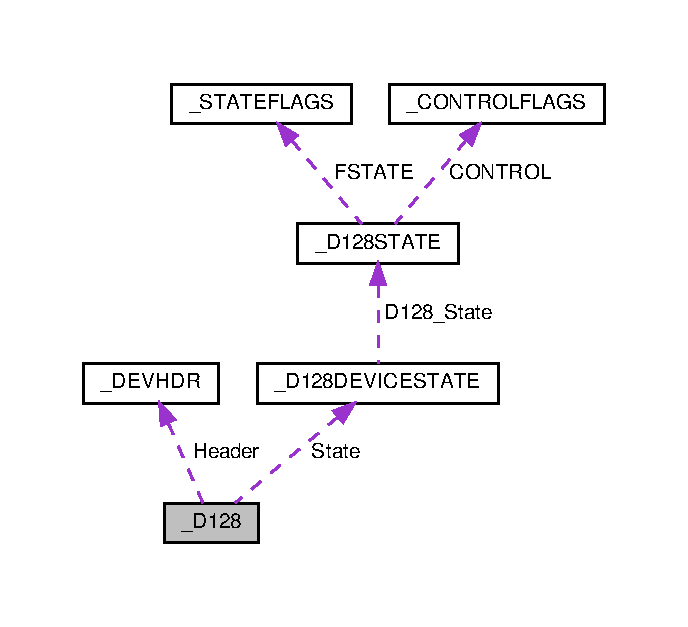
\includegraphics[width=330pt]{struct___d128__coll__graph}
\end{center}
\end{figure}
\subsection*{Public Attributes}
\begin{DoxyCompactItemize}
\item 
\hyperlink{_d128_a_p_i_8h_ac4f7ac6f5a50549a97c064894bdcf244}{D\+E\+V\+H\+DR} \hyperlink{struct___d128_a8348c7adb2ef3954c978112fe8b71785}{Header}
\item 
\hyperlink{_d128_a_p_i_8h_aec4b5617f0e6a151d0388c3c6f61c199}{D128\+D\+E\+V\+I\+C\+E\+S\+T\+A\+TE} \hyperlink{struct___d128_acad147b63666e9259067b464075e47d4}{State} \mbox{[}$\,$\mbox{]}
\end{DoxyCompactItemize}


\subsection{Detailed Description}


Definition at line 56 of file D128\+A\+P\+I.\+h.



\subsection{Member Data Documentation}
\mbox{\Hypertarget{struct___d128_a8348c7adb2ef3954c978112fe8b71785}\label{struct___d128_a8348c7adb2ef3954c978112fe8b71785}} 
\index{\+\_\+\+D128@{\+\_\+\+D128}!Header@{Header}}
\index{Header@{Header}!\+\_\+\+D128@{\+\_\+\+D128}}
\subsubsection{\texorpdfstring{Header}{Header}}
{\footnotesize\ttfamily \hyperlink{_d128_a_p_i_8h_ac4f7ac6f5a50549a97c064894bdcf244}{D\+E\+V\+H\+DR} \+\_\+\+D128\+::\+Header}



Definition at line 57 of file D128\+A\+P\+I.\+h.

\mbox{\Hypertarget{struct___d128_acad147b63666e9259067b464075e47d4}\label{struct___d128_acad147b63666e9259067b464075e47d4}} 
\index{\+\_\+\+D128@{\+\_\+\+D128}!State@{State}}
\index{State@{State}!\+\_\+\+D128@{\+\_\+\+D128}}
\subsubsection{\texorpdfstring{State}{State}}
{\footnotesize\ttfamily \hyperlink{_d128_a_p_i_8h_aec4b5617f0e6a151d0388c3c6f61c199}{D128\+D\+E\+V\+I\+C\+E\+S\+T\+A\+TE} \+\_\+\+D128\+::\+State\mbox{[}$\,$\mbox{]}}



Definition at line 58 of file D128\+A\+P\+I.\+h.



The documentation for this struct was generated from the following file\+:\begin{DoxyCompactItemize}
\item 
include/\hyperlink{_d128_a_p_i_8h}{D128\+A\+P\+I.\+h}\end{DoxyCompactItemize}

\hypertarget{struct___d128_d_e_v_i_c_e_s_t_a_t_e}{}\section{\+\_\+\+D128\+D\+E\+V\+I\+C\+E\+S\+T\+A\+TE Struct Reference}
\label{struct___d128_d_e_v_i_c_e_s_t_a_t_e}\index{\+\_\+\+D128\+D\+E\+V\+I\+C\+E\+S\+T\+A\+TE@{\+\_\+\+D128\+D\+E\+V\+I\+C\+E\+S\+T\+A\+TE}}


{\ttfamily \#include $<$D128\+A\+P\+I.\+h$>$}



Collaboration diagram for \+\_\+\+D128\+D\+E\+V\+I\+C\+E\+S\+T\+A\+TE\+:
\nopagebreak
\begin{figure}[H]
\begin{center}
\leavevmode
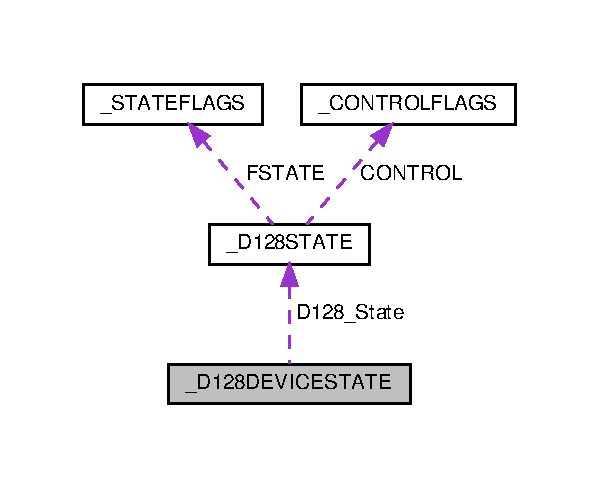
\includegraphics[width=288pt]{struct___d128_d_e_v_i_c_e_s_t_a_t_e__coll__graph}
\end{center}
\end{figure}
\subsection*{Public Attributes}
\begin{DoxyCompactItemize}
\item 
int \hyperlink{struct___d128_d_e_v_i_c_e_s_t_a_t_e_aab8e8a8b459ecc83ecb1e519e0df6e0b}{D128\+\_\+\+Device\+ID}
\item 
int \hyperlink{struct___d128_d_e_v_i_c_e_s_t_a_t_e_aa2ea21f882710c40dcac5e10a3c9da0a}{D128\+\_\+\+Version\+ID}
\item 
int \hyperlink{struct___d128_d_e_v_i_c_e_s_t_a_t_e_adae9dc9189afc64b47cee532eb0d3f73}{D128\+\_\+\+Error}
\item 
\hyperlink{_d128_a_p_i_8h_a37bd6b2ec1438a8cd6a28e7e6ff61885}{D128\+S\+T\+A\+TE} \hyperlink{struct___d128_d_e_v_i_c_e_s_t_a_t_e_a16e38dc259d46e4d7e729a9982044bfe}{D128\+\_\+\+State}
\end{DoxyCompactItemize}


\subsection{Detailed Description}


Definition at line 45 of file D128\+A\+P\+I.\+h.



\subsection{Member Data Documentation}
\mbox{\Hypertarget{struct___d128_d_e_v_i_c_e_s_t_a_t_e_aab8e8a8b459ecc83ecb1e519e0df6e0b}\label{struct___d128_d_e_v_i_c_e_s_t_a_t_e_aab8e8a8b459ecc83ecb1e519e0df6e0b}} 
\index{\+\_\+\+D128\+D\+E\+V\+I\+C\+E\+S\+T\+A\+TE@{\+\_\+\+D128\+D\+E\+V\+I\+C\+E\+S\+T\+A\+TE}!D128\+\_\+\+Device\+ID@{D128\+\_\+\+Device\+ID}}
\index{D128\+\_\+\+Device\+ID@{D128\+\_\+\+Device\+ID}!\+\_\+\+D128\+D\+E\+V\+I\+C\+E\+S\+T\+A\+TE@{\+\_\+\+D128\+D\+E\+V\+I\+C\+E\+S\+T\+A\+TE}}
\subsubsection{\texorpdfstring{D128\+\_\+\+Device\+ID}{D128\_DeviceID}}
{\footnotesize\ttfamily int \+\_\+\+D128\+D\+E\+V\+I\+C\+E\+S\+T\+A\+T\+E\+::\+D128\+\_\+\+Device\+ID}



Definition at line 46 of file D128\+A\+P\+I.\+h.

\mbox{\Hypertarget{struct___d128_d_e_v_i_c_e_s_t_a_t_e_adae9dc9189afc64b47cee532eb0d3f73}\label{struct___d128_d_e_v_i_c_e_s_t_a_t_e_adae9dc9189afc64b47cee532eb0d3f73}} 
\index{\+\_\+\+D128\+D\+E\+V\+I\+C\+E\+S\+T\+A\+TE@{\+\_\+\+D128\+D\+E\+V\+I\+C\+E\+S\+T\+A\+TE}!D128\+\_\+\+Error@{D128\+\_\+\+Error}}
\index{D128\+\_\+\+Error@{D128\+\_\+\+Error}!\+\_\+\+D128\+D\+E\+V\+I\+C\+E\+S\+T\+A\+TE@{\+\_\+\+D128\+D\+E\+V\+I\+C\+E\+S\+T\+A\+TE}}
\subsubsection{\texorpdfstring{D128\+\_\+\+Error}{D128\_Error}}
{\footnotesize\ttfamily int \+\_\+\+D128\+D\+E\+V\+I\+C\+E\+S\+T\+A\+T\+E\+::\+D128\+\_\+\+Error}



Definition at line 48 of file D128\+A\+P\+I.\+h.

\mbox{\Hypertarget{struct___d128_d_e_v_i_c_e_s_t_a_t_e_a16e38dc259d46e4d7e729a9982044bfe}\label{struct___d128_d_e_v_i_c_e_s_t_a_t_e_a16e38dc259d46e4d7e729a9982044bfe}} 
\index{\+\_\+\+D128\+D\+E\+V\+I\+C\+E\+S\+T\+A\+TE@{\+\_\+\+D128\+D\+E\+V\+I\+C\+E\+S\+T\+A\+TE}!D128\+\_\+\+State@{D128\+\_\+\+State}}
\index{D128\+\_\+\+State@{D128\+\_\+\+State}!\+\_\+\+D128\+D\+E\+V\+I\+C\+E\+S\+T\+A\+TE@{\+\_\+\+D128\+D\+E\+V\+I\+C\+E\+S\+T\+A\+TE}}
\subsubsection{\texorpdfstring{D128\+\_\+\+State}{D128\_State}}
{\footnotesize\ttfamily \hyperlink{_d128_a_p_i_8h_a37bd6b2ec1438a8cd6a28e7e6ff61885}{D128\+S\+T\+A\+TE} \+\_\+\+D128\+D\+E\+V\+I\+C\+E\+S\+T\+A\+T\+E\+::\+D128\+\_\+\+State}



Definition at line 49 of file D128\+A\+P\+I.\+h.

\mbox{\Hypertarget{struct___d128_d_e_v_i_c_e_s_t_a_t_e_aa2ea21f882710c40dcac5e10a3c9da0a}\label{struct___d128_d_e_v_i_c_e_s_t_a_t_e_aa2ea21f882710c40dcac5e10a3c9da0a}} 
\index{\+\_\+\+D128\+D\+E\+V\+I\+C\+E\+S\+T\+A\+TE@{\+\_\+\+D128\+D\+E\+V\+I\+C\+E\+S\+T\+A\+TE}!D128\+\_\+\+Version\+ID@{D128\+\_\+\+Version\+ID}}
\index{D128\+\_\+\+Version\+ID@{D128\+\_\+\+Version\+ID}!\+\_\+\+D128\+D\+E\+V\+I\+C\+E\+S\+T\+A\+TE@{\+\_\+\+D128\+D\+E\+V\+I\+C\+E\+S\+T\+A\+TE}}
\subsubsection{\texorpdfstring{D128\+\_\+\+Version\+ID}{D128\_VersionID}}
{\footnotesize\ttfamily int \+\_\+\+D128\+D\+E\+V\+I\+C\+E\+S\+T\+A\+T\+E\+::\+D128\+\_\+\+Version\+ID}



Definition at line 47 of file D128\+A\+P\+I.\+h.



The documentation for this struct was generated from the following file\+:\begin{DoxyCompactItemize}
\item 
include/\hyperlink{_d128_a_p_i_8h}{D128\+A\+P\+I.\+h}\end{DoxyCompactItemize}

\hypertarget{struct___d128_s_t_a_t_e}{}\section{\+\_\+\+D128\+S\+T\+A\+TE Struct Reference}
\label{struct___d128_s_t_a_t_e}\index{\+\_\+\+D128\+S\+T\+A\+TE@{\+\_\+\+D128\+S\+T\+A\+TE}}


{\ttfamily \#include $<$D128\+A\+P\+I.\+h$>$}



Collaboration diagram for \+\_\+\+D128\+S\+T\+A\+TE\+:
\nopagebreak
\begin{figure}[H]
\begin{center}
\leavevmode
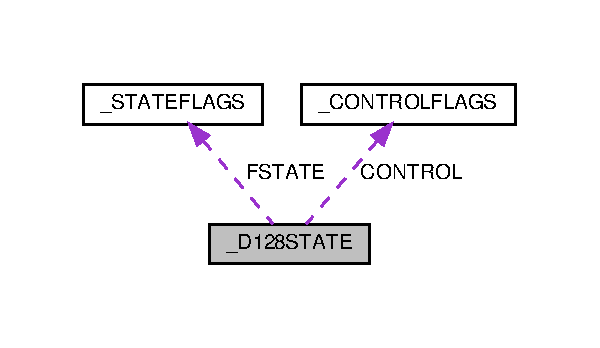
\includegraphics[width=288pt]{struct___d128_s_t_a_t_e__coll__graph}
\end{center}
\end{figure}
\subsection*{Public Attributes}
\begin{DoxyCompactItemize}
\item 
\hyperlink{_d128_a_p_i_8h_a91215a38b4f52c701d673f5a9874cc1f}{C\+O\+N\+T\+R\+O\+L\+F\+L\+A\+GS} \hyperlink{struct___d128_s_t_a_t_e_affb79cdddf9d32d31d56f5a6d1cf1213}{C\+O\+N\+T\+R\+OL}
\item 
int \hyperlink{struct___d128_s_t_a_t_e_a832b7acd51b07b57d5564304f877ebed}{D\+E\+M\+A\+ND}
\item 
int \hyperlink{struct___d128_s_t_a_t_e_ae531b72a9e28645c9f99756a12a88fff}{W\+I\+D\+TH}
\item 
int \hyperlink{struct___d128_s_t_a_t_e_aec50cf1e9df443c609e6253c8828c95a}{R\+E\+C\+O\+V\+E\+RY}
\item 
int \hyperlink{struct___d128_s_t_a_t_e_aa53fa740eeafba887916d3afae0c51f5}{D\+W\+E\+LL}
\item 
unsigned int \hyperlink{struct___d128_s_t_a_t_e_acde31c47f1649af4b0ae2d149a3e2f4b}{C\+P\+U\+L\+SE}
\item 
unsigned int \hyperlink{struct___d128_s_t_a_t_e_a3e51e533256c5794bcc2ffc1cb15e9f1}{C\+O\+OC}
\item 
unsigned int \hyperlink{struct___d128_s_t_a_t_e_a045abcc9e24103354e977f059036683c}{C\+T\+O\+O\+F\+A\+ST}
\item 
\hyperlink{_d128_a_p_i_8h_ab368deca56a74b4f97e27c53f957322f}{S\+T\+A\+T\+E\+F\+L\+A\+GS} \hyperlink{struct___d128_s_t_a_t_e_a696a3b0c6cc5eeca3467d45c946ceb9d}{F\+S\+T\+A\+TE}
\end{DoxyCompactItemize}


\subsection{Detailed Description}


Definition at line 32 of file D128\+A\+P\+I.\+h.



\subsection{Member Data Documentation}
\mbox{\Hypertarget{struct___d128_s_t_a_t_e_affb79cdddf9d32d31d56f5a6d1cf1213}\label{struct___d128_s_t_a_t_e_affb79cdddf9d32d31d56f5a6d1cf1213}} 
\index{\+\_\+\+D128\+S\+T\+A\+TE@{\+\_\+\+D128\+S\+T\+A\+TE}!C\+O\+N\+T\+R\+OL@{C\+O\+N\+T\+R\+OL}}
\index{C\+O\+N\+T\+R\+OL@{C\+O\+N\+T\+R\+OL}!\+\_\+\+D128\+S\+T\+A\+TE@{\+\_\+\+D128\+S\+T\+A\+TE}}
\subsubsection{\texorpdfstring{C\+O\+N\+T\+R\+OL}{CONTROL}}
{\footnotesize\ttfamily \hyperlink{_d128_a_p_i_8h_a91215a38b4f52c701d673f5a9874cc1f}{C\+O\+N\+T\+R\+O\+L\+F\+L\+A\+GS} \+\_\+\+D128\+S\+T\+A\+T\+E\+::\+C\+O\+N\+T\+R\+OL}



Definition at line 33 of file D128\+A\+P\+I.\+h.

\mbox{\Hypertarget{struct___d128_s_t_a_t_e_a3e51e533256c5794bcc2ffc1cb15e9f1}\label{struct___d128_s_t_a_t_e_a3e51e533256c5794bcc2ffc1cb15e9f1}} 
\index{\+\_\+\+D128\+S\+T\+A\+TE@{\+\_\+\+D128\+S\+T\+A\+TE}!C\+O\+OC@{C\+O\+OC}}
\index{C\+O\+OC@{C\+O\+OC}!\+\_\+\+D128\+S\+T\+A\+TE@{\+\_\+\+D128\+S\+T\+A\+TE}}
\subsubsection{\texorpdfstring{C\+O\+OC}{COOC}}
{\footnotesize\ttfamily unsigned int \+\_\+\+D128\+S\+T\+A\+T\+E\+::\+C\+O\+OC}



Definition at line 39 of file D128\+A\+P\+I.\+h.

\mbox{\Hypertarget{struct___d128_s_t_a_t_e_acde31c47f1649af4b0ae2d149a3e2f4b}\label{struct___d128_s_t_a_t_e_acde31c47f1649af4b0ae2d149a3e2f4b}} 
\index{\+\_\+\+D128\+S\+T\+A\+TE@{\+\_\+\+D128\+S\+T\+A\+TE}!C\+P\+U\+L\+SE@{C\+P\+U\+L\+SE}}
\index{C\+P\+U\+L\+SE@{C\+P\+U\+L\+SE}!\+\_\+\+D128\+S\+T\+A\+TE@{\+\_\+\+D128\+S\+T\+A\+TE}}
\subsubsection{\texorpdfstring{C\+P\+U\+L\+SE}{CPULSE}}
{\footnotesize\ttfamily unsigned int \+\_\+\+D128\+S\+T\+A\+T\+E\+::\+C\+P\+U\+L\+SE}



Definition at line 38 of file D128\+A\+P\+I.\+h.

\mbox{\Hypertarget{struct___d128_s_t_a_t_e_a045abcc9e24103354e977f059036683c}\label{struct___d128_s_t_a_t_e_a045abcc9e24103354e977f059036683c}} 
\index{\+\_\+\+D128\+S\+T\+A\+TE@{\+\_\+\+D128\+S\+T\+A\+TE}!C\+T\+O\+O\+F\+A\+ST@{C\+T\+O\+O\+F\+A\+ST}}
\index{C\+T\+O\+O\+F\+A\+ST@{C\+T\+O\+O\+F\+A\+ST}!\+\_\+\+D128\+S\+T\+A\+TE@{\+\_\+\+D128\+S\+T\+A\+TE}}
\subsubsection{\texorpdfstring{C\+T\+O\+O\+F\+A\+ST}{CTOOFAST}}
{\footnotesize\ttfamily unsigned int \+\_\+\+D128\+S\+T\+A\+T\+E\+::\+C\+T\+O\+O\+F\+A\+ST}



Definition at line 40 of file D128\+A\+P\+I.\+h.

\mbox{\Hypertarget{struct___d128_s_t_a_t_e_a832b7acd51b07b57d5564304f877ebed}\label{struct___d128_s_t_a_t_e_a832b7acd51b07b57d5564304f877ebed}} 
\index{\+\_\+\+D128\+S\+T\+A\+TE@{\+\_\+\+D128\+S\+T\+A\+TE}!D\+E\+M\+A\+ND@{D\+E\+M\+A\+ND}}
\index{D\+E\+M\+A\+ND@{D\+E\+M\+A\+ND}!\+\_\+\+D128\+S\+T\+A\+TE@{\+\_\+\+D128\+S\+T\+A\+TE}}
\subsubsection{\texorpdfstring{D\+E\+M\+A\+ND}{DEMAND}}
{\footnotesize\ttfamily int \+\_\+\+D128\+S\+T\+A\+T\+E\+::\+D\+E\+M\+A\+ND}



Definition at line 34 of file D128\+A\+P\+I.\+h.

\mbox{\Hypertarget{struct___d128_s_t_a_t_e_aa53fa740eeafba887916d3afae0c51f5}\label{struct___d128_s_t_a_t_e_aa53fa740eeafba887916d3afae0c51f5}} 
\index{\+\_\+\+D128\+S\+T\+A\+TE@{\+\_\+\+D128\+S\+T\+A\+TE}!D\+W\+E\+LL@{D\+W\+E\+LL}}
\index{D\+W\+E\+LL@{D\+W\+E\+LL}!\+\_\+\+D128\+S\+T\+A\+TE@{\+\_\+\+D128\+S\+T\+A\+TE}}
\subsubsection{\texorpdfstring{D\+W\+E\+LL}{DWELL}}
{\footnotesize\ttfamily int \+\_\+\+D128\+S\+T\+A\+T\+E\+::\+D\+W\+E\+LL}



Definition at line 37 of file D128\+A\+P\+I.\+h.

\mbox{\Hypertarget{struct___d128_s_t_a_t_e_a696a3b0c6cc5eeca3467d45c946ceb9d}\label{struct___d128_s_t_a_t_e_a696a3b0c6cc5eeca3467d45c946ceb9d}} 
\index{\+\_\+\+D128\+S\+T\+A\+TE@{\+\_\+\+D128\+S\+T\+A\+TE}!F\+S\+T\+A\+TE@{F\+S\+T\+A\+TE}}
\index{F\+S\+T\+A\+TE@{F\+S\+T\+A\+TE}!\+\_\+\+D128\+S\+T\+A\+TE@{\+\_\+\+D128\+S\+T\+A\+TE}}
\subsubsection{\texorpdfstring{F\+S\+T\+A\+TE}{FSTATE}}
{\footnotesize\ttfamily \hyperlink{_d128_a_p_i_8h_ab368deca56a74b4f97e27c53f957322f}{S\+T\+A\+T\+E\+F\+L\+A\+GS} \+\_\+\+D128\+S\+T\+A\+T\+E\+::\+F\+S\+T\+A\+TE}



Definition at line 41 of file D128\+A\+P\+I.\+h.

\mbox{\Hypertarget{struct___d128_s_t_a_t_e_aec50cf1e9df443c609e6253c8828c95a}\label{struct___d128_s_t_a_t_e_aec50cf1e9df443c609e6253c8828c95a}} 
\index{\+\_\+\+D128\+S\+T\+A\+TE@{\+\_\+\+D128\+S\+T\+A\+TE}!R\+E\+C\+O\+V\+E\+RY@{R\+E\+C\+O\+V\+E\+RY}}
\index{R\+E\+C\+O\+V\+E\+RY@{R\+E\+C\+O\+V\+E\+RY}!\+\_\+\+D128\+S\+T\+A\+TE@{\+\_\+\+D128\+S\+T\+A\+TE}}
\subsubsection{\texorpdfstring{R\+E\+C\+O\+V\+E\+RY}{RECOVERY}}
{\footnotesize\ttfamily int \+\_\+\+D128\+S\+T\+A\+T\+E\+::\+R\+E\+C\+O\+V\+E\+RY}



Definition at line 36 of file D128\+A\+P\+I.\+h.

\mbox{\Hypertarget{struct___d128_s_t_a_t_e_ae531b72a9e28645c9f99756a12a88fff}\label{struct___d128_s_t_a_t_e_ae531b72a9e28645c9f99756a12a88fff}} 
\index{\+\_\+\+D128\+S\+T\+A\+TE@{\+\_\+\+D128\+S\+T\+A\+TE}!W\+I\+D\+TH@{W\+I\+D\+TH}}
\index{W\+I\+D\+TH@{W\+I\+D\+TH}!\+\_\+\+D128\+S\+T\+A\+TE@{\+\_\+\+D128\+S\+T\+A\+TE}}
\subsubsection{\texorpdfstring{W\+I\+D\+TH}{WIDTH}}
{\footnotesize\ttfamily int \+\_\+\+D128\+S\+T\+A\+T\+E\+::\+W\+I\+D\+TH}



Definition at line 35 of file D128\+A\+P\+I.\+h.



The documentation for this struct was generated from the following file\+:\begin{DoxyCompactItemize}
\item 
include/\hyperlink{_d128_a_p_i_8h}{D128\+A\+P\+I.\+h}\end{DoxyCompactItemize}

\hypertarget{struct___d_e_v_h_d_r}{}\section{\+\_\+\+D\+E\+V\+H\+DR Struct Reference}
\label{struct___d_e_v_h_d_r}\index{\+\_\+\+D\+E\+V\+H\+DR@{\+\_\+\+D\+E\+V\+H\+DR}}


{\ttfamily \#include $<$D128\+A\+P\+I.\+h$>$}

\subsection*{Public Attributes}
\begin{DoxyCompactItemize}
\item 
int \hyperlink{struct___d_e_v_h_d_r_a597655230495775fdfcf1d73b95ec7d0}{Device\+Count}
\end{DoxyCompactItemize}


\subsection{Detailed Description}


Definition at line 52 of file D128\+A\+P\+I.\+h.



\subsection{Member Data Documentation}
\mbox{\Hypertarget{struct___d_e_v_h_d_r_a597655230495775fdfcf1d73b95ec7d0}\label{struct___d_e_v_h_d_r_a597655230495775fdfcf1d73b95ec7d0}} 
\index{\+\_\+\+D\+E\+V\+H\+DR@{\+\_\+\+D\+E\+V\+H\+DR}!Device\+Count@{Device\+Count}}
\index{Device\+Count@{Device\+Count}!\+\_\+\+D\+E\+V\+H\+DR@{\+\_\+\+D\+E\+V\+H\+DR}}
\subsubsection{\texorpdfstring{Device\+Count}{DeviceCount}}
{\footnotesize\ttfamily int \+\_\+\+D\+E\+V\+H\+D\+R\+::\+Device\+Count}



Definition at line 53 of file D128\+A\+P\+I.\+h.



The documentation for this struct was generated from the following file\+:\begin{DoxyCompactItemize}
\item 
include/\hyperlink{_d128_a_p_i_8h}{D128\+A\+P\+I.\+h}\end{DoxyCompactItemize}

\hypertarget{struct___s_t_a_t_e_f_l_a_g_s}{}\section{\+\_\+\+S\+T\+A\+T\+E\+F\+L\+A\+GS Struct Reference}
\label{struct___s_t_a_t_e_f_l_a_g_s}\index{\+\_\+\+S\+T\+A\+T\+E\+F\+L\+A\+GS@{\+\_\+\+S\+T\+A\+T\+E\+F\+L\+A\+GS}}


{\ttfamily \#include $<$D128\+A\+P\+I.\+h$>$}

\subsection*{Public Attributes}
\begin{DoxyCompactItemize}
\item 
\begin{tabbing}
xx\=xx\=xx\=xx\=xx\=xx\=xx\=xx\=xx\=\kill
union \{\\
\>struct \{\\
\>\>unsigned int \hyperlink{struct___s_t_a_t_e_f_l_a_g_s_ae0e9876a31f0e02a9b95e35c7964329b}{OVERENERGY}: 1\\
\>\>unsigned int \hyperlink{struct___s_t_a_t_e_f_l_a_g_s_aacbcd74f712daaeab0866ccdcfa8a31a}{HWERROR}: 1\\
\>\>unsigned int \hyperlink{struct___s_t_a_t_e_f_l_a_g_s_a04086b338888e6aeb8ec87f36dfc3b8f}{reserved}: 30\\
\>\} \\
\>int \hyperlink{struct___s_t_a_t_e_f_l_a_g_s_aeafe01c8bbda4ee95f71c151ecc948b7}{VALUE}\\
\}; \\

\end{tabbing}\end{DoxyCompactItemize}


\subsection{Detailed Description}


Definition at line 5 of file D128\+A\+P\+I.\+h.



\subsection{Member Data Documentation}
\mbox{\Hypertarget{struct___s_t_a_t_e_f_l_a_g_s_ac5e832eeabd871f2cd0eddeb45cd66ef}\label{struct___s_t_a_t_e_f_l_a_g_s_ac5e832eeabd871f2cd0eddeb45cd66ef}} 
\subsubsection{\texorpdfstring{"@25}{@25}}
{\footnotesize\ttfamily union \{ ... \} }

\mbox{\Hypertarget{struct___s_t_a_t_e_f_l_a_g_s_aacbcd74f712daaeab0866ccdcfa8a31a}\label{struct___s_t_a_t_e_f_l_a_g_s_aacbcd74f712daaeab0866ccdcfa8a31a}} 
\index{\+\_\+\+S\+T\+A\+T\+E\+F\+L\+A\+GS@{\+\_\+\+S\+T\+A\+T\+E\+F\+L\+A\+GS}!H\+W\+E\+R\+R\+OR@{H\+W\+E\+R\+R\+OR}}
\index{H\+W\+E\+R\+R\+OR@{H\+W\+E\+R\+R\+OR}!\+\_\+\+S\+T\+A\+T\+E\+F\+L\+A\+GS@{\+\_\+\+S\+T\+A\+T\+E\+F\+L\+A\+GS}}
\subsubsection{\texorpdfstring{H\+W\+E\+R\+R\+OR}{HWERROR}}
{\footnotesize\ttfamily unsigned int \+\_\+\+S\+T\+A\+T\+E\+F\+L\+A\+G\+S\+::\+H\+W\+E\+R\+R\+OR}



Definition at line 9 of file D128\+A\+P\+I.\+h.

\mbox{\Hypertarget{struct___s_t_a_t_e_f_l_a_g_s_ae0e9876a31f0e02a9b95e35c7964329b}\label{struct___s_t_a_t_e_f_l_a_g_s_ae0e9876a31f0e02a9b95e35c7964329b}} 
\index{\+\_\+\+S\+T\+A\+T\+E\+F\+L\+A\+GS@{\+\_\+\+S\+T\+A\+T\+E\+F\+L\+A\+GS}!O\+V\+E\+R\+E\+N\+E\+R\+GY@{O\+V\+E\+R\+E\+N\+E\+R\+GY}}
\index{O\+V\+E\+R\+E\+N\+E\+R\+GY@{O\+V\+E\+R\+E\+N\+E\+R\+GY}!\+\_\+\+S\+T\+A\+T\+E\+F\+L\+A\+GS@{\+\_\+\+S\+T\+A\+T\+E\+F\+L\+A\+GS}}
\subsubsection{\texorpdfstring{O\+V\+E\+R\+E\+N\+E\+R\+GY}{OVERENERGY}}
{\footnotesize\ttfamily unsigned int \+\_\+\+S\+T\+A\+T\+E\+F\+L\+A\+G\+S\+::\+O\+V\+E\+R\+E\+N\+E\+R\+GY}



Definition at line 8 of file D128\+A\+P\+I.\+h.

\mbox{\Hypertarget{struct___s_t_a_t_e_f_l_a_g_s_a04086b338888e6aeb8ec87f36dfc3b8f}\label{struct___s_t_a_t_e_f_l_a_g_s_a04086b338888e6aeb8ec87f36dfc3b8f}} 
\index{\+\_\+\+S\+T\+A\+T\+E\+F\+L\+A\+GS@{\+\_\+\+S\+T\+A\+T\+E\+F\+L\+A\+GS}!reserved@{reserved}}
\index{reserved@{reserved}!\+\_\+\+S\+T\+A\+T\+E\+F\+L\+A\+GS@{\+\_\+\+S\+T\+A\+T\+E\+F\+L\+A\+GS}}
\subsubsection{\texorpdfstring{reserved}{reserved}}
{\footnotesize\ttfamily unsigned int \+\_\+\+S\+T\+A\+T\+E\+F\+L\+A\+G\+S\+::reserved}



Definition at line 10 of file D128\+A\+P\+I.\+h.

\mbox{\Hypertarget{struct___s_t_a_t_e_f_l_a_g_s_aeafe01c8bbda4ee95f71c151ecc948b7}\label{struct___s_t_a_t_e_f_l_a_g_s_aeafe01c8bbda4ee95f71c151ecc948b7}} 
\index{\+\_\+\+S\+T\+A\+T\+E\+F\+L\+A\+GS@{\+\_\+\+S\+T\+A\+T\+E\+F\+L\+A\+GS}!V\+A\+L\+UE@{V\+A\+L\+UE}}
\index{V\+A\+L\+UE@{V\+A\+L\+UE}!\+\_\+\+S\+T\+A\+T\+E\+F\+L\+A\+GS@{\+\_\+\+S\+T\+A\+T\+E\+F\+L\+A\+GS}}
\subsubsection{\texorpdfstring{V\+A\+L\+UE}{VALUE}}
{\footnotesize\ttfamily int \+\_\+\+S\+T\+A\+T\+E\+F\+L\+A\+G\+S\+::\+V\+A\+L\+UE}



Definition at line 12 of file D128\+A\+P\+I.\+h.



The documentation for this struct was generated from the following file\+:\begin{DoxyCompactItemize}
\item 
include/\hyperlink{_d128_a_p_i_8h}{D128\+A\+P\+I.\+h}\end{DoxyCompactItemize}

\hypertarget{class_angular_axis}{}\section{Angular\+Axis Class Reference}
\label{class_angular_axis}\index{Angular\+Axis@{Angular\+Axis}}


{\ttfamily \#include $<$chartdir.\+h$>$}



Inheritance diagram for Angular\+Axis\+:
\nopagebreak
\begin{figure}[H]
\begin{center}
\leavevmode
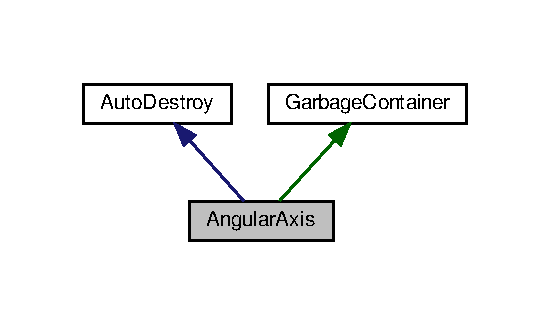
\includegraphics[width=264pt]{class_angular_axis__inherit__graph}
\end{center}
\end{figure}


Collaboration diagram for Angular\+Axis\+:
\nopagebreak
\begin{figure}[H]
\begin{center}
\leavevmode
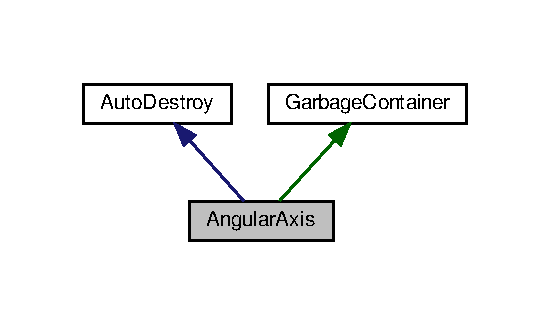
\includegraphics[width=264pt]{class_angular_axis__coll__graph}
\end{center}
\end{figure}
\subsection*{Public Member Functions}
\begin{DoxyCompactItemize}
\item 
\hyperlink{class_angular_axis_a5ea5e1163079a9decf8323a232d4210a}{Angular\+Axis} (Angular\+Axis\+Internal $\ast$\+\_\+ptr)
\item 
\hyperlink{class_angular_axis_a72ea8b4c42e00cddd9f1bfabd0bcae8c}{$\sim$\+Angular\+Axis} ()
\item 
\hyperlink{class_text_box}{Text\+Box} $\ast$ \hyperlink{class_angular_axis_a7cdca2dfe1200fdf2664d269dac585ba}{set\+Label\+Style} (const char $\ast$font=\char`\"{}bold\char`\"{}, double font\+Size=10, int font\+Color=\hyperlink{namespace_chart_abee0d882fdc9ad0b001245ad9fc64011a879e14f2f5024caccc047374342321ef}{Chart\+::\+Text\+Color}, double font\+Angle=0)
\item 
void \hyperlink{class_angular_axis_ae305f4e4b0d300b6b8e63a0f2645368c}{set\+Label\+Gap} (int d)
\item 
\hyperlink{class_text_box}{Text\+Box} $\ast$ \hyperlink{class_angular_axis_ae02899ce7abec02a96477811bd22c27e}{set\+Labels} (\hyperlink{class_string_array}{String\+Array} labels)
\item 
\hyperlink{class_text_box}{Text\+Box} $\ast$ \hyperlink{class_angular_axis_a3046d7450d5b1f01c00ae03668597bfb}{set\+Labels} (\hyperlink{class_double_array}{Double\+Array} labels, const char $\ast$format\+String=0)
\item 
void \hyperlink{class_angular_axis_a6f255a756fc6e9e19096618f9e34873f}{add\+Label} (double pos, const char $\ast$label)
\item 
void \hyperlink{class_angular_axis_a11fd9c97d2d76f01cec095a10edbe500}{set\+Linear\+Scale} (double lower\+Limit, double upper\+Limit, \hyperlink{class_string_array}{String\+Array} labels)
\item 
void \hyperlink{class_angular_axis_a69bb45da8256fc6999eb4a7fe789ee10}{set\+Linear\+Scale} (double lower\+Limit, double upper\+Limit, double major\+Tick\+Inc=0, double minor\+Tick\+Inc=0)
\item 
void \hyperlink{class_angular_axis_a0e99a07d920a902b3fa57e8a3c272004}{add\+Zone} (double start\+Value, double end\+Value, double start\+Radius, double end\+Radius, int fill\+Color, int edge\+Color=-\/1)
\item 
void \hyperlink{class_angular_axis_a53f7a154799715aa97d16d5140a7de17}{add\+Zone} (double start\+Value, double end\+Value, int fill\+Color, int edge\+Color=-\/1)
\item 
const char $\ast$ \hyperlink{class_angular_axis_a6d9609544b763a5af1f6eb4e24165ea6}{get\+Axis\+Image\+Map} (int no\+Of\+Segments, int map\+Width, const char $\ast$url, const char $\ast$query\+Format=0, const char $\ast$extra\+Attr=0, int offsetX=0, int offsetY=0) const
\item 
const char $\ast$ \hyperlink{class_angular_axis_ad7ee19adef39f7ce7fb1ce5bf2941b0d}{get\+H\+T\+M\+L\+Image\+Map} (const char $\ast$url, const char $\ast$query\+Format=0, const char $\ast$extra\+Attr=0, int offsetX=0, int offsetY=0) const
\end{DoxyCompactItemize}
\subsection*{Additional Inherited Members}


\subsection{Detailed Description}


Definition at line 1527 of file chartdir.\+h.



\subsection{Constructor \& Destructor Documentation}
\mbox{\Hypertarget{class_angular_axis_a5ea5e1163079a9decf8323a232d4210a}\label{class_angular_axis_a5ea5e1163079a9decf8323a232d4210a}} 
\index{Angular\+Axis@{Angular\+Axis}!Angular\+Axis@{Angular\+Axis}}
\index{Angular\+Axis@{Angular\+Axis}!Angular\+Axis@{Angular\+Axis}}
\subsubsection{\texorpdfstring{Angular\+Axis()}{AngularAxis()}}
{\footnotesize\ttfamily Angular\+Axis\+::\+Angular\+Axis (\begin{DoxyParamCaption}\item[{Angular\+Axis\+Internal $\ast$}]{\+\_\+ptr }\end{DoxyParamCaption})\hspace{0.3cm}{\ttfamily [inline]}}



Definition at line 1537 of file chartdir.\+h.

\mbox{\Hypertarget{class_angular_axis_a72ea8b4c42e00cddd9f1bfabd0bcae8c}\label{class_angular_axis_a72ea8b4c42e00cddd9f1bfabd0bcae8c}} 
\index{Angular\+Axis@{Angular\+Axis}!````~Angular\+Axis@{$\sim$\+Angular\+Axis}}
\index{````~Angular\+Axis@{$\sim$\+Angular\+Axis}!Angular\+Axis@{Angular\+Axis}}
\subsubsection{\texorpdfstring{$\sim$\+Angular\+Axis()}{~AngularAxis()}}
{\footnotesize\ttfamily Angular\+Axis\+::$\sim$\+Angular\+Axis (\begin{DoxyParamCaption}{ }\end{DoxyParamCaption})\hspace{0.3cm}{\ttfamily [inline]}}



Definition at line 1538 of file chartdir.\+h.



\subsection{Member Function Documentation}
\mbox{\Hypertarget{class_angular_axis_a6f255a756fc6e9e19096618f9e34873f}\label{class_angular_axis_a6f255a756fc6e9e19096618f9e34873f}} 
\index{Angular\+Axis@{Angular\+Axis}!add\+Label@{add\+Label}}
\index{add\+Label@{add\+Label}!Angular\+Axis@{Angular\+Axis}}
\subsubsection{\texorpdfstring{add\+Label()}{addLabel()}}
{\footnotesize\ttfamily void Angular\+Axis\+::add\+Label (\begin{DoxyParamCaption}\item[{double}]{pos,  }\item[{const char $\ast$}]{label }\end{DoxyParamCaption})\hspace{0.3cm}{\ttfamily [inline]}}



Definition at line 1549 of file chartdir.\+h.

Here is the call graph for this function\+:
\nopagebreak
\begin{figure}[H]
\begin{center}
\leavevmode
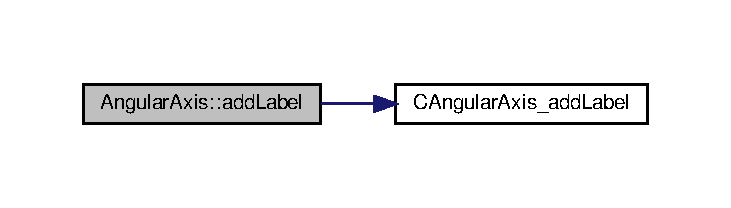
\includegraphics[width=350pt]{class_angular_axis_a6f255a756fc6e9e19096618f9e34873f_cgraph}
\end{center}
\end{figure}
\mbox{\Hypertarget{class_angular_axis_a0e99a07d920a902b3fa57e8a3c272004}\label{class_angular_axis_a0e99a07d920a902b3fa57e8a3c272004}} 
\index{Angular\+Axis@{Angular\+Axis}!add\+Zone@{add\+Zone}}
\index{add\+Zone@{add\+Zone}!Angular\+Axis@{Angular\+Axis}}
\subsubsection{\texorpdfstring{add\+Zone()}{addZone()}\hspace{0.1cm}{\footnotesize\ttfamily [1/2]}}
{\footnotesize\ttfamily void Angular\+Axis\+::add\+Zone (\begin{DoxyParamCaption}\item[{double}]{start\+Value,  }\item[{double}]{end\+Value,  }\item[{double}]{start\+Radius,  }\item[{double}]{end\+Radius,  }\item[{int}]{fill\+Color,  }\item[{int}]{edge\+Color = {\ttfamily -\/1} }\end{DoxyParamCaption})\hspace{0.3cm}{\ttfamily [inline]}}



Definition at line 1557 of file chartdir.\+h.

Here is the call graph for this function\+:
\nopagebreak
\begin{figure}[H]
\begin{center}
\leavevmode
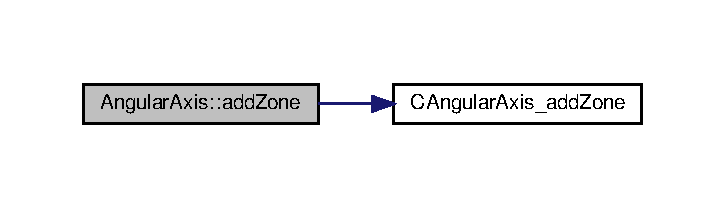
\includegraphics[width=348pt]{class_angular_axis_a0e99a07d920a902b3fa57e8a3c272004_cgraph}
\end{center}
\end{figure}
\mbox{\Hypertarget{class_angular_axis_a53f7a154799715aa97d16d5140a7de17}\label{class_angular_axis_a53f7a154799715aa97d16d5140a7de17}} 
\index{Angular\+Axis@{Angular\+Axis}!add\+Zone@{add\+Zone}}
\index{add\+Zone@{add\+Zone}!Angular\+Axis@{Angular\+Axis}}
\subsubsection{\texorpdfstring{add\+Zone()}{addZone()}\hspace{0.1cm}{\footnotesize\ttfamily [2/2]}}
{\footnotesize\ttfamily void Angular\+Axis\+::add\+Zone (\begin{DoxyParamCaption}\item[{double}]{start\+Value,  }\item[{double}]{end\+Value,  }\item[{int}]{fill\+Color,  }\item[{int}]{edge\+Color = {\ttfamily -\/1} }\end{DoxyParamCaption})\hspace{0.3cm}{\ttfamily [inline]}}



Definition at line 1560 of file chartdir.\+h.

Here is the call graph for this function\+:
\nopagebreak
\begin{figure}[H]
\begin{center}
\leavevmode
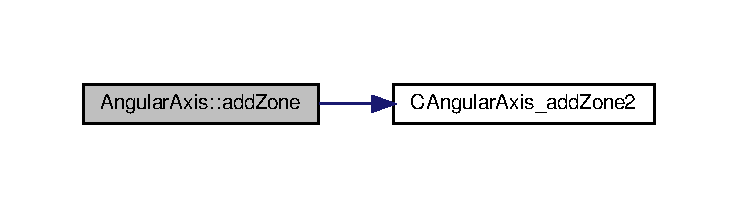
\includegraphics[width=350pt]{class_angular_axis_a53f7a154799715aa97d16d5140a7de17_cgraph}
\end{center}
\end{figure}
\mbox{\Hypertarget{class_angular_axis_a6d9609544b763a5af1f6eb4e24165ea6}\label{class_angular_axis_a6d9609544b763a5af1f6eb4e24165ea6}} 
\index{Angular\+Axis@{Angular\+Axis}!get\+Axis\+Image\+Map@{get\+Axis\+Image\+Map}}
\index{get\+Axis\+Image\+Map@{get\+Axis\+Image\+Map}!Angular\+Axis@{Angular\+Axis}}
\subsubsection{\texorpdfstring{get\+Axis\+Image\+Map()}{getAxisImageMap()}}
{\footnotesize\ttfamily const char$\ast$ Angular\+Axis\+::get\+Axis\+Image\+Map (\begin{DoxyParamCaption}\item[{int}]{no\+Of\+Segments,  }\item[{int}]{map\+Width,  }\item[{const char $\ast$}]{url,  }\item[{const char $\ast$}]{query\+Format = {\ttfamily 0},  }\item[{const char $\ast$}]{extra\+Attr = {\ttfamily 0},  }\item[{int}]{offsetX = {\ttfamily 0},  }\item[{int}]{offsetY = {\ttfamily 0} }\end{DoxyParamCaption}) const\hspace{0.3cm}{\ttfamily [inline]}}



Definition at line 1563 of file chartdir.\+h.

Here is the call graph for this function\+:
\nopagebreak
\begin{figure}[H]
\begin{center}
\leavevmode
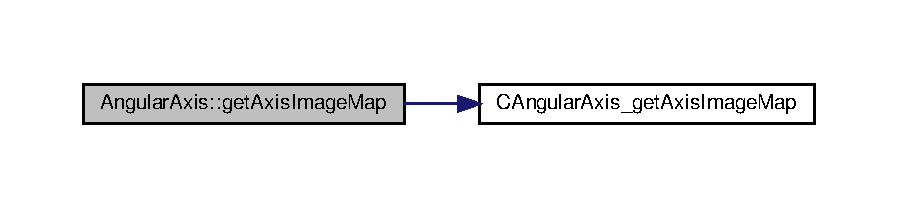
\includegraphics[width=350pt]{class_angular_axis_a6d9609544b763a5af1f6eb4e24165ea6_cgraph}
\end{center}
\end{figure}
\mbox{\Hypertarget{class_angular_axis_ad7ee19adef39f7ce7fb1ce5bf2941b0d}\label{class_angular_axis_ad7ee19adef39f7ce7fb1ce5bf2941b0d}} 
\index{Angular\+Axis@{Angular\+Axis}!get\+H\+T\+M\+L\+Image\+Map@{get\+H\+T\+M\+L\+Image\+Map}}
\index{get\+H\+T\+M\+L\+Image\+Map@{get\+H\+T\+M\+L\+Image\+Map}!Angular\+Axis@{Angular\+Axis}}
\subsubsection{\texorpdfstring{get\+H\+T\+M\+L\+Image\+Map()}{getHTMLImageMap()}}
{\footnotesize\ttfamily const char$\ast$ Angular\+Axis\+::get\+H\+T\+M\+L\+Image\+Map (\begin{DoxyParamCaption}\item[{const char $\ast$}]{url,  }\item[{const char $\ast$}]{query\+Format = {\ttfamily 0},  }\item[{const char $\ast$}]{extra\+Attr = {\ttfamily 0},  }\item[{int}]{offsetX = {\ttfamily 0},  }\item[{int}]{offsetY = {\ttfamily 0} }\end{DoxyParamCaption}) const\hspace{0.3cm}{\ttfamily [inline]}}



Definition at line 1566 of file chartdir.\+h.

Here is the call graph for this function\+:
\nopagebreak
\begin{figure}[H]
\begin{center}
\leavevmode
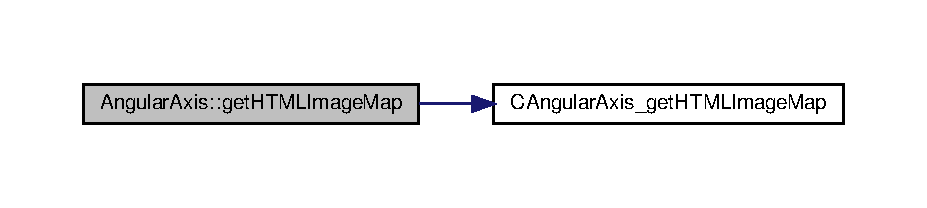
\includegraphics[width=350pt]{class_angular_axis_ad7ee19adef39f7ce7fb1ce5bf2941b0d_cgraph}
\end{center}
\end{figure}
\mbox{\Hypertarget{class_angular_axis_ae305f4e4b0d300b6b8e63a0f2645368c}\label{class_angular_axis_ae305f4e4b0d300b6b8e63a0f2645368c}} 
\index{Angular\+Axis@{Angular\+Axis}!set\+Label\+Gap@{set\+Label\+Gap}}
\index{set\+Label\+Gap@{set\+Label\+Gap}!Angular\+Axis@{Angular\+Axis}}
\subsubsection{\texorpdfstring{set\+Label\+Gap()}{setLabelGap()}}
{\footnotesize\ttfamily void Angular\+Axis\+::set\+Label\+Gap (\begin{DoxyParamCaption}\item[{int}]{d }\end{DoxyParamCaption})\hspace{0.3cm}{\ttfamily [inline]}}



Definition at line 1543 of file chartdir.\+h.

Here is the call graph for this function\+:
\nopagebreak
\begin{figure}[H]
\begin{center}
\leavevmode
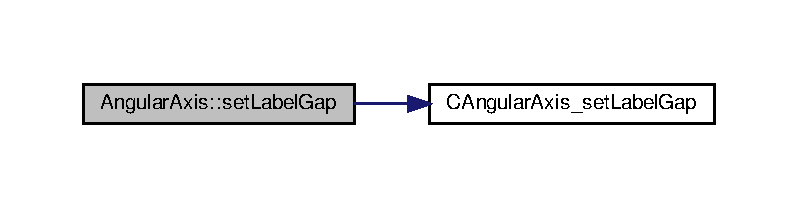
\includegraphics[width=350pt]{class_angular_axis_ae305f4e4b0d300b6b8e63a0f2645368c_cgraph}
\end{center}
\end{figure}
\mbox{\Hypertarget{class_angular_axis_ae02899ce7abec02a96477811bd22c27e}\label{class_angular_axis_ae02899ce7abec02a96477811bd22c27e}} 
\index{Angular\+Axis@{Angular\+Axis}!set\+Labels@{set\+Labels}}
\index{set\+Labels@{set\+Labels}!Angular\+Axis@{Angular\+Axis}}
\subsubsection{\texorpdfstring{set\+Labels()}{setLabels()}\hspace{0.1cm}{\footnotesize\ttfamily [1/2]}}
{\footnotesize\ttfamily \hyperlink{class_text_box}{Text\+Box}$\ast$ Angular\+Axis\+::set\+Labels (\begin{DoxyParamCaption}\item[{\hyperlink{class_string_array}{String\+Array}}]{labels }\end{DoxyParamCaption})\hspace{0.3cm}{\ttfamily [inline]}}



Definition at line 1545 of file chartdir.\+h.

Here is the call graph for this function\+:
\nopagebreak
\begin{figure}[H]
\begin{center}
\leavevmode
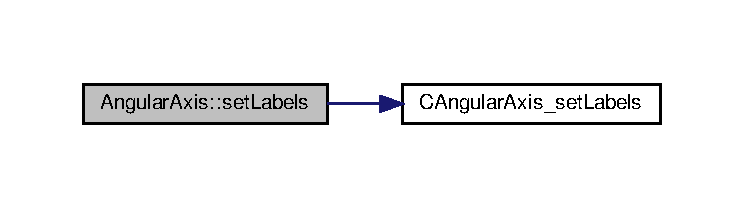
\includegraphics[width=350pt]{class_angular_axis_ae02899ce7abec02a96477811bd22c27e_cgraph}
\end{center}
\end{figure}
\mbox{\Hypertarget{class_angular_axis_a3046d7450d5b1f01c00ae03668597bfb}\label{class_angular_axis_a3046d7450d5b1f01c00ae03668597bfb}} 
\index{Angular\+Axis@{Angular\+Axis}!set\+Labels@{set\+Labels}}
\index{set\+Labels@{set\+Labels}!Angular\+Axis@{Angular\+Axis}}
\subsubsection{\texorpdfstring{set\+Labels()}{setLabels()}\hspace{0.1cm}{\footnotesize\ttfamily [2/2]}}
{\footnotesize\ttfamily \hyperlink{class_text_box}{Text\+Box}$\ast$ Angular\+Axis\+::set\+Labels (\begin{DoxyParamCaption}\item[{\hyperlink{class_double_array}{Double\+Array}}]{labels,  }\item[{const char $\ast$}]{format\+String = {\ttfamily 0} }\end{DoxyParamCaption})\hspace{0.3cm}{\ttfamily [inline]}}



Definition at line 1547 of file chartdir.\+h.

Here is the call graph for this function\+:
\nopagebreak
\begin{figure}[H]
\begin{center}
\leavevmode
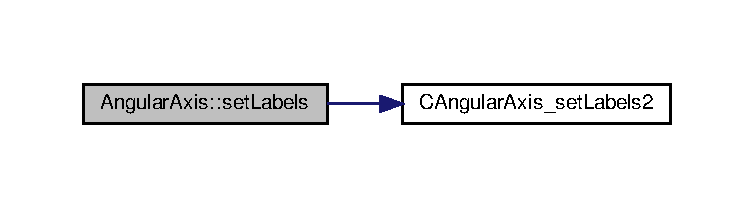
\includegraphics[width=350pt]{class_angular_axis_a3046d7450d5b1f01c00ae03668597bfb_cgraph}
\end{center}
\end{figure}
\mbox{\Hypertarget{class_angular_axis_a7cdca2dfe1200fdf2664d269dac585ba}\label{class_angular_axis_a7cdca2dfe1200fdf2664d269dac585ba}} 
\index{Angular\+Axis@{Angular\+Axis}!set\+Label\+Style@{set\+Label\+Style}}
\index{set\+Label\+Style@{set\+Label\+Style}!Angular\+Axis@{Angular\+Axis}}
\subsubsection{\texorpdfstring{set\+Label\+Style()}{setLabelStyle()}}
{\footnotesize\ttfamily \hyperlink{class_text_box}{Text\+Box}$\ast$ Angular\+Axis\+::set\+Label\+Style (\begin{DoxyParamCaption}\item[{const char $\ast$}]{font = {\ttfamily \char`\"{}bold\char`\"{}},  }\item[{double}]{font\+Size = {\ttfamily 10},  }\item[{int}]{font\+Color = {\ttfamily \hyperlink{namespace_chart_abee0d882fdc9ad0b001245ad9fc64011a879e14f2f5024caccc047374342321ef}{Chart\+::\+Text\+Color}},  }\item[{double}]{font\+Angle = {\ttfamily 0} }\end{DoxyParamCaption})\hspace{0.3cm}{\ttfamily [inline]}}



Definition at line 1540 of file chartdir.\+h.

Here is the call graph for this function\+:
\nopagebreak
\begin{figure}[H]
\begin{center}
\leavevmode
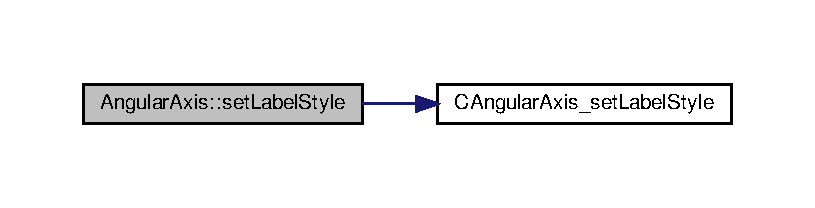
\includegraphics[width=350pt]{class_angular_axis_a7cdca2dfe1200fdf2664d269dac585ba_cgraph}
\end{center}
\end{figure}
\mbox{\Hypertarget{class_angular_axis_a11fd9c97d2d76f01cec095a10edbe500}\label{class_angular_axis_a11fd9c97d2d76f01cec095a10edbe500}} 
\index{Angular\+Axis@{Angular\+Axis}!set\+Linear\+Scale@{set\+Linear\+Scale}}
\index{set\+Linear\+Scale@{set\+Linear\+Scale}!Angular\+Axis@{Angular\+Axis}}
\subsubsection{\texorpdfstring{set\+Linear\+Scale()}{setLinearScale()}\hspace{0.1cm}{\footnotesize\ttfamily [1/2]}}
{\footnotesize\ttfamily void Angular\+Axis\+::set\+Linear\+Scale (\begin{DoxyParamCaption}\item[{double}]{lower\+Limit,  }\item[{double}]{upper\+Limit,  }\item[{\hyperlink{class_string_array}{String\+Array}}]{labels }\end{DoxyParamCaption})\hspace{0.3cm}{\ttfamily [inline]}}



Definition at line 1552 of file chartdir.\+h.

Here is the call graph for this function\+:
\nopagebreak
\begin{figure}[H]
\begin{center}
\leavevmode
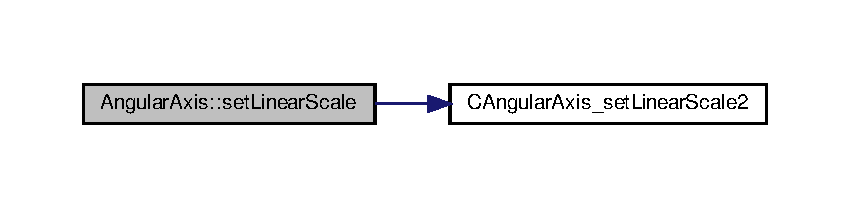
\includegraphics[width=350pt]{class_angular_axis_a11fd9c97d2d76f01cec095a10edbe500_cgraph}
\end{center}
\end{figure}
\mbox{\Hypertarget{class_angular_axis_a69bb45da8256fc6999eb4a7fe789ee10}\label{class_angular_axis_a69bb45da8256fc6999eb4a7fe789ee10}} 
\index{Angular\+Axis@{Angular\+Axis}!set\+Linear\+Scale@{set\+Linear\+Scale}}
\index{set\+Linear\+Scale@{set\+Linear\+Scale}!Angular\+Axis@{Angular\+Axis}}
\subsubsection{\texorpdfstring{set\+Linear\+Scale()}{setLinearScale()}\hspace{0.1cm}{\footnotesize\ttfamily [2/2]}}
{\footnotesize\ttfamily void Angular\+Axis\+::set\+Linear\+Scale (\begin{DoxyParamCaption}\item[{double}]{lower\+Limit,  }\item[{double}]{upper\+Limit,  }\item[{double}]{major\+Tick\+Inc = {\ttfamily 0},  }\item[{double}]{minor\+Tick\+Inc = {\ttfamily 0} }\end{DoxyParamCaption})\hspace{0.3cm}{\ttfamily [inline]}}



Definition at line 1554 of file chartdir.\+h.

Here is the call graph for this function\+:
\nopagebreak
\begin{figure}[H]
\begin{center}
\leavevmode
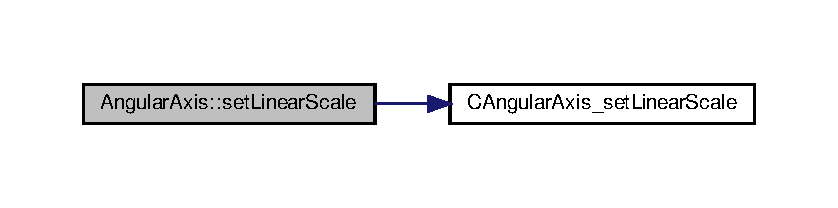
\includegraphics[width=350pt]{class_angular_axis_a69bb45da8256fc6999eb4a7fe789ee10_cgraph}
\end{center}
\end{figure}


The documentation for this class was generated from the following file\+:\begin{DoxyCompactItemize}
\item 
include/\hyperlink{chartdir_8h}{chartdir.\+h}\end{DoxyCompactItemize}

\hypertarget{class_angular_meter}{}\section{Angular\+Meter Class Reference}
\label{class_angular_meter}\index{Angular\+Meter@{Angular\+Meter}}


{\ttfamily \#include $<$chartdir.\+h$>$}



Inheritance diagram for Angular\+Meter\+:
\nopagebreak
\begin{figure}[H]
\begin{center}
\leavevmode
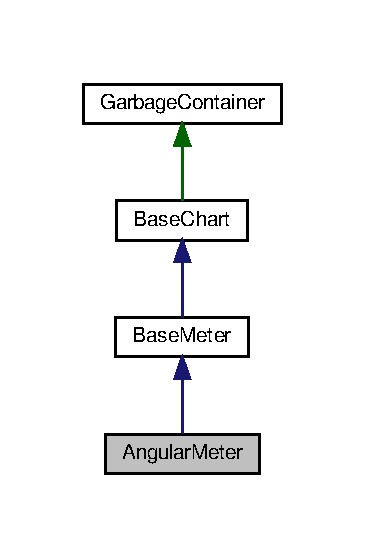
\includegraphics[width=175pt]{class_angular_meter__inherit__graph}
\end{center}
\end{figure}


Collaboration diagram for Angular\+Meter\+:
\nopagebreak
\begin{figure}[H]
\begin{center}
\leavevmode
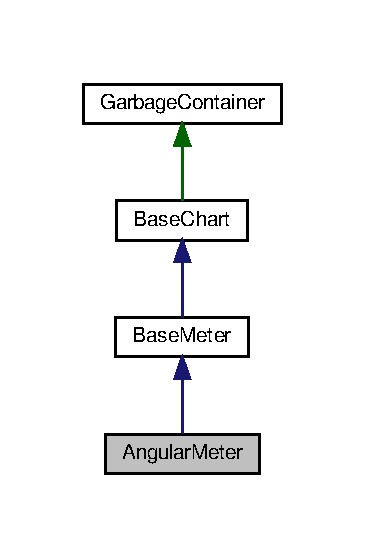
\includegraphics[width=175pt]{class_angular_meter__coll__graph}
\end{center}
\end{figure}
\subsection*{Public Member Functions}
\begin{DoxyCompactItemize}
\item 
\hyperlink{class_angular_meter_a5d71988b332dcbe883e7ad8d5abc0696}{Angular\+Meter} (int width, int height, int bg\+Color=\hyperlink{namespace_chart_abee0d882fdc9ad0b001245ad9fc64011a134193bde693b9d152d0c6dc59fa7d7f}{Chart\+::\+Background\+Color}, int edge\+Color=\hyperlink{namespace_chart_abee0d882fdc9ad0b001245ad9fc64011afc6811800a9e2582dac0157b6279f836}{Chart\+::\+Transparent}, int raised\+Effect=0)
\item 
void \hyperlink{class_angular_meter_a67b26ec28b68cac7b13922d61d2a36c9}{add\+Ring} (int start\+Radius, int end\+Radius, int fill\+Color, int edge\+Color=-\/1)
\item 
void \hyperlink{class_angular_meter_af7d1c8c5d188a2cf63a08296228fd6c3}{add\+Ring\+Sector} (int start\+Radius, int end\+Radius, double a1, double a2, int fill\+Color, int edge\+Color=-\/1)
\item 
void \hyperlink{class_angular_meter_a569e2ac4b396f2c1cafb5943f390c454}{set\+Meter} (int cx, int cy, int radius, double start\+Angle, double end\+Angle)
\item 
void \hyperlink{class_angular_meter_a1de741912b6b62a24f7d197b4717e4b6}{add\+Scale\+Background} (int bg\+Radius, int fill\+Color, int edge\+Width=0, int edge\+Color=-\/1, int scale\+Radius=-\/0x7fffffff, double start\+Angle=\+Chart\+::\+No\+Value, double end\+Angle=\+Chart\+::\+No\+Value)
\item 
void \hyperlink{class_angular_meter_ade95bcd716c78e650ab625c3b6c0fa0c}{add\+Glare} (double radius=Chart\+::\+No\+Value, double span=135, double rotate=0, double glare\+Radius=Chart\+::\+No\+Value, double intensity=0.\+13)
\item 
void \hyperlink{class_angular_meter_a0e20598329d17a1ac23b73fea207a6b7}{set\+Cap} (int radius, int fill\+Color, int edge\+Color=\hyperlink{namespace_chart_abee0d882fdc9ad0b001245ad9fc64011a04817a359476e87a5c572a7a69cdaaec}{Chart\+::\+Line\+Color})
\item 
void \hyperlink{class_angular_meter_a80b2f6a0dea2b4968ef7cca433e85a1d}{set\+Cap2} (int back\+Color=0x888888, int front\+Color=0x000000, int front\+Edge\+Color=0x888888, double lighting\+Ratio=\+Chart\+::\+No\+Value, double back\+Radius\+Ratio=\+Chart\+::\+No\+Value, double front\+Radius\+Ratio=\+Chart\+::\+No\+Value, double front\+Edge\+Width\+Ratio=\+Chart\+::\+No\+Value)
\item 
\hyperlink{class_meter_pointer}{Meter\+Pointer} $\ast$ \hyperlink{class_angular_meter_a50942d4bfc5e84f9532784e6d41c9ec1}{add\+Pointer2} (double value, int fill\+Color, int edge\+Color=-\/1, int pointer\+Type=\hyperlink{namespace_chart_a15cfe53d27f5b7a07e25af504b5d10f4afd0736ae83f260af5c7f8093d24448f1}{Chart\+::\+Triangular\+Pointer2}, double start\+Offset=Chart\+::\+No\+Value, double end\+Offset=Chart\+::\+No\+Value, double width\+Ratio=Chart\+::\+No\+Value)
\item 
void \hyperlink{class_angular_meter_ae1f9bf540c796aeb6df17698c0019224}{add\+Zone} (double start\+Value, double end\+Value, int start\+Radius, int end\+Radius, int fill\+Color, int edge\+Color=-\/1)
\item 
void \hyperlink{class_angular_meter_aab2b69fb54f0761d9a2b5c76088570f6}{add\+Zone} (double start\+Value, double end\+Value, int fill\+Color, int edge\+Color=-\/1)
\item 
int \hyperlink{class_angular_meter_a3f2a73796ea3c4aba359042a810b0339}{relative\+Radial\+Gradient} (\hyperlink{class_double_array}{Double\+Array} gradient, double radius=-\/1)
\item 
int \hyperlink{class_angular_meter_a454bd094af77f76a8e1b55ce180a686c}{relative\+Linear\+Gradient} (\hyperlink{class_double_array}{Double\+Array} gradient, double angle=0, double radius=-\/1)
\end{DoxyCompactItemize}
\subsection*{Additional Inherited Members}


\subsection{Detailed Description}


Definition at line 2956 of file chartdir.\+h.



\subsection{Constructor \& Destructor Documentation}
\mbox{\Hypertarget{class_angular_meter_a5d71988b332dcbe883e7ad8d5abc0696}\label{class_angular_meter_a5d71988b332dcbe883e7ad8d5abc0696}} 
\index{Angular\+Meter@{Angular\+Meter}!Angular\+Meter@{Angular\+Meter}}
\index{Angular\+Meter@{Angular\+Meter}!Angular\+Meter@{Angular\+Meter}}
\subsubsection{\texorpdfstring{Angular\+Meter()}{AngularMeter()}}
{\footnotesize\ttfamily Angular\+Meter\+::\+Angular\+Meter (\begin{DoxyParamCaption}\item[{int}]{width,  }\item[{int}]{height,  }\item[{int}]{bg\+Color = {\ttfamily \hyperlink{namespace_chart_abee0d882fdc9ad0b001245ad9fc64011a134193bde693b9d152d0c6dc59fa7d7f}{Chart\+::\+Background\+Color}},  }\item[{int}]{edge\+Color = {\ttfamily \hyperlink{namespace_chart_abee0d882fdc9ad0b001245ad9fc64011afc6811800a9e2582dac0157b6279f836}{Chart\+::\+Transparent}},  }\item[{int}]{raised\+Effect = {\ttfamily 0} }\end{DoxyParamCaption})\hspace{0.3cm}{\ttfamily [inline]}}



Definition at line 2966 of file chartdir.\+h.

Here is the call graph for this function\+:
\nopagebreak
\begin{figure}[H]
\begin{center}
\leavevmode
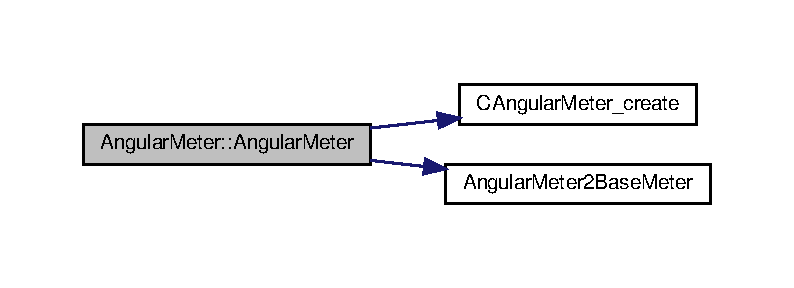
\includegraphics[width=350pt]{class_angular_meter_a5d71988b332dcbe883e7ad8d5abc0696_cgraph}
\end{center}
\end{figure}


\subsection{Member Function Documentation}
\mbox{\Hypertarget{class_angular_meter_ade95bcd716c78e650ab625c3b6c0fa0c}\label{class_angular_meter_ade95bcd716c78e650ab625c3b6c0fa0c}} 
\index{Angular\+Meter@{Angular\+Meter}!add\+Glare@{add\+Glare}}
\index{add\+Glare@{add\+Glare}!Angular\+Meter@{Angular\+Meter}}
\subsubsection{\texorpdfstring{add\+Glare()}{addGlare()}}
{\footnotesize\ttfamily void Angular\+Meter\+::add\+Glare (\begin{DoxyParamCaption}\item[{double}]{radius = {\ttfamily Chart\+:\+:NoValue},  }\item[{double}]{span = {\ttfamily 135},  }\item[{double}]{rotate = {\ttfamily 0},  }\item[{double}]{glare\+Radius = {\ttfamily Chart\+:\+:NoValue},  }\item[{double}]{intensity = {\ttfamily 0.13} }\end{DoxyParamCaption})\hspace{0.3cm}{\ttfamily [inline]}}



Definition at line 2981 of file chartdir.\+h.

Here is the call graph for this function\+:
\nopagebreak
\begin{figure}[H]
\begin{center}
\leavevmode
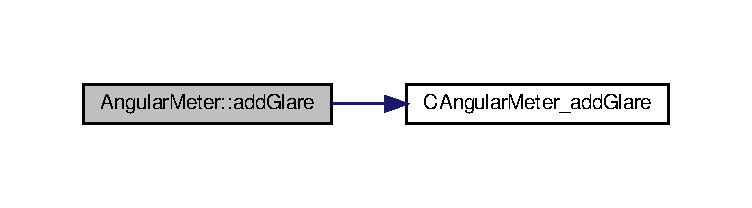
\includegraphics[width=350pt]{class_angular_meter_ade95bcd716c78e650ab625c3b6c0fa0c_cgraph}
\end{center}
\end{figure}
\mbox{\Hypertarget{class_angular_meter_a50942d4bfc5e84f9532784e6d41c9ec1}\label{class_angular_meter_a50942d4bfc5e84f9532784e6d41c9ec1}} 
\index{Angular\+Meter@{Angular\+Meter}!add\+Pointer2@{add\+Pointer2}}
\index{add\+Pointer2@{add\+Pointer2}!Angular\+Meter@{Angular\+Meter}}
\subsubsection{\texorpdfstring{add\+Pointer2()}{addPointer2()}}
{\footnotesize\ttfamily \hyperlink{class_meter_pointer}{Meter\+Pointer}$\ast$ Angular\+Meter\+::add\+Pointer2 (\begin{DoxyParamCaption}\item[{double}]{value,  }\item[{int}]{fill\+Color,  }\item[{int}]{edge\+Color = {\ttfamily -\/1},  }\item[{int}]{pointer\+Type = {\ttfamily \hyperlink{namespace_chart_a15cfe53d27f5b7a07e25af504b5d10f4afd0736ae83f260af5c7f8093d24448f1}{Chart\+::\+Triangular\+Pointer2}},  }\item[{double}]{start\+Offset = {\ttfamily Chart\+:\+:NoValue},  }\item[{double}]{end\+Offset = {\ttfamily Chart\+:\+:NoValue},  }\item[{double}]{width\+Ratio = {\ttfamily Chart\+:\+:NoValue} }\end{DoxyParamCaption})\hspace{0.3cm}{\ttfamily [inline]}}



Definition at line 2990 of file chartdir.\+h.

Here is the call graph for this function\+:
\nopagebreak
\begin{figure}[H]
\begin{center}
\leavevmode
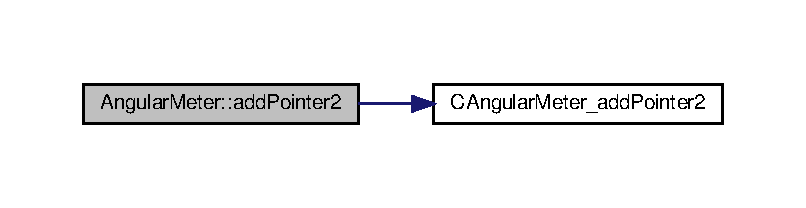
\includegraphics[width=350pt]{class_angular_meter_a50942d4bfc5e84f9532784e6d41c9ec1_cgraph}
\end{center}
\end{figure}
\mbox{\Hypertarget{class_angular_meter_a67b26ec28b68cac7b13922d61d2a36c9}\label{class_angular_meter_a67b26ec28b68cac7b13922d61d2a36c9}} 
\index{Angular\+Meter@{Angular\+Meter}!add\+Ring@{add\+Ring}}
\index{add\+Ring@{add\+Ring}!Angular\+Meter@{Angular\+Meter}}
\subsubsection{\texorpdfstring{add\+Ring()}{addRing()}}
{\footnotesize\ttfamily void Angular\+Meter\+::add\+Ring (\begin{DoxyParamCaption}\item[{int}]{start\+Radius,  }\item[{int}]{end\+Radius,  }\item[{int}]{fill\+Color,  }\item[{int}]{edge\+Color = {\ttfamily -\/1} }\end{DoxyParamCaption})\hspace{0.3cm}{\ttfamily [inline]}}



Definition at line 2971 of file chartdir.\+h.

Here is the call graph for this function\+:
\nopagebreak
\begin{figure}[H]
\begin{center}
\leavevmode
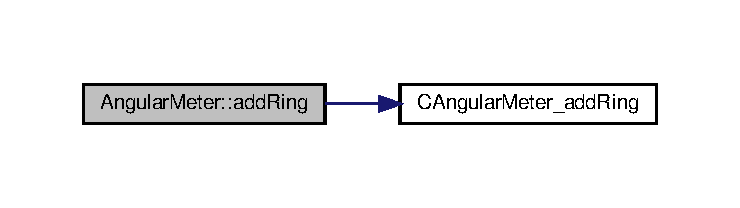
\includegraphics[width=350pt]{class_angular_meter_a67b26ec28b68cac7b13922d61d2a36c9_cgraph}
\end{center}
\end{figure}
\mbox{\Hypertarget{class_angular_meter_af7d1c8c5d188a2cf63a08296228fd6c3}\label{class_angular_meter_af7d1c8c5d188a2cf63a08296228fd6c3}} 
\index{Angular\+Meter@{Angular\+Meter}!add\+Ring\+Sector@{add\+Ring\+Sector}}
\index{add\+Ring\+Sector@{add\+Ring\+Sector}!Angular\+Meter@{Angular\+Meter}}
\subsubsection{\texorpdfstring{add\+Ring\+Sector()}{addRingSector()}}
{\footnotesize\ttfamily void Angular\+Meter\+::add\+Ring\+Sector (\begin{DoxyParamCaption}\item[{int}]{start\+Radius,  }\item[{int}]{end\+Radius,  }\item[{double}]{a1,  }\item[{double}]{a2,  }\item[{int}]{fill\+Color,  }\item[{int}]{edge\+Color = {\ttfamily -\/1} }\end{DoxyParamCaption})\hspace{0.3cm}{\ttfamily [inline]}}



Definition at line 2973 of file chartdir.\+h.

Here is the call graph for this function\+:
\nopagebreak
\begin{figure}[H]
\begin{center}
\leavevmode
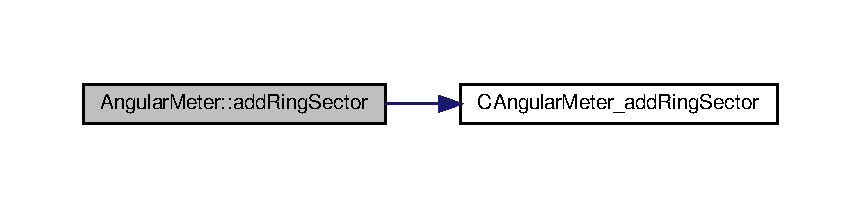
\includegraphics[width=350pt]{class_angular_meter_af7d1c8c5d188a2cf63a08296228fd6c3_cgraph}
\end{center}
\end{figure}
\mbox{\Hypertarget{class_angular_meter_a1de741912b6b62a24f7d197b4717e4b6}\label{class_angular_meter_a1de741912b6b62a24f7d197b4717e4b6}} 
\index{Angular\+Meter@{Angular\+Meter}!add\+Scale\+Background@{add\+Scale\+Background}}
\index{add\+Scale\+Background@{add\+Scale\+Background}!Angular\+Meter@{Angular\+Meter}}
\subsubsection{\texorpdfstring{add\+Scale\+Background()}{addScaleBackground()}}
{\footnotesize\ttfamily void Angular\+Meter\+::add\+Scale\+Background (\begin{DoxyParamCaption}\item[{int}]{bg\+Radius,  }\item[{int}]{fill\+Color,  }\item[{int}]{edge\+Width = {\ttfamily 0},  }\item[{int}]{edge\+Color = {\ttfamily -\/1},  }\item[{int}]{scale\+Radius = {\ttfamily -\/0x7fffffff},  }\item[{double}]{start\+Angle = {\ttfamily Chart\+:\+:NoValue},  }\item[{double}]{end\+Angle = {\ttfamily Chart\+:\+:NoValue} }\end{DoxyParamCaption})\hspace{0.3cm}{\ttfamily [inline]}}



Definition at line 2978 of file chartdir.\+h.

Here is the call graph for this function\+:
\nopagebreak
\begin{figure}[H]
\begin{center}
\leavevmode
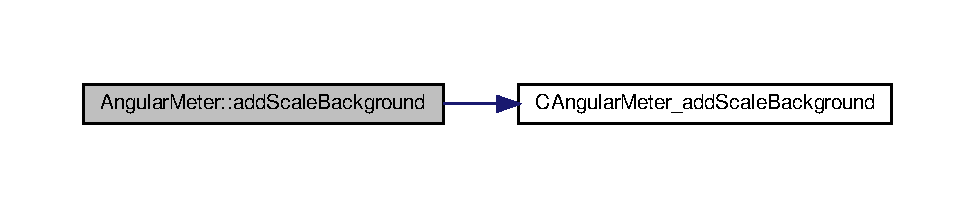
\includegraphics[width=350pt]{class_angular_meter_a1de741912b6b62a24f7d197b4717e4b6_cgraph}
\end{center}
\end{figure}
\mbox{\Hypertarget{class_angular_meter_ae1f9bf540c796aeb6df17698c0019224}\label{class_angular_meter_ae1f9bf540c796aeb6df17698c0019224}} 
\index{Angular\+Meter@{Angular\+Meter}!add\+Zone@{add\+Zone}}
\index{add\+Zone@{add\+Zone}!Angular\+Meter@{Angular\+Meter}}
\subsubsection{\texorpdfstring{add\+Zone()}{addZone()}\hspace{0.1cm}{\footnotesize\ttfamily [1/2]}}
{\footnotesize\ttfamily void Angular\+Meter\+::add\+Zone (\begin{DoxyParamCaption}\item[{double}]{start\+Value,  }\item[{double}]{end\+Value,  }\item[{int}]{start\+Radius,  }\item[{int}]{end\+Radius,  }\item[{int}]{fill\+Color,  }\item[{int}]{edge\+Color = {\ttfamily -\/1} }\end{DoxyParamCaption})\hspace{0.3cm}{\ttfamily [inline]}}



Definition at line 2995 of file chartdir.\+h.

Here is the call graph for this function\+:
\nopagebreak
\begin{figure}[H]
\begin{center}
\leavevmode
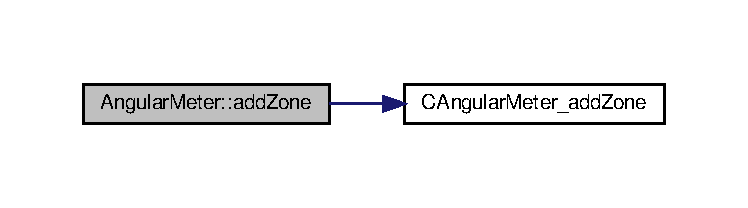
\includegraphics[width=350pt]{class_angular_meter_ae1f9bf540c796aeb6df17698c0019224_cgraph}
\end{center}
\end{figure}
\mbox{\Hypertarget{class_angular_meter_aab2b69fb54f0761d9a2b5c76088570f6}\label{class_angular_meter_aab2b69fb54f0761d9a2b5c76088570f6}} 
\index{Angular\+Meter@{Angular\+Meter}!add\+Zone@{add\+Zone}}
\index{add\+Zone@{add\+Zone}!Angular\+Meter@{Angular\+Meter}}
\subsubsection{\texorpdfstring{add\+Zone()}{addZone()}\hspace{0.1cm}{\footnotesize\ttfamily [2/2]}}
{\footnotesize\ttfamily void Angular\+Meter\+::add\+Zone (\begin{DoxyParamCaption}\item[{double}]{start\+Value,  }\item[{double}]{end\+Value,  }\item[{int}]{fill\+Color,  }\item[{int}]{edge\+Color = {\ttfamily -\/1} }\end{DoxyParamCaption})\hspace{0.3cm}{\ttfamily [inline]}}



Definition at line 2997 of file chartdir.\+h.

Here is the call graph for this function\+:
\nopagebreak
\begin{figure}[H]
\begin{center}
\leavevmode
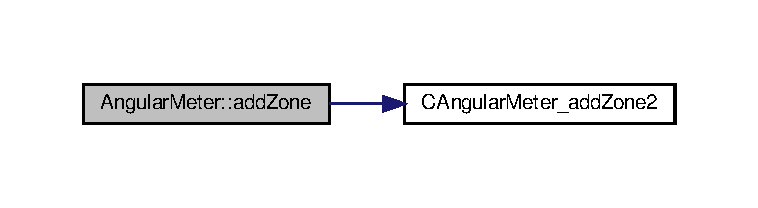
\includegraphics[width=350pt]{class_angular_meter_aab2b69fb54f0761d9a2b5c76088570f6_cgraph}
\end{center}
\end{figure}
\mbox{\Hypertarget{class_angular_meter_a454bd094af77f76a8e1b55ce180a686c}\label{class_angular_meter_a454bd094af77f76a8e1b55ce180a686c}} 
\index{Angular\+Meter@{Angular\+Meter}!relative\+Linear\+Gradient@{relative\+Linear\+Gradient}}
\index{relative\+Linear\+Gradient@{relative\+Linear\+Gradient}!Angular\+Meter@{Angular\+Meter}}
\subsubsection{\texorpdfstring{relative\+Linear\+Gradient()}{relativeLinearGradient()}}
{\footnotesize\ttfamily int Angular\+Meter\+::relative\+Linear\+Gradient (\begin{DoxyParamCaption}\item[{\hyperlink{class_double_array}{Double\+Array}}]{gradient,  }\item[{double}]{angle = {\ttfamily 0},  }\item[{double}]{radius = {\ttfamily -\/1} }\end{DoxyParamCaption})\hspace{0.3cm}{\ttfamily [inline]}}



Definition at line 3002 of file chartdir.\+h.

Here is the call graph for this function\+:
\nopagebreak
\begin{figure}[H]
\begin{center}
\leavevmode
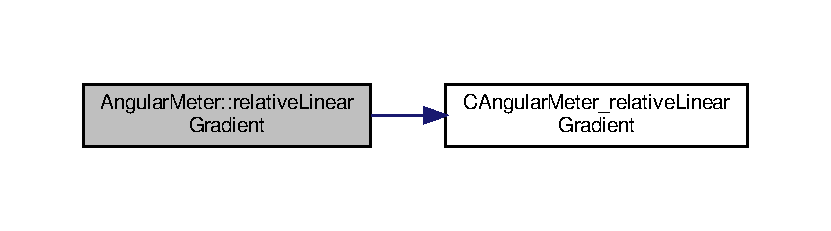
\includegraphics[width=350pt]{class_angular_meter_a454bd094af77f76a8e1b55ce180a686c_cgraph}
\end{center}
\end{figure}
\mbox{\Hypertarget{class_angular_meter_a3f2a73796ea3c4aba359042a810b0339}\label{class_angular_meter_a3f2a73796ea3c4aba359042a810b0339}} 
\index{Angular\+Meter@{Angular\+Meter}!relative\+Radial\+Gradient@{relative\+Radial\+Gradient}}
\index{relative\+Radial\+Gradient@{relative\+Radial\+Gradient}!Angular\+Meter@{Angular\+Meter}}
\subsubsection{\texorpdfstring{relative\+Radial\+Gradient()}{relativeRadialGradient()}}
{\footnotesize\ttfamily int Angular\+Meter\+::relative\+Radial\+Gradient (\begin{DoxyParamCaption}\item[{\hyperlink{class_double_array}{Double\+Array}}]{gradient,  }\item[{double}]{radius = {\ttfamily -\/1} }\end{DoxyParamCaption})\hspace{0.3cm}{\ttfamily [inline]}}



Definition at line 3000 of file chartdir.\+h.

Here is the call graph for this function\+:
\nopagebreak
\begin{figure}[H]
\begin{center}
\leavevmode
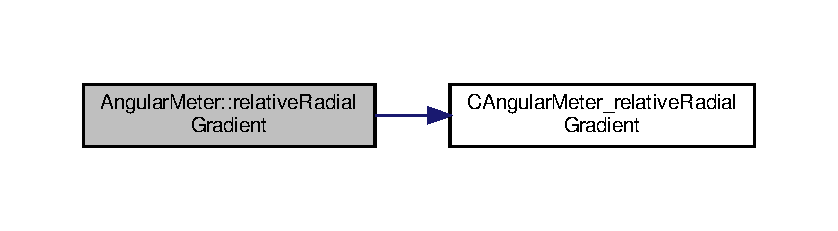
\includegraphics[width=350pt]{class_angular_meter_a3f2a73796ea3c4aba359042a810b0339_cgraph}
\end{center}
\end{figure}
\mbox{\Hypertarget{class_angular_meter_a0e20598329d17a1ac23b73fea207a6b7}\label{class_angular_meter_a0e20598329d17a1ac23b73fea207a6b7}} 
\index{Angular\+Meter@{Angular\+Meter}!set\+Cap@{set\+Cap}}
\index{set\+Cap@{set\+Cap}!Angular\+Meter@{Angular\+Meter}}
\subsubsection{\texorpdfstring{set\+Cap()}{setCap()}}
{\footnotesize\ttfamily void Angular\+Meter\+::set\+Cap (\begin{DoxyParamCaption}\item[{int}]{radius,  }\item[{int}]{fill\+Color,  }\item[{int}]{edge\+Color = {\ttfamily \hyperlink{namespace_chart_abee0d882fdc9ad0b001245ad9fc64011a04817a359476e87a5c572a7a69cdaaec}{Chart\+::\+Line\+Color}} }\end{DoxyParamCaption})\hspace{0.3cm}{\ttfamily [inline]}}



Definition at line 2985 of file chartdir.\+h.

Here is the call graph for this function\+:
\nopagebreak
\begin{figure}[H]
\begin{center}
\leavevmode
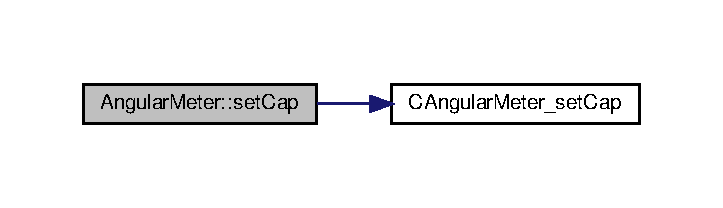
\includegraphics[width=347pt]{class_angular_meter_a0e20598329d17a1ac23b73fea207a6b7_cgraph}
\end{center}
\end{figure}
\mbox{\Hypertarget{class_angular_meter_a80b2f6a0dea2b4968ef7cca433e85a1d}\label{class_angular_meter_a80b2f6a0dea2b4968ef7cca433e85a1d}} 
\index{Angular\+Meter@{Angular\+Meter}!set\+Cap2@{set\+Cap2}}
\index{set\+Cap2@{set\+Cap2}!Angular\+Meter@{Angular\+Meter}}
\subsubsection{\texorpdfstring{set\+Cap2()}{setCap2()}}
{\footnotesize\ttfamily void Angular\+Meter\+::set\+Cap2 (\begin{DoxyParamCaption}\item[{int}]{back\+Color = {\ttfamily 0x888888},  }\item[{int}]{front\+Color = {\ttfamily 0x000000},  }\item[{int}]{front\+Edge\+Color = {\ttfamily 0x888888},  }\item[{double}]{lighting\+Ratio = {\ttfamily Chart\+:\+:NoValue},  }\item[{double}]{back\+Radius\+Ratio = {\ttfamily Chart\+:\+:NoValue},  }\item[{double}]{front\+Radius\+Ratio = {\ttfamily Chart\+:\+:NoValue},  }\item[{double}]{front\+Edge\+Width\+Ratio = {\ttfamily Chart\+:\+:NoValue} }\end{DoxyParamCaption})\hspace{0.3cm}{\ttfamily [inline]}}



Definition at line 2987 of file chartdir.\+h.

Here is the call graph for this function\+:
\nopagebreak
\begin{figure}[H]
\begin{center}
\leavevmode
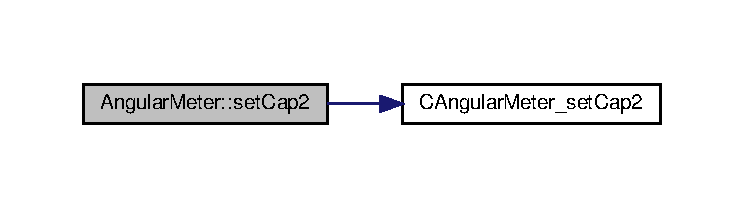
\includegraphics[width=350pt]{class_angular_meter_a80b2f6a0dea2b4968ef7cca433e85a1d_cgraph}
\end{center}
\end{figure}
\mbox{\Hypertarget{class_angular_meter_a569e2ac4b396f2c1cafb5943f390c454}\label{class_angular_meter_a569e2ac4b396f2c1cafb5943f390c454}} 
\index{Angular\+Meter@{Angular\+Meter}!set\+Meter@{set\+Meter}}
\index{set\+Meter@{set\+Meter}!Angular\+Meter@{Angular\+Meter}}
\subsubsection{\texorpdfstring{set\+Meter()}{setMeter()}}
{\footnotesize\ttfamily void Angular\+Meter\+::set\+Meter (\begin{DoxyParamCaption}\item[{int}]{cx,  }\item[{int}]{cy,  }\item[{int}]{radius,  }\item[{double}]{start\+Angle,  }\item[{double}]{end\+Angle }\end{DoxyParamCaption})\hspace{0.3cm}{\ttfamily [inline]}}



Definition at line 2976 of file chartdir.\+h.

Here is the call graph for this function\+:
\nopagebreak
\begin{figure}[H]
\begin{center}
\leavevmode
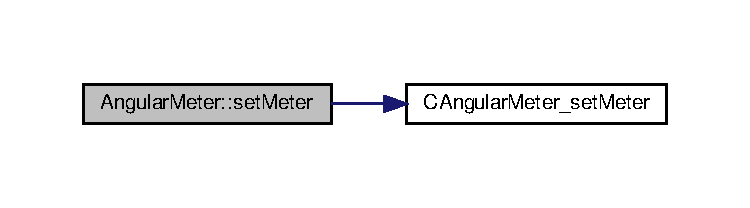
\includegraphics[width=350pt]{class_angular_meter_a569e2ac4b396f2c1cafb5943f390c454_cgraph}
\end{center}
\end{figure}


The documentation for this class was generated from the following file\+:\begin{DoxyCompactItemize}
\item 
include/\hyperlink{chartdir_8h}{chartdir.\+h}\end{DoxyCompactItemize}

\hypertarget{class_area_layer}{}\section{Area\+Layer Class Reference}
\label{class_area_layer}\index{Area\+Layer@{Area\+Layer}}


{\ttfamily \#include $<$chartdir.\+h$>$}



Inheritance diagram for Area\+Layer\+:
\nopagebreak
\begin{figure}[H]
\begin{center}
\leavevmode
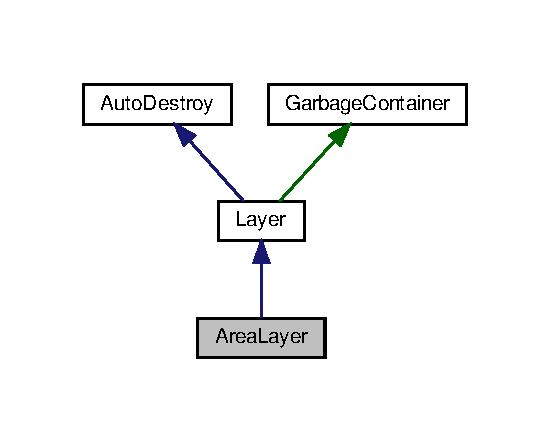
\includegraphics[width=264pt]{class_area_layer__inherit__graph}
\end{center}
\end{figure}


Collaboration diagram for Area\+Layer\+:
\nopagebreak
\begin{figure}[H]
\begin{center}
\leavevmode
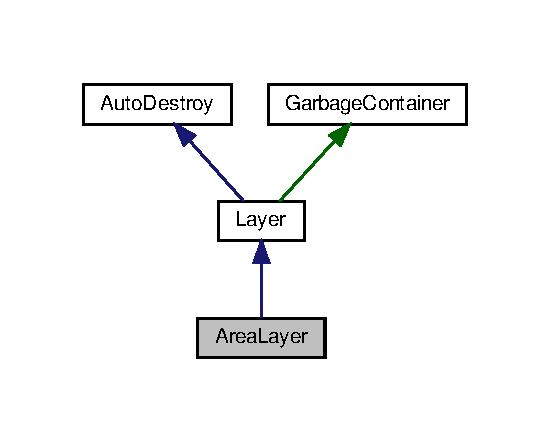
\includegraphics[width=264pt]{class_area_layer__coll__graph}
\end{center}
\end{figure}
\subsection*{Public Member Functions}
\begin{DoxyCompactItemize}
\item 
\hyperlink{class_area_layer_a344068141673f8eb209a6bccf946539b}{Area\+Layer} (Area\+Layer\+Internal $\ast$\+\_\+ptr)
\item 
\hyperlink{class_area_layer_ac7ee192b99d13cdaead0010e9cc99a74}{$\sim$\+Area\+Layer} ()
\item 
void \hyperlink{class_area_layer_a5db68f656bcb69c9064e4553de75f0f7}{set\+Min\+Label\+Size} (int s)
\item 
void \hyperlink{class_area_layer_a2bb65eb13524a34d5ab090b48bde062b}{set\+Gap\+Color} (int fill\+Color)
\end{DoxyCompactItemize}
\subsection*{Additional Inherited Members}


\subsection{Detailed Description}


Definition at line 1925 of file chartdir.\+h.



\subsection{Constructor \& Destructor Documentation}
\mbox{\Hypertarget{class_area_layer_a344068141673f8eb209a6bccf946539b}\label{class_area_layer_a344068141673f8eb209a6bccf946539b}} 
\index{Area\+Layer@{Area\+Layer}!Area\+Layer@{Area\+Layer}}
\index{Area\+Layer@{Area\+Layer}!Area\+Layer@{Area\+Layer}}
\subsubsection{\texorpdfstring{Area\+Layer()}{AreaLayer()}}
{\footnotesize\ttfamily Area\+Layer\+::\+Area\+Layer (\begin{DoxyParamCaption}\item[{Area\+Layer\+Internal $\ast$}]{\+\_\+ptr }\end{DoxyParamCaption})\hspace{0.3cm}{\ttfamily [inline]}}



Definition at line 1935 of file chartdir.\+h.

\mbox{\Hypertarget{class_area_layer_ac7ee192b99d13cdaead0010e9cc99a74}\label{class_area_layer_ac7ee192b99d13cdaead0010e9cc99a74}} 
\index{Area\+Layer@{Area\+Layer}!````~Area\+Layer@{$\sim$\+Area\+Layer}}
\index{````~Area\+Layer@{$\sim$\+Area\+Layer}!Area\+Layer@{Area\+Layer}}
\subsubsection{\texorpdfstring{$\sim$\+Area\+Layer()}{~AreaLayer()}}
{\footnotesize\ttfamily Area\+Layer\+::$\sim$\+Area\+Layer (\begin{DoxyParamCaption}{ }\end{DoxyParamCaption})\hspace{0.3cm}{\ttfamily [inline]}}



Definition at line 1936 of file chartdir.\+h.



\subsection{Member Function Documentation}
\mbox{\Hypertarget{class_area_layer_a2bb65eb13524a34d5ab090b48bde062b}\label{class_area_layer_a2bb65eb13524a34d5ab090b48bde062b}} 
\index{Area\+Layer@{Area\+Layer}!set\+Gap\+Color@{set\+Gap\+Color}}
\index{set\+Gap\+Color@{set\+Gap\+Color}!Area\+Layer@{Area\+Layer}}
\subsubsection{\texorpdfstring{set\+Gap\+Color()}{setGapColor()}}
{\footnotesize\ttfamily void Area\+Layer\+::set\+Gap\+Color (\begin{DoxyParamCaption}\item[{int}]{fill\+Color }\end{DoxyParamCaption})\hspace{0.3cm}{\ttfamily [inline]}}



Definition at line 1939 of file chartdir.\+h.

Here is the call graph for this function\+:
\nopagebreak
\begin{figure}[H]
\begin{center}
\leavevmode
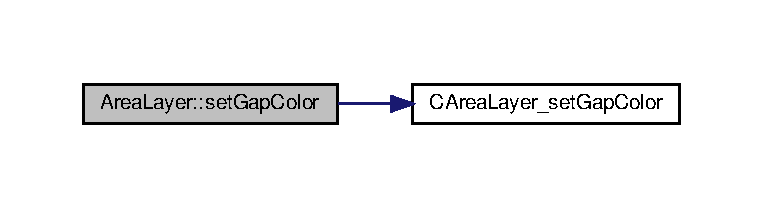
\includegraphics[width=350pt]{class_area_layer_a2bb65eb13524a34d5ab090b48bde062b_cgraph}
\end{center}
\end{figure}
\mbox{\Hypertarget{class_area_layer_a5db68f656bcb69c9064e4553de75f0f7}\label{class_area_layer_a5db68f656bcb69c9064e4553de75f0f7}} 
\index{Area\+Layer@{Area\+Layer}!set\+Min\+Label\+Size@{set\+Min\+Label\+Size}}
\index{set\+Min\+Label\+Size@{set\+Min\+Label\+Size}!Area\+Layer@{Area\+Layer}}
\subsubsection{\texorpdfstring{set\+Min\+Label\+Size()}{setMinLabelSize()}}
{\footnotesize\ttfamily void Area\+Layer\+::set\+Min\+Label\+Size (\begin{DoxyParamCaption}\item[{int}]{s }\end{DoxyParamCaption})\hspace{0.3cm}{\ttfamily [inline]}}



Definition at line 1938 of file chartdir.\+h.

Here is the call graph for this function\+:
\nopagebreak
\begin{figure}[H]
\begin{center}
\leavevmode
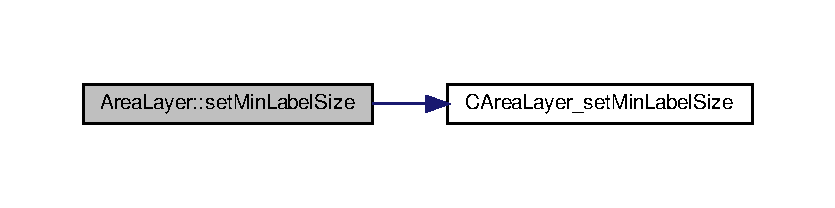
\includegraphics[width=350pt]{class_area_layer_a5db68f656bcb69c9064e4553de75f0f7_cgraph}
\end{center}
\end{figure}


The documentation for this class was generated from the following file\+:\begin{DoxyCompactItemize}
\item 
include/\hyperlink{chartdir_8h}{chartdir.\+h}\end{DoxyCompactItemize}

\hypertarget{class_array_math}{}\section{Array\+Math Class Reference}
\label{class_array_math}\index{Array\+Math@{Array\+Math}}


{\ttfamily \#include $<$chartdir.\+h$>$}

\subsection*{Public Member Functions}
\begin{DoxyCompactItemize}
\item 
\hyperlink{class_array_math_a3a8b5e89c10d1c1b2c098bf9dd4366d7}{Array\+Math} (\hyperlink{class_double_array}{Double\+Array} a)
\item 
\hyperlink{class_array_math_a65d4e3680182f61c866a61f375639245}{$\sim$\+Array\+Math} ()
\item 
void \hyperlink{class_array_math_a5c0ea92917740188c95e4e410eef2661}{destroy} ()
\item 
\hyperlink{class_array_math_a04ce35d72b715dc2f5889ff040872c1e}{Array\+Math} (const \hyperlink{class_array_math}{Array\+Math} \&rhs)
\item 
\hyperlink{class_array_math}{Array\+Math} \& \hyperlink{class_array_math_aefa81728a4b712db88e3e4453bf384ad}{operator=} (const \hyperlink{class_array_math}{Array\+Math} \&rhs)
\item 
\hyperlink{class_array_math_a1b309d87396b6971a40a71ea333b628d}{operator Double\+Array} () const
\item 
\hyperlink{class_array_math}{Array\+Math} \& \hyperlink{class_array_math_a0523eb1e6ea490c1a298a8b9bca05833}{add} (\hyperlink{class_double_array}{Double\+Array} b)
\item 
\hyperlink{class_array_math}{Array\+Math} \& \hyperlink{class_array_math_a3ebc72308c94fd2ea7dbf1407e8c9eeb}{add} (double b)
\item 
\hyperlink{class_array_math}{Array\+Math} \& \hyperlink{class_array_math_a67bc79157b230866a8ed1eb5e6179de0}{sub} (\hyperlink{class_double_array}{Double\+Array} b)
\item 
\hyperlink{class_array_math}{Array\+Math} \& \hyperlink{class_array_math_a4c05dccafd9c44167c2e158427ce3099}{sub} (double b)
\item 
\hyperlink{class_array_math}{Array\+Math} \& \hyperlink{class_array_math_a4fb34b6f319e7f3b2a5440d426832889}{mul} (\hyperlink{class_double_array}{Double\+Array} b)
\item 
\hyperlink{class_array_math}{Array\+Math} \& \hyperlink{class_array_math_ad44c0c320ef2f9401be5e54d51dc6c73}{mul} (double b)
\item 
\hyperlink{class_array_math}{Array\+Math} \& \hyperlink{class_array_math_a1f2298b0a0338ea48fc3163f6387d11c}{div} (\hyperlink{class_double_array}{Double\+Array} b)
\item 
\hyperlink{class_array_math}{Array\+Math} \& \hyperlink{class_array_math_a8ba4c3f4ec4a35cc310d97e2a647ad4c}{div} (double b)
\item 
\hyperlink{class_array_math}{Array\+Math} \& \hyperlink{class_array_math_a854177572cefc64f20462ad56e74038e}{finance\+Div} (\hyperlink{class_double_array}{Double\+Array} b, double zero\+By\+Zero\+Value)
\item 
\hyperlink{class_array_math}{Array\+Math} \& \hyperlink{class_array_math_a3448f6c81db45f84e63351a00f6d32b3}{shift} (int offset=1, double fill\+Value=Chart\+::\+No\+Value)
\item 
\hyperlink{class_array_math}{Array\+Math} \& \hyperlink{class_array_math_a63280677d4282215230467eadb0ff3ca}{delta} (int offset=1)
\item 
\hyperlink{class_array_math}{Array\+Math} \& \hyperlink{class_array_math_a72a5a6a662b011b093a0aed0aac5df76}{rate} (int offset=1)
\item 
\hyperlink{class_array_math}{Array\+Math} \& \hyperlink{class_array_math_a95ff8e9bce7b34d36cde3186e3f8d886}{abs} ()
\item 
\hyperlink{class_array_math}{Array\+Math} \& \hyperlink{class_array_math_aa4a6b85dd0e0cbbd6055e5381b9f8308}{acc} ()
\item 
\hyperlink{class_array_math}{Array\+Math} \& \hyperlink{class_array_math_aadfd40e8527d58dc41cceec240d1f9b8}{select\+G\+TZ} (\hyperlink{class_double_array}{Double\+Array} decision\+Array=\hyperlink{class_double_array}{Double\+Array}(), double fill\+Value=0)
\item 
\hyperlink{class_array_math}{Array\+Math} \& \hyperlink{class_array_math_adeaae3c00b4d38c471d5956d65861a48}{select\+G\+EZ} (\hyperlink{class_double_array}{Double\+Array} decision\+Array=\hyperlink{class_double_array}{Double\+Array}(), double fill\+Value=0)
\item 
\hyperlink{class_array_math}{Array\+Math} \& \hyperlink{class_array_math_ae10389934cacf3913e69b71c79fe5ae9}{select\+L\+TZ} (\hyperlink{class_double_array}{Double\+Array} decision\+Array=\hyperlink{class_double_array}{Double\+Array}(), double fill\+Value=0)
\item 
\hyperlink{class_array_math}{Array\+Math} \& \hyperlink{class_array_math_a63ec8c97034104b0ede0227683583eac}{select\+L\+EZ} (\hyperlink{class_double_array}{Double\+Array} decision\+Array=\hyperlink{class_double_array}{Double\+Array}(), double fill\+Value=0)
\item 
\hyperlink{class_array_math}{Array\+Math} \& \hyperlink{class_array_math_a7c219ae5049b2a515025f24ae5428a83}{select\+E\+QZ} (\hyperlink{class_double_array}{Double\+Array} decision\+Array=\hyperlink{class_double_array}{Double\+Array}(), double fill\+Value=0)
\item 
\hyperlink{class_array_math}{Array\+Math} \& \hyperlink{class_array_math_a0ec9ff9be8d0f829ba79bd1a53a791a5}{select\+N\+EZ} (\hyperlink{class_double_array}{Double\+Array} decision\+Array=\hyperlink{class_double_array}{Double\+Array}(), double fill\+Value=0)
\item 
\hyperlink{class_array_math}{Array\+Math} \& \hyperlink{class_array_math_ab0253df48686370fccc34f3e286521d9}{select\+Start\+Of\+Second} (int major\+Tick\+Step=1, double initial\+Margin=0.\+1)
\item 
\hyperlink{class_array_math}{Array\+Math} \& \hyperlink{class_array_math_a56f6e1b492180694a2117d030858a41a}{select\+Start\+Of\+Minute} (int major\+Tick\+Step=1, double initial\+Margin=5)
\item 
\hyperlink{class_array_math}{Array\+Math} \& \hyperlink{class_array_math_a39fc6c03bb738f82e4f98daebb672dda}{select\+Start\+Of\+Hour} (int major\+Tick\+Step=1, double initial\+Margin=300)
\item 
\hyperlink{class_array_math}{Array\+Math} \& \hyperlink{class_array_math_a5e6c8318cbc69a3bb9da3c1c0ca86c26}{select\+Start\+Of\+Day} (int major\+Tick\+Step=1, double initial\+Margin=3 $\ast$3600)
\item 
\hyperlink{class_array_math}{Array\+Math} \& \hyperlink{class_array_math_a97c624b2c158da5bcea887bec88d8fd0}{select\+Start\+Of\+Week} (int major\+Tick\+Step=1, double initial\+Margin=2 $\ast$86400)
\item 
\hyperlink{class_array_math}{Array\+Math} \& \hyperlink{class_array_math_a65c725e8229a4cba8072af77b23e2286}{select\+Start\+Of\+Month} (int major\+Tick\+Step=1, double initial\+Margin=5 $\ast$86400)
\item 
\hyperlink{class_array_math}{Array\+Math} \& \hyperlink{class_array_math_a49a76a80a68b10357db7f0189e3bfb2f}{select\+Start\+Of\+Year} (int major\+Tick\+Step=1, double initial\+Margin=60 $\ast$86400)
\item 
\hyperlink{class_array_math}{Array\+Math} \& \hyperlink{class_array_math_a7fa60f8da0b8448ec591ce7f4b95f251}{select\+Regular\+Spacing} (int major\+Tick\+Step, int minor\+Tick\+Step=0, int initial\+Margin=0)
\item 
\hyperlink{class_array_math}{Array\+Math} \& \hyperlink{class_array_math_a07cdedd06b274fbd5a5be338cd507861}{trim} (int start\+Index=0, int len=-\/1)
\item 
\hyperlink{class_array_math}{Array\+Math} \& \hyperlink{class_array_math_a36c129c503f3fe99e8a92ba265eae19e}{insert} (\hyperlink{class_double_array}{Double\+Array} a, int insert\+Point=-\/1)
\item 
\hyperlink{class_array_math}{Array\+Math} \& \hyperlink{class_array_math_a2cebd29ee37fb8f24de84cbd14cd4b46}{insert} (double c, int len, int insert\+Point=-\/1)
\item 
\hyperlink{class_array_math}{Array\+Math} \& \hyperlink{class_array_math_a3e735bfc88ee0149c7056cac1defbf6c}{replace} (double a, double b)
\item 
\hyperlink{class_array_math}{Array\+Math} \& \hyperlink{class_array_math_abaaac1009dda4a6124ecd2182354dc39}{mov\+Avg} (int interval)
\item 
\hyperlink{class_array_math}{Array\+Math} \& \hyperlink{class_array_math_a2f9029cfd45e1094dd6aeb549bbcd107}{exp\+Avg} (double smoothing\+Factor)
\item 
\hyperlink{class_array_math}{Array\+Math} \& \hyperlink{class_array_math_a7f994291fd85c2859e7bf34c27b8013e}{mov\+Med} (int interval)
\item 
\hyperlink{class_array_math}{Array\+Math} \& \hyperlink{class_array_math_adc007aad3ce9cac15f02159190c2c84a}{mov\+Percentile} (int interval, double \+\_\+percentile)
\item 
\hyperlink{class_array_math}{Array\+Math} \& \hyperlink{class_array_math_a5134853d9b14c3d980036a02a4d4b043}{mov\+Max} (int interval)
\item 
\hyperlink{class_array_math}{Array\+Math} \& \hyperlink{class_array_math_a42df280f64eaaad8150985d962516276}{mov\+Min} (int interval)
\item 
\hyperlink{class_array_math}{Array\+Math} \& \hyperlink{class_array_math_a0352f506e872e964ef2590fa7e8ce581}{mov\+Std\+Dev} (int interval)
\item 
\hyperlink{class_array_math}{Array\+Math} \& \hyperlink{class_array_math_a61cdecb4beb7c276a122306906cdebd8}{mov\+Corr} (int interval, \hyperlink{class_double_array}{Double\+Array} b=\hyperlink{class_double_array}{Double\+Array}())
\item 
\hyperlink{class_array_math}{Array\+Math} \& \hyperlink{class_array_math_afc9d22a0cf7267842d76430fd0dce639}{lowess} (double smoothness=0.\+25, int iteration=0)
\item 
\hyperlink{class_array_math}{Array\+Math} \& \hyperlink{class_array_math_a7852fe7a310511ac1ba8fa585a614146}{lowess} (\hyperlink{class_double_array}{Double\+Array} b, double smoothness=0.\+25, int iteration=0)
\item 
\hyperlink{class_double_array}{Double\+Array} \hyperlink{class_array_math_a2c81268f37eb5e4ab9c1c8e18bb22fa3}{result} () const
\item 
double \hyperlink{class_array_math_ae80c440e5ad866929649746c029cf0bf}{max} () const
\item 
double \hyperlink{class_array_math_ab2f502a58518cfe68bcdaa31729d4a96}{max\+Value} () const
\item 
double \hyperlink{class_array_math_a4ef0f497cafb78d37d4af0a6bd51d411}{min} () const
\item 
double \hyperlink{class_array_math_aff26b5d31ec9ec6f7e113a6425ca4e13}{min\+Value} () const
\item 
double \hyperlink{class_array_math_a1ecf90f00ed56f8b977f1ed5a3a6d7fa}{avg} () const
\item 
double \hyperlink{class_array_math_a864604ac04b95fa04fcd511d1845ebbd}{sum} () const
\item 
double \hyperlink{class_array_math_a71fbcf5d93c40e840b4aa7fbea38e98e}{std\+Dev} () const
\item 
double \hyperlink{class_array_math_aa60ced676c9387a970df6468379d1f56}{med} () const
\item 
double \hyperlink{class_array_math_ae0342b531a9f73cabc2b13f81e2cef88}{percentile} (double p) const
\item 
int \hyperlink{class_array_math_af75557e958d76b32d93a6a90fa6d064c}{max\+Index} () const
\item 
int \hyperlink{class_array_math_a0cf1a69edacfb547184b06e6c71693e6}{min\+Index} () const
\item 
\hyperlink{class_double_array}{Double\+Array} \hyperlink{class_array_math_aa4b11f4895afbf51a60e099baf16f5a3}{aggregate} (\hyperlink{class_double_array}{Double\+Array} src\+Array, int aggregate\+Method, double param=50) const
\end{DoxyCompactItemize}
\subsection*{Static Public Member Functions}
\begin{DoxyCompactItemize}
\item 
static \hyperlink{class_array_math}{Array\+Math} $\ast$ \hyperlink{class_array_math_af663455894b413a30e30c4c396e6ccaa}{create} (\hyperlink{class_double_array}{Double\+Array} a)
\end{DoxyCompactItemize}


\subsection{Detailed Description}


Definition at line 3041 of file chartdir.\+h.



\subsection{Constructor \& Destructor Documentation}
\mbox{\Hypertarget{class_array_math_a3a8b5e89c10d1c1b2c098bf9dd4366d7}\label{class_array_math_a3a8b5e89c10d1c1b2c098bf9dd4366d7}} 
\index{Array\+Math@{Array\+Math}!Array\+Math@{Array\+Math}}
\index{Array\+Math@{Array\+Math}!Array\+Math@{Array\+Math}}
\subsubsection{\texorpdfstring{Array\+Math()}{ArrayMath()}\hspace{0.1cm}{\footnotesize\ttfamily [1/2]}}
{\footnotesize\ttfamily Array\+Math\+::\+Array\+Math (\begin{DoxyParamCaption}\item[{\hyperlink{class_double_array}{Double\+Array}}]{a }\end{DoxyParamCaption})\hspace{0.3cm}{\ttfamily [inline]}}



Definition at line 3047 of file chartdir.\+h.

\mbox{\Hypertarget{class_array_math_a65d4e3680182f61c866a61f375639245}\label{class_array_math_a65d4e3680182f61c866a61f375639245}} 
\index{Array\+Math@{Array\+Math}!````~Array\+Math@{$\sim$\+Array\+Math}}
\index{````~Array\+Math@{$\sim$\+Array\+Math}!Array\+Math@{Array\+Math}}
\subsubsection{\texorpdfstring{$\sim$\+Array\+Math()}{~ArrayMath()}}
{\footnotesize\ttfamily Array\+Math\+::$\sim$\+Array\+Math (\begin{DoxyParamCaption}{ }\end{DoxyParamCaption})\hspace{0.3cm}{\ttfamily [inline]}}



Definition at line 3048 of file chartdir.\+h.

Here is the call graph for this function\+:
\nopagebreak
\begin{figure}[H]
\begin{center}
\leavevmode
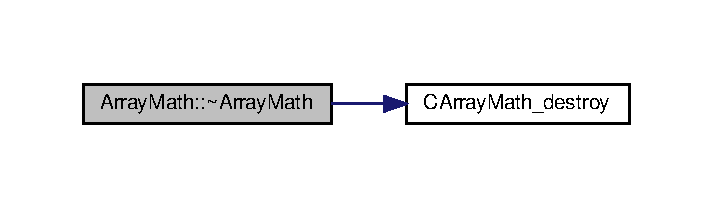
\includegraphics[width=342pt]{class_array_math_a65d4e3680182f61c866a61f375639245_cgraph}
\end{center}
\end{figure}
\mbox{\Hypertarget{class_array_math_a04ce35d72b715dc2f5889ff040872c1e}\label{class_array_math_a04ce35d72b715dc2f5889ff040872c1e}} 
\index{Array\+Math@{Array\+Math}!Array\+Math@{Array\+Math}}
\index{Array\+Math@{Array\+Math}!Array\+Math@{Array\+Math}}
\subsubsection{\texorpdfstring{Array\+Math()}{ArrayMath()}\hspace{0.1cm}{\footnotesize\ttfamily [2/2]}}
{\footnotesize\ttfamily Array\+Math\+::\+Array\+Math (\begin{DoxyParamCaption}\item[{const \hyperlink{class_array_math}{Array\+Math} \&}]{rhs }\end{DoxyParamCaption})\hspace{0.3cm}{\ttfamily [inline]}}



Definition at line 3052 of file chartdir.\+h.

Here is the call graph for this function\+:
\nopagebreak
\begin{figure}[H]
\begin{center}
\leavevmode
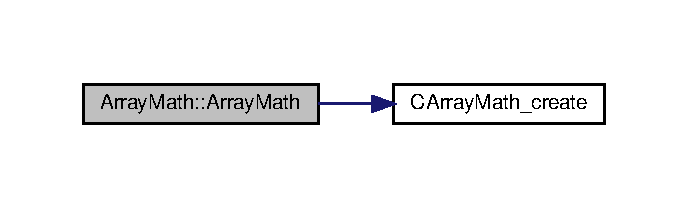
\includegraphics[width=330pt]{class_array_math_a04ce35d72b715dc2f5889ff040872c1e_cgraph}
\end{center}
\end{figure}


\subsection{Member Function Documentation}
\mbox{\Hypertarget{class_array_math_a95ff8e9bce7b34d36cde3186e3f8d886}\label{class_array_math_a95ff8e9bce7b34d36cde3186e3f8d886}} 
\index{Array\+Math@{Array\+Math}!abs@{abs}}
\index{abs@{abs}!Array\+Math@{Array\+Math}}
\subsubsection{\texorpdfstring{abs()}{abs()}}
{\footnotesize\ttfamily \hyperlink{class_array_math}{Array\+Math}\& Array\+Math\+::abs (\begin{DoxyParamCaption}{ }\end{DoxyParamCaption})\hspace{0.3cm}{\ttfamily [inline]}}



Definition at line 3068 of file chartdir.\+h.

Here is the call graph for this function\+:
\nopagebreak
\begin{figure}[H]
\begin{center}
\leavevmode
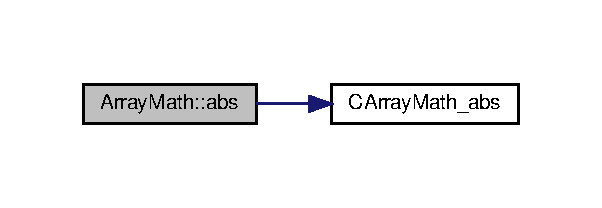
\includegraphics[width=289pt]{class_array_math_a95ff8e9bce7b34d36cde3186e3f8d886_cgraph}
\end{center}
\end{figure}
Here is the caller graph for this function\+:
\nopagebreak
\begin{figure}[H]
\begin{center}
\leavevmode
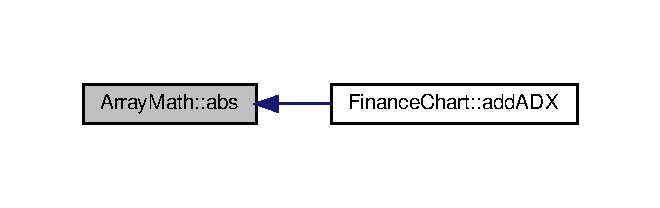
\includegraphics[width=317pt]{class_array_math_a95ff8e9bce7b34d36cde3186e3f8d886_icgraph}
\end{center}
\end{figure}
\mbox{\Hypertarget{class_array_math_aa4a6b85dd0e0cbbd6055e5381b9f8308}\label{class_array_math_aa4a6b85dd0e0cbbd6055e5381b9f8308}} 
\index{Array\+Math@{Array\+Math}!acc@{acc}}
\index{acc@{acc}!Array\+Math@{Array\+Math}}
\subsubsection{\texorpdfstring{acc()}{acc()}}
{\footnotesize\ttfamily \hyperlink{class_array_math}{Array\+Math}\& Array\+Math\+::acc (\begin{DoxyParamCaption}{ }\end{DoxyParamCaption})\hspace{0.3cm}{\ttfamily [inline]}}



Definition at line 3069 of file chartdir.\+h.

Here is the call graph for this function\+:
\nopagebreak
\begin{figure}[H]
\begin{center}
\leavevmode
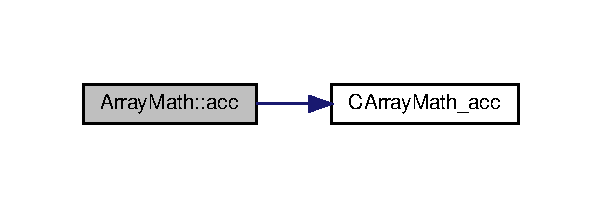
\includegraphics[width=289pt]{class_array_math_aa4a6b85dd0e0cbbd6055e5381b9f8308_cgraph}
\end{center}
\end{figure}
Here is the caller graph for this function\+:
\nopagebreak
\begin{figure}[H]
\begin{center}
\leavevmode
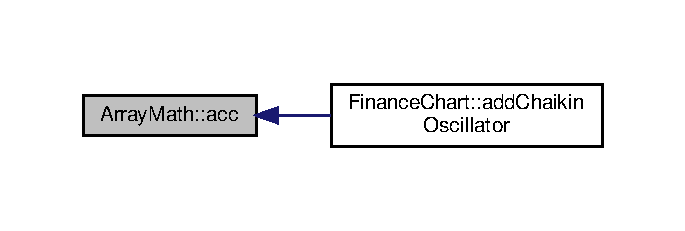
\includegraphics[width=329pt]{class_array_math_aa4a6b85dd0e0cbbd6055e5381b9f8308_icgraph}
\end{center}
\end{figure}
\mbox{\Hypertarget{class_array_math_a0523eb1e6ea490c1a298a8b9bca05833}\label{class_array_math_a0523eb1e6ea490c1a298a8b9bca05833}} 
\index{Array\+Math@{Array\+Math}!add@{add}}
\index{add@{add}!Array\+Math@{Array\+Math}}
\subsubsection{\texorpdfstring{add()}{add()}\hspace{0.1cm}{\footnotesize\ttfamily [1/2]}}
{\footnotesize\ttfamily \hyperlink{class_array_math}{Array\+Math}\& Array\+Math\+::add (\begin{DoxyParamCaption}\item[{\hyperlink{class_double_array}{Double\+Array}}]{b }\end{DoxyParamCaption})\hspace{0.3cm}{\ttfamily [inline]}}



Definition at line 3056 of file chartdir.\+h.

Here is the call graph for this function\+:
\nopagebreak
\begin{figure}[H]
\begin{center}
\leavevmode
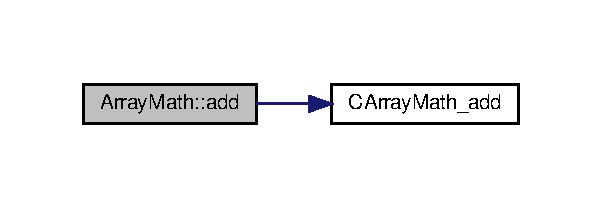
\includegraphics[width=289pt]{class_array_math_a0523eb1e6ea490c1a298a8b9bca05833_cgraph}
\end{center}
\end{figure}
Here is the caller graph for this function\+:
\nopagebreak
\begin{figure}[H]
\begin{center}
\leavevmode
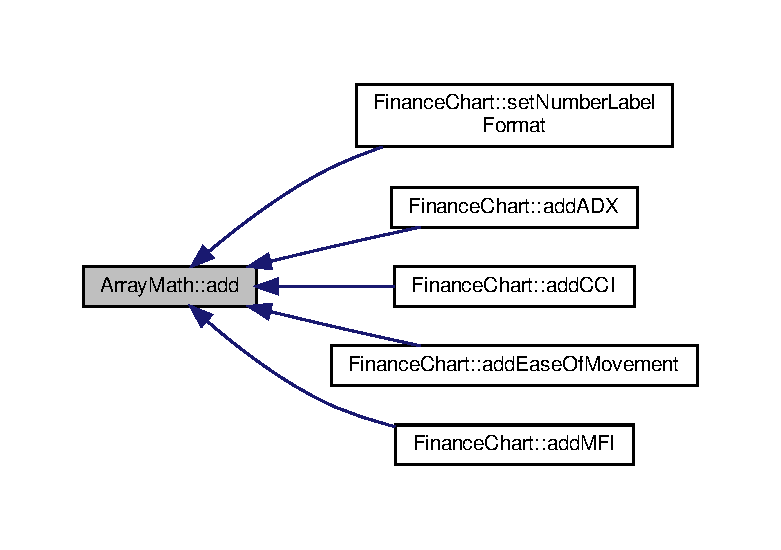
\includegraphics[width=350pt]{class_array_math_a0523eb1e6ea490c1a298a8b9bca05833_icgraph}
\end{center}
\end{figure}
\mbox{\Hypertarget{class_array_math_a3ebc72308c94fd2ea7dbf1407e8c9eeb}\label{class_array_math_a3ebc72308c94fd2ea7dbf1407e8c9eeb}} 
\index{Array\+Math@{Array\+Math}!add@{add}}
\index{add@{add}!Array\+Math@{Array\+Math}}
\subsubsection{\texorpdfstring{add()}{add()}\hspace{0.1cm}{\footnotesize\ttfamily [2/2]}}
{\footnotesize\ttfamily \hyperlink{class_array_math}{Array\+Math}\& Array\+Math\+::add (\begin{DoxyParamCaption}\item[{double}]{b }\end{DoxyParamCaption})\hspace{0.3cm}{\ttfamily [inline]}}



Definition at line 3057 of file chartdir.\+h.

Here is the call graph for this function\+:
\nopagebreak
\begin{figure}[H]
\begin{center}
\leavevmode
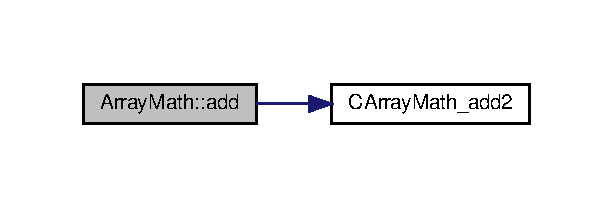
\includegraphics[width=294pt]{class_array_math_a3ebc72308c94fd2ea7dbf1407e8c9eeb_cgraph}
\end{center}
\end{figure}
\mbox{\Hypertarget{class_array_math_aa4b11f4895afbf51a60e099baf16f5a3}\label{class_array_math_aa4b11f4895afbf51a60e099baf16f5a3}} 
\index{Array\+Math@{Array\+Math}!aggregate@{aggregate}}
\index{aggregate@{aggregate}!Array\+Math@{Array\+Math}}
\subsubsection{\texorpdfstring{aggregate()}{aggregate()}}
{\footnotesize\ttfamily \hyperlink{class_double_array}{Double\+Array} Array\+Math\+::aggregate (\begin{DoxyParamCaption}\item[{\hyperlink{class_double_array}{Double\+Array}}]{src\+Array,  }\item[{int}]{aggregate\+Method,  }\item[{double}]{param = {\ttfamily 50} }\end{DoxyParamCaption}) const\hspace{0.3cm}{\ttfamily [inline]}}



Definition at line 3148 of file chartdir.\+h.

Here is the call graph for this function\+:
\nopagebreak
\begin{figure}[H]
\begin{center}
\leavevmode
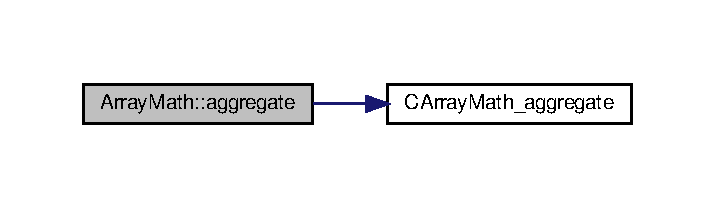
\includegraphics[width=343pt]{class_array_math_aa4b11f4895afbf51a60e099baf16f5a3_cgraph}
\end{center}
\end{figure}
\mbox{\Hypertarget{class_array_math_a1ecf90f00ed56f8b977f1ed5a3a6d7fa}\label{class_array_math_a1ecf90f00ed56f8b977f1ed5a3a6d7fa}} 
\index{Array\+Math@{Array\+Math}!avg@{avg}}
\index{avg@{avg}!Array\+Math@{Array\+Math}}
\subsubsection{\texorpdfstring{avg()}{avg()}}
{\footnotesize\ttfamily double Array\+Math\+::avg (\begin{DoxyParamCaption}{ }\end{DoxyParamCaption}) const\hspace{0.3cm}{\ttfamily [inline]}}



Definition at line 3140 of file chartdir.\+h.

Here is the call graph for this function\+:
\nopagebreak
\begin{figure}[H]
\begin{center}
\leavevmode
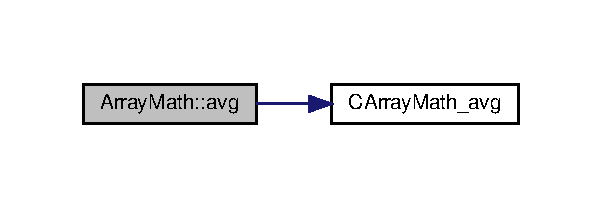
\includegraphics[width=289pt]{class_array_math_a1ecf90f00ed56f8b977f1ed5a3a6d7fa_cgraph}
\end{center}
\end{figure}
\mbox{\Hypertarget{class_array_math_af663455894b413a30e30c4c396e6ccaa}\label{class_array_math_af663455894b413a30e30c4c396e6ccaa}} 
\index{Array\+Math@{Array\+Math}!create@{create}}
\index{create@{create}!Array\+Math@{Array\+Math}}
\subsubsection{\texorpdfstring{create()}{create()}}
{\footnotesize\ttfamily static \hyperlink{class_array_math}{Array\+Math}$\ast$ Array\+Math\+::create (\begin{DoxyParamCaption}\item[{\hyperlink{class_double_array}{Double\+Array}}]{a }\end{DoxyParamCaption})\hspace{0.3cm}{\ttfamily [inline]}, {\ttfamily [static]}}



Definition at line 3049 of file chartdir.\+h.

\mbox{\Hypertarget{class_array_math_a63280677d4282215230467eadb0ff3ca}\label{class_array_math_a63280677d4282215230467eadb0ff3ca}} 
\index{Array\+Math@{Array\+Math}!delta@{delta}}
\index{delta@{delta}!Array\+Math@{Array\+Math}}
\subsubsection{\texorpdfstring{delta()}{delta()}}
{\footnotesize\ttfamily \hyperlink{class_array_math}{Array\+Math}\& Array\+Math\+::delta (\begin{DoxyParamCaption}\item[{int}]{offset = {\ttfamily 1} }\end{DoxyParamCaption})\hspace{0.3cm}{\ttfamily [inline]}}



Definition at line 3066 of file chartdir.\+h.

Here is the call graph for this function\+:
\nopagebreak
\begin{figure}[H]
\begin{center}
\leavevmode
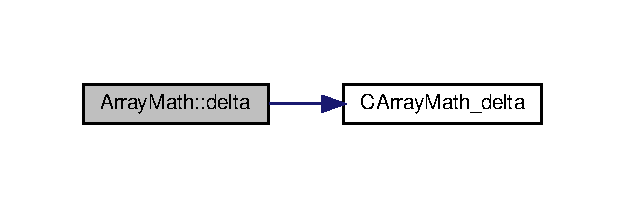
\includegraphics[width=300pt]{class_array_math_a63280677d4282215230467eadb0ff3ca_cgraph}
\end{center}
\end{figure}
Here is the caller graph for this function\+:
\nopagebreak
\begin{figure}[H]
\begin{center}
\leavevmode
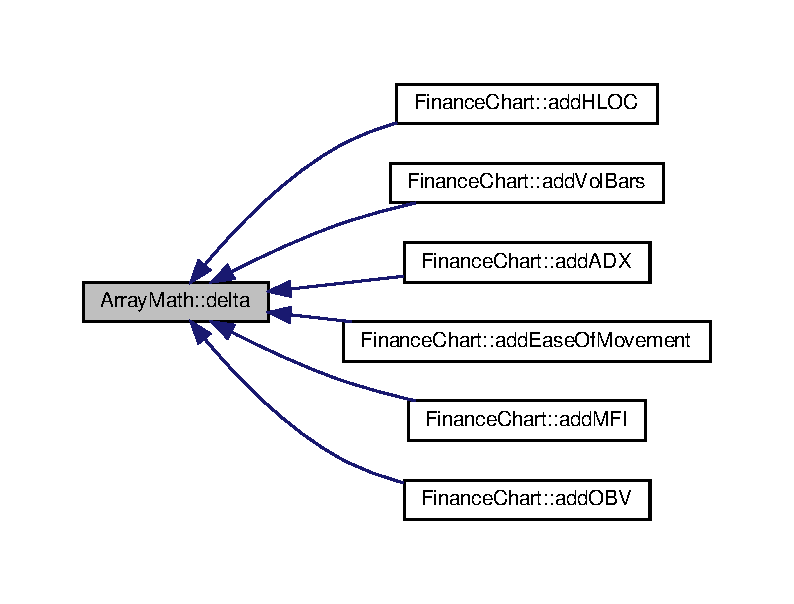
\includegraphics[width=350pt]{class_array_math_a63280677d4282215230467eadb0ff3ca_icgraph}
\end{center}
\end{figure}
\mbox{\Hypertarget{class_array_math_a5c0ea92917740188c95e4e410eef2661}\label{class_array_math_a5c0ea92917740188c95e4e410eef2661}} 
\index{Array\+Math@{Array\+Math}!destroy@{destroy}}
\index{destroy@{destroy}!Array\+Math@{Array\+Math}}
\subsubsection{\texorpdfstring{destroy()}{destroy()}}
{\footnotesize\ttfamily void Array\+Math\+::destroy (\begin{DoxyParamCaption}{ }\end{DoxyParamCaption})\hspace{0.3cm}{\ttfamily [inline]}}



Definition at line 3050 of file chartdir.\+h.

\mbox{\Hypertarget{class_array_math_a1f2298b0a0338ea48fc3163f6387d11c}\label{class_array_math_a1f2298b0a0338ea48fc3163f6387d11c}} 
\index{Array\+Math@{Array\+Math}!div@{div}}
\index{div@{div}!Array\+Math@{Array\+Math}}
\subsubsection{\texorpdfstring{div()}{div()}\hspace{0.1cm}{\footnotesize\ttfamily [1/2]}}
{\footnotesize\ttfamily \hyperlink{class_array_math}{Array\+Math}\& Array\+Math\+::div (\begin{DoxyParamCaption}\item[{\hyperlink{class_double_array}{Double\+Array}}]{b }\end{DoxyParamCaption})\hspace{0.3cm}{\ttfamily [inline]}}



Definition at line 3062 of file chartdir.\+h.

Here is the call graph for this function\+:
\nopagebreak
\begin{figure}[H]
\begin{center}
\leavevmode
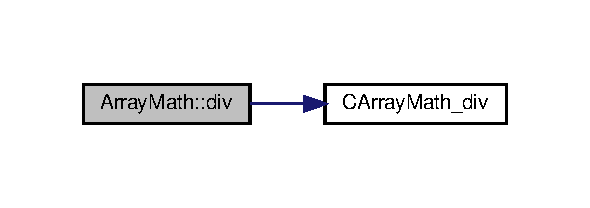
\includegraphics[width=283pt]{class_array_math_a1f2298b0a0338ea48fc3163f6387d11c_cgraph}
\end{center}
\end{figure}
Here is the caller graph for this function\+:
\nopagebreak
\begin{figure}[H]
\begin{center}
\leavevmode
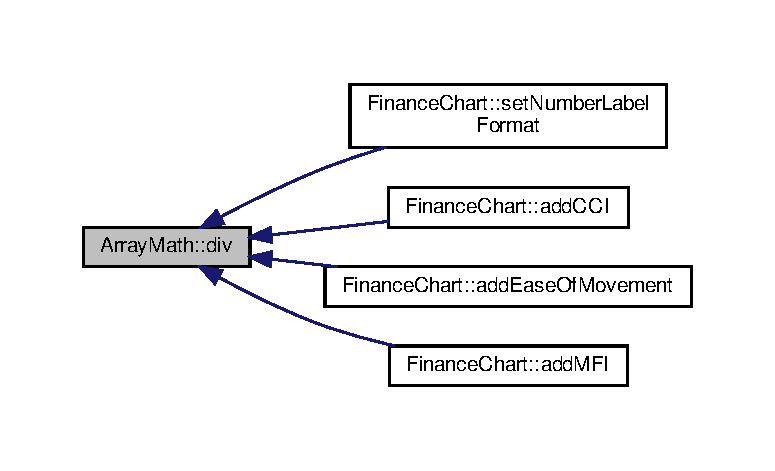
\includegraphics[width=350pt]{class_array_math_a1f2298b0a0338ea48fc3163f6387d11c_icgraph}
\end{center}
\end{figure}
\mbox{\Hypertarget{class_array_math_a8ba4c3f4ec4a35cc310d97e2a647ad4c}\label{class_array_math_a8ba4c3f4ec4a35cc310d97e2a647ad4c}} 
\index{Array\+Math@{Array\+Math}!div@{div}}
\index{div@{div}!Array\+Math@{Array\+Math}}
\subsubsection{\texorpdfstring{div()}{div()}\hspace{0.1cm}{\footnotesize\ttfamily [2/2]}}
{\footnotesize\ttfamily \hyperlink{class_array_math}{Array\+Math}\& Array\+Math\+::div (\begin{DoxyParamCaption}\item[{double}]{b }\end{DoxyParamCaption})\hspace{0.3cm}{\ttfamily [inline]}}



Definition at line 3063 of file chartdir.\+h.

Here is the call graph for this function\+:
\nopagebreak
\begin{figure}[H]
\begin{center}
\leavevmode
\includegraphics[width=288pt]{class_array_math_a8ba4c3f4ec4a35cc310d97e2a647ad4c_cgraph}
\end{center}
\end{figure}
\mbox{\Hypertarget{class_array_math_a2f9029cfd45e1094dd6aeb549bbcd107}\label{class_array_math_a2f9029cfd45e1094dd6aeb549bbcd107}} 
\index{Array\+Math@{Array\+Math}!exp\+Avg@{exp\+Avg}}
\index{exp\+Avg@{exp\+Avg}!Array\+Math@{Array\+Math}}
\subsubsection{\texorpdfstring{exp\+Avg()}{expAvg()}}
{\footnotesize\ttfamily \hyperlink{class_array_math}{Array\+Math}\& Array\+Math\+::exp\+Avg (\begin{DoxyParamCaption}\item[{double}]{smoothing\+Factor }\end{DoxyParamCaption})\hspace{0.3cm}{\ttfamily [inline]}}



Definition at line 3112 of file chartdir.\+h.

Here is the call graph for this function\+:
\nopagebreak
\begin{figure}[H]
\begin{center}
\leavevmode
\includegraphics[width=324pt]{class_array_math_a2f9029cfd45e1094dd6aeb549bbcd107_cgraph}
\end{center}
\end{figure}
Here is the caller graph for this function\+:
\nopagebreak
\begin{figure}[H]
\begin{center}
\leavevmode
\includegraphics[width=350pt]{class_array_math_a2f9029cfd45e1094dd6aeb549bbcd107_icgraph}
\end{center}
\end{figure}
\mbox{\Hypertarget{class_array_math_a854177572cefc64f20462ad56e74038e}\label{class_array_math_a854177572cefc64f20462ad56e74038e}} 
\index{Array\+Math@{Array\+Math}!finance\+Div@{finance\+Div}}
\index{finance\+Div@{finance\+Div}!Array\+Math@{Array\+Math}}
\subsubsection{\texorpdfstring{finance\+Div()}{financeDiv()}}
{\footnotesize\ttfamily \hyperlink{class_array_math}{Array\+Math}\& Array\+Math\+::finance\+Div (\begin{DoxyParamCaption}\item[{\hyperlink{class_double_array}{Double\+Array}}]{b,  }\item[{double}]{zero\+By\+Zero\+Value }\end{DoxyParamCaption})\hspace{0.3cm}{\ttfamily [inline]}}



Definition at line 3064 of file chartdir.\+h.

Here is the call graph for this function\+:
\nopagebreak
\begin{figure}[H]
\begin{center}
\leavevmode
\includegraphics[width=350pt]{class_array_math_a854177572cefc64f20462ad56e74038e_cgraph}
\end{center}
\end{figure}
Here is the caller graph for this function\+:
\nopagebreak
\begin{figure}[H]
\begin{center}
\leavevmode
\includegraphics[width=350pt]{class_array_math_a854177572cefc64f20462ad56e74038e_icgraph}
\end{center}
\end{figure}
\mbox{\Hypertarget{class_array_math_a36c129c503f3fe99e8a92ba265eae19e}\label{class_array_math_a36c129c503f3fe99e8a92ba265eae19e}} 
\index{Array\+Math@{Array\+Math}!insert@{insert}}
\index{insert@{insert}!Array\+Math@{Array\+Math}}
\subsubsection{\texorpdfstring{insert()}{insert()}\hspace{0.1cm}{\footnotesize\ttfamily [1/2]}}
{\footnotesize\ttfamily \hyperlink{class_array_math}{Array\+Math}\& Array\+Math\+::insert (\begin{DoxyParamCaption}\item[{\hyperlink{class_double_array}{Double\+Array}}]{a,  }\item[{int}]{insert\+Point = {\ttfamily -\/1} }\end{DoxyParamCaption})\hspace{0.3cm}{\ttfamily [inline]}}



Definition at line 3103 of file chartdir.\+h.

Here is the call graph for this function\+:
\nopagebreak
\begin{figure}[H]
\begin{center}
\leavevmode
\includegraphics[width=306pt]{class_array_math_a36c129c503f3fe99e8a92ba265eae19e_cgraph}
\end{center}
\end{figure}
\mbox{\Hypertarget{class_array_math_a2cebd29ee37fb8f24de84cbd14cd4b46}\label{class_array_math_a2cebd29ee37fb8f24de84cbd14cd4b46}} 
\index{Array\+Math@{Array\+Math}!insert@{insert}}
\index{insert@{insert}!Array\+Math@{Array\+Math}}
\subsubsection{\texorpdfstring{insert()}{insert()}\hspace{0.1cm}{\footnotesize\ttfamily [2/2]}}
{\footnotesize\ttfamily \hyperlink{class_array_math}{Array\+Math}\& Array\+Math\+::insert (\begin{DoxyParamCaption}\item[{double}]{c,  }\item[{int}]{len,  }\item[{int}]{insert\+Point = {\ttfamily -\/1} }\end{DoxyParamCaption})\hspace{0.3cm}{\ttfamily [inline]}}



Definition at line 3105 of file chartdir.\+h.

Here is the call graph for this function\+:
\nopagebreak
\begin{figure}[H]
\begin{center}
\leavevmode
\includegraphics[width=312pt]{class_array_math_a2cebd29ee37fb8f24de84cbd14cd4b46_cgraph}
\end{center}
\end{figure}
\mbox{\Hypertarget{class_array_math_afc9d22a0cf7267842d76430fd0dce639}\label{class_array_math_afc9d22a0cf7267842d76430fd0dce639}} 
\index{Array\+Math@{Array\+Math}!lowess@{lowess}}
\index{lowess@{lowess}!Array\+Math@{Array\+Math}}
\subsubsection{\texorpdfstring{lowess()}{lowess()}\hspace{0.1cm}{\footnotesize\ttfamily [1/2]}}
{\footnotesize\ttfamily \hyperlink{class_array_math}{Array\+Math}\& Array\+Math\+::lowess (\begin{DoxyParamCaption}\item[{double}]{smoothness = {\ttfamily 0.25},  }\item[{int}]{iteration = {\ttfamily 0} }\end{DoxyParamCaption})\hspace{0.3cm}{\ttfamily [inline]}}



Definition at line 3126 of file chartdir.\+h.

Here is the call graph for this function\+:
\nopagebreak
\begin{figure}[H]
\begin{center}
\leavevmode
\includegraphics[width=319pt]{class_array_math_afc9d22a0cf7267842d76430fd0dce639_cgraph}
\end{center}
\end{figure}
\mbox{\Hypertarget{class_array_math_a7852fe7a310511ac1ba8fa585a614146}\label{class_array_math_a7852fe7a310511ac1ba8fa585a614146}} 
\index{Array\+Math@{Array\+Math}!lowess@{lowess}}
\index{lowess@{lowess}!Array\+Math@{Array\+Math}}
\subsubsection{\texorpdfstring{lowess()}{lowess()}\hspace{0.1cm}{\footnotesize\ttfamily [2/2]}}
{\footnotesize\ttfamily \hyperlink{class_array_math}{Array\+Math}\& Array\+Math\+::lowess (\begin{DoxyParamCaption}\item[{\hyperlink{class_double_array}{Double\+Array}}]{b,  }\item[{double}]{smoothness = {\ttfamily 0.25},  }\item[{int}]{iteration = {\ttfamily 0} }\end{DoxyParamCaption})\hspace{0.3cm}{\ttfamily [inline]}}



Definition at line 3128 of file chartdir.\+h.

Here is the call graph for this function\+:
\nopagebreak
\begin{figure}[H]
\begin{center}
\leavevmode
\includegraphics[width=324pt]{class_array_math_a7852fe7a310511ac1ba8fa585a614146_cgraph}
\end{center}
\end{figure}
\mbox{\Hypertarget{class_array_math_ae80c440e5ad866929649746c029cf0bf}\label{class_array_math_ae80c440e5ad866929649746c029cf0bf}} 
\index{Array\+Math@{Array\+Math}!max@{max}}
\index{max@{max}!Array\+Math@{Array\+Math}}
\subsubsection{\texorpdfstring{max()}{max()}}
{\footnotesize\ttfamily double Array\+Math\+::max (\begin{DoxyParamCaption}{ }\end{DoxyParamCaption}) const\hspace{0.3cm}{\ttfamily [inline]}}



Definition at line 3133 of file chartdir.\+h.

Here is the call graph for this function\+:
\nopagebreak
\begin{figure}[H]
\begin{center}
\leavevmode
\includegraphics[width=295pt]{class_array_math_ae80c440e5ad866929649746c029cf0bf_cgraph}
\end{center}
\end{figure}
\mbox{\Hypertarget{class_array_math_af75557e958d76b32d93a6a90fa6d064c}\label{class_array_math_af75557e958d76b32d93a6a90fa6d064c}} 
\index{Array\+Math@{Array\+Math}!max\+Index@{max\+Index}}
\index{max\+Index@{max\+Index}!Array\+Math@{Array\+Math}}
\subsubsection{\texorpdfstring{max\+Index()}{maxIndex()}}
{\footnotesize\ttfamily int Array\+Math\+::max\+Index (\begin{DoxyParamCaption}{ }\end{DoxyParamCaption}) const\hspace{0.3cm}{\ttfamily [inline]}}



Definition at line 3145 of file chartdir.\+h.

Here is the call graph for this function\+:
\nopagebreak
\begin{figure}[H]
\begin{center}
\leavevmode
\includegraphics[width=343pt]{class_array_math_af75557e958d76b32d93a6a90fa6d064c_cgraph}
\end{center}
\end{figure}
\mbox{\Hypertarget{class_array_math_ab2f502a58518cfe68bcdaa31729d4a96}\label{class_array_math_ab2f502a58518cfe68bcdaa31729d4a96}} 
\index{Array\+Math@{Array\+Math}!max\+Value@{max\+Value}}
\index{max\+Value@{max\+Value}!Array\+Math@{Array\+Math}}
\subsubsection{\texorpdfstring{max\+Value()}{maxValue()}}
{\footnotesize\ttfamily double Array\+Math\+::max\+Value (\begin{DoxyParamCaption}{ }\end{DoxyParamCaption}) const\hspace{0.3cm}{\ttfamily [inline]}}



Definition at line 3135 of file chartdir.\+h.

Here is the call graph for this function\+:
\nopagebreak
\begin{figure}[H]
\begin{center}
\leavevmode
\includegraphics[width=320pt]{class_array_math_ab2f502a58518cfe68bcdaa31729d4a96_cgraph}
\end{center}
\end{figure}
Here is the caller graph for this function\+:
\nopagebreak
\begin{figure}[H]
\begin{center}
\leavevmode
\includegraphics[width=343pt]{class_array_math_ab2f502a58518cfe68bcdaa31729d4a96_icgraph}
\end{center}
\end{figure}
\mbox{\Hypertarget{class_array_math_aa60ced676c9387a970df6468379d1f56}\label{class_array_math_aa60ced676c9387a970df6468379d1f56}} 
\index{Array\+Math@{Array\+Math}!med@{med}}
\index{med@{med}!Array\+Math@{Array\+Math}}
\subsubsection{\texorpdfstring{med()}{med()}}
{\footnotesize\ttfamily double Array\+Math\+::med (\begin{DoxyParamCaption}{ }\end{DoxyParamCaption}) const\hspace{0.3cm}{\ttfamily [inline]}}



Definition at line 3143 of file chartdir.\+h.

Here is the call graph for this function\+:
\nopagebreak
\begin{figure}[H]
\begin{center}
\leavevmode
\includegraphics[width=295pt]{class_array_math_aa60ced676c9387a970df6468379d1f56_cgraph}
\end{center}
\end{figure}
\mbox{\Hypertarget{class_array_math_a4ef0f497cafb78d37d4af0a6bd51d411}\label{class_array_math_a4ef0f497cafb78d37d4af0a6bd51d411}} 
\index{Array\+Math@{Array\+Math}!min@{min}}
\index{min@{min}!Array\+Math@{Array\+Math}}
\subsubsection{\texorpdfstring{min()}{min()}}
{\footnotesize\ttfamily double Array\+Math\+::min (\begin{DoxyParamCaption}{ }\end{DoxyParamCaption}) const\hspace{0.3cm}{\ttfamily [inline]}}



Definition at line 3137 of file chartdir.\+h.

Here is the call graph for this function\+:
\nopagebreak
\begin{figure}[H]
\begin{center}
\leavevmode
\includegraphics[width=289pt]{class_array_math_a4ef0f497cafb78d37d4af0a6bd51d411_cgraph}
\end{center}
\end{figure}
\mbox{\Hypertarget{class_array_math_a0cf1a69edacfb547184b06e6c71693e6}\label{class_array_math_a0cf1a69edacfb547184b06e6c71693e6}} 
\index{Array\+Math@{Array\+Math}!min\+Index@{min\+Index}}
\index{min\+Index@{min\+Index}!Array\+Math@{Array\+Math}}
\subsubsection{\texorpdfstring{min\+Index()}{minIndex()}}
{\footnotesize\ttfamily int Array\+Math\+::min\+Index (\begin{DoxyParamCaption}{ }\end{DoxyParamCaption}) const\hspace{0.3cm}{\ttfamily [inline]}}



Definition at line 3146 of file chartdir.\+h.

Here is the call graph for this function\+:
\nopagebreak
\begin{figure}[H]
\begin{center}
\leavevmode
\includegraphics[width=337pt]{class_array_math_a0cf1a69edacfb547184b06e6c71693e6_cgraph}
\end{center}
\end{figure}
\mbox{\Hypertarget{class_array_math_aff26b5d31ec9ec6f7e113a6425ca4e13}\label{class_array_math_aff26b5d31ec9ec6f7e113a6425ca4e13}} 
\index{Array\+Math@{Array\+Math}!min\+Value@{min\+Value}}
\index{min\+Value@{min\+Value}!Array\+Math@{Array\+Math}}
\subsubsection{\texorpdfstring{min\+Value()}{minValue()}}
{\footnotesize\ttfamily double Array\+Math\+::min\+Value (\begin{DoxyParamCaption}{ }\end{DoxyParamCaption}) const\hspace{0.3cm}{\ttfamily [inline]}}



Definition at line 3139 of file chartdir.\+h.

Here is the call graph for this function\+:
\nopagebreak
\begin{figure}[H]
\begin{center}
\leavevmode
\includegraphics[width=314pt]{class_array_math_aff26b5d31ec9ec6f7e113a6425ca4e13_cgraph}
\end{center}
\end{figure}
\mbox{\Hypertarget{class_array_math_abaaac1009dda4a6124ecd2182354dc39}\label{class_array_math_abaaac1009dda4a6124ecd2182354dc39}} 
\index{Array\+Math@{Array\+Math}!mov\+Avg@{mov\+Avg}}
\index{mov\+Avg@{mov\+Avg}!Array\+Math@{Array\+Math}}
\subsubsection{\texorpdfstring{mov\+Avg()}{movAvg()}}
{\footnotesize\ttfamily \hyperlink{class_array_math}{Array\+Math}\& Array\+Math\+::mov\+Avg (\begin{DoxyParamCaption}\item[{int}]{interval }\end{DoxyParamCaption})\hspace{0.3cm}{\ttfamily [inline]}}



Definition at line 3110 of file chartdir.\+h.

Here is the call graph for this function\+:
\nopagebreak
\begin{figure}[H]
\begin{center}
\leavevmode
\includegraphics[width=330pt]{class_array_math_abaaac1009dda4a6124ecd2182354dc39_cgraph}
\end{center}
\end{figure}
Here is the caller graph for this function\+:
\nopagebreak
\begin{figure}[H]
\begin{center}
\leavevmode
\includegraphics[width=350pt]{class_array_math_abaaac1009dda4a6124ecd2182354dc39_icgraph}
\end{center}
\end{figure}
\mbox{\Hypertarget{class_array_math_a61cdecb4beb7c276a122306906cdebd8}\label{class_array_math_a61cdecb4beb7c276a122306906cdebd8}} 
\index{Array\+Math@{Array\+Math}!mov\+Corr@{mov\+Corr}}
\index{mov\+Corr@{mov\+Corr}!Array\+Math@{Array\+Math}}
\subsubsection{\texorpdfstring{mov\+Corr()}{movCorr()}}
{\footnotesize\ttfamily \hyperlink{class_array_math}{Array\+Math}\& Array\+Math\+::mov\+Corr (\begin{DoxyParamCaption}\item[{int}]{interval,  }\item[{\hyperlink{class_double_array}{Double\+Array}}]{b = {\ttfamily \hyperlink{class_double_array}{Double\+Array}()} }\end{DoxyParamCaption})\hspace{0.3cm}{\ttfamily [inline]}}



Definition at line 3124 of file chartdir.\+h.

Here is the call graph for this function\+:
\nopagebreak
\begin{figure}[H]
\begin{center}
\leavevmode
\includegraphics[width=333pt]{class_array_math_a61cdecb4beb7c276a122306906cdebd8_cgraph}
\end{center}
\end{figure}
\mbox{\Hypertarget{class_array_math_a5134853d9b14c3d980036a02a4d4b043}\label{class_array_math_a5134853d9b14c3d980036a02a4d4b043}} 
\index{Array\+Math@{Array\+Math}!mov\+Max@{mov\+Max}}
\index{mov\+Max@{mov\+Max}!Array\+Math@{Array\+Math}}
\subsubsection{\texorpdfstring{mov\+Max()}{movMax()}}
{\footnotesize\ttfamily \hyperlink{class_array_math}{Array\+Math}\& Array\+Math\+::mov\+Max (\begin{DoxyParamCaption}\item[{int}]{interval }\end{DoxyParamCaption})\hspace{0.3cm}{\ttfamily [inline]}}



Definition at line 3118 of file chartdir.\+h.

Here is the call graph for this function\+:
\nopagebreak
\begin{figure}[H]
\begin{center}
\leavevmode
\includegraphics[width=333pt]{class_array_math_a5134853d9b14c3d980036a02a4d4b043_cgraph}
\end{center}
\end{figure}
Here is the caller graph for this function\+:
\nopagebreak
\begin{figure}[H]
\begin{center}
\leavevmode
\includegraphics[width=350pt]{class_array_math_a5134853d9b14c3d980036a02a4d4b043_icgraph}
\end{center}
\end{figure}
\mbox{\Hypertarget{class_array_math_a7f994291fd85c2859e7bf34c27b8013e}\label{class_array_math_a7f994291fd85c2859e7bf34c27b8013e}} 
\index{Array\+Math@{Array\+Math}!mov\+Med@{mov\+Med}}
\index{mov\+Med@{mov\+Med}!Array\+Math@{Array\+Math}}
\subsubsection{\texorpdfstring{mov\+Med()}{movMed()}}
{\footnotesize\ttfamily \hyperlink{class_array_math}{Array\+Math}\& Array\+Math\+::mov\+Med (\begin{DoxyParamCaption}\item[{int}]{interval }\end{DoxyParamCaption})\hspace{0.3cm}{\ttfamily [inline]}}



Definition at line 3114 of file chartdir.\+h.

Here is the call graph for this function\+:
\nopagebreak
\begin{figure}[H]
\begin{center}
\leavevmode
\includegraphics[width=333pt]{class_array_math_a7f994291fd85c2859e7bf34c27b8013e_cgraph}
\end{center}
\end{figure}
\mbox{\Hypertarget{class_array_math_a42df280f64eaaad8150985d962516276}\label{class_array_math_a42df280f64eaaad8150985d962516276}} 
\index{Array\+Math@{Array\+Math}!mov\+Min@{mov\+Min}}
\index{mov\+Min@{mov\+Min}!Array\+Math@{Array\+Math}}
\subsubsection{\texorpdfstring{mov\+Min()}{movMin()}}
{\footnotesize\ttfamily \hyperlink{class_array_math}{Array\+Math}\& Array\+Math\+::mov\+Min (\begin{DoxyParamCaption}\item[{int}]{interval }\end{DoxyParamCaption})\hspace{0.3cm}{\ttfamily [inline]}}



Definition at line 3120 of file chartdir.\+h.

Here is the call graph for this function\+:
\nopagebreak
\begin{figure}[H]
\begin{center}
\leavevmode
\includegraphics[width=327pt]{class_array_math_a42df280f64eaaad8150985d962516276_cgraph}
\end{center}
\end{figure}
Here is the caller graph for this function\+:
\nopagebreak
\begin{figure}[H]
\begin{center}
\leavevmode
\includegraphics[width=350pt]{class_array_math_a42df280f64eaaad8150985d962516276_icgraph}
\end{center}
\end{figure}
\mbox{\Hypertarget{class_array_math_adc007aad3ce9cac15f02159190c2c84a}\label{class_array_math_adc007aad3ce9cac15f02159190c2c84a}} 
\index{Array\+Math@{Array\+Math}!mov\+Percentile@{mov\+Percentile}}
\index{mov\+Percentile@{mov\+Percentile}!Array\+Math@{Array\+Math}}
\subsubsection{\texorpdfstring{mov\+Percentile()}{movPercentile()}}
{\footnotesize\ttfamily \hyperlink{class_array_math}{Array\+Math}\& Array\+Math\+::mov\+Percentile (\begin{DoxyParamCaption}\item[{int}]{interval,  }\item[{double}]{\+\_\+percentile }\end{DoxyParamCaption})\hspace{0.3cm}{\ttfamily [inline]}}



Definition at line 3116 of file chartdir.\+h.

Here is the call graph for this function\+:
\nopagebreak
\begin{figure}[H]
\begin{center}
\leavevmode
\includegraphics[width=350pt]{class_array_math_adc007aad3ce9cac15f02159190c2c84a_cgraph}
\end{center}
\end{figure}
\mbox{\Hypertarget{class_array_math_a0352f506e872e964ef2590fa7e8ce581}\label{class_array_math_a0352f506e872e964ef2590fa7e8ce581}} 
\index{Array\+Math@{Array\+Math}!mov\+Std\+Dev@{mov\+Std\+Dev}}
\index{mov\+Std\+Dev@{mov\+Std\+Dev}!Array\+Math@{Array\+Math}}
\subsubsection{\texorpdfstring{mov\+Std\+Dev()}{movStdDev()}}
{\footnotesize\ttfamily \hyperlink{class_array_math}{Array\+Math}\& Array\+Math\+::mov\+Std\+Dev (\begin{DoxyParamCaption}\item[{int}]{interval }\end{DoxyParamCaption})\hspace{0.3cm}{\ttfamily [inline]}}



Definition at line 3122 of file chartdir.\+h.

Here is the call graph for this function\+:
\nopagebreak
\begin{figure}[H]
\begin{center}
\leavevmode
\includegraphics[width=350pt]{class_array_math_a0352f506e872e964ef2590fa7e8ce581_cgraph}
\end{center}
\end{figure}
Here is the caller graph for this function\+:
\nopagebreak
\begin{figure}[H]
\begin{center}
\leavevmode
\includegraphics[width=350pt]{class_array_math_a0352f506e872e964ef2590fa7e8ce581_icgraph}
\end{center}
\end{figure}
\mbox{\Hypertarget{class_array_math_a4fb34b6f319e7f3b2a5440d426832889}\label{class_array_math_a4fb34b6f319e7f3b2a5440d426832889}} 
\index{Array\+Math@{Array\+Math}!mul@{mul}}
\index{mul@{mul}!Array\+Math@{Array\+Math}}
\subsubsection{\texorpdfstring{mul()}{mul()}\hspace{0.1cm}{\footnotesize\ttfamily [1/2]}}
{\footnotesize\ttfamily \hyperlink{class_array_math}{Array\+Math}\& Array\+Math\+::mul (\begin{DoxyParamCaption}\item[{\hyperlink{class_double_array}{Double\+Array}}]{b }\end{DoxyParamCaption})\hspace{0.3cm}{\ttfamily [inline]}}



Definition at line 3060 of file chartdir.\+h.

Here is the call graph for this function\+:
\nopagebreak
\begin{figure}[H]
\begin{center}
\leavevmode
\includegraphics[width=289pt]{class_array_math_a4fb34b6f319e7f3b2a5440d426832889_cgraph}
\end{center}
\end{figure}
Here is the caller graph for this function\+:
\nopagebreak
\begin{figure}[H]
\begin{center}
\leavevmode
\includegraphics[width=350pt]{class_array_math_a4fb34b6f319e7f3b2a5440d426832889_icgraph}
\end{center}
\end{figure}
\mbox{\Hypertarget{class_array_math_ad44c0c320ef2f9401be5e54d51dc6c73}\label{class_array_math_ad44c0c320ef2f9401be5e54d51dc6c73}} 
\index{Array\+Math@{Array\+Math}!mul@{mul}}
\index{mul@{mul}!Array\+Math@{Array\+Math}}
\subsubsection{\texorpdfstring{mul()}{mul()}\hspace{0.1cm}{\footnotesize\ttfamily [2/2]}}
{\footnotesize\ttfamily \hyperlink{class_array_math}{Array\+Math}\& Array\+Math\+::mul (\begin{DoxyParamCaption}\item[{double}]{b }\end{DoxyParamCaption})\hspace{0.3cm}{\ttfamily [inline]}}



Definition at line 3061 of file chartdir.\+h.

Here is the call graph for this function\+:
\nopagebreak
\begin{figure}[H]
\begin{center}
\leavevmode
\includegraphics[width=294pt]{class_array_math_ad44c0c320ef2f9401be5e54d51dc6c73_cgraph}
\end{center}
\end{figure}
\mbox{\Hypertarget{class_array_math_a1b309d87396b6971a40a71ea333b628d}\label{class_array_math_a1b309d87396b6971a40a71ea333b628d}} 
\index{Array\+Math@{Array\+Math}!operator Double\+Array@{operator Double\+Array}}
\index{operator Double\+Array@{operator Double\+Array}!Array\+Math@{Array\+Math}}
\subsubsection{\texorpdfstring{operator Double\+Array()}{operator DoubleArray()}}
{\footnotesize\ttfamily Array\+Math\+::operator \hyperlink{class_double_array}{Double\+Array} (\begin{DoxyParamCaption}{ }\end{DoxyParamCaption}) const\hspace{0.3cm}{\ttfamily [inline]}}



Definition at line 3054 of file chartdir.\+h.

\mbox{\Hypertarget{class_array_math_aefa81728a4b712db88e3e4453bf384ad}\label{class_array_math_aefa81728a4b712db88e3e4453bf384ad}} 
\index{Array\+Math@{Array\+Math}!operator=@{operator=}}
\index{operator=@{operator=}!Array\+Math@{Array\+Math}}
\subsubsection{\texorpdfstring{operator=()}{operator=()}}
{\footnotesize\ttfamily \hyperlink{class_array_math}{Array\+Math}\& Array\+Math\+::operator= (\begin{DoxyParamCaption}\item[{const \hyperlink{class_array_math}{Array\+Math} \&}]{rhs }\end{DoxyParamCaption})\hspace{0.3cm}{\ttfamily [inline]}}



Definition at line 3053 of file chartdir.\+h.

Here is the call graph for this function\+:
\nopagebreak
\begin{figure}[H]
\begin{center}
\leavevmode
\includegraphics[width=332pt]{class_array_math_aefa81728a4b712db88e3e4453bf384ad_cgraph}
\end{center}
\end{figure}
\mbox{\Hypertarget{class_array_math_ae0342b531a9f73cabc2b13f81e2cef88}\label{class_array_math_ae0342b531a9f73cabc2b13f81e2cef88}} 
\index{Array\+Math@{Array\+Math}!percentile@{percentile}}
\index{percentile@{percentile}!Array\+Math@{Array\+Math}}
\subsubsection{\texorpdfstring{percentile()}{percentile()}}
{\footnotesize\ttfamily double Array\+Math\+::percentile (\begin{DoxyParamCaption}\item[{double}]{p }\end{DoxyParamCaption}) const\hspace{0.3cm}{\ttfamily [inline]}}



Definition at line 3144 of file chartdir.\+h.

Here is the call graph for this function\+:
\nopagebreak
\begin{figure}[H]
\begin{center}
\leavevmode
\includegraphics[width=342pt]{class_array_math_ae0342b531a9f73cabc2b13f81e2cef88_cgraph}
\end{center}
\end{figure}
\mbox{\Hypertarget{class_array_math_a72a5a6a662b011b093a0aed0aac5df76}\label{class_array_math_a72a5a6a662b011b093a0aed0aac5df76}} 
\index{Array\+Math@{Array\+Math}!rate@{rate}}
\index{rate@{rate}!Array\+Math@{Array\+Math}}
\subsubsection{\texorpdfstring{rate()}{rate()}}
{\footnotesize\ttfamily \hyperlink{class_array_math}{Array\+Math}\& Array\+Math\+::rate (\begin{DoxyParamCaption}\item[{int}]{offset = {\ttfamily 1} }\end{DoxyParamCaption})\hspace{0.3cm}{\ttfamily [inline]}}



Definition at line 3067 of file chartdir.\+h.

Here is the call graph for this function\+:
\nopagebreak
\begin{figure}[H]
\begin{center}
\leavevmode
\includegraphics[width=291pt]{class_array_math_a72a5a6a662b011b093a0aed0aac5df76_cgraph}
\end{center}
\end{figure}
\mbox{\Hypertarget{class_array_math_a3e735bfc88ee0149c7056cac1defbf6c}\label{class_array_math_a3e735bfc88ee0149c7056cac1defbf6c}} 
\index{Array\+Math@{Array\+Math}!replace@{replace}}
\index{replace@{replace}!Array\+Math@{Array\+Math}}
\subsubsection{\texorpdfstring{replace()}{replace()}}
{\footnotesize\ttfamily \hyperlink{class_array_math}{Array\+Math}\& Array\+Math\+::replace (\begin{DoxyParamCaption}\item[{double}]{a,  }\item[{double}]{b }\end{DoxyParamCaption})\hspace{0.3cm}{\ttfamily [inline]}}



Definition at line 3107 of file chartdir.\+h.

Here is the call graph for this function\+:
\nopagebreak
\begin{figure}[H]
\begin{center}
\leavevmode
\includegraphics[width=321pt]{class_array_math_a3e735bfc88ee0149c7056cac1defbf6c_cgraph}
\end{center}
\end{figure}
Here is the caller graph for this function\+:
\nopagebreak
\begin{figure}[H]
\begin{center}
\leavevmode
\includegraphics[width=346pt]{class_array_math_a3e735bfc88ee0149c7056cac1defbf6c_icgraph}
\end{center}
\end{figure}
\mbox{\Hypertarget{class_array_math_a2c81268f37eb5e4ab9c1c8e18bb22fa3}\label{class_array_math_a2c81268f37eb5e4ab9c1c8e18bb22fa3}} 
\index{Array\+Math@{Array\+Math}!result@{result}}
\index{result@{result}!Array\+Math@{Array\+Math}}
\subsubsection{\texorpdfstring{result()}{result()}}
{\footnotesize\ttfamily \hyperlink{class_double_array}{Double\+Array} Array\+Math\+::result (\begin{DoxyParamCaption}{ }\end{DoxyParamCaption}) const\hspace{0.3cm}{\ttfamily [inline]}}



Definition at line 3131 of file chartdir.\+h.

Here is the call graph for this function\+:
\nopagebreak
\begin{figure}[H]
\begin{center}
\leavevmode
\includegraphics[width=306pt]{class_array_math_a2c81268f37eb5e4ab9c1c8e18bb22fa3_cgraph}
\end{center}
\end{figure}
Here is the caller graph for this function\+:
\nopagebreak
\begin{figure}[H]
\begin{center}
\leavevmode
\includegraphics[width=348pt]{class_array_math_a2c81268f37eb5e4ab9c1c8e18bb22fa3_icgraph}
\end{center}
\end{figure}
\mbox{\Hypertarget{class_array_math_a7c219ae5049b2a515025f24ae5428a83}\label{class_array_math_a7c219ae5049b2a515025f24ae5428a83}} 
\index{Array\+Math@{Array\+Math}!select\+E\+QZ@{select\+E\+QZ}}
\index{select\+E\+QZ@{select\+E\+QZ}!Array\+Math@{Array\+Math}}
\subsubsection{\texorpdfstring{select\+E\+Q\+Z()}{selectEQZ()}}
{\footnotesize\ttfamily \hyperlink{class_array_math}{Array\+Math}\& Array\+Math\+::select\+E\+QZ (\begin{DoxyParamCaption}\item[{\hyperlink{class_double_array}{Double\+Array}}]{decision\+Array = {\ttfamily \hyperlink{class_double_array}{Double\+Array}()},  }\item[{double}]{fill\+Value = {\ttfamily 0} }\end{DoxyParamCaption})\hspace{0.3cm}{\ttfamily [inline]}}



Definition at line 3079 of file chartdir.\+h.

Here is the call graph for this function\+:
\nopagebreak
\begin{figure}[H]
\begin{center}
\leavevmode
\includegraphics[width=350pt]{class_array_math_a7c219ae5049b2a515025f24ae5428a83_cgraph}
\end{center}
\end{figure}
\mbox{\Hypertarget{class_array_math_adeaae3c00b4d38c471d5956d65861a48}\label{class_array_math_adeaae3c00b4d38c471d5956d65861a48}} 
\index{Array\+Math@{Array\+Math}!select\+G\+EZ@{select\+G\+EZ}}
\index{select\+G\+EZ@{select\+G\+EZ}!Array\+Math@{Array\+Math}}
\subsubsection{\texorpdfstring{select\+G\+E\+Z()}{selectGEZ()}}
{\footnotesize\ttfamily \hyperlink{class_array_math}{Array\+Math}\& Array\+Math\+::select\+G\+EZ (\begin{DoxyParamCaption}\item[{\hyperlink{class_double_array}{Double\+Array}}]{decision\+Array = {\ttfamily \hyperlink{class_double_array}{Double\+Array}()},  }\item[{double}]{fill\+Value = {\ttfamily 0} }\end{DoxyParamCaption})\hspace{0.3cm}{\ttfamily [inline]}}



Definition at line 3073 of file chartdir.\+h.

Here is the call graph for this function\+:
\nopagebreak
\begin{figure}[H]
\begin{center}
\leavevmode
\includegraphics[width=350pt]{class_array_math_adeaae3c00b4d38c471d5956d65861a48_cgraph}
\end{center}
\end{figure}
\mbox{\Hypertarget{class_array_math_aadfd40e8527d58dc41cceec240d1f9b8}\label{class_array_math_aadfd40e8527d58dc41cceec240d1f9b8}} 
\index{Array\+Math@{Array\+Math}!select\+G\+TZ@{select\+G\+TZ}}
\index{select\+G\+TZ@{select\+G\+TZ}!Array\+Math@{Array\+Math}}
\subsubsection{\texorpdfstring{select\+G\+T\+Z()}{selectGTZ()}}
{\footnotesize\ttfamily \hyperlink{class_array_math}{Array\+Math}\& Array\+Math\+::select\+G\+TZ (\begin{DoxyParamCaption}\item[{\hyperlink{class_double_array}{Double\+Array}}]{decision\+Array = {\ttfamily \hyperlink{class_double_array}{Double\+Array}()},  }\item[{double}]{fill\+Value = {\ttfamily 0} }\end{DoxyParamCaption})\hspace{0.3cm}{\ttfamily [inline]}}



Definition at line 3071 of file chartdir.\+h.

Here is the call graph for this function\+:
\nopagebreak
\begin{figure}[H]
\begin{center}
\leavevmode
\includegraphics[width=349pt]{class_array_math_aadfd40e8527d58dc41cceec240d1f9b8_cgraph}
\end{center}
\end{figure}
Here is the caller graph for this function\+:
\nopagebreak
\begin{figure}[H]
\begin{center}
\leavevmode
\includegraphics[width=347pt]{class_array_math_aadfd40e8527d58dc41cceec240d1f9b8_icgraph}
\end{center}
\end{figure}
\mbox{\Hypertarget{class_array_math_a63ec8c97034104b0ede0227683583eac}\label{class_array_math_a63ec8c97034104b0ede0227683583eac}} 
\index{Array\+Math@{Array\+Math}!select\+L\+EZ@{select\+L\+EZ}}
\index{select\+L\+EZ@{select\+L\+EZ}!Array\+Math@{Array\+Math}}
\subsubsection{\texorpdfstring{select\+L\+E\+Z()}{selectLEZ()}}
{\footnotesize\ttfamily \hyperlink{class_array_math}{Array\+Math}\& Array\+Math\+::select\+L\+EZ (\begin{DoxyParamCaption}\item[{\hyperlink{class_double_array}{Double\+Array}}]{decision\+Array = {\ttfamily \hyperlink{class_double_array}{Double\+Array}()},  }\item[{double}]{fill\+Value = {\ttfamily 0} }\end{DoxyParamCaption})\hspace{0.3cm}{\ttfamily [inline]}}



Definition at line 3077 of file chartdir.\+h.

Here is the call graph for this function\+:
\nopagebreak
\begin{figure}[H]
\begin{center}
\leavevmode
\includegraphics[width=347pt]{class_array_math_a63ec8c97034104b0ede0227683583eac_cgraph}
\end{center}
\end{figure}
\mbox{\Hypertarget{class_array_math_ae10389934cacf3913e69b71c79fe5ae9}\label{class_array_math_ae10389934cacf3913e69b71c79fe5ae9}} 
\index{Array\+Math@{Array\+Math}!select\+L\+TZ@{select\+L\+TZ}}
\index{select\+L\+TZ@{select\+L\+TZ}!Array\+Math@{Array\+Math}}
\subsubsection{\texorpdfstring{select\+L\+T\+Z()}{selectLTZ()}}
{\footnotesize\ttfamily \hyperlink{class_array_math}{Array\+Math}\& Array\+Math\+::select\+L\+TZ (\begin{DoxyParamCaption}\item[{\hyperlink{class_double_array}{Double\+Array}}]{decision\+Array = {\ttfamily \hyperlink{class_double_array}{Double\+Array}()},  }\item[{double}]{fill\+Value = {\ttfamily 0} }\end{DoxyParamCaption})\hspace{0.3cm}{\ttfamily [inline]}}



Definition at line 3075 of file chartdir.\+h.

Here is the call graph for this function\+:
\nopagebreak
\begin{figure}[H]
\begin{center}
\leavevmode
\includegraphics[width=345pt]{class_array_math_ae10389934cacf3913e69b71c79fe5ae9_cgraph}
\end{center}
\end{figure}
Here is the caller graph for this function\+:
\nopagebreak
\begin{figure}[H]
\begin{center}
\leavevmode
\includegraphics[width=345pt]{class_array_math_ae10389934cacf3913e69b71c79fe5ae9_icgraph}
\end{center}
\end{figure}
\mbox{\Hypertarget{class_array_math_a0ec9ff9be8d0f829ba79bd1a53a791a5}\label{class_array_math_a0ec9ff9be8d0f829ba79bd1a53a791a5}} 
\index{Array\+Math@{Array\+Math}!select\+N\+EZ@{select\+N\+EZ}}
\index{select\+N\+EZ@{select\+N\+EZ}!Array\+Math@{Array\+Math}}
\subsubsection{\texorpdfstring{select\+N\+E\+Z()}{selectNEZ()}}
{\footnotesize\ttfamily \hyperlink{class_array_math}{Array\+Math}\& Array\+Math\+::select\+N\+EZ (\begin{DoxyParamCaption}\item[{\hyperlink{class_double_array}{Double\+Array}}]{decision\+Array = {\ttfamily \hyperlink{class_double_array}{Double\+Array}()},  }\item[{double}]{fill\+Value = {\ttfamily 0} }\end{DoxyParamCaption})\hspace{0.3cm}{\ttfamily [inline]}}



Definition at line 3081 of file chartdir.\+h.

Here is the call graph for this function\+:
\nopagebreak
\begin{figure}[H]
\begin{center}
\leavevmode
\includegraphics[width=350pt]{class_array_math_a0ec9ff9be8d0f829ba79bd1a53a791a5_cgraph}
\end{center}
\end{figure}
\mbox{\Hypertarget{class_array_math_a7fa60f8da0b8448ec591ce7f4b95f251}\label{class_array_math_a7fa60f8da0b8448ec591ce7f4b95f251}} 
\index{Array\+Math@{Array\+Math}!select\+Regular\+Spacing@{select\+Regular\+Spacing}}
\index{select\+Regular\+Spacing@{select\+Regular\+Spacing}!Array\+Math@{Array\+Math}}
\subsubsection{\texorpdfstring{select\+Regular\+Spacing()}{selectRegularSpacing()}}
{\footnotesize\ttfamily \hyperlink{class_array_math}{Array\+Math}\& Array\+Math\+::select\+Regular\+Spacing (\begin{DoxyParamCaption}\item[{int}]{major\+Tick\+Step,  }\item[{int}]{minor\+Tick\+Step = {\ttfamily 0},  }\item[{int}]{initial\+Margin = {\ttfamily 0} }\end{DoxyParamCaption})\hspace{0.3cm}{\ttfamily [inline]}}



Definition at line 3098 of file chartdir.\+h.

Here is the call graph for this function\+:
\nopagebreak
\begin{figure}[H]
\begin{center}
\leavevmode
\includegraphics[width=350pt]{class_array_math_a7fa60f8da0b8448ec591ce7f4b95f251_cgraph}
\end{center}
\end{figure}
\mbox{\Hypertarget{class_array_math_a5e6c8318cbc69a3bb9da3c1c0ca86c26}\label{class_array_math_a5e6c8318cbc69a3bb9da3c1c0ca86c26}} 
\index{Array\+Math@{Array\+Math}!select\+Start\+Of\+Day@{select\+Start\+Of\+Day}}
\index{select\+Start\+Of\+Day@{select\+Start\+Of\+Day}!Array\+Math@{Array\+Math}}
\subsubsection{\texorpdfstring{select\+Start\+Of\+Day()}{selectStartOfDay()}}
{\footnotesize\ttfamily \hyperlink{class_array_math}{Array\+Math}\& Array\+Math\+::select\+Start\+Of\+Day (\begin{DoxyParamCaption}\item[{int}]{major\+Tick\+Step = {\ttfamily 1},  }\item[{double}]{initial\+Margin = {\ttfamily 3~$\ast$~3600} }\end{DoxyParamCaption})\hspace{0.3cm}{\ttfamily [inline]}}



Definition at line 3090 of file chartdir.\+h.

Here is the call graph for this function\+:
\nopagebreak
\begin{figure}[H]
\begin{center}
\leavevmode
\includegraphics[width=350pt]{class_array_math_a5e6c8318cbc69a3bb9da3c1c0ca86c26_cgraph}
\end{center}
\end{figure}
\mbox{\Hypertarget{class_array_math_a39fc6c03bb738f82e4f98daebb672dda}\label{class_array_math_a39fc6c03bb738f82e4f98daebb672dda}} 
\index{Array\+Math@{Array\+Math}!select\+Start\+Of\+Hour@{select\+Start\+Of\+Hour}}
\index{select\+Start\+Of\+Hour@{select\+Start\+Of\+Hour}!Array\+Math@{Array\+Math}}
\subsubsection{\texorpdfstring{select\+Start\+Of\+Hour()}{selectStartOfHour()}}
{\footnotesize\ttfamily \hyperlink{class_array_math}{Array\+Math}\& Array\+Math\+::select\+Start\+Of\+Hour (\begin{DoxyParamCaption}\item[{int}]{major\+Tick\+Step = {\ttfamily 1},  }\item[{double}]{initial\+Margin = {\ttfamily 300} }\end{DoxyParamCaption})\hspace{0.3cm}{\ttfamily [inline]}}



Definition at line 3088 of file chartdir.\+h.

Here is the call graph for this function\+:
\nopagebreak
\begin{figure}[H]
\begin{center}
\leavevmode
\includegraphics[width=350pt]{class_array_math_a39fc6c03bb738f82e4f98daebb672dda_cgraph}
\end{center}
\end{figure}
\mbox{\Hypertarget{class_array_math_a56f6e1b492180694a2117d030858a41a}\label{class_array_math_a56f6e1b492180694a2117d030858a41a}} 
\index{Array\+Math@{Array\+Math}!select\+Start\+Of\+Minute@{select\+Start\+Of\+Minute}}
\index{select\+Start\+Of\+Minute@{select\+Start\+Of\+Minute}!Array\+Math@{Array\+Math}}
\subsubsection{\texorpdfstring{select\+Start\+Of\+Minute()}{selectStartOfMinute()}}
{\footnotesize\ttfamily \hyperlink{class_array_math}{Array\+Math}\& Array\+Math\+::select\+Start\+Of\+Minute (\begin{DoxyParamCaption}\item[{int}]{major\+Tick\+Step = {\ttfamily 1},  }\item[{double}]{initial\+Margin = {\ttfamily 5} }\end{DoxyParamCaption})\hspace{0.3cm}{\ttfamily [inline]}}



Definition at line 3086 of file chartdir.\+h.

Here is the call graph for this function\+:
\nopagebreak
\begin{figure}[H]
\begin{center}
\leavevmode
\includegraphics[width=350pt]{class_array_math_a56f6e1b492180694a2117d030858a41a_cgraph}
\end{center}
\end{figure}
\mbox{\Hypertarget{class_array_math_a65c725e8229a4cba8072af77b23e2286}\label{class_array_math_a65c725e8229a4cba8072af77b23e2286}} 
\index{Array\+Math@{Array\+Math}!select\+Start\+Of\+Month@{select\+Start\+Of\+Month}}
\index{select\+Start\+Of\+Month@{select\+Start\+Of\+Month}!Array\+Math@{Array\+Math}}
\subsubsection{\texorpdfstring{select\+Start\+Of\+Month()}{selectStartOfMonth()}}
{\footnotesize\ttfamily \hyperlink{class_array_math}{Array\+Math}\& Array\+Math\+::select\+Start\+Of\+Month (\begin{DoxyParamCaption}\item[{int}]{major\+Tick\+Step = {\ttfamily 1},  }\item[{double}]{initial\+Margin = {\ttfamily 5~$\ast$~86400} }\end{DoxyParamCaption})\hspace{0.3cm}{\ttfamily [inline]}}



Definition at line 3094 of file chartdir.\+h.

Here is the call graph for this function\+:
\nopagebreak
\begin{figure}[H]
\begin{center}
\leavevmode
\includegraphics[width=350pt]{class_array_math_a65c725e8229a4cba8072af77b23e2286_cgraph}
\end{center}
\end{figure}
\mbox{\Hypertarget{class_array_math_ab0253df48686370fccc34f3e286521d9}\label{class_array_math_ab0253df48686370fccc34f3e286521d9}} 
\index{Array\+Math@{Array\+Math}!select\+Start\+Of\+Second@{select\+Start\+Of\+Second}}
\index{select\+Start\+Of\+Second@{select\+Start\+Of\+Second}!Array\+Math@{Array\+Math}}
\subsubsection{\texorpdfstring{select\+Start\+Of\+Second()}{selectStartOfSecond()}}
{\footnotesize\ttfamily \hyperlink{class_array_math}{Array\+Math}\& Array\+Math\+::select\+Start\+Of\+Second (\begin{DoxyParamCaption}\item[{int}]{major\+Tick\+Step = {\ttfamily 1},  }\item[{double}]{initial\+Margin = {\ttfamily 0.1} }\end{DoxyParamCaption})\hspace{0.3cm}{\ttfamily [inline]}}



Definition at line 3084 of file chartdir.\+h.

Here is the call graph for this function\+:
\nopagebreak
\begin{figure}[H]
\begin{center}
\leavevmode
\includegraphics[width=350pt]{class_array_math_ab0253df48686370fccc34f3e286521d9_cgraph}
\end{center}
\end{figure}
\mbox{\Hypertarget{class_array_math_a97c624b2c158da5bcea887bec88d8fd0}\label{class_array_math_a97c624b2c158da5bcea887bec88d8fd0}} 
\index{Array\+Math@{Array\+Math}!select\+Start\+Of\+Week@{select\+Start\+Of\+Week}}
\index{select\+Start\+Of\+Week@{select\+Start\+Of\+Week}!Array\+Math@{Array\+Math}}
\subsubsection{\texorpdfstring{select\+Start\+Of\+Week()}{selectStartOfWeek()}}
{\footnotesize\ttfamily \hyperlink{class_array_math}{Array\+Math}\& Array\+Math\+::select\+Start\+Of\+Week (\begin{DoxyParamCaption}\item[{int}]{major\+Tick\+Step = {\ttfamily 1},  }\item[{double}]{initial\+Margin = {\ttfamily 2~$\ast$~86400} }\end{DoxyParamCaption})\hspace{0.3cm}{\ttfamily [inline]}}



Definition at line 3092 of file chartdir.\+h.

Here is the call graph for this function\+:
\nopagebreak
\begin{figure}[H]
\begin{center}
\leavevmode
\includegraphics[width=350pt]{class_array_math_a97c624b2c158da5bcea887bec88d8fd0_cgraph}
\end{center}
\end{figure}
\mbox{\Hypertarget{class_array_math_a49a76a80a68b10357db7f0189e3bfb2f}\label{class_array_math_a49a76a80a68b10357db7f0189e3bfb2f}} 
\index{Array\+Math@{Array\+Math}!select\+Start\+Of\+Year@{select\+Start\+Of\+Year}}
\index{select\+Start\+Of\+Year@{select\+Start\+Of\+Year}!Array\+Math@{Array\+Math}}
\subsubsection{\texorpdfstring{select\+Start\+Of\+Year()}{selectStartOfYear()}}
{\footnotesize\ttfamily \hyperlink{class_array_math}{Array\+Math}\& Array\+Math\+::select\+Start\+Of\+Year (\begin{DoxyParamCaption}\item[{int}]{major\+Tick\+Step = {\ttfamily 1},  }\item[{double}]{initial\+Margin = {\ttfamily 60~$\ast$~86400} }\end{DoxyParamCaption})\hspace{0.3cm}{\ttfamily [inline]}}



Definition at line 3096 of file chartdir.\+h.

Here is the call graph for this function\+:
\nopagebreak
\begin{figure}[H]
\begin{center}
\leavevmode
\includegraphics[width=350pt]{class_array_math_a49a76a80a68b10357db7f0189e3bfb2f_cgraph}
\end{center}
\end{figure}
\mbox{\Hypertarget{class_array_math_a3448f6c81db45f84e63351a00f6d32b3}\label{class_array_math_a3448f6c81db45f84e63351a00f6d32b3}} 
\index{Array\+Math@{Array\+Math}!shift@{shift}}
\index{shift@{shift}!Array\+Math@{Array\+Math}}
\subsubsection{\texorpdfstring{shift()}{shift()}}
{\footnotesize\ttfamily \hyperlink{class_array_math}{Array\+Math}\& Array\+Math\+::shift (\begin{DoxyParamCaption}\item[{int}]{offset = {\ttfamily 1},  }\item[{double}]{fill\+Value = {\ttfamily Chart\+:\+:NoValue} }\end{DoxyParamCaption})\hspace{0.3cm}{\ttfamily [inline]}}



Definition at line 3065 of file chartdir.\+h.

Here is the call graph for this function\+:
\nopagebreak
\begin{figure}[H]
\begin{center}
\leavevmode
\includegraphics[width=295pt]{class_array_math_a3448f6c81db45f84e63351a00f6d32b3_cgraph}
\end{center}
\end{figure}
Here is the caller graph for this function\+:
\nopagebreak
\begin{figure}[H]
\begin{center}
\leavevmode
\includegraphics[width=342pt]{class_array_math_a3448f6c81db45f84e63351a00f6d32b3_icgraph}
\end{center}
\end{figure}
\mbox{\Hypertarget{class_array_math_a71fbcf5d93c40e840b4aa7fbea38e98e}\label{class_array_math_a71fbcf5d93c40e840b4aa7fbea38e98e}} 
\index{Array\+Math@{Array\+Math}!std\+Dev@{std\+Dev}}
\index{std\+Dev@{std\+Dev}!Array\+Math@{Array\+Math}}
\subsubsection{\texorpdfstring{std\+Dev()}{stdDev()}}
{\footnotesize\ttfamily double Array\+Math\+::std\+Dev (\begin{DoxyParamCaption}{ }\end{DoxyParamCaption}) const\hspace{0.3cm}{\ttfamily [inline]}}



Definition at line 3142 of file chartdir.\+h.

Here is the call graph for this function\+:
\nopagebreak
\begin{figure}[H]
\begin{center}
\leavevmode
\includegraphics[width=321pt]{class_array_math_a71fbcf5d93c40e840b4aa7fbea38e98e_cgraph}
\end{center}
\end{figure}
\mbox{\Hypertarget{class_array_math_a67bc79157b230866a8ed1eb5e6179de0}\label{class_array_math_a67bc79157b230866a8ed1eb5e6179de0}} 
\index{Array\+Math@{Array\+Math}!sub@{sub}}
\index{sub@{sub}!Array\+Math@{Array\+Math}}
\subsubsection{\texorpdfstring{sub()}{sub()}\hspace{0.1cm}{\footnotesize\ttfamily [1/2]}}
{\footnotesize\ttfamily \hyperlink{class_array_math}{Array\+Math}\& Array\+Math\+::sub (\begin{DoxyParamCaption}\item[{\hyperlink{class_double_array}{Double\+Array}}]{b }\end{DoxyParamCaption})\hspace{0.3cm}{\ttfamily [inline]}}



Definition at line 3058 of file chartdir.\+h.

Here is the call graph for this function\+:
\nopagebreak
\begin{figure}[H]
\begin{center}
\leavevmode
\includegraphics[width=289pt]{class_array_math_a67bc79157b230866a8ed1eb5e6179de0_cgraph}
\end{center}
\end{figure}
Here is the caller graph for this function\+:
\nopagebreak
\begin{figure}[H]
\begin{center}
\leavevmode
\includegraphics[height=550pt]{class_array_math_a67bc79157b230866a8ed1eb5e6179de0_icgraph}
\end{center}
\end{figure}
\mbox{\Hypertarget{class_array_math_a4c05dccafd9c44167c2e158427ce3099}\label{class_array_math_a4c05dccafd9c44167c2e158427ce3099}} 
\index{Array\+Math@{Array\+Math}!sub@{sub}}
\index{sub@{sub}!Array\+Math@{Array\+Math}}
\subsubsection{\texorpdfstring{sub()}{sub()}\hspace{0.1cm}{\footnotesize\ttfamily [2/2]}}
{\footnotesize\ttfamily \hyperlink{class_array_math}{Array\+Math}\& Array\+Math\+::sub (\begin{DoxyParamCaption}\item[{double}]{b }\end{DoxyParamCaption})\hspace{0.3cm}{\ttfamily [inline]}}



Definition at line 3059 of file chartdir.\+h.

Here is the call graph for this function\+:
\nopagebreak
\begin{figure}[H]
\begin{center}
\leavevmode
\includegraphics[width=294pt]{class_array_math_a4c05dccafd9c44167c2e158427ce3099_cgraph}
\end{center}
\end{figure}
\mbox{\Hypertarget{class_array_math_a864604ac04b95fa04fcd511d1845ebbd}\label{class_array_math_a864604ac04b95fa04fcd511d1845ebbd}} 
\index{Array\+Math@{Array\+Math}!sum@{sum}}
\index{sum@{sum}!Array\+Math@{Array\+Math}}
\subsubsection{\texorpdfstring{sum()}{sum()}}
{\footnotesize\ttfamily double Array\+Math\+::sum (\begin{DoxyParamCaption}{ }\end{DoxyParamCaption}) const\hspace{0.3cm}{\ttfamily [inline]}}



Definition at line 3141 of file chartdir.\+h.

Here is the call graph for this function\+:
\nopagebreak
\begin{figure}[H]
\begin{center}
\leavevmode
\includegraphics[width=295pt]{class_array_math_a864604ac04b95fa04fcd511d1845ebbd_cgraph}
\end{center}
\end{figure}
\mbox{\Hypertarget{class_array_math_a07cdedd06b274fbd5a5be338cd507861}\label{class_array_math_a07cdedd06b274fbd5a5be338cd507861}} 
\index{Array\+Math@{Array\+Math}!trim@{trim}}
\index{trim@{trim}!Array\+Math@{Array\+Math}}
\subsubsection{\texorpdfstring{trim()}{trim()}}
{\footnotesize\ttfamily \hyperlink{class_array_math}{Array\+Math}\& Array\+Math\+::trim (\begin{DoxyParamCaption}\item[{int}]{start\+Index = {\ttfamily 0},  }\item[{int}]{len = {\ttfamily -\/1} }\end{DoxyParamCaption})\hspace{0.3cm}{\ttfamily [inline]}}



Definition at line 3101 of file chartdir.\+h.

Here is the call graph for this function\+:
\nopagebreak
\begin{figure}[H]
\begin{center}
\leavevmode
\includegraphics[width=291pt]{class_array_math_a07cdedd06b274fbd5a5be338cd507861_cgraph}
\end{center}
\end{figure}


The documentation for this class was generated from the following file\+:\begin{DoxyCompactItemize}
\item 
include/\hyperlink{chartdir_8h}{chartdir.\+h}\end{DoxyCompactItemize}

\hypertarget{class_auto_destroy}{}\section{Auto\+Destroy Class Reference}
\label{class_auto_destroy}\index{Auto\+Destroy@{Auto\+Destroy}}


{\ttfamily \#include $<$chartdir.\+h$>$}



Inheritance diagram for Auto\+Destroy\+:
\nopagebreak
\begin{figure}[H]
\begin{center}
\leavevmode
\includegraphics[width=350pt]{class_auto_destroy__inherit__graph}
\end{center}
\end{figure}
\subsection*{Public Member Functions}
\begin{DoxyCompactItemize}
\item 
virtual \hyperlink{class_auto_destroy_a58da3c9b1bfebfe2c2085a4792fabd27}{$\sim$\+Auto\+Destroy} ()
\end{DoxyCompactItemize}


\subsection{Detailed Description}


Definition at line 26 of file chartdir.\+h.



\subsection{Constructor \& Destructor Documentation}
\mbox{\Hypertarget{class_auto_destroy_a58da3c9b1bfebfe2c2085a4792fabd27}\label{class_auto_destroy_a58da3c9b1bfebfe2c2085a4792fabd27}} 
\index{Auto\+Destroy@{Auto\+Destroy}!````~Auto\+Destroy@{$\sim$\+Auto\+Destroy}}
\index{````~Auto\+Destroy@{$\sim$\+Auto\+Destroy}!Auto\+Destroy@{Auto\+Destroy}}
\subsubsection{\texorpdfstring{$\sim$\+Auto\+Destroy()}{~AutoDestroy()}}
{\footnotesize\ttfamily virtual Auto\+Destroy\+::$\sim$\+Auto\+Destroy (\begin{DoxyParamCaption}{ }\end{DoxyParamCaption})\hspace{0.3cm}{\ttfamily [inline]}, {\ttfamily [virtual]}}



Definition at line 29 of file chartdir.\+h.



The documentation for this class was generated from the following file\+:\begin{DoxyCompactItemize}
\item 
include/\hyperlink{chartdir_8h}{chartdir.\+h}\end{DoxyCompactItemize}

\hypertarget{class_axis}{}\section{Axis Class Reference}
\label{class_axis}\index{Axis@{Axis}}


{\ttfamily \#include $<$chartdir.\+h$>$}



Inheritance diagram for Axis\+:
\nopagebreak
\begin{figure}[H]
\begin{center}
\leavevmode
\includegraphics[width=264pt]{class_axis__inherit__graph}
\end{center}
\end{figure}


Collaboration diagram for Axis\+:
\nopagebreak
\begin{figure}[H]
\begin{center}
\leavevmode
\includegraphics[width=264pt]{class_axis__coll__graph}
\end{center}
\end{figure}
\subsection*{Public Member Functions}
\begin{DoxyCompactItemize}
\item 
\hyperlink{class_axis_abc375bb09916fa2c60579810e1a3c53f}{Axis} (Axis\+Internal $\ast$\+\_\+ptr)
\item 
\hyperlink{class_axis_a675ffe75a5e61a9e4f60bb79749d5e0c}{$\sim$\+Axis} ()
\item 
Axis\+Internal $\ast$ \hyperlink{class_axis_af5704ff02fb2e04aa16f4a4ecefc072b}{get\+Internal\+Ptr} ()
\item 
const Axis\+Internal $\ast$ \hyperlink{class_axis_a376d55c978b25b17319af851a2f53f06}{get\+Internal\+Ptr} () const
\item 
\hyperlink{class_text_box}{Text\+Box} $\ast$ \hyperlink{class_axis_ab524e166c981420e6de22979fd695bb6}{set\+Label\+Style} (const char $\ast$font=0, double font\+Size=8, int font\+Color=\hyperlink{namespace_chart_abee0d882fdc9ad0b001245ad9fc64011a879e14f2f5024caccc047374342321ef}{Chart\+::\+Text\+Color}, double font\+Angle=0)
\item 
void \hyperlink{class_axis_a99c109ddb7e61206f7a8f1883d3e7a85}{set\+Label\+Format} (const char $\ast$format\+String)
\item 
void \hyperlink{class_axis_ae4b909cc52ff784757e92917a18ad917}{set\+Label\+Gap} (int d)
\item 
void \hyperlink{class_axis_a3a6ee98f7c5716c8cb94f325aa8a05d6}{set\+Multi\+Format} (int filter1, const char $\ast$format1, int filter2, const char $\ast$format2, int label\+Span=1, bool promote\+First=true)
\item 
void \hyperlink{class_axis_aa4b46e028226064bcc5f720ba04a9e08}{set\+Multi\+Format} (int filter\+Id, const char $\ast$format\+String, int label\+Span=1, bool promote\+First=true)
\item 
void \hyperlink{class_axis_aa73c26b4400fa61689f924fcea85c97e}{set\+Format\+Condition} (const char $\ast$condition, double operand=0)
\item 
\hyperlink{class_text_box}{Text\+Box} $\ast$ \hyperlink{class_axis_ac18e569a6c1b55500ed72c31dd516db7}{set\+Title} (const char $\ast$text, const char $\ast$font=0, double font\+Size=8, int font\+Color=\hyperlink{namespace_chart_abee0d882fdc9ad0b001245ad9fc64011a879e14f2f5024caccc047374342321ef}{Chart\+::\+Text\+Color})
\item 
void \hyperlink{class_axis_a77d098820ddd2387bab8db649a6d3fc3}{set\+Title\+Pos} (int alignment, int title\+Gap=3)
\item 
void \hyperlink{class_axis_a54d88ba3d4791b92a3efb757b3ea5c48}{set\+Colors} (int axis\+Color, int label\+Color=\hyperlink{namespace_chart_abee0d882fdc9ad0b001245ad9fc64011a879e14f2f5024caccc047374342321ef}{Chart\+::\+Text\+Color}, int title\+Color=-\/1, int tick\+Color=-\/1)
\item 
void \hyperlink{class_axis_aa74e4bc19a6a83b0f8dc6d3f815dd64e}{set\+Tick\+Length} (int major\+Tick\+Len)
\item 
void \hyperlink{class_axis_a80b7689e4f8ce5961937b9da00d9a5d7}{set\+Tick\+Length} (int major\+Tick\+Len, int minor\+Tick\+Len)
\item 
void \hyperlink{class_axis_a62799546985d8e3839515dacc54ffcdc}{set\+Tick\+Width} (int major\+Tick\+Width, int minor\+Tick\+Width=-\/1)
\item 
void \hyperlink{class_axis_acc8fbe608da1e15e4a434ef4d1814d18}{set\+Tick\+Color} (int major\+Tick\+Color, int minor\+Tick\+Color=-\/1)
\item 
void \hyperlink{class_axis_ab25fcf30198a480edcd5f2013d2376f1}{set\+Width} (int width)
\item 
void \hyperlink{class_axis_a975e48ae1b4d4d80e86f267f7272fd87}{set\+Length} (int length)
\item 
void \hyperlink{class_axis_a041e7ea566969e09175978fa4ae42406}{set\+Offset} (int x, int y)
\item 
void \hyperlink{class_axis_af2eb8f9d53b80736a336292d5a8ba0e9}{set\+Angle} (double start\+Angle)
\item 
void \hyperlink{class_axis_a05d760c8d314d23ba72ca69bf1382186}{set\+Top\+Margin} (int top\+Margin)
\item 
void \hyperlink{class_axis_a03b7110aeda343e1c17567741dc47a1d}{set\+Margin} (int top\+Margin, int bottom\+Margin=0)
\item 
void \hyperlink{class_axis_a906b0e90dca1e327107739ed120bec67}{set\+Indent} (bool indent)
\item 
void \hyperlink{class_axis_a5fa46a2ec10970e274f1d07e3f2754d7}{set\+Tick\+Offset} (double offset)
\item 
void \hyperlink{class_axis_ac032ffeb1b95640f0b15d8e87b4ba02a}{set\+Label\+Offset} (double offset)
\item 
void \hyperlink{class_axis_af739ec5f1ef674cec9d425505451096e}{set\+Label\+Alignment} (int alignment, int min\+Label\+Space=3)
\item 
void \hyperlink{class_axis_a1be77ee03032a57d8a032fa118821b74}{set\+Auto\+Scale} (double top\+Extension=0.\+1, double bottom\+Extension=0.\+1, double zero\+Affinity=0.\+8)
\item 
void \hyperlink{class_axis_a7e296867580eabe94b1b80abb5318762}{set\+Rounding} (bool round\+Min, bool round\+Max)
\item 
void \hyperlink{class_axis_abdb7eae83d8e09c6eb9583a9cabf00d2}{set\+Tick\+Density} (int major\+Tick\+Spacing, int minor\+Tick\+Spacing=-\/1)
\item 
void \hyperlink{class_axis_ab18969dbb7b9f59e170b7b5e72c4208e}{set\+Reverse} (bool b=true)
\item 
void \hyperlink{class_axis_aa3fc0eaec64e538742f6ca74c1540c88}{set\+Min\+Tick\+Inc} (double inc)
\item 
\hyperlink{class_text_box}{Text\+Box} $\ast$ \hyperlink{class_axis_a95b7b98d0085dcbe709ec0c0f7df76c1}{set\+Labels} (int no\+Of\+Labels, const char $\ast$const $\ast$text)
\item 
\hyperlink{class_text_box}{Text\+Box} $\ast$ \hyperlink{class_axis_a6259ea2b433580896ac821ff442e8efe}{set\+Labels} (\hyperlink{class_string_array}{String\+Array} labels)
\item 
\hyperlink{class_text_box}{Text\+Box} $\ast$ \hyperlink{class_axis_a4e7ea5b86e98eabc102851790543d119}{set\+Labels} (\hyperlink{class_double_array}{Double\+Array} labels, const char $\ast$format\+String=0)
\item 
\hyperlink{class_c_d_m_l_table}{C\+D\+M\+L\+Table} $\ast$ \hyperlink{class_axis_afeb924f4756aa7cb704fadf041cd548c}{make\+Label\+Table} ()
\item 
\hyperlink{class_c_d_m_l_table}{C\+D\+M\+L\+Table} $\ast$ \hyperlink{class_axis_a5c187793e791bd6e5ce8ee1f63a114e8}{get\+Label\+Table} ()
\item 
void \hyperlink{class_axis_a111155ffdce1d11e8896e5f185a7b753}{set\+Label\+Step} (int major\+Tick\+Step, int minor\+Tick\+Step=0, int major\+Tick\+Offset=0, int minor\+Tick\+Offset=-\/0x7fffffff)
\item 
void \hyperlink{class_axis_a69fe2919bd8bcf21a5139dc1e0a511c4}{set\+Linear\+Scale} (const char $\ast$format\+String=0)
\item 
void \hyperlink{class_axis_af149d48d3168531e48ef42f99695b8b7}{set\+Linear\+Scale} (double lower\+Limit, double upper\+Limit, \hyperlink{class_string_array}{String\+Array} labels)
\item 
void \hyperlink{class_axis_a1c02cb45cc6f4d01d0b420298ebe668c}{set\+Linear\+Scale} (double lower\+Limit, double upper\+Limit, double major\+Tick\+Inc=0, double minor\+Tick\+Inc=0)
\item 
void \hyperlink{class_axis_a3222aeb4e534dbe9c1ffa68cb11a47b8}{set\+Log\+Scale} (bool log\+Scale)
\item 
void \hyperlink{class_axis_a344d2266d15c80d455e5cc9cd9e8b601}{set\+Log\+Scale} (const char $\ast$format\+String=0)
\item 
void \hyperlink{class_axis_a38921521a2868738d43f444f6061400c}{set\+Log\+Scale} (double lower\+Limit, double upper\+Limit, \hyperlink{class_string_array}{String\+Array} labels)
\item 
void \hyperlink{class_axis_a9f627fa0efdecec10a6cf63189553921}{set\+Log\+Scale} (double lower\+Limit, double upper\+Limit, double major\+Tick\+Inc=0, double minor\+Tick\+Inc=0)
\item 
void \hyperlink{class_axis_aac131ccbb91b9c5587334e2703923b70}{set\+Date\+Scale} (const char $\ast$format\+String=0)
\item 
void \hyperlink{class_axis_a8b68b9e92ed809ecadf3aa3e46c77983}{set\+Date\+Scale} (double lower\+Limit, double upper\+Limit, \hyperlink{class_string_array}{String\+Array} labels)
\item 
void \hyperlink{class_axis_a38cc17d35a91fee2075c2aa7e57e9da8}{set\+Date\+Scale} (double lower\+Limit, double upper\+Limit, double major\+Tick\+Inc=0, double minor\+Tick\+Inc=0)
\item 
void \hyperlink{class_axis_a27bf2d4b4c44ecf49e1ba7aad25bb897}{sync\+Axis} (const \hyperlink{class_axis}{Axis} $\ast$axis, double slope=1, double intercept=0)
\item 
void \hyperlink{class_axis_a66990afb53a3c4b709178d1cb019092c}{copy\+Axis} (const \hyperlink{class_axis}{Axis} $\ast$axis)
\item 
void \hyperlink{class_axis_ade3e74820cc853fdb4f577662ce78ae3}{add\+Label} (double pos, const char $\ast$label)
\item 
\hyperlink{class_mark}{Mark} $\ast$ \hyperlink{class_axis_afd32537a0ccccbef0efea8c28a285530}{add\+Mark} (double value, int line\+Color, const char $\ast$text=0, const char $\ast$font=0, double font\+Size=8)
\item 
void \hyperlink{class_axis_a999b49b9678d07a36a4175fd0a81fabd}{add\+Zone} (double start\+Value, double end\+Value, int color)
\item 
int \hyperlink{class_axis_a7a2277860d5f5d635a6d7156aeb1be33}{get\+Coor} (double v) const
\item 
int \hyperlink{class_axis_a5c742dfcee277adf63daf6bb35e69ffa}{getX} ()
\item 
int \hyperlink{class_axis_acad054ebcda8850d3d588ac6ed0c270d}{getY} ()
\item 
int \hyperlink{class_axis_a7e8e4de986cb83b59d23f0d9ed66deaf}{get\+Alignment} ()
\item 
double \hyperlink{class_axis_a2a1c7c42965a0689314845e17ac8606d}{get\+Min\+Value} () const
\item 
double \hyperlink{class_axis_a0712caf5b1b2dc5349c4ad4e95ba63cc}{get\+Max\+Value} () const
\item 
int \hyperlink{class_axis_a11de5c65bb39d2ad0f00def9adc9fec1}{get\+Thickness} () const
\item 
\hyperlink{class_double_array}{Double\+Array} \hyperlink{class_axis_a32d922936b68fc6b201dbe6faa08c905}{get\+Ticks} () const
\item 
const char $\ast$ \hyperlink{class_axis_aaf144ea75fa846472c72382e097b50a4}{get\+Label} (double i) const
\item 
const char $\ast$ \hyperlink{class_axis_a6a1b1952bcb2281243fe16470d814f9c}{get\+Formatted\+Label} (double v, const char $\ast$format\+String=0)
\item 
const char $\ast$ \hyperlink{class_axis_a27273baa6bef81839474b96f3560e003}{get\+Axis\+Image\+Map} (int no\+Of\+Segments, int map\+Width, const char $\ast$url, const char $\ast$query\+Format=0, const char $\ast$extra\+Attr=0, int offsetX=0, int offsetY=0) const
\item 
const char $\ast$ \hyperlink{class_axis_a278e6559be3e7201f1e6e986f4562042}{get\+H\+T\+M\+L\+Image\+Map} (const char $\ast$url, const char $\ast$query\+Format=0, const char $\ast$extra\+Attr=0, int offsetX=0, int offsetY=0) const
\end{DoxyCompactItemize}
\subsection*{Additional Inherited Members}


\subsection{Detailed Description}


Definition at line 1363 of file chartdir.\+h.



\subsection{Constructor \& Destructor Documentation}
\mbox{\Hypertarget{class_axis_abc375bb09916fa2c60579810e1a3c53f}\label{class_axis_abc375bb09916fa2c60579810e1a3c53f}} 
\index{Axis@{Axis}!Axis@{Axis}}
\index{Axis@{Axis}!Axis@{Axis}}
\subsubsection{\texorpdfstring{Axis()}{Axis()}}
{\footnotesize\ttfamily Axis\+::\+Axis (\begin{DoxyParamCaption}\item[{Axis\+Internal $\ast$}]{\+\_\+ptr }\end{DoxyParamCaption})\hspace{0.3cm}{\ttfamily [inline]}}



Definition at line 1373 of file chartdir.\+h.

\mbox{\Hypertarget{class_axis_a675ffe75a5e61a9e4f60bb79749d5e0c}\label{class_axis_a675ffe75a5e61a9e4f60bb79749d5e0c}} 
\index{Axis@{Axis}!````~Axis@{$\sim$\+Axis}}
\index{````~Axis@{$\sim$\+Axis}!Axis@{Axis}}
\subsubsection{\texorpdfstring{$\sim$\+Axis()}{~Axis()}}
{\footnotesize\ttfamily Axis\+::$\sim$\+Axis (\begin{DoxyParamCaption}{ }\end{DoxyParamCaption})\hspace{0.3cm}{\ttfamily [inline]}}



Definition at line 1374 of file chartdir.\+h.



\subsection{Member Function Documentation}
\mbox{\Hypertarget{class_axis_ade3e74820cc853fdb4f577662ce78ae3}\label{class_axis_ade3e74820cc853fdb4f577662ce78ae3}} 
\index{Axis@{Axis}!add\+Label@{add\+Label}}
\index{add\+Label@{add\+Label}!Axis@{Axis}}
\subsubsection{\texorpdfstring{add\+Label()}{addLabel()}}
{\footnotesize\ttfamily void Axis\+::add\+Label (\begin{DoxyParamCaption}\item[{double}]{pos,  }\item[{const char $\ast$}]{label }\end{DoxyParamCaption})\hspace{0.3cm}{\ttfamily [inline]}}



Definition at line 1481 of file chartdir.\+h.

Here is the call graph for this function\+:
\nopagebreak
\begin{figure}[H]
\begin{center}
\leavevmode
\includegraphics[width=285pt]{class_axis_ade3e74820cc853fdb4f577662ce78ae3_cgraph}
\end{center}
\end{figure}
\mbox{\Hypertarget{class_axis_afd32537a0ccccbef0efea8c28a285530}\label{class_axis_afd32537a0ccccbef0efea8c28a285530}} 
\index{Axis@{Axis}!add\+Mark@{add\+Mark}}
\index{add\+Mark@{add\+Mark}!Axis@{Axis}}
\subsubsection{\texorpdfstring{add\+Mark()}{addMark()}}
{\footnotesize\ttfamily \hyperlink{class_mark}{Mark}$\ast$ Axis\+::add\+Mark (\begin{DoxyParamCaption}\item[{double}]{value,  }\item[{int}]{line\+Color,  }\item[{const char $\ast$}]{text = {\ttfamily 0},  }\item[{const char $\ast$}]{font = {\ttfamily 0},  }\item[{double}]{font\+Size = {\ttfamily 8} }\end{DoxyParamCaption})\hspace{0.3cm}{\ttfamily [inline]}}



Definition at line 1484 of file chartdir.\+h.

Here is the call graph for this function\+:
\nopagebreak
\begin{figure}[H]
\begin{center}
\leavevmode
\includegraphics[width=282pt]{class_axis_afd32537a0ccccbef0efea8c28a285530_cgraph}
\end{center}
\end{figure}
Here is the caller graph for this function\+:
\nopagebreak
\begin{figure}[H]
\begin{center}
\leavevmode
\includegraphics[width=350pt]{class_axis_afd32537a0ccccbef0efea8c28a285530_icgraph}
\end{center}
\end{figure}
\mbox{\Hypertarget{class_axis_a999b49b9678d07a36a4175fd0a81fabd}\label{class_axis_a999b49b9678d07a36a4175fd0a81fabd}} 
\index{Axis@{Axis}!add\+Zone@{add\+Zone}}
\index{add\+Zone@{add\+Zone}!Axis@{Axis}}
\subsubsection{\texorpdfstring{add\+Zone()}{addZone()}}
{\footnotesize\ttfamily void Axis\+::add\+Zone (\begin{DoxyParamCaption}\item[{double}]{start\+Value,  }\item[{double}]{end\+Value,  }\item[{int}]{color }\end{DoxyParamCaption})\hspace{0.3cm}{\ttfamily [inline]}}



Definition at line 1487 of file chartdir.\+h.

Here is the call graph for this function\+:
\nopagebreak
\begin{figure}[H]
\begin{center}
\leavevmode
\includegraphics[width=282pt]{class_axis_a999b49b9678d07a36a4175fd0a81fabd_cgraph}
\end{center}
\end{figure}
\mbox{\Hypertarget{class_axis_a66990afb53a3c4b709178d1cb019092c}\label{class_axis_a66990afb53a3c4b709178d1cb019092c}} 
\index{Axis@{Axis}!copy\+Axis@{copy\+Axis}}
\index{copy\+Axis@{copy\+Axis}!Axis@{Axis}}
\subsubsection{\texorpdfstring{copy\+Axis()}{copyAxis()}}
{\footnotesize\ttfamily void Axis\+::copy\+Axis (\begin{DoxyParamCaption}\item[{const \hyperlink{class_axis}{Axis} $\ast$}]{axis }\end{DoxyParamCaption})\hspace{0.3cm}{\ttfamily [inline]}}



Definition at line 1478 of file chartdir.\+h.

Here is the call graph for this function\+:
\nopagebreak
\begin{figure}[H]
\begin{center}
\leavevmode
\includegraphics[width=288pt]{class_axis_a66990afb53a3c4b709178d1cb019092c_cgraph}
\end{center}
\end{figure}
Here is the caller graph for this function\+:
\nopagebreak
\begin{figure}[H]
\begin{center}
\leavevmode
\includegraphics[height=550pt]{class_axis_a66990afb53a3c4b709178d1cb019092c_icgraph}
\end{center}
\end{figure}
\mbox{\Hypertarget{class_axis_a7e8e4de986cb83b59d23f0d9ed66deaf}\label{class_axis_a7e8e4de986cb83b59d23f0d9ed66deaf}} 
\index{Axis@{Axis}!get\+Alignment@{get\+Alignment}}
\index{get\+Alignment@{get\+Alignment}!Axis@{Axis}}
\subsubsection{\texorpdfstring{get\+Alignment()}{getAlignment()}}
{\footnotesize\ttfamily int Axis\+::get\+Alignment (\begin{DoxyParamCaption}{ }\end{DoxyParamCaption})\hspace{0.3cm}{\ttfamily [inline]}}



Definition at line 1493 of file chartdir.\+h.

Here is the call graph for this function\+:
\nopagebreak
\begin{figure}[H]
\begin{center}
\leavevmode
\includegraphics[width=321pt]{class_axis_a7e8e4de986cb83b59d23f0d9ed66deaf_cgraph}
\end{center}
\end{figure}
\mbox{\Hypertarget{class_axis_a27273baa6bef81839474b96f3560e003}\label{class_axis_a27273baa6bef81839474b96f3560e003}} 
\index{Axis@{Axis}!get\+Axis\+Image\+Map@{get\+Axis\+Image\+Map}}
\index{get\+Axis\+Image\+Map@{get\+Axis\+Image\+Map}!Axis@{Axis}}
\subsubsection{\texorpdfstring{get\+Axis\+Image\+Map()}{getAxisImageMap()}}
{\footnotesize\ttfamily const char$\ast$ Axis\+::get\+Axis\+Image\+Map (\begin{DoxyParamCaption}\item[{int}]{no\+Of\+Segments,  }\item[{int}]{map\+Width,  }\item[{const char $\ast$}]{url,  }\item[{const char $\ast$}]{query\+Format = {\ttfamily 0},  }\item[{const char $\ast$}]{extra\+Attr = {\ttfamily 0},  }\item[{int}]{offsetX = {\ttfamily 0},  }\item[{int}]{offsetY = {\ttfamily 0} }\end{DoxyParamCaption}) const\hspace{0.3cm}{\ttfamily [inline]}}



Definition at line 1504 of file chartdir.\+h.

Here is the call graph for this function\+:
\nopagebreak
\begin{figure}[H]
\begin{center}
\leavevmode
\includegraphics[width=350pt]{class_axis_a27273baa6bef81839474b96f3560e003_cgraph}
\end{center}
\end{figure}
\mbox{\Hypertarget{class_axis_a7a2277860d5f5d635a6d7156aeb1be33}\label{class_axis_a7a2277860d5f5d635a6d7156aeb1be33}} 
\index{Axis@{Axis}!get\+Coor@{get\+Coor}}
\index{get\+Coor@{get\+Coor}!Axis@{Axis}}
\subsubsection{\texorpdfstring{get\+Coor()}{getCoor()}}
{\footnotesize\ttfamily int Axis\+::get\+Coor (\begin{DoxyParamCaption}\item[{double}]{v }\end{DoxyParamCaption}) const\hspace{0.3cm}{\ttfamily [inline]}}



Definition at line 1490 of file chartdir.\+h.

Here is the call graph for this function\+:
\nopagebreak
\begin{figure}[H]
\begin{center}
\leavevmode
\includegraphics[width=276pt]{class_axis_a7a2277860d5f5d635a6d7156aeb1be33_cgraph}
\end{center}
\end{figure}
\mbox{\Hypertarget{class_axis_a6a1b1952bcb2281243fe16470d814f9c}\label{class_axis_a6a1b1952bcb2281243fe16470d814f9c}} 
\index{Axis@{Axis}!get\+Formatted\+Label@{get\+Formatted\+Label}}
\index{get\+Formatted\+Label@{get\+Formatted\+Label}!Axis@{Axis}}
\subsubsection{\texorpdfstring{get\+Formatted\+Label()}{getFormattedLabel()}}
{\footnotesize\ttfamily const char$\ast$ Axis\+::get\+Formatted\+Label (\begin{DoxyParamCaption}\item[{double}]{v,  }\item[{const char $\ast$}]{format\+String = {\ttfamily 0} }\end{DoxyParamCaption})\hspace{0.3cm}{\ttfamily [inline]}}



Definition at line 1501 of file chartdir.\+h.

Here is the call graph for this function\+:
\nopagebreak
\begin{figure}[H]
\begin{center}
\leavevmode
\includegraphics[width=350pt]{class_axis_a6a1b1952bcb2281243fe16470d814f9c_cgraph}
\end{center}
\end{figure}
\mbox{\Hypertarget{class_axis_a278e6559be3e7201f1e6e986f4562042}\label{class_axis_a278e6559be3e7201f1e6e986f4562042}} 
\index{Axis@{Axis}!get\+H\+T\+M\+L\+Image\+Map@{get\+H\+T\+M\+L\+Image\+Map}}
\index{get\+H\+T\+M\+L\+Image\+Map@{get\+H\+T\+M\+L\+Image\+Map}!Axis@{Axis}}
\subsubsection{\texorpdfstring{get\+H\+T\+M\+L\+Image\+Map()}{getHTMLImageMap()}}
{\footnotesize\ttfamily const char$\ast$ Axis\+::get\+H\+T\+M\+L\+Image\+Map (\begin{DoxyParamCaption}\item[{const char $\ast$}]{url,  }\item[{const char $\ast$}]{query\+Format = {\ttfamily 0},  }\item[{const char $\ast$}]{extra\+Attr = {\ttfamily 0},  }\item[{int}]{offsetX = {\ttfamily 0},  }\item[{int}]{offsetY = {\ttfamily 0} }\end{DoxyParamCaption}) const\hspace{0.3cm}{\ttfamily [inline]}}



Definition at line 1507 of file chartdir.\+h.

Here is the call graph for this function\+:
\nopagebreak
\begin{figure}[H]
\begin{center}
\leavevmode
\includegraphics[width=350pt]{class_axis_a278e6559be3e7201f1e6e986f4562042_cgraph}
\end{center}
\end{figure}
\mbox{\Hypertarget{class_axis_af5704ff02fb2e04aa16f4a4ecefc072b}\label{class_axis_af5704ff02fb2e04aa16f4a4ecefc072b}} 
\index{Axis@{Axis}!get\+Internal\+Ptr@{get\+Internal\+Ptr}}
\index{get\+Internal\+Ptr@{get\+Internal\+Ptr}!Axis@{Axis}}
\subsubsection{\texorpdfstring{get\+Internal\+Ptr()}{getInternalPtr()}\hspace{0.1cm}{\footnotesize\ttfamily [1/2]}}
{\footnotesize\ttfamily Axis\+Internal$\ast$ Axis\+::get\+Internal\+Ptr (\begin{DoxyParamCaption}{ }\end{DoxyParamCaption})\hspace{0.3cm}{\ttfamily [inline]}}



Definition at line 1375 of file chartdir.\+h.

Here is the caller graph for this function\+:
\nopagebreak
\begin{figure}[H]
\begin{center}
\leavevmode
\includegraphics[width=350pt]{class_axis_af5704ff02fb2e04aa16f4a4ecefc072b_icgraph}
\end{center}
\end{figure}
\mbox{\Hypertarget{class_axis_a376d55c978b25b17319af851a2f53f06}\label{class_axis_a376d55c978b25b17319af851a2f53f06}} 
\index{Axis@{Axis}!get\+Internal\+Ptr@{get\+Internal\+Ptr}}
\index{get\+Internal\+Ptr@{get\+Internal\+Ptr}!Axis@{Axis}}
\subsubsection{\texorpdfstring{get\+Internal\+Ptr()}{getInternalPtr()}\hspace{0.1cm}{\footnotesize\ttfamily [2/2]}}
{\footnotesize\ttfamily const Axis\+Internal$\ast$ Axis\+::get\+Internal\+Ptr (\begin{DoxyParamCaption}{ }\end{DoxyParamCaption}) const\hspace{0.3cm}{\ttfamily [inline]}}



Definition at line 1376 of file chartdir.\+h.

\mbox{\Hypertarget{class_axis_aaf144ea75fa846472c72382e097b50a4}\label{class_axis_aaf144ea75fa846472c72382e097b50a4}} 
\index{Axis@{Axis}!get\+Label@{get\+Label}}
\index{get\+Label@{get\+Label}!Axis@{Axis}}
\subsubsection{\texorpdfstring{get\+Label()}{getLabel()}}
{\footnotesize\ttfamily const char$\ast$ Axis\+::get\+Label (\begin{DoxyParamCaption}\item[{double}]{i }\end{DoxyParamCaption}) const\hspace{0.3cm}{\ttfamily [inline]}}



Definition at line 1500 of file chartdir.\+h.

Here is the call graph for this function\+:
\nopagebreak
\begin{figure}[H]
\begin{center}
\leavevmode
\includegraphics[width=281pt]{class_axis_aaf144ea75fa846472c72382e097b50a4_cgraph}
\end{center}
\end{figure}
\mbox{\Hypertarget{class_axis_a5c187793e791bd6e5ce8ee1f63a114e8}\label{class_axis_a5c187793e791bd6e5ce8ee1f63a114e8}} 
\index{Axis@{Axis}!get\+Label\+Table@{get\+Label\+Table}}
\index{get\+Label\+Table@{get\+Label\+Table}!Axis@{Axis}}
\subsubsection{\texorpdfstring{get\+Label\+Table()}{getLabelTable()}}
{\footnotesize\ttfamily \hyperlink{class_c_d_m_l_table}{C\+D\+M\+L\+Table}$\ast$ Axis\+::get\+Label\+Table (\begin{DoxyParamCaption}{ }\end{DoxyParamCaption})\hspace{0.3cm}{\ttfamily [inline]}}



Definition at line 1445 of file chartdir.\+h.

Here is the call graph for this function\+:
\nopagebreak
\begin{figure}[H]
\begin{center}
\leavevmode
\includegraphics[width=329pt]{class_axis_a5c187793e791bd6e5ce8ee1f63a114e8_cgraph}
\end{center}
\end{figure}
\mbox{\Hypertarget{class_axis_a0712caf5b1b2dc5349c4ad4e95ba63cc}\label{class_axis_a0712caf5b1b2dc5349c4ad4e95ba63cc}} 
\index{Axis@{Axis}!get\+Max\+Value@{get\+Max\+Value}}
\index{get\+Max\+Value@{get\+Max\+Value}!Axis@{Axis}}
\subsubsection{\texorpdfstring{get\+Max\+Value()}{getMaxValue()}}
{\footnotesize\ttfamily double Axis\+::get\+Max\+Value (\begin{DoxyParamCaption}{ }\end{DoxyParamCaption}) const\hspace{0.3cm}{\ttfamily [inline]}}



Definition at line 1495 of file chartdir.\+h.

Here is the call graph for this function\+:
\nopagebreak
\begin{figure}[H]
\begin{center}
\leavevmode
\includegraphics[width=321pt]{class_axis_a0712caf5b1b2dc5349c4ad4e95ba63cc_cgraph}
\end{center}
\end{figure}
\mbox{\Hypertarget{class_axis_a2a1c7c42965a0689314845e17ac8606d}\label{class_axis_a2a1c7c42965a0689314845e17ac8606d}} 
\index{Axis@{Axis}!get\+Min\+Value@{get\+Min\+Value}}
\index{get\+Min\+Value@{get\+Min\+Value}!Axis@{Axis}}
\subsubsection{\texorpdfstring{get\+Min\+Value()}{getMinValue()}}
{\footnotesize\ttfamily double Axis\+::get\+Min\+Value (\begin{DoxyParamCaption}{ }\end{DoxyParamCaption}) const\hspace{0.3cm}{\ttfamily [inline]}}



Definition at line 1494 of file chartdir.\+h.

Here is the call graph for this function\+:
\nopagebreak
\begin{figure}[H]
\begin{center}
\leavevmode
\includegraphics[width=315pt]{class_axis_a2a1c7c42965a0689314845e17ac8606d_cgraph}
\end{center}
\end{figure}
\mbox{\Hypertarget{class_axis_a11de5c65bb39d2ad0f00def9adc9fec1}\label{class_axis_a11de5c65bb39d2ad0f00def9adc9fec1}} 
\index{Axis@{Axis}!get\+Thickness@{get\+Thickness}}
\index{get\+Thickness@{get\+Thickness}!Axis@{Axis}}
\subsubsection{\texorpdfstring{get\+Thickness()}{getThickness()}}
{\footnotesize\ttfamily int Axis\+::get\+Thickness (\begin{DoxyParamCaption}{ }\end{DoxyParamCaption}) const\hspace{0.3cm}{\ttfamily [inline]}}



Definition at line 1496 of file chartdir.\+h.

Here is the call graph for this function\+:
\nopagebreak
\begin{figure}[H]
\begin{center}
\leavevmode
\includegraphics[width=324pt]{class_axis_a11de5c65bb39d2ad0f00def9adc9fec1_cgraph}
\end{center}
\end{figure}
\mbox{\Hypertarget{class_axis_a32d922936b68fc6b201dbe6faa08c905}\label{class_axis_a32d922936b68fc6b201dbe6faa08c905}} 
\index{Axis@{Axis}!get\+Ticks@{get\+Ticks}}
\index{get\+Ticks@{get\+Ticks}!Axis@{Axis}}
\subsubsection{\texorpdfstring{get\+Ticks()}{getTicks()}}
{\footnotesize\ttfamily \hyperlink{class_double_array}{Double\+Array} Axis\+::get\+Ticks (\begin{DoxyParamCaption}{ }\end{DoxyParamCaption}) const\hspace{0.3cm}{\ttfamily [inline]}}



Definition at line 1498 of file chartdir.\+h.

Here is the call graph for this function\+:
\nopagebreak
\begin{figure}[H]
\begin{center}
\leavevmode
\includegraphics[width=282pt]{class_axis_a32d922936b68fc6b201dbe6faa08c905_cgraph}
\end{center}
\end{figure}
\mbox{\Hypertarget{class_axis_a5c742dfcee277adf63daf6bb35e69ffa}\label{class_axis_a5c742dfcee277adf63daf6bb35e69ffa}} 
\index{Axis@{Axis}!getX@{getX}}
\index{getX@{getX}!Axis@{Axis}}
\subsubsection{\texorpdfstring{get\+X()}{getX()}}
{\footnotesize\ttfamily int Axis\+::getX (\begin{DoxyParamCaption}{ }\end{DoxyParamCaption})\hspace{0.3cm}{\ttfamily [inline]}}



Definition at line 1491 of file chartdir.\+h.

Here is the call graph for this function\+:
\nopagebreak
\begin{figure}[H]
\begin{center}
\leavevmode
\includegraphics[width=247pt]{class_axis_a5c742dfcee277adf63daf6bb35e69ffa_cgraph}
\end{center}
\end{figure}
\mbox{\Hypertarget{class_axis_acad054ebcda8850d3d588ac6ed0c270d}\label{class_axis_acad054ebcda8850d3d588ac6ed0c270d}} 
\index{Axis@{Axis}!getY@{getY}}
\index{getY@{getY}!Axis@{Axis}}
\subsubsection{\texorpdfstring{get\+Y()}{getY()}}
{\footnotesize\ttfamily int Axis\+::getY (\begin{DoxyParamCaption}{ }\end{DoxyParamCaption})\hspace{0.3cm}{\ttfamily [inline]}}



Definition at line 1492 of file chartdir.\+h.

Here is the call graph for this function\+:
\nopagebreak
\begin{figure}[H]
\begin{center}
\leavevmode
\includegraphics[width=247pt]{class_axis_acad054ebcda8850d3d588ac6ed0c270d_cgraph}
\end{center}
\end{figure}
\mbox{\Hypertarget{class_axis_afeb924f4756aa7cb704fadf041cd548c}\label{class_axis_afeb924f4756aa7cb704fadf041cd548c}} 
\index{Axis@{Axis}!make\+Label\+Table@{make\+Label\+Table}}
\index{make\+Label\+Table@{make\+Label\+Table}!Axis@{Axis}}
\subsubsection{\texorpdfstring{make\+Label\+Table()}{makeLabelTable()}}
{\footnotesize\ttfamily \hyperlink{class_c_d_m_l_table}{C\+D\+M\+L\+Table}$\ast$ Axis\+::make\+Label\+Table (\begin{DoxyParamCaption}{ }\end{DoxyParamCaption})\hspace{0.3cm}{\ttfamily [inline]}}



Definition at line 1443 of file chartdir.\+h.

Here is the call graph for this function\+:
\nopagebreak
\begin{figure}[H]
\begin{center}
\leavevmode
\includegraphics[width=349pt]{class_axis_afeb924f4756aa7cb704fadf041cd548c_cgraph}
\end{center}
\end{figure}
\mbox{\Hypertarget{class_axis_af2eb8f9d53b80736a336292d5a8ba0e9}\label{class_axis_af2eb8f9d53b80736a336292d5a8ba0e9}} 
\index{Axis@{Axis}!set\+Angle@{set\+Angle}}
\index{set\+Angle@{set\+Angle}!Axis@{Axis}}
\subsubsection{\texorpdfstring{set\+Angle()}{setAngle()}}
{\footnotesize\ttfamily void Axis\+::set\+Angle (\begin{DoxyParamCaption}\item[{double}]{start\+Angle }\end{DoxyParamCaption})\hspace{0.3cm}{\ttfamily [inline]}}



Definition at line 1416 of file chartdir.\+h.

Here is the call graph for this function\+:
\nopagebreak
\begin{figure}[H]
\begin{center}
\leavevmode
\includegraphics[width=283pt]{class_axis_af2eb8f9d53b80736a336292d5a8ba0e9_cgraph}
\end{center}
\end{figure}
\mbox{\Hypertarget{class_axis_a1be77ee03032a57d8a032fa118821b74}\label{class_axis_a1be77ee03032a57d8a032fa118821b74}} 
\index{Axis@{Axis}!set\+Auto\+Scale@{set\+Auto\+Scale}}
\index{set\+Auto\+Scale@{set\+Auto\+Scale}!Axis@{Axis}}
\subsubsection{\texorpdfstring{set\+Auto\+Scale()}{setAutoScale()}}
{\footnotesize\ttfamily void Axis\+::set\+Auto\+Scale (\begin{DoxyParamCaption}\item[{double}]{top\+Extension = {\ttfamily 0.1},  }\item[{double}]{bottom\+Extension = {\ttfamily 0.1},  }\item[{double}]{zero\+Affinity = {\ttfamily 0.8} }\end{DoxyParamCaption})\hspace{0.3cm}{\ttfamily [inline]}}



Definition at line 1427 of file chartdir.\+h.

Here is the call graph for this function\+:
\nopagebreak
\begin{figure}[H]
\begin{center}
\leavevmode
\includegraphics[width=324pt]{class_axis_a1be77ee03032a57d8a032fa118821b74_cgraph}
\end{center}
\end{figure}
Here is the caller graph for this function\+:
\nopagebreak
\begin{figure}[H]
\begin{center}
\leavevmode
\includegraphics[height=550pt]{class_axis_a1be77ee03032a57d8a032fa118821b74_icgraph}
\end{center}
\end{figure}
\mbox{\Hypertarget{class_axis_a54d88ba3d4791b92a3efb757b3ea5c48}\label{class_axis_a54d88ba3d4791b92a3efb757b3ea5c48}} 
\index{Axis@{Axis}!set\+Colors@{set\+Colors}}
\index{set\+Colors@{set\+Colors}!Axis@{Axis}}
\subsubsection{\texorpdfstring{set\+Colors()}{setColors()}}
{\footnotesize\ttfamily void Axis\+::set\+Colors (\begin{DoxyParamCaption}\item[{int}]{axis\+Color,  }\item[{int}]{label\+Color = {\ttfamily \hyperlink{namespace_chart_abee0d882fdc9ad0b001245ad9fc64011a879e14f2f5024caccc047374342321ef}{Chart\+::\+Text\+Color}},  }\item[{int}]{title\+Color = {\ttfamily -\/1},  }\item[{int}]{tick\+Color = {\ttfamily -\/1} }\end{DoxyParamCaption})\hspace{0.3cm}{\ttfamily [inline]}}



Definition at line 1399 of file chartdir.\+h.

Here is the call graph for this function\+:
\nopagebreak
\begin{figure}[H]
\begin{center}
\leavevmode
\includegraphics[width=291pt]{class_axis_a54d88ba3d4791b92a3efb757b3ea5c48_cgraph}
\end{center}
\end{figure}
Here is the caller graph for this function\+:
\nopagebreak
\begin{figure}[H]
\begin{center}
\leavevmode
\includegraphics[height=550pt]{class_axis_a54d88ba3d4791b92a3efb757b3ea5c48_icgraph}
\end{center}
\end{figure}
\mbox{\Hypertarget{class_axis_aac131ccbb91b9c5587334e2703923b70}\label{class_axis_aac131ccbb91b9c5587334e2703923b70}} 
\index{Axis@{Axis}!set\+Date\+Scale@{set\+Date\+Scale}}
\index{set\+Date\+Scale@{set\+Date\+Scale}!Axis@{Axis}}
\subsubsection{\texorpdfstring{set\+Date\+Scale()}{setDateScale()}\hspace{0.1cm}{\footnotesize\ttfamily [1/3]}}
{\footnotesize\ttfamily void Axis\+::set\+Date\+Scale (\begin{DoxyParamCaption}\item[{const char $\ast$}]{format\+String = {\ttfamily 0} }\end{DoxyParamCaption})\hspace{0.3cm}{\ttfamily [inline]}}



Definition at line 1469 of file chartdir.\+h.

Here is the call graph for this function\+:
\nopagebreak
\begin{figure}[H]
\begin{center}
\leavevmode
\includegraphics[width=330pt]{class_axis_aac131ccbb91b9c5587334e2703923b70_cgraph}
\end{center}
\end{figure}
\mbox{\Hypertarget{class_axis_a8b68b9e92ed809ecadf3aa3e46c77983}\label{class_axis_a8b68b9e92ed809ecadf3aa3e46c77983}} 
\index{Axis@{Axis}!set\+Date\+Scale@{set\+Date\+Scale}}
\index{set\+Date\+Scale@{set\+Date\+Scale}!Axis@{Axis}}
\subsubsection{\texorpdfstring{set\+Date\+Scale()}{setDateScale()}\hspace{0.1cm}{\footnotesize\ttfamily [2/3]}}
{\footnotesize\ttfamily void Axis\+::set\+Date\+Scale (\begin{DoxyParamCaption}\item[{double}]{lower\+Limit,  }\item[{double}]{upper\+Limit,  }\item[{\hyperlink{class_string_array}{String\+Array}}]{labels }\end{DoxyParamCaption})\hspace{0.3cm}{\ttfamily [inline]}}



Definition at line 1471 of file chartdir.\+h.

Here is the call graph for this function\+:
\nopagebreak
\begin{figure}[H]
\begin{center}
\leavevmode
\includegraphics[width=330pt]{class_axis_a8b68b9e92ed809ecadf3aa3e46c77983_cgraph}
\end{center}
\end{figure}
\mbox{\Hypertarget{class_axis_a38cc17d35a91fee2075c2aa7e57e9da8}\label{class_axis_a38cc17d35a91fee2075c2aa7e57e9da8}} 
\index{Axis@{Axis}!set\+Date\+Scale@{set\+Date\+Scale}}
\index{set\+Date\+Scale@{set\+Date\+Scale}!Axis@{Axis}}
\subsubsection{\texorpdfstring{set\+Date\+Scale()}{setDateScale()}\hspace{0.1cm}{\footnotesize\ttfamily [3/3]}}
{\footnotesize\ttfamily void Axis\+::set\+Date\+Scale (\begin{DoxyParamCaption}\item[{double}]{lower\+Limit,  }\item[{double}]{upper\+Limit,  }\item[{double}]{major\+Tick\+Inc = {\ttfamily 0},  }\item[{double}]{minor\+Tick\+Inc = {\ttfamily 0} }\end{DoxyParamCaption})\hspace{0.3cm}{\ttfamily [inline]}}



Definition at line 1473 of file chartdir.\+h.

Here is the call graph for this function\+:
\nopagebreak
\begin{figure}[H]
\begin{center}
\leavevmode
\includegraphics[width=325pt]{class_axis_a38cc17d35a91fee2075c2aa7e57e9da8_cgraph}
\end{center}
\end{figure}
\mbox{\Hypertarget{class_axis_aa73c26b4400fa61689f924fcea85c97e}\label{class_axis_aa73c26b4400fa61689f924fcea85c97e}} 
\index{Axis@{Axis}!set\+Format\+Condition@{set\+Format\+Condition}}
\index{set\+Format\+Condition@{set\+Format\+Condition}!Axis@{Axis}}
\subsubsection{\texorpdfstring{set\+Format\+Condition()}{setFormatCondition()}}
{\footnotesize\ttfamily void Axis\+::set\+Format\+Condition (\begin{DoxyParamCaption}\item[{const char $\ast$}]{condition,  }\item[{double}]{operand = {\ttfamily 0} }\end{DoxyParamCaption})\hspace{0.3cm}{\ttfamily [inline]}}



Definition at line 1390 of file chartdir.\+h.

Here is the call graph for this function\+:
\nopagebreak
\begin{figure}[H]
\begin{center}
\leavevmode
\includegraphics[width=350pt]{class_axis_aa73c26b4400fa61689f924fcea85c97e_cgraph}
\end{center}
\end{figure}
\mbox{\Hypertarget{class_axis_a906b0e90dca1e327107739ed120bec67}\label{class_axis_a906b0e90dca1e327107739ed120bec67}} 
\index{Axis@{Axis}!set\+Indent@{set\+Indent}}
\index{set\+Indent@{set\+Indent}!Axis@{Axis}}
\subsubsection{\texorpdfstring{set\+Indent()}{setIndent()}}
{\footnotesize\ttfamily void Axis\+::set\+Indent (\begin{DoxyParamCaption}\item[{bool}]{indent }\end{DoxyParamCaption})\hspace{0.3cm}{\ttfamily [inline]}}



Definition at line 1421 of file chartdir.\+h.

Here is the call graph for this function\+:
\nopagebreak
\begin{figure}[H]
\begin{center}
\leavevmode
\includegraphics[width=288pt]{class_axis_a906b0e90dca1e327107739ed120bec67_cgraph}
\end{center}
\end{figure}
Here is the caller graph for this function\+:
\nopagebreak
\begin{figure}[H]
\begin{center}
\leavevmode
\includegraphics[height=550pt]{class_axis_a906b0e90dca1e327107739ed120bec67_icgraph}
\end{center}
\end{figure}
\mbox{\Hypertarget{class_axis_af739ec5f1ef674cec9d425505451096e}\label{class_axis_af739ec5f1ef674cec9d425505451096e}} 
\index{Axis@{Axis}!set\+Label\+Alignment@{set\+Label\+Alignment}}
\index{set\+Label\+Alignment@{set\+Label\+Alignment}!Axis@{Axis}}
\subsubsection{\texorpdfstring{set\+Label\+Alignment()}{setLabelAlignment()}}
{\footnotesize\ttfamily void Axis\+::set\+Label\+Alignment (\begin{DoxyParamCaption}\item[{int}]{alignment,  }\item[{int}]{min\+Label\+Space = {\ttfamily 3} }\end{DoxyParamCaption})\hspace{0.3cm}{\ttfamily [inline]}}



Definition at line 1424 of file chartdir.\+h.

Here is the call graph for this function\+:
\nopagebreak
\begin{figure}[H]
\begin{center}
\leavevmode
\includegraphics[width=350pt]{class_axis_af739ec5f1ef674cec9d425505451096e_cgraph}
\end{center}
\end{figure}
\mbox{\Hypertarget{class_axis_a99c109ddb7e61206f7a8f1883d3e7a85}\label{class_axis_a99c109ddb7e61206f7a8f1883d3e7a85}} 
\index{Axis@{Axis}!set\+Label\+Format@{set\+Label\+Format}}
\index{set\+Label\+Format@{set\+Label\+Format}!Axis@{Axis}}
\subsubsection{\texorpdfstring{set\+Label\+Format()}{setLabelFormat()}}
{\footnotesize\ttfamily void Axis\+::set\+Label\+Format (\begin{DoxyParamCaption}\item[{const char $\ast$}]{format\+String }\end{DoxyParamCaption})\hspace{0.3cm}{\ttfamily [inline]}}



Definition at line 1381 of file chartdir.\+h.

Here is the call graph for this function\+:
\nopagebreak
\begin{figure}[H]
\begin{center}
\leavevmode
\includegraphics[width=342pt]{class_axis_a99c109ddb7e61206f7a8f1883d3e7a85_cgraph}
\end{center}
\end{figure}
Here is the caller graph for this function\+:
\nopagebreak
\begin{figure}[H]
\begin{center}
\leavevmode
\includegraphics[width=350pt]{class_axis_a99c109ddb7e61206f7a8f1883d3e7a85_icgraph}
\end{center}
\end{figure}
\mbox{\Hypertarget{class_axis_ae4b909cc52ff784757e92917a18ad917}\label{class_axis_ae4b909cc52ff784757e92917a18ad917}} 
\index{Axis@{Axis}!set\+Label\+Gap@{set\+Label\+Gap}}
\index{set\+Label\+Gap@{set\+Label\+Gap}!Axis@{Axis}}
\subsubsection{\texorpdfstring{set\+Label\+Gap()}{setLabelGap()}}
{\footnotesize\ttfamily void Axis\+::set\+Label\+Gap (\begin{DoxyParamCaption}\item[{int}]{d }\end{DoxyParamCaption})\hspace{0.3cm}{\ttfamily [inline]}}



Definition at line 1383 of file chartdir.\+h.

Here is the call graph for this function\+:
\nopagebreak
\begin{figure}[H]
\begin{center}
\leavevmode
\includegraphics[width=317pt]{class_axis_ae4b909cc52ff784757e92917a18ad917_cgraph}
\end{center}
\end{figure}
\mbox{\Hypertarget{class_axis_ac032ffeb1b95640f0b15d8e87b4ba02a}\label{class_axis_ac032ffeb1b95640f0b15d8e87b4ba02a}} 
\index{Axis@{Axis}!set\+Label\+Offset@{set\+Label\+Offset}}
\index{set\+Label\+Offset@{set\+Label\+Offset}!Axis@{Axis}}
\subsubsection{\texorpdfstring{set\+Label\+Offset()}{setLabelOffset()}}
{\footnotesize\ttfamily void Axis\+::set\+Label\+Offset (\begin{DoxyParamCaption}\item[{double}]{offset }\end{DoxyParamCaption})\hspace{0.3cm}{\ttfamily [inline]}}



Definition at line 1423 of file chartdir.\+h.

Here is the call graph for this function\+:
\nopagebreak
\begin{figure}[H]
\begin{center}
\leavevmode
\includegraphics[width=335pt]{class_axis_ac032ffeb1b95640f0b15d8e87b4ba02a_cgraph}
\end{center}
\end{figure}
\mbox{\Hypertarget{class_axis_a95b7b98d0085dcbe709ec0c0f7df76c1}\label{class_axis_a95b7b98d0085dcbe709ec0c0f7df76c1}} 
\index{Axis@{Axis}!set\+Labels@{set\+Labels}}
\index{set\+Labels@{set\+Labels}!Axis@{Axis}}
\subsubsection{\texorpdfstring{set\+Labels()}{setLabels()}\hspace{0.1cm}{\footnotesize\ttfamily [1/3]}}
{\footnotesize\ttfamily \hyperlink{class_text_box}{Text\+Box}$\ast$ Axis\+::set\+Labels (\begin{DoxyParamCaption}\item[{int}]{no\+Of\+Labels,  }\item[{const char $\ast$const $\ast$}]{text }\end{DoxyParamCaption})\hspace{0.3cm}{\ttfamily [inline]}}



Definition at line 1437 of file chartdir.\+h.

Here is the caller graph for this function\+:
\nopagebreak
\begin{figure}[H]
\begin{center}
\leavevmode
\includegraphics[width=316pt]{class_axis_a95b7b98d0085dcbe709ec0c0f7df76c1_icgraph}
\end{center}
\end{figure}
\mbox{\Hypertarget{class_axis_a6259ea2b433580896ac821ff442e8efe}\label{class_axis_a6259ea2b433580896ac821ff442e8efe}} 
\index{Axis@{Axis}!set\+Labels@{set\+Labels}}
\index{set\+Labels@{set\+Labels}!Axis@{Axis}}
\subsubsection{\texorpdfstring{set\+Labels()}{setLabels()}\hspace{0.1cm}{\footnotesize\ttfamily [2/3]}}
{\footnotesize\ttfamily \hyperlink{class_text_box}{Text\+Box}$\ast$ Axis\+::set\+Labels (\begin{DoxyParamCaption}\item[{\hyperlink{class_string_array}{String\+Array}}]{labels }\end{DoxyParamCaption})\hspace{0.3cm}{\ttfamily [inline]}}



Definition at line 1439 of file chartdir.\+h.

Here is the call graph for this function\+:
\nopagebreak
\begin{figure}[H]
\begin{center}
\leavevmode
\includegraphics[width=291pt]{class_axis_a6259ea2b433580896ac821ff442e8efe_cgraph}
\end{center}
\end{figure}
\mbox{\Hypertarget{class_axis_a4e7ea5b86e98eabc102851790543d119}\label{class_axis_a4e7ea5b86e98eabc102851790543d119}} 
\index{Axis@{Axis}!set\+Labels@{set\+Labels}}
\index{set\+Labels@{set\+Labels}!Axis@{Axis}}
\subsubsection{\texorpdfstring{set\+Labels()}{setLabels()}\hspace{0.1cm}{\footnotesize\ttfamily [3/3]}}
{\footnotesize\ttfamily \hyperlink{class_text_box}{Text\+Box}$\ast$ Axis\+::set\+Labels (\begin{DoxyParamCaption}\item[{\hyperlink{class_double_array}{Double\+Array}}]{labels,  }\item[{const char $\ast$}]{format\+String = {\ttfamily 0} }\end{DoxyParamCaption})\hspace{0.3cm}{\ttfamily [inline]}}



Definition at line 1441 of file chartdir.\+h.

Here is the call graph for this function\+:
\nopagebreak
\begin{figure}[H]
\begin{center}
\leavevmode
\includegraphics[width=296pt]{class_axis_a4e7ea5b86e98eabc102851790543d119_cgraph}
\end{center}
\end{figure}
\mbox{\Hypertarget{class_axis_a111155ffdce1d11e8896e5f185a7b753}\label{class_axis_a111155ffdce1d11e8896e5f185a7b753}} 
\index{Axis@{Axis}!set\+Label\+Step@{set\+Label\+Step}}
\index{set\+Label\+Step@{set\+Label\+Step}!Axis@{Axis}}
\subsubsection{\texorpdfstring{set\+Label\+Step()}{setLabelStep()}}
{\footnotesize\ttfamily void Axis\+::set\+Label\+Step (\begin{DoxyParamCaption}\item[{int}]{major\+Tick\+Step,  }\item[{int}]{minor\+Tick\+Step = {\ttfamily 0},  }\item[{int}]{major\+Tick\+Offset = {\ttfamily 0},  }\item[{int}]{minor\+Tick\+Offset = {\ttfamily -\/0x7fffffff} }\end{DoxyParamCaption})\hspace{0.3cm}{\ttfamily [inline]}}



Definition at line 1449 of file chartdir.\+h.

Here is the call graph for this function\+:
\nopagebreak
\begin{figure}[H]
\begin{center}
\leavevmode
\includegraphics[width=321pt]{class_axis_a111155ffdce1d11e8896e5f185a7b753_cgraph}
\end{center}
\end{figure}
\mbox{\Hypertarget{class_axis_ab524e166c981420e6de22979fd695bb6}\label{class_axis_ab524e166c981420e6de22979fd695bb6}} 
\index{Axis@{Axis}!set\+Label\+Style@{set\+Label\+Style}}
\index{set\+Label\+Style@{set\+Label\+Style}!Axis@{Axis}}
\subsubsection{\texorpdfstring{set\+Label\+Style()}{setLabelStyle()}}
{\footnotesize\ttfamily \hyperlink{class_text_box}{Text\+Box}$\ast$ Axis\+::set\+Label\+Style (\begin{DoxyParamCaption}\item[{const char $\ast$}]{font = {\ttfamily 0},  }\item[{double}]{font\+Size = {\ttfamily 8},  }\item[{int}]{font\+Color = {\ttfamily \hyperlink{namespace_chart_abee0d882fdc9ad0b001245ad9fc64011a879e14f2f5024caccc047374342321ef}{Chart\+::\+Text\+Color}},  }\item[{double}]{font\+Angle = {\ttfamily 0} }\end{DoxyParamCaption})\hspace{0.3cm}{\ttfamily [inline]}}



Definition at line 1378 of file chartdir.\+h.

Here is the call graph for this function\+:
\nopagebreak
\begin{figure}[H]
\begin{center}
\leavevmode
\includegraphics[width=325pt]{class_axis_ab524e166c981420e6de22979fd695bb6_cgraph}
\end{center}
\end{figure}
Here is the caller graph for this function\+:
\nopagebreak
\begin{figure}[H]
\begin{center}
\leavevmode
\includegraphics[height=550pt]{class_axis_ab524e166c981420e6de22979fd695bb6_icgraph}
\end{center}
\end{figure}
\mbox{\Hypertarget{class_axis_a975e48ae1b4d4d80e86f267f7272fd87}\label{class_axis_a975e48ae1b4d4d80e86f267f7272fd87}} 
\index{Axis@{Axis}!set\+Length@{set\+Length}}
\index{set\+Length@{set\+Length}!Axis@{Axis}}
\subsubsection{\texorpdfstring{set\+Length()}{setLength()}}
{\footnotesize\ttfamily void Axis\+::set\+Length (\begin{DoxyParamCaption}\item[{int}]{length }\end{DoxyParamCaption})\hspace{0.3cm}{\ttfamily [inline]}}



Definition at line 1413 of file chartdir.\+h.

Here is the call graph for this function\+:
\nopagebreak
\begin{figure}[H]
\begin{center}
\leavevmode
\includegraphics[width=293pt]{class_axis_a975e48ae1b4d4d80e86f267f7272fd87_cgraph}
\end{center}
\end{figure}
\mbox{\Hypertarget{class_axis_a69fe2919bd8bcf21a5139dc1e0a511c4}\label{class_axis_a69fe2919bd8bcf21a5139dc1e0a511c4}} 
\index{Axis@{Axis}!set\+Linear\+Scale@{set\+Linear\+Scale}}
\index{set\+Linear\+Scale@{set\+Linear\+Scale}!Axis@{Axis}}
\subsubsection{\texorpdfstring{set\+Linear\+Scale()}{setLinearScale()}\hspace{0.1cm}{\footnotesize\ttfamily [1/3]}}
{\footnotesize\ttfamily void Axis\+::set\+Linear\+Scale (\begin{DoxyParamCaption}\item[{const char $\ast$}]{format\+String = {\ttfamily 0} }\end{DoxyParamCaption})\hspace{0.3cm}{\ttfamily [inline]}}



Definition at line 1452 of file chartdir.\+h.

Here is the call graph for this function\+:
\nopagebreak
\begin{figure}[H]
\begin{center}
\leavevmode
\includegraphics[width=342pt]{class_axis_a69fe2919bd8bcf21a5139dc1e0a511c4_cgraph}
\end{center}
\end{figure}
Here is the caller graph for this function\+:
\nopagebreak
\begin{figure}[H]
\begin{center}
\leavevmode
\includegraphics[width=350pt]{class_axis_a69fe2919bd8bcf21a5139dc1e0a511c4_icgraph}
\end{center}
\end{figure}
\mbox{\Hypertarget{class_axis_af149d48d3168531e48ef42f99695b8b7}\label{class_axis_af149d48d3168531e48ef42f99695b8b7}} 
\index{Axis@{Axis}!set\+Linear\+Scale@{set\+Linear\+Scale}}
\index{set\+Linear\+Scale@{set\+Linear\+Scale}!Axis@{Axis}}
\subsubsection{\texorpdfstring{set\+Linear\+Scale()}{setLinearScale()}\hspace{0.1cm}{\footnotesize\ttfamily [2/3]}}
{\footnotesize\ttfamily void Axis\+::set\+Linear\+Scale (\begin{DoxyParamCaption}\item[{double}]{lower\+Limit,  }\item[{double}]{upper\+Limit,  }\item[{\hyperlink{class_string_array}{String\+Array}}]{labels }\end{DoxyParamCaption})\hspace{0.3cm}{\ttfamily [inline]}}



Definition at line 1454 of file chartdir.\+h.

Here is the call graph for this function\+:
\nopagebreak
\begin{figure}[H]
\begin{center}
\leavevmode
\includegraphics[width=342pt]{class_axis_af149d48d3168531e48ef42f99695b8b7_cgraph}
\end{center}
\end{figure}
\mbox{\Hypertarget{class_axis_a1c02cb45cc6f4d01d0b420298ebe668c}\label{class_axis_a1c02cb45cc6f4d01d0b420298ebe668c}} 
\index{Axis@{Axis}!set\+Linear\+Scale@{set\+Linear\+Scale}}
\index{set\+Linear\+Scale@{set\+Linear\+Scale}!Axis@{Axis}}
\subsubsection{\texorpdfstring{set\+Linear\+Scale()}{setLinearScale()}\hspace{0.1cm}{\footnotesize\ttfamily [3/3]}}
{\footnotesize\ttfamily void Axis\+::set\+Linear\+Scale (\begin{DoxyParamCaption}\item[{double}]{lower\+Limit,  }\item[{double}]{upper\+Limit,  }\item[{double}]{major\+Tick\+Inc = {\ttfamily 0},  }\item[{double}]{minor\+Tick\+Inc = {\ttfamily 0} }\end{DoxyParamCaption})\hspace{0.3cm}{\ttfamily [inline]}}



Definition at line 1456 of file chartdir.\+h.

Here is the call graph for this function\+:
\nopagebreak
\begin{figure}[H]
\begin{center}
\leavevmode
\includegraphics[width=336pt]{class_axis_a1c02cb45cc6f4d01d0b420298ebe668c_cgraph}
\end{center}
\end{figure}
\mbox{\Hypertarget{class_axis_a3222aeb4e534dbe9c1ffa68cb11a47b8}\label{class_axis_a3222aeb4e534dbe9c1ffa68cb11a47b8}} 
\index{Axis@{Axis}!set\+Log\+Scale@{set\+Log\+Scale}}
\index{set\+Log\+Scale@{set\+Log\+Scale}!Axis@{Axis}}
\subsubsection{\texorpdfstring{set\+Log\+Scale()}{setLogScale()}\hspace{0.1cm}{\footnotesize\ttfamily [1/4]}}
{\footnotesize\ttfamily void Axis\+::set\+Log\+Scale (\begin{DoxyParamCaption}\item[{bool}]{log\+Scale }\end{DoxyParamCaption})\hspace{0.3cm}{\ttfamily [inline]}}



Definition at line 1459 of file chartdir.\+h.

Here is the caller graph for this function\+:
\nopagebreak
\begin{figure}[H]
\begin{center}
\leavevmode
\includegraphics[width=350pt]{class_axis_a3222aeb4e534dbe9c1ffa68cb11a47b8_icgraph}
\end{center}
\end{figure}
\mbox{\Hypertarget{class_axis_a344d2266d15c80d455e5cc9cd9e8b601}\label{class_axis_a344d2266d15c80d455e5cc9cd9e8b601}} 
\index{Axis@{Axis}!set\+Log\+Scale@{set\+Log\+Scale}}
\index{set\+Log\+Scale@{set\+Log\+Scale}!Axis@{Axis}}
\subsubsection{\texorpdfstring{set\+Log\+Scale()}{setLogScale()}\hspace{0.1cm}{\footnotesize\ttfamily [2/4]}}
{\footnotesize\ttfamily void Axis\+::set\+Log\+Scale (\begin{DoxyParamCaption}\item[{const char $\ast$}]{format\+String = {\ttfamily 0} }\end{DoxyParamCaption})\hspace{0.3cm}{\ttfamily [inline]}}



Definition at line 1462 of file chartdir.\+h.

Here is the call graph for this function\+:
\nopagebreak
\begin{figure}[H]
\begin{center}
\leavevmode
\includegraphics[width=320pt]{class_axis_a344d2266d15c80d455e5cc9cd9e8b601_cgraph}
\end{center}
\end{figure}
\mbox{\Hypertarget{class_axis_a38921521a2868738d43f444f6061400c}\label{class_axis_a38921521a2868738d43f444f6061400c}} 
\index{Axis@{Axis}!set\+Log\+Scale@{set\+Log\+Scale}}
\index{set\+Log\+Scale@{set\+Log\+Scale}!Axis@{Axis}}
\subsubsection{\texorpdfstring{set\+Log\+Scale()}{setLogScale()}\hspace{0.1cm}{\footnotesize\ttfamily [3/4]}}
{\footnotesize\ttfamily void Axis\+::set\+Log\+Scale (\begin{DoxyParamCaption}\item[{double}]{lower\+Limit,  }\item[{double}]{upper\+Limit,  }\item[{\hyperlink{class_string_array}{String\+Array}}]{labels }\end{DoxyParamCaption})\hspace{0.3cm}{\ttfamily [inline]}}



Definition at line 1464 of file chartdir.\+h.

Here is the call graph for this function\+:
\nopagebreak
\begin{figure}[H]
\begin{center}
\leavevmode
\includegraphics[width=320pt]{class_axis_a38921521a2868738d43f444f6061400c_cgraph}
\end{center}
\end{figure}
\mbox{\Hypertarget{class_axis_a9f627fa0efdecec10a6cf63189553921}\label{class_axis_a9f627fa0efdecec10a6cf63189553921}} 
\index{Axis@{Axis}!set\+Log\+Scale@{set\+Log\+Scale}}
\index{set\+Log\+Scale@{set\+Log\+Scale}!Axis@{Axis}}
\subsubsection{\texorpdfstring{set\+Log\+Scale()}{setLogScale()}\hspace{0.1cm}{\footnotesize\ttfamily [4/4]}}
{\footnotesize\ttfamily void Axis\+::set\+Log\+Scale (\begin{DoxyParamCaption}\item[{double}]{lower\+Limit,  }\item[{double}]{upper\+Limit,  }\item[{double}]{major\+Tick\+Inc = {\ttfamily 0},  }\item[{double}]{minor\+Tick\+Inc = {\ttfamily 0} }\end{DoxyParamCaption})\hspace{0.3cm}{\ttfamily [inline]}}



Definition at line 1466 of file chartdir.\+h.

Here is the call graph for this function\+:
\nopagebreak
\begin{figure}[H]
\begin{center}
\leavevmode
\includegraphics[width=315pt]{class_axis_a9f627fa0efdecec10a6cf63189553921_cgraph}
\end{center}
\end{figure}
\mbox{\Hypertarget{class_axis_a03b7110aeda343e1c17567741dc47a1d}\label{class_axis_a03b7110aeda343e1c17567741dc47a1d}} 
\index{Axis@{Axis}!set\+Margin@{set\+Margin}}
\index{set\+Margin@{set\+Margin}!Axis@{Axis}}
\subsubsection{\texorpdfstring{set\+Margin()}{setMargin()}}
{\footnotesize\ttfamily void Axis\+::set\+Margin (\begin{DoxyParamCaption}\item[{int}]{top\+Margin,  }\item[{int}]{bottom\+Margin = {\ttfamily 0} }\end{DoxyParamCaption})\hspace{0.3cm}{\ttfamily [inline]}}



Definition at line 1419 of file chartdir.\+h.

Here is the call graph for this function\+:
\nopagebreak
\begin{figure}[H]
\begin{center}
\leavevmode
\includegraphics[width=293pt]{class_axis_a03b7110aeda343e1c17567741dc47a1d_cgraph}
\end{center}
\end{figure}
Here is the caller graph for this function\+:
\nopagebreak
\begin{figure}[H]
\begin{center}
\leavevmode
\includegraphics[width=350pt]{class_axis_a03b7110aeda343e1c17567741dc47a1d_icgraph}
\end{center}
\end{figure}
\mbox{\Hypertarget{class_axis_aa3fc0eaec64e538742f6ca74c1540c88}\label{class_axis_aa3fc0eaec64e538742f6ca74c1540c88}} 
\index{Axis@{Axis}!set\+Min\+Tick\+Inc@{set\+Min\+Tick\+Inc}}
\index{set\+Min\+Tick\+Inc@{set\+Min\+Tick\+Inc}!Axis@{Axis}}
\subsubsection{\texorpdfstring{set\+Min\+Tick\+Inc()}{setMinTickInc()}}
{\footnotesize\ttfamily void Axis\+::set\+Min\+Tick\+Inc (\begin{DoxyParamCaption}\item[{double}]{inc }\end{DoxyParamCaption})\hspace{0.3cm}{\ttfamily [inline]}}



Definition at line 1435 of file chartdir.\+h.

Here is the call graph for this function\+:
\nopagebreak
\begin{figure}[H]
\begin{center}
\leavevmode
\includegraphics[width=330pt]{class_axis_aa3fc0eaec64e538742f6ca74c1540c88_cgraph}
\end{center}
\end{figure}
\mbox{\Hypertarget{class_axis_a3a6ee98f7c5716c8cb94f325aa8a05d6}\label{class_axis_a3a6ee98f7c5716c8cb94f325aa8a05d6}} 
\index{Axis@{Axis}!set\+Multi\+Format@{set\+Multi\+Format}}
\index{set\+Multi\+Format@{set\+Multi\+Format}!Axis@{Axis}}
\subsubsection{\texorpdfstring{set\+Multi\+Format()}{setMultiFormat()}\hspace{0.1cm}{\footnotesize\ttfamily [1/2]}}
{\footnotesize\ttfamily void Axis\+::set\+Multi\+Format (\begin{DoxyParamCaption}\item[{int}]{filter1,  }\item[{const char $\ast$}]{format1,  }\item[{int}]{filter2,  }\item[{const char $\ast$}]{format2,  }\item[{int}]{label\+Span = {\ttfamily 1},  }\item[{bool}]{promote\+First = {\ttfamily true} }\end{DoxyParamCaption})\hspace{0.3cm}{\ttfamily [inline]}}



Definition at line 1386 of file chartdir.\+h.

Here is the call graph for this function\+:
\nopagebreak
\begin{figure}[H]
\begin{center}
\leavevmode
\includegraphics[width=337pt]{class_axis_a3a6ee98f7c5716c8cb94f325aa8a05d6_cgraph}
\end{center}
\end{figure}
Here is the caller graph for this function\+:
\nopagebreak
\begin{figure}[H]
\begin{center}
\leavevmode
\includegraphics[width=339pt]{class_axis_a3a6ee98f7c5716c8cb94f325aa8a05d6_icgraph}
\end{center}
\end{figure}
\mbox{\Hypertarget{class_axis_aa4b46e028226064bcc5f720ba04a9e08}\label{class_axis_aa4b46e028226064bcc5f720ba04a9e08}} 
\index{Axis@{Axis}!set\+Multi\+Format@{set\+Multi\+Format}}
\index{set\+Multi\+Format@{set\+Multi\+Format}!Axis@{Axis}}
\subsubsection{\texorpdfstring{set\+Multi\+Format()}{setMultiFormat()}\hspace{0.1cm}{\footnotesize\ttfamily [2/2]}}
{\footnotesize\ttfamily void Axis\+::set\+Multi\+Format (\begin{DoxyParamCaption}\item[{int}]{filter\+Id,  }\item[{const char $\ast$}]{format\+String,  }\item[{int}]{label\+Span = {\ttfamily 1},  }\item[{bool}]{promote\+First = {\ttfamily true} }\end{DoxyParamCaption})\hspace{0.3cm}{\ttfamily [inline]}}



Definition at line 1388 of file chartdir.\+h.

Here is the call graph for this function\+:
\nopagebreak
\begin{figure}[H]
\begin{center}
\leavevmode
\includegraphics[width=342pt]{class_axis_aa4b46e028226064bcc5f720ba04a9e08_cgraph}
\end{center}
\end{figure}
\mbox{\Hypertarget{class_axis_a041e7ea566969e09175978fa4ae42406}\label{class_axis_a041e7ea566969e09175978fa4ae42406}} 
\index{Axis@{Axis}!set\+Offset@{set\+Offset}}
\index{set\+Offset@{set\+Offset}!Axis@{Axis}}
\subsubsection{\texorpdfstring{set\+Offset()}{setOffset()}}
{\footnotesize\ttfamily void Axis\+::set\+Offset (\begin{DoxyParamCaption}\item[{int}]{x,  }\item[{int}]{y }\end{DoxyParamCaption})\hspace{0.3cm}{\ttfamily [inline]}}



Definition at line 1414 of file chartdir.\+h.

Here is the call graph for this function\+:
\nopagebreak
\begin{figure}[H]
\begin{center}
\leavevmode
\includegraphics[width=288pt]{class_axis_a041e7ea566969e09175978fa4ae42406_cgraph}
\end{center}
\end{figure}
\mbox{\Hypertarget{class_axis_ab18969dbb7b9f59e170b7b5e72c4208e}\label{class_axis_ab18969dbb7b9f59e170b7b5e72c4208e}} 
\index{Axis@{Axis}!set\+Reverse@{set\+Reverse}}
\index{set\+Reverse@{set\+Reverse}!Axis@{Axis}}
\subsubsection{\texorpdfstring{set\+Reverse()}{setReverse()}}
{\footnotesize\ttfamily void Axis\+::set\+Reverse (\begin{DoxyParamCaption}\item[{bool}]{b = {\ttfamily true} }\end{DoxyParamCaption})\hspace{0.3cm}{\ttfamily [inline]}}



Definition at line 1433 of file chartdir.\+h.

Here is the call graph for this function\+:
\nopagebreak
\begin{figure}[H]
\begin{center}
\leavevmode
\includegraphics[width=307pt]{class_axis_ab18969dbb7b9f59e170b7b5e72c4208e_cgraph}
\end{center}
\end{figure}
\mbox{\Hypertarget{class_axis_a7e296867580eabe94b1b80abb5318762}\label{class_axis_a7e296867580eabe94b1b80abb5318762}} 
\index{Axis@{Axis}!set\+Rounding@{set\+Rounding}}
\index{set\+Rounding@{set\+Rounding}!Axis@{Axis}}
\subsubsection{\texorpdfstring{set\+Rounding()}{setRounding()}}
{\footnotesize\ttfamily void Axis\+::set\+Rounding (\begin{DoxyParamCaption}\item[{bool}]{round\+Min,  }\item[{bool}]{round\+Max }\end{DoxyParamCaption})\hspace{0.3cm}{\ttfamily [inline]}}



Definition at line 1429 of file chartdir.\+h.

Here is the call graph for this function\+:
\nopagebreak
\begin{figure}[H]
\begin{center}
\leavevmode
\includegraphics[width=317pt]{class_axis_a7e296867580eabe94b1b80abb5318762_cgraph}
\end{center}
\end{figure}
Here is the caller graph for this function\+:
\nopagebreak
\begin{figure}[H]
\begin{center}
\leavevmode
\includegraphics[width=350pt]{class_axis_a7e296867580eabe94b1b80abb5318762_icgraph}
\end{center}
\end{figure}
\mbox{\Hypertarget{class_axis_acc8fbe608da1e15e4a434ef4d1814d18}\label{class_axis_acc8fbe608da1e15e4a434ef4d1814d18}} 
\index{Axis@{Axis}!set\+Tick\+Color@{set\+Tick\+Color}}
\index{set\+Tick\+Color@{set\+Tick\+Color}!Axis@{Axis}}
\subsubsection{\texorpdfstring{set\+Tick\+Color()}{setTickColor()}}
{\footnotesize\ttfamily void Axis\+::set\+Tick\+Color (\begin{DoxyParamCaption}\item[{int}]{major\+Tick\+Color,  }\item[{int}]{minor\+Tick\+Color = {\ttfamily -\/1} }\end{DoxyParamCaption})\hspace{0.3cm}{\ttfamily [inline]}}



Definition at line 1409 of file chartdir.\+h.

Here is the call graph for this function\+:
\nopagebreak
\begin{figure}[H]
\begin{center}
\leavevmode
\includegraphics[width=318pt]{class_axis_acc8fbe608da1e15e4a434ef4d1814d18_cgraph}
\end{center}
\end{figure}
\mbox{\Hypertarget{class_axis_abdb7eae83d8e09c6eb9583a9cabf00d2}\label{class_axis_abdb7eae83d8e09c6eb9583a9cabf00d2}} 
\index{Axis@{Axis}!set\+Tick\+Density@{set\+Tick\+Density}}
\index{set\+Tick\+Density@{set\+Tick\+Density}!Axis@{Axis}}
\subsubsection{\texorpdfstring{set\+Tick\+Density()}{setTickDensity()}}
{\footnotesize\ttfamily void Axis\+::set\+Tick\+Density (\begin{DoxyParamCaption}\item[{int}]{major\+Tick\+Spacing,  }\item[{int}]{minor\+Tick\+Spacing = {\ttfamily -\/1} }\end{DoxyParamCaption})\hspace{0.3cm}{\ttfamily [inline]}}



Definition at line 1431 of file chartdir.\+h.

Here is the call graph for this function\+:
\nopagebreak
\begin{figure}[H]
\begin{center}
\leavevmode
\includegraphics[width=339pt]{class_axis_abdb7eae83d8e09c6eb9583a9cabf00d2_cgraph}
\end{center}
\end{figure}
Here is the caller graph for this function\+:
\nopagebreak
\begin{figure}[H]
\begin{center}
\leavevmode
\includegraphics[height=550pt]{class_axis_abdb7eae83d8e09c6eb9583a9cabf00d2_icgraph}
\end{center}
\end{figure}
\mbox{\Hypertarget{class_axis_aa74e4bc19a6a83b0f8dc6d3f815dd64e}\label{class_axis_aa74e4bc19a6a83b0f8dc6d3f815dd64e}} 
\index{Axis@{Axis}!set\+Tick\+Length@{set\+Tick\+Length}}
\index{set\+Tick\+Length@{set\+Tick\+Length}!Axis@{Axis}}
\subsubsection{\texorpdfstring{set\+Tick\+Length()}{setTickLength()}\hspace{0.1cm}{\footnotesize\ttfamily [1/2]}}
{\footnotesize\ttfamily void Axis\+::set\+Tick\+Length (\begin{DoxyParamCaption}\item[{int}]{major\+Tick\+Len }\end{DoxyParamCaption})\hspace{0.3cm}{\ttfamily [inline]}}



Definition at line 1403 of file chartdir.\+h.

Here is the call graph for this function\+:
\nopagebreak
\begin{figure}[H]
\begin{center}
\leavevmode
\includegraphics[width=330pt]{class_axis_aa74e4bc19a6a83b0f8dc6d3f815dd64e_cgraph}
\end{center}
\end{figure}
Here is the caller graph for this function\+:
\nopagebreak
\begin{figure}[H]
\begin{center}
\leavevmode
\includegraphics[height=550pt]{class_axis_aa74e4bc19a6a83b0f8dc6d3f815dd64e_icgraph}
\end{center}
\end{figure}
\mbox{\Hypertarget{class_axis_a80b7689e4f8ce5961937b9da00d9a5d7}\label{class_axis_a80b7689e4f8ce5961937b9da00d9a5d7}} 
\index{Axis@{Axis}!set\+Tick\+Length@{set\+Tick\+Length}}
\index{set\+Tick\+Length@{set\+Tick\+Length}!Axis@{Axis}}
\subsubsection{\texorpdfstring{set\+Tick\+Length()}{setTickLength()}\hspace{0.1cm}{\footnotesize\ttfamily [2/2]}}
{\footnotesize\ttfamily void Axis\+::set\+Tick\+Length (\begin{DoxyParamCaption}\item[{int}]{major\+Tick\+Len,  }\item[{int}]{minor\+Tick\+Len }\end{DoxyParamCaption})\hspace{0.3cm}{\ttfamily [inline]}}



Definition at line 1405 of file chartdir.\+h.

Here is the call graph for this function\+:
\nopagebreak
\begin{figure}[H]
\begin{center}
\leavevmode
\includegraphics[width=336pt]{class_axis_a80b7689e4f8ce5961937b9da00d9a5d7_cgraph}
\end{center}
\end{figure}
\mbox{\Hypertarget{class_axis_a5fa46a2ec10970e274f1d07e3f2754d7}\label{class_axis_a5fa46a2ec10970e274f1d07e3f2754d7}} 
\index{Axis@{Axis}!set\+Tick\+Offset@{set\+Tick\+Offset}}
\index{set\+Tick\+Offset@{set\+Tick\+Offset}!Axis@{Axis}}
\subsubsection{\texorpdfstring{set\+Tick\+Offset()}{setTickOffset()}}
{\footnotesize\ttfamily void Axis\+::set\+Tick\+Offset (\begin{DoxyParamCaption}\item[{double}]{offset }\end{DoxyParamCaption})\hspace{0.3cm}{\ttfamily [inline]}}



Definition at line 1422 of file chartdir.\+h.

Here is the call graph for this function\+:
\nopagebreak
\begin{figure}[H]
\begin{center}
\leavevmode
\includegraphics[width=325pt]{class_axis_a5fa46a2ec10970e274f1d07e3f2754d7_cgraph}
\end{center}
\end{figure}
\mbox{\Hypertarget{class_axis_a62799546985d8e3839515dacc54ffcdc}\label{class_axis_a62799546985d8e3839515dacc54ffcdc}} 
\index{Axis@{Axis}!set\+Tick\+Width@{set\+Tick\+Width}}
\index{set\+Tick\+Width@{set\+Tick\+Width}!Axis@{Axis}}
\subsubsection{\texorpdfstring{set\+Tick\+Width()}{setTickWidth()}}
{\footnotesize\ttfamily void Axis\+::set\+Tick\+Width (\begin{DoxyParamCaption}\item[{int}]{major\+Tick\+Width,  }\item[{int}]{minor\+Tick\+Width = {\ttfamily -\/1} }\end{DoxyParamCaption})\hspace{0.3cm}{\ttfamily [inline]}}



Definition at line 1407 of file chartdir.\+h.

Here is the call graph for this function\+:
\nopagebreak
\begin{figure}[H]
\begin{center}
\leavevmode
\includegraphics[width=323pt]{class_axis_a62799546985d8e3839515dacc54ffcdc_cgraph}
\end{center}
\end{figure}
\mbox{\Hypertarget{class_axis_ac18e569a6c1b55500ed72c31dd516db7}\label{class_axis_ac18e569a6c1b55500ed72c31dd516db7}} 
\index{Axis@{Axis}!set\+Title@{set\+Title}}
\index{set\+Title@{set\+Title}!Axis@{Axis}}
\subsubsection{\texorpdfstring{set\+Title()}{setTitle()}}
{\footnotesize\ttfamily \hyperlink{class_text_box}{Text\+Box}$\ast$ Axis\+::set\+Title (\begin{DoxyParamCaption}\item[{const char $\ast$}]{text,  }\item[{const char $\ast$}]{font = {\ttfamily 0},  }\item[{double}]{font\+Size = {\ttfamily 8},  }\item[{int}]{font\+Color = {\ttfamily \hyperlink{namespace_chart_abee0d882fdc9ad0b001245ad9fc64011a879e14f2f5024caccc047374342321ef}{Chart\+::\+Text\+Color}} }\end{DoxyParamCaption})\hspace{0.3cm}{\ttfamily [inline]}}



Definition at line 1393 of file chartdir.\+h.

Here is the call graph for this function\+:
\nopagebreak
\begin{figure}[H]
\begin{center}
\leavevmode
\includegraphics[width=271pt]{class_axis_ac18e569a6c1b55500ed72c31dd516db7_cgraph}
\end{center}
\end{figure}
\mbox{\Hypertarget{class_axis_a77d098820ddd2387bab8db649a6d3fc3}\label{class_axis_a77d098820ddd2387bab8db649a6d3fc3}} 
\index{Axis@{Axis}!set\+Title\+Pos@{set\+Title\+Pos}}
\index{set\+Title\+Pos@{set\+Title\+Pos}!Axis@{Axis}}
\subsubsection{\texorpdfstring{set\+Title\+Pos()}{setTitlePos()}}
{\footnotesize\ttfamily void Axis\+::set\+Title\+Pos (\begin{DoxyParamCaption}\item[{int}]{alignment,  }\item[{int}]{title\+Gap = {\ttfamily 3} }\end{DoxyParamCaption})\hspace{0.3cm}{\ttfamily [inline]}}



Definition at line 1396 of file chartdir.\+h.

Here is the call graph for this function\+:
\nopagebreak
\begin{figure}[H]
\begin{center}
\leavevmode
\includegraphics[width=306pt]{class_axis_a77d098820ddd2387bab8db649a6d3fc3_cgraph}
\end{center}
\end{figure}
\mbox{\Hypertarget{class_axis_a05d760c8d314d23ba72ca69bf1382186}\label{class_axis_a05d760c8d314d23ba72ca69bf1382186}} 
\index{Axis@{Axis}!set\+Top\+Margin@{set\+Top\+Margin}}
\index{set\+Top\+Margin@{set\+Top\+Margin}!Axis@{Axis}}
\subsubsection{\texorpdfstring{set\+Top\+Margin()}{setTopMargin()}}
{\footnotesize\ttfamily void Axis\+::set\+Top\+Margin (\begin{DoxyParamCaption}\item[{int}]{top\+Margin }\end{DoxyParamCaption})\hspace{0.3cm}{\ttfamily [inline]}}



Definition at line 1417 of file chartdir.\+h.

Here is the caller graph for this function\+:
\nopagebreak
\begin{figure}[H]
\begin{center}
\leavevmode
\includegraphics[width=348pt]{class_axis_a05d760c8d314d23ba72ca69bf1382186_icgraph}
\end{center}
\end{figure}
\mbox{\Hypertarget{class_axis_ab25fcf30198a480edcd5f2013d2376f1}\label{class_axis_ab25fcf30198a480edcd5f2013d2376f1}} 
\index{Axis@{Axis}!set\+Width@{set\+Width}}
\index{set\+Width@{set\+Width}!Axis@{Axis}}
\subsubsection{\texorpdfstring{set\+Width()}{setWidth()}}
{\footnotesize\ttfamily void Axis\+::set\+Width (\begin{DoxyParamCaption}\item[{int}]{width }\end{DoxyParamCaption})\hspace{0.3cm}{\ttfamily [inline]}}



Definition at line 1412 of file chartdir.\+h.

Here is the call graph for this function\+:
\nopagebreak
\begin{figure}[H]
\begin{center}
\leavevmode
\includegraphics[width=285pt]{class_axis_ab25fcf30198a480edcd5f2013d2376f1_cgraph}
\end{center}
\end{figure}
\mbox{\Hypertarget{class_axis_a27bf2d4b4c44ecf49e1ba7aad25bb897}\label{class_axis_a27bf2d4b4c44ecf49e1ba7aad25bb897}} 
\index{Axis@{Axis}!sync\+Axis@{sync\+Axis}}
\index{sync\+Axis@{sync\+Axis}!Axis@{Axis}}
\subsubsection{\texorpdfstring{sync\+Axis()}{syncAxis()}}
{\footnotesize\ttfamily void Axis\+::sync\+Axis (\begin{DoxyParamCaption}\item[{const \hyperlink{class_axis}{Axis} $\ast$}]{axis,  }\item[{double}]{slope = {\ttfamily 1},  }\item[{double}]{intercept = {\ttfamily 0} }\end{DoxyParamCaption})\hspace{0.3cm}{\ttfamily [inline]}}



Definition at line 1476 of file chartdir.\+h.

Here is the call graph for this function\+:
\nopagebreak
\begin{figure}[H]
\begin{center}
\leavevmode
\includegraphics[width=288pt]{class_axis_a27bf2d4b4c44ecf49e1ba7aad25bb897_cgraph}
\end{center}
\end{figure}
Here is the caller graph for this function\+:
\nopagebreak
\begin{figure}[H]
\begin{center}
\leavevmode
\includegraphics[width=350pt]{class_axis_a27bf2d4b4c44ecf49e1ba7aad25bb897_icgraph}
\end{center}
\end{figure}


The documentation for this class was generated from the following file\+:\begin{DoxyCompactItemize}
\item 
include/\hyperlink{chartdir_8h}{chartdir.\+h}\end{DoxyCompactItemize}

\hypertarget{class_bar_layer}{}\section{Bar\+Layer Class Reference}
\label{class_bar_layer}\index{Bar\+Layer@{Bar\+Layer}}


{\ttfamily \#include $<$chartdir.\+h$>$}



Inheritance diagram for Bar\+Layer\+:
\nopagebreak
\begin{figure}[H]
\begin{center}
\leavevmode
\includegraphics[width=264pt]{class_bar_layer__inherit__graph}
\end{center}
\end{figure}


Collaboration diagram for Bar\+Layer\+:
\nopagebreak
\begin{figure}[H]
\begin{center}
\leavevmode
\includegraphics[width=264pt]{class_bar_layer__coll__graph}
\end{center}
\end{figure}
\subsection*{Public Member Functions}
\begin{DoxyCompactItemize}
\item 
\hyperlink{class_bar_layer_a836eab96793b97cf5a24a2ac35572e08}{Bar\+Layer} (Bar\+Layer\+Internal $\ast$\+\_\+ptr)
\item 
\hyperlink{class_bar_layer_a96f156f33d31eb54fe766cecc2ce3c9d}{$\sim$\+Bar\+Layer} ()
\item 
void \hyperlink{class_bar_layer_a2452f8f6856168aa6e9997a56fff1a05}{set\+Bar\+Gap} (double bar\+Gap, double sub\+Bar\+Gap=Chart\+::\+No\+Value)
\item 
void \hyperlink{class_bar_layer_a3399504b16dbb8730329bd232c04cd9b}{set\+Bar\+Width} (int bar\+Width, int sub\+Bar\+Width=-\/1)
\item 
void \hyperlink{class_bar_layer_a599f8b5e967c9f33662f1e9a89f7d2b4}{set\+Min\+Label\+Size} (int s)
\item 
void \hyperlink{class_bar_layer_a746e396fa24f9afd1f04f3534c05c17a}{set\+Min\+Image\+Map\+Size} (int s)
\item 
void \hyperlink{class_bar_layer_a95b024aa48934d0917b0342d16d4fca5}{set\+Bar\+Shape} (int shape, int data\+Group=-\/1, int data\+Item=-\/1)
\item 
void \hyperlink{class_bar_layer_a20e27cf55af05ef6191f52d506e20910}{set\+Bar\+Shape} (\hyperlink{class_int_array}{Int\+Array} shape, int data\+Group=-\/1, int data\+Item=-\/1)
\item 
void \hyperlink{class_bar_layer_ad2a0baf6268a1494d1025eb137eebd3f}{set\+Rounded\+Corners} (int r1=-\/0x7fffffff, int r2=-\/0x7fffffff, int r3=-\/0x7fffffff, int r4=-\/0x7fffffff)
\item 
void \hyperlink{class_bar_layer_ad61ea98d0fbe8a5e312af13dc5e0f837}{set\+Icon\+Size} (int height, int width=-\/1)
\item 
void \hyperlink{class_bar_layer_a422e4989ff347c49c30bc886ff87dbf4}{set\+Overlap\+Ratio} (double overlap\+Ratio, bool first\+On\+Top=true)
\end{DoxyCompactItemize}
\subsection*{Additional Inherited Members}


\subsection{Detailed Description}


Definition at line 1804 of file chartdir.\+h.



\subsection{Constructor \& Destructor Documentation}
\mbox{\Hypertarget{class_bar_layer_a836eab96793b97cf5a24a2ac35572e08}\label{class_bar_layer_a836eab96793b97cf5a24a2ac35572e08}} 
\index{Bar\+Layer@{Bar\+Layer}!Bar\+Layer@{Bar\+Layer}}
\index{Bar\+Layer@{Bar\+Layer}!Bar\+Layer@{Bar\+Layer}}
\subsubsection{\texorpdfstring{Bar\+Layer()}{BarLayer()}}
{\footnotesize\ttfamily Bar\+Layer\+::\+Bar\+Layer (\begin{DoxyParamCaption}\item[{Bar\+Layer\+Internal $\ast$}]{\+\_\+ptr }\end{DoxyParamCaption})\hspace{0.3cm}{\ttfamily [inline]}}



Definition at line 1814 of file chartdir.\+h.

\mbox{\Hypertarget{class_bar_layer_a96f156f33d31eb54fe766cecc2ce3c9d}\label{class_bar_layer_a96f156f33d31eb54fe766cecc2ce3c9d}} 
\index{Bar\+Layer@{Bar\+Layer}!````~Bar\+Layer@{$\sim$\+Bar\+Layer}}
\index{````~Bar\+Layer@{$\sim$\+Bar\+Layer}!Bar\+Layer@{Bar\+Layer}}
\subsubsection{\texorpdfstring{$\sim$\+Bar\+Layer()}{~BarLayer()}}
{\footnotesize\ttfamily Bar\+Layer\+::$\sim$\+Bar\+Layer (\begin{DoxyParamCaption}{ }\end{DoxyParamCaption})\hspace{0.3cm}{\ttfamily [inline]}}



Definition at line 1815 of file chartdir.\+h.



\subsection{Member Function Documentation}
\mbox{\Hypertarget{class_bar_layer_a2452f8f6856168aa6e9997a56fff1a05}\label{class_bar_layer_a2452f8f6856168aa6e9997a56fff1a05}} 
\index{Bar\+Layer@{Bar\+Layer}!set\+Bar\+Gap@{set\+Bar\+Gap}}
\index{set\+Bar\+Gap@{set\+Bar\+Gap}!Bar\+Layer@{Bar\+Layer}}
\subsubsection{\texorpdfstring{set\+Bar\+Gap()}{setBarGap()}}
{\footnotesize\ttfamily void Bar\+Layer\+::set\+Bar\+Gap (\begin{DoxyParamCaption}\item[{double}]{bar\+Gap,  }\item[{double}]{sub\+Bar\+Gap = {\ttfamily Chart\+:\+:NoValue} }\end{DoxyParamCaption})\hspace{0.3cm}{\ttfamily [inline]}}



Definition at line 1817 of file chartdir.\+h.

Here is the call graph for this function\+:
\nopagebreak
\begin{figure}[H]
\begin{center}
\leavevmode
\includegraphics[width=339pt]{class_bar_layer_a2452f8f6856168aa6e9997a56fff1a05_cgraph}
\end{center}
\end{figure}
\mbox{\Hypertarget{class_bar_layer_a95b024aa48934d0917b0342d16d4fca5}\label{class_bar_layer_a95b024aa48934d0917b0342d16d4fca5}} 
\index{Bar\+Layer@{Bar\+Layer}!set\+Bar\+Shape@{set\+Bar\+Shape}}
\index{set\+Bar\+Shape@{set\+Bar\+Shape}!Bar\+Layer@{Bar\+Layer}}
\subsubsection{\texorpdfstring{set\+Bar\+Shape()}{setBarShape()}\hspace{0.1cm}{\footnotesize\ttfamily [1/2]}}
{\footnotesize\ttfamily void Bar\+Layer\+::set\+Bar\+Shape (\begin{DoxyParamCaption}\item[{int}]{shape,  }\item[{int}]{data\+Group = {\ttfamily -\/1},  }\item[{int}]{data\+Item = {\ttfamily -\/1} }\end{DoxyParamCaption})\hspace{0.3cm}{\ttfamily [inline]}}



Definition at line 1826 of file chartdir.\+h.

Here is the call graph for this function\+:
\nopagebreak
\begin{figure}[H]
\begin{center}
\leavevmode
\includegraphics[width=350pt]{class_bar_layer_a95b024aa48934d0917b0342d16d4fca5_cgraph}
\end{center}
\end{figure}
\mbox{\Hypertarget{class_bar_layer_a20e27cf55af05ef6191f52d506e20910}\label{class_bar_layer_a20e27cf55af05ef6191f52d506e20910}} 
\index{Bar\+Layer@{Bar\+Layer}!set\+Bar\+Shape@{set\+Bar\+Shape}}
\index{set\+Bar\+Shape@{set\+Bar\+Shape}!Bar\+Layer@{Bar\+Layer}}
\subsubsection{\texorpdfstring{set\+Bar\+Shape()}{setBarShape()}\hspace{0.1cm}{\footnotesize\ttfamily [2/2]}}
{\footnotesize\ttfamily void Bar\+Layer\+::set\+Bar\+Shape (\begin{DoxyParamCaption}\item[{\hyperlink{class_int_array}{Int\+Array}}]{shape,  }\item[{int}]{data\+Group = {\ttfamily -\/1},  }\item[{int}]{data\+Item = {\ttfamily -\/1} }\end{DoxyParamCaption})\hspace{0.3cm}{\ttfamily [inline]}}



Definition at line 1828 of file chartdir.\+h.

Here is the call graph for this function\+:
\nopagebreak
\begin{figure}[H]
\begin{center}
\leavevmode
\includegraphics[width=350pt]{class_bar_layer_a20e27cf55af05ef6191f52d506e20910_cgraph}
\end{center}
\end{figure}
\mbox{\Hypertarget{class_bar_layer_a3399504b16dbb8730329bd232c04cd9b}\label{class_bar_layer_a3399504b16dbb8730329bd232c04cd9b}} 
\index{Bar\+Layer@{Bar\+Layer}!set\+Bar\+Width@{set\+Bar\+Width}}
\index{set\+Bar\+Width@{set\+Bar\+Width}!Bar\+Layer@{Bar\+Layer}}
\subsubsection{\texorpdfstring{set\+Bar\+Width()}{setBarWidth()}}
{\footnotesize\ttfamily void Bar\+Layer\+::set\+Bar\+Width (\begin{DoxyParamCaption}\item[{int}]{bar\+Width,  }\item[{int}]{sub\+Bar\+Width = {\ttfamily -\/1} }\end{DoxyParamCaption})\hspace{0.3cm}{\ttfamily [inline]}}



Definition at line 1819 of file chartdir.\+h.

Here is the call graph for this function\+:
\nopagebreak
\begin{figure}[H]
\begin{center}
\leavevmode
\includegraphics[width=350pt]{class_bar_layer_a3399504b16dbb8730329bd232c04cd9b_cgraph}
\end{center}
\end{figure}
\mbox{\Hypertarget{class_bar_layer_ad61ea98d0fbe8a5e312af13dc5e0f837}\label{class_bar_layer_ad61ea98d0fbe8a5e312af13dc5e0f837}} 
\index{Bar\+Layer@{Bar\+Layer}!set\+Icon\+Size@{set\+Icon\+Size}}
\index{set\+Icon\+Size@{set\+Icon\+Size}!Bar\+Layer@{Bar\+Layer}}
\subsubsection{\texorpdfstring{set\+Icon\+Size()}{setIconSize()}}
{\footnotesize\ttfamily void Bar\+Layer\+::set\+Icon\+Size (\begin{DoxyParamCaption}\item[{int}]{height,  }\item[{int}]{width = {\ttfamily -\/1} }\end{DoxyParamCaption})\hspace{0.3cm}{\ttfamily [inline]}}



Definition at line 1832 of file chartdir.\+h.

Here is the call graph for this function\+:
\nopagebreak
\begin{figure}[H]
\begin{center}
\leavevmode
\includegraphics[width=349pt]{class_bar_layer_ad61ea98d0fbe8a5e312af13dc5e0f837_cgraph}
\end{center}
\end{figure}
\mbox{\Hypertarget{class_bar_layer_a746e396fa24f9afd1f04f3534c05c17a}\label{class_bar_layer_a746e396fa24f9afd1f04f3534c05c17a}} 
\index{Bar\+Layer@{Bar\+Layer}!set\+Min\+Image\+Map\+Size@{set\+Min\+Image\+Map\+Size}}
\index{set\+Min\+Image\+Map\+Size@{set\+Min\+Image\+Map\+Size}!Bar\+Layer@{Bar\+Layer}}
\subsubsection{\texorpdfstring{set\+Min\+Image\+Map\+Size()}{setMinImageMapSize()}}
{\footnotesize\ttfamily void Bar\+Layer\+::set\+Min\+Image\+Map\+Size (\begin{DoxyParamCaption}\item[{int}]{s }\end{DoxyParamCaption})\hspace{0.3cm}{\ttfamily [inline]}}



Definition at line 1823 of file chartdir.\+h.

Here is the call graph for this function\+:
\nopagebreak
\begin{figure}[H]
\begin{center}
\leavevmode
\includegraphics[width=350pt]{class_bar_layer_a746e396fa24f9afd1f04f3534c05c17a_cgraph}
\end{center}
\end{figure}
\mbox{\Hypertarget{class_bar_layer_a599f8b5e967c9f33662f1e9a89f7d2b4}\label{class_bar_layer_a599f8b5e967c9f33662f1e9a89f7d2b4}} 
\index{Bar\+Layer@{Bar\+Layer}!set\+Min\+Label\+Size@{set\+Min\+Label\+Size}}
\index{set\+Min\+Label\+Size@{set\+Min\+Label\+Size}!Bar\+Layer@{Bar\+Layer}}
\subsubsection{\texorpdfstring{set\+Min\+Label\+Size()}{setMinLabelSize()}}
{\footnotesize\ttfamily void Bar\+Layer\+::set\+Min\+Label\+Size (\begin{DoxyParamCaption}\item[{int}]{s }\end{DoxyParamCaption})\hspace{0.3cm}{\ttfamily [inline]}}



Definition at line 1821 of file chartdir.\+h.

Here is the call graph for this function\+:
\nopagebreak
\begin{figure}[H]
\begin{center}
\leavevmode
\includegraphics[width=350pt]{class_bar_layer_a599f8b5e967c9f33662f1e9a89f7d2b4_cgraph}
\end{center}
\end{figure}
\mbox{\Hypertarget{class_bar_layer_a422e4989ff347c49c30bc886ff87dbf4}\label{class_bar_layer_a422e4989ff347c49c30bc886ff87dbf4}} 
\index{Bar\+Layer@{Bar\+Layer}!set\+Overlap\+Ratio@{set\+Overlap\+Ratio}}
\index{set\+Overlap\+Ratio@{set\+Overlap\+Ratio}!Bar\+Layer@{Bar\+Layer}}
\subsubsection{\texorpdfstring{set\+Overlap\+Ratio()}{setOverlapRatio()}}
{\footnotesize\ttfamily void Bar\+Layer\+::set\+Overlap\+Ratio (\begin{DoxyParamCaption}\item[{double}]{overlap\+Ratio,  }\item[{bool}]{first\+On\+Top = {\ttfamily true} }\end{DoxyParamCaption})\hspace{0.3cm}{\ttfamily [inline]}}



Definition at line 1834 of file chartdir.\+h.

Here is the call graph for this function\+:
\nopagebreak
\begin{figure}[H]
\begin{center}
\leavevmode
\includegraphics[width=350pt]{class_bar_layer_a422e4989ff347c49c30bc886ff87dbf4_cgraph}
\end{center}
\end{figure}
\mbox{\Hypertarget{class_bar_layer_ad2a0baf6268a1494d1025eb137eebd3f}\label{class_bar_layer_ad2a0baf6268a1494d1025eb137eebd3f}} 
\index{Bar\+Layer@{Bar\+Layer}!set\+Rounded\+Corners@{set\+Rounded\+Corners}}
\index{set\+Rounded\+Corners@{set\+Rounded\+Corners}!Bar\+Layer@{Bar\+Layer}}
\subsubsection{\texorpdfstring{set\+Rounded\+Corners()}{setRoundedCorners()}}
{\footnotesize\ttfamily void Bar\+Layer\+::set\+Rounded\+Corners (\begin{DoxyParamCaption}\item[{int}]{r1 = {\ttfamily -\/0x7fffffff},  }\item[{int}]{r2 = {\ttfamily -\/0x7fffffff},  }\item[{int}]{r3 = {\ttfamily -\/0x7fffffff},  }\item[{int}]{r4 = {\ttfamily -\/0x7fffffff} }\end{DoxyParamCaption})\hspace{0.3cm}{\ttfamily [inline]}}



Definition at line 1830 of file chartdir.\+h.

Here is the call graph for this function\+:
\nopagebreak
\begin{figure}[H]
\begin{center}
\leavevmode
\includegraphics[width=350pt]{class_bar_layer_ad2a0baf6268a1494d1025eb137eebd3f_cgraph}
\end{center}
\end{figure}


The documentation for this class was generated from the following file\+:\begin{DoxyCompactItemize}
\item 
include/\hyperlink{chartdir_8h}{chartdir.\+h}\end{DoxyCompactItemize}

\hypertarget{class_base_box_layer}{}\section{Base\+Box\+Layer Class Reference}
\label{class_base_box_layer}\index{Base\+Box\+Layer@{Base\+Box\+Layer}}


{\ttfamily \#include $<$chartdir.\+h$>$}



Inheritance diagram for Base\+Box\+Layer\+:
\nopagebreak
\begin{figure}[H]
\begin{center}
\leavevmode
\includegraphics[width=350pt]{class_base_box_layer__inherit__graph}
\end{center}
\end{figure}


Collaboration diagram for Base\+Box\+Layer\+:
\nopagebreak
\begin{figure}[H]
\begin{center}
\leavevmode
\includegraphics[width=264pt]{class_base_box_layer__coll__graph}
\end{center}
\end{figure}
\subsection*{Public Member Functions}
\begin{DoxyCompactItemize}
\item 
\hyperlink{class_base_box_layer_ae717a5598ef3e7925c4b69d7a5d17ba3}{Base\+Box\+Layer} (Base\+Box\+Layer\+Internal $\ast$\+\_\+ptr)
\item 
\hyperlink{class_base_box_layer_aef86dbd6f32fdda32786c0cbdc64101e}{$\sim$\+Base\+Box\+Layer} ()
\item 
void \hyperlink{class_base_box_layer_a1d7193833d5c13dda5fa30ca431c72f5}{set\+Data\+Gap} (double gap)
\item 
void \hyperlink{class_base_box_layer_a49c2e59633573b52f02e399bec37b46e}{set\+Data\+Width} (int width)
\item 
void \hyperlink{class_base_box_layer_af812d2d5a07c3e21c928aca3245b2ad9}{set\+Min\+Image\+Map\+Size} (int size)
\item 
void \hyperlink{class_base_box_layer_a5ae92b6660c23c10cbaaaeb2c1129db9}{set\+Rounded\+Corners} (int r1=-\/0x7fffffff, int r2=-\/0x7fffffff, int r3=-\/0x7fffffff, int r4=-\/0x7fffffff)
\end{DoxyCompactItemize}
\subsection*{Additional Inherited Members}


\subsection{Detailed Description}


Definition at line 1943 of file chartdir.\+h.



\subsection{Constructor \& Destructor Documentation}
\mbox{\Hypertarget{class_base_box_layer_ae717a5598ef3e7925c4b69d7a5d17ba3}\label{class_base_box_layer_ae717a5598ef3e7925c4b69d7a5d17ba3}} 
\index{Base\+Box\+Layer@{Base\+Box\+Layer}!Base\+Box\+Layer@{Base\+Box\+Layer}}
\index{Base\+Box\+Layer@{Base\+Box\+Layer}!Base\+Box\+Layer@{Base\+Box\+Layer}}
\subsubsection{\texorpdfstring{Base\+Box\+Layer()}{BaseBoxLayer()}}
{\footnotesize\ttfamily Base\+Box\+Layer\+::\+Base\+Box\+Layer (\begin{DoxyParamCaption}\item[{Base\+Box\+Layer\+Internal $\ast$}]{\+\_\+ptr }\end{DoxyParamCaption})\hspace{0.3cm}{\ttfamily [inline]}}



Definition at line 1953 of file chartdir.\+h.

\mbox{\Hypertarget{class_base_box_layer_aef86dbd6f32fdda32786c0cbdc64101e}\label{class_base_box_layer_aef86dbd6f32fdda32786c0cbdc64101e}} 
\index{Base\+Box\+Layer@{Base\+Box\+Layer}!````~Base\+Box\+Layer@{$\sim$\+Base\+Box\+Layer}}
\index{````~Base\+Box\+Layer@{$\sim$\+Base\+Box\+Layer}!Base\+Box\+Layer@{Base\+Box\+Layer}}
\subsubsection{\texorpdfstring{$\sim$\+Base\+Box\+Layer()}{~BaseBoxLayer()}}
{\footnotesize\ttfamily Base\+Box\+Layer\+::$\sim$\+Base\+Box\+Layer (\begin{DoxyParamCaption}{ }\end{DoxyParamCaption})\hspace{0.3cm}{\ttfamily [inline]}}



Definition at line 1954 of file chartdir.\+h.



\subsection{Member Function Documentation}
\mbox{\Hypertarget{class_base_box_layer_a1d7193833d5c13dda5fa30ca431c72f5}\label{class_base_box_layer_a1d7193833d5c13dda5fa30ca431c72f5}} 
\index{Base\+Box\+Layer@{Base\+Box\+Layer}!set\+Data\+Gap@{set\+Data\+Gap}}
\index{set\+Data\+Gap@{set\+Data\+Gap}!Base\+Box\+Layer@{Base\+Box\+Layer}}
\subsubsection{\texorpdfstring{set\+Data\+Gap()}{setDataGap()}}
{\footnotesize\ttfamily void Base\+Box\+Layer\+::set\+Data\+Gap (\begin{DoxyParamCaption}\item[{double}]{gap }\end{DoxyParamCaption})\hspace{0.3cm}{\ttfamily [inline]}}



Definition at line 1956 of file chartdir.\+h.

Here is the call graph for this function\+:
\nopagebreak
\begin{figure}[H]
\begin{center}
\leavevmode
\includegraphics[width=350pt]{class_base_box_layer_a1d7193833d5c13dda5fa30ca431c72f5_cgraph}
\end{center}
\end{figure}
Here is the caller graph for this function\+:
\nopagebreak
\begin{figure}[H]
\begin{center}
\leavevmode
\includegraphics[width=350pt]{class_base_box_layer_a1d7193833d5c13dda5fa30ca431c72f5_icgraph}
\end{center}
\end{figure}
\mbox{\Hypertarget{class_base_box_layer_a49c2e59633573b52f02e399bec37b46e}\label{class_base_box_layer_a49c2e59633573b52f02e399bec37b46e}} 
\index{Base\+Box\+Layer@{Base\+Box\+Layer}!set\+Data\+Width@{set\+Data\+Width}}
\index{set\+Data\+Width@{set\+Data\+Width}!Base\+Box\+Layer@{Base\+Box\+Layer}}
\subsubsection{\texorpdfstring{set\+Data\+Width()}{setDataWidth()}}
{\footnotesize\ttfamily void Base\+Box\+Layer\+::set\+Data\+Width (\begin{DoxyParamCaption}\item[{int}]{width }\end{DoxyParamCaption})\hspace{0.3cm}{\ttfamily [inline]}}



Definition at line 1957 of file chartdir.\+h.

Here is the call graph for this function\+:
\nopagebreak
\begin{figure}[H]
\begin{center}
\leavevmode
\includegraphics[width=350pt]{class_base_box_layer_a49c2e59633573b52f02e399bec37b46e_cgraph}
\end{center}
\end{figure}
Here is the caller graph for this function\+:
\nopagebreak
\begin{figure}[H]
\begin{center}
\leavevmode
\includegraphics[width=350pt]{class_base_box_layer_a49c2e59633573b52f02e399bec37b46e_icgraph}
\end{center}
\end{figure}
\mbox{\Hypertarget{class_base_box_layer_af812d2d5a07c3e21c928aca3245b2ad9}\label{class_base_box_layer_af812d2d5a07c3e21c928aca3245b2ad9}} 
\index{Base\+Box\+Layer@{Base\+Box\+Layer}!set\+Min\+Image\+Map\+Size@{set\+Min\+Image\+Map\+Size}}
\index{set\+Min\+Image\+Map\+Size@{set\+Min\+Image\+Map\+Size}!Base\+Box\+Layer@{Base\+Box\+Layer}}
\subsubsection{\texorpdfstring{set\+Min\+Image\+Map\+Size()}{setMinImageMapSize()}}
{\footnotesize\ttfamily void Base\+Box\+Layer\+::set\+Min\+Image\+Map\+Size (\begin{DoxyParamCaption}\item[{int}]{size }\end{DoxyParamCaption})\hspace{0.3cm}{\ttfamily [inline]}}



Definition at line 1958 of file chartdir.\+h.

Here is the call graph for this function\+:
\nopagebreak
\begin{figure}[H]
\begin{center}
\leavevmode
\includegraphics[width=350pt]{class_base_box_layer_af812d2d5a07c3e21c928aca3245b2ad9_cgraph}
\end{center}
\end{figure}
\mbox{\Hypertarget{class_base_box_layer_a5ae92b6660c23c10cbaaaeb2c1129db9}\label{class_base_box_layer_a5ae92b6660c23c10cbaaaeb2c1129db9}} 
\index{Base\+Box\+Layer@{Base\+Box\+Layer}!set\+Rounded\+Corners@{set\+Rounded\+Corners}}
\index{set\+Rounded\+Corners@{set\+Rounded\+Corners}!Base\+Box\+Layer@{Base\+Box\+Layer}}
\subsubsection{\texorpdfstring{set\+Rounded\+Corners()}{setRoundedCorners()}}
{\footnotesize\ttfamily void Base\+Box\+Layer\+::set\+Rounded\+Corners (\begin{DoxyParamCaption}\item[{int}]{r1 = {\ttfamily -\/0x7fffffff},  }\item[{int}]{r2 = {\ttfamily -\/0x7fffffff},  }\item[{int}]{r3 = {\ttfamily -\/0x7fffffff},  }\item[{int}]{r4 = {\ttfamily -\/0x7fffffff} }\end{DoxyParamCaption})\hspace{0.3cm}{\ttfamily [inline]}}



Definition at line 1959 of file chartdir.\+h.

Here is the call graph for this function\+:
\nopagebreak
\begin{figure}[H]
\begin{center}
\leavevmode
\includegraphics[width=350pt]{class_base_box_layer_a5ae92b6660c23c10cbaaaeb2c1129db9_cgraph}
\end{center}
\end{figure}


The documentation for this class was generated from the following file\+:\begin{DoxyCompactItemize}
\item 
include/\hyperlink{chartdir_8h}{chartdir.\+h}\end{DoxyCompactItemize}

\hypertarget{class_base_chart}{}\section{Base\+Chart Class Reference}
\label{class_base_chart}\index{Base\+Chart@{Base\+Chart}}


{\ttfamily \#include $<$chartdir.\+h$>$}



Inheritance diagram for Base\+Chart\+:
\nopagebreak
\begin{figure}[H]
\begin{center}
\leavevmode
\includegraphics[width=350pt]{class_base_chart__inherit__graph}
\end{center}
\end{figure}


Collaboration diagram for Base\+Chart\+:
\nopagebreak
\begin{figure}[H]
\begin{center}
\leavevmode
\includegraphics[width=175pt]{class_base_chart__coll__graph}
\end{center}
\end{figure}
\subsection*{Public Types}
\begin{DoxyCompactItemize}
\item 
enum \hyperlink{class_base_chart_a04799cfecc3507923999fba7f4b50361}{Img\+Format} \{ \hyperlink{class_base_chart_a04799cfecc3507923999fba7f4b50361a1adaa6766b82d3381138508090b0fb2d}{P\+NG}, 
\hyperlink{class_base_chart_a04799cfecc3507923999fba7f4b50361abb268da0638937ac32cb4ad5e9997940}{G\+IF}, 
\hyperlink{class_base_chart_a04799cfecc3507923999fba7f4b50361ac0ecfb6586d2fddc646ba04b21f07271}{J\+PG}, 
\hyperlink{class_base_chart_a04799cfecc3507923999fba7f4b50361ae5466724378224b13e0bca7c0a1dce69}{W\+MP}
 \}
\end{DoxyCompactItemize}
\subsection*{Public Member Functions}
\begin{DoxyCompactItemize}
\item 
\hyperlink{class_base_chart_aee522a1b201510243ef8c81a1964fd1e}{Base\+Chart} ()
\item 
\hyperlink{class_base_chart_a40e20ec8257eebc80618426119a0bfd6}{Base\+Chart} (\hyperlink{class_base_chart}{Base\+Chart} $\ast$rhs)
\item 
void \hyperlink{class_base_chart_a583eeb7a216ad16fb331f419649fb0e8}{init} (Base\+Chart\+Internal $\ast$\+\_\+ptr)
\item 
\hyperlink{class_base_chart_a4a4e22d0f3a1ae31032a3869406c4b0d}{$\sim$\+Base\+Chart} ()
\item 
void \hyperlink{class_base_chart_a6dbf6be38231b40b064357475d0e7866}{destroy} ()
\item 
Base\+Chart\+Internal $\ast$ \hyperlink{class_base_chart_a5d69ddcea93f12d2a63fbc7d5b640911}{get\+Internal\+Ptr} ()
\item 
const Base\+Chart\+Internal $\ast$ \hyperlink{class_base_chart_aaea2449d249464b87d3f16a7fb9bd95a}{get\+Internal\+Ptr} () const
\item 
void \hyperlink{class_base_chart_ae67229acd792aee7a5b73ac258c6de3f}{enable\+Vector\+Output} ()
\item 
void \hyperlink{class_base_chart_a094bfc84860d6671e638ccd2c96bd364}{set\+Size} (int width, int height)
\item 
int \hyperlink{class_base_chart_a03cb746f83c8b4cc8e49e55986c5e44a}{get\+Width} () const
\item 
int \hyperlink{class_base_chart_a2f337248bcc2c96d9d9b740d1b5752ee}{get\+Height} () const
\item 
void \hyperlink{class_base_chart_ace729351109290982bc624323698cd6e}{set\+Background} (int color, int edge\+Color=\hyperlink{namespace_chart_abee0d882fdc9ad0b001245ad9fc64011afc6811800a9e2582dac0157b6279f836}{Chart\+::\+Transparent}, int raised\+Effect=0)
\item 
void \hyperlink{class_base_chart_a4fe0267a113dda54c013c23679125973}{set\+Border} (int color)
\item 
void \hyperlink{class_base_chart_a5809eecf03754e7211a3d8712b3ff010}{set\+Rounded\+Frame} (int ext\+Color=0xffffff, int r1=10, int r2=-\/1, int r3=-\/1, int r4=-\/1)
\item 
void \hyperlink{class_base_chart_a736e897f2b7239817d17afa5ae48103a}{set\+Wallpaper} (const char $\ast$img)
\item 
void \hyperlink{class_base_chart_a0e8bd2475ae0d998d5936ebeb307c5e1}{set\+Bg\+Image} (const char $\ast$img, int align=\hyperlink{namespace_chart_ae222e51ce11a254450b6ddfbc862680aab21c196681da027efd151236305b985d}{Chart\+::\+Center})
\item 
void \hyperlink{class_base_chart_a4b124130d9ced71df335c970a716dde9}{set\+Drop\+Shadow} (int color=0xaaaaaa, int offset\+X=5, int offset\+Y=0x7fffffff, int blur\+Radius=5)
\item 
void \hyperlink{class_base_chart_a204e0280f39dae0edc41b9b89b412131}{set\+Thick\+Frame} (int thickness, int frame\+Color=-\/1, int outer\+Edge\+Color=-\/1, int inner\+Edge\+Color=-\/1)
\item 
void \hyperlink{class_base_chart_aa24c1dca691c24ad711a0dd669b505c0}{set\+Transparent\+Color} (int c)
\item 
void \hyperlink{class_base_chart_a04c6e9606f39ad2dfbabb7d3d6b147e6}{set\+Anti\+Alias} (bool shape\+Anti\+Alias=true, int text\+Anti\+Alias=\hyperlink{namespace_chart_a07883b6d552537a99c7dab3bdc641d2ba793ff02fc6d46a7d5ebcbac29e111a3f}{Chart\+::\+Auto\+Anti\+Alias})
\item 
void \hyperlink{class_base_chart_a516a494b8b4e42478f2df639a834e387}{set\+Search\+Path} (const char $\ast$path)
\item 
\hyperlink{class_text_box}{Text\+Box} $\ast$ \hyperlink{class_base_chart_a06e200a95fd2a9c00522b896a6ff5dc5}{add\+Title} (const char $\ast$text, const char $\ast$font=0, double font\+Size=12, int font\+Color=\hyperlink{namespace_chart_abee0d882fdc9ad0b001245ad9fc64011a879e14f2f5024caccc047374342321ef}{Chart\+::\+Text\+Color}, int bg\+Color=\hyperlink{namespace_chart_abee0d882fdc9ad0b001245ad9fc64011afc6811800a9e2582dac0157b6279f836}{Chart\+::\+Transparent}, int edge\+Color=\hyperlink{namespace_chart_abee0d882fdc9ad0b001245ad9fc64011afc6811800a9e2582dac0157b6279f836}{Chart\+::\+Transparent})
\item 
\hyperlink{class_text_box}{Text\+Box} $\ast$ \hyperlink{class_base_chart_accd91106cbf8ca45cd8725b0ed2bb833}{add\+Title} (int alignment, const char $\ast$text, const char $\ast$font=0, double font\+Size=12, int font\+Color=\hyperlink{namespace_chart_abee0d882fdc9ad0b001245ad9fc64011a879e14f2f5024caccc047374342321ef}{Chart\+::\+Text\+Color}, int bg\+Color=\hyperlink{namespace_chart_abee0d882fdc9ad0b001245ad9fc64011afc6811800a9e2582dac0157b6279f836}{Chart\+::\+Transparent}, int edge\+Color=\hyperlink{namespace_chart_abee0d882fdc9ad0b001245ad9fc64011afc6811800a9e2582dac0157b6279f836}{Chart\+::\+Transparent})
\item 
\hyperlink{class_legend_box}{Legend\+Box} $\ast$ \hyperlink{class_base_chart_ad204c676b75a5e1527dcd01066c1aab4}{add\+Legend} (int x, int y, bool vertical=true, const char $\ast$font=0, double font\+Size=10)
\item 
\hyperlink{class_legend_box}{Legend\+Box} $\ast$ \hyperlink{class_base_chart_a2f48c68e5336176aae4922db13b12f9b}{add\+Legend2} (int x, int y, int no\+Of\+Cols, const char $\ast$font=0, double font\+Size=10)
\item 
\hyperlink{class_legend_box}{Legend\+Box} $\ast$ \hyperlink{class_base_chart_a4e8b4c7a977c3000de134fa58b261a93}{get\+Legend} ()
\item 
\hyperlink{class_draw_area}{Draw\+Area} $\ast$ \hyperlink{class_base_chart_aa9314241244d1361b8cf0bac3e2242dd}{get\+Draw\+Area} ()
\item 
\hyperlink{class_text_box}{Text\+Box} $\ast$ \hyperlink{class_base_chart_a2a2016142a7036736cc0c3ffd43a5d80}{add\+Text} (int x, int y, const char $\ast$text, const char $\ast$font=0, double font\+Size=8, int font\+Color=\hyperlink{namespace_chart_abee0d882fdc9ad0b001245ad9fc64011a879e14f2f5024caccc047374342321ef}{Chart\+::\+Text\+Color}, int alignment=\hyperlink{namespace_chart_ae222e51ce11a254450b6ddfbc862680aa0bf92d1d2d6713aa62e92b86b9a8532f}{Chart\+::\+Top\+Left}, double angle=0, bool vertical=false)
\item 
\hyperlink{class_line}{Line} $\ast$ \hyperlink{class_base_chart_aef7dd1cbac801d351327e917de4130c7}{add\+Line} (int x1, int y1, int x2, int y2, int color=\hyperlink{namespace_chart_abee0d882fdc9ad0b001245ad9fc64011a04817a359476e87a5c572a7a69cdaaec}{Chart\+::\+Line\+Color}, int line\+Width=1)
\item 
\hyperlink{class_c_d_m_l_table}{C\+D\+M\+L\+Table} $\ast$ \hyperlink{class_base_chart_ac54ec67149fa1573b524aa2d9efc11ff}{add\+Table} (int x, int y, int alignment, int col, int row)
\item 
void \hyperlink{class_base_chart_a186739200492658bd4e1d73d025ffdf1}{add\+Extra\+Field} (\hyperlink{class_string_array}{String\+Array} texts)
\item 
void \hyperlink{class_base_chart_a485ce8c856c9d27abf934103ad5db4ee}{add\+Extra\+Field} (\hyperlink{class_double_array}{Double\+Array} numbers)
\item 
void \hyperlink{class_base_chart_a8ec5ca1cea984df560c860edb0a04121}{set\+Color} (int palette\+Entry, int color)
\item 
void \hyperlink{class_base_chart_adc8642282f64647f8adf3730b4ee84a3}{set\+Colors} (int palette\+Entry, const int $\ast$colors)
\item 
void \hyperlink{class_base_chart_a97a8d359493d86900dd2dd577b65c593}{set\+Colors} (int palette\+Entry, \hyperlink{class_int_array}{Int\+Array} colors)
\item 
void \hyperlink{class_base_chart_a723ac51f36ac8d8ed451a24665935229}{set\+Colors} (const int $\ast$colors)
\item 
void \hyperlink{class_base_chart_a9f8769cbd1e4c964d154303765d2bd8e}{set\+Colors} (\hyperlink{class_int_array}{Int\+Array} colors)
\item 
int \hyperlink{class_base_chart_a43e7e8f3ea4d05ec9976ee59ba9bd10e}{get\+Color} (int palette\+Entry)
\item 
int \hyperlink{class_base_chart_a206a27f68bab2ada4a2f6fb4fe0e1195}{half\+Color} (int c)
\item 
int \hyperlink{class_base_chart_a8d0537753ea2dab3dacc9ae7f9c4d356}{adjust\+Brightness} (int c, double brightness)
\item 
int \hyperlink{class_base_chart_af13e897adc780569cd048d997f7c59c6}{dash\+Line\+Color} (int color, int pattern\+Code=\hyperlink{namespace_chart_a5ae3d159f02ffed01fcc4e63793dea7da11e22a06cf50415c9f8c799ce6ecd671}{Chart\+::\+Dash\+Line})
\item 
int \hyperlink{class_base_chart_a509ee8041116d1a149494d1ca286f945}{pattern\+Color} (const int $\ast$c, int w, int h, int startX=0, int startY=0)
\item 
int \hyperlink{class_base_chart_a6b6bea43b51896c82d83778a614f5d99}{pattern\+Color} (\hyperlink{class_int_array}{Int\+Array} color\+Array, int height, int startX=0, int startY=0)
\item 
int \hyperlink{class_base_chart_a5938beff89dc799bdfd12663caa65aff}{pattern\+Color} (const char $\ast$filename, int startX=0, int startY=0)
\item 
int \hyperlink{class_base_chart_a08b315e98f520c49fbe393738a978f00}{gradient\+Color} (int startX, int startY, int endX, int endY, int start\+Color, int end\+Color)
\item 
int \hyperlink{class_base_chart_a645f49a14197731a2e96e02c8df1f468}{gradient\+Color} (\hyperlink{class_int_array}{Int\+Array} color\+Array, double angle=90, double scale=1.\+0, int startX=0, int startY=0)
\item 
int \hyperlink{class_base_chart_afccfb0b504a015434d0e8504d683f0b5}{gradient\+Color} (const int $\ast$c, double angle=90, double scale=1, int startX=0, int startY=0)
\item 
int \hyperlink{class_base_chart_af58f13bbae3eb6f0ac2669ceaa4ae935}{linear\+Gradient\+Color} (int startX, int startY, int endX, int endY, int start\+Color, int end\+Color, bool periodic=false)
\item 
int \hyperlink{class_base_chart_ace8cbeb2885b2141b081f26a85339eff}{linear\+Gradient\+Color} (int startX, int startY, int endX, int endY, \hyperlink{class_int_array}{Int\+Array} c, bool periodic=false)
\item 
int \hyperlink{class_base_chart_ad6996ebdeebe20e9a709726867bc5b77}{radial\+Gradient\+Color} (int cx, int cy, int rx, int ry, int start\+Color, int end\+Color, bool periodic=false)
\item 
int \hyperlink{class_base_chart_aa214991698053b844aac4aa621dd6511}{radial\+Gradient\+Color} (int cx, int cy, int rx, int ry, \hyperlink{class_int_array}{Int\+Array} c, bool periodic=false)
\item 
void \hyperlink{class_base_chart_a972253c28223ba0f9811657fa783a674}{set\+Default\+Fonts} (const char $\ast$normal, const char $\ast$bold=0, const char $\ast$italic=0, const char $\ast$bold\+Italic=0)
\item 
void \hyperlink{class_base_chart_ad0c87a37505dbfcac5a20286053552e5}{set\+Font\+Table} (int index, const char $\ast$font)
\item 
void \hyperlink{class_base_chart_ae9a84d62ae1bf380296976bba8cd98c9}{set\+Number\+Format} (char thousand\+Separator=\textquotesingle{}$\sim$\textquotesingle{}, char decimal\+Point\+Char=\textquotesingle{}.\textquotesingle{}, char sign\+Char=\textquotesingle{}-\/\textquotesingle{})
\item 
void \hyperlink{class_base_chart_ab4eb2087f764057db74611a6fdc1fab7}{set\+Month\+Names} (\hyperlink{class_string_array}{String\+Array} names)
\item 
void \hyperlink{class_base_chart_ae5e356fe9bf0920d82b58e077eb317c5}{set\+Week\+Day\+Names} (\hyperlink{class_string_array}{String\+Array} names)
\item 
void \hyperlink{class_base_chart_a41ba33ec1d9c3dd835653dc63571f2bf}{set\+A\+M\+PM} (const char $\ast$am, const char $\ast$pm)
\item 
const char $\ast$ \hyperlink{class_base_chart_a4d416306451019458d6de5dbc3dd952f}{format\+Value} (double value, const char $\ast$format\+String)
\item 
\hyperlink{class_legend_box}{Legend\+Box} $\ast$ \hyperlink{class_base_chart_a3b89c7ea3cce0558699dea32bcfba330}{layout\+Legend} ()
\item 
void \hyperlink{class_base_chart_a1a44c678189fcf8b7b58bd37dd3dcd3d}{layout} ()
\item 
bool \hyperlink{class_base_chart_aa5c1afc94d6cc856f3d34b886e88748a}{make\+Chart} (const char $\ast$filename)
\item 
bool \hyperlink{class_base_chart_a7b18e9ce35315e1cdbe3f829896b2ba7}{make\+Chart} (int format, const char $\ast$$\ast$data, int $\ast$len)
\item 
\hyperlink{class_mem_block}{Mem\+Block} \hyperlink{class_base_chart_a97cefd6a0a1a6a9cd496396624de75e1}{make\+Chart} (int format)
\item 
\hyperlink{class_draw_area}{Draw\+Area} $\ast$ \hyperlink{class_base_chart_a72d9fdf1ba817ccc84e874c36317f5e7}{make\+Chart} ()
\item 
void \hyperlink{class_base_chart_a486db479183dceab6fe3ff27570fc249}{set\+Output\+Options} (const char $\ast$options)
\item 
const char $\ast$ \hyperlink{class_base_chart_af56d91a779cc7d6fd5c51c85dc58253c}{get\+H\+T\+M\+L\+Image\+Map} (const char $\ast$url, const char $\ast$query\+Format=0, const char $\ast$extra\+Attr=0, int offsetX=0, int offsetY=0)
\item 
const char $\ast$ \hyperlink{class_base_chart_a3dd3942f4e9685be181a34309a7f5b7d}{get\+Chart\+Metrics} ()
\item 
int \hyperlink{class_base_chart_a57090d85dc5afd9ecc627e8727c00d19}{get\+Abs\+OffsetX} () const
\item 
int \hyperlink{class_base_chart_a46db46e9ba9ac9bc9ef111a6e82221c0}{get\+Abs\+OffsetY} () const
\item 
\hyperlink{class_draw_area}{Draw\+Area} $\ast$ \hyperlink{class_base_chart_acef63841f659fbacdad0b1a63997a89c}{init\+Dynamic\+Layer} ()
\item 
void \hyperlink{class_base_chart_a89dc9e3a549543beff75c430c42887ca}{remove\+Dynamic\+Layer} ()
\item 
const char $\ast$ \hyperlink{class_base_chart_ab6a378f12f18f5e95084b0e49cc4873f}{get\+Js\+Chart\+Model} (const char $\ast$options=0)
\end{DoxyCompactItemize}
\subsection*{Additional Inherited Members}


\subsection{Detailed Description}


Definition at line 1004 of file chartdir.\+h.



\subsection{Member Enumeration Documentation}
\mbox{\Hypertarget{class_base_chart_a04799cfecc3507923999fba7f4b50361}\label{class_base_chart_a04799cfecc3507923999fba7f4b50361}} 
\index{Base\+Chart@{Base\+Chart}!Img\+Format@{Img\+Format}}
\index{Img\+Format@{Img\+Format}!Base\+Chart@{Base\+Chart}}
\subsubsection{\texorpdfstring{Img\+Format}{ImgFormat}}
{\footnotesize\ttfamily enum \hyperlink{class_base_chart_a04799cfecc3507923999fba7f4b50361}{Base\+Chart\+::\+Img\+Format}}

\begin{DoxyEnumFields}{Enumerator}
\raisebox{\heightof{T}}[0pt][0pt]{\index{P\+NG@{P\+NG}!Base\+Chart@{Base\+Chart}}\index{Base\+Chart@{Base\+Chart}!P\+NG@{P\+NG}}}\mbox{\Hypertarget{class_base_chart_a04799cfecc3507923999fba7f4b50361a1adaa6766b82d3381138508090b0fb2d}\label{class_base_chart_a04799cfecc3507923999fba7f4b50361a1adaa6766b82d3381138508090b0fb2d}} 
P\+NG&\\
\hline

\raisebox{\heightof{T}}[0pt][0pt]{\index{G\+IF@{G\+IF}!Base\+Chart@{Base\+Chart}}\index{Base\+Chart@{Base\+Chart}!G\+IF@{G\+IF}}}\mbox{\Hypertarget{class_base_chart_a04799cfecc3507923999fba7f4b50361abb268da0638937ac32cb4ad5e9997940}\label{class_base_chart_a04799cfecc3507923999fba7f4b50361abb268da0638937ac32cb4ad5e9997940}} 
G\+IF&\\
\hline

\raisebox{\heightof{T}}[0pt][0pt]{\index{J\+PG@{J\+PG}!Base\+Chart@{Base\+Chart}}\index{Base\+Chart@{Base\+Chart}!J\+PG@{J\+PG}}}\mbox{\Hypertarget{class_base_chart_a04799cfecc3507923999fba7f4b50361ac0ecfb6586d2fddc646ba04b21f07271}\label{class_base_chart_a04799cfecc3507923999fba7f4b50361ac0ecfb6586d2fddc646ba04b21f07271}} 
J\+PG&\\
\hline

\raisebox{\heightof{T}}[0pt][0pt]{\index{W\+MP@{W\+MP}!Base\+Chart@{Base\+Chart}}\index{Base\+Chart@{Base\+Chart}!W\+MP@{W\+MP}}}\mbox{\Hypertarget{class_base_chart_a04799cfecc3507923999fba7f4b50361ae5466724378224b13e0bca7c0a1dce69}\label{class_base_chart_a04799cfecc3507923999fba7f4b50361ae5466724378224b13e0bca7c0a1dce69}} 
W\+MP&\\
\hline

\end{DoxyEnumFields}


Definition at line 1025 of file chartdir.\+h.



\subsection{Constructor \& Destructor Documentation}
\mbox{\Hypertarget{class_base_chart_aee522a1b201510243ef8c81a1964fd1e}\label{class_base_chart_aee522a1b201510243ef8c81a1964fd1e}} 
\index{Base\+Chart@{Base\+Chart}!Base\+Chart@{Base\+Chart}}
\index{Base\+Chart@{Base\+Chart}!Base\+Chart@{Base\+Chart}}
\subsubsection{\texorpdfstring{Base\+Chart()}{BaseChart()}\hspace{0.1cm}{\footnotesize\ttfamily [1/2]}}
{\footnotesize\ttfamily Base\+Chart\+::\+Base\+Chart (\begin{DoxyParamCaption}{ }\end{DoxyParamCaption})\hspace{0.3cm}{\ttfamily [inline]}}



Definition at line 1027 of file chartdir.\+h.

\mbox{\Hypertarget{class_base_chart_a40e20ec8257eebc80618426119a0bfd6}\label{class_base_chart_a40e20ec8257eebc80618426119a0bfd6}} 
\index{Base\+Chart@{Base\+Chart}!Base\+Chart@{Base\+Chart}}
\index{Base\+Chart@{Base\+Chart}!Base\+Chart@{Base\+Chart}}
\subsubsection{\texorpdfstring{Base\+Chart()}{BaseChart()}\hspace{0.1cm}{\footnotesize\ttfamily [2/2]}}
{\footnotesize\ttfamily Base\+Chart\+::\+Base\+Chart (\begin{DoxyParamCaption}\item[{\hyperlink{class_base_chart}{Base\+Chart} $\ast$}]{rhs }\end{DoxyParamCaption})\hspace{0.3cm}{\ttfamily [inline]}}



Definition at line 1028 of file chartdir.\+h.

\mbox{\Hypertarget{class_base_chart_a4a4e22d0f3a1ae31032a3869406c4b0d}\label{class_base_chart_a4a4e22d0f3a1ae31032a3869406c4b0d}} 
\index{Base\+Chart@{Base\+Chart}!````~Base\+Chart@{$\sim$\+Base\+Chart}}
\index{````~Base\+Chart@{$\sim$\+Base\+Chart}!Base\+Chart@{Base\+Chart}}
\subsubsection{\texorpdfstring{$\sim$\+Base\+Chart()}{~BaseChart()}}
{\footnotesize\ttfamily Base\+Chart\+::$\sim$\+Base\+Chart (\begin{DoxyParamCaption}{ }\end{DoxyParamCaption})\hspace{0.3cm}{\ttfamily [inline]}}



Definition at line 1030 of file chartdir.\+h.

Here is the call graph for this function\+:
\nopagebreak
\begin{figure}[H]
\begin{center}
\leavevmode
\includegraphics[width=346pt]{class_base_chart_a4a4e22d0f3a1ae31032a3869406c4b0d_cgraph}
\end{center}
\end{figure}


\subsection{Member Function Documentation}
\mbox{\Hypertarget{class_base_chart_a186739200492658bd4e1d73d025ffdf1}\label{class_base_chart_a186739200492658bd4e1d73d025ffdf1}} 
\index{Base\+Chart@{Base\+Chart}!add\+Extra\+Field@{add\+Extra\+Field}}
\index{add\+Extra\+Field@{add\+Extra\+Field}!Base\+Chart@{Base\+Chart}}
\subsubsection{\texorpdfstring{add\+Extra\+Field()}{addExtraField()}\hspace{0.1cm}{\footnotesize\ttfamily [1/2]}}
{\footnotesize\ttfamily void Base\+Chart\+::add\+Extra\+Field (\begin{DoxyParamCaption}\item[{\hyperlink{class_string_array}{String\+Array}}]{texts }\end{DoxyParamCaption})\hspace{0.3cm}{\ttfamily [inline]}}



Definition at line 1088 of file chartdir.\+h.

Here is the call graph for this function\+:
\nopagebreak
\begin{figure}[H]
\begin{center}
\leavevmode
\includegraphics[width=350pt]{class_base_chart_a186739200492658bd4e1d73d025ffdf1_cgraph}
\end{center}
\end{figure}
\mbox{\Hypertarget{class_base_chart_a485ce8c856c9d27abf934103ad5db4ee}\label{class_base_chart_a485ce8c856c9d27abf934103ad5db4ee}} 
\index{Base\+Chart@{Base\+Chart}!add\+Extra\+Field@{add\+Extra\+Field}}
\index{add\+Extra\+Field@{add\+Extra\+Field}!Base\+Chart@{Base\+Chart}}
\subsubsection{\texorpdfstring{add\+Extra\+Field()}{addExtraField()}\hspace{0.1cm}{\footnotesize\ttfamily [2/2]}}
{\footnotesize\ttfamily void Base\+Chart\+::add\+Extra\+Field (\begin{DoxyParamCaption}\item[{\hyperlink{class_double_array}{Double\+Array}}]{numbers }\end{DoxyParamCaption})\hspace{0.3cm}{\ttfamily [inline]}}



Definition at line 1089 of file chartdir.\+h.

Here is the call graph for this function\+:
\nopagebreak
\begin{figure}[H]
\begin{center}
\leavevmode
\includegraphics[width=350pt]{class_base_chart_a485ce8c856c9d27abf934103ad5db4ee_cgraph}
\end{center}
\end{figure}
\mbox{\Hypertarget{class_base_chart_ad204c676b75a5e1527dcd01066c1aab4}\label{class_base_chart_ad204c676b75a5e1527dcd01066c1aab4}} 
\index{Base\+Chart@{Base\+Chart}!add\+Legend@{add\+Legend}}
\index{add\+Legend@{add\+Legend}!Base\+Chart@{Base\+Chart}}
\subsubsection{\texorpdfstring{add\+Legend()}{addLegend()}}
{\footnotesize\ttfamily \hyperlink{class_legend_box}{Legend\+Box}$\ast$ Base\+Chart\+::add\+Legend (\begin{DoxyParamCaption}\item[{int}]{x,  }\item[{int}]{y,  }\item[{bool}]{vertical = {\ttfamily true},  }\item[{const char $\ast$}]{font = {\ttfamily 0},  }\item[{double}]{font\+Size = {\ttfamily 10} }\end{DoxyParamCaption})\hspace{0.3cm}{\ttfamily [inline]}}



Definition at line 1070 of file chartdir.\+h.

Here is the call graph for this function\+:
\nopagebreak
\begin{figure}[H]
\begin{center}
\leavevmode
\includegraphics[width=350pt]{class_base_chart_ad204c676b75a5e1527dcd01066c1aab4_cgraph}
\end{center}
\end{figure}
Here is the caller graph for this function\+:
\nopagebreak
\begin{figure}[H]
\begin{center}
\leavevmode
\includegraphics[height=550pt]{class_base_chart_ad204c676b75a5e1527dcd01066c1aab4_icgraph}
\end{center}
\end{figure}
\mbox{\Hypertarget{class_base_chart_a2f48c68e5336176aae4922db13b12f9b}\label{class_base_chart_a2f48c68e5336176aae4922db13b12f9b}} 
\index{Base\+Chart@{Base\+Chart}!add\+Legend2@{add\+Legend2}}
\index{add\+Legend2@{add\+Legend2}!Base\+Chart@{Base\+Chart}}
\subsubsection{\texorpdfstring{add\+Legend2()}{addLegend2()}}
{\footnotesize\ttfamily \hyperlink{class_legend_box}{Legend\+Box}$\ast$ Base\+Chart\+::add\+Legend2 (\begin{DoxyParamCaption}\item[{int}]{x,  }\item[{int}]{y,  }\item[{int}]{no\+Of\+Cols,  }\item[{const char $\ast$}]{font = {\ttfamily 0},  }\item[{double}]{font\+Size = {\ttfamily 10} }\end{DoxyParamCaption})\hspace{0.3cm}{\ttfamily [inline]}}



Definition at line 1073 of file chartdir.\+h.

Here is the call graph for this function\+:
\nopagebreak
\begin{figure}[H]
\begin{center}
\leavevmode
\includegraphics[width=350pt]{class_base_chart_a2f48c68e5336176aae4922db13b12f9b_cgraph}
\end{center}
\end{figure}
\mbox{\Hypertarget{class_base_chart_aef7dd1cbac801d351327e917de4130c7}\label{class_base_chart_aef7dd1cbac801d351327e917de4130c7}} 
\index{Base\+Chart@{Base\+Chart}!add\+Line@{add\+Line}}
\index{add\+Line@{add\+Line}!Base\+Chart@{Base\+Chart}}
\subsubsection{\texorpdfstring{add\+Line()}{addLine()}}
{\footnotesize\ttfamily \hyperlink{class_line}{Line}$\ast$ Base\+Chart\+::add\+Line (\begin{DoxyParamCaption}\item[{int}]{x1,  }\item[{int}]{y1,  }\item[{int}]{x2,  }\item[{int}]{y2,  }\item[{int}]{color = {\ttfamily \hyperlink{namespace_chart_abee0d882fdc9ad0b001245ad9fc64011a04817a359476e87a5c572a7a69cdaaec}{Chart\+::\+Line\+Color}},  }\item[{int}]{line\+Width = {\ttfamily 1} }\end{DoxyParamCaption})\hspace{0.3cm}{\ttfamily [inline]}}



Definition at line 1084 of file chartdir.\+h.

Here is the call graph for this function\+:
\nopagebreak
\begin{figure}[H]
\begin{center}
\leavevmode
\includegraphics[width=329pt]{class_base_chart_aef7dd1cbac801d351327e917de4130c7_cgraph}
\end{center}
\end{figure}
\mbox{\Hypertarget{class_base_chart_ac54ec67149fa1573b524aa2d9efc11ff}\label{class_base_chart_ac54ec67149fa1573b524aa2d9efc11ff}} 
\index{Base\+Chart@{Base\+Chart}!add\+Table@{add\+Table}}
\index{add\+Table@{add\+Table}!Base\+Chart@{Base\+Chart}}
\subsubsection{\texorpdfstring{add\+Table()}{addTable()}}
{\footnotesize\ttfamily \hyperlink{class_c_d_m_l_table}{C\+D\+M\+L\+Table}$\ast$ Base\+Chart\+::add\+Table (\begin{DoxyParamCaption}\item[{int}]{x,  }\item[{int}]{y,  }\item[{int}]{alignment,  }\item[{int}]{col,  }\item[{int}]{row }\end{DoxyParamCaption})\hspace{0.3cm}{\ttfamily [inline]}}



Definition at line 1086 of file chartdir.\+h.

Here is the call graph for this function\+:
\nopagebreak
\begin{figure}[H]
\begin{center}
\leavevmode
\includegraphics[width=341pt]{class_base_chart_ac54ec67149fa1573b524aa2d9efc11ff_cgraph}
\end{center}
\end{figure}
\mbox{\Hypertarget{class_base_chart_a2a2016142a7036736cc0c3ffd43a5d80}\label{class_base_chart_a2a2016142a7036736cc0c3ffd43a5d80}} 
\index{Base\+Chart@{Base\+Chart}!add\+Text@{add\+Text}}
\index{add\+Text@{add\+Text}!Base\+Chart@{Base\+Chart}}
\subsubsection{\texorpdfstring{add\+Text()}{addText()}}
{\footnotesize\ttfamily \hyperlink{class_text_box}{Text\+Box}$\ast$ Base\+Chart\+::add\+Text (\begin{DoxyParamCaption}\item[{int}]{x,  }\item[{int}]{y,  }\item[{const char $\ast$}]{text,  }\item[{const char $\ast$}]{font = {\ttfamily 0},  }\item[{double}]{font\+Size = {\ttfamily 8},  }\item[{int}]{font\+Color = {\ttfamily \hyperlink{namespace_chart_abee0d882fdc9ad0b001245ad9fc64011a879e14f2f5024caccc047374342321ef}{Chart\+::\+Text\+Color}},  }\item[{int}]{alignment = {\ttfamily \hyperlink{namespace_chart_ae222e51ce11a254450b6ddfbc862680aa0bf92d1d2d6713aa62e92b86b9a8532f}{Chart\+::\+Top\+Left}},  }\item[{double}]{angle = {\ttfamily 0},  }\item[{bool}]{vertical = {\ttfamily false} }\end{DoxyParamCaption})\hspace{0.3cm}{\ttfamily [inline]}}



Definition at line 1081 of file chartdir.\+h.

Here is the call graph for this function\+:
\nopagebreak
\begin{figure}[H]
\begin{center}
\leavevmode
\includegraphics[width=331pt]{class_base_chart_a2a2016142a7036736cc0c3ffd43a5d80_cgraph}
\end{center}
\end{figure}
Here is the caller graph for this function\+:
\nopagebreak
\begin{figure}[H]
\begin{center}
\leavevmode
\includegraphics[width=350pt]{class_base_chart_a2a2016142a7036736cc0c3ffd43a5d80_icgraph}
\end{center}
\end{figure}
\mbox{\Hypertarget{class_base_chart_a06e200a95fd2a9c00522b896a6ff5dc5}\label{class_base_chart_a06e200a95fd2a9c00522b896a6ff5dc5}} 
\index{Base\+Chart@{Base\+Chart}!add\+Title@{add\+Title}}
\index{add\+Title@{add\+Title}!Base\+Chart@{Base\+Chart}}
\subsubsection{\texorpdfstring{add\+Title()}{addTitle()}\hspace{0.1cm}{\footnotesize\ttfamily [1/2]}}
{\footnotesize\ttfamily \hyperlink{class_text_box}{Text\+Box}$\ast$ Base\+Chart\+::add\+Title (\begin{DoxyParamCaption}\item[{const char $\ast$}]{text,  }\item[{const char $\ast$}]{font = {\ttfamily 0},  }\item[{double}]{font\+Size = {\ttfamily 12},  }\item[{int}]{font\+Color = {\ttfamily \hyperlink{namespace_chart_abee0d882fdc9ad0b001245ad9fc64011a879e14f2f5024caccc047374342321ef}{Chart\+::\+Text\+Color}},  }\item[{int}]{bg\+Color = {\ttfamily \hyperlink{namespace_chart_abee0d882fdc9ad0b001245ad9fc64011afc6811800a9e2582dac0157b6279f836}{Chart\+::\+Transparent}},  }\item[{int}]{edge\+Color = {\ttfamily \hyperlink{namespace_chart_abee0d882fdc9ad0b001245ad9fc64011afc6811800a9e2582dac0157b6279f836}{Chart\+::\+Transparent}} }\end{DoxyParamCaption})\hspace{0.3cm}{\ttfamily [inline]}}



Definition at line 1064 of file chartdir.\+h.

Here is the call graph for this function\+:
\nopagebreak
\begin{figure}[H]
\begin{center}
\leavevmode
\includegraphics[width=330pt]{class_base_chart_a06e200a95fd2a9c00522b896a6ff5dc5_cgraph}
\end{center}
\end{figure}
\mbox{\Hypertarget{class_base_chart_accd91106cbf8ca45cd8725b0ed2bb833}\label{class_base_chart_accd91106cbf8ca45cd8725b0ed2bb833}} 
\index{Base\+Chart@{Base\+Chart}!add\+Title@{add\+Title}}
\index{add\+Title@{add\+Title}!Base\+Chart@{Base\+Chart}}
\subsubsection{\texorpdfstring{add\+Title()}{addTitle()}\hspace{0.1cm}{\footnotesize\ttfamily [2/2]}}
{\footnotesize\ttfamily \hyperlink{class_text_box}{Text\+Box}$\ast$ Base\+Chart\+::add\+Title (\begin{DoxyParamCaption}\item[{int}]{alignment,  }\item[{const char $\ast$}]{text,  }\item[{const char $\ast$}]{font = {\ttfamily 0},  }\item[{double}]{font\+Size = {\ttfamily 12},  }\item[{int}]{font\+Color = {\ttfamily \hyperlink{namespace_chart_abee0d882fdc9ad0b001245ad9fc64011a879e14f2f5024caccc047374342321ef}{Chart\+::\+Text\+Color}},  }\item[{int}]{bg\+Color = {\ttfamily \hyperlink{namespace_chart_abee0d882fdc9ad0b001245ad9fc64011afc6811800a9e2582dac0157b6279f836}{Chart\+::\+Transparent}},  }\item[{int}]{edge\+Color = {\ttfamily \hyperlink{namespace_chart_abee0d882fdc9ad0b001245ad9fc64011afc6811800a9e2582dac0157b6279f836}{Chart\+::\+Transparent}} }\end{DoxyParamCaption})\hspace{0.3cm}{\ttfamily [inline]}}



Definition at line 1067 of file chartdir.\+h.

Here is the call graph for this function\+:
\nopagebreak
\begin{figure}[H]
\begin{center}
\leavevmode
\includegraphics[width=336pt]{class_base_chart_accd91106cbf8ca45cd8725b0ed2bb833_cgraph}
\end{center}
\end{figure}
\mbox{\Hypertarget{class_base_chart_a8d0537753ea2dab3dacc9ae7f9c4d356}\label{class_base_chart_a8d0537753ea2dab3dacc9ae7f9c4d356}} 
\index{Base\+Chart@{Base\+Chart}!adjust\+Brightness@{adjust\+Brightness}}
\index{adjust\+Brightness@{adjust\+Brightness}!Base\+Chart@{Base\+Chart}}
\subsubsection{\texorpdfstring{adjust\+Brightness()}{adjustBrightness()}}
{\footnotesize\ttfamily int Base\+Chart\+::adjust\+Brightness (\begin{DoxyParamCaption}\item[{int}]{c,  }\item[{double}]{brightness }\end{DoxyParamCaption})\hspace{0.3cm}{\ttfamily [inline]}}



Definition at line 1104 of file chartdir.\+h.

Here is the call graph for this function\+:
\nopagebreak
\begin{figure}[H]
\begin{center}
\leavevmode
\includegraphics[width=350pt]{class_base_chart_a8d0537753ea2dab3dacc9ae7f9c4d356_cgraph}
\end{center}
\end{figure}
\mbox{\Hypertarget{class_base_chart_af13e897adc780569cd048d997f7c59c6}\label{class_base_chart_af13e897adc780569cd048d997f7c59c6}} 
\index{Base\+Chart@{Base\+Chart}!dash\+Line\+Color@{dash\+Line\+Color}}
\index{dash\+Line\+Color@{dash\+Line\+Color}!Base\+Chart@{Base\+Chart}}
\subsubsection{\texorpdfstring{dash\+Line\+Color()}{dashLineColor()}}
{\footnotesize\ttfamily int Base\+Chart\+::dash\+Line\+Color (\begin{DoxyParamCaption}\item[{int}]{color,  }\item[{int}]{pattern\+Code = {\ttfamily \hyperlink{namespace_chart_a5ae3d159f02ffed01fcc4e63793dea7da11e22a06cf50415c9f8c799ce6ecd671}{Chart\+::\+Dash\+Line}} }\end{DoxyParamCaption})\hspace{0.3cm}{\ttfamily [inline]}}



Definition at line 1106 of file chartdir.\+h.

Here is the call graph for this function\+:
\nopagebreak
\begin{figure}[H]
\begin{center}
\leavevmode
\includegraphics[width=350pt]{class_base_chart_af13e897adc780569cd048d997f7c59c6_cgraph}
\end{center}
\end{figure}
\mbox{\Hypertarget{class_base_chart_a6dbf6be38231b40b064357475d0e7866}\label{class_base_chart_a6dbf6be38231b40b064357475d0e7866}} 
\index{Base\+Chart@{Base\+Chart}!destroy@{destroy}}
\index{destroy@{destroy}!Base\+Chart@{Base\+Chart}}
\subsubsection{\texorpdfstring{destroy()}{destroy()}}
{\footnotesize\ttfamily void Base\+Chart\+::destroy (\begin{DoxyParamCaption}{ }\end{DoxyParamCaption})\hspace{0.3cm}{\ttfamily [inline]}}



Definition at line 1031 of file chartdir.\+h.

\mbox{\Hypertarget{class_base_chart_ae67229acd792aee7a5b73ac258c6de3f}\label{class_base_chart_ae67229acd792aee7a5b73ac258c6de3f}} 
\index{Base\+Chart@{Base\+Chart}!enable\+Vector\+Output@{enable\+Vector\+Output}}
\index{enable\+Vector\+Output@{enable\+Vector\+Output}!Base\+Chart@{Base\+Chart}}
\subsubsection{\texorpdfstring{enable\+Vector\+Output()}{enableVectorOutput()}}
{\footnotesize\ttfamily void Base\+Chart\+::enable\+Vector\+Output (\begin{DoxyParamCaption}{ }\end{DoxyParamCaption})\hspace{0.3cm}{\ttfamily [inline]}}



Definition at line 1035 of file chartdir.\+h.

Here is the call graph for this function\+:
\nopagebreak
\begin{figure}[H]
\begin{center}
\leavevmode
\includegraphics[width=350pt]{class_base_chart_ae67229acd792aee7a5b73ac258c6de3f_cgraph}
\end{center}
\end{figure}
\mbox{\Hypertarget{class_base_chart_a4d416306451019458d6de5dbc3dd952f}\label{class_base_chart_a4d416306451019458d6de5dbc3dd952f}} 
\index{Base\+Chart@{Base\+Chart}!format\+Value@{format\+Value}}
\index{format\+Value@{format\+Value}!Base\+Chart@{Base\+Chart}}
\subsubsection{\texorpdfstring{format\+Value()}{formatValue()}}
{\footnotesize\ttfamily const char$\ast$ Base\+Chart\+::format\+Value (\begin{DoxyParamCaption}\item[{double}]{value,  }\item[{const char $\ast$}]{format\+String }\end{DoxyParamCaption})\hspace{0.3cm}{\ttfamily [inline]}}



Definition at line 1146 of file chartdir.\+h.

Here is the call graph for this function\+:
\nopagebreak
\begin{figure}[H]
\begin{center}
\leavevmode
\includegraphics[width=350pt]{class_base_chart_a4d416306451019458d6de5dbc3dd952f_cgraph}
\end{center}
\end{figure}
Here is the caller graph for this function\+:
\nopagebreak
\begin{figure}[H]
\begin{center}
\leavevmode
\includegraphics[width=350pt]{class_base_chart_a4d416306451019458d6de5dbc3dd952f_icgraph}
\end{center}
\end{figure}
\mbox{\Hypertarget{class_base_chart_a57090d85dc5afd9ecc627e8727c00d19}\label{class_base_chart_a57090d85dc5afd9ecc627e8727c00d19}} 
\index{Base\+Chart@{Base\+Chart}!get\+Abs\+OffsetX@{get\+Abs\+OffsetX}}
\index{get\+Abs\+OffsetX@{get\+Abs\+OffsetX}!Base\+Chart@{Base\+Chart}}
\subsubsection{\texorpdfstring{get\+Abs\+Offset\+X()}{getAbsOffsetX()}}
{\footnotesize\ttfamily int Base\+Chart\+::get\+Abs\+OffsetX (\begin{DoxyParamCaption}{ }\end{DoxyParamCaption}) const\hspace{0.3cm}{\ttfamily [inline]}}



Definition at line 1176 of file chartdir.\+h.

Here is the call graph for this function\+:
\nopagebreak
\begin{figure}[H]
\begin{center}
\leavevmode
\includegraphics[width=350pt]{class_base_chart_a57090d85dc5afd9ecc627e8727c00d19_cgraph}
\end{center}
\end{figure}
\mbox{\Hypertarget{class_base_chart_a46db46e9ba9ac9bc9ef111a6e82221c0}\label{class_base_chart_a46db46e9ba9ac9bc9ef111a6e82221c0}} 
\index{Base\+Chart@{Base\+Chart}!get\+Abs\+OffsetY@{get\+Abs\+OffsetY}}
\index{get\+Abs\+OffsetY@{get\+Abs\+OffsetY}!Base\+Chart@{Base\+Chart}}
\subsubsection{\texorpdfstring{get\+Abs\+Offset\+Y()}{getAbsOffsetY()}}
{\footnotesize\ttfamily int Base\+Chart\+::get\+Abs\+OffsetY (\begin{DoxyParamCaption}{ }\end{DoxyParamCaption}) const\hspace{0.3cm}{\ttfamily [inline]}}



Definition at line 1178 of file chartdir.\+h.

Here is the call graph for this function\+:
\nopagebreak
\begin{figure}[H]
\begin{center}
\leavevmode
\includegraphics[width=350pt]{class_base_chart_a46db46e9ba9ac9bc9ef111a6e82221c0_cgraph}
\end{center}
\end{figure}
\mbox{\Hypertarget{class_base_chart_a3dd3942f4e9685be181a34309a7f5b7d}\label{class_base_chart_a3dd3942f4e9685be181a34309a7f5b7d}} 
\index{Base\+Chart@{Base\+Chart}!get\+Chart\+Metrics@{get\+Chart\+Metrics}}
\index{get\+Chart\+Metrics@{get\+Chart\+Metrics}!Base\+Chart@{Base\+Chart}}
\subsubsection{\texorpdfstring{get\+Chart\+Metrics()}{getChartMetrics()}}
{\footnotesize\ttfamily const char$\ast$ Base\+Chart\+::get\+Chart\+Metrics (\begin{DoxyParamCaption}{ }\end{DoxyParamCaption})\hspace{0.3cm}{\ttfamily [inline]}}



Definition at line 1171 of file chartdir.\+h.

Here is the call graph for this function\+:
\nopagebreak
\begin{figure}[H]
\begin{center}
\leavevmode
\includegraphics[width=350pt]{class_base_chart_a3dd3942f4e9685be181a34309a7f5b7d_cgraph}
\end{center}
\end{figure}
\mbox{\Hypertarget{class_base_chart_a43e7e8f3ea4d05ec9976ee59ba9bd10e}\label{class_base_chart_a43e7e8f3ea4d05ec9976ee59ba9bd10e}} 
\index{Base\+Chart@{Base\+Chart}!get\+Color@{get\+Color}}
\index{get\+Color@{get\+Color}!Base\+Chart@{Base\+Chart}}
\subsubsection{\texorpdfstring{get\+Color()}{getColor()}}
{\footnotesize\ttfamily int Base\+Chart\+::get\+Color (\begin{DoxyParamCaption}\item[{int}]{palette\+Entry }\end{DoxyParamCaption})\hspace{0.3cm}{\ttfamily [inline]}}



Definition at line 1102 of file chartdir.\+h.

Here is the call graph for this function\+:
\nopagebreak
\begin{figure}[H]
\begin{center}
\leavevmode
\includegraphics[width=335pt]{class_base_chart_a43e7e8f3ea4d05ec9976ee59ba9bd10e_cgraph}
\end{center}
\end{figure}
\mbox{\Hypertarget{class_base_chart_aa9314241244d1361b8cf0bac3e2242dd}\label{class_base_chart_aa9314241244d1361b8cf0bac3e2242dd}} 
\index{Base\+Chart@{Base\+Chart}!get\+Draw\+Area@{get\+Draw\+Area}}
\index{get\+Draw\+Area@{get\+Draw\+Area}!Base\+Chart@{Base\+Chart}}
\subsubsection{\texorpdfstring{get\+Draw\+Area()}{getDrawArea()}}
{\footnotesize\ttfamily \hyperlink{class_draw_area}{Draw\+Area}$\ast$ Base\+Chart\+::get\+Draw\+Area (\begin{DoxyParamCaption}{ }\end{DoxyParamCaption})\hspace{0.3cm}{\ttfamily [inline]}}



Definition at line 1080 of file chartdir.\+h.

Here is the call graph for this function\+:
\nopagebreak
\begin{figure}[H]
\begin{center}
\leavevmode
\includegraphics[width=350pt]{class_base_chart_aa9314241244d1361b8cf0bac3e2242dd_cgraph}
\end{center}
\end{figure}
Here is the caller graph for this function\+:
\nopagebreak
\begin{figure}[H]
\begin{center}
\leavevmode
\includegraphics[width=350pt]{class_base_chart_aa9314241244d1361b8cf0bac3e2242dd_icgraph}
\end{center}
\end{figure}
\mbox{\Hypertarget{class_base_chart_a2f337248bcc2c96d9d9b740d1b5752ee}\label{class_base_chart_a2f337248bcc2c96d9d9b740d1b5752ee}} 
\index{Base\+Chart@{Base\+Chart}!get\+Height@{get\+Height}}
\index{get\+Height@{get\+Height}!Base\+Chart@{Base\+Chart}}
\subsubsection{\texorpdfstring{get\+Height()}{getHeight()}}
{\footnotesize\ttfamily int Base\+Chart\+::get\+Height (\begin{DoxyParamCaption}{ }\end{DoxyParamCaption}) const\hspace{0.3cm}{\ttfamily [inline]}}



Definition at line 1042 of file chartdir.\+h.

Here is the call graph for this function\+:
\nopagebreak
\begin{figure}[H]
\begin{center}
\leavevmode
\includegraphics[width=345pt]{class_base_chart_a2f337248bcc2c96d9d9b740d1b5752ee_cgraph}
\end{center}
\end{figure}
\mbox{\Hypertarget{class_base_chart_af56d91a779cc7d6fd5c51c85dc58253c}\label{class_base_chart_af56d91a779cc7d6fd5c51c85dc58253c}} 
\index{Base\+Chart@{Base\+Chart}!get\+H\+T\+M\+L\+Image\+Map@{get\+H\+T\+M\+L\+Image\+Map}}
\index{get\+H\+T\+M\+L\+Image\+Map@{get\+H\+T\+M\+L\+Image\+Map}!Base\+Chart@{Base\+Chart}}
\subsubsection{\texorpdfstring{get\+H\+T\+M\+L\+Image\+Map()}{getHTMLImageMap()}}
{\footnotesize\ttfamily const char$\ast$ Base\+Chart\+::get\+H\+T\+M\+L\+Image\+Map (\begin{DoxyParamCaption}\item[{const char $\ast$}]{url,  }\item[{const char $\ast$}]{query\+Format = {\ttfamily 0},  }\item[{const char $\ast$}]{extra\+Attr = {\ttfamily 0},  }\item[{int}]{offsetX = {\ttfamily 0},  }\item[{int}]{offsetY = {\ttfamily 0} }\end{DoxyParamCaption})\hspace{0.3cm}{\ttfamily [inline]}}



Definition at line 1168 of file chartdir.\+h.

Here is the call graph for this function\+:
\nopagebreak
\begin{figure}[H]
\begin{center}
\leavevmode
\includegraphics[width=350pt]{class_base_chart_af56d91a779cc7d6fd5c51c85dc58253c_cgraph}
\end{center}
\end{figure}
\mbox{\Hypertarget{class_base_chart_a5d69ddcea93f12d2a63fbc7d5b640911}\label{class_base_chart_a5d69ddcea93f12d2a63fbc7d5b640911}} 
\index{Base\+Chart@{Base\+Chart}!get\+Internal\+Ptr@{get\+Internal\+Ptr}}
\index{get\+Internal\+Ptr@{get\+Internal\+Ptr}!Base\+Chart@{Base\+Chart}}
\subsubsection{\texorpdfstring{get\+Internal\+Ptr()}{getInternalPtr()}\hspace{0.1cm}{\footnotesize\ttfamily [1/2]}}
{\footnotesize\ttfamily Base\+Chart\+Internal$\ast$ Base\+Chart\+::get\+Internal\+Ptr (\begin{DoxyParamCaption}{ }\end{DoxyParamCaption})\hspace{0.3cm}{\ttfamily [inline]}}



Definition at line 1032 of file chartdir.\+h.

Here is the caller graph for this function\+:
\nopagebreak
\begin{figure}[H]
\begin{center}
\leavevmode
\includegraphics[width=350pt]{class_base_chart_a5d69ddcea93f12d2a63fbc7d5b640911_icgraph}
\end{center}
\end{figure}
\mbox{\Hypertarget{class_base_chart_aaea2449d249464b87d3f16a7fb9bd95a}\label{class_base_chart_aaea2449d249464b87d3f16a7fb9bd95a}} 
\index{Base\+Chart@{Base\+Chart}!get\+Internal\+Ptr@{get\+Internal\+Ptr}}
\index{get\+Internal\+Ptr@{get\+Internal\+Ptr}!Base\+Chart@{Base\+Chart}}
\subsubsection{\texorpdfstring{get\+Internal\+Ptr()}{getInternalPtr()}\hspace{0.1cm}{\footnotesize\ttfamily [2/2]}}
{\footnotesize\ttfamily const Base\+Chart\+Internal$\ast$ Base\+Chart\+::get\+Internal\+Ptr (\begin{DoxyParamCaption}{ }\end{DoxyParamCaption}) const\hspace{0.3cm}{\ttfamily [inline]}}



Definition at line 1033 of file chartdir.\+h.

\mbox{\Hypertarget{class_base_chart_ab6a378f12f18f5e95084b0e49cc4873f}\label{class_base_chart_ab6a378f12f18f5e95084b0e49cc4873f}} 
\index{Base\+Chart@{Base\+Chart}!get\+Js\+Chart\+Model@{get\+Js\+Chart\+Model}}
\index{get\+Js\+Chart\+Model@{get\+Js\+Chart\+Model}!Base\+Chart@{Base\+Chart}}
\subsubsection{\texorpdfstring{get\+Js\+Chart\+Model()}{getJsChartModel()}}
{\footnotesize\ttfamily const char$\ast$ Base\+Chart\+::get\+Js\+Chart\+Model (\begin{DoxyParamCaption}\item[{const char $\ast$}]{options = {\ttfamily 0} }\end{DoxyParamCaption})\hspace{0.3cm}{\ttfamily [inline]}}



Definition at line 1186 of file chartdir.\+h.

Here is the call graph for this function\+:
\nopagebreak
\begin{figure}[H]
\begin{center}
\leavevmode
\includegraphics[width=350pt]{class_base_chart_ab6a378f12f18f5e95084b0e49cc4873f_cgraph}
\end{center}
\end{figure}
\mbox{\Hypertarget{class_base_chart_a4e8b4c7a977c3000de134fa58b261a93}\label{class_base_chart_a4e8b4c7a977c3000de134fa58b261a93}} 
\index{Base\+Chart@{Base\+Chart}!get\+Legend@{get\+Legend}}
\index{get\+Legend@{get\+Legend}!Base\+Chart@{Base\+Chart}}
\subsubsection{\texorpdfstring{get\+Legend()}{getLegend()}}
{\footnotesize\ttfamily \hyperlink{class_legend_box}{Legend\+Box}$\ast$ Base\+Chart\+::get\+Legend (\begin{DoxyParamCaption}{ }\end{DoxyParamCaption})\hspace{0.3cm}{\ttfamily [inline]}}



Definition at line 1075 of file chartdir.\+h.

Here is the call graph for this function\+:
\nopagebreak
\begin{figure}[H]
\begin{center}
\leavevmode
\includegraphics[width=350pt]{class_base_chart_a4e8b4c7a977c3000de134fa58b261a93_cgraph}
\end{center}
\end{figure}
Here is the caller graph for this function\+:
\nopagebreak
\begin{figure}[H]
\begin{center}
\leavevmode
\includegraphics[width=350pt]{class_base_chart_a4e8b4c7a977c3000de134fa58b261a93_icgraph}
\end{center}
\end{figure}
\mbox{\Hypertarget{class_base_chart_a03cb746f83c8b4cc8e49e55986c5e44a}\label{class_base_chart_a03cb746f83c8b4cc8e49e55986c5e44a}} 
\index{Base\+Chart@{Base\+Chart}!get\+Width@{get\+Width}}
\index{get\+Width@{get\+Width}!Base\+Chart@{Base\+Chart}}
\subsubsection{\texorpdfstring{get\+Width()}{getWidth()}}
{\footnotesize\ttfamily int Base\+Chart\+::get\+Width (\begin{DoxyParamCaption}{ }\end{DoxyParamCaption}) const\hspace{0.3cm}{\ttfamily [inline]}}



Definition at line 1041 of file chartdir.\+h.

Here is the call graph for this function\+:
\nopagebreak
\begin{figure}[H]
\begin{center}
\leavevmode
\includegraphics[width=339pt]{class_base_chart_a03cb746f83c8b4cc8e49e55986c5e44a_cgraph}
\end{center}
\end{figure}
\mbox{\Hypertarget{class_base_chart_a08b315e98f520c49fbe393738a978f00}\label{class_base_chart_a08b315e98f520c49fbe393738a978f00}} 
\index{Base\+Chart@{Base\+Chart}!gradient\+Color@{gradient\+Color}}
\index{gradient\+Color@{gradient\+Color}!Base\+Chart@{Base\+Chart}}
\subsubsection{\texorpdfstring{gradient\+Color()}{gradientColor()}\hspace{0.1cm}{\footnotesize\ttfamily [1/3]}}
{\footnotesize\ttfamily int Base\+Chart\+::gradient\+Color (\begin{DoxyParamCaption}\item[{int}]{startX,  }\item[{int}]{startY,  }\item[{int}]{endX,  }\item[{int}]{endY,  }\item[{int}]{start\+Color,  }\item[{int}]{end\+Color }\end{DoxyParamCaption})\hspace{0.3cm}{\ttfamily [inline]}}



Definition at line 1114 of file chartdir.\+h.

Here is the call graph for this function\+:
\nopagebreak
\begin{figure}[H]
\begin{center}
\leavevmode
\includegraphics[width=350pt]{class_base_chart_a08b315e98f520c49fbe393738a978f00_cgraph}
\end{center}
\end{figure}
\mbox{\Hypertarget{class_base_chart_a645f49a14197731a2e96e02c8df1f468}\label{class_base_chart_a645f49a14197731a2e96e02c8df1f468}} 
\index{Base\+Chart@{Base\+Chart}!gradient\+Color@{gradient\+Color}}
\index{gradient\+Color@{gradient\+Color}!Base\+Chart@{Base\+Chart}}
\subsubsection{\texorpdfstring{gradient\+Color()}{gradientColor()}\hspace{0.1cm}{\footnotesize\ttfamily [2/3]}}
{\footnotesize\ttfamily int Base\+Chart\+::gradient\+Color (\begin{DoxyParamCaption}\item[{\hyperlink{class_int_array}{Int\+Array}}]{color\+Array,  }\item[{double}]{angle = {\ttfamily 90},  }\item[{double}]{scale = {\ttfamily 1.0},  }\item[{int}]{startX = {\ttfamily 0},  }\item[{int}]{startY = {\ttfamily 0} }\end{DoxyParamCaption})\hspace{0.3cm}{\ttfamily [inline]}}



Definition at line 1116 of file chartdir.\+h.

Here is the call graph for this function\+:
\nopagebreak
\begin{figure}[H]
\begin{center}
\leavevmode
\includegraphics[width=350pt]{class_base_chart_a645f49a14197731a2e96e02c8df1f468_cgraph}
\end{center}
\end{figure}
\mbox{\Hypertarget{class_base_chart_afccfb0b504a015434d0e8504d683f0b5}\label{class_base_chart_afccfb0b504a015434d0e8504d683f0b5}} 
\index{Base\+Chart@{Base\+Chart}!gradient\+Color@{gradient\+Color}}
\index{gradient\+Color@{gradient\+Color}!Base\+Chart@{Base\+Chart}}
\subsubsection{\texorpdfstring{gradient\+Color()}{gradientColor()}\hspace{0.1cm}{\footnotesize\ttfamily [3/3]}}
{\footnotesize\ttfamily int Base\+Chart\+::gradient\+Color (\begin{DoxyParamCaption}\item[{const int $\ast$}]{c,  }\item[{double}]{angle = {\ttfamily 90},  }\item[{double}]{scale = {\ttfamily 1},  }\item[{int}]{startX = {\ttfamily 0},  }\item[{int}]{startY = {\ttfamily 0} }\end{DoxyParamCaption})\hspace{0.3cm}{\ttfamily [inline]}}



Definition at line 1118 of file chartdir.\+h.

Here is the call graph for this function\+:
\nopagebreak
\begin{figure}[H]
\begin{center}
\leavevmode
\includegraphics[width=350pt]{class_base_chart_afccfb0b504a015434d0e8504d683f0b5_cgraph}
\end{center}
\end{figure}
\mbox{\Hypertarget{class_base_chart_a206a27f68bab2ada4a2f6fb4fe0e1195}\label{class_base_chart_a206a27f68bab2ada4a2f6fb4fe0e1195}} 
\index{Base\+Chart@{Base\+Chart}!half\+Color@{half\+Color}}
\index{half\+Color@{half\+Color}!Base\+Chart@{Base\+Chart}}
\subsubsection{\texorpdfstring{half\+Color()}{halfColor()}}
{\footnotesize\ttfamily int Base\+Chart\+::half\+Color (\begin{DoxyParamCaption}\item[{int}]{c }\end{DoxyParamCaption})\hspace{0.3cm}{\ttfamily [inline]}}



Definition at line 1103 of file chartdir.\+h.

Here is the call graph for this function\+:
\nopagebreak
\begin{figure}[H]
\begin{center}
\leavevmode
\includegraphics[width=339pt]{class_base_chart_a206a27f68bab2ada4a2f6fb4fe0e1195_cgraph}
\end{center}
\end{figure}
\mbox{\Hypertarget{class_base_chart_a583eeb7a216ad16fb331f419649fb0e8}\label{class_base_chart_a583eeb7a216ad16fb331f419649fb0e8}} 
\index{Base\+Chart@{Base\+Chart}!init@{init}}
\index{init@{init}!Base\+Chart@{Base\+Chart}}
\subsubsection{\texorpdfstring{init()}{init()}}
{\footnotesize\ttfamily void Base\+Chart\+::init (\begin{DoxyParamCaption}\item[{Base\+Chart\+Internal $\ast$}]{\+\_\+ptr }\end{DoxyParamCaption})\hspace{0.3cm}{\ttfamily [inline]}}



Definition at line 1029 of file chartdir.\+h.

Here is the caller graph for this function\+:
\nopagebreak
\begin{figure}[H]
\begin{center}
\leavevmode
\includegraphics[width=290pt]{class_base_chart_a583eeb7a216ad16fb331f419649fb0e8_icgraph}
\end{center}
\end{figure}
\mbox{\Hypertarget{class_base_chart_acef63841f659fbacdad0b1a63997a89c}\label{class_base_chart_acef63841f659fbacdad0b1a63997a89c}} 
\index{Base\+Chart@{Base\+Chart}!init\+Dynamic\+Layer@{init\+Dynamic\+Layer}}
\index{init\+Dynamic\+Layer@{init\+Dynamic\+Layer}!Base\+Chart@{Base\+Chart}}
\subsubsection{\texorpdfstring{init\+Dynamic\+Layer()}{initDynamicLayer()}}
{\footnotesize\ttfamily \hyperlink{class_draw_area}{Draw\+Area}$\ast$ Base\+Chart\+::init\+Dynamic\+Layer (\begin{DoxyParamCaption}{ }\end{DoxyParamCaption})\hspace{0.3cm}{\ttfamily [inline]}}



Definition at line 1181 of file chartdir.\+h.

Here is the call graph for this function\+:
\nopagebreak
\begin{figure}[H]
\begin{center}
\leavevmode
\includegraphics[width=350pt]{class_base_chart_acef63841f659fbacdad0b1a63997a89c_cgraph}
\end{center}
\end{figure}
\mbox{\Hypertarget{class_base_chart_a1a44c678189fcf8b7b58bd37dd3dcd3d}\label{class_base_chart_a1a44c678189fcf8b7b58bd37dd3dcd3d}} 
\index{Base\+Chart@{Base\+Chart}!layout@{layout}}
\index{layout@{layout}!Base\+Chart@{Base\+Chart}}
\subsubsection{\texorpdfstring{layout()}{layout()}}
{\footnotesize\ttfamily void Base\+Chart\+::layout (\begin{DoxyParamCaption}{ }\end{DoxyParamCaption})\hspace{0.3cm}{\ttfamily [inline]}}



Definition at line 1153 of file chartdir.\+h.

Here is the call graph for this function\+:
\nopagebreak
\begin{figure}[H]
\begin{center}
\leavevmode
\includegraphics[width=313pt]{class_base_chart_a1a44c678189fcf8b7b58bd37dd3dcd3d_cgraph}
\end{center}
\end{figure}
\mbox{\Hypertarget{class_base_chart_a3b89c7ea3cce0558699dea32bcfba330}\label{class_base_chart_a3b89c7ea3cce0558699dea32bcfba330}} 
\index{Base\+Chart@{Base\+Chart}!layout\+Legend@{layout\+Legend}}
\index{layout\+Legend@{layout\+Legend}!Base\+Chart@{Base\+Chart}}
\subsubsection{\texorpdfstring{layout\+Legend()}{layoutLegend()}}
{\footnotesize\ttfamily \hyperlink{class_legend_box}{Legend\+Box}$\ast$ Base\+Chart\+::layout\+Legend (\begin{DoxyParamCaption}{ }\end{DoxyParamCaption})\hspace{0.3cm}{\ttfamily [inline]}}



Definition at line 1152 of file chartdir.\+h.

Here is the call graph for this function\+:
\nopagebreak
\begin{figure}[H]
\begin{center}
\leavevmode
\includegraphics[width=350pt]{class_base_chart_a3b89c7ea3cce0558699dea32bcfba330_cgraph}
\end{center}
\end{figure}
\mbox{\Hypertarget{class_base_chart_af58f13bbae3eb6f0ac2669ceaa4ae935}\label{class_base_chart_af58f13bbae3eb6f0ac2669ceaa4ae935}} 
\index{Base\+Chart@{Base\+Chart}!linear\+Gradient\+Color@{linear\+Gradient\+Color}}
\index{linear\+Gradient\+Color@{linear\+Gradient\+Color}!Base\+Chart@{Base\+Chart}}
\subsubsection{\texorpdfstring{linear\+Gradient\+Color()}{linearGradientColor()}\hspace{0.1cm}{\footnotesize\ttfamily [1/2]}}
{\footnotesize\ttfamily int Base\+Chart\+::linear\+Gradient\+Color (\begin{DoxyParamCaption}\item[{int}]{startX,  }\item[{int}]{startY,  }\item[{int}]{endX,  }\item[{int}]{endY,  }\item[{int}]{start\+Color,  }\item[{int}]{end\+Color,  }\item[{bool}]{periodic = {\ttfamily false} }\end{DoxyParamCaption})\hspace{0.3cm}{\ttfamily [inline]}}



Definition at line 1120 of file chartdir.\+h.

Here is the call graph for this function\+:
\nopagebreak
\begin{figure}[H]
\begin{center}
\leavevmode
\includegraphics[width=350pt]{class_base_chart_af58f13bbae3eb6f0ac2669ceaa4ae935_cgraph}
\end{center}
\end{figure}
\mbox{\Hypertarget{class_base_chart_ace8cbeb2885b2141b081f26a85339eff}\label{class_base_chart_ace8cbeb2885b2141b081f26a85339eff}} 
\index{Base\+Chart@{Base\+Chart}!linear\+Gradient\+Color@{linear\+Gradient\+Color}}
\index{linear\+Gradient\+Color@{linear\+Gradient\+Color}!Base\+Chart@{Base\+Chart}}
\subsubsection{\texorpdfstring{linear\+Gradient\+Color()}{linearGradientColor()}\hspace{0.1cm}{\footnotesize\ttfamily [2/2]}}
{\footnotesize\ttfamily int Base\+Chart\+::linear\+Gradient\+Color (\begin{DoxyParamCaption}\item[{int}]{startX,  }\item[{int}]{startY,  }\item[{int}]{endX,  }\item[{int}]{endY,  }\item[{\hyperlink{class_int_array}{Int\+Array}}]{c,  }\item[{bool}]{periodic = {\ttfamily false} }\end{DoxyParamCaption})\hspace{0.3cm}{\ttfamily [inline]}}



Definition at line 1122 of file chartdir.\+h.

Here is the call graph for this function\+:
\nopagebreak
\begin{figure}[H]
\begin{center}
\leavevmode
\includegraphics[width=350pt]{class_base_chart_ace8cbeb2885b2141b081f26a85339eff_cgraph}
\end{center}
\end{figure}
\mbox{\Hypertarget{class_base_chart_aa5c1afc94d6cc856f3d34b886e88748a}\label{class_base_chart_aa5c1afc94d6cc856f3d34b886e88748a}} 
\index{Base\+Chart@{Base\+Chart}!make\+Chart@{make\+Chart}}
\index{make\+Chart@{make\+Chart}!Base\+Chart@{Base\+Chart}}
\subsubsection{\texorpdfstring{make\+Chart()}{makeChart()}\hspace{0.1cm}{\footnotesize\ttfamily [1/4]}}
{\footnotesize\ttfamily bool Base\+Chart\+::make\+Chart (\begin{DoxyParamCaption}\item[{const char $\ast$}]{filename }\end{DoxyParamCaption})\hspace{0.3cm}{\ttfamily [inline]}}



Definition at line 1154 of file chartdir.\+h.

Here is the call graph for this function\+:
\nopagebreak
\begin{figure}[H]
\begin{center}
\leavevmode
\includegraphics[width=350pt]{class_base_chart_aa5c1afc94d6cc856f3d34b886e88748a_cgraph}
\end{center}
\end{figure}
\mbox{\Hypertarget{class_base_chart_a7b18e9ce35315e1cdbe3f829896b2ba7}\label{class_base_chart_a7b18e9ce35315e1cdbe3f829896b2ba7}} 
\index{Base\+Chart@{Base\+Chart}!make\+Chart@{make\+Chart}}
\index{make\+Chart@{make\+Chart}!Base\+Chart@{Base\+Chart}}
\subsubsection{\texorpdfstring{make\+Chart()}{makeChart()}\hspace{0.1cm}{\footnotesize\ttfamily [2/4]}}
{\footnotesize\ttfamily bool Base\+Chart\+::make\+Chart (\begin{DoxyParamCaption}\item[{int}]{format,  }\item[{const char $\ast$$\ast$}]{data,  }\item[{int $\ast$}]{len }\end{DoxyParamCaption})\hspace{0.3cm}{\ttfamily [inline]}}



Definition at line 1156 of file chartdir.\+h.

Here is the call graph for this function\+:
\nopagebreak
\begin{figure}[H]
\begin{center}
\leavevmode
\includegraphics[width=350pt]{class_base_chart_a7b18e9ce35315e1cdbe3f829896b2ba7_cgraph}
\end{center}
\end{figure}
\mbox{\Hypertarget{class_base_chart_a97cefd6a0a1a6a9cd496396624de75e1}\label{class_base_chart_a97cefd6a0a1a6a9cd496396624de75e1}} 
\index{Base\+Chart@{Base\+Chart}!make\+Chart@{make\+Chart}}
\index{make\+Chart@{make\+Chart}!Base\+Chart@{Base\+Chart}}
\subsubsection{\texorpdfstring{make\+Chart()}{makeChart()}\hspace{0.1cm}{\footnotesize\ttfamily [3/4]}}
{\footnotesize\ttfamily \hyperlink{class_mem_block}{Mem\+Block} Base\+Chart\+::make\+Chart (\begin{DoxyParamCaption}\item[{int}]{format }\end{DoxyParamCaption})\hspace{0.3cm}{\ttfamily [inline]}}



Definition at line 1158 of file chartdir.\+h.

\mbox{\Hypertarget{class_base_chart_a72d9fdf1ba817ccc84e874c36317f5e7}\label{class_base_chart_a72d9fdf1ba817ccc84e874c36317f5e7}} 
\index{Base\+Chart@{Base\+Chart}!make\+Chart@{make\+Chart}}
\index{make\+Chart@{make\+Chart}!Base\+Chart@{Base\+Chart}}
\subsubsection{\texorpdfstring{make\+Chart()}{makeChart()}\hspace{0.1cm}{\footnotesize\ttfamily [4/4]}}
{\footnotesize\ttfamily \hyperlink{class_draw_area}{Draw\+Area}$\ast$ Base\+Chart\+::make\+Chart (\begin{DoxyParamCaption}{ }\end{DoxyParamCaption})\hspace{0.3cm}{\ttfamily [inline]}}



Definition at line 1160 of file chartdir.\+h.

Here is the call graph for this function\+:
\nopagebreak
\begin{figure}[H]
\begin{center}
\leavevmode
\includegraphics[width=350pt]{class_base_chart_a72d9fdf1ba817ccc84e874c36317f5e7_cgraph}
\end{center}
\end{figure}
\mbox{\Hypertarget{class_base_chart_a509ee8041116d1a149494d1ca286f945}\label{class_base_chart_a509ee8041116d1a149494d1ca286f945}} 
\index{Base\+Chart@{Base\+Chart}!pattern\+Color@{pattern\+Color}}
\index{pattern\+Color@{pattern\+Color}!Base\+Chart@{Base\+Chart}}
\subsubsection{\texorpdfstring{pattern\+Color()}{patternColor()}\hspace{0.1cm}{\footnotesize\ttfamily [1/3]}}
{\footnotesize\ttfamily int Base\+Chart\+::pattern\+Color (\begin{DoxyParamCaption}\item[{const int $\ast$}]{c,  }\item[{int}]{w,  }\item[{int}]{h,  }\item[{int}]{startX = {\ttfamily 0},  }\item[{int}]{startY = {\ttfamily 0} }\end{DoxyParamCaption})\hspace{0.3cm}{\ttfamily [inline]}}



Definition at line 1108 of file chartdir.\+h.

\mbox{\Hypertarget{class_base_chart_a6b6bea43b51896c82d83778a614f5d99}\label{class_base_chart_a6b6bea43b51896c82d83778a614f5d99}} 
\index{Base\+Chart@{Base\+Chart}!pattern\+Color@{pattern\+Color}}
\index{pattern\+Color@{pattern\+Color}!Base\+Chart@{Base\+Chart}}
\subsubsection{\texorpdfstring{pattern\+Color()}{patternColor()}\hspace{0.1cm}{\footnotesize\ttfamily [2/3]}}
{\footnotesize\ttfamily int Base\+Chart\+::pattern\+Color (\begin{DoxyParamCaption}\item[{\hyperlink{class_int_array}{Int\+Array}}]{color\+Array,  }\item[{int}]{height,  }\item[{int}]{startX = {\ttfamily 0},  }\item[{int}]{startY = {\ttfamily 0} }\end{DoxyParamCaption})\hspace{0.3cm}{\ttfamily [inline]}}



Definition at line 1110 of file chartdir.\+h.

Here is the call graph for this function\+:
\nopagebreak
\begin{figure}[H]
\begin{center}
\leavevmode
\includegraphics[width=350pt]{class_base_chart_a6b6bea43b51896c82d83778a614f5d99_cgraph}
\end{center}
\end{figure}
\mbox{\Hypertarget{class_base_chart_a5938beff89dc799bdfd12663caa65aff}\label{class_base_chart_a5938beff89dc799bdfd12663caa65aff}} 
\index{Base\+Chart@{Base\+Chart}!pattern\+Color@{pattern\+Color}}
\index{pattern\+Color@{pattern\+Color}!Base\+Chart@{Base\+Chart}}
\subsubsection{\texorpdfstring{pattern\+Color()}{patternColor()}\hspace{0.1cm}{\footnotesize\ttfamily [3/3]}}
{\footnotesize\ttfamily int Base\+Chart\+::pattern\+Color (\begin{DoxyParamCaption}\item[{const char $\ast$}]{filename,  }\item[{int}]{startX = {\ttfamily 0},  }\item[{int}]{startY = {\ttfamily 0} }\end{DoxyParamCaption})\hspace{0.3cm}{\ttfamily [inline]}}



Definition at line 1112 of file chartdir.\+h.

Here is the call graph for this function\+:
\nopagebreak
\begin{figure}[H]
\begin{center}
\leavevmode
\includegraphics[width=350pt]{class_base_chart_a5938beff89dc799bdfd12663caa65aff_cgraph}
\end{center}
\end{figure}
\mbox{\Hypertarget{class_base_chart_ad6996ebdeebe20e9a709726867bc5b77}\label{class_base_chart_ad6996ebdeebe20e9a709726867bc5b77}} 
\index{Base\+Chart@{Base\+Chart}!radial\+Gradient\+Color@{radial\+Gradient\+Color}}
\index{radial\+Gradient\+Color@{radial\+Gradient\+Color}!Base\+Chart@{Base\+Chart}}
\subsubsection{\texorpdfstring{radial\+Gradient\+Color()}{radialGradientColor()}\hspace{0.1cm}{\footnotesize\ttfamily [1/2]}}
{\footnotesize\ttfamily int Base\+Chart\+::radial\+Gradient\+Color (\begin{DoxyParamCaption}\item[{int}]{cx,  }\item[{int}]{cy,  }\item[{int}]{rx,  }\item[{int}]{ry,  }\item[{int}]{start\+Color,  }\item[{int}]{end\+Color,  }\item[{bool}]{periodic = {\ttfamily false} }\end{DoxyParamCaption})\hspace{0.3cm}{\ttfamily [inline]}}



Definition at line 1124 of file chartdir.\+h.

Here is the call graph for this function\+:
\nopagebreak
\begin{figure}[H]
\begin{center}
\leavevmode
\includegraphics[width=350pt]{class_base_chart_ad6996ebdeebe20e9a709726867bc5b77_cgraph}
\end{center}
\end{figure}
\mbox{\Hypertarget{class_base_chart_aa214991698053b844aac4aa621dd6511}\label{class_base_chart_aa214991698053b844aac4aa621dd6511}} 
\index{Base\+Chart@{Base\+Chart}!radial\+Gradient\+Color@{radial\+Gradient\+Color}}
\index{radial\+Gradient\+Color@{radial\+Gradient\+Color}!Base\+Chart@{Base\+Chart}}
\subsubsection{\texorpdfstring{radial\+Gradient\+Color()}{radialGradientColor()}\hspace{0.1cm}{\footnotesize\ttfamily [2/2]}}
{\footnotesize\ttfamily int Base\+Chart\+::radial\+Gradient\+Color (\begin{DoxyParamCaption}\item[{int}]{cx,  }\item[{int}]{cy,  }\item[{int}]{rx,  }\item[{int}]{ry,  }\item[{\hyperlink{class_int_array}{Int\+Array}}]{c,  }\item[{bool}]{periodic = {\ttfamily false} }\end{DoxyParamCaption})\hspace{0.3cm}{\ttfamily [inline]}}



Definition at line 1126 of file chartdir.\+h.

Here is the call graph for this function\+:
\nopagebreak
\begin{figure}[H]
\begin{center}
\leavevmode
\includegraphics[width=350pt]{class_base_chart_aa214991698053b844aac4aa621dd6511_cgraph}
\end{center}
\end{figure}
\mbox{\Hypertarget{class_base_chart_a89dc9e3a549543beff75c430c42887ca}\label{class_base_chart_a89dc9e3a549543beff75c430c42887ca}} 
\index{Base\+Chart@{Base\+Chart}!remove\+Dynamic\+Layer@{remove\+Dynamic\+Layer}}
\index{remove\+Dynamic\+Layer@{remove\+Dynamic\+Layer}!Base\+Chart@{Base\+Chart}}
\subsubsection{\texorpdfstring{remove\+Dynamic\+Layer()}{removeDynamicLayer()}}
{\footnotesize\ttfamily void Base\+Chart\+::remove\+Dynamic\+Layer (\begin{DoxyParamCaption}{ }\end{DoxyParamCaption})\hspace{0.3cm}{\ttfamily [inline]}}



Definition at line 1183 of file chartdir.\+h.

Here is the call graph for this function\+:
\nopagebreak
\begin{figure}[H]
\begin{center}
\leavevmode
\includegraphics[width=350pt]{class_base_chart_a89dc9e3a549543beff75c430c42887ca_cgraph}
\end{center}
\end{figure}
\mbox{\Hypertarget{class_base_chart_a41ba33ec1d9c3dd835653dc63571f2bf}\label{class_base_chart_a41ba33ec1d9c3dd835653dc63571f2bf}} 
\index{Base\+Chart@{Base\+Chart}!set\+A\+M\+PM@{set\+A\+M\+PM}}
\index{set\+A\+M\+PM@{set\+A\+M\+PM}!Base\+Chart@{Base\+Chart}}
\subsubsection{\texorpdfstring{set\+A\+M\+P\+M()}{setAMPM()}}
{\footnotesize\ttfamily void Base\+Chart\+::set\+A\+M\+PM (\begin{DoxyParamCaption}\item[{const char $\ast$}]{am,  }\item[{const char $\ast$}]{pm }\end{DoxyParamCaption})\hspace{0.3cm}{\ttfamily [inline]}}



Definition at line 1144 of file chartdir.\+h.

Here is the call graph for this function\+:
\nopagebreak
\begin{figure}[H]
\begin{center}
\leavevmode
\includegraphics[width=348pt]{class_base_chart_a41ba33ec1d9c3dd835653dc63571f2bf_cgraph}
\end{center}
\end{figure}
\mbox{\Hypertarget{class_base_chart_a04c6e9606f39ad2dfbabb7d3d6b147e6}\label{class_base_chart_a04c6e9606f39ad2dfbabb7d3d6b147e6}} 
\index{Base\+Chart@{Base\+Chart}!set\+Anti\+Alias@{set\+Anti\+Alias}}
\index{set\+Anti\+Alias@{set\+Anti\+Alias}!Base\+Chart@{Base\+Chart}}
\subsubsection{\texorpdfstring{set\+Anti\+Alias()}{setAntiAlias()}}
{\footnotesize\ttfamily void Base\+Chart\+::set\+Anti\+Alias (\begin{DoxyParamCaption}\item[{bool}]{shape\+Anti\+Alias = {\ttfamily true},  }\item[{int}]{text\+Anti\+Alias = {\ttfamily \hyperlink{namespace_chart_a07883b6d552537a99c7dab3bdc641d2ba793ff02fc6d46a7d5ebcbac29e111a3f}{Chart\+::\+Auto\+Anti\+Alias}} }\end{DoxyParamCaption})\hspace{0.3cm}{\ttfamily [inline]}}



Definition at line 1059 of file chartdir.\+h.

Here is the call graph for this function\+:
\nopagebreak
\begin{figure}[H]
\begin{center}
\leavevmode
\includegraphics[width=350pt]{class_base_chart_a04c6e9606f39ad2dfbabb7d3d6b147e6_cgraph}
\end{center}
\end{figure}
Here is the caller graph for this function\+:
\nopagebreak
\begin{figure}[H]
\begin{center}
\leavevmode
\includegraphics[height=550pt]{class_base_chart_a04c6e9606f39ad2dfbabb7d3d6b147e6_icgraph}
\end{center}
\end{figure}
\mbox{\Hypertarget{class_base_chart_ace729351109290982bc624323698cd6e}\label{class_base_chart_ace729351109290982bc624323698cd6e}} 
\index{Base\+Chart@{Base\+Chart}!set\+Background@{set\+Background}}
\index{set\+Background@{set\+Background}!Base\+Chart@{Base\+Chart}}
\subsubsection{\texorpdfstring{set\+Background()}{setBackground()}}
{\footnotesize\ttfamily void Base\+Chart\+::set\+Background (\begin{DoxyParamCaption}\item[{int}]{color,  }\item[{int}]{edge\+Color = {\ttfamily \hyperlink{namespace_chart_abee0d882fdc9ad0b001245ad9fc64011afc6811800a9e2582dac0157b6279f836}{Chart\+::\+Transparent}},  }\item[{int}]{raised\+Effect = {\ttfamily 0} }\end{DoxyParamCaption})\hspace{0.3cm}{\ttfamily [inline]}}



Definition at line 1043 of file chartdir.\+h.

Here is the call graph for this function\+:
\nopagebreak
\begin{figure}[H]
\begin{center}
\leavevmode
\includegraphics[width=350pt]{class_base_chart_ace729351109290982bc624323698cd6e_cgraph}
\end{center}
\end{figure}
\mbox{\Hypertarget{class_base_chart_a0e8bd2475ae0d998d5936ebeb307c5e1}\label{class_base_chart_a0e8bd2475ae0d998d5936ebeb307c5e1}} 
\index{Base\+Chart@{Base\+Chart}!set\+Bg\+Image@{set\+Bg\+Image}}
\index{set\+Bg\+Image@{set\+Bg\+Image}!Base\+Chart@{Base\+Chart}}
\subsubsection{\texorpdfstring{set\+Bg\+Image()}{setBgImage()}}
{\footnotesize\ttfamily void Base\+Chart\+::set\+Bg\+Image (\begin{DoxyParamCaption}\item[{const char $\ast$}]{img,  }\item[{int}]{align = {\ttfamily \hyperlink{namespace_chart_ae222e51ce11a254450b6ddfbc862680aab21c196681da027efd151236305b985d}{Chart\+::\+Center}} }\end{DoxyParamCaption})\hspace{0.3cm}{\ttfamily [inline]}}



Definition at line 1050 of file chartdir.\+h.

Here is the call graph for this function\+:
\nopagebreak
\begin{figure}[H]
\begin{center}
\leavevmode
\includegraphics[width=350pt]{class_base_chart_a0e8bd2475ae0d998d5936ebeb307c5e1_cgraph}
\end{center}
\end{figure}
\mbox{\Hypertarget{class_base_chart_a4fe0267a113dda54c013c23679125973}\label{class_base_chart_a4fe0267a113dda54c013c23679125973}} 
\index{Base\+Chart@{Base\+Chart}!set\+Border@{set\+Border}}
\index{set\+Border@{set\+Border}!Base\+Chart@{Base\+Chart}}
\subsubsection{\texorpdfstring{set\+Border()}{setBorder()}}
{\footnotesize\ttfamily void Base\+Chart\+::set\+Border (\begin{DoxyParamCaption}\item[{int}]{color }\end{DoxyParamCaption})\hspace{0.3cm}{\ttfamily [inline]}}



Definition at line 1045 of file chartdir.\+h.

Here is the call graph for this function\+:
\nopagebreak
\begin{figure}[H]
\begin{center}
\leavevmode
\includegraphics[width=345pt]{class_base_chart_a4fe0267a113dda54c013c23679125973_cgraph}
\end{center}
\end{figure}
\mbox{\Hypertarget{class_base_chart_a8ec5ca1cea984df560c860edb0a04121}\label{class_base_chart_a8ec5ca1cea984df560c860edb0a04121}} 
\index{Base\+Chart@{Base\+Chart}!set\+Color@{set\+Color}}
\index{set\+Color@{set\+Color}!Base\+Chart@{Base\+Chart}}
\subsubsection{\texorpdfstring{set\+Color()}{setColor()}}
{\footnotesize\ttfamily void Base\+Chart\+::set\+Color (\begin{DoxyParamCaption}\item[{int}]{palette\+Entry,  }\item[{int}]{color }\end{DoxyParamCaption})\hspace{0.3cm}{\ttfamily [inline]}}



Definition at line 1094 of file chartdir.\+h.

\mbox{\Hypertarget{class_base_chart_adc8642282f64647f8adf3730b4ee84a3}\label{class_base_chart_adc8642282f64647f8adf3730b4ee84a3}} 
\index{Base\+Chart@{Base\+Chart}!set\+Colors@{set\+Colors}}
\index{set\+Colors@{set\+Colors}!Base\+Chart@{Base\+Chart}}
\subsubsection{\texorpdfstring{set\+Colors()}{setColors()}\hspace{0.1cm}{\footnotesize\ttfamily [1/4]}}
{\footnotesize\ttfamily void Base\+Chart\+::set\+Colors (\begin{DoxyParamCaption}\item[{int}]{palette\+Entry,  }\item[{const int $\ast$}]{colors }\end{DoxyParamCaption})\hspace{0.3cm}{\ttfamily [inline]}}



Definition at line 1096 of file chartdir.\+h.

\mbox{\Hypertarget{class_base_chart_a97a8d359493d86900dd2dd577b65c593}\label{class_base_chart_a97a8d359493d86900dd2dd577b65c593}} 
\index{Base\+Chart@{Base\+Chart}!set\+Colors@{set\+Colors}}
\index{set\+Colors@{set\+Colors}!Base\+Chart@{Base\+Chart}}
\subsubsection{\texorpdfstring{set\+Colors()}{setColors()}\hspace{0.1cm}{\footnotesize\ttfamily [2/4]}}
{\footnotesize\ttfamily void Base\+Chart\+::set\+Colors (\begin{DoxyParamCaption}\item[{int}]{palette\+Entry,  }\item[{\hyperlink{class_int_array}{Int\+Array}}]{colors }\end{DoxyParamCaption})\hspace{0.3cm}{\ttfamily [inline]}}



Definition at line 1098 of file chartdir.\+h.

Here is the call graph for this function\+:
\nopagebreak
\begin{figure}[H]
\begin{center}
\leavevmode
\includegraphics[width=345pt]{class_base_chart_a97a8d359493d86900dd2dd577b65c593_cgraph}
\end{center}
\end{figure}
\mbox{\Hypertarget{class_base_chart_a723ac51f36ac8d8ed451a24665935229}\label{class_base_chart_a723ac51f36ac8d8ed451a24665935229}} 
\index{Base\+Chart@{Base\+Chart}!set\+Colors@{set\+Colors}}
\index{set\+Colors@{set\+Colors}!Base\+Chart@{Base\+Chart}}
\subsubsection{\texorpdfstring{set\+Colors()}{setColors()}\hspace{0.1cm}{\footnotesize\ttfamily [3/4]}}
{\footnotesize\ttfamily void Base\+Chart\+::set\+Colors (\begin{DoxyParamCaption}\item[{const int $\ast$}]{colors }\end{DoxyParamCaption})\hspace{0.3cm}{\ttfamily [inline]}}



Definition at line 1100 of file chartdir.\+h.

Here is the call graph for this function\+:
\nopagebreak
\begin{figure}[H]
\begin{center}
\leavevmode
\includegraphics[width=191pt]{class_base_chart_a723ac51f36ac8d8ed451a24665935229_cgraph}
\end{center}
\end{figure}
Here is the caller graph for this function\+:
\nopagebreak
\begin{figure}[H]
\begin{center}
\leavevmode
\includegraphics[width=191pt]{class_base_chart_a723ac51f36ac8d8ed451a24665935229_icgraph}
\end{center}
\end{figure}
\mbox{\Hypertarget{class_base_chart_a9f8769cbd1e4c964d154303765d2bd8e}\label{class_base_chart_a9f8769cbd1e4c964d154303765d2bd8e}} 
\index{Base\+Chart@{Base\+Chart}!set\+Colors@{set\+Colors}}
\index{set\+Colors@{set\+Colors}!Base\+Chart@{Base\+Chart}}
\subsubsection{\texorpdfstring{set\+Colors()}{setColors()}\hspace{0.1cm}{\footnotesize\ttfamily [4/4]}}
{\footnotesize\ttfamily void Base\+Chart\+::set\+Colors (\begin{DoxyParamCaption}\item[{\hyperlink{class_int_array}{Int\+Array}}]{colors }\end{DoxyParamCaption})\hspace{0.3cm}{\ttfamily [inline]}}



Definition at line 1101 of file chartdir.\+h.

Here is the call graph for this function\+:
\nopagebreak
\begin{figure}[H]
\begin{center}
\leavevmode
\includegraphics[width=191pt]{class_base_chart_a9f8769cbd1e4c964d154303765d2bd8e_cgraph}
\end{center}
\end{figure}
Here is the caller graph for this function\+:
\nopagebreak
\begin{figure}[H]
\begin{center}
\leavevmode
\includegraphics[width=191pt]{class_base_chart_a9f8769cbd1e4c964d154303765d2bd8e_icgraph}
\end{center}
\end{figure}
\mbox{\Hypertarget{class_base_chart_a972253c28223ba0f9811657fa783a674}\label{class_base_chart_a972253c28223ba0f9811657fa783a674}} 
\index{Base\+Chart@{Base\+Chart}!set\+Default\+Fonts@{set\+Default\+Fonts}}
\index{set\+Default\+Fonts@{set\+Default\+Fonts}!Base\+Chart@{Base\+Chart}}
\subsubsection{\texorpdfstring{set\+Default\+Fonts()}{setDefaultFonts()}}
{\footnotesize\ttfamily void Base\+Chart\+::set\+Default\+Fonts (\begin{DoxyParamCaption}\item[{const char $\ast$}]{normal,  }\item[{const char $\ast$}]{bold = {\ttfamily 0},  }\item[{const char $\ast$}]{italic = {\ttfamily 0},  }\item[{const char $\ast$}]{bold\+Italic = {\ttfamily 0} }\end{DoxyParamCaption})\hspace{0.3cm}{\ttfamily [inline]}}



Definition at line 1132 of file chartdir.\+h.

Here is the call graph for this function\+:
\nopagebreak
\begin{figure}[H]
\begin{center}
\leavevmode
\includegraphics[width=350pt]{class_base_chart_a972253c28223ba0f9811657fa783a674_cgraph}
\end{center}
\end{figure}
\mbox{\Hypertarget{class_base_chart_a4b124130d9ced71df335c970a716dde9}\label{class_base_chart_a4b124130d9ced71df335c970a716dde9}} 
\index{Base\+Chart@{Base\+Chart}!set\+Drop\+Shadow@{set\+Drop\+Shadow}}
\index{set\+Drop\+Shadow@{set\+Drop\+Shadow}!Base\+Chart@{Base\+Chart}}
\subsubsection{\texorpdfstring{set\+Drop\+Shadow()}{setDropShadow()}}
{\footnotesize\ttfamily void Base\+Chart\+::set\+Drop\+Shadow (\begin{DoxyParamCaption}\item[{int}]{color = {\ttfamily 0xaaaaaa},  }\item[{int}]{offsetX = {\ttfamily 5},  }\item[{int}]{offsetY = {\ttfamily 0x7fffffff},  }\item[{int}]{blur\+Radius = {\ttfamily 5} }\end{DoxyParamCaption})\hspace{0.3cm}{\ttfamily [inline]}}



Definition at line 1052 of file chartdir.\+h.

Here is the call graph for this function\+:
\nopagebreak
\begin{figure}[H]
\begin{center}
\leavevmode
\includegraphics[width=350pt]{class_base_chart_a4b124130d9ced71df335c970a716dde9_cgraph}
\end{center}
\end{figure}
\mbox{\Hypertarget{class_base_chart_ad0c87a37505dbfcac5a20286053552e5}\label{class_base_chart_ad0c87a37505dbfcac5a20286053552e5}} 
\index{Base\+Chart@{Base\+Chart}!set\+Font\+Table@{set\+Font\+Table}}
\index{set\+Font\+Table@{set\+Font\+Table}!Base\+Chart@{Base\+Chart}}
\subsubsection{\texorpdfstring{set\+Font\+Table()}{setFontTable()}}
{\footnotesize\ttfamily void Base\+Chart\+::set\+Font\+Table (\begin{DoxyParamCaption}\item[{int}]{index,  }\item[{const char $\ast$}]{font }\end{DoxyParamCaption})\hspace{0.3cm}{\ttfamily [inline]}}



Definition at line 1135 of file chartdir.\+h.

Here is the call graph for this function\+:
\nopagebreak
\begin{figure}[H]
\begin{center}
\leavevmode
\includegraphics[width=350pt]{class_base_chart_ad0c87a37505dbfcac5a20286053552e5_cgraph}
\end{center}
\end{figure}
\mbox{\Hypertarget{class_base_chart_ab4eb2087f764057db74611a6fdc1fab7}\label{class_base_chart_ab4eb2087f764057db74611a6fdc1fab7}} 
\index{Base\+Chart@{Base\+Chart}!set\+Month\+Names@{set\+Month\+Names}}
\index{set\+Month\+Names@{set\+Month\+Names}!Base\+Chart@{Base\+Chart}}
\subsubsection{\texorpdfstring{set\+Month\+Names()}{setMonthNames()}}
{\footnotesize\ttfamily void Base\+Chart\+::set\+Month\+Names (\begin{DoxyParamCaption}\item[{\hyperlink{class_string_array}{String\+Array}}]{names }\end{DoxyParamCaption})\hspace{0.3cm}{\ttfamily [inline]}}



Definition at line 1140 of file chartdir.\+h.

Here is the call graph for this function\+:
\nopagebreak
\begin{figure}[H]
\begin{center}
\leavevmode
\includegraphics[width=350pt]{class_base_chart_ab4eb2087f764057db74611a6fdc1fab7_cgraph}
\end{center}
\end{figure}
\mbox{\Hypertarget{class_base_chart_ae9a84d62ae1bf380296976bba8cd98c9}\label{class_base_chart_ae9a84d62ae1bf380296976bba8cd98c9}} 
\index{Base\+Chart@{Base\+Chart}!set\+Number\+Format@{set\+Number\+Format}}
\index{set\+Number\+Format@{set\+Number\+Format}!Base\+Chart@{Base\+Chart}}
\subsubsection{\texorpdfstring{set\+Number\+Format()}{setNumberFormat()}}
{\footnotesize\ttfamily void Base\+Chart\+::set\+Number\+Format (\begin{DoxyParamCaption}\item[{char}]{thousand\+Separator = {\ttfamily \textquotesingle{}$\sim$\textquotesingle{}},  }\item[{char}]{decimal\+Point\+Char = {\ttfamily \textquotesingle{}.\textquotesingle{}},  }\item[{char}]{sign\+Char = {\ttfamily \textquotesingle{}-\/\textquotesingle{}} }\end{DoxyParamCaption})\hspace{0.3cm}{\ttfamily [inline]}}



Definition at line 1138 of file chartdir.\+h.

Here is the call graph for this function\+:
\nopagebreak
\begin{figure}[H]
\begin{center}
\leavevmode
\includegraphics[width=350pt]{class_base_chart_ae9a84d62ae1bf380296976bba8cd98c9_cgraph}
\end{center}
\end{figure}
\mbox{\Hypertarget{class_base_chart_a486db479183dceab6fe3ff27570fc249}\label{class_base_chart_a486db479183dceab6fe3ff27570fc249}} 
\index{Base\+Chart@{Base\+Chart}!set\+Output\+Options@{set\+Output\+Options}}
\index{set\+Output\+Options@{set\+Output\+Options}!Base\+Chart@{Base\+Chart}}
\subsubsection{\texorpdfstring{set\+Output\+Options()}{setOutputOptions()}}
{\footnotesize\ttfamily void Base\+Chart\+::set\+Output\+Options (\begin{DoxyParamCaption}\item[{const char $\ast$}]{options }\end{DoxyParamCaption})\hspace{0.3cm}{\ttfamily [inline]}}



Definition at line 1162 of file chartdir.\+h.

Here is the call graph for this function\+:
\nopagebreak
\begin{figure}[H]
\begin{center}
\leavevmode
\includegraphics[width=350pt]{class_base_chart_a486db479183dceab6fe3ff27570fc249_cgraph}
\end{center}
\end{figure}
\mbox{\Hypertarget{class_base_chart_a5809eecf03754e7211a3d8712b3ff010}\label{class_base_chart_a5809eecf03754e7211a3d8712b3ff010}} 
\index{Base\+Chart@{Base\+Chart}!set\+Rounded\+Frame@{set\+Rounded\+Frame}}
\index{set\+Rounded\+Frame@{set\+Rounded\+Frame}!Base\+Chart@{Base\+Chart}}
\subsubsection{\texorpdfstring{set\+Rounded\+Frame()}{setRoundedFrame()}}
{\footnotesize\ttfamily void Base\+Chart\+::set\+Rounded\+Frame (\begin{DoxyParamCaption}\item[{int}]{ext\+Color = {\ttfamily 0xffffff},  }\item[{int}]{r1 = {\ttfamily 10},  }\item[{int}]{r2 = {\ttfamily -\/1},  }\item[{int}]{r3 = {\ttfamily -\/1},  }\item[{int}]{r4 = {\ttfamily -\/1} }\end{DoxyParamCaption})\hspace{0.3cm}{\ttfamily [inline]}}



Definition at line 1047 of file chartdir.\+h.

Here is the call graph for this function\+:
\nopagebreak
\begin{figure}[H]
\begin{center}
\leavevmode
\includegraphics[width=350pt]{class_base_chart_a5809eecf03754e7211a3d8712b3ff010_cgraph}
\end{center}
\end{figure}
\mbox{\Hypertarget{class_base_chart_a516a494b8b4e42478f2df639a834e387}\label{class_base_chart_a516a494b8b4e42478f2df639a834e387}} 
\index{Base\+Chart@{Base\+Chart}!set\+Search\+Path@{set\+Search\+Path}}
\index{set\+Search\+Path@{set\+Search\+Path}!Base\+Chart@{Base\+Chart}}
\subsubsection{\texorpdfstring{set\+Search\+Path()}{setSearchPath()}}
{\footnotesize\ttfamily void Base\+Chart\+::set\+Search\+Path (\begin{DoxyParamCaption}\item[{const char $\ast$}]{path }\end{DoxyParamCaption})\hspace{0.3cm}{\ttfamily [inline]}}



Definition at line 1061 of file chartdir.\+h.

Here is the call graph for this function\+:
\nopagebreak
\begin{figure}[H]
\begin{center}
\leavevmode
\includegraphics[width=350pt]{class_base_chart_a516a494b8b4e42478f2df639a834e387_cgraph}
\end{center}
\end{figure}
\mbox{\Hypertarget{class_base_chart_a094bfc84860d6671e638ccd2c96bd364}\label{class_base_chart_a094bfc84860d6671e638ccd2c96bd364}} 
\index{Base\+Chart@{Base\+Chart}!set\+Size@{set\+Size}}
\index{set\+Size@{set\+Size}!Base\+Chart@{Base\+Chart}}
\subsubsection{\texorpdfstring{set\+Size()}{setSize()}}
{\footnotesize\ttfamily void Base\+Chart\+::set\+Size (\begin{DoxyParamCaption}\item[{int}]{width,  }\item[{int}]{height }\end{DoxyParamCaption})\hspace{0.3cm}{\ttfamily [inline]}}



Definition at line 1040 of file chartdir.\+h.

Here is the call graph for this function\+:
\nopagebreak
\begin{figure}[H]
\begin{center}
\leavevmode
\includegraphics[width=327pt]{class_base_chart_a094bfc84860d6671e638ccd2c96bd364_cgraph}
\end{center}
\end{figure}
Here is the caller graph for this function\+:
\nopagebreak
\begin{figure}[H]
\begin{center}
\leavevmode
\includegraphics[height=550pt]{class_base_chart_a094bfc84860d6671e638ccd2c96bd364_icgraph}
\end{center}
\end{figure}
\mbox{\Hypertarget{class_base_chart_a204e0280f39dae0edc41b9b89b412131}\label{class_base_chart_a204e0280f39dae0edc41b9b89b412131}} 
\index{Base\+Chart@{Base\+Chart}!set\+Thick\+Frame@{set\+Thick\+Frame}}
\index{set\+Thick\+Frame@{set\+Thick\+Frame}!Base\+Chart@{Base\+Chart}}
\subsubsection{\texorpdfstring{set\+Thick\+Frame()}{setThickFrame()}}
{\footnotesize\ttfamily void Base\+Chart\+::set\+Thick\+Frame (\begin{DoxyParamCaption}\item[{int}]{thickness,  }\item[{int}]{frame\+Color = {\ttfamily -\/1},  }\item[{int}]{outer\+Edge\+Color = {\ttfamily -\/1},  }\item[{int}]{inner\+Edge\+Color = {\ttfamily -\/1} }\end{DoxyParamCaption})\hspace{0.3cm}{\ttfamily [inline]}}



Definition at line 1054 of file chartdir.\+h.

Here is the call graph for this function\+:
\nopagebreak
\begin{figure}[H]
\begin{center}
\leavevmode
\includegraphics[width=350pt]{class_base_chart_a204e0280f39dae0edc41b9b89b412131_cgraph}
\end{center}
\end{figure}
\mbox{\Hypertarget{class_base_chart_aa24c1dca691c24ad711a0dd669b505c0}\label{class_base_chart_aa24c1dca691c24ad711a0dd669b505c0}} 
\index{Base\+Chart@{Base\+Chart}!set\+Transparent\+Color@{set\+Transparent\+Color}}
\index{set\+Transparent\+Color@{set\+Transparent\+Color}!Base\+Chart@{Base\+Chart}}
\subsubsection{\texorpdfstring{set\+Transparent\+Color()}{setTransparentColor()}}
{\footnotesize\ttfamily void Base\+Chart\+::set\+Transparent\+Color (\begin{DoxyParamCaption}\item[{int}]{c }\end{DoxyParamCaption})\hspace{0.3cm}{\ttfamily [inline]}}



Definition at line 1057 of file chartdir.\+h.

Here is the call graph for this function\+:
\nopagebreak
\begin{figure}[H]
\begin{center}
\leavevmode
\includegraphics[width=350pt]{class_base_chart_aa24c1dca691c24ad711a0dd669b505c0_cgraph}
\end{center}
\end{figure}
\mbox{\Hypertarget{class_base_chart_a736e897f2b7239817d17afa5ae48103a}\label{class_base_chart_a736e897f2b7239817d17afa5ae48103a}} 
\index{Base\+Chart@{Base\+Chart}!set\+Wallpaper@{set\+Wallpaper}}
\index{set\+Wallpaper@{set\+Wallpaper}!Base\+Chart@{Base\+Chart}}
\subsubsection{\texorpdfstring{set\+Wallpaper()}{setWallpaper()}}
{\footnotesize\ttfamily void Base\+Chart\+::set\+Wallpaper (\begin{DoxyParamCaption}\item[{const char $\ast$}]{img }\end{DoxyParamCaption})\hspace{0.3cm}{\ttfamily [inline]}}



Definition at line 1049 of file chartdir.\+h.

Here is the call graph for this function\+:
\nopagebreak
\begin{figure}[H]
\begin{center}
\leavevmode
\includegraphics[width=350pt]{class_base_chart_a736e897f2b7239817d17afa5ae48103a_cgraph}
\end{center}
\end{figure}
\mbox{\Hypertarget{class_base_chart_ae5e356fe9bf0920d82b58e077eb317c5}\label{class_base_chart_ae5e356fe9bf0920d82b58e077eb317c5}} 
\index{Base\+Chart@{Base\+Chart}!set\+Week\+Day\+Names@{set\+Week\+Day\+Names}}
\index{set\+Week\+Day\+Names@{set\+Week\+Day\+Names}!Base\+Chart@{Base\+Chart}}
\subsubsection{\texorpdfstring{set\+Week\+Day\+Names()}{setWeekDayNames()}}
{\footnotesize\ttfamily void Base\+Chart\+::set\+Week\+Day\+Names (\begin{DoxyParamCaption}\item[{\hyperlink{class_string_array}{String\+Array}}]{names }\end{DoxyParamCaption})\hspace{0.3cm}{\ttfamily [inline]}}



Definition at line 1142 of file chartdir.\+h.

Here is the call graph for this function\+:
\nopagebreak
\begin{figure}[H]
\begin{center}
\leavevmode
\includegraphics[width=350pt]{class_base_chart_ae5e356fe9bf0920d82b58e077eb317c5_cgraph}
\end{center}
\end{figure}


The documentation for this class was generated from the following file\+:\begin{DoxyCompactItemize}
\item 
include/\hyperlink{chartdir_8h}{chartdir.\+h}\end{DoxyCompactItemize}

\hypertarget{class_base_meter}{}\section{Base\+Meter Class Reference}
\label{class_base_meter}\index{Base\+Meter@{Base\+Meter}}


{\ttfamily \#include $<$chartdir.\+h$>$}



Inheritance diagram for Base\+Meter\+:
\nopagebreak
\begin{figure}[H]
\begin{center}
\leavevmode
\includegraphics[width=240pt]{class_base_meter__inherit__graph}
\end{center}
\end{figure}


Collaboration diagram for Base\+Meter\+:
\nopagebreak
\begin{figure}[H]
\begin{center}
\leavevmode
\includegraphics[width=175pt]{class_base_meter__coll__graph}
\end{center}
\end{figure}
\subsection*{Public Member Functions}
\begin{DoxyCompactItemize}
\item 
\hyperlink{class_base_meter_a2e8ea1110428a27c5e10cb859a573c9e}{Base\+Meter} ()
\item 
void \hyperlink{class_base_meter_a117c04249783d7acb72ed87dfa7ac92c}{init} (Base\+Meter\+Internal $\ast$\+\_\+ptr)
\item 
\hyperlink{class_meter_pointer}{Meter\+Pointer} $\ast$ \hyperlink{class_base_meter_afa1ed46d9fd3dfc852d170338929795f}{add\+Pointer} (double value, int fill\+Color=\hyperlink{namespace_chart_abee0d882fdc9ad0b001245ad9fc64011a04817a359476e87a5c572a7a69cdaaec}{Chart\+::\+Line\+Color}, int edge\+Color=-\/1)
\item 
void \hyperlink{class_base_meter_a60d236ad098cbca9b689bd7b42b35bd2}{set\+Scale} (double lower\+Limit, double upper\+Limit, double major\+Tick\+Inc=0, double minor\+Tick\+Inc=0, double micro\+Tick\+Inc=0)
\item 
void \hyperlink{class_base_meter_a8b3b33dbe680f892ba3d860b579e727f}{set\+Scale} (double lower\+Limit, double upper\+Limit, \hyperlink{class_string_array}{String\+Array} labels)
\item 
void \hyperlink{class_base_meter_a5bb7919cb0a67c0b578620644d3dc4ae}{set\+Scale} (double lower\+Limit, double upper\+Limit, \hyperlink{class_double_array}{Double\+Array} labels, const char $\ast$format\+String=0)
\item 
void \hyperlink{class_base_meter_ac46f3e2cde5c00a129bb23097d77215d}{add\+Color\+Scale} (\hyperlink{class_double_array}{Double\+Array} color\+Stops, int start\+Pos=-\/0x7fffffff, int start\+Width=-\/0x7fffffff, int end\+Pos=-\/0x7fffffff, int end\+Width=-\/0x7fffffff, int edge\+Color=-\/1)
\item 
void \hyperlink{class_base_meter_ac1509c1c45fab0484842553f81c97365}{add\+Label} (double pos, const char $\ast$label)
\item 
const char $\ast$ \hyperlink{class_base_meter_a2cbaf32dcf5bbec04d4e1ec52091692a}{get\+Label} (double i) const
\item 
\hyperlink{class_double_array}{Double\+Array} \hyperlink{class_base_meter_aaab196f6d5ca6712f2486cb07277269c}{get\+Ticks} () const
\item 
\hyperlink{class_text_box}{Text\+Box} $\ast$ \hyperlink{class_base_meter_af491dea34df9191d9d78abeb0a97172e}{set\+Label\+Style} (const char $\ast$font=\char`\"{}bold\char`\"{}, double font\+Size=-\/1, int font\+Color=\hyperlink{namespace_chart_abee0d882fdc9ad0b001245ad9fc64011a879e14f2f5024caccc047374342321ef}{Chart\+::\+Text\+Color}, double font\+Angle=0)
\item 
void \hyperlink{class_base_meter_ace5fe7e4565e651924666b02ae69da65}{set\+Label\+Pos} (bool label\+Inside, int label\+Offset=0)
\item 
void \hyperlink{class_base_meter_a1e93a1c74681f4fd32b93e068913efb7}{set\+Label\+Format} (const char $\ast$main\+Label\+Format)
\item 
void \hyperlink{class_base_meter_afc722de87aa05068cf28bce77c5a0d96}{set\+Tick\+Length} (int major\+Len, int minor\+Len=-\/0x7fffffff, int micro\+Len=-\/0x7fffffff)
\item 
void \hyperlink{class_base_meter_a356cadb2071ff42164974e5809840f5f}{set\+Line\+Width} (int axis\+Width, int major\+Tick\+Width=1, int minor\+Tick\+Width=1, int micro\+Tick\+Width=1)
\item 
void \hyperlink{class_base_meter_ab84e7d42596803b75cd15bd721ae96f1}{set\+Meter\+Colors} (int axis\+Color, int label\+Color=-\/1, int tick\+Color=-\/1)
\item 
int \hyperlink{class_base_meter_af6703e71691837360f4f3d408730c7d7}{get\+Coor} (double v) const
\end{DoxyCompactItemize}
\subsection*{Additional Inherited Members}


\subsection{Detailed Description}


Definition at line 2910 of file chartdir.\+h.



\subsection{Constructor \& Destructor Documentation}
\mbox{\Hypertarget{class_base_meter_a2e8ea1110428a27c5e10cb859a573c9e}\label{class_base_meter_a2e8ea1110428a27c5e10cb859a573c9e}} 
\index{Base\+Meter@{Base\+Meter}!Base\+Meter@{Base\+Meter}}
\index{Base\+Meter@{Base\+Meter}!Base\+Meter@{Base\+Meter}}
\subsubsection{\texorpdfstring{Base\+Meter()}{BaseMeter()}}
{\footnotesize\ttfamily Base\+Meter\+::\+Base\+Meter (\begin{DoxyParamCaption}{ }\end{DoxyParamCaption})\hspace{0.3cm}{\ttfamily [inline]}}



Definition at line 2920 of file chartdir.\+h.



\subsection{Member Function Documentation}
\mbox{\Hypertarget{class_base_meter_ac46f3e2cde5c00a129bb23097d77215d}\label{class_base_meter_ac46f3e2cde5c00a129bb23097d77215d}} 
\index{Base\+Meter@{Base\+Meter}!add\+Color\+Scale@{add\+Color\+Scale}}
\index{add\+Color\+Scale@{add\+Color\+Scale}!Base\+Meter@{Base\+Meter}}
\subsubsection{\texorpdfstring{add\+Color\+Scale()}{addColorScale()}}
{\footnotesize\ttfamily void Base\+Meter\+::add\+Color\+Scale (\begin{DoxyParamCaption}\item[{\hyperlink{class_double_array}{Double\+Array}}]{color\+Stops,  }\item[{int}]{start\+Pos = {\ttfamily -\/0x7fffffff},  }\item[{int}]{start\+Width = {\ttfamily -\/0x7fffffff},  }\item[{int}]{end\+Pos = {\ttfamily -\/0x7fffffff},  }\item[{int}]{end\+Width = {\ttfamily -\/0x7fffffff},  }\item[{int}]{edge\+Color = {\ttfamily -\/1} }\end{DoxyParamCaption})\hspace{0.3cm}{\ttfamily [inline]}}



Definition at line 2933 of file chartdir.\+h.

Here is the call graph for this function\+:
\nopagebreak
\begin{figure}[H]
\begin{center}
\leavevmode
\includegraphics[width=350pt]{class_base_meter_ac46f3e2cde5c00a129bb23097d77215d_cgraph}
\end{center}
\end{figure}
\mbox{\Hypertarget{class_base_meter_ac1509c1c45fab0484842553f81c97365}\label{class_base_meter_ac1509c1c45fab0484842553f81c97365}} 
\index{Base\+Meter@{Base\+Meter}!add\+Label@{add\+Label}}
\index{add\+Label@{add\+Label}!Base\+Meter@{Base\+Meter}}
\subsubsection{\texorpdfstring{add\+Label()}{addLabel()}}
{\footnotesize\ttfamily void Base\+Meter\+::add\+Label (\begin{DoxyParamCaption}\item[{double}]{pos,  }\item[{const char $\ast$}]{label }\end{DoxyParamCaption})\hspace{0.3cm}{\ttfamily [inline]}}



Definition at line 2936 of file chartdir.\+h.

Here is the call graph for this function\+:
\nopagebreak
\begin{figure}[H]
\begin{center}
\leavevmode
\includegraphics[width=341pt]{class_base_meter_ac1509c1c45fab0484842553f81c97365_cgraph}
\end{center}
\end{figure}
\mbox{\Hypertarget{class_base_meter_afa1ed46d9fd3dfc852d170338929795f}\label{class_base_meter_afa1ed46d9fd3dfc852d170338929795f}} 
\index{Base\+Meter@{Base\+Meter}!add\+Pointer@{add\+Pointer}}
\index{add\+Pointer@{add\+Pointer}!Base\+Meter@{Base\+Meter}}
\subsubsection{\texorpdfstring{add\+Pointer()}{addPointer()}}
{\footnotesize\ttfamily \hyperlink{class_meter_pointer}{Meter\+Pointer}$\ast$ Base\+Meter\+::add\+Pointer (\begin{DoxyParamCaption}\item[{double}]{value,  }\item[{int}]{fill\+Color = {\ttfamily \hyperlink{namespace_chart_abee0d882fdc9ad0b001245ad9fc64011a04817a359476e87a5c572a7a69cdaaec}{Chart\+::\+Line\+Color}},  }\item[{int}]{edge\+Color = {\ttfamily -\/1} }\end{DoxyParamCaption})\hspace{0.3cm}{\ttfamily [inline]}}



Definition at line 2923 of file chartdir.\+h.

Here is the call graph for this function\+:
\nopagebreak
\begin{figure}[H]
\begin{center}
\leavevmode
\includegraphics[width=350pt]{class_base_meter_afa1ed46d9fd3dfc852d170338929795f_cgraph}
\end{center}
\end{figure}
\mbox{\Hypertarget{class_base_meter_af6703e71691837360f4f3d408730c7d7}\label{class_base_meter_af6703e71691837360f4f3d408730c7d7}} 
\index{Base\+Meter@{Base\+Meter}!get\+Coor@{get\+Coor}}
\index{get\+Coor@{get\+Coor}!Base\+Meter@{Base\+Meter}}
\subsubsection{\texorpdfstring{get\+Coor()}{getCoor()}}
{\footnotesize\ttfamily int Base\+Meter\+::get\+Coor (\begin{DoxyParamCaption}\item[{double}]{v }\end{DoxyParamCaption}) const\hspace{0.3cm}{\ttfamily [inline]}}



Definition at line 2952 of file chartdir.\+h.

Here is the call graph for this function\+:
\nopagebreak
\begin{figure}[H]
\begin{center}
\leavevmode
\includegraphics[width=331pt]{class_base_meter_af6703e71691837360f4f3d408730c7d7_cgraph}
\end{center}
\end{figure}
\mbox{\Hypertarget{class_base_meter_a2cbaf32dcf5bbec04d4e1ec52091692a}\label{class_base_meter_a2cbaf32dcf5bbec04d4e1ec52091692a}} 
\index{Base\+Meter@{Base\+Meter}!get\+Label@{get\+Label}}
\index{get\+Label@{get\+Label}!Base\+Meter@{Base\+Meter}}
\subsubsection{\texorpdfstring{get\+Label()}{getLabel()}}
{\footnotesize\ttfamily const char$\ast$ Base\+Meter\+::get\+Label (\begin{DoxyParamCaption}\item[{double}]{i }\end{DoxyParamCaption}) const\hspace{0.3cm}{\ttfamily [inline]}}



Definition at line 2937 of file chartdir.\+h.

Here is the call graph for this function\+:
\nopagebreak
\begin{figure}[H]
\begin{center}
\leavevmode
\includegraphics[width=336pt]{class_base_meter_a2cbaf32dcf5bbec04d4e1ec52091692a_cgraph}
\end{center}
\end{figure}
\mbox{\Hypertarget{class_base_meter_aaab196f6d5ca6712f2486cb07277269c}\label{class_base_meter_aaab196f6d5ca6712f2486cb07277269c}} 
\index{Base\+Meter@{Base\+Meter}!get\+Ticks@{get\+Ticks}}
\index{get\+Ticks@{get\+Ticks}!Base\+Meter@{Base\+Meter}}
\subsubsection{\texorpdfstring{get\+Ticks()}{getTicks()}}
{\footnotesize\ttfamily \hyperlink{class_double_array}{Double\+Array} Base\+Meter\+::get\+Ticks (\begin{DoxyParamCaption}{ }\end{DoxyParamCaption}) const\hspace{0.3cm}{\ttfamily [inline]}}



Definition at line 2938 of file chartdir.\+h.

Here is the call graph for this function\+:
\nopagebreak
\begin{figure}[H]
\begin{center}
\leavevmode
\includegraphics[width=337pt]{class_base_meter_aaab196f6d5ca6712f2486cb07277269c_cgraph}
\end{center}
\end{figure}
\mbox{\Hypertarget{class_base_meter_a117c04249783d7acb72ed87dfa7ac92c}\label{class_base_meter_a117c04249783d7acb72ed87dfa7ac92c}} 
\index{Base\+Meter@{Base\+Meter}!init@{init}}
\index{init@{init}!Base\+Meter@{Base\+Meter}}
\subsubsection{\texorpdfstring{init()}{init()}}
{\footnotesize\ttfamily void Base\+Meter\+::init (\begin{DoxyParamCaption}\item[{Base\+Meter\+Internal $\ast$}]{\+\_\+ptr }\end{DoxyParamCaption})\hspace{0.3cm}{\ttfamily [inline]}}



Definition at line 2921 of file chartdir.\+h.

Here is the call graph for this function\+:
\nopagebreak
\begin{figure}[H]
\begin{center}
\leavevmode
\includegraphics[width=315pt]{class_base_meter_a117c04249783d7acb72ed87dfa7ac92c_cgraph}
\end{center}
\end{figure}
\mbox{\Hypertarget{class_base_meter_a1e93a1c74681f4fd32b93e068913efb7}\label{class_base_meter_a1e93a1c74681f4fd32b93e068913efb7}} 
\index{Base\+Meter@{Base\+Meter}!set\+Label\+Format@{set\+Label\+Format}}
\index{set\+Label\+Format@{set\+Label\+Format}!Base\+Meter@{Base\+Meter}}
\subsubsection{\texorpdfstring{set\+Label\+Format()}{setLabelFormat()}}
{\footnotesize\ttfamily void Base\+Meter\+::set\+Label\+Format (\begin{DoxyParamCaption}\item[{const char $\ast$}]{main\+Label\+Format }\end{DoxyParamCaption})\hspace{0.3cm}{\ttfamily [inline]}}



Definition at line 2944 of file chartdir.\+h.

Here is the call graph for this function\+:
\nopagebreak
\begin{figure}[H]
\begin{center}
\leavevmode
\includegraphics[width=350pt]{class_base_meter_a1e93a1c74681f4fd32b93e068913efb7_cgraph}
\end{center}
\end{figure}
\mbox{\Hypertarget{class_base_meter_ace5fe7e4565e651924666b02ae69da65}\label{class_base_meter_ace5fe7e4565e651924666b02ae69da65}} 
\index{Base\+Meter@{Base\+Meter}!set\+Label\+Pos@{set\+Label\+Pos}}
\index{set\+Label\+Pos@{set\+Label\+Pos}!Base\+Meter@{Base\+Meter}}
\subsubsection{\texorpdfstring{set\+Label\+Pos()}{setLabelPos()}}
{\footnotesize\ttfamily void Base\+Meter\+::set\+Label\+Pos (\begin{DoxyParamCaption}\item[{bool}]{label\+Inside,  }\item[{int}]{label\+Offset = {\ttfamily 0} }\end{DoxyParamCaption})\hspace{0.3cm}{\ttfamily [inline]}}



Definition at line 2943 of file chartdir.\+h.

Here is the call graph for this function\+:
\nopagebreak
\begin{figure}[H]
\begin{center}
\leavevmode
\includegraphics[width=350pt]{class_base_meter_ace5fe7e4565e651924666b02ae69da65_cgraph}
\end{center}
\end{figure}
\mbox{\Hypertarget{class_base_meter_af491dea34df9191d9d78abeb0a97172e}\label{class_base_meter_af491dea34df9191d9d78abeb0a97172e}} 
\index{Base\+Meter@{Base\+Meter}!set\+Label\+Style@{set\+Label\+Style}}
\index{set\+Label\+Style@{set\+Label\+Style}!Base\+Meter@{Base\+Meter}}
\subsubsection{\texorpdfstring{set\+Label\+Style()}{setLabelStyle()}}
{\footnotesize\ttfamily \hyperlink{class_text_box}{Text\+Box}$\ast$ Base\+Meter\+::set\+Label\+Style (\begin{DoxyParamCaption}\item[{const char $\ast$}]{font = {\ttfamily \char`\"{}bold\char`\"{}},  }\item[{double}]{font\+Size = {\ttfamily -\/1},  }\item[{int}]{font\+Color = {\ttfamily \hyperlink{namespace_chart_abee0d882fdc9ad0b001245ad9fc64011a879e14f2f5024caccc047374342321ef}{Chart\+::\+Text\+Color}},  }\item[{double}]{font\+Angle = {\ttfamily 0} }\end{DoxyParamCaption})\hspace{0.3cm}{\ttfamily [inline]}}



Definition at line 2941 of file chartdir.\+h.

Here is the call graph for this function\+:
\nopagebreak
\begin{figure}[H]
\begin{center}
\leavevmode
\includegraphics[width=350pt]{class_base_meter_af491dea34df9191d9d78abeb0a97172e_cgraph}
\end{center}
\end{figure}
\mbox{\Hypertarget{class_base_meter_a356cadb2071ff42164974e5809840f5f}\label{class_base_meter_a356cadb2071ff42164974e5809840f5f}} 
\index{Base\+Meter@{Base\+Meter}!set\+Line\+Width@{set\+Line\+Width}}
\index{set\+Line\+Width@{set\+Line\+Width}!Base\+Meter@{Base\+Meter}}
\subsubsection{\texorpdfstring{set\+Line\+Width()}{setLineWidth()}}
{\footnotesize\ttfamily void Base\+Meter\+::set\+Line\+Width (\begin{DoxyParamCaption}\item[{int}]{axis\+Width,  }\item[{int}]{major\+Tick\+Width = {\ttfamily 1},  }\item[{int}]{minor\+Tick\+Width = {\ttfamily 1},  }\item[{int}]{micro\+Tick\+Width = {\ttfamily 1} }\end{DoxyParamCaption})\hspace{0.3cm}{\ttfamily [inline]}}



Definition at line 2947 of file chartdir.\+h.

Here is the call graph for this function\+:
\nopagebreak
\begin{figure}[H]
\begin{center}
\leavevmode
\includegraphics[width=350pt]{class_base_meter_a356cadb2071ff42164974e5809840f5f_cgraph}
\end{center}
\end{figure}
\mbox{\Hypertarget{class_base_meter_ab84e7d42596803b75cd15bd721ae96f1}\label{class_base_meter_ab84e7d42596803b75cd15bd721ae96f1}} 
\index{Base\+Meter@{Base\+Meter}!set\+Meter\+Colors@{set\+Meter\+Colors}}
\index{set\+Meter\+Colors@{set\+Meter\+Colors}!Base\+Meter@{Base\+Meter}}
\subsubsection{\texorpdfstring{set\+Meter\+Colors()}{setMeterColors()}}
{\footnotesize\ttfamily void Base\+Meter\+::set\+Meter\+Colors (\begin{DoxyParamCaption}\item[{int}]{axis\+Color,  }\item[{int}]{label\+Color = {\ttfamily -\/1},  }\item[{int}]{tick\+Color = {\ttfamily -\/1} }\end{DoxyParamCaption})\hspace{0.3cm}{\ttfamily [inline]}}



Definition at line 2949 of file chartdir.\+h.

Here is the call graph for this function\+:
\nopagebreak
\begin{figure}[H]
\begin{center}
\leavevmode
\includegraphics[width=350pt]{class_base_meter_ab84e7d42596803b75cd15bd721ae96f1_cgraph}
\end{center}
\end{figure}
\mbox{\Hypertarget{class_base_meter_a60d236ad098cbca9b689bd7b42b35bd2}\label{class_base_meter_a60d236ad098cbca9b689bd7b42b35bd2}} 
\index{Base\+Meter@{Base\+Meter}!set\+Scale@{set\+Scale}}
\index{set\+Scale@{set\+Scale}!Base\+Meter@{Base\+Meter}}
\subsubsection{\texorpdfstring{set\+Scale()}{setScale()}\hspace{0.1cm}{\footnotesize\ttfamily [1/3]}}
{\footnotesize\ttfamily void Base\+Meter\+::set\+Scale (\begin{DoxyParamCaption}\item[{double}]{lower\+Limit,  }\item[{double}]{upper\+Limit,  }\item[{double}]{major\+Tick\+Inc = {\ttfamily 0},  }\item[{double}]{minor\+Tick\+Inc = {\ttfamily 0},  }\item[{double}]{micro\+Tick\+Inc = {\ttfamily 0} }\end{DoxyParamCaption})\hspace{0.3cm}{\ttfamily [inline]}}



Definition at line 2926 of file chartdir.\+h.

Here is the call graph for this function\+:
\nopagebreak
\begin{figure}[H]
\begin{center}
\leavevmode
\includegraphics[width=339pt]{class_base_meter_a60d236ad098cbca9b689bd7b42b35bd2_cgraph}
\end{center}
\end{figure}
\mbox{\Hypertarget{class_base_meter_a8b3b33dbe680f892ba3d860b579e727f}\label{class_base_meter_a8b3b33dbe680f892ba3d860b579e727f}} 
\index{Base\+Meter@{Base\+Meter}!set\+Scale@{set\+Scale}}
\index{set\+Scale@{set\+Scale}!Base\+Meter@{Base\+Meter}}
\subsubsection{\texorpdfstring{set\+Scale()}{setScale()}\hspace{0.1cm}{\footnotesize\ttfamily [2/3]}}
{\footnotesize\ttfamily void Base\+Meter\+::set\+Scale (\begin{DoxyParamCaption}\item[{double}]{lower\+Limit,  }\item[{double}]{upper\+Limit,  }\item[{\hyperlink{class_string_array}{String\+Array}}]{labels }\end{DoxyParamCaption})\hspace{0.3cm}{\ttfamily [inline]}}



Definition at line 2928 of file chartdir.\+h.

Here is the call graph for this function\+:
\nopagebreak
\begin{figure}[H]
\begin{center}
\leavevmode
\includegraphics[width=344pt]{class_base_meter_a8b3b33dbe680f892ba3d860b579e727f_cgraph}
\end{center}
\end{figure}
\mbox{\Hypertarget{class_base_meter_a5bb7919cb0a67c0b578620644d3dc4ae}\label{class_base_meter_a5bb7919cb0a67c0b578620644d3dc4ae}} 
\index{Base\+Meter@{Base\+Meter}!set\+Scale@{set\+Scale}}
\index{set\+Scale@{set\+Scale}!Base\+Meter@{Base\+Meter}}
\subsubsection{\texorpdfstring{set\+Scale()}{setScale()}\hspace{0.1cm}{\footnotesize\ttfamily [3/3]}}
{\footnotesize\ttfamily void Base\+Meter\+::set\+Scale (\begin{DoxyParamCaption}\item[{double}]{lower\+Limit,  }\item[{double}]{upper\+Limit,  }\item[{\hyperlink{class_double_array}{Double\+Array}}]{labels,  }\item[{const char $\ast$}]{format\+String = {\ttfamily 0} }\end{DoxyParamCaption})\hspace{0.3cm}{\ttfamily [inline]}}



Definition at line 2930 of file chartdir.\+h.

Here is the call graph for this function\+:
\nopagebreak
\begin{figure}[H]
\begin{center}
\leavevmode
\includegraphics[width=344pt]{class_base_meter_a5bb7919cb0a67c0b578620644d3dc4ae_cgraph}
\end{center}
\end{figure}
\mbox{\Hypertarget{class_base_meter_afc722de87aa05068cf28bce77c5a0d96}\label{class_base_meter_afc722de87aa05068cf28bce77c5a0d96}} 
\index{Base\+Meter@{Base\+Meter}!set\+Tick\+Length@{set\+Tick\+Length}}
\index{set\+Tick\+Length@{set\+Tick\+Length}!Base\+Meter@{Base\+Meter}}
\subsubsection{\texorpdfstring{set\+Tick\+Length()}{setTickLength()}}
{\footnotesize\ttfamily void Base\+Meter\+::set\+Tick\+Length (\begin{DoxyParamCaption}\item[{int}]{major\+Len,  }\item[{int}]{minor\+Len = {\ttfamily -\/0x7fffffff},  }\item[{int}]{micro\+Len = {\ttfamily -\/0x7fffffff} }\end{DoxyParamCaption})\hspace{0.3cm}{\ttfamily [inline]}}



Definition at line 2945 of file chartdir.\+h.

Here is the call graph for this function\+:
\nopagebreak
\begin{figure}[H]
\begin{center}
\leavevmode
\includegraphics[width=350pt]{class_base_meter_afc722de87aa05068cf28bce77c5a0d96_cgraph}
\end{center}
\end{figure}


The documentation for this class was generated from the following file\+:\begin{DoxyCompactItemize}
\item 
include/\hyperlink{chartdir_8h}{chartdir.\+h}\end{DoxyCompactItemize}

\hypertarget{class_box}{}\section{Box Class Reference}
\label{class_box}\index{Box@{Box}}


{\ttfamily \#include $<$chartdir.\+h$>$}



Inheritance diagram for Box\+:
\nopagebreak
\begin{figure}[H]
\begin{center}
\leavevmode
\includegraphics[width=202pt]{class_box__inherit__graph}
\end{center}
\end{figure}


Collaboration diagram for Box\+:
\nopagebreak
\begin{figure}[H]
\begin{center}
\leavevmode
\includegraphics[width=151pt]{class_box__coll__graph}
\end{center}
\end{figure}
\subsection*{Public Member Functions}
\begin{DoxyCompactItemize}
\item 
\hyperlink{class_box_a63a008542f76807bed849856c5bcf822}{Box} (Box\+Internal $\ast$\+\_\+ptr)
\item 
\hyperlink{class_box_a6a5e09398e85d602a046b429062fb9c2}{$\sim$\+Box} ()
\item 
void \hyperlink{class_box_ac8dde107dbf1f30374b7c037185fe486}{set\+Pos} (int x, int y)
\item 
void \hyperlink{class_box_a2ec3e1cb522c938cf6927fcb41389bc3}{set\+Size} (int w, int h)
\item 
void \hyperlink{class_box_ac1dd2cb9848de34cf3687a25821fd228}{set\+Background} (int color, int edge\+Color=-\/1, int raised\+Effect=0)
\item 
void \hyperlink{class_box_a6b95c4540afd7f1493742169c01aa0a6}{set\+Rounded\+Corners} (int r1=10, int r2=-\/1, int r3=-\/1, int r4=-\/1)
\item 
int \hyperlink{class_box_a8162cf06a56275fd6a20a5295eac68cd}{get\+LeftX} () const
\item 
int \hyperlink{class_box_af7f965a92d7f745597189882ac76886c}{get\+TopY} () const
\item 
int \hyperlink{class_box_a4feb8db8b03bd71a7235d33ec96c3725}{get\+Width} () const
\item 
int \hyperlink{class_box_a3bfc762d093200d993d77fe89e0c6f18}{get\+Height} () const
\item 
const char $\ast$ \hyperlink{class_box_a75e23fd1fe27b6dd49bbca3477bda886}{get\+Image\+Coor} (int offsetX=0, int offsetY=0)
\end{DoxyCompactItemize}


\subsection{Detailed Description}


Definition at line 837 of file chartdir.\+h.



\subsection{Constructor \& Destructor Documentation}
\mbox{\Hypertarget{class_box_a63a008542f76807bed849856c5bcf822}\label{class_box_a63a008542f76807bed849856c5bcf822}} 
\index{Box@{Box}!Box@{Box}}
\index{Box@{Box}!Box@{Box}}
\subsubsection{\texorpdfstring{Box()}{Box()}}
{\footnotesize\ttfamily Box\+::\+Box (\begin{DoxyParamCaption}\item[{Box\+Internal $\ast$}]{\+\_\+ptr }\end{DoxyParamCaption})\hspace{0.3cm}{\ttfamily [inline]}}



Definition at line 847 of file chartdir.\+h.

\mbox{\Hypertarget{class_box_a6a5e09398e85d602a046b429062fb9c2}\label{class_box_a6a5e09398e85d602a046b429062fb9c2}} 
\index{Box@{Box}!````~Box@{$\sim$\+Box}}
\index{````~Box@{$\sim$\+Box}!Box@{Box}}
\subsubsection{\texorpdfstring{$\sim$\+Box()}{~Box()}}
{\footnotesize\ttfamily Box\+::$\sim$\+Box (\begin{DoxyParamCaption}{ }\end{DoxyParamCaption})\hspace{0.3cm}{\ttfamily [inline]}}



Definition at line 848 of file chartdir.\+h.



\subsection{Member Function Documentation}
\mbox{\Hypertarget{class_box_a3bfc762d093200d993d77fe89e0c6f18}\label{class_box_a3bfc762d093200d993d77fe89e0c6f18}} 
\index{Box@{Box}!get\+Height@{get\+Height}}
\index{get\+Height@{get\+Height}!Box@{Box}}
\subsubsection{\texorpdfstring{get\+Height()}{getHeight()}}
{\footnotesize\ttfamily int Box\+::get\+Height (\begin{DoxyParamCaption}{ }\end{DoxyParamCaption}) const\hspace{0.3cm}{\ttfamily [inline]}}



Definition at line 859 of file chartdir.\+h.

Here is the call graph for this function\+:
\nopagebreak
\begin{figure}[H]
\begin{center}
\leavevmode
\includegraphics[width=287pt]{class_box_a3bfc762d093200d993d77fe89e0c6f18_cgraph}
\end{center}
\end{figure}
\mbox{\Hypertarget{class_box_a75e23fd1fe27b6dd49bbca3477bda886}\label{class_box_a75e23fd1fe27b6dd49bbca3477bda886}} 
\index{Box@{Box}!get\+Image\+Coor@{get\+Image\+Coor}}
\index{get\+Image\+Coor@{get\+Image\+Coor}!Box@{Box}}
\subsubsection{\texorpdfstring{get\+Image\+Coor()}{getImageCoor()}}
{\footnotesize\ttfamily const char$\ast$ Box\+::get\+Image\+Coor (\begin{DoxyParamCaption}\item[{int}]{offsetX = {\ttfamily 0},  }\item[{int}]{offsetY = {\ttfamily 0} }\end{DoxyParamCaption})\hspace{0.3cm}{\ttfamily [inline]}}



Definition at line 860 of file chartdir.\+h.

Here is the call graph for this function\+:
\nopagebreak
\begin{figure}[H]
\begin{center}
\leavevmode
\includegraphics[width=325pt]{class_box_a75e23fd1fe27b6dd49bbca3477bda886_cgraph}
\end{center}
\end{figure}
\mbox{\Hypertarget{class_box_a8162cf06a56275fd6a20a5295eac68cd}\label{class_box_a8162cf06a56275fd6a20a5295eac68cd}} 
\index{Box@{Box}!get\+LeftX@{get\+LeftX}}
\index{get\+LeftX@{get\+LeftX}!Box@{Box}}
\subsubsection{\texorpdfstring{get\+Left\+X()}{getLeftX()}}
{\footnotesize\ttfamily int Box\+::get\+LeftX (\begin{DoxyParamCaption}{ }\end{DoxyParamCaption}) const\hspace{0.3cm}{\ttfamily [inline]}}



Definition at line 856 of file chartdir.\+h.

Here is the call graph for this function\+:
\nopagebreak
\begin{figure}[H]
\begin{center}
\leavevmode
\includegraphics[width=276pt]{class_box_a8162cf06a56275fd6a20a5295eac68cd_cgraph}
\end{center}
\end{figure}
\mbox{\Hypertarget{class_box_af7f965a92d7f745597189882ac76886c}\label{class_box_af7f965a92d7f745597189882ac76886c}} 
\index{Box@{Box}!get\+TopY@{get\+TopY}}
\index{get\+TopY@{get\+TopY}!Box@{Box}}
\subsubsection{\texorpdfstring{get\+Top\+Y()}{getTopY()}}
{\footnotesize\ttfamily int Box\+::get\+TopY (\begin{DoxyParamCaption}{ }\end{DoxyParamCaption}) const\hspace{0.3cm}{\ttfamily [inline]}}



Definition at line 857 of file chartdir.\+h.

Here is the call graph for this function\+:
\nopagebreak
\begin{figure}[H]
\begin{center}
\leavevmode
\includegraphics[width=276pt]{class_box_af7f965a92d7f745597189882ac76886c_cgraph}
\end{center}
\end{figure}
\mbox{\Hypertarget{class_box_a4feb8db8b03bd71a7235d33ec96c3725}\label{class_box_a4feb8db8b03bd71a7235d33ec96c3725}} 
\index{Box@{Box}!get\+Width@{get\+Width}}
\index{get\+Width@{get\+Width}!Box@{Box}}
\subsubsection{\texorpdfstring{get\+Width()}{getWidth()}}
{\footnotesize\ttfamily int Box\+::get\+Width (\begin{DoxyParamCaption}{ }\end{DoxyParamCaption}) const\hspace{0.3cm}{\ttfamily [inline]}}



Definition at line 858 of file chartdir.\+h.

Here is the call graph for this function\+:
\nopagebreak
\begin{figure}[H]
\begin{center}
\leavevmode
\includegraphics[width=281pt]{class_box_a4feb8db8b03bd71a7235d33ec96c3725_cgraph}
\end{center}
\end{figure}
\mbox{\Hypertarget{class_box_ac1dd2cb9848de34cf3687a25821fd228}\label{class_box_ac1dd2cb9848de34cf3687a25821fd228}} 
\index{Box@{Box}!set\+Background@{set\+Background}}
\index{set\+Background@{set\+Background}!Box@{Box}}
\subsubsection{\texorpdfstring{set\+Background()}{setBackground()}}
{\footnotesize\ttfamily void Box\+::set\+Background (\begin{DoxyParamCaption}\item[{int}]{color,  }\item[{int}]{edge\+Color = {\ttfamily -\/1},  }\item[{int}]{raised\+Effect = {\ttfamily 0} }\end{DoxyParamCaption})\hspace{0.3cm}{\ttfamily [inline]}}



Definition at line 852 of file chartdir.\+h.

Here is the call graph for this function\+:
\nopagebreak
\begin{figure}[H]
\begin{center}
\leavevmode
\includegraphics[width=333pt]{class_box_ac1dd2cb9848de34cf3687a25821fd228_cgraph}
\end{center}
\end{figure}
Here is the caller graph for this function\+:
\nopagebreak
\begin{figure}[H]
\begin{center}
\leavevmode
\includegraphics[height=550pt]{class_box_ac1dd2cb9848de34cf3687a25821fd228_icgraph}
\end{center}
\end{figure}
\mbox{\Hypertarget{class_box_ac8dde107dbf1f30374b7c037185fe486}\label{class_box_ac8dde107dbf1f30374b7c037185fe486}} 
\index{Box@{Box}!set\+Pos@{set\+Pos}}
\index{set\+Pos@{set\+Pos}!Box@{Box}}
\subsubsection{\texorpdfstring{set\+Pos()}{setPos()}}
{\footnotesize\ttfamily void Box\+::set\+Pos (\begin{DoxyParamCaption}\item[{int}]{x,  }\item[{int}]{y }\end{DoxyParamCaption})\hspace{0.3cm}{\ttfamily [inline]}}



Definition at line 850 of file chartdir.\+h.

Here is the call graph for this function\+:
\nopagebreak
\begin{figure}[H]
\begin{center}
\leavevmode
\includegraphics[width=264pt]{class_box_ac8dde107dbf1f30374b7c037185fe486_cgraph}
\end{center}
\end{figure}
\mbox{\Hypertarget{class_box_a6b95c4540afd7f1493742169c01aa0a6}\label{class_box_a6b95c4540afd7f1493742169c01aa0a6}} 
\index{Box@{Box}!set\+Rounded\+Corners@{set\+Rounded\+Corners}}
\index{set\+Rounded\+Corners@{set\+Rounded\+Corners}!Box@{Box}}
\subsubsection{\texorpdfstring{set\+Rounded\+Corners()}{setRoundedCorners()}}
{\footnotesize\ttfamily void Box\+::set\+Rounded\+Corners (\begin{DoxyParamCaption}\item[{int}]{r1 = {\ttfamily 10},  }\item[{int}]{r2 = {\ttfamily -\/1},  }\item[{int}]{r3 = {\ttfamily -\/1},  }\item[{int}]{r4 = {\ttfamily -\/1} }\end{DoxyParamCaption})\hspace{0.3cm}{\ttfamily [inline]}}



Definition at line 854 of file chartdir.\+h.

Here is the call graph for this function\+:
\nopagebreak
\begin{figure}[H]
\begin{center}
\leavevmode
\includegraphics[width=350pt]{class_box_a6b95c4540afd7f1493742169c01aa0a6_cgraph}
\end{center}
\end{figure}
\mbox{\Hypertarget{class_box_a2ec3e1cb522c938cf6927fcb41389bc3}\label{class_box_a2ec3e1cb522c938cf6927fcb41389bc3}} 
\index{Box@{Box}!set\+Size@{set\+Size}}
\index{set\+Size@{set\+Size}!Box@{Box}}
\subsubsection{\texorpdfstring{set\+Size()}{setSize()}}
{\footnotesize\ttfamily void Box\+::set\+Size (\begin{DoxyParamCaption}\item[{int}]{w,  }\item[{int}]{h }\end{DoxyParamCaption})\hspace{0.3cm}{\ttfamily [inline]}}



Definition at line 851 of file chartdir.\+h.

Here is the call graph for this function\+:
\nopagebreak
\begin{figure}[H]
\begin{center}
\leavevmode
\includegraphics[width=269pt]{class_box_a2ec3e1cb522c938cf6927fcb41389bc3_cgraph}
\end{center}
\end{figure}
Here is the caller graph for this function\+:
\nopagebreak
\begin{figure}[H]
\begin{center}
\leavevmode
\includegraphics[height=550pt]{class_box_a2ec3e1cb522c938cf6927fcb41389bc3_icgraph}
\end{center}
\end{figure}


The documentation for this class was generated from the following file\+:\begin{DoxyCompactItemize}
\item 
include/\hyperlink{chartdir_8h}{chartdir.\+h}\end{DoxyCompactItemize}

\hypertarget{class_box_whisker_layer}{}\section{Box\+Whisker\+Layer Class Reference}
\label{class_box_whisker_layer}\index{Box\+Whisker\+Layer@{Box\+Whisker\+Layer}}


{\ttfamily \#include $<$chartdir.\+h$>$}



Inheritance diagram for Box\+Whisker\+Layer\+:
\nopagebreak
\begin{figure}[H]
\begin{center}
\leavevmode
\includegraphics[width=264pt]{class_box_whisker_layer__inherit__graph}
\end{center}
\end{figure}


Collaboration diagram for Box\+Whisker\+Layer\+:
\nopagebreak
\begin{figure}[H]
\begin{center}
\leavevmode
\includegraphics[width=264pt]{class_box_whisker_layer__coll__graph}
\end{center}
\end{figure}
\subsection*{Public Member Functions}
\begin{DoxyCompactItemize}
\item 
\hyperlink{class_box_whisker_layer_a7ee9577195e8aa0a57140afa8743e0aa}{Box\+Whisker\+Layer} (Box\+Whisker\+Layer\+Internal $\ast$\+\_\+ptr)
\item 
\hyperlink{class_box_whisker_layer_a7610db0d4d0899bb743f92d05b563bc5}{$\sim$\+Box\+Whisker\+Layer} ()
\item 
void \hyperlink{class_box_whisker_layer_ac8e09d31247ba6751447d3ea2254744c}{set\+Box\+Colors} (\hyperlink{class_int_array}{Int\+Array} colors, \hyperlink{class_string_array}{String\+Array} names=\hyperlink{class_string_array}{String\+Array}())
\item 
void \hyperlink{class_box_whisker_layer_a5112e86b72df00f7189b56bbe795d40e}{set\+Box\+Color} (int item, int box\+Color)
\item 
void \hyperlink{class_box_whisker_layer_a352ca63547e3faaa3491ba955ce64ea8}{set\+Whisker\+Brightness} (double whisker\+Brightness)
\end{DoxyCompactItemize}
\subsection*{Additional Inherited Members}


\subsection{Detailed Description}


Definition at line 2003 of file chartdir.\+h.



\subsection{Constructor \& Destructor Documentation}
\mbox{\Hypertarget{class_box_whisker_layer_a7ee9577195e8aa0a57140afa8743e0aa}\label{class_box_whisker_layer_a7ee9577195e8aa0a57140afa8743e0aa}} 
\index{Box\+Whisker\+Layer@{Box\+Whisker\+Layer}!Box\+Whisker\+Layer@{Box\+Whisker\+Layer}}
\index{Box\+Whisker\+Layer@{Box\+Whisker\+Layer}!Box\+Whisker\+Layer@{Box\+Whisker\+Layer}}
\subsubsection{\texorpdfstring{Box\+Whisker\+Layer()}{BoxWhiskerLayer()}}
{\footnotesize\ttfamily Box\+Whisker\+Layer\+::\+Box\+Whisker\+Layer (\begin{DoxyParamCaption}\item[{Box\+Whisker\+Layer\+Internal $\ast$}]{\+\_\+ptr }\end{DoxyParamCaption})\hspace{0.3cm}{\ttfamily [inline]}}



Definition at line 2013 of file chartdir.\+h.

\mbox{\Hypertarget{class_box_whisker_layer_a7610db0d4d0899bb743f92d05b563bc5}\label{class_box_whisker_layer_a7610db0d4d0899bb743f92d05b563bc5}} 
\index{Box\+Whisker\+Layer@{Box\+Whisker\+Layer}!````~Box\+Whisker\+Layer@{$\sim$\+Box\+Whisker\+Layer}}
\index{````~Box\+Whisker\+Layer@{$\sim$\+Box\+Whisker\+Layer}!Box\+Whisker\+Layer@{Box\+Whisker\+Layer}}
\subsubsection{\texorpdfstring{$\sim$\+Box\+Whisker\+Layer()}{~BoxWhiskerLayer()}}
{\footnotesize\ttfamily Box\+Whisker\+Layer\+::$\sim$\+Box\+Whisker\+Layer (\begin{DoxyParamCaption}{ }\end{DoxyParamCaption})\hspace{0.3cm}{\ttfamily [inline]}}



Definition at line 2014 of file chartdir.\+h.



\subsection{Member Function Documentation}
\mbox{\Hypertarget{class_box_whisker_layer_a5112e86b72df00f7189b56bbe795d40e}\label{class_box_whisker_layer_a5112e86b72df00f7189b56bbe795d40e}} 
\index{Box\+Whisker\+Layer@{Box\+Whisker\+Layer}!set\+Box\+Color@{set\+Box\+Color}}
\index{set\+Box\+Color@{set\+Box\+Color}!Box\+Whisker\+Layer@{Box\+Whisker\+Layer}}
\subsubsection{\texorpdfstring{set\+Box\+Color()}{setBoxColor()}}
{\footnotesize\ttfamily void Box\+Whisker\+Layer\+::set\+Box\+Color (\begin{DoxyParamCaption}\item[{int}]{item,  }\item[{int}]{box\+Color }\end{DoxyParamCaption})\hspace{0.3cm}{\ttfamily [inline]}}



Definition at line 2018 of file chartdir.\+h.

Here is the call graph for this function\+:
\nopagebreak
\begin{figure}[H]
\begin{center}
\leavevmode
\includegraphics[width=350pt]{class_box_whisker_layer_a5112e86b72df00f7189b56bbe795d40e_cgraph}
\end{center}
\end{figure}
\mbox{\Hypertarget{class_box_whisker_layer_ac8e09d31247ba6751447d3ea2254744c}\label{class_box_whisker_layer_ac8e09d31247ba6751447d3ea2254744c}} 
\index{Box\+Whisker\+Layer@{Box\+Whisker\+Layer}!set\+Box\+Colors@{set\+Box\+Colors}}
\index{set\+Box\+Colors@{set\+Box\+Colors}!Box\+Whisker\+Layer@{Box\+Whisker\+Layer}}
\subsubsection{\texorpdfstring{set\+Box\+Colors()}{setBoxColors()}}
{\footnotesize\ttfamily void Box\+Whisker\+Layer\+::set\+Box\+Colors (\begin{DoxyParamCaption}\item[{\hyperlink{class_int_array}{Int\+Array}}]{colors,  }\item[{\hyperlink{class_string_array}{String\+Array}}]{names = {\ttfamily \hyperlink{class_string_array}{String\+Array}()} }\end{DoxyParamCaption})\hspace{0.3cm}{\ttfamily [inline]}}



Definition at line 2016 of file chartdir.\+h.

Here is the call graph for this function\+:
\nopagebreak
\begin{figure}[H]
\begin{center}
\leavevmode
\includegraphics[width=350pt]{class_box_whisker_layer_ac8e09d31247ba6751447d3ea2254744c_cgraph}
\end{center}
\end{figure}
\mbox{\Hypertarget{class_box_whisker_layer_a352ca63547e3faaa3491ba955ce64ea8}\label{class_box_whisker_layer_a352ca63547e3faaa3491ba955ce64ea8}} 
\index{Box\+Whisker\+Layer@{Box\+Whisker\+Layer}!set\+Whisker\+Brightness@{set\+Whisker\+Brightness}}
\index{set\+Whisker\+Brightness@{set\+Whisker\+Brightness}!Box\+Whisker\+Layer@{Box\+Whisker\+Layer}}
\subsubsection{\texorpdfstring{set\+Whisker\+Brightness()}{setWhiskerBrightness()}}
{\footnotesize\ttfamily void Box\+Whisker\+Layer\+::set\+Whisker\+Brightness (\begin{DoxyParamCaption}\item[{double}]{whisker\+Brightness }\end{DoxyParamCaption})\hspace{0.3cm}{\ttfamily [inline]}}



Definition at line 2020 of file chartdir.\+h.

Here is the call graph for this function\+:
\nopagebreak
\begin{figure}[H]
\begin{center}
\leavevmode
\includegraphics[width=350pt]{class_box_whisker_layer_a352ca63547e3faaa3491ba955ce64ea8_cgraph}
\end{center}
\end{figure}


The documentation for this class was generated from the following file\+:\begin{DoxyCompactItemize}
\item 
include/\hyperlink{chartdir_8h}{chartdir.\+h}\end{DoxyCompactItemize}

\hypertarget{class_candle_stick_layer}{}\section{Candle\+Stick\+Layer Class Reference}
\label{class_candle_stick_layer}\index{Candle\+Stick\+Layer@{Candle\+Stick\+Layer}}


{\ttfamily \#include $<$chartdir.\+h$>$}



Inheritance diagram for Candle\+Stick\+Layer\+:
\nopagebreak
\begin{figure}[H]
\begin{center}
\leavevmode
\includegraphics[width=264pt]{class_candle_stick_layer__inherit__graph}
\end{center}
\end{figure}


Collaboration diagram for Candle\+Stick\+Layer\+:
\nopagebreak
\begin{figure}[H]
\begin{center}
\leavevmode
\includegraphics[width=264pt]{class_candle_stick_layer__coll__graph}
\end{center}
\end{figure}
\subsection*{Public Member Functions}
\begin{DoxyCompactItemize}
\item 
\hyperlink{class_candle_stick_layer_aff55538cfd1a1876f61cf0db4a20411f}{Candle\+Stick\+Layer} (Candle\+Stick\+Layer\+Internal $\ast$\+\_\+ptr)
\item 
\hyperlink{class_candle_stick_layer_a57d641c9ae2201639bdefbc51a4b3a0e}{$\sim$\+Candle\+Stick\+Layer} ()
\item 
void \hyperlink{class_candle_stick_layer_a7c5dfc382c750c6c1f358254d3ab7751}{set\+Colors} (int up\+Fill\+Color, int up\+Line\+Color, int down\+Fill\+Color, int down\+Line\+Color)
\item 
void \hyperlink{class_candle_stick_layer_aea51bb1fa87f27d6867dda9c00a917eb}{set\+Extra\+Colors} (int up\+Down\+Fill\+Color, int up\+Down\+Line\+Color, int down\+Down\+Fill\+Color, int down\+Down\+Line\+Color, double lead\+Value=-\/1.\+7\+E308)
\end{DoxyCompactItemize}
\subsection*{Additional Inherited Members}


\subsection{Detailed Description}


Definition at line 1983 of file chartdir.\+h.



\subsection{Constructor \& Destructor Documentation}
\mbox{\Hypertarget{class_candle_stick_layer_aff55538cfd1a1876f61cf0db4a20411f}\label{class_candle_stick_layer_aff55538cfd1a1876f61cf0db4a20411f}} 
\index{Candle\+Stick\+Layer@{Candle\+Stick\+Layer}!Candle\+Stick\+Layer@{Candle\+Stick\+Layer}}
\index{Candle\+Stick\+Layer@{Candle\+Stick\+Layer}!Candle\+Stick\+Layer@{Candle\+Stick\+Layer}}
\subsubsection{\texorpdfstring{Candle\+Stick\+Layer()}{CandleStickLayer()}}
{\footnotesize\ttfamily Candle\+Stick\+Layer\+::\+Candle\+Stick\+Layer (\begin{DoxyParamCaption}\item[{Candle\+Stick\+Layer\+Internal $\ast$}]{\+\_\+ptr }\end{DoxyParamCaption})\hspace{0.3cm}{\ttfamily [inline]}}



Definition at line 1993 of file chartdir.\+h.

\mbox{\Hypertarget{class_candle_stick_layer_a57d641c9ae2201639bdefbc51a4b3a0e}\label{class_candle_stick_layer_a57d641c9ae2201639bdefbc51a4b3a0e}} 
\index{Candle\+Stick\+Layer@{Candle\+Stick\+Layer}!````~Candle\+Stick\+Layer@{$\sim$\+Candle\+Stick\+Layer}}
\index{````~Candle\+Stick\+Layer@{$\sim$\+Candle\+Stick\+Layer}!Candle\+Stick\+Layer@{Candle\+Stick\+Layer}}
\subsubsection{\texorpdfstring{$\sim$\+Candle\+Stick\+Layer()}{~CandleStickLayer()}}
{\footnotesize\ttfamily Candle\+Stick\+Layer\+::$\sim$\+Candle\+Stick\+Layer (\begin{DoxyParamCaption}{ }\end{DoxyParamCaption})\hspace{0.3cm}{\ttfamily [inline]}}



Definition at line 1994 of file chartdir.\+h.



\subsection{Member Function Documentation}
\mbox{\Hypertarget{class_candle_stick_layer_a7c5dfc382c750c6c1f358254d3ab7751}\label{class_candle_stick_layer_a7c5dfc382c750c6c1f358254d3ab7751}} 
\index{Candle\+Stick\+Layer@{Candle\+Stick\+Layer}!set\+Colors@{set\+Colors}}
\index{set\+Colors@{set\+Colors}!Candle\+Stick\+Layer@{Candle\+Stick\+Layer}}
\subsubsection{\texorpdfstring{set\+Colors()}{setColors()}}
{\footnotesize\ttfamily void Candle\+Stick\+Layer\+::set\+Colors (\begin{DoxyParamCaption}\item[{int}]{up\+Fill\+Color,  }\item[{int}]{up\+Line\+Color,  }\item[{int}]{down\+Fill\+Color,  }\item[{int}]{down\+Line\+Color }\end{DoxyParamCaption})\hspace{0.3cm}{\ttfamily [inline]}}



Definition at line 1996 of file chartdir.\+h.

Here is the call graph for this function\+:
\nopagebreak
\begin{figure}[H]
\begin{center}
\leavevmode
\includegraphics[width=350pt]{class_candle_stick_layer_a7c5dfc382c750c6c1f358254d3ab7751_cgraph}
\end{center}
\end{figure}
\mbox{\Hypertarget{class_candle_stick_layer_aea51bb1fa87f27d6867dda9c00a917eb}\label{class_candle_stick_layer_aea51bb1fa87f27d6867dda9c00a917eb}} 
\index{Candle\+Stick\+Layer@{Candle\+Stick\+Layer}!set\+Extra\+Colors@{set\+Extra\+Colors}}
\index{set\+Extra\+Colors@{set\+Extra\+Colors}!Candle\+Stick\+Layer@{Candle\+Stick\+Layer}}
\subsubsection{\texorpdfstring{set\+Extra\+Colors()}{setExtraColors()}}
{\footnotesize\ttfamily void Candle\+Stick\+Layer\+::set\+Extra\+Colors (\begin{DoxyParamCaption}\item[{int}]{up\+Down\+Fill\+Color,  }\item[{int}]{up\+Down\+Line\+Color,  }\item[{int}]{down\+Down\+Fill\+Color,  }\item[{int}]{down\+Down\+Line\+Color,  }\item[{double}]{lead\+Value = {\ttfamily -\/1.7E308} }\end{DoxyParamCaption})\hspace{0.3cm}{\ttfamily [inline]}}



Definition at line 1998 of file chartdir.\+h.

Here is the call graph for this function\+:
\nopagebreak
\begin{figure}[H]
\begin{center}
\leavevmode
\includegraphics[width=350pt]{class_candle_stick_layer_aea51bb1fa87f27d6867dda9c00a917eb_cgraph}
\end{center}
\end{figure}


The documentation for this class was generated from the following file\+:\begin{DoxyCompactItemize}
\item 
include/\hyperlink{chartdir_8h}{chartdir.\+h}\end{DoxyCompactItemize}

\hypertarget{class_c_d_m_l_table}{}\section{C\+D\+M\+L\+Table Class Reference}
\label{class_c_d_m_l_table}\index{C\+D\+M\+L\+Table@{C\+D\+M\+L\+Table}}


{\ttfamily \#include $<$chartdir.\+h$>$}



Inheritance diagram for C\+D\+M\+L\+Table\+:
\nopagebreak
\begin{figure}[H]
\begin{center}
\leavevmode
\includegraphics[width=256pt]{class_c_d_m_l_table__inherit__graph}
\end{center}
\end{figure}


Collaboration diagram for C\+D\+M\+L\+Table\+:
\nopagebreak
\begin{figure}[H]
\begin{center}
\leavevmode
\includegraphics[width=256pt]{class_c_d_m_l_table__coll__graph}
\end{center}
\end{figure}
\subsection*{Public Member Functions}
\begin{DoxyCompactItemize}
\item 
\hyperlink{class_c_d_m_l_table_a88e819b536ce3deca496ff54224bc939}{C\+D\+M\+L\+Table} (C\+D\+M\+L\+Table\+Internal $\ast$\+\_\+ptr)
\item 
\hyperlink{class_c_d_m_l_table_a1d115374895e7594e70e25b45816c29d}{$\sim$\+C\+D\+M\+L\+Table} ()
\item 
void \hyperlink{class_c_d_m_l_table_ae3601809a2a92183ceb02a33644cfd89}{set\+Pos} (int x, int y, int alignment=\hyperlink{namespace_chart_ae222e51ce11a254450b6ddfbc862680aa0bf92d1d2d6713aa62e92b86b9a8532f}{Chart\+::\+Top\+Left})
\item 
\hyperlink{class_text_box}{Text\+Box} $\ast$ \hyperlink{class_c_d_m_l_table_afe0bd5a4fac2fbdb0e496c0012d4a851}{insert\+Col} (int col)
\item 
\hyperlink{class_text_box}{Text\+Box} $\ast$ \hyperlink{class_c_d_m_l_table_ab81a2b5f80d3feac37249426a12fdabf}{append\+Col} ()
\item 
int \hyperlink{class_c_d_m_l_table_a5e8f4f631d3b13d12f02126232762630}{get\+Col\+Count} () const
\item 
\hyperlink{class_text_box}{Text\+Box} $\ast$ \hyperlink{class_c_d_m_l_table_aff5435de1e1d2a179c50030267feac49}{insert\+Row} (int row)
\item 
\hyperlink{class_text_box}{Text\+Box} $\ast$ \hyperlink{class_c_d_m_l_table_a1ce86017996573f4c00571e59be500e1}{append\+Row} ()
\item 
int \hyperlink{class_c_d_m_l_table_aef39ffb95d09fd1cf91e9c982e5d835f}{get\+Row\+Count} () const
\item 
\hyperlink{class_text_box}{Text\+Box} $\ast$ \hyperlink{class_c_d_m_l_table_afc130341376816bb3a668f8cb3124cad}{set\+Text} (int col, int row, const char $\ast$text)
\item 
\hyperlink{class_text_box}{Text\+Box} $\ast$ \hyperlink{class_c_d_m_l_table_a0721f5e22efe702444137302cb8a0eeb}{set\+Cell} (int col, int row, int width, int height, const char $\ast$text)
\item 
\hyperlink{class_text_box}{Text\+Box} $\ast$ \hyperlink{class_c_d_m_l_table_ae4d272ac2aeaaadea380aff21500a176}{get\+Cell} (int col, int row)
\item 
\hyperlink{class_text_box}{Text\+Box} $\ast$ \hyperlink{class_c_d_m_l_table_a66421a52cef917dcf33ab52dcde819af}{get\+Col\+Style} (int col)
\item 
\hyperlink{class_text_box}{Text\+Box} $\ast$ \hyperlink{class_c_d_m_l_table_a02ec17c1c346f6da4e61d17147aa90a2}{get\+Row\+Style} (int row)
\item 
\hyperlink{class_text_box}{Text\+Box} $\ast$ \hyperlink{class_c_d_m_l_table_af43e533e15a7d7af5699bb7b695f30ba}{get\+Style} ()
\item 
void \hyperlink{class_c_d_m_l_table_a78682ffb191bc413e1d1790399e4aeed}{layout} ()
\item 
int \hyperlink{class_c_d_m_l_table_a9f6a813b023cbce808d94adef12533e6}{get\+Col\+Width} (int col) const
\item 
int \hyperlink{class_c_d_m_l_table_a3cf2436c72b48dd1f97fb9ffd26c96be}{get\+Row\+Height} (int row) const
\item 
int \hyperlink{class_c_d_m_l_table_abe6213c358907a33d677ee3c18c74199}{get\+Width} () const
\item 
int \hyperlink{class_c_d_m_l_table_a9783be404eca3a6685dd0ea58dcbb27d}{get\+Height} () const
\end{DoxyCompactItemize}
\subsection*{Additional Inherited Members}


\subsection{Detailed Description}


Definition at line 921 of file chartdir.\+h.



\subsection{Constructor \& Destructor Documentation}
\mbox{\Hypertarget{class_c_d_m_l_table_a88e819b536ce3deca496ff54224bc939}\label{class_c_d_m_l_table_a88e819b536ce3deca496ff54224bc939}} 
\index{C\+D\+M\+L\+Table@{C\+D\+M\+L\+Table}!C\+D\+M\+L\+Table@{C\+D\+M\+L\+Table}}
\index{C\+D\+M\+L\+Table@{C\+D\+M\+L\+Table}!C\+D\+M\+L\+Table@{C\+D\+M\+L\+Table}}
\subsubsection{\texorpdfstring{C\+D\+M\+L\+Table()}{CDMLTable()}}
{\footnotesize\ttfamily C\+D\+M\+L\+Table\+::\+C\+D\+M\+L\+Table (\begin{DoxyParamCaption}\item[{C\+D\+M\+L\+Table\+Internal $\ast$}]{\+\_\+ptr }\end{DoxyParamCaption})\hspace{0.3cm}{\ttfamily [inline]}}



Definition at line 934 of file chartdir.\+h.

\mbox{\Hypertarget{class_c_d_m_l_table_a1d115374895e7594e70e25b45816c29d}\label{class_c_d_m_l_table_a1d115374895e7594e70e25b45816c29d}} 
\index{C\+D\+M\+L\+Table@{C\+D\+M\+L\+Table}!````~C\+D\+M\+L\+Table@{$\sim$\+C\+D\+M\+L\+Table}}
\index{````~C\+D\+M\+L\+Table@{$\sim$\+C\+D\+M\+L\+Table}!C\+D\+M\+L\+Table@{C\+D\+M\+L\+Table}}
\subsubsection{\texorpdfstring{$\sim$\+C\+D\+M\+L\+Table()}{~CDMLTable()}}
{\footnotesize\ttfamily C\+D\+M\+L\+Table\+::$\sim$\+C\+D\+M\+L\+Table (\begin{DoxyParamCaption}{ }\end{DoxyParamCaption})\hspace{0.3cm}{\ttfamily [inline]}}



Definition at line 935 of file chartdir.\+h.



\subsection{Member Function Documentation}
\mbox{\Hypertarget{class_c_d_m_l_table_ab81a2b5f80d3feac37249426a12fdabf}\label{class_c_d_m_l_table_ab81a2b5f80d3feac37249426a12fdabf}} 
\index{C\+D\+M\+L\+Table@{C\+D\+M\+L\+Table}!append\+Col@{append\+Col}}
\index{append\+Col@{append\+Col}!C\+D\+M\+L\+Table@{C\+D\+M\+L\+Table}}
\subsubsection{\texorpdfstring{append\+Col()}{appendCol()}}
{\footnotesize\ttfamily \hyperlink{class_text_box}{Text\+Box}$\ast$ C\+D\+M\+L\+Table\+::append\+Col (\begin{DoxyParamCaption}{ }\end{DoxyParamCaption})\hspace{0.3cm}{\ttfamily [inline]}}



Definition at line 941 of file chartdir.\+h.

Here is the call graph for this function\+:
\nopagebreak
\begin{figure}[H]
\begin{center}
\leavevmode
\includegraphics[width=350pt]{class_c_d_m_l_table_ab81a2b5f80d3feac37249426a12fdabf_cgraph}
\end{center}
\end{figure}
\mbox{\Hypertarget{class_c_d_m_l_table_a1ce86017996573f4c00571e59be500e1}\label{class_c_d_m_l_table_a1ce86017996573f4c00571e59be500e1}} 
\index{C\+D\+M\+L\+Table@{C\+D\+M\+L\+Table}!append\+Row@{append\+Row}}
\index{append\+Row@{append\+Row}!C\+D\+M\+L\+Table@{C\+D\+M\+L\+Table}}
\subsubsection{\texorpdfstring{append\+Row()}{appendRow()}}
{\footnotesize\ttfamily \hyperlink{class_text_box}{Text\+Box}$\ast$ C\+D\+M\+L\+Table\+::append\+Row (\begin{DoxyParamCaption}{ }\end{DoxyParamCaption})\hspace{0.3cm}{\ttfamily [inline]}}



Definition at line 945 of file chartdir.\+h.

Here is the call graph for this function\+:
\nopagebreak
\begin{figure}[H]
\begin{center}
\leavevmode
\includegraphics[width=350pt]{class_c_d_m_l_table_a1ce86017996573f4c00571e59be500e1_cgraph}
\end{center}
\end{figure}
\mbox{\Hypertarget{class_c_d_m_l_table_ae4d272ac2aeaaadea380aff21500a176}\label{class_c_d_m_l_table_ae4d272ac2aeaaadea380aff21500a176}} 
\index{C\+D\+M\+L\+Table@{C\+D\+M\+L\+Table}!get\+Cell@{get\+Cell}}
\index{get\+Cell@{get\+Cell}!C\+D\+M\+L\+Table@{C\+D\+M\+L\+Table}}
\subsubsection{\texorpdfstring{get\+Cell()}{getCell()}}
{\footnotesize\ttfamily \hyperlink{class_text_box}{Text\+Box}$\ast$ C\+D\+M\+L\+Table\+::get\+Cell (\begin{DoxyParamCaption}\item[{int}]{col,  }\item[{int}]{row }\end{DoxyParamCaption})\hspace{0.3cm}{\ttfamily [inline]}}



Definition at line 952 of file chartdir.\+h.

Here is the call graph for this function\+:
\nopagebreak
\begin{figure}[H]
\begin{center}
\leavevmode
\includegraphics[width=335pt]{class_c_d_m_l_table_ae4d272ac2aeaaadea380aff21500a176_cgraph}
\end{center}
\end{figure}
\mbox{\Hypertarget{class_c_d_m_l_table_a5e8f4f631d3b13d12f02126232762630}\label{class_c_d_m_l_table_a5e8f4f631d3b13d12f02126232762630}} 
\index{C\+D\+M\+L\+Table@{C\+D\+M\+L\+Table}!get\+Col\+Count@{get\+Col\+Count}}
\index{get\+Col\+Count@{get\+Col\+Count}!C\+D\+M\+L\+Table@{C\+D\+M\+L\+Table}}
\subsubsection{\texorpdfstring{get\+Col\+Count()}{getColCount()}}
{\footnotesize\ttfamily int C\+D\+M\+L\+Table\+::get\+Col\+Count (\begin{DoxyParamCaption}{ }\end{DoxyParamCaption}) const\hspace{0.3cm}{\ttfamily [inline]}}



Definition at line 942 of file chartdir.\+h.

Here is the call graph for this function\+:
\nopagebreak
\begin{figure}[H]
\begin{center}
\leavevmode
\includegraphics[width=350pt]{class_c_d_m_l_table_a5e8f4f631d3b13d12f02126232762630_cgraph}
\end{center}
\end{figure}
\mbox{\Hypertarget{class_c_d_m_l_table_a66421a52cef917dcf33ab52dcde819af}\label{class_c_d_m_l_table_a66421a52cef917dcf33ab52dcde819af}} 
\index{C\+D\+M\+L\+Table@{C\+D\+M\+L\+Table}!get\+Col\+Style@{get\+Col\+Style}}
\index{get\+Col\+Style@{get\+Col\+Style}!C\+D\+M\+L\+Table@{C\+D\+M\+L\+Table}}
\subsubsection{\texorpdfstring{get\+Col\+Style()}{getColStyle()}}
{\footnotesize\ttfamily \hyperlink{class_text_box}{Text\+Box}$\ast$ C\+D\+M\+L\+Table\+::get\+Col\+Style (\begin{DoxyParamCaption}\item[{int}]{col }\end{DoxyParamCaption})\hspace{0.3cm}{\ttfamily [inline]}}



Definition at line 955 of file chartdir.\+h.

Here is the call graph for this function\+:
\nopagebreak
\begin{figure}[H]
\begin{center}
\leavevmode
\includegraphics[width=350pt]{class_c_d_m_l_table_a66421a52cef917dcf33ab52dcde819af_cgraph}
\end{center}
\end{figure}
\mbox{\Hypertarget{class_c_d_m_l_table_a9f6a813b023cbce808d94adef12533e6}\label{class_c_d_m_l_table_a9f6a813b023cbce808d94adef12533e6}} 
\index{C\+D\+M\+L\+Table@{C\+D\+M\+L\+Table}!get\+Col\+Width@{get\+Col\+Width}}
\index{get\+Col\+Width@{get\+Col\+Width}!C\+D\+M\+L\+Table@{C\+D\+M\+L\+Table}}
\subsubsection{\texorpdfstring{get\+Col\+Width()}{getColWidth()}}
{\footnotesize\ttfamily int C\+D\+M\+L\+Table\+::get\+Col\+Width (\begin{DoxyParamCaption}\item[{int}]{col }\end{DoxyParamCaption}) const\hspace{0.3cm}{\ttfamily [inline]}}



Definition at line 961 of file chartdir.\+h.

Here is the call graph for this function\+:
\nopagebreak
\begin{figure}[H]
\begin{center}
\leavevmode
\includegraphics[width=350pt]{class_c_d_m_l_table_a9f6a813b023cbce808d94adef12533e6_cgraph}
\end{center}
\end{figure}
\mbox{\Hypertarget{class_c_d_m_l_table_a9783be404eca3a6685dd0ea58dcbb27d}\label{class_c_d_m_l_table_a9783be404eca3a6685dd0ea58dcbb27d}} 
\index{C\+D\+M\+L\+Table@{C\+D\+M\+L\+Table}!get\+Height@{get\+Height}}
\index{get\+Height@{get\+Height}!C\+D\+M\+L\+Table@{C\+D\+M\+L\+Table}}
\subsubsection{\texorpdfstring{get\+Height()}{getHeight()}}
{\footnotesize\ttfamily int C\+D\+M\+L\+Table\+::get\+Height (\begin{DoxyParamCaption}{ }\end{DoxyParamCaption}) const\hspace{0.3cm}{\ttfamily [inline]}}



Definition at line 964 of file chartdir.\+h.

Here is the call graph for this function\+:
\nopagebreak
\begin{figure}[H]
\begin{center}
\leavevmode
\includegraphics[width=350pt]{class_c_d_m_l_table_a9783be404eca3a6685dd0ea58dcbb27d_cgraph}
\end{center}
\end{figure}
\mbox{\Hypertarget{class_c_d_m_l_table_aef39ffb95d09fd1cf91e9c982e5d835f}\label{class_c_d_m_l_table_aef39ffb95d09fd1cf91e9c982e5d835f}} 
\index{C\+D\+M\+L\+Table@{C\+D\+M\+L\+Table}!get\+Row\+Count@{get\+Row\+Count}}
\index{get\+Row\+Count@{get\+Row\+Count}!C\+D\+M\+L\+Table@{C\+D\+M\+L\+Table}}
\subsubsection{\texorpdfstring{get\+Row\+Count()}{getRowCount()}}
{\footnotesize\ttfamily int C\+D\+M\+L\+Table\+::get\+Row\+Count (\begin{DoxyParamCaption}{ }\end{DoxyParamCaption}) const\hspace{0.3cm}{\ttfamily [inline]}}



Definition at line 946 of file chartdir.\+h.

Here is the call graph for this function\+:
\nopagebreak
\begin{figure}[H]
\begin{center}
\leavevmode
\includegraphics[width=350pt]{class_c_d_m_l_table_aef39ffb95d09fd1cf91e9c982e5d835f_cgraph}
\end{center}
\end{figure}
\mbox{\Hypertarget{class_c_d_m_l_table_a3cf2436c72b48dd1f97fb9ffd26c96be}\label{class_c_d_m_l_table_a3cf2436c72b48dd1f97fb9ffd26c96be}} 
\index{C\+D\+M\+L\+Table@{C\+D\+M\+L\+Table}!get\+Row\+Height@{get\+Row\+Height}}
\index{get\+Row\+Height@{get\+Row\+Height}!C\+D\+M\+L\+Table@{C\+D\+M\+L\+Table}}
\subsubsection{\texorpdfstring{get\+Row\+Height()}{getRowHeight()}}
{\footnotesize\ttfamily int C\+D\+M\+L\+Table\+::get\+Row\+Height (\begin{DoxyParamCaption}\item[{int}]{row }\end{DoxyParamCaption}) const\hspace{0.3cm}{\ttfamily [inline]}}



Definition at line 962 of file chartdir.\+h.

Here is the call graph for this function\+:
\nopagebreak
\begin{figure}[H]
\begin{center}
\leavevmode
\includegraphics[width=350pt]{class_c_d_m_l_table_a3cf2436c72b48dd1f97fb9ffd26c96be_cgraph}
\end{center}
\end{figure}
\mbox{\Hypertarget{class_c_d_m_l_table_a02ec17c1c346f6da4e61d17147aa90a2}\label{class_c_d_m_l_table_a02ec17c1c346f6da4e61d17147aa90a2}} 
\index{C\+D\+M\+L\+Table@{C\+D\+M\+L\+Table}!get\+Row\+Style@{get\+Row\+Style}}
\index{get\+Row\+Style@{get\+Row\+Style}!C\+D\+M\+L\+Table@{C\+D\+M\+L\+Table}}
\subsubsection{\texorpdfstring{get\+Row\+Style()}{getRowStyle()}}
{\footnotesize\ttfamily \hyperlink{class_text_box}{Text\+Box}$\ast$ C\+D\+M\+L\+Table\+::get\+Row\+Style (\begin{DoxyParamCaption}\item[{int}]{row }\end{DoxyParamCaption})\hspace{0.3cm}{\ttfamily [inline]}}



Definition at line 956 of file chartdir.\+h.

Here is the call graph for this function\+:
\nopagebreak
\begin{figure}[H]
\begin{center}
\leavevmode
\includegraphics[width=350pt]{class_c_d_m_l_table_a02ec17c1c346f6da4e61d17147aa90a2_cgraph}
\end{center}
\end{figure}
\mbox{\Hypertarget{class_c_d_m_l_table_af43e533e15a7d7af5699bb7b695f30ba}\label{class_c_d_m_l_table_af43e533e15a7d7af5699bb7b695f30ba}} 
\index{C\+D\+M\+L\+Table@{C\+D\+M\+L\+Table}!get\+Style@{get\+Style}}
\index{get\+Style@{get\+Style}!C\+D\+M\+L\+Table@{C\+D\+M\+L\+Table}}
\subsubsection{\texorpdfstring{get\+Style()}{getStyle()}}
{\footnotesize\ttfamily \hyperlink{class_text_box}{Text\+Box}$\ast$ C\+D\+M\+L\+Table\+::get\+Style (\begin{DoxyParamCaption}{ }\end{DoxyParamCaption})\hspace{0.3cm}{\ttfamily [inline]}}



Definition at line 957 of file chartdir.\+h.

Here is the call graph for this function\+:
\nopagebreak
\begin{figure}[H]
\begin{center}
\leavevmode
\includegraphics[width=345pt]{class_c_d_m_l_table_af43e533e15a7d7af5699bb7b695f30ba_cgraph}
\end{center}
\end{figure}
\mbox{\Hypertarget{class_c_d_m_l_table_abe6213c358907a33d677ee3c18c74199}\label{class_c_d_m_l_table_abe6213c358907a33d677ee3c18c74199}} 
\index{C\+D\+M\+L\+Table@{C\+D\+M\+L\+Table}!get\+Width@{get\+Width}}
\index{get\+Width@{get\+Width}!C\+D\+M\+L\+Table@{C\+D\+M\+L\+Table}}
\subsubsection{\texorpdfstring{get\+Width()}{getWidth()}}
{\footnotesize\ttfamily int C\+D\+M\+L\+Table\+::get\+Width (\begin{DoxyParamCaption}{ }\end{DoxyParamCaption}) const\hspace{0.3cm}{\ttfamily [inline]}}



Definition at line 963 of file chartdir.\+h.

Here is the call graph for this function\+:
\nopagebreak
\begin{figure}[H]
\begin{center}
\leavevmode
\includegraphics[width=350pt]{class_c_d_m_l_table_abe6213c358907a33d677ee3c18c74199_cgraph}
\end{center}
\end{figure}
\mbox{\Hypertarget{class_c_d_m_l_table_afe0bd5a4fac2fbdb0e496c0012d4a851}\label{class_c_d_m_l_table_afe0bd5a4fac2fbdb0e496c0012d4a851}} 
\index{C\+D\+M\+L\+Table@{C\+D\+M\+L\+Table}!insert\+Col@{insert\+Col}}
\index{insert\+Col@{insert\+Col}!C\+D\+M\+L\+Table@{C\+D\+M\+L\+Table}}
\subsubsection{\texorpdfstring{insert\+Col()}{insertCol()}}
{\footnotesize\ttfamily \hyperlink{class_text_box}{Text\+Box}$\ast$ C\+D\+M\+L\+Table\+::insert\+Col (\begin{DoxyParamCaption}\item[{int}]{col }\end{DoxyParamCaption})\hspace{0.3cm}{\ttfamily [inline]}}



Definition at line 940 of file chartdir.\+h.

Here is the call graph for this function\+:
\nopagebreak
\begin{figure}[H]
\begin{center}
\leavevmode
\includegraphics[width=350pt]{class_c_d_m_l_table_afe0bd5a4fac2fbdb0e496c0012d4a851_cgraph}
\end{center}
\end{figure}
\mbox{\Hypertarget{class_c_d_m_l_table_aff5435de1e1d2a179c50030267feac49}\label{class_c_d_m_l_table_aff5435de1e1d2a179c50030267feac49}} 
\index{C\+D\+M\+L\+Table@{C\+D\+M\+L\+Table}!insert\+Row@{insert\+Row}}
\index{insert\+Row@{insert\+Row}!C\+D\+M\+L\+Table@{C\+D\+M\+L\+Table}}
\subsubsection{\texorpdfstring{insert\+Row()}{insertRow()}}
{\footnotesize\ttfamily \hyperlink{class_text_box}{Text\+Box}$\ast$ C\+D\+M\+L\+Table\+::insert\+Row (\begin{DoxyParamCaption}\item[{int}]{row }\end{DoxyParamCaption})\hspace{0.3cm}{\ttfamily [inline]}}



Definition at line 944 of file chartdir.\+h.

Here is the call graph for this function\+:
\nopagebreak
\begin{figure}[H]
\begin{center}
\leavevmode
\includegraphics[width=350pt]{class_c_d_m_l_table_aff5435de1e1d2a179c50030267feac49_cgraph}
\end{center}
\end{figure}
\mbox{\Hypertarget{class_c_d_m_l_table_a78682ffb191bc413e1d1790399e4aeed}\label{class_c_d_m_l_table_a78682ffb191bc413e1d1790399e4aeed}} 
\index{C\+D\+M\+L\+Table@{C\+D\+M\+L\+Table}!layout@{layout}}
\index{layout@{layout}!C\+D\+M\+L\+Table@{C\+D\+M\+L\+Table}}
\subsubsection{\texorpdfstring{layout()}{layout()}}
{\footnotesize\ttfamily void C\+D\+M\+L\+Table\+::layout (\begin{DoxyParamCaption}{ }\end{DoxyParamCaption})\hspace{0.3cm}{\ttfamily [inline]}}



Definition at line 959 of file chartdir.\+h.

Here is the call graph for this function\+:
\nopagebreak
\begin{figure}[H]
\begin{center}
\leavevmode
\includegraphics[width=325pt]{class_c_d_m_l_table_a78682ffb191bc413e1d1790399e4aeed_cgraph}
\end{center}
\end{figure}
\mbox{\Hypertarget{class_c_d_m_l_table_a0721f5e22efe702444137302cb8a0eeb}\label{class_c_d_m_l_table_a0721f5e22efe702444137302cb8a0eeb}} 
\index{C\+D\+M\+L\+Table@{C\+D\+M\+L\+Table}!set\+Cell@{set\+Cell}}
\index{set\+Cell@{set\+Cell}!C\+D\+M\+L\+Table@{C\+D\+M\+L\+Table}}
\subsubsection{\texorpdfstring{set\+Cell()}{setCell()}}
{\footnotesize\ttfamily \hyperlink{class_text_box}{Text\+Box}$\ast$ C\+D\+M\+L\+Table\+::set\+Cell (\begin{DoxyParamCaption}\item[{int}]{col,  }\item[{int}]{row,  }\item[{int}]{width,  }\item[{int}]{height,  }\item[{const char $\ast$}]{text }\end{DoxyParamCaption})\hspace{0.3cm}{\ttfamily [inline]}}



Definition at line 950 of file chartdir.\+h.

Here is the call graph for this function\+:
\nopagebreak
\begin{figure}[H]
\begin{center}
\leavevmode
\includegraphics[width=335pt]{class_c_d_m_l_table_a0721f5e22efe702444137302cb8a0eeb_cgraph}
\end{center}
\end{figure}
\mbox{\Hypertarget{class_c_d_m_l_table_ae3601809a2a92183ceb02a33644cfd89}\label{class_c_d_m_l_table_ae3601809a2a92183ceb02a33644cfd89}} 
\index{C\+D\+M\+L\+Table@{C\+D\+M\+L\+Table}!set\+Pos@{set\+Pos}}
\index{set\+Pos@{set\+Pos}!C\+D\+M\+L\+Table@{C\+D\+M\+L\+Table}}
\subsubsection{\texorpdfstring{set\+Pos()}{setPos()}}
{\footnotesize\ttfamily void C\+D\+M\+L\+Table\+::set\+Pos (\begin{DoxyParamCaption}\item[{int}]{x,  }\item[{int}]{y,  }\item[{int}]{alignment = {\ttfamily \hyperlink{namespace_chart_ae222e51ce11a254450b6ddfbc862680aa0bf92d1d2d6713aa62e92b86b9a8532f}{Chart\+::\+Top\+Left}} }\end{DoxyParamCaption})\hspace{0.3cm}{\ttfamily [inline]}}



Definition at line 937 of file chartdir.\+h.

Here is the call graph for this function\+:
\nopagebreak
\begin{figure}[H]
\begin{center}
\leavevmode
\includegraphics[width=335pt]{class_c_d_m_l_table_ae3601809a2a92183ceb02a33644cfd89_cgraph}
\end{center}
\end{figure}
\mbox{\Hypertarget{class_c_d_m_l_table_afc130341376816bb3a668f8cb3124cad}\label{class_c_d_m_l_table_afc130341376816bb3a668f8cb3124cad}} 
\index{C\+D\+M\+L\+Table@{C\+D\+M\+L\+Table}!set\+Text@{set\+Text}}
\index{set\+Text@{set\+Text}!C\+D\+M\+L\+Table@{C\+D\+M\+L\+Table}}
\subsubsection{\texorpdfstring{set\+Text()}{setText()}}
{\footnotesize\ttfamily \hyperlink{class_text_box}{Text\+Box}$\ast$ C\+D\+M\+L\+Table\+::set\+Text (\begin{DoxyParamCaption}\item[{int}]{col,  }\item[{int}]{row,  }\item[{const char $\ast$}]{text }\end{DoxyParamCaption})\hspace{0.3cm}{\ttfamily [inline]}}



Definition at line 948 of file chartdir.\+h.

Here is the call graph for this function\+:
\nopagebreak
\begin{figure}[H]
\begin{center}
\leavevmode
\includegraphics[width=339pt]{class_c_d_m_l_table_afc130341376816bb3a668f8cb3124cad_cgraph}
\end{center}
\end{figure}


The documentation for this class was generated from the following file\+:\begin{DoxyCompactItemize}
\item 
include/\hyperlink{chartdir_8h}{chartdir.\+h}\end{DoxyCompactItemize}

\hypertarget{class_color_axis}{}\section{Color\+Axis Class Reference}
\label{class_color_axis}\index{Color\+Axis@{Color\+Axis}}


{\ttfamily \#include $<$chartdir.\+h$>$}



Inheritance diagram for Color\+Axis\+:
\nopagebreak
\begin{figure}[H]
\begin{center}
\leavevmode
\includegraphics[width=264pt]{class_color_axis__inherit__graph}
\end{center}
\end{figure}


Collaboration diagram for Color\+Axis\+:
\nopagebreak
\begin{figure}[H]
\begin{center}
\leavevmode
\includegraphics[width=264pt]{class_color_axis__coll__graph}
\end{center}
\end{figure}
\subsection*{Public Member Functions}
\begin{DoxyCompactItemize}
\item 
\hyperlink{class_color_axis_ab0eedd68ce592921fec66c44be262a94}{Color\+Axis} (Color\+Axis\+Internal $\ast$\+\_\+ptr)
\item 
\hyperlink{class_color_axis_a532bc8d05b8a461eaba37f505d79b5ac}{$\sim$\+Color\+Axis} ()
\item 
void \hyperlink{class_color_axis_ad714f882d231d7ab080f6f8cf100e9a9}{set\+Color\+Gradient} (bool is\+Continuous=true, \hyperlink{class_int_array}{Int\+Array} colors=\hyperlink{class_int_array}{Int\+Array}(), int underflow\+Color=-\/1, int overflow\+Color=-\/1)
\item 
virtual void \hyperlink{class_color_axis_a6b69eab76fa6cecf721ef1bcec32a817}{set\+Color\+Scale} (\hyperlink{class_double_array}{Double\+Array} color\+Stops, int underflow\+Color=-\/1, int overflow\+Color=-\/1)
\item 
void \hyperlink{class_color_axis_aa1864826f904e5cdf34ecaaba55647a0}{set\+Axis\+Pos} (int x, int y, int alignment)
\item 
void \hyperlink{class_color_axis_af9791e5ea41aa81191e6b88876f35348}{set\+Levels} (int max\+Levels)
\item 
void \hyperlink{class_color_axis_a5a1797dffe8ef43447a920cd50e6c7d4}{set\+Compact\+Axis} (bool b=true)
\item 
void \hyperlink{class_color_axis_a0b1903f8220e8ba4523e887d79cc0f74}{set\+Axis\+Border} (int edge\+Color, int raised\+Effect=0)
\item 
void \hyperlink{class_color_axis_aa84a71cabd3bb3b6415fe6e94b7ba5eb}{set\+Bounding\+Box} (int fill\+Color, int edge\+Color=\hyperlink{namespace_chart_abee0d882fdc9ad0b001245ad9fc64011afc6811800a9e2582dac0157b6279f836}{Chart\+::\+Transparent}, int raised\+Effect=0)
\item 
void \hyperlink{class_color_axis_ad60effdecee5281b5f6ddbfdd234afa8}{set\+Box\+Margin} (int m)
\item 
void \hyperlink{class_color_axis_a803f0b7b216c5095767afd61dcb62141}{set\+Box\+Margin} (int left\+Margin, int right\+Margin, int top\+Margin, int bottom\+Margin)
\item 
void \hyperlink{class_color_axis_a0bcbd3e8e36d3997f393261bf5432fcb}{set\+Rounded\+Corners} (int r1=10, int r2=-\/1, int r3=-\/1, int r4=-\/1)
\item 
int \hyperlink{class_color_axis_a72496a3139183a40c1eb75d77b63a437}{get\+Box\+Width} () const
\item 
int \hyperlink{class_color_axis_a247cf31201720a7ef116f86a087ffa93}{get\+Box\+Height} () const
\item 
int \hyperlink{class_color_axis_a8531ba9a751d70e4228ba06f6449433f}{get\+Color} (double z) const
\end{DoxyCompactItemize}
\subsection*{Additional Inherited Members}


\subsection{Detailed Description}


Definition at line 1572 of file chartdir.\+h.



\subsection{Constructor \& Destructor Documentation}
\mbox{\Hypertarget{class_color_axis_ab0eedd68ce592921fec66c44be262a94}\label{class_color_axis_ab0eedd68ce592921fec66c44be262a94}} 
\index{Color\+Axis@{Color\+Axis}!Color\+Axis@{Color\+Axis}}
\index{Color\+Axis@{Color\+Axis}!Color\+Axis@{Color\+Axis}}
\subsubsection{\texorpdfstring{Color\+Axis()}{ColorAxis()}}
{\footnotesize\ttfamily Color\+Axis\+::\+Color\+Axis (\begin{DoxyParamCaption}\item[{Color\+Axis\+Internal $\ast$}]{\+\_\+ptr }\end{DoxyParamCaption})\hspace{0.3cm}{\ttfamily [inline]}}



Definition at line 1582 of file chartdir.\+h.

\mbox{\Hypertarget{class_color_axis_a532bc8d05b8a461eaba37f505d79b5ac}\label{class_color_axis_a532bc8d05b8a461eaba37f505d79b5ac}} 
\index{Color\+Axis@{Color\+Axis}!````~Color\+Axis@{$\sim$\+Color\+Axis}}
\index{````~Color\+Axis@{$\sim$\+Color\+Axis}!Color\+Axis@{Color\+Axis}}
\subsubsection{\texorpdfstring{$\sim$\+Color\+Axis()}{~ColorAxis()}}
{\footnotesize\ttfamily Color\+Axis\+::$\sim$\+Color\+Axis (\begin{DoxyParamCaption}{ }\end{DoxyParamCaption})\hspace{0.3cm}{\ttfamily [inline]}}



Definition at line 1583 of file chartdir.\+h.



\subsection{Member Function Documentation}
\mbox{\Hypertarget{class_color_axis_a247cf31201720a7ef116f86a087ffa93}\label{class_color_axis_a247cf31201720a7ef116f86a087ffa93}} 
\index{Color\+Axis@{Color\+Axis}!get\+Box\+Height@{get\+Box\+Height}}
\index{get\+Box\+Height@{get\+Box\+Height}!Color\+Axis@{Color\+Axis}}
\subsubsection{\texorpdfstring{get\+Box\+Height()}{getBoxHeight()}}
{\footnotesize\ttfamily int Color\+Axis\+::get\+Box\+Height (\begin{DoxyParamCaption}{ }\end{DoxyParamCaption}) const\hspace{0.3cm}{\ttfamily [inline]}}



Definition at line 1602 of file chartdir.\+h.

Here is the call graph for this function\+:
\nopagebreak
\begin{figure}[H]
\begin{center}
\leavevmode
\includegraphics[width=350pt]{class_color_axis_a247cf31201720a7ef116f86a087ffa93_cgraph}
\end{center}
\end{figure}
\mbox{\Hypertarget{class_color_axis_a72496a3139183a40c1eb75d77b63a437}\label{class_color_axis_a72496a3139183a40c1eb75d77b63a437}} 
\index{Color\+Axis@{Color\+Axis}!get\+Box\+Width@{get\+Box\+Width}}
\index{get\+Box\+Width@{get\+Box\+Width}!Color\+Axis@{Color\+Axis}}
\subsubsection{\texorpdfstring{get\+Box\+Width()}{getBoxWidth()}}
{\footnotesize\ttfamily int Color\+Axis\+::get\+Box\+Width (\begin{DoxyParamCaption}{ }\end{DoxyParamCaption}) const\hspace{0.3cm}{\ttfamily [inline]}}



Definition at line 1601 of file chartdir.\+h.

Here is the call graph for this function\+:
\nopagebreak
\begin{figure}[H]
\begin{center}
\leavevmode
\includegraphics[width=350pt]{class_color_axis_a72496a3139183a40c1eb75d77b63a437_cgraph}
\end{center}
\end{figure}
\mbox{\Hypertarget{class_color_axis_a8531ba9a751d70e4228ba06f6449433f}\label{class_color_axis_a8531ba9a751d70e4228ba06f6449433f}} 
\index{Color\+Axis@{Color\+Axis}!get\+Color@{get\+Color}}
\index{get\+Color@{get\+Color}!Color\+Axis@{Color\+Axis}}
\subsubsection{\texorpdfstring{get\+Color()}{getColor()}}
{\footnotesize\ttfamily int Color\+Axis\+::get\+Color (\begin{DoxyParamCaption}\item[{double}]{z }\end{DoxyParamCaption}) const\hspace{0.3cm}{\ttfamily [inline]}}



Definition at line 1603 of file chartdir.\+h.

Here is the call graph for this function\+:
\nopagebreak
\begin{figure}[H]
\begin{center}
\leavevmode
\includegraphics[width=327pt]{class_color_axis_a8531ba9a751d70e4228ba06f6449433f_cgraph}
\end{center}
\end{figure}
\mbox{\Hypertarget{class_color_axis_a0b1903f8220e8ba4523e887d79cc0f74}\label{class_color_axis_a0b1903f8220e8ba4523e887d79cc0f74}} 
\index{Color\+Axis@{Color\+Axis}!set\+Axis\+Border@{set\+Axis\+Border}}
\index{set\+Axis\+Border@{set\+Axis\+Border}!Color\+Axis@{Color\+Axis}}
\subsubsection{\texorpdfstring{set\+Axis\+Border()}{setAxisBorder()}}
{\footnotesize\ttfamily void Color\+Axis\+::set\+Axis\+Border (\begin{DoxyParamCaption}\item[{int}]{edge\+Color,  }\item[{int}]{raised\+Effect = {\ttfamily 0} }\end{DoxyParamCaption})\hspace{0.3cm}{\ttfamily [inline]}}



Definition at line 1593 of file chartdir.\+h.

Here is the call graph for this function\+:
\nopagebreak
\begin{figure}[H]
\begin{center}
\leavevmode
\includegraphics[width=350pt]{class_color_axis_a0b1903f8220e8ba4523e887d79cc0f74_cgraph}
\end{center}
\end{figure}
\mbox{\Hypertarget{class_color_axis_aa1864826f904e5cdf34ecaaba55647a0}\label{class_color_axis_aa1864826f904e5cdf34ecaaba55647a0}} 
\index{Color\+Axis@{Color\+Axis}!set\+Axis\+Pos@{set\+Axis\+Pos}}
\index{set\+Axis\+Pos@{set\+Axis\+Pos}!Color\+Axis@{Color\+Axis}}
\subsubsection{\texorpdfstring{set\+Axis\+Pos()}{setAxisPos()}}
{\footnotesize\ttfamily void Color\+Axis\+::set\+Axis\+Pos (\begin{DoxyParamCaption}\item[{int}]{x,  }\item[{int}]{y,  }\item[{int}]{alignment }\end{DoxyParamCaption})\hspace{0.3cm}{\ttfamily [inline]}}



Definition at line 1590 of file chartdir.\+h.

Here is the call graph for this function\+:
\nopagebreak
\begin{figure}[H]
\begin{center}
\leavevmode
\includegraphics[width=350pt]{class_color_axis_aa1864826f904e5cdf34ecaaba55647a0_cgraph}
\end{center}
\end{figure}
\mbox{\Hypertarget{class_color_axis_aa84a71cabd3bb3b6415fe6e94b7ba5eb}\label{class_color_axis_aa84a71cabd3bb3b6415fe6e94b7ba5eb}} 
\index{Color\+Axis@{Color\+Axis}!set\+Bounding\+Box@{set\+Bounding\+Box}}
\index{set\+Bounding\+Box@{set\+Bounding\+Box}!Color\+Axis@{Color\+Axis}}
\subsubsection{\texorpdfstring{set\+Bounding\+Box()}{setBoundingBox()}}
{\footnotesize\ttfamily void Color\+Axis\+::set\+Bounding\+Box (\begin{DoxyParamCaption}\item[{int}]{fill\+Color,  }\item[{int}]{edge\+Color = {\ttfamily \hyperlink{namespace_chart_abee0d882fdc9ad0b001245ad9fc64011afc6811800a9e2582dac0157b6279f836}{Chart\+::\+Transparent}},  }\item[{int}]{raised\+Effect = {\ttfamily 0} }\end{DoxyParamCaption})\hspace{0.3cm}{\ttfamily [inline]}}



Definition at line 1594 of file chartdir.\+h.

Here is the call graph for this function\+:
\nopagebreak
\begin{figure}[H]
\begin{center}
\leavevmode
\includegraphics[width=350pt]{class_color_axis_aa84a71cabd3bb3b6415fe6e94b7ba5eb_cgraph}
\end{center}
\end{figure}
\mbox{\Hypertarget{class_color_axis_ad60effdecee5281b5f6ddbfdd234afa8}\label{class_color_axis_ad60effdecee5281b5f6ddbfdd234afa8}} 
\index{Color\+Axis@{Color\+Axis}!set\+Box\+Margin@{set\+Box\+Margin}}
\index{set\+Box\+Margin@{set\+Box\+Margin}!Color\+Axis@{Color\+Axis}}
\subsubsection{\texorpdfstring{set\+Box\+Margin()}{setBoxMargin()}\hspace{0.1cm}{\footnotesize\ttfamily [1/2]}}
{\footnotesize\ttfamily void Color\+Axis\+::set\+Box\+Margin (\begin{DoxyParamCaption}\item[{int}]{m }\end{DoxyParamCaption})\hspace{0.3cm}{\ttfamily [inline]}}



Definition at line 1596 of file chartdir.\+h.

Here is the call graph for this function\+:
\nopagebreak
\begin{figure}[H]
\begin{center}
\leavevmode
\includegraphics[width=350pt]{class_color_axis_ad60effdecee5281b5f6ddbfdd234afa8_cgraph}
\end{center}
\end{figure}
\mbox{\Hypertarget{class_color_axis_a803f0b7b216c5095767afd61dcb62141}\label{class_color_axis_a803f0b7b216c5095767afd61dcb62141}} 
\index{Color\+Axis@{Color\+Axis}!set\+Box\+Margin@{set\+Box\+Margin}}
\index{set\+Box\+Margin@{set\+Box\+Margin}!Color\+Axis@{Color\+Axis}}
\subsubsection{\texorpdfstring{set\+Box\+Margin()}{setBoxMargin()}\hspace{0.1cm}{\footnotesize\ttfamily [2/2]}}
{\footnotesize\ttfamily void Color\+Axis\+::set\+Box\+Margin (\begin{DoxyParamCaption}\item[{int}]{left\+Margin,  }\item[{int}]{right\+Margin,  }\item[{int}]{top\+Margin,  }\item[{int}]{bottom\+Margin }\end{DoxyParamCaption})\hspace{0.3cm}{\ttfamily [inline]}}



Definition at line 1597 of file chartdir.\+h.

Here is the call graph for this function\+:
\nopagebreak
\begin{figure}[H]
\begin{center}
\leavevmode
\includegraphics[width=350pt]{class_color_axis_a803f0b7b216c5095767afd61dcb62141_cgraph}
\end{center}
\end{figure}
\mbox{\Hypertarget{class_color_axis_ad714f882d231d7ab080f6f8cf100e9a9}\label{class_color_axis_ad714f882d231d7ab080f6f8cf100e9a9}} 
\index{Color\+Axis@{Color\+Axis}!set\+Color\+Gradient@{set\+Color\+Gradient}}
\index{set\+Color\+Gradient@{set\+Color\+Gradient}!Color\+Axis@{Color\+Axis}}
\subsubsection{\texorpdfstring{set\+Color\+Gradient()}{setColorGradient()}}
{\footnotesize\ttfamily void Color\+Axis\+::set\+Color\+Gradient (\begin{DoxyParamCaption}\item[{bool}]{is\+Continuous = {\ttfamily true},  }\item[{\hyperlink{class_int_array}{Int\+Array}}]{colors = {\ttfamily \hyperlink{class_int_array}{Int\+Array}()},  }\item[{int}]{underflow\+Color = {\ttfamily -\/1},  }\item[{int}]{overflow\+Color = {\ttfamily -\/1} }\end{DoxyParamCaption})\hspace{0.3cm}{\ttfamily [inline]}}



Definition at line 1585 of file chartdir.\+h.

Here is the call graph for this function\+:
\nopagebreak
\begin{figure}[H]
\begin{center}
\leavevmode
\includegraphics[width=350pt]{class_color_axis_ad714f882d231d7ab080f6f8cf100e9a9_cgraph}
\end{center}
\end{figure}
\mbox{\Hypertarget{class_color_axis_a6b69eab76fa6cecf721ef1bcec32a817}\label{class_color_axis_a6b69eab76fa6cecf721ef1bcec32a817}} 
\index{Color\+Axis@{Color\+Axis}!set\+Color\+Scale@{set\+Color\+Scale}}
\index{set\+Color\+Scale@{set\+Color\+Scale}!Color\+Axis@{Color\+Axis}}
\subsubsection{\texorpdfstring{set\+Color\+Scale()}{setColorScale()}}
{\footnotesize\ttfamily virtual void Color\+Axis\+::set\+Color\+Scale (\begin{DoxyParamCaption}\item[{\hyperlink{class_double_array}{Double\+Array}}]{color\+Stops,  }\item[{int}]{underflow\+Color = {\ttfamily -\/1},  }\item[{int}]{overflow\+Color = {\ttfamily -\/1} }\end{DoxyParamCaption})\hspace{0.3cm}{\ttfamily [inline]}, {\ttfamily [virtual]}}



Definition at line 1587 of file chartdir.\+h.

Here is the call graph for this function\+:
\nopagebreak
\begin{figure}[H]
\begin{center}
\leavevmode
\includegraphics[width=350pt]{class_color_axis_a6b69eab76fa6cecf721ef1bcec32a817_cgraph}
\end{center}
\end{figure}
\mbox{\Hypertarget{class_color_axis_a5a1797dffe8ef43447a920cd50e6c7d4}\label{class_color_axis_a5a1797dffe8ef43447a920cd50e6c7d4}} 
\index{Color\+Axis@{Color\+Axis}!set\+Compact\+Axis@{set\+Compact\+Axis}}
\index{set\+Compact\+Axis@{set\+Compact\+Axis}!Color\+Axis@{Color\+Axis}}
\subsubsection{\texorpdfstring{set\+Compact\+Axis()}{setCompactAxis()}}
{\footnotesize\ttfamily void Color\+Axis\+::set\+Compact\+Axis (\begin{DoxyParamCaption}\item[{bool}]{b = {\ttfamily true} }\end{DoxyParamCaption})\hspace{0.3cm}{\ttfamily [inline]}}



Definition at line 1592 of file chartdir.\+h.

Here is the call graph for this function\+:
\nopagebreak
\begin{figure}[H]
\begin{center}
\leavevmode
\includegraphics[width=350pt]{class_color_axis_a5a1797dffe8ef43447a920cd50e6c7d4_cgraph}
\end{center}
\end{figure}
\mbox{\Hypertarget{class_color_axis_af9791e5ea41aa81191e6b88876f35348}\label{class_color_axis_af9791e5ea41aa81191e6b88876f35348}} 
\index{Color\+Axis@{Color\+Axis}!set\+Levels@{set\+Levels}}
\index{set\+Levels@{set\+Levels}!Color\+Axis@{Color\+Axis}}
\subsubsection{\texorpdfstring{set\+Levels()}{setLevels()}}
{\footnotesize\ttfamily void Color\+Axis\+::set\+Levels (\begin{DoxyParamCaption}\item[{int}]{max\+Levels }\end{DoxyParamCaption})\hspace{0.3cm}{\ttfamily [inline]}}



Definition at line 1591 of file chartdir.\+h.

Here is the call graph for this function\+:
\nopagebreak
\begin{figure}[H]
\begin{center}
\leavevmode
\includegraphics[width=337pt]{class_color_axis_af9791e5ea41aa81191e6b88876f35348_cgraph}
\end{center}
\end{figure}
\mbox{\Hypertarget{class_color_axis_a0bcbd3e8e36d3997f393261bf5432fcb}\label{class_color_axis_a0bcbd3e8e36d3997f393261bf5432fcb}} 
\index{Color\+Axis@{Color\+Axis}!set\+Rounded\+Corners@{set\+Rounded\+Corners}}
\index{set\+Rounded\+Corners@{set\+Rounded\+Corners}!Color\+Axis@{Color\+Axis}}
\subsubsection{\texorpdfstring{set\+Rounded\+Corners()}{setRoundedCorners()}}
{\footnotesize\ttfamily void Color\+Axis\+::set\+Rounded\+Corners (\begin{DoxyParamCaption}\item[{int}]{r1 = {\ttfamily 10},  }\item[{int}]{r2 = {\ttfamily -\/1},  }\item[{int}]{r3 = {\ttfamily -\/1},  }\item[{int}]{r4 = {\ttfamily -\/1} }\end{DoxyParamCaption})\hspace{0.3cm}{\ttfamily [inline]}}



Definition at line 1599 of file chartdir.\+h.

Here is the call graph for this function\+:
\nopagebreak
\begin{figure}[H]
\begin{center}
\leavevmode
\includegraphics[width=350pt]{class_color_axis_a0bcbd3e8e36d3997f393261bf5432fcb_cgraph}
\end{center}
\end{figure}


The documentation for this class was generated from the following file\+:\begin{DoxyCompactItemize}
\item 
include/\hyperlink{chartdir_8h}{chartdir.\+h}\end{DoxyCompactItemize}

\hypertarget{class_config_tab_widget}{}\section{Config\+Tab\+Widget Class Reference}
\label{class_config_tab_widget}\index{Config\+Tab\+Widget@{Config\+Tab\+Widget}}


{\ttfamily \#include $<$Config\+Tab\+Widget.\+h$>$}



Inheritance diagram for Config\+Tab\+Widget\+:
\nopagebreak
\begin{figure}[H]
\begin{center}
\leavevmode
\includegraphics[width=172pt]{class_config_tab_widget__inherit__graph}
\end{center}
\end{figure}


Collaboration diagram for Config\+Tab\+Widget\+:
\nopagebreak
\begin{figure}[H]
\begin{center}
\leavevmode
\includegraphics[width=172pt]{class_config_tab_widget__coll__graph}
\end{center}
\end{figure}
\subsection*{Signals}
\begin{DoxyCompactItemize}
\item 
void \hyperlink{class_config_tab_widget_abad08be885f5a573aaf03da16bcd69ef}{timer\+Updated\+Signal} ()
\item 
void \hyperlink{class_config_tab_widget_a94e2bd6114c6d5995b46e3a1ac6accc2}{emg\+Updated} ()
\end{DoxyCompactItemize}
\subsection*{Public Member Functions}
\begin{DoxyCompactItemize}
\item 
\hyperlink{class_config_tab_widget_aec6c50cb1d6268d33753240618680148}{Config\+Tab\+Widget} (Q\+Widget $\ast$parent=0, Qt\+::\+Window\+Flags flags=0)
\item 
\hyperlink{class_config_tab_widget_a5288632cb0a8bcb0ce0203576d625034}{$\sim$\+Config\+Tab\+Widget} ()
\item 
double \hyperlink{class_config_tab_widget_a783fb40a272c4a2fb3053da07955db0d}{get\+Stim\+Timer\+Value} ()
\item 
Q\+Map$<$ int, Q\+Vector$<$ double $>$ $>$ \hyperlink{class_config_tab_widget_aca7e549d4ae9cc7de010fc6ffd7e9265}{get\+Emg\+Data} ()
\end{DoxyCompactItemize}


\subsection{Detailed Description}


Definition at line 29 of file Config\+Tab\+Widget.\+h.



\subsection{Constructor \& Destructor Documentation}
\mbox{\Hypertarget{class_config_tab_widget_aec6c50cb1d6268d33753240618680148}\label{class_config_tab_widget_aec6c50cb1d6268d33753240618680148}} 
\index{Config\+Tab\+Widget@{Config\+Tab\+Widget}!Config\+Tab\+Widget@{Config\+Tab\+Widget}}
\index{Config\+Tab\+Widget@{Config\+Tab\+Widget}!Config\+Tab\+Widget@{Config\+Tab\+Widget}}
\subsubsection{\texorpdfstring{Config\+Tab\+Widget()}{ConfigTabWidget()}}
{\footnotesize\ttfamily Config\+Tab\+Widget\+::\+Config\+Tab\+Widget (\begin{DoxyParamCaption}\item[{Q\+Widget $\ast$}]{parent = {\ttfamily 0},  }\item[{Qt\+::\+Window\+Flags}]{flags = {\ttfamily 0} }\end{DoxyParamCaption})}



Definition at line 4 of file Config\+Tab\+Widget.\+cpp.

\mbox{\Hypertarget{class_config_tab_widget_a5288632cb0a8bcb0ce0203576d625034}\label{class_config_tab_widget_a5288632cb0a8bcb0ce0203576d625034}} 
\index{Config\+Tab\+Widget@{Config\+Tab\+Widget}!````~Config\+Tab\+Widget@{$\sim$\+Config\+Tab\+Widget}}
\index{````~Config\+Tab\+Widget@{$\sim$\+Config\+Tab\+Widget}!Config\+Tab\+Widget@{Config\+Tab\+Widget}}
\subsubsection{\texorpdfstring{$\sim$\+Config\+Tab\+Widget()}{~ConfigTabWidget()}}
{\footnotesize\ttfamily Config\+Tab\+Widget\+::$\sim$\+Config\+Tab\+Widget (\begin{DoxyParamCaption}{ }\end{DoxyParamCaption})}



Definition at line 20 of file Config\+Tab\+Widget.\+cpp.



\subsection{Member Function Documentation}
\mbox{\Hypertarget{class_config_tab_widget_a94e2bd6114c6d5995b46e3a1ac6accc2}\label{class_config_tab_widget_a94e2bd6114c6d5995b46e3a1ac6accc2}} 
\index{Config\+Tab\+Widget@{Config\+Tab\+Widget}!emg\+Updated@{emg\+Updated}}
\index{emg\+Updated@{emg\+Updated}!Config\+Tab\+Widget@{Config\+Tab\+Widget}}
\subsubsection{\texorpdfstring{emg\+Updated}{emgUpdated}}
{\footnotesize\ttfamily void Config\+Tab\+Widget\+::emg\+Updated (\begin{DoxyParamCaption}{ }\end{DoxyParamCaption})\hspace{0.3cm}{\ttfamily [signal]}}

Here is the caller graph for this function\+:
\nopagebreak
\begin{figure}[H]
\begin{center}
\leavevmode
\includegraphics[width=350pt]{class_config_tab_widget_a94e2bd6114c6d5995b46e3a1ac6accc2_icgraph}
\end{center}
\end{figure}
\mbox{\Hypertarget{class_config_tab_widget_aca7e549d4ae9cc7de010fc6ffd7e9265}\label{class_config_tab_widget_aca7e549d4ae9cc7de010fc6ffd7e9265}} 
\index{Config\+Tab\+Widget@{Config\+Tab\+Widget}!get\+Emg\+Data@{get\+Emg\+Data}}
\index{get\+Emg\+Data@{get\+Emg\+Data}!Config\+Tab\+Widget@{Config\+Tab\+Widget}}
\subsubsection{\texorpdfstring{get\+Emg\+Data()}{getEmgData()}}
{\footnotesize\ttfamily Q\+Map$<$ int, Q\+Vector$<$ double $>$ $>$ Config\+Tab\+Widget\+::get\+Emg\+Data (\begin{DoxyParamCaption}{ }\end{DoxyParamCaption})}



Definition at line 407 of file Config\+Tab\+Widget.\+cpp.

Here is the caller graph for this function\+:
\nopagebreak
\begin{figure}[H]
\begin{center}
\leavevmode
\includegraphics[width=350pt]{class_config_tab_widget_aca7e549d4ae9cc7de010fc6ffd7e9265_icgraph}
\end{center}
\end{figure}
\mbox{\Hypertarget{class_config_tab_widget_a783fb40a272c4a2fb3053da07955db0d}\label{class_config_tab_widget_a783fb40a272c4a2fb3053da07955db0d}} 
\index{Config\+Tab\+Widget@{Config\+Tab\+Widget}!get\+Stim\+Timer\+Value@{get\+Stim\+Timer\+Value}}
\index{get\+Stim\+Timer\+Value@{get\+Stim\+Timer\+Value}!Config\+Tab\+Widget@{Config\+Tab\+Widget}}
\subsubsection{\texorpdfstring{get\+Stim\+Timer\+Value()}{getStimTimerValue()}}
{\footnotesize\ttfamily double Config\+Tab\+Widget\+::get\+Stim\+Timer\+Value (\begin{DoxyParamCaption}{ }\end{DoxyParamCaption})}



Definition at line 61 of file Config\+Tab\+Widget.\+cpp.

Here is the call graph for this function\+:
\nopagebreak
\begin{figure}[H]
\begin{center}
\leavevmode
\includegraphics[width=350pt]{class_config_tab_widget_a783fb40a272c4a2fb3053da07955db0d_cgraph}
\end{center}
\end{figure}
Here is the caller graph for this function\+:
\nopagebreak
\begin{figure}[H]
\begin{center}
\leavevmode
\includegraphics[width=350pt]{class_config_tab_widget_a783fb40a272c4a2fb3053da07955db0d_icgraph}
\end{center}
\end{figure}
\mbox{\Hypertarget{class_config_tab_widget_abad08be885f5a573aaf03da16bcd69ef}\label{class_config_tab_widget_abad08be885f5a573aaf03da16bcd69ef}} 
\index{Config\+Tab\+Widget@{Config\+Tab\+Widget}!timer\+Updated\+Signal@{timer\+Updated\+Signal}}
\index{timer\+Updated\+Signal@{timer\+Updated\+Signal}!Config\+Tab\+Widget@{Config\+Tab\+Widget}}
\subsubsection{\texorpdfstring{timer\+Updated\+Signal}{timerUpdatedSignal}}
{\footnotesize\ttfamily void Config\+Tab\+Widget\+::timer\+Updated\+Signal (\begin{DoxyParamCaption}{ }\end{DoxyParamCaption})\hspace{0.3cm}{\ttfamily [signal]}}

Here is the caller graph for this function\+:
\nopagebreak
\begin{figure}[H]
\begin{center}
\leavevmode
\includegraphics[width=350pt]{class_config_tab_widget_abad08be885f5a573aaf03da16bcd69ef_icgraph}
\end{center}
\end{figure}


The documentation for this class was generated from the following files\+:\begin{DoxyCompactItemize}
\item 
include/\hyperlink{_config_tab_widget_8h}{Config\+Tab\+Widget.\+h}\item 
src/\hyperlink{_config_tab_widget_8cpp}{Config\+Tab\+Widget.\+cpp}\end{DoxyCompactItemize}

\hypertarget{class_contour_layer}{}\section{Contour\+Layer Class Reference}
\label{class_contour_layer}\index{Contour\+Layer@{Contour\+Layer}}


{\ttfamily \#include $<$chartdir.\+h$>$}



Inheritance diagram for Contour\+Layer\+:
\nopagebreak
\begin{figure}[H]
\begin{center}
\leavevmode
\includegraphics[width=264pt]{class_contour_layer__inherit__graph}
\end{center}
\end{figure}


Collaboration diagram for Contour\+Layer\+:
\nopagebreak
\begin{figure}[H]
\begin{center}
\leavevmode
\includegraphics[width=264pt]{class_contour_layer__coll__graph}
\end{center}
\end{figure}
\subsection*{Public Member Functions}
\begin{DoxyCompactItemize}
\item 
\hyperlink{class_contour_layer_a5f7d9b41aefd4c3915b7167c11c4eb47}{Contour\+Layer} (Contour\+Layer\+Internal $\ast$\+\_\+ptr)
\item 
\hyperlink{class_contour_layer_a4eb428d8bf191deb9682316a31981a9c}{$\sim$\+Contour\+Layer} ()
\item 
void \hyperlink{class_contour_layer_a8588a9186e0790c8981284879602ba2c}{set\+Z\+Data} (\hyperlink{class_double_array}{Double\+Array} z\+Data)
\item 
void \hyperlink{class_contour_layer_ab83ec20fae511da1fc07f63f5fded683}{set\+Z\+Bounds} (double minZ, double maxZ)
\item 
void \hyperlink{class_contour_layer_a5670bc76e3eed0a1bb14e77caa5c497b}{set\+Smooth\+Interpolation} (bool b)
\item 
void \hyperlink{class_contour_layer_a07bfa5eda9372670326d4810262f907f}{set\+Contour\+Color} (int contour\+Color, int minor\+Contour\+Color=-\/1)
\item 
void \hyperlink{class_contour_layer_a66ed82e9a4f37eae9bde3e3e787cfd15}{set\+Contour\+Width} (int contour\+Width, int minor\+Contour\+Width=-\/1)
\item 
void \hyperlink{class_contour_layer_ad24edcf3dde8cdf7530b67431177679f}{set\+Exact\+Contour} (bool contour, bool mark\+Contour)
\item 
void \hyperlink{class_contour_layer_a3eaad97db2f9436f73922c9922049db3}{set\+Exact\+Contour} (bool contour=true)
\item 
\hyperlink{class_color_axis}{Color\+Axis} $\ast$ \hyperlink{class_contour_layer_a4ca46ccb1a8011f8e9ac33a42efcdf34}{set\+Color\+Axis} (int x, int y, int alignment, int length, int orientation)
\item 
\hyperlink{class_color_axis}{Color\+Axis} $\ast$ \hyperlink{class_contour_layer_a0556505096c28150c6ba6768cfaee356}{color\+Axis} ()
\end{DoxyCompactItemize}
\subsection*{Additional Inherited Members}


\subsection{Detailed Description}


Definition at line 2085 of file chartdir.\+h.



\subsection{Constructor \& Destructor Documentation}
\mbox{\Hypertarget{class_contour_layer_a5f7d9b41aefd4c3915b7167c11c4eb47}\label{class_contour_layer_a5f7d9b41aefd4c3915b7167c11c4eb47}} 
\index{Contour\+Layer@{Contour\+Layer}!Contour\+Layer@{Contour\+Layer}}
\index{Contour\+Layer@{Contour\+Layer}!Contour\+Layer@{Contour\+Layer}}
\subsubsection{\texorpdfstring{Contour\+Layer()}{ContourLayer()}}
{\footnotesize\ttfamily Contour\+Layer\+::\+Contour\+Layer (\begin{DoxyParamCaption}\item[{Contour\+Layer\+Internal $\ast$}]{\+\_\+ptr }\end{DoxyParamCaption})\hspace{0.3cm}{\ttfamily [inline]}}



Definition at line 2095 of file chartdir.\+h.

\mbox{\Hypertarget{class_contour_layer_a4eb428d8bf191deb9682316a31981a9c}\label{class_contour_layer_a4eb428d8bf191deb9682316a31981a9c}} 
\index{Contour\+Layer@{Contour\+Layer}!````~Contour\+Layer@{$\sim$\+Contour\+Layer}}
\index{````~Contour\+Layer@{$\sim$\+Contour\+Layer}!Contour\+Layer@{Contour\+Layer}}
\subsubsection{\texorpdfstring{$\sim$\+Contour\+Layer()}{~ContourLayer()}}
{\footnotesize\ttfamily Contour\+Layer\+::$\sim$\+Contour\+Layer (\begin{DoxyParamCaption}{ }\end{DoxyParamCaption})\hspace{0.3cm}{\ttfamily [inline]}}



Definition at line 2096 of file chartdir.\+h.



\subsection{Member Function Documentation}
\mbox{\Hypertarget{class_contour_layer_a0556505096c28150c6ba6768cfaee356}\label{class_contour_layer_a0556505096c28150c6ba6768cfaee356}} 
\index{Contour\+Layer@{Contour\+Layer}!color\+Axis@{color\+Axis}}
\index{color\+Axis@{color\+Axis}!Contour\+Layer@{Contour\+Layer}}
\subsubsection{\texorpdfstring{color\+Axis()}{colorAxis()}}
{\footnotesize\ttfamily \hyperlink{class_color_axis}{Color\+Axis}$\ast$ Contour\+Layer\+::color\+Axis (\begin{DoxyParamCaption}{ }\end{DoxyParamCaption})\hspace{0.3cm}{\ttfamily [inline]}}



Definition at line 2112 of file chartdir.\+h.

Here is the call graph for this function\+:
\nopagebreak
\begin{figure}[H]
\begin{center}
\leavevmode
\includegraphics[width=350pt]{class_contour_layer_a0556505096c28150c6ba6768cfaee356_cgraph}
\end{center}
\end{figure}
\mbox{\Hypertarget{class_contour_layer_a4ca46ccb1a8011f8e9ac33a42efcdf34}\label{class_contour_layer_a4ca46ccb1a8011f8e9ac33a42efcdf34}} 
\index{Contour\+Layer@{Contour\+Layer}!set\+Color\+Axis@{set\+Color\+Axis}}
\index{set\+Color\+Axis@{set\+Color\+Axis}!Contour\+Layer@{Contour\+Layer}}
\subsubsection{\texorpdfstring{set\+Color\+Axis()}{setColorAxis()}}
{\footnotesize\ttfamily \hyperlink{class_color_axis}{Color\+Axis}$\ast$ Contour\+Layer\+::set\+Color\+Axis (\begin{DoxyParamCaption}\item[{int}]{x,  }\item[{int}]{y,  }\item[{int}]{alignment,  }\item[{int}]{length,  }\item[{int}]{orientation }\end{DoxyParamCaption})\hspace{0.3cm}{\ttfamily [inline]}}



Definition at line 2110 of file chartdir.\+h.

Here is the call graph for this function\+:
\nopagebreak
\begin{figure}[H]
\begin{center}
\leavevmode
\includegraphics[width=350pt]{class_contour_layer_a4ca46ccb1a8011f8e9ac33a42efcdf34_cgraph}
\end{center}
\end{figure}
\mbox{\Hypertarget{class_contour_layer_a07bfa5eda9372670326d4810262f907f}\label{class_contour_layer_a07bfa5eda9372670326d4810262f907f}} 
\index{Contour\+Layer@{Contour\+Layer}!set\+Contour\+Color@{set\+Contour\+Color}}
\index{set\+Contour\+Color@{set\+Contour\+Color}!Contour\+Layer@{Contour\+Layer}}
\subsubsection{\texorpdfstring{set\+Contour\+Color()}{setContourColor()}}
{\footnotesize\ttfamily void Contour\+Layer\+::set\+Contour\+Color (\begin{DoxyParamCaption}\item[{int}]{contour\+Color,  }\item[{int}]{minor\+Contour\+Color = {\ttfamily -\/1} }\end{DoxyParamCaption})\hspace{0.3cm}{\ttfamily [inline]}}



Definition at line 2102 of file chartdir.\+h.

Here is the call graph for this function\+:
\nopagebreak
\begin{figure}[H]
\begin{center}
\leavevmode
\includegraphics[width=350pt]{class_contour_layer_a07bfa5eda9372670326d4810262f907f_cgraph}
\end{center}
\end{figure}
\mbox{\Hypertarget{class_contour_layer_a66ed82e9a4f37eae9bde3e3e787cfd15}\label{class_contour_layer_a66ed82e9a4f37eae9bde3e3e787cfd15}} 
\index{Contour\+Layer@{Contour\+Layer}!set\+Contour\+Width@{set\+Contour\+Width}}
\index{set\+Contour\+Width@{set\+Contour\+Width}!Contour\+Layer@{Contour\+Layer}}
\subsubsection{\texorpdfstring{set\+Contour\+Width()}{setContourWidth()}}
{\footnotesize\ttfamily void Contour\+Layer\+::set\+Contour\+Width (\begin{DoxyParamCaption}\item[{int}]{contour\+Width,  }\item[{int}]{minor\+Contour\+Width = {\ttfamily -\/1} }\end{DoxyParamCaption})\hspace{0.3cm}{\ttfamily [inline]}}



Definition at line 2104 of file chartdir.\+h.

Here is the call graph for this function\+:
\nopagebreak
\begin{figure}[H]
\begin{center}
\leavevmode
\includegraphics[width=350pt]{class_contour_layer_a66ed82e9a4f37eae9bde3e3e787cfd15_cgraph}
\end{center}
\end{figure}
\mbox{\Hypertarget{class_contour_layer_ad24edcf3dde8cdf7530b67431177679f}\label{class_contour_layer_ad24edcf3dde8cdf7530b67431177679f}} 
\index{Contour\+Layer@{Contour\+Layer}!set\+Exact\+Contour@{set\+Exact\+Contour}}
\index{set\+Exact\+Contour@{set\+Exact\+Contour}!Contour\+Layer@{Contour\+Layer}}
\subsubsection{\texorpdfstring{set\+Exact\+Contour()}{setExactContour()}\hspace{0.1cm}{\footnotesize\ttfamily [1/2]}}
{\footnotesize\ttfamily void Contour\+Layer\+::set\+Exact\+Contour (\begin{DoxyParamCaption}\item[{bool}]{contour,  }\item[{bool}]{mark\+Contour }\end{DoxyParamCaption})\hspace{0.3cm}{\ttfamily [inline]}}



Definition at line 2106 of file chartdir.\+h.

Here is the call graph for this function\+:
\nopagebreak
\begin{figure}[H]
\begin{center}
\leavevmode
\includegraphics[width=350pt]{class_contour_layer_ad24edcf3dde8cdf7530b67431177679f_cgraph}
\end{center}
\end{figure}
\mbox{\Hypertarget{class_contour_layer_a3eaad97db2f9436f73922c9922049db3}\label{class_contour_layer_a3eaad97db2f9436f73922c9922049db3}} 
\index{Contour\+Layer@{Contour\+Layer}!set\+Exact\+Contour@{set\+Exact\+Contour}}
\index{set\+Exact\+Contour@{set\+Exact\+Contour}!Contour\+Layer@{Contour\+Layer}}
\subsubsection{\texorpdfstring{set\+Exact\+Contour()}{setExactContour()}\hspace{0.1cm}{\footnotesize\ttfamily [2/2]}}
{\footnotesize\ttfamily void Contour\+Layer\+::set\+Exact\+Contour (\begin{DoxyParamCaption}\item[{bool}]{contour = {\ttfamily true} }\end{DoxyParamCaption})\hspace{0.3cm}{\ttfamily [inline]}}



Definition at line 2108 of file chartdir.\+h.

\mbox{\Hypertarget{class_contour_layer_a5670bc76e3eed0a1bb14e77caa5c497b}\label{class_contour_layer_a5670bc76e3eed0a1bb14e77caa5c497b}} 
\index{Contour\+Layer@{Contour\+Layer}!set\+Smooth\+Interpolation@{set\+Smooth\+Interpolation}}
\index{set\+Smooth\+Interpolation@{set\+Smooth\+Interpolation}!Contour\+Layer@{Contour\+Layer}}
\subsubsection{\texorpdfstring{set\+Smooth\+Interpolation()}{setSmoothInterpolation()}}
{\footnotesize\ttfamily void Contour\+Layer\+::set\+Smooth\+Interpolation (\begin{DoxyParamCaption}\item[{bool}]{b }\end{DoxyParamCaption})\hspace{0.3cm}{\ttfamily [inline]}}



Definition at line 2101 of file chartdir.\+h.

Here is the call graph for this function\+:
\nopagebreak
\begin{figure}[H]
\begin{center}
\leavevmode
\includegraphics[width=350pt]{class_contour_layer_a5670bc76e3eed0a1bb14e77caa5c497b_cgraph}
\end{center}
\end{figure}
\mbox{\Hypertarget{class_contour_layer_ab83ec20fae511da1fc07f63f5fded683}\label{class_contour_layer_ab83ec20fae511da1fc07f63f5fded683}} 
\index{Contour\+Layer@{Contour\+Layer}!set\+Z\+Bounds@{set\+Z\+Bounds}}
\index{set\+Z\+Bounds@{set\+Z\+Bounds}!Contour\+Layer@{Contour\+Layer}}
\subsubsection{\texorpdfstring{set\+Z\+Bounds()}{setZBounds()}}
{\footnotesize\ttfamily void Contour\+Layer\+::set\+Z\+Bounds (\begin{DoxyParamCaption}\item[{double}]{minZ,  }\item[{double}]{maxZ }\end{DoxyParamCaption})\hspace{0.3cm}{\ttfamily [inline]}}



Definition at line 2099 of file chartdir.\+h.

Here is the call graph for this function\+:
\nopagebreak
\begin{figure}[H]
\begin{center}
\leavevmode
\includegraphics[width=350pt]{class_contour_layer_ab83ec20fae511da1fc07f63f5fded683_cgraph}
\end{center}
\end{figure}
\mbox{\Hypertarget{class_contour_layer_a8588a9186e0790c8981284879602ba2c}\label{class_contour_layer_a8588a9186e0790c8981284879602ba2c}} 
\index{Contour\+Layer@{Contour\+Layer}!set\+Z\+Data@{set\+Z\+Data}}
\index{set\+Z\+Data@{set\+Z\+Data}!Contour\+Layer@{Contour\+Layer}}
\subsubsection{\texorpdfstring{set\+Z\+Data()}{setZData()}}
{\footnotesize\ttfamily void Contour\+Layer\+::set\+Z\+Data (\begin{DoxyParamCaption}\item[{\hyperlink{class_double_array}{Double\+Array}}]{z\+Data }\end{DoxyParamCaption})\hspace{0.3cm}{\ttfamily [inline]}}



Definition at line 2098 of file chartdir.\+h.

Here is the call graph for this function\+:
\nopagebreak
\begin{figure}[H]
\begin{center}
\leavevmode
\includegraphics[width=350pt]{class_contour_layer_a8588a9186e0790c8981284879602ba2c_cgraph}
\end{center}
\end{figure}


The documentation for this class was generated from the following file\+:\begin{DoxyCompactItemize}
\item 
include/\hyperlink{chartdir_8h}{chartdir.\+h}\end{DoxyCompactItemize}

\hypertarget{struct_daq_device_descriptor}{}\section{Daq\+Device\+Descriptor Struct Reference}
\label{struct_daq_device_descriptor}\index{Daq\+Device\+Descriptor@{Daq\+Device\+Descriptor}}


{\ttfamily \#include $<$cbw.\+h$>$}

\subsection*{Public Attributes}
\begin{DoxyCompactItemize}
\item 
C\+H\+AR \hyperlink{struct_daq_device_descriptor_a7af4f8a2ea731e6cbb069ce2e1c87fec}{Product\+Name} \mbox{[}64\mbox{]}
\item 
U\+I\+NT \hyperlink{struct_daq_device_descriptor_a7b493a9562ca2f53bf9b25bd75cb32ea}{Product\+ID}
\item 
\hyperlink{cbw_8h_a0610a4d934ce35393b4260e5de14d60e}{Daq\+Device\+Interface} \hyperlink{struct_daq_device_descriptor_a6f76f2cd8a8895a8bf31a0cde68b682f}{Interface\+Type}
\item 
C\+H\+AR \hyperlink{struct_daq_device_descriptor_a879fc7487d3aa08a233886735cac5ee6}{Dev\+String} \mbox{[}64\mbox{]}
\item 
C\+H\+AR \hyperlink{struct_daq_device_descriptor_a9e3f88648eb606baa0922fa0526abe24}{Unique\+ID} \mbox{[}64\mbox{]}
\item 
U\+L\+O\+N\+G\+L\+O\+NG \hyperlink{struct_daq_device_descriptor_a65b5f17bc537370aed75eaf58b1b804f}{N\+U\+ID}
\item 
C\+H\+AR \hyperlink{struct_daq_device_descriptor_a53cec846e1dc3556f4fdceadce9c30d8}{Reserved} \mbox{[}512\mbox{]}
\end{DoxyCompactItemize}


\subsection{Detailed Description}


Definition at line 1519 of file cbw.\+h.



\subsection{Member Data Documentation}
\mbox{\Hypertarget{struct_daq_device_descriptor_a879fc7487d3aa08a233886735cac5ee6}\label{struct_daq_device_descriptor_a879fc7487d3aa08a233886735cac5ee6}} 
\index{Daq\+Device\+Descriptor@{Daq\+Device\+Descriptor}!Dev\+String@{Dev\+String}}
\index{Dev\+String@{Dev\+String}!Daq\+Device\+Descriptor@{Daq\+Device\+Descriptor}}
\subsubsection{\texorpdfstring{Dev\+String}{DevString}}
{\footnotesize\ttfamily C\+H\+AR Daq\+Device\+Descriptor\+::\+Dev\+String\mbox{[}64\mbox{]}}



Definition at line 1524 of file cbw.\+h.

\mbox{\Hypertarget{struct_daq_device_descriptor_a6f76f2cd8a8895a8bf31a0cde68b682f}\label{struct_daq_device_descriptor_a6f76f2cd8a8895a8bf31a0cde68b682f}} 
\index{Daq\+Device\+Descriptor@{Daq\+Device\+Descriptor}!Interface\+Type@{Interface\+Type}}
\index{Interface\+Type@{Interface\+Type}!Daq\+Device\+Descriptor@{Daq\+Device\+Descriptor}}
\subsubsection{\texorpdfstring{Interface\+Type}{InterfaceType}}
{\footnotesize\ttfamily \hyperlink{cbw_8h_a0610a4d934ce35393b4260e5de14d60e}{Daq\+Device\+Interface} Daq\+Device\+Descriptor\+::\+Interface\+Type}



Definition at line 1523 of file cbw.\+h.

\mbox{\Hypertarget{struct_daq_device_descriptor_a65b5f17bc537370aed75eaf58b1b804f}\label{struct_daq_device_descriptor_a65b5f17bc537370aed75eaf58b1b804f}} 
\index{Daq\+Device\+Descriptor@{Daq\+Device\+Descriptor}!N\+U\+ID@{N\+U\+ID}}
\index{N\+U\+ID@{N\+U\+ID}!Daq\+Device\+Descriptor@{Daq\+Device\+Descriptor}}
\subsubsection{\texorpdfstring{N\+U\+ID}{NUID}}
{\footnotesize\ttfamily U\+L\+O\+N\+G\+L\+O\+NG Daq\+Device\+Descriptor\+::\+N\+U\+ID}



Definition at line 1526 of file cbw.\+h.

\mbox{\Hypertarget{struct_daq_device_descriptor_a7b493a9562ca2f53bf9b25bd75cb32ea}\label{struct_daq_device_descriptor_a7b493a9562ca2f53bf9b25bd75cb32ea}} 
\index{Daq\+Device\+Descriptor@{Daq\+Device\+Descriptor}!Product\+ID@{Product\+ID}}
\index{Product\+ID@{Product\+ID}!Daq\+Device\+Descriptor@{Daq\+Device\+Descriptor}}
\subsubsection{\texorpdfstring{Product\+ID}{ProductID}}
{\footnotesize\ttfamily U\+I\+NT Daq\+Device\+Descriptor\+::\+Product\+ID}



Definition at line 1522 of file cbw.\+h.

\mbox{\Hypertarget{struct_daq_device_descriptor_a7af4f8a2ea731e6cbb069ce2e1c87fec}\label{struct_daq_device_descriptor_a7af4f8a2ea731e6cbb069ce2e1c87fec}} 
\index{Daq\+Device\+Descriptor@{Daq\+Device\+Descriptor}!Product\+Name@{Product\+Name}}
\index{Product\+Name@{Product\+Name}!Daq\+Device\+Descriptor@{Daq\+Device\+Descriptor}}
\subsubsection{\texorpdfstring{Product\+Name}{ProductName}}
{\footnotesize\ttfamily C\+H\+AR Daq\+Device\+Descriptor\+::\+Product\+Name\mbox{[}64\mbox{]}}



Definition at line 1521 of file cbw.\+h.

\mbox{\Hypertarget{struct_daq_device_descriptor_a53cec846e1dc3556f4fdceadce9c30d8}\label{struct_daq_device_descriptor_a53cec846e1dc3556f4fdceadce9c30d8}} 
\index{Daq\+Device\+Descriptor@{Daq\+Device\+Descriptor}!Reserved@{Reserved}}
\index{Reserved@{Reserved}!Daq\+Device\+Descriptor@{Daq\+Device\+Descriptor}}
\subsubsection{\texorpdfstring{Reserved}{Reserved}}
{\footnotesize\ttfamily C\+H\+AR Daq\+Device\+Descriptor\+::\+Reserved\mbox{[}512\mbox{]}}



Definition at line 1527 of file cbw.\+h.

\mbox{\Hypertarget{struct_daq_device_descriptor_a9e3f88648eb606baa0922fa0526abe24}\label{struct_daq_device_descriptor_a9e3f88648eb606baa0922fa0526abe24}} 
\index{Daq\+Device\+Descriptor@{Daq\+Device\+Descriptor}!Unique\+ID@{Unique\+ID}}
\index{Unique\+ID@{Unique\+ID}!Daq\+Device\+Descriptor@{Daq\+Device\+Descriptor}}
\subsubsection{\texorpdfstring{Unique\+ID}{UniqueID}}
{\footnotesize\ttfamily C\+H\+AR Daq\+Device\+Descriptor\+::\+Unique\+ID\mbox{[}64\mbox{]}}



Definition at line 1525 of file cbw.\+h.



The documentation for this struct was generated from the following file\+:\begin{DoxyCompactItemize}
\item 
include/\hyperlink{cbw_8h}{cbw.\+h}\end{DoxyCompactItemize}

\hypertarget{class_data_collection}{}\section{Data\+Collection Class Reference}
\label{class_data_collection}\index{Data\+Collection@{Data\+Collection}}


{\ttfamily \#include $<$Data\+Collection.\+h$>$}



Inheritance diagram for Data\+Collection\+:
\nopagebreak
\begin{figure}[H]
\begin{center}
\leavevmode
\includegraphics[width=161pt]{class_data_collection__inherit__graph}
\end{center}
\end{figure}


Collaboration diagram for Data\+Collection\+:
\nopagebreak
\begin{figure}[H]
\begin{center}
\leavevmode
\includegraphics[width=161pt]{class_data_collection__coll__graph}
\end{center}
\end{figure}
\subsection*{Public Slots}
\begin{DoxyCompactItemize}
\item 
void \hyperlink{class_data_collection_ae8d0c9f26d1ea90c725d5de873773da1}{start\+Recording} ()
\end{DoxyCompactItemize}
\subsection*{Signals}
\begin{DoxyCompactItemize}
\item 
void \hyperlink{class_data_collection_ab4f3954209cf3fb115ae074bff3f6977}{treadmill\+Started} (double)
\item 
void \hyperlink{class_data_collection_a9240f5699ec71869a9dd8354e6d2eb9d}{stop\+Thread} ()
\item 
void \hyperlink{class_data_collection_a5473a04c2bb1b75d9798ac097cc4efef}{finished} ()
\end{DoxyCompactItemize}
\subsection*{Public Member Functions}
\begin{DoxyCompactItemize}
\item 
\hyperlink{class_data_collection_a9b9255ce56dbe9bb37184cd81b46f1f7}{Data\+Collection} ()
\item 
\hyperlink{class_data_collection_ab51334bac2a9cadc5d0c02142fa752a9}{$\sim$\+Data\+Collection} ()
\item 
void \hyperlink{class_data_collection_a5b6057761d039c35425e4d2096e88857}{create\+Socket} ()
\item 
void \hyperlink{class_data_collection_a9edfa021943d2cb01774ea5e2dfaa624}{set\+Host} (Q\+String)
\item 
void \hyperlink{class_data_collection_a6b3dc486f708a17e53df082dbe15c9eb}{set\+Port} (Q\+String)
\item 
void \hyperlink{class_data_collection_a72136206b4b1232a442e2ce89c62837a}{set\+Data\+File} (Q\+File $\ast$)
\item 
void \hyperlink{class_data_collection_a552bd8c19edeb3bed687a1ee8066ac4a}{set\+Record} (bool)
\item 
void \hyperlink{class_data_collection_a340ae86497b8b0f29d4911cf7dc8d0da}{set\+Socket} (Q\+Abstract\+Socket $\ast$)
\end{DoxyCompactItemize}


\subsection{Detailed Description}


Definition at line 20 of file Data\+Collection.\+h.



\subsection{Constructor \& Destructor Documentation}
\mbox{\Hypertarget{class_data_collection_a9b9255ce56dbe9bb37184cd81b46f1f7}\label{class_data_collection_a9b9255ce56dbe9bb37184cd81b46f1f7}} 
\index{Data\+Collection@{Data\+Collection}!Data\+Collection@{Data\+Collection}}
\index{Data\+Collection@{Data\+Collection}!Data\+Collection@{Data\+Collection}}
\subsubsection{\texorpdfstring{Data\+Collection()}{DataCollection()}}
{\footnotesize\ttfamily Data\+Collection\+::\+Data\+Collection (\begin{DoxyParamCaption}{ }\end{DoxyParamCaption})}



Definition at line 12 of file Data\+Collection.\+cpp.

\mbox{\Hypertarget{class_data_collection_ab51334bac2a9cadc5d0c02142fa752a9}\label{class_data_collection_ab51334bac2a9cadc5d0c02142fa752a9}} 
\index{Data\+Collection@{Data\+Collection}!````~Data\+Collection@{$\sim$\+Data\+Collection}}
\index{````~Data\+Collection@{$\sim$\+Data\+Collection}!Data\+Collection@{Data\+Collection}}
\subsubsection{\texorpdfstring{$\sim$\+Data\+Collection()}{~DataCollection()}}
{\footnotesize\ttfamily Data\+Collection\+::$\sim$\+Data\+Collection (\begin{DoxyParamCaption}{ }\end{DoxyParamCaption})}



Definition at line 18 of file Data\+Collection.\+cpp.



\subsection{Member Function Documentation}
\mbox{\Hypertarget{class_data_collection_a5b6057761d039c35425e4d2096e88857}\label{class_data_collection_a5b6057761d039c35425e4d2096e88857}} 
\index{Data\+Collection@{Data\+Collection}!create\+Socket@{create\+Socket}}
\index{create\+Socket@{create\+Socket}!Data\+Collection@{Data\+Collection}}
\subsubsection{\texorpdfstring{create\+Socket()}{createSocket()}}
{\footnotesize\ttfamily void Data\+Collection\+::create\+Socket (\begin{DoxyParamCaption}{ }\end{DoxyParamCaption})}



Definition at line 37 of file Data\+Collection.\+cpp.

\mbox{\Hypertarget{class_data_collection_a5473a04c2bb1b75d9798ac097cc4efef}\label{class_data_collection_a5473a04c2bb1b75d9798ac097cc4efef}} 
\index{Data\+Collection@{Data\+Collection}!finished@{finished}}
\index{finished@{finished}!Data\+Collection@{Data\+Collection}}
\subsubsection{\texorpdfstring{finished}{finished}}
{\footnotesize\ttfamily void Data\+Collection\+::finished (\begin{DoxyParamCaption}{ }\end{DoxyParamCaption})\hspace{0.3cm}{\ttfamily [signal]}}



Definition at line 202 of file moc\+\_\+\+Data\+Collection.\+cpp.

Here is the caller graph for this function\+:
\nopagebreak
\begin{figure}[H]
\begin{center}
\leavevmode
\includegraphics[width=350pt]{class_data_collection_a5473a04c2bb1b75d9798ac097cc4efef_icgraph}
\end{center}
\end{figure}
\mbox{\Hypertarget{class_data_collection_a72136206b4b1232a442e2ce89c62837a}\label{class_data_collection_a72136206b4b1232a442e2ce89c62837a}} 
\index{Data\+Collection@{Data\+Collection}!set\+Data\+File@{set\+Data\+File}}
\index{set\+Data\+File@{set\+Data\+File}!Data\+Collection@{Data\+Collection}}
\subsubsection{\texorpdfstring{set\+Data\+File()}{setDataFile()}}
{\footnotesize\ttfamily void Data\+Collection\+::set\+Data\+File (\begin{DoxyParamCaption}\item[{Q\+File $\ast$}]{mfile }\end{DoxyParamCaption})}



Definition at line 161 of file Data\+Collection.\+cpp.

Here is the caller graph for this function\+:
\nopagebreak
\begin{figure}[H]
\begin{center}
\leavevmode
\includegraphics[width=350pt]{class_data_collection_a72136206b4b1232a442e2ce89c62837a_icgraph}
\end{center}
\end{figure}
\mbox{\Hypertarget{class_data_collection_a9edfa021943d2cb01774ea5e2dfaa624}\label{class_data_collection_a9edfa021943d2cb01774ea5e2dfaa624}} 
\index{Data\+Collection@{Data\+Collection}!set\+Host@{set\+Host}}
\index{set\+Host@{set\+Host}!Data\+Collection@{Data\+Collection}}
\subsubsection{\texorpdfstring{set\+Host()}{setHost()}}
{\footnotesize\ttfamily void Data\+Collection\+::set\+Host (\begin{DoxyParamCaption}\item[{Q\+String}]{mhost }\end{DoxyParamCaption})}



Definition at line 60 of file Data\+Collection.\+cpp.

Here is the caller graph for this function\+:
\nopagebreak
\begin{figure}[H]
\begin{center}
\leavevmode
\includegraphics[width=350pt]{class_data_collection_a9edfa021943d2cb01774ea5e2dfaa624_icgraph}
\end{center}
\end{figure}
\mbox{\Hypertarget{class_data_collection_a6b3dc486f708a17e53df082dbe15c9eb}\label{class_data_collection_a6b3dc486f708a17e53df082dbe15c9eb}} 
\index{Data\+Collection@{Data\+Collection}!set\+Port@{set\+Port}}
\index{set\+Port@{set\+Port}!Data\+Collection@{Data\+Collection}}
\subsubsection{\texorpdfstring{set\+Port()}{setPort()}}
{\footnotesize\ttfamily void Data\+Collection\+::set\+Port (\begin{DoxyParamCaption}\item[{Q\+String}]{mport }\end{DoxyParamCaption})}



Definition at line 66 of file Data\+Collection.\+cpp.

Here is the caller graph for this function\+:
\nopagebreak
\begin{figure}[H]
\begin{center}
\leavevmode
\includegraphics[width=350pt]{class_data_collection_a6b3dc486f708a17e53df082dbe15c9eb_icgraph}
\end{center}
\end{figure}
\mbox{\Hypertarget{class_data_collection_a552bd8c19edeb3bed687a1ee8066ac4a}\label{class_data_collection_a552bd8c19edeb3bed687a1ee8066ac4a}} 
\index{Data\+Collection@{Data\+Collection}!set\+Record@{set\+Record}}
\index{set\+Record@{set\+Record}!Data\+Collection@{Data\+Collection}}
\subsubsection{\texorpdfstring{set\+Record()}{setRecord()}}
{\footnotesize\ttfamily void Data\+Collection\+::set\+Record (\begin{DoxyParamCaption}\item[{bool}]{mrecord }\end{DoxyParamCaption})}



Definition at line 156 of file Data\+Collection.\+cpp.

Here is the caller graph for this function\+:
\nopagebreak
\begin{figure}[H]
\begin{center}
\leavevmode
\includegraphics[width=350pt]{class_data_collection_a552bd8c19edeb3bed687a1ee8066ac4a_icgraph}
\end{center}
\end{figure}
\mbox{\Hypertarget{class_data_collection_a340ae86497b8b0f29d4911cf7dc8d0da}\label{class_data_collection_a340ae86497b8b0f29d4911cf7dc8d0da}} 
\index{Data\+Collection@{Data\+Collection}!set\+Socket@{set\+Socket}}
\index{set\+Socket@{set\+Socket}!Data\+Collection@{Data\+Collection}}
\subsubsection{\texorpdfstring{set\+Socket()}{setSocket()}}
{\footnotesize\ttfamily void Data\+Collection\+::set\+Socket (\begin{DoxyParamCaption}\item[{Q\+Abstract\+Socket $\ast$}]{mshared\+Socket }\end{DoxyParamCaption})}



Definition at line 23 of file Data\+Collection.\+cpp.

Here is the call graph for this function\+:
\nopagebreak
\begin{figure}[H]
\begin{center}
\leavevmode
\includegraphics[width=350pt]{class_data_collection_a340ae86497b8b0f29d4911cf7dc8d0da_cgraph}
\end{center}
\end{figure}
Here is the caller graph for this function\+:
\nopagebreak
\begin{figure}[H]
\begin{center}
\leavevmode
\includegraphics[width=350pt]{class_data_collection_a340ae86497b8b0f29d4911cf7dc8d0da_icgraph}
\end{center}
\end{figure}
\mbox{\Hypertarget{class_data_collection_ae8d0c9f26d1ea90c725d5de873773da1}\label{class_data_collection_ae8d0c9f26d1ea90c725d5de873773da1}} 
\index{Data\+Collection@{Data\+Collection}!start\+Recording@{start\+Recording}}
\index{start\+Recording@{start\+Recording}!Data\+Collection@{Data\+Collection}}
\subsubsection{\texorpdfstring{start\+Recording}{startRecording}}
{\footnotesize\ttfamily void Data\+Collection\+::start\+Recording (\begin{DoxyParamCaption}{ }\end{DoxyParamCaption})\hspace{0.3cm}{\ttfamily [slot]}}



Definition at line 117 of file Data\+Collection.\+cpp.

Here is the caller graph for this function\+:
\nopagebreak
\begin{figure}[H]
\begin{center}
\leavevmode
\includegraphics[width=350pt]{class_data_collection_ae8d0c9f26d1ea90c725d5de873773da1_icgraph}
\end{center}
\end{figure}
\mbox{\Hypertarget{class_data_collection_a9240f5699ec71869a9dd8354e6d2eb9d}\label{class_data_collection_a9240f5699ec71869a9dd8354e6d2eb9d}} 
\index{Data\+Collection@{Data\+Collection}!stop\+Thread@{stop\+Thread}}
\index{stop\+Thread@{stop\+Thread}!Data\+Collection@{Data\+Collection}}
\subsubsection{\texorpdfstring{stop\+Thread}{stopThread}}
{\footnotesize\ttfamily void Data\+Collection\+::stop\+Thread (\begin{DoxyParamCaption}{ }\end{DoxyParamCaption})\hspace{0.3cm}{\ttfamily [signal]}}



Definition at line 196 of file moc\+\_\+\+Data\+Collection.\+cpp.

Here is the caller graph for this function\+:
\nopagebreak
\begin{figure}[H]
\begin{center}
\leavevmode
\includegraphics[width=350pt]{class_data_collection_a9240f5699ec71869a9dd8354e6d2eb9d_icgraph}
\end{center}
\end{figure}
\mbox{\Hypertarget{class_data_collection_ab4f3954209cf3fb115ae074bff3f6977}\label{class_data_collection_ab4f3954209cf3fb115ae074bff3f6977}} 
\index{Data\+Collection@{Data\+Collection}!treadmill\+Started@{treadmill\+Started}}
\index{treadmill\+Started@{treadmill\+Started}!Data\+Collection@{Data\+Collection}}
\subsubsection{\texorpdfstring{treadmill\+Started}{treadmillStarted}}
{\footnotesize\ttfamily void Data\+Collection\+::treadmill\+Started (\begin{DoxyParamCaption}\item[{double}]{\+\_\+t1 }\end{DoxyParamCaption})\hspace{0.3cm}{\ttfamily [signal]}}



Definition at line 189 of file moc\+\_\+\+Data\+Collection.\+cpp.

Here is the caller graph for this function\+:
\nopagebreak
\begin{figure}[H]
\begin{center}
\leavevmode
\includegraphics[width=350pt]{class_data_collection_ab4f3954209cf3fb115ae074bff3f6977_icgraph}
\end{center}
\end{figure}


The documentation for this class was generated from the following files\+:\begin{DoxyCompactItemize}
\item 
include/\hyperlink{_data_collection_8h}{Data\+Collection.\+h}\item 
build/\+Treadmill\+Automation\+\_\+autogen/include/\hyperlink{moc___data_collection_8cpp}{moc\+\_\+\+Data\+Collection.\+cpp}\item 
src/\hyperlink{_data_collection_8cpp}{Data\+Collection.\+cpp}\end{DoxyCompactItemize}

\hypertarget{class_data_set}{}\section{Data\+Set Class Reference}
\label{class_data_set}\index{Data\+Set@{Data\+Set}}


{\ttfamily \#include $<$chartdir.\+h$>$}



Inheritance diagram for Data\+Set\+:
\nopagebreak
\begin{figure}[H]
\begin{center}
\leavevmode
\includegraphics[width=264pt]{class_data_set__inherit__graph}
\end{center}
\end{figure}


Collaboration diagram for Data\+Set\+:
\nopagebreak
\begin{figure}[H]
\begin{center}
\leavevmode
\includegraphics[width=264pt]{class_data_set__coll__graph}
\end{center}
\end{figure}
\subsection*{Public Member Functions}
\begin{DoxyCompactItemize}
\item 
\hyperlink{class_data_set_a142cf87cf1c386949feddf19d446a19a}{Data\+Set} (Data\+Set\+Internal $\ast$\+\_\+ptr)
\item 
\hyperlink{class_data_set_a2cdb84d32331956b413ca36933e516bd}{$\sim$\+Data\+Set} ()
\item 
Data\+Set\+Internal $\ast$ \hyperlink{class_data_set_a4901f101afedfe65f10d2a28817ffafd}{get\+Internal\+Ptr} ()
\item 
const Data\+Set\+Internal $\ast$ \hyperlink{class_data_set_af4de1e342c382b3e2b3c3013622d2831}{get\+Internal\+Ptr} () const
\item 
void \hyperlink{class_data_set_a05a36bed4b2e5d0ad7bc7d6f44507f0c}{set\+Data} (int no\+Of\+Points, const double $\ast$data)
\item 
void \hyperlink{class_data_set_a059176a28d82a9524ff8b4687becd719}{set\+Data} (\hyperlink{class_double_array}{Double\+Array} data)
\item 
double \hyperlink{class_data_set_aa6fb7ec40666c6773515831ebcb6235e}{get\+Value} (int i)
\item 
double \hyperlink{class_data_set_aa514c7c8f77b54a6fbf5d29d4af2c25e}{get\+Position} (int i)
\item 
void \hyperlink{class_data_set_a9a6419f8f676068219d9b55c45eb19c2}{set\+Data\+Name} (const char $\ast$name)
\item 
const char $\ast$ \hyperlink{class_data_set_aad74ac46262111ed71cf8811606f5b78}{get\+Data\+Name} ()
\item 
void \hyperlink{class_data_set_ab01844c74951ca54d064d3dcafd55310}{set\+Data\+Color} (int data\+Color, int edge\+Color=-\/1, int shadow\+Color=-\/1, int shadow\+Edge\+Color=-\/1)
\item 
int \hyperlink{class_data_set_a7b870af5d707224a3a9953c5362ab0bf}{get\+Data\+Color} ()
\item 
void \hyperlink{class_data_set_aa9edb7443935eb5f07f7d70b7f65656d}{set\+Data\+Symbol} (int symbol, int size=5, int fill\+Color=-\/1, int edge\+Color=-\/1, int line\+Width=1)
\item 
void \hyperlink{class_data_set_ab14487760622f6bd001c2dda7bb90e95}{set\+Data\+Symbol} (const char $\ast$image)
\item 
void \hyperlink{class_data_set_a913fa7d64fdda81c223a087fdf385465}{set\+Data\+Symbol} (const \hyperlink{class_draw_area}{Draw\+Area} $\ast$obj)
\item 
void \hyperlink{class_data_set_a5950da227229ddc6e9bc900830525f9e}{set\+Data\+Symbol} (\hyperlink{class_int_array}{Int\+Array} polygon, int size=11, int fill\+Color=-\/1, int edge\+Color=-\/1)
\item 
void \hyperlink{class_data_set_a943a5f94f0f09001f20318bdff3936a5}{set\+Symbol\+Offset} (int offsetX, int offsetY)
\item 
void \hyperlink{class_data_set_a6435ee82c7223faf3547cff475db3632}{set\+Line\+Width} (int w)
\item 
void \hyperlink{class_data_set_a009504918f4973a74b36cb80ee219644}{set\+Data\+Label\+Format} (const char $\ast$format\+String)
\item 
\hyperlink{class_text_box}{Text\+Box} $\ast$ \hyperlink{class_data_set_afecb7de8fdcaaa31e46e7ae6181a18f8}{set\+Data\+Label\+Style} (const char $\ast$font=0, double font\+Size=8, int font\+Color=\hyperlink{namespace_chart_abee0d882fdc9ad0b001245ad9fc64011a879e14f2f5024caccc047374342321ef}{Chart\+::\+Text\+Color}, double font\+Angle=0)
\item 
void \hyperlink{class_data_set_a012ae8bc45533d67340c82a82b2f7f92}{set\+Use\+Y\+Axis2} (bool b=true)
\item 
void \hyperlink{class_data_set_a513df1915a715e378637ac4171c53a58}{set\+Use\+Y\+Axis} (const \hyperlink{class_axis}{Axis} $\ast$a)
\item 
\hyperlink{class_axis}{Axis} $\ast$ \hyperlink{class_data_set_aa57e5e6fe299e68f398ef304944bbf47}{get\+Use\+Y\+Axis} ()
\item 
const char $\ast$ \hyperlink{class_data_set_ab4d4572923940e112a3b4d50da670854}{get\+Legend\+Icon} ()
\end{DoxyCompactItemize}
\subsection*{Additional Inherited Members}


\subsection{Detailed Description}


Definition at line 1607 of file chartdir.\+h.



\subsection{Constructor \& Destructor Documentation}
\mbox{\Hypertarget{class_data_set_a142cf87cf1c386949feddf19d446a19a}\label{class_data_set_a142cf87cf1c386949feddf19d446a19a}} 
\index{Data\+Set@{Data\+Set}!Data\+Set@{Data\+Set}}
\index{Data\+Set@{Data\+Set}!Data\+Set@{Data\+Set}}
\subsubsection{\texorpdfstring{Data\+Set()}{DataSet()}}
{\footnotesize\ttfamily Data\+Set\+::\+Data\+Set (\begin{DoxyParamCaption}\item[{Data\+Set\+Internal $\ast$}]{\+\_\+ptr }\end{DoxyParamCaption})\hspace{0.3cm}{\ttfamily [inline]}}



Definition at line 1618 of file chartdir.\+h.

\mbox{\Hypertarget{class_data_set_a2cdb84d32331956b413ca36933e516bd}\label{class_data_set_a2cdb84d32331956b413ca36933e516bd}} 
\index{Data\+Set@{Data\+Set}!````~Data\+Set@{$\sim$\+Data\+Set}}
\index{````~Data\+Set@{$\sim$\+Data\+Set}!Data\+Set@{Data\+Set}}
\subsubsection{\texorpdfstring{$\sim$\+Data\+Set()}{~DataSet()}}
{\footnotesize\ttfamily Data\+Set\+::$\sim$\+Data\+Set (\begin{DoxyParamCaption}{ }\end{DoxyParamCaption})\hspace{0.3cm}{\ttfamily [inline]}}



Definition at line 1619 of file chartdir.\+h.



\subsection{Member Function Documentation}
\mbox{\Hypertarget{class_data_set_a7b870af5d707224a3a9953c5362ab0bf}\label{class_data_set_a7b870af5d707224a3a9953c5362ab0bf}} 
\index{Data\+Set@{Data\+Set}!get\+Data\+Color@{get\+Data\+Color}}
\index{get\+Data\+Color@{get\+Data\+Color}!Data\+Set@{Data\+Set}}
\subsubsection{\texorpdfstring{get\+Data\+Color()}{getDataColor()}}
{\footnotesize\ttfamily int Data\+Set\+::get\+Data\+Color (\begin{DoxyParamCaption}{ }\end{DoxyParamCaption})\hspace{0.3cm}{\ttfamily [inline]}}



Definition at line 1639 of file chartdir.\+h.

Here is the call graph for this function\+:
\nopagebreak
\begin{figure}[H]
\begin{center}
\leavevmode
\includegraphics[width=350pt]{class_data_set_a7b870af5d707224a3a9953c5362ab0bf_cgraph}
\end{center}
\end{figure}
\mbox{\Hypertarget{class_data_set_aad74ac46262111ed71cf8811606f5b78}\label{class_data_set_aad74ac46262111ed71cf8811606f5b78}} 
\index{Data\+Set@{Data\+Set}!get\+Data\+Name@{get\+Data\+Name}}
\index{get\+Data\+Name@{get\+Data\+Name}!Data\+Set@{Data\+Set}}
\subsubsection{\texorpdfstring{get\+Data\+Name()}{getDataName()}}
{\footnotesize\ttfamily const char$\ast$ Data\+Set\+::get\+Data\+Name (\begin{DoxyParamCaption}{ }\end{DoxyParamCaption})\hspace{0.3cm}{\ttfamily [inline]}}



Definition at line 1634 of file chartdir.\+h.

Here is the call graph for this function\+:
\nopagebreak
\begin{figure}[H]
\begin{center}
\leavevmode
\includegraphics[width=350pt]{class_data_set_aad74ac46262111ed71cf8811606f5b78_cgraph}
\end{center}
\end{figure}
\mbox{\Hypertarget{class_data_set_a4901f101afedfe65f10d2a28817ffafd}\label{class_data_set_a4901f101afedfe65f10d2a28817ffafd}} 
\index{Data\+Set@{Data\+Set}!get\+Internal\+Ptr@{get\+Internal\+Ptr}}
\index{get\+Internal\+Ptr@{get\+Internal\+Ptr}!Data\+Set@{Data\+Set}}
\subsubsection{\texorpdfstring{get\+Internal\+Ptr()}{getInternalPtr()}\hspace{0.1cm}{\footnotesize\ttfamily [1/2]}}
{\footnotesize\ttfamily Data\+Set\+Internal$\ast$ Data\+Set\+::get\+Internal\+Ptr (\begin{DoxyParamCaption}{ }\end{DoxyParamCaption})\hspace{0.3cm}{\ttfamily [inline]}}



Definition at line 1620 of file chartdir.\+h.

\mbox{\Hypertarget{class_data_set_af4de1e342c382b3e2b3c3013622d2831}\label{class_data_set_af4de1e342c382b3e2b3c3013622d2831}} 
\index{Data\+Set@{Data\+Set}!get\+Internal\+Ptr@{get\+Internal\+Ptr}}
\index{get\+Internal\+Ptr@{get\+Internal\+Ptr}!Data\+Set@{Data\+Set}}
\subsubsection{\texorpdfstring{get\+Internal\+Ptr()}{getInternalPtr()}\hspace{0.1cm}{\footnotesize\ttfamily [2/2]}}
{\footnotesize\ttfamily const Data\+Set\+Internal$\ast$ Data\+Set\+::get\+Internal\+Ptr (\begin{DoxyParamCaption}{ }\end{DoxyParamCaption}) const\hspace{0.3cm}{\ttfamily [inline]}}



Definition at line 1621 of file chartdir.\+h.

\mbox{\Hypertarget{class_data_set_ab4d4572923940e112a3b4d50da670854}\label{class_data_set_ab4d4572923940e112a3b4d50da670854}} 
\index{Data\+Set@{Data\+Set}!get\+Legend\+Icon@{get\+Legend\+Icon}}
\index{get\+Legend\+Icon@{get\+Legend\+Icon}!Data\+Set@{Data\+Set}}
\subsubsection{\texorpdfstring{get\+Legend\+Icon()}{getLegendIcon()}}
{\footnotesize\ttfamily const char$\ast$ Data\+Set\+::get\+Legend\+Icon (\begin{DoxyParamCaption}{ }\end{DoxyParamCaption})\hspace{0.3cm}{\ttfamily [inline]}}



Definition at line 1672 of file chartdir.\+h.

Here is the call graph for this function\+:
\nopagebreak
\begin{figure}[H]
\begin{center}
\leavevmode
\includegraphics[width=350pt]{class_data_set_ab4d4572923940e112a3b4d50da670854_cgraph}
\end{center}
\end{figure}
\mbox{\Hypertarget{class_data_set_aa514c7c8f77b54a6fbf5d29d4af2c25e}\label{class_data_set_aa514c7c8f77b54a6fbf5d29d4af2c25e}} 
\index{Data\+Set@{Data\+Set}!get\+Position@{get\+Position}}
\index{get\+Position@{get\+Position}!Data\+Set@{Data\+Set}}
\subsubsection{\texorpdfstring{get\+Position()}{getPosition()}}
{\footnotesize\ttfamily double Data\+Set\+::get\+Position (\begin{DoxyParamCaption}\item[{int}]{i }\end{DoxyParamCaption})\hspace{0.3cm}{\ttfamily [inline]}}



Definition at line 1629 of file chartdir.\+h.

Here is the call graph for this function\+:
\nopagebreak
\begin{figure}[H]
\begin{center}
\leavevmode
\includegraphics[width=337pt]{class_data_set_aa514c7c8f77b54a6fbf5d29d4af2c25e_cgraph}
\end{center}
\end{figure}
\mbox{\Hypertarget{class_data_set_aa57e5e6fe299e68f398ef304944bbf47}\label{class_data_set_aa57e5e6fe299e68f398ef304944bbf47}} 
\index{Data\+Set@{Data\+Set}!get\+Use\+Y\+Axis@{get\+Use\+Y\+Axis}}
\index{get\+Use\+Y\+Axis@{get\+Use\+Y\+Axis}!Data\+Set@{Data\+Set}}
\subsubsection{\texorpdfstring{get\+Use\+Y\+Axis()}{getUseYAxis()}}
{\footnotesize\ttfamily \hyperlink{class_axis}{Axis}$\ast$ Data\+Set\+::get\+Use\+Y\+Axis (\begin{DoxyParamCaption}{ }\end{DoxyParamCaption})\hspace{0.3cm}{\ttfamily [inline]}}



Definition at line 1664 of file chartdir.\+h.

Here is the call graph for this function\+:
\nopagebreak
\begin{figure}[H]
\begin{center}
\leavevmode
\includegraphics[width=350pt]{class_data_set_aa57e5e6fe299e68f398ef304944bbf47_cgraph}
\end{center}
\end{figure}
\mbox{\Hypertarget{class_data_set_aa6fb7ec40666c6773515831ebcb6235e}\label{class_data_set_aa6fb7ec40666c6773515831ebcb6235e}} 
\index{Data\+Set@{Data\+Set}!get\+Value@{get\+Value}}
\index{get\+Value@{get\+Value}!Data\+Set@{Data\+Set}}
\subsubsection{\texorpdfstring{get\+Value()}{getValue()}}
{\footnotesize\ttfamily double Data\+Set\+::get\+Value (\begin{DoxyParamCaption}\item[{int}]{i }\end{DoxyParamCaption})\hspace{0.3cm}{\ttfamily [inline]}}



Definition at line 1627 of file chartdir.\+h.

Here is the call graph for this function\+:
\nopagebreak
\begin{figure}[H]
\begin{center}
\leavevmode
\includegraphics[width=317pt]{class_data_set_aa6fb7ec40666c6773515831ebcb6235e_cgraph}
\end{center}
\end{figure}
\mbox{\Hypertarget{class_data_set_a05a36bed4b2e5d0ad7bc7d6f44507f0c}\label{class_data_set_a05a36bed4b2e5d0ad7bc7d6f44507f0c}} 
\index{Data\+Set@{Data\+Set}!set\+Data@{set\+Data}}
\index{set\+Data@{set\+Data}!Data\+Set@{Data\+Set}}
\subsubsection{\texorpdfstring{set\+Data()}{setData()}\hspace{0.1cm}{\footnotesize\ttfamily [1/2]}}
{\footnotesize\ttfamily void Data\+Set\+::set\+Data (\begin{DoxyParamCaption}\item[{int}]{no\+Of\+Points,  }\item[{const double $\ast$}]{data }\end{DoxyParamCaption})\hspace{0.3cm}{\ttfamily [inline]}}



Definition at line 1623 of file chartdir.\+h.

\mbox{\Hypertarget{class_data_set_a059176a28d82a9524ff8b4687becd719}\label{class_data_set_a059176a28d82a9524ff8b4687becd719}} 
\index{Data\+Set@{Data\+Set}!set\+Data@{set\+Data}}
\index{set\+Data@{set\+Data}!Data\+Set@{Data\+Set}}
\subsubsection{\texorpdfstring{set\+Data()}{setData()}\hspace{0.1cm}{\footnotesize\ttfamily [2/2]}}
{\footnotesize\ttfamily void Data\+Set\+::set\+Data (\begin{DoxyParamCaption}\item[{\hyperlink{class_double_array}{Double\+Array}}]{data }\end{DoxyParamCaption})\hspace{0.3cm}{\ttfamily [inline]}}



Definition at line 1625 of file chartdir.\+h.

Here is the call graph for this function\+:
\nopagebreak
\begin{figure}[H]
\begin{center}
\leavevmode
\includegraphics[width=309pt]{class_data_set_a059176a28d82a9524ff8b4687becd719_cgraph}
\end{center}
\end{figure}
\mbox{\Hypertarget{class_data_set_ab01844c74951ca54d064d3dcafd55310}\label{class_data_set_ab01844c74951ca54d064d3dcafd55310}} 
\index{Data\+Set@{Data\+Set}!set\+Data\+Color@{set\+Data\+Color}}
\index{set\+Data\+Color@{set\+Data\+Color}!Data\+Set@{Data\+Set}}
\subsubsection{\texorpdfstring{set\+Data\+Color()}{setDataColor()}}
{\footnotesize\ttfamily void Data\+Set\+::set\+Data\+Color (\begin{DoxyParamCaption}\item[{int}]{data\+Color,  }\item[{int}]{edge\+Color = {\ttfamily -\/1},  }\item[{int}]{shadow\+Color = {\ttfamily -\/1},  }\item[{int}]{shadow\+Edge\+Color = {\ttfamily -\/1} }\end{DoxyParamCaption})\hspace{0.3cm}{\ttfamily [inline]}}



Definition at line 1636 of file chartdir.\+h.

Here is the call graph for this function\+:
\nopagebreak
\begin{figure}[H]
\begin{center}
\leavevmode
\includegraphics[width=350pt]{class_data_set_ab01844c74951ca54d064d3dcafd55310_cgraph}
\end{center}
\end{figure}
\mbox{\Hypertarget{class_data_set_a009504918f4973a74b36cb80ee219644}\label{class_data_set_a009504918f4973a74b36cb80ee219644}} 
\index{Data\+Set@{Data\+Set}!set\+Data\+Label\+Format@{set\+Data\+Label\+Format}}
\index{set\+Data\+Label\+Format@{set\+Data\+Label\+Format}!Data\+Set@{Data\+Set}}
\subsubsection{\texorpdfstring{set\+Data\+Label\+Format()}{setDataLabelFormat()}}
{\footnotesize\ttfamily void Data\+Set\+::set\+Data\+Label\+Format (\begin{DoxyParamCaption}\item[{const char $\ast$}]{format\+String }\end{DoxyParamCaption})\hspace{0.3cm}{\ttfamily [inline]}}



Definition at line 1656 of file chartdir.\+h.

Here is the call graph for this function\+:
\nopagebreak
\begin{figure}[H]
\begin{center}
\leavevmode
\includegraphics[width=350pt]{class_data_set_a009504918f4973a74b36cb80ee219644_cgraph}
\end{center}
\end{figure}
\mbox{\Hypertarget{class_data_set_afecb7de8fdcaaa31e46e7ae6181a18f8}\label{class_data_set_afecb7de8fdcaaa31e46e7ae6181a18f8}} 
\index{Data\+Set@{Data\+Set}!set\+Data\+Label\+Style@{set\+Data\+Label\+Style}}
\index{set\+Data\+Label\+Style@{set\+Data\+Label\+Style}!Data\+Set@{Data\+Set}}
\subsubsection{\texorpdfstring{set\+Data\+Label\+Style()}{setDataLabelStyle()}}
{\footnotesize\ttfamily \hyperlink{class_text_box}{Text\+Box}$\ast$ Data\+Set\+::set\+Data\+Label\+Style (\begin{DoxyParamCaption}\item[{const char $\ast$}]{font = {\ttfamily 0},  }\item[{double}]{font\+Size = {\ttfamily 8},  }\item[{int}]{font\+Color = {\ttfamily \hyperlink{namespace_chart_abee0d882fdc9ad0b001245ad9fc64011a879e14f2f5024caccc047374342321ef}{Chart\+::\+Text\+Color}},  }\item[{double}]{font\+Angle = {\ttfamily 0} }\end{DoxyParamCaption})\hspace{0.3cm}{\ttfamily [inline]}}



Definition at line 1658 of file chartdir.\+h.

Here is the call graph for this function\+:
\nopagebreak
\begin{figure}[H]
\begin{center}
\leavevmode
\includegraphics[width=350pt]{class_data_set_afecb7de8fdcaaa31e46e7ae6181a18f8_cgraph}
\end{center}
\end{figure}
\mbox{\Hypertarget{class_data_set_a9a6419f8f676068219d9b55c45eb19c2}\label{class_data_set_a9a6419f8f676068219d9b55c45eb19c2}} 
\index{Data\+Set@{Data\+Set}!set\+Data\+Name@{set\+Data\+Name}}
\index{set\+Data\+Name@{set\+Data\+Name}!Data\+Set@{Data\+Set}}
\subsubsection{\texorpdfstring{set\+Data\+Name()}{setDataName()}}
{\footnotesize\ttfamily void Data\+Set\+::set\+Data\+Name (\begin{DoxyParamCaption}\item[{const char $\ast$}]{name }\end{DoxyParamCaption})\hspace{0.3cm}{\ttfamily [inline]}}



Definition at line 1632 of file chartdir.\+h.

Here is the call graph for this function\+:
\nopagebreak
\begin{figure}[H]
\begin{center}
\leavevmode
\includegraphics[width=350pt]{class_data_set_a9a6419f8f676068219d9b55c45eb19c2_cgraph}
\end{center}
\end{figure}
Here is the caller graph for this function\+:
\nopagebreak
\begin{figure}[H]
\begin{center}
\leavevmode
\includegraphics[width=350pt]{class_data_set_a9a6419f8f676068219d9b55c45eb19c2_icgraph}
\end{center}
\end{figure}
\mbox{\Hypertarget{class_data_set_aa9edb7443935eb5f07f7d70b7f65656d}\label{class_data_set_aa9edb7443935eb5f07f7d70b7f65656d}} 
\index{Data\+Set@{Data\+Set}!set\+Data\+Symbol@{set\+Data\+Symbol}}
\index{set\+Data\+Symbol@{set\+Data\+Symbol}!Data\+Set@{Data\+Set}}
\subsubsection{\texorpdfstring{set\+Data\+Symbol()}{setDataSymbol()}\hspace{0.1cm}{\footnotesize\ttfamily [1/4]}}
{\footnotesize\ttfamily void Data\+Set\+::set\+Data\+Symbol (\begin{DoxyParamCaption}\item[{int}]{symbol,  }\item[{int}]{size = {\ttfamily 5},  }\item[{int}]{fill\+Color = {\ttfamily -\/1},  }\item[{int}]{edge\+Color = {\ttfamily -\/1},  }\item[{int}]{line\+Width = {\ttfamily 1} }\end{DoxyParamCaption})\hspace{0.3cm}{\ttfamily [inline]}}



Definition at line 1642 of file chartdir.\+h.

Here is the call graph for this function\+:
\nopagebreak
\begin{figure}[H]
\begin{center}
\leavevmode
\includegraphics[width=350pt]{class_data_set_aa9edb7443935eb5f07f7d70b7f65656d_cgraph}
\end{center}
\end{figure}
Here is the caller graph for this function\+:
\nopagebreak
\begin{figure}[H]
\begin{center}
\leavevmode
\includegraphics[width=350pt]{class_data_set_aa9edb7443935eb5f07f7d70b7f65656d_icgraph}
\end{center}
\end{figure}
\mbox{\Hypertarget{class_data_set_ab14487760622f6bd001c2dda7bb90e95}\label{class_data_set_ab14487760622f6bd001c2dda7bb90e95}} 
\index{Data\+Set@{Data\+Set}!set\+Data\+Symbol@{set\+Data\+Symbol}}
\index{set\+Data\+Symbol@{set\+Data\+Symbol}!Data\+Set@{Data\+Set}}
\subsubsection{\texorpdfstring{set\+Data\+Symbol()}{setDataSymbol()}\hspace{0.1cm}{\footnotesize\ttfamily [2/4]}}
{\footnotesize\ttfamily void Data\+Set\+::set\+Data\+Symbol (\begin{DoxyParamCaption}\item[{const char $\ast$}]{image }\end{DoxyParamCaption})\hspace{0.3cm}{\ttfamily [inline]}}



Definition at line 1644 of file chartdir.\+h.

Here is the call graph for this function\+:
\nopagebreak
\begin{figure}[H]
\begin{center}
\leavevmode
\includegraphics[width=350pt]{class_data_set_ab14487760622f6bd001c2dda7bb90e95_cgraph}
\end{center}
\end{figure}
\mbox{\Hypertarget{class_data_set_a913fa7d64fdda81c223a087fdf385465}\label{class_data_set_a913fa7d64fdda81c223a087fdf385465}} 
\index{Data\+Set@{Data\+Set}!set\+Data\+Symbol@{set\+Data\+Symbol}}
\index{set\+Data\+Symbol@{set\+Data\+Symbol}!Data\+Set@{Data\+Set}}
\subsubsection{\texorpdfstring{set\+Data\+Symbol()}{setDataSymbol()}\hspace{0.1cm}{\footnotesize\ttfamily [3/4]}}
{\footnotesize\ttfamily void Data\+Set\+::set\+Data\+Symbol (\begin{DoxyParamCaption}\item[{const \hyperlink{class_draw_area}{Draw\+Area} $\ast$}]{obj }\end{DoxyParamCaption})\hspace{0.3cm}{\ttfamily [inline]}}



Definition at line 1646 of file chartdir.\+h.

Here is the call graph for this function\+:
\nopagebreak
\begin{figure}[H]
\begin{center}
\leavevmode
\includegraphics[width=350pt]{class_data_set_a913fa7d64fdda81c223a087fdf385465_cgraph}
\end{center}
\end{figure}
\mbox{\Hypertarget{class_data_set_a5950da227229ddc6e9bc900830525f9e}\label{class_data_set_a5950da227229ddc6e9bc900830525f9e}} 
\index{Data\+Set@{Data\+Set}!set\+Data\+Symbol@{set\+Data\+Symbol}}
\index{set\+Data\+Symbol@{set\+Data\+Symbol}!Data\+Set@{Data\+Set}}
\subsubsection{\texorpdfstring{set\+Data\+Symbol()}{setDataSymbol()}\hspace{0.1cm}{\footnotesize\ttfamily [4/4]}}
{\footnotesize\ttfamily void Data\+Set\+::set\+Data\+Symbol (\begin{DoxyParamCaption}\item[{\hyperlink{class_int_array}{Int\+Array}}]{polygon,  }\item[{int}]{size = {\ttfamily 11},  }\item[{int}]{fill\+Color = {\ttfamily -\/1},  }\item[{int}]{edge\+Color = {\ttfamily -\/1} }\end{DoxyParamCaption})\hspace{0.3cm}{\ttfamily [inline]}}



Definition at line 1648 of file chartdir.\+h.

Here is the call graph for this function\+:
\nopagebreak
\begin{figure}[H]
\begin{center}
\leavevmode
\includegraphics[width=350pt]{class_data_set_a5950da227229ddc6e9bc900830525f9e_cgraph}
\end{center}
\end{figure}
\mbox{\Hypertarget{class_data_set_a6435ee82c7223faf3547cff475db3632}\label{class_data_set_a6435ee82c7223faf3547cff475db3632}} 
\index{Data\+Set@{Data\+Set}!set\+Line\+Width@{set\+Line\+Width}}
\index{set\+Line\+Width@{set\+Line\+Width}!Data\+Set@{Data\+Set}}
\subsubsection{\texorpdfstring{set\+Line\+Width()}{setLineWidth()}}
{\footnotesize\ttfamily void Data\+Set\+::set\+Line\+Width (\begin{DoxyParamCaption}\item[{int}]{w }\end{DoxyParamCaption})\hspace{0.3cm}{\ttfamily [inline]}}



Definition at line 1653 of file chartdir.\+h.

Here is the call graph for this function\+:
\nopagebreak
\begin{figure}[H]
\begin{center}
\leavevmode
\includegraphics[width=350pt]{class_data_set_a6435ee82c7223faf3547cff475db3632_cgraph}
\end{center}
\end{figure}
\mbox{\Hypertarget{class_data_set_a943a5f94f0f09001f20318bdff3936a5}\label{class_data_set_a943a5f94f0f09001f20318bdff3936a5}} 
\index{Data\+Set@{Data\+Set}!set\+Symbol\+Offset@{set\+Symbol\+Offset}}
\index{set\+Symbol\+Offset@{set\+Symbol\+Offset}!Data\+Set@{Data\+Set}}
\subsubsection{\texorpdfstring{set\+Symbol\+Offset()}{setSymbolOffset()}}
{\footnotesize\ttfamily void Data\+Set\+::set\+Symbol\+Offset (\begin{DoxyParamCaption}\item[{int}]{offsetX,  }\item[{int}]{offsetY }\end{DoxyParamCaption})\hspace{0.3cm}{\ttfamily [inline]}}



Definition at line 1650 of file chartdir.\+h.

Here is the call graph for this function\+:
\nopagebreak
\begin{figure}[H]
\begin{center}
\leavevmode
\includegraphics[width=350pt]{class_data_set_a943a5f94f0f09001f20318bdff3936a5_cgraph}
\end{center}
\end{figure}
\mbox{\Hypertarget{class_data_set_a513df1915a715e378637ac4171c53a58}\label{class_data_set_a513df1915a715e378637ac4171c53a58}} 
\index{Data\+Set@{Data\+Set}!set\+Use\+Y\+Axis@{set\+Use\+Y\+Axis}}
\index{set\+Use\+Y\+Axis@{set\+Use\+Y\+Axis}!Data\+Set@{Data\+Set}}
\subsubsection{\texorpdfstring{set\+Use\+Y\+Axis()}{setUseYAxis()}}
{\footnotesize\ttfamily void Data\+Set\+::set\+Use\+Y\+Axis (\begin{DoxyParamCaption}\item[{const \hyperlink{class_axis}{Axis} $\ast$}]{a }\end{DoxyParamCaption})\hspace{0.3cm}{\ttfamily [inline]}}



Definition at line 1663 of file chartdir.\+h.

Here is the call graph for this function\+:
\nopagebreak
\begin{figure}[H]
\begin{center}
\leavevmode
\includegraphics[width=350pt]{class_data_set_a513df1915a715e378637ac4171c53a58_cgraph}
\end{center}
\end{figure}
\mbox{\Hypertarget{class_data_set_a012ae8bc45533d67340c82a82b2f7f92}\label{class_data_set_a012ae8bc45533d67340c82a82b2f7f92}} 
\index{Data\+Set@{Data\+Set}!set\+Use\+Y\+Axis2@{set\+Use\+Y\+Axis2}}
\index{set\+Use\+Y\+Axis2@{set\+Use\+Y\+Axis2}!Data\+Set@{Data\+Set}}
\subsubsection{\texorpdfstring{set\+Use\+Y\+Axis2()}{setUseYAxis2()}}
{\footnotesize\ttfamily void Data\+Set\+::set\+Use\+Y\+Axis2 (\begin{DoxyParamCaption}\item[{bool}]{b = {\ttfamily true} }\end{DoxyParamCaption})\hspace{0.3cm}{\ttfamily [inline]}}



Definition at line 1662 of file chartdir.\+h.

Here is the call graph for this function\+:
\nopagebreak
\begin{figure}[H]
\begin{center}
\leavevmode
\includegraphics[width=350pt]{class_data_set_a012ae8bc45533d67340c82a82b2f7f92_cgraph}
\end{center}
\end{figure}


The documentation for this class was generated from the following file\+:\begin{DoxyCompactItemize}
\item 
include/\hyperlink{chartdir_8h}{chartdir.\+h}\end{DoxyCompactItemize}

\hypertarget{class_data_source}{}\section{Data\+Source Class Reference}
\label{class_data_source}\index{Data\+Source@{Data\+Source}}


{\ttfamily \#include $<$Data\+Source.\+h$>$}



Inheritance diagram for Data\+Source\+:
\nopagebreak
\begin{figure}[H]
\begin{center}
\leavevmode
\includegraphics[width=148pt]{class_data_source__inherit__graph}
\end{center}
\end{figure}


Collaboration diagram for Data\+Source\+:
\nopagebreak
\begin{figure}[H]
\begin{center}
\leavevmode
\includegraphics[width=148pt]{class_data_source__coll__graph}
\end{center}
\end{figure}
\subsection*{Public Slots}
\begin{DoxyCompactItemize}
\item 
void \hyperlink{class_data_source_a89f6b91336e0beb7958a8f41c24417e2}{update} (Q\+Abstract\+Series $\ast$series)
\end{DoxyCompactItemize}
\subsection*{Public Member Functions}
\begin{DoxyCompactItemize}
\item 
\hyperlink{class_data_source_a3aa0452261d490b282b692d6fccb1f85}{Data\+Source} (Q\+Quick\+View $\ast$app\+Viewer, Q\+Object $\ast$parent=0)
\item 
void \hyperlink{class_data_source_a2252a031274454cdefcc4c870fa5c3fd}{set\+Data\+Points} (Q\+Vector$<$ double $>$)
\end{DoxyCompactItemize}


\subsection{Detailed Description}


Definition at line 11 of file Data\+Source.\+h.



\subsection{Constructor \& Destructor Documentation}
\mbox{\Hypertarget{class_data_source_a3aa0452261d490b282b692d6fccb1f85}\label{class_data_source_a3aa0452261d490b282b692d6fccb1f85}} 
\index{Data\+Source@{Data\+Source}!Data\+Source@{Data\+Source}}
\index{Data\+Source@{Data\+Source}!Data\+Source@{Data\+Source}}
\subsubsection{\texorpdfstring{Data\+Source()}{DataSource()}}
{\footnotesize\ttfamily Q\+T\+\_\+\+C\+H\+A\+R\+T\+S\+\_\+\+U\+S\+E\+\_\+\+N\+A\+M\+E\+S\+P\+A\+CE Data\+Source\+::\+Data\+Source (\begin{DoxyParamCaption}\item[{Q\+Quick\+View $\ast$}]{app\+Viewer,  }\item[{Q\+Object $\ast$}]{parent = {\ttfamily 0} }\end{DoxyParamCaption})\hspace{0.3cm}{\ttfamily [explicit]}}



Definition at line 15 of file Data\+Source.\+cpp.



\subsection{Member Function Documentation}
\mbox{\Hypertarget{class_data_source_a2252a031274454cdefcc4c870fa5c3fd}\label{class_data_source_a2252a031274454cdefcc4c870fa5c3fd}} 
\index{Data\+Source@{Data\+Source}!set\+Data\+Points@{set\+Data\+Points}}
\index{set\+Data\+Points@{set\+Data\+Points}!Data\+Source@{Data\+Source}}
\subsubsection{\texorpdfstring{set\+Data\+Points()}{setDataPoints()}}
{\footnotesize\ttfamily void Data\+Source\+::set\+Data\+Points (\begin{DoxyParamCaption}\item[{Q\+Vector$<$ double $>$}]{data\+Points }\end{DoxyParamCaption})}



Definition at line 42 of file Data\+Source.\+cpp.

\mbox{\Hypertarget{class_data_source_a89f6b91336e0beb7958a8f41c24417e2}\label{class_data_source_a89f6b91336e0beb7958a8f41c24417e2}} 
\index{Data\+Source@{Data\+Source}!update@{update}}
\index{update@{update}!Data\+Source@{Data\+Source}}
\subsubsection{\texorpdfstring{update}{update}}
{\footnotesize\ttfamily void Data\+Source\+::update (\begin{DoxyParamCaption}\item[{Q\+Abstract\+Series $\ast$}]{series }\end{DoxyParamCaption})\hspace{0.3cm}{\ttfamily [slot]}}



Definition at line 26 of file Data\+Source.\+cpp.



The documentation for this class was generated from the following files\+:\begin{DoxyCompactItemize}
\item 
include/\hyperlink{_data_source_8h}{Data\+Source.\+h}\item 
src/\hyperlink{_data_source_8cpp}{Data\+Source.\+cpp}\end{DoxyCompactItemize}

\hypertarget{class_double_array}{}\section{Double\+Array Class Reference}
\label{class_double_array}\index{Double\+Array@{Double\+Array}}


{\ttfamily \#include $<$memblock.\+h$>$}

\subsection*{Public Member Functions}
\begin{DoxyCompactItemize}
\item 
\hyperlink{class_double_array_a260af75f1728ea6b65789f917c3330f6}{Double\+Array} ()
\item 
\hyperlink{class_double_array_a7f0f4d9ff32906c63cdc010285ca7395}{Double\+Array} (const double $\ast$\+\_\+data, int \+\_\+len)
\item 
double \hyperlink{class_double_array_acb83f11d843327f229a970f9b30f4943}{operator\mbox{[}$\,$\mbox{]}} (int i) const
\end{DoxyCompactItemize}
\subsection*{Public Attributes}
\begin{DoxyCompactItemize}
\item 
int \hyperlink{class_double_array_abc24e239c776778cbad861e6554d7fac}{len}
\item 
const double $\ast$ \hyperlink{class_double_array_ab72e768a1b0bed05e975bc9a3e87cc6a}{data}
\end{DoxyCompactItemize}


\subsection{Detailed Description}


Definition at line 35 of file memblock.\+h.



\subsection{Constructor \& Destructor Documentation}
\mbox{\Hypertarget{class_double_array_a260af75f1728ea6b65789f917c3330f6}\label{class_double_array_a260af75f1728ea6b65789f917c3330f6}} 
\index{Double\+Array@{Double\+Array}!Double\+Array@{Double\+Array}}
\index{Double\+Array@{Double\+Array}!Double\+Array@{Double\+Array}}
\subsubsection{\texorpdfstring{Double\+Array()}{DoubleArray()}\hspace{0.1cm}{\footnotesize\ttfamily [1/2]}}
{\footnotesize\ttfamily Double\+Array\+::\+Double\+Array (\begin{DoxyParamCaption}{ }\end{DoxyParamCaption})\hspace{0.3cm}{\ttfamily [inline]}}



Definition at line 40 of file memblock.\+h.

\mbox{\Hypertarget{class_double_array_a7f0f4d9ff32906c63cdc010285ca7395}\label{class_double_array_a7f0f4d9ff32906c63cdc010285ca7395}} 
\index{Double\+Array@{Double\+Array}!Double\+Array@{Double\+Array}}
\index{Double\+Array@{Double\+Array}!Double\+Array@{Double\+Array}}
\subsubsection{\texorpdfstring{Double\+Array()}{DoubleArray()}\hspace{0.1cm}{\footnotesize\ttfamily [2/2]}}
{\footnotesize\ttfamily Double\+Array\+::\+Double\+Array (\begin{DoxyParamCaption}\item[{const double $\ast$}]{\+\_\+data,  }\item[{int}]{\+\_\+len }\end{DoxyParamCaption})\hspace{0.3cm}{\ttfamily [inline]}}



Definition at line 41 of file memblock.\+h.



\subsection{Member Function Documentation}
\mbox{\Hypertarget{class_double_array_acb83f11d843327f229a970f9b30f4943}\label{class_double_array_acb83f11d843327f229a970f9b30f4943}} 
\index{Double\+Array@{Double\+Array}!operator\mbox{[}\mbox{]}@{operator[]}}
\index{operator\mbox{[}\mbox{]}@{operator[]}!Double\+Array@{Double\+Array}}
\subsubsection{\texorpdfstring{operator[]()}{operator[]()}}
{\footnotesize\ttfamily double Double\+Array\+::operator\mbox{[}$\,$\mbox{]} (\begin{DoxyParamCaption}\item[{int}]{i }\end{DoxyParamCaption}) const\hspace{0.3cm}{\ttfamily [inline]}}



Definition at line 42 of file memblock.\+h.



\subsection{Member Data Documentation}
\mbox{\Hypertarget{class_double_array_ab72e768a1b0bed05e975bc9a3e87cc6a}\label{class_double_array_ab72e768a1b0bed05e975bc9a3e87cc6a}} 
\index{Double\+Array@{Double\+Array}!data@{data}}
\index{data@{data}!Double\+Array@{Double\+Array}}
\subsubsection{\texorpdfstring{data}{data}}
{\footnotesize\ttfamily const double$\ast$ Double\+Array\+::data}



Definition at line 39 of file memblock.\+h.

\mbox{\Hypertarget{class_double_array_abc24e239c776778cbad861e6554d7fac}\label{class_double_array_abc24e239c776778cbad861e6554d7fac}} 
\index{Double\+Array@{Double\+Array}!len@{len}}
\index{len@{len}!Double\+Array@{Double\+Array}}
\subsubsection{\texorpdfstring{len}{len}}
{\footnotesize\ttfamily int Double\+Array\+::len}



Definition at line 38 of file memblock.\+h.



The documentation for this class was generated from the following file\+:\begin{DoxyCompactItemize}
\item 
include/\hyperlink{memblock_8h}{memblock.\+h}\end{DoxyCompactItemize}

\hypertarget{class_draw_area}{}\section{Draw\+Area Class Reference}
\label{class_draw_area}\index{Draw\+Area@{Draw\+Area}}


{\ttfamily \#include $<$chartdir.\+h$>$}



Inheritance diagram for Draw\+Area\+:
\nopagebreak
\begin{figure}[H]
\begin{center}
\leavevmode
\includegraphics[width=151pt]{class_draw_area__inherit__graph}
\end{center}
\end{figure}


Collaboration diagram for Draw\+Area\+:
\nopagebreak
\begin{figure}[H]
\begin{center}
\leavevmode
\includegraphics[width=151pt]{class_draw_area__coll__graph}
\end{center}
\end{figure}
\subsection*{Public Types}
\begin{DoxyCompactItemize}
\item 
enum \hyperlink{class_draw_area_a384d3c339605f3a3dd0c99213b26cedb}{Palette\+Mode} \{ \hyperlink{class_draw_area_a384d3c339605f3a3dd0c99213b26cedbaae53a1109410aa8d321d22118a39ee54}{Try\+Palette}, 
\hyperlink{class_draw_area_a384d3c339605f3a3dd0c99213b26cedbac8b3526aa1282a04644241cfea160d3c}{Force\+Palette}, 
\hyperlink{class_draw_area_a384d3c339605f3a3dd0c99213b26cedba83ddf2f7076476d341f94a736f6ecc80}{No\+Palette}
 \}
\item 
enum \hyperlink{class_draw_area_a7963e9d29d4667c25ae9f7dda7e2d43c}{Dither\+Method} \{ \hyperlink{class_draw_area_a7963e9d29d4667c25ae9f7dda7e2d43cab5b9afce82d522f1e4dc4e8315a48a00}{Quantize}, 
\hyperlink{class_draw_area_a7963e9d29d4667c25ae9f7dda7e2d43cabd0e4a1247a7ede6e382e61d3c19e69a}{Ordered\+Dither}, 
\hyperlink{class_draw_area_a7963e9d29d4667c25ae9f7dda7e2d43ca11416c6c6620c1cf213c6bc80cc4c244}{Error\+Diffusion}
 \}
\end{DoxyCompactItemize}
\subsection*{Public Member Functions}
\begin{DoxyCompactItemize}
\item 
\hyperlink{class_draw_area_a0e69f32e6eeaf880df6e1c1bf2d2cf88}{Draw\+Area} ()
\item 
\hyperlink{class_draw_area_ae49d6328fd850bb418a474a455172e85}{Draw\+Area} (Draw\+Area\+Internal $\ast$\+\_\+ptr)
\item 
\hyperlink{class_draw_area_a30f06dd83b406afc97e8afe3cc5299af}{$\sim$\+Draw\+Area} ()
\item 
void \hyperlink{class_draw_area_a5419d2c91a119d416d79d16f7025d4e4}{destroy} ()
\item 
Draw\+Area\+Internal $\ast$ \hyperlink{class_draw_area_a975123b22c1437e30bde57e1baa69778}{get\+Internal\+Ptr} ()
\item 
const Draw\+Area\+Internal $\ast$ \hyperlink{class_draw_area_a1fd4da2ad1b70241d04328e58dd75b7e}{get\+Internal\+Ptr} () const
\item 
void \hyperlink{class_draw_area_a8e12a528febd5954e748606552946810}{enable\+Vector\+Output} ()
\item 
void \hyperlink{class_draw_area_a3ae25c8fccbbbd77bc6cf2ace5274245}{set\+Size} (int width, int height, int bg\+Color=0xffffff)
\item 
void \hyperlink{class_draw_area_ac5d26003a57fdab61b98ec6464af27e9}{resize} (int new\+Width, int new\+Height, int filter=\hyperlink{namespace_chart_ab75b9aa1781d0e0159ef1d441b577764a8cd729b7a982bac2dce8b021511e3ac6}{Chart\+::\+Linear\+Filter}, double blur=1)
\item 
int \hyperlink{class_draw_area_ac0a00686b4de7b6e196548d233dc0a36}{get\+Width} () const
\item 
int \hyperlink{class_draw_area_a1245dcb3b871d15bf9e135302d7ba98f}{get\+Height} () const
\item 
void \hyperlink{class_draw_area_a352e5b4cd7cc173079fafe4a62346961}{set\+Clip\+Rect} (int left, int top, int right, int bottom)
\item 
void \hyperlink{class_draw_area_a7371deb8b9b213bfd9e15a78991c37f0}{set\+Bg\+Color} (int c)
\item 
void \hyperlink{class_draw_area_ac6004a74de78eb60bf5ce415070cce6f}{move} (double x\+Offset, double y\+Offset, int bg\+Color=0xffffff, int filter=\+Chart\+::\+Linear\+Filter, double blur=1)
\item 
void \hyperlink{class_draw_area_a3acdbb124af9bc6a8adab97118b2081a}{rotate} (double angle, int bg\+Color=0xffffff, double cx=-\/1, double cy=-\/1, int filter=\+Chart\+::\+Linear\+Filter, double blur=1)
\item 
void \hyperlink{class_draw_area_a8f6bc42ffcdc59c4b5ab81ff8a466763}{h\+Flip} ()
\item 
void \hyperlink{class_draw_area_a82add495d3776857c69b264055c00362}{v\+Flip} ()
\item 
void \hyperlink{class_draw_area_af2045d87f9eecf5b6649361cf1598ae3}{clone} (\hyperlink{class_draw_area}{Draw\+Area} $\ast$d, int x, int y, int align, int new\+Width=-\/1, int new\+Height=-\/1, int filter=\hyperlink{namespace_chart_ab75b9aa1781d0e0159ef1d441b577764a8cd729b7a982bac2dce8b021511e3ac6}{Chart\+::\+Linear\+Filter}, double blur=1) const
\item 
void \hyperlink{class_draw_area_ab7428780baec8017a20683a1be03650c}{pixel} (int x, int y, int c)
\item 
int \hyperlink{class_draw_area_af2420b0129e8e79b455c507f017c8c7d}{get\+Pixel} (int x, int y) const
\item 
void \hyperlink{class_draw_area_a77f8b8d3591e48dabfa4adca9e534d57}{hline} (int x1, int x2, int y, int c)
\item 
void \hyperlink{class_draw_area_ac679f2b836e67e68994b7977d4881383}{vline} (int y1, int y2, int x, int c)
\item 
void \hyperlink{class_draw_area_a92722dabd76ce0427c9f5033f0b5754e}{line} (double x1, double y1, double x2, double y2, int c, int line\+Width=1)
\item 
void \hyperlink{class_draw_area_ab04d989712f8d711d0b0870d5ea82181}{arc} (int cx, int cy, int rx, int ry, double a1, double a2, int c)
\item 
void \hyperlink{class_draw_area_ac2ec55572e83f653e1e62a90b222913d}{rect} (int x1, int y1, int x2, int y2, int edge\+Color, int fill\+Color, int raised\+Effect=0)
\item 
void \hyperlink{class_draw_area_a009ef7a0fe6005a3f786b842cc563ef8}{polygon} (const int $\ast$x, const int $\ast$y, int no\+Of\+Points, int edge\+Color, int fill\+Color)
\item 
void \hyperlink{class_draw_area_a2350520369e54d4dfe141d1f3eba099b}{polygon} (\hyperlink{class_int_array}{Int\+Array} x, \hyperlink{class_int_array}{Int\+Array} y, int edge\+Color, int fill\+Color)
\item 
void \hyperlink{class_draw_area_ac562a79e307037789a5cabaebde77256}{polygon} (\hyperlink{class_double_array}{Double\+Array} x, \hyperlink{class_double_array}{Double\+Array} y, int edge\+Color, int fill\+Color)
\item 
void \hyperlink{class_draw_area_a459880cd624ba786e7d0bee6f6f080d0}{surface} (double x1, double y1, double x2, double y2, int depthX, int depthY, int edge\+Color, int fill\+Color)
\item 
void \hyperlink{class_draw_area_a6ba04aca84505370c0f6d35fa3ef4cb9}{sector} (int cx, int cy, int rx, int ry, double a1, double a2, int edge\+Color, int fill\+Color)
\item 
void \hyperlink{class_draw_area_a0d8b5c5958f9b5bb43b19eea323a1bdb}{cylinder} (int cx, int cy, int rx, int ry, double a1, double a2, int depthX, int depthY, int edge\+Color, int fill\+Color)
\item 
void \hyperlink{class_draw_area_af4cb297e36cbb745413a2f0043f7ceeb}{circle} (int cx, int cy, int rx, int ry, int edge\+Color, int fill\+Color)
\item 
void \hyperlink{class_draw_area_a12358fa55f0f6071857ac5231f26efa7}{ring\+Sector} (int cx, int cy, int rx, int ry, int rx2, int ry2, double a1, double a2, int edge\+Color, int fill\+Color)
\item 
void \hyperlink{class_draw_area_a53ae627b3687d63a7aa02b851cee8f4a}{ring} (int cx, int cy, int rx, int ry, int rx2, int ry2, int edge\+Color, int fill\+Color)
\item 
void \hyperlink{class_draw_area_a4d6f312431ecd2a7d790f216a711a72f}{fill} (int x, int y, int color)
\item 
void \hyperlink{class_draw_area_a5345909a5bf641aad100867bd889e837}{fill} (int x, int y, int color, int border\+Color)
\item 
void \hyperlink{class_draw_area_a6656043a957ba9eccacfccc711027d99}{text} (const char $\ast$str, const char $\ast$font, double font\+Size, int x, int y, int color)
\item 
void \hyperlink{class_draw_area_ad30bedfc7e689705a650a9e262df0749}{text} (const wchar\+\_\+t $\ast$str, const char $\ast$font, double font\+Size, int x, int y, int color)
\item 
void \hyperlink{class_draw_area_a2f38315c93227eb8ac4d1675e7ca0db7}{text} (const char $\ast$str, const char $\ast$font, int font\+Index, double font\+Height, double font\+Width, double angle, bool vertical, int x, int y, int color, int alignment=\hyperlink{namespace_chart_ae222e51ce11a254450b6ddfbc862680aa0bf92d1d2d6713aa62e92b86b9a8532f}{Chart\+::\+Top\+Left})
\item 
void \hyperlink{class_draw_area_aa73c60ff46156933aebcab3674dd3f44}{text} (const wchar\+\_\+t $\ast$str, const char $\ast$font, int font\+Index, double font\+Height, double font\+Width, double angle, bool vertical, int x, int y, int color, int alignment=\hyperlink{namespace_chart_ae222e51ce11a254450b6ddfbc862680aa0bf92d1d2d6713aa62e92b86b9a8532f}{Chart\+::\+Top\+Left})
\item 
\hyperlink{class_t_t_f_text}{T\+T\+F\+Text} $\ast$ \hyperlink{class_draw_area_a5c05c0f1f76ff3b364cf4cf25de6e1a0}{text} (const char $\ast$str, const char $\ast$font, double font\+Size)
\item 
\hyperlink{class_t_t_f_text}{T\+T\+F\+Text} $\ast$ \hyperlink{class_draw_area_ac71c035d2b44bb229767ec3fb3c9b505}{text} (const wchar\+\_\+t $\ast$str, const char $\ast$font, double font\+Size)
\item 
\hyperlink{class_t_t_f_text}{T\+T\+F\+Text} $\ast$ \hyperlink{class_draw_area_aaab26901803c8e2946efcf11f6b63839}{text} (const wchar\+\_\+t $\ast$\+\_\+text, const char $\ast$font, int font\+Index, double font\+Height, double font\+Width, double angle, bool vertical)
\item 
\hyperlink{class_t_t_f_text}{T\+T\+F\+Text} $\ast$ \hyperlink{class_draw_area_ad861166eb9e2280d51a0e68dd03f496b}{text} (const char $\ast$\+\_\+text, const char $\ast$font, int font\+Index, double font\+Height, double font\+Width, double angle, bool vertical)
\item 
void \hyperlink{class_draw_area_af8f45b9c5fa29730b43267eda865b10a}{close} (\hyperlink{class_t_t_f_text}{T\+T\+F\+Text} $\ast$\+\_\+text)
\item 
void \hyperlink{class_draw_area_a97253516094836632b2df9204dcc1155}{merge} (const \hyperlink{class_draw_area}{Draw\+Area} $\ast$d, int x, int y, int align, int transparency)
\item 
void \hyperlink{class_draw_area_af73b2087afdb68990aa4f1ccfb2bcb03}{tile} (const \hyperlink{class_draw_area}{Draw\+Area} $\ast$d, int transparency)
\item 
void \hyperlink{class_draw_area_ac5eedef9ea6349bdd1d495a7b59cb104}{set\+Search\+Path} (const char $\ast$path)
\item 
bool \hyperlink{class_draw_area_acfa51d737299f007c15e38e9c71c6d74}{load\+G\+IF} (const char $\ast$filename)
\item 
bool \hyperlink{class_draw_area_af5b2dd1d6eb5c3f973ad3fbe1c4d9a60}{load\+P\+NG} (const char $\ast$filename)
\item 
bool \hyperlink{class_draw_area_a9c72a759f1b0f166272994a5f42362bf}{load\+J\+PG} (const char $\ast$filename)
\item 
bool \hyperlink{class_draw_area_a4681d7c6e3a8f24252cecc0882da7c24}{load\+W\+MP} (const char $\ast$filename)
\item 
bool \hyperlink{class_draw_area_a4b52e06f246a047d3c9bff043fe300c3}{load} (const char $\ast$filename)
\item 
void \hyperlink{class_draw_area_a321359fd3a279f7ede10d4998301cb89}{r\+Affine\+Transform} (double a, double b, double c, double d, double e, double f, int bg\+Color=0xffffff, int filter=\+Chart\+::\+Linear\+Filter, double blur=1)
\item 
void \hyperlink{class_draw_area_a343cccf1664650a3d120f58963ec0286}{affine\+Transform} (double a, double b, double c, double d, double e, double f, int bg\+Color=0xffffff, int filter=\+Chart\+::\+Linear\+Filter, double blur=1)
\item 
void \hyperlink{class_draw_area_ad29f4a2dca884baba7db6bed362f564e}{sphere\+Transform} (int x\+Diameter, int y\+Diameter, int bg\+Color=0xffffff, int filter=\+Chart\+::\+Linear\+Filter, double blur=1)
\item 
void \hyperlink{class_draw_area_aea6c02fec02392ac6d9dc1f3d663c7e3}{h\+Cylinder\+Transform} (int y\+Diameter, int bg\+Color=0xffffff, int filter=\+Chart\+::\+Linear\+Filter, double blur=1)
\item 
void \hyperlink{class_draw_area_ae618b60c8a4dca272d371588cdc9b71b}{v\+Cylinder\+Transform} (int x\+Diameter, int bg\+Color=0xffffff, int filter=\+Chart\+::\+Linear\+Filter, double blur=1)
\item 
void \hyperlink{class_draw_area_a2de5a0565d3611d6730a70cfe0f2718f}{v\+Triangle\+Transform} (int t\+Height=-\/1, int bg\+Color=0xffffff, int filter=\+Chart\+::\+Linear\+Filter, double blur=1)
\item 
void \hyperlink{class_draw_area_a24e00fc723cbe7b64fad7c51e4c10577}{h\+Triangle\+Transform} (int t\+Width=-\/1, int bg\+Color=0xffffff, int filter=\+Chart\+::\+Linear\+Filter, double blur=1)
\item 
void \hyperlink{class_draw_area_a547ec9c5a3dae897a4dce221132bbd09}{shear\+Transform} (double x\+Shear, double y\+Shear=0, int bg\+Color=0xffffff, int filter=\+Chart\+::\+Linear\+Filter, double blur=1)
\item 
void \hyperlink{class_draw_area_aa5f8289cb7562641389d28b799ff441e}{wave\+Transform} (int period, double amplitude, double direction=0, double start\+Angle=0, bool longitudinal=false, int bg\+Color=0xffffff, int filter=\+Chart\+::\+Linear\+Filter, double blur=1)
\item 
bool \hyperlink{class_draw_area_ae9ead4ed0341bb6dc724bed992f9f973}{out} (const char $\ast$filename)
\item 
bool \hyperlink{class_draw_area_aa4817265f2bffb24e1544cf45abf6213}{out\+G\+IF} (const char $\ast$filename)
\item 
bool \hyperlink{class_draw_area_a710a45aff2cda879fb743677ea81c98f}{out\+P\+NG} (const char $\ast$filename)
\item 
bool \hyperlink{class_draw_area_aab0ce24f4d0cb06f7b4618a7d1784c62}{out\+J\+PG} (const char $\ast$filename, int quality=80)
\item 
bool \hyperlink{class_draw_area_aa09ac5d0f9124a79ff87eac01e30fa7e}{out\+W\+MP} (const char $\ast$filename)
\item 
bool \hyperlink{class_draw_area_aa1a273e311c36f86f78943cc1d3ffff9}{out\+B\+MP} (const char $\ast$filename)
\item 
bool \hyperlink{class_draw_area_a1cb1704b9105de12e527e6fdf4a27070}{out\+S\+VG} (const char $\ast$filename, const char $\ast$options=0)
\item 
bool \hyperlink{class_draw_area_a13885f1e2559a146b6a1d147503a5a63}{out\+P\+DF} (const char $\ast$filename)
\item 
bool \hyperlink{class_draw_area_ab0754b856e76ed952c6888bcda401d19}{out\+A\+GF} (const char $\ast$filename)
\item 
bool \hyperlink{class_draw_area_ac6de24287102bd8e83aaf7a8c7e3eb56}{out\+G\+IF} (const char $\ast$$\ast$data, int $\ast$len)
\item 
bool \hyperlink{class_draw_area_a321d5bfa06ce6c67109cbd59ba656215}{out\+P\+NG} (const char $\ast$$\ast$data, int $\ast$len)
\item 
bool \hyperlink{class_draw_area_a276a1e2a0514b881c22162e6e97a5cb7}{out\+J\+PG} (const char $\ast$$\ast$data, int $\ast$len, int quality=80)
\item 
bool \hyperlink{class_draw_area_ad6cc14ce8c201bdf72d9b2a5bc0742d2}{out\+W\+MP} (const char $\ast$$\ast$data, int $\ast$len)
\item 
bool \hyperlink{class_draw_area_a1c3683131dd5a006465085c3462ea868}{out\+B\+MP} (const char $\ast$$\ast$data, int $\ast$len)
\item 
\hyperlink{class_mem_block}{Mem\+Block} \hyperlink{class_draw_area_aa3b58d71f07e7e558ad8895b0ea9ba95}{out\+G\+IF} ()
\item 
\hyperlink{class_mem_block}{Mem\+Block} \hyperlink{class_draw_area_a9adee147b431fd0253e92085c5543a3e}{out\+P\+NG} ()
\item 
\hyperlink{class_mem_block}{Mem\+Block} \hyperlink{class_draw_area_a67d04710973c1e875c4679ad48236462}{out\+J\+PG} (int quality=80)
\item 
\hyperlink{class_mem_block}{Mem\+Block} \hyperlink{class_draw_area_aca33765930d4a4c76bbf476b8580e171}{out\+W\+MP} ()
\item 
\hyperlink{class_mem_block}{Mem\+Block} \hyperlink{class_draw_area_a81a003692f54e0460aeee1b14f8e080e}{out\+B\+MP} ()
\item 
\hyperlink{class_mem_block}{Mem\+Block} \hyperlink{class_draw_area_a35b457e9540d7ba4fbf224b8e0d5ed73}{out\+S\+V\+G2} (const char $\ast$options=0)
\item 
\hyperlink{class_mem_block}{Mem\+Block} \hyperlink{class_draw_area_ad16b7ba25c61be695cc594ff549e2a6d}{out\+S\+VG} ()
\item 
\hyperlink{class_mem_block}{Mem\+Block} \hyperlink{class_draw_area_aaf81710b0451baee666aed21f562d693}{out\+P\+DF} ()
\item 
\hyperlink{class_mem_block}{Mem\+Block} \hyperlink{class_draw_area_a503e5378dd94d121834067ebe61db5e7}{out\+A\+GF} ()
\item 
void \hyperlink{class_draw_area_af0ad88033f768884f60653686f782666}{set\+Output\+Options} (const char $\ast$options)
\item 
void \hyperlink{class_draw_area_a967013dbd39a05ea06ae46ef3957fb46}{set\+Palette\+Mode} (int p)
\item 
void \hyperlink{class_draw_area_a662e9cac035d1e93b12ede254cc3be57}{set\+Dither\+Method} (int m)
\item 
void \hyperlink{class_draw_area_a454536e57a331ef65bbf51b30255b5d3}{set\+Transparent\+Color} (int c)
\item 
void \hyperlink{class_draw_area_a3962cbcc8d0c5964766ea3322ae9b263}{set\+Anti\+Alias\+Text} (int a)
\item 
void \hyperlink{class_draw_area_ae92db9b13c442678d5be8d16470c7bed}{set\+Anti\+Alias} (bool shape\+Anti\+Alias=true, int text\+Anti\+Alias=\hyperlink{namespace_chart_a07883b6d552537a99c7dab3bdc641d2ba793ff02fc6d46a7d5ebcbac29e111a3f}{Chart\+::\+Auto\+Anti\+Alias})
\item 
void \hyperlink{class_draw_area_a06bf510fdff11b5e46a3c3827713b4c1}{set\+Interlace} (bool i)
\item 
void \hyperlink{class_draw_area_a51598b0080fd71cd21e798bc208da31b}{set\+Color\+Table} (const int $\ast$colors, int no\+Of\+Colors, int offset)
\item 
void \hyperlink{class_draw_area_af3658625f17998dbdc0c8e0134f93ccd}{set\+Color\+Table} (\hyperlink{class_int_array}{Int\+Array} colors, int offset)
\item 
int \hyperlink{class_draw_area_a5636e0e893a7c9a40f76a3564bd59db9}{get\+A\+R\+G\+B\+Color} (int c)
\item 
int \hyperlink{class_draw_area_a8fbf62770f095f2cebf2f006a47b691f}{half\+Color} (int c)
\item 
int \hyperlink{class_draw_area_acd5523d6411d4d119a9f9723f8d1e4fb}{adjust\+Brightness} (int c, double brightness)
\item 
int \hyperlink{class_draw_area_a88bee0a5a20595187bb9c93c240deda7}{dash\+Line\+Color} (int color, int pattern\+Code=\hyperlink{namespace_chart_a5ae3d159f02ffed01fcc4e63793dea7da11e22a06cf50415c9f8c799ce6ecd671}{Chart\+::\+Dash\+Line})
\item 
int \hyperlink{class_draw_area_aa0d040fe268e6da6cc7085057a30d5d1}{pattern\+Color} (const int $\ast$c, int w, int h, int startX=0, int startY=0)
\item 
int \hyperlink{class_draw_area_a0defba413a9383ceb37279ba60b6500b}{pattern\+Color} (\hyperlink{class_int_array}{Int\+Array} color\+Array, int height, int startX=0, int startY=0)
\item 
int \hyperlink{class_draw_area_a353e36c907dc26831773d2fdf2456745}{pattern\+Color} (const char $\ast$filename, int startX=0, int startY=0)
\item 
int \hyperlink{class_draw_area_a381c8ba9c40cb44ccd70487b16069d2e}{gradient\+Color} (int startX, int startY, int endX, int endY, int start\+Color, int end\+Color)
\item 
int \hyperlink{class_draw_area_aaca6cafb67a66b3d6f2bd45336539c75}{gradient\+Color} (\hyperlink{class_int_array}{Int\+Array} color\+Array, double angle=90, double scale=1.\+0, int startX=0, int startY=0)
\item 
int \hyperlink{class_draw_area_abcb0e51d8a4f132a433e374ccc9905d6}{gradient\+Color} (const int $\ast$c, double angle=90, double scale=1, int startX=0, int startY=0)
\item 
int \hyperlink{class_draw_area_a3dc9d9a2cecdf225f82f0e323642735a}{linear\+Gradient\+Color} (int startX, int startY, int endX, int endY, int start\+Color, int end\+Color, bool periodic=false)
\item 
int \hyperlink{class_draw_area_a301faa1a07b37825f3a4aa076b338170}{linear\+Gradient\+Color} (int startX, int startY, int endX, int endY, \hyperlink{class_int_array}{Int\+Array} c, bool periodic=false)
\item 
int \hyperlink{class_draw_area_a2cbc34103fc8149714d6f2a9a7a6168c}{radial\+Gradient\+Color} (int cx, int cy, int rx, int ry, int start\+Color, int end\+Color, bool periodic=false)
\item 
int \hyperlink{class_draw_area_a99ab6b0e1b68da01fb1c0bb36c405e22}{radial\+Gradient\+Color} (int cx, int cy, int rx, int ry, \hyperlink{class_int_array}{Int\+Array} c, bool periodic=false)
\item 
int \hyperlink{class_draw_area_a129baa2a68bafd5dfe28e7675ffe3890}{reduce\+Colors} (int color\+Count, bool black\+And\+White=false)
\item 
void \hyperlink{class_draw_area_a91476cda6d13c03459292d90c1ec1836}{set\+Default\+Fonts} (const char $\ast$normal, const char $\ast$bold=0, const char $\ast$italic=0, const char $\ast$bold\+Italic=0)
\item 
void \hyperlink{class_draw_area_af3fd7897c1261ffb8f0a41b9a2e30e78}{set\+Font\+Table} (int index, const char $\ast$font)
\item 
void \hyperlink{class_draw_area_ac516d1144130cf60965201a708a08cc5}{init\+Dynamic\+Layer} ()
\item 
void \hyperlink{class_draw_area_ae5d7c28f828147c3c444676139010b00}{remove\+Dynamic\+Layer} (bool keep\+Original=false)
\end{DoxyCompactItemize}
\subsection*{Static Public Member Functions}
\begin{DoxyCompactItemize}
\item 
static \hyperlink{class_draw_area}{Draw\+Area} $\ast$ \hyperlink{class_draw_area_a0376490f6c7f56aef69d54b0ec9ef31e}{create} ()
\end{DoxyCompactItemize}


\subsection{Detailed Description}


Definition at line 581 of file chartdir.\+h.



\subsection{Member Enumeration Documentation}
\mbox{\Hypertarget{class_draw_area_a7963e9d29d4667c25ae9f7dda7e2d43c}\label{class_draw_area_a7963e9d29d4667c25ae9f7dda7e2d43c}} 
\index{Draw\+Area@{Draw\+Area}!Dither\+Method@{Dither\+Method}}
\index{Dither\+Method@{Dither\+Method}!Draw\+Area@{Draw\+Area}}
\subsubsection{\texorpdfstring{Dither\+Method}{DitherMethod}}
{\footnotesize\ttfamily enum \hyperlink{class_draw_area_a7963e9d29d4667c25ae9f7dda7e2d43c}{Draw\+Area\+::\+Dither\+Method}}

\begin{DoxyEnumFields}{Enumerator}
\raisebox{\heightof{T}}[0pt][0pt]{\index{Quantize@{Quantize}!Draw\+Area@{Draw\+Area}}\index{Draw\+Area@{Draw\+Area}!Quantize@{Quantize}}}\mbox{\Hypertarget{class_draw_area_a7963e9d29d4667c25ae9f7dda7e2d43cab5b9afce82d522f1e4dc4e8315a48a00}\label{class_draw_area_a7963e9d29d4667c25ae9f7dda7e2d43cab5b9afce82d522f1e4dc4e8315a48a00}} 
Quantize&\\
\hline

\raisebox{\heightof{T}}[0pt][0pt]{\index{Ordered\+Dither@{Ordered\+Dither}!Draw\+Area@{Draw\+Area}}\index{Draw\+Area@{Draw\+Area}!Ordered\+Dither@{Ordered\+Dither}}}\mbox{\Hypertarget{class_draw_area_a7963e9d29d4667c25ae9f7dda7e2d43cabd0e4a1247a7ede6e382e61d3c19e69a}\label{class_draw_area_a7963e9d29d4667c25ae9f7dda7e2d43cabd0e4a1247a7ede6e382e61d3c19e69a}} 
Ordered\+Dither&\\
\hline

\raisebox{\heightof{T}}[0pt][0pt]{\index{Error\+Diffusion@{Error\+Diffusion}!Draw\+Area@{Draw\+Area}}\index{Draw\+Area@{Draw\+Area}!Error\+Diffusion@{Error\+Diffusion}}}\mbox{\Hypertarget{class_draw_area_a7963e9d29d4667c25ae9f7dda7e2d43ca11416c6c6620c1cf213c6bc80cc4c244}\label{class_draw_area_a7963e9d29d4667c25ae9f7dda7e2d43ca11416c6c6620c1cf213c6bc80cc4c244}} 
Error\+Diffusion&\\
\hline

\end{DoxyEnumFields}


Definition at line 595 of file chartdir.\+h.

\mbox{\Hypertarget{class_draw_area_a384d3c339605f3a3dd0c99213b26cedb}\label{class_draw_area_a384d3c339605f3a3dd0c99213b26cedb}} 
\index{Draw\+Area@{Draw\+Area}!Palette\+Mode@{Palette\+Mode}}
\index{Palette\+Mode@{Palette\+Mode}!Draw\+Area@{Draw\+Area}}
\subsubsection{\texorpdfstring{Palette\+Mode}{PaletteMode}}
{\footnotesize\ttfamily enum \hyperlink{class_draw_area_a384d3c339605f3a3dd0c99213b26cedb}{Draw\+Area\+::\+Palette\+Mode}}

\begin{DoxyEnumFields}{Enumerator}
\raisebox{\heightof{T}}[0pt][0pt]{\index{Try\+Palette@{Try\+Palette}!Draw\+Area@{Draw\+Area}}\index{Draw\+Area@{Draw\+Area}!Try\+Palette@{Try\+Palette}}}\mbox{\Hypertarget{class_draw_area_a384d3c339605f3a3dd0c99213b26cedbaae53a1109410aa8d321d22118a39ee54}\label{class_draw_area_a384d3c339605f3a3dd0c99213b26cedbaae53a1109410aa8d321d22118a39ee54}} 
Try\+Palette&\\
\hline

\raisebox{\heightof{T}}[0pt][0pt]{\index{Force\+Palette@{Force\+Palette}!Draw\+Area@{Draw\+Area}}\index{Draw\+Area@{Draw\+Area}!Force\+Palette@{Force\+Palette}}}\mbox{\Hypertarget{class_draw_area_a384d3c339605f3a3dd0c99213b26cedbac8b3526aa1282a04644241cfea160d3c}\label{class_draw_area_a384d3c339605f3a3dd0c99213b26cedbac8b3526aa1282a04644241cfea160d3c}} 
Force\+Palette&\\
\hline

\raisebox{\heightof{T}}[0pt][0pt]{\index{No\+Palette@{No\+Palette}!Draw\+Area@{Draw\+Area}}\index{Draw\+Area@{Draw\+Area}!No\+Palette@{No\+Palette}}}\mbox{\Hypertarget{class_draw_area_a384d3c339605f3a3dd0c99213b26cedba83ddf2f7076476d341f94a736f6ecc80}\label{class_draw_area_a384d3c339605f3a3dd0c99213b26cedba83ddf2f7076476d341f94a736f6ecc80}} 
No\+Palette&\\
\hline

\end{DoxyEnumFields}


Definition at line 593 of file chartdir.\+h.



\subsection{Constructor \& Destructor Documentation}
\mbox{\Hypertarget{class_draw_area_a0e69f32e6eeaf880df6e1c1bf2d2cf88}\label{class_draw_area_a0e69f32e6eeaf880df6e1c1bf2d2cf88}} 
\index{Draw\+Area@{Draw\+Area}!Draw\+Area@{Draw\+Area}}
\index{Draw\+Area@{Draw\+Area}!Draw\+Area@{Draw\+Area}}
\subsubsection{\texorpdfstring{Draw\+Area()}{DrawArea()}\hspace{0.1cm}{\footnotesize\ttfamily [1/2]}}
{\footnotesize\ttfamily Draw\+Area\+::\+Draw\+Area (\begin{DoxyParamCaption}{ }\end{DoxyParamCaption})\hspace{0.3cm}{\ttfamily [inline]}}



Definition at line 597 of file chartdir.\+h.

\mbox{\Hypertarget{class_draw_area_ae49d6328fd850bb418a474a455172e85}\label{class_draw_area_ae49d6328fd850bb418a474a455172e85}} 
\index{Draw\+Area@{Draw\+Area}!Draw\+Area@{Draw\+Area}}
\index{Draw\+Area@{Draw\+Area}!Draw\+Area@{Draw\+Area}}
\subsubsection{\texorpdfstring{Draw\+Area()}{DrawArea()}\hspace{0.1cm}{\footnotesize\ttfamily [2/2]}}
{\footnotesize\ttfamily Draw\+Area\+::\+Draw\+Area (\begin{DoxyParamCaption}\item[{Draw\+Area\+Internal $\ast$}]{\+\_\+ptr }\end{DoxyParamCaption})\hspace{0.3cm}{\ttfamily [inline]}}



Definition at line 599 of file chartdir.\+h.

\mbox{\Hypertarget{class_draw_area_a30f06dd83b406afc97e8afe3cc5299af}\label{class_draw_area_a30f06dd83b406afc97e8afe3cc5299af}} 
\index{Draw\+Area@{Draw\+Area}!````~Draw\+Area@{$\sim$\+Draw\+Area}}
\index{````~Draw\+Area@{$\sim$\+Draw\+Area}!Draw\+Area@{Draw\+Area}}
\subsubsection{\texorpdfstring{$\sim$\+Draw\+Area()}{~DrawArea()}}
{\footnotesize\ttfamily Draw\+Area\+::$\sim$\+Draw\+Area (\begin{DoxyParamCaption}{ }\end{DoxyParamCaption})\hspace{0.3cm}{\ttfamily [inline]}}



Definition at line 600 of file chartdir.\+h.

Here is the call graph for this function\+:
\nopagebreak
\begin{figure}[H]
\begin{center}
\leavevmode
\includegraphics[width=337pt]{class_draw_area_a30f06dd83b406afc97e8afe3cc5299af_cgraph}
\end{center}
\end{figure}


\subsection{Member Function Documentation}
\mbox{\Hypertarget{class_draw_area_acd5523d6411d4d119a9f9723f8d1e4fb}\label{class_draw_area_acd5523d6411d4d119a9f9723f8d1e4fb}} 
\index{Draw\+Area@{Draw\+Area}!adjust\+Brightness@{adjust\+Brightness}}
\index{adjust\+Brightness@{adjust\+Brightness}!Draw\+Area@{Draw\+Area}}
\subsubsection{\texorpdfstring{adjust\+Brightness()}{adjustBrightness()}}
{\footnotesize\ttfamily int Draw\+Area\+::adjust\+Brightness (\begin{DoxyParamCaption}\item[{int}]{c,  }\item[{double}]{brightness }\end{DoxyParamCaption})\hspace{0.3cm}{\ttfamily [inline]}}



Definition at line 774 of file chartdir.\+h.

Here is the call graph for this function\+:
\nopagebreak
\begin{figure}[H]
\begin{center}
\leavevmode
\includegraphics[width=350pt]{class_draw_area_acd5523d6411d4d119a9f9723f8d1e4fb_cgraph}
\end{center}
\end{figure}
\mbox{\Hypertarget{class_draw_area_a343cccf1664650a3d120f58963ec0286}\label{class_draw_area_a343cccf1664650a3d120f58963ec0286}} 
\index{Draw\+Area@{Draw\+Area}!affine\+Transform@{affine\+Transform}}
\index{affine\+Transform@{affine\+Transform}!Draw\+Area@{Draw\+Area}}
\subsubsection{\texorpdfstring{affine\+Transform()}{affineTransform()}}
{\footnotesize\ttfamily void Draw\+Area\+::affine\+Transform (\begin{DoxyParamCaption}\item[{double}]{a,  }\item[{double}]{b,  }\item[{double}]{c,  }\item[{double}]{d,  }\item[{double}]{e,  }\item[{double}]{f,  }\item[{int}]{bg\+Color = {\ttfamily 0xffffff},  }\item[{int}]{filter = {\ttfamily \hyperlink{namespace_chart_ab75b9aa1781d0e0159ef1d441b577764a8cd729b7a982bac2dce8b021511e3ac6}{Chart\+::\+Linear\+Filter}},  }\item[{double}]{blur = {\ttfamily 1} }\end{DoxyParamCaption})\hspace{0.3cm}{\ttfamily [inline]}}



Definition at line 704 of file chartdir.\+h.

Here is the call graph for this function\+:
\nopagebreak
\begin{figure}[H]
\begin{center}
\leavevmode
\includegraphics[width=350pt]{class_draw_area_a343cccf1664650a3d120f58963ec0286_cgraph}
\end{center}
\end{figure}
\mbox{\Hypertarget{class_draw_area_ab04d989712f8d711d0b0870d5ea82181}\label{class_draw_area_ab04d989712f8d711d0b0870d5ea82181}} 
\index{Draw\+Area@{Draw\+Area}!arc@{arc}}
\index{arc@{arc}!Draw\+Area@{Draw\+Area}}
\subsubsection{\texorpdfstring{arc()}{arc()}}
{\footnotesize\ttfamily void Draw\+Area\+::arc (\begin{DoxyParamCaption}\item[{int}]{cx,  }\item[{int}]{cy,  }\item[{int}]{rx,  }\item[{int}]{ry,  }\item[{double}]{a1,  }\item[{double}]{a2,  }\item[{int}]{c }\end{DoxyParamCaption})\hspace{0.3cm}{\ttfamily [inline]}}



Definition at line 635 of file chartdir.\+h.

Here is the call graph for this function\+:
\nopagebreak
\begin{figure}[H]
\begin{center}
\leavevmode
\includegraphics[width=282pt]{class_draw_area_ab04d989712f8d711d0b0870d5ea82181_cgraph}
\end{center}
\end{figure}
\mbox{\Hypertarget{class_draw_area_af4cb297e36cbb745413a2f0043f7ceeb}\label{class_draw_area_af4cb297e36cbb745413a2f0043f7ceeb}} 
\index{Draw\+Area@{Draw\+Area}!circle@{circle}}
\index{circle@{circle}!Draw\+Area@{Draw\+Area}}
\subsubsection{\texorpdfstring{circle()}{circle()}}
{\footnotesize\ttfamily void Draw\+Area\+::circle (\begin{DoxyParamCaption}\item[{int}]{cx,  }\item[{int}]{cy,  }\item[{int}]{rx,  }\item[{int}]{ry,  }\item[{int}]{edge\+Color,  }\item[{int}]{fill\+Color }\end{DoxyParamCaption})\hspace{0.3cm}{\ttfamily [inline]}}



Definition at line 654 of file chartdir.\+h.

Here is the call graph for this function\+:
\nopagebreak
\begin{figure}[H]
\begin{center}
\leavevmode
\includegraphics[width=301pt]{class_draw_area_af4cb297e36cbb745413a2f0043f7ceeb_cgraph}
\end{center}
\end{figure}
\mbox{\Hypertarget{class_draw_area_af2045d87f9eecf5b6649361cf1598ae3}\label{class_draw_area_af2045d87f9eecf5b6649361cf1598ae3}} 
\index{Draw\+Area@{Draw\+Area}!clone@{clone}}
\index{clone@{clone}!Draw\+Area@{Draw\+Area}}
\subsubsection{\texorpdfstring{clone()}{clone()}}
{\footnotesize\ttfamily void Draw\+Area\+::clone (\begin{DoxyParamCaption}\item[{\hyperlink{class_draw_area}{Draw\+Area} $\ast$}]{d,  }\item[{int}]{x,  }\item[{int}]{y,  }\item[{int}]{align,  }\item[{int}]{new\+Width = {\ttfamily -\/1},  }\item[{int}]{new\+Height = {\ttfamily -\/1},  }\item[{int}]{filter = {\ttfamily \hyperlink{namespace_chart_ab75b9aa1781d0e0159ef1d441b577764a8cd729b7a982bac2dce8b021511e3ac6}{Chart\+::\+Linear\+Filter}},  }\item[{double}]{blur = {\ttfamily 1} }\end{DoxyParamCaption}) const\hspace{0.3cm}{\ttfamily [inline]}}



Definition at line 624 of file chartdir.\+h.

Here is the call graph for this function\+:
\nopagebreak
\begin{figure}[H]
\begin{center}
\leavevmode
\includegraphics[width=301pt]{class_draw_area_af2045d87f9eecf5b6649361cf1598ae3_cgraph}
\end{center}
\end{figure}
\mbox{\Hypertarget{class_draw_area_af8f45b9c5fa29730b43267eda865b10a}\label{class_draw_area_af8f45b9c5fa29730b43267eda865b10a}} 
\index{Draw\+Area@{Draw\+Area}!close@{close}}
\index{close@{close}!Draw\+Area@{Draw\+Area}}
\subsubsection{\texorpdfstring{close()}{close()}}
{\footnotesize\ttfamily void Draw\+Area\+::close (\begin{DoxyParamCaption}\item[{\hyperlink{class_t_t_f_text}{T\+T\+F\+Text} $\ast$}]{\+\_\+text }\end{DoxyParamCaption})\hspace{0.3cm}{\ttfamily [inline]}}



Definition at line 687 of file chartdir.\+h.

\mbox{\Hypertarget{class_draw_area_a0376490f6c7f56aef69d54b0ec9ef31e}\label{class_draw_area_a0376490f6c7f56aef69d54b0ec9ef31e}} 
\index{Draw\+Area@{Draw\+Area}!create@{create}}
\index{create@{create}!Draw\+Area@{Draw\+Area}}
\subsubsection{\texorpdfstring{create()}{create()}}
{\footnotesize\ttfamily static \hyperlink{class_draw_area}{Draw\+Area}$\ast$ Draw\+Area\+::create (\begin{DoxyParamCaption}{ }\end{DoxyParamCaption})\hspace{0.3cm}{\ttfamily [inline]}, {\ttfamily [static]}}



Definition at line 598 of file chartdir.\+h.

\mbox{\Hypertarget{class_draw_area_a0d8b5c5958f9b5bb43b19eea323a1bdb}\label{class_draw_area_a0d8b5c5958f9b5bb43b19eea323a1bdb}} 
\index{Draw\+Area@{Draw\+Area}!cylinder@{cylinder}}
\index{cylinder@{cylinder}!Draw\+Area@{Draw\+Area}}
\subsubsection{\texorpdfstring{cylinder()}{cylinder()}}
{\footnotesize\ttfamily void Draw\+Area\+::cylinder (\begin{DoxyParamCaption}\item[{int}]{cx,  }\item[{int}]{cy,  }\item[{int}]{rx,  }\item[{int}]{ry,  }\item[{double}]{a1,  }\item[{double}]{a2,  }\item[{int}]{depthX,  }\item[{int}]{depthY,  }\item[{int}]{edge\+Color,  }\item[{int}]{fill\+Color }\end{DoxyParamCaption})\hspace{0.3cm}{\ttfamily [inline]}}



Definition at line 651 of file chartdir.\+h.

Here is the call graph for this function\+:
\nopagebreak
\begin{figure}[H]
\begin{center}
\leavevmode
\includegraphics[width=323pt]{class_draw_area_a0d8b5c5958f9b5bb43b19eea323a1bdb_cgraph}
\end{center}
\end{figure}
\mbox{\Hypertarget{class_draw_area_a88bee0a5a20595187bb9c93c240deda7}\label{class_draw_area_a88bee0a5a20595187bb9c93c240deda7}} 
\index{Draw\+Area@{Draw\+Area}!dash\+Line\+Color@{dash\+Line\+Color}}
\index{dash\+Line\+Color@{dash\+Line\+Color}!Draw\+Area@{Draw\+Area}}
\subsubsection{\texorpdfstring{dash\+Line\+Color()}{dashLineColor()}}
{\footnotesize\ttfamily int Draw\+Area\+::dash\+Line\+Color (\begin{DoxyParamCaption}\item[{int}]{color,  }\item[{int}]{pattern\+Code = {\ttfamily \hyperlink{namespace_chart_a5ae3d159f02ffed01fcc4e63793dea7da11e22a06cf50415c9f8c799ce6ecd671}{Chart\+::\+Dash\+Line}} }\end{DoxyParamCaption})\hspace{0.3cm}{\ttfamily [inline]}}



Definition at line 776 of file chartdir.\+h.

Here is the call graph for this function\+:
\nopagebreak
\begin{figure}[H]
\begin{center}
\leavevmode
\includegraphics[width=350pt]{class_draw_area_a88bee0a5a20595187bb9c93c240deda7_cgraph}
\end{center}
\end{figure}
\mbox{\Hypertarget{class_draw_area_a5419d2c91a119d416d79d16f7025d4e4}\label{class_draw_area_a5419d2c91a119d416d79d16f7025d4e4}} 
\index{Draw\+Area@{Draw\+Area}!destroy@{destroy}}
\index{destroy@{destroy}!Draw\+Area@{Draw\+Area}}
\subsubsection{\texorpdfstring{destroy()}{destroy()}}
{\footnotesize\ttfamily void Draw\+Area\+::destroy (\begin{DoxyParamCaption}{ }\end{DoxyParamCaption})\hspace{0.3cm}{\ttfamily [inline]}}



Definition at line 601 of file chartdir.\+h.

\mbox{\Hypertarget{class_draw_area_a8e12a528febd5954e748606552946810}\label{class_draw_area_a8e12a528febd5954e748606552946810}} 
\index{Draw\+Area@{Draw\+Area}!enable\+Vector\+Output@{enable\+Vector\+Output}}
\index{enable\+Vector\+Output@{enable\+Vector\+Output}!Draw\+Area@{Draw\+Area}}
\subsubsection{\texorpdfstring{enable\+Vector\+Output()}{enableVectorOutput()}}
{\footnotesize\ttfamily void Draw\+Area\+::enable\+Vector\+Output (\begin{DoxyParamCaption}{ }\end{DoxyParamCaption})\hspace{0.3cm}{\ttfamily [inline]}}



Definition at line 605 of file chartdir.\+h.

Here is the call graph for this function\+:
\nopagebreak
\begin{figure}[H]
\begin{center}
\leavevmode
\includegraphics[width=350pt]{class_draw_area_a8e12a528febd5954e748606552946810_cgraph}
\end{center}
\end{figure}
\mbox{\Hypertarget{class_draw_area_a4d6f312431ecd2a7d790f216a711a72f}\label{class_draw_area_a4d6f312431ecd2a7d790f216a711a72f}} 
\index{Draw\+Area@{Draw\+Area}!fill@{fill}}
\index{fill@{fill}!Draw\+Area@{Draw\+Area}}
\subsubsection{\texorpdfstring{fill()}{fill()}\hspace{0.1cm}{\footnotesize\ttfamily [1/2]}}
{\footnotesize\ttfamily void Draw\+Area\+::fill (\begin{DoxyParamCaption}\item[{int}]{x,  }\item[{int}]{y,  }\item[{int}]{color }\end{DoxyParamCaption})\hspace{0.3cm}{\ttfamily [inline]}}



Definition at line 662 of file chartdir.\+h.

Here is the call graph for this function\+:
\nopagebreak
\begin{figure}[H]
\begin{center}
\leavevmode
\includegraphics[width=275pt]{class_draw_area_a4d6f312431ecd2a7d790f216a711a72f_cgraph}
\end{center}
\end{figure}
\mbox{\Hypertarget{class_draw_area_a5345909a5bf641aad100867bd889e837}\label{class_draw_area_a5345909a5bf641aad100867bd889e837}} 
\index{Draw\+Area@{Draw\+Area}!fill@{fill}}
\index{fill@{fill}!Draw\+Area@{Draw\+Area}}
\subsubsection{\texorpdfstring{fill()}{fill()}\hspace{0.1cm}{\footnotesize\ttfamily [2/2]}}
{\footnotesize\ttfamily void Draw\+Area\+::fill (\begin{DoxyParamCaption}\item[{int}]{x,  }\item[{int}]{y,  }\item[{int}]{color,  }\item[{int}]{border\+Color }\end{DoxyParamCaption})\hspace{0.3cm}{\ttfamily [inline]}}



Definition at line 663 of file chartdir.\+h.

Here is the call graph for this function\+:
\nopagebreak
\begin{figure}[H]
\begin{center}
\leavevmode
\includegraphics[width=280pt]{class_draw_area_a5345909a5bf641aad100867bd889e837_cgraph}
\end{center}
\end{figure}
\mbox{\Hypertarget{class_draw_area_a5636e0e893a7c9a40f76a3564bd59db9}\label{class_draw_area_a5636e0e893a7c9a40f76a3564bd59db9}} 
\index{Draw\+Area@{Draw\+Area}!get\+A\+R\+G\+B\+Color@{get\+A\+R\+G\+B\+Color}}
\index{get\+A\+R\+G\+B\+Color@{get\+A\+R\+G\+B\+Color}!Draw\+Area@{Draw\+Area}}
\subsubsection{\texorpdfstring{get\+A\+R\+G\+B\+Color()}{getARGBColor()}}
{\footnotesize\ttfamily int Draw\+Area\+::get\+A\+R\+G\+B\+Color (\begin{DoxyParamCaption}\item[{int}]{c }\end{DoxyParamCaption})\hspace{0.3cm}{\ttfamily [inline]}}



Definition at line 772 of file chartdir.\+h.

Here is the call graph for this function\+:
\nopagebreak
\begin{figure}[H]
\begin{center}
\leavevmode
\includegraphics[width=350pt]{class_draw_area_a5636e0e893a7c9a40f76a3564bd59db9_cgraph}
\end{center}
\end{figure}
\mbox{\Hypertarget{class_draw_area_a1245dcb3b871d15bf9e135302d7ba98f}\label{class_draw_area_a1245dcb3b871d15bf9e135302d7ba98f}} 
\index{Draw\+Area@{Draw\+Area}!get\+Height@{get\+Height}}
\index{get\+Height@{get\+Height}!Draw\+Area@{Draw\+Area}}
\subsubsection{\texorpdfstring{get\+Height()}{getHeight()}}
{\footnotesize\ttfamily int Draw\+Area\+::get\+Height (\begin{DoxyParamCaption}{ }\end{DoxyParamCaption}) const\hspace{0.3cm}{\ttfamily [inline]}}



Definition at line 612 of file chartdir.\+h.

Here is the call graph for this function\+:
\nopagebreak
\begin{figure}[H]
\begin{center}
\leavevmode
\includegraphics[width=339pt]{class_draw_area_a1245dcb3b871d15bf9e135302d7ba98f_cgraph}
\end{center}
\end{figure}
Here is the caller graph for this function\+:
\nopagebreak
\begin{figure}[H]
\begin{center}
\leavevmode
\includegraphics[width=350pt]{class_draw_area_a1245dcb3b871d15bf9e135302d7ba98f_icgraph}
\end{center}
\end{figure}
\mbox{\Hypertarget{class_draw_area_a975123b22c1437e30bde57e1baa69778}\label{class_draw_area_a975123b22c1437e30bde57e1baa69778}} 
\index{Draw\+Area@{Draw\+Area}!get\+Internal\+Ptr@{get\+Internal\+Ptr}}
\index{get\+Internal\+Ptr@{get\+Internal\+Ptr}!Draw\+Area@{Draw\+Area}}
\subsubsection{\texorpdfstring{get\+Internal\+Ptr()}{getInternalPtr()}\hspace{0.1cm}{\footnotesize\ttfamily [1/2]}}
{\footnotesize\ttfamily Draw\+Area\+Internal$\ast$ Draw\+Area\+::get\+Internal\+Ptr (\begin{DoxyParamCaption}{ }\end{DoxyParamCaption})\hspace{0.3cm}{\ttfamily [inline]}}



Definition at line 602 of file chartdir.\+h.

Here is the caller graph for this function\+:
\nopagebreak
\begin{figure}[H]
\begin{center}
\leavevmode
\includegraphics[width=350pt]{class_draw_area_a975123b22c1437e30bde57e1baa69778_icgraph}
\end{center}
\end{figure}
\mbox{\Hypertarget{class_draw_area_a1fd4da2ad1b70241d04328e58dd75b7e}\label{class_draw_area_a1fd4da2ad1b70241d04328e58dd75b7e}} 
\index{Draw\+Area@{Draw\+Area}!get\+Internal\+Ptr@{get\+Internal\+Ptr}}
\index{get\+Internal\+Ptr@{get\+Internal\+Ptr}!Draw\+Area@{Draw\+Area}}
\subsubsection{\texorpdfstring{get\+Internal\+Ptr()}{getInternalPtr()}\hspace{0.1cm}{\footnotesize\ttfamily [2/2]}}
{\footnotesize\ttfamily const Draw\+Area\+Internal$\ast$ Draw\+Area\+::get\+Internal\+Ptr (\begin{DoxyParamCaption}{ }\end{DoxyParamCaption}) const\hspace{0.3cm}{\ttfamily [inline]}}



Definition at line 603 of file chartdir.\+h.

\mbox{\Hypertarget{class_draw_area_af2420b0129e8e79b455c507f017c8c7d}\label{class_draw_area_af2420b0129e8e79b455c507f017c8c7d}} 
\index{Draw\+Area@{Draw\+Area}!get\+Pixel@{get\+Pixel}}
\index{get\+Pixel@{get\+Pixel}!Draw\+Area@{Draw\+Area}}
\subsubsection{\texorpdfstring{get\+Pixel()}{getPixel()}}
{\footnotesize\ttfamily int Draw\+Area\+::get\+Pixel (\begin{DoxyParamCaption}\item[{int}]{x,  }\item[{int}]{y }\end{DoxyParamCaption}) const\hspace{0.3cm}{\ttfamily [inline]}}



Definition at line 629 of file chartdir.\+h.

Here is the call graph for this function\+:
\nopagebreak
\begin{figure}[H]
\begin{center}
\leavevmode
\includegraphics[width=325pt]{class_draw_area_af2420b0129e8e79b455c507f017c8c7d_cgraph}
\end{center}
\end{figure}
\mbox{\Hypertarget{class_draw_area_ac0a00686b4de7b6e196548d233dc0a36}\label{class_draw_area_ac0a00686b4de7b6e196548d233dc0a36}} 
\index{Draw\+Area@{Draw\+Area}!get\+Width@{get\+Width}}
\index{get\+Width@{get\+Width}!Draw\+Area@{Draw\+Area}}
\subsubsection{\texorpdfstring{get\+Width()}{getWidth()}}
{\footnotesize\ttfamily int Draw\+Area\+::get\+Width (\begin{DoxyParamCaption}{ }\end{DoxyParamCaption}) const\hspace{0.3cm}{\ttfamily [inline]}}



Definition at line 611 of file chartdir.\+h.

Here is the call graph for this function\+:
\nopagebreak
\begin{figure}[H]
\begin{center}
\leavevmode
\includegraphics[width=333pt]{class_draw_area_ac0a00686b4de7b6e196548d233dc0a36_cgraph}
\end{center}
\end{figure}
\mbox{\Hypertarget{class_draw_area_a381c8ba9c40cb44ccd70487b16069d2e}\label{class_draw_area_a381c8ba9c40cb44ccd70487b16069d2e}} 
\index{Draw\+Area@{Draw\+Area}!gradient\+Color@{gradient\+Color}}
\index{gradient\+Color@{gradient\+Color}!Draw\+Area@{Draw\+Area}}
\subsubsection{\texorpdfstring{gradient\+Color()}{gradientColor()}\hspace{0.1cm}{\footnotesize\ttfamily [1/3]}}
{\footnotesize\ttfamily int Draw\+Area\+::gradient\+Color (\begin{DoxyParamCaption}\item[{int}]{startX,  }\item[{int}]{startY,  }\item[{int}]{endX,  }\item[{int}]{endY,  }\item[{int}]{start\+Color,  }\item[{int}]{end\+Color }\end{DoxyParamCaption})\hspace{0.3cm}{\ttfamily [inline]}}



Definition at line 784 of file chartdir.\+h.

Here is the call graph for this function\+:
\nopagebreak
\begin{figure}[H]
\begin{center}
\leavevmode
\includegraphics[width=350pt]{class_draw_area_a381c8ba9c40cb44ccd70487b16069d2e_cgraph}
\end{center}
\end{figure}
\mbox{\Hypertarget{class_draw_area_aaca6cafb67a66b3d6f2bd45336539c75}\label{class_draw_area_aaca6cafb67a66b3d6f2bd45336539c75}} 
\index{Draw\+Area@{Draw\+Area}!gradient\+Color@{gradient\+Color}}
\index{gradient\+Color@{gradient\+Color}!Draw\+Area@{Draw\+Area}}
\subsubsection{\texorpdfstring{gradient\+Color()}{gradientColor()}\hspace{0.1cm}{\footnotesize\ttfamily [2/3]}}
{\footnotesize\ttfamily int Draw\+Area\+::gradient\+Color (\begin{DoxyParamCaption}\item[{\hyperlink{class_int_array}{Int\+Array}}]{color\+Array,  }\item[{double}]{angle = {\ttfamily 90},  }\item[{double}]{scale = {\ttfamily 1.0},  }\item[{int}]{startX = {\ttfamily 0},  }\item[{int}]{startY = {\ttfamily 0} }\end{DoxyParamCaption})\hspace{0.3cm}{\ttfamily [inline]}}



Definition at line 786 of file chartdir.\+h.

Here is the call graph for this function\+:
\nopagebreak
\begin{figure}[H]
\begin{center}
\leavevmode
\includegraphics[width=350pt]{class_draw_area_aaca6cafb67a66b3d6f2bd45336539c75_cgraph}
\end{center}
\end{figure}
\mbox{\Hypertarget{class_draw_area_abcb0e51d8a4f132a433e374ccc9905d6}\label{class_draw_area_abcb0e51d8a4f132a433e374ccc9905d6}} 
\index{Draw\+Area@{Draw\+Area}!gradient\+Color@{gradient\+Color}}
\index{gradient\+Color@{gradient\+Color}!Draw\+Area@{Draw\+Area}}
\subsubsection{\texorpdfstring{gradient\+Color()}{gradientColor()}\hspace{0.1cm}{\footnotesize\ttfamily [3/3]}}
{\footnotesize\ttfamily int Draw\+Area\+::gradient\+Color (\begin{DoxyParamCaption}\item[{const int $\ast$}]{c,  }\item[{double}]{angle = {\ttfamily 90},  }\item[{double}]{scale = {\ttfamily 1},  }\item[{int}]{startX = {\ttfamily 0},  }\item[{int}]{startY = {\ttfamily 0} }\end{DoxyParamCaption})\hspace{0.3cm}{\ttfamily [inline]}}



Definition at line 788 of file chartdir.\+h.

Here is the call graph for this function\+:
\nopagebreak
\begin{figure}[H]
\begin{center}
\leavevmode
\includegraphics[width=350pt]{class_draw_area_abcb0e51d8a4f132a433e374ccc9905d6_cgraph}
\end{center}
\end{figure}
\mbox{\Hypertarget{class_draw_area_a8fbf62770f095f2cebf2f006a47b691f}\label{class_draw_area_a8fbf62770f095f2cebf2f006a47b691f}} 
\index{Draw\+Area@{Draw\+Area}!half\+Color@{half\+Color}}
\index{half\+Color@{half\+Color}!Draw\+Area@{Draw\+Area}}
\subsubsection{\texorpdfstring{half\+Color()}{halfColor()}}
{\footnotesize\ttfamily int Draw\+Area\+::half\+Color (\begin{DoxyParamCaption}\item[{int}]{c }\end{DoxyParamCaption})\hspace{0.3cm}{\ttfamily [inline]}}



Definition at line 773 of file chartdir.\+h.

Here is the call graph for this function\+:
\nopagebreak
\begin{figure}[H]
\begin{center}
\leavevmode
\includegraphics[width=333pt]{class_draw_area_a8fbf62770f095f2cebf2f006a47b691f_cgraph}
\end{center}
\end{figure}
\mbox{\Hypertarget{class_draw_area_aea6c02fec02392ac6d9dc1f3d663c7e3}\label{class_draw_area_aea6c02fec02392ac6d9dc1f3d663c7e3}} 
\index{Draw\+Area@{Draw\+Area}!h\+Cylinder\+Transform@{h\+Cylinder\+Transform}}
\index{h\+Cylinder\+Transform@{h\+Cylinder\+Transform}!Draw\+Area@{Draw\+Area}}
\subsubsection{\texorpdfstring{h\+Cylinder\+Transform()}{hCylinderTransform()}}
{\footnotesize\ttfamily void Draw\+Area\+::h\+Cylinder\+Transform (\begin{DoxyParamCaption}\item[{int}]{y\+Diameter,  }\item[{int}]{bg\+Color = {\ttfamily 0xffffff},  }\item[{int}]{filter = {\ttfamily \hyperlink{namespace_chart_ab75b9aa1781d0e0159ef1d441b577764a8cd729b7a982bac2dce8b021511e3ac6}{Chart\+::\+Linear\+Filter}},  }\item[{double}]{blur = {\ttfamily 1} }\end{DoxyParamCaption})\hspace{0.3cm}{\ttfamily [inline]}}



Definition at line 710 of file chartdir.\+h.

Here is the call graph for this function\+:
\nopagebreak
\begin{figure}[H]
\begin{center}
\leavevmode
\includegraphics[width=350pt]{class_draw_area_aea6c02fec02392ac6d9dc1f3d663c7e3_cgraph}
\end{center}
\end{figure}
\mbox{\Hypertarget{class_draw_area_a8f6bc42ffcdc59c4b5ab81ff8a466763}\label{class_draw_area_a8f6bc42ffcdc59c4b5ab81ff8a466763}} 
\index{Draw\+Area@{Draw\+Area}!h\+Flip@{h\+Flip}}
\index{h\+Flip@{h\+Flip}!Draw\+Area@{Draw\+Area}}
\subsubsection{\texorpdfstring{h\+Flip()}{hFlip()}}
{\footnotesize\ttfamily void Draw\+Area\+::h\+Flip (\begin{DoxyParamCaption}{ }\end{DoxyParamCaption})\hspace{0.3cm}{\ttfamily [inline]}}



Definition at line 622 of file chartdir.\+h.

Here is the call graph for this function\+:
\nopagebreak
\begin{figure}[H]
\begin{center}
\leavevmode
\includegraphics[width=297pt]{class_draw_area_a8f6bc42ffcdc59c4b5ab81ff8a466763_cgraph}
\end{center}
\end{figure}
\mbox{\Hypertarget{class_draw_area_a77f8b8d3591e48dabfa4adca9e534d57}\label{class_draw_area_a77f8b8d3591e48dabfa4adca9e534d57}} 
\index{Draw\+Area@{Draw\+Area}!hline@{hline}}
\index{hline@{hline}!Draw\+Area@{Draw\+Area}}
\subsubsection{\texorpdfstring{hline()}{hline()}}
{\footnotesize\ttfamily void Draw\+Area\+::hline (\begin{DoxyParamCaption}\item[{int}]{x1,  }\item[{int}]{x2,  }\item[{int}]{y,  }\item[{int}]{c }\end{DoxyParamCaption})\hspace{0.3cm}{\ttfamily [inline]}}



Definition at line 631 of file chartdir.\+h.

Here is the call graph for this function\+:
\nopagebreak
\begin{figure}[H]
\begin{center}
\leavevmode
\includegraphics[width=295pt]{class_draw_area_a77f8b8d3591e48dabfa4adca9e534d57_cgraph}
\end{center}
\end{figure}
\mbox{\Hypertarget{class_draw_area_a24e00fc723cbe7b64fad7c51e4c10577}\label{class_draw_area_a24e00fc723cbe7b64fad7c51e4c10577}} 
\index{Draw\+Area@{Draw\+Area}!h\+Triangle\+Transform@{h\+Triangle\+Transform}}
\index{h\+Triangle\+Transform@{h\+Triangle\+Transform}!Draw\+Area@{Draw\+Area}}
\subsubsection{\texorpdfstring{h\+Triangle\+Transform()}{hTriangleTransform()}}
{\footnotesize\ttfamily void Draw\+Area\+::h\+Triangle\+Transform (\begin{DoxyParamCaption}\item[{int}]{t\+Width = {\ttfamily -\/1},  }\item[{int}]{bg\+Color = {\ttfamily 0xffffff},  }\item[{int}]{filter = {\ttfamily \hyperlink{namespace_chart_ab75b9aa1781d0e0159ef1d441b577764a8cd729b7a982bac2dce8b021511e3ac6}{Chart\+::\+Linear\+Filter}},  }\item[{double}]{blur = {\ttfamily 1} }\end{DoxyParamCaption})\hspace{0.3cm}{\ttfamily [inline]}}



Definition at line 719 of file chartdir.\+h.

Here is the call graph for this function\+:
\nopagebreak
\begin{figure}[H]
\begin{center}
\leavevmode
\includegraphics[width=350pt]{class_draw_area_a24e00fc723cbe7b64fad7c51e4c10577_cgraph}
\end{center}
\end{figure}
\mbox{\Hypertarget{class_draw_area_ac516d1144130cf60965201a708a08cc5}\label{class_draw_area_ac516d1144130cf60965201a708a08cc5}} 
\index{Draw\+Area@{Draw\+Area}!init\+Dynamic\+Layer@{init\+Dynamic\+Layer}}
\index{init\+Dynamic\+Layer@{init\+Dynamic\+Layer}!Draw\+Area@{Draw\+Area}}
\subsubsection{\texorpdfstring{init\+Dynamic\+Layer()}{initDynamicLayer()}}
{\footnotesize\ttfamily void Draw\+Area\+::init\+Dynamic\+Layer (\begin{DoxyParamCaption}{ }\end{DoxyParamCaption})\hspace{0.3cm}{\ttfamily [inline]}}



Definition at line 811 of file chartdir.\+h.

Here is the call graph for this function\+:
\nopagebreak
\begin{figure}[H]
\begin{center}
\leavevmode
\includegraphics[width=350pt]{class_draw_area_ac516d1144130cf60965201a708a08cc5_cgraph}
\end{center}
\end{figure}
\mbox{\Hypertarget{class_draw_area_a92722dabd76ce0427c9f5033f0b5754e}\label{class_draw_area_a92722dabd76ce0427c9f5033f0b5754e}} 
\index{Draw\+Area@{Draw\+Area}!line@{line}}
\index{line@{line}!Draw\+Area@{Draw\+Area}}
\subsubsection{\texorpdfstring{line()}{line()}}
{\footnotesize\ttfamily void Draw\+Area\+::line (\begin{DoxyParamCaption}\item[{double}]{x1,  }\item[{double}]{y1,  }\item[{double}]{x2,  }\item[{double}]{y2,  }\item[{int}]{c,  }\item[{int}]{line\+Width = {\ttfamily 1} }\end{DoxyParamCaption})\hspace{0.3cm}{\ttfamily [inline]}}



Definition at line 633 of file chartdir.\+h.

Here is the call graph for this function\+:
\nopagebreak
\begin{figure}[H]
\begin{center}
\leavevmode
\includegraphics[width=285pt]{class_draw_area_a92722dabd76ce0427c9f5033f0b5754e_cgraph}
\end{center}
\end{figure}
\mbox{\Hypertarget{class_draw_area_a3dc9d9a2cecdf225f82f0e323642735a}\label{class_draw_area_a3dc9d9a2cecdf225f82f0e323642735a}} 
\index{Draw\+Area@{Draw\+Area}!linear\+Gradient\+Color@{linear\+Gradient\+Color}}
\index{linear\+Gradient\+Color@{linear\+Gradient\+Color}!Draw\+Area@{Draw\+Area}}
\subsubsection{\texorpdfstring{linear\+Gradient\+Color()}{linearGradientColor()}\hspace{0.1cm}{\footnotesize\ttfamily [1/2]}}
{\footnotesize\ttfamily int Draw\+Area\+::linear\+Gradient\+Color (\begin{DoxyParamCaption}\item[{int}]{startX,  }\item[{int}]{startY,  }\item[{int}]{endX,  }\item[{int}]{endY,  }\item[{int}]{start\+Color,  }\item[{int}]{end\+Color,  }\item[{bool}]{periodic = {\ttfamily false} }\end{DoxyParamCaption})\hspace{0.3cm}{\ttfamily [inline]}}



Definition at line 790 of file chartdir.\+h.

Here is the call graph for this function\+:
\nopagebreak
\begin{figure}[H]
\begin{center}
\leavevmode
\includegraphics[width=350pt]{class_draw_area_a3dc9d9a2cecdf225f82f0e323642735a_cgraph}
\end{center}
\end{figure}
\mbox{\Hypertarget{class_draw_area_a301faa1a07b37825f3a4aa076b338170}\label{class_draw_area_a301faa1a07b37825f3a4aa076b338170}} 
\index{Draw\+Area@{Draw\+Area}!linear\+Gradient\+Color@{linear\+Gradient\+Color}}
\index{linear\+Gradient\+Color@{linear\+Gradient\+Color}!Draw\+Area@{Draw\+Area}}
\subsubsection{\texorpdfstring{linear\+Gradient\+Color()}{linearGradientColor()}\hspace{0.1cm}{\footnotesize\ttfamily [2/2]}}
{\footnotesize\ttfamily int Draw\+Area\+::linear\+Gradient\+Color (\begin{DoxyParamCaption}\item[{int}]{startX,  }\item[{int}]{startY,  }\item[{int}]{endX,  }\item[{int}]{endY,  }\item[{\hyperlink{class_int_array}{Int\+Array}}]{c,  }\item[{bool}]{periodic = {\ttfamily false} }\end{DoxyParamCaption})\hspace{0.3cm}{\ttfamily [inline]}}



Definition at line 792 of file chartdir.\+h.

Here is the call graph for this function\+:
\nopagebreak
\begin{figure}[H]
\begin{center}
\leavevmode
\includegraphics[width=350pt]{class_draw_area_a301faa1a07b37825f3a4aa076b338170_cgraph}
\end{center}
\end{figure}
\mbox{\Hypertarget{class_draw_area_a4b52e06f246a047d3c9bff043fe300c3}\label{class_draw_area_a4b52e06f246a047d3c9bff043fe300c3}} 
\index{Draw\+Area@{Draw\+Area}!load@{load}}
\index{load@{load}!Draw\+Area@{Draw\+Area}}
\subsubsection{\texorpdfstring{load()}{load()}}
{\footnotesize\ttfamily bool Draw\+Area\+::load (\begin{DoxyParamCaption}\item[{const char $\ast$}]{filename }\end{DoxyParamCaption})\hspace{0.3cm}{\ttfamily [inline]}}



Definition at line 699 of file chartdir.\+h.

Here is the call graph for this function\+:
\nopagebreak
\begin{figure}[H]
\begin{center}
\leavevmode
\includegraphics[width=291pt]{class_draw_area_a4b52e06f246a047d3c9bff043fe300c3_cgraph}
\end{center}
\end{figure}
\mbox{\Hypertarget{class_draw_area_acfa51d737299f007c15e38e9c71c6d74}\label{class_draw_area_acfa51d737299f007c15e38e9c71c6d74}} 
\index{Draw\+Area@{Draw\+Area}!load\+G\+IF@{load\+G\+IF}}
\index{load\+G\+IF@{load\+G\+IF}!Draw\+Area@{Draw\+Area}}
\subsubsection{\texorpdfstring{load\+G\+I\+F()}{loadGIF()}}
{\footnotesize\ttfamily bool Draw\+Area\+::load\+G\+IF (\begin{DoxyParamCaption}\item[{const char $\ast$}]{filename }\end{DoxyParamCaption})\hspace{0.3cm}{\ttfamily [inline]}}



Definition at line 695 of file chartdir.\+h.

Here is the call graph for this function\+:
\nopagebreak
\begin{figure}[H]
\begin{center}
\leavevmode
\includegraphics[width=324pt]{class_draw_area_acfa51d737299f007c15e38e9c71c6d74_cgraph}
\end{center}
\end{figure}
\mbox{\Hypertarget{class_draw_area_a9c72a759f1b0f166272994a5f42362bf}\label{class_draw_area_a9c72a759f1b0f166272994a5f42362bf}} 
\index{Draw\+Area@{Draw\+Area}!load\+J\+PG@{load\+J\+PG}}
\index{load\+J\+PG@{load\+J\+PG}!Draw\+Area@{Draw\+Area}}
\subsubsection{\texorpdfstring{load\+J\+P\+G()}{loadJPG()}}
{\footnotesize\ttfamily bool Draw\+Area\+::load\+J\+PG (\begin{DoxyParamCaption}\item[{const char $\ast$}]{filename }\end{DoxyParamCaption})\hspace{0.3cm}{\ttfamily [inline]}}



Definition at line 697 of file chartdir.\+h.

Here is the call graph for this function\+:
\nopagebreak
\begin{figure}[H]
\begin{center}
\leavevmode
\includegraphics[width=330pt]{class_draw_area_a9c72a759f1b0f166272994a5f42362bf_cgraph}
\end{center}
\end{figure}
\mbox{\Hypertarget{class_draw_area_af5b2dd1d6eb5c3f973ad3fbe1c4d9a60}\label{class_draw_area_af5b2dd1d6eb5c3f973ad3fbe1c4d9a60}} 
\index{Draw\+Area@{Draw\+Area}!load\+P\+NG@{load\+P\+NG}}
\index{load\+P\+NG@{load\+P\+NG}!Draw\+Area@{Draw\+Area}}
\subsubsection{\texorpdfstring{load\+P\+N\+G()}{loadPNG()}}
{\footnotesize\ttfamily bool Draw\+Area\+::load\+P\+NG (\begin{DoxyParamCaption}\item[{const char $\ast$}]{filename }\end{DoxyParamCaption})\hspace{0.3cm}{\ttfamily [inline]}}



Definition at line 696 of file chartdir.\+h.

Here is the call graph for this function\+:
\nopagebreak
\begin{figure}[H]
\begin{center}
\leavevmode
\includegraphics[width=335pt]{class_draw_area_af5b2dd1d6eb5c3f973ad3fbe1c4d9a60_cgraph}
\end{center}
\end{figure}
\mbox{\Hypertarget{class_draw_area_a4681d7c6e3a8f24252cecc0882da7c24}\label{class_draw_area_a4681d7c6e3a8f24252cecc0882da7c24}} 
\index{Draw\+Area@{Draw\+Area}!load\+W\+MP@{load\+W\+MP}}
\index{load\+W\+MP@{load\+W\+MP}!Draw\+Area@{Draw\+Area}}
\subsubsection{\texorpdfstring{load\+W\+M\+P()}{loadWMP()}}
{\footnotesize\ttfamily bool Draw\+Area\+::load\+W\+MP (\begin{DoxyParamCaption}\item[{const char $\ast$}]{filename }\end{DoxyParamCaption})\hspace{0.3cm}{\ttfamily [inline]}}



Definition at line 698 of file chartdir.\+h.

Here is the call graph for this function\+:
\nopagebreak
\begin{figure}[H]
\begin{center}
\leavevmode
\includegraphics[width=341pt]{class_draw_area_a4681d7c6e3a8f24252cecc0882da7c24_cgraph}
\end{center}
\end{figure}
\mbox{\Hypertarget{class_draw_area_a97253516094836632b2df9204dcc1155}\label{class_draw_area_a97253516094836632b2df9204dcc1155}} 
\index{Draw\+Area@{Draw\+Area}!merge@{merge}}
\index{merge@{merge}!Draw\+Area@{Draw\+Area}}
\subsubsection{\texorpdfstring{merge()}{merge()}}
{\footnotesize\ttfamily void Draw\+Area\+::merge (\begin{DoxyParamCaption}\item[{const \hyperlink{class_draw_area}{Draw\+Area} $\ast$}]{d,  }\item[{int}]{x,  }\item[{int}]{y,  }\item[{int}]{align,  }\item[{int}]{transparency }\end{DoxyParamCaption})\hspace{0.3cm}{\ttfamily [inline]}}



Definition at line 689 of file chartdir.\+h.

Here is the call graph for this function\+:
\nopagebreak
\begin{figure}[H]
\begin{center}
\leavevmode
\includegraphics[width=309pt]{class_draw_area_a97253516094836632b2df9204dcc1155_cgraph}
\end{center}
\end{figure}
\mbox{\Hypertarget{class_draw_area_ac6004a74de78eb60bf5ce415070cce6f}\label{class_draw_area_ac6004a74de78eb60bf5ce415070cce6f}} 
\index{Draw\+Area@{Draw\+Area}!move@{move}}
\index{move@{move}!Draw\+Area@{Draw\+Area}}
\subsubsection{\texorpdfstring{move()}{move()}}
{\footnotesize\ttfamily void Draw\+Area\+::move (\begin{DoxyParamCaption}\item[{double}]{x\+Offset,  }\item[{double}]{y\+Offset,  }\item[{int}]{bg\+Color = {\ttfamily 0xffffff},  }\item[{int}]{filter = {\ttfamily \hyperlink{namespace_chart_ab75b9aa1781d0e0159ef1d441b577764a8cd729b7a982bac2dce8b021511e3ac6}{Chart\+::\+Linear\+Filter}},  }\item[{double}]{blur = {\ttfamily 1} }\end{DoxyParamCaption})\hspace{0.3cm}{\ttfamily [inline]}}



Definition at line 617 of file chartdir.\+h.

Here is the call graph for this function\+:
\nopagebreak
\begin{figure}[H]
\begin{center}
\leavevmode
\includegraphics[width=303pt]{class_draw_area_ac6004a74de78eb60bf5ce415070cce6f_cgraph}
\end{center}
\end{figure}
\mbox{\Hypertarget{class_draw_area_ae9ead4ed0341bb6dc724bed992f9f973}\label{class_draw_area_ae9ead4ed0341bb6dc724bed992f9f973}} 
\index{Draw\+Area@{Draw\+Area}!out@{out}}
\index{out@{out}!Draw\+Area@{Draw\+Area}}
\subsubsection{\texorpdfstring{out()}{out()}}
{\footnotesize\ttfamily bool Draw\+Area\+::out (\begin{DoxyParamCaption}\item[{const char $\ast$}]{filename }\end{DoxyParamCaption})\hspace{0.3cm}{\ttfamily [inline]}}



Definition at line 730 of file chartdir.\+h.

Here is the call graph for this function\+:
\nopagebreak
\begin{figure}[H]
\begin{center}
\leavevmode
\includegraphics[width=282pt]{class_draw_area_ae9ead4ed0341bb6dc724bed992f9f973_cgraph}
\end{center}
\end{figure}
\mbox{\Hypertarget{class_draw_area_ab0754b856e76ed952c6888bcda401d19}\label{class_draw_area_ab0754b856e76ed952c6888bcda401d19}} 
\index{Draw\+Area@{Draw\+Area}!out\+A\+GF@{out\+A\+GF}}
\index{out\+A\+GF@{out\+A\+GF}!Draw\+Area@{Draw\+Area}}
\subsubsection{\texorpdfstring{out\+A\+G\+F()}{outAGF()}\hspace{0.1cm}{\footnotesize\ttfamily [1/2]}}
{\footnotesize\ttfamily bool Draw\+Area\+::out\+A\+GF (\begin{DoxyParamCaption}\item[{const char $\ast$}]{filename }\end{DoxyParamCaption})\hspace{0.3cm}{\ttfamily [inline]}}



Definition at line 739 of file chartdir.\+h.

Here is the call graph for this function\+:
\nopagebreak
\begin{figure}[H]
\begin{center}
\leavevmode
\includegraphics[width=323pt]{class_draw_area_ab0754b856e76ed952c6888bcda401d19_cgraph}
\end{center}
\end{figure}
\mbox{\Hypertarget{class_draw_area_a503e5378dd94d121834067ebe61db5e7}\label{class_draw_area_a503e5378dd94d121834067ebe61db5e7}} 
\index{Draw\+Area@{Draw\+Area}!out\+A\+GF@{out\+A\+GF}}
\index{out\+A\+GF@{out\+A\+GF}!Draw\+Area@{Draw\+Area}}
\subsubsection{\texorpdfstring{out\+A\+G\+F()}{outAGF()}\hspace{0.1cm}{\footnotesize\ttfamily [2/2]}}
{\footnotesize\ttfamily \hyperlink{class_mem_block}{Mem\+Block} Draw\+Area\+::out\+A\+GF (\begin{DoxyParamCaption}{ }\end{DoxyParamCaption})\hspace{0.3cm}{\ttfamily [inline]}}



Definition at line 756 of file chartdir.\+h.

Here is the call graph for this function\+:
\nopagebreak
\begin{figure}[H]
\begin{center}
\leavevmode
\includegraphics[width=328pt]{class_draw_area_a503e5378dd94d121834067ebe61db5e7_cgraph}
\end{center}
\end{figure}
\mbox{\Hypertarget{class_draw_area_aa1a273e311c36f86f78943cc1d3ffff9}\label{class_draw_area_aa1a273e311c36f86f78943cc1d3ffff9}} 
\index{Draw\+Area@{Draw\+Area}!out\+B\+MP@{out\+B\+MP}}
\index{out\+B\+MP@{out\+B\+MP}!Draw\+Area@{Draw\+Area}}
\subsubsection{\texorpdfstring{out\+B\+M\+P()}{outBMP()}\hspace{0.1cm}{\footnotesize\ttfamily [1/3]}}
{\footnotesize\ttfamily bool Draw\+Area\+::out\+B\+MP (\begin{DoxyParamCaption}\item[{const char $\ast$}]{filename }\end{DoxyParamCaption})\hspace{0.3cm}{\ttfamily [inline]}}



Definition at line 736 of file chartdir.\+h.

Here is the call graph for this function\+:
\nopagebreak
\begin{figure}[H]
\begin{center}
\leavevmode
\includegraphics[width=325pt]{class_draw_area_aa1a273e311c36f86f78943cc1d3ffff9_cgraph}
\end{center}
\end{figure}
\mbox{\Hypertarget{class_draw_area_a1c3683131dd5a006465085c3462ea868}\label{class_draw_area_a1c3683131dd5a006465085c3462ea868}} 
\index{Draw\+Area@{Draw\+Area}!out\+B\+MP@{out\+B\+MP}}
\index{out\+B\+MP@{out\+B\+MP}!Draw\+Area@{Draw\+Area}}
\subsubsection{\texorpdfstring{out\+B\+M\+P()}{outBMP()}\hspace{0.1cm}{\footnotesize\ttfamily [2/3]}}
{\footnotesize\ttfamily bool Draw\+Area\+::out\+B\+MP (\begin{DoxyParamCaption}\item[{const char $\ast$$\ast$}]{data,  }\item[{int $\ast$}]{len }\end{DoxyParamCaption})\hspace{0.3cm}{\ttfamily [inline]}}



Definition at line 745 of file chartdir.\+h.

Here is the call graph for this function\+:
\nopagebreak
\begin{figure}[H]
\begin{center}
\leavevmode
\includegraphics[width=330pt]{class_draw_area_a1c3683131dd5a006465085c3462ea868_cgraph}
\end{center}
\end{figure}
\mbox{\Hypertarget{class_draw_area_a81a003692f54e0460aeee1b14f8e080e}\label{class_draw_area_a81a003692f54e0460aeee1b14f8e080e}} 
\index{Draw\+Area@{Draw\+Area}!out\+B\+MP@{out\+B\+MP}}
\index{out\+B\+MP@{out\+B\+MP}!Draw\+Area@{Draw\+Area}}
\subsubsection{\texorpdfstring{out\+B\+M\+P()}{outBMP()}\hspace{0.1cm}{\footnotesize\ttfamily [3/3]}}
{\footnotesize\ttfamily \hyperlink{class_mem_block}{Mem\+Block} Draw\+Area\+::out\+B\+MP (\begin{DoxyParamCaption}{ }\end{DoxyParamCaption})\hspace{0.3cm}{\ttfamily [inline]}}



Definition at line 751 of file chartdir.\+h.

Here is the call graph for this function\+:
\nopagebreak
\begin{figure}[H]
\begin{center}
\leavevmode
\includegraphics[width=181pt]{class_draw_area_a81a003692f54e0460aeee1b14f8e080e_cgraph}
\end{center}
\end{figure}
Here is the caller graph for this function\+:
\nopagebreak
\begin{figure}[H]
\begin{center}
\leavevmode
\includegraphics[width=181pt]{class_draw_area_a81a003692f54e0460aeee1b14f8e080e_icgraph}
\end{center}
\end{figure}
\mbox{\Hypertarget{class_draw_area_aa4817265f2bffb24e1544cf45abf6213}\label{class_draw_area_aa4817265f2bffb24e1544cf45abf6213}} 
\index{Draw\+Area@{Draw\+Area}!out\+G\+IF@{out\+G\+IF}}
\index{out\+G\+IF@{out\+G\+IF}!Draw\+Area@{Draw\+Area}}
\subsubsection{\texorpdfstring{out\+G\+I\+F()}{outGIF()}\hspace{0.1cm}{\footnotesize\ttfamily [1/3]}}
{\footnotesize\ttfamily bool Draw\+Area\+::out\+G\+IF (\begin{DoxyParamCaption}\item[{const char $\ast$}]{filename }\end{DoxyParamCaption})\hspace{0.3cm}{\ttfamily [inline]}}



Definition at line 732 of file chartdir.\+h.

Here is the call graph for this function\+:
\nopagebreak
\begin{figure}[H]
\begin{center}
\leavevmode
\includegraphics[width=315pt]{class_draw_area_aa4817265f2bffb24e1544cf45abf6213_cgraph}
\end{center}
\end{figure}
\mbox{\Hypertarget{class_draw_area_ac6de24287102bd8e83aaf7a8c7e3eb56}\label{class_draw_area_ac6de24287102bd8e83aaf7a8c7e3eb56}} 
\index{Draw\+Area@{Draw\+Area}!out\+G\+IF@{out\+G\+IF}}
\index{out\+G\+IF@{out\+G\+IF}!Draw\+Area@{Draw\+Area}}
\subsubsection{\texorpdfstring{out\+G\+I\+F()}{outGIF()}\hspace{0.1cm}{\footnotesize\ttfamily [2/3]}}
{\footnotesize\ttfamily bool Draw\+Area\+::out\+G\+IF (\begin{DoxyParamCaption}\item[{const char $\ast$$\ast$}]{data,  }\item[{int $\ast$}]{len }\end{DoxyParamCaption})\hspace{0.3cm}{\ttfamily [inline]}}



Definition at line 741 of file chartdir.\+h.

Here is the call graph for this function\+:
\nopagebreak
\begin{figure}[H]
\begin{center}
\leavevmode
\includegraphics[width=320pt]{class_draw_area_ac6de24287102bd8e83aaf7a8c7e3eb56_cgraph}
\end{center}
\end{figure}
\mbox{\Hypertarget{class_draw_area_aa3b58d71f07e7e558ad8895b0ea9ba95}\label{class_draw_area_aa3b58d71f07e7e558ad8895b0ea9ba95}} 
\index{Draw\+Area@{Draw\+Area}!out\+G\+IF@{out\+G\+IF}}
\index{out\+G\+IF@{out\+G\+IF}!Draw\+Area@{Draw\+Area}}
\subsubsection{\texorpdfstring{out\+G\+I\+F()}{outGIF()}\hspace{0.1cm}{\footnotesize\ttfamily [3/3]}}
{\footnotesize\ttfamily \hyperlink{class_mem_block}{Mem\+Block} Draw\+Area\+::out\+G\+IF (\begin{DoxyParamCaption}{ }\end{DoxyParamCaption})\hspace{0.3cm}{\ttfamily [inline]}}



Definition at line 747 of file chartdir.\+h.

Here is the call graph for this function\+:
\nopagebreak
\begin{figure}[H]
\begin{center}
\leavevmode
\includegraphics[width=176pt]{class_draw_area_aa3b58d71f07e7e558ad8895b0ea9ba95_cgraph}
\end{center}
\end{figure}
Here is the caller graph for this function\+:
\nopagebreak
\begin{figure}[H]
\begin{center}
\leavevmode
\includegraphics[width=176pt]{class_draw_area_aa3b58d71f07e7e558ad8895b0ea9ba95_icgraph}
\end{center}
\end{figure}
\mbox{\Hypertarget{class_draw_area_aab0ce24f4d0cb06f7b4618a7d1784c62}\label{class_draw_area_aab0ce24f4d0cb06f7b4618a7d1784c62}} 
\index{Draw\+Area@{Draw\+Area}!out\+J\+PG@{out\+J\+PG}}
\index{out\+J\+PG@{out\+J\+PG}!Draw\+Area@{Draw\+Area}}
\subsubsection{\texorpdfstring{out\+J\+P\+G()}{outJPG()}\hspace{0.1cm}{\footnotesize\ttfamily [1/3]}}
{\footnotesize\ttfamily bool Draw\+Area\+::out\+J\+PG (\begin{DoxyParamCaption}\item[{const char $\ast$}]{filename,  }\item[{int}]{quality = {\ttfamily 80} }\end{DoxyParamCaption})\hspace{0.3cm}{\ttfamily [inline]}}



Definition at line 734 of file chartdir.\+h.

Here is the call graph for this function\+:
\nopagebreak
\begin{figure}[H]
\begin{center}
\leavevmode
\includegraphics[width=321pt]{class_draw_area_aab0ce24f4d0cb06f7b4618a7d1784c62_cgraph}
\end{center}
\end{figure}
\mbox{\Hypertarget{class_draw_area_a276a1e2a0514b881c22162e6e97a5cb7}\label{class_draw_area_a276a1e2a0514b881c22162e6e97a5cb7}} 
\index{Draw\+Area@{Draw\+Area}!out\+J\+PG@{out\+J\+PG}}
\index{out\+J\+PG@{out\+J\+PG}!Draw\+Area@{Draw\+Area}}
\subsubsection{\texorpdfstring{out\+J\+P\+G()}{outJPG()}\hspace{0.1cm}{\footnotesize\ttfamily [2/3]}}
{\footnotesize\ttfamily bool Draw\+Area\+::out\+J\+PG (\begin{DoxyParamCaption}\item[{const char $\ast$$\ast$}]{data,  }\item[{int $\ast$}]{len,  }\item[{int}]{quality = {\ttfamily 80} }\end{DoxyParamCaption})\hspace{0.3cm}{\ttfamily [inline]}}



Definition at line 743 of file chartdir.\+h.

Here is the call graph for this function\+:
\nopagebreak
\begin{figure}[H]
\begin{center}
\leavevmode
\includegraphics[width=326pt]{class_draw_area_a276a1e2a0514b881c22162e6e97a5cb7_cgraph}
\end{center}
\end{figure}
\mbox{\Hypertarget{class_draw_area_a67d04710973c1e875c4679ad48236462}\label{class_draw_area_a67d04710973c1e875c4679ad48236462}} 
\index{Draw\+Area@{Draw\+Area}!out\+J\+PG@{out\+J\+PG}}
\index{out\+J\+PG@{out\+J\+PG}!Draw\+Area@{Draw\+Area}}
\subsubsection{\texorpdfstring{out\+J\+P\+G()}{outJPG()}\hspace{0.1cm}{\footnotesize\ttfamily [3/3]}}
{\footnotesize\ttfamily \hyperlink{class_mem_block}{Mem\+Block} Draw\+Area\+::out\+J\+PG (\begin{DoxyParamCaption}\item[{int}]{quality = {\ttfamily 80} }\end{DoxyParamCaption})\hspace{0.3cm}{\ttfamily [inline]}}



Definition at line 749 of file chartdir.\+h.

Here is the call graph for this function\+:
\nopagebreak
\begin{figure}[H]
\begin{center}
\leavevmode
\includegraphics[width=179pt]{class_draw_area_a67d04710973c1e875c4679ad48236462_cgraph}
\end{center}
\end{figure}
Here is the caller graph for this function\+:
\nopagebreak
\begin{figure}[H]
\begin{center}
\leavevmode
\includegraphics[width=179pt]{class_draw_area_a67d04710973c1e875c4679ad48236462_icgraph}
\end{center}
\end{figure}
\mbox{\Hypertarget{class_draw_area_a13885f1e2559a146b6a1d147503a5a63}\label{class_draw_area_a13885f1e2559a146b6a1d147503a5a63}} 
\index{Draw\+Area@{Draw\+Area}!out\+P\+DF@{out\+P\+DF}}
\index{out\+P\+DF@{out\+P\+DF}!Draw\+Area@{Draw\+Area}}
\subsubsection{\texorpdfstring{out\+P\+D\+F()}{outPDF()}\hspace{0.1cm}{\footnotesize\ttfamily [1/2]}}
{\footnotesize\ttfamily bool Draw\+Area\+::out\+P\+DF (\begin{DoxyParamCaption}\item[{const char $\ast$}]{filename }\end{DoxyParamCaption})\hspace{0.3cm}{\ttfamily [inline]}}



Definition at line 738 of file chartdir.\+h.

Here is the call graph for this function\+:
\nopagebreak
\begin{figure}[H]
\begin{center}
\leavevmode
\includegraphics[width=323pt]{class_draw_area_a13885f1e2559a146b6a1d147503a5a63_cgraph}
\end{center}
\end{figure}
\mbox{\Hypertarget{class_draw_area_aaf81710b0451baee666aed21f562d693}\label{class_draw_area_aaf81710b0451baee666aed21f562d693}} 
\index{Draw\+Area@{Draw\+Area}!out\+P\+DF@{out\+P\+DF}}
\index{out\+P\+DF@{out\+P\+DF}!Draw\+Area@{Draw\+Area}}
\subsubsection{\texorpdfstring{out\+P\+D\+F()}{outPDF()}\hspace{0.1cm}{\footnotesize\ttfamily [2/2]}}
{\footnotesize\ttfamily \hyperlink{class_mem_block}{Mem\+Block} Draw\+Area\+::out\+P\+DF (\begin{DoxyParamCaption}{ }\end{DoxyParamCaption})\hspace{0.3cm}{\ttfamily [inline]}}



Definition at line 755 of file chartdir.\+h.

Here is the call graph for this function\+:
\nopagebreak
\begin{figure}[H]
\begin{center}
\leavevmode
\includegraphics[width=328pt]{class_draw_area_aaf81710b0451baee666aed21f562d693_cgraph}
\end{center}
\end{figure}
\mbox{\Hypertarget{class_draw_area_a710a45aff2cda879fb743677ea81c98f}\label{class_draw_area_a710a45aff2cda879fb743677ea81c98f}} 
\index{Draw\+Area@{Draw\+Area}!out\+P\+NG@{out\+P\+NG}}
\index{out\+P\+NG@{out\+P\+NG}!Draw\+Area@{Draw\+Area}}
\subsubsection{\texorpdfstring{out\+P\+N\+G()}{outPNG()}\hspace{0.1cm}{\footnotesize\ttfamily [1/3]}}
{\footnotesize\ttfamily bool Draw\+Area\+::out\+P\+NG (\begin{DoxyParamCaption}\item[{const char $\ast$}]{filename }\end{DoxyParamCaption})\hspace{0.3cm}{\ttfamily [inline]}}



Definition at line 733 of file chartdir.\+h.

Here is the call graph for this function\+:
\nopagebreak
\begin{figure}[H]
\begin{center}
\leavevmode
\includegraphics[width=325pt]{class_draw_area_a710a45aff2cda879fb743677ea81c98f_cgraph}
\end{center}
\end{figure}
\mbox{\Hypertarget{class_draw_area_a321d5bfa06ce6c67109cbd59ba656215}\label{class_draw_area_a321d5bfa06ce6c67109cbd59ba656215}} 
\index{Draw\+Area@{Draw\+Area}!out\+P\+NG@{out\+P\+NG}}
\index{out\+P\+NG@{out\+P\+NG}!Draw\+Area@{Draw\+Area}}
\subsubsection{\texorpdfstring{out\+P\+N\+G()}{outPNG()}\hspace{0.1cm}{\footnotesize\ttfamily [2/3]}}
{\footnotesize\ttfamily bool Draw\+Area\+::out\+P\+NG (\begin{DoxyParamCaption}\item[{const char $\ast$$\ast$}]{data,  }\item[{int $\ast$}]{len }\end{DoxyParamCaption})\hspace{0.3cm}{\ttfamily [inline]}}



Definition at line 742 of file chartdir.\+h.

Here is the call graph for this function\+:
\nopagebreak
\begin{figure}[H]
\begin{center}
\leavevmode
\includegraphics[width=330pt]{class_draw_area_a321d5bfa06ce6c67109cbd59ba656215_cgraph}
\end{center}
\end{figure}
\mbox{\Hypertarget{class_draw_area_a9adee147b431fd0253e92085c5543a3e}\label{class_draw_area_a9adee147b431fd0253e92085c5543a3e}} 
\index{Draw\+Area@{Draw\+Area}!out\+P\+NG@{out\+P\+NG}}
\index{out\+P\+NG@{out\+P\+NG}!Draw\+Area@{Draw\+Area}}
\subsubsection{\texorpdfstring{out\+P\+N\+G()}{outPNG()}\hspace{0.1cm}{\footnotesize\ttfamily [3/3]}}
{\footnotesize\ttfamily \hyperlink{class_mem_block}{Mem\+Block} Draw\+Area\+::out\+P\+NG (\begin{DoxyParamCaption}{ }\end{DoxyParamCaption})\hspace{0.3cm}{\ttfamily [inline]}}



Definition at line 748 of file chartdir.\+h.

Here is the call graph for this function\+:
\nopagebreak
\begin{figure}[H]
\begin{center}
\leavevmode
\includegraphics[width=181pt]{class_draw_area_a9adee147b431fd0253e92085c5543a3e_cgraph}
\end{center}
\end{figure}
Here is the caller graph for this function\+:
\nopagebreak
\begin{figure}[H]
\begin{center}
\leavevmode
\includegraphics[width=181pt]{class_draw_area_a9adee147b431fd0253e92085c5543a3e_icgraph}
\end{center}
\end{figure}
\mbox{\Hypertarget{class_draw_area_a1cb1704b9105de12e527e6fdf4a27070}\label{class_draw_area_a1cb1704b9105de12e527e6fdf4a27070}} 
\index{Draw\+Area@{Draw\+Area}!out\+S\+VG@{out\+S\+VG}}
\index{out\+S\+VG@{out\+S\+VG}!Draw\+Area@{Draw\+Area}}
\subsubsection{\texorpdfstring{out\+S\+V\+G()}{outSVG()}\hspace{0.1cm}{\footnotesize\ttfamily [1/2]}}
{\footnotesize\ttfamily bool Draw\+Area\+::out\+S\+VG (\begin{DoxyParamCaption}\item[{const char $\ast$}]{filename,  }\item[{const char $\ast$}]{options = {\ttfamily 0} }\end{DoxyParamCaption})\hspace{0.3cm}{\ttfamily [inline]}}



Definition at line 737 of file chartdir.\+h.

Here is the call graph for this function\+:
\nopagebreak
\begin{figure}[H]
\begin{center}
\leavevmode
\includegraphics[width=324pt]{class_draw_area_a1cb1704b9105de12e527e6fdf4a27070_cgraph}
\end{center}
\end{figure}
\mbox{\Hypertarget{class_draw_area_ad16b7ba25c61be695cc594ff549e2a6d}\label{class_draw_area_ad16b7ba25c61be695cc594ff549e2a6d}} 
\index{Draw\+Area@{Draw\+Area}!out\+S\+VG@{out\+S\+VG}}
\index{out\+S\+VG@{out\+S\+VG}!Draw\+Area@{Draw\+Area}}
\subsubsection{\texorpdfstring{out\+S\+V\+G()}{outSVG()}\hspace{0.1cm}{\footnotesize\ttfamily [2/2]}}
{\footnotesize\ttfamily \hyperlink{class_mem_block}{Mem\+Block} Draw\+Area\+::out\+S\+VG (\begin{DoxyParamCaption}{ }\end{DoxyParamCaption})\hspace{0.3cm}{\ttfamily [inline]}}



Definition at line 754 of file chartdir.\+h.

\mbox{\Hypertarget{class_draw_area_a35b457e9540d7ba4fbf224b8e0d5ed73}\label{class_draw_area_a35b457e9540d7ba4fbf224b8e0d5ed73}} 
\index{Draw\+Area@{Draw\+Area}!out\+S\+V\+G2@{out\+S\+V\+G2}}
\index{out\+S\+V\+G2@{out\+S\+V\+G2}!Draw\+Area@{Draw\+Area}}
\subsubsection{\texorpdfstring{out\+S\+V\+G2()}{outSVG2()}}
{\footnotesize\ttfamily \hyperlink{class_mem_block}{Mem\+Block} Draw\+Area\+::out\+S\+V\+G2 (\begin{DoxyParamCaption}\item[{const char $\ast$}]{options = {\ttfamily 0} }\end{DoxyParamCaption})\hspace{0.3cm}{\ttfamily [inline]}}



Definition at line 752 of file chartdir.\+h.

Here is the call graph for this function\+:
\nopagebreak
\begin{figure}[H]
\begin{center}
\leavevmode
\includegraphics[width=335pt]{class_draw_area_a35b457e9540d7ba4fbf224b8e0d5ed73_cgraph}
\end{center}
\end{figure}
\mbox{\Hypertarget{class_draw_area_aa09ac5d0f9124a79ff87eac01e30fa7e}\label{class_draw_area_aa09ac5d0f9124a79ff87eac01e30fa7e}} 
\index{Draw\+Area@{Draw\+Area}!out\+W\+MP@{out\+W\+MP}}
\index{out\+W\+MP@{out\+W\+MP}!Draw\+Area@{Draw\+Area}}
\subsubsection{\texorpdfstring{out\+W\+M\+P()}{outWMP()}\hspace{0.1cm}{\footnotesize\ttfamily [1/3]}}
{\footnotesize\ttfamily bool Draw\+Area\+::out\+W\+MP (\begin{DoxyParamCaption}\item[{const char $\ast$}]{filename }\end{DoxyParamCaption})\hspace{0.3cm}{\ttfamily [inline]}}



Definition at line 735 of file chartdir.\+h.

Here is the call graph for this function\+:
\nopagebreak
\begin{figure}[H]
\begin{center}
\leavevmode
\includegraphics[width=331pt]{class_draw_area_aa09ac5d0f9124a79ff87eac01e30fa7e_cgraph}
\end{center}
\end{figure}
\mbox{\Hypertarget{class_draw_area_ad6cc14ce8c201bdf72d9b2a5bc0742d2}\label{class_draw_area_ad6cc14ce8c201bdf72d9b2a5bc0742d2}} 
\index{Draw\+Area@{Draw\+Area}!out\+W\+MP@{out\+W\+MP}}
\index{out\+W\+MP@{out\+W\+MP}!Draw\+Area@{Draw\+Area}}
\subsubsection{\texorpdfstring{out\+W\+M\+P()}{outWMP()}\hspace{0.1cm}{\footnotesize\ttfamily [2/3]}}
{\footnotesize\ttfamily bool Draw\+Area\+::out\+W\+MP (\begin{DoxyParamCaption}\item[{const char $\ast$$\ast$}]{data,  }\item[{int $\ast$}]{len }\end{DoxyParamCaption})\hspace{0.3cm}{\ttfamily [inline]}}



Definition at line 744 of file chartdir.\+h.

Here is the call graph for this function\+:
\nopagebreak
\begin{figure}[H]
\begin{center}
\leavevmode
\includegraphics[width=336pt]{class_draw_area_ad6cc14ce8c201bdf72d9b2a5bc0742d2_cgraph}
\end{center}
\end{figure}
\mbox{\Hypertarget{class_draw_area_aca33765930d4a4c76bbf476b8580e171}\label{class_draw_area_aca33765930d4a4c76bbf476b8580e171}} 
\index{Draw\+Area@{Draw\+Area}!out\+W\+MP@{out\+W\+MP}}
\index{out\+W\+MP@{out\+W\+MP}!Draw\+Area@{Draw\+Area}}
\subsubsection{\texorpdfstring{out\+W\+M\+P()}{outWMP()}\hspace{0.1cm}{\footnotesize\ttfamily [3/3]}}
{\footnotesize\ttfamily \hyperlink{class_mem_block}{Mem\+Block} Draw\+Area\+::out\+W\+MP (\begin{DoxyParamCaption}{ }\end{DoxyParamCaption})\hspace{0.3cm}{\ttfamily [inline]}}



Definition at line 750 of file chartdir.\+h.

Here is the call graph for this function\+:
\nopagebreak
\begin{figure}[H]
\begin{center}
\leavevmode
\includegraphics[width=184pt]{class_draw_area_aca33765930d4a4c76bbf476b8580e171_cgraph}
\end{center}
\end{figure}
Here is the caller graph for this function\+:
\nopagebreak
\begin{figure}[H]
\begin{center}
\leavevmode
\includegraphics[width=184pt]{class_draw_area_aca33765930d4a4c76bbf476b8580e171_icgraph}
\end{center}
\end{figure}
\mbox{\Hypertarget{class_draw_area_aa0d040fe268e6da6cc7085057a30d5d1}\label{class_draw_area_aa0d040fe268e6da6cc7085057a30d5d1}} 
\index{Draw\+Area@{Draw\+Area}!pattern\+Color@{pattern\+Color}}
\index{pattern\+Color@{pattern\+Color}!Draw\+Area@{Draw\+Area}}
\subsubsection{\texorpdfstring{pattern\+Color()}{patternColor()}\hspace{0.1cm}{\footnotesize\ttfamily [1/3]}}
{\footnotesize\ttfamily int Draw\+Area\+::pattern\+Color (\begin{DoxyParamCaption}\item[{const int $\ast$}]{c,  }\item[{int}]{w,  }\item[{int}]{h,  }\item[{int}]{startX = {\ttfamily 0},  }\item[{int}]{startY = {\ttfamily 0} }\end{DoxyParamCaption})\hspace{0.3cm}{\ttfamily [inline]}}



Definition at line 778 of file chartdir.\+h.

\mbox{\Hypertarget{class_draw_area_a0defba413a9383ceb37279ba60b6500b}\label{class_draw_area_a0defba413a9383ceb37279ba60b6500b}} 
\index{Draw\+Area@{Draw\+Area}!pattern\+Color@{pattern\+Color}}
\index{pattern\+Color@{pattern\+Color}!Draw\+Area@{Draw\+Area}}
\subsubsection{\texorpdfstring{pattern\+Color()}{patternColor()}\hspace{0.1cm}{\footnotesize\ttfamily [2/3]}}
{\footnotesize\ttfamily int Draw\+Area\+::pattern\+Color (\begin{DoxyParamCaption}\item[{\hyperlink{class_int_array}{Int\+Array}}]{color\+Array,  }\item[{int}]{height,  }\item[{int}]{startX = {\ttfamily 0},  }\item[{int}]{startY = {\ttfamily 0} }\end{DoxyParamCaption})\hspace{0.3cm}{\ttfamily [inline]}}



Definition at line 780 of file chartdir.\+h.

Here is the call graph for this function\+:
\nopagebreak
\begin{figure}[H]
\begin{center}
\leavevmode
\includegraphics[width=350pt]{class_draw_area_a0defba413a9383ceb37279ba60b6500b_cgraph}
\end{center}
\end{figure}
\mbox{\Hypertarget{class_draw_area_a353e36c907dc26831773d2fdf2456745}\label{class_draw_area_a353e36c907dc26831773d2fdf2456745}} 
\index{Draw\+Area@{Draw\+Area}!pattern\+Color@{pattern\+Color}}
\index{pattern\+Color@{pattern\+Color}!Draw\+Area@{Draw\+Area}}
\subsubsection{\texorpdfstring{pattern\+Color()}{patternColor()}\hspace{0.1cm}{\footnotesize\ttfamily [3/3]}}
{\footnotesize\ttfamily int Draw\+Area\+::pattern\+Color (\begin{DoxyParamCaption}\item[{const char $\ast$}]{filename,  }\item[{int}]{startX = {\ttfamily 0},  }\item[{int}]{startY = {\ttfamily 0} }\end{DoxyParamCaption})\hspace{0.3cm}{\ttfamily [inline]}}



Definition at line 782 of file chartdir.\+h.

Here is the call graph for this function\+:
\nopagebreak
\begin{figure}[H]
\begin{center}
\leavevmode
\includegraphics[width=350pt]{class_draw_area_a353e36c907dc26831773d2fdf2456745_cgraph}
\end{center}
\end{figure}
\mbox{\Hypertarget{class_draw_area_ab7428780baec8017a20683a1be03650c}\label{class_draw_area_ab7428780baec8017a20683a1be03650c}} 
\index{Draw\+Area@{Draw\+Area}!pixel@{pixel}}
\index{pixel@{pixel}!Draw\+Area@{Draw\+Area}}
\subsubsection{\texorpdfstring{pixel()}{pixel()}}
{\footnotesize\ttfamily void Draw\+Area\+::pixel (\begin{DoxyParamCaption}\item[{int}]{x,  }\item[{int}]{y,  }\item[{int}]{c }\end{DoxyParamCaption})\hspace{0.3cm}{\ttfamily [inline]}}



Definition at line 628 of file chartdir.\+h.

Here is the call graph for this function\+:
\nopagebreak
\begin{figure}[H]
\begin{center}
\leavevmode
\includegraphics[width=295pt]{class_draw_area_ab7428780baec8017a20683a1be03650c_cgraph}
\end{center}
\end{figure}
\mbox{\Hypertarget{class_draw_area_a009ef7a0fe6005a3f786b842cc563ef8}\label{class_draw_area_a009ef7a0fe6005a3f786b842cc563ef8}} 
\index{Draw\+Area@{Draw\+Area}!polygon@{polygon}}
\index{polygon@{polygon}!Draw\+Area@{Draw\+Area}}
\subsubsection{\texorpdfstring{polygon()}{polygon()}\hspace{0.1cm}{\footnotesize\ttfamily [1/3]}}
{\footnotesize\ttfamily void Draw\+Area\+::polygon (\begin{DoxyParamCaption}\item[{const int $\ast$}]{x,  }\item[{const int $\ast$}]{y,  }\item[{int}]{no\+Of\+Points,  }\item[{int}]{edge\+Color,  }\item[{int}]{fill\+Color }\end{DoxyParamCaption})\hspace{0.3cm}{\ttfamily [inline]}}



Definition at line 640 of file chartdir.\+h.

\mbox{\Hypertarget{class_draw_area_a2350520369e54d4dfe141d1f3eba099b}\label{class_draw_area_a2350520369e54d4dfe141d1f3eba099b}} 
\index{Draw\+Area@{Draw\+Area}!polygon@{polygon}}
\index{polygon@{polygon}!Draw\+Area@{Draw\+Area}}
\subsubsection{\texorpdfstring{polygon()}{polygon()}\hspace{0.1cm}{\footnotesize\ttfamily [2/3]}}
{\footnotesize\ttfamily void Draw\+Area\+::polygon (\begin{DoxyParamCaption}\item[{\hyperlink{class_int_array}{Int\+Array}}]{x,  }\item[{\hyperlink{class_int_array}{Int\+Array}}]{y,  }\item[{int}]{edge\+Color,  }\item[{int}]{fill\+Color }\end{DoxyParamCaption})\hspace{0.3cm}{\ttfamily [inline]}}



Definition at line 642 of file chartdir.\+h.

Here is the call graph for this function\+:
\nopagebreak
\begin{figure}[H]
\begin{center}
\leavevmode
\includegraphics[width=328pt]{class_draw_area_a2350520369e54d4dfe141d1f3eba099b_cgraph}
\end{center}
\end{figure}
\mbox{\Hypertarget{class_draw_area_ac562a79e307037789a5cabaebde77256}\label{class_draw_area_ac562a79e307037789a5cabaebde77256}} 
\index{Draw\+Area@{Draw\+Area}!polygon@{polygon}}
\index{polygon@{polygon}!Draw\+Area@{Draw\+Area}}
\subsubsection{\texorpdfstring{polygon()}{polygon()}\hspace{0.1cm}{\footnotesize\ttfamily [3/3]}}
{\footnotesize\ttfamily void Draw\+Area\+::polygon (\begin{DoxyParamCaption}\item[{\hyperlink{class_double_array}{Double\+Array}}]{x,  }\item[{\hyperlink{class_double_array}{Double\+Array}}]{y,  }\item[{int}]{edge\+Color,  }\item[{int}]{fill\+Color }\end{DoxyParamCaption})\hspace{0.3cm}{\ttfamily [inline]}}



Definition at line 644 of file chartdir.\+h.

Here is the call graph for this function\+:
\nopagebreak
\begin{figure}[H]
\begin{center}
\leavevmode
\includegraphics[width=323pt]{class_draw_area_ac562a79e307037789a5cabaebde77256_cgraph}
\end{center}
\end{figure}
\mbox{\Hypertarget{class_draw_area_a2cbc34103fc8149714d6f2a9a7a6168c}\label{class_draw_area_a2cbc34103fc8149714d6f2a9a7a6168c}} 
\index{Draw\+Area@{Draw\+Area}!radial\+Gradient\+Color@{radial\+Gradient\+Color}}
\index{radial\+Gradient\+Color@{radial\+Gradient\+Color}!Draw\+Area@{Draw\+Area}}
\subsubsection{\texorpdfstring{radial\+Gradient\+Color()}{radialGradientColor()}\hspace{0.1cm}{\footnotesize\ttfamily [1/2]}}
{\footnotesize\ttfamily int Draw\+Area\+::radial\+Gradient\+Color (\begin{DoxyParamCaption}\item[{int}]{cx,  }\item[{int}]{cy,  }\item[{int}]{rx,  }\item[{int}]{ry,  }\item[{int}]{start\+Color,  }\item[{int}]{end\+Color,  }\item[{bool}]{periodic = {\ttfamily false} }\end{DoxyParamCaption})\hspace{0.3cm}{\ttfamily [inline]}}



Definition at line 794 of file chartdir.\+h.

Here is the call graph for this function\+:
\nopagebreak
\begin{figure}[H]
\begin{center}
\leavevmode
\includegraphics[width=350pt]{class_draw_area_a2cbc34103fc8149714d6f2a9a7a6168c_cgraph}
\end{center}
\end{figure}
\mbox{\Hypertarget{class_draw_area_a99ab6b0e1b68da01fb1c0bb36c405e22}\label{class_draw_area_a99ab6b0e1b68da01fb1c0bb36c405e22}} 
\index{Draw\+Area@{Draw\+Area}!radial\+Gradient\+Color@{radial\+Gradient\+Color}}
\index{radial\+Gradient\+Color@{radial\+Gradient\+Color}!Draw\+Area@{Draw\+Area}}
\subsubsection{\texorpdfstring{radial\+Gradient\+Color()}{radialGradientColor()}\hspace{0.1cm}{\footnotesize\ttfamily [2/2]}}
{\footnotesize\ttfamily int Draw\+Area\+::radial\+Gradient\+Color (\begin{DoxyParamCaption}\item[{int}]{cx,  }\item[{int}]{cy,  }\item[{int}]{rx,  }\item[{int}]{ry,  }\item[{\hyperlink{class_int_array}{Int\+Array}}]{c,  }\item[{bool}]{periodic = {\ttfamily false} }\end{DoxyParamCaption})\hspace{0.3cm}{\ttfamily [inline]}}



Definition at line 796 of file chartdir.\+h.

Here is the call graph for this function\+:
\nopagebreak
\begin{figure}[H]
\begin{center}
\leavevmode
\includegraphics[width=350pt]{class_draw_area_a99ab6b0e1b68da01fb1c0bb36c405e22_cgraph}
\end{center}
\end{figure}
\mbox{\Hypertarget{class_draw_area_a321359fd3a279f7ede10d4998301cb89}\label{class_draw_area_a321359fd3a279f7ede10d4998301cb89}} 
\index{Draw\+Area@{Draw\+Area}!r\+Affine\+Transform@{r\+Affine\+Transform}}
\index{r\+Affine\+Transform@{r\+Affine\+Transform}!Draw\+Area@{Draw\+Area}}
\subsubsection{\texorpdfstring{r\+Affine\+Transform()}{rAffineTransform()}}
{\footnotesize\ttfamily void Draw\+Area\+::r\+Affine\+Transform (\begin{DoxyParamCaption}\item[{double}]{a,  }\item[{double}]{b,  }\item[{double}]{c,  }\item[{double}]{d,  }\item[{double}]{e,  }\item[{double}]{f,  }\item[{int}]{bg\+Color = {\ttfamily 0xffffff},  }\item[{int}]{filter = {\ttfamily \hyperlink{namespace_chart_ab75b9aa1781d0e0159ef1d441b577764a8cd729b7a982bac2dce8b021511e3ac6}{Chart\+::\+Linear\+Filter}},  }\item[{double}]{blur = {\ttfamily 1} }\end{DoxyParamCaption})\hspace{0.3cm}{\ttfamily [inline]}}



Definition at line 701 of file chartdir.\+h.

Here is the call graph for this function\+:
\nopagebreak
\begin{figure}[H]
\begin{center}
\leavevmode
\includegraphics[width=350pt]{class_draw_area_a321359fd3a279f7ede10d4998301cb89_cgraph}
\end{center}
\end{figure}
\mbox{\Hypertarget{class_draw_area_ac2ec55572e83f653e1e62a90b222913d}\label{class_draw_area_ac2ec55572e83f653e1e62a90b222913d}} 
\index{Draw\+Area@{Draw\+Area}!rect@{rect}}
\index{rect@{rect}!Draw\+Area@{Draw\+Area}}
\subsubsection{\texorpdfstring{rect()}{rect()}}
{\footnotesize\ttfamily void Draw\+Area\+::rect (\begin{DoxyParamCaption}\item[{int}]{x1,  }\item[{int}]{y1,  }\item[{int}]{x2,  }\item[{int}]{y2,  }\item[{int}]{edge\+Color,  }\item[{int}]{fill\+Color,  }\item[{int}]{raised\+Effect = {\ttfamily 0} }\end{DoxyParamCaption})\hspace{0.3cm}{\ttfamily [inline]}}



Definition at line 638 of file chartdir.\+h.

Here is the call graph for this function\+:
\nopagebreak
\begin{figure}[H]
\begin{center}
\leavevmode
\includegraphics[width=288pt]{class_draw_area_ac2ec55572e83f653e1e62a90b222913d_cgraph}
\end{center}
\end{figure}
\mbox{\Hypertarget{class_draw_area_a129baa2a68bafd5dfe28e7675ffe3890}\label{class_draw_area_a129baa2a68bafd5dfe28e7675ffe3890}} 
\index{Draw\+Area@{Draw\+Area}!reduce\+Colors@{reduce\+Colors}}
\index{reduce\+Colors@{reduce\+Colors}!Draw\+Area@{Draw\+Area}}
\subsubsection{\texorpdfstring{reduce\+Colors()}{reduceColors()}}
{\footnotesize\ttfamily int Draw\+Area\+::reduce\+Colors (\begin{DoxyParamCaption}\item[{int}]{color\+Count,  }\item[{bool}]{black\+And\+White = {\ttfamily false} }\end{DoxyParamCaption})\hspace{0.3cm}{\ttfamily [inline]}}



Definition at line 799 of file chartdir.\+h.

Here is the call graph for this function\+:
\nopagebreak
\begin{figure}[H]
\begin{center}
\leavevmode
\includegraphics[width=350pt]{class_draw_area_a129baa2a68bafd5dfe28e7675ffe3890_cgraph}
\end{center}
\end{figure}
\mbox{\Hypertarget{class_draw_area_ae5d7c28f828147c3c444676139010b00}\label{class_draw_area_ae5d7c28f828147c3c444676139010b00}} 
\index{Draw\+Area@{Draw\+Area}!remove\+Dynamic\+Layer@{remove\+Dynamic\+Layer}}
\index{remove\+Dynamic\+Layer@{remove\+Dynamic\+Layer}!Draw\+Area@{Draw\+Area}}
\subsubsection{\texorpdfstring{remove\+Dynamic\+Layer()}{removeDynamicLayer()}}
{\footnotesize\ttfamily void Draw\+Area\+::remove\+Dynamic\+Layer (\begin{DoxyParamCaption}\item[{bool}]{keep\+Original = {\ttfamily false} }\end{DoxyParamCaption})\hspace{0.3cm}{\ttfamily [inline]}}



Definition at line 813 of file chartdir.\+h.

Here is the call graph for this function\+:
\nopagebreak
\begin{figure}[H]
\begin{center}
\leavevmode
\includegraphics[width=350pt]{class_draw_area_ae5d7c28f828147c3c444676139010b00_cgraph}
\end{center}
\end{figure}
\mbox{\Hypertarget{class_draw_area_ac5d26003a57fdab61b98ec6464af27e9}\label{class_draw_area_ac5d26003a57fdab61b98ec6464af27e9}} 
\index{Draw\+Area@{Draw\+Area}!resize@{resize}}
\index{resize@{resize}!Draw\+Area@{Draw\+Area}}
\subsubsection{\texorpdfstring{resize()}{resize()}}
{\footnotesize\ttfamily void Draw\+Area\+::resize (\begin{DoxyParamCaption}\item[{int}]{new\+Width,  }\item[{int}]{new\+Height,  }\item[{int}]{filter = {\ttfamily \hyperlink{namespace_chart_ab75b9aa1781d0e0159ef1d441b577764a8cd729b7a982bac2dce8b021511e3ac6}{Chart\+::\+Linear\+Filter}},  }\item[{double}]{blur = {\ttfamily 1} }\end{DoxyParamCaption})\hspace{0.3cm}{\ttfamily [inline]}}



Definition at line 609 of file chartdir.\+h.

Here is the call graph for this function\+:
\nopagebreak
\begin{figure}[H]
\begin{center}
\leavevmode
\includegraphics[width=307pt]{class_draw_area_ac5d26003a57fdab61b98ec6464af27e9_cgraph}
\end{center}
\end{figure}
\mbox{\Hypertarget{class_draw_area_a53ae627b3687d63a7aa02b851cee8f4a}\label{class_draw_area_a53ae627b3687d63a7aa02b851cee8f4a}} 
\index{Draw\+Area@{Draw\+Area}!ring@{ring}}
\index{ring@{ring}!Draw\+Area@{Draw\+Area}}
\subsubsection{\texorpdfstring{ring()}{ring()}}
{\footnotesize\ttfamily void Draw\+Area\+::ring (\begin{DoxyParamCaption}\item[{int}]{cx,  }\item[{int}]{cy,  }\item[{int}]{rx,  }\item[{int}]{ry,  }\item[{int}]{rx2,  }\item[{int}]{ry2,  }\item[{int}]{edge\+Color,  }\item[{int}]{fill\+Color }\end{DoxyParamCaption})\hspace{0.3cm}{\ttfamily [inline]}}



Definition at line 659 of file chartdir.\+h.

Here is the call graph for this function\+:
\nopagebreak
\begin{figure}[H]
\begin{center}
\leavevmode
\includegraphics[width=287pt]{class_draw_area_a53ae627b3687d63a7aa02b851cee8f4a_cgraph}
\end{center}
\end{figure}
\mbox{\Hypertarget{class_draw_area_a12358fa55f0f6071857ac5231f26efa7}\label{class_draw_area_a12358fa55f0f6071857ac5231f26efa7}} 
\index{Draw\+Area@{Draw\+Area}!ring\+Sector@{ring\+Sector}}
\index{ring\+Sector@{ring\+Sector}!Draw\+Area@{Draw\+Area}}
\subsubsection{\texorpdfstring{ring\+Sector()}{ringSector()}}
{\footnotesize\ttfamily void Draw\+Area\+::ring\+Sector (\begin{DoxyParamCaption}\item[{int}]{cx,  }\item[{int}]{cy,  }\item[{int}]{rx,  }\item[{int}]{ry,  }\item[{int}]{rx2,  }\item[{int}]{ry2,  }\item[{double}]{a1,  }\item[{double}]{a2,  }\item[{int}]{edge\+Color,  }\item[{int}]{fill\+Color }\end{DoxyParamCaption})\hspace{0.3cm}{\ttfamily [inline]}}



Definition at line 656 of file chartdir.\+h.

Here is the call graph for this function\+:
\nopagebreak
\begin{figure}[H]
\begin{center}
\leavevmode
\includegraphics[width=343pt]{class_draw_area_a12358fa55f0f6071857ac5231f26efa7_cgraph}
\end{center}
\end{figure}
\mbox{\Hypertarget{class_draw_area_a3acdbb124af9bc6a8adab97118b2081a}\label{class_draw_area_a3acdbb124af9bc6a8adab97118b2081a}} 
\index{Draw\+Area@{Draw\+Area}!rotate@{rotate}}
\index{rotate@{rotate}!Draw\+Area@{Draw\+Area}}
\subsubsection{\texorpdfstring{rotate()}{rotate()}}
{\footnotesize\ttfamily void Draw\+Area\+::rotate (\begin{DoxyParamCaption}\item[{double}]{angle,  }\item[{int}]{bg\+Color = {\ttfamily 0xffffff},  }\item[{double}]{cx = {\ttfamily -\/1},  }\item[{double}]{cy = {\ttfamily -\/1},  }\item[{int}]{filter = {\ttfamily \hyperlink{namespace_chart_ab75b9aa1781d0e0159ef1d441b577764a8cd729b7a982bac2dce8b021511e3ac6}{Chart\+::\+Linear\+Filter}},  }\item[{double}]{blur = {\ttfamily 1} }\end{DoxyParamCaption})\hspace{0.3cm}{\ttfamily [inline]}}



Definition at line 619 of file chartdir.\+h.

Here is the call graph for this function\+:
\nopagebreak
\begin{figure}[H]
\begin{center}
\leavevmode
\includegraphics[width=305pt]{class_draw_area_a3acdbb124af9bc6a8adab97118b2081a_cgraph}
\end{center}
\end{figure}
\mbox{\Hypertarget{class_draw_area_a6ba04aca84505370c0f6d35fa3ef4cb9}\label{class_draw_area_a6ba04aca84505370c0f6d35fa3ef4cb9}} 
\index{Draw\+Area@{Draw\+Area}!sector@{sector}}
\index{sector@{sector}!Draw\+Area@{Draw\+Area}}
\subsubsection{\texorpdfstring{sector()}{sector()}}
{\footnotesize\ttfamily void Draw\+Area\+::sector (\begin{DoxyParamCaption}\item[{int}]{cx,  }\item[{int}]{cy,  }\item[{int}]{rx,  }\item[{int}]{ry,  }\item[{double}]{a1,  }\item[{double}]{a2,  }\item[{int}]{edge\+Color,  }\item[{int}]{fill\+Color }\end{DoxyParamCaption})\hspace{0.3cm}{\ttfamily [inline]}}



Definition at line 649 of file chartdir.\+h.

Here is the call graph for this function\+:
\nopagebreak
\begin{figure}[H]
\begin{center}
\leavevmode
\includegraphics[width=309pt]{class_draw_area_a6ba04aca84505370c0f6d35fa3ef4cb9_cgraph}
\end{center}
\end{figure}
\mbox{\Hypertarget{class_draw_area_ae92db9b13c442678d5be8d16470c7bed}\label{class_draw_area_ae92db9b13c442678d5be8d16470c7bed}} 
\index{Draw\+Area@{Draw\+Area}!set\+Anti\+Alias@{set\+Anti\+Alias}}
\index{set\+Anti\+Alias@{set\+Anti\+Alias}!Draw\+Area@{Draw\+Area}}
\subsubsection{\texorpdfstring{set\+Anti\+Alias()}{setAntiAlias()}}
{\footnotesize\ttfamily void Draw\+Area\+::set\+Anti\+Alias (\begin{DoxyParamCaption}\item[{bool}]{shape\+Anti\+Alias = {\ttfamily true},  }\item[{int}]{text\+Anti\+Alias = {\ttfamily \hyperlink{namespace_chart_a07883b6d552537a99c7dab3bdc641d2ba793ff02fc6d46a7d5ebcbac29e111a3f}{Chart\+::\+Auto\+Anti\+Alias}} }\end{DoxyParamCaption})\hspace{0.3cm}{\ttfamily [inline]}}



Definition at line 764 of file chartdir.\+h.

Here is the call graph for this function\+:
\nopagebreak
\begin{figure}[H]
\begin{center}
\leavevmode
\includegraphics[width=350pt]{class_draw_area_ae92db9b13c442678d5be8d16470c7bed_cgraph}
\end{center}
\end{figure}
\mbox{\Hypertarget{class_draw_area_a3962cbcc8d0c5964766ea3322ae9b263}\label{class_draw_area_a3962cbcc8d0c5964766ea3322ae9b263}} 
\index{Draw\+Area@{Draw\+Area}!set\+Anti\+Alias\+Text@{set\+Anti\+Alias\+Text}}
\index{set\+Anti\+Alias\+Text@{set\+Anti\+Alias\+Text}!Draw\+Area@{Draw\+Area}}
\subsubsection{\texorpdfstring{set\+Anti\+Alias\+Text()}{setAntiAliasText()}}
{\footnotesize\ttfamily void Draw\+Area\+::set\+Anti\+Alias\+Text (\begin{DoxyParamCaption}\item[{int}]{a }\end{DoxyParamCaption})\hspace{0.3cm}{\ttfamily [inline]}}



Definition at line 763 of file chartdir.\+h.

Here is the call graph for this function\+:
\nopagebreak
\begin{figure}[H]
\begin{center}
\leavevmode
\includegraphics[width=350pt]{class_draw_area_a3962cbcc8d0c5964766ea3322ae9b263_cgraph}
\end{center}
\end{figure}
\mbox{\Hypertarget{class_draw_area_a7371deb8b9b213bfd9e15a78991c37f0}\label{class_draw_area_a7371deb8b9b213bfd9e15a78991c37f0}} 
\index{Draw\+Area@{Draw\+Area}!set\+Bg\+Color@{set\+Bg\+Color}}
\index{set\+Bg\+Color@{set\+Bg\+Color}!Draw\+Area@{Draw\+Area}}
\subsubsection{\texorpdfstring{set\+Bg\+Color()}{setBgColor()}}
{\footnotesize\ttfamily void Draw\+Area\+::set\+Bg\+Color (\begin{DoxyParamCaption}\item[{int}]{c }\end{DoxyParamCaption})\hspace{0.3cm}{\ttfamily [inline]}}



Definition at line 615 of file chartdir.\+h.

Here is the call graph for this function\+:
\nopagebreak
\begin{figure}[H]
\begin{center}
\leavevmode
\includegraphics[width=350pt]{class_draw_area_a7371deb8b9b213bfd9e15a78991c37f0_cgraph}
\end{center}
\end{figure}
\mbox{\Hypertarget{class_draw_area_a352e5b4cd7cc173079fafe4a62346961}\label{class_draw_area_a352e5b4cd7cc173079fafe4a62346961}} 
\index{Draw\+Area@{Draw\+Area}!set\+Clip\+Rect@{set\+Clip\+Rect}}
\index{set\+Clip\+Rect@{set\+Clip\+Rect}!Draw\+Area@{Draw\+Area}}
\subsubsection{\texorpdfstring{set\+Clip\+Rect()}{setClipRect()}}
{\footnotesize\ttfamily void Draw\+Area\+::set\+Clip\+Rect (\begin{DoxyParamCaption}\item[{int}]{left,  }\item[{int}]{top,  }\item[{int}]{right,  }\item[{int}]{bottom }\end{DoxyParamCaption})\hspace{0.3cm}{\ttfamily [inline]}}



Definition at line 613 of file chartdir.\+h.

Here is the call graph for this function\+:
\nopagebreak
\begin{figure}[H]
\begin{center}
\leavevmode
\includegraphics[width=350pt]{class_draw_area_a352e5b4cd7cc173079fafe4a62346961_cgraph}
\end{center}
\end{figure}
\mbox{\Hypertarget{class_draw_area_a51598b0080fd71cd21e798bc208da31b}\label{class_draw_area_a51598b0080fd71cd21e798bc208da31b}} 
\index{Draw\+Area@{Draw\+Area}!set\+Color\+Table@{set\+Color\+Table}}
\index{set\+Color\+Table@{set\+Color\+Table}!Draw\+Area@{Draw\+Area}}
\subsubsection{\texorpdfstring{set\+Color\+Table()}{setColorTable()}\hspace{0.1cm}{\footnotesize\ttfamily [1/2]}}
{\footnotesize\ttfamily void Draw\+Area\+::set\+Color\+Table (\begin{DoxyParamCaption}\item[{const int $\ast$}]{colors,  }\item[{int}]{no\+Of\+Colors,  }\item[{int}]{offset }\end{DoxyParamCaption})\hspace{0.3cm}{\ttfamily [inline]}}



Definition at line 768 of file chartdir.\+h.

Here is the call graph for this function\+:
\nopagebreak
\begin{figure}[H]
\begin{center}
\leavevmode
\includegraphics[width=350pt]{class_draw_area_a51598b0080fd71cd21e798bc208da31b_cgraph}
\end{center}
\end{figure}
\mbox{\Hypertarget{class_draw_area_af3658625f17998dbdc0c8e0134f93ccd}\label{class_draw_area_af3658625f17998dbdc0c8e0134f93ccd}} 
\index{Draw\+Area@{Draw\+Area}!set\+Color\+Table@{set\+Color\+Table}}
\index{set\+Color\+Table@{set\+Color\+Table}!Draw\+Area@{Draw\+Area}}
\subsubsection{\texorpdfstring{set\+Color\+Table()}{setColorTable()}\hspace{0.1cm}{\footnotesize\ttfamily [2/2]}}
{\footnotesize\ttfamily void Draw\+Area\+::set\+Color\+Table (\begin{DoxyParamCaption}\item[{\hyperlink{class_int_array}{Int\+Array}}]{colors,  }\item[{int}]{offset }\end{DoxyParamCaption})\hspace{0.3cm}{\ttfamily [inline]}}



Definition at line 770 of file chartdir.\+h.

\mbox{\Hypertarget{class_draw_area_a91476cda6d13c03459292d90c1ec1836}\label{class_draw_area_a91476cda6d13c03459292d90c1ec1836}} 
\index{Draw\+Area@{Draw\+Area}!set\+Default\+Fonts@{set\+Default\+Fonts}}
\index{set\+Default\+Fonts@{set\+Default\+Fonts}!Draw\+Area@{Draw\+Area}}
\subsubsection{\texorpdfstring{set\+Default\+Fonts()}{setDefaultFonts()}}
{\footnotesize\ttfamily void Draw\+Area\+::set\+Default\+Fonts (\begin{DoxyParamCaption}\item[{const char $\ast$}]{normal,  }\item[{const char $\ast$}]{bold = {\ttfamily 0},  }\item[{const char $\ast$}]{italic = {\ttfamily 0},  }\item[{const char $\ast$}]{bold\+Italic = {\ttfamily 0} }\end{DoxyParamCaption})\hspace{0.3cm}{\ttfamily [inline]}}



Definition at line 802 of file chartdir.\+h.

Here is the call graph for this function\+:
\nopagebreak
\begin{figure}[H]
\begin{center}
\leavevmode
\includegraphics[width=350pt]{class_draw_area_a91476cda6d13c03459292d90c1ec1836_cgraph}
\end{center}
\end{figure}
\mbox{\Hypertarget{class_draw_area_a662e9cac035d1e93b12ede254cc3be57}\label{class_draw_area_a662e9cac035d1e93b12ede254cc3be57}} 
\index{Draw\+Area@{Draw\+Area}!set\+Dither\+Method@{set\+Dither\+Method}}
\index{set\+Dither\+Method@{set\+Dither\+Method}!Draw\+Area@{Draw\+Area}}
\subsubsection{\texorpdfstring{set\+Dither\+Method()}{setDitherMethod()}}
{\footnotesize\ttfamily void Draw\+Area\+::set\+Dither\+Method (\begin{DoxyParamCaption}\item[{int}]{m }\end{DoxyParamCaption})\hspace{0.3cm}{\ttfamily [inline]}}



Definition at line 761 of file chartdir.\+h.

Here is the call graph for this function\+:
\nopagebreak
\begin{figure}[H]
\begin{center}
\leavevmode
\includegraphics[width=350pt]{class_draw_area_a662e9cac035d1e93b12ede254cc3be57_cgraph}
\end{center}
\end{figure}
\mbox{\Hypertarget{class_draw_area_af3fd7897c1261ffb8f0a41b9a2e30e78}\label{class_draw_area_af3fd7897c1261ffb8f0a41b9a2e30e78}} 
\index{Draw\+Area@{Draw\+Area}!set\+Font\+Table@{set\+Font\+Table}}
\index{set\+Font\+Table@{set\+Font\+Table}!Draw\+Area@{Draw\+Area}}
\subsubsection{\texorpdfstring{set\+Font\+Table()}{setFontTable()}}
{\footnotesize\ttfamily void Draw\+Area\+::set\+Font\+Table (\begin{DoxyParamCaption}\item[{int}]{index,  }\item[{const char $\ast$}]{font }\end{DoxyParamCaption})\hspace{0.3cm}{\ttfamily [inline]}}



Definition at line 805 of file chartdir.\+h.

Here is the call graph for this function\+:
\nopagebreak
\begin{figure}[H]
\begin{center}
\leavevmode
\includegraphics[width=350pt]{class_draw_area_af3fd7897c1261ffb8f0a41b9a2e30e78_cgraph}
\end{center}
\end{figure}
\mbox{\Hypertarget{class_draw_area_a06bf510fdff11b5e46a3c3827713b4c1}\label{class_draw_area_a06bf510fdff11b5e46a3c3827713b4c1}} 
\index{Draw\+Area@{Draw\+Area}!set\+Interlace@{set\+Interlace}}
\index{set\+Interlace@{set\+Interlace}!Draw\+Area@{Draw\+Area}}
\subsubsection{\texorpdfstring{set\+Interlace()}{setInterlace()}}
{\footnotesize\ttfamily void Draw\+Area\+::set\+Interlace (\begin{DoxyParamCaption}\item[{bool}]{i }\end{DoxyParamCaption})\hspace{0.3cm}{\ttfamily [inline]}}



Definition at line 766 of file chartdir.\+h.

Here is the call graph for this function\+:
\nopagebreak
\begin{figure}[H]
\begin{center}
\leavevmode
\includegraphics[width=350pt]{class_draw_area_a06bf510fdff11b5e46a3c3827713b4c1_cgraph}
\end{center}
\end{figure}
\mbox{\Hypertarget{class_draw_area_af0ad88033f768884f60653686f782666}\label{class_draw_area_af0ad88033f768884f60653686f782666}} 
\index{Draw\+Area@{Draw\+Area}!set\+Output\+Options@{set\+Output\+Options}}
\index{set\+Output\+Options@{set\+Output\+Options}!Draw\+Area@{Draw\+Area}}
\subsubsection{\texorpdfstring{set\+Output\+Options()}{setOutputOptions()}}
{\footnotesize\ttfamily void Draw\+Area\+::set\+Output\+Options (\begin{DoxyParamCaption}\item[{const char $\ast$}]{options }\end{DoxyParamCaption})\hspace{0.3cm}{\ttfamily [inline]}}



Definition at line 758 of file chartdir.\+h.

Here is the call graph for this function\+:
\nopagebreak
\begin{figure}[H]
\begin{center}
\leavevmode
\includegraphics[width=350pt]{class_draw_area_af0ad88033f768884f60653686f782666_cgraph}
\end{center}
\end{figure}
\mbox{\Hypertarget{class_draw_area_a967013dbd39a05ea06ae46ef3957fb46}\label{class_draw_area_a967013dbd39a05ea06ae46ef3957fb46}} 
\index{Draw\+Area@{Draw\+Area}!set\+Palette\+Mode@{set\+Palette\+Mode}}
\index{set\+Palette\+Mode@{set\+Palette\+Mode}!Draw\+Area@{Draw\+Area}}
\subsubsection{\texorpdfstring{set\+Palette\+Mode()}{setPaletteMode()}}
{\footnotesize\ttfamily void Draw\+Area\+::set\+Palette\+Mode (\begin{DoxyParamCaption}\item[{int}]{p }\end{DoxyParamCaption})\hspace{0.3cm}{\ttfamily [inline]}}



Definition at line 760 of file chartdir.\+h.

Here is the call graph for this function\+:
\nopagebreak
\begin{figure}[H]
\begin{center}
\leavevmode
\includegraphics[width=350pt]{class_draw_area_a967013dbd39a05ea06ae46ef3957fb46_cgraph}
\end{center}
\end{figure}
\mbox{\Hypertarget{class_draw_area_ac5eedef9ea6349bdd1d495a7b59cb104}\label{class_draw_area_ac5eedef9ea6349bdd1d495a7b59cb104}} 
\index{Draw\+Area@{Draw\+Area}!set\+Search\+Path@{set\+Search\+Path}}
\index{set\+Search\+Path@{set\+Search\+Path}!Draw\+Area@{Draw\+Area}}
\subsubsection{\texorpdfstring{set\+Search\+Path()}{setSearchPath()}}
{\footnotesize\ttfamily void Draw\+Area\+::set\+Search\+Path (\begin{DoxyParamCaption}\item[{const char $\ast$}]{path }\end{DoxyParamCaption})\hspace{0.3cm}{\ttfamily [inline]}}



Definition at line 694 of file chartdir.\+h.

Here is the call graph for this function\+:
\nopagebreak
\begin{figure}[H]
\begin{center}
\leavevmode
\includegraphics[width=350pt]{class_draw_area_ac5eedef9ea6349bdd1d495a7b59cb104_cgraph}
\end{center}
\end{figure}
\mbox{\Hypertarget{class_draw_area_a3ae25c8fccbbbd77bc6cf2ace5274245}\label{class_draw_area_a3ae25c8fccbbbd77bc6cf2ace5274245}} 
\index{Draw\+Area@{Draw\+Area}!set\+Size@{set\+Size}}
\index{set\+Size@{set\+Size}!Draw\+Area@{Draw\+Area}}
\subsubsection{\texorpdfstring{set\+Size()}{setSize()}}
{\footnotesize\ttfamily void Draw\+Area\+::set\+Size (\begin{DoxyParamCaption}\item[{int}]{width,  }\item[{int}]{height,  }\item[{int}]{bg\+Color = {\ttfamily 0xffffff} }\end{DoxyParamCaption})\hspace{0.3cm}{\ttfamily [inline]}}



Definition at line 607 of file chartdir.\+h.

Here is the call graph for this function\+:
\nopagebreak
\begin{figure}[H]
\begin{center}
\leavevmode
\includegraphics[width=321pt]{class_draw_area_a3ae25c8fccbbbd77bc6cf2ace5274245_cgraph}
\end{center}
\end{figure}
\mbox{\Hypertarget{class_draw_area_a454536e57a331ef65bbf51b30255b5d3}\label{class_draw_area_a454536e57a331ef65bbf51b30255b5d3}} 
\index{Draw\+Area@{Draw\+Area}!set\+Transparent\+Color@{set\+Transparent\+Color}}
\index{set\+Transparent\+Color@{set\+Transparent\+Color}!Draw\+Area@{Draw\+Area}}
\subsubsection{\texorpdfstring{set\+Transparent\+Color()}{setTransparentColor()}}
{\footnotesize\ttfamily void Draw\+Area\+::set\+Transparent\+Color (\begin{DoxyParamCaption}\item[{int}]{c }\end{DoxyParamCaption})\hspace{0.3cm}{\ttfamily [inline]}}



Definition at line 762 of file chartdir.\+h.

Here is the call graph for this function\+:
\nopagebreak
\begin{figure}[H]
\begin{center}
\leavevmode
\includegraphics[width=350pt]{class_draw_area_a454536e57a331ef65bbf51b30255b5d3_cgraph}
\end{center}
\end{figure}
\mbox{\Hypertarget{class_draw_area_a547ec9c5a3dae897a4dce221132bbd09}\label{class_draw_area_a547ec9c5a3dae897a4dce221132bbd09}} 
\index{Draw\+Area@{Draw\+Area}!shear\+Transform@{shear\+Transform}}
\index{shear\+Transform@{shear\+Transform}!Draw\+Area@{Draw\+Area}}
\subsubsection{\texorpdfstring{shear\+Transform()}{shearTransform()}}
{\footnotesize\ttfamily void Draw\+Area\+::shear\+Transform (\begin{DoxyParamCaption}\item[{double}]{x\+Shear,  }\item[{double}]{y\+Shear = {\ttfamily 0},  }\item[{int}]{bg\+Color = {\ttfamily 0xffffff},  }\item[{int}]{filter = {\ttfamily \hyperlink{namespace_chart_ab75b9aa1781d0e0159ef1d441b577764a8cd729b7a982bac2dce8b021511e3ac6}{Chart\+::\+Linear\+Filter}},  }\item[{double}]{blur = {\ttfamily 1} }\end{DoxyParamCaption})\hspace{0.3cm}{\ttfamily [inline]}}



Definition at line 722 of file chartdir.\+h.

Here is the call graph for this function\+:
\nopagebreak
\begin{figure}[H]
\begin{center}
\leavevmode
\includegraphics[width=350pt]{class_draw_area_a547ec9c5a3dae897a4dce221132bbd09_cgraph}
\end{center}
\end{figure}
\mbox{\Hypertarget{class_draw_area_ad29f4a2dca884baba7db6bed362f564e}\label{class_draw_area_ad29f4a2dca884baba7db6bed362f564e}} 
\index{Draw\+Area@{Draw\+Area}!sphere\+Transform@{sphere\+Transform}}
\index{sphere\+Transform@{sphere\+Transform}!Draw\+Area@{Draw\+Area}}
\subsubsection{\texorpdfstring{sphere\+Transform()}{sphereTransform()}}
{\footnotesize\ttfamily void Draw\+Area\+::sphere\+Transform (\begin{DoxyParamCaption}\item[{int}]{x\+Diameter,  }\item[{int}]{y\+Diameter,  }\item[{int}]{bg\+Color = {\ttfamily 0xffffff},  }\item[{int}]{filter = {\ttfamily \hyperlink{namespace_chart_ab75b9aa1781d0e0159ef1d441b577764a8cd729b7a982bac2dce8b021511e3ac6}{Chart\+::\+Linear\+Filter}},  }\item[{double}]{blur = {\ttfamily 1} }\end{DoxyParamCaption})\hspace{0.3cm}{\ttfamily [inline]}}



Definition at line 707 of file chartdir.\+h.

Here is the call graph for this function\+:
\nopagebreak
\begin{figure}[H]
\begin{center}
\leavevmode
\includegraphics[width=350pt]{class_draw_area_ad29f4a2dca884baba7db6bed362f564e_cgraph}
\end{center}
\end{figure}
\mbox{\Hypertarget{class_draw_area_a459880cd624ba786e7d0bee6f6f080d0}\label{class_draw_area_a459880cd624ba786e7d0bee6f6f080d0}} 
\index{Draw\+Area@{Draw\+Area}!surface@{surface}}
\index{surface@{surface}!Draw\+Area@{Draw\+Area}}
\subsubsection{\texorpdfstring{surface()}{surface()}}
{\footnotesize\ttfamily void Draw\+Area\+::surface (\begin{DoxyParamCaption}\item[{double}]{x1,  }\item[{double}]{y1,  }\item[{double}]{x2,  }\item[{double}]{y2,  }\item[{int}]{depthX,  }\item[{int}]{depthY,  }\item[{int}]{edge\+Color,  }\item[{int}]{fill\+Color }\end{DoxyParamCaption})\hspace{0.3cm}{\ttfamily [inline]}}



Definition at line 646 of file chartdir.\+h.

Here is the call graph for this function\+:
\nopagebreak
\begin{figure}[H]
\begin{center}
\leavevmode
\includegraphics[width=319pt]{class_draw_area_a459880cd624ba786e7d0bee6f6f080d0_cgraph}
\end{center}
\end{figure}
\mbox{\Hypertarget{class_draw_area_a6656043a957ba9eccacfccc711027d99}\label{class_draw_area_a6656043a957ba9eccacfccc711027d99}} 
\index{Draw\+Area@{Draw\+Area}!text@{text}}
\index{text@{text}!Draw\+Area@{Draw\+Area}}
\subsubsection{\texorpdfstring{text()}{text()}\hspace{0.1cm}{\footnotesize\ttfamily [1/8]}}
{\footnotesize\ttfamily void Draw\+Area\+::text (\begin{DoxyParamCaption}\item[{const char $\ast$}]{str,  }\item[{const char $\ast$}]{font,  }\item[{double}]{font\+Size,  }\item[{int}]{x,  }\item[{int}]{y,  }\item[{int}]{color }\end{DoxyParamCaption})\hspace{0.3cm}{\ttfamily [inline]}}



Definition at line 665 of file chartdir.\+h.

Here is the call graph for this function\+:
\nopagebreak
\begin{figure}[H]
\begin{center}
\leavevmode
\includegraphics[width=288pt]{class_draw_area_a6656043a957ba9eccacfccc711027d99_cgraph}
\end{center}
\end{figure}
\mbox{\Hypertarget{class_draw_area_ad30bedfc7e689705a650a9e262df0749}\label{class_draw_area_ad30bedfc7e689705a650a9e262df0749}} 
\index{Draw\+Area@{Draw\+Area}!text@{text}}
\index{text@{text}!Draw\+Area@{Draw\+Area}}
\subsubsection{\texorpdfstring{text()}{text()}\hspace{0.1cm}{\footnotesize\ttfamily [2/8]}}
{\footnotesize\ttfamily void Draw\+Area\+::text (\begin{DoxyParamCaption}\item[{const wchar\+\_\+t $\ast$}]{str,  }\item[{const char $\ast$}]{font,  }\item[{double}]{font\+Size,  }\item[{int}]{x,  }\item[{int}]{y,  }\item[{int}]{color }\end{DoxyParamCaption})\hspace{0.3cm}{\ttfamily [inline]}}



Definition at line 668 of file chartdir.\+h.

Here is the call graph for this function\+:
\nopagebreak
\begin{figure}[H]
\begin{center}
\leavevmode
\includegraphics[width=296pt]{class_draw_area_ad30bedfc7e689705a650a9e262df0749_cgraph}
\end{center}
\end{figure}
\mbox{\Hypertarget{class_draw_area_a2f38315c93227eb8ac4d1675e7ca0db7}\label{class_draw_area_a2f38315c93227eb8ac4d1675e7ca0db7}} 
\index{Draw\+Area@{Draw\+Area}!text@{text}}
\index{text@{text}!Draw\+Area@{Draw\+Area}}
\subsubsection{\texorpdfstring{text()}{text()}\hspace{0.1cm}{\footnotesize\ttfamily [3/8]}}
{\footnotesize\ttfamily void Draw\+Area\+::text (\begin{DoxyParamCaption}\item[{const char $\ast$}]{str,  }\item[{const char $\ast$}]{font,  }\item[{int}]{font\+Index,  }\item[{double}]{font\+Height,  }\item[{double}]{font\+Width,  }\item[{double}]{angle,  }\item[{bool}]{vertical,  }\item[{int}]{x,  }\item[{int}]{y,  }\item[{int}]{color,  }\item[{int}]{alignment = {\ttfamily \hyperlink{namespace_chart_ae222e51ce11a254450b6ddfbc862680aa0bf92d1d2d6713aa62e92b86b9a8532f}{Chart\+::\+Top\+Left}} }\end{DoxyParamCaption})\hspace{0.3cm}{\ttfamily [inline]}}



Definition at line 671 of file chartdir.\+h.

Here is the call graph for this function\+:
\nopagebreak
\begin{figure}[H]
\begin{center}
\leavevmode
\includegraphics[width=294pt]{class_draw_area_a2f38315c93227eb8ac4d1675e7ca0db7_cgraph}
\end{center}
\end{figure}
\mbox{\Hypertarget{class_draw_area_aa73c60ff46156933aebcab3674dd3f44}\label{class_draw_area_aa73c60ff46156933aebcab3674dd3f44}} 
\index{Draw\+Area@{Draw\+Area}!text@{text}}
\index{text@{text}!Draw\+Area@{Draw\+Area}}
\subsubsection{\texorpdfstring{text()}{text()}\hspace{0.1cm}{\footnotesize\ttfamily [4/8]}}
{\footnotesize\ttfamily void Draw\+Area\+::text (\begin{DoxyParamCaption}\item[{const wchar\+\_\+t $\ast$}]{str,  }\item[{const char $\ast$}]{font,  }\item[{int}]{font\+Index,  }\item[{double}]{font\+Height,  }\item[{double}]{font\+Width,  }\item[{double}]{angle,  }\item[{bool}]{vertical,  }\item[{int}]{x,  }\item[{int}]{y,  }\item[{int}]{color,  }\item[{int}]{alignment = {\ttfamily \hyperlink{namespace_chart_ae222e51ce11a254450b6ddfbc862680aa0bf92d1d2d6713aa62e92b86b9a8532f}{Chart\+::\+Top\+Left}} }\end{DoxyParamCaption})\hspace{0.3cm}{\ttfamily [inline]}}



Definition at line 674 of file chartdir.\+h.

Here is the call graph for this function\+:
\nopagebreak
\begin{figure}[H]
\begin{center}
\leavevmode
\includegraphics[width=301pt]{class_draw_area_aa73c60ff46156933aebcab3674dd3f44_cgraph}
\end{center}
\end{figure}
\mbox{\Hypertarget{class_draw_area_a5c05c0f1f76ff3b364cf4cf25de6e1a0}\label{class_draw_area_a5c05c0f1f76ff3b364cf4cf25de6e1a0}} 
\index{Draw\+Area@{Draw\+Area}!text@{text}}
\index{text@{text}!Draw\+Area@{Draw\+Area}}
\subsubsection{\texorpdfstring{text()}{text()}\hspace{0.1cm}{\footnotesize\ttfamily [5/8]}}
{\footnotesize\ttfamily \hyperlink{class_t_t_f_text}{T\+T\+F\+Text}$\ast$ Draw\+Area\+::text (\begin{DoxyParamCaption}\item[{const char $\ast$}]{str,  }\item[{const char $\ast$}]{font,  }\item[{double}]{font\+Size }\end{DoxyParamCaption})\hspace{0.3cm}{\ttfamily [inline]}}



Definition at line 677 of file chartdir.\+h.

Here is the call graph for this function\+:
\nopagebreak
\begin{figure}[H]
\begin{center}
\leavevmode
\includegraphics[width=294pt]{class_draw_area_a5c05c0f1f76ff3b364cf4cf25de6e1a0_cgraph}
\end{center}
\end{figure}
\mbox{\Hypertarget{class_draw_area_ac71c035d2b44bb229767ec3fb3c9b505}\label{class_draw_area_ac71c035d2b44bb229767ec3fb3c9b505}} 
\index{Draw\+Area@{Draw\+Area}!text@{text}}
\index{text@{text}!Draw\+Area@{Draw\+Area}}
\subsubsection{\texorpdfstring{text()}{text()}\hspace{0.1cm}{\footnotesize\ttfamily [6/8]}}
{\footnotesize\ttfamily \hyperlink{class_t_t_f_text}{T\+T\+F\+Text}$\ast$ Draw\+Area\+::text (\begin{DoxyParamCaption}\item[{const wchar\+\_\+t $\ast$}]{str,  }\item[{const char $\ast$}]{font,  }\item[{double}]{font\+Size }\end{DoxyParamCaption})\hspace{0.3cm}{\ttfamily [inline]}}



Definition at line 679 of file chartdir.\+h.

Here is the call graph for this function\+:
\nopagebreak
\begin{figure}[H]
\begin{center}
\leavevmode
\includegraphics[width=301pt]{class_draw_area_ac71c035d2b44bb229767ec3fb3c9b505_cgraph}
\end{center}
\end{figure}
\mbox{\Hypertarget{class_draw_area_aaab26901803c8e2946efcf11f6b63839}\label{class_draw_area_aaab26901803c8e2946efcf11f6b63839}} 
\index{Draw\+Area@{Draw\+Area}!text@{text}}
\index{text@{text}!Draw\+Area@{Draw\+Area}}
\subsubsection{\texorpdfstring{text()}{text()}\hspace{0.1cm}{\footnotesize\ttfamily [7/8]}}
{\footnotesize\ttfamily \hyperlink{class_t_t_f_text}{T\+T\+F\+Text}$\ast$ Draw\+Area\+::text (\begin{DoxyParamCaption}\item[{const wchar\+\_\+t $\ast$}]{\+\_\+text,  }\item[{const char $\ast$}]{font,  }\item[{int}]{font\+Index,  }\item[{double}]{font\+Height,  }\item[{double}]{font\+Width,  }\item[{double}]{angle,  }\item[{bool}]{vertical }\end{DoxyParamCaption})\hspace{0.3cm}{\ttfamily [inline]}}



Definition at line 681 of file chartdir.\+h.

Here is the call graph for this function\+:
\nopagebreak
\begin{figure}[H]
\begin{center}
\leavevmode
\includegraphics[width=301pt]{class_draw_area_aaab26901803c8e2946efcf11f6b63839_cgraph}
\end{center}
\end{figure}
\mbox{\Hypertarget{class_draw_area_ad861166eb9e2280d51a0e68dd03f496b}\label{class_draw_area_ad861166eb9e2280d51a0e68dd03f496b}} 
\index{Draw\+Area@{Draw\+Area}!text@{text}}
\index{text@{text}!Draw\+Area@{Draw\+Area}}
\subsubsection{\texorpdfstring{text()}{text()}\hspace{0.1cm}{\footnotesize\ttfamily [8/8]}}
{\footnotesize\ttfamily \hyperlink{class_t_t_f_text}{T\+T\+F\+Text}$\ast$ Draw\+Area\+::text (\begin{DoxyParamCaption}\item[{const char $\ast$}]{\+\_\+text,  }\item[{const char $\ast$}]{font,  }\item[{int}]{font\+Index,  }\item[{double}]{font\+Height,  }\item[{double}]{font\+Width,  }\item[{double}]{angle,  }\item[{bool}]{vertical }\end{DoxyParamCaption})\hspace{0.3cm}{\ttfamily [inline]}}



Definition at line 684 of file chartdir.\+h.

Here is the call graph for this function\+:
\nopagebreak
\begin{figure}[H]
\begin{center}
\leavevmode
\includegraphics[width=294pt]{class_draw_area_ad861166eb9e2280d51a0e68dd03f496b_cgraph}
\end{center}
\end{figure}
\mbox{\Hypertarget{class_draw_area_af73b2087afdb68990aa4f1ccfb2bcb03}\label{class_draw_area_af73b2087afdb68990aa4f1ccfb2bcb03}} 
\index{Draw\+Area@{Draw\+Area}!tile@{tile}}
\index{tile@{tile}!Draw\+Area@{Draw\+Area}}
\subsubsection{\texorpdfstring{tile()}{tile()}}
{\footnotesize\ttfamily void Draw\+Area\+::tile (\begin{DoxyParamCaption}\item[{const \hyperlink{class_draw_area}{Draw\+Area} $\ast$}]{d,  }\item[{int}]{transparency }\end{DoxyParamCaption})\hspace{0.3cm}{\ttfamily [inline]}}



Definition at line 691 of file chartdir.\+h.

Here is the call graph for this function\+:
\nopagebreak
\begin{figure}[H]
\begin{center}
\leavevmode
\includegraphics[width=281pt]{class_draw_area_af73b2087afdb68990aa4f1ccfb2bcb03_cgraph}
\end{center}
\end{figure}
\mbox{\Hypertarget{class_draw_area_ae618b60c8a4dca272d371588cdc9b71b}\label{class_draw_area_ae618b60c8a4dca272d371588cdc9b71b}} 
\index{Draw\+Area@{Draw\+Area}!v\+Cylinder\+Transform@{v\+Cylinder\+Transform}}
\index{v\+Cylinder\+Transform@{v\+Cylinder\+Transform}!Draw\+Area@{Draw\+Area}}
\subsubsection{\texorpdfstring{v\+Cylinder\+Transform()}{vCylinderTransform()}}
{\footnotesize\ttfamily void Draw\+Area\+::v\+Cylinder\+Transform (\begin{DoxyParamCaption}\item[{int}]{x\+Diameter,  }\item[{int}]{bg\+Color = {\ttfamily 0xffffff},  }\item[{int}]{filter = {\ttfamily \hyperlink{namespace_chart_ab75b9aa1781d0e0159ef1d441b577764a8cd729b7a982bac2dce8b021511e3ac6}{Chart\+::\+Linear\+Filter}},  }\item[{double}]{blur = {\ttfamily 1} }\end{DoxyParamCaption})\hspace{0.3cm}{\ttfamily [inline]}}



Definition at line 713 of file chartdir.\+h.

Here is the call graph for this function\+:
\nopagebreak
\begin{figure}[H]
\begin{center}
\leavevmode
\includegraphics[width=350pt]{class_draw_area_ae618b60c8a4dca272d371588cdc9b71b_cgraph}
\end{center}
\end{figure}
\mbox{\Hypertarget{class_draw_area_a82add495d3776857c69b264055c00362}\label{class_draw_area_a82add495d3776857c69b264055c00362}} 
\index{Draw\+Area@{Draw\+Area}!v\+Flip@{v\+Flip}}
\index{v\+Flip@{v\+Flip}!Draw\+Area@{Draw\+Area}}
\subsubsection{\texorpdfstring{v\+Flip()}{vFlip()}}
{\footnotesize\ttfamily void Draw\+Area\+::v\+Flip (\begin{DoxyParamCaption}{ }\end{DoxyParamCaption})\hspace{0.3cm}{\ttfamily [inline]}}



Definition at line 623 of file chartdir.\+h.

Here is the call graph for this function\+:
\nopagebreak
\begin{figure}[H]
\begin{center}
\leavevmode
\includegraphics[width=297pt]{class_draw_area_a82add495d3776857c69b264055c00362_cgraph}
\end{center}
\end{figure}
\mbox{\Hypertarget{class_draw_area_ac679f2b836e67e68994b7977d4881383}\label{class_draw_area_ac679f2b836e67e68994b7977d4881383}} 
\index{Draw\+Area@{Draw\+Area}!vline@{vline}}
\index{vline@{vline}!Draw\+Area@{Draw\+Area}}
\subsubsection{\texorpdfstring{vline()}{vline()}}
{\footnotesize\ttfamily void Draw\+Area\+::vline (\begin{DoxyParamCaption}\item[{int}]{y1,  }\item[{int}]{y2,  }\item[{int}]{x,  }\item[{int}]{c }\end{DoxyParamCaption})\hspace{0.3cm}{\ttfamily [inline]}}



Definition at line 632 of file chartdir.\+h.

Here is the call graph for this function\+:
\nopagebreak
\begin{figure}[H]
\begin{center}
\leavevmode
\includegraphics[width=295pt]{class_draw_area_ac679f2b836e67e68994b7977d4881383_cgraph}
\end{center}
\end{figure}
\mbox{\Hypertarget{class_draw_area_a2de5a0565d3611d6730a70cfe0f2718f}\label{class_draw_area_a2de5a0565d3611d6730a70cfe0f2718f}} 
\index{Draw\+Area@{Draw\+Area}!v\+Triangle\+Transform@{v\+Triangle\+Transform}}
\index{v\+Triangle\+Transform@{v\+Triangle\+Transform}!Draw\+Area@{Draw\+Area}}
\subsubsection{\texorpdfstring{v\+Triangle\+Transform()}{vTriangleTransform()}}
{\footnotesize\ttfamily void Draw\+Area\+::v\+Triangle\+Transform (\begin{DoxyParamCaption}\item[{int}]{t\+Height = {\ttfamily -\/1},  }\item[{int}]{bg\+Color = {\ttfamily 0xffffff},  }\item[{int}]{filter = {\ttfamily \hyperlink{namespace_chart_ab75b9aa1781d0e0159ef1d441b577764a8cd729b7a982bac2dce8b021511e3ac6}{Chart\+::\+Linear\+Filter}},  }\item[{double}]{blur = {\ttfamily 1} }\end{DoxyParamCaption})\hspace{0.3cm}{\ttfamily [inline]}}



Definition at line 716 of file chartdir.\+h.

Here is the call graph for this function\+:
\nopagebreak
\begin{figure}[H]
\begin{center}
\leavevmode
\includegraphics[width=350pt]{class_draw_area_a2de5a0565d3611d6730a70cfe0f2718f_cgraph}
\end{center}
\end{figure}
\mbox{\Hypertarget{class_draw_area_aa5f8289cb7562641389d28b799ff441e}\label{class_draw_area_aa5f8289cb7562641389d28b799ff441e}} 
\index{Draw\+Area@{Draw\+Area}!wave\+Transform@{wave\+Transform}}
\index{wave\+Transform@{wave\+Transform}!Draw\+Area@{Draw\+Area}}
\subsubsection{\texorpdfstring{wave\+Transform()}{waveTransform()}}
{\footnotesize\ttfamily void Draw\+Area\+::wave\+Transform (\begin{DoxyParamCaption}\item[{int}]{period,  }\item[{double}]{amplitude,  }\item[{double}]{direction = {\ttfamily 0},  }\item[{double}]{start\+Angle = {\ttfamily 0},  }\item[{bool}]{longitudinal = {\ttfamily false},  }\item[{int}]{bg\+Color = {\ttfamily 0xffffff},  }\item[{int}]{filter = {\ttfamily \hyperlink{namespace_chart_ab75b9aa1781d0e0159ef1d441b577764a8cd729b7a982bac2dce8b021511e3ac6}{Chart\+::\+Linear\+Filter}},  }\item[{double}]{blur = {\ttfamily 1} }\end{DoxyParamCaption})\hspace{0.3cm}{\ttfamily [inline]}}



Definition at line 725 of file chartdir.\+h.

Here is the call graph for this function\+:
\nopagebreak
\begin{figure}[H]
\begin{center}
\leavevmode
\includegraphics[width=350pt]{class_draw_area_aa5f8289cb7562641389d28b799ff441e_cgraph}
\end{center}
\end{figure}


The documentation for this class was generated from the following file\+:\begin{DoxyCompactItemize}
\item 
include/\hyperlink{chartdir_8h}{chartdir.\+h}\end{DoxyCompactItemize}

\hypertarget{class_draw_obj}{}\section{Draw\+Obj Class Reference}
\label{class_draw_obj}\index{Draw\+Obj@{Draw\+Obj}}


{\ttfamily \#include $<$chartdir.\+h$>$}



Inheritance diagram for Draw\+Obj\+:
\nopagebreak
\begin{figure}[H]
\begin{center}
\leavevmode
\includegraphics[width=350pt]{class_draw_obj__inherit__graph}
\end{center}
\end{figure}


Collaboration diagram for Draw\+Obj\+:
\nopagebreak
\begin{figure}[H]
\begin{center}
\leavevmode
\includegraphics[width=151pt]{class_draw_obj__coll__graph}
\end{center}
\end{figure}
\subsection*{Public Member Functions}
\begin{DoxyCompactItemize}
\item 
\hyperlink{class_draw_obj_a1cfbe2cac569abc4fcbfb8ad6bca94d7}{Draw\+Obj} (Draw\+Obj\+Internal $\ast$\+\_\+ptr)
\item 
void \hyperlink{class_draw_obj_a3f82f3fcf34f7eb28bb58760c58c397d}{destroy} ()
\item 
Draw\+Obj\+Internal $\ast$ \hyperlink{class_draw_obj_ab717fce3aea9b2f73e76f1ccbcc1aa68}{get\+Internal\+Ptr} ()
\item 
void \hyperlink{class_draw_obj_adb8e1622c6454c93d1060440ea94789c}{set\+Z\+Order} (int z)
\item 
void \hyperlink{class_draw_obj_a66d19f8866cfccfa8aab406d7ddd070b}{paint} (\hyperlink{class_draw_area}{Draw\+Area} $\ast$d)
\end{DoxyCompactItemize}


\subsection{Detailed Description}


Definition at line 818 of file chartdir.\+h.



\subsection{Constructor \& Destructor Documentation}
\mbox{\Hypertarget{class_draw_obj_a1cfbe2cac569abc4fcbfb8ad6bca94d7}\label{class_draw_obj_a1cfbe2cac569abc4fcbfb8ad6bca94d7}} 
\index{Draw\+Obj@{Draw\+Obj}!Draw\+Obj@{Draw\+Obj}}
\index{Draw\+Obj@{Draw\+Obj}!Draw\+Obj@{Draw\+Obj}}
\subsubsection{\texorpdfstring{Draw\+Obj()}{DrawObj()}}
{\footnotesize\ttfamily Draw\+Obj\+::\+Draw\+Obj (\begin{DoxyParamCaption}\item[{Draw\+Obj\+Internal $\ast$}]{\+\_\+ptr }\end{DoxyParamCaption})\hspace{0.3cm}{\ttfamily [inline]}}



Definition at line 828 of file chartdir.\+h.



\subsection{Member Function Documentation}
\mbox{\Hypertarget{class_draw_obj_a3f82f3fcf34f7eb28bb58760c58c397d}\label{class_draw_obj_a3f82f3fcf34f7eb28bb58760c58c397d}} 
\index{Draw\+Obj@{Draw\+Obj}!destroy@{destroy}}
\index{destroy@{destroy}!Draw\+Obj@{Draw\+Obj}}
\subsubsection{\texorpdfstring{destroy()}{destroy()}}
{\footnotesize\ttfamily void Draw\+Obj\+::destroy (\begin{DoxyParamCaption}{ }\end{DoxyParamCaption})\hspace{0.3cm}{\ttfamily [inline]}}



Definition at line 829 of file chartdir.\+h.

\mbox{\Hypertarget{class_draw_obj_ab717fce3aea9b2f73e76f1ccbcc1aa68}\label{class_draw_obj_ab717fce3aea9b2f73e76f1ccbcc1aa68}} 
\index{Draw\+Obj@{Draw\+Obj}!get\+Internal\+Ptr@{get\+Internal\+Ptr}}
\index{get\+Internal\+Ptr@{get\+Internal\+Ptr}!Draw\+Obj@{Draw\+Obj}}
\subsubsection{\texorpdfstring{get\+Internal\+Ptr()}{getInternalPtr()}}
{\footnotesize\ttfamily Draw\+Obj\+Internal$\ast$ Draw\+Obj\+::get\+Internal\+Ptr (\begin{DoxyParamCaption}{ }\end{DoxyParamCaption})\hspace{0.3cm}{\ttfamily [inline]}}



Definition at line 830 of file chartdir.\+h.

\mbox{\Hypertarget{class_draw_obj_a66d19f8866cfccfa8aab406d7ddd070b}\label{class_draw_obj_a66d19f8866cfccfa8aab406d7ddd070b}} 
\index{Draw\+Obj@{Draw\+Obj}!paint@{paint}}
\index{paint@{paint}!Draw\+Obj@{Draw\+Obj}}
\subsubsection{\texorpdfstring{paint()}{paint()}}
{\footnotesize\ttfamily void Draw\+Obj\+::paint (\begin{DoxyParamCaption}\item[{\hyperlink{class_draw_area}{Draw\+Area} $\ast$}]{d }\end{DoxyParamCaption})\hspace{0.3cm}{\ttfamily [inline]}}



Definition at line 833 of file chartdir.\+h.

Here is the call graph for this function\+:
\nopagebreak
\begin{figure}[H]
\begin{center}
\leavevmode
\includegraphics[width=323pt]{class_draw_obj_a66d19f8866cfccfa8aab406d7ddd070b_cgraph}
\end{center}
\end{figure}
\mbox{\Hypertarget{class_draw_obj_adb8e1622c6454c93d1060440ea94789c}\label{class_draw_obj_adb8e1622c6454c93d1060440ea94789c}} 
\index{Draw\+Obj@{Draw\+Obj}!set\+Z\+Order@{set\+Z\+Order}}
\index{set\+Z\+Order@{set\+Z\+Order}!Draw\+Obj@{Draw\+Obj}}
\subsubsection{\texorpdfstring{set\+Z\+Order()}{setZOrder()}}
{\footnotesize\ttfamily void Draw\+Obj\+::set\+Z\+Order (\begin{DoxyParamCaption}\item[{int}]{z }\end{DoxyParamCaption})\hspace{0.3cm}{\ttfamily [inline]}}



Definition at line 832 of file chartdir.\+h.

Here is the call graph for this function\+:
\nopagebreak
\begin{figure}[H]
\begin{center}
\leavevmode
\includegraphics[width=331pt]{class_draw_obj_adb8e1622c6454c93d1060440ea94789c_cgraph}
\end{center}
\end{figure}


The documentation for this class was generated from the following file\+:\begin{DoxyCompactItemize}
\item 
include/\hyperlink{chartdir_8h}{chartdir.\+h}\end{DoxyCompactItemize}

\hypertarget{class_d_s8library_1_1_d_s8_functions}{}\section{D\+S8library\+:\+:D\+S8\+Functions Class Reference}
\label{class_d_s8library_1_1_d_s8_functions}\index{D\+S8library\+::\+D\+S8\+Functions@{D\+S8library\+::\+D\+S8\+Functions}}


{\ttfamily \#include $<$D\+S8library.\+h$>$}

\subsection*{Public Member Functions}
\begin{DoxyCompactItemize}
\item 
\hyperlink{class_d_s8library_1_1_d_s8_functions_a888bb124e90722c5bbe9620cf983848d}{D\+S8\+Functions} ()
\item 
\hyperlink{class_d_s8library_1_1_d_s8_functions_a6a59ffea041221bababb0c8f58e065a3}{$\sim$\+D\+S8\+Functions} ()
\item 
bool \hyperlink{class_d_s8library_1_1_d_s8_functions_a018cdb5debaacff72ff3344c620821dd}{load\+D128\+A\+P\+I\+Library} ()
\item 
void \hyperlink{class_d_s8library_1_1_d_s8_functions_a40d9d40b7e8a437e4ceb54eb1aa80d48}{Set\+Variables} (int mode, int polarity, int current, int width, int recovery, int dwell, bool Update)
\item 
int \hyperlink{class_d_s8library_1_1_d_s8_functions_a2cd8259f9add8a4cd7f26942baef047a}{Get\+State} ()
\item 
int \hyperlink{class_d_s8library_1_1_d_s8_functions_a62ae825413cda1f339d17a9d0e50bd14}{Toggle\+Output} (bool enable)
\item 
int \hyperlink{class_d_s8library_1_1_d_s8_functions_a0e915e3a8b2dae57f07ce6a6642a026e}{Update\+D\+S8} ()
\item 
void \hyperlink{class_d_s8library_1_1_d_s8_functions_ad422873da361a8050340604eacd8a0ac}{Update\+State} ()
\item 
void \hyperlink{class_d_s8library_1_1_d_s8_functions_ae078feb572a174e1bddf5c5a44ed94fd}{Close\+D\+S8} ()
\end{DoxyCompactItemize}
\subsection*{Public Attributes}
\begin{DoxyCompactItemize}
\item 
int \hyperlink{class_d_s8library_1_1_d_s8_functions_a4b7ba83a45f157e158b462c82ecd559d}{Error\+Code}
\item 
int \hyperlink{class_d_s8library_1_1_d_s8_functions_a4b26efffe021c395bfc69b7d01d44edd}{Current\+Max}
\end{DoxyCompactItemize}


\subsection{Detailed Description}


Definition at line 11 of file D\+S8library.\+h.



\subsection{Constructor \& Destructor Documentation}
\mbox{\Hypertarget{class_d_s8library_1_1_d_s8_functions_a888bb124e90722c5bbe9620cf983848d}\label{class_d_s8library_1_1_d_s8_functions_a888bb124e90722c5bbe9620cf983848d}} 
\index{D\+S8library\+::\+D\+S8\+Functions@{D\+S8library\+::\+D\+S8\+Functions}!D\+S8\+Functions@{D\+S8\+Functions}}
\index{D\+S8\+Functions@{D\+S8\+Functions}!D\+S8library\+::\+D\+S8\+Functions@{D\+S8library\+::\+D\+S8\+Functions}}
\subsubsection{\texorpdfstring{D\+S8\+Functions()}{DS8Functions()}}
{\footnotesize\ttfamily D\+S8library\+::\+D\+S8\+Functions\+::\+D\+S8\+Functions (\begin{DoxyParamCaption}{ }\end{DoxyParamCaption})}

\mbox{\Hypertarget{class_d_s8library_1_1_d_s8_functions_a6a59ffea041221bababb0c8f58e065a3}\label{class_d_s8library_1_1_d_s8_functions_a6a59ffea041221bababb0c8f58e065a3}} 
\index{D\+S8library\+::\+D\+S8\+Functions@{D\+S8library\+::\+D\+S8\+Functions}!````~D\+S8\+Functions@{$\sim$\+D\+S8\+Functions}}
\index{````~D\+S8\+Functions@{$\sim$\+D\+S8\+Functions}!D\+S8library\+::\+D\+S8\+Functions@{D\+S8library\+::\+D\+S8\+Functions}}
\subsubsection{\texorpdfstring{$\sim$\+D\+S8\+Functions()}{~DS8Functions()}}
{\footnotesize\ttfamily D\+S8library\+::\+D\+S8\+Functions\+::$\sim$\+D\+S8\+Functions (\begin{DoxyParamCaption}{ }\end{DoxyParamCaption})}



\subsection{Member Function Documentation}
\mbox{\Hypertarget{class_d_s8library_1_1_d_s8_functions_ae078feb572a174e1bddf5c5a44ed94fd}\label{class_d_s8library_1_1_d_s8_functions_ae078feb572a174e1bddf5c5a44ed94fd}} 
\index{D\+S8library\+::\+D\+S8\+Functions@{D\+S8library\+::\+D\+S8\+Functions}!Close\+D\+S8@{Close\+D\+S8}}
\index{Close\+D\+S8@{Close\+D\+S8}!D\+S8library\+::\+D\+S8\+Functions@{D\+S8library\+::\+D\+S8\+Functions}}
\subsubsection{\texorpdfstring{Close\+D\+S8()}{CloseDS8()}}
{\footnotesize\ttfamily void D\+S8library\+::\+D\+S8\+Functions\+::\+Close\+D\+S8 (\begin{DoxyParamCaption}{ }\end{DoxyParamCaption})}

Here is the caller graph for this function\+:
\nopagebreak
\begin{figure}[H]
\begin{center}
\leavevmode
\includegraphics[width=285pt]{class_d_s8library_1_1_d_s8_functions_ae078feb572a174e1bddf5c5a44ed94fd_icgraph}
\end{center}
\end{figure}
\mbox{\Hypertarget{class_d_s8library_1_1_d_s8_functions_a2cd8259f9add8a4cd7f26942baef047a}\label{class_d_s8library_1_1_d_s8_functions_a2cd8259f9add8a4cd7f26942baef047a}} 
\index{D\+S8library\+::\+D\+S8\+Functions@{D\+S8library\+::\+D\+S8\+Functions}!Get\+State@{Get\+State}}
\index{Get\+State@{Get\+State}!D\+S8library\+::\+D\+S8\+Functions@{D\+S8library\+::\+D\+S8\+Functions}}
\subsubsection{\texorpdfstring{Get\+State()}{GetState()}}
{\footnotesize\ttfamily int D\+S8library\+::\+D\+S8\+Functions\+::\+Get\+State (\begin{DoxyParamCaption}{ }\end{DoxyParamCaption})}

\mbox{\Hypertarget{class_d_s8library_1_1_d_s8_functions_a018cdb5debaacff72ff3344c620821dd}\label{class_d_s8library_1_1_d_s8_functions_a018cdb5debaacff72ff3344c620821dd}} 
\index{D\+S8library\+::\+D\+S8\+Functions@{D\+S8library\+::\+D\+S8\+Functions}!load\+D128\+A\+P\+I\+Library@{load\+D128\+A\+P\+I\+Library}}
\index{load\+D128\+A\+P\+I\+Library@{load\+D128\+A\+P\+I\+Library}!D\+S8library\+::\+D\+S8\+Functions@{D\+S8library\+::\+D\+S8\+Functions}}
\subsubsection{\texorpdfstring{load\+D128\+A\+P\+I\+Library()}{loadD128APILibrary()}}
{\footnotesize\ttfamily bool D\+S8library\+::\+D\+S8\+Functions\+::load\+D128\+A\+P\+I\+Library (\begin{DoxyParamCaption}{ }\end{DoxyParamCaption})}

\mbox{\Hypertarget{class_d_s8library_1_1_d_s8_functions_a40d9d40b7e8a437e4ceb54eb1aa80d48}\label{class_d_s8library_1_1_d_s8_functions_a40d9d40b7e8a437e4ceb54eb1aa80d48}} 
\index{D\+S8library\+::\+D\+S8\+Functions@{D\+S8library\+::\+D\+S8\+Functions}!Set\+Variables@{Set\+Variables}}
\index{Set\+Variables@{Set\+Variables}!D\+S8library\+::\+D\+S8\+Functions@{D\+S8library\+::\+D\+S8\+Functions}}
\subsubsection{\texorpdfstring{Set\+Variables()}{SetVariables()}}
{\footnotesize\ttfamily void D\+S8library\+::\+D\+S8\+Functions\+::\+Set\+Variables (\begin{DoxyParamCaption}\item[{int}]{mode,  }\item[{int}]{polarity,  }\item[{int}]{current,  }\item[{int}]{width,  }\item[{int}]{recovery,  }\item[{int}]{dwell,  }\item[{bool}]{Update }\end{DoxyParamCaption})}

Here is the caller graph for this function\+:
\nopagebreak
\begin{figure}[H]
\begin{center}
\leavevmode
\includegraphics[width=350pt]{class_d_s8library_1_1_d_s8_functions_a40d9d40b7e8a437e4ceb54eb1aa80d48_icgraph}
\end{center}
\end{figure}
\mbox{\Hypertarget{class_d_s8library_1_1_d_s8_functions_a62ae825413cda1f339d17a9d0e50bd14}\label{class_d_s8library_1_1_d_s8_functions_a62ae825413cda1f339d17a9d0e50bd14}} 
\index{D\+S8library\+::\+D\+S8\+Functions@{D\+S8library\+::\+D\+S8\+Functions}!Toggle\+Output@{Toggle\+Output}}
\index{Toggle\+Output@{Toggle\+Output}!D\+S8library\+::\+D\+S8\+Functions@{D\+S8library\+::\+D\+S8\+Functions}}
\subsubsection{\texorpdfstring{Toggle\+Output()}{ToggleOutput()}}
{\footnotesize\ttfamily int D\+S8library\+::\+D\+S8\+Functions\+::\+Toggle\+Output (\begin{DoxyParamCaption}\item[{bool}]{enable }\end{DoxyParamCaption})}

Here is the caller graph for this function\+:
\nopagebreak
\begin{figure}[H]
\begin{center}
\leavevmode
\includegraphics[width=350pt]{class_d_s8library_1_1_d_s8_functions_a62ae825413cda1f339d17a9d0e50bd14_icgraph}
\end{center}
\end{figure}
\mbox{\Hypertarget{class_d_s8library_1_1_d_s8_functions_a0e915e3a8b2dae57f07ce6a6642a026e}\label{class_d_s8library_1_1_d_s8_functions_a0e915e3a8b2dae57f07ce6a6642a026e}} 
\index{D\+S8library\+::\+D\+S8\+Functions@{D\+S8library\+::\+D\+S8\+Functions}!Update\+D\+S8@{Update\+D\+S8}}
\index{Update\+D\+S8@{Update\+D\+S8}!D\+S8library\+::\+D\+S8\+Functions@{D\+S8library\+::\+D\+S8\+Functions}}
\subsubsection{\texorpdfstring{Update\+D\+S8()}{UpdateDS8()}}
{\footnotesize\ttfamily int D\+S8library\+::\+D\+S8\+Functions\+::\+Update\+D\+S8 (\begin{DoxyParamCaption}{ }\end{DoxyParamCaption})}

Here is the caller graph for this function\+:
\nopagebreak
\begin{figure}[H]
\begin{center}
\leavevmode
\includegraphics[width=350pt]{class_d_s8library_1_1_d_s8_functions_a0e915e3a8b2dae57f07ce6a6642a026e_icgraph}
\end{center}
\end{figure}
\mbox{\Hypertarget{class_d_s8library_1_1_d_s8_functions_ad422873da361a8050340604eacd8a0ac}\label{class_d_s8library_1_1_d_s8_functions_ad422873da361a8050340604eacd8a0ac}} 
\index{D\+S8library\+::\+D\+S8\+Functions@{D\+S8library\+::\+D\+S8\+Functions}!Update\+State@{Update\+State}}
\index{Update\+State@{Update\+State}!D\+S8library\+::\+D\+S8\+Functions@{D\+S8library\+::\+D\+S8\+Functions}}
\subsubsection{\texorpdfstring{Update\+State()}{UpdateState()}}
{\footnotesize\ttfamily void D\+S8library\+::\+D\+S8\+Functions\+::\+Update\+State (\begin{DoxyParamCaption}{ }\end{DoxyParamCaption})}



\subsection{Member Data Documentation}
\mbox{\Hypertarget{class_d_s8library_1_1_d_s8_functions_a4b26efffe021c395bfc69b7d01d44edd}\label{class_d_s8library_1_1_d_s8_functions_a4b26efffe021c395bfc69b7d01d44edd}} 
\index{D\+S8library\+::\+D\+S8\+Functions@{D\+S8library\+::\+D\+S8\+Functions}!Current\+Max@{Current\+Max}}
\index{Current\+Max@{Current\+Max}!D\+S8library\+::\+D\+S8\+Functions@{D\+S8library\+::\+D\+S8\+Functions}}
\subsubsection{\texorpdfstring{Current\+Max}{CurrentMax}}
{\footnotesize\ttfamily int D\+S8library\+::\+D\+S8\+Functions\+::\+Current\+Max}



Definition at line 30 of file D\+S8library.\+h.

\mbox{\Hypertarget{class_d_s8library_1_1_d_s8_functions_a4b7ba83a45f157e158b462c82ecd559d}\label{class_d_s8library_1_1_d_s8_functions_a4b7ba83a45f157e158b462c82ecd559d}} 
\index{D\+S8library\+::\+D\+S8\+Functions@{D\+S8library\+::\+D\+S8\+Functions}!Error\+Code@{Error\+Code}}
\index{Error\+Code@{Error\+Code}!D\+S8library\+::\+D\+S8\+Functions@{D\+S8library\+::\+D\+S8\+Functions}}
\subsubsection{\texorpdfstring{Error\+Code}{ErrorCode}}
{\footnotesize\ttfamily int D\+S8library\+::\+D\+S8\+Functions\+::\+Error\+Code}



Definition at line 29 of file D\+S8library.\+h.



The documentation for this class was generated from the following file\+:\begin{DoxyCompactItemize}
\item 
include/\hyperlink{_d_s8library_8h}{D\+S8library.\+h}\end{DoxyCompactItemize}

\hypertarget{class_emg_channel}{}\section{Emg\+Channel Class Reference}
\label{class_emg_channel}\index{Emg\+Channel@{Emg\+Channel}}


{\ttfamily \#include $<$Emg\+Channel.\+h$>$}



Inheritance diagram for Emg\+Channel\+:
\nopagebreak
\begin{figure}[H]
\begin{center}
\leavevmode
\includegraphics[width=153pt]{class_emg_channel__inherit__graph}
\end{center}
\end{figure}


Collaboration diagram for Emg\+Channel\+:
\nopagebreak
\begin{figure}[H]
\begin{center}
\leavevmode
\includegraphics[width=153pt]{class_emg_channel__coll__graph}
\end{center}
\end{figure}
\subsection*{Public Member Functions}
\begin{DoxyCompactItemize}
\item 
\hyperlink{class_emg_channel_a489334aa40273310d21023530fe06328}{Emg\+Channel} (Q\+Widget $\ast$parent=0, Qt\+::\+Window\+Flags flags=0, Q\+String qml\+File=\char`\"{}Empty Q\+ML\char`\"{}, Q\+String channel\+No=\char`\"{}Empty Channel\char`\"{}, Data\+Source $\ast$dsource=0, Q\+Quick\+View $\ast$channel\+Quick\+View=0)
\item 
\hyperlink{class_emg_channel_ad3f77c7f132f7974ceb56c5c9732de6f}{$\sim$\+Emg\+Channel} ()
\end{DoxyCompactItemize}


\subsection{Detailed Description}


Definition at line 27 of file Emg\+Channel.\+h.



\subsection{Constructor \& Destructor Documentation}
\mbox{\Hypertarget{class_emg_channel_a489334aa40273310d21023530fe06328}\label{class_emg_channel_a489334aa40273310d21023530fe06328}} 
\index{Emg\+Channel@{Emg\+Channel}!Emg\+Channel@{Emg\+Channel}}
\index{Emg\+Channel@{Emg\+Channel}!Emg\+Channel@{Emg\+Channel}}
\subsubsection{\texorpdfstring{Emg\+Channel()}{EmgChannel()}}
{\footnotesize\ttfamily Emg\+Channel\+::\+Emg\+Channel (\begin{DoxyParamCaption}\item[{Q\+Widget $\ast$}]{parent = {\ttfamily 0},  }\item[{Qt\+::\+Window\+Flags}]{flags = {\ttfamily 0},  }\item[{Q\+String}]{qml\+File = {\ttfamily \char`\"{}Empty~QML\char`\"{}},  }\item[{Q\+String}]{channel\+No = {\ttfamily \char`\"{}Empty~Channel\char`\"{}},  }\item[{\hyperlink{class_data_source}{Data\+Source} $\ast$}]{dsource = {\ttfamily 0},  }\item[{Q\+Quick\+View $\ast$}]{channel\+Quick\+View = {\ttfamily 0} }\end{DoxyParamCaption})}



Definition at line 6 of file Emg\+Channel.\+cpp.

\mbox{\Hypertarget{class_emg_channel_ad3f77c7f132f7974ceb56c5c9732de6f}\label{class_emg_channel_ad3f77c7f132f7974ceb56c5c9732de6f}} 
\index{Emg\+Channel@{Emg\+Channel}!````~Emg\+Channel@{$\sim$\+Emg\+Channel}}
\index{````~Emg\+Channel@{$\sim$\+Emg\+Channel}!Emg\+Channel@{Emg\+Channel}}
\subsubsection{\texorpdfstring{$\sim$\+Emg\+Channel()}{~EmgChannel()}}
{\footnotesize\ttfamily Emg\+Channel\+::$\sim$\+Emg\+Channel (\begin{DoxyParamCaption}{ }\end{DoxyParamCaption})}



Definition at line 34 of file Emg\+Channel.\+cpp.



The documentation for this class was generated from the following files\+:\begin{DoxyCompactItemize}
\item 
include/\hyperlink{_emg_channel_8h}{Emg\+Channel.\+h}\item 
src/\hyperlink{src_2_emg_channel_8cpp}{Emg\+Channel.\+cpp}\end{DoxyCompactItemize}

\hypertarget{class_finance_chart}{}\section{Finance\+Chart Class Reference}
\label{class_finance_chart}\index{Finance\+Chart@{Finance\+Chart}}


Represents a Financial \hyperlink{namespace_chart}{Chart}  




{\ttfamily \#include $<$Finance\+Chart.\+h$>$}



Inheritance diagram for Finance\+Chart\+:
\nopagebreak
\begin{figure}[H]
\begin{center}
\leavevmode
\includegraphics[width=175pt]{class_finance_chart__inherit__graph}
\end{center}
\end{figure}


Collaboration diagram for Finance\+Chart\+:
\nopagebreak
\begin{figure}[H]
\begin{center}
\leavevmode
\includegraphics[width=175pt]{class_finance_chart__coll__graph}
\end{center}
\end{figure}
\subsection*{Public Member Functions}
\begin{DoxyCompactItemize}
\item 
\hyperlink{class_finance_chart_a044a1d55c37501ea29ed2b5916faf0e1}{Finance\+Chart} (int width)
\begin{DoxyCompactList}\small\item\em Create a \hyperlink{class_finance_chart}{Finance\+Chart} with a given width. The height will be automatically determined as the chart is built. \end{DoxyCompactList}\item 
\hyperlink{class_finance_chart_a1e7439001aaf137a55e33a1add07f1eb}{$\sim$\+Finance\+Chart} ()
\item 
void \hyperlink{class_finance_chart_aa6caba757aea3f8bd1fd2a6c978a563d}{enable\+Anti\+Alias} (bool anti\+Alias)
\begin{DoxyCompactList}\small\item\em Enable/\+Disable anti-\/alias. Enabling anti-\/alias makes the line smoother. Disabling anti-\/alias make the chart file size smaller, and so can be downloaded faster through the Internet. The default is to enable anti-\/alias. \end{DoxyCompactList}\item 
void \hyperlink{class_finance_chart_a1d9be7f4a5ed8fc3a755028e9ba8a514}{set\+Margins} (int left\+Margin, int top\+Margin, int right\+Margin, int bottom\+Margin)
\begin{DoxyCompactList}\small\item\em Set the margins around the plot area. \end{DoxyCompactList}\item 
\hyperlink{class_text_box}{Text\+Box} $\ast$ \hyperlink{class_finance_chart_acf483e2850387592ab861effcd443eb6}{add\+Plot\+Area\+Title} (int alignment, const char $\ast$text)
\begin{DoxyCompactList}\small\item\em Add a text title above the plot area. You may add multiple title above the plot area by calling this method multiple times. \end{DoxyCompactList}\item 
void \hyperlink{class_finance_chart_ac11e35407682216b469143d64b0a22a5}{set\+Plot\+Area\+Style} (int bg\+Color, int major\+H\+Grid\+Color, int major\+V\+Grid\+Color, int minor\+H\+Grid\+Color, int minor\+V\+Grid\+Color)
\begin{DoxyCompactList}\small\item\em Set the plot area style. The default is to use pale yellow 0xfffff0 as the background, and light grey 0xdddddd as the grid lines. \end{DoxyCompactList}\item 
void \hyperlink{class_finance_chart_a8bd04e96ef80bda7605b7797ec93f9d7}{set\+Plot\+Area\+Border} (int border\+Color, int border\+Gap)
\begin{DoxyCompactList}\small\item\em Set the plot area border style. The default is grey color (888888), with a gap of 2 pixels between charts. \end{DoxyCompactList}\item 
void \hyperlink{class_finance_chart_ad84cdcdbddfa16a2441ff1e835d18a88}{set\+Legend\+Style} (const char $\ast$font, double font\+Size, int font\+Color, int bg\+Color)
\begin{DoxyCompactList}\small\item\em Set legend style. The default is Arial 8 pt black color, with light grey background. \end{DoxyCompactList}\item 
void \hyperlink{class_finance_chart_a7a122e42103adee8a4567ef67d498366}{set\+X\+Axis\+Style} (const char $\ast$font, double font\+Size, int font\+Color, double font\+Angle)
\begin{DoxyCompactList}\small\item\em Set x-\/axis label style. The default is Arial 8 pt black color no rotation. \end{DoxyCompactList}\item 
void \hyperlink{class_finance_chart_aceb042502a4a86f3eff7fb21dd443251}{set\+Y\+Axis\+Style} (const char $\ast$font, double font\+Size, int font\+Color, int axis\+Margin)
\begin{DoxyCompactList}\small\item\em Set y-\/axis label style. The default is Arial 8 pt black color, with 13 pixels margin. \end{DoxyCompactList}\item 
void \hyperlink{class_finance_chart_a603fc3911e3fc85c69ff9340f85c3d85}{set\+Axis\+On\+Right} (bool b)
\begin{DoxyCompactList}\small\item\em Set whether the main y-\/axis is on right of left side of the plot area. The default is on right. \end{DoxyCompactList}\item 
void \hyperlink{class_finance_chart_a8a0f9c954f14c12dbf8e56eb2ce472de}{set\+Log\+Scale} (bool b)
\begin{DoxyCompactList}\small\item\em Determines if log scale should be used for the main chart. The default is linear scale. \end{DoxyCompactList}\item 
void \hyperlink{class_finance_chart_a8897f2ca59cf825d9f56319342ac21b1}{set\+Date\+Label\+Format} (const char $\ast$year\+Format, const char $\ast$first\+Month\+Format, const char $\ast$other\+Month\+Format, const char $\ast$first\+Day\+Format, const char $\ast$other\+Day\+Format, const char $\ast$first\+Hour\+Format, const char $\ast$other\+Hour\+Format)
\begin{DoxyCompactList}\small\item\em Set the date/time formats to use for the x-\/axis labels under various cases. \end{DoxyCompactList}\item 
void \hyperlink{class_finance_chart_a5a1a5cc70635560627b25f8c84a7fb84}{set\+Date\+Label\+Spacing} (int label\+Spacing)
\begin{DoxyCompactList}\small\item\em Set the minimum label spacing between two labels on the time axis \end{DoxyCompactList}\item 
void \hyperlink{class_finance_chart_a1e92e3f65cb168efded2c008b1a6c8ed}{set\+Tool\+Tip\+Date\+Format} (const char $\ast$month\+Format, const char $\ast$day\+Format, const char $\ast$hour\+Format)
\begin{DoxyCompactList}\small\item\em Set the tool tip formats for display date/time \end{DoxyCompactList}\item 
const char $\ast$ \hyperlink{class_finance_chart_ad9bb91fe15acd6895f4586742db4e0b1}{get\+Tool\+Tip\+Date\+Format} ()
\begin{DoxyCompactList}\small\item\em Get the tool tip format for display date/time \end{DoxyCompactList}\item 
void \hyperlink{class_finance_chart_abc4de6b32c4cfb3ea99b0becd05fc11c}{set\+Number\+Label\+Format} (const char $\ast$format\+String)
\begin{DoxyCompactList}\small\item\em Set the number format for use in displaying values in legend keys and tool tips. \end{DoxyCompactList}\item 
void \hyperlink{class_finance_chart_ad3897a3d0352b7380a54c958bf0b67a7}{set\+Data} (\hyperlink{class_double_array}{Double\+Array} time\+Stamps, \hyperlink{class_double_array}{Double\+Array} high\+Data, \hyperlink{class_double_array}{Double\+Array} low\+Data, \hyperlink{class_double_array}{Double\+Array} open\+Data, \hyperlink{class_double_array}{Double\+Array} close\+Data, \hyperlink{class_double_array}{Double\+Array} vol\+Data, int extra\+Points)
\begin{DoxyCompactList}\small\item\em Set the data used in the chart. If some of the data are not available, some artifical values should be used. For example, if the high and low values are not available, you may use close\+Data as high\+Data and low\+Data. \end{DoxyCompactList}\item 
\hyperlink{class_x_y_chart}{X\+Y\+Chart} $\ast$ \hyperlink{class_finance_chart_a69ac5aca5d2d232184398b43fee6eb13}{add\+Main\+Chart} (int height)
\begin{DoxyCompactList}\small\item\em Add the main chart -\/ the chart that shows the H\+L\+OC data. \end{DoxyCompactList}\item 
\hyperlink{class_candle_stick_layer}{Candle\+Stick\+Layer} $\ast$ \hyperlink{class_finance_chart_a84a4d29a87d57f817b52387e8495a986}{add\+Candle\+Stick} (int up\+Color, int down\+Color)
\begin{DoxyCompactList}\small\item\em Add a candlestick layer to the main chart. \end{DoxyCompactList}\item 
\hyperlink{class_h_l_o_c_layer}{H\+L\+O\+C\+Layer} $\ast$ \hyperlink{class_finance_chart_ab54186072d9b48c643dfeeb824968d31}{add\+H\+L\+OC} (int up\+Color, int down\+Color)
\begin{DoxyCompactList}\small\item\em Add a H\+L\+OC layer to the main chart. \end{DoxyCompactList}\item 
\hyperlink{class_line_layer}{Line\+Layer} $\ast$ \hyperlink{class_finance_chart_a2404e8f142be11179a1f41480e14d245}{add\+Close\+Line} (int color)
\begin{DoxyCompactList}\small\item\em Add a closing price line on the main chart. \end{DoxyCompactList}\item 
\hyperlink{class_line_layer}{Line\+Layer} $\ast$ \hyperlink{class_finance_chart_a667247474a92a187877d74ee674f1250}{add\+Weighted\+Close} (int color)
\begin{DoxyCompactList}\small\item\em Add a weight close line on the main chart. \end{DoxyCompactList}\item 
\hyperlink{class_line_layer}{Line\+Layer} $\ast$ \hyperlink{class_finance_chart_a5ca57264dde9060ca5a59f60303f1e75}{add\+Typical\+Price} (int color)
\begin{DoxyCompactList}\small\item\em Add a typical price line on the main chart. \end{DoxyCompactList}\item 
\hyperlink{class_line_layer}{Line\+Layer} $\ast$ \hyperlink{class_finance_chart_a3957929ae30662dcfa410c1a2263bb92}{add\+Median\+Price} (int color)
\begin{DoxyCompactList}\small\item\em Add a median price line on the main chart. \end{DoxyCompactList}\item 
\hyperlink{class_line_layer}{Line\+Layer} $\ast$ \hyperlink{class_finance_chart_a7fdf86b7ceb129bd035612be20fbe6ba}{add\+Simple\+Moving\+Avg} (int period, int color)
\begin{DoxyCompactList}\small\item\em Add a simple moving average line on the main chart. \end{DoxyCompactList}\item 
\hyperlink{class_line_layer}{Line\+Layer} $\ast$ \hyperlink{class_finance_chart_a54fbce37c95280f028de248eb6681ea0}{add\+Exp\+Moving\+Avg} (int period, int color)
\begin{DoxyCompactList}\small\item\em Add an exponential moving average line on the main chart. \end{DoxyCompactList}\item 
\hyperlink{class_line_layer}{Line\+Layer} $\ast$ \hyperlink{class_finance_chart_a1cc644d76bda3086c2c9bf1fbd98d8cd}{add\+Tri\+Moving\+Avg} (int period, int color)
\begin{DoxyCompactList}\small\item\em Add a triangular moving average line on the main chart. \end{DoxyCompactList}\item 
\hyperlink{class_line_layer}{Line\+Layer} $\ast$ \hyperlink{class_finance_chart_a9358bbba0b86affbe33cf44fa8cfe824}{add\+Weighted\+Moving\+Avg} (int period, int color)
\begin{DoxyCompactList}\small\item\em Add a weighted moving average line on the main chart. \end{DoxyCompactList}\item 
\hyperlink{class_line_layer}{Line\+Layer} $\ast$ \hyperlink{class_finance_chart_a1f8317ff1ee6936114a408c7139e64d1}{add\+Parabolic\+S\+AR} (double acc\+Initial, double acc\+Increment, double acc\+Maximum, int symbol\+Type, int symbol\+Size, int fill\+Color, int edge\+Color)
\item 
\hyperlink{class_line_layer}{Line\+Layer} $\ast$ \hyperlink{class_finance_chart_a70070d425a15afa754f1d76e1d5f9dfc}{add\+Comparison} (\hyperlink{class_double_array}{Double\+Array} data, int color, const char $\ast$name)
\begin{DoxyCompactList}\small\item\em Add a comparison line to the main price chart. \end{DoxyCompactList}\item 
\hyperlink{class_axis}{Axis} $\ast$ \hyperlink{class_finance_chart_aae20ef522feef3ab61e8b8639c15275e}{set\+Percentage\+Axis} ()
\begin{DoxyCompactList}\small\item\em Display percentage axis scale \end{DoxyCompactList}\item 
\hyperlink{class_inter_line_layer}{Inter\+Line\+Layer} $\ast$ \hyperlink{class_finance_chart_a821e548e8833d123ba447479959fbe7a}{add\+Band} (\hyperlink{class_double_array}{Double\+Array} upper\+Line, \hyperlink{class_double_array}{Double\+Array} lower\+Line, int line\+Color, int fill\+Color, const char $\ast$name)
\begin{DoxyCompactList}\small\item\em Add a generic band to the main finance chart. This method is used internally by other methods to add various bands (eg. Bollinger band, Donchian channels, etc). \end{DoxyCompactList}\item 
\hyperlink{class_inter_line_layer}{Inter\+Line\+Layer} $\ast$ \hyperlink{class_finance_chart_aa1698c472254b430e501324024725cfb}{add\+Bollinger\+Band} (int period, double band\+Width, int line\+Color, int fill\+Color)
\begin{DoxyCompactList}\small\item\em Add a Bollinger band on the main chart. \end{DoxyCompactList}\item 
\hyperlink{class_inter_line_layer}{Inter\+Line\+Layer} $\ast$ \hyperlink{class_finance_chart_af42c518b1f7caa9d73169153fced5bd9}{add\+Donchian\+Channel} (int period, int line\+Color, int fill\+Color)
\begin{DoxyCompactList}\small\item\em Add a Donchian channel on the main chart. \end{DoxyCompactList}\item 
\hyperlink{class_inter_line_layer}{Inter\+Line\+Layer} $\ast$ \hyperlink{class_finance_chart_a92bd5e67f5eaeb0fd801614c4ede9c43}{add\+Envelop} (int period, double range, int line\+Color, int fill\+Color)
\begin{DoxyCompactList}\small\item\em Add a price envelop on the main chart. The price envelop is a defined as a ratio around a moving average. For example, a ratio of 0.\+2 means 20\% above and below the moving average. \end{DoxyCompactList}\item 
\hyperlink{class_bar_layer}{Bar\+Layer} $\ast$ \hyperlink{class_finance_chart_aa1405175c2d8761adcf41c5529ef4613}{add\+Vol\+Bars} (int height, int up\+Color, int down\+Color, int flat\+Color)
\begin{DoxyCompactList}\small\item\em Add a volume bar chart layer on the main chart. \end{DoxyCompactList}\item 
\hyperlink{class_x_y_chart}{X\+Y\+Chart} $\ast$ \hyperlink{class_finance_chart_a2e27a54f9787005383604fe1ebac4c58}{add\+Indicator} (int height)
\begin{DoxyCompactList}\small\item\em Add a blank indicator chart to the finance chart. Used internally to add other indicators. Override to change the default formatting (eg. axis fonts, etc.) of the various indicators. \end{DoxyCompactList}\item 
\hyperlink{class_x_y_chart}{X\+Y\+Chart} $\ast$ \hyperlink{class_finance_chart_a799daf3775d8e100cd771eba230252ff}{add\+Line\+Indicator} (int height, \hyperlink{class_double_array}{Double\+Array} data, int color, const char $\ast$name)
\begin{DoxyCompactList}\small\item\em Add a generic line indicator chart. \end{DoxyCompactList}\item 
\hyperlink{class_line_layer}{Line\+Layer} $\ast$ \hyperlink{class_finance_chart_af7000f18368de197ff56bf5dba1f711c}{add\+Line\+Indicator2} (\hyperlink{class_x_y_chart}{X\+Y\+Chart} $\ast$c, \hyperlink{class_double_array}{Double\+Array} data, int color, const char $\ast$name)
\begin{DoxyCompactList}\small\item\em Add a line to an existing indicator chart. \end{DoxyCompactList}\item 
\hyperlink{class_x_y_chart}{X\+Y\+Chart} $\ast$ \hyperlink{class_finance_chart_accbcf43fbdc88401416addefeaf06124}{add\+Bar\+Indicator} (int height, \hyperlink{class_double_array}{Double\+Array} data, int color, const char $\ast$name)
\begin{DoxyCompactList}\small\item\em Add a generic bar indicator chart. \end{DoxyCompactList}\item 
\hyperlink{class_bar_layer}{Bar\+Layer} $\ast$ \hyperlink{class_finance_chart_a0578e0d86422fa48ffc07a54c2216d94}{add\+Bar\+Indicator2} (\hyperlink{class_x_y_chart}{X\+Y\+Chart} $\ast$c, \hyperlink{class_double_array}{Double\+Array} data, int color, const char $\ast$name)
\begin{DoxyCompactList}\small\item\em Add a bar layer to an existing indicator chart. \end{DoxyCompactList}\item 
void \hyperlink{class_finance_chart_ae08738c0df88ccd4d75ed3860f353839}{add\+Threshold} (\hyperlink{class_x_y_chart}{X\+Y\+Chart} $\ast$c, \hyperlink{class_line_layer}{Line\+Layer} $\ast$layer, double top\+Range, int top\+Color, double bottom\+Range, int bottom\+Color)
\begin{DoxyCompactList}\small\item\em Add an upper/lower threshold range to an existing indicator chart. \end{DoxyCompactList}\item 
\hyperlink{class_x_y_chart}{X\+Y\+Chart} $\ast$ \hyperlink{class_finance_chart_ae5545f015ca900f2b1300c675f249186}{add\+Acc\+Dist} (int height, int color)
\begin{DoxyCompactList}\small\item\em Add an Accumulation/\+Distribution indicator chart. \end{DoxyCompactList}\item 
\hyperlink{class_x_y_chart}{X\+Y\+Chart} $\ast$ \hyperlink{class_finance_chart_a69096a6af74055fee5f1ae5fc0588a3b}{add\+Aroon} (int height, int period, int up\+Color, int down\+Color)
\begin{DoxyCompactList}\small\item\em Add an Aroon Up/\+Down indicators chart. \end{DoxyCompactList}\item 
\hyperlink{class_x_y_chart}{X\+Y\+Chart} $\ast$ \hyperlink{class_finance_chart_a259aa83c1222608df3f6d95410a97ea4}{add\+Aroon\+Osc} (int height, int period, int color)
\begin{DoxyCompactList}\small\item\em Add an Aroon Oscillator indicator chart. \end{DoxyCompactList}\item 
\hyperlink{class_x_y_chart}{X\+Y\+Chart} $\ast$ \hyperlink{class_finance_chart_ad160627b8abe9c8c14175c93e4e54113}{add\+A\+DX} (int height, int period, int pos\+Color, int neg\+Color, int color)
\begin{DoxyCompactList}\small\item\em Add an Average Directional Index indicators chart. \end{DoxyCompactList}\item 
\hyperlink{class_x_y_chart}{X\+Y\+Chart} $\ast$ \hyperlink{class_finance_chart_a0eaad6d3d543f42315791022bde7bbb3}{add\+A\+TR} (int height, int period, int color1, int color2)
\begin{DoxyCompactList}\small\item\em Add an Average True Range indicators chart. \end{DoxyCompactList}\item 
\hyperlink{class_x_y_chart}{X\+Y\+Chart} $\ast$ \hyperlink{class_finance_chart_abb8be388a034086215ef7c53409469b0}{add\+Bollinger\+Width} (int height, int period, double width, int color)
\begin{DoxyCompactList}\small\item\em Add a Bollinger Band Width indicator chart. \end{DoxyCompactList}\item 
\hyperlink{class_x_y_chart}{X\+Y\+Chart} $\ast$ \hyperlink{class_finance_chart_a1841d99b6f71cafd6207f18a57d5b5d7}{add\+C\+CI} (int height, int period, int color, double deviation, int up\+Color, int down\+Color)
\begin{DoxyCompactList}\small\item\em Add a Community Channel Index indicator chart. \end{DoxyCompactList}\item 
\hyperlink{class_x_y_chart}{X\+Y\+Chart} $\ast$ \hyperlink{class_finance_chart_a1f09c095f7013a3e8d9e6d97009e1d26}{add\+Chaikin\+Money\+Flow} (int height, int period, int color)
\begin{DoxyCompactList}\small\item\em Add a Chaikin Money Flow indicator chart. \end{DoxyCompactList}\item 
\hyperlink{class_x_y_chart}{X\+Y\+Chart} $\ast$ \hyperlink{class_finance_chart_a413f41ac0d18c63ab6f3d4c4ba4baa6c}{add\+Chaikin\+Oscillator} (int height, int color)
\begin{DoxyCompactList}\small\item\em Add a Chaikin Oscillator indicator chart. \end{DoxyCompactList}\item 
\hyperlink{class_x_y_chart}{X\+Y\+Chart} $\ast$ \hyperlink{class_finance_chart_a45b334a8ddef874d6e152e347a9e725e}{add\+Chaikin\+Volatility} (int height, int period1, int period2, int color)
\begin{DoxyCompactList}\small\item\em Add a Chaikin Volatility indicator chart. \end{DoxyCompactList}\item 
\hyperlink{class_x_y_chart}{X\+Y\+Chart} $\ast$ \hyperlink{class_finance_chart_a1541d5239c097f1f35b426830d569bc8}{add\+C\+LV} (int height, int color)
\begin{DoxyCompactList}\small\item\em Add a Close Location Value indicator chart. \end{DoxyCompactList}\item 
\hyperlink{class_x_y_chart}{X\+Y\+Chart} $\ast$ \hyperlink{class_finance_chart_ad1f0a674349a991edc1cfe4197b75860}{add\+D\+PO} (int height, int period, int color)
\begin{DoxyCompactList}\small\item\em Add a Detrended Price Oscillator indicator chart. \end{DoxyCompactList}\item 
\hyperlink{class_x_y_chart}{X\+Y\+Chart} $\ast$ \hyperlink{class_finance_chart_a0cb226ad13bc836d8b5731d280e2201c}{add\+Donchian\+Width} (int height, int period, int color)
\begin{DoxyCompactList}\small\item\em Add a Donchian Channel Width indicator chart. \end{DoxyCompactList}\item 
\hyperlink{class_x_y_chart}{X\+Y\+Chart} $\ast$ \hyperlink{class_finance_chart_af821cff5482c9414a74be29646564d71}{add\+Ease\+Of\+Movement} (int height, int period, int color1, int color2)
\begin{DoxyCompactList}\small\item\em Add a Ease of Movement indicator chart. \end{DoxyCompactList}\item 
\hyperlink{class_x_y_chart}{X\+Y\+Chart} $\ast$ \hyperlink{class_finance_chart_aaf35dc123849c0ad4a959f2e1667360c}{add\+Fast\+Stochastic} (int height, int period1, int period2, int color1, int color2)
\begin{DoxyCompactList}\small\item\em Add a Fast Stochastic indicator chart. \end{DoxyCompactList}\item 
\hyperlink{class_x_y_chart}{X\+Y\+Chart} $\ast$ \hyperlink{class_finance_chart_a3f46f24c67ed7a2c4a5ffa77fbe7ba73}{add\+M\+A\+CD} (int height, int period1, int period2, int period3, int color, int signal\+Color, int div\+Color)
\begin{DoxyCompactList}\small\item\em Add a M\+A\+CD indicator chart. \end{DoxyCompactList}\item 
\hyperlink{class_x_y_chart}{X\+Y\+Chart} $\ast$ \hyperlink{class_finance_chart_a452f5d65f747033467a62eb280babfdc}{add\+Mass\+Index} (int height, int color, int up\+Color, int down\+Color)
\begin{DoxyCompactList}\small\item\em Add a Mass Index indicator chart. \end{DoxyCompactList}\item 
\hyperlink{class_x_y_chart}{X\+Y\+Chart} $\ast$ \hyperlink{class_finance_chart_ab6f774100ffc593f93eed25c98facf6f}{add\+M\+FI} (int height, int period, int color, double range, int up\+Color, int down\+Color)
\begin{DoxyCompactList}\small\item\em Add a Money Flow Index indicator chart. \end{DoxyCompactList}\item 
\hyperlink{class_x_y_chart}{X\+Y\+Chart} $\ast$ \hyperlink{class_finance_chart_afbdc6d4410549928b041060bfb03b126}{add\+Momentum} (int height, int period, int color)
\begin{DoxyCompactList}\small\item\em Add a Momentum indicator chart. \end{DoxyCompactList}\item 
\hyperlink{class_x_y_chart}{X\+Y\+Chart} $\ast$ \hyperlink{class_finance_chart_a388881982244585b53d8a318ad4e6254}{add\+N\+VI} (int height, int period, int color, int signal\+Color)
\begin{DoxyCompactList}\small\item\em Add a Negative Volume Index indicator chart. \end{DoxyCompactList}\item 
\hyperlink{class_x_y_chart}{X\+Y\+Chart} $\ast$ \hyperlink{class_finance_chart_a68954d093f52671623132c5fb35c261b}{add\+O\+BV} (int height, int color)
\begin{DoxyCompactList}\small\item\em Add an On Balance Volume indicator chart. \end{DoxyCompactList}\item 
\hyperlink{class_x_y_chart}{X\+Y\+Chart} $\ast$ \hyperlink{class_finance_chart_a86b3b47168753b4876b38464ecc5ab33}{add\+Performance} (int height, int color)
\begin{DoxyCompactList}\small\item\em Add a Performance indicator chart. \end{DoxyCompactList}\item 
\hyperlink{class_x_y_chart}{X\+Y\+Chart} $\ast$ \hyperlink{class_finance_chart_afece1b137b4d8b68e0be8255a2a914b9}{add\+P\+PO} (int height, int period1, int period2, int period3, int color, int signal\+Color, int div\+Color)
\begin{DoxyCompactList}\small\item\em Add a Percentage Price Oscillator indicator chart. \end{DoxyCompactList}\item 
\hyperlink{class_x_y_chart}{X\+Y\+Chart} $\ast$ \hyperlink{class_finance_chart_a69528f7f5ec33d01dacee72fd0fe2357}{add\+P\+VI} (int height, int period, int color, int signal\+Color)
\begin{DoxyCompactList}\small\item\em Add a Positive Volume Index indicator chart. \end{DoxyCompactList}\item 
\hyperlink{class_x_y_chart}{X\+Y\+Chart} $\ast$ \hyperlink{class_finance_chart_ace44d0253016161a1bd17d9725fde444}{add\+P\+VO} (int height, int period1, int period2, int period3, int color, int signal\+Color, int div\+Color)
\begin{DoxyCompactList}\small\item\em Add a Percentage Volume Oscillator indicator chart. \end{DoxyCompactList}\item 
\hyperlink{class_x_y_chart}{X\+Y\+Chart} $\ast$ \hyperlink{class_finance_chart_a3434485481a3f184521145874a62224a}{add\+P\+VT} (int height, int color)
\begin{DoxyCompactList}\small\item\em Add a Price Volumne Trend indicator chart. \end{DoxyCompactList}\item 
\hyperlink{class_x_y_chart}{X\+Y\+Chart} $\ast$ \hyperlink{class_finance_chart_ac8ca50e0764d729d0591d1baace193de}{add\+R\+OC} (int height, int period, int color)
\begin{DoxyCompactList}\small\item\em Add a Rate of Change indicator chart. \end{DoxyCompactList}\item 
\hyperlink{class_x_y_chart}{X\+Y\+Chart} $\ast$ \hyperlink{class_finance_chart_aba175ac4bc80577bad0767bcd75109c7}{add\+R\+SI} (int height, int period, int color, double range, int up\+Color, int down\+Color)
\begin{DoxyCompactList}\small\item\em Add a Relative Strength Index indicator chart. \end{DoxyCompactList}\item 
\hyperlink{class_x_y_chart}{X\+Y\+Chart} $\ast$ \hyperlink{class_finance_chart_a2f1d675f9a5e8f280b4f16d3a36eb204}{add\+Slow\+Stochastic} (int height, int period1, int period2, int color1, int color2)
\begin{DoxyCompactList}\small\item\em Add a Slow Stochastic indicator chart. \end{DoxyCompactList}\item 
\hyperlink{class_x_y_chart}{X\+Y\+Chart} $\ast$ \hyperlink{class_finance_chart_abee75e01f567badfa4da74c92a60d00c}{add\+Std\+Dev} (int height, int period, int color)
\begin{DoxyCompactList}\small\item\em Add a Moving Standard Deviation indicator chart. \end{DoxyCompactList}\item 
\hyperlink{class_x_y_chart}{X\+Y\+Chart} $\ast$ \hyperlink{class_finance_chart_a8c44b07a3a6dcf2e3feb09960dfa9770}{add\+Stoch\+R\+SI} (int height, int period, int color, double range, int up\+Color, int down\+Color)
\begin{DoxyCompactList}\small\item\em Add a Stochastic R\+SI indicator chart. \end{DoxyCompactList}\item 
\hyperlink{class_x_y_chart}{X\+Y\+Chart} $\ast$ \hyperlink{class_finance_chart_a54ec3c32375abf620ca16208f24717ce}{add\+T\+R\+IX} (int height, int period, int color)
\begin{DoxyCompactList}\small\item\em Add a T\+R\+IX indicator chart. \end{DoxyCompactList}\item 
\hyperlink{class_x_y_chart}{X\+Y\+Chart} $\ast$ \hyperlink{class_finance_chart_aa7a2bc1fab9c1ec538ff293c107d6cc4}{add\+Ultimate\+Oscillator} (int height, int period1, int period2, int period3, int color, double range, int up\+Color, int down\+Color)
\begin{DoxyCompactList}\small\item\em Add an Ultimate Oscillator indicator chart. \end{DoxyCompactList}\item 
\hyperlink{class_x_y_chart}{X\+Y\+Chart} $\ast$ \hyperlink{class_finance_chart_a51ceb77140f73f49707d526dafe643fe}{add\+Vol\+Indicator} (int height, int up\+Color, int down\+Color, int flat\+Color)
\begin{DoxyCompactList}\small\item\em Add a Volume indicator chart. \end{DoxyCompactList}\item 
\hyperlink{class_x_y_chart}{X\+Y\+Chart} $\ast$ \hyperlink{class_finance_chart_aa0f6a518a8fb451cc645f10e3e947ff0}{add\+WilliamR} (int height, int period, int color, double range, int up\+Color, int down\+Color)
\begin{DoxyCompactList}\small\item\em Add a William R indicator chart. \end{DoxyCompactList}\end{DoxyCompactItemize}
\subsection*{Additional Inherited Members}


\subsection{Detailed Description}
Represents a Financial \hyperlink{namespace_chart}{Chart} 



Definition at line 30 of file Finance\+Chart.\+h.



\subsection{Constructor \& Destructor Documentation}
\mbox{\Hypertarget{class_finance_chart_a044a1d55c37501ea29ed2b5916faf0e1}\label{class_finance_chart_a044a1d55c37501ea29ed2b5916faf0e1}} 
\index{Finance\+Chart@{Finance\+Chart}!Finance\+Chart@{Finance\+Chart}}
\index{Finance\+Chart@{Finance\+Chart}!Finance\+Chart@{Finance\+Chart}}
\subsubsection{\texorpdfstring{Finance\+Chart()}{FinanceChart()}}
{\footnotesize\ttfamily Finance\+Chart\+::\+Finance\+Chart (\begin{DoxyParamCaption}\item[{int}]{width }\end{DoxyParamCaption})\hspace{0.3cm}{\ttfamily [inline]}}



Create a \hyperlink{class_finance_chart}{Finance\+Chart} with a given width. The height will be automatically determined as the chart is built. 


\begin{DoxyParams}{Parameters}
{\em width} & Width of the chart in pixels\\
\hline
\end{DoxyParams}


Definition at line 159 of file Finance\+Chart.\+h.

Here is the call graph for this function\+:
\nopagebreak
\begin{figure}[H]
\begin{center}
\leavevmode
\includegraphics[width=350pt]{class_finance_chart_a044a1d55c37501ea29ed2b5916faf0e1_cgraph}
\end{center}
\end{figure}
Here is the caller graph for this function\+:
\nopagebreak
\begin{figure}[H]
\begin{center}
\leavevmode
\includegraphics[width=350pt]{class_finance_chart_a044a1d55c37501ea29ed2b5916faf0e1_icgraph}
\end{center}
\end{figure}
\mbox{\Hypertarget{class_finance_chart_a1e7439001aaf137a55e33a1add07f1eb}\label{class_finance_chart_a1e7439001aaf137a55e33a1add07f1eb}} 
\index{Finance\+Chart@{Finance\+Chart}!````~Finance\+Chart@{$\sim$\+Finance\+Chart}}
\index{````~Finance\+Chart@{$\sim$\+Finance\+Chart}!Finance\+Chart@{Finance\+Chart}}
\subsubsection{\texorpdfstring{$\sim$\+Finance\+Chart()}{~FinanceChart()}}
{\footnotesize\ttfamily Finance\+Chart\+::$\sim$\+Finance\+Chart (\begin{DoxyParamCaption}{ }\end{DoxyParamCaption})\hspace{0.3cm}{\ttfamily [inline]}}



Definition at line 167 of file Finance\+Chart.\+h.

Here is the call graph for this function\+:
\nopagebreak
\begin{figure}[H]
\begin{center}
\leavevmode
\includegraphics[width=350pt]{class_finance_chart_a1e7439001aaf137a55e33a1add07f1eb_cgraph}
\end{center}
\end{figure}


\subsection{Member Function Documentation}
\mbox{\Hypertarget{class_finance_chart_ae5545f015ca900f2b1300c675f249186}\label{class_finance_chart_ae5545f015ca900f2b1300c675f249186}} 
\index{Finance\+Chart@{Finance\+Chart}!add\+Acc\+Dist@{add\+Acc\+Dist}}
\index{add\+Acc\+Dist@{add\+Acc\+Dist}!Finance\+Chart@{Finance\+Chart}}
\subsubsection{\texorpdfstring{add\+Acc\+Dist()}{addAccDist()}}
{\footnotesize\ttfamily \hyperlink{class_x_y_chart}{X\+Y\+Chart}$\ast$ Finance\+Chart\+::add\+Acc\+Dist (\begin{DoxyParamCaption}\item[{int}]{height,  }\item[{int}]{color }\end{DoxyParamCaption})\hspace{0.3cm}{\ttfamily [inline]}}



Add an Accumulation/\+Distribution indicator chart. 


\begin{DoxyParams}{Parameters}
{\em height} & The height of the indicator chart in pixels.\\
\hline
{\em color} & The color of the indicator line.\\
\hline
\end{DoxyParams}
\begin{DoxyReturn}{Returns}
The \hyperlink{class_x_y_chart}{X\+Y\+Chart} object representing the chart created.
\end{DoxyReturn}


Definition at line 1356 of file Finance\+Chart.\+h.

Here is the call graph for this function\+:
\nopagebreak
\begin{figure}[H]
\begin{center}
\leavevmode
\includegraphics[width=350pt]{class_finance_chart_ae5545f015ca900f2b1300c675f249186_cgraph}
\end{center}
\end{figure}
\mbox{\Hypertarget{class_finance_chart_ad160627b8abe9c8c14175c93e4e54113}\label{class_finance_chart_ad160627b8abe9c8c14175c93e4e54113}} 
\index{Finance\+Chart@{Finance\+Chart}!add\+A\+DX@{add\+A\+DX}}
\index{add\+A\+DX@{add\+A\+DX}!Finance\+Chart@{Finance\+Chart}}
\subsubsection{\texorpdfstring{add\+A\+D\+X()}{addADX()}}
{\footnotesize\ttfamily \hyperlink{class_x_y_chart}{X\+Y\+Chart}$\ast$ Finance\+Chart\+::add\+A\+DX (\begin{DoxyParamCaption}\item[{int}]{height,  }\item[{int}]{period,  }\item[{int}]{pos\+Color,  }\item[{int}]{neg\+Color,  }\item[{int}]{color }\end{DoxyParamCaption})\hspace{0.3cm}{\ttfamily [inline]}}



Add an Average Directional Index indicators chart. 


\begin{DoxyParams}{Parameters}
{\em height} & The height of the indicator chart in pixels.\\
\hline
{\em period} & The period to compute the indicator.\\
\hline
{\em pos\+Color} & The color of the Positive Directional Index line.\\
\hline
{\em neg\+Color} & The color of the Negatuve Directional Index line.\\
\hline
{\em color} & The color of the Average Directional Index line.\\
\hline
\end{DoxyParams}
\begin{DoxyReturn}{Returns}
The \hyperlink{class_x_y_chart}{X\+Y\+Chart} object representing the chart created.
\end{DoxyReturn}


Definition at line 1512 of file Finance\+Chart.\+h.

Here is the call graph for this function\+:
\nopagebreak
\begin{figure}[H]
\begin{center}
\leavevmode
\includegraphics[height=550pt]{class_finance_chart_ad160627b8abe9c8c14175c93e4e54113_cgraph}
\end{center}
\end{figure}
\mbox{\Hypertarget{class_finance_chart_a69096a6af74055fee5f1ae5fc0588a3b}\label{class_finance_chart_a69096a6af74055fee5f1ae5fc0588a3b}} 
\index{Finance\+Chart@{Finance\+Chart}!add\+Aroon@{add\+Aroon}}
\index{add\+Aroon@{add\+Aroon}!Finance\+Chart@{Finance\+Chart}}
\subsubsection{\texorpdfstring{add\+Aroon()}{addAroon()}}
{\footnotesize\ttfamily \hyperlink{class_x_y_chart}{X\+Y\+Chart}$\ast$ Finance\+Chart\+::add\+Aroon (\begin{DoxyParamCaption}\item[{int}]{height,  }\item[{int}]{period,  }\item[{int}]{up\+Color,  }\item[{int}]{down\+Color }\end{DoxyParamCaption})\hspace{0.3cm}{\ttfamily [inline]}}



Add an Aroon Up/\+Down indicators chart. 


\begin{DoxyParams}{Parameters}
{\em height} & The height of the indicator chart in pixels.\\
\hline
{\em period} & The period to compute the indicators.\\
\hline
{\em up\+Color} & The color of the Aroon Up indicator line.\\
\hline
{\em down\+Color} & The color of the Aroon Down indicator line.\\
\hline
\end{DoxyParams}
\begin{DoxyReturn}{Returns}
The \hyperlink{class_x_y_chart}{X\+Y\+Chart} object representing the chart created.
\end{DoxyReturn}


Definition at line 1449 of file Finance\+Chart.\+h.

Here is the call graph for this function\+:
\nopagebreak
\begin{figure}[H]
\begin{center}
\leavevmode
\includegraphics[width=350pt]{class_finance_chart_a69096a6af74055fee5f1ae5fc0588a3b_cgraph}
\end{center}
\end{figure}
\mbox{\Hypertarget{class_finance_chart_a259aa83c1222608df3f6d95410a97ea4}\label{class_finance_chart_a259aa83c1222608df3f6d95410a97ea4}} 
\index{Finance\+Chart@{Finance\+Chart}!add\+Aroon\+Osc@{add\+Aroon\+Osc}}
\index{add\+Aroon\+Osc@{add\+Aroon\+Osc}!Finance\+Chart@{Finance\+Chart}}
\subsubsection{\texorpdfstring{add\+Aroon\+Osc()}{addAroonOsc()}}
{\footnotesize\ttfamily \hyperlink{class_x_y_chart}{X\+Y\+Chart}$\ast$ Finance\+Chart\+::add\+Aroon\+Osc (\begin{DoxyParamCaption}\item[{int}]{height,  }\item[{int}]{period,  }\item[{int}]{color }\end{DoxyParamCaption})\hspace{0.3cm}{\ttfamily [inline]}}



Add an Aroon Oscillator indicator chart. 


\begin{DoxyParams}{Parameters}
{\em height} & The height of the indicator chart in pixels.\\
\hline
{\em period} & The period to compute the indicator.\\
\hline
{\em color} & The color of the indicator line.\\
\hline
\end{DoxyParams}
\begin{DoxyReturn}{Returns}
The \hyperlink{class_x_y_chart}{X\+Y\+Chart} object representing the chart created.
\end{DoxyReturn}


Definition at line 1465 of file Finance\+Chart.\+h.

Here is the call graph for this function\+:
\nopagebreak
\begin{figure}[H]
\begin{center}
\leavevmode
\includegraphics[width=350pt]{class_finance_chart_a259aa83c1222608df3f6d95410a97ea4_cgraph}
\end{center}
\end{figure}
\mbox{\Hypertarget{class_finance_chart_a0eaad6d3d543f42315791022bde7bbb3}\label{class_finance_chart_a0eaad6d3d543f42315791022bde7bbb3}} 
\index{Finance\+Chart@{Finance\+Chart}!add\+A\+TR@{add\+A\+TR}}
\index{add\+A\+TR@{add\+A\+TR}!Finance\+Chart@{Finance\+Chart}}
\subsubsection{\texorpdfstring{add\+A\+T\+R()}{addATR()}}
{\footnotesize\ttfamily \hyperlink{class_x_y_chart}{X\+Y\+Chart}$\ast$ Finance\+Chart\+::add\+A\+TR (\begin{DoxyParamCaption}\item[{int}]{height,  }\item[{int}]{period,  }\item[{int}]{color1,  }\item[{int}]{color2 }\end{DoxyParamCaption})\hspace{0.3cm}{\ttfamily [inline]}}



Add an Average True Range indicators chart. 


\begin{DoxyParams}{Parameters}
{\em height} & The height of the indicator chart in pixels.\\
\hline
{\em period} & The period to compute the indicator.\\
\hline
{\em color1} & The color of the True Range line.\\
\hline
{\em color2} & The color of the Average True Range line.\\
\hline
\end{DoxyParams}
\begin{DoxyReturn}{Returns}
The \hyperlink{class_x_y_chart}{X\+Y\+Chart} object representing the chart created.
\end{DoxyReturn}


Definition at line 1564 of file Finance\+Chart.\+h.

Here is the call graph for this function\+:
\nopagebreak
\begin{figure}[H]
\begin{center}
\leavevmode
\includegraphics[width=350pt]{class_finance_chart_a0eaad6d3d543f42315791022bde7bbb3_cgraph}
\end{center}
\end{figure}
\mbox{\Hypertarget{class_finance_chart_a821e548e8833d123ba447479959fbe7a}\label{class_finance_chart_a821e548e8833d123ba447479959fbe7a}} 
\index{Finance\+Chart@{Finance\+Chart}!add\+Band@{add\+Band}}
\index{add\+Band@{add\+Band}!Finance\+Chart@{Finance\+Chart}}
\subsubsection{\texorpdfstring{add\+Band()}{addBand()}}
{\footnotesize\ttfamily \hyperlink{class_inter_line_layer}{Inter\+Line\+Layer}$\ast$ Finance\+Chart\+::add\+Band (\begin{DoxyParamCaption}\item[{\hyperlink{class_double_array}{Double\+Array}}]{upper\+Line,  }\item[{\hyperlink{class_double_array}{Double\+Array}}]{lower\+Line,  }\item[{int}]{line\+Color,  }\item[{int}]{fill\+Color,  }\item[{const char $\ast$}]{name }\end{DoxyParamCaption})\hspace{0.3cm}{\ttfamily [inline]}}



Add a generic band to the main finance chart. This method is used internally by other methods to add various bands (eg. Bollinger band, Donchian channels, etc). 


\begin{DoxyParams}{Parameters}
{\em upper\+Line} & The data series for the upper band line.\\
\hline
{\em lower\+Line} & The data series for the lower band line.\\
\hline
{\em line\+Color} & The color of the upper and lower band line.\\
\hline
{\em fill\+Color} & The color to fill the region between the upper and lower band lines.\\
\hline
{\em name} & The name of the band.\\
\hline
\end{DoxyParams}
\begin{DoxyReturn}{Returns}
An \hyperlink{class_inter_line_layer}{Inter\+Line\+Layer} object representing the filled region.
\end{DoxyReturn}


Definition at line 1023 of file Finance\+Chart.\+h.

Here is the call graph for this function\+:
\nopagebreak
\begin{figure}[H]
\begin{center}
\leavevmode
\includegraphics[width=350pt]{class_finance_chart_a821e548e8833d123ba447479959fbe7a_cgraph}
\end{center}
\end{figure}
Here is the caller graph for this function\+:
\nopagebreak
\begin{figure}[H]
\begin{center}
\leavevmode
\includegraphics[width=350pt]{class_finance_chart_a821e548e8833d123ba447479959fbe7a_icgraph}
\end{center}
\end{figure}
\mbox{\Hypertarget{class_finance_chart_accbcf43fbdc88401416addefeaf06124}\label{class_finance_chart_accbcf43fbdc88401416addefeaf06124}} 
\index{Finance\+Chart@{Finance\+Chart}!add\+Bar\+Indicator@{add\+Bar\+Indicator}}
\index{add\+Bar\+Indicator@{add\+Bar\+Indicator}!Finance\+Chart@{Finance\+Chart}}
\subsubsection{\texorpdfstring{add\+Bar\+Indicator()}{addBarIndicator()}}
{\footnotesize\ttfamily \hyperlink{class_x_y_chart}{X\+Y\+Chart}$\ast$ Finance\+Chart\+::add\+Bar\+Indicator (\begin{DoxyParamCaption}\item[{int}]{height,  }\item[{\hyperlink{class_double_array}{Double\+Array}}]{data,  }\item[{int}]{color,  }\item[{const char $\ast$}]{name }\end{DoxyParamCaption})\hspace{0.3cm}{\ttfamily [inline]}}



Add a generic bar indicator chart. 


\begin{DoxyParams}{Parameters}
{\em height} & The height of the indicator chart in pixels.\\
\hline
{\em data} & The data series of the indicator bars.\\
\hline
{\em color} & The color of the indicator bars.\\
\hline
{\em name} & The name of the indicator.\\
\hline
\end{DoxyParams}
\begin{DoxyReturn}{Returns}
The \hyperlink{class_x_y_chart}{X\+Y\+Chart} object representing the chart created.
\end{DoxyReturn}


Definition at line 1289 of file Finance\+Chart.\+h.

Here is the call graph for this function\+:
\nopagebreak
\begin{figure}[H]
\begin{center}
\leavevmode
\includegraphics[width=350pt]{class_finance_chart_accbcf43fbdc88401416addefeaf06124_cgraph}
\end{center}
\end{figure}
Here is the caller graph for this function\+:
\nopagebreak
\begin{figure}[H]
\begin{center}
\leavevmode
\includegraphics[width=350pt]{class_finance_chart_accbcf43fbdc88401416addefeaf06124_icgraph}
\end{center}
\end{figure}
\mbox{\Hypertarget{class_finance_chart_a0578e0d86422fa48ffc07a54c2216d94}\label{class_finance_chart_a0578e0d86422fa48ffc07a54c2216d94}} 
\index{Finance\+Chart@{Finance\+Chart}!add\+Bar\+Indicator2@{add\+Bar\+Indicator2}}
\index{add\+Bar\+Indicator2@{add\+Bar\+Indicator2}!Finance\+Chart@{Finance\+Chart}}
\subsubsection{\texorpdfstring{add\+Bar\+Indicator2()}{addBarIndicator2()}}
{\footnotesize\ttfamily \hyperlink{class_bar_layer}{Bar\+Layer}$\ast$ Finance\+Chart\+::add\+Bar\+Indicator2 (\begin{DoxyParamCaption}\item[{\hyperlink{class_x_y_chart}{X\+Y\+Chart} $\ast$}]{c,  }\item[{\hyperlink{class_double_array}{Double\+Array}}]{data,  }\item[{int}]{color,  }\item[{const char $\ast$}]{name }\end{DoxyParamCaption})\hspace{0.3cm}{\ttfamily [inline]}}



Add a bar layer to an existing indicator chart. 


\begin{DoxyParams}{Parameters}
{\em c} & The indicator chart to add the bar layer to.\\
\hline
{\em data} & The data series of the indicator bars.\\
\hline
{\em color} & The color of the indicator bars.\\
\hline
{\em name} & The name of the indicator.\\
\hline
\end{DoxyParams}
\begin{DoxyReturn}{Returns}
The \hyperlink{class_bar_layer}{Bar\+Layer} object representing the bar layer created.
\end{DoxyReturn}


Definition at line 1304 of file Finance\+Chart.\+h.

Here is the call graph for this function\+:
\nopagebreak
\begin{figure}[H]
\begin{center}
\leavevmode
\includegraphics[width=350pt]{class_finance_chart_a0578e0d86422fa48ffc07a54c2216d94_cgraph}
\end{center}
\end{figure}
Here is the caller graph for this function\+:
\nopagebreak
\begin{figure}[H]
\begin{center}
\leavevmode
\includegraphics[width=350pt]{class_finance_chart_a0578e0d86422fa48ffc07a54c2216d94_icgraph}
\end{center}
\end{figure}
\mbox{\Hypertarget{class_finance_chart_aa1698c472254b430e501324024725cfb}\label{class_finance_chart_aa1698c472254b430e501324024725cfb}} 
\index{Finance\+Chart@{Finance\+Chart}!add\+Bollinger\+Band@{add\+Bollinger\+Band}}
\index{add\+Bollinger\+Band@{add\+Bollinger\+Band}!Finance\+Chart@{Finance\+Chart}}
\subsubsection{\texorpdfstring{add\+Bollinger\+Band()}{addBollingerBand()}}
{\footnotesize\ttfamily \hyperlink{class_inter_line_layer}{Inter\+Line\+Layer}$\ast$ Finance\+Chart\+::add\+Bollinger\+Band (\begin{DoxyParamCaption}\item[{int}]{period,  }\item[{double}]{band\+Width,  }\item[{int}]{line\+Color,  }\item[{int}]{fill\+Color }\end{DoxyParamCaption})\hspace{0.3cm}{\ttfamily [inline]}}



Add a Bollinger band on the main chart. 


\begin{DoxyParams}{Parameters}
{\em period} & The period to compute the band.\\
\hline
{\em band\+Width} & The half-\/width of the band in terms multiples of standard deviation. Typically 2 is used.\\
\hline
{\em line\+Color} & The color of the lines defining the upper and lower limits.\\
\hline
{\em fill\+Color} & The color to fill the regional within the band.\\
\hline
\end{DoxyParams}
\begin{DoxyReturn}{Returns}
The \hyperlink{class_inter_line_layer}{Inter\+Line\+Layer} object representing the band created.
\end{DoxyReturn}


Definition at line 1055 of file Finance\+Chart.\+h.

Here is the call graph for this function\+:
\nopagebreak
\begin{figure}[H]
\begin{center}
\leavevmode
\includegraphics[width=350pt]{class_finance_chart_aa1698c472254b430e501324024725cfb_cgraph}
\end{center}
\end{figure}
\mbox{\Hypertarget{class_finance_chart_abb8be388a034086215ef7c53409469b0}\label{class_finance_chart_abb8be388a034086215ef7c53409469b0}} 
\index{Finance\+Chart@{Finance\+Chart}!add\+Bollinger\+Width@{add\+Bollinger\+Width}}
\index{add\+Bollinger\+Width@{add\+Bollinger\+Width}!Finance\+Chart@{Finance\+Chart}}
\subsubsection{\texorpdfstring{add\+Bollinger\+Width()}{addBollingerWidth()}}
{\footnotesize\ttfamily \hyperlink{class_x_y_chart}{X\+Y\+Chart}$\ast$ Finance\+Chart\+::add\+Bollinger\+Width (\begin{DoxyParamCaption}\item[{int}]{height,  }\item[{int}]{period,  }\item[{double}]{width,  }\item[{int}]{color }\end{DoxyParamCaption})\hspace{0.3cm}{\ttfamily [inline]}}



Add a Bollinger Band Width indicator chart. 


\begin{DoxyParams}{Parameters}
{\em height} & The height of the indicator chart in pixels.\\
\hline
{\em period} & The period to compute the indicator.\\
\hline
{\em width} & The band width to compute the indicator.\\
\hline
{\em color} & The color of the indicator line.\\
\hline
\end{DoxyParams}
\begin{DoxyReturn}{Returns}
The \hyperlink{class_x_y_chart}{X\+Y\+Chart} object representing the chart created.
\end{DoxyReturn}


Definition at line 1582 of file Finance\+Chart.\+h.

Here is the call graph for this function\+:
\nopagebreak
\begin{figure}[H]
\begin{center}
\leavevmode
\includegraphics[width=350pt]{class_finance_chart_abb8be388a034086215ef7c53409469b0_cgraph}
\end{center}
\end{figure}
\mbox{\Hypertarget{class_finance_chart_a84a4d29a87d57f817b52387e8495a986}\label{class_finance_chart_a84a4d29a87d57f817b52387e8495a986}} 
\index{Finance\+Chart@{Finance\+Chart}!add\+Candle\+Stick@{add\+Candle\+Stick}}
\index{add\+Candle\+Stick@{add\+Candle\+Stick}!Finance\+Chart@{Finance\+Chart}}
\subsubsection{\texorpdfstring{add\+Candle\+Stick()}{addCandleStick()}}
{\footnotesize\ttfamily \hyperlink{class_candle_stick_layer}{Candle\+Stick\+Layer}$\ast$ Finance\+Chart\+::add\+Candle\+Stick (\begin{DoxyParamCaption}\item[{int}]{up\+Color,  }\item[{int}]{down\+Color }\end{DoxyParamCaption})\hspace{0.3cm}{\ttfamily [inline]}}



Add a candlestick layer to the main chart. 


\begin{DoxyParams}{Parameters}
{\em up\+Color} & The candle color for an up day.\\
\hline
{\em down\+Color} & The candle color for a down day.\\
\hline
\end{DoxyParams}
\begin{DoxyReturn}{Returns}
The \hyperlink{class_candle_stick_layer}{Candle\+Stick\+Layer} created.
\end{DoxyReturn}


Definition at line 642 of file Finance\+Chart.\+h.

Here is the call graph for this function\+:
\nopagebreak
\begin{figure}[H]
\begin{center}
\leavevmode
\includegraphics[width=350pt]{class_finance_chart_a84a4d29a87d57f817b52387e8495a986_cgraph}
\end{center}
\end{figure}
\mbox{\Hypertarget{class_finance_chart_a1841d99b6f71cafd6207f18a57d5b5d7}\label{class_finance_chart_a1841d99b6f71cafd6207f18a57d5b5d7}} 
\index{Finance\+Chart@{Finance\+Chart}!add\+C\+CI@{add\+C\+CI}}
\index{add\+C\+CI@{add\+C\+CI}!Finance\+Chart@{Finance\+Chart}}
\subsubsection{\texorpdfstring{add\+C\+C\+I()}{addCCI()}}
{\footnotesize\ttfamily \hyperlink{class_x_y_chart}{X\+Y\+Chart}$\ast$ Finance\+Chart\+::add\+C\+CI (\begin{DoxyParamCaption}\item[{int}]{height,  }\item[{int}]{period,  }\item[{int}]{color,  }\item[{double}]{deviation,  }\item[{int}]{up\+Color,  }\item[{int}]{down\+Color }\end{DoxyParamCaption})\hspace{0.3cm}{\ttfamily [inline]}}



Add a Community Channel Index indicator chart. 


\begin{DoxyParams}{Parameters}
{\em height} & The height of the indicator chart in pixels.\\
\hline
{\em period} & The period to compute the indicator.\\
\hline
{\em color} & The color of the indicator line.\\
\hline
{\em deviation} & The distance beween the middle line and the upper and lower threshold lines.\\
\hline
{\em up\+Color} & The fill color when the indicator exceeds the upper threshold line.\\
\hline
{\em down\+Color} & The fill color when the indicator falls below the lower threshold line.\\
\hline
\end{DoxyParams}
\begin{DoxyReturn}{Returns}
The \hyperlink{class_x_y_chart}{X\+Y\+Chart} object representing the chart created.
\end{DoxyReturn}


Definition at line 1600 of file Finance\+Chart.\+h.

Here is the call graph for this function\+:
\nopagebreak
\begin{figure}[H]
\begin{center}
\leavevmode
\includegraphics[height=550pt]{class_finance_chart_a1841d99b6f71cafd6207f18a57d5b5d7_cgraph}
\end{center}
\end{figure}
\mbox{\Hypertarget{class_finance_chart_a1f09c095f7013a3e8d9e6d97009e1d26}\label{class_finance_chart_a1f09c095f7013a3e8d9e6d97009e1d26}} 
\index{Finance\+Chart@{Finance\+Chart}!add\+Chaikin\+Money\+Flow@{add\+Chaikin\+Money\+Flow}}
\index{add\+Chaikin\+Money\+Flow@{add\+Chaikin\+Money\+Flow}!Finance\+Chart@{Finance\+Chart}}
\subsubsection{\texorpdfstring{add\+Chaikin\+Money\+Flow()}{addChaikinMoneyFlow()}}
{\footnotesize\ttfamily \hyperlink{class_x_y_chart}{X\+Y\+Chart}$\ast$ Finance\+Chart\+::add\+Chaikin\+Money\+Flow (\begin{DoxyParamCaption}\item[{int}]{height,  }\item[{int}]{period,  }\item[{int}]{color }\end{DoxyParamCaption})\hspace{0.3cm}{\ttfamily [inline]}}



Add a Chaikin Money Flow indicator chart. 


\begin{DoxyParams}{Parameters}
{\em height} & The height of the indicator chart in pixels.\\
\hline
{\em period} & The period to compute the indicator.\\
\hline
{\em color} & The color of the indicator line.\\
\hline
\end{DoxyParams}
\begin{DoxyReturn}{Returns}
The \hyperlink{class_x_y_chart}{X\+Y\+Chart} object representing the chart created.
\end{DoxyReturn}


Definition at line 1658 of file Finance\+Chart.\+h.

Here is the call graph for this function\+:
\nopagebreak
\begin{figure}[H]
\begin{center}
\leavevmode
\includegraphics[width=350pt]{class_finance_chart_a1f09c095f7013a3e8d9e6d97009e1d26_cgraph}
\end{center}
\end{figure}
\mbox{\Hypertarget{class_finance_chart_a413f41ac0d18c63ab6f3d4c4ba4baa6c}\label{class_finance_chart_a413f41ac0d18c63ab6f3d4c4ba4baa6c}} 
\index{Finance\+Chart@{Finance\+Chart}!add\+Chaikin\+Oscillator@{add\+Chaikin\+Oscillator}}
\index{add\+Chaikin\+Oscillator@{add\+Chaikin\+Oscillator}!Finance\+Chart@{Finance\+Chart}}
\subsubsection{\texorpdfstring{add\+Chaikin\+Oscillator()}{addChaikinOscillator()}}
{\footnotesize\ttfamily \hyperlink{class_x_y_chart}{X\+Y\+Chart}$\ast$ Finance\+Chart\+::add\+Chaikin\+Oscillator (\begin{DoxyParamCaption}\item[{int}]{height,  }\item[{int}]{color }\end{DoxyParamCaption})\hspace{0.3cm}{\ttfamily [inline]}}



Add a Chaikin Oscillator indicator chart. 


\begin{DoxyParams}{Parameters}
{\em height} & The height of the indicator chart in pixels.\\
\hline
{\em color} & The color of the indicator line.\\
\hline
\end{DoxyParams}
\begin{DoxyReturn}{Returns}
The \hyperlink{class_x_y_chart}{X\+Y\+Chart} object representing the chart created.
\end{DoxyReturn}


Definition at line 1675 of file Finance\+Chart.\+h.

Here is the call graph for this function\+:
\nopagebreak
\begin{figure}[H]
\begin{center}
\leavevmode
\includegraphics[width=350pt]{class_finance_chart_a413f41ac0d18c63ab6f3d4c4ba4baa6c_cgraph}
\end{center}
\end{figure}
\mbox{\Hypertarget{class_finance_chart_a45b334a8ddef874d6e152e347a9e725e}\label{class_finance_chart_a45b334a8ddef874d6e152e347a9e725e}} 
\index{Finance\+Chart@{Finance\+Chart}!add\+Chaikin\+Volatility@{add\+Chaikin\+Volatility}}
\index{add\+Chaikin\+Volatility@{add\+Chaikin\+Volatility}!Finance\+Chart@{Finance\+Chart}}
\subsubsection{\texorpdfstring{add\+Chaikin\+Volatility()}{addChaikinVolatility()}}
{\footnotesize\ttfamily \hyperlink{class_x_y_chart}{X\+Y\+Chart}$\ast$ Finance\+Chart\+::add\+Chaikin\+Volatility (\begin{DoxyParamCaption}\item[{int}]{height,  }\item[{int}]{period1,  }\item[{int}]{period2,  }\item[{int}]{color }\end{DoxyParamCaption})\hspace{0.3cm}{\ttfamily [inline]}}



Add a Chaikin Volatility indicator chart. 


\begin{DoxyParams}{Parameters}
{\em height} & The height of the indicator chart in pixels.\\
\hline
{\em period1} & The period to smooth the range.\\
\hline
{\em period2} & The period to compute the rate of change of the smoothed range.\\
\hline
{\em color} & The color of the indicator line.\\
\hline
\end{DoxyParams}
\begin{DoxyReturn}{Returns}
The \hyperlink{class_x_y_chart}{X\+Y\+Chart} object representing the chart created.
\end{DoxyReturn}


Definition at line 1696 of file Finance\+Chart.\+h.

Here is the call graph for this function\+:
\nopagebreak
\begin{figure}[H]
\begin{center}
\leavevmode
\includegraphics[width=350pt]{class_finance_chart_a45b334a8ddef874d6e152e347a9e725e_cgraph}
\end{center}
\end{figure}
\mbox{\Hypertarget{class_finance_chart_a2404e8f142be11179a1f41480e14d245}\label{class_finance_chart_a2404e8f142be11179a1f41480e14d245}} 
\index{Finance\+Chart@{Finance\+Chart}!add\+Close\+Line@{add\+Close\+Line}}
\index{add\+Close\+Line@{add\+Close\+Line}!Finance\+Chart@{Finance\+Chart}}
\subsubsection{\texorpdfstring{add\+Close\+Line()}{addCloseLine()}}
{\footnotesize\ttfamily \hyperlink{class_line_layer}{Line\+Layer}$\ast$ Finance\+Chart\+::add\+Close\+Line (\begin{DoxyParamCaption}\item[{int}]{color }\end{DoxyParamCaption})\hspace{0.3cm}{\ttfamily [inline]}}



Add a closing price line on the main chart. 


\begin{DoxyParams}{Parameters}
{\em color} & The color of the line.\\
\hline
\end{DoxyParams}
\begin{DoxyReturn}{Returns}
The \hyperlink{class_line_layer}{Line\+Layer} object representing the line created.
\end{DoxyReturn}


Definition at line 751 of file Finance\+Chart.\+h.

Here is the call graph for this function\+:
\nopagebreak
\begin{figure}[H]
\begin{center}
\leavevmode
\includegraphics[width=350pt]{class_finance_chart_a2404e8f142be11179a1f41480e14d245_cgraph}
\end{center}
\end{figure}
\mbox{\Hypertarget{class_finance_chart_a1541d5239c097f1f35b426830d569bc8}\label{class_finance_chart_a1541d5239c097f1f35b426830d569bc8}} 
\index{Finance\+Chart@{Finance\+Chart}!add\+C\+LV@{add\+C\+LV}}
\index{add\+C\+LV@{add\+C\+LV}!Finance\+Chart@{Finance\+Chart}}
\subsubsection{\texorpdfstring{add\+C\+L\+V()}{addCLV()}}
{\footnotesize\ttfamily \hyperlink{class_x_y_chart}{X\+Y\+Chart}$\ast$ Finance\+Chart\+::add\+C\+LV (\begin{DoxyParamCaption}\item[{int}]{height,  }\item[{int}]{color }\end{DoxyParamCaption})\hspace{0.3cm}{\ttfamily [inline]}}



Add a Close Location Value indicator chart. 


\begin{DoxyParams}{Parameters}
{\em height} & The height of the indicator chart in pixels.\\
\hline
{\em color} & The color of the indicator line.\\
\hline
\end{DoxyParams}
\begin{DoxyReturn}{Returns}
The \hyperlink{class_x_y_chart}{X\+Y\+Chart} object representing the chart created.
\end{DoxyReturn}


Definition at line 1710 of file Finance\+Chart.\+h.

Here is the call graph for this function\+:
\nopagebreak
\begin{figure}[H]
\begin{center}
\leavevmode
\includegraphics[width=350pt]{class_finance_chart_a1541d5239c097f1f35b426830d569bc8_cgraph}
\end{center}
\end{figure}
\mbox{\Hypertarget{class_finance_chart_a70070d425a15afa754f1d76e1d5f9dfc}\label{class_finance_chart_a70070d425a15afa754f1d76e1d5f9dfc}} 
\index{Finance\+Chart@{Finance\+Chart}!add\+Comparison@{add\+Comparison}}
\index{add\+Comparison@{add\+Comparison}!Finance\+Chart@{Finance\+Chart}}
\subsubsection{\texorpdfstring{add\+Comparison()}{addComparison()}}
{\footnotesize\ttfamily \hyperlink{class_line_layer}{Line\+Layer}$\ast$ Finance\+Chart\+::add\+Comparison (\begin{DoxyParamCaption}\item[{\hyperlink{class_double_array}{Double\+Array}}]{data,  }\item[{int}]{color,  }\item[{const char $\ast$}]{name }\end{DoxyParamCaption})\hspace{0.3cm}{\ttfamily [inline]}}



Add a comparison line to the main price chart. 


\begin{DoxyParams}{Parameters}
{\em data} & The data series to compare to\\
\hline
{\em color} & The color of the comparison line\\
\hline
{\em name} & The name of the comparison line\\
\hline
\end{DoxyParams}
\begin{DoxyReturn}{Returns}
The \hyperlink{class_line_layer}{Line\+Layer} object representing the line layer created.
\end{DoxyReturn}


Definition at line 959 of file Finance\+Chart.\+h.

Here is the call graph for this function\+:
\nopagebreak
\begin{figure}[H]
\begin{center}
\leavevmode
\includegraphics[width=350pt]{class_finance_chart_a70070d425a15afa754f1d76e1d5f9dfc_cgraph}
\end{center}
\end{figure}
\mbox{\Hypertarget{class_finance_chart_af42c518b1f7caa9d73169153fced5bd9}\label{class_finance_chart_af42c518b1f7caa9d73169153fced5bd9}} 
\index{Finance\+Chart@{Finance\+Chart}!add\+Donchian\+Channel@{add\+Donchian\+Channel}}
\index{add\+Donchian\+Channel@{add\+Donchian\+Channel}!Finance\+Chart@{Finance\+Chart}}
\subsubsection{\texorpdfstring{add\+Donchian\+Channel()}{addDonchianChannel()}}
{\footnotesize\ttfamily \hyperlink{class_inter_line_layer}{Inter\+Line\+Layer}$\ast$ Finance\+Chart\+::add\+Donchian\+Channel (\begin{DoxyParamCaption}\item[{int}]{period,  }\item[{int}]{line\+Color,  }\item[{int}]{fill\+Color }\end{DoxyParamCaption})\hspace{0.3cm}{\ttfamily [inline]}}



Add a Donchian channel on the main chart. 


\begin{DoxyParams}{Parameters}
{\em period} & The period to compute the band.\\
\hline
{\em line\+Color} & The color of the lines defining the upper and lower limits.\\
\hline
{\em fill\+Color} & The color to fill the regional within the band.\\
\hline
\end{DoxyParams}
\begin{DoxyReturn}{Returns}
The \hyperlink{class_inter_line_layer}{Inter\+Line\+Layer} object representing the band created.
\end{DoxyReturn}


Definition at line 1074 of file Finance\+Chart.\+h.

Here is the call graph for this function\+:
\nopagebreak
\begin{figure}[H]
\begin{center}
\leavevmode
\includegraphics[width=350pt]{class_finance_chart_af42c518b1f7caa9d73169153fced5bd9_cgraph}
\end{center}
\end{figure}
\mbox{\Hypertarget{class_finance_chart_a0cb226ad13bc836d8b5731d280e2201c}\label{class_finance_chart_a0cb226ad13bc836d8b5731d280e2201c}} 
\index{Finance\+Chart@{Finance\+Chart}!add\+Donchian\+Width@{add\+Donchian\+Width}}
\index{add\+Donchian\+Width@{add\+Donchian\+Width}!Finance\+Chart@{Finance\+Chart}}
\subsubsection{\texorpdfstring{add\+Donchian\+Width()}{addDonchianWidth()}}
{\footnotesize\ttfamily \hyperlink{class_x_y_chart}{X\+Y\+Chart}$\ast$ Finance\+Chart\+::add\+Donchian\+Width (\begin{DoxyParamCaption}\item[{int}]{height,  }\item[{int}]{period,  }\item[{int}]{color }\end{DoxyParamCaption})\hspace{0.3cm}{\ttfamily [inline]}}



Add a Donchian Channel Width indicator chart. 


\begin{DoxyParams}{Parameters}
{\em height} & The height of the indicator chart in pixels.\\
\hline
{\em period} & The period to compute the indicator.\\
\hline
{\em color} & The color of the indicator line.\\
\hline
\end{DoxyParams}
\begin{DoxyReturn}{Returns}
The \hyperlink{class_x_y_chart}{X\+Y\+Chart} object representing the chart created.
\end{DoxyReturn}


Definition at line 1740 of file Finance\+Chart.\+h.

Here is the call graph for this function\+:
\nopagebreak
\begin{figure}[H]
\begin{center}
\leavevmode
\includegraphics[width=350pt]{class_finance_chart_a0cb226ad13bc836d8b5731d280e2201c_cgraph}
\end{center}
\end{figure}
\mbox{\Hypertarget{class_finance_chart_ad1f0a674349a991edc1cfe4197b75860}\label{class_finance_chart_ad1f0a674349a991edc1cfe4197b75860}} 
\index{Finance\+Chart@{Finance\+Chart}!add\+D\+PO@{add\+D\+PO}}
\index{add\+D\+PO@{add\+D\+PO}!Finance\+Chart@{Finance\+Chart}}
\subsubsection{\texorpdfstring{add\+D\+P\+O()}{addDPO()}}
{\footnotesize\ttfamily \hyperlink{class_x_y_chart}{X\+Y\+Chart}$\ast$ Finance\+Chart\+::add\+D\+PO (\begin{DoxyParamCaption}\item[{int}]{height,  }\item[{int}]{period,  }\item[{int}]{color }\end{DoxyParamCaption})\hspace{0.3cm}{\ttfamily [inline]}}



Add a Detrended Price Oscillator indicator chart. 


\begin{DoxyParams}{Parameters}
{\em height} & The height of the indicator chart in pixels.\\
\hline
{\em period} & The period to compute the indicator.\\
\hline
{\em color} & The color of the indicator line.\\
\hline
\end{DoxyParams}
\begin{DoxyReturn}{Returns}
The \hyperlink{class_x_y_chart}{X\+Y\+Chart} object representing the chart created.
\end{DoxyReturn}


Definition at line 1725 of file Finance\+Chart.\+h.

Here is the call graph for this function\+:
\nopagebreak
\begin{figure}[H]
\begin{center}
\leavevmode
\includegraphics[width=350pt]{class_finance_chart_ad1f0a674349a991edc1cfe4197b75860_cgraph}
\end{center}
\end{figure}
\mbox{\Hypertarget{class_finance_chart_af821cff5482c9414a74be29646564d71}\label{class_finance_chart_af821cff5482c9414a74be29646564d71}} 
\index{Finance\+Chart@{Finance\+Chart}!add\+Ease\+Of\+Movement@{add\+Ease\+Of\+Movement}}
\index{add\+Ease\+Of\+Movement@{add\+Ease\+Of\+Movement}!Finance\+Chart@{Finance\+Chart}}
\subsubsection{\texorpdfstring{add\+Ease\+Of\+Movement()}{addEaseOfMovement()}}
{\footnotesize\ttfamily \hyperlink{class_x_y_chart}{X\+Y\+Chart}$\ast$ Finance\+Chart\+::add\+Ease\+Of\+Movement (\begin{DoxyParamCaption}\item[{int}]{height,  }\item[{int}]{period,  }\item[{int}]{color1,  }\item[{int}]{color2 }\end{DoxyParamCaption})\hspace{0.3cm}{\ttfamily [inline]}}



Add a Ease of Movement indicator chart. 


\begin{DoxyParams}{Parameters}
{\em height} & The height of the indicator chart in pixels.\\
\hline
{\em period} & The period to smooth the indicator.\\
\hline
{\em color1} & The color of the indicator line.\\
\hline
{\em color2} & The color of the smoothed indicator line.\\
\hline
\end{DoxyParams}
\begin{DoxyReturn}{Returns}
The \hyperlink{class_x_y_chart}{X\+Y\+Chart} object representing the chart created.
\end{DoxyReturn}


Definition at line 1756 of file Finance\+Chart.\+h.

Here is the call graph for this function\+:
\nopagebreak
\begin{figure}[H]
\begin{center}
\leavevmode
\includegraphics[width=350pt]{class_finance_chart_af821cff5482c9414a74be29646564d71_cgraph}
\end{center}
\end{figure}
\mbox{\Hypertarget{class_finance_chart_a92bd5e67f5eaeb0fd801614c4ede9c43}\label{class_finance_chart_a92bd5e67f5eaeb0fd801614c4ede9c43}} 
\index{Finance\+Chart@{Finance\+Chart}!add\+Envelop@{add\+Envelop}}
\index{add\+Envelop@{add\+Envelop}!Finance\+Chart@{Finance\+Chart}}
\subsubsection{\texorpdfstring{add\+Envelop()}{addEnvelop()}}
{\footnotesize\ttfamily \hyperlink{class_inter_line_layer}{Inter\+Line\+Layer}$\ast$ Finance\+Chart\+::add\+Envelop (\begin{DoxyParamCaption}\item[{int}]{period,  }\item[{double}]{range,  }\item[{int}]{line\+Color,  }\item[{int}]{fill\+Color }\end{DoxyParamCaption})\hspace{0.3cm}{\ttfamily [inline]}}



Add a price envelop on the main chart. The price envelop is a defined as a ratio around a moving average. For example, a ratio of 0.\+2 means 20\% above and below the moving average. 


\begin{DoxyParams}{Parameters}
{\em period} & The period for the moving average.\\
\hline
{\em range} & The ratio above and below the moving average.\\
\hline
{\em line\+Color} & The color of the lines defining the upper and lower limits.\\
\hline
{\em fill\+Color} & The color to fill the regional within the band.\\
\hline
\end{DoxyParams}
\begin{DoxyReturn}{Returns}
The \hyperlink{class_inter_line_layer}{Inter\+Line\+Layer} object representing the band created.
\end{DoxyReturn}


Definition at line 1092 of file Finance\+Chart.\+h.

Here is the call graph for this function\+:
\nopagebreak
\begin{figure}[H]
\begin{center}
\leavevmode
\includegraphics[width=350pt]{class_finance_chart_a92bd5e67f5eaeb0fd801614c4ede9c43_cgraph}
\end{center}
\end{figure}
\mbox{\Hypertarget{class_finance_chart_a54fbce37c95280f028de248eb6681ea0}\label{class_finance_chart_a54fbce37c95280f028de248eb6681ea0}} 
\index{Finance\+Chart@{Finance\+Chart}!add\+Exp\+Moving\+Avg@{add\+Exp\+Moving\+Avg}}
\index{add\+Exp\+Moving\+Avg@{add\+Exp\+Moving\+Avg}!Finance\+Chart@{Finance\+Chart}}
\subsubsection{\texorpdfstring{add\+Exp\+Moving\+Avg()}{addExpMovingAvg()}}
{\footnotesize\ttfamily \hyperlink{class_line_layer}{Line\+Layer}$\ast$ Finance\+Chart\+::add\+Exp\+Moving\+Avg (\begin{DoxyParamCaption}\item[{int}]{period,  }\item[{int}]{color }\end{DoxyParamCaption})\hspace{0.3cm}{\ttfamily [inline]}}



Add an exponential moving average line on the main chart. 


\begin{DoxyParams}{Parameters}
{\em period} & The moving average period\\
\hline
{\em color} & The color of the line.\\
\hline
\end{DoxyParams}
\begin{DoxyReturn}{Returns}
The \hyperlink{class_line_layer}{Line\+Layer} object representing the line created.
\end{DoxyReturn}


Definition at line 808 of file Finance\+Chart.\+h.

Here is the call graph for this function\+:
\nopagebreak
\begin{figure}[H]
\begin{center}
\leavevmode
\includegraphics[width=350pt]{class_finance_chart_a54fbce37c95280f028de248eb6681ea0_cgraph}
\end{center}
\end{figure}
\mbox{\Hypertarget{class_finance_chart_aaf35dc123849c0ad4a959f2e1667360c}\label{class_finance_chart_aaf35dc123849c0ad4a959f2e1667360c}} 
\index{Finance\+Chart@{Finance\+Chart}!add\+Fast\+Stochastic@{add\+Fast\+Stochastic}}
\index{add\+Fast\+Stochastic@{add\+Fast\+Stochastic}!Finance\+Chart@{Finance\+Chart}}
\subsubsection{\texorpdfstring{add\+Fast\+Stochastic()}{addFastStochastic()}}
{\footnotesize\ttfamily \hyperlink{class_x_y_chart}{X\+Y\+Chart}$\ast$ Finance\+Chart\+::add\+Fast\+Stochastic (\begin{DoxyParamCaption}\item[{int}]{height,  }\item[{int}]{period1,  }\item[{int}]{period2,  }\item[{int}]{color1,  }\item[{int}]{color2 }\end{DoxyParamCaption})\hspace{0.3cm}{\ttfamily [inline]}}



Add a Fast Stochastic indicator chart. 


\begin{DoxyParams}{Parameters}
{\em height} & The height of the indicator chart in pixels.\\
\hline
{\em period1} & The period to compute the K line.\\
\hline
{\em period2} & The period to compute the D line.\\
\hline
{\em color1} & The color of the K line.\\
\hline
{\em color2} & The color of the D line.\\
\hline
\end{DoxyParams}
\begin{DoxyReturn}{Returns}
The \hyperlink{class_x_y_chart}{X\+Y\+Chart} object representing the chart created.
\end{DoxyReturn}


Definition at line 1778 of file Finance\+Chart.\+h.

Here is the call graph for this function\+:
\nopagebreak
\begin{figure}[H]
\begin{center}
\leavevmode
\includegraphics[width=350pt]{class_finance_chart_aaf35dc123849c0ad4a959f2e1667360c_cgraph}
\end{center}
\end{figure}
\mbox{\Hypertarget{class_finance_chart_ab54186072d9b48c643dfeeb824968d31}\label{class_finance_chart_ab54186072d9b48c643dfeeb824968d31}} 
\index{Finance\+Chart@{Finance\+Chart}!add\+H\+L\+OC@{add\+H\+L\+OC}}
\index{add\+H\+L\+OC@{add\+H\+L\+OC}!Finance\+Chart@{Finance\+Chart}}
\subsubsection{\texorpdfstring{add\+H\+L\+O\+C()}{addHLOC()}}
{\footnotesize\ttfamily \hyperlink{class_h_l_o_c_layer}{H\+L\+O\+C\+Layer}$\ast$ Finance\+Chart\+::add\+H\+L\+OC (\begin{DoxyParamCaption}\item[{int}]{up\+Color,  }\item[{int}]{down\+Color }\end{DoxyParamCaption})\hspace{0.3cm}{\ttfamily [inline]}}



Add a H\+L\+OC layer to the main chart. 


\begin{DoxyParams}{Parameters}
{\em up\+Color} & The color of the H\+L\+OC symbol for an up day.\\
\hline
{\em down\+Color} & The color of the H\+L\+OC symbol for a down day.\\
\hline
\end{DoxyParams}
\begin{DoxyReturn}{Returns}
The \hyperlink{class_h_l_o_c_layer}{H\+L\+O\+C\+Layer} created.
\end{DoxyReturn}


Definition at line 667 of file Finance\+Chart.\+h.

Here is the call graph for this function\+:
\nopagebreak
\begin{figure}[H]
\begin{center}
\leavevmode
\includegraphics[width=350pt]{class_finance_chart_ab54186072d9b48c643dfeeb824968d31_cgraph}
\end{center}
\end{figure}
\mbox{\Hypertarget{class_finance_chart_a2e27a54f9787005383604fe1ebac4c58}\label{class_finance_chart_a2e27a54f9787005383604fe1ebac4c58}} 
\index{Finance\+Chart@{Finance\+Chart}!add\+Indicator@{add\+Indicator}}
\index{add\+Indicator@{add\+Indicator}!Finance\+Chart@{Finance\+Chart}}
\subsubsection{\texorpdfstring{add\+Indicator()}{addIndicator()}}
{\footnotesize\ttfamily \hyperlink{class_x_y_chart}{X\+Y\+Chart}$\ast$ Finance\+Chart\+::add\+Indicator (\begin{DoxyParamCaption}\item[{int}]{height }\end{DoxyParamCaption})\hspace{0.3cm}{\ttfamily [inline]}}



Add a blank indicator chart to the finance chart. Used internally to add other indicators. Override to change the default formatting (eg. axis fonts, etc.) of the various indicators. 


\begin{DoxyParams}{Parameters}
{\em height} & The height of the chart in pixels.\\
\hline
\end{DoxyParams}
\begin{DoxyReturn}{Returns}
The \hyperlink{class_x_y_chart}{X\+Y\+Chart} object representing the chart created.
\end{DoxyReturn}


Definition at line 1178 of file Finance\+Chart.\+h.

Here is the call graph for this function\+:
\nopagebreak
\begin{figure}[H]
\begin{center}
\leavevmode
\includegraphics[height=550pt]{class_finance_chart_a2e27a54f9787005383604fe1ebac4c58_cgraph}
\end{center}
\end{figure}
Here is the caller graph for this function\+:
\nopagebreak
\begin{figure}[H]
\begin{center}
\leavevmode
\includegraphics[height=550pt]{class_finance_chart_a2e27a54f9787005383604fe1ebac4c58_icgraph}
\end{center}
\end{figure}
\mbox{\Hypertarget{class_finance_chart_a799daf3775d8e100cd771eba230252ff}\label{class_finance_chart_a799daf3775d8e100cd771eba230252ff}} 
\index{Finance\+Chart@{Finance\+Chart}!add\+Line\+Indicator@{add\+Line\+Indicator}}
\index{add\+Line\+Indicator@{add\+Line\+Indicator}!Finance\+Chart@{Finance\+Chart}}
\subsubsection{\texorpdfstring{add\+Line\+Indicator()}{addLineIndicator()}}
{\footnotesize\ttfamily \hyperlink{class_x_y_chart}{X\+Y\+Chart}$\ast$ Finance\+Chart\+::add\+Line\+Indicator (\begin{DoxyParamCaption}\item[{int}]{height,  }\item[{\hyperlink{class_double_array}{Double\+Array}}]{data,  }\item[{int}]{color,  }\item[{const char $\ast$}]{name }\end{DoxyParamCaption})\hspace{0.3cm}{\ttfamily [inline]}}



Add a generic line indicator chart. 


\begin{DoxyParams}{Parameters}
{\em height} & The height of the indicator chart in pixels.\\
\hline
{\em data} & The data series of the indicator line.\\
\hline
{\em color} & The color of the indicator line.\\
\hline
{\em name} & The name of the indicator.\\
\hline
\end{DoxyParams}
\begin{DoxyReturn}{Returns}
The \hyperlink{class_x_y_chart}{X\+Y\+Chart} object representing the chart created.
\end{DoxyReturn}


Definition at line 1261 of file Finance\+Chart.\+h.

Here is the call graph for this function\+:
\nopagebreak
\begin{figure}[H]
\begin{center}
\leavevmode
\includegraphics[width=350pt]{class_finance_chart_a799daf3775d8e100cd771eba230252ff_cgraph}
\end{center}
\end{figure}
Here is the caller graph for this function\+:
\nopagebreak
\begin{figure}[H]
\begin{center}
\leavevmode
\includegraphics[height=550pt]{class_finance_chart_a799daf3775d8e100cd771eba230252ff_icgraph}
\end{center}
\end{figure}
\mbox{\Hypertarget{class_finance_chart_af7000f18368de197ff56bf5dba1f711c}\label{class_finance_chart_af7000f18368de197ff56bf5dba1f711c}} 
\index{Finance\+Chart@{Finance\+Chart}!add\+Line\+Indicator2@{add\+Line\+Indicator2}}
\index{add\+Line\+Indicator2@{add\+Line\+Indicator2}!Finance\+Chart@{Finance\+Chart}}
\subsubsection{\texorpdfstring{add\+Line\+Indicator2()}{addLineIndicator2()}}
{\footnotesize\ttfamily \hyperlink{class_line_layer}{Line\+Layer}$\ast$ Finance\+Chart\+::add\+Line\+Indicator2 (\begin{DoxyParamCaption}\item[{\hyperlink{class_x_y_chart}{X\+Y\+Chart} $\ast$}]{c,  }\item[{\hyperlink{class_double_array}{Double\+Array}}]{data,  }\item[{int}]{color,  }\item[{const char $\ast$}]{name }\end{DoxyParamCaption})\hspace{0.3cm}{\ttfamily [inline]}}



Add a line to an existing indicator chart. 


\begin{DoxyParams}{Parameters}
{\em c} & The indicator chart to add the line to.\\
\hline
{\em data} & The data series of the indicator line.\\
\hline
{\em color} & The color of the indicator line.\\
\hline
{\em name} & The name of the indicator.\\
\hline
\end{DoxyParams}
\begin{DoxyReturn}{Returns}
The \hyperlink{class_line_layer}{Line\+Layer} object representing the line created.
\end{DoxyReturn}


Definition at line 1276 of file Finance\+Chart.\+h.

Here is the call graph for this function\+:
\nopagebreak
\begin{figure}[H]
\begin{center}
\leavevmode
\includegraphics[width=350pt]{class_finance_chart_af7000f18368de197ff56bf5dba1f711c_cgraph}
\end{center}
\end{figure}
Here is the caller graph for this function\+:
\nopagebreak
\begin{figure}[H]
\begin{center}
\leavevmode
\includegraphics[height=550pt]{class_finance_chart_af7000f18368de197ff56bf5dba1f711c_icgraph}
\end{center}
\end{figure}
\mbox{\Hypertarget{class_finance_chart_a3f46f24c67ed7a2c4a5ffa77fbe7ba73}\label{class_finance_chart_a3f46f24c67ed7a2c4a5ffa77fbe7ba73}} 
\index{Finance\+Chart@{Finance\+Chart}!add\+M\+A\+CD@{add\+M\+A\+CD}}
\index{add\+M\+A\+CD@{add\+M\+A\+CD}!Finance\+Chart@{Finance\+Chart}}
\subsubsection{\texorpdfstring{add\+M\+A\+C\+D()}{addMACD()}}
{\footnotesize\ttfamily \hyperlink{class_x_y_chart}{X\+Y\+Chart}$\ast$ Finance\+Chart\+::add\+M\+A\+CD (\begin{DoxyParamCaption}\item[{int}]{height,  }\item[{int}]{period1,  }\item[{int}]{period2,  }\item[{int}]{period3,  }\item[{int}]{color,  }\item[{int}]{signal\+Color,  }\item[{int}]{div\+Color }\end{DoxyParamCaption})\hspace{0.3cm}{\ttfamily [inline]}}



Add a M\+A\+CD indicator chart. 


\begin{DoxyParams}{Parameters}
{\em height} & The height of the indicator chart in pixels.\\
\hline
{\em period1} & The first moving average period to compute the indicator.\\
\hline
{\em period2} & The second moving average period to compute the indicator.\\
\hline
{\em period3} & The moving average period of the signal line.\\
\hline
{\em color} & The color of the indicator line.\\
\hline
{\em signal\+Color} & The color of the signal line.\\
\hline
{\em div\+Color} & The color of the divergent bars.\\
\hline
\end{DoxyParams}
\begin{DoxyReturn}{Returns}
The \hyperlink{class_x_y_chart}{X\+Y\+Chart} object representing the chart created.
\end{DoxyReturn}


Definition at line 1806 of file Finance\+Chart.\+h.

Here is the call graph for this function\+:
\nopagebreak
\begin{figure}[H]
\begin{center}
\leavevmode
\includegraphics[width=350pt]{class_finance_chart_a3f46f24c67ed7a2c4a5ffa77fbe7ba73_cgraph}
\end{center}
\end{figure}
\mbox{\Hypertarget{class_finance_chart_a69ac5aca5d2d232184398b43fee6eb13}\label{class_finance_chart_a69ac5aca5d2d232184398b43fee6eb13}} 
\index{Finance\+Chart@{Finance\+Chart}!add\+Main\+Chart@{add\+Main\+Chart}}
\index{add\+Main\+Chart@{add\+Main\+Chart}!Finance\+Chart@{Finance\+Chart}}
\subsubsection{\texorpdfstring{add\+Main\+Chart()}{addMainChart()}}
{\footnotesize\ttfamily \hyperlink{class_x_y_chart}{X\+Y\+Chart}$\ast$ Finance\+Chart\+::add\+Main\+Chart (\begin{DoxyParamCaption}\item[{int}]{height }\end{DoxyParamCaption})\hspace{0.3cm}{\ttfamily [inline]}}



Add the main chart -\/ the chart that shows the H\+L\+OC data. 


\begin{DoxyParams}{Parameters}
{\em height} & The height of the main chart in pixels.\\
\hline
\end{DoxyParams}
\begin{DoxyReturn}{Returns}
An \hyperlink{class_x_y_chart}{X\+Y\+Chart} object representing the main chart created.
\end{DoxyReturn}


Definition at line 624 of file Finance\+Chart.\+h.

Here is the call graph for this function\+:
\nopagebreak
\begin{figure}[H]
\begin{center}
\leavevmode
\includegraphics[width=350pt]{class_finance_chart_a69ac5aca5d2d232184398b43fee6eb13_cgraph}
\end{center}
\end{figure}
\mbox{\Hypertarget{class_finance_chart_a452f5d65f747033467a62eb280babfdc}\label{class_finance_chart_a452f5d65f747033467a62eb280babfdc}} 
\index{Finance\+Chart@{Finance\+Chart}!add\+Mass\+Index@{add\+Mass\+Index}}
\index{add\+Mass\+Index@{add\+Mass\+Index}!Finance\+Chart@{Finance\+Chart}}
\subsubsection{\texorpdfstring{add\+Mass\+Index()}{addMassIndex()}}
{\footnotesize\ttfamily \hyperlink{class_x_y_chart}{X\+Y\+Chart}$\ast$ Finance\+Chart\+::add\+Mass\+Index (\begin{DoxyParamCaption}\item[{int}]{height,  }\item[{int}]{color,  }\item[{int}]{up\+Color,  }\item[{int}]{down\+Color }\end{DoxyParamCaption})\hspace{0.3cm}{\ttfamily [inline]}}



Add a Mass Index indicator chart. 


\begin{DoxyParams}{Parameters}
{\em height} & The height of the indicator chart in pixels.\\
\hline
{\em color} & The color of the indicator line.\\
\hline
{\em up\+Color} & The fill color when the indicator exceeds the upper threshold line.\\
\hline
{\em down\+Color} & The fill color when the indicator falls below the lower threshold line.\\
\hline
\end{DoxyParams}
\begin{DoxyReturn}{Returns}
The \hyperlink{class_x_y_chart}{X\+Y\+Chart} object representing the chart created.
\end{DoxyReturn}


Definition at line 1839 of file Finance\+Chart.\+h.

Here is the call graph for this function\+:
\nopagebreak
\begin{figure}[H]
\begin{center}
\leavevmode
\includegraphics[width=350pt]{class_finance_chart_a452f5d65f747033467a62eb280babfdc_cgraph}
\end{center}
\end{figure}
\mbox{\Hypertarget{class_finance_chart_a3957929ae30662dcfa410c1a2263bb92}\label{class_finance_chart_a3957929ae30662dcfa410c1a2263bb92}} 
\index{Finance\+Chart@{Finance\+Chart}!add\+Median\+Price@{add\+Median\+Price}}
\index{add\+Median\+Price@{add\+Median\+Price}!Finance\+Chart@{Finance\+Chart}}
\subsubsection{\texorpdfstring{add\+Median\+Price()}{addMedianPrice()}}
{\footnotesize\ttfamily \hyperlink{class_line_layer}{Line\+Layer}$\ast$ Finance\+Chart\+::add\+Median\+Price (\begin{DoxyParamCaption}\item[{int}]{color }\end{DoxyParamCaption})\hspace{0.3cm}{\ttfamily [inline]}}



Add a median price line on the main chart. 


\begin{DoxyParams}{Parameters}
{\em color} & The color of the line.\\
\hline
\end{DoxyParams}
\begin{DoxyReturn}{Returns}
The \hyperlink{class_line_layer}{Line\+Layer} object representing the line created.
\end{DoxyReturn}


Definition at line 783 of file Finance\+Chart.\+h.

Here is the call graph for this function\+:
\nopagebreak
\begin{figure}[H]
\begin{center}
\leavevmode
\includegraphics[width=350pt]{class_finance_chart_a3957929ae30662dcfa410c1a2263bb92_cgraph}
\end{center}
\end{figure}
\mbox{\Hypertarget{class_finance_chart_ab6f774100ffc593f93eed25c98facf6f}\label{class_finance_chart_ab6f774100ffc593f93eed25c98facf6f}} 
\index{Finance\+Chart@{Finance\+Chart}!add\+M\+FI@{add\+M\+FI}}
\index{add\+M\+FI@{add\+M\+FI}!Finance\+Chart@{Finance\+Chart}}
\subsubsection{\texorpdfstring{add\+M\+F\+I()}{addMFI()}}
{\footnotesize\ttfamily \hyperlink{class_x_y_chart}{X\+Y\+Chart}$\ast$ Finance\+Chart\+::add\+M\+FI (\begin{DoxyParamCaption}\item[{int}]{height,  }\item[{int}]{period,  }\item[{int}]{color,  }\item[{double}]{range,  }\item[{int}]{up\+Color,  }\item[{int}]{down\+Color }\end{DoxyParamCaption})\hspace{0.3cm}{\ttfamily [inline]}}



Add a Money Flow Index indicator chart. 


\begin{DoxyParams}{Parameters}
{\em height} & The height of the indicator chart in pixels.\\
\hline
{\em period} & The period to compute the indicator.\\
\hline
{\em color} & The color of the indicator line.\\
\hline
{\em range} & The distance beween the middle line and the upper and lower threshold lines.\\
\hline
{\em up\+Color} & The fill color when the indicator exceeds the upper threshold line.\\
\hline
{\em down\+Color} & The fill color when the indicator falls below the lower threshold line.\\
\hline
\end{DoxyParams}
\begin{DoxyReturn}{Returns}
The \hyperlink{class_x_y_chart}{X\+Y\+Chart} object representing the chart created.
\end{DoxyReturn}


Definition at line 1863 of file Finance\+Chart.\+h.

Here is the call graph for this function\+:
\nopagebreak
\begin{figure}[H]
\begin{center}
\leavevmode
\includegraphics[height=550pt]{class_finance_chart_ab6f774100ffc593f93eed25c98facf6f_cgraph}
\end{center}
\end{figure}
\mbox{\Hypertarget{class_finance_chart_afbdc6d4410549928b041060bfb03b126}\label{class_finance_chart_afbdc6d4410549928b041060bfb03b126}} 
\index{Finance\+Chart@{Finance\+Chart}!add\+Momentum@{add\+Momentum}}
\index{add\+Momentum@{add\+Momentum}!Finance\+Chart@{Finance\+Chart}}
\subsubsection{\texorpdfstring{add\+Momentum()}{addMomentum()}}
{\footnotesize\ttfamily \hyperlink{class_x_y_chart}{X\+Y\+Chart}$\ast$ Finance\+Chart\+::add\+Momentum (\begin{DoxyParamCaption}\item[{int}]{height,  }\item[{int}]{period,  }\item[{int}]{color }\end{DoxyParamCaption})\hspace{0.3cm}{\ttfamily [inline]}}



Add a Momentum indicator chart. 


\begin{DoxyParams}{Parameters}
{\em height} & The height of the indicator chart in pixels.\\
\hline
{\em period} & The period to compute the indicator.\\
\hline
{\em color} & The color of the indicator line.\\
\hline
\end{DoxyParams}
\begin{DoxyReturn}{Returns}
The \hyperlink{class_x_y_chart}{X\+Y\+Chart} object representing the chart created.
\end{DoxyReturn}


Definition at line 1893 of file Finance\+Chart.\+h.

Here is the call graph for this function\+:
\nopagebreak
\begin{figure}[H]
\begin{center}
\leavevmode
\includegraphics[width=350pt]{class_finance_chart_afbdc6d4410549928b041060bfb03b126_cgraph}
\end{center}
\end{figure}
\mbox{\Hypertarget{class_finance_chart_a388881982244585b53d8a318ad4e6254}\label{class_finance_chart_a388881982244585b53d8a318ad4e6254}} 
\index{Finance\+Chart@{Finance\+Chart}!add\+N\+VI@{add\+N\+VI}}
\index{add\+N\+VI@{add\+N\+VI}!Finance\+Chart@{Finance\+Chart}}
\subsubsection{\texorpdfstring{add\+N\+V\+I()}{addNVI()}}
{\footnotesize\ttfamily \hyperlink{class_x_y_chart}{X\+Y\+Chart}$\ast$ Finance\+Chart\+::add\+N\+VI (\begin{DoxyParamCaption}\item[{int}]{height,  }\item[{int}]{period,  }\item[{int}]{color,  }\item[{int}]{signal\+Color }\end{DoxyParamCaption})\hspace{0.3cm}{\ttfamily [inline]}}



Add a Negative Volume Index indicator chart. 


\begin{DoxyParams}{Parameters}
{\em height} & The height of the indicator chart in pixels.\\
\hline
{\em period} & The period to compute the signal line.\\
\hline
{\em color} & The color of the indicator line.\\
\hline
{\em signal\+Color} & The color of the signal line.\\
\hline
\end{DoxyParams}
\begin{DoxyReturn}{Returns}
The \hyperlink{class_x_y_chart}{X\+Y\+Chart} object representing the chart created.
\end{DoxyReturn}


Definition at line 1908 of file Finance\+Chart.\+h.

Here is the call graph for this function\+:
\nopagebreak
\begin{figure}[H]
\begin{center}
\leavevmode
\includegraphics[width=350pt]{class_finance_chart_a388881982244585b53d8a318ad4e6254_cgraph}
\end{center}
\end{figure}
\mbox{\Hypertarget{class_finance_chart_a68954d093f52671623132c5fb35c261b}\label{class_finance_chart_a68954d093f52671623132c5fb35c261b}} 
\index{Finance\+Chart@{Finance\+Chart}!add\+O\+BV@{add\+O\+BV}}
\index{add\+O\+BV@{add\+O\+BV}!Finance\+Chart@{Finance\+Chart}}
\subsubsection{\texorpdfstring{add\+O\+B\+V()}{addOBV()}}
{\footnotesize\ttfamily \hyperlink{class_x_y_chart}{X\+Y\+Chart}$\ast$ Finance\+Chart\+::add\+O\+BV (\begin{DoxyParamCaption}\item[{int}]{height,  }\item[{int}]{color }\end{DoxyParamCaption})\hspace{0.3cm}{\ttfamily [inline]}}



Add an On Balance Volume indicator chart. 


\begin{DoxyParams}{Parameters}
{\em height} & The height of the indicator chart in pixels.\\
\hline
{\em color} & The color of the indicator line.\\
\hline
\end{DoxyParams}
\begin{DoxyReturn}{Returns}
The \hyperlink{class_x_y_chart}{X\+Y\+Chart} object representing the chart created.
\end{DoxyReturn}


Definition at line 1952 of file Finance\+Chart.\+h.

Here is the call graph for this function\+:
\nopagebreak
\begin{figure}[H]
\begin{center}
\leavevmode
\includegraphics[width=350pt]{class_finance_chart_a68954d093f52671623132c5fb35c261b_cgraph}
\end{center}
\end{figure}
\mbox{\Hypertarget{class_finance_chart_a1f8317ff1ee6936114a408c7139e64d1}\label{class_finance_chart_a1f8317ff1ee6936114a408c7139e64d1}} 
\index{Finance\+Chart@{Finance\+Chart}!add\+Parabolic\+S\+AR@{add\+Parabolic\+S\+AR}}
\index{add\+Parabolic\+S\+AR@{add\+Parabolic\+S\+AR}!Finance\+Chart@{Finance\+Chart}}
\subsubsection{\texorpdfstring{add\+Parabolic\+S\+A\+R()}{addParabolicSAR()}}
{\footnotesize\ttfamily \hyperlink{class_line_layer}{Line\+Layer}$\ast$ Finance\+Chart\+::add\+Parabolic\+S\+AR (\begin{DoxyParamCaption}\item[{double}]{acc\+Initial,  }\item[{double}]{acc\+Increment,  }\item[{double}]{acc\+Maximum,  }\item[{int}]{symbol\+Type,  }\item[{int}]{symbol\+Size,  }\item[{int}]{fill\+Color,  }\item[{int}]{edge\+Color }\end{DoxyParamCaption})\hspace{0.3cm}{\ttfamily [inline]}}





Add a parabolic S\+AR indicator to the main chart. 


\begin{DoxyParams}{Parameters}
{\em acc\+Initial} & Initial acceleration factor\\
\hline
{\em acc\+Increment} & Acceleration factor increment\\
\hline
{\em acc\+Maximum} & Maximum acceleration factor\\
\hline
{\em symbol\+Type} & The symbol used to plot the parabolic S\+AR\\
\hline
{\em symbol\+Size} & The symbol size in pixels\\
\hline
{\em fill\+Color} & The fill color of the symbol\\
\hline
{\em edge\+Color} & The edge color of the symbol\\
\hline
\end{DoxyParams}
\begin{DoxyReturn}{Returns}
The \hyperlink{class_line_layer}{Line\+Layer} object representing the layer created.
\end{DoxyReturn}


Definition at line 855 of file Finance\+Chart.\+h.

Here is the call graph for this function\+:
\nopagebreak
\begin{figure}[H]
\begin{center}
\leavevmode
\includegraphics[width=350pt]{class_finance_chart_a1f8317ff1ee6936114a408c7139e64d1_cgraph}
\end{center}
\end{figure}
\mbox{\Hypertarget{class_finance_chart_a86b3b47168753b4876b38464ecc5ab33}\label{class_finance_chart_a86b3b47168753b4876b38464ecc5ab33}} 
\index{Finance\+Chart@{Finance\+Chart}!add\+Performance@{add\+Performance}}
\index{add\+Performance@{add\+Performance}!Finance\+Chart@{Finance\+Chart}}
\subsubsection{\texorpdfstring{add\+Performance()}{addPerformance()}}
{\footnotesize\ttfamily \hyperlink{class_x_y_chart}{X\+Y\+Chart}$\ast$ Finance\+Chart\+::add\+Performance (\begin{DoxyParamCaption}\item[{int}]{height,  }\item[{int}]{color }\end{DoxyParamCaption})\hspace{0.3cm}{\ttfamily [inline]}}



Add a Performance indicator chart. 


\begin{DoxyParams}{Parameters}
{\em height} & The height of the indicator chart in pixels.\\
\hline
{\em color} & The color of the indicator line.\\
\hline
\end{DoxyParams}
\begin{DoxyReturn}{Returns}
The \hyperlink{class_x_y_chart}{X\+Y\+Chart} object representing the chart created.
\end{DoxyReturn}


Definition at line 1967 of file Finance\+Chart.\+h.

Here is the call graph for this function\+:
\nopagebreak
\begin{figure}[H]
\begin{center}
\leavevmode
\includegraphics[width=350pt]{class_finance_chart_a86b3b47168753b4876b38464ecc5ab33_cgraph}
\end{center}
\end{figure}
\mbox{\Hypertarget{class_finance_chart_acf483e2850387592ab861effcd443eb6}\label{class_finance_chart_acf483e2850387592ab861effcd443eb6}} 
\index{Finance\+Chart@{Finance\+Chart}!add\+Plot\+Area\+Title@{add\+Plot\+Area\+Title}}
\index{add\+Plot\+Area\+Title@{add\+Plot\+Area\+Title}!Finance\+Chart@{Finance\+Chart}}
\subsubsection{\texorpdfstring{add\+Plot\+Area\+Title()}{addPlotAreaTitle()}}
{\footnotesize\ttfamily \hyperlink{class_text_box}{Text\+Box}$\ast$ Finance\+Chart\+::add\+Plot\+Area\+Title (\begin{DoxyParamCaption}\item[{int}]{alignment,  }\item[{const char $\ast$}]{text }\end{DoxyParamCaption})\hspace{0.3cm}{\ttfamily [inline]}}



Add a text title above the plot area. You may add multiple title above the plot area by calling this method multiple times. 


\begin{DoxyParams}{Parameters}
{\em alignment} & The alignment with respect to the region that is on top of the plot area.\\
\hline
{\em text} & The text to add.\\
\hline
\end{DoxyParams}
\begin{DoxyReturn}{Returns}
The \hyperlink{class_text_box}{Text\+Box} object representing the text box above the plot area.
\end{DoxyReturn}


Definition at line 218 of file Finance\+Chart.\+h.

Here is the call graph for this function\+:
\nopagebreak
\begin{figure}[H]
\begin{center}
\leavevmode
\includegraphics[width=350pt]{class_finance_chart_acf483e2850387592ab861effcd443eb6_cgraph}
\end{center}
\end{figure}
\mbox{\Hypertarget{class_finance_chart_afece1b137b4d8b68e0be8255a2a914b9}\label{class_finance_chart_afece1b137b4d8b68e0be8255a2a914b9}} 
\index{Finance\+Chart@{Finance\+Chart}!add\+P\+PO@{add\+P\+PO}}
\index{add\+P\+PO@{add\+P\+PO}!Finance\+Chart@{Finance\+Chart}}
\subsubsection{\texorpdfstring{add\+P\+P\+O()}{addPPO()}}
{\footnotesize\ttfamily \hyperlink{class_x_y_chart}{X\+Y\+Chart}$\ast$ Finance\+Chart\+::add\+P\+PO (\begin{DoxyParamCaption}\item[{int}]{height,  }\item[{int}]{period1,  }\item[{int}]{period2,  }\item[{int}]{period3,  }\item[{int}]{color,  }\item[{int}]{signal\+Color,  }\item[{int}]{div\+Color }\end{DoxyParamCaption})\hspace{0.3cm}{\ttfamily [inline]}}



Add a Percentage Price Oscillator indicator chart. 


\begin{DoxyParams}{Parameters}
{\em height} & The height of the indicator chart in pixels.\\
\hline
{\em period1} & The first moving average period to compute the indicator.\\
\hline
{\em period2} & The second moving average period to compute the indicator.\\
\hline
{\em period3} & The moving average period of the signal line.\\
\hline
{\em color} & The color of the indicator line.\\
\hline
{\em signal\+Color} & The color of the signal line.\\
\hline
{\em div\+Color} & The color of the divergent bars.\\
\hline
\end{DoxyParams}
\begin{DoxyReturn}{Returns}
The \hyperlink{class_x_y_chart}{X\+Y\+Chart} object representing the chart created.
\end{DoxyReturn}


Definition at line 1990 of file Finance\+Chart.\+h.

Here is the call graph for this function\+:
\nopagebreak
\begin{figure}[H]
\begin{center}
\leavevmode
\includegraphics[width=350pt]{class_finance_chart_afece1b137b4d8b68e0be8255a2a914b9_cgraph}
\end{center}
\end{figure}
\mbox{\Hypertarget{class_finance_chart_a69528f7f5ec33d01dacee72fd0fe2357}\label{class_finance_chart_a69528f7f5ec33d01dacee72fd0fe2357}} 
\index{Finance\+Chart@{Finance\+Chart}!add\+P\+VI@{add\+P\+VI}}
\index{add\+P\+VI@{add\+P\+VI}!Finance\+Chart@{Finance\+Chart}}
\subsubsection{\texorpdfstring{add\+P\+V\+I()}{addPVI()}}
{\footnotesize\ttfamily \hyperlink{class_x_y_chart}{X\+Y\+Chart}$\ast$ Finance\+Chart\+::add\+P\+VI (\begin{DoxyParamCaption}\item[{int}]{height,  }\item[{int}]{period,  }\item[{int}]{color,  }\item[{int}]{signal\+Color }\end{DoxyParamCaption})\hspace{0.3cm}{\ttfamily [inline]}}



Add a Positive Volume Index indicator chart. 


\begin{DoxyParams}{Parameters}
{\em height} & The height of the indicator chart in pixels.\\
\hline
{\em period} & The period to compute the signal line.\\
\hline
{\em color} & The color of the indicator line.\\
\hline
{\em signal\+Color} & The color of the signal line.\\
\hline
\end{DoxyParams}
\begin{DoxyReturn}{Returns}
The \hyperlink{class_x_y_chart}{X\+Y\+Chart} object representing the chart created.
\end{DoxyReturn}


Definition at line 2015 of file Finance\+Chart.\+h.

Here is the call graph for this function\+:
\nopagebreak
\begin{figure}[H]
\begin{center}
\leavevmode
\includegraphics[width=350pt]{class_finance_chart_a69528f7f5ec33d01dacee72fd0fe2357_cgraph}
\end{center}
\end{figure}
\mbox{\Hypertarget{class_finance_chart_ace44d0253016161a1bd17d9725fde444}\label{class_finance_chart_ace44d0253016161a1bd17d9725fde444}} 
\index{Finance\+Chart@{Finance\+Chart}!add\+P\+VO@{add\+P\+VO}}
\index{add\+P\+VO@{add\+P\+VO}!Finance\+Chart@{Finance\+Chart}}
\subsubsection{\texorpdfstring{add\+P\+V\+O()}{addPVO()}}
{\footnotesize\ttfamily \hyperlink{class_x_y_chart}{X\+Y\+Chart}$\ast$ Finance\+Chart\+::add\+P\+VO (\begin{DoxyParamCaption}\item[{int}]{height,  }\item[{int}]{period1,  }\item[{int}]{period2,  }\item[{int}]{period3,  }\item[{int}]{color,  }\item[{int}]{signal\+Color,  }\item[{int}]{div\+Color }\end{DoxyParamCaption})\hspace{0.3cm}{\ttfamily [inline]}}



Add a Percentage Volume Oscillator indicator chart. 


\begin{DoxyParams}{Parameters}
{\em height} & The height of the indicator chart in pixels.\\
\hline
{\em period1} & The first moving average period to compute the indicator.\\
\hline
{\em period2} & The second moving average period to compute the indicator.\\
\hline
{\em period3} & The moving average period of the signal line.\\
\hline
{\em color} & The color of the indicator line.\\
\hline
{\em signal\+Color} & The color of the signal line.\\
\hline
{\em div\+Color} & The color of the divergent bars.\\
\hline
\end{DoxyParams}
\begin{DoxyReturn}{Returns}
The \hyperlink{class_x_y_chart}{X\+Y\+Chart} object representing the chart created.
\end{DoxyReturn}


Definition at line 2065 of file Finance\+Chart.\+h.

Here is the call graph for this function\+:
\nopagebreak
\begin{figure}[H]
\begin{center}
\leavevmode
\includegraphics[width=350pt]{class_finance_chart_ace44d0253016161a1bd17d9725fde444_cgraph}
\end{center}
\end{figure}
\mbox{\Hypertarget{class_finance_chart_a3434485481a3f184521145874a62224a}\label{class_finance_chart_a3434485481a3f184521145874a62224a}} 
\index{Finance\+Chart@{Finance\+Chart}!add\+P\+VT@{add\+P\+VT}}
\index{add\+P\+VT@{add\+P\+VT}!Finance\+Chart@{Finance\+Chart}}
\subsubsection{\texorpdfstring{add\+P\+V\+T()}{addPVT()}}
{\footnotesize\ttfamily \hyperlink{class_x_y_chart}{X\+Y\+Chart}$\ast$ Finance\+Chart\+::add\+P\+VT (\begin{DoxyParamCaption}\item[{int}]{height,  }\item[{int}]{color }\end{DoxyParamCaption})\hspace{0.3cm}{\ttfamily [inline]}}



Add a Price Volumne Trend indicator chart. 


\begin{DoxyParams}{Parameters}
{\em height} & The height of the indicator chart in pixels.\\
\hline
{\em color} & The color of the indicator line.\\
\hline
\end{DoxyParams}
\begin{DoxyReturn}{Returns}
The \hyperlink{class_x_y_chart}{X\+Y\+Chart} object representing the chart created.
\end{DoxyReturn}


Definition at line 2088 of file Finance\+Chart.\+h.

Here is the call graph for this function\+:
\nopagebreak
\begin{figure}[H]
\begin{center}
\leavevmode
\includegraphics[width=350pt]{class_finance_chart_a3434485481a3f184521145874a62224a_cgraph}
\end{center}
\end{figure}
\mbox{\Hypertarget{class_finance_chart_ac8ca50e0764d729d0591d1baace193de}\label{class_finance_chart_ac8ca50e0764d729d0591d1baace193de}} 
\index{Finance\+Chart@{Finance\+Chart}!add\+R\+OC@{add\+R\+OC}}
\index{add\+R\+OC@{add\+R\+OC}!Finance\+Chart@{Finance\+Chart}}
\subsubsection{\texorpdfstring{add\+R\+O\+C()}{addROC()}}
{\footnotesize\ttfamily \hyperlink{class_x_y_chart}{X\+Y\+Chart}$\ast$ Finance\+Chart\+::add\+R\+OC (\begin{DoxyParamCaption}\item[{int}]{height,  }\item[{int}]{period,  }\item[{int}]{color }\end{DoxyParamCaption})\hspace{0.3cm}{\ttfamily [inline]}}



Add a Rate of Change indicator chart. 


\begin{DoxyParams}{Parameters}
{\em height} & The height of the indicator chart in pixels.\\
\hline
{\em period} & The period to compute the indicator.\\
\hline
{\em color} & The color of the indicator line.\\
\hline
\end{DoxyParams}
\begin{DoxyReturn}{Returns}
The \hyperlink{class_x_y_chart}{X\+Y\+Chart} object representing the chart created.
\end{DoxyReturn}


Definition at line 2101 of file Finance\+Chart.\+h.

Here is the call graph for this function\+:
\nopagebreak
\begin{figure}[H]
\begin{center}
\leavevmode
\includegraphics[width=350pt]{class_finance_chart_ac8ca50e0764d729d0591d1baace193de_cgraph}
\end{center}
\end{figure}
\mbox{\Hypertarget{class_finance_chart_aba175ac4bc80577bad0767bcd75109c7}\label{class_finance_chart_aba175ac4bc80577bad0767bcd75109c7}} 
\index{Finance\+Chart@{Finance\+Chart}!add\+R\+SI@{add\+R\+SI}}
\index{add\+R\+SI@{add\+R\+SI}!Finance\+Chart@{Finance\+Chart}}
\subsubsection{\texorpdfstring{add\+R\+S\+I()}{addRSI()}}
{\footnotesize\ttfamily \hyperlink{class_x_y_chart}{X\+Y\+Chart}$\ast$ Finance\+Chart\+::add\+R\+SI (\begin{DoxyParamCaption}\item[{int}]{height,  }\item[{int}]{period,  }\item[{int}]{color,  }\item[{double}]{range,  }\item[{int}]{up\+Color,  }\item[{int}]{down\+Color }\end{DoxyParamCaption})\hspace{0.3cm}{\ttfamily [inline]}}



Add a Relative Strength Index indicator chart. 


\begin{DoxyParams}{Parameters}
{\em height} & The height of the indicator chart in pixels.\\
\hline
{\em period} & The period to compute the indicator.\\
\hline
{\em color} & The color of the indicator line.\\
\hline
{\em range} & The distance beween the middle line and the upper and lower threshold lines.\\
\hline
{\em up\+Color} & The fill color when the indicator exceeds the upper threshold line.\\
\hline
{\em down\+Color} & The fill color when the indicator falls below the lower threshold line.\\
\hline
\end{DoxyParams}
\begin{DoxyReturn}{Returns}
The \hyperlink{class_x_y_chart}{X\+Y\+Chart} object representing the chart created.
\end{DoxyReturn}


Definition at line 2156 of file Finance\+Chart.\+h.

Here is the call graph for this function\+:
\nopagebreak
\begin{figure}[H]
\begin{center}
\leavevmode
\includegraphics[height=550pt]{class_finance_chart_aba175ac4bc80577bad0767bcd75109c7_cgraph}
\end{center}
\end{figure}
\mbox{\Hypertarget{class_finance_chart_a7fdf86b7ceb129bd035612be20fbe6ba}\label{class_finance_chart_a7fdf86b7ceb129bd035612be20fbe6ba}} 
\index{Finance\+Chart@{Finance\+Chart}!add\+Simple\+Moving\+Avg@{add\+Simple\+Moving\+Avg}}
\index{add\+Simple\+Moving\+Avg@{add\+Simple\+Moving\+Avg}!Finance\+Chart@{Finance\+Chart}}
\subsubsection{\texorpdfstring{add\+Simple\+Moving\+Avg()}{addSimpleMovingAvg()}}
{\footnotesize\ttfamily \hyperlink{class_line_layer}{Line\+Layer}$\ast$ Finance\+Chart\+::add\+Simple\+Moving\+Avg (\begin{DoxyParamCaption}\item[{int}]{period,  }\item[{int}]{color }\end{DoxyParamCaption})\hspace{0.3cm}{\ttfamily [inline]}}



Add a simple moving average line on the main chart. 


\begin{DoxyParams}{Parameters}
{\em period} & The moving average period\\
\hline
{\em color} & The color of the line.\\
\hline
\end{DoxyParams}
\begin{DoxyReturn}{Returns}
The \hyperlink{class_line_layer}{Line\+Layer} object representing the line created.
\end{DoxyReturn}


Definition at line 795 of file Finance\+Chart.\+h.

Here is the call graph for this function\+:
\nopagebreak
\begin{figure}[H]
\begin{center}
\leavevmode
\includegraphics[width=350pt]{class_finance_chart_a7fdf86b7ceb129bd035612be20fbe6ba_cgraph}
\end{center}
\end{figure}
\mbox{\Hypertarget{class_finance_chart_a2f1d675f9a5e8f280b4f16d3a36eb204}\label{class_finance_chart_a2f1d675f9a5e8f280b4f16d3a36eb204}} 
\index{Finance\+Chart@{Finance\+Chart}!add\+Slow\+Stochastic@{add\+Slow\+Stochastic}}
\index{add\+Slow\+Stochastic@{add\+Slow\+Stochastic}!Finance\+Chart@{Finance\+Chart}}
\subsubsection{\texorpdfstring{add\+Slow\+Stochastic()}{addSlowStochastic()}}
{\footnotesize\ttfamily \hyperlink{class_x_y_chart}{X\+Y\+Chart}$\ast$ Finance\+Chart\+::add\+Slow\+Stochastic (\begin{DoxyParamCaption}\item[{int}]{height,  }\item[{int}]{period1,  }\item[{int}]{period2,  }\item[{int}]{color1,  }\item[{int}]{color2 }\end{DoxyParamCaption})\hspace{0.3cm}{\ttfamily [inline]}}



Add a Slow Stochastic indicator chart. 


\begin{DoxyParams}{Parameters}
{\em height} & The height of the indicator chart in pixels.\\
\hline
{\em period1} & The period to compute the K line.\\
\hline
{\em period2} & The period to compute the D line.\\
\hline
{\em color1} & The color of the K line.\\
\hline
{\em color2} & The color of the D line.\\
\hline
\end{DoxyParams}
\begin{DoxyReturn}{Returns}
The \hyperlink{class_x_y_chart}{X\+Y\+Chart} object representing the chart created.
\end{DoxyReturn}


Definition at line 2181 of file Finance\+Chart.\+h.

Here is the call graph for this function\+:
\nopagebreak
\begin{figure}[H]
\begin{center}
\leavevmode
\includegraphics[width=350pt]{class_finance_chart_a2f1d675f9a5e8f280b4f16d3a36eb204_cgraph}
\end{center}
\end{figure}
\mbox{\Hypertarget{class_finance_chart_abee75e01f567badfa4da74c92a60d00c}\label{class_finance_chart_abee75e01f567badfa4da74c92a60d00c}} 
\index{Finance\+Chart@{Finance\+Chart}!add\+Std\+Dev@{add\+Std\+Dev}}
\index{add\+Std\+Dev@{add\+Std\+Dev}!Finance\+Chart@{Finance\+Chart}}
\subsubsection{\texorpdfstring{add\+Std\+Dev()}{addStdDev()}}
{\footnotesize\ttfamily \hyperlink{class_x_y_chart}{X\+Y\+Chart}$\ast$ Finance\+Chart\+::add\+Std\+Dev (\begin{DoxyParamCaption}\item[{int}]{height,  }\item[{int}]{period,  }\item[{int}]{color }\end{DoxyParamCaption})\hspace{0.3cm}{\ttfamily [inline]}}



Add a Moving Standard Deviation indicator chart. 


\begin{DoxyParams}{Parameters}
{\em height} & The height of the indicator chart in pixels.\\
\hline
{\em period} & The period to compute the indicator.\\
\hline
{\em color} & The color of the indicator line.\\
\hline
\end{DoxyParams}
\begin{DoxyReturn}{Returns}
The \hyperlink{class_x_y_chart}{X\+Y\+Chart} object representing the chart created.
\end{DoxyReturn}


Definition at line 2205 of file Finance\+Chart.\+h.

Here is the call graph for this function\+:
\nopagebreak
\begin{figure}[H]
\begin{center}
\leavevmode
\includegraphics[width=350pt]{class_finance_chart_abee75e01f567badfa4da74c92a60d00c_cgraph}
\end{center}
\end{figure}
\mbox{\Hypertarget{class_finance_chart_a8c44b07a3a6dcf2e3feb09960dfa9770}\label{class_finance_chart_a8c44b07a3a6dcf2e3feb09960dfa9770}} 
\index{Finance\+Chart@{Finance\+Chart}!add\+Stoch\+R\+SI@{add\+Stoch\+R\+SI}}
\index{add\+Stoch\+R\+SI@{add\+Stoch\+R\+SI}!Finance\+Chart@{Finance\+Chart}}
\subsubsection{\texorpdfstring{add\+Stoch\+R\+S\+I()}{addStochRSI()}}
{\footnotesize\ttfamily \hyperlink{class_x_y_chart}{X\+Y\+Chart}$\ast$ Finance\+Chart\+::add\+Stoch\+R\+SI (\begin{DoxyParamCaption}\item[{int}]{height,  }\item[{int}]{period,  }\item[{int}]{color,  }\item[{double}]{range,  }\item[{int}]{up\+Color,  }\item[{int}]{down\+Color }\end{DoxyParamCaption})\hspace{0.3cm}{\ttfamily [inline]}}



Add a Stochastic R\+SI indicator chart. 


\begin{DoxyParams}{Parameters}
{\em height} & The height of the indicator chart in pixels.\\
\hline
{\em period} & The period to compute the indicator.\\
\hline
{\em color} & The color of the indicator line.\\
\hline
{\em range} & The distance beween the middle line and the upper and lower threshold lines.\\
\hline
{\em up\+Color} & The fill color when the indicator exceeds the upper threshold line.\\
\hline
{\em down\+Color} & The fill color when the indicator falls below the lower threshold line.\\
\hline
\end{DoxyParams}
\begin{DoxyReturn}{Returns}
The \hyperlink{class_x_y_chart}{X\+Y\+Chart} object representing the chart created.
\end{DoxyReturn}


Definition at line 2222 of file Finance\+Chart.\+h.

Here is the call graph for this function\+:
\nopagebreak
\begin{figure}[H]
\begin{center}
\leavevmode
\includegraphics[height=550pt]{class_finance_chart_a8c44b07a3a6dcf2e3feb09960dfa9770_cgraph}
\end{center}
\end{figure}
\mbox{\Hypertarget{class_finance_chart_ae08738c0df88ccd4d75ed3860f353839}\label{class_finance_chart_ae08738c0df88ccd4d75ed3860f353839}} 
\index{Finance\+Chart@{Finance\+Chart}!add\+Threshold@{add\+Threshold}}
\index{add\+Threshold@{add\+Threshold}!Finance\+Chart@{Finance\+Chart}}
\subsubsection{\texorpdfstring{add\+Threshold()}{addThreshold()}}
{\footnotesize\ttfamily void Finance\+Chart\+::add\+Threshold (\begin{DoxyParamCaption}\item[{\hyperlink{class_x_y_chart}{X\+Y\+Chart} $\ast$}]{c,  }\item[{\hyperlink{class_line_layer}{Line\+Layer} $\ast$}]{layer,  }\item[{double}]{top\+Range,  }\item[{int}]{top\+Color,  }\item[{double}]{bottom\+Range,  }\item[{int}]{bottom\+Color }\end{DoxyParamCaption})\hspace{0.3cm}{\ttfamily [inline]}}



Add an upper/lower threshold range to an existing indicator chart. 


\begin{DoxyParams}{Parameters}
{\em c} & The indicator chart to add the threshold range to.\\
\hline
{\em layer} & The line layer that the threshold range applies to.\\
\hline
{\em top\+Range} & The upper threshold.\\
\hline
{\em top\+Color} & The color to fill the region of the line that is above the upper threshold.\\
\hline
{\em bottom\+Range} & The lower threshold.\\
\hline
{\em bottom\+Color} & The color to fill the region of the line that is below the lower threshold.\\
\hline
\end{DoxyParams}


Definition at line 1322 of file Finance\+Chart.\+h.

Here is the call graph for this function\+:
\nopagebreak
\begin{figure}[H]
\begin{center}
\leavevmode
\includegraphics[width=350pt]{class_finance_chart_ae08738c0df88ccd4d75ed3860f353839_cgraph}
\end{center}
\end{figure}
Here is the caller graph for this function\+:
\nopagebreak
\begin{figure}[H]
\begin{center}
\leavevmode
\includegraphics[width=350pt]{class_finance_chart_ae08738c0df88ccd4d75ed3860f353839_icgraph}
\end{center}
\end{figure}
\mbox{\Hypertarget{class_finance_chart_a1cc644d76bda3086c2c9bf1fbd98d8cd}\label{class_finance_chart_a1cc644d76bda3086c2c9bf1fbd98d8cd}} 
\index{Finance\+Chart@{Finance\+Chart}!add\+Tri\+Moving\+Avg@{add\+Tri\+Moving\+Avg}}
\index{add\+Tri\+Moving\+Avg@{add\+Tri\+Moving\+Avg}!Finance\+Chart@{Finance\+Chart}}
\subsubsection{\texorpdfstring{add\+Tri\+Moving\+Avg()}{addTriMovingAvg()}}
{\footnotesize\ttfamily \hyperlink{class_line_layer}{Line\+Layer}$\ast$ Finance\+Chart\+::add\+Tri\+Moving\+Avg (\begin{DoxyParamCaption}\item[{int}]{period,  }\item[{int}]{color }\end{DoxyParamCaption})\hspace{0.3cm}{\ttfamily [inline]}}



Add a triangular moving average line on the main chart. 


\begin{DoxyParams}{Parameters}
{\em period} & The moving average period\\
\hline
{\em color} & The color of the line.\\
\hline
\end{DoxyParams}
\begin{DoxyReturn}{Returns}
The \hyperlink{class_line_layer}{Line\+Layer} object representing the line created.
\end{DoxyReturn}


Definition at line 822 of file Finance\+Chart.\+h.

Here is the call graph for this function\+:
\nopagebreak
\begin{figure}[H]
\begin{center}
\leavevmode
\includegraphics[width=350pt]{class_finance_chart_a1cc644d76bda3086c2c9bf1fbd98d8cd_cgraph}
\end{center}
\end{figure}
\mbox{\Hypertarget{class_finance_chart_a54ec3c32375abf620ca16208f24717ce}\label{class_finance_chart_a54ec3c32375abf620ca16208f24717ce}} 
\index{Finance\+Chart@{Finance\+Chart}!add\+T\+R\+IX@{add\+T\+R\+IX}}
\index{add\+T\+R\+IX@{add\+T\+R\+IX}!Finance\+Chart@{Finance\+Chart}}
\subsubsection{\texorpdfstring{add\+T\+R\+I\+X()}{addTRIX()}}
{\footnotesize\ttfamily \hyperlink{class_x_y_chart}{X\+Y\+Chart}$\ast$ Finance\+Chart\+::add\+T\+R\+IX (\begin{DoxyParamCaption}\item[{int}]{height,  }\item[{int}]{period,  }\item[{int}]{color }\end{DoxyParamCaption})\hspace{0.3cm}{\ttfamily [inline]}}



Add a T\+R\+IX indicator chart. 


\begin{DoxyParams}{Parameters}
{\em height} & The height of the indicator chart in pixels.\\
\hline
{\em period} & The period to compute the indicator.\\
\hline
{\em color} & The color of the indicator line.\\
\hline
\end{DoxyParams}
\begin{DoxyReturn}{Returns}
The \hyperlink{class_x_y_chart}{X\+Y\+Chart} object representing the chart created.
\end{DoxyReturn}


Definition at line 2250 of file Finance\+Chart.\+h.

Here is the call graph for this function\+:
\nopagebreak
\begin{figure}[H]
\begin{center}
\leavevmode
\includegraphics[width=350pt]{class_finance_chart_a54ec3c32375abf620ca16208f24717ce_cgraph}
\end{center}
\end{figure}
\mbox{\Hypertarget{class_finance_chart_a5ca57264dde9060ca5a59f60303f1e75}\label{class_finance_chart_a5ca57264dde9060ca5a59f60303f1e75}} 
\index{Finance\+Chart@{Finance\+Chart}!add\+Typical\+Price@{add\+Typical\+Price}}
\index{add\+Typical\+Price@{add\+Typical\+Price}!Finance\+Chart@{Finance\+Chart}}
\subsubsection{\texorpdfstring{add\+Typical\+Price()}{addTypicalPrice()}}
{\footnotesize\ttfamily \hyperlink{class_line_layer}{Line\+Layer}$\ast$ Finance\+Chart\+::add\+Typical\+Price (\begin{DoxyParamCaption}\item[{int}]{color }\end{DoxyParamCaption})\hspace{0.3cm}{\ttfamily [inline]}}



Add a typical price line on the main chart. 


\begin{DoxyParams}{Parameters}
{\em color} & The color of the line.\\
\hline
\end{DoxyParams}
\begin{DoxyReturn}{Returns}
The \hyperlink{class_line_layer}{Line\+Layer} object representing the line created.
\end{DoxyReturn}


Definition at line 772 of file Finance\+Chart.\+h.

Here is the call graph for this function\+:
\nopagebreak
\begin{figure}[H]
\begin{center}
\leavevmode
\includegraphics[width=350pt]{class_finance_chart_a5ca57264dde9060ca5a59f60303f1e75_cgraph}
\end{center}
\end{figure}
\mbox{\Hypertarget{class_finance_chart_aa7a2bc1fab9c1ec538ff293c107d6cc4}\label{class_finance_chart_aa7a2bc1fab9c1ec538ff293c107d6cc4}} 
\index{Finance\+Chart@{Finance\+Chart}!add\+Ultimate\+Oscillator@{add\+Ultimate\+Oscillator}}
\index{add\+Ultimate\+Oscillator@{add\+Ultimate\+Oscillator}!Finance\+Chart@{Finance\+Chart}}
\subsubsection{\texorpdfstring{add\+Ultimate\+Oscillator()}{addUltimateOscillator()}}
{\footnotesize\ttfamily \hyperlink{class_x_y_chart}{X\+Y\+Chart}$\ast$ Finance\+Chart\+::add\+Ultimate\+Oscillator (\begin{DoxyParamCaption}\item[{int}]{height,  }\item[{int}]{period1,  }\item[{int}]{period2,  }\item[{int}]{period3,  }\item[{int}]{color,  }\item[{double}]{range,  }\item[{int}]{up\+Color,  }\item[{int}]{down\+Color }\end{DoxyParamCaption})\hspace{0.3cm}{\ttfamily [inline]}}



Add an Ultimate Oscillator indicator chart. 


\begin{DoxyParams}{Parameters}
{\em height} & The height of the indicator chart in pixels.\\
\hline
{\em period1} & The first moving average period to compute the indicator.\\
\hline
{\em period2} & The second moving average period to compute the indicator.\\
\hline
{\em period3} & The third moving average period to compute the indicator.\\
\hline
{\em color} & The color of the indicator line.\\
\hline
{\em range} & The distance beween the middle line and the upper and lower threshold lines.\\
\hline
{\em up\+Color} & The fill color when the indicator exceeds the upper threshold line.\\
\hline
{\em down\+Color} & The fill color when the indicator falls below the lower threshold line.\\
\hline
\end{DoxyParams}
\begin{DoxyReturn}{Returns}
The \hyperlink{class_x_y_chart}{X\+Y\+Chart} object representing the chart created.
\end{DoxyReturn}


Definition at line 2295 of file Finance\+Chart.\+h.

Here is the call graph for this function\+:
\nopagebreak
\begin{figure}[H]
\begin{center}
\leavevmode
\includegraphics[height=550pt]{class_finance_chart_aa7a2bc1fab9c1ec538ff293c107d6cc4_cgraph}
\end{center}
\end{figure}
\mbox{\Hypertarget{class_finance_chart_aa1405175c2d8761adcf41c5529ef4613}\label{class_finance_chart_aa1405175c2d8761adcf41c5529ef4613}} 
\index{Finance\+Chart@{Finance\+Chart}!add\+Vol\+Bars@{add\+Vol\+Bars}}
\index{add\+Vol\+Bars@{add\+Vol\+Bars}!Finance\+Chart@{Finance\+Chart}}
\subsubsection{\texorpdfstring{add\+Vol\+Bars()}{addVolBars()}}
{\footnotesize\ttfamily \hyperlink{class_bar_layer}{Bar\+Layer}$\ast$ Finance\+Chart\+::add\+Vol\+Bars (\begin{DoxyParamCaption}\item[{int}]{height,  }\item[{int}]{up\+Color,  }\item[{int}]{down\+Color,  }\item[{int}]{flat\+Color }\end{DoxyParamCaption})\hspace{0.3cm}{\ttfamily [inline]}}



Add a volume bar chart layer on the main chart. 


\begin{DoxyParams}{Parameters}
{\em height} & The height of the bar chart layer in pixels.\\
\hline
{\em up\+Color} & The color to used on an \textquotesingle{}up\textquotesingle{} day. An \textquotesingle{}up\textquotesingle{} day is a day where the closing price is higher than that of the previous day.\\
\hline
{\em down\+Color} & The color to used on a \textquotesingle{}down\textquotesingle{} day. A \textquotesingle{}down\textquotesingle{} day is a day where the closing price is lower than that of the previous day.\\
\hline
{\em flat\+Color} & The color to used on a \textquotesingle{}flat\textquotesingle{} day. A \textquotesingle{}flat\textquotesingle{} day is a day where the closing price is the same as that of the previous day.\\
\hline
\end{DoxyParams}
\begin{DoxyReturn}{Returns}
The \hyperlink{class_x_y_chart}{X\+Y\+Chart} object representing the chart created.
\end{DoxyReturn}


Definition at line 1113 of file Finance\+Chart.\+h.

Here is the call graph for this function\+:
\nopagebreak
\begin{figure}[H]
\begin{center}
\leavevmode
\includegraphics[width=350pt]{class_finance_chart_aa1405175c2d8761adcf41c5529ef4613_cgraph}
\end{center}
\end{figure}
\mbox{\Hypertarget{class_finance_chart_a51ceb77140f73f49707d526dafe643fe}\label{class_finance_chart_a51ceb77140f73f49707d526dafe643fe}} 
\index{Finance\+Chart@{Finance\+Chart}!add\+Vol\+Indicator@{add\+Vol\+Indicator}}
\index{add\+Vol\+Indicator@{add\+Vol\+Indicator}!Finance\+Chart@{Finance\+Chart}}
\subsubsection{\texorpdfstring{add\+Vol\+Indicator()}{addVolIndicator()}}
{\footnotesize\ttfamily \hyperlink{class_x_y_chart}{X\+Y\+Chart}$\ast$ Finance\+Chart\+::add\+Vol\+Indicator (\begin{DoxyParamCaption}\item[{int}]{height,  }\item[{int}]{up\+Color,  }\item[{int}]{down\+Color,  }\item[{int}]{flat\+Color }\end{DoxyParamCaption})\hspace{0.3cm}{\ttfamily [inline]}}



Add a Volume indicator chart. 


\begin{DoxyParams}{Parameters}
{\em height} & The height of the indicator chart in pixels.\\
\hline
{\em up\+Color} & The color to used on an \textquotesingle{}up\textquotesingle{} day. An \textquotesingle{}up\textquotesingle{} day is a day where the closing price is higher than that of the previous day.\\
\hline
{\em down\+Color} & The color to used on a \textquotesingle{}down\textquotesingle{} day. A \textquotesingle{}down\textquotesingle{} day is a day where the closing price is lower than that of the previous day.\\
\hline
{\em flat\+Color} & The color to used on a \textquotesingle{}flat\textquotesingle{} day. A \textquotesingle{}flat\textquotesingle{} day is a day where the closing price is the same as that of the previous day.\\
\hline
\end{DoxyParams}
\begin{DoxyReturn}{Returns}
The \hyperlink{class_x_y_chart}{X\+Y\+Chart} object representing the chart created.
\end{DoxyReturn}


Definition at line 2331 of file Finance\+Chart.\+h.

Here is the call graph for this function\+:
\nopagebreak
\begin{figure}[H]
\begin{center}
\leavevmode
\includegraphics[width=350pt]{class_finance_chart_a51ceb77140f73f49707d526dafe643fe_cgraph}
\end{center}
\end{figure}
\mbox{\Hypertarget{class_finance_chart_a667247474a92a187877d74ee674f1250}\label{class_finance_chart_a667247474a92a187877d74ee674f1250}} 
\index{Finance\+Chart@{Finance\+Chart}!add\+Weighted\+Close@{add\+Weighted\+Close}}
\index{add\+Weighted\+Close@{add\+Weighted\+Close}!Finance\+Chart@{Finance\+Chart}}
\subsubsection{\texorpdfstring{add\+Weighted\+Close()}{addWeightedClose()}}
{\footnotesize\ttfamily \hyperlink{class_line_layer}{Line\+Layer}$\ast$ Finance\+Chart\+::add\+Weighted\+Close (\begin{DoxyParamCaption}\item[{int}]{color }\end{DoxyParamCaption})\hspace{0.3cm}{\ttfamily [inline]}}



Add a weight close line on the main chart. 


\begin{DoxyParams}{Parameters}
{\em color} & The color of the line.\\
\hline
\end{DoxyParams}
\begin{DoxyReturn}{Returns}
The \hyperlink{class_line_layer}{Line\+Layer} object representing the line created.
\end{DoxyReturn}


Definition at line 761 of file Finance\+Chart.\+h.

Here is the call graph for this function\+:
\nopagebreak
\begin{figure}[H]
\begin{center}
\leavevmode
\includegraphics[width=350pt]{class_finance_chart_a667247474a92a187877d74ee674f1250_cgraph}
\end{center}
\end{figure}
\mbox{\Hypertarget{class_finance_chart_a9358bbba0b86affbe33cf44fa8cfe824}\label{class_finance_chart_a9358bbba0b86affbe33cf44fa8cfe824}} 
\index{Finance\+Chart@{Finance\+Chart}!add\+Weighted\+Moving\+Avg@{add\+Weighted\+Moving\+Avg}}
\index{add\+Weighted\+Moving\+Avg@{add\+Weighted\+Moving\+Avg}!Finance\+Chart@{Finance\+Chart}}
\subsubsection{\texorpdfstring{add\+Weighted\+Moving\+Avg()}{addWeightedMovingAvg()}}
{\footnotesize\ttfamily \hyperlink{class_line_layer}{Line\+Layer}$\ast$ Finance\+Chart\+::add\+Weighted\+Moving\+Avg (\begin{DoxyParamCaption}\item[{int}]{period,  }\item[{int}]{color }\end{DoxyParamCaption})\hspace{0.3cm}{\ttfamily [inline]}}



Add a weighted moving average line on the main chart. 


\begin{DoxyParams}{Parameters}
{\em period} & The moving average period\\
\hline
{\em color} & The color of the line.\\
\hline
\end{DoxyParams}
\begin{DoxyReturn}{Returns}
The \hyperlink{class_line_layer}{Line\+Layer} object representing the line created.
\end{DoxyReturn}


Definition at line 836 of file Finance\+Chart.\+h.

Here is the call graph for this function\+:
\nopagebreak
\begin{figure}[H]
\begin{center}
\leavevmode
\includegraphics[width=350pt]{class_finance_chart_a9358bbba0b86affbe33cf44fa8cfe824_cgraph}
\end{center}
\end{figure}
\mbox{\Hypertarget{class_finance_chart_aa0f6a518a8fb451cc645f10e3e947ff0}\label{class_finance_chart_aa0f6a518a8fb451cc645f10e3e947ff0}} 
\index{Finance\+Chart@{Finance\+Chart}!add\+WilliamR@{add\+WilliamR}}
\index{add\+WilliamR@{add\+WilliamR}!Finance\+Chart@{Finance\+Chart}}
\subsubsection{\texorpdfstring{add\+William\+R()}{addWilliamR()}}
{\footnotesize\ttfamily \hyperlink{class_x_y_chart}{X\+Y\+Chart}$\ast$ Finance\+Chart\+::add\+WilliamR (\begin{DoxyParamCaption}\item[{int}]{height,  }\item[{int}]{period,  }\item[{int}]{color,  }\item[{double}]{range,  }\item[{int}]{up\+Color,  }\item[{int}]{down\+Color }\end{DoxyParamCaption})\hspace{0.3cm}{\ttfamily [inline]}}



Add a William R indicator chart. 


\begin{DoxyParams}{Parameters}
{\em height} & The height of the indicator chart in pixels.\\
\hline
{\em period} & The period to compute the indicator.\\
\hline
{\em color} & The color of the indicator line.\\
\hline
{\em range} & The distance beween the middle line and the upper and lower threshold lines.\\
\hline
{\em up\+Color} & The fill color when the indicator exceeds the upper threshold line.\\
\hline
{\em down\+Color} & The fill color when the indicator falls below the lower threshold line.\\
\hline
\end{DoxyParams}
\begin{DoxyReturn}{Returns}
The \hyperlink{class_x_y_chart}{X\+Y\+Chart} object representing the chart created.
\end{DoxyReturn}


Definition at line 2348 of file Finance\+Chart.\+h.

Here is the call graph for this function\+:
\nopagebreak
\begin{figure}[H]
\begin{center}
\leavevmode
\includegraphics[height=550pt]{class_finance_chart_aa0f6a518a8fb451cc645f10e3e947ff0_cgraph}
\end{center}
\end{figure}
\mbox{\Hypertarget{class_finance_chart_aa6caba757aea3f8bd1fd2a6c978a563d}\label{class_finance_chart_aa6caba757aea3f8bd1fd2a6c978a563d}} 
\index{Finance\+Chart@{Finance\+Chart}!enable\+Anti\+Alias@{enable\+Anti\+Alias}}
\index{enable\+Anti\+Alias@{enable\+Anti\+Alias}!Finance\+Chart@{Finance\+Chart}}
\subsubsection{\texorpdfstring{enable\+Anti\+Alias()}{enableAntiAlias()}}
{\footnotesize\ttfamily void Finance\+Chart\+::enable\+Anti\+Alias (\begin{DoxyParamCaption}\item[{bool}]{anti\+Alias }\end{DoxyParamCaption})\hspace{0.3cm}{\ttfamily [inline]}}



Enable/\+Disable anti-\/alias. Enabling anti-\/alias makes the line smoother. Disabling anti-\/alias make the chart file size smaller, and so can be downloaded faster through the Internet. The default is to enable anti-\/alias. 


\begin{DoxyParams}{Parameters}
{\em anti\+Alias} & True to enable anti-\/alias. False to disable anti-\/alias.\\
\hline
\end{DoxyParams}


Definition at line 190 of file Finance\+Chart.\+h.

\mbox{\Hypertarget{class_finance_chart_ad9bb91fe15acd6895f4586742db4e0b1}\label{class_finance_chart_ad9bb91fe15acd6895f4586742db4e0b1}} 
\index{Finance\+Chart@{Finance\+Chart}!get\+Tool\+Tip\+Date\+Format@{get\+Tool\+Tip\+Date\+Format}}
\index{get\+Tool\+Tip\+Date\+Format@{get\+Tool\+Tip\+Date\+Format}!Finance\+Chart@{Finance\+Chart}}
\subsubsection{\texorpdfstring{get\+Tool\+Tip\+Date\+Format()}{getToolTipDateFormat()}}
{\footnotesize\ttfamily const char$\ast$ Finance\+Chart\+::get\+Tool\+Tip\+Date\+Format (\begin{DoxyParamCaption}{ }\end{DoxyParamCaption})\hspace{0.3cm}{\ttfamily [inline]}}



Get the tool tip format for display date/time 

\begin{DoxyReturn}{Returns}
The tool tip format string.
\end{DoxyReturn}


Definition at line 418 of file Finance\+Chart.\+h.

Here is the caller graph for this function\+:
\nopagebreak
\begin{figure}[H]
\begin{center}
\leavevmode
\includegraphics[width=350pt]{class_finance_chart_ad9bb91fe15acd6895f4586742db4e0b1_icgraph}
\end{center}
\end{figure}
\mbox{\Hypertarget{class_finance_chart_a603fc3911e3fc85c69ff9340f85c3d85}\label{class_finance_chart_a603fc3911e3fc85c69ff9340f85c3d85}} 
\index{Finance\+Chart@{Finance\+Chart}!set\+Axis\+On\+Right@{set\+Axis\+On\+Right}}
\index{set\+Axis\+On\+Right@{set\+Axis\+On\+Right}!Finance\+Chart@{Finance\+Chart}}
\subsubsection{\texorpdfstring{set\+Axis\+On\+Right()}{setAxisOnRight()}}
{\footnotesize\ttfamily void Finance\+Chart\+::set\+Axis\+On\+Right (\begin{DoxyParamCaption}\item[{bool}]{b }\end{DoxyParamCaption})\hspace{0.3cm}{\ttfamily [inline]}}



Set whether the main y-\/axis is on right of left side of the plot area. The default is on right. 


\begin{DoxyParams}{Parameters}
{\em b} & True if the y-\/axis is on right. False if the y-\/axis is on left.\\
\hline
\end{DoxyParams}


Definition at line 309 of file Finance\+Chart.\+h.

\mbox{\Hypertarget{class_finance_chart_ad3897a3d0352b7380a54c958bf0b67a7}\label{class_finance_chart_ad3897a3d0352b7380a54c958bf0b67a7}} 
\index{Finance\+Chart@{Finance\+Chart}!set\+Data@{set\+Data}}
\index{set\+Data@{set\+Data}!Finance\+Chart@{Finance\+Chart}}
\subsubsection{\texorpdfstring{set\+Data()}{setData()}}
{\footnotesize\ttfamily void Finance\+Chart\+::set\+Data (\begin{DoxyParamCaption}\item[{\hyperlink{class_double_array}{Double\+Array}}]{time\+Stamps,  }\item[{\hyperlink{class_double_array}{Double\+Array}}]{high\+Data,  }\item[{\hyperlink{class_double_array}{Double\+Array}}]{low\+Data,  }\item[{\hyperlink{class_double_array}{Double\+Array}}]{open\+Data,  }\item[{\hyperlink{class_double_array}{Double\+Array}}]{close\+Data,  }\item[{\hyperlink{class_double_array}{Double\+Array}}]{vol\+Data,  }\item[{int}]{extra\+Points }\end{DoxyParamCaption})\hspace{0.3cm}{\ttfamily [inline]}}



Set the data used in the chart. If some of the data are not available, some artifical values should be used. For example, if the high and low values are not available, you may use close\+Data as high\+Data and low\+Data. 


\begin{DoxyParams}{Parameters}
{\em time\+Stamps} & An array of dates/times for the time intervals.\\
\hline
{\em high\+Data} & The high values in the time intervals.\\
\hline
{\em low\+Data} & The low values in the time intervals.\\
\hline
{\em open\+Data} & The open values in the time intervals.\\
\hline
{\em close\+Data} & The close values in the time intervals.\\
\hline
{\em vol\+Data} & The volume values in the time intervals.\\
\hline
{\em extra\+Points} & The number of leading time intervals that are not displayed in the chart. These intervals are typically used for computing indicators that require extra leading data, such as moving averages.\\
\hline
\end{DoxyParams}


Definition at line 536 of file Finance\+Chart.\+h.

Here is the call graph for this function\+:
\nopagebreak
\begin{figure}[H]
\begin{center}
\leavevmode
\includegraphics[width=350pt]{class_finance_chart_ad3897a3d0352b7380a54c958bf0b67a7_cgraph}
\end{center}
\end{figure}
\mbox{\Hypertarget{class_finance_chart_a8897f2ca59cf825d9f56319342ac21b1}\label{class_finance_chart_a8897f2ca59cf825d9f56319342ac21b1}} 
\index{Finance\+Chart@{Finance\+Chart}!set\+Date\+Label\+Format@{set\+Date\+Label\+Format}}
\index{set\+Date\+Label\+Format@{set\+Date\+Label\+Format}!Finance\+Chart@{Finance\+Chart}}
\subsubsection{\texorpdfstring{set\+Date\+Label\+Format()}{setDateLabelFormat()}}
{\footnotesize\ttfamily void Finance\+Chart\+::set\+Date\+Label\+Format (\begin{DoxyParamCaption}\item[{const char $\ast$}]{year\+Format,  }\item[{const char $\ast$}]{first\+Month\+Format,  }\item[{const char $\ast$}]{other\+Month\+Format,  }\item[{const char $\ast$}]{first\+Day\+Format,  }\item[{const char $\ast$}]{other\+Day\+Format,  }\item[{const char $\ast$}]{first\+Hour\+Format,  }\item[{const char $\ast$}]{other\+Hour\+Format }\end{DoxyParamCaption})\hspace{0.3cm}{\ttfamily [inline]}}



Set the date/time formats to use for the x-\/axis labels under various cases. 


\begin{DoxyParams}{Parameters}
{\em year\+Format} & The format for displaying labels on an axis with yearly ticks. The default is \char`\"{}yyyy\char`\"{}.\\
\hline
{\em first\+Month\+Format} & The format for displaying labels on an axis with monthly ticks. This parameter applies to the first available month of a year (usually January) only, so it can be formatted differently from the other labels.\\
\hline
{\em other\+Month\+Format} & The format for displaying labels on an axis with monthly ticks. This parameter applies to months other than the first available month of a year.\\
\hline
{\em first\+Day\+Format} & The format for displaying labels on an axis with daily ticks. This parameter applies to the first available day of a month only, so it can be formatted differently from the other labels.\\
\hline
{\em other\+Day\+Format} & The format for displaying labels on an axis with daily ticks. This parameter applies to days other than the first available day of a month.\\
\hline
{\em first\+Hour\+Format} & The format for displaying labels on an axis with hourly resolution. This parameter applies to the first tick of a day only, so it can be formatted differently from the other labels.\\
\hline
{\em other\+Hour\+Format} & The format for displaying labels on an axis with hourly. resolution. This parameter applies to ticks at hourly boundaries, except the first tick of a day.\\
\hline
\end{DoxyParams}


Definition at line 351 of file Finance\+Chart.\+h.

\mbox{\Hypertarget{class_finance_chart_a5a1a5cc70635560627b25f8c84a7fb84}\label{class_finance_chart_a5a1a5cc70635560627b25f8c84a7fb84}} 
\index{Finance\+Chart@{Finance\+Chart}!set\+Date\+Label\+Spacing@{set\+Date\+Label\+Spacing}}
\index{set\+Date\+Label\+Spacing@{set\+Date\+Label\+Spacing}!Finance\+Chart@{Finance\+Chart}}
\subsubsection{\texorpdfstring{set\+Date\+Label\+Spacing()}{setDateLabelSpacing()}}
{\footnotesize\ttfamily void Finance\+Chart\+::set\+Date\+Label\+Spacing (\begin{DoxyParamCaption}\item[{int}]{label\+Spacing }\end{DoxyParamCaption})\hspace{0.3cm}{\ttfamily [inline]}}



Set the minimum label spacing between two labels on the time axis 


\begin{DoxyParams}{Parameters}
{\em label\+Spacing} & The minimum label spacing in pixels.\\
\hline
\end{DoxyParams}


Definition at line 382 of file Finance\+Chart.\+h.

\mbox{\Hypertarget{class_finance_chart_ad84cdcdbddfa16a2441ff1e835d18a88}\label{class_finance_chart_ad84cdcdbddfa16a2441ff1e835d18a88}} 
\index{Finance\+Chart@{Finance\+Chart}!set\+Legend\+Style@{set\+Legend\+Style}}
\index{set\+Legend\+Style@{set\+Legend\+Style}!Finance\+Chart@{Finance\+Chart}}
\subsubsection{\texorpdfstring{set\+Legend\+Style()}{setLegendStyle()}}
{\footnotesize\ttfamily void Finance\+Chart\+::set\+Legend\+Style (\begin{DoxyParamCaption}\item[{const char $\ast$}]{font,  }\item[{double}]{font\+Size,  }\item[{int}]{font\+Color,  }\item[{int}]{bg\+Color }\end{DoxyParamCaption})\hspace{0.3cm}{\ttfamily [inline]}}



Set legend style. The default is Arial 8 pt black color, with light grey background. 


\begin{DoxyParams}{Parameters}
{\em font} & The font of the legend text.\\
\hline
{\em font\+Size} & The font size of the legend text in points.\\
\hline
{\em font\+Color} & The color of the legend text.\\
\hline
{\em bg\+Color} & The background color of the legend box.\\
\hline
\end{DoxyParams}


Definition at line 265 of file Finance\+Chart.\+h.

\mbox{\Hypertarget{class_finance_chart_a8a0f9c954f14c12dbf8e56eb2ce472de}\label{class_finance_chart_a8a0f9c954f14c12dbf8e56eb2ce472de}} 
\index{Finance\+Chart@{Finance\+Chart}!set\+Log\+Scale@{set\+Log\+Scale}}
\index{set\+Log\+Scale@{set\+Log\+Scale}!Finance\+Chart@{Finance\+Chart}}
\subsubsection{\texorpdfstring{set\+Log\+Scale()}{setLogScale()}}
{\footnotesize\ttfamily void Finance\+Chart\+::set\+Log\+Scale (\begin{DoxyParamCaption}\item[{bool}]{b }\end{DoxyParamCaption})\hspace{0.3cm}{\ttfamily [inline]}}



Determines if log scale should be used for the main chart. The default is linear scale. 


\begin{DoxyParams}{Parameters}
{\em b} & True for using log scale. False for using linear scale.\\
\hline
\end{DoxyParams}


Definition at line 318 of file Finance\+Chart.\+h.

Here is the call graph for this function\+:
\nopagebreak
\begin{figure}[H]
\begin{center}
\leavevmode
\includegraphics[width=350pt]{class_finance_chart_a8a0f9c954f14c12dbf8e56eb2ce472de_cgraph}
\end{center}
\end{figure}
\mbox{\Hypertarget{class_finance_chart_a1d9be7f4a5ed8fc3a755028e9ba8a514}\label{class_finance_chart_a1d9be7f4a5ed8fc3a755028e9ba8a514}} 
\index{Finance\+Chart@{Finance\+Chart}!set\+Margins@{set\+Margins}}
\index{set\+Margins@{set\+Margins}!Finance\+Chart@{Finance\+Chart}}
\subsubsection{\texorpdfstring{set\+Margins()}{setMargins()}}
{\footnotesize\ttfamily void Finance\+Chart\+::set\+Margins (\begin{DoxyParamCaption}\item[{int}]{left\+Margin,  }\item[{int}]{top\+Margin,  }\item[{int}]{right\+Margin,  }\item[{int}]{bottom\+Margin }\end{DoxyParamCaption})\hspace{0.3cm}{\ttfamily [inline]}}



Set the margins around the plot area. 


\begin{DoxyParams}{Parameters}
{\em m\+\_\+left\+Margin} & The distance between the plot area and the chart left edge.\\
\hline
{\em m\+\_\+top\+Margin} & The distance between the plot area and the chart top edge.\\
\hline
{\em m\+\_\+right\+Margin} & The distance between the plot area and the chart right edge.\\
\hline
{\em m\+\_\+bottom\+Margin} & The distance between the plot area and the chart bottom edge.\\
\hline
\end{DoxyParams}


Definition at line 202 of file Finance\+Chart.\+h.

\mbox{\Hypertarget{class_finance_chart_abc4de6b32c4cfb3ea99b0becd05fc11c}\label{class_finance_chart_abc4de6b32c4cfb3ea99b0becd05fc11c}} 
\index{Finance\+Chart@{Finance\+Chart}!set\+Number\+Label\+Format@{set\+Number\+Label\+Format}}
\index{set\+Number\+Label\+Format@{set\+Number\+Label\+Format}!Finance\+Chart@{Finance\+Chart}}
\subsubsection{\texorpdfstring{set\+Number\+Label\+Format()}{setNumberLabelFormat()}}
{\footnotesize\ttfamily void Finance\+Chart\+::set\+Number\+Label\+Format (\begin{DoxyParamCaption}\item[{const char $\ast$}]{format\+String }\end{DoxyParamCaption})\hspace{0.3cm}{\ttfamily [inline]}}



Set the number format for use in displaying values in legend keys and tool tips. 


\begin{DoxyParams}{Parameters}
{\em format\+String} & The default number format.\\
\hline
\end{DoxyParams}


Definition at line 441 of file Finance\+Chart.\+h.

Here is the call graph for this function\+:
\nopagebreak
\begin{figure}[H]
\begin{center}
\leavevmode
\includegraphics[width=350pt]{class_finance_chart_abc4de6b32c4cfb3ea99b0becd05fc11c_cgraph}
\end{center}
\end{figure}
\mbox{\Hypertarget{class_finance_chart_aae20ef522feef3ab61e8b8639c15275e}\label{class_finance_chart_aae20ef522feef3ab61e8b8639c15275e}} 
\index{Finance\+Chart@{Finance\+Chart}!set\+Percentage\+Axis@{set\+Percentage\+Axis}}
\index{set\+Percentage\+Axis@{set\+Percentage\+Axis}!Finance\+Chart@{Finance\+Chart}}
\subsubsection{\texorpdfstring{set\+Percentage\+Axis()}{setPercentageAxis()}}
{\footnotesize\ttfamily \hyperlink{class_axis}{Axis}$\ast$ Finance\+Chart\+::set\+Percentage\+Axis (\begin{DoxyParamCaption}{ }\end{DoxyParamCaption})\hspace{0.3cm}{\ttfamily [inline]}}



Display percentage axis scale 

\begin{DoxyReturn}{Returns}
The \hyperlink{class_axis}{Axis} object representing the percentage axis.
\end{DoxyReturn}


Definition at line 991 of file Finance\+Chart.\+h.

Here is the call graph for this function\+:
\nopagebreak
\begin{figure}[H]
\begin{center}
\leavevmode
\includegraphics[width=350pt]{class_finance_chart_aae20ef522feef3ab61e8b8639c15275e_cgraph}
\end{center}
\end{figure}
\mbox{\Hypertarget{class_finance_chart_a8bd04e96ef80bda7605b7797ec93f9d7}\label{class_finance_chart_a8bd04e96ef80bda7605b7797ec93f9d7}} 
\index{Finance\+Chart@{Finance\+Chart}!set\+Plot\+Area\+Border@{set\+Plot\+Area\+Border}}
\index{set\+Plot\+Area\+Border@{set\+Plot\+Area\+Border}!Finance\+Chart@{Finance\+Chart}}
\subsubsection{\texorpdfstring{set\+Plot\+Area\+Border()}{setPlotAreaBorder()}}
{\footnotesize\ttfamily void Finance\+Chart\+::set\+Plot\+Area\+Border (\begin{DoxyParamCaption}\item[{int}]{border\+Color,  }\item[{int}]{border\+Gap }\end{DoxyParamCaption})\hspace{0.3cm}{\ttfamily [inline]}}



Set the plot area border style. The default is grey color (888888), with a gap of 2 pixels between charts. 


\begin{DoxyParams}{Parameters}
{\em border\+Color} & The color of the border.\\
\hline
{\em border\+Gap} & The gap between two charts.\\
\hline
\end{DoxyParams}


Definition at line 252 of file Finance\+Chart.\+h.

\mbox{\Hypertarget{class_finance_chart_ac11e35407682216b469143d64b0a22a5}\label{class_finance_chart_ac11e35407682216b469143d64b0a22a5}} 
\index{Finance\+Chart@{Finance\+Chart}!set\+Plot\+Area\+Style@{set\+Plot\+Area\+Style}}
\index{set\+Plot\+Area\+Style@{set\+Plot\+Area\+Style}!Finance\+Chart@{Finance\+Chart}}
\subsubsection{\texorpdfstring{set\+Plot\+Area\+Style()}{setPlotAreaStyle()}}
{\footnotesize\ttfamily void Finance\+Chart\+::set\+Plot\+Area\+Style (\begin{DoxyParamCaption}\item[{int}]{bg\+Color,  }\item[{int}]{major\+H\+Grid\+Color,  }\item[{int}]{major\+V\+Grid\+Color,  }\item[{int}]{minor\+H\+Grid\+Color,  }\item[{int}]{minor\+V\+Grid\+Color }\end{DoxyParamCaption})\hspace{0.3cm}{\ttfamily [inline]}}



Set the plot area style. The default is to use pale yellow 0xfffff0 as the background, and light grey 0xdddddd as the grid lines. 


\begin{DoxyParams}{Parameters}
{\em bg\+Color} & The plot area background color.\\
\hline
{\em major\+H\+Grid\+Color} & Major horizontal grid color.\\
\hline
{\em major\+V\+Grid\+Color} & Major vertical grid color.\\
\hline
{\em minor\+H\+Grid\+Color} & Minor horizontal grid color. In current version, minor horizontal grid is not used.\\
\hline
{\em minor\+V\+Grid\+Color} & Minor vertical grid color.\\
\hline
\end{DoxyParams}


Definition at line 236 of file Finance\+Chart.\+h.

\mbox{\Hypertarget{class_finance_chart_a1e92e3f65cb168efded2c008b1a6c8ed}\label{class_finance_chart_a1e92e3f65cb168efded2c008b1a6c8ed}} 
\index{Finance\+Chart@{Finance\+Chart}!set\+Tool\+Tip\+Date\+Format@{set\+Tool\+Tip\+Date\+Format}}
\index{set\+Tool\+Tip\+Date\+Format@{set\+Tool\+Tip\+Date\+Format}!Finance\+Chart@{Finance\+Chart}}
\subsubsection{\texorpdfstring{set\+Tool\+Tip\+Date\+Format()}{setToolTipDateFormat()}}
{\footnotesize\ttfamily void Finance\+Chart\+::set\+Tool\+Tip\+Date\+Format (\begin{DoxyParamCaption}\item[{const char $\ast$}]{month\+Format,  }\item[{const char $\ast$}]{day\+Format,  }\item[{const char $\ast$}]{hour\+Format }\end{DoxyParamCaption})\hspace{0.3cm}{\ttfamily [inline]}}



Set the tool tip formats for display date/time 


\begin{DoxyParams}{Parameters}
{\em month\+Format} & The tool tip format to use if the data point spacing is one or more months (more than 30 days).\\
\hline
{\em day\+Format} & The tool tip format to use if the data point spacing is 1 day to less than 30 days.\\
\hline
{\em hour\+Format} & The tool tip format to use if the data point spacing is less than 1 day.\\
\hline
\end{DoxyParams}


Definition at line 400 of file Finance\+Chart.\+h.

\mbox{\Hypertarget{class_finance_chart_a7a122e42103adee8a4567ef67d498366}\label{class_finance_chart_a7a122e42103adee8a4567ef67d498366}} 
\index{Finance\+Chart@{Finance\+Chart}!set\+X\+Axis\+Style@{set\+X\+Axis\+Style}}
\index{set\+X\+Axis\+Style@{set\+X\+Axis\+Style}!Finance\+Chart@{Finance\+Chart}}
\subsubsection{\texorpdfstring{set\+X\+Axis\+Style()}{setXAxisStyle()}}
{\footnotesize\ttfamily void Finance\+Chart\+::set\+X\+Axis\+Style (\begin{DoxyParamCaption}\item[{const char $\ast$}]{font,  }\item[{double}]{font\+Size,  }\item[{int}]{font\+Color,  }\item[{double}]{font\+Angle }\end{DoxyParamCaption})\hspace{0.3cm}{\ttfamily [inline]}}



Set x-\/axis label style. The default is Arial 8 pt black color no rotation. 


\begin{DoxyParams}{Parameters}
{\em font} & The font of the axis labels.\\
\hline
{\em font\+Size} & The font size of the axis labels in points.\\
\hline
{\em font\+Color} & The color of the axis labels.\\
\hline
{\em font\+Angle} & The rotation of the axis labels.\\
\hline
\end{DoxyParams}


Definition at line 280 of file Finance\+Chart.\+h.

\mbox{\Hypertarget{class_finance_chart_aceb042502a4a86f3eff7fb21dd443251}\label{class_finance_chart_aceb042502a4a86f3eff7fb21dd443251}} 
\index{Finance\+Chart@{Finance\+Chart}!set\+Y\+Axis\+Style@{set\+Y\+Axis\+Style}}
\index{set\+Y\+Axis\+Style@{set\+Y\+Axis\+Style}!Finance\+Chart@{Finance\+Chart}}
\subsubsection{\texorpdfstring{set\+Y\+Axis\+Style()}{setYAxisStyle()}}
{\footnotesize\ttfamily void Finance\+Chart\+::set\+Y\+Axis\+Style (\begin{DoxyParamCaption}\item[{const char $\ast$}]{font,  }\item[{double}]{font\+Size,  }\item[{int}]{font\+Color,  }\item[{int}]{axis\+Margin }\end{DoxyParamCaption})\hspace{0.3cm}{\ttfamily [inline]}}



Set y-\/axis label style. The default is Arial 8 pt black color, with 13 pixels margin. 


\begin{DoxyParams}{Parameters}
{\em font} & The font of the axis labels.\\
\hline
{\em font\+Size} & The font size of the axis labels in points.\\
\hline
{\em font\+Color} & The color of the axis labels.\\
\hline
{\em axis\+Margin} & The margin at the top of the y-\/axis in pixels (to leave space for the legend box).\\
\hline
\end{DoxyParams}


Definition at line 296 of file Finance\+Chart.\+h.



The documentation for this class was generated from the following file\+:\begin{DoxyCompactItemize}
\item 
include/\hyperlink{_finance_chart_8h}{Finance\+Chart.\+h}\end{DoxyCompactItemize}

\hypertarget{class_finance_simulator}{}\section{Finance\+Simulator Class Reference}
\label{class_finance_simulator}\index{Finance\+Simulator@{Finance\+Simulator}}


{\ttfamily \#include $<$chartdir.\+h$>$}

\subsection*{Public Member Functions}
\begin{DoxyCompactItemize}
\item 
\hyperlink{class_finance_simulator_a5bb9533a4116a6cdce8004448c8a1a6d}{Finance\+Simulator} (int seed, double start\+Time, double end\+Time, int resolution)
\item 
\hyperlink{class_finance_simulator_a8ef2341c687fba400c23a498172bdcca}{Finance\+Simulator} (const char $\ast$seed, double start\+Time, double end\+Time, int resolution)
\item 
\hyperlink{class_finance_simulator_a262287be86cd988ef6931485040ab290}{$\sim$\+Finance\+Simulator} ()
\item 
\hyperlink{class_double_array}{Double\+Array} \hyperlink{class_finance_simulator_aa3422b709846c868c79e7f7e60ede601}{get\+Time\+Stamps} ()
\item 
\hyperlink{class_double_array}{Double\+Array} \hyperlink{class_finance_simulator_a94b47db17544db3e9f49f34ed4063949}{get\+High\+Data} ()
\item 
\hyperlink{class_double_array}{Double\+Array} \hyperlink{class_finance_simulator_aba8c5020220b871f5a599d4424fc0697}{get\+Low\+Data} ()
\item 
\hyperlink{class_double_array}{Double\+Array} \hyperlink{class_finance_simulator_aed86f3c9c364cb0ddfb7880c81a591f5}{get\+Open\+Data} ()
\item 
\hyperlink{class_double_array}{Double\+Array} \hyperlink{class_finance_simulator_a3c85f600cc321db2f07de6e79455b1d5}{get\+Close\+Data} ()
\item 
\hyperlink{class_double_array}{Double\+Array} \hyperlink{class_finance_simulator_ad0ff79eb418099f467eed27305d00b7a}{get\+Vol\+Data} ()
\end{DoxyCompactItemize}


\subsection{Detailed Description}


Definition at line 3218 of file chartdir.\+h.



\subsection{Constructor \& Destructor Documentation}
\mbox{\Hypertarget{class_finance_simulator_a5bb9533a4116a6cdce8004448c8a1a6d}\label{class_finance_simulator_a5bb9533a4116a6cdce8004448c8a1a6d}} 
\index{Finance\+Simulator@{Finance\+Simulator}!Finance\+Simulator@{Finance\+Simulator}}
\index{Finance\+Simulator@{Finance\+Simulator}!Finance\+Simulator@{Finance\+Simulator}}
\subsubsection{\texorpdfstring{Finance\+Simulator()}{FinanceSimulator()}\hspace{0.1cm}{\footnotesize\ttfamily [1/2]}}
{\footnotesize\ttfamily Finance\+Simulator\+::\+Finance\+Simulator (\begin{DoxyParamCaption}\item[{int}]{seed,  }\item[{double}]{start\+Time,  }\item[{double}]{end\+Time,  }\item[{int}]{resolution }\end{DoxyParamCaption})\hspace{0.3cm}{\ttfamily [inline]}}



Definition at line 3228 of file chartdir.\+h.

\mbox{\Hypertarget{class_finance_simulator_a8ef2341c687fba400c23a498172bdcca}\label{class_finance_simulator_a8ef2341c687fba400c23a498172bdcca}} 
\index{Finance\+Simulator@{Finance\+Simulator}!Finance\+Simulator@{Finance\+Simulator}}
\index{Finance\+Simulator@{Finance\+Simulator}!Finance\+Simulator@{Finance\+Simulator}}
\subsubsection{\texorpdfstring{Finance\+Simulator()}{FinanceSimulator()}\hspace{0.1cm}{\footnotesize\ttfamily [2/2]}}
{\footnotesize\ttfamily Finance\+Simulator\+::\+Finance\+Simulator (\begin{DoxyParamCaption}\item[{const char $\ast$}]{seed,  }\item[{double}]{start\+Time,  }\item[{double}]{end\+Time,  }\item[{int}]{resolution }\end{DoxyParamCaption})\hspace{0.3cm}{\ttfamily [inline]}}



Definition at line 3231 of file chartdir.\+h.

\mbox{\Hypertarget{class_finance_simulator_a262287be86cd988ef6931485040ab290}\label{class_finance_simulator_a262287be86cd988ef6931485040ab290}} 
\index{Finance\+Simulator@{Finance\+Simulator}!````~Finance\+Simulator@{$\sim$\+Finance\+Simulator}}
\index{````~Finance\+Simulator@{$\sim$\+Finance\+Simulator}!Finance\+Simulator@{Finance\+Simulator}}
\subsubsection{\texorpdfstring{$\sim$\+Finance\+Simulator()}{~FinanceSimulator()}}
{\footnotesize\ttfamily Finance\+Simulator\+::$\sim$\+Finance\+Simulator (\begin{DoxyParamCaption}{ }\end{DoxyParamCaption})\hspace{0.3cm}{\ttfamily [inline]}}



Definition at line 3234 of file chartdir.\+h.

Here is the call graph for this function\+:
\nopagebreak
\begin{figure}[H]
\begin{center}
\leavevmode
\includegraphics[width=350pt]{class_finance_simulator_a262287be86cd988ef6931485040ab290_cgraph}
\end{center}
\end{figure}


\subsection{Member Function Documentation}
\mbox{\Hypertarget{class_finance_simulator_a3c85f600cc321db2f07de6e79455b1d5}\label{class_finance_simulator_a3c85f600cc321db2f07de6e79455b1d5}} 
\index{Finance\+Simulator@{Finance\+Simulator}!get\+Close\+Data@{get\+Close\+Data}}
\index{get\+Close\+Data@{get\+Close\+Data}!Finance\+Simulator@{Finance\+Simulator}}
\subsubsection{\texorpdfstring{get\+Close\+Data()}{getCloseData()}}
{\footnotesize\ttfamily \hyperlink{class_double_array}{Double\+Array} Finance\+Simulator\+::get\+Close\+Data (\begin{DoxyParamCaption}{ }\end{DoxyParamCaption})\hspace{0.3cm}{\ttfamily [inline]}}



Definition at line 3244 of file chartdir.\+h.

Here is the call graph for this function\+:
\nopagebreak
\begin{figure}[H]
\begin{center}
\leavevmode
\includegraphics[width=350pt]{class_finance_simulator_a3c85f600cc321db2f07de6e79455b1d5_cgraph}
\end{center}
\end{figure}
\mbox{\Hypertarget{class_finance_simulator_a94b47db17544db3e9f49f34ed4063949}\label{class_finance_simulator_a94b47db17544db3e9f49f34ed4063949}} 
\index{Finance\+Simulator@{Finance\+Simulator}!get\+High\+Data@{get\+High\+Data}}
\index{get\+High\+Data@{get\+High\+Data}!Finance\+Simulator@{Finance\+Simulator}}
\subsubsection{\texorpdfstring{get\+High\+Data()}{getHighData()}}
{\footnotesize\ttfamily \hyperlink{class_double_array}{Double\+Array} Finance\+Simulator\+::get\+High\+Data (\begin{DoxyParamCaption}{ }\end{DoxyParamCaption})\hspace{0.3cm}{\ttfamily [inline]}}



Definition at line 3238 of file chartdir.\+h.

Here is the call graph for this function\+:
\nopagebreak
\begin{figure}[H]
\begin{center}
\leavevmode
\includegraphics[width=350pt]{class_finance_simulator_a94b47db17544db3e9f49f34ed4063949_cgraph}
\end{center}
\end{figure}
\mbox{\Hypertarget{class_finance_simulator_aba8c5020220b871f5a599d4424fc0697}\label{class_finance_simulator_aba8c5020220b871f5a599d4424fc0697}} 
\index{Finance\+Simulator@{Finance\+Simulator}!get\+Low\+Data@{get\+Low\+Data}}
\index{get\+Low\+Data@{get\+Low\+Data}!Finance\+Simulator@{Finance\+Simulator}}
\subsubsection{\texorpdfstring{get\+Low\+Data()}{getLowData()}}
{\footnotesize\ttfamily \hyperlink{class_double_array}{Double\+Array} Finance\+Simulator\+::get\+Low\+Data (\begin{DoxyParamCaption}{ }\end{DoxyParamCaption})\hspace{0.3cm}{\ttfamily [inline]}}



Definition at line 3240 of file chartdir.\+h.

Here is the call graph for this function\+:
\nopagebreak
\begin{figure}[H]
\begin{center}
\leavevmode
\includegraphics[width=350pt]{class_finance_simulator_aba8c5020220b871f5a599d4424fc0697_cgraph}
\end{center}
\end{figure}
\mbox{\Hypertarget{class_finance_simulator_aed86f3c9c364cb0ddfb7880c81a591f5}\label{class_finance_simulator_aed86f3c9c364cb0ddfb7880c81a591f5}} 
\index{Finance\+Simulator@{Finance\+Simulator}!get\+Open\+Data@{get\+Open\+Data}}
\index{get\+Open\+Data@{get\+Open\+Data}!Finance\+Simulator@{Finance\+Simulator}}
\subsubsection{\texorpdfstring{get\+Open\+Data()}{getOpenData()}}
{\footnotesize\ttfamily \hyperlink{class_double_array}{Double\+Array} Finance\+Simulator\+::get\+Open\+Data (\begin{DoxyParamCaption}{ }\end{DoxyParamCaption})\hspace{0.3cm}{\ttfamily [inline]}}



Definition at line 3242 of file chartdir.\+h.

Here is the call graph for this function\+:
\nopagebreak
\begin{figure}[H]
\begin{center}
\leavevmode
\includegraphics[width=350pt]{class_finance_simulator_aed86f3c9c364cb0ddfb7880c81a591f5_cgraph}
\end{center}
\end{figure}
\mbox{\Hypertarget{class_finance_simulator_aa3422b709846c868c79e7f7e60ede601}\label{class_finance_simulator_aa3422b709846c868c79e7f7e60ede601}} 
\index{Finance\+Simulator@{Finance\+Simulator}!get\+Time\+Stamps@{get\+Time\+Stamps}}
\index{get\+Time\+Stamps@{get\+Time\+Stamps}!Finance\+Simulator@{Finance\+Simulator}}
\subsubsection{\texorpdfstring{get\+Time\+Stamps()}{getTimeStamps()}}
{\footnotesize\ttfamily \hyperlink{class_double_array}{Double\+Array} Finance\+Simulator\+::get\+Time\+Stamps (\begin{DoxyParamCaption}{ }\end{DoxyParamCaption})\hspace{0.3cm}{\ttfamily [inline]}}



Definition at line 3236 of file chartdir.\+h.

Here is the call graph for this function\+:
\nopagebreak
\begin{figure}[H]
\begin{center}
\leavevmode
\includegraphics[width=350pt]{class_finance_simulator_aa3422b709846c868c79e7f7e60ede601_cgraph}
\end{center}
\end{figure}
\mbox{\Hypertarget{class_finance_simulator_ad0ff79eb418099f467eed27305d00b7a}\label{class_finance_simulator_ad0ff79eb418099f467eed27305d00b7a}} 
\index{Finance\+Simulator@{Finance\+Simulator}!get\+Vol\+Data@{get\+Vol\+Data}}
\index{get\+Vol\+Data@{get\+Vol\+Data}!Finance\+Simulator@{Finance\+Simulator}}
\subsubsection{\texorpdfstring{get\+Vol\+Data()}{getVolData()}}
{\footnotesize\ttfamily \hyperlink{class_double_array}{Double\+Array} Finance\+Simulator\+::get\+Vol\+Data (\begin{DoxyParamCaption}{ }\end{DoxyParamCaption})\hspace{0.3cm}{\ttfamily [inline]}}



Definition at line 3246 of file chartdir.\+h.

Here is the call graph for this function\+:
\nopagebreak
\begin{figure}[H]
\begin{center}
\leavevmode
\includegraphics[width=350pt]{class_finance_simulator_ad0ff79eb418099f467eed27305d00b7a_cgraph}
\end{center}
\end{figure}


The documentation for this class was generated from the following file\+:\begin{DoxyCompactItemize}
\item 
include/\hyperlink{chartdir_8h}{chartdir.\+h}\end{DoxyCompactItemize}

\hypertarget{class_garbage_container}{}\section{Garbage\+Container Class Reference}
\label{class_garbage_container}\index{Garbage\+Container@{Garbage\+Container}}


{\ttfamily \#include $<$chartdir.\+h$>$}



Inheritance diagram for Garbage\+Container\+:
\nopagebreak
\begin{figure}[H]
\begin{center}
\leavevmode
\includegraphics[width=350pt]{class_garbage_container__inherit__graph}
\end{center}
\end{figure}
\subsection*{Public Member Functions}
\begin{DoxyCompactItemize}
\item 
\hyperlink{class_garbage_container_a326a3f2d0770a301ea7d8bcd30d72d03}{Garbage\+Container} ()
\item 
virtual \hyperlink{class_garbage_container_aec9bd6ec3acc7352de624920716f6761}{$\sim$\+Garbage\+Container} ()
\item 
void \hyperlink{class_garbage_container_a5612b22ee7b0e0ac3a2f346b89535c33}{reg} (\hyperlink{class_auto_destroy}{Auto\+Destroy} $\ast$g)
\end{DoxyCompactItemize}


\subsection{Detailed Description}


Definition at line 42 of file chartdir.\+h.



\subsection{Constructor \& Destructor Documentation}
\mbox{\Hypertarget{class_garbage_container_a326a3f2d0770a301ea7d8bcd30d72d03}\label{class_garbage_container_a326a3f2d0770a301ea7d8bcd30d72d03}} 
\index{Garbage\+Container@{Garbage\+Container}!Garbage\+Container@{Garbage\+Container}}
\index{Garbage\+Container@{Garbage\+Container}!Garbage\+Container@{Garbage\+Container}}
\subsubsection{\texorpdfstring{Garbage\+Container()}{GarbageContainer()}}
{\footnotesize\ttfamily Garbage\+Container\+::\+Garbage\+Container (\begin{DoxyParamCaption}{ }\end{DoxyParamCaption})\hspace{0.3cm}{\ttfamily [inline]}}



Definition at line 47 of file chartdir.\+h.

\mbox{\Hypertarget{class_garbage_container_aec9bd6ec3acc7352de624920716f6761}\label{class_garbage_container_aec9bd6ec3acc7352de624920716f6761}} 
\index{Garbage\+Container@{Garbage\+Container}!````~Garbage\+Container@{$\sim$\+Garbage\+Container}}
\index{````~Garbage\+Container@{$\sim$\+Garbage\+Container}!Garbage\+Container@{Garbage\+Container}}
\subsubsection{\texorpdfstring{$\sim$\+Garbage\+Container()}{~GarbageContainer()}}
{\footnotesize\ttfamily virtual Garbage\+Container\+::$\sim$\+Garbage\+Container (\begin{DoxyParamCaption}{ }\end{DoxyParamCaption})\hspace{0.3cm}{\ttfamily [inline]}, {\ttfamily [virtual]}}



Definition at line 48 of file chartdir.\+h.



\subsection{Member Function Documentation}
\mbox{\Hypertarget{class_garbage_container_a5612b22ee7b0e0ac3a2f346b89535c33}\label{class_garbage_container_a5612b22ee7b0e0ac3a2f346b89535c33}} 
\index{Garbage\+Container@{Garbage\+Container}!reg@{reg}}
\index{reg@{reg}!Garbage\+Container@{Garbage\+Container}}
\subsubsection{\texorpdfstring{reg()}{reg()}}
{\footnotesize\ttfamily void Garbage\+Container\+::reg (\begin{DoxyParamCaption}\item[{\hyperlink{class_auto_destroy}{Auto\+Destroy} $\ast$}]{g }\end{DoxyParamCaption})\hspace{0.3cm}{\ttfamily [inline]}}



Definition at line 49 of file chartdir.\+h.



The documentation for this class was generated from the following file\+:\begin{DoxyCompactItemize}
\item 
include/\hyperlink{chartdir_8h}{chartdir.\+h}\end{DoxyCompactItemize}

\hypertarget{class_garbage_ptr}{}\section{Garbage\+Ptr Class Reference}
\label{class_garbage_ptr}\index{Garbage\+Ptr@{Garbage\+Ptr}}


{\ttfamily \#include $<$chartdir.\+h$>$}



Collaboration diagram for Garbage\+Ptr\+:
\nopagebreak
\begin{figure}[H]
\begin{center}
\leavevmode
\includegraphics[width=186pt]{class_garbage_ptr__coll__graph}
\end{center}
\end{figure}
\subsection*{Public Member Functions}
\begin{DoxyCompactItemize}
\item 
\hyperlink{class_garbage_ptr_ad2798acd0926c686a0f5a6750312b09d}{Garbage\+Ptr} (\hyperlink{class_auto_destroy}{Auto\+Destroy} $\ast$\+\_\+ptr, \hyperlink{class_garbage_ptr}{Garbage\+Ptr} $\ast$\+\_\+next)
\item 
\hyperlink{class_garbage_ptr_a6f930c08dcb1c57cbc0f08b8630048b0}{$\sim$\+Garbage\+Ptr} ()
\end{DoxyCompactItemize}
\subsection*{Public Attributes}
\begin{DoxyCompactItemize}
\item 
\hyperlink{class_garbage_ptr}{Garbage\+Ptr} $\ast$ \hyperlink{class_garbage_ptr_a56ec304006d756b7de706f398aafb971}{next}
\end{DoxyCompactItemize}


\subsection{Detailed Description}


Definition at line 32 of file chartdir.\+h.



\subsection{Constructor \& Destructor Documentation}
\mbox{\Hypertarget{class_garbage_ptr_ad2798acd0926c686a0f5a6750312b09d}\label{class_garbage_ptr_ad2798acd0926c686a0f5a6750312b09d}} 
\index{Garbage\+Ptr@{Garbage\+Ptr}!Garbage\+Ptr@{Garbage\+Ptr}}
\index{Garbage\+Ptr@{Garbage\+Ptr}!Garbage\+Ptr@{Garbage\+Ptr}}
\subsubsection{\texorpdfstring{Garbage\+Ptr()}{GarbagePtr()}}
{\footnotesize\ttfamily Garbage\+Ptr\+::\+Garbage\+Ptr (\begin{DoxyParamCaption}\item[{\hyperlink{class_auto_destroy}{Auto\+Destroy} $\ast$}]{\+\_\+ptr,  }\item[{\hyperlink{class_garbage_ptr}{Garbage\+Ptr} $\ast$}]{\+\_\+next }\end{DoxyParamCaption})\hspace{0.3cm}{\ttfamily [inline]}}



Definition at line 37 of file chartdir.\+h.

\mbox{\Hypertarget{class_garbage_ptr_a6f930c08dcb1c57cbc0f08b8630048b0}\label{class_garbage_ptr_a6f930c08dcb1c57cbc0f08b8630048b0}} 
\index{Garbage\+Ptr@{Garbage\+Ptr}!````~Garbage\+Ptr@{$\sim$\+Garbage\+Ptr}}
\index{````~Garbage\+Ptr@{$\sim$\+Garbage\+Ptr}!Garbage\+Ptr@{Garbage\+Ptr}}
\subsubsection{\texorpdfstring{$\sim$\+Garbage\+Ptr()}{~GarbagePtr()}}
{\footnotesize\ttfamily Garbage\+Ptr\+::$\sim$\+Garbage\+Ptr (\begin{DoxyParamCaption}{ }\end{DoxyParamCaption})\hspace{0.3cm}{\ttfamily [inline]}}



Definition at line 38 of file chartdir.\+h.



\subsection{Member Data Documentation}
\mbox{\Hypertarget{class_garbage_ptr_a56ec304006d756b7de706f398aafb971}\label{class_garbage_ptr_a56ec304006d756b7de706f398aafb971}} 
\index{Garbage\+Ptr@{Garbage\+Ptr}!next@{next}}
\index{next@{next}!Garbage\+Ptr@{Garbage\+Ptr}}
\subsubsection{\texorpdfstring{next}{next}}
{\footnotesize\ttfamily \hyperlink{class_garbage_ptr}{Garbage\+Ptr}$\ast$ Garbage\+Ptr\+::next}



Definition at line 39 of file chartdir.\+h.



The documentation for this class was generated from the following file\+:\begin{DoxyCompactItemize}
\item 
include/\hyperlink{chartdir_8h}{chartdir.\+h}\end{DoxyCompactItemize}

\hypertarget{class_h_l_o_c_layer}{}\section{H\+L\+O\+C\+Layer Class Reference}
\label{class_h_l_o_c_layer}\index{H\+L\+O\+C\+Layer@{H\+L\+O\+C\+Layer}}


{\ttfamily \#include $<$chartdir.\+h$>$}



Inheritance diagram for H\+L\+O\+C\+Layer\+:
\nopagebreak
\begin{figure}[H]
\begin{center}
\leavevmode
\includegraphics[width=264pt]{class_h_l_o_c_layer__inherit__graph}
\end{center}
\end{figure}


Collaboration diagram for H\+L\+O\+C\+Layer\+:
\nopagebreak
\begin{figure}[H]
\begin{center}
\leavevmode
\includegraphics[width=264pt]{class_h_l_o_c_layer__coll__graph}
\end{center}
\end{figure}
\subsection*{Public Member Functions}
\begin{DoxyCompactItemize}
\item 
\hyperlink{class_h_l_o_c_layer_af344283b5b8523040dd503ec7d161a8d}{H\+L\+O\+C\+Layer} (H\+L\+O\+C\+Layer\+Internal $\ast$\+\_\+ptr)
\item 
\hyperlink{class_h_l_o_c_layer_a2e9bd4ccf461e881cc1b064153065c9f}{$\sim$\+H\+L\+O\+C\+Layer} ()
\item 
void \hyperlink{class_h_l_o_c_layer_aa7c17220be7b3289bce51d7b02fd6407}{set\+Color\+Method} (int color\+Method, int rise\+Color, int fall\+Color=-\/1, double lead\+Value=-\/1.\+7\+E308)
\end{DoxyCompactItemize}
\subsection*{Additional Inherited Members}


\subsection{Detailed Description}


Definition at line 1964 of file chartdir.\+h.



\subsection{Constructor \& Destructor Documentation}
\mbox{\Hypertarget{class_h_l_o_c_layer_af344283b5b8523040dd503ec7d161a8d}\label{class_h_l_o_c_layer_af344283b5b8523040dd503ec7d161a8d}} 
\index{H\+L\+O\+C\+Layer@{H\+L\+O\+C\+Layer}!H\+L\+O\+C\+Layer@{H\+L\+O\+C\+Layer}}
\index{H\+L\+O\+C\+Layer@{H\+L\+O\+C\+Layer}!H\+L\+O\+C\+Layer@{H\+L\+O\+C\+Layer}}
\subsubsection{\texorpdfstring{H\+L\+O\+C\+Layer()}{HLOCLayer()}}
{\footnotesize\ttfamily H\+L\+O\+C\+Layer\+::\+H\+L\+O\+C\+Layer (\begin{DoxyParamCaption}\item[{H\+L\+O\+C\+Layer\+Internal $\ast$}]{\+\_\+ptr }\end{DoxyParamCaption})\hspace{0.3cm}{\ttfamily [inline]}}



Definition at line 1974 of file chartdir.\+h.

\mbox{\Hypertarget{class_h_l_o_c_layer_a2e9bd4ccf461e881cc1b064153065c9f}\label{class_h_l_o_c_layer_a2e9bd4ccf461e881cc1b064153065c9f}} 
\index{H\+L\+O\+C\+Layer@{H\+L\+O\+C\+Layer}!````~H\+L\+O\+C\+Layer@{$\sim$\+H\+L\+O\+C\+Layer}}
\index{````~H\+L\+O\+C\+Layer@{$\sim$\+H\+L\+O\+C\+Layer}!H\+L\+O\+C\+Layer@{H\+L\+O\+C\+Layer}}
\subsubsection{\texorpdfstring{$\sim$\+H\+L\+O\+C\+Layer()}{~HLOCLayer()}}
{\footnotesize\ttfamily H\+L\+O\+C\+Layer\+::$\sim$\+H\+L\+O\+C\+Layer (\begin{DoxyParamCaption}{ }\end{DoxyParamCaption})\hspace{0.3cm}{\ttfamily [inline]}}



Definition at line 1975 of file chartdir.\+h.



\subsection{Member Function Documentation}
\mbox{\Hypertarget{class_h_l_o_c_layer_aa7c17220be7b3289bce51d7b02fd6407}\label{class_h_l_o_c_layer_aa7c17220be7b3289bce51d7b02fd6407}} 
\index{H\+L\+O\+C\+Layer@{H\+L\+O\+C\+Layer}!set\+Color\+Method@{set\+Color\+Method}}
\index{set\+Color\+Method@{set\+Color\+Method}!H\+L\+O\+C\+Layer@{H\+L\+O\+C\+Layer}}
\subsubsection{\texorpdfstring{set\+Color\+Method()}{setColorMethod()}}
{\footnotesize\ttfamily void H\+L\+O\+C\+Layer\+::set\+Color\+Method (\begin{DoxyParamCaption}\item[{int}]{color\+Method,  }\item[{int}]{rise\+Color,  }\item[{int}]{fall\+Color = {\ttfamily -\/1},  }\item[{double}]{lead\+Value = {\ttfamily -\/1.7E308} }\end{DoxyParamCaption})\hspace{0.3cm}{\ttfamily [inline]}}



Definition at line 1977 of file chartdir.\+h.

Here is the call graph for this function\+:
\nopagebreak
\begin{figure}[H]
\begin{center}
\leavevmode
\includegraphics[width=350pt]{class_h_l_o_c_layer_aa7c17220be7b3289bce51d7b02fd6407_cgraph}
\end{center}
\end{figure}
Here is the caller graph for this function\+:
\nopagebreak
\begin{figure}[H]
\begin{center}
\leavevmode
\includegraphics[width=350pt]{class_h_l_o_c_layer_aa7c17220be7b3289bce51d7b02fd6407_icgraph}
\end{center}
\end{figure}


The documentation for this class was generated from the following file\+:\begin{DoxyCompactItemize}
\item 
include/\hyperlink{chartdir_8h}{chartdir.\+h}\end{DoxyCompactItemize}

\hypertarget{class_image_map_handler}{}\section{Image\+Map\+Handler Class Reference}
\label{class_image_map_handler}\index{Image\+Map\+Handler@{Image\+Map\+Handler}}


{\ttfamily \#include $<$chartdir.\+h$>$}

\subsection*{Public Member Functions}
\begin{DoxyCompactItemize}
\item 
\hyperlink{class_image_map_handler_a19c3a1351b91de751379f46f3b61469d}{Image\+Map\+Handler} (const char $\ast$image\+Map)
\item 
\hyperlink{class_image_map_handler_a19c82d060f11d562f2d352260717bef3}{$\sim$\+Image\+Map\+Handler} ()
\item 
int \hyperlink{class_image_map_handler_a17a681be22adb478e1355a4834fe02e1}{get\+Hot\+Spot} (int x, int y)
\item 
const char $\ast$ \hyperlink{class_image_map_handler_a90e325e0e5a580f816450f717796c452}{get\+Value} (const char $\ast$key)
\item 
const char $\ast$ \hyperlink{class_image_map_handler_a3c7d7c5a513b5e3fe46d11e5df99f3b1}{get\+Key} (int i)
\item 
const char $\ast$ \hyperlink{class_image_map_handler_aea6dfdd08bc4e2fa35bda829e3984389}{get\+Value} (int i)
\end{DoxyCompactItemize}


\subsection{Detailed Description}


Definition at line 3250 of file chartdir.\+h.



\subsection{Constructor \& Destructor Documentation}
\mbox{\Hypertarget{class_image_map_handler_a19c3a1351b91de751379f46f3b61469d}\label{class_image_map_handler_a19c3a1351b91de751379f46f3b61469d}} 
\index{Image\+Map\+Handler@{Image\+Map\+Handler}!Image\+Map\+Handler@{Image\+Map\+Handler}}
\index{Image\+Map\+Handler@{Image\+Map\+Handler}!Image\+Map\+Handler@{Image\+Map\+Handler}}
\subsubsection{\texorpdfstring{Image\+Map\+Handler()}{ImageMapHandler()}}
{\footnotesize\ttfamily Image\+Map\+Handler\+::\+Image\+Map\+Handler (\begin{DoxyParamCaption}\item[{const char $\ast$}]{image\+Map }\end{DoxyParamCaption})\hspace{0.3cm}{\ttfamily [inline]}}



Definition at line 3260 of file chartdir.\+h.

\mbox{\Hypertarget{class_image_map_handler_a19c82d060f11d562f2d352260717bef3}\label{class_image_map_handler_a19c82d060f11d562f2d352260717bef3}} 
\index{Image\+Map\+Handler@{Image\+Map\+Handler}!````~Image\+Map\+Handler@{$\sim$\+Image\+Map\+Handler}}
\index{````~Image\+Map\+Handler@{$\sim$\+Image\+Map\+Handler}!Image\+Map\+Handler@{Image\+Map\+Handler}}
\subsubsection{\texorpdfstring{$\sim$\+Image\+Map\+Handler()}{~ImageMapHandler()}}
{\footnotesize\ttfamily Image\+Map\+Handler\+::$\sim$\+Image\+Map\+Handler (\begin{DoxyParamCaption}{ }\end{DoxyParamCaption})\hspace{0.3cm}{\ttfamily [inline]}}



Definition at line 3261 of file chartdir.\+h.

Here is the call graph for this function\+:
\nopagebreak
\begin{figure}[H]
\begin{center}
\leavevmode
\includegraphics[width=350pt]{class_image_map_handler_a19c82d060f11d562f2d352260717bef3_cgraph}
\end{center}
\end{figure}


\subsection{Member Function Documentation}
\mbox{\Hypertarget{class_image_map_handler_a17a681be22adb478e1355a4834fe02e1}\label{class_image_map_handler_a17a681be22adb478e1355a4834fe02e1}} 
\index{Image\+Map\+Handler@{Image\+Map\+Handler}!get\+Hot\+Spot@{get\+Hot\+Spot}}
\index{get\+Hot\+Spot@{get\+Hot\+Spot}!Image\+Map\+Handler@{Image\+Map\+Handler}}
\subsubsection{\texorpdfstring{get\+Hot\+Spot()}{getHotSpot()}}
{\footnotesize\ttfamily int Image\+Map\+Handler\+::get\+Hot\+Spot (\begin{DoxyParamCaption}\item[{int}]{x,  }\item[{int}]{y }\end{DoxyParamCaption})\hspace{0.3cm}{\ttfamily [inline]}}



Definition at line 3263 of file chartdir.\+h.

Here is the call graph for this function\+:
\nopagebreak
\begin{figure}[H]
\begin{center}
\leavevmode
\includegraphics[width=350pt]{class_image_map_handler_a17a681be22adb478e1355a4834fe02e1_cgraph}
\end{center}
\end{figure}
\mbox{\Hypertarget{class_image_map_handler_a3c7d7c5a513b5e3fe46d11e5df99f3b1}\label{class_image_map_handler_a3c7d7c5a513b5e3fe46d11e5df99f3b1}} 
\index{Image\+Map\+Handler@{Image\+Map\+Handler}!get\+Key@{get\+Key}}
\index{get\+Key@{get\+Key}!Image\+Map\+Handler@{Image\+Map\+Handler}}
\subsubsection{\texorpdfstring{get\+Key()}{getKey()}}
{\footnotesize\ttfamily const char$\ast$ Image\+Map\+Handler\+::get\+Key (\begin{DoxyParamCaption}\item[{int}]{i }\end{DoxyParamCaption})\hspace{0.3cm}{\ttfamily [inline]}}



Definition at line 3267 of file chartdir.\+h.

Here is the call graph for this function\+:
\nopagebreak
\begin{figure}[H]
\begin{center}
\leavevmode
\includegraphics[width=350pt]{class_image_map_handler_a3c7d7c5a513b5e3fe46d11e5df99f3b1_cgraph}
\end{center}
\end{figure}
\mbox{\Hypertarget{class_image_map_handler_a90e325e0e5a580f816450f717796c452}\label{class_image_map_handler_a90e325e0e5a580f816450f717796c452}} 
\index{Image\+Map\+Handler@{Image\+Map\+Handler}!get\+Value@{get\+Value}}
\index{get\+Value@{get\+Value}!Image\+Map\+Handler@{Image\+Map\+Handler}}
\subsubsection{\texorpdfstring{get\+Value()}{getValue()}\hspace{0.1cm}{\footnotesize\ttfamily [1/2]}}
{\footnotesize\ttfamily const char$\ast$ Image\+Map\+Handler\+::get\+Value (\begin{DoxyParamCaption}\item[{const char $\ast$}]{key }\end{DoxyParamCaption})\hspace{0.3cm}{\ttfamily [inline]}}



Definition at line 3265 of file chartdir.\+h.

Here is the call graph for this function\+:
\nopagebreak
\begin{figure}[H]
\begin{center}
\leavevmode
\includegraphics[width=350pt]{class_image_map_handler_a90e325e0e5a580f816450f717796c452_cgraph}
\end{center}
\end{figure}
\mbox{\Hypertarget{class_image_map_handler_aea6dfdd08bc4e2fa35bda829e3984389}\label{class_image_map_handler_aea6dfdd08bc4e2fa35bda829e3984389}} 
\index{Image\+Map\+Handler@{Image\+Map\+Handler}!get\+Value@{get\+Value}}
\index{get\+Value@{get\+Value}!Image\+Map\+Handler@{Image\+Map\+Handler}}
\subsubsection{\texorpdfstring{get\+Value()}{getValue()}\hspace{0.1cm}{\footnotesize\ttfamily [2/2]}}
{\footnotesize\ttfamily const char$\ast$ Image\+Map\+Handler\+::get\+Value (\begin{DoxyParamCaption}\item[{int}]{i }\end{DoxyParamCaption})\hspace{0.3cm}{\ttfamily [inline]}}



Definition at line 3269 of file chartdir.\+h.

Here is the call graph for this function\+:
\nopagebreak
\begin{figure}[H]
\begin{center}
\leavevmode
\includegraphics[width=350pt]{class_image_map_handler_aea6dfdd08bc4e2fa35bda829e3984389_cgraph}
\end{center}
\end{figure}


The documentation for this class was generated from the following file\+:\begin{DoxyCompactItemize}
\item 
include/\hyperlink{chartdir_8h}{chartdir.\+h}\end{DoxyCompactItemize}

\hypertarget{class_instrumentation_panel}{}\section{Instrumentation\+Panel Class Reference}
\label{class_instrumentation_panel}\index{Instrumentation\+Panel@{Instrumentation\+Panel}}


{\ttfamily \#include $<$Instrumentation\+Panel.\+h$>$}



Inheritance diagram for Instrumentation\+Panel\+:
\nopagebreak
\begin{figure}[H]
\begin{center}
\leavevmode
\includegraphics[width=189pt]{class_instrumentation_panel__inherit__graph}
\end{center}
\end{figure}


Collaboration diagram for Instrumentation\+Panel\+:
\nopagebreak
\begin{figure}[H]
\begin{center}
\leavevmode
\includegraphics[width=189pt]{class_instrumentation_panel__coll__graph}
\end{center}
\end{figure}
\subsection*{Public Slots}
\begin{DoxyCompactItemize}
\item 
void \hyperlink{class_instrumentation_panel_af4f34c31b21bbf3363cf3e2c915e28bf}{show\+Inst\+Panel} ()
\end{DoxyCompactItemize}
\subsection*{Public Member Functions}
\begin{DoxyCompactItemize}
\item 
\hyperlink{class_instrumentation_panel_a74b335790fc6793aa7bdfa56c26e0b54}{Instrumentation\+Panel} (Q\+Widget $\ast$parent=0, Qt\+::\+Window\+Flags flags=0)
\item 
\hyperlink{class_instrumentation_panel_a7b982fbacfc4116da5a535f47cc6d4d9}{$\sim$\+Instrumentation\+Panel} ()
\item 
void \hyperlink{class_instrumentation_panel_a3198073c33c324b5775bbfc46f6ae661}{close\+Window} ()
\item 
void \hyperlink{class_instrumentation_panel_a509148700ac0a6cba91d15905a54bde2}{set\+Channel\+Data\+Points} (Q\+Map$<$ int, Q\+Vector$<$ double $>$$>$ data\+Points)
\end{DoxyCompactItemize}
\subsection*{Public Attributes}
\begin{DoxyCompactItemize}
\item 
Q\+Object $\ast$ \hyperlink{class_instrumentation_panel_a1c25236fcbeec52d97dd350c942f0f93}{instrumentation\+Panel\+Item}
\end{DoxyCompactItemize}


\subsection{Detailed Description}


Definition at line 24 of file Instrumentation\+Panel.\+h.



\subsection{Constructor \& Destructor Documentation}
\mbox{\Hypertarget{class_instrumentation_panel_a74b335790fc6793aa7bdfa56c26e0b54}\label{class_instrumentation_panel_a74b335790fc6793aa7bdfa56c26e0b54}} 
\index{Instrumentation\+Panel@{Instrumentation\+Panel}!Instrumentation\+Panel@{Instrumentation\+Panel}}
\index{Instrumentation\+Panel@{Instrumentation\+Panel}!Instrumentation\+Panel@{Instrumentation\+Panel}}
\subsubsection{\texorpdfstring{Instrumentation\+Panel()}{InstrumentationPanel()}}
{\footnotesize\ttfamily Instrumentation\+Panel\+::\+Instrumentation\+Panel (\begin{DoxyParamCaption}\item[{Q\+Widget $\ast$}]{parent = {\ttfamily 0},  }\item[{Qt\+::\+Window\+Flags}]{flags = {\ttfamily 0} }\end{DoxyParamCaption})}



Definition at line 3 of file Instrumentation\+Panel.\+cpp.

\mbox{\Hypertarget{class_instrumentation_panel_a7b982fbacfc4116da5a535f47cc6d4d9}\label{class_instrumentation_panel_a7b982fbacfc4116da5a535f47cc6d4d9}} 
\index{Instrumentation\+Panel@{Instrumentation\+Panel}!````~Instrumentation\+Panel@{$\sim$\+Instrumentation\+Panel}}
\index{````~Instrumentation\+Panel@{$\sim$\+Instrumentation\+Panel}!Instrumentation\+Panel@{Instrumentation\+Panel}}
\subsubsection{\texorpdfstring{$\sim$\+Instrumentation\+Panel()}{~InstrumentationPanel()}}
{\footnotesize\ttfamily Instrumentation\+Panel\+::$\sim$\+Instrumentation\+Panel (\begin{DoxyParamCaption}{ }\end{DoxyParamCaption})}



Definition at line 62 of file Instrumentation\+Panel.\+cpp.



\subsection{Member Function Documentation}
\mbox{\Hypertarget{class_instrumentation_panel_a3198073c33c324b5775bbfc46f6ae661}\label{class_instrumentation_panel_a3198073c33c324b5775bbfc46f6ae661}} 
\index{Instrumentation\+Panel@{Instrumentation\+Panel}!close\+Window@{close\+Window}}
\index{close\+Window@{close\+Window}!Instrumentation\+Panel@{Instrumentation\+Panel}}
\subsubsection{\texorpdfstring{close\+Window()}{closeWindow()}}
{\footnotesize\ttfamily void Instrumentation\+Panel\+::close\+Window (\begin{DoxyParamCaption}{ }\end{DoxyParamCaption})}



Definition at line 72 of file Instrumentation\+Panel.\+cpp.

\mbox{\Hypertarget{class_instrumentation_panel_a509148700ac0a6cba91d15905a54bde2}\label{class_instrumentation_panel_a509148700ac0a6cba91d15905a54bde2}} 
\index{Instrumentation\+Panel@{Instrumentation\+Panel}!set\+Channel\+Data\+Points@{set\+Channel\+Data\+Points}}
\index{set\+Channel\+Data\+Points@{set\+Channel\+Data\+Points}!Instrumentation\+Panel@{Instrumentation\+Panel}}
\subsubsection{\texorpdfstring{set\+Channel\+Data\+Points()}{setChannelDataPoints()}}
{\footnotesize\ttfamily void Instrumentation\+Panel\+::set\+Channel\+Data\+Points (\begin{DoxyParamCaption}\item[{Q\+Map$<$ int, Q\+Vector$<$ double $>$$>$}]{data\+Points }\end{DoxyParamCaption})}



Definition at line 144 of file Instrumentation\+Panel.\+cpp.

Here is the caller graph for this function\+:
\nopagebreak
\begin{figure}[H]
\begin{center}
\leavevmode
\includegraphics[width=350pt]{class_instrumentation_panel_a509148700ac0a6cba91d15905a54bde2_icgraph}
\end{center}
\end{figure}
\mbox{\Hypertarget{class_instrumentation_panel_af4f34c31b21bbf3363cf3e2c915e28bf}\label{class_instrumentation_panel_af4f34c31b21bbf3363cf3e2c915e28bf}} 
\index{Instrumentation\+Panel@{Instrumentation\+Panel}!show\+Inst\+Panel@{show\+Inst\+Panel}}
\index{show\+Inst\+Panel@{show\+Inst\+Panel}!Instrumentation\+Panel@{Instrumentation\+Panel}}
\subsubsection{\texorpdfstring{show\+Inst\+Panel}{showInstPanel}}
{\footnotesize\ttfamily void Instrumentation\+Panel\+::show\+Inst\+Panel (\begin{DoxyParamCaption}{ }\end{DoxyParamCaption})\hspace{0.3cm}{\ttfamily [slot]}}



Definition at line 67 of file Instrumentation\+Panel.\+cpp.



\subsection{Member Data Documentation}
\mbox{\Hypertarget{class_instrumentation_panel_a1c25236fcbeec52d97dd350c942f0f93}\label{class_instrumentation_panel_a1c25236fcbeec52d97dd350c942f0f93}} 
\index{Instrumentation\+Panel@{Instrumentation\+Panel}!instrumentation\+Panel\+Item@{instrumentation\+Panel\+Item}}
\index{instrumentation\+Panel\+Item@{instrumentation\+Panel\+Item}!Instrumentation\+Panel@{Instrumentation\+Panel}}
\subsubsection{\texorpdfstring{instrumentation\+Panel\+Item}{instrumentationPanelItem}}
{\footnotesize\ttfamily Q\+Object$\ast$ Instrumentation\+Panel\+::instrumentation\+Panel\+Item}



Definition at line 33 of file Instrumentation\+Panel.\+h.



The documentation for this class was generated from the following files\+:\begin{DoxyCompactItemize}
\item 
include/\hyperlink{_instrumentation_panel_8h}{Instrumentation\+Panel.\+h}\item 
src/\hyperlink{_instrumentation_panel_8cpp}{Instrumentation\+Panel.\+cpp}\end{DoxyCompactItemize}

\hypertarget{class_int_array}{}\section{Int\+Array Class Reference}
\label{class_int_array}\index{Int\+Array@{Int\+Array}}


{\ttfamily \#include $<$memblock.\+h$>$}

\subsection*{Public Member Functions}
\begin{DoxyCompactItemize}
\item 
\hyperlink{class_int_array_a07b52d3e5b0cfc4462bb17f12b6dd317}{Int\+Array} ()
\item 
\hyperlink{class_int_array_af85a1df528aca0755e211fb57939eabd}{Int\+Array} (const int $\ast$\+\_\+data, int \+\_\+len)
\item 
int \hyperlink{class_int_array_a9ec7c594eacbc68f4e4de9725223488d}{operator\mbox{[}$\,$\mbox{]}} (int i) const
\end{DoxyCompactItemize}
\subsection*{Public Attributes}
\begin{DoxyCompactItemize}
\item 
int \hyperlink{class_int_array_a5221f2c5a60b4406fc645b7fe1971a27}{len}
\item 
const int $\ast$ \hyperlink{class_int_array_a5e9f0ecac061ffdba83396e7eeeb49e6}{data}
\end{DoxyCompactItemize}


\subsection{Detailed Description}


Definition at line 45 of file memblock.\+h.



\subsection{Constructor \& Destructor Documentation}
\mbox{\Hypertarget{class_int_array_a07b52d3e5b0cfc4462bb17f12b6dd317}\label{class_int_array_a07b52d3e5b0cfc4462bb17f12b6dd317}} 
\index{Int\+Array@{Int\+Array}!Int\+Array@{Int\+Array}}
\index{Int\+Array@{Int\+Array}!Int\+Array@{Int\+Array}}
\subsubsection{\texorpdfstring{Int\+Array()}{IntArray()}\hspace{0.1cm}{\footnotesize\ttfamily [1/2]}}
{\footnotesize\ttfamily Int\+Array\+::\+Int\+Array (\begin{DoxyParamCaption}{ }\end{DoxyParamCaption})\hspace{0.3cm}{\ttfamily [inline]}}



Definition at line 50 of file memblock.\+h.

\mbox{\Hypertarget{class_int_array_af85a1df528aca0755e211fb57939eabd}\label{class_int_array_af85a1df528aca0755e211fb57939eabd}} 
\index{Int\+Array@{Int\+Array}!Int\+Array@{Int\+Array}}
\index{Int\+Array@{Int\+Array}!Int\+Array@{Int\+Array}}
\subsubsection{\texorpdfstring{Int\+Array()}{IntArray()}\hspace{0.1cm}{\footnotesize\ttfamily [2/2]}}
{\footnotesize\ttfamily Int\+Array\+::\+Int\+Array (\begin{DoxyParamCaption}\item[{const int $\ast$}]{\+\_\+data,  }\item[{int}]{\+\_\+len }\end{DoxyParamCaption})\hspace{0.3cm}{\ttfamily [inline]}}



Definition at line 51 of file memblock.\+h.



\subsection{Member Function Documentation}
\mbox{\Hypertarget{class_int_array_a9ec7c594eacbc68f4e4de9725223488d}\label{class_int_array_a9ec7c594eacbc68f4e4de9725223488d}} 
\index{Int\+Array@{Int\+Array}!operator\mbox{[}\mbox{]}@{operator[]}}
\index{operator\mbox{[}\mbox{]}@{operator[]}!Int\+Array@{Int\+Array}}
\subsubsection{\texorpdfstring{operator[]()}{operator[]()}}
{\footnotesize\ttfamily int Int\+Array\+::operator\mbox{[}$\,$\mbox{]} (\begin{DoxyParamCaption}\item[{int}]{i }\end{DoxyParamCaption}) const\hspace{0.3cm}{\ttfamily [inline]}}



Definition at line 52 of file memblock.\+h.



\subsection{Member Data Documentation}
\mbox{\Hypertarget{class_int_array_a5e9f0ecac061ffdba83396e7eeeb49e6}\label{class_int_array_a5e9f0ecac061ffdba83396e7eeeb49e6}} 
\index{Int\+Array@{Int\+Array}!data@{data}}
\index{data@{data}!Int\+Array@{Int\+Array}}
\subsubsection{\texorpdfstring{data}{data}}
{\footnotesize\ttfamily const int$\ast$ Int\+Array\+::data}



Definition at line 49 of file memblock.\+h.

\mbox{\Hypertarget{class_int_array_a5221f2c5a60b4406fc645b7fe1971a27}\label{class_int_array_a5221f2c5a60b4406fc645b7fe1971a27}} 
\index{Int\+Array@{Int\+Array}!len@{len}}
\index{len@{len}!Int\+Array@{Int\+Array}}
\subsubsection{\texorpdfstring{len}{len}}
{\footnotesize\ttfamily int Int\+Array\+::len}



Definition at line 48 of file memblock.\+h.



The documentation for this class was generated from the following file\+:\begin{DoxyCompactItemize}
\item 
include/\hyperlink{memblock_8h}{memblock.\+h}\end{DoxyCompactItemize}

\hypertarget{class_inter_line_layer}{}\section{Inter\+Line\+Layer Class Reference}
\label{class_inter_line_layer}\index{Inter\+Line\+Layer@{Inter\+Line\+Layer}}


{\ttfamily \#include $<$chartdir.\+h$>$}



Inheritance diagram for Inter\+Line\+Layer\+:
\nopagebreak
\begin{figure}[H]
\begin{center}
\leavevmode
\includegraphics[width=264pt]{class_inter_line_layer__inherit__graph}
\end{center}
\end{figure}


Collaboration diagram for Inter\+Line\+Layer\+:
\nopagebreak
\begin{figure}[H]
\begin{center}
\leavevmode
\includegraphics[width=264pt]{class_inter_line_layer__coll__graph}
\end{center}
\end{figure}
\subsection*{Public Member Functions}
\begin{DoxyCompactItemize}
\item 
\hyperlink{class_inter_line_layer_aa6ca336057448238464b8e353505fe5e}{Inter\+Line\+Layer} (Inter\+Line\+Layer\+Internal $\ast$\+\_\+ptr)
\item 
\hyperlink{class_inter_line_layer_a27370c8966c328b177b32aae6c0a497b}{$\sim$\+Inter\+Line\+Layer} ()
\item 
void \hyperlink{class_inter_line_layer_af28ea4acbbed5cab5da8f61acc420a45}{set\+Gap\+Color} (int gap\+Color12, int gap\+Color21=-\/1)
\end{DoxyCompactItemize}
\subsection*{Additional Inherited Members}


\subsection{Detailed Description}


Definition at line 1839 of file chartdir.\+h.



\subsection{Constructor \& Destructor Documentation}
\mbox{\Hypertarget{class_inter_line_layer_aa6ca336057448238464b8e353505fe5e}\label{class_inter_line_layer_aa6ca336057448238464b8e353505fe5e}} 
\index{Inter\+Line\+Layer@{Inter\+Line\+Layer}!Inter\+Line\+Layer@{Inter\+Line\+Layer}}
\index{Inter\+Line\+Layer@{Inter\+Line\+Layer}!Inter\+Line\+Layer@{Inter\+Line\+Layer}}
\subsubsection{\texorpdfstring{Inter\+Line\+Layer()}{InterLineLayer()}}
{\footnotesize\ttfamily Inter\+Line\+Layer\+::\+Inter\+Line\+Layer (\begin{DoxyParamCaption}\item[{Inter\+Line\+Layer\+Internal $\ast$}]{\+\_\+ptr }\end{DoxyParamCaption})\hspace{0.3cm}{\ttfamily [inline]}}



Definition at line 1849 of file chartdir.\+h.

\mbox{\Hypertarget{class_inter_line_layer_a27370c8966c328b177b32aae6c0a497b}\label{class_inter_line_layer_a27370c8966c328b177b32aae6c0a497b}} 
\index{Inter\+Line\+Layer@{Inter\+Line\+Layer}!````~Inter\+Line\+Layer@{$\sim$\+Inter\+Line\+Layer}}
\index{````~Inter\+Line\+Layer@{$\sim$\+Inter\+Line\+Layer}!Inter\+Line\+Layer@{Inter\+Line\+Layer}}
\subsubsection{\texorpdfstring{$\sim$\+Inter\+Line\+Layer()}{~InterLineLayer()}}
{\footnotesize\ttfamily Inter\+Line\+Layer\+::$\sim$\+Inter\+Line\+Layer (\begin{DoxyParamCaption}{ }\end{DoxyParamCaption})\hspace{0.3cm}{\ttfamily [inline]}}



Definition at line 1850 of file chartdir.\+h.



\subsection{Member Function Documentation}
\mbox{\Hypertarget{class_inter_line_layer_af28ea4acbbed5cab5da8f61acc420a45}\label{class_inter_line_layer_af28ea4acbbed5cab5da8f61acc420a45}} 
\index{Inter\+Line\+Layer@{Inter\+Line\+Layer}!set\+Gap\+Color@{set\+Gap\+Color}}
\index{set\+Gap\+Color@{set\+Gap\+Color}!Inter\+Line\+Layer@{Inter\+Line\+Layer}}
\subsubsection{\texorpdfstring{set\+Gap\+Color()}{setGapColor()}}
{\footnotesize\ttfamily void Inter\+Line\+Layer\+::set\+Gap\+Color (\begin{DoxyParamCaption}\item[{int}]{gap\+Color12,  }\item[{int}]{gap\+Color21 = {\ttfamily -\/1} }\end{DoxyParamCaption})\hspace{0.3cm}{\ttfamily [inline]}}



Definition at line 1852 of file chartdir.\+h.

Here is the call graph for this function\+:
\nopagebreak
\begin{figure}[H]
\begin{center}
\leavevmode
\includegraphics[width=350pt]{class_inter_line_layer_af28ea4acbbed5cab5da8f61acc420a45_cgraph}
\end{center}
\end{figure}


The documentation for this class was generated from the following file\+:\begin{DoxyCompactItemize}
\item 
include/\hyperlink{chartdir_8h}{chartdir.\+h}\end{DoxyCompactItemize}

\hypertarget{class_layer}{}\section{Layer Class Reference}
\label{class_layer}\index{Layer@{Layer}}


{\ttfamily \#include $<$chartdir.\+h$>$}



Inheritance diagram for Layer\+:
\nopagebreak
\begin{figure}[H]
\begin{center}
\leavevmode
\includegraphics[width=350pt]{class_layer__inherit__graph}
\end{center}
\end{figure}


Collaboration diagram for Layer\+:
\nopagebreak
\begin{figure}[H]
\begin{center}
\leavevmode
\includegraphics[width=264pt]{class_layer__coll__graph}
\end{center}
\end{figure}
\subsection*{Public Types}
\begin{DoxyCompactItemize}
\item 
enum \hyperlink{class_layer_ab29b553b471eb550d5e950aad5100ac4}{Data\+Combine\+Method} \{ \hyperlink{class_layer_ab29b553b471eb550d5e950aad5100ac4a04fb1cec4351175797a3ae66a2b7702b}{Overlay}, 
\hyperlink{class_layer_ab29b553b471eb550d5e950aad5100ac4af5f2d95bb4682c2551f4b5d355061add}{Stack}, 
\hyperlink{class_layer_ab29b553b471eb550d5e950aad5100ac4a388cb52c5ed7572fcd054bd82b7793c0}{Depth}, 
\hyperlink{class_layer_ab29b553b471eb550d5e950aad5100ac4a95ea1cd9969fb2f568c1e2c434a21ae7}{Side}
 \}
\end{DoxyCompactItemize}
\subsection*{Public Member Functions}
\begin{DoxyCompactItemize}
\item 
\hyperlink{class_layer_a1dd3e43897b7c51ba77cf9f119b2b67c}{Layer} (Layer\+Internal $\ast$\+\_\+ptr)
\item 
\hyperlink{class_layer_a1b1ba4804451dfe6cc357194e42762ae}{$\sim$\+Layer} ()
\item 
Layer\+Internal $\ast$ \hyperlink{class_layer_abac4fdc0a21c39be0ac30f0d2448c3ff}{get\+Internal\+Ptr} ()
\item 
const Layer\+Internal $\ast$ \hyperlink{class_layer_a52fb5ed2d62c31236f16a81bafe76e01}{get\+Internal\+Ptr} () const
\item 
void \hyperlink{class_layer_af6c5ffa1b6b50305dc0f64ed62ee97a3}{move\+Front} (\hyperlink{class_layer}{Layer} $\ast$layer=0)
\item 
void \hyperlink{class_layer_a20e9919153e863772cdbe88bcc8cf0ea}{move\+Back} (\hyperlink{class_layer}{Layer} $\ast$layer=0)
\item 
void \hyperlink{class_layer_abea35b3036cda42bbcb7f483004ebf8e}{set3D} (int d=-\/1, int z\+Gap=0)
\item 
void \hyperlink{class_layer_aab577b53410b150fc84dbb5dd502ff5f}{set\+Line\+Width} (int w)
\item 
void \hyperlink{class_layer_a5ca95189af8b33edce8e9a6bf28259b1}{set\+Border\+Color} (int color, int lighting\+Effect=0)
\item 
void \hyperlink{class_layer_a9e9f2fc29249b58cf56048c7c2861de7}{set\+Legend} (int m)
\item 
void \hyperlink{class_layer_a8cfa48350575091c07874b5a716a46a2}{set\+Legend\+Order} (int data\+Set\+Order, int layer\+Order=-\/1)
\item 
const char $\ast$ \hyperlink{class_layer_aed467bc0e94be04708d50397cd9d068e}{get\+Legend\+Icon} (int data\+Set\+No) const
\item 
void \hyperlink{class_layer_a147a8f0cb1c34a9d778a285cbc2d5fba}{set\+Data\+Combine\+Method} (int m)
\item 
void \hyperlink{class_layer_a62eada97375feac765004c6a99095531}{set\+Base\+Line} (double base\+Line)
\item 
\hyperlink{class_data_set}{Data\+Set} $\ast$ \hyperlink{class_layer_a6a53587a5c2a6800573fb4c7a782887b}{add\+Data\+Set} (int no\+Of\+Points, const double $\ast$d, int color=-\/1, const char $\ast$name=0)
\item 
\hyperlink{class_data_set}{Data\+Set} $\ast$ \hyperlink{class_layer_a1189f55e57ec73c1726cb8141c5daf17}{add\+Data\+Set} (\hyperlink{class_double_array}{Double\+Array} data, int color=-\/1, const char $\ast$name=0)
\item 
void \hyperlink{class_layer_af14282bdf56c0987e2bd1510fb83a9b4}{add\+Data\+Group} (const char $\ast$name=0)
\item 
void \hyperlink{class_layer_a6f22ae8bd97228303a91ad9efe6ea3da}{add\+Extra\+Field} (\hyperlink{class_string_array}{String\+Array} texts)
\item 
void \hyperlink{class_layer_a309be6ac81b9f7592697fa1ce4a86b71}{add\+Extra\+Field} (\hyperlink{class_double_array}{Double\+Array} numbers)
\item 
\hyperlink{class_data_set}{Data\+Set} $\ast$ \hyperlink{class_layer_a129db307a7eca2caec1337b22e013d54}{get\+Data\+Set} (int i)
\item 
\hyperlink{class_data_set}{Data\+Set} $\ast$ \hyperlink{class_layer_a27a86fcb9a2e6d782ccd8a9c5ea1bed7}{get\+Data\+Set\+ByZ} (int i)
\item 
int \hyperlink{class_layer_affe94b8f21f405ff17f9d83f86211db5}{get\+Data\+Set\+Count} ()
\item 
void \hyperlink{class_layer_ade6f7d6d3b8e9170301f87d5364480bc}{set\+Use\+Y\+Axis2} (bool b=true)
\item 
void \hyperlink{class_layer_a5085490db860509f067b0fe68a55fe0a}{set\+Use\+Y\+Axis} (const \hyperlink{class_axis}{Axis} $\ast$a)
\item 
void \hyperlink{class_layer_a6cc7d6e69afe7e9a9c33052f01546f80}{set\+X\+Data} (\hyperlink{class_double_array}{Double\+Array} x\+Data)
\item 
void \hyperlink{class_layer_a1556d7e58c43f25cf4ee0f7357121fbc}{set\+X\+Data} (double min\+Value, double max\+Value)
\item 
double \hyperlink{class_layer_a9366bceb749abf3702fe6cc83a436da1}{get\+X\+Position} (int i)
\item 
double \hyperlink{class_layer_aec99cc6d249936a4314f8388dc443b3d}{get\+Nearest\+X\+Value} (double target)
\item 
int \hyperlink{class_layer_a6d450eda89af1922a7223ee02e00af95}{get\+X\+Index\+Of} (double x\+Value, double tolerance=0)
\item 
void \hyperlink{class_layer_a359f31be37e9bedf43c6c7614042b5e0}{align\+Layer} (const \hyperlink{class_layer}{Layer} $\ast$layer, int data\+Set)
\item 
int \hyperlink{class_layer_a9083b20a158e7096c52539f95dfd47a9}{get\+X\+Coor} (double v) const
\item 
int \hyperlink{class_layer_ab6939819507f042906513ec21489b3bc}{get\+Y\+Coor} (double v, bool y\+Axis=true) const
\item 
int \hyperlink{class_layer_aee258204d7c1ac071d71664025e48bc0}{get\+Y\+Coor} (double v, const \hyperlink{class_axis}{Axis} $\ast$y\+Axis) const
\item 
int \hyperlink{class_layer_a7a721e59aa2ade3230ba2ad76bab643a}{x\+Zone\+Color} (double threshold, int below\+Color, int above\+Color)
\item 
int \hyperlink{class_layer_ae8ce1036fc1aa65453eaf08612e96e33}{y\+Zone\+Color} (double threshold, int below\+Color, int above\+Color, bool y\+Axis=true)
\item 
int \hyperlink{class_layer_a3a39f0a1174c2ec7c37f477be5c69be8}{y\+Zone\+Color} (double threshold, int below\+Color, int above\+Color, const \hyperlink{class_axis}{Axis} $\ast$y\+Axis)
\item 
const char $\ast$ \hyperlink{class_layer_a8d8ff0e7b080f019c44e8a0b4080e6a0}{get\+Image\+Coor} (int data\+Set, int data\+Item=-\/0x7fffffff, int offset\+X=0, int offset\+Y=0)
\item 
const char $\ast$ \hyperlink{class_layer_ae23876451df3872e6b9ede9282b87fd8}{get\+Image\+Coor2} (int data\+Item, int offsetX=0, int offsetY=0)
\item 
const char $\ast$ \hyperlink{class_layer_ad4e641a703136de5642873341a52be7d}{get\+H\+T\+M\+L\+Image\+Map} (const char $\ast$url, const char $\ast$query\+Format=0, const char $\ast$extra\+Attr=0, int offsetX=0, int offsetY=0)
\item 
void \hyperlink{class_layer_a236aba467e0154dcfff6541731dc9ec5}{set\+H\+T\+M\+L\+Image\+Map} (const char $\ast$url, const char $\ast$query\+Format=0, const char $\ast$extra\+Attr=0)
\item 
void \hyperlink{class_layer_a63ed05427073630b637d8b0643b36526}{set\+Data\+Label\+Format} (const char $\ast$format\+String)
\item 
\hyperlink{class_text_box}{Text\+Box} $\ast$ \hyperlink{class_layer_ab9822ec131202c3959fa3235fb48746a}{set\+Data\+Label\+Style} (const char $\ast$font=0, double font\+Size=8, int font\+Color=\hyperlink{namespace_chart_abee0d882fdc9ad0b001245ad9fc64011a879e14f2f5024caccc047374342321ef}{Chart\+::\+Text\+Color}, double font\+Angle=0)
\item 
void \hyperlink{class_layer_a30589e1186d9fb1abcbc03782fbb1ae4}{set\+Aggregate\+Label\+Format} (const char $\ast$format\+String)
\item 
\hyperlink{class_text_box}{Text\+Box} $\ast$ \hyperlink{class_layer_a924df6a49e4fa18109cae3afd16eaf8f}{set\+Aggregate\+Label\+Style} (const char $\ast$font=0, double font\+Size=8, int font\+Color=\hyperlink{namespace_chart_abee0d882fdc9ad0b001245ad9fc64011a879e14f2f5024caccc047374342321ef}{Chart\+::\+Text\+Color}, double font\+Angle=0)
\item 
\hyperlink{class_text_box}{Text\+Box} $\ast$ \hyperlink{class_layer_a8daa0b0f20efaca09d39862f1d2907d3}{add\+Custom\+Data\+Label} (int data\+Set, int data\+Item, const char $\ast$label, const char $\ast$font=0, double font\+Size=8, int font\+Color=\hyperlink{namespace_chart_abee0d882fdc9ad0b001245ad9fc64011a879e14f2f5024caccc047374342321ef}{Chart\+::\+Text\+Color}, double font\+Angle=0)
\item 
\hyperlink{class_text_box}{Text\+Box} $\ast$ \hyperlink{class_layer_a976d43d07961d45ecc945fdcbeba0e66}{add\+Custom\+Aggregate\+Label} (int data\+Item, const char $\ast$label, const char $\ast$font=0, double font\+Size=8, int font\+Color=\hyperlink{namespace_chart_abee0d882fdc9ad0b001245ad9fc64011a879e14f2f5024caccc047374342321ef}{Chart\+::\+Text\+Color}, double font\+Angle=0)
\item 
\hyperlink{class_text_box}{Text\+Box} $\ast$ \hyperlink{class_layer_a1180f9510bf8f0495f9cc02410c31945}{add\+Custom\+Group\+Label} (int data\+Group, int data\+Item, const char $\ast$label, const char $\ast$font=0, double font\+Size=8, int font\+Color=\hyperlink{namespace_chart_abee0d882fdc9ad0b001245ad9fc64011a879e14f2f5024caccc047374342321ef}{Chart\+::\+Text\+Color}, double font\+Angle=0)
\end{DoxyCompactItemize}
\subsection*{Additional Inherited Members}


\subsection{Detailed Description}


Definition at line 1677 of file chartdir.\+h.



\subsection{Member Enumeration Documentation}
\mbox{\Hypertarget{class_layer_ab29b553b471eb550d5e950aad5100ac4}\label{class_layer_ab29b553b471eb550d5e950aad5100ac4}} 
\index{Layer@{Layer}!Data\+Combine\+Method@{Data\+Combine\+Method}}
\index{Data\+Combine\+Method@{Data\+Combine\+Method}!Layer@{Layer}}
\subsubsection{\texorpdfstring{Data\+Combine\+Method}{DataCombineMethod}}
{\footnotesize\ttfamily enum \hyperlink{class_layer_ab29b553b471eb550d5e950aad5100ac4}{Layer\+::\+Data\+Combine\+Method}}

\begin{DoxyEnumFields}{Enumerator}
\raisebox{\heightof{T}}[0pt][0pt]{\index{Overlay@{Overlay}!Layer@{Layer}}\index{Layer@{Layer}!Overlay@{Overlay}}}\mbox{\Hypertarget{class_layer_ab29b553b471eb550d5e950aad5100ac4a04fb1cec4351175797a3ae66a2b7702b}\label{class_layer_ab29b553b471eb550d5e950aad5100ac4a04fb1cec4351175797a3ae66a2b7702b}} 
Overlay&\\
\hline

\raisebox{\heightof{T}}[0pt][0pt]{\index{Stack@{Stack}!Layer@{Layer}}\index{Layer@{Layer}!Stack@{Stack}}}\mbox{\Hypertarget{class_layer_ab29b553b471eb550d5e950aad5100ac4af5f2d95bb4682c2551f4b5d355061add}\label{class_layer_ab29b553b471eb550d5e950aad5100ac4af5f2d95bb4682c2551f4b5d355061add}} 
Stack&\\
\hline

\raisebox{\heightof{T}}[0pt][0pt]{\index{Depth@{Depth}!Layer@{Layer}}\index{Layer@{Layer}!Depth@{Depth}}}\mbox{\Hypertarget{class_layer_ab29b553b471eb550d5e950aad5100ac4a388cb52c5ed7572fcd054bd82b7793c0}\label{class_layer_ab29b553b471eb550d5e950aad5100ac4a388cb52c5ed7572fcd054bd82b7793c0}} 
Depth&\\
\hline

\raisebox{\heightof{T}}[0pt][0pt]{\index{Side@{Side}!Layer@{Layer}}\index{Layer@{Layer}!Side@{Side}}}\mbox{\Hypertarget{class_layer_ab29b553b471eb550d5e950aad5100ac4a95ea1cd9969fb2f568c1e2c434a21ae7}\label{class_layer_ab29b553b471eb550d5e950aad5100ac4a95ea1cd9969fb2f568c1e2c434a21ae7}} 
Side&\\
\hline

\end{DoxyEnumFields}


Definition at line 1724 of file chartdir.\+h.



\subsection{Constructor \& Destructor Documentation}
\mbox{\Hypertarget{class_layer_a1dd3e43897b7c51ba77cf9f119b2b67c}\label{class_layer_a1dd3e43897b7c51ba77cf9f119b2b67c}} 
\index{Layer@{Layer}!Layer@{Layer}}
\index{Layer@{Layer}!Layer@{Layer}}
\subsubsection{\texorpdfstring{Layer()}{Layer()}}
{\footnotesize\ttfamily Layer\+::\+Layer (\begin{DoxyParamCaption}\item[{Layer\+Internal $\ast$}]{\+\_\+ptr }\end{DoxyParamCaption})\hspace{0.3cm}{\ttfamily [inline]}}



Definition at line 1705 of file chartdir.\+h.

\mbox{\Hypertarget{class_layer_a1b1ba4804451dfe6cc357194e42762ae}\label{class_layer_a1b1ba4804451dfe6cc357194e42762ae}} 
\index{Layer@{Layer}!````~Layer@{$\sim$\+Layer}}
\index{````~Layer@{$\sim$\+Layer}!Layer@{Layer}}
\subsubsection{\texorpdfstring{$\sim$\+Layer()}{~Layer()}}
{\footnotesize\ttfamily Layer\+::$\sim$\+Layer (\begin{DoxyParamCaption}{ }\end{DoxyParamCaption})\hspace{0.3cm}{\ttfamily [inline]}}



Definition at line 1706 of file chartdir.\+h.



\subsection{Member Function Documentation}
\mbox{\Hypertarget{class_layer_a976d43d07961d45ecc945fdcbeba0e66}\label{class_layer_a976d43d07961d45ecc945fdcbeba0e66}} 
\index{Layer@{Layer}!add\+Custom\+Aggregate\+Label@{add\+Custom\+Aggregate\+Label}}
\index{add\+Custom\+Aggregate\+Label@{add\+Custom\+Aggregate\+Label}!Layer@{Layer}}
\subsubsection{\texorpdfstring{add\+Custom\+Aggregate\+Label()}{addCustomAggregateLabel()}}
{\footnotesize\ttfamily \hyperlink{class_text_box}{Text\+Box}$\ast$ Layer\+::add\+Custom\+Aggregate\+Label (\begin{DoxyParamCaption}\item[{int}]{data\+Item,  }\item[{const char $\ast$}]{label,  }\item[{const char $\ast$}]{font = {\ttfamily 0},  }\item[{double}]{font\+Size = {\ttfamily 8},  }\item[{int}]{font\+Color = {\ttfamily \hyperlink{namespace_chart_abee0d882fdc9ad0b001245ad9fc64011a879e14f2f5024caccc047374342321ef}{Chart\+::\+Text\+Color}},  }\item[{double}]{font\+Angle = {\ttfamily 0} }\end{DoxyParamCaption})\hspace{0.3cm}{\ttfamily [inline]}}



Definition at line 1795 of file chartdir.\+h.

Here is the call graph for this function\+:
\nopagebreak
\begin{figure}[H]
\begin{center}
\leavevmode
\includegraphics[width=350pt]{class_layer_a976d43d07961d45ecc945fdcbeba0e66_cgraph}
\end{center}
\end{figure}
\mbox{\Hypertarget{class_layer_a8daa0b0f20efaca09d39862f1d2907d3}\label{class_layer_a8daa0b0f20efaca09d39862f1d2907d3}} 
\index{Layer@{Layer}!add\+Custom\+Data\+Label@{add\+Custom\+Data\+Label}}
\index{add\+Custom\+Data\+Label@{add\+Custom\+Data\+Label}!Layer@{Layer}}
\subsubsection{\texorpdfstring{add\+Custom\+Data\+Label()}{addCustomDataLabel()}}
{\footnotesize\ttfamily \hyperlink{class_text_box}{Text\+Box}$\ast$ Layer\+::add\+Custom\+Data\+Label (\begin{DoxyParamCaption}\item[{int}]{data\+Set,  }\item[{int}]{data\+Item,  }\item[{const char $\ast$}]{label,  }\item[{const char $\ast$}]{font = {\ttfamily 0},  }\item[{double}]{font\+Size = {\ttfamily 8},  }\item[{int}]{font\+Color = {\ttfamily \hyperlink{namespace_chart_abee0d882fdc9ad0b001245ad9fc64011a879e14f2f5024caccc047374342321ef}{Chart\+::\+Text\+Color}},  }\item[{double}]{font\+Angle = {\ttfamily 0} }\end{DoxyParamCaption})\hspace{0.3cm}{\ttfamily [inline]}}



Definition at line 1792 of file chartdir.\+h.

Here is the call graph for this function\+:
\nopagebreak
\begin{figure}[H]
\begin{center}
\leavevmode
\includegraphics[width=350pt]{class_layer_a8daa0b0f20efaca09d39862f1d2907d3_cgraph}
\end{center}
\end{figure}
\mbox{\Hypertarget{class_layer_a1180f9510bf8f0495f9cc02410c31945}\label{class_layer_a1180f9510bf8f0495f9cc02410c31945}} 
\index{Layer@{Layer}!add\+Custom\+Group\+Label@{add\+Custom\+Group\+Label}}
\index{add\+Custom\+Group\+Label@{add\+Custom\+Group\+Label}!Layer@{Layer}}
\subsubsection{\texorpdfstring{add\+Custom\+Group\+Label()}{addCustomGroupLabel()}}
{\footnotesize\ttfamily \hyperlink{class_text_box}{Text\+Box}$\ast$ Layer\+::add\+Custom\+Group\+Label (\begin{DoxyParamCaption}\item[{int}]{data\+Group,  }\item[{int}]{data\+Item,  }\item[{const char $\ast$}]{label,  }\item[{const char $\ast$}]{font = {\ttfamily 0},  }\item[{double}]{font\+Size = {\ttfamily 8},  }\item[{int}]{font\+Color = {\ttfamily \hyperlink{namespace_chart_abee0d882fdc9ad0b001245ad9fc64011a879e14f2f5024caccc047374342321ef}{Chart\+::\+Text\+Color}},  }\item[{double}]{font\+Angle = {\ttfamily 0} }\end{DoxyParamCaption})\hspace{0.3cm}{\ttfamily [inline]}}



Definition at line 1798 of file chartdir.\+h.

Here is the call graph for this function\+:
\nopagebreak
\begin{figure}[H]
\begin{center}
\leavevmode
\includegraphics[width=350pt]{class_layer_a1180f9510bf8f0495f9cc02410c31945_cgraph}
\end{center}
\end{figure}
\mbox{\Hypertarget{class_layer_af14282bdf56c0987e2bd1510fb83a9b4}\label{class_layer_af14282bdf56c0987e2bd1510fb83a9b4}} 
\index{Layer@{Layer}!add\+Data\+Group@{add\+Data\+Group}}
\index{add\+Data\+Group@{add\+Data\+Group}!Layer@{Layer}}
\subsubsection{\texorpdfstring{add\+Data\+Group()}{addDataGroup()}}
{\footnotesize\ttfamily void Layer\+::add\+Data\+Group (\begin{DoxyParamCaption}\item[{const char $\ast$}]{name = {\ttfamily 0} }\end{DoxyParamCaption})\hspace{0.3cm}{\ttfamily [inline]}}



Definition at line 1733 of file chartdir.\+h.

Here is the call graph for this function\+:
\nopagebreak
\begin{figure}[H]
\begin{center}
\leavevmode
\includegraphics[width=342pt]{class_layer_af14282bdf56c0987e2bd1510fb83a9b4_cgraph}
\end{center}
\end{figure}
\mbox{\Hypertarget{class_layer_a6a53587a5c2a6800573fb4c7a782887b}\label{class_layer_a6a53587a5c2a6800573fb4c7a782887b}} 
\index{Layer@{Layer}!add\+Data\+Set@{add\+Data\+Set}}
\index{add\+Data\+Set@{add\+Data\+Set}!Layer@{Layer}}
\subsubsection{\texorpdfstring{add\+Data\+Set()}{addDataSet()}\hspace{0.1cm}{\footnotesize\ttfamily [1/2]}}
{\footnotesize\ttfamily \hyperlink{class_data_set}{Data\+Set}$\ast$ Layer\+::add\+Data\+Set (\begin{DoxyParamCaption}\item[{int}]{no\+Of\+Points,  }\item[{const double $\ast$}]{d,  }\item[{int}]{color = {\ttfamily -\/1},  }\item[{const char $\ast$}]{name = {\ttfamily 0} }\end{DoxyParamCaption})\hspace{0.3cm}{\ttfamily [inline]}}



Definition at line 1729 of file chartdir.\+h.

Here is the caller graph for this function\+:
\nopagebreak
\begin{figure}[H]
\begin{center}
\leavevmode
\includegraphics[width=350pt]{class_layer_a6a53587a5c2a6800573fb4c7a782887b_icgraph}
\end{center}
\end{figure}
\mbox{\Hypertarget{class_layer_a1189f55e57ec73c1726cb8141c5daf17}\label{class_layer_a1189f55e57ec73c1726cb8141c5daf17}} 
\index{Layer@{Layer}!add\+Data\+Set@{add\+Data\+Set}}
\index{add\+Data\+Set@{add\+Data\+Set}!Layer@{Layer}}
\subsubsection{\texorpdfstring{add\+Data\+Set()}{addDataSet()}\hspace{0.1cm}{\footnotesize\ttfamily [2/2]}}
{\footnotesize\ttfamily \hyperlink{class_data_set}{Data\+Set}$\ast$ Layer\+::add\+Data\+Set (\begin{DoxyParamCaption}\item[{\hyperlink{class_double_array}{Double\+Array}}]{data,  }\item[{int}]{color = {\ttfamily -\/1},  }\item[{const char $\ast$}]{name = {\ttfamily 0} }\end{DoxyParamCaption})\hspace{0.3cm}{\ttfamily [inline]}}



Definition at line 1731 of file chartdir.\+h.

Here is the call graph for this function\+:
\nopagebreak
\begin{figure}[H]
\begin{center}
\leavevmode
\includegraphics[width=319pt]{class_layer_a1189f55e57ec73c1726cb8141c5daf17_cgraph}
\end{center}
\end{figure}
\mbox{\Hypertarget{class_layer_a6f22ae8bd97228303a91ad9efe6ea3da}\label{class_layer_a6f22ae8bd97228303a91ad9efe6ea3da}} 
\index{Layer@{Layer}!add\+Extra\+Field@{add\+Extra\+Field}}
\index{add\+Extra\+Field@{add\+Extra\+Field}!Layer@{Layer}}
\subsubsection{\texorpdfstring{add\+Extra\+Field()}{addExtraField()}\hspace{0.1cm}{\footnotesize\ttfamily [1/2]}}
{\footnotesize\ttfamily void Layer\+::add\+Extra\+Field (\begin{DoxyParamCaption}\item[{\hyperlink{class_string_array}{String\+Array}}]{texts }\end{DoxyParamCaption})\hspace{0.3cm}{\ttfamily [inline]}}



Definition at line 1734 of file chartdir.\+h.

Here is the call graph for this function\+:
\nopagebreak
\begin{figure}[H]
\begin{center}
\leavevmode
\includegraphics[width=336pt]{class_layer_a6f22ae8bd97228303a91ad9efe6ea3da_cgraph}
\end{center}
\end{figure}
\mbox{\Hypertarget{class_layer_a309be6ac81b9f7592697fa1ce4a86b71}\label{class_layer_a309be6ac81b9f7592697fa1ce4a86b71}} 
\index{Layer@{Layer}!add\+Extra\+Field@{add\+Extra\+Field}}
\index{add\+Extra\+Field@{add\+Extra\+Field}!Layer@{Layer}}
\subsubsection{\texorpdfstring{add\+Extra\+Field()}{addExtraField()}\hspace{0.1cm}{\footnotesize\ttfamily [2/2]}}
{\footnotesize\ttfamily void Layer\+::add\+Extra\+Field (\begin{DoxyParamCaption}\item[{\hyperlink{class_double_array}{Double\+Array}}]{numbers }\end{DoxyParamCaption})\hspace{0.3cm}{\ttfamily [inline]}}



Definition at line 1735 of file chartdir.\+h.

Here is the call graph for this function\+:
\nopagebreak
\begin{figure}[H]
\begin{center}
\leavevmode
\includegraphics[width=342pt]{class_layer_a309be6ac81b9f7592697fa1ce4a86b71_cgraph}
\end{center}
\end{figure}
\mbox{\Hypertarget{class_layer_a359f31be37e9bedf43c6c7614042b5e0}\label{class_layer_a359f31be37e9bedf43c6c7614042b5e0}} 
\index{Layer@{Layer}!align\+Layer@{align\+Layer}}
\index{align\+Layer@{align\+Layer}!Layer@{Layer}}
\subsubsection{\texorpdfstring{align\+Layer()}{alignLayer()}}
{\footnotesize\ttfamily void Layer\+::align\+Layer (\begin{DoxyParamCaption}\item[{const \hyperlink{class_layer}{Layer} $\ast$}]{layer,  }\item[{int}]{data\+Set }\end{DoxyParamCaption})\hspace{0.3cm}{\ttfamily [inline]}}



Definition at line 1755 of file chartdir.\+h.

Here is the call graph for this function\+:
\nopagebreak
\begin{figure}[H]
\begin{center}
\leavevmode
\includegraphics[width=312pt]{class_layer_a359f31be37e9bedf43c6c7614042b5e0_cgraph}
\end{center}
\end{figure}
\mbox{\Hypertarget{class_layer_a129db307a7eca2caec1337b22e013d54}\label{class_layer_a129db307a7eca2caec1337b22e013d54}} 
\index{Layer@{Layer}!get\+Data\+Set@{get\+Data\+Set}}
\index{get\+Data\+Set@{get\+Data\+Set}!Layer@{Layer}}
\subsubsection{\texorpdfstring{get\+Data\+Set()}{getDataSet()}}
{\footnotesize\ttfamily \hyperlink{class_data_set}{Data\+Set}$\ast$ Layer\+::get\+Data\+Set (\begin{DoxyParamCaption}\item[{int}]{i }\end{DoxyParamCaption})\hspace{0.3cm}{\ttfamily [inline]}}



Definition at line 1737 of file chartdir.\+h.

Here is the call graph for this function\+:
\nopagebreak
\begin{figure}[H]
\begin{center}
\leavevmode
\includegraphics[width=315pt]{class_layer_a129db307a7eca2caec1337b22e013d54_cgraph}
\end{center}
\end{figure}
Here is the caller graph for this function\+:
\nopagebreak
\begin{figure}[H]
\begin{center}
\leavevmode
\includegraphics[width=350pt]{class_layer_a129db307a7eca2caec1337b22e013d54_icgraph}
\end{center}
\end{figure}
\mbox{\Hypertarget{class_layer_a27a86fcb9a2e6d782ccd8a9c5ea1bed7}\label{class_layer_a27a86fcb9a2e6d782ccd8a9c5ea1bed7}} 
\index{Layer@{Layer}!get\+Data\+Set\+ByZ@{get\+Data\+Set\+ByZ}}
\index{get\+Data\+Set\+ByZ@{get\+Data\+Set\+ByZ}!Layer@{Layer}}
\subsubsection{\texorpdfstring{get\+Data\+Set\+By\+Z()}{getDataSetByZ()}}
{\footnotesize\ttfamily \hyperlink{class_data_set}{Data\+Set}$\ast$ Layer\+::get\+Data\+Set\+ByZ (\begin{DoxyParamCaption}\item[{int}]{i }\end{DoxyParamCaption})\hspace{0.3cm}{\ttfamily [inline]}}



Definition at line 1739 of file chartdir.\+h.

Here is the call graph for this function\+:
\nopagebreak
\begin{figure}[H]
\begin{center}
\leavevmode
\includegraphics[width=350pt]{class_layer_a27a86fcb9a2e6d782ccd8a9c5ea1bed7_cgraph}
\end{center}
\end{figure}
\mbox{\Hypertarget{class_layer_affe94b8f21f405ff17f9d83f86211db5}\label{class_layer_affe94b8f21f405ff17f9d83f86211db5}} 
\index{Layer@{Layer}!get\+Data\+Set\+Count@{get\+Data\+Set\+Count}}
\index{get\+Data\+Set\+Count@{get\+Data\+Set\+Count}!Layer@{Layer}}
\subsubsection{\texorpdfstring{get\+Data\+Set\+Count()}{getDataSetCount()}}
{\footnotesize\ttfamily int Layer\+::get\+Data\+Set\+Count (\begin{DoxyParamCaption}{ }\end{DoxyParamCaption})\hspace{0.3cm}{\ttfamily [inline]}}



Definition at line 1741 of file chartdir.\+h.

Here is the call graph for this function\+:
\nopagebreak
\begin{figure}[H]
\begin{center}
\leavevmode
\includegraphics[width=350pt]{class_layer_affe94b8f21f405ff17f9d83f86211db5_cgraph}
\end{center}
\end{figure}
\mbox{\Hypertarget{class_layer_ad4e641a703136de5642873341a52be7d}\label{class_layer_ad4e641a703136de5642873341a52be7d}} 
\index{Layer@{Layer}!get\+H\+T\+M\+L\+Image\+Map@{get\+H\+T\+M\+L\+Image\+Map}}
\index{get\+H\+T\+M\+L\+Image\+Map@{get\+H\+T\+M\+L\+Image\+Map}!Layer@{Layer}}
\subsubsection{\texorpdfstring{get\+H\+T\+M\+L\+Image\+Map()}{getHTMLImageMap()}}
{\footnotesize\ttfamily const char$\ast$ Layer\+::get\+H\+T\+M\+L\+Image\+Map (\begin{DoxyParamCaption}\item[{const char $\ast$}]{url,  }\item[{const char $\ast$}]{query\+Format = {\ttfamily 0},  }\item[{const char $\ast$}]{extra\+Attr = {\ttfamily 0},  }\item[{int}]{offsetX = {\ttfamily 0},  }\item[{int}]{offsetY = {\ttfamily 0} }\end{DoxyParamCaption})\hspace{0.3cm}{\ttfamily [inline]}}



Definition at line 1774 of file chartdir.\+h.

Here is the call graph for this function\+:
\nopagebreak
\begin{figure}[H]
\begin{center}
\leavevmode
\includegraphics[width=350pt]{class_layer_ad4e641a703136de5642873341a52be7d_cgraph}
\end{center}
\end{figure}
\mbox{\Hypertarget{class_layer_a8d8ff0e7b080f019c44e8a0b4080e6a0}\label{class_layer_a8d8ff0e7b080f019c44e8a0b4080e6a0}} 
\index{Layer@{Layer}!get\+Image\+Coor@{get\+Image\+Coor}}
\index{get\+Image\+Coor@{get\+Image\+Coor}!Layer@{Layer}}
\subsubsection{\texorpdfstring{get\+Image\+Coor()}{getImageCoor()}}
{\footnotesize\ttfamily const char$\ast$ Layer\+::get\+Image\+Coor (\begin{DoxyParamCaption}\item[{int}]{data\+Set,  }\item[{int}]{data\+Item = {\ttfamily -\/0x7fffffff},  }\item[{int}]{offsetX = {\ttfamily 0},  }\item[{int}]{offsetY = {\ttfamily 0} }\end{DoxyParamCaption})\hspace{0.3cm}{\ttfamily [inline]}}



Definition at line 1770 of file chartdir.\+h.

Here is the call graph for this function\+:
\nopagebreak
\begin{figure}[H]
\begin{center}
\leavevmode
\includegraphics[width=339pt]{class_layer_a8d8ff0e7b080f019c44e8a0b4080e6a0_cgraph}
\end{center}
\end{figure}
\mbox{\Hypertarget{class_layer_ae23876451df3872e6b9ede9282b87fd8}\label{class_layer_ae23876451df3872e6b9ede9282b87fd8}} 
\index{Layer@{Layer}!get\+Image\+Coor2@{get\+Image\+Coor2}}
\index{get\+Image\+Coor2@{get\+Image\+Coor2}!Layer@{Layer}}
\subsubsection{\texorpdfstring{get\+Image\+Coor2()}{getImageCoor2()}}
{\footnotesize\ttfamily const char$\ast$ Layer\+::get\+Image\+Coor2 (\begin{DoxyParamCaption}\item[{int}]{data\+Item,  }\item[{int}]{offsetX = {\ttfamily 0},  }\item[{int}]{offsetY = {\ttfamily 0} }\end{DoxyParamCaption})\hspace{0.3cm}{\ttfamily [inline]}}



Definition at line 1772 of file chartdir.\+h.

Here is the call graph for this function\+:
\nopagebreak
\begin{figure}[H]
\begin{center}
\leavevmode
\includegraphics[width=349pt]{class_layer_ae23876451df3872e6b9ede9282b87fd8_cgraph}
\end{center}
\end{figure}
\mbox{\Hypertarget{class_layer_abac4fdc0a21c39be0ac30f0d2448c3ff}\label{class_layer_abac4fdc0a21c39be0ac30f0d2448c3ff}} 
\index{Layer@{Layer}!get\+Internal\+Ptr@{get\+Internal\+Ptr}}
\index{get\+Internal\+Ptr@{get\+Internal\+Ptr}!Layer@{Layer}}
\subsubsection{\texorpdfstring{get\+Internal\+Ptr()}{getInternalPtr()}\hspace{0.1cm}{\footnotesize\ttfamily [1/2]}}
{\footnotesize\ttfamily Layer\+Internal$\ast$ Layer\+::get\+Internal\+Ptr (\begin{DoxyParamCaption}{ }\end{DoxyParamCaption})\hspace{0.3cm}{\ttfamily [inline]}}



Definition at line 1707 of file chartdir.\+h.

Here is the caller graph for this function\+:
\nopagebreak
\begin{figure}[H]
\begin{center}
\leavevmode
\includegraphics[width=312pt]{class_layer_abac4fdc0a21c39be0ac30f0d2448c3ff_icgraph}
\end{center}
\end{figure}
\mbox{\Hypertarget{class_layer_a52fb5ed2d62c31236f16a81bafe76e01}\label{class_layer_a52fb5ed2d62c31236f16a81bafe76e01}} 
\index{Layer@{Layer}!get\+Internal\+Ptr@{get\+Internal\+Ptr}}
\index{get\+Internal\+Ptr@{get\+Internal\+Ptr}!Layer@{Layer}}
\subsubsection{\texorpdfstring{get\+Internal\+Ptr()}{getInternalPtr()}\hspace{0.1cm}{\footnotesize\ttfamily [2/2]}}
{\footnotesize\ttfamily const Layer\+Internal$\ast$ Layer\+::get\+Internal\+Ptr (\begin{DoxyParamCaption}{ }\end{DoxyParamCaption}) const\hspace{0.3cm}{\ttfamily [inline]}}



Definition at line 1708 of file chartdir.\+h.

\mbox{\Hypertarget{class_layer_aed467bc0e94be04708d50397cd9d068e}\label{class_layer_aed467bc0e94be04708d50397cd9d068e}} 
\index{Layer@{Layer}!get\+Legend\+Icon@{get\+Legend\+Icon}}
\index{get\+Legend\+Icon@{get\+Legend\+Icon}!Layer@{Layer}}
\subsubsection{\texorpdfstring{get\+Legend\+Icon()}{getLegendIcon()}}
{\footnotesize\ttfamily const char$\ast$ Layer\+::get\+Legend\+Icon (\begin{DoxyParamCaption}\item[{int}]{data\+Set\+No }\end{DoxyParamCaption}) const\hspace{0.3cm}{\ttfamily [inline]}}



Definition at line 1720 of file chartdir.\+h.

Here is the call graph for this function\+:
\nopagebreak
\begin{figure}[H]
\begin{center}
\leavevmode
\includegraphics[width=343pt]{class_layer_aed467bc0e94be04708d50397cd9d068e_cgraph}
\end{center}
\end{figure}
\mbox{\Hypertarget{class_layer_aec99cc6d249936a4314f8388dc443b3d}\label{class_layer_aec99cc6d249936a4314f8388dc443b3d}} 
\index{Layer@{Layer}!get\+Nearest\+X\+Value@{get\+Nearest\+X\+Value}}
\index{get\+Nearest\+X\+Value@{get\+Nearest\+X\+Value}!Layer@{Layer}}
\subsubsection{\texorpdfstring{get\+Nearest\+X\+Value()}{getNearestXValue()}}
{\footnotesize\ttfamily double Layer\+::get\+Nearest\+X\+Value (\begin{DoxyParamCaption}\item[{double}]{target }\end{DoxyParamCaption})\hspace{0.3cm}{\ttfamily [inline]}}



Definition at line 1751 of file chartdir.\+h.

Here is the call graph for this function\+:
\nopagebreak
\begin{figure}[H]
\begin{center}
\leavevmode
\includegraphics[width=350pt]{class_layer_aec99cc6d249936a4314f8388dc443b3d_cgraph}
\end{center}
\end{figure}
\mbox{\Hypertarget{class_layer_a9083b20a158e7096c52539f95dfd47a9}\label{class_layer_a9083b20a158e7096c52539f95dfd47a9}} 
\index{Layer@{Layer}!get\+X\+Coor@{get\+X\+Coor}}
\index{get\+X\+Coor@{get\+X\+Coor}!Layer@{Layer}}
\subsubsection{\texorpdfstring{get\+X\+Coor()}{getXCoor()}}
{\footnotesize\ttfamily int Layer\+::get\+X\+Coor (\begin{DoxyParamCaption}\item[{double}]{v }\end{DoxyParamCaption}) const\hspace{0.3cm}{\ttfamily [inline]}}



Definition at line 1757 of file chartdir.\+h.

Here is the call graph for this function\+:
\nopagebreak
\begin{figure}[H]
\begin{center}
\leavevmode
\includegraphics[width=299pt]{class_layer_a9083b20a158e7096c52539f95dfd47a9_cgraph}
\end{center}
\end{figure}
\mbox{\Hypertarget{class_layer_a6d450eda89af1922a7223ee02e00af95}\label{class_layer_a6d450eda89af1922a7223ee02e00af95}} 
\index{Layer@{Layer}!get\+X\+Index\+Of@{get\+X\+Index\+Of}}
\index{get\+X\+Index\+Of@{get\+X\+Index\+Of}!Layer@{Layer}}
\subsubsection{\texorpdfstring{get\+X\+Index\+Of()}{getXIndexOf()}}
{\footnotesize\ttfamily int Layer\+::get\+X\+Index\+Of (\begin{DoxyParamCaption}\item[{double}]{x\+Value,  }\item[{double}]{tolerance = {\ttfamily 0} }\end{DoxyParamCaption})\hspace{0.3cm}{\ttfamily [inline]}}



Definition at line 1753 of file chartdir.\+h.

Here is the call graph for this function\+:
\nopagebreak
\begin{figure}[H]
\begin{center}
\leavevmode
\includegraphics[width=325pt]{class_layer_a6d450eda89af1922a7223ee02e00af95_cgraph}
\end{center}
\end{figure}
\mbox{\Hypertarget{class_layer_a9366bceb749abf3702fe6cc83a436da1}\label{class_layer_a9366bceb749abf3702fe6cc83a436da1}} 
\index{Layer@{Layer}!get\+X\+Position@{get\+X\+Position}}
\index{get\+X\+Position@{get\+X\+Position}!Layer@{Layer}}
\subsubsection{\texorpdfstring{get\+X\+Position()}{getXPosition()}}
{\footnotesize\ttfamily double Layer\+::get\+X\+Position (\begin{DoxyParamCaption}\item[{int}]{i }\end{DoxyParamCaption})\hspace{0.3cm}{\ttfamily [inline]}}



Definition at line 1749 of file chartdir.\+h.

Here is the call graph for this function\+:
\nopagebreak
\begin{figure}[H]
\begin{center}
\leavevmode
\includegraphics[width=327pt]{class_layer_a9366bceb749abf3702fe6cc83a436da1_cgraph}
\end{center}
\end{figure}
\mbox{\Hypertarget{class_layer_ab6939819507f042906513ec21489b3bc}\label{class_layer_ab6939819507f042906513ec21489b3bc}} 
\index{Layer@{Layer}!get\+Y\+Coor@{get\+Y\+Coor}}
\index{get\+Y\+Coor@{get\+Y\+Coor}!Layer@{Layer}}
\subsubsection{\texorpdfstring{get\+Y\+Coor()}{getYCoor()}\hspace{0.1cm}{\footnotesize\ttfamily [1/2]}}
{\footnotesize\ttfamily int Layer\+::get\+Y\+Coor (\begin{DoxyParamCaption}\item[{double}]{v,  }\item[{bool}]{y\+Axis = {\ttfamily true} }\end{DoxyParamCaption}) const\hspace{0.3cm}{\ttfamily [inline]}}



Definition at line 1758 of file chartdir.\+h.

Here is the call graph for this function\+:
\nopagebreak
\begin{figure}[H]
\begin{center}
\leavevmode
\includegraphics[width=299pt]{class_layer_ab6939819507f042906513ec21489b3bc_cgraph}
\end{center}
\end{figure}
\mbox{\Hypertarget{class_layer_aee258204d7c1ac071d71664025e48bc0}\label{class_layer_aee258204d7c1ac071d71664025e48bc0}} 
\index{Layer@{Layer}!get\+Y\+Coor@{get\+Y\+Coor}}
\index{get\+Y\+Coor@{get\+Y\+Coor}!Layer@{Layer}}
\subsubsection{\texorpdfstring{get\+Y\+Coor()}{getYCoor()}\hspace{0.1cm}{\footnotesize\ttfamily [2/2]}}
{\footnotesize\ttfamily int Layer\+::get\+Y\+Coor (\begin{DoxyParamCaption}\item[{double}]{v,  }\item[{const \hyperlink{class_axis}{Axis} $\ast$}]{y\+Axis }\end{DoxyParamCaption}) const\hspace{0.3cm}{\ttfamily [inline]}}



Definition at line 1759 of file chartdir.\+h.

Here is the call graph for this function\+:
\nopagebreak
\begin{figure}[H]
\begin{center}
\leavevmode
\includegraphics[width=305pt]{class_layer_aee258204d7c1ac071d71664025e48bc0_cgraph}
\end{center}
\end{figure}
\mbox{\Hypertarget{class_layer_a20e9919153e863772cdbe88bcc8cf0ea}\label{class_layer_a20e9919153e863772cdbe88bcc8cf0ea}} 
\index{Layer@{Layer}!move\+Back@{move\+Back}}
\index{move\+Back@{move\+Back}!Layer@{Layer}}
\subsubsection{\texorpdfstring{move\+Back()}{moveBack()}}
{\footnotesize\ttfamily void Layer\+::move\+Back (\begin{DoxyParamCaption}\item[{\hyperlink{class_layer}{Layer} $\ast$}]{layer = {\ttfamily 0} }\end{DoxyParamCaption})\hspace{0.3cm}{\ttfamily [inline]}}



Definition at line 1711 of file chartdir.\+h.

Here is the call graph for this function\+:
\nopagebreak
\begin{figure}[H]
\begin{center}
\leavevmode
\includegraphics[width=309pt]{class_layer_a20e9919153e863772cdbe88bcc8cf0ea_cgraph}
\end{center}
\end{figure}
\mbox{\Hypertarget{class_layer_af6c5ffa1b6b50305dc0f64ed62ee97a3}\label{class_layer_af6c5ffa1b6b50305dc0f64ed62ee97a3}} 
\index{Layer@{Layer}!move\+Front@{move\+Front}}
\index{move\+Front@{move\+Front}!Layer@{Layer}}
\subsubsection{\texorpdfstring{move\+Front()}{moveFront()}}
{\footnotesize\ttfamily void Layer\+::move\+Front (\begin{DoxyParamCaption}\item[{\hyperlink{class_layer}{Layer} $\ast$}]{layer = {\ttfamily 0} }\end{DoxyParamCaption})\hspace{0.3cm}{\ttfamily [inline]}}



Definition at line 1710 of file chartdir.\+h.

Here is the call graph for this function\+:
\nopagebreak
\begin{figure}[H]
\begin{center}
\leavevmode
\includegraphics[width=309pt]{class_layer_af6c5ffa1b6b50305dc0f64ed62ee97a3_cgraph}
\end{center}
\end{figure}
\mbox{\Hypertarget{class_layer_abea35b3036cda42bbcb7f483004ebf8e}\label{class_layer_abea35b3036cda42bbcb7f483004ebf8e}} 
\index{Layer@{Layer}!set3D@{set3D}}
\index{set3D@{set3D}!Layer@{Layer}}
\subsubsection{\texorpdfstring{set3\+D()}{set3D()}}
{\footnotesize\ttfamily void Layer\+::set3D (\begin{DoxyParamCaption}\item[{int}]{d = {\ttfamily -\/1},  }\item[{int}]{z\+Gap = {\ttfamily 0} }\end{DoxyParamCaption})\hspace{0.3cm}{\ttfamily [inline]}}



Definition at line 1713 of file chartdir.\+h.

Here is the call graph for this function\+:
\nopagebreak
\begin{figure}[H]
\begin{center}
\leavevmode
\includegraphics[width=269pt]{class_layer_abea35b3036cda42bbcb7f483004ebf8e_cgraph}
\end{center}
\end{figure}
\mbox{\Hypertarget{class_layer_a30589e1186d9fb1abcbc03782fbb1ae4}\label{class_layer_a30589e1186d9fb1abcbc03782fbb1ae4}} 
\index{Layer@{Layer}!set\+Aggregate\+Label\+Format@{set\+Aggregate\+Label\+Format}}
\index{set\+Aggregate\+Label\+Format@{set\+Aggregate\+Label\+Format}!Layer@{Layer}}
\subsubsection{\texorpdfstring{set\+Aggregate\+Label\+Format()}{setAggregateLabelFormat()}}
{\footnotesize\ttfamily void Layer\+::set\+Aggregate\+Label\+Format (\begin{DoxyParamCaption}\item[{const char $\ast$}]{format\+String }\end{DoxyParamCaption})\hspace{0.3cm}{\ttfamily [inline]}}



Definition at line 1786 of file chartdir.\+h.

Here is the call graph for this function\+:
\nopagebreak
\begin{figure}[H]
\begin{center}
\leavevmode
\includegraphics[width=350pt]{class_layer_a30589e1186d9fb1abcbc03782fbb1ae4_cgraph}
\end{center}
\end{figure}
\mbox{\Hypertarget{class_layer_a924df6a49e4fa18109cae3afd16eaf8f}\label{class_layer_a924df6a49e4fa18109cae3afd16eaf8f}} 
\index{Layer@{Layer}!set\+Aggregate\+Label\+Style@{set\+Aggregate\+Label\+Style}}
\index{set\+Aggregate\+Label\+Style@{set\+Aggregate\+Label\+Style}!Layer@{Layer}}
\subsubsection{\texorpdfstring{set\+Aggregate\+Label\+Style()}{setAggregateLabelStyle()}}
{\footnotesize\ttfamily \hyperlink{class_text_box}{Text\+Box}$\ast$ Layer\+::set\+Aggregate\+Label\+Style (\begin{DoxyParamCaption}\item[{const char $\ast$}]{font = {\ttfamily 0},  }\item[{double}]{font\+Size = {\ttfamily 8},  }\item[{int}]{font\+Color = {\ttfamily \hyperlink{namespace_chart_abee0d882fdc9ad0b001245ad9fc64011a879e14f2f5024caccc047374342321ef}{Chart\+::\+Text\+Color}},  }\item[{double}]{font\+Angle = {\ttfamily 0} }\end{DoxyParamCaption})\hspace{0.3cm}{\ttfamily [inline]}}



Definition at line 1788 of file chartdir.\+h.

Here is the call graph for this function\+:
\nopagebreak
\begin{figure}[H]
\begin{center}
\leavevmode
\includegraphics[width=350pt]{class_layer_a924df6a49e4fa18109cae3afd16eaf8f_cgraph}
\end{center}
\end{figure}
\mbox{\Hypertarget{class_layer_a62eada97375feac765004c6a99095531}\label{class_layer_a62eada97375feac765004c6a99095531}} 
\index{Layer@{Layer}!set\+Base\+Line@{set\+Base\+Line}}
\index{set\+Base\+Line@{set\+Base\+Line}!Layer@{Layer}}
\subsubsection{\texorpdfstring{set\+Base\+Line()}{setBaseLine()}}
{\footnotesize\ttfamily void Layer\+::set\+Base\+Line (\begin{DoxyParamCaption}\item[{double}]{base\+Line }\end{DoxyParamCaption})\hspace{0.3cm}{\ttfamily [inline]}}



Definition at line 1727 of file chartdir.\+h.

Here is the call graph for this function\+:
\nopagebreak
\begin{figure}[H]
\begin{center}
\leavevmode
\includegraphics[width=324pt]{class_layer_a62eada97375feac765004c6a99095531_cgraph}
\end{center}
\end{figure}
\mbox{\Hypertarget{class_layer_a5ca95189af8b33edce8e9a6bf28259b1}\label{class_layer_a5ca95189af8b33edce8e9a6bf28259b1}} 
\index{Layer@{Layer}!set\+Border\+Color@{set\+Border\+Color}}
\index{set\+Border\+Color@{set\+Border\+Color}!Layer@{Layer}}
\subsubsection{\texorpdfstring{set\+Border\+Color()}{setBorderColor()}}
{\footnotesize\ttfamily void Layer\+::set\+Border\+Color (\begin{DoxyParamCaption}\item[{int}]{color,  }\item[{int}]{lighting\+Effect = {\ttfamily 0} }\end{DoxyParamCaption})\hspace{0.3cm}{\ttfamily [inline]}}



Definition at line 1715 of file chartdir.\+h.

Here is the call graph for this function\+:
\nopagebreak
\begin{figure}[H]
\begin{center}
\leavevmode
\includegraphics[width=347pt]{class_layer_a5ca95189af8b33edce8e9a6bf28259b1_cgraph}
\end{center}
\end{figure}
Here is the caller graph for this function\+:
\nopagebreak
\begin{figure}[H]
\begin{center}
\leavevmode
\includegraphics[width=350pt]{class_layer_a5ca95189af8b33edce8e9a6bf28259b1_icgraph}
\end{center}
\end{figure}
\mbox{\Hypertarget{class_layer_a147a8f0cb1c34a9d778a285cbc2d5fba}\label{class_layer_a147a8f0cb1c34a9d778a285cbc2d5fba}} 
\index{Layer@{Layer}!set\+Data\+Combine\+Method@{set\+Data\+Combine\+Method}}
\index{set\+Data\+Combine\+Method@{set\+Data\+Combine\+Method}!Layer@{Layer}}
\subsubsection{\texorpdfstring{set\+Data\+Combine\+Method()}{setDataCombineMethod()}}
{\footnotesize\ttfamily void Layer\+::set\+Data\+Combine\+Method (\begin{DoxyParamCaption}\item[{int}]{m }\end{DoxyParamCaption})\hspace{0.3cm}{\ttfamily [inline]}}



Definition at line 1726 of file chartdir.\+h.

Here is the call graph for this function\+:
\nopagebreak
\begin{figure}[H]
\begin{center}
\leavevmode
\includegraphics[width=350pt]{class_layer_a147a8f0cb1c34a9d778a285cbc2d5fba_cgraph}
\end{center}
\end{figure}
\mbox{\Hypertarget{class_layer_a63ed05427073630b637d8b0643b36526}\label{class_layer_a63ed05427073630b637d8b0643b36526}} 
\index{Layer@{Layer}!set\+Data\+Label\+Format@{set\+Data\+Label\+Format}}
\index{set\+Data\+Label\+Format@{set\+Data\+Label\+Format}!Layer@{Layer}}
\subsubsection{\texorpdfstring{set\+Data\+Label\+Format()}{setDataLabelFormat()}}
{\footnotesize\ttfamily void Layer\+::set\+Data\+Label\+Format (\begin{DoxyParamCaption}\item[{const char $\ast$}]{format\+String }\end{DoxyParamCaption})\hspace{0.3cm}{\ttfamily [inline]}}



Definition at line 1780 of file chartdir.\+h.

Here is the call graph for this function\+:
\nopagebreak
\begin{figure}[H]
\begin{center}
\leavevmode
\includegraphics[width=350pt]{class_layer_a63ed05427073630b637d8b0643b36526_cgraph}
\end{center}
\end{figure}
\mbox{\Hypertarget{class_layer_ab9822ec131202c3959fa3235fb48746a}\label{class_layer_ab9822ec131202c3959fa3235fb48746a}} 
\index{Layer@{Layer}!set\+Data\+Label\+Style@{set\+Data\+Label\+Style}}
\index{set\+Data\+Label\+Style@{set\+Data\+Label\+Style}!Layer@{Layer}}
\subsubsection{\texorpdfstring{set\+Data\+Label\+Style()}{setDataLabelStyle()}}
{\footnotesize\ttfamily \hyperlink{class_text_box}{Text\+Box}$\ast$ Layer\+::set\+Data\+Label\+Style (\begin{DoxyParamCaption}\item[{const char $\ast$}]{font = {\ttfamily 0},  }\item[{double}]{font\+Size = {\ttfamily 8},  }\item[{int}]{font\+Color = {\ttfamily \hyperlink{namespace_chart_abee0d882fdc9ad0b001245ad9fc64011a879e14f2f5024caccc047374342321ef}{Chart\+::\+Text\+Color}},  }\item[{double}]{font\+Angle = {\ttfamily 0} }\end{DoxyParamCaption})\hspace{0.3cm}{\ttfamily [inline]}}



Definition at line 1782 of file chartdir.\+h.

Here is the call graph for this function\+:
\nopagebreak
\begin{figure}[H]
\begin{center}
\leavevmode
\includegraphics[width=350pt]{class_layer_ab9822ec131202c3959fa3235fb48746a_cgraph}
\end{center}
\end{figure}
\mbox{\Hypertarget{class_layer_a236aba467e0154dcfff6541731dc9ec5}\label{class_layer_a236aba467e0154dcfff6541731dc9ec5}} 
\index{Layer@{Layer}!set\+H\+T\+M\+L\+Image\+Map@{set\+H\+T\+M\+L\+Image\+Map}}
\index{set\+H\+T\+M\+L\+Image\+Map@{set\+H\+T\+M\+L\+Image\+Map}!Layer@{Layer}}
\subsubsection{\texorpdfstring{set\+H\+T\+M\+L\+Image\+Map()}{setHTMLImageMap()}}
{\footnotesize\ttfamily void Layer\+::set\+H\+T\+M\+L\+Image\+Map (\begin{DoxyParamCaption}\item[{const char $\ast$}]{url,  }\item[{const char $\ast$}]{query\+Format = {\ttfamily 0},  }\item[{const char $\ast$}]{extra\+Attr = {\ttfamily 0} }\end{DoxyParamCaption})\hspace{0.3cm}{\ttfamily [inline]}}



Definition at line 1777 of file chartdir.\+h.

Here is the call graph for this function\+:
\nopagebreak
\begin{figure}[H]
\begin{center}
\leavevmode
\includegraphics[width=350pt]{class_layer_a236aba467e0154dcfff6541731dc9ec5_cgraph}
\end{center}
\end{figure}
Here is the caller graph for this function\+:
\nopagebreak
\begin{figure}[H]
\begin{center}
\leavevmode
\includegraphics[width=350pt]{class_layer_a236aba467e0154dcfff6541731dc9ec5_icgraph}
\end{center}
\end{figure}
\mbox{\Hypertarget{class_layer_a9e9f2fc29249b58cf56048c7c2861de7}\label{class_layer_a9e9f2fc29249b58cf56048c7c2861de7}} 
\index{Layer@{Layer}!set\+Legend@{set\+Legend}}
\index{set\+Legend@{set\+Legend}!Layer@{Layer}}
\subsubsection{\texorpdfstring{set\+Legend()}{setLegend()}}
{\footnotesize\ttfamily void Layer\+::set\+Legend (\begin{DoxyParamCaption}\item[{int}]{m }\end{DoxyParamCaption})\hspace{0.3cm}{\ttfamily [inline]}}



Definition at line 1717 of file chartdir.\+h.

Here is the call graph for this function\+:
\nopagebreak
\begin{figure}[H]
\begin{center}
\leavevmode
\includegraphics[width=306pt]{class_layer_a9e9f2fc29249b58cf56048c7c2861de7_cgraph}
\end{center}
\end{figure}
\mbox{\Hypertarget{class_layer_a8cfa48350575091c07874b5a716a46a2}\label{class_layer_a8cfa48350575091c07874b5a716a46a2}} 
\index{Layer@{Layer}!set\+Legend\+Order@{set\+Legend\+Order}}
\index{set\+Legend\+Order@{set\+Legend\+Order}!Layer@{Layer}}
\subsubsection{\texorpdfstring{set\+Legend\+Order()}{setLegendOrder()}}
{\footnotesize\ttfamily void Layer\+::set\+Legend\+Order (\begin{DoxyParamCaption}\item[{int}]{data\+Set\+Order,  }\item[{int}]{layer\+Order = {\ttfamily -\/1} }\end{DoxyParamCaption})\hspace{0.3cm}{\ttfamily [inline]}}



Definition at line 1718 of file chartdir.\+h.

Here is the call graph for this function\+:
\nopagebreak
\begin{figure}[H]
\begin{center}
\leavevmode
\includegraphics[width=350pt]{class_layer_a8cfa48350575091c07874b5a716a46a2_cgraph}
\end{center}
\end{figure}
\mbox{\Hypertarget{class_layer_aab577b53410b150fc84dbb5dd502ff5f}\label{class_layer_aab577b53410b150fc84dbb5dd502ff5f}} 
\index{Layer@{Layer}!set\+Line\+Width@{set\+Line\+Width}}
\index{set\+Line\+Width@{set\+Line\+Width}!Layer@{Layer}}
\subsubsection{\texorpdfstring{set\+Line\+Width()}{setLineWidth()}}
{\footnotesize\ttfamily void Layer\+::set\+Line\+Width (\begin{DoxyParamCaption}\item[{int}]{w }\end{DoxyParamCaption})\hspace{0.3cm}{\ttfamily [inline]}}



Definition at line 1714 of file chartdir.\+h.

Here is the call graph for this function\+:
\nopagebreak
\begin{figure}[H]
\begin{center}
\leavevmode
\includegraphics[width=330pt]{class_layer_aab577b53410b150fc84dbb5dd502ff5f_cgraph}
\end{center}
\end{figure}
Here is the caller graph for this function\+:
\nopagebreak
\begin{figure}[H]
\begin{center}
\leavevmode
\includegraphics[width=350pt]{class_layer_aab577b53410b150fc84dbb5dd502ff5f_icgraph}
\end{center}
\end{figure}
\mbox{\Hypertarget{class_layer_a5085490db860509f067b0fe68a55fe0a}\label{class_layer_a5085490db860509f067b0fe68a55fe0a}} 
\index{Layer@{Layer}!set\+Use\+Y\+Axis@{set\+Use\+Y\+Axis}}
\index{set\+Use\+Y\+Axis@{set\+Use\+Y\+Axis}!Layer@{Layer}}
\subsubsection{\texorpdfstring{set\+Use\+Y\+Axis()}{setUseYAxis()}}
{\footnotesize\ttfamily void Layer\+::set\+Use\+Y\+Axis (\begin{DoxyParamCaption}\item[{const \hyperlink{class_axis}{Axis} $\ast$}]{a }\end{DoxyParamCaption})\hspace{0.3cm}{\ttfamily [inline]}}



Definition at line 1745 of file chartdir.\+h.

Here is the call graph for this function\+:
\nopagebreak
\begin{figure}[H]
\begin{center}
\leavevmode
\includegraphics[width=331pt]{class_layer_a5085490db860509f067b0fe68a55fe0a_cgraph}
\end{center}
\end{figure}
Here is the caller graph for this function\+:
\nopagebreak
\begin{figure}[H]
\begin{center}
\leavevmode
\includegraphics[width=350pt]{class_layer_a5085490db860509f067b0fe68a55fe0a_icgraph}
\end{center}
\end{figure}
\mbox{\Hypertarget{class_layer_ade6f7d6d3b8e9170301f87d5364480bc}\label{class_layer_ade6f7d6d3b8e9170301f87d5364480bc}} 
\index{Layer@{Layer}!set\+Use\+Y\+Axis2@{set\+Use\+Y\+Axis2}}
\index{set\+Use\+Y\+Axis2@{set\+Use\+Y\+Axis2}!Layer@{Layer}}
\subsubsection{\texorpdfstring{set\+Use\+Y\+Axis2()}{setUseYAxis2()}}
{\footnotesize\ttfamily void Layer\+::set\+Use\+Y\+Axis2 (\begin{DoxyParamCaption}\item[{bool}]{b = {\ttfamily true} }\end{DoxyParamCaption})\hspace{0.3cm}{\ttfamily [inline]}}



Definition at line 1744 of file chartdir.\+h.

Here is the call graph for this function\+:
\nopagebreak
\begin{figure}[H]
\begin{center}
\leavevmode
\includegraphics[width=342pt]{class_layer_ade6f7d6d3b8e9170301f87d5364480bc_cgraph}
\end{center}
\end{figure}
Here is the caller graph for this function\+:
\nopagebreak
\begin{figure}[H]
\begin{center}
\leavevmode
\includegraphics[width=350pt]{class_layer_ade6f7d6d3b8e9170301f87d5364480bc_icgraph}
\end{center}
\end{figure}
\mbox{\Hypertarget{class_layer_a6cc7d6e69afe7e9a9c33052f01546f80}\label{class_layer_a6cc7d6e69afe7e9a9c33052f01546f80}} 
\index{Layer@{Layer}!set\+X\+Data@{set\+X\+Data}}
\index{set\+X\+Data@{set\+X\+Data}!Layer@{Layer}}
\subsubsection{\texorpdfstring{set\+X\+Data()}{setXData()}\hspace{0.1cm}{\footnotesize\ttfamily [1/2]}}
{\footnotesize\ttfamily void Layer\+::set\+X\+Data (\begin{DoxyParamCaption}\item[{\hyperlink{class_double_array}{Double\+Array}}]{x\+Data }\end{DoxyParamCaption})\hspace{0.3cm}{\ttfamily [inline]}}



Definition at line 1747 of file chartdir.\+h.

Here is the call graph for this function\+:
\nopagebreak
\begin{figure}[H]
\begin{center}
\leavevmode
\includegraphics[width=299pt]{class_layer_a6cc7d6e69afe7e9a9c33052f01546f80_cgraph}
\end{center}
\end{figure}
\mbox{\Hypertarget{class_layer_a1556d7e58c43f25cf4ee0f7357121fbc}\label{class_layer_a1556d7e58c43f25cf4ee0f7357121fbc}} 
\index{Layer@{Layer}!set\+X\+Data@{set\+X\+Data}}
\index{set\+X\+Data@{set\+X\+Data}!Layer@{Layer}}
\subsubsection{\texorpdfstring{set\+X\+Data()}{setXData()}\hspace{0.1cm}{\footnotesize\ttfamily [2/2]}}
{\footnotesize\ttfamily void Layer\+::set\+X\+Data (\begin{DoxyParamCaption}\item[{double}]{min\+Value,  }\item[{double}]{max\+Value }\end{DoxyParamCaption})\hspace{0.3cm}{\ttfamily [inline]}}



Definition at line 1748 of file chartdir.\+h.

Here is the call graph for this function\+:
\nopagebreak
\begin{figure}[H]
\begin{center}
\leavevmode
\includegraphics[width=304pt]{class_layer_a1556d7e58c43f25cf4ee0f7357121fbc_cgraph}
\end{center}
\end{figure}
\mbox{\Hypertarget{class_layer_a7a721e59aa2ade3230ba2ad76bab643a}\label{class_layer_a7a721e59aa2ade3230ba2ad76bab643a}} 
\index{Layer@{Layer}!x\+Zone\+Color@{x\+Zone\+Color}}
\index{x\+Zone\+Color@{x\+Zone\+Color}!Layer@{Layer}}
\subsubsection{\texorpdfstring{x\+Zone\+Color()}{xZoneColor()}}
{\footnotesize\ttfamily int Layer\+::x\+Zone\+Color (\begin{DoxyParamCaption}\item[{double}]{threshold,  }\item[{int}]{below\+Color,  }\item[{int}]{above\+Color }\end{DoxyParamCaption})\hspace{0.3cm}{\ttfamily [inline]}}



Definition at line 1761 of file chartdir.\+h.

Here is the call graph for this function\+:
\nopagebreak
\begin{figure}[H]
\begin{center}
\leavevmode
\includegraphics[width=317pt]{class_layer_a7a721e59aa2ade3230ba2ad76bab643a_cgraph}
\end{center}
\end{figure}
\mbox{\Hypertarget{class_layer_ae8ce1036fc1aa65453eaf08612e96e33}\label{class_layer_ae8ce1036fc1aa65453eaf08612e96e33}} 
\index{Layer@{Layer}!y\+Zone\+Color@{y\+Zone\+Color}}
\index{y\+Zone\+Color@{y\+Zone\+Color}!Layer@{Layer}}
\subsubsection{\texorpdfstring{y\+Zone\+Color()}{yZoneColor()}\hspace{0.1cm}{\footnotesize\ttfamily [1/2]}}
{\footnotesize\ttfamily int Layer\+::y\+Zone\+Color (\begin{DoxyParamCaption}\item[{double}]{threshold,  }\item[{int}]{below\+Color,  }\item[{int}]{above\+Color,  }\item[{bool}]{y\+Axis = {\ttfamily true} }\end{DoxyParamCaption})\hspace{0.3cm}{\ttfamily [inline]}}



Definition at line 1763 of file chartdir.\+h.

Here is the call graph for this function\+:
\nopagebreak
\begin{figure}[H]
\begin{center}
\leavevmode
\includegraphics[width=317pt]{class_layer_ae8ce1036fc1aa65453eaf08612e96e33_cgraph}
\end{center}
\end{figure}
\mbox{\Hypertarget{class_layer_a3a39f0a1174c2ec7c37f477be5c69be8}\label{class_layer_a3a39f0a1174c2ec7c37f477be5c69be8}} 
\index{Layer@{Layer}!y\+Zone\+Color@{y\+Zone\+Color}}
\index{y\+Zone\+Color@{y\+Zone\+Color}!Layer@{Layer}}
\subsubsection{\texorpdfstring{y\+Zone\+Color()}{yZoneColor()}\hspace{0.1cm}{\footnotesize\ttfamily [2/2]}}
{\footnotesize\ttfamily int Layer\+::y\+Zone\+Color (\begin{DoxyParamCaption}\item[{double}]{threshold,  }\item[{int}]{below\+Color,  }\item[{int}]{above\+Color,  }\item[{const \hyperlink{class_axis}{Axis} $\ast$}]{y\+Axis }\end{DoxyParamCaption})\hspace{0.3cm}{\ttfamily [inline]}}



Definition at line 1765 of file chartdir.\+h.

Here is the call graph for this function\+:
\nopagebreak
\begin{figure}[H]
\begin{center}
\leavevmode
\includegraphics[width=322pt]{class_layer_a3a39f0a1174c2ec7c37f477be5c69be8_cgraph}
\end{center}
\end{figure}


The documentation for this class was generated from the following file\+:\begin{DoxyCompactItemize}
\item 
include/\hyperlink{chartdir_8h}{chartdir.\+h}\end{DoxyCompactItemize}

\hypertarget{class_legend_box}{}\section{Legend\+Box Class Reference}
\label{class_legend_box}\index{Legend\+Box@{Legend\+Box}}


{\ttfamily \#include $<$chartdir.\+h$>$}



Inheritance diagram for Legend\+Box\+:
\nopagebreak
\begin{figure}[H]
\begin{center}
\leavevmode
\includegraphics[width=151pt]{class_legend_box__inherit__graph}
\end{center}
\end{figure}


Collaboration diagram for Legend\+Box\+:
\nopagebreak
\begin{figure}[H]
\begin{center}
\leavevmode
\includegraphics[width=151pt]{class_legend_box__coll__graph}
\end{center}
\end{figure}
\subsection*{Public Member Functions}
\begin{DoxyCompactItemize}
\item 
\hyperlink{class_legend_box_a5bae0da7ee969874787ae0596a78dc8e}{Legend\+Box} (Legend\+Box\+Internal $\ast$\+\_\+ptr)
\item 
\hyperlink{class_legend_box_a85378d4eeefa12921c33ebd19923e08d}{$\sim$\+Legend\+Box} ()
\item 
void \hyperlink{class_legend_box_a5220b13f9c7b5f3b9d0d8eaa9cfe6c25}{set\+Cols} (int no\+Of\+Cols)
\item 
void \hyperlink{class_legend_box_ad4f86eedf77eff607627c7bef5bf92a9}{set\+Reverse} (bool b=true)
\item 
void \hyperlink{class_legend_box_ad358e74944257702f9099c7c41f936e5}{set\+Line\+Style\+Key} (bool b=true)
\item 
void \hyperlink{class_legend_box_ac1c4a3c6176a53220b19fef775dcd201}{add\+Key} (const char $\ast$text, int color, int line\+Width=0, const \hyperlink{class_draw_area}{Draw\+Area} $\ast$drawarea=0)
\item 
void \hyperlink{class_legend_box_a41e95938141756d0c9e4c2d6b15da6f0}{add\+Key} (int pos, const char $\ast$text, int color, int line\+Width=0, const \hyperlink{class_draw_area}{Draw\+Area} $\ast$drawarea=0)
\item 
void \hyperlink{class_legend_box_adad08984cc9c64053d56fa9c5a7de46d}{set\+Key\+Size} (int width, int height=-\/1, int gap=-\/1)
\item 
void \hyperlink{class_legend_box_a800bcc36918eda6b0c38eef97086c0a8}{set\+Key\+Spacing} (int key\+Spacing, int line\+Spacing=-\/1)
\item 
void \hyperlink{class_legend_box_ab91ffd981089078d99a2d889b7a558d5}{set\+Key\+Border} (int edge\+Color, int raised\+Effect=0)
\item 
const char $\ast$ \hyperlink{class_legend_box_acc3a9bbda2af9ad4259e1e47c709cf6b}{get\+Image\+Coor} (int data\+Item, int offsetX=0, int offsetY=0)
\item 
const char $\ast$ \hyperlink{class_legend_box_ad1f44b3f7ccb3b59314d18c2ae2d0209}{get\+H\+T\+M\+L\+Image\+Map} (const char $\ast$url, const char $\ast$query\+Format=0, const char $\ast$extra\+Attr=0, int offsetX=0, int offsetY=0)
\end{DoxyCompactItemize}


\subsection{Detailed Description}


Definition at line 968 of file chartdir.\+h.



\subsection{Constructor \& Destructor Documentation}
\mbox{\Hypertarget{class_legend_box_a5bae0da7ee969874787ae0596a78dc8e}\label{class_legend_box_a5bae0da7ee969874787ae0596a78dc8e}} 
\index{Legend\+Box@{Legend\+Box}!Legend\+Box@{Legend\+Box}}
\index{Legend\+Box@{Legend\+Box}!Legend\+Box@{Legend\+Box}}
\subsubsection{\texorpdfstring{Legend\+Box()}{LegendBox()}}
{\footnotesize\ttfamily Legend\+Box\+::\+Legend\+Box (\begin{DoxyParamCaption}\item[{Legend\+Box\+Internal $\ast$}]{\+\_\+ptr }\end{DoxyParamCaption})\hspace{0.3cm}{\ttfamily [inline]}}



Definition at line 978 of file chartdir.\+h.

\mbox{\Hypertarget{class_legend_box_a85378d4eeefa12921c33ebd19923e08d}\label{class_legend_box_a85378d4eeefa12921c33ebd19923e08d}} 
\index{Legend\+Box@{Legend\+Box}!````~Legend\+Box@{$\sim$\+Legend\+Box}}
\index{````~Legend\+Box@{$\sim$\+Legend\+Box}!Legend\+Box@{Legend\+Box}}
\subsubsection{\texorpdfstring{$\sim$\+Legend\+Box()}{~LegendBox()}}
{\footnotesize\ttfamily Legend\+Box\+::$\sim$\+Legend\+Box (\begin{DoxyParamCaption}{ }\end{DoxyParamCaption})\hspace{0.3cm}{\ttfamily [inline]}}



Definition at line 979 of file chartdir.\+h.



\subsection{Member Function Documentation}
\mbox{\Hypertarget{class_legend_box_ac1c4a3c6176a53220b19fef775dcd201}\label{class_legend_box_ac1c4a3c6176a53220b19fef775dcd201}} 
\index{Legend\+Box@{Legend\+Box}!add\+Key@{add\+Key}}
\index{add\+Key@{add\+Key}!Legend\+Box@{Legend\+Box}}
\subsubsection{\texorpdfstring{add\+Key()}{addKey()}\hspace{0.1cm}{\footnotesize\ttfamily [1/2]}}
{\footnotesize\ttfamily void Legend\+Box\+::add\+Key (\begin{DoxyParamCaption}\item[{const char $\ast$}]{text,  }\item[{int}]{color,  }\item[{int}]{line\+Width = {\ttfamily 0},  }\item[{const \hyperlink{class_draw_area}{Draw\+Area} $\ast$}]{drawarea = {\ttfamily 0} }\end{DoxyParamCaption})\hspace{0.3cm}{\ttfamily [inline]}}



Definition at line 985 of file chartdir.\+h.

Here is the call graph for this function\+:
\nopagebreak
\begin{figure}[H]
\begin{center}
\leavevmode
\includegraphics[width=331pt]{class_legend_box_ac1c4a3c6176a53220b19fef775dcd201_cgraph}
\end{center}
\end{figure}
Here is the caller graph for this function\+:
\nopagebreak
\begin{figure}[H]
\begin{center}
\leavevmode
\includegraphics[width=345pt]{class_legend_box_ac1c4a3c6176a53220b19fef775dcd201_icgraph}
\end{center}
\end{figure}
\mbox{\Hypertarget{class_legend_box_a41e95938141756d0c9e4c2d6b15da6f0}\label{class_legend_box_a41e95938141756d0c9e4c2d6b15da6f0}} 
\index{Legend\+Box@{Legend\+Box}!add\+Key@{add\+Key}}
\index{add\+Key@{add\+Key}!Legend\+Box@{Legend\+Box}}
\subsubsection{\texorpdfstring{add\+Key()}{addKey()}\hspace{0.1cm}{\footnotesize\ttfamily [2/2]}}
{\footnotesize\ttfamily void Legend\+Box\+::add\+Key (\begin{DoxyParamCaption}\item[{int}]{pos,  }\item[{const char $\ast$}]{text,  }\item[{int}]{color,  }\item[{int}]{line\+Width = {\ttfamily 0},  }\item[{const \hyperlink{class_draw_area}{Draw\+Area} $\ast$}]{drawarea = {\ttfamily 0} }\end{DoxyParamCaption})\hspace{0.3cm}{\ttfamily [inline]}}



Definition at line 987 of file chartdir.\+h.

Here is the call graph for this function\+:
\nopagebreak
\begin{figure}[H]
\begin{center}
\leavevmode
\includegraphics[width=336pt]{class_legend_box_a41e95938141756d0c9e4c2d6b15da6f0_cgraph}
\end{center}
\end{figure}
\mbox{\Hypertarget{class_legend_box_ad1f44b3f7ccb3b59314d18c2ae2d0209}\label{class_legend_box_ad1f44b3f7ccb3b59314d18c2ae2d0209}} 
\index{Legend\+Box@{Legend\+Box}!get\+H\+T\+M\+L\+Image\+Map@{get\+H\+T\+M\+L\+Image\+Map}}
\index{get\+H\+T\+M\+L\+Image\+Map@{get\+H\+T\+M\+L\+Image\+Map}!Legend\+Box@{Legend\+Box}}
\subsubsection{\texorpdfstring{get\+H\+T\+M\+L\+Image\+Map()}{getHTMLImageMap()}}
{\footnotesize\ttfamily const char$\ast$ Legend\+Box\+::get\+H\+T\+M\+L\+Image\+Map (\begin{DoxyParamCaption}\item[{const char $\ast$}]{url,  }\item[{const char $\ast$}]{query\+Format = {\ttfamily 0},  }\item[{const char $\ast$}]{extra\+Attr = {\ttfamily 0},  }\item[{int}]{offsetX = {\ttfamily 0},  }\item[{int}]{offsetY = {\ttfamily 0} }\end{DoxyParamCaption})\hspace{0.3cm}{\ttfamily [inline]}}



Definition at line 998 of file chartdir.\+h.

Here is the call graph for this function\+:
\nopagebreak
\begin{figure}[H]
\begin{center}
\leavevmode
\includegraphics[width=350pt]{class_legend_box_ad1f44b3f7ccb3b59314d18c2ae2d0209_cgraph}
\end{center}
\end{figure}
\mbox{\Hypertarget{class_legend_box_acc3a9bbda2af9ad4259e1e47c709cf6b}\label{class_legend_box_acc3a9bbda2af9ad4259e1e47c709cf6b}} 
\index{Legend\+Box@{Legend\+Box}!get\+Image\+Coor@{get\+Image\+Coor}}
\index{get\+Image\+Coor@{get\+Image\+Coor}!Legend\+Box@{Legend\+Box}}
\subsubsection{\texorpdfstring{get\+Image\+Coor()}{getImageCoor()}}
{\footnotesize\ttfamily const char$\ast$ Legend\+Box\+::get\+Image\+Coor (\begin{DoxyParamCaption}\item[{int}]{data\+Item,  }\item[{int}]{offsetX = {\ttfamily 0},  }\item[{int}]{offsetY = {\ttfamily 0} }\end{DoxyParamCaption})\hspace{0.3cm}{\ttfamily [inline]}}



Definition at line 996 of file chartdir.\+h.

Here is the call graph for this function\+:
\nopagebreak
\begin{figure}[H]
\begin{center}
\leavevmode
\includegraphics[width=350pt]{class_legend_box_acc3a9bbda2af9ad4259e1e47c709cf6b_cgraph}
\end{center}
\end{figure}
\mbox{\Hypertarget{class_legend_box_a5220b13f9c7b5f3b9d0d8eaa9cfe6c25}\label{class_legend_box_a5220b13f9c7b5f3b9d0d8eaa9cfe6c25}} 
\index{Legend\+Box@{Legend\+Box}!set\+Cols@{set\+Cols}}
\index{set\+Cols@{set\+Cols}!Legend\+Box@{Legend\+Box}}
\subsubsection{\texorpdfstring{set\+Cols()}{setCols()}}
{\footnotesize\ttfamily void Legend\+Box\+::set\+Cols (\begin{DoxyParamCaption}\item[{int}]{no\+Of\+Cols }\end{DoxyParamCaption})\hspace{0.3cm}{\ttfamily [inline]}}



Definition at line 981 of file chartdir.\+h.

Here is the call graph for this function\+:
\nopagebreak
\begin{figure}[H]
\begin{center}
\leavevmode
\includegraphics[width=333pt]{class_legend_box_a5220b13f9c7b5f3b9d0d8eaa9cfe6c25_cgraph}
\end{center}
\end{figure}
\mbox{\Hypertarget{class_legend_box_ab91ffd981089078d99a2d889b7a558d5}\label{class_legend_box_ab91ffd981089078d99a2d889b7a558d5}} 
\index{Legend\+Box@{Legend\+Box}!set\+Key\+Border@{set\+Key\+Border}}
\index{set\+Key\+Border@{set\+Key\+Border}!Legend\+Box@{Legend\+Box}}
\subsubsection{\texorpdfstring{set\+Key\+Border()}{setKeyBorder()}}
{\footnotesize\ttfamily void Legend\+Box\+::set\+Key\+Border (\begin{DoxyParamCaption}\item[{int}]{edge\+Color,  }\item[{int}]{raised\+Effect = {\ttfamily 0} }\end{DoxyParamCaption})\hspace{0.3cm}{\ttfamily [inline]}}



Definition at line 993 of file chartdir.\+h.

Here is the call graph for this function\+:
\nopagebreak
\begin{figure}[H]
\begin{center}
\leavevmode
\includegraphics[width=350pt]{class_legend_box_ab91ffd981089078d99a2d889b7a558d5_cgraph}
\end{center}
\end{figure}
\mbox{\Hypertarget{class_legend_box_adad08984cc9c64053d56fa9c5a7de46d}\label{class_legend_box_adad08984cc9c64053d56fa9c5a7de46d}} 
\index{Legend\+Box@{Legend\+Box}!set\+Key\+Size@{set\+Key\+Size}}
\index{set\+Key\+Size@{set\+Key\+Size}!Legend\+Box@{Legend\+Box}}
\subsubsection{\texorpdfstring{set\+Key\+Size()}{setKeySize()}}
{\footnotesize\ttfamily void Legend\+Box\+::set\+Key\+Size (\begin{DoxyParamCaption}\item[{int}]{width,  }\item[{int}]{height = {\ttfamily -\/1},  }\item[{int}]{gap = {\ttfamily -\/1} }\end{DoxyParamCaption})\hspace{0.3cm}{\ttfamily [inline]}}



Definition at line 989 of file chartdir.\+h.

Here is the call graph for this function\+:
\nopagebreak
\begin{figure}[H]
\begin{center}
\leavevmode
\includegraphics[width=350pt]{class_legend_box_adad08984cc9c64053d56fa9c5a7de46d_cgraph}
\end{center}
\end{figure}
\mbox{\Hypertarget{class_legend_box_a800bcc36918eda6b0c38eef97086c0a8}\label{class_legend_box_a800bcc36918eda6b0c38eef97086c0a8}} 
\index{Legend\+Box@{Legend\+Box}!set\+Key\+Spacing@{set\+Key\+Spacing}}
\index{set\+Key\+Spacing@{set\+Key\+Spacing}!Legend\+Box@{Legend\+Box}}
\subsubsection{\texorpdfstring{set\+Key\+Spacing()}{setKeySpacing()}}
{\footnotesize\ttfamily void Legend\+Box\+::set\+Key\+Spacing (\begin{DoxyParamCaption}\item[{int}]{key\+Spacing,  }\item[{int}]{line\+Spacing = {\ttfamily -\/1} }\end{DoxyParamCaption})\hspace{0.3cm}{\ttfamily [inline]}}



Definition at line 991 of file chartdir.\+h.

Here is the call graph for this function\+:
\nopagebreak
\begin{figure}[H]
\begin{center}
\leavevmode
\includegraphics[width=350pt]{class_legend_box_a800bcc36918eda6b0c38eef97086c0a8_cgraph}
\end{center}
\end{figure}
\mbox{\Hypertarget{class_legend_box_ad358e74944257702f9099c7c41f936e5}\label{class_legend_box_ad358e74944257702f9099c7c41f936e5}} 
\index{Legend\+Box@{Legend\+Box}!set\+Line\+Style\+Key@{set\+Line\+Style\+Key}}
\index{set\+Line\+Style\+Key@{set\+Line\+Style\+Key}!Legend\+Box@{Legend\+Box}}
\subsubsection{\texorpdfstring{set\+Line\+Style\+Key()}{setLineStyleKey()}}
{\footnotesize\ttfamily void Legend\+Box\+::set\+Line\+Style\+Key (\begin{DoxyParamCaption}\item[{bool}]{b = {\ttfamily true} }\end{DoxyParamCaption})\hspace{0.3cm}{\ttfamily [inline]}}



Definition at line 983 of file chartdir.\+h.

Here is the call graph for this function\+:
\nopagebreak
\begin{figure}[H]
\begin{center}
\leavevmode
\includegraphics[width=350pt]{class_legend_box_ad358e74944257702f9099c7c41f936e5_cgraph}
\end{center}
\end{figure}
\mbox{\Hypertarget{class_legend_box_ad4f86eedf77eff607627c7bef5bf92a9}\label{class_legend_box_ad4f86eedf77eff607627c7bef5bf92a9}} 
\index{Legend\+Box@{Legend\+Box}!set\+Reverse@{set\+Reverse}}
\index{set\+Reverse@{set\+Reverse}!Legend\+Box@{Legend\+Box}}
\subsubsection{\texorpdfstring{set\+Reverse()}{setReverse()}}
{\footnotesize\ttfamily void Legend\+Box\+::set\+Reverse (\begin{DoxyParamCaption}\item[{bool}]{b = {\ttfamily true} }\end{DoxyParamCaption})\hspace{0.3cm}{\ttfamily [inline]}}



Definition at line 982 of file chartdir.\+h.

Here is the call graph for this function\+:
\nopagebreak
\begin{figure}[H]
\begin{center}
\leavevmode
\includegraphics[width=350pt]{class_legend_box_ad4f86eedf77eff607627c7bef5bf92a9_cgraph}
\end{center}
\end{figure}


The documentation for this class was generated from the following file\+:\begin{DoxyCompactItemize}
\item 
include/\hyperlink{chartdir_8h}{chartdir.\+h}\end{DoxyCompactItemize}

\hypertarget{class_line}{}\section{Line Class Reference}
\label{class_line}\index{Line@{Line}}


{\ttfamily \#include $<$chartdir.\+h$>$}



Inheritance diagram for Line\+:
\nopagebreak
\begin{figure}[H]
\begin{center}
\leavevmode
\includegraphics[width=151pt]{class_line__inherit__graph}
\end{center}
\end{figure}


Collaboration diagram for Line\+:
\nopagebreak
\begin{figure}[H]
\begin{center}
\leavevmode
\includegraphics[width=151pt]{class_line__coll__graph}
\end{center}
\end{figure}
\subsection*{Public Member Functions}
\begin{DoxyCompactItemize}
\item 
\hyperlink{class_line_ad8f18e042600a682df87983d2ba8d077}{Line} (Line\+Internal $\ast$\+\_\+ptr)
\item 
\hyperlink{class_line_aabe85f48d22d92b62257091f48174fac}{$\sim$\+Line} ()
\item 
void \hyperlink{class_line_ad0534be1075fb29d13c0faa823c91e7f}{set\+Pos} (int x1, int y1, int x2, int y2)
\item 
void \hyperlink{class_line_ab542d562a46e4e64ba4e7d79e3d29c51}{set\+Color} (int c)
\item 
void \hyperlink{class_line_ae764d60af26e544275df26071ae9fbef}{set\+Width} (int w)
\end{DoxyCompactItemize}


\subsection{Detailed Description}


Definition at line 902 of file chartdir.\+h.



\subsection{Constructor \& Destructor Documentation}
\mbox{\Hypertarget{class_line_ad8f18e042600a682df87983d2ba8d077}\label{class_line_ad8f18e042600a682df87983d2ba8d077}} 
\index{Line@{Line}!Line@{Line}}
\index{Line@{Line}!Line@{Line}}
\subsubsection{\texorpdfstring{Line()}{Line()}}
{\footnotesize\ttfamily Line\+::\+Line (\begin{DoxyParamCaption}\item[{Line\+Internal $\ast$}]{\+\_\+ptr }\end{DoxyParamCaption})\hspace{0.3cm}{\ttfamily [inline]}}



Definition at line 912 of file chartdir.\+h.

\mbox{\Hypertarget{class_line_aabe85f48d22d92b62257091f48174fac}\label{class_line_aabe85f48d22d92b62257091f48174fac}} 
\index{Line@{Line}!````~Line@{$\sim$\+Line}}
\index{````~Line@{$\sim$\+Line}!Line@{Line}}
\subsubsection{\texorpdfstring{$\sim$\+Line()}{~Line()}}
{\footnotesize\ttfamily Line\+::$\sim$\+Line (\begin{DoxyParamCaption}{ }\end{DoxyParamCaption})\hspace{0.3cm}{\ttfamily [inline]}}



Definition at line 913 of file chartdir.\+h.



\subsection{Member Function Documentation}
\mbox{\Hypertarget{class_line_ab542d562a46e4e64ba4e7d79e3d29c51}\label{class_line_ab542d562a46e4e64ba4e7d79e3d29c51}} 
\index{Line@{Line}!set\+Color@{set\+Color}}
\index{set\+Color@{set\+Color}!Line@{Line}}
\subsubsection{\texorpdfstring{set\+Color()}{setColor()}}
{\footnotesize\ttfamily void Line\+::set\+Color (\begin{DoxyParamCaption}\item[{int}]{c }\end{DoxyParamCaption})\hspace{0.3cm}{\ttfamily [inline]}}



Definition at line 916 of file chartdir.\+h.

Here is the call graph for this function\+:
\nopagebreak
\begin{figure}[H]
\begin{center}
\leavevmode
\includegraphics[width=277pt]{class_line_ab542d562a46e4e64ba4e7d79e3d29c51_cgraph}
\end{center}
\end{figure}
\mbox{\Hypertarget{class_line_ad0534be1075fb29d13c0faa823c91e7f}\label{class_line_ad0534be1075fb29d13c0faa823c91e7f}} 
\index{Line@{Line}!set\+Pos@{set\+Pos}}
\index{set\+Pos@{set\+Pos}!Line@{Line}}
\subsubsection{\texorpdfstring{set\+Pos()}{setPos()}}
{\footnotesize\ttfamily void Line\+::set\+Pos (\begin{DoxyParamCaption}\item[{int}]{x1,  }\item[{int}]{y1,  }\item[{int}]{x2,  }\item[{int}]{y2 }\end{DoxyParamCaption})\hspace{0.3cm}{\ttfamily [inline]}}



Definition at line 915 of file chartdir.\+h.

Here is the call graph for this function\+:
\nopagebreak
\begin{figure}[H]
\begin{center}
\leavevmode
\includegraphics[width=265pt]{class_line_ad0534be1075fb29d13c0faa823c91e7f_cgraph}
\end{center}
\end{figure}
\mbox{\Hypertarget{class_line_ae764d60af26e544275df26071ae9fbef}\label{class_line_ae764d60af26e544275df26071ae9fbef}} 
\index{Line@{Line}!set\+Width@{set\+Width}}
\index{set\+Width@{set\+Width}!Line@{Line}}
\subsubsection{\texorpdfstring{set\+Width()}{setWidth()}}
{\footnotesize\ttfamily void Line\+::set\+Width (\begin{DoxyParamCaption}\item[{int}]{w }\end{DoxyParamCaption})\hspace{0.3cm}{\ttfamily [inline]}}



Definition at line 917 of file chartdir.\+h.

Here is the call graph for this function\+:
\nopagebreak
\begin{figure}[H]
\begin{center}
\leavevmode
\includegraphics[width=282pt]{class_line_ae764d60af26e544275df26071ae9fbef_cgraph}
\end{center}
\end{figure}


The documentation for this class was generated from the following file\+:\begin{DoxyCompactItemize}
\item 
include/\hyperlink{chartdir_8h}{chartdir.\+h}\end{DoxyCompactItemize}

\hypertarget{class_linear_meter}{}\section{Linear\+Meter Class Reference}
\label{class_linear_meter}\index{Linear\+Meter@{Linear\+Meter}}


{\ttfamily \#include $<$chartdir.\+h$>$}



Inheritance diagram for Linear\+Meter\+:
\nopagebreak
\begin{figure}[H]
\begin{center}
\leavevmode
\includegraphics[width=175pt]{class_linear_meter__inherit__graph}
\end{center}
\end{figure}


Collaboration diagram for Linear\+Meter\+:
\nopagebreak
\begin{figure}[H]
\begin{center}
\leavevmode
\includegraphics[width=175pt]{class_linear_meter__coll__graph}
\end{center}
\end{figure}
\subsection*{Public Member Functions}
\begin{DoxyCompactItemize}
\item 
\hyperlink{class_linear_meter_a7a87e1ea118e2b8dfddb06b9622a7d80}{Linear\+Meter} (int width, int height, int bg\+Color=\hyperlink{namespace_chart_abee0d882fdc9ad0b001245ad9fc64011a134193bde693b9d152d0c6dc59fa7d7f}{Chart\+::\+Background\+Color}, int edge\+Color=\hyperlink{namespace_chart_abee0d882fdc9ad0b001245ad9fc64011afc6811800a9e2582dac0157b6279f836}{Chart\+::\+Transparent}, int raised\+Effect=0)
\item 
void \hyperlink{class_linear_meter_a5c371b61604befc3d3459175740704af}{set\+Meter} (int leftX, int topY, int width, int height, int axis\+Pos=\hyperlink{namespace_chart_ae222e51ce11a254450b6ddfbc862680aae213f3cd1461b109f9aa955d28ed4418}{Chart\+::\+Left}, bool is\+Reversed=false)
\item 
void \hyperlink{class_linear_meter_a3ea47754984830027c4f543f23226748}{set\+Rail} (int rail\+Color, int rail\+Width=2, int rail\+Offset=6)
\item 
int \hyperlink{class_linear_meter_ab75f2dce6013211e5a241a13205263ef}{get\+Meter\+LeftX} ()
\item 
int \hyperlink{class_linear_meter_a9122149ef99dd2abc325af75f8f4e284}{get\+Meter\+TopY} ()
\item 
int \hyperlink{class_linear_meter_a52152c56dc40d25788a0538102677f4a}{get\+Meter\+Width} ()
\item 
int \hyperlink{class_linear_meter_a0512eb92ecebcc8fa768ae61b9f2bd89}{get\+Meter\+Height} ()
\item 
int \hyperlink{class_linear_meter_a78ffbad85d01ed2fde40342f49901288}{get\+Meter\+RightX} ()
\item 
int \hyperlink{class_linear_meter_a75d8fef2615264355a45101a42c23298}{get\+Meter\+BottomY} ()
\item 
\hyperlink{class_text_box}{Text\+Box} $\ast$ \hyperlink{class_linear_meter_adf04c08cb83e4f3d71ed056fcafff552}{add\+Zone} (double start\+Value, double end\+Value, int color, const char $\ast$label=0)
\item 
\hyperlink{class_text_box}{Text\+Box} $\ast$ \hyperlink{class_linear_meter_ae2cab5aaf926542c2856a4b8995bd051}{add\+Bar} (double start\+Value, double end\+Value, int color, int effect=0, int rounded\+Corners=0)
\end{DoxyCompactItemize}
\subsection*{Additional Inherited Members}


\subsection{Detailed Description}


Definition at line 3007 of file chartdir.\+h.



\subsection{Constructor \& Destructor Documentation}
\mbox{\Hypertarget{class_linear_meter_a7a87e1ea118e2b8dfddb06b9622a7d80}\label{class_linear_meter_a7a87e1ea118e2b8dfddb06b9622a7d80}} 
\index{Linear\+Meter@{Linear\+Meter}!Linear\+Meter@{Linear\+Meter}}
\index{Linear\+Meter@{Linear\+Meter}!Linear\+Meter@{Linear\+Meter}}
\subsubsection{\texorpdfstring{Linear\+Meter()}{LinearMeter()}}
{\footnotesize\ttfamily Linear\+Meter\+::\+Linear\+Meter (\begin{DoxyParamCaption}\item[{int}]{width,  }\item[{int}]{height,  }\item[{int}]{bg\+Color = {\ttfamily \hyperlink{namespace_chart_abee0d882fdc9ad0b001245ad9fc64011a134193bde693b9d152d0c6dc59fa7d7f}{Chart\+::\+Background\+Color}},  }\item[{int}]{edge\+Color = {\ttfamily \hyperlink{namespace_chart_abee0d882fdc9ad0b001245ad9fc64011afc6811800a9e2582dac0157b6279f836}{Chart\+::\+Transparent}},  }\item[{int}]{raised\+Effect = {\ttfamily 0} }\end{DoxyParamCaption})\hspace{0.3cm}{\ttfamily [inline]}}



Definition at line 3017 of file chartdir.\+h.

Here is the call graph for this function\+:
\nopagebreak
\begin{figure}[H]
\begin{center}
\leavevmode
\includegraphics[width=350pt]{class_linear_meter_a7a87e1ea118e2b8dfddb06b9622a7d80_cgraph}
\end{center}
\end{figure}


\subsection{Member Function Documentation}
\mbox{\Hypertarget{class_linear_meter_ae2cab5aaf926542c2856a4b8995bd051}\label{class_linear_meter_ae2cab5aaf926542c2856a4b8995bd051}} 
\index{Linear\+Meter@{Linear\+Meter}!add\+Bar@{add\+Bar}}
\index{add\+Bar@{add\+Bar}!Linear\+Meter@{Linear\+Meter}}
\subsubsection{\texorpdfstring{add\+Bar()}{addBar()}}
{\footnotesize\ttfamily \hyperlink{class_text_box}{Text\+Box}$\ast$ Linear\+Meter\+::add\+Bar (\begin{DoxyParamCaption}\item[{double}]{start\+Value,  }\item[{double}]{end\+Value,  }\item[{int}]{color,  }\item[{int}]{effect = {\ttfamily 0},  }\item[{int}]{rounded\+Corners = {\ttfamily 0} }\end{DoxyParamCaption})\hspace{0.3cm}{\ttfamily [inline]}}



Definition at line 3036 of file chartdir.\+h.

Here is the call graph for this function\+:
\nopagebreak
\begin{figure}[H]
\begin{center}
\leavevmode
\includegraphics[width=331pt]{class_linear_meter_ae2cab5aaf926542c2856a4b8995bd051_cgraph}
\end{center}
\end{figure}
\mbox{\Hypertarget{class_linear_meter_adf04c08cb83e4f3d71ed056fcafff552}\label{class_linear_meter_adf04c08cb83e4f3d71ed056fcafff552}} 
\index{Linear\+Meter@{Linear\+Meter}!add\+Zone@{add\+Zone}}
\index{add\+Zone@{add\+Zone}!Linear\+Meter@{Linear\+Meter}}
\subsubsection{\texorpdfstring{add\+Zone()}{addZone()}}
{\footnotesize\ttfamily \hyperlink{class_text_box}{Text\+Box}$\ast$ Linear\+Meter\+::add\+Zone (\begin{DoxyParamCaption}\item[{double}]{start\+Value,  }\item[{double}]{end\+Value,  }\item[{int}]{color,  }\item[{const char $\ast$}]{label = {\ttfamily 0} }\end{DoxyParamCaption})\hspace{0.3cm}{\ttfamily [inline]}}



Definition at line 3034 of file chartdir.\+h.

Here is the call graph for this function\+:
\nopagebreak
\begin{figure}[H]
\begin{center}
\leavevmode
\includegraphics[width=345pt]{class_linear_meter_adf04c08cb83e4f3d71ed056fcafff552_cgraph}
\end{center}
\end{figure}
\mbox{\Hypertarget{class_linear_meter_a75d8fef2615264355a45101a42c23298}\label{class_linear_meter_a75d8fef2615264355a45101a42c23298}} 
\index{Linear\+Meter@{Linear\+Meter}!get\+Meter\+BottomY@{get\+Meter\+BottomY}}
\index{get\+Meter\+BottomY@{get\+Meter\+BottomY}!Linear\+Meter@{Linear\+Meter}}
\subsubsection{\texorpdfstring{get\+Meter\+Bottom\+Y()}{getMeterBottomY()}}
{\footnotesize\ttfamily int Linear\+Meter\+::get\+Meter\+BottomY (\begin{DoxyParamCaption}{ }\end{DoxyParamCaption})\hspace{0.3cm}{\ttfamily [inline]}}



Definition at line 3032 of file chartdir.\+h.

\mbox{\Hypertarget{class_linear_meter_a0512eb92ecebcc8fa768ae61b9f2bd89}\label{class_linear_meter_a0512eb92ecebcc8fa768ae61b9f2bd89}} 
\index{Linear\+Meter@{Linear\+Meter}!get\+Meter\+Height@{get\+Meter\+Height}}
\index{get\+Meter\+Height@{get\+Meter\+Height}!Linear\+Meter@{Linear\+Meter}}
\subsubsection{\texorpdfstring{get\+Meter\+Height()}{getMeterHeight()}}
{\footnotesize\ttfamily int Linear\+Meter\+::get\+Meter\+Height (\begin{DoxyParamCaption}{ }\end{DoxyParamCaption})\hspace{0.3cm}{\ttfamily [inline]}}



Definition at line 3030 of file chartdir.\+h.

Here is the call graph for this function\+:
\nopagebreak
\begin{figure}[H]
\begin{center}
\leavevmode
\includegraphics[width=350pt]{class_linear_meter_a0512eb92ecebcc8fa768ae61b9f2bd89_cgraph}
\end{center}
\end{figure}
\mbox{\Hypertarget{class_linear_meter_ab75f2dce6013211e5a241a13205263ef}\label{class_linear_meter_ab75f2dce6013211e5a241a13205263ef}} 
\index{Linear\+Meter@{Linear\+Meter}!get\+Meter\+LeftX@{get\+Meter\+LeftX}}
\index{get\+Meter\+LeftX@{get\+Meter\+LeftX}!Linear\+Meter@{Linear\+Meter}}
\subsubsection{\texorpdfstring{get\+Meter\+Left\+X()}{getMeterLeftX()}}
{\footnotesize\ttfamily int Linear\+Meter\+::get\+Meter\+LeftX (\begin{DoxyParamCaption}{ }\end{DoxyParamCaption})\hspace{0.3cm}{\ttfamily [inline]}}



Definition at line 3027 of file chartdir.\+h.

Here is the call graph for this function\+:
\nopagebreak
\begin{figure}[H]
\begin{center}
\leavevmode
\includegraphics[width=350pt]{class_linear_meter_ab75f2dce6013211e5a241a13205263ef_cgraph}
\end{center}
\end{figure}
\mbox{\Hypertarget{class_linear_meter_a78ffbad85d01ed2fde40342f49901288}\label{class_linear_meter_a78ffbad85d01ed2fde40342f49901288}} 
\index{Linear\+Meter@{Linear\+Meter}!get\+Meter\+RightX@{get\+Meter\+RightX}}
\index{get\+Meter\+RightX@{get\+Meter\+RightX}!Linear\+Meter@{Linear\+Meter}}
\subsubsection{\texorpdfstring{get\+Meter\+Right\+X()}{getMeterRightX()}}
{\footnotesize\ttfamily int Linear\+Meter\+::get\+Meter\+RightX (\begin{DoxyParamCaption}{ }\end{DoxyParamCaption})\hspace{0.3cm}{\ttfamily [inline]}}



Definition at line 3031 of file chartdir.\+h.

\mbox{\Hypertarget{class_linear_meter_a9122149ef99dd2abc325af75f8f4e284}\label{class_linear_meter_a9122149ef99dd2abc325af75f8f4e284}} 
\index{Linear\+Meter@{Linear\+Meter}!get\+Meter\+TopY@{get\+Meter\+TopY}}
\index{get\+Meter\+TopY@{get\+Meter\+TopY}!Linear\+Meter@{Linear\+Meter}}
\subsubsection{\texorpdfstring{get\+Meter\+Top\+Y()}{getMeterTopY()}}
{\footnotesize\ttfamily int Linear\+Meter\+::get\+Meter\+TopY (\begin{DoxyParamCaption}{ }\end{DoxyParamCaption})\hspace{0.3cm}{\ttfamily [inline]}}



Definition at line 3028 of file chartdir.\+h.

Here is the call graph for this function\+:
\nopagebreak
\begin{figure}[H]
\begin{center}
\leavevmode
\includegraphics[width=350pt]{class_linear_meter_a9122149ef99dd2abc325af75f8f4e284_cgraph}
\end{center}
\end{figure}
\mbox{\Hypertarget{class_linear_meter_a52152c56dc40d25788a0538102677f4a}\label{class_linear_meter_a52152c56dc40d25788a0538102677f4a}} 
\index{Linear\+Meter@{Linear\+Meter}!get\+Meter\+Width@{get\+Meter\+Width}}
\index{get\+Meter\+Width@{get\+Meter\+Width}!Linear\+Meter@{Linear\+Meter}}
\subsubsection{\texorpdfstring{get\+Meter\+Width()}{getMeterWidth()}}
{\footnotesize\ttfamily int Linear\+Meter\+::get\+Meter\+Width (\begin{DoxyParamCaption}{ }\end{DoxyParamCaption})\hspace{0.3cm}{\ttfamily [inline]}}



Definition at line 3029 of file chartdir.\+h.

Here is the call graph for this function\+:
\nopagebreak
\begin{figure}[H]
\begin{center}
\leavevmode
\includegraphics[width=350pt]{class_linear_meter_a52152c56dc40d25788a0538102677f4a_cgraph}
\end{center}
\end{figure}
\mbox{\Hypertarget{class_linear_meter_a5c371b61604befc3d3459175740704af}\label{class_linear_meter_a5c371b61604befc3d3459175740704af}} 
\index{Linear\+Meter@{Linear\+Meter}!set\+Meter@{set\+Meter}}
\index{set\+Meter@{set\+Meter}!Linear\+Meter@{Linear\+Meter}}
\subsubsection{\texorpdfstring{set\+Meter()}{setMeter()}}
{\footnotesize\ttfamily void Linear\+Meter\+::set\+Meter (\begin{DoxyParamCaption}\item[{int}]{leftX,  }\item[{int}]{topY,  }\item[{int}]{width,  }\item[{int}]{height,  }\item[{int}]{axis\+Pos = {\ttfamily \hyperlink{namespace_chart_ae222e51ce11a254450b6ddfbc862680aae213f3cd1461b109f9aa955d28ed4418}{Chart\+::\+Left}},  }\item[{bool}]{is\+Reversed = {\ttfamily false} }\end{DoxyParamCaption})\hspace{0.3cm}{\ttfamily [inline]}}



Definition at line 3022 of file chartdir.\+h.

Here is the call graph for this function\+:
\nopagebreak
\begin{figure}[H]
\begin{center}
\leavevmode
\includegraphics[width=347pt]{class_linear_meter_a5c371b61604befc3d3459175740704af_cgraph}
\end{center}
\end{figure}
\mbox{\Hypertarget{class_linear_meter_a3ea47754984830027c4f543f23226748}\label{class_linear_meter_a3ea47754984830027c4f543f23226748}} 
\index{Linear\+Meter@{Linear\+Meter}!set\+Rail@{set\+Rail}}
\index{set\+Rail@{set\+Rail}!Linear\+Meter@{Linear\+Meter}}
\subsubsection{\texorpdfstring{set\+Rail()}{setRail()}}
{\footnotesize\ttfamily void Linear\+Meter\+::set\+Rail (\begin{DoxyParamCaption}\item[{int}]{rail\+Color,  }\item[{int}]{rail\+Width = {\ttfamily 2},  }\item[{int}]{rail\+Offset = {\ttfamily 6} }\end{DoxyParamCaption})\hspace{0.3cm}{\ttfamily [inline]}}



Definition at line 3024 of file chartdir.\+h.

Here is the call graph for this function\+:
\nopagebreak
\begin{figure}[H]
\begin{center}
\leavevmode
\includegraphics[width=331pt]{class_linear_meter_a3ea47754984830027c4f543f23226748_cgraph}
\end{center}
\end{figure}


The documentation for this class was generated from the following file\+:\begin{DoxyCompactItemize}
\item 
include/\hyperlink{chartdir_8h}{chartdir.\+h}\end{DoxyCompactItemize}

\hypertarget{class_line_layer}{}\section{Line\+Layer Class Reference}
\label{class_line_layer}\index{Line\+Layer@{Line\+Layer}}


{\ttfamily \#include $<$chartdir.\+h$>$}



Inheritance diagram for Line\+Layer\+:
\nopagebreak
\begin{figure}[H]
\begin{center}
\leavevmode
\includegraphics[width=264pt]{class_line_layer__inherit__graph}
\end{center}
\end{figure}


Collaboration diagram for Line\+Layer\+:
\nopagebreak
\begin{figure}[H]
\begin{center}
\leavevmode
\includegraphics[width=264pt]{class_line_layer__coll__graph}
\end{center}
\end{figure}
\subsection*{Public Member Functions}
\begin{DoxyCompactItemize}
\item 
\hyperlink{class_line_layer_afd36bb73a17ffd6a3656303920caa096}{Line\+Layer} (Line\+Layer\+Internal $\ast$\+\_\+ptr)
\item 
\hyperlink{class_line_layer_a7501e67eff71d5c352e2bb3ab10e189f}{$\sim$\+Line\+Layer} ()
\item 
void \hyperlink{class_line_layer_a895f509de10c66189649d10872db77ab}{set\+Symbol\+Scale} (\hyperlink{class_double_array}{Double\+Array} z\+DataX, int scale\+TypeX=\hyperlink{namespace_chart_af8005281e1fb57d737e9f89b13605808afebebf69a28e58958dc5f9da3ece2147}{Chart\+::\+Pixel\+Scale}, \hyperlink{class_double_array}{Double\+Array} z\+DataY=\hyperlink{class_double_array}{Double\+Array}(), int scale\+TypeY=\hyperlink{namespace_chart_af8005281e1fb57d737e9f89b13605808afebebf69a28e58958dc5f9da3ece2147}{Chart\+::\+Pixel\+Scale})
\item 
void \hyperlink{class_line_layer_afe09d8e4799b6428811db89d08ee456b}{set\+Gap\+Color} (int line\+Color, int line\+Width=-\/1)
\item 
void \hyperlink{class_line_layer_a64657daacc236f5f74b9f91edf70a6bd}{set\+Image\+Map\+Width} (int width)
\item 
void \hyperlink{class_line_layer_a8554fc14eee73c52ad9bc0ecfe753531}{set\+Fast\+Line\+Mode} (bool b=true)
\item 
Line\+Obj $\ast$ \hyperlink{class_line_layer_a478b1ce70dc1ddc37f675ab8d2a158fc}{get\+Line} (int data\+Set=0)
\end{DoxyCompactItemize}
\subsection*{Additional Inherited Members}


\subsection{Detailed Description}


Definition at line 1857 of file chartdir.\+h.



\subsection{Constructor \& Destructor Documentation}
\mbox{\Hypertarget{class_line_layer_afd36bb73a17ffd6a3656303920caa096}\label{class_line_layer_afd36bb73a17ffd6a3656303920caa096}} 
\index{Line\+Layer@{Line\+Layer}!Line\+Layer@{Line\+Layer}}
\index{Line\+Layer@{Line\+Layer}!Line\+Layer@{Line\+Layer}}
\subsubsection{\texorpdfstring{Line\+Layer()}{LineLayer()}}
{\footnotesize\ttfamily Line\+Layer\+::\+Line\+Layer (\begin{DoxyParamCaption}\item[{Line\+Layer\+Internal $\ast$}]{\+\_\+ptr }\end{DoxyParamCaption})\hspace{0.3cm}{\ttfamily [inline]}}



Definition at line 1867 of file chartdir.\+h.

\mbox{\Hypertarget{class_line_layer_a7501e67eff71d5c352e2bb3ab10e189f}\label{class_line_layer_a7501e67eff71d5c352e2bb3ab10e189f}} 
\index{Line\+Layer@{Line\+Layer}!````~Line\+Layer@{$\sim$\+Line\+Layer}}
\index{````~Line\+Layer@{$\sim$\+Line\+Layer}!Line\+Layer@{Line\+Layer}}
\subsubsection{\texorpdfstring{$\sim$\+Line\+Layer()}{~LineLayer()}}
{\footnotesize\ttfamily Line\+Layer\+::$\sim$\+Line\+Layer (\begin{DoxyParamCaption}{ }\end{DoxyParamCaption})\hspace{0.3cm}{\ttfamily [inline]}}



Definition at line 1868 of file chartdir.\+h.



\subsection{Member Function Documentation}
\mbox{\Hypertarget{class_line_layer_a478b1ce70dc1ddc37f675ab8d2a158fc}\label{class_line_layer_a478b1ce70dc1ddc37f675ab8d2a158fc}} 
\index{Line\+Layer@{Line\+Layer}!get\+Line@{get\+Line}}
\index{get\+Line@{get\+Line}!Line\+Layer@{Line\+Layer}}
\subsubsection{\texorpdfstring{get\+Line()}{getLine()}}
{\footnotesize\ttfamily Line\+Obj$\ast$ Line\+Layer\+::get\+Line (\begin{DoxyParamCaption}\item[{int}]{data\+Set = {\ttfamily 0} }\end{DoxyParamCaption})\hspace{0.3cm}{\ttfamily [inline]}}



Definition at line 1881 of file chartdir.\+h.

Here is the call graph for this function\+:
\nopagebreak
\begin{figure}[H]
\begin{center}
\leavevmode
\includegraphics[width=315pt]{class_line_layer_a478b1ce70dc1ddc37f675ab8d2a158fc_cgraph}
\end{center}
\end{figure}
Here is the caller graph for this function\+:
\nopagebreak
\begin{figure}[H]
\begin{center}
\leavevmode
\includegraphics[width=350pt]{class_line_layer_a478b1ce70dc1ddc37f675ab8d2a158fc_icgraph}
\end{center}
\end{figure}
\mbox{\Hypertarget{class_line_layer_a8554fc14eee73c52ad9bc0ecfe753531}\label{class_line_layer_a8554fc14eee73c52ad9bc0ecfe753531}} 
\index{Line\+Layer@{Line\+Layer}!set\+Fast\+Line\+Mode@{set\+Fast\+Line\+Mode}}
\index{set\+Fast\+Line\+Mode@{set\+Fast\+Line\+Mode}!Line\+Layer@{Line\+Layer}}
\subsubsection{\texorpdfstring{set\+Fast\+Line\+Mode()}{setFastLineMode()}}
{\footnotesize\ttfamily void Line\+Layer\+::set\+Fast\+Line\+Mode (\begin{DoxyParamCaption}\item[{bool}]{b = {\ttfamily true} }\end{DoxyParamCaption})\hspace{0.3cm}{\ttfamily [inline]}}



Definition at line 1879 of file chartdir.\+h.

Here is the call graph for this function\+:
\nopagebreak
\begin{figure}[H]
\begin{center}
\leavevmode
\includegraphics[width=350pt]{class_line_layer_a8554fc14eee73c52ad9bc0ecfe753531_cgraph}
\end{center}
\end{figure}
\mbox{\Hypertarget{class_line_layer_afe09d8e4799b6428811db89d08ee456b}\label{class_line_layer_afe09d8e4799b6428811db89d08ee456b}} 
\index{Line\+Layer@{Line\+Layer}!set\+Gap\+Color@{set\+Gap\+Color}}
\index{set\+Gap\+Color@{set\+Gap\+Color}!Line\+Layer@{Line\+Layer}}
\subsubsection{\texorpdfstring{set\+Gap\+Color()}{setGapColor()}}
{\footnotesize\ttfamily void Line\+Layer\+::set\+Gap\+Color (\begin{DoxyParamCaption}\item[{int}]{line\+Color,  }\item[{int}]{line\+Width = {\ttfamily -\/1} }\end{DoxyParamCaption})\hspace{0.3cm}{\ttfamily [inline]}}



Definition at line 1875 of file chartdir.\+h.

Here is the call graph for this function\+:
\nopagebreak
\begin{figure}[H]
\begin{center}
\leavevmode
\includegraphics[width=350pt]{class_line_layer_afe09d8e4799b6428811db89d08ee456b_cgraph}
\end{center}
\end{figure}
\mbox{\Hypertarget{class_line_layer_a64657daacc236f5f74b9f91edf70a6bd}\label{class_line_layer_a64657daacc236f5f74b9f91edf70a6bd}} 
\index{Line\+Layer@{Line\+Layer}!set\+Image\+Map\+Width@{set\+Image\+Map\+Width}}
\index{set\+Image\+Map\+Width@{set\+Image\+Map\+Width}!Line\+Layer@{Line\+Layer}}
\subsubsection{\texorpdfstring{set\+Image\+Map\+Width()}{setImageMapWidth()}}
{\footnotesize\ttfamily void Line\+Layer\+::set\+Image\+Map\+Width (\begin{DoxyParamCaption}\item[{int}]{width }\end{DoxyParamCaption})\hspace{0.3cm}{\ttfamily [inline]}}



Definition at line 1877 of file chartdir.\+h.

Here is the call graph for this function\+:
\nopagebreak
\begin{figure}[H]
\begin{center}
\leavevmode
\includegraphics[width=350pt]{class_line_layer_a64657daacc236f5f74b9f91edf70a6bd_cgraph}
\end{center}
\end{figure}
\mbox{\Hypertarget{class_line_layer_a895f509de10c66189649d10872db77ab}\label{class_line_layer_a895f509de10c66189649d10872db77ab}} 
\index{Line\+Layer@{Line\+Layer}!set\+Symbol\+Scale@{set\+Symbol\+Scale}}
\index{set\+Symbol\+Scale@{set\+Symbol\+Scale}!Line\+Layer@{Line\+Layer}}
\subsubsection{\texorpdfstring{set\+Symbol\+Scale()}{setSymbolScale()}}
{\footnotesize\ttfamily void Line\+Layer\+::set\+Symbol\+Scale (\begin{DoxyParamCaption}\item[{\hyperlink{class_double_array}{Double\+Array}}]{z\+DataX,  }\item[{int}]{scale\+TypeX = {\ttfamily \hyperlink{namespace_chart_af8005281e1fb57d737e9f89b13605808afebebf69a28e58958dc5f9da3ece2147}{Chart\+::\+Pixel\+Scale}},  }\item[{\hyperlink{class_double_array}{Double\+Array}}]{z\+DataY = {\ttfamily \hyperlink{class_double_array}{Double\+Array}()},  }\item[{int}]{scale\+TypeY = {\ttfamily \hyperlink{namespace_chart_af8005281e1fb57d737e9f89b13605808afebebf69a28e58958dc5f9da3ece2147}{Chart\+::\+Pixel\+Scale}} }\end{DoxyParamCaption})\hspace{0.3cm}{\ttfamily [inline]}}



Definition at line 1870 of file chartdir.\+h.

Here is the call graph for this function\+:
\nopagebreak
\begin{figure}[H]
\begin{center}
\leavevmode
\includegraphics[width=350pt]{class_line_layer_a895f509de10c66189649d10872db77ab_cgraph}
\end{center}
\end{figure}


The documentation for this class was generated from the following file\+:\begin{DoxyCompactItemize}
\item 
include/\hyperlink{chartdir_8h}{chartdir.\+h}\end{DoxyCompactItemize}

\hypertarget{class_manage_profile_tab_widget}{}\section{Manage\+Profile\+Tab\+Widget Class Reference}
\label{class_manage_profile_tab_widget}\index{Manage\+Profile\+Tab\+Widget@{Manage\+Profile\+Tab\+Widget}}


{\ttfamily \#include $<$Manage\+Profile\+Tab\+Widget.\+h$>$}



Inheritance diagram for Manage\+Profile\+Tab\+Widget\+:
\nopagebreak
\begin{figure}[H]
\begin{center}
\leavevmode
\includegraphics[width=206pt]{class_manage_profile_tab_widget__inherit__graph}
\end{center}
\end{figure}


Collaboration diagram for Manage\+Profile\+Tab\+Widget\+:
\nopagebreak
\begin{figure}[H]
\begin{center}
\leavevmode
\includegraphics[width=206pt]{class_manage_profile_tab_widget__coll__graph}
\end{center}
\end{figure}
\subsection*{Public Member Functions}
\begin{DoxyCompactItemize}
\item 
\hyperlink{class_manage_profile_tab_widget_abb60fe68d13e29251a53cfaf18db5811}{Manage\+Profile\+Tab\+Widget} ()
\item 
\hyperlink{class_manage_profile_tab_widget_a1f16db73410c81e684fccac244bb0788}{$\sim$\+Manage\+Profile\+Tab\+Widget} ()
\end{DoxyCompactItemize}


\subsection{Detailed Description}


Definition at line 5 of file Manage\+Profile\+Tab\+Widget.\+h.



\subsection{Constructor \& Destructor Documentation}
\mbox{\Hypertarget{class_manage_profile_tab_widget_abb60fe68d13e29251a53cfaf18db5811}\label{class_manage_profile_tab_widget_abb60fe68d13e29251a53cfaf18db5811}} 
\index{Manage\+Profile\+Tab\+Widget@{Manage\+Profile\+Tab\+Widget}!Manage\+Profile\+Tab\+Widget@{Manage\+Profile\+Tab\+Widget}}
\index{Manage\+Profile\+Tab\+Widget@{Manage\+Profile\+Tab\+Widget}!Manage\+Profile\+Tab\+Widget@{Manage\+Profile\+Tab\+Widget}}
\subsubsection{\texorpdfstring{Manage\+Profile\+Tab\+Widget()}{ManageProfileTabWidget()}}
{\footnotesize\ttfamily Manage\+Profile\+Tab\+Widget\+::\+Manage\+Profile\+Tab\+Widget (\begin{DoxyParamCaption}{ }\end{DoxyParamCaption})}



Definition at line 3 of file Manage\+Profile\+Tab\+Widget.\+cpp.

\mbox{\Hypertarget{class_manage_profile_tab_widget_a1f16db73410c81e684fccac244bb0788}\label{class_manage_profile_tab_widget_a1f16db73410c81e684fccac244bb0788}} 
\index{Manage\+Profile\+Tab\+Widget@{Manage\+Profile\+Tab\+Widget}!````~Manage\+Profile\+Tab\+Widget@{$\sim$\+Manage\+Profile\+Tab\+Widget}}
\index{````~Manage\+Profile\+Tab\+Widget@{$\sim$\+Manage\+Profile\+Tab\+Widget}!Manage\+Profile\+Tab\+Widget@{Manage\+Profile\+Tab\+Widget}}
\subsubsection{\texorpdfstring{$\sim$\+Manage\+Profile\+Tab\+Widget()}{~ManageProfileTabWidget()}}
{\footnotesize\ttfamily Manage\+Profile\+Tab\+Widget\+::$\sim$\+Manage\+Profile\+Tab\+Widget (\begin{DoxyParamCaption}{ }\end{DoxyParamCaption})}



Definition at line 8 of file Manage\+Profile\+Tab\+Widget.\+cpp.



The documentation for this class was generated from the following files\+:\begin{DoxyCompactItemize}
\item 
include/\hyperlink{_manage_profile_tab_widget_8h}{Manage\+Profile\+Tab\+Widget.\+h}\item 
src/\hyperlink{_manage_profile_tab_widget_8cpp}{Manage\+Profile\+Tab\+Widget.\+cpp}\end{DoxyCompactItemize}

\hypertarget{class_mark}{}\section{Mark Class Reference}
\label{class_mark}\index{Mark@{Mark}}


{\ttfamily \#include $<$chartdir.\+h$>$}



Inheritance diagram for Mark\+:
\nopagebreak
\begin{figure}[H]
\begin{center}
\leavevmode
\includegraphics[width=151pt]{class_mark__inherit__graph}
\end{center}
\end{figure}


Collaboration diagram for Mark\+:
\nopagebreak
\begin{figure}[H]
\begin{center}
\leavevmode
\includegraphics[width=151pt]{class_mark__coll__graph}
\end{center}
\end{figure}
\subsection*{Public Member Functions}
\begin{DoxyCompactItemize}
\item 
\hyperlink{class_mark_af305f3ac9a644353068ea89462e458db}{Mark} (Mark\+Internal $\ast$\+\_\+ptr)
\item 
\hyperlink{class_mark_a36a64089bd6fdca80b5356f59e62c1b3}{$\sim$\+Mark} ()
\item 
void \hyperlink{class_mark_ab1ba925b610ba216b79da27660553cfc}{set\+Value} (double value)
\item 
void \hyperlink{class_mark_a61c1d13aaab343847f90d929158e7b77}{set\+Mark\+Color} (int line\+Color, int text\+Color=-\/1, int tick\+Color=-\/1)
\item 
void \hyperlink{class_mark_a6a7b98154ccea45ca673e2ec658a28ad}{set\+Line\+Width} (int w)
\item 
void \hyperlink{class_mark_a2d599567c3fa6109d6d8c75625fb251b}{set\+Draw\+On\+Top} (bool b)
\item 
Line\+Obj $\ast$ \hyperlink{class_mark_a7e623a0eef4340850fd13605f95b65d4}{get\+Line} ()
\end{DoxyCompactItemize}


\subsection{Detailed Description}


Definition at line 1341 of file chartdir.\+h.



\subsection{Constructor \& Destructor Documentation}
\mbox{\Hypertarget{class_mark_af305f3ac9a644353068ea89462e458db}\label{class_mark_af305f3ac9a644353068ea89462e458db}} 
\index{Mark@{Mark}!Mark@{Mark}}
\index{Mark@{Mark}!Mark@{Mark}}
\subsubsection{\texorpdfstring{Mark()}{Mark()}}
{\footnotesize\ttfamily Mark\+::\+Mark (\begin{DoxyParamCaption}\item[{Mark\+Internal $\ast$}]{\+\_\+ptr }\end{DoxyParamCaption})\hspace{0.3cm}{\ttfamily [inline]}}



Definition at line 1351 of file chartdir.\+h.

\mbox{\Hypertarget{class_mark_a36a64089bd6fdca80b5356f59e62c1b3}\label{class_mark_a36a64089bd6fdca80b5356f59e62c1b3}} 
\index{Mark@{Mark}!````~Mark@{$\sim$\+Mark}}
\index{````~Mark@{$\sim$\+Mark}!Mark@{Mark}}
\subsubsection{\texorpdfstring{$\sim$\+Mark()}{~Mark()}}
{\footnotesize\ttfamily Mark\+::$\sim$\+Mark (\begin{DoxyParamCaption}{ }\end{DoxyParamCaption})\hspace{0.3cm}{\ttfamily [inline]}}



Definition at line 1352 of file chartdir.\+h.



\subsection{Member Function Documentation}
\mbox{\Hypertarget{class_mark_a7e623a0eef4340850fd13605f95b65d4}\label{class_mark_a7e623a0eef4340850fd13605f95b65d4}} 
\index{Mark@{Mark}!get\+Line@{get\+Line}}
\index{get\+Line@{get\+Line}!Mark@{Mark}}
\subsubsection{\texorpdfstring{get\+Line()}{getLine()}}
{\footnotesize\ttfamily Line\+Obj$\ast$ Mark\+::get\+Line (\begin{DoxyParamCaption}{ }\end{DoxyParamCaption})\hspace{0.3cm}{\ttfamily [inline]}}



Definition at line 1359 of file chartdir.\+h.

Here is the call graph for this function\+:
\nopagebreak
\begin{figure}[H]
\begin{center}
\leavevmode
\includegraphics[width=275pt]{class_mark_a7e623a0eef4340850fd13605f95b65d4_cgraph}
\end{center}
\end{figure}
Here is the caller graph for this function\+:
\nopagebreak
\begin{figure}[H]
\begin{center}
\leavevmode
\includegraphics[width=350pt]{class_mark_a7e623a0eef4340850fd13605f95b65d4_icgraph}
\end{center}
\end{figure}
\mbox{\Hypertarget{class_mark_a2d599567c3fa6109d6d8c75625fb251b}\label{class_mark_a2d599567c3fa6109d6d8c75625fb251b}} 
\index{Mark@{Mark}!set\+Draw\+On\+Top@{set\+Draw\+On\+Top}}
\index{set\+Draw\+On\+Top@{set\+Draw\+On\+Top}!Mark@{Mark}}
\subsubsection{\texorpdfstring{set\+Draw\+On\+Top()}{setDrawOnTop()}}
{\footnotesize\ttfamily void Mark\+::set\+Draw\+On\+Top (\begin{DoxyParamCaption}\item[{bool}]{b }\end{DoxyParamCaption})\hspace{0.3cm}{\ttfamily [inline]}}



Definition at line 1358 of file chartdir.\+h.

Here is the call graph for this function\+:
\nopagebreak
\begin{figure}[H]
\begin{center}
\leavevmode
\includegraphics[width=343pt]{class_mark_a2d599567c3fa6109d6d8c75625fb251b_cgraph}
\end{center}
\end{figure}
\mbox{\Hypertarget{class_mark_a6a7b98154ccea45ca673e2ec658a28ad}\label{class_mark_a6a7b98154ccea45ca673e2ec658a28ad}} 
\index{Mark@{Mark}!set\+Line\+Width@{set\+Line\+Width}}
\index{set\+Line\+Width@{set\+Line\+Width}!Mark@{Mark}}
\subsubsection{\texorpdfstring{set\+Line\+Width()}{setLineWidth()}}
{\footnotesize\ttfamily void Mark\+::set\+Line\+Width (\begin{DoxyParamCaption}\item[{int}]{w }\end{DoxyParamCaption})\hspace{0.3cm}{\ttfamily [inline]}}



Definition at line 1357 of file chartdir.\+h.

Here is the call graph for this function\+:
\nopagebreak
\begin{figure}[H]
\begin{center}
\leavevmode
\includegraphics[width=325pt]{class_mark_a6a7b98154ccea45ca673e2ec658a28ad_cgraph}
\end{center}
\end{figure}
\mbox{\Hypertarget{class_mark_a61c1d13aaab343847f90d929158e7b77}\label{class_mark_a61c1d13aaab343847f90d929158e7b77}} 
\index{Mark@{Mark}!set\+Mark\+Color@{set\+Mark\+Color}}
\index{set\+Mark\+Color@{set\+Mark\+Color}!Mark@{Mark}}
\subsubsection{\texorpdfstring{set\+Mark\+Color()}{setMarkColor()}}
{\footnotesize\ttfamily void Mark\+::set\+Mark\+Color (\begin{DoxyParamCaption}\item[{int}]{line\+Color,  }\item[{int}]{text\+Color = {\ttfamily -\/1},  }\item[{int}]{tick\+Color = {\ttfamily -\/1} }\end{DoxyParamCaption})\hspace{0.3cm}{\ttfamily [inline]}}



Definition at line 1355 of file chartdir.\+h.

Here is the call graph for this function\+:
\nopagebreak
\begin{figure}[H]
\begin{center}
\leavevmode
\includegraphics[width=329pt]{class_mark_a61c1d13aaab343847f90d929158e7b77_cgraph}
\end{center}
\end{figure}
\mbox{\Hypertarget{class_mark_ab1ba925b610ba216b79da27660553cfc}\label{class_mark_ab1ba925b610ba216b79da27660553cfc}} 
\index{Mark@{Mark}!set\+Value@{set\+Value}}
\index{set\+Value@{set\+Value}!Mark@{Mark}}
\subsubsection{\texorpdfstring{set\+Value()}{setValue()}}
{\footnotesize\ttfamily void Mark\+::set\+Value (\begin{DoxyParamCaption}\item[{double}]{value }\end{DoxyParamCaption})\hspace{0.3cm}{\ttfamily [inline]}}



Definition at line 1354 of file chartdir.\+h.

Here is the call graph for this function\+:
\nopagebreak
\begin{figure}[H]
\begin{center}
\leavevmode
\includegraphics[width=288pt]{class_mark_ab1ba925b610ba216b79da27660553cfc_cgraph}
\end{center}
\end{figure}


The documentation for this class was generated from the following file\+:\begin{DoxyCompactItemize}
\item 
include/\hyperlink{chartdir_8h}{chartdir.\+h}\end{DoxyCompactItemize}

\hypertarget{class_mcc_daq_connect_button_widget}{}\section{Mcc\+Daq\+Connect\+Button\+Widget Class Reference}
\label{class_mcc_daq_connect_button_widget}\index{Mcc\+Daq\+Connect\+Button\+Widget@{Mcc\+Daq\+Connect\+Button\+Widget}}


{\ttfamily \#include $<$Mcc\+Daq\+Connect\+Button\+Widget.\+h$>$}



Inheritance diagram for Mcc\+Daq\+Connect\+Button\+Widget\+:
\nopagebreak
\begin{figure}[H]
\begin{center}
\leavevmode
\includegraphics[width=229pt]{class_mcc_daq_connect_button_widget__inherit__graph}
\end{center}
\end{figure}


Collaboration diagram for Mcc\+Daq\+Connect\+Button\+Widget\+:
\nopagebreak
\begin{figure}[H]
\begin{center}
\leavevmode
\includegraphics[width=229pt]{class_mcc_daq_connect_button_widget__coll__graph}
\end{center}
\end{figure}
\subsection*{Public Member Functions}
\begin{DoxyCompactItemize}
\item 
\hyperlink{class_mcc_daq_connect_button_widget_a388d7025c1333e53c20c77dada8a6f0b}{Mcc\+Daq\+Connect\+Button\+Widget} ()
\item 
\hyperlink{class_mcc_daq_connect_button_widget_a80bc18ee2d499d244991117c8156332a}{$\sim$\+Mcc\+Daq\+Connect\+Button\+Widget} ()
\item 
void \hyperlink{class_mcc_daq_connect_button_widget_a13cf53dd69d563035e8ce30fec54a003}{change\+Daq\+Connect\+Light} (Q\+Color mcolor)
\item 
Q\+Color \hyperlink{class_mcc_daq_connect_button_widget_a4d63807d04d7c3d09e6316394bc55833}{get\+Daq\+Connect\+Light\+Color} ()
\end{DoxyCompactItemize}


\subsection{Detailed Description}


Definition at line 10 of file Mcc\+Daq\+Connect\+Button\+Widget.\+h.



\subsection{Constructor \& Destructor Documentation}
\mbox{\Hypertarget{class_mcc_daq_connect_button_widget_a388d7025c1333e53c20c77dada8a6f0b}\label{class_mcc_daq_connect_button_widget_a388d7025c1333e53c20c77dada8a6f0b}} 
\index{Mcc\+Daq\+Connect\+Button\+Widget@{Mcc\+Daq\+Connect\+Button\+Widget}!Mcc\+Daq\+Connect\+Button\+Widget@{Mcc\+Daq\+Connect\+Button\+Widget}}
\index{Mcc\+Daq\+Connect\+Button\+Widget@{Mcc\+Daq\+Connect\+Button\+Widget}!Mcc\+Daq\+Connect\+Button\+Widget@{Mcc\+Daq\+Connect\+Button\+Widget}}
\subsubsection{\texorpdfstring{Mcc\+Daq\+Connect\+Button\+Widget()}{MccDaqConnectButtonWidget()}}
{\footnotesize\ttfamily Mcc\+Daq\+Connect\+Button\+Widget\+::\+Mcc\+Daq\+Connect\+Button\+Widget (\begin{DoxyParamCaption}{ }\end{DoxyParamCaption})}



Definition at line 3 of file Mcc\+Daq\+Connect\+Button\+Widget.\+cpp.

\mbox{\Hypertarget{class_mcc_daq_connect_button_widget_a80bc18ee2d499d244991117c8156332a}\label{class_mcc_daq_connect_button_widget_a80bc18ee2d499d244991117c8156332a}} 
\index{Mcc\+Daq\+Connect\+Button\+Widget@{Mcc\+Daq\+Connect\+Button\+Widget}!````~Mcc\+Daq\+Connect\+Button\+Widget@{$\sim$\+Mcc\+Daq\+Connect\+Button\+Widget}}
\index{````~Mcc\+Daq\+Connect\+Button\+Widget@{$\sim$\+Mcc\+Daq\+Connect\+Button\+Widget}!Mcc\+Daq\+Connect\+Button\+Widget@{Mcc\+Daq\+Connect\+Button\+Widget}}
\subsubsection{\texorpdfstring{$\sim$\+Mcc\+Daq\+Connect\+Button\+Widget()}{~MccDaqConnectButtonWidget()}}
{\footnotesize\ttfamily Mcc\+Daq\+Connect\+Button\+Widget\+::$\sim$\+Mcc\+Daq\+Connect\+Button\+Widget (\begin{DoxyParamCaption}{ }\end{DoxyParamCaption})}



Definition at line 10 of file Mcc\+Daq\+Connect\+Button\+Widget.\+cpp.



\subsection{Member Function Documentation}
\mbox{\Hypertarget{class_mcc_daq_connect_button_widget_a13cf53dd69d563035e8ce30fec54a003}\label{class_mcc_daq_connect_button_widget_a13cf53dd69d563035e8ce30fec54a003}} 
\index{Mcc\+Daq\+Connect\+Button\+Widget@{Mcc\+Daq\+Connect\+Button\+Widget}!change\+Daq\+Connect\+Light@{change\+Daq\+Connect\+Light}}
\index{change\+Daq\+Connect\+Light@{change\+Daq\+Connect\+Light}!Mcc\+Daq\+Connect\+Button\+Widget@{Mcc\+Daq\+Connect\+Button\+Widget}}
\subsubsection{\texorpdfstring{change\+Daq\+Connect\+Light()}{changeDaqConnectLight()}}
{\footnotesize\ttfamily void Mcc\+Daq\+Connect\+Button\+Widget\+::change\+Daq\+Connect\+Light (\begin{DoxyParamCaption}\item[{Q\+Color}]{mcolor }\end{DoxyParamCaption})}



Definition at line 38 of file Mcc\+Daq\+Connect\+Button\+Widget.\+cpp.

Here is the caller graph for this function\+:
\nopagebreak
\begin{figure}[H]
\begin{center}
\leavevmode
\includegraphics[width=350pt]{class_mcc_daq_connect_button_widget_a13cf53dd69d563035e8ce30fec54a003_icgraph}
\end{center}
\end{figure}
\mbox{\Hypertarget{class_mcc_daq_connect_button_widget_a4d63807d04d7c3d09e6316394bc55833}\label{class_mcc_daq_connect_button_widget_a4d63807d04d7c3d09e6316394bc55833}} 
\index{Mcc\+Daq\+Connect\+Button\+Widget@{Mcc\+Daq\+Connect\+Button\+Widget}!get\+Daq\+Connect\+Light\+Color@{get\+Daq\+Connect\+Light\+Color}}
\index{get\+Daq\+Connect\+Light\+Color@{get\+Daq\+Connect\+Light\+Color}!Mcc\+Daq\+Connect\+Button\+Widget@{Mcc\+Daq\+Connect\+Button\+Widget}}
\subsubsection{\texorpdfstring{get\+Daq\+Connect\+Light\+Color()}{getDaqConnectLightColor()}}
{\footnotesize\ttfamily Q\+Color Mcc\+Daq\+Connect\+Button\+Widget\+::get\+Daq\+Connect\+Light\+Color (\begin{DoxyParamCaption}{ }\end{DoxyParamCaption})}



Definition at line 46 of file Mcc\+Daq\+Connect\+Button\+Widget.\+cpp.

Here is the caller graph for this function\+:
\nopagebreak
\begin{figure}[H]
\begin{center}
\leavevmode
\includegraphics[width=350pt]{class_mcc_daq_connect_button_widget_a4d63807d04d7c3d09e6316394bc55833_icgraph}
\end{center}
\end{figure}


The documentation for this class was generated from the following files\+:\begin{DoxyCompactItemize}
\item 
include/\hyperlink{_mcc_daq_connect_button_widget_8h}{Mcc\+Daq\+Connect\+Button\+Widget.\+h}\item 
src/\hyperlink{_mcc_daq_connect_button_widget_8cpp}{Mcc\+Daq\+Connect\+Button\+Widget.\+cpp}\end{DoxyCompactItemize}

\hypertarget{class_mcc_daq_discovery}{}\section{Mcc\+Daq\+Discovery Class Reference}
\label{class_mcc_daq_discovery}\index{Mcc\+Daq\+Discovery@{Mcc\+Daq\+Discovery}}


{\ttfamily \#include $<$Mcc\+Daq\+Discovery.\+h$>$}



Inheritance diagram for Mcc\+Daq\+Discovery\+:
\nopagebreak
\begin{figure}[H]
\begin{center}
\leavevmode
\includegraphics[width=178pt]{class_mcc_daq_discovery__inherit__graph}
\end{center}
\end{figure}


Collaboration diagram for Mcc\+Daq\+Discovery\+:
\nopagebreak
\begin{figure}[H]
\begin{center}
\leavevmode
\includegraphics[width=178pt]{class_mcc_daq_discovery__coll__graph}
\end{center}
\end{figure}
\subsection*{Public Slots}
\begin{DoxyCompactItemize}
\item 
void \hyperlink{class_mcc_daq_discovery_a658426719d9987f48626708d42397a9e}{select\+Device} (Q\+String dev\+Name)
\end{DoxyCompactItemize}
\subsection*{Signals}
\begin{DoxyCompactItemize}
\item 
void \hyperlink{class_mcc_daq_discovery_a5e82ed7ce9292c4f2b7cdc13dd09eb9c}{set\+Text} (Q\+String dev\+Name)
\end{DoxyCompactItemize}
\subsection*{Public Member Functions}
\begin{DoxyCompactItemize}
\item 
\hyperlink{class_mcc_daq_discovery_afe47943c3b455e83d934969dde13142e}{Mcc\+Daq\+Discovery} ()
\item 
\hyperlink{class_mcc_daq_discovery_a4e78c3976aa703110af281b229e4762a}{$\sim$\+Mcc\+Daq\+Discovery} ()
\item 
void \hyperlink{class_mcc_daq_discovery_a9b2541fefb5156e2412f4e3eb34eed72}{discover\+Daq\+Devices} (Q\+Menu $\ast$device\+Menu)
\item 
void \hyperlink{class_mcc_daq_discovery_aca6d5d7d2f0367de427d43b3947ea9df}{set\+Daq\+Select\+Button} (Q\+Push\+Button $\ast$mdaq\+Button)
\end{DoxyCompactItemize}


\subsection{Detailed Description}


Definition at line 10 of file Mcc\+Daq\+Discovery.\+h.



\subsection{Constructor \& Destructor Documentation}
\mbox{\Hypertarget{class_mcc_daq_discovery_afe47943c3b455e83d934969dde13142e}\label{class_mcc_daq_discovery_afe47943c3b455e83d934969dde13142e}} 
\index{Mcc\+Daq\+Discovery@{Mcc\+Daq\+Discovery}!Mcc\+Daq\+Discovery@{Mcc\+Daq\+Discovery}}
\index{Mcc\+Daq\+Discovery@{Mcc\+Daq\+Discovery}!Mcc\+Daq\+Discovery@{Mcc\+Daq\+Discovery}}
\subsubsection{\texorpdfstring{Mcc\+Daq\+Discovery()}{MccDaqDiscovery()}}
{\footnotesize\ttfamily Mcc\+Daq\+Discovery\+::\+Mcc\+Daq\+Discovery (\begin{DoxyParamCaption}{ }\end{DoxyParamCaption})}



Definition at line 3 of file Mcc\+Daq\+Discovery.\+cpp.

\mbox{\Hypertarget{class_mcc_daq_discovery_a4e78c3976aa703110af281b229e4762a}\label{class_mcc_daq_discovery_a4e78c3976aa703110af281b229e4762a}} 
\index{Mcc\+Daq\+Discovery@{Mcc\+Daq\+Discovery}!````~Mcc\+Daq\+Discovery@{$\sim$\+Mcc\+Daq\+Discovery}}
\index{````~Mcc\+Daq\+Discovery@{$\sim$\+Mcc\+Daq\+Discovery}!Mcc\+Daq\+Discovery@{Mcc\+Daq\+Discovery}}
\subsubsection{\texorpdfstring{$\sim$\+Mcc\+Daq\+Discovery()}{~MccDaqDiscovery()}}
{\footnotesize\ttfamily Mcc\+Daq\+Discovery\+::$\sim$\+Mcc\+Daq\+Discovery (\begin{DoxyParamCaption}{ }\end{DoxyParamCaption})}



Definition at line 8 of file Mcc\+Daq\+Discovery.\+cpp.



\subsection{Member Function Documentation}
\mbox{\Hypertarget{class_mcc_daq_discovery_a9b2541fefb5156e2412f4e3eb34eed72}\label{class_mcc_daq_discovery_a9b2541fefb5156e2412f4e3eb34eed72}} 
\index{Mcc\+Daq\+Discovery@{Mcc\+Daq\+Discovery}!discover\+Daq\+Devices@{discover\+Daq\+Devices}}
\index{discover\+Daq\+Devices@{discover\+Daq\+Devices}!Mcc\+Daq\+Discovery@{Mcc\+Daq\+Discovery}}
\subsubsection{\texorpdfstring{discover\+Daq\+Devices()}{discoverDaqDevices()}}
{\footnotesize\ttfamily void Mcc\+Daq\+Discovery\+::discover\+Daq\+Devices (\begin{DoxyParamCaption}\item[{Q\+Menu $\ast$}]{device\+Menu }\end{DoxyParamCaption})}



Definition at line 13 of file Mcc\+Daq\+Discovery.\+cpp.

Here is the call graph for this function\+:
\nopagebreak
\begin{figure}[H]
\begin{center}
\leavevmode
\includegraphics[width=350pt]{class_mcc_daq_discovery_a9b2541fefb5156e2412f4e3eb34eed72_cgraph}
\end{center}
\end{figure}
Here is the caller graph for this function\+:
\nopagebreak
\begin{figure}[H]
\begin{center}
\leavevmode
\includegraphics[width=350pt]{class_mcc_daq_discovery_a9b2541fefb5156e2412f4e3eb34eed72_icgraph}
\end{center}
\end{figure}
\mbox{\Hypertarget{class_mcc_daq_discovery_a658426719d9987f48626708d42397a9e}\label{class_mcc_daq_discovery_a658426719d9987f48626708d42397a9e}} 
\index{Mcc\+Daq\+Discovery@{Mcc\+Daq\+Discovery}!select\+Device@{select\+Device}}
\index{select\+Device@{select\+Device}!Mcc\+Daq\+Discovery@{Mcc\+Daq\+Discovery}}
\subsubsection{\texorpdfstring{select\+Device}{selectDevice}}
{\footnotesize\ttfamily void Mcc\+Daq\+Discovery\+::select\+Device (\begin{DoxyParamCaption}\item[{Q\+String}]{dev\+Name }\end{DoxyParamCaption})\hspace{0.3cm}{\ttfamily [slot]}}



Definition at line 75 of file Mcc\+Daq\+Discovery.\+cpp.

Here is the caller graph for this function\+:
\nopagebreak
\begin{figure}[H]
\begin{center}
\leavevmode
\includegraphics[width=350pt]{class_mcc_daq_discovery_a658426719d9987f48626708d42397a9e_icgraph}
\end{center}
\end{figure}
\mbox{\Hypertarget{class_mcc_daq_discovery_aca6d5d7d2f0367de427d43b3947ea9df}\label{class_mcc_daq_discovery_aca6d5d7d2f0367de427d43b3947ea9df}} 
\index{Mcc\+Daq\+Discovery@{Mcc\+Daq\+Discovery}!set\+Daq\+Select\+Button@{set\+Daq\+Select\+Button}}
\index{set\+Daq\+Select\+Button@{set\+Daq\+Select\+Button}!Mcc\+Daq\+Discovery@{Mcc\+Daq\+Discovery}}
\subsubsection{\texorpdfstring{set\+Daq\+Select\+Button()}{setDaqSelectButton()}}
{\footnotesize\ttfamily void Mcc\+Daq\+Discovery\+::set\+Daq\+Select\+Button (\begin{DoxyParamCaption}\item[{Q\+Push\+Button $\ast$}]{mdaq\+Button }\end{DoxyParamCaption})}

\mbox{\Hypertarget{class_mcc_daq_discovery_a5e82ed7ce9292c4f2b7cdc13dd09eb9c}\label{class_mcc_daq_discovery_a5e82ed7ce9292c4f2b7cdc13dd09eb9c}} 
\index{Mcc\+Daq\+Discovery@{Mcc\+Daq\+Discovery}!set\+Text@{set\+Text}}
\index{set\+Text@{set\+Text}!Mcc\+Daq\+Discovery@{Mcc\+Daq\+Discovery}}
\subsubsection{\texorpdfstring{set\+Text}{setText}}
{\footnotesize\ttfamily void Mcc\+Daq\+Discovery\+::set\+Text (\begin{DoxyParamCaption}\item[{Q\+String}]{dev\+Name }\end{DoxyParamCaption})\hspace{0.3cm}{\ttfamily [signal]}}



Definition at line 134 of file moc\+\_\+\+Mcc\+Daq\+Discovery.\+cpp.

Here is the caller graph for this function\+:
\nopagebreak
\begin{figure}[H]
\begin{center}
\leavevmode
\includegraphics[width=350pt]{class_mcc_daq_discovery_a5e82ed7ce9292c4f2b7cdc13dd09eb9c_icgraph}
\end{center}
\end{figure}


The documentation for this class was generated from the following files\+:\begin{DoxyCompactItemize}
\item 
include/\hyperlink{_mcc_daq_discovery_8h}{Mcc\+Daq\+Discovery.\+h}\item 
build/\+Treadmill\+Automation\+\_\+autogen/include/\hyperlink{moc___mcc_daq_discovery_8cpp}{moc\+\_\+\+Mcc\+Daq\+Discovery.\+cpp}\item 
src/\hyperlink{_mcc_daq_discovery_8cpp}{Mcc\+Daq\+Discovery.\+cpp}\end{DoxyCompactItemize}

\hypertarget{class_mcc_daq_interface}{}\section{Mcc\+Daq\+Interface Class Reference}
\label{class_mcc_daq_interface}\index{Mcc\+Daq\+Interface@{Mcc\+Daq\+Interface}}


{\ttfamily \#include $<$Mcc\+Daq\+Interface.\+h$>$}



Inheritance diagram for Mcc\+Daq\+Interface\+:
\nopagebreak
\begin{figure}[H]
\begin{center}
\leavevmode
\includegraphics[width=172pt]{class_mcc_daq_interface__inherit__graph}
\end{center}
\end{figure}


Collaboration diagram for Mcc\+Daq\+Interface\+:
\nopagebreak
\begin{figure}[H]
\begin{center}
\leavevmode
\includegraphics[width=172pt]{class_mcc_daq_interface__coll__graph}
\end{center}
\end{figure}
\subsection*{Public Slots}
\begin{DoxyCompactItemize}
\item 
void \hyperlink{class_mcc_daq_interface_a5b50adc88a30d405b491cd50926d28ba}{begin\+Data\+Collection} ()
\item 
void \hyperlink{class_mcc_daq_interface_a19b0dfb99a23e5b296554d2a16f773b2}{test\+Data\+Collection} ()
\item 
void \hyperlink{class_mcc_daq_interface_a43bef970ad375bca8b4c5892346629b6}{set\+Daq\+Button\+Text} (Q\+String daq\+Title\+Text)
\item 
void \hyperlink{class_mcc_daq_interface_a45d83d2cf73a5375b7d477e18b672da4}{begin\+Data\+Collection\+On\+Channel} (int ch)
\end{DoxyCompactItemize}
\subsection*{Signals}
\begin{DoxyCompactItemize}
\item 
void \hyperlink{class_mcc_daq_interface_a6bd42e5902e34571262f1fe1b1eb987c}{finished} ()
\item 
void \hyperlink{class_mcc_daq_interface_aaaf6dfded2d522b1310c7f7dc3171168}{set\+Daq\+Title\+Text} (Q\+String title)
\item 
void \hyperlink{class_mcc_daq_interface_a86cd2addd88adddadaccae76d3cf0b22}{update\+Daq\+Data\+Box\+Signal} (double data)
\item 
void \hyperlink{class_mcc_daq_interface_ac8075afce0aa1f4fc95a9fba13ac60ef}{update\+Row\+Count} (int m\+Row\+Count)
\item 
void \hyperlink{class_mcc_daq_interface_ad055cd5057d78af30c9f97ffef48f6bc}{update\+Col} (int m\+Col\+Count)
\item 
void \hyperlink{class_mcc_daq_interface_ac2e329b0d2d52885d1fe96c64df3331a}{get\+Active\+State} (int mchannel)
\item 
void \hyperlink{class_mcc_daq_interface_a42ca742cf207cb615c5b7f9a172dcb8b}{get\+Channel\+Type} (int mchannel)
\item 
void \hyperlink{class_mcc_daq_interface_a5df873d4cee50cf834fa7e5b3b65cab6}{get\+Gain\+Type} (int mchannel)
\item 
void \hyperlink{class_mcc_daq_interface_a3332c6e8afb289d24a23ef0c08596473}{set\+Current\+Channel} (int mchannel)
\item 
void \hyperlink{class_mcc_daq_interface_a66f961728aca729d4a93930d695b6cb9}{update\+Emg} ()
\item 
void \hyperlink{class_mcc_daq_interface_ac56b39d573200c4fe2f5b5935405fd6f}{update\+Force} (int channel)
\end{DoxyCompactItemize}
\subsection*{Public Member Functions}
\begin{DoxyCompactItemize}
\item 
\hyperlink{class_mcc_daq_interface_a1dc6d2ded354eec0d0a702a8d4639147}{Mcc\+Daq\+Interface} ()
\item 
\hyperlink{class_mcc_daq_interface_a97a44a3991abe59439a33b47f2636ae1}{$\sim$\+Mcc\+Daq\+Interface} ()
\item 
void \hyperlink{class_mcc_daq_interface_a3036cbabc3a63737a96d0ff1fa9ce449}{start\+Channel\+Scan} (Q\+Menu $\ast$mmenu)
\item 
void \hyperlink{class_mcc_daq_interface_a64c1207013b4a2f6782131017658f527}{set\+Daq\+Button} (Q\+Push\+Button $\ast$mdaq\+Button)
\item 
void \hyperlink{class_mcc_daq_interface_af4fee75cc1637188c98bd7c1ddc745a2}{data\+Collection\+Setup} ()
\item 
void \hyperlink{class_mcc_daq_interface_a82ca01bbe3fcf58de7e4fdfc3d1aa379}{set\+Number\+Of\+Channels} (long chs)
\item 
void \hyperlink{class_mcc_daq_interface_a3024b53b897a0e7778fd5c2df7932999}{set\+Current\+Channel\+Active\+State} (bool mactive\+State)
\item 
void \hyperlink{class_mcc_daq_interface_a05186e503fb77fcecaf0748960d0d659}{set\+Running\+State} (int running\+State)
\item 
void \hyperlink{class_mcc_daq_interface_a02ca77cf28a12bafc03281c9b0792642}{set\+Perturbation\+Trigger} (bool mpert\+Trigger)
\item 
void \hyperlink{class_mcc_daq_interface_ae489ccc434b8f12e01cce99f3acb97bc}{set\+Record\+Bool} (bool mrecord\+Bool)
\item 
void \hyperlink{class_mcc_daq_interface_aac1bb00fead8900d77ea1fc732f8b7b7}{set\+Daq\+Log\+File\+Name} (Q\+String mfile\+Name)
\item 
Q\+Map$<$ int, Q\+Vector$<$ double $>$ $>$ \hyperlink{class_mcc_daq_interface_a2386ad8fa783fdb1dd53e8678ce0e7bb}{get\+Voltage\+Map} ()
\item 
Q\+Map$<$ int, Q\+Vector$<$ double $>$ $>$ \hyperlink{class_mcc_daq_interface_ad2609d22e8a5aa8a365c5fb875e82ada}{get\+Force\+Map} ()
\item 
void \hyperlink{class_mcc_daq_interface_adbcc5a67d3e2aaef7742883bc58e19a7}{clear\+Tmp\+Voltage\+Map} ()
\end{DoxyCompactItemize}
\subsection*{Public Attributes}
\begin{DoxyCompactItemize}
\item 
Q\+Map$<$ int, Q\+Vector$<$ double $>$ $>$ \hyperlink{class_mcc_daq_interface_ae1c7212ef6250f2900a21029a8506a3e}{tmp\+Voltage\+Map}
\end{DoxyCompactItemize}


\subsection{Detailed Description}


Definition at line 27 of file Mcc\+Daq\+Interface.\+h.



\subsection{Constructor \& Destructor Documentation}
\mbox{\Hypertarget{class_mcc_daq_interface_a1dc6d2ded354eec0d0a702a8d4639147}\label{class_mcc_daq_interface_a1dc6d2ded354eec0d0a702a8d4639147}} 
\index{Mcc\+Daq\+Interface@{Mcc\+Daq\+Interface}!Mcc\+Daq\+Interface@{Mcc\+Daq\+Interface}}
\index{Mcc\+Daq\+Interface@{Mcc\+Daq\+Interface}!Mcc\+Daq\+Interface@{Mcc\+Daq\+Interface}}
\subsubsection{\texorpdfstring{Mcc\+Daq\+Interface()}{MccDaqInterface()}}
{\footnotesize\ttfamily Mcc\+Daq\+Interface\+::\+Mcc\+Daq\+Interface (\begin{DoxyParamCaption}{ }\end{DoxyParamCaption})}



Definition at line 4 of file Mcc\+Daq\+Interface.\+cpp.

Here is the call graph for this function\+:
\nopagebreak
\begin{figure}[H]
\begin{center}
\leavevmode
\includegraphics[width=350pt]{class_mcc_daq_interface_a1dc6d2ded354eec0d0a702a8d4639147_cgraph}
\end{center}
\end{figure}
\mbox{\Hypertarget{class_mcc_daq_interface_a97a44a3991abe59439a33b47f2636ae1}\label{class_mcc_daq_interface_a97a44a3991abe59439a33b47f2636ae1}} 
\index{Mcc\+Daq\+Interface@{Mcc\+Daq\+Interface}!````~Mcc\+Daq\+Interface@{$\sim$\+Mcc\+Daq\+Interface}}
\index{````~Mcc\+Daq\+Interface@{$\sim$\+Mcc\+Daq\+Interface}!Mcc\+Daq\+Interface@{Mcc\+Daq\+Interface}}
\subsubsection{\texorpdfstring{$\sim$\+Mcc\+Daq\+Interface()}{~MccDaqInterface()}}
{\footnotesize\ttfamily Mcc\+Daq\+Interface\+::$\sim$\+Mcc\+Daq\+Interface (\begin{DoxyParamCaption}{ }\end{DoxyParamCaption})}



Definition at line 54 of file Mcc\+Daq\+Interface.\+cpp.



\subsection{Member Function Documentation}
\mbox{\Hypertarget{class_mcc_daq_interface_a5b50adc88a30d405b491cd50926d28ba}\label{class_mcc_daq_interface_a5b50adc88a30d405b491cd50926d28ba}} 
\index{Mcc\+Daq\+Interface@{Mcc\+Daq\+Interface}!begin\+Data\+Collection@{begin\+Data\+Collection}}
\index{begin\+Data\+Collection@{begin\+Data\+Collection}!Mcc\+Daq\+Interface@{Mcc\+Daq\+Interface}}
\subsubsection{\texorpdfstring{begin\+Data\+Collection}{beginDataCollection}}
{\footnotesize\ttfamily void Mcc\+Daq\+Interface\+::begin\+Data\+Collection (\begin{DoxyParamCaption}{ }\end{DoxyParamCaption})\hspace{0.3cm}{\ttfamily [slot]}}



Definition at line 104 of file Mcc\+Daq\+Interface.\+cpp.

Here is the call graph for this function\+:
\nopagebreak
\begin{figure}[H]
\begin{center}
\leavevmode
\includegraphics[width=350pt]{class_mcc_daq_interface_a5b50adc88a30d405b491cd50926d28ba_cgraph}
\end{center}
\end{figure}
\mbox{\Hypertarget{class_mcc_daq_interface_a45d83d2cf73a5375b7d477e18b672da4}\label{class_mcc_daq_interface_a45d83d2cf73a5375b7d477e18b672da4}} 
\index{Mcc\+Daq\+Interface@{Mcc\+Daq\+Interface}!begin\+Data\+Collection\+On\+Channel@{begin\+Data\+Collection\+On\+Channel}}
\index{begin\+Data\+Collection\+On\+Channel@{begin\+Data\+Collection\+On\+Channel}!Mcc\+Daq\+Interface@{Mcc\+Daq\+Interface}}
\subsubsection{\texorpdfstring{begin\+Data\+Collection\+On\+Channel}{beginDataCollectionOnChannel}}
{\footnotesize\ttfamily void Mcc\+Daq\+Interface\+::begin\+Data\+Collection\+On\+Channel (\begin{DoxyParamCaption}\item[{int}]{ch }\end{DoxyParamCaption})\hspace{0.3cm}{\ttfamily [slot]}}



Definition at line 59 of file Mcc\+Daq\+Interface.\+cpp.

\mbox{\Hypertarget{class_mcc_daq_interface_adbcc5a67d3e2aaef7742883bc58e19a7}\label{class_mcc_daq_interface_adbcc5a67d3e2aaef7742883bc58e19a7}} 
\index{Mcc\+Daq\+Interface@{Mcc\+Daq\+Interface}!clear\+Tmp\+Voltage\+Map@{clear\+Tmp\+Voltage\+Map}}
\index{clear\+Tmp\+Voltage\+Map@{clear\+Tmp\+Voltage\+Map}!Mcc\+Daq\+Interface@{Mcc\+Daq\+Interface}}
\subsubsection{\texorpdfstring{clear\+Tmp\+Voltage\+Map()}{clearTmpVoltageMap()}}
{\footnotesize\ttfamily void Mcc\+Daq\+Interface\+::clear\+Tmp\+Voltage\+Map (\begin{DoxyParamCaption}{ }\end{DoxyParamCaption})}



Definition at line 424 of file Mcc\+Daq\+Interface.\+cpp.

Here is the caller graph for this function\+:
\nopagebreak
\begin{figure}[H]
\begin{center}
\leavevmode
\includegraphics[width=350pt]{class_mcc_daq_interface_adbcc5a67d3e2aaef7742883bc58e19a7_icgraph}
\end{center}
\end{figure}
\mbox{\Hypertarget{class_mcc_daq_interface_af4fee75cc1637188c98bd7c1ddc745a2}\label{class_mcc_daq_interface_af4fee75cc1637188c98bd7c1ddc745a2}} 
\index{Mcc\+Daq\+Interface@{Mcc\+Daq\+Interface}!data\+Collection\+Setup@{data\+Collection\+Setup}}
\index{data\+Collection\+Setup@{data\+Collection\+Setup}!Mcc\+Daq\+Interface@{Mcc\+Daq\+Interface}}
\subsubsection{\texorpdfstring{data\+Collection\+Setup()}{dataCollectionSetup()}}
{\footnotesize\ttfamily void Mcc\+Daq\+Interface\+::data\+Collection\+Setup (\begin{DoxyParamCaption}{ }\end{DoxyParamCaption})}



Definition at line 382 of file Mcc\+Daq\+Interface.\+cpp.

Here is the caller graph for this function\+:
\nopagebreak
\begin{figure}[H]
\begin{center}
\leavevmode
\includegraphics[width=350pt]{class_mcc_daq_interface_af4fee75cc1637188c98bd7c1ddc745a2_icgraph}
\end{center}
\end{figure}
\mbox{\Hypertarget{class_mcc_daq_interface_a6bd42e5902e34571262f1fe1b1eb987c}\label{class_mcc_daq_interface_a6bd42e5902e34571262f1fe1b1eb987c}} 
\index{Mcc\+Daq\+Interface@{Mcc\+Daq\+Interface}!finished@{finished}}
\index{finished@{finished}!Mcc\+Daq\+Interface@{Mcc\+Daq\+Interface}}
\subsubsection{\texorpdfstring{finished}{finished}}
{\footnotesize\ttfamily void Mcc\+Daq\+Interface\+::finished (\begin{DoxyParamCaption}{ }\end{DoxyParamCaption})\hspace{0.3cm}{\ttfamily [signal]}}



Definition at line 236 of file moc\+\_\+\+Mcc\+Daq\+Interface.\+cpp.

Here is the caller graph for this function\+:
\nopagebreak
\begin{figure}[H]
\begin{center}
\leavevmode
\includegraphics[width=350pt]{class_mcc_daq_interface_a6bd42e5902e34571262f1fe1b1eb987c_icgraph}
\end{center}
\end{figure}
\mbox{\Hypertarget{class_mcc_daq_interface_ac2e329b0d2d52885d1fe96c64df3331a}\label{class_mcc_daq_interface_ac2e329b0d2d52885d1fe96c64df3331a}} 
\index{Mcc\+Daq\+Interface@{Mcc\+Daq\+Interface}!get\+Active\+State@{get\+Active\+State}}
\index{get\+Active\+State@{get\+Active\+State}!Mcc\+Daq\+Interface@{Mcc\+Daq\+Interface}}
\subsubsection{\texorpdfstring{get\+Active\+State}{getActiveState}}
{\footnotesize\ttfamily void Mcc\+Daq\+Interface\+::get\+Active\+State (\begin{DoxyParamCaption}\item[{int}]{mchannel }\end{DoxyParamCaption})\hspace{0.3cm}{\ttfamily [signal]}}



Definition at line 270 of file moc\+\_\+\+Mcc\+Daq\+Interface.\+cpp.

Here is the caller graph for this function\+:
\nopagebreak
\begin{figure}[H]
\begin{center}
\leavevmode
\includegraphics[width=350pt]{class_mcc_daq_interface_ac2e329b0d2d52885d1fe96c64df3331a_icgraph}
\end{center}
\end{figure}
\mbox{\Hypertarget{class_mcc_daq_interface_a42ca742cf207cb615c5b7f9a172dcb8b}\label{class_mcc_daq_interface_a42ca742cf207cb615c5b7f9a172dcb8b}} 
\index{Mcc\+Daq\+Interface@{Mcc\+Daq\+Interface}!get\+Channel\+Type@{get\+Channel\+Type}}
\index{get\+Channel\+Type@{get\+Channel\+Type}!Mcc\+Daq\+Interface@{Mcc\+Daq\+Interface}}
\subsubsection{\texorpdfstring{get\+Channel\+Type}{getChannelType}}
{\footnotesize\ttfamily void Mcc\+Daq\+Interface\+::get\+Channel\+Type (\begin{DoxyParamCaption}\item[{int}]{mchannel }\end{DoxyParamCaption})\hspace{0.3cm}{\ttfamily [signal]}}



Definition at line 277 of file moc\+\_\+\+Mcc\+Daq\+Interface.\+cpp.

\mbox{\Hypertarget{class_mcc_daq_interface_ad2609d22e8a5aa8a365c5fb875e82ada}\label{class_mcc_daq_interface_ad2609d22e8a5aa8a365c5fb875e82ada}} 
\index{Mcc\+Daq\+Interface@{Mcc\+Daq\+Interface}!get\+Force\+Map@{get\+Force\+Map}}
\index{get\+Force\+Map@{get\+Force\+Map}!Mcc\+Daq\+Interface@{Mcc\+Daq\+Interface}}
\subsubsection{\texorpdfstring{get\+Force\+Map()}{getForceMap()}}
{\footnotesize\ttfamily Q\+Map$<$int,Q\+Vector$<$double$>$ $>$ Mcc\+Daq\+Interface\+::get\+Force\+Map (\begin{DoxyParamCaption}{ }\end{DoxyParamCaption})}

\mbox{\Hypertarget{class_mcc_daq_interface_a5df873d4cee50cf834fa7e5b3b65cab6}\label{class_mcc_daq_interface_a5df873d4cee50cf834fa7e5b3b65cab6}} 
\index{Mcc\+Daq\+Interface@{Mcc\+Daq\+Interface}!get\+Gain\+Type@{get\+Gain\+Type}}
\index{get\+Gain\+Type@{get\+Gain\+Type}!Mcc\+Daq\+Interface@{Mcc\+Daq\+Interface}}
\subsubsection{\texorpdfstring{get\+Gain\+Type}{getGainType}}
{\footnotesize\ttfamily void Mcc\+Daq\+Interface\+::get\+Gain\+Type (\begin{DoxyParamCaption}\item[{int}]{mchannel }\end{DoxyParamCaption})\hspace{0.3cm}{\ttfamily [signal]}}



Definition at line 284 of file moc\+\_\+\+Mcc\+Daq\+Interface.\+cpp.

\mbox{\Hypertarget{class_mcc_daq_interface_a2386ad8fa783fdb1dd53e8678ce0e7bb}\label{class_mcc_daq_interface_a2386ad8fa783fdb1dd53e8678ce0e7bb}} 
\index{Mcc\+Daq\+Interface@{Mcc\+Daq\+Interface}!get\+Voltage\+Map@{get\+Voltage\+Map}}
\index{get\+Voltage\+Map@{get\+Voltage\+Map}!Mcc\+Daq\+Interface@{Mcc\+Daq\+Interface}}
\subsubsection{\texorpdfstring{get\+Voltage\+Map()}{getVoltageMap()}}
{\footnotesize\ttfamily Q\+Map$<$ int, Q\+Vector$<$ double $>$ $>$ Mcc\+Daq\+Interface\+::get\+Voltage\+Map (\begin{DoxyParamCaption}{ }\end{DoxyParamCaption})}



Definition at line 418 of file Mcc\+Daq\+Interface.\+cpp.

Here is the caller graph for this function\+:
\nopagebreak
\begin{figure}[H]
\begin{center}
\leavevmode
\includegraphics[width=350pt]{class_mcc_daq_interface_a2386ad8fa783fdb1dd53e8678ce0e7bb_icgraph}
\end{center}
\end{figure}
\mbox{\Hypertarget{class_mcc_daq_interface_a3332c6e8afb289d24a23ef0c08596473}\label{class_mcc_daq_interface_a3332c6e8afb289d24a23ef0c08596473}} 
\index{Mcc\+Daq\+Interface@{Mcc\+Daq\+Interface}!set\+Current\+Channel@{set\+Current\+Channel}}
\index{set\+Current\+Channel@{set\+Current\+Channel}!Mcc\+Daq\+Interface@{Mcc\+Daq\+Interface}}
\subsubsection{\texorpdfstring{set\+Current\+Channel}{setCurrentChannel}}
{\footnotesize\ttfamily void Mcc\+Daq\+Interface\+::set\+Current\+Channel (\begin{DoxyParamCaption}\item[{int}]{mchannel }\end{DoxyParamCaption})\hspace{0.3cm}{\ttfamily [signal]}}



Definition at line 291 of file moc\+\_\+\+Mcc\+Daq\+Interface.\+cpp.

Here is the caller graph for this function\+:
\nopagebreak
\begin{figure}[H]
\begin{center}
\leavevmode
\includegraphics[width=350pt]{class_mcc_daq_interface_a3332c6e8afb289d24a23ef0c08596473_icgraph}
\end{center}
\end{figure}
\mbox{\Hypertarget{class_mcc_daq_interface_a3024b53b897a0e7778fd5c2df7932999}\label{class_mcc_daq_interface_a3024b53b897a0e7778fd5c2df7932999}} 
\index{Mcc\+Daq\+Interface@{Mcc\+Daq\+Interface}!set\+Current\+Channel\+Active\+State@{set\+Current\+Channel\+Active\+State}}
\index{set\+Current\+Channel\+Active\+State@{set\+Current\+Channel\+Active\+State}!Mcc\+Daq\+Interface@{Mcc\+Daq\+Interface}}
\subsubsection{\texorpdfstring{set\+Current\+Channel\+Active\+State()}{setCurrentChannelActiveState()}}
{\footnotesize\ttfamily void Mcc\+Daq\+Interface\+::set\+Current\+Channel\+Active\+State (\begin{DoxyParamCaption}\item[{bool}]{mactive\+State }\end{DoxyParamCaption})}



Definition at line 393 of file Mcc\+Daq\+Interface.\+cpp.

Here is the caller graph for this function\+:
\nopagebreak
\begin{figure}[H]
\begin{center}
\leavevmode
\includegraphics[width=350pt]{class_mcc_daq_interface_a3024b53b897a0e7778fd5c2df7932999_icgraph}
\end{center}
\end{figure}
\mbox{\Hypertarget{class_mcc_daq_interface_a64c1207013b4a2f6782131017658f527}\label{class_mcc_daq_interface_a64c1207013b4a2f6782131017658f527}} 
\index{Mcc\+Daq\+Interface@{Mcc\+Daq\+Interface}!set\+Daq\+Button@{set\+Daq\+Button}}
\index{set\+Daq\+Button@{set\+Daq\+Button}!Mcc\+Daq\+Interface@{Mcc\+Daq\+Interface}}
\subsubsection{\texorpdfstring{set\+Daq\+Button()}{setDaqButton()}}
{\footnotesize\ttfamily void Mcc\+Daq\+Interface\+::set\+Daq\+Button (\begin{DoxyParamCaption}\item[{Q\+Push\+Button $\ast$}]{mdaq\+Button }\end{DoxyParamCaption})}

\mbox{\Hypertarget{class_mcc_daq_interface_a43bef970ad375bca8b4c5892346629b6}\label{class_mcc_daq_interface_a43bef970ad375bca8b4c5892346629b6}} 
\index{Mcc\+Daq\+Interface@{Mcc\+Daq\+Interface}!set\+Daq\+Button\+Text@{set\+Daq\+Button\+Text}}
\index{set\+Daq\+Button\+Text@{set\+Daq\+Button\+Text}!Mcc\+Daq\+Interface@{Mcc\+Daq\+Interface}}
\subsubsection{\texorpdfstring{set\+Daq\+Button\+Text}{setDaqButtonText}}
{\footnotesize\ttfamily void Mcc\+Daq\+Interface\+::set\+Daq\+Button\+Text (\begin{DoxyParamCaption}\item[{Q\+String}]{daq\+Title\+Text }\end{DoxyParamCaption})\hspace{0.3cm}{\ttfamily [slot]}}



Definition at line 366 of file Mcc\+Daq\+Interface.\+cpp.

Here is the caller graph for this function\+:
\nopagebreak
\begin{figure}[H]
\begin{center}
\leavevmode
\includegraphics[width=350pt]{class_mcc_daq_interface_a43bef970ad375bca8b4c5892346629b6_icgraph}
\end{center}
\end{figure}
\mbox{\Hypertarget{class_mcc_daq_interface_aac1bb00fead8900d77ea1fc732f8b7b7}\label{class_mcc_daq_interface_aac1bb00fead8900d77ea1fc732f8b7b7}} 
\index{Mcc\+Daq\+Interface@{Mcc\+Daq\+Interface}!set\+Daq\+Log\+File\+Name@{set\+Daq\+Log\+File\+Name}}
\index{set\+Daq\+Log\+File\+Name@{set\+Daq\+Log\+File\+Name}!Mcc\+Daq\+Interface@{Mcc\+Daq\+Interface}}
\subsubsection{\texorpdfstring{set\+Daq\+Log\+File\+Name()}{setDaqLogFileName()}}
{\footnotesize\ttfamily void Mcc\+Daq\+Interface\+::set\+Daq\+Log\+File\+Name (\begin{DoxyParamCaption}\item[{Q\+String}]{mfile\+Name }\end{DoxyParamCaption})}



Definition at line 413 of file Mcc\+Daq\+Interface.\+cpp.

Here is the caller graph for this function\+:
\nopagebreak
\begin{figure}[H]
\begin{center}
\leavevmode
\includegraphics[width=350pt]{class_mcc_daq_interface_aac1bb00fead8900d77ea1fc732f8b7b7_icgraph}
\end{center}
\end{figure}
\mbox{\Hypertarget{class_mcc_daq_interface_aaaf6dfded2d522b1310c7f7dc3171168}\label{class_mcc_daq_interface_aaaf6dfded2d522b1310c7f7dc3171168}} 
\index{Mcc\+Daq\+Interface@{Mcc\+Daq\+Interface}!set\+Daq\+Title\+Text@{set\+Daq\+Title\+Text}}
\index{set\+Daq\+Title\+Text@{set\+Daq\+Title\+Text}!Mcc\+Daq\+Interface@{Mcc\+Daq\+Interface}}
\subsubsection{\texorpdfstring{set\+Daq\+Title\+Text}{setDaqTitleText}}
{\footnotesize\ttfamily void Mcc\+Daq\+Interface\+::set\+Daq\+Title\+Text (\begin{DoxyParamCaption}\item[{Q\+String}]{title }\end{DoxyParamCaption})\hspace{0.3cm}{\ttfamily [signal]}}



Definition at line 242 of file moc\+\_\+\+Mcc\+Daq\+Interface.\+cpp.

Here is the caller graph for this function\+:
\nopagebreak
\begin{figure}[H]
\begin{center}
\leavevmode
\includegraphics[width=350pt]{class_mcc_daq_interface_aaaf6dfded2d522b1310c7f7dc3171168_icgraph}
\end{center}
\end{figure}
\mbox{\Hypertarget{class_mcc_daq_interface_a82ca01bbe3fcf58de7e4fdfc3d1aa379}\label{class_mcc_daq_interface_a82ca01bbe3fcf58de7e4fdfc3d1aa379}} 
\index{Mcc\+Daq\+Interface@{Mcc\+Daq\+Interface}!set\+Number\+Of\+Channels@{set\+Number\+Of\+Channels}}
\index{set\+Number\+Of\+Channels@{set\+Number\+Of\+Channels}!Mcc\+Daq\+Interface@{Mcc\+Daq\+Interface}}
\subsubsection{\texorpdfstring{set\+Number\+Of\+Channels()}{setNumberOfChannels()}}
{\footnotesize\ttfamily void Mcc\+Daq\+Interface\+::set\+Number\+Of\+Channels (\begin{DoxyParamCaption}\item[{long}]{chs }\end{DoxyParamCaption})}



Definition at line 387 of file Mcc\+Daq\+Interface.\+cpp.

Here is the caller graph for this function\+:
\nopagebreak
\begin{figure}[H]
\begin{center}
\leavevmode
\includegraphics[width=350pt]{class_mcc_daq_interface_a82ca01bbe3fcf58de7e4fdfc3d1aa379_icgraph}
\end{center}
\end{figure}
\mbox{\Hypertarget{class_mcc_daq_interface_a02ca77cf28a12bafc03281c9b0792642}\label{class_mcc_daq_interface_a02ca77cf28a12bafc03281c9b0792642}} 
\index{Mcc\+Daq\+Interface@{Mcc\+Daq\+Interface}!set\+Perturbation\+Trigger@{set\+Perturbation\+Trigger}}
\index{set\+Perturbation\+Trigger@{set\+Perturbation\+Trigger}!Mcc\+Daq\+Interface@{Mcc\+Daq\+Interface}}
\subsubsection{\texorpdfstring{set\+Perturbation\+Trigger()}{setPerturbationTrigger()}}
{\footnotesize\ttfamily void Mcc\+Daq\+Interface\+::set\+Perturbation\+Trigger (\begin{DoxyParamCaption}\item[{bool}]{mpert\+Trigger }\end{DoxyParamCaption})}



Definition at line 403 of file Mcc\+Daq\+Interface.\+cpp.

Here is the caller graph for this function\+:
\nopagebreak
\begin{figure}[H]
\begin{center}
\leavevmode
\includegraphics[width=350pt]{class_mcc_daq_interface_a02ca77cf28a12bafc03281c9b0792642_icgraph}
\end{center}
\end{figure}
\mbox{\Hypertarget{class_mcc_daq_interface_ae489ccc434b8f12e01cce99f3acb97bc}\label{class_mcc_daq_interface_ae489ccc434b8f12e01cce99f3acb97bc}} 
\index{Mcc\+Daq\+Interface@{Mcc\+Daq\+Interface}!set\+Record\+Bool@{set\+Record\+Bool}}
\index{set\+Record\+Bool@{set\+Record\+Bool}!Mcc\+Daq\+Interface@{Mcc\+Daq\+Interface}}
\subsubsection{\texorpdfstring{set\+Record\+Bool()}{setRecordBool()}}
{\footnotesize\ttfamily void Mcc\+Daq\+Interface\+::set\+Record\+Bool (\begin{DoxyParamCaption}\item[{bool}]{mrecord\+Bool }\end{DoxyParamCaption})}



Definition at line 408 of file Mcc\+Daq\+Interface.\+cpp.

Here is the caller graph for this function\+:
\nopagebreak
\begin{figure}[H]
\begin{center}
\leavevmode
\includegraphics[width=350pt]{class_mcc_daq_interface_ae489ccc434b8f12e01cce99f3acb97bc_icgraph}
\end{center}
\end{figure}
\mbox{\Hypertarget{class_mcc_daq_interface_a05186e503fb77fcecaf0748960d0d659}\label{class_mcc_daq_interface_a05186e503fb77fcecaf0748960d0d659}} 
\index{Mcc\+Daq\+Interface@{Mcc\+Daq\+Interface}!set\+Running\+State@{set\+Running\+State}}
\index{set\+Running\+State@{set\+Running\+State}!Mcc\+Daq\+Interface@{Mcc\+Daq\+Interface}}
\subsubsection{\texorpdfstring{set\+Running\+State()}{setRunningState()}}
{\footnotesize\ttfamily void Mcc\+Daq\+Interface\+::set\+Running\+State (\begin{DoxyParamCaption}\item[{int}]{running\+State }\end{DoxyParamCaption})}



Definition at line 398 of file Mcc\+Daq\+Interface.\+cpp.

Here is the caller graph for this function\+:
\nopagebreak
\begin{figure}[H]
\begin{center}
\leavevmode
\includegraphics[width=350pt]{class_mcc_daq_interface_a05186e503fb77fcecaf0748960d0d659_icgraph}
\end{center}
\end{figure}
\mbox{\Hypertarget{class_mcc_daq_interface_a3036cbabc3a63737a96d0ff1fa9ce449}\label{class_mcc_daq_interface_a3036cbabc3a63737a96d0ff1fa9ce449}} 
\index{Mcc\+Daq\+Interface@{Mcc\+Daq\+Interface}!start\+Channel\+Scan@{start\+Channel\+Scan}}
\index{start\+Channel\+Scan@{start\+Channel\+Scan}!Mcc\+Daq\+Interface@{Mcc\+Daq\+Interface}}
\subsubsection{\texorpdfstring{start\+Channel\+Scan()}{startChannelScan()}}
{\footnotesize\ttfamily void Mcc\+Daq\+Interface\+::start\+Channel\+Scan (\begin{DoxyParamCaption}\item[{Q\+Menu $\ast$}]{mmenu }\end{DoxyParamCaption})}



Definition at line 377 of file Mcc\+Daq\+Interface.\+cpp.

Here is the call graph for this function\+:
\nopagebreak
\begin{figure}[H]
\begin{center}
\leavevmode
\includegraphics[width=350pt]{class_mcc_daq_interface_a3036cbabc3a63737a96d0ff1fa9ce449_cgraph}
\end{center}
\end{figure}
Here is the caller graph for this function\+:
\nopagebreak
\begin{figure}[H]
\begin{center}
\leavevmode
\includegraphics[width=350pt]{class_mcc_daq_interface_a3036cbabc3a63737a96d0ff1fa9ce449_icgraph}
\end{center}
\end{figure}
\mbox{\Hypertarget{class_mcc_daq_interface_a19b0dfb99a23e5b296554d2a16f773b2}\label{class_mcc_daq_interface_a19b0dfb99a23e5b296554d2a16f773b2}} 
\index{Mcc\+Daq\+Interface@{Mcc\+Daq\+Interface}!test\+Data\+Collection@{test\+Data\+Collection}}
\index{test\+Data\+Collection@{test\+Data\+Collection}!Mcc\+Daq\+Interface@{Mcc\+Daq\+Interface}}
\subsubsection{\texorpdfstring{test\+Data\+Collection}{testDataCollection}}
{\footnotesize\ttfamily void Mcc\+Daq\+Interface\+::test\+Data\+Collection (\begin{DoxyParamCaption}{ }\end{DoxyParamCaption})\hspace{0.3cm}{\ttfamily [slot]}}



Definition at line 361 of file Mcc\+Daq\+Interface.\+cpp.

\mbox{\Hypertarget{class_mcc_daq_interface_ad055cd5057d78af30c9f97ffef48f6bc}\label{class_mcc_daq_interface_ad055cd5057d78af30c9f97ffef48f6bc}} 
\index{Mcc\+Daq\+Interface@{Mcc\+Daq\+Interface}!update\+Col@{update\+Col}}
\index{update\+Col@{update\+Col}!Mcc\+Daq\+Interface@{Mcc\+Daq\+Interface}}
\subsubsection{\texorpdfstring{update\+Col}{updateCol}}
{\footnotesize\ttfamily void Mcc\+Daq\+Interface\+::update\+Col (\begin{DoxyParamCaption}\item[{int}]{m\+Col\+Count }\end{DoxyParamCaption})\hspace{0.3cm}{\ttfamily [signal]}}



Definition at line 263 of file moc\+\_\+\+Mcc\+Daq\+Interface.\+cpp.

\mbox{\Hypertarget{class_mcc_daq_interface_a86cd2addd88adddadaccae76d3cf0b22}\label{class_mcc_daq_interface_a86cd2addd88adddadaccae76d3cf0b22}} 
\index{Mcc\+Daq\+Interface@{Mcc\+Daq\+Interface}!update\+Daq\+Data\+Box\+Signal@{update\+Daq\+Data\+Box\+Signal}}
\index{update\+Daq\+Data\+Box\+Signal@{update\+Daq\+Data\+Box\+Signal}!Mcc\+Daq\+Interface@{Mcc\+Daq\+Interface}}
\subsubsection{\texorpdfstring{update\+Daq\+Data\+Box\+Signal}{updateDaqDataBoxSignal}}
{\footnotesize\ttfamily void Mcc\+Daq\+Interface\+::update\+Daq\+Data\+Box\+Signal (\begin{DoxyParamCaption}\item[{double}]{data }\end{DoxyParamCaption})\hspace{0.3cm}{\ttfamily [signal]}}



Definition at line 249 of file moc\+\_\+\+Mcc\+Daq\+Interface.\+cpp.

Here is the caller graph for this function\+:
\nopagebreak
\begin{figure}[H]
\begin{center}
\leavevmode
\includegraphics[width=350pt]{class_mcc_daq_interface_a86cd2addd88adddadaccae76d3cf0b22_icgraph}
\end{center}
\end{figure}
\mbox{\Hypertarget{class_mcc_daq_interface_a66f961728aca729d4a93930d695b6cb9}\label{class_mcc_daq_interface_a66f961728aca729d4a93930d695b6cb9}} 
\index{Mcc\+Daq\+Interface@{Mcc\+Daq\+Interface}!update\+Emg@{update\+Emg}}
\index{update\+Emg@{update\+Emg}!Mcc\+Daq\+Interface@{Mcc\+Daq\+Interface}}
\subsubsection{\texorpdfstring{update\+Emg}{updateEmg}}
{\footnotesize\ttfamily void Mcc\+Daq\+Interface\+::update\+Emg (\begin{DoxyParamCaption}{ }\end{DoxyParamCaption})\hspace{0.3cm}{\ttfamily [signal]}}

Here is the caller graph for this function\+:
\nopagebreak
\begin{figure}[H]
\begin{center}
\leavevmode
\includegraphics[width=350pt]{class_mcc_daq_interface_a66f961728aca729d4a93930d695b6cb9_icgraph}
\end{center}
\end{figure}
\mbox{\Hypertarget{class_mcc_daq_interface_ac56b39d573200c4fe2f5b5935405fd6f}\label{class_mcc_daq_interface_ac56b39d573200c4fe2f5b5935405fd6f}} 
\index{Mcc\+Daq\+Interface@{Mcc\+Daq\+Interface}!update\+Force@{update\+Force}}
\index{update\+Force@{update\+Force}!Mcc\+Daq\+Interface@{Mcc\+Daq\+Interface}}
\subsubsection{\texorpdfstring{update\+Force}{updateForce}}
{\footnotesize\ttfamily void Mcc\+Daq\+Interface\+::update\+Force (\begin{DoxyParamCaption}\item[{int}]{channel }\end{DoxyParamCaption})\hspace{0.3cm}{\ttfamily [signal]}}

\mbox{\Hypertarget{class_mcc_daq_interface_ac8075afce0aa1f4fc95a9fba13ac60ef}\label{class_mcc_daq_interface_ac8075afce0aa1f4fc95a9fba13ac60ef}} 
\index{Mcc\+Daq\+Interface@{Mcc\+Daq\+Interface}!update\+Row\+Count@{update\+Row\+Count}}
\index{update\+Row\+Count@{update\+Row\+Count}!Mcc\+Daq\+Interface@{Mcc\+Daq\+Interface}}
\subsubsection{\texorpdfstring{update\+Row\+Count}{updateRowCount}}
{\footnotesize\ttfamily void Mcc\+Daq\+Interface\+::update\+Row\+Count (\begin{DoxyParamCaption}\item[{int}]{m\+Row\+Count }\end{DoxyParamCaption})\hspace{0.3cm}{\ttfamily [signal]}}



Definition at line 256 of file moc\+\_\+\+Mcc\+Daq\+Interface.\+cpp.



\subsection{Member Data Documentation}
\mbox{\Hypertarget{class_mcc_daq_interface_ae1c7212ef6250f2900a21029a8506a3e}\label{class_mcc_daq_interface_ae1c7212ef6250f2900a21029a8506a3e}} 
\index{Mcc\+Daq\+Interface@{Mcc\+Daq\+Interface}!tmp\+Voltage\+Map@{tmp\+Voltage\+Map}}
\index{tmp\+Voltage\+Map@{tmp\+Voltage\+Map}!Mcc\+Daq\+Interface@{Mcc\+Daq\+Interface}}
\subsubsection{\texorpdfstring{tmp\+Voltage\+Map}{tmpVoltageMap}}
{\footnotesize\ttfamily Q\+Map$<$int,Q\+Vector$<$double$>$ $>$ Mcc\+Daq\+Interface\+::tmp\+Voltage\+Map}



Definition at line 45 of file Mcc\+Daq\+Interface.\+h.



The documentation for this class was generated from the following files\+:\begin{DoxyCompactItemize}
\item 
include/\hyperlink{_mcc_daq_interface_8h}{Mcc\+Daq\+Interface.\+h}\item 
build/\+Treadmill\+Automation\+\_\+autogen/include/\hyperlink{moc___mcc_daq_interface_8cpp}{moc\+\_\+\+Mcc\+Daq\+Interface.\+cpp}\item 
src/\hyperlink{_mcc_daq_interface_8cpp}{Mcc\+Daq\+Interface.\+cpp}\end{DoxyCompactItemize}

\hypertarget{class_mcc_daq_record_button_widget}{}\section{Mcc\+Daq\+Record\+Button\+Widget Class Reference}
\label{class_mcc_daq_record_button_widget}\index{Mcc\+Daq\+Record\+Button\+Widget@{Mcc\+Daq\+Record\+Button\+Widget}}


{\ttfamily \#include $<$Mcc\+Daq\+Record\+Button\+Widget.\+h$>$}



Inheritance diagram for Mcc\+Daq\+Record\+Button\+Widget\+:
\nopagebreak
\begin{figure}[H]
\begin{center}
\leavevmode
\includegraphics[width=224pt]{class_mcc_daq_record_button_widget__inherit__graph}
\end{center}
\end{figure}


Collaboration diagram for Mcc\+Daq\+Record\+Button\+Widget\+:
\nopagebreak
\begin{figure}[H]
\begin{center}
\leavevmode
\includegraphics[width=224pt]{class_mcc_daq_record_button_widget__coll__graph}
\end{center}
\end{figure}
\subsection*{Public Member Functions}
\begin{DoxyCompactItemize}
\item 
\hyperlink{class_mcc_daq_record_button_widget_a22460e7232297141d2f0a9026e499a18}{Mcc\+Daq\+Record\+Button\+Widget} ()
\item 
\hyperlink{class_mcc_daq_record_button_widget_a34199ccdab0d187434826a9291fbf4ba}{$\sim$\+Mcc\+Daq\+Record\+Button\+Widget} ()
\item 
void \hyperlink{class_mcc_daq_record_button_widget_af756c9d1918c871e907a032f3059e65d}{change\+Daq\+Record\+Light} (Q\+Color mcolor)
\item 
Q\+Color \hyperlink{class_mcc_daq_record_button_widget_a9d3a8523e25ad34223a0ba94adbf61fb}{get\+Daq\+Record\+Light\+Color} ()
\end{DoxyCompactItemize}


\subsection{Detailed Description}


Definition at line 10 of file Mcc\+Daq\+Record\+Button\+Widget.\+h.



\subsection{Constructor \& Destructor Documentation}
\mbox{\Hypertarget{class_mcc_daq_record_button_widget_a22460e7232297141d2f0a9026e499a18}\label{class_mcc_daq_record_button_widget_a22460e7232297141d2f0a9026e499a18}} 
\index{Mcc\+Daq\+Record\+Button\+Widget@{Mcc\+Daq\+Record\+Button\+Widget}!Mcc\+Daq\+Record\+Button\+Widget@{Mcc\+Daq\+Record\+Button\+Widget}}
\index{Mcc\+Daq\+Record\+Button\+Widget@{Mcc\+Daq\+Record\+Button\+Widget}!Mcc\+Daq\+Record\+Button\+Widget@{Mcc\+Daq\+Record\+Button\+Widget}}
\subsubsection{\texorpdfstring{Mcc\+Daq\+Record\+Button\+Widget()}{MccDaqRecordButtonWidget()}}
{\footnotesize\ttfamily Mcc\+Daq\+Record\+Button\+Widget\+::\+Mcc\+Daq\+Record\+Button\+Widget (\begin{DoxyParamCaption}{ }\end{DoxyParamCaption})}



Definition at line 3 of file Mcc\+Daq\+Record\+Button\+Widget.\+cpp.

\mbox{\Hypertarget{class_mcc_daq_record_button_widget_a34199ccdab0d187434826a9291fbf4ba}\label{class_mcc_daq_record_button_widget_a34199ccdab0d187434826a9291fbf4ba}} 
\index{Mcc\+Daq\+Record\+Button\+Widget@{Mcc\+Daq\+Record\+Button\+Widget}!````~Mcc\+Daq\+Record\+Button\+Widget@{$\sim$\+Mcc\+Daq\+Record\+Button\+Widget}}
\index{````~Mcc\+Daq\+Record\+Button\+Widget@{$\sim$\+Mcc\+Daq\+Record\+Button\+Widget}!Mcc\+Daq\+Record\+Button\+Widget@{Mcc\+Daq\+Record\+Button\+Widget}}
\subsubsection{\texorpdfstring{$\sim$\+Mcc\+Daq\+Record\+Button\+Widget()}{~MccDaqRecordButtonWidget()}}
{\footnotesize\ttfamily Mcc\+Daq\+Record\+Button\+Widget\+::$\sim$\+Mcc\+Daq\+Record\+Button\+Widget (\begin{DoxyParamCaption}{ }\end{DoxyParamCaption})}



Definition at line 10 of file Mcc\+Daq\+Record\+Button\+Widget.\+cpp.



\subsection{Member Function Documentation}
\mbox{\Hypertarget{class_mcc_daq_record_button_widget_af756c9d1918c871e907a032f3059e65d}\label{class_mcc_daq_record_button_widget_af756c9d1918c871e907a032f3059e65d}} 
\index{Mcc\+Daq\+Record\+Button\+Widget@{Mcc\+Daq\+Record\+Button\+Widget}!change\+Daq\+Record\+Light@{change\+Daq\+Record\+Light}}
\index{change\+Daq\+Record\+Light@{change\+Daq\+Record\+Light}!Mcc\+Daq\+Record\+Button\+Widget@{Mcc\+Daq\+Record\+Button\+Widget}}
\subsubsection{\texorpdfstring{change\+Daq\+Record\+Light()}{changeDaqRecordLight()}}
{\footnotesize\ttfamily void Mcc\+Daq\+Record\+Button\+Widget\+::change\+Daq\+Record\+Light (\begin{DoxyParamCaption}\item[{Q\+Color}]{mcolor }\end{DoxyParamCaption})}



Definition at line 32 of file Mcc\+Daq\+Record\+Button\+Widget.\+cpp.

Here is the caller graph for this function\+:
\nopagebreak
\begin{figure}[H]
\begin{center}
\leavevmode
\includegraphics[width=350pt]{class_mcc_daq_record_button_widget_af756c9d1918c871e907a032f3059e65d_icgraph}
\end{center}
\end{figure}
\mbox{\Hypertarget{class_mcc_daq_record_button_widget_a9d3a8523e25ad34223a0ba94adbf61fb}\label{class_mcc_daq_record_button_widget_a9d3a8523e25ad34223a0ba94adbf61fb}} 
\index{Mcc\+Daq\+Record\+Button\+Widget@{Mcc\+Daq\+Record\+Button\+Widget}!get\+Daq\+Record\+Light\+Color@{get\+Daq\+Record\+Light\+Color}}
\index{get\+Daq\+Record\+Light\+Color@{get\+Daq\+Record\+Light\+Color}!Mcc\+Daq\+Record\+Button\+Widget@{Mcc\+Daq\+Record\+Button\+Widget}}
\subsubsection{\texorpdfstring{get\+Daq\+Record\+Light\+Color()}{getDaqRecordLightColor()}}
{\footnotesize\ttfamily Q\+Color Mcc\+Daq\+Record\+Button\+Widget\+::get\+Daq\+Record\+Light\+Color (\begin{DoxyParamCaption}{ }\end{DoxyParamCaption})}



Definition at line 40 of file Mcc\+Daq\+Record\+Button\+Widget.\+cpp.

Here is the caller graph for this function\+:
\nopagebreak
\begin{figure}[H]
\begin{center}
\leavevmode
\includegraphics[width=350pt]{class_mcc_daq_record_button_widget_a9d3a8523e25ad34223a0ba94adbf61fb_icgraph}
\end{center}
\end{figure}


The documentation for this class was generated from the following files\+:\begin{DoxyCompactItemize}
\item 
include/\hyperlink{_mcc_daq_record_button_widget_8h}{Mcc\+Daq\+Record\+Button\+Widget.\+h}\item 
src/\hyperlink{_mcc_daq_record_button_widget_8cpp}{Mcc\+Daq\+Record\+Button\+Widget.\+cpp}\end{DoxyCompactItemize}

\hypertarget{class_mem_block}{}\section{Mem\+Block Class Reference}
\label{class_mem_block}\index{Mem\+Block@{Mem\+Block}}


{\ttfamily \#include $<$memblock.\+h$>$}

\subsection*{Public Member Functions}
\begin{DoxyCompactItemize}
\item 
\hyperlink{class_mem_block_a8fdfca8cad8d23202492cc1c6faa1090}{Mem\+Block} ()
\item 
\hyperlink{class_mem_block_af2613f2a070cab85addfe23daa90c4fb}{Mem\+Block} (const char $\ast$\+\_\+data, int \+\_\+len)
\item 
char \hyperlink{class_mem_block_aef890e4e96c0a7e2e1da525388ba02cd}{operator\mbox{[}$\,$\mbox{]}} (int i) const
\end{DoxyCompactItemize}
\subsection*{Public Attributes}
\begin{DoxyCompactItemize}
\item 
int \hyperlink{class_mem_block_a89d82a47f5c01211ef9957a0a527931b}{len}
\item 
const char $\ast$ \hyperlink{class_mem_block_affd84af605d6507c4ff6d30d70c18035}{data}
\end{DoxyCompactItemize}


\subsection{Detailed Description}


Definition at line 15 of file memblock.\+h.



\subsection{Constructor \& Destructor Documentation}
\mbox{\Hypertarget{class_mem_block_a8fdfca8cad8d23202492cc1c6faa1090}\label{class_mem_block_a8fdfca8cad8d23202492cc1c6faa1090}} 
\index{Mem\+Block@{Mem\+Block}!Mem\+Block@{Mem\+Block}}
\index{Mem\+Block@{Mem\+Block}!Mem\+Block@{Mem\+Block}}
\subsubsection{\texorpdfstring{Mem\+Block()}{MemBlock()}\hspace{0.1cm}{\footnotesize\ttfamily [1/2]}}
{\footnotesize\ttfamily Mem\+Block\+::\+Mem\+Block (\begin{DoxyParamCaption}{ }\end{DoxyParamCaption})\hspace{0.3cm}{\ttfamily [inline]}}



Definition at line 20 of file memblock.\+h.

\mbox{\Hypertarget{class_mem_block_af2613f2a070cab85addfe23daa90c4fb}\label{class_mem_block_af2613f2a070cab85addfe23daa90c4fb}} 
\index{Mem\+Block@{Mem\+Block}!Mem\+Block@{Mem\+Block}}
\index{Mem\+Block@{Mem\+Block}!Mem\+Block@{Mem\+Block}}
\subsubsection{\texorpdfstring{Mem\+Block()}{MemBlock()}\hspace{0.1cm}{\footnotesize\ttfamily [2/2]}}
{\footnotesize\ttfamily Mem\+Block\+::\+Mem\+Block (\begin{DoxyParamCaption}\item[{const char $\ast$}]{\+\_\+data,  }\item[{int}]{\+\_\+len }\end{DoxyParamCaption})\hspace{0.3cm}{\ttfamily [inline]}}



Definition at line 21 of file memblock.\+h.



\subsection{Member Function Documentation}
\mbox{\Hypertarget{class_mem_block_aef890e4e96c0a7e2e1da525388ba02cd}\label{class_mem_block_aef890e4e96c0a7e2e1da525388ba02cd}} 
\index{Mem\+Block@{Mem\+Block}!operator\mbox{[}\mbox{]}@{operator[]}}
\index{operator\mbox{[}\mbox{]}@{operator[]}!Mem\+Block@{Mem\+Block}}
\subsubsection{\texorpdfstring{operator[]()}{operator[]()}}
{\footnotesize\ttfamily char Mem\+Block\+::operator\mbox{[}$\,$\mbox{]} (\begin{DoxyParamCaption}\item[{int}]{i }\end{DoxyParamCaption}) const\hspace{0.3cm}{\ttfamily [inline]}}



Definition at line 22 of file memblock.\+h.



\subsection{Member Data Documentation}
\mbox{\Hypertarget{class_mem_block_affd84af605d6507c4ff6d30d70c18035}\label{class_mem_block_affd84af605d6507c4ff6d30d70c18035}} 
\index{Mem\+Block@{Mem\+Block}!data@{data}}
\index{data@{data}!Mem\+Block@{Mem\+Block}}
\subsubsection{\texorpdfstring{data}{data}}
{\footnotesize\ttfamily const char$\ast$ Mem\+Block\+::data}



Definition at line 19 of file memblock.\+h.

\mbox{\Hypertarget{class_mem_block_a89d82a47f5c01211ef9957a0a527931b}\label{class_mem_block_a89d82a47f5c01211ef9957a0a527931b}} 
\index{Mem\+Block@{Mem\+Block}!len@{len}}
\index{len@{len}!Mem\+Block@{Mem\+Block}}
\subsubsection{\texorpdfstring{len}{len}}
{\footnotesize\ttfamily int Mem\+Block\+::len}



Definition at line 18 of file memblock.\+h.



The documentation for this class was generated from the following file\+:\begin{DoxyCompactItemize}
\item 
include/\hyperlink{memblock_8h}{memblock.\+h}\end{DoxyCompactItemize}

\hypertarget{class_meter_pointer}{}\section{Meter\+Pointer Class Reference}
\label{class_meter_pointer}\index{Meter\+Pointer@{Meter\+Pointer}}


{\ttfamily \#include $<$chartdir.\+h$>$}



Inheritance diagram for Meter\+Pointer\+:
\nopagebreak
\begin{figure}[H]
\begin{center}
\leavevmode
\includegraphics[width=152pt]{class_meter_pointer__inherit__graph}
\end{center}
\end{figure}


Collaboration diagram for Meter\+Pointer\+:
\nopagebreak
\begin{figure}[H]
\begin{center}
\leavevmode
\includegraphics[width=152pt]{class_meter_pointer__coll__graph}
\end{center}
\end{figure}
\subsection*{Public Member Functions}
\begin{DoxyCompactItemize}
\item 
\hyperlink{class_meter_pointer_a8a559eeef7aa9de0d3b253e0d951c594}{Meter\+Pointer} (Meter\+Pointer\+Internal $\ast$\+\_\+ptr)
\item 
void \hyperlink{class_meter_pointer_ae53620b550381d721b3319fa9d41178c}{set\+Color} (int fill\+Color, int edge\+Color=-\/1)
\item 
void \hyperlink{class_meter_pointer_ac76bcf974ea61a13867aef4e83c02a48}{set\+Pos} (double value)
\item 
void \hyperlink{class_meter_pointer_a597012c2677c3f1f05501ae8ce7ea743}{set\+Shape} (int pointer\+Type, double length\+Ratio=Chart\+::\+No\+Value, double width\+Ratio=Chart\+::\+No\+Value)
\item 
void \hyperlink{class_meter_pointer_a3dd157f4c0eb3c42567d90fa38ab1d0a}{set\+Shape} (\hyperlink{class_int_array}{Int\+Array} pointer\+Coor, double length\+Ratio=Chart\+::\+No\+Value, double width\+Ratio=Chart\+::\+No\+Value)
\item 
void \hyperlink{class_meter_pointer_abfea6d66197a40b67d984137034bb393}{set\+Shape\+And\+Offset} (int pointer\+Type, double start\+Offset=Chart\+::\+No\+Value, double end\+Offset=Chart\+::\+No\+Value, double width\+Ratio=Chart\+::\+No\+Value)
\item 
void \hyperlink{class_meter_pointer_a1fe290c1ac81816a5a1d06673fb414d5}{set\+Shape\+And\+Offset} (\hyperlink{class_int_array}{Int\+Array} pointer\+Coor, double start\+Offset=Chart\+::\+No\+Value, double end\+Offset=Chart\+::\+No\+Value, double width\+Ratio=Chart\+::\+No\+Value)
\end{DoxyCompactItemize}


\subsection{Detailed Description}


Definition at line 2886 of file chartdir.\+h.



\subsection{Constructor \& Destructor Documentation}
\mbox{\Hypertarget{class_meter_pointer_a8a559eeef7aa9de0d3b253e0d951c594}\label{class_meter_pointer_a8a559eeef7aa9de0d3b253e0d951c594}} 
\index{Meter\+Pointer@{Meter\+Pointer}!Meter\+Pointer@{Meter\+Pointer}}
\index{Meter\+Pointer@{Meter\+Pointer}!Meter\+Pointer@{Meter\+Pointer}}
\subsubsection{\texorpdfstring{Meter\+Pointer()}{MeterPointer()}}
{\footnotesize\ttfamily Meter\+Pointer\+::\+Meter\+Pointer (\begin{DoxyParamCaption}\item[{Meter\+Pointer\+Internal $\ast$}]{\+\_\+ptr }\end{DoxyParamCaption})\hspace{0.3cm}{\ttfamily [inline]}}



Definition at line 2895 of file chartdir.\+h.



\subsection{Member Function Documentation}
\mbox{\Hypertarget{class_meter_pointer_ae53620b550381d721b3319fa9d41178c}\label{class_meter_pointer_ae53620b550381d721b3319fa9d41178c}} 
\index{Meter\+Pointer@{Meter\+Pointer}!set\+Color@{set\+Color}}
\index{set\+Color@{set\+Color}!Meter\+Pointer@{Meter\+Pointer}}
\subsubsection{\texorpdfstring{set\+Color()}{setColor()}}
{\footnotesize\ttfamily void Meter\+Pointer\+::set\+Color (\begin{DoxyParamCaption}\item[{int}]{fill\+Color,  }\item[{int}]{edge\+Color = {\ttfamily -\/1} }\end{DoxyParamCaption})\hspace{0.3cm}{\ttfamily [inline]}}



Definition at line 2896 of file chartdir.\+h.

Here is the call graph for this function\+:
\nopagebreak
\begin{figure}[H]
\begin{center}
\leavevmode
\includegraphics[width=350pt]{class_meter_pointer_ae53620b550381d721b3319fa9d41178c_cgraph}
\end{center}
\end{figure}
\mbox{\Hypertarget{class_meter_pointer_ac76bcf974ea61a13867aef4e83c02a48}\label{class_meter_pointer_ac76bcf974ea61a13867aef4e83c02a48}} 
\index{Meter\+Pointer@{Meter\+Pointer}!set\+Pos@{set\+Pos}}
\index{set\+Pos@{set\+Pos}!Meter\+Pointer@{Meter\+Pointer}}
\subsubsection{\texorpdfstring{set\+Pos()}{setPos()}}
{\footnotesize\ttfamily void Meter\+Pointer\+::set\+Pos (\begin{DoxyParamCaption}\item[{double}]{value }\end{DoxyParamCaption})\hspace{0.3cm}{\ttfamily [inline]}}



Definition at line 2898 of file chartdir.\+h.

Here is the call graph for this function\+:
\nopagebreak
\begin{figure}[H]
\begin{center}
\leavevmode
\includegraphics[width=341pt]{class_meter_pointer_ac76bcf974ea61a13867aef4e83c02a48_cgraph}
\end{center}
\end{figure}
\mbox{\Hypertarget{class_meter_pointer_a597012c2677c3f1f05501ae8ce7ea743}\label{class_meter_pointer_a597012c2677c3f1f05501ae8ce7ea743}} 
\index{Meter\+Pointer@{Meter\+Pointer}!set\+Shape@{set\+Shape}}
\index{set\+Shape@{set\+Shape}!Meter\+Pointer@{Meter\+Pointer}}
\subsubsection{\texorpdfstring{set\+Shape()}{setShape()}\hspace{0.1cm}{\footnotesize\ttfamily [1/2]}}
{\footnotesize\ttfamily void Meter\+Pointer\+::set\+Shape (\begin{DoxyParamCaption}\item[{int}]{pointer\+Type,  }\item[{double}]{length\+Ratio = {\ttfamily Chart\+:\+:NoValue},  }\item[{double}]{width\+Ratio = {\ttfamily Chart\+:\+:NoValue} }\end{DoxyParamCaption})\hspace{0.3cm}{\ttfamily [inline]}}



Definition at line 2899 of file chartdir.\+h.

Here is the call graph for this function\+:
\nopagebreak
\begin{figure}[H]
\begin{center}
\leavevmode
\includegraphics[width=350pt]{class_meter_pointer_a597012c2677c3f1f05501ae8ce7ea743_cgraph}
\end{center}
\end{figure}
\mbox{\Hypertarget{class_meter_pointer_a3dd157f4c0eb3c42567d90fa38ab1d0a}\label{class_meter_pointer_a3dd157f4c0eb3c42567d90fa38ab1d0a}} 
\index{Meter\+Pointer@{Meter\+Pointer}!set\+Shape@{set\+Shape}}
\index{set\+Shape@{set\+Shape}!Meter\+Pointer@{Meter\+Pointer}}
\subsubsection{\texorpdfstring{set\+Shape()}{setShape()}\hspace{0.1cm}{\footnotesize\ttfamily [2/2]}}
{\footnotesize\ttfamily void Meter\+Pointer\+::set\+Shape (\begin{DoxyParamCaption}\item[{\hyperlink{class_int_array}{Int\+Array}}]{pointer\+Coor,  }\item[{double}]{length\+Ratio = {\ttfamily Chart\+:\+:NoValue},  }\item[{double}]{width\+Ratio = {\ttfamily Chart\+:\+:NoValue} }\end{DoxyParamCaption})\hspace{0.3cm}{\ttfamily [inline]}}



Definition at line 2901 of file chartdir.\+h.

Here is the call graph for this function\+:
\nopagebreak
\begin{figure}[H]
\begin{center}
\leavevmode
\includegraphics[width=350pt]{class_meter_pointer_a3dd157f4c0eb3c42567d90fa38ab1d0a_cgraph}
\end{center}
\end{figure}
\mbox{\Hypertarget{class_meter_pointer_abfea6d66197a40b67d984137034bb393}\label{class_meter_pointer_abfea6d66197a40b67d984137034bb393}} 
\index{Meter\+Pointer@{Meter\+Pointer}!set\+Shape\+And\+Offset@{set\+Shape\+And\+Offset}}
\index{set\+Shape\+And\+Offset@{set\+Shape\+And\+Offset}!Meter\+Pointer@{Meter\+Pointer}}
\subsubsection{\texorpdfstring{set\+Shape\+And\+Offset()}{setShapeAndOffset()}\hspace{0.1cm}{\footnotesize\ttfamily [1/2]}}
{\footnotesize\ttfamily void Meter\+Pointer\+::set\+Shape\+And\+Offset (\begin{DoxyParamCaption}\item[{int}]{pointer\+Type,  }\item[{double}]{start\+Offset = {\ttfamily Chart\+:\+:NoValue},  }\item[{double}]{end\+Offset = {\ttfamily Chart\+:\+:NoValue},  }\item[{double}]{width\+Ratio = {\ttfamily Chart\+:\+:NoValue} }\end{DoxyParamCaption})\hspace{0.3cm}{\ttfamily [inline]}}



Definition at line 2903 of file chartdir.\+h.

Here is the call graph for this function\+:
\nopagebreak
\begin{figure}[H]
\begin{center}
\leavevmode
\includegraphics[width=350pt]{class_meter_pointer_abfea6d66197a40b67d984137034bb393_cgraph}
\end{center}
\end{figure}
\mbox{\Hypertarget{class_meter_pointer_a1fe290c1ac81816a5a1d06673fb414d5}\label{class_meter_pointer_a1fe290c1ac81816a5a1d06673fb414d5}} 
\index{Meter\+Pointer@{Meter\+Pointer}!set\+Shape\+And\+Offset@{set\+Shape\+And\+Offset}}
\index{set\+Shape\+And\+Offset@{set\+Shape\+And\+Offset}!Meter\+Pointer@{Meter\+Pointer}}
\subsubsection{\texorpdfstring{set\+Shape\+And\+Offset()}{setShapeAndOffset()}\hspace{0.1cm}{\footnotesize\ttfamily [2/2]}}
{\footnotesize\ttfamily void Meter\+Pointer\+::set\+Shape\+And\+Offset (\begin{DoxyParamCaption}\item[{\hyperlink{class_int_array}{Int\+Array}}]{pointer\+Coor,  }\item[{double}]{start\+Offset = {\ttfamily Chart\+:\+:NoValue},  }\item[{double}]{end\+Offset = {\ttfamily Chart\+:\+:NoValue},  }\item[{double}]{width\+Ratio = {\ttfamily Chart\+:\+:NoValue} }\end{DoxyParamCaption})\hspace{0.3cm}{\ttfamily [inline]}}



Definition at line 2905 of file chartdir.\+h.

Here is the call graph for this function\+:
\nopagebreak
\begin{figure}[H]
\begin{center}
\leavevmode
\includegraphics[width=350pt]{class_meter_pointer_a1fe290c1ac81816a5a1d06673fb414d5_cgraph}
\end{center}
\end{figure}


The documentation for this class was generated from the following file\+:\begin{DoxyCompactItemize}
\item 
include/\hyperlink{chartdir_8h}{chartdir.\+h}\end{DoxyCompactItemize}

\hypertarget{class_mouse_interface}{}\section{Mouse\+Interface Class Reference}
\label{class_mouse_interface}\index{Mouse\+Interface@{Mouse\+Interface}}


{\ttfamily \#include $<$Mouse\+Interface.\+h$>$}



Inheritance diagram for Mouse\+Interface\+:
\nopagebreak
\begin{figure}[H]
\begin{center}
\leavevmode
\includegraphics[width=164pt]{class_mouse_interface__inherit__graph}
\end{center}
\end{figure}


Collaboration diagram for Mouse\+Interface\+:
\nopagebreak
\begin{figure}[H]
\begin{center}
\leavevmode
\includegraphics[width=164pt]{class_mouse_interface__coll__graph}
\end{center}
\end{figure}
\subsection*{Public Slots}
\begin{DoxyCompactItemize}
\item 
void \hyperlink{class_mouse_interface_ac1ad8eb6785b8a18c368faa8610494a7}{get\+Raw\+Input} ()
\item 
void \hyperlink{class_mouse_interface_a0d37a6e4edbdec54ddabf1e71afae796}{set\+Perturbation\+Active\+Bool\+True} ()
\item 
void \hyperlink{class_mouse_interface_aa70911c968ecc9ac8b6ce7de752d3689}{Write\+Event} ()
\item 
void \hyperlink{class_mouse_interface_a292f829bcd243f2b462b20b83b5dc273}{Write\+Stim} ()
\item 
void \hyperlink{class_mouse_interface_a82af3fc9748aa565809317e6395f0696}{Write\+Channel} (int channel)
\end{DoxyCompactItemize}
\subsection*{Signals}
\begin{DoxyCompactItemize}
\item 
\hyperlink{class_mouse_interface_a05ade9c71b34d400bd7e82a7119edf38}{movement} ()
\item 
\hyperlink{class_mouse_interface_a685376f397497ea5c91998e7cec4463e}{movement\+Stopped} ()
\end{DoxyCompactItemize}
\subsection*{Public Member Functions}
\begin{DoxyCompactItemize}
\item 
\hyperlink{class_mouse_interface_a36669205adb92c00543ba26d73661c01}{Mouse\+Interface} ()
\item 
\hyperlink{class_mouse_interface_a74e418ec1c00dda177cbcdbd3bcf8258}{$\sim$\+Mouse\+Interface} ()
\item 
int \hyperlink{class_mouse_interface_afffa2b2ea4250fc392451c51497cf99a}{open\+Port} ()
\item 
void \hyperlink{class_mouse_interface_a8e6054b825c48d9bcdb539fc1625e5d5}{set\+Movement\+Bool} (bool)
\item 
void \hyperlink{class_mouse_interface_a6c0c368eecb5642747fab25d426fb774}{set\+Perturbation\+Active\+Bool\+False} ()
\item 
void \hyperlink{class_mouse_interface_ae0058db1b8c881a51c446518cdf992d7}{set\+Log\+Path} (Q\+String m\+\_\+log\+Path)
\item 
void \hyperlink{class_mouse_interface_a51ed7e2eaaacd6f471c93c2537fa228c}{set\+Movement\+Detected\+Bool} (bool m\+Movement\+Detected\+Bool)
\item 
void \hyperlink{class_mouse_interface_a2f92521a090ccb91f672f87d80493ec0}{Setup\+Digital\+Output} ()
\item 
int \hyperlink{class_mouse_interface_ae6345485870f61952b488823e6b56d76}{Get\+Devices} ()
\item 
void \hyperlink{class_mouse_interface_a6f60ced71ed9ac307b019cb300e44a32}{Setup\+Event\+Trigger} ()
\item 
void \hyperlink{class_mouse_interface_a698ae8e0768d1c1cbfc80c0c53ba9dd3}{Setup\+Channel\+Selection} ()
\item 
void \hyperlink{class_mouse_interface_a913cdae50fddc45ee67131d762735dbc}{Setup\+Stim\+Trigger} ()
\item 
void \hyperlink{class_mouse_interface_a818fc677dc9766a611bb847fdbd9589e}{Stop\+Task} ()
\end{DoxyCompactItemize}
\subsection*{Public Attributes}
\begin{DoxyCompactItemize}
\item 
bool \hyperlink{class_mouse_interface_a4186b7fa2d8eaef8bb90ad11fe7f07ef}{movement\+Detected\+Bool}
\end{DoxyCompactItemize}


\subsection{Detailed Description}


Definition at line 26 of file Mouse\+Interface.\+h.



\subsection{Constructor \& Destructor Documentation}
\mbox{\Hypertarget{class_mouse_interface_a36669205adb92c00543ba26d73661c01}\label{class_mouse_interface_a36669205adb92c00543ba26d73661c01}} 
\index{Mouse\+Interface@{Mouse\+Interface}!Mouse\+Interface@{Mouse\+Interface}}
\index{Mouse\+Interface@{Mouse\+Interface}!Mouse\+Interface@{Mouse\+Interface}}
\subsubsection{\texorpdfstring{Mouse\+Interface()}{MouseInterface()}}
{\footnotesize\ttfamily Mouse\+Interface\+::\+Mouse\+Interface (\begin{DoxyParamCaption}{ }\end{DoxyParamCaption})}



Definition at line 3 of file Mouse\+Interface.\+cpp.

Here is the call graph for this function\+:
\nopagebreak
\begin{figure}[H]
\begin{center}
\leavevmode
\includegraphics[width=350pt]{class_mouse_interface_a36669205adb92c00543ba26d73661c01_cgraph}
\end{center}
\end{figure}
\mbox{\Hypertarget{class_mouse_interface_a74e418ec1c00dda177cbcdbd3bcf8258}\label{class_mouse_interface_a74e418ec1c00dda177cbcdbd3bcf8258}} 
\index{Mouse\+Interface@{Mouse\+Interface}!````~Mouse\+Interface@{$\sim$\+Mouse\+Interface}}
\index{````~Mouse\+Interface@{$\sim$\+Mouse\+Interface}!Mouse\+Interface@{Mouse\+Interface}}
\subsubsection{\texorpdfstring{$\sim$\+Mouse\+Interface()}{~MouseInterface()}}
{\footnotesize\ttfamily Mouse\+Interface\+::$\sim$\+Mouse\+Interface (\begin{DoxyParamCaption}{ }\end{DoxyParamCaption})}



Definition at line 46 of file Mouse\+Interface.\+cpp.

Here is the call graph for this function\+:
\nopagebreak
\begin{figure}[H]
\begin{center}
\leavevmode
\includegraphics[width=350pt]{class_mouse_interface_a74e418ec1c00dda177cbcdbd3bcf8258_cgraph}
\end{center}
\end{figure}


\subsection{Member Function Documentation}
\mbox{\Hypertarget{class_mouse_interface_ae6345485870f61952b488823e6b56d76}\label{class_mouse_interface_ae6345485870f61952b488823e6b56d76}} 
\index{Mouse\+Interface@{Mouse\+Interface}!Get\+Devices@{Get\+Devices}}
\index{Get\+Devices@{Get\+Devices}!Mouse\+Interface@{Mouse\+Interface}}
\subsubsection{\texorpdfstring{Get\+Devices()}{GetDevices()}}
{\footnotesize\ttfamily int Mouse\+Interface\+::\+Get\+Devices (\begin{DoxyParamCaption}{ }\end{DoxyParamCaption})}



Definition at line 293 of file Mouse\+Interface.\+cpp.

Here is the call graph for this function\+:
\nopagebreak
\begin{figure}[H]
\begin{center}
\leavevmode
\includegraphics[width=350pt]{class_mouse_interface_ae6345485870f61952b488823e6b56d76_cgraph}
\end{center}
\end{figure}
Here is the caller graph for this function\+:
\nopagebreak
\begin{figure}[H]
\begin{center}
\leavevmode
\includegraphics[width=350pt]{class_mouse_interface_ae6345485870f61952b488823e6b56d76_icgraph}
\end{center}
\end{figure}
\mbox{\Hypertarget{class_mouse_interface_ac1ad8eb6785b8a18c368faa8610494a7}\label{class_mouse_interface_ac1ad8eb6785b8a18c368faa8610494a7}} 
\index{Mouse\+Interface@{Mouse\+Interface}!get\+Raw\+Input@{get\+Raw\+Input}}
\index{get\+Raw\+Input@{get\+Raw\+Input}!Mouse\+Interface@{Mouse\+Interface}}
\subsubsection{\texorpdfstring{get\+Raw\+Input}{getRawInput}}
{\footnotesize\ttfamily void Mouse\+Interface\+::get\+Raw\+Input (\begin{DoxyParamCaption}{ }\end{DoxyParamCaption})\hspace{0.3cm}{\ttfamily [slot]}}



Definition at line 78 of file Mouse\+Interface.\+cpp.

Here is the call graph for this function\+:
\nopagebreak
\begin{figure}[H]
\begin{center}
\leavevmode
\includegraphics[width=350pt]{class_mouse_interface_ac1ad8eb6785b8a18c368faa8610494a7_cgraph}
\end{center}
\end{figure}
Here is the caller graph for this function\+:
\nopagebreak
\begin{figure}[H]
\begin{center}
\leavevmode
\includegraphics[width=350pt]{class_mouse_interface_ac1ad8eb6785b8a18c368faa8610494a7_icgraph}
\end{center}
\end{figure}
\mbox{\Hypertarget{class_mouse_interface_a05ade9c71b34d400bd7e82a7119edf38}\label{class_mouse_interface_a05ade9c71b34d400bd7e82a7119edf38}} 
\index{Mouse\+Interface@{Mouse\+Interface}!movement@{movement}}
\index{movement@{movement}!Mouse\+Interface@{Mouse\+Interface}}
\subsubsection{\texorpdfstring{movement}{movement}}
{\footnotesize\ttfamily Mouse\+Interface\+::movement (\begin{DoxyParamCaption}{ }\end{DoxyParamCaption})\hspace{0.3cm}{\ttfamily [signal]}}

Here is the caller graph for this function\+:
\nopagebreak
\begin{figure}[H]
\begin{center}
\leavevmode
\includegraphics[width=350pt]{class_mouse_interface_a05ade9c71b34d400bd7e82a7119edf38_icgraph}
\end{center}
\end{figure}
\mbox{\Hypertarget{class_mouse_interface_a685376f397497ea5c91998e7cec4463e}\label{class_mouse_interface_a685376f397497ea5c91998e7cec4463e}} 
\index{Mouse\+Interface@{Mouse\+Interface}!movement\+Stopped@{movement\+Stopped}}
\index{movement\+Stopped@{movement\+Stopped}!Mouse\+Interface@{Mouse\+Interface}}
\subsubsection{\texorpdfstring{movement\+Stopped}{movementStopped}}
{\footnotesize\ttfamily Mouse\+Interface\+::movement\+Stopped (\begin{DoxyParamCaption}{ }\end{DoxyParamCaption})\hspace{0.3cm}{\ttfamily [signal]}}

Here is the caller graph for this function\+:
\nopagebreak
\begin{figure}[H]
\begin{center}
\leavevmode
\includegraphics[width=350pt]{class_mouse_interface_a685376f397497ea5c91998e7cec4463e_icgraph}
\end{center}
\end{figure}
\mbox{\Hypertarget{class_mouse_interface_afffa2b2ea4250fc392451c51497cf99a}\label{class_mouse_interface_afffa2b2ea4250fc392451c51497cf99a}} 
\index{Mouse\+Interface@{Mouse\+Interface}!open\+Port@{open\+Port}}
\index{open\+Port@{open\+Port}!Mouse\+Interface@{Mouse\+Interface}}
\subsubsection{\texorpdfstring{open\+Port()}{openPort()}}
{\footnotesize\ttfamily int Mouse\+Interface\+::open\+Port (\begin{DoxyParamCaption}{ }\end{DoxyParamCaption})}



Definition at line 51 of file Mouse\+Interface.\+cpp.

Here is the call graph for this function\+:
\nopagebreak
\begin{figure}[H]
\begin{center}
\leavevmode
\includegraphics[width=350pt]{class_mouse_interface_afffa2b2ea4250fc392451c51497cf99a_cgraph}
\end{center}
\end{figure}
Here is the caller graph for this function\+:
\nopagebreak
\begin{figure}[H]
\begin{center}
\leavevmode
\includegraphics[width=350pt]{class_mouse_interface_afffa2b2ea4250fc392451c51497cf99a_icgraph}
\end{center}
\end{figure}
\mbox{\Hypertarget{class_mouse_interface_ae0058db1b8c881a51c446518cdf992d7}\label{class_mouse_interface_ae0058db1b8c881a51c446518cdf992d7}} 
\index{Mouse\+Interface@{Mouse\+Interface}!set\+Log\+Path@{set\+Log\+Path}}
\index{set\+Log\+Path@{set\+Log\+Path}!Mouse\+Interface@{Mouse\+Interface}}
\subsubsection{\texorpdfstring{set\+Log\+Path()}{setLogPath()}}
{\footnotesize\ttfamily void Mouse\+Interface\+::set\+Log\+Path (\begin{DoxyParamCaption}\item[{Q\+String}]{m\+\_\+log\+Path }\end{DoxyParamCaption})}



Definition at line 199 of file Mouse\+Interface.\+cpp.

Here is the caller graph for this function\+:
\nopagebreak
\begin{figure}[H]
\begin{center}
\leavevmode
\includegraphics[width=350pt]{class_mouse_interface_ae0058db1b8c881a51c446518cdf992d7_icgraph}
\end{center}
\end{figure}
\mbox{\Hypertarget{class_mouse_interface_a8e6054b825c48d9bcdb539fc1625e5d5}\label{class_mouse_interface_a8e6054b825c48d9bcdb539fc1625e5d5}} 
\index{Mouse\+Interface@{Mouse\+Interface}!set\+Movement\+Bool@{set\+Movement\+Bool}}
\index{set\+Movement\+Bool@{set\+Movement\+Bool}!Mouse\+Interface@{Mouse\+Interface}}
\subsubsection{\texorpdfstring{set\+Movement\+Bool()}{setMovementBool()}}
{\footnotesize\ttfamily void Mouse\+Interface\+::set\+Movement\+Bool (\begin{DoxyParamCaption}\item[{bool}]{m\+\_\+movement\+Detected }\end{DoxyParamCaption})}



Definition at line 179 of file Mouse\+Interface.\+cpp.

Here is the caller graph for this function\+:
\nopagebreak
\begin{figure}[H]
\begin{center}
\leavevmode
\includegraphics[width=350pt]{class_mouse_interface_a8e6054b825c48d9bcdb539fc1625e5d5_icgraph}
\end{center}
\end{figure}
\mbox{\Hypertarget{class_mouse_interface_a51ed7e2eaaacd6f471c93c2537fa228c}\label{class_mouse_interface_a51ed7e2eaaacd6f471c93c2537fa228c}} 
\index{Mouse\+Interface@{Mouse\+Interface}!set\+Movement\+Detected\+Bool@{set\+Movement\+Detected\+Bool}}
\index{set\+Movement\+Detected\+Bool@{set\+Movement\+Detected\+Bool}!Mouse\+Interface@{Mouse\+Interface}}
\subsubsection{\texorpdfstring{set\+Movement\+Detected\+Bool()}{setMovementDetectedBool()}}
{\footnotesize\ttfamily void Mouse\+Interface\+::set\+Movement\+Detected\+Bool (\begin{DoxyParamCaption}\item[{bool}]{m\+Movement\+Detected\+Bool }\end{DoxyParamCaption})}



Definition at line 184 of file Mouse\+Interface.\+cpp.

Here is the caller graph for this function\+:
\nopagebreak
\begin{figure}[H]
\begin{center}
\leavevmode
\includegraphics[width=350pt]{class_mouse_interface_a51ed7e2eaaacd6f471c93c2537fa228c_icgraph}
\end{center}
\end{figure}
\mbox{\Hypertarget{class_mouse_interface_a6c0c368eecb5642747fab25d426fb774}\label{class_mouse_interface_a6c0c368eecb5642747fab25d426fb774}} 
\index{Mouse\+Interface@{Mouse\+Interface}!set\+Perturbation\+Active\+Bool\+False@{set\+Perturbation\+Active\+Bool\+False}}
\index{set\+Perturbation\+Active\+Bool\+False@{set\+Perturbation\+Active\+Bool\+False}!Mouse\+Interface@{Mouse\+Interface}}
\subsubsection{\texorpdfstring{set\+Perturbation\+Active\+Bool\+False()}{setPerturbationActiveBoolFalse()}}
{\footnotesize\ttfamily void Mouse\+Interface\+::set\+Perturbation\+Active\+Bool\+False (\begin{DoxyParamCaption}{ }\end{DoxyParamCaption})}



Definition at line 194 of file Mouse\+Interface.\+cpp.

Here is the caller graph for this function\+:
\nopagebreak
\begin{figure}[H]
\begin{center}
\leavevmode
\includegraphics[width=350pt]{class_mouse_interface_a6c0c368eecb5642747fab25d426fb774_icgraph}
\end{center}
\end{figure}
\mbox{\Hypertarget{class_mouse_interface_a0d37a6e4edbdec54ddabf1e71afae796}\label{class_mouse_interface_a0d37a6e4edbdec54ddabf1e71afae796}} 
\index{Mouse\+Interface@{Mouse\+Interface}!set\+Perturbation\+Active\+Bool\+True@{set\+Perturbation\+Active\+Bool\+True}}
\index{set\+Perturbation\+Active\+Bool\+True@{set\+Perturbation\+Active\+Bool\+True}!Mouse\+Interface@{Mouse\+Interface}}
\subsubsection{\texorpdfstring{set\+Perturbation\+Active\+Bool\+True}{setPerturbationActiveBoolTrue}}
{\footnotesize\ttfamily void Mouse\+Interface\+::set\+Perturbation\+Active\+Bool\+True (\begin{DoxyParamCaption}{ }\end{DoxyParamCaption})\hspace{0.3cm}{\ttfamily [slot]}}



Definition at line 189 of file Mouse\+Interface.\+cpp.

\mbox{\Hypertarget{class_mouse_interface_a698ae8e0768d1c1cbfc80c0c53ba9dd3}\label{class_mouse_interface_a698ae8e0768d1c1cbfc80c0c53ba9dd3}} 
\index{Mouse\+Interface@{Mouse\+Interface}!Setup\+Channel\+Selection@{Setup\+Channel\+Selection}}
\index{Setup\+Channel\+Selection@{Setup\+Channel\+Selection}!Mouse\+Interface@{Mouse\+Interface}}
\subsubsection{\texorpdfstring{Setup\+Channel\+Selection()}{SetupChannelSelection()}}
{\footnotesize\ttfamily void Mouse\+Interface\+::\+Setup\+Channel\+Selection (\begin{DoxyParamCaption}{ }\end{DoxyParamCaption})}



Definition at line 253 of file Mouse\+Interface.\+cpp.

Here is the call graph for this function\+:
\nopagebreak
\begin{figure}[H]
\begin{center}
\leavevmode
\includegraphics[width=350pt]{class_mouse_interface_a698ae8e0768d1c1cbfc80c0c53ba9dd3_cgraph}
\end{center}
\end{figure}
Here is the caller graph for this function\+:
\nopagebreak
\begin{figure}[H]
\begin{center}
\leavevmode
\includegraphics[width=350pt]{class_mouse_interface_a698ae8e0768d1c1cbfc80c0c53ba9dd3_icgraph}
\end{center}
\end{figure}
\mbox{\Hypertarget{class_mouse_interface_a2f92521a090ccb91f672f87d80493ec0}\label{class_mouse_interface_a2f92521a090ccb91f672f87d80493ec0}} 
\index{Mouse\+Interface@{Mouse\+Interface}!Setup\+Digital\+Output@{Setup\+Digital\+Output}}
\index{Setup\+Digital\+Output@{Setup\+Digital\+Output}!Mouse\+Interface@{Mouse\+Interface}}
\subsubsection{\texorpdfstring{Setup\+Digital\+Output()}{SetupDigitalOutput()}}
{\footnotesize\ttfamily void Mouse\+Interface\+::\+Setup\+Digital\+Output (\begin{DoxyParamCaption}{ }\end{DoxyParamCaption})}

\mbox{\Hypertarget{class_mouse_interface_a6f60ced71ed9ac307b019cb300e44a32}\label{class_mouse_interface_a6f60ced71ed9ac307b019cb300e44a32}} 
\index{Mouse\+Interface@{Mouse\+Interface}!Setup\+Event\+Trigger@{Setup\+Event\+Trigger}}
\index{Setup\+Event\+Trigger@{Setup\+Event\+Trigger}!Mouse\+Interface@{Mouse\+Interface}}
\subsubsection{\texorpdfstring{Setup\+Event\+Trigger()}{SetupEventTrigger()}}
{\footnotesize\ttfamily void Mouse\+Interface\+::\+Setup\+Event\+Trigger (\begin{DoxyParamCaption}{ }\end{DoxyParamCaption})}



Definition at line 224 of file Mouse\+Interface.\+cpp.

Here is the call graph for this function\+:
\nopagebreak
\begin{figure}[H]
\begin{center}
\leavevmode
\includegraphics[width=350pt]{class_mouse_interface_a6f60ced71ed9ac307b019cb300e44a32_cgraph}
\end{center}
\end{figure}
Here is the caller graph for this function\+:
\nopagebreak
\begin{figure}[H]
\begin{center}
\leavevmode
\includegraphics[width=350pt]{class_mouse_interface_a6f60ced71ed9ac307b019cb300e44a32_icgraph}
\end{center}
\end{figure}
\mbox{\Hypertarget{class_mouse_interface_a913cdae50fddc45ee67131d762735dbc}\label{class_mouse_interface_a913cdae50fddc45ee67131d762735dbc}} 
\index{Mouse\+Interface@{Mouse\+Interface}!Setup\+Stim\+Trigger@{Setup\+Stim\+Trigger}}
\index{Setup\+Stim\+Trigger@{Setup\+Stim\+Trigger}!Mouse\+Interface@{Mouse\+Interface}}
\subsubsection{\texorpdfstring{Setup\+Stim\+Trigger()}{SetupStimTrigger()}}
{\footnotesize\ttfamily void Mouse\+Interface\+::\+Setup\+Stim\+Trigger (\begin{DoxyParamCaption}{ }\end{DoxyParamCaption})}



Definition at line 239 of file Mouse\+Interface.\+cpp.

Here is the call graph for this function\+:
\nopagebreak
\begin{figure}[H]
\begin{center}
\leavevmode
\includegraphics[width=350pt]{class_mouse_interface_a913cdae50fddc45ee67131d762735dbc_cgraph}
\end{center}
\end{figure}
Here is the caller graph for this function\+:
\nopagebreak
\begin{figure}[H]
\begin{center}
\leavevmode
\includegraphics[width=350pt]{class_mouse_interface_a913cdae50fddc45ee67131d762735dbc_icgraph}
\end{center}
\end{figure}
\mbox{\Hypertarget{class_mouse_interface_a818fc677dc9766a611bb847fdbd9589e}\label{class_mouse_interface_a818fc677dc9766a611bb847fdbd9589e}} 
\index{Mouse\+Interface@{Mouse\+Interface}!Stop\+Task@{Stop\+Task}}
\index{Stop\+Task@{Stop\+Task}!Mouse\+Interface@{Mouse\+Interface}}
\subsubsection{\texorpdfstring{Stop\+Task()}{StopTask()}}
{\footnotesize\ttfamily void Mouse\+Interface\+::\+Stop\+Task (\begin{DoxyParamCaption}{ }\end{DoxyParamCaption})}



Definition at line 280 of file Mouse\+Interface.\+cpp.

Here is the call graph for this function\+:
\nopagebreak
\begin{figure}[H]
\begin{center}
\leavevmode
\includegraphics[width=345pt]{class_mouse_interface_a818fc677dc9766a611bb847fdbd9589e_cgraph}
\end{center}
\end{figure}
Here is the caller graph for this function\+:
\nopagebreak
\begin{figure}[H]
\begin{center}
\leavevmode
\includegraphics[width=350pt]{class_mouse_interface_a818fc677dc9766a611bb847fdbd9589e_icgraph}
\end{center}
\end{figure}
\mbox{\Hypertarget{class_mouse_interface_a82af3fc9748aa565809317e6395f0696}\label{class_mouse_interface_a82af3fc9748aa565809317e6395f0696}} 
\index{Mouse\+Interface@{Mouse\+Interface}!Write\+Channel@{Write\+Channel}}
\index{Write\+Channel@{Write\+Channel}!Mouse\+Interface@{Mouse\+Interface}}
\subsubsection{\texorpdfstring{Write\+Channel}{WriteChannel}}
{\footnotesize\ttfamily void Mouse\+Interface\+::\+Write\+Channel (\begin{DoxyParamCaption}\item[{int}]{channel }\end{DoxyParamCaption})\hspace{0.3cm}{\ttfamily [slot]}}



Definition at line 259 of file Mouse\+Interface.\+cpp.

Here is the call graph for this function\+:
\nopagebreak
\begin{figure}[H]
\begin{center}
\leavevmode
\includegraphics[width=350pt]{class_mouse_interface_a82af3fc9748aa565809317e6395f0696_cgraph}
\end{center}
\end{figure}
Here is the caller graph for this function\+:
\nopagebreak
\begin{figure}[H]
\begin{center}
\leavevmode
\includegraphics[width=350pt]{class_mouse_interface_a82af3fc9748aa565809317e6395f0696_icgraph}
\end{center}
\end{figure}
\mbox{\Hypertarget{class_mouse_interface_aa70911c968ecc9ac8b6ce7de752d3689}\label{class_mouse_interface_aa70911c968ecc9ac8b6ce7de752d3689}} 
\index{Mouse\+Interface@{Mouse\+Interface}!Write\+Event@{Write\+Event}}
\index{Write\+Event@{Write\+Event}!Mouse\+Interface@{Mouse\+Interface}}
\subsubsection{\texorpdfstring{Write\+Event}{WriteEvent}}
{\footnotesize\ttfamily void Mouse\+Interface\+::\+Write\+Event (\begin{DoxyParamCaption}{ }\end{DoxyParamCaption})\hspace{0.3cm}{\ttfamily [slot]}}



Definition at line 230 of file Mouse\+Interface.\+cpp.

Here is the call graph for this function\+:
\nopagebreak
\begin{figure}[H]
\begin{center}
\leavevmode
\includegraphics[width=350pt]{class_mouse_interface_aa70911c968ecc9ac8b6ce7de752d3689_cgraph}
\end{center}
\end{figure}
Here is the caller graph for this function\+:
\nopagebreak
\begin{figure}[H]
\begin{center}
\leavevmode
\includegraphics[width=350pt]{class_mouse_interface_aa70911c968ecc9ac8b6ce7de752d3689_icgraph}
\end{center}
\end{figure}
\mbox{\Hypertarget{class_mouse_interface_a292f829bcd243f2b462b20b83b5dc273}\label{class_mouse_interface_a292f829bcd243f2b462b20b83b5dc273}} 
\index{Mouse\+Interface@{Mouse\+Interface}!Write\+Stim@{Write\+Stim}}
\index{Write\+Stim@{Write\+Stim}!Mouse\+Interface@{Mouse\+Interface}}
\subsubsection{\texorpdfstring{Write\+Stim}{WriteStim}}
{\footnotesize\ttfamily void Mouse\+Interface\+::\+Write\+Stim (\begin{DoxyParamCaption}{ }\end{DoxyParamCaption})\hspace{0.3cm}{\ttfamily [slot]}}



Definition at line 245 of file Mouse\+Interface.\+cpp.

Here is the call graph for this function\+:
\nopagebreak
\begin{figure}[H]
\begin{center}
\leavevmode
\includegraphics[width=350pt]{class_mouse_interface_a292f829bcd243f2b462b20b83b5dc273_cgraph}
\end{center}
\end{figure}


\subsection{Member Data Documentation}
\mbox{\Hypertarget{class_mouse_interface_a4186b7fa2d8eaef8bb90ad11fe7f07ef}\label{class_mouse_interface_a4186b7fa2d8eaef8bb90ad11fe7f07ef}} 
\index{Mouse\+Interface@{Mouse\+Interface}!movement\+Detected\+Bool@{movement\+Detected\+Bool}}
\index{movement\+Detected\+Bool@{movement\+Detected\+Bool}!Mouse\+Interface@{Mouse\+Interface}}
\subsubsection{\texorpdfstring{movement\+Detected\+Bool}{movementDetectedBool}}
{\footnotesize\ttfamily bool Mouse\+Interface\+::movement\+Detected\+Bool}



Definition at line 45 of file Mouse\+Interface.\+h.



The documentation for this class was generated from the following files\+:\begin{DoxyCompactItemize}
\item 
include/\hyperlink{_mouse_interface_8h}{Mouse\+Interface.\+h}\item 
src/\hyperlink{_mouse_interface_8cpp}{Mouse\+Interface.\+cpp}\end{DoxyCompactItemize}

\hypertarget{class_multi_chart}{}\section{Multi\+Chart Class Reference}
\label{class_multi_chart}\index{Multi\+Chart@{Multi\+Chart}}


{\ttfamily \#include $<$chartdir.\+h$>$}



Inheritance diagram for Multi\+Chart\+:
\nopagebreak
\begin{figure}[H]
\begin{center}
\leavevmode
\includegraphics[width=175pt]{class_multi_chart__inherit__graph}
\end{center}
\end{figure}


Collaboration diagram for Multi\+Chart\+:
\nopagebreak
\begin{figure}[H]
\begin{center}
\leavevmode
\includegraphics[width=175pt]{class_multi_chart__coll__graph}
\end{center}
\end{figure}
\subsection*{Public Member Functions}
\begin{DoxyCompactItemize}
\item 
\hyperlink{class_multi_chart_abf2c503949698fbc07de9eab84ac5fdc}{Multi\+Chart} (int width, int height, int bg\+Color=\hyperlink{namespace_chart_abee0d882fdc9ad0b001245ad9fc64011a134193bde693b9d152d0c6dc59fa7d7f}{Chart\+::\+Background\+Color}, int edge\+Color=\hyperlink{namespace_chart_abee0d882fdc9ad0b001245ad9fc64011afc6811800a9e2582dac0157b6279f836}{Chart\+::\+Transparent}, int raised\+Effect=0)
\item 
\hyperlink{class_multi_chart_a72022b64771bd6dd61f4a69a12262c34}{$\sim$\+Multi\+Chart} ()
\item 
void \hyperlink{class_multi_chart_a8a41f5565f6914264044ddd99af9a6e9}{add\+Chart} (int x, int y, \hyperlink{class_base_chart}{Base\+Chart} $\ast$c)
\item 
\hyperlink{class_base_chart}{Base\+Chart} $\ast$ \hyperlink{class_multi_chart_a17712a61c4b4687e374049b3ea502d98}{get\+Chart} (int i=0)
\item 
int \hyperlink{class_multi_chart_a2e04657227a59f55f04433c0e0df1a2f}{get\+Chart\+Count} ()
\item 
void \hyperlink{class_multi_chart_a3769e8277675d5a1efb2ac44d45c9116}{set\+Main\+Chart} (const \hyperlink{class_base_chart}{Base\+Chart} $\ast$c)
\end{DoxyCompactItemize}
\subsection*{Static Public Member Functions}
\begin{DoxyCompactItemize}
\item 
static \hyperlink{class_multi_chart}{Multi\+Chart} $\ast$ \hyperlink{class_multi_chart_ad32164a35e145d046fbcf5ccd9c839de}{create} (int width, int height, int bg\+Color=\hyperlink{namespace_chart_abee0d882fdc9ad0b001245ad9fc64011a134193bde693b9d152d0c6dc59fa7d7f}{Chart\+::\+Background\+Color}, int edge\+Color=\hyperlink{namespace_chart_abee0d882fdc9ad0b001245ad9fc64011afc6811800a9e2582dac0157b6279f836}{Chart\+::\+Transparent}, int raised\+Effect=0)
\end{DoxyCompactItemize}
\subsection*{Additional Inherited Members}


\subsection{Detailed Description}


Definition at line 1191 of file chartdir.\+h.



\subsection{Constructor \& Destructor Documentation}
\mbox{\Hypertarget{class_multi_chart_abf2c503949698fbc07de9eab84ac5fdc}\label{class_multi_chart_abf2c503949698fbc07de9eab84ac5fdc}} 
\index{Multi\+Chart@{Multi\+Chart}!Multi\+Chart@{Multi\+Chart}}
\index{Multi\+Chart@{Multi\+Chart}!Multi\+Chart@{Multi\+Chart}}
\subsubsection{\texorpdfstring{Multi\+Chart()}{MultiChart()}}
{\footnotesize\ttfamily Multi\+Chart\+::\+Multi\+Chart (\begin{DoxyParamCaption}\item[{int}]{width,  }\item[{int}]{height,  }\item[{int}]{bg\+Color = {\ttfamily \hyperlink{namespace_chart_abee0d882fdc9ad0b001245ad9fc64011a134193bde693b9d152d0c6dc59fa7d7f}{Chart\+::\+Background\+Color}},  }\item[{int}]{edge\+Color = {\ttfamily \hyperlink{namespace_chart_abee0d882fdc9ad0b001245ad9fc64011afc6811800a9e2582dac0157b6279f836}{Chart\+::\+Transparent}},  }\item[{int}]{raised\+Effect = {\ttfamily 0} }\end{DoxyParamCaption})\hspace{0.3cm}{\ttfamily [inline]}}



Definition at line 1206 of file chartdir.\+h.

Here is the call graph for this function\+:
\nopagebreak
\begin{figure}[H]
\begin{center}
\leavevmode
\includegraphics[width=342pt]{class_multi_chart_abf2c503949698fbc07de9eab84ac5fdc_cgraph}
\end{center}
\end{figure}
\mbox{\Hypertarget{class_multi_chart_a72022b64771bd6dd61f4a69a12262c34}\label{class_multi_chart_a72022b64771bd6dd61f4a69a12262c34}} 
\index{Multi\+Chart@{Multi\+Chart}!````~Multi\+Chart@{$\sim$\+Multi\+Chart}}
\index{````~Multi\+Chart@{$\sim$\+Multi\+Chart}!Multi\+Chart@{Multi\+Chart}}
\subsubsection{\texorpdfstring{$\sim$\+Multi\+Chart()}{~MultiChart()}}
{\footnotesize\ttfamily Multi\+Chart\+::$\sim$\+Multi\+Chart (\begin{DoxyParamCaption}{ }\end{DoxyParamCaption})\hspace{0.3cm}{\ttfamily [inline]}}



Definition at line 1214 of file chartdir.\+h.



\subsection{Member Function Documentation}
\mbox{\Hypertarget{class_multi_chart_a8a41f5565f6914264044ddd99af9a6e9}\label{class_multi_chart_a8a41f5565f6914264044ddd99af9a6e9}} 
\index{Multi\+Chart@{Multi\+Chart}!add\+Chart@{add\+Chart}}
\index{add\+Chart@{add\+Chart}!Multi\+Chart@{Multi\+Chart}}
\subsubsection{\texorpdfstring{add\+Chart()}{addChart()}}
{\footnotesize\ttfamily void Multi\+Chart\+::add\+Chart (\begin{DoxyParamCaption}\item[{int}]{x,  }\item[{int}]{y,  }\item[{\hyperlink{class_base_chart}{Base\+Chart} $\ast$}]{c }\end{DoxyParamCaption})\hspace{0.3cm}{\ttfamily [inline]}}



Definition at line 1215 of file chartdir.\+h.

Here is the call graph for this function\+:
\nopagebreak
\begin{figure}[H]
\begin{center}
\leavevmode
\includegraphics[width=350pt]{class_multi_chart_a8a41f5565f6914264044ddd99af9a6e9_cgraph}
\end{center}
\end{figure}
Here is the caller graph for this function\+:
\nopagebreak
\begin{figure}[H]
\begin{center}
\leavevmode
\includegraphics[height=550pt]{class_multi_chart_a8a41f5565f6914264044ddd99af9a6e9_icgraph}
\end{center}
\end{figure}
\mbox{\Hypertarget{class_multi_chart_ad32164a35e145d046fbcf5ccd9c839de}\label{class_multi_chart_ad32164a35e145d046fbcf5ccd9c839de}} 
\index{Multi\+Chart@{Multi\+Chart}!create@{create}}
\index{create@{create}!Multi\+Chart@{Multi\+Chart}}
\subsubsection{\texorpdfstring{create()}{create()}}
{\footnotesize\ttfamily static \hyperlink{class_multi_chart}{Multi\+Chart}$\ast$ Multi\+Chart\+::create (\begin{DoxyParamCaption}\item[{int}]{width,  }\item[{int}]{height,  }\item[{int}]{bg\+Color = {\ttfamily \hyperlink{namespace_chart_abee0d882fdc9ad0b001245ad9fc64011a134193bde693b9d152d0c6dc59fa7d7f}{Chart\+::\+Background\+Color}},  }\item[{int}]{edge\+Color = {\ttfamily \hyperlink{namespace_chart_abee0d882fdc9ad0b001245ad9fc64011afc6811800a9e2582dac0157b6279f836}{Chart\+::\+Transparent}},  }\item[{int}]{raised\+Effect = {\ttfamily 0} }\end{DoxyParamCaption})\hspace{0.3cm}{\ttfamily [inline]}, {\ttfamily [static]}}



Definition at line 1211 of file chartdir.\+h.

\mbox{\Hypertarget{class_multi_chart_a17712a61c4b4687e374049b3ea502d98}\label{class_multi_chart_a17712a61c4b4687e374049b3ea502d98}} 
\index{Multi\+Chart@{Multi\+Chart}!get\+Chart@{get\+Chart}}
\index{get\+Chart@{get\+Chart}!Multi\+Chart@{Multi\+Chart}}
\subsubsection{\texorpdfstring{get\+Chart()}{getChart()}}
{\footnotesize\ttfamily \hyperlink{class_base_chart}{Base\+Chart}$\ast$ Multi\+Chart\+::get\+Chart (\begin{DoxyParamCaption}\item[{int}]{i = {\ttfamily 0} }\end{DoxyParamCaption})\hspace{0.3cm}{\ttfamily [inline]}}



Definition at line 1227 of file chartdir.\+h.

\mbox{\Hypertarget{class_multi_chart_a2e04657227a59f55f04433c0e0df1a2f}\label{class_multi_chart_a2e04657227a59f55f04433c0e0df1a2f}} 
\index{Multi\+Chart@{Multi\+Chart}!get\+Chart\+Count@{get\+Chart\+Count}}
\index{get\+Chart\+Count@{get\+Chart\+Count}!Multi\+Chart@{Multi\+Chart}}
\subsubsection{\texorpdfstring{get\+Chart\+Count()}{getChartCount()}}
{\footnotesize\ttfamily int Multi\+Chart\+::get\+Chart\+Count (\begin{DoxyParamCaption}{ }\end{DoxyParamCaption})\hspace{0.3cm}{\ttfamily [inline]}}



Definition at line 1234 of file chartdir.\+h.

\mbox{\Hypertarget{class_multi_chart_a3769e8277675d5a1efb2ac44d45c9116}\label{class_multi_chart_a3769e8277675d5a1efb2ac44d45c9116}} 
\index{Multi\+Chart@{Multi\+Chart}!set\+Main\+Chart@{set\+Main\+Chart}}
\index{set\+Main\+Chart@{set\+Main\+Chart}!Multi\+Chart@{Multi\+Chart}}
\subsubsection{\texorpdfstring{set\+Main\+Chart()}{setMainChart()}}
{\footnotesize\ttfamily void Multi\+Chart\+::set\+Main\+Chart (\begin{DoxyParamCaption}\item[{const \hyperlink{class_base_chart}{Base\+Chart} $\ast$}]{c }\end{DoxyParamCaption})\hspace{0.3cm}{\ttfamily [inline]}}



Definition at line 1237 of file chartdir.\+h.

Here is the call graph for this function\+:
\nopagebreak
\begin{figure}[H]
\begin{center}
\leavevmode
\includegraphics[width=350pt]{class_multi_chart_a3769e8277675d5a1efb2ac44d45c9116_cgraph}
\end{center}
\end{figure}
Here is the caller graph for this function\+:
\nopagebreak
\begin{figure}[H]
\begin{center}
\leavevmode
\includegraphics[width=350pt]{class_multi_chart_a3769e8277675d5a1efb2ac44d45c9116_icgraph}
\end{center}
\end{figure}


The documentation for this class was generated from the following file\+:\begin{DoxyCompactItemize}
\item 
include/\hyperlink{chartdir_8h}{chartdir.\+h}\end{DoxyCompactItemize}

\hypertarget{class_network_tab_widget}{}\section{Network\+Tab\+Widget Class Reference}
\label{class_network_tab_widget}\index{Network\+Tab\+Widget@{Network\+Tab\+Widget}}


{\ttfamily \#include $<$Network\+Tab\+Widget.\+h$>$}



Inheritance diagram for Network\+Tab\+Widget\+:
\nopagebreak
\begin{figure}[H]
\begin{center}
\leavevmode
\includegraphics[width=181pt]{class_network_tab_widget__inherit__graph}
\end{center}
\end{figure}


Collaboration diagram for Network\+Tab\+Widget\+:
\nopagebreak
\begin{figure}[H]
\begin{center}
\leavevmode
\includegraphics[width=181pt]{class_network_tab_widget__coll__graph}
\end{center}
\end{figure}
\subsection*{Public Slots}
\begin{DoxyCompactItemize}
\item 
void \hyperlink{class_network_tab_widget_a852eff05d0a613eb7b8fc0e0bfdd0736}{on\+Click\+Connect} ()
\item 
void \hyperlink{class_network_tab_widget_a31b849f35ea3981762da5e7d5e951371}{on\+Click\+Disconnect} ()
\item 
void \hyperlink{class_network_tab_widget_ac9331d5677a53e58cef3c592e652c9cc}{connected} ()
\item 
void \hyperlink{class_network_tab_widget_a70744044832e441549355ff37cc9e47c}{disconnected} ()
\item 
void \hyperlink{class_network_tab_widget_ab1ce7580ab72e739357b7621788dd354}{ready\+Read} ()
\item 
void \hyperlink{class_network_tab_widget_ac1f26cd8a5af5253be312be5fc56c2ad}{error} (Q\+Abstract\+Socket\+::\+Socket\+Error)
\end{DoxyCompactItemize}
\subsection*{Public Member Functions}
\begin{DoxyCompactItemize}
\item 
Q\+Abstract\+Socket $\ast$ \hyperlink{class_network_tab_widget_ae12d4be4ad527d3b9fc0708b9dea6d3d}{get\+Socket\+Instance} ()
\item 
bool \hyperlink{class_network_tab_widget_a556f499076cd56a2090c007eb5f1e6be}{get\+Use\+Library\+Is\+Checked\+Status} ()
\item 
void \hyperlink{class_network_tab_widget_ae0bc81e20f98ac4cc7cd91da440e967f}{populate\+Network\+Tab} ()
\item 
void \hyperlink{class_network_tab_widget_aaaec9953ba986848054b308177d405cb}{create\+Network\+Tab\+Widget} ()
\item 
Q\+String \hyperlink{class_network_tab_widget_afa716a54017a9cde31278525107da66e}{get\+Host} ()
\item 
Q\+String \hyperlink{class_network_tab_widget_a6bca5b733737261fc4ee402324623e5b}{get\+Port} ()
\end{DoxyCompactItemize}
\subsection*{Static Public Member Functions}
\begin{DoxyCompactItemize}
\item 
static \hyperlink{class_network_tab_widget}{Network\+Tab\+Widget} $\ast$ \hyperlink{class_network_tab_widget_a350dbedf09f3c1fb5bbcba75cc282eb8}{get\+Instance} ()
\end{DoxyCompactItemize}
\subsection*{Public Attributes}
\begin{DoxyCompactItemize}
\item 
Q\+Push\+Button $\ast$ \hyperlink{class_network_tab_widget_a55d24d14f272f78301d0f16a362b7fd4}{connect\+Btn}
\end{DoxyCompactItemize}


\subsection{Detailed Description}


Definition at line 39 of file Network\+Tab\+Widget.\+h.



\subsection{Member Function Documentation}
\mbox{\Hypertarget{class_network_tab_widget_ac9331d5677a53e58cef3c592e652c9cc}\label{class_network_tab_widget_ac9331d5677a53e58cef3c592e652c9cc}} 
\index{Network\+Tab\+Widget@{Network\+Tab\+Widget}!connected@{connected}}
\index{connected@{connected}!Network\+Tab\+Widget@{Network\+Tab\+Widget}}
\subsubsection{\texorpdfstring{connected}{connected}}
{\footnotesize\ttfamily void Network\+Tab\+Widget\+::connected (\begin{DoxyParamCaption}{ }\end{DoxyParamCaption})\hspace{0.3cm}{\ttfamily [slot]}}



Definition at line 286 of file Network\+Tab\+Widget.\+cpp.

Here is the caller graph for this function\+:
\nopagebreak
\begin{figure}[H]
\begin{center}
\leavevmode
\includegraphics[width=350pt]{class_network_tab_widget_ac9331d5677a53e58cef3c592e652c9cc_icgraph}
\end{center}
\end{figure}
\mbox{\Hypertarget{class_network_tab_widget_aaaec9953ba986848054b308177d405cb}\label{class_network_tab_widget_aaaec9953ba986848054b308177d405cb}} 
\index{Network\+Tab\+Widget@{Network\+Tab\+Widget}!create\+Network\+Tab\+Widget@{create\+Network\+Tab\+Widget}}
\index{create\+Network\+Tab\+Widget@{create\+Network\+Tab\+Widget}!Network\+Tab\+Widget@{Network\+Tab\+Widget}}
\subsubsection{\texorpdfstring{create\+Network\+Tab\+Widget()}{createNetworkTabWidget()}}
{\footnotesize\ttfamily void Network\+Tab\+Widget\+::create\+Network\+Tab\+Widget (\begin{DoxyParamCaption}{ }\end{DoxyParamCaption})}



Definition at line 47 of file Network\+Tab\+Widget.\+cpp.

\mbox{\Hypertarget{class_network_tab_widget_a70744044832e441549355ff37cc9e47c}\label{class_network_tab_widget_a70744044832e441549355ff37cc9e47c}} 
\index{Network\+Tab\+Widget@{Network\+Tab\+Widget}!disconnected@{disconnected}}
\index{disconnected@{disconnected}!Network\+Tab\+Widget@{Network\+Tab\+Widget}}
\subsubsection{\texorpdfstring{disconnected}{disconnected}}
{\footnotesize\ttfamily void Network\+Tab\+Widget\+::disconnected (\begin{DoxyParamCaption}{ }\end{DoxyParamCaption})\hspace{0.3cm}{\ttfamily [slot]}}



Definition at line 327 of file Network\+Tab\+Widget.\+cpp.

Here is the caller graph for this function\+:
\nopagebreak
\begin{figure}[H]
\begin{center}
\leavevmode
\includegraphics[width=350pt]{class_network_tab_widget_a70744044832e441549355ff37cc9e47c_icgraph}
\end{center}
\end{figure}
\mbox{\Hypertarget{class_network_tab_widget_ac1f26cd8a5af5253be312be5fc56c2ad}\label{class_network_tab_widget_ac1f26cd8a5af5253be312be5fc56c2ad}} 
\index{Network\+Tab\+Widget@{Network\+Tab\+Widget}!error@{error}}
\index{error@{error}!Network\+Tab\+Widget@{Network\+Tab\+Widget}}
\subsubsection{\texorpdfstring{error}{error}}
{\footnotesize\ttfamily void Network\+Tab\+Widget\+::error (\begin{DoxyParamCaption}\item[{Q\+Abstract\+Socket\+::\+Socket\+Error}]{ }\end{DoxyParamCaption})\hspace{0.3cm}{\ttfamily [slot]}}



Definition at line 344 of file Network\+Tab\+Widget.\+cpp.

\mbox{\Hypertarget{class_network_tab_widget_afa716a54017a9cde31278525107da66e}\label{class_network_tab_widget_afa716a54017a9cde31278525107da66e}} 
\index{Network\+Tab\+Widget@{Network\+Tab\+Widget}!get\+Host@{get\+Host}}
\index{get\+Host@{get\+Host}!Network\+Tab\+Widget@{Network\+Tab\+Widget}}
\subsubsection{\texorpdfstring{get\+Host()}{getHost()}}
{\footnotesize\ttfamily Q\+String Network\+Tab\+Widget\+::get\+Host (\begin{DoxyParamCaption}{ }\end{DoxyParamCaption})}



Definition at line 359 of file Network\+Tab\+Widget.\+cpp.

Here is the caller graph for this function\+:
\nopagebreak
\begin{figure}[H]
\begin{center}
\leavevmode
\includegraphics[width=350pt]{class_network_tab_widget_afa716a54017a9cde31278525107da66e_icgraph}
\end{center}
\end{figure}
\mbox{\Hypertarget{class_network_tab_widget_a350dbedf09f3c1fb5bbcba75cc282eb8}\label{class_network_tab_widget_a350dbedf09f3c1fb5bbcba75cc282eb8}} 
\index{Network\+Tab\+Widget@{Network\+Tab\+Widget}!get\+Instance@{get\+Instance}}
\index{get\+Instance@{get\+Instance}!Network\+Tab\+Widget@{Network\+Tab\+Widget}}
\subsubsection{\texorpdfstring{get\+Instance()}{getInstance()}}
{\footnotesize\ttfamily \hyperlink{class_network_tab_widget}{Network\+Tab\+Widget} $\ast$ Network\+Tab\+Widget\+::get\+Instance (\begin{DoxyParamCaption}{ }\end{DoxyParamCaption})\hspace{0.3cm}{\ttfamily [static]}}



Definition at line 37 of file Network\+Tab\+Widget.\+cpp.

Here is the caller graph for this function\+:
\nopagebreak
\begin{figure}[H]
\begin{center}
\leavevmode
\includegraphics[width=350pt]{class_network_tab_widget_a350dbedf09f3c1fb5bbcba75cc282eb8_icgraph}
\end{center}
\end{figure}
\mbox{\Hypertarget{class_network_tab_widget_a6bca5b733737261fc4ee402324623e5b}\label{class_network_tab_widget_a6bca5b733737261fc4ee402324623e5b}} 
\index{Network\+Tab\+Widget@{Network\+Tab\+Widget}!get\+Port@{get\+Port}}
\index{get\+Port@{get\+Port}!Network\+Tab\+Widget@{Network\+Tab\+Widget}}
\subsubsection{\texorpdfstring{get\+Port()}{getPort()}}
{\footnotesize\ttfamily Q\+String Network\+Tab\+Widget\+::get\+Port (\begin{DoxyParamCaption}{ }\end{DoxyParamCaption})}



Definition at line 364 of file Network\+Tab\+Widget.\+cpp.

Here is the caller graph for this function\+:
\nopagebreak
\begin{figure}[H]
\begin{center}
\leavevmode
\includegraphics[width=350pt]{class_network_tab_widget_a6bca5b733737261fc4ee402324623e5b_icgraph}
\end{center}
\end{figure}
\mbox{\Hypertarget{class_network_tab_widget_ae12d4be4ad527d3b9fc0708b9dea6d3d}\label{class_network_tab_widget_ae12d4be4ad527d3b9fc0708b9dea6d3d}} 
\index{Network\+Tab\+Widget@{Network\+Tab\+Widget}!get\+Socket\+Instance@{get\+Socket\+Instance}}
\index{get\+Socket\+Instance@{get\+Socket\+Instance}!Network\+Tab\+Widget@{Network\+Tab\+Widget}}
\subsubsection{\texorpdfstring{get\+Socket\+Instance()}{getSocketInstance()}}
{\footnotesize\ttfamily Q\+Abstract\+Socket $\ast$ Network\+Tab\+Widget\+::get\+Socket\+Instance (\begin{DoxyParamCaption}{ }\end{DoxyParamCaption})}



Definition at line 227 of file Network\+Tab\+Widget.\+cpp.

Here is the caller graph for this function\+:
\nopagebreak
\begin{figure}[H]
\begin{center}
\leavevmode
\includegraphics[width=350pt]{class_network_tab_widget_ae12d4be4ad527d3b9fc0708b9dea6d3d_icgraph}
\end{center}
\end{figure}
\mbox{\Hypertarget{class_network_tab_widget_a556f499076cd56a2090c007eb5f1e6be}\label{class_network_tab_widget_a556f499076cd56a2090c007eb5f1e6be}} 
\index{Network\+Tab\+Widget@{Network\+Tab\+Widget}!get\+Use\+Library\+Is\+Checked\+Status@{get\+Use\+Library\+Is\+Checked\+Status}}
\index{get\+Use\+Library\+Is\+Checked\+Status@{get\+Use\+Library\+Is\+Checked\+Status}!Network\+Tab\+Widget@{Network\+Tab\+Widget}}
\subsubsection{\texorpdfstring{get\+Use\+Library\+Is\+Checked\+Status()}{getUseLibraryIsCheckedStatus()}}
{\footnotesize\ttfamily bool Network\+Tab\+Widget\+::get\+Use\+Library\+Is\+Checked\+Status (\begin{DoxyParamCaption}{ }\end{DoxyParamCaption})}



Definition at line 308 of file Network\+Tab\+Widget.\+cpp.

Here is the caller graph for this function\+:
\nopagebreak
\begin{figure}[H]
\begin{center}
\leavevmode
\includegraphics[width=350pt]{class_network_tab_widget_a556f499076cd56a2090c007eb5f1e6be_icgraph}
\end{center}
\end{figure}
\mbox{\Hypertarget{class_network_tab_widget_a852eff05d0a613eb7b8fc0e0bfdd0736}\label{class_network_tab_widget_a852eff05d0a613eb7b8fc0e0bfdd0736}} 
\index{Network\+Tab\+Widget@{Network\+Tab\+Widget}!on\+Click\+Connect@{on\+Click\+Connect}}
\index{on\+Click\+Connect@{on\+Click\+Connect}!Network\+Tab\+Widget@{Network\+Tab\+Widget}}
\subsubsection{\texorpdfstring{on\+Click\+Connect}{onClickConnect}}
{\footnotesize\ttfamily void Network\+Tab\+Widget\+::on\+Click\+Connect (\begin{DoxyParamCaption}{ }\end{DoxyParamCaption})\hspace{0.3cm}{\ttfamily [slot]}}



Definition at line 233 of file Network\+Tab\+Widget.\+cpp.

Here is the call graph for this function\+:
\nopagebreak
\begin{figure}[H]
\begin{center}
\leavevmode
\includegraphics[width=350pt]{class_network_tab_widget_a852eff05d0a613eb7b8fc0e0bfdd0736_cgraph}
\end{center}
\end{figure}
Here is the caller graph for this function\+:
\nopagebreak
\begin{figure}[H]
\begin{center}
\leavevmode
\includegraphics[width=350pt]{class_network_tab_widget_a852eff05d0a613eb7b8fc0e0bfdd0736_icgraph}
\end{center}
\end{figure}
\mbox{\Hypertarget{class_network_tab_widget_a31b849f35ea3981762da5e7d5e951371}\label{class_network_tab_widget_a31b849f35ea3981762da5e7d5e951371}} 
\index{Network\+Tab\+Widget@{Network\+Tab\+Widget}!on\+Click\+Disconnect@{on\+Click\+Disconnect}}
\index{on\+Click\+Disconnect@{on\+Click\+Disconnect}!Network\+Tab\+Widget@{Network\+Tab\+Widget}}
\subsubsection{\texorpdfstring{on\+Click\+Disconnect}{onClickDisconnect}}
{\footnotesize\ttfamily void Network\+Tab\+Widget\+::on\+Click\+Disconnect (\begin{DoxyParamCaption}{ }\end{DoxyParamCaption})\hspace{0.3cm}{\ttfamily [slot]}}



Definition at line 315 of file Network\+Tab\+Widget.\+cpp.

Here is the caller graph for this function\+:
\nopagebreak
\begin{figure}[H]
\begin{center}
\leavevmode
\includegraphics[width=350pt]{class_network_tab_widget_a31b849f35ea3981762da5e7d5e951371_icgraph}
\end{center}
\end{figure}
\mbox{\Hypertarget{class_network_tab_widget_ae0bc81e20f98ac4cc7cd91da440e967f}\label{class_network_tab_widget_ae0bc81e20f98ac4cc7cd91da440e967f}} 
\index{Network\+Tab\+Widget@{Network\+Tab\+Widget}!populate\+Network\+Tab@{populate\+Network\+Tab}}
\index{populate\+Network\+Tab@{populate\+Network\+Tab}!Network\+Tab\+Widget@{Network\+Tab\+Widget}}
\subsubsection{\texorpdfstring{populate\+Network\+Tab()}{populateNetworkTab()}}
{\footnotesize\ttfamily void Network\+Tab\+Widget\+::populate\+Network\+Tab (\begin{DoxyParamCaption}{ }\end{DoxyParamCaption})}



Definition at line 55 of file Network\+Tab\+Widget.\+cpp.

Here is the call graph for this function\+:
\nopagebreak
\begin{figure}[H]
\begin{center}
\leavevmode
\includegraphics[width=350pt]{class_network_tab_widget_ae0bc81e20f98ac4cc7cd91da440e967f_cgraph}
\end{center}
\end{figure}
\mbox{\Hypertarget{class_network_tab_widget_ab1ce7580ab72e739357b7621788dd354}\label{class_network_tab_widget_ab1ce7580ab72e739357b7621788dd354}} 
\index{Network\+Tab\+Widget@{Network\+Tab\+Widget}!ready\+Read@{ready\+Read}}
\index{ready\+Read@{ready\+Read}!Network\+Tab\+Widget@{Network\+Tab\+Widget}}
\subsubsection{\texorpdfstring{ready\+Read}{readyRead}}
{\footnotesize\ttfamily void Network\+Tab\+Widget\+::ready\+Read (\begin{DoxyParamCaption}{ }\end{DoxyParamCaption})\hspace{0.3cm}{\ttfamily [slot]}}



Definition at line 339 of file Network\+Tab\+Widget.\+cpp.

Here is the caller graph for this function\+:
\nopagebreak
\begin{figure}[H]
\begin{center}
\leavevmode
\includegraphics[width=350pt]{class_network_tab_widget_ab1ce7580ab72e739357b7621788dd354_icgraph}
\end{center}
\end{figure}


\subsection{Member Data Documentation}
\mbox{\Hypertarget{class_network_tab_widget_a55d24d14f272f78301d0f16a362b7fd4}\label{class_network_tab_widget_a55d24d14f272f78301d0f16a362b7fd4}} 
\index{Network\+Tab\+Widget@{Network\+Tab\+Widget}!connect\+Btn@{connect\+Btn}}
\index{connect\+Btn@{connect\+Btn}!Network\+Tab\+Widget@{Network\+Tab\+Widget}}
\subsubsection{\texorpdfstring{connect\+Btn}{connectBtn}}
{\footnotesize\ttfamily Q\+Push\+Button$\ast$ Network\+Tab\+Widget\+::connect\+Btn}



Definition at line 50 of file Network\+Tab\+Widget.\+h.



The documentation for this class was generated from the following files\+:\begin{DoxyCompactItemize}
\item 
include/\hyperlink{_network_tab_widget_8h}{Network\+Tab\+Widget.\+h}\item 
src/\hyperlink{_network_tab_widget_8cpp}{Network\+Tab\+Widget.\+cpp}\end{DoxyCompactItemize}

\hypertarget{class_parse_run_profile}{}\section{Parse\+Run\+Profile Class Reference}
\label{class_parse_run_profile}\index{Parse\+Run\+Profile@{Parse\+Run\+Profile}}


{\ttfamily \#include $<$Parse\+Run\+Profile.\+h$>$}



Inheritance diagram for Parse\+Run\+Profile\+:
\nopagebreak
\begin{figure}[H]
\begin{center}
\leavevmode
\includegraphics[width=168pt]{class_parse_run_profile__inherit__graph}
\end{center}
\end{figure}


Collaboration diagram for Parse\+Run\+Profile\+:
\nopagebreak
\begin{figure}[H]
\begin{center}
\leavevmode
\includegraphics[width=168pt]{class_parse_run_profile__coll__graph}
\end{center}
\end{figure}
\subsection*{Public Slots}
\begin{DoxyCompactItemize}
\item 
void \hyperlink{class_parse_run_profile_af1db7c8eb8b8710d98e19b8fd5c41caa}{start\+Stim} ()
\end{DoxyCompactItemize}
\subsection*{Signals}
\begin{DoxyCompactItemize}
\item 
\hyperlink{class_parse_run_profile_a633c71cd3f2610c84745c0d70695f45b}{start\+Stimulation} ()
\end{DoxyCompactItemize}
\subsection*{Public Member Functions}
\begin{DoxyCompactItemize}
\item 
\hyperlink{class_parse_run_profile_aec4e56db3a472345a1460fc1e702cbec}{Parse\+Run\+Profile} ()
\item 
\hyperlink{class_parse_run_profile_abbd0d62620a0b7b1754843544e57b166}{$\sim$\+Parse\+Run\+Profile} ()
\item 
void \hyperlink{class_parse_run_profile_a4d7cec4c1bf3b5f2ca41edabb098ac45}{parse\+Run\+File} ()
\item 
double \hyperlink{class_parse_run_profile_a07cda302c0032d378d1b10d0045e25be}{get\+Accel\+Left} ()
\item 
double \hyperlink{class_parse_run_profile_af5cde00690cd8d72674d713890d2e5a1}{get\+Accel\+Right} ()
\item 
double \hyperlink{class_parse_run_profile_a9a53b91ed996a2730f84c93946576e6a}{get\+Accel\+Time} ()
\item 
double \hyperlink{class_parse_run_profile_a7ce3d630a0ea5925525ee902f25d44e1}{get\+Decel\+Left} ()
\item 
double \hyperlink{class_parse_run_profile_af21d7e6a341316569cf5905fe46a00b3}{get\+Decel\+Right} ()
\item 
double \hyperlink{class_parse_run_profile_a212d5f9f986c03745be41a5fe610ea8e}{get\+Decel\+Time} ()
\item 
void \hyperlink{class_parse_run_profile_a285a6e835fe873d2a88fa1415224c66a}{get\+Runs} ()
\item 
void \hyperlink{class_parse_run_profile_a1f064521af699320f5da111e9cb81625}{get\+Run} (int current\+Run\+Row\+Index, int run\+Index)
\item 
void \hyperlink{class_parse_run_profile_a4001ee3344847bda70e39cba1c14cd61}{truncate\+Table} (Q\+String table)
\item 
void \hyperlink{class_parse_run_profile_a7d1a1e31457aaac5f87067181588e8c7}{set\+Run\+File} (Q\+String m\+Run\+File)
\item 
Q\+Vector$<$ Q\+String $>$ \hyperlink{class_parse_run_profile_aa55bcd03acbae8ae4dbb93125982f7fc}{get\+Runs\+Vector} ()
\item 
Q\+Vector$<$ Q\+String $>$ \hyperlink{class_parse_run_profile_abb40056301c358e483699910dae9e83c}{get\+Run\+Profile\+Head} ()
\item 
void \hyperlink{class_parse_run_profile_a01b21a62fe9b4e334fe0718416510340}{update\+Run\+Table} (Q\+String table\+Name, Q\+String set\+String, Q\+String where\+String)
\item 
void \hyperlink{class_parse_run_profile_aa00fa199f81ef8745e8e2c1e086cdf00}{clear\+Run\+Results\+Vector} ()
\item 
double \hyperlink{class_parse_run_profile_a482223e0ef3037dc97ae244ef1a481ae}{get\+Accel\+Left\+Db} (Q\+String type\+No, Q\+String level\+No)
\item 
double \hyperlink{class_parse_run_profile_a526525e13096922f1523c2b6fb4ab802}{get\+Accel\+Right\+Db} (Q\+String type\+No, Q\+String level\+No)
\item 
double \hyperlink{class_parse_run_profile_a4b1aad790977725a7daf4fff854b0cb6}{get\+Decel\+Left\+Db} (Q\+String type\+No, Q\+String level\+No)
\item 
double \hyperlink{class_parse_run_profile_a2572529efbd0c733afb3a771223a859c}{get\+Decel\+Right\+Db} (Q\+String type\+No, Q\+String level\+No)
\item 
double \hyperlink{class_parse_run_profile_a94a349a23a034367a6bdf770a8e4514b}{get\+Accel\+Time\+Db} (Q\+String type\+No)
\item 
double \hyperlink{class_parse_run_profile_a02fea0744103223c7b7462a5a2054c52}{get\+Decel\+Time\+Db} (Q\+String type\+No)
\item 
int \hyperlink{class_parse_run_profile_a314fabde62110ee4da32de14e5b5c607}{get\+Direction\+From\+Db} (Q\+String type, Q\+String level)
\item 
Q\+String \hyperlink{class_parse_run_profile_a4778a2e2bc77c46a0686c548d218739b}{get\+Stim\+Seq} ()
\item 
bool \hyperlink{class_parse_run_profile_a474ddfd418805f06313732935611ac37}{compare\+Db\+With\+Run\+Table} (Q\+String type\+No, Q\+String level\+No)
\item 
void \hyperlink{class_parse_run_profile_aabc8065fa18e650ba1ed9eebd4c87938}{set\+Accel\+Decel\+From\+Accel\+Decel\+Spin\+Box} (double maccel\+Value, double mdecel\+Value)
\item 
void \hyperlink{class_parse_run_profile_aa5c2150a210598d9f14a04ff847ee0f3}{reset\+Runs\+Vector\+Index} ()
\item 
void \hyperlink{class_parse_run_profile_abd04ee7860c35aa5a87442c67ad38452}{set\+Accel\+Decel\+From\+Db} ()
\end{DoxyCompactItemize}


\subsection{Detailed Description}


Definition at line 10 of file Parse\+Run\+Profile.\+h.



\subsection{Constructor \& Destructor Documentation}
\mbox{\Hypertarget{class_parse_run_profile_aec4e56db3a472345a1460fc1e702cbec}\label{class_parse_run_profile_aec4e56db3a472345a1460fc1e702cbec}} 
\index{Parse\+Run\+Profile@{Parse\+Run\+Profile}!Parse\+Run\+Profile@{Parse\+Run\+Profile}}
\index{Parse\+Run\+Profile@{Parse\+Run\+Profile}!Parse\+Run\+Profile@{Parse\+Run\+Profile}}
\subsubsection{\texorpdfstring{Parse\+Run\+Profile()}{ParseRunProfile()}}
{\footnotesize\ttfamily Parse\+Run\+Profile\+::\+Parse\+Run\+Profile (\begin{DoxyParamCaption}{ }\end{DoxyParamCaption})}



Definition at line 3 of file Parse\+Run\+Profile.\+cpp.

Here is the call graph for this function\+:
\nopagebreak
\begin{figure}[H]
\begin{center}
\leavevmode
\includegraphics[width=350pt]{class_parse_run_profile_aec4e56db3a472345a1460fc1e702cbec_cgraph}
\end{center}
\end{figure}
\mbox{\Hypertarget{class_parse_run_profile_abbd0d62620a0b7b1754843544e57b166}\label{class_parse_run_profile_abbd0d62620a0b7b1754843544e57b166}} 
\index{Parse\+Run\+Profile@{Parse\+Run\+Profile}!````~Parse\+Run\+Profile@{$\sim$\+Parse\+Run\+Profile}}
\index{````~Parse\+Run\+Profile@{$\sim$\+Parse\+Run\+Profile}!Parse\+Run\+Profile@{Parse\+Run\+Profile}}
\subsubsection{\texorpdfstring{$\sim$\+Parse\+Run\+Profile()}{~ParseRunProfile()}}
{\footnotesize\ttfamily Parse\+Run\+Profile\+::$\sim$\+Parse\+Run\+Profile (\begin{DoxyParamCaption}{ }\end{DoxyParamCaption})}



Definition at line 10 of file Parse\+Run\+Profile.\+cpp.



\subsection{Member Function Documentation}
\mbox{\Hypertarget{class_parse_run_profile_aa00fa199f81ef8745e8e2c1e086cdf00}\label{class_parse_run_profile_aa00fa199f81ef8745e8e2c1e086cdf00}} 
\index{Parse\+Run\+Profile@{Parse\+Run\+Profile}!clear\+Run\+Results\+Vector@{clear\+Run\+Results\+Vector}}
\index{clear\+Run\+Results\+Vector@{clear\+Run\+Results\+Vector}!Parse\+Run\+Profile@{Parse\+Run\+Profile}}
\subsubsection{\texorpdfstring{clear\+Run\+Results\+Vector()}{clearRunResultsVector()}}
{\footnotesize\ttfamily void Parse\+Run\+Profile\+::clear\+Run\+Results\+Vector (\begin{DoxyParamCaption}{ }\end{DoxyParamCaption})}



Definition at line 204 of file Parse\+Run\+Profile.\+cpp.

Here is the call graph for this function\+:
\nopagebreak
\begin{figure}[H]
\begin{center}
\leavevmode
\includegraphics[width=350pt]{class_parse_run_profile_aa00fa199f81ef8745e8e2c1e086cdf00_cgraph}
\end{center}
\end{figure}
Here is the caller graph for this function\+:
\nopagebreak
\begin{figure}[H]
\begin{center}
\leavevmode
\includegraphics[width=350pt]{class_parse_run_profile_aa00fa199f81ef8745e8e2c1e086cdf00_icgraph}
\end{center}
\end{figure}
\mbox{\Hypertarget{class_parse_run_profile_a474ddfd418805f06313732935611ac37}\label{class_parse_run_profile_a474ddfd418805f06313732935611ac37}} 
\index{Parse\+Run\+Profile@{Parse\+Run\+Profile}!compare\+Db\+With\+Run\+Table@{compare\+Db\+With\+Run\+Table}}
\index{compare\+Db\+With\+Run\+Table@{compare\+Db\+With\+Run\+Table}!Parse\+Run\+Profile@{Parse\+Run\+Profile}}
\subsubsection{\texorpdfstring{compare\+Db\+With\+Run\+Table()}{compareDbWithRunTable()}}
{\footnotesize\ttfamily bool Parse\+Run\+Profile\+::compare\+Db\+With\+Run\+Table (\begin{DoxyParamCaption}\item[{Q\+String}]{type\+No,  }\item[{Q\+String}]{level\+No }\end{DoxyParamCaption})}



Definition at line 154 of file Parse\+Run\+Profile.\+cpp.

Here is the call graph for this function\+:
\nopagebreak
\begin{figure}[H]
\begin{center}
\leavevmode
\includegraphics[width=350pt]{class_parse_run_profile_a474ddfd418805f06313732935611ac37_cgraph}
\end{center}
\end{figure}
Here is the caller graph for this function\+:
\nopagebreak
\begin{figure}[H]
\begin{center}
\leavevmode
\includegraphics[width=350pt]{class_parse_run_profile_a474ddfd418805f06313732935611ac37_icgraph}
\end{center}
\end{figure}
\mbox{\Hypertarget{class_parse_run_profile_a07cda302c0032d378d1b10d0045e25be}\label{class_parse_run_profile_a07cda302c0032d378d1b10d0045e25be}} 
\index{Parse\+Run\+Profile@{Parse\+Run\+Profile}!get\+Accel\+Left@{get\+Accel\+Left}}
\index{get\+Accel\+Left@{get\+Accel\+Left}!Parse\+Run\+Profile@{Parse\+Run\+Profile}}
\subsubsection{\texorpdfstring{get\+Accel\+Left()}{getAccelLeft()}}
{\footnotesize\ttfamily double Parse\+Run\+Profile\+::get\+Accel\+Left (\begin{DoxyParamCaption}{ }\end{DoxyParamCaption})}



Definition at line 53 of file Parse\+Run\+Profile.\+cpp.

Here is the call graph for this function\+:
\nopagebreak
\begin{figure}[H]
\begin{center}
\leavevmode
\includegraphics[width=350pt]{class_parse_run_profile_a07cda302c0032d378d1b10d0045e25be_cgraph}
\end{center}
\end{figure}
Here is the caller graph for this function\+:
\nopagebreak
\begin{figure}[H]
\begin{center}
\leavevmode
\includegraphics[width=350pt]{class_parse_run_profile_a07cda302c0032d378d1b10d0045e25be_icgraph}
\end{center}
\end{figure}
\mbox{\Hypertarget{class_parse_run_profile_a482223e0ef3037dc97ae244ef1a481ae}\label{class_parse_run_profile_a482223e0ef3037dc97ae244ef1a481ae}} 
\index{Parse\+Run\+Profile@{Parse\+Run\+Profile}!get\+Accel\+Left\+Db@{get\+Accel\+Left\+Db}}
\index{get\+Accel\+Left\+Db@{get\+Accel\+Left\+Db}!Parse\+Run\+Profile@{Parse\+Run\+Profile}}
\subsubsection{\texorpdfstring{get\+Accel\+Left\+Db()}{getAccelLeftDb()}}
{\footnotesize\ttfamily double Parse\+Run\+Profile\+::get\+Accel\+Left\+Db (\begin{DoxyParamCaption}\item[{Q\+String}]{type\+No,  }\item[{Q\+String}]{level\+No }\end{DoxyParamCaption})}



Definition at line 60 of file Parse\+Run\+Profile.\+cpp.

Here is the call graph for this function\+:
\nopagebreak
\begin{figure}[H]
\begin{center}
\leavevmode
\includegraphics[width=350pt]{class_parse_run_profile_a482223e0ef3037dc97ae244ef1a481ae_cgraph}
\end{center}
\end{figure}
Here is the caller graph for this function\+:
\nopagebreak
\begin{figure}[H]
\begin{center}
\leavevmode
\includegraphics[width=350pt]{class_parse_run_profile_a482223e0ef3037dc97ae244ef1a481ae_icgraph}
\end{center}
\end{figure}
\mbox{\Hypertarget{class_parse_run_profile_af5cde00690cd8d72674d713890d2e5a1}\label{class_parse_run_profile_af5cde00690cd8d72674d713890d2e5a1}} 
\index{Parse\+Run\+Profile@{Parse\+Run\+Profile}!get\+Accel\+Right@{get\+Accel\+Right}}
\index{get\+Accel\+Right@{get\+Accel\+Right}!Parse\+Run\+Profile@{Parse\+Run\+Profile}}
\subsubsection{\texorpdfstring{get\+Accel\+Right()}{getAccelRight()}}
{\footnotesize\ttfamily double Parse\+Run\+Profile\+::get\+Accel\+Right (\begin{DoxyParamCaption}{ }\end{DoxyParamCaption})}



Definition at line 65 of file Parse\+Run\+Profile.\+cpp.

Here is the call graph for this function\+:
\nopagebreak
\begin{figure}[H]
\begin{center}
\leavevmode
\includegraphics[width=350pt]{class_parse_run_profile_af5cde00690cd8d72674d713890d2e5a1_cgraph}
\end{center}
\end{figure}
Here is the caller graph for this function\+:
\nopagebreak
\begin{figure}[H]
\begin{center}
\leavevmode
\includegraphics[width=350pt]{class_parse_run_profile_af5cde00690cd8d72674d713890d2e5a1_icgraph}
\end{center}
\end{figure}
\mbox{\Hypertarget{class_parse_run_profile_a526525e13096922f1523c2b6fb4ab802}\label{class_parse_run_profile_a526525e13096922f1523c2b6fb4ab802}} 
\index{Parse\+Run\+Profile@{Parse\+Run\+Profile}!get\+Accel\+Right\+Db@{get\+Accel\+Right\+Db}}
\index{get\+Accel\+Right\+Db@{get\+Accel\+Right\+Db}!Parse\+Run\+Profile@{Parse\+Run\+Profile}}
\subsubsection{\texorpdfstring{get\+Accel\+Right\+Db()}{getAccelRightDb()}}
{\footnotesize\ttfamily double Parse\+Run\+Profile\+::get\+Accel\+Right\+Db (\begin{DoxyParamCaption}\item[{Q\+String}]{type\+No,  }\item[{Q\+String}]{level\+No }\end{DoxyParamCaption})}



Definition at line 72 of file Parse\+Run\+Profile.\+cpp.

Here is the call graph for this function\+:
\nopagebreak
\begin{figure}[H]
\begin{center}
\leavevmode
\includegraphics[width=350pt]{class_parse_run_profile_a526525e13096922f1523c2b6fb4ab802_cgraph}
\end{center}
\end{figure}
Here is the caller graph for this function\+:
\nopagebreak
\begin{figure}[H]
\begin{center}
\leavevmode
\includegraphics[width=350pt]{class_parse_run_profile_a526525e13096922f1523c2b6fb4ab802_icgraph}
\end{center}
\end{figure}
\mbox{\Hypertarget{class_parse_run_profile_a9a53b91ed996a2730f84c93946576e6a}\label{class_parse_run_profile_a9a53b91ed996a2730f84c93946576e6a}} 
\index{Parse\+Run\+Profile@{Parse\+Run\+Profile}!get\+Accel\+Time@{get\+Accel\+Time}}
\index{get\+Accel\+Time@{get\+Accel\+Time}!Parse\+Run\+Profile@{Parse\+Run\+Profile}}
\subsubsection{\texorpdfstring{get\+Accel\+Time()}{getAccelTime()}}
{\footnotesize\ttfamily double Parse\+Run\+Profile\+::get\+Accel\+Time (\begin{DoxyParamCaption}{ }\end{DoxyParamCaption})}



Definition at line 101 of file Parse\+Run\+Profile.\+cpp.

Here is the call graph for this function\+:
\nopagebreak
\begin{figure}[H]
\begin{center}
\leavevmode
\includegraphics[width=350pt]{class_parse_run_profile_a9a53b91ed996a2730f84c93946576e6a_cgraph}
\end{center}
\end{figure}
Here is the caller graph for this function\+:
\nopagebreak
\begin{figure}[H]
\begin{center}
\leavevmode
\includegraphics[width=350pt]{class_parse_run_profile_a9a53b91ed996a2730f84c93946576e6a_icgraph}
\end{center}
\end{figure}
\mbox{\Hypertarget{class_parse_run_profile_a94a349a23a034367a6bdf770a8e4514b}\label{class_parse_run_profile_a94a349a23a034367a6bdf770a8e4514b}} 
\index{Parse\+Run\+Profile@{Parse\+Run\+Profile}!get\+Accel\+Time\+Db@{get\+Accel\+Time\+Db}}
\index{get\+Accel\+Time\+Db@{get\+Accel\+Time\+Db}!Parse\+Run\+Profile@{Parse\+Run\+Profile}}
\subsubsection{\texorpdfstring{get\+Accel\+Time\+Db()}{getAccelTimeDb()}}
{\footnotesize\ttfamily double Parse\+Run\+Profile\+::get\+Accel\+Time\+Db (\begin{DoxyParamCaption}\item[{Q\+String}]{type\+No }\end{DoxyParamCaption})}



Definition at line 108 of file Parse\+Run\+Profile.\+cpp.

Here is the call graph for this function\+:
\nopagebreak
\begin{figure}[H]
\begin{center}
\leavevmode
\includegraphics[width=350pt]{class_parse_run_profile_a94a349a23a034367a6bdf770a8e4514b_cgraph}
\end{center}
\end{figure}
Here is the caller graph for this function\+:
\nopagebreak
\begin{figure}[H]
\begin{center}
\leavevmode
\includegraphics[width=350pt]{class_parse_run_profile_a94a349a23a034367a6bdf770a8e4514b_icgraph}
\end{center}
\end{figure}
\mbox{\Hypertarget{class_parse_run_profile_a7ce3d630a0ea5925525ee902f25d44e1}\label{class_parse_run_profile_a7ce3d630a0ea5925525ee902f25d44e1}} 
\index{Parse\+Run\+Profile@{Parse\+Run\+Profile}!get\+Decel\+Left@{get\+Decel\+Left}}
\index{get\+Decel\+Left@{get\+Decel\+Left}!Parse\+Run\+Profile@{Parse\+Run\+Profile}}
\subsubsection{\texorpdfstring{get\+Decel\+Left()}{getDecelLeft()}}
{\footnotesize\ttfamily double Parse\+Run\+Profile\+::get\+Decel\+Left (\begin{DoxyParamCaption}{ }\end{DoxyParamCaption})}



Definition at line 89 of file Parse\+Run\+Profile.\+cpp.

Here is the call graph for this function\+:
\nopagebreak
\begin{figure}[H]
\begin{center}
\leavevmode
\includegraphics[width=350pt]{class_parse_run_profile_a7ce3d630a0ea5925525ee902f25d44e1_cgraph}
\end{center}
\end{figure}
Here is the caller graph for this function\+:
\nopagebreak
\begin{figure}[H]
\begin{center}
\leavevmode
\includegraphics[width=350pt]{class_parse_run_profile_a7ce3d630a0ea5925525ee902f25d44e1_icgraph}
\end{center}
\end{figure}
\mbox{\Hypertarget{class_parse_run_profile_a4b1aad790977725a7daf4fff854b0cb6}\label{class_parse_run_profile_a4b1aad790977725a7daf4fff854b0cb6}} 
\index{Parse\+Run\+Profile@{Parse\+Run\+Profile}!get\+Decel\+Left\+Db@{get\+Decel\+Left\+Db}}
\index{get\+Decel\+Left\+Db@{get\+Decel\+Left\+Db}!Parse\+Run\+Profile@{Parse\+Run\+Profile}}
\subsubsection{\texorpdfstring{get\+Decel\+Left\+Db()}{getDecelLeftDb()}}
{\footnotesize\ttfamily double Parse\+Run\+Profile\+::get\+Decel\+Left\+Db (\begin{DoxyParamCaption}\item[{Q\+String}]{type\+No,  }\item[{Q\+String}]{level\+No }\end{DoxyParamCaption})}



Definition at line 96 of file Parse\+Run\+Profile.\+cpp.

Here is the call graph for this function\+:
\nopagebreak
\begin{figure}[H]
\begin{center}
\leavevmode
\includegraphics[width=350pt]{class_parse_run_profile_a4b1aad790977725a7daf4fff854b0cb6_cgraph}
\end{center}
\end{figure}
Here is the caller graph for this function\+:
\nopagebreak
\begin{figure}[H]
\begin{center}
\leavevmode
\includegraphics[width=350pt]{class_parse_run_profile_a4b1aad790977725a7daf4fff854b0cb6_icgraph}
\end{center}
\end{figure}
\mbox{\Hypertarget{class_parse_run_profile_af21d7e6a341316569cf5905fe46a00b3}\label{class_parse_run_profile_af21d7e6a341316569cf5905fe46a00b3}} 
\index{Parse\+Run\+Profile@{Parse\+Run\+Profile}!get\+Decel\+Right@{get\+Decel\+Right}}
\index{get\+Decel\+Right@{get\+Decel\+Right}!Parse\+Run\+Profile@{Parse\+Run\+Profile}}
\subsubsection{\texorpdfstring{get\+Decel\+Right()}{getDecelRight()}}
{\footnotesize\ttfamily double Parse\+Run\+Profile\+::get\+Decel\+Right (\begin{DoxyParamCaption}{ }\end{DoxyParamCaption})}



Definition at line 77 of file Parse\+Run\+Profile.\+cpp.

Here is the call graph for this function\+:
\nopagebreak
\begin{figure}[H]
\begin{center}
\leavevmode
\includegraphics[width=350pt]{class_parse_run_profile_af21d7e6a341316569cf5905fe46a00b3_cgraph}
\end{center}
\end{figure}
Here is the caller graph for this function\+:
\nopagebreak
\begin{figure}[H]
\begin{center}
\leavevmode
\includegraphics[width=350pt]{class_parse_run_profile_af21d7e6a341316569cf5905fe46a00b3_icgraph}
\end{center}
\end{figure}
\mbox{\Hypertarget{class_parse_run_profile_a2572529efbd0c733afb3a771223a859c}\label{class_parse_run_profile_a2572529efbd0c733afb3a771223a859c}} 
\index{Parse\+Run\+Profile@{Parse\+Run\+Profile}!get\+Decel\+Right\+Db@{get\+Decel\+Right\+Db}}
\index{get\+Decel\+Right\+Db@{get\+Decel\+Right\+Db}!Parse\+Run\+Profile@{Parse\+Run\+Profile}}
\subsubsection{\texorpdfstring{get\+Decel\+Right\+Db()}{getDecelRightDb()}}
{\footnotesize\ttfamily double Parse\+Run\+Profile\+::get\+Decel\+Right\+Db (\begin{DoxyParamCaption}\item[{Q\+String}]{type\+No,  }\item[{Q\+String}]{level\+No }\end{DoxyParamCaption})}



Definition at line 84 of file Parse\+Run\+Profile.\+cpp.

Here is the call graph for this function\+:
\nopagebreak
\begin{figure}[H]
\begin{center}
\leavevmode
\includegraphics[width=350pt]{class_parse_run_profile_a2572529efbd0c733afb3a771223a859c_cgraph}
\end{center}
\end{figure}
Here is the caller graph for this function\+:
\nopagebreak
\begin{figure}[H]
\begin{center}
\leavevmode
\includegraphics[width=350pt]{class_parse_run_profile_a2572529efbd0c733afb3a771223a859c_icgraph}
\end{center}
\end{figure}
\mbox{\Hypertarget{class_parse_run_profile_a212d5f9f986c03745be41a5fe610ea8e}\label{class_parse_run_profile_a212d5f9f986c03745be41a5fe610ea8e}} 
\index{Parse\+Run\+Profile@{Parse\+Run\+Profile}!get\+Decel\+Time@{get\+Decel\+Time}}
\index{get\+Decel\+Time@{get\+Decel\+Time}!Parse\+Run\+Profile@{Parse\+Run\+Profile}}
\subsubsection{\texorpdfstring{get\+Decel\+Time()}{getDecelTime()}}
{\footnotesize\ttfamily double Parse\+Run\+Profile\+::get\+Decel\+Time (\begin{DoxyParamCaption}{ }\end{DoxyParamCaption})}



Definition at line 113 of file Parse\+Run\+Profile.\+cpp.

Here is the call graph for this function\+:
\nopagebreak
\begin{figure}[H]
\begin{center}
\leavevmode
\includegraphics[width=350pt]{class_parse_run_profile_a212d5f9f986c03745be41a5fe610ea8e_cgraph}
\end{center}
\end{figure}
Here is the caller graph for this function\+:
\nopagebreak
\begin{figure}[H]
\begin{center}
\leavevmode
\includegraphics[width=350pt]{class_parse_run_profile_a212d5f9f986c03745be41a5fe610ea8e_icgraph}
\end{center}
\end{figure}
\mbox{\Hypertarget{class_parse_run_profile_a02fea0744103223c7b7462a5a2054c52}\label{class_parse_run_profile_a02fea0744103223c7b7462a5a2054c52}} 
\index{Parse\+Run\+Profile@{Parse\+Run\+Profile}!get\+Decel\+Time\+Db@{get\+Decel\+Time\+Db}}
\index{get\+Decel\+Time\+Db@{get\+Decel\+Time\+Db}!Parse\+Run\+Profile@{Parse\+Run\+Profile}}
\subsubsection{\texorpdfstring{get\+Decel\+Time\+Db()}{getDecelTimeDb()}}
{\footnotesize\ttfamily double Parse\+Run\+Profile\+::get\+Decel\+Time\+Db (\begin{DoxyParamCaption}\item[{Q\+String}]{type\+No }\end{DoxyParamCaption})}



Definition at line 119 of file Parse\+Run\+Profile.\+cpp.

Here is the call graph for this function\+:
\nopagebreak
\begin{figure}[H]
\begin{center}
\leavevmode
\includegraphics[width=350pt]{class_parse_run_profile_a02fea0744103223c7b7462a5a2054c52_cgraph}
\end{center}
\end{figure}
\mbox{\Hypertarget{class_parse_run_profile_a314fabde62110ee4da32de14e5b5c607}\label{class_parse_run_profile_a314fabde62110ee4da32de14e5b5c607}} 
\index{Parse\+Run\+Profile@{Parse\+Run\+Profile}!get\+Direction\+From\+Db@{get\+Direction\+From\+Db}}
\index{get\+Direction\+From\+Db@{get\+Direction\+From\+Db}!Parse\+Run\+Profile@{Parse\+Run\+Profile}}
\subsubsection{\texorpdfstring{get\+Direction\+From\+Db()}{getDirectionFromDb()}}
{\footnotesize\ttfamily int Parse\+Run\+Profile\+::get\+Direction\+From\+Db (\begin{DoxyParamCaption}\item[{Q\+String}]{type,  }\item[{Q\+String}]{level }\end{DoxyParamCaption})}



Definition at line 209 of file Parse\+Run\+Profile.\+cpp.

Here is the call graph for this function\+:
\nopagebreak
\begin{figure}[H]
\begin{center}
\leavevmode
\includegraphics[width=350pt]{class_parse_run_profile_a314fabde62110ee4da32de14e5b5c607_cgraph}
\end{center}
\end{figure}
Here is the caller graph for this function\+:
\nopagebreak
\begin{figure}[H]
\begin{center}
\leavevmode
\includegraphics[width=350pt]{class_parse_run_profile_a314fabde62110ee4da32de14e5b5c607_icgraph}
\end{center}
\end{figure}
\mbox{\Hypertarget{class_parse_run_profile_a1f064521af699320f5da111e9cb81625}\label{class_parse_run_profile_a1f064521af699320f5da111e9cb81625}} 
\index{Parse\+Run\+Profile@{Parse\+Run\+Profile}!get\+Run@{get\+Run}}
\index{get\+Run@{get\+Run}!Parse\+Run\+Profile@{Parse\+Run\+Profile}}
\subsubsection{\texorpdfstring{get\+Run()}{getRun()}}
{\footnotesize\ttfamily void Parse\+Run\+Profile\+::get\+Run (\begin{DoxyParamCaption}\item[{int}]{current\+Run\+Row\+Index,  }\item[{int}]{run\+Index }\end{DoxyParamCaption})}



Definition at line 129 of file Parse\+Run\+Profile.\+cpp.

Here is the call graph for this function\+:
\nopagebreak
\begin{figure}[H]
\begin{center}
\leavevmode
\includegraphics[width=350pt]{class_parse_run_profile_a1f064521af699320f5da111e9cb81625_cgraph}
\end{center}
\end{figure}
Here is the caller graph for this function\+:
\nopagebreak
\begin{figure}[H]
\begin{center}
\leavevmode
\includegraphics[width=350pt]{class_parse_run_profile_a1f064521af699320f5da111e9cb81625_icgraph}
\end{center}
\end{figure}
\mbox{\Hypertarget{class_parse_run_profile_abb40056301c358e483699910dae9e83c}\label{class_parse_run_profile_abb40056301c358e483699910dae9e83c}} 
\index{Parse\+Run\+Profile@{Parse\+Run\+Profile}!get\+Run\+Profile\+Head@{get\+Run\+Profile\+Head}}
\index{get\+Run\+Profile\+Head@{get\+Run\+Profile\+Head}!Parse\+Run\+Profile@{Parse\+Run\+Profile}}
\subsubsection{\texorpdfstring{get\+Run\+Profile\+Head()}{getRunProfileHead()}}
{\footnotesize\ttfamily Q\+Vector$<$ Q\+String $>$ Parse\+Run\+Profile\+::get\+Run\+Profile\+Head (\begin{DoxyParamCaption}{ }\end{DoxyParamCaption})}



Definition at line 149 of file Parse\+Run\+Profile.\+cpp.

Here is the call graph for this function\+:
\nopagebreak
\begin{figure}[H]
\begin{center}
\leavevmode
\includegraphics[width=350pt]{class_parse_run_profile_abb40056301c358e483699910dae9e83c_cgraph}
\end{center}
\end{figure}
Here is the caller graph for this function\+:
\nopagebreak
\begin{figure}[H]
\begin{center}
\leavevmode
\includegraphics[width=350pt]{class_parse_run_profile_abb40056301c358e483699910dae9e83c_icgraph}
\end{center}
\end{figure}
\mbox{\Hypertarget{class_parse_run_profile_a285a6e835fe873d2a88fa1415224c66a}\label{class_parse_run_profile_a285a6e835fe873d2a88fa1415224c66a}} 
\index{Parse\+Run\+Profile@{Parse\+Run\+Profile}!get\+Runs@{get\+Runs}}
\index{get\+Runs@{get\+Runs}!Parse\+Run\+Profile@{Parse\+Run\+Profile}}
\subsubsection{\texorpdfstring{get\+Runs()}{getRuns()}}
{\footnotesize\ttfamily void Parse\+Run\+Profile\+::get\+Runs (\begin{DoxyParamCaption}{ }\end{DoxyParamCaption})}



Definition at line 124 of file Parse\+Run\+Profile.\+cpp.

Here is the call graph for this function\+:
\nopagebreak
\begin{figure}[H]
\begin{center}
\leavevmode
\includegraphics[width=350pt]{class_parse_run_profile_a285a6e835fe873d2a88fa1415224c66a_cgraph}
\end{center}
\end{figure}
Here is the caller graph for this function\+:
\nopagebreak
\begin{figure}[H]
\begin{center}
\leavevmode
\includegraphics[width=350pt]{class_parse_run_profile_a285a6e835fe873d2a88fa1415224c66a_icgraph}
\end{center}
\end{figure}
\mbox{\Hypertarget{class_parse_run_profile_aa55bcd03acbae8ae4dbb93125982f7fc}\label{class_parse_run_profile_aa55bcd03acbae8ae4dbb93125982f7fc}} 
\index{Parse\+Run\+Profile@{Parse\+Run\+Profile}!get\+Runs\+Vector@{get\+Runs\+Vector}}
\index{get\+Runs\+Vector@{get\+Runs\+Vector}!Parse\+Run\+Profile@{Parse\+Run\+Profile}}
\subsubsection{\texorpdfstring{get\+Runs\+Vector()}{getRunsVector()}}
{\footnotesize\ttfamily Q\+Vector$<$ Q\+String $>$ Parse\+Run\+Profile\+::get\+Runs\+Vector (\begin{DoxyParamCaption}{ }\end{DoxyParamCaption})}



Definition at line 144 of file Parse\+Run\+Profile.\+cpp.

Here is the call graph for this function\+:
\nopagebreak
\begin{figure}[H]
\begin{center}
\leavevmode
\includegraphics[width=350pt]{class_parse_run_profile_aa55bcd03acbae8ae4dbb93125982f7fc_cgraph}
\end{center}
\end{figure}
Here is the caller graph for this function\+:
\nopagebreak
\begin{figure}[H]
\begin{center}
\leavevmode
\includegraphics[width=350pt]{class_parse_run_profile_aa55bcd03acbae8ae4dbb93125982f7fc_icgraph}
\end{center}
\end{figure}
\mbox{\Hypertarget{class_parse_run_profile_a4778a2e2bc77c46a0686c548d218739b}\label{class_parse_run_profile_a4778a2e2bc77c46a0686c548d218739b}} 
\index{Parse\+Run\+Profile@{Parse\+Run\+Profile}!get\+Stim\+Seq@{get\+Stim\+Seq}}
\index{get\+Stim\+Seq@{get\+Stim\+Seq}!Parse\+Run\+Profile@{Parse\+Run\+Profile}}
\subsubsection{\texorpdfstring{get\+Stim\+Seq()}{getStimSeq()}}
{\footnotesize\ttfamily Q\+String Parse\+Run\+Profile\+::get\+Stim\+Seq (\begin{DoxyParamCaption}{ }\end{DoxyParamCaption})}



Definition at line 214 of file Parse\+Run\+Profile.\+cpp.

Here is the call graph for this function\+:
\nopagebreak
\begin{figure}[H]
\begin{center}
\leavevmode
\includegraphics[width=350pt]{class_parse_run_profile_a4778a2e2bc77c46a0686c548d218739b_cgraph}
\end{center}
\end{figure}
Here is the caller graph for this function\+:
\nopagebreak
\begin{figure}[H]
\begin{center}
\leavevmode
\includegraphics[width=350pt]{class_parse_run_profile_a4778a2e2bc77c46a0686c548d218739b_icgraph}
\end{center}
\end{figure}
\mbox{\Hypertarget{class_parse_run_profile_a4d7cec4c1bf3b5f2ca41edabb098ac45}\label{class_parse_run_profile_a4d7cec4c1bf3b5f2ca41edabb098ac45}} 
\index{Parse\+Run\+Profile@{Parse\+Run\+Profile}!parse\+Run\+File@{parse\+Run\+File}}
\index{parse\+Run\+File@{parse\+Run\+File}!Parse\+Run\+Profile@{Parse\+Run\+Profile}}
\subsubsection{\texorpdfstring{parse\+Run\+File()}{parseRunFile()}}
{\footnotesize\ttfamily void Parse\+Run\+Profile\+::parse\+Run\+File (\begin{DoxyParamCaption}{ }\end{DoxyParamCaption})}



Definition at line 30 of file Parse\+Run\+Profile.\+cpp.

Here is the call graph for this function\+:
\nopagebreak
\begin{figure}[H]
\begin{center}
\leavevmode
\includegraphics[width=350pt]{class_parse_run_profile_a4d7cec4c1bf3b5f2ca41edabb098ac45_cgraph}
\end{center}
\end{figure}
Here is the caller graph for this function\+:
\nopagebreak
\begin{figure}[H]
\begin{center}
\leavevmode
\includegraphics[width=350pt]{class_parse_run_profile_a4d7cec4c1bf3b5f2ca41edabb098ac45_icgraph}
\end{center}
\end{figure}
\mbox{\Hypertarget{class_parse_run_profile_aa5c2150a210598d9f14a04ff847ee0f3}\label{class_parse_run_profile_aa5c2150a210598d9f14a04ff847ee0f3}} 
\index{Parse\+Run\+Profile@{Parse\+Run\+Profile}!reset\+Runs\+Vector\+Index@{reset\+Runs\+Vector\+Index}}
\index{reset\+Runs\+Vector\+Index@{reset\+Runs\+Vector\+Index}!Parse\+Run\+Profile@{Parse\+Run\+Profile}}
\subsubsection{\texorpdfstring{reset\+Runs\+Vector\+Index()}{resetRunsVectorIndex()}}
{\footnotesize\ttfamily void Parse\+Run\+Profile\+::reset\+Runs\+Vector\+Index (\begin{DoxyParamCaption}{ }\end{DoxyParamCaption})}



Definition at line 20 of file Parse\+Run\+Profile.\+cpp.

Here is the call graph for this function\+:
\nopagebreak
\begin{figure}[H]
\begin{center}
\leavevmode
\includegraphics[width=350pt]{class_parse_run_profile_aa5c2150a210598d9f14a04ff847ee0f3_cgraph}
\end{center}
\end{figure}
Here is the caller graph for this function\+:
\nopagebreak
\begin{figure}[H]
\begin{center}
\leavevmode
\includegraphics[width=350pt]{class_parse_run_profile_aa5c2150a210598d9f14a04ff847ee0f3_icgraph}
\end{center}
\end{figure}
\mbox{\Hypertarget{class_parse_run_profile_aabc8065fa18e650ba1ed9eebd4c87938}\label{class_parse_run_profile_aabc8065fa18e650ba1ed9eebd4c87938}} 
\index{Parse\+Run\+Profile@{Parse\+Run\+Profile}!set\+Accel\+Decel\+From\+Accel\+Decel\+Spin\+Box@{set\+Accel\+Decel\+From\+Accel\+Decel\+Spin\+Box}}
\index{set\+Accel\+Decel\+From\+Accel\+Decel\+Spin\+Box@{set\+Accel\+Decel\+From\+Accel\+Decel\+Spin\+Box}!Parse\+Run\+Profile@{Parse\+Run\+Profile}}
\subsubsection{\texorpdfstring{set\+Accel\+Decel\+From\+Accel\+Decel\+Spin\+Box()}{setAccelDecelFromAccelDecelSpinBox()}}
{\footnotesize\ttfamily void Parse\+Run\+Profile\+::set\+Accel\+Decel\+From\+Accel\+Decel\+Spin\+Box (\begin{DoxyParamCaption}\item[{double}]{maccel\+Value,  }\item[{double}]{mdecel\+Value }\end{DoxyParamCaption})}



Definition at line 187 of file Parse\+Run\+Profile.\+cpp.

Here is the caller graph for this function\+:
\nopagebreak
\begin{figure}[H]
\begin{center}
\leavevmode
\includegraphics[width=350pt]{class_parse_run_profile_aabc8065fa18e650ba1ed9eebd4c87938_icgraph}
\end{center}
\end{figure}
\mbox{\Hypertarget{class_parse_run_profile_abd04ee7860c35aa5a87442c67ad38452}\label{class_parse_run_profile_abd04ee7860c35aa5a87442c67ad38452}} 
\index{Parse\+Run\+Profile@{Parse\+Run\+Profile}!set\+Accel\+Decel\+From\+Db@{set\+Accel\+Decel\+From\+Db}}
\index{set\+Accel\+Decel\+From\+Db@{set\+Accel\+Decel\+From\+Db}!Parse\+Run\+Profile@{Parse\+Run\+Profile}}
\subsubsection{\texorpdfstring{set\+Accel\+Decel\+From\+Db()}{setAccelDecelFromDb()}}
{\footnotesize\ttfamily void Parse\+Run\+Profile\+::set\+Accel\+Decel\+From\+Db (\begin{DoxyParamCaption}{ }\end{DoxyParamCaption})}



Definition at line 25 of file Parse\+Run\+Profile.\+cpp.

Here is the call graph for this function\+:
\nopagebreak
\begin{figure}[H]
\begin{center}
\leavevmode
\includegraphics[width=350pt]{class_parse_run_profile_abd04ee7860c35aa5a87442c67ad38452_cgraph}
\end{center}
\end{figure}
Here is the caller graph for this function\+:
\nopagebreak
\begin{figure}[H]
\begin{center}
\leavevmode
\includegraphics[width=350pt]{class_parse_run_profile_abd04ee7860c35aa5a87442c67ad38452_icgraph}
\end{center}
\end{figure}
\mbox{\Hypertarget{class_parse_run_profile_a7d1a1e31457aaac5f87067181588e8c7}\label{class_parse_run_profile_a7d1a1e31457aaac5f87067181588e8c7}} 
\index{Parse\+Run\+Profile@{Parse\+Run\+Profile}!set\+Run\+File@{set\+Run\+File}}
\index{set\+Run\+File@{set\+Run\+File}!Parse\+Run\+Profile@{Parse\+Run\+Profile}}
\subsubsection{\texorpdfstring{set\+Run\+File()}{setRunFile()}}
{\footnotesize\ttfamily void Parse\+Run\+Profile\+::set\+Run\+File (\begin{DoxyParamCaption}\item[{Q\+String}]{m\+Run\+File }\end{DoxyParamCaption})}



Definition at line 14 of file Parse\+Run\+Profile.\+cpp.

Here is the call graph for this function\+:
\nopagebreak
\begin{figure}[H]
\begin{center}
\leavevmode
\includegraphics[width=350pt]{class_parse_run_profile_a7d1a1e31457aaac5f87067181588e8c7_cgraph}
\end{center}
\end{figure}
Here is the caller graph for this function\+:
\nopagebreak
\begin{figure}[H]
\begin{center}
\leavevmode
\includegraphics[width=350pt]{class_parse_run_profile_a7d1a1e31457aaac5f87067181588e8c7_icgraph}
\end{center}
\end{figure}
\mbox{\Hypertarget{class_parse_run_profile_af1db7c8eb8b8710d98e19b8fd5c41caa}\label{class_parse_run_profile_af1db7c8eb8b8710d98e19b8fd5c41caa}} 
\index{Parse\+Run\+Profile@{Parse\+Run\+Profile}!start\+Stim@{start\+Stim}}
\index{start\+Stim@{start\+Stim}!Parse\+Run\+Profile@{Parse\+Run\+Profile}}
\subsubsection{\texorpdfstring{start\+Stim}{startStim}}
{\footnotesize\ttfamily void Parse\+Run\+Profile\+::start\+Stim (\begin{DoxyParamCaption}{ }\end{DoxyParamCaption})\hspace{0.3cm}{\ttfamily [slot]}}



Definition at line 134 of file Parse\+Run\+Profile.\+cpp.

Here is the caller graph for this function\+:
\nopagebreak
\begin{figure}[H]
\begin{center}
\leavevmode
\includegraphics[width=350pt]{class_parse_run_profile_af1db7c8eb8b8710d98e19b8fd5c41caa_icgraph}
\end{center}
\end{figure}
\mbox{\Hypertarget{class_parse_run_profile_a633c71cd3f2610c84745c0d70695f45b}\label{class_parse_run_profile_a633c71cd3f2610c84745c0d70695f45b}} 
\index{Parse\+Run\+Profile@{Parse\+Run\+Profile}!start\+Stimulation@{start\+Stimulation}}
\index{start\+Stimulation@{start\+Stimulation}!Parse\+Run\+Profile@{Parse\+Run\+Profile}}
\subsubsection{\texorpdfstring{start\+Stimulation}{startStimulation}}
{\footnotesize\ttfamily Parse\+Run\+Profile\+::start\+Stimulation (\begin{DoxyParamCaption}{ }\end{DoxyParamCaption})\hspace{0.3cm}{\ttfamily [signal]}}

Here is the caller graph for this function\+:
\nopagebreak
\begin{figure}[H]
\begin{center}
\leavevmode
\includegraphics[width=350pt]{class_parse_run_profile_a633c71cd3f2610c84745c0d70695f45b_icgraph}
\end{center}
\end{figure}
\mbox{\Hypertarget{class_parse_run_profile_a4001ee3344847bda70e39cba1c14cd61}\label{class_parse_run_profile_a4001ee3344847bda70e39cba1c14cd61}} 
\index{Parse\+Run\+Profile@{Parse\+Run\+Profile}!truncate\+Table@{truncate\+Table}}
\index{truncate\+Table@{truncate\+Table}!Parse\+Run\+Profile@{Parse\+Run\+Profile}}
\subsubsection{\texorpdfstring{truncate\+Table()}{truncateTable()}}
{\footnotesize\ttfamily void Parse\+Run\+Profile\+::truncate\+Table (\begin{DoxyParamCaption}\item[{Q\+String}]{table }\end{DoxyParamCaption})}



Definition at line 139 of file Parse\+Run\+Profile.\+cpp.

Here is the call graph for this function\+:
\nopagebreak
\begin{figure}[H]
\begin{center}
\leavevmode
\includegraphics[width=350pt]{class_parse_run_profile_a4001ee3344847bda70e39cba1c14cd61_cgraph}
\end{center}
\end{figure}
Here is the caller graph for this function\+:
\nopagebreak
\begin{figure}[H]
\begin{center}
\leavevmode
\includegraphics[width=350pt]{class_parse_run_profile_a4001ee3344847bda70e39cba1c14cd61_icgraph}
\end{center}
\end{figure}
\mbox{\Hypertarget{class_parse_run_profile_a01b21a62fe9b4e334fe0718416510340}\label{class_parse_run_profile_a01b21a62fe9b4e334fe0718416510340}} 
\index{Parse\+Run\+Profile@{Parse\+Run\+Profile}!update\+Run\+Table@{update\+Run\+Table}}
\index{update\+Run\+Table@{update\+Run\+Table}!Parse\+Run\+Profile@{Parse\+Run\+Profile}}
\subsubsection{\texorpdfstring{update\+Run\+Table()}{updateRunTable()}}
{\footnotesize\ttfamily void Parse\+Run\+Profile\+::update\+Run\+Table (\begin{DoxyParamCaption}\item[{Q\+String}]{table\+Name,  }\item[{Q\+String}]{set\+String,  }\item[{Q\+String}]{where\+String }\end{DoxyParamCaption})}



Definition at line 193 of file Parse\+Run\+Profile.\+cpp.

Here is the call graph for this function\+:
\nopagebreak
\begin{figure}[H]
\begin{center}
\leavevmode
\includegraphics[width=350pt]{class_parse_run_profile_a01b21a62fe9b4e334fe0718416510340_cgraph}
\end{center}
\end{figure}
Here is the caller graph for this function\+:
\nopagebreak
\begin{figure}[H]
\begin{center}
\leavevmode
\includegraphics[width=350pt]{class_parse_run_profile_a01b21a62fe9b4e334fe0718416510340_icgraph}
\end{center}
\end{figure}


The documentation for this class was generated from the following files\+:\begin{DoxyCompactItemize}
\item 
include/\hyperlink{_parse_run_profile_8h}{Parse\+Run\+Profile.\+h}\item 
src/\hyperlink{_parse_run_profile_8cpp}{Parse\+Run\+Profile.\+cpp}\end{DoxyCompactItemize}

\hypertarget{class_perturbation_tab_widget}{}\section{Perturbation\+Tab\+Widget Class Reference}
\label{class_perturbation_tab_widget}\index{Perturbation\+Tab\+Widget@{Perturbation\+Tab\+Widget}}


{\ttfamily \#include $<$Perturbation\+Tab\+Widget.\+h$>$}



Inheritance diagram for Perturbation\+Tab\+Widget\+:
\nopagebreak
\begin{figure}[H]
\begin{center}
\leavevmode
\includegraphics[width=196pt]{class_perturbation_tab_widget__inherit__graph}
\end{center}
\end{figure}


Collaboration diagram for Perturbation\+Tab\+Widget\+:
\nopagebreak
\begin{figure}[H]
\begin{center}
\leavevmode
\includegraphics[width=196pt]{class_perturbation_tab_widget__coll__graph}
\end{center}
\end{figure}
\subsection*{Public Slots}
\begin{DoxyCompactItemize}
\item 
void \hyperlink{class_perturbation_tab_widget_a2b0878675fa56a11049173a0a8230cfe}{show\+Timer} (bool state)
\item 
void \hyperlink{class_perturbation_tab_widget_a09c65ab9737d61975cebc94fe843482d}{random\+Delay} ()
\item 
void \hyperlink{class_perturbation_tab_widget_aeecb373be32ddc6ea3c165d685b2a386}{load\+Run\+Profile} ()
\item 
void \hyperlink{class_perturbation_tab_widget_a7cfe137c13f1e9c2e98cbd7580c671ec}{show\+Subject\+View} ()
\item 
void \hyperlink{class_perturbation_tab_widget_a2bd4fa89c8315386ed15cd04f9b5ec84}{check\+File\+Exists} ()
\item 
void \hyperlink{class_perturbation_tab_widget_a67b4c15cd26d35da1eb09559e2136502}{change\+Participant\+Id} (Q\+String participant\+Id)
\item 
void \hyperlink{class_perturbation_tab_widget_a9d551ffcaf3d0ebe54015f5536d261ab}{change\+Session\+Id} (Q\+String session)
\item 
void \hyperlink{class_perturbation_tab_widget_a91a2b49c6b8672cd15cce43be89083c2}{daq\+Reconnect} ()
\end{DoxyCompactItemize}
\subsection*{Public Member Functions}
\begin{DoxyCompactItemize}
\item 
\hyperlink{class_perturbation_tab_widget_a7a398b91c41f2f94b880909da745f29a}{Perturbation\+Tab\+Widget} (Q\+Widget $\ast$parent=0, Qt\+::\+Window\+Flags flags=0)
\item 
\hyperlink{class_perturbation_tab_widget_a8c2ec5ad166d2a5bac3f383210b24fbf}{$\sim$\+Perturbation\+Tab\+Widget} ()
\item 
double \hyperlink{class_perturbation_tab_widget_a1c595f54d7528bd69f949849b3cb9312}{get\+Left\+Front\+Speed\+Value} ()
\item 
double \hyperlink{class_perturbation_tab_widget_a11a37b5600c3003608515a8be459128c}{get\+Right\+Front\+Speed\+Value} ()
\item 
double \hyperlink{class_perturbation_tab_widget_a2c1a491c8fc908d030f763d675e31d70}{get\+Acceleration\+Value} ()
\item 
double \hyperlink{class_perturbation_tab_widget_a69d99f18f946cd72a3e1963cbc5196f9}{get\+Acceleration\+Time\+Value} ()
\item 
double \hyperlink{class_perturbation_tab_widget_a4f4d6f185008895f009dd49163225604}{get\+Deceleration\+Value} ()
\item 
double \hyperlink{class_perturbation_tab_widget_aa367d865074bb173bc3b9599eb11e10e}{get\+Deceleration\+Time\+Value} ()
\item 
void \hyperlink{class_perturbation_tab_widget_ad623552392a607d427df1e76c3b0d110}{set\+Left\+Front\+Speed\+Value\+From\+Incoming} (qint16 mleft\+Front\+Speed\+Value)
\item 
void \hyperlink{class_perturbation_tab_widget_a8f35140d106abf45d144a1fc6b08f423}{set\+Right\+Front\+Speed\+Value\+From\+Incoming} (qint16 mright\+Front\+Speed\+Value)
\item 
void \hyperlink{class_perturbation_tab_widget_af54ddc95a7f3738b9083ff9ca5934d22}{set\+Use\+Library\+Status} (bool use\+Lib\+Check\+Box)
\item 
void \hyperlink{class_perturbation_tab_widget_a61e4292beb7e59e386bf73a724b2b308}{set\+Socket} (Q\+Abstract\+Socket $\ast$socket)
\item 
void \hyperlink{class_perturbation_tab_widget_ad9a685f191ca94bdc47f148273fdf1f4}{add\+Deceleration\+Speed\+Group\+Box} ()
\item 
double \hyperlink{class_perturbation_tab_widget_aa79aeeb2da8075a4cd6ac6c08e0fb135}{calculate\+Speed} ()
\item 
void \hyperlink{class_perturbation_tab_widget_a237937a4a9bd3724fe615d0b5a7b5638}{add\+Trial\+Run\+Name} ()
\item 
void \hyperlink{class_perturbation_tab_widget_a133aa07dacbf905b3f8575cae27c1c4b}{close\+Subject\+Interface\+Window} ()
\item 
void \hyperlink{class_perturbation_tab_widget_a9484f325434396eee32d49cacd8ed357}{close\+Instrumentation\+Panel} ()
\end{DoxyCompactItemize}
\subsection*{Public Attributes}
\begin{DoxyCompactItemize}
\item 
bool \hyperlink{class_perturbation_tab_widget_ae2cc24f378f8f95e47c80325e026a9d0}{use\+Library\+Check\+Box\+Status}
\end{DoxyCompactItemize}


\subsection{Detailed Description}


Definition at line 54 of file Perturbation\+Tab\+Widget.\+h.



\subsection{Constructor \& Destructor Documentation}
\mbox{\Hypertarget{class_perturbation_tab_widget_a7a398b91c41f2f94b880909da745f29a}\label{class_perturbation_tab_widget_a7a398b91c41f2f94b880909da745f29a}} 
\index{Perturbation\+Tab\+Widget@{Perturbation\+Tab\+Widget}!Perturbation\+Tab\+Widget@{Perturbation\+Tab\+Widget}}
\index{Perturbation\+Tab\+Widget@{Perturbation\+Tab\+Widget}!Perturbation\+Tab\+Widget@{Perturbation\+Tab\+Widget}}
\subsubsection{\texorpdfstring{Perturbation\+Tab\+Widget()}{PerturbationTabWidget()}}
{\footnotesize\ttfamily Perturbation\+Tab\+Widget\+::\+Perturbation\+Tab\+Widget (\begin{DoxyParamCaption}\item[{Q\+Widget $\ast$}]{parent = {\ttfamily 0},  }\item[{Qt\+::\+Window\+Flags}]{flags = {\ttfamily 0} }\end{DoxyParamCaption})}



Definition at line 4 of file Perturbation\+Tab\+Widget.\+cpp.

Here is the call graph for this function\+:
\nopagebreak
\begin{figure}[H]
\begin{center}
\leavevmode
\includegraphics[width=350pt]{class_perturbation_tab_widget_a7a398b91c41f2f94b880909da745f29a_cgraph}
\end{center}
\end{figure}
\mbox{\Hypertarget{class_perturbation_tab_widget_a8c2ec5ad166d2a5bac3f383210b24fbf}\label{class_perturbation_tab_widget_a8c2ec5ad166d2a5bac3f383210b24fbf}} 
\index{Perturbation\+Tab\+Widget@{Perturbation\+Tab\+Widget}!````~Perturbation\+Tab\+Widget@{$\sim$\+Perturbation\+Tab\+Widget}}
\index{````~Perturbation\+Tab\+Widget@{$\sim$\+Perturbation\+Tab\+Widget}!Perturbation\+Tab\+Widget@{Perturbation\+Tab\+Widget}}
\subsubsection{\texorpdfstring{$\sim$\+Perturbation\+Tab\+Widget()}{~PerturbationTabWidget()}}
{\footnotesize\ttfamily Perturbation\+Tab\+Widget\+::$\sim$\+Perturbation\+Tab\+Widget (\begin{DoxyParamCaption}{ }\end{DoxyParamCaption})}



Definition at line 25 of file Perturbation\+Tab\+Widget.\+cpp.

Here is the call graph for this function\+:
\nopagebreak
\begin{figure}[H]
\begin{center}
\leavevmode
\includegraphics[width=350pt]{class_perturbation_tab_widget_a8c2ec5ad166d2a5bac3f383210b24fbf_cgraph}
\end{center}
\end{figure}


\subsection{Member Function Documentation}
\mbox{\Hypertarget{class_perturbation_tab_widget_ad9a685f191ca94bdc47f148273fdf1f4}\label{class_perturbation_tab_widget_ad9a685f191ca94bdc47f148273fdf1f4}} 
\index{Perturbation\+Tab\+Widget@{Perturbation\+Tab\+Widget}!add\+Deceleration\+Speed\+Group\+Box@{add\+Deceleration\+Speed\+Group\+Box}}
\index{add\+Deceleration\+Speed\+Group\+Box@{add\+Deceleration\+Speed\+Group\+Box}!Perturbation\+Tab\+Widget@{Perturbation\+Tab\+Widget}}
\subsubsection{\texorpdfstring{add\+Deceleration\+Speed\+Group\+Box()}{addDecelerationSpeedGroupBox()}}
{\footnotesize\ttfamily void Perturbation\+Tab\+Widget\+::add\+Deceleration\+Speed\+Group\+Box (\begin{DoxyParamCaption}{ }\end{DoxyParamCaption})}



Definition at line 170 of file Perturbation\+Tab\+Widget.\+cpp.

Here is the call graph for this function\+:
\nopagebreak
\begin{figure}[H]
\begin{center}
\leavevmode
\includegraphics[height=550pt]{class_perturbation_tab_widget_ad9a685f191ca94bdc47f148273fdf1f4_cgraph}
\end{center}
\end{figure}
\mbox{\Hypertarget{class_perturbation_tab_widget_a237937a4a9bd3724fe615d0b5a7b5638}\label{class_perturbation_tab_widget_a237937a4a9bd3724fe615d0b5a7b5638}} 
\index{Perturbation\+Tab\+Widget@{Perturbation\+Tab\+Widget}!add\+Trial\+Run\+Name@{add\+Trial\+Run\+Name}}
\index{add\+Trial\+Run\+Name@{add\+Trial\+Run\+Name}!Perturbation\+Tab\+Widget@{Perturbation\+Tab\+Widget}}
\subsubsection{\texorpdfstring{add\+Trial\+Run\+Name()}{addTrialRunName()}}
{\footnotesize\ttfamily void Perturbation\+Tab\+Widget\+::add\+Trial\+Run\+Name (\begin{DoxyParamCaption}{ }\end{DoxyParamCaption})}



Definition at line 446 of file Perturbation\+Tab\+Widget.\+cpp.

Here is the call graph for this function\+:
\nopagebreak
\begin{figure}[H]
\begin{center}
\leavevmode
\includegraphics[width=350pt]{class_perturbation_tab_widget_a237937a4a9bd3724fe615d0b5a7b5638_cgraph}
\end{center}
\end{figure}
\mbox{\Hypertarget{class_perturbation_tab_widget_aa79aeeb2da8075a4cd6ac6c08e0fb135}\label{class_perturbation_tab_widget_aa79aeeb2da8075a4cd6ac6c08e0fb135}} 
\index{Perturbation\+Tab\+Widget@{Perturbation\+Tab\+Widget}!calculate\+Speed@{calculate\+Speed}}
\index{calculate\+Speed@{calculate\+Speed}!Perturbation\+Tab\+Widget@{Perturbation\+Tab\+Widget}}
\subsubsection{\texorpdfstring{calculate\+Speed()}{calculateSpeed()}}
{\footnotesize\ttfamily double Perturbation\+Tab\+Widget\+::calculate\+Speed (\begin{DoxyParamCaption}{ }\end{DoxyParamCaption})}



Definition at line 979 of file Perturbation\+Tab\+Widget.\+cpp.

Here is the call graph for this function\+:
\nopagebreak
\begin{figure}[H]
\begin{center}
\leavevmode
\includegraphics[width=350pt]{class_perturbation_tab_widget_aa79aeeb2da8075a4cd6ac6c08e0fb135_cgraph}
\end{center}
\end{figure}
Here is the caller graph for this function\+:
\nopagebreak
\begin{figure}[H]
\begin{center}
\leavevmode
\includegraphics[width=350pt]{class_perturbation_tab_widget_aa79aeeb2da8075a4cd6ac6c08e0fb135_icgraph}
\end{center}
\end{figure}
\mbox{\Hypertarget{class_perturbation_tab_widget_a67b4c15cd26d35da1eb09559e2136502}\label{class_perturbation_tab_widget_a67b4c15cd26d35da1eb09559e2136502}} 
\index{Perturbation\+Tab\+Widget@{Perturbation\+Tab\+Widget}!change\+Participant\+Id@{change\+Participant\+Id}}
\index{change\+Participant\+Id@{change\+Participant\+Id}!Perturbation\+Tab\+Widget@{Perturbation\+Tab\+Widget}}
\subsubsection{\texorpdfstring{change\+Participant\+Id}{changeParticipantId}}
{\footnotesize\ttfamily void Perturbation\+Tab\+Widget\+::change\+Participant\+Id (\begin{DoxyParamCaption}\item[{Q\+String}]{participant\+Id }\end{DoxyParamCaption})\hspace{0.3cm}{\ttfamily [slot]}}



Definition at line 1406 of file Perturbation\+Tab\+Widget.\+cpp.

Here is the call graph for this function\+:
\nopagebreak
\begin{figure}[H]
\begin{center}
\leavevmode
\includegraphics[width=350pt]{class_perturbation_tab_widget_a67b4c15cd26d35da1eb09559e2136502_cgraph}
\end{center}
\end{figure}
Here is the caller graph for this function\+:
\nopagebreak
\begin{figure}[H]
\begin{center}
\leavevmode
\includegraphics[width=350pt]{class_perturbation_tab_widget_a67b4c15cd26d35da1eb09559e2136502_icgraph}
\end{center}
\end{figure}
\mbox{\Hypertarget{class_perturbation_tab_widget_a9d551ffcaf3d0ebe54015f5536d261ab}\label{class_perturbation_tab_widget_a9d551ffcaf3d0ebe54015f5536d261ab}} 
\index{Perturbation\+Tab\+Widget@{Perturbation\+Tab\+Widget}!change\+Session\+Id@{change\+Session\+Id}}
\index{change\+Session\+Id@{change\+Session\+Id}!Perturbation\+Tab\+Widget@{Perturbation\+Tab\+Widget}}
\subsubsection{\texorpdfstring{change\+Session\+Id}{changeSessionId}}
{\footnotesize\ttfamily void Perturbation\+Tab\+Widget\+::change\+Session\+Id (\begin{DoxyParamCaption}\item[{Q\+String}]{session }\end{DoxyParamCaption})\hspace{0.3cm}{\ttfamily [slot]}}



Definition at line 252 of file Perturbation\+Tab\+Widget.\+cpp.

Here is the call graph for this function\+:
\nopagebreak
\begin{figure}[H]
\begin{center}
\leavevmode
\includegraphics[height=550pt]{class_perturbation_tab_widget_a9d551ffcaf3d0ebe54015f5536d261ab_cgraph}
\end{center}
\end{figure}
Here is the caller graph for this function\+:
\nopagebreak
\begin{figure}[H]
\begin{center}
\leavevmode
\includegraphics[width=350pt]{class_perturbation_tab_widget_a9d551ffcaf3d0ebe54015f5536d261ab_icgraph}
\end{center}
\end{figure}
\mbox{\Hypertarget{class_perturbation_tab_widget_a2bd4fa89c8315386ed15cd04f9b5ec84}\label{class_perturbation_tab_widget_a2bd4fa89c8315386ed15cd04f9b5ec84}} 
\index{Perturbation\+Tab\+Widget@{Perturbation\+Tab\+Widget}!check\+File\+Exists@{check\+File\+Exists}}
\index{check\+File\+Exists@{check\+File\+Exists}!Perturbation\+Tab\+Widget@{Perturbation\+Tab\+Widget}}
\subsubsection{\texorpdfstring{check\+File\+Exists}{checkFileExists}}
{\footnotesize\ttfamily void Perturbation\+Tab\+Widget\+::check\+File\+Exists (\begin{DoxyParamCaption}{ }\end{DoxyParamCaption})\hspace{0.3cm}{\ttfamily [slot]}}



Definition at line 1806 of file Perturbation\+Tab\+Widget.\+cpp.

Here is the caller graph for this function\+:
\nopagebreak
\begin{figure}[H]
\begin{center}
\leavevmode
\includegraphics[width=350pt]{class_perturbation_tab_widget_a2bd4fa89c8315386ed15cd04f9b5ec84_icgraph}
\end{center}
\end{figure}
\mbox{\Hypertarget{class_perturbation_tab_widget_a9484f325434396eee32d49cacd8ed357}\label{class_perturbation_tab_widget_a9484f325434396eee32d49cacd8ed357}} 
\index{Perturbation\+Tab\+Widget@{Perturbation\+Tab\+Widget}!close\+Instrumentation\+Panel@{close\+Instrumentation\+Panel}}
\index{close\+Instrumentation\+Panel@{close\+Instrumentation\+Panel}!Perturbation\+Tab\+Widget@{Perturbation\+Tab\+Widget}}
\subsubsection{\texorpdfstring{close\+Instrumentation\+Panel()}{closeInstrumentationPanel()}}
{\footnotesize\ttfamily void Perturbation\+Tab\+Widget\+::close\+Instrumentation\+Panel (\begin{DoxyParamCaption}{ }\end{DoxyParamCaption})}

\mbox{\Hypertarget{class_perturbation_tab_widget_a133aa07dacbf905b3f8575cae27c1c4b}\label{class_perturbation_tab_widget_a133aa07dacbf905b3f8575cae27c1c4b}} 
\index{Perturbation\+Tab\+Widget@{Perturbation\+Tab\+Widget}!close\+Subject\+Interface\+Window@{close\+Subject\+Interface\+Window}}
\index{close\+Subject\+Interface\+Window@{close\+Subject\+Interface\+Window}!Perturbation\+Tab\+Widget@{Perturbation\+Tab\+Widget}}
\subsubsection{\texorpdfstring{close\+Subject\+Interface\+Window()}{closeSubjectInterfaceWindow()}}
{\footnotesize\ttfamily void Perturbation\+Tab\+Widget\+::close\+Subject\+Interface\+Window (\begin{DoxyParamCaption}{ }\end{DoxyParamCaption})}



Definition at line 1905 of file Perturbation\+Tab\+Widget.\+cpp.

Here is the caller graph for this function\+:
\nopagebreak
\begin{figure}[H]
\begin{center}
\leavevmode
\includegraphics[width=350pt]{class_perturbation_tab_widget_a133aa07dacbf905b3f8575cae27c1c4b_icgraph}
\end{center}
\end{figure}
\mbox{\Hypertarget{class_perturbation_tab_widget_a91a2b49c6b8672cd15cce43be89083c2}\label{class_perturbation_tab_widget_a91a2b49c6b8672cd15cce43be89083c2}} 
\index{Perturbation\+Tab\+Widget@{Perturbation\+Tab\+Widget}!daq\+Reconnect@{daq\+Reconnect}}
\index{daq\+Reconnect@{daq\+Reconnect}!Perturbation\+Tab\+Widget@{Perturbation\+Tab\+Widget}}
\subsubsection{\texorpdfstring{daq\+Reconnect}{daqReconnect}}
{\footnotesize\ttfamily void Perturbation\+Tab\+Widget\+::daq\+Reconnect (\begin{DoxyParamCaption}{ }\end{DoxyParamCaption})\hspace{0.3cm}{\ttfamily [slot]}}



Definition at line 1911 of file Perturbation\+Tab\+Widget.\+cpp.

Here is the call graph for this function\+:
\nopagebreak
\begin{figure}[H]
\begin{center}
\leavevmode
\includegraphics[width=350pt]{class_perturbation_tab_widget_a91a2b49c6b8672cd15cce43be89083c2_cgraph}
\end{center}
\end{figure}
\mbox{\Hypertarget{class_perturbation_tab_widget_a69d99f18f946cd72a3e1963cbc5196f9}\label{class_perturbation_tab_widget_a69d99f18f946cd72a3e1963cbc5196f9}} 
\index{Perturbation\+Tab\+Widget@{Perturbation\+Tab\+Widget}!get\+Acceleration\+Time\+Value@{get\+Acceleration\+Time\+Value}}
\index{get\+Acceleration\+Time\+Value@{get\+Acceleration\+Time\+Value}!Perturbation\+Tab\+Widget@{Perturbation\+Tab\+Widget}}
\subsubsection{\texorpdfstring{get\+Acceleration\+Time\+Value()}{getAccelerationTimeValue()}}
{\footnotesize\ttfamily double Perturbation\+Tab\+Widget\+::get\+Acceleration\+Time\+Value (\begin{DoxyParamCaption}{ }\end{DoxyParamCaption})}



Definition at line 680 of file Perturbation\+Tab\+Widget.\+cpp.

Here is the caller graph for this function\+:
\nopagebreak
\begin{figure}[H]
\begin{center}
\leavevmode
\includegraphics[width=350pt]{class_perturbation_tab_widget_a69d99f18f946cd72a3e1963cbc5196f9_icgraph}
\end{center}
\end{figure}
\mbox{\Hypertarget{class_perturbation_tab_widget_a2c1a491c8fc908d030f763d675e31d70}\label{class_perturbation_tab_widget_a2c1a491c8fc908d030f763d675e31d70}} 
\index{Perturbation\+Tab\+Widget@{Perturbation\+Tab\+Widget}!get\+Acceleration\+Value@{get\+Acceleration\+Value}}
\index{get\+Acceleration\+Value@{get\+Acceleration\+Value}!Perturbation\+Tab\+Widget@{Perturbation\+Tab\+Widget}}
\subsubsection{\texorpdfstring{get\+Acceleration\+Value()}{getAccelerationValue()}}
{\footnotesize\ttfamily double Perturbation\+Tab\+Widget\+::get\+Acceleration\+Value (\begin{DoxyParamCaption}{ }\end{DoxyParamCaption})}



Definition at line 690 of file Perturbation\+Tab\+Widget.\+cpp.

\mbox{\Hypertarget{class_perturbation_tab_widget_aa367d865074bb173bc3b9599eb11e10e}\label{class_perturbation_tab_widget_aa367d865074bb173bc3b9599eb11e10e}} 
\index{Perturbation\+Tab\+Widget@{Perturbation\+Tab\+Widget}!get\+Deceleration\+Time\+Value@{get\+Deceleration\+Time\+Value}}
\index{get\+Deceleration\+Time\+Value@{get\+Deceleration\+Time\+Value}!Perturbation\+Tab\+Widget@{Perturbation\+Tab\+Widget}}
\subsubsection{\texorpdfstring{get\+Deceleration\+Time\+Value()}{getDecelerationTimeValue()}}
{\footnotesize\ttfamily double Perturbation\+Tab\+Widget\+::get\+Deceleration\+Time\+Value (\begin{DoxyParamCaption}{ }\end{DoxyParamCaption})}



Definition at line 685 of file Perturbation\+Tab\+Widget.\+cpp.

Here is the caller graph for this function\+:
\nopagebreak
\begin{figure}[H]
\begin{center}
\leavevmode
\includegraphics[width=350pt]{class_perturbation_tab_widget_aa367d865074bb173bc3b9599eb11e10e_icgraph}
\end{center}
\end{figure}
\mbox{\Hypertarget{class_perturbation_tab_widget_a4f4d6f185008895f009dd49163225604}\label{class_perturbation_tab_widget_a4f4d6f185008895f009dd49163225604}} 
\index{Perturbation\+Tab\+Widget@{Perturbation\+Tab\+Widget}!get\+Deceleration\+Value@{get\+Deceleration\+Value}}
\index{get\+Deceleration\+Value@{get\+Deceleration\+Value}!Perturbation\+Tab\+Widget@{Perturbation\+Tab\+Widget}}
\subsubsection{\texorpdfstring{get\+Deceleration\+Value()}{getDecelerationValue()}}
{\footnotesize\ttfamily double Perturbation\+Tab\+Widget\+::get\+Deceleration\+Value (\begin{DoxyParamCaption}{ }\end{DoxyParamCaption})}



Definition at line 694 of file Perturbation\+Tab\+Widget.\+cpp.

\mbox{\Hypertarget{class_perturbation_tab_widget_a1c595f54d7528bd69f949849b3cb9312}\label{class_perturbation_tab_widget_a1c595f54d7528bd69f949849b3cb9312}} 
\index{Perturbation\+Tab\+Widget@{Perturbation\+Tab\+Widget}!get\+Left\+Front\+Speed\+Value@{get\+Left\+Front\+Speed\+Value}}
\index{get\+Left\+Front\+Speed\+Value@{get\+Left\+Front\+Speed\+Value}!Perturbation\+Tab\+Widget@{Perturbation\+Tab\+Widget}}
\subsubsection{\texorpdfstring{get\+Left\+Front\+Speed\+Value()}{getLeftFrontSpeedValue()}}
{\footnotesize\ttfamily double Perturbation\+Tab\+Widget\+::get\+Left\+Front\+Speed\+Value (\begin{DoxyParamCaption}{ }\end{DoxyParamCaption})}



Definition at line 698 of file Perturbation\+Tab\+Widget.\+cpp.

\mbox{\Hypertarget{class_perturbation_tab_widget_a11a37b5600c3003608515a8be459128c}\label{class_perturbation_tab_widget_a11a37b5600c3003608515a8be459128c}} 
\index{Perturbation\+Tab\+Widget@{Perturbation\+Tab\+Widget}!get\+Right\+Front\+Speed\+Value@{get\+Right\+Front\+Speed\+Value}}
\index{get\+Right\+Front\+Speed\+Value@{get\+Right\+Front\+Speed\+Value}!Perturbation\+Tab\+Widget@{Perturbation\+Tab\+Widget}}
\subsubsection{\texorpdfstring{get\+Right\+Front\+Speed\+Value()}{getRightFrontSpeedValue()}}
{\footnotesize\ttfamily double Perturbation\+Tab\+Widget\+::get\+Right\+Front\+Speed\+Value (\begin{DoxyParamCaption}{ }\end{DoxyParamCaption})}



Definition at line 702 of file Perturbation\+Tab\+Widget.\+cpp.

\mbox{\Hypertarget{class_perturbation_tab_widget_aeecb373be32ddc6ea3c165d685b2a386}\label{class_perturbation_tab_widget_aeecb373be32ddc6ea3c165d685b2a386}} 
\index{Perturbation\+Tab\+Widget@{Perturbation\+Tab\+Widget}!load\+Run\+Profile@{load\+Run\+Profile}}
\index{load\+Run\+Profile@{load\+Run\+Profile}!Perturbation\+Tab\+Widget@{Perturbation\+Tab\+Widget}}
\subsubsection{\texorpdfstring{load\+Run\+Profile}{loadRunProfile}}
{\footnotesize\ttfamily void Perturbation\+Tab\+Widget\+::load\+Run\+Profile (\begin{DoxyParamCaption}{ }\end{DoxyParamCaption})\hspace{0.3cm}{\ttfamily [slot]}}



Definition at line 987 of file Perturbation\+Tab\+Widget.\+cpp.

Here is the call graph for this function\+:
\nopagebreak
\begin{figure}[H]
\begin{center}
\leavevmode
\includegraphics[height=550pt]{class_perturbation_tab_widget_aeecb373be32ddc6ea3c165d685b2a386_cgraph}
\end{center}
\end{figure}
Here is the caller graph for this function\+:
\nopagebreak
\begin{figure}[H]
\begin{center}
\leavevmode
\includegraphics[width=350pt]{class_perturbation_tab_widget_aeecb373be32ddc6ea3c165d685b2a386_icgraph}
\end{center}
\end{figure}
\mbox{\Hypertarget{class_perturbation_tab_widget_a09c65ab9737d61975cebc94fe843482d}\label{class_perturbation_tab_widget_a09c65ab9737d61975cebc94fe843482d}} 
\index{Perturbation\+Tab\+Widget@{Perturbation\+Tab\+Widget}!random\+Delay@{random\+Delay}}
\index{random\+Delay@{random\+Delay}!Perturbation\+Tab\+Widget@{Perturbation\+Tab\+Widget}}
\subsubsection{\texorpdfstring{random\+Delay}{randomDelay}}
{\footnotesize\ttfamily void Perturbation\+Tab\+Widget\+::random\+Delay (\begin{DoxyParamCaption}{ }\end{DoxyParamCaption})\hspace{0.3cm}{\ttfamily [slot]}}



Definition at line 712 of file Perturbation\+Tab\+Widget.\+cpp.

Here is the call graph for this function\+:
\nopagebreak
\begin{figure}[H]
\begin{center}
\leavevmode
\includegraphics[width=350pt]{class_perturbation_tab_widget_a09c65ab9737d61975cebc94fe843482d_cgraph}
\end{center}
\end{figure}
Here is the caller graph for this function\+:
\nopagebreak
\begin{figure}[H]
\begin{center}
\leavevmode
\includegraphics[width=350pt]{class_perturbation_tab_widget_a09c65ab9737d61975cebc94fe843482d_icgraph}
\end{center}
\end{figure}
\mbox{\Hypertarget{class_perturbation_tab_widget_ad623552392a607d427df1e76c3b0d110}\label{class_perturbation_tab_widget_ad623552392a607d427df1e76c3b0d110}} 
\index{Perturbation\+Tab\+Widget@{Perturbation\+Tab\+Widget}!set\+Left\+Front\+Speed\+Value\+From\+Incoming@{set\+Left\+Front\+Speed\+Value\+From\+Incoming}}
\index{set\+Left\+Front\+Speed\+Value\+From\+Incoming@{set\+Left\+Front\+Speed\+Value\+From\+Incoming}!Perturbation\+Tab\+Widget@{Perturbation\+Tab\+Widget}}
\subsubsection{\texorpdfstring{set\+Left\+Front\+Speed\+Value\+From\+Incoming()}{setLeftFrontSpeedValueFromIncoming()}}
{\footnotesize\ttfamily void Perturbation\+Tab\+Widget\+::set\+Left\+Front\+Speed\+Value\+From\+Incoming (\begin{DoxyParamCaption}\item[{qint16}]{mleft\+Front\+Speed\+Value }\end{DoxyParamCaption})}



Definition at line 662 of file Perturbation\+Tab\+Widget.\+cpp.

Here is the call graph for this function\+:
\nopagebreak
\begin{figure}[H]
\begin{center}
\leavevmode
\includegraphics[width=350pt]{class_perturbation_tab_widget_ad623552392a607d427df1e76c3b0d110_cgraph}
\end{center}
\end{figure}
\mbox{\Hypertarget{class_perturbation_tab_widget_a8f35140d106abf45d144a1fc6b08f423}\label{class_perturbation_tab_widget_a8f35140d106abf45d144a1fc6b08f423}} 
\index{Perturbation\+Tab\+Widget@{Perturbation\+Tab\+Widget}!set\+Right\+Front\+Speed\+Value\+From\+Incoming@{set\+Right\+Front\+Speed\+Value\+From\+Incoming}}
\index{set\+Right\+Front\+Speed\+Value\+From\+Incoming@{set\+Right\+Front\+Speed\+Value\+From\+Incoming}!Perturbation\+Tab\+Widget@{Perturbation\+Tab\+Widget}}
\subsubsection{\texorpdfstring{set\+Right\+Front\+Speed\+Value\+From\+Incoming()}{setRightFrontSpeedValueFromIncoming()}}
{\footnotesize\ttfamily void Perturbation\+Tab\+Widget\+::set\+Right\+Front\+Speed\+Value\+From\+Incoming (\begin{DoxyParamCaption}\item[{qint16}]{mright\+Front\+Speed\+Value }\end{DoxyParamCaption})}



Definition at line 675 of file Perturbation\+Tab\+Widget.\+cpp.

\mbox{\Hypertarget{class_perturbation_tab_widget_a61e4292beb7e59e386bf73a724b2b308}\label{class_perturbation_tab_widget_a61e4292beb7e59e386bf73a724b2b308}} 
\index{Perturbation\+Tab\+Widget@{Perturbation\+Tab\+Widget}!set\+Socket@{set\+Socket}}
\index{set\+Socket@{set\+Socket}!Perturbation\+Tab\+Widget@{Perturbation\+Tab\+Widget}}
\subsubsection{\texorpdfstring{set\+Socket()}{setSocket()}}
{\footnotesize\ttfamily void Perturbation\+Tab\+Widget\+::set\+Socket (\begin{DoxyParamCaption}\item[{Q\+Abstract\+Socket $\ast$}]{socket }\end{DoxyParamCaption})}



Definition at line 973 of file Perturbation\+Tab\+Widget.\+cpp.

Here is the call graph for this function\+:
\nopagebreak
\begin{figure}[H]
\begin{center}
\leavevmode
\includegraphics[width=350pt]{class_perturbation_tab_widget_a61e4292beb7e59e386bf73a724b2b308_cgraph}
\end{center}
\end{figure}
Here is the caller graph for this function\+:
\nopagebreak
\begin{figure}[H]
\begin{center}
\leavevmode
\includegraphics[width=350pt]{class_perturbation_tab_widget_a61e4292beb7e59e386bf73a724b2b308_icgraph}
\end{center}
\end{figure}
\mbox{\Hypertarget{class_perturbation_tab_widget_af54ddc95a7f3738b9083ff9ca5934d22}\label{class_perturbation_tab_widget_af54ddc95a7f3738b9083ff9ca5934d22}} 
\index{Perturbation\+Tab\+Widget@{Perturbation\+Tab\+Widget}!set\+Use\+Library\+Status@{set\+Use\+Library\+Status}}
\index{set\+Use\+Library\+Status@{set\+Use\+Library\+Status}!Perturbation\+Tab\+Widget@{Perturbation\+Tab\+Widget}}
\subsubsection{\texorpdfstring{set\+Use\+Library\+Status()}{setUseLibraryStatus()}}
{\footnotesize\ttfamily void Perturbation\+Tab\+Widget\+::set\+Use\+Library\+Status (\begin{DoxyParamCaption}\item[{bool}]{use\+Lib\+Check\+Box }\end{DoxyParamCaption})}



Definition at line 707 of file Perturbation\+Tab\+Widget.\+cpp.

Here is the caller graph for this function\+:
\nopagebreak
\begin{figure}[H]
\begin{center}
\leavevmode
\includegraphics[width=350pt]{class_perturbation_tab_widget_af54ddc95a7f3738b9083ff9ca5934d22_icgraph}
\end{center}
\end{figure}
\mbox{\Hypertarget{class_perturbation_tab_widget_a7cfe137c13f1e9c2e98cbd7580c671ec}\label{class_perturbation_tab_widget_a7cfe137c13f1e9c2e98cbd7580c671ec}} 
\index{Perturbation\+Tab\+Widget@{Perturbation\+Tab\+Widget}!show\+Subject\+View@{show\+Subject\+View}}
\index{show\+Subject\+View@{show\+Subject\+View}!Perturbation\+Tab\+Widget@{Perturbation\+Tab\+Widget}}
\subsubsection{\texorpdfstring{show\+Subject\+View}{showSubjectView}}
{\footnotesize\ttfamily void Perturbation\+Tab\+Widget\+::show\+Subject\+View (\begin{DoxyParamCaption}{ }\end{DoxyParamCaption})\hspace{0.3cm}{\ttfamily [slot]}}



Definition at line 1896 of file Perturbation\+Tab\+Widget.\+cpp.

\mbox{\Hypertarget{class_perturbation_tab_widget_a2b0878675fa56a11049173a0a8230cfe}\label{class_perturbation_tab_widget_a2b0878675fa56a11049173a0a8230cfe}} 
\index{Perturbation\+Tab\+Widget@{Perturbation\+Tab\+Widget}!show\+Timer@{show\+Timer}}
\index{show\+Timer@{show\+Timer}!Perturbation\+Tab\+Widget@{Perturbation\+Tab\+Widget}}
\subsubsection{\texorpdfstring{show\+Timer}{showTimer}}
{\footnotesize\ttfamily void Perturbation\+Tab\+Widget\+::show\+Timer (\begin{DoxyParamCaption}\item[{bool}]{state }\end{DoxyParamCaption})\hspace{0.3cm}{\ttfamily [slot]}}



Definition at line 600 of file Perturbation\+Tab\+Widget.\+cpp.

Here is the call graph for this function\+:
\nopagebreak
\begin{figure}[H]
\begin{center}
\leavevmode
\includegraphics[width=350pt]{class_perturbation_tab_widget_a2b0878675fa56a11049173a0a8230cfe_cgraph}
\end{center}
\end{figure}
Here is the caller graph for this function\+:
\nopagebreak
\begin{figure}[H]
\begin{center}
\leavevmode
\includegraphics[width=350pt]{class_perturbation_tab_widget_a2b0878675fa56a11049173a0a8230cfe_icgraph}
\end{center}
\end{figure}


\subsection{Member Data Documentation}
\mbox{\Hypertarget{class_perturbation_tab_widget_ae2cc24f378f8f95e47c80325e026a9d0}\label{class_perturbation_tab_widget_ae2cc24f378f8f95e47c80325e026a9d0}} 
\index{Perturbation\+Tab\+Widget@{Perturbation\+Tab\+Widget}!use\+Library\+Check\+Box\+Status@{use\+Library\+Check\+Box\+Status}}
\index{use\+Library\+Check\+Box\+Status@{use\+Library\+Check\+Box\+Status}!Perturbation\+Tab\+Widget@{Perturbation\+Tab\+Widget}}
\subsubsection{\texorpdfstring{use\+Library\+Check\+Box\+Status}{useLibraryCheckBoxStatus}}
{\footnotesize\ttfamily bool Perturbation\+Tab\+Widget\+::use\+Library\+Check\+Box\+Status}



Definition at line 71 of file Perturbation\+Tab\+Widget.\+h.



The documentation for this class was generated from the following files\+:\begin{DoxyCompactItemize}
\item 
include/\hyperlink{_perturbation_tab_widget_8h}{Perturbation\+Tab\+Widget.\+h}\item 
src/\hyperlink{_perturbation_tab_widget_8cpp}{Perturbation\+Tab\+Widget.\+cpp}\end{DoxyCompactItemize}

\hypertarget{class_pie_chart}{}\section{Pie\+Chart Class Reference}
\label{class_pie_chart}\index{Pie\+Chart@{Pie\+Chart}}


{\ttfamily \#include $<$chartdir.\+h$>$}



Inheritance diagram for Pie\+Chart\+:
\nopagebreak
\begin{figure}[H]
\begin{center}
\leavevmode
\includegraphics[width=175pt]{class_pie_chart__inherit__graph}
\end{center}
\end{figure}


Collaboration diagram for Pie\+Chart\+:
\nopagebreak
\begin{figure}[H]
\begin{center}
\leavevmode
\includegraphics[width=175pt]{class_pie_chart__coll__graph}
\end{center}
\end{figure}
\subsection*{Public Member Functions}
\begin{DoxyCompactItemize}
\item 
\hyperlink{class_pie_chart_a3d19f7488d8cb9ffea3a112ad689d15c}{Pie\+Chart} (int width, int height, int bg\+Color=\hyperlink{namespace_chart_abee0d882fdc9ad0b001245ad9fc64011a134193bde693b9d152d0c6dc59fa7d7f}{Chart\+::\+Background\+Color}, int edge\+Color=\hyperlink{namespace_chart_abee0d882fdc9ad0b001245ad9fc64011afc6811800a9e2582dac0157b6279f836}{Chart\+::\+Transparent}, int raised\+Effect=0)
\item 
void \hyperlink{class_pie_chart_a6e1938c8559b2eee0b3a0f97708105fc}{set\+Pie\+Size} (int x, int y, int r)
\item 
void \hyperlink{class_pie_chart_a142e2140586f2462f74a4eaf9ee6739c}{set\+Donut\+Size} (int x, int y, int r, int r2)
\item 
void \hyperlink{class_pie_chart_aea66f80b6f025b2abdff9c768de1d32c}{set3D} (int depth=-\/1, double angle=-\/1, bool shadow\+Mode=false)
\item 
void \hyperlink{class_pie_chart_abf15c0001e392b137edb80397a2af0a4}{set3D} (\hyperlink{class_double_array}{Double\+Array} depths, double angle=45, bool shadow\+Mode=false)
\item 
void \hyperlink{class_pie_chart_aafa4b3350c1242f624c99fad5fbb3883}{set\+Sector\+Style} (int shading\+Method, int edge\+Color=-\/1, int edge\+Width=-\/1)
\item 
void \hyperlink{class_pie_chart_a3a0283233ab280df46c79c25d0770437}{set\+Start\+Angle} (double start\+Angle, bool clock\+Wise=true)
\item 
void \hyperlink{class_pie_chart_a0c4c811dad237d549fc5461a51109a1a}{set\+Explode} (int sector\+No=-\/1, int distance=-\/1)
\item 
void \hyperlink{class_pie_chart_a48bc655eb7a303cf3083da3a494b60d9}{set\+Explode\+Group} (int start\+Sector, int end\+Sector, int distance=-\/1)
\item 
void \hyperlink{class_pie_chart_adc0379ce4654443993084784745bf3ad}{set\+Label\+Format} (const char $\ast$format\+String)
\item 
\hyperlink{class_text_box}{Text\+Box} $\ast$ \hyperlink{class_pie_chart_a7881b5842d44d84aed560a1da2b33126}{set\+Label\+Style} (const char $\ast$font=0, double font\+Size=8, int font\+Color=\hyperlink{namespace_chart_abee0d882fdc9ad0b001245ad9fc64011a879e14f2f5024caccc047374342321ef}{Chart\+::\+Text\+Color})
\item 
void \hyperlink{class_pie_chart_ac4b3730538d6f8dffea410599d1bae20}{set\+Label\+Pos} (int pos, int join\+Line\+Color=-\/1)
\item 
void \hyperlink{class_pie_chart_a3ddab403bbb5211e5af0aa9b9118b126}{set\+Label\+Layout} (int layout\+Method, int pos=-\/1, int top\+Bound=-\/1, int bottom\+Bound=-\/1)
\item 
void \hyperlink{class_pie_chart_ac78c35a17fa478ad58e4e3c19141778d}{set\+Join\+Line} (int join\+Line\+Color, int join\+Line\+Width=1)
\item 
void \hyperlink{class_pie_chart_a85321c33d5e247ee6bffddadbfa11c43}{set\+Line\+Color} (int edge\+Color, int join\+Line\+Color=-\/1)
\item 
void \hyperlink{class_pie_chart_a83b93ed30618333fcb4d2bd669e5fb0f}{set\+Data} (int no\+Of\+Points, const double $\ast$data, const char $\ast$const $\ast$labels=0)
\item 
void \hyperlink{class_pie_chart_ae79f9956e6e0f80469d9c750c2bceb7d}{set\+Data} (\hyperlink{class_double_array}{Double\+Array} data, \hyperlink{class_string_array}{String\+Array} labels=\hyperlink{class_string_array}{String\+Array}())
\item 
\hyperlink{class_sector}{Sector} $\ast$ \hyperlink{class_pie_chart_a2fabcab450f4eddf29566a2fbbe3c67d}{get\+Sector} (int sector\+No)
\item 
\hyperlink{class_sector}{Sector} $\ast$ \hyperlink{class_pie_chart_afe2a0e5754abdd92bf9c03262a20568a}{sector} (int sector\+No)
\end{DoxyCompactItemize}
\subsection*{Static Public Member Functions}
\begin{DoxyCompactItemize}
\item 
static \hyperlink{class_pie_chart}{Pie\+Chart} $\ast$ \hyperlink{class_pie_chart_abede1a66c46dfa9d3a8c0490e8190a4c}{create} (int width, int height, int bg\+Color=\hyperlink{namespace_chart_abee0d882fdc9ad0b001245ad9fc64011a134193bde693b9d152d0c6dc59fa7d7f}{Chart\+::\+Background\+Color}, int edge\+Color=\hyperlink{namespace_chart_abee0d882fdc9ad0b001245ad9fc64011afc6811800a9e2582dac0157b6279f836}{Chart\+::\+Transparent}, int raised\+Effect=0)
\end{DoxyCompactItemize}
\subsection*{Additional Inherited Members}


\subsection{Detailed Description}


Definition at line 1279 of file chartdir.\+h.



\subsection{Constructor \& Destructor Documentation}
\mbox{\Hypertarget{class_pie_chart_a3d19f7488d8cb9ffea3a112ad689d15c}\label{class_pie_chart_a3d19f7488d8cb9ffea3a112ad689d15c}} 
\index{Pie\+Chart@{Pie\+Chart}!Pie\+Chart@{Pie\+Chart}}
\index{Pie\+Chart@{Pie\+Chart}!Pie\+Chart@{Pie\+Chart}}
\subsubsection{\texorpdfstring{Pie\+Chart()}{PieChart()}}
{\footnotesize\ttfamily Pie\+Chart\+::\+Pie\+Chart (\begin{DoxyParamCaption}\item[{int}]{width,  }\item[{int}]{height,  }\item[{int}]{bg\+Color = {\ttfamily \hyperlink{namespace_chart_abee0d882fdc9ad0b001245ad9fc64011a134193bde693b9d152d0c6dc59fa7d7f}{Chart\+::\+Background\+Color}},  }\item[{int}]{edge\+Color = {\ttfamily \hyperlink{namespace_chart_abee0d882fdc9ad0b001245ad9fc64011afc6811800a9e2582dac0157b6279f836}{Chart\+::\+Transparent}},  }\item[{int}]{raised\+Effect = {\ttfamily 0} }\end{DoxyParamCaption})\hspace{0.3cm}{\ttfamily [inline]}}



Definition at line 1289 of file chartdir.\+h.

Here is the call graph for this function\+:
\nopagebreak
\begin{figure}[H]
\begin{center}
\leavevmode
\includegraphics[width=322pt]{class_pie_chart_a3d19f7488d8cb9ffea3a112ad689d15c_cgraph}
\end{center}
\end{figure}


\subsection{Member Function Documentation}
\mbox{\Hypertarget{class_pie_chart_abede1a66c46dfa9d3a8c0490e8190a4c}\label{class_pie_chart_abede1a66c46dfa9d3a8c0490e8190a4c}} 
\index{Pie\+Chart@{Pie\+Chart}!create@{create}}
\index{create@{create}!Pie\+Chart@{Pie\+Chart}}
\subsubsection{\texorpdfstring{create()}{create()}}
{\footnotesize\ttfamily static \hyperlink{class_pie_chart}{Pie\+Chart}$\ast$ Pie\+Chart\+::create (\begin{DoxyParamCaption}\item[{int}]{width,  }\item[{int}]{height,  }\item[{int}]{bg\+Color = {\ttfamily \hyperlink{namespace_chart_abee0d882fdc9ad0b001245ad9fc64011a134193bde693b9d152d0c6dc59fa7d7f}{Chart\+::\+Background\+Color}},  }\item[{int}]{edge\+Color = {\ttfamily \hyperlink{namespace_chart_abee0d882fdc9ad0b001245ad9fc64011afc6811800a9e2582dac0157b6279f836}{Chart\+::\+Transparent}},  }\item[{int}]{raised\+Effect = {\ttfamily 0} }\end{DoxyParamCaption})\hspace{0.3cm}{\ttfamily [inline]}, {\ttfamily [static]}}



Definition at line 1293 of file chartdir.\+h.

\mbox{\Hypertarget{class_pie_chart_a2fabcab450f4eddf29566a2fbbe3c67d}\label{class_pie_chart_a2fabcab450f4eddf29566a2fbbe3c67d}} 
\index{Pie\+Chart@{Pie\+Chart}!get\+Sector@{get\+Sector}}
\index{get\+Sector@{get\+Sector}!Pie\+Chart@{Pie\+Chart}}
\subsubsection{\texorpdfstring{get\+Sector()}{getSector()}}
{\footnotesize\ttfamily \hyperlink{class_sector}{Sector}$\ast$ Pie\+Chart\+::get\+Sector (\begin{DoxyParamCaption}\item[{int}]{sector\+No }\end{DoxyParamCaption})\hspace{0.3cm}{\ttfamily [inline]}}



Definition at line 1333 of file chartdir.\+h.

Here is the call graph for this function\+:
\nopagebreak
\begin{figure}[H]
\begin{center}
\leavevmode
\includegraphics[width=314pt]{class_pie_chart_a2fabcab450f4eddf29566a2fbbe3c67d_cgraph}
\end{center}
\end{figure}
\mbox{\Hypertarget{class_pie_chart_afe2a0e5754abdd92bf9c03262a20568a}\label{class_pie_chart_afe2a0e5754abdd92bf9c03262a20568a}} 
\index{Pie\+Chart@{Pie\+Chart}!sector@{sector}}
\index{sector@{sector}!Pie\+Chart@{Pie\+Chart}}
\subsubsection{\texorpdfstring{sector()}{sector()}}
{\footnotesize\ttfamily \hyperlink{class_sector}{Sector}$\ast$ Pie\+Chart\+::sector (\begin{DoxyParamCaption}\item[{int}]{sector\+No }\end{DoxyParamCaption})\hspace{0.3cm}{\ttfamily [inline]}}



Definition at line 1336 of file chartdir.\+h.

\mbox{\Hypertarget{class_pie_chart_aea66f80b6f025b2abdff9c768de1d32c}\label{class_pie_chart_aea66f80b6f025b2abdff9c768de1d32c}} 
\index{Pie\+Chart@{Pie\+Chart}!set3D@{set3D}}
\index{set3D@{set3D}!Pie\+Chart@{Pie\+Chart}}
\subsubsection{\texorpdfstring{set3\+D()}{set3D()}\hspace{0.1cm}{\footnotesize\ttfamily [1/2]}}
{\footnotesize\ttfamily void Pie\+Chart\+::set3D (\begin{DoxyParamCaption}\item[{int}]{depth = {\ttfamily -\/1},  }\item[{double}]{angle = {\ttfamily -\/1},  }\item[{bool}]{shadow\+Mode = {\ttfamily false} }\end{DoxyParamCaption})\hspace{0.3cm}{\ttfamily [inline]}}



Definition at line 1301 of file chartdir.\+h.

Here is the call graph for this function\+:
\nopagebreak
\begin{figure}[H]
\begin{center}
\leavevmode
\includegraphics[width=297pt]{class_pie_chart_aea66f80b6f025b2abdff9c768de1d32c_cgraph}
\end{center}
\end{figure}
\mbox{\Hypertarget{class_pie_chart_abf15c0001e392b137edb80397a2af0a4}\label{class_pie_chart_abf15c0001e392b137edb80397a2af0a4}} 
\index{Pie\+Chart@{Pie\+Chart}!set3D@{set3D}}
\index{set3D@{set3D}!Pie\+Chart@{Pie\+Chart}}
\subsubsection{\texorpdfstring{set3\+D()}{set3D()}\hspace{0.1cm}{\footnotesize\ttfamily [2/2]}}
{\footnotesize\ttfamily void Pie\+Chart\+::set3D (\begin{DoxyParamCaption}\item[{\hyperlink{class_double_array}{Double\+Array}}]{depths,  }\item[{double}]{angle = {\ttfamily 45},  }\item[{bool}]{shadow\+Mode = {\ttfamily false} }\end{DoxyParamCaption})\hspace{0.3cm}{\ttfamily [inline]}}



Definition at line 1303 of file chartdir.\+h.

Here is the call graph for this function\+:
\nopagebreak
\begin{figure}[H]
\begin{center}
\leavevmode
\includegraphics[width=302pt]{class_pie_chart_abf15c0001e392b137edb80397a2af0a4_cgraph}
\end{center}
\end{figure}
\mbox{\Hypertarget{class_pie_chart_a83b93ed30618333fcb4d2bd669e5fb0f}\label{class_pie_chart_a83b93ed30618333fcb4d2bd669e5fb0f}} 
\index{Pie\+Chart@{Pie\+Chart}!set\+Data@{set\+Data}}
\index{set\+Data@{set\+Data}!Pie\+Chart@{Pie\+Chart}}
\subsubsection{\texorpdfstring{set\+Data()}{setData()}\hspace{0.1cm}{\footnotesize\ttfamily [1/2]}}
{\footnotesize\ttfamily void Pie\+Chart\+::set\+Data (\begin{DoxyParamCaption}\item[{int}]{no\+Of\+Points,  }\item[{const double $\ast$}]{data,  }\item[{const char $\ast$const $\ast$}]{labels = {\ttfamily 0} }\end{DoxyParamCaption})\hspace{0.3cm}{\ttfamily [inline]}}



Definition at line 1328 of file chartdir.\+h.

\mbox{\Hypertarget{class_pie_chart_ae79f9956e6e0f80469d9c750c2bceb7d}\label{class_pie_chart_ae79f9956e6e0f80469d9c750c2bceb7d}} 
\index{Pie\+Chart@{Pie\+Chart}!set\+Data@{set\+Data}}
\index{set\+Data@{set\+Data}!Pie\+Chart@{Pie\+Chart}}
\subsubsection{\texorpdfstring{set\+Data()}{setData()}\hspace{0.1cm}{\footnotesize\ttfamily [2/2]}}
{\footnotesize\ttfamily void Pie\+Chart\+::set\+Data (\begin{DoxyParamCaption}\item[{\hyperlink{class_double_array}{Double\+Array}}]{data,  }\item[{\hyperlink{class_string_array}{String\+Array}}]{labels = {\ttfamily \hyperlink{class_string_array}{String\+Array}()} }\end{DoxyParamCaption})\hspace{0.3cm}{\ttfamily [inline]}}



Definition at line 1330 of file chartdir.\+h.

Here is the call graph for this function\+:
\nopagebreak
\begin{figure}[H]
\begin{center}
\leavevmode
\includegraphics[width=313pt]{class_pie_chart_ae79f9956e6e0f80469d9c750c2bceb7d_cgraph}
\end{center}
\end{figure}
\mbox{\Hypertarget{class_pie_chart_a142e2140586f2462f74a4eaf9ee6739c}\label{class_pie_chart_a142e2140586f2462f74a4eaf9ee6739c}} 
\index{Pie\+Chart@{Pie\+Chart}!set\+Donut\+Size@{set\+Donut\+Size}}
\index{set\+Donut\+Size@{set\+Donut\+Size}!Pie\+Chart@{Pie\+Chart}}
\subsubsection{\texorpdfstring{set\+Donut\+Size()}{setDonutSize()}}
{\footnotesize\ttfamily void Pie\+Chart\+::set\+Donut\+Size (\begin{DoxyParamCaption}\item[{int}]{x,  }\item[{int}]{y,  }\item[{int}]{r,  }\item[{int}]{r2 }\end{DoxyParamCaption})\hspace{0.3cm}{\ttfamily [inline]}}



Definition at line 1299 of file chartdir.\+h.

Here is the call graph for this function\+:
\nopagebreak
\begin{figure}[H]
\begin{center}
\leavevmode
\includegraphics[width=350pt]{class_pie_chart_a142e2140586f2462f74a4eaf9ee6739c_cgraph}
\end{center}
\end{figure}
\mbox{\Hypertarget{class_pie_chart_a0c4c811dad237d549fc5461a51109a1a}\label{class_pie_chart_a0c4c811dad237d549fc5461a51109a1a}} 
\index{Pie\+Chart@{Pie\+Chart}!set\+Explode@{set\+Explode}}
\index{set\+Explode@{set\+Explode}!Pie\+Chart@{Pie\+Chart}}
\subsubsection{\texorpdfstring{set\+Explode()}{setExplode()}}
{\footnotesize\ttfamily void Pie\+Chart\+::set\+Explode (\begin{DoxyParamCaption}\item[{int}]{sector\+No = {\ttfamily -\/1},  }\item[{int}]{distance = {\ttfamily -\/1} }\end{DoxyParamCaption})\hspace{0.3cm}{\ttfamily [inline]}}



Definition at line 1309 of file chartdir.\+h.

Here is the call graph for this function\+:
\nopagebreak
\begin{figure}[H]
\begin{center}
\leavevmode
\includegraphics[width=342pt]{class_pie_chart_a0c4c811dad237d549fc5461a51109a1a_cgraph}
\end{center}
\end{figure}
\mbox{\Hypertarget{class_pie_chart_a48bc655eb7a303cf3083da3a494b60d9}\label{class_pie_chart_a48bc655eb7a303cf3083da3a494b60d9}} 
\index{Pie\+Chart@{Pie\+Chart}!set\+Explode\+Group@{set\+Explode\+Group}}
\index{set\+Explode\+Group@{set\+Explode\+Group}!Pie\+Chart@{Pie\+Chart}}
\subsubsection{\texorpdfstring{set\+Explode\+Group()}{setExplodeGroup()}}
{\footnotesize\ttfamily void Pie\+Chart\+::set\+Explode\+Group (\begin{DoxyParamCaption}\item[{int}]{start\+Sector,  }\item[{int}]{end\+Sector,  }\item[{int}]{distance = {\ttfamily -\/1} }\end{DoxyParamCaption})\hspace{0.3cm}{\ttfamily [inline]}}



Definition at line 1311 of file chartdir.\+h.

Here is the call graph for this function\+:
\nopagebreak
\begin{figure}[H]
\begin{center}
\leavevmode
\includegraphics[width=350pt]{class_pie_chart_a48bc655eb7a303cf3083da3a494b60d9_cgraph}
\end{center}
\end{figure}
\mbox{\Hypertarget{class_pie_chart_ac78c35a17fa478ad58e4e3c19141778d}\label{class_pie_chart_ac78c35a17fa478ad58e4e3c19141778d}} 
\index{Pie\+Chart@{Pie\+Chart}!set\+Join\+Line@{set\+Join\+Line}}
\index{set\+Join\+Line@{set\+Join\+Line}!Pie\+Chart@{Pie\+Chart}}
\subsubsection{\texorpdfstring{set\+Join\+Line()}{setJoinLine()}}
{\footnotesize\ttfamily void Pie\+Chart\+::set\+Join\+Line (\begin{DoxyParamCaption}\item[{int}]{join\+Line\+Color,  }\item[{int}]{join\+Line\+Width = {\ttfamily 1} }\end{DoxyParamCaption})\hspace{0.3cm}{\ttfamily [inline]}}



Definition at line 1323 of file chartdir.\+h.

Here is the call graph for this function\+:
\nopagebreak
\begin{figure}[H]
\begin{center}
\leavevmode
\includegraphics[width=343pt]{class_pie_chart_ac78c35a17fa478ad58e4e3c19141778d_cgraph}
\end{center}
\end{figure}
\mbox{\Hypertarget{class_pie_chart_adc0379ce4654443993084784745bf3ad}\label{class_pie_chart_adc0379ce4654443993084784745bf3ad}} 
\index{Pie\+Chart@{Pie\+Chart}!set\+Label\+Format@{set\+Label\+Format}}
\index{set\+Label\+Format@{set\+Label\+Format}!Pie\+Chart@{Pie\+Chart}}
\subsubsection{\texorpdfstring{set\+Label\+Format()}{setLabelFormat()}}
{\footnotesize\ttfamily void Pie\+Chart\+::set\+Label\+Format (\begin{DoxyParamCaption}\item[{const char $\ast$}]{format\+String }\end{DoxyParamCaption})\hspace{0.3cm}{\ttfamily [inline]}}



Definition at line 1314 of file chartdir.\+h.

Here is the call graph for this function\+:
\nopagebreak
\begin{figure}[H]
\begin{center}
\leavevmode
\includegraphics[width=350pt]{class_pie_chart_adc0379ce4654443993084784745bf3ad_cgraph}
\end{center}
\end{figure}
\mbox{\Hypertarget{class_pie_chart_a3ddab403bbb5211e5af0aa9b9118b126}\label{class_pie_chart_a3ddab403bbb5211e5af0aa9b9118b126}} 
\index{Pie\+Chart@{Pie\+Chart}!set\+Label\+Layout@{set\+Label\+Layout}}
\index{set\+Label\+Layout@{set\+Label\+Layout}!Pie\+Chart@{Pie\+Chart}}
\subsubsection{\texorpdfstring{set\+Label\+Layout()}{setLabelLayout()}}
{\footnotesize\ttfamily void Pie\+Chart\+::set\+Label\+Layout (\begin{DoxyParamCaption}\item[{int}]{layout\+Method,  }\item[{int}]{pos = {\ttfamily -\/1},  }\item[{int}]{top\+Bound = {\ttfamily -\/1},  }\item[{int}]{bottom\+Bound = {\ttfamily -\/1} }\end{DoxyParamCaption})\hspace{0.3cm}{\ttfamily [inline]}}



Definition at line 1321 of file chartdir.\+h.

Here is the call graph for this function\+:
\nopagebreak
\begin{figure}[H]
\begin{center}
\leavevmode
\includegraphics[width=350pt]{class_pie_chart_a3ddab403bbb5211e5af0aa9b9118b126_cgraph}
\end{center}
\end{figure}
\mbox{\Hypertarget{class_pie_chart_ac4b3730538d6f8dffea410599d1bae20}\label{class_pie_chart_ac4b3730538d6f8dffea410599d1bae20}} 
\index{Pie\+Chart@{Pie\+Chart}!set\+Label\+Pos@{set\+Label\+Pos}}
\index{set\+Label\+Pos@{set\+Label\+Pos}!Pie\+Chart@{Pie\+Chart}}
\subsubsection{\texorpdfstring{set\+Label\+Pos()}{setLabelPos()}}
{\footnotesize\ttfamily void Pie\+Chart\+::set\+Label\+Pos (\begin{DoxyParamCaption}\item[{int}]{pos,  }\item[{int}]{join\+Line\+Color = {\ttfamily -\/1} }\end{DoxyParamCaption})\hspace{0.3cm}{\ttfamily [inline]}}



Definition at line 1319 of file chartdir.\+h.

Here is the call graph for this function\+:
\nopagebreak
\begin{figure}[H]
\begin{center}
\leavevmode
\includegraphics[width=350pt]{class_pie_chart_ac4b3730538d6f8dffea410599d1bae20_cgraph}
\end{center}
\end{figure}
\mbox{\Hypertarget{class_pie_chart_a7881b5842d44d84aed560a1da2b33126}\label{class_pie_chart_a7881b5842d44d84aed560a1da2b33126}} 
\index{Pie\+Chart@{Pie\+Chart}!set\+Label\+Style@{set\+Label\+Style}}
\index{set\+Label\+Style@{set\+Label\+Style}!Pie\+Chart@{Pie\+Chart}}
\subsubsection{\texorpdfstring{set\+Label\+Style()}{setLabelStyle()}}
{\footnotesize\ttfamily \hyperlink{class_text_box}{Text\+Box}$\ast$ Pie\+Chart\+::set\+Label\+Style (\begin{DoxyParamCaption}\item[{const char $\ast$}]{font = {\ttfamily 0},  }\item[{double}]{font\+Size = {\ttfamily 8},  }\item[{int}]{font\+Color = {\ttfamily \hyperlink{namespace_chart_abee0d882fdc9ad0b001245ad9fc64011a879e14f2f5024caccc047374342321ef}{Chart\+::\+Text\+Color}} }\end{DoxyParamCaption})\hspace{0.3cm}{\ttfamily [inline]}}



Definition at line 1316 of file chartdir.\+h.

Here is the call graph for this function\+:
\nopagebreak
\begin{figure}[H]
\begin{center}
\leavevmode
\includegraphics[width=350pt]{class_pie_chart_a7881b5842d44d84aed560a1da2b33126_cgraph}
\end{center}
\end{figure}
\mbox{\Hypertarget{class_pie_chart_a85321c33d5e247ee6bffddadbfa11c43}\label{class_pie_chart_a85321c33d5e247ee6bffddadbfa11c43}} 
\index{Pie\+Chart@{Pie\+Chart}!set\+Line\+Color@{set\+Line\+Color}}
\index{set\+Line\+Color@{set\+Line\+Color}!Pie\+Chart@{Pie\+Chart}}
\subsubsection{\texorpdfstring{set\+Line\+Color()}{setLineColor()}}
{\footnotesize\ttfamily void Pie\+Chart\+::set\+Line\+Color (\begin{DoxyParamCaption}\item[{int}]{edge\+Color,  }\item[{int}]{join\+Line\+Color = {\ttfamily -\/1} }\end{DoxyParamCaption})\hspace{0.3cm}{\ttfamily [inline]}}



Definition at line 1325 of file chartdir.\+h.

Here is the call graph for this function\+:
\nopagebreak
\begin{figure}[H]
\begin{center}
\leavevmode
\includegraphics[width=350pt]{class_pie_chart_a85321c33d5e247ee6bffddadbfa11c43_cgraph}
\end{center}
\end{figure}
\mbox{\Hypertarget{class_pie_chart_a6e1938c8559b2eee0b3a0f97708105fc}\label{class_pie_chart_a6e1938c8559b2eee0b3a0f97708105fc}} 
\index{Pie\+Chart@{Pie\+Chart}!set\+Pie\+Size@{set\+Pie\+Size}}
\index{set\+Pie\+Size@{set\+Pie\+Size}!Pie\+Chart@{Pie\+Chart}}
\subsubsection{\texorpdfstring{set\+Pie\+Size()}{setPieSize()}}
{\footnotesize\ttfamily void Pie\+Chart\+::set\+Pie\+Size (\begin{DoxyParamCaption}\item[{int}]{x,  }\item[{int}]{y,  }\item[{int}]{r }\end{DoxyParamCaption})\hspace{0.3cm}{\ttfamily [inline]}}



Definition at line 1297 of file chartdir.\+h.

Here is the call graph for this function\+:
\nopagebreak
\begin{figure}[H]
\begin{center}
\leavevmode
\includegraphics[width=339pt]{class_pie_chart_a6e1938c8559b2eee0b3a0f97708105fc_cgraph}
\end{center}
\end{figure}
\mbox{\Hypertarget{class_pie_chart_aafa4b3350c1242f624c99fad5fbb3883}\label{class_pie_chart_aafa4b3350c1242f624c99fad5fbb3883}} 
\index{Pie\+Chart@{Pie\+Chart}!set\+Sector\+Style@{set\+Sector\+Style}}
\index{set\+Sector\+Style@{set\+Sector\+Style}!Pie\+Chart@{Pie\+Chart}}
\subsubsection{\texorpdfstring{set\+Sector\+Style()}{setSectorStyle()}}
{\footnotesize\ttfamily void Pie\+Chart\+::set\+Sector\+Style (\begin{DoxyParamCaption}\item[{int}]{shading\+Method,  }\item[{int}]{edge\+Color = {\ttfamily -\/1},  }\item[{int}]{edge\+Width = {\ttfamily -\/1} }\end{DoxyParamCaption})\hspace{0.3cm}{\ttfamily [inline]}}



Definition at line 1305 of file chartdir.\+h.

Here is the call graph for this function\+:
\nopagebreak
\begin{figure}[H]
\begin{center}
\leavevmode
\includegraphics[width=350pt]{class_pie_chart_aafa4b3350c1242f624c99fad5fbb3883_cgraph}
\end{center}
\end{figure}
\mbox{\Hypertarget{class_pie_chart_a3a0283233ab280df46c79c25d0770437}\label{class_pie_chart_a3a0283233ab280df46c79c25d0770437}} 
\index{Pie\+Chart@{Pie\+Chart}!set\+Start\+Angle@{set\+Start\+Angle}}
\index{set\+Start\+Angle@{set\+Start\+Angle}!Pie\+Chart@{Pie\+Chart}}
\subsubsection{\texorpdfstring{set\+Start\+Angle()}{setStartAngle()}}
{\footnotesize\ttfamily void Pie\+Chart\+::set\+Start\+Angle (\begin{DoxyParamCaption}\item[{double}]{start\+Angle,  }\item[{bool}]{clock\+Wise = {\ttfamily true} }\end{DoxyParamCaption})\hspace{0.3cm}{\ttfamily [inline]}}



Definition at line 1307 of file chartdir.\+h.

Here is the call graph for this function\+:
\nopagebreak
\begin{figure}[H]
\begin{center}
\leavevmode
\includegraphics[width=350pt]{class_pie_chart_a3a0283233ab280df46c79c25d0770437_cgraph}
\end{center}
\end{figure}


The documentation for this class was generated from the following file\+:\begin{DoxyCompactItemize}
\item 
include/\hyperlink{chartdir_8h}{chartdir.\+h}\end{DoxyCompactItemize}

\hypertarget{class_plot_area}{}\section{Plot\+Area Class Reference}
\label{class_plot_area}\index{Plot\+Area@{Plot\+Area}}


{\ttfamily \#include $<$chartdir.\+h$>$}



Inheritance diagram for Plot\+Area\+:
\nopagebreak
\begin{figure}[H]
\begin{center}
\leavevmode
\includegraphics[width=151pt]{class_plot_area__inherit__graph}
\end{center}
\end{figure}


Collaboration diagram for Plot\+Area\+:
\nopagebreak
\begin{figure}[H]
\begin{center}
\leavevmode
\includegraphics[width=151pt]{class_plot_area__coll__graph}
\end{center}
\end{figure}
\subsection*{Public Member Functions}
\begin{DoxyCompactItemize}
\item 
\hyperlink{class_plot_area_a4b38b54794b596846e0659be8f729392}{Plot\+Area} (Plot\+Area\+Internal $\ast$\+\_\+ptr)
\item 
\hyperlink{class_plot_area_ae91f833061c93637f8c90b1f2a380400}{$\sim$\+Plot\+Area} ()
\item 
Plot\+Area\+Internal $\ast$ \hyperlink{class_plot_area_affa85a783dca97e6e63717697f395f96}{get\+Internal\+Ptr} ()
\item 
void \hyperlink{class_plot_area_a04f56242f125bf96a1c6e8dc0ce74342}{set\+Background} (int color, int alt\+Bg\+Color=-\/1, int edge\+Color=-\/1)
\item 
void \hyperlink{class_plot_area_abcd924d1be7c5a3f4267f2cbbf14deaa}{set\+Background} (const char $\ast$img, int align=\hyperlink{namespace_chart_ae222e51ce11a254450b6ddfbc862680aab21c196681da027efd151236305b985d}{Chart\+::\+Center})
\item 
void \hyperlink{class_plot_area_a63d453fecea4dd5f9cfdabf43602d3f8}{set4\+Q\+Bg\+Color} (int Q1\+Color, int Q2\+Color, int Q3\+Color, int Q4\+Color, int edge\+Color=-\/1)
\item 
void \hyperlink{class_plot_area_ad38abf9c2e982fbf8a19f32204d19b67}{set\+Alt\+Bg\+Color} (bool horizontal, int color1, int color2, int edge\+Color=-\/1)
\item 
void \hyperlink{class_plot_area_a5f02a40eeaf5fbde3332d5c6188f4556}{set\+Grid\+Color} (int h\+Grid\+Color, int v\+Grid\+Color=\hyperlink{namespace_chart_abee0d882fdc9ad0b001245ad9fc64011afc6811800a9e2582dac0157b6279f836}{Chart\+::\+Transparent}, int minor\+H\+Grid\+Color=-\/1, int minor\+V\+Grid\+Color=-\/1)
\item 
void \hyperlink{class_plot_area_a12308305634a1a5026d0e80811af7645}{set\+Grid\+Width} (int h\+Grid\+Width, int v\+Grid\+Width=-\/1, int minor\+H\+Grid\+Width=-\/1, int minor\+V\+Grid\+Width=-\/1)
\item 
void \hyperlink{class_plot_area_a4331047ed4ae116093d50c0a69e6bd91}{set\+Grid\+Axis} (const \hyperlink{class_axis}{Axis} $\ast$x\+Grid\+Axis, const \hyperlink{class_axis}{Axis} $\ast$y\+Grid\+Axis)
\item 
void \hyperlink{class_plot_area_ac00dbf72a76b6c88f3edbe1f74c21550}{move\+Grid\+Before} (\hyperlink{class_layer}{Layer} $\ast$layer=0)
\item 
int \hyperlink{class_plot_area_a315c48a42edd9b50b9d9cb83f1adaaf4}{get\+LeftX} () const
\item 
int \hyperlink{class_plot_area_aef78dfa0ea0f6ca79ae233de69d4478b}{get\+TopY} () const
\item 
int \hyperlink{class_plot_area_a9d7e77031904a16adc9eafa7576a613f}{get\+Width} () const
\item 
int \hyperlink{class_plot_area_a2325837475a874fe9b8eff161422f973}{get\+Height} () const
\item 
int \hyperlink{class_plot_area_a4295aadd8964a04a6d14509542f5201f}{get\+RightX} () const
\item 
int \hyperlink{class_plot_area_ac11438738fc19e074cc74c65bece8583}{get\+BottomY} () const
\end{DoxyCompactItemize}


\subsection{Detailed Description}


Definition at line 2117 of file chartdir.\+h.



\subsection{Constructor \& Destructor Documentation}
\mbox{\Hypertarget{class_plot_area_a4b38b54794b596846e0659be8f729392}\label{class_plot_area_a4b38b54794b596846e0659be8f729392}} 
\index{Plot\+Area@{Plot\+Area}!Plot\+Area@{Plot\+Area}}
\index{Plot\+Area@{Plot\+Area}!Plot\+Area@{Plot\+Area}}
\subsubsection{\texorpdfstring{Plot\+Area()}{PlotArea()}}
{\footnotesize\ttfamily Plot\+Area\+::\+Plot\+Area (\begin{DoxyParamCaption}\item[{Plot\+Area\+Internal $\ast$}]{\+\_\+ptr }\end{DoxyParamCaption})\hspace{0.3cm}{\ttfamily [inline]}}



Definition at line 2127 of file chartdir.\+h.

\mbox{\Hypertarget{class_plot_area_ae91f833061c93637f8c90b1f2a380400}\label{class_plot_area_ae91f833061c93637f8c90b1f2a380400}} 
\index{Plot\+Area@{Plot\+Area}!````~Plot\+Area@{$\sim$\+Plot\+Area}}
\index{````~Plot\+Area@{$\sim$\+Plot\+Area}!Plot\+Area@{Plot\+Area}}
\subsubsection{\texorpdfstring{$\sim$\+Plot\+Area()}{~PlotArea()}}
{\footnotesize\ttfamily Plot\+Area\+::$\sim$\+Plot\+Area (\begin{DoxyParamCaption}{ }\end{DoxyParamCaption})\hspace{0.3cm}{\ttfamily [inline]}}



Definition at line 2128 of file chartdir.\+h.



\subsection{Member Function Documentation}
\mbox{\Hypertarget{class_plot_area_ac11438738fc19e074cc74c65bece8583}\label{class_plot_area_ac11438738fc19e074cc74c65bece8583}} 
\index{Plot\+Area@{Plot\+Area}!get\+BottomY@{get\+BottomY}}
\index{get\+BottomY@{get\+BottomY}!Plot\+Area@{Plot\+Area}}
\subsubsection{\texorpdfstring{get\+Bottom\+Y()}{getBottomY()}}
{\footnotesize\ttfamily int Plot\+Area\+::get\+BottomY (\begin{DoxyParamCaption}{ }\end{DoxyParamCaption}) const\hspace{0.3cm}{\ttfamily [inline]}}



Definition at line 2154 of file chartdir.\+h.

Here is the call graph for this function\+:
\nopagebreak
\begin{figure}[H]
\begin{center}
\leavevmode
\includegraphics[width=347pt]{class_plot_area_ac11438738fc19e074cc74c65bece8583_cgraph}
\end{center}
\end{figure}
\mbox{\Hypertarget{class_plot_area_a2325837475a874fe9b8eff161422f973}\label{class_plot_area_a2325837475a874fe9b8eff161422f973}} 
\index{Plot\+Area@{Plot\+Area}!get\+Height@{get\+Height}}
\index{get\+Height@{get\+Height}!Plot\+Area@{Plot\+Area}}
\subsubsection{\texorpdfstring{get\+Height()}{getHeight()}}
{\footnotesize\ttfamily int Plot\+Area\+::get\+Height (\begin{DoxyParamCaption}{ }\end{DoxyParamCaption}) const\hspace{0.3cm}{\ttfamily [inline]}}



Definition at line 2152 of file chartdir.\+h.

Here is the call graph for this function\+:
\nopagebreak
\begin{figure}[H]
\begin{center}
\leavevmode
\includegraphics[width=327pt]{class_plot_area_a2325837475a874fe9b8eff161422f973_cgraph}
\end{center}
\end{figure}
\mbox{\Hypertarget{class_plot_area_affa85a783dca97e6e63717697f395f96}\label{class_plot_area_affa85a783dca97e6e63717697f395f96}} 
\index{Plot\+Area@{Plot\+Area}!get\+Internal\+Ptr@{get\+Internal\+Ptr}}
\index{get\+Internal\+Ptr@{get\+Internal\+Ptr}!Plot\+Area@{Plot\+Area}}
\subsubsection{\texorpdfstring{get\+Internal\+Ptr()}{getInternalPtr()}}
{\footnotesize\ttfamily Plot\+Area\+Internal$\ast$ Plot\+Area\+::get\+Internal\+Ptr (\begin{DoxyParamCaption}{ }\end{DoxyParamCaption})\hspace{0.3cm}{\ttfamily [inline]}}



Definition at line 2129 of file chartdir.\+h.

\mbox{\Hypertarget{class_plot_area_a315c48a42edd9b50b9d9cb83f1adaaf4}\label{class_plot_area_a315c48a42edd9b50b9d9cb83f1adaaf4}} 
\index{Plot\+Area@{Plot\+Area}!get\+LeftX@{get\+LeftX}}
\index{get\+LeftX@{get\+LeftX}!Plot\+Area@{Plot\+Area}}
\subsubsection{\texorpdfstring{get\+Left\+X()}{getLeftX()}}
{\footnotesize\ttfamily int Plot\+Area\+::get\+LeftX (\begin{DoxyParamCaption}{ }\end{DoxyParamCaption}) const\hspace{0.3cm}{\ttfamily [inline]}}



Definition at line 2149 of file chartdir.\+h.

Here is the call graph for this function\+:
\nopagebreak
\begin{figure}[H]
\begin{center}
\leavevmode
\includegraphics[width=317pt]{class_plot_area_a315c48a42edd9b50b9d9cb83f1adaaf4_cgraph}
\end{center}
\end{figure}
\mbox{\Hypertarget{class_plot_area_a4295aadd8964a04a6d14509542f5201f}\label{class_plot_area_a4295aadd8964a04a6d14509542f5201f}} 
\index{Plot\+Area@{Plot\+Area}!get\+RightX@{get\+RightX}}
\index{get\+RightX@{get\+RightX}!Plot\+Area@{Plot\+Area}}
\subsubsection{\texorpdfstring{get\+Right\+X()}{getRightX()}}
{\footnotesize\ttfamily int Plot\+Area\+::get\+RightX (\begin{DoxyParamCaption}{ }\end{DoxyParamCaption}) const\hspace{0.3cm}{\ttfamily [inline]}}



Definition at line 2153 of file chartdir.\+h.

Here is the call graph for this function\+:
\nopagebreak
\begin{figure}[H]
\begin{center}
\leavevmode
\includegraphics[width=330pt]{class_plot_area_a4295aadd8964a04a6d14509542f5201f_cgraph}
\end{center}
\end{figure}
\mbox{\Hypertarget{class_plot_area_aef78dfa0ea0f6ca79ae233de69d4478b}\label{class_plot_area_aef78dfa0ea0f6ca79ae233de69d4478b}} 
\index{Plot\+Area@{Plot\+Area}!get\+TopY@{get\+TopY}}
\index{get\+TopY@{get\+TopY}!Plot\+Area@{Plot\+Area}}
\subsubsection{\texorpdfstring{get\+Top\+Y()}{getTopY()}}
{\footnotesize\ttfamily int Plot\+Area\+::get\+TopY (\begin{DoxyParamCaption}{ }\end{DoxyParamCaption}) const\hspace{0.3cm}{\ttfamily [inline]}}



Definition at line 2150 of file chartdir.\+h.

Here is the call graph for this function\+:
\nopagebreak
\begin{figure}[H]
\begin{center}
\leavevmode
\includegraphics[width=317pt]{class_plot_area_aef78dfa0ea0f6ca79ae233de69d4478b_cgraph}
\end{center}
\end{figure}
\mbox{\Hypertarget{class_plot_area_a9d7e77031904a16adc9eafa7576a613f}\label{class_plot_area_a9d7e77031904a16adc9eafa7576a613f}} 
\index{Plot\+Area@{Plot\+Area}!get\+Width@{get\+Width}}
\index{get\+Width@{get\+Width}!Plot\+Area@{Plot\+Area}}
\subsubsection{\texorpdfstring{get\+Width()}{getWidth()}}
{\footnotesize\ttfamily int Plot\+Area\+::get\+Width (\begin{DoxyParamCaption}{ }\end{DoxyParamCaption}) const\hspace{0.3cm}{\ttfamily [inline]}}



Definition at line 2151 of file chartdir.\+h.

Here is the call graph for this function\+:
\nopagebreak
\begin{figure}[H]
\begin{center}
\leavevmode
\includegraphics[width=321pt]{class_plot_area_a9d7e77031904a16adc9eafa7576a613f_cgraph}
\end{center}
\end{figure}
\mbox{\Hypertarget{class_plot_area_ac00dbf72a76b6c88f3edbe1f74c21550}\label{class_plot_area_ac00dbf72a76b6c88f3edbe1f74c21550}} 
\index{Plot\+Area@{Plot\+Area}!move\+Grid\+Before@{move\+Grid\+Before}}
\index{move\+Grid\+Before@{move\+Grid\+Before}!Plot\+Area@{Plot\+Area}}
\subsubsection{\texorpdfstring{move\+Grid\+Before()}{moveGridBefore()}}
{\footnotesize\ttfamily void Plot\+Area\+::move\+Grid\+Before (\begin{DoxyParamCaption}\item[{\hyperlink{class_layer}{Layer} $\ast$}]{layer = {\ttfamily 0} }\end{DoxyParamCaption})\hspace{0.3cm}{\ttfamily [inline]}}



Definition at line 2147 of file chartdir.\+h.

Here is the call graph for this function\+:
\nopagebreak
\begin{figure}[H]
\begin{center}
\leavevmode
\includegraphics[width=350pt]{class_plot_area_ac00dbf72a76b6c88f3edbe1f74c21550_cgraph}
\end{center}
\end{figure}
\mbox{\Hypertarget{class_plot_area_a63d453fecea4dd5f9cfdabf43602d3f8}\label{class_plot_area_a63d453fecea4dd5f9cfdabf43602d3f8}} 
\index{Plot\+Area@{Plot\+Area}!set4\+Q\+Bg\+Color@{set4\+Q\+Bg\+Color}}
\index{set4\+Q\+Bg\+Color@{set4\+Q\+Bg\+Color}!Plot\+Area@{Plot\+Area}}
\subsubsection{\texorpdfstring{set4\+Q\+Bg\+Color()}{set4QBgColor()}}
{\footnotesize\ttfamily void Plot\+Area\+::set4\+Q\+Bg\+Color (\begin{DoxyParamCaption}\item[{int}]{Q1\+Color,  }\item[{int}]{Q2\+Color,  }\item[{int}]{Q3\+Color,  }\item[{int}]{Q4\+Color,  }\item[{int}]{edge\+Color = {\ttfamily -\/1} }\end{DoxyParamCaption})\hspace{0.3cm}{\ttfamily [inline]}}



Definition at line 2135 of file chartdir.\+h.

Here is the call graph for this function\+:
\nopagebreak
\begin{figure}[H]
\begin{center}
\leavevmode
\includegraphics[width=350pt]{class_plot_area_a63d453fecea4dd5f9cfdabf43602d3f8_cgraph}
\end{center}
\end{figure}
\mbox{\Hypertarget{class_plot_area_ad38abf9c2e982fbf8a19f32204d19b67}\label{class_plot_area_ad38abf9c2e982fbf8a19f32204d19b67}} 
\index{Plot\+Area@{Plot\+Area}!set\+Alt\+Bg\+Color@{set\+Alt\+Bg\+Color}}
\index{set\+Alt\+Bg\+Color@{set\+Alt\+Bg\+Color}!Plot\+Area@{Plot\+Area}}
\subsubsection{\texorpdfstring{set\+Alt\+Bg\+Color()}{setAltBgColor()}}
{\footnotesize\ttfamily void Plot\+Area\+::set\+Alt\+Bg\+Color (\begin{DoxyParamCaption}\item[{bool}]{horizontal,  }\item[{int}]{color1,  }\item[{int}]{color2,  }\item[{int}]{edge\+Color = {\ttfamily -\/1} }\end{DoxyParamCaption})\hspace{0.3cm}{\ttfamily [inline]}}



Definition at line 2137 of file chartdir.\+h.

Here is the call graph for this function\+:
\nopagebreak
\begin{figure}[H]
\begin{center}
\leavevmode
\includegraphics[width=350pt]{class_plot_area_ad38abf9c2e982fbf8a19f32204d19b67_cgraph}
\end{center}
\end{figure}
\mbox{\Hypertarget{class_plot_area_a04f56242f125bf96a1c6e8dc0ce74342}\label{class_plot_area_a04f56242f125bf96a1c6e8dc0ce74342}} 
\index{Plot\+Area@{Plot\+Area}!set\+Background@{set\+Background}}
\index{set\+Background@{set\+Background}!Plot\+Area@{Plot\+Area}}
\subsubsection{\texorpdfstring{set\+Background()}{setBackground()}\hspace{0.1cm}{\footnotesize\ttfamily [1/2]}}
{\footnotesize\ttfamily void Plot\+Area\+::set\+Background (\begin{DoxyParamCaption}\item[{int}]{color,  }\item[{int}]{alt\+Bg\+Color = {\ttfamily -\/1},  }\item[{int}]{edge\+Color = {\ttfamily -\/1} }\end{DoxyParamCaption})\hspace{0.3cm}{\ttfamily [inline]}}



Definition at line 2131 of file chartdir.\+h.

Here is the call graph for this function\+:
\nopagebreak
\begin{figure}[H]
\begin{center}
\leavevmode
\includegraphics[width=350pt]{class_plot_area_a04f56242f125bf96a1c6e8dc0ce74342_cgraph}
\end{center}
\end{figure}
\mbox{\Hypertarget{class_plot_area_abcd924d1be7c5a3f4267f2cbbf14deaa}\label{class_plot_area_abcd924d1be7c5a3f4267f2cbbf14deaa}} 
\index{Plot\+Area@{Plot\+Area}!set\+Background@{set\+Background}}
\index{set\+Background@{set\+Background}!Plot\+Area@{Plot\+Area}}
\subsubsection{\texorpdfstring{set\+Background()}{setBackground()}\hspace{0.1cm}{\footnotesize\ttfamily [2/2]}}
{\footnotesize\ttfamily void Plot\+Area\+::set\+Background (\begin{DoxyParamCaption}\item[{const char $\ast$}]{img,  }\item[{int}]{align = {\ttfamily \hyperlink{namespace_chart_ae222e51ce11a254450b6ddfbc862680aab21c196681da027efd151236305b985d}{Chart\+::\+Center}} }\end{DoxyParamCaption})\hspace{0.3cm}{\ttfamily [inline]}}



Definition at line 2133 of file chartdir.\+h.

Here is the call graph for this function\+:
\nopagebreak
\begin{figure}[H]
\begin{center}
\leavevmode
\includegraphics[width=350pt]{class_plot_area_abcd924d1be7c5a3f4267f2cbbf14deaa_cgraph}
\end{center}
\end{figure}
\mbox{\Hypertarget{class_plot_area_a4331047ed4ae116093d50c0a69e6bd91}\label{class_plot_area_a4331047ed4ae116093d50c0a69e6bd91}} 
\index{Plot\+Area@{Plot\+Area}!set\+Grid\+Axis@{set\+Grid\+Axis}}
\index{set\+Grid\+Axis@{set\+Grid\+Axis}!Plot\+Area@{Plot\+Area}}
\subsubsection{\texorpdfstring{set\+Grid\+Axis()}{setGridAxis()}}
{\footnotesize\ttfamily void Plot\+Area\+::set\+Grid\+Axis (\begin{DoxyParamCaption}\item[{const \hyperlink{class_axis}{Axis} $\ast$}]{x\+Grid\+Axis,  }\item[{const \hyperlink{class_axis}{Axis} $\ast$}]{y\+Grid\+Axis }\end{DoxyParamCaption})\hspace{0.3cm}{\ttfamily [inline]}}



Definition at line 2145 of file chartdir.\+h.

Here is the call graph for this function\+:
\nopagebreak
\begin{figure}[H]
\begin{center}
\leavevmode
\includegraphics[width=345pt]{class_plot_area_a4331047ed4ae116093d50c0a69e6bd91_cgraph}
\end{center}
\end{figure}
Here is the caller graph for this function\+:
\nopagebreak
\begin{figure}[H]
\begin{center}
\leavevmode
\includegraphics[width=350pt]{class_plot_area_a4331047ed4ae116093d50c0a69e6bd91_icgraph}
\end{center}
\end{figure}
\mbox{\Hypertarget{class_plot_area_a5f02a40eeaf5fbde3332d5c6188f4556}\label{class_plot_area_a5f02a40eeaf5fbde3332d5c6188f4556}} 
\index{Plot\+Area@{Plot\+Area}!set\+Grid\+Color@{set\+Grid\+Color}}
\index{set\+Grid\+Color@{set\+Grid\+Color}!Plot\+Area@{Plot\+Area}}
\subsubsection{\texorpdfstring{set\+Grid\+Color()}{setGridColor()}}
{\footnotesize\ttfamily void Plot\+Area\+::set\+Grid\+Color (\begin{DoxyParamCaption}\item[{int}]{h\+Grid\+Color,  }\item[{int}]{v\+Grid\+Color = {\ttfamily \hyperlink{namespace_chart_abee0d882fdc9ad0b001245ad9fc64011afc6811800a9e2582dac0157b6279f836}{Chart\+::\+Transparent}},  }\item[{int}]{minor\+H\+Grid\+Color = {\ttfamily -\/1},  }\item[{int}]{minor\+V\+Grid\+Color = {\ttfamily -\/1} }\end{DoxyParamCaption})\hspace{0.3cm}{\ttfamily [inline]}}



Definition at line 2139 of file chartdir.\+h.

Here is the call graph for this function\+:
\nopagebreak
\begin{figure}[H]
\begin{center}
\leavevmode
\includegraphics[width=350pt]{class_plot_area_a5f02a40eeaf5fbde3332d5c6188f4556_cgraph}
\end{center}
\end{figure}
Here is the caller graph for this function\+:
\nopagebreak
\begin{figure}[H]
\begin{center}
\leavevmode
\includegraphics[height=550pt]{class_plot_area_a5f02a40eeaf5fbde3332d5c6188f4556_icgraph}
\end{center}
\end{figure}
\mbox{\Hypertarget{class_plot_area_a12308305634a1a5026d0e80811af7645}\label{class_plot_area_a12308305634a1a5026d0e80811af7645}} 
\index{Plot\+Area@{Plot\+Area}!set\+Grid\+Width@{set\+Grid\+Width}}
\index{set\+Grid\+Width@{set\+Grid\+Width}!Plot\+Area@{Plot\+Area}}
\subsubsection{\texorpdfstring{set\+Grid\+Width()}{setGridWidth()}}
{\footnotesize\ttfamily void Plot\+Area\+::set\+Grid\+Width (\begin{DoxyParamCaption}\item[{int}]{h\+Grid\+Width,  }\item[{int}]{v\+Grid\+Width = {\ttfamily -\/1},  }\item[{int}]{minor\+H\+Grid\+Width = {\ttfamily -\/1},  }\item[{int}]{minor\+V\+Grid\+Width = {\ttfamily -\/1} }\end{DoxyParamCaption})\hspace{0.3cm}{\ttfamily [inline]}}



Definition at line 2142 of file chartdir.\+h.

Here is the call graph for this function\+:
\nopagebreak
\begin{figure}[H]
\begin{center}
\leavevmode
\includegraphics[width=350pt]{class_plot_area_a12308305634a1a5026d0e80811af7645_cgraph}
\end{center}
\end{figure}


The documentation for this class was generated from the following file\+:\begin{DoxyCompactItemize}
\item 
include/\hyperlink{chartdir_8h}{chartdir.\+h}\end{DoxyCompactItemize}

\hypertarget{class_polar_area_layer}{}\section{Polar\+Area\+Layer Class Reference}
\label{class_polar_area_layer}\index{Polar\+Area\+Layer@{Polar\+Area\+Layer}}


{\ttfamily \#include $<$chartdir.\+h$>$}



Inheritance diagram for Polar\+Area\+Layer\+:
\nopagebreak
\begin{figure}[H]
\begin{center}
\leavevmode
\includegraphics[width=264pt]{class_polar_area_layer__inherit__graph}
\end{center}
\end{figure}


Collaboration diagram for Polar\+Area\+Layer\+:
\nopagebreak
\begin{figure}[H]
\begin{center}
\leavevmode
\includegraphics[width=264pt]{class_polar_area_layer__coll__graph}
\end{center}
\end{figure}
\subsection*{Public Member Functions}
\begin{DoxyCompactItemize}
\item 
\hyperlink{class_polar_area_layer_a5405898858223a4b169968ba23b76b04}{Polar\+Area\+Layer} (Polar\+Area\+Layer\+Internal $\ast$\+\_\+ptr)
\item 
\hyperlink{class_polar_area_layer_af0a9fc349b29ebcc8d1c53e567f0f1e8}{$\sim$\+Polar\+Area\+Layer} ()
\end{DoxyCompactItemize}
\subsection*{Additional Inherited Members}


\subsection{Detailed Description}


Definition at line 2560 of file chartdir.\+h.



\subsection{Constructor \& Destructor Documentation}
\mbox{\Hypertarget{class_polar_area_layer_a5405898858223a4b169968ba23b76b04}\label{class_polar_area_layer_a5405898858223a4b169968ba23b76b04}} 
\index{Polar\+Area\+Layer@{Polar\+Area\+Layer}!Polar\+Area\+Layer@{Polar\+Area\+Layer}}
\index{Polar\+Area\+Layer@{Polar\+Area\+Layer}!Polar\+Area\+Layer@{Polar\+Area\+Layer}}
\subsubsection{\texorpdfstring{Polar\+Area\+Layer()}{PolarAreaLayer()}}
{\footnotesize\ttfamily Polar\+Area\+Layer\+::\+Polar\+Area\+Layer (\begin{DoxyParamCaption}\item[{Polar\+Area\+Layer\+Internal $\ast$}]{\+\_\+ptr }\end{DoxyParamCaption})\hspace{0.3cm}{\ttfamily [inline]}}



Definition at line 2568 of file chartdir.\+h.

\mbox{\Hypertarget{class_polar_area_layer_af0a9fc349b29ebcc8d1c53e567f0f1e8}\label{class_polar_area_layer_af0a9fc349b29ebcc8d1c53e567f0f1e8}} 
\index{Polar\+Area\+Layer@{Polar\+Area\+Layer}!````~Polar\+Area\+Layer@{$\sim$\+Polar\+Area\+Layer}}
\index{````~Polar\+Area\+Layer@{$\sim$\+Polar\+Area\+Layer}!Polar\+Area\+Layer@{Polar\+Area\+Layer}}
\subsubsection{\texorpdfstring{$\sim$\+Polar\+Area\+Layer()}{~PolarAreaLayer()}}
{\footnotesize\ttfamily Polar\+Area\+Layer\+::$\sim$\+Polar\+Area\+Layer (\begin{DoxyParamCaption}{ }\end{DoxyParamCaption})\hspace{0.3cm}{\ttfamily [inline]}}



Definition at line 2569 of file chartdir.\+h.



The documentation for this class was generated from the following file\+:\begin{DoxyCompactItemize}
\item 
include/\hyperlink{chartdir_8h}{chartdir.\+h}\end{DoxyCompactItemize}

\hypertarget{class_polar_chart}{}\section{Polar\+Chart Class Reference}
\label{class_polar_chart}\index{Polar\+Chart@{Polar\+Chart}}


{\ttfamily \#include $<$chartdir.\+h$>$}



Inheritance diagram for Polar\+Chart\+:
\nopagebreak
\begin{figure}[H]
\begin{center}
\leavevmode
\includegraphics[width=175pt]{class_polar_chart__inherit__graph}
\end{center}
\end{figure}


Collaboration diagram for Polar\+Chart\+:
\nopagebreak
\begin{figure}[H]
\begin{center}
\leavevmode
\includegraphics[width=175pt]{class_polar_chart__coll__graph}
\end{center}
\end{figure}
\subsection*{Public Member Functions}
\begin{DoxyCompactItemize}
\item 
\hyperlink{class_polar_chart_a7269b9fccbcc87f5590c6310b67b195b}{Polar\+Chart} (int width, int height, int bg\+Color=\hyperlink{namespace_chart_abee0d882fdc9ad0b001245ad9fc64011a134193bde693b9d152d0c6dc59fa7d7f}{Chart\+::\+Background\+Color}, int edge\+Color=\hyperlink{namespace_chart_abee0d882fdc9ad0b001245ad9fc64011afc6811800a9e2582dac0157b6279f836}{Chart\+::\+Transparent}, int raised\+Effect=0)
\item 
void \hyperlink{class_polar_chart_adc36a42598e36330c451bab063739494}{set\+Plot\+Area} (int x, int y, int r, int bg\+Color=\hyperlink{namespace_chart_abee0d882fdc9ad0b001245ad9fc64011afc6811800a9e2582dac0157b6279f836}{Chart\+::\+Transparent}, int edge\+Color=\hyperlink{namespace_chart_abee0d882fdc9ad0b001245ad9fc64011afc6811800a9e2582dac0157b6279f836}{Chart\+::\+Transparent}, int edge\+Width=1)
\item 
void \hyperlink{class_polar_chart_a4bb79336412c5a0407ca057713926ac8}{set\+Plot\+Area\+Bg} (int bg\+Color1, int bg\+Color2=-\/1, bool alt\+Rings=true)
\item 
void \hyperlink{class_polar_chart_a781271d5381dfe4fe6164384ebbed7a1}{set\+Grid\+Color} (int r\+Grid\+Color=0x80000000, int r\+Grid\+Width=1, int a\+Grid\+Color=0x80000000, int a\+Grid\+Width=1)
\item 
void \hyperlink{class_polar_chart_a088600a8966e89904181d33842077e15}{set\+Grid\+Style} (bool polygon\+Grid, bool grid\+On\+Top=true)
\item 
void \hyperlink{class_polar_chart_a46183032bdf951a3b7b940c38aceb30a}{set\+Start\+Angle} (double start\+Angle, bool clockwise=true)
\item 
\hyperlink{class_angular_axis}{Angular\+Axis} $\ast$ \hyperlink{class_polar_chart_ab8bf9e2fdc266ee0e8a5e878e3e80cde}{angular\+Axis} ()
\item 
\hyperlink{chartdir_8h_a4e17084867bb8e096e6e13b956e538ce}{Radial\+Axis} $\ast$ \hyperlink{class_polar_chart_ab29bc179de261a048e3c493324ff85f1}{radial\+Axis} ()
\item 
int \hyperlink{class_polar_chart_a948b023559d129d515adf187526262eb}{get\+X\+Coor} (double r, double a) const
\item 
int \hyperlink{class_polar_chart_a1f64ec407df2fdd1c80bbc7fd9fb018b}{get\+Y\+Coor} (double r, double a) const
\item 
\hyperlink{class_polar_area_layer}{Polar\+Area\+Layer} $\ast$ \hyperlink{class_polar_chart_a36a592c0473d015113d9add78d9dfbad}{add\+Area\+Layer} (\hyperlink{class_double_array}{Double\+Array} data, int color=-\/1, const char $\ast$name=0)
\item 
\hyperlink{class_polar_line_layer}{Polar\+Line\+Layer} $\ast$ \hyperlink{class_polar_chart_a5d54191f10884a95b52f3098a4e33c3c}{add\+Line\+Layer} (\hyperlink{class_double_array}{Double\+Array} data, int color=-\/1, const char $\ast$name=0)
\item 
\hyperlink{class_polar_spline_line_layer}{Polar\+Spline\+Line\+Layer} $\ast$ \hyperlink{class_polar_chart_a7f51e9599161df80a632fcb512a9c4fc}{add\+Spline\+Line\+Layer} (\hyperlink{class_double_array}{Double\+Array} data, int color=-\/1, const char $\ast$name=0)
\item 
\hyperlink{class_polar_spline_area_layer}{Polar\+Spline\+Area\+Layer} $\ast$ \hyperlink{class_polar_chart_a490b2bb4cc48418f66065fa2ba1dd005}{add\+Spline\+Area\+Layer} (\hyperlink{class_double_array}{Double\+Array} data, int color=-\/1, const char $\ast$name=0)
\item 
\hyperlink{class_polar_vector_layer}{Polar\+Vector\+Layer} $\ast$ \hyperlink{class_polar_chart_a23fe6742c905e05ba49aaca646aef921}{add\+Vector\+Layer} (\hyperlink{class_double_array}{Double\+Array} r\+Data, \hyperlink{class_double_array}{Double\+Array} a\+Data, \hyperlink{class_double_array}{Double\+Array} lengths, \hyperlink{class_double_array}{Double\+Array} directions, int length\+Scale=\hyperlink{namespace_chart_af8005281e1fb57d737e9f89b13605808afebebf69a28e58958dc5f9da3ece2147}{Chart\+::\+Pixel\+Scale}, int color=-\/1, const char $\ast$name=0)
\end{DoxyCompactItemize}
\subsection*{Static Public Member Functions}
\begin{DoxyCompactItemize}
\item 
static \hyperlink{class_polar_chart}{Polar\+Chart} $\ast$ \hyperlink{class_polar_chart_a0535130cd8a43ad6398f04acaf9d0614}{create} (int width, int height, int bg\+Color=\hyperlink{namespace_chart_abee0d882fdc9ad0b001245ad9fc64011a134193bde693b9d152d0c6dc59fa7d7f}{Chart\+::\+Background\+Color}, int edge\+Color=\hyperlink{namespace_chart_abee0d882fdc9ad0b001245ad9fc64011afc6811800a9e2582dac0157b6279f836}{Chart\+::\+Transparent}, int raised\+Effect=0)
\end{DoxyCompactItemize}
\subsection*{Additional Inherited Members}


\subsection{Detailed Description}


Definition at line 2652 of file chartdir.\+h.



\subsection{Constructor \& Destructor Documentation}
\mbox{\Hypertarget{class_polar_chart_a7269b9fccbcc87f5590c6310b67b195b}\label{class_polar_chart_a7269b9fccbcc87f5590c6310b67b195b}} 
\index{Polar\+Chart@{Polar\+Chart}!Polar\+Chart@{Polar\+Chart}}
\index{Polar\+Chart@{Polar\+Chart}!Polar\+Chart@{Polar\+Chart}}
\subsubsection{\texorpdfstring{Polar\+Chart()}{PolarChart()}}
{\footnotesize\ttfamily Polar\+Chart\+::\+Polar\+Chart (\begin{DoxyParamCaption}\item[{int}]{width,  }\item[{int}]{height,  }\item[{int}]{bg\+Color = {\ttfamily \hyperlink{namespace_chart_abee0d882fdc9ad0b001245ad9fc64011a134193bde693b9d152d0c6dc59fa7d7f}{Chart\+::\+Background\+Color}},  }\item[{int}]{edge\+Color = {\ttfamily \hyperlink{namespace_chart_abee0d882fdc9ad0b001245ad9fc64011afc6811800a9e2582dac0157b6279f836}{Chart\+::\+Transparent}},  }\item[{int}]{raised\+Effect = {\ttfamily 0} }\end{DoxyParamCaption})\hspace{0.3cm}{\ttfamily [inline]}}



Definition at line 2662 of file chartdir.\+h.

Here is the call graph for this function\+:
\nopagebreak
\begin{figure}[H]
\begin{center}
\leavevmode
\includegraphics[width=347pt]{class_polar_chart_a7269b9fccbcc87f5590c6310b67b195b_cgraph}
\end{center}
\end{figure}


\subsection{Member Function Documentation}
\mbox{\Hypertarget{class_polar_chart_a36a592c0473d015113d9add78d9dfbad}\label{class_polar_chart_a36a592c0473d015113d9add78d9dfbad}} 
\index{Polar\+Chart@{Polar\+Chart}!add\+Area\+Layer@{add\+Area\+Layer}}
\index{add\+Area\+Layer@{add\+Area\+Layer}!Polar\+Chart@{Polar\+Chart}}
\subsubsection{\texorpdfstring{add\+Area\+Layer()}{addAreaLayer()}}
{\footnotesize\ttfamily \hyperlink{class_polar_area_layer}{Polar\+Area\+Layer}$\ast$ Polar\+Chart\+::add\+Area\+Layer (\begin{DoxyParamCaption}\item[{\hyperlink{class_double_array}{Double\+Array}}]{data,  }\item[{int}]{color = {\ttfamily -\/1},  }\item[{const char $\ast$}]{name = {\ttfamily 0} }\end{DoxyParamCaption})\hspace{0.3cm}{\ttfamily [inline]}}



Definition at line 2689 of file chartdir.\+h.

Here is the call graph for this function\+:
\nopagebreak
\begin{figure}[H]
\begin{center}
\leavevmode
\includegraphics[width=350pt]{class_polar_chart_a36a592c0473d015113d9add78d9dfbad_cgraph}
\end{center}
\end{figure}
\mbox{\Hypertarget{class_polar_chart_a5d54191f10884a95b52f3098a4e33c3c}\label{class_polar_chart_a5d54191f10884a95b52f3098a4e33c3c}} 
\index{Polar\+Chart@{Polar\+Chart}!add\+Line\+Layer@{add\+Line\+Layer}}
\index{add\+Line\+Layer@{add\+Line\+Layer}!Polar\+Chart@{Polar\+Chart}}
\subsubsection{\texorpdfstring{add\+Line\+Layer()}{addLineLayer()}}
{\footnotesize\ttfamily \hyperlink{class_polar_line_layer}{Polar\+Line\+Layer}$\ast$ Polar\+Chart\+::add\+Line\+Layer (\begin{DoxyParamCaption}\item[{\hyperlink{class_double_array}{Double\+Array}}]{data,  }\item[{int}]{color = {\ttfamily -\/1},  }\item[{const char $\ast$}]{name = {\ttfamily 0} }\end{DoxyParamCaption})\hspace{0.3cm}{\ttfamily [inline]}}



Definition at line 2691 of file chartdir.\+h.

Here is the call graph for this function\+:
\nopagebreak
\begin{figure}[H]
\begin{center}
\leavevmode
\includegraphics[width=350pt]{class_polar_chart_a5d54191f10884a95b52f3098a4e33c3c_cgraph}
\end{center}
\end{figure}
\mbox{\Hypertarget{class_polar_chart_a490b2bb4cc48418f66065fa2ba1dd005}\label{class_polar_chart_a490b2bb4cc48418f66065fa2ba1dd005}} 
\index{Polar\+Chart@{Polar\+Chart}!add\+Spline\+Area\+Layer@{add\+Spline\+Area\+Layer}}
\index{add\+Spline\+Area\+Layer@{add\+Spline\+Area\+Layer}!Polar\+Chart@{Polar\+Chart}}
\subsubsection{\texorpdfstring{add\+Spline\+Area\+Layer()}{addSplineAreaLayer()}}
{\footnotesize\ttfamily \hyperlink{class_polar_spline_area_layer}{Polar\+Spline\+Area\+Layer}$\ast$ Polar\+Chart\+::add\+Spline\+Area\+Layer (\begin{DoxyParamCaption}\item[{\hyperlink{class_double_array}{Double\+Array}}]{data,  }\item[{int}]{color = {\ttfamily -\/1},  }\item[{const char $\ast$}]{name = {\ttfamily 0} }\end{DoxyParamCaption})\hspace{0.3cm}{\ttfamily [inline]}}



Definition at line 2695 of file chartdir.\+h.

Here is the call graph for this function\+:
\nopagebreak
\begin{figure}[H]
\begin{center}
\leavevmode
\includegraphics[width=350pt]{class_polar_chart_a490b2bb4cc48418f66065fa2ba1dd005_cgraph}
\end{center}
\end{figure}
\mbox{\Hypertarget{class_polar_chart_a7f51e9599161df80a632fcb512a9c4fc}\label{class_polar_chart_a7f51e9599161df80a632fcb512a9c4fc}} 
\index{Polar\+Chart@{Polar\+Chart}!add\+Spline\+Line\+Layer@{add\+Spline\+Line\+Layer}}
\index{add\+Spline\+Line\+Layer@{add\+Spline\+Line\+Layer}!Polar\+Chart@{Polar\+Chart}}
\subsubsection{\texorpdfstring{add\+Spline\+Line\+Layer()}{addSplineLineLayer()}}
{\footnotesize\ttfamily \hyperlink{class_polar_spline_line_layer}{Polar\+Spline\+Line\+Layer}$\ast$ Polar\+Chart\+::add\+Spline\+Line\+Layer (\begin{DoxyParamCaption}\item[{\hyperlink{class_double_array}{Double\+Array}}]{data,  }\item[{int}]{color = {\ttfamily -\/1},  }\item[{const char $\ast$}]{name = {\ttfamily 0} }\end{DoxyParamCaption})\hspace{0.3cm}{\ttfamily [inline]}}



Definition at line 2693 of file chartdir.\+h.

Here is the call graph for this function\+:
\nopagebreak
\begin{figure}[H]
\begin{center}
\leavevmode
\includegraphics[width=350pt]{class_polar_chart_a7f51e9599161df80a632fcb512a9c4fc_cgraph}
\end{center}
\end{figure}
\mbox{\Hypertarget{class_polar_chart_a23fe6742c905e05ba49aaca646aef921}\label{class_polar_chart_a23fe6742c905e05ba49aaca646aef921}} 
\index{Polar\+Chart@{Polar\+Chart}!add\+Vector\+Layer@{add\+Vector\+Layer}}
\index{add\+Vector\+Layer@{add\+Vector\+Layer}!Polar\+Chart@{Polar\+Chart}}
\subsubsection{\texorpdfstring{add\+Vector\+Layer()}{addVectorLayer()}}
{\footnotesize\ttfamily \hyperlink{class_polar_vector_layer}{Polar\+Vector\+Layer}$\ast$ Polar\+Chart\+::add\+Vector\+Layer (\begin{DoxyParamCaption}\item[{\hyperlink{class_double_array}{Double\+Array}}]{r\+Data,  }\item[{\hyperlink{class_double_array}{Double\+Array}}]{a\+Data,  }\item[{\hyperlink{class_double_array}{Double\+Array}}]{lengths,  }\item[{\hyperlink{class_double_array}{Double\+Array}}]{directions,  }\item[{int}]{length\+Scale = {\ttfamily \hyperlink{namespace_chart_af8005281e1fb57d737e9f89b13605808afebebf69a28e58958dc5f9da3ece2147}{Chart\+::\+Pixel\+Scale}},  }\item[{int}]{color = {\ttfamily -\/1},  }\item[{const char $\ast$}]{name = {\ttfamily 0} }\end{DoxyParamCaption})\hspace{0.3cm}{\ttfamily [inline]}}



Definition at line 2697 of file chartdir.\+h.

Here is the call graph for this function\+:
\nopagebreak
\begin{figure}[H]
\begin{center}
\leavevmode
\includegraphics[width=350pt]{class_polar_chart_a23fe6742c905e05ba49aaca646aef921_cgraph}
\end{center}
\end{figure}
\mbox{\Hypertarget{class_polar_chart_ab8bf9e2fdc266ee0e8a5e878e3e80cde}\label{class_polar_chart_ab8bf9e2fdc266ee0e8a5e878e3e80cde}} 
\index{Polar\+Chart@{Polar\+Chart}!angular\+Axis@{angular\+Axis}}
\index{angular\+Axis@{angular\+Axis}!Polar\+Chart@{Polar\+Chart}}
\subsubsection{\texorpdfstring{angular\+Axis()}{angularAxis()}}
{\footnotesize\ttfamily \hyperlink{class_angular_axis}{Angular\+Axis}$\ast$ Polar\+Chart\+::angular\+Axis (\begin{DoxyParamCaption}{ }\end{DoxyParamCaption})\hspace{0.3cm}{\ttfamily [inline]}}



Definition at line 2683 of file chartdir.\+h.

Here is the call graph for this function\+:
\nopagebreak
\begin{figure}[H]
\begin{center}
\leavevmode
\includegraphics[width=350pt]{class_polar_chart_ab8bf9e2fdc266ee0e8a5e878e3e80cde_cgraph}
\end{center}
\end{figure}
\mbox{\Hypertarget{class_polar_chart_a0535130cd8a43ad6398f04acaf9d0614}\label{class_polar_chart_a0535130cd8a43ad6398f04acaf9d0614}} 
\index{Polar\+Chart@{Polar\+Chart}!create@{create}}
\index{create@{create}!Polar\+Chart@{Polar\+Chart}}
\subsubsection{\texorpdfstring{create()}{create()}}
{\footnotesize\ttfamily static \hyperlink{class_polar_chart}{Polar\+Chart}$\ast$ Polar\+Chart\+::create (\begin{DoxyParamCaption}\item[{int}]{width,  }\item[{int}]{height,  }\item[{int}]{bg\+Color = {\ttfamily \hyperlink{namespace_chart_abee0d882fdc9ad0b001245ad9fc64011a134193bde693b9d152d0c6dc59fa7d7f}{Chart\+::\+Background\+Color}},  }\item[{int}]{edge\+Color = {\ttfamily \hyperlink{namespace_chart_abee0d882fdc9ad0b001245ad9fc64011afc6811800a9e2582dac0157b6279f836}{Chart\+::\+Transparent}},  }\item[{int}]{raised\+Effect = {\ttfamily 0} }\end{DoxyParamCaption})\hspace{0.3cm}{\ttfamily [inline]}, {\ttfamily [static]}}



Definition at line 2666 of file chartdir.\+h.

\mbox{\Hypertarget{class_polar_chart_a948b023559d129d515adf187526262eb}\label{class_polar_chart_a948b023559d129d515adf187526262eb}} 
\index{Polar\+Chart@{Polar\+Chart}!get\+X\+Coor@{get\+X\+Coor}}
\index{get\+X\+Coor@{get\+X\+Coor}!Polar\+Chart@{Polar\+Chart}}
\subsubsection{\texorpdfstring{get\+X\+Coor()}{getXCoor()}}
{\footnotesize\ttfamily int Polar\+Chart\+::get\+X\+Coor (\begin{DoxyParamCaption}\item[{double}]{r,  }\item[{double}]{a }\end{DoxyParamCaption}) const\hspace{0.3cm}{\ttfamily [inline]}}



Definition at line 2686 of file chartdir.\+h.

Here is the call graph for this function\+:
\nopagebreak
\begin{figure}[H]
\begin{center}
\leavevmode
\includegraphics[width=343pt]{class_polar_chart_a948b023559d129d515adf187526262eb_cgraph}
\end{center}
\end{figure}
\mbox{\Hypertarget{class_polar_chart_a1f64ec407df2fdd1c80bbc7fd9fb018b}\label{class_polar_chart_a1f64ec407df2fdd1c80bbc7fd9fb018b}} 
\index{Polar\+Chart@{Polar\+Chart}!get\+Y\+Coor@{get\+Y\+Coor}}
\index{get\+Y\+Coor@{get\+Y\+Coor}!Polar\+Chart@{Polar\+Chart}}
\subsubsection{\texorpdfstring{get\+Y\+Coor()}{getYCoor()}}
{\footnotesize\ttfamily int Polar\+Chart\+::get\+Y\+Coor (\begin{DoxyParamCaption}\item[{double}]{r,  }\item[{double}]{a }\end{DoxyParamCaption}) const\hspace{0.3cm}{\ttfamily [inline]}}



Definition at line 2687 of file chartdir.\+h.

Here is the call graph for this function\+:
\nopagebreak
\begin{figure}[H]
\begin{center}
\leavevmode
\includegraphics[width=343pt]{class_polar_chart_a1f64ec407df2fdd1c80bbc7fd9fb018b_cgraph}
\end{center}
\end{figure}
\mbox{\Hypertarget{class_polar_chart_ab29bc179de261a048e3c493324ff85f1}\label{class_polar_chart_ab29bc179de261a048e3c493324ff85f1}} 
\index{Polar\+Chart@{Polar\+Chart}!radial\+Axis@{radial\+Axis}}
\index{radial\+Axis@{radial\+Axis}!Polar\+Chart@{Polar\+Chart}}
\subsubsection{\texorpdfstring{radial\+Axis()}{radialAxis()}}
{\footnotesize\ttfamily \hyperlink{chartdir_8h_a4e17084867bb8e096e6e13b956e538ce}{Radial\+Axis}$\ast$ Polar\+Chart\+::radial\+Axis (\begin{DoxyParamCaption}{ }\end{DoxyParamCaption})\hspace{0.3cm}{\ttfamily [inline]}}



Definition at line 2684 of file chartdir.\+h.

Here is the call graph for this function\+:
\nopagebreak
\begin{figure}[H]
\begin{center}
\leavevmode
\includegraphics[width=347pt]{class_polar_chart_ab29bc179de261a048e3c493324ff85f1_cgraph}
\end{center}
\end{figure}
\mbox{\Hypertarget{class_polar_chart_a781271d5381dfe4fe6164384ebbed7a1}\label{class_polar_chart_a781271d5381dfe4fe6164384ebbed7a1}} 
\index{Polar\+Chart@{Polar\+Chart}!set\+Grid\+Color@{set\+Grid\+Color}}
\index{set\+Grid\+Color@{set\+Grid\+Color}!Polar\+Chart@{Polar\+Chart}}
\subsubsection{\texorpdfstring{set\+Grid\+Color()}{setGridColor()}}
{\footnotesize\ttfamily void Polar\+Chart\+::set\+Grid\+Color (\begin{DoxyParamCaption}\item[{int}]{r\+Grid\+Color = {\ttfamily 0x80000000},  }\item[{int}]{r\+Grid\+Width = {\ttfamily 1},  }\item[{int}]{a\+Grid\+Color = {\ttfamily 0x80000000},  }\item[{int}]{a\+Grid\+Width = {\ttfamily 1} }\end{DoxyParamCaption})\hspace{0.3cm}{\ttfamily [inline]}}



Definition at line 2675 of file chartdir.\+h.

Here is the call graph for this function\+:
\nopagebreak
\begin{figure}[H]
\begin{center}
\leavevmode
\includegraphics[width=350pt]{class_polar_chart_a781271d5381dfe4fe6164384ebbed7a1_cgraph}
\end{center}
\end{figure}
\mbox{\Hypertarget{class_polar_chart_a088600a8966e89904181d33842077e15}\label{class_polar_chart_a088600a8966e89904181d33842077e15}} 
\index{Polar\+Chart@{Polar\+Chart}!set\+Grid\+Style@{set\+Grid\+Style}}
\index{set\+Grid\+Style@{set\+Grid\+Style}!Polar\+Chart@{Polar\+Chart}}
\subsubsection{\texorpdfstring{set\+Grid\+Style()}{setGridStyle()}}
{\footnotesize\ttfamily void Polar\+Chart\+::set\+Grid\+Style (\begin{DoxyParamCaption}\item[{bool}]{polygon\+Grid,  }\item[{bool}]{grid\+On\+Top = {\ttfamily true} }\end{DoxyParamCaption})\hspace{0.3cm}{\ttfamily [inline]}}



Definition at line 2678 of file chartdir.\+h.

Here is the call graph for this function\+:
\nopagebreak
\begin{figure}[H]
\begin{center}
\leavevmode
\includegraphics[width=350pt]{class_polar_chart_a088600a8966e89904181d33842077e15_cgraph}
\end{center}
\end{figure}
\mbox{\Hypertarget{class_polar_chart_adc36a42598e36330c451bab063739494}\label{class_polar_chart_adc36a42598e36330c451bab063739494}} 
\index{Polar\+Chart@{Polar\+Chart}!set\+Plot\+Area@{set\+Plot\+Area}}
\index{set\+Plot\+Area@{set\+Plot\+Area}!Polar\+Chart@{Polar\+Chart}}
\subsubsection{\texorpdfstring{set\+Plot\+Area()}{setPlotArea()}}
{\footnotesize\ttfamily void Polar\+Chart\+::set\+Plot\+Area (\begin{DoxyParamCaption}\item[{int}]{x,  }\item[{int}]{y,  }\item[{int}]{r,  }\item[{int}]{bg\+Color = {\ttfamily \hyperlink{namespace_chart_abee0d882fdc9ad0b001245ad9fc64011afc6811800a9e2582dac0157b6279f836}{Chart\+::\+Transparent}},  }\item[{int}]{edge\+Color = {\ttfamily \hyperlink{namespace_chart_abee0d882fdc9ad0b001245ad9fc64011afc6811800a9e2582dac0157b6279f836}{Chart\+::\+Transparent}},  }\item[{int}]{edge\+Width = {\ttfamily 1} }\end{DoxyParamCaption})\hspace{0.3cm}{\ttfamily [inline]}}



Definition at line 2670 of file chartdir.\+h.

Here is the call graph for this function\+:
\nopagebreak
\begin{figure}[H]
\begin{center}
\leavevmode
\includegraphics[width=350pt]{class_polar_chart_adc36a42598e36330c451bab063739494_cgraph}
\end{center}
\end{figure}
\mbox{\Hypertarget{class_polar_chart_a4bb79336412c5a0407ca057713926ac8}\label{class_polar_chart_a4bb79336412c5a0407ca057713926ac8}} 
\index{Polar\+Chart@{Polar\+Chart}!set\+Plot\+Area\+Bg@{set\+Plot\+Area\+Bg}}
\index{set\+Plot\+Area\+Bg@{set\+Plot\+Area\+Bg}!Polar\+Chart@{Polar\+Chart}}
\subsubsection{\texorpdfstring{set\+Plot\+Area\+Bg()}{setPlotAreaBg()}}
{\footnotesize\ttfamily void Polar\+Chart\+::set\+Plot\+Area\+Bg (\begin{DoxyParamCaption}\item[{int}]{bg\+Color1,  }\item[{int}]{bg\+Color2 = {\ttfamily -\/1},  }\item[{bool}]{alt\+Rings = {\ttfamily true} }\end{DoxyParamCaption})\hspace{0.3cm}{\ttfamily [inline]}}



Definition at line 2673 of file chartdir.\+h.

Here is the call graph for this function\+:
\nopagebreak
\begin{figure}[H]
\begin{center}
\leavevmode
\includegraphics[width=350pt]{class_polar_chart_a4bb79336412c5a0407ca057713926ac8_cgraph}
\end{center}
\end{figure}
\mbox{\Hypertarget{class_polar_chart_a46183032bdf951a3b7b940c38aceb30a}\label{class_polar_chart_a46183032bdf951a3b7b940c38aceb30a}} 
\index{Polar\+Chart@{Polar\+Chart}!set\+Start\+Angle@{set\+Start\+Angle}}
\index{set\+Start\+Angle@{set\+Start\+Angle}!Polar\+Chart@{Polar\+Chart}}
\subsubsection{\texorpdfstring{set\+Start\+Angle()}{setStartAngle()}}
{\footnotesize\ttfamily void Polar\+Chart\+::set\+Start\+Angle (\begin{DoxyParamCaption}\item[{double}]{start\+Angle,  }\item[{bool}]{clockwise = {\ttfamily true} }\end{DoxyParamCaption})\hspace{0.3cm}{\ttfamily [inline]}}



Definition at line 2680 of file chartdir.\+h.

Here is the call graph for this function\+:
\nopagebreak
\begin{figure}[H]
\begin{center}
\leavevmode
\includegraphics[width=350pt]{class_polar_chart_a46183032bdf951a3b7b940c38aceb30a_cgraph}
\end{center}
\end{figure}


The documentation for this class was generated from the following file\+:\begin{DoxyCompactItemize}
\item 
include/\hyperlink{chartdir_8h}{chartdir.\+h}\end{DoxyCompactItemize}

\hypertarget{class_polar_layer}{}\section{Polar\+Layer Class Reference}
\label{class_polar_layer}\index{Polar\+Layer@{Polar\+Layer}}


{\ttfamily \#include $<$chartdir.\+h$>$}



Inheritance diagram for Polar\+Layer\+:
\nopagebreak
\begin{figure}[H]
\begin{center}
\leavevmode
\includegraphics[width=350pt]{class_polar_layer__inherit__graph}
\end{center}
\end{figure}


Collaboration diagram for Polar\+Layer\+:
\nopagebreak
\begin{figure}[H]
\begin{center}
\leavevmode
\includegraphics[width=264pt]{class_polar_layer__coll__graph}
\end{center}
\end{figure}
\subsection*{Public Member Functions}
\begin{DoxyCompactItemize}
\item 
\hyperlink{class_polar_layer_a38e4c8a6a9b14259423d9b338b843b9a}{Polar\+Layer} (Polar\+Layer\+Internal $\ast$\+\_\+ptr)
\item 
\hyperlink{class_polar_layer_a31717156ea65ea5daa010c51322bec9c}{$\sim$\+Polar\+Layer} ()
\item 
void \hyperlink{class_polar_layer_a0a1aa3f4b5c9545790e46be367104dcc}{set\+Data} (\hyperlink{class_double_array}{Double\+Array} data, int color=-\/1, const char $\ast$name=0)
\item 
void \hyperlink{class_polar_layer_a3712e00d3aef0962d55ffc6e396ee0fe}{set\+Angles} (\hyperlink{class_double_array}{Double\+Array} angles)
\item 
void \hyperlink{class_polar_layer_a4cb8110e5d28368088a1798d6dbc7c6c}{set\+Border\+Color} (int edge\+Color)
\item 
void \hyperlink{class_polar_layer_abfffe32ae3290e562fa3642f8af14ca6}{set\+Line\+Width} (int w)
\item 
void \hyperlink{class_polar_layer_afea23161a7cef63c1dbdf7525dc33b1d}{set\+Data\+Symbol} (const char $\ast$image)
\item 
void \hyperlink{class_polar_layer_a8da7e1c4f14a9bc874fdeaa89e4b82cb}{set\+Data\+Symbol} (const \hyperlink{class_draw_area}{Draw\+Area} $\ast$obj)
\item 
void \hyperlink{class_polar_layer_a6c2df34e76a9ed25cfa42e1d37d782a3}{set\+Data\+Symbol} (int symbol, int size=7, int fill\+Color=-\/1, int edge\+Color=-\/1, int line\+Width=1)
\item 
void \hyperlink{class_polar_layer_aed7d56050c359edaaf332732355f80f1}{set\+Data\+Symbol} (\hyperlink{class_int_array}{Int\+Array} polygon, int size=11, int fill\+Color=-\/1, int edge\+Color=-\/1)
\item 
void \hyperlink{class_polar_layer_a5c1c2625aa1860690926f32b181fe72d}{set\+Symbol\+Scale} (\hyperlink{class_double_array}{Double\+Array} z\+Data, int scale\+Type=\hyperlink{namespace_chart_af8005281e1fb57d737e9f89b13605808afebebf69a28e58958dc5f9da3ece2147}{Chart\+::\+Pixel\+Scale})
\item 
void \hyperlink{class_polar_layer_aeb69fbf0f85cc7dfb54167adc8f205d3}{set\+Symbol\+Offset} (int offsetX, int offsetY)
\item 
void \hyperlink{class_polar_layer_a4a43a7e514a5ef17aae900b41a61c1af}{set\+Image\+Map\+Width} (int width)
\item 
const char $\ast$ \hyperlink{class_polar_layer_a06d7ebff644bdcbae6381e8d37d5a5bf}{get\+Image\+Coor} (int data\+Item, int offsetX=0, int offsetY=0)
\item 
const char $\ast$ \hyperlink{class_polar_layer_aa9ce8e1ae886b67e135b1723ba00b745}{get\+H\+T\+M\+L\+Image\+Map} (const char $\ast$url, const char $\ast$query\+Format=0, const char $\ast$extra\+Attr=0, int offsetX=0, int offsetY=0)
\item 
void \hyperlink{class_polar_layer_a8866698da24c34140d649dcb76e83164}{set\+H\+T\+M\+L\+Image\+Map} (const char $\ast$url, const char $\ast$query\+Format=0, const char $\ast$extra\+Attr=0)
\item 
void \hyperlink{class_polar_layer_a49d26c013a3f7ed01329306a2c8ff075}{set\+Data\+Label\+Format} (const char $\ast$format\+String)
\item 
\hyperlink{class_text_box}{Text\+Box} $\ast$ \hyperlink{class_polar_layer_ac9e8ab5fbec672ba966af4b6b7eda14c}{set\+Data\+Label\+Style} (const char $\ast$font=0, double font\+Size=8, int font\+Color=\hyperlink{namespace_chart_abee0d882fdc9ad0b001245ad9fc64011a879e14f2f5024caccc047374342321ef}{Chart\+::\+Text\+Color}, double font\+Angle=0)
\item 
\hyperlink{class_text_box}{Text\+Box} $\ast$ \hyperlink{class_polar_layer_afacdf935ec0cd4a6c99bee27491c1078}{add\+Custom\+Data\+Label} (int i, const char $\ast$label, const char $\ast$font=0, double font\+Size=8, int font\+Color=\hyperlink{namespace_chart_abee0d882fdc9ad0b001245ad9fc64011a879e14f2f5024caccc047374342321ef}{Chart\+::\+Text\+Color}, double font\+Angle=0)
\end{DoxyCompactItemize}
\subsection*{Additional Inherited Members}


\subsection{Detailed Description}


Definition at line 2506 of file chartdir.\+h.



\subsection{Constructor \& Destructor Documentation}
\mbox{\Hypertarget{class_polar_layer_a38e4c8a6a9b14259423d9b338b843b9a}\label{class_polar_layer_a38e4c8a6a9b14259423d9b338b843b9a}} 
\index{Polar\+Layer@{Polar\+Layer}!Polar\+Layer@{Polar\+Layer}}
\index{Polar\+Layer@{Polar\+Layer}!Polar\+Layer@{Polar\+Layer}}
\subsubsection{\texorpdfstring{Polar\+Layer()}{PolarLayer()}}
{\footnotesize\ttfamily Polar\+Layer\+::\+Polar\+Layer (\begin{DoxyParamCaption}\item[{Polar\+Layer\+Internal $\ast$}]{\+\_\+ptr }\end{DoxyParamCaption})\hspace{0.3cm}{\ttfamily [inline]}}



Definition at line 2516 of file chartdir.\+h.

\mbox{\Hypertarget{class_polar_layer_a31717156ea65ea5daa010c51322bec9c}\label{class_polar_layer_a31717156ea65ea5daa010c51322bec9c}} 
\index{Polar\+Layer@{Polar\+Layer}!````~Polar\+Layer@{$\sim$\+Polar\+Layer}}
\index{````~Polar\+Layer@{$\sim$\+Polar\+Layer}!Polar\+Layer@{Polar\+Layer}}
\subsubsection{\texorpdfstring{$\sim$\+Polar\+Layer()}{~PolarLayer()}}
{\footnotesize\ttfamily Polar\+Layer\+::$\sim$\+Polar\+Layer (\begin{DoxyParamCaption}{ }\end{DoxyParamCaption})\hspace{0.3cm}{\ttfamily [inline]}}



Definition at line 2517 of file chartdir.\+h.



\subsection{Member Function Documentation}
\mbox{\Hypertarget{class_polar_layer_afacdf935ec0cd4a6c99bee27491c1078}\label{class_polar_layer_afacdf935ec0cd4a6c99bee27491c1078}} 
\index{Polar\+Layer@{Polar\+Layer}!add\+Custom\+Data\+Label@{add\+Custom\+Data\+Label}}
\index{add\+Custom\+Data\+Label@{add\+Custom\+Data\+Label}!Polar\+Layer@{Polar\+Layer}}
\subsubsection{\texorpdfstring{add\+Custom\+Data\+Label()}{addCustomDataLabel()}}
{\footnotesize\ttfamily \hyperlink{class_text_box}{Text\+Box}$\ast$ Polar\+Layer\+::add\+Custom\+Data\+Label (\begin{DoxyParamCaption}\item[{int}]{i,  }\item[{const char $\ast$}]{label,  }\item[{const char $\ast$}]{font = {\ttfamily 0},  }\item[{double}]{font\+Size = {\ttfamily 8},  }\item[{int}]{font\+Color = {\ttfamily \hyperlink{namespace_chart_abee0d882fdc9ad0b001245ad9fc64011a879e14f2f5024caccc047374342321ef}{Chart\+::\+Text\+Color}},  }\item[{double}]{font\+Angle = {\ttfamily 0} }\end{DoxyParamCaption})\hspace{0.3cm}{\ttfamily [inline]}}



Definition at line 2554 of file chartdir.\+h.

Here is the call graph for this function\+:
\nopagebreak
\begin{figure}[H]
\begin{center}
\leavevmode
\includegraphics[width=350pt]{class_polar_layer_afacdf935ec0cd4a6c99bee27491c1078_cgraph}
\end{center}
\end{figure}
\mbox{\Hypertarget{class_polar_layer_aa9ce8e1ae886b67e135b1723ba00b745}\label{class_polar_layer_aa9ce8e1ae886b67e135b1723ba00b745}} 
\index{Polar\+Layer@{Polar\+Layer}!get\+H\+T\+M\+L\+Image\+Map@{get\+H\+T\+M\+L\+Image\+Map}}
\index{get\+H\+T\+M\+L\+Image\+Map@{get\+H\+T\+M\+L\+Image\+Map}!Polar\+Layer@{Polar\+Layer}}
\subsubsection{\texorpdfstring{get\+H\+T\+M\+L\+Image\+Map()}{getHTMLImageMap()}}
{\footnotesize\ttfamily const char$\ast$ Polar\+Layer\+::get\+H\+T\+M\+L\+Image\+Map (\begin{DoxyParamCaption}\item[{const char $\ast$}]{url,  }\item[{const char $\ast$}]{query\+Format = {\ttfamily 0},  }\item[{const char $\ast$}]{extra\+Attr = {\ttfamily 0},  }\item[{int}]{offsetX = {\ttfamily 0},  }\item[{int}]{offsetY = {\ttfamily 0} }\end{DoxyParamCaption})\hspace{0.3cm}{\ttfamily [inline]}}



Definition at line 2543 of file chartdir.\+h.

Here is the call graph for this function\+:
\nopagebreak
\begin{figure}[H]
\begin{center}
\leavevmode
\includegraphics[width=350pt]{class_polar_layer_aa9ce8e1ae886b67e135b1723ba00b745_cgraph}
\end{center}
\end{figure}
\mbox{\Hypertarget{class_polar_layer_a06d7ebff644bdcbae6381e8d37d5a5bf}\label{class_polar_layer_a06d7ebff644bdcbae6381e8d37d5a5bf}} 
\index{Polar\+Layer@{Polar\+Layer}!get\+Image\+Coor@{get\+Image\+Coor}}
\index{get\+Image\+Coor@{get\+Image\+Coor}!Polar\+Layer@{Polar\+Layer}}
\subsubsection{\texorpdfstring{get\+Image\+Coor()}{getImageCoor()}}
{\footnotesize\ttfamily const char$\ast$ Polar\+Layer\+::get\+Image\+Coor (\begin{DoxyParamCaption}\item[{int}]{data\+Item,  }\item[{int}]{offsetX = {\ttfamily 0},  }\item[{int}]{offsetY = {\ttfamily 0} }\end{DoxyParamCaption})\hspace{0.3cm}{\ttfamily [inline]}}



Definition at line 2541 of file chartdir.\+h.

Here is the call graph for this function\+:
\nopagebreak
\begin{figure}[H]
\begin{center}
\leavevmode
\includegraphics[width=350pt]{class_polar_layer_a06d7ebff644bdcbae6381e8d37d5a5bf_cgraph}
\end{center}
\end{figure}
\mbox{\Hypertarget{class_polar_layer_a3712e00d3aef0962d55ffc6e396ee0fe}\label{class_polar_layer_a3712e00d3aef0962d55ffc6e396ee0fe}} 
\index{Polar\+Layer@{Polar\+Layer}!set\+Angles@{set\+Angles}}
\index{set\+Angles@{set\+Angles}!Polar\+Layer@{Polar\+Layer}}
\subsubsection{\texorpdfstring{set\+Angles()}{setAngles()}}
{\footnotesize\ttfamily void Polar\+Layer\+::set\+Angles (\begin{DoxyParamCaption}\item[{\hyperlink{class_double_array}{Double\+Array}}]{angles }\end{DoxyParamCaption})\hspace{0.3cm}{\ttfamily [inline]}}



Definition at line 2521 of file chartdir.\+h.

Here is the call graph for this function\+:
\nopagebreak
\begin{figure}[H]
\begin{center}
\leavevmode
\includegraphics[width=348pt]{class_polar_layer_a3712e00d3aef0962d55ffc6e396ee0fe_cgraph}
\end{center}
\end{figure}
\mbox{\Hypertarget{class_polar_layer_a4cb8110e5d28368088a1798d6dbc7c6c}\label{class_polar_layer_a4cb8110e5d28368088a1798d6dbc7c6c}} 
\index{Polar\+Layer@{Polar\+Layer}!set\+Border\+Color@{set\+Border\+Color}}
\index{set\+Border\+Color@{set\+Border\+Color}!Polar\+Layer@{Polar\+Layer}}
\subsubsection{\texorpdfstring{set\+Border\+Color()}{setBorderColor()}}
{\footnotesize\ttfamily void Polar\+Layer\+::set\+Border\+Color (\begin{DoxyParamCaption}\item[{int}]{edge\+Color }\end{DoxyParamCaption})\hspace{0.3cm}{\ttfamily [inline]}}



Definition at line 2524 of file chartdir.\+h.

Here is the call graph for this function\+:
\nopagebreak
\begin{figure}[H]
\begin{center}
\leavevmode
\includegraphics[width=350pt]{class_polar_layer_a4cb8110e5d28368088a1798d6dbc7c6c_cgraph}
\end{center}
\end{figure}
\mbox{\Hypertarget{class_polar_layer_a0a1aa3f4b5c9545790e46be367104dcc}\label{class_polar_layer_a0a1aa3f4b5c9545790e46be367104dcc}} 
\index{Polar\+Layer@{Polar\+Layer}!set\+Data@{set\+Data}}
\index{set\+Data@{set\+Data}!Polar\+Layer@{Polar\+Layer}}
\subsubsection{\texorpdfstring{set\+Data()}{setData()}}
{\footnotesize\ttfamily void Polar\+Layer\+::set\+Data (\begin{DoxyParamCaption}\item[{\hyperlink{class_double_array}{Double\+Array}}]{data,  }\item[{int}]{color = {\ttfamily -\/1},  }\item[{const char $\ast$}]{name = {\ttfamily 0} }\end{DoxyParamCaption})\hspace{0.3cm}{\ttfamily [inline]}}



Definition at line 2519 of file chartdir.\+h.

Here is the call graph for this function\+:
\nopagebreak
\begin{figure}[H]
\begin{center}
\leavevmode
\includegraphics[width=330pt]{class_polar_layer_a0a1aa3f4b5c9545790e46be367104dcc_cgraph}
\end{center}
\end{figure}
\mbox{\Hypertarget{class_polar_layer_a49d26c013a3f7ed01329306a2c8ff075}\label{class_polar_layer_a49d26c013a3f7ed01329306a2c8ff075}} 
\index{Polar\+Layer@{Polar\+Layer}!set\+Data\+Label\+Format@{set\+Data\+Label\+Format}}
\index{set\+Data\+Label\+Format@{set\+Data\+Label\+Format}!Polar\+Layer@{Polar\+Layer}}
\subsubsection{\texorpdfstring{set\+Data\+Label\+Format()}{setDataLabelFormat()}}
{\footnotesize\ttfamily void Polar\+Layer\+::set\+Data\+Label\+Format (\begin{DoxyParamCaption}\item[{const char $\ast$}]{format\+String }\end{DoxyParamCaption})\hspace{0.3cm}{\ttfamily [inline]}}



Definition at line 2549 of file chartdir.\+h.

Here is the call graph for this function\+:
\nopagebreak
\begin{figure}[H]
\begin{center}
\leavevmode
\includegraphics[width=350pt]{class_polar_layer_a49d26c013a3f7ed01329306a2c8ff075_cgraph}
\end{center}
\end{figure}
\mbox{\Hypertarget{class_polar_layer_ac9e8ab5fbec672ba966af4b6b7eda14c}\label{class_polar_layer_ac9e8ab5fbec672ba966af4b6b7eda14c}} 
\index{Polar\+Layer@{Polar\+Layer}!set\+Data\+Label\+Style@{set\+Data\+Label\+Style}}
\index{set\+Data\+Label\+Style@{set\+Data\+Label\+Style}!Polar\+Layer@{Polar\+Layer}}
\subsubsection{\texorpdfstring{set\+Data\+Label\+Style()}{setDataLabelStyle()}}
{\footnotesize\ttfamily \hyperlink{class_text_box}{Text\+Box}$\ast$ Polar\+Layer\+::set\+Data\+Label\+Style (\begin{DoxyParamCaption}\item[{const char $\ast$}]{font = {\ttfamily 0},  }\item[{double}]{font\+Size = {\ttfamily 8},  }\item[{int}]{font\+Color = {\ttfamily \hyperlink{namespace_chart_abee0d882fdc9ad0b001245ad9fc64011a879e14f2f5024caccc047374342321ef}{Chart\+::\+Text\+Color}},  }\item[{double}]{font\+Angle = {\ttfamily 0} }\end{DoxyParamCaption})\hspace{0.3cm}{\ttfamily [inline]}}



Definition at line 2551 of file chartdir.\+h.

Here is the call graph for this function\+:
\nopagebreak
\begin{figure}[H]
\begin{center}
\leavevmode
\includegraphics[width=350pt]{class_polar_layer_ac9e8ab5fbec672ba966af4b6b7eda14c_cgraph}
\end{center}
\end{figure}
\mbox{\Hypertarget{class_polar_layer_afea23161a7cef63c1dbdf7525dc33b1d}\label{class_polar_layer_afea23161a7cef63c1dbdf7525dc33b1d}} 
\index{Polar\+Layer@{Polar\+Layer}!set\+Data\+Symbol@{set\+Data\+Symbol}}
\index{set\+Data\+Symbol@{set\+Data\+Symbol}!Polar\+Layer@{Polar\+Layer}}
\subsubsection{\texorpdfstring{set\+Data\+Symbol()}{setDataSymbol()}\hspace{0.1cm}{\footnotesize\ttfamily [1/4]}}
{\footnotesize\ttfamily void Polar\+Layer\+::set\+Data\+Symbol (\begin{DoxyParamCaption}\item[{const char $\ast$}]{image }\end{DoxyParamCaption})\hspace{0.3cm}{\ttfamily [inline]}}



Definition at line 2527 of file chartdir.\+h.

Here is the call graph for this function\+:
\nopagebreak
\begin{figure}[H]
\begin{center}
\leavevmode
\includegraphics[width=350pt]{class_polar_layer_afea23161a7cef63c1dbdf7525dc33b1d_cgraph}
\end{center}
\end{figure}
\mbox{\Hypertarget{class_polar_layer_a8da7e1c4f14a9bc874fdeaa89e4b82cb}\label{class_polar_layer_a8da7e1c4f14a9bc874fdeaa89e4b82cb}} 
\index{Polar\+Layer@{Polar\+Layer}!set\+Data\+Symbol@{set\+Data\+Symbol}}
\index{set\+Data\+Symbol@{set\+Data\+Symbol}!Polar\+Layer@{Polar\+Layer}}
\subsubsection{\texorpdfstring{set\+Data\+Symbol()}{setDataSymbol()}\hspace{0.1cm}{\footnotesize\ttfamily [2/4]}}
{\footnotesize\ttfamily void Polar\+Layer\+::set\+Data\+Symbol (\begin{DoxyParamCaption}\item[{const \hyperlink{class_draw_area}{Draw\+Area} $\ast$}]{obj }\end{DoxyParamCaption})\hspace{0.3cm}{\ttfamily [inline]}}



Definition at line 2528 of file chartdir.\+h.

Here is the call graph for this function\+:
\nopagebreak
\begin{figure}[H]
\begin{center}
\leavevmode
\includegraphics[width=350pt]{class_polar_layer_a8da7e1c4f14a9bc874fdeaa89e4b82cb_cgraph}
\end{center}
\end{figure}
\mbox{\Hypertarget{class_polar_layer_a6c2df34e76a9ed25cfa42e1d37d782a3}\label{class_polar_layer_a6c2df34e76a9ed25cfa42e1d37d782a3}} 
\index{Polar\+Layer@{Polar\+Layer}!set\+Data\+Symbol@{set\+Data\+Symbol}}
\index{set\+Data\+Symbol@{set\+Data\+Symbol}!Polar\+Layer@{Polar\+Layer}}
\subsubsection{\texorpdfstring{set\+Data\+Symbol()}{setDataSymbol()}\hspace{0.1cm}{\footnotesize\ttfamily [3/4]}}
{\footnotesize\ttfamily void Polar\+Layer\+::set\+Data\+Symbol (\begin{DoxyParamCaption}\item[{int}]{symbol,  }\item[{int}]{size = {\ttfamily 7},  }\item[{int}]{fill\+Color = {\ttfamily -\/1},  }\item[{int}]{edge\+Color = {\ttfamily -\/1},  }\item[{int}]{line\+Width = {\ttfamily 1} }\end{DoxyParamCaption})\hspace{0.3cm}{\ttfamily [inline]}}



Definition at line 2529 of file chartdir.\+h.

Here is the call graph for this function\+:
\nopagebreak
\begin{figure}[H]
\begin{center}
\leavevmode
\includegraphics[width=350pt]{class_polar_layer_a6c2df34e76a9ed25cfa42e1d37d782a3_cgraph}
\end{center}
\end{figure}
\mbox{\Hypertarget{class_polar_layer_aed7d56050c359edaaf332732355f80f1}\label{class_polar_layer_aed7d56050c359edaaf332732355f80f1}} 
\index{Polar\+Layer@{Polar\+Layer}!set\+Data\+Symbol@{set\+Data\+Symbol}}
\index{set\+Data\+Symbol@{set\+Data\+Symbol}!Polar\+Layer@{Polar\+Layer}}
\subsubsection{\texorpdfstring{set\+Data\+Symbol()}{setDataSymbol()}\hspace{0.1cm}{\footnotesize\ttfamily [4/4]}}
{\footnotesize\ttfamily void Polar\+Layer\+::set\+Data\+Symbol (\begin{DoxyParamCaption}\item[{\hyperlink{class_int_array}{Int\+Array}}]{polygon,  }\item[{int}]{size = {\ttfamily 11},  }\item[{int}]{fill\+Color = {\ttfamily -\/1},  }\item[{int}]{edge\+Color = {\ttfamily -\/1} }\end{DoxyParamCaption})\hspace{0.3cm}{\ttfamily [inline]}}



Definition at line 2532 of file chartdir.\+h.

Here is the call graph for this function\+:
\nopagebreak
\begin{figure}[H]
\begin{center}
\leavevmode
\includegraphics[width=350pt]{class_polar_layer_aed7d56050c359edaaf332732355f80f1_cgraph}
\end{center}
\end{figure}
\mbox{\Hypertarget{class_polar_layer_a8866698da24c34140d649dcb76e83164}\label{class_polar_layer_a8866698da24c34140d649dcb76e83164}} 
\index{Polar\+Layer@{Polar\+Layer}!set\+H\+T\+M\+L\+Image\+Map@{set\+H\+T\+M\+L\+Image\+Map}}
\index{set\+H\+T\+M\+L\+Image\+Map@{set\+H\+T\+M\+L\+Image\+Map}!Polar\+Layer@{Polar\+Layer}}
\subsubsection{\texorpdfstring{set\+H\+T\+M\+L\+Image\+Map()}{setHTMLImageMap()}}
{\footnotesize\ttfamily void Polar\+Layer\+::set\+H\+T\+M\+L\+Image\+Map (\begin{DoxyParamCaption}\item[{const char $\ast$}]{url,  }\item[{const char $\ast$}]{query\+Format = {\ttfamily 0},  }\item[{const char $\ast$}]{extra\+Attr = {\ttfamily 0} }\end{DoxyParamCaption})\hspace{0.3cm}{\ttfamily [inline]}}



Definition at line 2546 of file chartdir.\+h.

Here is the call graph for this function\+:
\nopagebreak
\begin{figure}[H]
\begin{center}
\leavevmode
\includegraphics[width=350pt]{class_polar_layer_a8866698da24c34140d649dcb76e83164_cgraph}
\end{center}
\end{figure}
\mbox{\Hypertarget{class_polar_layer_a4a43a7e514a5ef17aae900b41a61c1af}\label{class_polar_layer_a4a43a7e514a5ef17aae900b41a61c1af}} 
\index{Polar\+Layer@{Polar\+Layer}!set\+Image\+Map\+Width@{set\+Image\+Map\+Width}}
\index{set\+Image\+Map\+Width@{set\+Image\+Map\+Width}!Polar\+Layer@{Polar\+Layer}}
\subsubsection{\texorpdfstring{set\+Image\+Map\+Width()}{setImageMapWidth()}}
{\footnotesize\ttfamily void Polar\+Layer\+::set\+Image\+Map\+Width (\begin{DoxyParamCaption}\item[{int}]{width }\end{DoxyParamCaption})\hspace{0.3cm}{\ttfamily [inline]}}



Definition at line 2540 of file chartdir.\+h.

Here is the call graph for this function\+:
\nopagebreak
\begin{figure}[H]
\begin{center}
\leavevmode
\includegraphics[width=350pt]{class_polar_layer_a4a43a7e514a5ef17aae900b41a61c1af_cgraph}
\end{center}
\end{figure}
\mbox{\Hypertarget{class_polar_layer_abfffe32ae3290e562fa3642f8af14ca6}\label{class_polar_layer_abfffe32ae3290e562fa3642f8af14ca6}} 
\index{Polar\+Layer@{Polar\+Layer}!set\+Line\+Width@{set\+Line\+Width}}
\index{set\+Line\+Width@{set\+Line\+Width}!Polar\+Layer@{Polar\+Layer}}
\subsubsection{\texorpdfstring{set\+Line\+Width()}{setLineWidth()}}
{\footnotesize\ttfamily void Polar\+Layer\+::set\+Line\+Width (\begin{DoxyParamCaption}\item[{int}]{w }\end{DoxyParamCaption})\hspace{0.3cm}{\ttfamily [inline]}}



Definition at line 2525 of file chartdir.\+h.

Here is the call graph for this function\+:
\nopagebreak
\begin{figure}[H]
\begin{center}
\leavevmode
\includegraphics[width=350pt]{class_polar_layer_abfffe32ae3290e562fa3642f8af14ca6_cgraph}
\end{center}
\end{figure}
\mbox{\Hypertarget{class_polar_layer_aeb69fbf0f85cc7dfb54167adc8f205d3}\label{class_polar_layer_aeb69fbf0f85cc7dfb54167adc8f205d3}} 
\index{Polar\+Layer@{Polar\+Layer}!set\+Symbol\+Offset@{set\+Symbol\+Offset}}
\index{set\+Symbol\+Offset@{set\+Symbol\+Offset}!Polar\+Layer@{Polar\+Layer}}
\subsubsection{\texorpdfstring{set\+Symbol\+Offset()}{setSymbolOffset()}}
{\footnotesize\ttfamily void Polar\+Layer\+::set\+Symbol\+Offset (\begin{DoxyParamCaption}\item[{int}]{offsetX,  }\item[{int}]{offsetY }\end{DoxyParamCaption})\hspace{0.3cm}{\ttfamily [inline]}}



Definition at line 2537 of file chartdir.\+h.

Here is the call graph for this function\+:
\nopagebreak
\begin{figure}[H]
\begin{center}
\leavevmode
\includegraphics[width=350pt]{class_polar_layer_aeb69fbf0f85cc7dfb54167adc8f205d3_cgraph}
\end{center}
\end{figure}
\mbox{\Hypertarget{class_polar_layer_a5c1c2625aa1860690926f32b181fe72d}\label{class_polar_layer_a5c1c2625aa1860690926f32b181fe72d}} 
\index{Polar\+Layer@{Polar\+Layer}!set\+Symbol\+Scale@{set\+Symbol\+Scale}}
\index{set\+Symbol\+Scale@{set\+Symbol\+Scale}!Polar\+Layer@{Polar\+Layer}}
\subsubsection{\texorpdfstring{set\+Symbol\+Scale()}{setSymbolScale()}}
{\footnotesize\ttfamily void Polar\+Layer\+::set\+Symbol\+Scale (\begin{DoxyParamCaption}\item[{\hyperlink{class_double_array}{Double\+Array}}]{z\+Data,  }\item[{int}]{scale\+Type = {\ttfamily \hyperlink{namespace_chart_af8005281e1fb57d737e9f89b13605808afebebf69a28e58958dc5f9da3ece2147}{Chart\+::\+Pixel\+Scale}} }\end{DoxyParamCaption})\hspace{0.3cm}{\ttfamily [inline]}}



Definition at line 2535 of file chartdir.\+h.

Here is the call graph for this function\+:
\nopagebreak
\begin{figure}[H]
\begin{center}
\leavevmode
\includegraphics[width=350pt]{class_polar_layer_a5c1c2625aa1860690926f32b181fe72d_cgraph}
\end{center}
\end{figure}


The documentation for this class was generated from the following file\+:\begin{DoxyCompactItemize}
\item 
include/\hyperlink{chartdir_8h}{chartdir.\+h}\end{DoxyCompactItemize}

\hypertarget{class_polar_line_layer}{}\section{Polar\+Line\+Layer Class Reference}
\label{class_polar_line_layer}\index{Polar\+Line\+Layer@{Polar\+Line\+Layer}}


{\ttfamily \#include $<$chartdir.\+h$>$}



Inheritance diagram for Polar\+Line\+Layer\+:
\nopagebreak
\begin{figure}[H]
\begin{center}
\leavevmode
\includegraphics[width=264pt]{class_polar_line_layer__inherit__graph}
\end{center}
\end{figure}


Collaboration diagram for Polar\+Line\+Layer\+:
\nopagebreak
\begin{figure}[H]
\begin{center}
\leavevmode
\includegraphics[width=264pt]{class_polar_line_layer__coll__graph}
\end{center}
\end{figure}
\subsection*{Public Member Functions}
\begin{DoxyCompactItemize}
\item 
\hyperlink{class_polar_line_layer_ab9129f150da16b9c8f0352f72965fb2d}{Polar\+Line\+Layer} (Polar\+Line\+Layer\+Internal $\ast$\+\_\+ptr)
\item 
\hyperlink{class_polar_line_layer_a582d7c1441855106bc5f7000d2ea1cf7}{$\sim$\+Polar\+Line\+Layer} ()
\item 
void \hyperlink{class_polar_line_layer_a2d55cd0511bd1d9f61ab9668e3feaffc}{set\+Close\+Loop} (bool b)
\item 
void \hyperlink{class_polar_line_layer_ae432217ae01c5d8f79d2be7c4eb70c4c}{set\+Gap\+Color} (int line\+Color, int line\+Width=-\/1)
\end{DoxyCompactItemize}
\subsection*{Additional Inherited Members}


\subsection{Detailed Description}


Definition at line 2573 of file chartdir.\+h.



\subsection{Constructor \& Destructor Documentation}
\mbox{\Hypertarget{class_polar_line_layer_ab9129f150da16b9c8f0352f72965fb2d}\label{class_polar_line_layer_ab9129f150da16b9c8f0352f72965fb2d}} 
\index{Polar\+Line\+Layer@{Polar\+Line\+Layer}!Polar\+Line\+Layer@{Polar\+Line\+Layer}}
\index{Polar\+Line\+Layer@{Polar\+Line\+Layer}!Polar\+Line\+Layer@{Polar\+Line\+Layer}}
\subsubsection{\texorpdfstring{Polar\+Line\+Layer()}{PolarLineLayer()}}
{\footnotesize\ttfamily Polar\+Line\+Layer\+::\+Polar\+Line\+Layer (\begin{DoxyParamCaption}\item[{Polar\+Line\+Layer\+Internal $\ast$}]{\+\_\+ptr }\end{DoxyParamCaption})\hspace{0.3cm}{\ttfamily [inline]}}



Definition at line 2583 of file chartdir.\+h.

\mbox{\Hypertarget{class_polar_line_layer_a582d7c1441855106bc5f7000d2ea1cf7}\label{class_polar_line_layer_a582d7c1441855106bc5f7000d2ea1cf7}} 
\index{Polar\+Line\+Layer@{Polar\+Line\+Layer}!````~Polar\+Line\+Layer@{$\sim$\+Polar\+Line\+Layer}}
\index{````~Polar\+Line\+Layer@{$\sim$\+Polar\+Line\+Layer}!Polar\+Line\+Layer@{Polar\+Line\+Layer}}
\subsubsection{\texorpdfstring{$\sim$\+Polar\+Line\+Layer()}{~PolarLineLayer()}}
{\footnotesize\ttfamily Polar\+Line\+Layer\+::$\sim$\+Polar\+Line\+Layer (\begin{DoxyParamCaption}{ }\end{DoxyParamCaption})\hspace{0.3cm}{\ttfamily [inline]}}



Definition at line 2584 of file chartdir.\+h.



\subsection{Member Function Documentation}
\mbox{\Hypertarget{class_polar_line_layer_a2d55cd0511bd1d9f61ab9668e3feaffc}\label{class_polar_line_layer_a2d55cd0511bd1d9f61ab9668e3feaffc}} 
\index{Polar\+Line\+Layer@{Polar\+Line\+Layer}!set\+Close\+Loop@{set\+Close\+Loop}}
\index{set\+Close\+Loop@{set\+Close\+Loop}!Polar\+Line\+Layer@{Polar\+Line\+Layer}}
\subsubsection{\texorpdfstring{set\+Close\+Loop()}{setCloseLoop()}}
{\footnotesize\ttfamily void Polar\+Line\+Layer\+::set\+Close\+Loop (\begin{DoxyParamCaption}\item[{bool}]{b }\end{DoxyParamCaption})\hspace{0.3cm}{\ttfamily [inline]}}



Definition at line 2586 of file chartdir.\+h.

Here is the call graph for this function\+:
\nopagebreak
\begin{figure}[H]
\begin{center}
\leavevmode
\includegraphics[width=350pt]{class_polar_line_layer_a2d55cd0511bd1d9f61ab9668e3feaffc_cgraph}
\end{center}
\end{figure}
\mbox{\Hypertarget{class_polar_line_layer_ae432217ae01c5d8f79d2be7c4eb70c4c}\label{class_polar_line_layer_ae432217ae01c5d8f79d2be7c4eb70c4c}} 
\index{Polar\+Line\+Layer@{Polar\+Line\+Layer}!set\+Gap\+Color@{set\+Gap\+Color}}
\index{set\+Gap\+Color@{set\+Gap\+Color}!Polar\+Line\+Layer@{Polar\+Line\+Layer}}
\subsubsection{\texorpdfstring{set\+Gap\+Color()}{setGapColor()}}
{\footnotesize\ttfamily void Polar\+Line\+Layer\+::set\+Gap\+Color (\begin{DoxyParamCaption}\item[{int}]{line\+Color,  }\item[{int}]{line\+Width = {\ttfamily -\/1} }\end{DoxyParamCaption})\hspace{0.3cm}{\ttfamily [inline]}}



Definition at line 2588 of file chartdir.\+h.

Here is the call graph for this function\+:
\nopagebreak
\begin{figure}[H]
\begin{center}
\leavevmode
\includegraphics[width=350pt]{class_polar_line_layer_ae432217ae01c5d8f79d2be7c4eb70c4c_cgraph}
\end{center}
\end{figure}


The documentation for this class was generated from the following file\+:\begin{DoxyCompactItemize}
\item 
include/\hyperlink{chartdir_8h}{chartdir.\+h}\end{DoxyCompactItemize}

\hypertarget{class_polar_spline_area_layer}{}\section{Polar\+Spline\+Area\+Layer Class Reference}
\label{class_polar_spline_area_layer}\index{Polar\+Spline\+Area\+Layer@{Polar\+Spline\+Area\+Layer}}


{\ttfamily \#include $<$chartdir.\+h$>$}



Inheritance diagram for Polar\+Spline\+Area\+Layer\+:
\nopagebreak
\begin{figure}[H]
\begin{center}
\leavevmode
\includegraphics[width=264pt]{class_polar_spline_area_layer__inherit__graph}
\end{center}
\end{figure}


Collaboration diagram for Polar\+Spline\+Area\+Layer\+:
\nopagebreak
\begin{figure}[H]
\begin{center}
\leavevmode
\includegraphics[width=264pt]{class_polar_spline_area_layer__coll__graph}
\end{center}
\end{figure}
\subsection*{Public Member Functions}
\begin{DoxyCompactItemize}
\item 
\hyperlink{class_polar_spline_area_layer_a0979c04deb3d5cd98d39e446ae8edfe1}{Polar\+Spline\+Area\+Layer} (Polar\+Spline\+Area\+Layer\+Internal $\ast$\+\_\+ptr)
\item 
\hyperlink{class_polar_spline_area_layer_a43d04447151e8530f32b281836898303}{$\sim$\+Polar\+Spline\+Area\+Layer} ()
\item 
void \hyperlink{class_polar_spline_area_layer_a8bddc5b2dacc33ca717e61651f5f67aa}{set\+Tension} (double tension)
\end{DoxyCompactItemize}
\subsection*{Additional Inherited Members}


\subsection{Detailed Description}


Definition at line 2610 of file chartdir.\+h.



\subsection{Constructor \& Destructor Documentation}
\mbox{\Hypertarget{class_polar_spline_area_layer_a0979c04deb3d5cd98d39e446ae8edfe1}\label{class_polar_spline_area_layer_a0979c04deb3d5cd98d39e446ae8edfe1}} 
\index{Polar\+Spline\+Area\+Layer@{Polar\+Spline\+Area\+Layer}!Polar\+Spline\+Area\+Layer@{Polar\+Spline\+Area\+Layer}}
\index{Polar\+Spline\+Area\+Layer@{Polar\+Spline\+Area\+Layer}!Polar\+Spline\+Area\+Layer@{Polar\+Spline\+Area\+Layer}}
\subsubsection{\texorpdfstring{Polar\+Spline\+Area\+Layer()}{PolarSplineAreaLayer()}}
{\footnotesize\ttfamily Polar\+Spline\+Area\+Layer\+::\+Polar\+Spline\+Area\+Layer (\begin{DoxyParamCaption}\item[{Polar\+Spline\+Area\+Layer\+Internal $\ast$}]{\+\_\+ptr }\end{DoxyParamCaption})\hspace{0.3cm}{\ttfamily [inline]}}



Definition at line 2620 of file chartdir.\+h.

\mbox{\Hypertarget{class_polar_spline_area_layer_a43d04447151e8530f32b281836898303}\label{class_polar_spline_area_layer_a43d04447151e8530f32b281836898303}} 
\index{Polar\+Spline\+Area\+Layer@{Polar\+Spline\+Area\+Layer}!````~Polar\+Spline\+Area\+Layer@{$\sim$\+Polar\+Spline\+Area\+Layer}}
\index{````~Polar\+Spline\+Area\+Layer@{$\sim$\+Polar\+Spline\+Area\+Layer}!Polar\+Spline\+Area\+Layer@{Polar\+Spline\+Area\+Layer}}
\subsubsection{\texorpdfstring{$\sim$\+Polar\+Spline\+Area\+Layer()}{~PolarSplineAreaLayer()}}
{\footnotesize\ttfamily Polar\+Spline\+Area\+Layer\+::$\sim$\+Polar\+Spline\+Area\+Layer (\begin{DoxyParamCaption}{ }\end{DoxyParamCaption})\hspace{0.3cm}{\ttfamily [inline]}}



Definition at line 2621 of file chartdir.\+h.



\subsection{Member Function Documentation}
\mbox{\Hypertarget{class_polar_spline_area_layer_a8bddc5b2dacc33ca717e61651f5f67aa}\label{class_polar_spline_area_layer_a8bddc5b2dacc33ca717e61651f5f67aa}} 
\index{Polar\+Spline\+Area\+Layer@{Polar\+Spline\+Area\+Layer}!set\+Tension@{set\+Tension}}
\index{set\+Tension@{set\+Tension}!Polar\+Spline\+Area\+Layer@{Polar\+Spline\+Area\+Layer}}
\subsubsection{\texorpdfstring{set\+Tension()}{setTension()}}
{\footnotesize\ttfamily void Polar\+Spline\+Area\+Layer\+::set\+Tension (\begin{DoxyParamCaption}\item[{double}]{tension }\end{DoxyParamCaption})\hspace{0.3cm}{\ttfamily [inline]}}



Definition at line 2623 of file chartdir.\+h.

Here is the call graph for this function\+:
\nopagebreak
\begin{figure}[H]
\begin{center}
\leavevmode
\includegraphics[width=344pt]{class_polar_spline_area_layer_a8bddc5b2dacc33ca717e61651f5f67aa_cgraph}
\end{center}
\end{figure}


The documentation for this class was generated from the following file\+:\begin{DoxyCompactItemize}
\item 
include/\hyperlink{chartdir_8h}{chartdir.\+h}\end{DoxyCompactItemize}

\hypertarget{class_polar_spline_line_layer}{}\section{Polar\+Spline\+Line\+Layer Class Reference}
\label{class_polar_spline_line_layer}\index{Polar\+Spline\+Line\+Layer@{Polar\+Spline\+Line\+Layer}}


{\ttfamily \#include $<$chartdir.\+h$>$}



Inheritance diagram for Polar\+Spline\+Line\+Layer\+:
\nopagebreak
\begin{figure}[H]
\begin{center}
\leavevmode
\includegraphics[width=264pt]{class_polar_spline_line_layer__inherit__graph}
\end{center}
\end{figure}


Collaboration diagram for Polar\+Spline\+Line\+Layer\+:
\nopagebreak
\begin{figure}[H]
\begin{center}
\leavevmode
\includegraphics[width=264pt]{class_polar_spline_line_layer__coll__graph}
\end{center}
\end{figure}
\subsection*{Public Member Functions}
\begin{DoxyCompactItemize}
\item 
\hyperlink{class_polar_spline_line_layer_a32d0eb74457350d7b608b0e2708752a5}{Polar\+Spline\+Line\+Layer} (Polar\+Spline\+Line\+Layer\+Internal $\ast$\+\_\+ptr)
\item 
\hyperlink{class_polar_spline_line_layer_a63ad952368bfaede06c620991ad3666c}{$\sim$\+Polar\+Spline\+Line\+Layer} ()
\item 
void \hyperlink{class_polar_spline_line_layer_a61d176212357ddf5126b1f8a69dabdf5}{set\+Tension} (double tension)
\end{DoxyCompactItemize}
\subsection*{Additional Inherited Members}


\subsection{Detailed Description}


Definition at line 2593 of file chartdir.\+h.



\subsection{Constructor \& Destructor Documentation}
\mbox{\Hypertarget{class_polar_spline_line_layer_a32d0eb74457350d7b608b0e2708752a5}\label{class_polar_spline_line_layer_a32d0eb74457350d7b608b0e2708752a5}} 
\index{Polar\+Spline\+Line\+Layer@{Polar\+Spline\+Line\+Layer}!Polar\+Spline\+Line\+Layer@{Polar\+Spline\+Line\+Layer}}
\index{Polar\+Spline\+Line\+Layer@{Polar\+Spline\+Line\+Layer}!Polar\+Spline\+Line\+Layer@{Polar\+Spline\+Line\+Layer}}
\subsubsection{\texorpdfstring{Polar\+Spline\+Line\+Layer()}{PolarSplineLineLayer()}}
{\footnotesize\ttfamily Polar\+Spline\+Line\+Layer\+::\+Polar\+Spline\+Line\+Layer (\begin{DoxyParamCaption}\item[{Polar\+Spline\+Line\+Layer\+Internal $\ast$}]{\+\_\+ptr }\end{DoxyParamCaption})\hspace{0.3cm}{\ttfamily [inline]}}



Definition at line 2603 of file chartdir.\+h.

\mbox{\Hypertarget{class_polar_spline_line_layer_a63ad952368bfaede06c620991ad3666c}\label{class_polar_spline_line_layer_a63ad952368bfaede06c620991ad3666c}} 
\index{Polar\+Spline\+Line\+Layer@{Polar\+Spline\+Line\+Layer}!````~Polar\+Spline\+Line\+Layer@{$\sim$\+Polar\+Spline\+Line\+Layer}}
\index{````~Polar\+Spline\+Line\+Layer@{$\sim$\+Polar\+Spline\+Line\+Layer}!Polar\+Spline\+Line\+Layer@{Polar\+Spline\+Line\+Layer}}
\subsubsection{\texorpdfstring{$\sim$\+Polar\+Spline\+Line\+Layer()}{~PolarSplineLineLayer()}}
{\footnotesize\ttfamily Polar\+Spline\+Line\+Layer\+::$\sim$\+Polar\+Spline\+Line\+Layer (\begin{DoxyParamCaption}{ }\end{DoxyParamCaption})\hspace{0.3cm}{\ttfamily [inline]}}



Definition at line 2604 of file chartdir.\+h.



\subsection{Member Function Documentation}
\mbox{\Hypertarget{class_polar_spline_line_layer_a61d176212357ddf5126b1f8a69dabdf5}\label{class_polar_spline_line_layer_a61d176212357ddf5126b1f8a69dabdf5}} 
\index{Polar\+Spline\+Line\+Layer@{Polar\+Spline\+Line\+Layer}!set\+Tension@{set\+Tension}}
\index{set\+Tension@{set\+Tension}!Polar\+Spline\+Line\+Layer@{Polar\+Spline\+Line\+Layer}}
\subsubsection{\texorpdfstring{set\+Tension()}{setTension()}}
{\footnotesize\ttfamily void Polar\+Spline\+Line\+Layer\+::set\+Tension (\begin{DoxyParamCaption}\item[{double}]{tension }\end{DoxyParamCaption})\hspace{0.3cm}{\ttfamily [inline]}}



Definition at line 2606 of file chartdir.\+h.

Here is the call graph for this function\+:
\nopagebreak
\begin{figure}[H]
\begin{center}
\leavevmode
\includegraphics[width=340pt]{class_polar_spline_line_layer_a61d176212357ddf5126b1f8a69dabdf5_cgraph}
\end{center}
\end{figure}


The documentation for this class was generated from the following file\+:\begin{DoxyCompactItemize}
\item 
include/\hyperlink{chartdir_8h}{chartdir.\+h}\end{DoxyCompactItemize}

\hypertarget{class_polar_vector_layer}{}\section{Polar\+Vector\+Layer Class Reference}
\label{class_polar_vector_layer}\index{Polar\+Vector\+Layer@{Polar\+Vector\+Layer}}


{\ttfamily \#include $<$chartdir.\+h$>$}



Inheritance diagram for Polar\+Vector\+Layer\+:
\nopagebreak
\begin{figure}[H]
\begin{center}
\leavevmode
\includegraphics[width=264pt]{class_polar_vector_layer__inherit__graph}
\end{center}
\end{figure}


Collaboration diagram for Polar\+Vector\+Layer\+:
\nopagebreak
\begin{figure}[H]
\begin{center}
\leavevmode
\includegraphics[width=264pt]{class_polar_vector_layer__coll__graph}
\end{center}
\end{figure}
\subsection*{Public Member Functions}
\begin{DoxyCompactItemize}
\item 
\hyperlink{class_polar_vector_layer_a10f08e3422028b22a2cf862689c58223}{Polar\+Vector\+Layer} (Polar\+Vector\+Layer\+Internal $\ast$\+\_\+ptr)
\item 
\hyperlink{class_polar_vector_layer_a2eeb923b926edfc76a764f68f711187e}{$\sim$\+Polar\+Vector\+Layer} ()
\item 
void \hyperlink{class_polar_vector_layer_a519151c26677acbcde525cac0964f5b3}{set\+Vector} (\hyperlink{class_double_array}{Double\+Array} lengths, \hyperlink{class_double_array}{Double\+Array} directions, int length\+Scale=\hyperlink{namespace_chart_af8005281e1fb57d737e9f89b13605808afebebf69a28e58958dc5f9da3ece2147}{Chart\+::\+Pixel\+Scale})
\item 
void \hyperlink{class_polar_vector_layer_a739707bfc211f48475c65decff37ffb9}{set\+Arrow\+Head} (int width, int height=0)
\item 
void \hyperlink{class_polar_vector_layer_ac4ef85f3b4cc335f7dba877989ca5ea0}{set\+Arrow\+Head} (\hyperlink{class_int_array}{Int\+Array} polygon)
\item 
void \hyperlink{class_polar_vector_layer_a7b3681c192109aa5d4085d625c4bee7c}{set\+Arrow\+Stem} (\hyperlink{class_int_array}{Int\+Array} polygon)
\item 
void \hyperlink{class_polar_vector_layer_ad1005201a39bf1fe8922b18a315d2d4d}{set\+Arrow\+Alignment} (int alignment)
\item 
void \hyperlink{class_polar_vector_layer_a37700e57ce3ce0b6deda4782112b56c9}{set\+Icon\+Size} (int height, int width=0)
\item 
void \hyperlink{class_polar_vector_layer_af632962b27285ff43ce920aecf6111f5}{set\+Vector\+Margin} (double start\+Margin, double end\+Margin=Chart\+::\+No\+Value)
\end{DoxyCompactItemize}
\subsection*{Additional Inherited Members}


\subsection{Detailed Description}


Definition at line 2627 of file chartdir.\+h.



\subsection{Constructor \& Destructor Documentation}
\mbox{\Hypertarget{class_polar_vector_layer_a10f08e3422028b22a2cf862689c58223}\label{class_polar_vector_layer_a10f08e3422028b22a2cf862689c58223}} 
\index{Polar\+Vector\+Layer@{Polar\+Vector\+Layer}!Polar\+Vector\+Layer@{Polar\+Vector\+Layer}}
\index{Polar\+Vector\+Layer@{Polar\+Vector\+Layer}!Polar\+Vector\+Layer@{Polar\+Vector\+Layer}}
\subsubsection{\texorpdfstring{Polar\+Vector\+Layer()}{PolarVectorLayer()}}
{\footnotesize\ttfamily Polar\+Vector\+Layer\+::\+Polar\+Vector\+Layer (\begin{DoxyParamCaption}\item[{Polar\+Vector\+Layer\+Internal $\ast$}]{\+\_\+ptr }\end{DoxyParamCaption})\hspace{0.3cm}{\ttfamily [inline]}}



Definition at line 2637 of file chartdir.\+h.

\mbox{\Hypertarget{class_polar_vector_layer_a2eeb923b926edfc76a764f68f711187e}\label{class_polar_vector_layer_a2eeb923b926edfc76a764f68f711187e}} 
\index{Polar\+Vector\+Layer@{Polar\+Vector\+Layer}!````~Polar\+Vector\+Layer@{$\sim$\+Polar\+Vector\+Layer}}
\index{````~Polar\+Vector\+Layer@{$\sim$\+Polar\+Vector\+Layer}!Polar\+Vector\+Layer@{Polar\+Vector\+Layer}}
\subsubsection{\texorpdfstring{$\sim$\+Polar\+Vector\+Layer()}{~PolarVectorLayer()}}
{\footnotesize\ttfamily Polar\+Vector\+Layer\+::$\sim$\+Polar\+Vector\+Layer (\begin{DoxyParamCaption}{ }\end{DoxyParamCaption})\hspace{0.3cm}{\ttfamily [inline]}}



Definition at line 2638 of file chartdir.\+h.



\subsection{Member Function Documentation}
\mbox{\Hypertarget{class_polar_vector_layer_ad1005201a39bf1fe8922b18a315d2d4d}\label{class_polar_vector_layer_ad1005201a39bf1fe8922b18a315d2d4d}} 
\index{Polar\+Vector\+Layer@{Polar\+Vector\+Layer}!set\+Arrow\+Alignment@{set\+Arrow\+Alignment}}
\index{set\+Arrow\+Alignment@{set\+Arrow\+Alignment}!Polar\+Vector\+Layer@{Polar\+Vector\+Layer}}
\subsubsection{\texorpdfstring{set\+Arrow\+Alignment()}{setArrowAlignment()}}
{\footnotesize\ttfamily void Polar\+Vector\+Layer\+::set\+Arrow\+Alignment (\begin{DoxyParamCaption}\item[{int}]{alignment }\end{DoxyParamCaption})\hspace{0.3cm}{\ttfamily [inline]}}



Definition at line 2645 of file chartdir.\+h.

Here is the call graph for this function\+:
\nopagebreak
\begin{figure}[H]
\begin{center}
\leavevmode
\includegraphics[width=350pt]{class_polar_vector_layer_ad1005201a39bf1fe8922b18a315d2d4d_cgraph}
\end{center}
\end{figure}
\mbox{\Hypertarget{class_polar_vector_layer_a739707bfc211f48475c65decff37ffb9}\label{class_polar_vector_layer_a739707bfc211f48475c65decff37ffb9}} 
\index{Polar\+Vector\+Layer@{Polar\+Vector\+Layer}!set\+Arrow\+Head@{set\+Arrow\+Head}}
\index{set\+Arrow\+Head@{set\+Arrow\+Head}!Polar\+Vector\+Layer@{Polar\+Vector\+Layer}}
\subsubsection{\texorpdfstring{set\+Arrow\+Head()}{setArrowHead()}\hspace{0.1cm}{\footnotesize\ttfamily [1/2]}}
{\footnotesize\ttfamily void Polar\+Vector\+Layer\+::set\+Arrow\+Head (\begin{DoxyParamCaption}\item[{int}]{width,  }\item[{int}]{height = {\ttfamily 0} }\end{DoxyParamCaption})\hspace{0.3cm}{\ttfamily [inline]}}



Definition at line 2642 of file chartdir.\+h.

Here is the call graph for this function\+:
\nopagebreak
\begin{figure}[H]
\begin{center}
\leavevmode
\includegraphics[width=350pt]{class_polar_vector_layer_a739707bfc211f48475c65decff37ffb9_cgraph}
\end{center}
\end{figure}
\mbox{\Hypertarget{class_polar_vector_layer_ac4ef85f3b4cc335f7dba877989ca5ea0}\label{class_polar_vector_layer_ac4ef85f3b4cc335f7dba877989ca5ea0}} 
\index{Polar\+Vector\+Layer@{Polar\+Vector\+Layer}!set\+Arrow\+Head@{set\+Arrow\+Head}}
\index{set\+Arrow\+Head@{set\+Arrow\+Head}!Polar\+Vector\+Layer@{Polar\+Vector\+Layer}}
\subsubsection{\texorpdfstring{set\+Arrow\+Head()}{setArrowHead()}\hspace{0.1cm}{\footnotesize\ttfamily [2/2]}}
{\footnotesize\ttfamily void Polar\+Vector\+Layer\+::set\+Arrow\+Head (\begin{DoxyParamCaption}\item[{\hyperlink{class_int_array}{Int\+Array}}]{polygon }\end{DoxyParamCaption})\hspace{0.3cm}{\ttfamily [inline]}}



Definition at line 2643 of file chartdir.\+h.

Here is the call graph for this function\+:
\nopagebreak
\begin{figure}[H]
\begin{center}
\leavevmode
\includegraphics[width=350pt]{class_polar_vector_layer_ac4ef85f3b4cc335f7dba877989ca5ea0_cgraph}
\end{center}
\end{figure}
\mbox{\Hypertarget{class_polar_vector_layer_a7b3681c192109aa5d4085d625c4bee7c}\label{class_polar_vector_layer_a7b3681c192109aa5d4085d625c4bee7c}} 
\index{Polar\+Vector\+Layer@{Polar\+Vector\+Layer}!set\+Arrow\+Stem@{set\+Arrow\+Stem}}
\index{set\+Arrow\+Stem@{set\+Arrow\+Stem}!Polar\+Vector\+Layer@{Polar\+Vector\+Layer}}
\subsubsection{\texorpdfstring{set\+Arrow\+Stem()}{setArrowStem()}}
{\footnotesize\ttfamily void Polar\+Vector\+Layer\+::set\+Arrow\+Stem (\begin{DoxyParamCaption}\item[{\hyperlink{class_int_array}{Int\+Array}}]{polygon }\end{DoxyParamCaption})\hspace{0.3cm}{\ttfamily [inline]}}



Definition at line 2644 of file chartdir.\+h.

Here is the call graph for this function\+:
\nopagebreak
\begin{figure}[H]
\begin{center}
\leavevmode
\includegraphics[width=350pt]{class_polar_vector_layer_a7b3681c192109aa5d4085d625c4bee7c_cgraph}
\end{center}
\end{figure}
\mbox{\Hypertarget{class_polar_vector_layer_a37700e57ce3ce0b6deda4782112b56c9}\label{class_polar_vector_layer_a37700e57ce3ce0b6deda4782112b56c9}} 
\index{Polar\+Vector\+Layer@{Polar\+Vector\+Layer}!set\+Icon\+Size@{set\+Icon\+Size}}
\index{set\+Icon\+Size@{set\+Icon\+Size}!Polar\+Vector\+Layer@{Polar\+Vector\+Layer}}
\subsubsection{\texorpdfstring{set\+Icon\+Size()}{setIconSize()}}
{\footnotesize\ttfamily void Polar\+Vector\+Layer\+::set\+Icon\+Size (\begin{DoxyParamCaption}\item[{int}]{height,  }\item[{int}]{width = {\ttfamily 0} }\end{DoxyParamCaption})\hspace{0.3cm}{\ttfamily [inline]}}



Definition at line 2646 of file chartdir.\+h.

Here is the call graph for this function\+:
\nopagebreak
\begin{figure}[H]
\begin{center}
\leavevmode
\includegraphics[width=350pt]{class_polar_vector_layer_a37700e57ce3ce0b6deda4782112b56c9_cgraph}
\end{center}
\end{figure}
\mbox{\Hypertarget{class_polar_vector_layer_a519151c26677acbcde525cac0964f5b3}\label{class_polar_vector_layer_a519151c26677acbcde525cac0964f5b3}} 
\index{Polar\+Vector\+Layer@{Polar\+Vector\+Layer}!set\+Vector@{set\+Vector}}
\index{set\+Vector@{set\+Vector}!Polar\+Vector\+Layer@{Polar\+Vector\+Layer}}
\subsubsection{\texorpdfstring{set\+Vector()}{setVector()}}
{\footnotesize\ttfamily void Polar\+Vector\+Layer\+::set\+Vector (\begin{DoxyParamCaption}\item[{\hyperlink{class_double_array}{Double\+Array}}]{lengths,  }\item[{\hyperlink{class_double_array}{Double\+Array}}]{directions,  }\item[{int}]{length\+Scale = {\ttfamily \hyperlink{namespace_chart_af8005281e1fb57d737e9f89b13605808afebebf69a28e58958dc5f9da3ece2147}{Chart\+::\+Pixel\+Scale}} }\end{DoxyParamCaption})\hspace{0.3cm}{\ttfamily [inline]}}



Definition at line 2640 of file chartdir.\+h.

Here is the call graph for this function\+:
\nopagebreak
\begin{figure}[H]
\begin{center}
\leavevmode
\includegraphics[width=350pt]{class_polar_vector_layer_a519151c26677acbcde525cac0964f5b3_cgraph}
\end{center}
\end{figure}
\mbox{\Hypertarget{class_polar_vector_layer_af632962b27285ff43ce920aecf6111f5}\label{class_polar_vector_layer_af632962b27285ff43ce920aecf6111f5}} 
\index{Polar\+Vector\+Layer@{Polar\+Vector\+Layer}!set\+Vector\+Margin@{set\+Vector\+Margin}}
\index{set\+Vector\+Margin@{set\+Vector\+Margin}!Polar\+Vector\+Layer@{Polar\+Vector\+Layer}}
\subsubsection{\texorpdfstring{set\+Vector\+Margin()}{setVectorMargin()}}
{\footnotesize\ttfamily void Polar\+Vector\+Layer\+::set\+Vector\+Margin (\begin{DoxyParamCaption}\item[{double}]{start\+Margin,  }\item[{double}]{end\+Margin = {\ttfamily Chart\+:\+:NoValue} }\end{DoxyParamCaption})\hspace{0.3cm}{\ttfamily [inline]}}



Definition at line 2647 of file chartdir.\+h.

Here is the call graph for this function\+:
\nopagebreak
\begin{figure}[H]
\begin{center}
\leavevmode
\includegraphics[width=350pt]{class_polar_vector_layer_af632962b27285ff43ce920aecf6111f5_cgraph}
\end{center}
\end{figure}


The documentation for this class was generated from the following file\+:\begin{DoxyCompactItemize}
\item 
include/\hyperlink{chartdir_8h}{chartdir.\+h}\end{DoxyCompactItemize}

\hypertarget{class_pyramid_chart}{}\section{Pyramid\+Chart Class Reference}
\label{class_pyramid_chart}\index{Pyramid\+Chart@{Pyramid\+Chart}}


{\ttfamily \#include $<$chartdir.\+h$>$}



Inheritance diagram for Pyramid\+Chart\+:
\nopagebreak
\begin{figure}[H]
\begin{center}
\leavevmode
\includegraphics[width=175pt]{class_pyramid_chart__inherit__graph}
\end{center}
\end{figure}


Collaboration diagram for Pyramid\+Chart\+:
\nopagebreak
\begin{figure}[H]
\begin{center}
\leavevmode
\includegraphics[width=175pt]{class_pyramid_chart__coll__graph}
\end{center}
\end{figure}
\subsection*{Public Member Functions}
\begin{DoxyCompactItemize}
\item 
\hyperlink{class_pyramid_chart_a67f11678a7a45f0293f06afd0bdacda5}{Pyramid\+Chart} (int width, int height, int bg\+Color=\hyperlink{namespace_chart_abee0d882fdc9ad0b001245ad9fc64011a134193bde693b9d152d0c6dc59fa7d7f}{Chart\+::\+Background\+Color}, int edge\+Color=\hyperlink{namespace_chart_abee0d882fdc9ad0b001245ad9fc64011afc6811800a9e2582dac0157b6279f836}{Chart\+::\+Transparent}, int raised\+Effect=0)
\item 
void \hyperlink{class_pyramid_chart_ad2e427bdcbcf4a555c9e5143c12f36b1}{set\+Pyramid\+Size} (int cx, int cy, int radius, int height)
\item 
void \hyperlink{class_pyramid_chart_ae46555e161427e9130b7996b38df11a2}{set\+Cone\+Size} (int cx, int cy, int radius, int height)
\item 
void \hyperlink{class_pyramid_chart_a17f068885ee414fc5113ae1063bf0e39}{set\+Funnel\+Size} (int cx, int cy, int radius, int height, double tube\+Radius=0.\+2, double tube\+Height=0.\+3)
\item 
void \hyperlink{class_pyramid_chart_aac92f3377d6e2a7241480a16ff775a5d}{set\+Data} (\hyperlink{class_double_array}{Double\+Array} data, \hyperlink{class_string_array}{String\+Array} labels=\hyperlink{class_string_array}{String\+Array}())
\item 
\hyperlink{class_text_box}{Text\+Box} $\ast$ \hyperlink{class_pyramid_chart_a90421ce47f83d9ae8ef001196e0d1712}{set\+Center\+Label} (const char $\ast$label\+Template=\char`\"{}\{skip\}\char`\"{}, const char $\ast$font=\char`\"{}\{skip\}\char`\"{}, double font\+Size=-\/1, int font\+Color=-\/1)
\item 
\hyperlink{class_text_box}{Text\+Box} $\ast$ \hyperlink{class_pyramid_chart_aee77f11172f6c4efa6d9715d43d05193}{set\+Right\+Label} (const char $\ast$label\+Template=\char`\"{}\{skip\}\char`\"{}, const char $\ast$font=\char`\"{}\{skip\}\char`\"{}, double font\+Size=-\/1, int font\+Color=-\/1)
\item 
\hyperlink{class_text_box}{Text\+Box} $\ast$ \hyperlink{class_pyramid_chart_a0ddce92ecb98662bdc6cb7c9538353ee}{set\+Left\+Label} (const char $\ast$label\+Template=\char`\"{}\{skip\}\char`\"{}, const char $\ast$font=\char`\"{}\{skip\}\char`\"{}, double font\+Size=-\/1, int font\+Color=-\/1)
\item 
void \hyperlink{class_pyramid_chart_af7e6a941c23f36996ee7e5aea4d3ba9b}{set\+Pyramid\+Sides} (int no\+Of\+Sides)
\item 
void \hyperlink{class_pyramid_chart_ac3dc9f4fac7f8ac89c6d2aa41af9542e}{set\+View\+Angle} (double elevation, double rotation=0, double twist=0)
\item 
void \hyperlink{class_pyramid_chart_ab18e5be206a8c7cc29bc1c79bdb5df2a}{set\+Gradient\+Shading} (double start\+Brightness, double end\+Brightness)
\item 
void \hyperlink{class_pyramid_chart_ad86b26cd02267eb566d402a0a1fafb80}{set\+Lighting} (double ambient\+Intensity=0.\+5, double diffuse\+Intensity=0.\+5, double specular\+Intensity=1, double shininess=8)
\item 
void \hyperlink{class_pyramid_chart_a61749b6cd05b439b66a00afe9ecca570}{set\+Join\+Line} (int color, int width=-\/1)
\item 
void \hyperlink{class_pyramid_chart_a62eee50bacc01aad83f2eee46817d2e4}{set\+Join\+Line\+Gap} (int pyramid\+Gap, int pyramid\+Margin=-\/0x7fffffff, int text\+Gap=-\/0x7fffffff)
\item 
void \hyperlink{class_pyramid_chart_a60f3d9e9230b779498d40c9b1a287fe5}{set\+Layer\+Border} (int color, int width=-\/1)
\item 
void \hyperlink{class_pyramid_chart_af3665fa72ba30465f59d2b8dc54eeaaf}{set\+Layer\+Gap} (double layer\+Gap)
\item 
\hyperlink{class_pyramid_layer}{Pyramid\+Layer} $\ast$ \hyperlink{class_pyramid_chart_abfcc75e4f7e3f2403701d1c824d85ffe}{get\+Layer} (int layer\+No)
\end{DoxyCompactItemize}
\subsection*{Additional Inherited Members}


\subsection{Detailed Description}


Definition at line 2738 of file chartdir.\+h.



\subsection{Constructor \& Destructor Documentation}
\mbox{\Hypertarget{class_pyramid_chart_a67f11678a7a45f0293f06afd0bdacda5}\label{class_pyramid_chart_a67f11678a7a45f0293f06afd0bdacda5}} 
\index{Pyramid\+Chart@{Pyramid\+Chart}!Pyramid\+Chart@{Pyramid\+Chart}}
\index{Pyramid\+Chart@{Pyramid\+Chart}!Pyramid\+Chart@{Pyramid\+Chart}}
\subsubsection{\texorpdfstring{Pyramid\+Chart()}{PyramidChart()}}
{\footnotesize\ttfamily Pyramid\+Chart\+::\+Pyramid\+Chart (\begin{DoxyParamCaption}\item[{int}]{width,  }\item[{int}]{height,  }\item[{int}]{bg\+Color = {\ttfamily \hyperlink{namespace_chart_abee0d882fdc9ad0b001245ad9fc64011a134193bde693b9d152d0c6dc59fa7d7f}{Chart\+::\+Background\+Color}},  }\item[{int}]{edge\+Color = {\ttfamily \hyperlink{namespace_chart_abee0d882fdc9ad0b001245ad9fc64011afc6811800a9e2582dac0157b6279f836}{Chart\+::\+Transparent}},  }\item[{int}]{raised\+Effect = {\ttfamily 0} }\end{DoxyParamCaption})\hspace{0.3cm}{\ttfamily [inline]}}



Definition at line 2748 of file chartdir.\+h.

Here is the call graph for this function\+:
\nopagebreak
\begin{figure}[H]
\begin{center}
\leavevmode
\includegraphics[width=350pt]{class_pyramid_chart_a67f11678a7a45f0293f06afd0bdacda5_cgraph}
\end{center}
\end{figure}


\subsection{Member Function Documentation}
\mbox{\Hypertarget{class_pyramid_chart_abfcc75e4f7e3f2403701d1c824d85ffe}\label{class_pyramid_chart_abfcc75e4f7e3f2403701d1c824d85ffe}} 
\index{Pyramid\+Chart@{Pyramid\+Chart}!get\+Layer@{get\+Layer}}
\index{get\+Layer@{get\+Layer}!Pyramid\+Chart@{Pyramid\+Chart}}
\subsubsection{\texorpdfstring{get\+Layer()}{getLayer()}}
{\footnotesize\ttfamily \hyperlink{class_pyramid_layer}{Pyramid\+Layer}$\ast$ Pyramid\+Chart\+::get\+Layer (\begin{DoxyParamCaption}\item[{int}]{layer\+No }\end{DoxyParamCaption})\hspace{0.3cm}{\ttfamily [inline]}}



Definition at line 2787 of file chartdir.\+h.

Here is the call graph for this function\+:
\nopagebreak
\begin{figure}[H]
\begin{center}
\leavevmode
\includegraphics[width=350pt]{class_pyramid_chart_abfcc75e4f7e3f2403701d1c824d85ffe_cgraph}
\end{center}
\end{figure}
\mbox{\Hypertarget{class_pyramid_chart_a90421ce47f83d9ae8ef001196e0d1712}\label{class_pyramid_chart_a90421ce47f83d9ae8ef001196e0d1712}} 
\index{Pyramid\+Chart@{Pyramid\+Chart}!set\+Center\+Label@{set\+Center\+Label}}
\index{set\+Center\+Label@{set\+Center\+Label}!Pyramid\+Chart@{Pyramid\+Chart}}
\subsubsection{\texorpdfstring{set\+Center\+Label()}{setCenterLabel()}}
{\footnotesize\ttfamily \hyperlink{class_text_box}{Text\+Box}$\ast$ Pyramid\+Chart\+::set\+Center\+Label (\begin{DoxyParamCaption}\item[{const char $\ast$}]{label\+Template = {\ttfamily \char`\"{}\{skip\}\char`\"{}},  }\item[{const char $\ast$}]{font = {\ttfamily \char`\"{}\{skip\}\char`\"{}},  }\item[{double}]{font\+Size = {\ttfamily -\/1},  }\item[{int}]{font\+Color = {\ttfamily -\/1} }\end{DoxyParamCaption})\hspace{0.3cm}{\ttfamily [inline]}}



Definition at line 2761 of file chartdir.\+h.

Here is the call graph for this function\+:
\nopagebreak
\begin{figure}[H]
\begin{center}
\leavevmode
\includegraphics[width=350pt]{class_pyramid_chart_a90421ce47f83d9ae8ef001196e0d1712_cgraph}
\end{center}
\end{figure}
\mbox{\Hypertarget{class_pyramid_chart_ae46555e161427e9130b7996b38df11a2}\label{class_pyramid_chart_ae46555e161427e9130b7996b38df11a2}} 
\index{Pyramid\+Chart@{Pyramid\+Chart}!set\+Cone\+Size@{set\+Cone\+Size}}
\index{set\+Cone\+Size@{set\+Cone\+Size}!Pyramid\+Chart@{Pyramid\+Chart}}
\subsubsection{\texorpdfstring{set\+Cone\+Size()}{setConeSize()}}
{\footnotesize\ttfamily void Pyramid\+Chart\+::set\+Cone\+Size (\begin{DoxyParamCaption}\item[{int}]{cx,  }\item[{int}]{cy,  }\item[{int}]{radius,  }\item[{int}]{height }\end{DoxyParamCaption})\hspace{0.3cm}{\ttfamily [inline]}}



Definition at line 2755 of file chartdir.\+h.

Here is the call graph for this function\+:
\nopagebreak
\begin{figure}[H]
\begin{center}
\leavevmode
\includegraphics[width=350pt]{class_pyramid_chart_ae46555e161427e9130b7996b38df11a2_cgraph}
\end{center}
\end{figure}
\mbox{\Hypertarget{class_pyramid_chart_aac92f3377d6e2a7241480a16ff775a5d}\label{class_pyramid_chart_aac92f3377d6e2a7241480a16ff775a5d}} 
\index{Pyramid\+Chart@{Pyramid\+Chart}!set\+Data@{set\+Data}}
\index{set\+Data@{set\+Data}!Pyramid\+Chart@{Pyramid\+Chart}}
\subsubsection{\texorpdfstring{set\+Data()}{setData()}}
{\footnotesize\ttfamily void Pyramid\+Chart\+::set\+Data (\begin{DoxyParamCaption}\item[{\hyperlink{class_double_array}{Double\+Array}}]{data,  }\item[{\hyperlink{class_string_array}{String\+Array}}]{labels = {\ttfamily \hyperlink{class_string_array}{String\+Array}()} }\end{DoxyParamCaption})\hspace{0.3cm}{\ttfamily [inline]}}



Definition at line 2759 of file chartdir.\+h.

Here is the call graph for this function\+:
\nopagebreak
\begin{figure}[H]
\begin{center}
\leavevmode
\includegraphics[width=350pt]{class_pyramid_chart_aac92f3377d6e2a7241480a16ff775a5d_cgraph}
\end{center}
\end{figure}
\mbox{\Hypertarget{class_pyramid_chart_a17f068885ee414fc5113ae1063bf0e39}\label{class_pyramid_chart_a17f068885ee414fc5113ae1063bf0e39}} 
\index{Pyramid\+Chart@{Pyramid\+Chart}!set\+Funnel\+Size@{set\+Funnel\+Size}}
\index{set\+Funnel\+Size@{set\+Funnel\+Size}!Pyramid\+Chart@{Pyramid\+Chart}}
\subsubsection{\texorpdfstring{set\+Funnel\+Size()}{setFunnelSize()}}
{\footnotesize\ttfamily void Pyramid\+Chart\+::set\+Funnel\+Size (\begin{DoxyParamCaption}\item[{int}]{cx,  }\item[{int}]{cy,  }\item[{int}]{radius,  }\item[{int}]{height,  }\item[{double}]{tube\+Radius = {\ttfamily 0.2},  }\item[{double}]{tube\+Height = {\ttfamily 0.3} }\end{DoxyParamCaption})\hspace{0.3cm}{\ttfamily [inline]}}



Definition at line 2757 of file chartdir.\+h.

Here is the call graph for this function\+:
\nopagebreak
\begin{figure}[H]
\begin{center}
\leavevmode
\includegraphics[width=350pt]{class_pyramid_chart_a17f068885ee414fc5113ae1063bf0e39_cgraph}
\end{center}
\end{figure}
\mbox{\Hypertarget{class_pyramid_chart_ab18e5be206a8c7cc29bc1c79bdb5df2a}\label{class_pyramid_chart_ab18e5be206a8c7cc29bc1c79bdb5df2a}} 
\index{Pyramid\+Chart@{Pyramid\+Chart}!set\+Gradient\+Shading@{set\+Gradient\+Shading}}
\index{set\+Gradient\+Shading@{set\+Gradient\+Shading}!Pyramid\+Chart@{Pyramid\+Chart}}
\subsubsection{\texorpdfstring{set\+Gradient\+Shading()}{setGradientShading()}}
{\footnotesize\ttfamily void Pyramid\+Chart\+::set\+Gradient\+Shading (\begin{DoxyParamCaption}\item[{double}]{start\+Brightness,  }\item[{double}]{end\+Brightness }\end{DoxyParamCaption})\hspace{0.3cm}{\ttfamily [inline]}}



Definition at line 2773 of file chartdir.\+h.

Here is the call graph for this function\+:
\nopagebreak
\begin{figure}[H]
\begin{center}
\leavevmode
\includegraphics[width=350pt]{class_pyramid_chart_ab18e5be206a8c7cc29bc1c79bdb5df2a_cgraph}
\end{center}
\end{figure}
\mbox{\Hypertarget{class_pyramid_chart_a61749b6cd05b439b66a00afe9ecca570}\label{class_pyramid_chart_a61749b6cd05b439b66a00afe9ecca570}} 
\index{Pyramid\+Chart@{Pyramid\+Chart}!set\+Join\+Line@{set\+Join\+Line}}
\index{set\+Join\+Line@{set\+Join\+Line}!Pyramid\+Chart@{Pyramid\+Chart}}
\subsubsection{\texorpdfstring{set\+Join\+Line()}{setJoinLine()}}
{\footnotesize\ttfamily void Pyramid\+Chart\+::set\+Join\+Line (\begin{DoxyParamCaption}\item[{int}]{color,  }\item[{int}]{width = {\ttfamily -\/1} }\end{DoxyParamCaption})\hspace{0.3cm}{\ttfamily [inline]}}



Definition at line 2778 of file chartdir.\+h.

Here is the call graph for this function\+:
\nopagebreak
\begin{figure}[H]
\begin{center}
\leavevmode
\includegraphics[width=350pt]{class_pyramid_chart_a61749b6cd05b439b66a00afe9ecca570_cgraph}
\end{center}
\end{figure}
\mbox{\Hypertarget{class_pyramid_chart_a62eee50bacc01aad83f2eee46817d2e4}\label{class_pyramid_chart_a62eee50bacc01aad83f2eee46817d2e4}} 
\index{Pyramid\+Chart@{Pyramid\+Chart}!set\+Join\+Line\+Gap@{set\+Join\+Line\+Gap}}
\index{set\+Join\+Line\+Gap@{set\+Join\+Line\+Gap}!Pyramid\+Chart@{Pyramid\+Chart}}
\subsubsection{\texorpdfstring{set\+Join\+Line\+Gap()}{setJoinLineGap()}}
{\footnotesize\ttfamily void Pyramid\+Chart\+::set\+Join\+Line\+Gap (\begin{DoxyParamCaption}\item[{int}]{pyramid\+Gap,  }\item[{int}]{pyramid\+Margin = {\ttfamily -\/0x7fffffff},  }\item[{int}]{text\+Gap = {\ttfamily -\/0x7fffffff} }\end{DoxyParamCaption})\hspace{0.3cm}{\ttfamily [inline]}}



Definition at line 2780 of file chartdir.\+h.

Here is the call graph for this function\+:
\nopagebreak
\begin{figure}[H]
\begin{center}
\leavevmode
\includegraphics[width=350pt]{class_pyramid_chart_a62eee50bacc01aad83f2eee46817d2e4_cgraph}
\end{center}
\end{figure}
\mbox{\Hypertarget{class_pyramid_chart_a60f3d9e9230b779498d40c9b1a287fe5}\label{class_pyramid_chart_a60f3d9e9230b779498d40c9b1a287fe5}} 
\index{Pyramid\+Chart@{Pyramid\+Chart}!set\+Layer\+Border@{set\+Layer\+Border}}
\index{set\+Layer\+Border@{set\+Layer\+Border}!Pyramid\+Chart@{Pyramid\+Chart}}
\subsubsection{\texorpdfstring{set\+Layer\+Border()}{setLayerBorder()}}
{\footnotesize\ttfamily void Pyramid\+Chart\+::set\+Layer\+Border (\begin{DoxyParamCaption}\item[{int}]{color,  }\item[{int}]{width = {\ttfamily -\/1} }\end{DoxyParamCaption})\hspace{0.3cm}{\ttfamily [inline]}}



Definition at line 2782 of file chartdir.\+h.

Here is the call graph for this function\+:
\nopagebreak
\begin{figure}[H]
\begin{center}
\leavevmode
\includegraphics[width=350pt]{class_pyramid_chart_a60f3d9e9230b779498d40c9b1a287fe5_cgraph}
\end{center}
\end{figure}
\mbox{\Hypertarget{class_pyramid_chart_af3665fa72ba30465f59d2b8dc54eeaaf}\label{class_pyramid_chart_af3665fa72ba30465f59d2b8dc54eeaaf}} 
\index{Pyramid\+Chart@{Pyramid\+Chart}!set\+Layer\+Gap@{set\+Layer\+Gap}}
\index{set\+Layer\+Gap@{set\+Layer\+Gap}!Pyramid\+Chart@{Pyramid\+Chart}}
\subsubsection{\texorpdfstring{set\+Layer\+Gap()}{setLayerGap()}}
{\footnotesize\ttfamily void Pyramid\+Chart\+::set\+Layer\+Gap (\begin{DoxyParamCaption}\item[{double}]{layer\+Gap }\end{DoxyParamCaption})\hspace{0.3cm}{\ttfamily [inline]}}



Definition at line 2784 of file chartdir.\+h.

Here is the call graph for this function\+:
\nopagebreak
\begin{figure}[H]
\begin{center}
\leavevmode
\includegraphics[width=350pt]{class_pyramid_chart_af3665fa72ba30465f59d2b8dc54eeaaf_cgraph}
\end{center}
\end{figure}
\mbox{\Hypertarget{class_pyramid_chart_a0ddce92ecb98662bdc6cb7c9538353ee}\label{class_pyramid_chart_a0ddce92ecb98662bdc6cb7c9538353ee}} 
\index{Pyramid\+Chart@{Pyramid\+Chart}!set\+Left\+Label@{set\+Left\+Label}}
\index{set\+Left\+Label@{set\+Left\+Label}!Pyramid\+Chart@{Pyramid\+Chart}}
\subsubsection{\texorpdfstring{set\+Left\+Label()}{setLeftLabel()}}
{\footnotesize\ttfamily \hyperlink{class_text_box}{Text\+Box}$\ast$ Pyramid\+Chart\+::set\+Left\+Label (\begin{DoxyParamCaption}\item[{const char $\ast$}]{label\+Template = {\ttfamily \char`\"{}\{skip\}\char`\"{}},  }\item[{const char $\ast$}]{font = {\ttfamily \char`\"{}\{skip\}\char`\"{}},  }\item[{double}]{font\+Size = {\ttfamily -\/1},  }\item[{int}]{font\+Color = {\ttfamily -\/1} }\end{DoxyParamCaption})\hspace{0.3cm}{\ttfamily [inline]}}



Definition at line 2765 of file chartdir.\+h.

Here is the call graph for this function\+:
\nopagebreak
\begin{figure}[H]
\begin{center}
\leavevmode
\includegraphics[width=350pt]{class_pyramid_chart_a0ddce92ecb98662bdc6cb7c9538353ee_cgraph}
\end{center}
\end{figure}
\mbox{\Hypertarget{class_pyramid_chart_ad86b26cd02267eb566d402a0a1fafb80}\label{class_pyramid_chart_ad86b26cd02267eb566d402a0a1fafb80}} 
\index{Pyramid\+Chart@{Pyramid\+Chart}!set\+Lighting@{set\+Lighting}}
\index{set\+Lighting@{set\+Lighting}!Pyramid\+Chart@{Pyramid\+Chart}}
\subsubsection{\texorpdfstring{set\+Lighting()}{setLighting()}}
{\footnotesize\ttfamily void Pyramid\+Chart\+::set\+Lighting (\begin{DoxyParamCaption}\item[{double}]{ambient\+Intensity = {\ttfamily 0.5},  }\item[{double}]{diffuse\+Intensity = {\ttfamily 0.5},  }\item[{double}]{specular\+Intensity = {\ttfamily 1},  }\item[{double}]{shininess = {\ttfamily 8} }\end{DoxyParamCaption})\hspace{0.3cm}{\ttfamily [inline]}}



Definition at line 2775 of file chartdir.\+h.

Here is the call graph for this function\+:
\nopagebreak
\begin{figure}[H]
\begin{center}
\leavevmode
\includegraphics[width=350pt]{class_pyramid_chart_ad86b26cd02267eb566d402a0a1fafb80_cgraph}
\end{center}
\end{figure}
\mbox{\Hypertarget{class_pyramid_chart_af7e6a941c23f36996ee7e5aea4d3ba9b}\label{class_pyramid_chart_af7e6a941c23f36996ee7e5aea4d3ba9b}} 
\index{Pyramid\+Chart@{Pyramid\+Chart}!set\+Pyramid\+Sides@{set\+Pyramid\+Sides}}
\index{set\+Pyramid\+Sides@{set\+Pyramid\+Sides}!Pyramid\+Chart@{Pyramid\+Chart}}
\subsubsection{\texorpdfstring{set\+Pyramid\+Sides()}{setPyramidSides()}}
{\footnotesize\ttfamily void Pyramid\+Chart\+::set\+Pyramid\+Sides (\begin{DoxyParamCaption}\item[{int}]{no\+Of\+Sides }\end{DoxyParamCaption})\hspace{0.3cm}{\ttfamily [inline]}}



Definition at line 2768 of file chartdir.\+h.

Here is the call graph for this function\+:
\nopagebreak
\begin{figure}[H]
\begin{center}
\leavevmode
\includegraphics[width=350pt]{class_pyramid_chart_af7e6a941c23f36996ee7e5aea4d3ba9b_cgraph}
\end{center}
\end{figure}
\mbox{\Hypertarget{class_pyramid_chart_ad2e427bdcbcf4a555c9e5143c12f36b1}\label{class_pyramid_chart_ad2e427bdcbcf4a555c9e5143c12f36b1}} 
\index{Pyramid\+Chart@{Pyramid\+Chart}!set\+Pyramid\+Size@{set\+Pyramid\+Size}}
\index{set\+Pyramid\+Size@{set\+Pyramid\+Size}!Pyramid\+Chart@{Pyramid\+Chart}}
\subsubsection{\texorpdfstring{set\+Pyramid\+Size()}{setPyramidSize()}}
{\footnotesize\ttfamily void Pyramid\+Chart\+::set\+Pyramid\+Size (\begin{DoxyParamCaption}\item[{int}]{cx,  }\item[{int}]{cy,  }\item[{int}]{radius,  }\item[{int}]{height }\end{DoxyParamCaption})\hspace{0.3cm}{\ttfamily [inline]}}



Definition at line 2753 of file chartdir.\+h.

Here is the call graph for this function\+:
\nopagebreak
\begin{figure}[H]
\begin{center}
\leavevmode
\includegraphics[width=350pt]{class_pyramid_chart_ad2e427bdcbcf4a555c9e5143c12f36b1_cgraph}
\end{center}
\end{figure}
\mbox{\Hypertarget{class_pyramid_chart_aee77f11172f6c4efa6d9715d43d05193}\label{class_pyramid_chart_aee77f11172f6c4efa6d9715d43d05193}} 
\index{Pyramid\+Chart@{Pyramid\+Chart}!set\+Right\+Label@{set\+Right\+Label}}
\index{set\+Right\+Label@{set\+Right\+Label}!Pyramid\+Chart@{Pyramid\+Chart}}
\subsubsection{\texorpdfstring{set\+Right\+Label()}{setRightLabel()}}
{\footnotesize\ttfamily \hyperlink{class_text_box}{Text\+Box}$\ast$ Pyramid\+Chart\+::set\+Right\+Label (\begin{DoxyParamCaption}\item[{const char $\ast$}]{label\+Template = {\ttfamily \char`\"{}\{skip\}\char`\"{}},  }\item[{const char $\ast$}]{font = {\ttfamily \char`\"{}\{skip\}\char`\"{}},  }\item[{double}]{font\+Size = {\ttfamily -\/1},  }\item[{int}]{font\+Color = {\ttfamily -\/1} }\end{DoxyParamCaption})\hspace{0.3cm}{\ttfamily [inline]}}



Definition at line 2763 of file chartdir.\+h.

Here is the call graph for this function\+:
\nopagebreak
\begin{figure}[H]
\begin{center}
\leavevmode
\includegraphics[width=350pt]{class_pyramid_chart_aee77f11172f6c4efa6d9715d43d05193_cgraph}
\end{center}
\end{figure}
\mbox{\Hypertarget{class_pyramid_chart_ac3dc9f4fac7f8ac89c6d2aa41af9542e}\label{class_pyramid_chart_ac3dc9f4fac7f8ac89c6d2aa41af9542e}} 
\index{Pyramid\+Chart@{Pyramid\+Chart}!set\+View\+Angle@{set\+View\+Angle}}
\index{set\+View\+Angle@{set\+View\+Angle}!Pyramid\+Chart@{Pyramid\+Chart}}
\subsubsection{\texorpdfstring{set\+View\+Angle()}{setViewAngle()}}
{\footnotesize\ttfamily void Pyramid\+Chart\+::set\+View\+Angle (\begin{DoxyParamCaption}\item[{double}]{elevation,  }\item[{double}]{rotation = {\ttfamily 0},  }\item[{double}]{twist = {\ttfamily 0} }\end{DoxyParamCaption})\hspace{0.3cm}{\ttfamily [inline]}}



Definition at line 2770 of file chartdir.\+h.

Here is the call graph for this function\+:
\nopagebreak
\begin{figure}[H]
\begin{center}
\leavevmode
\includegraphics[width=350pt]{class_pyramid_chart_ac3dc9f4fac7f8ac89c6d2aa41af9542e_cgraph}
\end{center}
\end{figure}


The documentation for this class was generated from the following file\+:\begin{DoxyCompactItemize}
\item 
include/\hyperlink{chartdir_8h}{chartdir.\+h}\end{DoxyCompactItemize}

\hypertarget{class_pyramid_layer}{}\section{Pyramid\+Layer Class Reference}
\label{class_pyramid_layer}\index{Pyramid\+Layer@{Pyramid\+Layer}}


{\ttfamily \#include $<$chartdir.\+h$>$}



Inheritance diagram for Pyramid\+Layer\+:
\nopagebreak
\begin{figure}[H]
\begin{center}
\leavevmode
\includegraphics[width=264pt]{class_pyramid_layer__inherit__graph}
\end{center}
\end{figure}


Collaboration diagram for Pyramid\+Layer\+:
\nopagebreak
\begin{figure}[H]
\begin{center}
\leavevmode
\includegraphics[width=264pt]{class_pyramid_layer__coll__graph}
\end{center}
\end{figure}
\subsection*{Public Member Functions}
\begin{DoxyCompactItemize}
\item 
\hyperlink{class_pyramid_layer_a639827a87718856f55386209e7899075}{Pyramid\+Layer} (Pyramid\+Layer\+Internal $\ast$\+\_\+ptr)
\item 
\hyperlink{class_pyramid_layer_a380560a81da3bb2ec794ca70eebb2587}{$\sim$\+Pyramid\+Layer} ()
\item 
\hyperlink{class_text_box}{Text\+Box} $\ast$ \hyperlink{class_pyramid_layer_a070a63da35f3b3fb71a06223c2ddb144}{set\+Center\+Label} (const char $\ast$label\+Template=\char`\"{}\{skip\}\char`\"{}, const char $\ast$font=\char`\"{}\{skip\}\char`\"{}, double font\+Size=-\/1, int font\+Color=-\/1)
\item 
\hyperlink{class_text_box}{Text\+Box} $\ast$ \hyperlink{class_pyramid_layer_ab9f1119330312a09c4a9b02681cdb955}{set\+Right\+Label} (const char $\ast$label\+Template=\char`\"{}\{skip\}\char`\"{}, const char $\ast$font=\char`\"{}\{skip\}\char`\"{}, double font\+Size=-\/1, int font\+Color=-\/1)
\item 
\hyperlink{class_text_box}{Text\+Box} $\ast$ \hyperlink{class_pyramid_layer_a47110e38cda797ccd23c9dd37bac8d80}{set\+Left\+Label} (const char $\ast$label\+Template=\char`\"{}\{skip\}\char`\"{}, const char $\ast$font=\char`\"{}\{skip\}\char`\"{}, double font\+Size=-\/1, int font\+Color=-\/1)
\item 
void \hyperlink{class_pyramid_layer_a01e46a444b4b81a0753aa6068e88e94d}{set\+Color} (int color)
\item 
void \hyperlink{class_pyramid_layer_ae9339f4fc54d82299e5d392ccbe87af3}{set\+Join\+Line} (int color, int width=-\/1)
\item 
void \hyperlink{class_pyramid_layer_ae69f1b839b4c61ebd05d9674b5022f4c}{set\+Join\+Line\+Gap} (int pyramid\+Gap, int pyramid\+Margin=-\/0x7fffffff, int text\+Gap=-\/0x7fffffff)
\item 
void \hyperlink{class_pyramid_layer_a0501abd3ffb21f08fc4f57f6cb6c2d62}{set\+Layer\+Border} (int color, int width=-\/1)
\item 
void \hyperlink{class_pyramid_layer_abece35f4e8b47f64c7d7fa1ed45d4281}{set\+Layer\+Gap} (double layer\+Gap)
\end{DoxyCompactItemize}
\subsection*{Additional Inherited Members}


\subsection{Detailed Description}


Definition at line 2705 of file chartdir.\+h.



\subsection{Constructor \& Destructor Documentation}
\mbox{\Hypertarget{class_pyramid_layer_a639827a87718856f55386209e7899075}\label{class_pyramid_layer_a639827a87718856f55386209e7899075}} 
\index{Pyramid\+Layer@{Pyramid\+Layer}!Pyramid\+Layer@{Pyramid\+Layer}}
\index{Pyramid\+Layer@{Pyramid\+Layer}!Pyramid\+Layer@{Pyramid\+Layer}}
\subsubsection{\texorpdfstring{Pyramid\+Layer()}{PyramidLayer()}}
{\footnotesize\ttfamily Pyramid\+Layer\+::\+Pyramid\+Layer (\begin{DoxyParamCaption}\item[{Pyramid\+Layer\+Internal $\ast$}]{\+\_\+ptr }\end{DoxyParamCaption})\hspace{0.3cm}{\ttfamily [inline]}}



Definition at line 2715 of file chartdir.\+h.

\mbox{\Hypertarget{class_pyramid_layer_a380560a81da3bb2ec794ca70eebb2587}\label{class_pyramid_layer_a380560a81da3bb2ec794ca70eebb2587}} 
\index{Pyramid\+Layer@{Pyramid\+Layer}!````~Pyramid\+Layer@{$\sim$\+Pyramid\+Layer}}
\index{````~Pyramid\+Layer@{$\sim$\+Pyramid\+Layer}!Pyramid\+Layer@{Pyramid\+Layer}}
\subsubsection{\texorpdfstring{$\sim$\+Pyramid\+Layer()}{~PyramidLayer()}}
{\footnotesize\ttfamily Pyramid\+Layer\+::$\sim$\+Pyramid\+Layer (\begin{DoxyParamCaption}{ }\end{DoxyParamCaption})\hspace{0.3cm}{\ttfamily [inline]}}



Definition at line 2716 of file chartdir.\+h.



\subsection{Member Function Documentation}
\mbox{\Hypertarget{class_pyramid_layer_a070a63da35f3b3fb71a06223c2ddb144}\label{class_pyramid_layer_a070a63da35f3b3fb71a06223c2ddb144}} 
\index{Pyramid\+Layer@{Pyramid\+Layer}!set\+Center\+Label@{set\+Center\+Label}}
\index{set\+Center\+Label@{set\+Center\+Label}!Pyramid\+Layer@{Pyramid\+Layer}}
\subsubsection{\texorpdfstring{set\+Center\+Label()}{setCenterLabel()}}
{\footnotesize\ttfamily \hyperlink{class_text_box}{Text\+Box}$\ast$ Pyramid\+Layer\+::set\+Center\+Label (\begin{DoxyParamCaption}\item[{const char $\ast$}]{label\+Template = {\ttfamily \char`\"{}\{skip\}\char`\"{}},  }\item[{const char $\ast$}]{font = {\ttfamily \char`\"{}\{skip\}\char`\"{}},  }\item[{double}]{font\+Size = {\ttfamily -\/1},  }\item[{int}]{font\+Color = {\ttfamily -\/1} }\end{DoxyParamCaption})\hspace{0.3cm}{\ttfamily [inline]}}



Definition at line 2718 of file chartdir.\+h.

Here is the call graph for this function\+:
\nopagebreak
\begin{figure}[H]
\begin{center}
\leavevmode
\includegraphics[width=350pt]{class_pyramid_layer_a070a63da35f3b3fb71a06223c2ddb144_cgraph}
\end{center}
\end{figure}
\mbox{\Hypertarget{class_pyramid_layer_a01e46a444b4b81a0753aa6068e88e94d}\label{class_pyramid_layer_a01e46a444b4b81a0753aa6068e88e94d}} 
\index{Pyramid\+Layer@{Pyramid\+Layer}!set\+Color@{set\+Color}}
\index{set\+Color@{set\+Color}!Pyramid\+Layer@{Pyramid\+Layer}}
\subsubsection{\texorpdfstring{set\+Color()}{setColor()}}
{\footnotesize\ttfamily void Pyramid\+Layer\+::set\+Color (\begin{DoxyParamCaption}\item[{int}]{color }\end{DoxyParamCaption})\hspace{0.3cm}{\ttfamily [inline]}}



Definition at line 2725 of file chartdir.\+h.

Here is the call graph for this function\+:
\nopagebreak
\begin{figure}[H]
\begin{center}
\leavevmode
\includegraphics[width=350pt]{class_pyramid_layer_a01e46a444b4b81a0753aa6068e88e94d_cgraph}
\end{center}
\end{figure}
\mbox{\Hypertarget{class_pyramid_layer_ae9339f4fc54d82299e5d392ccbe87af3}\label{class_pyramid_layer_ae9339f4fc54d82299e5d392ccbe87af3}} 
\index{Pyramid\+Layer@{Pyramid\+Layer}!set\+Join\+Line@{set\+Join\+Line}}
\index{set\+Join\+Line@{set\+Join\+Line}!Pyramid\+Layer@{Pyramid\+Layer}}
\subsubsection{\texorpdfstring{set\+Join\+Line()}{setJoinLine()}}
{\footnotesize\ttfamily void Pyramid\+Layer\+::set\+Join\+Line (\begin{DoxyParamCaption}\item[{int}]{color,  }\item[{int}]{width = {\ttfamily -\/1} }\end{DoxyParamCaption})\hspace{0.3cm}{\ttfamily [inline]}}



Definition at line 2727 of file chartdir.\+h.

Here is the call graph for this function\+:
\nopagebreak
\begin{figure}[H]
\begin{center}
\leavevmode
\includegraphics[width=350pt]{class_pyramid_layer_ae9339f4fc54d82299e5d392ccbe87af3_cgraph}
\end{center}
\end{figure}
\mbox{\Hypertarget{class_pyramid_layer_ae69f1b839b4c61ebd05d9674b5022f4c}\label{class_pyramid_layer_ae69f1b839b4c61ebd05d9674b5022f4c}} 
\index{Pyramid\+Layer@{Pyramid\+Layer}!set\+Join\+Line\+Gap@{set\+Join\+Line\+Gap}}
\index{set\+Join\+Line\+Gap@{set\+Join\+Line\+Gap}!Pyramid\+Layer@{Pyramid\+Layer}}
\subsubsection{\texorpdfstring{set\+Join\+Line\+Gap()}{setJoinLineGap()}}
{\footnotesize\ttfamily void Pyramid\+Layer\+::set\+Join\+Line\+Gap (\begin{DoxyParamCaption}\item[{int}]{pyramid\+Gap,  }\item[{int}]{pyramid\+Margin = {\ttfamily -\/0x7fffffff},  }\item[{int}]{text\+Gap = {\ttfamily -\/0x7fffffff} }\end{DoxyParamCaption})\hspace{0.3cm}{\ttfamily [inline]}}



Definition at line 2729 of file chartdir.\+h.

Here is the call graph for this function\+:
\nopagebreak
\begin{figure}[H]
\begin{center}
\leavevmode
\includegraphics[width=350pt]{class_pyramid_layer_ae69f1b839b4c61ebd05d9674b5022f4c_cgraph}
\end{center}
\end{figure}
\mbox{\Hypertarget{class_pyramid_layer_a0501abd3ffb21f08fc4f57f6cb6c2d62}\label{class_pyramid_layer_a0501abd3ffb21f08fc4f57f6cb6c2d62}} 
\index{Pyramid\+Layer@{Pyramid\+Layer}!set\+Layer\+Border@{set\+Layer\+Border}}
\index{set\+Layer\+Border@{set\+Layer\+Border}!Pyramid\+Layer@{Pyramid\+Layer}}
\subsubsection{\texorpdfstring{set\+Layer\+Border()}{setLayerBorder()}}
{\footnotesize\ttfamily void Pyramid\+Layer\+::set\+Layer\+Border (\begin{DoxyParamCaption}\item[{int}]{color,  }\item[{int}]{width = {\ttfamily -\/1} }\end{DoxyParamCaption})\hspace{0.3cm}{\ttfamily [inline]}}



Definition at line 2731 of file chartdir.\+h.

Here is the call graph for this function\+:
\nopagebreak
\begin{figure}[H]
\begin{center}
\leavevmode
\includegraphics[width=350pt]{class_pyramid_layer_a0501abd3ffb21f08fc4f57f6cb6c2d62_cgraph}
\end{center}
\end{figure}
\mbox{\Hypertarget{class_pyramid_layer_abece35f4e8b47f64c7d7fa1ed45d4281}\label{class_pyramid_layer_abece35f4e8b47f64c7d7fa1ed45d4281}} 
\index{Pyramid\+Layer@{Pyramid\+Layer}!set\+Layer\+Gap@{set\+Layer\+Gap}}
\index{set\+Layer\+Gap@{set\+Layer\+Gap}!Pyramid\+Layer@{Pyramid\+Layer}}
\subsubsection{\texorpdfstring{set\+Layer\+Gap()}{setLayerGap()}}
{\footnotesize\ttfamily void Pyramid\+Layer\+::set\+Layer\+Gap (\begin{DoxyParamCaption}\item[{double}]{layer\+Gap }\end{DoxyParamCaption})\hspace{0.3cm}{\ttfamily [inline]}}



Definition at line 2733 of file chartdir.\+h.

Here is the call graph for this function\+:
\nopagebreak
\begin{figure}[H]
\begin{center}
\leavevmode
\includegraphics[width=350pt]{class_pyramid_layer_abece35f4e8b47f64c7d7fa1ed45d4281_cgraph}
\end{center}
\end{figure}
\mbox{\Hypertarget{class_pyramid_layer_a47110e38cda797ccd23c9dd37bac8d80}\label{class_pyramid_layer_a47110e38cda797ccd23c9dd37bac8d80}} 
\index{Pyramid\+Layer@{Pyramid\+Layer}!set\+Left\+Label@{set\+Left\+Label}}
\index{set\+Left\+Label@{set\+Left\+Label}!Pyramid\+Layer@{Pyramid\+Layer}}
\subsubsection{\texorpdfstring{set\+Left\+Label()}{setLeftLabel()}}
{\footnotesize\ttfamily \hyperlink{class_text_box}{Text\+Box}$\ast$ Pyramid\+Layer\+::set\+Left\+Label (\begin{DoxyParamCaption}\item[{const char $\ast$}]{label\+Template = {\ttfamily \char`\"{}\{skip\}\char`\"{}},  }\item[{const char $\ast$}]{font = {\ttfamily \char`\"{}\{skip\}\char`\"{}},  }\item[{double}]{font\+Size = {\ttfamily -\/1},  }\item[{int}]{font\+Color = {\ttfamily -\/1} }\end{DoxyParamCaption})\hspace{0.3cm}{\ttfamily [inline]}}



Definition at line 2722 of file chartdir.\+h.

Here is the call graph for this function\+:
\nopagebreak
\begin{figure}[H]
\begin{center}
\leavevmode
\includegraphics[width=350pt]{class_pyramid_layer_a47110e38cda797ccd23c9dd37bac8d80_cgraph}
\end{center}
\end{figure}
\mbox{\Hypertarget{class_pyramid_layer_ab9f1119330312a09c4a9b02681cdb955}\label{class_pyramid_layer_ab9f1119330312a09c4a9b02681cdb955}} 
\index{Pyramid\+Layer@{Pyramid\+Layer}!set\+Right\+Label@{set\+Right\+Label}}
\index{set\+Right\+Label@{set\+Right\+Label}!Pyramid\+Layer@{Pyramid\+Layer}}
\subsubsection{\texorpdfstring{set\+Right\+Label()}{setRightLabel()}}
{\footnotesize\ttfamily \hyperlink{class_text_box}{Text\+Box}$\ast$ Pyramid\+Layer\+::set\+Right\+Label (\begin{DoxyParamCaption}\item[{const char $\ast$}]{label\+Template = {\ttfamily \char`\"{}\{skip\}\char`\"{}},  }\item[{const char $\ast$}]{font = {\ttfamily \char`\"{}\{skip\}\char`\"{}},  }\item[{double}]{font\+Size = {\ttfamily -\/1},  }\item[{int}]{font\+Color = {\ttfamily -\/1} }\end{DoxyParamCaption})\hspace{0.3cm}{\ttfamily [inline]}}



Definition at line 2720 of file chartdir.\+h.

Here is the call graph for this function\+:
\nopagebreak
\begin{figure}[H]
\begin{center}
\leavevmode
\includegraphics[width=350pt]{class_pyramid_layer_ab9f1119330312a09c4a9b02681cdb955_cgraph}
\end{center}
\end{figure}


The documentation for this class was generated from the following file\+:\begin{DoxyCompactItemize}
\item 
include/\hyperlink{chartdir_8h}{chartdir.\+h}\end{DoxyCompactItemize}

\hypertarget{class_qml_interface}{}\section{Qml\+Interface Class Reference}
\label{class_qml_interface}\index{Qml\+Interface@{Qml\+Interface}}


{\ttfamily \#include $<$Qml\+Interface.\+h$>$}



Inheritance diagram for Qml\+Interface\+:
\nopagebreak
\begin{figure}[H]
\begin{center}
\leavevmode
\includegraphics[width=153pt]{class_qml_interface__inherit__graph}
\end{center}
\end{figure}


Collaboration diagram for Qml\+Interface\+:
\nopagebreak
\begin{figure}[H]
\begin{center}
\leavevmode
\includegraphics[width=153pt]{class_qml_interface__coll__graph}
\end{center}
\end{figure}
\subsection*{Signals}
\begin{DoxyCompactItemize}
\item 
void \hyperlink{class_qml_interface_ad18453c22bf39b2cdc5dd0bcca5b1bd4}{user\+Name\+Changed} ()
\end{DoxyCompactItemize}
\subsection*{Public Member Functions}
\begin{DoxyCompactItemize}
\item 
\hyperlink{class_qml_interface_a4fcfe1f5b0ffd211526da9479836f4bb}{Qml\+Interface} ()
\item 
Q\+String \hyperlink{class_qml_interface_aec25299986ea1222d2bf1c358c92defc}{user\+Name} ()
\item 
void \hyperlink{class_qml_interface_a29e94fd20544d125c169c3e023e45c97}{set\+User\+Name} (const Q\+String \&\hyperlink{class_qml_interface_a3a24523a9f712669415a6719d423d665}{user\+Name})
\end{DoxyCompactItemize}
\subsection*{Properties}
\begin{DoxyCompactItemize}
\item 
Q\+String \hyperlink{class_qml_interface_a3a24523a9f712669415a6719d423d665}{user\+Name}
\end{DoxyCompactItemize}


\subsection{Detailed Description}


Definition at line 7 of file Qml\+Interface.\+h.



\subsection{Constructor \& Destructor Documentation}
\mbox{\Hypertarget{class_qml_interface_a4fcfe1f5b0ffd211526da9479836f4bb}\label{class_qml_interface_a4fcfe1f5b0ffd211526da9479836f4bb}} 
\index{Qml\+Interface@{Qml\+Interface}!Qml\+Interface@{Qml\+Interface}}
\index{Qml\+Interface@{Qml\+Interface}!Qml\+Interface@{Qml\+Interface}}
\subsubsection{\texorpdfstring{Qml\+Interface()}{QmlInterface()}}
{\footnotesize\ttfamily Qml\+Interface\+::\+Qml\+Interface (\begin{DoxyParamCaption}{ }\end{DoxyParamCaption})\hspace{0.3cm}{\ttfamily [explicit]}}



Definition at line 3 of file Qml\+Interface.\+cpp.

Here is the call graph for this function\+:
\nopagebreak
\begin{figure}[H]
\begin{center}
\leavevmode
\includegraphics[width=350pt]{class_qml_interface_a4fcfe1f5b0ffd211526da9479836f4bb_cgraph}
\end{center}
\end{figure}


\subsection{Member Function Documentation}
\mbox{\Hypertarget{class_qml_interface_a29e94fd20544d125c169c3e023e45c97}\label{class_qml_interface_a29e94fd20544d125c169c3e023e45c97}} 
\index{Qml\+Interface@{Qml\+Interface}!set\+User\+Name@{set\+User\+Name}}
\index{set\+User\+Name@{set\+User\+Name}!Qml\+Interface@{Qml\+Interface}}
\subsubsection{\texorpdfstring{set\+User\+Name()}{setUserName()}}
{\footnotesize\ttfamily void Qml\+Interface\+::set\+User\+Name (\begin{DoxyParamCaption}\item[{const Q\+String \&}]{user\+Name }\end{DoxyParamCaption})}



Definition at line 12 of file Qml\+Interface.\+cpp.

Here is the call graph for this function\+:
\nopagebreak
\begin{figure}[H]
\begin{center}
\leavevmode
\includegraphics[width=350pt]{class_qml_interface_a29e94fd20544d125c169c3e023e45c97_cgraph}
\end{center}
\end{figure}
\mbox{\Hypertarget{class_qml_interface_aec25299986ea1222d2bf1c358c92defc}\label{class_qml_interface_aec25299986ea1222d2bf1c358c92defc}} 
\index{Qml\+Interface@{Qml\+Interface}!user\+Name@{user\+Name}}
\index{user\+Name@{user\+Name}!Qml\+Interface@{Qml\+Interface}}
\subsubsection{\texorpdfstring{user\+Name()}{userName()}}
{\footnotesize\ttfamily Q\+String Qml\+Interface\+::user\+Name (\begin{DoxyParamCaption}{ }\end{DoxyParamCaption})}

Here is the caller graph for this function\+:
\nopagebreak
\begin{figure}[H]
\begin{center}
\leavevmode
\includegraphics[width=350pt]{class_qml_interface_aec25299986ea1222d2bf1c358c92defc_icgraph}
\end{center}
\end{figure}
\mbox{\Hypertarget{class_qml_interface_ad18453c22bf39b2cdc5dd0bcca5b1bd4}\label{class_qml_interface_ad18453c22bf39b2cdc5dd0bcca5b1bd4}} 
\index{Qml\+Interface@{Qml\+Interface}!user\+Name\+Changed@{user\+Name\+Changed}}
\index{user\+Name\+Changed@{user\+Name\+Changed}!Qml\+Interface@{Qml\+Interface}}
\subsubsection{\texorpdfstring{user\+Name\+Changed}{userNameChanged}}
{\footnotesize\ttfamily void Qml\+Interface\+::user\+Name\+Changed (\begin{DoxyParamCaption}{ }\end{DoxyParamCaption})\hspace{0.3cm}{\ttfamily [signal]}}

Here is the caller graph for this function\+:
\nopagebreak
\begin{figure}[H]
\begin{center}
\leavevmode
\includegraphics[width=350pt]{class_qml_interface_ad18453c22bf39b2cdc5dd0bcca5b1bd4_icgraph}
\end{center}
\end{figure}


\subsection{Property Documentation}
\mbox{\Hypertarget{class_qml_interface_a3a24523a9f712669415a6719d423d665}\label{class_qml_interface_a3a24523a9f712669415a6719d423d665}} 
\index{Qml\+Interface@{Qml\+Interface}!user\+Name@{user\+Name}}
\index{user\+Name@{user\+Name}!Qml\+Interface@{Qml\+Interface}}
\subsubsection{\texorpdfstring{user\+Name}{userName}}
{\footnotesize\ttfamily Q\+String Qml\+Interface\+::user\+Name\hspace{0.3cm}{\ttfamily [read]}, {\ttfamily [write]}}



Definition at line 10 of file Qml\+Interface.\+h.



The documentation for this class was generated from the following files\+:\begin{DoxyCompactItemize}
\item 
include/\hyperlink{_qml_interface_8h}{Qml\+Interface.\+h}\item 
src/\hyperlink{_qml_interface_8cpp}{Qml\+Interface.\+cpp}\end{DoxyCompactItemize}

\hypertarget{structqt__meta__stringdata___data_collection__t}{}\section{qt\+\_\+meta\+\_\+stringdata\+\_\+\+Data\+Collection\+\_\+t Struct Reference}
\label{structqt__meta__stringdata___data_collection__t}\index{qt\+\_\+meta\+\_\+stringdata\+\_\+\+Data\+Collection\+\_\+t@{qt\+\_\+meta\+\_\+stringdata\+\_\+\+Data\+Collection\+\_\+t}}
\subsection*{Public Attributes}
\begin{DoxyCompactItemize}
\item 
Q\+Byte\+Array\+Data \hyperlink{structqt__meta__stringdata___data_collection__t_a096c4b6f56eb03a4254068c86bcb95db}{data} \mbox{[}11\mbox{]}
\item 
char \hyperlink{structqt__meta__stringdata___data_collection__t_ac1deb762673d2f438fbbc6bef9ee60d4}{stringdata0} \mbox{[}149\mbox{]}
\end{DoxyCompactItemize}


\subsection{Detailed Description}


Definition at line 23 of file moc\+\_\+\+Data\+Collection.\+cpp.



\subsection{Member Data Documentation}
\mbox{\Hypertarget{structqt__meta__stringdata___data_collection__t_a096c4b6f56eb03a4254068c86bcb95db}\label{structqt__meta__stringdata___data_collection__t_a096c4b6f56eb03a4254068c86bcb95db}} 
\index{qt\+\_\+meta\+\_\+stringdata\+\_\+\+Data\+Collection\+\_\+t@{qt\+\_\+meta\+\_\+stringdata\+\_\+\+Data\+Collection\+\_\+t}!data@{data}}
\index{data@{data}!qt\+\_\+meta\+\_\+stringdata\+\_\+\+Data\+Collection\+\_\+t@{qt\+\_\+meta\+\_\+stringdata\+\_\+\+Data\+Collection\+\_\+t}}
\subsubsection{\texorpdfstring{data}{data}}
{\footnotesize\ttfamily Q\+Byte\+Array\+Data qt\+\_\+meta\+\_\+stringdata\+\_\+\+Data\+Collection\+\_\+t\+::data\mbox{[}11\mbox{]}}



Definition at line 24 of file moc\+\_\+\+Data\+Collection.\+cpp.

\mbox{\Hypertarget{structqt__meta__stringdata___data_collection__t_ac1deb762673d2f438fbbc6bef9ee60d4}\label{structqt__meta__stringdata___data_collection__t_ac1deb762673d2f438fbbc6bef9ee60d4}} 
\index{qt\+\_\+meta\+\_\+stringdata\+\_\+\+Data\+Collection\+\_\+t@{qt\+\_\+meta\+\_\+stringdata\+\_\+\+Data\+Collection\+\_\+t}!stringdata0@{stringdata0}}
\index{stringdata0@{stringdata0}!qt\+\_\+meta\+\_\+stringdata\+\_\+\+Data\+Collection\+\_\+t@{qt\+\_\+meta\+\_\+stringdata\+\_\+\+Data\+Collection\+\_\+t}}
\subsubsection{\texorpdfstring{stringdata0}{stringdata0}}
{\footnotesize\ttfamily char qt\+\_\+meta\+\_\+stringdata\+\_\+\+Data\+Collection\+\_\+t\+::stringdata0\mbox{[}149\mbox{]}}



Definition at line 25 of file moc\+\_\+\+Data\+Collection.\+cpp.



The documentation for this struct was generated from the following file\+:\begin{DoxyCompactItemize}
\item 
build/\+Treadmill\+Automation\+\_\+autogen/include/\hyperlink{moc___data_collection_8cpp}{moc\+\_\+\+Data\+Collection.\+cpp}\end{DoxyCompactItemize}

\hypertarget{structqt__meta__stringdata___manage_profile_tab_widget__t}{}\section{qt\+\_\+meta\+\_\+stringdata\+\_\+\+Manage\+Profile\+Tab\+Widget\+\_\+t Struct Reference}
\label{structqt__meta__stringdata___manage_profile_tab_widget__t}\index{qt\+\_\+meta\+\_\+stringdata\+\_\+\+Manage\+Profile\+Tab\+Widget\+\_\+t@{qt\+\_\+meta\+\_\+stringdata\+\_\+\+Manage\+Profile\+Tab\+Widget\+\_\+t}}
\subsection*{Public Attributes}
\begin{DoxyCompactItemize}
\item 
Q\+Byte\+Array\+Data \hyperlink{structqt__meta__stringdata___manage_profile_tab_widget__t_a151c85c135da7bd511b587366d75d579}{data} \mbox{[}1\mbox{]}
\item 
char \hyperlink{structqt__meta__stringdata___manage_profile_tab_widget__t_a3a09b5b1788477180e8e12d9c1f50d27}{stringdata0} \mbox{[}23\mbox{]}
\end{DoxyCompactItemize}


\subsection{Detailed Description}


Definition at line 23 of file moc\+\_\+\+Manage\+Profile\+Tab\+Widget.\+cpp.



\subsection{Member Data Documentation}
\mbox{\Hypertarget{structqt__meta__stringdata___manage_profile_tab_widget__t_a151c85c135da7bd511b587366d75d579}\label{structqt__meta__stringdata___manage_profile_tab_widget__t_a151c85c135da7bd511b587366d75d579}} 
\index{qt\+\_\+meta\+\_\+stringdata\+\_\+\+Manage\+Profile\+Tab\+Widget\+\_\+t@{qt\+\_\+meta\+\_\+stringdata\+\_\+\+Manage\+Profile\+Tab\+Widget\+\_\+t}!data@{data}}
\index{data@{data}!qt\+\_\+meta\+\_\+stringdata\+\_\+\+Manage\+Profile\+Tab\+Widget\+\_\+t@{qt\+\_\+meta\+\_\+stringdata\+\_\+\+Manage\+Profile\+Tab\+Widget\+\_\+t}}
\subsubsection{\texorpdfstring{data}{data}}
{\footnotesize\ttfamily Q\+Byte\+Array\+Data qt\+\_\+meta\+\_\+stringdata\+\_\+\+Manage\+Profile\+Tab\+Widget\+\_\+t\+::data\mbox{[}1\mbox{]}}



Definition at line 24 of file moc\+\_\+\+Manage\+Profile\+Tab\+Widget.\+cpp.

\mbox{\Hypertarget{structqt__meta__stringdata___manage_profile_tab_widget__t_a3a09b5b1788477180e8e12d9c1f50d27}\label{structqt__meta__stringdata___manage_profile_tab_widget__t_a3a09b5b1788477180e8e12d9c1f50d27}} 
\index{qt\+\_\+meta\+\_\+stringdata\+\_\+\+Manage\+Profile\+Tab\+Widget\+\_\+t@{qt\+\_\+meta\+\_\+stringdata\+\_\+\+Manage\+Profile\+Tab\+Widget\+\_\+t}!stringdata0@{stringdata0}}
\index{stringdata0@{stringdata0}!qt\+\_\+meta\+\_\+stringdata\+\_\+\+Manage\+Profile\+Tab\+Widget\+\_\+t@{qt\+\_\+meta\+\_\+stringdata\+\_\+\+Manage\+Profile\+Tab\+Widget\+\_\+t}}
\subsubsection{\texorpdfstring{stringdata0}{stringdata0}}
{\footnotesize\ttfamily char qt\+\_\+meta\+\_\+stringdata\+\_\+\+Manage\+Profile\+Tab\+Widget\+\_\+t\+::stringdata0\mbox{[}23\mbox{]}}



Definition at line 25 of file moc\+\_\+\+Manage\+Profile\+Tab\+Widget.\+cpp.



The documentation for this struct was generated from the following file\+:\begin{DoxyCompactItemize}
\item 
build/\+Treadmill\+Automation\+\_\+autogen/include/\hyperlink{moc___manage_profile_tab_widget_8cpp}{moc\+\_\+\+Manage\+Profile\+Tab\+Widget.\+cpp}\end{DoxyCompactItemize}

\hypertarget{structqt__meta__stringdata___mcc_daq_connect_button_widget__t}{}\section{qt\+\_\+meta\+\_\+stringdata\+\_\+\+Mcc\+Daq\+Connect\+Button\+Widget\+\_\+t Struct Reference}
\label{structqt__meta__stringdata___mcc_daq_connect_button_widget__t}\index{qt\+\_\+meta\+\_\+stringdata\+\_\+\+Mcc\+Daq\+Connect\+Button\+Widget\+\_\+t@{qt\+\_\+meta\+\_\+stringdata\+\_\+\+Mcc\+Daq\+Connect\+Button\+Widget\+\_\+t}}
\subsection*{Public Attributes}
\begin{DoxyCompactItemize}
\item 
Q\+Byte\+Array\+Data \hyperlink{structqt__meta__stringdata___mcc_daq_connect_button_widget__t_aabf571fac88ffd43ca5b9ceb2ed3bb2e}{data} \mbox{[}1\mbox{]}
\item 
char \hyperlink{structqt__meta__stringdata___mcc_daq_connect_button_widget__t_ab705b1895a10dbc66443d1e6c0c3e12b}{stringdata0} \mbox{[}26\mbox{]}
\end{DoxyCompactItemize}


\subsection{Detailed Description}


Definition at line 23 of file moc\+\_\+\+Mcc\+Daq\+Connect\+Button\+Widget.\+cpp.



\subsection{Member Data Documentation}
\mbox{\Hypertarget{structqt__meta__stringdata___mcc_daq_connect_button_widget__t_aabf571fac88ffd43ca5b9ceb2ed3bb2e}\label{structqt__meta__stringdata___mcc_daq_connect_button_widget__t_aabf571fac88ffd43ca5b9ceb2ed3bb2e}} 
\index{qt\+\_\+meta\+\_\+stringdata\+\_\+\+Mcc\+Daq\+Connect\+Button\+Widget\+\_\+t@{qt\+\_\+meta\+\_\+stringdata\+\_\+\+Mcc\+Daq\+Connect\+Button\+Widget\+\_\+t}!data@{data}}
\index{data@{data}!qt\+\_\+meta\+\_\+stringdata\+\_\+\+Mcc\+Daq\+Connect\+Button\+Widget\+\_\+t@{qt\+\_\+meta\+\_\+stringdata\+\_\+\+Mcc\+Daq\+Connect\+Button\+Widget\+\_\+t}}
\subsubsection{\texorpdfstring{data}{data}}
{\footnotesize\ttfamily Q\+Byte\+Array\+Data qt\+\_\+meta\+\_\+stringdata\+\_\+\+Mcc\+Daq\+Connect\+Button\+Widget\+\_\+t\+::data\mbox{[}1\mbox{]}}



Definition at line 24 of file moc\+\_\+\+Mcc\+Daq\+Connect\+Button\+Widget.\+cpp.

\mbox{\Hypertarget{structqt__meta__stringdata___mcc_daq_connect_button_widget__t_ab705b1895a10dbc66443d1e6c0c3e12b}\label{structqt__meta__stringdata___mcc_daq_connect_button_widget__t_ab705b1895a10dbc66443d1e6c0c3e12b}} 
\index{qt\+\_\+meta\+\_\+stringdata\+\_\+\+Mcc\+Daq\+Connect\+Button\+Widget\+\_\+t@{qt\+\_\+meta\+\_\+stringdata\+\_\+\+Mcc\+Daq\+Connect\+Button\+Widget\+\_\+t}!stringdata0@{stringdata0}}
\index{stringdata0@{stringdata0}!qt\+\_\+meta\+\_\+stringdata\+\_\+\+Mcc\+Daq\+Connect\+Button\+Widget\+\_\+t@{qt\+\_\+meta\+\_\+stringdata\+\_\+\+Mcc\+Daq\+Connect\+Button\+Widget\+\_\+t}}
\subsubsection{\texorpdfstring{stringdata0}{stringdata0}}
{\footnotesize\ttfamily char qt\+\_\+meta\+\_\+stringdata\+\_\+\+Mcc\+Daq\+Connect\+Button\+Widget\+\_\+t\+::stringdata0\mbox{[}26\mbox{]}}



Definition at line 25 of file moc\+\_\+\+Mcc\+Daq\+Connect\+Button\+Widget.\+cpp.



The documentation for this struct was generated from the following file\+:\begin{DoxyCompactItemize}
\item 
build/\+Treadmill\+Automation\+\_\+autogen/include/\hyperlink{moc___mcc_daq_connect_button_widget_8cpp}{moc\+\_\+\+Mcc\+Daq\+Connect\+Button\+Widget.\+cpp}\end{DoxyCompactItemize}

\hypertarget{structqt__meta__stringdata___mcc_daq_discovery__t}{}\section{qt\+\_\+meta\+\_\+stringdata\+\_\+\+Mcc\+Daq\+Discovery\+\_\+t Struct Reference}
\label{structqt__meta__stringdata___mcc_daq_discovery__t}\index{qt\+\_\+meta\+\_\+stringdata\+\_\+\+Mcc\+Daq\+Discovery\+\_\+t@{qt\+\_\+meta\+\_\+stringdata\+\_\+\+Mcc\+Daq\+Discovery\+\_\+t}}
\subsection*{Public Attributes}
\begin{DoxyCompactItemize}
\item 
Q\+Byte\+Array\+Data \hyperlink{structqt__meta__stringdata___mcc_daq_discovery__t_a3942a26085b7a2648acdfc9a5789d7e4}{data} \mbox{[}5\mbox{]}
\item 
char \hyperlink{structqt__meta__stringdata___mcc_daq_discovery__t_a93091d55f2177b08e3bc08c60fc1c3ff}{stringdata0} \mbox{[}46\mbox{]}
\end{DoxyCompactItemize}


\subsection{Detailed Description}


Definition at line 23 of file moc\+\_\+\+Mcc\+Daq\+Discovery.\+cpp.



\subsection{Member Data Documentation}
\mbox{\Hypertarget{structqt__meta__stringdata___mcc_daq_discovery__t_a3942a26085b7a2648acdfc9a5789d7e4}\label{structqt__meta__stringdata___mcc_daq_discovery__t_a3942a26085b7a2648acdfc9a5789d7e4}} 
\index{qt\+\_\+meta\+\_\+stringdata\+\_\+\+Mcc\+Daq\+Discovery\+\_\+t@{qt\+\_\+meta\+\_\+stringdata\+\_\+\+Mcc\+Daq\+Discovery\+\_\+t}!data@{data}}
\index{data@{data}!qt\+\_\+meta\+\_\+stringdata\+\_\+\+Mcc\+Daq\+Discovery\+\_\+t@{qt\+\_\+meta\+\_\+stringdata\+\_\+\+Mcc\+Daq\+Discovery\+\_\+t}}
\subsubsection{\texorpdfstring{data}{data}}
{\footnotesize\ttfamily Q\+Byte\+Array\+Data qt\+\_\+meta\+\_\+stringdata\+\_\+\+Mcc\+Daq\+Discovery\+\_\+t\+::data\mbox{[}5\mbox{]}}



Definition at line 24 of file moc\+\_\+\+Mcc\+Daq\+Discovery.\+cpp.

\mbox{\Hypertarget{structqt__meta__stringdata___mcc_daq_discovery__t_a93091d55f2177b08e3bc08c60fc1c3ff}\label{structqt__meta__stringdata___mcc_daq_discovery__t_a93091d55f2177b08e3bc08c60fc1c3ff}} 
\index{qt\+\_\+meta\+\_\+stringdata\+\_\+\+Mcc\+Daq\+Discovery\+\_\+t@{qt\+\_\+meta\+\_\+stringdata\+\_\+\+Mcc\+Daq\+Discovery\+\_\+t}!stringdata0@{stringdata0}}
\index{stringdata0@{stringdata0}!qt\+\_\+meta\+\_\+stringdata\+\_\+\+Mcc\+Daq\+Discovery\+\_\+t@{qt\+\_\+meta\+\_\+stringdata\+\_\+\+Mcc\+Daq\+Discovery\+\_\+t}}
\subsubsection{\texorpdfstring{stringdata0}{stringdata0}}
{\footnotesize\ttfamily char qt\+\_\+meta\+\_\+stringdata\+\_\+\+Mcc\+Daq\+Discovery\+\_\+t\+::stringdata0\mbox{[}46\mbox{]}}



Definition at line 25 of file moc\+\_\+\+Mcc\+Daq\+Discovery.\+cpp.



The documentation for this struct was generated from the following file\+:\begin{DoxyCompactItemize}
\item 
build/\+Treadmill\+Automation\+\_\+autogen/include/\hyperlink{moc___mcc_daq_discovery_8cpp}{moc\+\_\+\+Mcc\+Daq\+Discovery.\+cpp}\end{DoxyCompactItemize}

\hypertarget{structqt__meta__stringdata___mcc_daq_interface__t}{}\section{qt\+\_\+meta\+\_\+stringdata\+\_\+\+Mcc\+Daq\+Interface\+\_\+t Struct Reference}
\label{structqt__meta__stringdata___mcc_daq_interface__t}\index{qt\+\_\+meta\+\_\+stringdata\+\_\+\+Mcc\+Daq\+Interface\+\_\+t@{qt\+\_\+meta\+\_\+stringdata\+\_\+\+Mcc\+Daq\+Interface\+\_\+t}}
\subsection*{Public Attributes}
\begin{DoxyCompactItemize}
\item 
Q\+Byte\+Array\+Data \hyperlink{structqt__meta__stringdata___mcc_daq_interface__t_a7a6d22e8f1055d6e565eba3a5d552655}{data} \mbox{[}19\mbox{]}
\item 
char \hyperlink{structqt__meta__stringdata___mcc_daq_interface__t_a43702ce5256ac3912ebfe978a62ff642}{stringdata0} \mbox{[}240\mbox{]}
\end{DoxyCompactItemize}


\subsection{Detailed Description}


Definition at line 23 of file moc\+\_\+\+Mcc\+Daq\+Interface.\+cpp.



\subsection{Member Data Documentation}
\mbox{\Hypertarget{structqt__meta__stringdata___mcc_daq_interface__t_a7a6d22e8f1055d6e565eba3a5d552655}\label{structqt__meta__stringdata___mcc_daq_interface__t_a7a6d22e8f1055d6e565eba3a5d552655}} 
\index{qt\+\_\+meta\+\_\+stringdata\+\_\+\+Mcc\+Daq\+Interface\+\_\+t@{qt\+\_\+meta\+\_\+stringdata\+\_\+\+Mcc\+Daq\+Interface\+\_\+t}!data@{data}}
\index{data@{data}!qt\+\_\+meta\+\_\+stringdata\+\_\+\+Mcc\+Daq\+Interface\+\_\+t@{qt\+\_\+meta\+\_\+stringdata\+\_\+\+Mcc\+Daq\+Interface\+\_\+t}}
\subsubsection{\texorpdfstring{data}{data}}
{\footnotesize\ttfamily Q\+Byte\+Array\+Data qt\+\_\+meta\+\_\+stringdata\+\_\+\+Mcc\+Daq\+Interface\+\_\+t\+::data\mbox{[}19\mbox{]}}



Definition at line 24 of file moc\+\_\+\+Mcc\+Daq\+Interface.\+cpp.

\mbox{\Hypertarget{structqt__meta__stringdata___mcc_daq_interface__t_a43702ce5256ac3912ebfe978a62ff642}\label{structqt__meta__stringdata___mcc_daq_interface__t_a43702ce5256ac3912ebfe978a62ff642}} 
\index{qt\+\_\+meta\+\_\+stringdata\+\_\+\+Mcc\+Daq\+Interface\+\_\+t@{qt\+\_\+meta\+\_\+stringdata\+\_\+\+Mcc\+Daq\+Interface\+\_\+t}!stringdata0@{stringdata0}}
\index{stringdata0@{stringdata0}!qt\+\_\+meta\+\_\+stringdata\+\_\+\+Mcc\+Daq\+Interface\+\_\+t@{qt\+\_\+meta\+\_\+stringdata\+\_\+\+Mcc\+Daq\+Interface\+\_\+t}}
\subsubsection{\texorpdfstring{stringdata0}{stringdata0}}
{\footnotesize\ttfamily char qt\+\_\+meta\+\_\+stringdata\+\_\+\+Mcc\+Daq\+Interface\+\_\+t\+::stringdata0\mbox{[}240\mbox{]}}



Definition at line 25 of file moc\+\_\+\+Mcc\+Daq\+Interface.\+cpp.



The documentation for this struct was generated from the following file\+:\begin{DoxyCompactItemize}
\item 
build/\+Treadmill\+Automation\+\_\+autogen/include/\hyperlink{moc___mcc_daq_interface_8cpp}{moc\+\_\+\+Mcc\+Daq\+Interface.\+cpp}\end{DoxyCompactItemize}

\hypertarget{structqt__meta__stringdata___mcc_daq_record_button_widget__t}{}\section{qt\+\_\+meta\+\_\+stringdata\+\_\+\+Mcc\+Daq\+Record\+Button\+Widget\+\_\+t Struct Reference}
\label{structqt__meta__stringdata___mcc_daq_record_button_widget__t}\index{qt\+\_\+meta\+\_\+stringdata\+\_\+\+Mcc\+Daq\+Record\+Button\+Widget\+\_\+t@{qt\+\_\+meta\+\_\+stringdata\+\_\+\+Mcc\+Daq\+Record\+Button\+Widget\+\_\+t}}
\subsection*{Public Attributes}
\begin{DoxyCompactItemize}
\item 
Q\+Byte\+Array\+Data \hyperlink{structqt__meta__stringdata___mcc_daq_record_button_widget__t_af05d384ede27005268d82420fb66e46d}{data} \mbox{[}1\mbox{]}
\item 
char \hyperlink{structqt__meta__stringdata___mcc_daq_record_button_widget__t_a78b094f20a4791719fec140e3f6b4a50}{stringdata0} \mbox{[}25\mbox{]}
\end{DoxyCompactItemize}


\subsection{Detailed Description}


Definition at line 23 of file moc\+\_\+\+Mcc\+Daq\+Record\+Button\+Widget.\+cpp.



\subsection{Member Data Documentation}
\mbox{\Hypertarget{structqt__meta__stringdata___mcc_daq_record_button_widget__t_af05d384ede27005268d82420fb66e46d}\label{structqt__meta__stringdata___mcc_daq_record_button_widget__t_af05d384ede27005268d82420fb66e46d}} 
\index{qt\+\_\+meta\+\_\+stringdata\+\_\+\+Mcc\+Daq\+Record\+Button\+Widget\+\_\+t@{qt\+\_\+meta\+\_\+stringdata\+\_\+\+Mcc\+Daq\+Record\+Button\+Widget\+\_\+t}!data@{data}}
\index{data@{data}!qt\+\_\+meta\+\_\+stringdata\+\_\+\+Mcc\+Daq\+Record\+Button\+Widget\+\_\+t@{qt\+\_\+meta\+\_\+stringdata\+\_\+\+Mcc\+Daq\+Record\+Button\+Widget\+\_\+t}}
\subsubsection{\texorpdfstring{data}{data}}
{\footnotesize\ttfamily Q\+Byte\+Array\+Data qt\+\_\+meta\+\_\+stringdata\+\_\+\+Mcc\+Daq\+Record\+Button\+Widget\+\_\+t\+::data\mbox{[}1\mbox{]}}



Definition at line 24 of file moc\+\_\+\+Mcc\+Daq\+Record\+Button\+Widget.\+cpp.

\mbox{\Hypertarget{structqt__meta__stringdata___mcc_daq_record_button_widget__t_a78b094f20a4791719fec140e3f6b4a50}\label{structqt__meta__stringdata___mcc_daq_record_button_widget__t_a78b094f20a4791719fec140e3f6b4a50}} 
\index{qt\+\_\+meta\+\_\+stringdata\+\_\+\+Mcc\+Daq\+Record\+Button\+Widget\+\_\+t@{qt\+\_\+meta\+\_\+stringdata\+\_\+\+Mcc\+Daq\+Record\+Button\+Widget\+\_\+t}!stringdata0@{stringdata0}}
\index{stringdata0@{stringdata0}!qt\+\_\+meta\+\_\+stringdata\+\_\+\+Mcc\+Daq\+Record\+Button\+Widget\+\_\+t@{qt\+\_\+meta\+\_\+stringdata\+\_\+\+Mcc\+Daq\+Record\+Button\+Widget\+\_\+t}}
\subsubsection{\texorpdfstring{stringdata0}{stringdata0}}
{\footnotesize\ttfamily char qt\+\_\+meta\+\_\+stringdata\+\_\+\+Mcc\+Daq\+Record\+Button\+Widget\+\_\+t\+::stringdata0\mbox{[}25\mbox{]}}



Definition at line 25 of file moc\+\_\+\+Mcc\+Daq\+Record\+Button\+Widget.\+cpp.



The documentation for this struct was generated from the following file\+:\begin{DoxyCompactItemize}
\item 
build/\+Treadmill\+Automation\+\_\+autogen/include/\hyperlink{moc___mcc_daq_record_button_widget_8cpp}{moc\+\_\+\+Mcc\+Daq\+Record\+Button\+Widget.\+cpp}\end{DoxyCompactItemize}

\hypertarget{structqt__meta__stringdata___mouse_interface__t}{}\section{qt\+\_\+meta\+\_\+stringdata\+\_\+\+Mouse\+Interface\+\_\+t Struct Reference}
\label{structqt__meta__stringdata___mouse_interface__t}\index{qt\+\_\+meta\+\_\+stringdata\+\_\+\+Mouse\+Interface\+\_\+t@{qt\+\_\+meta\+\_\+stringdata\+\_\+\+Mouse\+Interface\+\_\+t}}
\subsection*{Public Attributes}
\begin{DoxyCompactItemize}
\item 
Q\+Byte\+Array\+Data \hyperlink{structqt__meta__stringdata___mouse_interface__t_a0dd2b6d70dbad42c02a73b9ab85b0827}{data} \mbox{[}3\mbox{]}
\item 
char \hyperlink{structqt__meta__stringdata___mouse_interface__t_af2814745e298ad7bf47432922ee4bbb3}{stringdata0} \mbox{[}28\mbox{]}
\end{DoxyCompactItemize}


\subsection{Detailed Description}


Definition at line 23 of file moc\+\_\+\+Mouse\+Interface.\+cpp.



\subsection{Member Data Documentation}
\mbox{\Hypertarget{structqt__meta__stringdata___mouse_interface__t_a0dd2b6d70dbad42c02a73b9ab85b0827}\label{structqt__meta__stringdata___mouse_interface__t_a0dd2b6d70dbad42c02a73b9ab85b0827}} 
\index{qt\+\_\+meta\+\_\+stringdata\+\_\+\+Mouse\+Interface\+\_\+t@{qt\+\_\+meta\+\_\+stringdata\+\_\+\+Mouse\+Interface\+\_\+t}!data@{data}}
\index{data@{data}!qt\+\_\+meta\+\_\+stringdata\+\_\+\+Mouse\+Interface\+\_\+t@{qt\+\_\+meta\+\_\+stringdata\+\_\+\+Mouse\+Interface\+\_\+t}}
\subsubsection{\texorpdfstring{data}{data}}
{\footnotesize\ttfamily Q\+Byte\+Array\+Data qt\+\_\+meta\+\_\+stringdata\+\_\+\+Mouse\+Interface\+\_\+t\+::data\mbox{[}3\mbox{]}}



Definition at line 24 of file moc\+\_\+\+Mouse\+Interface.\+cpp.

\mbox{\Hypertarget{structqt__meta__stringdata___mouse_interface__t_af2814745e298ad7bf47432922ee4bbb3}\label{structqt__meta__stringdata___mouse_interface__t_af2814745e298ad7bf47432922ee4bbb3}} 
\index{qt\+\_\+meta\+\_\+stringdata\+\_\+\+Mouse\+Interface\+\_\+t@{qt\+\_\+meta\+\_\+stringdata\+\_\+\+Mouse\+Interface\+\_\+t}!stringdata0@{stringdata0}}
\index{stringdata0@{stringdata0}!qt\+\_\+meta\+\_\+stringdata\+\_\+\+Mouse\+Interface\+\_\+t@{qt\+\_\+meta\+\_\+stringdata\+\_\+\+Mouse\+Interface\+\_\+t}}
\subsubsection{\texorpdfstring{stringdata0}{stringdata0}}
{\footnotesize\ttfamily char qt\+\_\+meta\+\_\+stringdata\+\_\+\+Mouse\+Interface\+\_\+t\+::stringdata0\mbox{[}28\mbox{]}}



Definition at line 25 of file moc\+\_\+\+Mouse\+Interface.\+cpp.



The documentation for this struct was generated from the following file\+:\begin{DoxyCompactItemize}
\item 
build/\+Treadmill\+Automation\+\_\+autogen/include/\hyperlink{moc___mouse_interface_8cpp}{moc\+\_\+\+Mouse\+Interface.\+cpp}\end{DoxyCompactItemize}

\hypertarget{structqt__meta__stringdata___network_tab_widget__t}{}\section{qt\+\_\+meta\+\_\+stringdata\+\_\+\+Network\+Tab\+Widget\+\_\+t Struct Reference}
\label{structqt__meta__stringdata___network_tab_widget__t}\index{qt\+\_\+meta\+\_\+stringdata\+\_\+\+Network\+Tab\+Widget\+\_\+t@{qt\+\_\+meta\+\_\+stringdata\+\_\+\+Network\+Tab\+Widget\+\_\+t}}
\subsection*{Public Attributes}
\begin{DoxyCompactItemize}
\item 
Q\+Byte\+Array\+Data \hyperlink{structqt__meta__stringdata___network_tab_widget__t_a8513bc8ccf3fb82a76d6f3df33890522}{data} \mbox{[}9\mbox{]}
\item 
char \hyperlink{structqt__meta__stringdata___network_tab_widget__t_ad52a0d68cf09ba5542b2a875b0b138eb}{stringdata0} \mbox{[}119\mbox{]}
\end{DoxyCompactItemize}


\subsection{Detailed Description}


Definition at line 23 of file moc\+\_\+\+Network\+Tab\+Widget.\+cpp.



\subsection{Member Data Documentation}
\mbox{\Hypertarget{structqt__meta__stringdata___network_tab_widget__t_a8513bc8ccf3fb82a76d6f3df33890522}\label{structqt__meta__stringdata___network_tab_widget__t_a8513bc8ccf3fb82a76d6f3df33890522}} 
\index{qt\+\_\+meta\+\_\+stringdata\+\_\+\+Network\+Tab\+Widget\+\_\+t@{qt\+\_\+meta\+\_\+stringdata\+\_\+\+Network\+Tab\+Widget\+\_\+t}!data@{data}}
\index{data@{data}!qt\+\_\+meta\+\_\+stringdata\+\_\+\+Network\+Tab\+Widget\+\_\+t@{qt\+\_\+meta\+\_\+stringdata\+\_\+\+Network\+Tab\+Widget\+\_\+t}}
\subsubsection{\texorpdfstring{data}{data}}
{\footnotesize\ttfamily Q\+Byte\+Array\+Data qt\+\_\+meta\+\_\+stringdata\+\_\+\+Network\+Tab\+Widget\+\_\+t\+::data\mbox{[}9\mbox{]}}



Definition at line 24 of file moc\+\_\+\+Network\+Tab\+Widget.\+cpp.

\mbox{\Hypertarget{structqt__meta__stringdata___network_tab_widget__t_ad52a0d68cf09ba5542b2a875b0b138eb}\label{structqt__meta__stringdata___network_tab_widget__t_ad52a0d68cf09ba5542b2a875b0b138eb}} 
\index{qt\+\_\+meta\+\_\+stringdata\+\_\+\+Network\+Tab\+Widget\+\_\+t@{qt\+\_\+meta\+\_\+stringdata\+\_\+\+Network\+Tab\+Widget\+\_\+t}!stringdata0@{stringdata0}}
\index{stringdata0@{stringdata0}!qt\+\_\+meta\+\_\+stringdata\+\_\+\+Network\+Tab\+Widget\+\_\+t@{qt\+\_\+meta\+\_\+stringdata\+\_\+\+Network\+Tab\+Widget\+\_\+t}}
\subsubsection{\texorpdfstring{stringdata0}{stringdata0}}
{\footnotesize\ttfamily char qt\+\_\+meta\+\_\+stringdata\+\_\+\+Network\+Tab\+Widget\+\_\+t\+::stringdata0\mbox{[}119\mbox{]}}



Definition at line 25 of file moc\+\_\+\+Network\+Tab\+Widget.\+cpp.



The documentation for this struct was generated from the following file\+:\begin{DoxyCompactItemize}
\item 
build/\+Treadmill\+Automation\+\_\+autogen/include/\hyperlink{moc___network_tab_widget_8cpp}{moc\+\_\+\+Network\+Tab\+Widget.\+cpp}\end{DoxyCompactItemize}

\hypertarget{structqt__meta__stringdata___perturbation_tab_widget__t}{}\section{qt\+\_\+meta\+\_\+stringdata\+\_\+\+Perturbation\+Tab\+Widget\+\_\+t Struct Reference}
\label{structqt__meta__stringdata___perturbation_tab_widget__t}\index{qt\+\_\+meta\+\_\+stringdata\+\_\+\+Perturbation\+Tab\+Widget\+\_\+t@{qt\+\_\+meta\+\_\+stringdata\+\_\+\+Perturbation\+Tab\+Widget\+\_\+t}}
\subsection*{Public Attributes}
\begin{DoxyCompactItemize}
\item 
Q\+Byte\+Array\+Data \hyperlink{structqt__meta__stringdata___perturbation_tab_widget__t_a7c012ee25d279aeff1c394f8feb63582}{data} \mbox{[}44\mbox{]}
\item 
char \hyperlink{structqt__meta__stringdata___perturbation_tab_widget__t_a6e2e7d99d25072f057d379f75a2c46c3}{stringdata0} \mbox{[}681\mbox{]}
\end{DoxyCompactItemize}


\subsection{Detailed Description}


Definition at line 23 of file moc\+\_\+\+Perturbation\+Tab\+Widget.\+cpp.



\subsection{Member Data Documentation}
\mbox{\Hypertarget{structqt__meta__stringdata___perturbation_tab_widget__t_a7c012ee25d279aeff1c394f8feb63582}\label{structqt__meta__stringdata___perturbation_tab_widget__t_a7c012ee25d279aeff1c394f8feb63582}} 
\index{qt\+\_\+meta\+\_\+stringdata\+\_\+\+Perturbation\+Tab\+Widget\+\_\+t@{qt\+\_\+meta\+\_\+stringdata\+\_\+\+Perturbation\+Tab\+Widget\+\_\+t}!data@{data}}
\index{data@{data}!qt\+\_\+meta\+\_\+stringdata\+\_\+\+Perturbation\+Tab\+Widget\+\_\+t@{qt\+\_\+meta\+\_\+stringdata\+\_\+\+Perturbation\+Tab\+Widget\+\_\+t}}
\subsubsection{\texorpdfstring{data}{data}}
{\footnotesize\ttfamily Q\+Byte\+Array\+Data qt\+\_\+meta\+\_\+stringdata\+\_\+\+Perturbation\+Tab\+Widget\+\_\+t\+::data\mbox{[}44\mbox{]}}



Definition at line 24 of file moc\+\_\+\+Perturbation\+Tab\+Widget.\+cpp.

\mbox{\Hypertarget{structqt__meta__stringdata___perturbation_tab_widget__t_a6e2e7d99d25072f057d379f75a2c46c3}\label{structqt__meta__stringdata___perturbation_tab_widget__t_a6e2e7d99d25072f057d379f75a2c46c3}} 
\index{qt\+\_\+meta\+\_\+stringdata\+\_\+\+Perturbation\+Tab\+Widget\+\_\+t@{qt\+\_\+meta\+\_\+stringdata\+\_\+\+Perturbation\+Tab\+Widget\+\_\+t}!stringdata0@{stringdata0}}
\index{stringdata0@{stringdata0}!qt\+\_\+meta\+\_\+stringdata\+\_\+\+Perturbation\+Tab\+Widget\+\_\+t@{qt\+\_\+meta\+\_\+stringdata\+\_\+\+Perturbation\+Tab\+Widget\+\_\+t}}
\subsubsection{\texorpdfstring{stringdata0}{stringdata0}}
{\footnotesize\ttfamily char qt\+\_\+meta\+\_\+stringdata\+\_\+\+Perturbation\+Tab\+Widget\+\_\+t\+::stringdata0\mbox{[}681\mbox{]}}



Definition at line 25 of file moc\+\_\+\+Perturbation\+Tab\+Widget.\+cpp.



The documentation for this struct was generated from the following file\+:\begin{DoxyCompactItemize}
\item 
build/\+Treadmill\+Automation\+\_\+autogen/include/\hyperlink{moc___perturbation_tab_widget_8cpp}{moc\+\_\+\+Perturbation\+Tab\+Widget.\+cpp}\end{DoxyCompactItemize}

\hypertarget{structqt__meta__stringdata___record_treadmill_stream__t}{}\section{qt\+\_\+meta\+\_\+stringdata\+\_\+\+Record\+Treadmill\+Stream\+\_\+t Struct Reference}
\label{structqt__meta__stringdata___record_treadmill_stream__t}\index{qt\+\_\+meta\+\_\+stringdata\+\_\+\+Record\+Treadmill\+Stream\+\_\+t@{qt\+\_\+meta\+\_\+stringdata\+\_\+\+Record\+Treadmill\+Stream\+\_\+t}}
\subsection*{Public Attributes}
\begin{DoxyCompactItemize}
\item 
Q\+Byte\+Array\+Data \hyperlink{structqt__meta__stringdata___record_treadmill_stream__t_a79a526e366a6a8034edaa9b526cb4042}{data} \mbox{[}7\mbox{]}
\item 
char \hyperlink{structqt__meta__stringdata___record_treadmill_stream__t_a23cb5bbf2f1df8ccc64367e5a1bc2d25}{stringdata0} \mbox{[}98\mbox{]}
\end{DoxyCompactItemize}


\subsection{Detailed Description}


Definition at line 23 of file moc\+\_\+\+Record\+Treadmill\+Stream.\+cpp.



\subsection{Member Data Documentation}
\mbox{\Hypertarget{structqt__meta__stringdata___record_treadmill_stream__t_a79a526e366a6a8034edaa9b526cb4042}\label{structqt__meta__stringdata___record_treadmill_stream__t_a79a526e366a6a8034edaa9b526cb4042}} 
\index{qt\+\_\+meta\+\_\+stringdata\+\_\+\+Record\+Treadmill\+Stream\+\_\+t@{qt\+\_\+meta\+\_\+stringdata\+\_\+\+Record\+Treadmill\+Stream\+\_\+t}!data@{data}}
\index{data@{data}!qt\+\_\+meta\+\_\+stringdata\+\_\+\+Record\+Treadmill\+Stream\+\_\+t@{qt\+\_\+meta\+\_\+stringdata\+\_\+\+Record\+Treadmill\+Stream\+\_\+t}}
\subsubsection{\texorpdfstring{data}{data}}
{\footnotesize\ttfamily Q\+Byte\+Array\+Data qt\+\_\+meta\+\_\+stringdata\+\_\+\+Record\+Treadmill\+Stream\+\_\+t\+::data\mbox{[}7\mbox{]}}



Definition at line 24 of file moc\+\_\+\+Record\+Treadmill\+Stream.\+cpp.

\mbox{\Hypertarget{structqt__meta__stringdata___record_treadmill_stream__t_a23cb5bbf2f1df8ccc64367e5a1bc2d25}\label{structqt__meta__stringdata___record_treadmill_stream__t_a23cb5bbf2f1df8ccc64367e5a1bc2d25}} 
\index{qt\+\_\+meta\+\_\+stringdata\+\_\+\+Record\+Treadmill\+Stream\+\_\+t@{qt\+\_\+meta\+\_\+stringdata\+\_\+\+Record\+Treadmill\+Stream\+\_\+t}!stringdata0@{stringdata0}}
\index{stringdata0@{stringdata0}!qt\+\_\+meta\+\_\+stringdata\+\_\+\+Record\+Treadmill\+Stream\+\_\+t@{qt\+\_\+meta\+\_\+stringdata\+\_\+\+Record\+Treadmill\+Stream\+\_\+t}}
\subsubsection{\texorpdfstring{stringdata0}{stringdata0}}
{\footnotesize\ttfamily char qt\+\_\+meta\+\_\+stringdata\+\_\+\+Record\+Treadmill\+Stream\+\_\+t\+::stringdata0\mbox{[}98\mbox{]}}



Definition at line 25 of file moc\+\_\+\+Record\+Treadmill\+Stream.\+cpp.



The documentation for this struct was generated from the following file\+:\begin{DoxyCompactItemize}
\item 
build/\+Treadmill\+Automation\+\_\+autogen/include/\hyperlink{moc___record_treadmill_stream_8cpp}{moc\+\_\+\+Record\+Treadmill\+Stream.\+cpp}\end{DoxyCompactItemize}

\hypertarget{structqt__meta__stringdata___treadmill_automation__t}{}\section{qt\+\_\+meta\+\_\+stringdata\+\_\+\+Treadmill\+Automation\+\_\+t Struct Reference}
\label{structqt__meta__stringdata___treadmill_automation__t}\index{qt\+\_\+meta\+\_\+stringdata\+\_\+\+Treadmill\+Automation\+\_\+t@{qt\+\_\+meta\+\_\+stringdata\+\_\+\+Treadmill\+Automation\+\_\+t}}
\subsection*{Public Attributes}
\begin{DoxyCompactItemize}
\item 
Q\+Byte\+Array\+Data \hyperlink{structqt__meta__stringdata___treadmill_automation__t_adc7b766e60e3c9765803a09ac0fa5362}{data} \mbox{[}8\mbox{]}
\item 
char \hyperlink{structqt__meta__stringdata___treadmill_automation__t_a976913c0cbfb9ef3d5616762b0123605}{stringdata0} \mbox{[}90\mbox{]}
\end{DoxyCompactItemize}


\subsection{Detailed Description}


Definition at line 23 of file moc\+\_\+\+Treadmill\+Automation.\+cpp.



\subsection{Member Data Documentation}
\mbox{\Hypertarget{structqt__meta__stringdata___treadmill_automation__t_adc7b766e60e3c9765803a09ac0fa5362}\label{structqt__meta__stringdata___treadmill_automation__t_adc7b766e60e3c9765803a09ac0fa5362}} 
\index{qt\+\_\+meta\+\_\+stringdata\+\_\+\+Treadmill\+Automation\+\_\+t@{qt\+\_\+meta\+\_\+stringdata\+\_\+\+Treadmill\+Automation\+\_\+t}!data@{data}}
\index{data@{data}!qt\+\_\+meta\+\_\+stringdata\+\_\+\+Treadmill\+Automation\+\_\+t@{qt\+\_\+meta\+\_\+stringdata\+\_\+\+Treadmill\+Automation\+\_\+t}}
\subsubsection{\texorpdfstring{data}{data}}
{\footnotesize\ttfamily Q\+Byte\+Array\+Data qt\+\_\+meta\+\_\+stringdata\+\_\+\+Treadmill\+Automation\+\_\+t\+::data\mbox{[}8\mbox{]}}



Definition at line 24 of file moc\+\_\+\+Treadmill\+Automation.\+cpp.

\mbox{\Hypertarget{structqt__meta__stringdata___treadmill_automation__t_a976913c0cbfb9ef3d5616762b0123605}\label{structqt__meta__stringdata___treadmill_automation__t_a976913c0cbfb9ef3d5616762b0123605}} 
\index{qt\+\_\+meta\+\_\+stringdata\+\_\+\+Treadmill\+Automation\+\_\+t@{qt\+\_\+meta\+\_\+stringdata\+\_\+\+Treadmill\+Automation\+\_\+t}!stringdata0@{stringdata0}}
\index{stringdata0@{stringdata0}!qt\+\_\+meta\+\_\+stringdata\+\_\+\+Treadmill\+Automation\+\_\+t@{qt\+\_\+meta\+\_\+stringdata\+\_\+\+Treadmill\+Automation\+\_\+t}}
\subsubsection{\texorpdfstring{stringdata0}{stringdata0}}
{\footnotesize\ttfamily char qt\+\_\+meta\+\_\+stringdata\+\_\+\+Treadmill\+Automation\+\_\+t\+::stringdata0\mbox{[}90\mbox{]}}



Definition at line 25 of file moc\+\_\+\+Treadmill\+Automation.\+cpp.



The documentation for this struct was generated from the following file\+:\begin{DoxyCompactItemize}
\item 
build/\+Treadmill\+Automation\+\_\+autogen/include/\hyperlink{moc___treadmill_automation_8cpp}{moc\+\_\+\+Treadmill\+Automation.\+cpp}\end{DoxyCompactItemize}

\hypertarget{class_ran_series}{}\section{Ran\+Series Class Reference}
\label{class_ran_series}\index{Ran\+Series@{Ran\+Series}}


{\ttfamily \#include $<$chartdir.\+h$>$}

\subsection*{Public Member Functions}
\begin{DoxyCompactItemize}
\item 
\hyperlink{class_ran_series_a1fece73522edbaa98df15e97c88f249d}{Ran\+Series} (int seed)
\item 
\hyperlink{class_ran_series_a8c16907ca0d44d9a08d9bc58ec50faf6}{$\sim$\+Ran\+Series} ()
\item 
void \hyperlink{class_ran_series_aa320bcef53d02417fdb78efe9033c29d}{destroy} ()
\item 
\hyperlink{class_double_array}{Double\+Array} \hyperlink{class_ran_series_a2bfeae67f518cc2273f8aa3d8e6c8408}{get\+Series} (int len, double min\+Value, double max\+Value)
\item 
\hyperlink{class_double_array}{Double\+Array} \hyperlink{class_ran_series_a0bab27ee1b15bf4d19d7c4b14fd975de}{get\+Series} (int len, double min\+Value, double max\+Value, double max\+Delta, double lower\+Limit=-\/1\+E+308, double upper\+Limit=1\+E+308)
\item 
\hyperlink{class_double_array}{Double\+Array} \hyperlink{class_ran_series_ac538aef12148303005ef6af6a882af88}{get\+Gaussian\+Series} (int len, double mean, double std\+Dev)
\item 
\hyperlink{class_double_array}{Double\+Array} \hyperlink{class_ran_series_abfabe60593b246b272936f3e74a73673}{get2\+D\+Series} (int x\+Len, int y\+Len, double min\+Value, double max\+Value)
\item 
\hyperlink{class_double_array}{Double\+Array} \hyperlink{class_ran_series_a513311c8a995b7fd8885f89f90ea33d8}{get\+Date\+Series} (int len, double start\+Time, double tick\+Inc, bool week\+Day\+Only=false)
\end{DoxyCompactItemize}
\subsection*{Static Public Member Functions}
\begin{DoxyCompactItemize}
\item 
static \hyperlink{class_ran_series}{Ran\+Series} $\ast$ \hyperlink{class_ran_series_afddf071c89ed954534354ab536ccaf9a}{create} (int seed)
\end{DoxyCompactItemize}


\subsection{Detailed Description}


Definition at line 3185 of file chartdir.\+h.



\subsection{Constructor \& Destructor Documentation}
\mbox{\Hypertarget{class_ran_series_a1fece73522edbaa98df15e97c88f249d}\label{class_ran_series_a1fece73522edbaa98df15e97c88f249d}} 
\index{Ran\+Series@{Ran\+Series}!Ran\+Series@{Ran\+Series}}
\index{Ran\+Series@{Ran\+Series}!Ran\+Series@{Ran\+Series}}
\subsubsection{\texorpdfstring{Ran\+Series()}{RanSeries()}}
{\footnotesize\ttfamily Ran\+Series\+::\+Ran\+Series (\begin{DoxyParamCaption}\item[{int}]{seed }\end{DoxyParamCaption})\hspace{0.3cm}{\ttfamily [inline]}}



Definition at line 3195 of file chartdir.\+h.

\mbox{\Hypertarget{class_ran_series_a8c16907ca0d44d9a08d9bc58ec50faf6}\label{class_ran_series_a8c16907ca0d44d9a08d9bc58ec50faf6}} 
\index{Ran\+Series@{Ran\+Series}!````~Ran\+Series@{$\sim$\+Ran\+Series}}
\index{````~Ran\+Series@{$\sim$\+Ran\+Series}!Ran\+Series@{Ran\+Series}}
\subsubsection{\texorpdfstring{$\sim$\+Ran\+Series()}{~RanSeries()}}
{\footnotesize\ttfamily Ran\+Series\+::$\sim$\+Ran\+Series (\begin{DoxyParamCaption}{ }\end{DoxyParamCaption})\hspace{0.3cm}{\ttfamily [inline]}}



Definition at line 3196 of file chartdir.\+h.

Here is the call graph for this function\+:
\nopagebreak
\begin{figure}[H]
\begin{center}
\leavevmode
\includegraphics[width=343pt]{class_ran_series_a8c16907ca0d44d9a08d9bc58ec50faf6_cgraph}
\end{center}
\end{figure}


\subsection{Member Function Documentation}
\mbox{\Hypertarget{class_ran_series_afddf071c89ed954534354ab536ccaf9a}\label{class_ran_series_afddf071c89ed954534354ab536ccaf9a}} 
\index{Ran\+Series@{Ran\+Series}!create@{create}}
\index{create@{create}!Ran\+Series@{Ran\+Series}}
\subsubsection{\texorpdfstring{create()}{create()}}
{\footnotesize\ttfamily static \hyperlink{class_ran_series}{Ran\+Series}$\ast$ Ran\+Series\+::create (\begin{DoxyParamCaption}\item[{int}]{seed }\end{DoxyParamCaption})\hspace{0.3cm}{\ttfamily [inline]}, {\ttfamily [static]}}



Definition at line 3197 of file chartdir.\+h.

\mbox{\Hypertarget{class_ran_series_aa320bcef53d02417fdb78efe9033c29d}\label{class_ran_series_aa320bcef53d02417fdb78efe9033c29d}} 
\index{Ran\+Series@{Ran\+Series}!destroy@{destroy}}
\index{destroy@{destroy}!Ran\+Series@{Ran\+Series}}
\subsubsection{\texorpdfstring{destroy()}{destroy()}}
{\footnotesize\ttfamily void Ran\+Series\+::destroy (\begin{DoxyParamCaption}{ }\end{DoxyParamCaption})\hspace{0.3cm}{\ttfamily [inline]}}



Definition at line 3198 of file chartdir.\+h.

\mbox{\Hypertarget{class_ran_series_abfabe60593b246b272936f3e74a73673}\label{class_ran_series_abfabe60593b246b272936f3e74a73673}} 
\index{Ran\+Series@{Ran\+Series}!get2\+D\+Series@{get2\+D\+Series}}
\index{get2\+D\+Series@{get2\+D\+Series}!Ran\+Series@{Ran\+Series}}
\subsubsection{\texorpdfstring{get2\+D\+Series()}{get2DSeries()}}
{\footnotesize\ttfamily \hyperlink{class_double_array}{Double\+Array} Ran\+Series\+::get2\+D\+Series (\begin{DoxyParamCaption}\item[{int}]{x\+Len,  }\item[{int}]{y\+Len,  }\item[{double}]{min\+Value,  }\item[{double}]{max\+Value }\end{DoxyParamCaption})\hspace{0.3cm}{\ttfamily [inline]}}



Definition at line 3210 of file chartdir.\+h.

Here is the call graph for this function\+:
\nopagebreak
\begin{figure}[H]
\begin{center}
\leavevmode
\includegraphics[width=350pt]{class_ran_series_abfabe60593b246b272936f3e74a73673_cgraph}
\end{center}
\end{figure}
\mbox{\Hypertarget{class_ran_series_a513311c8a995b7fd8885f89f90ea33d8}\label{class_ran_series_a513311c8a995b7fd8885f89f90ea33d8}} 
\index{Ran\+Series@{Ran\+Series}!get\+Date\+Series@{get\+Date\+Series}}
\index{get\+Date\+Series@{get\+Date\+Series}!Ran\+Series@{Ran\+Series}}
\subsubsection{\texorpdfstring{get\+Date\+Series()}{getDateSeries()}}
{\footnotesize\ttfamily \hyperlink{class_double_array}{Double\+Array} Ran\+Series\+::get\+Date\+Series (\begin{DoxyParamCaption}\item[{int}]{len,  }\item[{double}]{start\+Time,  }\item[{double}]{tick\+Inc,  }\item[{bool}]{week\+Day\+Only = {\ttfamily false} }\end{DoxyParamCaption})\hspace{0.3cm}{\ttfamily [inline]}}



Definition at line 3213 of file chartdir.\+h.

Here is the call graph for this function\+:
\nopagebreak
\begin{figure}[H]
\begin{center}
\leavevmode
\includegraphics[width=350pt]{class_ran_series_a513311c8a995b7fd8885f89f90ea33d8_cgraph}
\end{center}
\end{figure}
\mbox{\Hypertarget{class_ran_series_ac538aef12148303005ef6af6a882af88}\label{class_ran_series_ac538aef12148303005ef6af6a882af88}} 
\index{Ran\+Series@{Ran\+Series}!get\+Gaussian\+Series@{get\+Gaussian\+Series}}
\index{get\+Gaussian\+Series@{get\+Gaussian\+Series}!Ran\+Series@{Ran\+Series}}
\subsubsection{\texorpdfstring{get\+Gaussian\+Series()}{getGaussianSeries()}}
{\footnotesize\ttfamily \hyperlink{class_double_array}{Double\+Array} Ran\+Series\+::get\+Gaussian\+Series (\begin{DoxyParamCaption}\item[{int}]{len,  }\item[{double}]{mean,  }\item[{double}]{std\+Dev }\end{DoxyParamCaption})\hspace{0.3cm}{\ttfamily [inline]}}



Definition at line 3207 of file chartdir.\+h.

Here is the call graph for this function\+:
\nopagebreak
\begin{figure}[H]
\begin{center}
\leavevmode
\includegraphics[width=350pt]{class_ran_series_ac538aef12148303005ef6af6a882af88_cgraph}
\end{center}
\end{figure}
\mbox{\Hypertarget{class_ran_series_a2bfeae67f518cc2273f8aa3d8e6c8408}\label{class_ran_series_a2bfeae67f518cc2273f8aa3d8e6c8408}} 
\index{Ran\+Series@{Ran\+Series}!get\+Series@{get\+Series}}
\index{get\+Series@{get\+Series}!Ran\+Series@{Ran\+Series}}
\subsubsection{\texorpdfstring{get\+Series()}{getSeries()}\hspace{0.1cm}{\footnotesize\ttfamily [1/2]}}
{\footnotesize\ttfamily \hyperlink{class_double_array}{Double\+Array} Ran\+Series\+::get\+Series (\begin{DoxyParamCaption}\item[{int}]{len,  }\item[{double}]{min\+Value,  }\item[{double}]{max\+Value }\end{DoxyParamCaption})\hspace{0.3cm}{\ttfamily [inline]}}



Definition at line 3200 of file chartdir.\+h.

Here is the call graph for this function\+:
\nopagebreak
\begin{figure}[H]
\begin{center}
\leavevmode
\includegraphics[width=342pt]{class_ran_series_a2bfeae67f518cc2273f8aa3d8e6c8408_cgraph}
\end{center}
\end{figure}
\mbox{\Hypertarget{class_ran_series_a0bab27ee1b15bf4d19d7c4b14fd975de}\label{class_ran_series_a0bab27ee1b15bf4d19d7c4b14fd975de}} 
\index{Ran\+Series@{Ran\+Series}!get\+Series@{get\+Series}}
\index{get\+Series@{get\+Series}!Ran\+Series@{Ran\+Series}}
\subsubsection{\texorpdfstring{get\+Series()}{getSeries()}\hspace{0.1cm}{\footnotesize\ttfamily [2/2]}}
{\footnotesize\ttfamily \hyperlink{class_double_array}{Double\+Array} Ran\+Series\+::get\+Series (\begin{DoxyParamCaption}\item[{int}]{len,  }\item[{double}]{min\+Value,  }\item[{double}]{max\+Value,  }\item[{double}]{max\+Delta,  }\item[{double}]{lower\+Limit = {\ttfamily -\/1E+308},  }\item[{double}]{upper\+Limit = {\ttfamily 1E+308} }\end{DoxyParamCaption})\hspace{0.3cm}{\ttfamily [inline]}}



Definition at line 3203 of file chartdir.\+h.

Here is the call graph for this function\+:
\nopagebreak
\begin{figure}[H]
\begin{center}
\leavevmode
\includegraphics[width=348pt]{class_ran_series_a0bab27ee1b15bf4d19d7c4b14fd975de_cgraph}
\end{center}
\end{figure}


The documentation for this class was generated from the following file\+:\begin{DoxyCompactItemize}
\item 
include/\hyperlink{chartdir_8h}{chartdir.\+h}\end{DoxyCompactItemize}

\hypertarget{class_ran_table}{}\section{Ran\+Table Class Reference}
\label{class_ran_table}\index{Ran\+Table@{Ran\+Table}}


{\ttfamily \#include $<$chartdir.\+h$>$}

\subsection*{Public Member Functions}
\begin{DoxyCompactItemize}
\item 
\hyperlink{class_ran_table_aecefc03f8c280f15116227515aaf3d78}{Ran\+Table} (int seed, int no\+Of\+Cols, int no\+Of\+Rows)
\item 
\hyperlink{class_ran_table_ab3c6f7f8bee3d017cd857cdf731dec24}{$\sim$\+Ran\+Table} ()
\item 
void \hyperlink{class_ran_table_a221cd11c0733ba1cd5130b6dc7367cb0}{destroy} ()
\item 
void \hyperlink{class_ran_table_a5f1d2400ce4a5c3c2d221cf04e27982c}{set\+Col} (int col\+No, double min\+Value, double max\+Value)
\item 
void \hyperlink{class_ran_table_a7d3124584c2fec6e029e1fc23771570f}{set\+Col} (int col\+No, double start\+Value, double min\+Delta, double max\+Delta, double lower\+Limit=-\/1\+E+308, double upper\+Limit=1\+E+308)
\item 
void \hyperlink{class_ran_table_a43a91048df7d3dcdeebe4342a6c6b514}{set\+Date\+Col} (int i, double start\+Time, double tick\+Inc, bool week\+Day\+Only=false)
\item 
void \hyperlink{class_ran_table_a7df8569529d0bda58899803aa8972f38}{set\+H\+L\+O\+C\+Cols} (int i, double start\+Value, double min\+Delta, double max\+Delta, double lower\+Limit=0, double upper\+Limit=1\+E+308)
\item 
int \hyperlink{class_ran_table_aa489b68e8f30adb5ee5a38ffef4209b0}{select\+Date} (int col\+No, double min\+Date, double max\+Date)
\item 
\hyperlink{class_double_array}{Double\+Array} \hyperlink{class_ran_table_a98c2e1df04ab232b51c6f089a411f99f}{get\+Col} (int i)
\end{DoxyCompactItemize}
\subsection*{Static Public Member Functions}
\begin{DoxyCompactItemize}
\item 
static \hyperlink{class_ran_table}{Ran\+Table} $\ast$ \hyperlink{class_ran_table_a19c9e0d90c39fa3e4b88e21d74622186}{create} (int seed, int no\+Of\+Cols, int no\+Of\+Rows)
\end{DoxyCompactItemize}


\subsection{Detailed Description}


Definition at line 3154 of file chartdir.\+h.



\subsection{Constructor \& Destructor Documentation}
\mbox{\Hypertarget{class_ran_table_aecefc03f8c280f15116227515aaf3d78}\label{class_ran_table_aecefc03f8c280f15116227515aaf3d78}} 
\index{Ran\+Table@{Ran\+Table}!Ran\+Table@{Ran\+Table}}
\index{Ran\+Table@{Ran\+Table}!Ran\+Table@{Ran\+Table}}
\subsubsection{\texorpdfstring{Ran\+Table()}{RanTable()}}
{\footnotesize\ttfamily Ran\+Table\+::\+Ran\+Table (\begin{DoxyParamCaption}\item[{int}]{seed,  }\item[{int}]{no\+Of\+Cols,  }\item[{int}]{no\+Of\+Rows }\end{DoxyParamCaption})\hspace{0.3cm}{\ttfamily [inline]}}



Definition at line 3164 of file chartdir.\+h.

\mbox{\Hypertarget{class_ran_table_ab3c6f7f8bee3d017cd857cdf731dec24}\label{class_ran_table_ab3c6f7f8bee3d017cd857cdf731dec24}} 
\index{Ran\+Table@{Ran\+Table}!````~Ran\+Table@{$\sim$\+Ran\+Table}}
\index{````~Ran\+Table@{$\sim$\+Ran\+Table}!Ran\+Table@{Ran\+Table}}
\subsubsection{\texorpdfstring{$\sim$\+Ran\+Table()}{~RanTable()}}
{\footnotesize\ttfamily Ran\+Table\+::$\sim$\+Ran\+Table (\begin{DoxyParamCaption}{ }\end{DoxyParamCaption})\hspace{0.3cm}{\ttfamily [inline]}}



Definition at line 3165 of file chartdir.\+h.

Here is the call graph for this function\+:
\nopagebreak
\begin{figure}[H]
\begin{center}
\leavevmode
\includegraphics[width=333pt]{class_ran_table_ab3c6f7f8bee3d017cd857cdf731dec24_cgraph}
\end{center}
\end{figure}


\subsection{Member Function Documentation}
\mbox{\Hypertarget{class_ran_table_a19c9e0d90c39fa3e4b88e21d74622186}\label{class_ran_table_a19c9e0d90c39fa3e4b88e21d74622186}} 
\index{Ran\+Table@{Ran\+Table}!create@{create}}
\index{create@{create}!Ran\+Table@{Ran\+Table}}
\subsubsection{\texorpdfstring{create()}{create()}}
{\footnotesize\ttfamily static \hyperlink{class_ran_table}{Ran\+Table}$\ast$ Ran\+Table\+::create (\begin{DoxyParamCaption}\item[{int}]{seed,  }\item[{int}]{no\+Of\+Cols,  }\item[{int}]{no\+Of\+Rows }\end{DoxyParamCaption})\hspace{0.3cm}{\ttfamily [inline]}, {\ttfamily [static]}}



Definition at line 3166 of file chartdir.\+h.

\mbox{\Hypertarget{class_ran_table_a221cd11c0733ba1cd5130b6dc7367cb0}\label{class_ran_table_a221cd11c0733ba1cd5130b6dc7367cb0}} 
\index{Ran\+Table@{Ran\+Table}!destroy@{destroy}}
\index{destroy@{destroy}!Ran\+Table@{Ran\+Table}}
\subsubsection{\texorpdfstring{destroy()}{destroy()}}
{\footnotesize\ttfamily void Ran\+Table\+::destroy (\begin{DoxyParamCaption}{ }\end{DoxyParamCaption})\hspace{0.3cm}{\ttfamily [inline]}}



Definition at line 3167 of file chartdir.\+h.

\mbox{\Hypertarget{class_ran_table_a98c2e1df04ab232b51c6f089a411f99f}\label{class_ran_table_a98c2e1df04ab232b51c6f089a411f99f}} 
\index{Ran\+Table@{Ran\+Table}!get\+Col@{get\+Col}}
\index{get\+Col@{get\+Col}!Ran\+Table@{Ran\+Table}}
\subsubsection{\texorpdfstring{get\+Col()}{getCol()}}
{\footnotesize\ttfamily \hyperlink{class_double_array}{Double\+Array} Ran\+Table\+::get\+Col (\begin{DoxyParamCaption}\item[{int}]{i }\end{DoxyParamCaption})\hspace{0.3cm}{\ttfamily [inline]}}



Definition at line 3181 of file chartdir.\+h.

Here is the call graph for this function\+:
\nopagebreak
\begin{figure}[H]
\begin{center}
\leavevmode
\includegraphics[width=309pt]{class_ran_table_a98c2e1df04ab232b51c6f089a411f99f_cgraph}
\end{center}
\end{figure}
\mbox{\Hypertarget{class_ran_table_aa489b68e8f30adb5ee5a38ffef4209b0}\label{class_ran_table_aa489b68e8f30adb5ee5a38ffef4209b0}} 
\index{Ran\+Table@{Ran\+Table}!select\+Date@{select\+Date}}
\index{select\+Date@{select\+Date}!Ran\+Table@{Ran\+Table}}
\subsubsection{\texorpdfstring{select\+Date()}{selectDate()}}
{\footnotesize\ttfamily int Ran\+Table\+::select\+Date (\begin{DoxyParamCaption}\item[{int}]{col\+No,  }\item[{double}]{min\+Date,  }\item[{double}]{max\+Date }\end{DoxyParamCaption})\hspace{0.3cm}{\ttfamily [inline]}}



Definition at line 3179 of file chartdir.\+h.

Here is the call graph for this function\+:
\nopagebreak
\begin{figure}[H]
\begin{center}
\leavevmode
\includegraphics[width=347pt]{class_ran_table_aa489b68e8f30adb5ee5a38ffef4209b0_cgraph}
\end{center}
\end{figure}
\mbox{\Hypertarget{class_ran_table_a5f1d2400ce4a5c3c2d221cf04e27982c}\label{class_ran_table_a5f1d2400ce4a5c3c2d221cf04e27982c}} 
\index{Ran\+Table@{Ran\+Table}!set\+Col@{set\+Col}}
\index{set\+Col@{set\+Col}!Ran\+Table@{Ran\+Table}}
\subsubsection{\texorpdfstring{set\+Col()}{setCol()}\hspace{0.1cm}{\footnotesize\ttfamily [1/2]}}
{\footnotesize\ttfamily void Ran\+Table\+::set\+Col (\begin{DoxyParamCaption}\item[{int}]{col\+No,  }\item[{double}]{min\+Value,  }\item[{double}]{max\+Value }\end{DoxyParamCaption})\hspace{0.3cm}{\ttfamily [inline]}}



Definition at line 3169 of file chartdir.\+h.

Here is the call graph for this function\+:
\nopagebreak
\begin{figure}[H]
\begin{center}
\leavevmode
\includegraphics[width=309pt]{class_ran_table_a5f1d2400ce4a5c3c2d221cf04e27982c_cgraph}
\end{center}
\end{figure}
\mbox{\Hypertarget{class_ran_table_a7d3124584c2fec6e029e1fc23771570f}\label{class_ran_table_a7d3124584c2fec6e029e1fc23771570f}} 
\index{Ran\+Table@{Ran\+Table}!set\+Col@{set\+Col}}
\index{set\+Col@{set\+Col}!Ran\+Table@{Ran\+Table}}
\subsubsection{\texorpdfstring{set\+Col()}{setCol()}\hspace{0.1cm}{\footnotesize\ttfamily [2/2]}}
{\footnotesize\ttfamily void Ran\+Table\+::set\+Col (\begin{DoxyParamCaption}\item[{int}]{col\+No,  }\item[{double}]{start\+Value,  }\item[{double}]{min\+Delta,  }\item[{double}]{max\+Delta,  }\item[{double}]{lower\+Limit = {\ttfamily -\/1E+308},  }\item[{double}]{upper\+Limit = {\ttfamily 1E+308} }\end{DoxyParamCaption})\hspace{0.3cm}{\ttfamily [inline]}}



Definition at line 3171 of file chartdir.\+h.

Here is the call graph for this function\+:
\nopagebreak
\begin{figure}[H]
\begin{center}
\leavevmode
\includegraphics[width=314pt]{class_ran_table_a7d3124584c2fec6e029e1fc23771570f_cgraph}
\end{center}
\end{figure}
\mbox{\Hypertarget{class_ran_table_a43a91048df7d3dcdeebe4342a6c6b514}\label{class_ran_table_a43a91048df7d3dcdeebe4342a6c6b514}} 
\index{Ran\+Table@{Ran\+Table}!set\+Date\+Col@{set\+Date\+Col}}
\index{set\+Date\+Col@{set\+Date\+Col}!Ran\+Table@{Ran\+Table}}
\subsubsection{\texorpdfstring{set\+Date\+Col()}{setDateCol()}}
{\footnotesize\ttfamily void Ran\+Table\+::set\+Date\+Col (\begin{DoxyParamCaption}\item[{int}]{i,  }\item[{double}]{start\+Time,  }\item[{double}]{tick\+Inc,  }\item[{bool}]{week\+Day\+Only = {\ttfamily false} }\end{DoxyParamCaption})\hspace{0.3cm}{\ttfamily [inline]}}



Definition at line 3174 of file chartdir.\+h.

Here is the call graph for this function\+:
\nopagebreak
\begin{figure}[H]
\begin{center}
\leavevmode
\includegraphics[width=350pt]{class_ran_table_a43a91048df7d3dcdeebe4342a6c6b514_cgraph}
\end{center}
\end{figure}
\mbox{\Hypertarget{class_ran_table_a7df8569529d0bda58899803aa8972f38}\label{class_ran_table_a7df8569529d0bda58899803aa8972f38}} 
\index{Ran\+Table@{Ran\+Table}!set\+H\+L\+O\+C\+Cols@{set\+H\+L\+O\+C\+Cols}}
\index{set\+H\+L\+O\+C\+Cols@{set\+H\+L\+O\+C\+Cols}!Ran\+Table@{Ran\+Table}}
\subsubsection{\texorpdfstring{set\+H\+L\+O\+C\+Cols()}{setHLOCCols()}}
{\footnotesize\ttfamily void Ran\+Table\+::set\+H\+L\+O\+C\+Cols (\begin{DoxyParamCaption}\item[{int}]{i,  }\item[{double}]{start\+Value,  }\item[{double}]{min\+Delta,  }\item[{double}]{max\+Delta,  }\item[{double}]{lower\+Limit = {\ttfamily 0},  }\item[{double}]{upper\+Limit = {\ttfamily 1E+308} }\end{DoxyParamCaption})\hspace{0.3cm}{\ttfamily [inline]}}



Definition at line 3176 of file chartdir.\+h.

Here is the call graph for this function\+:
\nopagebreak
\begin{figure}[H]
\begin{center}
\leavevmode
\includegraphics[width=350pt]{class_ran_table_a7df8569529d0bda58899803aa8972f38_cgraph}
\end{center}
\end{figure}


The documentation for this class was generated from the following file\+:\begin{DoxyCompactItemize}
\item 
include/\hyperlink{chartdir_8h}{chartdir.\+h}\end{DoxyCompactItemize}

\hypertarget{class_read_trial_name_file}{}\section{Read\+Trial\+Name\+File Class Reference}
\label{class_read_trial_name_file}\index{Read\+Trial\+Name\+File@{Read\+Trial\+Name\+File}}


{\ttfamily \#include $<$Read\+Trial\+Name\+File.\+h$>$}

\subsection*{Public Slots}
\begin{DoxyCompactItemize}
\item 
Q\+String \hyperlink{class_read_trial_name_file_ac2baefe73463ab4de88b3bc4ab0fbc23}{get\+Trial\+Name} ()
\end{DoxyCompactItemize}
\subsection*{Public Member Functions}
\begin{DoxyCompactItemize}
\item 
\hyperlink{class_read_trial_name_file_ad353c985486effd89ca93fbd9fe09ee8}{Read\+Trial\+Name\+File} (Q\+String)
\item 
\hyperlink{class_read_trial_name_file_a3a8ef50b5d6b5a7a7b78133013ed020b}{$\sim$\+Read\+Trial\+Name\+File} ()
\end{DoxyCompactItemize}
\subsection*{Public Attributes}
\begin{DoxyCompactItemize}
\item 
Q\+File $\ast$ \hyperlink{class_read_trial_name_file_a8b35e16abc1e8f102a6a8ffaec80e174}{trial\+Names\+Conf}
\end{DoxyCompactItemize}


\subsection{Detailed Description}


Definition at line 4 of file Read\+Trial\+Name\+File.\+h.



\subsection{Constructor \& Destructor Documentation}
\mbox{\Hypertarget{class_read_trial_name_file_ad353c985486effd89ca93fbd9fe09ee8}\label{class_read_trial_name_file_ad353c985486effd89ca93fbd9fe09ee8}} 
\index{Read\+Trial\+Name\+File@{Read\+Trial\+Name\+File}!Read\+Trial\+Name\+File@{Read\+Trial\+Name\+File}}
\index{Read\+Trial\+Name\+File@{Read\+Trial\+Name\+File}!Read\+Trial\+Name\+File@{Read\+Trial\+Name\+File}}
\subsubsection{\texorpdfstring{Read\+Trial\+Name\+File()}{ReadTrialNameFile()}}
{\footnotesize\ttfamily Read\+Trial\+Name\+File\+::\+Read\+Trial\+Name\+File (\begin{DoxyParamCaption}\item[{Q\+String}]{trial\+Names\+File }\end{DoxyParamCaption})}



Definition at line 3 of file Read\+Trial\+Name\+File.\+cpp.

\mbox{\Hypertarget{class_read_trial_name_file_a3a8ef50b5d6b5a7a7b78133013ed020b}\label{class_read_trial_name_file_a3a8ef50b5d6b5a7a7b78133013ed020b}} 
\index{Read\+Trial\+Name\+File@{Read\+Trial\+Name\+File}!````~Read\+Trial\+Name\+File@{$\sim$\+Read\+Trial\+Name\+File}}
\index{````~Read\+Trial\+Name\+File@{$\sim$\+Read\+Trial\+Name\+File}!Read\+Trial\+Name\+File@{Read\+Trial\+Name\+File}}
\subsubsection{\texorpdfstring{$\sim$\+Read\+Trial\+Name\+File()}{~ReadTrialNameFile()}}
{\footnotesize\ttfamily Read\+Trial\+Name\+File\+::$\sim$\+Read\+Trial\+Name\+File (\begin{DoxyParamCaption}{ }\end{DoxyParamCaption})}



Definition at line 9 of file Read\+Trial\+Name\+File.\+cpp.



\subsection{Member Function Documentation}
\mbox{\Hypertarget{class_read_trial_name_file_ac2baefe73463ab4de88b3bc4ab0fbc23}\label{class_read_trial_name_file_ac2baefe73463ab4de88b3bc4ab0fbc23}} 
\index{Read\+Trial\+Name\+File@{Read\+Trial\+Name\+File}!get\+Trial\+Name@{get\+Trial\+Name}}
\index{get\+Trial\+Name@{get\+Trial\+Name}!Read\+Trial\+Name\+File@{Read\+Trial\+Name\+File}}
\subsubsection{\texorpdfstring{get\+Trial\+Name}{getTrialName}}
{\footnotesize\ttfamily Q\+String Read\+Trial\+Name\+File\+::get\+Trial\+Name (\begin{DoxyParamCaption}{ }\end{DoxyParamCaption})\hspace{0.3cm}{\ttfamily [slot]}}



Definition at line 13 of file Read\+Trial\+Name\+File.\+cpp.

Here is the caller graph for this function\+:
\nopagebreak
\begin{figure}[H]
\begin{center}
\leavevmode
\includegraphics[width=350pt]{class_read_trial_name_file_ac2baefe73463ab4de88b3bc4ab0fbc23_icgraph}
\end{center}
\end{figure}


\subsection{Member Data Documentation}
\mbox{\Hypertarget{class_read_trial_name_file_a8b35e16abc1e8f102a6a8ffaec80e174}\label{class_read_trial_name_file_a8b35e16abc1e8f102a6a8ffaec80e174}} 
\index{Read\+Trial\+Name\+File@{Read\+Trial\+Name\+File}!trial\+Names\+Conf@{trial\+Names\+Conf}}
\index{trial\+Names\+Conf@{trial\+Names\+Conf}!Read\+Trial\+Name\+File@{Read\+Trial\+Name\+File}}
\subsubsection{\texorpdfstring{trial\+Names\+Conf}{trialNamesConf}}
{\footnotesize\ttfamily Q\+File$\ast$ Read\+Trial\+Name\+File\+::trial\+Names\+Conf}



Definition at line 9 of file Read\+Trial\+Name\+File.\+h.



The documentation for this class was generated from the following files\+:\begin{DoxyCompactItemize}
\item 
include/\hyperlink{_read_trial_name_file_8h}{Read\+Trial\+Name\+File.\+h}\item 
src/\hyperlink{_read_trial_name_file_8cpp}{Read\+Trial\+Name\+File.\+cpp}\end{DoxyCompactItemize}

\hypertarget{class_record_treadmill_stream}{}\section{Record\+Treadmill\+Stream Class Reference}
\label{class_record_treadmill_stream}\index{Record\+Treadmill\+Stream@{Record\+Treadmill\+Stream}}


{\ttfamily \#include $<$Record\+Treadmill\+Stream.\+h$>$}



Inheritance diagram for Record\+Treadmill\+Stream\+:
\nopagebreak
\begin{figure}[H]
\begin{center}
\leavevmode
\includegraphics[width=199pt]{class_record_treadmill_stream__inherit__graph}
\end{center}
\end{figure}


Collaboration diagram for Record\+Treadmill\+Stream\+:
\nopagebreak
\begin{figure}[H]
\begin{center}
\leavevmode
\includegraphics[width=199pt]{class_record_treadmill_stream__coll__graph}
\end{center}
\end{figure}
\subsection*{Public Slots}
\begin{DoxyCompactItemize}
\item 
void \hyperlink{class_record_treadmill_stream_acc6674f00b212bb11e642f9d54a2edb4}{set\+Record} ()
\item 
void \hyperlink{class_record_treadmill_stream_ac35d01f4cc74269eaecd732d60284e89}{treadmill\+Started\+Slot} (double)
\item 
void \hyperlink{class_record_treadmill_stream_a4ab55dd8bf6498780d3fc92a6ae545f1}{stop\+Thread} ()
\end{DoxyCompactItemize}
\subsection*{Signals}
\begin{DoxyCompactItemize}
\item 
void \hyperlink{class_record_treadmill_stream_afa610ced919405446a8bd28910a9a65e}{treadmill\+Started} (double)
\item 
void \hyperlink{class_record_treadmill_stream_a5eb6b44556167062b6679e4f5f265a99}{set\+Emit\+Complete} ()
\end{DoxyCompactItemize}
\subsection*{Public Member Functions}
\begin{DoxyCompactItemize}
\item 
\hyperlink{class_record_treadmill_stream_a9f7cf4be9ae3b7d79be61dd0f6c7e6b7}{Record\+Treadmill\+Stream} (Q\+Widget $\ast$parent=0, Qt\+::\+Window\+Flags flags=0)
\item 
\hyperlink{class_record_treadmill_stream_a785402b02e623529c8728acac59c1f7c}{$\sim$\+Record\+Treadmill\+Stream} ()
\item 
void \hyperlink{class_record_treadmill_stream_a6829046db76436c6298b1cd21f33b6e7}{stop\+Record} ()
\item 
void \hyperlink{class_record_treadmill_stream_a8160b81706a250149d14680700bc5b85}{set\+Velocity\+File\+Name} ()
\item 
void \hyperlink{class_record_treadmill_stream_a730f24f651775d7499b43dd58cf72379}{set\+Host} (Q\+String)
\item 
void \hyperlink{class_record_treadmill_stream_ae16198d0acd13cb4fa401ae1d00e2282}{set\+Port} (Q\+String)
\item 
void \hyperlink{class_record_treadmill_stream_a058913f2f5796ef722ee0270382cf5a4}{start\+Data\+Collection} ()
\item 
void \hyperlink{class_record_treadmill_stream_a58798d23f74b7a9e067020a9cc404908}{set\+Shared\+Socket} (Q\+Abstract\+Socket $\ast$)
\end{DoxyCompactItemize}


\subsection{Detailed Description}


Definition at line 23 of file Record\+Treadmill\+Stream.\+h.



\subsection{Constructor \& Destructor Documentation}
\mbox{\Hypertarget{class_record_treadmill_stream_a9f7cf4be9ae3b7d79be61dd0f6c7e6b7}\label{class_record_treadmill_stream_a9f7cf4be9ae3b7d79be61dd0f6c7e6b7}} 
\index{Record\+Treadmill\+Stream@{Record\+Treadmill\+Stream}!Record\+Treadmill\+Stream@{Record\+Treadmill\+Stream}}
\index{Record\+Treadmill\+Stream@{Record\+Treadmill\+Stream}!Record\+Treadmill\+Stream@{Record\+Treadmill\+Stream}}
\subsubsection{\texorpdfstring{Record\+Treadmill\+Stream()}{RecordTreadmillStream()}}
{\footnotesize\ttfamily Record\+Treadmill\+Stream\+::\+Record\+Treadmill\+Stream (\begin{DoxyParamCaption}\item[{Q\+Widget $\ast$}]{parent = {\ttfamily 0},  }\item[{Qt\+::\+Window\+Flags}]{flags = {\ttfamily 0} }\end{DoxyParamCaption})}



Definition at line 4 of file Record\+Treadmill\+Stream.\+cpp.

\mbox{\Hypertarget{class_record_treadmill_stream_a785402b02e623529c8728acac59c1f7c}\label{class_record_treadmill_stream_a785402b02e623529c8728acac59c1f7c}} 
\index{Record\+Treadmill\+Stream@{Record\+Treadmill\+Stream}!````~Record\+Treadmill\+Stream@{$\sim$\+Record\+Treadmill\+Stream}}
\index{````~Record\+Treadmill\+Stream@{$\sim$\+Record\+Treadmill\+Stream}!Record\+Treadmill\+Stream@{Record\+Treadmill\+Stream}}
\subsubsection{\texorpdfstring{$\sim$\+Record\+Treadmill\+Stream()}{~RecordTreadmillStream()}}
{\footnotesize\ttfamily Record\+Treadmill\+Stream\+::$\sim$\+Record\+Treadmill\+Stream (\begin{DoxyParamCaption}{ }\end{DoxyParamCaption})}



Definition at line 17 of file Record\+Treadmill\+Stream.\+cpp.



\subsection{Member Function Documentation}
\mbox{\Hypertarget{class_record_treadmill_stream_a5eb6b44556167062b6679e4f5f265a99}\label{class_record_treadmill_stream_a5eb6b44556167062b6679e4f5f265a99}} 
\index{Record\+Treadmill\+Stream@{Record\+Treadmill\+Stream}!set\+Emit\+Complete@{set\+Emit\+Complete}}
\index{set\+Emit\+Complete@{set\+Emit\+Complete}!Record\+Treadmill\+Stream@{Record\+Treadmill\+Stream}}
\subsubsection{\texorpdfstring{set\+Emit\+Complete}{setEmitComplete}}
{\footnotesize\ttfamily void Record\+Treadmill\+Stream\+::set\+Emit\+Complete (\begin{DoxyParamCaption}{ }\end{DoxyParamCaption})\hspace{0.3cm}{\ttfamily [signal]}}



Definition at line 160 of file moc\+\_\+\+Record\+Treadmill\+Stream.\+cpp.

Here is the caller graph for this function\+:
\nopagebreak
\begin{figure}[H]
\begin{center}
\leavevmode
\includegraphics[width=350pt]{class_record_treadmill_stream_a5eb6b44556167062b6679e4f5f265a99_icgraph}
\end{center}
\end{figure}
\mbox{\Hypertarget{class_record_treadmill_stream_a730f24f651775d7499b43dd58cf72379}\label{class_record_treadmill_stream_a730f24f651775d7499b43dd58cf72379}} 
\index{Record\+Treadmill\+Stream@{Record\+Treadmill\+Stream}!set\+Host@{set\+Host}}
\index{set\+Host@{set\+Host}!Record\+Treadmill\+Stream@{Record\+Treadmill\+Stream}}
\subsubsection{\texorpdfstring{set\+Host()}{setHost()}}
{\footnotesize\ttfamily void Record\+Treadmill\+Stream\+::set\+Host (\begin{DoxyParamCaption}\item[{Q\+String}]{mhost }\end{DoxyParamCaption})}



Definition at line 58 of file Record\+Treadmill\+Stream.\+cpp.

\mbox{\Hypertarget{class_record_treadmill_stream_ae16198d0acd13cb4fa401ae1d00e2282}\label{class_record_treadmill_stream_ae16198d0acd13cb4fa401ae1d00e2282}} 
\index{Record\+Treadmill\+Stream@{Record\+Treadmill\+Stream}!set\+Port@{set\+Port}}
\index{set\+Port@{set\+Port}!Record\+Treadmill\+Stream@{Record\+Treadmill\+Stream}}
\subsubsection{\texorpdfstring{set\+Port()}{setPort()}}
{\footnotesize\ttfamily void Record\+Treadmill\+Stream\+::set\+Port (\begin{DoxyParamCaption}\item[{Q\+String}]{mport }\end{DoxyParamCaption})}



Definition at line 63 of file Record\+Treadmill\+Stream.\+cpp.

Here is the call graph for this function\+:
\nopagebreak
\begin{figure}[H]
\begin{center}
\leavevmode
\includegraphics[width=350pt]{class_record_treadmill_stream_ae16198d0acd13cb4fa401ae1d00e2282_cgraph}
\end{center}
\end{figure}
\mbox{\Hypertarget{class_record_treadmill_stream_acc6674f00b212bb11e642f9d54a2edb4}\label{class_record_treadmill_stream_acc6674f00b212bb11e642f9d54a2edb4}} 
\index{Record\+Treadmill\+Stream@{Record\+Treadmill\+Stream}!set\+Record@{set\+Record}}
\index{set\+Record@{set\+Record}!Record\+Treadmill\+Stream@{Record\+Treadmill\+Stream}}
\subsubsection{\texorpdfstring{set\+Record}{setRecord}}
{\footnotesize\ttfamily void Record\+Treadmill\+Stream\+::set\+Record (\begin{DoxyParamCaption}{ }\end{DoxyParamCaption})\hspace{0.3cm}{\ttfamily [slot]}}



Definition at line 144 of file Record\+Treadmill\+Stream.\+cpp.

Here is the call graph for this function\+:
\nopagebreak
\begin{figure}[H]
\begin{center}
\leavevmode
\includegraphics[width=350pt]{class_record_treadmill_stream_acc6674f00b212bb11e642f9d54a2edb4_cgraph}
\end{center}
\end{figure}
Here is the caller graph for this function\+:
\nopagebreak
\begin{figure}[H]
\begin{center}
\leavevmode
\includegraphics[width=350pt]{class_record_treadmill_stream_acc6674f00b212bb11e642f9d54a2edb4_icgraph}
\end{center}
\end{figure}
\mbox{\Hypertarget{class_record_treadmill_stream_a58798d23f74b7a9e067020a9cc404908}\label{class_record_treadmill_stream_a58798d23f74b7a9e067020a9cc404908}} 
\index{Record\+Treadmill\+Stream@{Record\+Treadmill\+Stream}!set\+Shared\+Socket@{set\+Shared\+Socket}}
\index{set\+Shared\+Socket@{set\+Shared\+Socket}!Record\+Treadmill\+Stream@{Record\+Treadmill\+Stream}}
\subsubsection{\texorpdfstring{set\+Shared\+Socket()}{setSharedSocket()}}
{\footnotesize\ttfamily void Record\+Treadmill\+Stream\+::set\+Shared\+Socket (\begin{DoxyParamCaption}\item[{Q\+Abstract\+Socket $\ast$}]{mshared\+Socket }\end{DoxyParamCaption})}



Definition at line 22 of file Record\+Treadmill\+Stream.\+cpp.

\mbox{\Hypertarget{class_record_treadmill_stream_a8160b81706a250149d14680700bc5b85}\label{class_record_treadmill_stream_a8160b81706a250149d14680700bc5b85}} 
\index{Record\+Treadmill\+Stream@{Record\+Treadmill\+Stream}!set\+Velocity\+File\+Name@{set\+Velocity\+File\+Name}}
\index{set\+Velocity\+File\+Name@{set\+Velocity\+File\+Name}!Record\+Treadmill\+Stream@{Record\+Treadmill\+Stream}}
\subsubsection{\texorpdfstring{set\+Velocity\+File\+Name()}{setVelocityFileName()}}
{\footnotesize\ttfamily void Record\+Treadmill\+Stream\+::set\+Velocity\+File\+Name (\begin{DoxyParamCaption}{ }\end{DoxyParamCaption})}



Definition at line 165 of file Record\+Treadmill\+Stream.\+cpp.

\mbox{\Hypertarget{class_record_treadmill_stream_a058913f2f5796ef722ee0270382cf5a4}\label{class_record_treadmill_stream_a058913f2f5796ef722ee0270382cf5a4}} 
\index{Record\+Treadmill\+Stream@{Record\+Treadmill\+Stream}!start\+Data\+Collection@{start\+Data\+Collection}}
\index{start\+Data\+Collection@{start\+Data\+Collection}!Record\+Treadmill\+Stream@{Record\+Treadmill\+Stream}}
\subsubsection{\texorpdfstring{start\+Data\+Collection()}{startDataCollection()}}
{\footnotesize\ttfamily void Record\+Treadmill\+Stream\+::start\+Data\+Collection (\begin{DoxyParamCaption}{ }\end{DoxyParamCaption})}



Definition at line 27 of file Record\+Treadmill\+Stream.\+cpp.

Here is the call graph for this function\+:
\nopagebreak
\begin{figure}[H]
\begin{center}
\leavevmode
\includegraphics[width=350pt]{class_record_treadmill_stream_a058913f2f5796ef722ee0270382cf5a4_cgraph}
\end{center}
\end{figure}
\mbox{\Hypertarget{class_record_treadmill_stream_a6829046db76436c6298b1cd21f33b6e7}\label{class_record_treadmill_stream_a6829046db76436c6298b1cd21f33b6e7}} 
\index{Record\+Treadmill\+Stream@{Record\+Treadmill\+Stream}!stop\+Record@{stop\+Record}}
\index{stop\+Record@{stop\+Record}!Record\+Treadmill\+Stream@{Record\+Treadmill\+Stream}}
\subsubsection{\texorpdfstring{stop\+Record()}{stopRecord()}}
{\footnotesize\ttfamily void Record\+Treadmill\+Stream\+::stop\+Record (\begin{DoxyParamCaption}{ }\end{DoxyParamCaption})}



Definition at line 159 of file Record\+Treadmill\+Stream.\+cpp.

Here is the call graph for this function\+:
\nopagebreak
\begin{figure}[H]
\begin{center}
\leavevmode
\includegraphics[width=350pt]{class_record_treadmill_stream_a6829046db76436c6298b1cd21f33b6e7_cgraph}
\end{center}
\end{figure}
\mbox{\Hypertarget{class_record_treadmill_stream_a4ab55dd8bf6498780d3fc92a6ae545f1}\label{class_record_treadmill_stream_a4ab55dd8bf6498780d3fc92a6ae545f1}} 
\index{Record\+Treadmill\+Stream@{Record\+Treadmill\+Stream}!stop\+Thread@{stop\+Thread}}
\index{stop\+Thread@{stop\+Thread}!Record\+Treadmill\+Stream@{Record\+Treadmill\+Stream}}
\subsubsection{\texorpdfstring{stop\+Thread}{stopThread}}
{\footnotesize\ttfamily void Record\+Treadmill\+Stream\+::stop\+Thread (\begin{DoxyParamCaption}{ }\end{DoxyParamCaption})\hspace{0.3cm}{\ttfamily [slot]}}



Definition at line 184 of file Record\+Treadmill\+Stream.\+cpp.

Here is the caller graph for this function\+:
\nopagebreak
\begin{figure}[H]
\begin{center}
\leavevmode
\includegraphics[width=350pt]{class_record_treadmill_stream_a4ab55dd8bf6498780d3fc92a6ae545f1_icgraph}
\end{center}
\end{figure}
\mbox{\Hypertarget{class_record_treadmill_stream_afa610ced919405446a8bd28910a9a65e}\label{class_record_treadmill_stream_afa610ced919405446a8bd28910a9a65e}} 
\index{Record\+Treadmill\+Stream@{Record\+Treadmill\+Stream}!treadmill\+Started@{treadmill\+Started}}
\index{treadmill\+Started@{treadmill\+Started}!Record\+Treadmill\+Stream@{Record\+Treadmill\+Stream}}
\subsubsection{\texorpdfstring{treadmill\+Started}{treadmillStarted}}
{\footnotesize\ttfamily void Record\+Treadmill\+Stream\+::treadmill\+Started (\begin{DoxyParamCaption}\item[{double}]{\+\_\+t1 }\end{DoxyParamCaption})\hspace{0.3cm}{\ttfamily [signal]}}



Definition at line 153 of file moc\+\_\+\+Record\+Treadmill\+Stream.\+cpp.

Here is the caller graph for this function\+:
\nopagebreak
\begin{figure}[H]
\begin{center}
\leavevmode
\includegraphics[width=350pt]{class_record_treadmill_stream_afa610ced919405446a8bd28910a9a65e_icgraph}
\end{center}
\end{figure}
\mbox{\Hypertarget{class_record_treadmill_stream_ac35d01f4cc74269eaecd732d60284e89}\label{class_record_treadmill_stream_ac35d01f4cc74269eaecd732d60284e89}} 
\index{Record\+Treadmill\+Stream@{Record\+Treadmill\+Stream}!treadmill\+Started\+Slot@{treadmill\+Started\+Slot}}
\index{treadmill\+Started\+Slot@{treadmill\+Started\+Slot}!Record\+Treadmill\+Stream@{Record\+Treadmill\+Stream}}
\subsubsection{\texorpdfstring{treadmill\+Started\+Slot}{treadmillStartedSlot}}
{\footnotesize\ttfamily void Record\+Treadmill\+Stream\+::treadmill\+Started\+Slot (\begin{DoxyParamCaption}\item[{double}]{mvelocity }\end{DoxyParamCaption})\hspace{0.3cm}{\ttfamily [slot]}}



Definition at line 179 of file Record\+Treadmill\+Stream.\+cpp.

Here is the caller graph for this function\+:
\nopagebreak
\begin{figure}[H]
\begin{center}
\leavevmode
\includegraphics[width=350pt]{class_record_treadmill_stream_ac35d01f4cc74269eaecd732d60284e89_icgraph}
\end{center}
\end{figure}


The documentation for this class was generated from the following files\+:\begin{DoxyCompactItemize}
\item 
include/\hyperlink{_record_treadmill_stream_8h}{Record\+Treadmill\+Stream.\+h}\item 
build/\+Treadmill\+Automation\+\_\+autogen/include/\hyperlink{moc___record_treadmill_stream_8cpp}{moc\+\_\+\+Record\+Treadmill\+Stream.\+cpp}\item 
src/\hyperlink{_record_treadmill_stream_8cpp}{Record\+Treadmill\+Stream.\+cpp}\end{DoxyCompactItemize}

\hypertarget{class_sector}{}\section{Sector Class Reference}
\label{class_sector}\index{Sector@{Sector}}


{\ttfamily \#include $<$chartdir.\+h$>$}



Inheritance diagram for Sector\+:
\nopagebreak
\begin{figure}[H]
\begin{center}
\leavevmode
\includegraphics[width=264pt]{class_sector__inherit__graph}
\end{center}
\end{figure}


Collaboration diagram for Sector\+:
\nopagebreak
\begin{figure}[H]
\begin{center}
\leavevmode
\includegraphics[width=264pt]{class_sector__coll__graph}
\end{center}
\end{figure}
\subsection*{Public Member Functions}
\begin{DoxyCompactItemize}
\item 
\hyperlink{class_sector_a1649735a193918272eaa6dcc08e61ece}{Sector} (Sector\+Internal $\ast$\+\_\+ptr)
\item 
\hyperlink{class_sector_aa0f54aaf079dd7461400684bf0be15ff}{$\sim$\+Sector} ()
\item 
void \hyperlink{class_sector_ac3823667b60cbbb1ca4b632df50fc022}{set\+Explode} (int distance=-\/1)
\item 
void \hyperlink{class_sector_a90150f5f741fe157f074703a29554f38}{set\+Label\+Format} (const char $\ast$format\+String)
\item 
\hyperlink{class_text_box}{Text\+Box} $\ast$ \hyperlink{class_sector_ad9a4226a9824942b7d4d753f97a0f03b}{set\+Label\+Style} (const char $\ast$font=0, double font\+Size=8, int font\+Color=\hyperlink{namespace_chart_abee0d882fdc9ad0b001245ad9fc64011a879e14f2f5024caccc047374342321ef}{Chart\+::\+Text\+Color})
\item 
void \hyperlink{class_sector_ac09478340cba279b7cbaff69b5fc828f}{set\+Label\+Pos} (int pos, int join\+Line\+Color=-\/1)
\item 
void \hyperlink{class_sector_a9a658aff9d425de147c28351747468ab}{set\+Label\+Layout} (int layout\+Method, int pos=-\/1)
\item 
void \hyperlink{class_sector_aec43c56a8b06d90ff6e0b8fa53b057dd}{set\+Join\+Line} (int join\+Line\+Color, int join\+Line\+Width=1)
\item 
void \hyperlink{class_sector_abefbb2367df8444cdd3ff35a92d9125c}{set\+Color} (int color, int edge\+Color=-\/1, int join\+Line\+Color=-\/1)
\item 
void \hyperlink{class_sector_a77d33f22f2a3b3e526c848ce17ff82d6}{set\+Style} (int shading\+Method, int edge\+Color=-\/1, int edge\+Width=-\/1)
\item 
const char $\ast$ \hyperlink{class_sector_a1633502a6429c3dd568b74c9c1927d09}{get\+Image\+Coor} (int offsetX=0, int offsetY=0)
\item 
const char $\ast$ \hyperlink{class_sector_adb9923715403a28445bfffb77a4e05a1}{get\+Label\+Coor} (int offsetX=0, int offsetY=0)
\end{DoxyCompactItemize}
\subsection*{Additional Inherited Members}


\subsection{Detailed Description}


Definition at line 1242 of file chartdir.\+h.



\subsection{Constructor \& Destructor Documentation}
\mbox{\Hypertarget{class_sector_a1649735a193918272eaa6dcc08e61ece}\label{class_sector_a1649735a193918272eaa6dcc08e61ece}} 
\index{Sector@{Sector}!Sector@{Sector}}
\index{Sector@{Sector}!Sector@{Sector}}
\subsubsection{\texorpdfstring{Sector()}{Sector()}}
{\footnotesize\ttfamily Sector\+::\+Sector (\begin{DoxyParamCaption}\item[{Sector\+Internal $\ast$}]{\+\_\+ptr }\end{DoxyParamCaption})\hspace{0.3cm}{\ttfamily [inline]}}



Definition at line 1252 of file chartdir.\+h.

\mbox{\Hypertarget{class_sector_aa0f54aaf079dd7461400684bf0be15ff}\label{class_sector_aa0f54aaf079dd7461400684bf0be15ff}} 
\index{Sector@{Sector}!````~Sector@{$\sim$\+Sector}}
\index{````~Sector@{$\sim$\+Sector}!Sector@{Sector}}
\subsubsection{\texorpdfstring{$\sim$\+Sector()}{~Sector()}}
{\footnotesize\ttfamily Sector\+::$\sim$\+Sector (\begin{DoxyParamCaption}{ }\end{DoxyParamCaption})\hspace{0.3cm}{\ttfamily [inline]}}



Definition at line 1253 of file chartdir.\+h.



\subsection{Member Function Documentation}
\mbox{\Hypertarget{class_sector_a1633502a6429c3dd568b74c9c1927d09}\label{class_sector_a1633502a6429c3dd568b74c9c1927d09}} 
\index{Sector@{Sector}!get\+Image\+Coor@{get\+Image\+Coor}}
\index{get\+Image\+Coor@{get\+Image\+Coor}!Sector@{Sector}}
\subsubsection{\texorpdfstring{get\+Image\+Coor()}{getImageCoor()}}
{\footnotesize\ttfamily const char$\ast$ Sector\+::get\+Image\+Coor (\begin{DoxyParamCaption}\item[{int}]{offsetX = {\ttfamily 0},  }\item[{int}]{offsetY = {\ttfamily 0} }\end{DoxyParamCaption})\hspace{0.3cm}{\ttfamily [inline]}}



Definition at line 1272 of file chartdir.\+h.

Here is the call graph for this function\+:
\nopagebreak
\begin{figure}[H]
\begin{center}
\leavevmode
\includegraphics[width=348pt]{class_sector_a1633502a6429c3dd568b74c9c1927d09_cgraph}
\end{center}
\end{figure}
\mbox{\Hypertarget{class_sector_adb9923715403a28445bfffb77a4e05a1}\label{class_sector_adb9923715403a28445bfffb77a4e05a1}} 
\index{Sector@{Sector}!get\+Label\+Coor@{get\+Label\+Coor}}
\index{get\+Label\+Coor@{get\+Label\+Coor}!Sector@{Sector}}
\subsubsection{\texorpdfstring{get\+Label\+Coor()}{getLabelCoor()}}
{\footnotesize\ttfamily const char$\ast$ Sector\+::get\+Label\+Coor (\begin{DoxyParamCaption}\item[{int}]{offsetX = {\ttfamily 0},  }\item[{int}]{offsetY = {\ttfamily 0} }\end{DoxyParamCaption})\hspace{0.3cm}{\ttfamily [inline]}}



Definition at line 1274 of file chartdir.\+h.

Here is the call graph for this function\+:
\nopagebreak
\begin{figure}[H]
\begin{center}
\leavevmode
\includegraphics[width=341pt]{class_sector_adb9923715403a28445bfffb77a4e05a1_cgraph}
\end{center}
\end{figure}
\mbox{\Hypertarget{class_sector_abefbb2367df8444cdd3ff35a92d9125c}\label{class_sector_abefbb2367df8444cdd3ff35a92d9125c}} 
\index{Sector@{Sector}!set\+Color@{set\+Color}}
\index{set\+Color@{set\+Color}!Sector@{Sector}}
\subsubsection{\texorpdfstring{set\+Color()}{setColor()}}
{\footnotesize\ttfamily void Sector\+::set\+Color (\begin{DoxyParamCaption}\item[{int}]{color,  }\item[{int}]{edge\+Color = {\ttfamily -\/1},  }\item[{int}]{join\+Line\+Color = {\ttfamily -\/1} }\end{DoxyParamCaption})\hspace{0.3cm}{\ttfamily [inline]}}



Definition at line 1268 of file chartdir.\+h.

Here is the call graph for this function\+:
\nopagebreak
\begin{figure}[H]
\begin{center}
\leavevmode
\includegraphics[width=299pt]{class_sector_abefbb2367df8444cdd3ff35a92d9125c_cgraph}
\end{center}
\end{figure}
\mbox{\Hypertarget{class_sector_ac3823667b60cbbb1ca4b632df50fc022}\label{class_sector_ac3823667b60cbbb1ca4b632df50fc022}} 
\index{Sector@{Sector}!set\+Explode@{set\+Explode}}
\index{set\+Explode@{set\+Explode}!Sector@{Sector}}
\subsubsection{\texorpdfstring{set\+Explode()}{setExplode()}}
{\footnotesize\ttfamily void Sector\+::set\+Explode (\begin{DoxyParamCaption}\item[{int}]{distance = {\ttfamily -\/1} }\end{DoxyParamCaption})\hspace{0.3cm}{\ttfamily [inline]}}



Definition at line 1255 of file chartdir.\+h.

Here is the call graph for this function\+:
\nopagebreak
\begin{figure}[H]
\begin{center}
\leavevmode
\includegraphics[width=323pt]{class_sector_ac3823667b60cbbb1ca4b632df50fc022_cgraph}
\end{center}
\end{figure}
\mbox{\Hypertarget{class_sector_aec43c56a8b06d90ff6e0b8fa53b057dd}\label{class_sector_aec43c56a8b06d90ff6e0b8fa53b057dd}} 
\index{Sector@{Sector}!set\+Join\+Line@{set\+Join\+Line}}
\index{set\+Join\+Line@{set\+Join\+Line}!Sector@{Sector}}
\subsubsection{\texorpdfstring{set\+Join\+Line()}{setJoinLine()}}
{\footnotesize\ttfamily void Sector\+::set\+Join\+Line (\begin{DoxyParamCaption}\item[{int}]{join\+Line\+Color,  }\item[{int}]{join\+Line\+Width = {\ttfamily 1} }\end{DoxyParamCaption})\hspace{0.3cm}{\ttfamily [inline]}}



Definition at line 1266 of file chartdir.\+h.

Here is the call graph for this function\+:
\nopagebreak
\begin{figure}[H]
\begin{center}
\leavevmode
\includegraphics[width=324pt]{class_sector_aec43c56a8b06d90ff6e0b8fa53b057dd_cgraph}
\end{center}
\end{figure}
\mbox{\Hypertarget{class_sector_a90150f5f741fe157f074703a29554f38}\label{class_sector_a90150f5f741fe157f074703a29554f38}} 
\index{Sector@{Sector}!set\+Label\+Format@{set\+Label\+Format}}
\index{set\+Label\+Format@{set\+Label\+Format}!Sector@{Sector}}
\subsubsection{\texorpdfstring{set\+Label\+Format()}{setLabelFormat()}}
{\footnotesize\ttfamily void Sector\+::set\+Label\+Format (\begin{DoxyParamCaption}\item[{const char $\ast$}]{format\+String }\end{DoxyParamCaption})\hspace{0.3cm}{\ttfamily [inline]}}



Definition at line 1257 of file chartdir.\+h.

Here is the call graph for this function\+:
\nopagebreak
\begin{figure}[H]
\begin{center}
\leavevmode
\includegraphics[width=350pt]{class_sector_a90150f5f741fe157f074703a29554f38_cgraph}
\end{center}
\end{figure}
\mbox{\Hypertarget{class_sector_a9a658aff9d425de147c28351747468ab}\label{class_sector_a9a658aff9d425de147c28351747468ab}} 
\index{Sector@{Sector}!set\+Label\+Layout@{set\+Label\+Layout}}
\index{set\+Label\+Layout@{set\+Label\+Layout}!Sector@{Sector}}
\subsubsection{\texorpdfstring{set\+Label\+Layout()}{setLabelLayout()}}
{\footnotesize\ttfamily void Sector\+::set\+Label\+Layout (\begin{DoxyParamCaption}\item[{int}]{layout\+Method,  }\item[{int}]{pos = {\ttfamily -\/1} }\end{DoxyParamCaption})\hspace{0.3cm}{\ttfamily [inline]}}



Definition at line 1264 of file chartdir.\+h.

Here is the call graph for this function\+:
\nopagebreak
\begin{figure}[H]
\begin{center}
\leavevmode
\includegraphics[width=350pt]{class_sector_a9a658aff9d425de147c28351747468ab_cgraph}
\end{center}
\end{figure}
\mbox{\Hypertarget{class_sector_ac09478340cba279b7cbaff69b5fc828f}\label{class_sector_ac09478340cba279b7cbaff69b5fc828f}} 
\index{Sector@{Sector}!set\+Label\+Pos@{set\+Label\+Pos}}
\index{set\+Label\+Pos@{set\+Label\+Pos}!Sector@{Sector}}
\subsubsection{\texorpdfstring{set\+Label\+Pos()}{setLabelPos()}}
{\footnotesize\ttfamily void Sector\+::set\+Label\+Pos (\begin{DoxyParamCaption}\item[{int}]{pos,  }\item[{int}]{join\+Line\+Color = {\ttfamily -\/1} }\end{DoxyParamCaption})\hspace{0.3cm}{\ttfamily [inline]}}



Definition at line 1262 of file chartdir.\+h.

Here is the call graph for this function\+:
\nopagebreak
\begin{figure}[H]
\begin{center}
\leavevmode
\includegraphics[width=333pt]{class_sector_ac09478340cba279b7cbaff69b5fc828f_cgraph}
\end{center}
\end{figure}
\mbox{\Hypertarget{class_sector_ad9a4226a9824942b7d4d753f97a0f03b}\label{class_sector_ad9a4226a9824942b7d4d753f97a0f03b}} 
\index{Sector@{Sector}!set\+Label\+Style@{set\+Label\+Style}}
\index{set\+Label\+Style@{set\+Label\+Style}!Sector@{Sector}}
\subsubsection{\texorpdfstring{set\+Label\+Style()}{setLabelStyle()}}
{\footnotesize\ttfamily \hyperlink{class_text_box}{Text\+Box}$\ast$ Sector\+::set\+Label\+Style (\begin{DoxyParamCaption}\item[{const char $\ast$}]{font = {\ttfamily 0},  }\item[{double}]{font\+Size = {\ttfamily 8},  }\item[{int}]{font\+Color = {\ttfamily \hyperlink{namespace_chart_abee0d882fdc9ad0b001245ad9fc64011a879e14f2f5024caccc047374342321ef}{Chart\+::\+Text\+Color}} }\end{DoxyParamCaption})\hspace{0.3cm}{\ttfamily [inline]}}



Definition at line 1259 of file chartdir.\+h.

Here is the call graph for this function\+:
\nopagebreak
\begin{figure}[H]
\begin{center}
\leavevmode
\includegraphics[width=343pt]{class_sector_ad9a4226a9824942b7d4d753f97a0f03b_cgraph}
\end{center}
\end{figure}
\mbox{\Hypertarget{class_sector_a77d33f22f2a3b3e526c848ce17ff82d6}\label{class_sector_a77d33f22f2a3b3e526c848ce17ff82d6}} 
\index{Sector@{Sector}!set\+Style@{set\+Style}}
\index{set\+Style@{set\+Style}!Sector@{Sector}}
\subsubsection{\texorpdfstring{set\+Style()}{setStyle()}}
{\footnotesize\ttfamily void Sector\+::set\+Style (\begin{DoxyParamCaption}\item[{int}]{shading\+Method,  }\item[{int}]{edge\+Color = {\ttfamily -\/1},  }\item[{int}]{edge\+Width = {\ttfamily -\/1} }\end{DoxyParamCaption})\hspace{0.3cm}{\ttfamily [inline]}}



Definition at line 1270 of file chartdir.\+h.

Here is the call graph for this function\+:
\nopagebreak
\begin{figure}[H]
\begin{center}
\leavevmode
\includegraphics[width=297pt]{class_sector_a77d33f22f2a3b3e526c848ce17ff82d6_cgraph}
\end{center}
\end{figure}


The documentation for this class was generated from the following file\+:\begin{DoxyCompactItemize}
\item 
include/\hyperlink{chartdir_8h}{chartdir.\+h}\end{DoxyCompactItemize}

\hypertarget{class_send_setpoints}{}\section{Send\+Setpoints Class Reference}
\label{class_send_setpoints}\index{Send\+Setpoints@{Send\+Setpoints}}


{\ttfamily \#include $<$Send\+Setpoints.\+h$>$}

\subsection*{Public Types}
\begin{DoxyCompactItemize}
\item 
enum \hyperlink{class_send_setpoints_a1205563976ed70d7beace23697cd0b06}{Treadmill\+Property} \{ \newline
\hyperlink{class_send_setpoints_a1205563976ed70d7beace23697cd0b06a2eb9b2d6da28dccc96fbbab36cdfc6b3}{Z\+E\+RO}, 
\hyperlink{class_send_setpoints_a1205563976ed70d7beace23697cd0b06a7cdbb0abf495f41b75cff01301144364}{A\+C\+C\+EL}, 
\hyperlink{class_send_setpoints_a1205563976ed70d7beace23697cd0b06ace9d9192627b6b15f72f096dce07326f}{D\+E\+C\+EL}, 
\hyperlink{class_send_setpoints_a1205563976ed70d7beace23697cd0b06aa2c57f9454b108c1226620daa3a86493}{S\+P\+E\+ED}, 
\newline
\hyperlink{class_send_setpoints_a1205563976ed70d7beace23697cd0b06a860d8cc1cb03a74d48e7c0d7972902a7}{I\+N\+C\+L\+IN}
 \}
\item 
enum \hyperlink{class_send_setpoints_a36f865e2cf8a800b6226ff7b6b03abcd}{Setpoint\+Type} \{ \hyperlink{class_send_setpoints_a36f865e2cf8a800b6226ff7b6b03abcdaa68dfe27deefd92f0a1548a7478780dc}{Normal\+Setpoint}, 
\hyperlink{class_send_setpoints_a36f865e2cf8a800b6226ff7b6b03abcda8b11ecfc5573d2a58891d82542d7e52a}{Feedback\+Registration\+Setpoint}
 \}
\end{DoxyCompactItemize}
\subsection*{Public Member Functions}
\begin{DoxyCompactItemize}
\item 
void \hyperlink{class_send_setpoints_acb1a31e0cd0938661034d3c1a4dad8c7}{set\+Use\+Library\+Status} (bool use\+Lib\+Check\+Box)
\item 
void \hyperlink{class_send_setpoints_a58e8637367147169467c7d17e1f03947}{send\+Setpoints} (\hyperlink{class_send_setpoints_a1205563976ed70d7beace23697cd0b06}{Treadmill\+Property} mproperty, \hyperlink{class_send_setpoints_a36f865e2cf8a800b6226ff7b6b03abcd}{Setpoint\+Type} mt)
\item 
void \hyperlink{class_send_setpoints_ae4415d646c6de144cad9682b7afa1026}{send\+Setpoints\+Directly} (\hyperlink{class_send_setpoints_a1205563976ed70d7beace23697cd0b06}{Treadmill\+Property} mproperty, \hyperlink{class_send_setpoints_a36f865e2cf8a800b6226ff7b6b03abcd}{Setpoint\+Type} mt)
\item 
void \hyperlink{class_send_setpoints_a8a8b8a1dbc121419b3708f359285394d}{send\+Setpoints\+Library} (bool use\+Lib\+Check\+Box)
\item 
void \hyperlink{class_send_setpoints_ac4a206b4a1b4847749c817bcb473f3bc}{set\+Right\+Front\+Speed\+Value} (double mright\+Front\+Speed\+Value)
\item 
void \hyperlink{class_send_setpoints_af592798b90015754fd11c7ae6493bed7}{set\+Left\+Front\+Speed\+Value} (double mleft\+Front\+Speed\+Value)
\item 
void \hyperlink{class_send_setpoints_a35658d55d1dd98b53515c07eebc107a1}{set\+Acceleration\+Value} (double m\+Accel\+Value)
\item 
void \hyperlink{class_send_setpoints_a5993c64b755726a1b618fba58537aee6}{set\+Deceleration\+Value} (double mdecel\+Value)
\item 
void \hyperlink{class_send_setpoints_a49070309da83f7bab87827915b0524f9}{set\+Socket} (Q\+Abstract\+Socket $\ast$m\+Socket)
\item 
void \hyperlink{class_send_setpoints_a74d189d69d54abd6dd502d6b6dca3cb5}{set\+Use\+Max\+Speed} (bool m\+Max\+Speed\+Checked)
\item 
void \hyperlink{class_send_setpoints_aa053b6ff914fbb8837ff5298f9b4e0f6}{set\+Max\+Right\+Speed} (double m\+Max\+Right\+Speed)
\item 
void \hyperlink{class_send_setpoints_af0a9adc63a95f5c4e3d462862864e0fb}{set\+Max\+Left\+Speed} (double m\+Max\+Left\+Speed)
\item 
double \hyperlink{class_send_setpoints_a5605c2a0ea2e4aa514074aad3ac829c0}{get\+Max\+Right\+Speed} ()
\item 
double \hyperlink{class_send_setpoints_aad40e8adf6a8eb9954ecadaeddab9c87}{get\+Max\+Left\+Speed} ()
\item 
bool \hyperlink{class_send_setpoints_a6adbd2459fda6c6e5fad428656ad68a4}{check\+Socket\+Connection} ()
\end{DoxyCompactItemize}
\subsection*{Static Public Member Functions}
\begin{DoxyCompactItemize}
\item 
static \hyperlink{class_send_setpoints}{Send\+Setpoints} $\ast$ \hyperlink{class_send_setpoints_ac69cc30ed614e18793b22ac9b63100fd}{get\+Instance} ()
\end{DoxyCompactItemize}


\subsection{Detailed Description}


Definition at line 10 of file Send\+Setpoints.\+h.



\subsection{Member Enumeration Documentation}
\mbox{\Hypertarget{class_send_setpoints_a36f865e2cf8a800b6226ff7b6b03abcd}\label{class_send_setpoints_a36f865e2cf8a800b6226ff7b6b03abcd}} 
\index{Send\+Setpoints@{Send\+Setpoints}!Setpoint\+Type@{Setpoint\+Type}}
\index{Setpoint\+Type@{Setpoint\+Type}!Send\+Setpoints@{Send\+Setpoints}}
\subsubsection{\texorpdfstring{Setpoint\+Type}{SetpointType}}
{\footnotesize\ttfamily enum \hyperlink{class_send_setpoints_a36f865e2cf8a800b6226ff7b6b03abcd}{Send\+Setpoints\+::\+Setpoint\+Type}}

\begin{DoxyEnumFields}{Enumerator}
\raisebox{\heightof{T}}[0pt][0pt]{\index{Normal\+Setpoint@{Normal\+Setpoint}!Send\+Setpoints@{Send\+Setpoints}}\index{Send\+Setpoints@{Send\+Setpoints}!Normal\+Setpoint@{Normal\+Setpoint}}}\mbox{\Hypertarget{class_send_setpoints_a36f865e2cf8a800b6226ff7b6b03abcdaa68dfe27deefd92f0a1548a7478780dc}\label{class_send_setpoints_a36f865e2cf8a800b6226ff7b6b03abcdaa68dfe27deefd92f0a1548a7478780dc}} 
Normal\+Setpoint&\\
\hline

\raisebox{\heightof{T}}[0pt][0pt]{\index{Feedback\+Registration\+Setpoint@{Feedback\+Registration\+Setpoint}!Send\+Setpoints@{Send\+Setpoints}}\index{Send\+Setpoints@{Send\+Setpoints}!Feedback\+Registration\+Setpoint@{Feedback\+Registration\+Setpoint}}}\mbox{\Hypertarget{class_send_setpoints_a36f865e2cf8a800b6226ff7b6b03abcda8b11ecfc5573d2a58891d82542d7e52a}\label{class_send_setpoints_a36f865e2cf8a800b6226ff7b6b03abcda8b11ecfc5573d2a58891d82542d7e52a}} 
Feedback\+Registration\+Setpoint&\\
\hline

\end{DoxyEnumFields}


Definition at line 26 of file Send\+Setpoints.\+h.

\mbox{\Hypertarget{class_send_setpoints_a1205563976ed70d7beace23697cd0b06}\label{class_send_setpoints_a1205563976ed70d7beace23697cd0b06}} 
\index{Send\+Setpoints@{Send\+Setpoints}!Treadmill\+Property@{Treadmill\+Property}}
\index{Treadmill\+Property@{Treadmill\+Property}!Send\+Setpoints@{Send\+Setpoints}}
\subsubsection{\texorpdfstring{Treadmill\+Property}{TreadmillProperty}}
{\footnotesize\ttfamily enum \hyperlink{class_send_setpoints_a1205563976ed70d7beace23697cd0b06}{Send\+Setpoints\+::\+Treadmill\+Property}}

\begin{DoxyEnumFields}{Enumerator}
\raisebox{\heightof{T}}[0pt][0pt]{\index{Z\+E\+RO@{Z\+E\+RO}!Send\+Setpoints@{Send\+Setpoints}}\index{Send\+Setpoints@{Send\+Setpoints}!Z\+E\+RO@{Z\+E\+RO}}}\mbox{\Hypertarget{class_send_setpoints_a1205563976ed70d7beace23697cd0b06a2eb9b2d6da28dccc96fbbab36cdfc6b3}\label{class_send_setpoints_a1205563976ed70d7beace23697cd0b06a2eb9b2d6da28dccc96fbbab36cdfc6b3}} 
Z\+E\+RO&\\
\hline

\raisebox{\heightof{T}}[0pt][0pt]{\index{A\+C\+C\+EL@{A\+C\+C\+EL}!Send\+Setpoints@{Send\+Setpoints}}\index{Send\+Setpoints@{Send\+Setpoints}!A\+C\+C\+EL@{A\+C\+C\+EL}}}\mbox{\Hypertarget{class_send_setpoints_a1205563976ed70d7beace23697cd0b06a7cdbb0abf495f41b75cff01301144364}\label{class_send_setpoints_a1205563976ed70d7beace23697cd0b06a7cdbb0abf495f41b75cff01301144364}} 
A\+C\+C\+EL&\\
\hline

\raisebox{\heightof{T}}[0pt][0pt]{\index{D\+E\+C\+EL@{D\+E\+C\+EL}!Send\+Setpoints@{Send\+Setpoints}}\index{Send\+Setpoints@{Send\+Setpoints}!D\+E\+C\+EL@{D\+E\+C\+EL}}}\mbox{\Hypertarget{class_send_setpoints_a1205563976ed70d7beace23697cd0b06ace9d9192627b6b15f72f096dce07326f}\label{class_send_setpoints_a1205563976ed70d7beace23697cd0b06ace9d9192627b6b15f72f096dce07326f}} 
D\+E\+C\+EL&\\
\hline

\raisebox{\heightof{T}}[0pt][0pt]{\index{S\+P\+E\+ED@{S\+P\+E\+ED}!Send\+Setpoints@{Send\+Setpoints}}\index{Send\+Setpoints@{Send\+Setpoints}!S\+P\+E\+ED@{S\+P\+E\+ED}}}\mbox{\Hypertarget{class_send_setpoints_a1205563976ed70d7beace23697cd0b06aa2c57f9454b108c1226620daa3a86493}\label{class_send_setpoints_a1205563976ed70d7beace23697cd0b06aa2c57f9454b108c1226620daa3a86493}} 
S\+P\+E\+ED&\\
\hline

\raisebox{\heightof{T}}[0pt][0pt]{\index{I\+N\+C\+L\+IN@{I\+N\+C\+L\+IN}!Send\+Setpoints@{Send\+Setpoints}}\index{Send\+Setpoints@{Send\+Setpoints}!I\+N\+C\+L\+IN@{I\+N\+C\+L\+IN}}}\mbox{\Hypertarget{class_send_setpoints_a1205563976ed70d7beace23697cd0b06a860d8cc1cb03a74d48e7c0d7972902a7}\label{class_send_setpoints_a1205563976ed70d7beace23697cd0b06a860d8cc1cb03a74d48e7c0d7972902a7}} 
I\+N\+C\+L\+IN&\\
\hline

\end{DoxyEnumFields}


Definition at line 17 of file Send\+Setpoints.\+h.



\subsection{Member Function Documentation}
\mbox{\Hypertarget{class_send_setpoints_a6adbd2459fda6c6e5fad428656ad68a4}\label{class_send_setpoints_a6adbd2459fda6c6e5fad428656ad68a4}} 
\index{Send\+Setpoints@{Send\+Setpoints}!check\+Socket\+Connection@{check\+Socket\+Connection}}
\index{check\+Socket\+Connection@{check\+Socket\+Connection}!Send\+Setpoints@{Send\+Setpoints}}
\subsubsection{\texorpdfstring{check\+Socket\+Connection()}{checkSocketConnection()}}
{\footnotesize\ttfamily bool Send\+Setpoints\+::check\+Socket\+Connection (\begin{DoxyParamCaption}{ }\end{DoxyParamCaption})}



Definition at line 20 of file Send\+Setpoints.\+cpp.

Here is the caller graph for this function\+:
\nopagebreak
\begin{figure}[H]
\begin{center}
\leavevmode
\includegraphics[width=350pt]{class_send_setpoints_a6adbd2459fda6c6e5fad428656ad68a4_icgraph}
\end{center}
\end{figure}
\mbox{\Hypertarget{class_send_setpoints_ac69cc30ed614e18793b22ac9b63100fd}\label{class_send_setpoints_ac69cc30ed614e18793b22ac9b63100fd}} 
\index{Send\+Setpoints@{Send\+Setpoints}!get\+Instance@{get\+Instance}}
\index{get\+Instance@{get\+Instance}!Send\+Setpoints@{Send\+Setpoints}}
\subsubsection{\texorpdfstring{get\+Instance()}{getInstance()}}
{\footnotesize\ttfamily \hyperlink{class_send_setpoints}{Send\+Setpoints} $\ast$ Send\+Setpoints\+::get\+Instance (\begin{DoxyParamCaption}{ }\end{DoxyParamCaption})\hspace{0.3cm}{\ttfamily [static]}}



Definition at line 10 of file Send\+Setpoints.\+cpp.

Here is the caller graph for this function\+:
\nopagebreak
\begin{figure}[H]
\begin{center}
\leavevmode
\includegraphics[width=350pt]{class_send_setpoints_ac69cc30ed614e18793b22ac9b63100fd_icgraph}
\end{center}
\end{figure}
\mbox{\Hypertarget{class_send_setpoints_aad40e8adf6a8eb9954ecadaeddab9c87}\label{class_send_setpoints_aad40e8adf6a8eb9954ecadaeddab9c87}} 
\index{Send\+Setpoints@{Send\+Setpoints}!get\+Max\+Left\+Speed@{get\+Max\+Left\+Speed}}
\index{get\+Max\+Left\+Speed@{get\+Max\+Left\+Speed}!Send\+Setpoints@{Send\+Setpoints}}
\subsubsection{\texorpdfstring{get\+Max\+Left\+Speed()}{getMaxLeftSpeed()}}
{\footnotesize\ttfamily double Send\+Setpoints\+::get\+Max\+Left\+Speed (\begin{DoxyParamCaption}{ }\end{DoxyParamCaption})}



Definition at line 276 of file Send\+Setpoints.\+cpp.

\mbox{\Hypertarget{class_send_setpoints_a5605c2a0ea2e4aa514074aad3ac829c0}\label{class_send_setpoints_a5605c2a0ea2e4aa514074aad3ac829c0}} 
\index{Send\+Setpoints@{Send\+Setpoints}!get\+Max\+Right\+Speed@{get\+Max\+Right\+Speed}}
\index{get\+Max\+Right\+Speed@{get\+Max\+Right\+Speed}!Send\+Setpoints@{Send\+Setpoints}}
\subsubsection{\texorpdfstring{get\+Max\+Right\+Speed()}{getMaxRightSpeed()}}
{\footnotesize\ttfamily double Send\+Setpoints\+::get\+Max\+Right\+Speed (\begin{DoxyParamCaption}{ }\end{DoxyParamCaption})}



Definition at line 266 of file Send\+Setpoints.\+cpp.

\mbox{\Hypertarget{class_send_setpoints_a58e8637367147169467c7d17e1f03947}\label{class_send_setpoints_a58e8637367147169467c7d17e1f03947}} 
\index{Send\+Setpoints@{Send\+Setpoints}!send\+Setpoints@{send\+Setpoints}}
\index{send\+Setpoints@{send\+Setpoints}!Send\+Setpoints@{Send\+Setpoints}}
\subsubsection{\texorpdfstring{send\+Setpoints()}{sendSetpoints()}}
{\footnotesize\ttfamily void Send\+Setpoints\+::send\+Setpoints (\begin{DoxyParamCaption}\item[{\hyperlink{class_send_setpoints_a1205563976ed70d7beace23697cd0b06}{Treadmill\+Property}}]{mproperty,  }\item[{\hyperlink{class_send_setpoints_a36f865e2cf8a800b6226ff7b6b03abcd}{Setpoint\+Type}}]{mt }\end{DoxyParamCaption})}



Definition at line 92 of file Send\+Setpoints.\+cpp.

Here is the call graph for this function\+:
\nopagebreak
\begin{figure}[H]
\begin{center}
\leavevmode
\includegraphics[width=350pt]{class_send_setpoints_a58e8637367147169467c7d17e1f03947_cgraph}
\end{center}
\end{figure}
Here is the caller graph for this function\+:
\nopagebreak
\begin{figure}[H]
\begin{center}
\leavevmode
\includegraphics[width=350pt]{class_send_setpoints_a58e8637367147169467c7d17e1f03947_icgraph}
\end{center}
\end{figure}
\mbox{\Hypertarget{class_send_setpoints_ae4415d646c6de144cad9682b7afa1026}\label{class_send_setpoints_ae4415d646c6de144cad9682b7afa1026}} 
\index{Send\+Setpoints@{Send\+Setpoints}!send\+Setpoints\+Directly@{send\+Setpoints\+Directly}}
\index{send\+Setpoints\+Directly@{send\+Setpoints\+Directly}!Send\+Setpoints@{Send\+Setpoints}}
\subsubsection{\texorpdfstring{send\+Setpoints\+Directly()}{sendSetpointsDirectly()}}
{\footnotesize\ttfamily void Send\+Setpoints\+::send\+Setpoints\+Directly (\begin{DoxyParamCaption}\item[{\hyperlink{class_send_setpoints_a1205563976ed70d7beace23697cd0b06}{Treadmill\+Property}}]{mproperty,  }\item[{\hyperlink{class_send_setpoints_a36f865e2cf8a800b6226ff7b6b03abcd}{Setpoint\+Type}}]{mt }\end{DoxyParamCaption})}



Definition at line 110 of file Send\+Setpoints.\+cpp.

Here is the caller graph for this function\+:
\nopagebreak
\begin{figure}[H]
\begin{center}
\leavevmode
\includegraphics[width=350pt]{class_send_setpoints_ae4415d646c6de144cad9682b7afa1026_icgraph}
\end{center}
\end{figure}
\mbox{\Hypertarget{class_send_setpoints_a8a8b8a1dbc121419b3708f359285394d}\label{class_send_setpoints_a8a8b8a1dbc121419b3708f359285394d}} 
\index{Send\+Setpoints@{Send\+Setpoints}!send\+Setpoints\+Library@{send\+Setpoints\+Library}}
\index{send\+Setpoints\+Library@{send\+Setpoints\+Library}!Send\+Setpoints@{Send\+Setpoints}}
\subsubsection{\texorpdfstring{send\+Setpoints\+Library()}{sendSetpointsLibrary()}}
{\footnotesize\ttfamily void Send\+Setpoints\+::send\+Setpoints\+Library (\begin{DoxyParamCaption}\item[{bool}]{use\+Lib\+Check\+Box }\end{DoxyParamCaption})}



Definition at line 251 of file Send\+Setpoints.\+cpp.

Here is the caller graph for this function\+:
\nopagebreak
\begin{figure}[H]
\begin{center}
\leavevmode
\includegraphics[width=350pt]{class_send_setpoints_a8a8b8a1dbc121419b3708f359285394d_icgraph}
\end{center}
\end{figure}
\mbox{\Hypertarget{class_send_setpoints_a35658d55d1dd98b53515c07eebc107a1}\label{class_send_setpoints_a35658d55d1dd98b53515c07eebc107a1}} 
\index{Send\+Setpoints@{Send\+Setpoints}!set\+Acceleration\+Value@{set\+Acceleration\+Value}}
\index{set\+Acceleration\+Value@{set\+Acceleration\+Value}!Send\+Setpoints@{Send\+Setpoints}}
\subsubsection{\texorpdfstring{set\+Acceleration\+Value()}{setAccelerationValue()}}
{\footnotesize\ttfamily void Send\+Setpoints\+::set\+Acceleration\+Value (\begin{DoxyParamCaption}\item[{double}]{m\+Accel\+Value }\end{DoxyParamCaption})}



Definition at line 47 of file Send\+Setpoints.\+cpp.

Here is the caller graph for this function\+:
\nopagebreak
\begin{figure}[H]
\begin{center}
\leavevmode
\includegraphics[width=350pt]{class_send_setpoints_a35658d55d1dd98b53515c07eebc107a1_icgraph}
\end{center}
\end{figure}
\mbox{\Hypertarget{class_send_setpoints_a5993c64b755726a1b618fba58537aee6}\label{class_send_setpoints_a5993c64b755726a1b618fba58537aee6}} 
\index{Send\+Setpoints@{Send\+Setpoints}!set\+Deceleration\+Value@{set\+Deceleration\+Value}}
\index{set\+Deceleration\+Value@{set\+Deceleration\+Value}!Send\+Setpoints@{Send\+Setpoints}}
\subsubsection{\texorpdfstring{set\+Deceleration\+Value()}{setDecelerationValue()}}
{\footnotesize\ttfamily void Send\+Setpoints\+::set\+Deceleration\+Value (\begin{DoxyParamCaption}\item[{double}]{mdecel\+Value }\end{DoxyParamCaption})}



Definition at line 59 of file Send\+Setpoints.\+cpp.

Here is the caller graph for this function\+:
\nopagebreak
\begin{figure}[H]
\begin{center}
\leavevmode
\includegraphics[width=350pt]{class_send_setpoints_a5993c64b755726a1b618fba58537aee6_icgraph}
\end{center}
\end{figure}
\mbox{\Hypertarget{class_send_setpoints_af592798b90015754fd11c7ae6493bed7}\label{class_send_setpoints_af592798b90015754fd11c7ae6493bed7}} 
\index{Send\+Setpoints@{Send\+Setpoints}!set\+Left\+Front\+Speed\+Value@{set\+Left\+Front\+Speed\+Value}}
\index{set\+Left\+Front\+Speed\+Value@{set\+Left\+Front\+Speed\+Value}!Send\+Setpoints@{Send\+Setpoints}}
\subsubsection{\texorpdfstring{set\+Left\+Front\+Speed\+Value()}{setLeftFrontSpeedValue()}}
{\footnotesize\ttfamily void Send\+Setpoints\+::set\+Left\+Front\+Speed\+Value (\begin{DoxyParamCaption}\item[{double}]{mleft\+Front\+Speed\+Value }\end{DoxyParamCaption})}



Definition at line 78 of file Send\+Setpoints.\+cpp.

Here is the caller graph for this function\+:
\nopagebreak
\begin{figure}[H]
\begin{center}
\leavevmode
\includegraphics[width=350pt]{class_send_setpoints_af592798b90015754fd11c7ae6493bed7_icgraph}
\end{center}
\end{figure}
\mbox{\Hypertarget{class_send_setpoints_af0a9adc63a95f5c4e3d462862864e0fb}\label{class_send_setpoints_af0a9adc63a95f5c4e3d462862864e0fb}} 
\index{Send\+Setpoints@{Send\+Setpoints}!set\+Max\+Left\+Speed@{set\+Max\+Left\+Speed}}
\index{set\+Max\+Left\+Speed@{set\+Max\+Left\+Speed}!Send\+Setpoints@{Send\+Setpoints}}
\subsubsection{\texorpdfstring{set\+Max\+Left\+Speed()}{setMaxLeftSpeed()}}
{\footnotesize\ttfamily void Send\+Setpoints\+::set\+Max\+Left\+Speed (\begin{DoxyParamCaption}\item[{double}]{m\+Max\+Left\+Speed }\end{DoxyParamCaption})}



Definition at line 271 of file Send\+Setpoints.\+cpp.

\mbox{\Hypertarget{class_send_setpoints_aa053b6ff914fbb8837ff5298f9b4e0f6}\label{class_send_setpoints_aa053b6ff914fbb8837ff5298f9b4e0f6}} 
\index{Send\+Setpoints@{Send\+Setpoints}!set\+Max\+Right\+Speed@{set\+Max\+Right\+Speed}}
\index{set\+Max\+Right\+Speed@{set\+Max\+Right\+Speed}!Send\+Setpoints@{Send\+Setpoints}}
\subsubsection{\texorpdfstring{set\+Max\+Right\+Speed()}{setMaxRightSpeed()}}
{\footnotesize\ttfamily void Send\+Setpoints\+::set\+Max\+Right\+Speed (\begin{DoxyParamCaption}\item[{double}]{m\+Max\+Right\+Speed }\end{DoxyParamCaption})}



Definition at line 261 of file Send\+Setpoints.\+cpp.

\mbox{\Hypertarget{class_send_setpoints_ac4a206b4a1b4847749c817bcb473f3bc}\label{class_send_setpoints_ac4a206b4a1b4847749c817bcb473f3bc}} 
\index{Send\+Setpoints@{Send\+Setpoints}!set\+Right\+Front\+Speed\+Value@{set\+Right\+Front\+Speed\+Value}}
\index{set\+Right\+Front\+Speed\+Value@{set\+Right\+Front\+Speed\+Value}!Send\+Setpoints@{Send\+Setpoints}}
\subsubsection{\texorpdfstring{set\+Right\+Front\+Speed\+Value()}{setRightFrontSpeedValue()}}
{\footnotesize\ttfamily void Send\+Setpoints\+::set\+Right\+Front\+Speed\+Value (\begin{DoxyParamCaption}\item[{double}]{mright\+Front\+Speed\+Value }\end{DoxyParamCaption})}



Definition at line 64 of file Send\+Setpoints.\+cpp.

Here is the caller graph for this function\+:
\nopagebreak
\begin{figure}[H]
\begin{center}
\leavevmode
\includegraphics[width=350pt]{class_send_setpoints_ac4a206b4a1b4847749c817bcb473f3bc_icgraph}
\end{center}
\end{figure}
\mbox{\Hypertarget{class_send_setpoints_a49070309da83f7bab87827915b0524f9}\label{class_send_setpoints_a49070309da83f7bab87827915b0524f9}} 
\index{Send\+Setpoints@{Send\+Setpoints}!set\+Socket@{set\+Socket}}
\index{set\+Socket@{set\+Socket}!Send\+Setpoints@{Send\+Setpoints}}
\subsubsection{\texorpdfstring{set\+Socket()}{setSocket()}}
{\footnotesize\ttfamily void Send\+Setpoints\+::set\+Socket (\begin{DoxyParamCaption}\item[{Q\+Abstract\+Socket $\ast$}]{m\+Socket }\end{DoxyParamCaption})}



Definition at line 35 of file Send\+Setpoints.\+cpp.

Here is the caller graph for this function\+:
\nopagebreak
\begin{figure}[H]
\begin{center}
\leavevmode
\includegraphics[width=350pt]{class_send_setpoints_a49070309da83f7bab87827915b0524f9_icgraph}
\end{center}
\end{figure}
\mbox{\Hypertarget{class_send_setpoints_acb1a31e0cd0938661034d3c1a4dad8c7}\label{class_send_setpoints_acb1a31e0cd0938661034d3c1a4dad8c7}} 
\index{Send\+Setpoints@{Send\+Setpoints}!set\+Use\+Library\+Status@{set\+Use\+Library\+Status}}
\index{set\+Use\+Library\+Status@{set\+Use\+Library\+Status}!Send\+Setpoints@{Send\+Setpoints}}
\subsubsection{\texorpdfstring{set\+Use\+Library\+Status()}{setUseLibraryStatus()}}
{\footnotesize\ttfamily void Send\+Setpoints\+::set\+Use\+Library\+Status (\begin{DoxyParamCaption}\item[{bool}]{use\+Lib\+Check\+Box }\end{DoxyParamCaption})}



Definition at line 5 of file Send\+Setpoints.\+cpp.

Here is the caller graph for this function\+:
\nopagebreak
\begin{figure}[H]
\begin{center}
\leavevmode
\includegraphics[width=350pt]{class_send_setpoints_acb1a31e0cd0938661034d3c1a4dad8c7_icgraph}
\end{center}
\end{figure}
\mbox{\Hypertarget{class_send_setpoints_a74d189d69d54abd6dd502d6b6dca3cb5}\label{class_send_setpoints_a74d189d69d54abd6dd502d6b6dca3cb5}} 
\index{Send\+Setpoints@{Send\+Setpoints}!set\+Use\+Max\+Speed@{set\+Use\+Max\+Speed}}
\index{set\+Use\+Max\+Speed@{set\+Use\+Max\+Speed}!Send\+Setpoints@{Send\+Setpoints}}
\subsubsection{\texorpdfstring{set\+Use\+Max\+Speed()}{setUseMaxSpeed()}}
{\footnotesize\ttfamily void Send\+Setpoints\+::set\+Use\+Max\+Speed (\begin{DoxyParamCaption}\item[{bool}]{m\+Max\+Speed\+Checked }\end{DoxyParamCaption})}



Definition at line 256 of file Send\+Setpoints.\+cpp.



The documentation for this class was generated from the following files\+:\begin{DoxyCompactItemize}
\item 
include/\hyperlink{_send_setpoints_8h}{Send\+Setpoints.\+h}\item 
src/\hyperlink{_send_setpoints_8cpp}{Send\+Setpoints.\+cpp}\end{DoxyCompactItemize}

\hypertarget{class_spline_layer}{}\section{Spline\+Layer Class Reference}
\label{class_spline_layer}\index{Spline\+Layer@{Spline\+Layer}}


{\ttfamily \#include $<$chartdir.\+h$>$}



Inheritance diagram for Spline\+Layer\+:
\nopagebreak
\begin{figure}[H]
\begin{center}
\leavevmode
\includegraphics[width=264pt]{class_spline_layer__inherit__graph}
\end{center}
\end{figure}


Collaboration diagram for Spline\+Layer\+:
\nopagebreak
\begin{figure}[H]
\begin{center}
\leavevmode
\includegraphics[width=264pt]{class_spline_layer__coll__graph}
\end{center}
\end{figure}
\subsection*{Public Member Functions}
\begin{DoxyCompactItemize}
\item 
\hyperlink{class_spline_layer_a0785ad3b716584e22d07ac305c217a5b}{Spline\+Layer} (Spline\+Layer\+Internal $\ast$\+\_\+ptr)
\item 
\hyperlink{class_spline_layer_a3c0b391ce5957b83b00538c079e39c83}{$\sim$\+Spline\+Layer} ()
\item 
void \hyperlink{class_spline_layer_a1bea981af7bfba2930af1a0ee543b348}{set\+Tension} (double tension)
\item 
void \hyperlink{class_spline_layer_aa829ae59416c115940c509ab42de74d2}{set\+Monotonicity} (int m)
\end{DoxyCompactItemize}
\subsection*{Additional Inherited Members}


\subsection{Detailed Description}


Definition at line 1890 of file chartdir.\+h.



\subsection{Constructor \& Destructor Documentation}
\mbox{\Hypertarget{class_spline_layer_a0785ad3b716584e22d07ac305c217a5b}\label{class_spline_layer_a0785ad3b716584e22d07ac305c217a5b}} 
\index{Spline\+Layer@{Spline\+Layer}!Spline\+Layer@{Spline\+Layer}}
\index{Spline\+Layer@{Spline\+Layer}!Spline\+Layer@{Spline\+Layer}}
\subsubsection{\texorpdfstring{Spline\+Layer()}{SplineLayer()}}
{\footnotesize\ttfamily Spline\+Layer\+::\+Spline\+Layer (\begin{DoxyParamCaption}\item[{Spline\+Layer\+Internal $\ast$}]{\+\_\+ptr }\end{DoxyParamCaption})\hspace{0.3cm}{\ttfamily [inline]}}



Definition at line 1900 of file chartdir.\+h.

\mbox{\Hypertarget{class_spline_layer_a3c0b391ce5957b83b00538c079e39c83}\label{class_spline_layer_a3c0b391ce5957b83b00538c079e39c83}} 
\index{Spline\+Layer@{Spline\+Layer}!````~Spline\+Layer@{$\sim$\+Spline\+Layer}}
\index{````~Spline\+Layer@{$\sim$\+Spline\+Layer}!Spline\+Layer@{Spline\+Layer}}
\subsubsection{\texorpdfstring{$\sim$\+Spline\+Layer()}{~SplineLayer()}}
{\footnotesize\ttfamily Spline\+Layer\+::$\sim$\+Spline\+Layer (\begin{DoxyParamCaption}{ }\end{DoxyParamCaption})\hspace{0.3cm}{\ttfamily [inline]}}



Definition at line 1901 of file chartdir.\+h.



\subsection{Member Function Documentation}
\mbox{\Hypertarget{class_spline_layer_aa829ae59416c115940c509ab42de74d2}\label{class_spline_layer_aa829ae59416c115940c509ab42de74d2}} 
\index{Spline\+Layer@{Spline\+Layer}!set\+Monotonicity@{set\+Monotonicity}}
\index{set\+Monotonicity@{set\+Monotonicity}!Spline\+Layer@{Spline\+Layer}}
\subsubsection{\texorpdfstring{set\+Monotonicity()}{setMonotonicity()}}
{\footnotesize\ttfamily void Spline\+Layer\+::set\+Monotonicity (\begin{DoxyParamCaption}\item[{int}]{m }\end{DoxyParamCaption})\hspace{0.3cm}{\ttfamily [inline]}}



Definition at line 1904 of file chartdir.\+h.

Here is the call graph for this function\+:
\nopagebreak
\begin{figure}[H]
\begin{center}
\leavevmode
\includegraphics[width=350pt]{class_spline_layer_aa829ae59416c115940c509ab42de74d2_cgraph}
\end{center}
\end{figure}
\mbox{\Hypertarget{class_spline_layer_a1bea981af7bfba2930af1a0ee543b348}\label{class_spline_layer_a1bea981af7bfba2930af1a0ee543b348}} 
\index{Spline\+Layer@{Spline\+Layer}!set\+Tension@{set\+Tension}}
\index{set\+Tension@{set\+Tension}!Spline\+Layer@{Spline\+Layer}}
\subsubsection{\texorpdfstring{set\+Tension()}{setTension()}}
{\footnotesize\ttfamily void Spline\+Layer\+::set\+Tension (\begin{DoxyParamCaption}\item[{double}]{tension }\end{DoxyParamCaption})\hspace{0.3cm}{\ttfamily [inline]}}



Definition at line 1903 of file chartdir.\+h.

Here is the call graph for this function\+:
\nopagebreak
\begin{figure}[H]
\begin{center}
\leavevmode
\includegraphics[width=350pt]{class_spline_layer_a1bea981af7bfba2930af1a0ee543b348_cgraph}
\end{center}
\end{figure}


The documentation for this class was generated from the following file\+:\begin{DoxyCompactItemize}
\item 
include/\hyperlink{chartdir_8h}{chartdir.\+h}\end{DoxyCompactItemize}

\hypertarget{class_step_line_layer}{}\section{Step\+Line\+Layer Class Reference}
\label{class_step_line_layer}\index{Step\+Line\+Layer@{Step\+Line\+Layer}}


{\ttfamily \#include $<$chartdir.\+h$>$}



Inheritance diagram for Step\+Line\+Layer\+:
\nopagebreak
\begin{figure}[H]
\begin{center}
\leavevmode
\includegraphics[width=264pt]{class_step_line_layer__inherit__graph}
\end{center}
\end{figure}


Collaboration diagram for Step\+Line\+Layer\+:
\nopagebreak
\begin{figure}[H]
\begin{center}
\leavevmode
\includegraphics[width=264pt]{class_step_line_layer__coll__graph}
\end{center}
\end{figure}
\subsection*{Public Member Functions}
\begin{DoxyCompactItemize}
\item 
\hyperlink{class_step_line_layer_a24bff754f77f0d6b7b5c1c7845bf1e4a}{Step\+Line\+Layer} (Step\+Line\+Layer\+Internal $\ast$\+\_\+ptr)
\item 
\hyperlink{class_step_line_layer_a9bd122f19f51a1b8736be3b1557b6eba}{$\sim$\+Step\+Line\+Layer} ()
\item 
void \hyperlink{class_step_line_layer_afe0552f1c6e760ddf99d492e80163039}{set\+Alignment} (int a)
\end{DoxyCompactItemize}
\subsection*{Additional Inherited Members}


\subsection{Detailed Description}


Definition at line 1908 of file chartdir.\+h.



\subsection{Constructor \& Destructor Documentation}
\mbox{\Hypertarget{class_step_line_layer_a24bff754f77f0d6b7b5c1c7845bf1e4a}\label{class_step_line_layer_a24bff754f77f0d6b7b5c1c7845bf1e4a}} 
\index{Step\+Line\+Layer@{Step\+Line\+Layer}!Step\+Line\+Layer@{Step\+Line\+Layer}}
\index{Step\+Line\+Layer@{Step\+Line\+Layer}!Step\+Line\+Layer@{Step\+Line\+Layer}}
\subsubsection{\texorpdfstring{Step\+Line\+Layer()}{StepLineLayer()}}
{\footnotesize\ttfamily Step\+Line\+Layer\+::\+Step\+Line\+Layer (\begin{DoxyParamCaption}\item[{Step\+Line\+Layer\+Internal $\ast$}]{\+\_\+ptr }\end{DoxyParamCaption})\hspace{0.3cm}{\ttfamily [inline]}}



Definition at line 1918 of file chartdir.\+h.

\mbox{\Hypertarget{class_step_line_layer_a9bd122f19f51a1b8736be3b1557b6eba}\label{class_step_line_layer_a9bd122f19f51a1b8736be3b1557b6eba}} 
\index{Step\+Line\+Layer@{Step\+Line\+Layer}!````~Step\+Line\+Layer@{$\sim$\+Step\+Line\+Layer}}
\index{````~Step\+Line\+Layer@{$\sim$\+Step\+Line\+Layer}!Step\+Line\+Layer@{Step\+Line\+Layer}}
\subsubsection{\texorpdfstring{$\sim$\+Step\+Line\+Layer()}{~StepLineLayer()}}
{\footnotesize\ttfamily Step\+Line\+Layer\+::$\sim$\+Step\+Line\+Layer (\begin{DoxyParamCaption}{ }\end{DoxyParamCaption})\hspace{0.3cm}{\ttfamily [inline]}}



Definition at line 1919 of file chartdir.\+h.



\subsection{Member Function Documentation}
\mbox{\Hypertarget{class_step_line_layer_afe0552f1c6e760ddf99d492e80163039}\label{class_step_line_layer_afe0552f1c6e760ddf99d492e80163039}} 
\index{Step\+Line\+Layer@{Step\+Line\+Layer}!set\+Alignment@{set\+Alignment}}
\index{set\+Alignment@{set\+Alignment}!Step\+Line\+Layer@{Step\+Line\+Layer}}
\subsubsection{\texorpdfstring{set\+Alignment()}{setAlignment()}}
{\footnotesize\ttfamily void Step\+Line\+Layer\+::set\+Alignment (\begin{DoxyParamCaption}\item[{int}]{a }\end{DoxyParamCaption})\hspace{0.3cm}{\ttfamily [inline]}}



Definition at line 1921 of file chartdir.\+h.

Here is the call graph for this function\+:
\nopagebreak
\begin{figure}[H]
\begin{center}
\leavevmode
\includegraphics[width=350pt]{class_step_line_layer_afe0552f1c6e760ddf99d492e80163039_cgraph}
\end{center}
\end{figure}


The documentation for this class was generated from the following file\+:\begin{DoxyCompactItemize}
\item 
include/\hyperlink{chartdir_8h}{chartdir.\+h}\end{DoxyCompactItemize}

\hypertarget{class_stimulator_interface}{}\section{Stimulator\+Interface Class Reference}
\label{class_stimulator_interface}\index{Stimulator\+Interface@{Stimulator\+Interface}}


{\ttfamily \#include $<$Stimulator\+Interface.\+h$>$}



\subsection{Detailed Description}


Definition at line 4 of file Stimulator\+Interface.\+h.



The documentation for this class was generated from the following files\+:\begin{DoxyCompactItemize}
\item 
include/\hyperlink{_stimulator_interface_8h}{Stimulator\+Interface.\+h}\item 
src/\hyperlink{_stimulator_interface_8cpp}{Stimulator\+Interface.\+cpp}\end{DoxyCompactItemize}

\hypertarget{class_string_array}{}\section{String\+Array Class Reference}
\label{class_string_array}\index{String\+Array@{String\+Array}}


{\ttfamily \#include $<$memblock.\+h$>$}

\subsection*{Public Member Functions}
\begin{DoxyCompactItemize}
\item 
\hyperlink{class_string_array_a02f4a1dc1bc63b44c4aeafe174b3b681}{String\+Array} ()
\item 
\hyperlink{class_string_array_acfcc664e8488524390d9e2b9f7eacc60}{String\+Array} (const char $\ast$const $\ast$\+\_\+data, int \+\_\+len)
\item 
const char $\ast$ \hyperlink{class_string_array_a6fdb51881b6ab801341f3735980dc75e}{operator\mbox{[}$\,$\mbox{]}} (int i) const
\end{DoxyCompactItemize}
\subsection*{Public Attributes}
\begin{DoxyCompactItemize}
\item 
int \hyperlink{class_string_array_a55666d8937557c4f6f0c9ac4a1c16194}{len}
\item 
const char $\ast$const  $\ast$ \hyperlink{class_string_array_a025f3f4f9a33f02b15e472782137d4ba}{data}
\end{DoxyCompactItemize}


\subsection{Detailed Description}


Definition at line 25 of file memblock.\+h.



\subsection{Constructor \& Destructor Documentation}
\mbox{\Hypertarget{class_string_array_a02f4a1dc1bc63b44c4aeafe174b3b681}\label{class_string_array_a02f4a1dc1bc63b44c4aeafe174b3b681}} 
\index{String\+Array@{String\+Array}!String\+Array@{String\+Array}}
\index{String\+Array@{String\+Array}!String\+Array@{String\+Array}}
\subsubsection{\texorpdfstring{String\+Array()}{StringArray()}\hspace{0.1cm}{\footnotesize\ttfamily [1/2]}}
{\footnotesize\ttfamily String\+Array\+::\+String\+Array (\begin{DoxyParamCaption}{ }\end{DoxyParamCaption})\hspace{0.3cm}{\ttfamily [inline]}}



Definition at line 30 of file memblock.\+h.

\mbox{\Hypertarget{class_string_array_acfcc664e8488524390d9e2b9f7eacc60}\label{class_string_array_acfcc664e8488524390d9e2b9f7eacc60}} 
\index{String\+Array@{String\+Array}!String\+Array@{String\+Array}}
\index{String\+Array@{String\+Array}!String\+Array@{String\+Array}}
\subsubsection{\texorpdfstring{String\+Array()}{StringArray()}\hspace{0.1cm}{\footnotesize\ttfamily [2/2]}}
{\footnotesize\ttfamily String\+Array\+::\+String\+Array (\begin{DoxyParamCaption}\item[{const char $\ast$const $\ast$}]{\+\_\+data,  }\item[{int}]{\+\_\+len }\end{DoxyParamCaption})\hspace{0.3cm}{\ttfamily [inline]}}



Definition at line 31 of file memblock.\+h.



\subsection{Member Function Documentation}
\mbox{\Hypertarget{class_string_array_a6fdb51881b6ab801341f3735980dc75e}\label{class_string_array_a6fdb51881b6ab801341f3735980dc75e}} 
\index{String\+Array@{String\+Array}!operator\mbox{[}\mbox{]}@{operator[]}}
\index{operator\mbox{[}\mbox{]}@{operator[]}!String\+Array@{String\+Array}}
\subsubsection{\texorpdfstring{operator[]()}{operator[]()}}
{\footnotesize\ttfamily const char$\ast$ String\+Array\+::operator\mbox{[}$\,$\mbox{]} (\begin{DoxyParamCaption}\item[{int}]{i }\end{DoxyParamCaption}) const\hspace{0.3cm}{\ttfamily [inline]}}



Definition at line 32 of file memblock.\+h.



\subsection{Member Data Documentation}
\mbox{\Hypertarget{class_string_array_a025f3f4f9a33f02b15e472782137d4ba}\label{class_string_array_a025f3f4f9a33f02b15e472782137d4ba}} 
\index{String\+Array@{String\+Array}!data@{data}}
\index{data@{data}!String\+Array@{String\+Array}}
\subsubsection{\texorpdfstring{data}{data}}
{\footnotesize\ttfamily const char$\ast$ const$\ast$ String\+Array\+::data}



Definition at line 29 of file memblock.\+h.

\mbox{\Hypertarget{class_string_array_a55666d8937557c4f6f0c9ac4a1c16194}\label{class_string_array_a55666d8937557c4f6f0c9ac4a1c16194}} 
\index{String\+Array@{String\+Array}!len@{len}}
\index{len@{len}!String\+Array@{String\+Array}}
\subsubsection{\texorpdfstring{len}{len}}
{\footnotesize\ttfamily int String\+Array\+::len}



Definition at line 28 of file memblock.\+h.



The documentation for this class was generated from the following file\+:\begin{DoxyCompactItemize}
\item 
include/\hyperlink{memblock_8h}{memblock.\+h}\end{DoxyCompactItemize}

\hypertarget{class_subject_interface}{}\section{Subject\+Interface Class Reference}
\label{class_subject_interface}\index{Subject\+Interface@{Subject\+Interface}}


{\ttfamily \#include $<$Subject\+Interface.\+h$>$}



Inheritance diagram for Subject\+Interface\+:
\nopagebreak
\begin{figure}[H]
\begin{center}
\leavevmode
\includegraphics[width=168pt]{class_subject_interface__inherit__graph}
\end{center}
\end{figure}


Collaboration diagram for Subject\+Interface\+:
\nopagebreak
\begin{figure}[H]
\begin{center}
\leavevmode
\includegraphics[width=168pt]{class_subject_interface__coll__graph}
\end{center}
\end{figure}
\subsection*{Public Slots}
\begin{DoxyCompactItemize}
\item 
void \hyperlink{class_subject_interface_a18da5ec27033f0af048203cecffb45e0}{change\+To\+Circle} ()
\item 
void \hyperlink{class_subject_interface_a4180ce5ba88bd958c3be49ab1f7a69cf}{hide\+Red\+Circle} ()
\item 
void \hyperlink{class_subject_interface_a94f913d3a6bd8719617bcdd7950d7dba}{hide\+Green\+Circle} ()
\end{DoxyCompactItemize}
\subsection*{Public Member Functions}
\begin{DoxyCompactItemize}
\item 
\hyperlink{class_subject_interface_aad1ec3eaf1a7a559e934631617f53ed2}{Subject\+Interface} (Q\+Widget $\ast$parent=0, Qt\+::\+Window\+Flags flags=0)
\item 
\hyperlink{class_subject_interface_ae3a3243c92e7e1f4ecc52d5a19b71f47}{$\sim$\+Subject\+Interface} ()
\item 
void \hyperlink{class_subject_interface_acb1d412923811d0f01aa8979c4393d7e}{change\+Circle\+Color} (Q\+Color circle\+Color)
\item 
void \hyperlink{class_subject_interface_a8745c1479558aba371ce0b984337c588}{set\+Trial\+Complete} (bool m\+Trial\+Complete)
\item 
void \hyperlink{class_subject_interface_aab83bd19dd636c8902a3e04aa8851cd2}{start\+Trial\+Run} (bool run\+Started\+Bool)
\item 
void \hyperlink{class_subject_interface_ae3758be4462ddf57f8f97acfc1d17538}{set\+Run\+Over} (bool m\+Run\+Over)
\item 
void \hyperlink{class_subject_interface_ab843d4b0a55c2a0126f4406db1e93069}{update\+Text\+Field} (Q\+String new\+Text)
\item 
void \hyperlink{class_subject_interface_ac02d6d105e271c6ebed5917c68942a2c}{update\+Text\+Color} (Q\+String color)
\end{DoxyCompactItemize}
\subsection*{Public Attributes}
\begin{DoxyCompactItemize}
\item 
Q\+Object $\ast$ \hyperlink{class_subject_interface_afa214a1816549b7cbcdd28023cd0b308}{subject\+Iface\+Item}
\end{DoxyCompactItemize}


\subsection{Detailed Description}


Definition at line 15 of file Subject\+Interface.\+h.



\subsection{Constructor \& Destructor Documentation}
\mbox{\Hypertarget{class_subject_interface_aad1ec3eaf1a7a559e934631617f53ed2}\label{class_subject_interface_aad1ec3eaf1a7a559e934631617f53ed2}} 
\index{Subject\+Interface@{Subject\+Interface}!Subject\+Interface@{Subject\+Interface}}
\index{Subject\+Interface@{Subject\+Interface}!Subject\+Interface@{Subject\+Interface}}
\subsubsection{\texorpdfstring{Subject\+Interface()}{SubjectInterface()}}
{\footnotesize\ttfamily Subject\+Interface\+::\+Subject\+Interface (\begin{DoxyParamCaption}\item[{Q\+Widget $\ast$}]{parent = {\ttfamily 0},  }\item[{Qt\+::\+Window\+Flags}]{flags = {\ttfamily 0} }\end{DoxyParamCaption})}



Definition at line 3 of file Subject\+Interface.\+cpp.

\mbox{\Hypertarget{class_subject_interface_ae3a3243c92e7e1f4ecc52d5a19b71f47}\label{class_subject_interface_ae3a3243c92e7e1f4ecc52d5a19b71f47}} 
\index{Subject\+Interface@{Subject\+Interface}!````~Subject\+Interface@{$\sim$\+Subject\+Interface}}
\index{````~Subject\+Interface@{$\sim$\+Subject\+Interface}!Subject\+Interface@{Subject\+Interface}}
\subsubsection{\texorpdfstring{$\sim$\+Subject\+Interface()}{~SubjectInterface()}}
{\footnotesize\ttfamily Subject\+Interface\+::$\sim$\+Subject\+Interface (\begin{DoxyParamCaption}{ }\end{DoxyParamCaption})}



Definition at line 27 of file Subject\+Interface.\+cpp.



\subsection{Member Function Documentation}
\mbox{\Hypertarget{class_subject_interface_acb1d412923811d0f01aa8979c4393d7e}\label{class_subject_interface_acb1d412923811d0f01aa8979c4393d7e}} 
\index{Subject\+Interface@{Subject\+Interface}!change\+Circle\+Color@{change\+Circle\+Color}}
\index{change\+Circle\+Color@{change\+Circle\+Color}!Subject\+Interface@{Subject\+Interface}}
\subsubsection{\texorpdfstring{change\+Circle\+Color()}{changeCircleColor()}}
{\footnotesize\ttfamily void Subject\+Interface\+::change\+Circle\+Color (\begin{DoxyParamCaption}\item[{Q\+Color}]{circle\+Color }\end{DoxyParamCaption})}



Definition at line 43 of file Subject\+Interface.\+cpp.

\mbox{\Hypertarget{class_subject_interface_a18da5ec27033f0af048203cecffb45e0}\label{class_subject_interface_a18da5ec27033f0af048203cecffb45e0}} 
\index{Subject\+Interface@{Subject\+Interface}!change\+To\+Circle@{change\+To\+Circle}}
\index{change\+To\+Circle@{change\+To\+Circle}!Subject\+Interface@{Subject\+Interface}}
\subsubsection{\texorpdfstring{change\+To\+Circle}{changeToCircle}}
{\footnotesize\ttfamily void Subject\+Interface\+::change\+To\+Circle (\begin{DoxyParamCaption}{ }\end{DoxyParamCaption})\hspace{0.3cm}{\ttfamily [slot]}}



Definition at line 37 of file Subject\+Interface.\+cpp.

Here is the caller graph for this function\+:
\nopagebreak
\begin{figure}[H]
\begin{center}
\leavevmode
\includegraphics[width=350pt]{class_subject_interface_a18da5ec27033f0af048203cecffb45e0_icgraph}
\end{center}
\end{figure}
\mbox{\Hypertarget{class_subject_interface_a94f913d3a6bd8719617bcdd7950d7dba}\label{class_subject_interface_a94f913d3a6bd8719617bcdd7950d7dba}} 
\index{Subject\+Interface@{Subject\+Interface}!hide\+Green\+Circle@{hide\+Green\+Circle}}
\index{hide\+Green\+Circle@{hide\+Green\+Circle}!Subject\+Interface@{Subject\+Interface}}
\subsubsection{\texorpdfstring{hide\+Green\+Circle}{hideGreenCircle}}
{\footnotesize\ttfamily void Subject\+Interface\+::hide\+Green\+Circle (\begin{DoxyParamCaption}{ }\end{DoxyParamCaption})\hspace{0.3cm}{\ttfamily [slot]}}



Definition at line 60 of file Subject\+Interface.\+cpp.

Here is the caller graph for this function\+:
\nopagebreak
\begin{figure}[H]
\begin{center}
\leavevmode
\includegraphics[width=350pt]{class_subject_interface_a94f913d3a6bd8719617bcdd7950d7dba_icgraph}
\end{center}
\end{figure}
\mbox{\Hypertarget{class_subject_interface_a4180ce5ba88bd958c3be49ab1f7a69cf}\label{class_subject_interface_a4180ce5ba88bd958c3be49ab1f7a69cf}} 
\index{Subject\+Interface@{Subject\+Interface}!hide\+Red\+Circle@{hide\+Red\+Circle}}
\index{hide\+Red\+Circle@{hide\+Red\+Circle}!Subject\+Interface@{Subject\+Interface}}
\subsubsection{\texorpdfstring{hide\+Red\+Circle}{hideRedCircle}}
{\footnotesize\ttfamily void Subject\+Interface\+::hide\+Red\+Circle (\begin{DoxyParamCaption}{ }\end{DoxyParamCaption})\hspace{0.3cm}{\ttfamily [slot]}}



Definition at line 55 of file Subject\+Interface.\+cpp.

Here is the caller graph for this function\+:
\nopagebreak
\begin{figure}[H]
\begin{center}
\leavevmode
\includegraphics[width=350pt]{class_subject_interface_a4180ce5ba88bd958c3be49ab1f7a69cf_icgraph}
\end{center}
\end{figure}
\mbox{\Hypertarget{class_subject_interface_ae3758be4462ddf57f8f97acfc1d17538}\label{class_subject_interface_ae3758be4462ddf57f8f97acfc1d17538}} 
\index{Subject\+Interface@{Subject\+Interface}!set\+Run\+Over@{set\+Run\+Over}}
\index{set\+Run\+Over@{set\+Run\+Over}!Subject\+Interface@{Subject\+Interface}}
\subsubsection{\texorpdfstring{set\+Run\+Over()}{setRunOver()}}
{\footnotesize\ttfamily void Subject\+Interface\+::set\+Run\+Over (\begin{DoxyParamCaption}\item[{bool}]{m\+Run\+Over }\end{DoxyParamCaption})}



Definition at line 75 of file Subject\+Interface.\+cpp.

Here is the caller graph for this function\+:
\nopagebreak
\begin{figure}[H]
\begin{center}
\leavevmode
\includegraphics[width=350pt]{class_subject_interface_ae3758be4462ddf57f8f97acfc1d17538_icgraph}
\end{center}
\end{figure}
\mbox{\Hypertarget{class_subject_interface_a8745c1479558aba371ce0b984337c588}\label{class_subject_interface_a8745c1479558aba371ce0b984337c588}} 
\index{Subject\+Interface@{Subject\+Interface}!set\+Trial\+Complete@{set\+Trial\+Complete}}
\index{set\+Trial\+Complete@{set\+Trial\+Complete}!Subject\+Interface@{Subject\+Interface}}
\subsubsection{\texorpdfstring{set\+Trial\+Complete()}{setTrialComplete()}}
{\footnotesize\ttfamily void Subject\+Interface\+::set\+Trial\+Complete (\begin{DoxyParamCaption}\item[{bool}]{m\+Trial\+Complete }\end{DoxyParamCaption})}



Definition at line 48 of file Subject\+Interface.\+cpp.

Here is the caller graph for this function\+:
\nopagebreak
\begin{figure}[H]
\begin{center}
\leavevmode
\includegraphics[width=350pt]{class_subject_interface_a8745c1479558aba371ce0b984337c588_icgraph}
\end{center}
\end{figure}
\mbox{\Hypertarget{class_subject_interface_aab83bd19dd636c8902a3e04aa8851cd2}\label{class_subject_interface_aab83bd19dd636c8902a3e04aa8851cd2}} 
\index{Subject\+Interface@{Subject\+Interface}!start\+Trial\+Run@{start\+Trial\+Run}}
\index{start\+Trial\+Run@{start\+Trial\+Run}!Subject\+Interface@{Subject\+Interface}}
\subsubsection{\texorpdfstring{start\+Trial\+Run()}{startTrialRun()}}
{\footnotesize\ttfamily void Subject\+Interface\+::start\+Trial\+Run (\begin{DoxyParamCaption}\item[{bool}]{run\+Started\+Bool }\end{DoxyParamCaption})}



Definition at line 31 of file Subject\+Interface.\+cpp.

Here is the caller graph for this function\+:
\nopagebreak
\begin{figure}[H]
\begin{center}
\leavevmode
\includegraphics[width=350pt]{class_subject_interface_aab83bd19dd636c8902a3e04aa8851cd2_icgraph}
\end{center}
\end{figure}
\mbox{\Hypertarget{class_subject_interface_ac02d6d105e271c6ebed5917c68942a2c}\label{class_subject_interface_ac02d6d105e271c6ebed5917c68942a2c}} 
\index{Subject\+Interface@{Subject\+Interface}!update\+Text\+Color@{update\+Text\+Color}}
\index{update\+Text\+Color@{update\+Text\+Color}!Subject\+Interface@{Subject\+Interface}}
\subsubsection{\texorpdfstring{update\+Text\+Color()}{updateTextColor()}}
{\footnotesize\ttfamily void Subject\+Interface\+::update\+Text\+Color (\begin{DoxyParamCaption}\item[{Q\+String}]{color }\end{DoxyParamCaption})}



Definition at line 70 of file Subject\+Interface.\+cpp.

Here is the caller graph for this function\+:
\nopagebreak
\begin{figure}[H]
\begin{center}
\leavevmode
\includegraphics[width=350pt]{class_subject_interface_ac02d6d105e271c6ebed5917c68942a2c_icgraph}
\end{center}
\end{figure}
\mbox{\Hypertarget{class_subject_interface_ab843d4b0a55c2a0126f4406db1e93069}\label{class_subject_interface_ab843d4b0a55c2a0126f4406db1e93069}} 
\index{Subject\+Interface@{Subject\+Interface}!update\+Text\+Field@{update\+Text\+Field}}
\index{update\+Text\+Field@{update\+Text\+Field}!Subject\+Interface@{Subject\+Interface}}
\subsubsection{\texorpdfstring{update\+Text\+Field()}{updateTextField()}}
{\footnotesize\ttfamily void Subject\+Interface\+::update\+Text\+Field (\begin{DoxyParamCaption}\item[{Q\+String}]{new\+Text }\end{DoxyParamCaption})}



Definition at line 65 of file Subject\+Interface.\+cpp.

Here is the caller graph for this function\+:
\nopagebreak
\begin{figure}[H]
\begin{center}
\leavevmode
\includegraphics[width=350pt]{class_subject_interface_ab843d4b0a55c2a0126f4406db1e93069_icgraph}
\end{center}
\end{figure}


\subsection{Member Data Documentation}
\mbox{\Hypertarget{class_subject_interface_afa214a1816549b7cbcdd28023cd0b308}\label{class_subject_interface_afa214a1816549b7cbcdd28023cd0b308}} 
\index{Subject\+Interface@{Subject\+Interface}!subject\+Iface\+Item@{subject\+Iface\+Item}}
\index{subject\+Iface\+Item@{subject\+Iface\+Item}!Subject\+Interface@{Subject\+Interface}}
\subsubsection{\texorpdfstring{subject\+Iface\+Item}{subjectIfaceItem}}
{\footnotesize\ttfamily Q\+Object$\ast$ Subject\+Interface\+::subject\+Iface\+Item}



Definition at line 27 of file Subject\+Interface.\+h.



The documentation for this class was generated from the following files\+:\begin{DoxyCompactItemize}
\item 
include/\hyperlink{_subject_interface_8h}{Subject\+Interface.\+h}\item 
src/\hyperlink{_subject_interface_8cpp}{Subject\+Interface.\+cpp}\end{DoxyCompactItemize}

\hypertarget{class_subject_interface_widget}{}\section{Subject\+Interface\+Widget Class Reference}
\label{class_subject_interface_widget}\index{Subject\+Interface\+Widget@{Subject\+Interface\+Widget}}


{\ttfamily \#include $<$Subject\+Interface\+Widget.\+h$>$}



Inheritance diagram for Subject\+Interface\+Widget\+:
\nopagebreak
\begin{figure}[H]
\begin{center}
\leavevmode
\includegraphics[width=199pt]{class_subject_interface_widget__inherit__graph}
\end{center}
\end{figure}


Collaboration diagram for Subject\+Interface\+Widget\+:
\nopagebreak
\begin{figure}[H]
\begin{center}
\leavevmode
\includegraphics[width=199pt]{class_subject_interface_widget__coll__graph}
\end{center}
\end{figure}
\subsection*{Public Member Functions}
\begin{DoxyCompactItemize}
\item 
\hyperlink{class_subject_interface_widget_a8dc7dac8e3a7b8aaa13b32f7b6bb8cb3}{Subject\+Interface\+Widget} ()
\item 
\hyperlink{class_subject_interface_widget_a0c93dc94a03c3cd52de4e990f4f54098}{$\sim$\+Subject\+Interface\+Widget} ()
\item 
void \hyperlink{class_subject_interface_widget_aa75bfa1cdd345ca1aaf58ecb554b714c}{change\+To\+Circle} (bool circle\+Bool)
\item 
void \hyperlink{class_subject_interface_widget_aec81ec9335ff92a02dc98703405b076f}{change\+Circle\+Color} (Q\+Color mcolor)
\item 
void \hyperlink{class_subject_interface_widget_a9c31dd56745cd9fe7a97e1d712325e32}{change\+Picture} ()
\item 
Q\+Color \hyperlink{class_subject_interface_widget_acfd75fea03c25d6b6626576db287a606}{get\+Circle\+Color} ()
\item 
void \hyperlink{class_subject_interface_widget_ae7945aaa5eb88265cb8a152617772eb2}{set\+Trial\+Complete} (bool m\+Trial\+Complete)
\item 
void \hyperlink{class_subject_interface_widget_af0c0bb8d6282e6bef4cd082f2063d756}{set\+Run\+Over} (bool m\+Run\+Over)
\item 
void \hyperlink{class_subject_interface_widget_aae6898d55797fec385e60d1d24d85077}{run\+Started} (bool m\+Run\+Started\+Bool)
\end{DoxyCompactItemize}


\subsection{Detailed Description}


Definition at line 11 of file Subject\+Interface\+Widget.\+h.



\subsection{Constructor \& Destructor Documentation}
\mbox{\Hypertarget{class_subject_interface_widget_a8dc7dac8e3a7b8aaa13b32f7b6bb8cb3}\label{class_subject_interface_widget_a8dc7dac8e3a7b8aaa13b32f7b6bb8cb3}} 
\index{Subject\+Interface\+Widget@{Subject\+Interface\+Widget}!Subject\+Interface\+Widget@{Subject\+Interface\+Widget}}
\index{Subject\+Interface\+Widget@{Subject\+Interface\+Widget}!Subject\+Interface\+Widget@{Subject\+Interface\+Widget}}
\subsubsection{\texorpdfstring{Subject\+Interface\+Widget()}{SubjectInterfaceWidget()}}
{\footnotesize\ttfamily Subject\+Interface\+Widget\+::\+Subject\+Interface\+Widget (\begin{DoxyParamCaption}{ }\end{DoxyParamCaption})}



Definition at line 3 of file Subject\+Interface\+Widget.\+cpp.

\mbox{\Hypertarget{class_subject_interface_widget_a0c93dc94a03c3cd52de4e990f4f54098}\label{class_subject_interface_widget_a0c93dc94a03c3cd52de4e990f4f54098}} 
\index{Subject\+Interface\+Widget@{Subject\+Interface\+Widget}!````~Subject\+Interface\+Widget@{$\sim$\+Subject\+Interface\+Widget}}
\index{````~Subject\+Interface\+Widget@{$\sim$\+Subject\+Interface\+Widget}!Subject\+Interface\+Widget@{Subject\+Interface\+Widget}}
\subsubsection{\texorpdfstring{$\sim$\+Subject\+Interface\+Widget()}{~SubjectInterfaceWidget()}}
{\footnotesize\ttfamily Subject\+Interface\+Widget\+::$\sim$\+Subject\+Interface\+Widget (\begin{DoxyParamCaption}{ }\end{DoxyParamCaption})}



Definition at line 15 of file Subject\+Interface\+Widget.\+cpp.

Here is the call graph for this function\+:
\nopagebreak
\begin{figure}[H]
\begin{center}
\leavevmode
\includegraphics[width=350pt]{class_subject_interface_widget_a0c93dc94a03c3cd52de4e990f4f54098_cgraph}
\end{center}
\end{figure}


\subsection{Member Function Documentation}
\mbox{\Hypertarget{class_subject_interface_widget_aec81ec9335ff92a02dc98703405b076f}\label{class_subject_interface_widget_aec81ec9335ff92a02dc98703405b076f}} 
\index{Subject\+Interface\+Widget@{Subject\+Interface\+Widget}!change\+Circle\+Color@{change\+Circle\+Color}}
\index{change\+Circle\+Color@{change\+Circle\+Color}!Subject\+Interface\+Widget@{Subject\+Interface\+Widget}}
\subsubsection{\texorpdfstring{change\+Circle\+Color()}{changeCircleColor()}}
{\footnotesize\ttfamily void Subject\+Interface\+Widget\+::change\+Circle\+Color (\begin{DoxyParamCaption}\item[{Q\+Color}]{mcolor }\end{DoxyParamCaption})}



Definition at line 80 of file Subject\+Interface\+Widget.\+cpp.

\mbox{\Hypertarget{class_subject_interface_widget_a9c31dd56745cd9fe7a97e1d712325e32}\label{class_subject_interface_widget_a9c31dd56745cd9fe7a97e1d712325e32}} 
\index{Subject\+Interface\+Widget@{Subject\+Interface\+Widget}!change\+Picture@{change\+Picture}}
\index{change\+Picture@{change\+Picture}!Subject\+Interface\+Widget@{Subject\+Interface\+Widget}}
\subsubsection{\texorpdfstring{change\+Picture()}{changePicture()}}
{\footnotesize\ttfamily void Subject\+Interface\+Widget\+::change\+Picture (\begin{DoxyParamCaption}{ }\end{DoxyParamCaption})}

\mbox{\Hypertarget{class_subject_interface_widget_aa75bfa1cdd345ca1aaf58ecb554b714c}\label{class_subject_interface_widget_aa75bfa1cdd345ca1aaf58ecb554b714c}} 
\index{Subject\+Interface\+Widget@{Subject\+Interface\+Widget}!change\+To\+Circle@{change\+To\+Circle}}
\index{change\+To\+Circle@{change\+To\+Circle}!Subject\+Interface\+Widget@{Subject\+Interface\+Widget}}
\subsubsection{\texorpdfstring{change\+To\+Circle()}{changeToCircle()}}
{\footnotesize\ttfamily void Subject\+Interface\+Widget\+::change\+To\+Circle (\begin{DoxyParamCaption}\item[{bool}]{circle\+Bool }\end{DoxyParamCaption})}



Definition at line 74 of file Subject\+Interface\+Widget.\+cpp.

\mbox{\Hypertarget{class_subject_interface_widget_acfd75fea03c25d6b6626576db287a606}\label{class_subject_interface_widget_acfd75fea03c25d6b6626576db287a606}} 
\index{Subject\+Interface\+Widget@{Subject\+Interface\+Widget}!get\+Circle\+Color@{get\+Circle\+Color}}
\index{get\+Circle\+Color@{get\+Circle\+Color}!Subject\+Interface\+Widget@{Subject\+Interface\+Widget}}
\subsubsection{\texorpdfstring{get\+Circle\+Color()}{getCircleColor()}}
{\footnotesize\ttfamily Q\+Color Subject\+Interface\+Widget\+::get\+Circle\+Color (\begin{DoxyParamCaption}{ }\end{DoxyParamCaption})}



Definition at line 86 of file Subject\+Interface\+Widget.\+cpp.

Here is the caller graph for this function\+:
\nopagebreak
\begin{figure}[H]
\begin{center}
\leavevmode
\includegraphics[width=350pt]{class_subject_interface_widget_acfd75fea03c25d6b6626576db287a606_icgraph}
\end{center}
\end{figure}
\mbox{\Hypertarget{class_subject_interface_widget_aae6898d55797fec385e60d1d24d85077}\label{class_subject_interface_widget_aae6898d55797fec385e60d1d24d85077}} 
\index{Subject\+Interface\+Widget@{Subject\+Interface\+Widget}!run\+Started@{run\+Started}}
\index{run\+Started@{run\+Started}!Subject\+Interface\+Widget@{Subject\+Interface\+Widget}}
\subsubsection{\texorpdfstring{run\+Started()}{runStarted()}}
{\footnotesize\ttfamily void Subject\+Interface\+Widget\+::run\+Started (\begin{DoxyParamCaption}\item[{bool}]{m\+Run\+Started\+Bool }\end{DoxyParamCaption})}



Definition at line 58 of file Subject\+Interface\+Widget.\+cpp.

\mbox{\Hypertarget{class_subject_interface_widget_af0c0bb8d6282e6bef4cd082f2063d756}\label{class_subject_interface_widget_af0c0bb8d6282e6bef4cd082f2063d756}} 
\index{Subject\+Interface\+Widget@{Subject\+Interface\+Widget}!set\+Run\+Over@{set\+Run\+Over}}
\index{set\+Run\+Over@{set\+Run\+Over}!Subject\+Interface\+Widget@{Subject\+Interface\+Widget}}
\subsubsection{\texorpdfstring{set\+Run\+Over()}{setRunOver()}}
{\footnotesize\ttfamily void Subject\+Interface\+Widget\+::set\+Run\+Over (\begin{DoxyParamCaption}\item[{bool}]{m\+Run\+Over }\end{DoxyParamCaption})}



Definition at line 136 of file Subject\+Interface\+Widget.\+cpp.

\mbox{\Hypertarget{class_subject_interface_widget_ae7945aaa5eb88265cb8a152617772eb2}\label{class_subject_interface_widget_ae7945aaa5eb88265cb8a152617772eb2}} 
\index{Subject\+Interface\+Widget@{Subject\+Interface\+Widget}!set\+Trial\+Complete@{set\+Trial\+Complete}}
\index{set\+Trial\+Complete@{set\+Trial\+Complete}!Subject\+Interface\+Widget@{Subject\+Interface\+Widget}}
\subsubsection{\texorpdfstring{set\+Trial\+Complete()}{setTrialComplete()}}
{\footnotesize\ttfamily void Subject\+Interface\+Widget\+::set\+Trial\+Complete (\begin{DoxyParamCaption}\item[{bool}]{m\+Trial\+Complete }\end{DoxyParamCaption})}



Definition at line 130 of file Subject\+Interface\+Widget.\+cpp.



The documentation for this class was generated from the following files\+:\begin{DoxyCompactItemize}
\item 
include/\hyperlink{_subject_interface_widget_8h}{Subject\+Interface\+Widget.\+h}\item 
src/\hyperlink{_subject_interface_widget_8cpp}{Subject\+Interface\+Widget.\+cpp}\end{DoxyCompactItemize}

\hypertarget{class_surface_chart}{}\section{Surface\+Chart Class Reference}
\label{class_surface_chart}\index{Surface\+Chart@{Surface\+Chart}}


{\ttfamily \#include $<$chartdir.\+h$>$}



Inheritance diagram for Surface\+Chart\+:
\nopagebreak
\begin{figure}[H]
\begin{center}
\leavevmode
\includegraphics[width=175pt]{class_surface_chart__inherit__graph}
\end{center}
\end{figure}


Collaboration diagram for Surface\+Chart\+:
\nopagebreak
\begin{figure}[H]
\begin{center}
\leavevmode
\includegraphics[width=175pt]{class_surface_chart__coll__graph}
\end{center}
\end{figure}
\subsection*{Public Member Functions}
\begin{DoxyCompactItemize}
\item 
\hyperlink{class_surface_chart_aea521053e932bb67de6d982e6d50e8bc}{Surface\+Chart} (int width, int height, int bg\+Color=\hyperlink{namespace_chart_abee0d882fdc9ad0b001245ad9fc64011a134193bde693b9d152d0c6dc59fa7d7f}{Chart\+::\+Background\+Color}, int edge\+Color=\hyperlink{namespace_chart_abee0d882fdc9ad0b001245ad9fc64011afc6811800a9e2582dac0157b6279f836}{Chart\+::\+Transparent}, int raised\+Effect=0)
\item 
void \hyperlink{class_surface_chart_a30e7444d85c949637b7f4a395db57120}{set\+Data} (\hyperlink{class_double_array}{Double\+Array} x\+Data, \hyperlink{class_double_array}{Double\+Array} y\+Data, \hyperlink{class_double_array}{Double\+Array} z\+Data)
\item 
void \hyperlink{class_surface_chart_a41aa8666548588bb1cb3baf266f96b44}{set\+Interpolation} (int x\+Samples, int y\+Samples=-\/1, bool is\+Smooth=true)
\item 
void \hyperlink{class_surface_chart_a6d1f1a35b9008f3d1352a9b2d335196c}{set\+Lighting} (double ambient\+Intensity, double diffuse\+Intensity, double specular\+Intensity, double shininess)
\item 
void \hyperlink{class_surface_chart_afde084d320bd98c83da03762f134ed59}{set\+Shading\+Mode} (int shading\+Mode, int wire\+Width=1)
\item 
void \hyperlink{class_surface_chart_adadc7459ccf0e2aa4d32d52f5d3ea4b2}{set\+Surface\+Axis\+Grid} (int major\+X\+Grid\+Color, int major\+Y\+Grid\+Color=-\/1, int minor\+X\+Grid\+Color=-\/1, int minor\+Y\+Grid\+Color=-\/1)
\item 
void \hyperlink{class_surface_chart_ad048fb7f9b93ec63ae529bba894cea39}{set\+Surface\+Data\+Grid} (int x\+Grid\+Color, int y\+Grid\+Color=-\/1)
\item 
void \hyperlink{class_surface_chart_afd3357880657ab5b2301c4a3c7d233bb}{set\+Contour\+Color} (int contour\+Color, int minor\+Contour\+Color=-\/1)
\item 
void \hyperlink{class_surface_chart_a8d7c77fe6e72c7a0cdb4f9b7fe3ee886}{set\+Back\+Side\+Brightness} (double brightness)
\item 
void \hyperlink{class_surface_chart_a94b772a2242149700813a53810bb437d}{set\+Back\+Side\+Color} (int color)
\item 
void \hyperlink{class_surface_chart_ae77d941a6c2a2d62c60cc2d3cc5f6f6b}{set\+Back\+Side\+Lighting} (double ambient\+Light, double diffuse\+Light, double specular\+Light, double shininess)
\end{DoxyCompactItemize}
\subsection*{Additional Inherited Members}


\subsection{Detailed Description}


Definition at line 2415 of file chartdir.\+h.



\subsection{Constructor \& Destructor Documentation}
\mbox{\Hypertarget{class_surface_chart_aea521053e932bb67de6d982e6d50e8bc}\label{class_surface_chart_aea521053e932bb67de6d982e6d50e8bc}} 
\index{Surface\+Chart@{Surface\+Chart}!Surface\+Chart@{Surface\+Chart}}
\index{Surface\+Chart@{Surface\+Chart}!Surface\+Chart@{Surface\+Chart}}
\subsubsection{\texorpdfstring{Surface\+Chart()}{SurfaceChart()}}
{\footnotesize\ttfamily Surface\+Chart\+::\+Surface\+Chart (\begin{DoxyParamCaption}\item[{int}]{width,  }\item[{int}]{height,  }\item[{int}]{bg\+Color = {\ttfamily \hyperlink{namespace_chart_abee0d882fdc9ad0b001245ad9fc64011a134193bde693b9d152d0c6dc59fa7d7f}{Chart\+::\+Background\+Color}},  }\item[{int}]{edge\+Color = {\ttfamily \hyperlink{namespace_chart_abee0d882fdc9ad0b001245ad9fc64011afc6811800a9e2582dac0157b6279f836}{Chart\+::\+Transparent}},  }\item[{int}]{raised\+Effect = {\ttfamily 0} }\end{DoxyParamCaption})\hspace{0.3cm}{\ttfamily [inline]}}



Definition at line 2425 of file chartdir.\+h.

Here is the call graph for this function\+:
\nopagebreak
\begin{figure}[H]
\begin{center}
\leavevmode
\includegraphics[width=350pt]{class_surface_chart_aea521053e932bb67de6d982e6d50e8bc_cgraph}
\end{center}
\end{figure}


\subsection{Member Function Documentation}
\mbox{\Hypertarget{class_surface_chart_a8d7c77fe6e72c7a0cdb4f9b7fe3ee886}\label{class_surface_chart_a8d7c77fe6e72c7a0cdb4f9b7fe3ee886}} 
\index{Surface\+Chart@{Surface\+Chart}!set\+Back\+Side\+Brightness@{set\+Back\+Side\+Brightness}}
\index{set\+Back\+Side\+Brightness@{set\+Back\+Side\+Brightness}!Surface\+Chart@{Surface\+Chart}}
\subsubsection{\texorpdfstring{set\+Back\+Side\+Brightness()}{setBackSideBrightness()}}
{\footnotesize\ttfamily void Surface\+Chart\+::set\+Back\+Side\+Brightness (\begin{DoxyParamCaption}\item[{double}]{brightness }\end{DoxyParamCaption})\hspace{0.3cm}{\ttfamily [inline]}}



Definition at line 2447 of file chartdir.\+h.

Here is the call graph for this function\+:
\nopagebreak
\begin{figure}[H]
\begin{center}
\leavevmode
\includegraphics[width=350pt]{class_surface_chart_a8d7c77fe6e72c7a0cdb4f9b7fe3ee886_cgraph}
\end{center}
\end{figure}
\mbox{\Hypertarget{class_surface_chart_a94b772a2242149700813a53810bb437d}\label{class_surface_chart_a94b772a2242149700813a53810bb437d}} 
\index{Surface\+Chart@{Surface\+Chart}!set\+Back\+Side\+Color@{set\+Back\+Side\+Color}}
\index{set\+Back\+Side\+Color@{set\+Back\+Side\+Color}!Surface\+Chart@{Surface\+Chart}}
\subsubsection{\texorpdfstring{set\+Back\+Side\+Color()}{setBackSideColor()}}
{\footnotesize\ttfamily void Surface\+Chart\+::set\+Back\+Side\+Color (\begin{DoxyParamCaption}\item[{int}]{color }\end{DoxyParamCaption})\hspace{0.3cm}{\ttfamily [inline]}}



Definition at line 2448 of file chartdir.\+h.

Here is the call graph for this function\+:
\nopagebreak
\begin{figure}[H]
\begin{center}
\leavevmode
\includegraphics[width=350pt]{class_surface_chart_a94b772a2242149700813a53810bb437d_cgraph}
\end{center}
\end{figure}
\mbox{\Hypertarget{class_surface_chart_ae77d941a6c2a2d62c60cc2d3cc5f6f6b}\label{class_surface_chart_ae77d941a6c2a2d62c60cc2d3cc5f6f6b}} 
\index{Surface\+Chart@{Surface\+Chart}!set\+Back\+Side\+Lighting@{set\+Back\+Side\+Lighting}}
\index{set\+Back\+Side\+Lighting@{set\+Back\+Side\+Lighting}!Surface\+Chart@{Surface\+Chart}}
\subsubsection{\texorpdfstring{set\+Back\+Side\+Lighting()}{setBackSideLighting()}}
{\footnotesize\ttfamily void Surface\+Chart\+::set\+Back\+Side\+Lighting (\begin{DoxyParamCaption}\item[{double}]{ambient\+Light,  }\item[{double}]{diffuse\+Light,  }\item[{double}]{specular\+Light,  }\item[{double}]{shininess }\end{DoxyParamCaption})\hspace{0.3cm}{\ttfamily [inline]}}



Definition at line 2449 of file chartdir.\+h.

Here is the call graph for this function\+:
\nopagebreak
\begin{figure}[H]
\begin{center}
\leavevmode
\includegraphics[width=350pt]{class_surface_chart_ae77d941a6c2a2d62c60cc2d3cc5f6f6b_cgraph}
\end{center}
\end{figure}
\mbox{\Hypertarget{class_surface_chart_afd3357880657ab5b2301c4a3c7d233bb}\label{class_surface_chart_afd3357880657ab5b2301c4a3c7d233bb}} 
\index{Surface\+Chart@{Surface\+Chart}!set\+Contour\+Color@{set\+Contour\+Color}}
\index{set\+Contour\+Color@{set\+Contour\+Color}!Surface\+Chart@{Surface\+Chart}}
\subsubsection{\texorpdfstring{set\+Contour\+Color()}{setContourColor()}}
{\footnotesize\ttfamily void Surface\+Chart\+::set\+Contour\+Color (\begin{DoxyParamCaption}\item[{int}]{contour\+Color,  }\item[{int}]{minor\+Contour\+Color = {\ttfamily -\/1} }\end{DoxyParamCaption})\hspace{0.3cm}{\ttfamily [inline]}}



Definition at line 2444 of file chartdir.\+h.

Here is the call graph for this function\+:
\nopagebreak
\begin{figure}[H]
\begin{center}
\leavevmode
\includegraphics[width=350pt]{class_surface_chart_afd3357880657ab5b2301c4a3c7d233bb_cgraph}
\end{center}
\end{figure}
\mbox{\Hypertarget{class_surface_chart_a30e7444d85c949637b7f4a395db57120}\label{class_surface_chart_a30e7444d85c949637b7f4a395db57120}} 
\index{Surface\+Chart@{Surface\+Chart}!set\+Data@{set\+Data}}
\index{set\+Data@{set\+Data}!Surface\+Chart@{Surface\+Chart}}
\subsubsection{\texorpdfstring{set\+Data()}{setData()}}
{\footnotesize\ttfamily void Surface\+Chart\+::set\+Data (\begin{DoxyParamCaption}\item[{\hyperlink{class_double_array}{Double\+Array}}]{x\+Data,  }\item[{\hyperlink{class_double_array}{Double\+Array}}]{y\+Data,  }\item[{\hyperlink{class_double_array}{Double\+Array}}]{z\+Data }\end{DoxyParamCaption})\hspace{0.3cm}{\ttfamily [inline]}}



Definition at line 2430 of file chartdir.\+h.

Here is the call graph for this function\+:
\nopagebreak
\begin{figure}[H]
\begin{center}
\leavevmode
\includegraphics[width=350pt]{class_surface_chart_a30e7444d85c949637b7f4a395db57120_cgraph}
\end{center}
\end{figure}
\mbox{\Hypertarget{class_surface_chart_a41aa8666548588bb1cb3baf266f96b44}\label{class_surface_chart_a41aa8666548588bb1cb3baf266f96b44}} 
\index{Surface\+Chart@{Surface\+Chart}!set\+Interpolation@{set\+Interpolation}}
\index{set\+Interpolation@{set\+Interpolation}!Surface\+Chart@{Surface\+Chart}}
\subsubsection{\texorpdfstring{set\+Interpolation()}{setInterpolation()}}
{\footnotesize\ttfamily void Surface\+Chart\+::set\+Interpolation (\begin{DoxyParamCaption}\item[{int}]{x\+Samples,  }\item[{int}]{y\+Samples = {\ttfamily -\/1},  }\item[{bool}]{is\+Smooth = {\ttfamily true} }\end{DoxyParamCaption})\hspace{0.3cm}{\ttfamily [inline]}}



Definition at line 2432 of file chartdir.\+h.

Here is the call graph for this function\+:
\nopagebreak
\begin{figure}[H]
\begin{center}
\leavevmode
\includegraphics[width=350pt]{class_surface_chart_a41aa8666548588bb1cb3baf266f96b44_cgraph}
\end{center}
\end{figure}
\mbox{\Hypertarget{class_surface_chart_a6d1f1a35b9008f3d1352a9b2d335196c}\label{class_surface_chart_a6d1f1a35b9008f3d1352a9b2d335196c}} 
\index{Surface\+Chart@{Surface\+Chart}!set\+Lighting@{set\+Lighting}}
\index{set\+Lighting@{set\+Lighting}!Surface\+Chart@{Surface\+Chart}}
\subsubsection{\texorpdfstring{set\+Lighting()}{setLighting()}}
{\footnotesize\ttfamily void Surface\+Chart\+::set\+Lighting (\begin{DoxyParamCaption}\item[{double}]{ambient\+Intensity,  }\item[{double}]{diffuse\+Intensity,  }\item[{double}]{specular\+Intensity,  }\item[{double}]{shininess }\end{DoxyParamCaption})\hspace{0.3cm}{\ttfamily [inline]}}



Definition at line 2435 of file chartdir.\+h.

Here is the call graph for this function\+:
\nopagebreak
\begin{figure}[H]
\begin{center}
\leavevmode
\includegraphics[width=350pt]{class_surface_chart_a6d1f1a35b9008f3d1352a9b2d335196c_cgraph}
\end{center}
\end{figure}
\mbox{\Hypertarget{class_surface_chart_afde084d320bd98c83da03762f134ed59}\label{class_surface_chart_afde084d320bd98c83da03762f134ed59}} 
\index{Surface\+Chart@{Surface\+Chart}!set\+Shading\+Mode@{set\+Shading\+Mode}}
\index{set\+Shading\+Mode@{set\+Shading\+Mode}!Surface\+Chart@{Surface\+Chart}}
\subsubsection{\texorpdfstring{set\+Shading\+Mode()}{setShadingMode()}}
{\footnotesize\ttfamily void Surface\+Chart\+::set\+Shading\+Mode (\begin{DoxyParamCaption}\item[{int}]{shading\+Mode,  }\item[{int}]{wire\+Width = {\ttfamily 1} }\end{DoxyParamCaption})\hspace{0.3cm}{\ttfamily [inline]}}



Definition at line 2437 of file chartdir.\+h.

Here is the call graph for this function\+:
\nopagebreak
\begin{figure}[H]
\begin{center}
\leavevmode
\includegraphics[width=350pt]{class_surface_chart_afde084d320bd98c83da03762f134ed59_cgraph}
\end{center}
\end{figure}
\mbox{\Hypertarget{class_surface_chart_adadc7459ccf0e2aa4d32d52f5d3ea4b2}\label{class_surface_chart_adadc7459ccf0e2aa4d32d52f5d3ea4b2}} 
\index{Surface\+Chart@{Surface\+Chart}!set\+Surface\+Axis\+Grid@{set\+Surface\+Axis\+Grid}}
\index{set\+Surface\+Axis\+Grid@{set\+Surface\+Axis\+Grid}!Surface\+Chart@{Surface\+Chart}}
\subsubsection{\texorpdfstring{set\+Surface\+Axis\+Grid()}{setSurfaceAxisGrid()}}
{\footnotesize\ttfamily void Surface\+Chart\+::set\+Surface\+Axis\+Grid (\begin{DoxyParamCaption}\item[{int}]{major\+X\+Grid\+Color,  }\item[{int}]{major\+Y\+Grid\+Color = {\ttfamily -\/1},  }\item[{int}]{minor\+X\+Grid\+Color = {\ttfamily -\/1},  }\item[{int}]{minor\+Y\+Grid\+Color = {\ttfamily -\/1} }\end{DoxyParamCaption})\hspace{0.3cm}{\ttfamily [inline]}}



Definition at line 2440 of file chartdir.\+h.

Here is the call graph for this function\+:
\nopagebreak
\begin{figure}[H]
\begin{center}
\leavevmode
\includegraphics[width=350pt]{class_surface_chart_adadc7459ccf0e2aa4d32d52f5d3ea4b2_cgraph}
\end{center}
\end{figure}
\mbox{\Hypertarget{class_surface_chart_ad048fb7f9b93ec63ae529bba894cea39}\label{class_surface_chart_ad048fb7f9b93ec63ae529bba894cea39}} 
\index{Surface\+Chart@{Surface\+Chart}!set\+Surface\+Data\+Grid@{set\+Surface\+Data\+Grid}}
\index{set\+Surface\+Data\+Grid@{set\+Surface\+Data\+Grid}!Surface\+Chart@{Surface\+Chart}}
\subsubsection{\texorpdfstring{set\+Surface\+Data\+Grid()}{setSurfaceDataGrid()}}
{\footnotesize\ttfamily void Surface\+Chart\+::set\+Surface\+Data\+Grid (\begin{DoxyParamCaption}\item[{int}]{x\+Grid\+Color,  }\item[{int}]{y\+Grid\+Color = {\ttfamily -\/1} }\end{DoxyParamCaption})\hspace{0.3cm}{\ttfamily [inline]}}



Definition at line 2442 of file chartdir.\+h.

Here is the call graph for this function\+:
\nopagebreak
\begin{figure}[H]
\begin{center}
\leavevmode
\includegraphics[width=350pt]{class_surface_chart_ad048fb7f9b93ec63ae529bba894cea39_cgraph}
\end{center}
\end{figure}


The documentation for this class was generated from the following file\+:\begin{DoxyCompactItemize}
\item 
include/\hyperlink{chartdir_8h}{chartdir.\+h}\end{DoxyCompactItemize}

\hypertarget{class_text_box}{}\section{Text\+Box Class Reference}
\label{class_text_box}\index{Text\+Box@{Text\+Box}}


{\ttfamily \#include $<$chartdir.\+h$>$}



Inheritance diagram for Text\+Box\+:
\nopagebreak
\begin{figure}[H]
\begin{center}
\leavevmode
\includegraphics[width=202pt]{class_text_box__inherit__graph}
\end{center}
\end{figure}


Collaboration diagram for Text\+Box\+:
\nopagebreak
\begin{figure}[H]
\begin{center}
\leavevmode
\includegraphics[width=151pt]{class_text_box__coll__graph}
\end{center}
\end{figure}
\subsection*{Public Member Functions}
\begin{DoxyCompactItemize}
\item 
\hyperlink{class_text_box_a46da0ed5f14f4d49cfb5ebbe449f395b}{Text\+Box} (Text\+Box\+Internal $\ast$\+\_\+ptr)
\item 
\hyperlink{class_text_box_ac3cc88a3ac171658ebaf44b01f4adf80}{$\sim$\+Text\+Box} ()
\item 
void \hyperlink{class_text_box_a29307e42860b1de681bbf02e58c1ee8e}{set\+Text} (const char $\ast$text)
\item 
void \hyperlink{class_text_box_ab5afee7f63b0c165717bfc28d050262f}{set\+Alignment} (int a)
\item 
void \hyperlink{class_text_box_a5df18fab11787fa81049cd11dbfe4e8e}{set\+Font\+Style} (const char $\ast$font, int font\+Index=0)
\item 
void \hyperlink{class_text_box_ac0f1e542059007afdbc987f9799afa59}{set\+Font\+Size} (double font\+Height, double font\+Width=0)
\item 
void \hyperlink{class_text_box_a30feafdb422cdad2c53a3dc63a1f8d91}{set\+Font\+Angle} (double angle, bool vertical=false)
\item 
void \hyperlink{class_text_box_a991aea7906f9a570f47804b35206fe3a}{set\+Font\+Color} (int color)
\item 
void \hyperlink{class_text_box_aaadf6bbde148a221869df43c11a0d623}{set\+Margin} (int m)
\item 
void \hyperlink{class_text_box_a4e56a85bbd89b369c13d9f9e571f1950}{set\+Margin} (int left\+Margin, int right\+Margin, int top\+Margin, int bottom\+Margin)
\item 
void \hyperlink{class_text_box_a05bc472408f11199e79490193553f6ad}{set\+Width} (int width)
\item 
void \hyperlink{class_text_box_afd0657609449e31181b5fa738d51189c}{set\+Height} (int height)
\item 
void \hyperlink{class_text_box_a416f789fcda6ac8bf598739808a1fc43}{set\+Max\+Width} (int max\+Width)
\item 
void \hyperlink{class_text_box_a71d706a7ad9cda1093c03090e14563e9}{set\+Truncate} (int max\+Width, int max\+Lines=1)
\end{DoxyCompactItemize}


\subsection{Detailed Description}


Definition at line 865 of file chartdir.\+h.



\subsection{Constructor \& Destructor Documentation}
\mbox{\Hypertarget{class_text_box_a46da0ed5f14f4d49cfb5ebbe449f395b}\label{class_text_box_a46da0ed5f14f4d49cfb5ebbe449f395b}} 
\index{Text\+Box@{Text\+Box}!Text\+Box@{Text\+Box}}
\index{Text\+Box@{Text\+Box}!Text\+Box@{Text\+Box}}
\subsubsection{\texorpdfstring{Text\+Box()}{TextBox()}}
{\footnotesize\ttfamily Text\+Box\+::\+Text\+Box (\begin{DoxyParamCaption}\item[{Text\+Box\+Internal $\ast$}]{\+\_\+ptr }\end{DoxyParamCaption})\hspace{0.3cm}{\ttfamily [inline]}}



Definition at line 875 of file chartdir.\+h.

\mbox{\Hypertarget{class_text_box_ac3cc88a3ac171658ebaf44b01f4adf80}\label{class_text_box_ac3cc88a3ac171658ebaf44b01f4adf80}} 
\index{Text\+Box@{Text\+Box}!````~Text\+Box@{$\sim$\+Text\+Box}}
\index{````~Text\+Box@{$\sim$\+Text\+Box}!Text\+Box@{Text\+Box}}
\subsubsection{\texorpdfstring{$\sim$\+Text\+Box()}{~TextBox()}}
{\footnotesize\ttfamily Text\+Box\+::$\sim$\+Text\+Box (\begin{DoxyParamCaption}{ }\end{DoxyParamCaption})\hspace{0.3cm}{\ttfamily [inline]}}



Definition at line 876 of file chartdir.\+h.



\subsection{Member Function Documentation}
\mbox{\Hypertarget{class_text_box_ab5afee7f63b0c165717bfc28d050262f}\label{class_text_box_ab5afee7f63b0c165717bfc28d050262f}} 
\index{Text\+Box@{Text\+Box}!set\+Alignment@{set\+Alignment}}
\index{set\+Alignment@{set\+Alignment}!Text\+Box@{Text\+Box}}
\subsubsection{\texorpdfstring{set\+Alignment()}{setAlignment()}}
{\footnotesize\ttfamily void Text\+Box\+::set\+Alignment (\begin{DoxyParamCaption}\item[{int}]{a }\end{DoxyParamCaption})\hspace{0.3cm}{\ttfamily [inline]}}



Definition at line 879 of file chartdir.\+h.

Here is the call graph for this function\+:
\nopagebreak
\begin{figure}[H]
\begin{center}
\leavevmode
\includegraphics[width=350pt]{class_text_box_ab5afee7f63b0c165717bfc28d050262f_cgraph}
\end{center}
\end{figure}
\mbox{\Hypertarget{class_text_box_a30feafdb422cdad2c53a3dc63a1f8d91}\label{class_text_box_a30feafdb422cdad2c53a3dc63a1f8d91}} 
\index{Text\+Box@{Text\+Box}!set\+Font\+Angle@{set\+Font\+Angle}}
\index{set\+Font\+Angle@{set\+Font\+Angle}!Text\+Box@{Text\+Box}}
\subsubsection{\texorpdfstring{set\+Font\+Angle()}{setFontAngle()}}
{\footnotesize\ttfamily void Text\+Box\+::set\+Font\+Angle (\begin{DoxyParamCaption}\item[{double}]{angle,  }\item[{bool}]{vertical = {\ttfamily false} }\end{DoxyParamCaption})\hspace{0.3cm}{\ttfamily [inline]}}



Definition at line 884 of file chartdir.\+h.

Here is the call graph for this function\+:
\nopagebreak
\begin{figure}[H]
\begin{center}
\leavevmode
\includegraphics[width=350pt]{class_text_box_a30feafdb422cdad2c53a3dc63a1f8d91_cgraph}
\end{center}
\end{figure}
\mbox{\Hypertarget{class_text_box_a991aea7906f9a570f47804b35206fe3a}\label{class_text_box_a991aea7906f9a570f47804b35206fe3a}} 
\index{Text\+Box@{Text\+Box}!set\+Font\+Color@{set\+Font\+Color}}
\index{set\+Font\+Color@{set\+Font\+Color}!Text\+Box@{Text\+Box}}
\subsubsection{\texorpdfstring{set\+Font\+Color()}{setFontColor()}}
{\footnotesize\ttfamily void Text\+Box\+::set\+Font\+Color (\begin{DoxyParamCaption}\item[{int}]{color }\end{DoxyParamCaption})\hspace{0.3cm}{\ttfamily [inline]}}



Definition at line 886 of file chartdir.\+h.

Here is the call graph for this function\+:
\nopagebreak
\begin{figure}[H]
\begin{center}
\leavevmode
\includegraphics[width=350pt]{class_text_box_a991aea7906f9a570f47804b35206fe3a_cgraph}
\end{center}
\end{figure}
Here is the caller graph for this function\+:
\nopagebreak
\begin{figure}[H]
\begin{center}
\leavevmode
\includegraphics[height=550pt]{class_text_box_a991aea7906f9a570f47804b35206fe3a_icgraph}
\end{center}
\end{figure}
\mbox{\Hypertarget{class_text_box_ac0f1e542059007afdbc987f9799afa59}\label{class_text_box_ac0f1e542059007afdbc987f9799afa59}} 
\index{Text\+Box@{Text\+Box}!set\+Font\+Size@{set\+Font\+Size}}
\index{set\+Font\+Size@{set\+Font\+Size}!Text\+Box@{Text\+Box}}
\subsubsection{\texorpdfstring{set\+Font\+Size()}{setFontSize()}}
{\footnotesize\ttfamily void Text\+Box\+::set\+Font\+Size (\begin{DoxyParamCaption}\item[{double}]{font\+Height,  }\item[{double}]{font\+Width = {\ttfamily 0} }\end{DoxyParamCaption})\hspace{0.3cm}{\ttfamily [inline]}}



Definition at line 882 of file chartdir.\+h.

Here is the call graph for this function\+:
\nopagebreak
\begin{figure}[H]
\begin{center}
\leavevmode
\includegraphics[width=347pt]{class_text_box_ac0f1e542059007afdbc987f9799afa59_cgraph}
\end{center}
\end{figure}
\mbox{\Hypertarget{class_text_box_a5df18fab11787fa81049cd11dbfe4e8e}\label{class_text_box_a5df18fab11787fa81049cd11dbfe4e8e}} 
\index{Text\+Box@{Text\+Box}!set\+Font\+Style@{set\+Font\+Style}}
\index{set\+Font\+Style@{set\+Font\+Style}!Text\+Box@{Text\+Box}}
\subsubsection{\texorpdfstring{set\+Font\+Style()}{setFontStyle()}}
{\footnotesize\ttfamily void Text\+Box\+::set\+Font\+Style (\begin{DoxyParamCaption}\item[{const char $\ast$}]{font,  }\item[{int}]{font\+Index = {\ttfamily 0} }\end{DoxyParamCaption})\hspace{0.3cm}{\ttfamily [inline]}}



Definition at line 880 of file chartdir.\+h.

Here is the call graph for this function\+:
\nopagebreak
\begin{figure}[H]
\begin{center}
\leavevmode
\includegraphics[width=350pt]{class_text_box_a5df18fab11787fa81049cd11dbfe4e8e_cgraph}
\end{center}
\end{figure}
\mbox{\Hypertarget{class_text_box_afd0657609449e31181b5fa738d51189c}\label{class_text_box_afd0657609449e31181b5fa738d51189c}} 
\index{Text\+Box@{Text\+Box}!set\+Height@{set\+Height}}
\index{set\+Height@{set\+Height}!Text\+Box@{Text\+Box}}
\subsubsection{\texorpdfstring{set\+Height()}{setHeight()}}
{\footnotesize\ttfamily void Text\+Box\+::set\+Height (\begin{DoxyParamCaption}\item[{int}]{height }\end{DoxyParamCaption})\hspace{0.3cm}{\ttfamily [inline]}}



Definition at line 891 of file chartdir.\+h.

Here is the call graph for this function\+:
\nopagebreak
\begin{figure}[H]
\begin{center}
\leavevmode
\includegraphics[width=325pt]{class_text_box_afd0657609449e31181b5fa738d51189c_cgraph}
\end{center}
\end{figure}
\mbox{\Hypertarget{class_text_box_aaadf6bbde148a221869df43c11a0d623}\label{class_text_box_aaadf6bbde148a221869df43c11a0d623}} 
\index{Text\+Box@{Text\+Box}!set\+Margin@{set\+Margin}}
\index{set\+Margin@{set\+Margin}!Text\+Box@{Text\+Box}}
\subsubsection{\texorpdfstring{set\+Margin()}{setMargin()}\hspace{0.1cm}{\footnotesize\ttfamily [1/2]}}
{\footnotesize\ttfamily void Text\+Box\+::set\+Margin (\begin{DoxyParamCaption}\item[{int}]{m }\end{DoxyParamCaption})\hspace{0.3cm}{\ttfamily [inline]}}



Definition at line 887 of file chartdir.\+h.

Here is the call graph for this function\+:
\nopagebreak
\begin{figure}[H]
\begin{center}
\leavevmode
\includegraphics[width=327pt]{class_text_box_aaadf6bbde148a221869df43c11a0d623_cgraph}
\end{center}
\end{figure}
Here is the caller graph for this function\+:
\nopagebreak
\begin{figure}[H]
\begin{center}
\leavevmode
\includegraphics[height=550pt]{class_text_box_aaadf6bbde148a221869df43c11a0d623_icgraph}
\end{center}
\end{figure}
\mbox{\Hypertarget{class_text_box_a4e56a85bbd89b369c13d9f9e571f1950}\label{class_text_box_a4e56a85bbd89b369c13d9f9e571f1950}} 
\index{Text\+Box@{Text\+Box}!set\+Margin@{set\+Margin}}
\index{set\+Margin@{set\+Margin}!Text\+Box@{Text\+Box}}
\subsubsection{\texorpdfstring{set\+Margin()}{setMargin()}\hspace{0.1cm}{\footnotesize\ttfamily [2/2]}}
{\footnotesize\ttfamily void Text\+Box\+::set\+Margin (\begin{DoxyParamCaption}\item[{int}]{left\+Margin,  }\item[{int}]{right\+Margin,  }\item[{int}]{top\+Margin,  }\item[{int}]{bottom\+Margin }\end{DoxyParamCaption})\hspace{0.3cm}{\ttfamily [inline]}}



Definition at line 888 of file chartdir.\+h.

Here is the call graph for this function\+:
\nopagebreak
\begin{figure}[H]
\begin{center}
\leavevmode
\includegraphics[width=332pt]{class_text_box_a4e56a85bbd89b369c13d9f9e571f1950_cgraph}
\end{center}
\end{figure}
\mbox{\Hypertarget{class_text_box_a416f789fcda6ac8bf598739808a1fc43}\label{class_text_box_a416f789fcda6ac8bf598739808a1fc43}} 
\index{Text\+Box@{Text\+Box}!set\+Max\+Width@{set\+Max\+Width}}
\index{set\+Max\+Width@{set\+Max\+Width}!Text\+Box@{Text\+Box}}
\subsubsection{\texorpdfstring{set\+Max\+Width()}{setMaxWidth()}}
{\footnotesize\ttfamily void Text\+Box\+::set\+Max\+Width (\begin{DoxyParamCaption}\item[{int}]{max\+Width }\end{DoxyParamCaption})\hspace{0.3cm}{\ttfamily [inline]}}



Definition at line 892 of file chartdir.\+h.

Here is the call graph for this function\+:
\nopagebreak
\begin{figure}[H]
\begin{center}
\leavevmode
\includegraphics[width=350pt]{class_text_box_a416f789fcda6ac8bf598739808a1fc43_cgraph}
\end{center}
\end{figure}
\mbox{\Hypertarget{class_text_box_a29307e42860b1de681bbf02e58c1ee8e}\label{class_text_box_a29307e42860b1de681bbf02e58c1ee8e}} 
\index{Text\+Box@{Text\+Box}!set\+Text@{set\+Text}}
\index{set\+Text@{set\+Text}!Text\+Box@{Text\+Box}}
\subsubsection{\texorpdfstring{set\+Text()}{setText()}}
{\footnotesize\ttfamily void Text\+Box\+::set\+Text (\begin{DoxyParamCaption}\item[{const char $\ast$}]{text }\end{DoxyParamCaption})\hspace{0.3cm}{\ttfamily [inline]}}



Definition at line 878 of file chartdir.\+h.

Here is the call graph for this function\+:
\nopagebreak
\begin{figure}[H]
\begin{center}
\leavevmode
\includegraphics[width=307pt]{class_text_box_a29307e42860b1de681bbf02e58c1ee8e_cgraph}
\end{center}
\end{figure}
\mbox{\Hypertarget{class_text_box_a71d706a7ad9cda1093c03090e14563e9}\label{class_text_box_a71d706a7ad9cda1093c03090e14563e9}} 
\index{Text\+Box@{Text\+Box}!set\+Truncate@{set\+Truncate}}
\index{set\+Truncate@{set\+Truncate}!Text\+Box@{Text\+Box}}
\subsubsection{\texorpdfstring{set\+Truncate()}{setTruncate()}}
{\footnotesize\ttfamily void Text\+Box\+::set\+Truncate (\begin{DoxyParamCaption}\item[{int}]{max\+Width,  }\item[{int}]{max\+Lines = {\ttfamily 1} }\end{DoxyParamCaption})\hspace{0.3cm}{\ttfamily [inline]}}



Definition at line 893 of file chartdir.\+h.

Here is the call graph for this function\+:
\nopagebreak
\begin{figure}[H]
\begin{center}
\leavevmode
\includegraphics[width=345pt]{class_text_box_a71d706a7ad9cda1093c03090e14563e9_cgraph}
\end{center}
\end{figure}
\mbox{\Hypertarget{class_text_box_a05bc472408f11199e79490193553f6ad}\label{class_text_box_a05bc472408f11199e79490193553f6ad}} 
\index{Text\+Box@{Text\+Box}!set\+Width@{set\+Width}}
\index{set\+Width@{set\+Width}!Text\+Box@{Text\+Box}}
\subsubsection{\texorpdfstring{set\+Width()}{setWidth()}}
{\footnotesize\ttfamily void Text\+Box\+::set\+Width (\begin{DoxyParamCaption}\item[{int}]{width }\end{DoxyParamCaption})\hspace{0.3cm}{\ttfamily [inline]}}



Definition at line 890 of file chartdir.\+h.

Here is the call graph for this function\+:
\nopagebreak
\begin{figure}[H]
\begin{center}
\leavevmode
\includegraphics[width=319pt]{class_text_box_a05bc472408f11199e79490193553f6ad_cgraph}
\end{center}
\end{figure}


The documentation for this class was generated from the following file\+:\begin{DoxyCompactItemize}
\item 
include/\hyperlink{chartdir_8h}{chartdir.\+h}\end{DoxyCompactItemize}

\hypertarget{class_three_d_chart}{}\section{Three\+D\+Chart Class Reference}
\label{class_three_d_chart}\index{Three\+D\+Chart@{Three\+D\+Chart}}


{\ttfamily \#include $<$chartdir.\+h$>$}



Inheritance diagram for Three\+D\+Chart\+:
\nopagebreak
\begin{figure}[H]
\begin{center}
\leavevmode
\includegraphics[width=276pt]{class_three_d_chart__inherit__graph}
\end{center}
\end{figure}


Collaboration diagram for Three\+D\+Chart\+:
\nopagebreak
\begin{figure}[H]
\begin{center}
\leavevmode
\includegraphics[width=175pt]{class_three_d_chart__coll__graph}
\end{center}
\end{figure}
\subsection*{Public Member Functions}
\begin{DoxyCompactItemize}
\item 
\hyperlink{class_three_d_chart_a19702e8a6eec6ba90e015a07b5ea4a01}{Three\+D\+Chart} ()
\item 
void \hyperlink{class_three_d_chart_a5ba1408237d21a7d894d212d4a2ca857}{init} (Three\+D\+Chart\+Internal $\ast$\+\_\+ptr)
\item 
void \hyperlink{class_three_d_chart_a5c462fd933130bfb21c0d0b09af6f281}{set\+Plot\+Region} (int cx, int cy, int x\+Width, int y\+Depth, int z\+Height)
\item 
void \hyperlink{class_three_d_chart_a04d610c665d0c550865e89ad5036a660}{set\+View\+Angle} (double elevation, double rotation=0, double twist=0)
\item 
void \hyperlink{class_three_d_chart_af26e93cca1757657cd419ec7efae330c}{set\+Perspective} (double perspective)
\item 
\hyperlink{class_axis}{Axis} $\ast$ \hyperlink{class_three_d_chart_a60544422121d19e5fdcf57de931cd123}{x\+Axis} ()
\item 
\hyperlink{class_axis}{Axis} $\ast$ \hyperlink{class_three_d_chart_a3b2b3f30cdd1a79a0bb7712c36c77fa7}{y\+Axis} ()
\item 
\hyperlink{class_axis}{Axis} $\ast$ \hyperlink{class_three_d_chart_a94da9716d472e2221f6f17a4ed30fa00}{z\+Axis} ()
\item 
void \hyperlink{class_three_d_chart_a671db5985c3fa486e6e693153bf4ad18}{set\+Z\+Axis\+Pos} (int pos)
\item 
int \hyperlink{class_three_d_chart_a816f5ea854803cabe8d6e5f1043226fb}{get\+X\+Coor} (double x\+Value, double y\+Value, double z\+Value)
\item 
int \hyperlink{class_three_d_chart_a3ce077296571d861d9124d59dd0459b0}{get\+Y\+Coor} (double x\+Value, double y\+Value, double z\+Value)
\item 
\hyperlink{class_color_axis}{Color\+Axis} $\ast$ \hyperlink{class_three_d_chart_a23f0c5861b70941b12c96e45d7f3a754}{set\+Color\+Axis} (int x, int y, int alignment, int length, int orientation)
\item 
\hyperlink{class_color_axis}{Color\+Axis} $\ast$ \hyperlink{class_three_d_chart_a1c73565a367bcc835097a8dbceebaf7b}{color\+Axis} ()
\item 
void \hyperlink{class_three_d_chart_aae30e639c65f6232decc2c34e4e8b518}{set\+Wall\+Visibility} (bool xy\+Visible, bool yz\+Visible, bool zx\+Visible)
\item 
void \hyperlink{class_three_d_chart_ab1b2d0127a2398c5c2a68d85e18a1f4a}{set\+Wall\+Color} (int xy\+Color, int yz\+Color=-\/1, int zx\+Color=-\/1, int border\+Color=-\/1)
\item 
void \hyperlink{class_three_d_chart_a13b070b549798dae6ba2420cc1d398f8}{set\+Wall\+Thickness} (int xy\+Thickness, int yz\+Thickness=-\/1, int zx\+Thickness=-\/1)
\item 
void \hyperlink{class_three_d_chart_a5a057339c27b9faa0d46f07666f5b0e7}{set\+Wall\+Grid} (int major\+X\+Grid\+Color, int major\+Y\+Grid\+Color=-\/1, int major\+Z\+Grid\+Color=-\/1, int minor\+X\+Grid\+Color=-\/1, int minor\+Y\+Grid\+Color=-\/1, int minor\+Z\+Grid\+Color=-\/1)
\end{DoxyCompactItemize}
\subsection*{Additional Inherited Members}


\subsection{Detailed Description}


Definition at line 2368 of file chartdir.\+h.



\subsection{Constructor \& Destructor Documentation}
\mbox{\Hypertarget{class_three_d_chart_a19702e8a6eec6ba90e015a07b5ea4a01}\label{class_three_d_chart_a19702e8a6eec6ba90e015a07b5ea4a01}} 
\index{Three\+D\+Chart@{Three\+D\+Chart}!Three\+D\+Chart@{Three\+D\+Chart}}
\index{Three\+D\+Chart@{Three\+D\+Chart}!Three\+D\+Chart@{Three\+D\+Chart}}
\subsubsection{\texorpdfstring{Three\+D\+Chart()}{ThreeDChart()}}
{\footnotesize\ttfamily Three\+D\+Chart\+::\+Three\+D\+Chart (\begin{DoxyParamCaption}{ }\end{DoxyParamCaption})\hspace{0.3cm}{\ttfamily [inline]}}



Definition at line 2378 of file chartdir.\+h.



\subsection{Member Function Documentation}
\mbox{\Hypertarget{class_three_d_chart_a1c73565a367bcc835097a8dbceebaf7b}\label{class_three_d_chart_a1c73565a367bcc835097a8dbceebaf7b}} 
\index{Three\+D\+Chart@{Three\+D\+Chart}!color\+Axis@{color\+Axis}}
\index{color\+Axis@{color\+Axis}!Three\+D\+Chart@{Three\+D\+Chart}}
\subsubsection{\texorpdfstring{color\+Axis()}{colorAxis()}}
{\footnotesize\ttfamily \hyperlink{class_color_axis}{Color\+Axis}$\ast$ Three\+D\+Chart\+::color\+Axis (\begin{DoxyParamCaption}{ }\end{DoxyParamCaption})\hspace{0.3cm}{\ttfamily [inline]}}



Definition at line 2400 of file chartdir.\+h.

Here is the call graph for this function\+:
\nopagebreak
\begin{figure}[H]
\begin{center}
\leavevmode
\includegraphics[width=350pt]{class_three_d_chart_a1c73565a367bcc835097a8dbceebaf7b_cgraph}
\end{center}
\end{figure}
\mbox{\Hypertarget{class_three_d_chart_a816f5ea854803cabe8d6e5f1043226fb}\label{class_three_d_chart_a816f5ea854803cabe8d6e5f1043226fb}} 
\index{Three\+D\+Chart@{Three\+D\+Chart}!get\+X\+Coor@{get\+X\+Coor}}
\index{get\+X\+Coor@{get\+X\+Coor}!Three\+D\+Chart@{Three\+D\+Chart}}
\subsubsection{\texorpdfstring{get\+X\+Coor()}{getXCoor()}}
{\footnotesize\ttfamily int Three\+D\+Chart\+::get\+X\+Coor (\begin{DoxyParamCaption}\item[{double}]{x\+Value,  }\item[{double}]{y\+Value,  }\item[{double}]{z\+Value }\end{DoxyParamCaption})\hspace{0.3cm}{\ttfamily [inline]}}



Definition at line 2393 of file chartdir.\+h.

Here is the call graph for this function\+:
\nopagebreak
\begin{figure}[H]
\begin{center}
\leavevmode
\includegraphics[width=350pt]{class_three_d_chart_a816f5ea854803cabe8d6e5f1043226fb_cgraph}
\end{center}
\end{figure}
\mbox{\Hypertarget{class_three_d_chart_a3ce077296571d861d9124d59dd0459b0}\label{class_three_d_chart_a3ce077296571d861d9124d59dd0459b0}} 
\index{Three\+D\+Chart@{Three\+D\+Chart}!get\+Y\+Coor@{get\+Y\+Coor}}
\index{get\+Y\+Coor@{get\+Y\+Coor}!Three\+D\+Chart@{Three\+D\+Chart}}
\subsubsection{\texorpdfstring{get\+Y\+Coor()}{getYCoor()}}
{\footnotesize\ttfamily int Three\+D\+Chart\+::get\+Y\+Coor (\begin{DoxyParamCaption}\item[{double}]{x\+Value,  }\item[{double}]{y\+Value,  }\item[{double}]{z\+Value }\end{DoxyParamCaption})\hspace{0.3cm}{\ttfamily [inline]}}



Definition at line 2395 of file chartdir.\+h.

Here is the call graph for this function\+:
\nopagebreak
\begin{figure}[H]
\begin{center}
\leavevmode
\includegraphics[width=350pt]{class_three_d_chart_a3ce077296571d861d9124d59dd0459b0_cgraph}
\end{center}
\end{figure}
\mbox{\Hypertarget{class_three_d_chart_a5ba1408237d21a7d894d212d4a2ca857}\label{class_three_d_chart_a5ba1408237d21a7d894d212d4a2ca857}} 
\index{Three\+D\+Chart@{Three\+D\+Chart}!init@{init}}
\index{init@{init}!Three\+D\+Chart@{Three\+D\+Chart}}
\subsubsection{\texorpdfstring{init()}{init()}}
{\footnotesize\ttfamily void Three\+D\+Chart\+::init (\begin{DoxyParamCaption}\item[{Three\+D\+Chart\+Internal $\ast$}]{\+\_\+ptr }\end{DoxyParamCaption})\hspace{0.3cm}{\ttfamily [inline]}}



Definition at line 2379 of file chartdir.\+h.

Here is the call graph for this function\+:
\nopagebreak
\begin{figure}[H]
\begin{center}
\leavevmode
\includegraphics[width=333pt]{class_three_d_chart_a5ba1408237d21a7d894d212d4a2ca857_cgraph}
\end{center}
\end{figure}
\mbox{\Hypertarget{class_three_d_chart_a23f0c5861b70941b12c96e45d7f3a754}\label{class_three_d_chart_a23f0c5861b70941b12c96e45d7f3a754}} 
\index{Three\+D\+Chart@{Three\+D\+Chart}!set\+Color\+Axis@{set\+Color\+Axis}}
\index{set\+Color\+Axis@{set\+Color\+Axis}!Three\+D\+Chart@{Three\+D\+Chart}}
\subsubsection{\texorpdfstring{set\+Color\+Axis()}{setColorAxis()}}
{\footnotesize\ttfamily \hyperlink{class_color_axis}{Color\+Axis}$\ast$ Three\+D\+Chart\+::set\+Color\+Axis (\begin{DoxyParamCaption}\item[{int}]{x,  }\item[{int}]{y,  }\item[{int}]{alignment,  }\item[{int}]{length,  }\item[{int}]{orientation }\end{DoxyParamCaption})\hspace{0.3cm}{\ttfamily [inline]}}



Definition at line 2398 of file chartdir.\+h.

Here is the call graph for this function\+:
\nopagebreak
\begin{figure}[H]
\begin{center}
\leavevmode
\includegraphics[width=350pt]{class_three_d_chart_a23f0c5861b70941b12c96e45d7f3a754_cgraph}
\end{center}
\end{figure}
\mbox{\Hypertarget{class_three_d_chart_af26e93cca1757657cd419ec7efae330c}\label{class_three_d_chart_af26e93cca1757657cd419ec7efae330c}} 
\index{Three\+D\+Chart@{Three\+D\+Chart}!set\+Perspective@{set\+Perspective}}
\index{set\+Perspective@{set\+Perspective}!Three\+D\+Chart@{Three\+D\+Chart}}
\subsubsection{\texorpdfstring{set\+Perspective()}{setPerspective()}}
{\footnotesize\ttfamily void Three\+D\+Chart\+::set\+Perspective (\begin{DoxyParamCaption}\item[{double}]{perspective }\end{DoxyParamCaption})\hspace{0.3cm}{\ttfamily [inline]}}



Definition at line 2385 of file chartdir.\+h.

Here is the call graph for this function\+:
\nopagebreak
\begin{figure}[H]
\begin{center}
\leavevmode
\includegraphics[width=350pt]{class_three_d_chart_af26e93cca1757657cd419ec7efae330c_cgraph}
\end{center}
\end{figure}
\mbox{\Hypertarget{class_three_d_chart_a5c462fd933130bfb21c0d0b09af6f281}\label{class_three_d_chart_a5c462fd933130bfb21c0d0b09af6f281}} 
\index{Three\+D\+Chart@{Three\+D\+Chart}!set\+Plot\+Region@{set\+Plot\+Region}}
\index{set\+Plot\+Region@{set\+Plot\+Region}!Three\+D\+Chart@{Three\+D\+Chart}}
\subsubsection{\texorpdfstring{set\+Plot\+Region()}{setPlotRegion()}}
{\footnotesize\ttfamily void Three\+D\+Chart\+::set\+Plot\+Region (\begin{DoxyParamCaption}\item[{int}]{cx,  }\item[{int}]{cy,  }\item[{int}]{x\+Width,  }\item[{int}]{y\+Depth,  }\item[{int}]{z\+Height }\end{DoxyParamCaption})\hspace{0.3cm}{\ttfamily [inline]}}



Definition at line 2381 of file chartdir.\+h.

Here is the call graph for this function\+:
\nopagebreak
\begin{figure}[H]
\begin{center}
\leavevmode
\includegraphics[width=350pt]{class_three_d_chart_a5c462fd933130bfb21c0d0b09af6f281_cgraph}
\end{center}
\end{figure}
\mbox{\Hypertarget{class_three_d_chart_a04d610c665d0c550865e89ad5036a660}\label{class_three_d_chart_a04d610c665d0c550865e89ad5036a660}} 
\index{Three\+D\+Chart@{Three\+D\+Chart}!set\+View\+Angle@{set\+View\+Angle}}
\index{set\+View\+Angle@{set\+View\+Angle}!Three\+D\+Chart@{Three\+D\+Chart}}
\subsubsection{\texorpdfstring{set\+View\+Angle()}{setViewAngle()}}
{\footnotesize\ttfamily void Three\+D\+Chart\+::set\+View\+Angle (\begin{DoxyParamCaption}\item[{double}]{elevation,  }\item[{double}]{rotation = {\ttfamily 0},  }\item[{double}]{twist = {\ttfamily 0} }\end{DoxyParamCaption})\hspace{0.3cm}{\ttfamily [inline]}}



Definition at line 2383 of file chartdir.\+h.

Here is the call graph for this function\+:
\nopagebreak
\begin{figure}[H]
\begin{center}
\leavevmode
\includegraphics[width=350pt]{class_three_d_chart_a04d610c665d0c550865e89ad5036a660_cgraph}
\end{center}
\end{figure}
\mbox{\Hypertarget{class_three_d_chart_ab1b2d0127a2398c5c2a68d85e18a1f4a}\label{class_three_d_chart_ab1b2d0127a2398c5c2a68d85e18a1f4a}} 
\index{Three\+D\+Chart@{Three\+D\+Chart}!set\+Wall\+Color@{set\+Wall\+Color}}
\index{set\+Wall\+Color@{set\+Wall\+Color}!Three\+D\+Chart@{Three\+D\+Chart}}
\subsubsection{\texorpdfstring{set\+Wall\+Color()}{setWallColor()}}
{\footnotesize\ttfamily void Three\+D\+Chart\+::set\+Wall\+Color (\begin{DoxyParamCaption}\item[{int}]{xy\+Color,  }\item[{int}]{yz\+Color = {\ttfamily -\/1},  }\item[{int}]{zx\+Color = {\ttfamily -\/1},  }\item[{int}]{border\+Color = {\ttfamily -\/1} }\end{DoxyParamCaption})\hspace{0.3cm}{\ttfamily [inline]}}



Definition at line 2405 of file chartdir.\+h.

Here is the call graph for this function\+:
\nopagebreak
\begin{figure}[H]
\begin{center}
\leavevmode
\includegraphics[width=350pt]{class_three_d_chart_ab1b2d0127a2398c5c2a68d85e18a1f4a_cgraph}
\end{center}
\end{figure}
\mbox{\Hypertarget{class_three_d_chart_a5a057339c27b9faa0d46f07666f5b0e7}\label{class_three_d_chart_a5a057339c27b9faa0d46f07666f5b0e7}} 
\index{Three\+D\+Chart@{Three\+D\+Chart}!set\+Wall\+Grid@{set\+Wall\+Grid}}
\index{set\+Wall\+Grid@{set\+Wall\+Grid}!Three\+D\+Chart@{Three\+D\+Chart}}
\subsubsection{\texorpdfstring{set\+Wall\+Grid()}{setWallGrid()}}
{\footnotesize\ttfamily void Three\+D\+Chart\+::set\+Wall\+Grid (\begin{DoxyParamCaption}\item[{int}]{major\+X\+Grid\+Color,  }\item[{int}]{major\+Y\+Grid\+Color = {\ttfamily -\/1},  }\item[{int}]{major\+Z\+Grid\+Color = {\ttfamily -\/1},  }\item[{int}]{minor\+X\+Grid\+Color = {\ttfamily -\/1},  }\item[{int}]{minor\+Y\+Grid\+Color = {\ttfamily -\/1},  }\item[{int}]{minor\+Z\+Grid\+Color = {\ttfamily -\/1} }\end{DoxyParamCaption})\hspace{0.3cm}{\ttfamily [inline]}}



Definition at line 2409 of file chartdir.\+h.

Here is the call graph for this function\+:
\nopagebreak
\begin{figure}[H]
\begin{center}
\leavevmode
\includegraphics[width=350pt]{class_three_d_chart_a5a057339c27b9faa0d46f07666f5b0e7_cgraph}
\end{center}
\end{figure}
\mbox{\Hypertarget{class_three_d_chart_a13b070b549798dae6ba2420cc1d398f8}\label{class_three_d_chart_a13b070b549798dae6ba2420cc1d398f8}} 
\index{Three\+D\+Chart@{Three\+D\+Chart}!set\+Wall\+Thickness@{set\+Wall\+Thickness}}
\index{set\+Wall\+Thickness@{set\+Wall\+Thickness}!Three\+D\+Chart@{Three\+D\+Chart}}
\subsubsection{\texorpdfstring{set\+Wall\+Thickness()}{setWallThickness()}}
{\footnotesize\ttfamily void Three\+D\+Chart\+::set\+Wall\+Thickness (\begin{DoxyParamCaption}\item[{int}]{xy\+Thickness,  }\item[{int}]{yz\+Thickness = {\ttfamily -\/1},  }\item[{int}]{zx\+Thickness = {\ttfamily -\/1} }\end{DoxyParamCaption})\hspace{0.3cm}{\ttfamily [inline]}}



Definition at line 2407 of file chartdir.\+h.

Here is the call graph for this function\+:
\nopagebreak
\begin{figure}[H]
\begin{center}
\leavevmode
\includegraphics[width=350pt]{class_three_d_chart_a13b070b549798dae6ba2420cc1d398f8_cgraph}
\end{center}
\end{figure}
\mbox{\Hypertarget{class_three_d_chart_aae30e639c65f6232decc2c34e4e8b518}\label{class_three_d_chart_aae30e639c65f6232decc2c34e4e8b518}} 
\index{Three\+D\+Chart@{Three\+D\+Chart}!set\+Wall\+Visibility@{set\+Wall\+Visibility}}
\index{set\+Wall\+Visibility@{set\+Wall\+Visibility}!Three\+D\+Chart@{Three\+D\+Chart}}
\subsubsection{\texorpdfstring{set\+Wall\+Visibility()}{setWallVisibility()}}
{\footnotesize\ttfamily void Three\+D\+Chart\+::set\+Wall\+Visibility (\begin{DoxyParamCaption}\item[{bool}]{xy\+Visible,  }\item[{bool}]{yz\+Visible,  }\item[{bool}]{zx\+Visible }\end{DoxyParamCaption})\hspace{0.3cm}{\ttfamily [inline]}}



Definition at line 2403 of file chartdir.\+h.

Here is the call graph for this function\+:
\nopagebreak
\begin{figure}[H]
\begin{center}
\leavevmode
\includegraphics[width=350pt]{class_three_d_chart_aae30e639c65f6232decc2c34e4e8b518_cgraph}
\end{center}
\end{figure}
\mbox{\Hypertarget{class_three_d_chart_a671db5985c3fa486e6e693153bf4ad18}\label{class_three_d_chart_a671db5985c3fa486e6e693153bf4ad18}} 
\index{Three\+D\+Chart@{Three\+D\+Chart}!set\+Z\+Axis\+Pos@{set\+Z\+Axis\+Pos}}
\index{set\+Z\+Axis\+Pos@{set\+Z\+Axis\+Pos}!Three\+D\+Chart@{Three\+D\+Chart}}
\subsubsection{\texorpdfstring{set\+Z\+Axis\+Pos()}{setZAxisPos()}}
{\footnotesize\ttfamily void Three\+D\+Chart\+::set\+Z\+Axis\+Pos (\begin{DoxyParamCaption}\item[{int}]{pos }\end{DoxyParamCaption})\hspace{0.3cm}{\ttfamily [inline]}}



Definition at line 2391 of file chartdir.\+h.

Here is the call graph for this function\+:
\nopagebreak
\begin{figure}[H]
\begin{center}
\leavevmode
\includegraphics[width=350pt]{class_three_d_chart_a671db5985c3fa486e6e693153bf4ad18_cgraph}
\end{center}
\end{figure}
\mbox{\Hypertarget{class_three_d_chart_a60544422121d19e5fdcf57de931cd123}\label{class_three_d_chart_a60544422121d19e5fdcf57de931cd123}} 
\index{Three\+D\+Chart@{Three\+D\+Chart}!x\+Axis@{x\+Axis}}
\index{x\+Axis@{x\+Axis}!Three\+D\+Chart@{Three\+D\+Chart}}
\subsubsection{\texorpdfstring{x\+Axis()}{xAxis()}}
{\footnotesize\ttfamily \hyperlink{class_axis}{Axis}$\ast$ Three\+D\+Chart\+::x\+Axis (\begin{DoxyParamCaption}{ }\end{DoxyParamCaption})\hspace{0.3cm}{\ttfamily [inline]}}



Definition at line 2388 of file chartdir.\+h.

Here is the call graph for this function\+:
\nopagebreak
\begin{figure}[H]
\begin{center}
\leavevmode
\includegraphics[width=330pt]{class_three_d_chart_a60544422121d19e5fdcf57de931cd123_cgraph}
\end{center}
\end{figure}
\mbox{\Hypertarget{class_three_d_chart_a3b2b3f30cdd1a79a0bb7712c36c77fa7}\label{class_three_d_chart_a3b2b3f30cdd1a79a0bb7712c36c77fa7}} 
\index{Three\+D\+Chart@{Three\+D\+Chart}!y\+Axis@{y\+Axis}}
\index{y\+Axis@{y\+Axis}!Three\+D\+Chart@{Three\+D\+Chart}}
\subsubsection{\texorpdfstring{y\+Axis()}{yAxis()}}
{\footnotesize\ttfamily \hyperlink{class_axis}{Axis}$\ast$ Three\+D\+Chart\+::y\+Axis (\begin{DoxyParamCaption}{ }\end{DoxyParamCaption})\hspace{0.3cm}{\ttfamily [inline]}}



Definition at line 2389 of file chartdir.\+h.

Here is the call graph for this function\+:
\nopagebreak
\begin{figure}[H]
\begin{center}
\leavevmode
\includegraphics[width=330pt]{class_three_d_chart_a3b2b3f30cdd1a79a0bb7712c36c77fa7_cgraph}
\end{center}
\end{figure}
\mbox{\Hypertarget{class_three_d_chart_a94da9716d472e2221f6f17a4ed30fa00}\label{class_three_d_chart_a94da9716d472e2221f6f17a4ed30fa00}} 
\index{Three\+D\+Chart@{Three\+D\+Chart}!z\+Axis@{z\+Axis}}
\index{z\+Axis@{z\+Axis}!Three\+D\+Chart@{Three\+D\+Chart}}
\subsubsection{\texorpdfstring{z\+Axis()}{zAxis()}}
{\footnotesize\ttfamily \hyperlink{class_axis}{Axis}$\ast$ Three\+D\+Chart\+::z\+Axis (\begin{DoxyParamCaption}{ }\end{DoxyParamCaption})\hspace{0.3cm}{\ttfamily [inline]}}



Definition at line 2390 of file chartdir.\+h.

Here is the call graph for this function\+:
\nopagebreak
\begin{figure}[H]
\begin{center}
\leavevmode
\includegraphics[width=330pt]{class_three_d_chart_a94da9716d472e2221f6f17a4ed30fa00_cgraph}
\end{center}
\end{figure}


The documentation for this class was generated from the following file\+:\begin{DoxyCompactItemize}
\item 
include/\hyperlink{chartdir_8h}{chartdir.\+h}\end{DoxyCompactItemize}

\hypertarget{class_three_d_scatter_chart}{}\section{Three\+D\+Scatter\+Chart Class Reference}
\label{class_three_d_scatter_chart}\index{Three\+D\+Scatter\+Chart@{Three\+D\+Scatter\+Chart}}


{\ttfamily \#include $<$chartdir.\+h$>$}



Inheritance diagram for Three\+D\+Scatter\+Chart\+:
\nopagebreak
\begin{figure}[H]
\begin{center}
\leavevmode
\includegraphics[width=184pt]{class_three_d_scatter_chart__inherit__graph}
\end{center}
\end{figure}


Collaboration diagram for Three\+D\+Scatter\+Chart\+:
\nopagebreak
\begin{figure}[H]
\begin{center}
\leavevmode
\includegraphics[width=184pt]{class_three_d_scatter_chart__coll__graph}
\end{center}
\end{figure}
\subsection*{Public Member Functions}
\begin{DoxyCompactItemize}
\item 
\hyperlink{class_three_d_scatter_chart_a085e949f6fc45a224416c6d7711d863e}{Three\+D\+Scatter\+Chart} (int width, int height, int bg\+Color=\hyperlink{namespace_chart_abee0d882fdc9ad0b001245ad9fc64011a134193bde693b9d152d0c6dc59fa7d7f}{Chart\+::\+Background\+Color}, int edge\+Color=\hyperlink{namespace_chart_abee0d882fdc9ad0b001245ad9fc64011afc6811800a9e2582dac0157b6279f836}{Chart\+::\+Transparent}, int raised\+Effect=0)
\item 
\hyperlink{class_three_d_scatter_group}{Three\+D\+Scatter\+Group} $\ast$ \hyperlink{class_three_d_scatter_chart_a1e40cc9fd47aa15d5d463be0c32801e1}{add\+Scatter\+Group} (\hyperlink{class_double_array}{Double\+Array} x\+Data, \hyperlink{class_double_array}{Double\+Array} y\+Data, \hyperlink{class_double_array}{Double\+Array} z\+Data, const char $\ast$name=0, int symbol=\hyperlink{namespace_chart_a5392f7ff9dd37b8e092b2fe17dfb7d05af88026815a91b6dc7ca265a5b540cf74}{Chart\+::\+Circle\+Symbol}, int symbol\+Size=5, int fill\+Color=-\/1, int edge\+Color=-\/1)
\end{DoxyCompactItemize}
\subsection*{Additional Inherited Members}


\subsection{Detailed Description}


Definition at line 2483 of file chartdir.\+h.



\subsection{Constructor \& Destructor Documentation}
\mbox{\Hypertarget{class_three_d_scatter_chart_a085e949f6fc45a224416c6d7711d863e}\label{class_three_d_scatter_chart_a085e949f6fc45a224416c6d7711d863e}} 
\index{Three\+D\+Scatter\+Chart@{Three\+D\+Scatter\+Chart}!Three\+D\+Scatter\+Chart@{Three\+D\+Scatter\+Chart}}
\index{Three\+D\+Scatter\+Chart@{Three\+D\+Scatter\+Chart}!Three\+D\+Scatter\+Chart@{Three\+D\+Scatter\+Chart}}
\subsubsection{\texorpdfstring{Three\+D\+Scatter\+Chart()}{ThreeDScatterChart()}}
{\footnotesize\ttfamily Three\+D\+Scatter\+Chart\+::\+Three\+D\+Scatter\+Chart (\begin{DoxyParamCaption}\item[{int}]{width,  }\item[{int}]{height,  }\item[{int}]{bg\+Color = {\ttfamily \hyperlink{namespace_chart_abee0d882fdc9ad0b001245ad9fc64011a134193bde693b9d152d0c6dc59fa7d7f}{Chart\+::\+Background\+Color}},  }\item[{int}]{edge\+Color = {\ttfamily \hyperlink{namespace_chart_abee0d882fdc9ad0b001245ad9fc64011afc6811800a9e2582dac0157b6279f836}{Chart\+::\+Transparent}},  }\item[{int}]{raised\+Effect = {\ttfamily 0} }\end{DoxyParamCaption})\hspace{0.3cm}{\ttfamily [inline]}}



Definition at line 2493 of file chartdir.\+h.

Here is the call graph for this function\+:
\nopagebreak
\begin{figure}[H]
\begin{center}
\leavevmode
\includegraphics[width=350pt]{class_three_d_scatter_chart_a085e949f6fc45a224416c6d7711d863e_cgraph}
\end{center}
\end{figure}


\subsection{Member Function Documentation}
\mbox{\Hypertarget{class_three_d_scatter_chart_a1e40cc9fd47aa15d5d463be0c32801e1}\label{class_three_d_scatter_chart_a1e40cc9fd47aa15d5d463be0c32801e1}} 
\index{Three\+D\+Scatter\+Chart@{Three\+D\+Scatter\+Chart}!add\+Scatter\+Group@{add\+Scatter\+Group}}
\index{add\+Scatter\+Group@{add\+Scatter\+Group}!Three\+D\+Scatter\+Chart@{Three\+D\+Scatter\+Chart}}
\subsubsection{\texorpdfstring{add\+Scatter\+Group()}{addScatterGroup()}}
{\footnotesize\ttfamily \hyperlink{class_three_d_scatter_group}{Three\+D\+Scatter\+Group}$\ast$ Three\+D\+Scatter\+Chart\+::add\+Scatter\+Group (\begin{DoxyParamCaption}\item[{\hyperlink{class_double_array}{Double\+Array}}]{x\+Data,  }\item[{\hyperlink{class_double_array}{Double\+Array}}]{y\+Data,  }\item[{\hyperlink{class_double_array}{Double\+Array}}]{z\+Data,  }\item[{const char $\ast$}]{name = {\ttfamily 0},  }\item[{int}]{symbol = {\ttfamily \hyperlink{namespace_chart_a5392f7ff9dd37b8e092b2fe17dfb7d05af88026815a91b6dc7ca265a5b540cf74}{Chart\+::\+Circle\+Symbol}},  }\item[{int}]{symbol\+Size = {\ttfamily 5},  }\item[{int}]{fill\+Color = {\ttfamily -\/1},  }\item[{int}]{edge\+Color = {\ttfamily -\/1} }\end{DoxyParamCaption})\hspace{0.3cm}{\ttfamily [inline]}}



Definition at line 2498 of file chartdir.\+h.

Here is the call graph for this function\+:
\nopagebreak
\begin{figure}[H]
\begin{center}
\leavevmode
\includegraphics[width=332pt]{class_three_d_scatter_chart_a1e40cc9fd47aa15d5d463be0c32801e1_cgraph}
\end{center}
\end{figure}


The documentation for this class was generated from the following file\+:\begin{DoxyCompactItemize}
\item 
include/\hyperlink{chartdir_8h}{chartdir.\+h}\end{DoxyCompactItemize}

\hypertarget{class_three_d_scatter_group}{}\section{Three\+D\+Scatter\+Group Class Reference}
\label{class_three_d_scatter_group}\index{Three\+D\+Scatter\+Group@{Three\+D\+Scatter\+Group}}


{\ttfamily \#include $<$chartdir.\+h$>$}



Inheritance diagram for Three\+D\+Scatter\+Group\+:
\nopagebreak
\begin{figure}[H]
\begin{center}
\leavevmode
\includegraphics[width=187pt]{class_three_d_scatter_group__inherit__graph}
\end{center}
\end{figure}


Collaboration diagram for Three\+D\+Scatter\+Group\+:
\nopagebreak
\begin{figure}[H]
\begin{center}
\leavevmode
\includegraphics[width=187pt]{class_three_d_scatter_group__coll__graph}
\end{center}
\end{figure}
\subsection*{Public Member Functions}
\begin{DoxyCompactItemize}
\item 
\hyperlink{class_three_d_scatter_group_aa807dd27f42833383d62ad07b5cb5407}{Three\+D\+Scatter\+Group} (Three\+D\+Scatter\+Group\+Internal $\ast$\+\_\+ptr)
\item 
\hyperlink{class_three_d_scatter_group_ae0cad1a60292ee278299a1c934ac158e}{$\sim$\+Three\+D\+Scatter\+Group} ()
\item 
void \hyperlink{class_three_d_scatter_group_ad4c071c469fa09c4c96f204f42c81a4b}{set\+Data\+Symbol} (int symbol, int size=5, int fill\+Color=-\/1, int edge\+Color=-\/1, int line\+Width=1)
\item 
void \hyperlink{class_three_d_scatter_group_ab34e6305a2ee0a3b536d1e3144343dc4}{set\+Data\+Symbol} (const char $\ast$image)
\item 
void \hyperlink{class_three_d_scatter_group_aa656b4d391c2ff8594667cf1f62aedc3}{set\+Data\+Symbol} (const \hyperlink{class_draw_area}{Draw\+Area} $\ast$obj)
\item 
void \hyperlink{class_three_d_scatter_group_a300cece2b98d9b32714dde52c96b58e1}{set\+Data\+Symbol} (\hyperlink{class_int_array}{Int\+Array} polygon, int size=11, int fill\+Color=-\/1, int edge\+Color=-\/1)
\item 
void \hyperlink{class_three_d_scatter_group_a55fc5e93a7eed2319f694140c505cf2d}{set\+Symbol\+Offset} (int offsetX, int offsetY)
\item 
void \hyperlink{class_three_d_scatter_group_a2b595091d992d417f3ff9cca595edc28}{set\+Drop\+Line} (int drop\+Line\+Color=\hyperlink{namespace_chart_abee0d882fdc9ad0b001245ad9fc64011a04817a359476e87a5c572a7a69cdaaec}{Chart\+::\+Line\+Color}, int drop\+Line\+Width=1)
\item 
void \hyperlink{class_three_d_scatter_group_a37983f9639976b290bc7c50b0382a1dc}{set\+Legend\+Icon} (int width, int height=-\/1, int color=-\/1)
\end{DoxyCompactItemize}


\subsection{Detailed Description}


Definition at line 2453 of file chartdir.\+h.



\subsection{Constructor \& Destructor Documentation}
\mbox{\Hypertarget{class_three_d_scatter_group_aa807dd27f42833383d62ad07b5cb5407}\label{class_three_d_scatter_group_aa807dd27f42833383d62ad07b5cb5407}} 
\index{Three\+D\+Scatter\+Group@{Three\+D\+Scatter\+Group}!Three\+D\+Scatter\+Group@{Three\+D\+Scatter\+Group}}
\index{Three\+D\+Scatter\+Group@{Three\+D\+Scatter\+Group}!Three\+D\+Scatter\+Group@{Three\+D\+Scatter\+Group}}
\subsubsection{\texorpdfstring{Three\+D\+Scatter\+Group()}{ThreeDScatterGroup()}}
{\footnotesize\ttfamily Three\+D\+Scatter\+Group\+::\+Three\+D\+Scatter\+Group (\begin{DoxyParamCaption}\item[{Three\+D\+Scatter\+Group\+Internal $\ast$}]{\+\_\+ptr }\end{DoxyParamCaption})\hspace{0.3cm}{\ttfamily [inline]}}



Definition at line 2463 of file chartdir.\+h.

\mbox{\Hypertarget{class_three_d_scatter_group_ae0cad1a60292ee278299a1c934ac158e}\label{class_three_d_scatter_group_ae0cad1a60292ee278299a1c934ac158e}} 
\index{Three\+D\+Scatter\+Group@{Three\+D\+Scatter\+Group}!````~Three\+D\+Scatter\+Group@{$\sim$\+Three\+D\+Scatter\+Group}}
\index{````~Three\+D\+Scatter\+Group@{$\sim$\+Three\+D\+Scatter\+Group}!Three\+D\+Scatter\+Group@{Three\+D\+Scatter\+Group}}
\subsubsection{\texorpdfstring{$\sim$\+Three\+D\+Scatter\+Group()}{~ThreeDScatterGroup()}}
{\footnotesize\ttfamily Three\+D\+Scatter\+Group\+::$\sim$\+Three\+D\+Scatter\+Group (\begin{DoxyParamCaption}{ }\end{DoxyParamCaption})\hspace{0.3cm}{\ttfamily [inline]}}



Definition at line 2464 of file chartdir.\+h.



\subsection{Member Function Documentation}
\mbox{\Hypertarget{class_three_d_scatter_group_ad4c071c469fa09c4c96f204f42c81a4b}\label{class_three_d_scatter_group_ad4c071c469fa09c4c96f204f42c81a4b}} 
\index{Three\+D\+Scatter\+Group@{Three\+D\+Scatter\+Group}!set\+Data\+Symbol@{set\+Data\+Symbol}}
\index{set\+Data\+Symbol@{set\+Data\+Symbol}!Three\+D\+Scatter\+Group@{Three\+D\+Scatter\+Group}}
\subsubsection{\texorpdfstring{set\+Data\+Symbol()}{setDataSymbol()}\hspace{0.1cm}{\footnotesize\ttfamily [1/4]}}
{\footnotesize\ttfamily void Three\+D\+Scatter\+Group\+::set\+Data\+Symbol (\begin{DoxyParamCaption}\item[{int}]{symbol,  }\item[{int}]{size = {\ttfamily 5},  }\item[{int}]{fill\+Color = {\ttfamily -\/1},  }\item[{int}]{edge\+Color = {\ttfamily -\/1},  }\item[{int}]{line\+Width = {\ttfamily 1} }\end{DoxyParamCaption})\hspace{0.3cm}{\ttfamily [inline]}}



Definition at line 2466 of file chartdir.\+h.

Here is the call graph for this function\+:
\nopagebreak
\begin{figure}[H]
\begin{center}
\leavevmode
\includegraphics[width=337pt]{class_three_d_scatter_group_ad4c071c469fa09c4c96f204f42c81a4b_cgraph}
\end{center}
\end{figure}
\mbox{\Hypertarget{class_three_d_scatter_group_ab34e6305a2ee0a3b536d1e3144343dc4}\label{class_three_d_scatter_group_ab34e6305a2ee0a3b536d1e3144343dc4}} 
\index{Three\+D\+Scatter\+Group@{Three\+D\+Scatter\+Group}!set\+Data\+Symbol@{set\+Data\+Symbol}}
\index{set\+Data\+Symbol@{set\+Data\+Symbol}!Three\+D\+Scatter\+Group@{Three\+D\+Scatter\+Group}}
\subsubsection{\texorpdfstring{set\+Data\+Symbol()}{setDataSymbol()}\hspace{0.1cm}{\footnotesize\ttfamily [2/4]}}
{\footnotesize\ttfamily void Three\+D\+Scatter\+Group\+::set\+Data\+Symbol (\begin{DoxyParamCaption}\item[{const char $\ast$}]{image }\end{DoxyParamCaption})\hspace{0.3cm}{\ttfamily [inline]}}



Definition at line 2468 of file chartdir.\+h.

Here is the call graph for this function\+:
\nopagebreak
\begin{figure}[H]
\begin{center}
\leavevmode
\includegraphics[width=337pt]{class_three_d_scatter_group_ab34e6305a2ee0a3b536d1e3144343dc4_cgraph}
\end{center}
\end{figure}
\mbox{\Hypertarget{class_three_d_scatter_group_aa656b4d391c2ff8594667cf1f62aedc3}\label{class_three_d_scatter_group_aa656b4d391c2ff8594667cf1f62aedc3}} 
\index{Three\+D\+Scatter\+Group@{Three\+D\+Scatter\+Group}!set\+Data\+Symbol@{set\+Data\+Symbol}}
\index{set\+Data\+Symbol@{set\+Data\+Symbol}!Three\+D\+Scatter\+Group@{Three\+D\+Scatter\+Group}}
\subsubsection{\texorpdfstring{set\+Data\+Symbol()}{setDataSymbol()}\hspace{0.1cm}{\footnotesize\ttfamily [3/4]}}
{\footnotesize\ttfamily void Three\+D\+Scatter\+Group\+::set\+Data\+Symbol (\begin{DoxyParamCaption}\item[{const \hyperlink{class_draw_area}{Draw\+Area} $\ast$}]{obj }\end{DoxyParamCaption})\hspace{0.3cm}{\ttfamily [inline]}}



Definition at line 2470 of file chartdir.\+h.

Here is the call graph for this function\+:
\nopagebreak
\begin{figure}[H]
\begin{center}
\leavevmode
\includegraphics[width=348pt]{class_three_d_scatter_group_aa656b4d391c2ff8594667cf1f62aedc3_cgraph}
\end{center}
\end{figure}
\mbox{\Hypertarget{class_three_d_scatter_group_a300cece2b98d9b32714dde52c96b58e1}\label{class_three_d_scatter_group_a300cece2b98d9b32714dde52c96b58e1}} 
\index{Three\+D\+Scatter\+Group@{Three\+D\+Scatter\+Group}!set\+Data\+Symbol@{set\+Data\+Symbol}}
\index{set\+Data\+Symbol@{set\+Data\+Symbol}!Three\+D\+Scatter\+Group@{Three\+D\+Scatter\+Group}}
\subsubsection{\texorpdfstring{set\+Data\+Symbol()}{setDataSymbol()}\hspace{0.1cm}{\footnotesize\ttfamily [4/4]}}
{\footnotesize\ttfamily void Three\+D\+Scatter\+Group\+::set\+Data\+Symbol (\begin{DoxyParamCaption}\item[{\hyperlink{class_int_array}{Int\+Array}}]{polygon,  }\item[{int}]{size = {\ttfamily 11},  }\item[{int}]{fill\+Color = {\ttfamily -\/1},  }\item[{int}]{edge\+Color = {\ttfamily -\/1} }\end{DoxyParamCaption})\hspace{0.3cm}{\ttfamily [inline]}}



Definition at line 2472 of file chartdir.\+h.

Here is the call graph for this function\+:
\nopagebreak
\begin{figure}[H]
\begin{center}
\leavevmode
\includegraphics[width=337pt]{class_three_d_scatter_group_a300cece2b98d9b32714dde52c96b58e1_cgraph}
\end{center}
\end{figure}
\mbox{\Hypertarget{class_three_d_scatter_group_a2b595091d992d417f3ff9cca595edc28}\label{class_three_d_scatter_group_a2b595091d992d417f3ff9cca595edc28}} 
\index{Three\+D\+Scatter\+Group@{Three\+D\+Scatter\+Group}!set\+Drop\+Line@{set\+Drop\+Line}}
\index{set\+Drop\+Line@{set\+Drop\+Line}!Three\+D\+Scatter\+Group@{Three\+D\+Scatter\+Group}}
\subsubsection{\texorpdfstring{set\+Drop\+Line()}{setDropLine()}}
{\footnotesize\ttfamily void Three\+D\+Scatter\+Group\+::set\+Drop\+Line (\begin{DoxyParamCaption}\item[{int}]{drop\+Line\+Color = {\ttfamily \hyperlink{namespace_chart_abee0d882fdc9ad0b001245ad9fc64011a04817a359476e87a5c572a7a69cdaaec}{Chart\+::\+Line\+Color}},  }\item[{int}]{drop\+Line\+Width = {\ttfamily 1} }\end{DoxyParamCaption})\hspace{0.3cm}{\ttfamily [inline]}}



Definition at line 2477 of file chartdir.\+h.

Here is the call graph for this function\+:
\nopagebreak
\begin{figure}[H]
\begin{center}
\leavevmode
\includegraphics[width=337pt]{class_three_d_scatter_group_a2b595091d992d417f3ff9cca595edc28_cgraph}
\end{center}
\end{figure}
\mbox{\Hypertarget{class_three_d_scatter_group_a37983f9639976b290bc7c50b0382a1dc}\label{class_three_d_scatter_group_a37983f9639976b290bc7c50b0382a1dc}} 
\index{Three\+D\+Scatter\+Group@{Three\+D\+Scatter\+Group}!set\+Legend\+Icon@{set\+Legend\+Icon}}
\index{set\+Legend\+Icon@{set\+Legend\+Icon}!Three\+D\+Scatter\+Group@{Three\+D\+Scatter\+Group}}
\subsubsection{\texorpdfstring{set\+Legend\+Icon()}{setLegendIcon()}}
{\footnotesize\ttfamily void Three\+D\+Scatter\+Group\+::set\+Legend\+Icon (\begin{DoxyParamCaption}\item[{int}]{width,  }\item[{int}]{height = {\ttfamily -\/1},  }\item[{int}]{color = {\ttfamily -\/1} }\end{DoxyParamCaption})\hspace{0.3cm}{\ttfamily [inline]}}



Definition at line 2479 of file chartdir.\+h.

Here is the call graph for this function\+:
\nopagebreak
\begin{figure}[H]
\begin{center}
\leavevmode
\includegraphics[width=337pt]{class_three_d_scatter_group_a37983f9639976b290bc7c50b0382a1dc_cgraph}
\end{center}
\end{figure}
\mbox{\Hypertarget{class_three_d_scatter_group_a55fc5e93a7eed2319f694140c505cf2d}\label{class_three_d_scatter_group_a55fc5e93a7eed2319f694140c505cf2d}} 
\index{Three\+D\+Scatter\+Group@{Three\+D\+Scatter\+Group}!set\+Symbol\+Offset@{set\+Symbol\+Offset}}
\index{set\+Symbol\+Offset@{set\+Symbol\+Offset}!Three\+D\+Scatter\+Group@{Three\+D\+Scatter\+Group}}
\subsubsection{\texorpdfstring{set\+Symbol\+Offset()}{setSymbolOffset()}}
{\footnotesize\ttfamily void Three\+D\+Scatter\+Group\+::set\+Symbol\+Offset (\begin{DoxyParamCaption}\item[{int}]{offsetX,  }\item[{int}]{offsetY }\end{DoxyParamCaption})\hspace{0.3cm}{\ttfamily [inline]}}



Definition at line 2474 of file chartdir.\+h.

Here is the call graph for this function\+:
\nopagebreak
\begin{figure}[H]
\begin{center}
\leavevmode
\includegraphics[width=337pt]{class_three_d_scatter_group_a55fc5e93a7eed2319f694140c505cf2d_cgraph}
\end{center}
\end{figure}


The documentation for this class was generated from the following file\+:\begin{DoxyCompactItemize}
\item 
include/\hyperlink{chartdir_8h}{chartdir.\+h}\end{DoxyCompactItemize}

\hypertarget{class_treadmill_automation}{}\section{Treadmill\+Automation Class Reference}
\label{class_treadmill_automation}\index{Treadmill\+Automation@{Treadmill\+Automation}}


{\ttfamily \#include $<$Treadmill\+Automation.\+h$>$}



Inheritance diagram for Treadmill\+Automation\+:
\nopagebreak
\begin{figure}[H]
\begin{center}
\leavevmode
\includegraphics[width=186pt]{class_treadmill_automation__inherit__graph}
\end{center}
\end{figure}


Collaboration diagram for Treadmill\+Automation\+:
\nopagebreak
\begin{figure}[H]
\begin{center}
\leavevmode
\includegraphics[width=350pt]{class_treadmill_automation__coll__graph}
\end{center}
\end{figure}
\subsection*{Public Slots}
\begin{DoxyCompactItemize}
\item 
void \hyperlink{class_treadmill_automation_affefe22059a06d2113ea25c5a4277f8d}{set\+Use\+Library\+Status} ()
\item 
void \hyperlink{class_treadmill_automation_ab3509d1863460a2f8a419e067c3608a1}{set\+Socket} ()
\item 
void \hyperlink{class_treadmill_automation_a2c95c71e2ab52800e415565c9f59838c}{show\+Daq\+Data\+Box} ()
\end{DoxyCompactItemize}
\subsection*{Public Member Functions}
\begin{DoxyCompactItemize}
\item 
\hyperlink{class_treadmill_automation_a6328b65397f5d0553590f363d29ec9b7}{Treadmill\+Automation} (Q\+Widget $\ast$parent=0, Qt\+::\+Window\+Flags flags=0)
\item 
\hyperlink{class_treadmill_automation_a23106afb1a5f963e4155adce3ce888b0}{$\sim$\+Treadmill\+Automation} ()
\item 
void \hyperlink{class_treadmill_automation_abd35d06ba9806ec23cfcbb217eece9b2}{create\+File\+Menu} ()
\item 
void \hyperlink{class_treadmill_automation_abd813a9352232e33a223e530791c50f3}{create\+Tab\+Widget} ()
\item 
void \hyperlink{class_treadmill_automation_aeab5d20e81bca7654bace601c31b836c}{create\+Network\+Tab} ()
\item 
void \hyperlink{class_treadmill_automation_a05a1f1d52849b9c6ac7c277bd069bda0}{populate\+Network\+Tab} ()
\item 
void \hyperlink{class_treadmill_automation_afe4182a6c74b1cb88496f255727094db}{create\+Treadmill\+Perturbation\+Tab} ()
\item 
void \hyperlink{class_treadmill_automation_adacc698118c599e34ae1c532ee4c69d8}{create\+Treadmill\+Config\+Tab} ()
\item 
void \hyperlink{class_treadmill_automation_ad49662d53d5d7f5e797e55cb77a2e48f}{populate\+Treadmill\+Perturbation\+Tab} ()
\item 
void \hyperlink{class_treadmill_automation_ac9ab9327f0b8e6c1fdd039662128fdb9}{populate\+Treadmill\+Config\+Tab} ()
\item 
void \hyperlink{class_treadmill_automation_ac07500c11bc0801b84cfc7b0af137c5e}{error} (int)
\end{DoxyCompactItemize}
\subsection*{Public Attributes}
\begin{DoxyCompactItemize}
\item 
\hyperlink{class_network_tab_widget}{Network\+Tab\+Widget} $\ast$ \hyperlink{class_treadmill_automation_ac455b94138887ae341d14f5f208212a1}{network\+Tab\+Widget}
\item 
\hyperlink{class_perturbation_tab_widget}{Perturbation\+Tab\+Widget} $\ast$ \hyperlink{class_treadmill_automation_a15ff3f7caee7351e6c00d7068fac6eeb}{perturbation\+Tab\+Widget}
\item 
\hyperlink{class_config_tab_widget}{Config\+Tab\+Widget} $\ast$ \hyperlink{class_treadmill_automation_a887ae170ab2e69444dae729b386c6cbd}{config\+Tab\+Widget}
\item 
\hyperlink{class_send_setpoints}{Send\+Setpoints} $\ast$ \hyperlink{class_treadmill_automation_af69da20288496d350a77e33c71cb2264}{send\+Setpoint\+Object}
\item 
bool \hyperlink{class_treadmill_automation_aaac53081494b8726c64f9355fe7e666b}{use\+Library\+Check\+Box}
\end{DoxyCompactItemize}


\subsection{Detailed Description}


Definition at line 39 of file Treadmill\+Automation.\+h.



\subsection{Constructor \& Destructor Documentation}
\mbox{\Hypertarget{class_treadmill_automation_a6328b65397f5d0553590f363d29ec9b7}\label{class_treadmill_automation_a6328b65397f5d0553590f363d29ec9b7}} 
\index{Treadmill\+Automation@{Treadmill\+Automation}!Treadmill\+Automation@{Treadmill\+Automation}}
\index{Treadmill\+Automation@{Treadmill\+Automation}!Treadmill\+Automation@{Treadmill\+Automation}}
\subsubsection{\texorpdfstring{Treadmill\+Automation()}{TreadmillAutomation()}}
{\footnotesize\ttfamily Treadmill\+Automation\+::\+Treadmill\+Automation (\begin{DoxyParamCaption}\item[{Q\+Widget $\ast$}]{parent = {\ttfamily 0},  }\item[{Qt\+::\+Window\+Flags}]{flags = {\ttfamily 0} }\end{DoxyParamCaption})}



Definition at line 3 of file Treadmill\+Automation.\+cpp.

Here is the call graph for this function\+:
\nopagebreak
\begin{figure}[H]
\begin{center}
\leavevmode
\includegraphics[width=350pt]{class_treadmill_automation_a6328b65397f5d0553590f363d29ec9b7_cgraph}
\end{center}
\end{figure}
\mbox{\Hypertarget{class_treadmill_automation_a23106afb1a5f963e4155adce3ce888b0}\label{class_treadmill_automation_a23106afb1a5f963e4155adce3ce888b0}} 
\index{Treadmill\+Automation@{Treadmill\+Automation}!````~Treadmill\+Automation@{$\sim$\+Treadmill\+Automation}}
\index{````~Treadmill\+Automation@{$\sim$\+Treadmill\+Automation}!Treadmill\+Automation@{Treadmill\+Automation}}
\subsubsection{\texorpdfstring{$\sim$\+Treadmill\+Automation()}{~TreadmillAutomation()}}
{\footnotesize\ttfamily Treadmill\+Automation\+::$\sim$\+Treadmill\+Automation (\begin{DoxyParamCaption}{ }\end{DoxyParamCaption})}



Definition at line 35 of file Treadmill\+Automation.\+cpp.

Here is the call graph for this function\+:
\nopagebreak
\begin{figure}[H]
\begin{center}
\leavevmode
\includegraphics[width=350pt]{class_treadmill_automation_a23106afb1a5f963e4155adce3ce888b0_cgraph}
\end{center}
\end{figure}


\subsection{Member Function Documentation}
\mbox{\Hypertarget{class_treadmill_automation_abd35d06ba9806ec23cfcbb217eece9b2}\label{class_treadmill_automation_abd35d06ba9806ec23cfcbb217eece9b2}} 
\index{Treadmill\+Automation@{Treadmill\+Automation}!create\+File\+Menu@{create\+File\+Menu}}
\index{create\+File\+Menu@{create\+File\+Menu}!Treadmill\+Automation@{Treadmill\+Automation}}
\subsubsection{\texorpdfstring{create\+File\+Menu()}{createFileMenu()}}
{\footnotesize\ttfamily void Treadmill\+Automation\+::create\+File\+Menu (\begin{DoxyParamCaption}{ }\end{DoxyParamCaption})}



Definition at line 57 of file Treadmill\+Automation.\+cpp.

Here is the call graph for this function\+:
\nopagebreak
\begin{figure}[H]
\begin{center}
\leavevmode
\includegraphics[width=350pt]{class_treadmill_automation_abd35d06ba9806ec23cfcbb217eece9b2_cgraph}
\end{center}
\end{figure}
Here is the caller graph for this function\+:
\nopagebreak
\begin{figure}[H]
\begin{center}
\leavevmode
\includegraphics[width=334pt]{class_treadmill_automation_abd35d06ba9806ec23cfcbb217eece9b2_icgraph}
\end{center}
\end{figure}
\mbox{\Hypertarget{class_treadmill_automation_aeab5d20e81bca7654bace601c31b836c}\label{class_treadmill_automation_aeab5d20e81bca7654bace601c31b836c}} 
\index{Treadmill\+Automation@{Treadmill\+Automation}!create\+Network\+Tab@{create\+Network\+Tab}}
\index{create\+Network\+Tab@{create\+Network\+Tab}!Treadmill\+Automation@{Treadmill\+Automation}}
\subsubsection{\texorpdfstring{create\+Network\+Tab()}{createNetworkTab()}}
{\footnotesize\ttfamily void Treadmill\+Automation\+::create\+Network\+Tab (\begin{DoxyParamCaption}{ }\end{DoxyParamCaption})}

\mbox{\Hypertarget{class_treadmill_automation_abd813a9352232e33a223e530791c50f3}\label{class_treadmill_automation_abd813a9352232e33a223e530791c50f3}} 
\index{Treadmill\+Automation@{Treadmill\+Automation}!create\+Tab\+Widget@{create\+Tab\+Widget}}
\index{create\+Tab\+Widget@{create\+Tab\+Widget}!Treadmill\+Automation@{Treadmill\+Automation}}
\subsubsection{\texorpdfstring{create\+Tab\+Widget()}{createTabWidget()}}
{\footnotesize\ttfamily void Treadmill\+Automation\+::create\+Tab\+Widget (\begin{DoxyParamCaption}{ }\end{DoxyParamCaption})}



Definition at line 162 of file Treadmill\+Automation.\+cpp.

Here is the caller graph for this function\+:
\nopagebreak
\begin{figure}[H]
\begin{center}
\leavevmode
\includegraphics[width=334pt]{class_treadmill_automation_abd813a9352232e33a223e530791c50f3_icgraph}
\end{center}
\end{figure}
\mbox{\Hypertarget{class_treadmill_automation_adacc698118c599e34ae1c532ee4c69d8}\label{class_treadmill_automation_adacc698118c599e34ae1c532ee4c69d8}} 
\index{Treadmill\+Automation@{Treadmill\+Automation}!create\+Treadmill\+Config\+Tab@{create\+Treadmill\+Config\+Tab}}
\index{create\+Treadmill\+Config\+Tab@{create\+Treadmill\+Config\+Tab}!Treadmill\+Automation@{Treadmill\+Automation}}
\subsubsection{\texorpdfstring{create\+Treadmill\+Config\+Tab()}{createTreadmillConfigTab()}}
{\footnotesize\ttfamily void Treadmill\+Automation\+::create\+Treadmill\+Config\+Tab (\begin{DoxyParamCaption}{ }\end{DoxyParamCaption})}

\mbox{\Hypertarget{class_treadmill_automation_afe4182a6c74b1cb88496f255727094db}\label{class_treadmill_automation_afe4182a6c74b1cb88496f255727094db}} 
\index{Treadmill\+Automation@{Treadmill\+Automation}!create\+Treadmill\+Perturbation\+Tab@{create\+Treadmill\+Perturbation\+Tab}}
\index{create\+Treadmill\+Perturbation\+Tab@{create\+Treadmill\+Perturbation\+Tab}!Treadmill\+Automation@{Treadmill\+Automation}}
\subsubsection{\texorpdfstring{create\+Treadmill\+Perturbation\+Tab()}{createTreadmillPerturbationTab()}}
{\footnotesize\ttfamily void Treadmill\+Automation\+::create\+Treadmill\+Perturbation\+Tab (\begin{DoxyParamCaption}{ }\end{DoxyParamCaption})}

\mbox{\Hypertarget{class_treadmill_automation_ac07500c11bc0801b84cfc7b0af137c5e}\label{class_treadmill_automation_ac07500c11bc0801b84cfc7b0af137c5e}} 
\index{Treadmill\+Automation@{Treadmill\+Automation}!error@{error}}
\index{error@{error}!Treadmill\+Automation@{Treadmill\+Automation}}
\subsubsection{\texorpdfstring{error()}{error()}}
{\footnotesize\ttfamily void Treadmill\+Automation\+::error (\begin{DoxyParamCaption}\item[{int}]{ }\end{DoxyParamCaption})}

\mbox{\Hypertarget{class_treadmill_automation_a05a1f1d52849b9c6ac7c277bd069bda0}\label{class_treadmill_automation_a05a1f1d52849b9c6ac7c277bd069bda0}} 
\index{Treadmill\+Automation@{Treadmill\+Automation}!populate\+Network\+Tab@{populate\+Network\+Tab}}
\index{populate\+Network\+Tab@{populate\+Network\+Tab}!Treadmill\+Automation@{Treadmill\+Automation}}
\subsubsection{\texorpdfstring{populate\+Network\+Tab()}{populateNetworkTab()}}
{\footnotesize\ttfamily void Treadmill\+Automation\+::populate\+Network\+Tab (\begin{DoxyParamCaption}{ }\end{DoxyParamCaption})}

\mbox{\Hypertarget{class_treadmill_automation_ac9ab9327f0b8e6c1fdd039662128fdb9}\label{class_treadmill_automation_ac9ab9327f0b8e6c1fdd039662128fdb9}} 
\index{Treadmill\+Automation@{Treadmill\+Automation}!populate\+Treadmill\+Config\+Tab@{populate\+Treadmill\+Config\+Tab}}
\index{populate\+Treadmill\+Config\+Tab@{populate\+Treadmill\+Config\+Tab}!Treadmill\+Automation@{Treadmill\+Automation}}
\subsubsection{\texorpdfstring{populate\+Treadmill\+Config\+Tab()}{populateTreadmillConfigTab()}}
{\footnotesize\ttfamily void Treadmill\+Automation\+::populate\+Treadmill\+Config\+Tab (\begin{DoxyParamCaption}{ }\end{DoxyParamCaption})}

\mbox{\Hypertarget{class_treadmill_automation_ad49662d53d5d7f5e797e55cb77a2e48f}\label{class_treadmill_automation_ad49662d53d5d7f5e797e55cb77a2e48f}} 
\index{Treadmill\+Automation@{Treadmill\+Automation}!populate\+Treadmill\+Perturbation\+Tab@{populate\+Treadmill\+Perturbation\+Tab}}
\index{populate\+Treadmill\+Perturbation\+Tab@{populate\+Treadmill\+Perturbation\+Tab}!Treadmill\+Automation@{Treadmill\+Automation}}
\subsubsection{\texorpdfstring{populate\+Treadmill\+Perturbation\+Tab()}{populateTreadmillPerturbationTab()}}
{\footnotesize\ttfamily void Treadmill\+Automation\+::populate\+Treadmill\+Perturbation\+Tab (\begin{DoxyParamCaption}{ }\end{DoxyParamCaption})}

\mbox{\Hypertarget{class_treadmill_automation_ab3509d1863460a2f8a419e067c3608a1}\label{class_treadmill_automation_ab3509d1863460a2f8a419e067c3608a1}} 
\index{Treadmill\+Automation@{Treadmill\+Automation}!set\+Socket@{set\+Socket}}
\index{set\+Socket@{set\+Socket}!Treadmill\+Automation@{Treadmill\+Automation}}
\subsubsection{\texorpdfstring{set\+Socket}{setSocket}}
{\footnotesize\ttfamily void Treadmill\+Automation\+::set\+Socket (\begin{DoxyParamCaption}{ }\end{DoxyParamCaption})\hspace{0.3cm}{\ttfamily [slot]}}



Definition at line 170 of file Treadmill\+Automation.\+cpp.

Here is the call graph for this function\+:
\nopagebreak
\begin{figure}[H]
\begin{center}
\leavevmode
\includegraphics[width=350pt]{class_treadmill_automation_ab3509d1863460a2f8a419e067c3608a1_cgraph}
\end{center}
\end{figure}
Here is the caller graph for this function\+:
\nopagebreak
\begin{figure}[H]
\begin{center}
\leavevmode
\includegraphics[width=334pt]{class_treadmill_automation_ab3509d1863460a2f8a419e067c3608a1_icgraph}
\end{center}
\end{figure}
\mbox{\Hypertarget{class_treadmill_automation_affefe22059a06d2113ea25c5a4277f8d}\label{class_treadmill_automation_affefe22059a06d2113ea25c5a4277f8d}} 
\index{Treadmill\+Automation@{Treadmill\+Automation}!set\+Use\+Library\+Status@{set\+Use\+Library\+Status}}
\index{set\+Use\+Library\+Status@{set\+Use\+Library\+Status}!Treadmill\+Automation@{Treadmill\+Automation}}
\subsubsection{\texorpdfstring{set\+Use\+Library\+Status}{setUseLibraryStatus}}
{\footnotesize\ttfamily void Treadmill\+Automation\+::set\+Use\+Library\+Status (\begin{DoxyParamCaption}{ }\end{DoxyParamCaption})\hspace{0.3cm}{\ttfamily [slot]}}



Definition at line 184 of file Treadmill\+Automation.\+cpp.

Here is the call graph for this function\+:
\nopagebreak
\begin{figure}[H]
\begin{center}
\leavevmode
\includegraphics[width=350pt]{class_treadmill_automation_affefe22059a06d2113ea25c5a4277f8d_cgraph}
\end{center}
\end{figure}
Here is the caller graph for this function\+:
\nopagebreak
\begin{figure}[H]
\begin{center}
\leavevmode
\includegraphics[width=340pt]{class_treadmill_automation_affefe22059a06d2113ea25c5a4277f8d_icgraph}
\end{center}
\end{figure}
\mbox{\Hypertarget{class_treadmill_automation_a2c95c71e2ab52800e415565c9f59838c}\label{class_treadmill_automation_a2c95c71e2ab52800e415565c9f59838c}} 
\index{Treadmill\+Automation@{Treadmill\+Automation}!show\+Daq\+Data\+Box@{show\+Daq\+Data\+Box}}
\index{show\+Daq\+Data\+Box@{show\+Daq\+Data\+Box}!Treadmill\+Automation@{Treadmill\+Automation}}
\subsubsection{\texorpdfstring{show\+Daq\+Data\+Box}{showDaqDataBox}}
{\footnotesize\ttfamily void Treadmill\+Automation\+::show\+Daq\+Data\+Box (\begin{DoxyParamCaption}{ }\end{DoxyParamCaption})\hspace{0.3cm}{\ttfamily [slot]}}



Definition at line 146 of file Treadmill\+Automation.\+cpp.

Here is the caller graph for this function\+:
\nopagebreak
\begin{figure}[H]
\begin{center}
\leavevmode
\includegraphics[width=350pt]{class_treadmill_automation_a2c95c71e2ab52800e415565c9f59838c_icgraph}
\end{center}
\end{figure}


\subsection{Member Data Documentation}
\mbox{\Hypertarget{class_treadmill_automation_a887ae170ab2e69444dae729b386c6cbd}\label{class_treadmill_automation_a887ae170ab2e69444dae729b386c6cbd}} 
\index{Treadmill\+Automation@{Treadmill\+Automation}!config\+Tab\+Widget@{config\+Tab\+Widget}}
\index{config\+Tab\+Widget@{config\+Tab\+Widget}!Treadmill\+Automation@{Treadmill\+Automation}}
\subsubsection{\texorpdfstring{config\+Tab\+Widget}{configTabWidget}}
{\footnotesize\ttfamily \hyperlink{class_config_tab_widget}{Config\+Tab\+Widget}$\ast$ Treadmill\+Automation\+::config\+Tab\+Widget}



Definition at line 59 of file Treadmill\+Automation.\+h.

\mbox{\Hypertarget{class_treadmill_automation_ac455b94138887ae341d14f5f208212a1}\label{class_treadmill_automation_ac455b94138887ae341d14f5f208212a1}} 
\index{Treadmill\+Automation@{Treadmill\+Automation}!network\+Tab\+Widget@{network\+Tab\+Widget}}
\index{network\+Tab\+Widget@{network\+Tab\+Widget}!Treadmill\+Automation@{Treadmill\+Automation}}
\subsubsection{\texorpdfstring{network\+Tab\+Widget}{networkTabWidget}}
{\footnotesize\ttfamily \hyperlink{class_network_tab_widget}{Network\+Tab\+Widget}$\ast$ Treadmill\+Automation\+::network\+Tab\+Widget}



Definition at line 56 of file Treadmill\+Automation.\+h.

\mbox{\Hypertarget{class_treadmill_automation_a15ff3f7caee7351e6c00d7068fac6eeb}\label{class_treadmill_automation_a15ff3f7caee7351e6c00d7068fac6eeb}} 
\index{Treadmill\+Automation@{Treadmill\+Automation}!perturbation\+Tab\+Widget@{perturbation\+Tab\+Widget}}
\index{perturbation\+Tab\+Widget@{perturbation\+Tab\+Widget}!Treadmill\+Automation@{Treadmill\+Automation}}
\subsubsection{\texorpdfstring{perturbation\+Tab\+Widget}{perturbationTabWidget}}
{\footnotesize\ttfamily \hyperlink{class_perturbation_tab_widget}{Perturbation\+Tab\+Widget}$\ast$ Treadmill\+Automation\+::perturbation\+Tab\+Widget}



Definition at line 58 of file Treadmill\+Automation.\+h.

\mbox{\Hypertarget{class_treadmill_automation_af69da20288496d350a77e33c71cb2264}\label{class_treadmill_automation_af69da20288496d350a77e33c71cb2264}} 
\index{Treadmill\+Automation@{Treadmill\+Automation}!send\+Setpoint\+Object@{send\+Setpoint\+Object}}
\index{send\+Setpoint\+Object@{send\+Setpoint\+Object}!Treadmill\+Automation@{Treadmill\+Automation}}
\subsubsection{\texorpdfstring{send\+Setpoint\+Object}{sendSetpointObject}}
{\footnotesize\ttfamily \hyperlink{class_send_setpoints}{Send\+Setpoints}$\ast$ Treadmill\+Automation\+::send\+Setpoint\+Object}



Definition at line 60 of file Treadmill\+Automation.\+h.

\mbox{\Hypertarget{class_treadmill_automation_aaac53081494b8726c64f9355fe7e666b}\label{class_treadmill_automation_aaac53081494b8726c64f9355fe7e666b}} 
\index{Treadmill\+Automation@{Treadmill\+Automation}!use\+Library\+Check\+Box@{use\+Library\+Check\+Box}}
\index{use\+Library\+Check\+Box@{use\+Library\+Check\+Box}!Treadmill\+Automation@{Treadmill\+Automation}}
\subsubsection{\texorpdfstring{use\+Library\+Check\+Box}{useLibraryCheckBox}}
{\footnotesize\ttfamily bool Treadmill\+Automation\+::use\+Library\+Check\+Box}



Definition at line 61 of file Treadmill\+Automation.\+h.



The documentation for this class was generated from the following files\+:\begin{DoxyCompactItemize}
\item 
include/\hyperlink{_treadmill_automation_8h}{Treadmill\+Automation.\+h}\item 
src/\hyperlink{_treadmill_automation_8cpp}{Treadmill\+Automation.\+cpp}\end{DoxyCompactItemize}

\hypertarget{class_treadmill_automation_db_i_face}{}\section{Treadmill\+Automation\+Db\+I\+Face Class Reference}
\label{class_treadmill_automation_db_i_face}\index{Treadmill\+Automation\+Db\+I\+Face@{Treadmill\+Automation\+Db\+I\+Face}}


{\ttfamily \#include $<$Treadmill\+Automation\+Db\+I\+Face.\+h$>$}



Inheritance diagram for Treadmill\+Automation\+Db\+I\+Face\+:
\nopagebreak
\begin{figure}[H]
\begin{center}
\leavevmode
\includegraphics[width=223pt]{class_treadmill_automation_db_i_face__inherit__graph}
\end{center}
\end{figure}


Collaboration diagram for Treadmill\+Automation\+Db\+I\+Face\+:
\nopagebreak
\begin{figure}[H]
\begin{center}
\leavevmode
\includegraphics[width=223pt]{class_treadmill_automation_db_i_face__coll__graph}
\end{center}
\end{figure}
\subsection*{Public Types}
\begin{DoxyCompactItemize}
\item 
enum \hyperlink{class_treadmill_automation_db_i_face_a65748311e422de400d4fedfadaf63b62}{Direction} \{ \hyperlink{class_treadmill_automation_db_i_face_a65748311e422de400d4fedfadaf63b62af95c7ff8ebc8ce83ee1fc6201c83a1c5}{AP}, 
\hyperlink{class_treadmill_automation_db_i_face_a65748311e422de400d4fedfadaf63b62a465cae5d713ba2af9d37a90fa6f19bbd}{PA}
 \}
\end{DoxyCompactItemize}
\subsection*{Signals}
\begin{DoxyCompactItemize}
\item 
\hyperlink{class_treadmill_automation_db_i_face_ac0f0625e2e78c69900ea4a4719b52f65}{start\+Stimulation} ()
\end{DoxyCompactItemize}
\subsection*{Public Member Functions}
\begin{DoxyCompactItemize}
\item 
\hyperlink{class_treadmill_automation_db_i_face_ad752e9bab06a145e8f18238fc469ed84}{Treadmill\+Automation\+Db\+I\+Face} ()
\item 
\hyperlink{class_treadmill_automation_db_i_face_a87edeb446811d4815c129e0358d74ebe}{$\sim$\+Treadmill\+Automation\+Db\+I\+Face} ()
\item 
void \hyperlink{class_treadmill_automation_db_i_face_a2810ac6e2cb938a04c66f64d83c90d5f}{insert\+Run\+Profile\+Record} (Q\+String\+List record\+List)
\item 
void \hyperlink{class_treadmill_automation_db_i_face_a436c4be2c578db9455bfbcff484c9eb9}{insert\+Record} (Q\+String table, Q\+String columns, Q\+String values)
\item 
void \hyperlink{class_treadmill_automation_db_i_face_aa15c26329baad5935896f9d352f96082}{get\+Participant\+Id} ()
\item 
void \hyperlink{class_treadmill_automation_db_i_face_a1d66f0701714497573999fabf6a31e80}{get\+Session\+No} ()
\item 
void \hyperlink{class_treadmill_automation_db_i_face_a62dc0aa5094a1fe4a638f63870db952d}{get\+Run\+No} ()
\item 
void \hyperlink{class_treadmill_automation_db_i_face_a1f463b6be4cdd09d55df207572407822}{get\+Type\+No} ()
\item 
void \hyperlink{class_treadmill_automation_db_i_face_a50b00503be3596bd8db68d51ef2ae9b1}{get\+Level\+No} ()
\item 
void \hyperlink{class_treadmill_automation_db_i_face_a9d15e9f80ec5eb6e332264cf72cfb170}{get\+Stim\+Order} ()
\item 
void \hyperlink{class_treadmill_automation_db_i_face_aebab4cc02e56ef36085545b20ac3c021}{get\+Trial\+No} ()
\item 
double \hyperlink{class_treadmill_automation_db_i_face_acee195f59106d1c96ca0cefe00e0e3f7}{get\+Accel\+Left} ()
\item 
double \hyperlink{class_treadmill_automation_db_i_face_ad62daf9b289b6c9fa43ffe5846299408}{get\+Accel\+Right} ()
\item 
double \hyperlink{class_treadmill_automation_db_i_face_a69909558cb3eb14730a8bee5b1fe4a9f}{get\+Accel\+Time} ()
\item 
double \hyperlink{class_treadmill_automation_db_i_face_a7b8087febc0ab723b454d07c33f5aab0}{get\+Decel\+Time} ()
\item 
double \hyperlink{class_treadmill_automation_db_i_face_a8cd4911ddb9fadc6a5b9c5ad4512851e}{get\+Decel\+Left} ()
\item 
double \hyperlink{class_treadmill_automation_db_i_face_afabbddb2f0fd390c6a3109d87d843a16}{get\+Decel\+Right} ()
\item 
Q\+Vector$<$ Q\+String $>$ \hyperlink{class_treadmill_automation_db_i_face_a26ecd2a6d2099127edd5810bdd4ab72b}{get\+Run\+Results} ()
\item 
int \hyperlink{class_treadmill_automation_db_i_face_a62cebf1a91434417a4bab0fc8eb7f27e}{get\+Dir} ()
\item 
Q\+Sql\+Query \hyperlink{class_treadmill_automation_db_i_face_a4c750844b93ed48c48d76244fa40283e}{select\+Query\+Db} (Q\+String columns, Q\+String table, bool where\+Bool=false, Q\+String where=\char`\"{}empty\char`\"{})
\item 
void \hyperlink{class_treadmill_automation_db_i_face_a806259743506350c3152586229e741bd}{truncate\+Table} (Q\+String table)
\item 
void \hyperlink{class_treadmill_automation_db_i_face_a0776350cdf604faa9570329a686d4b34}{retrieve\+Runs} ()
\item 
void \hyperlink{class_treadmill_automation_db_i_face_ab18ea9e92e892e01393d6d9a597b4b13}{retrieve\+Run} (int current\+Runs\+Row\+Index, int run\+Add\+Index)
\item 
Q\+Vector$<$ Q\+String $>$ \hyperlink{class_treadmill_automation_db_i_face_a6f03f5b75ee2faf2b214cb69198db552}{get\+Run\+Profile\+Head} ()
\item 
void \hyperlink{class_treadmill_automation_db_i_face_a3257a5cace0f0f7e2094572c601f638a}{update\+Run\+Table} (Q\+String table\+Name, Q\+String set\+String, Q\+String where\+String)
\item 
void \hyperlink{class_treadmill_automation_db_i_face_a44f6713e4eb6f55d8e862c7005f77e55}{clear\+Run\+Results\+Vector} ()
\item 
double \hyperlink{class_treadmill_automation_db_i_face_a9d028cc3d56ffa0f9a08bcbb1a7a68b7}{get\+Accel\+Left\+From\+Db} (Q\+String type\+Num, Q\+String level\+Num)
\item 
void \hyperlink{class_treadmill_automation_db_i_face_a14273054d1236eb6a2cd0db13037a4e9}{set\+Accel\+Left} (double accel)
\item 
void \hyperlink{class_treadmill_automation_db_i_face_a8c58d70ef6116fca1ca12357dece5511}{set\+Accel\+Right} (double accel)
\item 
double \hyperlink{class_treadmill_automation_db_i_face_a43f08ef404ec4688139bdcf2980df2d9}{get\+Accel\+Right\+From\+Db} (Q\+String type\+Num, Q\+String level\+Num)
\item 
void \hyperlink{class_treadmill_automation_db_i_face_aa9419917bab8f262b1a058340dbf4570}{set\+Accel\+Time} (double accel\+Time)
\item 
void \hyperlink{class_treadmill_automation_db_i_face_ad9921d5bae1050fdaf300076915733da}{set\+Decel\+Time} (double mdecel\+Time)
\item 
double \hyperlink{class_treadmill_automation_db_i_face_a0872715321e189d3a3fbf1084e3d5274}{get\+Accel\+Time\+From\+Db} (Q\+String type\+Num)
\item 
void \hyperlink{class_treadmill_automation_db_i_face_a8d7f60d12325634c978ea98075feb924}{set\+Decel\+Left} (double decel)
\item 
double \hyperlink{class_treadmill_automation_db_i_face_a14c9cb53a3b95f0142bfbdb68fdfa02e}{get\+Decel\+Left\+From\+Db} (Q\+String type\+Num, Q\+String level\+Num)
\item 
void \hyperlink{class_treadmill_automation_db_i_face_a048ad2ac754cb27e929bf9c8a0c7ab21}{set\+Decel\+Right} (double decel)
\item 
double \hyperlink{class_treadmill_automation_db_i_face_af989096b53ecd094660db2a1b08edae9}{get\+Decel\+Right\+From\+Db} (Q\+String type\+Num, Q\+String level\+Num)
\item 
double \hyperlink{class_treadmill_automation_db_i_face_ab0f40648321f15da9cad739db19dd6fa}{get\+Decel\+Time\+From\+Db} (Q\+String type\+Num)
\item 
int \hyperlink{class_treadmill_automation_db_i_face_a80f861f6d15119a7b6ead07817393f6e}{get\+Participant\+Motion\+From\+Db} (Q\+String type\+Num, Q\+String level\+Num)
\item 
int \hyperlink{class_treadmill_automation_db_i_face_a21cf6860ec06b988509d671c21693342}{get\+Direction\+From\+Db} (Q\+String type, Q\+String level)
\item 
void \hyperlink{class_treadmill_automation_db_i_face_a3a90027f63e3291ea36f4cc9c79dd896}{set\+Stim\+Seq} (Q\+String stim)
\item 
Q\+String \hyperlink{class_treadmill_automation_db_i_face_aba0e5950a23549b5d042368d9e651790}{get\+Stim\+Seq} ()
\item 
Q\+String \hyperlink{class_treadmill_automation_db_i_face_a97a851c99b7ca8ee21a908d768168052}{get\+Stim\+Seq\+From\+Db} (int stim\+Lvl)
\item 
void \hyperlink{class_treadmill_automation_db_i_face_a2f0bbbf8e3a2843c296471175f879bde}{clear\+Run\+Profile\+Head\+Vector} ()
\item 
void \hyperlink{class_treadmill_automation_db_i_face_a2e1eb7dbfcfd5f83b841d9f925df5b56}{reset\+Runs\+Vector\+Index} ()
\item 
void \hyperlink{class_treadmill_automation_db_i_face_ab805c20ce5f736562c3769cdf7a7661b}{set\+Accel\+Decel\+From\+Db} ()
\end{DoxyCompactItemize}
\subsection*{Public Attributes}
\begin{DoxyCompactItemize}
\item 
Q\+Sql\+Query \hyperlink{class_treadmill_automation_db_i_face_a449bbbbb5aa67ba7dfdb993f5033251a}{runs\+Query}
\item 
Q\+String \hyperlink{class_treadmill_automation_db_i_face_a080ba221870f3fa6222afd2b9df625a7}{stim\+Seq}
\end{DoxyCompactItemize}


\subsection{Detailed Description}


Definition at line 13 of file Treadmill\+Automation\+Db\+I\+Face.\+h.



\subsection{Member Enumeration Documentation}
\mbox{\Hypertarget{class_treadmill_automation_db_i_face_a65748311e422de400d4fedfadaf63b62}\label{class_treadmill_automation_db_i_face_a65748311e422de400d4fedfadaf63b62}} 
\index{Treadmill\+Automation\+Db\+I\+Face@{Treadmill\+Automation\+Db\+I\+Face}!Direction@{Direction}}
\index{Direction@{Direction}!Treadmill\+Automation\+Db\+I\+Face@{Treadmill\+Automation\+Db\+I\+Face}}
\subsubsection{\texorpdfstring{Direction}{Direction}}
{\footnotesize\ttfamily enum \hyperlink{class_treadmill_automation_db_i_face_a65748311e422de400d4fedfadaf63b62}{Treadmill\+Automation\+Db\+I\+Face\+::\+Direction}}

\begin{DoxyEnumFields}{Enumerator}
\raisebox{\heightof{T}}[0pt][0pt]{\index{AP@{AP}!Treadmill\+Automation\+Db\+I\+Face@{Treadmill\+Automation\+Db\+I\+Face}}\index{Treadmill\+Automation\+Db\+I\+Face@{Treadmill\+Automation\+Db\+I\+Face}!AP@{AP}}}\mbox{\Hypertarget{class_treadmill_automation_db_i_face_a65748311e422de400d4fedfadaf63b62af95c7ff8ebc8ce83ee1fc6201c83a1c5}\label{class_treadmill_automation_db_i_face_a65748311e422de400d4fedfadaf63b62af95c7ff8ebc8ce83ee1fc6201c83a1c5}} 
AP&\\
\hline

\raisebox{\heightof{T}}[0pt][0pt]{\index{PA@{PA}!Treadmill\+Automation\+Db\+I\+Face@{Treadmill\+Automation\+Db\+I\+Face}}\index{Treadmill\+Automation\+Db\+I\+Face@{Treadmill\+Automation\+Db\+I\+Face}!PA@{PA}}}\mbox{\Hypertarget{class_treadmill_automation_db_i_face_a65748311e422de400d4fedfadaf63b62a465cae5d713ba2af9d37a90fa6f19bbd}\label{class_treadmill_automation_db_i_face_a65748311e422de400d4fedfadaf63b62a465cae5d713ba2af9d37a90fa6f19bbd}} 
PA&\\
\hline

\end{DoxyEnumFields}


Definition at line 19 of file Treadmill\+Automation\+Db\+I\+Face.\+h.



\subsection{Constructor \& Destructor Documentation}
\mbox{\Hypertarget{class_treadmill_automation_db_i_face_ad752e9bab06a145e8f18238fc469ed84}\label{class_treadmill_automation_db_i_face_ad752e9bab06a145e8f18238fc469ed84}} 
\index{Treadmill\+Automation\+Db\+I\+Face@{Treadmill\+Automation\+Db\+I\+Face}!Treadmill\+Automation\+Db\+I\+Face@{Treadmill\+Automation\+Db\+I\+Face}}
\index{Treadmill\+Automation\+Db\+I\+Face@{Treadmill\+Automation\+Db\+I\+Face}!Treadmill\+Automation\+Db\+I\+Face@{Treadmill\+Automation\+Db\+I\+Face}}
\subsubsection{\texorpdfstring{Treadmill\+Automation\+Db\+I\+Face()}{TreadmillAutomationDbIFace()}}
{\footnotesize\ttfamily Treadmill\+Automation\+Db\+I\+Face\+::\+Treadmill\+Automation\+Db\+I\+Face (\begin{DoxyParamCaption}{ }\end{DoxyParamCaption})}



Definition at line 3 of file Treadmill\+Automation\+Db\+I\+Face.\+cpp.

\mbox{\Hypertarget{class_treadmill_automation_db_i_face_a87edeb446811d4815c129e0358d74ebe}\label{class_treadmill_automation_db_i_face_a87edeb446811d4815c129e0358d74ebe}} 
\index{Treadmill\+Automation\+Db\+I\+Face@{Treadmill\+Automation\+Db\+I\+Face}!````~Treadmill\+Automation\+Db\+I\+Face@{$\sim$\+Treadmill\+Automation\+Db\+I\+Face}}
\index{````~Treadmill\+Automation\+Db\+I\+Face@{$\sim$\+Treadmill\+Automation\+Db\+I\+Face}!Treadmill\+Automation\+Db\+I\+Face@{Treadmill\+Automation\+Db\+I\+Face}}
\subsubsection{\texorpdfstring{$\sim$\+Treadmill\+Automation\+Db\+I\+Face()}{~TreadmillAutomationDbIFace()}}
{\footnotesize\ttfamily Treadmill\+Automation\+Db\+I\+Face\+::$\sim$\+Treadmill\+Automation\+Db\+I\+Face (\begin{DoxyParamCaption}{ }\end{DoxyParamCaption})}



Definition at line 26 of file Treadmill\+Automation\+Db\+I\+Face.\+cpp.



\subsection{Member Function Documentation}
\mbox{\Hypertarget{class_treadmill_automation_db_i_face_a2f0bbbf8e3a2843c296471175f879bde}\label{class_treadmill_automation_db_i_face_a2f0bbbf8e3a2843c296471175f879bde}} 
\index{Treadmill\+Automation\+Db\+I\+Face@{Treadmill\+Automation\+Db\+I\+Face}!clear\+Run\+Profile\+Head\+Vector@{clear\+Run\+Profile\+Head\+Vector}}
\index{clear\+Run\+Profile\+Head\+Vector@{clear\+Run\+Profile\+Head\+Vector}!Treadmill\+Automation\+Db\+I\+Face@{Treadmill\+Automation\+Db\+I\+Face}}
\subsubsection{\texorpdfstring{clear\+Run\+Profile\+Head\+Vector()}{clearRunProfileHeadVector()}}
{\footnotesize\ttfamily void Treadmill\+Automation\+Db\+I\+Face\+::clear\+Run\+Profile\+Head\+Vector (\begin{DoxyParamCaption}{ }\end{DoxyParamCaption})}



Definition at line 61 of file Treadmill\+Automation\+Db\+I\+Face.\+cpp.

Here is the caller graph for this function\+:
\nopagebreak
\begin{figure}[H]
\begin{center}
\leavevmode
\includegraphics[width=350pt]{class_treadmill_automation_db_i_face_a2f0bbbf8e3a2843c296471175f879bde_icgraph}
\end{center}
\end{figure}
\mbox{\Hypertarget{class_treadmill_automation_db_i_face_a44f6713e4eb6f55d8e862c7005f77e55}\label{class_treadmill_automation_db_i_face_a44f6713e4eb6f55d8e862c7005f77e55}} 
\index{Treadmill\+Automation\+Db\+I\+Face@{Treadmill\+Automation\+Db\+I\+Face}!clear\+Run\+Results\+Vector@{clear\+Run\+Results\+Vector}}
\index{clear\+Run\+Results\+Vector@{clear\+Run\+Results\+Vector}!Treadmill\+Automation\+Db\+I\+Face@{Treadmill\+Automation\+Db\+I\+Face}}
\subsubsection{\texorpdfstring{clear\+Run\+Results\+Vector()}{clearRunResultsVector()}}
{\footnotesize\ttfamily void Treadmill\+Automation\+Db\+I\+Face\+::clear\+Run\+Results\+Vector (\begin{DoxyParamCaption}{ }\end{DoxyParamCaption})}



Definition at line 316 of file Treadmill\+Automation\+Db\+I\+Face.\+cpp.

Here is the caller graph for this function\+:
\nopagebreak
\begin{figure}[H]
\begin{center}
\leavevmode
\includegraphics[width=350pt]{class_treadmill_automation_db_i_face_a44f6713e4eb6f55d8e862c7005f77e55_icgraph}
\end{center}
\end{figure}
\mbox{\Hypertarget{class_treadmill_automation_db_i_face_acee195f59106d1c96ca0cefe00e0e3f7}\label{class_treadmill_automation_db_i_face_acee195f59106d1c96ca0cefe00e0e3f7}} 
\index{Treadmill\+Automation\+Db\+I\+Face@{Treadmill\+Automation\+Db\+I\+Face}!get\+Accel\+Left@{get\+Accel\+Left}}
\index{get\+Accel\+Left@{get\+Accel\+Left}!Treadmill\+Automation\+Db\+I\+Face@{Treadmill\+Automation\+Db\+I\+Face}}
\subsubsection{\texorpdfstring{get\+Accel\+Left()}{getAccelLeft()}}
{\footnotesize\ttfamily double Treadmill\+Automation\+Db\+I\+Face\+::get\+Accel\+Left (\begin{DoxyParamCaption}{ }\end{DoxyParamCaption})}



Definition at line 163 of file Treadmill\+Automation\+Db\+I\+Face.\+cpp.

Here is the caller graph for this function\+:
\nopagebreak
\begin{figure}[H]
\begin{center}
\leavevmode
\includegraphics[width=350pt]{class_treadmill_automation_db_i_face_acee195f59106d1c96ca0cefe00e0e3f7_icgraph}
\end{center}
\end{figure}
\mbox{\Hypertarget{class_treadmill_automation_db_i_face_a9d028cc3d56ffa0f9a08bcbb1a7a68b7}\label{class_treadmill_automation_db_i_face_a9d028cc3d56ffa0f9a08bcbb1a7a68b7}} 
\index{Treadmill\+Automation\+Db\+I\+Face@{Treadmill\+Automation\+Db\+I\+Face}!get\+Accel\+Left\+From\+Db@{get\+Accel\+Left\+From\+Db}}
\index{get\+Accel\+Left\+From\+Db@{get\+Accel\+Left\+From\+Db}!Treadmill\+Automation\+Db\+I\+Face@{Treadmill\+Automation\+Db\+I\+Face}}
\subsubsection{\texorpdfstring{get\+Accel\+Left\+From\+Db()}{getAccelLeftFromDb()}}
{\footnotesize\ttfamily double Treadmill\+Automation\+Db\+I\+Face\+::get\+Accel\+Left\+From\+Db (\begin{DoxyParamCaption}\item[{Q\+String}]{type\+Num,  }\item[{Q\+String}]{level\+Num }\end{DoxyParamCaption})}



Definition at line 93 of file Treadmill\+Automation\+Db\+I\+Face.\+cpp.

Here is the call graph for this function\+:
\nopagebreak
\begin{figure}[H]
\begin{center}
\leavevmode
\includegraphics[width=350pt]{class_treadmill_automation_db_i_face_a9d028cc3d56ffa0f9a08bcbb1a7a68b7_cgraph}
\end{center}
\end{figure}
Here is the caller graph for this function\+:
\nopagebreak
\begin{figure}[H]
\begin{center}
\leavevmode
\includegraphics[width=350pt]{class_treadmill_automation_db_i_face_a9d028cc3d56ffa0f9a08bcbb1a7a68b7_icgraph}
\end{center}
\end{figure}
\mbox{\Hypertarget{class_treadmill_automation_db_i_face_ad62daf9b289b6c9fa43ffe5846299408}\label{class_treadmill_automation_db_i_face_ad62daf9b289b6c9fa43ffe5846299408}} 
\index{Treadmill\+Automation\+Db\+I\+Face@{Treadmill\+Automation\+Db\+I\+Face}!get\+Accel\+Right@{get\+Accel\+Right}}
\index{get\+Accel\+Right@{get\+Accel\+Right}!Treadmill\+Automation\+Db\+I\+Face@{Treadmill\+Automation\+Db\+I\+Face}}
\subsubsection{\texorpdfstring{get\+Accel\+Right()}{getAccelRight()}}
{\footnotesize\ttfamily double Treadmill\+Automation\+Db\+I\+Face\+::get\+Accel\+Right (\begin{DoxyParamCaption}{ }\end{DoxyParamCaption})}



Definition at line 173 of file Treadmill\+Automation\+Db\+I\+Face.\+cpp.

Here is the caller graph for this function\+:
\nopagebreak
\begin{figure}[H]
\begin{center}
\leavevmode
\includegraphics[width=350pt]{class_treadmill_automation_db_i_face_ad62daf9b289b6c9fa43ffe5846299408_icgraph}
\end{center}
\end{figure}
\mbox{\Hypertarget{class_treadmill_automation_db_i_face_a43f08ef404ec4688139bdcf2980df2d9}\label{class_treadmill_automation_db_i_face_a43f08ef404ec4688139bdcf2980df2d9}} 
\index{Treadmill\+Automation\+Db\+I\+Face@{Treadmill\+Automation\+Db\+I\+Face}!get\+Accel\+Right\+From\+Db@{get\+Accel\+Right\+From\+Db}}
\index{get\+Accel\+Right\+From\+Db@{get\+Accel\+Right\+From\+Db}!Treadmill\+Automation\+Db\+I\+Face@{Treadmill\+Automation\+Db\+I\+Face}}
\subsubsection{\texorpdfstring{get\+Accel\+Right\+From\+Db()}{getAccelRightFromDb()}}
{\footnotesize\ttfamily double Treadmill\+Automation\+Db\+I\+Face\+::get\+Accel\+Right\+From\+Db (\begin{DoxyParamCaption}\item[{Q\+String}]{type\+Num,  }\item[{Q\+String}]{level\+Num }\end{DoxyParamCaption})}



Definition at line 113 of file Treadmill\+Automation\+Db\+I\+Face.\+cpp.

Here is the call graph for this function\+:
\nopagebreak
\begin{figure}[H]
\begin{center}
\leavevmode
\includegraphics[width=350pt]{class_treadmill_automation_db_i_face_a43f08ef404ec4688139bdcf2980df2d9_cgraph}
\end{center}
\end{figure}
Here is the caller graph for this function\+:
\nopagebreak
\begin{figure}[H]
\begin{center}
\leavevmode
\includegraphics[width=350pt]{class_treadmill_automation_db_i_face_a43f08ef404ec4688139bdcf2980df2d9_icgraph}
\end{center}
\end{figure}
\mbox{\Hypertarget{class_treadmill_automation_db_i_face_a69909558cb3eb14730a8bee5b1fe4a9f}\label{class_treadmill_automation_db_i_face_a69909558cb3eb14730a8bee5b1fe4a9f}} 
\index{Treadmill\+Automation\+Db\+I\+Face@{Treadmill\+Automation\+Db\+I\+Face}!get\+Accel\+Time@{get\+Accel\+Time}}
\index{get\+Accel\+Time@{get\+Accel\+Time}!Treadmill\+Automation\+Db\+I\+Face@{Treadmill\+Automation\+Db\+I\+Face}}
\subsubsection{\texorpdfstring{get\+Accel\+Time()}{getAccelTime()}}
{\footnotesize\ttfamily double Treadmill\+Automation\+Db\+I\+Face\+::get\+Accel\+Time (\begin{DoxyParamCaption}{ }\end{DoxyParamCaption})}



Definition at line 210 of file Treadmill\+Automation\+Db\+I\+Face.\+cpp.

Here is the caller graph for this function\+:
\nopagebreak
\begin{figure}[H]
\begin{center}
\leavevmode
\includegraphics[width=350pt]{class_treadmill_automation_db_i_face_a69909558cb3eb14730a8bee5b1fe4a9f_icgraph}
\end{center}
\end{figure}
\mbox{\Hypertarget{class_treadmill_automation_db_i_face_a0872715321e189d3a3fbf1084e3d5274}\label{class_treadmill_automation_db_i_face_a0872715321e189d3a3fbf1084e3d5274}} 
\index{Treadmill\+Automation\+Db\+I\+Face@{Treadmill\+Automation\+Db\+I\+Face}!get\+Accel\+Time\+From\+Db@{get\+Accel\+Time\+From\+Db}}
\index{get\+Accel\+Time\+From\+Db@{get\+Accel\+Time\+From\+Db}!Treadmill\+Automation\+Db\+I\+Face@{Treadmill\+Automation\+Db\+I\+Face}}
\subsubsection{\texorpdfstring{get\+Accel\+Time\+From\+Db()}{getAccelTimeFromDb()}}
{\footnotesize\ttfamily double Treadmill\+Automation\+Db\+I\+Face\+::get\+Accel\+Time\+From\+Db (\begin{DoxyParamCaption}\item[{Q\+String}]{type\+Num }\end{DoxyParamCaption})}



Definition at line 178 of file Treadmill\+Automation\+Db\+I\+Face.\+cpp.

Here is the call graph for this function\+:
\nopagebreak
\begin{figure}[H]
\begin{center}
\leavevmode
\includegraphics[width=350pt]{class_treadmill_automation_db_i_face_a0872715321e189d3a3fbf1084e3d5274_cgraph}
\end{center}
\end{figure}
Here is the caller graph for this function\+:
\nopagebreak
\begin{figure}[H]
\begin{center}
\leavevmode
\includegraphics[width=350pt]{class_treadmill_automation_db_i_face_a0872715321e189d3a3fbf1084e3d5274_icgraph}
\end{center}
\end{figure}
\mbox{\Hypertarget{class_treadmill_automation_db_i_face_a8cd4911ddb9fadc6a5b9c5ad4512851e}\label{class_treadmill_automation_db_i_face_a8cd4911ddb9fadc6a5b9c5ad4512851e}} 
\index{Treadmill\+Automation\+Db\+I\+Face@{Treadmill\+Automation\+Db\+I\+Face}!get\+Decel\+Left@{get\+Decel\+Left}}
\index{get\+Decel\+Left@{get\+Decel\+Left}!Treadmill\+Automation\+Db\+I\+Face@{Treadmill\+Automation\+Db\+I\+Face}}
\subsubsection{\texorpdfstring{get\+Decel\+Left()}{getDecelLeft()}}
{\footnotesize\ttfamily double Treadmill\+Automation\+Db\+I\+Face\+::get\+Decel\+Left (\begin{DoxyParamCaption}{ }\end{DoxyParamCaption})}



Definition at line 266 of file Treadmill\+Automation\+Db\+I\+Face.\+cpp.

Here is the caller graph for this function\+:
\nopagebreak
\begin{figure}[H]
\begin{center}
\leavevmode
\includegraphics[width=350pt]{class_treadmill_automation_db_i_face_a8cd4911ddb9fadc6a5b9c5ad4512851e_icgraph}
\end{center}
\end{figure}
\mbox{\Hypertarget{class_treadmill_automation_db_i_face_a14c9cb53a3b95f0142bfbdb68fdfa02e}\label{class_treadmill_automation_db_i_face_a14c9cb53a3b95f0142bfbdb68fdfa02e}} 
\index{Treadmill\+Automation\+Db\+I\+Face@{Treadmill\+Automation\+Db\+I\+Face}!get\+Decel\+Left\+From\+Db@{get\+Decel\+Left\+From\+Db}}
\index{get\+Decel\+Left\+From\+Db@{get\+Decel\+Left\+From\+Db}!Treadmill\+Automation\+Db\+I\+Face@{Treadmill\+Automation\+Db\+I\+Face}}
\subsubsection{\texorpdfstring{get\+Decel\+Left\+From\+Db()}{getDecelLeftFromDb()}}
{\footnotesize\ttfamily double Treadmill\+Automation\+Db\+I\+Face\+::get\+Decel\+Left\+From\+Db (\begin{DoxyParamCaption}\item[{Q\+String}]{type\+Num,  }\item[{Q\+String}]{level\+Num }\end{DoxyParamCaption})}



Definition at line 215 of file Treadmill\+Automation\+Db\+I\+Face.\+cpp.

Here is the call graph for this function\+:
\nopagebreak
\begin{figure}[H]
\begin{center}
\leavevmode
\includegraphics[width=350pt]{class_treadmill_automation_db_i_face_a14c9cb53a3b95f0142bfbdb68fdfa02e_cgraph}
\end{center}
\end{figure}
Here is the caller graph for this function\+:
\nopagebreak
\begin{figure}[H]
\begin{center}
\leavevmode
\includegraphics[width=350pt]{class_treadmill_automation_db_i_face_a14c9cb53a3b95f0142bfbdb68fdfa02e_icgraph}
\end{center}
\end{figure}
\mbox{\Hypertarget{class_treadmill_automation_db_i_face_afabbddb2f0fd390c6a3109d87d843a16}\label{class_treadmill_automation_db_i_face_afabbddb2f0fd390c6a3109d87d843a16}} 
\index{Treadmill\+Automation\+Db\+I\+Face@{Treadmill\+Automation\+Db\+I\+Face}!get\+Decel\+Right@{get\+Decel\+Right}}
\index{get\+Decel\+Right@{get\+Decel\+Right}!Treadmill\+Automation\+Db\+I\+Face@{Treadmill\+Automation\+Db\+I\+Face}}
\subsubsection{\texorpdfstring{get\+Decel\+Right()}{getDecelRight()}}
{\footnotesize\ttfamily double Treadmill\+Automation\+Db\+I\+Face\+::get\+Decel\+Right (\begin{DoxyParamCaption}{ }\end{DoxyParamCaption})}



Definition at line 276 of file Treadmill\+Automation\+Db\+I\+Face.\+cpp.

Here is the caller graph for this function\+:
\nopagebreak
\begin{figure}[H]
\begin{center}
\leavevmode
\includegraphics[width=350pt]{class_treadmill_automation_db_i_face_afabbddb2f0fd390c6a3109d87d843a16_icgraph}
\end{center}
\end{figure}
\mbox{\Hypertarget{class_treadmill_automation_db_i_face_af989096b53ecd094660db2a1b08edae9}\label{class_treadmill_automation_db_i_face_af989096b53ecd094660db2a1b08edae9}} 
\index{Treadmill\+Automation\+Db\+I\+Face@{Treadmill\+Automation\+Db\+I\+Face}!get\+Decel\+Right\+From\+Db@{get\+Decel\+Right\+From\+Db}}
\index{get\+Decel\+Right\+From\+Db@{get\+Decel\+Right\+From\+Db}!Treadmill\+Automation\+Db\+I\+Face@{Treadmill\+Automation\+Db\+I\+Face}}
\subsubsection{\texorpdfstring{get\+Decel\+Right\+From\+Db()}{getDecelRightFromDb()}}
{\footnotesize\ttfamily double Treadmill\+Automation\+Db\+I\+Face\+::get\+Decel\+Right\+From\+Db (\begin{DoxyParamCaption}\item[{Q\+String}]{type\+Num,  }\item[{Q\+String}]{level\+Num }\end{DoxyParamCaption})}



Definition at line 240 of file Treadmill\+Automation\+Db\+I\+Face.\+cpp.

Here is the call graph for this function\+:
\nopagebreak
\begin{figure}[H]
\begin{center}
\leavevmode
\includegraphics[width=350pt]{class_treadmill_automation_db_i_face_af989096b53ecd094660db2a1b08edae9_cgraph}
\end{center}
\end{figure}
Here is the caller graph for this function\+:
\nopagebreak
\begin{figure}[H]
\begin{center}
\leavevmode
\includegraphics[width=350pt]{class_treadmill_automation_db_i_face_af989096b53ecd094660db2a1b08edae9_icgraph}
\end{center}
\end{figure}
\mbox{\Hypertarget{class_treadmill_automation_db_i_face_a7b8087febc0ab723b454d07c33f5aab0}\label{class_treadmill_automation_db_i_face_a7b8087febc0ab723b454d07c33f5aab0}} 
\index{Treadmill\+Automation\+Db\+I\+Face@{Treadmill\+Automation\+Db\+I\+Face}!get\+Decel\+Time@{get\+Decel\+Time}}
\index{get\+Decel\+Time@{get\+Decel\+Time}!Treadmill\+Automation\+Db\+I\+Face@{Treadmill\+Automation\+Db\+I\+Face}}
\subsubsection{\texorpdfstring{get\+Decel\+Time()}{getDecelTime()}}
{\footnotesize\ttfamily double Treadmill\+Automation\+Db\+I\+Face\+::get\+Decel\+Time (\begin{DoxyParamCaption}{ }\end{DoxyParamCaption})}



Definition at line 235 of file Treadmill\+Automation\+Db\+I\+Face.\+cpp.

Here is the caller graph for this function\+:
\nopagebreak
\begin{figure}[H]
\begin{center}
\leavevmode
\includegraphics[width=350pt]{class_treadmill_automation_db_i_face_a7b8087febc0ab723b454d07c33f5aab0_icgraph}
\end{center}
\end{figure}
\mbox{\Hypertarget{class_treadmill_automation_db_i_face_ab0f40648321f15da9cad739db19dd6fa}\label{class_treadmill_automation_db_i_face_ab0f40648321f15da9cad739db19dd6fa}} 
\index{Treadmill\+Automation\+Db\+I\+Face@{Treadmill\+Automation\+Db\+I\+Face}!get\+Decel\+Time\+From\+Db@{get\+Decel\+Time\+From\+Db}}
\index{get\+Decel\+Time\+From\+Db@{get\+Decel\+Time\+From\+Db}!Treadmill\+Automation\+Db\+I\+Face@{Treadmill\+Automation\+Db\+I\+Face}}
\subsubsection{\texorpdfstring{get\+Decel\+Time\+From\+Db()}{getDecelTimeFromDb()}}
{\footnotesize\ttfamily double Treadmill\+Automation\+Db\+I\+Face\+::get\+Decel\+Time\+From\+Db (\begin{DoxyParamCaption}\item[{Q\+String}]{type\+Num }\end{DoxyParamCaption})}



Definition at line 281 of file Treadmill\+Automation\+Db\+I\+Face.\+cpp.

Here is the call graph for this function\+:
\nopagebreak
\begin{figure}[H]
\begin{center}
\leavevmode
\includegraphics[width=350pt]{class_treadmill_automation_db_i_face_ab0f40648321f15da9cad739db19dd6fa_cgraph}
\end{center}
\end{figure}
Here is the caller graph for this function\+:
\nopagebreak
\begin{figure}[H]
\begin{center}
\leavevmode
\includegraphics[width=350pt]{class_treadmill_automation_db_i_face_ab0f40648321f15da9cad739db19dd6fa_icgraph}
\end{center}
\end{figure}
\mbox{\Hypertarget{class_treadmill_automation_db_i_face_a62cebf1a91434417a4bab0fc8eb7f27e}\label{class_treadmill_automation_db_i_face_a62cebf1a91434417a4bab0fc8eb7f27e}} 
\index{Treadmill\+Automation\+Db\+I\+Face@{Treadmill\+Automation\+Db\+I\+Face}!get\+Dir@{get\+Dir}}
\index{get\+Dir@{get\+Dir}!Treadmill\+Automation\+Db\+I\+Face@{Treadmill\+Automation\+Db\+I\+Face}}
\subsubsection{\texorpdfstring{get\+Dir()}{getDir()}}
{\footnotesize\ttfamily int Treadmill\+Automation\+Db\+I\+Face\+::get\+Dir (\begin{DoxyParamCaption}{ }\end{DoxyParamCaption})}



Definition at line 527 of file Treadmill\+Automation\+Db\+I\+Face.\+cpp.

\mbox{\Hypertarget{class_treadmill_automation_db_i_face_a21cf6860ec06b988509d671c21693342}\label{class_treadmill_automation_db_i_face_a21cf6860ec06b988509d671c21693342}} 
\index{Treadmill\+Automation\+Db\+I\+Face@{Treadmill\+Automation\+Db\+I\+Face}!get\+Direction\+From\+Db@{get\+Direction\+From\+Db}}
\index{get\+Direction\+From\+Db@{get\+Direction\+From\+Db}!Treadmill\+Automation\+Db\+I\+Face@{Treadmill\+Automation\+Db\+I\+Face}}
\subsubsection{\texorpdfstring{get\+Direction\+From\+Db()}{getDirectionFromDb()}}
{\footnotesize\ttfamily int Treadmill\+Automation\+Db\+I\+Face\+::get\+Direction\+From\+Db (\begin{DoxyParamCaption}\item[{Q\+String}]{type,  }\item[{Q\+String}]{level }\end{DoxyParamCaption})}



Definition at line 505 of file Treadmill\+Automation\+Db\+I\+Face.\+cpp.

Here is the call graph for this function\+:
\nopagebreak
\begin{figure}[H]
\begin{center}
\leavevmode
\includegraphics[width=350pt]{class_treadmill_automation_db_i_face_a21cf6860ec06b988509d671c21693342_cgraph}
\end{center}
\end{figure}
Here is the caller graph for this function\+:
\nopagebreak
\begin{figure}[H]
\begin{center}
\leavevmode
\includegraphics[width=350pt]{class_treadmill_automation_db_i_face_a21cf6860ec06b988509d671c21693342_icgraph}
\end{center}
\end{figure}
\mbox{\Hypertarget{class_treadmill_automation_db_i_face_a50b00503be3596bd8db68d51ef2ae9b1}\label{class_treadmill_automation_db_i_face_a50b00503be3596bd8db68d51ef2ae9b1}} 
\index{Treadmill\+Automation\+Db\+I\+Face@{Treadmill\+Automation\+Db\+I\+Face}!get\+Level\+No@{get\+Level\+No}}
\index{get\+Level\+No@{get\+Level\+No}!Treadmill\+Automation\+Db\+I\+Face@{Treadmill\+Automation\+Db\+I\+Face}}
\subsubsection{\texorpdfstring{get\+Level\+No()}{getLevelNo()}}
{\footnotesize\ttfamily void Treadmill\+Automation\+Db\+I\+Face\+::get\+Level\+No (\begin{DoxyParamCaption}{ }\end{DoxyParamCaption})}

\mbox{\Hypertarget{class_treadmill_automation_db_i_face_aa15c26329baad5935896f9d352f96082}\label{class_treadmill_automation_db_i_face_aa15c26329baad5935896f9d352f96082}} 
\index{Treadmill\+Automation\+Db\+I\+Face@{Treadmill\+Automation\+Db\+I\+Face}!get\+Participant\+Id@{get\+Participant\+Id}}
\index{get\+Participant\+Id@{get\+Participant\+Id}!Treadmill\+Automation\+Db\+I\+Face@{Treadmill\+Automation\+Db\+I\+Face}}
\subsubsection{\texorpdfstring{get\+Participant\+Id()}{getParticipantId()}}
{\footnotesize\ttfamily void Treadmill\+Automation\+Db\+I\+Face\+::get\+Participant\+Id (\begin{DoxyParamCaption}{ }\end{DoxyParamCaption})}

\mbox{\Hypertarget{class_treadmill_automation_db_i_face_a80f861f6d15119a7b6ead07817393f6e}\label{class_treadmill_automation_db_i_face_a80f861f6d15119a7b6ead07817393f6e}} 
\index{Treadmill\+Automation\+Db\+I\+Face@{Treadmill\+Automation\+Db\+I\+Face}!get\+Participant\+Motion\+From\+Db@{get\+Participant\+Motion\+From\+Db}}
\index{get\+Participant\+Motion\+From\+Db@{get\+Participant\+Motion\+From\+Db}!Treadmill\+Automation\+Db\+I\+Face@{Treadmill\+Automation\+Db\+I\+Face}}
\subsubsection{\texorpdfstring{get\+Participant\+Motion\+From\+Db()}{getParticipantMotionFromDb()}}
{\footnotesize\ttfamily int Treadmill\+Automation\+Db\+I\+Face\+::get\+Participant\+Motion\+From\+Db (\begin{DoxyParamCaption}\item[{Q\+String}]{type\+Num,  }\item[{Q\+String}]{level\+Num }\end{DoxyParamCaption})}



Definition at line 537 of file Treadmill\+Automation\+Db\+I\+Face.\+cpp.

Here is the call graph for this function\+:
\nopagebreak
\begin{figure}[H]
\begin{center}
\leavevmode
\includegraphics[width=350pt]{class_treadmill_automation_db_i_face_a80f861f6d15119a7b6ead07817393f6e_cgraph}
\end{center}
\end{figure}
\mbox{\Hypertarget{class_treadmill_automation_db_i_face_a62dc0aa5094a1fe4a638f63870db952d}\label{class_treadmill_automation_db_i_face_a62dc0aa5094a1fe4a638f63870db952d}} 
\index{Treadmill\+Automation\+Db\+I\+Face@{Treadmill\+Automation\+Db\+I\+Face}!get\+Run\+No@{get\+Run\+No}}
\index{get\+Run\+No@{get\+Run\+No}!Treadmill\+Automation\+Db\+I\+Face@{Treadmill\+Automation\+Db\+I\+Face}}
\subsubsection{\texorpdfstring{get\+Run\+No()}{getRunNo()}}
{\footnotesize\ttfamily void Treadmill\+Automation\+Db\+I\+Face\+::get\+Run\+No (\begin{DoxyParamCaption}{ }\end{DoxyParamCaption})}

\mbox{\Hypertarget{class_treadmill_automation_db_i_face_a6f03f5b75ee2faf2b214cb69198db552}\label{class_treadmill_automation_db_i_face_a6f03f5b75ee2faf2b214cb69198db552}} 
\index{Treadmill\+Automation\+Db\+I\+Face@{Treadmill\+Automation\+Db\+I\+Face}!get\+Run\+Profile\+Head@{get\+Run\+Profile\+Head}}
\index{get\+Run\+Profile\+Head@{get\+Run\+Profile\+Head}!Treadmill\+Automation\+Db\+I\+Face@{Treadmill\+Automation\+Db\+I\+Face}}
\subsubsection{\texorpdfstring{get\+Run\+Profile\+Head()}{getRunProfileHead()}}
{\footnotesize\ttfamily Q\+Vector$<$ Q\+String $>$ Treadmill\+Automation\+Db\+I\+Face\+::get\+Run\+Profile\+Head (\begin{DoxyParamCaption}{ }\end{DoxyParamCaption})}



Definition at line 564 of file Treadmill\+Automation\+Db\+I\+Face.\+cpp.

Here is the caller graph for this function\+:
\nopagebreak
\begin{figure}[H]
\begin{center}
\leavevmode
\includegraphics[width=350pt]{class_treadmill_automation_db_i_face_a6f03f5b75ee2faf2b214cb69198db552_icgraph}
\end{center}
\end{figure}
\mbox{\Hypertarget{class_treadmill_automation_db_i_face_a26ecd2a6d2099127edd5810bdd4ab72b}\label{class_treadmill_automation_db_i_face_a26ecd2a6d2099127edd5810bdd4ab72b}} 
\index{Treadmill\+Automation\+Db\+I\+Face@{Treadmill\+Automation\+Db\+I\+Face}!get\+Run\+Results@{get\+Run\+Results}}
\index{get\+Run\+Results@{get\+Run\+Results}!Treadmill\+Automation\+Db\+I\+Face@{Treadmill\+Automation\+Db\+I\+Face}}
\subsubsection{\texorpdfstring{get\+Run\+Results()}{getRunResults()}}
{\footnotesize\ttfamily Q\+Vector$<$ Q\+String $>$ Treadmill\+Automation\+Db\+I\+Face\+::get\+Run\+Results (\begin{DoxyParamCaption}{ }\end{DoxyParamCaption})}



Definition at line 559 of file Treadmill\+Automation\+Db\+I\+Face.\+cpp.

Here is the caller graph for this function\+:
\nopagebreak
\begin{figure}[H]
\begin{center}
\leavevmode
\includegraphics[width=350pt]{class_treadmill_automation_db_i_face_a26ecd2a6d2099127edd5810bdd4ab72b_icgraph}
\end{center}
\end{figure}
\mbox{\Hypertarget{class_treadmill_automation_db_i_face_a1d66f0701714497573999fabf6a31e80}\label{class_treadmill_automation_db_i_face_a1d66f0701714497573999fabf6a31e80}} 
\index{Treadmill\+Automation\+Db\+I\+Face@{Treadmill\+Automation\+Db\+I\+Face}!get\+Session\+No@{get\+Session\+No}}
\index{get\+Session\+No@{get\+Session\+No}!Treadmill\+Automation\+Db\+I\+Face@{Treadmill\+Automation\+Db\+I\+Face}}
\subsubsection{\texorpdfstring{get\+Session\+No()}{getSessionNo()}}
{\footnotesize\ttfamily void Treadmill\+Automation\+Db\+I\+Face\+::get\+Session\+No (\begin{DoxyParamCaption}{ }\end{DoxyParamCaption})}

\mbox{\Hypertarget{class_treadmill_automation_db_i_face_a9d15e9f80ec5eb6e332264cf72cfb170}\label{class_treadmill_automation_db_i_face_a9d15e9f80ec5eb6e332264cf72cfb170}} 
\index{Treadmill\+Automation\+Db\+I\+Face@{Treadmill\+Automation\+Db\+I\+Face}!get\+Stim\+Order@{get\+Stim\+Order}}
\index{get\+Stim\+Order@{get\+Stim\+Order}!Treadmill\+Automation\+Db\+I\+Face@{Treadmill\+Automation\+Db\+I\+Face}}
\subsubsection{\texorpdfstring{get\+Stim\+Order()}{getStimOrder()}}
{\footnotesize\ttfamily void Treadmill\+Automation\+Db\+I\+Face\+::get\+Stim\+Order (\begin{DoxyParamCaption}{ }\end{DoxyParamCaption})}

\mbox{\Hypertarget{class_treadmill_automation_db_i_face_aba0e5950a23549b5d042368d9e651790}\label{class_treadmill_automation_db_i_face_aba0e5950a23549b5d042368d9e651790}} 
\index{Treadmill\+Automation\+Db\+I\+Face@{Treadmill\+Automation\+Db\+I\+Face}!get\+Stim\+Seq@{get\+Stim\+Seq}}
\index{get\+Stim\+Seq@{get\+Stim\+Seq}!Treadmill\+Automation\+Db\+I\+Face@{Treadmill\+Automation\+Db\+I\+Face}}
\subsubsection{\texorpdfstring{get\+Stim\+Seq()}{getStimSeq()}}
{\footnotesize\ttfamily Q\+String Treadmill\+Automation\+Db\+I\+Face\+::get\+Stim\+Seq (\begin{DoxyParamCaption}{ }\end{DoxyParamCaption})}



Definition at line 500 of file Treadmill\+Automation\+Db\+I\+Face.\+cpp.

Here is the caller graph for this function\+:
\nopagebreak
\begin{figure}[H]
\begin{center}
\leavevmode
\includegraphics[width=350pt]{class_treadmill_automation_db_i_face_aba0e5950a23549b5d042368d9e651790_icgraph}
\end{center}
\end{figure}
\mbox{\Hypertarget{class_treadmill_automation_db_i_face_a97a851c99b7ca8ee21a908d768168052}\label{class_treadmill_automation_db_i_face_a97a851c99b7ca8ee21a908d768168052}} 
\index{Treadmill\+Automation\+Db\+I\+Face@{Treadmill\+Automation\+Db\+I\+Face}!get\+Stim\+Seq\+From\+Db@{get\+Stim\+Seq\+From\+Db}}
\index{get\+Stim\+Seq\+From\+Db@{get\+Stim\+Seq\+From\+Db}!Treadmill\+Automation\+Db\+I\+Face@{Treadmill\+Automation\+Db\+I\+Face}}
\subsubsection{\texorpdfstring{get\+Stim\+Seq\+From\+Db()}{getStimSeqFromDb()}}
{\footnotesize\ttfamily Q\+String Treadmill\+Automation\+Db\+I\+Face\+::get\+Stim\+Seq\+From\+Db (\begin{DoxyParamCaption}\item[{int}]{stim\+Lvl }\end{DoxyParamCaption})}



Definition at line 133 of file Treadmill\+Automation\+Db\+I\+Face.\+cpp.

Here is the call graph for this function\+:
\nopagebreak
\begin{figure}[H]
\begin{center}
\leavevmode
\includegraphics[width=350pt]{class_treadmill_automation_db_i_face_a97a851c99b7ca8ee21a908d768168052_cgraph}
\end{center}
\end{figure}
Here is the caller graph for this function\+:
\nopagebreak
\begin{figure}[H]
\begin{center}
\leavevmode
\includegraphics[width=350pt]{class_treadmill_automation_db_i_face_a97a851c99b7ca8ee21a908d768168052_icgraph}
\end{center}
\end{figure}
\mbox{\Hypertarget{class_treadmill_automation_db_i_face_aebab4cc02e56ef36085545b20ac3c021}\label{class_treadmill_automation_db_i_face_aebab4cc02e56ef36085545b20ac3c021}} 
\index{Treadmill\+Automation\+Db\+I\+Face@{Treadmill\+Automation\+Db\+I\+Face}!get\+Trial\+No@{get\+Trial\+No}}
\index{get\+Trial\+No@{get\+Trial\+No}!Treadmill\+Automation\+Db\+I\+Face@{Treadmill\+Automation\+Db\+I\+Face}}
\subsubsection{\texorpdfstring{get\+Trial\+No()}{getTrialNo()}}
{\footnotesize\ttfamily void Treadmill\+Automation\+Db\+I\+Face\+::get\+Trial\+No (\begin{DoxyParamCaption}{ }\end{DoxyParamCaption})}

\mbox{\Hypertarget{class_treadmill_automation_db_i_face_a1f463b6be4cdd09d55df207572407822}\label{class_treadmill_automation_db_i_face_a1f463b6be4cdd09d55df207572407822}} 
\index{Treadmill\+Automation\+Db\+I\+Face@{Treadmill\+Automation\+Db\+I\+Face}!get\+Type\+No@{get\+Type\+No}}
\index{get\+Type\+No@{get\+Type\+No}!Treadmill\+Automation\+Db\+I\+Face@{Treadmill\+Automation\+Db\+I\+Face}}
\subsubsection{\texorpdfstring{get\+Type\+No()}{getTypeNo()}}
{\footnotesize\ttfamily void Treadmill\+Automation\+Db\+I\+Face\+::get\+Type\+No (\begin{DoxyParamCaption}{ }\end{DoxyParamCaption})}

\mbox{\Hypertarget{class_treadmill_automation_db_i_face_a436c4be2c578db9455bfbcff484c9eb9}\label{class_treadmill_automation_db_i_face_a436c4be2c578db9455bfbcff484c9eb9}} 
\index{Treadmill\+Automation\+Db\+I\+Face@{Treadmill\+Automation\+Db\+I\+Face}!insert\+Record@{insert\+Record}}
\index{insert\+Record@{insert\+Record}!Treadmill\+Automation\+Db\+I\+Face@{Treadmill\+Automation\+Db\+I\+Face}}
\subsubsection{\texorpdfstring{insert\+Record()}{insertRecord()}}
{\footnotesize\ttfamily void Treadmill\+Automation\+Db\+I\+Face\+::insert\+Record (\begin{DoxyParamCaption}\item[{Q\+String}]{table,  }\item[{Q\+String}]{columns,  }\item[{Q\+String}]{values }\end{DoxyParamCaption})}



Definition at line 79 of file Treadmill\+Automation\+Db\+I\+Face.\+cpp.

Here is the caller graph for this function\+:
\nopagebreak
\begin{figure}[H]
\begin{center}
\leavevmode
\includegraphics[width=350pt]{class_treadmill_automation_db_i_face_a436c4be2c578db9455bfbcff484c9eb9_icgraph}
\end{center}
\end{figure}
\mbox{\Hypertarget{class_treadmill_automation_db_i_face_a2810ac6e2cb938a04c66f64d83c90d5f}\label{class_treadmill_automation_db_i_face_a2810ac6e2cb938a04c66f64d83c90d5f}} 
\index{Treadmill\+Automation\+Db\+I\+Face@{Treadmill\+Automation\+Db\+I\+Face}!insert\+Run\+Profile\+Record@{insert\+Run\+Profile\+Record}}
\index{insert\+Run\+Profile\+Record@{insert\+Run\+Profile\+Record}!Treadmill\+Automation\+Db\+I\+Face@{Treadmill\+Automation\+Db\+I\+Face}}
\subsubsection{\texorpdfstring{insert\+Run\+Profile\+Record()}{insertRunProfileRecord()}}
{\footnotesize\ttfamily void Treadmill\+Automation\+Db\+I\+Face\+::insert\+Run\+Profile\+Record (\begin{DoxyParamCaption}\item[{Q\+String\+List}]{record\+List }\end{DoxyParamCaption})}



Definition at line 30 of file Treadmill\+Automation\+Db\+I\+Face.\+cpp.

Here is the call graph for this function\+:
\nopagebreak
\begin{figure}[H]
\begin{center}
\leavevmode
\includegraphics[width=350pt]{class_treadmill_automation_db_i_face_a2810ac6e2cb938a04c66f64d83c90d5f_cgraph}
\end{center}
\end{figure}
Here is the caller graph for this function\+:
\nopagebreak
\begin{figure}[H]
\begin{center}
\leavevmode
\includegraphics[width=350pt]{class_treadmill_automation_db_i_face_a2810ac6e2cb938a04c66f64d83c90d5f_icgraph}
\end{center}
\end{figure}
\mbox{\Hypertarget{class_treadmill_automation_db_i_face_a2e1eb7dbfcfd5f83b841d9f925df5b56}\label{class_treadmill_automation_db_i_face_a2e1eb7dbfcfd5f83b841d9f925df5b56}} 
\index{Treadmill\+Automation\+Db\+I\+Face@{Treadmill\+Automation\+Db\+I\+Face}!reset\+Runs\+Vector\+Index@{reset\+Runs\+Vector\+Index}}
\index{reset\+Runs\+Vector\+Index@{reset\+Runs\+Vector\+Index}!Treadmill\+Automation\+Db\+I\+Face@{Treadmill\+Automation\+Db\+I\+Face}}
\subsubsection{\texorpdfstring{reset\+Runs\+Vector\+Index()}{resetRunsVectorIndex()}}
{\footnotesize\ttfamily void Treadmill\+Automation\+Db\+I\+Face\+::reset\+Runs\+Vector\+Index (\begin{DoxyParamCaption}{ }\end{DoxyParamCaption})}



Definition at line 322 of file Treadmill\+Automation\+Db\+I\+Face.\+cpp.

Here is the caller graph for this function\+:
\nopagebreak
\begin{figure}[H]
\begin{center}
\leavevmode
\includegraphics[width=350pt]{class_treadmill_automation_db_i_face_a2e1eb7dbfcfd5f83b841d9f925df5b56_icgraph}
\end{center}
\end{figure}
\mbox{\Hypertarget{class_treadmill_automation_db_i_face_ab18ea9e92e892e01393d6d9a597b4b13}\label{class_treadmill_automation_db_i_face_ab18ea9e92e892e01393d6d9a597b4b13}} 
\index{Treadmill\+Automation\+Db\+I\+Face@{Treadmill\+Automation\+Db\+I\+Face}!retrieve\+Run@{retrieve\+Run}}
\index{retrieve\+Run@{retrieve\+Run}!Treadmill\+Automation\+Db\+I\+Face@{Treadmill\+Automation\+Db\+I\+Face}}
\subsubsection{\texorpdfstring{retrieve\+Run()}{retrieveRun()}}
{\footnotesize\ttfamily void Treadmill\+Automation\+Db\+I\+Face\+::retrieve\+Run (\begin{DoxyParamCaption}\item[{int}]{current\+Runs\+Row\+Index,  }\item[{int}]{run\+Add\+Index }\end{DoxyParamCaption})}



Definition at line 373 of file Treadmill\+Automation\+Db\+I\+Face.\+cpp.

Here is the call graph for this function\+:
\nopagebreak
\begin{figure}[H]
\begin{center}
\leavevmode
\includegraphics[height=550pt]{class_treadmill_automation_db_i_face_ab18ea9e92e892e01393d6d9a597b4b13_cgraph}
\end{center}
\end{figure}
Here is the caller graph for this function\+:
\nopagebreak
\begin{figure}[H]
\begin{center}
\leavevmode
\includegraphics[width=350pt]{class_treadmill_automation_db_i_face_ab18ea9e92e892e01393d6d9a597b4b13_icgraph}
\end{center}
\end{figure}
\mbox{\Hypertarget{class_treadmill_automation_db_i_face_a0776350cdf604faa9570329a686d4b34}\label{class_treadmill_automation_db_i_face_a0776350cdf604faa9570329a686d4b34}} 
\index{Treadmill\+Automation\+Db\+I\+Face@{Treadmill\+Automation\+Db\+I\+Face}!retrieve\+Runs@{retrieve\+Runs}}
\index{retrieve\+Runs@{retrieve\+Runs}!Treadmill\+Automation\+Db\+I\+Face@{Treadmill\+Automation\+Db\+I\+Face}}
\subsubsection{\texorpdfstring{retrieve\+Runs()}{retrieveRuns()}}
{\footnotesize\ttfamily void Treadmill\+Automation\+Db\+I\+Face\+::retrieve\+Runs (\begin{DoxyParamCaption}{ }\end{DoxyParamCaption})}



Definition at line 303 of file Treadmill\+Automation\+Db\+I\+Face.\+cpp.

Here is the call graph for this function\+:
\nopagebreak
\begin{figure}[H]
\begin{center}
\leavevmode
\includegraphics[width=350pt]{class_treadmill_automation_db_i_face_a0776350cdf604faa9570329a686d4b34_cgraph}
\end{center}
\end{figure}
Here is the caller graph for this function\+:
\nopagebreak
\begin{figure}[H]
\begin{center}
\leavevmode
\includegraphics[width=350pt]{class_treadmill_automation_db_i_face_a0776350cdf604faa9570329a686d4b34_icgraph}
\end{center}
\end{figure}
\mbox{\Hypertarget{class_treadmill_automation_db_i_face_a4c750844b93ed48c48d76244fa40283e}\label{class_treadmill_automation_db_i_face_a4c750844b93ed48c48d76244fa40283e}} 
\index{Treadmill\+Automation\+Db\+I\+Face@{Treadmill\+Automation\+Db\+I\+Face}!select\+Query\+Db@{select\+Query\+Db}}
\index{select\+Query\+Db@{select\+Query\+Db}!Treadmill\+Automation\+Db\+I\+Face@{Treadmill\+Automation\+Db\+I\+Face}}
\subsubsection{\texorpdfstring{select\+Query\+Db()}{selectQueryDb()}}
{\footnotesize\ttfamily Q\+Sql\+Query Treadmill\+Automation\+Db\+I\+Face\+::select\+Query\+Db (\begin{DoxyParamCaption}\item[{Q\+String}]{columns,  }\item[{Q\+String}]{table,  }\item[{bool}]{where\+Bool = {\ttfamily false},  }\item[{Q\+String}]{where = {\ttfamily \char`\"{}empty\char`\"{}} }\end{DoxyParamCaption})}



Definition at line 470 of file Treadmill\+Automation\+Db\+I\+Face.\+cpp.

Here is the caller graph for this function\+:
\nopagebreak
\begin{figure}[H]
\begin{center}
\leavevmode
\includegraphics[width=350pt]{class_treadmill_automation_db_i_face_a4c750844b93ed48c48d76244fa40283e_icgraph}
\end{center}
\end{figure}
\mbox{\Hypertarget{class_treadmill_automation_db_i_face_ab805c20ce5f736562c3769cdf7a7661b}\label{class_treadmill_automation_db_i_face_ab805c20ce5f736562c3769cdf7a7661b}} 
\index{Treadmill\+Automation\+Db\+I\+Face@{Treadmill\+Automation\+Db\+I\+Face}!set\+Accel\+Decel\+From\+Db@{set\+Accel\+Decel\+From\+Db}}
\index{set\+Accel\+Decel\+From\+Db@{set\+Accel\+Decel\+From\+Db}!Treadmill\+Automation\+Db\+I\+Face@{Treadmill\+Automation\+Db\+I\+Face}}
\subsubsection{\texorpdfstring{set\+Accel\+Decel\+From\+Db()}{setAccelDecelFromDb()}}
{\footnotesize\ttfamily void Treadmill\+Automation\+Db\+I\+Face\+::set\+Accel\+Decel\+From\+Db (\begin{DoxyParamCaption}{ }\end{DoxyParamCaption})}



Definition at line 327 of file Treadmill\+Automation\+Db\+I\+Face.\+cpp.

Here is the call graph for this function\+:
\nopagebreak
\begin{figure}[H]
\begin{center}
\leavevmode
\includegraphics[width=350pt]{class_treadmill_automation_db_i_face_ab805c20ce5f736562c3769cdf7a7661b_cgraph}
\end{center}
\end{figure}
Here is the caller graph for this function\+:
\nopagebreak
\begin{figure}[H]
\begin{center}
\leavevmode
\includegraphics[width=350pt]{class_treadmill_automation_db_i_face_ab805c20ce5f736562c3769cdf7a7661b_icgraph}
\end{center}
\end{figure}
\mbox{\Hypertarget{class_treadmill_automation_db_i_face_a14273054d1236eb6a2cd0db13037a4e9}\label{class_treadmill_automation_db_i_face_a14273054d1236eb6a2cd0db13037a4e9}} 
\index{Treadmill\+Automation\+Db\+I\+Face@{Treadmill\+Automation\+Db\+I\+Face}!set\+Accel\+Left@{set\+Accel\+Left}}
\index{set\+Accel\+Left@{set\+Accel\+Left}!Treadmill\+Automation\+Db\+I\+Face@{Treadmill\+Automation\+Db\+I\+Face}}
\subsubsection{\texorpdfstring{set\+Accel\+Left()}{setAccelLeft()}}
{\footnotesize\ttfamily void Treadmill\+Automation\+Db\+I\+Face\+::set\+Accel\+Left (\begin{DoxyParamCaption}\item[{double}]{accel }\end{DoxyParamCaption})}



Definition at line 158 of file Treadmill\+Automation\+Db\+I\+Face.\+cpp.

Here is the caller graph for this function\+:
\nopagebreak
\begin{figure}[H]
\begin{center}
\leavevmode
\includegraphics[width=350pt]{class_treadmill_automation_db_i_face_a14273054d1236eb6a2cd0db13037a4e9_icgraph}
\end{center}
\end{figure}
\mbox{\Hypertarget{class_treadmill_automation_db_i_face_a8c58d70ef6116fca1ca12357dece5511}\label{class_treadmill_automation_db_i_face_a8c58d70ef6116fca1ca12357dece5511}} 
\index{Treadmill\+Automation\+Db\+I\+Face@{Treadmill\+Automation\+Db\+I\+Face}!set\+Accel\+Right@{set\+Accel\+Right}}
\index{set\+Accel\+Right@{set\+Accel\+Right}!Treadmill\+Automation\+Db\+I\+Face@{Treadmill\+Automation\+Db\+I\+Face}}
\subsubsection{\texorpdfstring{set\+Accel\+Right()}{setAccelRight()}}
{\footnotesize\ttfamily void Treadmill\+Automation\+Db\+I\+Face\+::set\+Accel\+Right (\begin{DoxyParamCaption}\item[{double}]{accel }\end{DoxyParamCaption})}



Definition at line 168 of file Treadmill\+Automation\+Db\+I\+Face.\+cpp.

Here is the caller graph for this function\+:
\nopagebreak
\begin{figure}[H]
\begin{center}
\leavevmode
\includegraphics[width=350pt]{class_treadmill_automation_db_i_face_a8c58d70ef6116fca1ca12357dece5511_icgraph}
\end{center}
\end{figure}
\mbox{\Hypertarget{class_treadmill_automation_db_i_face_aa9419917bab8f262b1a058340dbf4570}\label{class_treadmill_automation_db_i_face_aa9419917bab8f262b1a058340dbf4570}} 
\index{Treadmill\+Automation\+Db\+I\+Face@{Treadmill\+Automation\+Db\+I\+Face}!set\+Accel\+Time@{set\+Accel\+Time}}
\index{set\+Accel\+Time@{set\+Accel\+Time}!Treadmill\+Automation\+Db\+I\+Face@{Treadmill\+Automation\+Db\+I\+Face}}
\subsubsection{\texorpdfstring{set\+Accel\+Time()}{setAccelTime()}}
{\footnotesize\ttfamily void Treadmill\+Automation\+Db\+I\+Face\+::set\+Accel\+Time (\begin{DoxyParamCaption}\item[{double}]{accel\+Time }\end{DoxyParamCaption})}



Definition at line 200 of file Treadmill\+Automation\+Db\+I\+Face.\+cpp.

Here is the caller graph for this function\+:
\nopagebreak
\begin{figure}[H]
\begin{center}
\leavevmode
\includegraphics[width=350pt]{class_treadmill_automation_db_i_face_aa9419917bab8f262b1a058340dbf4570_icgraph}
\end{center}
\end{figure}
\mbox{\Hypertarget{class_treadmill_automation_db_i_face_a8d7f60d12325634c978ea98075feb924}\label{class_treadmill_automation_db_i_face_a8d7f60d12325634c978ea98075feb924}} 
\index{Treadmill\+Automation\+Db\+I\+Face@{Treadmill\+Automation\+Db\+I\+Face}!set\+Decel\+Left@{set\+Decel\+Left}}
\index{set\+Decel\+Left@{set\+Decel\+Left}!Treadmill\+Automation\+Db\+I\+Face@{Treadmill\+Automation\+Db\+I\+Face}}
\subsubsection{\texorpdfstring{set\+Decel\+Left()}{setDecelLeft()}}
{\footnotesize\ttfamily void Treadmill\+Automation\+Db\+I\+Face\+::set\+Decel\+Left (\begin{DoxyParamCaption}\item[{double}]{decel }\end{DoxyParamCaption})}



Definition at line 261 of file Treadmill\+Automation\+Db\+I\+Face.\+cpp.

Here is the caller graph for this function\+:
\nopagebreak
\begin{figure}[H]
\begin{center}
\leavevmode
\includegraphics[width=350pt]{class_treadmill_automation_db_i_face_a8d7f60d12325634c978ea98075feb924_icgraph}
\end{center}
\end{figure}
\mbox{\Hypertarget{class_treadmill_automation_db_i_face_a048ad2ac754cb27e929bf9c8a0c7ab21}\label{class_treadmill_automation_db_i_face_a048ad2ac754cb27e929bf9c8a0c7ab21}} 
\index{Treadmill\+Automation\+Db\+I\+Face@{Treadmill\+Automation\+Db\+I\+Face}!set\+Decel\+Right@{set\+Decel\+Right}}
\index{set\+Decel\+Right@{set\+Decel\+Right}!Treadmill\+Automation\+Db\+I\+Face@{Treadmill\+Automation\+Db\+I\+Face}}
\subsubsection{\texorpdfstring{set\+Decel\+Right()}{setDecelRight()}}
{\footnotesize\ttfamily void Treadmill\+Automation\+Db\+I\+Face\+::set\+Decel\+Right (\begin{DoxyParamCaption}\item[{double}]{decel }\end{DoxyParamCaption})}



Definition at line 271 of file Treadmill\+Automation\+Db\+I\+Face.\+cpp.

Here is the caller graph for this function\+:
\nopagebreak
\begin{figure}[H]
\begin{center}
\leavevmode
\includegraphics[width=350pt]{class_treadmill_automation_db_i_face_a048ad2ac754cb27e929bf9c8a0c7ab21_icgraph}
\end{center}
\end{figure}
\mbox{\Hypertarget{class_treadmill_automation_db_i_face_ad9921d5bae1050fdaf300076915733da}\label{class_treadmill_automation_db_i_face_ad9921d5bae1050fdaf300076915733da}} 
\index{Treadmill\+Automation\+Db\+I\+Face@{Treadmill\+Automation\+Db\+I\+Face}!set\+Decel\+Time@{set\+Decel\+Time}}
\index{set\+Decel\+Time@{set\+Decel\+Time}!Treadmill\+Automation\+Db\+I\+Face@{Treadmill\+Automation\+Db\+I\+Face}}
\subsubsection{\texorpdfstring{set\+Decel\+Time()}{setDecelTime()}}
{\footnotesize\ttfamily void Treadmill\+Automation\+Db\+I\+Face\+::set\+Decel\+Time (\begin{DoxyParamCaption}\item[{double}]{mdecel\+Time }\end{DoxyParamCaption})}



Definition at line 205 of file Treadmill\+Automation\+Db\+I\+Face.\+cpp.

Here is the caller graph for this function\+:
\nopagebreak
\begin{figure}[H]
\begin{center}
\leavevmode
\includegraphics[width=350pt]{class_treadmill_automation_db_i_face_ad9921d5bae1050fdaf300076915733da_icgraph}
\end{center}
\end{figure}
\mbox{\Hypertarget{class_treadmill_automation_db_i_face_a3a90027f63e3291ea36f4cc9c79dd896}\label{class_treadmill_automation_db_i_face_a3a90027f63e3291ea36f4cc9c79dd896}} 
\index{Treadmill\+Automation\+Db\+I\+Face@{Treadmill\+Automation\+Db\+I\+Face}!set\+Stim\+Seq@{set\+Stim\+Seq}}
\index{set\+Stim\+Seq@{set\+Stim\+Seq}!Treadmill\+Automation\+Db\+I\+Face@{Treadmill\+Automation\+Db\+I\+Face}}
\subsubsection{\texorpdfstring{set\+Stim\+Seq()}{setStimSeq()}}
{\footnotesize\ttfamily void Treadmill\+Automation\+Db\+I\+Face\+::set\+Stim\+Seq (\begin{DoxyParamCaption}\item[{Q\+String}]{stim }\end{DoxyParamCaption})}



Definition at line 495 of file Treadmill\+Automation\+Db\+I\+Face.\+cpp.

Here is the caller graph for this function\+:
\nopagebreak
\begin{figure}[H]
\begin{center}
\leavevmode
\includegraphics[width=350pt]{class_treadmill_automation_db_i_face_a3a90027f63e3291ea36f4cc9c79dd896_icgraph}
\end{center}
\end{figure}
\mbox{\Hypertarget{class_treadmill_automation_db_i_face_ac0f0625e2e78c69900ea4a4719b52f65}\label{class_treadmill_automation_db_i_face_ac0f0625e2e78c69900ea4a4719b52f65}} 
\index{Treadmill\+Automation\+Db\+I\+Face@{Treadmill\+Automation\+Db\+I\+Face}!start\+Stimulation@{start\+Stimulation}}
\index{start\+Stimulation@{start\+Stimulation}!Treadmill\+Automation\+Db\+I\+Face@{Treadmill\+Automation\+Db\+I\+Face}}
\subsubsection{\texorpdfstring{start\+Stimulation}{startStimulation}}
{\footnotesize\ttfamily Treadmill\+Automation\+Db\+I\+Face\+::start\+Stimulation (\begin{DoxyParamCaption}{ }\end{DoxyParamCaption})\hspace{0.3cm}{\ttfamily [signal]}}

Here is the caller graph for this function\+:
\nopagebreak
\begin{figure}[H]
\begin{center}
\leavevmode
\includegraphics[width=350pt]{class_treadmill_automation_db_i_face_ac0f0625e2e78c69900ea4a4719b52f65_icgraph}
\end{center}
\end{figure}
\mbox{\Hypertarget{class_treadmill_automation_db_i_face_a806259743506350c3152586229e741bd}\label{class_treadmill_automation_db_i_face_a806259743506350c3152586229e741bd}} 
\index{Treadmill\+Automation\+Db\+I\+Face@{Treadmill\+Automation\+Db\+I\+Face}!truncate\+Table@{truncate\+Table}}
\index{truncate\+Table@{truncate\+Table}!Treadmill\+Automation\+Db\+I\+Face@{Treadmill\+Automation\+Db\+I\+Face}}
\subsubsection{\texorpdfstring{truncate\+Table()}{truncateTable()}}
{\footnotesize\ttfamily void Treadmill\+Automation\+Db\+I\+Face\+::truncate\+Table (\begin{DoxyParamCaption}\item[{Q\+String}]{table }\end{DoxyParamCaption})}



Definition at line 66 of file Treadmill\+Automation\+Db\+I\+Face.\+cpp.

Here is the caller graph for this function\+:
\nopagebreak
\begin{figure}[H]
\begin{center}
\leavevmode
\includegraphics[width=350pt]{class_treadmill_automation_db_i_face_a806259743506350c3152586229e741bd_icgraph}
\end{center}
\end{figure}
\mbox{\Hypertarget{class_treadmill_automation_db_i_face_a3257a5cace0f0f7e2094572c601f638a}\label{class_treadmill_automation_db_i_face_a3257a5cace0f0f7e2094572c601f638a}} 
\index{Treadmill\+Automation\+Db\+I\+Face@{Treadmill\+Automation\+Db\+I\+Face}!update\+Run\+Table@{update\+Run\+Table}}
\index{update\+Run\+Table@{update\+Run\+Table}!Treadmill\+Automation\+Db\+I\+Face@{Treadmill\+Automation\+Db\+I\+Face}}
\subsubsection{\texorpdfstring{update\+Run\+Table()}{updateRunTable()}}
{\footnotesize\ttfamily void Treadmill\+Automation\+Db\+I\+Face\+::update\+Run\+Table (\begin{DoxyParamCaption}\item[{Q\+String}]{table\+Name,  }\item[{Q\+String}]{set\+String,  }\item[{Q\+String}]{where\+String }\end{DoxyParamCaption})}



Definition at line 569 of file Treadmill\+Automation\+Db\+I\+Face.\+cpp.

Here is the caller graph for this function\+:
\nopagebreak
\begin{figure}[H]
\begin{center}
\leavevmode
\includegraphics[width=350pt]{class_treadmill_automation_db_i_face_a3257a5cace0f0f7e2094572c601f638a_icgraph}
\end{center}
\end{figure}


\subsection{Member Data Documentation}
\mbox{\Hypertarget{class_treadmill_automation_db_i_face_a449bbbbb5aa67ba7dfdb993f5033251a}\label{class_treadmill_automation_db_i_face_a449bbbbb5aa67ba7dfdb993f5033251a}} 
\index{Treadmill\+Automation\+Db\+I\+Face@{Treadmill\+Automation\+Db\+I\+Face}!runs\+Query@{runs\+Query}}
\index{runs\+Query@{runs\+Query}!Treadmill\+Automation\+Db\+I\+Face@{Treadmill\+Automation\+Db\+I\+Face}}
\subsubsection{\texorpdfstring{runs\+Query}{runsQuery}}
{\footnotesize\ttfamily Q\+Sql\+Query Treadmill\+Automation\+Db\+I\+Face\+::runs\+Query}



Definition at line 50 of file Treadmill\+Automation\+Db\+I\+Face.\+h.

\mbox{\Hypertarget{class_treadmill_automation_db_i_face_a080ba221870f3fa6222afd2b9df625a7}\label{class_treadmill_automation_db_i_face_a080ba221870f3fa6222afd2b9df625a7}} 
\index{Treadmill\+Automation\+Db\+I\+Face@{Treadmill\+Automation\+Db\+I\+Face}!stim\+Seq@{stim\+Seq}}
\index{stim\+Seq@{stim\+Seq}!Treadmill\+Automation\+Db\+I\+Face@{Treadmill\+Automation\+Db\+I\+Face}}
\subsubsection{\texorpdfstring{stim\+Seq}{stimSeq}}
{\footnotesize\ttfamily Q\+String Treadmill\+Automation\+Db\+I\+Face\+::stim\+Seq}



Definition at line 81 of file Treadmill\+Automation\+Db\+I\+Face.\+h.



The documentation for this class was generated from the following files\+:\begin{DoxyCompactItemize}
\item 
include/\hyperlink{_treadmill_automation_db_i_face_8h}{Treadmill\+Automation\+Db\+I\+Face.\+h}\item 
src/\hyperlink{_treadmill_automation_db_i_face_8cpp}{Treadmill\+Automation\+Db\+I\+Face.\+cpp}\end{DoxyCompactItemize}

\hypertarget{class_tree_map_chart}{}\section{Tree\+Map\+Chart Class Reference}
\label{class_tree_map_chart}\index{Tree\+Map\+Chart@{Tree\+Map\+Chart}}


{\ttfamily \#include $<$chartdir.\+h$>$}



Inheritance diagram for Tree\+Map\+Chart\+:
\nopagebreak
\begin{figure}[H]
\begin{center}
\leavevmode
\includegraphics[width=175pt]{class_tree_map_chart__inherit__graph}
\end{center}
\end{figure}


Collaboration diagram for Tree\+Map\+Chart\+:
\nopagebreak
\begin{figure}[H]
\begin{center}
\leavevmode
\includegraphics[width=175pt]{class_tree_map_chart__coll__graph}
\end{center}
\end{figure}
\subsection*{Public Member Functions}
\begin{DoxyCompactItemize}
\item 
\hyperlink{class_tree_map_chart_af8b6f364bd9d8e1678e696bb855beeb9}{Tree\+Map\+Chart} (int width, int height, int bg\+Color=\hyperlink{namespace_chart_abee0d882fdc9ad0b001245ad9fc64011a134193bde693b9d152d0c6dc59fa7d7f}{Chart\+::\+Background\+Color}, int edge\+Color=\hyperlink{namespace_chart_abee0d882fdc9ad0b001245ad9fc64011afc6811800a9e2582dac0157b6279f836}{Chart\+::\+Transparent}, int raised\+Effect=0)
\item 
void \hyperlink{class_tree_map_chart_a23395c32c80a297aacbf1d17b3ff5932}{set\+Plot\+Area} (int x, int y, int width, int height)
\item 
\hyperlink{class_tree_map_node}{Tree\+Map\+Node} $\ast$ \hyperlink{class_tree_map_chart_a75161aecc888f38bd2f12ac69f380a4a}{get\+Root\+Node} ()
\item 
\hyperlink{class_tree_map_node}{Tree\+Map\+Node} $\ast$ \hyperlink{class_tree_map_chart_a6a8f50c363473cd412a4b8b8e2b40cef}{get\+Level\+Prototype} (int i)
\item 
void \hyperlink{class_tree_map_chart_a5ab2226f46d6f24865768260ae19f51d}{set\+Map\+Level} (int level)
\end{DoxyCompactItemize}
\subsection*{Additional Inherited Members}


\subsection{Detailed Description}


Definition at line 2856 of file chartdir.\+h.



\subsection{Constructor \& Destructor Documentation}
\mbox{\Hypertarget{class_tree_map_chart_af8b6f364bd9d8e1678e696bb855beeb9}\label{class_tree_map_chart_af8b6f364bd9d8e1678e696bb855beeb9}} 
\index{Tree\+Map\+Chart@{Tree\+Map\+Chart}!Tree\+Map\+Chart@{Tree\+Map\+Chart}}
\index{Tree\+Map\+Chart@{Tree\+Map\+Chart}!Tree\+Map\+Chart@{Tree\+Map\+Chart}}
\subsubsection{\texorpdfstring{Tree\+Map\+Chart()}{TreeMapChart()}}
{\footnotesize\ttfamily Tree\+Map\+Chart\+::\+Tree\+Map\+Chart (\begin{DoxyParamCaption}\item[{int}]{width,  }\item[{int}]{height,  }\item[{int}]{bg\+Color = {\ttfamily \hyperlink{namespace_chart_abee0d882fdc9ad0b001245ad9fc64011a134193bde693b9d152d0c6dc59fa7d7f}{Chart\+::\+Background\+Color}},  }\item[{int}]{edge\+Color = {\ttfamily \hyperlink{namespace_chart_abee0d882fdc9ad0b001245ad9fc64011afc6811800a9e2582dac0157b6279f836}{Chart\+::\+Transparent}},  }\item[{int}]{raised\+Effect = {\ttfamily 0} }\end{DoxyParamCaption})\hspace{0.3cm}{\ttfamily [inline]}}



Definition at line 2866 of file chartdir.\+h.

Here is the call graph for this function\+:
\nopagebreak
\begin{figure}[H]
\begin{center}
\leavevmode
\includegraphics[width=350pt]{class_tree_map_chart_af8b6f364bd9d8e1678e696bb855beeb9_cgraph}
\end{center}
\end{figure}


\subsection{Member Function Documentation}
\mbox{\Hypertarget{class_tree_map_chart_a6a8f50c363473cd412a4b8b8e2b40cef}\label{class_tree_map_chart_a6a8f50c363473cd412a4b8b8e2b40cef}} 
\index{Tree\+Map\+Chart@{Tree\+Map\+Chart}!get\+Level\+Prototype@{get\+Level\+Prototype}}
\index{get\+Level\+Prototype@{get\+Level\+Prototype}!Tree\+Map\+Chart@{Tree\+Map\+Chart}}
\subsubsection{\texorpdfstring{get\+Level\+Prototype()}{getLevelPrototype()}}
{\footnotesize\ttfamily \hyperlink{class_tree_map_node}{Tree\+Map\+Node}$\ast$ Tree\+Map\+Chart\+::get\+Level\+Prototype (\begin{DoxyParamCaption}\item[{int}]{i }\end{DoxyParamCaption})\hspace{0.3cm}{\ttfamily [inline]}}



Definition at line 2877 of file chartdir.\+h.

Here is the call graph for this function\+:
\nopagebreak
\begin{figure}[H]
\begin{center}
\leavevmode
\includegraphics[width=350pt]{class_tree_map_chart_a6a8f50c363473cd412a4b8b8e2b40cef_cgraph}
\end{center}
\end{figure}
\mbox{\Hypertarget{class_tree_map_chart_a75161aecc888f38bd2f12ac69f380a4a}\label{class_tree_map_chart_a75161aecc888f38bd2f12ac69f380a4a}} 
\index{Tree\+Map\+Chart@{Tree\+Map\+Chart}!get\+Root\+Node@{get\+Root\+Node}}
\index{get\+Root\+Node@{get\+Root\+Node}!Tree\+Map\+Chart@{Tree\+Map\+Chart}}
\subsubsection{\texorpdfstring{get\+Root\+Node()}{getRootNode()}}
{\footnotesize\ttfamily \hyperlink{class_tree_map_node}{Tree\+Map\+Node}$\ast$ Tree\+Map\+Chart\+::get\+Root\+Node (\begin{DoxyParamCaption}{ }\end{DoxyParamCaption})\hspace{0.3cm}{\ttfamily [inline]}}



Definition at line 2874 of file chartdir.\+h.

Here is the call graph for this function\+:
\nopagebreak
\begin{figure}[H]
\begin{center}
\leavevmode
\includegraphics[width=350pt]{class_tree_map_chart_a75161aecc888f38bd2f12ac69f380a4a_cgraph}
\end{center}
\end{figure}
\mbox{\Hypertarget{class_tree_map_chart_a5ab2226f46d6f24865768260ae19f51d}\label{class_tree_map_chart_a5ab2226f46d6f24865768260ae19f51d}} 
\index{Tree\+Map\+Chart@{Tree\+Map\+Chart}!set\+Map\+Level@{set\+Map\+Level}}
\index{set\+Map\+Level@{set\+Map\+Level}!Tree\+Map\+Chart@{Tree\+Map\+Chart}}
\subsubsection{\texorpdfstring{set\+Map\+Level()}{setMapLevel()}}
{\footnotesize\ttfamily void Tree\+Map\+Chart\+::set\+Map\+Level (\begin{DoxyParamCaption}\item[{int}]{level }\end{DoxyParamCaption})\hspace{0.3cm}{\ttfamily [inline]}}



Definition at line 2881 of file chartdir.\+h.

Here is the call graph for this function\+:
\nopagebreak
\begin{figure}[H]
\begin{center}
\leavevmode
\includegraphics[width=350pt]{class_tree_map_chart_a5ab2226f46d6f24865768260ae19f51d_cgraph}
\end{center}
\end{figure}
\mbox{\Hypertarget{class_tree_map_chart_a23395c32c80a297aacbf1d17b3ff5932}\label{class_tree_map_chart_a23395c32c80a297aacbf1d17b3ff5932}} 
\index{Tree\+Map\+Chart@{Tree\+Map\+Chart}!set\+Plot\+Area@{set\+Plot\+Area}}
\index{set\+Plot\+Area@{set\+Plot\+Area}!Tree\+Map\+Chart@{Tree\+Map\+Chart}}
\subsubsection{\texorpdfstring{set\+Plot\+Area()}{setPlotArea()}}
{\footnotesize\ttfamily void Tree\+Map\+Chart\+::set\+Plot\+Area (\begin{DoxyParamCaption}\item[{int}]{x,  }\item[{int}]{y,  }\item[{int}]{width,  }\item[{int}]{height }\end{DoxyParamCaption})\hspace{0.3cm}{\ttfamily [inline]}}



Definition at line 2871 of file chartdir.\+h.

Here is the call graph for this function\+:
\nopagebreak
\begin{figure}[H]
\begin{center}
\leavevmode
\includegraphics[width=350pt]{class_tree_map_chart_a23395c32c80a297aacbf1d17b3ff5932_cgraph}
\end{center}
\end{figure}


The documentation for this class was generated from the following file\+:\begin{DoxyCompactItemize}
\item 
include/\hyperlink{chartdir_8h}{chartdir.\+h}\end{DoxyCompactItemize}

\hypertarget{class_tree_map_node}{}\section{Tree\+Map\+Node Class Reference}
\label{class_tree_map_node}\index{Tree\+Map\+Node@{Tree\+Map\+Node}}


{\ttfamily \#include $<$chartdir.\+h$>$}



Inheritance diagram for Tree\+Map\+Node\+:
\nopagebreak
\begin{figure}[H]
\begin{center}
\leavevmode
\includegraphics[width=264pt]{class_tree_map_node__inherit__graph}
\end{center}
\end{figure}


Collaboration diagram for Tree\+Map\+Node\+:
\nopagebreak
\begin{figure}[H]
\begin{center}
\leavevmode
\includegraphics[width=264pt]{class_tree_map_node__coll__graph}
\end{center}
\end{figure}
\subsection*{Public Member Functions}
\begin{DoxyCompactItemize}
\item 
\hyperlink{class_tree_map_node_ab507506bfc51ba9e0727056bae4f0b98}{Tree\+Map\+Node} (Tree\+Map\+Node\+Internal $\ast$\+\_\+ptr)
\item 
\hyperlink{class_tree_map_node_a4935e0ca788e9111871414766f3c3218}{$\sim$\+Tree\+Map\+Node} ()
\item 
void \hyperlink{class_tree_map_node_a528e9fc0b6dc1a860a48a28eb399621d}{set\+Data} (\hyperlink{class_double_array}{Double\+Array} data, \hyperlink{class_string_array}{String\+Array} labels=\hyperlink{class_string_array}{String\+Array}(), \hyperlink{class_int_array}{Int\+Array} colors=\hyperlink{class_int_array}{Int\+Array}())
\item 
void \hyperlink{class_tree_map_node_a865359bf017ab7cf88a8262eb874b042}{add\+Extra\+Field} (\hyperlink{class_string_array}{String\+Array} texts)
\item 
void \hyperlink{class_tree_map_node_a6ab6da145b81186f5ac8c756e100ec3b}{add\+Extra\+Field} (\hyperlink{class_double_array}{Double\+Array} numbers)
\item 
void \hyperlink{class_tree_map_node_a63211696a930a3e71bb36b1b8da09ed7}{set\+Colors} (int fill\+Color, int edge\+Color=-\/1, int raised\+Effect=-\/0x7fffffff)
\item 
\hyperlink{class_text_box}{Text\+Box} $\ast$ \hyperlink{class_tree_map_node_ae8ca68707b6ed67384a109d8058a2c97}{set\+Label\+Format} (const char $\ast$format=\char`\"{}\{label\}\char`\"{}, const char $\ast$font=\char`\"{}normal\char`\"{}, int font\+Size=10, int font\+Color=\hyperlink{namespace_chart_abee0d882fdc9ad0b001245ad9fc64011a879e14f2f5024caccc047374342321ef}{Chart\+::\+Text\+Color}, int alignment=\hyperlink{namespace_chart_ae222e51ce11a254450b6ddfbc862680aa0bf92d1d2d6713aa62e92b86b9a8532f}{Chart\+::\+Top\+Left})
\item 
void \hyperlink{class_tree_map_node_a658ae0fc093692e501c1d6a4a18c7c74}{set\+Layout\+Method} (int layout\+Method, int layout\+Direction=\hyperlink{namespace_chart_ae222e51ce11a254450b6ddfbc862680aa0bf92d1d2d6713aa62e92b86b9a8532f}{Chart\+::\+Top\+Left}, int swap\+XY=0)
\item 
void \hyperlink{class_tree_map_node_a2351ae24b11c4a590090ee607c302c4f}{set\+Layout\+Aspect\+Ratio} (double ratio)
\item 
void \hyperlink{class_tree_map_node_a7722b40c9891945d11110f2a9122c029}{set\+Layout\+Aspect\+Multiplier} (double multiplier)
\item 
void \hyperlink{class_tree_map_node_a74a1dc8d01616426a35aa8d5291ccaf9}{set\+Sorting} (int mode)
\item 
\hyperlink{class_tree_map_node}{Tree\+Map\+Node} $\ast$ \hyperlink{class_tree_map_node_adae867bee5a1cdf5fe3b632b9a55da65}{get\+Node} (int i)
\item 
int \hyperlink{class_tree_map_node_a7c32668676377780aa500260f69961c8}{get\+Node\+Count} () const
\item 
double \hyperlink{class_tree_map_node_a4ee3affd6ee258d92dbd562e2e474fe8}{get\+Value} () const
\item 
const char $\ast$ \hyperlink{class_tree_map_node_a716c1465852f037e6b75e14b8865b841}{get\+Label} () const
\item 
int \hyperlink{class_tree_map_node_add0c62f94c829afa5034cd0992c8f2d7}{get\+LeftX} () const
\item 
int \hyperlink{class_tree_map_node_ad7fbaaab1bbaef5246ba977af6080add}{get\+TopY} () const
\item 
int \hyperlink{class_tree_map_node_ac9cda4e3299ca56a8f7e7cf0a90e23b0}{get\+Width} () const
\item 
int \hyperlink{class_tree_map_node_ad2194072974f9c46d48be27d517fd984}{get\+Height} () const
\item 
int \hyperlink{class_tree_map_node_ab0d59ca6de7035909efbd92d33a8ea64}{get\+RightX} () const
\item 
int \hyperlink{class_tree_map_node_ae8e084cd21a03ecc16b8c70601424f19}{get\+BottomY} () const
\item 
void \hyperlink{class_tree_map_node_a739d1874f5c0496388eeeb9bd4849f49}{set\+Pos} (int x, int y, int w, int h)
\end{DoxyCompactItemize}
\subsection*{Additional Inherited Members}


\subsection{Detailed Description}


Definition at line 2793 of file chartdir.\+h.



\subsection{Constructor \& Destructor Documentation}
\mbox{\Hypertarget{class_tree_map_node_ab507506bfc51ba9e0727056bae4f0b98}\label{class_tree_map_node_ab507506bfc51ba9e0727056bae4f0b98}} 
\index{Tree\+Map\+Node@{Tree\+Map\+Node}!Tree\+Map\+Node@{Tree\+Map\+Node}}
\index{Tree\+Map\+Node@{Tree\+Map\+Node}!Tree\+Map\+Node@{Tree\+Map\+Node}}
\subsubsection{\texorpdfstring{Tree\+Map\+Node()}{TreeMapNode()}}
{\footnotesize\ttfamily Tree\+Map\+Node\+::\+Tree\+Map\+Node (\begin{DoxyParamCaption}\item[{Tree\+Map\+Node\+Internal $\ast$}]{\+\_\+ptr }\end{DoxyParamCaption})\hspace{0.3cm}{\ttfamily [inline]}}



Definition at line 2803 of file chartdir.\+h.

\mbox{\Hypertarget{class_tree_map_node_a4935e0ca788e9111871414766f3c3218}\label{class_tree_map_node_a4935e0ca788e9111871414766f3c3218}} 
\index{Tree\+Map\+Node@{Tree\+Map\+Node}!````~Tree\+Map\+Node@{$\sim$\+Tree\+Map\+Node}}
\index{````~Tree\+Map\+Node@{$\sim$\+Tree\+Map\+Node}!Tree\+Map\+Node@{Tree\+Map\+Node}}
\subsubsection{\texorpdfstring{$\sim$\+Tree\+Map\+Node()}{~TreeMapNode()}}
{\footnotesize\ttfamily Tree\+Map\+Node\+::$\sim$\+Tree\+Map\+Node (\begin{DoxyParamCaption}{ }\end{DoxyParamCaption})\hspace{0.3cm}{\ttfamily [inline]}}



Definition at line 2804 of file chartdir.\+h.



\subsection{Member Function Documentation}
\mbox{\Hypertarget{class_tree_map_node_a865359bf017ab7cf88a8262eb874b042}\label{class_tree_map_node_a865359bf017ab7cf88a8262eb874b042}} 
\index{Tree\+Map\+Node@{Tree\+Map\+Node}!add\+Extra\+Field@{add\+Extra\+Field}}
\index{add\+Extra\+Field@{add\+Extra\+Field}!Tree\+Map\+Node@{Tree\+Map\+Node}}
\subsubsection{\texorpdfstring{add\+Extra\+Field()}{addExtraField()}\hspace{0.1cm}{\footnotesize\ttfamily [1/2]}}
{\footnotesize\ttfamily void Tree\+Map\+Node\+::add\+Extra\+Field (\begin{DoxyParamCaption}\item[{\hyperlink{class_string_array}{String\+Array}}]{texts }\end{DoxyParamCaption})\hspace{0.3cm}{\ttfamily [inline]}}



Definition at line 2808 of file chartdir.\+h.

Here is the call graph for this function\+:
\nopagebreak
\begin{figure}[H]
\begin{center}
\leavevmode
\includegraphics[width=350pt]{class_tree_map_node_a865359bf017ab7cf88a8262eb874b042_cgraph}
\end{center}
\end{figure}
\mbox{\Hypertarget{class_tree_map_node_a6ab6da145b81186f5ac8c756e100ec3b}\label{class_tree_map_node_a6ab6da145b81186f5ac8c756e100ec3b}} 
\index{Tree\+Map\+Node@{Tree\+Map\+Node}!add\+Extra\+Field@{add\+Extra\+Field}}
\index{add\+Extra\+Field@{add\+Extra\+Field}!Tree\+Map\+Node@{Tree\+Map\+Node}}
\subsubsection{\texorpdfstring{add\+Extra\+Field()}{addExtraField()}\hspace{0.1cm}{\footnotesize\ttfamily [2/2]}}
{\footnotesize\ttfamily void Tree\+Map\+Node\+::add\+Extra\+Field (\begin{DoxyParamCaption}\item[{\hyperlink{class_double_array}{Double\+Array}}]{numbers }\end{DoxyParamCaption})\hspace{0.3cm}{\ttfamily [inline]}}



Definition at line 2810 of file chartdir.\+h.

Here is the call graph for this function\+:
\nopagebreak
\begin{figure}[H]
\begin{center}
\leavevmode
\includegraphics[width=350pt]{class_tree_map_node_a6ab6da145b81186f5ac8c756e100ec3b_cgraph}
\end{center}
\end{figure}
\mbox{\Hypertarget{class_tree_map_node_ae8e084cd21a03ecc16b8c70601424f19}\label{class_tree_map_node_ae8e084cd21a03ecc16b8c70601424f19}} 
\index{Tree\+Map\+Node@{Tree\+Map\+Node}!get\+BottomY@{get\+BottomY}}
\index{get\+BottomY@{get\+BottomY}!Tree\+Map\+Node@{Tree\+Map\+Node}}
\subsubsection{\texorpdfstring{get\+Bottom\+Y()}{getBottomY()}}
{\footnotesize\ttfamily int Tree\+Map\+Node\+::get\+BottomY (\begin{DoxyParamCaption}{ }\end{DoxyParamCaption}) const\hspace{0.3cm}{\ttfamily [inline]}}



Definition at line 2848 of file chartdir.\+h.

Here is the call graph for this function\+:
\nopagebreak
\begin{figure}[H]
\begin{center}
\leavevmode
\includegraphics[width=350pt]{class_tree_map_node_ae8e084cd21a03ecc16b8c70601424f19_cgraph}
\end{center}
\end{figure}
\mbox{\Hypertarget{class_tree_map_node_ad2194072974f9c46d48be27d517fd984}\label{class_tree_map_node_ad2194072974f9c46d48be27d517fd984}} 
\index{Tree\+Map\+Node@{Tree\+Map\+Node}!get\+Height@{get\+Height}}
\index{get\+Height@{get\+Height}!Tree\+Map\+Node@{Tree\+Map\+Node}}
\subsubsection{\texorpdfstring{get\+Height()}{getHeight()}}
{\footnotesize\ttfamily int Tree\+Map\+Node\+::get\+Height (\begin{DoxyParamCaption}{ }\end{DoxyParamCaption}) const\hspace{0.3cm}{\ttfamily [inline]}}



Definition at line 2844 of file chartdir.\+h.

Here is the call graph for this function\+:
\nopagebreak
\begin{figure}[H]
\begin{center}
\leavevmode
\includegraphics[width=350pt]{class_tree_map_node_ad2194072974f9c46d48be27d517fd984_cgraph}
\end{center}
\end{figure}
\mbox{\Hypertarget{class_tree_map_node_a716c1465852f037e6b75e14b8865b841}\label{class_tree_map_node_a716c1465852f037e6b75e14b8865b841}} 
\index{Tree\+Map\+Node@{Tree\+Map\+Node}!get\+Label@{get\+Label}}
\index{get\+Label@{get\+Label}!Tree\+Map\+Node@{Tree\+Map\+Node}}
\subsubsection{\texorpdfstring{get\+Label()}{getLabel()}}
{\footnotesize\ttfamily const char$\ast$ Tree\+Map\+Node\+::get\+Label (\begin{DoxyParamCaption}{ }\end{DoxyParamCaption}) const\hspace{0.3cm}{\ttfamily [inline]}}



Definition at line 2835 of file chartdir.\+h.

Here is the call graph for this function\+:
\nopagebreak
\begin{figure}[H]
\begin{center}
\leavevmode
\includegraphics[width=350pt]{class_tree_map_node_a716c1465852f037e6b75e14b8865b841_cgraph}
\end{center}
\end{figure}
\mbox{\Hypertarget{class_tree_map_node_add0c62f94c829afa5034cd0992c8f2d7}\label{class_tree_map_node_add0c62f94c829afa5034cd0992c8f2d7}} 
\index{Tree\+Map\+Node@{Tree\+Map\+Node}!get\+LeftX@{get\+LeftX}}
\index{get\+LeftX@{get\+LeftX}!Tree\+Map\+Node@{Tree\+Map\+Node}}
\subsubsection{\texorpdfstring{get\+Left\+X()}{getLeftX()}}
{\footnotesize\ttfamily int Tree\+Map\+Node\+::get\+LeftX (\begin{DoxyParamCaption}{ }\end{DoxyParamCaption}) const\hspace{0.3cm}{\ttfamily [inline]}}



Definition at line 2838 of file chartdir.\+h.

Here is the call graph for this function\+:
\nopagebreak
\begin{figure}[H]
\begin{center}
\leavevmode
\includegraphics[width=350pt]{class_tree_map_node_add0c62f94c829afa5034cd0992c8f2d7_cgraph}
\end{center}
\end{figure}
\mbox{\Hypertarget{class_tree_map_node_adae867bee5a1cdf5fe3b632b9a55da65}\label{class_tree_map_node_adae867bee5a1cdf5fe3b632b9a55da65}} 
\index{Tree\+Map\+Node@{Tree\+Map\+Node}!get\+Node@{get\+Node}}
\index{get\+Node@{get\+Node}!Tree\+Map\+Node@{Tree\+Map\+Node}}
\subsubsection{\texorpdfstring{get\+Node()}{getNode()}}
{\footnotesize\ttfamily \hyperlink{class_tree_map_node}{Tree\+Map\+Node}$\ast$ Tree\+Map\+Node\+::get\+Node (\begin{DoxyParamCaption}\item[{int}]{i }\end{DoxyParamCaption})\hspace{0.3cm}{\ttfamily [inline]}}



Definition at line 2828 of file chartdir.\+h.

Here is the call graph for this function\+:
\nopagebreak
\begin{figure}[H]
\begin{center}
\leavevmode
\includegraphics[width=350pt]{class_tree_map_node_adae867bee5a1cdf5fe3b632b9a55da65_cgraph}
\end{center}
\end{figure}
\mbox{\Hypertarget{class_tree_map_node_a7c32668676377780aa500260f69961c8}\label{class_tree_map_node_a7c32668676377780aa500260f69961c8}} 
\index{Tree\+Map\+Node@{Tree\+Map\+Node}!get\+Node\+Count@{get\+Node\+Count}}
\index{get\+Node\+Count@{get\+Node\+Count}!Tree\+Map\+Node@{Tree\+Map\+Node}}
\subsubsection{\texorpdfstring{get\+Node\+Count()}{getNodeCount()}}
{\footnotesize\ttfamily int Tree\+Map\+Node\+::get\+Node\+Count (\begin{DoxyParamCaption}{ }\end{DoxyParamCaption}) const\hspace{0.3cm}{\ttfamily [inline]}}



Definition at line 2831 of file chartdir.\+h.

Here is the call graph for this function\+:
\nopagebreak
\begin{figure}[H]
\begin{center}
\leavevmode
\includegraphics[width=350pt]{class_tree_map_node_a7c32668676377780aa500260f69961c8_cgraph}
\end{center}
\end{figure}
\mbox{\Hypertarget{class_tree_map_node_ab0d59ca6de7035909efbd92d33a8ea64}\label{class_tree_map_node_ab0d59ca6de7035909efbd92d33a8ea64}} 
\index{Tree\+Map\+Node@{Tree\+Map\+Node}!get\+RightX@{get\+RightX}}
\index{get\+RightX@{get\+RightX}!Tree\+Map\+Node@{Tree\+Map\+Node}}
\subsubsection{\texorpdfstring{get\+Right\+X()}{getRightX()}}
{\footnotesize\ttfamily int Tree\+Map\+Node\+::get\+RightX (\begin{DoxyParamCaption}{ }\end{DoxyParamCaption}) const\hspace{0.3cm}{\ttfamily [inline]}}



Definition at line 2846 of file chartdir.\+h.

Here is the call graph for this function\+:
\nopagebreak
\begin{figure}[H]
\begin{center}
\leavevmode
\includegraphics[width=350pt]{class_tree_map_node_ab0d59ca6de7035909efbd92d33a8ea64_cgraph}
\end{center}
\end{figure}
\mbox{\Hypertarget{class_tree_map_node_ad7fbaaab1bbaef5246ba977af6080add}\label{class_tree_map_node_ad7fbaaab1bbaef5246ba977af6080add}} 
\index{Tree\+Map\+Node@{Tree\+Map\+Node}!get\+TopY@{get\+TopY}}
\index{get\+TopY@{get\+TopY}!Tree\+Map\+Node@{Tree\+Map\+Node}}
\subsubsection{\texorpdfstring{get\+Top\+Y()}{getTopY()}}
{\footnotesize\ttfamily int Tree\+Map\+Node\+::get\+TopY (\begin{DoxyParamCaption}{ }\end{DoxyParamCaption}) const\hspace{0.3cm}{\ttfamily [inline]}}



Definition at line 2840 of file chartdir.\+h.

Here is the call graph for this function\+:
\nopagebreak
\begin{figure}[H]
\begin{center}
\leavevmode
\includegraphics[width=350pt]{class_tree_map_node_ad7fbaaab1bbaef5246ba977af6080add_cgraph}
\end{center}
\end{figure}
\mbox{\Hypertarget{class_tree_map_node_a4ee3affd6ee258d92dbd562e2e474fe8}\label{class_tree_map_node_a4ee3affd6ee258d92dbd562e2e474fe8}} 
\index{Tree\+Map\+Node@{Tree\+Map\+Node}!get\+Value@{get\+Value}}
\index{get\+Value@{get\+Value}!Tree\+Map\+Node@{Tree\+Map\+Node}}
\subsubsection{\texorpdfstring{get\+Value()}{getValue()}}
{\footnotesize\ttfamily double Tree\+Map\+Node\+::get\+Value (\begin{DoxyParamCaption}{ }\end{DoxyParamCaption}) const\hspace{0.3cm}{\ttfamily [inline]}}



Definition at line 2833 of file chartdir.\+h.

Here is the call graph for this function\+:
\nopagebreak
\begin{figure}[H]
\begin{center}
\leavevmode
\includegraphics[width=350pt]{class_tree_map_node_a4ee3affd6ee258d92dbd562e2e474fe8_cgraph}
\end{center}
\end{figure}
\mbox{\Hypertarget{class_tree_map_node_ac9cda4e3299ca56a8f7e7cf0a90e23b0}\label{class_tree_map_node_ac9cda4e3299ca56a8f7e7cf0a90e23b0}} 
\index{Tree\+Map\+Node@{Tree\+Map\+Node}!get\+Width@{get\+Width}}
\index{get\+Width@{get\+Width}!Tree\+Map\+Node@{Tree\+Map\+Node}}
\subsubsection{\texorpdfstring{get\+Width()}{getWidth()}}
{\footnotesize\ttfamily int Tree\+Map\+Node\+::get\+Width (\begin{DoxyParamCaption}{ }\end{DoxyParamCaption}) const\hspace{0.3cm}{\ttfamily [inline]}}



Definition at line 2842 of file chartdir.\+h.

Here is the call graph for this function\+:
\nopagebreak
\begin{figure}[H]
\begin{center}
\leavevmode
\includegraphics[width=350pt]{class_tree_map_node_ac9cda4e3299ca56a8f7e7cf0a90e23b0_cgraph}
\end{center}
\end{figure}
\mbox{\Hypertarget{class_tree_map_node_a63211696a930a3e71bb36b1b8da09ed7}\label{class_tree_map_node_a63211696a930a3e71bb36b1b8da09ed7}} 
\index{Tree\+Map\+Node@{Tree\+Map\+Node}!set\+Colors@{set\+Colors}}
\index{set\+Colors@{set\+Colors}!Tree\+Map\+Node@{Tree\+Map\+Node}}
\subsubsection{\texorpdfstring{set\+Colors()}{setColors()}}
{\footnotesize\ttfamily void Tree\+Map\+Node\+::set\+Colors (\begin{DoxyParamCaption}\item[{int}]{fill\+Color,  }\item[{int}]{edge\+Color = {\ttfamily -\/1},  }\item[{int}]{raised\+Effect = {\ttfamily -\/0x7fffffff} }\end{DoxyParamCaption})\hspace{0.3cm}{\ttfamily [inline]}}



Definition at line 2813 of file chartdir.\+h.

Here is the call graph for this function\+:
\nopagebreak
\begin{figure}[H]
\begin{center}
\leavevmode
\includegraphics[width=350pt]{class_tree_map_node_a63211696a930a3e71bb36b1b8da09ed7_cgraph}
\end{center}
\end{figure}
\mbox{\Hypertarget{class_tree_map_node_a528e9fc0b6dc1a860a48a28eb399621d}\label{class_tree_map_node_a528e9fc0b6dc1a860a48a28eb399621d}} 
\index{Tree\+Map\+Node@{Tree\+Map\+Node}!set\+Data@{set\+Data}}
\index{set\+Data@{set\+Data}!Tree\+Map\+Node@{Tree\+Map\+Node}}
\subsubsection{\texorpdfstring{set\+Data()}{setData()}}
{\footnotesize\ttfamily void Tree\+Map\+Node\+::set\+Data (\begin{DoxyParamCaption}\item[{\hyperlink{class_double_array}{Double\+Array}}]{data,  }\item[{\hyperlink{class_string_array}{String\+Array}}]{labels = {\ttfamily \hyperlink{class_string_array}{String\+Array}()},  }\item[{\hyperlink{class_int_array}{Int\+Array}}]{colors = {\ttfamily \hyperlink{class_int_array}{Int\+Array}()} }\end{DoxyParamCaption})\hspace{0.3cm}{\ttfamily [inline]}}



Definition at line 2806 of file chartdir.\+h.

Here is the call graph for this function\+:
\nopagebreak
\begin{figure}[H]
\begin{center}
\leavevmode
\includegraphics[width=350pt]{class_tree_map_node_a528e9fc0b6dc1a860a48a28eb399621d_cgraph}
\end{center}
\end{figure}
\mbox{\Hypertarget{class_tree_map_node_ae8ca68707b6ed67384a109d8058a2c97}\label{class_tree_map_node_ae8ca68707b6ed67384a109d8058a2c97}} 
\index{Tree\+Map\+Node@{Tree\+Map\+Node}!set\+Label\+Format@{set\+Label\+Format}}
\index{set\+Label\+Format@{set\+Label\+Format}!Tree\+Map\+Node@{Tree\+Map\+Node}}
\subsubsection{\texorpdfstring{set\+Label\+Format()}{setLabelFormat()}}
{\footnotesize\ttfamily \hyperlink{class_text_box}{Text\+Box}$\ast$ Tree\+Map\+Node\+::set\+Label\+Format (\begin{DoxyParamCaption}\item[{const char $\ast$}]{format = {\ttfamily \char`\"{}\{label\}\char`\"{}},  }\item[{const char $\ast$}]{font = {\ttfamily \char`\"{}normal\char`\"{}},  }\item[{int}]{font\+Size = {\ttfamily 10},  }\item[{int}]{font\+Color = {\ttfamily \hyperlink{namespace_chart_abee0d882fdc9ad0b001245ad9fc64011a879e14f2f5024caccc047374342321ef}{Chart\+::\+Text\+Color}},  }\item[{int}]{alignment = {\ttfamily \hyperlink{namespace_chart_ae222e51ce11a254450b6ddfbc862680aa0bf92d1d2d6713aa62e92b86b9a8532f}{Chart\+::\+Top\+Left}} }\end{DoxyParamCaption})\hspace{0.3cm}{\ttfamily [inline]}}



Definition at line 2815 of file chartdir.\+h.

Here is the call graph for this function\+:
\nopagebreak
\begin{figure}[H]
\begin{center}
\leavevmode
\includegraphics[width=350pt]{class_tree_map_node_ae8ca68707b6ed67384a109d8058a2c97_cgraph}
\end{center}
\end{figure}
\mbox{\Hypertarget{class_tree_map_node_a7722b40c9891945d11110f2a9122c029}\label{class_tree_map_node_a7722b40c9891945d11110f2a9122c029}} 
\index{Tree\+Map\+Node@{Tree\+Map\+Node}!set\+Layout\+Aspect\+Multiplier@{set\+Layout\+Aspect\+Multiplier}}
\index{set\+Layout\+Aspect\+Multiplier@{set\+Layout\+Aspect\+Multiplier}!Tree\+Map\+Node@{Tree\+Map\+Node}}
\subsubsection{\texorpdfstring{set\+Layout\+Aspect\+Multiplier()}{setLayoutAspectMultiplier()}}
{\footnotesize\ttfamily void Tree\+Map\+Node\+::set\+Layout\+Aspect\+Multiplier (\begin{DoxyParamCaption}\item[{double}]{multiplier }\end{DoxyParamCaption})\hspace{0.3cm}{\ttfamily [inline]}}



Definition at line 2823 of file chartdir.\+h.

Here is the call graph for this function\+:
\nopagebreak
\begin{figure}[H]
\begin{center}
\leavevmode
\includegraphics[width=350pt]{class_tree_map_node_a7722b40c9891945d11110f2a9122c029_cgraph}
\end{center}
\end{figure}
\mbox{\Hypertarget{class_tree_map_node_a2351ae24b11c4a590090ee607c302c4f}\label{class_tree_map_node_a2351ae24b11c4a590090ee607c302c4f}} 
\index{Tree\+Map\+Node@{Tree\+Map\+Node}!set\+Layout\+Aspect\+Ratio@{set\+Layout\+Aspect\+Ratio}}
\index{set\+Layout\+Aspect\+Ratio@{set\+Layout\+Aspect\+Ratio}!Tree\+Map\+Node@{Tree\+Map\+Node}}
\subsubsection{\texorpdfstring{set\+Layout\+Aspect\+Ratio()}{setLayoutAspectRatio()}}
{\footnotesize\ttfamily void Tree\+Map\+Node\+::set\+Layout\+Aspect\+Ratio (\begin{DoxyParamCaption}\item[{double}]{ratio }\end{DoxyParamCaption})\hspace{0.3cm}{\ttfamily [inline]}}



Definition at line 2821 of file chartdir.\+h.

Here is the call graph for this function\+:
\nopagebreak
\begin{figure}[H]
\begin{center}
\leavevmode
\includegraphics[width=350pt]{class_tree_map_node_a2351ae24b11c4a590090ee607c302c4f_cgraph}
\end{center}
\end{figure}
\mbox{\Hypertarget{class_tree_map_node_a658ae0fc093692e501c1d6a4a18c7c74}\label{class_tree_map_node_a658ae0fc093692e501c1d6a4a18c7c74}} 
\index{Tree\+Map\+Node@{Tree\+Map\+Node}!set\+Layout\+Method@{set\+Layout\+Method}}
\index{set\+Layout\+Method@{set\+Layout\+Method}!Tree\+Map\+Node@{Tree\+Map\+Node}}
\subsubsection{\texorpdfstring{set\+Layout\+Method()}{setLayoutMethod()}}
{\footnotesize\ttfamily void Tree\+Map\+Node\+::set\+Layout\+Method (\begin{DoxyParamCaption}\item[{int}]{layout\+Method,  }\item[{int}]{layout\+Direction = {\ttfamily \hyperlink{namespace_chart_ae222e51ce11a254450b6ddfbc862680aa0bf92d1d2d6713aa62e92b86b9a8532f}{Chart\+::\+Top\+Left}},  }\item[{int}]{swap\+XY = {\ttfamily 0} }\end{DoxyParamCaption})\hspace{0.3cm}{\ttfamily [inline]}}



Definition at line 2819 of file chartdir.\+h.

Here is the call graph for this function\+:
\nopagebreak
\begin{figure}[H]
\begin{center}
\leavevmode
\includegraphics[width=350pt]{class_tree_map_node_a658ae0fc093692e501c1d6a4a18c7c74_cgraph}
\end{center}
\end{figure}
\mbox{\Hypertarget{class_tree_map_node_a739d1874f5c0496388eeeb9bd4849f49}\label{class_tree_map_node_a739d1874f5c0496388eeeb9bd4849f49}} 
\index{Tree\+Map\+Node@{Tree\+Map\+Node}!set\+Pos@{set\+Pos}}
\index{set\+Pos@{set\+Pos}!Tree\+Map\+Node@{Tree\+Map\+Node}}
\subsubsection{\texorpdfstring{set\+Pos()}{setPos()}}
{\footnotesize\ttfamily void Tree\+Map\+Node\+::set\+Pos (\begin{DoxyParamCaption}\item[{int}]{x,  }\item[{int}]{y,  }\item[{int}]{w,  }\item[{int}]{h }\end{DoxyParamCaption})\hspace{0.3cm}{\ttfamily [inline]}}



Definition at line 2851 of file chartdir.\+h.

Here is the call graph for this function\+:
\nopagebreak
\begin{figure}[H]
\begin{center}
\leavevmode
\includegraphics[width=350pt]{class_tree_map_node_a739d1874f5c0496388eeeb9bd4849f49_cgraph}
\end{center}
\end{figure}
\mbox{\Hypertarget{class_tree_map_node_a74a1dc8d01616426a35aa8d5291ccaf9}\label{class_tree_map_node_a74a1dc8d01616426a35aa8d5291ccaf9}} 
\index{Tree\+Map\+Node@{Tree\+Map\+Node}!set\+Sorting@{set\+Sorting}}
\index{set\+Sorting@{set\+Sorting}!Tree\+Map\+Node@{Tree\+Map\+Node}}
\subsubsection{\texorpdfstring{set\+Sorting()}{setSorting()}}
{\footnotesize\ttfamily void Tree\+Map\+Node\+::set\+Sorting (\begin{DoxyParamCaption}\item[{int}]{mode }\end{DoxyParamCaption})\hspace{0.3cm}{\ttfamily [inline]}}



Definition at line 2825 of file chartdir.\+h.

Here is the call graph for this function\+:
\nopagebreak
\begin{figure}[H]
\begin{center}
\leavevmode
\includegraphics[width=350pt]{class_tree_map_node_a74a1dc8d01616426a35aa8d5291ccaf9_cgraph}
\end{center}
\end{figure}


The documentation for this class was generated from the following file\+:\begin{DoxyCompactItemize}
\item 
include/\hyperlink{chartdir_8h}{chartdir.\+h}\end{DoxyCompactItemize}

\hypertarget{class_trend_layer}{}\section{Trend\+Layer Class Reference}
\label{class_trend_layer}\index{Trend\+Layer@{Trend\+Layer}}


{\ttfamily \#include $<$chartdir.\+h$>$}



Inheritance diagram for Trend\+Layer\+:
\nopagebreak
\begin{figure}[H]
\begin{center}
\leavevmode
\includegraphics[width=264pt]{class_trend_layer__inherit__graph}
\end{center}
\end{figure}


Collaboration diagram for Trend\+Layer\+:
\nopagebreak
\begin{figure}[H]
\begin{center}
\leavevmode
\includegraphics[width=264pt]{class_trend_layer__coll__graph}
\end{center}
\end{figure}
\subsection*{Public Member Functions}
\begin{DoxyCompactItemize}
\item 
\hyperlink{class_trend_layer_a2114c97aaf3fdf29a5dd62676563d456}{Trend\+Layer} (Trend\+Layer\+Internal $\ast$\+\_\+ptr)
\item 
\hyperlink{class_trend_layer_a046cc9cb64ea314e189fe679b68a0168}{$\sim$\+Trend\+Layer} ()
\item 
void \hyperlink{class_trend_layer_aa32739ea081068795e269705701ce944}{set\+Regression\+Type} (int regression\+Type)
\item 
void \hyperlink{class_trend_layer_a9fb641824e98e2626bd8ee253c5f906b}{add\+Confidence\+Band} (double confidence, int upper\+Fill\+Color, int upper\+Edge\+Color=\hyperlink{namespace_chart_abee0d882fdc9ad0b001245ad9fc64011afc6811800a9e2582dac0157b6279f836}{Chart\+::\+Transparent}, int upper\+Line\+Width=1, int lower\+Fill\+Color=-\/1, int lower\+Edge\+Color=-\/1, int lower\+Line\+Width=-\/1)
\item 
void \hyperlink{class_trend_layer_a9d6da57188ba79e09d52cd8064a9a6fb}{add\+Prediction\+Band} (double confidence, int upper\+Fill\+Color, int upper\+Edge\+Color=\hyperlink{namespace_chart_abee0d882fdc9ad0b001245ad9fc64011afc6811800a9e2582dac0157b6279f836}{Chart\+::\+Transparent}, int upper\+Line\+Width=1, int lower\+Fill\+Color=-\/1, int lower\+Edge\+Color=-\/1, int lower\+Line\+Width=-\/1)
\item 
double \hyperlink{class_trend_layer_a58989a5b0fc6ed23b5bb7433f792bc6c}{get\+Slope} ()
\item 
double \hyperlink{class_trend_layer_aed613d07e0863cacf976363ea5fe739f}{get\+Intercept} ()
\item 
double \hyperlink{class_trend_layer_a588bb389e19585344439f85423c614fc}{get\+Correlation} ()
\item 
double \hyperlink{class_trend_layer_a73c024bd734f3c65bfe706afab186bfe}{get\+Std\+Error} ()
\item 
double \hyperlink{class_trend_layer_a7ff42064c53aefd537e89fdc66e9bf79}{get\+Coefficient} (int i)
\item 
void \hyperlink{class_trend_layer_af0bec09b9dd8ed3fea44cd133addd76a}{set\+Image\+Map\+Width} (int width)
\item 
Line\+Obj $\ast$ \hyperlink{class_trend_layer_ad608d20a7d52b0262ceb0476e1db4a41}{get\+Line} ()
\end{DoxyCompactItemize}
\subsection*{Additional Inherited Members}


\subsection{Detailed Description}


Definition at line 2025 of file chartdir.\+h.



\subsection{Constructor \& Destructor Documentation}
\mbox{\Hypertarget{class_trend_layer_a2114c97aaf3fdf29a5dd62676563d456}\label{class_trend_layer_a2114c97aaf3fdf29a5dd62676563d456}} 
\index{Trend\+Layer@{Trend\+Layer}!Trend\+Layer@{Trend\+Layer}}
\index{Trend\+Layer@{Trend\+Layer}!Trend\+Layer@{Trend\+Layer}}
\subsubsection{\texorpdfstring{Trend\+Layer()}{TrendLayer()}}
{\footnotesize\ttfamily Trend\+Layer\+::\+Trend\+Layer (\begin{DoxyParamCaption}\item[{Trend\+Layer\+Internal $\ast$}]{\+\_\+ptr }\end{DoxyParamCaption})\hspace{0.3cm}{\ttfamily [inline]}}



Definition at line 2035 of file chartdir.\+h.

\mbox{\Hypertarget{class_trend_layer_a046cc9cb64ea314e189fe679b68a0168}\label{class_trend_layer_a046cc9cb64ea314e189fe679b68a0168}} 
\index{Trend\+Layer@{Trend\+Layer}!````~Trend\+Layer@{$\sim$\+Trend\+Layer}}
\index{````~Trend\+Layer@{$\sim$\+Trend\+Layer}!Trend\+Layer@{Trend\+Layer}}
\subsubsection{\texorpdfstring{$\sim$\+Trend\+Layer()}{~TrendLayer()}}
{\footnotesize\ttfamily Trend\+Layer\+::$\sim$\+Trend\+Layer (\begin{DoxyParamCaption}{ }\end{DoxyParamCaption})\hspace{0.3cm}{\ttfamily [inline]}}



Definition at line 2036 of file chartdir.\+h.



\subsection{Member Function Documentation}
\mbox{\Hypertarget{class_trend_layer_a9fb641824e98e2626bd8ee253c5f906b}\label{class_trend_layer_a9fb641824e98e2626bd8ee253c5f906b}} 
\index{Trend\+Layer@{Trend\+Layer}!add\+Confidence\+Band@{add\+Confidence\+Band}}
\index{add\+Confidence\+Band@{add\+Confidence\+Band}!Trend\+Layer@{Trend\+Layer}}
\subsubsection{\texorpdfstring{add\+Confidence\+Band()}{addConfidenceBand()}}
{\footnotesize\ttfamily void Trend\+Layer\+::add\+Confidence\+Band (\begin{DoxyParamCaption}\item[{double}]{confidence,  }\item[{int}]{upper\+Fill\+Color,  }\item[{int}]{upper\+Edge\+Color = {\ttfamily \hyperlink{namespace_chart_abee0d882fdc9ad0b001245ad9fc64011afc6811800a9e2582dac0157b6279f836}{Chart\+::\+Transparent}},  }\item[{int}]{upper\+Line\+Width = {\ttfamily 1},  }\item[{int}]{lower\+Fill\+Color = {\ttfamily -\/1},  }\item[{int}]{lower\+Edge\+Color = {\ttfamily -\/1},  }\item[{int}]{lower\+Line\+Width = {\ttfamily -\/1} }\end{DoxyParamCaption})\hspace{0.3cm}{\ttfamily [inline]}}



Definition at line 2040 of file chartdir.\+h.

Here is the call graph for this function\+:
\nopagebreak
\begin{figure}[H]
\begin{center}
\leavevmode
\includegraphics[width=350pt]{class_trend_layer_a9fb641824e98e2626bd8ee253c5f906b_cgraph}
\end{center}
\end{figure}
\mbox{\Hypertarget{class_trend_layer_a9d6da57188ba79e09d52cd8064a9a6fb}\label{class_trend_layer_a9d6da57188ba79e09d52cd8064a9a6fb}} 
\index{Trend\+Layer@{Trend\+Layer}!add\+Prediction\+Band@{add\+Prediction\+Band}}
\index{add\+Prediction\+Band@{add\+Prediction\+Band}!Trend\+Layer@{Trend\+Layer}}
\subsubsection{\texorpdfstring{add\+Prediction\+Band()}{addPredictionBand()}}
{\footnotesize\ttfamily void Trend\+Layer\+::add\+Prediction\+Band (\begin{DoxyParamCaption}\item[{double}]{confidence,  }\item[{int}]{upper\+Fill\+Color,  }\item[{int}]{upper\+Edge\+Color = {\ttfamily \hyperlink{namespace_chart_abee0d882fdc9ad0b001245ad9fc64011afc6811800a9e2582dac0157b6279f836}{Chart\+::\+Transparent}},  }\item[{int}]{upper\+Line\+Width = {\ttfamily 1},  }\item[{int}]{lower\+Fill\+Color = {\ttfamily -\/1},  }\item[{int}]{lower\+Edge\+Color = {\ttfamily -\/1},  }\item[{int}]{lower\+Line\+Width = {\ttfamily -\/1} }\end{DoxyParamCaption})\hspace{0.3cm}{\ttfamily [inline]}}



Definition at line 2044 of file chartdir.\+h.

Here is the call graph for this function\+:
\nopagebreak
\begin{figure}[H]
\begin{center}
\leavevmode
\includegraphics[width=350pt]{class_trend_layer_a9d6da57188ba79e09d52cd8064a9a6fb_cgraph}
\end{center}
\end{figure}
\mbox{\Hypertarget{class_trend_layer_a7ff42064c53aefd537e89fdc66e9bf79}\label{class_trend_layer_a7ff42064c53aefd537e89fdc66e9bf79}} 
\index{Trend\+Layer@{Trend\+Layer}!get\+Coefficient@{get\+Coefficient}}
\index{get\+Coefficient@{get\+Coefficient}!Trend\+Layer@{Trend\+Layer}}
\subsubsection{\texorpdfstring{get\+Coefficient()}{getCoefficient()}}
{\footnotesize\ttfamily double Trend\+Layer\+::get\+Coefficient (\begin{DoxyParamCaption}\item[{int}]{i }\end{DoxyParamCaption})\hspace{0.3cm}{\ttfamily [inline]}}



Definition at line 2053 of file chartdir.\+h.

Here is the call graph for this function\+:
\nopagebreak
\begin{figure}[H]
\begin{center}
\leavevmode
\includegraphics[width=350pt]{class_trend_layer_a7ff42064c53aefd537e89fdc66e9bf79_cgraph}
\end{center}
\end{figure}
\mbox{\Hypertarget{class_trend_layer_a588bb389e19585344439f85423c614fc}\label{class_trend_layer_a588bb389e19585344439f85423c614fc}} 
\index{Trend\+Layer@{Trend\+Layer}!get\+Correlation@{get\+Correlation}}
\index{get\+Correlation@{get\+Correlation}!Trend\+Layer@{Trend\+Layer}}
\subsubsection{\texorpdfstring{get\+Correlation()}{getCorrelation()}}
{\footnotesize\ttfamily double Trend\+Layer\+::get\+Correlation (\begin{DoxyParamCaption}{ }\end{DoxyParamCaption})\hspace{0.3cm}{\ttfamily [inline]}}



Definition at line 2051 of file chartdir.\+h.

Here is the call graph for this function\+:
\nopagebreak
\begin{figure}[H]
\begin{center}
\leavevmode
\includegraphics[width=350pt]{class_trend_layer_a588bb389e19585344439f85423c614fc_cgraph}
\end{center}
\end{figure}
\mbox{\Hypertarget{class_trend_layer_aed613d07e0863cacf976363ea5fe739f}\label{class_trend_layer_aed613d07e0863cacf976363ea5fe739f}} 
\index{Trend\+Layer@{Trend\+Layer}!get\+Intercept@{get\+Intercept}}
\index{get\+Intercept@{get\+Intercept}!Trend\+Layer@{Trend\+Layer}}
\subsubsection{\texorpdfstring{get\+Intercept()}{getIntercept()}}
{\footnotesize\ttfamily double Trend\+Layer\+::get\+Intercept (\begin{DoxyParamCaption}{ }\end{DoxyParamCaption})\hspace{0.3cm}{\ttfamily [inline]}}



Definition at line 2050 of file chartdir.\+h.

Here is the call graph for this function\+:
\nopagebreak
\begin{figure}[H]
\begin{center}
\leavevmode
\includegraphics[width=350pt]{class_trend_layer_aed613d07e0863cacf976363ea5fe739f_cgraph}
\end{center}
\end{figure}
\mbox{\Hypertarget{class_trend_layer_ad608d20a7d52b0262ceb0476e1db4a41}\label{class_trend_layer_ad608d20a7d52b0262ceb0476e1db4a41}} 
\index{Trend\+Layer@{Trend\+Layer}!get\+Line@{get\+Line}}
\index{get\+Line@{get\+Line}!Trend\+Layer@{Trend\+Layer}}
\subsubsection{\texorpdfstring{get\+Line()}{getLine()}}
{\footnotesize\ttfamily Line\+Obj$\ast$ Trend\+Layer\+::get\+Line (\begin{DoxyParamCaption}{ }\end{DoxyParamCaption})\hspace{0.3cm}{\ttfamily [inline]}}



Definition at line 2056 of file chartdir.\+h.

Here is the call graph for this function\+:
\nopagebreak
\begin{figure}[H]
\begin{center}
\leavevmode
\includegraphics[width=329pt]{class_trend_layer_ad608d20a7d52b0262ceb0476e1db4a41_cgraph}
\end{center}
\end{figure}
\mbox{\Hypertarget{class_trend_layer_a58989a5b0fc6ed23b5bb7433f792bc6c}\label{class_trend_layer_a58989a5b0fc6ed23b5bb7433f792bc6c}} 
\index{Trend\+Layer@{Trend\+Layer}!get\+Slope@{get\+Slope}}
\index{get\+Slope@{get\+Slope}!Trend\+Layer@{Trend\+Layer}}
\subsubsection{\texorpdfstring{get\+Slope()}{getSlope()}}
{\footnotesize\ttfamily double Trend\+Layer\+::get\+Slope (\begin{DoxyParamCaption}{ }\end{DoxyParamCaption})\hspace{0.3cm}{\ttfamily [inline]}}



Definition at line 2049 of file chartdir.\+h.

Here is the call graph for this function\+:
\nopagebreak
\begin{figure}[H]
\begin{center}
\leavevmode
\includegraphics[width=342pt]{class_trend_layer_a58989a5b0fc6ed23b5bb7433f792bc6c_cgraph}
\end{center}
\end{figure}
\mbox{\Hypertarget{class_trend_layer_a73c024bd734f3c65bfe706afab186bfe}\label{class_trend_layer_a73c024bd734f3c65bfe706afab186bfe}} 
\index{Trend\+Layer@{Trend\+Layer}!get\+Std\+Error@{get\+Std\+Error}}
\index{get\+Std\+Error@{get\+Std\+Error}!Trend\+Layer@{Trend\+Layer}}
\subsubsection{\texorpdfstring{get\+Std\+Error()}{getStdError()}}
{\footnotesize\ttfamily double Trend\+Layer\+::get\+Std\+Error (\begin{DoxyParamCaption}{ }\end{DoxyParamCaption})\hspace{0.3cm}{\ttfamily [inline]}}



Definition at line 2052 of file chartdir.\+h.

Here is the call graph for this function\+:
\nopagebreak
\begin{figure}[H]
\begin{center}
\leavevmode
\includegraphics[width=350pt]{class_trend_layer_a73c024bd734f3c65bfe706afab186bfe_cgraph}
\end{center}
\end{figure}
\mbox{\Hypertarget{class_trend_layer_af0bec09b9dd8ed3fea44cd133addd76a}\label{class_trend_layer_af0bec09b9dd8ed3fea44cd133addd76a}} 
\index{Trend\+Layer@{Trend\+Layer}!set\+Image\+Map\+Width@{set\+Image\+Map\+Width}}
\index{set\+Image\+Map\+Width@{set\+Image\+Map\+Width}!Trend\+Layer@{Trend\+Layer}}
\subsubsection{\texorpdfstring{set\+Image\+Map\+Width()}{setImageMapWidth()}}
{\footnotesize\ttfamily void Trend\+Layer\+::set\+Image\+Map\+Width (\begin{DoxyParamCaption}\item[{int}]{width }\end{DoxyParamCaption})\hspace{0.3cm}{\ttfamily [inline]}}



Definition at line 2055 of file chartdir.\+h.

Here is the call graph for this function\+:
\nopagebreak
\begin{figure}[H]
\begin{center}
\leavevmode
\includegraphics[width=350pt]{class_trend_layer_af0bec09b9dd8ed3fea44cd133addd76a_cgraph}
\end{center}
\end{figure}
\mbox{\Hypertarget{class_trend_layer_aa32739ea081068795e269705701ce944}\label{class_trend_layer_aa32739ea081068795e269705701ce944}} 
\index{Trend\+Layer@{Trend\+Layer}!set\+Regression\+Type@{set\+Regression\+Type}}
\index{set\+Regression\+Type@{set\+Regression\+Type}!Trend\+Layer@{Trend\+Layer}}
\subsubsection{\texorpdfstring{set\+Regression\+Type()}{setRegressionType()}}
{\footnotesize\ttfamily void Trend\+Layer\+::set\+Regression\+Type (\begin{DoxyParamCaption}\item[{int}]{regression\+Type }\end{DoxyParamCaption})\hspace{0.3cm}{\ttfamily [inline]}}



Definition at line 2038 of file chartdir.\+h.

Here is the call graph for this function\+:
\nopagebreak
\begin{figure}[H]
\begin{center}
\leavevmode
\includegraphics[width=350pt]{class_trend_layer_aa32739ea081068795e269705701ce944_cgraph}
\end{center}
\end{figure}


The documentation for this class was generated from the following file\+:\begin{DoxyCompactItemize}
\item 
include/\hyperlink{chartdir_8h}{chartdir.\+h}\end{DoxyCompactItemize}

\hypertarget{class_t_t_f_text}{}\section{T\+T\+F\+Text Class Reference}
\label{class_t_t_f_text}\index{T\+T\+F\+Text@{T\+T\+F\+Text}}


{\ttfamily \#include $<$chartdir.\+h$>$}

\subsection*{Public Types}
\begin{DoxyCompactItemize}
\item 
enum \hyperlink{class_t_t_f_text_af454c4b75744037f4231f4166b7ae614}{Anti\+Alias\+Mode} \{ \hyperlink{class_t_t_f_text_af454c4b75744037f4231f4166b7ae614a8b95d39bea86021217799d6428806086}{No\+Anti\+Alias}, 
\hyperlink{class_t_t_f_text_af454c4b75744037f4231f4166b7ae614a43e26dc2088b1d6f7cbde93dda686b44}{Anti\+Alias}, 
\hyperlink{class_t_t_f_text_af454c4b75744037f4231f4166b7ae614a153f2e7bf0b1759676fa5d6f4449f4a1}{Auto\+Anti\+Alias}
 \}
\end{DoxyCompactItemize}
\subsection*{Public Member Functions}
\begin{DoxyCompactItemize}
\item 
\hyperlink{class_t_t_f_text_a1a96ccfb11420cb0ec8a72665d58797d}{T\+T\+F\+Text} (T\+T\+F\+Text\+Internal $\ast$\+\_\+ptr)
\item 
\hyperlink{class_t_t_f_text_a5839927acde57372a22bfb427ebfda40}{$\sim$\+T\+T\+F\+Text} ()
\item 
void \hyperlink{class_t_t_f_text_ac5326f4aab2d131d28e22906ec95a793}{destroy} ()
\item 
int \hyperlink{class_t_t_f_text_a3d9fccb0597e54946f36987ae76327a1}{get\+Width} () const
\item 
int \hyperlink{class_t_t_f_text_a0b41f8472f607369f6a0eda4a6b5f84f}{get\+Height} () const
\item 
int \hyperlink{class_t_t_f_text_a3752a7851404645f3f541cf568855f3c}{get\+Line\+Height} () const
\item 
int \hyperlink{class_t_t_f_text_a8d6ad88e723107bfa033dc699310ce1d}{get\+Line\+Distance} () const
\item 
void \hyperlink{class_t_t_f_text_a28c985af7f82f03fd73747c5d565b8c1}{draw} (int x, int y, int color, int alignment=\hyperlink{namespace_chart_ae222e51ce11a254450b6ddfbc862680aa0bf92d1d2d6713aa62e92b86b9a8532f}{Chart\+::\+Top\+Left}) const
\end{DoxyCompactItemize}
\subsection*{Static Public Member Functions}
\begin{DoxyCompactItemize}
\item 
static void \hyperlink{class_t_t_f_text_ad656abc050a6d082cf0f07fb5c519253}{destroy} (\hyperlink{class_t_t_f_text}{T\+T\+F\+Text} $\ast$t)
\end{DoxyCompactItemize}


\subsection{Detailed Description}


Definition at line 552 of file chartdir.\+h.



\subsection{Member Enumeration Documentation}
\mbox{\Hypertarget{class_t_t_f_text_af454c4b75744037f4231f4166b7ae614}\label{class_t_t_f_text_af454c4b75744037f4231f4166b7ae614}} 
\index{T\+T\+F\+Text@{T\+T\+F\+Text}!Anti\+Alias\+Mode@{Anti\+Alias\+Mode}}
\index{Anti\+Alias\+Mode@{Anti\+Alias\+Mode}!T\+T\+F\+Text@{T\+T\+F\+Text}}
\subsubsection{\texorpdfstring{Anti\+Alias\+Mode}{AntiAliasMode}}
{\footnotesize\ttfamily enum \hyperlink{class_t_t_f_text_af454c4b75744037f4231f4166b7ae614}{T\+T\+F\+Text\+::\+Anti\+Alias\+Mode}}

\begin{DoxyEnumFields}{Enumerator}
\raisebox{\heightof{T}}[0pt][0pt]{\index{No\+Anti\+Alias@{No\+Anti\+Alias}!T\+T\+F\+Text@{T\+T\+F\+Text}}\index{T\+T\+F\+Text@{T\+T\+F\+Text}!No\+Anti\+Alias@{No\+Anti\+Alias}}}\mbox{\Hypertarget{class_t_t_f_text_af454c4b75744037f4231f4166b7ae614a8b95d39bea86021217799d6428806086}\label{class_t_t_f_text_af454c4b75744037f4231f4166b7ae614a8b95d39bea86021217799d6428806086}} 
No\+Anti\+Alias&\\
\hline

\raisebox{\heightof{T}}[0pt][0pt]{\index{Anti\+Alias@{Anti\+Alias}!T\+T\+F\+Text@{T\+T\+F\+Text}}\index{T\+T\+F\+Text@{T\+T\+F\+Text}!Anti\+Alias@{Anti\+Alias}}}\mbox{\Hypertarget{class_t_t_f_text_af454c4b75744037f4231f4166b7ae614a43e26dc2088b1d6f7cbde93dda686b44}\label{class_t_t_f_text_af454c4b75744037f4231f4166b7ae614a43e26dc2088b1d6f7cbde93dda686b44}} 
Anti\+Alias&\\
\hline

\raisebox{\heightof{T}}[0pt][0pt]{\index{Auto\+Anti\+Alias@{Auto\+Anti\+Alias}!T\+T\+F\+Text@{T\+T\+F\+Text}}\index{T\+T\+F\+Text@{T\+T\+F\+Text}!Auto\+Anti\+Alias@{Auto\+Anti\+Alias}}}\mbox{\Hypertarget{class_t_t_f_text_af454c4b75744037f4231f4166b7ae614a153f2e7bf0b1759676fa5d6f4449f4a1}\label{class_t_t_f_text_af454c4b75744037f4231f4166b7ae614a153f2e7bf0b1759676fa5d6f4449f4a1}} 
Auto\+Anti\+Alias&\\
\hline

\end{DoxyEnumFields}


Definition at line 563 of file chartdir.\+h.



\subsection{Constructor \& Destructor Documentation}
\mbox{\Hypertarget{class_t_t_f_text_a1a96ccfb11420cb0ec8a72665d58797d}\label{class_t_t_f_text_a1a96ccfb11420cb0ec8a72665d58797d}} 
\index{T\+T\+F\+Text@{T\+T\+F\+Text}!T\+T\+F\+Text@{T\+T\+F\+Text}}
\index{T\+T\+F\+Text@{T\+T\+F\+Text}!T\+T\+F\+Text@{T\+T\+F\+Text}}
\subsubsection{\texorpdfstring{T\+T\+F\+Text()}{TTFText()}}
{\footnotesize\ttfamily T\+T\+F\+Text\+::\+T\+T\+F\+Text (\begin{DoxyParamCaption}\item[{T\+T\+F\+Text\+Internal $\ast$}]{\+\_\+ptr }\end{DoxyParamCaption})\hspace{0.3cm}{\ttfamily [inline]}}



Definition at line 567 of file chartdir.\+h.

\mbox{\Hypertarget{class_t_t_f_text_a5839927acde57372a22bfb427ebfda40}\label{class_t_t_f_text_a5839927acde57372a22bfb427ebfda40}} 
\index{T\+T\+F\+Text@{T\+T\+F\+Text}!````~T\+T\+F\+Text@{$\sim$\+T\+T\+F\+Text}}
\index{````~T\+T\+F\+Text@{$\sim$\+T\+T\+F\+Text}!T\+T\+F\+Text@{T\+T\+F\+Text}}
\subsubsection{\texorpdfstring{$\sim$\+T\+T\+F\+Text()}{~TTFText()}}
{\footnotesize\ttfamily T\+T\+F\+Text\+::$\sim$\+T\+T\+F\+Text (\begin{DoxyParamCaption}{ }\end{DoxyParamCaption})\hspace{0.3cm}{\ttfamily [inline]}}



Definition at line 568 of file chartdir.\+h.

Here is the call graph for this function\+:
\nopagebreak
\begin{figure}[H]
\begin{center}
\leavevmode
\includegraphics[width=319pt]{class_t_t_f_text_a5839927acde57372a22bfb427ebfda40_cgraph}
\end{center}
\end{figure}


\subsection{Member Function Documentation}
\mbox{\Hypertarget{class_t_t_f_text_ad656abc050a6d082cf0f07fb5c519253}\label{class_t_t_f_text_ad656abc050a6d082cf0f07fb5c519253}} 
\index{T\+T\+F\+Text@{T\+T\+F\+Text}!destroy@{destroy}}
\index{destroy@{destroy}!T\+T\+F\+Text@{T\+T\+F\+Text}}
\subsubsection{\texorpdfstring{destroy()}{destroy()}\hspace{0.1cm}{\footnotesize\ttfamily [1/2]}}
{\footnotesize\ttfamily static void T\+T\+F\+Text\+::destroy (\begin{DoxyParamCaption}\item[{\hyperlink{class_t_t_f_text}{T\+T\+F\+Text} $\ast$}]{t }\end{DoxyParamCaption})\hspace{0.3cm}{\ttfamily [inline]}, {\ttfamily [static]}}



Definition at line 565 of file chartdir.\+h.

Here is the call graph for this function\+:
\nopagebreak
\begin{figure}[H]
\begin{center}
\leavevmode
\includegraphics[width=172pt]{class_t_t_f_text_ad656abc050a6d082cf0f07fb5c519253_cgraph}
\end{center}
\end{figure}
Here is the caller graph for this function\+:
\nopagebreak
\begin{figure}[H]
\begin{center}
\leavevmode
\includegraphics[width=172pt]{class_t_t_f_text_ad656abc050a6d082cf0f07fb5c519253_icgraph}
\end{center}
\end{figure}
\mbox{\Hypertarget{class_t_t_f_text_ac5326f4aab2d131d28e22906ec95a793}\label{class_t_t_f_text_ac5326f4aab2d131d28e22906ec95a793}} 
\index{T\+T\+F\+Text@{T\+T\+F\+Text}!destroy@{destroy}}
\index{destroy@{destroy}!T\+T\+F\+Text@{T\+T\+F\+Text}}
\subsubsection{\texorpdfstring{destroy()}{destroy()}\hspace{0.1cm}{\footnotesize\ttfamily [2/2]}}
{\footnotesize\ttfamily void T\+T\+F\+Text\+::destroy (\begin{DoxyParamCaption}{ }\end{DoxyParamCaption})\hspace{0.3cm}{\ttfamily [inline]}}



Definition at line 569 of file chartdir.\+h.

\mbox{\Hypertarget{class_t_t_f_text_a28c985af7f82f03fd73747c5d565b8c1}\label{class_t_t_f_text_a28c985af7f82f03fd73747c5d565b8c1}} 
\index{T\+T\+F\+Text@{T\+T\+F\+Text}!draw@{draw}}
\index{draw@{draw}!T\+T\+F\+Text@{T\+T\+F\+Text}}
\subsubsection{\texorpdfstring{draw()}{draw()}}
{\footnotesize\ttfamily void T\+T\+F\+Text\+::draw (\begin{DoxyParamCaption}\item[{int}]{x,  }\item[{int}]{y,  }\item[{int}]{color,  }\item[{int}]{alignment = {\ttfamily \hyperlink{namespace_chart_ae222e51ce11a254450b6ddfbc862680aa0bf92d1d2d6713aa62e92b86b9a8532f}{Chart\+::\+Top\+Left}} }\end{DoxyParamCaption}) const\hspace{0.3cm}{\ttfamily [inline]}}



Definition at line 576 of file chartdir.\+h.

Here is the call graph for this function\+:
\nopagebreak
\begin{figure}[H]
\begin{center}
\leavevmode
\includegraphics[width=285pt]{class_t_t_f_text_a28c985af7f82f03fd73747c5d565b8c1_cgraph}
\end{center}
\end{figure}
\mbox{\Hypertarget{class_t_t_f_text_a0b41f8472f607369f6a0eda4a6b5f84f}\label{class_t_t_f_text_a0b41f8472f607369f6a0eda4a6b5f84f}} 
\index{T\+T\+F\+Text@{T\+T\+F\+Text}!get\+Height@{get\+Height}}
\index{get\+Height@{get\+Height}!T\+T\+F\+Text@{T\+T\+F\+Text}}
\subsubsection{\texorpdfstring{get\+Height()}{getHeight()}}
{\footnotesize\ttfamily int T\+T\+F\+Text\+::get\+Height (\begin{DoxyParamCaption}{ }\end{DoxyParamCaption}) const\hspace{0.3cm}{\ttfamily [inline]}}



Definition at line 572 of file chartdir.\+h.

Here is the call graph for this function\+:
\nopagebreak
\begin{figure}[H]
\begin{center}
\leavevmode
\includegraphics[width=327pt]{class_t_t_f_text_a0b41f8472f607369f6a0eda4a6b5f84f_cgraph}
\end{center}
\end{figure}
\mbox{\Hypertarget{class_t_t_f_text_a8d6ad88e723107bfa033dc699310ce1d}\label{class_t_t_f_text_a8d6ad88e723107bfa033dc699310ce1d}} 
\index{T\+T\+F\+Text@{T\+T\+F\+Text}!get\+Line\+Distance@{get\+Line\+Distance}}
\index{get\+Line\+Distance@{get\+Line\+Distance}!T\+T\+F\+Text@{T\+T\+F\+Text}}
\subsubsection{\texorpdfstring{get\+Line\+Distance()}{getLineDistance()}}
{\footnotesize\ttfamily int T\+T\+F\+Text\+::get\+Line\+Distance (\begin{DoxyParamCaption}{ }\end{DoxyParamCaption}) const\hspace{0.3cm}{\ttfamily [inline]}}



Definition at line 574 of file chartdir.\+h.

Here is the call graph for this function\+:
\nopagebreak
\begin{figure}[H]
\begin{center}
\leavevmode
\includegraphics[width=350pt]{class_t_t_f_text_a8d6ad88e723107bfa033dc699310ce1d_cgraph}
\end{center}
\end{figure}
\mbox{\Hypertarget{class_t_t_f_text_a3752a7851404645f3f541cf568855f3c}\label{class_t_t_f_text_a3752a7851404645f3f541cf568855f3c}} 
\index{T\+T\+F\+Text@{T\+T\+F\+Text}!get\+Line\+Height@{get\+Line\+Height}}
\index{get\+Line\+Height@{get\+Line\+Height}!T\+T\+F\+Text@{T\+T\+F\+Text}}
\subsubsection{\texorpdfstring{get\+Line\+Height()}{getLineHeight()}}
{\footnotesize\ttfamily int T\+T\+F\+Text\+::get\+Line\+Height (\begin{DoxyParamCaption}{ }\end{DoxyParamCaption}) const\hspace{0.3cm}{\ttfamily [inline]}}



Definition at line 573 of file chartdir.\+h.

Here is the call graph for this function\+:
\nopagebreak
\begin{figure}[H]
\begin{center}
\leavevmode
\includegraphics[width=350pt]{class_t_t_f_text_a3752a7851404645f3f541cf568855f3c_cgraph}
\end{center}
\end{figure}
\mbox{\Hypertarget{class_t_t_f_text_a3d9fccb0597e54946f36987ae76327a1}\label{class_t_t_f_text_a3d9fccb0597e54946f36987ae76327a1}} 
\index{T\+T\+F\+Text@{T\+T\+F\+Text}!get\+Width@{get\+Width}}
\index{get\+Width@{get\+Width}!T\+T\+F\+Text@{T\+T\+F\+Text}}
\subsubsection{\texorpdfstring{get\+Width()}{getWidth()}}
{\footnotesize\ttfamily int T\+T\+F\+Text\+::get\+Width (\begin{DoxyParamCaption}{ }\end{DoxyParamCaption}) const\hspace{0.3cm}{\ttfamily [inline]}}



Definition at line 571 of file chartdir.\+h.

Here is the call graph for this function\+:
\nopagebreak
\begin{figure}[H]
\begin{center}
\leavevmode
\includegraphics[width=321pt]{class_t_t_f_text_a3d9fccb0597e54946f36987ae76327a1_cgraph}
\end{center}
\end{figure}


The documentation for this class was generated from the following file\+:\begin{DoxyCompactItemize}
\item 
include/\hyperlink{chartdir_8h}{chartdir.\+h}\end{DoxyCompactItemize}

\hypertarget{class_u_t_f8to_w_c_h_a_r}{}\section{U\+T\+F8to\+W\+C\+H\+AR Class Reference}
\label{class_u_t_f8to_w_c_h_a_r}\index{U\+T\+F8to\+W\+C\+H\+AR@{U\+T\+F8to\+W\+C\+H\+AR}}


{\ttfamily \#include $<$chartdir.\+h$>$}

\subsection*{Public Member Functions}
\begin{DoxyCompactItemize}
\item 
\hyperlink{class_u_t_f8to_w_c_h_a_r_a912971c7406d79739ccc0d46a1f6c27f}{U\+T\+F8to\+W\+C\+H\+AR} (const char $\ast$utf8\+\_\+string)
\item 
\hyperlink{class_u_t_f8to_w_c_h_a_r_a86cb80aac913631448116464a704718a}{operator const wchar\+\_\+t $\ast$} ()
\item 
\hyperlink{class_u_t_f8to_w_c_h_a_r_a49a1f399ddfb0eb2af1de3af6869ba38}{$\sim$\+U\+T\+F8to\+W\+C\+H\+AR} ()
\end{DoxyCompactItemize}


\subsection{Detailed Description}


Definition at line 110 of file chartdir.\+h.



\subsection{Constructor \& Destructor Documentation}
\mbox{\Hypertarget{class_u_t_f8to_w_c_h_a_r_a912971c7406d79739ccc0d46a1f6c27f}\label{class_u_t_f8to_w_c_h_a_r_a912971c7406d79739ccc0d46a1f6c27f}} 
\index{U\+T\+F8to\+W\+C\+H\+AR@{U\+T\+F8to\+W\+C\+H\+AR}!U\+T\+F8to\+W\+C\+H\+AR@{U\+T\+F8to\+W\+C\+H\+AR}}
\index{U\+T\+F8to\+W\+C\+H\+AR@{U\+T\+F8to\+W\+C\+H\+AR}!U\+T\+F8to\+W\+C\+H\+AR@{U\+T\+F8to\+W\+C\+H\+AR}}
\subsubsection{\texorpdfstring{U\+T\+F8to\+W\+C\+H\+A\+R()}{UTF8toWCHAR()}}
{\footnotesize\ttfamily U\+T\+F8to\+W\+C\+H\+A\+R\+::\+U\+T\+F8to\+W\+C\+H\+AR (\begin{DoxyParamCaption}\item[{const char $\ast$}]{utf8\+\_\+string }\end{DoxyParamCaption})\hspace{0.3cm}{\ttfamily [inline]}}



Definition at line 113 of file chartdir.\+h.

\mbox{\Hypertarget{class_u_t_f8to_w_c_h_a_r_a49a1f399ddfb0eb2af1de3af6869ba38}\label{class_u_t_f8to_w_c_h_a_r_a49a1f399ddfb0eb2af1de3af6869ba38}} 
\index{U\+T\+F8to\+W\+C\+H\+AR@{U\+T\+F8to\+W\+C\+H\+AR}!````~U\+T\+F8to\+W\+C\+H\+AR@{$\sim$\+U\+T\+F8to\+W\+C\+H\+AR}}
\index{````~U\+T\+F8to\+W\+C\+H\+AR@{$\sim$\+U\+T\+F8to\+W\+C\+H\+AR}!U\+T\+F8to\+W\+C\+H\+AR@{U\+T\+F8to\+W\+C\+H\+AR}}
\subsubsection{\texorpdfstring{$\sim$\+U\+T\+F8to\+W\+C\+H\+A\+R()}{~UTF8toWCHAR()}}
{\footnotesize\ttfamily U\+T\+F8to\+W\+C\+H\+A\+R\+::$\sim$\+U\+T\+F8to\+W\+C\+H\+AR (\begin{DoxyParamCaption}{ }\end{DoxyParamCaption})\hspace{0.3cm}{\ttfamily [inline]}}



Definition at line 146 of file chartdir.\+h.



\subsection{Member Function Documentation}
\mbox{\Hypertarget{class_u_t_f8to_w_c_h_a_r_a86cb80aac913631448116464a704718a}\label{class_u_t_f8to_w_c_h_a_r_a86cb80aac913631448116464a704718a}} 
\index{U\+T\+F8to\+W\+C\+H\+AR@{U\+T\+F8to\+W\+C\+H\+AR}!operator const wchar\+\_\+t $\ast$@{operator const wchar\+\_\+t $\ast$}}
\index{operator const wchar\+\_\+t $\ast$@{operator const wchar\+\_\+t $\ast$}!U\+T\+F8to\+W\+C\+H\+AR@{U\+T\+F8to\+W\+C\+H\+AR}}
\subsubsection{\texorpdfstring{operator const wchar\+\_\+t $\ast$()}{operator const wchar\_t *()}}
{\footnotesize\ttfamily U\+T\+F8to\+W\+C\+H\+A\+R\+::operator const wchar\+\_\+t $\ast$ (\begin{DoxyParamCaption}{ }\end{DoxyParamCaption})\hspace{0.3cm}{\ttfamily [inline]}}



Definition at line 141 of file chartdir.\+h.



The documentation for this class was generated from the following file\+:\begin{DoxyCompactItemize}
\item 
include/\hyperlink{chartdir_8h}{chartdir.\+h}\end{DoxyCompactItemize}

\hypertarget{class_vector_layer}{}\section{Vector\+Layer Class Reference}
\label{class_vector_layer}\index{Vector\+Layer@{Vector\+Layer}}


{\ttfamily \#include $<$chartdir.\+h$>$}



Inheritance diagram for Vector\+Layer\+:
\nopagebreak
\begin{figure}[H]
\begin{center}
\leavevmode
\includegraphics[width=264pt]{class_vector_layer__inherit__graph}
\end{center}
\end{figure}


Collaboration diagram for Vector\+Layer\+:
\nopagebreak
\begin{figure}[H]
\begin{center}
\leavevmode
\includegraphics[width=264pt]{class_vector_layer__coll__graph}
\end{center}
\end{figure}
\subsection*{Public Member Functions}
\begin{DoxyCompactItemize}
\item 
\hyperlink{class_vector_layer_a4be8acefc6ee1c8969cd74367cae28f6}{Vector\+Layer} (Vector\+Layer\+Internal $\ast$\+\_\+ptr)
\item 
\hyperlink{class_vector_layer_a982d09f6de67a3e7ded1bb956adc3db5}{$\sim$\+Vector\+Layer} ()
\item 
void \hyperlink{class_vector_layer_a59c6b8884d7aafc20e92089b3e4dd6d3}{set\+Vector} (\hyperlink{class_double_array}{Double\+Array} lengths, \hyperlink{class_double_array}{Double\+Array} directions, int length\+Scale=\hyperlink{namespace_chart_af8005281e1fb57d737e9f89b13605808afebebf69a28e58958dc5f9da3ece2147}{Chart\+::\+Pixel\+Scale})
\item 
void \hyperlink{class_vector_layer_af42ed822026b94b28c4d154018eb9a1f}{set\+Arrow\+Head} (int width, int height=0)
\item 
void \hyperlink{class_vector_layer_a76baffd0a97951dadbb8a98b7ea27fbd}{set\+Arrow\+Head} (\hyperlink{class_int_array}{Int\+Array} polygon)
\item 
void \hyperlink{class_vector_layer_a776738058950abe1f23bc38c192b5553}{set\+Arrow\+Stem} (\hyperlink{class_int_array}{Int\+Array} polygon)
\item 
void \hyperlink{class_vector_layer_a9911f09f935feef10db4d5f16c6ba605}{set\+Arrow\+Alignment} (int alignment)
\item 
void \hyperlink{class_vector_layer_a8f1d79e2e95a55949b4b4b5941f44079}{set\+Icon\+Size} (int height, int width=0)
\item 
void \hyperlink{class_vector_layer_a150bc907bcb2eb5d398a908a1bd09082}{set\+Vector\+Margin} (double start\+Margin, double end\+Margin=Chart\+::\+No\+Value)
\end{DoxyCompactItemize}
\subsection*{Additional Inherited Members}


\subsection{Detailed Description}


Definition at line 2060 of file chartdir.\+h.



\subsection{Constructor \& Destructor Documentation}
\mbox{\Hypertarget{class_vector_layer_a4be8acefc6ee1c8969cd74367cae28f6}\label{class_vector_layer_a4be8acefc6ee1c8969cd74367cae28f6}} 
\index{Vector\+Layer@{Vector\+Layer}!Vector\+Layer@{Vector\+Layer}}
\index{Vector\+Layer@{Vector\+Layer}!Vector\+Layer@{Vector\+Layer}}
\subsubsection{\texorpdfstring{Vector\+Layer()}{VectorLayer()}}
{\footnotesize\ttfamily Vector\+Layer\+::\+Vector\+Layer (\begin{DoxyParamCaption}\item[{Vector\+Layer\+Internal $\ast$}]{\+\_\+ptr }\end{DoxyParamCaption})\hspace{0.3cm}{\ttfamily [inline]}}



Definition at line 2070 of file chartdir.\+h.

\mbox{\Hypertarget{class_vector_layer_a982d09f6de67a3e7ded1bb956adc3db5}\label{class_vector_layer_a982d09f6de67a3e7ded1bb956adc3db5}} 
\index{Vector\+Layer@{Vector\+Layer}!````~Vector\+Layer@{$\sim$\+Vector\+Layer}}
\index{````~Vector\+Layer@{$\sim$\+Vector\+Layer}!Vector\+Layer@{Vector\+Layer}}
\subsubsection{\texorpdfstring{$\sim$\+Vector\+Layer()}{~VectorLayer()}}
{\footnotesize\ttfamily Vector\+Layer\+::$\sim$\+Vector\+Layer (\begin{DoxyParamCaption}{ }\end{DoxyParamCaption})\hspace{0.3cm}{\ttfamily [inline]}}



Definition at line 2071 of file chartdir.\+h.



\subsection{Member Function Documentation}
\mbox{\Hypertarget{class_vector_layer_a9911f09f935feef10db4d5f16c6ba605}\label{class_vector_layer_a9911f09f935feef10db4d5f16c6ba605}} 
\index{Vector\+Layer@{Vector\+Layer}!set\+Arrow\+Alignment@{set\+Arrow\+Alignment}}
\index{set\+Arrow\+Alignment@{set\+Arrow\+Alignment}!Vector\+Layer@{Vector\+Layer}}
\subsubsection{\texorpdfstring{set\+Arrow\+Alignment()}{setArrowAlignment()}}
{\footnotesize\ttfamily void Vector\+Layer\+::set\+Arrow\+Alignment (\begin{DoxyParamCaption}\item[{int}]{alignment }\end{DoxyParamCaption})\hspace{0.3cm}{\ttfamily [inline]}}



Definition at line 2078 of file chartdir.\+h.

Here is the call graph for this function\+:
\nopagebreak
\begin{figure}[H]
\begin{center}
\leavevmode
\includegraphics[width=350pt]{class_vector_layer_a9911f09f935feef10db4d5f16c6ba605_cgraph}
\end{center}
\end{figure}
\mbox{\Hypertarget{class_vector_layer_af42ed822026b94b28c4d154018eb9a1f}\label{class_vector_layer_af42ed822026b94b28c4d154018eb9a1f}} 
\index{Vector\+Layer@{Vector\+Layer}!set\+Arrow\+Head@{set\+Arrow\+Head}}
\index{set\+Arrow\+Head@{set\+Arrow\+Head}!Vector\+Layer@{Vector\+Layer}}
\subsubsection{\texorpdfstring{set\+Arrow\+Head()}{setArrowHead()}\hspace{0.1cm}{\footnotesize\ttfamily [1/2]}}
{\footnotesize\ttfamily void Vector\+Layer\+::set\+Arrow\+Head (\begin{DoxyParamCaption}\item[{int}]{width,  }\item[{int}]{height = {\ttfamily 0} }\end{DoxyParamCaption})\hspace{0.3cm}{\ttfamily [inline]}}



Definition at line 2075 of file chartdir.\+h.

Here is the call graph for this function\+:
\nopagebreak
\begin{figure}[H]
\begin{center}
\leavevmode
\includegraphics[width=350pt]{class_vector_layer_af42ed822026b94b28c4d154018eb9a1f_cgraph}
\end{center}
\end{figure}
\mbox{\Hypertarget{class_vector_layer_a76baffd0a97951dadbb8a98b7ea27fbd}\label{class_vector_layer_a76baffd0a97951dadbb8a98b7ea27fbd}} 
\index{Vector\+Layer@{Vector\+Layer}!set\+Arrow\+Head@{set\+Arrow\+Head}}
\index{set\+Arrow\+Head@{set\+Arrow\+Head}!Vector\+Layer@{Vector\+Layer}}
\subsubsection{\texorpdfstring{set\+Arrow\+Head()}{setArrowHead()}\hspace{0.1cm}{\footnotesize\ttfamily [2/2]}}
{\footnotesize\ttfamily void Vector\+Layer\+::set\+Arrow\+Head (\begin{DoxyParamCaption}\item[{\hyperlink{class_int_array}{Int\+Array}}]{polygon }\end{DoxyParamCaption})\hspace{0.3cm}{\ttfamily [inline]}}



Definition at line 2076 of file chartdir.\+h.

Here is the call graph for this function\+:
\nopagebreak
\begin{figure}[H]
\begin{center}
\leavevmode
\includegraphics[width=350pt]{class_vector_layer_a76baffd0a97951dadbb8a98b7ea27fbd_cgraph}
\end{center}
\end{figure}
\mbox{\Hypertarget{class_vector_layer_a776738058950abe1f23bc38c192b5553}\label{class_vector_layer_a776738058950abe1f23bc38c192b5553}} 
\index{Vector\+Layer@{Vector\+Layer}!set\+Arrow\+Stem@{set\+Arrow\+Stem}}
\index{set\+Arrow\+Stem@{set\+Arrow\+Stem}!Vector\+Layer@{Vector\+Layer}}
\subsubsection{\texorpdfstring{set\+Arrow\+Stem()}{setArrowStem()}}
{\footnotesize\ttfamily void Vector\+Layer\+::set\+Arrow\+Stem (\begin{DoxyParamCaption}\item[{\hyperlink{class_int_array}{Int\+Array}}]{polygon }\end{DoxyParamCaption})\hspace{0.3cm}{\ttfamily [inline]}}



Definition at line 2077 of file chartdir.\+h.

Here is the call graph for this function\+:
\nopagebreak
\begin{figure}[H]
\begin{center}
\leavevmode
\includegraphics[width=350pt]{class_vector_layer_a776738058950abe1f23bc38c192b5553_cgraph}
\end{center}
\end{figure}
\mbox{\Hypertarget{class_vector_layer_a8f1d79e2e95a55949b4b4b5941f44079}\label{class_vector_layer_a8f1d79e2e95a55949b4b4b5941f44079}} 
\index{Vector\+Layer@{Vector\+Layer}!set\+Icon\+Size@{set\+Icon\+Size}}
\index{set\+Icon\+Size@{set\+Icon\+Size}!Vector\+Layer@{Vector\+Layer}}
\subsubsection{\texorpdfstring{set\+Icon\+Size()}{setIconSize()}}
{\footnotesize\ttfamily void Vector\+Layer\+::set\+Icon\+Size (\begin{DoxyParamCaption}\item[{int}]{height,  }\item[{int}]{width = {\ttfamily 0} }\end{DoxyParamCaption})\hspace{0.3cm}{\ttfamily [inline]}}



Definition at line 2079 of file chartdir.\+h.

Here is the call graph for this function\+:
\nopagebreak
\begin{figure}[H]
\begin{center}
\leavevmode
\includegraphics[width=350pt]{class_vector_layer_a8f1d79e2e95a55949b4b4b5941f44079_cgraph}
\end{center}
\end{figure}
\mbox{\Hypertarget{class_vector_layer_a59c6b8884d7aafc20e92089b3e4dd6d3}\label{class_vector_layer_a59c6b8884d7aafc20e92089b3e4dd6d3}} 
\index{Vector\+Layer@{Vector\+Layer}!set\+Vector@{set\+Vector}}
\index{set\+Vector@{set\+Vector}!Vector\+Layer@{Vector\+Layer}}
\subsubsection{\texorpdfstring{set\+Vector()}{setVector()}}
{\footnotesize\ttfamily void Vector\+Layer\+::set\+Vector (\begin{DoxyParamCaption}\item[{\hyperlink{class_double_array}{Double\+Array}}]{lengths,  }\item[{\hyperlink{class_double_array}{Double\+Array}}]{directions,  }\item[{int}]{length\+Scale = {\ttfamily \hyperlink{namespace_chart_af8005281e1fb57d737e9f89b13605808afebebf69a28e58958dc5f9da3ece2147}{Chart\+::\+Pixel\+Scale}} }\end{DoxyParamCaption})\hspace{0.3cm}{\ttfamily [inline]}}



Definition at line 2073 of file chartdir.\+h.

Here is the call graph for this function\+:
\nopagebreak
\begin{figure}[H]
\begin{center}
\leavevmode
\includegraphics[width=350pt]{class_vector_layer_a59c6b8884d7aafc20e92089b3e4dd6d3_cgraph}
\end{center}
\end{figure}
\mbox{\Hypertarget{class_vector_layer_a150bc907bcb2eb5d398a908a1bd09082}\label{class_vector_layer_a150bc907bcb2eb5d398a908a1bd09082}} 
\index{Vector\+Layer@{Vector\+Layer}!set\+Vector\+Margin@{set\+Vector\+Margin}}
\index{set\+Vector\+Margin@{set\+Vector\+Margin}!Vector\+Layer@{Vector\+Layer}}
\subsubsection{\texorpdfstring{set\+Vector\+Margin()}{setVectorMargin()}}
{\footnotesize\ttfamily void Vector\+Layer\+::set\+Vector\+Margin (\begin{DoxyParamCaption}\item[{double}]{start\+Margin,  }\item[{double}]{end\+Margin = {\ttfamily Chart\+:\+:NoValue} }\end{DoxyParamCaption})\hspace{0.3cm}{\ttfamily [inline]}}



Definition at line 2080 of file chartdir.\+h.

Here is the call graph for this function\+:
\nopagebreak
\begin{figure}[H]
\begin{center}
\leavevmode
\includegraphics[width=350pt]{class_vector_layer_a150bc907bcb2eb5d398a908a1bd09082_cgraph}
\end{center}
\end{figure}


The documentation for this class was generated from the following file\+:\begin{DoxyCompactItemize}
\item 
include/\hyperlink{chartdir_8h}{chartdir.\+h}\end{DoxyCompactItemize}

\hypertarget{class_view_port_control_base}{}\section{View\+Port\+Control\+Base Class Reference}
\label{class_view_port_control_base}\index{View\+Port\+Control\+Base@{View\+Port\+Control\+Base}}


{\ttfamily \#include $<$chartdir.\+h$>$}

\subsection*{Public Member Functions}
\begin{DoxyCompactItemize}
\item 
\hyperlink{class_view_port_control_base_a2fed0f0fe399b69400bf1b6f90aa62e4}{View\+Port\+Control\+Base} ()
\item 
\hyperlink{class_view_port_control_base_aec61d9470aafef379ced9e889a22069f}{$\sim$\+View\+Port\+Control\+Base} ()
\item 
void \hyperlink{class_view_port_control_base_ad7a5179527304cf00c13d88ac9d3c1c5}{set\+Chart} (\hyperlink{class_base_chart}{Base\+Chart} $\ast$c)
\item 
void \hyperlink{class_view_port_control_base_ae4fd71d263b62c293a8dd70afa917f26}{set\+View\+Port\+Manager} (\hyperlink{class_view_port_manager}{View\+Port\+Manager} $\ast$m)
\item 
void \hyperlink{class_view_port_control_base_a7774f9a3b5f0197ea9f4cb91caf83a52}{handle\+Mouse\+Down} (double x, double y)
\item 
void \hyperlink{class_view_port_control_base_ac66da55984813513cf33f3b1b608bd9a}{handle\+Mouse\+Up} (double x, double y)
\item 
void \hyperlink{class_view_port_control_base_ab7bf3d47eb60524b9ba3a4506ebc9345}{handle\+Mouse\+Move} (double x, double y, bool is\+Dragging)
\item 
void \hyperlink{class_view_port_control_base_a10a3a107e2c2c3328ab1529de734d3fb}{paint\+View\+Port} ()
\item 
bool \hyperlink{class_view_port_control_base_affc7aa4c21872bb06c51665c3a65e565}{is\+On\+Plot\+Area} (double x, double y)
\item 
int \hyperlink{class_view_port_control_base_adbb7131d58df8d9f3e592f1ec082edf7}{get\+Property} (int attr)
\item 
void \hyperlink{class_view_port_control_base_ad986d665159e9e2000958ef356a253b4}{set\+Property} (int attr, int value)
\item 
void \hyperlink{class_view_port_control_base_a2e7a90ee53e46b85903aaad61c84fc60}{set\+Drag\+Inside\+To\+Move} (bool b)
\item 
bool \hyperlink{class_view_port_control_base_a60ce33b7ae39dbc6892f31c0f389d91a}{get\+Drag\+Inside\+To\+Move} ()
\item 
void \hyperlink{class_view_port_control_base_af492092d7a8e4c9ae02d8db6d0d56611}{set\+Drag\+Border\+To\+Resize} (bool b)
\item 
bool \hyperlink{class_view_port_control_base_a228f5f69f5a4185aa29c64336e71e47a}{get\+Drag\+Border\+To\+Resize} ()
\item 
void \hyperlink{class_view_port_control_base_a6cab98dc7bd59b494ad9fb45dd84d26e}{set\+Drag\+Outside\+To\+Select} (bool b)
\item 
bool \hyperlink{class_view_port_control_base_a642468794fd458edc3e06fc4cc8f9a5e}{get\+Drag\+Outside\+To\+Select} ()
\item 
void \hyperlink{class_view_port_control_base_a0b578dd9d9d66b882d616ed159a75fd0}{set\+Click\+To\+Center} (bool b)
\item 
bool \hyperlink{class_view_port_control_base_aa225357b608db40d01ed75bb3f0ffc3e}{get\+Click\+To\+Center} ()
\item 
void \hyperlink{class_view_port_control_base_a3d00840e391a598f1eff6eb62208cbfd}{set\+View\+Port\+External\+Color} (int c)
\item 
int \hyperlink{class_view_port_control_base_ac55d048e9b344c04338db5ba2e4e6527}{get\+View\+Port\+External\+Color} ()
\item 
void \hyperlink{class_view_port_control_base_a309fc96ef2d9749ba580642bf43e9e4d}{set\+View\+Port\+Border\+Color} (int c)
\item 
int \hyperlink{class_view_port_control_base_ad8ec0a208a064592f84336ba414687df}{get\+View\+Port\+Border\+Color} ()
\item 
void \hyperlink{class_view_port_control_base_a4d0c34e2b62bc5d22259ee4db97a1a37}{set\+View\+Port\+Fill\+Color} (int c)
\item 
int \hyperlink{class_view_port_control_base_af024de68b7ea4106c825e5da80588b27}{get\+View\+Port\+Fill\+Color} ()
\item 
void \hyperlink{class_view_port_control_base_a7122f0aa68a560d300e3edaa5569a47f}{set\+View\+Port\+Border\+Width} (int w)
\item 
int \hyperlink{class_view_port_control_base_a41dc7a24fc0d442e387de36a850add29}{get\+View\+Port\+Border\+Width} ()
\item 
void \hyperlink{class_view_port_control_base_a159e58f8274c0b2551819e3815f0f449}{set\+Selection\+Border\+Color} (int c)
\item 
int \hyperlink{class_view_port_control_base_a860df7a275bd13df2c16938705b13a8b}{get\+Selection\+Border\+Color} ()
\item 
void \hyperlink{class_view_port_control_base_a9ec03a5df85ac3ba8f035453e913781f}{set\+Selection\+Border\+Width} (int w)
\item 
int \hyperlink{class_view_port_control_base_a2322d5ea78c42aeec9fbf54bbb2c2377}{get\+Selection\+Border\+Width} ()
\item 
void \hyperlink{class_view_port_control_base_a1327e8db8c2cc99e26826caebf4116f3}{set\+Mouse\+Margin} (int mouse\+Margin, int corner\+Margin)
\item 
int \hyperlink{class_view_port_control_base_ad0b5e626bc296d047dec3498441f8ef9}{get\+Cursor} ()
\item 
void \hyperlink{class_view_port_control_base_a8c47c8c403ff206cc622de6585ecc853}{set\+Zoom\+Scroll\+Direction} (int zoom\+Direction, int scroll\+Direction)
\item 
bool \hyperlink{class_view_port_control_base_ac88b94bceba50048286852267537106a}{need\+Update\+Display} ()
\item 
bool \hyperlink{class_view_port_control_base_a7d15bce14cf6b575b446df8ca7d8e24c}{need\+Update\+Chart} ()
\item 
bool \hyperlink{class_view_port_control_base_a7df219989bfe6feec0a34baab795b980}{need\+Update\+Image\+Map} ()
\end{DoxyCompactItemize}


\subsection{Detailed Description}


Definition at line 3353 of file chartdir.\+h.



\subsection{Constructor \& Destructor Documentation}
\mbox{\Hypertarget{class_view_port_control_base_a2fed0f0fe399b69400bf1b6f90aa62e4}\label{class_view_port_control_base_a2fed0f0fe399b69400bf1b6f90aa62e4}} 
\index{View\+Port\+Control\+Base@{View\+Port\+Control\+Base}!View\+Port\+Control\+Base@{View\+Port\+Control\+Base}}
\index{View\+Port\+Control\+Base@{View\+Port\+Control\+Base}!View\+Port\+Control\+Base@{View\+Port\+Control\+Base}}
\subsubsection{\texorpdfstring{View\+Port\+Control\+Base()}{ViewPortControlBase()}}
{\footnotesize\ttfamily View\+Port\+Control\+Base\+::\+View\+Port\+Control\+Base (\begin{DoxyParamCaption}{ }\end{DoxyParamCaption})\hspace{0.3cm}{\ttfamily [inline]}}



Definition at line 3374 of file chartdir.\+h.

\mbox{\Hypertarget{class_view_port_control_base_aec61d9470aafef379ced9e889a22069f}\label{class_view_port_control_base_aec61d9470aafef379ced9e889a22069f}} 
\index{View\+Port\+Control\+Base@{View\+Port\+Control\+Base}!````~View\+Port\+Control\+Base@{$\sim$\+View\+Port\+Control\+Base}}
\index{````~View\+Port\+Control\+Base@{$\sim$\+View\+Port\+Control\+Base}!View\+Port\+Control\+Base@{View\+Port\+Control\+Base}}
\subsubsection{\texorpdfstring{$\sim$\+View\+Port\+Control\+Base()}{~ViewPortControlBase()}}
{\footnotesize\ttfamily View\+Port\+Control\+Base\+::$\sim$\+View\+Port\+Control\+Base (\begin{DoxyParamCaption}{ }\end{DoxyParamCaption})\hspace{0.3cm}{\ttfamily [inline]}}



Definition at line 3375 of file chartdir.\+h.

Here is the call graph for this function\+:
\nopagebreak
\begin{figure}[H]
\begin{center}
\leavevmode
\includegraphics[width=350pt]{class_view_port_control_base_aec61d9470aafef379ced9e889a22069f_cgraph}
\end{center}
\end{figure}


\subsection{Member Function Documentation}
\mbox{\Hypertarget{class_view_port_control_base_aa225357b608db40d01ed75bb3f0ffc3e}\label{class_view_port_control_base_aa225357b608db40d01ed75bb3f0ffc3e}} 
\index{View\+Port\+Control\+Base@{View\+Port\+Control\+Base}!get\+Click\+To\+Center@{get\+Click\+To\+Center}}
\index{get\+Click\+To\+Center@{get\+Click\+To\+Center}!View\+Port\+Control\+Base@{View\+Port\+Control\+Base}}
\subsubsection{\texorpdfstring{get\+Click\+To\+Center()}{getClickToCenter()}}
{\footnotesize\ttfamily bool View\+Port\+Control\+Base\+::get\+Click\+To\+Center (\begin{DoxyParamCaption}{ }\end{DoxyParamCaption})\hspace{0.3cm}{\ttfamily [inline]}}



Definition at line 3403 of file chartdir.\+h.

\mbox{\Hypertarget{class_view_port_control_base_ad0b5e626bc296d047dec3498441f8ef9}\label{class_view_port_control_base_ad0b5e626bc296d047dec3498441f8ef9}} 
\index{View\+Port\+Control\+Base@{View\+Port\+Control\+Base}!get\+Cursor@{get\+Cursor}}
\index{get\+Cursor@{get\+Cursor}!View\+Port\+Control\+Base@{View\+Port\+Control\+Base}}
\subsubsection{\texorpdfstring{get\+Cursor()}{getCursor()}}
{\footnotesize\ttfamily int View\+Port\+Control\+Base\+::get\+Cursor (\begin{DoxyParamCaption}{ }\end{DoxyParamCaption})\hspace{0.3cm}{\ttfamily [inline]}}



Definition at line 3421 of file chartdir.\+h.

\mbox{\Hypertarget{class_view_port_control_base_a228f5f69f5a4185aa29c64336e71e47a}\label{class_view_port_control_base_a228f5f69f5a4185aa29c64336e71e47a}} 
\index{View\+Port\+Control\+Base@{View\+Port\+Control\+Base}!get\+Drag\+Border\+To\+Resize@{get\+Drag\+Border\+To\+Resize}}
\index{get\+Drag\+Border\+To\+Resize@{get\+Drag\+Border\+To\+Resize}!View\+Port\+Control\+Base@{View\+Port\+Control\+Base}}
\subsubsection{\texorpdfstring{get\+Drag\+Border\+To\+Resize()}{getDragBorderToResize()}}
{\footnotesize\ttfamily bool View\+Port\+Control\+Base\+::get\+Drag\+Border\+To\+Resize (\begin{DoxyParamCaption}{ }\end{DoxyParamCaption})\hspace{0.3cm}{\ttfamily [inline]}}



Definition at line 3399 of file chartdir.\+h.

\mbox{\Hypertarget{class_view_port_control_base_a60ce33b7ae39dbc6892f31c0f389d91a}\label{class_view_port_control_base_a60ce33b7ae39dbc6892f31c0f389d91a}} 
\index{View\+Port\+Control\+Base@{View\+Port\+Control\+Base}!get\+Drag\+Inside\+To\+Move@{get\+Drag\+Inside\+To\+Move}}
\index{get\+Drag\+Inside\+To\+Move@{get\+Drag\+Inside\+To\+Move}!View\+Port\+Control\+Base@{View\+Port\+Control\+Base}}
\subsubsection{\texorpdfstring{get\+Drag\+Inside\+To\+Move()}{getDragInsideToMove()}}
{\footnotesize\ttfamily bool View\+Port\+Control\+Base\+::get\+Drag\+Inside\+To\+Move (\begin{DoxyParamCaption}{ }\end{DoxyParamCaption})\hspace{0.3cm}{\ttfamily [inline]}}



Definition at line 3397 of file chartdir.\+h.

\mbox{\Hypertarget{class_view_port_control_base_a642468794fd458edc3e06fc4cc8f9a5e}\label{class_view_port_control_base_a642468794fd458edc3e06fc4cc8f9a5e}} 
\index{View\+Port\+Control\+Base@{View\+Port\+Control\+Base}!get\+Drag\+Outside\+To\+Select@{get\+Drag\+Outside\+To\+Select}}
\index{get\+Drag\+Outside\+To\+Select@{get\+Drag\+Outside\+To\+Select}!View\+Port\+Control\+Base@{View\+Port\+Control\+Base}}
\subsubsection{\texorpdfstring{get\+Drag\+Outside\+To\+Select()}{getDragOutsideToSelect()}}
{\footnotesize\ttfamily bool View\+Port\+Control\+Base\+::get\+Drag\+Outside\+To\+Select (\begin{DoxyParamCaption}{ }\end{DoxyParamCaption})\hspace{0.3cm}{\ttfamily [inline]}}



Definition at line 3401 of file chartdir.\+h.

\mbox{\Hypertarget{class_view_port_control_base_adbb7131d58df8d9f3e592f1ec082edf7}\label{class_view_port_control_base_adbb7131d58df8d9f3e592f1ec082edf7}} 
\index{View\+Port\+Control\+Base@{View\+Port\+Control\+Base}!get\+Property@{get\+Property}}
\index{get\+Property@{get\+Property}!View\+Port\+Control\+Base@{View\+Port\+Control\+Base}}
\subsubsection{\texorpdfstring{get\+Property()}{getProperty()}}
{\footnotesize\ttfamily int View\+Port\+Control\+Base\+::get\+Property (\begin{DoxyParamCaption}\item[{int}]{attr }\end{DoxyParamCaption})\hspace{0.3cm}{\ttfamily [inline]}}



Definition at line 3391 of file chartdir.\+h.

Here is the call graph for this function\+:
\nopagebreak
\begin{figure}[H]
\begin{center}
\leavevmode
\includegraphics[width=344pt]{class_view_port_control_base_adbb7131d58df8d9f3e592f1ec082edf7_cgraph}
\end{center}
\end{figure}
\mbox{\Hypertarget{class_view_port_control_base_a860df7a275bd13df2c16938705b13a8b}\label{class_view_port_control_base_a860df7a275bd13df2c16938705b13a8b}} 
\index{View\+Port\+Control\+Base@{View\+Port\+Control\+Base}!get\+Selection\+Border\+Color@{get\+Selection\+Border\+Color}}
\index{get\+Selection\+Border\+Color@{get\+Selection\+Border\+Color}!View\+Port\+Control\+Base@{View\+Port\+Control\+Base}}
\subsubsection{\texorpdfstring{get\+Selection\+Border\+Color()}{getSelectionBorderColor()}}
{\footnotesize\ttfamily int View\+Port\+Control\+Base\+::get\+Selection\+Border\+Color (\begin{DoxyParamCaption}{ }\end{DoxyParamCaption})\hspace{0.3cm}{\ttfamily [inline]}}



Definition at line 3414 of file chartdir.\+h.

\mbox{\Hypertarget{class_view_port_control_base_a2322d5ea78c42aeec9fbf54bbb2c2377}\label{class_view_port_control_base_a2322d5ea78c42aeec9fbf54bbb2c2377}} 
\index{View\+Port\+Control\+Base@{View\+Port\+Control\+Base}!get\+Selection\+Border\+Width@{get\+Selection\+Border\+Width}}
\index{get\+Selection\+Border\+Width@{get\+Selection\+Border\+Width}!View\+Port\+Control\+Base@{View\+Port\+Control\+Base}}
\subsubsection{\texorpdfstring{get\+Selection\+Border\+Width()}{getSelectionBorderWidth()}}
{\footnotesize\ttfamily int View\+Port\+Control\+Base\+::get\+Selection\+Border\+Width (\begin{DoxyParamCaption}{ }\end{DoxyParamCaption})\hspace{0.3cm}{\ttfamily [inline]}}



Definition at line 3416 of file chartdir.\+h.

\mbox{\Hypertarget{class_view_port_control_base_ad8ec0a208a064592f84336ba414687df}\label{class_view_port_control_base_ad8ec0a208a064592f84336ba414687df}} 
\index{View\+Port\+Control\+Base@{View\+Port\+Control\+Base}!get\+View\+Port\+Border\+Color@{get\+View\+Port\+Border\+Color}}
\index{get\+View\+Port\+Border\+Color@{get\+View\+Port\+Border\+Color}!View\+Port\+Control\+Base@{View\+Port\+Control\+Base}}
\subsubsection{\texorpdfstring{get\+View\+Port\+Border\+Color()}{getViewPortBorderColor()}}
{\footnotesize\ttfamily int View\+Port\+Control\+Base\+::get\+View\+Port\+Border\+Color (\begin{DoxyParamCaption}{ }\end{DoxyParamCaption})\hspace{0.3cm}{\ttfamily [inline]}}



Definition at line 3408 of file chartdir.\+h.

\mbox{\Hypertarget{class_view_port_control_base_a41dc7a24fc0d442e387de36a850add29}\label{class_view_port_control_base_a41dc7a24fc0d442e387de36a850add29}} 
\index{View\+Port\+Control\+Base@{View\+Port\+Control\+Base}!get\+View\+Port\+Border\+Width@{get\+View\+Port\+Border\+Width}}
\index{get\+View\+Port\+Border\+Width@{get\+View\+Port\+Border\+Width}!View\+Port\+Control\+Base@{View\+Port\+Control\+Base}}
\subsubsection{\texorpdfstring{get\+View\+Port\+Border\+Width()}{getViewPortBorderWidth()}}
{\footnotesize\ttfamily int View\+Port\+Control\+Base\+::get\+View\+Port\+Border\+Width (\begin{DoxyParamCaption}{ }\end{DoxyParamCaption})\hspace{0.3cm}{\ttfamily [inline]}}



Definition at line 3412 of file chartdir.\+h.

\mbox{\Hypertarget{class_view_port_control_base_ac55d048e9b344c04338db5ba2e4e6527}\label{class_view_port_control_base_ac55d048e9b344c04338db5ba2e4e6527}} 
\index{View\+Port\+Control\+Base@{View\+Port\+Control\+Base}!get\+View\+Port\+External\+Color@{get\+View\+Port\+External\+Color}}
\index{get\+View\+Port\+External\+Color@{get\+View\+Port\+External\+Color}!View\+Port\+Control\+Base@{View\+Port\+Control\+Base}}
\subsubsection{\texorpdfstring{get\+View\+Port\+External\+Color()}{getViewPortExternalColor()}}
{\footnotesize\ttfamily int View\+Port\+Control\+Base\+::get\+View\+Port\+External\+Color (\begin{DoxyParamCaption}{ }\end{DoxyParamCaption})\hspace{0.3cm}{\ttfamily [inline]}}



Definition at line 3406 of file chartdir.\+h.

\mbox{\Hypertarget{class_view_port_control_base_af024de68b7ea4106c825e5da80588b27}\label{class_view_port_control_base_af024de68b7ea4106c825e5da80588b27}} 
\index{View\+Port\+Control\+Base@{View\+Port\+Control\+Base}!get\+View\+Port\+Fill\+Color@{get\+View\+Port\+Fill\+Color}}
\index{get\+View\+Port\+Fill\+Color@{get\+View\+Port\+Fill\+Color}!View\+Port\+Control\+Base@{View\+Port\+Control\+Base}}
\subsubsection{\texorpdfstring{get\+View\+Port\+Fill\+Color()}{getViewPortFillColor()}}
{\footnotesize\ttfamily int View\+Port\+Control\+Base\+::get\+View\+Port\+Fill\+Color (\begin{DoxyParamCaption}{ }\end{DoxyParamCaption})\hspace{0.3cm}{\ttfamily [inline]}}



Definition at line 3410 of file chartdir.\+h.

\mbox{\Hypertarget{class_view_port_control_base_a7774f9a3b5f0197ea9f4cb91caf83a52}\label{class_view_port_control_base_a7774f9a3b5f0197ea9f4cb91caf83a52}} 
\index{View\+Port\+Control\+Base@{View\+Port\+Control\+Base}!handle\+Mouse\+Down@{handle\+Mouse\+Down}}
\index{handle\+Mouse\+Down@{handle\+Mouse\+Down}!View\+Port\+Control\+Base@{View\+Port\+Control\+Base}}
\subsubsection{\texorpdfstring{handle\+Mouse\+Down()}{handleMouseDown()}}
{\footnotesize\ttfamily void View\+Port\+Control\+Base\+::handle\+Mouse\+Down (\begin{DoxyParamCaption}\item[{double}]{x,  }\item[{double}]{y }\end{DoxyParamCaption})\hspace{0.3cm}{\ttfamily [inline]}}



Definition at line 3381 of file chartdir.\+h.

Here is the call graph for this function\+:
\nopagebreak
\begin{figure}[H]
\begin{center}
\leavevmode
\includegraphics[width=344pt]{class_view_port_control_base_a7774f9a3b5f0197ea9f4cb91caf83a52_cgraph}
\end{center}
\end{figure}
\mbox{\Hypertarget{class_view_port_control_base_ab7bf3d47eb60524b9ba3a4506ebc9345}\label{class_view_port_control_base_ab7bf3d47eb60524b9ba3a4506ebc9345}} 
\index{View\+Port\+Control\+Base@{View\+Port\+Control\+Base}!handle\+Mouse\+Move@{handle\+Mouse\+Move}}
\index{handle\+Mouse\+Move@{handle\+Mouse\+Move}!View\+Port\+Control\+Base@{View\+Port\+Control\+Base}}
\subsubsection{\texorpdfstring{handle\+Mouse\+Move()}{handleMouseMove()}}
{\footnotesize\ttfamily void View\+Port\+Control\+Base\+::handle\+Mouse\+Move (\begin{DoxyParamCaption}\item[{double}]{x,  }\item[{double}]{y,  }\item[{bool}]{is\+Dragging }\end{DoxyParamCaption})\hspace{0.3cm}{\ttfamily [inline]}}



Definition at line 3385 of file chartdir.\+h.

Here is the call graph for this function\+:
\nopagebreak
\begin{figure}[H]
\begin{center}
\leavevmode
\includegraphics[width=344pt]{class_view_port_control_base_ab7bf3d47eb60524b9ba3a4506ebc9345_cgraph}
\end{center}
\end{figure}
\mbox{\Hypertarget{class_view_port_control_base_ac66da55984813513cf33f3b1b608bd9a}\label{class_view_port_control_base_ac66da55984813513cf33f3b1b608bd9a}} 
\index{View\+Port\+Control\+Base@{View\+Port\+Control\+Base}!handle\+Mouse\+Up@{handle\+Mouse\+Up}}
\index{handle\+Mouse\+Up@{handle\+Mouse\+Up}!View\+Port\+Control\+Base@{View\+Port\+Control\+Base}}
\subsubsection{\texorpdfstring{handle\+Mouse\+Up()}{handleMouseUp()}}
{\footnotesize\ttfamily void View\+Port\+Control\+Base\+::handle\+Mouse\+Up (\begin{DoxyParamCaption}\item[{double}]{x,  }\item[{double}]{y }\end{DoxyParamCaption})\hspace{0.3cm}{\ttfamily [inline]}}



Definition at line 3383 of file chartdir.\+h.

Here is the call graph for this function\+:
\nopagebreak
\begin{figure}[H]
\begin{center}
\leavevmode
\includegraphics[width=344pt]{class_view_port_control_base_ac66da55984813513cf33f3b1b608bd9a_cgraph}
\end{center}
\end{figure}
\mbox{\Hypertarget{class_view_port_control_base_affc7aa4c21872bb06c51665c3a65e565}\label{class_view_port_control_base_affc7aa4c21872bb06c51665c3a65e565}} 
\index{View\+Port\+Control\+Base@{View\+Port\+Control\+Base}!is\+On\+Plot\+Area@{is\+On\+Plot\+Area}}
\index{is\+On\+Plot\+Area@{is\+On\+Plot\+Area}!View\+Port\+Control\+Base@{View\+Port\+Control\+Base}}
\subsubsection{\texorpdfstring{is\+On\+Plot\+Area()}{isOnPlotArea()}}
{\footnotesize\ttfamily bool View\+Port\+Control\+Base\+::is\+On\+Plot\+Area (\begin{DoxyParamCaption}\item[{double}]{x,  }\item[{double}]{y }\end{DoxyParamCaption})\hspace{0.3cm}{\ttfamily [inline]}}



Definition at line 3389 of file chartdir.\+h.

Here is the call graph for this function\+:
\nopagebreak
\begin{figure}[H]
\begin{center}
\leavevmode
\includegraphics[width=344pt]{class_view_port_control_base_affc7aa4c21872bb06c51665c3a65e565_cgraph}
\end{center}
\end{figure}
\mbox{\Hypertarget{class_view_port_control_base_a7d15bce14cf6b575b446df8ca7d8e24c}\label{class_view_port_control_base_a7d15bce14cf6b575b446df8ca7d8e24c}} 
\index{View\+Port\+Control\+Base@{View\+Port\+Control\+Base}!need\+Update\+Chart@{need\+Update\+Chart}}
\index{need\+Update\+Chart@{need\+Update\+Chart}!View\+Port\+Control\+Base@{View\+Port\+Control\+Base}}
\subsubsection{\texorpdfstring{need\+Update\+Chart()}{needUpdateChart()}}
{\footnotesize\ttfamily bool View\+Port\+Control\+Base\+::need\+Update\+Chart (\begin{DoxyParamCaption}{ }\end{DoxyParamCaption})\hspace{0.3cm}{\ttfamily [inline]}}



Definition at line 3426 of file chartdir.\+h.

\mbox{\Hypertarget{class_view_port_control_base_ac88b94bceba50048286852267537106a}\label{class_view_port_control_base_ac88b94bceba50048286852267537106a}} 
\index{View\+Port\+Control\+Base@{View\+Port\+Control\+Base}!need\+Update\+Display@{need\+Update\+Display}}
\index{need\+Update\+Display@{need\+Update\+Display}!View\+Port\+Control\+Base@{View\+Port\+Control\+Base}}
\subsubsection{\texorpdfstring{need\+Update\+Display()}{needUpdateDisplay()}}
{\footnotesize\ttfamily bool View\+Port\+Control\+Base\+::need\+Update\+Display (\begin{DoxyParamCaption}{ }\end{DoxyParamCaption})\hspace{0.3cm}{\ttfamily [inline]}}



Definition at line 3425 of file chartdir.\+h.

\mbox{\Hypertarget{class_view_port_control_base_a7df219989bfe6feec0a34baab795b980}\label{class_view_port_control_base_a7df219989bfe6feec0a34baab795b980}} 
\index{View\+Port\+Control\+Base@{View\+Port\+Control\+Base}!need\+Update\+Image\+Map@{need\+Update\+Image\+Map}}
\index{need\+Update\+Image\+Map@{need\+Update\+Image\+Map}!View\+Port\+Control\+Base@{View\+Port\+Control\+Base}}
\subsubsection{\texorpdfstring{need\+Update\+Image\+Map()}{needUpdateImageMap()}}
{\footnotesize\ttfamily bool View\+Port\+Control\+Base\+::need\+Update\+Image\+Map (\begin{DoxyParamCaption}{ }\end{DoxyParamCaption})\hspace{0.3cm}{\ttfamily [inline]}}



Definition at line 3427 of file chartdir.\+h.

\mbox{\Hypertarget{class_view_port_control_base_a10a3a107e2c2c3328ab1529de734d3fb}\label{class_view_port_control_base_a10a3a107e2c2c3328ab1529de734d3fb}} 
\index{View\+Port\+Control\+Base@{View\+Port\+Control\+Base}!paint\+View\+Port@{paint\+View\+Port}}
\index{paint\+View\+Port@{paint\+View\+Port}!View\+Port\+Control\+Base@{View\+Port\+Control\+Base}}
\subsubsection{\texorpdfstring{paint\+View\+Port()}{paintViewPort()}}
{\footnotesize\ttfamily void View\+Port\+Control\+Base\+::paint\+View\+Port (\begin{DoxyParamCaption}{ }\end{DoxyParamCaption})\hspace{0.3cm}{\ttfamily [inline]}}



Definition at line 3387 of file chartdir.\+h.

Here is the call graph for this function\+:
\nopagebreak
\begin{figure}[H]
\begin{center}
\leavevmode
\includegraphics[width=344pt]{class_view_port_control_base_a10a3a107e2c2c3328ab1529de734d3fb_cgraph}
\end{center}
\end{figure}
\mbox{\Hypertarget{class_view_port_control_base_ad7a5179527304cf00c13d88ac9d3c1c5}\label{class_view_port_control_base_ad7a5179527304cf00c13d88ac9d3c1c5}} 
\index{View\+Port\+Control\+Base@{View\+Port\+Control\+Base}!set\+Chart@{set\+Chart}}
\index{set\+Chart@{set\+Chart}!View\+Port\+Control\+Base@{View\+Port\+Control\+Base}}
\subsubsection{\texorpdfstring{set\+Chart()}{setChart()}}
{\footnotesize\ttfamily void View\+Port\+Control\+Base\+::set\+Chart (\begin{DoxyParamCaption}\item[{\hyperlink{class_base_chart}{Base\+Chart} $\ast$}]{c }\end{DoxyParamCaption})\hspace{0.3cm}{\ttfamily [inline]}}



Definition at line 3377 of file chartdir.\+h.

Here is the call graph for this function\+:
\nopagebreak
\begin{figure}[H]
\begin{center}
\leavevmode
\includegraphics[width=350pt]{class_view_port_control_base_ad7a5179527304cf00c13d88ac9d3c1c5_cgraph}
\end{center}
\end{figure}
\mbox{\Hypertarget{class_view_port_control_base_a0b578dd9d9d66b882d616ed159a75fd0}\label{class_view_port_control_base_a0b578dd9d9d66b882d616ed159a75fd0}} 
\index{View\+Port\+Control\+Base@{View\+Port\+Control\+Base}!set\+Click\+To\+Center@{set\+Click\+To\+Center}}
\index{set\+Click\+To\+Center@{set\+Click\+To\+Center}!View\+Port\+Control\+Base@{View\+Port\+Control\+Base}}
\subsubsection{\texorpdfstring{set\+Click\+To\+Center()}{setClickToCenter()}}
{\footnotesize\ttfamily void View\+Port\+Control\+Base\+::set\+Click\+To\+Center (\begin{DoxyParamCaption}\item[{bool}]{b }\end{DoxyParamCaption})\hspace{0.3cm}{\ttfamily [inline]}}



Definition at line 3402 of file chartdir.\+h.

\mbox{\Hypertarget{class_view_port_control_base_af492092d7a8e4c9ae02d8db6d0d56611}\label{class_view_port_control_base_af492092d7a8e4c9ae02d8db6d0d56611}} 
\index{View\+Port\+Control\+Base@{View\+Port\+Control\+Base}!set\+Drag\+Border\+To\+Resize@{set\+Drag\+Border\+To\+Resize}}
\index{set\+Drag\+Border\+To\+Resize@{set\+Drag\+Border\+To\+Resize}!View\+Port\+Control\+Base@{View\+Port\+Control\+Base}}
\subsubsection{\texorpdfstring{set\+Drag\+Border\+To\+Resize()}{setDragBorderToResize()}}
{\footnotesize\ttfamily void View\+Port\+Control\+Base\+::set\+Drag\+Border\+To\+Resize (\begin{DoxyParamCaption}\item[{bool}]{b }\end{DoxyParamCaption})\hspace{0.3cm}{\ttfamily [inline]}}



Definition at line 3398 of file chartdir.\+h.

\mbox{\Hypertarget{class_view_port_control_base_a2e7a90ee53e46b85903aaad61c84fc60}\label{class_view_port_control_base_a2e7a90ee53e46b85903aaad61c84fc60}} 
\index{View\+Port\+Control\+Base@{View\+Port\+Control\+Base}!set\+Drag\+Inside\+To\+Move@{set\+Drag\+Inside\+To\+Move}}
\index{set\+Drag\+Inside\+To\+Move@{set\+Drag\+Inside\+To\+Move}!View\+Port\+Control\+Base@{View\+Port\+Control\+Base}}
\subsubsection{\texorpdfstring{set\+Drag\+Inside\+To\+Move()}{setDragInsideToMove()}}
{\footnotesize\ttfamily void View\+Port\+Control\+Base\+::set\+Drag\+Inside\+To\+Move (\begin{DoxyParamCaption}\item[{bool}]{b }\end{DoxyParamCaption})\hspace{0.3cm}{\ttfamily [inline]}}



Definition at line 3396 of file chartdir.\+h.

\mbox{\Hypertarget{class_view_port_control_base_a6cab98dc7bd59b494ad9fb45dd84d26e}\label{class_view_port_control_base_a6cab98dc7bd59b494ad9fb45dd84d26e}} 
\index{View\+Port\+Control\+Base@{View\+Port\+Control\+Base}!set\+Drag\+Outside\+To\+Select@{set\+Drag\+Outside\+To\+Select}}
\index{set\+Drag\+Outside\+To\+Select@{set\+Drag\+Outside\+To\+Select}!View\+Port\+Control\+Base@{View\+Port\+Control\+Base}}
\subsubsection{\texorpdfstring{set\+Drag\+Outside\+To\+Select()}{setDragOutsideToSelect()}}
{\footnotesize\ttfamily void View\+Port\+Control\+Base\+::set\+Drag\+Outside\+To\+Select (\begin{DoxyParamCaption}\item[{bool}]{b }\end{DoxyParamCaption})\hspace{0.3cm}{\ttfamily [inline]}}



Definition at line 3400 of file chartdir.\+h.

\mbox{\Hypertarget{class_view_port_control_base_a1327e8db8c2cc99e26826caebf4116f3}\label{class_view_port_control_base_a1327e8db8c2cc99e26826caebf4116f3}} 
\index{View\+Port\+Control\+Base@{View\+Port\+Control\+Base}!set\+Mouse\+Margin@{set\+Mouse\+Margin}}
\index{set\+Mouse\+Margin@{set\+Mouse\+Margin}!View\+Port\+Control\+Base@{View\+Port\+Control\+Base}}
\subsubsection{\texorpdfstring{set\+Mouse\+Margin()}{setMouseMargin()}}
{\footnotesize\ttfamily void View\+Port\+Control\+Base\+::set\+Mouse\+Margin (\begin{DoxyParamCaption}\item[{int}]{mouse\+Margin,  }\item[{int}]{corner\+Margin }\end{DoxyParamCaption})\hspace{0.3cm}{\ttfamily [inline]}}



Definition at line 3418 of file chartdir.\+h.

\mbox{\Hypertarget{class_view_port_control_base_ad986d665159e9e2000958ef356a253b4}\label{class_view_port_control_base_ad986d665159e9e2000958ef356a253b4}} 
\index{View\+Port\+Control\+Base@{View\+Port\+Control\+Base}!set\+Property@{set\+Property}}
\index{set\+Property@{set\+Property}!View\+Port\+Control\+Base@{View\+Port\+Control\+Base}}
\subsubsection{\texorpdfstring{set\+Property()}{setProperty()}}
{\footnotesize\ttfamily void View\+Port\+Control\+Base\+::set\+Property (\begin{DoxyParamCaption}\item[{int}]{attr,  }\item[{int}]{value }\end{DoxyParamCaption})\hspace{0.3cm}{\ttfamily [inline]}}



Definition at line 3393 of file chartdir.\+h.

Here is the call graph for this function\+:
\nopagebreak
\begin{figure}[H]
\begin{center}
\leavevmode
\includegraphics[width=344pt]{class_view_port_control_base_ad986d665159e9e2000958ef356a253b4_cgraph}
\end{center}
\end{figure}
\mbox{\Hypertarget{class_view_port_control_base_a159e58f8274c0b2551819e3815f0f449}\label{class_view_port_control_base_a159e58f8274c0b2551819e3815f0f449}} 
\index{View\+Port\+Control\+Base@{View\+Port\+Control\+Base}!set\+Selection\+Border\+Color@{set\+Selection\+Border\+Color}}
\index{set\+Selection\+Border\+Color@{set\+Selection\+Border\+Color}!View\+Port\+Control\+Base@{View\+Port\+Control\+Base}}
\subsubsection{\texorpdfstring{set\+Selection\+Border\+Color()}{setSelectionBorderColor()}}
{\footnotesize\ttfamily void View\+Port\+Control\+Base\+::set\+Selection\+Border\+Color (\begin{DoxyParamCaption}\item[{int}]{c }\end{DoxyParamCaption})\hspace{0.3cm}{\ttfamily [inline]}}



Definition at line 3413 of file chartdir.\+h.

\mbox{\Hypertarget{class_view_port_control_base_a9ec03a5df85ac3ba8f035453e913781f}\label{class_view_port_control_base_a9ec03a5df85ac3ba8f035453e913781f}} 
\index{View\+Port\+Control\+Base@{View\+Port\+Control\+Base}!set\+Selection\+Border\+Width@{set\+Selection\+Border\+Width}}
\index{set\+Selection\+Border\+Width@{set\+Selection\+Border\+Width}!View\+Port\+Control\+Base@{View\+Port\+Control\+Base}}
\subsubsection{\texorpdfstring{set\+Selection\+Border\+Width()}{setSelectionBorderWidth()}}
{\footnotesize\ttfamily void View\+Port\+Control\+Base\+::set\+Selection\+Border\+Width (\begin{DoxyParamCaption}\item[{int}]{w }\end{DoxyParamCaption})\hspace{0.3cm}{\ttfamily [inline]}}



Definition at line 3415 of file chartdir.\+h.

\mbox{\Hypertarget{class_view_port_control_base_a309fc96ef2d9749ba580642bf43e9e4d}\label{class_view_port_control_base_a309fc96ef2d9749ba580642bf43e9e4d}} 
\index{View\+Port\+Control\+Base@{View\+Port\+Control\+Base}!set\+View\+Port\+Border\+Color@{set\+View\+Port\+Border\+Color}}
\index{set\+View\+Port\+Border\+Color@{set\+View\+Port\+Border\+Color}!View\+Port\+Control\+Base@{View\+Port\+Control\+Base}}
\subsubsection{\texorpdfstring{set\+View\+Port\+Border\+Color()}{setViewPortBorderColor()}}
{\footnotesize\ttfamily void View\+Port\+Control\+Base\+::set\+View\+Port\+Border\+Color (\begin{DoxyParamCaption}\item[{int}]{c }\end{DoxyParamCaption})\hspace{0.3cm}{\ttfamily [inline]}}



Definition at line 3407 of file chartdir.\+h.

\mbox{\Hypertarget{class_view_port_control_base_a7122f0aa68a560d300e3edaa5569a47f}\label{class_view_port_control_base_a7122f0aa68a560d300e3edaa5569a47f}} 
\index{View\+Port\+Control\+Base@{View\+Port\+Control\+Base}!set\+View\+Port\+Border\+Width@{set\+View\+Port\+Border\+Width}}
\index{set\+View\+Port\+Border\+Width@{set\+View\+Port\+Border\+Width}!View\+Port\+Control\+Base@{View\+Port\+Control\+Base}}
\subsubsection{\texorpdfstring{set\+View\+Port\+Border\+Width()}{setViewPortBorderWidth()}}
{\footnotesize\ttfamily void View\+Port\+Control\+Base\+::set\+View\+Port\+Border\+Width (\begin{DoxyParamCaption}\item[{int}]{w }\end{DoxyParamCaption})\hspace{0.3cm}{\ttfamily [inline]}}



Definition at line 3411 of file chartdir.\+h.

\mbox{\Hypertarget{class_view_port_control_base_a3d00840e391a598f1eff6eb62208cbfd}\label{class_view_port_control_base_a3d00840e391a598f1eff6eb62208cbfd}} 
\index{View\+Port\+Control\+Base@{View\+Port\+Control\+Base}!set\+View\+Port\+External\+Color@{set\+View\+Port\+External\+Color}}
\index{set\+View\+Port\+External\+Color@{set\+View\+Port\+External\+Color}!View\+Port\+Control\+Base@{View\+Port\+Control\+Base}}
\subsubsection{\texorpdfstring{set\+View\+Port\+External\+Color()}{setViewPortExternalColor()}}
{\footnotesize\ttfamily void View\+Port\+Control\+Base\+::set\+View\+Port\+External\+Color (\begin{DoxyParamCaption}\item[{int}]{c }\end{DoxyParamCaption})\hspace{0.3cm}{\ttfamily [inline]}}



Definition at line 3405 of file chartdir.\+h.

\mbox{\Hypertarget{class_view_port_control_base_a4d0c34e2b62bc5d22259ee4db97a1a37}\label{class_view_port_control_base_a4d0c34e2b62bc5d22259ee4db97a1a37}} 
\index{View\+Port\+Control\+Base@{View\+Port\+Control\+Base}!set\+View\+Port\+Fill\+Color@{set\+View\+Port\+Fill\+Color}}
\index{set\+View\+Port\+Fill\+Color@{set\+View\+Port\+Fill\+Color}!View\+Port\+Control\+Base@{View\+Port\+Control\+Base}}
\subsubsection{\texorpdfstring{set\+View\+Port\+Fill\+Color()}{setViewPortFillColor()}}
{\footnotesize\ttfamily void View\+Port\+Control\+Base\+::set\+View\+Port\+Fill\+Color (\begin{DoxyParamCaption}\item[{int}]{c }\end{DoxyParamCaption})\hspace{0.3cm}{\ttfamily [inline]}}



Definition at line 3409 of file chartdir.\+h.

\mbox{\Hypertarget{class_view_port_control_base_ae4fd71d263b62c293a8dd70afa917f26}\label{class_view_port_control_base_ae4fd71d263b62c293a8dd70afa917f26}} 
\index{View\+Port\+Control\+Base@{View\+Port\+Control\+Base}!set\+View\+Port\+Manager@{set\+View\+Port\+Manager}}
\index{set\+View\+Port\+Manager@{set\+View\+Port\+Manager}!View\+Port\+Control\+Base@{View\+Port\+Control\+Base}}
\subsubsection{\texorpdfstring{set\+View\+Port\+Manager()}{setViewPortManager()}}
{\footnotesize\ttfamily void View\+Port\+Control\+Base\+::set\+View\+Port\+Manager (\begin{DoxyParamCaption}\item[{\hyperlink{class_view_port_manager}{View\+Port\+Manager} $\ast$}]{m }\end{DoxyParamCaption})\hspace{0.3cm}{\ttfamily [inline]}}



Definition at line 3379 of file chartdir.\+h.

Here is the call graph for this function\+:
\nopagebreak
\begin{figure}[H]
\begin{center}
\leavevmode
\includegraphics[width=350pt]{class_view_port_control_base_ae4fd71d263b62c293a8dd70afa917f26_cgraph}
\end{center}
\end{figure}
\mbox{\Hypertarget{class_view_port_control_base_a8c47c8c403ff206cc622de6585ecc853}\label{class_view_port_control_base_a8c47c8c403ff206cc622de6585ecc853}} 
\index{View\+Port\+Control\+Base@{View\+Port\+Control\+Base}!set\+Zoom\+Scroll\+Direction@{set\+Zoom\+Scroll\+Direction}}
\index{set\+Zoom\+Scroll\+Direction@{set\+Zoom\+Scroll\+Direction}!View\+Port\+Control\+Base@{View\+Port\+Control\+Base}}
\subsubsection{\texorpdfstring{set\+Zoom\+Scroll\+Direction()}{setZoomScrollDirection()}}
{\footnotesize\ttfamily void View\+Port\+Control\+Base\+::set\+Zoom\+Scroll\+Direction (\begin{DoxyParamCaption}\item[{int}]{zoom\+Direction,  }\item[{int}]{scroll\+Direction }\end{DoxyParamCaption})\hspace{0.3cm}{\ttfamily [inline]}}



Definition at line 3422 of file chartdir.\+h.



The documentation for this class was generated from the following file\+:\begin{DoxyCompactItemize}
\item 
include/\hyperlink{chartdir_8h}{chartdir.\+h}\end{DoxyCompactItemize}

\hypertarget{class_view_port_manager}{}\section{View\+Port\+Manager Class Reference}
\label{class_view_port_manager}\index{View\+Port\+Manager@{View\+Port\+Manager}}


{\ttfamily \#include $<$chartdir.\+h$>$}

\subsection*{Public Member Functions}
\begin{DoxyCompactItemize}
\item 
\hyperlink{class_view_port_manager_aa1b652e4a2d4d11c50bcb6070506cc52}{View\+Port\+Manager} ()
\item 
\hyperlink{class_view_port_manager_a246382d798570dd477efd4da1946778d}{$\sim$\+View\+Port\+Manager} ()
\item 
View\+Port\+Manager\+Internal $\ast$ \hyperlink{class_view_port_manager_af3aa3a669ee164439737ea284c6c9cdf}{get\+Internal\+Ptr} ()
\item 
void \hyperlink{class_view_port_manager_af4bdc161db91ed516987f6a358f02bab}{set\+Chart\+Metrics} (const char $\ast$metrics)
\item 
int \hyperlink{class_view_port_manager_a244345729e7f3798f509031a72bf7362}{get\+Plot\+Area\+Left} ()
\item 
int \hyperlink{class_view_port_manager_a4f4797760398802b6cc12970f57e3039}{get\+Plot\+Area\+Top} ()
\item 
int \hyperlink{class_view_port_manager_a343ea77ab814cfbb1e47322d11eebf9e}{get\+Plot\+Area\+Width} ()
\item 
int \hyperlink{class_view_port_manager_a27afd05fac15bcaa4f06eb9bc675a6d0}{get\+Plot\+Area\+Height} ()
\item 
bool \hyperlink{class_view_port_manager_ae347d881f810430cc0b8a368c4a349c2}{in\+Plot\+Area} (int x, int y)
\item 
double \hyperlink{class_view_port_manager_a39d80abc4db236ff6657c5974e1a9fda}{get\+View\+Port\+Left} ()
\item 
void \hyperlink{class_view_port_manager_a1270422432f386ab1a0f3c94990c1567}{set\+View\+Port\+Left} (double left)
\item 
double \hyperlink{class_view_port_manager_a83c46dea64613c2e1939933eb6ae17c0}{get\+View\+Port\+Top} ()
\item 
void \hyperlink{class_view_port_manager_a367c1ca90319fd6f8261ca5d8fe4a0d3}{set\+View\+Port\+Top} (double top)
\item 
double \hyperlink{class_view_port_manager_a0a3555e1154cb34389ed2cf5b035e687}{get\+View\+Port\+Width} ()
\item 
void \hyperlink{class_view_port_manager_adf549fbcace60757aedebff857d9c0dc}{set\+View\+Port\+Width} (double width)
\item 
double \hyperlink{class_view_port_manager_ad1b3383ca3d0d4a87f1ca56bb8f1cb7e}{get\+View\+Port\+Height} ()
\item 
void \hyperlink{class_view_port_manager_a16729686407f7efaa7bf11e2f912409e}{set\+View\+Port\+Height} (double height)
\item 
void \hyperlink{class_view_port_manager_a5b6604b59e8c04fe2e32b67f12c4c002}{validate\+View\+Port} ()
\item 
double \hyperlink{class_view_port_manager_abb094171925d74b09ca34b4b5516d99a}{get\+Zoom\+In\+Width\+Limit} ()
\item 
void \hyperlink{class_view_port_manager_ab6ea404e7837addeb3d4cf8015adfa4c}{set\+Zoom\+In\+Width\+Limit} (double view\+Port\+Width)
\item 
double \hyperlink{class_view_port_manager_ac9cb2aed6dfbe6dcf2049e8ccf1b8b47}{get\+Zoom\+Out\+Width\+Limit} ()
\item 
void \hyperlink{class_view_port_manager_a05ecf60e99e7ccbc9f84061485d07543}{set\+Zoom\+Out\+Width\+Limit} (double view\+Port\+Width)
\item 
double \hyperlink{class_view_port_manager_a97ddd1d6300e677ae55fd3095c815f3f}{get\+Zoom\+In\+Height\+Limit} ()
\item 
void \hyperlink{class_view_port_manager_aa3522d8d5cccfc890922fcbbe12eb919}{set\+Zoom\+In\+Height\+Limit} (double view\+Port\+Height)
\item 
double \hyperlink{class_view_port_manager_aab5ba83002c831fef3831b883b0908ba}{get\+Zoom\+Out\+Height\+Limit} ()
\item 
void \hyperlink{class_view_port_manager_a050d927a278c1c37dc97ea2ccb00ca17}{set\+Zoom\+Out\+Height\+Limit} (double view\+Port\+Height)
\item 
bool \hyperlink{class_view_port_manager_a93ca31738c1840842ef7b66cd4037b8e}{can\+Zoom\+In} (int zoom\+Direction)
\item 
bool \hyperlink{class_view_port_manager_a34b7404aa68b4a172c9db29f09898637}{can\+Zoom\+Out} (int zoom\+Direction)
\item 
bool \hyperlink{class_view_port_manager_a91160303aebb6d58369175131022b3e6}{zoom\+At} (int zoom\+Direction, int x, int y, double zoom\+Ratio)
\item 
bool \hyperlink{class_view_port_manager_a50b30e900b4ca55321fb6d8cac99e2ee}{zoom\+To} (int zoom\+Direction, int x1, int y1, int x2, int y2)
\item 
bool \hyperlink{class_view_port_manager_ae1be85f3a163f841202bdc260d04f8f3}{zoom\+Around} (int x, int y, double x\+Zoom\+Ratio, double y\+Zoom\+Ratio)
\item 
void \hyperlink{class_view_port_manager_a2bfc533d7b307723e29ef03c45fb3237}{start\+Drag} ()
\item 
bool \hyperlink{class_view_port_manager_aeea4d7130197f70eb7ab453316e79c77}{drag\+To} (int scroll\+Direction, int deltaX, int deltaY)
\item 
void \hyperlink{class_view_port_manager_accd91f779d15c0e92e1021a1954697d8}{set\+Full\+Range} (const char $\ast$id, double min\+Value, double max\+Value)
\item 
bool \hyperlink{class_view_port_manager_a007141f50fa8ae8ad2f80bd10c5f097f}{update\+Full\+RangeH} (const char $\ast$id, double min\+Value, double max\+Value, int update\+Type)
\item 
bool \hyperlink{class_view_port_manager_ac54ae9b215ca55fc30cfe5cbacfe0865}{update\+Full\+RangeV} (const char $\ast$id, double min\+Value, double max\+Value, int update\+Type)
\item 
void \hyperlink{class_view_port_manager_a8b23a571e322e8e61066b9e2172ca4ac}{clear\+All\+Ranges} ()
\item 
double \hyperlink{class_view_port_manager_a9109a8e0fa981a9443205641d59bb409}{get\+Value\+At\+View\+Port} (const char $\ast$id, double ratio, bool is\+Log\+Scale=false)
\item 
double \hyperlink{class_view_port_manager_a74886ad36dd990d09a70fc480cf9d7d7}{get\+View\+Port\+At\+Value} (const char $\ast$id, double ratio, bool is\+Log\+Scale=false)
\item 
void \hyperlink{class_view_port_manager_a0c127c218b1dabc082644d5cc95f256d}{sync\+Linear\+Axis\+With\+View\+Port} (const char $\ast$id, \hyperlink{class_axis}{Axis} $\ast$axis)
\item 
void \hyperlink{class_view_port_manager_a8b2c7545c83751250c1239ec1f4e566d}{sync\+Log\+Axis\+With\+View\+Port} (const char $\ast$id, \hyperlink{class_axis}{Axis} $\ast$axis)
\item 
void \hyperlink{class_view_port_manager_a7fe758aa316bfaee4bcbc9f28de8c3f0}{sync\+Date\+Axis\+With\+View\+Port} (const char $\ast$id, \hyperlink{class_axis}{Axis} $\ast$axis)
\item 
void \hyperlink{class_view_port_manager_a08f479a4daff50e8a76cf2c11b796d15}{commit\+Pending\+Sync\+Axis} (\hyperlink{class_base_chart}{Base\+Chart} $\ast$c)
\item 
void \hyperlink{class_view_port_manager_aa42a66b39276ed7707524cc8d901caef}{set\+Plot\+Area\+Mouse\+Margin} (int left\+Margin, int right\+Margin, int top\+Margin, int bottom\+Margin)
\item 
bool \hyperlink{class_view_port_manager_a11b9ed53c57b96be9ef663200b64be87}{in\+Extended\+Plot\+Area} (int x, int y)
\end{DoxyCompactItemize}


\subsection{Detailed Description}


Definition at line 3273 of file chartdir.\+h.



\subsection{Constructor \& Destructor Documentation}
\mbox{\Hypertarget{class_view_port_manager_aa1b652e4a2d4d11c50bcb6070506cc52}\label{class_view_port_manager_aa1b652e4a2d4d11c50bcb6070506cc52}} 
\index{View\+Port\+Manager@{View\+Port\+Manager}!View\+Port\+Manager@{View\+Port\+Manager}}
\index{View\+Port\+Manager@{View\+Port\+Manager}!View\+Port\+Manager@{View\+Port\+Manager}}
\subsubsection{\texorpdfstring{View\+Port\+Manager()}{ViewPortManager()}}
{\footnotesize\ttfamily View\+Port\+Manager\+::\+View\+Port\+Manager (\begin{DoxyParamCaption}{ }\end{DoxyParamCaption})\hspace{0.3cm}{\ttfamily [inline]}}



Definition at line 3284 of file chartdir.\+h.

\mbox{\Hypertarget{class_view_port_manager_a246382d798570dd477efd4da1946778d}\label{class_view_port_manager_a246382d798570dd477efd4da1946778d}} 
\index{View\+Port\+Manager@{View\+Port\+Manager}!````~View\+Port\+Manager@{$\sim$\+View\+Port\+Manager}}
\index{````~View\+Port\+Manager@{$\sim$\+View\+Port\+Manager}!View\+Port\+Manager@{View\+Port\+Manager}}
\subsubsection{\texorpdfstring{$\sim$\+View\+Port\+Manager()}{~ViewPortManager()}}
{\footnotesize\ttfamily View\+Port\+Manager\+::$\sim$\+View\+Port\+Manager (\begin{DoxyParamCaption}{ }\end{DoxyParamCaption})\hspace{0.3cm}{\ttfamily [inline]}}



Definition at line 3285 of file chartdir.\+h.

Here is the call graph for this function\+:
\nopagebreak
\begin{figure}[H]
\begin{center}
\leavevmode
\includegraphics[width=350pt]{class_view_port_manager_a246382d798570dd477efd4da1946778d_cgraph}
\end{center}
\end{figure}


\subsection{Member Function Documentation}
\mbox{\Hypertarget{class_view_port_manager_a93ca31738c1840842ef7b66cd4037b8e}\label{class_view_port_manager_a93ca31738c1840842ef7b66cd4037b8e}} 
\index{View\+Port\+Manager@{View\+Port\+Manager}!can\+Zoom\+In@{can\+Zoom\+In}}
\index{can\+Zoom\+In@{can\+Zoom\+In}!View\+Port\+Manager@{View\+Port\+Manager}}
\subsubsection{\texorpdfstring{can\+Zoom\+In()}{canZoomIn()}}
{\footnotesize\ttfamily bool View\+Port\+Manager\+::can\+Zoom\+In (\begin{DoxyParamCaption}\item[{int}]{zoom\+Direction }\end{DoxyParamCaption})\hspace{0.3cm}{\ttfamily [inline]}}



Definition at line 3313 of file chartdir.\+h.

Here is the call graph for this function\+:
\nopagebreak
\begin{figure}[H]
\begin{center}
\leavevmode
\includegraphics[width=350pt]{class_view_port_manager_a93ca31738c1840842ef7b66cd4037b8e_cgraph}
\end{center}
\end{figure}
\mbox{\Hypertarget{class_view_port_manager_a34b7404aa68b4a172c9db29f09898637}\label{class_view_port_manager_a34b7404aa68b4a172c9db29f09898637}} 
\index{View\+Port\+Manager@{View\+Port\+Manager}!can\+Zoom\+Out@{can\+Zoom\+Out}}
\index{can\+Zoom\+Out@{can\+Zoom\+Out}!View\+Port\+Manager@{View\+Port\+Manager}}
\subsubsection{\texorpdfstring{can\+Zoom\+Out()}{canZoomOut()}}
{\footnotesize\ttfamily bool View\+Port\+Manager\+::can\+Zoom\+Out (\begin{DoxyParamCaption}\item[{int}]{zoom\+Direction }\end{DoxyParamCaption})\hspace{0.3cm}{\ttfamily [inline]}}



Definition at line 3314 of file chartdir.\+h.

Here is the call graph for this function\+:
\nopagebreak
\begin{figure}[H]
\begin{center}
\leavevmode
\includegraphics[width=350pt]{class_view_port_manager_a34b7404aa68b4a172c9db29f09898637_cgraph}
\end{center}
\end{figure}
\mbox{\Hypertarget{class_view_port_manager_a8b23a571e322e8e61066b9e2172ca4ac}\label{class_view_port_manager_a8b23a571e322e8e61066b9e2172ca4ac}} 
\index{View\+Port\+Manager@{View\+Port\+Manager}!clear\+All\+Ranges@{clear\+All\+Ranges}}
\index{clear\+All\+Ranges@{clear\+All\+Ranges}!View\+Port\+Manager@{View\+Port\+Manager}}
\subsubsection{\texorpdfstring{clear\+All\+Ranges()}{clearAllRanges()}}
{\footnotesize\ttfamily void View\+Port\+Manager\+::clear\+All\+Ranges (\begin{DoxyParamCaption}{ }\end{DoxyParamCaption})\hspace{0.3cm}{\ttfamily [inline]}}



Definition at line 3332 of file chartdir.\+h.

Here is the call graph for this function\+:
\nopagebreak
\begin{figure}[H]
\begin{center}
\leavevmode
\includegraphics[width=350pt]{class_view_port_manager_a8b23a571e322e8e61066b9e2172ca4ac_cgraph}
\end{center}
\end{figure}
\mbox{\Hypertarget{class_view_port_manager_a08f479a4daff50e8a76cf2c11b796d15}\label{class_view_port_manager_a08f479a4daff50e8a76cf2c11b796d15}} 
\index{View\+Port\+Manager@{View\+Port\+Manager}!commit\+Pending\+Sync\+Axis@{commit\+Pending\+Sync\+Axis}}
\index{commit\+Pending\+Sync\+Axis@{commit\+Pending\+Sync\+Axis}!View\+Port\+Manager@{View\+Port\+Manager}}
\subsubsection{\texorpdfstring{commit\+Pending\+Sync\+Axis()}{commitPendingSyncAxis()}}
{\footnotesize\ttfamily void View\+Port\+Manager\+::commit\+Pending\+Sync\+Axis (\begin{DoxyParamCaption}\item[{\hyperlink{class_base_chart}{Base\+Chart} $\ast$}]{c }\end{DoxyParamCaption})\hspace{0.3cm}{\ttfamily [inline]}}



Definition at line 3344 of file chartdir.\+h.

Here is the call graph for this function\+:
\nopagebreak
\begin{figure}[H]
\begin{center}
\leavevmode
\includegraphics[width=350pt]{class_view_port_manager_a08f479a4daff50e8a76cf2c11b796d15_cgraph}
\end{center}
\end{figure}
\mbox{\Hypertarget{class_view_port_manager_aeea4d7130197f70eb7ab453316e79c77}\label{class_view_port_manager_aeea4d7130197f70eb7ab453316e79c77}} 
\index{View\+Port\+Manager@{View\+Port\+Manager}!drag\+To@{drag\+To}}
\index{drag\+To@{drag\+To}!View\+Port\+Manager@{View\+Port\+Manager}}
\subsubsection{\texorpdfstring{drag\+To()}{dragTo()}}
{\footnotesize\ttfamily bool View\+Port\+Manager\+::drag\+To (\begin{DoxyParamCaption}\item[{int}]{scroll\+Direction,  }\item[{int}]{deltaX,  }\item[{int}]{deltaY }\end{DoxyParamCaption})\hspace{0.3cm}{\ttfamily [inline]}}



Definition at line 3323 of file chartdir.\+h.

Here is the call graph for this function\+:
\nopagebreak
\begin{figure}[H]
\begin{center}
\leavevmode
\includegraphics[width=350pt]{class_view_port_manager_aeea4d7130197f70eb7ab453316e79c77_cgraph}
\end{center}
\end{figure}
\mbox{\Hypertarget{class_view_port_manager_af3aa3a669ee164439737ea284c6c9cdf}\label{class_view_port_manager_af3aa3a669ee164439737ea284c6c9cdf}} 
\index{View\+Port\+Manager@{View\+Port\+Manager}!get\+Internal\+Ptr@{get\+Internal\+Ptr}}
\index{get\+Internal\+Ptr@{get\+Internal\+Ptr}!View\+Port\+Manager@{View\+Port\+Manager}}
\subsubsection{\texorpdfstring{get\+Internal\+Ptr()}{getInternalPtr()}}
{\footnotesize\ttfamily View\+Port\+Manager\+Internal$\ast$ View\+Port\+Manager\+::get\+Internal\+Ptr (\begin{DoxyParamCaption}{ }\end{DoxyParamCaption})\hspace{0.3cm}{\ttfamily [inline]}}



Definition at line 3286 of file chartdir.\+h.

Here is the caller graph for this function\+:
\nopagebreak
\begin{figure}[H]
\begin{center}
\leavevmode
\includegraphics[width=350pt]{class_view_port_manager_af3aa3a669ee164439737ea284c6c9cdf_icgraph}
\end{center}
\end{figure}
\mbox{\Hypertarget{class_view_port_manager_a27afd05fac15bcaa4f06eb9bc675a6d0}\label{class_view_port_manager_a27afd05fac15bcaa4f06eb9bc675a6d0}} 
\index{View\+Port\+Manager@{View\+Port\+Manager}!get\+Plot\+Area\+Height@{get\+Plot\+Area\+Height}}
\index{get\+Plot\+Area\+Height@{get\+Plot\+Area\+Height}!View\+Port\+Manager@{View\+Port\+Manager}}
\subsubsection{\texorpdfstring{get\+Plot\+Area\+Height()}{getPlotAreaHeight()}}
{\footnotesize\ttfamily int View\+Port\+Manager\+::get\+Plot\+Area\+Height (\begin{DoxyParamCaption}{ }\end{DoxyParamCaption})\hspace{0.3cm}{\ttfamily [inline]}}



Definition at line 3292 of file chartdir.\+h.

Here is the call graph for this function\+:
\nopagebreak
\begin{figure}[H]
\begin{center}
\leavevmode
\includegraphics[width=350pt]{class_view_port_manager_a27afd05fac15bcaa4f06eb9bc675a6d0_cgraph}
\end{center}
\end{figure}
\mbox{\Hypertarget{class_view_port_manager_a244345729e7f3798f509031a72bf7362}\label{class_view_port_manager_a244345729e7f3798f509031a72bf7362}} 
\index{View\+Port\+Manager@{View\+Port\+Manager}!get\+Plot\+Area\+Left@{get\+Plot\+Area\+Left}}
\index{get\+Plot\+Area\+Left@{get\+Plot\+Area\+Left}!View\+Port\+Manager@{View\+Port\+Manager}}
\subsubsection{\texorpdfstring{get\+Plot\+Area\+Left()}{getPlotAreaLeft()}}
{\footnotesize\ttfamily int View\+Port\+Manager\+::get\+Plot\+Area\+Left (\begin{DoxyParamCaption}{ }\end{DoxyParamCaption})\hspace{0.3cm}{\ttfamily [inline]}}



Definition at line 3289 of file chartdir.\+h.

Here is the call graph for this function\+:
\nopagebreak
\begin{figure}[H]
\begin{center}
\leavevmode
\includegraphics[width=350pt]{class_view_port_manager_a244345729e7f3798f509031a72bf7362_cgraph}
\end{center}
\end{figure}
\mbox{\Hypertarget{class_view_port_manager_a4f4797760398802b6cc12970f57e3039}\label{class_view_port_manager_a4f4797760398802b6cc12970f57e3039}} 
\index{View\+Port\+Manager@{View\+Port\+Manager}!get\+Plot\+Area\+Top@{get\+Plot\+Area\+Top}}
\index{get\+Plot\+Area\+Top@{get\+Plot\+Area\+Top}!View\+Port\+Manager@{View\+Port\+Manager}}
\subsubsection{\texorpdfstring{get\+Plot\+Area\+Top()}{getPlotAreaTop()}}
{\footnotesize\ttfamily int View\+Port\+Manager\+::get\+Plot\+Area\+Top (\begin{DoxyParamCaption}{ }\end{DoxyParamCaption})\hspace{0.3cm}{\ttfamily [inline]}}



Definition at line 3290 of file chartdir.\+h.

Here is the call graph for this function\+:
\nopagebreak
\begin{figure}[H]
\begin{center}
\leavevmode
\includegraphics[width=350pt]{class_view_port_manager_a4f4797760398802b6cc12970f57e3039_cgraph}
\end{center}
\end{figure}
\mbox{\Hypertarget{class_view_port_manager_a343ea77ab814cfbb1e47322d11eebf9e}\label{class_view_port_manager_a343ea77ab814cfbb1e47322d11eebf9e}} 
\index{View\+Port\+Manager@{View\+Port\+Manager}!get\+Plot\+Area\+Width@{get\+Plot\+Area\+Width}}
\index{get\+Plot\+Area\+Width@{get\+Plot\+Area\+Width}!View\+Port\+Manager@{View\+Port\+Manager}}
\subsubsection{\texorpdfstring{get\+Plot\+Area\+Width()}{getPlotAreaWidth()}}
{\footnotesize\ttfamily int View\+Port\+Manager\+::get\+Plot\+Area\+Width (\begin{DoxyParamCaption}{ }\end{DoxyParamCaption})\hspace{0.3cm}{\ttfamily [inline]}}



Definition at line 3291 of file chartdir.\+h.

Here is the call graph for this function\+:
\nopagebreak
\begin{figure}[H]
\begin{center}
\leavevmode
\includegraphics[width=350pt]{class_view_port_manager_a343ea77ab814cfbb1e47322d11eebf9e_cgraph}
\end{center}
\end{figure}
\mbox{\Hypertarget{class_view_port_manager_a9109a8e0fa981a9443205641d59bb409}\label{class_view_port_manager_a9109a8e0fa981a9443205641d59bb409}} 
\index{View\+Port\+Manager@{View\+Port\+Manager}!get\+Value\+At\+View\+Port@{get\+Value\+At\+View\+Port}}
\index{get\+Value\+At\+View\+Port@{get\+Value\+At\+View\+Port}!View\+Port\+Manager@{View\+Port\+Manager}}
\subsubsection{\texorpdfstring{get\+Value\+At\+View\+Port()}{getValueAtViewPort()}}
{\footnotesize\ttfamily double View\+Port\+Manager\+::get\+Value\+At\+View\+Port (\begin{DoxyParamCaption}\item[{const char $\ast$}]{id,  }\item[{double}]{ratio,  }\item[{bool}]{is\+Log\+Scale = {\ttfamily false} }\end{DoxyParamCaption})\hspace{0.3cm}{\ttfamily [inline]}}



Definition at line 3334 of file chartdir.\+h.

Here is the call graph for this function\+:
\nopagebreak
\begin{figure}[H]
\begin{center}
\leavevmode
\includegraphics[width=350pt]{class_view_port_manager_a9109a8e0fa981a9443205641d59bb409_cgraph}
\end{center}
\end{figure}
\mbox{\Hypertarget{class_view_port_manager_a74886ad36dd990d09a70fc480cf9d7d7}\label{class_view_port_manager_a74886ad36dd990d09a70fc480cf9d7d7}} 
\index{View\+Port\+Manager@{View\+Port\+Manager}!get\+View\+Port\+At\+Value@{get\+View\+Port\+At\+Value}}
\index{get\+View\+Port\+At\+Value@{get\+View\+Port\+At\+Value}!View\+Port\+Manager@{View\+Port\+Manager}}
\subsubsection{\texorpdfstring{get\+View\+Port\+At\+Value()}{getViewPortAtValue()}}
{\footnotesize\ttfamily double View\+Port\+Manager\+::get\+View\+Port\+At\+Value (\begin{DoxyParamCaption}\item[{const char $\ast$}]{id,  }\item[{double}]{ratio,  }\item[{bool}]{is\+Log\+Scale = {\ttfamily false} }\end{DoxyParamCaption})\hspace{0.3cm}{\ttfamily [inline]}}



Definition at line 3336 of file chartdir.\+h.

Here is the call graph for this function\+:
\nopagebreak
\begin{figure}[H]
\begin{center}
\leavevmode
\includegraphics[width=350pt]{class_view_port_manager_a74886ad36dd990d09a70fc480cf9d7d7_cgraph}
\end{center}
\end{figure}
\mbox{\Hypertarget{class_view_port_manager_ad1b3383ca3d0d4a87f1ca56bb8f1cb7e}\label{class_view_port_manager_ad1b3383ca3d0d4a87f1ca56bb8f1cb7e}} 
\index{View\+Port\+Manager@{View\+Port\+Manager}!get\+View\+Port\+Height@{get\+View\+Port\+Height}}
\index{get\+View\+Port\+Height@{get\+View\+Port\+Height}!View\+Port\+Manager@{View\+Port\+Manager}}
\subsubsection{\texorpdfstring{get\+View\+Port\+Height()}{getViewPortHeight()}}
{\footnotesize\ttfamily double View\+Port\+Manager\+::get\+View\+Port\+Height (\begin{DoxyParamCaption}{ }\end{DoxyParamCaption})\hspace{0.3cm}{\ttfamily [inline]}}



Definition at line 3301 of file chartdir.\+h.

Here is the call graph for this function\+:
\nopagebreak
\begin{figure}[H]
\begin{center}
\leavevmode
\includegraphics[width=350pt]{class_view_port_manager_ad1b3383ca3d0d4a87f1ca56bb8f1cb7e_cgraph}
\end{center}
\end{figure}
\mbox{\Hypertarget{class_view_port_manager_a39d80abc4db236ff6657c5974e1a9fda}\label{class_view_port_manager_a39d80abc4db236ff6657c5974e1a9fda}} 
\index{View\+Port\+Manager@{View\+Port\+Manager}!get\+View\+Port\+Left@{get\+View\+Port\+Left}}
\index{get\+View\+Port\+Left@{get\+View\+Port\+Left}!View\+Port\+Manager@{View\+Port\+Manager}}
\subsubsection{\texorpdfstring{get\+View\+Port\+Left()}{getViewPortLeft()}}
{\footnotesize\ttfamily double View\+Port\+Manager\+::get\+View\+Port\+Left (\begin{DoxyParamCaption}{ }\end{DoxyParamCaption})\hspace{0.3cm}{\ttfamily [inline]}}



Definition at line 3295 of file chartdir.\+h.

Here is the call graph for this function\+:
\nopagebreak
\begin{figure}[H]
\begin{center}
\leavevmode
\includegraphics[width=350pt]{class_view_port_manager_a39d80abc4db236ff6657c5974e1a9fda_cgraph}
\end{center}
\end{figure}
\mbox{\Hypertarget{class_view_port_manager_a83c46dea64613c2e1939933eb6ae17c0}\label{class_view_port_manager_a83c46dea64613c2e1939933eb6ae17c0}} 
\index{View\+Port\+Manager@{View\+Port\+Manager}!get\+View\+Port\+Top@{get\+View\+Port\+Top}}
\index{get\+View\+Port\+Top@{get\+View\+Port\+Top}!View\+Port\+Manager@{View\+Port\+Manager}}
\subsubsection{\texorpdfstring{get\+View\+Port\+Top()}{getViewPortTop()}}
{\footnotesize\ttfamily double View\+Port\+Manager\+::get\+View\+Port\+Top (\begin{DoxyParamCaption}{ }\end{DoxyParamCaption})\hspace{0.3cm}{\ttfamily [inline]}}



Definition at line 3297 of file chartdir.\+h.

Here is the call graph for this function\+:
\nopagebreak
\begin{figure}[H]
\begin{center}
\leavevmode
\includegraphics[width=350pt]{class_view_port_manager_a83c46dea64613c2e1939933eb6ae17c0_cgraph}
\end{center}
\end{figure}
\mbox{\Hypertarget{class_view_port_manager_a0a3555e1154cb34389ed2cf5b035e687}\label{class_view_port_manager_a0a3555e1154cb34389ed2cf5b035e687}} 
\index{View\+Port\+Manager@{View\+Port\+Manager}!get\+View\+Port\+Width@{get\+View\+Port\+Width}}
\index{get\+View\+Port\+Width@{get\+View\+Port\+Width}!View\+Port\+Manager@{View\+Port\+Manager}}
\subsubsection{\texorpdfstring{get\+View\+Port\+Width()}{getViewPortWidth()}}
{\footnotesize\ttfamily double View\+Port\+Manager\+::get\+View\+Port\+Width (\begin{DoxyParamCaption}{ }\end{DoxyParamCaption})\hspace{0.3cm}{\ttfamily [inline]}}



Definition at line 3299 of file chartdir.\+h.

Here is the call graph for this function\+:
\nopagebreak
\begin{figure}[H]
\begin{center}
\leavevmode
\includegraphics[width=350pt]{class_view_port_manager_a0a3555e1154cb34389ed2cf5b035e687_cgraph}
\end{center}
\end{figure}
\mbox{\Hypertarget{class_view_port_manager_a97ddd1d6300e677ae55fd3095c815f3f}\label{class_view_port_manager_a97ddd1d6300e677ae55fd3095c815f3f}} 
\index{View\+Port\+Manager@{View\+Port\+Manager}!get\+Zoom\+In\+Height\+Limit@{get\+Zoom\+In\+Height\+Limit}}
\index{get\+Zoom\+In\+Height\+Limit@{get\+Zoom\+In\+Height\+Limit}!View\+Port\+Manager@{View\+Port\+Manager}}
\subsubsection{\texorpdfstring{get\+Zoom\+In\+Height\+Limit()}{getZoomInHeightLimit()}}
{\footnotesize\ttfamily double View\+Port\+Manager\+::get\+Zoom\+In\+Height\+Limit (\begin{DoxyParamCaption}{ }\end{DoxyParamCaption})\hspace{0.3cm}{\ttfamily [inline]}}



Definition at line 3309 of file chartdir.\+h.

Here is the call graph for this function\+:
\nopagebreak
\begin{figure}[H]
\begin{center}
\leavevmode
\includegraphics[width=350pt]{class_view_port_manager_a97ddd1d6300e677ae55fd3095c815f3f_cgraph}
\end{center}
\end{figure}
\mbox{\Hypertarget{class_view_port_manager_abb094171925d74b09ca34b4b5516d99a}\label{class_view_port_manager_abb094171925d74b09ca34b4b5516d99a}} 
\index{View\+Port\+Manager@{View\+Port\+Manager}!get\+Zoom\+In\+Width\+Limit@{get\+Zoom\+In\+Width\+Limit}}
\index{get\+Zoom\+In\+Width\+Limit@{get\+Zoom\+In\+Width\+Limit}!View\+Port\+Manager@{View\+Port\+Manager}}
\subsubsection{\texorpdfstring{get\+Zoom\+In\+Width\+Limit()}{getZoomInWidthLimit()}}
{\footnotesize\ttfamily double View\+Port\+Manager\+::get\+Zoom\+In\+Width\+Limit (\begin{DoxyParamCaption}{ }\end{DoxyParamCaption})\hspace{0.3cm}{\ttfamily [inline]}}



Definition at line 3305 of file chartdir.\+h.

Here is the call graph for this function\+:
\nopagebreak
\begin{figure}[H]
\begin{center}
\leavevmode
\includegraphics[width=350pt]{class_view_port_manager_abb094171925d74b09ca34b4b5516d99a_cgraph}
\end{center}
\end{figure}
\mbox{\Hypertarget{class_view_port_manager_aab5ba83002c831fef3831b883b0908ba}\label{class_view_port_manager_aab5ba83002c831fef3831b883b0908ba}} 
\index{View\+Port\+Manager@{View\+Port\+Manager}!get\+Zoom\+Out\+Height\+Limit@{get\+Zoom\+Out\+Height\+Limit}}
\index{get\+Zoom\+Out\+Height\+Limit@{get\+Zoom\+Out\+Height\+Limit}!View\+Port\+Manager@{View\+Port\+Manager}}
\subsubsection{\texorpdfstring{get\+Zoom\+Out\+Height\+Limit()}{getZoomOutHeightLimit()}}
{\footnotesize\ttfamily double View\+Port\+Manager\+::get\+Zoom\+Out\+Height\+Limit (\begin{DoxyParamCaption}{ }\end{DoxyParamCaption})\hspace{0.3cm}{\ttfamily [inline]}}



Definition at line 3311 of file chartdir.\+h.

Here is the call graph for this function\+:
\nopagebreak
\begin{figure}[H]
\begin{center}
\leavevmode
\includegraphics[width=350pt]{class_view_port_manager_aab5ba83002c831fef3831b883b0908ba_cgraph}
\end{center}
\end{figure}
\mbox{\Hypertarget{class_view_port_manager_ac9cb2aed6dfbe6dcf2049e8ccf1b8b47}\label{class_view_port_manager_ac9cb2aed6dfbe6dcf2049e8ccf1b8b47}} 
\index{View\+Port\+Manager@{View\+Port\+Manager}!get\+Zoom\+Out\+Width\+Limit@{get\+Zoom\+Out\+Width\+Limit}}
\index{get\+Zoom\+Out\+Width\+Limit@{get\+Zoom\+Out\+Width\+Limit}!View\+Port\+Manager@{View\+Port\+Manager}}
\subsubsection{\texorpdfstring{get\+Zoom\+Out\+Width\+Limit()}{getZoomOutWidthLimit()}}
{\footnotesize\ttfamily double View\+Port\+Manager\+::get\+Zoom\+Out\+Width\+Limit (\begin{DoxyParamCaption}{ }\end{DoxyParamCaption})\hspace{0.3cm}{\ttfamily [inline]}}



Definition at line 3307 of file chartdir.\+h.

Here is the call graph for this function\+:
\nopagebreak
\begin{figure}[H]
\begin{center}
\leavevmode
\includegraphics[width=350pt]{class_view_port_manager_ac9cb2aed6dfbe6dcf2049e8ccf1b8b47_cgraph}
\end{center}
\end{figure}
\mbox{\Hypertarget{class_view_port_manager_a11b9ed53c57b96be9ef663200b64be87}\label{class_view_port_manager_a11b9ed53c57b96be9ef663200b64be87}} 
\index{View\+Port\+Manager@{View\+Port\+Manager}!in\+Extended\+Plot\+Area@{in\+Extended\+Plot\+Area}}
\index{in\+Extended\+Plot\+Area@{in\+Extended\+Plot\+Area}!View\+Port\+Manager@{View\+Port\+Manager}}
\subsubsection{\texorpdfstring{in\+Extended\+Plot\+Area()}{inExtendedPlotArea()}}
{\footnotesize\ttfamily bool View\+Port\+Manager\+::in\+Extended\+Plot\+Area (\begin{DoxyParamCaption}\item[{int}]{x,  }\item[{int}]{y }\end{DoxyParamCaption})\hspace{0.3cm}{\ttfamily [inline]}}



Definition at line 3349 of file chartdir.\+h.

Here is the call graph for this function\+:
\nopagebreak
\begin{figure}[H]
\begin{center}
\leavevmode
\includegraphics[width=350pt]{class_view_port_manager_a11b9ed53c57b96be9ef663200b64be87_cgraph}
\end{center}
\end{figure}
\mbox{\Hypertarget{class_view_port_manager_ae347d881f810430cc0b8a368c4a349c2}\label{class_view_port_manager_ae347d881f810430cc0b8a368c4a349c2}} 
\index{View\+Port\+Manager@{View\+Port\+Manager}!in\+Plot\+Area@{in\+Plot\+Area}}
\index{in\+Plot\+Area@{in\+Plot\+Area}!View\+Port\+Manager@{View\+Port\+Manager}}
\subsubsection{\texorpdfstring{in\+Plot\+Area()}{inPlotArea()}}
{\footnotesize\ttfamily bool View\+Port\+Manager\+::in\+Plot\+Area (\begin{DoxyParamCaption}\item[{int}]{x,  }\item[{int}]{y }\end{DoxyParamCaption})\hspace{0.3cm}{\ttfamily [inline]}}



Definition at line 3293 of file chartdir.\+h.

Here is the call graph for this function\+:
\nopagebreak
\begin{figure}[H]
\begin{center}
\leavevmode
\includegraphics[width=350pt]{class_view_port_manager_ae347d881f810430cc0b8a368c4a349c2_cgraph}
\end{center}
\end{figure}
\mbox{\Hypertarget{class_view_port_manager_af4bdc161db91ed516987f6a358f02bab}\label{class_view_port_manager_af4bdc161db91ed516987f6a358f02bab}} 
\index{View\+Port\+Manager@{View\+Port\+Manager}!set\+Chart\+Metrics@{set\+Chart\+Metrics}}
\index{set\+Chart\+Metrics@{set\+Chart\+Metrics}!View\+Port\+Manager@{View\+Port\+Manager}}
\subsubsection{\texorpdfstring{set\+Chart\+Metrics()}{setChartMetrics()}}
{\footnotesize\ttfamily void View\+Port\+Manager\+::set\+Chart\+Metrics (\begin{DoxyParamCaption}\item[{const char $\ast$}]{metrics }\end{DoxyParamCaption})\hspace{0.3cm}{\ttfamily [inline]}}



Definition at line 3288 of file chartdir.\+h.

Here is the call graph for this function\+:
\nopagebreak
\begin{figure}[H]
\begin{center}
\leavevmode
\includegraphics[width=350pt]{class_view_port_manager_af4bdc161db91ed516987f6a358f02bab_cgraph}
\end{center}
\end{figure}
\mbox{\Hypertarget{class_view_port_manager_accd91f779d15c0e92e1021a1954697d8}\label{class_view_port_manager_accd91f779d15c0e92e1021a1954697d8}} 
\index{View\+Port\+Manager@{View\+Port\+Manager}!set\+Full\+Range@{set\+Full\+Range}}
\index{set\+Full\+Range@{set\+Full\+Range}!View\+Port\+Manager@{View\+Port\+Manager}}
\subsubsection{\texorpdfstring{set\+Full\+Range()}{setFullRange()}}
{\footnotesize\ttfamily void View\+Port\+Manager\+::set\+Full\+Range (\begin{DoxyParamCaption}\item[{const char $\ast$}]{id,  }\item[{double}]{min\+Value,  }\item[{double}]{max\+Value }\end{DoxyParamCaption})\hspace{0.3cm}{\ttfamily [inline]}}



Definition at line 3326 of file chartdir.\+h.

Here is the call graph for this function\+:
\nopagebreak
\begin{figure}[H]
\begin{center}
\leavevmode
\includegraphics[width=350pt]{class_view_port_manager_accd91f779d15c0e92e1021a1954697d8_cgraph}
\end{center}
\end{figure}
\mbox{\Hypertarget{class_view_port_manager_aa42a66b39276ed7707524cc8d901caef}\label{class_view_port_manager_aa42a66b39276ed7707524cc8d901caef}} 
\index{View\+Port\+Manager@{View\+Port\+Manager}!set\+Plot\+Area\+Mouse\+Margin@{set\+Plot\+Area\+Mouse\+Margin}}
\index{set\+Plot\+Area\+Mouse\+Margin@{set\+Plot\+Area\+Mouse\+Margin}!View\+Port\+Manager@{View\+Port\+Manager}}
\subsubsection{\texorpdfstring{set\+Plot\+Area\+Mouse\+Margin()}{setPlotAreaMouseMargin()}}
{\footnotesize\ttfamily void View\+Port\+Manager\+::set\+Plot\+Area\+Mouse\+Margin (\begin{DoxyParamCaption}\item[{int}]{left\+Margin,  }\item[{int}]{right\+Margin,  }\item[{int}]{top\+Margin,  }\item[{int}]{bottom\+Margin }\end{DoxyParamCaption})\hspace{0.3cm}{\ttfamily [inline]}}



Definition at line 3347 of file chartdir.\+h.

Here is the call graph for this function\+:
\nopagebreak
\begin{figure}[H]
\begin{center}
\leavevmode
\includegraphics[width=350pt]{class_view_port_manager_aa42a66b39276ed7707524cc8d901caef_cgraph}
\end{center}
\end{figure}
\mbox{\Hypertarget{class_view_port_manager_a16729686407f7efaa7bf11e2f912409e}\label{class_view_port_manager_a16729686407f7efaa7bf11e2f912409e}} 
\index{View\+Port\+Manager@{View\+Port\+Manager}!set\+View\+Port\+Height@{set\+View\+Port\+Height}}
\index{set\+View\+Port\+Height@{set\+View\+Port\+Height}!View\+Port\+Manager@{View\+Port\+Manager}}
\subsubsection{\texorpdfstring{set\+View\+Port\+Height()}{setViewPortHeight()}}
{\footnotesize\ttfamily void View\+Port\+Manager\+::set\+View\+Port\+Height (\begin{DoxyParamCaption}\item[{double}]{height }\end{DoxyParamCaption})\hspace{0.3cm}{\ttfamily [inline]}}



Definition at line 3302 of file chartdir.\+h.

Here is the call graph for this function\+:
\nopagebreak
\begin{figure}[H]
\begin{center}
\leavevmode
\includegraphics[width=350pt]{class_view_port_manager_a16729686407f7efaa7bf11e2f912409e_cgraph}
\end{center}
\end{figure}
\mbox{\Hypertarget{class_view_port_manager_a1270422432f386ab1a0f3c94990c1567}\label{class_view_port_manager_a1270422432f386ab1a0f3c94990c1567}} 
\index{View\+Port\+Manager@{View\+Port\+Manager}!set\+View\+Port\+Left@{set\+View\+Port\+Left}}
\index{set\+View\+Port\+Left@{set\+View\+Port\+Left}!View\+Port\+Manager@{View\+Port\+Manager}}
\subsubsection{\texorpdfstring{set\+View\+Port\+Left()}{setViewPortLeft()}}
{\footnotesize\ttfamily void View\+Port\+Manager\+::set\+View\+Port\+Left (\begin{DoxyParamCaption}\item[{double}]{left }\end{DoxyParamCaption})\hspace{0.3cm}{\ttfamily [inline]}}



Definition at line 3296 of file chartdir.\+h.

Here is the call graph for this function\+:
\nopagebreak
\begin{figure}[H]
\begin{center}
\leavevmode
\includegraphics[width=350pt]{class_view_port_manager_a1270422432f386ab1a0f3c94990c1567_cgraph}
\end{center}
\end{figure}
\mbox{\Hypertarget{class_view_port_manager_a367c1ca90319fd6f8261ca5d8fe4a0d3}\label{class_view_port_manager_a367c1ca90319fd6f8261ca5d8fe4a0d3}} 
\index{View\+Port\+Manager@{View\+Port\+Manager}!set\+View\+Port\+Top@{set\+View\+Port\+Top}}
\index{set\+View\+Port\+Top@{set\+View\+Port\+Top}!View\+Port\+Manager@{View\+Port\+Manager}}
\subsubsection{\texorpdfstring{set\+View\+Port\+Top()}{setViewPortTop()}}
{\footnotesize\ttfamily void View\+Port\+Manager\+::set\+View\+Port\+Top (\begin{DoxyParamCaption}\item[{double}]{top }\end{DoxyParamCaption})\hspace{0.3cm}{\ttfamily [inline]}}



Definition at line 3298 of file chartdir.\+h.

Here is the call graph for this function\+:
\nopagebreak
\begin{figure}[H]
\begin{center}
\leavevmode
\includegraphics[width=350pt]{class_view_port_manager_a367c1ca90319fd6f8261ca5d8fe4a0d3_cgraph}
\end{center}
\end{figure}
\mbox{\Hypertarget{class_view_port_manager_adf549fbcace60757aedebff857d9c0dc}\label{class_view_port_manager_adf549fbcace60757aedebff857d9c0dc}} 
\index{View\+Port\+Manager@{View\+Port\+Manager}!set\+View\+Port\+Width@{set\+View\+Port\+Width}}
\index{set\+View\+Port\+Width@{set\+View\+Port\+Width}!View\+Port\+Manager@{View\+Port\+Manager}}
\subsubsection{\texorpdfstring{set\+View\+Port\+Width()}{setViewPortWidth()}}
{\footnotesize\ttfamily void View\+Port\+Manager\+::set\+View\+Port\+Width (\begin{DoxyParamCaption}\item[{double}]{width }\end{DoxyParamCaption})\hspace{0.3cm}{\ttfamily [inline]}}



Definition at line 3300 of file chartdir.\+h.

Here is the call graph for this function\+:
\nopagebreak
\begin{figure}[H]
\begin{center}
\leavevmode
\includegraphics[width=350pt]{class_view_port_manager_adf549fbcace60757aedebff857d9c0dc_cgraph}
\end{center}
\end{figure}
\mbox{\Hypertarget{class_view_port_manager_aa3522d8d5cccfc890922fcbbe12eb919}\label{class_view_port_manager_aa3522d8d5cccfc890922fcbbe12eb919}} 
\index{View\+Port\+Manager@{View\+Port\+Manager}!set\+Zoom\+In\+Height\+Limit@{set\+Zoom\+In\+Height\+Limit}}
\index{set\+Zoom\+In\+Height\+Limit@{set\+Zoom\+In\+Height\+Limit}!View\+Port\+Manager@{View\+Port\+Manager}}
\subsubsection{\texorpdfstring{set\+Zoom\+In\+Height\+Limit()}{setZoomInHeightLimit()}}
{\footnotesize\ttfamily void View\+Port\+Manager\+::set\+Zoom\+In\+Height\+Limit (\begin{DoxyParamCaption}\item[{double}]{view\+Port\+Height }\end{DoxyParamCaption})\hspace{0.3cm}{\ttfamily [inline]}}



Definition at line 3310 of file chartdir.\+h.

Here is the call graph for this function\+:
\nopagebreak
\begin{figure}[H]
\begin{center}
\leavevmode
\includegraphics[width=350pt]{class_view_port_manager_aa3522d8d5cccfc890922fcbbe12eb919_cgraph}
\end{center}
\end{figure}
\mbox{\Hypertarget{class_view_port_manager_ab6ea404e7837addeb3d4cf8015adfa4c}\label{class_view_port_manager_ab6ea404e7837addeb3d4cf8015adfa4c}} 
\index{View\+Port\+Manager@{View\+Port\+Manager}!set\+Zoom\+In\+Width\+Limit@{set\+Zoom\+In\+Width\+Limit}}
\index{set\+Zoom\+In\+Width\+Limit@{set\+Zoom\+In\+Width\+Limit}!View\+Port\+Manager@{View\+Port\+Manager}}
\subsubsection{\texorpdfstring{set\+Zoom\+In\+Width\+Limit()}{setZoomInWidthLimit()}}
{\footnotesize\ttfamily void View\+Port\+Manager\+::set\+Zoom\+In\+Width\+Limit (\begin{DoxyParamCaption}\item[{double}]{view\+Port\+Width }\end{DoxyParamCaption})\hspace{0.3cm}{\ttfamily [inline]}}



Definition at line 3306 of file chartdir.\+h.

Here is the call graph for this function\+:
\nopagebreak
\begin{figure}[H]
\begin{center}
\leavevmode
\includegraphics[width=350pt]{class_view_port_manager_ab6ea404e7837addeb3d4cf8015adfa4c_cgraph}
\end{center}
\end{figure}
\mbox{\Hypertarget{class_view_port_manager_a050d927a278c1c37dc97ea2ccb00ca17}\label{class_view_port_manager_a050d927a278c1c37dc97ea2ccb00ca17}} 
\index{View\+Port\+Manager@{View\+Port\+Manager}!set\+Zoom\+Out\+Height\+Limit@{set\+Zoom\+Out\+Height\+Limit}}
\index{set\+Zoom\+Out\+Height\+Limit@{set\+Zoom\+Out\+Height\+Limit}!View\+Port\+Manager@{View\+Port\+Manager}}
\subsubsection{\texorpdfstring{set\+Zoom\+Out\+Height\+Limit()}{setZoomOutHeightLimit()}}
{\footnotesize\ttfamily void View\+Port\+Manager\+::set\+Zoom\+Out\+Height\+Limit (\begin{DoxyParamCaption}\item[{double}]{view\+Port\+Height }\end{DoxyParamCaption})\hspace{0.3cm}{\ttfamily [inline]}}



Definition at line 3312 of file chartdir.\+h.

Here is the call graph for this function\+:
\nopagebreak
\begin{figure}[H]
\begin{center}
\leavevmode
\includegraphics[width=350pt]{class_view_port_manager_a050d927a278c1c37dc97ea2ccb00ca17_cgraph}
\end{center}
\end{figure}
\mbox{\Hypertarget{class_view_port_manager_a05ecf60e99e7ccbc9f84061485d07543}\label{class_view_port_manager_a05ecf60e99e7ccbc9f84061485d07543}} 
\index{View\+Port\+Manager@{View\+Port\+Manager}!set\+Zoom\+Out\+Width\+Limit@{set\+Zoom\+Out\+Width\+Limit}}
\index{set\+Zoom\+Out\+Width\+Limit@{set\+Zoom\+Out\+Width\+Limit}!View\+Port\+Manager@{View\+Port\+Manager}}
\subsubsection{\texorpdfstring{set\+Zoom\+Out\+Width\+Limit()}{setZoomOutWidthLimit()}}
{\footnotesize\ttfamily void View\+Port\+Manager\+::set\+Zoom\+Out\+Width\+Limit (\begin{DoxyParamCaption}\item[{double}]{view\+Port\+Width }\end{DoxyParamCaption})\hspace{0.3cm}{\ttfamily [inline]}}



Definition at line 3308 of file chartdir.\+h.

Here is the call graph for this function\+:
\nopagebreak
\begin{figure}[H]
\begin{center}
\leavevmode
\includegraphics[width=350pt]{class_view_port_manager_a05ecf60e99e7ccbc9f84061485d07543_cgraph}
\end{center}
\end{figure}
\mbox{\Hypertarget{class_view_port_manager_a2bfc533d7b307723e29ef03c45fb3237}\label{class_view_port_manager_a2bfc533d7b307723e29ef03c45fb3237}} 
\index{View\+Port\+Manager@{View\+Port\+Manager}!start\+Drag@{start\+Drag}}
\index{start\+Drag@{start\+Drag}!View\+Port\+Manager@{View\+Port\+Manager}}
\subsubsection{\texorpdfstring{start\+Drag()}{startDrag()}}
{\footnotesize\ttfamily void View\+Port\+Manager\+::start\+Drag (\begin{DoxyParamCaption}{ }\end{DoxyParamCaption})\hspace{0.3cm}{\ttfamily [inline]}}



Definition at line 3322 of file chartdir.\+h.

Here is the call graph for this function\+:
\nopagebreak
\begin{figure}[H]
\begin{center}
\leavevmode
\includegraphics[width=350pt]{class_view_port_manager_a2bfc533d7b307723e29ef03c45fb3237_cgraph}
\end{center}
\end{figure}
\mbox{\Hypertarget{class_view_port_manager_a7fe758aa316bfaee4bcbc9f28de8c3f0}\label{class_view_port_manager_a7fe758aa316bfaee4bcbc9f28de8c3f0}} 
\index{View\+Port\+Manager@{View\+Port\+Manager}!sync\+Date\+Axis\+With\+View\+Port@{sync\+Date\+Axis\+With\+View\+Port}}
\index{sync\+Date\+Axis\+With\+View\+Port@{sync\+Date\+Axis\+With\+View\+Port}!View\+Port\+Manager@{View\+Port\+Manager}}
\subsubsection{\texorpdfstring{sync\+Date\+Axis\+With\+View\+Port()}{syncDateAxisWithViewPort()}}
{\footnotesize\ttfamily void View\+Port\+Manager\+::sync\+Date\+Axis\+With\+View\+Port (\begin{DoxyParamCaption}\item[{const char $\ast$}]{id,  }\item[{\hyperlink{class_axis}{Axis} $\ast$}]{axis }\end{DoxyParamCaption})\hspace{0.3cm}{\ttfamily [inline]}}



Definition at line 3342 of file chartdir.\+h.

Here is the call graph for this function\+:
\nopagebreak
\begin{figure}[H]
\begin{center}
\leavevmode
\includegraphics[width=350pt]{class_view_port_manager_a7fe758aa316bfaee4bcbc9f28de8c3f0_cgraph}
\end{center}
\end{figure}
\mbox{\Hypertarget{class_view_port_manager_a0c127c218b1dabc082644d5cc95f256d}\label{class_view_port_manager_a0c127c218b1dabc082644d5cc95f256d}} 
\index{View\+Port\+Manager@{View\+Port\+Manager}!sync\+Linear\+Axis\+With\+View\+Port@{sync\+Linear\+Axis\+With\+View\+Port}}
\index{sync\+Linear\+Axis\+With\+View\+Port@{sync\+Linear\+Axis\+With\+View\+Port}!View\+Port\+Manager@{View\+Port\+Manager}}
\subsubsection{\texorpdfstring{sync\+Linear\+Axis\+With\+View\+Port()}{syncLinearAxisWithViewPort()}}
{\footnotesize\ttfamily void View\+Port\+Manager\+::sync\+Linear\+Axis\+With\+View\+Port (\begin{DoxyParamCaption}\item[{const char $\ast$}]{id,  }\item[{\hyperlink{class_axis}{Axis} $\ast$}]{axis }\end{DoxyParamCaption})\hspace{0.3cm}{\ttfamily [inline]}}



Definition at line 3338 of file chartdir.\+h.

Here is the call graph for this function\+:
\nopagebreak
\begin{figure}[H]
\begin{center}
\leavevmode
\includegraphics[width=350pt]{class_view_port_manager_a0c127c218b1dabc082644d5cc95f256d_cgraph}
\end{center}
\end{figure}
\mbox{\Hypertarget{class_view_port_manager_a8b2c7545c83751250c1239ec1f4e566d}\label{class_view_port_manager_a8b2c7545c83751250c1239ec1f4e566d}} 
\index{View\+Port\+Manager@{View\+Port\+Manager}!sync\+Log\+Axis\+With\+View\+Port@{sync\+Log\+Axis\+With\+View\+Port}}
\index{sync\+Log\+Axis\+With\+View\+Port@{sync\+Log\+Axis\+With\+View\+Port}!View\+Port\+Manager@{View\+Port\+Manager}}
\subsubsection{\texorpdfstring{sync\+Log\+Axis\+With\+View\+Port()}{syncLogAxisWithViewPort()}}
{\footnotesize\ttfamily void View\+Port\+Manager\+::sync\+Log\+Axis\+With\+View\+Port (\begin{DoxyParamCaption}\item[{const char $\ast$}]{id,  }\item[{\hyperlink{class_axis}{Axis} $\ast$}]{axis }\end{DoxyParamCaption})\hspace{0.3cm}{\ttfamily [inline]}}



Definition at line 3340 of file chartdir.\+h.

Here is the call graph for this function\+:
\nopagebreak
\begin{figure}[H]
\begin{center}
\leavevmode
\includegraphics[width=350pt]{class_view_port_manager_a8b2c7545c83751250c1239ec1f4e566d_cgraph}
\end{center}
\end{figure}
\mbox{\Hypertarget{class_view_port_manager_a007141f50fa8ae8ad2f80bd10c5f097f}\label{class_view_port_manager_a007141f50fa8ae8ad2f80bd10c5f097f}} 
\index{View\+Port\+Manager@{View\+Port\+Manager}!update\+Full\+RangeH@{update\+Full\+RangeH}}
\index{update\+Full\+RangeH@{update\+Full\+RangeH}!View\+Port\+Manager@{View\+Port\+Manager}}
\subsubsection{\texorpdfstring{update\+Full\+Range\+H()}{updateFullRangeH()}}
{\footnotesize\ttfamily bool View\+Port\+Manager\+::update\+Full\+RangeH (\begin{DoxyParamCaption}\item[{const char $\ast$}]{id,  }\item[{double}]{min\+Value,  }\item[{double}]{max\+Value,  }\item[{int}]{update\+Type }\end{DoxyParamCaption})\hspace{0.3cm}{\ttfamily [inline]}}



Definition at line 3328 of file chartdir.\+h.

Here is the call graph for this function\+:
\nopagebreak
\begin{figure}[H]
\begin{center}
\leavevmode
\includegraphics[width=350pt]{class_view_port_manager_a007141f50fa8ae8ad2f80bd10c5f097f_cgraph}
\end{center}
\end{figure}
\mbox{\Hypertarget{class_view_port_manager_ac54ae9b215ca55fc30cfe5cbacfe0865}\label{class_view_port_manager_ac54ae9b215ca55fc30cfe5cbacfe0865}} 
\index{View\+Port\+Manager@{View\+Port\+Manager}!update\+Full\+RangeV@{update\+Full\+RangeV}}
\index{update\+Full\+RangeV@{update\+Full\+RangeV}!View\+Port\+Manager@{View\+Port\+Manager}}
\subsubsection{\texorpdfstring{update\+Full\+Range\+V()}{updateFullRangeV()}}
{\footnotesize\ttfamily bool View\+Port\+Manager\+::update\+Full\+RangeV (\begin{DoxyParamCaption}\item[{const char $\ast$}]{id,  }\item[{double}]{min\+Value,  }\item[{double}]{max\+Value,  }\item[{int}]{update\+Type }\end{DoxyParamCaption})\hspace{0.3cm}{\ttfamily [inline]}}



Definition at line 3330 of file chartdir.\+h.

Here is the call graph for this function\+:
\nopagebreak
\begin{figure}[H]
\begin{center}
\leavevmode
\includegraphics[width=350pt]{class_view_port_manager_ac54ae9b215ca55fc30cfe5cbacfe0865_cgraph}
\end{center}
\end{figure}
\mbox{\Hypertarget{class_view_port_manager_a5b6604b59e8c04fe2e32b67f12c4c002}\label{class_view_port_manager_a5b6604b59e8c04fe2e32b67f12c4c002}} 
\index{View\+Port\+Manager@{View\+Port\+Manager}!validate\+View\+Port@{validate\+View\+Port}}
\index{validate\+View\+Port@{validate\+View\+Port}!View\+Port\+Manager@{View\+Port\+Manager}}
\subsubsection{\texorpdfstring{validate\+View\+Port()}{validateViewPort()}}
{\footnotesize\ttfamily void View\+Port\+Manager\+::validate\+View\+Port (\begin{DoxyParamCaption}{ }\end{DoxyParamCaption})\hspace{0.3cm}{\ttfamily [inline]}}



Definition at line 3303 of file chartdir.\+h.

Here is the call graph for this function\+:
\nopagebreak
\begin{figure}[H]
\begin{center}
\leavevmode
\includegraphics[width=350pt]{class_view_port_manager_a5b6604b59e8c04fe2e32b67f12c4c002_cgraph}
\end{center}
\end{figure}
\mbox{\Hypertarget{class_view_port_manager_ae1be85f3a163f841202bdc260d04f8f3}\label{class_view_port_manager_ae1be85f3a163f841202bdc260d04f8f3}} 
\index{View\+Port\+Manager@{View\+Port\+Manager}!zoom\+Around@{zoom\+Around}}
\index{zoom\+Around@{zoom\+Around}!View\+Port\+Manager@{View\+Port\+Manager}}
\subsubsection{\texorpdfstring{zoom\+Around()}{zoomAround()}}
{\footnotesize\ttfamily bool View\+Port\+Manager\+::zoom\+Around (\begin{DoxyParamCaption}\item[{int}]{x,  }\item[{int}]{y,  }\item[{double}]{x\+Zoom\+Ratio,  }\item[{double}]{y\+Zoom\+Ratio }\end{DoxyParamCaption})\hspace{0.3cm}{\ttfamily [inline]}}



Definition at line 3319 of file chartdir.\+h.

Here is the call graph for this function\+:
\nopagebreak
\begin{figure}[H]
\begin{center}
\leavevmode
\includegraphics[width=350pt]{class_view_port_manager_ae1be85f3a163f841202bdc260d04f8f3_cgraph}
\end{center}
\end{figure}
\mbox{\Hypertarget{class_view_port_manager_a91160303aebb6d58369175131022b3e6}\label{class_view_port_manager_a91160303aebb6d58369175131022b3e6}} 
\index{View\+Port\+Manager@{View\+Port\+Manager}!zoom\+At@{zoom\+At}}
\index{zoom\+At@{zoom\+At}!View\+Port\+Manager@{View\+Port\+Manager}}
\subsubsection{\texorpdfstring{zoom\+At()}{zoomAt()}}
{\footnotesize\ttfamily bool View\+Port\+Manager\+::zoom\+At (\begin{DoxyParamCaption}\item[{int}]{zoom\+Direction,  }\item[{int}]{x,  }\item[{int}]{y,  }\item[{double}]{zoom\+Ratio }\end{DoxyParamCaption})\hspace{0.3cm}{\ttfamily [inline]}}



Definition at line 3315 of file chartdir.\+h.

Here is the call graph for this function\+:
\nopagebreak
\begin{figure}[H]
\begin{center}
\leavevmode
\includegraphics[width=350pt]{class_view_port_manager_a91160303aebb6d58369175131022b3e6_cgraph}
\end{center}
\end{figure}
\mbox{\Hypertarget{class_view_port_manager_a50b30e900b4ca55321fb6d8cac99e2ee}\label{class_view_port_manager_a50b30e900b4ca55321fb6d8cac99e2ee}} 
\index{View\+Port\+Manager@{View\+Port\+Manager}!zoom\+To@{zoom\+To}}
\index{zoom\+To@{zoom\+To}!View\+Port\+Manager@{View\+Port\+Manager}}
\subsubsection{\texorpdfstring{zoom\+To()}{zoomTo()}}
{\footnotesize\ttfamily bool View\+Port\+Manager\+::zoom\+To (\begin{DoxyParamCaption}\item[{int}]{zoom\+Direction,  }\item[{int}]{x1,  }\item[{int}]{y1,  }\item[{int}]{x2,  }\item[{int}]{y2 }\end{DoxyParamCaption})\hspace{0.3cm}{\ttfamily [inline]}}



Definition at line 3317 of file chartdir.\+h.

Here is the call graph for this function\+:
\nopagebreak
\begin{figure}[H]
\begin{center}
\leavevmode
\includegraphics[width=350pt]{class_view_port_manager_a50b30e900b4ca55321fb6d8cac99e2ee_cgraph}
\end{center}
\end{figure}


The documentation for this class was generated from the following file\+:\begin{DoxyCompactItemize}
\item 
include/\hyperlink{chartdir_8h}{chartdir.\+h}\end{DoxyCompactItemize}

\hypertarget{class_w_c_h_a_rto_u_t_f8}{}\section{W\+C\+H\+A\+Rto\+U\+T\+F8 Class Reference}
\label{class_w_c_h_a_rto_u_t_f8}\index{W\+C\+H\+A\+Rto\+U\+T\+F8@{W\+C\+H\+A\+Rto\+U\+T\+F8}}


{\ttfamily \#include $<$chartdir.\+h$>$}

\subsection*{Public Member Functions}
\begin{DoxyCompactItemize}
\item 
\hyperlink{class_w_c_h_a_rto_u_t_f8_a9205e45f77838fe27b733f8536f0d9c4}{W\+C\+H\+A\+Rto\+U\+T\+F8} (const wchar\+\_\+t $\ast$w\+\_\+string)
\item 
\hyperlink{class_w_c_h_a_rto_u_t_f8_a98eaf37924edf3c9b05e6b8eba2b4e8b}{operator const char $\ast$} ()
\item 
\hyperlink{class_w_c_h_a_rto_u_t_f8_a030e6ed95f93a6be5d9083e95f8f3f1d}{$\sim$\+W\+C\+H\+A\+Rto\+U\+T\+F8} ()
\end{DoxyCompactItemize}


\subsection{Detailed Description}


Definition at line 55 of file chartdir.\+h.



\subsection{Constructor \& Destructor Documentation}
\mbox{\Hypertarget{class_w_c_h_a_rto_u_t_f8_a9205e45f77838fe27b733f8536f0d9c4}\label{class_w_c_h_a_rto_u_t_f8_a9205e45f77838fe27b733f8536f0d9c4}} 
\index{W\+C\+H\+A\+Rto\+U\+T\+F8@{W\+C\+H\+A\+Rto\+U\+T\+F8}!W\+C\+H\+A\+Rto\+U\+T\+F8@{W\+C\+H\+A\+Rto\+U\+T\+F8}}
\index{W\+C\+H\+A\+Rto\+U\+T\+F8@{W\+C\+H\+A\+Rto\+U\+T\+F8}!W\+C\+H\+A\+Rto\+U\+T\+F8@{W\+C\+H\+A\+Rto\+U\+T\+F8}}
\subsubsection{\texorpdfstring{W\+C\+H\+A\+Rto\+U\+T\+F8()}{WCHARtoUTF8()}}
{\footnotesize\ttfamily W\+C\+H\+A\+Rto\+U\+T\+F8\+::\+W\+C\+H\+A\+Rto\+U\+T\+F8 (\begin{DoxyParamCaption}\item[{const wchar\+\_\+t $\ast$}]{w\+\_\+string }\end{DoxyParamCaption})\hspace{0.3cm}{\ttfamily [inline]}}



Definition at line 58 of file chartdir.\+h.

\mbox{\Hypertarget{class_w_c_h_a_rto_u_t_f8_a030e6ed95f93a6be5d9083e95f8f3f1d}\label{class_w_c_h_a_rto_u_t_f8_a030e6ed95f93a6be5d9083e95f8f3f1d}} 
\index{W\+C\+H\+A\+Rto\+U\+T\+F8@{W\+C\+H\+A\+Rto\+U\+T\+F8}!````~W\+C\+H\+A\+Rto\+U\+T\+F8@{$\sim$\+W\+C\+H\+A\+Rto\+U\+T\+F8}}
\index{````~W\+C\+H\+A\+Rto\+U\+T\+F8@{$\sim$\+W\+C\+H\+A\+Rto\+U\+T\+F8}!W\+C\+H\+A\+Rto\+U\+T\+F8@{W\+C\+H\+A\+Rto\+U\+T\+F8}}
\subsubsection{\texorpdfstring{$\sim$\+W\+C\+H\+A\+Rto\+U\+T\+F8()}{~WCHARtoUTF8()}}
{\footnotesize\ttfamily W\+C\+H\+A\+Rto\+U\+T\+F8\+::$\sim$\+W\+C\+H\+A\+Rto\+U\+T\+F8 (\begin{DoxyParamCaption}{ }\end{DoxyParamCaption})\hspace{0.3cm}{\ttfamily [inline]}}



Definition at line 94 of file chartdir.\+h.



\subsection{Member Function Documentation}
\mbox{\Hypertarget{class_w_c_h_a_rto_u_t_f8_a98eaf37924edf3c9b05e6b8eba2b4e8b}\label{class_w_c_h_a_rto_u_t_f8_a98eaf37924edf3c9b05e6b8eba2b4e8b}} 
\index{W\+C\+H\+A\+Rto\+U\+T\+F8@{W\+C\+H\+A\+Rto\+U\+T\+F8}!operator const char $\ast$@{operator const char $\ast$}}
\index{operator const char $\ast$@{operator const char $\ast$}!W\+C\+H\+A\+Rto\+U\+T\+F8@{W\+C\+H\+A\+Rto\+U\+T\+F8}}
\subsubsection{\texorpdfstring{operator const char $\ast$()}{operator const char *()}}
{\footnotesize\ttfamily W\+C\+H\+A\+Rto\+U\+T\+F8\+::operator const char $\ast$ (\begin{DoxyParamCaption}{ }\end{DoxyParamCaption})\hspace{0.3cm}{\ttfamily [inline]}}



Definition at line 89 of file chartdir.\+h.



The documentation for this class was generated from the following file\+:\begin{DoxyCompactItemize}
\item 
include/\hyperlink{chartdir_8h}{chartdir.\+h}\end{DoxyCompactItemize}

\hypertarget{class_x_y_chart}{}\section{X\+Y\+Chart Class Reference}
\label{class_x_y_chart}\index{X\+Y\+Chart@{X\+Y\+Chart}}


{\ttfamily \#include $<$chartdir.\+h$>$}



Inheritance diagram for X\+Y\+Chart\+:
\nopagebreak
\begin{figure}[H]
\begin{center}
\leavevmode
\includegraphics[width=175pt]{class_x_y_chart__inherit__graph}
\end{center}
\end{figure}


Collaboration diagram for X\+Y\+Chart\+:
\nopagebreak
\begin{figure}[H]
\begin{center}
\leavevmode
\includegraphics[width=175pt]{class_x_y_chart__coll__graph}
\end{center}
\end{figure}
\subsection*{Public Member Functions}
\begin{DoxyCompactItemize}
\item 
\hyperlink{class_x_y_chart_af88de18a1c96e62c74532ca9386b5a11}{X\+Y\+Chart} (int width, int height, int bg\+Color=\hyperlink{namespace_chart_abee0d882fdc9ad0b001245ad9fc64011a134193bde693b9d152d0c6dc59fa7d7f}{Chart\+::\+Background\+Color}, int edge\+Color=\hyperlink{namespace_chart_abee0d882fdc9ad0b001245ad9fc64011afc6811800a9e2582dac0157b6279f836}{Chart\+::\+Transparent}, int raised\+Effect=0)
\item 
\hyperlink{class_x_y_chart_ac0dbfde985dbdd51637c1bf22a2c0ce9}{$\sim$\+X\+Y\+Chart} ()
\item 
\hyperlink{class_axis}{Axis} $\ast$ \hyperlink{class_x_y_chart_a90c3eb8c1597a2f50e63e84555d51a22}{add\+Axis} (int align, int offset)
\item 
\hyperlink{class_axis}{Axis} $\ast$ \hyperlink{class_x_y_chart_a22adca1189b6caa260d71fe4122033ab}{y\+Axis} ()
\item 
\hyperlink{class_axis}{Axis} $\ast$ \hyperlink{class_x_y_chart_aaddf44015a8d6eb406c548ea4b644d5c}{y\+Axis2} ()
\item 
void \hyperlink{class_x_y_chart_a0d45ea4e19b8b60d93ca36b1f4f8f3fd}{sync\+Y\+Axis} (double slope=1, double intercept=0)
\item 
void \hyperlink{class_x_y_chart_ad21b25e04ddc8979e85967c5f6659610}{set\+Y\+Axis\+On\+Right} (bool b=true)
\item 
\hyperlink{class_axis}{Axis} $\ast$ \hyperlink{class_x_y_chart_a4ae44126c336029899db3b70ee92b5f8}{x\+Axis} ()
\item 
\hyperlink{class_axis}{Axis} $\ast$ \hyperlink{class_x_y_chart_a9883db03a403936680d0c57bdd16eb94}{x\+Axis2} ()
\item 
void \hyperlink{class_x_y_chart_a7cca8475736683fec321ed407b93771b}{set\+X\+Axis\+On\+Top} (bool b=true)
\item 
void \hyperlink{class_x_y_chart_a91e9233dd2a3a76c44a87e7ecc0ade2f}{swap\+XY} (bool b=true)
\item 
void \hyperlink{class_x_y_chart_af108637af88e17464fbd2e675c03964f}{set\+Axis\+At\+Origin} (int origin\+Mode=\hyperlink{namespace_chart_a4c12835958ae0919e9c54011055fa7b4a39ca2a3eabb9c560fdc20cbb2559bdc8}{Chart\+::\+X\+Y\+Axis\+At\+Origin}, int symmetry\+Mode=0)
\item 
int \hyperlink{class_x_y_chart_af5f0a34609220660b81835c11a395286}{get\+X\+Coor} (double v) const
\item 
int \hyperlink{class_x_y_chart_a416792e0d3b2a29fcc5c918948581509}{get\+Y\+Coor} (double v, const \hyperlink{class_axis}{Axis} $\ast$\+\_\+y\+Axis=0)
\item 
double \hyperlink{class_x_y_chart_a09ad6299504a44dcccac5951af31312f}{get\+X\+Value} (int x\+Coor)
\item 
double \hyperlink{class_x_y_chart_aa801760de768b3e3abc5b1ad97f2ce58}{get\+Nearest\+X\+Value} (double x\+Coor)
\item 
double \hyperlink{class_x_y_chart_af777219a26001a954dce11c9ff737aca}{get\+Y\+Value} (int y\+Coor, const \hyperlink{class_axis}{Axis} $\ast$\+\_\+y\+Axis=0)
\item 
int \hyperlink{class_x_y_chart_adb04681a52549d78517588c01556871f}{x\+Zone\+Color} (double threshold, int below\+Color, int above\+Color)
\item 
int \hyperlink{class_x_y_chart_a5501b16635ca95921bf9aa74621a3793}{y\+Zone\+Color} (double threshold, int below\+Color, int above\+Color, const \hyperlink{class_axis}{Axis} $\ast$\+\_\+y\+Axis=0)
\item 
\hyperlink{class_plot_area}{Plot\+Area} $\ast$ \hyperlink{class_x_y_chart_ae33eba813b2503538a2f359ed08d81a5}{set\+Plot\+Area} (int x, int y, int width, int height, int bg\+Color=\hyperlink{namespace_chart_abee0d882fdc9ad0b001245ad9fc64011afc6811800a9e2582dac0157b6279f836}{Chart\+::\+Transparent}, int alt\+Bg\+Color=-\/1, int edge\+Color=-\/1, int h\+Grid\+Color=0xc0c0c0, int v\+Grid\+Color=\+Chart\+::\+Transparent)
\item 
\hyperlink{class_plot_area}{Plot\+Area} $\ast$ \hyperlink{class_x_y_chart_a7159f46e6ac9491d9f373f81b7a4632b}{get\+Plot\+Area} ()
\item 
void \hyperlink{class_x_y_chart_a80c59b10a22fc74334a0e31945b05511}{set\+Clipping} (int margin=0)
\item 
void \hyperlink{class_x_y_chart_a3fed05334f9e4b6e0a9487dadd8cc5dd}{set\+Trim\+Data} (int start\+Pos, int len=0x7fffffff)
\item 
\hyperlink{class_bar_layer}{Bar\+Layer} $\ast$ \hyperlink{class_x_y_chart_afb3bb487fa8f9ea3c2d142cb7fed7eab}{add\+Bar\+Layer} (int no\+Of\+Points, const double $\ast$data, int color=-\/1, const char $\ast$name=0, int depth=0)
\item 
\hyperlink{class_bar_layer}{Bar\+Layer} $\ast$ \hyperlink{class_x_y_chart_ae821562406a385684737ab013a72ffa6}{add\+Bar\+Layer} (\hyperlink{class_double_array}{Double\+Array} data, int color=-\/1, const char $\ast$name=0, int depth=0)
\item 
\hyperlink{class_bar_layer}{Bar\+Layer} $\ast$ \hyperlink{class_x_y_chart_a4e8e1491c3e847fab0f69d8296c84a5c}{add\+Bar\+Layer} (int no\+Of\+Points, const double $\ast$data, const int $\ast$colors, const char $\ast$const $\ast$names=0, int depth=0)
\item 
\hyperlink{class_bar_layer}{Bar\+Layer} $\ast$ \hyperlink{class_x_y_chart_a80c3492d60a99e04c11592ed3a0f0b0c}{add\+Bar\+Layer} (\hyperlink{class_double_array}{Double\+Array} data, \hyperlink{class_int_array}{Int\+Array} colors, \hyperlink{class_string_array}{String\+Array} names=\hyperlink{class_string_array}{String\+Array}(), int depth=0)
\item 
\hyperlink{class_bar_layer}{Bar\+Layer} $\ast$ \hyperlink{class_x_y_chart_a9d98cdb1c6a4c83bc5d9ebc697f15450}{add\+Bar\+Layer} (int data\+Combine\+Method=\hyperlink{namespace_chart_af7052bb2fea3a81e43d3812503b3b779a0ede7e5edc987730ca5957389c4e1bbc}{Chart\+::\+Side}, int depth=0)
\item 
\hyperlink{class_line_layer}{Line\+Layer} $\ast$ \hyperlink{class_x_y_chart_aea36113ca810376bd55e2d836b0fe7e5}{add\+Line\+Layer} (int no\+Of\+Points, const double $\ast$data, int color=-\/1, const char $\ast$name=0, int depth=0)
\item 
\hyperlink{class_line_layer}{Line\+Layer} $\ast$ \hyperlink{class_x_y_chart_a7071e482b072e63f9e9004b4d27f39fe}{add\+Line\+Layer} (\hyperlink{class_double_array}{Double\+Array} data, int color=-\/1, const char $\ast$name=0, int depth=0)
\item 
\hyperlink{class_line_layer}{Line\+Layer} $\ast$ \hyperlink{class_x_y_chart_aba9690faaa6eed9b6bc44485dc0b955d}{add\+Line\+Layer} (int data\+Combine\+Method=\hyperlink{namespace_chart_af7052bb2fea3a81e43d3812503b3b779a5586cefdf5069b2df79d2f82fd8666e2}{Chart\+::\+Overlay}, int depth=0)
\item 
\hyperlink{class_area_layer}{Area\+Layer} $\ast$ \hyperlink{class_x_y_chart_afc64c2af1d865e0197f1ec8ee808f33a}{add\+Area\+Layer} (int no\+Of\+Points, const double $\ast$data, int color=-\/1, const char $\ast$name=0, int depth=0)
\item 
\hyperlink{class_area_layer}{Area\+Layer} $\ast$ \hyperlink{class_x_y_chart_a3e5ffb6b63ea2705ac0a84518a3462fd}{add\+Area\+Layer} (\hyperlink{class_double_array}{Double\+Array} data, int color=-\/1, const char $\ast$name=0, int depth=0)
\item 
\hyperlink{class_area_layer}{Area\+Layer} $\ast$ \hyperlink{class_x_y_chart_a06f04cbe6bc527cf1c00a24188cd7dab}{add\+Area\+Layer} (int data\+Combine\+Method=\hyperlink{namespace_chart_af7052bb2fea3a81e43d3812503b3b779aaf9482d7a5b2b98ba5660492356d153a}{Chart\+::\+Stack}, int depth=0)
\item 
\hyperlink{class_h_l_o_c_layer}{H\+L\+O\+C\+Layer} $\ast$ \hyperlink{class_x_y_chart_adba2697a37e2367ce4f0a53611973098}{add\+H\+L\+O\+C\+Layer} ()
\item 
\hyperlink{class_h_l_o_c_layer}{H\+L\+O\+C\+Layer} $\ast$ \hyperlink{class_x_y_chart_a5a958e7d784c9bc14da62ef52dd435db}{add\+H\+L\+O\+C\+Layer} (int no\+Of\+Points, const double $\ast$high\+Data, const double $\ast$low\+Data, const double $\ast$open\+Data=0, const double $\ast$close\+Data=0, int color=-\/1)
\item 
\hyperlink{class_h_l_o_c_layer}{H\+L\+O\+C\+Layer} $\ast$ \hyperlink{class_x_y_chart_a963f78dc8d5d36ffa3fabcfbbedf4a89}{add\+H\+L\+O\+C\+Layer} (\hyperlink{class_double_array}{Double\+Array} high\+Data, \hyperlink{class_double_array}{Double\+Array} low\+Data, \hyperlink{class_double_array}{Double\+Array} open\+Data=\hyperlink{class_double_array}{Double\+Array}(), \hyperlink{class_double_array}{Double\+Array} close\+Data=\hyperlink{class_double_array}{Double\+Array}(), int color=-\/1)
\item 
\hyperlink{class_h_l_o_c_layer}{H\+L\+O\+C\+Layer} $\ast$ \hyperlink{class_x_y_chart_a40850db454a426061148872d99ba382e}{add\+H\+L\+O\+C\+Layer} (\hyperlink{class_double_array}{Double\+Array} high\+Data, \hyperlink{class_double_array}{Double\+Array} low\+Data, \hyperlink{class_double_array}{Double\+Array} open\+Data, \hyperlink{class_double_array}{Double\+Array} close\+Data, int up\+Color, int down\+Color, int color\+Mode=-\/1, double lead\+Value=-\/1.\+7\+E308)
\item 
\hyperlink{class_candle_stick_layer}{Candle\+Stick\+Layer} $\ast$ \hyperlink{class_x_y_chart_ae6ebf6d55fae7f770f8d54ba52c5265c}{add\+Candle\+Stick\+Layer} (\hyperlink{class_double_array}{Double\+Array} high\+Data, \hyperlink{class_double_array}{Double\+Array} low\+Data, \hyperlink{class_double_array}{Double\+Array} open\+Data, \hyperlink{class_double_array}{Double\+Array} close\+Data, int rise\+Color=0xffffff, int fall\+Color=0x0, int edge\+Color=\+Chart\+::\+Line\+Color)
\item 
\hyperlink{class_box_whisker_layer}{Box\+Whisker\+Layer} $\ast$ \hyperlink{class_x_y_chart_ab1da3dced1b6702fb3e230f6d3a94a05}{add\+Box\+Whisker\+Layer} (\hyperlink{class_double_array}{Double\+Array} box\+Top, \hyperlink{class_double_array}{Double\+Array} box\+Bottom, \hyperlink{class_double_array}{Double\+Array} max\+Data=\hyperlink{class_double_array}{Double\+Array}(), \hyperlink{class_double_array}{Double\+Array} min\+Data=\hyperlink{class_double_array}{Double\+Array}(), \hyperlink{class_double_array}{Double\+Array} mid\+Data=\hyperlink{class_double_array}{Double\+Array}(), int fill\+Color=-\/1, int whisker\+Color=\hyperlink{namespace_chart_abee0d882fdc9ad0b001245ad9fc64011a04817a359476e87a5c572a7a69cdaaec}{Chart\+::\+Line\+Color}, int edge\+Color=-\/1)
\item 
\hyperlink{class_box_whisker_layer}{Box\+Whisker\+Layer} $\ast$ \hyperlink{class_x_y_chart_a43f380553d11ccc29b1e06dbaa85f49b}{add\+Box\+Whisker\+Layer2} (\hyperlink{class_double_array}{Double\+Array} box\+Top, \hyperlink{class_double_array}{Double\+Array} box\+Bottom, \hyperlink{class_double_array}{Double\+Array} max\+Data=\hyperlink{class_double_array}{Double\+Array}(), \hyperlink{class_double_array}{Double\+Array} min\+Data=\hyperlink{class_double_array}{Double\+Array}(), \hyperlink{class_double_array}{Double\+Array} mid\+Data=\hyperlink{class_double_array}{Double\+Array}(), \hyperlink{class_int_array}{Int\+Array} fill\+Colors=\hyperlink{class_int_array}{Int\+Array}(), double whisker\+Brightness=0.\+5, \hyperlink{class_string_array}{String\+Array} names=\hyperlink{class_string_array}{String\+Array}())
\item 
\hyperlink{class_box_whisker_layer}{Box\+Whisker\+Layer} $\ast$ \hyperlink{class_x_y_chart_aebd2b49d3385ac147314eabcd87ebf9c}{add\+Box\+Layer} (\hyperlink{class_double_array}{Double\+Array} box\+Top, \hyperlink{class_double_array}{Double\+Array} box\+Bottom, int color=-\/1, const char $\ast$name=0)
\item 
\hyperlink{chartdir_8h_a012c369aef1d4ea8815a24da953964f2}{Scatter\+Layer} $\ast$ \hyperlink{class_x_y_chart_ad4f8da077a27f9331cd73009a269555b}{add\+Scatter\+Layer} (\hyperlink{class_double_array}{Double\+Array} x\+Data, \hyperlink{class_double_array}{Double\+Array} y\+Data, const char $\ast$name=0, int symbol=\hyperlink{namespace_chart_a5392f7ff9dd37b8e092b2fe17dfb7d05acdc3a84456f3b4b382e714302650ecaa}{Chart\+::\+Square\+Symbol}, int symbol\+Size=5, int fill\+Color=-\/1, int edge\+Color=-\/1)
\item 
\hyperlink{class_trend_layer}{Trend\+Layer} $\ast$ \hyperlink{class_x_y_chart_ab6eacb1530fecf9d3498b6880c5f1944}{add\+Trend\+Layer} (\hyperlink{class_double_array}{Double\+Array} data, int color=-\/1, const char $\ast$name=0, int depth=0)
\item 
\hyperlink{class_trend_layer}{Trend\+Layer} $\ast$ \hyperlink{class_x_y_chart_ae9624399cb7a23fc40f2321706766a25}{add\+Trend\+Layer} (\hyperlink{class_double_array}{Double\+Array} x\+Data, \hyperlink{class_double_array}{Double\+Array} y\+Data, int color=-\/1, const char $\ast$name=0, int depth=0)
\item 
\hyperlink{class_spline_layer}{Spline\+Layer} $\ast$ \hyperlink{class_x_y_chart_ab4d1ef2ffefdf99a52fb8b26b884deab}{add\+Spline\+Layer} (\hyperlink{class_double_array}{Double\+Array} data=\hyperlink{class_double_array}{Double\+Array}(), int color=-\/1, const char $\ast$name=0)
\item 
\hyperlink{class_step_line_layer}{Step\+Line\+Layer} $\ast$ \hyperlink{class_x_y_chart_a6e09d8cb36b0c8299c44836f687595b1}{add\+Step\+Line\+Layer} (\hyperlink{class_double_array}{Double\+Array} data=\hyperlink{class_double_array}{Double\+Array}(), int color=-\/1, const char $\ast$name=0)
\item 
\hyperlink{class_inter_line_layer}{Inter\+Line\+Layer} $\ast$ \hyperlink{class_x_y_chart_ae674c8d52d32574672d845c5f154f9d3}{add\+Inter\+Line\+Layer} (Line\+Obj $\ast$line1, Line\+Obj $\ast$line2, int color12, int color21=-\/1)
\item 
\hyperlink{class_vector_layer}{Vector\+Layer} $\ast$ \hyperlink{class_x_y_chart_aa353997d175e029e1e1269729a7d987a}{add\+Vector\+Layer} (\hyperlink{class_double_array}{Double\+Array} x\+Data, \hyperlink{class_double_array}{Double\+Array} y\+Data, \hyperlink{class_double_array}{Double\+Array} lengths, \hyperlink{class_double_array}{Double\+Array} directions, int length\+Scale=\hyperlink{namespace_chart_af8005281e1fb57d737e9f89b13605808afebebf69a28e58958dc5f9da3ece2147}{Chart\+::\+Pixel\+Scale}, int color=-\/1, const char $\ast$name=0)
\item 
\hyperlink{class_contour_layer}{Contour\+Layer} $\ast$ \hyperlink{class_x_y_chart_a43cb04a6549ac473640df206e3a8b20f}{add\+Contour\+Layer} (\hyperlink{class_double_array}{Double\+Array} x\+Data, \hyperlink{class_double_array}{Double\+Array} y\+Data, \hyperlink{class_double_array}{Double\+Array} z\+Data)
\item 
\hyperlink{class_layer}{Layer} $\ast$ \hyperlink{class_x_y_chart_a2a4212951b62b1e2e1b64f1c7545187e}{get\+Layer} (int i)
\item 
\hyperlink{class_layer}{Layer} $\ast$ \hyperlink{class_x_y_chart_a4de65c0474c84c4986a3d1f48cf98abe}{get\+Layer\+ByZ} (int i)
\item 
int \hyperlink{class_x_y_chart_a46dc94fc5ac9a9d037e11c5d23e7b89a}{get\+Layer\+Count} ()
\item 
void \hyperlink{class_x_y_chart_a06c7c3e15a931c6e9611596a67dd87f6}{layout\+Axes} ()
\item 
void \hyperlink{class_x_y_chart_a2d607d6dc0522d1f8547c72e007c538d}{pack\+Plot\+Area} (int leftX, int topY, int rightX, int bottomY, int min\+Width=0, int min\+Height=0)
\end{DoxyCompactItemize}
\subsection*{Static Public Member Functions}
\begin{DoxyCompactItemize}
\item 
static \hyperlink{class_x_y_chart}{X\+Y\+Chart} $\ast$ \hyperlink{class_x_y_chart_a04ee62276a0fbe1575caf96147b4e773}{create} (int width, int height, int bg\+Color=\hyperlink{namespace_chart_abee0d882fdc9ad0b001245ad9fc64011a134193bde693b9d152d0c6dc59fa7d7f}{Chart\+::\+Background\+Color}, int edge\+Color=\hyperlink{namespace_chart_abee0d882fdc9ad0b001245ad9fc64011afc6811800a9e2582dac0157b6279f836}{Chart\+::\+Transparent}, int raised\+Effect=0)
\end{DoxyCompactItemize}
\subsection*{Additional Inherited Members}


\subsection{Detailed Description}


Definition at line 2158 of file chartdir.\+h.



\subsection{Constructor \& Destructor Documentation}
\mbox{\Hypertarget{class_x_y_chart_af88de18a1c96e62c74532ca9386b5a11}\label{class_x_y_chart_af88de18a1c96e62c74532ca9386b5a11}} 
\index{X\+Y\+Chart@{X\+Y\+Chart}!X\+Y\+Chart@{X\+Y\+Chart}}
\index{X\+Y\+Chart@{X\+Y\+Chart}!X\+Y\+Chart@{X\+Y\+Chart}}
\subsubsection{\texorpdfstring{X\+Y\+Chart()}{XYChart()}}
{\footnotesize\ttfamily X\+Y\+Chart\+::\+X\+Y\+Chart (\begin{DoxyParamCaption}\item[{int}]{width,  }\item[{int}]{height,  }\item[{int}]{bg\+Color = {\ttfamily \hyperlink{namespace_chart_abee0d882fdc9ad0b001245ad9fc64011a134193bde693b9d152d0c6dc59fa7d7f}{Chart\+::\+Background\+Color}},  }\item[{int}]{edge\+Color = {\ttfamily \hyperlink{namespace_chart_abee0d882fdc9ad0b001245ad9fc64011afc6811800a9e2582dac0157b6279f836}{Chart\+::\+Transparent}},  }\item[{int}]{raised\+Effect = {\ttfamily 0} }\end{DoxyParamCaption})\hspace{0.3cm}{\ttfamily [inline]}}



Definition at line 2211 of file chartdir.\+h.

Here is the call graph for this function\+:
\nopagebreak
\begin{figure}[H]
\begin{center}
\leavevmode
\includegraphics[width=320pt]{class_x_y_chart_af88de18a1c96e62c74532ca9386b5a11_cgraph}
\end{center}
\end{figure}
\mbox{\Hypertarget{class_x_y_chart_ac0dbfde985dbdd51637c1bf22a2c0ce9}\label{class_x_y_chart_ac0dbfde985dbdd51637c1bf22a2c0ce9}} 
\index{X\+Y\+Chart@{X\+Y\+Chart}!````~X\+Y\+Chart@{$\sim$\+X\+Y\+Chart}}
\index{````~X\+Y\+Chart@{$\sim$\+X\+Y\+Chart}!X\+Y\+Chart@{X\+Y\+Chart}}
\subsubsection{\texorpdfstring{$\sim$\+X\+Y\+Chart()}{~XYChart()}}
{\footnotesize\ttfamily X\+Y\+Chart\+::$\sim$\+X\+Y\+Chart (\begin{DoxyParamCaption}{ }\end{DoxyParamCaption})\hspace{0.3cm}{\ttfamily [inline]}}



Definition at line 2220 of file chartdir.\+h.



\subsection{Member Function Documentation}
\mbox{\Hypertarget{class_x_y_chart_afc64c2af1d865e0197f1ec8ee808f33a}\label{class_x_y_chart_afc64c2af1d865e0197f1ec8ee808f33a}} 
\index{X\+Y\+Chart@{X\+Y\+Chart}!add\+Area\+Layer@{add\+Area\+Layer}}
\index{add\+Area\+Layer@{add\+Area\+Layer}!X\+Y\+Chart@{X\+Y\+Chart}}
\subsubsection{\texorpdfstring{add\+Area\+Layer()}{addAreaLayer()}\hspace{0.1cm}{\footnotesize\ttfamily [1/3]}}
{\footnotesize\ttfamily \hyperlink{class_area_layer}{Area\+Layer}$\ast$ X\+Y\+Chart\+::add\+Area\+Layer (\begin{DoxyParamCaption}\item[{int}]{no\+Of\+Points,  }\item[{const double $\ast$}]{data,  }\item[{int}]{color = {\ttfamily -\/1},  }\item[{const char $\ast$}]{name = {\ttfamily 0},  }\item[{int}]{depth = {\ttfamily 0} }\end{DoxyParamCaption})\hspace{0.3cm}{\ttfamily [inline]}}



Definition at line 2276 of file chartdir.\+h.

\mbox{\Hypertarget{class_x_y_chart_a3e5ffb6b63ea2705ac0a84518a3462fd}\label{class_x_y_chart_a3e5ffb6b63ea2705ac0a84518a3462fd}} 
\index{X\+Y\+Chart@{X\+Y\+Chart}!add\+Area\+Layer@{add\+Area\+Layer}}
\index{add\+Area\+Layer@{add\+Area\+Layer}!X\+Y\+Chart@{X\+Y\+Chart}}
\subsubsection{\texorpdfstring{add\+Area\+Layer()}{addAreaLayer()}\hspace{0.1cm}{\footnotesize\ttfamily [2/3]}}
{\footnotesize\ttfamily \hyperlink{class_area_layer}{Area\+Layer}$\ast$ X\+Y\+Chart\+::add\+Area\+Layer (\begin{DoxyParamCaption}\item[{\hyperlink{class_double_array}{Double\+Array}}]{data,  }\item[{int}]{color = {\ttfamily -\/1},  }\item[{const char $\ast$}]{name = {\ttfamily 0},  }\item[{int}]{depth = {\ttfamily 0} }\end{DoxyParamCaption})\hspace{0.3cm}{\ttfamily [inline]}}



Definition at line 2278 of file chartdir.\+h.

Here is the call graph for this function\+:
\nopagebreak
\begin{figure}[H]
\begin{center}
\leavevmode
\includegraphics[width=350pt]{class_x_y_chart_a3e5ffb6b63ea2705ac0a84518a3462fd_cgraph}
\end{center}
\end{figure}
\mbox{\Hypertarget{class_x_y_chart_a06f04cbe6bc527cf1c00a24188cd7dab}\label{class_x_y_chart_a06f04cbe6bc527cf1c00a24188cd7dab}} 
\index{X\+Y\+Chart@{X\+Y\+Chart}!add\+Area\+Layer@{add\+Area\+Layer}}
\index{add\+Area\+Layer@{add\+Area\+Layer}!X\+Y\+Chart@{X\+Y\+Chart}}
\subsubsection{\texorpdfstring{add\+Area\+Layer()}{addAreaLayer()}\hspace{0.1cm}{\footnotesize\ttfamily [3/3]}}
{\footnotesize\ttfamily \hyperlink{class_area_layer}{Area\+Layer}$\ast$ X\+Y\+Chart\+::add\+Area\+Layer (\begin{DoxyParamCaption}\item[{int}]{data\+Combine\+Method = {\ttfamily \hyperlink{namespace_chart_af7052bb2fea3a81e43d3812503b3b779aaf9482d7a5b2b98ba5660492356d153a}{Chart\+::\+Stack}},  }\item[{int}]{depth = {\ttfamily 0} }\end{DoxyParamCaption})\hspace{0.3cm}{\ttfamily [inline]}}



Definition at line 2280 of file chartdir.\+h.

Here is the call graph for this function\+:
\nopagebreak
\begin{figure}[H]
\begin{center}
\leavevmode
\includegraphics[width=350pt]{class_x_y_chart_a06f04cbe6bc527cf1c00a24188cd7dab_cgraph}
\end{center}
\end{figure}
\mbox{\Hypertarget{class_x_y_chart_a90c3eb8c1597a2f50e63e84555d51a22}\label{class_x_y_chart_a90c3eb8c1597a2f50e63e84555d51a22}} 
\index{X\+Y\+Chart@{X\+Y\+Chart}!add\+Axis@{add\+Axis}}
\index{add\+Axis@{add\+Axis}!X\+Y\+Chart@{X\+Y\+Chart}}
\subsubsection{\texorpdfstring{add\+Axis()}{addAxis()}}
{\footnotesize\ttfamily \hyperlink{class_axis}{Axis}$\ast$ X\+Y\+Chart\+::add\+Axis (\begin{DoxyParamCaption}\item[{int}]{align,  }\item[{int}]{offset }\end{DoxyParamCaption})\hspace{0.3cm}{\ttfamily [inline]}}



Definition at line 2222 of file chartdir.\+h.

Here is the call graph for this function\+:
\nopagebreak
\begin{figure}[H]
\begin{center}
\leavevmode
\includegraphics[width=313pt]{class_x_y_chart_a90c3eb8c1597a2f50e63e84555d51a22_cgraph}
\end{center}
\end{figure}
Here is the caller graph for this function\+:
\nopagebreak
\begin{figure}[H]
\begin{center}
\leavevmode
\includegraphics[width=350pt]{class_x_y_chart_a90c3eb8c1597a2f50e63e84555d51a22_icgraph}
\end{center}
\end{figure}
\mbox{\Hypertarget{class_x_y_chart_afb3bb487fa8f9ea3c2d142cb7fed7eab}\label{class_x_y_chart_afb3bb487fa8f9ea3c2d142cb7fed7eab}} 
\index{X\+Y\+Chart@{X\+Y\+Chart}!add\+Bar\+Layer@{add\+Bar\+Layer}}
\index{add\+Bar\+Layer@{add\+Bar\+Layer}!X\+Y\+Chart@{X\+Y\+Chart}}
\subsubsection{\texorpdfstring{add\+Bar\+Layer()}{addBarLayer()}\hspace{0.1cm}{\footnotesize\ttfamily [1/5]}}
{\footnotesize\ttfamily \hyperlink{class_bar_layer}{Bar\+Layer}$\ast$ X\+Y\+Chart\+::add\+Bar\+Layer (\begin{DoxyParamCaption}\item[{int}]{no\+Of\+Points,  }\item[{const double $\ast$}]{data,  }\item[{int}]{color = {\ttfamily -\/1},  }\item[{const char $\ast$}]{name = {\ttfamily 0},  }\item[{int}]{depth = {\ttfamily 0} }\end{DoxyParamCaption})\hspace{0.3cm}{\ttfamily [inline]}}



Definition at line 2258 of file chartdir.\+h.

Here is the caller graph for this function\+:
\nopagebreak
\begin{figure}[H]
\begin{center}
\leavevmode
\includegraphics[width=350pt]{class_x_y_chart_afb3bb487fa8f9ea3c2d142cb7fed7eab_icgraph}
\end{center}
\end{figure}
\mbox{\Hypertarget{class_x_y_chart_ae821562406a385684737ab013a72ffa6}\label{class_x_y_chart_ae821562406a385684737ab013a72ffa6}} 
\index{X\+Y\+Chart@{X\+Y\+Chart}!add\+Bar\+Layer@{add\+Bar\+Layer}}
\index{add\+Bar\+Layer@{add\+Bar\+Layer}!X\+Y\+Chart@{X\+Y\+Chart}}
\subsubsection{\texorpdfstring{add\+Bar\+Layer()}{addBarLayer()}\hspace{0.1cm}{\footnotesize\ttfamily [2/5]}}
{\footnotesize\ttfamily \hyperlink{class_bar_layer}{Bar\+Layer}$\ast$ X\+Y\+Chart\+::add\+Bar\+Layer (\begin{DoxyParamCaption}\item[{\hyperlink{class_double_array}{Double\+Array}}]{data,  }\item[{int}]{color = {\ttfamily -\/1},  }\item[{const char $\ast$}]{name = {\ttfamily 0},  }\item[{int}]{depth = {\ttfamily 0} }\end{DoxyParamCaption})\hspace{0.3cm}{\ttfamily [inline]}}



Definition at line 2260 of file chartdir.\+h.

Here is the call graph for this function\+:
\nopagebreak
\begin{figure}[H]
\begin{center}
\leavevmode
\includegraphics[width=350pt]{class_x_y_chart_ae821562406a385684737ab013a72ffa6_cgraph}
\end{center}
\end{figure}
\mbox{\Hypertarget{class_x_y_chart_a4e8e1491c3e847fab0f69d8296c84a5c}\label{class_x_y_chart_a4e8e1491c3e847fab0f69d8296c84a5c}} 
\index{X\+Y\+Chart@{X\+Y\+Chart}!add\+Bar\+Layer@{add\+Bar\+Layer}}
\index{add\+Bar\+Layer@{add\+Bar\+Layer}!X\+Y\+Chart@{X\+Y\+Chart}}
\subsubsection{\texorpdfstring{add\+Bar\+Layer()}{addBarLayer()}\hspace{0.1cm}{\footnotesize\ttfamily [3/5]}}
{\footnotesize\ttfamily \hyperlink{class_bar_layer}{Bar\+Layer}$\ast$ X\+Y\+Chart\+::add\+Bar\+Layer (\begin{DoxyParamCaption}\item[{int}]{no\+Of\+Points,  }\item[{const double $\ast$}]{data,  }\item[{const int $\ast$}]{colors,  }\item[{const char $\ast$const $\ast$}]{names = {\ttfamily 0},  }\item[{int}]{depth = {\ttfamily 0} }\end{DoxyParamCaption})\hspace{0.3cm}{\ttfamily [inline]}}



Definition at line 2262 of file chartdir.\+h.

\mbox{\Hypertarget{class_x_y_chart_a80c3492d60a99e04c11592ed3a0f0b0c}\label{class_x_y_chart_a80c3492d60a99e04c11592ed3a0f0b0c}} 
\index{X\+Y\+Chart@{X\+Y\+Chart}!add\+Bar\+Layer@{add\+Bar\+Layer}}
\index{add\+Bar\+Layer@{add\+Bar\+Layer}!X\+Y\+Chart@{X\+Y\+Chart}}
\subsubsection{\texorpdfstring{add\+Bar\+Layer()}{addBarLayer()}\hspace{0.1cm}{\footnotesize\ttfamily [4/5]}}
{\footnotesize\ttfamily \hyperlink{class_bar_layer}{Bar\+Layer}$\ast$ X\+Y\+Chart\+::add\+Bar\+Layer (\begin{DoxyParamCaption}\item[{\hyperlink{class_double_array}{Double\+Array}}]{data,  }\item[{\hyperlink{class_int_array}{Int\+Array}}]{colors,  }\item[{\hyperlink{class_string_array}{String\+Array}}]{names = {\ttfamily \hyperlink{class_string_array}{String\+Array}()},  }\item[{int}]{depth = {\ttfamily 0} }\end{DoxyParamCaption})\hspace{0.3cm}{\ttfamily [inline]}}



Definition at line 2264 of file chartdir.\+h.

Here is the call graph for this function\+:
\nopagebreak
\begin{figure}[H]
\begin{center}
\leavevmode
\includegraphics[width=350pt]{class_x_y_chart_a80c3492d60a99e04c11592ed3a0f0b0c_cgraph}
\end{center}
\end{figure}
\mbox{\Hypertarget{class_x_y_chart_a9d98cdb1c6a4c83bc5d9ebc697f15450}\label{class_x_y_chart_a9d98cdb1c6a4c83bc5d9ebc697f15450}} 
\index{X\+Y\+Chart@{X\+Y\+Chart}!add\+Bar\+Layer@{add\+Bar\+Layer}}
\index{add\+Bar\+Layer@{add\+Bar\+Layer}!X\+Y\+Chart@{X\+Y\+Chart}}
\subsubsection{\texorpdfstring{add\+Bar\+Layer()}{addBarLayer()}\hspace{0.1cm}{\footnotesize\ttfamily [5/5]}}
{\footnotesize\ttfamily \hyperlink{class_bar_layer}{Bar\+Layer}$\ast$ X\+Y\+Chart\+::add\+Bar\+Layer (\begin{DoxyParamCaption}\item[{int}]{data\+Combine\+Method = {\ttfamily \hyperlink{namespace_chart_af7052bb2fea3a81e43d3812503b3b779a0ede7e5edc987730ca5957389c4e1bbc}{Chart\+::\+Side}},  }\item[{int}]{depth = {\ttfamily 0} }\end{DoxyParamCaption})\hspace{0.3cm}{\ttfamily [inline]}}



Definition at line 2266 of file chartdir.\+h.

Here is the call graph for this function\+:
\nopagebreak
\begin{figure}[H]
\begin{center}
\leavevmode
\includegraphics[width=350pt]{class_x_y_chart_a9d98cdb1c6a4c83bc5d9ebc697f15450_cgraph}
\end{center}
\end{figure}
\mbox{\Hypertarget{class_x_y_chart_aebd2b49d3385ac147314eabcd87ebf9c}\label{class_x_y_chart_aebd2b49d3385ac147314eabcd87ebf9c}} 
\index{X\+Y\+Chart@{X\+Y\+Chart}!add\+Box\+Layer@{add\+Box\+Layer}}
\index{add\+Box\+Layer@{add\+Box\+Layer}!X\+Y\+Chart@{X\+Y\+Chart}}
\subsubsection{\texorpdfstring{add\+Box\+Layer()}{addBoxLayer()}}
{\footnotesize\ttfamily \hyperlink{class_box_whisker_layer}{Box\+Whisker\+Layer}$\ast$ X\+Y\+Chart\+::add\+Box\+Layer (\begin{DoxyParamCaption}\item[{\hyperlink{class_double_array}{Double\+Array}}]{box\+Top,  }\item[{\hyperlink{class_double_array}{Double\+Array}}]{box\+Bottom,  }\item[{int}]{color = {\ttfamily -\/1},  }\item[{const char $\ast$}]{name = {\ttfamily 0} }\end{DoxyParamCaption})\hspace{0.3cm}{\ttfamily [inline]}}



Definition at line 2318 of file chartdir.\+h.

Here is the call graph for this function\+:
\nopagebreak
\begin{figure}[H]
\begin{center}
\leavevmode
\includegraphics[width=350pt]{class_x_y_chart_aebd2b49d3385ac147314eabcd87ebf9c_cgraph}
\end{center}
\end{figure}
\mbox{\Hypertarget{class_x_y_chart_ab1da3dced1b6702fb3e230f6d3a94a05}\label{class_x_y_chart_ab1da3dced1b6702fb3e230f6d3a94a05}} 
\index{X\+Y\+Chart@{X\+Y\+Chart}!add\+Box\+Whisker\+Layer@{add\+Box\+Whisker\+Layer}}
\index{add\+Box\+Whisker\+Layer@{add\+Box\+Whisker\+Layer}!X\+Y\+Chart@{X\+Y\+Chart}}
\subsubsection{\texorpdfstring{add\+Box\+Whisker\+Layer()}{addBoxWhiskerLayer()}}
{\footnotesize\ttfamily \hyperlink{class_box_whisker_layer}{Box\+Whisker\+Layer}$\ast$ X\+Y\+Chart\+::add\+Box\+Whisker\+Layer (\begin{DoxyParamCaption}\item[{\hyperlink{class_double_array}{Double\+Array}}]{box\+Top,  }\item[{\hyperlink{class_double_array}{Double\+Array}}]{box\+Bottom,  }\item[{\hyperlink{class_double_array}{Double\+Array}}]{max\+Data = {\ttfamily \hyperlink{class_double_array}{Double\+Array}()},  }\item[{\hyperlink{class_double_array}{Double\+Array}}]{min\+Data = {\ttfamily \hyperlink{class_double_array}{Double\+Array}()},  }\item[{\hyperlink{class_double_array}{Double\+Array}}]{mid\+Data = {\ttfamily \hyperlink{class_double_array}{Double\+Array}()},  }\item[{int}]{fill\+Color = {\ttfamily -\/1},  }\item[{int}]{whisker\+Color = {\ttfamily \hyperlink{namespace_chart_abee0d882fdc9ad0b001245ad9fc64011a04817a359476e87a5c572a7a69cdaaec}{Chart\+::\+Line\+Color}},  }\item[{int}]{edge\+Color = {\ttfamily -\/1} }\end{DoxyParamCaption})\hspace{0.3cm}{\ttfamily [inline]}}



Definition at line 2306 of file chartdir.\+h.

Here is the call graph for this function\+:
\nopagebreak
\begin{figure}[H]
\begin{center}
\leavevmode
\includegraphics[width=350pt]{class_x_y_chart_ab1da3dced1b6702fb3e230f6d3a94a05_cgraph}
\end{center}
\end{figure}
\mbox{\Hypertarget{class_x_y_chart_a43f380553d11ccc29b1e06dbaa85f49b}\label{class_x_y_chart_a43f380553d11ccc29b1e06dbaa85f49b}} 
\index{X\+Y\+Chart@{X\+Y\+Chart}!add\+Box\+Whisker\+Layer2@{add\+Box\+Whisker\+Layer2}}
\index{add\+Box\+Whisker\+Layer2@{add\+Box\+Whisker\+Layer2}!X\+Y\+Chart@{X\+Y\+Chart}}
\subsubsection{\texorpdfstring{add\+Box\+Whisker\+Layer2()}{addBoxWhiskerLayer2()}}
{\footnotesize\ttfamily \hyperlink{class_box_whisker_layer}{Box\+Whisker\+Layer}$\ast$ X\+Y\+Chart\+::add\+Box\+Whisker\+Layer2 (\begin{DoxyParamCaption}\item[{\hyperlink{class_double_array}{Double\+Array}}]{box\+Top,  }\item[{\hyperlink{class_double_array}{Double\+Array}}]{box\+Bottom,  }\item[{\hyperlink{class_double_array}{Double\+Array}}]{max\+Data = {\ttfamily \hyperlink{class_double_array}{Double\+Array}()},  }\item[{\hyperlink{class_double_array}{Double\+Array}}]{min\+Data = {\ttfamily \hyperlink{class_double_array}{Double\+Array}()},  }\item[{\hyperlink{class_double_array}{Double\+Array}}]{mid\+Data = {\ttfamily \hyperlink{class_double_array}{Double\+Array}()},  }\item[{\hyperlink{class_int_array}{Int\+Array}}]{fill\+Colors = {\ttfamily \hyperlink{class_int_array}{Int\+Array}()},  }\item[{double}]{whisker\+Brightness = {\ttfamily 0.5},  }\item[{\hyperlink{class_string_array}{String\+Array}}]{names = {\ttfamily \hyperlink{class_string_array}{String\+Array}()} }\end{DoxyParamCaption})\hspace{0.3cm}{\ttfamily [inline]}}



Definition at line 2312 of file chartdir.\+h.

Here is the call graph for this function\+:
\nopagebreak
\begin{figure}[H]
\begin{center}
\leavevmode
\includegraphics[width=350pt]{class_x_y_chart_a43f380553d11ccc29b1e06dbaa85f49b_cgraph}
\end{center}
\end{figure}
\mbox{\Hypertarget{class_x_y_chart_ae6ebf6d55fae7f770f8d54ba52c5265c}\label{class_x_y_chart_ae6ebf6d55fae7f770f8d54ba52c5265c}} 
\index{X\+Y\+Chart@{X\+Y\+Chart}!add\+Candle\+Stick\+Layer@{add\+Candle\+Stick\+Layer}}
\index{add\+Candle\+Stick\+Layer@{add\+Candle\+Stick\+Layer}!X\+Y\+Chart@{X\+Y\+Chart}}
\subsubsection{\texorpdfstring{add\+Candle\+Stick\+Layer()}{addCandleStickLayer()}}
{\footnotesize\ttfamily \hyperlink{class_candle_stick_layer}{Candle\+Stick\+Layer}$\ast$ X\+Y\+Chart\+::add\+Candle\+Stick\+Layer (\begin{DoxyParamCaption}\item[{\hyperlink{class_double_array}{Double\+Array}}]{high\+Data,  }\item[{\hyperlink{class_double_array}{Double\+Array}}]{low\+Data,  }\item[{\hyperlink{class_double_array}{Double\+Array}}]{open\+Data,  }\item[{\hyperlink{class_double_array}{Double\+Array}}]{close\+Data,  }\item[{int}]{rise\+Color = {\ttfamily 0xffffff},  }\item[{int}]{fall\+Color = {\ttfamily 0x0},  }\item[{int}]{edge\+Color = {\ttfamily \hyperlink{namespace_chart_abee0d882fdc9ad0b001245ad9fc64011a04817a359476e87a5c572a7a69cdaaec}{Chart\+::\+Line\+Color}} }\end{DoxyParamCaption})\hspace{0.3cm}{\ttfamily [inline]}}



Definition at line 2299 of file chartdir.\+h.

Here is the call graph for this function\+:
\nopagebreak
\begin{figure}[H]
\begin{center}
\leavevmode
\includegraphics[width=350pt]{class_x_y_chart_ae6ebf6d55fae7f770f8d54ba52c5265c_cgraph}
\end{center}
\end{figure}
Here is the caller graph for this function\+:
\nopagebreak
\begin{figure}[H]
\begin{center}
\leavevmode
\includegraphics[width=350pt]{class_x_y_chart_ae6ebf6d55fae7f770f8d54ba52c5265c_icgraph}
\end{center}
\end{figure}
\mbox{\Hypertarget{class_x_y_chart_a43cb04a6549ac473640df206e3a8b20f}\label{class_x_y_chart_a43cb04a6549ac473640df206e3a8b20f}} 
\index{X\+Y\+Chart@{X\+Y\+Chart}!add\+Contour\+Layer@{add\+Contour\+Layer}}
\index{add\+Contour\+Layer@{add\+Contour\+Layer}!X\+Y\+Chart@{X\+Y\+Chart}}
\subsubsection{\texorpdfstring{add\+Contour\+Layer()}{addContourLayer()}}
{\footnotesize\ttfamily \hyperlink{class_contour_layer}{Contour\+Layer}$\ast$ X\+Y\+Chart\+::add\+Contour\+Layer (\begin{DoxyParamCaption}\item[{\hyperlink{class_double_array}{Double\+Array}}]{x\+Data,  }\item[{\hyperlink{class_double_array}{Double\+Array}}]{y\+Data,  }\item[{\hyperlink{class_double_array}{Double\+Array}}]{z\+Data }\end{DoxyParamCaption})\hspace{0.3cm}{\ttfamily [inline]}}



Definition at line 2348 of file chartdir.\+h.

Here is the call graph for this function\+:
\nopagebreak
\begin{figure}[H]
\begin{center}
\leavevmode
\includegraphics[width=350pt]{class_x_y_chart_a43cb04a6549ac473640df206e3a8b20f_cgraph}
\end{center}
\end{figure}
\mbox{\Hypertarget{class_x_y_chart_adba2697a37e2367ce4f0a53611973098}\label{class_x_y_chart_adba2697a37e2367ce4f0a53611973098}} 
\index{X\+Y\+Chart@{X\+Y\+Chart}!add\+H\+L\+O\+C\+Layer@{add\+H\+L\+O\+C\+Layer}}
\index{add\+H\+L\+O\+C\+Layer@{add\+H\+L\+O\+C\+Layer}!X\+Y\+Chart@{X\+Y\+Chart}}
\subsubsection{\texorpdfstring{add\+H\+L\+O\+C\+Layer()}{addHLOCLayer()}\hspace{0.1cm}{\footnotesize\ttfamily [1/4]}}
{\footnotesize\ttfamily \hyperlink{class_h_l_o_c_layer}{H\+L\+O\+C\+Layer}$\ast$ X\+Y\+Chart\+::add\+H\+L\+O\+C\+Layer (\begin{DoxyParamCaption}{ }\end{DoxyParamCaption})\hspace{0.3cm}{\ttfamily [inline]}}



Definition at line 2283 of file chartdir.\+h.

Here is the call graph for this function\+:
\nopagebreak
\begin{figure}[H]
\begin{center}
\leavevmode
\includegraphics[width=350pt]{class_x_y_chart_adba2697a37e2367ce4f0a53611973098_cgraph}
\end{center}
\end{figure}
Here is the caller graph for this function\+:
\nopagebreak
\begin{figure}[H]
\begin{center}
\leavevmode
\includegraphics[width=350pt]{class_x_y_chart_adba2697a37e2367ce4f0a53611973098_icgraph}
\end{center}
\end{figure}
\mbox{\Hypertarget{class_x_y_chart_a5a958e7d784c9bc14da62ef52dd435db}\label{class_x_y_chart_a5a958e7d784c9bc14da62ef52dd435db}} 
\index{X\+Y\+Chart@{X\+Y\+Chart}!add\+H\+L\+O\+C\+Layer@{add\+H\+L\+O\+C\+Layer}}
\index{add\+H\+L\+O\+C\+Layer@{add\+H\+L\+O\+C\+Layer}!X\+Y\+Chart@{X\+Y\+Chart}}
\subsubsection{\texorpdfstring{add\+H\+L\+O\+C\+Layer()}{addHLOCLayer()}\hspace{0.1cm}{\footnotesize\ttfamily [2/4]}}
{\footnotesize\ttfamily \hyperlink{class_h_l_o_c_layer}{H\+L\+O\+C\+Layer}$\ast$ X\+Y\+Chart\+::add\+H\+L\+O\+C\+Layer (\begin{DoxyParamCaption}\item[{int}]{no\+Of\+Points,  }\item[{const double $\ast$}]{high\+Data,  }\item[{const double $\ast$}]{low\+Data,  }\item[{const double $\ast$}]{open\+Data = {\ttfamily 0},  }\item[{const double $\ast$}]{close\+Data = {\ttfamily 0},  }\item[{int}]{color = {\ttfamily -\/1} }\end{DoxyParamCaption})\hspace{0.3cm}{\ttfamily [inline]}}



Definition at line 2285 of file chartdir.\+h.

\mbox{\Hypertarget{class_x_y_chart_a963f78dc8d5d36ffa3fabcfbbedf4a89}\label{class_x_y_chart_a963f78dc8d5d36ffa3fabcfbbedf4a89}} 
\index{X\+Y\+Chart@{X\+Y\+Chart}!add\+H\+L\+O\+C\+Layer@{add\+H\+L\+O\+C\+Layer}}
\index{add\+H\+L\+O\+C\+Layer@{add\+H\+L\+O\+C\+Layer}!X\+Y\+Chart@{X\+Y\+Chart}}
\subsubsection{\texorpdfstring{add\+H\+L\+O\+C\+Layer()}{addHLOCLayer()}\hspace{0.1cm}{\footnotesize\ttfamily [3/4]}}
{\footnotesize\ttfamily \hyperlink{class_h_l_o_c_layer}{H\+L\+O\+C\+Layer}$\ast$ X\+Y\+Chart\+::add\+H\+L\+O\+C\+Layer (\begin{DoxyParamCaption}\item[{\hyperlink{class_double_array}{Double\+Array}}]{high\+Data,  }\item[{\hyperlink{class_double_array}{Double\+Array}}]{low\+Data,  }\item[{\hyperlink{class_double_array}{Double\+Array}}]{open\+Data = {\ttfamily \hyperlink{class_double_array}{Double\+Array}()},  }\item[{\hyperlink{class_double_array}{Double\+Array}}]{close\+Data = {\ttfamily \hyperlink{class_double_array}{Double\+Array}()},  }\item[{int}]{color = {\ttfamily -\/1} }\end{DoxyParamCaption})\hspace{0.3cm}{\ttfamily [inline]}}



Definition at line 2289 of file chartdir.\+h.

Here is the call graph for this function\+:
\nopagebreak
\begin{figure}[H]
\begin{center}
\leavevmode
\includegraphics[width=350pt]{class_x_y_chart_a963f78dc8d5d36ffa3fabcfbbedf4a89_cgraph}
\end{center}
\end{figure}
\mbox{\Hypertarget{class_x_y_chart_a40850db454a426061148872d99ba382e}\label{class_x_y_chart_a40850db454a426061148872d99ba382e}} 
\index{X\+Y\+Chart@{X\+Y\+Chart}!add\+H\+L\+O\+C\+Layer@{add\+H\+L\+O\+C\+Layer}}
\index{add\+H\+L\+O\+C\+Layer@{add\+H\+L\+O\+C\+Layer}!X\+Y\+Chart@{X\+Y\+Chart}}
\subsubsection{\texorpdfstring{add\+H\+L\+O\+C\+Layer()}{addHLOCLayer()}\hspace{0.1cm}{\footnotesize\ttfamily [4/4]}}
{\footnotesize\ttfamily \hyperlink{class_h_l_o_c_layer}{H\+L\+O\+C\+Layer}$\ast$ X\+Y\+Chart\+::add\+H\+L\+O\+C\+Layer (\begin{DoxyParamCaption}\item[{\hyperlink{class_double_array}{Double\+Array}}]{high\+Data,  }\item[{\hyperlink{class_double_array}{Double\+Array}}]{low\+Data,  }\item[{\hyperlink{class_double_array}{Double\+Array}}]{open\+Data,  }\item[{\hyperlink{class_double_array}{Double\+Array}}]{close\+Data,  }\item[{int}]{up\+Color,  }\item[{int}]{down\+Color,  }\item[{int}]{color\+Mode = {\ttfamily -\/1},  }\item[{double}]{lead\+Value = {\ttfamily -\/1.7E308} }\end{DoxyParamCaption})\hspace{0.3cm}{\ttfamily [inline]}}



Definition at line 2293 of file chartdir.\+h.

Here is the call graph for this function\+:
\nopagebreak
\begin{figure}[H]
\begin{center}
\leavevmode
\includegraphics[width=350pt]{class_x_y_chart_a40850db454a426061148872d99ba382e_cgraph}
\end{center}
\end{figure}
\mbox{\Hypertarget{class_x_y_chart_ae674c8d52d32574672d845c5f154f9d3}\label{class_x_y_chart_ae674c8d52d32574672d845c5f154f9d3}} 
\index{X\+Y\+Chart@{X\+Y\+Chart}!add\+Inter\+Line\+Layer@{add\+Inter\+Line\+Layer}}
\index{add\+Inter\+Line\+Layer@{add\+Inter\+Line\+Layer}!X\+Y\+Chart@{X\+Y\+Chart}}
\subsubsection{\texorpdfstring{add\+Inter\+Line\+Layer()}{addInterLineLayer()}}
{\footnotesize\ttfamily \hyperlink{class_inter_line_layer}{Inter\+Line\+Layer}$\ast$ X\+Y\+Chart\+::add\+Inter\+Line\+Layer (\begin{DoxyParamCaption}\item[{Line\+Obj $\ast$}]{line1,  }\item[{Line\+Obj $\ast$}]{line2,  }\item[{int}]{color12,  }\item[{int}]{color21 = {\ttfamily -\/1} }\end{DoxyParamCaption})\hspace{0.3cm}{\ttfamily [inline]}}



Definition at line 2338 of file chartdir.\+h.

Here is the call graph for this function\+:
\nopagebreak
\begin{figure}[H]
\begin{center}
\leavevmode
\includegraphics[width=350pt]{class_x_y_chart_ae674c8d52d32574672d845c5f154f9d3_cgraph}
\end{center}
\end{figure}
Here is the caller graph for this function\+:
\nopagebreak
\begin{figure}[H]
\begin{center}
\leavevmode
\includegraphics[width=350pt]{class_x_y_chart_ae674c8d52d32574672d845c5f154f9d3_icgraph}
\end{center}
\end{figure}
\mbox{\Hypertarget{class_x_y_chart_aea36113ca810376bd55e2d836b0fe7e5}\label{class_x_y_chart_aea36113ca810376bd55e2d836b0fe7e5}} 
\index{X\+Y\+Chart@{X\+Y\+Chart}!add\+Line\+Layer@{add\+Line\+Layer}}
\index{add\+Line\+Layer@{add\+Line\+Layer}!X\+Y\+Chart@{X\+Y\+Chart}}
\subsubsection{\texorpdfstring{add\+Line\+Layer()}{addLineLayer()}\hspace{0.1cm}{\footnotesize\ttfamily [1/3]}}
{\footnotesize\ttfamily \hyperlink{class_line_layer}{Line\+Layer}$\ast$ X\+Y\+Chart\+::add\+Line\+Layer (\begin{DoxyParamCaption}\item[{int}]{no\+Of\+Points,  }\item[{const double $\ast$}]{data,  }\item[{int}]{color = {\ttfamily -\/1},  }\item[{const char $\ast$}]{name = {\ttfamily 0},  }\item[{int}]{depth = {\ttfamily 0} }\end{DoxyParamCaption})\hspace{0.3cm}{\ttfamily [inline]}}



Definition at line 2269 of file chartdir.\+h.

Here is the caller graph for this function\+:
\nopagebreak
\begin{figure}[H]
\begin{center}
\leavevmode
\includegraphics[height=550pt]{class_x_y_chart_aea36113ca810376bd55e2d836b0fe7e5_icgraph}
\end{center}
\end{figure}
\mbox{\Hypertarget{class_x_y_chart_a7071e482b072e63f9e9004b4d27f39fe}\label{class_x_y_chart_a7071e482b072e63f9e9004b4d27f39fe}} 
\index{X\+Y\+Chart@{X\+Y\+Chart}!add\+Line\+Layer@{add\+Line\+Layer}}
\index{add\+Line\+Layer@{add\+Line\+Layer}!X\+Y\+Chart@{X\+Y\+Chart}}
\subsubsection{\texorpdfstring{add\+Line\+Layer()}{addLineLayer()}\hspace{0.1cm}{\footnotesize\ttfamily [2/3]}}
{\footnotesize\ttfamily \hyperlink{class_line_layer}{Line\+Layer}$\ast$ X\+Y\+Chart\+::add\+Line\+Layer (\begin{DoxyParamCaption}\item[{\hyperlink{class_double_array}{Double\+Array}}]{data,  }\item[{int}]{color = {\ttfamily -\/1},  }\item[{const char $\ast$}]{name = {\ttfamily 0},  }\item[{int}]{depth = {\ttfamily 0} }\end{DoxyParamCaption})\hspace{0.3cm}{\ttfamily [inline]}}



Definition at line 2271 of file chartdir.\+h.

Here is the call graph for this function\+:
\nopagebreak
\begin{figure}[H]
\begin{center}
\leavevmode
\includegraphics[width=350pt]{class_x_y_chart_a7071e482b072e63f9e9004b4d27f39fe_cgraph}
\end{center}
\end{figure}
\mbox{\Hypertarget{class_x_y_chart_aba9690faaa6eed9b6bc44485dc0b955d}\label{class_x_y_chart_aba9690faaa6eed9b6bc44485dc0b955d}} 
\index{X\+Y\+Chart@{X\+Y\+Chart}!add\+Line\+Layer@{add\+Line\+Layer}}
\index{add\+Line\+Layer@{add\+Line\+Layer}!X\+Y\+Chart@{X\+Y\+Chart}}
\subsubsection{\texorpdfstring{add\+Line\+Layer()}{addLineLayer()}\hspace{0.1cm}{\footnotesize\ttfamily [3/3]}}
{\footnotesize\ttfamily \hyperlink{class_line_layer}{Line\+Layer}$\ast$ X\+Y\+Chart\+::add\+Line\+Layer (\begin{DoxyParamCaption}\item[{int}]{data\+Combine\+Method = {\ttfamily \hyperlink{namespace_chart_af7052bb2fea3a81e43d3812503b3b779a5586cefdf5069b2df79d2f82fd8666e2}{Chart\+::\+Overlay}},  }\item[{int}]{depth = {\ttfamily 0} }\end{DoxyParamCaption})\hspace{0.3cm}{\ttfamily [inline]}}



Definition at line 2273 of file chartdir.\+h.

Here is the call graph for this function\+:
\nopagebreak
\begin{figure}[H]
\begin{center}
\leavevmode
\includegraphics[width=350pt]{class_x_y_chart_aba9690faaa6eed9b6bc44485dc0b955d_cgraph}
\end{center}
\end{figure}
\mbox{\Hypertarget{class_x_y_chart_ad4f8da077a27f9331cd73009a269555b}\label{class_x_y_chart_ad4f8da077a27f9331cd73009a269555b}} 
\index{X\+Y\+Chart@{X\+Y\+Chart}!add\+Scatter\+Layer@{add\+Scatter\+Layer}}
\index{add\+Scatter\+Layer@{add\+Scatter\+Layer}!X\+Y\+Chart@{X\+Y\+Chart}}
\subsubsection{\texorpdfstring{add\+Scatter\+Layer()}{addScatterLayer()}}
{\footnotesize\ttfamily \hyperlink{chartdir_8h_a012c369aef1d4ea8815a24da953964f2}{Scatter\+Layer}$\ast$ X\+Y\+Chart\+::add\+Scatter\+Layer (\begin{DoxyParamCaption}\item[{\hyperlink{class_double_array}{Double\+Array}}]{x\+Data,  }\item[{\hyperlink{class_double_array}{Double\+Array}}]{y\+Data,  }\item[{const char $\ast$}]{name = {\ttfamily 0},  }\item[{int}]{symbol = {\ttfamily \hyperlink{namespace_chart_a5392f7ff9dd37b8e092b2fe17dfb7d05acdc3a84456f3b4b382e714302650ecaa}{Chart\+::\+Square\+Symbol}},  }\item[{int}]{symbol\+Size = {\ttfamily 5},  }\item[{int}]{fill\+Color = {\ttfamily -\/1},  }\item[{int}]{edge\+Color = {\ttfamily -\/1} }\end{DoxyParamCaption})\hspace{0.3cm}{\ttfamily [inline]}}



Definition at line 2322 of file chartdir.\+h.

Here is the call graph for this function\+:
\nopagebreak
\begin{figure}[H]
\begin{center}
\leavevmode
\includegraphics[width=350pt]{class_x_y_chart_ad4f8da077a27f9331cd73009a269555b_cgraph}
\end{center}
\end{figure}
\mbox{\Hypertarget{class_x_y_chart_ab4d1ef2ffefdf99a52fb8b26b884deab}\label{class_x_y_chart_ab4d1ef2ffefdf99a52fb8b26b884deab}} 
\index{X\+Y\+Chart@{X\+Y\+Chart}!add\+Spline\+Layer@{add\+Spline\+Layer}}
\index{add\+Spline\+Layer@{add\+Spline\+Layer}!X\+Y\+Chart@{X\+Y\+Chart}}
\subsubsection{\texorpdfstring{add\+Spline\+Layer()}{addSplineLayer()}}
{\footnotesize\ttfamily \hyperlink{class_spline_layer}{Spline\+Layer}$\ast$ X\+Y\+Chart\+::add\+Spline\+Layer (\begin{DoxyParamCaption}\item[{\hyperlink{class_double_array}{Double\+Array}}]{data = {\ttfamily \hyperlink{class_double_array}{Double\+Array}()},  }\item[{int}]{color = {\ttfamily -\/1},  }\item[{const char $\ast$}]{name = {\ttfamily 0} }\end{DoxyParamCaption})\hspace{0.3cm}{\ttfamily [inline]}}



Definition at line 2333 of file chartdir.\+h.

Here is the call graph for this function\+:
\nopagebreak
\begin{figure}[H]
\begin{center}
\leavevmode
\includegraphics[width=350pt]{class_x_y_chart_ab4d1ef2ffefdf99a52fb8b26b884deab_cgraph}
\end{center}
\end{figure}
\mbox{\Hypertarget{class_x_y_chart_a6e09d8cb36b0c8299c44836f687595b1}\label{class_x_y_chart_a6e09d8cb36b0c8299c44836f687595b1}} 
\index{X\+Y\+Chart@{X\+Y\+Chart}!add\+Step\+Line\+Layer@{add\+Step\+Line\+Layer}}
\index{add\+Step\+Line\+Layer@{add\+Step\+Line\+Layer}!X\+Y\+Chart@{X\+Y\+Chart}}
\subsubsection{\texorpdfstring{add\+Step\+Line\+Layer()}{addStepLineLayer()}}
{\footnotesize\ttfamily \hyperlink{class_step_line_layer}{Step\+Line\+Layer}$\ast$ X\+Y\+Chart\+::add\+Step\+Line\+Layer (\begin{DoxyParamCaption}\item[{\hyperlink{class_double_array}{Double\+Array}}]{data = {\ttfamily \hyperlink{class_double_array}{Double\+Array}()},  }\item[{int}]{color = {\ttfamily -\/1},  }\item[{const char $\ast$}]{name = {\ttfamily 0} }\end{DoxyParamCaption})\hspace{0.3cm}{\ttfamily [inline]}}



Definition at line 2335 of file chartdir.\+h.

Here is the call graph for this function\+:
\nopagebreak
\begin{figure}[H]
\begin{center}
\leavevmode
\includegraphics[width=350pt]{class_x_y_chart_a6e09d8cb36b0c8299c44836f687595b1_cgraph}
\end{center}
\end{figure}
\mbox{\Hypertarget{class_x_y_chart_ab6eacb1530fecf9d3498b6880c5f1944}\label{class_x_y_chart_ab6eacb1530fecf9d3498b6880c5f1944}} 
\index{X\+Y\+Chart@{X\+Y\+Chart}!add\+Trend\+Layer@{add\+Trend\+Layer}}
\index{add\+Trend\+Layer@{add\+Trend\+Layer}!X\+Y\+Chart@{X\+Y\+Chart}}
\subsubsection{\texorpdfstring{add\+Trend\+Layer()}{addTrendLayer()}\hspace{0.1cm}{\footnotesize\ttfamily [1/2]}}
{\footnotesize\ttfamily \hyperlink{class_trend_layer}{Trend\+Layer}$\ast$ X\+Y\+Chart\+::add\+Trend\+Layer (\begin{DoxyParamCaption}\item[{\hyperlink{class_double_array}{Double\+Array}}]{data,  }\item[{int}]{color = {\ttfamily -\/1},  }\item[{const char $\ast$}]{name = {\ttfamily 0},  }\item[{int}]{depth = {\ttfamily 0} }\end{DoxyParamCaption})\hspace{0.3cm}{\ttfamily [inline]}}



Definition at line 2327 of file chartdir.\+h.

Here is the call graph for this function\+:
\nopagebreak
\begin{figure}[H]
\begin{center}
\leavevmode
\includegraphics[width=350pt]{class_x_y_chart_ab6eacb1530fecf9d3498b6880c5f1944_cgraph}
\end{center}
\end{figure}
\mbox{\Hypertarget{class_x_y_chart_ae9624399cb7a23fc40f2321706766a25}\label{class_x_y_chart_ae9624399cb7a23fc40f2321706766a25}} 
\index{X\+Y\+Chart@{X\+Y\+Chart}!add\+Trend\+Layer@{add\+Trend\+Layer}}
\index{add\+Trend\+Layer@{add\+Trend\+Layer}!X\+Y\+Chart@{X\+Y\+Chart}}
\subsubsection{\texorpdfstring{add\+Trend\+Layer()}{addTrendLayer()}\hspace{0.1cm}{\footnotesize\ttfamily [2/2]}}
{\footnotesize\ttfamily \hyperlink{class_trend_layer}{Trend\+Layer}$\ast$ X\+Y\+Chart\+::add\+Trend\+Layer (\begin{DoxyParamCaption}\item[{\hyperlink{class_double_array}{Double\+Array}}]{x\+Data,  }\item[{\hyperlink{class_double_array}{Double\+Array}}]{y\+Data,  }\item[{int}]{color = {\ttfamily -\/1},  }\item[{const char $\ast$}]{name = {\ttfamily 0},  }\item[{int}]{depth = {\ttfamily 0} }\end{DoxyParamCaption})\hspace{0.3cm}{\ttfamily [inline]}}



Definition at line 2329 of file chartdir.\+h.

Here is the call graph for this function\+:
\nopagebreak
\begin{figure}[H]
\begin{center}
\leavevmode
\includegraphics[width=350pt]{class_x_y_chart_ae9624399cb7a23fc40f2321706766a25_cgraph}
\end{center}
\end{figure}
\mbox{\Hypertarget{class_x_y_chart_aa353997d175e029e1e1269729a7d987a}\label{class_x_y_chart_aa353997d175e029e1e1269729a7d987a}} 
\index{X\+Y\+Chart@{X\+Y\+Chart}!add\+Vector\+Layer@{add\+Vector\+Layer}}
\index{add\+Vector\+Layer@{add\+Vector\+Layer}!X\+Y\+Chart@{X\+Y\+Chart}}
\subsubsection{\texorpdfstring{add\+Vector\+Layer()}{addVectorLayer()}}
{\footnotesize\ttfamily \hyperlink{class_vector_layer}{Vector\+Layer}$\ast$ X\+Y\+Chart\+::add\+Vector\+Layer (\begin{DoxyParamCaption}\item[{\hyperlink{class_double_array}{Double\+Array}}]{x\+Data,  }\item[{\hyperlink{class_double_array}{Double\+Array}}]{y\+Data,  }\item[{\hyperlink{class_double_array}{Double\+Array}}]{lengths,  }\item[{\hyperlink{class_double_array}{Double\+Array}}]{directions,  }\item[{int}]{length\+Scale = {\ttfamily \hyperlink{namespace_chart_af8005281e1fb57d737e9f89b13605808afebebf69a28e58958dc5f9da3ece2147}{Chart\+::\+Pixel\+Scale}},  }\item[{int}]{color = {\ttfamily -\/1},  }\item[{const char $\ast$}]{name = {\ttfamily 0} }\end{DoxyParamCaption})\hspace{0.3cm}{\ttfamily [inline]}}



Definition at line 2342 of file chartdir.\+h.

Here is the call graph for this function\+:
\nopagebreak
\begin{figure}[H]
\begin{center}
\leavevmode
\includegraphics[width=350pt]{class_x_y_chart_aa353997d175e029e1e1269729a7d987a_cgraph}
\end{center}
\end{figure}
\mbox{\Hypertarget{class_x_y_chart_a04ee62276a0fbe1575caf96147b4e773}\label{class_x_y_chart_a04ee62276a0fbe1575caf96147b4e773}} 
\index{X\+Y\+Chart@{X\+Y\+Chart}!create@{create}}
\index{create@{create}!X\+Y\+Chart@{X\+Y\+Chart}}
\subsubsection{\texorpdfstring{create()}{create()}}
{\footnotesize\ttfamily static \hyperlink{class_x_y_chart}{X\+Y\+Chart}$\ast$ X\+Y\+Chart\+::create (\begin{DoxyParamCaption}\item[{int}]{width,  }\item[{int}]{height,  }\item[{int}]{bg\+Color = {\ttfamily \hyperlink{namespace_chart_abee0d882fdc9ad0b001245ad9fc64011a134193bde693b9d152d0c6dc59fa7d7f}{Chart\+::\+Background\+Color}},  }\item[{int}]{edge\+Color = {\ttfamily \hyperlink{namespace_chart_abee0d882fdc9ad0b001245ad9fc64011afc6811800a9e2582dac0157b6279f836}{Chart\+::\+Transparent}},  }\item[{int}]{raised\+Effect = {\ttfamily 0} }\end{DoxyParamCaption})\hspace{0.3cm}{\ttfamily [inline]}, {\ttfamily [static]}}



Definition at line 2217 of file chartdir.\+h.

\mbox{\Hypertarget{class_x_y_chart_a2a4212951b62b1e2e1b64f1c7545187e}\label{class_x_y_chart_a2a4212951b62b1e2e1b64f1c7545187e}} 
\index{X\+Y\+Chart@{X\+Y\+Chart}!get\+Layer@{get\+Layer}}
\index{get\+Layer@{get\+Layer}!X\+Y\+Chart@{X\+Y\+Chart}}
\subsubsection{\texorpdfstring{get\+Layer()}{getLayer()}}
{\footnotesize\ttfamily \hyperlink{class_layer}{Layer}$\ast$ X\+Y\+Chart\+::get\+Layer (\begin{DoxyParamCaption}\item[{int}]{i }\end{DoxyParamCaption})\hspace{0.3cm}{\ttfamily [inline]}}



Definition at line 2352 of file chartdir.\+h.

Here is the call graph for this function\+:
\nopagebreak
\begin{figure}[H]
\begin{center}
\leavevmode
\includegraphics[width=318pt]{class_x_y_chart_a2a4212951b62b1e2e1b64f1c7545187e_cgraph}
\end{center}
\end{figure}
\mbox{\Hypertarget{class_x_y_chart_a4de65c0474c84c4986a3d1f48cf98abe}\label{class_x_y_chart_a4de65c0474c84c4986a3d1f48cf98abe}} 
\index{X\+Y\+Chart@{X\+Y\+Chart}!get\+Layer\+ByZ@{get\+Layer\+ByZ}}
\index{get\+Layer\+ByZ@{get\+Layer\+ByZ}!X\+Y\+Chart@{X\+Y\+Chart}}
\subsubsection{\texorpdfstring{get\+Layer\+By\+Z()}{getLayerByZ()}}
{\footnotesize\ttfamily \hyperlink{class_layer}{Layer}$\ast$ X\+Y\+Chart\+::get\+Layer\+ByZ (\begin{DoxyParamCaption}\item[{int}]{i }\end{DoxyParamCaption})\hspace{0.3cm}{\ttfamily [inline]}}



Definition at line 2354 of file chartdir.\+h.

Here is the call graph for this function\+:
\nopagebreak
\begin{figure}[H]
\begin{center}
\leavevmode
\includegraphics[width=350pt]{class_x_y_chart_a4de65c0474c84c4986a3d1f48cf98abe_cgraph}
\end{center}
\end{figure}
\mbox{\Hypertarget{class_x_y_chart_a46dc94fc5ac9a9d037e11c5d23e7b89a}\label{class_x_y_chart_a46dc94fc5ac9a9d037e11c5d23e7b89a}} 
\index{X\+Y\+Chart@{X\+Y\+Chart}!get\+Layer\+Count@{get\+Layer\+Count}}
\index{get\+Layer\+Count@{get\+Layer\+Count}!X\+Y\+Chart@{X\+Y\+Chart}}
\subsubsection{\texorpdfstring{get\+Layer\+Count()}{getLayerCount()}}
{\footnotesize\ttfamily int X\+Y\+Chart\+::get\+Layer\+Count (\begin{DoxyParamCaption}{ }\end{DoxyParamCaption})\hspace{0.3cm}{\ttfamily [inline]}}



Definition at line 2356 of file chartdir.\+h.

Here is the call graph for this function\+:
\nopagebreak
\begin{figure}[H]
\begin{center}
\leavevmode
\includegraphics[width=350pt]{class_x_y_chart_a46dc94fc5ac9a9d037e11c5d23e7b89a_cgraph}
\end{center}
\end{figure}
\mbox{\Hypertarget{class_x_y_chart_aa801760de768b3e3abc5b1ad97f2ce58}\label{class_x_y_chart_aa801760de768b3e3abc5b1ad97f2ce58}} 
\index{X\+Y\+Chart@{X\+Y\+Chart}!get\+Nearest\+X\+Value@{get\+Nearest\+X\+Value}}
\index{get\+Nearest\+X\+Value@{get\+Nearest\+X\+Value}!X\+Y\+Chart@{X\+Y\+Chart}}
\subsubsection{\texorpdfstring{get\+Nearest\+X\+Value()}{getNearestXValue()}}
{\footnotesize\ttfamily double X\+Y\+Chart\+::get\+Nearest\+X\+Value (\begin{DoxyParamCaption}\item[{double}]{x\+Coor }\end{DoxyParamCaption})\hspace{0.3cm}{\ttfamily [inline]}}



Definition at line 2240 of file chartdir.\+h.

Here is the call graph for this function\+:
\nopagebreak
\begin{figure}[H]
\begin{center}
\leavevmode
\includegraphics[width=350pt]{class_x_y_chart_aa801760de768b3e3abc5b1ad97f2ce58_cgraph}
\end{center}
\end{figure}
\mbox{\Hypertarget{class_x_y_chart_a7159f46e6ac9491d9f373f81b7a4632b}\label{class_x_y_chart_a7159f46e6ac9491d9f373f81b7a4632b}} 
\index{X\+Y\+Chart@{X\+Y\+Chart}!get\+Plot\+Area@{get\+Plot\+Area}}
\index{get\+Plot\+Area@{get\+Plot\+Area}!X\+Y\+Chart@{X\+Y\+Chart}}
\subsubsection{\texorpdfstring{get\+Plot\+Area()}{getPlotArea()}}
{\footnotesize\ttfamily \hyperlink{class_plot_area}{Plot\+Area}$\ast$ X\+Y\+Chart\+::get\+Plot\+Area (\begin{DoxyParamCaption}{ }\end{DoxyParamCaption})\hspace{0.3cm}{\ttfamily [inline]}}



Definition at line 2254 of file chartdir.\+h.

Here is the call graph for this function\+:
\nopagebreak
\begin{figure}[H]
\begin{center}
\leavevmode
\includegraphics[width=345pt]{class_x_y_chart_a7159f46e6ac9491d9f373f81b7a4632b_cgraph}
\end{center}
\end{figure}
Here is the caller graph for this function\+:
\nopagebreak
\begin{figure}[H]
\begin{center}
\leavevmode
\includegraphics[width=350pt]{class_x_y_chart_a7159f46e6ac9491d9f373f81b7a4632b_icgraph}
\end{center}
\end{figure}
\mbox{\Hypertarget{class_x_y_chart_af5f0a34609220660b81835c11a395286}\label{class_x_y_chart_af5f0a34609220660b81835c11a395286}} 
\index{X\+Y\+Chart@{X\+Y\+Chart}!get\+X\+Coor@{get\+X\+Coor}}
\index{get\+X\+Coor@{get\+X\+Coor}!X\+Y\+Chart@{X\+Y\+Chart}}
\subsubsection{\texorpdfstring{get\+X\+Coor()}{getXCoor()}}
{\footnotesize\ttfamily int X\+Y\+Chart\+::get\+X\+Coor (\begin{DoxyParamCaption}\item[{double}]{v }\end{DoxyParamCaption}) const\hspace{0.3cm}{\ttfamily [inline]}}



Definition at line 2235 of file chartdir.\+h.

Here is the call graph for this function\+:
\nopagebreak
\begin{figure}[H]
\begin{center}
\leavevmode
\includegraphics[width=325pt]{class_x_y_chart_af5f0a34609220660b81835c11a395286_cgraph}
\end{center}
\end{figure}
\mbox{\Hypertarget{class_x_y_chart_a09ad6299504a44dcccac5951af31312f}\label{class_x_y_chart_a09ad6299504a44dcccac5951af31312f}} 
\index{X\+Y\+Chart@{X\+Y\+Chart}!get\+X\+Value@{get\+X\+Value}}
\index{get\+X\+Value@{get\+X\+Value}!X\+Y\+Chart@{X\+Y\+Chart}}
\subsubsection{\texorpdfstring{get\+X\+Value()}{getXValue()}}
{\footnotesize\ttfamily double X\+Y\+Chart\+::get\+X\+Value (\begin{DoxyParamCaption}\item[{int}]{x\+Coor }\end{DoxyParamCaption})\hspace{0.3cm}{\ttfamily [inline]}}



Definition at line 2238 of file chartdir.\+h.

Here is the call graph for this function\+:
\nopagebreak
\begin{figure}[H]
\begin{center}
\leavevmode
\includegraphics[width=333pt]{class_x_y_chart_a09ad6299504a44dcccac5951af31312f_cgraph}
\end{center}
\end{figure}
\mbox{\Hypertarget{class_x_y_chart_a416792e0d3b2a29fcc5c918948581509}\label{class_x_y_chart_a416792e0d3b2a29fcc5c918948581509}} 
\index{X\+Y\+Chart@{X\+Y\+Chart}!get\+Y\+Coor@{get\+Y\+Coor}}
\index{get\+Y\+Coor@{get\+Y\+Coor}!X\+Y\+Chart@{X\+Y\+Chart}}
\subsubsection{\texorpdfstring{get\+Y\+Coor()}{getYCoor()}}
{\footnotesize\ttfamily int X\+Y\+Chart\+::get\+Y\+Coor (\begin{DoxyParamCaption}\item[{double}]{v,  }\item[{const \hyperlink{class_axis}{Axis} $\ast$}]{\+\_\+y\+Axis = {\ttfamily 0} }\end{DoxyParamCaption})\hspace{0.3cm}{\ttfamily [inline]}}



Definition at line 2236 of file chartdir.\+h.

Here is the call graph for this function\+:
\nopagebreak
\begin{figure}[H]
\begin{center}
\leavevmode
\includegraphics[width=325pt]{class_x_y_chart_a416792e0d3b2a29fcc5c918948581509_cgraph}
\end{center}
\end{figure}
\mbox{\Hypertarget{class_x_y_chart_af777219a26001a954dce11c9ff737aca}\label{class_x_y_chart_af777219a26001a954dce11c9ff737aca}} 
\index{X\+Y\+Chart@{X\+Y\+Chart}!get\+Y\+Value@{get\+Y\+Value}}
\index{get\+Y\+Value@{get\+Y\+Value}!X\+Y\+Chart@{X\+Y\+Chart}}
\subsubsection{\texorpdfstring{get\+Y\+Value()}{getYValue()}}
{\footnotesize\ttfamily double X\+Y\+Chart\+::get\+Y\+Value (\begin{DoxyParamCaption}\item[{int}]{y\+Coor,  }\item[{const \hyperlink{class_axis}{Axis} $\ast$}]{\+\_\+y\+Axis = {\ttfamily 0} }\end{DoxyParamCaption})\hspace{0.3cm}{\ttfamily [inline]}}



Definition at line 2242 of file chartdir.\+h.

Here is the call graph for this function\+:
\nopagebreak
\begin{figure}[H]
\begin{center}
\leavevmode
\includegraphics[width=333pt]{class_x_y_chart_af777219a26001a954dce11c9ff737aca_cgraph}
\end{center}
\end{figure}
\mbox{\Hypertarget{class_x_y_chart_a06c7c3e15a931c6e9611596a67dd87f6}\label{class_x_y_chart_a06c7c3e15a931c6e9611596a67dd87f6}} 
\index{X\+Y\+Chart@{X\+Y\+Chart}!layout\+Axes@{layout\+Axes}}
\index{layout\+Axes@{layout\+Axes}!X\+Y\+Chart@{X\+Y\+Chart}}
\subsubsection{\texorpdfstring{layout\+Axes()}{layoutAxes()}}
{\footnotesize\ttfamily void X\+Y\+Chart\+::layout\+Axes (\begin{DoxyParamCaption}{ }\end{DoxyParamCaption})\hspace{0.3cm}{\ttfamily [inline]}}



Definition at line 2359 of file chartdir.\+h.

Here is the call graph for this function\+:
\nopagebreak
\begin{figure}[H]
\begin{center}
\leavevmode
\includegraphics[width=341pt]{class_x_y_chart_a06c7c3e15a931c6e9611596a67dd87f6_cgraph}
\end{center}
\end{figure}
\mbox{\Hypertarget{class_x_y_chart_a2d607d6dc0522d1f8547c72e007c538d}\label{class_x_y_chart_a2d607d6dc0522d1f8547c72e007c538d}} 
\index{X\+Y\+Chart@{X\+Y\+Chart}!pack\+Plot\+Area@{pack\+Plot\+Area}}
\index{pack\+Plot\+Area@{pack\+Plot\+Area}!X\+Y\+Chart@{X\+Y\+Chart}}
\subsubsection{\texorpdfstring{pack\+Plot\+Area()}{packPlotArea()}}
{\footnotesize\ttfamily void X\+Y\+Chart\+::pack\+Plot\+Area (\begin{DoxyParamCaption}\item[{int}]{leftX,  }\item[{int}]{topY,  }\item[{int}]{rightX,  }\item[{int}]{bottomY,  }\item[{int}]{min\+Width = {\ttfamily 0},  }\item[{int}]{min\+Height = {\ttfamily 0} }\end{DoxyParamCaption})\hspace{0.3cm}{\ttfamily [inline]}}



Definition at line 2360 of file chartdir.\+h.

Here is the call graph for this function\+:
\nopagebreak
\begin{figure}[H]
\begin{center}
\leavevmode
\includegraphics[width=350pt]{class_x_y_chart_a2d607d6dc0522d1f8547c72e007c538d_cgraph}
\end{center}
\end{figure}
\mbox{\Hypertarget{class_x_y_chart_af108637af88e17464fbd2e675c03964f}\label{class_x_y_chart_af108637af88e17464fbd2e675c03964f}} 
\index{X\+Y\+Chart@{X\+Y\+Chart}!set\+Axis\+At\+Origin@{set\+Axis\+At\+Origin}}
\index{set\+Axis\+At\+Origin@{set\+Axis\+At\+Origin}!X\+Y\+Chart@{X\+Y\+Chart}}
\subsubsection{\texorpdfstring{set\+Axis\+At\+Origin()}{setAxisAtOrigin()}}
{\footnotesize\ttfamily void X\+Y\+Chart\+::set\+Axis\+At\+Origin (\begin{DoxyParamCaption}\item[{int}]{origin\+Mode = {\ttfamily \hyperlink{namespace_chart_a4c12835958ae0919e9c54011055fa7b4a39ca2a3eabb9c560fdc20cbb2559bdc8}{Chart\+::\+X\+Y\+Axis\+At\+Origin}},  }\item[{int}]{symmetry\+Mode = {\ttfamily 0} }\end{DoxyParamCaption})\hspace{0.3cm}{\ttfamily [inline]}}



Definition at line 2232 of file chartdir.\+h.

Here is the call graph for this function\+:
\nopagebreak
\begin{figure}[H]
\begin{center}
\leavevmode
\includegraphics[width=350pt]{class_x_y_chart_af108637af88e17464fbd2e675c03964f_cgraph}
\end{center}
\end{figure}
\mbox{\Hypertarget{class_x_y_chart_a80c59b10a22fc74334a0e31945b05511}\label{class_x_y_chart_a80c59b10a22fc74334a0e31945b05511}} 
\index{X\+Y\+Chart@{X\+Y\+Chart}!set\+Clipping@{set\+Clipping}}
\index{set\+Clipping@{set\+Clipping}!X\+Y\+Chart@{X\+Y\+Chart}}
\subsubsection{\texorpdfstring{set\+Clipping()}{setClipping()}}
{\footnotesize\ttfamily void X\+Y\+Chart\+::set\+Clipping (\begin{DoxyParamCaption}\item[{int}]{margin = {\ttfamily 0} }\end{DoxyParamCaption})\hspace{0.3cm}{\ttfamily [inline]}}



Definition at line 2255 of file chartdir.\+h.

Here is the call graph for this function\+:
\nopagebreak
\begin{figure}[H]
\begin{center}
\leavevmode
\includegraphics[width=341pt]{class_x_y_chart_a80c59b10a22fc74334a0e31945b05511_cgraph}
\end{center}
\end{figure}
\mbox{\Hypertarget{class_x_y_chart_ae33eba813b2503538a2f359ed08d81a5}\label{class_x_y_chart_ae33eba813b2503538a2f359ed08d81a5}} 
\index{X\+Y\+Chart@{X\+Y\+Chart}!set\+Plot\+Area@{set\+Plot\+Area}}
\index{set\+Plot\+Area@{set\+Plot\+Area}!X\+Y\+Chart@{X\+Y\+Chart}}
\subsubsection{\texorpdfstring{set\+Plot\+Area()}{setPlotArea()}}
{\footnotesize\ttfamily \hyperlink{class_plot_area}{Plot\+Area}$\ast$ X\+Y\+Chart\+::set\+Plot\+Area (\begin{DoxyParamCaption}\item[{int}]{x,  }\item[{int}]{y,  }\item[{int}]{width,  }\item[{int}]{height,  }\item[{int}]{bg\+Color = {\ttfamily \hyperlink{namespace_chart_abee0d882fdc9ad0b001245ad9fc64011afc6811800a9e2582dac0157b6279f836}{Chart\+::\+Transparent}},  }\item[{int}]{alt\+Bg\+Color = {\ttfamily -\/1},  }\item[{int}]{edge\+Color = {\ttfamily -\/1},  }\item[{int}]{h\+Grid\+Color = {\ttfamily 0xc0c0c0},  }\item[{int}]{v\+Grid\+Color = {\ttfamily \hyperlink{namespace_chart_abee0d882fdc9ad0b001245ad9fc64011afc6811800a9e2582dac0157b6279f836}{Chart\+::\+Transparent}} }\end{DoxyParamCaption})\hspace{0.3cm}{\ttfamily [inline]}}



Definition at line 2250 of file chartdir.\+h.

Here is the call graph for this function\+:
\nopagebreak
\begin{figure}[H]
\begin{center}
\leavevmode
\includegraphics[width=345pt]{class_x_y_chart_ae33eba813b2503538a2f359ed08d81a5_cgraph}
\end{center}
\end{figure}
Here is the caller graph for this function\+:
\nopagebreak
\begin{figure}[H]
\begin{center}
\leavevmode
\includegraphics[height=550pt]{class_x_y_chart_ae33eba813b2503538a2f359ed08d81a5_icgraph}
\end{center}
\end{figure}
\mbox{\Hypertarget{class_x_y_chart_a3fed05334f9e4b6e0a9487dadd8cc5dd}\label{class_x_y_chart_a3fed05334f9e4b6e0a9487dadd8cc5dd}} 
\index{X\+Y\+Chart@{X\+Y\+Chart}!set\+Trim\+Data@{set\+Trim\+Data}}
\index{set\+Trim\+Data@{set\+Trim\+Data}!X\+Y\+Chart@{X\+Y\+Chart}}
\subsubsection{\texorpdfstring{set\+Trim\+Data()}{setTrimData()}}
{\footnotesize\ttfamily void X\+Y\+Chart\+::set\+Trim\+Data (\begin{DoxyParamCaption}\item[{int}]{start\+Pos,  }\item[{int}]{len = {\ttfamily 0x7fffffff} }\end{DoxyParamCaption})\hspace{0.3cm}{\ttfamily [inline]}}



Definition at line 2256 of file chartdir.\+h.

Here is the call graph for this function\+:
\nopagebreak
\begin{figure}[H]
\begin{center}
\leavevmode
\includegraphics[width=350pt]{class_x_y_chart_a3fed05334f9e4b6e0a9487dadd8cc5dd_cgraph}
\end{center}
\end{figure}
Here is the caller graph for this function\+:
\nopagebreak
\begin{figure}[H]
\begin{center}
\leavevmode
\includegraphics[height=550pt]{class_x_y_chart_a3fed05334f9e4b6e0a9487dadd8cc5dd_icgraph}
\end{center}
\end{figure}
\mbox{\Hypertarget{class_x_y_chart_a7cca8475736683fec321ed407b93771b}\label{class_x_y_chart_a7cca8475736683fec321ed407b93771b}} 
\index{X\+Y\+Chart@{X\+Y\+Chart}!set\+X\+Axis\+On\+Top@{set\+X\+Axis\+On\+Top}}
\index{set\+X\+Axis\+On\+Top@{set\+X\+Axis\+On\+Top}!X\+Y\+Chart@{X\+Y\+Chart}}
\subsubsection{\texorpdfstring{set\+X\+Axis\+On\+Top()}{setXAxisOnTop()}}
{\footnotesize\ttfamily void X\+Y\+Chart\+::set\+X\+Axis\+On\+Top (\begin{DoxyParamCaption}\item[{bool}]{b = {\ttfamily true} }\end{DoxyParamCaption})\hspace{0.3cm}{\ttfamily [inline]}}



Definition at line 2230 of file chartdir.\+h.

Here is the call graph for this function\+:
\nopagebreak
\begin{figure}[H]
\begin{center}
\leavevmode
\includegraphics[width=350pt]{class_x_y_chart_a7cca8475736683fec321ed407b93771b_cgraph}
\end{center}
\end{figure}
\mbox{\Hypertarget{class_x_y_chart_ad21b25e04ddc8979e85967c5f6659610}\label{class_x_y_chart_ad21b25e04ddc8979e85967c5f6659610}} 
\index{X\+Y\+Chart@{X\+Y\+Chart}!set\+Y\+Axis\+On\+Right@{set\+Y\+Axis\+On\+Right}}
\index{set\+Y\+Axis\+On\+Right@{set\+Y\+Axis\+On\+Right}!X\+Y\+Chart@{X\+Y\+Chart}}
\subsubsection{\texorpdfstring{set\+Y\+Axis\+On\+Right()}{setYAxisOnRight()}}
{\footnotesize\ttfamily void X\+Y\+Chart\+::set\+Y\+Axis\+On\+Right (\begin{DoxyParamCaption}\item[{bool}]{b = {\ttfamily true} }\end{DoxyParamCaption})\hspace{0.3cm}{\ttfamily [inline]}}



Definition at line 2227 of file chartdir.\+h.

Here is the call graph for this function\+:
\nopagebreak
\begin{figure}[H]
\begin{center}
\leavevmode
\includegraphics[width=350pt]{class_x_y_chart_ad21b25e04ddc8979e85967c5f6659610_cgraph}
\end{center}
\end{figure}
Here is the caller graph for this function\+:
\nopagebreak
\begin{figure}[H]
\begin{center}
\leavevmode
\includegraphics[height=550pt]{class_x_y_chart_ad21b25e04ddc8979e85967c5f6659610_icgraph}
\end{center}
\end{figure}
\mbox{\Hypertarget{class_x_y_chart_a91e9233dd2a3a76c44a87e7ecc0ade2f}\label{class_x_y_chart_a91e9233dd2a3a76c44a87e7ecc0ade2f}} 
\index{X\+Y\+Chart@{X\+Y\+Chart}!swap\+XY@{swap\+XY}}
\index{swap\+XY@{swap\+XY}!X\+Y\+Chart@{X\+Y\+Chart}}
\subsubsection{\texorpdfstring{swap\+X\+Y()}{swapXY()}}
{\footnotesize\ttfamily void X\+Y\+Chart\+::swap\+XY (\begin{DoxyParamCaption}\item[{bool}]{b = {\ttfamily true} }\end{DoxyParamCaption})\hspace{0.3cm}{\ttfamily [inline]}}



Definition at line 2231 of file chartdir.\+h.

Here is the call graph for this function\+:
\nopagebreak
\begin{figure}[H]
\begin{center}
\leavevmode
\includegraphics[width=317pt]{class_x_y_chart_a91e9233dd2a3a76c44a87e7ecc0ade2f_cgraph}
\end{center}
\end{figure}
\mbox{\Hypertarget{class_x_y_chart_a0d45ea4e19b8b60d93ca36b1f4f8f3fd}\label{class_x_y_chart_a0d45ea4e19b8b60d93ca36b1f4f8f3fd}} 
\index{X\+Y\+Chart@{X\+Y\+Chart}!sync\+Y\+Axis@{sync\+Y\+Axis}}
\index{sync\+Y\+Axis@{sync\+Y\+Axis}!X\+Y\+Chart@{X\+Y\+Chart}}
\subsubsection{\texorpdfstring{sync\+Y\+Axis()}{syncYAxis()}}
{\footnotesize\ttfamily void X\+Y\+Chart\+::sync\+Y\+Axis (\begin{DoxyParamCaption}\item[{double}]{slope = {\ttfamily 1},  }\item[{double}]{intercept = {\ttfamily 0} }\end{DoxyParamCaption})\hspace{0.3cm}{\ttfamily [inline]}}



Definition at line 2225 of file chartdir.\+h.

Here is the call graph for this function\+:
\nopagebreak
\begin{figure}[H]
\begin{center}
\leavevmode
\includegraphics[width=337pt]{class_x_y_chart_a0d45ea4e19b8b60d93ca36b1f4f8f3fd_cgraph}
\end{center}
\end{figure}
\mbox{\Hypertarget{class_x_y_chart_a4ae44126c336029899db3b70ee92b5f8}\label{class_x_y_chart_a4ae44126c336029899db3b70ee92b5f8}} 
\index{X\+Y\+Chart@{X\+Y\+Chart}!x\+Axis@{x\+Axis}}
\index{x\+Axis@{x\+Axis}!X\+Y\+Chart@{X\+Y\+Chart}}
\subsubsection{\texorpdfstring{x\+Axis()}{xAxis()}}
{\footnotesize\ttfamily \hyperlink{class_axis}{Axis}$\ast$ X\+Y\+Chart\+::x\+Axis (\begin{DoxyParamCaption}{ }\end{DoxyParamCaption})\hspace{0.3cm}{\ttfamily [inline]}}



Definition at line 2228 of file chartdir.\+h.

Here is the call graph for this function\+:
\nopagebreak
\begin{figure}[H]
\begin{center}
\leavevmode
\includegraphics[width=293pt]{class_x_y_chart_a4ae44126c336029899db3b70ee92b5f8_cgraph}
\end{center}
\end{figure}
Here is the caller graph for this function\+:
\nopagebreak
\begin{figure}[H]
\begin{center}
\leavevmode
\includegraphics[height=550pt]{class_x_y_chart_a4ae44126c336029899db3b70ee92b5f8_icgraph}
\end{center}
\end{figure}
\mbox{\Hypertarget{class_x_y_chart_a9883db03a403936680d0c57bdd16eb94}\label{class_x_y_chart_a9883db03a403936680d0c57bdd16eb94}} 
\index{X\+Y\+Chart@{X\+Y\+Chart}!x\+Axis2@{x\+Axis2}}
\index{x\+Axis2@{x\+Axis2}!X\+Y\+Chart@{X\+Y\+Chart}}
\subsubsection{\texorpdfstring{x\+Axis2()}{xAxis2()}}
{\footnotesize\ttfamily \hyperlink{class_axis}{Axis}$\ast$ X\+Y\+Chart\+::x\+Axis2 (\begin{DoxyParamCaption}{ }\end{DoxyParamCaption})\hspace{0.3cm}{\ttfamily [inline]}}



Definition at line 2229 of file chartdir.\+h.

Here is the call graph for this function\+:
\nopagebreak
\begin{figure}[H]
\begin{center}
\leavevmode
\includegraphics[width=303pt]{class_x_y_chart_a9883db03a403936680d0c57bdd16eb94_cgraph}
\end{center}
\end{figure}
\mbox{\Hypertarget{class_x_y_chart_adb04681a52549d78517588c01556871f}\label{class_x_y_chart_adb04681a52549d78517588c01556871f}} 
\index{X\+Y\+Chart@{X\+Y\+Chart}!x\+Zone\+Color@{x\+Zone\+Color}}
\index{x\+Zone\+Color@{x\+Zone\+Color}!X\+Y\+Chart@{X\+Y\+Chart}}
\subsubsection{\texorpdfstring{x\+Zone\+Color()}{xZoneColor()}}
{\footnotesize\ttfamily int X\+Y\+Chart\+::x\+Zone\+Color (\begin{DoxyParamCaption}\item[{double}]{threshold,  }\item[{int}]{below\+Color,  }\item[{int}]{above\+Color }\end{DoxyParamCaption})\hspace{0.3cm}{\ttfamily [inline]}}



Definition at line 2245 of file chartdir.\+h.

Here is the call graph for this function\+:
\nopagebreak
\begin{figure}[H]
\begin{center}
\leavevmode
\includegraphics[width=343pt]{class_x_y_chart_adb04681a52549d78517588c01556871f_cgraph}
\end{center}
\end{figure}
\mbox{\Hypertarget{class_x_y_chart_a22adca1189b6caa260d71fe4122033ab}\label{class_x_y_chart_a22adca1189b6caa260d71fe4122033ab}} 
\index{X\+Y\+Chart@{X\+Y\+Chart}!y\+Axis@{y\+Axis}}
\index{y\+Axis@{y\+Axis}!X\+Y\+Chart@{X\+Y\+Chart}}
\subsubsection{\texorpdfstring{y\+Axis()}{yAxis()}}
{\footnotesize\ttfamily \hyperlink{class_axis}{Axis}$\ast$ X\+Y\+Chart\+::y\+Axis (\begin{DoxyParamCaption}{ }\end{DoxyParamCaption})\hspace{0.3cm}{\ttfamily [inline]}}



Definition at line 2223 of file chartdir.\+h.

Here is the call graph for this function\+:
\nopagebreak
\begin{figure}[H]
\begin{center}
\leavevmode
\includegraphics[width=293pt]{class_x_y_chart_a22adca1189b6caa260d71fe4122033ab_cgraph}
\end{center}
\end{figure}
Here is the caller graph for this function\+:
\nopagebreak
\begin{figure}[H]
\begin{center}
\leavevmode
\includegraphics[height=550pt]{class_x_y_chart_a22adca1189b6caa260d71fe4122033ab_icgraph}
\end{center}
\end{figure}
\mbox{\Hypertarget{class_x_y_chart_aaddf44015a8d6eb406c548ea4b644d5c}\label{class_x_y_chart_aaddf44015a8d6eb406c548ea4b644d5c}} 
\index{X\+Y\+Chart@{X\+Y\+Chart}!y\+Axis2@{y\+Axis2}}
\index{y\+Axis2@{y\+Axis2}!X\+Y\+Chart@{X\+Y\+Chart}}
\subsubsection{\texorpdfstring{y\+Axis2()}{yAxis2()}}
{\footnotesize\ttfamily \hyperlink{class_axis}{Axis}$\ast$ X\+Y\+Chart\+::y\+Axis2 (\begin{DoxyParamCaption}{ }\end{DoxyParamCaption})\hspace{0.3cm}{\ttfamily [inline]}}



Definition at line 2224 of file chartdir.\+h.

Here is the call graph for this function\+:
\nopagebreak
\begin{figure}[H]
\begin{center}
\leavevmode
\includegraphics[width=303pt]{class_x_y_chart_aaddf44015a8d6eb406c548ea4b644d5c_cgraph}
\end{center}
\end{figure}
Here is the caller graph for this function\+:
\nopagebreak
\begin{figure}[H]
\begin{center}
\leavevmode
\includegraphics[width=337pt]{class_x_y_chart_aaddf44015a8d6eb406c548ea4b644d5c_icgraph}
\end{center}
\end{figure}
\mbox{\Hypertarget{class_x_y_chart_a5501b16635ca95921bf9aa74621a3793}\label{class_x_y_chart_a5501b16635ca95921bf9aa74621a3793}} 
\index{X\+Y\+Chart@{X\+Y\+Chart}!y\+Zone\+Color@{y\+Zone\+Color}}
\index{y\+Zone\+Color@{y\+Zone\+Color}!X\+Y\+Chart@{X\+Y\+Chart}}
\subsubsection{\texorpdfstring{y\+Zone\+Color()}{yZoneColor()}}
{\footnotesize\ttfamily int X\+Y\+Chart\+::y\+Zone\+Color (\begin{DoxyParamCaption}\item[{double}]{threshold,  }\item[{int}]{below\+Color,  }\item[{int}]{above\+Color,  }\item[{const \hyperlink{class_axis}{Axis} $\ast$}]{\+\_\+y\+Axis = {\ttfamily 0} }\end{DoxyParamCaption})\hspace{0.3cm}{\ttfamily [inline]}}



Definition at line 2247 of file chartdir.\+h.

Here is the call graph for this function\+:
\nopagebreak
\begin{figure}[H]
\begin{center}
\leavevmode
\includegraphics[width=343pt]{class_x_y_chart_a5501b16635ca95921bf9aa74621a3793_cgraph}
\end{center}
\end{figure}


The documentation for this class was generated from the following file\+:\begin{DoxyCompactItemize}
\item 
include/\hyperlink{chartdir_8h}{chartdir.\+h}\end{DoxyCompactItemize}

\chapter{File Documentation}
\hypertarget{_8ycm__extra__conf_8py}{}\section{.ycm\+\_\+extra\+\_\+conf.\+py File Reference}
\label{_8ycm__extra__conf_8py}\index{.\+ycm\+\_\+extra\+\_\+conf.\+py@{.\+ycm\+\_\+extra\+\_\+conf.\+py}}

\hypertarget{_c_make_c_compiler_id_8c}{}\section{build/\+C\+Make\+Files/3.8.1/\+Compiler\+Id\+C/\+C\+Make\+C\+Compiler\+Id.c File Reference}
\label{_c_make_c_compiler_id_8c}\index{build/\+C\+Make\+Files/3.\+8.\+1/\+Compiler\+Id\+C/\+C\+Make\+C\+Compiler\+Id.\+c@{build/\+C\+Make\+Files/3.\+8.\+1/\+Compiler\+Id\+C/\+C\+Make\+C\+Compiler\+Id.\+c}}
\subsection*{Macros}
\begin{DoxyCompactItemize}
\item 
\#define \hyperlink{_c_make_c_compiler_id_8c_a81dee0709ded976b2e0319239f72d174}{C\+O\+M\+P\+I\+L\+E\+R\+\_\+\+ID}~\char`\"{}\char`\"{}
\item 
\#define \hyperlink{_c_make_c_compiler_id_8c_a2ae9b72bb13abaabfcf2ee0ba7d3fa1d}{S\+T\+R\+I\+N\+G\+I\+F\+Y\+\_\+\+H\+E\+L\+P\+ER}(X)~\#X
\item 
\#define \hyperlink{_c_make_c_compiler_id_8c_a43e1cad902b6477bec893cb6430bd6c8}{S\+T\+R\+I\+N\+G\+I\+FY}(X)~\hyperlink{_c_make_c_x_x_compiler_id_8cpp_a2ae9b72bb13abaabfcf2ee0ba7d3fa1d}{S\+T\+R\+I\+N\+G\+I\+F\+Y\+\_\+\+H\+E\+L\+P\+ER}(X)
\item 
\#define \hyperlink{_c_make_c_compiler_id_8c_adbc5372f40838899018fadbc89bd588b}{P\+L\+A\+T\+F\+O\+R\+M\+\_\+\+ID}
\item 
\#define \hyperlink{_c_make_c_compiler_id_8c_aba35d0d200deaeb06aee95ca297acb28}{A\+R\+C\+H\+I\+T\+E\+C\+T\+U\+R\+E\+\_\+\+ID}
\item 
\#define \hyperlink{_c_make_c_compiler_id_8c_ad1280362da42492bbc11aa78cbf776ad}{D\+EC}(n)
\item 
\#define \hyperlink{_c_make_c_compiler_id_8c_a46d5d95daa1bef867bd0179594310ed5}{H\+EX}(n)
\item 
\#define \hyperlink{_c_make_c_compiler_id_8c_a07f8e5783674099cd7f5110e22a78cdb}{C\+\_\+\+D\+I\+A\+L\+E\+CT}
\end{DoxyCompactItemize}
\subsection*{Functions}
\begin{DoxyCompactItemize}
\item 
int \hyperlink{_c_make_c_compiler_id_8c_a0ddf1224851353fc92bfbff6f499fa97}{main} (int argc, char $\ast$argv\mbox{[}$\,$\mbox{]})
\end{DoxyCompactItemize}
\subsection*{Variables}
\begin{DoxyCompactItemize}
\item 
char const  $\ast$ \hyperlink{_c_make_c_compiler_id_8c_a4b0efeb7a5d59313986b3a0390f050f6}{info\+\_\+compiler} = \char`\"{}I\+N\+FO\char`\"{} \char`\"{}\+:\char`\"{} \char`\"{}compiler\mbox{[}\char`\"{} C\+O\+M\+P\+I\+L\+E\+R\+\_\+\+ID \char`\"{}\mbox{]}\char`\"{}
\item 
char const  $\ast$ \hyperlink{_c_make_c_compiler_id_8c_a2321403dee54ee23f0c2fa849c60f7d4}{info\+\_\+platform} = \char`\"{}I\+N\+FO\char`\"{} \char`\"{}\+:\char`\"{} \char`\"{}platform\mbox{[}\char`\"{} P\+L\+A\+T\+F\+O\+R\+M\+\_\+\+ID \char`\"{}\mbox{]}\char`\"{}
\item 
char const  $\ast$ \hyperlink{_c_make_c_compiler_id_8c_a59647e99d304ed33b15cb284c27ed391}{info\+\_\+arch} = \char`\"{}I\+N\+FO\char`\"{} \char`\"{}\+:\char`\"{} \char`\"{}arch\mbox{[}\char`\"{} A\+R\+C\+H\+I\+T\+E\+C\+T\+U\+R\+E\+\_\+\+ID \char`\"{}\mbox{]}\char`\"{}
\item 
const char $\ast$ \hyperlink{_c_make_c_compiler_id_8c_a1ce162bad2fe6966ac8b33cc19e120b8}{info\+\_\+language\+\_\+dialect\+\_\+default}
\end{DoxyCompactItemize}


\subsection{Macro Definition Documentation}
\mbox{\Hypertarget{_c_make_c_compiler_id_8c_aba35d0d200deaeb06aee95ca297acb28}\label{_c_make_c_compiler_id_8c_aba35d0d200deaeb06aee95ca297acb28}} 
\index{C\+Make\+C\+Compiler\+Id.\+c@{C\+Make\+C\+Compiler\+Id.\+c}!A\+R\+C\+H\+I\+T\+E\+C\+T\+U\+R\+E\+\_\+\+ID@{A\+R\+C\+H\+I\+T\+E\+C\+T\+U\+R\+E\+\_\+\+ID}}
\index{A\+R\+C\+H\+I\+T\+E\+C\+T\+U\+R\+E\+\_\+\+ID@{A\+R\+C\+H\+I\+T\+E\+C\+T\+U\+R\+E\+\_\+\+ID}!C\+Make\+C\+Compiler\+Id.\+c@{C\+Make\+C\+Compiler\+Id.\+c}}
\subsubsection{\texorpdfstring{A\+R\+C\+H\+I\+T\+E\+C\+T\+U\+R\+E\+\_\+\+ID}{ARCHITECTURE\_ID}}
{\footnotesize\ttfamily \#define A\+R\+C\+H\+I\+T\+E\+C\+T\+U\+R\+E\+\_\+\+ID}



Definition at line 449 of file C\+Make\+C\+Compiler\+Id.\+c.

\mbox{\Hypertarget{_c_make_c_compiler_id_8c_a07f8e5783674099cd7f5110e22a78cdb}\label{_c_make_c_compiler_id_8c_a07f8e5783674099cd7f5110e22a78cdb}} 
\index{C\+Make\+C\+Compiler\+Id.\+c@{C\+Make\+C\+Compiler\+Id.\+c}!C\+\_\+\+D\+I\+A\+L\+E\+CT@{C\+\_\+\+D\+I\+A\+L\+E\+CT}}
\index{C\+\_\+\+D\+I\+A\+L\+E\+CT@{C\+\_\+\+D\+I\+A\+L\+E\+CT}!C\+Make\+C\+Compiler\+Id.\+c@{C\+Make\+C\+Compiler\+Id.\+c}}
\subsubsection{\texorpdfstring{C\+\_\+\+D\+I\+A\+L\+E\+CT}{C\_DIALECT}}
{\footnotesize\ttfamily \#define C\+\_\+\+D\+I\+A\+L\+E\+CT}



Definition at line 524 of file C\+Make\+C\+Compiler\+Id.\+c.

\mbox{\Hypertarget{_c_make_c_compiler_id_8c_a81dee0709ded976b2e0319239f72d174}\label{_c_make_c_compiler_id_8c_a81dee0709ded976b2e0319239f72d174}} 
\index{C\+Make\+C\+Compiler\+Id.\+c@{C\+Make\+C\+Compiler\+Id.\+c}!C\+O\+M\+P\+I\+L\+E\+R\+\_\+\+ID@{C\+O\+M\+P\+I\+L\+E\+R\+\_\+\+ID}}
\index{C\+O\+M\+P\+I\+L\+E\+R\+\_\+\+ID@{C\+O\+M\+P\+I\+L\+E\+R\+\_\+\+ID}!C\+Make\+C\+Compiler\+Id.\+c@{C\+Make\+C\+Compiler\+Id.\+c}}
\subsubsection{\texorpdfstring{C\+O\+M\+P\+I\+L\+E\+R\+\_\+\+ID}{COMPILER\_ID}}
{\footnotesize\ttfamily \#define C\+O\+M\+P\+I\+L\+E\+R\+\_\+\+ID~\char`\"{}\char`\"{}}



Definition at line 282 of file C\+Make\+C\+Compiler\+Id.\+c.

\mbox{\Hypertarget{_c_make_c_compiler_id_8c_ad1280362da42492bbc11aa78cbf776ad}\label{_c_make_c_compiler_id_8c_ad1280362da42492bbc11aa78cbf776ad}} 
\index{C\+Make\+C\+Compiler\+Id.\+c@{C\+Make\+C\+Compiler\+Id.\+c}!D\+EC@{D\+EC}}
\index{D\+EC@{D\+EC}!C\+Make\+C\+Compiler\+Id.\+c@{C\+Make\+C\+Compiler\+Id.\+c}}
\subsubsection{\texorpdfstring{D\+EC}{DEC}}
{\footnotesize\ttfamily \#define D\+EC(\begin{DoxyParamCaption}\item[{}]{n }\end{DoxyParamCaption})}

{\bfseries Value\+:}
\begin{DoxyCode}
(\textcolor{charliteral}{'0'} + (((n) / 10000000)%10)), \(\backslash\)
  (\textcolor{charliteral}{'0'} + (((n) / 1000000)%10)),  \(\backslash\)
  (\textcolor{charliteral}{'0'} + (((n) / 100000)%10)),   \(\backslash\)
  (\textcolor{charliteral}{'0'} + (((n) / 10000)%10)),    \(\backslash\)
  (\textcolor{charliteral}{'0'} + (((n) / 1000)%10)),     \(\backslash\)
  (\textcolor{charliteral}{'0'} + (((n) / 100)%10)),      \(\backslash\)
  (\textcolor{charliteral}{'0'} + (((n) / 10)%10)),       \(\backslash\)
  (\textcolor{charliteral}{'0'} +  ((n) % 10))
\end{DoxyCode}


Definition at line 453 of file C\+Make\+C\+Compiler\+Id.\+c.

\mbox{\Hypertarget{_c_make_c_compiler_id_8c_a46d5d95daa1bef867bd0179594310ed5}\label{_c_make_c_compiler_id_8c_a46d5d95daa1bef867bd0179594310ed5}} 
\index{C\+Make\+C\+Compiler\+Id.\+c@{C\+Make\+C\+Compiler\+Id.\+c}!H\+EX@{H\+EX}}
\index{H\+EX@{H\+EX}!C\+Make\+C\+Compiler\+Id.\+c@{C\+Make\+C\+Compiler\+Id.\+c}}
\subsubsection{\texorpdfstring{H\+EX}{HEX}}
{\footnotesize\ttfamily \#define H\+EX(\begin{DoxyParamCaption}\item[{}]{n }\end{DoxyParamCaption})}

{\bfseries Value\+:}
\begin{DoxyCode}
(\textcolor{charliteral}{'0'} + ((n)>>28 & 0xF)), \(\backslash\)
  (\textcolor{charliteral}{'0'} + ((n)>>24 & 0xF)), \(\backslash\)
  (\textcolor{charliteral}{'0'} + ((n)>>20 & 0xF)), \(\backslash\)
  (\textcolor{charliteral}{'0'} + ((n)>>16 & 0xF)), \(\backslash\)
  (\textcolor{charliteral}{'0'} + ((n)>>12 & 0xF)), \(\backslash\)
  (\textcolor{charliteral}{'0'} + ((n)>>8  & 0xF)), \(\backslash\)
  (\textcolor{charliteral}{'0'} + ((n)>>4  & 0xF)), \(\backslash\)
  (\textcolor{charliteral}{'0'} + ((n)     & 0xF))
\end{DoxyCode}


Definition at line 464 of file C\+Make\+C\+Compiler\+Id.\+c.

\mbox{\Hypertarget{_c_make_c_compiler_id_8c_adbc5372f40838899018fadbc89bd588b}\label{_c_make_c_compiler_id_8c_adbc5372f40838899018fadbc89bd588b}} 
\index{C\+Make\+C\+Compiler\+Id.\+c@{C\+Make\+C\+Compiler\+Id.\+c}!P\+L\+A\+T\+F\+O\+R\+M\+\_\+\+ID@{P\+L\+A\+T\+F\+O\+R\+M\+\_\+\+ID}}
\index{P\+L\+A\+T\+F\+O\+R\+M\+\_\+\+ID@{P\+L\+A\+T\+F\+O\+R\+M\+\_\+\+ID}!C\+Make\+C\+Compiler\+Id.\+c@{C\+Make\+C\+Compiler\+Id.\+c}}
\subsubsection{\texorpdfstring{P\+L\+A\+T\+F\+O\+R\+M\+\_\+\+ID}{PLATFORM\_ID}}
{\footnotesize\ttfamily \#define P\+L\+A\+T\+F\+O\+R\+M\+\_\+\+ID}



Definition at line 399 of file C\+Make\+C\+Compiler\+Id.\+c.

\mbox{\Hypertarget{_c_make_c_compiler_id_8c_a43e1cad902b6477bec893cb6430bd6c8}\label{_c_make_c_compiler_id_8c_a43e1cad902b6477bec893cb6430bd6c8}} 
\index{C\+Make\+C\+Compiler\+Id.\+c@{C\+Make\+C\+Compiler\+Id.\+c}!S\+T\+R\+I\+N\+G\+I\+FY@{S\+T\+R\+I\+N\+G\+I\+FY}}
\index{S\+T\+R\+I\+N\+G\+I\+FY@{S\+T\+R\+I\+N\+G\+I\+FY}!C\+Make\+C\+Compiler\+Id.\+c@{C\+Make\+C\+Compiler\+Id.\+c}}
\subsubsection{\texorpdfstring{S\+T\+R\+I\+N\+G\+I\+FY}{STRINGIFY}}
{\footnotesize\ttfamily \#define S\+T\+R\+I\+N\+G\+I\+FY(\begin{DoxyParamCaption}\item[{}]{X }\end{DoxyParamCaption})~\hyperlink{_c_make_c_x_x_compiler_id_8cpp_a2ae9b72bb13abaabfcf2ee0ba7d3fa1d}{S\+T\+R\+I\+N\+G\+I\+F\+Y\+\_\+\+H\+E\+L\+P\+ER}(X)}



Definition at line 303 of file C\+Make\+C\+Compiler\+Id.\+c.

\mbox{\Hypertarget{_c_make_c_compiler_id_8c_a2ae9b72bb13abaabfcf2ee0ba7d3fa1d}\label{_c_make_c_compiler_id_8c_a2ae9b72bb13abaabfcf2ee0ba7d3fa1d}} 
\index{C\+Make\+C\+Compiler\+Id.\+c@{C\+Make\+C\+Compiler\+Id.\+c}!S\+T\+R\+I\+N\+G\+I\+F\+Y\+\_\+\+H\+E\+L\+P\+ER@{S\+T\+R\+I\+N\+G\+I\+F\+Y\+\_\+\+H\+E\+L\+P\+ER}}
\index{S\+T\+R\+I\+N\+G\+I\+F\+Y\+\_\+\+H\+E\+L\+P\+ER@{S\+T\+R\+I\+N\+G\+I\+F\+Y\+\_\+\+H\+E\+L\+P\+ER}!C\+Make\+C\+Compiler\+Id.\+c@{C\+Make\+C\+Compiler\+Id.\+c}}
\subsubsection{\texorpdfstring{S\+T\+R\+I\+N\+G\+I\+F\+Y\+\_\+\+H\+E\+L\+P\+ER}{STRINGIFY\_HELPER}}
{\footnotesize\ttfamily \#define S\+T\+R\+I\+N\+G\+I\+F\+Y\+\_\+\+H\+E\+L\+P\+ER(\begin{DoxyParamCaption}\item[{}]{X }\end{DoxyParamCaption})~\#X}



Definition at line 302 of file C\+Make\+C\+Compiler\+Id.\+c.



\subsection{Function Documentation}
\mbox{\Hypertarget{_c_make_c_compiler_id_8c_a0ddf1224851353fc92bfbff6f499fa97}\label{_c_make_c_compiler_id_8c_a0ddf1224851353fc92bfbff6f499fa97}} 
\index{C\+Make\+C\+Compiler\+Id.\+c@{C\+Make\+C\+Compiler\+Id.\+c}!main@{main}}
\index{main@{main}!C\+Make\+C\+Compiler\+Id.\+c@{C\+Make\+C\+Compiler\+Id.\+c}}
\subsubsection{\texorpdfstring{main()}{main()}}
{\footnotesize\ttfamily int main (\begin{DoxyParamCaption}\item[{int}]{argc,  }\item[{char $\ast$}]{argv\mbox{[}$\,$\mbox{]} }\end{DoxyParamCaption})}



Definition at line 544 of file C\+Make\+C\+Compiler\+Id.\+c.



\subsection{Variable Documentation}
\mbox{\Hypertarget{_c_make_c_compiler_id_8c_a59647e99d304ed33b15cb284c27ed391}\label{_c_make_c_compiler_id_8c_a59647e99d304ed33b15cb284c27ed391}} 
\index{C\+Make\+C\+Compiler\+Id.\+c@{C\+Make\+C\+Compiler\+Id.\+c}!info\+\_\+arch@{info\+\_\+arch}}
\index{info\+\_\+arch@{info\+\_\+arch}!C\+Make\+C\+Compiler\+Id.\+c@{C\+Make\+C\+Compiler\+Id.\+c}}
\subsubsection{\texorpdfstring{info\+\_\+arch}{info\_arch}}
{\footnotesize\ttfamily char const$\ast$ info\+\_\+arch = \char`\"{}I\+N\+FO\char`\"{} \char`\"{}\+:\char`\"{} \char`\"{}arch\mbox{[}\char`\"{} A\+R\+C\+H\+I\+T\+E\+C\+T\+U\+R\+E\+\_\+\+ID \char`\"{}\mbox{]}\char`\"{}}



Definition at line 515 of file C\+Make\+C\+Compiler\+Id.\+c.

\mbox{\Hypertarget{_c_make_c_compiler_id_8c_a4b0efeb7a5d59313986b3a0390f050f6}\label{_c_make_c_compiler_id_8c_a4b0efeb7a5d59313986b3a0390f050f6}} 
\index{C\+Make\+C\+Compiler\+Id.\+c@{C\+Make\+C\+Compiler\+Id.\+c}!info\+\_\+compiler@{info\+\_\+compiler}}
\index{info\+\_\+compiler@{info\+\_\+compiler}!C\+Make\+C\+Compiler\+Id.\+c@{C\+Make\+C\+Compiler\+Id.\+c}}
\subsubsection{\texorpdfstring{info\+\_\+compiler}{info\_compiler}}
{\footnotesize\ttfamily char const$\ast$ info\+\_\+compiler = \char`\"{}I\+N\+FO\char`\"{} \char`\"{}\+:\char`\"{} \char`\"{}compiler\mbox{[}\char`\"{} C\+O\+M\+P\+I\+L\+E\+R\+\_\+\+ID \char`\"{}\mbox{]}\char`\"{}}



Definition at line 289 of file C\+Make\+C\+Compiler\+Id.\+c.

\mbox{\Hypertarget{_c_make_c_compiler_id_8c_a1ce162bad2fe6966ac8b33cc19e120b8}\label{_c_make_c_compiler_id_8c_a1ce162bad2fe6966ac8b33cc19e120b8}} 
\index{C\+Make\+C\+Compiler\+Id.\+c@{C\+Make\+C\+Compiler\+Id.\+c}!info\+\_\+language\+\_\+dialect\+\_\+default@{info\+\_\+language\+\_\+dialect\+\_\+default}}
\index{info\+\_\+language\+\_\+dialect\+\_\+default@{info\+\_\+language\+\_\+dialect\+\_\+default}!C\+Make\+C\+Compiler\+Id.\+c@{C\+Make\+C\+Compiler\+Id.\+c}}
\subsubsection{\texorpdfstring{info\+\_\+language\+\_\+dialect\+\_\+default}{info\_language\_dialect\_default}}
{\footnotesize\ttfamily const char$\ast$ info\+\_\+language\+\_\+dialect\+\_\+default}

{\bfseries Initial value\+:}
\begin{DoxyCode}
=
  \textcolor{stringliteral}{"INFO"} \textcolor{stringliteral}{":"} \textcolor{stringliteral}{"dialect\_default["} \hyperlink{_c_make_c_compiler_id_8c_a07f8e5783674099cd7f5110e22a78cdb}{C\_DIALECT} \textcolor{stringliteral}{"]"}
\end{DoxyCode}


Definition at line 533 of file C\+Make\+C\+Compiler\+Id.\+c.

\mbox{\Hypertarget{_c_make_c_compiler_id_8c_a2321403dee54ee23f0c2fa849c60f7d4}\label{_c_make_c_compiler_id_8c_a2321403dee54ee23f0c2fa849c60f7d4}} 
\index{C\+Make\+C\+Compiler\+Id.\+c@{C\+Make\+C\+Compiler\+Id.\+c}!info\+\_\+platform@{info\+\_\+platform}}
\index{info\+\_\+platform@{info\+\_\+platform}!C\+Make\+C\+Compiler\+Id.\+c@{C\+Make\+C\+Compiler\+Id.\+c}}
\subsubsection{\texorpdfstring{info\+\_\+platform}{info\_platform}}
{\footnotesize\ttfamily char const$\ast$ info\+\_\+platform = \char`\"{}I\+N\+FO\char`\"{} \char`\"{}\+:\char`\"{} \char`\"{}platform\mbox{[}\char`\"{} P\+L\+A\+T\+F\+O\+R\+M\+\_\+\+ID \char`\"{}\mbox{]}\char`\"{}}



Definition at line 514 of file C\+Make\+C\+Compiler\+Id.\+c.


\hypertarget{_c_make_c_x_x_compiler_id_8cpp}{}\section{build/\+C\+Make\+Files/3.8.1/\+Compiler\+Id\+C\+X\+X/\+C\+Make\+C\+X\+X\+Compiler\+Id.cpp File Reference}
\label{_c_make_c_x_x_compiler_id_8cpp}\index{build/\+C\+Make\+Files/3.\+8.\+1/\+Compiler\+Id\+C\+X\+X/\+C\+Make\+C\+X\+X\+Compiler\+Id.\+cpp@{build/\+C\+Make\+Files/3.\+8.\+1/\+Compiler\+Id\+C\+X\+X/\+C\+Make\+C\+X\+X\+Compiler\+Id.\+cpp}}
\subsection*{Macros}
\begin{DoxyCompactItemize}
\item 
\#define \hyperlink{_c_make_c_x_x_compiler_id_8cpp_a81dee0709ded976b2e0319239f72d174}{C\+O\+M\+P\+I\+L\+E\+R\+\_\+\+ID}~\char`\"{}\char`\"{}
\item 
\#define \hyperlink{_c_make_c_x_x_compiler_id_8cpp_a2ae9b72bb13abaabfcf2ee0ba7d3fa1d}{S\+T\+R\+I\+N\+G\+I\+F\+Y\+\_\+\+H\+E\+L\+P\+ER}(X)~\#X
\item 
\#define \hyperlink{_c_make_c_x_x_compiler_id_8cpp_a43e1cad902b6477bec893cb6430bd6c8}{S\+T\+R\+I\+N\+G\+I\+FY}(X)~\hyperlink{_c_make_c_x_x_compiler_id_8cpp_a2ae9b72bb13abaabfcf2ee0ba7d3fa1d}{S\+T\+R\+I\+N\+G\+I\+F\+Y\+\_\+\+H\+E\+L\+P\+ER}(X)
\item 
\#define \hyperlink{_c_make_c_x_x_compiler_id_8cpp_adbc5372f40838899018fadbc89bd588b}{P\+L\+A\+T\+F\+O\+R\+M\+\_\+\+ID}
\item 
\#define \hyperlink{_c_make_c_x_x_compiler_id_8cpp_aba35d0d200deaeb06aee95ca297acb28}{A\+R\+C\+H\+I\+T\+E\+C\+T\+U\+R\+E\+\_\+\+ID}
\item 
\#define \hyperlink{_c_make_c_x_x_compiler_id_8cpp_ad1280362da42492bbc11aa78cbf776ad}{D\+EC}(n)
\item 
\#define \hyperlink{_c_make_c_x_x_compiler_id_8cpp_a46d5d95daa1bef867bd0179594310ed5}{H\+EX}(n)
\end{DoxyCompactItemize}
\subsection*{Functions}
\begin{DoxyCompactItemize}
\item 
int \hyperlink{_c_make_c_x_x_compiler_id_8cpp_a0ddf1224851353fc92bfbff6f499fa97}{main} (int argc, char $\ast$argv\mbox{[}$\,$\mbox{]})
\end{DoxyCompactItemize}
\subsection*{Variables}
\begin{DoxyCompactItemize}
\item 
char const  $\ast$ \hyperlink{_c_make_c_x_x_compiler_id_8cpp_a4b0efeb7a5d59313986b3a0390f050f6}{info\+\_\+compiler} = \char`\"{}I\+N\+FO\char`\"{} \char`\"{}\+:\char`\"{} \char`\"{}compiler\mbox{[}\char`\"{} C\+O\+M\+P\+I\+L\+E\+R\+\_\+\+ID \char`\"{}\mbox{]}\char`\"{}
\item 
char const  $\ast$ \hyperlink{_c_make_c_x_x_compiler_id_8cpp_a2321403dee54ee23f0c2fa849c60f7d4}{info\+\_\+platform} = \char`\"{}I\+N\+FO\char`\"{} \char`\"{}\+:\char`\"{} \char`\"{}platform\mbox{[}\char`\"{} P\+L\+A\+T\+F\+O\+R\+M\+\_\+\+ID \char`\"{}\mbox{]}\char`\"{}
\item 
char const  $\ast$ \hyperlink{_c_make_c_x_x_compiler_id_8cpp_a59647e99d304ed33b15cb284c27ed391}{info\+\_\+arch} = \char`\"{}I\+N\+FO\char`\"{} \char`\"{}\+:\char`\"{} \char`\"{}arch\mbox{[}\char`\"{} A\+R\+C\+H\+I\+T\+E\+C\+T\+U\+R\+E\+\_\+\+ID \char`\"{}\mbox{]}\char`\"{}
\item 
const char $\ast$ \hyperlink{_c_make_c_x_x_compiler_id_8cpp_a1ce162bad2fe6966ac8b33cc19e120b8}{info\+\_\+language\+\_\+dialect\+\_\+default}
\end{DoxyCompactItemize}


\subsection{Macro Definition Documentation}
\mbox{\Hypertarget{_c_make_c_x_x_compiler_id_8cpp_aba35d0d200deaeb06aee95ca297acb28}\label{_c_make_c_x_x_compiler_id_8cpp_aba35d0d200deaeb06aee95ca297acb28}} 
\index{C\+Make\+C\+X\+X\+Compiler\+Id.\+cpp@{C\+Make\+C\+X\+X\+Compiler\+Id.\+cpp}!A\+R\+C\+H\+I\+T\+E\+C\+T\+U\+R\+E\+\_\+\+ID@{A\+R\+C\+H\+I\+T\+E\+C\+T\+U\+R\+E\+\_\+\+ID}}
\index{A\+R\+C\+H\+I\+T\+E\+C\+T\+U\+R\+E\+\_\+\+ID@{A\+R\+C\+H\+I\+T\+E\+C\+T\+U\+R\+E\+\_\+\+ID}!C\+Make\+C\+X\+X\+Compiler\+Id.\+cpp@{C\+Make\+C\+X\+X\+Compiler\+Id.\+cpp}}
\subsubsection{\texorpdfstring{A\+R\+C\+H\+I\+T\+E\+C\+T\+U\+R\+E\+\_\+\+ID}{ARCHITECTURE\_ID}}
{\footnotesize\ttfamily \#define A\+R\+C\+H\+I\+T\+E\+C\+T\+U\+R\+E\+\_\+\+ID}



Definition at line 434 of file C\+Make\+C\+X\+X\+Compiler\+Id.\+cpp.

\mbox{\Hypertarget{_c_make_c_x_x_compiler_id_8cpp_a81dee0709ded976b2e0319239f72d174}\label{_c_make_c_x_x_compiler_id_8cpp_a81dee0709ded976b2e0319239f72d174}} 
\index{C\+Make\+C\+X\+X\+Compiler\+Id.\+cpp@{C\+Make\+C\+X\+X\+Compiler\+Id.\+cpp}!C\+O\+M\+P\+I\+L\+E\+R\+\_\+\+ID@{C\+O\+M\+P\+I\+L\+E\+R\+\_\+\+ID}}
\index{C\+O\+M\+P\+I\+L\+E\+R\+\_\+\+ID@{C\+O\+M\+P\+I\+L\+E\+R\+\_\+\+ID}!C\+Make\+C\+X\+X\+Compiler\+Id.\+cpp@{C\+Make\+C\+X\+X\+Compiler\+Id.\+cpp}}
\subsubsection{\texorpdfstring{C\+O\+M\+P\+I\+L\+E\+R\+\_\+\+ID}{COMPILER\_ID}}
{\footnotesize\ttfamily \#define C\+O\+M\+P\+I\+L\+E\+R\+\_\+\+ID~\char`\"{}\char`\"{}}



Definition at line 267 of file C\+Make\+C\+X\+X\+Compiler\+Id.\+cpp.

\mbox{\Hypertarget{_c_make_c_x_x_compiler_id_8cpp_ad1280362da42492bbc11aa78cbf776ad}\label{_c_make_c_x_x_compiler_id_8cpp_ad1280362da42492bbc11aa78cbf776ad}} 
\index{C\+Make\+C\+X\+X\+Compiler\+Id.\+cpp@{C\+Make\+C\+X\+X\+Compiler\+Id.\+cpp}!D\+EC@{D\+EC}}
\index{D\+EC@{D\+EC}!C\+Make\+C\+X\+X\+Compiler\+Id.\+cpp@{C\+Make\+C\+X\+X\+Compiler\+Id.\+cpp}}
\subsubsection{\texorpdfstring{D\+EC}{DEC}}
{\footnotesize\ttfamily \#define D\+EC(\begin{DoxyParamCaption}\item[{}]{n }\end{DoxyParamCaption})}

{\bfseries Value\+:}
\begin{DoxyCode}
(\textcolor{charliteral}{'0'} + (((n) / 10000000)%10)), \(\backslash\)
  (\textcolor{charliteral}{'0'} + (((n) / 1000000)%10)),  \(\backslash\)
  (\textcolor{charliteral}{'0'} + (((n) / 100000)%10)),   \(\backslash\)
  (\textcolor{charliteral}{'0'} + (((n) / 10000)%10)),    \(\backslash\)
  (\textcolor{charliteral}{'0'} + (((n) / 1000)%10)),     \(\backslash\)
  (\textcolor{charliteral}{'0'} + (((n) / 100)%10)),      \(\backslash\)
  (\textcolor{charliteral}{'0'} + (((n) / 10)%10)),       \(\backslash\)
  (\textcolor{charliteral}{'0'} +  ((n) % 10))
\end{DoxyCode}


Definition at line 438 of file C\+Make\+C\+X\+X\+Compiler\+Id.\+cpp.

\mbox{\Hypertarget{_c_make_c_x_x_compiler_id_8cpp_a46d5d95daa1bef867bd0179594310ed5}\label{_c_make_c_x_x_compiler_id_8cpp_a46d5d95daa1bef867bd0179594310ed5}} 
\index{C\+Make\+C\+X\+X\+Compiler\+Id.\+cpp@{C\+Make\+C\+X\+X\+Compiler\+Id.\+cpp}!H\+EX@{H\+EX}}
\index{H\+EX@{H\+EX}!C\+Make\+C\+X\+X\+Compiler\+Id.\+cpp@{C\+Make\+C\+X\+X\+Compiler\+Id.\+cpp}}
\subsubsection{\texorpdfstring{H\+EX}{HEX}}
{\footnotesize\ttfamily \#define H\+EX(\begin{DoxyParamCaption}\item[{}]{n }\end{DoxyParamCaption})}

{\bfseries Value\+:}
\begin{DoxyCode}
(\textcolor{charliteral}{'0'} + ((n)>>28 & 0xF)), \(\backslash\)
  (\textcolor{charliteral}{'0'} + ((n)>>24 & 0xF)), \(\backslash\)
  (\textcolor{charliteral}{'0'} + ((n)>>20 & 0xF)), \(\backslash\)
  (\textcolor{charliteral}{'0'} + ((n)>>16 & 0xF)), \(\backslash\)
  (\textcolor{charliteral}{'0'} + ((n)>>12 & 0xF)), \(\backslash\)
  (\textcolor{charliteral}{'0'} + ((n)>>8  & 0xF)), \(\backslash\)
  (\textcolor{charliteral}{'0'} + ((n)>>4  & 0xF)), \(\backslash\)
  (\textcolor{charliteral}{'0'} + ((n)     & 0xF))
\end{DoxyCode}


Definition at line 449 of file C\+Make\+C\+X\+X\+Compiler\+Id.\+cpp.

\mbox{\Hypertarget{_c_make_c_x_x_compiler_id_8cpp_adbc5372f40838899018fadbc89bd588b}\label{_c_make_c_x_x_compiler_id_8cpp_adbc5372f40838899018fadbc89bd588b}} 
\index{C\+Make\+C\+X\+X\+Compiler\+Id.\+cpp@{C\+Make\+C\+X\+X\+Compiler\+Id.\+cpp}!P\+L\+A\+T\+F\+O\+R\+M\+\_\+\+ID@{P\+L\+A\+T\+F\+O\+R\+M\+\_\+\+ID}}
\index{P\+L\+A\+T\+F\+O\+R\+M\+\_\+\+ID@{P\+L\+A\+T\+F\+O\+R\+M\+\_\+\+ID}!C\+Make\+C\+X\+X\+Compiler\+Id.\+cpp@{C\+Make\+C\+X\+X\+Compiler\+Id.\+cpp}}
\subsubsection{\texorpdfstring{P\+L\+A\+T\+F\+O\+R\+M\+\_\+\+ID}{PLATFORM\_ID}}
{\footnotesize\ttfamily \#define P\+L\+A\+T\+F\+O\+R\+M\+\_\+\+ID}



Definition at line 384 of file C\+Make\+C\+X\+X\+Compiler\+Id.\+cpp.

\mbox{\Hypertarget{_c_make_c_x_x_compiler_id_8cpp_a43e1cad902b6477bec893cb6430bd6c8}\label{_c_make_c_x_x_compiler_id_8cpp_a43e1cad902b6477bec893cb6430bd6c8}} 
\index{C\+Make\+C\+X\+X\+Compiler\+Id.\+cpp@{C\+Make\+C\+X\+X\+Compiler\+Id.\+cpp}!S\+T\+R\+I\+N\+G\+I\+FY@{S\+T\+R\+I\+N\+G\+I\+FY}}
\index{S\+T\+R\+I\+N\+G\+I\+FY@{S\+T\+R\+I\+N\+G\+I\+FY}!C\+Make\+C\+X\+X\+Compiler\+Id.\+cpp@{C\+Make\+C\+X\+X\+Compiler\+Id.\+cpp}}
\subsubsection{\texorpdfstring{S\+T\+R\+I\+N\+G\+I\+FY}{STRINGIFY}}
{\footnotesize\ttfamily \#define S\+T\+R\+I\+N\+G\+I\+FY(\begin{DoxyParamCaption}\item[{}]{X }\end{DoxyParamCaption})~\hyperlink{_c_make_c_x_x_compiler_id_8cpp_a2ae9b72bb13abaabfcf2ee0ba7d3fa1d}{S\+T\+R\+I\+N\+G\+I\+F\+Y\+\_\+\+H\+E\+L\+P\+ER}(X)}



Definition at line 288 of file C\+Make\+C\+X\+X\+Compiler\+Id.\+cpp.

\mbox{\Hypertarget{_c_make_c_x_x_compiler_id_8cpp_a2ae9b72bb13abaabfcf2ee0ba7d3fa1d}\label{_c_make_c_x_x_compiler_id_8cpp_a2ae9b72bb13abaabfcf2ee0ba7d3fa1d}} 
\index{C\+Make\+C\+X\+X\+Compiler\+Id.\+cpp@{C\+Make\+C\+X\+X\+Compiler\+Id.\+cpp}!S\+T\+R\+I\+N\+G\+I\+F\+Y\+\_\+\+H\+E\+L\+P\+ER@{S\+T\+R\+I\+N\+G\+I\+F\+Y\+\_\+\+H\+E\+L\+P\+ER}}
\index{S\+T\+R\+I\+N\+G\+I\+F\+Y\+\_\+\+H\+E\+L\+P\+ER@{S\+T\+R\+I\+N\+G\+I\+F\+Y\+\_\+\+H\+E\+L\+P\+ER}!C\+Make\+C\+X\+X\+Compiler\+Id.\+cpp@{C\+Make\+C\+X\+X\+Compiler\+Id.\+cpp}}
\subsubsection{\texorpdfstring{S\+T\+R\+I\+N\+G\+I\+F\+Y\+\_\+\+H\+E\+L\+P\+ER}{STRINGIFY\_HELPER}}
{\footnotesize\ttfamily \#define S\+T\+R\+I\+N\+G\+I\+F\+Y\+\_\+\+H\+E\+L\+P\+ER(\begin{DoxyParamCaption}\item[{}]{X }\end{DoxyParamCaption})~\#X}



Definition at line 287 of file C\+Make\+C\+X\+X\+Compiler\+Id.\+cpp.



\subsection{Function Documentation}
\mbox{\Hypertarget{_c_make_c_x_x_compiler_id_8cpp_a0ddf1224851353fc92bfbff6f499fa97}\label{_c_make_c_x_x_compiler_id_8cpp_a0ddf1224851353fc92bfbff6f499fa97}} 
\index{C\+Make\+C\+X\+X\+Compiler\+Id.\+cpp@{C\+Make\+C\+X\+X\+Compiler\+Id.\+cpp}!main@{main}}
\index{main@{main}!C\+Make\+C\+X\+X\+Compiler\+Id.\+cpp@{C\+Make\+C\+X\+X\+Compiler\+Id.\+cpp}}
\subsubsection{\texorpdfstring{main()}{main()}}
{\footnotesize\ttfamily int main (\begin{DoxyParamCaption}\item[{int}]{argc,  }\item[{char $\ast$}]{argv\mbox{[}$\,$\mbox{]} }\end{DoxyParamCaption})}



Definition at line 519 of file C\+Make\+C\+X\+X\+Compiler\+Id.\+cpp.



\subsection{Variable Documentation}
\mbox{\Hypertarget{_c_make_c_x_x_compiler_id_8cpp_a59647e99d304ed33b15cb284c27ed391}\label{_c_make_c_x_x_compiler_id_8cpp_a59647e99d304ed33b15cb284c27ed391}} 
\index{C\+Make\+C\+X\+X\+Compiler\+Id.\+cpp@{C\+Make\+C\+X\+X\+Compiler\+Id.\+cpp}!info\+\_\+arch@{info\+\_\+arch}}
\index{info\+\_\+arch@{info\+\_\+arch}!C\+Make\+C\+X\+X\+Compiler\+Id.\+cpp@{C\+Make\+C\+X\+X\+Compiler\+Id.\+cpp}}
\subsubsection{\texorpdfstring{info\+\_\+arch}{info\_arch}}
{\footnotesize\ttfamily char const$\ast$ info\+\_\+arch = \char`\"{}I\+N\+FO\char`\"{} \char`\"{}\+:\char`\"{} \char`\"{}arch\mbox{[}\char`\"{} A\+R\+C\+H\+I\+T\+E\+C\+T\+U\+R\+E\+\_\+\+ID \char`\"{}\mbox{]}\char`\"{}}



Definition at line 500 of file C\+Make\+C\+X\+X\+Compiler\+Id.\+cpp.

\mbox{\Hypertarget{_c_make_c_x_x_compiler_id_8cpp_a4b0efeb7a5d59313986b3a0390f050f6}\label{_c_make_c_x_x_compiler_id_8cpp_a4b0efeb7a5d59313986b3a0390f050f6}} 
\index{C\+Make\+C\+X\+X\+Compiler\+Id.\+cpp@{C\+Make\+C\+X\+X\+Compiler\+Id.\+cpp}!info\+\_\+compiler@{info\+\_\+compiler}}
\index{info\+\_\+compiler@{info\+\_\+compiler}!C\+Make\+C\+X\+X\+Compiler\+Id.\+cpp@{C\+Make\+C\+X\+X\+Compiler\+Id.\+cpp}}
\subsubsection{\texorpdfstring{info\+\_\+compiler}{info\_compiler}}
{\footnotesize\ttfamily char const$\ast$ info\+\_\+compiler = \char`\"{}I\+N\+FO\char`\"{} \char`\"{}\+:\char`\"{} \char`\"{}compiler\mbox{[}\char`\"{} C\+O\+M\+P\+I\+L\+E\+R\+\_\+\+ID \char`\"{}\mbox{]}\char`\"{}}



Definition at line 274 of file C\+Make\+C\+X\+X\+Compiler\+Id.\+cpp.

\mbox{\Hypertarget{_c_make_c_x_x_compiler_id_8cpp_a1ce162bad2fe6966ac8b33cc19e120b8}\label{_c_make_c_x_x_compiler_id_8cpp_a1ce162bad2fe6966ac8b33cc19e120b8}} 
\index{C\+Make\+C\+X\+X\+Compiler\+Id.\+cpp@{C\+Make\+C\+X\+X\+Compiler\+Id.\+cpp}!info\+\_\+language\+\_\+dialect\+\_\+default@{info\+\_\+language\+\_\+dialect\+\_\+default}}
\index{info\+\_\+language\+\_\+dialect\+\_\+default@{info\+\_\+language\+\_\+dialect\+\_\+default}!C\+Make\+C\+X\+X\+Compiler\+Id.\+cpp@{C\+Make\+C\+X\+X\+Compiler\+Id.\+cpp}}
\subsubsection{\texorpdfstring{info\+\_\+language\+\_\+dialect\+\_\+default}{info\_language\_dialect\_default}}
{\footnotesize\ttfamily const char$\ast$ info\+\_\+language\+\_\+dialect\+\_\+default}

{\bfseries Initial value\+:}
\begin{DoxyCode}
= \textcolor{stringliteral}{"INFO"} \textcolor{stringliteral}{":"} \textcolor{stringliteral}{"dialect\_default["}







  \textcolor{stringliteral}{"98"}

\textcolor{stringliteral}{"]"}
\end{DoxyCode}


Definition at line 505 of file C\+Make\+C\+X\+X\+Compiler\+Id.\+cpp.

\mbox{\Hypertarget{_c_make_c_x_x_compiler_id_8cpp_a2321403dee54ee23f0c2fa849c60f7d4}\label{_c_make_c_x_x_compiler_id_8cpp_a2321403dee54ee23f0c2fa849c60f7d4}} 
\index{C\+Make\+C\+X\+X\+Compiler\+Id.\+cpp@{C\+Make\+C\+X\+X\+Compiler\+Id.\+cpp}!info\+\_\+platform@{info\+\_\+platform}}
\index{info\+\_\+platform@{info\+\_\+platform}!C\+Make\+C\+X\+X\+Compiler\+Id.\+cpp@{C\+Make\+C\+X\+X\+Compiler\+Id.\+cpp}}
\subsubsection{\texorpdfstring{info\+\_\+platform}{info\_platform}}
{\footnotesize\ttfamily char const$\ast$ info\+\_\+platform = \char`\"{}I\+N\+FO\char`\"{} \char`\"{}\+:\char`\"{} \char`\"{}platform\mbox{[}\char`\"{} P\+L\+A\+T\+F\+O\+R\+M\+\_\+\+ID \char`\"{}\mbox{]}\char`\"{}}



Definition at line 499 of file C\+Make\+C\+X\+X\+Compiler\+Id.\+cpp.


\hypertarget{feature__tests_8c}{}\section{build/\+C\+Make\+Files/feature\+\_\+tests.c File Reference}
\label{feature__tests_8c}\index{build/\+C\+Make\+Files/feature\+\_\+tests.\+c@{build/\+C\+Make\+Files/feature\+\_\+tests.\+c}}
\subsection*{Functions}
\begin{DoxyCompactItemize}
\item 
int \hyperlink{feature__tests_8c_a3c04138a5bfe5d72780bb7e82a18e627}{main} (int argc, char $\ast$$\ast$argv)
\end{DoxyCompactItemize}
\subsection*{Variables}
\begin{DoxyCompactItemize}
\item 
const char \hyperlink{feature__tests_8c_a1582568e32f689337602a16bf8a5bff0}{features} \mbox{[}$\,$\mbox{]}
\end{DoxyCompactItemize}


\subsection{Function Documentation}
\mbox{\Hypertarget{feature__tests_8c_a3c04138a5bfe5d72780bb7e82a18e627}\label{feature__tests_8c_a3c04138a5bfe5d72780bb7e82a18e627}} 
\index{feature\+\_\+tests.\+c@{feature\+\_\+tests.\+c}!main@{main}}
\index{main@{main}!feature\+\_\+tests.\+c@{feature\+\_\+tests.\+c}}
\subsubsection{\texorpdfstring{main()}{main()}}
{\footnotesize\ttfamily int main (\begin{DoxyParamCaption}\item[{int}]{argc,  }\item[{char $\ast$$\ast$}]{argv }\end{DoxyParamCaption})}



Definition at line 34 of file feature\+\_\+tests.\+c.



\subsection{Variable Documentation}
\mbox{\Hypertarget{feature__tests_8c_a1582568e32f689337602a16bf8a5bff0}\label{feature__tests_8c_a1582568e32f689337602a16bf8a5bff0}} 
\index{feature\+\_\+tests.\+c@{feature\+\_\+tests.\+c}!features@{features}}
\index{features@{features}!feature\+\_\+tests.\+c@{feature\+\_\+tests.\+c}}
\subsubsection{\texorpdfstring{features}{features}}
{\footnotesize\ttfamily const char features\mbox{[}$\,$\mbox{]}}



Definition at line 2 of file feature\+\_\+tests.\+c.


\hypertarget{feature__tests_8cxx}{}\section{build/\+C\+Make\+Files/feature\+\_\+tests.cxx File Reference}
\label{feature__tests_8cxx}\index{build/\+C\+Make\+Files/feature\+\_\+tests.\+cxx@{build/\+C\+Make\+Files/feature\+\_\+tests.\+cxx}}
\subsection*{Functions}
\begin{DoxyCompactItemize}
\item 
int \hyperlink{feature__tests_8cxx_a3c04138a5bfe5d72780bb7e82a18e627}{main} (int argc, char $\ast$$\ast$argv)
\end{DoxyCompactItemize}
\subsection*{Variables}
\begin{DoxyCompactItemize}
\item 
const char \hyperlink{feature__tests_8cxx_a1582568e32f689337602a16bf8a5bff0}{features} \mbox{[}$\,$\mbox{]}
\end{DoxyCompactItemize}


\subsection{Function Documentation}
\mbox{\Hypertarget{feature__tests_8cxx_a3c04138a5bfe5d72780bb7e82a18e627}\label{feature__tests_8cxx_a3c04138a5bfe5d72780bb7e82a18e627}} 
\index{feature\+\_\+tests.\+cxx@{feature\+\_\+tests.\+cxx}!main@{main}}
\index{main@{main}!feature\+\_\+tests.\+cxx@{feature\+\_\+tests.\+cxx}}
\subsubsection{\texorpdfstring{main()}{main()}}
{\footnotesize\ttfamily int main (\begin{DoxyParamCaption}\item[{int}]{argc,  }\item[{char $\ast$$\ast$}]{argv }\end{DoxyParamCaption})}



Definition at line 405 of file feature\+\_\+tests.\+cxx.



\subsection{Variable Documentation}
\mbox{\Hypertarget{feature__tests_8cxx_a1582568e32f689337602a16bf8a5bff0}\label{feature__tests_8cxx_a1582568e32f689337602a16bf8a5bff0}} 
\index{feature\+\_\+tests.\+cxx@{feature\+\_\+tests.\+cxx}!features@{features}}
\index{features@{features}!feature\+\_\+tests.\+cxx@{feature\+\_\+tests.\+cxx}}
\subsubsection{\texorpdfstring{features}{features}}
{\footnotesize\ttfamily const char features\mbox{[}$\,$\mbox{]}}



Definition at line 2 of file feature\+\_\+tests.\+cxx.


\hypertarget{moc___data_collection_8cpp}{}\section{build/\+Treadmill\+Automation\+\_\+autogen/include/moc\+\_\+\+Data\+Collection.cpp File Reference}
\label{moc___data_collection_8cpp}\index{build/\+Treadmill\+Automation\+\_\+autogen/include/moc\+\_\+\+Data\+Collection.\+cpp@{build/\+Treadmill\+Automation\+\_\+autogen/include/moc\+\_\+\+Data\+Collection.\+cpp}}
{\ttfamily \#include \char`\"{}../../../include/\+Data\+Collection.\+h\char`\"{}}\newline
{\ttfamily \#include $<$Qt\+Core/qbytearray.\+h$>$}\newline
{\ttfamily \#include $<$Qt\+Core/qmetatype.\+h$>$}\newline
Include dependency graph for moc\+\_\+\+Data\+Collection.\+cpp\+:
\nopagebreak
\begin{figure}[H]
\begin{center}
\leavevmode
\includegraphics[width=350pt]{moc___data_collection_8cpp__incl}
\end{center}
\end{figure}
\subsection*{Classes}
\begin{DoxyCompactItemize}
\item 
struct \hyperlink{structqt__meta__stringdata___data_collection__t}{qt\+\_\+meta\+\_\+stringdata\+\_\+\+Data\+Collection\+\_\+t}
\end{DoxyCompactItemize}
\subsection*{Macros}
\begin{DoxyCompactItemize}
\item 
\#define \hyperlink{moc___data_collection_8cpp_a75bb9482d242cde0a06c9dbdc6b83abe}{Q\+T\+\_\+\+M\+O\+C\+\_\+\+L\+I\+T\+E\+R\+AL}(idx,  ofs,  len)
\end{DoxyCompactItemize}


\subsection{Macro Definition Documentation}
\mbox{\Hypertarget{moc___data_collection_8cpp_a75bb9482d242cde0a06c9dbdc6b83abe}\label{moc___data_collection_8cpp_a75bb9482d242cde0a06c9dbdc6b83abe}} 
\index{moc\+\_\+\+Data\+Collection.\+cpp@{moc\+\_\+\+Data\+Collection.\+cpp}!Q\+T\+\_\+\+M\+O\+C\+\_\+\+L\+I\+T\+E\+R\+AL@{Q\+T\+\_\+\+M\+O\+C\+\_\+\+L\+I\+T\+E\+R\+AL}}
\index{Q\+T\+\_\+\+M\+O\+C\+\_\+\+L\+I\+T\+E\+R\+AL@{Q\+T\+\_\+\+M\+O\+C\+\_\+\+L\+I\+T\+E\+R\+AL}!moc\+\_\+\+Data\+Collection.\+cpp@{moc\+\_\+\+Data\+Collection.\+cpp}}
\subsubsection{\texorpdfstring{Q\+T\+\_\+\+M\+O\+C\+\_\+\+L\+I\+T\+E\+R\+AL}{QT\_MOC\_LITERAL}}
{\footnotesize\ttfamily \#define Q\+T\+\_\+\+M\+O\+C\+\_\+\+L\+I\+T\+E\+R\+AL(\begin{DoxyParamCaption}\item[{}]{idx,  }\item[{}]{ofs,  }\item[{}]{len }\end{DoxyParamCaption})}

{\bfseries Value\+:}
\begin{DoxyCode}
Q\_STATIC\_BYTE\_ARRAY\_DATA\_HEADER\_INITIALIZER\_WITH\_OFFSET(len, \(\backslash\)
    qptrdiff(offsetof(\hyperlink{structqt__meta__stringdata___data_collection__t}{qt\_meta\_stringdata\_DataCollection\_t}, stringdata0) 
      + ofs \(\backslash\)
        - idx * \textcolor{keyword}{sizeof}(QByteArrayData)) \(\backslash\)
    )
\end{DoxyCode}


Definition at line 27 of file moc\+\_\+\+Data\+Collection.\+cpp.


\hypertarget{moc___manage_profile_tab_widget_8cpp}{}\section{build/\+Treadmill\+Automation\+\_\+autogen/include/moc\+\_\+\+Manage\+Profile\+Tab\+Widget.cpp File Reference}
\label{moc___manage_profile_tab_widget_8cpp}\index{build/\+Treadmill\+Automation\+\_\+autogen/include/moc\+\_\+\+Manage\+Profile\+Tab\+Widget.\+cpp@{build/\+Treadmill\+Automation\+\_\+autogen/include/moc\+\_\+\+Manage\+Profile\+Tab\+Widget.\+cpp}}
{\ttfamily \#include \char`\"{}../../../include/\+Manage\+Profile\+Tab\+Widget.\+h\char`\"{}}\newline
{\ttfamily \#include $<$Qt\+Core/qbytearray.\+h$>$}\newline
{\ttfamily \#include $<$Qt\+Core/qmetatype.\+h$>$}\newline
Include dependency graph for moc\+\_\+\+Manage\+Profile\+Tab\+Widget.\+cpp\+:
\nopagebreak
\begin{figure}[H]
\begin{center}
\leavevmode
\includegraphics[width=350pt]{moc___manage_profile_tab_widget_8cpp__incl}
\end{center}
\end{figure}
\subsection*{Classes}
\begin{DoxyCompactItemize}
\item 
struct \hyperlink{structqt__meta__stringdata___manage_profile_tab_widget__t}{qt\+\_\+meta\+\_\+stringdata\+\_\+\+Manage\+Profile\+Tab\+Widget\+\_\+t}
\end{DoxyCompactItemize}
\subsection*{Macros}
\begin{DoxyCompactItemize}
\item 
\#define \hyperlink{moc___manage_profile_tab_widget_8cpp_a75bb9482d242cde0a06c9dbdc6b83abe}{Q\+T\+\_\+\+M\+O\+C\+\_\+\+L\+I\+T\+E\+R\+AL}(idx,  ofs,  len)
\end{DoxyCompactItemize}


\subsection{Macro Definition Documentation}
\mbox{\Hypertarget{moc___manage_profile_tab_widget_8cpp_a75bb9482d242cde0a06c9dbdc6b83abe}\label{moc___manage_profile_tab_widget_8cpp_a75bb9482d242cde0a06c9dbdc6b83abe}} 
\index{moc\+\_\+\+Manage\+Profile\+Tab\+Widget.\+cpp@{moc\+\_\+\+Manage\+Profile\+Tab\+Widget.\+cpp}!Q\+T\+\_\+\+M\+O\+C\+\_\+\+L\+I\+T\+E\+R\+AL@{Q\+T\+\_\+\+M\+O\+C\+\_\+\+L\+I\+T\+E\+R\+AL}}
\index{Q\+T\+\_\+\+M\+O\+C\+\_\+\+L\+I\+T\+E\+R\+AL@{Q\+T\+\_\+\+M\+O\+C\+\_\+\+L\+I\+T\+E\+R\+AL}!moc\+\_\+\+Manage\+Profile\+Tab\+Widget.\+cpp@{moc\+\_\+\+Manage\+Profile\+Tab\+Widget.\+cpp}}
\subsubsection{\texorpdfstring{Q\+T\+\_\+\+M\+O\+C\+\_\+\+L\+I\+T\+E\+R\+AL}{QT\_MOC\_LITERAL}}
{\footnotesize\ttfamily \#define Q\+T\+\_\+\+M\+O\+C\+\_\+\+L\+I\+T\+E\+R\+AL(\begin{DoxyParamCaption}\item[{}]{idx,  }\item[{}]{ofs,  }\item[{}]{len }\end{DoxyParamCaption})}

{\bfseries Value\+:}
\begin{DoxyCode}
Q\_STATIC\_BYTE\_ARRAY\_DATA\_HEADER\_INITIALIZER\_WITH\_OFFSET(len, \(\backslash\)
    qptrdiff(offsetof(\hyperlink{structqt__meta__stringdata___manage_profile_tab_widget__t}{qt\_meta\_stringdata\_ManageProfileTabWidget\_t}
      , stringdata0) + ofs \(\backslash\)
        - idx * \textcolor{keyword}{sizeof}(QByteArrayData)) \(\backslash\)
    )
\end{DoxyCode}


Definition at line 27 of file moc\+\_\+\+Manage\+Profile\+Tab\+Widget.\+cpp.


\hypertarget{moc___mcc_daq_connect_button_widget_8cpp}{}\section{build/\+Treadmill\+Automation\+\_\+autogen/include/moc\+\_\+\+Mcc\+Daq\+Connect\+Button\+Widget.cpp File Reference}
\label{moc___mcc_daq_connect_button_widget_8cpp}\index{build/\+Treadmill\+Automation\+\_\+autogen/include/moc\+\_\+\+Mcc\+Daq\+Connect\+Button\+Widget.\+cpp@{build/\+Treadmill\+Automation\+\_\+autogen/include/moc\+\_\+\+Mcc\+Daq\+Connect\+Button\+Widget.\+cpp}}
{\ttfamily \#include \char`\"{}../../../include/\+Mcc\+Daq\+Connect\+Button\+Widget.\+h\char`\"{}}\newline
{\ttfamily \#include $<$Qt\+Core/qbytearray.\+h$>$}\newline
{\ttfamily \#include $<$Qt\+Core/qmetatype.\+h$>$}\newline
Include dependency graph for moc\+\_\+\+Mcc\+Daq\+Connect\+Button\+Widget.\+cpp\+:
\nopagebreak
\begin{figure}[H]
\begin{center}
\leavevmode
\includegraphics[width=350pt]{moc___mcc_daq_connect_button_widget_8cpp__incl}
\end{center}
\end{figure}
\subsection*{Classes}
\begin{DoxyCompactItemize}
\item 
struct \hyperlink{structqt__meta__stringdata___mcc_daq_connect_button_widget__t}{qt\+\_\+meta\+\_\+stringdata\+\_\+\+Mcc\+Daq\+Connect\+Button\+Widget\+\_\+t}
\end{DoxyCompactItemize}
\subsection*{Macros}
\begin{DoxyCompactItemize}
\item 
\#define \hyperlink{moc___mcc_daq_connect_button_widget_8cpp_a75bb9482d242cde0a06c9dbdc6b83abe}{Q\+T\+\_\+\+M\+O\+C\+\_\+\+L\+I\+T\+E\+R\+AL}(idx,  ofs,  len)
\end{DoxyCompactItemize}


\subsection{Macro Definition Documentation}
\mbox{\Hypertarget{moc___mcc_daq_connect_button_widget_8cpp_a75bb9482d242cde0a06c9dbdc6b83abe}\label{moc___mcc_daq_connect_button_widget_8cpp_a75bb9482d242cde0a06c9dbdc6b83abe}} 
\index{moc\+\_\+\+Mcc\+Daq\+Connect\+Button\+Widget.\+cpp@{moc\+\_\+\+Mcc\+Daq\+Connect\+Button\+Widget.\+cpp}!Q\+T\+\_\+\+M\+O\+C\+\_\+\+L\+I\+T\+E\+R\+AL@{Q\+T\+\_\+\+M\+O\+C\+\_\+\+L\+I\+T\+E\+R\+AL}}
\index{Q\+T\+\_\+\+M\+O\+C\+\_\+\+L\+I\+T\+E\+R\+AL@{Q\+T\+\_\+\+M\+O\+C\+\_\+\+L\+I\+T\+E\+R\+AL}!moc\+\_\+\+Mcc\+Daq\+Connect\+Button\+Widget.\+cpp@{moc\+\_\+\+Mcc\+Daq\+Connect\+Button\+Widget.\+cpp}}
\subsubsection{\texorpdfstring{Q\+T\+\_\+\+M\+O\+C\+\_\+\+L\+I\+T\+E\+R\+AL}{QT\_MOC\_LITERAL}}
{\footnotesize\ttfamily \#define Q\+T\+\_\+\+M\+O\+C\+\_\+\+L\+I\+T\+E\+R\+AL(\begin{DoxyParamCaption}\item[{}]{idx,  }\item[{}]{ofs,  }\item[{}]{len }\end{DoxyParamCaption})}

{\bfseries Value\+:}
\begin{DoxyCode}
Q\_STATIC\_BYTE\_ARRAY\_DATA\_HEADER\_INITIALIZER\_WITH\_OFFSET(len, \(\backslash\)
    qptrdiff(offsetof(\hyperlink{structqt__meta__stringdata___mcc_daq_connect_button_widget__t}{qt\_meta\_stringdata\_MccDaqConnectButtonWidget\_t}
      , stringdata0) + ofs \(\backslash\)
        - idx * \textcolor{keyword}{sizeof}(QByteArrayData)) \(\backslash\)
    )
\end{DoxyCode}


Definition at line 27 of file moc\+\_\+\+Mcc\+Daq\+Connect\+Button\+Widget.\+cpp.


\hypertarget{moc___mcc_daq_discovery_8cpp}{}\section{build/\+Treadmill\+Automation\+\_\+autogen/include/moc\+\_\+\+Mcc\+Daq\+Discovery.cpp File Reference}
\label{moc___mcc_daq_discovery_8cpp}\index{build/\+Treadmill\+Automation\+\_\+autogen/include/moc\+\_\+\+Mcc\+Daq\+Discovery.\+cpp@{build/\+Treadmill\+Automation\+\_\+autogen/include/moc\+\_\+\+Mcc\+Daq\+Discovery.\+cpp}}
{\ttfamily \#include \char`\"{}../../../include/\+Mcc\+Daq\+Discovery.\+h\char`\"{}}\newline
{\ttfamily \#include $<$Qt\+Core/qbytearray.\+h$>$}\newline
{\ttfamily \#include $<$Qt\+Core/qmetatype.\+h$>$}\newline
Include dependency graph for moc\+\_\+\+Mcc\+Daq\+Discovery.\+cpp\+:
\nopagebreak
\begin{figure}[H]
\begin{center}
\leavevmode
\includegraphics[width=350pt]{moc___mcc_daq_discovery_8cpp__incl}
\end{center}
\end{figure}
\subsection*{Classes}
\begin{DoxyCompactItemize}
\item 
struct \hyperlink{structqt__meta__stringdata___mcc_daq_discovery__t}{qt\+\_\+meta\+\_\+stringdata\+\_\+\+Mcc\+Daq\+Discovery\+\_\+t}
\end{DoxyCompactItemize}
\subsection*{Macros}
\begin{DoxyCompactItemize}
\item 
\#define \hyperlink{moc___mcc_daq_discovery_8cpp_a75bb9482d242cde0a06c9dbdc6b83abe}{Q\+T\+\_\+\+M\+O\+C\+\_\+\+L\+I\+T\+E\+R\+AL}(idx,  ofs,  len)
\end{DoxyCompactItemize}


\subsection{Macro Definition Documentation}
\mbox{\Hypertarget{moc___mcc_daq_discovery_8cpp_a75bb9482d242cde0a06c9dbdc6b83abe}\label{moc___mcc_daq_discovery_8cpp_a75bb9482d242cde0a06c9dbdc6b83abe}} 
\index{moc\+\_\+\+Mcc\+Daq\+Discovery.\+cpp@{moc\+\_\+\+Mcc\+Daq\+Discovery.\+cpp}!Q\+T\+\_\+\+M\+O\+C\+\_\+\+L\+I\+T\+E\+R\+AL@{Q\+T\+\_\+\+M\+O\+C\+\_\+\+L\+I\+T\+E\+R\+AL}}
\index{Q\+T\+\_\+\+M\+O\+C\+\_\+\+L\+I\+T\+E\+R\+AL@{Q\+T\+\_\+\+M\+O\+C\+\_\+\+L\+I\+T\+E\+R\+AL}!moc\+\_\+\+Mcc\+Daq\+Discovery.\+cpp@{moc\+\_\+\+Mcc\+Daq\+Discovery.\+cpp}}
\subsubsection{\texorpdfstring{Q\+T\+\_\+\+M\+O\+C\+\_\+\+L\+I\+T\+E\+R\+AL}{QT\_MOC\_LITERAL}}
{\footnotesize\ttfamily \#define Q\+T\+\_\+\+M\+O\+C\+\_\+\+L\+I\+T\+E\+R\+AL(\begin{DoxyParamCaption}\item[{}]{idx,  }\item[{}]{ofs,  }\item[{}]{len }\end{DoxyParamCaption})}

{\bfseries Value\+:}
\begin{DoxyCode}
Q\_STATIC\_BYTE\_ARRAY\_DATA\_HEADER\_INITIALIZER\_WITH\_OFFSET(len, \(\backslash\)
    qptrdiff(offsetof(\hyperlink{structqt__meta__stringdata___mcc_daq_discovery__t}{qt\_meta\_stringdata\_MccDaqDiscovery\_t}, stringdata0
      ) + ofs \(\backslash\)
        - idx * \textcolor{keyword}{sizeof}(QByteArrayData)) \(\backslash\)
    )
\end{DoxyCode}


Definition at line 27 of file moc\+\_\+\+Mcc\+Daq\+Discovery.\+cpp.


\hypertarget{moc___mcc_daq_interface_8cpp}{}\section{build/\+Treadmill\+Automation\+\_\+autogen/include/moc\+\_\+\+Mcc\+Daq\+Interface.cpp File Reference}
\label{moc___mcc_daq_interface_8cpp}\index{build/\+Treadmill\+Automation\+\_\+autogen/include/moc\+\_\+\+Mcc\+Daq\+Interface.\+cpp@{build/\+Treadmill\+Automation\+\_\+autogen/include/moc\+\_\+\+Mcc\+Daq\+Interface.\+cpp}}
{\ttfamily \#include \char`\"{}../../../include/\+Mcc\+Daq\+Interface.\+h\char`\"{}}\newline
{\ttfamily \#include $<$Qt\+Core/qbytearray.\+h$>$}\newline
{\ttfamily \#include $<$Qt\+Core/qmetatype.\+h$>$}\newline
Include dependency graph for moc\+\_\+\+Mcc\+Daq\+Interface.\+cpp\+:
\nopagebreak
\begin{figure}[H]
\begin{center}
\leavevmode
\includegraphics[width=350pt]{moc___mcc_daq_interface_8cpp__incl}
\end{center}
\end{figure}
\subsection*{Classes}
\begin{DoxyCompactItemize}
\item 
struct \hyperlink{structqt__meta__stringdata___mcc_daq_interface__t}{qt\+\_\+meta\+\_\+stringdata\+\_\+\+Mcc\+Daq\+Interface\+\_\+t}
\end{DoxyCompactItemize}
\subsection*{Macros}
\begin{DoxyCompactItemize}
\item 
\#define \hyperlink{moc___mcc_daq_interface_8cpp_a75bb9482d242cde0a06c9dbdc6b83abe}{Q\+T\+\_\+\+M\+O\+C\+\_\+\+L\+I\+T\+E\+R\+AL}(idx,  ofs,  len)
\end{DoxyCompactItemize}


\subsection{Macro Definition Documentation}
\mbox{\Hypertarget{moc___mcc_daq_interface_8cpp_a75bb9482d242cde0a06c9dbdc6b83abe}\label{moc___mcc_daq_interface_8cpp_a75bb9482d242cde0a06c9dbdc6b83abe}} 
\index{moc\+\_\+\+Mcc\+Daq\+Interface.\+cpp@{moc\+\_\+\+Mcc\+Daq\+Interface.\+cpp}!Q\+T\+\_\+\+M\+O\+C\+\_\+\+L\+I\+T\+E\+R\+AL@{Q\+T\+\_\+\+M\+O\+C\+\_\+\+L\+I\+T\+E\+R\+AL}}
\index{Q\+T\+\_\+\+M\+O\+C\+\_\+\+L\+I\+T\+E\+R\+AL@{Q\+T\+\_\+\+M\+O\+C\+\_\+\+L\+I\+T\+E\+R\+AL}!moc\+\_\+\+Mcc\+Daq\+Interface.\+cpp@{moc\+\_\+\+Mcc\+Daq\+Interface.\+cpp}}
\subsubsection{\texorpdfstring{Q\+T\+\_\+\+M\+O\+C\+\_\+\+L\+I\+T\+E\+R\+AL}{QT\_MOC\_LITERAL}}
{\footnotesize\ttfamily \#define Q\+T\+\_\+\+M\+O\+C\+\_\+\+L\+I\+T\+E\+R\+AL(\begin{DoxyParamCaption}\item[{}]{idx,  }\item[{}]{ofs,  }\item[{}]{len }\end{DoxyParamCaption})}

{\bfseries Value\+:}
\begin{DoxyCode}
Q\_STATIC\_BYTE\_ARRAY\_DATA\_HEADER\_INITIALIZER\_WITH\_OFFSET(len, \(\backslash\)
    qptrdiff(offsetof(\hyperlink{structqt__meta__stringdata___mcc_daq_interface__t}{qt\_meta\_stringdata\_MccDaqInterface\_t}, stringdata0
      ) + ofs \(\backslash\)
        - idx * \textcolor{keyword}{sizeof}(QByteArrayData)) \(\backslash\)
    )
\end{DoxyCode}


Definition at line 27 of file moc\+\_\+\+Mcc\+Daq\+Interface.\+cpp.


\hypertarget{moc___mcc_daq_record_button_widget_8cpp}{}\section{build/\+Treadmill\+Automation\+\_\+autogen/include/moc\+\_\+\+Mcc\+Daq\+Record\+Button\+Widget.cpp File Reference}
\label{moc___mcc_daq_record_button_widget_8cpp}\index{build/\+Treadmill\+Automation\+\_\+autogen/include/moc\+\_\+\+Mcc\+Daq\+Record\+Button\+Widget.\+cpp@{build/\+Treadmill\+Automation\+\_\+autogen/include/moc\+\_\+\+Mcc\+Daq\+Record\+Button\+Widget.\+cpp}}
{\ttfamily \#include \char`\"{}../../../include/\+Mcc\+Daq\+Record\+Button\+Widget.\+h\char`\"{}}\newline
{\ttfamily \#include $<$Qt\+Core/qbytearray.\+h$>$}\newline
{\ttfamily \#include $<$Qt\+Core/qmetatype.\+h$>$}\newline
Include dependency graph for moc\+\_\+\+Mcc\+Daq\+Record\+Button\+Widget.\+cpp\+:
\nopagebreak
\begin{figure}[H]
\begin{center}
\leavevmode
\includegraphics[width=350pt]{moc___mcc_daq_record_button_widget_8cpp__incl}
\end{center}
\end{figure}
\subsection*{Classes}
\begin{DoxyCompactItemize}
\item 
struct \hyperlink{structqt__meta__stringdata___mcc_daq_record_button_widget__t}{qt\+\_\+meta\+\_\+stringdata\+\_\+\+Mcc\+Daq\+Record\+Button\+Widget\+\_\+t}
\end{DoxyCompactItemize}
\subsection*{Macros}
\begin{DoxyCompactItemize}
\item 
\#define \hyperlink{moc___mcc_daq_record_button_widget_8cpp_a75bb9482d242cde0a06c9dbdc6b83abe}{Q\+T\+\_\+\+M\+O\+C\+\_\+\+L\+I\+T\+E\+R\+AL}(idx,  ofs,  len)
\end{DoxyCompactItemize}


\subsection{Macro Definition Documentation}
\mbox{\Hypertarget{moc___mcc_daq_record_button_widget_8cpp_a75bb9482d242cde0a06c9dbdc6b83abe}\label{moc___mcc_daq_record_button_widget_8cpp_a75bb9482d242cde0a06c9dbdc6b83abe}} 
\index{moc\+\_\+\+Mcc\+Daq\+Record\+Button\+Widget.\+cpp@{moc\+\_\+\+Mcc\+Daq\+Record\+Button\+Widget.\+cpp}!Q\+T\+\_\+\+M\+O\+C\+\_\+\+L\+I\+T\+E\+R\+AL@{Q\+T\+\_\+\+M\+O\+C\+\_\+\+L\+I\+T\+E\+R\+AL}}
\index{Q\+T\+\_\+\+M\+O\+C\+\_\+\+L\+I\+T\+E\+R\+AL@{Q\+T\+\_\+\+M\+O\+C\+\_\+\+L\+I\+T\+E\+R\+AL}!moc\+\_\+\+Mcc\+Daq\+Record\+Button\+Widget.\+cpp@{moc\+\_\+\+Mcc\+Daq\+Record\+Button\+Widget.\+cpp}}
\subsubsection{\texorpdfstring{Q\+T\+\_\+\+M\+O\+C\+\_\+\+L\+I\+T\+E\+R\+AL}{QT\_MOC\_LITERAL}}
{\footnotesize\ttfamily \#define Q\+T\+\_\+\+M\+O\+C\+\_\+\+L\+I\+T\+E\+R\+AL(\begin{DoxyParamCaption}\item[{}]{idx,  }\item[{}]{ofs,  }\item[{}]{len }\end{DoxyParamCaption})}

{\bfseries Value\+:}
\begin{DoxyCode}
Q\_STATIC\_BYTE\_ARRAY\_DATA\_HEADER\_INITIALIZER\_WITH\_OFFSET(len, \(\backslash\)
    qptrdiff(offsetof(\hyperlink{structqt__meta__stringdata___mcc_daq_record_button_widget__t}{qt\_meta\_stringdata\_MccDaqRecordButtonWidget\_t}
      , stringdata0) + ofs \(\backslash\)
        - idx * \textcolor{keyword}{sizeof}(QByteArrayData)) \(\backslash\)
    )
\end{DoxyCode}


Definition at line 27 of file moc\+\_\+\+Mcc\+Daq\+Record\+Button\+Widget.\+cpp.


\hypertarget{moc___mouse_interface_8cpp}{}\section{build/\+Treadmill\+Automation\+\_\+autogen/include/moc\+\_\+\+Mouse\+Interface.cpp File Reference}
\label{moc___mouse_interface_8cpp}\index{build/\+Treadmill\+Automation\+\_\+autogen/include/moc\+\_\+\+Mouse\+Interface.\+cpp@{build/\+Treadmill\+Automation\+\_\+autogen/include/moc\+\_\+\+Mouse\+Interface.\+cpp}}
{\ttfamily \#include \char`\"{}../../../include/\+Mouse\+Interface.\+h\char`\"{}}\newline
{\ttfamily \#include $<$Qt\+Core/qbytearray.\+h$>$}\newline
{\ttfamily \#include $<$Qt\+Core/qmetatype.\+h$>$}\newline
Include dependency graph for moc\+\_\+\+Mouse\+Interface.\+cpp\+:
\nopagebreak
\begin{figure}[H]
\begin{center}
\leavevmode
\includegraphics[width=350pt]{moc___mouse_interface_8cpp__incl}
\end{center}
\end{figure}
\subsection*{Classes}
\begin{DoxyCompactItemize}
\item 
struct \hyperlink{structqt__meta__stringdata___mouse_interface__t}{qt\+\_\+meta\+\_\+stringdata\+\_\+\+Mouse\+Interface\+\_\+t}
\end{DoxyCompactItemize}
\subsection*{Macros}
\begin{DoxyCompactItemize}
\item 
\#define \hyperlink{moc___mouse_interface_8cpp_a75bb9482d242cde0a06c9dbdc6b83abe}{Q\+T\+\_\+\+M\+O\+C\+\_\+\+L\+I\+T\+E\+R\+AL}(idx,  ofs,  len)
\end{DoxyCompactItemize}


\subsection{Macro Definition Documentation}
\mbox{\Hypertarget{moc___mouse_interface_8cpp_a75bb9482d242cde0a06c9dbdc6b83abe}\label{moc___mouse_interface_8cpp_a75bb9482d242cde0a06c9dbdc6b83abe}} 
\index{moc\+\_\+\+Mouse\+Interface.\+cpp@{moc\+\_\+\+Mouse\+Interface.\+cpp}!Q\+T\+\_\+\+M\+O\+C\+\_\+\+L\+I\+T\+E\+R\+AL@{Q\+T\+\_\+\+M\+O\+C\+\_\+\+L\+I\+T\+E\+R\+AL}}
\index{Q\+T\+\_\+\+M\+O\+C\+\_\+\+L\+I\+T\+E\+R\+AL@{Q\+T\+\_\+\+M\+O\+C\+\_\+\+L\+I\+T\+E\+R\+AL}!moc\+\_\+\+Mouse\+Interface.\+cpp@{moc\+\_\+\+Mouse\+Interface.\+cpp}}
\subsubsection{\texorpdfstring{Q\+T\+\_\+\+M\+O\+C\+\_\+\+L\+I\+T\+E\+R\+AL}{QT\_MOC\_LITERAL}}
{\footnotesize\ttfamily \#define Q\+T\+\_\+\+M\+O\+C\+\_\+\+L\+I\+T\+E\+R\+AL(\begin{DoxyParamCaption}\item[{}]{idx,  }\item[{}]{ofs,  }\item[{}]{len }\end{DoxyParamCaption})}

{\bfseries Value\+:}
\begin{DoxyCode}
Q\_STATIC\_BYTE\_ARRAY\_DATA\_HEADER\_INITIALIZER\_WITH\_OFFSET(len, \(\backslash\)
    qptrdiff(offsetof(\hyperlink{structqt__meta__stringdata___mouse_interface__t}{qt\_meta\_stringdata\_MouseInterface\_t}, stringdata0) 
      + ofs \(\backslash\)
        - idx * \textcolor{keyword}{sizeof}(QByteArrayData)) \(\backslash\)
    )
\end{DoxyCode}


Definition at line 27 of file moc\+\_\+\+Mouse\+Interface.\+cpp.


\hypertarget{moc___network_tab_widget_8cpp}{}\section{build/\+Treadmill\+Automation\+\_\+autogen/include/moc\+\_\+\+Network\+Tab\+Widget.cpp File Reference}
\label{moc___network_tab_widget_8cpp}\index{build/\+Treadmill\+Automation\+\_\+autogen/include/moc\+\_\+\+Network\+Tab\+Widget.\+cpp@{build/\+Treadmill\+Automation\+\_\+autogen/include/moc\+\_\+\+Network\+Tab\+Widget.\+cpp}}
{\ttfamily \#include \char`\"{}../../../include/\+Network\+Tab\+Widget.\+h\char`\"{}}\newline
{\ttfamily \#include $<$Qt\+Core/qbytearray.\+h$>$}\newline
{\ttfamily \#include $<$Qt\+Core/qmetatype.\+h$>$}\newline
Include dependency graph for moc\+\_\+\+Network\+Tab\+Widget.\+cpp\+:
\nopagebreak
\begin{figure}[H]
\begin{center}
\leavevmode
\includegraphics[width=350pt]{moc___network_tab_widget_8cpp__incl}
\end{center}
\end{figure}
\subsection*{Classes}
\begin{DoxyCompactItemize}
\item 
struct \hyperlink{structqt__meta__stringdata___network_tab_widget__t}{qt\+\_\+meta\+\_\+stringdata\+\_\+\+Network\+Tab\+Widget\+\_\+t}
\end{DoxyCompactItemize}
\subsection*{Macros}
\begin{DoxyCompactItemize}
\item 
\#define \hyperlink{moc___network_tab_widget_8cpp_a75bb9482d242cde0a06c9dbdc6b83abe}{Q\+T\+\_\+\+M\+O\+C\+\_\+\+L\+I\+T\+E\+R\+AL}(idx,  ofs,  len)
\end{DoxyCompactItemize}


\subsection{Macro Definition Documentation}
\mbox{\Hypertarget{moc___network_tab_widget_8cpp_a75bb9482d242cde0a06c9dbdc6b83abe}\label{moc___network_tab_widget_8cpp_a75bb9482d242cde0a06c9dbdc6b83abe}} 
\index{moc\+\_\+\+Network\+Tab\+Widget.\+cpp@{moc\+\_\+\+Network\+Tab\+Widget.\+cpp}!Q\+T\+\_\+\+M\+O\+C\+\_\+\+L\+I\+T\+E\+R\+AL@{Q\+T\+\_\+\+M\+O\+C\+\_\+\+L\+I\+T\+E\+R\+AL}}
\index{Q\+T\+\_\+\+M\+O\+C\+\_\+\+L\+I\+T\+E\+R\+AL@{Q\+T\+\_\+\+M\+O\+C\+\_\+\+L\+I\+T\+E\+R\+AL}!moc\+\_\+\+Network\+Tab\+Widget.\+cpp@{moc\+\_\+\+Network\+Tab\+Widget.\+cpp}}
\subsubsection{\texorpdfstring{Q\+T\+\_\+\+M\+O\+C\+\_\+\+L\+I\+T\+E\+R\+AL}{QT\_MOC\_LITERAL}}
{\footnotesize\ttfamily \#define Q\+T\+\_\+\+M\+O\+C\+\_\+\+L\+I\+T\+E\+R\+AL(\begin{DoxyParamCaption}\item[{}]{idx,  }\item[{}]{ofs,  }\item[{}]{len }\end{DoxyParamCaption})}

{\bfseries Value\+:}
\begin{DoxyCode}
Q\_STATIC\_BYTE\_ARRAY\_DATA\_HEADER\_INITIALIZER\_WITH\_OFFSET(len, \(\backslash\)
    qptrdiff(offsetof(\hyperlink{structqt__meta__stringdata___network_tab_widget__t}{qt\_meta\_stringdata\_NetworkTabWidget\_t}, 
      stringdata0) + ofs \(\backslash\)
        - idx * \textcolor{keyword}{sizeof}(QByteArrayData)) \(\backslash\)
    )
\end{DoxyCode}


Definition at line 27 of file moc\+\_\+\+Network\+Tab\+Widget.\+cpp.


\hypertarget{moc___perturbation_tab_widget_8cpp}{}\section{build/\+Treadmill\+Automation\+\_\+autogen/include/moc\+\_\+\+Perturbation\+Tab\+Widget.cpp File Reference}
\label{moc___perturbation_tab_widget_8cpp}\index{build/\+Treadmill\+Automation\+\_\+autogen/include/moc\+\_\+\+Perturbation\+Tab\+Widget.\+cpp@{build/\+Treadmill\+Automation\+\_\+autogen/include/moc\+\_\+\+Perturbation\+Tab\+Widget.\+cpp}}
{\ttfamily \#include \char`\"{}../../../include/\+Perturbation\+Tab\+Widget.\+h\char`\"{}}\newline
{\ttfamily \#include $<$Qt\+Core/qbytearray.\+h$>$}\newline
{\ttfamily \#include $<$Qt\+Core/qmetatype.\+h$>$}\newline
Include dependency graph for moc\+\_\+\+Perturbation\+Tab\+Widget.\+cpp\+:
\nopagebreak
\begin{figure}[H]
\begin{center}
\leavevmode
\includegraphics[width=350pt]{moc___perturbation_tab_widget_8cpp__incl}
\end{center}
\end{figure}
\subsection*{Classes}
\begin{DoxyCompactItemize}
\item 
struct \hyperlink{structqt__meta__stringdata___perturbation_tab_widget__t}{qt\+\_\+meta\+\_\+stringdata\+\_\+\+Perturbation\+Tab\+Widget\+\_\+t}
\end{DoxyCompactItemize}
\subsection*{Macros}
\begin{DoxyCompactItemize}
\item 
\#define \hyperlink{moc___perturbation_tab_widget_8cpp_a75bb9482d242cde0a06c9dbdc6b83abe}{Q\+T\+\_\+\+M\+O\+C\+\_\+\+L\+I\+T\+E\+R\+AL}(idx,  ofs,  len)
\end{DoxyCompactItemize}


\subsection{Macro Definition Documentation}
\mbox{\Hypertarget{moc___perturbation_tab_widget_8cpp_a75bb9482d242cde0a06c9dbdc6b83abe}\label{moc___perturbation_tab_widget_8cpp_a75bb9482d242cde0a06c9dbdc6b83abe}} 
\index{moc\+\_\+\+Perturbation\+Tab\+Widget.\+cpp@{moc\+\_\+\+Perturbation\+Tab\+Widget.\+cpp}!Q\+T\+\_\+\+M\+O\+C\+\_\+\+L\+I\+T\+E\+R\+AL@{Q\+T\+\_\+\+M\+O\+C\+\_\+\+L\+I\+T\+E\+R\+AL}}
\index{Q\+T\+\_\+\+M\+O\+C\+\_\+\+L\+I\+T\+E\+R\+AL@{Q\+T\+\_\+\+M\+O\+C\+\_\+\+L\+I\+T\+E\+R\+AL}!moc\+\_\+\+Perturbation\+Tab\+Widget.\+cpp@{moc\+\_\+\+Perturbation\+Tab\+Widget.\+cpp}}
\subsubsection{\texorpdfstring{Q\+T\+\_\+\+M\+O\+C\+\_\+\+L\+I\+T\+E\+R\+AL}{QT\_MOC\_LITERAL}}
{\footnotesize\ttfamily \#define Q\+T\+\_\+\+M\+O\+C\+\_\+\+L\+I\+T\+E\+R\+AL(\begin{DoxyParamCaption}\item[{}]{idx,  }\item[{}]{ofs,  }\item[{}]{len }\end{DoxyParamCaption})}

{\bfseries Value\+:}
\begin{DoxyCode}
Q\_STATIC\_BYTE\_ARRAY\_DATA\_HEADER\_INITIALIZER\_WITH\_OFFSET(len, \(\backslash\)
    qptrdiff(offsetof(\hyperlink{structqt__meta__stringdata___perturbation_tab_widget__t}{qt\_meta\_stringdata\_PerturbationTabWidget\_t},
       stringdata0) + ofs \(\backslash\)
        - idx * \textcolor{keyword}{sizeof}(QByteArrayData)) \(\backslash\)
    )
\end{DoxyCode}


Definition at line 27 of file moc\+\_\+\+Perturbation\+Tab\+Widget.\+cpp.


\hypertarget{moc___record_treadmill_stream_8cpp}{}\section{build/\+Treadmill\+Automation\+\_\+autogen/include/moc\+\_\+\+Record\+Treadmill\+Stream.cpp File Reference}
\label{moc___record_treadmill_stream_8cpp}\index{build/\+Treadmill\+Automation\+\_\+autogen/include/moc\+\_\+\+Record\+Treadmill\+Stream.\+cpp@{build/\+Treadmill\+Automation\+\_\+autogen/include/moc\+\_\+\+Record\+Treadmill\+Stream.\+cpp}}
{\ttfamily \#include \char`\"{}../../../include/\+Record\+Treadmill\+Stream.\+h\char`\"{}}\newline
{\ttfamily \#include $<$Qt\+Core/qbytearray.\+h$>$}\newline
{\ttfamily \#include $<$Qt\+Core/qmetatype.\+h$>$}\newline
Include dependency graph for moc\+\_\+\+Record\+Treadmill\+Stream.\+cpp\+:
\nopagebreak
\begin{figure}[H]
\begin{center}
\leavevmode
\includegraphics[width=350pt]{moc___record_treadmill_stream_8cpp__incl}
\end{center}
\end{figure}
\subsection*{Classes}
\begin{DoxyCompactItemize}
\item 
struct \hyperlink{structqt__meta__stringdata___record_treadmill_stream__t}{qt\+\_\+meta\+\_\+stringdata\+\_\+\+Record\+Treadmill\+Stream\+\_\+t}
\end{DoxyCompactItemize}
\subsection*{Macros}
\begin{DoxyCompactItemize}
\item 
\#define \hyperlink{moc___record_treadmill_stream_8cpp_a75bb9482d242cde0a06c9dbdc6b83abe}{Q\+T\+\_\+\+M\+O\+C\+\_\+\+L\+I\+T\+E\+R\+AL}(idx,  ofs,  len)
\end{DoxyCompactItemize}


\subsection{Macro Definition Documentation}
\mbox{\Hypertarget{moc___record_treadmill_stream_8cpp_a75bb9482d242cde0a06c9dbdc6b83abe}\label{moc___record_treadmill_stream_8cpp_a75bb9482d242cde0a06c9dbdc6b83abe}} 
\index{moc\+\_\+\+Record\+Treadmill\+Stream.\+cpp@{moc\+\_\+\+Record\+Treadmill\+Stream.\+cpp}!Q\+T\+\_\+\+M\+O\+C\+\_\+\+L\+I\+T\+E\+R\+AL@{Q\+T\+\_\+\+M\+O\+C\+\_\+\+L\+I\+T\+E\+R\+AL}}
\index{Q\+T\+\_\+\+M\+O\+C\+\_\+\+L\+I\+T\+E\+R\+AL@{Q\+T\+\_\+\+M\+O\+C\+\_\+\+L\+I\+T\+E\+R\+AL}!moc\+\_\+\+Record\+Treadmill\+Stream.\+cpp@{moc\+\_\+\+Record\+Treadmill\+Stream.\+cpp}}
\subsubsection{\texorpdfstring{Q\+T\+\_\+\+M\+O\+C\+\_\+\+L\+I\+T\+E\+R\+AL}{QT\_MOC\_LITERAL}}
{\footnotesize\ttfamily \#define Q\+T\+\_\+\+M\+O\+C\+\_\+\+L\+I\+T\+E\+R\+AL(\begin{DoxyParamCaption}\item[{}]{idx,  }\item[{}]{ofs,  }\item[{}]{len }\end{DoxyParamCaption})}

{\bfseries Value\+:}
\begin{DoxyCode}
Q\_STATIC\_BYTE\_ARRAY\_DATA\_HEADER\_INITIALIZER\_WITH\_OFFSET(len, \(\backslash\)
    qptrdiff(offsetof(\hyperlink{structqt__meta__stringdata___record_treadmill_stream__t}{qt\_meta\_stringdata\_RecordTreadmillStream\_t},
       stringdata0) + ofs \(\backslash\)
        - idx * \textcolor{keyword}{sizeof}(QByteArrayData)) \(\backslash\)
    )
\end{DoxyCode}


Definition at line 27 of file moc\+\_\+\+Record\+Treadmill\+Stream.\+cpp.


\hypertarget{moc___treadmill_automation_8cpp}{}\section{build/\+Treadmill\+Automation\+\_\+autogen/include/moc\+\_\+\+Treadmill\+Automation.cpp File Reference}
\label{moc___treadmill_automation_8cpp}\index{build/\+Treadmill\+Automation\+\_\+autogen/include/moc\+\_\+\+Treadmill\+Automation.\+cpp@{build/\+Treadmill\+Automation\+\_\+autogen/include/moc\+\_\+\+Treadmill\+Automation.\+cpp}}
{\ttfamily \#include \char`\"{}../../../include/\+Treadmill\+Automation.\+h\char`\"{}}\newline
{\ttfamily \#include $<$Qt\+Core/qbytearray.\+h$>$}\newline
{\ttfamily \#include $<$Qt\+Core/qmetatype.\+h$>$}\newline
Include dependency graph for moc\+\_\+\+Treadmill\+Automation.\+cpp\+:
\nopagebreak
\begin{figure}[H]
\begin{center}
\leavevmode
\includegraphics[width=350pt]{moc___treadmill_automation_8cpp__incl}
\end{center}
\end{figure}
\subsection*{Classes}
\begin{DoxyCompactItemize}
\item 
struct \hyperlink{structqt__meta__stringdata___treadmill_automation__t}{qt\+\_\+meta\+\_\+stringdata\+\_\+\+Treadmill\+Automation\+\_\+t}
\end{DoxyCompactItemize}
\subsection*{Macros}
\begin{DoxyCompactItemize}
\item 
\#define \hyperlink{moc___treadmill_automation_8cpp_a75bb9482d242cde0a06c9dbdc6b83abe}{Q\+T\+\_\+\+M\+O\+C\+\_\+\+L\+I\+T\+E\+R\+AL}(idx,  ofs,  len)
\end{DoxyCompactItemize}


\subsection{Macro Definition Documentation}
\mbox{\Hypertarget{moc___treadmill_automation_8cpp_a75bb9482d242cde0a06c9dbdc6b83abe}\label{moc___treadmill_automation_8cpp_a75bb9482d242cde0a06c9dbdc6b83abe}} 
\index{moc\+\_\+\+Treadmill\+Automation.\+cpp@{moc\+\_\+\+Treadmill\+Automation.\+cpp}!Q\+T\+\_\+\+M\+O\+C\+\_\+\+L\+I\+T\+E\+R\+AL@{Q\+T\+\_\+\+M\+O\+C\+\_\+\+L\+I\+T\+E\+R\+AL}}
\index{Q\+T\+\_\+\+M\+O\+C\+\_\+\+L\+I\+T\+E\+R\+AL@{Q\+T\+\_\+\+M\+O\+C\+\_\+\+L\+I\+T\+E\+R\+AL}!moc\+\_\+\+Treadmill\+Automation.\+cpp@{moc\+\_\+\+Treadmill\+Automation.\+cpp}}
\subsubsection{\texorpdfstring{Q\+T\+\_\+\+M\+O\+C\+\_\+\+L\+I\+T\+E\+R\+AL}{QT\_MOC\_LITERAL}}
{\footnotesize\ttfamily \#define Q\+T\+\_\+\+M\+O\+C\+\_\+\+L\+I\+T\+E\+R\+AL(\begin{DoxyParamCaption}\item[{}]{idx,  }\item[{}]{ofs,  }\item[{}]{len }\end{DoxyParamCaption})}

{\bfseries Value\+:}
\begin{DoxyCode}
Q\_STATIC\_BYTE\_ARRAY\_DATA\_HEADER\_INITIALIZER\_WITH\_OFFSET(len, \(\backslash\)
    qptrdiff(offsetof(\hyperlink{structqt__meta__stringdata___treadmill_automation__t}{qt\_meta\_stringdata\_TreadmillAutomation\_t}, 
      stringdata0) + ofs \(\backslash\)
        - idx * \textcolor{keyword}{sizeof}(QByteArrayData)) \(\backslash\)
    )
\end{DoxyCode}


Definition at line 27 of file moc\+\_\+\+Treadmill\+Automation.\+cpp.


\hypertarget{moc__compilation_8cpp}{}\section{build/\+Treadmill\+Automation\+\_\+autogen/moc\+\_\+compilation.cpp File Reference}
\label{moc__compilation_8cpp}\index{build/\+Treadmill\+Automation\+\_\+autogen/moc\+\_\+compilation.\+cpp@{build/\+Treadmill\+Automation\+\_\+autogen/moc\+\_\+compilation.\+cpp}}
\subsection*{Enumerations}
\begin{DoxyCompactItemize}
\item 
enum \hyperlink{moc__compilation_8cpp_a361a0de81cc97363a46c847a93084bde}{some\+\_\+compilers} \{ \hyperlink{moc__compilation_8cpp_a361a0de81cc97363a46c847a93084bdea5678df260dfcbe70c02dce6366c0a821}{need\+\_\+more\+\_\+than\+\_\+nothing}
 \}
\end{DoxyCompactItemize}


\subsection{Enumeration Type Documentation}
\mbox{\Hypertarget{moc__compilation_8cpp_a361a0de81cc97363a46c847a93084bde}\label{moc__compilation_8cpp_a361a0de81cc97363a46c847a93084bde}} 
\index{moc\+\_\+compilation.\+cpp@{moc\+\_\+compilation.\+cpp}!some\+\_\+compilers@{some\+\_\+compilers}}
\index{some\+\_\+compilers@{some\+\_\+compilers}!moc\+\_\+compilation.\+cpp@{moc\+\_\+compilation.\+cpp}}
\subsubsection{\texorpdfstring{some\+\_\+compilers}{some\_compilers}}
{\footnotesize\ttfamily enum \hyperlink{moc__compilation_8cpp_a361a0de81cc97363a46c847a93084bde}{some\+\_\+compilers}}

\begin{DoxyEnumFields}{Enumerator}
\raisebox{\heightof{T}}[0pt][0pt]{\index{need\+\_\+more\+\_\+than\+\_\+nothing@{need\+\_\+more\+\_\+than\+\_\+nothing}!moc\+\_\+compilation.\+cpp@{moc\+\_\+compilation.\+cpp}}\index{moc\+\_\+compilation.\+cpp@{moc\+\_\+compilation.\+cpp}!need\+\_\+more\+\_\+than\+\_\+nothing@{need\+\_\+more\+\_\+than\+\_\+nothing}}}\mbox{\Hypertarget{moc__compilation_8cpp_a361a0de81cc97363a46c847a93084bdea5678df260dfcbe70c02dce6366c0a821}\label{moc__compilation_8cpp_a361a0de81cc97363a46c847a93084bdea5678df260dfcbe70c02dce6366c0a821}} 
need\+\_\+more\+\_\+than\+\_\+nothing&\\
\hline

\end{DoxyEnumFields}


Definition at line 2 of file moc\+\_\+compilation.\+cpp.


\hypertarget{bchartdir_8h}{}\section{include/bchartdir.h File Reference}
\label{bchartdir_8h}\index{include/bchartdir.\+h@{include/bchartdir.\+h}}
This graph shows which files directly or indirectly include this file\+:
\nopagebreak
\begin{figure}[H]
\begin{center}
\leavevmode
\includegraphics[width=197pt]{bchartdir_8h__dep__incl}
\end{center}
\end{figure}
\subsection*{Macros}
\begin{DoxyCompactItemize}
\item 
\#define \hyperlink{bchartdir_8h_a7e3381b1628c2ee9646dbac3ff50f143}{C\+H\+A\+R\+T\+D\+I\+R\+\_\+\+D\+L\+L\+A\+PI}
\item 
\#define \hyperlink{bchartdir_8h_a238347d7669f8f1e9c83bfe63a2730c4}{\+\_\+\+\_\+cdecl}
\end{DoxyCompactItemize}
\subsection*{Typedefs}
\begin{DoxyCompactItemize}
\item 
typedef Axis\+Internal \hyperlink{bchartdir_8h_a845a0857ae7054fbdd7ad9de5ffabed7}{Radial\+Axis\+Internal}
\item 
typedef Line\+Layer\+Internal \hyperlink{bchartdir_8h_a7f2ee1ce77ab0505cba7fa8953d0e9ed}{Scatter\+Layer\+Internal}
\end{DoxyCompactItemize}
\subsection*{Functions}
\begin{DoxyCompactItemize}
\item 
\hyperlink{bchartdir_8h_a7e3381b1628c2ee9646dbac3ff50f143}{C\+H\+A\+R\+T\+D\+I\+R\+\_\+\+D\+L\+L\+A\+PI} int \hyperlink{bchartdir_8h_a238347d7669f8f1e9c83bfe63a2730c4}{\+\_\+\+\_\+cdecl} \hyperlink{bchartdir_8h_ace70af77df4f980a1550dd0b0fd262a1}{C\+Chart\+\_\+get\+Version} ()
\item 
\hyperlink{bchartdir_8h_a7e3381b1628c2ee9646dbac3ff50f143}{C\+H\+A\+R\+T\+D\+I\+R\+\_\+\+D\+L\+L\+A\+PI} const char $\ast$\hyperlink{bchartdir_8h_a238347d7669f8f1e9c83bfe63a2730c4}{\+\_\+\+\_\+cdecl} \hyperlink{bchartdir_8h_a06974223195c54dec8b49903050d6a6a}{C\+Chart\+\_\+get\+Description} ()
\item 
\hyperlink{bchartdir_8h_a7e3381b1628c2ee9646dbac3ff50f143}{C\+H\+A\+R\+T\+D\+I\+R\+\_\+\+D\+L\+L\+A\+PI} const char $\ast$\hyperlink{bchartdir_8h_a238347d7669f8f1e9c83bfe63a2730c4}{\+\_\+\+\_\+cdecl} \hyperlink{bchartdir_8h_a01784cf21904d59dcfe819f01256c328}{C\+Chart\+\_\+get\+Copyright} ()
\item 
\hyperlink{bchartdir_8h_a7e3381b1628c2ee9646dbac3ff50f143}{C\+H\+A\+R\+T\+D\+I\+R\+\_\+\+D\+L\+L\+A\+PI} void \hyperlink{bchartdir_8h_a238347d7669f8f1e9c83bfe63a2730c4}{\+\_\+\+\_\+cdecl} \hyperlink{bchartdir_8h_a0408fbe0192923312556fa6432f3bc9d}{C\+Chart\+\_\+get\+Boot\+Log} (char $\ast$buffer)
\item 
\hyperlink{bchartdir_8h_a7e3381b1628c2ee9646dbac3ff50f143}{C\+H\+A\+R\+T\+D\+I\+R\+\_\+\+D\+L\+L\+A\+PI} bool \hyperlink{bchartdir_8h_a238347d7669f8f1e9c83bfe63a2730c4}{\+\_\+\+\_\+cdecl} \hyperlink{bchartdir_8h_a401f911ceaefb5a033b85dfbd4b4abad}{C\+Chart\+\_\+test\+Font} (const char $\ast$font, int font\+Index, double font\+Height, double font\+Width, double angle, char $\ast$buffer)
\item 
\hyperlink{bchartdir_8h_a7e3381b1628c2ee9646dbac3ff50f143}{C\+H\+A\+R\+T\+D\+I\+R\+\_\+\+D\+L\+L\+A\+PI} void \hyperlink{bchartdir_8h_a238347d7669f8f1e9c83bfe63a2730c4}{\+\_\+\+\_\+cdecl} \hyperlink{bchartdir_8h_a531f38526b2878d5b8e9fc13d24854ea}{C\+Chart\+\_\+set\+Font\+Search\+Path} (const char $\ast$path)
\item 
\hyperlink{bchartdir_8h_a7e3381b1628c2ee9646dbac3ff50f143}{C\+H\+A\+R\+T\+D\+I\+R\+\_\+\+D\+L\+L\+A\+PI} bool \hyperlink{bchartdir_8h_a238347d7669f8f1e9c83bfe63a2730c4}{\+\_\+\+\_\+cdecl} \hyperlink{bchartdir_8h_af1b0b5240d6f5f9778f2571db1931879}{C\+Chart\+\_\+is\+Licensed} ()
\item 
\hyperlink{bchartdir_8h_a7e3381b1628c2ee9646dbac3ff50f143}{C\+H\+A\+R\+T\+D\+I\+R\+\_\+\+D\+L\+L\+A\+PI} bool \hyperlink{bchartdir_8h_a238347d7669f8f1e9c83bfe63a2730c4}{\+\_\+\+\_\+cdecl} \hyperlink{bchartdir_8h_a6df1abe15032b088f7840db9d0da0ccb}{C\+Chart\+\_\+get\+License\+Attr} (const char $\ast$key, char $\ast$buffer)
\item 
\hyperlink{bchartdir_8h_a7e3381b1628c2ee9646dbac3ff50f143}{C\+H\+A\+R\+T\+D\+I\+R\+\_\+\+D\+L\+L\+A\+PI} bool \hyperlink{bchartdir_8h_a238347d7669f8f1e9c83bfe63a2730c4}{\+\_\+\+\_\+cdecl} \hyperlink{bchartdir_8h_a35a9c9a9ad0d9d8b0ea2d69d7cc61544}{C\+Chart\+\_\+set\+License\+File} (const char $\ast$filename, char $\ast$buffer)
\item 
\hyperlink{bchartdir_8h_a7e3381b1628c2ee9646dbac3ff50f143}{C\+H\+A\+R\+T\+D\+I\+R\+\_\+\+D\+L\+L\+A\+PI} bool \hyperlink{bchartdir_8h_a238347d7669f8f1e9c83bfe63a2730c4}{\+\_\+\+\_\+cdecl} \hyperlink{bchartdir_8h_a72767be33ee9e2261693562fd913d5aa}{C\+Chart\+\_\+set\+License\+Code} (const char $\ast$lic\+Code, char $\ast$buffer)
\item 
\hyperlink{bchartdir_8h_a7e3381b1628c2ee9646dbac3ff50f143}{C\+H\+A\+R\+T\+D\+I\+R\+\_\+\+D\+L\+L\+A\+PI} double \hyperlink{bchartdir_8h_a238347d7669f8f1e9c83bfe63a2730c4}{\+\_\+\+\_\+cdecl} \hyperlink{bchartdir_8h_a5f5eef14661f2765452357b7702a8b9c}{C\+Chart\+\_\+chart\+Time} (int y, int m, int d, int h, int n, int s)
\item 
\hyperlink{bchartdir_8h_a7e3381b1628c2ee9646dbac3ff50f143}{C\+H\+A\+R\+T\+D\+I\+R\+\_\+\+D\+L\+L\+A\+PI} double \hyperlink{bchartdir_8h_a238347d7669f8f1e9c83bfe63a2730c4}{\+\_\+\+\_\+cdecl} \hyperlink{bchartdir_8h_a6c03cc1fa4c73e0fe8b490014f42f5c9}{C\+Chart\+\_\+chart\+Time2} (int t)
\item 
\hyperlink{bchartdir_8h_a7e3381b1628c2ee9646dbac3ff50f143}{C\+H\+A\+R\+T\+D\+I\+R\+\_\+\+D\+L\+L\+A\+PI} int \hyperlink{bchartdir_8h_a238347d7669f8f1e9c83bfe63a2730c4}{\+\_\+\+\_\+cdecl} \hyperlink{bchartdir_8h_a820706adf5b189b0c2c89c3ee66a7ea3}{C\+Chart\+\_\+get\+Chart\+Y\+MD} (double t)
\item 
\hyperlink{bchartdir_8h_a7e3381b1628c2ee9646dbac3ff50f143}{C\+H\+A\+R\+T\+D\+I\+R\+\_\+\+D\+L\+L\+A\+PI} int \hyperlink{bchartdir_8h_a238347d7669f8f1e9c83bfe63a2730c4}{\+\_\+\+\_\+cdecl} \hyperlink{bchartdir_8h_a483ffaee67956764f7baad8ee11a6862}{C\+Chart\+\_\+metal\+Color} (int c, int angle)
\item 
\hyperlink{bchartdir_8h_a7e3381b1628c2ee9646dbac3ff50f143}{C\+H\+A\+R\+T\+D\+I\+R\+\_\+\+D\+L\+L\+A\+PI} int \hyperlink{bchartdir_8h_a238347d7669f8f1e9c83bfe63a2730c4}{\+\_\+\+\_\+cdecl} \hyperlink{bchartdir_8h_a4622f51b0924dab5cc7d914096d31941}{C\+Chart\+\_\+encode\+Filter} (int filter\+Tag, int label\+Step, double initial\+Margin)
\item 
\hyperlink{bchartdir_8h_a7e3381b1628c2ee9646dbac3ff50f143}{C\+H\+A\+R\+T\+D\+I\+R\+\_\+\+D\+L\+L\+A\+PI} int \hyperlink{bchartdir_8h_a238347d7669f8f1e9c83bfe63a2730c4}{\+\_\+\+\_\+cdecl} \hyperlink{bchartdir_8h_abf83e5eabced614277fcebc22bd99b21}{C\+Chart\+\_\+glass\+Effect} (int glare\+Size, int glare\+Direction, int raised\+Effect)
\item 
\hyperlink{bchartdir_8h_a7e3381b1628c2ee9646dbac3ff50f143}{C\+H\+A\+R\+T\+D\+I\+R\+\_\+\+D\+L\+L\+A\+PI} int \hyperlink{bchartdir_8h_a238347d7669f8f1e9c83bfe63a2730c4}{\+\_\+\+\_\+cdecl} \hyperlink{bchartdir_8h_ad5522768fad15960077b86bd589eb7a1}{C\+Chart\+\_\+soft\+Lighting} (int direction, int raised\+Effect)
\item 
\hyperlink{bchartdir_8h_a7e3381b1628c2ee9646dbac3ff50f143}{C\+H\+A\+R\+T\+D\+I\+R\+\_\+\+D\+L\+L\+A\+PI} int \hyperlink{bchartdir_8h_a238347d7669f8f1e9c83bfe63a2730c4}{\+\_\+\+\_\+cdecl} \hyperlink{bchartdir_8h_a6f8cdae1e5387b57e9d32a976c52a2ef}{C\+Chart\+\_\+bar\+Lighting} (double start\+Brightness, double end\+Brightness)
\item 
\hyperlink{bchartdir_8h_a7e3381b1628c2ee9646dbac3ff50f143}{C\+H\+A\+R\+T\+D\+I\+R\+\_\+\+D\+L\+L\+A\+PI} int \hyperlink{bchartdir_8h_a238347d7669f8f1e9c83bfe63a2730c4}{\+\_\+\+\_\+cdecl} \hyperlink{bchartdir_8h_a6dd8fa964f79c278689812569d577dce}{C\+Chart\+\_\+cylinder\+Effect} (int orientation, double ambient\+Intensity, double diffuse\+Intensity, double specular\+Intensity, int shininess)
\item 
\hyperlink{bchartdir_8h_a7e3381b1628c2ee9646dbac3ff50f143}{C\+H\+A\+R\+T\+D\+I\+R\+\_\+\+D\+L\+L\+A\+PI} int \hyperlink{bchartdir_8h_a238347d7669f8f1e9c83bfe63a2730c4}{\+\_\+\+\_\+cdecl} \hyperlink{bchartdir_8h_a8d20e8a1556e2aa5d9d6d7d778efe52c}{C\+Chart\+\_\+flat\+Border} (int thickness)
\item 
\hyperlink{bchartdir_8h_a7e3381b1628c2ee9646dbac3ff50f143}{C\+H\+A\+R\+T\+D\+I\+R\+\_\+\+D\+L\+L\+A\+PI} int \hyperlink{bchartdir_8h_a238347d7669f8f1e9c83bfe63a2730c4}{\+\_\+\+\_\+cdecl} \hyperlink{bchartdir_8h_a3cc44be85258f7ae617e48f572723478}{C\+Chart\+\_\+arrow\+Shape} (double angle, double width\+Ratio, double stem\+Width\+Ratio, double stem\+Length\+Ratio)
\item 
\hyperlink{bchartdir_8h_a7e3381b1628c2ee9646dbac3ff50f143}{C\+H\+A\+R\+T\+D\+I\+R\+\_\+\+D\+L\+L\+A\+PI} double \hyperlink{bchartdir_8h_a238347d7669f8f1e9c83bfe63a2730c4}{\+\_\+\+\_\+cdecl} \hyperlink{bchartdir_8h_a58edf9021bbabdc870fb18ad13ccf3b8}{C\+Chart\+\_\+b\+Search} (const double $\ast$a, int len, double v)
\item 
\hyperlink{bchartdir_8h_a7e3381b1628c2ee9646dbac3ff50f143}{C\+H\+A\+R\+T\+D\+I\+R\+\_\+\+D\+L\+L\+A\+PI} int \hyperlink{bchartdir_8h_a238347d7669f8f1e9c83bfe63a2730c4}{\+\_\+\+\_\+cdecl} \hyperlink{bchartdir_8h_af35e02159ec777857f8e0a9d1baa95a6}{C\+Chart\+\_\+\+Clear\+Type\+Mono} (double gamma)
\item 
\hyperlink{bchartdir_8h_a7e3381b1628c2ee9646dbac3ff50f143}{C\+H\+A\+R\+T\+D\+I\+R\+\_\+\+D\+L\+L\+A\+PI} int \hyperlink{bchartdir_8h_a238347d7669f8f1e9c83bfe63a2730c4}{\+\_\+\+\_\+cdecl} \hyperlink{bchartdir_8h_ae0a7ba759cac0e153c5a5cbe670a6bd1}{C\+Chart\+\_\+\+Clear\+Type\+Color} (double gamma)
\item 
\hyperlink{bchartdir_8h_a7e3381b1628c2ee9646dbac3ff50f143}{C\+H\+A\+R\+T\+D\+I\+R\+\_\+\+D\+L\+L\+A\+PI} int \hyperlink{bchartdir_8h_a238347d7669f8f1e9c83bfe63a2730c4}{\+\_\+\+\_\+cdecl} \hyperlink{bchartdir_8h_ab8e0d5f482e950fae87c8a8334225e67}{C\+Chart\+\_\+phong\+Lighting} (double ambient\+Intensity, double diffuse\+Intensity, double specular\+Intensity, int shininess)
\item 
\hyperlink{bchartdir_8h_a7e3381b1628c2ee9646dbac3ff50f143}{C\+H\+A\+R\+T\+D\+I\+R\+\_\+\+D\+L\+L\+A\+PI} void \hyperlink{bchartdir_8h_a238347d7669f8f1e9c83bfe63a2730c4}{\+\_\+\+\_\+cdecl} \hyperlink{bchartdir_8h_a2e38412c8923a5785e1d04e20edd5cf7}{C\+T\+T\+F\+Text\+\_\+destroy} (T\+T\+F\+Text\+Internal $\ast$ptr)
\item 
\hyperlink{bchartdir_8h_a7e3381b1628c2ee9646dbac3ff50f143}{C\+H\+A\+R\+T\+D\+I\+R\+\_\+\+D\+L\+L\+A\+PI} int \hyperlink{bchartdir_8h_a238347d7669f8f1e9c83bfe63a2730c4}{\+\_\+\+\_\+cdecl} \hyperlink{bchartdir_8h_ae6bb12b323ddfc8f869f9d3b42728fc4}{C\+T\+T\+F\+Text\+\_\+get\+Width} (T\+T\+F\+Text\+Internal $\ast$ptr)
\item 
\hyperlink{bchartdir_8h_a7e3381b1628c2ee9646dbac3ff50f143}{C\+H\+A\+R\+T\+D\+I\+R\+\_\+\+D\+L\+L\+A\+PI} int \hyperlink{bchartdir_8h_a238347d7669f8f1e9c83bfe63a2730c4}{\+\_\+\+\_\+cdecl} \hyperlink{bchartdir_8h_a21b851230bc972c6bcd129e6f50ad0f8}{C\+T\+T\+F\+Text\+\_\+get\+Height} (T\+T\+F\+Text\+Internal $\ast$ptr)
\item 
\hyperlink{bchartdir_8h_a7e3381b1628c2ee9646dbac3ff50f143}{C\+H\+A\+R\+T\+D\+I\+R\+\_\+\+D\+L\+L\+A\+PI} int \hyperlink{bchartdir_8h_a238347d7669f8f1e9c83bfe63a2730c4}{\+\_\+\+\_\+cdecl} \hyperlink{bchartdir_8h_a37b97bb9644813cb694e2300fe656478}{C\+T\+T\+F\+Text\+\_\+get\+Line\+Height} (T\+T\+F\+Text\+Internal $\ast$ptr)
\item 
\hyperlink{bchartdir_8h_a7e3381b1628c2ee9646dbac3ff50f143}{C\+H\+A\+R\+T\+D\+I\+R\+\_\+\+D\+L\+L\+A\+PI} int \hyperlink{bchartdir_8h_a238347d7669f8f1e9c83bfe63a2730c4}{\+\_\+\+\_\+cdecl} \hyperlink{bchartdir_8h_a8500cdd4dbe94de76121b20c52732b6f}{C\+T\+T\+F\+Text\+\_\+get\+Line\+Distance} (T\+T\+F\+Text\+Internal $\ast$ptr)
\item 
\hyperlink{bchartdir_8h_a7e3381b1628c2ee9646dbac3ff50f143}{C\+H\+A\+R\+T\+D\+I\+R\+\_\+\+D\+L\+L\+A\+PI} void \hyperlink{bchartdir_8h_a238347d7669f8f1e9c83bfe63a2730c4}{\+\_\+\+\_\+cdecl} \hyperlink{bchartdir_8h_af77cdd8ef3ae8e2697180125d996104c}{C\+T\+T\+F\+Text\+\_\+draw} (T\+T\+F\+Text\+Internal $\ast$ptr, int x, int y, int color, int align)
\item 
\hyperlink{bchartdir_8h_a7e3381b1628c2ee9646dbac3ff50f143}{C\+H\+A\+R\+T\+D\+I\+R\+\_\+\+D\+L\+L\+A\+PI} Draw\+Area\+Internal $\ast$\hyperlink{bchartdir_8h_a238347d7669f8f1e9c83bfe63a2730c4}{\+\_\+\+\_\+cdecl} \hyperlink{bchartdir_8h_a6cb34dfed01905f80b68d689af068225}{C\+Draw\+Area\+\_\+create} ()
\item 
\hyperlink{bchartdir_8h_a7e3381b1628c2ee9646dbac3ff50f143}{C\+H\+A\+R\+T\+D\+I\+R\+\_\+\+D\+L\+L\+A\+PI} void \hyperlink{bchartdir_8h_a238347d7669f8f1e9c83bfe63a2730c4}{\+\_\+\+\_\+cdecl} \hyperlink{bchartdir_8h_a591cad73a7943efe606948e1286a302a}{C\+Draw\+Area\+\_\+destroy} (Draw\+Area\+Internal $\ast$ptr)
\item 
\hyperlink{bchartdir_8h_a7e3381b1628c2ee9646dbac3ff50f143}{C\+H\+A\+R\+T\+D\+I\+R\+\_\+\+D\+L\+L\+A\+PI} void \hyperlink{bchartdir_8h_a238347d7669f8f1e9c83bfe63a2730c4}{\+\_\+\+\_\+cdecl} \hyperlink{bchartdir_8h_af1080d68365f43bfa3918dbb319beae0}{C\+Draw\+Area\+\_\+enable\+Vector\+Output} (Draw\+Area\+Internal $\ast$ptr)
\item 
\hyperlink{bchartdir_8h_a7e3381b1628c2ee9646dbac3ff50f143}{C\+H\+A\+R\+T\+D\+I\+R\+\_\+\+D\+L\+L\+A\+PI} void \hyperlink{bchartdir_8h_a238347d7669f8f1e9c83bfe63a2730c4}{\+\_\+\+\_\+cdecl} \hyperlink{bchartdir_8h_adf8c93737410ffb66c2dfc6cbeb32fe6}{C\+Draw\+Area\+\_\+set\+Size} (Draw\+Area\+Internal $\ast$ptr, int width, int height, int bg\+Color)
\item 
\hyperlink{bchartdir_8h_a7e3381b1628c2ee9646dbac3ff50f143}{C\+H\+A\+R\+T\+D\+I\+R\+\_\+\+D\+L\+L\+A\+PI} void \hyperlink{bchartdir_8h_a238347d7669f8f1e9c83bfe63a2730c4}{\+\_\+\+\_\+cdecl} \hyperlink{bchartdir_8h_ac137ea26d510c8d1cbe20cd40e5958b0}{C\+Draw\+Area\+\_\+resize} (Draw\+Area\+Internal $\ast$ptr, int new\+Width, int new\+Height, int f, double blur)
\item 
\hyperlink{bchartdir_8h_a7e3381b1628c2ee9646dbac3ff50f143}{C\+H\+A\+R\+T\+D\+I\+R\+\_\+\+D\+L\+L\+A\+PI} int \hyperlink{bchartdir_8h_a238347d7669f8f1e9c83bfe63a2730c4}{\+\_\+\+\_\+cdecl} \hyperlink{bchartdir_8h_a4cfd23d9855f644ec53a00733819f5c2}{C\+Draw\+Area\+\_\+get\+Width} (Draw\+Area\+Internal $\ast$ptr)
\item 
\hyperlink{bchartdir_8h_a7e3381b1628c2ee9646dbac3ff50f143}{C\+H\+A\+R\+T\+D\+I\+R\+\_\+\+D\+L\+L\+A\+PI} int \hyperlink{bchartdir_8h_a238347d7669f8f1e9c83bfe63a2730c4}{\+\_\+\+\_\+cdecl} \hyperlink{bchartdir_8h_a6e6d1b1b194aa2a1b56ef3721484d8a5}{C\+Draw\+Area\+\_\+get\+Height} (Draw\+Area\+Internal $\ast$ptr)
\item 
\hyperlink{bchartdir_8h_a7e3381b1628c2ee9646dbac3ff50f143}{C\+H\+A\+R\+T\+D\+I\+R\+\_\+\+D\+L\+L\+A\+PI} void \hyperlink{bchartdir_8h_a238347d7669f8f1e9c83bfe63a2730c4}{\+\_\+\+\_\+cdecl} \hyperlink{bchartdir_8h_a0e7db851d775c1de1527225119d351da}{C\+Draw\+Area\+\_\+set\+Clip\+Rect} (Draw\+Area\+Internal $\ast$ptr, int left, int top, int right, int bottom)
\item 
\hyperlink{bchartdir_8h_a7e3381b1628c2ee9646dbac3ff50f143}{C\+H\+A\+R\+T\+D\+I\+R\+\_\+\+D\+L\+L\+A\+PI} void \hyperlink{bchartdir_8h_a238347d7669f8f1e9c83bfe63a2730c4}{\+\_\+\+\_\+cdecl} \hyperlink{bchartdir_8h_ad5bcbf7bd9730c95725b9e530d243d46}{C\+Draw\+Area\+\_\+set\+Bg\+Color} (Draw\+Area\+Internal $\ast$ptr, int c)
\item 
\hyperlink{bchartdir_8h_a7e3381b1628c2ee9646dbac3ff50f143}{C\+H\+A\+R\+T\+D\+I\+R\+\_\+\+D\+L\+L\+A\+PI} void \hyperlink{bchartdir_8h_a238347d7669f8f1e9c83bfe63a2730c4}{\+\_\+\+\_\+cdecl} \hyperlink{bchartdir_8h_afa9e46ce7ba1f136b5b3db3f0c08ade1}{C\+Draw\+Area\+\_\+move} (Draw\+Area\+Internal $\ast$ptr, double x\+Offset, double y\+Offset, int bg\+Color, int ft, double blur)
\item 
\hyperlink{bchartdir_8h_a7e3381b1628c2ee9646dbac3ff50f143}{C\+H\+A\+R\+T\+D\+I\+R\+\_\+\+D\+L\+L\+A\+PI} void \hyperlink{bchartdir_8h_a238347d7669f8f1e9c83bfe63a2730c4}{\+\_\+\+\_\+cdecl} \hyperlink{bchartdir_8h_a371b81c1ec09398bb1f5702f145b3925}{C\+Draw\+Area\+\_\+rotate} (Draw\+Area\+Internal $\ast$ptr, double angle, int bg\+Color, double cx, double cy, int ft, double blur)
\item 
\hyperlink{bchartdir_8h_a7e3381b1628c2ee9646dbac3ff50f143}{C\+H\+A\+R\+T\+D\+I\+R\+\_\+\+D\+L\+L\+A\+PI} void \hyperlink{bchartdir_8h_a238347d7669f8f1e9c83bfe63a2730c4}{\+\_\+\+\_\+cdecl} \hyperlink{bchartdir_8h_a22dd89dcd845e7f68fabc99b14e64e6a}{C\+Draw\+Area\+\_\+h\+Flip} (Draw\+Area\+Internal $\ast$ptr)
\item 
\hyperlink{bchartdir_8h_a7e3381b1628c2ee9646dbac3ff50f143}{C\+H\+A\+R\+T\+D\+I\+R\+\_\+\+D\+L\+L\+A\+PI} void \hyperlink{bchartdir_8h_a238347d7669f8f1e9c83bfe63a2730c4}{\+\_\+\+\_\+cdecl} \hyperlink{bchartdir_8h_a491bb59a42acf446fa3d97620cb98727}{C\+Draw\+Area\+\_\+v\+Flip} (Draw\+Area\+Internal $\ast$ptr)
\item 
\hyperlink{bchartdir_8h_a7e3381b1628c2ee9646dbac3ff50f143}{C\+H\+A\+R\+T\+D\+I\+R\+\_\+\+D\+L\+L\+A\+PI} void \hyperlink{bchartdir_8h_a238347d7669f8f1e9c83bfe63a2730c4}{\+\_\+\+\_\+cdecl} \hyperlink{bchartdir_8h_abae2aecc6acee595fe38fa246fae3ce2}{C\+Draw\+Area\+\_\+clone} (Draw\+Area\+Internal $\ast$ptr, Draw\+Area\+Internal $\ast$d, int x, int y, int align, int new\+Width, int new\+Height, int ft, double blur)
\item 
\hyperlink{bchartdir_8h_a7e3381b1628c2ee9646dbac3ff50f143}{C\+H\+A\+R\+T\+D\+I\+R\+\_\+\+D\+L\+L\+A\+PI} void \hyperlink{bchartdir_8h_a238347d7669f8f1e9c83bfe63a2730c4}{\+\_\+\+\_\+cdecl} \hyperlink{bchartdir_8h_a8228a509b54b48cc96a3021c8dda3c2f}{C\+Draw\+Area\+\_\+pixel} (Draw\+Area\+Internal $\ast$ptr, int x, int y, int c)
\item 
\hyperlink{bchartdir_8h_a7e3381b1628c2ee9646dbac3ff50f143}{C\+H\+A\+R\+T\+D\+I\+R\+\_\+\+D\+L\+L\+A\+PI} int \hyperlink{bchartdir_8h_a238347d7669f8f1e9c83bfe63a2730c4}{\+\_\+\+\_\+cdecl} \hyperlink{bchartdir_8h_aa053328351a678f85f80c26e55a74c01}{C\+Draw\+Area\+\_\+get\+Pixel} (Draw\+Area\+Internal $\ast$ptr, int x, int y)
\item 
\hyperlink{bchartdir_8h_a7e3381b1628c2ee9646dbac3ff50f143}{C\+H\+A\+R\+T\+D\+I\+R\+\_\+\+D\+L\+L\+A\+PI} void \hyperlink{bchartdir_8h_a238347d7669f8f1e9c83bfe63a2730c4}{\+\_\+\+\_\+cdecl} \hyperlink{bchartdir_8h_a102fd4c06cd71b21f0840527c60a3ea1}{C\+Draw\+Area\+\_\+hline} (Draw\+Area\+Internal $\ast$ptr, int x1, int x2, int y, int c)
\item 
\hyperlink{bchartdir_8h_a7e3381b1628c2ee9646dbac3ff50f143}{C\+H\+A\+R\+T\+D\+I\+R\+\_\+\+D\+L\+L\+A\+PI} void \hyperlink{bchartdir_8h_a238347d7669f8f1e9c83bfe63a2730c4}{\+\_\+\+\_\+cdecl} \hyperlink{bchartdir_8h_abb87132abc2d249c71eeadbd251d1f92}{C\+Draw\+Area\+\_\+vline} (Draw\+Area\+Internal $\ast$ptr, int y1, int y2, int x, int c)
\item 
\hyperlink{bchartdir_8h_a7e3381b1628c2ee9646dbac3ff50f143}{C\+H\+A\+R\+T\+D\+I\+R\+\_\+\+D\+L\+L\+A\+PI} void \hyperlink{bchartdir_8h_a238347d7669f8f1e9c83bfe63a2730c4}{\+\_\+\+\_\+cdecl} \hyperlink{bchartdir_8h_a2b6ec0cd655c73fde8bddae890ed1a8d}{C\+Draw\+Area\+\_\+line} (Draw\+Area\+Internal $\ast$ptr, double x1, double y1, double x2, double y2, int c, int line\+Width)
\item 
\hyperlink{bchartdir_8h_a7e3381b1628c2ee9646dbac3ff50f143}{C\+H\+A\+R\+T\+D\+I\+R\+\_\+\+D\+L\+L\+A\+PI} void \hyperlink{bchartdir_8h_a238347d7669f8f1e9c83bfe63a2730c4}{\+\_\+\+\_\+cdecl} \hyperlink{bchartdir_8h_a4733e5ece4b74a15c5bd1eef95ce8783}{C\+Draw\+Area\+\_\+arc} (Draw\+Area\+Internal $\ast$ptr, int cx, int cy, int rx, int ry, double a1, double a2, int c)
\item 
\hyperlink{bchartdir_8h_a7e3381b1628c2ee9646dbac3ff50f143}{C\+H\+A\+R\+T\+D\+I\+R\+\_\+\+D\+L\+L\+A\+PI} void \hyperlink{bchartdir_8h_a238347d7669f8f1e9c83bfe63a2730c4}{\+\_\+\+\_\+cdecl} \hyperlink{bchartdir_8h_a0b3bed6a18c29fb6a20b79fe84b28b23}{C\+Draw\+Area\+\_\+rect} (Draw\+Area\+Internal $\ast$ptr, int x1, int y1, int x2, int y2, int edge\+Color, int fill\+Color, int raised\+Effect)
\item 
\hyperlink{bchartdir_8h_a7e3381b1628c2ee9646dbac3ff50f143}{C\+H\+A\+R\+T\+D\+I\+R\+\_\+\+D\+L\+L\+A\+PI} void \hyperlink{bchartdir_8h_a238347d7669f8f1e9c83bfe63a2730c4}{\+\_\+\+\_\+cdecl} \hyperlink{bchartdir_8h_a1840513f93a6eda595ba3451548f15ad}{C\+Draw\+Area\+\_\+polygon2} (Draw\+Area\+Internal $\ast$ptr, const int $\ast$x\+Data, int x\+Len, const int $\ast$y\+Data, int y\+Len, int edge\+Color, int fill\+Color)
\item 
\hyperlink{bchartdir_8h_a7e3381b1628c2ee9646dbac3ff50f143}{C\+H\+A\+R\+T\+D\+I\+R\+\_\+\+D\+L\+L\+A\+PI} void \hyperlink{bchartdir_8h_a238347d7669f8f1e9c83bfe63a2730c4}{\+\_\+\+\_\+cdecl} \hyperlink{bchartdir_8h_a4e623fb0f3a5bde53cac13a848e1b7a2}{C\+Draw\+Area\+\_\+polygon} (Draw\+Area\+Internal $\ast$ptr, const double $\ast$x\+Data, int x\+Len, const double $\ast$y\+Data, int y\+Len, int edge\+Color, int fill\+Color)
\item 
\hyperlink{bchartdir_8h_a7e3381b1628c2ee9646dbac3ff50f143}{C\+H\+A\+R\+T\+D\+I\+R\+\_\+\+D\+L\+L\+A\+PI} void \hyperlink{bchartdir_8h_a238347d7669f8f1e9c83bfe63a2730c4}{\+\_\+\+\_\+cdecl} \hyperlink{bchartdir_8h_a13c4ec5d9286cd68e73375fb76a854e0}{C\+Draw\+Area\+\_\+surface} (Draw\+Area\+Internal $\ast$ptr, double x1, double y1, double x2, double y2, int depthX, int depthY, int edge\+Color, int fill\+Color)
\item 
\hyperlink{bchartdir_8h_a7e3381b1628c2ee9646dbac3ff50f143}{C\+H\+A\+R\+T\+D\+I\+R\+\_\+\+D\+L\+L\+A\+PI} void \hyperlink{bchartdir_8h_a238347d7669f8f1e9c83bfe63a2730c4}{\+\_\+\+\_\+cdecl} \hyperlink{bchartdir_8h_a443114ecc07d7486b05f9659bd99f26c}{C\+Draw\+Area\+\_\+sector} (Draw\+Area\+Internal $\ast$ptr, int cx, int cy, int rx, int ry, double a1, double a2, int edge\+Color, int fill\+Color)
\item 
\hyperlink{bchartdir_8h_a7e3381b1628c2ee9646dbac3ff50f143}{C\+H\+A\+R\+T\+D\+I\+R\+\_\+\+D\+L\+L\+A\+PI} void \hyperlink{bchartdir_8h_a238347d7669f8f1e9c83bfe63a2730c4}{\+\_\+\+\_\+cdecl} \hyperlink{bchartdir_8h_ad1cbfafdb657e31f39997ddc64d728e9}{C\+Draw\+Area\+\_\+cylinder} (Draw\+Area\+Internal $\ast$ptr, int cx, int cy, int rx, int ry, double a1, double a2, int depthX, int depthY, int edge\+Color, int fill\+Color)
\item 
\hyperlink{bchartdir_8h_a7e3381b1628c2ee9646dbac3ff50f143}{C\+H\+A\+R\+T\+D\+I\+R\+\_\+\+D\+L\+L\+A\+PI} void \hyperlink{bchartdir_8h_a238347d7669f8f1e9c83bfe63a2730c4}{\+\_\+\+\_\+cdecl} \hyperlink{bchartdir_8h_ad24ea971728fa28b9602c3f1f1d424c1}{C\+Draw\+Area\+\_\+circle} (Draw\+Area\+Internal $\ast$ptr, int cx, int cy, int rx, int ry, int edge\+Color, int fill\+Color)
\item 
\hyperlink{bchartdir_8h_a7e3381b1628c2ee9646dbac3ff50f143}{C\+H\+A\+R\+T\+D\+I\+R\+\_\+\+D\+L\+L\+A\+PI} void \hyperlink{bchartdir_8h_a238347d7669f8f1e9c83bfe63a2730c4}{\+\_\+\+\_\+cdecl} \hyperlink{bchartdir_8h_a16782a154b4a92c2df5eadcfaa138e54}{C\+Draw\+Area\+\_\+ring\+Sector} (Draw\+Area\+Internal $\ast$ptr, int cx, int cy, int rx, int ry, int rx2, int ry2, double a1, double a2, int edge\+Color, int fill\+Color)
\item 
\hyperlink{bchartdir_8h_a7e3381b1628c2ee9646dbac3ff50f143}{C\+H\+A\+R\+T\+D\+I\+R\+\_\+\+D\+L\+L\+A\+PI} void \hyperlink{bchartdir_8h_a238347d7669f8f1e9c83bfe63a2730c4}{\+\_\+\+\_\+cdecl} \hyperlink{bchartdir_8h_aac25b2e00481441eb7816beadc057869}{C\+Draw\+Area\+\_\+ring} (Draw\+Area\+Internal $\ast$ptr, int cx, int cy, int rx, int ry, int rx2, int ry2, int edge\+Color, int fill\+Color)
\item 
\hyperlink{bchartdir_8h_a7e3381b1628c2ee9646dbac3ff50f143}{C\+H\+A\+R\+T\+D\+I\+R\+\_\+\+D\+L\+L\+A\+PI} void \hyperlink{bchartdir_8h_a238347d7669f8f1e9c83bfe63a2730c4}{\+\_\+\+\_\+cdecl} \hyperlink{bchartdir_8h_a4d5c62779117894ed91e64f578ec602f}{C\+Draw\+Area\+\_\+fill} (Draw\+Area\+Internal $\ast$ptr, int x, int y, int color)
\item 
\hyperlink{bchartdir_8h_a7e3381b1628c2ee9646dbac3ff50f143}{C\+H\+A\+R\+T\+D\+I\+R\+\_\+\+D\+L\+L\+A\+PI} void \hyperlink{bchartdir_8h_a238347d7669f8f1e9c83bfe63a2730c4}{\+\_\+\+\_\+cdecl} \hyperlink{bchartdir_8h_a17e1749e03dd09419b6e3c55dfd98d85}{C\+Draw\+Area\+\_\+fill2} (Draw\+Area\+Internal $\ast$ptr, int x, int y, int color, int border\+Color)
\item 
\hyperlink{bchartdir_8h_a7e3381b1628c2ee9646dbac3ff50f143}{C\+H\+A\+R\+T\+D\+I\+R\+\_\+\+D\+L\+L\+A\+PI} void \hyperlink{bchartdir_8h_a238347d7669f8f1e9c83bfe63a2730c4}{\+\_\+\+\_\+cdecl} \hyperlink{bchartdir_8h_a033af838a43e90ba743e54e8db1975cf}{C\+Draw\+Area\+\_\+text2} (Draw\+Area\+Internal $\ast$ptr, const char $\ast$str, const char $\ast$font, int font\+Index, double font\+Height, double font\+Width, double angle, bool vertical, int x, int y, int color, int align)
\item 
\hyperlink{bchartdir_8h_a7e3381b1628c2ee9646dbac3ff50f143}{C\+H\+A\+R\+T\+D\+I\+R\+\_\+\+D\+L\+L\+A\+PI} void \hyperlink{bchartdir_8h_a238347d7669f8f1e9c83bfe63a2730c4}{\+\_\+\+\_\+cdecl} \hyperlink{bchartdir_8h_add0e9082e2135eb57e673125d52064ca}{C\+Draw\+Area\+\_\+text2w} (Draw\+Area\+Internal $\ast$ptr, const wchar\+\_\+t $\ast$str, const char $\ast$font, int font\+Index, double font\+Height, double font\+Width, double angle, bool vertical, int x, int y, int color, int align)
\item 
\hyperlink{bchartdir_8h_a7e3381b1628c2ee9646dbac3ff50f143}{C\+H\+A\+R\+T\+D\+I\+R\+\_\+\+D\+L\+L\+A\+PI} void \hyperlink{bchartdir_8h_a238347d7669f8f1e9c83bfe63a2730c4}{\+\_\+\+\_\+cdecl} \hyperlink{bchartdir_8h_a428bf5da5dc67181e55d212d9f146c2d}{C\+Draw\+Area\+\_\+text} (Draw\+Area\+Internal $\ast$ptr, const char $\ast$str, const char $\ast$font, double font\+Size, int x, int y, int color)
\item 
\hyperlink{bchartdir_8h_a7e3381b1628c2ee9646dbac3ff50f143}{C\+H\+A\+R\+T\+D\+I\+R\+\_\+\+D\+L\+L\+A\+PI} void \hyperlink{bchartdir_8h_a238347d7669f8f1e9c83bfe63a2730c4}{\+\_\+\+\_\+cdecl} \hyperlink{bchartdir_8h_ab46ddc9482bd2aabdcbd786759c2bde5}{C\+Draw\+Area\+\_\+textw} (Draw\+Area\+Internal $\ast$ptr, const wchar\+\_\+t $\ast$str, const char $\ast$font, double font\+Size, int x, int y, int color)
\item 
\hyperlink{bchartdir_8h_a7e3381b1628c2ee9646dbac3ff50f143}{C\+H\+A\+R\+T\+D\+I\+R\+\_\+\+D\+L\+L\+A\+PI} T\+T\+F\+Text\+Internal $\ast$\hyperlink{bchartdir_8h_a238347d7669f8f1e9c83bfe63a2730c4}{\+\_\+\+\_\+cdecl} \hyperlink{bchartdir_8h_a9e314e2960121ecdf390a199e1b659f1}{C\+Draw\+Area\+\_\+text4w} (Draw\+Area\+Internal $\ast$ptr, const wchar\+\_\+t $\ast$text, const char $\ast$font, int font\+Index, double font\+Height, double font\+Width, double angle, bool vertical)
\item 
\hyperlink{bchartdir_8h_a7e3381b1628c2ee9646dbac3ff50f143}{C\+H\+A\+R\+T\+D\+I\+R\+\_\+\+D\+L\+L\+A\+PI} T\+T\+F\+Text\+Internal $\ast$\hyperlink{bchartdir_8h_a238347d7669f8f1e9c83bfe63a2730c4}{\+\_\+\+\_\+cdecl} \hyperlink{bchartdir_8h_a239cf843e51fca9fbe12973c91e6691e}{C\+Draw\+Area\+\_\+text4} (Draw\+Area\+Internal $\ast$ptr, const char $\ast$text, const char $\ast$font, int font\+Index, double font\+Height, double font\+Width, double angle, bool vertical)
\item 
\hyperlink{bchartdir_8h_a7e3381b1628c2ee9646dbac3ff50f143}{C\+H\+A\+R\+T\+D\+I\+R\+\_\+\+D\+L\+L\+A\+PI} T\+T\+F\+Text\+Internal $\ast$\hyperlink{bchartdir_8h_a238347d7669f8f1e9c83bfe63a2730c4}{\+\_\+\+\_\+cdecl} \hyperlink{bchartdir_8h_af3d9ea45a2e15c64368d33d08df5700d}{C\+Draw\+Area\+\_\+text3} (Draw\+Area\+Internal $\ast$ptr, const char $\ast$str, const char $\ast$font, double font\+Size)
\item 
\hyperlink{bchartdir_8h_a7e3381b1628c2ee9646dbac3ff50f143}{C\+H\+A\+R\+T\+D\+I\+R\+\_\+\+D\+L\+L\+A\+PI} T\+T\+F\+Text\+Internal $\ast$\hyperlink{bchartdir_8h_a238347d7669f8f1e9c83bfe63a2730c4}{\+\_\+\+\_\+cdecl} \hyperlink{bchartdir_8h_a1e110304cc9d7e47dcb93d4d66bba807}{C\+Draw\+Area\+\_\+text3w} (Draw\+Area\+Internal $\ast$ptr, const wchar\+\_\+t $\ast$str, const char $\ast$font, double font\+Size)
\item 
\hyperlink{bchartdir_8h_a7e3381b1628c2ee9646dbac3ff50f143}{C\+H\+A\+R\+T\+D\+I\+R\+\_\+\+D\+L\+L\+A\+PI} void \hyperlink{bchartdir_8h_a238347d7669f8f1e9c83bfe63a2730c4}{\+\_\+\+\_\+cdecl} \hyperlink{bchartdir_8h_adf68a806f48be98def7981d960538180}{C\+Draw\+Area\+\_\+close} (Draw\+Area\+Internal $\ast$ptr, T\+T\+F\+Text\+Internal $\ast$text)
\item 
\hyperlink{bchartdir_8h_a7e3381b1628c2ee9646dbac3ff50f143}{C\+H\+A\+R\+T\+D\+I\+R\+\_\+\+D\+L\+L\+A\+PI} void \hyperlink{bchartdir_8h_a238347d7669f8f1e9c83bfe63a2730c4}{\+\_\+\+\_\+cdecl} \hyperlink{bchartdir_8h_a8f98f53a4933b6f4191ec9276e23f9dd}{C\+Draw\+Area\+\_\+merge} (Draw\+Area\+Internal $\ast$ptr, Draw\+Area\+Internal $\ast$d, int x, int y, int align, int transparency)
\item 
\hyperlink{bchartdir_8h_a7e3381b1628c2ee9646dbac3ff50f143}{C\+H\+A\+R\+T\+D\+I\+R\+\_\+\+D\+L\+L\+A\+PI} void \hyperlink{bchartdir_8h_a238347d7669f8f1e9c83bfe63a2730c4}{\+\_\+\+\_\+cdecl} \hyperlink{bchartdir_8h_a65e0aa5b31ccd37a2e7c49fe6c66a890}{C\+Draw\+Area\+\_\+tile} (Draw\+Area\+Internal $\ast$ptr, Draw\+Area\+Internal $\ast$d, int transparency)
\item 
\hyperlink{bchartdir_8h_a7e3381b1628c2ee9646dbac3ff50f143}{C\+H\+A\+R\+T\+D\+I\+R\+\_\+\+D\+L\+L\+A\+PI} void \hyperlink{bchartdir_8h_a238347d7669f8f1e9c83bfe63a2730c4}{\+\_\+\+\_\+cdecl} \hyperlink{bchartdir_8h_a856014b7df66fb583a8503631449699a}{C\+Draw\+Area\+\_\+set\+Search\+Path} (Draw\+Area\+Internal $\ast$ptr, const char $\ast$path)
\item 
\hyperlink{bchartdir_8h_a7e3381b1628c2ee9646dbac3ff50f143}{C\+H\+A\+R\+T\+D\+I\+R\+\_\+\+D\+L\+L\+A\+PI} bool \hyperlink{bchartdir_8h_a238347d7669f8f1e9c83bfe63a2730c4}{\+\_\+\+\_\+cdecl} \hyperlink{bchartdir_8h_a7bc9d5501818debc7e8adaaf6c3b239c}{C\+Draw\+Area\+\_\+load\+G\+IF} (Draw\+Area\+Internal $\ast$ptr, const char $\ast$filename)
\item 
\hyperlink{bchartdir_8h_a7e3381b1628c2ee9646dbac3ff50f143}{C\+H\+A\+R\+T\+D\+I\+R\+\_\+\+D\+L\+L\+A\+PI} bool \hyperlink{bchartdir_8h_a238347d7669f8f1e9c83bfe63a2730c4}{\+\_\+\+\_\+cdecl} \hyperlink{bchartdir_8h_a5e961b259718e552c718099eb853c5a6}{C\+Draw\+Area\+\_\+load\+P\+NG} (Draw\+Area\+Internal $\ast$ptr, const char $\ast$filename)
\item 
\hyperlink{bchartdir_8h_a7e3381b1628c2ee9646dbac3ff50f143}{C\+H\+A\+R\+T\+D\+I\+R\+\_\+\+D\+L\+L\+A\+PI} bool \hyperlink{bchartdir_8h_a238347d7669f8f1e9c83bfe63a2730c4}{\+\_\+\+\_\+cdecl} \hyperlink{bchartdir_8h_ac245afe3dcb9460fd8d02e21e4436c64}{C\+Draw\+Area\+\_\+load\+J\+PG} (Draw\+Area\+Internal $\ast$ptr, const char $\ast$filename)
\item 
\hyperlink{bchartdir_8h_a7e3381b1628c2ee9646dbac3ff50f143}{C\+H\+A\+R\+T\+D\+I\+R\+\_\+\+D\+L\+L\+A\+PI} bool \hyperlink{bchartdir_8h_a238347d7669f8f1e9c83bfe63a2730c4}{\+\_\+\+\_\+cdecl} \hyperlink{bchartdir_8h_a0775ecee79440057960847897c10a2b4}{C\+Draw\+Area\+\_\+load\+W\+MP} (Draw\+Area\+Internal $\ast$ptr, const char $\ast$filename)
\item 
\hyperlink{bchartdir_8h_a7e3381b1628c2ee9646dbac3ff50f143}{C\+H\+A\+R\+T\+D\+I\+R\+\_\+\+D\+L\+L\+A\+PI} bool \hyperlink{bchartdir_8h_a238347d7669f8f1e9c83bfe63a2730c4}{\+\_\+\+\_\+cdecl} \hyperlink{bchartdir_8h_ab2f7684ff1953fe3c2062e17207a6b0a}{C\+Draw\+Area\+\_\+load} (Draw\+Area\+Internal $\ast$ptr, const char $\ast$filename)
\item 
\hyperlink{bchartdir_8h_a7e3381b1628c2ee9646dbac3ff50f143}{C\+H\+A\+R\+T\+D\+I\+R\+\_\+\+D\+L\+L\+A\+PI} void \hyperlink{bchartdir_8h_a238347d7669f8f1e9c83bfe63a2730c4}{\+\_\+\+\_\+cdecl} \hyperlink{bchartdir_8h_a96ba4f30b65577c466e61169ec095e13}{C\+Draw\+Area\+\_\+r\+Affine\+Transform} (Draw\+Area\+Internal $\ast$ptr, double a, double b, double c, double d, double e, double f, int bg\+Color, int ft, double blur)
\item 
\hyperlink{bchartdir_8h_a7e3381b1628c2ee9646dbac3ff50f143}{C\+H\+A\+R\+T\+D\+I\+R\+\_\+\+D\+L\+L\+A\+PI} void \hyperlink{bchartdir_8h_a238347d7669f8f1e9c83bfe63a2730c4}{\+\_\+\+\_\+cdecl} \hyperlink{bchartdir_8h_a520acd4a404890c5d403d5aa41b3b9dc}{C\+Draw\+Area\+\_\+affine\+Transform} (Draw\+Area\+Internal $\ast$ptr, double a, double b, double c, double d, double e, double f, int bg\+Color, int ft, double blur)
\item 
\hyperlink{bchartdir_8h_a7e3381b1628c2ee9646dbac3ff50f143}{C\+H\+A\+R\+T\+D\+I\+R\+\_\+\+D\+L\+L\+A\+PI} void \hyperlink{bchartdir_8h_a238347d7669f8f1e9c83bfe63a2730c4}{\+\_\+\+\_\+cdecl} \hyperlink{bchartdir_8h_a0a275db09e431fbc934bd8739608823e}{C\+Draw\+Area\+\_\+sphere\+Transform} (Draw\+Area\+Internal $\ast$ptr, int x\+Diameter, int y\+Diameter, int bg\+Color, int ft, double blur)
\item 
\hyperlink{bchartdir_8h_a7e3381b1628c2ee9646dbac3ff50f143}{C\+H\+A\+R\+T\+D\+I\+R\+\_\+\+D\+L\+L\+A\+PI} void \hyperlink{bchartdir_8h_a238347d7669f8f1e9c83bfe63a2730c4}{\+\_\+\+\_\+cdecl} \hyperlink{bchartdir_8h_ac87a8301b9561607f82a19dc35caea1a}{C\+Draw\+Area\+\_\+h\+Cylinder\+Transform} (Draw\+Area\+Internal $\ast$ptr, int y\+Diameter, int bg\+Color, int ft, double blur)
\item 
\hyperlink{bchartdir_8h_a7e3381b1628c2ee9646dbac3ff50f143}{C\+H\+A\+R\+T\+D\+I\+R\+\_\+\+D\+L\+L\+A\+PI} void \hyperlink{bchartdir_8h_a238347d7669f8f1e9c83bfe63a2730c4}{\+\_\+\+\_\+cdecl} \hyperlink{bchartdir_8h_a0bfeb776aee77f269048d9ee72d2501b}{C\+Draw\+Area\+\_\+v\+Cylinder\+Transform} (Draw\+Area\+Internal $\ast$ptr, int x\+Diameter, int bg\+Color, int ft, double blur)
\item 
\hyperlink{bchartdir_8h_a7e3381b1628c2ee9646dbac3ff50f143}{C\+H\+A\+R\+T\+D\+I\+R\+\_\+\+D\+L\+L\+A\+PI} void \hyperlink{bchartdir_8h_a238347d7669f8f1e9c83bfe63a2730c4}{\+\_\+\+\_\+cdecl} \hyperlink{bchartdir_8h_a8595eb232087affa2e47712e1ff765ba}{C\+Draw\+Area\+\_\+v\+Triangle\+Transform} (Draw\+Area\+Internal $\ast$ptr, int t\+Height, int bg\+Color, int ft, double blur)
\item 
\hyperlink{bchartdir_8h_a7e3381b1628c2ee9646dbac3ff50f143}{C\+H\+A\+R\+T\+D\+I\+R\+\_\+\+D\+L\+L\+A\+PI} void \hyperlink{bchartdir_8h_a238347d7669f8f1e9c83bfe63a2730c4}{\+\_\+\+\_\+cdecl} \hyperlink{bchartdir_8h_a05d37c13bc94a04a6a175100724db5e8}{C\+Draw\+Area\+\_\+h\+Triangle\+Transform} (Draw\+Area\+Internal $\ast$ptr, int t\+Width, int bg\+Color, int ft, double blur)
\item 
\hyperlink{bchartdir_8h_a7e3381b1628c2ee9646dbac3ff50f143}{C\+H\+A\+R\+T\+D\+I\+R\+\_\+\+D\+L\+L\+A\+PI} void \hyperlink{bchartdir_8h_a238347d7669f8f1e9c83bfe63a2730c4}{\+\_\+\+\_\+cdecl} \hyperlink{bchartdir_8h_a1dc4c3bfb09e65bb2adf139939b6ec8c}{C\+Draw\+Area\+\_\+shear\+Transform} (Draw\+Area\+Internal $\ast$ptr, double x\+Shear, double y\+Shear, int bg\+Color, int ft, double blur)
\item 
\hyperlink{bchartdir_8h_a7e3381b1628c2ee9646dbac3ff50f143}{C\+H\+A\+R\+T\+D\+I\+R\+\_\+\+D\+L\+L\+A\+PI} void \hyperlink{bchartdir_8h_a238347d7669f8f1e9c83bfe63a2730c4}{\+\_\+\+\_\+cdecl} \hyperlink{bchartdir_8h_a80823a63ed6a10c1b621fc9dd93b78d2}{C\+Draw\+Area\+\_\+wave\+Transform} (Draw\+Area\+Internal $\ast$ptr, int period, double amplitude, double direction, double start\+Angle, bool longitudinal, int bg\+Color, int ft, double blur)
\item 
\hyperlink{bchartdir_8h_a7e3381b1628c2ee9646dbac3ff50f143}{C\+H\+A\+R\+T\+D\+I\+R\+\_\+\+D\+L\+L\+A\+PI} bool \hyperlink{bchartdir_8h_a238347d7669f8f1e9c83bfe63a2730c4}{\+\_\+\+\_\+cdecl} \hyperlink{bchartdir_8h_ad5edb579e8bee53419ef22b39e19b9a4}{C\+Draw\+Area\+\_\+out} (Draw\+Area\+Internal $\ast$ptr, const char $\ast$filename)
\item 
\hyperlink{bchartdir_8h_a7e3381b1628c2ee9646dbac3ff50f143}{C\+H\+A\+R\+T\+D\+I\+R\+\_\+\+D\+L\+L\+A\+PI} bool \hyperlink{bchartdir_8h_a238347d7669f8f1e9c83bfe63a2730c4}{\+\_\+\+\_\+cdecl} \hyperlink{bchartdir_8h_a632b0f7c3f465224ba6e601f6048b3a6}{C\+Draw\+Area\+\_\+out\+G\+IF} (Draw\+Area\+Internal $\ast$ptr, const char $\ast$filename)
\item 
\hyperlink{bchartdir_8h_a7e3381b1628c2ee9646dbac3ff50f143}{C\+H\+A\+R\+T\+D\+I\+R\+\_\+\+D\+L\+L\+A\+PI} bool \hyperlink{bchartdir_8h_a238347d7669f8f1e9c83bfe63a2730c4}{\+\_\+\+\_\+cdecl} \hyperlink{bchartdir_8h_a1d122470e24ac72655532f318624b209}{C\+Draw\+Area\+\_\+out\+P\+NG} (Draw\+Area\+Internal $\ast$ptr, const char $\ast$filename)
\item 
\hyperlink{bchartdir_8h_a7e3381b1628c2ee9646dbac3ff50f143}{C\+H\+A\+R\+T\+D\+I\+R\+\_\+\+D\+L\+L\+A\+PI} bool \hyperlink{bchartdir_8h_a238347d7669f8f1e9c83bfe63a2730c4}{\+\_\+\+\_\+cdecl} \hyperlink{bchartdir_8h_a302e9cac1e73d95c7db83b65b8d678fb}{C\+Draw\+Area\+\_\+out\+J\+PG} (Draw\+Area\+Internal $\ast$ptr, const char $\ast$filename, int quality)
\item 
\hyperlink{bchartdir_8h_a7e3381b1628c2ee9646dbac3ff50f143}{C\+H\+A\+R\+T\+D\+I\+R\+\_\+\+D\+L\+L\+A\+PI} bool \hyperlink{bchartdir_8h_a238347d7669f8f1e9c83bfe63a2730c4}{\+\_\+\+\_\+cdecl} \hyperlink{bchartdir_8h_a9e86799765f44bb4efb670e7d0d3cb3d}{C\+Draw\+Area\+\_\+out\+W\+MP} (Draw\+Area\+Internal $\ast$ptr, const char $\ast$filename)
\item 
\hyperlink{bchartdir_8h_a7e3381b1628c2ee9646dbac3ff50f143}{C\+H\+A\+R\+T\+D\+I\+R\+\_\+\+D\+L\+L\+A\+PI} bool \hyperlink{bchartdir_8h_a238347d7669f8f1e9c83bfe63a2730c4}{\+\_\+\+\_\+cdecl} \hyperlink{bchartdir_8h_a06fab9051a36f883a9e6c6d057d42a9c}{C\+Draw\+Area\+\_\+out\+B\+MP} (Draw\+Area\+Internal $\ast$ptr, const char $\ast$filename)
\item 
\hyperlink{bchartdir_8h_a7e3381b1628c2ee9646dbac3ff50f143}{C\+H\+A\+R\+T\+D\+I\+R\+\_\+\+D\+L\+L\+A\+PI} bool \hyperlink{bchartdir_8h_a238347d7669f8f1e9c83bfe63a2730c4}{\+\_\+\+\_\+cdecl} \hyperlink{bchartdir_8h_af376b983690503c0314e19b262f05a8b}{C\+Draw\+Area\+\_\+out\+S\+VG} (Draw\+Area\+Internal $\ast$ptr, const char $\ast$filename, const char $\ast$options)
\item 
\hyperlink{bchartdir_8h_a7e3381b1628c2ee9646dbac3ff50f143}{C\+H\+A\+R\+T\+D\+I\+R\+\_\+\+D\+L\+L\+A\+PI} bool \hyperlink{bchartdir_8h_a238347d7669f8f1e9c83bfe63a2730c4}{\+\_\+\+\_\+cdecl} \hyperlink{bchartdir_8h_ab70a329c95dc2d0eae1a0d858a4dc1ab}{C\+Draw\+Area\+\_\+out\+P\+DF} (Draw\+Area\+Internal $\ast$ptr, const char $\ast$filename)
\item 
\hyperlink{bchartdir_8h_a7e3381b1628c2ee9646dbac3ff50f143}{C\+H\+A\+R\+T\+D\+I\+R\+\_\+\+D\+L\+L\+A\+PI} bool \hyperlink{bchartdir_8h_a238347d7669f8f1e9c83bfe63a2730c4}{\+\_\+\+\_\+cdecl} \hyperlink{bchartdir_8h_a3dd50334d1922519c49a5a894f9d00d3}{C\+Draw\+Area\+\_\+out\+A\+GF} (Draw\+Area\+Internal $\ast$ptr, const char $\ast$filename)
\item 
\hyperlink{bchartdir_8h_a7e3381b1628c2ee9646dbac3ff50f143}{C\+H\+A\+R\+T\+D\+I\+R\+\_\+\+D\+L\+L\+A\+PI} bool \hyperlink{bchartdir_8h_a238347d7669f8f1e9c83bfe63a2730c4}{\+\_\+\+\_\+cdecl} \hyperlink{bchartdir_8h_ab83784c1b75bad48583729e0a4687c4f}{C\+Draw\+Area\+\_\+out\+G\+I\+F2} (Draw\+Area\+Internal $\ast$ptr, const char $\ast$$\ast$data, int $\ast$len)
\item 
\hyperlink{bchartdir_8h_a7e3381b1628c2ee9646dbac3ff50f143}{C\+H\+A\+R\+T\+D\+I\+R\+\_\+\+D\+L\+L\+A\+PI} bool \hyperlink{bchartdir_8h_a238347d7669f8f1e9c83bfe63a2730c4}{\+\_\+\+\_\+cdecl} \hyperlink{bchartdir_8h_a4ddf44de719639b87d928c65cc17b7e3}{C\+Draw\+Area\+\_\+out\+P\+N\+G2} (Draw\+Area\+Internal $\ast$ptr, const char $\ast$$\ast$data, int $\ast$len)
\item 
\hyperlink{bchartdir_8h_a7e3381b1628c2ee9646dbac3ff50f143}{C\+H\+A\+R\+T\+D\+I\+R\+\_\+\+D\+L\+L\+A\+PI} bool \hyperlink{bchartdir_8h_a238347d7669f8f1e9c83bfe63a2730c4}{\+\_\+\+\_\+cdecl} \hyperlink{bchartdir_8h_aa5334318c4a7b0a4534ecd66556c6878}{C\+Draw\+Area\+\_\+out\+J\+P\+G2} (Draw\+Area\+Internal $\ast$ptr, const char $\ast$$\ast$data, int $\ast$len, int quality)
\item 
\hyperlink{bchartdir_8h_a7e3381b1628c2ee9646dbac3ff50f143}{C\+H\+A\+R\+T\+D\+I\+R\+\_\+\+D\+L\+L\+A\+PI} bool \hyperlink{bchartdir_8h_a238347d7669f8f1e9c83bfe63a2730c4}{\+\_\+\+\_\+cdecl} \hyperlink{bchartdir_8h_a808b5cde8b3b99da430f127f0a7fdbab}{C\+Draw\+Area\+\_\+out\+W\+M\+P2} (Draw\+Area\+Internal $\ast$ptr, const char $\ast$$\ast$data, int $\ast$len)
\item 
\hyperlink{bchartdir_8h_a7e3381b1628c2ee9646dbac3ff50f143}{C\+H\+A\+R\+T\+D\+I\+R\+\_\+\+D\+L\+L\+A\+PI} bool \hyperlink{bchartdir_8h_a238347d7669f8f1e9c83bfe63a2730c4}{\+\_\+\+\_\+cdecl} \hyperlink{bchartdir_8h_aed49256245d8d537186aabca49df5dd1}{C\+Draw\+Area\+\_\+out\+B\+M\+P2} (Draw\+Area\+Internal $\ast$ptr, const char $\ast$$\ast$data, int $\ast$len)
\item 
\hyperlink{bchartdir_8h_a7e3381b1628c2ee9646dbac3ff50f143}{C\+H\+A\+R\+T\+D\+I\+R\+\_\+\+D\+L\+L\+A\+PI} bool \hyperlink{bchartdir_8h_a238347d7669f8f1e9c83bfe63a2730c4}{\+\_\+\+\_\+cdecl} \hyperlink{bchartdir_8h_aa41292b66f2f0bc2d3c17428f5dab6af}{C\+Draw\+Area\+\_\+out\+S\+V\+G2} (Draw\+Area\+Internal $\ast$ptr, const char $\ast$$\ast$data, int $\ast$len, const char $\ast$options)
\item 
\hyperlink{bchartdir_8h_a7e3381b1628c2ee9646dbac3ff50f143}{C\+H\+A\+R\+T\+D\+I\+R\+\_\+\+D\+L\+L\+A\+PI} bool \hyperlink{bchartdir_8h_a238347d7669f8f1e9c83bfe63a2730c4}{\+\_\+\+\_\+cdecl} \hyperlink{bchartdir_8h_aec2915cc39351d8865aced5d0bcbc05c}{C\+Draw\+Area\+\_\+out\+P\+D\+F2} (Draw\+Area\+Internal $\ast$ptr, const char $\ast$$\ast$data, int $\ast$len)
\item 
\hyperlink{bchartdir_8h_a7e3381b1628c2ee9646dbac3ff50f143}{C\+H\+A\+R\+T\+D\+I\+R\+\_\+\+D\+L\+L\+A\+PI} bool \hyperlink{bchartdir_8h_a238347d7669f8f1e9c83bfe63a2730c4}{\+\_\+\+\_\+cdecl} \hyperlink{bchartdir_8h_a981b2f50b1a5c1fc29a8b556e9d990af}{C\+Draw\+Area\+\_\+out\+A\+G\+F2} (Draw\+Area\+Internal $\ast$ptr, const char $\ast$$\ast$data, int $\ast$len)
\item 
\hyperlink{bchartdir_8h_a7e3381b1628c2ee9646dbac3ff50f143}{C\+H\+A\+R\+T\+D\+I\+R\+\_\+\+D\+L\+L\+A\+PI} void \hyperlink{bchartdir_8h_a238347d7669f8f1e9c83bfe63a2730c4}{\+\_\+\+\_\+cdecl} \hyperlink{bchartdir_8h_a3cb671a68f6015e631dc32339854160f}{C\+Draw\+Area\+\_\+set\+Output\+Options} (Draw\+Area\+Internal $\ast$ptr, const char $\ast$options)
\item 
\hyperlink{bchartdir_8h_a7e3381b1628c2ee9646dbac3ff50f143}{C\+H\+A\+R\+T\+D\+I\+R\+\_\+\+D\+L\+L\+A\+PI} bool \hyperlink{bchartdir_8h_a238347d7669f8f1e9c83bfe63a2730c4}{\+\_\+\+\_\+cdecl} \hyperlink{bchartdir_8h_a151376554cd75a20be8c8e6e8d84cce7}{C\+Draw\+Area\+\_\+cache\+Output} (Draw\+Area\+Internal $\ast$ptr, const char $\ast$id)
\item 
\hyperlink{bchartdir_8h_a7e3381b1628c2ee9646dbac3ff50f143}{C\+H\+A\+R\+T\+D\+I\+R\+\_\+\+D\+L\+L\+A\+PI} void \hyperlink{bchartdir_8h_a238347d7669f8f1e9c83bfe63a2730c4}{\+\_\+\+\_\+cdecl} \hyperlink{bchartdir_8h_ac60ba2819b65aa43f3b2d715f5ceee3b}{C\+Draw\+Area\+\_\+set\+Palette\+Mode} (Draw\+Area\+Internal $\ast$ptr, int p)
\item 
\hyperlink{bchartdir_8h_a7e3381b1628c2ee9646dbac3ff50f143}{C\+H\+A\+R\+T\+D\+I\+R\+\_\+\+D\+L\+L\+A\+PI} void \hyperlink{bchartdir_8h_a238347d7669f8f1e9c83bfe63a2730c4}{\+\_\+\+\_\+cdecl} \hyperlink{bchartdir_8h_a81436ec12c5ef4a5094f05b0094bfced}{C\+Draw\+Area\+\_\+set\+Dither\+Method} (Draw\+Area\+Internal $\ast$ptr, int m)
\item 
\hyperlink{bchartdir_8h_a7e3381b1628c2ee9646dbac3ff50f143}{C\+H\+A\+R\+T\+D\+I\+R\+\_\+\+D\+L\+L\+A\+PI} void \hyperlink{bchartdir_8h_a238347d7669f8f1e9c83bfe63a2730c4}{\+\_\+\+\_\+cdecl} \hyperlink{bchartdir_8h_aff767f9497bc7c940753ab87bf718d07}{C\+Draw\+Area\+\_\+set\+Transparent\+Color} (Draw\+Area\+Internal $\ast$ptr, int c)
\item 
\hyperlink{bchartdir_8h_a7e3381b1628c2ee9646dbac3ff50f143}{C\+H\+A\+R\+T\+D\+I\+R\+\_\+\+D\+L\+L\+A\+PI} void \hyperlink{bchartdir_8h_a238347d7669f8f1e9c83bfe63a2730c4}{\+\_\+\+\_\+cdecl} \hyperlink{bchartdir_8h_adc8b26bab2a0eb54c17b01ad0dd87891}{C\+Draw\+Area\+\_\+set\+Anti\+Alias\+Text} (Draw\+Area\+Internal $\ast$ptr, int a)
\item 
\hyperlink{bchartdir_8h_a7e3381b1628c2ee9646dbac3ff50f143}{C\+H\+A\+R\+T\+D\+I\+R\+\_\+\+D\+L\+L\+A\+PI} void \hyperlink{bchartdir_8h_a238347d7669f8f1e9c83bfe63a2730c4}{\+\_\+\+\_\+cdecl} \hyperlink{bchartdir_8h_a9b0d24d65f00c20eb79a227f7a30fe25}{C\+Draw\+Area\+\_\+set\+Anti\+Alias} (Draw\+Area\+Internal $\ast$ptr, bool shape\+Anti\+Alias, int text\+Anti\+Alias)
\item 
\hyperlink{bchartdir_8h_a7e3381b1628c2ee9646dbac3ff50f143}{C\+H\+A\+R\+T\+D\+I\+R\+\_\+\+D\+L\+L\+A\+PI} void \hyperlink{bchartdir_8h_a238347d7669f8f1e9c83bfe63a2730c4}{\+\_\+\+\_\+cdecl} \hyperlink{bchartdir_8h_a2e08c111beb1e899085abcca73c5b15e}{C\+Draw\+Area\+\_\+set\+Interlace} (Draw\+Area\+Internal $\ast$ptr, bool i)
\item 
\hyperlink{bchartdir_8h_a7e3381b1628c2ee9646dbac3ff50f143}{C\+H\+A\+R\+T\+D\+I\+R\+\_\+\+D\+L\+L\+A\+PI} void \hyperlink{bchartdir_8h_a238347d7669f8f1e9c83bfe63a2730c4}{\+\_\+\+\_\+cdecl} \hyperlink{bchartdir_8h_a51a83d8e23bff8f210818d5839a76cc1}{C\+Draw\+Area\+\_\+set\+Color\+Table} (Draw\+Area\+Internal $\ast$ptr, const int $\ast$colors, int no\+Of\+Colors, int offset)
\item 
\hyperlink{bchartdir_8h_a7e3381b1628c2ee9646dbac3ff50f143}{C\+H\+A\+R\+T\+D\+I\+R\+\_\+\+D\+L\+L\+A\+PI} int \hyperlink{bchartdir_8h_a238347d7669f8f1e9c83bfe63a2730c4}{\+\_\+\+\_\+cdecl} \hyperlink{bchartdir_8h_a2c7a21270eba378efea776c9964ab49b}{C\+Draw\+Area\+\_\+get\+A\+R\+G\+B\+Color} (Draw\+Area\+Internal $\ast$ptr, int c)
\item 
\hyperlink{bchartdir_8h_a7e3381b1628c2ee9646dbac3ff50f143}{C\+H\+A\+R\+T\+D\+I\+R\+\_\+\+D\+L\+L\+A\+PI} int \hyperlink{bchartdir_8h_a238347d7669f8f1e9c83bfe63a2730c4}{\+\_\+\+\_\+cdecl} \hyperlink{bchartdir_8h_ae5c4716552864d7cd5b11cb1169738a7}{C\+Draw\+Area\+\_\+half\+Color} (Draw\+Area\+Internal $\ast$ptr, int c)
\item 
\hyperlink{bchartdir_8h_a7e3381b1628c2ee9646dbac3ff50f143}{C\+H\+A\+R\+T\+D\+I\+R\+\_\+\+D\+L\+L\+A\+PI} int \hyperlink{bchartdir_8h_a238347d7669f8f1e9c83bfe63a2730c4}{\+\_\+\+\_\+cdecl} \hyperlink{bchartdir_8h_a1481bdfdc20c0963c1717190eee10733}{C\+Draw\+Area\+\_\+adjust\+Brightness} (Draw\+Area\+Internal $\ast$ptr, int c, double brightness)
\item 
\hyperlink{bchartdir_8h_a7e3381b1628c2ee9646dbac3ff50f143}{C\+H\+A\+R\+T\+D\+I\+R\+\_\+\+D\+L\+L\+A\+PI} int \hyperlink{bchartdir_8h_a238347d7669f8f1e9c83bfe63a2730c4}{\+\_\+\+\_\+cdecl} \hyperlink{bchartdir_8h_abc121bb5a36713bc5193ac7494fe9012}{C\+Draw\+Area\+\_\+dash\+Line\+Color} (Draw\+Area\+Internal $\ast$ptr, int color, int dash\+Pattern)
\item 
\hyperlink{bchartdir_8h_a7e3381b1628c2ee9646dbac3ff50f143}{C\+H\+A\+R\+T\+D\+I\+R\+\_\+\+D\+L\+L\+A\+PI} int \hyperlink{bchartdir_8h_a238347d7669f8f1e9c83bfe63a2730c4}{\+\_\+\+\_\+cdecl} \hyperlink{bchartdir_8h_a508d44ff525b7d8a407bccb54152ae80}{C\+Draw\+Area\+\_\+pattern\+Color} (Draw\+Area\+Internal $\ast$ptr, const int $\ast$c\+Data, int c\+Len, int h, int startX, int startY)
\item 
\hyperlink{bchartdir_8h_a7e3381b1628c2ee9646dbac3ff50f143}{C\+H\+A\+R\+T\+D\+I\+R\+\_\+\+D\+L\+L\+A\+PI} int \hyperlink{bchartdir_8h_a238347d7669f8f1e9c83bfe63a2730c4}{\+\_\+\+\_\+cdecl} \hyperlink{bchartdir_8h_ab63f672abdf71922530d2f4fb4fc594e}{C\+Draw\+Area\+\_\+pattern\+Color2} (Draw\+Area\+Internal $\ast$ptr, const char $\ast$filename, int startX, int startY)
\item 
\hyperlink{bchartdir_8h_a7e3381b1628c2ee9646dbac3ff50f143}{C\+H\+A\+R\+T\+D\+I\+R\+\_\+\+D\+L\+L\+A\+PI} int \hyperlink{bchartdir_8h_a238347d7669f8f1e9c83bfe63a2730c4}{\+\_\+\+\_\+cdecl} \hyperlink{bchartdir_8h_a5a8c644a3c83fc435978fcfa0ad8d8d9}{C\+Draw\+Area\+\_\+gradient\+Color2a} (Draw\+Area\+Internal $\ast$ptr, const int $\ast$c, double angle, double scale, int startX, int startY)
\item 
\hyperlink{bchartdir_8h_a7e3381b1628c2ee9646dbac3ff50f143}{C\+H\+A\+R\+T\+D\+I\+R\+\_\+\+D\+L\+L\+A\+PI} int \hyperlink{bchartdir_8h_a238347d7669f8f1e9c83bfe63a2730c4}{\+\_\+\+\_\+cdecl} \hyperlink{bchartdir_8h_aac8764bdc0b47e3f3318d87d04d21bb1}{C\+Draw\+Area\+\_\+gradient\+Color2} (Draw\+Area\+Internal $\ast$ptr, const int $\ast$c\+Data, int c\+Len, double angle, double scale, int startX, int startY)
\item 
\hyperlink{bchartdir_8h_a7e3381b1628c2ee9646dbac3ff50f143}{C\+H\+A\+R\+T\+D\+I\+R\+\_\+\+D\+L\+L\+A\+PI} int \hyperlink{bchartdir_8h_a238347d7669f8f1e9c83bfe63a2730c4}{\+\_\+\+\_\+cdecl} \hyperlink{bchartdir_8h_a99f8e2b26bfc14935539244e72974f2b}{C\+Draw\+Area\+\_\+gradient\+Color} (Draw\+Area\+Internal $\ast$ptr, int startX, int startY, int endX, int endY, int start\+Color, int end\+Color)
\item 
\hyperlink{bchartdir_8h_a7e3381b1628c2ee9646dbac3ff50f143}{C\+H\+A\+R\+T\+D\+I\+R\+\_\+\+D\+L\+L\+A\+PI} int \hyperlink{bchartdir_8h_a238347d7669f8f1e9c83bfe63a2730c4}{\+\_\+\+\_\+cdecl} \hyperlink{bchartdir_8h_ab4a115e388919a031666e4642c172f71}{C\+Draw\+Area\+\_\+linear\+Gradient\+Color} (Draw\+Area\+Internal $\ast$ptr, int startX, int startY, int endX, int endY, int start\+Color, int end\+Color, bool periodic)
\item 
\hyperlink{bchartdir_8h_a7e3381b1628c2ee9646dbac3ff50f143}{C\+H\+A\+R\+T\+D\+I\+R\+\_\+\+D\+L\+L\+A\+PI} int \hyperlink{bchartdir_8h_a238347d7669f8f1e9c83bfe63a2730c4}{\+\_\+\+\_\+cdecl} \hyperlink{bchartdir_8h_a5eb4a420e05197b66a726dc5e16bdb64}{C\+Draw\+Area\+\_\+linear\+Gradient\+Color2} (Draw\+Area\+Internal $\ast$ptr, int startX, int startY, int endX, int endY, const int $\ast$c\+Data, int c\+Len, bool periodic)
\item 
\hyperlink{bchartdir_8h_a7e3381b1628c2ee9646dbac3ff50f143}{C\+H\+A\+R\+T\+D\+I\+R\+\_\+\+D\+L\+L\+A\+PI} int \hyperlink{bchartdir_8h_a238347d7669f8f1e9c83bfe63a2730c4}{\+\_\+\+\_\+cdecl} \hyperlink{bchartdir_8h_a49e1344493e7917c9125962527adc558}{C\+Draw\+Area\+\_\+radial\+Gradient\+Color} (Draw\+Area\+Internal $\ast$ptr, int cx, int cy, int rx, int ry, int start\+Color, int end\+Color, bool periodic)
\item 
\hyperlink{bchartdir_8h_a7e3381b1628c2ee9646dbac3ff50f143}{C\+H\+A\+R\+T\+D\+I\+R\+\_\+\+D\+L\+L\+A\+PI} int \hyperlink{bchartdir_8h_a238347d7669f8f1e9c83bfe63a2730c4}{\+\_\+\+\_\+cdecl} \hyperlink{bchartdir_8h_a7d6f00a3d4040f2c437a514f99b1f54b}{C\+Draw\+Area\+\_\+radial\+Gradient\+Color2} (Draw\+Area\+Internal $\ast$ptr, int cx, int cy, int rx, int ry, const int $\ast$c\+Data, int c\+Len, bool periodic)
\item 
\hyperlink{bchartdir_8h_a7e3381b1628c2ee9646dbac3ff50f143}{C\+H\+A\+R\+T\+D\+I\+R\+\_\+\+D\+L\+L\+A\+PI} int \hyperlink{bchartdir_8h_a238347d7669f8f1e9c83bfe63a2730c4}{\+\_\+\+\_\+cdecl} \hyperlink{bchartdir_8h_ab1012a05e1920f11bb7e18681ea93512}{C\+Draw\+Area\+\_\+reduce\+Colors} (Draw\+Area\+Internal $\ast$ptr, int color\+Count, bool black\+And\+White)
\item 
\hyperlink{bchartdir_8h_a7e3381b1628c2ee9646dbac3ff50f143}{C\+H\+A\+R\+T\+D\+I\+R\+\_\+\+D\+L\+L\+A\+PI} void \hyperlink{bchartdir_8h_a238347d7669f8f1e9c83bfe63a2730c4}{\+\_\+\+\_\+cdecl} \hyperlink{bchartdir_8h_a362888d78a28ede8d7bab0b108482be2}{C\+Draw\+Area\+\_\+set\+Default\+Fonts} (Draw\+Area\+Internal $\ast$ptr, const char $\ast$normal, const char $\ast$bold, const char $\ast$italic, const char $\ast$bold\+Italic)
\item 
\hyperlink{bchartdir_8h_a7e3381b1628c2ee9646dbac3ff50f143}{C\+H\+A\+R\+T\+D\+I\+R\+\_\+\+D\+L\+L\+A\+PI} void \hyperlink{bchartdir_8h_a238347d7669f8f1e9c83bfe63a2730c4}{\+\_\+\+\_\+cdecl} \hyperlink{bchartdir_8h_a119fa60323a63b9f719fe996d0ed0fb7}{C\+Draw\+Area\+\_\+set\+Font\+Table} (Draw\+Area\+Internal $\ast$ptr, int index, const char $\ast$font)
\item 
\hyperlink{bchartdir_8h_a7e3381b1628c2ee9646dbac3ff50f143}{C\+H\+A\+R\+T\+D\+I\+R\+\_\+\+D\+L\+L\+A\+PI} void \hyperlink{bchartdir_8h_a238347d7669f8f1e9c83bfe63a2730c4}{\+\_\+\+\_\+cdecl} \hyperlink{bchartdir_8h_a1f3edc71d308a90f7b4085c2150df452}{C\+Draw\+Area\+\_\+init\+Dynamic\+Layer} (Draw\+Area\+Internal $\ast$ptr)
\item 
\hyperlink{bchartdir_8h_a7e3381b1628c2ee9646dbac3ff50f143}{C\+H\+A\+R\+T\+D\+I\+R\+\_\+\+D\+L\+L\+A\+PI} void \hyperlink{bchartdir_8h_a238347d7669f8f1e9c83bfe63a2730c4}{\+\_\+\+\_\+cdecl} \hyperlink{bchartdir_8h_ade8545f80ce259d9f0a8e1c8f24a470c}{C\+Draw\+Area\+\_\+remove\+Dynamic\+Layer} (Draw\+Area\+Internal $\ast$ptr, bool keep\+Original)
\item 
\hyperlink{bchartdir_8h_a7e3381b1628c2ee9646dbac3ff50f143}{C\+H\+A\+R\+T\+D\+I\+R\+\_\+\+D\+L\+L\+A\+PI} void \hyperlink{bchartdir_8h_a238347d7669f8f1e9c83bfe63a2730c4}{\+\_\+\+\_\+cdecl} \hyperlink{bchartdir_8h_ae8ab60957efebd1c4a5787c5069f2748}{C\+Draw\+Obj\+\_\+paint} (Draw\+Obj\+Internal $\ast$ptr, Draw\+Area\+Internal $\ast$d)
\item 
\hyperlink{bchartdir_8h_a7e3381b1628c2ee9646dbac3ff50f143}{C\+H\+A\+R\+T\+D\+I\+R\+\_\+\+D\+L\+L\+A\+PI} void \hyperlink{bchartdir_8h_a238347d7669f8f1e9c83bfe63a2730c4}{\+\_\+\+\_\+cdecl} \hyperlink{bchartdir_8h_a702225f1254f13996ee4c02311a309a2}{C\+Draw\+Obj\+\_\+set\+Z\+Order} (Draw\+Obj\+Internal $\ast$ptr, int z)
\item 
\hyperlink{bchartdir_8h_a7e3381b1628c2ee9646dbac3ff50f143}{C\+H\+A\+R\+T\+D\+I\+R\+\_\+\+D\+L\+L\+A\+PI} Draw\+Obj\+Internal $\ast$\hyperlink{bchartdir_8h_a238347d7669f8f1e9c83bfe63a2730c4}{\+\_\+\+\_\+cdecl} \hyperlink{bchartdir_8h_a232f494001ce56ca1916c8c79e082e3f}{Box2\+Draw\+Obj} (Box\+Internal $\ast$ptr)
\item 
\hyperlink{bchartdir_8h_a7e3381b1628c2ee9646dbac3ff50f143}{C\+H\+A\+R\+T\+D\+I\+R\+\_\+\+D\+L\+L\+A\+PI} void \hyperlink{bchartdir_8h_a238347d7669f8f1e9c83bfe63a2730c4}{\+\_\+\+\_\+cdecl} \hyperlink{bchartdir_8h_aea92df9bf22184d1998e9b6212110fb0}{C\+Box\+\_\+set\+Pos} (Box\+Internal $\ast$ptr, int x, int y)
\item 
\hyperlink{bchartdir_8h_a7e3381b1628c2ee9646dbac3ff50f143}{C\+H\+A\+R\+T\+D\+I\+R\+\_\+\+D\+L\+L\+A\+PI} void \hyperlink{bchartdir_8h_a238347d7669f8f1e9c83bfe63a2730c4}{\+\_\+\+\_\+cdecl} \hyperlink{bchartdir_8h_a34b5f73c4287f0194e24822193d6469b}{C\+Box\+\_\+set\+Size} (Box\+Internal $\ast$ptr, int w, int h)
\item 
\hyperlink{bchartdir_8h_a7e3381b1628c2ee9646dbac3ff50f143}{C\+H\+A\+R\+T\+D\+I\+R\+\_\+\+D\+L\+L\+A\+PI} void \hyperlink{bchartdir_8h_a238347d7669f8f1e9c83bfe63a2730c4}{\+\_\+\+\_\+cdecl} \hyperlink{bchartdir_8h_a58626254459a83471748b1a1b634e64f}{C\+Box\+\_\+set\+Background} (Box\+Internal $\ast$ptr, int color, int edge\+Color, int raised\+Effect)
\item 
\hyperlink{bchartdir_8h_a7e3381b1628c2ee9646dbac3ff50f143}{C\+H\+A\+R\+T\+D\+I\+R\+\_\+\+D\+L\+L\+A\+PI} void \hyperlink{bchartdir_8h_a238347d7669f8f1e9c83bfe63a2730c4}{\+\_\+\+\_\+cdecl} \hyperlink{bchartdir_8h_a78555fafbe23b7c07e8144da78d990b7}{C\+Box\+\_\+set\+Rounded\+Corners} (Box\+Internal $\ast$ptr, int r1, int r2, int r3, int r4)
\item 
\hyperlink{bchartdir_8h_a7e3381b1628c2ee9646dbac3ff50f143}{C\+H\+A\+R\+T\+D\+I\+R\+\_\+\+D\+L\+L\+A\+PI} int \hyperlink{bchartdir_8h_a238347d7669f8f1e9c83bfe63a2730c4}{\+\_\+\+\_\+cdecl} \hyperlink{bchartdir_8h_a55e045e63572ef8ada97e2a40bddfe7c}{C\+Box\+\_\+get\+LeftX} (Box\+Internal $\ast$ptr)
\item 
\hyperlink{bchartdir_8h_a7e3381b1628c2ee9646dbac3ff50f143}{C\+H\+A\+R\+T\+D\+I\+R\+\_\+\+D\+L\+L\+A\+PI} int \hyperlink{bchartdir_8h_a238347d7669f8f1e9c83bfe63a2730c4}{\+\_\+\+\_\+cdecl} \hyperlink{bchartdir_8h_a728ff4c63ed551bd586efb374a4f41f2}{C\+Box\+\_\+get\+TopY} (Box\+Internal $\ast$ptr)
\item 
\hyperlink{bchartdir_8h_a7e3381b1628c2ee9646dbac3ff50f143}{C\+H\+A\+R\+T\+D\+I\+R\+\_\+\+D\+L\+L\+A\+PI} int \hyperlink{bchartdir_8h_a238347d7669f8f1e9c83bfe63a2730c4}{\+\_\+\+\_\+cdecl} \hyperlink{bchartdir_8h_a1b598dcda0ee7e6740f57d2cba4e3281}{C\+Box\+\_\+get\+Width} (Box\+Internal $\ast$ptr)
\item 
\hyperlink{bchartdir_8h_a7e3381b1628c2ee9646dbac3ff50f143}{C\+H\+A\+R\+T\+D\+I\+R\+\_\+\+D\+L\+L\+A\+PI} int \hyperlink{bchartdir_8h_a238347d7669f8f1e9c83bfe63a2730c4}{\+\_\+\+\_\+cdecl} \hyperlink{bchartdir_8h_af2febbf71072b1c42932fbe6308c33f9}{C\+Box\+\_\+get\+Height} (Box\+Internal $\ast$ptr)
\item 
\hyperlink{bchartdir_8h_a7e3381b1628c2ee9646dbac3ff50f143}{C\+H\+A\+R\+T\+D\+I\+R\+\_\+\+D\+L\+L\+A\+PI} const char $\ast$\hyperlink{bchartdir_8h_a238347d7669f8f1e9c83bfe63a2730c4}{\+\_\+\+\_\+cdecl} \hyperlink{bchartdir_8h_a397b6709dccc9887addd01b685b7d0d6}{C\+Box\+\_\+get\+Image\+Coor} (Box\+Internal $\ast$ptr, int offsetX, int offsetY)
\item 
\hyperlink{bchartdir_8h_a7e3381b1628c2ee9646dbac3ff50f143}{C\+H\+A\+R\+T\+D\+I\+R\+\_\+\+D\+L\+L\+A\+PI} Box\+Internal $\ast$\hyperlink{bchartdir_8h_a238347d7669f8f1e9c83bfe63a2730c4}{\+\_\+\+\_\+cdecl} \hyperlink{bchartdir_8h_a4fe39341f51fb1ef7109ffbceebe7707}{Text\+Box2\+Box} (Text\+Box\+Internal $\ast$ptr)
\item 
\hyperlink{bchartdir_8h_a7e3381b1628c2ee9646dbac3ff50f143}{C\+H\+A\+R\+T\+D\+I\+R\+\_\+\+D\+L\+L\+A\+PI} void \hyperlink{bchartdir_8h_a238347d7669f8f1e9c83bfe63a2730c4}{\+\_\+\+\_\+cdecl} \hyperlink{bchartdir_8h_aa81955a728836821194f2bd8855b5ede}{C\+Text\+Box\+\_\+set\+Text} (Text\+Box\+Internal $\ast$ptr, const char $\ast$text)
\item 
\hyperlink{bchartdir_8h_a7e3381b1628c2ee9646dbac3ff50f143}{C\+H\+A\+R\+T\+D\+I\+R\+\_\+\+D\+L\+L\+A\+PI} void \hyperlink{bchartdir_8h_a238347d7669f8f1e9c83bfe63a2730c4}{\+\_\+\+\_\+cdecl} \hyperlink{bchartdir_8h_a38eccfc5f2b87390cdb1a70aabd0a4c3}{C\+Text\+Box\+\_\+set\+Alignment} (Text\+Box\+Internal $\ast$ptr, int a)
\item 
\hyperlink{bchartdir_8h_a7e3381b1628c2ee9646dbac3ff50f143}{C\+H\+A\+R\+T\+D\+I\+R\+\_\+\+D\+L\+L\+A\+PI} void \hyperlink{bchartdir_8h_a238347d7669f8f1e9c83bfe63a2730c4}{\+\_\+\+\_\+cdecl} \hyperlink{bchartdir_8h_aa00994993ebb8b20cb2a058b3286cac3}{C\+Text\+Box\+\_\+set\+Font\+Style} (Text\+Box\+Internal $\ast$ptr, const char $\ast$font, int font\+Index)
\item 
\hyperlink{bchartdir_8h_a7e3381b1628c2ee9646dbac3ff50f143}{C\+H\+A\+R\+T\+D\+I\+R\+\_\+\+D\+L\+L\+A\+PI} void \hyperlink{bchartdir_8h_a238347d7669f8f1e9c83bfe63a2730c4}{\+\_\+\+\_\+cdecl} \hyperlink{bchartdir_8h_aa02798c75b0916c9f36a7d496fd66564}{C\+Text\+Box\+\_\+set\+Font\+Size} (Text\+Box\+Internal $\ast$ptr, double font\+Height, double font\+Width)
\item 
\hyperlink{bchartdir_8h_a7e3381b1628c2ee9646dbac3ff50f143}{C\+H\+A\+R\+T\+D\+I\+R\+\_\+\+D\+L\+L\+A\+PI} void \hyperlink{bchartdir_8h_a238347d7669f8f1e9c83bfe63a2730c4}{\+\_\+\+\_\+cdecl} \hyperlink{bchartdir_8h_ae75323bf7280d52a041034b0b056b5e4}{C\+Text\+Box\+\_\+set\+Font\+Angle} (Text\+Box\+Internal $\ast$ptr, double angle, bool vertical)
\item 
\hyperlink{bchartdir_8h_a7e3381b1628c2ee9646dbac3ff50f143}{C\+H\+A\+R\+T\+D\+I\+R\+\_\+\+D\+L\+L\+A\+PI} void \hyperlink{bchartdir_8h_a238347d7669f8f1e9c83bfe63a2730c4}{\+\_\+\+\_\+cdecl} \hyperlink{bchartdir_8h_a9c872835974fc75adf63c60bf1e57c21}{C\+Text\+Box\+\_\+set\+Font\+Color} (Text\+Box\+Internal $\ast$ptr, int color)
\item 
\hyperlink{bchartdir_8h_a7e3381b1628c2ee9646dbac3ff50f143}{C\+H\+A\+R\+T\+D\+I\+R\+\_\+\+D\+L\+L\+A\+PI} void \hyperlink{bchartdir_8h_a238347d7669f8f1e9c83bfe63a2730c4}{\+\_\+\+\_\+cdecl} \hyperlink{bchartdir_8h_a66f60b049d89e6a92fbf6e7ba7b24ec3}{C\+Text\+Box\+\_\+set\+Margin2} (Text\+Box\+Internal $\ast$ptr, int left\+Margin, int right\+Margin, int top\+Margin, int bottom\+Margin)
\item 
\hyperlink{bchartdir_8h_a7e3381b1628c2ee9646dbac3ff50f143}{C\+H\+A\+R\+T\+D\+I\+R\+\_\+\+D\+L\+L\+A\+PI} void \hyperlink{bchartdir_8h_a238347d7669f8f1e9c83bfe63a2730c4}{\+\_\+\+\_\+cdecl} \hyperlink{bchartdir_8h_a18164b04272d2b29dc48bb7bf4c3b180}{C\+Text\+Box\+\_\+set\+Margin} (Text\+Box\+Internal $\ast$ptr, int m)
\item 
\hyperlink{bchartdir_8h_a7e3381b1628c2ee9646dbac3ff50f143}{C\+H\+A\+R\+T\+D\+I\+R\+\_\+\+D\+L\+L\+A\+PI} void \hyperlink{bchartdir_8h_a238347d7669f8f1e9c83bfe63a2730c4}{\+\_\+\+\_\+cdecl} \hyperlink{bchartdir_8h_ab19e112c41681e3149fe487495cc9c53}{C\+Text\+Box\+\_\+set\+Width} (Text\+Box\+Internal $\ast$ptr, int width)
\item 
\hyperlink{bchartdir_8h_a7e3381b1628c2ee9646dbac3ff50f143}{C\+H\+A\+R\+T\+D\+I\+R\+\_\+\+D\+L\+L\+A\+PI} void \hyperlink{bchartdir_8h_a238347d7669f8f1e9c83bfe63a2730c4}{\+\_\+\+\_\+cdecl} \hyperlink{bchartdir_8h_a36b32003e02f5b84ccef0d9d205ed1f8}{C\+Text\+Box\+\_\+set\+Height} (Text\+Box\+Internal $\ast$ptr, int height)
\item 
\hyperlink{bchartdir_8h_a7e3381b1628c2ee9646dbac3ff50f143}{C\+H\+A\+R\+T\+D\+I\+R\+\_\+\+D\+L\+L\+A\+PI} void \hyperlink{bchartdir_8h_a238347d7669f8f1e9c83bfe63a2730c4}{\+\_\+\+\_\+cdecl} \hyperlink{bchartdir_8h_a568d7cef26be0e3c3814ccf26fd38f1a}{C\+Text\+Box\+\_\+set\+Max\+Width} (Text\+Box\+Internal $\ast$ptr, int max\+Width)
\item 
\hyperlink{bchartdir_8h_a7e3381b1628c2ee9646dbac3ff50f143}{C\+H\+A\+R\+T\+D\+I\+R\+\_\+\+D\+L\+L\+A\+PI} void \hyperlink{bchartdir_8h_a238347d7669f8f1e9c83bfe63a2730c4}{\+\_\+\+\_\+cdecl} \hyperlink{bchartdir_8h_a19446cd93118093d9a1857abc54bbf8f}{C\+Text\+Box\+\_\+set\+Truncate} (Text\+Box\+Internal $\ast$ptr, int max\+Width, int max\+Lines)
\item 
\hyperlink{bchartdir_8h_a7e3381b1628c2ee9646dbac3ff50f143}{C\+H\+A\+R\+T\+D\+I\+R\+\_\+\+D\+L\+L\+A\+PI} Draw\+Obj\+Internal $\ast$\hyperlink{bchartdir_8h_a238347d7669f8f1e9c83bfe63a2730c4}{\+\_\+\+\_\+cdecl} \hyperlink{bchartdir_8h_a9ebf54fc599660e9931cc129986c93e9}{Line2\+Draw\+Obj} (Line\+Internal $\ast$ptr)
\item 
\hyperlink{bchartdir_8h_a7e3381b1628c2ee9646dbac3ff50f143}{C\+H\+A\+R\+T\+D\+I\+R\+\_\+\+D\+L\+L\+A\+PI} void \hyperlink{bchartdir_8h_a238347d7669f8f1e9c83bfe63a2730c4}{\+\_\+\+\_\+cdecl} \hyperlink{bchartdir_8h_a9b2fd3139138154858aedf266f01b778}{C\+Line\+\_\+set\+Pos} (Line\+Internal $\ast$ptr, int x1, int y1, int x2, int y2)
\item 
\hyperlink{bchartdir_8h_a7e3381b1628c2ee9646dbac3ff50f143}{C\+H\+A\+R\+T\+D\+I\+R\+\_\+\+D\+L\+L\+A\+PI} void \hyperlink{bchartdir_8h_a238347d7669f8f1e9c83bfe63a2730c4}{\+\_\+\+\_\+cdecl} \hyperlink{bchartdir_8h_a01236f563decd6052c85347bd9b41e66}{C\+Line\+\_\+set\+Color} (Line\+Internal $\ast$ptr, int c)
\item 
\hyperlink{bchartdir_8h_a7e3381b1628c2ee9646dbac3ff50f143}{C\+H\+A\+R\+T\+D\+I\+R\+\_\+\+D\+L\+L\+A\+PI} void \hyperlink{bchartdir_8h_a238347d7669f8f1e9c83bfe63a2730c4}{\+\_\+\+\_\+cdecl} \hyperlink{bchartdir_8h_ac19475d22df34114f70faefa6b2a12ed}{C\+Line\+\_\+set\+Width} (Line\+Internal $\ast$ptr, int w)
\item 
\hyperlink{bchartdir_8h_a7e3381b1628c2ee9646dbac3ff50f143}{C\+H\+A\+R\+T\+D\+I\+R\+\_\+\+D\+L\+L\+A\+PI} Draw\+Obj\+Internal $\ast$\hyperlink{bchartdir_8h_a238347d7669f8f1e9c83bfe63a2730c4}{\+\_\+\+\_\+cdecl} \hyperlink{bchartdir_8h_a4adf46d17789f1484f7653df97454517}{C\+D\+M\+L\+Table2\+Draw\+Obj} (C\+D\+M\+L\+Table\+Internal $\ast$ptr)
\item 
\hyperlink{bchartdir_8h_a7e3381b1628c2ee9646dbac3ff50f143}{C\+H\+A\+R\+T\+D\+I\+R\+\_\+\+D\+L\+L\+A\+PI} void \hyperlink{bchartdir_8h_a238347d7669f8f1e9c83bfe63a2730c4}{\+\_\+\+\_\+cdecl} \hyperlink{bchartdir_8h_afbdbbe5efe498a1c9fb3ac3b1ee83d71}{C\+C\+D\+M\+L\+Table\+\_\+set\+Pos} (C\+D\+M\+L\+Table\+Internal $\ast$ptr, int x, int y, int alignment)
\item 
\hyperlink{bchartdir_8h_a7e3381b1628c2ee9646dbac3ff50f143}{C\+H\+A\+R\+T\+D\+I\+R\+\_\+\+D\+L\+L\+A\+PI} Text\+Box\+Internal $\ast$\hyperlink{bchartdir_8h_a238347d7669f8f1e9c83bfe63a2730c4}{\+\_\+\+\_\+cdecl} \hyperlink{bchartdir_8h_ac14cb1424664274f39d6248c0f8b6a1d}{C\+C\+D\+M\+L\+Table\+\_\+insert\+Col} (C\+D\+M\+L\+Table\+Internal $\ast$ptr, int col)
\item 
\hyperlink{bchartdir_8h_a7e3381b1628c2ee9646dbac3ff50f143}{C\+H\+A\+R\+T\+D\+I\+R\+\_\+\+D\+L\+L\+A\+PI} Text\+Box\+Internal $\ast$\hyperlink{bchartdir_8h_a238347d7669f8f1e9c83bfe63a2730c4}{\+\_\+\+\_\+cdecl} \hyperlink{bchartdir_8h_a2ed0db0cd667573154eb543a640cd1ee}{C\+C\+D\+M\+L\+Table\+\_\+append\+Col} (C\+D\+M\+L\+Table\+Internal $\ast$ptr)
\item 
\hyperlink{bchartdir_8h_a7e3381b1628c2ee9646dbac3ff50f143}{C\+H\+A\+R\+T\+D\+I\+R\+\_\+\+D\+L\+L\+A\+PI} int \hyperlink{bchartdir_8h_a238347d7669f8f1e9c83bfe63a2730c4}{\+\_\+\+\_\+cdecl} \hyperlink{bchartdir_8h_a27c2b2295b9e1c6afcd4aa9bfc59dc7f}{C\+C\+D\+M\+L\+Table\+\_\+get\+Col\+Count} (C\+D\+M\+L\+Table\+Internal $\ast$ptr)
\item 
\hyperlink{bchartdir_8h_a7e3381b1628c2ee9646dbac3ff50f143}{C\+H\+A\+R\+T\+D\+I\+R\+\_\+\+D\+L\+L\+A\+PI} Text\+Box\+Internal $\ast$\hyperlink{bchartdir_8h_a238347d7669f8f1e9c83bfe63a2730c4}{\+\_\+\+\_\+cdecl} \hyperlink{bchartdir_8h_ac0747f80fa477f5f339db2a91fcad776}{C\+C\+D\+M\+L\+Table\+\_\+insert\+Row} (C\+D\+M\+L\+Table\+Internal $\ast$ptr, int row)
\item 
\hyperlink{bchartdir_8h_a7e3381b1628c2ee9646dbac3ff50f143}{C\+H\+A\+R\+T\+D\+I\+R\+\_\+\+D\+L\+L\+A\+PI} Text\+Box\+Internal $\ast$\hyperlink{bchartdir_8h_a238347d7669f8f1e9c83bfe63a2730c4}{\+\_\+\+\_\+cdecl} \hyperlink{bchartdir_8h_ab78ac5245599b64b711026a1c88f3134}{C\+C\+D\+M\+L\+Table\+\_\+append\+Row} (C\+D\+M\+L\+Table\+Internal $\ast$ptr)
\item 
\hyperlink{bchartdir_8h_a7e3381b1628c2ee9646dbac3ff50f143}{C\+H\+A\+R\+T\+D\+I\+R\+\_\+\+D\+L\+L\+A\+PI} int \hyperlink{bchartdir_8h_a238347d7669f8f1e9c83bfe63a2730c4}{\+\_\+\+\_\+cdecl} \hyperlink{bchartdir_8h_ab9ce40b66ac4d67a0bda52da81482ec9}{C\+C\+D\+M\+L\+Table\+\_\+get\+Row\+Count} (C\+D\+M\+L\+Table\+Internal $\ast$ptr)
\item 
\hyperlink{bchartdir_8h_a7e3381b1628c2ee9646dbac3ff50f143}{C\+H\+A\+R\+T\+D\+I\+R\+\_\+\+D\+L\+L\+A\+PI} Text\+Box\+Internal $\ast$\hyperlink{bchartdir_8h_a238347d7669f8f1e9c83bfe63a2730c4}{\+\_\+\+\_\+cdecl} \hyperlink{bchartdir_8h_a1f72b8202d99df1bdd8e3e3eb1f0f935}{C\+C\+D\+M\+L\+Table\+\_\+set\+Text} (C\+D\+M\+L\+Table\+Internal $\ast$ptr, int col, int row, const char $\ast$text)
\item 
\hyperlink{bchartdir_8h_a7e3381b1628c2ee9646dbac3ff50f143}{C\+H\+A\+R\+T\+D\+I\+R\+\_\+\+D\+L\+L\+A\+PI} Text\+Box\+Internal $\ast$\hyperlink{bchartdir_8h_a238347d7669f8f1e9c83bfe63a2730c4}{\+\_\+\+\_\+cdecl} \hyperlink{bchartdir_8h_a404e08df07d91aad87c29bbbb27c65d4}{C\+C\+D\+M\+L\+Table\+\_\+set\+Cell} (C\+D\+M\+L\+Table\+Internal $\ast$ptr, int col, int row, int width, int height, const char $\ast$text)
\item 
\hyperlink{bchartdir_8h_a7e3381b1628c2ee9646dbac3ff50f143}{C\+H\+A\+R\+T\+D\+I\+R\+\_\+\+D\+L\+L\+A\+PI} Text\+Box\+Internal $\ast$\hyperlink{bchartdir_8h_a238347d7669f8f1e9c83bfe63a2730c4}{\+\_\+\+\_\+cdecl} \hyperlink{bchartdir_8h_ae799d1263fc73b903bb442c919a2c5e8}{C\+C\+D\+M\+L\+Table\+\_\+get\+Cell} (C\+D\+M\+L\+Table\+Internal $\ast$ptr, int col, int row)
\item 
\hyperlink{bchartdir_8h_a7e3381b1628c2ee9646dbac3ff50f143}{C\+H\+A\+R\+T\+D\+I\+R\+\_\+\+D\+L\+L\+A\+PI} Text\+Box\+Internal $\ast$\hyperlink{bchartdir_8h_a238347d7669f8f1e9c83bfe63a2730c4}{\+\_\+\+\_\+cdecl} \hyperlink{bchartdir_8h_aa36f2beb784c5370284da089824d992b}{C\+C\+D\+M\+L\+Table\+\_\+get\+Col\+Style} (C\+D\+M\+L\+Table\+Internal $\ast$ptr, int col)
\item 
\hyperlink{bchartdir_8h_a7e3381b1628c2ee9646dbac3ff50f143}{C\+H\+A\+R\+T\+D\+I\+R\+\_\+\+D\+L\+L\+A\+PI} Text\+Box\+Internal $\ast$\hyperlink{bchartdir_8h_a238347d7669f8f1e9c83bfe63a2730c4}{\+\_\+\+\_\+cdecl} \hyperlink{bchartdir_8h_a5918d045004ad23a8b7aebd3c6e7b779}{C\+C\+D\+M\+L\+Table\+\_\+get\+Row\+Style} (C\+D\+M\+L\+Table\+Internal $\ast$ptr, int row)
\item 
\hyperlink{bchartdir_8h_a7e3381b1628c2ee9646dbac3ff50f143}{C\+H\+A\+R\+T\+D\+I\+R\+\_\+\+D\+L\+L\+A\+PI} Text\+Box\+Internal $\ast$\hyperlink{bchartdir_8h_a238347d7669f8f1e9c83bfe63a2730c4}{\+\_\+\+\_\+cdecl} \hyperlink{bchartdir_8h_a8baeefff9884304ff52bb72251a95e18}{C\+C\+D\+M\+L\+Table\+\_\+get\+Style} (C\+D\+M\+L\+Table\+Internal $\ast$ptr)
\item 
\hyperlink{bchartdir_8h_a7e3381b1628c2ee9646dbac3ff50f143}{C\+H\+A\+R\+T\+D\+I\+R\+\_\+\+D\+L\+L\+A\+PI} void \hyperlink{bchartdir_8h_a238347d7669f8f1e9c83bfe63a2730c4}{\+\_\+\+\_\+cdecl} \hyperlink{bchartdir_8h_a5a2f1694edaab115a7b9940b49e73ea0}{C\+C\+D\+M\+L\+Table\+\_\+layout} (C\+D\+M\+L\+Table\+Internal $\ast$ptr)
\item 
\hyperlink{bchartdir_8h_a7e3381b1628c2ee9646dbac3ff50f143}{C\+H\+A\+R\+T\+D\+I\+R\+\_\+\+D\+L\+L\+A\+PI} int \hyperlink{bchartdir_8h_a238347d7669f8f1e9c83bfe63a2730c4}{\+\_\+\+\_\+cdecl} \hyperlink{bchartdir_8h_a08a2b771d2321eba7d6a7a8aa9f32ff9}{C\+C\+D\+M\+L\+Table\+\_\+get\+Col\+Width} (C\+D\+M\+L\+Table\+Internal $\ast$ptr, int col)
\item 
\hyperlink{bchartdir_8h_a7e3381b1628c2ee9646dbac3ff50f143}{C\+H\+A\+R\+T\+D\+I\+R\+\_\+\+D\+L\+L\+A\+PI} int \hyperlink{bchartdir_8h_a238347d7669f8f1e9c83bfe63a2730c4}{\+\_\+\+\_\+cdecl} \hyperlink{bchartdir_8h_a8435882a4379ceab76c7856b49664fb6}{C\+C\+D\+M\+L\+Table\+\_\+get\+Row\+Height} (C\+D\+M\+L\+Table\+Internal $\ast$ptr, int row)
\item 
\hyperlink{bchartdir_8h_a7e3381b1628c2ee9646dbac3ff50f143}{C\+H\+A\+R\+T\+D\+I\+R\+\_\+\+D\+L\+L\+A\+PI} int \hyperlink{bchartdir_8h_a238347d7669f8f1e9c83bfe63a2730c4}{\+\_\+\+\_\+cdecl} \hyperlink{bchartdir_8h_ac866c3bce8becdd871df8676359c3570}{C\+C\+D\+M\+L\+Table\+\_\+get\+Width} (C\+D\+M\+L\+Table\+Internal $\ast$ptr)
\item 
\hyperlink{bchartdir_8h_a7e3381b1628c2ee9646dbac3ff50f143}{C\+H\+A\+R\+T\+D\+I\+R\+\_\+\+D\+L\+L\+A\+PI} int \hyperlink{bchartdir_8h_a238347d7669f8f1e9c83bfe63a2730c4}{\+\_\+\+\_\+cdecl} \hyperlink{bchartdir_8h_a9d2e2452a4efd0f4d523a8cef859ad42}{C\+C\+D\+M\+L\+Table\+\_\+get\+Height} (C\+D\+M\+L\+Table\+Internal $\ast$ptr)
\item 
\hyperlink{bchartdir_8h_a7e3381b1628c2ee9646dbac3ff50f143}{C\+H\+A\+R\+T\+D\+I\+R\+\_\+\+D\+L\+L\+A\+PI} Text\+Box\+Internal $\ast$\hyperlink{bchartdir_8h_a238347d7669f8f1e9c83bfe63a2730c4}{\+\_\+\+\_\+cdecl} \hyperlink{bchartdir_8h_a8c14034522ba10b3e92a1deed79c99b9}{Legend\+Box2\+Text\+Box} (Legend\+Box\+Internal $\ast$ptr)
\item 
\hyperlink{bchartdir_8h_a7e3381b1628c2ee9646dbac3ff50f143}{C\+H\+A\+R\+T\+D\+I\+R\+\_\+\+D\+L\+L\+A\+PI} void \hyperlink{bchartdir_8h_a238347d7669f8f1e9c83bfe63a2730c4}{\+\_\+\+\_\+cdecl} \hyperlink{bchartdir_8h_afc7e07b6b1e94cf503bde9f1d821b603}{C\+Legend\+Box\+\_\+set\+Cols} (Legend\+Box\+Internal $\ast$ptr, int no\+Of\+Cols)
\item 
\hyperlink{bchartdir_8h_a7e3381b1628c2ee9646dbac3ff50f143}{C\+H\+A\+R\+T\+D\+I\+R\+\_\+\+D\+L\+L\+A\+PI} void \hyperlink{bchartdir_8h_a238347d7669f8f1e9c83bfe63a2730c4}{\+\_\+\+\_\+cdecl} \hyperlink{bchartdir_8h_a7ae6a65331e9f017e39febd0b81b01b1}{C\+Legend\+Box\+\_\+set\+Reverse} (Legend\+Box\+Internal $\ast$ptr, bool b)
\item 
\hyperlink{bchartdir_8h_a7e3381b1628c2ee9646dbac3ff50f143}{C\+H\+A\+R\+T\+D\+I\+R\+\_\+\+D\+L\+L\+A\+PI} void \hyperlink{bchartdir_8h_a238347d7669f8f1e9c83bfe63a2730c4}{\+\_\+\+\_\+cdecl} \hyperlink{bchartdir_8h_a6a25f1ab348a3e81e6b7b9bbd1a55ff8}{C\+Legend\+Box\+\_\+add\+Key} (Legend\+Box\+Internal $\ast$ptr, const char $\ast$text, int color, int line\+Width, const Draw\+Area\+Internal $\ast$symbol)
\item 
\hyperlink{bchartdir_8h_a7e3381b1628c2ee9646dbac3ff50f143}{C\+H\+A\+R\+T\+D\+I\+R\+\_\+\+D\+L\+L\+A\+PI} void \hyperlink{bchartdir_8h_a238347d7669f8f1e9c83bfe63a2730c4}{\+\_\+\+\_\+cdecl} \hyperlink{bchartdir_8h_a635f2146d22fa669330eaee945e6ea1b}{C\+Legend\+Box\+\_\+add\+Key2} (Legend\+Box\+Internal $\ast$ptr, int pos, const char $\ast$text, int color, int line\+Width, const Draw\+Area\+Internal $\ast$symbol)
\item 
\hyperlink{bchartdir_8h_a7e3381b1628c2ee9646dbac3ff50f143}{C\+H\+A\+R\+T\+D\+I\+R\+\_\+\+D\+L\+L\+A\+PI} void \hyperlink{bchartdir_8h_a238347d7669f8f1e9c83bfe63a2730c4}{\+\_\+\+\_\+cdecl} \hyperlink{bchartdir_8h_ad3e179b9b48d9b9deae5e96bddad8dc5}{C\+Legend\+Box\+\_\+set\+Key\+Size} (Legend\+Box\+Internal $\ast$ptr, int width, int height, int gap)
\item 
\hyperlink{bchartdir_8h_a7e3381b1628c2ee9646dbac3ff50f143}{C\+H\+A\+R\+T\+D\+I\+R\+\_\+\+D\+L\+L\+A\+PI} void \hyperlink{bchartdir_8h_a238347d7669f8f1e9c83bfe63a2730c4}{\+\_\+\+\_\+cdecl} \hyperlink{bchartdir_8h_ad64fd19e0ce2d7df2c3f4c9f60514639}{C\+Legend\+Box\+\_\+set\+Key\+Spacing} (Legend\+Box\+Internal $\ast$ptr, int key\+Spacing, int line\+Spacing)
\item 
\hyperlink{bchartdir_8h_a7e3381b1628c2ee9646dbac3ff50f143}{C\+H\+A\+R\+T\+D\+I\+R\+\_\+\+D\+L\+L\+A\+PI} void \hyperlink{bchartdir_8h_a238347d7669f8f1e9c83bfe63a2730c4}{\+\_\+\+\_\+cdecl} \hyperlink{bchartdir_8h_af5d2eb4356a4d007b264b18fda64db3f}{C\+Legend\+Box\+\_\+set\+Key\+Border} (Legend\+Box\+Internal $\ast$ptr, int edge\+Color, int raised\+Effect)
\item 
\hyperlink{bchartdir_8h_a7e3381b1628c2ee9646dbac3ff50f143}{C\+H\+A\+R\+T\+D\+I\+R\+\_\+\+D\+L\+L\+A\+PI} void \hyperlink{bchartdir_8h_a238347d7669f8f1e9c83bfe63a2730c4}{\+\_\+\+\_\+cdecl} \hyperlink{bchartdir_8h_ae7dcb3beda7016797d2e59f1ea9fbaa4}{C\+Legend\+Box\+\_\+set\+Line\+Style\+Key} (Legend\+Box\+Internal $\ast$ptr, bool b)
\item 
\hyperlink{bchartdir_8h_a7e3381b1628c2ee9646dbac3ff50f143}{C\+H\+A\+R\+T\+D\+I\+R\+\_\+\+D\+L\+L\+A\+PI} const char $\ast$\hyperlink{bchartdir_8h_a238347d7669f8f1e9c83bfe63a2730c4}{\+\_\+\+\_\+cdecl} \hyperlink{bchartdir_8h_a70d7cc8be1cbd4fd416ff2b3682d0385}{C\+Legend\+Box\+\_\+get\+Image\+Coor} (Legend\+Box\+Internal $\ast$ptr, int data\+Item, int offsetX, int offsetY)
\item 
\hyperlink{bchartdir_8h_a7e3381b1628c2ee9646dbac3ff50f143}{C\+H\+A\+R\+T\+D\+I\+R\+\_\+\+D\+L\+L\+A\+PI} const char $\ast$\hyperlink{bchartdir_8h_a238347d7669f8f1e9c83bfe63a2730c4}{\+\_\+\+\_\+cdecl} \hyperlink{bchartdir_8h_af48ccdd8cc74ff3f0ab41f33c8dbcdcf}{C\+Legend\+Box\+\_\+get\+H\+T\+M\+L\+Image\+Map} (Legend\+Box\+Internal $\ast$ptr, const char $\ast$url, const char $\ast$query\+Format, const char $\ast$extra\+Attr, int offsetX, int offsetY)
\item 
\hyperlink{bchartdir_8h_a7e3381b1628c2ee9646dbac3ff50f143}{C\+H\+A\+R\+T\+D\+I\+R\+\_\+\+D\+L\+L\+A\+PI} void \hyperlink{bchartdir_8h_a238347d7669f8f1e9c83bfe63a2730c4}{\+\_\+\+\_\+cdecl} \hyperlink{bchartdir_8h_ad0d1cbfa713588582074cfdc004d7153}{C\+Base\+Chart\+\_\+destroy} (Base\+Chart\+Internal $\ast$ptr)
\item 
\hyperlink{bchartdir_8h_a7e3381b1628c2ee9646dbac3ff50f143}{C\+H\+A\+R\+T\+D\+I\+R\+\_\+\+D\+L\+L\+A\+PI} void \hyperlink{bchartdir_8h_a238347d7669f8f1e9c83bfe63a2730c4}{\+\_\+\+\_\+cdecl} \hyperlink{bchartdir_8h_a90170a7647fdd6272a5d5e3d7d87e80e}{C\+Base\+Chart\+\_\+enable\+Vector\+Output} (Base\+Chart\+Internal $\ast$ptr)
\item 
\hyperlink{bchartdir_8h_a7e3381b1628c2ee9646dbac3ff50f143}{C\+H\+A\+R\+T\+D\+I\+R\+\_\+\+D\+L\+L\+A\+PI} void \hyperlink{bchartdir_8h_a238347d7669f8f1e9c83bfe63a2730c4}{\+\_\+\+\_\+cdecl} \hyperlink{bchartdir_8h_ae4bc046a86210b0a1f307b2cdd7e791d}{C\+Base\+Chart\+\_\+set\+Size} (Base\+Chart\+Internal $\ast$ptr, int width, int height)
\item 
\hyperlink{bchartdir_8h_a7e3381b1628c2ee9646dbac3ff50f143}{C\+H\+A\+R\+T\+D\+I\+R\+\_\+\+D\+L\+L\+A\+PI} int \hyperlink{bchartdir_8h_a238347d7669f8f1e9c83bfe63a2730c4}{\+\_\+\+\_\+cdecl} \hyperlink{bchartdir_8h_ac7abb5ab4069b7ce588194e3399e0c76}{C\+Base\+Chart\+\_\+get\+Width} (Base\+Chart\+Internal $\ast$ptr)
\item 
\hyperlink{bchartdir_8h_a7e3381b1628c2ee9646dbac3ff50f143}{C\+H\+A\+R\+T\+D\+I\+R\+\_\+\+D\+L\+L\+A\+PI} int \hyperlink{bchartdir_8h_a238347d7669f8f1e9c83bfe63a2730c4}{\+\_\+\+\_\+cdecl} \hyperlink{bchartdir_8h_abaecd411e0ef8bfa54e582af1d3e6dc7}{C\+Base\+Chart\+\_\+get\+Height} (Base\+Chart\+Internal $\ast$ptr)
\item 
\hyperlink{bchartdir_8h_a7e3381b1628c2ee9646dbac3ff50f143}{C\+H\+A\+R\+T\+D\+I\+R\+\_\+\+D\+L\+L\+A\+PI} void \hyperlink{bchartdir_8h_a238347d7669f8f1e9c83bfe63a2730c4}{\+\_\+\+\_\+cdecl} \hyperlink{bchartdir_8h_a4f7fc7240b6213e2009dfa654b1fd8db}{C\+Base\+Chart\+\_\+set\+Background} (Base\+Chart\+Internal $\ast$ptr, int bg\+Color, int edge\+Color, int raised\+Effect)
\item 
\hyperlink{bchartdir_8h_a7e3381b1628c2ee9646dbac3ff50f143}{C\+H\+A\+R\+T\+D\+I\+R\+\_\+\+D\+L\+L\+A\+PI} void \hyperlink{bchartdir_8h_a238347d7669f8f1e9c83bfe63a2730c4}{\+\_\+\+\_\+cdecl} \hyperlink{bchartdir_8h_a9694f3baff638963941f62493de44083}{C\+Base\+Chart\+\_\+set\+Border} (Base\+Chart\+Internal $\ast$ptr, int color)
\item 
\hyperlink{bchartdir_8h_a7e3381b1628c2ee9646dbac3ff50f143}{C\+H\+A\+R\+T\+D\+I\+R\+\_\+\+D\+L\+L\+A\+PI} void \hyperlink{bchartdir_8h_a238347d7669f8f1e9c83bfe63a2730c4}{\+\_\+\+\_\+cdecl} \hyperlink{bchartdir_8h_a8836e33e4b56ab2ad2bd10073163d3d9}{C\+Base\+Chart\+\_\+set\+Rounded\+Frame} (Base\+Chart\+Internal $\ast$ptr, int ext\+Color, int r1, int r2, int r3, int r4)
\item 
\hyperlink{bchartdir_8h_a7e3381b1628c2ee9646dbac3ff50f143}{C\+H\+A\+R\+T\+D\+I\+R\+\_\+\+D\+L\+L\+A\+PI} void \hyperlink{bchartdir_8h_a238347d7669f8f1e9c83bfe63a2730c4}{\+\_\+\+\_\+cdecl} \hyperlink{bchartdir_8h_adcaede1a52846bedd8269a25261f2a19}{C\+Base\+Chart\+\_\+set\+Thick\+Frame} (Base\+Chart\+Internal $\ast$ptr, int thickness, int frame\+Color, int outer\+Edge\+Color, int inner\+Edge\+Color)
\item 
\hyperlink{bchartdir_8h_a7e3381b1628c2ee9646dbac3ff50f143}{C\+H\+A\+R\+T\+D\+I\+R\+\_\+\+D\+L\+L\+A\+PI} void \hyperlink{bchartdir_8h_a238347d7669f8f1e9c83bfe63a2730c4}{\+\_\+\+\_\+cdecl} \hyperlink{bchartdir_8h_aefb6b2273fdd044611a781363e1a9e06}{C\+Base\+Chart\+\_\+set\+Wallpaper} (Base\+Chart\+Internal $\ast$ptr, const char $\ast$img)
\item 
\hyperlink{bchartdir_8h_a7e3381b1628c2ee9646dbac3ff50f143}{C\+H\+A\+R\+T\+D\+I\+R\+\_\+\+D\+L\+L\+A\+PI} void \hyperlink{bchartdir_8h_a238347d7669f8f1e9c83bfe63a2730c4}{\+\_\+\+\_\+cdecl} \hyperlink{bchartdir_8h_a179fb581fb19fa51de795e5dc75b94f7}{C\+Base\+Chart\+\_\+set\+Bg\+Image} (Base\+Chart\+Internal $\ast$ptr, const char $\ast$img, int align)
\item 
\hyperlink{bchartdir_8h_a7e3381b1628c2ee9646dbac3ff50f143}{C\+H\+A\+R\+T\+D\+I\+R\+\_\+\+D\+L\+L\+A\+PI} void \hyperlink{bchartdir_8h_a238347d7669f8f1e9c83bfe63a2730c4}{\+\_\+\+\_\+cdecl} \hyperlink{bchartdir_8h_aec61049d244930fb0473bd4b80d4cdf1}{C\+Base\+Chart\+\_\+set\+Drop\+Shadow} (Base\+Chart\+Internal $\ast$ptr, int color, int offsetX, int offsetY, int blur\+Radius)
\item 
\hyperlink{bchartdir_8h_a7e3381b1628c2ee9646dbac3ff50f143}{C\+H\+A\+R\+T\+D\+I\+R\+\_\+\+D\+L\+L\+A\+PI} void \hyperlink{bchartdir_8h_a238347d7669f8f1e9c83bfe63a2730c4}{\+\_\+\+\_\+cdecl} \hyperlink{bchartdir_8h_a2e68aeba48796c1bb5f290192e14baac}{C\+Base\+Chart\+\_\+set\+Transparent\+Color} (Base\+Chart\+Internal $\ast$ptr, int c)
\item 
\hyperlink{bchartdir_8h_a7e3381b1628c2ee9646dbac3ff50f143}{C\+H\+A\+R\+T\+D\+I\+R\+\_\+\+D\+L\+L\+A\+PI} void \hyperlink{bchartdir_8h_a238347d7669f8f1e9c83bfe63a2730c4}{\+\_\+\+\_\+cdecl} \hyperlink{bchartdir_8h_af8c757e213e9c200049d8b555a47e309}{C\+Base\+Chart\+\_\+set\+Anti\+Alias} (Base\+Chart\+Internal $\ast$ptr, bool anti\+Alias\+Shape, int anti\+Alias\+Text)
\item 
\hyperlink{bchartdir_8h_a7e3381b1628c2ee9646dbac3ff50f143}{C\+H\+A\+R\+T\+D\+I\+R\+\_\+\+D\+L\+L\+A\+PI} void \hyperlink{bchartdir_8h_a238347d7669f8f1e9c83bfe63a2730c4}{\+\_\+\+\_\+cdecl} \hyperlink{bchartdir_8h_a50f6607424b8069505dec03486b023bc}{C\+Base\+Chart\+\_\+set\+Search\+Path} (Base\+Chart\+Internal $\ast$ptr, const char $\ast$path)
\item 
\hyperlink{bchartdir_8h_a7e3381b1628c2ee9646dbac3ff50f143}{C\+H\+A\+R\+T\+D\+I\+R\+\_\+\+D\+L\+L\+A\+PI} Text\+Box\+Internal $\ast$\hyperlink{bchartdir_8h_a238347d7669f8f1e9c83bfe63a2730c4}{\+\_\+\+\_\+cdecl} \hyperlink{bchartdir_8h_ab4aa2c5991a2e30b48dbb02b302d54e0}{C\+Base\+Chart\+\_\+add\+Title2} (Base\+Chart\+Internal $\ast$ptr, int alignment, const char $\ast$text, const char $\ast$font, double font\+Size, int font\+Color, int bg\+Color, int edge\+Color)
\item 
\hyperlink{bchartdir_8h_a7e3381b1628c2ee9646dbac3ff50f143}{C\+H\+A\+R\+T\+D\+I\+R\+\_\+\+D\+L\+L\+A\+PI} Text\+Box\+Internal $\ast$\hyperlink{bchartdir_8h_a238347d7669f8f1e9c83bfe63a2730c4}{\+\_\+\+\_\+cdecl} \hyperlink{bchartdir_8h_a8f4012ebc382bb0bd45805c7858ccb45}{C\+Base\+Chart\+\_\+add\+Title} (Base\+Chart\+Internal $\ast$ptr, const char $\ast$text, const char $\ast$font, double font\+Size, int font\+Color, int bg\+Color, int edge\+Color)
\item 
\hyperlink{bchartdir_8h_a7e3381b1628c2ee9646dbac3ff50f143}{C\+H\+A\+R\+T\+D\+I\+R\+\_\+\+D\+L\+L\+A\+PI} Legend\+Box\+Internal $\ast$\hyperlink{bchartdir_8h_a238347d7669f8f1e9c83bfe63a2730c4}{\+\_\+\+\_\+cdecl} \hyperlink{bchartdir_8h_aa266eb6a173b40993dca80372ef83cee}{C\+Base\+Chart\+\_\+add\+Legend} (Base\+Chart\+Internal $\ast$ptr, int x, int y, bool vertical, const char $\ast$font, double font\+Height)
\item 
\hyperlink{bchartdir_8h_a7e3381b1628c2ee9646dbac3ff50f143}{C\+H\+A\+R\+T\+D\+I\+R\+\_\+\+D\+L\+L\+A\+PI} Legend\+Box\+Internal $\ast$\hyperlink{bchartdir_8h_a238347d7669f8f1e9c83bfe63a2730c4}{\+\_\+\+\_\+cdecl} \hyperlink{bchartdir_8h_ae039614a717eb9117a8e0a3028615031}{C\+Base\+Chart\+\_\+add\+Legend2} (Base\+Chart\+Internal $\ast$ptr, int x, int y, int no\+Of\+Cols, const char $\ast$font, double font\+Height)
\item 
\hyperlink{bchartdir_8h_a7e3381b1628c2ee9646dbac3ff50f143}{C\+H\+A\+R\+T\+D\+I\+R\+\_\+\+D\+L\+L\+A\+PI} Legend\+Box\+Internal $\ast$\hyperlink{bchartdir_8h_a238347d7669f8f1e9c83bfe63a2730c4}{\+\_\+\+\_\+cdecl} \hyperlink{bchartdir_8h_aead245e042a4e90f4de125063f1964d8}{C\+Base\+Chart\+\_\+get\+Legend} (Base\+Chart\+Internal $\ast$ptr)
\item 
\hyperlink{bchartdir_8h_a7e3381b1628c2ee9646dbac3ff50f143}{C\+H\+A\+R\+T\+D\+I\+R\+\_\+\+D\+L\+L\+A\+PI} Draw\+Area\+Internal $\ast$\hyperlink{bchartdir_8h_a238347d7669f8f1e9c83bfe63a2730c4}{\+\_\+\+\_\+cdecl} \hyperlink{bchartdir_8h_a9dfff59de9b7da4a5da23786cd16648c}{C\+Base\+Chart\+\_\+get\+Draw\+Area} (Base\+Chart\+Internal $\ast$ptr)
\item 
\hyperlink{bchartdir_8h_a7e3381b1628c2ee9646dbac3ff50f143}{C\+H\+A\+R\+T\+D\+I\+R\+\_\+\+D\+L\+L\+A\+PI} Text\+Box\+Internal $\ast$\hyperlink{bchartdir_8h_a238347d7669f8f1e9c83bfe63a2730c4}{\+\_\+\+\_\+cdecl} \hyperlink{bchartdir_8h_aaf12af45b71552716a5f59085b7aa181}{C\+Base\+Chart\+\_\+add\+Text} (Base\+Chart\+Internal $\ast$ptr, int x, int y, const char $\ast$text, const char $\ast$font, double font\+Size, int font\+Color, int alignment, double angle, bool vertical)
\item 
\hyperlink{bchartdir_8h_a7e3381b1628c2ee9646dbac3ff50f143}{C\+H\+A\+R\+T\+D\+I\+R\+\_\+\+D\+L\+L\+A\+PI} Line\+Internal $\ast$\hyperlink{bchartdir_8h_a238347d7669f8f1e9c83bfe63a2730c4}{\+\_\+\+\_\+cdecl} \hyperlink{bchartdir_8h_a3605bfc54e2e8314f49e7a0341e4b601}{C\+Base\+Chart\+\_\+add\+Line} (Base\+Chart\+Internal $\ast$ptr, int x1, int y1, int x2, int y2, int color, int line\+Width)
\item 
\hyperlink{bchartdir_8h_a7e3381b1628c2ee9646dbac3ff50f143}{C\+H\+A\+R\+T\+D\+I\+R\+\_\+\+D\+L\+L\+A\+PI} C\+D\+M\+L\+Table\+Internal $\ast$\hyperlink{bchartdir_8h_a238347d7669f8f1e9c83bfe63a2730c4}{\+\_\+\+\_\+cdecl} \hyperlink{bchartdir_8h_a0a9db12340212fe9b5a87f4f2b221c5a}{C\+Base\+Chart\+\_\+add\+Table} (Base\+Chart\+Internal $\ast$ptr, int x, int y, int alignment, int col, int row)
\item 
\hyperlink{bchartdir_8h_a7e3381b1628c2ee9646dbac3ff50f143}{C\+H\+A\+R\+T\+D\+I\+R\+\_\+\+D\+L\+L\+A\+PI} void \hyperlink{bchartdir_8h_a238347d7669f8f1e9c83bfe63a2730c4}{\+\_\+\+\_\+cdecl} \hyperlink{bchartdir_8h_a0175423dfdf813fcbb24b118b5aa3aa5}{C\+Base\+Chart\+\_\+add\+Extra\+Field} (Base\+Chart\+Internal $\ast$ptr, const char $\ast$const $\ast$str\+Data, int array\+Len)
\item 
\hyperlink{bchartdir_8h_a7e3381b1628c2ee9646dbac3ff50f143}{C\+H\+A\+R\+T\+D\+I\+R\+\_\+\+D\+L\+L\+A\+PI} void \hyperlink{bchartdir_8h_a238347d7669f8f1e9c83bfe63a2730c4}{\+\_\+\+\_\+cdecl} \hyperlink{bchartdir_8h_a412d0a8dce7aa9fe946ff4646305b201}{C\+Base\+Chart\+\_\+add\+Extra\+Field2} (Base\+Chart\+Internal $\ast$ptr, const double $\ast$dbl\+Data, int array\+Len)
\item 
\hyperlink{bchartdir_8h_a7e3381b1628c2ee9646dbac3ff50f143}{C\+H\+A\+R\+T\+D\+I\+R\+\_\+\+D\+L\+L\+A\+PI} void \hyperlink{bchartdir_8h_a238347d7669f8f1e9c83bfe63a2730c4}{\+\_\+\+\_\+cdecl} \hyperlink{bchartdir_8h_ab8223b27d50da4f30f79cf8bc370dd96}{C\+Base\+Chart\+\_\+set\+Colors} (Base\+Chart\+Internal $\ast$ptr, int palette\+Entry, const int $\ast$colors\+Data, int colors\+Len)
\item 
\hyperlink{bchartdir_8h_a7e3381b1628c2ee9646dbac3ff50f143}{C\+H\+A\+R\+T\+D\+I\+R\+\_\+\+D\+L\+L\+A\+PI} int \hyperlink{bchartdir_8h_a238347d7669f8f1e9c83bfe63a2730c4}{\+\_\+\+\_\+cdecl} \hyperlink{bchartdir_8h_a9026f7460984a45c397fcc0ae0cda65b}{C\+Base\+Chart\+\_\+get\+Color} (Base\+Chart\+Internal $\ast$ptr, int palette\+Entry)
\item 
\hyperlink{bchartdir_8h_a7e3381b1628c2ee9646dbac3ff50f143}{C\+H\+A\+R\+T\+D\+I\+R\+\_\+\+D\+L\+L\+A\+PI} int \hyperlink{bchartdir_8h_a238347d7669f8f1e9c83bfe63a2730c4}{\+\_\+\+\_\+cdecl} \hyperlink{bchartdir_8h_a61e6752c2ffea7bc3915629ae14f9ff6}{C\+Base\+Chart\+\_\+half\+Color} (Base\+Chart\+Internal $\ast$ptr, int c)
\item 
\hyperlink{bchartdir_8h_a7e3381b1628c2ee9646dbac3ff50f143}{C\+H\+A\+R\+T\+D\+I\+R\+\_\+\+D\+L\+L\+A\+PI} int \hyperlink{bchartdir_8h_a238347d7669f8f1e9c83bfe63a2730c4}{\+\_\+\+\_\+cdecl} \hyperlink{bchartdir_8h_a305d62f36cfc4c2186da7b4428d1692d}{C\+Base\+Chart\+\_\+adjust\+Brightness} (Base\+Chart\+Internal $\ast$ptr, int c, double brightness)
\item 
\hyperlink{bchartdir_8h_a7e3381b1628c2ee9646dbac3ff50f143}{C\+H\+A\+R\+T\+D\+I\+R\+\_\+\+D\+L\+L\+A\+PI} int \hyperlink{bchartdir_8h_a238347d7669f8f1e9c83bfe63a2730c4}{\+\_\+\+\_\+cdecl} \hyperlink{bchartdir_8h_a4a637a63a268503904c093992a5c3b4a}{C\+Base\+Chart\+\_\+dash\+Line\+Color} (Base\+Chart\+Internal $\ast$ptr, int color, int pattern\+Code)
\item 
\hyperlink{bchartdir_8h_a7e3381b1628c2ee9646dbac3ff50f143}{C\+H\+A\+R\+T\+D\+I\+R\+\_\+\+D\+L\+L\+A\+PI} int \hyperlink{bchartdir_8h_a238347d7669f8f1e9c83bfe63a2730c4}{\+\_\+\+\_\+cdecl} \hyperlink{bchartdir_8h_a25e1a54bd7121d3e25f8d020a6166aee}{C\+Base\+Chart\+\_\+pattern\+Color} (Base\+Chart\+Internal $\ast$ptr, const int $\ast$c\+Data, int c\+Len, int h, int startX, int startY)
\item 
\hyperlink{bchartdir_8h_a7e3381b1628c2ee9646dbac3ff50f143}{C\+H\+A\+R\+T\+D\+I\+R\+\_\+\+D\+L\+L\+A\+PI} int \hyperlink{bchartdir_8h_a238347d7669f8f1e9c83bfe63a2730c4}{\+\_\+\+\_\+cdecl} \hyperlink{bchartdir_8h_af2f68f6af2e2abf101ba222102d2e975}{C\+Base\+Chart\+\_\+pattern\+Color2} (Base\+Chart\+Internal $\ast$ptr, const char $\ast$filename, int startX, int startY)
\item 
\hyperlink{bchartdir_8h_a7e3381b1628c2ee9646dbac3ff50f143}{C\+H\+A\+R\+T\+D\+I\+R\+\_\+\+D\+L\+L\+A\+PI} int \hyperlink{bchartdir_8h_a238347d7669f8f1e9c83bfe63a2730c4}{\+\_\+\+\_\+cdecl} \hyperlink{bchartdir_8h_ac9111b17cf293d8f6eb85d50ffd90d49}{C\+Base\+Chart\+\_\+gradient\+Color2a} (Base\+Chart\+Internal $\ast$ptr, const int $\ast$c, double angle, double scale, int startX, int startY)
\item 
\hyperlink{bchartdir_8h_a7e3381b1628c2ee9646dbac3ff50f143}{C\+H\+A\+R\+T\+D\+I\+R\+\_\+\+D\+L\+L\+A\+PI} int \hyperlink{bchartdir_8h_a238347d7669f8f1e9c83bfe63a2730c4}{\+\_\+\+\_\+cdecl} \hyperlink{bchartdir_8h_aafddc36f2b961f0a7dbb582c78fb4640}{C\+Base\+Chart\+\_\+gradient\+Color2} (Base\+Chart\+Internal $\ast$ptr, const int $\ast$c\+Data, int c\+Len, double angle, double scale, int startX, int startY)
\item 
\hyperlink{bchartdir_8h_a7e3381b1628c2ee9646dbac3ff50f143}{C\+H\+A\+R\+T\+D\+I\+R\+\_\+\+D\+L\+L\+A\+PI} int \hyperlink{bchartdir_8h_a238347d7669f8f1e9c83bfe63a2730c4}{\+\_\+\+\_\+cdecl} \hyperlink{bchartdir_8h_ab0eaed29cd190b7625dabe891e9e4a95}{C\+Base\+Chart\+\_\+gradient\+Color} (Base\+Chart\+Internal $\ast$ptr, int startX, int startY, int endX, int endY, int start\+Color, int end\+Color)
\item 
\hyperlink{bchartdir_8h_a7e3381b1628c2ee9646dbac3ff50f143}{C\+H\+A\+R\+T\+D\+I\+R\+\_\+\+D\+L\+L\+A\+PI} int \hyperlink{bchartdir_8h_a238347d7669f8f1e9c83bfe63a2730c4}{\+\_\+\+\_\+cdecl} \hyperlink{bchartdir_8h_a5b0989f286205e4ef77bb0babc64d111}{C\+Base\+Chart\+\_\+linear\+Gradient\+Color} (Base\+Chart\+Internal $\ast$ptr, int startX, int startY, int endX, int endY, int start\+Color, int end\+Color, bool periodic)
\item 
\hyperlink{bchartdir_8h_a7e3381b1628c2ee9646dbac3ff50f143}{C\+H\+A\+R\+T\+D\+I\+R\+\_\+\+D\+L\+L\+A\+PI} int \hyperlink{bchartdir_8h_a238347d7669f8f1e9c83bfe63a2730c4}{\+\_\+\+\_\+cdecl} \hyperlink{bchartdir_8h_a2ccb434304e5d11114df0198ac1c8081}{C\+Base\+Chart\+\_\+linear\+Gradient\+Color2} (Base\+Chart\+Internal $\ast$ptr, int startX, int startY, int endX, int endY, const int $\ast$c\+Data, int c\+Len, bool periodic)
\item 
\hyperlink{bchartdir_8h_a7e3381b1628c2ee9646dbac3ff50f143}{C\+H\+A\+R\+T\+D\+I\+R\+\_\+\+D\+L\+L\+A\+PI} int \hyperlink{bchartdir_8h_a238347d7669f8f1e9c83bfe63a2730c4}{\+\_\+\+\_\+cdecl} \hyperlink{bchartdir_8h_a8512dbec50c6568b5b59d812651f0239}{C\+Base\+Chart\+\_\+radial\+Gradient\+Color} (Base\+Chart\+Internal $\ast$ptr, int cx, int cy, int rx, int ry, int start\+Color, int end\+Color, bool periodic)
\item 
\hyperlink{bchartdir_8h_a7e3381b1628c2ee9646dbac3ff50f143}{C\+H\+A\+R\+T\+D\+I\+R\+\_\+\+D\+L\+L\+A\+PI} int \hyperlink{bchartdir_8h_a238347d7669f8f1e9c83bfe63a2730c4}{\+\_\+\+\_\+cdecl} \hyperlink{bchartdir_8h_a4e2cdc0fa12311d8f92f8b19a926aa9e}{C\+Base\+Chart\+\_\+radial\+Gradient\+Color2} (Base\+Chart\+Internal $\ast$ptr, int cx, int cy, int rx, int ry, const int $\ast$c\+Data, int c\+Len, bool periodic)
\item 
\hyperlink{bchartdir_8h_a7e3381b1628c2ee9646dbac3ff50f143}{C\+H\+A\+R\+T\+D\+I\+R\+\_\+\+D\+L\+L\+A\+PI} void \hyperlink{bchartdir_8h_a238347d7669f8f1e9c83bfe63a2730c4}{\+\_\+\+\_\+cdecl} \hyperlink{bchartdir_8h_ae39e4200fd5f6f239a48c5c63bbaf3cc}{C\+Base\+Chart\+\_\+set\+Default\+Fonts} (Base\+Chart\+Internal $\ast$ptr, const char $\ast$normal, const char $\ast$bold, const char $\ast$italic, const char $\ast$bold\+Italic)
\item 
\hyperlink{bchartdir_8h_a7e3381b1628c2ee9646dbac3ff50f143}{C\+H\+A\+R\+T\+D\+I\+R\+\_\+\+D\+L\+L\+A\+PI} void \hyperlink{bchartdir_8h_a238347d7669f8f1e9c83bfe63a2730c4}{\+\_\+\+\_\+cdecl} \hyperlink{bchartdir_8h_a5b98fce05e48392897702e8999cca0e7}{C\+Base\+Chart\+\_\+set\+Font\+Table} (Base\+Chart\+Internal $\ast$ptr, int index, const char $\ast$font)
\item 
\hyperlink{bchartdir_8h_a7e3381b1628c2ee9646dbac3ff50f143}{C\+H\+A\+R\+T\+D\+I\+R\+\_\+\+D\+L\+L\+A\+PI} void \hyperlink{bchartdir_8h_a238347d7669f8f1e9c83bfe63a2730c4}{\+\_\+\+\_\+cdecl} \hyperlink{bchartdir_8h_a271034e4deb5dd991580d82752045554}{C\+Base\+Chart\+\_\+set\+Number\+Format} (Base\+Chart\+Internal $\ast$ptr, char thousand\+Separator, char decimal\+Point\+Char, char sign\+Char)
\item 
\hyperlink{bchartdir_8h_a7e3381b1628c2ee9646dbac3ff50f143}{C\+H\+A\+R\+T\+D\+I\+R\+\_\+\+D\+L\+L\+A\+PI} void \hyperlink{bchartdir_8h_a238347d7669f8f1e9c83bfe63a2730c4}{\+\_\+\+\_\+cdecl} \hyperlink{bchartdir_8h_adb0a9065f8bab7d3535a2b75450d7975}{C\+Base\+Chart\+\_\+set\+Month\+Names} (Base\+Chart\+Internal $\ast$ptr, const char $\ast$const $\ast$names\+Data, int names\+Len)
\item 
\hyperlink{bchartdir_8h_a7e3381b1628c2ee9646dbac3ff50f143}{C\+H\+A\+R\+T\+D\+I\+R\+\_\+\+D\+L\+L\+A\+PI} void \hyperlink{bchartdir_8h_a238347d7669f8f1e9c83bfe63a2730c4}{\+\_\+\+\_\+cdecl} \hyperlink{bchartdir_8h_a39bdff0cbebd6854546c880ba708e757}{C\+Base\+Chart\+\_\+set\+Week\+Day\+Names} (Base\+Chart\+Internal $\ast$ptr, const char $\ast$const $\ast$names\+Data, int names\+Len)
\item 
\hyperlink{bchartdir_8h_a7e3381b1628c2ee9646dbac3ff50f143}{C\+H\+A\+R\+T\+D\+I\+R\+\_\+\+D\+L\+L\+A\+PI} void \hyperlink{bchartdir_8h_a238347d7669f8f1e9c83bfe63a2730c4}{\+\_\+\+\_\+cdecl} \hyperlink{bchartdir_8h_af7716e35beae33c38a3c650e8ff7fdcf}{C\+Base\+Chart\+\_\+set\+A\+M\+PM} (Base\+Chart\+Internal $\ast$ptr, const char $\ast$AM, const char $\ast$PM)
\item 
\hyperlink{bchartdir_8h_a7e3381b1628c2ee9646dbac3ff50f143}{C\+H\+A\+R\+T\+D\+I\+R\+\_\+\+D\+L\+L\+A\+PI} const char $\ast$\hyperlink{bchartdir_8h_a238347d7669f8f1e9c83bfe63a2730c4}{\+\_\+\+\_\+cdecl} \hyperlink{bchartdir_8h_a58e83909ac261b001230b0972b765245}{C\+Base\+Chart\+\_\+format\+Value} (Base\+Chart\+Internal $\ast$ptr, double value, const char $\ast$format\+String)
\item 
\hyperlink{bchartdir_8h_a7e3381b1628c2ee9646dbac3ff50f143}{C\+H\+A\+R\+T\+D\+I\+R\+\_\+\+D\+L\+L\+A\+PI} Legend\+Box\+Internal $\ast$\hyperlink{bchartdir_8h_a238347d7669f8f1e9c83bfe63a2730c4}{\+\_\+\+\_\+cdecl} \hyperlink{bchartdir_8h_ac6f217ad7ad71b5e712c23327045f47f}{C\+Base\+Chart\+\_\+layout\+Legend} (Base\+Chart\+Internal $\ast$ptr)
\item 
\hyperlink{bchartdir_8h_a7e3381b1628c2ee9646dbac3ff50f143}{C\+H\+A\+R\+T\+D\+I\+R\+\_\+\+D\+L\+L\+A\+PI} void \hyperlink{bchartdir_8h_a238347d7669f8f1e9c83bfe63a2730c4}{\+\_\+\+\_\+cdecl} \hyperlink{bchartdir_8h_a04a8f5dc0627c858d698c04d7e7c0300}{C\+Base\+Chart\+\_\+layout} (Base\+Chart\+Internal $\ast$ptr)
\item 
\hyperlink{bchartdir_8h_a7e3381b1628c2ee9646dbac3ff50f143}{C\+H\+A\+R\+T\+D\+I\+R\+\_\+\+D\+L\+L\+A\+PI} bool \hyperlink{bchartdir_8h_a238347d7669f8f1e9c83bfe63a2730c4}{\+\_\+\+\_\+cdecl} \hyperlink{bchartdir_8h_a0b48685a0cd89b7bc25387c39192ef63}{C\+Base\+Chart\+\_\+make\+Chart} (Base\+Chart\+Internal $\ast$ptr, const char $\ast$filename)
\item 
\hyperlink{bchartdir_8h_a7e3381b1628c2ee9646dbac3ff50f143}{C\+H\+A\+R\+T\+D\+I\+R\+\_\+\+D\+L\+L\+A\+PI} bool \hyperlink{bchartdir_8h_a238347d7669f8f1e9c83bfe63a2730c4}{\+\_\+\+\_\+cdecl} \hyperlink{bchartdir_8h_a40cb665d9ec92bf9a9b31f879391b746}{C\+Base\+Chart\+\_\+make\+Chart2} (Base\+Chart\+Internal $\ast$ptr, int format, const char $\ast$$\ast$data, int $\ast$len)
\item 
\hyperlink{bchartdir_8h_a7e3381b1628c2ee9646dbac3ff50f143}{C\+H\+A\+R\+T\+D\+I\+R\+\_\+\+D\+L\+L\+A\+PI} Draw\+Area\+Internal $\ast$\hyperlink{bchartdir_8h_a238347d7669f8f1e9c83bfe63a2730c4}{\+\_\+\+\_\+cdecl} \hyperlink{bchartdir_8h_a0b9feb44468d5249fae25e2d08141dd0}{C\+Base\+Chart\+\_\+make\+Chart3} (Base\+Chart\+Internal $\ast$ptr)
\item 
\hyperlink{bchartdir_8h_a7e3381b1628c2ee9646dbac3ff50f143}{C\+H\+A\+R\+T\+D\+I\+R\+\_\+\+D\+L\+L\+A\+PI} void \hyperlink{bchartdir_8h_a238347d7669f8f1e9c83bfe63a2730c4}{\+\_\+\+\_\+cdecl} \hyperlink{bchartdir_8h_a7524c0ba4083471e058e3da4f7600397}{C\+Base\+Chart\+\_\+set\+Output\+Options} (Base\+Chart\+Internal $\ast$ptr, const char $\ast$options)
\item 
\hyperlink{bchartdir_8h_a7e3381b1628c2ee9646dbac3ff50f143}{C\+H\+A\+R\+T\+D\+I\+R\+\_\+\+D\+L\+L\+A\+PI} const char $\ast$\hyperlink{bchartdir_8h_a238347d7669f8f1e9c83bfe63a2730c4}{\+\_\+\+\_\+cdecl} \hyperlink{bchartdir_8h_a2744d69fa91ce78af1c315477ecafaab}{C\+Base\+Chart\+\_\+get\+H\+T\+M\+L\+Image\+Map} (Base\+Chart\+Internal $\ast$ptr, const char $\ast$url, const char $\ast$query\+Format, const char $\ast$extra\+Attr, int offsetX, int offsetY)
\item 
\hyperlink{bchartdir_8h_a7e3381b1628c2ee9646dbac3ff50f143}{C\+H\+A\+R\+T\+D\+I\+R\+\_\+\+D\+L\+L\+A\+PI} const char $\ast$\hyperlink{bchartdir_8h_a238347d7669f8f1e9c83bfe63a2730c4}{\+\_\+\+\_\+cdecl} \hyperlink{bchartdir_8h_afff8b6c130e90c60506c0bb635b4e590}{C\+Base\+Chart\+\_\+get\+Chart\+Metrics} (Base\+Chart\+Internal $\ast$ptr)
\item 
\hyperlink{bchartdir_8h_a7e3381b1628c2ee9646dbac3ff50f143}{C\+H\+A\+R\+T\+D\+I\+R\+\_\+\+D\+L\+L\+A\+PI} Base\+Chart\+Internal $\ast$\hyperlink{bchartdir_8h_a238347d7669f8f1e9c83bfe63a2730c4}{\+\_\+\+\_\+cdecl} \hyperlink{bchartdir_8h_a5eb60fabecee45fc8c51a52479c201f1}{Multi\+Chart2\+Base\+Chart} (Multi\+Chart\+Internal $\ast$ptr)
\item 
\hyperlink{bchartdir_8h_a7e3381b1628c2ee9646dbac3ff50f143}{C\+H\+A\+R\+T\+D\+I\+R\+\_\+\+D\+L\+L\+A\+PI} Multi\+Chart\+Internal $\ast$\hyperlink{bchartdir_8h_a238347d7669f8f1e9c83bfe63a2730c4}{\+\_\+\+\_\+cdecl} \hyperlink{bchartdir_8h_a9f3c4f953dbccc999b1bf8a0f74ab2e9}{C\+Multi\+Chart\+\_\+create} (int width, int height, int bg\+Color, int edge\+Color, int raised\+Effect)
\item 
\hyperlink{bchartdir_8h_a7e3381b1628c2ee9646dbac3ff50f143}{C\+H\+A\+R\+T\+D\+I\+R\+\_\+\+D\+L\+L\+A\+PI} void \hyperlink{bchartdir_8h_a238347d7669f8f1e9c83bfe63a2730c4}{\+\_\+\+\_\+cdecl} \hyperlink{bchartdir_8h_a41d1910d7e4847dd456a96caed6002d6}{C\+Multi\+Chart\+\_\+add\+Chart} (Multi\+Chart\+Internal $\ast$ptr, int x, int y, Base\+Chart\+Internal $\ast$c)
\item 
\hyperlink{bchartdir_8h_a7e3381b1628c2ee9646dbac3ff50f143}{C\+H\+A\+R\+T\+D\+I\+R\+\_\+\+D\+L\+L\+A\+PI} void \hyperlink{bchartdir_8h_a238347d7669f8f1e9c83bfe63a2730c4}{\+\_\+\+\_\+cdecl} \hyperlink{bchartdir_8h_a09fff43c8eb9d20022ed5db69fb3822a}{C\+Multi\+Chart\+\_\+set\+Main\+Chart} (Multi\+Chart\+Internal $\ast$ptr, const Base\+Chart\+Internal $\ast$c)
\item 
\hyperlink{bchartdir_8h_a7e3381b1628c2ee9646dbac3ff50f143}{C\+H\+A\+R\+T\+D\+I\+R\+\_\+\+D\+L\+L\+A\+PI} int \hyperlink{bchartdir_8h_a238347d7669f8f1e9c83bfe63a2730c4}{\+\_\+\+\_\+cdecl} \hyperlink{bchartdir_8h_a36ff2f83cd2cfb37d27d1e876d8c847d}{C\+Base\+Chart\+\_\+get\+Abs\+OffsetX} (Base\+Chart\+Internal $\ast$ptr)
\item 
\hyperlink{bchartdir_8h_a7e3381b1628c2ee9646dbac3ff50f143}{C\+H\+A\+R\+T\+D\+I\+R\+\_\+\+D\+L\+L\+A\+PI} int \hyperlink{bchartdir_8h_a238347d7669f8f1e9c83bfe63a2730c4}{\+\_\+\+\_\+cdecl} \hyperlink{bchartdir_8h_a96e6dedca6058b6b1b86c85b11e4e906}{C\+Base\+Chart\+\_\+get\+Abs\+OffsetY} (Base\+Chart\+Internal $\ast$ptr)
\item 
\hyperlink{bchartdir_8h_a7e3381b1628c2ee9646dbac3ff50f143}{C\+H\+A\+R\+T\+D\+I\+R\+\_\+\+D\+L\+L\+A\+PI} Draw\+Area\+Internal $\ast$\hyperlink{bchartdir_8h_a238347d7669f8f1e9c83bfe63a2730c4}{\+\_\+\+\_\+cdecl} \hyperlink{bchartdir_8h_a03e33debe75a907c58e58c8b7ed066cf}{C\+Base\+Chart\+\_\+init\+Dynamic\+Layer} (Base\+Chart\+Internal $\ast$ptr)
\item 
\hyperlink{bchartdir_8h_a7e3381b1628c2ee9646dbac3ff50f143}{C\+H\+A\+R\+T\+D\+I\+R\+\_\+\+D\+L\+L\+A\+PI} void \hyperlink{bchartdir_8h_a238347d7669f8f1e9c83bfe63a2730c4}{\+\_\+\+\_\+cdecl} \hyperlink{bchartdir_8h_a9d2787231bb36c32a90bcb617470f8be}{C\+Base\+Chart\+\_\+remove\+Dynamic\+Layer} (Base\+Chart\+Internal $\ast$ptr)
\item 
\hyperlink{bchartdir_8h_a7e3381b1628c2ee9646dbac3ff50f143}{C\+H\+A\+R\+T\+D\+I\+R\+\_\+\+D\+L\+L\+A\+PI} const char $\ast$\hyperlink{bchartdir_8h_a238347d7669f8f1e9c83bfe63a2730c4}{\+\_\+\+\_\+cdecl} \hyperlink{bchartdir_8h_a6f6cd53c8a3439336c2150a0d44d0e54}{C\+Base\+Chart\+\_\+get\+Js\+Chart\+Model} (Base\+Chart\+Internal $\ast$ptr, const char $\ast$options)
\item 
\hyperlink{bchartdir_8h_a7e3381b1628c2ee9646dbac3ff50f143}{C\+H\+A\+R\+T\+D\+I\+R\+\_\+\+D\+L\+L\+A\+PI} void \hyperlink{bchartdir_8h_a238347d7669f8f1e9c83bfe63a2730c4}{\+\_\+\+\_\+cdecl} \hyperlink{bchartdir_8h_a7b8023f5eac163be5e2a4b6f6c36c817}{C\+Sector\+\_\+set\+Explode} (Sector\+Internal $\ast$ptr, int distance)
\item 
\hyperlink{bchartdir_8h_a7e3381b1628c2ee9646dbac3ff50f143}{C\+H\+A\+R\+T\+D\+I\+R\+\_\+\+D\+L\+L\+A\+PI} void \hyperlink{bchartdir_8h_a238347d7669f8f1e9c83bfe63a2730c4}{\+\_\+\+\_\+cdecl} \hyperlink{bchartdir_8h_a62a041cc7deadd6d77095482d507a9cb}{C\+Sector\+\_\+set\+Style} (Sector\+Internal $\ast$ptr, int shading\+Method, int edge\+Color, int edge\+Width)
\item 
\hyperlink{bchartdir_8h_a7e3381b1628c2ee9646dbac3ff50f143}{C\+H\+A\+R\+T\+D\+I\+R\+\_\+\+D\+L\+L\+A\+PI} void \hyperlink{bchartdir_8h_a238347d7669f8f1e9c83bfe63a2730c4}{\+\_\+\+\_\+cdecl} \hyperlink{bchartdir_8h_a52b0e3a1b3d93397b1ac9f3c184214d7}{C\+Sector\+\_\+set\+Label\+Format} (Sector\+Internal $\ast$ptr, const char $\ast$format\+String)
\item 
\hyperlink{bchartdir_8h_a7e3381b1628c2ee9646dbac3ff50f143}{C\+H\+A\+R\+T\+D\+I\+R\+\_\+\+D\+L\+L\+A\+PI} Text\+Box\+Internal $\ast$\hyperlink{bchartdir_8h_a238347d7669f8f1e9c83bfe63a2730c4}{\+\_\+\+\_\+cdecl} \hyperlink{bchartdir_8h_a7fe348b8230ad423851e6b2073832afe}{C\+Sector\+\_\+set\+Label\+Style} (Sector\+Internal $\ast$ptr, const char $\ast$font, double font\+Size, int font\+Color)
\item 
\hyperlink{bchartdir_8h_a7e3381b1628c2ee9646dbac3ff50f143}{C\+H\+A\+R\+T\+D\+I\+R\+\_\+\+D\+L\+L\+A\+PI} void \hyperlink{bchartdir_8h_a238347d7669f8f1e9c83bfe63a2730c4}{\+\_\+\+\_\+cdecl} \hyperlink{bchartdir_8h_a74b5a11ccc707da98f5c7a8d96f0ba11}{C\+Sector\+\_\+set\+Label\+Pos} (Sector\+Internal $\ast$ptr, int pos, int join\+Line\+Color)
\item 
\hyperlink{bchartdir_8h_a7e3381b1628c2ee9646dbac3ff50f143}{C\+H\+A\+R\+T\+D\+I\+R\+\_\+\+D\+L\+L\+A\+PI} void \hyperlink{bchartdir_8h_a238347d7669f8f1e9c83bfe63a2730c4}{\+\_\+\+\_\+cdecl} \hyperlink{bchartdir_8h_a1fbf242e99af51b7fde1ff1fcce5e3ad}{C\+Sector\+\_\+set\+Label\+Layout} (Sector\+Internal $\ast$ptr, int layout\+Method, int pos)
\item 
\hyperlink{bchartdir_8h_a7e3381b1628c2ee9646dbac3ff50f143}{C\+H\+A\+R\+T\+D\+I\+R\+\_\+\+D\+L\+L\+A\+PI} void \hyperlink{bchartdir_8h_a238347d7669f8f1e9c83bfe63a2730c4}{\+\_\+\+\_\+cdecl} \hyperlink{bchartdir_8h_a1930aa1ae4226a0eb4811988c5fb766e}{C\+Sector\+\_\+set\+Join\+Line} (Sector\+Internal $\ast$ptr, int join\+Line\+Color, int join\+Line\+Width)
\item 
\hyperlink{bchartdir_8h_a7e3381b1628c2ee9646dbac3ff50f143}{C\+H\+A\+R\+T\+D\+I\+R\+\_\+\+D\+L\+L\+A\+PI} void \hyperlink{bchartdir_8h_a238347d7669f8f1e9c83bfe63a2730c4}{\+\_\+\+\_\+cdecl} \hyperlink{bchartdir_8h_a1949a751eede94bae4daa3e768d2bacb}{C\+Sector\+\_\+set\+Color} (Sector\+Internal $\ast$ptr, int color, int edge\+Color, int join\+Line\+Color)
\item 
\hyperlink{bchartdir_8h_a7e3381b1628c2ee9646dbac3ff50f143}{C\+H\+A\+R\+T\+D\+I\+R\+\_\+\+D\+L\+L\+A\+PI} const char $\ast$\hyperlink{bchartdir_8h_a238347d7669f8f1e9c83bfe63a2730c4}{\+\_\+\+\_\+cdecl} \hyperlink{bchartdir_8h_a4740812957e280472ea35e0ea8267284}{C\+Sector\+\_\+get\+Image\+Coor} (Sector\+Internal $\ast$ptr, int offsetX, int offsetY)
\item 
\hyperlink{bchartdir_8h_a7e3381b1628c2ee9646dbac3ff50f143}{C\+H\+A\+R\+T\+D\+I\+R\+\_\+\+D\+L\+L\+A\+PI} const char $\ast$\hyperlink{bchartdir_8h_a238347d7669f8f1e9c83bfe63a2730c4}{\+\_\+\+\_\+cdecl} \hyperlink{bchartdir_8h_ab99da7057b481fe411625bbc1451808f}{C\+Sector\+\_\+get\+Label\+Coor} (Sector\+Internal $\ast$ptr, int offsetX, int offsetY)
\item 
\hyperlink{bchartdir_8h_a7e3381b1628c2ee9646dbac3ff50f143}{C\+H\+A\+R\+T\+D\+I\+R\+\_\+\+D\+L\+L\+A\+PI} Base\+Chart\+Internal $\ast$\hyperlink{bchartdir_8h_a238347d7669f8f1e9c83bfe63a2730c4}{\+\_\+\+\_\+cdecl} \hyperlink{bchartdir_8h_afd1f4f05be7d679746052018dadebf47}{Pie\+Chart2\+Base\+Chart} (Pie\+Chart\+Internal $\ast$ptr)
\item 
\hyperlink{bchartdir_8h_a7e3381b1628c2ee9646dbac3ff50f143}{C\+H\+A\+R\+T\+D\+I\+R\+\_\+\+D\+L\+L\+A\+PI} Pie\+Chart\+Internal $\ast$\hyperlink{bchartdir_8h_a238347d7669f8f1e9c83bfe63a2730c4}{\+\_\+\+\_\+cdecl} \hyperlink{bchartdir_8h_a01930ef3cf43ff4c23f02833a1c383f0}{C\+Pie\+Chart\+\_\+create} (int width, int height, int bg\+Color, int edge\+Color, int raised\+Effect)
\item 
\hyperlink{bchartdir_8h_a7e3381b1628c2ee9646dbac3ff50f143}{C\+H\+A\+R\+T\+D\+I\+R\+\_\+\+D\+L\+L\+A\+PI} void \hyperlink{bchartdir_8h_a238347d7669f8f1e9c83bfe63a2730c4}{\+\_\+\+\_\+cdecl} \hyperlink{bchartdir_8h_a2ab89bf45d628ace6248fc369edd4307}{C\+Pie\+Chart\+\_\+set\+Pie\+Size} (Pie\+Chart\+Internal $\ast$ptr, int x, int y, int r)
\item 
\hyperlink{bchartdir_8h_a7e3381b1628c2ee9646dbac3ff50f143}{C\+H\+A\+R\+T\+D\+I\+R\+\_\+\+D\+L\+L\+A\+PI} void \hyperlink{bchartdir_8h_a238347d7669f8f1e9c83bfe63a2730c4}{\+\_\+\+\_\+cdecl} \hyperlink{bchartdir_8h_a2d01547c8e69d39254a08463ae82e92a}{C\+Pie\+Chart\+\_\+set\+Donut\+Size} (Pie\+Chart\+Internal $\ast$ptr, int x, int y, int r, int r2)
\item 
\hyperlink{bchartdir_8h_a7e3381b1628c2ee9646dbac3ff50f143}{C\+H\+A\+R\+T\+D\+I\+R\+\_\+\+D\+L\+L\+A\+PI} void \hyperlink{bchartdir_8h_a238347d7669f8f1e9c83bfe63a2730c4}{\+\_\+\+\_\+cdecl} \hyperlink{bchartdir_8h_a6f14bc9a2dd88137a1671ba8f96bdc89}{C\+Pie\+Chart\+\_\+set3D} (Pie\+Chart\+Internal $\ast$ptr, int depth, double angle, bool shadow\+Mode)
\item 
\hyperlink{bchartdir_8h_a7e3381b1628c2ee9646dbac3ff50f143}{C\+H\+A\+R\+T\+D\+I\+R\+\_\+\+D\+L\+L\+A\+PI} void \hyperlink{bchartdir_8h_a238347d7669f8f1e9c83bfe63a2730c4}{\+\_\+\+\_\+cdecl} \hyperlink{bchartdir_8h_a79673e3f5a4d3316b4a2682c30db824e}{C\+Pie\+Chart\+\_\+set3\+D2} (Pie\+Chart\+Internal $\ast$ptr, const double $\ast$depths\+Data, int depths\+Len, double angle, bool shadow\+Mode)
\item 
\hyperlink{bchartdir_8h_a7e3381b1628c2ee9646dbac3ff50f143}{C\+H\+A\+R\+T\+D\+I\+R\+\_\+\+D\+L\+L\+A\+PI} void \hyperlink{bchartdir_8h_a238347d7669f8f1e9c83bfe63a2730c4}{\+\_\+\+\_\+cdecl} \hyperlink{bchartdir_8h_a17fbfd6cf982c68b18e86a0e5e086cd7}{C\+Pie\+Chart\+\_\+set\+Sector\+Style} (Pie\+Chart\+Internal $\ast$ptr, int shading\+Method, int edge\+Color, int edge\+Width)
\item 
\hyperlink{bchartdir_8h_a7e3381b1628c2ee9646dbac3ff50f143}{C\+H\+A\+R\+T\+D\+I\+R\+\_\+\+D\+L\+L\+A\+PI} void \hyperlink{bchartdir_8h_a238347d7669f8f1e9c83bfe63a2730c4}{\+\_\+\+\_\+cdecl} \hyperlink{bchartdir_8h_ab38980f599e844d120c792fddf9de846}{C\+Pie\+Chart\+\_\+set\+Start\+Angle} (Pie\+Chart\+Internal $\ast$ptr, double start\+Angle, bool clock\+Wise)
\item 
\hyperlink{bchartdir_8h_a7e3381b1628c2ee9646dbac3ff50f143}{C\+H\+A\+R\+T\+D\+I\+R\+\_\+\+D\+L\+L\+A\+PI} void \hyperlink{bchartdir_8h_a238347d7669f8f1e9c83bfe63a2730c4}{\+\_\+\+\_\+cdecl} \hyperlink{bchartdir_8h_afff6bc7079c98c7ead2d0603087fd930}{C\+Pie\+Chart\+\_\+set\+Explode} (Pie\+Chart\+Internal $\ast$ptr, int sector\+No, int distance)
\item 
\hyperlink{bchartdir_8h_a7e3381b1628c2ee9646dbac3ff50f143}{C\+H\+A\+R\+T\+D\+I\+R\+\_\+\+D\+L\+L\+A\+PI} void \hyperlink{bchartdir_8h_a238347d7669f8f1e9c83bfe63a2730c4}{\+\_\+\+\_\+cdecl} \hyperlink{bchartdir_8h_af028d540a74ed1f5b05c21500325ff4f}{C\+Pie\+Chart\+\_\+set\+Explode\+Group} (Pie\+Chart\+Internal $\ast$ptr, int start\+Sector, int end\+Sector, int distance)
\item 
\hyperlink{bchartdir_8h_a7e3381b1628c2ee9646dbac3ff50f143}{C\+H\+A\+R\+T\+D\+I\+R\+\_\+\+D\+L\+L\+A\+PI} void \hyperlink{bchartdir_8h_a238347d7669f8f1e9c83bfe63a2730c4}{\+\_\+\+\_\+cdecl} \hyperlink{bchartdir_8h_a2003b1ff50d566c9d795f16a559ecaec}{C\+Pie\+Chart\+\_\+set\+Label\+Format} (Pie\+Chart\+Internal $\ast$ptr, const char $\ast$format\+String)
\item 
\hyperlink{bchartdir_8h_a7e3381b1628c2ee9646dbac3ff50f143}{C\+H\+A\+R\+T\+D\+I\+R\+\_\+\+D\+L\+L\+A\+PI} Text\+Box\+Internal $\ast$\hyperlink{bchartdir_8h_a238347d7669f8f1e9c83bfe63a2730c4}{\+\_\+\+\_\+cdecl} \hyperlink{bchartdir_8h_acfc654c3e13b73d769d7e30654d0afba}{C\+Pie\+Chart\+\_\+set\+Label\+Style} (Pie\+Chart\+Internal $\ast$ptr, const char $\ast$font, double font\+Size, int font\+Color)
\item 
\hyperlink{bchartdir_8h_a7e3381b1628c2ee9646dbac3ff50f143}{C\+H\+A\+R\+T\+D\+I\+R\+\_\+\+D\+L\+L\+A\+PI} void \hyperlink{bchartdir_8h_a238347d7669f8f1e9c83bfe63a2730c4}{\+\_\+\+\_\+cdecl} \hyperlink{bchartdir_8h_a1cf4b1d02899bb60ac0b800075f0d1eb}{C\+Pie\+Chart\+\_\+set\+Label\+Pos} (Pie\+Chart\+Internal $\ast$ptr, int pos, int join\+Line\+Color)
\item 
\hyperlink{bchartdir_8h_a7e3381b1628c2ee9646dbac3ff50f143}{C\+H\+A\+R\+T\+D\+I\+R\+\_\+\+D\+L\+L\+A\+PI} void \hyperlink{bchartdir_8h_a238347d7669f8f1e9c83bfe63a2730c4}{\+\_\+\+\_\+cdecl} \hyperlink{bchartdir_8h_adc83e4c21aae458108ace0ee623c5245}{C\+Pie\+Chart\+\_\+set\+Label\+Layout} (Pie\+Chart\+Internal $\ast$ptr, int layout\+Method, int pos, int top\+Bound, int bottom\+Bound)
\item 
\hyperlink{bchartdir_8h_a7e3381b1628c2ee9646dbac3ff50f143}{C\+H\+A\+R\+T\+D\+I\+R\+\_\+\+D\+L\+L\+A\+PI} void \hyperlink{bchartdir_8h_a238347d7669f8f1e9c83bfe63a2730c4}{\+\_\+\+\_\+cdecl} \hyperlink{bchartdir_8h_a7953bd2ae4e4a90267cdd64db5a43cf9}{C\+Pie\+Chart\+\_\+set\+Join\+Line} (Pie\+Chart\+Internal $\ast$ptr, int join\+Line\+Color, int join\+Line\+Width)
\item 
\hyperlink{bchartdir_8h_a7e3381b1628c2ee9646dbac3ff50f143}{C\+H\+A\+R\+T\+D\+I\+R\+\_\+\+D\+L\+L\+A\+PI} void \hyperlink{bchartdir_8h_a238347d7669f8f1e9c83bfe63a2730c4}{\+\_\+\+\_\+cdecl} \hyperlink{bchartdir_8h_ac7d2deb04dcd983f1870bf346b9be764}{C\+Pie\+Chart\+\_\+set\+Line\+Color} (Pie\+Chart\+Internal $\ast$ptr, int edge\+Color, int join\+Line\+Color)
\item 
\hyperlink{bchartdir_8h_a7e3381b1628c2ee9646dbac3ff50f143}{C\+H\+A\+R\+T\+D\+I\+R\+\_\+\+D\+L\+L\+A\+PI} void \hyperlink{bchartdir_8h_a238347d7669f8f1e9c83bfe63a2730c4}{\+\_\+\+\_\+cdecl} \hyperlink{bchartdir_8h_ae725aa353a41715e9da5bb28544782a8}{C\+Pie\+Chart\+\_\+set\+Data} (Pie\+Chart\+Internal $\ast$ptr, const double $\ast$data\+Data, int data\+Len, const char $\ast$const $\ast$labels\+Data, int labels\+Len)
\item 
\hyperlink{bchartdir_8h_a7e3381b1628c2ee9646dbac3ff50f143}{C\+H\+A\+R\+T\+D\+I\+R\+\_\+\+D\+L\+L\+A\+PI} Sector\+Internal $\ast$\hyperlink{bchartdir_8h_a238347d7669f8f1e9c83bfe63a2730c4}{\+\_\+\+\_\+cdecl} \hyperlink{bchartdir_8h_a81534815cd9784fc21dfb0562cd06291}{C\+Pie\+Chart\+\_\+sector} (Pie\+Chart\+Internal $\ast$ptr, int sector\+No)
\item 
\hyperlink{bchartdir_8h_a7e3381b1628c2ee9646dbac3ff50f143}{C\+H\+A\+R\+T\+D\+I\+R\+\_\+\+D\+L\+L\+A\+PI} Text\+Box\+Internal $\ast$\hyperlink{bchartdir_8h_a238347d7669f8f1e9c83bfe63a2730c4}{\+\_\+\+\_\+cdecl} \hyperlink{bchartdir_8h_a3b127433b697b0615cf088e5be179f70}{Mark2\+Text\+Box} (Mark\+Internal $\ast$ptr)
\item 
\hyperlink{bchartdir_8h_a7e3381b1628c2ee9646dbac3ff50f143}{C\+H\+A\+R\+T\+D\+I\+R\+\_\+\+D\+L\+L\+A\+PI} void \hyperlink{bchartdir_8h_a238347d7669f8f1e9c83bfe63a2730c4}{\+\_\+\+\_\+cdecl} \hyperlink{bchartdir_8h_a3ace5071ce1a945365b5c9657a68ee86}{C\+Mark\+\_\+set\+Value} (Mark\+Internal $\ast$ptr, double value)
\item 
\hyperlink{bchartdir_8h_a7e3381b1628c2ee9646dbac3ff50f143}{C\+H\+A\+R\+T\+D\+I\+R\+\_\+\+D\+L\+L\+A\+PI} void \hyperlink{bchartdir_8h_a238347d7669f8f1e9c83bfe63a2730c4}{\+\_\+\+\_\+cdecl} \hyperlink{bchartdir_8h_a72bcee2abb2e061331853625a68fded6}{C\+Mark\+\_\+set\+Mark\+Color} (Mark\+Internal $\ast$ptr, int line\+Color, int text\+Color, int tick\+Color)
\item 
\hyperlink{bchartdir_8h_a7e3381b1628c2ee9646dbac3ff50f143}{C\+H\+A\+R\+T\+D\+I\+R\+\_\+\+D\+L\+L\+A\+PI} void \hyperlink{bchartdir_8h_a238347d7669f8f1e9c83bfe63a2730c4}{\+\_\+\+\_\+cdecl} \hyperlink{bchartdir_8h_ae7aecd8c61ff465685304c1c7eb98d24}{C\+Mark\+\_\+set\+Line\+Width} (Mark\+Internal $\ast$ptr, int w)
\item 
\hyperlink{bchartdir_8h_a7e3381b1628c2ee9646dbac3ff50f143}{C\+H\+A\+R\+T\+D\+I\+R\+\_\+\+D\+L\+L\+A\+PI} void \hyperlink{bchartdir_8h_a238347d7669f8f1e9c83bfe63a2730c4}{\+\_\+\+\_\+cdecl} \hyperlink{bchartdir_8h_a3f9becfda81a6b350c7abc30ff0fb914}{C\+Mark\+\_\+set\+Draw\+On\+Top} (Mark\+Internal $\ast$ptr, bool b)
\item 
\hyperlink{bchartdir_8h_a7e3381b1628c2ee9646dbac3ff50f143}{C\+H\+A\+R\+T\+D\+I\+R\+\_\+\+D\+L\+L\+A\+PI} Line\+Obj\+Internal $\ast$\hyperlink{bchartdir_8h_a238347d7669f8f1e9c83bfe63a2730c4}{\+\_\+\+\_\+cdecl} \hyperlink{bchartdir_8h_ab1cc3a2fd1321dc5ffaa232cb54747fb}{C\+Mark\+\_\+get\+Line} (Mark\+Internal $\ast$ptr)
\item 
\hyperlink{bchartdir_8h_a7e3381b1628c2ee9646dbac3ff50f143}{C\+H\+A\+R\+T\+D\+I\+R\+\_\+\+D\+L\+L\+A\+PI} Text\+Box\+Internal $\ast$\hyperlink{bchartdir_8h_a238347d7669f8f1e9c83bfe63a2730c4}{\+\_\+\+\_\+cdecl} \hyperlink{bchartdir_8h_a1aa2551a9e727afe669d7ae9a974507d}{C\+Axis\+\_\+set\+Label\+Style} (Axis\+Internal $\ast$ptr, const char $\ast$font, double font\+Size, int font\+Color, double font\+Angle)
\item 
\hyperlink{bchartdir_8h_a7e3381b1628c2ee9646dbac3ff50f143}{C\+H\+A\+R\+T\+D\+I\+R\+\_\+\+D\+L\+L\+A\+PI} void \hyperlink{bchartdir_8h_a238347d7669f8f1e9c83bfe63a2730c4}{\+\_\+\+\_\+cdecl} \hyperlink{bchartdir_8h_a16e6c6bb9da69816dfd87e880fc70a35}{C\+Axis\+\_\+set\+Label\+Format} (Axis\+Internal $\ast$ptr, const char $\ast$format\+String)
\item 
\hyperlink{bchartdir_8h_a7e3381b1628c2ee9646dbac3ff50f143}{C\+H\+A\+R\+T\+D\+I\+R\+\_\+\+D\+L\+L\+A\+PI} void \hyperlink{bchartdir_8h_a238347d7669f8f1e9c83bfe63a2730c4}{\+\_\+\+\_\+cdecl} \hyperlink{bchartdir_8h_a36b0467e6a037bd2ea2f9411580090dc}{C\+Axis\+\_\+set\+Multi\+Format} (Axis\+Internal $\ast$ptr, int filter1, const char $\ast$format1, int filter2, const char $\ast$format2, int label\+Span, bool promote\+First)
\item 
\hyperlink{bchartdir_8h_a7e3381b1628c2ee9646dbac3ff50f143}{C\+H\+A\+R\+T\+D\+I\+R\+\_\+\+D\+L\+L\+A\+PI} void \hyperlink{bchartdir_8h_a238347d7669f8f1e9c83bfe63a2730c4}{\+\_\+\+\_\+cdecl} \hyperlink{bchartdir_8h_a150ad236bbce920441dddcfe0dd0b581}{C\+Axis\+\_\+set\+Multi\+Format2} (Axis\+Internal $\ast$ptr, int filter\+Id, const char $\ast$format\+String, int label\+Span, bool promote\+First)
\item 
\hyperlink{bchartdir_8h_a7e3381b1628c2ee9646dbac3ff50f143}{C\+H\+A\+R\+T\+D\+I\+R\+\_\+\+D\+L\+L\+A\+PI} void \hyperlink{bchartdir_8h_a238347d7669f8f1e9c83bfe63a2730c4}{\+\_\+\+\_\+cdecl} \hyperlink{bchartdir_8h_a1997b1bf118c600983fd391da8dc6fd9}{C\+Axis\+\_\+set\+Format\+Condition} (Axis\+Internal $\ast$ptr, const char $\ast$condition, double operand)
\item 
\hyperlink{bchartdir_8h_a7e3381b1628c2ee9646dbac3ff50f143}{C\+H\+A\+R\+T\+D\+I\+R\+\_\+\+D\+L\+L\+A\+PI} void \hyperlink{bchartdir_8h_a238347d7669f8f1e9c83bfe63a2730c4}{\+\_\+\+\_\+cdecl} \hyperlink{bchartdir_8h_af96b5de84fd9e9260b90224b03fc6804}{C\+Axis\+\_\+set\+Label\+Gap} (Axis\+Internal $\ast$ptr, int d)
\item 
\hyperlink{bchartdir_8h_a7e3381b1628c2ee9646dbac3ff50f143}{C\+H\+A\+R\+T\+D\+I\+R\+\_\+\+D\+L\+L\+A\+PI} Text\+Box\+Internal $\ast$\hyperlink{bchartdir_8h_a238347d7669f8f1e9c83bfe63a2730c4}{\+\_\+\+\_\+cdecl} \hyperlink{bchartdir_8h_a6153f330e1fceea4e8960949c1f4e6ba}{C\+Axis\+\_\+set\+Title} (Axis\+Internal $\ast$ptr, const char $\ast$text, const char $\ast$font, double font\+Size, int font\+Color)
\item 
\hyperlink{bchartdir_8h_a7e3381b1628c2ee9646dbac3ff50f143}{C\+H\+A\+R\+T\+D\+I\+R\+\_\+\+D\+L\+L\+A\+PI} void \hyperlink{bchartdir_8h_a238347d7669f8f1e9c83bfe63a2730c4}{\+\_\+\+\_\+cdecl} \hyperlink{bchartdir_8h_a99800b50f73d169736759aa82d753354}{C\+Axis\+\_\+set\+Title\+Pos} (Axis\+Internal $\ast$ptr, int alignment, int title\+Gap)
\item 
\hyperlink{bchartdir_8h_a7e3381b1628c2ee9646dbac3ff50f143}{C\+H\+A\+R\+T\+D\+I\+R\+\_\+\+D\+L\+L\+A\+PI} void \hyperlink{bchartdir_8h_a238347d7669f8f1e9c83bfe63a2730c4}{\+\_\+\+\_\+cdecl} \hyperlink{bchartdir_8h_a8695e3b107ceb04bb5f46eb800af513e}{C\+Axis\+\_\+set\+Colors} (Axis\+Internal $\ast$ptr, int axis\+Color, int label\+Color, int title\+Color, int tick\+Color)
\item 
\hyperlink{bchartdir_8h_a7e3381b1628c2ee9646dbac3ff50f143}{C\+H\+A\+R\+T\+D\+I\+R\+\_\+\+D\+L\+L\+A\+PI} void \hyperlink{bchartdir_8h_a238347d7669f8f1e9c83bfe63a2730c4}{\+\_\+\+\_\+cdecl} \hyperlink{bchartdir_8h_a45fdc5c5e5d1e481426db796372ab884}{C\+Axis\+\_\+set\+Tick\+Length} (Axis\+Internal $\ast$ptr, int major\+Tick\+Len)
\item 
\hyperlink{bchartdir_8h_a7e3381b1628c2ee9646dbac3ff50f143}{C\+H\+A\+R\+T\+D\+I\+R\+\_\+\+D\+L\+L\+A\+PI} void \hyperlink{bchartdir_8h_a238347d7669f8f1e9c83bfe63a2730c4}{\+\_\+\+\_\+cdecl} \hyperlink{bchartdir_8h_a05ebc55f200882a656d8c5f22855e759}{C\+Axis\+\_\+set\+Tick\+Length2} (Axis\+Internal $\ast$ptr, int major\+Tick\+Len, int minor\+Tick\+Len)
\item 
\hyperlink{bchartdir_8h_a7e3381b1628c2ee9646dbac3ff50f143}{C\+H\+A\+R\+T\+D\+I\+R\+\_\+\+D\+L\+L\+A\+PI} void \hyperlink{bchartdir_8h_a238347d7669f8f1e9c83bfe63a2730c4}{\+\_\+\+\_\+cdecl} \hyperlink{bchartdir_8h_a2d050237b07007eb4120ccf74067324d}{C\+Axis\+\_\+set\+Tick\+Width} (Axis\+Internal $\ast$ptr, int major\+Tick\+Width, int minor\+Tick\+Width)
\item 
\hyperlink{bchartdir_8h_a7e3381b1628c2ee9646dbac3ff50f143}{C\+H\+A\+R\+T\+D\+I\+R\+\_\+\+D\+L\+L\+A\+PI} void \hyperlink{bchartdir_8h_a238347d7669f8f1e9c83bfe63a2730c4}{\+\_\+\+\_\+cdecl} \hyperlink{bchartdir_8h_a4548fa0120408a494f8fe6b63dcbae7f}{C\+Axis\+\_\+set\+Tick\+Color} (Axis\+Internal $\ast$ptr, int major\+Tick\+Color, int minor\+Tick\+Color)
\item 
\hyperlink{bchartdir_8h_a7e3381b1628c2ee9646dbac3ff50f143}{C\+H\+A\+R\+T\+D\+I\+R\+\_\+\+D\+L\+L\+A\+PI} void \hyperlink{bchartdir_8h_a238347d7669f8f1e9c83bfe63a2730c4}{\+\_\+\+\_\+cdecl} \hyperlink{bchartdir_8h_a082374f71db6152330fe8433113da103}{C\+Axis\+\_\+set\+Width} (Axis\+Internal $\ast$ptr, int width)
\item 
\hyperlink{bchartdir_8h_a7e3381b1628c2ee9646dbac3ff50f143}{C\+H\+A\+R\+T\+D\+I\+R\+\_\+\+D\+L\+L\+A\+PI} void \hyperlink{bchartdir_8h_a238347d7669f8f1e9c83bfe63a2730c4}{\+\_\+\+\_\+cdecl} \hyperlink{bchartdir_8h_ab257624d33d8dfb3198533ce2170da3a}{C\+Axis\+\_\+set\+Length} (Axis\+Internal $\ast$ptr, int length)
\item 
\hyperlink{bchartdir_8h_a7e3381b1628c2ee9646dbac3ff50f143}{C\+H\+A\+R\+T\+D\+I\+R\+\_\+\+D\+L\+L\+A\+PI} void \hyperlink{bchartdir_8h_a238347d7669f8f1e9c83bfe63a2730c4}{\+\_\+\+\_\+cdecl} \hyperlink{bchartdir_8h_a7f95189fa97e0e048e2af4dd4ae0909b}{C\+Axis\+\_\+set\+Offset} (Axis\+Internal $\ast$ptr, int x, int y)
\item 
\hyperlink{bchartdir_8h_a7e3381b1628c2ee9646dbac3ff50f143}{C\+H\+A\+R\+T\+D\+I\+R\+\_\+\+D\+L\+L\+A\+PI} void \hyperlink{bchartdir_8h_a238347d7669f8f1e9c83bfe63a2730c4}{\+\_\+\+\_\+cdecl} \hyperlink{bchartdir_8h_aa1bb3afa1162b3c92220060e5187348f}{C\+Axis\+\_\+set\+Angle} (Axis\+Internal $\ast$ptr, double start\+Angle)
\item 
\hyperlink{bchartdir_8h_a7e3381b1628c2ee9646dbac3ff50f143}{C\+H\+A\+R\+T\+D\+I\+R\+\_\+\+D\+L\+L\+A\+PI} void \hyperlink{bchartdir_8h_a238347d7669f8f1e9c83bfe63a2730c4}{\+\_\+\+\_\+cdecl} \hyperlink{bchartdir_8h_af3208157eea43117e04ab1829f23e772}{C\+Axis\+\_\+set\+Margin} (Axis\+Internal $\ast$ptr, int top\+Margin, int bottom\+Margin)
\item 
\hyperlink{bchartdir_8h_a7e3381b1628c2ee9646dbac3ff50f143}{C\+H\+A\+R\+T\+D\+I\+R\+\_\+\+D\+L\+L\+A\+PI} void \hyperlink{bchartdir_8h_a238347d7669f8f1e9c83bfe63a2730c4}{\+\_\+\+\_\+cdecl} \hyperlink{bchartdir_8h_a6d96842a94e5ebb1d0e7e69b8bc7603f}{C\+Axis\+\_\+set\+Indent} (Axis\+Internal $\ast$ptr, bool indent)
\item 
\hyperlink{bchartdir_8h_a7e3381b1628c2ee9646dbac3ff50f143}{C\+H\+A\+R\+T\+D\+I\+R\+\_\+\+D\+L\+L\+A\+PI} void \hyperlink{bchartdir_8h_a238347d7669f8f1e9c83bfe63a2730c4}{\+\_\+\+\_\+cdecl} \hyperlink{bchartdir_8h_a17ccadabfa4285d779ce8c9ad1cbd34a}{C\+Axis\+\_\+set\+Tick\+Offset} (Axis\+Internal $\ast$ptr, double offset)
\item 
\hyperlink{bchartdir_8h_a7e3381b1628c2ee9646dbac3ff50f143}{C\+H\+A\+R\+T\+D\+I\+R\+\_\+\+D\+L\+L\+A\+PI} void \hyperlink{bchartdir_8h_a238347d7669f8f1e9c83bfe63a2730c4}{\+\_\+\+\_\+cdecl} \hyperlink{bchartdir_8h_a8e22d26a423ff7907f3dfe94363c8b11}{C\+Axis\+\_\+set\+Label\+Offset} (Axis\+Internal $\ast$ptr, double offset)
\item 
\hyperlink{bchartdir_8h_a7e3381b1628c2ee9646dbac3ff50f143}{C\+H\+A\+R\+T\+D\+I\+R\+\_\+\+D\+L\+L\+A\+PI} void \hyperlink{bchartdir_8h_a238347d7669f8f1e9c83bfe63a2730c4}{\+\_\+\+\_\+cdecl} \hyperlink{bchartdir_8h_afad61691aafeb29b8c54ab6c84b52b89}{C\+Axis\+\_\+set\+Label\+Alignment} (Axis\+Internal $\ast$ptr, int alignment, int min\+Label\+Space)
\item 
\hyperlink{bchartdir_8h_a7e3381b1628c2ee9646dbac3ff50f143}{C\+H\+A\+R\+T\+D\+I\+R\+\_\+\+D\+L\+L\+A\+PI} void \hyperlink{bchartdir_8h_a238347d7669f8f1e9c83bfe63a2730c4}{\+\_\+\+\_\+cdecl} \hyperlink{bchartdir_8h_acad31ab36b0a6f77257892af250d3d87}{C\+Axis\+\_\+set\+Auto\+Scale} (Axis\+Internal $\ast$ptr, double top\+Extension, double bottom\+Extension, double zero\+Affinity)
\item 
\hyperlink{bchartdir_8h_a7e3381b1628c2ee9646dbac3ff50f143}{C\+H\+A\+R\+T\+D\+I\+R\+\_\+\+D\+L\+L\+A\+PI} void \hyperlink{bchartdir_8h_a238347d7669f8f1e9c83bfe63a2730c4}{\+\_\+\+\_\+cdecl} \hyperlink{bchartdir_8h_a1ee1c5f75f227396a3b714340da61b29}{C\+Axis\+\_\+set\+Rounding} (Axis\+Internal $\ast$ptr, bool round\+Min, bool round\+Max)
\item 
\hyperlink{bchartdir_8h_a7e3381b1628c2ee9646dbac3ff50f143}{C\+H\+A\+R\+T\+D\+I\+R\+\_\+\+D\+L\+L\+A\+PI} void \hyperlink{bchartdir_8h_a238347d7669f8f1e9c83bfe63a2730c4}{\+\_\+\+\_\+cdecl} \hyperlink{bchartdir_8h_aedec619b08df9dda5ddf3bf52b02781b}{C\+Axis\+\_\+set\+Tick\+Density} (Axis\+Internal $\ast$ptr, int major\+Tick\+Spacing, int minor\+Tick\+Spacing)
\item 
\hyperlink{bchartdir_8h_a7e3381b1628c2ee9646dbac3ff50f143}{C\+H\+A\+R\+T\+D\+I\+R\+\_\+\+D\+L\+L\+A\+PI} void \hyperlink{bchartdir_8h_a238347d7669f8f1e9c83bfe63a2730c4}{\+\_\+\+\_\+cdecl} \hyperlink{bchartdir_8h_a9302a8e511d84c27339624852e87c2a7}{C\+Axis\+\_\+set\+Reverse} (Axis\+Internal $\ast$ptr, bool b)
\item 
\hyperlink{bchartdir_8h_a7e3381b1628c2ee9646dbac3ff50f143}{C\+H\+A\+R\+T\+D\+I\+R\+\_\+\+D\+L\+L\+A\+PI} void \hyperlink{bchartdir_8h_a238347d7669f8f1e9c83bfe63a2730c4}{\+\_\+\+\_\+cdecl} \hyperlink{bchartdir_8h_a1710e31472513d76e59ac213f005475e}{C\+Axis\+\_\+set\+Min\+Tick\+Inc} (Axis\+Internal $\ast$ptr, double inc)
\item 
\hyperlink{bchartdir_8h_a7e3381b1628c2ee9646dbac3ff50f143}{C\+H\+A\+R\+T\+D\+I\+R\+\_\+\+D\+L\+L\+A\+PI} Text\+Box\+Internal $\ast$\hyperlink{bchartdir_8h_a238347d7669f8f1e9c83bfe63a2730c4}{\+\_\+\+\_\+cdecl} \hyperlink{bchartdir_8h_aed5737d145f24701e4a477c674b1843c}{C\+Axis\+\_\+set\+Labels} (Axis\+Internal $\ast$ptr, const char $\ast$const $\ast$labels\+Data, int labels\+Len)
\item 
\hyperlink{bchartdir_8h_a7e3381b1628c2ee9646dbac3ff50f143}{C\+H\+A\+R\+T\+D\+I\+R\+\_\+\+D\+L\+L\+A\+PI} Text\+Box\+Internal $\ast$\hyperlink{bchartdir_8h_a238347d7669f8f1e9c83bfe63a2730c4}{\+\_\+\+\_\+cdecl} \hyperlink{bchartdir_8h_a8fe26e8bcc69e0f5bf0ab2c76584ab85}{C\+Axis\+\_\+set\+Labels2} (Axis\+Internal $\ast$ptr, const double $\ast$labels\+Data, int labels\+Len, const char $\ast$format\+String)
\item 
\hyperlink{bchartdir_8h_a7e3381b1628c2ee9646dbac3ff50f143}{C\+H\+A\+R\+T\+D\+I\+R\+\_\+\+D\+L\+L\+A\+PI} C\+D\+M\+L\+Table\+Internal $\ast$\hyperlink{bchartdir_8h_a238347d7669f8f1e9c83bfe63a2730c4}{\+\_\+\+\_\+cdecl} \hyperlink{bchartdir_8h_a1d9fc9f9157d81e8e18f86bfb7db3148}{C\+Axis\+\_\+make\+Label\+Table} (Axis\+Internal $\ast$ptr)
\item 
\hyperlink{bchartdir_8h_a7e3381b1628c2ee9646dbac3ff50f143}{C\+H\+A\+R\+T\+D\+I\+R\+\_\+\+D\+L\+L\+A\+PI} C\+D\+M\+L\+Table\+Internal $\ast$\hyperlink{bchartdir_8h_a238347d7669f8f1e9c83bfe63a2730c4}{\+\_\+\+\_\+cdecl} \hyperlink{bchartdir_8h_a05b35f5e9f0dd4d52c8f8f460ba8ce9c}{C\+Axis\+\_\+get\+Label\+Table} (Axis\+Internal $\ast$ptr)
\item 
\hyperlink{bchartdir_8h_a7e3381b1628c2ee9646dbac3ff50f143}{C\+H\+A\+R\+T\+D\+I\+R\+\_\+\+D\+L\+L\+A\+PI} void \hyperlink{bchartdir_8h_a238347d7669f8f1e9c83bfe63a2730c4}{\+\_\+\+\_\+cdecl} \hyperlink{bchartdir_8h_a853fa372a87dfd2ae1a58b49619a1e80}{C\+Axis\+\_\+set\+Label\+Step} (Axis\+Internal $\ast$ptr, int major\+Tick\+Step, int minor\+Tick\+Step, int major\+Tick\+Offset, int minor\+Tick\+Offset)
\item 
\hyperlink{bchartdir_8h_a7e3381b1628c2ee9646dbac3ff50f143}{C\+H\+A\+R\+T\+D\+I\+R\+\_\+\+D\+L\+L\+A\+PI} void \hyperlink{bchartdir_8h_a238347d7669f8f1e9c83bfe63a2730c4}{\+\_\+\+\_\+cdecl} \hyperlink{bchartdir_8h_a6689aac8eb5d3706713cc4cd35e06095}{C\+Axis\+\_\+set\+Linear\+Scale3} (Axis\+Internal $\ast$ptr, const char $\ast$format\+String)
\item 
\hyperlink{bchartdir_8h_a7e3381b1628c2ee9646dbac3ff50f143}{C\+H\+A\+R\+T\+D\+I\+R\+\_\+\+D\+L\+L\+A\+PI} void \hyperlink{bchartdir_8h_a238347d7669f8f1e9c83bfe63a2730c4}{\+\_\+\+\_\+cdecl} \hyperlink{bchartdir_8h_a8c8e5475f4bfb61533630a4a0c0a2202}{C\+Axis\+\_\+set\+Linear\+Scale2} (Axis\+Internal $\ast$ptr, double lower\+Limit, double upper\+Limit, const char $\ast$const $\ast$labels\+Data, int labels\+Len)
\item 
\hyperlink{bchartdir_8h_a7e3381b1628c2ee9646dbac3ff50f143}{C\+H\+A\+R\+T\+D\+I\+R\+\_\+\+D\+L\+L\+A\+PI} void \hyperlink{bchartdir_8h_a238347d7669f8f1e9c83bfe63a2730c4}{\+\_\+\+\_\+cdecl} \hyperlink{bchartdir_8h_acfcb5f96f29f6c6c107dde319ade4bee}{C\+Axis\+\_\+set\+Linear\+Scale} (Axis\+Internal $\ast$ptr, double lower\+Limit, double upper\+Limit, double major\+Tick\+Inc, double minor\+Tick\+Inc)
\item 
\hyperlink{bchartdir_8h_a7e3381b1628c2ee9646dbac3ff50f143}{C\+H\+A\+R\+T\+D\+I\+R\+\_\+\+D\+L\+L\+A\+PI} void \hyperlink{bchartdir_8h_a238347d7669f8f1e9c83bfe63a2730c4}{\+\_\+\+\_\+cdecl} \hyperlink{bchartdir_8h_a1495f8d000a44aba6c08857cfbd8978c}{C\+Axis\+\_\+set\+Log\+Scale3} (Axis\+Internal $\ast$ptr, const char $\ast$format\+String)
\item 
\hyperlink{bchartdir_8h_a7e3381b1628c2ee9646dbac3ff50f143}{C\+H\+A\+R\+T\+D\+I\+R\+\_\+\+D\+L\+L\+A\+PI} void \hyperlink{bchartdir_8h_a238347d7669f8f1e9c83bfe63a2730c4}{\+\_\+\+\_\+cdecl} \hyperlink{bchartdir_8h_abd7d52461a09152f0a504ceff5a4e974}{C\+Axis\+\_\+set\+Log\+Scale2} (Axis\+Internal $\ast$ptr, double lower\+Limit, double upper\+Limit, const char $\ast$const $\ast$labels\+Data, int labels\+Len)
\item 
\hyperlink{bchartdir_8h_a7e3381b1628c2ee9646dbac3ff50f143}{C\+H\+A\+R\+T\+D\+I\+R\+\_\+\+D\+L\+L\+A\+PI} void \hyperlink{bchartdir_8h_a238347d7669f8f1e9c83bfe63a2730c4}{\+\_\+\+\_\+cdecl} \hyperlink{bchartdir_8h_ac8c58747e6f54b39ecfd79d100d2dc4c}{C\+Axis\+\_\+set\+Log\+Scale} (Axis\+Internal $\ast$ptr, double lower\+Limit, double upper\+Limit, double major\+Tick\+Inc, double minor\+Tick\+Inc)
\item 
\hyperlink{bchartdir_8h_a7e3381b1628c2ee9646dbac3ff50f143}{C\+H\+A\+R\+T\+D\+I\+R\+\_\+\+D\+L\+L\+A\+PI} void \hyperlink{bchartdir_8h_a238347d7669f8f1e9c83bfe63a2730c4}{\+\_\+\+\_\+cdecl} \hyperlink{bchartdir_8h_ab369e3b8e69ee991f5e9a7a11b4a924e}{C\+Axis\+\_\+set\+Date\+Scale3} (Axis\+Internal $\ast$ptr, const char $\ast$format\+String)
\item 
\hyperlink{bchartdir_8h_a7e3381b1628c2ee9646dbac3ff50f143}{C\+H\+A\+R\+T\+D\+I\+R\+\_\+\+D\+L\+L\+A\+PI} void \hyperlink{bchartdir_8h_a238347d7669f8f1e9c83bfe63a2730c4}{\+\_\+\+\_\+cdecl} \hyperlink{bchartdir_8h_af35b90206c52729a28997f576431682a}{C\+Axis\+\_\+set\+Date\+Scale2} (Axis\+Internal $\ast$ptr, double lower\+Limit, double upper\+Limit, const char $\ast$const $\ast$labels\+Data, int labels\+Len)
\item 
\hyperlink{bchartdir_8h_a7e3381b1628c2ee9646dbac3ff50f143}{C\+H\+A\+R\+T\+D\+I\+R\+\_\+\+D\+L\+L\+A\+PI} void \hyperlink{bchartdir_8h_a238347d7669f8f1e9c83bfe63a2730c4}{\+\_\+\+\_\+cdecl} \hyperlink{bchartdir_8h_a51820469446031d94534f46183675532}{C\+Axis\+\_\+set\+Date\+Scale} (Axis\+Internal $\ast$ptr, double lower\+Limit, double upper\+Limit, double major\+Tick\+Inc, double minor\+Tick\+Inc)
\item 
\hyperlink{bchartdir_8h_a7e3381b1628c2ee9646dbac3ff50f143}{C\+H\+A\+R\+T\+D\+I\+R\+\_\+\+D\+L\+L\+A\+PI} void \hyperlink{bchartdir_8h_a238347d7669f8f1e9c83bfe63a2730c4}{\+\_\+\+\_\+cdecl} \hyperlink{bchartdir_8h_a053ac4518b2ec365e5c1f60ca3f7834f}{C\+Axis\+\_\+sync\+Axis} (Axis\+Internal $\ast$ptr, const Axis\+Internal $\ast$axis, double slope, double intercept)
\item 
\hyperlink{bchartdir_8h_a7e3381b1628c2ee9646dbac3ff50f143}{C\+H\+A\+R\+T\+D\+I\+R\+\_\+\+D\+L\+L\+A\+PI} void \hyperlink{bchartdir_8h_a238347d7669f8f1e9c83bfe63a2730c4}{\+\_\+\+\_\+cdecl} \hyperlink{bchartdir_8h_ac137ac555bcfaf8a7f00617e06b053b4}{C\+Axis\+\_\+copy\+Axis} (Axis\+Internal $\ast$ptr, const Axis\+Internal $\ast$axis)
\item 
\hyperlink{bchartdir_8h_a7e3381b1628c2ee9646dbac3ff50f143}{C\+H\+A\+R\+T\+D\+I\+R\+\_\+\+D\+L\+L\+A\+PI} void \hyperlink{bchartdir_8h_a238347d7669f8f1e9c83bfe63a2730c4}{\+\_\+\+\_\+cdecl} \hyperlink{bchartdir_8h_a513f84360415eb47482d26275b7d28c6}{C\+Axis\+\_\+add\+Label} (Axis\+Internal $\ast$ptr, double pos, const char $\ast$label)
\item 
\hyperlink{bchartdir_8h_a7e3381b1628c2ee9646dbac3ff50f143}{C\+H\+A\+R\+T\+D\+I\+R\+\_\+\+D\+L\+L\+A\+PI} Mark\+Internal $\ast$\hyperlink{bchartdir_8h_a238347d7669f8f1e9c83bfe63a2730c4}{\+\_\+\+\_\+cdecl} \hyperlink{bchartdir_8h_a7e3b55c53212d5d4a138b70a2070f355}{C\+Axis\+\_\+add\+Mark} (Axis\+Internal $\ast$ptr, double value, int line\+Color, const char $\ast$text, const char $\ast$font, double font\+Size)
\item 
\hyperlink{bchartdir_8h_a7e3381b1628c2ee9646dbac3ff50f143}{C\+H\+A\+R\+T\+D\+I\+R\+\_\+\+D\+L\+L\+A\+PI} void \hyperlink{bchartdir_8h_a238347d7669f8f1e9c83bfe63a2730c4}{\+\_\+\+\_\+cdecl} \hyperlink{bchartdir_8h_a148d6a8037d5bf13ea8ca8706cb74735}{C\+Axis\+\_\+add\+Zone} (Axis\+Internal $\ast$ptr, double start\+Value, double end\+Value, int color)
\item 
\hyperlink{bchartdir_8h_a7e3381b1628c2ee9646dbac3ff50f143}{C\+H\+A\+R\+T\+D\+I\+R\+\_\+\+D\+L\+L\+A\+PI} int \hyperlink{bchartdir_8h_a238347d7669f8f1e9c83bfe63a2730c4}{\+\_\+\+\_\+cdecl} \hyperlink{bchartdir_8h_a167ed7774ef1c7e9d177bd3ed267da08}{C\+Axis\+\_\+get\+Coor} (Axis\+Internal $\ast$ptr, double v)
\item 
\hyperlink{bchartdir_8h_a7e3381b1628c2ee9646dbac3ff50f143}{C\+H\+A\+R\+T\+D\+I\+R\+\_\+\+D\+L\+L\+A\+PI} double \hyperlink{bchartdir_8h_a238347d7669f8f1e9c83bfe63a2730c4}{\+\_\+\+\_\+cdecl} \hyperlink{bchartdir_8h_a822cf88f83e436a5f96eb7e8f8aeb832}{C\+Axis\+\_\+get\+Min\+Value} (Axis\+Internal $\ast$ptr)
\item 
\hyperlink{bchartdir_8h_a7e3381b1628c2ee9646dbac3ff50f143}{C\+H\+A\+R\+T\+D\+I\+R\+\_\+\+D\+L\+L\+A\+PI} double \hyperlink{bchartdir_8h_a238347d7669f8f1e9c83bfe63a2730c4}{\+\_\+\+\_\+cdecl} \hyperlink{bchartdir_8h_ad805f022ba4016439ba5a06640d5256f}{C\+Axis\+\_\+get\+Max\+Value} (Axis\+Internal $\ast$ptr)
\item 
\hyperlink{bchartdir_8h_a7e3381b1628c2ee9646dbac3ff50f143}{C\+H\+A\+R\+T\+D\+I\+R\+\_\+\+D\+L\+L\+A\+PI} int \hyperlink{bchartdir_8h_a238347d7669f8f1e9c83bfe63a2730c4}{\+\_\+\+\_\+cdecl} \hyperlink{bchartdir_8h_ac01740587795d89ca62708eac239dfa9}{C\+Axis\+\_\+get\+Thickness} (Axis\+Internal $\ast$ptr)
\item 
\hyperlink{bchartdir_8h_a7e3381b1628c2ee9646dbac3ff50f143}{C\+H\+A\+R\+T\+D\+I\+R\+\_\+\+D\+L\+L\+A\+PI} void \hyperlink{bchartdir_8h_a238347d7669f8f1e9c83bfe63a2730c4}{\+\_\+\+\_\+cdecl} \hyperlink{bchartdir_8h_a19299025e7b6be17a435876dccc4949a}{C\+Axis\+\_\+get\+Ticks} (Axis\+Internal $\ast$ptr, const double $\ast$$\ast$d, int $\ast$len)
\item 
\hyperlink{bchartdir_8h_a7e3381b1628c2ee9646dbac3ff50f143}{C\+H\+A\+R\+T\+D\+I\+R\+\_\+\+D\+L\+L\+A\+PI} const char $\ast$\hyperlink{bchartdir_8h_a238347d7669f8f1e9c83bfe63a2730c4}{\+\_\+\+\_\+cdecl} \hyperlink{bchartdir_8h_a92a621d95619dd43d7d70c17b86fbe68}{C\+Axis\+\_\+get\+Label} (Axis\+Internal $\ast$ptr, double i)
\item 
\hyperlink{bchartdir_8h_a7e3381b1628c2ee9646dbac3ff50f143}{C\+H\+A\+R\+T\+D\+I\+R\+\_\+\+D\+L\+L\+A\+PI} const char $\ast$\hyperlink{bchartdir_8h_a238347d7669f8f1e9c83bfe63a2730c4}{\+\_\+\+\_\+cdecl} \hyperlink{bchartdir_8h_a66b6fd6527b08389babcd9f8c3516bb7}{C\+Axis\+\_\+get\+Axis\+Image\+Map} (Axis\+Internal $\ast$ptr, int no\+Of\+Segments, int map\+Width, const char $\ast$url, const char $\ast$query\+Format, const char $\ast$extra\+Attr, int offsetX, int offsetY)
\item 
\hyperlink{bchartdir_8h_a7e3381b1628c2ee9646dbac3ff50f143}{C\+H\+A\+R\+T\+D\+I\+R\+\_\+\+D\+L\+L\+A\+PI} const char $\ast$\hyperlink{bchartdir_8h_a238347d7669f8f1e9c83bfe63a2730c4}{\+\_\+\+\_\+cdecl} \hyperlink{bchartdir_8h_a1eb75a86989b91e0e154d27f06c38422}{C\+Axis\+\_\+get\+H\+T\+M\+L\+Image\+Map} (Axis\+Internal $\ast$ptr, const char $\ast$url, const char $\ast$query\+Format, const char $\ast$extra\+Attr, int offsetX, int offsetY)
\item 
\hyperlink{bchartdir_8h_a7e3381b1628c2ee9646dbac3ff50f143}{C\+H\+A\+R\+T\+D\+I\+R\+\_\+\+D\+L\+L\+A\+PI} const char $\ast$\hyperlink{bchartdir_8h_a238347d7669f8f1e9c83bfe63a2730c4}{\+\_\+\+\_\+cdecl} \hyperlink{bchartdir_8h_a013463375ec43291409e53387424c080}{C\+Axis\+\_\+get\+Formatted\+Label} (Axis\+Internal $\ast$ptr, double v, const char $\ast$format\+String)
\item 
\hyperlink{bchartdir_8h_a7e3381b1628c2ee9646dbac3ff50f143}{C\+H\+A\+R\+T\+D\+I\+R\+\_\+\+D\+L\+L\+A\+PI} int \hyperlink{bchartdir_8h_a238347d7669f8f1e9c83bfe63a2730c4}{\+\_\+\+\_\+cdecl} \hyperlink{bchartdir_8h_aad7ebb7d1b809fe7be575e0302020c64}{C\+Axis\+\_\+getX} (Axis\+Internal $\ast$ptr)
\item 
\hyperlink{bchartdir_8h_a7e3381b1628c2ee9646dbac3ff50f143}{C\+H\+A\+R\+T\+D\+I\+R\+\_\+\+D\+L\+L\+A\+PI} int \hyperlink{bchartdir_8h_a238347d7669f8f1e9c83bfe63a2730c4}{\+\_\+\+\_\+cdecl} \hyperlink{bchartdir_8h_a7eb1a4fc13afb71a8c4bc69ecc3b3548}{C\+Axis\+\_\+getY} (Axis\+Internal $\ast$ptr)
\item 
\hyperlink{bchartdir_8h_a7e3381b1628c2ee9646dbac3ff50f143}{C\+H\+A\+R\+T\+D\+I\+R\+\_\+\+D\+L\+L\+A\+PI} int \hyperlink{bchartdir_8h_a238347d7669f8f1e9c83bfe63a2730c4}{\+\_\+\+\_\+cdecl} \hyperlink{bchartdir_8h_a3bb207f1a6a47b14abace04412548be9}{C\+Axis\+\_\+get\+Alignment} (Axis\+Internal $\ast$ptr)
\item 
\hyperlink{bchartdir_8h_a7e3381b1628c2ee9646dbac3ff50f143}{C\+H\+A\+R\+T\+D\+I\+R\+\_\+\+D\+L\+L\+A\+PI} Text\+Box\+Internal $\ast$\hyperlink{bchartdir_8h_a238347d7669f8f1e9c83bfe63a2730c4}{\+\_\+\+\_\+cdecl} \hyperlink{bchartdir_8h_aa7cd39fd82065050fa4601bc2ad9d8d9}{C\+Angular\+Axis\+\_\+set\+Label\+Style} (Angular\+Axis\+Internal $\ast$ptr, const char $\ast$font, double font\+Size, int font\+Color, double font\+Angle)
\item 
\hyperlink{bchartdir_8h_a7e3381b1628c2ee9646dbac3ff50f143}{C\+H\+A\+R\+T\+D\+I\+R\+\_\+\+D\+L\+L\+A\+PI} void \hyperlink{bchartdir_8h_a238347d7669f8f1e9c83bfe63a2730c4}{\+\_\+\+\_\+cdecl} \hyperlink{bchartdir_8h_a7962cc21285b1dc3948997d69ca330e5}{C\+Angular\+Axis\+\_\+set\+Label\+Gap} (Angular\+Axis\+Internal $\ast$ptr, int d)
\item 
\hyperlink{bchartdir_8h_a7e3381b1628c2ee9646dbac3ff50f143}{C\+H\+A\+R\+T\+D\+I\+R\+\_\+\+D\+L\+L\+A\+PI} Text\+Box\+Internal $\ast$\hyperlink{bchartdir_8h_a238347d7669f8f1e9c83bfe63a2730c4}{\+\_\+\+\_\+cdecl} \hyperlink{bchartdir_8h_ad7e6c545151a12ff86cf47bf9fa7235a}{C\+Angular\+Axis\+\_\+set\+Labels} (Angular\+Axis\+Internal $\ast$ptr, const char $\ast$const $\ast$labels\+Data, int labels\+Len)
\item 
\hyperlink{bchartdir_8h_a7e3381b1628c2ee9646dbac3ff50f143}{C\+H\+A\+R\+T\+D\+I\+R\+\_\+\+D\+L\+L\+A\+PI} Text\+Box\+Internal $\ast$\hyperlink{bchartdir_8h_a238347d7669f8f1e9c83bfe63a2730c4}{\+\_\+\+\_\+cdecl} \hyperlink{bchartdir_8h_ad53bd9bc1e6d434df0ac87df5f875d4e}{C\+Angular\+Axis\+\_\+set\+Labels2} (Angular\+Axis\+Internal $\ast$ptr, const double $\ast$labels\+Data, int labels\+Len, const char $\ast$format\+String)
\item 
\hyperlink{bchartdir_8h_a7e3381b1628c2ee9646dbac3ff50f143}{C\+H\+A\+R\+T\+D\+I\+R\+\_\+\+D\+L\+L\+A\+PI} void \hyperlink{bchartdir_8h_a238347d7669f8f1e9c83bfe63a2730c4}{\+\_\+\+\_\+cdecl} \hyperlink{bchartdir_8h_ab3d244bf3f1cabfecb4a6b64332ee8b5}{C\+Angular\+Axis\+\_\+add\+Label} (Angular\+Axis\+Internal $\ast$ptr, double pos, const char $\ast$label)
\item 
\hyperlink{bchartdir_8h_a7e3381b1628c2ee9646dbac3ff50f143}{C\+H\+A\+R\+T\+D\+I\+R\+\_\+\+D\+L\+L\+A\+PI} void \hyperlink{bchartdir_8h_a238347d7669f8f1e9c83bfe63a2730c4}{\+\_\+\+\_\+cdecl} \hyperlink{bchartdir_8h_a2dba12437f7c069a71680d2dd2d05acb}{C\+Angular\+Axis\+\_\+set\+Linear\+Scale2} (Angular\+Axis\+Internal $\ast$ptr, double lower\+Limit, double upper\+Limit, const char $\ast$const $\ast$labels\+Data, int labels\+Len)
\item 
\hyperlink{bchartdir_8h_a7e3381b1628c2ee9646dbac3ff50f143}{C\+H\+A\+R\+T\+D\+I\+R\+\_\+\+D\+L\+L\+A\+PI} void \hyperlink{bchartdir_8h_a238347d7669f8f1e9c83bfe63a2730c4}{\+\_\+\+\_\+cdecl} \hyperlink{bchartdir_8h_a257f6d6555c21b064d3adb70f49e73de}{C\+Angular\+Axis\+\_\+set\+Linear\+Scale} (Angular\+Axis\+Internal $\ast$ptr, double lower\+Limit, double upper\+Limit, double major\+Tick\+Inc, double minor\+Tick\+Inc)
\item 
\hyperlink{bchartdir_8h_a7e3381b1628c2ee9646dbac3ff50f143}{C\+H\+A\+R\+T\+D\+I\+R\+\_\+\+D\+L\+L\+A\+PI} void \hyperlink{bchartdir_8h_a238347d7669f8f1e9c83bfe63a2730c4}{\+\_\+\+\_\+cdecl} \hyperlink{bchartdir_8h_a42066b45ba0ca0e8c5b483aeb96e97d2}{C\+Angular\+Axis\+\_\+add\+Zone} (Angular\+Axis\+Internal $\ast$ptr, double start\+Value, double end\+Value, double start\+Radius, double end\+Radius, int fill\+Color, int edge\+Color)
\item 
\hyperlink{bchartdir_8h_a7e3381b1628c2ee9646dbac3ff50f143}{C\+H\+A\+R\+T\+D\+I\+R\+\_\+\+D\+L\+L\+A\+PI} void \hyperlink{bchartdir_8h_a238347d7669f8f1e9c83bfe63a2730c4}{\+\_\+\+\_\+cdecl} \hyperlink{bchartdir_8h_ab1558efd1e9f31034466b2560f112386}{C\+Angular\+Axis\+\_\+add\+Zone2} (Angular\+Axis\+Internal $\ast$ptr, double start\+Value, double end\+Value, int fill\+Color, int edge\+Color)
\item 
\hyperlink{bchartdir_8h_a7e3381b1628c2ee9646dbac3ff50f143}{C\+H\+A\+R\+T\+D\+I\+R\+\_\+\+D\+L\+L\+A\+PI} const char $\ast$\hyperlink{bchartdir_8h_a238347d7669f8f1e9c83bfe63a2730c4}{\+\_\+\+\_\+cdecl} \hyperlink{bchartdir_8h_a842bf893465a6fd5324391d5f723aa34}{C\+Angular\+Axis\+\_\+get\+Axis\+Image\+Map} (Angular\+Axis\+Internal $\ast$ptr, int no\+Of\+Segments, int map\+Width, const char $\ast$url, const char $\ast$query\+Format, const char $\ast$extra\+Attr, int offsetX, int offsetY)
\item 
\hyperlink{bchartdir_8h_a7e3381b1628c2ee9646dbac3ff50f143}{C\+H\+A\+R\+T\+D\+I\+R\+\_\+\+D\+L\+L\+A\+PI} const char $\ast$\hyperlink{bchartdir_8h_a238347d7669f8f1e9c83bfe63a2730c4}{\+\_\+\+\_\+cdecl} \hyperlink{bchartdir_8h_a2e2223612ba549ca60c69236536a5a95}{C\+Angular\+Axis\+\_\+get\+H\+T\+M\+L\+Image\+Map} (Angular\+Axis\+Internal $\ast$ptr, const char $\ast$url, const char $\ast$query\+Format, const char $\ast$extra\+Attr, int offsetX, int offsetY)
\item 
\hyperlink{bchartdir_8h_a7e3381b1628c2ee9646dbac3ff50f143}{C\+H\+A\+R\+T\+D\+I\+R\+\_\+\+D\+L\+L\+A\+PI} Axis\+Internal $\ast$\hyperlink{bchartdir_8h_a238347d7669f8f1e9c83bfe63a2730c4}{\+\_\+\+\_\+cdecl} \hyperlink{bchartdir_8h_a882feaa5a37031dcef86f568019ab5d2}{Color\+Axis2\+Axis} (Color\+Axis\+Internal $\ast$ptr)
\item 
\hyperlink{bchartdir_8h_a7e3381b1628c2ee9646dbac3ff50f143}{C\+H\+A\+R\+T\+D\+I\+R\+\_\+\+D\+L\+L\+A\+PI} void \hyperlink{bchartdir_8h_a238347d7669f8f1e9c83bfe63a2730c4}{\+\_\+\+\_\+cdecl} \hyperlink{bchartdir_8h_a0cfe23861aaa1468b441e0905adc6f54}{C\+Color\+Axis\+\_\+set\+Color\+Gradient} (Color\+Axis\+Internal $\ast$ptr, bool is\+Continuous, const int $\ast$colors\+Data, int colors\+Len, int underflow\+Color, int overflow\+Color)
\item 
\hyperlink{bchartdir_8h_a7e3381b1628c2ee9646dbac3ff50f143}{C\+H\+A\+R\+T\+D\+I\+R\+\_\+\+D\+L\+L\+A\+PI} void \hyperlink{bchartdir_8h_a238347d7669f8f1e9c83bfe63a2730c4}{\+\_\+\+\_\+cdecl} \hyperlink{bchartdir_8h_a4b68d96fd9353c35253d92032a122110}{C\+Color\+Axis\+\_\+set\+Color\+Scale} (Color\+Axis\+Internal $\ast$ptr, const double $\ast$colors\+Data, int colors\+Len, int underflow\+Color, int overflow\+Color)
\item 
\hyperlink{bchartdir_8h_a7e3381b1628c2ee9646dbac3ff50f143}{C\+H\+A\+R\+T\+D\+I\+R\+\_\+\+D\+L\+L\+A\+PI} void \hyperlink{bchartdir_8h_a238347d7669f8f1e9c83bfe63a2730c4}{\+\_\+\+\_\+cdecl} \hyperlink{bchartdir_8h_a7e99228721113c5fd729ef5c840a645c}{C\+Color\+Axis\+\_\+set\+Axis\+Pos} (Color\+Axis\+Internal $\ast$ptr, int x, int y, int alignment)
\item 
\hyperlink{bchartdir_8h_a7e3381b1628c2ee9646dbac3ff50f143}{C\+H\+A\+R\+T\+D\+I\+R\+\_\+\+D\+L\+L\+A\+PI} void \hyperlink{bchartdir_8h_a238347d7669f8f1e9c83bfe63a2730c4}{\+\_\+\+\_\+cdecl} \hyperlink{bchartdir_8h_aace5fd5ac10c30c3c5463ac8df15c894}{C\+Color\+Axis\+\_\+set\+Levels} (Color\+Axis\+Internal $\ast$ptr, int max\+Levels)
\item 
\hyperlink{bchartdir_8h_a7e3381b1628c2ee9646dbac3ff50f143}{C\+H\+A\+R\+T\+D\+I\+R\+\_\+\+D\+L\+L\+A\+PI} void \hyperlink{bchartdir_8h_a238347d7669f8f1e9c83bfe63a2730c4}{\+\_\+\+\_\+cdecl} \hyperlink{bchartdir_8h_ad9a473500f5806e1e795faa628fd4f98}{C\+Color\+Axis\+\_\+set\+Compact\+Axis} (Color\+Axis\+Internal $\ast$ptr, bool b)
\item 
\hyperlink{bchartdir_8h_a7e3381b1628c2ee9646dbac3ff50f143}{C\+H\+A\+R\+T\+D\+I\+R\+\_\+\+D\+L\+L\+A\+PI} void \hyperlink{bchartdir_8h_a238347d7669f8f1e9c83bfe63a2730c4}{\+\_\+\+\_\+cdecl} \hyperlink{bchartdir_8h_a02d4a270d38b3e178fc69bf7e461d419}{C\+Color\+Axis\+\_\+set\+Axis\+Border} (Color\+Axis\+Internal $\ast$ptr, int edge\+Color, int raised\+Effect)
\item 
\hyperlink{bchartdir_8h_a7e3381b1628c2ee9646dbac3ff50f143}{C\+H\+A\+R\+T\+D\+I\+R\+\_\+\+D\+L\+L\+A\+PI} void \hyperlink{bchartdir_8h_a238347d7669f8f1e9c83bfe63a2730c4}{\+\_\+\+\_\+cdecl} \hyperlink{bchartdir_8h_ae0259c16d7bee101be1e3bfe4e04b5a8}{C\+Color\+Axis\+\_\+set\+Bounding\+Box} (Color\+Axis\+Internal $\ast$ptr, int fill\+Color, int edge\+Color, int raised\+Effect)
\item 
\hyperlink{bchartdir_8h_a7e3381b1628c2ee9646dbac3ff50f143}{C\+H\+A\+R\+T\+D\+I\+R\+\_\+\+D\+L\+L\+A\+PI} void \hyperlink{bchartdir_8h_a238347d7669f8f1e9c83bfe63a2730c4}{\+\_\+\+\_\+cdecl} \hyperlink{bchartdir_8h_a9c3a1a96e7d85ba4a2e2a5211d53c463}{C\+Color\+Axis\+\_\+set\+Box\+Margin} (Color\+Axis\+Internal $\ast$ptr, int m)
\item 
\hyperlink{bchartdir_8h_a7e3381b1628c2ee9646dbac3ff50f143}{C\+H\+A\+R\+T\+D\+I\+R\+\_\+\+D\+L\+L\+A\+PI} void \hyperlink{bchartdir_8h_a238347d7669f8f1e9c83bfe63a2730c4}{\+\_\+\+\_\+cdecl} \hyperlink{bchartdir_8h_ab05a604507af2e0ae7e6c2ad8395889a}{C\+Color\+Axis\+\_\+set\+Box\+Margin2} (Color\+Axis\+Internal $\ast$ptr, int left\+Margin, int right\+Margin, int top\+Margin, int bottom\+Margin)
\item 
\hyperlink{bchartdir_8h_a7e3381b1628c2ee9646dbac3ff50f143}{C\+H\+A\+R\+T\+D\+I\+R\+\_\+\+D\+L\+L\+A\+PI} void \hyperlink{bchartdir_8h_a238347d7669f8f1e9c83bfe63a2730c4}{\+\_\+\+\_\+cdecl} \hyperlink{bchartdir_8h_aa735146473bbad9e00988ea000d92851}{C\+Color\+Axis\+\_\+set\+Rounded\+Corners} (Color\+Axis\+Internal $\ast$ptr, int r1, int r2, int r3, int r4)
\item 
\hyperlink{bchartdir_8h_a7e3381b1628c2ee9646dbac3ff50f143}{C\+H\+A\+R\+T\+D\+I\+R\+\_\+\+D\+L\+L\+A\+PI} int \hyperlink{bchartdir_8h_a238347d7669f8f1e9c83bfe63a2730c4}{\+\_\+\+\_\+cdecl} \hyperlink{bchartdir_8h_a1520c74a93c463d884142cec1e3fda8c}{C\+Color\+Axis\+\_\+get\+Box\+Width} (Color\+Axis\+Internal $\ast$ptr)
\item 
\hyperlink{bchartdir_8h_a7e3381b1628c2ee9646dbac3ff50f143}{C\+H\+A\+R\+T\+D\+I\+R\+\_\+\+D\+L\+L\+A\+PI} int \hyperlink{bchartdir_8h_a238347d7669f8f1e9c83bfe63a2730c4}{\+\_\+\+\_\+cdecl} \hyperlink{bchartdir_8h_a9c926687ec164967cb905077efa49c7a}{C\+Color\+Axis\+\_\+get\+Box\+Height} (Color\+Axis\+Internal $\ast$ptr)
\item 
\hyperlink{bchartdir_8h_a7e3381b1628c2ee9646dbac3ff50f143}{C\+H\+A\+R\+T\+D\+I\+R\+\_\+\+D\+L\+L\+A\+PI} int \hyperlink{bchartdir_8h_a238347d7669f8f1e9c83bfe63a2730c4}{\+\_\+\+\_\+cdecl} \hyperlink{bchartdir_8h_a729ad9b04c62bf139f5e091ccd6d6d25}{C\+Color\+Axis\+\_\+get\+Color} (Color\+Axis\+Internal $\ast$ptr, double z)
\item 
\hyperlink{bchartdir_8h_a7e3381b1628c2ee9646dbac3ff50f143}{C\+H\+A\+R\+T\+D\+I\+R\+\_\+\+D\+L\+L\+A\+PI} void \hyperlink{bchartdir_8h_a238347d7669f8f1e9c83bfe63a2730c4}{\+\_\+\+\_\+cdecl} \hyperlink{bchartdir_8h_ac67c7c7f0a9a7249857adec030db1dbf}{C\+Data\+Set\+\_\+set\+Data} (Data\+Set\+Internal $\ast$ptr, const double $\ast$data\+Data, int data\+Len)
\item 
\hyperlink{bchartdir_8h_a7e3381b1628c2ee9646dbac3ff50f143}{C\+H\+A\+R\+T\+D\+I\+R\+\_\+\+D\+L\+L\+A\+PI} void \hyperlink{bchartdir_8h_a238347d7669f8f1e9c83bfe63a2730c4}{\+\_\+\+\_\+cdecl} \hyperlink{bchartdir_8h_abd33002716410202d57f6eff1e14042d}{C\+Data\+Set\+\_\+set\+Data\+Name} (Data\+Set\+Internal $\ast$ptr, const char $\ast$name)
\item 
\hyperlink{bchartdir_8h_a7e3381b1628c2ee9646dbac3ff50f143}{C\+H\+A\+R\+T\+D\+I\+R\+\_\+\+D\+L\+L\+A\+PI} void \hyperlink{bchartdir_8h_a238347d7669f8f1e9c83bfe63a2730c4}{\+\_\+\+\_\+cdecl} \hyperlink{bchartdir_8h_aabadfcb0fef0f91fa21d4d12a1670483}{C\+Data\+Set\+\_\+set\+Data\+Color} (Data\+Set\+Internal $\ast$ptr, int data\+Color, int edge\+Color, int shadow\+Color, int shadow\+Edge\+Color)
\item 
\hyperlink{bchartdir_8h_a7e3381b1628c2ee9646dbac3ff50f143}{C\+H\+A\+R\+T\+D\+I\+R\+\_\+\+D\+L\+L\+A\+PI} void \hyperlink{bchartdir_8h_a238347d7669f8f1e9c83bfe63a2730c4}{\+\_\+\+\_\+cdecl} \hyperlink{bchartdir_8h_a4f1a4534480cb1ea8155a1187b715c19}{C\+Data\+Set\+\_\+set\+Data\+Symbol2} (Data\+Set\+Internal $\ast$ptr, const char $\ast$image)
\item 
\hyperlink{bchartdir_8h_a7e3381b1628c2ee9646dbac3ff50f143}{C\+H\+A\+R\+T\+D\+I\+R\+\_\+\+D\+L\+L\+A\+PI} void \hyperlink{bchartdir_8h_a238347d7669f8f1e9c83bfe63a2730c4}{\+\_\+\+\_\+cdecl} \hyperlink{bchartdir_8h_a0d0b7b80031c4013c8278850d3922241}{C\+Data\+Set\+\_\+set\+Data\+Symbol3} (Data\+Set\+Internal $\ast$ptr, const Draw\+Area\+Internal $\ast$image)
\item 
\hyperlink{bchartdir_8h_a7e3381b1628c2ee9646dbac3ff50f143}{C\+H\+A\+R\+T\+D\+I\+R\+\_\+\+D\+L\+L\+A\+PI} void \hyperlink{bchartdir_8h_a238347d7669f8f1e9c83bfe63a2730c4}{\+\_\+\+\_\+cdecl} \hyperlink{bchartdir_8h_a5d1e28b7f6d2b7a2d4419595600ad690}{C\+Data\+Set\+\_\+set\+Data\+Symbol} (Data\+Set\+Internal $\ast$ptr, int symbol, int size, int fill\+Color, int edge\+Color, int line\+Width)
\item 
\hyperlink{bchartdir_8h_a7e3381b1628c2ee9646dbac3ff50f143}{C\+H\+A\+R\+T\+D\+I\+R\+\_\+\+D\+L\+L\+A\+PI} void \hyperlink{bchartdir_8h_a238347d7669f8f1e9c83bfe63a2730c4}{\+\_\+\+\_\+cdecl} \hyperlink{bchartdir_8h_af319eeda727fd44aed624589c06d988a}{C\+Data\+Set\+\_\+set\+Data\+Symbol4} (Data\+Set\+Internal $\ast$ptr, const int $\ast$polygon\+Data, int polygon\+Len, int size, int fill\+Color, int edge\+Color)
\item 
\hyperlink{bchartdir_8h_a7e3381b1628c2ee9646dbac3ff50f143}{C\+H\+A\+R\+T\+D\+I\+R\+\_\+\+D\+L\+L\+A\+PI} void \hyperlink{bchartdir_8h_a238347d7669f8f1e9c83bfe63a2730c4}{\+\_\+\+\_\+cdecl} \hyperlink{bchartdir_8h_a3619adb193d0d4f4da6162ebf080936b}{C\+Data\+Set\+\_\+set\+Symbol\+Offset} (Data\+Set\+Internal $\ast$ptr, int offsetX, int offsetY)
\item 
\hyperlink{bchartdir_8h_a7e3381b1628c2ee9646dbac3ff50f143}{C\+H\+A\+R\+T\+D\+I\+R\+\_\+\+D\+L\+L\+A\+PI} void \hyperlink{bchartdir_8h_a238347d7669f8f1e9c83bfe63a2730c4}{\+\_\+\+\_\+cdecl} \hyperlink{bchartdir_8h_a578e997c034e5fdda4d9884a0f2b30b3}{C\+Data\+Set\+\_\+set\+Line\+Width} (Data\+Set\+Internal $\ast$ptr, int w)
\item 
\hyperlink{bchartdir_8h_a7e3381b1628c2ee9646dbac3ff50f143}{C\+H\+A\+R\+T\+D\+I\+R\+\_\+\+D\+L\+L\+A\+PI} void \hyperlink{bchartdir_8h_a238347d7669f8f1e9c83bfe63a2730c4}{\+\_\+\+\_\+cdecl} \hyperlink{bchartdir_8h_a8278bd17129f3cd55e65bf982f746899}{C\+Data\+Set\+\_\+set\+Data\+Label\+Format} (Data\+Set\+Internal $\ast$ptr, const char $\ast$format\+String)
\item 
\hyperlink{bchartdir_8h_a7e3381b1628c2ee9646dbac3ff50f143}{C\+H\+A\+R\+T\+D\+I\+R\+\_\+\+D\+L\+L\+A\+PI} Text\+Box\+Internal $\ast$\hyperlink{bchartdir_8h_a238347d7669f8f1e9c83bfe63a2730c4}{\+\_\+\+\_\+cdecl} \hyperlink{bchartdir_8h_a4462b4a315272595daffcbeb154c5908}{C\+Data\+Set\+\_\+set\+Data\+Label\+Style} (Data\+Set\+Internal $\ast$ptr, const char $\ast$font, double font\+Size, int font\+Color, double font\+Angle)
\item 
\hyperlink{bchartdir_8h_a7e3381b1628c2ee9646dbac3ff50f143}{C\+H\+A\+R\+T\+D\+I\+R\+\_\+\+D\+L\+L\+A\+PI} void \hyperlink{bchartdir_8h_a238347d7669f8f1e9c83bfe63a2730c4}{\+\_\+\+\_\+cdecl} \hyperlink{bchartdir_8h_a7f204731934de789e8374b7f92bf3e81}{C\+Data\+Set\+\_\+set\+Use\+Y\+Axis2} (Data\+Set\+Internal $\ast$ptr, bool b)
\item 
\hyperlink{bchartdir_8h_a7e3381b1628c2ee9646dbac3ff50f143}{C\+H\+A\+R\+T\+D\+I\+R\+\_\+\+D\+L\+L\+A\+PI} void \hyperlink{bchartdir_8h_a238347d7669f8f1e9c83bfe63a2730c4}{\+\_\+\+\_\+cdecl} \hyperlink{bchartdir_8h_a6319ea4ef707a92bfe44b6c5eeff9547}{C\+Data\+Set\+\_\+set\+Use\+Y\+Axis} (Data\+Set\+Internal $\ast$ptr, const Axis\+Internal $\ast$a)
\item 
\hyperlink{bchartdir_8h_a7e3381b1628c2ee9646dbac3ff50f143}{C\+H\+A\+R\+T\+D\+I\+R\+\_\+\+D\+L\+L\+A\+PI} double \hyperlink{bchartdir_8h_a238347d7669f8f1e9c83bfe63a2730c4}{\+\_\+\+\_\+cdecl} \hyperlink{bchartdir_8h_a2e0daeb7061a4403041e19b0d2b5901b}{C\+Data\+Set\+\_\+get\+Value} (Data\+Set\+Internal $\ast$ptr, int i)
\item 
\hyperlink{bchartdir_8h_a7e3381b1628c2ee9646dbac3ff50f143}{C\+H\+A\+R\+T\+D\+I\+R\+\_\+\+D\+L\+L\+A\+PI} double \hyperlink{bchartdir_8h_a238347d7669f8f1e9c83bfe63a2730c4}{\+\_\+\+\_\+cdecl} \hyperlink{bchartdir_8h_ac2023dbd3e96d6f031233201ef8e96db}{C\+Data\+Set\+\_\+get\+Position} (Data\+Set\+Internal $\ast$ptr, int i)
\item 
\hyperlink{bchartdir_8h_a7e3381b1628c2ee9646dbac3ff50f143}{C\+H\+A\+R\+T\+D\+I\+R\+\_\+\+D\+L\+L\+A\+PI} const char $\ast$\hyperlink{bchartdir_8h_a238347d7669f8f1e9c83bfe63a2730c4}{\+\_\+\+\_\+cdecl} \hyperlink{bchartdir_8h_ab724484dc79e471ef7a3f5bfbf25ced2}{C\+Data\+Set\+\_\+get\+Data\+Name} (Data\+Set\+Internal $\ast$ptr)
\item 
\hyperlink{bchartdir_8h_a7e3381b1628c2ee9646dbac3ff50f143}{C\+H\+A\+R\+T\+D\+I\+R\+\_\+\+D\+L\+L\+A\+PI} int \hyperlink{bchartdir_8h_a238347d7669f8f1e9c83bfe63a2730c4}{\+\_\+\+\_\+cdecl} \hyperlink{bchartdir_8h_acbd28a73277f856bcbffc63180ede0d9}{C\+Data\+Set\+\_\+get\+Data\+Color} (Data\+Set\+Internal $\ast$ptr)
\item 
\hyperlink{bchartdir_8h_a7e3381b1628c2ee9646dbac3ff50f143}{C\+H\+A\+R\+T\+D\+I\+R\+\_\+\+D\+L\+L\+A\+PI} const char $\ast$\hyperlink{bchartdir_8h_a238347d7669f8f1e9c83bfe63a2730c4}{\+\_\+\+\_\+cdecl} \hyperlink{bchartdir_8h_ab77a39eac0ea958458b49601eb27f642}{C\+Data\+Set\+\_\+get\+Legend\+Icon} (Data\+Set\+Internal $\ast$ptr)
\item 
\hyperlink{bchartdir_8h_a7e3381b1628c2ee9646dbac3ff50f143}{C\+H\+A\+R\+T\+D\+I\+R\+\_\+\+D\+L\+L\+A\+PI} Axis\+Internal $\ast$\hyperlink{bchartdir_8h_a238347d7669f8f1e9c83bfe63a2730c4}{\+\_\+\+\_\+cdecl} \hyperlink{bchartdir_8h_a5286fa11ff4dcdddc64f84d522583d1a}{C\+Data\+Set\+\_\+get\+Use\+Y\+Axis} (Data\+Set\+Internal $\ast$ptr)
\item 
\hyperlink{bchartdir_8h_a7e3381b1628c2ee9646dbac3ff50f143}{C\+H\+A\+R\+T\+D\+I\+R\+\_\+\+D\+L\+L\+A\+PI} void \hyperlink{bchartdir_8h_a238347d7669f8f1e9c83bfe63a2730c4}{\+\_\+\+\_\+cdecl} \hyperlink{bchartdir_8h_a286c4228eba55a06766c62779c82d28c}{C\+Layer\+\_\+move\+Front} (Layer\+Internal $\ast$ptr, Layer\+Internal $\ast$layer)
\item 
\hyperlink{bchartdir_8h_a7e3381b1628c2ee9646dbac3ff50f143}{C\+H\+A\+R\+T\+D\+I\+R\+\_\+\+D\+L\+L\+A\+PI} void \hyperlink{bchartdir_8h_a238347d7669f8f1e9c83bfe63a2730c4}{\+\_\+\+\_\+cdecl} \hyperlink{bchartdir_8h_ae13df2cdbad16f539f01e1759f1c0f4a}{C\+Layer\+\_\+move\+Back} (Layer\+Internal $\ast$ptr, Layer\+Internal $\ast$layer)
\item 
\hyperlink{bchartdir_8h_a7e3381b1628c2ee9646dbac3ff50f143}{C\+H\+A\+R\+T\+D\+I\+R\+\_\+\+D\+L\+L\+A\+PI} void \hyperlink{bchartdir_8h_a238347d7669f8f1e9c83bfe63a2730c4}{\+\_\+\+\_\+cdecl} \hyperlink{bchartdir_8h_ac800e713c6240ce7f81da16dcf5245c8}{C\+Layer\+\_\+set3D} (Layer\+Internal $\ast$ptr, int d, int z\+Gap)
\item 
\hyperlink{bchartdir_8h_a7e3381b1628c2ee9646dbac3ff50f143}{C\+H\+A\+R\+T\+D\+I\+R\+\_\+\+D\+L\+L\+A\+PI} void \hyperlink{bchartdir_8h_a238347d7669f8f1e9c83bfe63a2730c4}{\+\_\+\+\_\+cdecl} \hyperlink{bchartdir_8h_ad5c111fee760b3477fd5c852f538fda7}{C\+Layer\+\_\+set\+Line\+Width} (Layer\+Internal $\ast$ptr, int w)
\item 
\hyperlink{bchartdir_8h_a7e3381b1628c2ee9646dbac3ff50f143}{C\+H\+A\+R\+T\+D\+I\+R\+\_\+\+D\+L\+L\+A\+PI} void \hyperlink{bchartdir_8h_a238347d7669f8f1e9c83bfe63a2730c4}{\+\_\+\+\_\+cdecl} \hyperlink{bchartdir_8h_ae80cf8b18611b7571ffc460d310b2632}{C\+Layer\+\_\+set\+Border\+Color} (Layer\+Internal $\ast$ptr, int color, int raised\+Effect)
\item 
\hyperlink{bchartdir_8h_a7e3381b1628c2ee9646dbac3ff50f143}{C\+H\+A\+R\+T\+D\+I\+R\+\_\+\+D\+L\+L\+A\+PI} void \hyperlink{bchartdir_8h_a238347d7669f8f1e9c83bfe63a2730c4}{\+\_\+\+\_\+cdecl} \hyperlink{bchartdir_8h_a0742ec7546b990c597a84211164d3040}{C\+Layer\+\_\+set\+Legend} (Layer\+Internal $\ast$ptr, int m)
\item 
\hyperlink{bchartdir_8h_a7e3381b1628c2ee9646dbac3ff50f143}{C\+H\+A\+R\+T\+D\+I\+R\+\_\+\+D\+L\+L\+A\+PI} void \hyperlink{bchartdir_8h_a238347d7669f8f1e9c83bfe63a2730c4}{\+\_\+\+\_\+cdecl} \hyperlink{bchartdir_8h_ab5c2e86ec1e327c45d717c14ed96d299}{C\+Layer\+\_\+set\+Legend\+Order} (Layer\+Internal $\ast$ptr, int data\+Set\+Order, int layer\+Order)
\item 
\hyperlink{bchartdir_8h_a7e3381b1628c2ee9646dbac3ff50f143}{C\+H\+A\+R\+T\+D\+I\+R\+\_\+\+D\+L\+L\+A\+PI} const char $\ast$\hyperlink{bchartdir_8h_a238347d7669f8f1e9c83bfe63a2730c4}{\+\_\+\+\_\+cdecl} \hyperlink{bchartdir_8h_af842416f969556bc088f873e6dbadea4}{C\+Layer\+\_\+get\+Legend\+Icon} (Layer\+Internal $\ast$ptr, int data\+Set\+No)
\item 
\hyperlink{bchartdir_8h_a7e3381b1628c2ee9646dbac3ff50f143}{C\+H\+A\+R\+T\+D\+I\+R\+\_\+\+D\+L\+L\+A\+PI} void \hyperlink{bchartdir_8h_a238347d7669f8f1e9c83bfe63a2730c4}{\+\_\+\+\_\+cdecl} \hyperlink{bchartdir_8h_a5920781d210997989f67d74ca4b8cb2a}{C\+Layer\+\_\+set\+Data\+Combine\+Method} (Layer\+Internal $\ast$ptr, int m)
\item 
\hyperlink{bchartdir_8h_a7e3381b1628c2ee9646dbac3ff50f143}{C\+H\+A\+R\+T\+D\+I\+R\+\_\+\+D\+L\+L\+A\+PI} void \hyperlink{bchartdir_8h_a238347d7669f8f1e9c83bfe63a2730c4}{\+\_\+\+\_\+cdecl} \hyperlink{bchartdir_8h_afa7c48be7f59066c90639a2f0e2cde26}{C\+Layer\+\_\+set\+Base\+Line} (Layer\+Internal $\ast$ptr, double base\+Line)
\item 
\hyperlink{bchartdir_8h_a7e3381b1628c2ee9646dbac3ff50f143}{C\+H\+A\+R\+T\+D\+I\+R\+\_\+\+D\+L\+L\+A\+PI} Data\+Set\+Internal $\ast$\hyperlink{bchartdir_8h_a238347d7669f8f1e9c83bfe63a2730c4}{\+\_\+\+\_\+cdecl} \hyperlink{bchartdir_8h_add603171a8e6f3d769cd4be0e8c3dd18}{C\+Layer\+\_\+add\+Data\+Set} (Layer\+Internal $\ast$ptr, const double $\ast$data\+Data, int data\+Len, int color, const char $\ast$name)
\item 
\hyperlink{bchartdir_8h_a7e3381b1628c2ee9646dbac3ff50f143}{C\+H\+A\+R\+T\+D\+I\+R\+\_\+\+D\+L\+L\+A\+PI} void \hyperlink{bchartdir_8h_a238347d7669f8f1e9c83bfe63a2730c4}{\+\_\+\+\_\+cdecl} \hyperlink{bchartdir_8h_a8843cf811a99fa668c315f6e459a9a3b}{C\+Layer\+\_\+add\+Data\+Group} (Layer\+Internal $\ast$ptr, const char $\ast$name)
\item 
\hyperlink{bchartdir_8h_a7e3381b1628c2ee9646dbac3ff50f143}{C\+H\+A\+R\+T\+D\+I\+R\+\_\+\+D\+L\+L\+A\+PI} void \hyperlink{bchartdir_8h_a238347d7669f8f1e9c83bfe63a2730c4}{\+\_\+\+\_\+cdecl} \hyperlink{bchartdir_8h_afbe710625666fac82d05620077afc349}{C\+Layer\+\_\+add\+Extra\+Field} (Layer\+Internal $\ast$ptr, const char $\ast$const $\ast$texts\+Data, int texts\+Len)
\item 
\hyperlink{bchartdir_8h_a7e3381b1628c2ee9646dbac3ff50f143}{C\+H\+A\+R\+T\+D\+I\+R\+\_\+\+D\+L\+L\+A\+PI} void \hyperlink{bchartdir_8h_a238347d7669f8f1e9c83bfe63a2730c4}{\+\_\+\+\_\+cdecl} \hyperlink{bchartdir_8h_a13da8498e483ac0b025aee185c1017f1}{C\+Layer\+\_\+add\+Extra\+Field2} (Layer\+Internal $\ast$ptr, const double $\ast$numbers\+Data, int numbers\+Len)
\item 
\hyperlink{bchartdir_8h_a7e3381b1628c2ee9646dbac3ff50f143}{C\+H\+A\+R\+T\+D\+I\+R\+\_\+\+D\+L\+L\+A\+PI} Data\+Set\+Internal $\ast$\hyperlink{bchartdir_8h_a238347d7669f8f1e9c83bfe63a2730c4}{\+\_\+\+\_\+cdecl} \hyperlink{bchartdir_8h_a25ac721d2167b6260176c8f44debca1e}{C\+Layer\+\_\+get\+Data\+Set} (Layer\+Internal $\ast$ptr, int data\+Set)
\item 
\hyperlink{bchartdir_8h_a7e3381b1628c2ee9646dbac3ff50f143}{C\+H\+A\+R\+T\+D\+I\+R\+\_\+\+D\+L\+L\+A\+PI} void \hyperlink{bchartdir_8h_a238347d7669f8f1e9c83bfe63a2730c4}{\+\_\+\+\_\+cdecl} \hyperlink{bchartdir_8h_a46f18279a9fbed2c8b111639ac22b31b}{C\+Layer\+\_\+set\+Use\+Y\+Axis2} (Layer\+Internal $\ast$ptr, bool b)
\item 
\hyperlink{bchartdir_8h_a7e3381b1628c2ee9646dbac3ff50f143}{C\+H\+A\+R\+T\+D\+I\+R\+\_\+\+D\+L\+L\+A\+PI} void \hyperlink{bchartdir_8h_a238347d7669f8f1e9c83bfe63a2730c4}{\+\_\+\+\_\+cdecl} \hyperlink{bchartdir_8h_a694239b223866132cdb0cf67b20b4489}{C\+Layer\+\_\+set\+Use\+Y\+Axis} (Layer\+Internal $\ast$ptr, const Axis\+Internal $\ast$a)
\item 
\hyperlink{bchartdir_8h_a7e3381b1628c2ee9646dbac3ff50f143}{C\+H\+A\+R\+T\+D\+I\+R\+\_\+\+D\+L\+L\+A\+PI} void \hyperlink{bchartdir_8h_a238347d7669f8f1e9c83bfe63a2730c4}{\+\_\+\+\_\+cdecl} \hyperlink{bchartdir_8h_adb1e5741856e11f5d9c30f40cc7b243e}{C\+Layer\+\_\+set\+X\+Data} (Layer\+Internal $\ast$ptr, const double $\ast$x\+Data\+Data, int x\+Data\+Len)
\item 
\hyperlink{bchartdir_8h_a7e3381b1628c2ee9646dbac3ff50f143}{C\+H\+A\+R\+T\+D\+I\+R\+\_\+\+D\+L\+L\+A\+PI} void \hyperlink{bchartdir_8h_a238347d7669f8f1e9c83bfe63a2730c4}{\+\_\+\+\_\+cdecl} \hyperlink{bchartdir_8h_a1dbb38ab7734f37a3077d1b9d93770d4}{C\+Layer\+\_\+set\+X\+Data2} (Layer\+Internal $\ast$ptr, double min\+Value, double max\+Value)
\item 
\hyperlink{bchartdir_8h_a7e3381b1628c2ee9646dbac3ff50f143}{C\+H\+A\+R\+T\+D\+I\+R\+\_\+\+D\+L\+L\+A\+PI} void \hyperlink{bchartdir_8h_a238347d7669f8f1e9c83bfe63a2730c4}{\+\_\+\+\_\+cdecl} \hyperlink{bchartdir_8h_a57d8273e4f3aa7c99a6402171e51ac5e}{C\+Layer\+\_\+align\+Layer} (Layer\+Internal $\ast$ptr, const Layer\+Internal $\ast$layer, int data\+Set)
\item 
\hyperlink{bchartdir_8h_a7e3381b1628c2ee9646dbac3ff50f143}{C\+H\+A\+R\+T\+D\+I\+R\+\_\+\+D\+L\+L\+A\+PI} int \hyperlink{bchartdir_8h_a238347d7669f8f1e9c83bfe63a2730c4}{\+\_\+\+\_\+cdecl} \hyperlink{bchartdir_8h_a2e6044387abd0c26690e9792ad220c43}{C\+Layer\+\_\+get\+X\+Coor} (Layer\+Internal $\ast$ptr, double v)
\item 
\hyperlink{bchartdir_8h_a7e3381b1628c2ee9646dbac3ff50f143}{C\+H\+A\+R\+T\+D\+I\+R\+\_\+\+D\+L\+L\+A\+PI} int \hyperlink{bchartdir_8h_a238347d7669f8f1e9c83bfe63a2730c4}{\+\_\+\+\_\+cdecl} \hyperlink{bchartdir_8h_ac52d23f2f6451d3d41385771d16515f5}{C\+Layer\+\_\+get\+Y\+Coor} (Layer\+Internal $\ast$ptr, double v, bool y\+Axis)
\item 
\hyperlink{bchartdir_8h_a7e3381b1628c2ee9646dbac3ff50f143}{C\+H\+A\+R\+T\+D\+I\+R\+\_\+\+D\+L\+L\+A\+PI} int \hyperlink{bchartdir_8h_a238347d7669f8f1e9c83bfe63a2730c4}{\+\_\+\+\_\+cdecl} \hyperlink{bchartdir_8h_a322dbd5502b1d1b92be7d3963d9d59c6}{C\+Layer\+\_\+get\+Y\+Coor2} (Layer\+Internal $\ast$ptr, double v, const Axis\+Internal $\ast$y\+Axis)
\item 
\hyperlink{bchartdir_8h_a7e3381b1628c2ee9646dbac3ff50f143}{C\+H\+A\+R\+T\+D\+I\+R\+\_\+\+D\+L\+L\+A\+PI} int \hyperlink{bchartdir_8h_a238347d7669f8f1e9c83bfe63a2730c4}{\+\_\+\+\_\+cdecl} \hyperlink{bchartdir_8h_a97d77cad9832acfeb95f14d1130ebc9a}{C\+Layer\+\_\+x\+Zone\+Color} (Layer\+Internal $\ast$ptr, double threshold, int below\+Color, int above\+Color)
\item 
\hyperlink{bchartdir_8h_a7e3381b1628c2ee9646dbac3ff50f143}{C\+H\+A\+R\+T\+D\+I\+R\+\_\+\+D\+L\+L\+A\+PI} int \hyperlink{bchartdir_8h_a238347d7669f8f1e9c83bfe63a2730c4}{\+\_\+\+\_\+cdecl} \hyperlink{bchartdir_8h_ad71888caefb922d0b11f566cbe956695}{C\+Layer\+\_\+y\+Zone\+Color} (Layer\+Internal $\ast$ptr, double threshold, int below\+Color, int above\+Color, bool main\+Axis)
\item 
\hyperlink{bchartdir_8h_a7e3381b1628c2ee9646dbac3ff50f143}{C\+H\+A\+R\+T\+D\+I\+R\+\_\+\+D\+L\+L\+A\+PI} int \hyperlink{bchartdir_8h_a238347d7669f8f1e9c83bfe63a2730c4}{\+\_\+\+\_\+cdecl} \hyperlink{bchartdir_8h_a21c8d033b9520b691b27b17deccab13b}{C\+Layer\+\_\+y\+Zone\+Color2} (Layer\+Internal $\ast$ptr, double threshold, int below\+Color, int above\+Color, const Axis\+Internal $\ast$y\+Axis)
\item 
\hyperlink{bchartdir_8h_a7e3381b1628c2ee9646dbac3ff50f143}{C\+H\+A\+R\+T\+D\+I\+R\+\_\+\+D\+L\+L\+A\+PI} const char $\ast$\hyperlink{bchartdir_8h_a238347d7669f8f1e9c83bfe63a2730c4}{\+\_\+\+\_\+cdecl} \hyperlink{bchartdir_8h_a7574440df3c2eb113b9ed8611995ef1d}{C\+Layer\+\_\+get\+Image\+Coor} (Layer\+Internal $\ast$ptr, int data\+Set, int data\+Item, int offsetX, int offsetY)
\item 
\hyperlink{bchartdir_8h_a7e3381b1628c2ee9646dbac3ff50f143}{C\+H\+A\+R\+T\+D\+I\+R\+\_\+\+D\+L\+L\+A\+PI} const char $\ast$\hyperlink{bchartdir_8h_a238347d7669f8f1e9c83bfe63a2730c4}{\+\_\+\+\_\+cdecl} \hyperlink{bchartdir_8h_a631f7aa35455e94b378e03ad9b2757b4}{C\+Layer\+\_\+get\+Image\+Coor2} (Layer\+Internal $\ast$ptr, int data\+Item, int offsetX, int offsetY)
\item 
\hyperlink{bchartdir_8h_a7e3381b1628c2ee9646dbac3ff50f143}{C\+H\+A\+R\+T\+D\+I\+R\+\_\+\+D\+L\+L\+A\+PI} const char $\ast$\hyperlink{bchartdir_8h_a238347d7669f8f1e9c83bfe63a2730c4}{\+\_\+\+\_\+cdecl} \hyperlink{bchartdir_8h_a5c2ce838a2cd87e66c047ac50c9c105c}{C\+Layer\+\_\+get\+H\+T\+M\+L\+Image\+Map} (Layer\+Internal $\ast$ptr, const char $\ast$url, const char $\ast$query\+Format, const char $\ast$extra\+Attr, int offsetX, int offsetY)
\item 
\hyperlink{bchartdir_8h_a7e3381b1628c2ee9646dbac3ff50f143}{C\+H\+A\+R\+T\+D\+I\+R\+\_\+\+D\+L\+L\+A\+PI} void \hyperlink{bchartdir_8h_a238347d7669f8f1e9c83bfe63a2730c4}{\+\_\+\+\_\+cdecl} \hyperlink{bchartdir_8h_a442d269371af407d4022b38ed5abeb84}{C\+Layer\+\_\+set\+H\+T\+M\+L\+Image\+Map} (Layer\+Internal $\ast$ptr, const char $\ast$url, const char $\ast$query\+Format, const char $\ast$extra\+Attr)
\item 
\hyperlink{bchartdir_8h_a7e3381b1628c2ee9646dbac3ff50f143}{C\+H\+A\+R\+T\+D\+I\+R\+\_\+\+D\+L\+L\+A\+PI} void \hyperlink{bchartdir_8h_a238347d7669f8f1e9c83bfe63a2730c4}{\+\_\+\+\_\+cdecl} \hyperlink{bchartdir_8h_a6ede2305b669083a2697c6bcb582c5d7}{C\+Layer\+\_\+set\+Data\+Label\+Format} (Layer\+Internal $\ast$ptr, const char $\ast$format\+String)
\item 
\hyperlink{bchartdir_8h_a7e3381b1628c2ee9646dbac3ff50f143}{C\+H\+A\+R\+T\+D\+I\+R\+\_\+\+D\+L\+L\+A\+PI} Text\+Box\+Internal $\ast$\hyperlink{bchartdir_8h_a238347d7669f8f1e9c83bfe63a2730c4}{\+\_\+\+\_\+cdecl} \hyperlink{bchartdir_8h_a5b3ec410ab9ee4178d72c9fb43405cb6}{C\+Layer\+\_\+set\+Data\+Label\+Style} (Layer\+Internal $\ast$ptr, const char $\ast$font, double font\+Size, int font\+Color, double font\+Angle)
\item 
\hyperlink{bchartdir_8h_a7e3381b1628c2ee9646dbac3ff50f143}{C\+H\+A\+R\+T\+D\+I\+R\+\_\+\+D\+L\+L\+A\+PI} void \hyperlink{bchartdir_8h_a238347d7669f8f1e9c83bfe63a2730c4}{\+\_\+\+\_\+cdecl} \hyperlink{bchartdir_8h_ab383b466726c2cd1b841766cda3075e5}{C\+Layer\+\_\+set\+Aggregate\+Label\+Format} (Layer\+Internal $\ast$ptr, const char $\ast$format\+String)
\item 
\hyperlink{bchartdir_8h_a7e3381b1628c2ee9646dbac3ff50f143}{C\+H\+A\+R\+T\+D\+I\+R\+\_\+\+D\+L\+L\+A\+PI} Text\+Box\+Internal $\ast$\hyperlink{bchartdir_8h_a238347d7669f8f1e9c83bfe63a2730c4}{\+\_\+\+\_\+cdecl} \hyperlink{bchartdir_8h_ad5a2f06ca55b9e3ff899d007a2044e0e}{C\+Layer\+\_\+set\+Aggregate\+Label\+Style} (Layer\+Internal $\ast$ptr, const char $\ast$font, double font\+Size, int font\+Color, double font\+Angle)
\item 
\hyperlink{bchartdir_8h_a7e3381b1628c2ee9646dbac3ff50f143}{C\+H\+A\+R\+T\+D\+I\+R\+\_\+\+D\+L\+L\+A\+PI} Text\+Box\+Internal $\ast$\hyperlink{bchartdir_8h_a238347d7669f8f1e9c83bfe63a2730c4}{\+\_\+\+\_\+cdecl} \hyperlink{bchartdir_8h_a536d15a1fdd0e49fe12ab5e8ba61b062}{C\+Layer\+\_\+add\+Custom\+Data\+Label} (Layer\+Internal $\ast$ptr, int data\+Set, int data\+Item, const char $\ast$label, const char $\ast$font, double font\+Size, int font\+Color, double font\+Angle)
\item 
\hyperlink{bchartdir_8h_a7e3381b1628c2ee9646dbac3ff50f143}{C\+H\+A\+R\+T\+D\+I\+R\+\_\+\+D\+L\+L\+A\+PI} Text\+Box\+Internal $\ast$\hyperlink{bchartdir_8h_a238347d7669f8f1e9c83bfe63a2730c4}{\+\_\+\+\_\+cdecl} \hyperlink{bchartdir_8h_a7e6fd2f4cb431dcf6bc95c16959b0573}{C\+Layer\+\_\+add\+Custom\+Aggregate\+Label} (Layer\+Internal $\ast$ptr, int data\+Item, const char $\ast$label, const char $\ast$font, double font\+Size, int font\+Color, double font\+Angle)
\item 
\hyperlink{bchartdir_8h_a7e3381b1628c2ee9646dbac3ff50f143}{C\+H\+A\+R\+T\+D\+I\+R\+\_\+\+D\+L\+L\+A\+PI} Text\+Box\+Internal $\ast$\hyperlink{bchartdir_8h_a238347d7669f8f1e9c83bfe63a2730c4}{\+\_\+\+\_\+cdecl} \hyperlink{bchartdir_8h_ab059f25d9d3337b490df75551e5ef479}{C\+Layer\+\_\+add\+Custom\+Group\+Label} (Layer\+Internal $\ast$ptr, int data\+Group, int data\+Item, const char $\ast$label, const char $\ast$font, double font\+Size, int font\+Color, double font\+Angle)
\item 
\hyperlink{bchartdir_8h_a7e3381b1628c2ee9646dbac3ff50f143}{C\+H\+A\+R\+T\+D\+I\+R\+\_\+\+D\+L\+L\+A\+PI} Data\+Set\+Internal $\ast$\hyperlink{bchartdir_8h_a238347d7669f8f1e9c83bfe63a2730c4}{\+\_\+\+\_\+cdecl} \hyperlink{bchartdir_8h_a691146cc4b89a3152bae658c453e42c3}{C\+Layer\+\_\+get\+Data\+Set\+ByZ} (Layer\+Internal $\ast$ptr, int i)
\item 
\hyperlink{bchartdir_8h_a7e3381b1628c2ee9646dbac3ff50f143}{C\+H\+A\+R\+T\+D\+I\+R\+\_\+\+D\+L\+L\+A\+PI} int \hyperlink{bchartdir_8h_a238347d7669f8f1e9c83bfe63a2730c4}{\+\_\+\+\_\+cdecl} \hyperlink{bchartdir_8h_af7cf107d379b3ff5937e5fb5f7f85ea1}{C\+Layer\+\_\+get\+Data\+Set\+Count} (Layer\+Internal $\ast$ptr)
\item 
\hyperlink{bchartdir_8h_a7e3381b1628c2ee9646dbac3ff50f143}{C\+H\+A\+R\+T\+D\+I\+R\+\_\+\+D\+L\+L\+A\+PI} double \hyperlink{bchartdir_8h_a238347d7669f8f1e9c83bfe63a2730c4}{\+\_\+\+\_\+cdecl} \hyperlink{bchartdir_8h_a45d6b9228c2a5355b124f2eb37bee5ee}{C\+Layer\+\_\+get\+X\+Position} (Layer\+Internal $\ast$ptr, int i)
\item 
\hyperlink{bchartdir_8h_a7e3381b1628c2ee9646dbac3ff50f143}{C\+H\+A\+R\+T\+D\+I\+R\+\_\+\+D\+L\+L\+A\+PI} double \hyperlink{bchartdir_8h_a238347d7669f8f1e9c83bfe63a2730c4}{\+\_\+\+\_\+cdecl} \hyperlink{bchartdir_8h_a2f12f6a838fa1e081907202ea251ca82}{C\+Layer\+\_\+get\+Nearest\+X\+Value} (Layer\+Internal $\ast$ptr, double target)
\item 
\hyperlink{bchartdir_8h_a7e3381b1628c2ee9646dbac3ff50f143}{C\+H\+A\+R\+T\+D\+I\+R\+\_\+\+D\+L\+L\+A\+PI} int \hyperlink{bchartdir_8h_a238347d7669f8f1e9c83bfe63a2730c4}{\+\_\+\+\_\+cdecl} \hyperlink{bchartdir_8h_af9146a1e48d9b93f17a5136df137860b}{C\+Layer\+\_\+get\+X\+Index\+Of} (Layer\+Internal $\ast$ptr, double x\+Value, double tolerance)
\item 
\hyperlink{bchartdir_8h_a7e3381b1628c2ee9646dbac3ff50f143}{C\+H\+A\+R\+T\+D\+I\+R\+\_\+\+D\+L\+L\+A\+PI} Layer\+Internal $\ast$\hyperlink{bchartdir_8h_a238347d7669f8f1e9c83bfe63a2730c4}{\+\_\+\+\_\+cdecl} \hyperlink{bchartdir_8h_a0d2f6967c7e62c261bbf130a1a4a4d96}{Bar\+Layer2\+Layer} (Bar\+Layer\+Internal $\ast$ptr)
\item 
\hyperlink{bchartdir_8h_a7e3381b1628c2ee9646dbac3ff50f143}{C\+H\+A\+R\+T\+D\+I\+R\+\_\+\+D\+L\+L\+A\+PI} void \hyperlink{bchartdir_8h_a238347d7669f8f1e9c83bfe63a2730c4}{\+\_\+\+\_\+cdecl} \hyperlink{bchartdir_8h_a1f5a2ffecd154c02c712820f78230ba2}{C\+Bar\+Layer\+\_\+set\+Bar\+Gap} (Bar\+Layer\+Internal $\ast$ptr, double bar\+Gap, double sub\+Bar\+Gap)
\item 
\hyperlink{bchartdir_8h_a7e3381b1628c2ee9646dbac3ff50f143}{C\+H\+A\+R\+T\+D\+I\+R\+\_\+\+D\+L\+L\+A\+PI} void \hyperlink{bchartdir_8h_a238347d7669f8f1e9c83bfe63a2730c4}{\+\_\+\+\_\+cdecl} \hyperlink{bchartdir_8h_ae67f4f3562cdf80447ba00d486aeacc5}{C\+Bar\+Layer\+\_\+set\+Bar\+Width} (Bar\+Layer\+Internal $\ast$ptr, int bar\+Width, int sub\+Bar\+Width)
\item 
\hyperlink{bchartdir_8h_a7e3381b1628c2ee9646dbac3ff50f143}{C\+H\+A\+R\+T\+D\+I\+R\+\_\+\+D\+L\+L\+A\+PI} void \hyperlink{bchartdir_8h_a238347d7669f8f1e9c83bfe63a2730c4}{\+\_\+\+\_\+cdecl} \hyperlink{bchartdir_8h_a6c1688b8400531f0398a592c059b5cf4}{C\+Bar\+Layer\+\_\+set\+Min\+Label\+Size} (Bar\+Layer\+Internal $\ast$ptr, int s)
\item 
\hyperlink{bchartdir_8h_a7e3381b1628c2ee9646dbac3ff50f143}{C\+H\+A\+R\+T\+D\+I\+R\+\_\+\+D\+L\+L\+A\+PI} void \hyperlink{bchartdir_8h_a238347d7669f8f1e9c83bfe63a2730c4}{\+\_\+\+\_\+cdecl} \hyperlink{bchartdir_8h_a95b18a4616dec4d43ef7ea9b8c79c0a8}{C\+Bar\+Layer\+\_\+set\+Min\+Image\+Map\+Size} (Bar\+Layer\+Internal $\ast$ptr, int s)
\item 
\hyperlink{bchartdir_8h_a7e3381b1628c2ee9646dbac3ff50f143}{C\+H\+A\+R\+T\+D\+I\+R\+\_\+\+D\+L\+L\+A\+PI} void \hyperlink{bchartdir_8h_a238347d7669f8f1e9c83bfe63a2730c4}{\+\_\+\+\_\+cdecl} \hyperlink{bchartdir_8h_afc2055480632c6e610842d44dc3aeb69}{C\+Bar\+Layer\+\_\+set\+Bar\+Shape} (Bar\+Layer\+Internal $\ast$ptr, int shape, int data\+Group, int data\+Item)
\item 
\hyperlink{bchartdir_8h_a7e3381b1628c2ee9646dbac3ff50f143}{C\+H\+A\+R\+T\+D\+I\+R\+\_\+\+D\+L\+L\+A\+PI} void \hyperlink{bchartdir_8h_a238347d7669f8f1e9c83bfe63a2730c4}{\+\_\+\+\_\+cdecl} \hyperlink{bchartdir_8h_a365111170c735dc1539d3c77e2b47056}{C\+Bar\+Layer\+\_\+set\+Bar\+Shape2} (Bar\+Layer\+Internal $\ast$ptr, const int $\ast$shape\+Data, int shape\+Len, int data\+Group, int data\+Item)
\item 
\hyperlink{bchartdir_8h_a7e3381b1628c2ee9646dbac3ff50f143}{C\+H\+A\+R\+T\+D\+I\+R\+\_\+\+D\+L\+L\+A\+PI} void \hyperlink{bchartdir_8h_a238347d7669f8f1e9c83bfe63a2730c4}{\+\_\+\+\_\+cdecl} \hyperlink{bchartdir_8h_a1507861a5640108c26cb77d7643dd2b4}{C\+Bar\+Layer\+\_\+set\+Rounded\+Corners} (Bar\+Layer\+Internal $\ast$ptr, int r1, int r2, int r3, int r4)
\item 
\hyperlink{bchartdir_8h_a7e3381b1628c2ee9646dbac3ff50f143}{C\+H\+A\+R\+T\+D\+I\+R\+\_\+\+D\+L\+L\+A\+PI} void \hyperlink{bchartdir_8h_a238347d7669f8f1e9c83bfe63a2730c4}{\+\_\+\+\_\+cdecl} \hyperlink{bchartdir_8h_a97e7f09a456fe453dd3fd61e49d7a93d}{C\+Bar\+Layer\+\_\+set\+Icon\+Size} (Bar\+Layer\+Internal $\ast$ptr, int height, int width)
\item 
\hyperlink{bchartdir_8h_a7e3381b1628c2ee9646dbac3ff50f143}{C\+H\+A\+R\+T\+D\+I\+R\+\_\+\+D\+L\+L\+A\+PI} void \hyperlink{bchartdir_8h_a238347d7669f8f1e9c83bfe63a2730c4}{\+\_\+\+\_\+cdecl} \hyperlink{bchartdir_8h_a9314bf8d5815f61aa11bf3d3e15fc64d}{C\+Bar\+Layer\+\_\+set\+Overlap\+Ratio} (Bar\+Layer\+Internal $\ast$ptr, double overlap\+Ratio, bool first\+On\+Top)
\item 
\hyperlink{bchartdir_8h_a7e3381b1628c2ee9646dbac3ff50f143}{C\+H\+A\+R\+T\+D\+I\+R\+\_\+\+D\+L\+L\+A\+PI} Layer\+Internal $\ast$\hyperlink{bchartdir_8h_a238347d7669f8f1e9c83bfe63a2730c4}{\+\_\+\+\_\+cdecl} \hyperlink{bchartdir_8h_a51ac1734f860287990d6b627849a611b}{Inter\+Line\+Layer2\+Layer} (Inter\+Line\+Layer\+Internal $\ast$ptr)
\item 
\hyperlink{bchartdir_8h_a7e3381b1628c2ee9646dbac3ff50f143}{C\+H\+A\+R\+T\+D\+I\+R\+\_\+\+D\+L\+L\+A\+PI} void \hyperlink{bchartdir_8h_a238347d7669f8f1e9c83bfe63a2730c4}{\+\_\+\+\_\+cdecl} \hyperlink{bchartdir_8h_abc3378af55bc44a46af655151a2c4826}{C\+Inter\+Line\+Layer\+\_\+set\+Gap\+Color} (Inter\+Line\+Layer\+Internal $\ast$ptr, int gap\+Color12, int gap\+Color21)
\item 
\hyperlink{bchartdir_8h_a7e3381b1628c2ee9646dbac3ff50f143}{C\+H\+A\+R\+T\+D\+I\+R\+\_\+\+D\+L\+L\+A\+PI} Layer\+Internal $\ast$\hyperlink{bchartdir_8h_a238347d7669f8f1e9c83bfe63a2730c4}{\+\_\+\+\_\+cdecl} \hyperlink{bchartdir_8h_a4f7722501a30dc7c859639bb701167d6}{Line\+Layer2\+Layer} (Line\+Layer\+Internal $\ast$ptr)
\item 
\hyperlink{bchartdir_8h_a7e3381b1628c2ee9646dbac3ff50f143}{C\+H\+A\+R\+T\+D\+I\+R\+\_\+\+D\+L\+L\+A\+PI} void \hyperlink{bchartdir_8h_a238347d7669f8f1e9c83bfe63a2730c4}{\+\_\+\+\_\+cdecl} \hyperlink{bchartdir_8h_a295f5fd5080b8017bb598aa269770792}{C\+Line\+Layer\+\_\+set\+Symbol\+Scale} (Line\+Layer\+Internal $\ast$ptr, const double $\ast$z\+Data\+X\+Data, int z\+Data\+X\+Len, int scale\+TypeX, const double $\ast$z\+Data\+Y\+Data, int z\+Data\+Y\+Len, int scale\+TypeY)
\item 
\hyperlink{bchartdir_8h_a7e3381b1628c2ee9646dbac3ff50f143}{C\+H\+A\+R\+T\+D\+I\+R\+\_\+\+D\+L\+L\+A\+PI} void \hyperlink{bchartdir_8h_a238347d7669f8f1e9c83bfe63a2730c4}{\+\_\+\+\_\+cdecl} \hyperlink{bchartdir_8h_a446e0c68bb16b0a05f4febada355a49c}{C\+Line\+Layer\+\_\+set\+Gap\+Color} (Line\+Layer\+Internal $\ast$ptr, int line\+Color, int line\+Width)
\item 
\hyperlink{bchartdir_8h_a7e3381b1628c2ee9646dbac3ff50f143}{C\+H\+A\+R\+T\+D\+I\+R\+\_\+\+D\+L\+L\+A\+PI} void \hyperlink{bchartdir_8h_a238347d7669f8f1e9c83bfe63a2730c4}{\+\_\+\+\_\+cdecl} \hyperlink{bchartdir_8h_a186869a47767d9423244a001f7e925a4}{C\+Line\+Layer\+\_\+set\+Image\+Map\+Width} (Line\+Layer\+Internal $\ast$ptr, int width)
\item 
\hyperlink{bchartdir_8h_a7e3381b1628c2ee9646dbac3ff50f143}{C\+H\+A\+R\+T\+D\+I\+R\+\_\+\+D\+L\+L\+A\+PI} Line\+Obj\+Internal $\ast$\hyperlink{bchartdir_8h_a238347d7669f8f1e9c83bfe63a2730c4}{\+\_\+\+\_\+cdecl} \hyperlink{bchartdir_8h_aecf6f9f127c2139b84556ce0aa202d46}{C\+Line\+Layer\+\_\+get\+Line} (Line\+Layer\+Internal $\ast$ptr, int data\+Set)
\item 
\hyperlink{bchartdir_8h_a7e3381b1628c2ee9646dbac3ff50f143}{C\+H\+A\+R\+T\+D\+I\+R\+\_\+\+D\+L\+L\+A\+PI} void \hyperlink{bchartdir_8h_a238347d7669f8f1e9c83bfe63a2730c4}{\+\_\+\+\_\+cdecl} \hyperlink{bchartdir_8h_a06300d412de830e7582168828b0395c8}{C\+Line\+Layer\+\_\+set\+Fast\+Line\+Mode} (Line\+Layer\+Internal $\ast$ptr, bool b)
\item 
\hyperlink{bchartdir_8h_a7e3381b1628c2ee9646dbac3ff50f143}{C\+H\+A\+R\+T\+D\+I\+R\+\_\+\+D\+L\+L\+A\+PI} Line\+Layer\+Internal $\ast$\hyperlink{bchartdir_8h_a238347d7669f8f1e9c83bfe63a2730c4}{\+\_\+\+\_\+cdecl} \hyperlink{bchartdir_8h_ab19b87e7ae127127e41c4153ce574bee}{Spline\+Layer2\+Line\+Layer} (Spline\+Layer\+Internal $\ast$ptr)
\item 
\hyperlink{bchartdir_8h_a7e3381b1628c2ee9646dbac3ff50f143}{C\+H\+A\+R\+T\+D\+I\+R\+\_\+\+D\+L\+L\+A\+PI} void \hyperlink{bchartdir_8h_a238347d7669f8f1e9c83bfe63a2730c4}{\+\_\+\+\_\+cdecl} \hyperlink{bchartdir_8h_aa3a9e4577c57692de24e58b3d21b36b1}{C\+Spline\+Layer\+\_\+set\+Tension} (Spline\+Layer\+Internal $\ast$ptr, double tension)
\item 
\hyperlink{bchartdir_8h_a7e3381b1628c2ee9646dbac3ff50f143}{C\+H\+A\+R\+T\+D\+I\+R\+\_\+\+D\+L\+L\+A\+PI} void \hyperlink{bchartdir_8h_a238347d7669f8f1e9c83bfe63a2730c4}{\+\_\+\+\_\+cdecl} \hyperlink{bchartdir_8h_a0524235ee8bb6e4732d5de5269d791dc}{C\+Spline\+Layer\+\_\+set\+Monotonicity} (Spline\+Layer\+Internal $\ast$ptr, int m)
\item 
\hyperlink{bchartdir_8h_a7e3381b1628c2ee9646dbac3ff50f143}{C\+H\+A\+R\+T\+D\+I\+R\+\_\+\+D\+L\+L\+A\+PI} Line\+Layer\+Internal $\ast$\hyperlink{bchartdir_8h_a238347d7669f8f1e9c83bfe63a2730c4}{\+\_\+\+\_\+cdecl} \hyperlink{bchartdir_8h_ad452aff261601489680abfe120c1f149}{Step\+Line\+Layer2\+Line\+Layer} (Step\+Line\+Layer\+Internal $\ast$ptr)
\item 
\hyperlink{bchartdir_8h_a7e3381b1628c2ee9646dbac3ff50f143}{C\+H\+A\+R\+T\+D\+I\+R\+\_\+\+D\+L\+L\+A\+PI} void \hyperlink{bchartdir_8h_a238347d7669f8f1e9c83bfe63a2730c4}{\+\_\+\+\_\+cdecl} \hyperlink{bchartdir_8h_afd14cfeebabcc9074bb59093d1036445}{C\+Step\+Line\+Layer\+\_\+set\+Alignment} (Step\+Line\+Layer\+Internal $\ast$ptr, int a)
\item 
\hyperlink{bchartdir_8h_a7e3381b1628c2ee9646dbac3ff50f143}{C\+H\+A\+R\+T\+D\+I\+R\+\_\+\+D\+L\+L\+A\+PI} Layer\+Internal $\ast$\hyperlink{bchartdir_8h_a238347d7669f8f1e9c83bfe63a2730c4}{\+\_\+\+\_\+cdecl} \hyperlink{bchartdir_8h_ab75f8ee163c28eb7b9f6eb59698719f0}{Area\+Layer2\+Layer} (Area\+Layer\+Internal $\ast$ptr)
\item 
\hyperlink{bchartdir_8h_a7e3381b1628c2ee9646dbac3ff50f143}{C\+H\+A\+R\+T\+D\+I\+R\+\_\+\+D\+L\+L\+A\+PI} void \hyperlink{bchartdir_8h_a238347d7669f8f1e9c83bfe63a2730c4}{\+\_\+\+\_\+cdecl} \hyperlink{bchartdir_8h_a180c819ccca2d0d859ca432039941d83}{C\+Area\+Layer\+\_\+set\+Min\+Label\+Size} (Area\+Layer\+Internal $\ast$ptr, int s)
\item 
\hyperlink{bchartdir_8h_a7e3381b1628c2ee9646dbac3ff50f143}{C\+H\+A\+R\+T\+D\+I\+R\+\_\+\+D\+L\+L\+A\+PI} void \hyperlink{bchartdir_8h_a238347d7669f8f1e9c83bfe63a2730c4}{\+\_\+\+\_\+cdecl} \hyperlink{bchartdir_8h_a6e330c807c60d54066affbcf368f7cac}{C\+Area\+Layer\+\_\+set\+Gap\+Color} (Area\+Layer\+Internal $\ast$ptr, int fill\+Color)
\item 
\hyperlink{bchartdir_8h_a7e3381b1628c2ee9646dbac3ff50f143}{C\+H\+A\+R\+T\+D\+I\+R\+\_\+\+D\+L\+L\+A\+PI} Layer\+Internal $\ast$\hyperlink{bchartdir_8h_a238347d7669f8f1e9c83bfe63a2730c4}{\+\_\+\+\_\+cdecl} \hyperlink{bchartdir_8h_a33c66f5234425b8b4fc70115d082c071}{Base\+Box\+Layer2\+Layer} (Base\+Box\+Layer\+Internal $\ast$ptr)
\item 
\hyperlink{bchartdir_8h_a7e3381b1628c2ee9646dbac3ff50f143}{C\+H\+A\+R\+T\+D\+I\+R\+\_\+\+D\+L\+L\+A\+PI} void \hyperlink{bchartdir_8h_a238347d7669f8f1e9c83bfe63a2730c4}{\+\_\+\+\_\+cdecl} \hyperlink{bchartdir_8h_ae6f948fed8889f5488b7c4a712137c01}{C\+Base\+Box\+Layer\+\_\+set\+Data\+Gap} (Base\+Box\+Layer\+Internal $\ast$ptr, double gap)
\item 
\hyperlink{bchartdir_8h_a7e3381b1628c2ee9646dbac3ff50f143}{C\+H\+A\+R\+T\+D\+I\+R\+\_\+\+D\+L\+L\+A\+PI} void \hyperlink{bchartdir_8h_a238347d7669f8f1e9c83bfe63a2730c4}{\+\_\+\+\_\+cdecl} \hyperlink{bchartdir_8h_a1ecc2f7f20aafc0a7058a7cc31631b96}{C\+Base\+Box\+Layer\+\_\+set\+Data\+Width} (Base\+Box\+Layer\+Internal $\ast$ptr, int width)
\item 
\hyperlink{bchartdir_8h_a7e3381b1628c2ee9646dbac3ff50f143}{C\+H\+A\+R\+T\+D\+I\+R\+\_\+\+D\+L\+L\+A\+PI} void \hyperlink{bchartdir_8h_a238347d7669f8f1e9c83bfe63a2730c4}{\+\_\+\+\_\+cdecl} \hyperlink{bchartdir_8h_a47d024e564d2d411222d57ea086751cf}{C\+Base\+Box\+Layer\+\_\+set\+Min\+Image\+Map\+Size} (Base\+Box\+Layer\+Internal $\ast$ptr, int size)
\item 
\hyperlink{bchartdir_8h_a7e3381b1628c2ee9646dbac3ff50f143}{C\+H\+A\+R\+T\+D\+I\+R\+\_\+\+D\+L\+L\+A\+PI} void \hyperlink{bchartdir_8h_a238347d7669f8f1e9c83bfe63a2730c4}{\+\_\+\+\_\+cdecl} \hyperlink{bchartdir_8h_ad81042b0143e52f4e433791d1fee0c77}{C\+Base\+Box\+Layer\+\_\+set\+Rounded\+Corners} (Base\+Box\+Layer\+Internal $\ast$ptr, int r1, int r2, int r3, int r4)
\item 
\hyperlink{bchartdir_8h_a7e3381b1628c2ee9646dbac3ff50f143}{C\+H\+A\+R\+T\+D\+I\+R\+\_\+\+D\+L\+L\+A\+PI} Base\+Box\+Layer\+Internal $\ast$\hyperlink{bchartdir_8h_a238347d7669f8f1e9c83bfe63a2730c4}{\+\_\+\+\_\+cdecl} \hyperlink{bchartdir_8h_a2cbd525d8a51800d18b4e89f3787ba3c}{H\+L\+O\+C\+Layer2\+Base\+Box\+Layer} (H\+L\+O\+C\+Layer\+Internal $\ast$ptr)
\item 
\hyperlink{bchartdir_8h_a7e3381b1628c2ee9646dbac3ff50f143}{C\+H\+A\+R\+T\+D\+I\+R\+\_\+\+D\+L\+L\+A\+PI} void \hyperlink{bchartdir_8h_a238347d7669f8f1e9c83bfe63a2730c4}{\+\_\+\+\_\+cdecl} \hyperlink{bchartdir_8h_adfb1594613d6a3fce220dd0668a7eda1}{C\+H\+L\+O\+C\+Layer\+\_\+set\+Color\+Method} (H\+L\+O\+C\+Layer\+Internal $\ast$ptr, int color\+Method, int rise\+Color, int fall\+Color, double lead\+Value)
\item 
\hyperlink{bchartdir_8h_a7e3381b1628c2ee9646dbac3ff50f143}{C\+H\+A\+R\+T\+D\+I\+R\+\_\+\+D\+L\+L\+A\+PI} Base\+Box\+Layer\+Internal $\ast$\hyperlink{bchartdir_8h_a238347d7669f8f1e9c83bfe63a2730c4}{\+\_\+\+\_\+cdecl} \hyperlink{bchartdir_8h_a268f8a247545060d6bb2229b08c56936}{Candle\+Stick\+Layer2\+Base\+Box\+Layer} (Candle\+Stick\+Layer\+Internal $\ast$ptr)
\item 
\hyperlink{bchartdir_8h_a7e3381b1628c2ee9646dbac3ff50f143}{C\+H\+A\+R\+T\+D\+I\+R\+\_\+\+D\+L\+L\+A\+PI} void \hyperlink{bchartdir_8h_a238347d7669f8f1e9c83bfe63a2730c4}{\+\_\+\+\_\+cdecl} \hyperlink{bchartdir_8h_af61ffb0899781f5ca6c7f0623484db61}{C\+Candle\+Stick\+Layer\+\_\+set\+Colors} (Candle\+Stick\+Layer\+Internal $\ast$ptr, int up\+Fill\+Color, int up\+Line\+Color, int down\+Fill\+Color, int down\+Line\+Color)
\item 
\hyperlink{bchartdir_8h_a7e3381b1628c2ee9646dbac3ff50f143}{C\+H\+A\+R\+T\+D\+I\+R\+\_\+\+D\+L\+L\+A\+PI} void \hyperlink{bchartdir_8h_a238347d7669f8f1e9c83bfe63a2730c4}{\+\_\+\+\_\+cdecl} \hyperlink{bchartdir_8h_aa355a994b80a262f47fd8005f4947fd2}{C\+Candle\+Stick\+Layer\+\_\+set\+Extra\+Colors} (Candle\+Stick\+Layer\+Internal $\ast$ptr, int up\+Down\+Fill\+Color, int up\+Down\+Line\+Color, int down\+Down\+Fill\+Color, int down\+Down\+Line\+Color, double lead\+Value)
\item 
\hyperlink{bchartdir_8h_a7e3381b1628c2ee9646dbac3ff50f143}{C\+H\+A\+R\+T\+D\+I\+R\+\_\+\+D\+L\+L\+A\+PI} Base\+Box\+Layer\+Internal $\ast$\hyperlink{bchartdir_8h_a238347d7669f8f1e9c83bfe63a2730c4}{\+\_\+\+\_\+cdecl} \hyperlink{bchartdir_8h_ad193c878c7f41f3bd831ce96ba184729}{Box\+Whisker\+Layer2\+Base\+Box\+Layer} (Box\+Whisker\+Layer\+Internal $\ast$ptr)
\item 
\hyperlink{bchartdir_8h_a7e3381b1628c2ee9646dbac3ff50f143}{C\+H\+A\+R\+T\+D\+I\+R\+\_\+\+D\+L\+L\+A\+PI} void \hyperlink{bchartdir_8h_a238347d7669f8f1e9c83bfe63a2730c4}{\+\_\+\+\_\+cdecl} \hyperlink{bchartdir_8h_a0edaf7f21f5f9956e3fba5554242bec7}{C\+Box\+Whisker\+Layer\+\_\+set\+Box\+Colors} (Box\+Whisker\+Layer\+Internal $\ast$ptr, const int $\ast$colors\+Data, int colors\+Len, const char $\ast$const $\ast$names\+Data, int names\+Len)
\item 
\hyperlink{bchartdir_8h_a7e3381b1628c2ee9646dbac3ff50f143}{C\+H\+A\+R\+T\+D\+I\+R\+\_\+\+D\+L\+L\+A\+PI} void \hyperlink{bchartdir_8h_a238347d7669f8f1e9c83bfe63a2730c4}{\+\_\+\+\_\+cdecl} \hyperlink{bchartdir_8h_ac8158221cc57733e47588e9a40577ac7}{C\+Box\+Whisker\+Layer\+\_\+set\+Box\+Color} (Box\+Whisker\+Layer\+Internal $\ast$ptr, int item, int box\+Color)
\item 
\hyperlink{bchartdir_8h_a7e3381b1628c2ee9646dbac3ff50f143}{C\+H\+A\+R\+T\+D\+I\+R\+\_\+\+D\+L\+L\+A\+PI} void \hyperlink{bchartdir_8h_a238347d7669f8f1e9c83bfe63a2730c4}{\+\_\+\+\_\+cdecl} \hyperlink{bchartdir_8h_a10c8448d09f44563c66fc6d6d1573e02}{C\+Box\+Whisker\+Layer\+\_\+set\+Whisker\+Brightness} (Box\+Whisker\+Layer\+Internal $\ast$ptr, double whisker\+Brightness)
\item 
\hyperlink{bchartdir_8h_a7e3381b1628c2ee9646dbac3ff50f143}{C\+H\+A\+R\+T\+D\+I\+R\+\_\+\+D\+L\+L\+A\+PI} Layer\+Internal $\ast$\hyperlink{bchartdir_8h_a238347d7669f8f1e9c83bfe63a2730c4}{\+\_\+\+\_\+cdecl} \hyperlink{bchartdir_8h_a0bfef4994cd77ab660f23d824e926e60}{Trend\+Layer2\+Layer} (Trend\+Layer\+Internal $\ast$ptr)
\item 
\hyperlink{bchartdir_8h_a7e3381b1628c2ee9646dbac3ff50f143}{C\+H\+A\+R\+T\+D\+I\+R\+\_\+\+D\+L\+L\+A\+PI} void \hyperlink{bchartdir_8h_a238347d7669f8f1e9c83bfe63a2730c4}{\+\_\+\+\_\+cdecl} \hyperlink{bchartdir_8h_a9f9b70a12f0459186a99636d5d7ce5fb}{C\+Trend\+Layer\+\_\+set\+Regression\+Type} (Trend\+Layer\+Internal $\ast$ptr, int regression\+Type)
\item 
\hyperlink{bchartdir_8h_a7e3381b1628c2ee9646dbac3ff50f143}{C\+H\+A\+R\+T\+D\+I\+R\+\_\+\+D\+L\+L\+A\+PI} void \hyperlink{bchartdir_8h_a238347d7669f8f1e9c83bfe63a2730c4}{\+\_\+\+\_\+cdecl} \hyperlink{bchartdir_8h_aceb5d402243afc695af23bf2b5550420}{C\+Trend\+Layer\+\_\+add\+Confidence\+Band} (Trend\+Layer\+Internal $\ast$ptr, double confidence, int upper\+Fill\+Color, int upper\+Edge\+Color, int upper\+Line\+Width, int lower\+Fill\+Color, int lower\+Edge\+Color, int lower\+Line\+Width)
\item 
\hyperlink{bchartdir_8h_a7e3381b1628c2ee9646dbac3ff50f143}{C\+H\+A\+R\+T\+D\+I\+R\+\_\+\+D\+L\+L\+A\+PI} void \hyperlink{bchartdir_8h_a238347d7669f8f1e9c83bfe63a2730c4}{\+\_\+\+\_\+cdecl} \hyperlink{bchartdir_8h_a95140618a5e62d88f2ba7c6caee9da21}{C\+Trend\+Layer\+\_\+add\+Prediction\+Band} (Trend\+Layer\+Internal $\ast$ptr, double confidence, int upper\+Fill\+Color, int upper\+Edge\+Color, int upper\+Line\+Width, int lower\+Fill\+Color, int lower\+Edge\+Color, int lower\+Line\+Width)
\item 
\hyperlink{bchartdir_8h_a7e3381b1628c2ee9646dbac3ff50f143}{C\+H\+A\+R\+T\+D\+I\+R\+\_\+\+D\+L\+L\+A\+PI} double \hyperlink{bchartdir_8h_a238347d7669f8f1e9c83bfe63a2730c4}{\+\_\+\+\_\+cdecl} \hyperlink{bchartdir_8h_a735c8f45c04a675aaaa4ca6de02dc19d}{C\+Trend\+Layer\+\_\+get\+Slope} (Trend\+Layer\+Internal $\ast$ptr)
\item 
\hyperlink{bchartdir_8h_a7e3381b1628c2ee9646dbac3ff50f143}{C\+H\+A\+R\+T\+D\+I\+R\+\_\+\+D\+L\+L\+A\+PI} double \hyperlink{bchartdir_8h_a238347d7669f8f1e9c83bfe63a2730c4}{\+\_\+\+\_\+cdecl} \hyperlink{bchartdir_8h_ac27ddc7fbbfb97674181130e0717d99c}{C\+Trend\+Layer\+\_\+get\+Intercept} (Trend\+Layer\+Internal $\ast$ptr)
\item 
\hyperlink{bchartdir_8h_a7e3381b1628c2ee9646dbac3ff50f143}{C\+H\+A\+R\+T\+D\+I\+R\+\_\+\+D\+L\+L\+A\+PI} double \hyperlink{bchartdir_8h_a238347d7669f8f1e9c83bfe63a2730c4}{\+\_\+\+\_\+cdecl} \hyperlink{bchartdir_8h_aba1c8fadb1b031fc76699590863499f9}{C\+Trend\+Layer\+\_\+get\+Correlation} (Trend\+Layer\+Internal $\ast$ptr)
\item 
\hyperlink{bchartdir_8h_a7e3381b1628c2ee9646dbac3ff50f143}{C\+H\+A\+R\+T\+D\+I\+R\+\_\+\+D\+L\+L\+A\+PI} double \hyperlink{bchartdir_8h_a238347d7669f8f1e9c83bfe63a2730c4}{\+\_\+\+\_\+cdecl} \hyperlink{bchartdir_8h_a6116e6758a83775499bb4b9b31ca8110}{C\+Trend\+Layer\+\_\+get\+Std\+Error} (Trend\+Layer\+Internal $\ast$ptr)
\item 
\hyperlink{bchartdir_8h_a7e3381b1628c2ee9646dbac3ff50f143}{C\+H\+A\+R\+T\+D\+I\+R\+\_\+\+D\+L\+L\+A\+PI} double \hyperlink{bchartdir_8h_a238347d7669f8f1e9c83bfe63a2730c4}{\+\_\+\+\_\+cdecl} \hyperlink{bchartdir_8h_a43cea205ef1a40d617ffbe558400ca83}{C\+Trend\+Layer\+\_\+get\+Coefficient} (Trend\+Layer\+Internal $\ast$ptr, int i)
\item 
\hyperlink{bchartdir_8h_a7e3381b1628c2ee9646dbac3ff50f143}{C\+H\+A\+R\+T\+D\+I\+R\+\_\+\+D\+L\+L\+A\+PI} void \hyperlink{bchartdir_8h_a238347d7669f8f1e9c83bfe63a2730c4}{\+\_\+\+\_\+cdecl} \hyperlink{bchartdir_8h_aa6b430895f6d06699ee2108f9b295c8f}{C\+Trend\+Layer\+\_\+set\+Image\+Map\+Width} (Trend\+Layer\+Internal $\ast$ptr, int width)
\item 
\hyperlink{bchartdir_8h_a7e3381b1628c2ee9646dbac3ff50f143}{C\+H\+A\+R\+T\+D\+I\+R\+\_\+\+D\+L\+L\+A\+PI} Line\+Obj\+Internal $\ast$\hyperlink{bchartdir_8h_a238347d7669f8f1e9c83bfe63a2730c4}{\+\_\+\+\_\+cdecl} \hyperlink{bchartdir_8h_ac4e785673a0b7c42cd1fdc4b3ad81057}{C\+Trend\+Layer\+\_\+get\+Line} (Trend\+Layer\+Internal $\ast$ptr)
\item 
\hyperlink{bchartdir_8h_a7e3381b1628c2ee9646dbac3ff50f143}{C\+H\+A\+R\+T\+D\+I\+R\+\_\+\+D\+L\+L\+A\+PI} Layer\+Internal $\ast$\hyperlink{bchartdir_8h_a238347d7669f8f1e9c83bfe63a2730c4}{\+\_\+\+\_\+cdecl} \hyperlink{bchartdir_8h_a6ab19e1db195dcac6656c694399ee259}{Vector\+Layer2\+Layer} (Vector\+Layer\+Internal $\ast$ptr)
\item 
\hyperlink{bchartdir_8h_a7e3381b1628c2ee9646dbac3ff50f143}{C\+H\+A\+R\+T\+D\+I\+R\+\_\+\+D\+L\+L\+A\+PI} void \hyperlink{bchartdir_8h_a238347d7669f8f1e9c83bfe63a2730c4}{\+\_\+\+\_\+cdecl} \hyperlink{bchartdir_8h_ab1dbe6eb611011959209d5d5aad2f485}{C\+Vector\+Layer\+\_\+set\+Vector} (Vector\+Layer\+Internal $\ast$ptr, const double $\ast$lengths\+Data, int lengths\+Len, const double $\ast$directions\+Data, int directions\+Len, int length\+Scale)
\item 
\hyperlink{bchartdir_8h_a7e3381b1628c2ee9646dbac3ff50f143}{C\+H\+A\+R\+T\+D\+I\+R\+\_\+\+D\+L\+L\+A\+PI} void \hyperlink{bchartdir_8h_a238347d7669f8f1e9c83bfe63a2730c4}{\+\_\+\+\_\+cdecl} \hyperlink{bchartdir_8h_aad9c6278492d457d3f85418a231886a0}{C\+Vector\+Layer\+\_\+set\+Arrow\+Head2} (Vector\+Layer\+Internal $\ast$ptr, const int $\ast$polygon\+Data, int polygon\+Len)
\item 
\hyperlink{bchartdir_8h_a7e3381b1628c2ee9646dbac3ff50f143}{C\+H\+A\+R\+T\+D\+I\+R\+\_\+\+D\+L\+L\+A\+PI} void \hyperlink{bchartdir_8h_a238347d7669f8f1e9c83bfe63a2730c4}{\+\_\+\+\_\+cdecl} \hyperlink{bchartdir_8h_af65ef8a6444ef28834ee55bad23a4d51}{C\+Vector\+Layer\+\_\+set\+Arrow\+Head} (Vector\+Layer\+Internal $\ast$ptr, int width, int height)
\item 
\hyperlink{bchartdir_8h_a7e3381b1628c2ee9646dbac3ff50f143}{C\+H\+A\+R\+T\+D\+I\+R\+\_\+\+D\+L\+L\+A\+PI} void \hyperlink{bchartdir_8h_a238347d7669f8f1e9c83bfe63a2730c4}{\+\_\+\+\_\+cdecl} \hyperlink{bchartdir_8h_adda8dd8c935a1b02c398d86dbf30eacf}{C\+Vector\+Layer\+\_\+set\+Arrow\+Stem} (Vector\+Layer\+Internal $\ast$ptr, const int $\ast$polygon\+Data, int polygon\+Len)
\item 
\hyperlink{bchartdir_8h_a7e3381b1628c2ee9646dbac3ff50f143}{C\+H\+A\+R\+T\+D\+I\+R\+\_\+\+D\+L\+L\+A\+PI} void \hyperlink{bchartdir_8h_a238347d7669f8f1e9c83bfe63a2730c4}{\+\_\+\+\_\+cdecl} \hyperlink{bchartdir_8h_a6072b57f540220a7c73909bb5d56633a}{C\+Vector\+Layer\+\_\+set\+Arrow\+Alignment} (Vector\+Layer\+Internal $\ast$ptr, int alignment)
\item 
\hyperlink{bchartdir_8h_a7e3381b1628c2ee9646dbac3ff50f143}{C\+H\+A\+R\+T\+D\+I\+R\+\_\+\+D\+L\+L\+A\+PI} void \hyperlink{bchartdir_8h_a238347d7669f8f1e9c83bfe63a2730c4}{\+\_\+\+\_\+cdecl} \hyperlink{bchartdir_8h_a33bf0952e286d1687ed259888f2393af}{C\+Vector\+Layer\+\_\+set\+Icon\+Size} (Vector\+Layer\+Internal $\ast$ptr, int height, int width)
\item 
\hyperlink{bchartdir_8h_a7e3381b1628c2ee9646dbac3ff50f143}{C\+H\+A\+R\+T\+D\+I\+R\+\_\+\+D\+L\+L\+A\+PI} void \hyperlink{bchartdir_8h_a238347d7669f8f1e9c83bfe63a2730c4}{\+\_\+\+\_\+cdecl} \hyperlink{bchartdir_8h_ab9676427c3b1a5602b52e95d02a6f92c}{C\+Vector\+Layer\+\_\+set\+Vector\+Margin} (Vector\+Layer\+Internal $\ast$ptr, double start\+Margin, double end\+Margin)
\item 
\hyperlink{bchartdir_8h_a7e3381b1628c2ee9646dbac3ff50f143}{C\+H\+A\+R\+T\+D\+I\+R\+\_\+\+D\+L\+L\+A\+PI} Layer\+Internal $\ast$\hyperlink{bchartdir_8h_a238347d7669f8f1e9c83bfe63a2730c4}{\+\_\+\+\_\+cdecl} \hyperlink{bchartdir_8h_a6dcb01152194e3c8f03fb25fb1e13d09}{Contour\+Layer2\+Layer} (Contour\+Layer\+Internal $\ast$ptr)
\item 
\hyperlink{bchartdir_8h_a7e3381b1628c2ee9646dbac3ff50f143}{C\+H\+A\+R\+T\+D\+I\+R\+\_\+\+D\+L\+L\+A\+PI} void \hyperlink{bchartdir_8h_a238347d7669f8f1e9c83bfe63a2730c4}{\+\_\+\+\_\+cdecl} \hyperlink{bchartdir_8h_adb20ddf3b36f12adea0a347d74ba7ec0}{C\+Contour\+Layer\+\_\+set\+Z\+Data} (Contour\+Layer\+Internal $\ast$ptr, const double $\ast$z\+Data\+Data, int z\+Data\+Len)
\item 
\hyperlink{bchartdir_8h_a7e3381b1628c2ee9646dbac3ff50f143}{C\+H\+A\+R\+T\+D\+I\+R\+\_\+\+D\+L\+L\+A\+PI} void \hyperlink{bchartdir_8h_a238347d7669f8f1e9c83bfe63a2730c4}{\+\_\+\+\_\+cdecl} \hyperlink{bchartdir_8h_abedc195aa75c3cba88f15653f520573f}{C\+Contour\+Layer\+\_\+set\+Smooth\+Interpolation} (Contour\+Layer\+Internal $\ast$ptr, bool b)
\item 
\hyperlink{bchartdir_8h_a7e3381b1628c2ee9646dbac3ff50f143}{C\+H\+A\+R\+T\+D\+I\+R\+\_\+\+D\+L\+L\+A\+PI} void \hyperlink{bchartdir_8h_a238347d7669f8f1e9c83bfe63a2730c4}{\+\_\+\+\_\+cdecl} \hyperlink{bchartdir_8h_a4fbac86d1675631d59ba2e59ed45fc4d}{C\+Contour\+Layer\+\_\+set\+Contour\+Color} (Contour\+Layer\+Internal $\ast$ptr, int contour\+Color, int minor\+Contour\+Color)
\item 
\hyperlink{bchartdir_8h_a7e3381b1628c2ee9646dbac3ff50f143}{C\+H\+A\+R\+T\+D\+I\+R\+\_\+\+D\+L\+L\+A\+PI} void \hyperlink{bchartdir_8h_a238347d7669f8f1e9c83bfe63a2730c4}{\+\_\+\+\_\+cdecl} \hyperlink{bchartdir_8h_ac3df97d3a40fb1ab41b8a98a8e533e6b}{C\+Contour\+Layer\+\_\+set\+Contour\+Width} (Contour\+Layer\+Internal $\ast$ptr, int contour\+Width, int minor\+Contour\+Width)
\item 
\hyperlink{bchartdir_8h_a7e3381b1628c2ee9646dbac3ff50f143}{C\+H\+A\+R\+T\+D\+I\+R\+\_\+\+D\+L\+L\+A\+PI} Color\+Axis\+Internal $\ast$\hyperlink{bchartdir_8h_a238347d7669f8f1e9c83bfe63a2730c4}{\+\_\+\+\_\+cdecl} \hyperlink{bchartdir_8h_affec78c6fed0ad84c0f969132f2c410d}{C\+Contour\+Layer\+\_\+set\+Color\+Axis} (Contour\+Layer\+Internal $\ast$ptr, int x, int y, int alignment, int length, int orientation)
\item 
\hyperlink{bchartdir_8h_a7e3381b1628c2ee9646dbac3ff50f143}{C\+H\+A\+R\+T\+D\+I\+R\+\_\+\+D\+L\+L\+A\+PI} Color\+Axis\+Internal $\ast$\hyperlink{bchartdir_8h_a238347d7669f8f1e9c83bfe63a2730c4}{\+\_\+\+\_\+cdecl} \hyperlink{bchartdir_8h_afc6ded8841acc55cccc0696a8b764de4}{C\+Contour\+Layer\+\_\+color\+Axis} (Contour\+Layer\+Internal $\ast$ptr)
\item 
\hyperlink{bchartdir_8h_a7e3381b1628c2ee9646dbac3ff50f143}{C\+H\+A\+R\+T\+D\+I\+R\+\_\+\+D\+L\+L\+A\+PI} void \hyperlink{bchartdir_8h_a238347d7669f8f1e9c83bfe63a2730c4}{\+\_\+\+\_\+cdecl} \hyperlink{bchartdir_8h_a4c5d2a62047818fedf2f3e5786c1fc2e}{C\+Contour\+Layer\+\_\+set\+Z\+Bounds} (Contour\+Layer\+Internal $\ast$ptr, double minZ, double maxZ)
\item 
\hyperlink{bchartdir_8h_a7e3381b1628c2ee9646dbac3ff50f143}{C\+H\+A\+R\+T\+D\+I\+R\+\_\+\+D\+L\+L\+A\+PI} void \hyperlink{bchartdir_8h_a238347d7669f8f1e9c83bfe63a2730c4}{\+\_\+\+\_\+cdecl} \hyperlink{bchartdir_8h_a9b39f4331dec870589bcadf90df80080}{C\+Contour\+Layer\+\_\+set\+Exact\+Contour} (Contour\+Layer\+Internal $\ast$ptr, bool contour, bool mark\+Contour)
\item 
\hyperlink{bchartdir_8h_a7e3381b1628c2ee9646dbac3ff50f143}{C\+H\+A\+R\+T\+D\+I\+R\+\_\+\+D\+L\+L\+A\+PI} void \hyperlink{bchartdir_8h_a238347d7669f8f1e9c83bfe63a2730c4}{\+\_\+\+\_\+cdecl} \hyperlink{bchartdir_8h_aeef415723d1dc39dfdd9c07878a81ff9}{C\+Plot\+Area\+\_\+set\+Background} (Plot\+Area\+Internal $\ast$ptr, int color, int alt\+Bg\+Color, int edge\+Color)
\item 
\hyperlink{bchartdir_8h_a7e3381b1628c2ee9646dbac3ff50f143}{C\+H\+A\+R\+T\+D\+I\+R\+\_\+\+D\+L\+L\+A\+PI} void \hyperlink{bchartdir_8h_a238347d7669f8f1e9c83bfe63a2730c4}{\+\_\+\+\_\+cdecl} \hyperlink{bchartdir_8h_af5ff71e176f3958898d11982d6b22512}{C\+Plot\+Area\+\_\+set\+Background2} (Plot\+Area\+Internal $\ast$ptr, const char $\ast$img, int align)
\item 
\hyperlink{bchartdir_8h_a7e3381b1628c2ee9646dbac3ff50f143}{C\+H\+A\+R\+T\+D\+I\+R\+\_\+\+D\+L\+L\+A\+PI} void \hyperlink{bchartdir_8h_a238347d7669f8f1e9c83bfe63a2730c4}{\+\_\+\+\_\+cdecl} \hyperlink{bchartdir_8h_ab48efabe8c127b17350efbdf514f072a}{C\+Plot\+Area\+\_\+set4\+Q\+Bg\+Color} (Plot\+Area\+Internal $\ast$ptr, int Q1\+Color, int Q2\+Color, int Q3\+Color, int Q4\+Color, int edge\+Color)
\item 
\hyperlink{bchartdir_8h_a7e3381b1628c2ee9646dbac3ff50f143}{C\+H\+A\+R\+T\+D\+I\+R\+\_\+\+D\+L\+L\+A\+PI} void \hyperlink{bchartdir_8h_a238347d7669f8f1e9c83bfe63a2730c4}{\+\_\+\+\_\+cdecl} \hyperlink{bchartdir_8h_a8a88d0c4f23ddff3cb975bee284c7d59}{C\+Plot\+Area\+\_\+set\+Alt\+Bg\+Color} (Plot\+Area\+Internal $\ast$ptr, bool horizontal, int color1, int color2, int edge\+Color)
\item 
\hyperlink{bchartdir_8h_a7e3381b1628c2ee9646dbac3ff50f143}{C\+H\+A\+R\+T\+D\+I\+R\+\_\+\+D\+L\+L\+A\+PI} void \hyperlink{bchartdir_8h_a238347d7669f8f1e9c83bfe63a2730c4}{\+\_\+\+\_\+cdecl} \hyperlink{bchartdir_8h_a97f5a0c8f271e93a98ccd49004576426}{C\+Plot\+Area\+\_\+set\+Grid\+Color} (Plot\+Area\+Internal $\ast$ptr, int h\+Grid\+Color, int v\+Grid\+Color, int minor\+H\+Grid\+Color, int minor\+V\+Grid\+Color)
\item 
\hyperlink{bchartdir_8h_a7e3381b1628c2ee9646dbac3ff50f143}{C\+H\+A\+R\+T\+D\+I\+R\+\_\+\+D\+L\+L\+A\+PI} void \hyperlink{bchartdir_8h_a238347d7669f8f1e9c83bfe63a2730c4}{\+\_\+\+\_\+cdecl} \hyperlink{bchartdir_8h_ab4ea1f2ab464c1135b61178939b859c5}{C\+Plot\+Area\+\_\+set\+Grid\+Width} (Plot\+Area\+Internal $\ast$ptr, int h\+Grid\+Width, int v\+Grid\+Width, int minor\+H\+Grid\+Width, int minor\+V\+Grid\+Width)
\item 
\hyperlink{bchartdir_8h_a7e3381b1628c2ee9646dbac3ff50f143}{C\+H\+A\+R\+T\+D\+I\+R\+\_\+\+D\+L\+L\+A\+PI} void \hyperlink{bchartdir_8h_a238347d7669f8f1e9c83bfe63a2730c4}{\+\_\+\+\_\+cdecl} \hyperlink{bchartdir_8h_a66d93df4ad9562448e2895a3ee506b0c}{C\+Plot\+Area\+\_\+set\+Grid\+Axis} (Plot\+Area\+Internal $\ast$ptr, const Axis\+Internal $\ast$x\+Grid\+Axis, const Axis\+Internal $\ast$y\+Grid\+Axis)
\item 
\hyperlink{bchartdir_8h_a7e3381b1628c2ee9646dbac3ff50f143}{C\+H\+A\+R\+T\+D\+I\+R\+\_\+\+D\+L\+L\+A\+PI} void \hyperlink{bchartdir_8h_a238347d7669f8f1e9c83bfe63a2730c4}{\+\_\+\+\_\+cdecl} \hyperlink{bchartdir_8h_a6e8ff7ff3e8990b1fd4f1757d141a99e}{C\+Plot\+Area\+\_\+move\+Grid\+Before} (Plot\+Area\+Internal $\ast$ptr, Layer\+Internal $\ast$layer)
\item 
\hyperlink{bchartdir_8h_a7e3381b1628c2ee9646dbac3ff50f143}{C\+H\+A\+R\+T\+D\+I\+R\+\_\+\+D\+L\+L\+A\+PI} int \hyperlink{bchartdir_8h_a238347d7669f8f1e9c83bfe63a2730c4}{\+\_\+\+\_\+cdecl} \hyperlink{bchartdir_8h_a7dd8889bc3ab0c04a9a8136c7d107c5c}{C\+Plot\+Area\+\_\+get\+LeftX} (Plot\+Area\+Internal $\ast$ptr)
\item 
\hyperlink{bchartdir_8h_a7e3381b1628c2ee9646dbac3ff50f143}{C\+H\+A\+R\+T\+D\+I\+R\+\_\+\+D\+L\+L\+A\+PI} int \hyperlink{bchartdir_8h_a238347d7669f8f1e9c83bfe63a2730c4}{\+\_\+\+\_\+cdecl} \hyperlink{bchartdir_8h_ad871557fe7458710464a84c694734d44}{C\+Plot\+Area\+\_\+get\+TopY} (Plot\+Area\+Internal $\ast$ptr)
\item 
\hyperlink{bchartdir_8h_a7e3381b1628c2ee9646dbac3ff50f143}{C\+H\+A\+R\+T\+D\+I\+R\+\_\+\+D\+L\+L\+A\+PI} int \hyperlink{bchartdir_8h_a238347d7669f8f1e9c83bfe63a2730c4}{\+\_\+\+\_\+cdecl} \hyperlink{bchartdir_8h_a0d44c22c92e73ff78d81be4df748aefa}{C\+Plot\+Area\+\_\+get\+Width} (Plot\+Area\+Internal $\ast$ptr)
\item 
\hyperlink{bchartdir_8h_a7e3381b1628c2ee9646dbac3ff50f143}{C\+H\+A\+R\+T\+D\+I\+R\+\_\+\+D\+L\+L\+A\+PI} int \hyperlink{bchartdir_8h_a238347d7669f8f1e9c83bfe63a2730c4}{\+\_\+\+\_\+cdecl} \hyperlink{bchartdir_8h_af28d6277a4a67587c9a9183c5d620574}{C\+Plot\+Area\+\_\+get\+Height} (Plot\+Area\+Internal $\ast$ptr)
\item 
\hyperlink{bchartdir_8h_a7e3381b1628c2ee9646dbac3ff50f143}{C\+H\+A\+R\+T\+D\+I\+R\+\_\+\+D\+L\+L\+A\+PI} int \hyperlink{bchartdir_8h_a238347d7669f8f1e9c83bfe63a2730c4}{\+\_\+\+\_\+cdecl} \hyperlink{bchartdir_8h_ad48c31385f9f06a09999f208e22ba462}{C\+Plot\+Area\+\_\+get\+RightX} (Plot\+Area\+Internal $\ast$ptr)
\item 
\hyperlink{bchartdir_8h_a7e3381b1628c2ee9646dbac3ff50f143}{C\+H\+A\+R\+T\+D\+I\+R\+\_\+\+D\+L\+L\+A\+PI} int \hyperlink{bchartdir_8h_a238347d7669f8f1e9c83bfe63a2730c4}{\+\_\+\+\_\+cdecl} \hyperlink{bchartdir_8h_aba744c09df82c9dc3bee28cc83f7728b}{C\+Plot\+Area\+\_\+get\+BottomY} (Plot\+Area\+Internal $\ast$ptr)
\item 
\hyperlink{bchartdir_8h_a7e3381b1628c2ee9646dbac3ff50f143}{C\+H\+A\+R\+T\+D\+I\+R\+\_\+\+D\+L\+L\+A\+PI} Base\+Chart\+Internal $\ast$\hyperlink{bchartdir_8h_a238347d7669f8f1e9c83bfe63a2730c4}{\+\_\+\+\_\+cdecl} \hyperlink{bchartdir_8h_aa71eebee0d7494b259f98dec85dfb377}{X\+Y\+Chart2\+Base\+Chart} (X\+Y\+Chart\+Internal $\ast$ptr)
\item 
\hyperlink{bchartdir_8h_a7e3381b1628c2ee9646dbac3ff50f143}{C\+H\+A\+R\+T\+D\+I\+R\+\_\+\+D\+L\+L\+A\+PI} X\+Y\+Chart\+Internal $\ast$\hyperlink{bchartdir_8h_a238347d7669f8f1e9c83bfe63a2730c4}{\+\_\+\+\_\+cdecl} \hyperlink{bchartdir_8h_ad290e110ca9d2fa4ef41de8076ad7213}{C\+X\+Y\+Chart\+\_\+create} (int width, int height, int bg\+Color, int edge\+Color, int raised\+Effect)
\item 
\hyperlink{bchartdir_8h_a7e3381b1628c2ee9646dbac3ff50f143}{C\+H\+A\+R\+T\+D\+I\+R\+\_\+\+D\+L\+L\+A\+PI} Axis\+Internal $\ast$\hyperlink{bchartdir_8h_a238347d7669f8f1e9c83bfe63a2730c4}{\+\_\+\+\_\+cdecl} \hyperlink{bchartdir_8h_a8b5005433cda3c7b05abd45335bc33e5}{C\+X\+Y\+Chart\+\_\+add\+Axis} (X\+Y\+Chart\+Internal $\ast$ptr, int align, int offset)
\item 
\hyperlink{bchartdir_8h_a7e3381b1628c2ee9646dbac3ff50f143}{C\+H\+A\+R\+T\+D\+I\+R\+\_\+\+D\+L\+L\+A\+PI} Axis\+Internal $\ast$\hyperlink{bchartdir_8h_a238347d7669f8f1e9c83bfe63a2730c4}{\+\_\+\+\_\+cdecl} \hyperlink{bchartdir_8h_a54ecabf524f0001341ceca5dbda8f3d2}{C\+X\+Y\+Chart\+\_\+y\+Axis} (X\+Y\+Chart\+Internal $\ast$ptr)
\item 
\hyperlink{bchartdir_8h_a7e3381b1628c2ee9646dbac3ff50f143}{C\+H\+A\+R\+T\+D\+I\+R\+\_\+\+D\+L\+L\+A\+PI} Axis\+Internal $\ast$\hyperlink{bchartdir_8h_a238347d7669f8f1e9c83bfe63a2730c4}{\+\_\+\+\_\+cdecl} \hyperlink{bchartdir_8h_a0b05d7e70980fbcd9014300344f5f6f4}{C\+X\+Y\+Chart\+\_\+y\+Axis2} (X\+Y\+Chart\+Internal $\ast$ptr)
\item 
\hyperlink{bchartdir_8h_a7e3381b1628c2ee9646dbac3ff50f143}{C\+H\+A\+R\+T\+D\+I\+R\+\_\+\+D\+L\+L\+A\+PI} void \hyperlink{bchartdir_8h_a238347d7669f8f1e9c83bfe63a2730c4}{\+\_\+\+\_\+cdecl} \hyperlink{bchartdir_8h_a9cd34773ef7d4dc8b6778d82ecfad99c}{C\+X\+Y\+Chart\+\_\+sync\+Y\+Axis} (X\+Y\+Chart\+Internal $\ast$ptr, double slope, double intercept)
\item 
\hyperlink{bchartdir_8h_a7e3381b1628c2ee9646dbac3ff50f143}{C\+H\+A\+R\+T\+D\+I\+R\+\_\+\+D\+L\+L\+A\+PI} void \hyperlink{bchartdir_8h_a238347d7669f8f1e9c83bfe63a2730c4}{\+\_\+\+\_\+cdecl} \hyperlink{bchartdir_8h_a1e27e0590e71d9d6b7fb96f22cfee712}{C\+X\+Y\+Chart\+\_\+set\+Y\+Axis\+On\+Right} (X\+Y\+Chart\+Internal $\ast$ptr, bool b)
\item 
\hyperlink{bchartdir_8h_a7e3381b1628c2ee9646dbac3ff50f143}{C\+H\+A\+R\+T\+D\+I\+R\+\_\+\+D\+L\+L\+A\+PI} Axis\+Internal $\ast$\hyperlink{bchartdir_8h_a238347d7669f8f1e9c83bfe63a2730c4}{\+\_\+\+\_\+cdecl} \hyperlink{bchartdir_8h_afabac70973ef29eae0e961eda4c0a239}{C\+X\+Y\+Chart\+\_\+x\+Axis} (X\+Y\+Chart\+Internal $\ast$ptr)
\item 
\hyperlink{bchartdir_8h_a7e3381b1628c2ee9646dbac3ff50f143}{C\+H\+A\+R\+T\+D\+I\+R\+\_\+\+D\+L\+L\+A\+PI} Axis\+Internal $\ast$\hyperlink{bchartdir_8h_a238347d7669f8f1e9c83bfe63a2730c4}{\+\_\+\+\_\+cdecl} \hyperlink{bchartdir_8h_a1dd8979d7f4633e17ab17a4b144ee791}{C\+X\+Y\+Chart\+\_\+x\+Axis2} (X\+Y\+Chart\+Internal $\ast$ptr)
\item 
\hyperlink{bchartdir_8h_a7e3381b1628c2ee9646dbac3ff50f143}{C\+H\+A\+R\+T\+D\+I\+R\+\_\+\+D\+L\+L\+A\+PI} void \hyperlink{bchartdir_8h_a238347d7669f8f1e9c83bfe63a2730c4}{\+\_\+\+\_\+cdecl} \hyperlink{bchartdir_8h_aa5faf5051451a983779aab049684625e}{C\+X\+Y\+Chart\+\_\+set\+X\+Axis\+On\+Top} (X\+Y\+Chart\+Internal $\ast$ptr, bool b)
\item 
\hyperlink{bchartdir_8h_a7e3381b1628c2ee9646dbac3ff50f143}{C\+H\+A\+R\+T\+D\+I\+R\+\_\+\+D\+L\+L\+A\+PI} void \hyperlink{bchartdir_8h_a238347d7669f8f1e9c83bfe63a2730c4}{\+\_\+\+\_\+cdecl} \hyperlink{bchartdir_8h_ae2a6f8992f78eca6a3fbaaeaf3011a6b}{C\+X\+Y\+Chart\+\_\+swap\+XY} (X\+Y\+Chart\+Internal $\ast$ptr, bool b)
\item 
\hyperlink{bchartdir_8h_a7e3381b1628c2ee9646dbac3ff50f143}{C\+H\+A\+R\+T\+D\+I\+R\+\_\+\+D\+L\+L\+A\+PI} void \hyperlink{bchartdir_8h_a238347d7669f8f1e9c83bfe63a2730c4}{\+\_\+\+\_\+cdecl} \hyperlink{bchartdir_8h_a81c1530d44d7bd881110864456bd0db1}{C\+X\+Y\+Chart\+\_\+set\+Axis\+At\+Origin} (X\+Y\+Chart\+Internal $\ast$ptr, int origin\+Mode, int symmetry\+Mode)
\item 
\hyperlink{bchartdir_8h_a7e3381b1628c2ee9646dbac3ff50f143}{C\+H\+A\+R\+T\+D\+I\+R\+\_\+\+D\+L\+L\+A\+PI} int \hyperlink{bchartdir_8h_a238347d7669f8f1e9c83bfe63a2730c4}{\+\_\+\+\_\+cdecl} \hyperlink{bchartdir_8h_af917f391f60fd36f503f358fb021ee31}{C\+X\+Y\+Chart\+\_\+get\+X\+Coor} (X\+Y\+Chart\+Internal $\ast$ptr, double v)
\item 
\hyperlink{bchartdir_8h_a7e3381b1628c2ee9646dbac3ff50f143}{C\+H\+A\+R\+T\+D\+I\+R\+\_\+\+D\+L\+L\+A\+PI} int \hyperlink{bchartdir_8h_a238347d7669f8f1e9c83bfe63a2730c4}{\+\_\+\+\_\+cdecl} \hyperlink{bchartdir_8h_a492da413ce84691b4ca29d6a6b766e21}{C\+X\+Y\+Chart\+\_\+get\+Y\+Coor} (X\+Y\+Chart\+Internal $\ast$ptr, double v, const Axis\+Internal $\ast$y\+Axis)
\item 
\hyperlink{bchartdir_8h_a7e3381b1628c2ee9646dbac3ff50f143}{C\+H\+A\+R\+T\+D\+I\+R\+\_\+\+D\+L\+L\+A\+PI} int \hyperlink{bchartdir_8h_a238347d7669f8f1e9c83bfe63a2730c4}{\+\_\+\+\_\+cdecl} \hyperlink{bchartdir_8h_afd6068349cee84c21e28842fe8d7c512}{C\+X\+Y\+Chart\+\_\+x\+Zone\+Color} (X\+Y\+Chart\+Internal $\ast$ptr, double threshold, int below\+Color, int above\+Color)
\item 
\hyperlink{bchartdir_8h_a7e3381b1628c2ee9646dbac3ff50f143}{C\+H\+A\+R\+T\+D\+I\+R\+\_\+\+D\+L\+L\+A\+PI} int \hyperlink{bchartdir_8h_a238347d7669f8f1e9c83bfe63a2730c4}{\+\_\+\+\_\+cdecl} \hyperlink{bchartdir_8h_a28c2d4132ec8ba2025c3239cafc5db59}{C\+X\+Y\+Chart\+\_\+y\+Zone\+Color} (X\+Y\+Chart\+Internal $\ast$ptr, double threshold, int below\+Color, int above\+Color, const Axis\+Internal $\ast$axis)
\item 
\hyperlink{bchartdir_8h_a7e3381b1628c2ee9646dbac3ff50f143}{C\+H\+A\+R\+T\+D\+I\+R\+\_\+\+D\+L\+L\+A\+PI} Plot\+Area\+Internal $\ast$\hyperlink{bchartdir_8h_a238347d7669f8f1e9c83bfe63a2730c4}{\+\_\+\+\_\+cdecl} \hyperlink{bchartdir_8h_abbea5e545c7643479a12f1ee34bcd0e6}{C\+X\+Y\+Chart\+\_\+set\+Plot\+Area} (X\+Y\+Chart\+Internal $\ast$ptr, int x, int y, int width, int height, int bg\+Color, int alt\+Bg\+Color, int edge\+Color, int h\+Grid\+Color, int v\+Grid\+Color)
\item 
\hyperlink{bchartdir_8h_a7e3381b1628c2ee9646dbac3ff50f143}{C\+H\+A\+R\+T\+D\+I\+R\+\_\+\+D\+L\+L\+A\+PI} Plot\+Area\+Internal $\ast$\hyperlink{bchartdir_8h_a238347d7669f8f1e9c83bfe63a2730c4}{\+\_\+\+\_\+cdecl} \hyperlink{bchartdir_8h_aa725ec7bdefe9d6d7b37669a5fa767b5}{C\+X\+Y\+Chart\+\_\+get\+Plot\+Area} (X\+Y\+Chart\+Internal $\ast$ptr)
\item 
\hyperlink{bchartdir_8h_a7e3381b1628c2ee9646dbac3ff50f143}{C\+H\+A\+R\+T\+D\+I\+R\+\_\+\+D\+L\+L\+A\+PI} void \hyperlink{bchartdir_8h_a238347d7669f8f1e9c83bfe63a2730c4}{\+\_\+\+\_\+cdecl} \hyperlink{bchartdir_8h_a1515048075e7c0cf1936beb2f2adf115}{C\+X\+Y\+Chart\+\_\+set\+Clipping} (X\+Y\+Chart\+Internal $\ast$ptr, int margin)
\item 
\hyperlink{bchartdir_8h_a7e3381b1628c2ee9646dbac3ff50f143}{C\+H\+A\+R\+T\+D\+I\+R\+\_\+\+D\+L\+L\+A\+PI} void \hyperlink{bchartdir_8h_a238347d7669f8f1e9c83bfe63a2730c4}{\+\_\+\+\_\+cdecl} \hyperlink{bchartdir_8h_a33badef21effe4d8bf7bd6b10b967ca6}{C\+X\+Y\+Chart\+\_\+set\+Trim\+Data} (X\+Y\+Chart\+Internal $\ast$ptr, int start\+Pos, int len)
\item 
\hyperlink{bchartdir_8h_a7e3381b1628c2ee9646dbac3ff50f143}{C\+H\+A\+R\+T\+D\+I\+R\+\_\+\+D\+L\+L\+A\+PI} Bar\+Layer\+Internal $\ast$\hyperlink{bchartdir_8h_a238347d7669f8f1e9c83bfe63a2730c4}{\+\_\+\+\_\+cdecl} \hyperlink{bchartdir_8h_a54e520e7484d0e4df030bab4d56b1d27}{C\+X\+Y\+Chart\+\_\+add\+Bar\+Layer} (X\+Y\+Chart\+Internal $\ast$ptr, const double $\ast$data\+Data, int data\+Len, int color, const char $\ast$name, int depth)
\item 
\hyperlink{bchartdir_8h_a7e3381b1628c2ee9646dbac3ff50f143}{C\+H\+A\+R\+T\+D\+I\+R\+\_\+\+D\+L\+L\+A\+PI} Bar\+Layer\+Internal $\ast$\hyperlink{bchartdir_8h_a238347d7669f8f1e9c83bfe63a2730c4}{\+\_\+\+\_\+cdecl} \hyperlink{bchartdir_8h_ac341a38d6aa87b4817d2b45fc9b6cb1c}{C\+X\+Y\+Chart\+\_\+add\+Bar\+Layer3} (X\+Y\+Chart\+Internal $\ast$ptr, const double $\ast$data\+Data, int data\+Len, const int $\ast$colors\+Data, int colors\+Len, const char $\ast$const $\ast$names\+Data, int names\+Len, int depth)
\item 
\hyperlink{bchartdir_8h_a7e3381b1628c2ee9646dbac3ff50f143}{C\+H\+A\+R\+T\+D\+I\+R\+\_\+\+D\+L\+L\+A\+PI} Bar\+Layer\+Internal $\ast$\hyperlink{bchartdir_8h_a238347d7669f8f1e9c83bfe63a2730c4}{\+\_\+\+\_\+cdecl} \hyperlink{bchartdir_8h_a229cb2f9dbbef26f73e08c9b005d1a28}{C\+X\+Y\+Chart\+\_\+add\+Bar\+Layer2} (X\+Y\+Chart\+Internal $\ast$ptr, int data\+Combine\+Method, int depth)
\item 
\hyperlink{bchartdir_8h_a7e3381b1628c2ee9646dbac3ff50f143}{C\+H\+A\+R\+T\+D\+I\+R\+\_\+\+D\+L\+L\+A\+PI} Line\+Layer\+Internal $\ast$\hyperlink{bchartdir_8h_a238347d7669f8f1e9c83bfe63a2730c4}{\+\_\+\+\_\+cdecl} \hyperlink{bchartdir_8h_a2d7f697972f8044617a5a14b5e93b7e4}{C\+X\+Y\+Chart\+\_\+add\+Line\+Layer} (X\+Y\+Chart\+Internal $\ast$ptr, const double $\ast$data\+Data, int data\+Len, int color, const char $\ast$name, int depth)
\item 
\hyperlink{bchartdir_8h_a7e3381b1628c2ee9646dbac3ff50f143}{C\+H\+A\+R\+T\+D\+I\+R\+\_\+\+D\+L\+L\+A\+PI} Line\+Layer\+Internal $\ast$\hyperlink{bchartdir_8h_a238347d7669f8f1e9c83bfe63a2730c4}{\+\_\+\+\_\+cdecl} \hyperlink{bchartdir_8h_a41b8d2f69cead0bf9df88210cc4b6480}{C\+X\+Y\+Chart\+\_\+add\+Line\+Layer2} (X\+Y\+Chart\+Internal $\ast$ptr, int data\+Combine\+Method, int depth)
\item 
\hyperlink{bchartdir_8h_a7e3381b1628c2ee9646dbac3ff50f143}{C\+H\+A\+R\+T\+D\+I\+R\+\_\+\+D\+L\+L\+A\+PI} Area\+Layer\+Internal $\ast$\hyperlink{bchartdir_8h_a238347d7669f8f1e9c83bfe63a2730c4}{\+\_\+\+\_\+cdecl} \hyperlink{bchartdir_8h_a91f31b76c3ca9bcb284b961292b3ed27}{C\+X\+Y\+Chart\+\_\+add\+Area\+Layer} (X\+Y\+Chart\+Internal $\ast$ptr, const double $\ast$data\+Data, int data\+Len, int color, const char $\ast$name, int depth)
\item 
\hyperlink{bchartdir_8h_a7e3381b1628c2ee9646dbac3ff50f143}{C\+H\+A\+R\+T\+D\+I\+R\+\_\+\+D\+L\+L\+A\+PI} Area\+Layer\+Internal $\ast$\hyperlink{bchartdir_8h_a238347d7669f8f1e9c83bfe63a2730c4}{\+\_\+\+\_\+cdecl} \hyperlink{bchartdir_8h_ae365741c162f222804cdfefeb1bf7a07}{C\+X\+Y\+Chart\+\_\+add\+Area\+Layer2} (X\+Y\+Chart\+Internal $\ast$ptr, int data\+Combine\+Method, int depth)
\item 
\hyperlink{bchartdir_8h_a7e3381b1628c2ee9646dbac3ff50f143}{C\+H\+A\+R\+T\+D\+I\+R\+\_\+\+D\+L\+L\+A\+PI} H\+L\+O\+C\+Layer\+Internal $\ast$\hyperlink{bchartdir_8h_a238347d7669f8f1e9c83bfe63a2730c4}{\+\_\+\+\_\+cdecl} \hyperlink{bchartdir_8h_ad3e81a8aaca89455709859182a02d2cd}{C\+X\+Y\+Chart\+\_\+add\+H\+L\+O\+C\+Layer2} (X\+Y\+Chart\+Internal $\ast$ptr)
\item 
\hyperlink{bchartdir_8h_a7e3381b1628c2ee9646dbac3ff50f143}{C\+H\+A\+R\+T\+D\+I\+R\+\_\+\+D\+L\+L\+A\+PI} H\+L\+O\+C\+Layer\+Internal $\ast$\hyperlink{bchartdir_8h_a238347d7669f8f1e9c83bfe63a2730c4}{\+\_\+\+\_\+cdecl} \hyperlink{bchartdir_8h_aa1d2626d8fa3fdc73933a1838ea15a0e}{C\+X\+Y\+Chart\+\_\+add\+H\+L\+O\+C\+Layer} (X\+Y\+Chart\+Internal $\ast$ptr, const double $\ast$high\+Data\+Data, int high\+Data\+Len, const double $\ast$low\+Data\+Data, int low\+Data\+Len, const double $\ast$open\+Data\+Data, int open\+Data\+Len, const double $\ast$close\+Data\+Data, int close\+Data\+Len, int color)
\item 
\hyperlink{bchartdir_8h_a7e3381b1628c2ee9646dbac3ff50f143}{C\+H\+A\+R\+T\+D\+I\+R\+\_\+\+D\+L\+L\+A\+PI} H\+L\+O\+C\+Layer\+Internal $\ast$\hyperlink{bchartdir_8h_a238347d7669f8f1e9c83bfe63a2730c4}{\+\_\+\+\_\+cdecl} \hyperlink{bchartdir_8h_a0eefd7b9caf6f57c7ba4439f7bfcd5cb}{C\+X\+Y\+Chart\+\_\+add\+H\+L\+O\+C\+Layer3} (X\+Y\+Chart\+Internal $\ast$ptr, const double $\ast$high\+Data\+Data, int high\+Data\+Len, const double $\ast$low\+Data\+Data, int low\+Data\+Len, const double $\ast$open\+Data\+Data, int open\+Data\+Len, const double $\ast$close\+Data\+Data, int close\+Data\+Len, int up\+Color, int down\+Color, int color\+Mode, double lead\+Value)
\item 
\hyperlink{bchartdir_8h_a7e3381b1628c2ee9646dbac3ff50f143}{C\+H\+A\+R\+T\+D\+I\+R\+\_\+\+D\+L\+L\+A\+PI} Candle\+Stick\+Layer\+Internal $\ast$\hyperlink{bchartdir_8h_a238347d7669f8f1e9c83bfe63a2730c4}{\+\_\+\+\_\+cdecl} \hyperlink{bchartdir_8h_aad058d37dc39e12057cfa4b19ec7c253}{C\+X\+Y\+Chart\+\_\+add\+Candle\+Stick\+Layer} (X\+Y\+Chart\+Internal $\ast$ptr, const double $\ast$high\+Data\+Data, int high\+Data\+Len, const double $\ast$low\+Data\+Data, int low\+Data\+Len, const double $\ast$open\+Data\+Data, int open\+Data\+Len, const double $\ast$close\+Data\+Data, int close\+Data\+Len, int rise\+Color, int fall\+Color, int edge\+Color)
\item 
\hyperlink{bchartdir_8h_a7e3381b1628c2ee9646dbac3ff50f143}{C\+H\+A\+R\+T\+D\+I\+R\+\_\+\+D\+L\+L\+A\+PI} Box\+Whisker\+Layer\+Internal $\ast$\hyperlink{bchartdir_8h_a238347d7669f8f1e9c83bfe63a2730c4}{\+\_\+\+\_\+cdecl} \hyperlink{bchartdir_8h_ae6a08dc66def2312092a0fa8af090698}{C\+X\+Y\+Chart\+\_\+add\+Box\+Whisker\+Layer} (X\+Y\+Chart\+Internal $\ast$ptr, const double $\ast$box\+Top\+Data, int box\+Top\+Len, const double $\ast$box\+Bottom\+Data, int box\+Bottom\+Len, const double $\ast$max\+Data\+Data, int max\+Data\+Len, const double $\ast$min\+Data\+Data, int min\+Data\+Len, const double $\ast$mid\+Data\+Data, int mid\+Data\+Len, int fill\+Color, int whisker\+Color, int edge\+Color)
\item 
\hyperlink{bchartdir_8h_a7e3381b1628c2ee9646dbac3ff50f143}{C\+H\+A\+R\+T\+D\+I\+R\+\_\+\+D\+L\+L\+A\+PI} Box\+Whisker\+Layer\+Internal $\ast$\hyperlink{bchartdir_8h_a238347d7669f8f1e9c83bfe63a2730c4}{\+\_\+\+\_\+cdecl} \hyperlink{bchartdir_8h_ac400b17049fdb9238c59e67b310f6d13}{C\+X\+Y\+Chart\+\_\+add\+Box\+Whisker\+Layer2} (X\+Y\+Chart\+Internal $\ast$ptr, const double $\ast$box\+Top\+Data, int box\+Top\+Len, const double $\ast$box\+Bottom\+Data, int box\+Bottom\+Len, const double $\ast$max\+Data\+Data, int max\+Data\+Len, const double $\ast$min\+Data\+Data, int min\+Data\+Len, const double $\ast$mid\+Data\+Data, int mid\+Data\+Len, const int $\ast$fill\+Colors\+Data, int fill\+Colors\+Len, double whisker\+Brightness, const char $\ast$const $\ast$names\+Data, int names\+Len)
\item 
\hyperlink{bchartdir_8h_a7e3381b1628c2ee9646dbac3ff50f143}{C\+H\+A\+R\+T\+D\+I\+R\+\_\+\+D\+L\+L\+A\+PI} Box\+Whisker\+Layer\+Internal $\ast$\hyperlink{bchartdir_8h_a238347d7669f8f1e9c83bfe63a2730c4}{\+\_\+\+\_\+cdecl} \hyperlink{bchartdir_8h_af9aac664014174b5ce4eead34546528c}{C\+X\+Y\+Chart\+\_\+add\+Box\+Layer} (X\+Y\+Chart\+Internal $\ast$ptr, const double $\ast$box\+Top\+Data, int box\+Top\+Len, const double $\ast$box\+Bottom\+Data, int box\+Bottom\+Len, int color, const char $\ast$name)
\item 
\hyperlink{bchartdir_8h_a7e3381b1628c2ee9646dbac3ff50f143}{C\+H\+A\+R\+T\+D\+I\+R\+\_\+\+D\+L\+L\+A\+PI} \hyperlink{bchartdir_8h_a7f2ee1ce77ab0505cba7fa8953d0e9ed}{Scatter\+Layer\+Internal} $\ast$\hyperlink{bchartdir_8h_a238347d7669f8f1e9c83bfe63a2730c4}{\+\_\+\+\_\+cdecl} \hyperlink{bchartdir_8h_ade36d1f3858858117672ffd917353281}{C\+X\+Y\+Chart\+\_\+add\+Scatter\+Layer} (X\+Y\+Chart\+Internal $\ast$ptr, const double $\ast$x\+Data\+Data, int x\+Data\+Len, const double $\ast$y\+Data\+Data, int y\+Data\+Len, const char $\ast$name, int symbol, int symbol\+Size, int fill\+Color, int edge\+Color)
\item 
\hyperlink{bchartdir_8h_a7e3381b1628c2ee9646dbac3ff50f143}{C\+H\+A\+R\+T\+D\+I\+R\+\_\+\+D\+L\+L\+A\+PI} Trend\+Layer\+Internal $\ast$\hyperlink{bchartdir_8h_a238347d7669f8f1e9c83bfe63a2730c4}{\+\_\+\+\_\+cdecl} \hyperlink{bchartdir_8h_a6530109665273da22e0f79e17e32fe8c}{C\+X\+Y\+Chart\+\_\+add\+Trend\+Layer} (X\+Y\+Chart\+Internal $\ast$ptr, const double $\ast$data\+Data, int data\+Len, int color, const char $\ast$name, int depth)
\item 
\hyperlink{bchartdir_8h_a7e3381b1628c2ee9646dbac3ff50f143}{C\+H\+A\+R\+T\+D\+I\+R\+\_\+\+D\+L\+L\+A\+PI} Trend\+Layer\+Internal $\ast$\hyperlink{bchartdir_8h_a238347d7669f8f1e9c83bfe63a2730c4}{\+\_\+\+\_\+cdecl} \hyperlink{bchartdir_8h_a9d22f1737a734d0089cf4f20d3ed2625}{C\+X\+Y\+Chart\+\_\+add\+Trend\+Layer2} (X\+Y\+Chart\+Internal $\ast$ptr, const double $\ast$x\+Data\+Data, int x\+Data\+Len, const double $\ast$y\+Data\+Data, int y\+Data\+Len, int color, const char $\ast$name, int depth)
\item 
\hyperlink{bchartdir_8h_a7e3381b1628c2ee9646dbac3ff50f143}{C\+H\+A\+R\+T\+D\+I\+R\+\_\+\+D\+L\+L\+A\+PI} Spline\+Layer\+Internal $\ast$\hyperlink{bchartdir_8h_a238347d7669f8f1e9c83bfe63a2730c4}{\+\_\+\+\_\+cdecl} \hyperlink{bchartdir_8h_aa48afa62d95615e4f47ec46b43135b1b}{C\+X\+Y\+Chart\+\_\+add\+Spline\+Layer} (X\+Y\+Chart\+Internal $\ast$ptr, const double $\ast$data\+Data, int data\+Len, int color, const char $\ast$name)
\item 
\hyperlink{bchartdir_8h_a7e3381b1628c2ee9646dbac3ff50f143}{C\+H\+A\+R\+T\+D\+I\+R\+\_\+\+D\+L\+L\+A\+PI} Step\+Line\+Layer\+Internal $\ast$\hyperlink{bchartdir_8h_a238347d7669f8f1e9c83bfe63a2730c4}{\+\_\+\+\_\+cdecl} \hyperlink{bchartdir_8h_a91f783ff6fb342b458f94aa838912ab7}{C\+X\+Y\+Chart\+\_\+add\+Step\+Line\+Layer} (X\+Y\+Chart\+Internal $\ast$ptr, const double $\ast$data\+Data, int data\+Len, int color, const char $\ast$name)
\item 
\hyperlink{bchartdir_8h_a7e3381b1628c2ee9646dbac3ff50f143}{C\+H\+A\+R\+T\+D\+I\+R\+\_\+\+D\+L\+L\+A\+PI} Inter\+Line\+Layer\+Internal $\ast$\hyperlink{bchartdir_8h_a238347d7669f8f1e9c83bfe63a2730c4}{\+\_\+\+\_\+cdecl} \hyperlink{bchartdir_8h_a0293d75701fae93406472429b791ce2a}{C\+X\+Y\+Chart\+\_\+add\+Inter\+Line\+Layer} (X\+Y\+Chart\+Internal $\ast$ptr, Line\+Obj\+Internal $\ast$line1, Line\+Obj\+Internal $\ast$line2, int color12, int color21)
\item 
\hyperlink{bchartdir_8h_a7e3381b1628c2ee9646dbac3ff50f143}{C\+H\+A\+R\+T\+D\+I\+R\+\_\+\+D\+L\+L\+A\+PI} Vector\+Layer\+Internal $\ast$\hyperlink{bchartdir_8h_a238347d7669f8f1e9c83bfe63a2730c4}{\+\_\+\+\_\+cdecl} \hyperlink{bchartdir_8h_a7954aebaa103d90ea890a8eb3568f356}{C\+X\+Y\+Chart\+\_\+add\+Vector\+Layer} (X\+Y\+Chart\+Internal $\ast$ptr, const double $\ast$x\+Data\+Data, int x\+Data\+Len, const double $\ast$y\+Data\+Data, int y\+Data\+Len, const double $\ast$lengths\+Data, int lengths\+Len, const double $\ast$directions\+Data, int directions\+Len, int length\+Scale, int color, const char $\ast$name)
\item 
\hyperlink{bchartdir_8h_a7e3381b1628c2ee9646dbac3ff50f143}{C\+H\+A\+R\+T\+D\+I\+R\+\_\+\+D\+L\+L\+A\+PI} Contour\+Layer\+Internal $\ast$\hyperlink{bchartdir_8h_a238347d7669f8f1e9c83bfe63a2730c4}{\+\_\+\+\_\+cdecl} \hyperlink{bchartdir_8h_a8d61a12097f3dce94cfa731898433df1}{C\+X\+Y\+Chart\+\_\+add\+Contour\+Layer} (X\+Y\+Chart\+Internal $\ast$ptr, const double $\ast$x\+Data\+Data, int x\+Data\+Len, const double $\ast$y\+Data\+Data, int y\+Data\+Len, const double $\ast$z\+Data\+Data, int z\+Data\+Len)
\item 
\hyperlink{bchartdir_8h_a7e3381b1628c2ee9646dbac3ff50f143}{C\+H\+A\+R\+T\+D\+I\+R\+\_\+\+D\+L\+L\+A\+PI} void \hyperlink{bchartdir_8h_a238347d7669f8f1e9c83bfe63a2730c4}{\+\_\+\+\_\+cdecl} \hyperlink{bchartdir_8h_a454868f10495694674fdbbc801b3aded}{C\+X\+Y\+Chart\+\_\+layout\+Axes} (X\+Y\+Chart\+Internal $\ast$ptr)
\item 
\hyperlink{bchartdir_8h_a7e3381b1628c2ee9646dbac3ff50f143}{C\+H\+A\+R\+T\+D\+I\+R\+\_\+\+D\+L\+L\+A\+PI} void \hyperlink{bchartdir_8h_a238347d7669f8f1e9c83bfe63a2730c4}{\+\_\+\+\_\+cdecl} \hyperlink{bchartdir_8h_a1278bed05357d000dd6a02c9261f97fa}{C\+X\+Y\+Chart\+\_\+pack\+Plot\+Area} (X\+Y\+Chart\+Internal $\ast$ptr, int leftX, int topY, int rightX, int bottomY, int min\+Width, int min\+Height)
\item 
\hyperlink{bchartdir_8h_a7e3381b1628c2ee9646dbac3ff50f143}{C\+H\+A\+R\+T\+D\+I\+R\+\_\+\+D\+L\+L\+A\+PI} double \hyperlink{bchartdir_8h_a238347d7669f8f1e9c83bfe63a2730c4}{\+\_\+\+\_\+cdecl} \hyperlink{bchartdir_8h_ad644911e5608390b4df6724ea0bb30b0}{C\+X\+Y\+Chart\+\_\+get\+X\+Value} (X\+Y\+Chart\+Internal $\ast$ptr, int x\+Coor)
\item 
\hyperlink{bchartdir_8h_a7e3381b1628c2ee9646dbac3ff50f143}{C\+H\+A\+R\+T\+D\+I\+R\+\_\+\+D\+L\+L\+A\+PI} double \hyperlink{bchartdir_8h_a238347d7669f8f1e9c83bfe63a2730c4}{\+\_\+\+\_\+cdecl} \hyperlink{bchartdir_8h_a8d025d224577747857400255c3c39469}{C\+X\+Y\+Chart\+\_\+get\+Nearest\+X\+Value} (X\+Y\+Chart\+Internal $\ast$ptr, double x\+Coor)
\item 
\hyperlink{bchartdir_8h_a7e3381b1628c2ee9646dbac3ff50f143}{C\+H\+A\+R\+T\+D\+I\+R\+\_\+\+D\+L\+L\+A\+PI} double \hyperlink{bchartdir_8h_a238347d7669f8f1e9c83bfe63a2730c4}{\+\_\+\+\_\+cdecl} \hyperlink{bchartdir_8h_a0455e8d4daf5f3824a9b7b7ac4e18f3e}{C\+X\+Y\+Chart\+\_\+get\+Y\+Value} (X\+Y\+Chart\+Internal $\ast$ptr, int y\+Coor, const Axis\+Internal $\ast$y\+Axis)
\item 
\hyperlink{bchartdir_8h_a7e3381b1628c2ee9646dbac3ff50f143}{C\+H\+A\+R\+T\+D\+I\+R\+\_\+\+D\+L\+L\+A\+PI} Layer\+Internal $\ast$\hyperlink{bchartdir_8h_a238347d7669f8f1e9c83bfe63a2730c4}{\+\_\+\+\_\+cdecl} \hyperlink{bchartdir_8h_ac60d8075b26cd296562c0e31b9d1e5cd}{C\+X\+Y\+Chart\+\_\+get\+Layer} (X\+Y\+Chart\+Internal $\ast$ptr, int i)
\item 
\hyperlink{bchartdir_8h_a7e3381b1628c2ee9646dbac3ff50f143}{C\+H\+A\+R\+T\+D\+I\+R\+\_\+\+D\+L\+L\+A\+PI} Layer\+Internal $\ast$\hyperlink{bchartdir_8h_a238347d7669f8f1e9c83bfe63a2730c4}{\+\_\+\+\_\+cdecl} \hyperlink{bchartdir_8h_a81dce2cfc71256027098ca76cd465763}{C\+X\+Y\+Chart\+\_\+get\+Layer\+ByZ} (X\+Y\+Chart\+Internal $\ast$ptr, int i)
\item 
\hyperlink{bchartdir_8h_a7e3381b1628c2ee9646dbac3ff50f143}{C\+H\+A\+R\+T\+D\+I\+R\+\_\+\+D\+L\+L\+A\+PI} int \hyperlink{bchartdir_8h_a238347d7669f8f1e9c83bfe63a2730c4}{\+\_\+\+\_\+cdecl} \hyperlink{bchartdir_8h_ac3f09a13a1c5dcb403c661503a3d4d65}{C\+X\+Y\+Chart\+\_\+get\+Layer\+Count} (X\+Y\+Chart\+Internal $\ast$ptr)
\item 
\hyperlink{bchartdir_8h_a7e3381b1628c2ee9646dbac3ff50f143}{C\+H\+A\+R\+T\+D\+I\+R\+\_\+\+D\+L\+L\+A\+PI} Base\+Chart\+Internal $\ast$\hyperlink{bchartdir_8h_a238347d7669f8f1e9c83bfe63a2730c4}{\+\_\+\+\_\+cdecl} \hyperlink{bchartdir_8h_a7b54398b1a31ee9080941d27e131d1dd}{Three\+D\+Chart2\+Base\+Chart} (Three\+D\+Chart\+Internal $\ast$ptr)
\item 
\hyperlink{bchartdir_8h_a7e3381b1628c2ee9646dbac3ff50f143}{C\+H\+A\+R\+T\+D\+I\+R\+\_\+\+D\+L\+L\+A\+PI} void \hyperlink{bchartdir_8h_a238347d7669f8f1e9c83bfe63a2730c4}{\+\_\+\+\_\+cdecl} \hyperlink{bchartdir_8h_af11b2bde0b3af5570104a34bc31f63bb}{C\+Three\+D\+Chart\+\_\+set\+Plot\+Region} (Three\+D\+Chart\+Internal $\ast$ptr, int cx, int cy, int x\+Width, int y\+Depth, int z\+Height)
\item 
\hyperlink{bchartdir_8h_a7e3381b1628c2ee9646dbac3ff50f143}{C\+H\+A\+R\+T\+D\+I\+R\+\_\+\+D\+L\+L\+A\+PI} void \hyperlink{bchartdir_8h_a238347d7669f8f1e9c83bfe63a2730c4}{\+\_\+\+\_\+cdecl} \hyperlink{bchartdir_8h_af605bad42836cb7e44f3c8f6c550a6e1}{C\+Three\+D\+Chart\+\_\+set\+View\+Angle} (Three\+D\+Chart\+Internal $\ast$ptr, double elevation, double rotation, double twist)
\item 
\hyperlink{bchartdir_8h_a7e3381b1628c2ee9646dbac3ff50f143}{C\+H\+A\+R\+T\+D\+I\+R\+\_\+\+D\+L\+L\+A\+PI} void \hyperlink{bchartdir_8h_a238347d7669f8f1e9c83bfe63a2730c4}{\+\_\+\+\_\+cdecl} \hyperlink{bchartdir_8h_afd64597cf3797a2b2a5c66db9cc47c48}{C\+Three\+D\+Chart\+\_\+set\+Perspective} (Three\+D\+Chart\+Internal $\ast$ptr, double perspective)
\item 
\hyperlink{bchartdir_8h_a7e3381b1628c2ee9646dbac3ff50f143}{C\+H\+A\+R\+T\+D\+I\+R\+\_\+\+D\+L\+L\+A\+PI} Axis\+Internal $\ast$\hyperlink{bchartdir_8h_a238347d7669f8f1e9c83bfe63a2730c4}{\+\_\+\+\_\+cdecl} \hyperlink{bchartdir_8h_a9dd07858b3c9a4d971054efab4535832}{C\+Three\+D\+Chart\+\_\+x\+Axis} (Three\+D\+Chart\+Internal $\ast$ptr)
\item 
\hyperlink{bchartdir_8h_a7e3381b1628c2ee9646dbac3ff50f143}{C\+H\+A\+R\+T\+D\+I\+R\+\_\+\+D\+L\+L\+A\+PI} Axis\+Internal $\ast$\hyperlink{bchartdir_8h_a238347d7669f8f1e9c83bfe63a2730c4}{\+\_\+\+\_\+cdecl} \hyperlink{bchartdir_8h_aec26b706e8b2a0655a0477fe1e2f6ecc}{C\+Three\+D\+Chart\+\_\+y\+Axis} (Three\+D\+Chart\+Internal $\ast$ptr)
\item 
\hyperlink{bchartdir_8h_a7e3381b1628c2ee9646dbac3ff50f143}{C\+H\+A\+R\+T\+D\+I\+R\+\_\+\+D\+L\+L\+A\+PI} Axis\+Internal $\ast$\hyperlink{bchartdir_8h_a238347d7669f8f1e9c83bfe63a2730c4}{\+\_\+\+\_\+cdecl} \hyperlink{bchartdir_8h_abee0bdc998fec94424b2310e1e3be393}{C\+Three\+D\+Chart\+\_\+z\+Axis} (Three\+D\+Chart\+Internal $\ast$ptr)
\item 
\hyperlink{bchartdir_8h_a7e3381b1628c2ee9646dbac3ff50f143}{C\+H\+A\+R\+T\+D\+I\+R\+\_\+\+D\+L\+L\+A\+PI} void \hyperlink{bchartdir_8h_a238347d7669f8f1e9c83bfe63a2730c4}{\+\_\+\+\_\+cdecl} \hyperlink{bchartdir_8h_a7a830d5bed1a289d3948110badea91e1}{C\+Three\+D\+Chart\+\_\+set\+Z\+Axis\+Pos} (Three\+D\+Chart\+Internal $\ast$ptr, int pos)
\item 
\hyperlink{bchartdir_8h_a7e3381b1628c2ee9646dbac3ff50f143}{C\+H\+A\+R\+T\+D\+I\+R\+\_\+\+D\+L\+L\+A\+PI} int \hyperlink{bchartdir_8h_a238347d7669f8f1e9c83bfe63a2730c4}{\+\_\+\+\_\+cdecl} \hyperlink{bchartdir_8h_aa5a58de3b8d7b3646ad19368975f3187}{C\+Three\+D\+Chart\+\_\+get\+X\+Coor} (Three\+D\+Chart\+Internal $\ast$ptr, double x\+Value, double y\+Value, double z\+Value)
\item 
\hyperlink{bchartdir_8h_a7e3381b1628c2ee9646dbac3ff50f143}{C\+H\+A\+R\+T\+D\+I\+R\+\_\+\+D\+L\+L\+A\+PI} int \hyperlink{bchartdir_8h_a238347d7669f8f1e9c83bfe63a2730c4}{\+\_\+\+\_\+cdecl} \hyperlink{bchartdir_8h_a1820c2100ef011da4b600d9bbaa97cdb}{C\+Three\+D\+Chart\+\_\+get\+Y\+Coor} (Three\+D\+Chart\+Internal $\ast$ptr, double x\+Value, double y\+Value, double z\+Value)
\item 
\hyperlink{bchartdir_8h_a7e3381b1628c2ee9646dbac3ff50f143}{C\+H\+A\+R\+T\+D\+I\+R\+\_\+\+D\+L\+L\+A\+PI} Color\+Axis\+Internal $\ast$\hyperlink{bchartdir_8h_a238347d7669f8f1e9c83bfe63a2730c4}{\+\_\+\+\_\+cdecl} \hyperlink{bchartdir_8h_a0b24adcab0b514fbc4d0a3146bc8814b}{C\+Three\+D\+Chart\+\_\+set\+Color\+Axis} (Three\+D\+Chart\+Internal $\ast$ptr, int x, int y, int alignment, int length, int orientation)
\item 
\hyperlink{bchartdir_8h_a7e3381b1628c2ee9646dbac3ff50f143}{C\+H\+A\+R\+T\+D\+I\+R\+\_\+\+D\+L\+L\+A\+PI} Color\+Axis\+Internal $\ast$\hyperlink{bchartdir_8h_a238347d7669f8f1e9c83bfe63a2730c4}{\+\_\+\+\_\+cdecl} \hyperlink{bchartdir_8h_a7e90b1e97e214f5e6f688d150fa17ced}{C\+Three\+D\+Chart\+\_\+color\+Axis} (Three\+D\+Chart\+Internal $\ast$ptr)
\item 
\hyperlink{bchartdir_8h_a7e3381b1628c2ee9646dbac3ff50f143}{C\+H\+A\+R\+T\+D\+I\+R\+\_\+\+D\+L\+L\+A\+PI} void \hyperlink{bchartdir_8h_a238347d7669f8f1e9c83bfe63a2730c4}{\+\_\+\+\_\+cdecl} \hyperlink{bchartdir_8h_a5ee0bd10f32a61db1d40d4e54d75c584}{C\+Three\+D\+Chart\+\_\+set\+Wall\+Visibility} (Three\+D\+Chart\+Internal $\ast$ptr, bool xy\+Visible, bool yz\+Visible, bool zx\+Visible)
\item 
\hyperlink{bchartdir_8h_a7e3381b1628c2ee9646dbac3ff50f143}{C\+H\+A\+R\+T\+D\+I\+R\+\_\+\+D\+L\+L\+A\+PI} void \hyperlink{bchartdir_8h_a238347d7669f8f1e9c83bfe63a2730c4}{\+\_\+\+\_\+cdecl} \hyperlink{bchartdir_8h_a8d06b72601102b589780dba29e352777}{C\+Three\+D\+Chart\+\_\+set\+Wall\+Color} (Three\+D\+Chart\+Internal $\ast$ptr, int xy\+Color, int yz\+Color, int zx\+Color, int border\+Color)
\item 
\hyperlink{bchartdir_8h_a7e3381b1628c2ee9646dbac3ff50f143}{C\+H\+A\+R\+T\+D\+I\+R\+\_\+\+D\+L\+L\+A\+PI} void \hyperlink{bchartdir_8h_a238347d7669f8f1e9c83bfe63a2730c4}{\+\_\+\+\_\+cdecl} \hyperlink{bchartdir_8h_ad43ef61150ca9d0a20c0936adc27843b}{C\+Three\+D\+Chart\+\_\+set\+Wall\+Thickness} (Three\+D\+Chart\+Internal $\ast$ptr, int xy\+Thickness, int yz\+Thickness, int zx\+Thickness)
\item 
\hyperlink{bchartdir_8h_a7e3381b1628c2ee9646dbac3ff50f143}{C\+H\+A\+R\+T\+D\+I\+R\+\_\+\+D\+L\+L\+A\+PI} void \hyperlink{bchartdir_8h_a238347d7669f8f1e9c83bfe63a2730c4}{\+\_\+\+\_\+cdecl} \hyperlink{bchartdir_8h_a9186a00abfe19365256e8e362e2943f8}{C\+Three\+D\+Chart\+\_\+set\+Wall\+Grid} (Three\+D\+Chart\+Internal $\ast$ptr, int major\+X\+Grid\+Color, int major\+Y\+Grid\+Color, int major\+Z\+Grid\+Color, int minor\+X\+Grid\+Color, int minor\+Y\+Grid\+Color, int minor\+Z\+Grid\+Color)
\item 
\hyperlink{bchartdir_8h_a7e3381b1628c2ee9646dbac3ff50f143}{C\+H\+A\+R\+T\+D\+I\+R\+\_\+\+D\+L\+L\+A\+PI} Three\+D\+Chart\+Internal $\ast$\hyperlink{bchartdir_8h_a238347d7669f8f1e9c83bfe63a2730c4}{\+\_\+\+\_\+cdecl} \hyperlink{bchartdir_8h_a6973a1160e996b71cc0d3cb133ca0a70}{Surface\+Chart2\+Three\+D\+Chart} (Surface\+Chart\+Internal $\ast$ptr)
\item 
\hyperlink{bchartdir_8h_a7e3381b1628c2ee9646dbac3ff50f143}{C\+H\+A\+R\+T\+D\+I\+R\+\_\+\+D\+L\+L\+A\+PI} Surface\+Chart\+Internal $\ast$\hyperlink{bchartdir_8h_a238347d7669f8f1e9c83bfe63a2730c4}{\+\_\+\+\_\+cdecl} \hyperlink{bchartdir_8h_a6f5f4f0de2dbb1efe287b506bc289c96}{C\+Surface\+Chart\+\_\+create} (int width, int height, int bg\+Color, int edge\+Color, int raised\+Effect)
\item 
\hyperlink{bchartdir_8h_a7e3381b1628c2ee9646dbac3ff50f143}{C\+H\+A\+R\+T\+D\+I\+R\+\_\+\+D\+L\+L\+A\+PI} void \hyperlink{bchartdir_8h_a238347d7669f8f1e9c83bfe63a2730c4}{\+\_\+\+\_\+cdecl} \hyperlink{bchartdir_8h_a33b0660d3256261ca81c052ba2134fd8}{C\+Surface\+Chart\+\_\+set\+Data} (Surface\+Chart\+Internal $\ast$ptr, const double $\ast$x\+Data\+Data, int x\+Data\+Len, const double $\ast$y\+Data\+Data, int y\+Data\+Len, const double $\ast$z\+Data\+Data, int z\+Data\+Len)
\item 
\hyperlink{bchartdir_8h_a7e3381b1628c2ee9646dbac3ff50f143}{C\+H\+A\+R\+T\+D\+I\+R\+\_\+\+D\+L\+L\+A\+PI} void \hyperlink{bchartdir_8h_a238347d7669f8f1e9c83bfe63a2730c4}{\+\_\+\+\_\+cdecl} \hyperlink{bchartdir_8h_aeca80e79e515d0ef73109fb097ddcbe0}{C\+Surface\+Chart\+\_\+set\+Interpolation} (Surface\+Chart\+Internal $\ast$ptr, int x\+Samples, int y\+Samples, bool is\+Smooth)
\item 
\hyperlink{bchartdir_8h_a7e3381b1628c2ee9646dbac3ff50f143}{C\+H\+A\+R\+T\+D\+I\+R\+\_\+\+D\+L\+L\+A\+PI} void \hyperlink{bchartdir_8h_a238347d7669f8f1e9c83bfe63a2730c4}{\+\_\+\+\_\+cdecl} \hyperlink{bchartdir_8h_add5e8efeafb79cd4016bace8e66de7fe}{C\+Surface\+Chart\+\_\+set\+Lighting} (Surface\+Chart\+Internal $\ast$ptr, double ambient\+Intensity, double diffuse\+Intensity, double specular\+Intensity, double shininess)
\item 
\hyperlink{bchartdir_8h_a7e3381b1628c2ee9646dbac3ff50f143}{C\+H\+A\+R\+T\+D\+I\+R\+\_\+\+D\+L\+L\+A\+PI} void \hyperlink{bchartdir_8h_a238347d7669f8f1e9c83bfe63a2730c4}{\+\_\+\+\_\+cdecl} \hyperlink{bchartdir_8h_aa4d1631bfcf792d27665afd3e4db8e29}{C\+Surface\+Chart\+\_\+set\+Shading\+Mode} (Surface\+Chart\+Internal $\ast$ptr, int shading\+Mode, int wire\+Width)
\item 
\hyperlink{bchartdir_8h_a7e3381b1628c2ee9646dbac3ff50f143}{C\+H\+A\+R\+T\+D\+I\+R\+\_\+\+D\+L\+L\+A\+PI} void \hyperlink{bchartdir_8h_a238347d7669f8f1e9c83bfe63a2730c4}{\+\_\+\+\_\+cdecl} \hyperlink{bchartdir_8h_ae38ca272e6e1fc1f2c04f14801b52086}{C\+Surface\+Chart\+\_\+set\+Surface\+Axis\+Grid} (Surface\+Chart\+Internal $\ast$ptr, int major\+X\+Grid\+Color, int major\+Y\+Grid\+Color, int minor\+X\+Grid\+Color, int minor\+Y\+Grid\+Color)
\item 
\hyperlink{bchartdir_8h_a7e3381b1628c2ee9646dbac3ff50f143}{C\+H\+A\+R\+T\+D\+I\+R\+\_\+\+D\+L\+L\+A\+PI} void \hyperlink{bchartdir_8h_a238347d7669f8f1e9c83bfe63a2730c4}{\+\_\+\+\_\+cdecl} \hyperlink{bchartdir_8h_a97d0638a0fd5649ae2b1799a2d8676fa}{C\+Surface\+Chart\+\_\+set\+Surface\+Data\+Grid} (Surface\+Chart\+Internal $\ast$ptr, int x\+Grid\+Color, int y\+Grid\+Color)
\item 
\hyperlink{bchartdir_8h_a7e3381b1628c2ee9646dbac3ff50f143}{C\+H\+A\+R\+T\+D\+I\+R\+\_\+\+D\+L\+L\+A\+PI} void \hyperlink{bchartdir_8h_a238347d7669f8f1e9c83bfe63a2730c4}{\+\_\+\+\_\+cdecl} \hyperlink{bchartdir_8h_addf5e856365e2054eafa99847194df47}{C\+Surface\+Chart\+\_\+set\+Contour\+Color} (Surface\+Chart\+Internal $\ast$ptr, int contour\+Color, int minor\+Contour\+Color)
\item 
\hyperlink{bchartdir_8h_a7e3381b1628c2ee9646dbac3ff50f143}{C\+H\+A\+R\+T\+D\+I\+R\+\_\+\+D\+L\+L\+A\+PI} void \hyperlink{bchartdir_8h_a238347d7669f8f1e9c83bfe63a2730c4}{\+\_\+\+\_\+cdecl} \hyperlink{bchartdir_8h_a2f35651756c83fe9200e0aac892b3a3e}{C\+Surface\+Chart\+\_\+set\+Back\+Side\+Brightness} (Surface\+Chart\+Internal $\ast$ptr, double brightness)
\item 
\hyperlink{bchartdir_8h_a7e3381b1628c2ee9646dbac3ff50f143}{C\+H\+A\+R\+T\+D\+I\+R\+\_\+\+D\+L\+L\+A\+PI} void \hyperlink{bchartdir_8h_a238347d7669f8f1e9c83bfe63a2730c4}{\+\_\+\+\_\+cdecl} \hyperlink{bchartdir_8h_a675255716a3aff9cadffb4dd439b8c6c}{C\+Surface\+Chart\+\_\+set\+Back\+Side\+Color} (Surface\+Chart\+Internal $\ast$ptr, int color)
\item 
\hyperlink{bchartdir_8h_a7e3381b1628c2ee9646dbac3ff50f143}{C\+H\+A\+R\+T\+D\+I\+R\+\_\+\+D\+L\+L\+A\+PI} void \hyperlink{bchartdir_8h_a238347d7669f8f1e9c83bfe63a2730c4}{\+\_\+\+\_\+cdecl} \hyperlink{bchartdir_8h_aaf62a5c727a1259ee17a48a7f27cd148}{C\+Surface\+Chart\+\_\+set\+Back\+Side\+Lighting} (Surface\+Chart\+Internal $\ast$ptr, double ambient\+Light, double diffuse\+Light, double specular\+Light, double shininess)
\item 
\hyperlink{bchartdir_8h_a7e3381b1628c2ee9646dbac3ff50f143}{C\+H\+A\+R\+T\+D\+I\+R\+\_\+\+D\+L\+L\+A\+PI} void \hyperlink{bchartdir_8h_a238347d7669f8f1e9c83bfe63a2730c4}{\+\_\+\+\_\+cdecl} \hyperlink{bchartdir_8h_a86d9b77bb467759bc3b81cc8b07cf737}{C\+Three\+D\+Scatter\+Group\+\_\+set\+Data\+Symbol} (Three\+D\+Scatter\+Group\+Internal $\ast$ptr, int symbol, int size, int fill\+Color, int edge\+Color, int line\+Width)
\item 
\hyperlink{bchartdir_8h_a7e3381b1628c2ee9646dbac3ff50f143}{C\+H\+A\+R\+T\+D\+I\+R\+\_\+\+D\+L\+L\+A\+PI} void \hyperlink{bchartdir_8h_a238347d7669f8f1e9c83bfe63a2730c4}{\+\_\+\+\_\+cdecl} \hyperlink{bchartdir_8h_a54cdaae84799a025839bff2013d8d7a9}{C\+Three\+D\+Scatter\+Group\+\_\+set\+Data\+Symbol2} (Three\+D\+Scatter\+Group\+Internal $\ast$ptr, const char $\ast$image)
\item 
\hyperlink{bchartdir_8h_a7e3381b1628c2ee9646dbac3ff50f143}{C\+H\+A\+R\+T\+D\+I\+R\+\_\+\+D\+L\+L\+A\+PI} void \hyperlink{bchartdir_8h_a238347d7669f8f1e9c83bfe63a2730c4}{\+\_\+\+\_\+cdecl} \hyperlink{bchartdir_8h_a28f8499c385453413231506d90a1ab17}{C\+Three\+D\+Scatter\+Group\+\_\+set\+Data\+Symbol3} (Three\+D\+Scatter\+Group\+Internal $\ast$ptr, const Draw\+Area\+Internal $\ast$image)
\item 
\hyperlink{bchartdir_8h_a7e3381b1628c2ee9646dbac3ff50f143}{C\+H\+A\+R\+T\+D\+I\+R\+\_\+\+D\+L\+L\+A\+PI} void \hyperlink{bchartdir_8h_a238347d7669f8f1e9c83bfe63a2730c4}{\+\_\+\+\_\+cdecl} \hyperlink{bchartdir_8h_a51bc7b7ef313719e5d6aa566bb3d91b2}{C\+Three\+D\+Scatter\+Group\+\_\+set\+Data\+Symbol4} (Three\+D\+Scatter\+Group\+Internal $\ast$ptr, const int $\ast$polygon\+Data, int polygon\+Len, int size, int fill\+Color, int edge\+Color)
\item 
\hyperlink{bchartdir_8h_a7e3381b1628c2ee9646dbac3ff50f143}{C\+H\+A\+R\+T\+D\+I\+R\+\_\+\+D\+L\+L\+A\+PI} void \hyperlink{bchartdir_8h_a238347d7669f8f1e9c83bfe63a2730c4}{\+\_\+\+\_\+cdecl} \hyperlink{bchartdir_8h_afc901499d0a2a8cefad3cbb109acb891}{C\+Three\+D\+Scatter\+Group\+\_\+set\+Symbol\+Offset} (Three\+D\+Scatter\+Group\+Internal $\ast$ptr, int offsetX, int offsetY)
\item 
\hyperlink{bchartdir_8h_a7e3381b1628c2ee9646dbac3ff50f143}{C\+H\+A\+R\+T\+D\+I\+R\+\_\+\+D\+L\+L\+A\+PI} void \hyperlink{bchartdir_8h_a238347d7669f8f1e9c83bfe63a2730c4}{\+\_\+\+\_\+cdecl} \hyperlink{bchartdir_8h_af3a00e16991786271d8bf11603bed5d6}{C\+Three\+D\+Scatter\+Group\+\_\+set\+Drop\+Line} (Three\+D\+Scatter\+Group\+Internal $\ast$ptr, int drop\+Line\+Color, int drop\+Line\+Width)
\item 
\hyperlink{bchartdir_8h_a7e3381b1628c2ee9646dbac3ff50f143}{C\+H\+A\+R\+T\+D\+I\+R\+\_\+\+D\+L\+L\+A\+PI} void \hyperlink{bchartdir_8h_a238347d7669f8f1e9c83bfe63a2730c4}{\+\_\+\+\_\+cdecl} \hyperlink{bchartdir_8h_a82e3c0ee51fdbb37fbc9435f38427a08}{C\+Three\+D\+Scatter\+Group\+\_\+set\+Legend\+Icon} (Three\+D\+Scatter\+Group\+Internal $\ast$ptr, int width, int height, int color)
\item 
\hyperlink{bchartdir_8h_a7e3381b1628c2ee9646dbac3ff50f143}{C\+H\+A\+R\+T\+D\+I\+R\+\_\+\+D\+L\+L\+A\+PI} Three\+D\+Chart\+Internal $\ast$\hyperlink{bchartdir_8h_a238347d7669f8f1e9c83bfe63a2730c4}{\+\_\+\+\_\+cdecl} \hyperlink{bchartdir_8h_a788cdbdb91dd8c3263785dc4a51d7612}{Three\+D\+Scatter\+Chart2\+Three\+D\+Chart} (Three\+D\+Scatter\+Chart\+Internal $\ast$ptr)
\item 
\hyperlink{bchartdir_8h_a7e3381b1628c2ee9646dbac3ff50f143}{C\+H\+A\+R\+T\+D\+I\+R\+\_\+\+D\+L\+L\+A\+PI} Three\+D\+Scatter\+Chart\+Internal $\ast$\hyperlink{bchartdir_8h_a238347d7669f8f1e9c83bfe63a2730c4}{\+\_\+\+\_\+cdecl} \hyperlink{bchartdir_8h_adfa2c27c9192794b50763f21e2fc7eac}{C\+Three\+D\+Scatter\+Chart\+\_\+create} (int width, int height, int bg\+Color, int edge\+Color, int raised\+Effect)
\item 
\hyperlink{bchartdir_8h_a7e3381b1628c2ee9646dbac3ff50f143}{C\+H\+A\+R\+T\+D\+I\+R\+\_\+\+D\+L\+L\+A\+PI} Three\+D\+Scatter\+Group\+Internal $\ast$\hyperlink{bchartdir_8h_a238347d7669f8f1e9c83bfe63a2730c4}{\+\_\+\+\_\+cdecl} \hyperlink{bchartdir_8h_ab5c66a5e282d25306df0a62507ba1107}{C\+Three\+D\+Scatter\+Chart\+\_\+add\+Scatter\+Group} (Three\+D\+Scatter\+Chart\+Internal $\ast$ptr, const double $\ast$x\+Data, int x\+Len, const double $\ast$y\+Data, int y\+Len, const double $\ast$z\+Data, int z\+Len, const char $\ast$name, int symbol, int symbol\+Size, int fill\+Color, int edge\+Color)
\item 
\hyperlink{bchartdir_8h_a7e3381b1628c2ee9646dbac3ff50f143}{C\+H\+A\+R\+T\+D\+I\+R\+\_\+\+D\+L\+L\+A\+PI} void \hyperlink{bchartdir_8h_a238347d7669f8f1e9c83bfe63a2730c4}{\+\_\+\+\_\+cdecl} \hyperlink{bchartdir_8h_a30dd0b6303644517dc500a7ad8763cf8}{C\+Polar\+Layer\+\_\+set\+Data} (Polar\+Layer\+Internal $\ast$ptr, const double $\ast$data\+Data, int data\+Len, int color, const char $\ast$name)
\item 
\hyperlink{bchartdir_8h_a7e3381b1628c2ee9646dbac3ff50f143}{C\+H\+A\+R\+T\+D\+I\+R\+\_\+\+D\+L\+L\+A\+PI} void \hyperlink{bchartdir_8h_a238347d7669f8f1e9c83bfe63a2730c4}{\+\_\+\+\_\+cdecl} \hyperlink{bchartdir_8h_ac390df08be502cfc80f195ae75b24404}{C\+Polar\+Layer\+\_\+set\+Angles} (Polar\+Layer\+Internal $\ast$ptr, const double $\ast$angles\+Data, int angles\+Len)
\item 
\hyperlink{bchartdir_8h_a7e3381b1628c2ee9646dbac3ff50f143}{C\+H\+A\+R\+T\+D\+I\+R\+\_\+\+D\+L\+L\+A\+PI} void \hyperlink{bchartdir_8h_a238347d7669f8f1e9c83bfe63a2730c4}{\+\_\+\+\_\+cdecl} \hyperlink{bchartdir_8h_a2e3d3b4ca1050b0bbc4adb15202fcb29}{C\+Polar\+Layer\+\_\+set\+Border\+Color} (Polar\+Layer\+Internal $\ast$ptr, int edge\+Color)
\item 
\hyperlink{bchartdir_8h_a7e3381b1628c2ee9646dbac3ff50f143}{C\+H\+A\+R\+T\+D\+I\+R\+\_\+\+D\+L\+L\+A\+PI} void \hyperlink{bchartdir_8h_a238347d7669f8f1e9c83bfe63a2730c4}{\+\_\+\+\_\+cdecl} \hyperlink{bchartdir_8h_a742606ad5632e2d673b30dccb518c814}{C\+Polar\+Layer\+\_\+set\+Line\+Width} (Polar\+Layer\+Internal $\ast$ptr, int w)
\item 
\hyperlink{bchartdir_8h_a7e3381b1628c2ee9646dbac3ff50f143}{C\+H\+A\+R\+T\+D\+I\+R\+\_\+\+D\+L\+L\+A\+PI} void \hyperlink{bchartdir_8h_a238347d7669f8f1e9c83bfe63a2730c4}{\+\_\+\+\_\+cdecl} \hyperlink{bchartdir_8h_a7217c657db2f6df89e6ccc6160645afa}{C\+Polar\+Layer\+\_\+set\+Data\+Symbol2} (Polar\+Layer\+Internal $\ast$ptr, const char $\ast$image)
\item 
\hyperlink{bchartdir_8h_a7e3381b1628c2ee9646dbac3ff50f143}{C\+H\+A\+R\+T\+D\+I\+R\+\_\+\+D\+L\+L\+A\+PI} void \hyperlink{bchartdir_8h_a238347d7669f8f1e9c83bfe63a2730c4}{\+\_\+\+\_\+cdecl} \hyperlink{bchartdir_8h_a7fe20053d4a00cb21b3744568e4bc22a}{C\+Polar\+Layer\+\_\+set\+Data\+Symbol3} (Polar\+Layer\+Internal $\ast$ptr, const Draw\+Area\+Internal $\ast$image)
\item 
\hyperlink{bchartdir_8h_a7e3381b1628c2ee9646dbac3ff50f143}{C\+H\+A\+R\+T\+D\+I\+R\+\_\+\+D\+L\+L\+A\+PI} void \hyperlink{bchartdir_8h_a238347d7669f8f1e9c83bfe63a2730c4}{\+\_\+\+\_\+cdecl} \hyperlink{bchartdir_8h_ad53ea50de4c28dad4bb0f4aeec7ffe7a}{C\+Polar\+Layer\+\_\+set\+Data\+Symbol} (Polar\+Layer\+Internal $\ast$ptr, int symbol, int size, int fill\+Color, int edge\+Color, int line\+Width)
\item 
\hyperlink{bchartdir_8h_a7e3381b1628c2ee9646dbac3ff50f143}{C\+H\+A\+R\+T\+D\+I\+R\+\_\+\+D\+L\+L\+A\+PI} void \hyperlink{bchartdir_8h_a238347d7669f8f1e9c83bfe63a2730c4}{\+\_\+\+\_\+cdecl} \hyperlink{bchartdir_8h_a88be02685944986e27189b4c99211cd0}{C\+Polar\+Layer\+\_\+set\+Data\+Symbol4} (Polar\+Layer\+Internal $\ast$ptr, const int $\ast$polygon\+Data, int polygon\+Len, int size, int fill\+Color, int edge\+Color)
\item 
\hyperlink{bchartdir_8h_a7e3381b1628c2ee9646dbac3ff50f143}{C\+H\+A\+R\+T\+D\+I\+R\+\_\+\+D\+L\+L\+A\+PI} void \hyperlink{bchartdir_8h_a238347d7669f8f1e9c83bfe63a2730c4}{\+\_\+\+\_\+cdecl} \hyperlink{bchartdir_8h_aa5e41faad638580a7be19b1a7965f6c6}{C\+Polar\+Layer\+\_\+set\+Symbol\+Scale} (Polar\+Layer\+Internal $\ast$ptr, const double $\ast$z\+Data\+Data, int z\+Data\+Len, int scale\+Type)
\item 
\hyperlink{bchartdir_8h_a7e3381b1628c2ee9646dbac3ff50f143}{C\+H\+A\+R\+T\+D\+I\+R\+\_\+\+D\+L\+L\+A\+PI} void \hyperlink{bchartdir_8h_a238347d7669f8f1e9c83bfe63a2730c4}{\+\_\+\+\_\+cdecl} \hyperlink{bchartdir_8h_a51cbaee544bb4df5f7a4634c52626732}{C\+Polar\+Layer\+\_\+set\+Symbol\+Offset} (Polar\+Layer\+Internal $\ast$ptr, int offsetX, int offsetY)
\item 
\hyperlink{bchartdir_8h_a7e3381b1628c2ee9646dbac3ff50f143}{C\+H\+A\+R\+T\+D\+I\+R\+\_\+\+D\+L\+L\+A\+PI} void \hyperlink{bchartdir_8h_a238347d7669f8f1e9c83bfe63a2730c4}{\+\_\+\+\_\+cdecl} \hyperlink{bchartdir_8h_af537362599e598eed17707a7c10d751b}{C\+Polar\+Layer\+\_\+set\+Image\+Map\+Width} (Polar\+Layer\+Internal $\ast$ptr, int width)
\item 
\hyperlink{bchartdir_8h_a7e3381b1628c2ee9646dbac3ff50f143}{C\+H\+A\+R\+T\+D\+I\+R\+\_\+\+D\+L\+L\+A\+PI} const char $\ast$\hyperlink{bchartdir_8h_a238347d7669f8f1e9c83bfe63a2730c4}{\+\_\+\+\_\+cdecl} \hyperlink{bchartdir_8h_a8dfb3df65435d5de524d6778ef7b6f71}{C\+Polar\+Layer\+\_\+get\+Image\+Coor} (Polar\+Layer\+Internal $\ast$ptr, int data\+Item, int offsetX, int offsetY)
\item 
\hyperlink{bchartdir_8h_a7e3381b1628c2ee9646dbac3ff50f143}{C\+H\+A\+R\+T\+D\+I\+R\+\_\+\+D\+L\+L\+A\+PI} const char $\ast$\hyperlink{bchartdir_8h_a238347d7669f8f1e9c83bfe63a2730c4}{\+\_\+\+\_\+cdecl} \hyperlink{bchartdir_8h_a437ae1c8965ead4f6d606243b16dd9f2}{C\+Polar\+Layer\+\_\+get\+H\+T\+M\+L\+Image\+Map} (Polar\+Layer\+Internal $\ast$ptr, const char $\ast$url, const char $\ast$query\+Format, const char $\ast$extra\+Attr, int offsetX, int offsetY)
\item 
\hyperlink{bchartdir_8h_a7e3381b1628c2ee9646dbac3ff50f143}{C\+H\+A\+R\+T\+D\+I\+R\+\_\+\+D\+L\+L\+A\+PI} void \hyperlink{bchartdir_8h_a238347d7669f8f1e9c83bfe63a2730c4}{\+\_\+\+\_\+cdecl} \hyperlink{bchartdir_8h_aa6c8cc878c9a67e7d9013495da9571b1}{C\+Polar\+Layer\+\_\+set\+H\+T\+M\+L\+Image\+Map} (Polar\+Layer\+Internal $\ast$ptr, const char $\ast$url, const char $\ast$query\+Format, const char $\ast$extra\+Attr)
\item 
\hyperlink{bchartdir_8h_a7e3381b1628c2ee9646dbac3ff50f143}{C\+H\+A\+R\+T\+D\+I\+R\+\_\+\+D\+L\+L\+A\+PI} void \hyperlink{bchartdir_8h_a238347d7669f8f1e9c83bfe63a2730c4}{\+\_\+\+\_\+cdecl} \hyperlink{bchartdir_8h_a5f6e118502ecdfb4d31fd83a1b79f2f0}{C\+Polar\+Layer\+\_\+set\+Data\+Label\+Format} (Polar\+Layer\+Internal $\ast$ptr, const char $\ast$format\+String)
\item 
\hyperlink{bchartdir_8h_a7e3381b1628c2ee9646dbac3ff50f143}{C\+H\+A\+R\+T\+D\+I\+R\+\_\+\+D\+L\+L\+A\+PI} Text\+Box\+Internal $\ast$\hyperlink{bchartdir_8h_a238347d7669f8f1e9c83bfe63a2730c4}{\+\_\+\+\_\+cdecl} \hyperlink{bchartdir_8h_affaf43c097b738548effa51a9acd95e9}{C\+Polar\+Layer\+\_\+set\+Data\+Label\+Style} (Polar\+Layer\+Internal $\ast$ptr, const char $\ast$font, double font\+Size, int font\+Color, double font\+Angle)
\item 
\hyperlink{bchartdir_8h_a7e3381b1628c2ee9646dbac3ff50f143}{C\+H\+A\+R\+T\+D\+I\+R\+\_\+\+D\+L\+L\+A\+PI} Text\+Box\+Internal $\ast$\hyperlink{bchartdir_8h_a238347d7669f8f1e9c83bfe63a2730c4}{\+\_\+\+\_\+cdecl} \hyperlink{bchartdir_8h_a13e451f5a7df40750f45970dff60207c}{C\+Polar\+Layer\+\_\+add\+Custom\+Data\+Label} (Polar\+Layer\+Internal $\ast$ptr, int i, const char $\ast$label, const char $\ast$font, double font\+Size, int font\+Color, double font\+Angle)
\item 
\hyperlink{bchartdir_8h_a7e3381b1628c2ee9646dbac3ff50f143}{C\+H\+A\+R\+T\+D\+I\+R\+\_\+\+D\+L\+L\+A\+PI} Polar\+Layer\+Internal $\ast$\hyperlink{bchartdir_8h_a238347d7669f8f1e9c83bfe63a2730c4}{\+\_\+\+\_\+cdecl} \hyperlink{bchartdir_8h_a4aeecf408943f885dd42e5834871081a}{Polar\+Area\+Layer2\+Polar\+Layer} (Polar\+Area\+Layer\+Internal $\ast$ptr)
\item 
\hyperlink{bchartdir_8h_a7e3381b1628c2ee9646dbac3ff50f143}{C\+H\+A\+R\+T\+D\+I\+R\+\_\+\+D\+L\+L\+A\+PI} Polar\+Layer\+Internal $\ast$\hyperlink{bchartdir_8h_a238347d7669f8f1e9c83bfe63a2730c4}{\+\_\+\+\_\+cdecl} \hyperlink{bchartdir_8h_a583cacc9628c3dcd914fa64a138f78cf}{Polar\+Line\+Layer2\+Polar\+Layer} (Polar\+Line\+Layer\+Internal $\ast$ptr)
\item 
\hyperlink{bchartdir_8h_a7e3381b1628c2ee9646dbac3ff50f143}{C\+H\+A\+R\+T\+D\+I\+R\+\_\+\+D\+L\+L\+A\+PI} void \hyperlink{bchartdir_8h_a238347d7669f8f1e9c83bfe63a2730c4}{\+\_\+\+\_\+cdecl} \hyperlink{bchartdir_8h_ab856fd17013df291846fbea9501afac1}{C\+Polar\+Line\+Layer\+\_\+set\+Close\+Loop} (Polar\+Line\+Layer\+Internal $\ast$ptr, bool b)
\item 
\hyperlink{bchartdir_8h_a7e3381b1628c2ee9646dbac3ff50f143}{C\+H\+A\+R\+T\+D\+I\+R\+\_\+\+D\+L\+L\+A\+PI} void \hyperlink{bchartdir_8h_a238347d7669f8f1e9c83bfe63a2730c4}{\+\_\+\+\_\+cdecl} \hyperlink{bchartdir_8h_a399ab2d8910243306787ed01c8a66c29}{C\+Polar\+Line\+Layer\+\_\+set\+Gap\+Color} (Polar\+Line\+Layer\+Internal $\ast$ptr, int line\+Color, int line\+Width)
\item 
\hyperlink{bchartdir_8h_a7e3381b1628c2ee9646dbac3ff50f143}{C\+H\+A\+R\+T\+D\+I\+R\+\_\+\+D\+L\+L\+A\+PI} Polar\+Line\+Layer\+Internal $\ast$\hyperlink{bchartdir_8h_a238347d7669f8f1e9c83bfe63a2730c4}{\+\_\+\+\_\+cdecl} \hyperlink{bchartdir_8h_a66d740059022e2671fb018815896f375}{Polar\+Spline\+Line\+Layer2\+Polar\+Line\+Layer} (Polar\+Spline\+Line\+Layer\+Internal $\ast$ptr)
\item 
\hyperlink{bchartdir_8h_a7e3381b1628c2ee9646dbac3ff50f143}{C\+H\+A\+R\+T\+D\+I\+R\+\_\+\+D\+L\+L\+A\+PI} void \hyperlink{bchartdir_8h_a238347d7669f8f1e9c83bfe63a2730c4}{\+\_\+\+\_\+cdecl} \hyperlink{bchartdir_8h_a54b5010e9c2f2689118a7e5724f42c77}{C\+Polar\+Spline\+Line\+Layer\+\_\+set\+Tension} (Polar\+Spline\+Line\+Layer\+Internal $\ast$ptr, double tension)
\item 
\hyperlink{bchartdir_8h_a7e3381b1628c2ee9646dbac3ff50f143}{C\+H\+A\+R\+T\+D\+I\+R\+\_\+\+D\+L\+L\+A\+PI} Polar\+Area\+Layer\+Internal $\ast$\hyperlink{bchartdir_8h_a238347d7669f8f1e9c83bfe63a2730c4}{\+\_\+\+\_\+cdecl} \hyperlink{bchartdir_8h_a3330a26b80bfe6370ecd6ba73b86bc97}{Polar\+Spline\+Area\+Layer2\+Polar\+Area\+Layer} (Polar\+Spline\+Area\+Layer\+Internal $\ast$ptr)
\item 
\hyperlink{bchartdir_8h_a7e3381b1628c2ee9646dbac3ff50f143}{C\+H\+A\+R\+T\+D\+I\+R\+\_\+\+D\+L\+L\+A\+PI} void \hyperlink{bchartdir_8h_a238347d7669f8f1e9c83bfe63a2730c4}{\+\_\+\+\_\+cdecl} \hyperlink{bchartdir_8h_a02456c4c651dc14d072d9535be8cbc8f}{C\+Polar\+Spline\+Area\+Layer\+\_\+set\+Tension} (Polar\+Spline\+Area\+Layer\+Internal $\ast$ptr, double tension)
\item 
\hyperlink{bchartdir_8h_a7e3381b1628c2ee9646dbac3ff50f143}{C\+H\+A\+R\+T\+D\+I\+R\+\_\+\+D\+L\+L\+A\+PI} Polar\+Layer\+Internal $\ast$\hyperlink{bchartdir_8h_a238347d7669f8f1e9c83bfe63a2730c4}{\+\_\+\+\_\+cdecl} \hyperlink{bchartdir_8h_a67634d4d2c9b4b1cc1183e5036ffaf37}{Polar\+Vector\+Layer2\+Polar\+Layer} (Polar\+Vector\+Layer\+Internal $\ast$ptr)
\item 
\hyperlink{bchartdir_8h_a7e3381b1628c2ee9646dbac3ff50f143}{C\+H\+A\+R\+T\+D\+I\+R\+\_\+\+D\+L\+L\+A\+PI} void \hyperlink{bchartdir_8h_a238347d7669f8f1e9c83bfe63a2730c4}{\+\_\+\+\_\+cdecl} \hyperlink{bchartdir_8h_a9e32e9c306cfc19a42c6f5b81faf7a9d}{C\+Polar\+Vector\+Layer\+\_\+set\+Vector} (Polar\+Vector\+Layer\+Internal $\ast$ptr, const double $\ast$lengths\+Data, int lengths\+Len, const double $\ast$directions\+Data, int directions\+Len, int length\+Scale)
\item 
\hyperlink{bchartdir_8h_a7e3381b1628c2ee9646dbac3ff50f143}{C\+H\+A\+R\+T\+D\+I\+R\+\_\+\+D\+L\+L\+A\+PI} void \hyperlink{bchartdir_8h_a238347d7669f8f1e9c83bfe63a2730c4}{\+\_\+\+\_\+cdecl} \hyperlink{bchartdir_8h_afddc0c03919aa3cf944903f8e7c4a139}{C\+Polar\+Vector\+Layer\+\_\+set\+Arrow\+Head2} (Polar\+Vector\+Layer\+Internal $\ast$ptr, const int $\ast$polygon\+Data, int polygon\+Len)
\item 
\hyperlink{bchartdir_8h_a7e3381b1628c2ee9646dbac3ff50f143}{C\+H\+A\+R\+T\+D\+I\+R\+\_\+\+D\+L\+L\+A\+PI} void \hyperlink{bchartdir_8h_a238347d7669f8f1e9c83bfe63a2730c4}{\+\_\+\+\_\+cdecl} \hyperlink{bchartdir_8h_a00234759928a873ec6dee9b35ea797a3}{C\+Polar\+Vector\+Layer\+\_\+set\+Arrow\+Head} (Polar\+Vector\+Layer\+Internal $\ast$ptr, int width, int height)
\item 
\hyperlink{bchartdir_8h_a7e3381b1628c2ee9646dbac3ff50f143}{C\+H\+A\+R\+T\+D\+I\+R\+\_\+\+D\+L\+L\+A\+PI} void \hyperlink{bchartdir_8h_a238347d7669f8f1e9c83bfe63a2730c4}{\+\_\+\+\_\+cdecl} \hyperlink{bchartdir_8h_a504627e5c1ecc90ffb457c43d1bc63a6}{C\+Polar\+Vector\+Layer\+\_\+set\+Arrow\+Stem} (Polar\+Vector\+Layer\+Internal $\ast$ptr, const int $\ast$polygon\+Data, int polygon\+Len)
\item 
\hyperlink{bchartdir_8h_a7e3381b1628c2ee9646dbac3ff50f143}{C\+H\+A\+R\+T\+D\+I\+R\+\_\+\+D\+L\+L\+A\+PI} void \hyperlink{bchartdir_8h_a238347d7669f8f1e9c83bfe63a2730c4}{\+\_\+\+\_\+cdecl} \hyperlink{bchartdir_8h_acc7c255525f60433144446098be9270f}{C\+Polar\+Vector\+Layer\+\_\+set\+Arrow\+Alignment} (Polar\+Vector\+Layer\+Internal $\ast$ptr, int alignment)
\item 
\hyperlink{bchartdir_8h_a7e3381b1628c2ee9646dbac3ff50f143}{C\+H\+A\+R\+T\+D\+I\+R\+\_\+\+D\+L\+L\+A\+PI} void \hyperlink{bchartdir_8h_a238347d7669f8f1e9c83bfe63a2730c4}{\+\_\+\+\_\+cdecl} \hyperlink{bchartdir_8h_acb9c2415a896bb894061270f54a19d50}{C\+Polar\+Vector\+Layer\+\_\+set\+Icon\+Size} (Polar\+Vector\+Layer\+Internal $\ast$ptr, int height, int width)
\item 
\hyperlink{bchartdir_8h_a7e3381b1628c2ee9646dbac3ff50f143}{C\+H\+A\+R\+T\+D\+I\+R\+\_\+\+D\+L\+L\+A\+PI} void \hyperlink{bchartdir_8h_a238347d7669f8f1e9c83bfe63a2730c4}{\+\_\+\+\_\+cdecl} \hyperlink{bchartdir_8h_aff6e2e61bded9d41b94fce56c5c5b497}{C\+Polar\+Vector\+Layer\+\_\+set\+Vector\+Margin} (Polar\+Vector\+Layer\+Internal $\ast$ptr, double start\+Margin, double end\+Margin)
\item 
\hyperlink{bchartdir_8h_a7e3381b1628c2ee9646dbac3ff50f143}{C\+H\+A\+R\+T\+D\+I\+R\+\_\+\+D\+L\+L\+A\+PI} Base\+Chart\+Internal $\ast$\hyperlink{bchartdir_8h_a238347d7669f8f1e9c83bfe63a2730c4}{\+\_\+\+\_\+cdecl} \hyperlink{bchartdir_8h_a02f9713794c7bc2e2b2aa1b08d6c0262}{Polar\+Chart2\+Base\+Chart} (Polar\+Chart\+Internal $\ast$ptr)
\item 
\hyperlink{bchartdir_8h_a7e3381b1628c2ee9646dbac3ff50f143}{C\+H\+A\+R\+T\+D\+I\+R\+\_\+\+D\+L\+L\+A\+PI} Polar\+Chart\+Internal $\ast$\hyperlink{bchartdir_8h_a238347d7669f8f1e9c83bfe63a2730c4}{\+\_\+\+\_\+cdecl} \hyperlink{bchartdir_8h_aa9893389bc85757726c86d6076b5239c}{C\+Polar\+Chart\+\_\+create} (int width, int height, int bg\+Color, int edge\+Color, int raised\+Effect)
\item 
\hyperlink{bchartdir_8h_a7e3381b1628c2ee9646dbac3ff50f143}{C\+H\+A\+R\+T\+D\+I\+R\+\_\+\+D\+L\+L\+A\+PI} void \hyperlink{bchartdir_8h_a238347d7669f8f1e9c83bfe63a2730c4}{\+\_\+\+\_\+cdecl} \hyperlink{bchartdir_8h_a39e149c1dfe1f84d91189563b705df97}{C\+Polar\+Chart\+\_\+set\+Plot\+Area} (Polar\+Chart\+Internal $\ast$ptr, int x, int y, int r, int bg\+Color, int edge\+Color, int edge\+Width)
\item 
\hyperlink{bchartdir_8h_a7e3381b1628c2ee9646dbac3ff50f143}{C\+H\+A\+R\+T\+D\+I\+R\+\_\+\+D\+L\+L\+A\+PI} void \hyperlink{bchartdir_8h_a238347d7669f8f1e9c83bfe63a2730c4}{\+\_\+\+\_\+cdecl} \hyperlink{bchartdir_8h_ab6426cc2e1e4326e15490c222555aa46}{C\+Polar\+Chart\+\_\+set\+Plot\+Area\+Bg} (Polar\+Chart\+Internal $\ast$ptr, int bg\+Color1, int bg\+Color2, bool alt\+Rings)
\item 
\hyperlink{bchartdir_8h_a7e3381b1628c2ee9646dbac3ff50f143}{C\+H\+A\+R\+T\+D\+I\+R\+\_\+\+D\+L\+L\+A\+PI} void \hyperlink{bchartdir_8h_a238347d7669f8f1e9c83bfe63a2730c4}{\+\_\+\+\_\+cdecl} \hyperlink{bchartdir_8h_a7fcad76281d43bd9716e4e1c08d5eeab}{C\+Polar\+Chart\+\_\+set\+Grid\+Color} (Polar\+Chart\+Internal $\ast$ptr, int r\+Grid\+Color, int r\+Grid\+Width, int a\+Grid\+Color, int a\+Grid\+Width)
\item 
\hyperlink{bchartdir_8h_a7e3381b1628c2ee9646dbac3ff50f143}{C\+H\+A\+R\+T\+D\+I\+R\+\_\+\+D\+L\+L\+A\+PI} void \hyperlink{bchartdir_8h_a238347d7669f8f1e9c83bfe63a2730c4}{\+\_\+\+\_\+cdecl} \hyperlink{bchartdir_8h_aef9412e95e49286414ce70c58b35a31c}{C\+Polar\+Chart\+\_\+set\+Grid\+Style} (Polar\+Chart\+Internal $\ast$ptr, bool polygon\+Grid, bool grid\+On\+Top)
\item 
\hyperlink{bchartdir_8h_a7e3381b1628c2ee9646dbac3ff50f143}{C\+H\+A\+R\+T\+D\+I\+R\+\_\+\+D\+L\+L\+A\+PI} void \hyperlink{bchartdir_8h_a238347d7669f8f1e9c83bfe63a2730c4}{\+\_\+\+\_\+cdecl} \hyperlink{bchartdir_8h_a2cb5dde6139182786a292263653198c3}{C\+Polar\+Chart\+\_\+set\+Start\+Angle} (Polar\+Chart\+Internal $\ast$ptr, double start\+Angle, bool clockwise)
\item 
\hyperlink{bchartdir_8h_a7e3381b1628c2ee9646dbac3ff50f143}{C\+H\+A\+R\+T\+D\+I\+R\+\_\+\+D\+L\+L\+A\+PI} Angular\+Axis\+Internal $\ast$\hyperlink{bchartdir_8h_a238347d7669f8f1e9c83bfe63a2730c4}{\+\_\+\+\_\+cdecl} \hyperlink{bchartdir_8h_adfdee4a615f366b06be76bd3b7d68a73}{C\+Polar\+Chart\+\_\+angular\+Axis} (Polar\+Chart\+Internal $\ast$ptr)
\item 
\hyperlink{bchartdir_8h_a7e3381b1628c2ee9646dbac3ff50f143}{C\+H\+A\+R\+T\+D\+I\+R\+\_\+\+D\+L\+L\+A\+PI} \hyperlink{bchartdir_8h_a845a0857ae7054fbdd7ad9de5ffabed7}{Radial\+Axis\+Internal} $\ast$\hyperlink{bchartdir_8h_a238347d7669f8f1e9c83bfe63a2730c4}{\+\_\+\+\_\+cdecl} \hyperlink{bchartdir_8h_a21ef65e0e0b9ff209b5cd05401ee5770}{C\+Polar\+Chart\+\_\+radial\+Axis} (Polar\+Chart\+Internal $\ast$ptr)
\item 
\hyperlink{bchartdir_8h_a7e3381b1628c2ee9646dbac3ff50f143}{C\+H\+A\+R\+T\+D\+I\+R\+\_\+\+D\+L\+L\+A\+PI} int \hyperlink{bchartdir_8h_a238347d7669f8f1e9c83bfe63a2730c4}{\+\_\+\+\_\+cdecl} \hyperlink{bchartdir_8h_a26eb0731f5dbe869b689456c9dc31226}{C\+Polar\+Chart\+\_\+get\+X\+Coor} (Polar\+Chart\+Internal $\ast$ptr, double r, double a)
\item 
\hyperlink{bchartdir_8h_a7e3381b1628c2ee9646dbac3ff50f143}{C\+H\+A\+R\+T\+D\+I\+R\+\_\+\+D\+L\+L\+A\+PI} int \hyperlink{bchartdir_8h_a238347d7669f8f1e9c83bfe63a2730c4}{\+\_\+\+\_\+cdecl} \hyperlink{bchartdir_8h_a2ff2d7cf7b2f2ae83242f8f59d9cf989}{C\+Polar\+Chart\+\_\+get\+Y\+Coor} (Polar\+Chart\+Internal $\ast$ptr, double r, double a)
\item 
\hyperlink{bchartdir_8h_a7e3381b1628c2ee9646dbac3ff50f143}{C\+H\+A\+R\+T\+D\+I\+R\+\_\+\+D\+L\+L\+A\+PI} Polar\+Area\+Layer\+Internal $\ast$\hyperlink{bchartdir_8h_a238347d7669f8f1e9c83bfe63a2730c4}{\+\_\+\+\_\+cdecl} \hyperlink{bchartdir_8h_a70bb526aa5ccd48bda89511831fcd3cd}{C\+Polar\+Chart\+\_\+add\+Area\+Layer} (Polar\+Chart\+Internal $\ast$ptr, const double $\ast$data\+Data, int data\+Len, int color, const char $\ast$name)
\item 
\hyperlink{bchartdir_8h_a7e3381b1628c2ee9646dbac3ff50f143}{C\+H\+A\+R\+T\+D\+I\+R\+\_\+\+D\+L\+L\+A\+PI} Polar\+Line\+Layer\+Internal $\ast$\hyperlink{bchartdir_8h_a238347d7669f8f1e9c83bfe63a2730c4}{\+\_\+\+\_\+cdecl} \hyperlink{bchartdir_8h_a74503440a36b85ba96f87bb8a0e7fe8f}{C\+Polar\+Chart\+\_\+add\+Line\+Layer} (Polar\+Chart\+Internal $\ast$ptr, const double $\ast$data\+Data, int data\+Len, int color, const char $\ast$name)
\item 
\hyperlink{bchartdir_8h_a7e3381b1628c2ee9646dbac3ff50f143}{C\+H\+A\+R\+T\+D\+I\+R\+\_\+\+D\+L\+L\+A\+PI} Polar\+Spline\+Line\+Layer\+Internal $\ast$\hyperlink{bchartdir_8h_a238347d7669f8f1e9c83bfe63a2730c4}{\+\_\+\+\_\+cdecl} \hyperlink{bchartdir_8h_ab7ee4d2828f14a60d37e1f5d94618021}{C\+Polar\+Chart\+\_\+add\+Spline\+Line\+Layer} (Polar\+Chart\+Internal $\ast$ptr, const double $\ast$data\+Data, int data\+Len, int color, const char $\ast$name)
\item 
\hyperlink{bchartdir_8h_a7e3381b1628c2ee9646dbac3ff50f143}{C\+H\+A\+R\+T\+D\+I\+R\+\_\+\+D\+L\+L\+A\+PI} Polar\+Spline\+Area\+Layer\+Internal $\ast$\hyperlink{bchartdir_8h_a238347d7669f8f1e9c83bfe63a2730c4}{\+\_\+\+\_\+cdecl} \hyperlink{bchartdir_8h_abac169033ec7140b52926b7b9e677e97}{C\+Polar\+Chart\+\_\+add\+Spline\+Area\+Layer} (Polar\+Chart\+Internal $\ast$ptr, const double $\ast$data\+Data, int data\+Len, int color, const char $\ast$name)
\item 
\hyperlink{bchartdir_8h_a7e3381b1628c2ee9646dbac3ff50f143}{C\+H\+A\+R\+T\+D\+I\+R\+\_\+\+D\+L\+L\+A\+PI} Polar\+Vector\+Layer\+Internal $\ast$\hyperlink{bchartdir_8h_a238347d7669f8f1e9c83bfe63a2730c4}{\+\_\+\+\_\+cdecl} \hyperlink{bchartdir_8h_aef78b46754c5c08730251d662ce3d1b8}{C\+Polar\+Chart\+\_\+add\+Vector\+Layer} (Polar\+Chart\+Internal $\ast$ptr, const double $\ast$r\+Data\+Data, int r\+Data\+Len, const double $\ast$a\+Data\+Data, int a\+Data\+Len, const double $\ast$lengths\+Data, int lengths\+Len, const double $\ast$directions\+Data, int directions\+Len, int length\+Scale, int color, const char $\ast$name)
\item 
\hyperlink{bchartdir_8h_a7e3381b1628c2ee9646dbac3ff50f143}{C\+H\+A\+R\+T\+D\+I\+R\+\_\+\+D\+L\+L\+A\+PI} Text\+Box\+Internal $\ast$\hyperlink{bchartdir_8h_a238347d7669f8f1e9c83bfe63a2730c4}{\+\_\+\+\_\+cdecl} \hyperlink{bchartdir_8h_a3045c834f22535847f6f180069304d35}{C\+Pyramid\+Layer\+\_\+set\+Center\+Label} (Pyramid\+Layer\+Internal $\ast$ptr, const char $\ast$label\+Template, const char $\ast$font, double font\+Size, int font\+Color)
\item 
\hyperlink{bchartdir_8h_a7e3381b1628c2ee9646dbac3ff50f143}{C\+H\+A\+R\+T\+D\+I\+R\+\_\+\+D\+L\+L\+A\+PI} Text\+Box\+Internal $\ast$\hyperlink{bchartdir_8h_a238347d7669f8f1e9c83bfe63a2730c4}{\+\_\+\+\_\+cdecl} \hyperlink{bchartdir_8h_a8951bd810a66df67bf7bcbf2838800be}{C\+Pyramid\+Layer\+\_\+set\+Right\+Label} (Pyramid\+Layer\+Internal $\ast$ptr, const char $\ast$label\+Template, const char $\ast$font, double font\+Size, int font\+Color)
\item 
\hyperlink{bchartdir_8h_a7e3381b1628c2ee9646dbac3ff50f143}{C\+H\+A\+R\+T\+D\+I\+R\+\_\+\+D\+L\+L\+A\+PI} Text\+Box\+Internal $\ast$\hyperlink{bchartdir_8h_a238347d7669f8f1e9c83bfe63a2730c4}{\+\_\+\+\_\+cdecl} \hyperlink{bchartdir_8h_a40516929e23d01190eaf2ad136054df9}{C\+Pyramid\+Layer\+\_\+set\+Left\+Label} (Pyramid\+Layer\+Internal $\ast$ptr, const char $\ast$label\+Template, const char $\ast$font, double font\+Size, int font\+Color)
\item 
\hyperlink{bchartdir_8h_a7e3381b1628c2ee9646dbac3ff50f143}{C\+H\+A\+R\+T\+D\+I\+R\+\_\+\+D\+L\+L\+A\+PI} void \hyperlink{bchartdir_8h_a238347d7669f8f1e9c83bfe63a2730c4}{\+\_\+\+\_\+cdecl} \hyperlink{bchartdir_8h_ab3c8f51dc7df093e1f71fcc7491c1b9d}{C\+Pyramid\+Layer\+\_\+set\+Color} (Pyramid\+Layer\+Internal $\ast$ptr, int color)
\item 
\hyperlink{bchartdir_8h_a7e3381b1628c2ee9646dbac3ff50f143}{C\+H\+A\+R\+T\+D\+I\+R\+\_\+\+D\+L\+L\+A\+PI} void \hyperlink{bchartdir_8h_a238347d7669f8f1e9c83bfe63a2730c4}{\+\_\+\+\_\+cdecl} \hyperlink{bchartdir_8h_aa746e5a3236500dfdd5886e7ed581fad}{C\+Pyramid\+Layer\+\_\+set\+Join\+Line} (Pyramid\+Layer\+Internal $\ast$ptr, int color, int width)
\item 
\hyperlink{bchartdir_8h_a7e3381b1628c2ee9646dbac3ff50f143}{C\+H\+A\+R\+T\+D\+I\+R\+\_\+\+D\+L\+L\+A\+PI} void \hyperlink{bchartdir_8h_a238347d7669f8f1e9c83bfe63a2730c4}{\+\_\+\+\_\+cdecl} \hyperlink{bchartdir_8h_ad7bf002af6d4391d0ecd652dfc97efad}{C\+Pyramid\+Layer\+\_\+set\+Join\+Line\+Gap} (Pyramid\+Layer\+Internal $\ast$ptr, int pyramid\+Gap, int pyramid\+Margin, int text\+Gap)
\item 
\hyperlink{bchartdir_8h_a7e3381b1628c2ee9646dbac3ff50f143}{C\+H\+A\+R\+T\+D\+I\+R\+\_\+\+D\+L\+L\+A\+PI} void \hyperlink{bchartdir_8h_a238347d7669f8f1e9c83bfe63a2730c4}{\+\_\+\+\_\+cdecl} \hyperlink{bchartdir_8h_a3c27eb42eaf862ed013782d7195a2749}{C\+Pyramid\+Layer\+\_\+set\+Layer\+Border} (Pyramid\+Layer\+Internal $\ast$ptr, int color, int width)
\item 
\hyperlink{bchartdir_8h_a7e3381b1628c2ee9646dbac3ff50f143}{C\+H\+A\+R\+T\+D\+I\+R\+\_\+\+D\+L\+L\+A\+PI} void \hyperlink{bchartdir_8h_a238347d7669f8f1e9c83bfe63a2730c4}{\+\_\+\+\_\+cdecl} \hyperlink{bchartdir_8h_a19c95749ed2ec88daf2c3166bc08d147}{C\+Pyramid\+Layer\+\_\+set\+Layer\+Gap} (Pyramid\+Layer\+Internal $\ast$ptr, double layer\+Gap)
\item 
\hyperlink{bchartdir_8h_a7e3381b1628c2ee9646dbac3ff50f143}{C\+H\+A\+R\+T\+D\+I\+R\+\_\+\+D\+L\+L\+A\+PI} Base\+Chart\+Internal $\ast$\hyperlink{bchartdir_8h_a238347d7669f8f1e9c83bfe63a2730c4}{\+\_\+\+\_\+cdecl} \hyperlink{bchartdir_8h_a7b109b66a010a8e55c0a37ce976b0693}{Pyramid\+Chart2\+Base\+Chart} (Pyramid\+Chart\+Internal $\ast$ptr)
\item 
\hyperlink{bchartdir_8h_a7e3381b1628c2ee9646dbac3ff50f143}{C\+H\+A\+R\+T\+D\+I\+R\+\_\+\+D\+L\+L\+A\+PI} Pyramid\+Chart\+Internal $\ast$\hyperlink{bchartdir_8h_a238347d7669f8f1e9c83bfe63a2730c4}{\+\_\+\+\_\+cdecl} \hyperlink{bchartdir_8h_acefc4e458d48bd6611ac075fd48752c4}{C\+Pyramid\+Chart\+\_\+create} (int width, int height, int bg\+Color, int edge\+Color, int raised\+Effect)
\item 
\hyperlink{bchartdir_8h_a7e3381b1628c2ee9646dbac3ff50f143}{C\+H\+A\+R\+T\+D\+I\+R\+\_\+\+D\+L\+L\+A\+PI} void \hyperlink{bchartdir_8h_a238347d7669f8f1e9c83bfe63a2730c4}{\+\_\+\+\_\+cdecl} \hyperlink{bchartdir_8h_a6d9f37b457918a3cf883b5d4172fc4ef}{C\+Pyramid\+Chart\+\_\+set\+Pyramid\+Size} (Pyramid\+Chart\+Internal $\ast$ptr, int cx, int cy, int radius, int height)
\item 
\hyperlink{bchartdir_8h_a7e3381b1628c2ee9646dbac3ff50f143}{C\+H\+A\+R\+T\+D\+I\+R\+\_\+\+D\+L\+L\+A\+PI} void \hyperlink{bchartdir_8h_a238347d7669f8f1e9c83bfe63a2730c4}{\+\_\+\+\_\+cdecl} \hyperlink{bchartdir_8h_a772cfb80103ae44529bc2b24b6c2cedd}{C\+Pyramid\+Chart\+\_\+set\+Cone\+Size} (Pyramid\+Chart\+Internal $\ast$ptr, int cx, int cy, int radius, int height)
\item 
\hyperlink{bchartdir_8h_a7e3381b1628c2ee9646dbac3ff50f143}{C\+H\+A\+R\+T\+D\+I\+R\+\_\+\+D\+L\+L\+A\+PI} void \hyperlink{bchartdir_8h_a238347d7669f8f1e9c83bfe63a2730c4}{\+\_\+\+\_\+cdecl} \hyperlink{bchartdir_8h_a1cfba69470102b24ccbfb57437f70f7f}{C\+Pyramid\+Chart\+\_\+set\+Funnel\+Size} (Pyramid\+Chart\+Internal $\ast$ptr, int cx, int cy, int radius, int height, double tube\+Radius, double tube\+Height)
\item 
\hyperlink{bchartdir_8h_a7e3381b1628c2ee9646dbac3ff50f143}{C\+H\+A\+R\+T\+D\+I\+R\+\_\+\+D\+L\+L\+A\+PI} void \hyperlink{bchartdir_8h_a238347d7669f8f1e9c83bfe63a2730c4}{\+\_\+\+\_\+cdecl} \hyperlink{bchartdir_8h_ad754ac80b30428f9fe6c1d60b9726aa3}{C\+Pyramid\+Chart\+\_\+set\+Data} (Pyramid\+Chart\+Internal $\ast$ptr, const double $\ast$data\+Data, int data\+Len, const char $\ast$const $\ast$labels\+Data, int labels\+Len)
\item 
\hyperlink{bchartdir_8h_a7e3381b1628c2ee9646dbac3ff50f143}{C\+H\+A\+R\+T\+D\+I\+R\+\_\+\+D\+L\+L\+A\+PI} Text\+Box\+Internal $\ast$\hyperlink{bchartdir_8h_a238347d7669f8f1e9c83bfe63a2730c4}{\+\_\+\+\_\+cdecl} \hyperlink{bchartdir_8h_a409e609bce8a57fc3a7f116a28055353}{C\+Pyramid\+Chart\+\_\+set\+Center\+Label} (Pyramid\+Chart\+Internal $\ast$ptr, const char $\ast$label\+Template, const char $\ast$font, double font\+Size, int font\+Color)
\item 
\hyperlink{bchartdir_8h_a7e3381b1628c2ee9646dbac3ff50f143}{C\+H\+A\+R\+T\+D\+I\+R\+\_\+\+D\+L\+L\+A\+PI} Text\+Box\+Internal $\ast$\hyperlink{bchartdir_8h_a238347d7669f8f1e9c83bfe63a2730c4}{\+\_\+\+\_\+cdecl} \hyperlink{bchartdir_8h_a6499e2fe6791f7f536e94cb5e1857d37}{C\+Pyramid\+Chart\+\_\+set\+Right\+Label} (Pyramid\+Chart\+Internal $\ast$ptr, const char $\ast$label\+Template, const char $\ast$font, double font\+Size, int font\+Color)
\item 
\hyperlink{bchartdir_8h_a7e3381b1628c2ee9646dbac3ff50f143}{C\+H\+A\+R\+T\+D\+I\+R\+\_\+\+D\+L\+L\+A\+PI} Text\+Box\+Internal $\ast$\hyperlink{bchartdir_8h_a238347d7669f8f1e9c83bfe63a2730c4}{\+\_\+\+\_\+cdecl} \hyperlink{bchartdir_8h_ad925e2167ae175add407a34889f76fda}{C\+Pyramid\+Chart\+\_\+set\+Left\+Label} (Pyramid\+Chart\+Internal $\ast$ptr, const char $\ast$label\+Template, const char $\ast$font, double font\+Size, int font\+Color)
\item 
\hyperlink{bchartdir_8h_a7e3381b1628c2ee9646dbac3ff50f143}{C\+H\+A\+R\+T\+D\+I\+R\+\_\+\+D\+L\+L\+A\+PI} void \hyperlink{bchartdir_8h_a238347d7669f8f1e9c83bfe63a2730c4}{\+\_\+\+\_\+cdecl} \hyperlink{bchartdir_8h_ae731e9a38d9cd0bbd1f95776181c5f51}{C\+Pyramid\+Chart\+\_\+set\+Pyramid\+Sides} (Pyramid\+Chart\+Internal $\ast$ptr, int no\+Of\+Sides)
\item 
\hyperlink{bchartdir_8h_a7e3381b1628c2ee9646dbac3ff50f143}{C\+H\+A\+R\+T\+D\+I\+R\+\_\+\+D\+L\+L\+A\+PI} void \hyperlink{bchartdir_8h_a238347d7669f8f1e9c83bfe63a2730c4}{\+\_\+\+\_\+cdecl} \hyperlink{bchartdir_8h_a1d45f6d04628e382e828692a5d8cf0fb}{C\+Pyramid\+Chart\+\_\+set\+View\+Angle} (Pyramid\+Chart\+Internal $\ast$ptr, double elevation, double rotation, double twist)
\item 
\hyperlink{bchartdir_8h_a7e3381b1628c2ee9646dbac3ff50f143}{C\+H\+A\+R\+T\+D\+I\+R\+\_\+\+D\+L\+L\+A\+PI} void \hyperlink{bchartdir_8h_a238347d7669f8f1e9c83bfe63a2730c4}{\+\_\+\+\_\+cdecl} \hyperlink{bchartdir_8h_a8cd2eb7ef5c8c6b8d93ca6bb0dd037d2}{C\+Pyramid\+Chart\+\_\+set\+Gradient\+Shading} (Pyramid\+Chart\+Internal $\ast$ptr, double start\+Brightness, double end\+Brightness)
\item 
\hyperlink{bchartdir_8h_a7e3381b1628c2ee9646dbac3ff50f143}{C\+H\+A\+R\+T\+D\+I\+R\+\_\+\+D\+L\+L\+A\+PI} void \hyperlink{bchartdir_8h_a238347d7669f8f1e9c83bfe63a2730c4}{\+\_\+\+\_\+cdecl} \hyperlink{bchartdir_8h_a4d8878b9edf75ea1f3795c691aa7ae82}{C\+Pyramid\+Chart\+\_\+set\+Lighting} (Pyramid\+Chart\+Internal $\ast$ptr, double ambient\+Intensity, double diffuse\+Intensity, double specular\+Intensity, double shininess)
\item 
\hyperlink{bchartdir_8h_a7e3381b1628c2ee9646dbac3ff50f143}{C\+H\+A\+R\+T\+D\+I\+R\+\_\+\+D\+L\+L\+A\+PI} void \hyperlink{bchartdir_8h_a238347d7669f8f1e9c83bfe63a2730c4}{\+\_\+\+\_\+cdecl} \hyperlink{bchartdir_8h_a75f85589eb61d8e3deedeec0cefe3c42}{C\+Pyramid\+Chart\+\_\+set\+Join\+Line} (Pyramid\+Chart\+Internal $\ast$ptr, int color, int width)
\item 
\hyperlink{bchartdir_8h_a7e3381b1628c2ee9646dbac3ff50f143}{C\+H\+A\+R\+T\+D\+I\+R\+\_\+\+D\+L\+L\+A\+PI} void \hyperlink{bchartdir_8h_a238347d7669f8f1e9c83bfe63a2730c4}{\+\_\+\+\_\+cdecl} \hyperlink{bchartdir_8h_ace100665caff6851ad7fdadf4fc1e951}{C\+Pyramid\+Chart\+\_\+set\+Join\+Line\+Gap} (Pyramid\+Chart\+Internal $\ast$ptr, int pyramid\+Gap, int pyramid\+Margin, int text\+Gap)
\item 
\hyperlink{bchartdir_8h_a7e3381b1628c2ee9646dbac3ff50f143}{C\+H\+A\+R\+T\+D\+I\+R\+\_\+\+D\+L\+L\+A\+PI} void \hyperlink{bchartdir_8h_a238347d7669f8f1e9c83bfe63a2730c4}{\+\_\+\+\_\+cdecl} \hyperlink{bchartdir_8h_a05649559265b63c4ae08c419b80f989e}{C\+Pyramid\+Chart\+\_\+set\+Layer\+Border} (Pyramid\+Chart\+Internal $\ast$ptr, int color, int width)
\item 
\hyperlink{bchartdir_8h_a7e3381b1628c2ee9646dbac3ff50f143}{C\+H\+A\+R\+T\+D\+I\+R\+\_\+\+D\+L\+L\+A\+PI} void \hyperlink{bchartdir_8h_a238347d7669f8f1e9c83bfe63a2730c4}{\+\_\+\+\_\+cdecl} \hyperlink{bchartdir_8h_ae9ae43202a389935d3675f026397cc8d}{C\+Pyramid\+Chart\+\_\+set\+Layer\+Gap} (Pyramid\+Chart\+Internal $\ast$ptr, double layer\+Gap)
\item 
\hyperlink{bchartdir_8h_a7e3381b1628c2ee9646dbac3ff50f143}{C\+H\+A\+R\+T\+D\+I\+R\+\_\+\+D\+L\+L\+A\+PI} Pyramid\+Layer\+Internal $\ast$\hyperlink{bchartdir_8h_a238347d7669f8f1e9c83bfe63a2730c4}{\+\_\+\+\_\+cdecl} \hyperlink{bchartdir_8h_a1893baf5395e2b955fa3c9d149862f61}{C\+Pyramid\+Chart\+\_\+get\+Layer} (Pyramid\+Chart\+Internal $\ast$ptr, int layer\+No)
\item 
\hyperlink{bchartdir_8h_a7e3381b1628c2ee9646dbac3ff50f143}{C\+H\+A\+R\+T\+D\+I\+R\+\_\+\+D\+L\+L\+A\+PI} void \hyperlink{bchartdir_8h_a238347d7669f8f1e9c83bfe63a2730c4}{\+\_\+\+\_\+cdecl} \hyperlink{bchartdir_8h_a2962b1cafdffb82104a773fbe230fb3f}{C\+Tree\+Map\+Node\+\_\+set\+Data} (Tree\+Map\+Node\+Internal $\ast$ptr, const double $\ast$data\+Data, int data\+Len, const char $\ast$const $\ast$names\+Data, int names\+Len, const int $\ast$colors\+Data, int colors\+Len)
\item 
\hyperlink{bchartdir_8h_a7e3381b1628c2ee9646dbac3ff50f143}{C\+H\+A\+R\+T\+D\+I\+R\+\_\+\+D\+L\+L\+A\+PI} void \hyperlink{bchartdir_8h_a238347d7669f8f1e9c83bfe63a2730c4}{\+\_\+\+\_\+cdecl} \hyperlink{bchartdir_8h_ac98d335766c8ee5f9a64681c70062efc}{C\+Tree\+Map\+Node\+\_\+add\+Extra\+Field} (Tree\+Map\+Node\+Internal $\ast$ptr, const char $\ast$const $\ast$str\+Data, int array\+Len)
\item 
\hyperlink{bchartdir_8h_a7e3381b1628c2ee9646dbac3ff50f143}{C\+H\+A\+R\+T\+D\+I\+R\+\_\+\+D\+L\+L\+A\+PI} void \hyperlink{bchartdir_8h_a238347d7669f8f1e9c83bfe63a2730c4}{\+\_\+\+\_\+cdecl} \hyperlink{bchartdir_8h_a35044682ae0b5967a7541b2f46522b85}{C\+Tree\+Map\+Node\+\_\+add\+Extra\+Field2} (Tree\+Map\+Node\+Internal $\ast$ptr, const double $\ast$dbl\+Data, int array\+Len)
\item 
\hyperlink{bchartdir_8h_a7e3381b1628c2ee9646dbac3ff50f143}{C\+H\+A\+R\+T\+D\+I\+R\+\_\+\+D\+L\+L\+A\+PI} void \hyperlink{bchartdir_8h_a238347d7669f8f1e9c83bfe63a2730c4}{\+\_\+\+\_\+cdecl} \hyperlink{bchartdir_8h_a4fe102011a7d8993e96a18f26d94beac}{C\+Tree\+Map\+Node\+\_\+set\+Colors} (Tree\+Map\+Node\+Internal $\ast$ptr, int fill\+Color, int edge\+Color, int raised\+Effect)
\item 
\hyperlink{bchartdir_8h_a7e3381b1628c2ee9646dbac3ff50f143}{C\+H\+A\+R\+T\+D\+I\+R\+\_\+\+D\+L\+L\+A\+PI} Text\+Box\+Internal $\ast$\hyperlink{bchartdir_8h_a238347d7669f8f1e9c83bfe63a2730c4}{\+\_\+\+\_\+cdecl} \hyperlink{bchartdir_8h_af29b3543ee16a1b977038761828d05b5}{C\+Tree\+Map\+Node\+\_\+set\+Label\+Format} (Tree\+Map\+Node\+Internal $\ast$ptr, const char $\ast$format, const char $\ast$font, int font\+Size, int font\+Color, int alignment)
\item 
\hyperlink{bchartdir_8h_a7e3381b1628c2ee9646dbac3ff50f143}{C\+H\+A\+R\+T\+D\+I\+R\+\_\+\+D\+L\+L\+A\+PI} void \hyperlink{bchartdir_8h_a238347d7669f8f1e9c83bfe63a2730c4}{\+\_\+\+\_\+cdecl} \hyperlink{bchartdir_8h_ad56df123cf4c3c204e23180c1ad3ebfd}{C\+Tree\+Map\+Node\+\_\+set\+Layout\+Method} (Tree\+Map\+Node\+Internal $\ast$ptr, int layout\+Method, int layout\+Direction, int swap\+XY)
\item 
\hyperlink{bchartdir_8h_a7e3381b1628c2ee9646dbac3ff50f143}{C\+H\+A\+R\+T\+D\+I\+R\+\_\+\+D\+L\+L\+A\+PI} void \hyperlink{bchartdir_8h_a238347d7669f8f1e9c83bfe63a2730c4}{\+\_\+\+\_\+cdecl} \hyperlink{bchartdir_8h_a677c99def1304eaaa7e05e1a93b4514e}{C\+Tree\+Map\+Node\+\_\+set\+Layout\+Aspect\+Ratio} (Tree\+Map\+Node\+Internal $\ast$ptr, double ratio)
\item 
\hyperlink{bchartdir_8h_a7e3381b1628c2ee9646dbac3ff50f143}{C\+H\+A\+R\+T\+D\+I\+R\+\_\+\+D\+L\+L\+A\+PI} void \hyperlink{bchartdir_8h_a238347d7669f8f1e9c83bfe63a2730c4}{\+\_\+\+\_\+cdecl} \hyperlink{bchartdir_8h_a4c09c16fee3d8875367128e3d9fc8e2c}{C\+Tree\+Map\+Node\+\_\+set\+Layout\+Aspect\+Multiplier} (Tree\+Map\+Node\+Internal $\ast$ptr, double multiplier)
\item 
\hyperlink{bchartdir_8h_a7e3381b1628c2ee9646dbac3ff50f143}{C\+H\+A\+R\+T\+D\+I\+R\+\_\+\+D\+L\+L\+A\+PI} void \hyperlink{bchartdir_8h_a238347d7669f8f1e9c83bfe63a2730c4}{\+\_\+\+\_\+cdecl} \hyperlink{bchartdir_8h_a3ae593ac092ce4789a3764b83778f9c2}{C\+Tree\+Map\+Node\+\_\+set\+Sorting} (Tree\+Map\+Node\+Internal $\ast$ptr, int mode)
\item 
\hyperlink{bchartdir_8h_a7e3381b1628c2ee9646dbac3ff50f143}{C\+H\+A\+R\+T\+D\+I\+R\+\_\+\+D\+L\+L\+A\+PI} Tree\+Map\+Node\+Internal $\ast$\hyperlink{bchartdir_8h_a238347d7669f8f1e9c83bfe63a2730c4}{\+\_\+\+\_\+cdecl} \hyperlink{bchartdir_8h_aee49eabe9cfe665ba444e541568822c7}{C\+Tree\+Map\+Node\+\_\+get\+Node} (Tree\+Map\+Node\+Internal $\ast$ptr, int i)
\item 
\hyperlink{bchartdir_8h_a7e3381b1628c2ee9646dbac3ff50f143}{C\+H\+A\+R\+T\+D\+I\+R\+\_\+\+D\+L\+L\+A\+PI} int \hyperlink{bchartdir_8h_a238347d7669f8f1e9c83bfe63a2730c4}{\+\_\+\+\_\+cdecl} \hyperlink{bchartdir_8h_a80d8ef2e36722633fb240109a296b664}{C\+Tree\+Map\+Node\+\_\+get\+Node\+Count} (Tree\+Map\+Node\+Internal $\ast$ptr)
\item 
\hyperlink{bchartdir_8h_a7e3381b1628c2ee9646dbac3ff50f143}{C\+H\+A\+R\+T\+D\+I\+R\+\_\+\+D\+L\+L\+A\+PI} double \hyperlink{bchartdir_8h_a238347d7669f8f1e9c83bfe63a2730c4}{\+\_\+\+\_\+cdecl} \hyperlink{bchartdir_8h_a6b168421aa01239d5df4154d724b1e24}{C\+Tree\+Map\+Node\+\_\+get\+Value} (Tree\+Map\+Node\+Internal $\ast$ptr)
\item 
\hyperlink{bchartdir_8h_a7e3381b1628c2ee9646dbac3ff50f143}{C\+H\+A\+R\+T\+D\+I\+R\+\_\+\+D\+L\+L\+A\+PI} const char $\ast$\hyperlink{bchartdir_8h_a238347d7669f8f1e9c83bfe63a2730c4}{\+\_\+\+\_\+cdecl} \hyperlink{bchartdir_8h_a6d36c3c95eec7de9ead19500be64c023}{C\+Tree\+Map\+Node\+\_\+get\+Label} (Tree\+Map\+Node\+Internal $\ast$ptr)
\item 
\hyperlink{bchartdir_8h_a7e3381b1628c2ee9646dbac3ff50f143}{C\+H\+A\+R\+T\+D\+I\+R\+\_\+\+D\+L\+L\+A\+PI} int \hyperlink{bchartdir_8h_a238347d7669f8f1e9c83bfe63a2730c4}{\+\_\+\+\_\+cdecl} \hyperlink{bchartdir_8h_a6306ed3421e4cfe003bee838f14735a3}{C\+Tree\+Map\+Node\+\_\+get\+LeftX} (Tree\+Map\+Node\+Internal $\ast$ptr)
\item 
\hyperlink{bchartdir_8h_a7e3381b1628c2ee9646dbac3ff50f143}{C\+H\+A\+R\+T\+D\+I\+R\+\_\+\+D\+L\+L\+A\+PI} int \hyperlink{bchartdir_8h_a238347d7669f8f1e9c83bfe63a2730c4}{\+\_\+\+\_\+cdecl} \hyperlink{bchartdir_8h_a18b8057b18ba72714ef15d53bb9dbb4d}{C\+Tree\+Map\+Node\+\_\+get\+TopY} (Tree\+Map\+Node\+Internal $\ast$ptr)
\item 
\hyperlink{bchartdir_8h_a7e3381b1628c2ee9646dbac3ff50f143}{C\+H\+A\+R\+T\+D\+I\+R\+\_\+\+D\+L\+L\+A\+PI} int \hyperlink{bchartdir_8h_a238347d7669f8f1e9c83bfe63a2730c4}{\+\_\+\+\_\+cdecl} \hyperlink{bchartdir_8h_a3a52ed7a1dafeff77d2110eebd59bca1}{C\+Tree\+Map\+Node\+\_\+get\+Width} (Tree\+Map\+Node\+Internal $\ast$ptr)
\item 
\hyperlink{bchartdir_8h_a7e3381b1628c2ee9646dbac3ff50f143}{C\+H\+A\+R\+T\+D\+I\+R\+\_\+\+D\+L\+L\+A\+PI} int \hyperlink{bchartdir_8h_a238347d7669f8f1e9c83bfe63a2730c4}{\+\_\+\+\_\+cdecl} \hyperlink{bchartdir_8h_a5876adfc0a3683499ed6ce4e68cfdd19}{C\+Tree\+Map\+Node\+\_\+get\+Height} (Tree\+Map\+Node\+Internal $\ast$ptr)
\item 
\hyperlink{bchartdir_8h_a7e3381b1628c2ee9646dbac3ff50f143}{C\+H\+A\+R\+T\+D\+I\+R\+\_\+\+D\+L\+L\+A\+PI} int \hyperlink{bchartdir_8h_a238347d7669f8f1e9c83bfe63a2730c4}{\+\_\+\+\_\+cdecl} \hyperlink{bchartdir_8h_a0220b6e759f8c3d67a1d777199f57876}{C\+Tree\+Map\+Node\+\_\+get\+RightX} (Tree\+Map\+Node\+Internal $\ast$ptr)
\item 
\hyperlink{bchartdir_8h_a7e3381b1628c2ee9646dbac3ff50f143}{C\+H\+A\+R\+T\+D\+I\+R\+\_\+\+D\+L\+L\+A\+PI} int \hyperlink{bchartdir_8h_a238347d7669f8f1e9c83bfe63a2730c4}{\+\_\+\+\_\+cdecl} \hyperlink{bchartdir_8h_adad24ad5531d5525890e43a6566345c1}{C\+Tree\+Map\+Node\+\_\+get\+BottomY} (Tree\+Map\+Node\+Internal $\ast$ptr)
\item 
\hyperlink{bchartdir_8h_a7e3381b1628c2ee9646dbac3ff50f143}{C\+H\+A\+R\+T\+D\+I\+R\+\_\+\+D\+L\+L\+A\+PI} void \hyperlink{bchartdir_8h_a238347d7669f8f1e9c83bfe63a2730c4}{\+\_\+\+\_\+cdecl} \hyperlink{bchartdir_8h_abdd08f4d6c96008996b140ccdb34aaa6}{C\+Tree\+Map\+Node\+\_\+set\+Pos} (Tree\+Map\+Node\+Internal $\ast$ptr, int x, int y, int w, int h)
\item 
\hyperlink{bchartdir_8h_a7e3381b1628c2ee9646dbac3ff50f143}{C\+H\+A\+R\+T\+D\+I\+R\+\_\+\+D\+L\+L\+A\+PI} Base\+Chart\+Internal $\ast$\hyperlink{bchartdir_8h_a238347d7669f8f1e9c83bfe63a2730c4}{\+\_\+\+\_\+cdecl} \hyperlink{bchartdir_8h_a60f4050938134ba8eda7445275317bf6}{Tree\+Map\+Chart2\+Base\+Chart} (Tree\+Map\+Chart\+Internal $\ast$ptr)
\item 
\hyperlink{bchartdir_8h_a7e3381b1628c2ee9646dbac3ff50f143}{C\+H\+A\+R\+T\+D\+I\+R\+\_\+\+D\+L\+L\+A\+PI} Tree\+Map\+Chart\+Internal $\ast$\hyperlink{bchartdir_8h_a238347d7669f8f1e9c83bfe63a2730c4}{\+\_\+\+\_\+cdecl} \hyperlink{bchartdir_8h_abd9fbbf8ccd5564b23de3b99f6cfc30a}{C\+Tree\+Map\+Chart\+\_\+create} (int width, int height, int bg\+Color, int edge\+Color, int raised\+Effect)
\item 
\hyperlink{bchartdir_8h_a7e3381b1628c2ee9646dbac3ff50f143}{C\+H\+A\+R\+T\+D\+I\+R\+\_\+\+D\+L\+L\+A\+PI} void \hyperlink{bchartdir_8h_a238347d7669f8f1e9c83bfe63a2730c4}{\+\_\+\+\_\+cdecl} \hyperlink{bchartdir_8h_ae0e00b76af1ff231868b94404685b2bc}{C\+Tree\+Map\+Chart\+\_\+set\+Plot\+Area} (Tree\+Map\+Chart\+Internal $\ast$ptr, int x, int y, int width, int height)
\item 
\hyperlink{bchartdir_8h_a7e3381b1628c2ee9646dbac3ff50f143}{C\+H\+A\+R\+T\+D\+I\+R\+\_\+\+D\+L\+L\+A\+PI} Tree\+Map\+Node\+Internal $\ast$\hyperlink{bchartdir_8h_a238347d7669f8f1e9c83bfe63a2730c4}{\+\_\+\+\_\+cdecl} \hyperlink{bchartdir_8h_ade105b0421ae757d271e2fc0d721e2a9}{C\+Tree\+Map\+Chart\+\_\+get\+Root\+Node} (Tree\+Map\+Chart\+Internal $\ast$ptr)
\item 
\hyperlink{bchartdir_8h_a7e3381b1628c2ee9646dbac3ff50f143}{C\+H\+A\+R\+T\+D\+I\+R\+\_\+\+D\+L\+L\+A\+PI} Tree\+Map\+Node\+Internal $\ast$\hyperlink{bchartdir_8h_a238347d7669f8f1e9c83bfe63a2730c4}{\+\_\+\+\_\+cdecl} \hyperlink{bchartdir_8h_af7ab4f64111d8c4c2a413793492808bb}{C\+Tree\+Map\+Chart\+\_\+get\+Level\+Prototype} (Tree\+Map\+Chart\+Internal $\ast$ptr, int i)
\item 
\hyperlink{bchartdir_8h_a7e3381b1628c2ee9646dbac3ff50f143}{C\+H\+A\+R\+T\+D\+I\+R\+\_\+\+D\+L\+L\+A\+PI} void \hyperlink{bchartdir_8h_a238347d7669f8f1e9c83bfe63a2730c4}{\+\_\+\+\_\+cdecl} \hyperlink{bchartdir_8h_acef280441dccdd7bc0fc83e44fce6d37}{C\+Tree\+Map\+Chart\+\_\+set\+Map\+Level} (Tree\+Map\+Chart\+Internal $\ast$ptr, int level)
\item 
\hyperlink{bchartdir_8h_a7e3381b1628c2ee9646dbac3ff50f143}{C\+H\+A\+R\+T\+D\+I\+R\+\_\+\+D\+L\+L\+A\+PI} Draw\+Obj\+Internal $\ast$\hyperlink{bchartdir_8h_a238347d7669f8f1e9c83bfe63a2730c4}{\+\_\+\+\_\+cdecl} \hyperlink{bchartdir_8h_a8c04911969bdca059d66badac0978018}{Meter\+Pointer2\+Draw\+Obj} (Meter\+Pointer\+Internal $\ast$ptr)
\item 
\hyperlink{bchartdir_8h_a7e3381b1628c2ee9646dbac3ff50f143}{C\+H\+A\+R\+T\+D\+I\+R\+\_\+\+D\+L\+L\+A\+PI} void \hyperlink{bchartdir_8h_a238347d7669f8f1e9c83bfe63a2730c4}{\+\_\+\+\_\+cdecl} \hyperlink{bchartdir_8h_a7d8f19b54d93847fda8e8e9b1c0394ad}{C\+Meter\+Pointer\+\_\+set\+Color} (Meter\+Pointer\+Internal $\ast$ptr, int fill\+Color, int edge\+Color)
\item 
\hyperlink{bchartdir_8h_a7e3381b1628c2ee9646dbac3ff50f143}{C\+H\+A\+R\+T\+D\+I\+R\+\_\+\+D\+L\+L\+A\+PI} void \hyperlink{bchartdir_8h_a238347d7669f8f1e9c83bfe63a2730c4}{\+\_\+\+\_\+cdecl} \hyperlink{bchartdir_8h_af5016a82e3706a3e692572ac53f3cb77}{C\+Meter\+Pointer\+\_\+set\+Pos} (Meter\+Pointer\+Internal $\ast$ptr, double value)
\item 
\hyperlink{bchartdir_8h_a7e3381b1628c2ee9646dbac3ff50f143}{C\+H\+A\+R\+T\+D\+I\+R\+\_\+\+D\+L\+L\+A\+PI} void \hyperlink{bchartdir_8h_a238347d7669f8f1e9c83bfe63a2730c4}{\+\_\+\+\_\+cdecl} \hyperlink{bchartdir_8h_a9987ecd3d9cdb9c92a205c906ee2ad28}{C\+Meter\+Pointer\+\_\+set\+Shape} (Meter\+Pointer\+Internal $\ast$ptr, int pointer\+Type, double length\+Ratio, double width\+Ratio)
\item 
\hyperlink{bchartdir_8h_a7e3381b1628c2ee9646dbac3ff50f143}{C\+H\+A\+R\+T\+D\+I\+R\+\_\+\+D\+L\+L\+A\+PI} void \hyperlink{bchartdir_8h_a238347d7669f8f1e9c83bfe63a2730c4}{\+\_\+\+\_\+cdecl} \hyperlink{bchartdir_8h_a2f85b18b657738e48b4c2baeec186d1a}{C\+Meter\+Pointer\+\_\+set\+Shape2} (Meter\+Pointer\+Internal $\ast$ptr, const int $\ast$pointer\+Coor, int len, double length\+Ratio, double width\+Ratio)
\item 
\hyperlink{bchartdir_8h_a7e3381b1628c2ee9646dbac3ff50f143}{C\+H\+A\+R\+T\+D\+I\+R\+\_\+\+D\+L\+L\+A\+PI} void \hyperlink{bchartdir_8h_a238347d7669f8f1e9c83bfe63a2730c4}{\+\_\+\+\_\+cdecl} \hyperlink{bchartdir_8h_ab907359f2b066b9d3d1bfef62a277c8b}{C\+Meter\+Pointer\+\_\+set\+Shape\+And\+Offset} (Meter\+Pointer\+Internal $\ast$ptr, int pointer\+Type, double start\+Offset, double end\+Offset, double width\+Ratio)
\item 
\hyperlink{bchartdir_8h_a7e3381b1628c2ee9646dbac3ff50f143}{C\+H\+A\+R\+T\+D\+I\+R\+\_\+\+D\+L\+L\+A\+PI} void \hyperlink{bchartdir_8h_a238347d7669f8f1e9c83bfe63a2730c4}{\+\_\+\+\_\+cdecl} \hyperlink{bchartdir_8h_ab5f0fb0fadb90380c9d4375854d16c63}{C\+Meter\+Pointer\+\_\+set\+Shape\+And\+Offset2} (Meter\+Pointer\+Internal $\ast$ptr, const int $\ast$pointer\+Coor, int len, double start\+Offset, double end\+Offset, double width\+Ratio)
\item 
\hyperlink{bchartdir_8h_a7e3381b1628c2ee9646dbac3ff50f143}{C\+H\+A\+R\+T\+D\+I\+R\+\_\+\+D\+L\+L\+A\+PI} Base\+Chart\+Internal $\ast$\hyperlink{bchartdir_8h_a238347d7669f8f1e9c83bfe63a2730c4}{\+\_\+\+\_\+cdecl} \hyperlink{bchartdir_8h_a46919c54d405e68d56e30de65337af02}{Base\+Meter2\+Base\+Chart} (Base\+Meter\+Internal $\ast$ptr)
\item 
\hyperlink{bchartdir_8h_a7e3381b1628c2ee9646dbac3ff50f143}{C\+H\+A\+R\+T\+D\+I\+R\+\_\+\+D\+L\+L\+A\+PI} Meter\+Pointer\+Internal $\ast$\hyperlink{bchartdir_8h_a238347d7669f8f1e9c83bfe63a2730c4}{\+\_\+\+\_\+cdecl} \hyperlink{bchartdir_8h_ad761b2b8ee4454ca8a284b9f76a2f4b5}{C\+Base\+Meter\+\_\+add\+Pointer} (Base\+Meter\+Internal $\ast$ptr, double value, int fill\+Color, int edge\+Color)
\item 
\hyperlink{bchartdir_8h_a7e3381b1628c2ee9646dbac3ff50f143}{C\+H\+A\+R\+T\+D\+I\+R\+\_\+\+D\+L\+L\+A\+PI} void \hyperlink{bchartdir_8h_a238347d7669f8f1e9c83bfe63a2730c4}{\+\_\+\+\_\+cdecl} \hyperlink{bchartdir_8h_a4158be62b3a5d6fcd9fa1430ec6d6eb0}{C\+Base\+Meter\+\_\+set\+Scale} (Base\+Meter\+Internal $\ast$ptr, double lower\+Limit, double upper\+Limit, double major\+Tick\+Inc, double minor\+Tick\+Inc, double micro\+Tick\+Inc)
\item 
\hyperlink{bchartdir_8h_a7e3381b1628c2ee9646dbac3ff50f143}{C\+H\+A\+R\+T\+D\+I\+R\+\_\+\+D\+L\+L\+A\+PI} void \hyperlink{bchartdir_8h_a238347d7669f8f1e9c83bfe63a2730c4}{\+\_\+\+\_\+cdecl} \hyperlink{bchartdir_8h_ab12b5a82d4e1714c634bff380f7d1be2}{C\+Base\+Meter\+\_\+set\+Scale2} (Base\+Meter\+Internal $\ast$ptr, double lower\+Limit, double upper\+Limit, const char $\ast$const $\ast$labels, int len)
\item 
\hyperlink{bchartdir_8h_a7e3381b1628c2ee9646dbac3ff50f143}{C\+H\+A\+R\+T\+D\+I\+R\+\_\+\+D\+L\+L\+A\+PI} void \hyperlink{bchartdir_8h_a238347d7669f8f1e9c83bfe63a2730c4}{\+\_\+\+\_\+cdecl} \hyperlink{bchartdir_8h_acb283e40a853cec565bbcefbe3ba96db}{C\+Base\+Meter\+\_\+set\+Scale3} (Base\+Meter\+Internal $\ast$ptr, double lower\+Limit, double upper\+Limit, const double $\ast$labels, int len, const char $\ast$format\+String)
\item 
\hyperlink{bchartdir_8h_a7e3381b1628c2ee9646dbac3ff50f143}{C\+H\+A\+R\+T\+D\+I\+R\+\_\+\+D\+L\+L\+A\+PI} void \hyperlink{bchartdir_8h_a238347d7669f8f1e9c83bfe63a2730c4}{\+\_\+\+\_\+cdecl} \hyperlink{bchartdir_8h_a906322f08c1bf35c27f3d0153719ab62}{C\+Base\+Meter\+\_\+add\+Color\+Scale} (Base\+Meter\+Internal $\ast$ptr, const double $\ast$data, int len, int start\+Pos, int start\+Width, int end\+Pos, int end\+Width, int edge\+Color)
\item 
\hyperlink{bchartdir_8h_a7e3381b1628c2ee9646dbac3ff50f143}{C\+H\+A\+R\+T\+D\+I\+R\+\_\+\+D\+L\+L\+A\+PI} void \hyperlink{bchartdir_8h_a238347d7669f8f1e9c83bfe63a2730c4}{\+\_\+\+\_\+cdecl} \hyperlink{bchartdir_8h_a8b570e9394ecd02bb874a24eb103a998}{C\+Base\+Meter\+\_\+add\+Label} (Base\+Meter\+Internal $\ast$ptr, double pos, const char $\ast$label)
\item 
\hyperlink{bchartdir_8h_a7e3381b1628c2ee9646dbac3ff50f143}{C\+H\+A\+R\+T\+D\+I\+R\+\_\+\+D\+L\+L\+A\+PI} const char $\ast$\hyperlink{bchartdir_8h_a238347d7669f8f1e9c83bfe63a2730c4}{\+\_\+\+\_\+cdecl} \hyperlink{bchartdir_8h_a551117e300cc715a132f0088f368907d}{C\+Base\+Meter\+\_\+get\+Label} (Base\+Meter\+Internal $\ast$ptr, double i)
\item 
\hyperlink{bchartdir_8h_a7e3381b1628c2ee9646dbac3ff50f143}{C\+H\+A\+R\+T\+D\+I\+R\+\_\+\+D\+L\+L\+A\+PI} void \hyperlink{bchartdir_8h_a238347d7669f8f1e9c83bfe63a2730c4}{\+\_\+\+\_\+cdecl} \hyperlink{bchartdir_8h_a66ab81249bef23730ca13e0beae22e3a}{C\+Base\+Meter\+\_\+get\+Ticks} (Base\+Meter\+Internal $\ast$ptr, const double $\ast$$\ast$d, int $\ast$len)
\item 
\hyperlink{bchartdir_8h_a7e3381b1628c2ee9646dbac3ff50f143}{C\+H\+A\+R\+T\+D\+I\+R\+\_\+\+D\+L\+L\+A\+PI} Text\+Box\+Internal $\ast$\hyperlink{bchartdir_8h_a238347d7669f8f1e9c83bfe63a2730c4}{\+\_\+\+\_\+cdecl} \hyperlink{bchartdir_8h_afeea9732493518a37bfe9773618db508}{C\+Base\+Meter\+\_\+set\+Label\+Style} (Base\+Meter\+Internal $\ast$ptr, const char $\ast$font, double font\+Size, int font\+Color, double font\+Angle)
\item 
\hyperlink{bchartdir_8h_a7e3381b1628c2ee9646dbac3ff50f143}{C\+H\+A\+R\+T\+D\+I\+R\+\_\+\+D\+L\+L\+A\+PI} void \hyperlink{bchartdir_8h_a238347d7669f8f1e9c83bfe63a2730c4}{\+\_\+\+\_\+cdecl} \hyperlink{bchartdir_8h_a333a2a7aacd11771f1c570604b8102c0}{C\+Base\+Meter\+\_\+set\+Label\+Pos} (Base\+Meter\+Internal $\ast$ptr, bool label\+Inside, int label\+Offset)
\item 
\hyperlink{bchartdir_8h_a7e3381b1628c2ee9646dbac3ff50f143}{C\+H\+A\+R\+T\+D\+I\+R\+\_\+\+D\+L\+L\+A\+PI} void \hyperlink{bchartdir_8h_a238347d7669f8f1e9c83bfe63a2730c4}{\+\_\+\+\_\+cdecl} \hyperlink{bchartdir_8h_a4471d0188136d8bf0146eacf43db077c}{C\+Base\+Meter\+\_\+set\+Label\+Format} (Base\+Meter\+Internal $\ast$ptr, const char $\ast$main\+Label\+Format)
\item 
\hyperlink{bchartdir_8h_a7e3381b1628c2ee9646dbac3ff50f143}{C\+H\+A\+R\+T\+D\+I\+R\+\_\+\+D\+L\+L\+A\+PI} void \hyperlink{bchartdir_8h_a238347d7669f8f1e9c83bfe63a2730c4}{\+\_\+\+\_\+cdecl} \hyperlink{bchartdir_8h_a838577ca9130bc4a85c8e70bc7fc667c}{C\+Base\+Meter\+\_\+set\+Tick\+Length} (Base\+Meter\+Internal $\ast$ptr, int major\+Len, int minor\+Len, int micro\+Len)
\item 
\hyperlink{bchartdir_8h_a7e3381b1628c2ee9646dbac3ff50f143}{C\+H\+A\+R\+T\+D\+I\+R\+\_\+\+D\+L\+L\+A\+PI} void \hyperlink{bchartdir_8h_a238347d7669f8f1e9c83bfe63a2730c4}{\+\_\+\+\_\+cdecl} \hyperlink{bchartdir_8h_a93171c8518fedd1f4109098f6498bd17}{C\+Base\+Meter\+\_\+set\+Line\+Width} (Base\+Meter\+Internal $\ast$ptr, int axis\+Width, int major\+Tick\+Width, int minor\+Tick\+Width, int micro\+Tick\+Width)
\item 
\hyperlink{bchartdir_8h_a7e3381b1628c2ee9646dbac3ff50f143}{C\+H\+A\+R\+T\+D\+I\+R\+\_\+\+D\+L\+L\+A\+PI} void \hyperlink{bchartdir_8h_a238347d7669f8f1e9c83bfe63a2730c4}{\+\_\+\+\_\+cdecl} \hyperlink{bchartdir_8h_a6af1bd7fc277b61a0a801c176ce59223}{C\+Base\+Meter\+\_\+set\+Meter\+Colors} (Base\+Meter\+Internal $\ast$ptr, int axis\+Color, int label\+Color, int tick\+Color)
\item 
\hyperlink{bchartdir_8h_a7e3381b1628c2ee9646dbac3ff50f143}{C\+H\+A\+R\+T\+D\+I\+R\+\_\+\+D\+L\+L\+A\+PI} int \hyperlink{bchartdir_8h_a238347d7669f8f1e9c83bfe63a2730c4}{\+\_\+\+\_\+cdecl} \hyperlink{bchartdir_8h_a09324b5afe148792a0db1977f162881e}{C\+Base\+Meter\+\_\+get\+Coor} (Base\+Meter\+Internal $\ast$ptr, double v)
\item 
\hyperlink{bchartdir_8h_a7e3381b1628c2ee9646dbac3ff50f143}{C\+H\+A\+R\+T\+D\+I\+R\+\_\+\+D\+L\+L\+A\+PI} Base\+Meter\+Internal $\ast$\hyperlink{bchartdir_8h_a238347d7669f8f1e9c83bfe63a2730c4}{\+\_\+\+\_\+cdecl} \hyperlink{bchartdir_8h_af48b3d5ca6dcc98a6cd5fc182e799e1a}{Angular\+Meter2\+Base\+Meter} (Angular\+Meter\+Internal $\ast$ptr)
\item 
\hyperlink{bchartdir_8h_a7e3381b1628c2ee9646dbac3ff50f143}{C\+H\+A\+R\+T\+D\+I\+R\+\_\+\+D\+L\+L\+A\+PI} Angular\+Meter\+Internal $\ast$\hyperlink{bchartdir_8h_a238347d7669f8f1e9c83bfe63a2730c4}{\+\_\+\+\_\+cdecl} \hyperlink{bchartdir_8h_aa13cf4d912f6e24bac07c1f3b5698f90}{C\+Angular\+Meter\+\_\+create} (int width, int height, int bg\+Color, int edge\+Color, int raised\+Effect)
\item 
\hyperlink{bchartdir_8h_a7e3381b1628c2ee9646dbac3ff50f143}{C\+H\+A\+R\+T\+D\+I\+R\+\_\+\+D\+L\+L\+A\+PI} void \hyperlink{bchartdir_8h_a238347d7669f8f1e9c83bfe63a2730c4}{\+\_\+\+\_\+cdecl} \hyperlink{bchartdir_8h_a6987a305ec79697115e8d4f5503ef1bd}{C\+Angular\+Meter\+\_\+add\+Ring} (Angular\+Meter\+Internal $\ast$ptr, int start\+Radius, int end\+Radius, int fill\+Color, int edge\+Color)
\item 
\hyperlink{bchartdir_8h_a7e3381b1628c2ee9646dbac3ff50f143}{C\+H\+A\+R\+T\+D\+I\+R\+\_\+\+D\+L\+L\+A\+PI} void \hyperlink{bchartdir_8h_a238347d7669f8f1e9c83bfe63a2730c4}{\+\_\+\+\_\+cdecl} \hyperlink{bchartdir_8h_a5f5945f5c66e588dabf5ad19ec6f7744}{C\+Angular\+Meter\+\_\+add\+Ring\+Sector} (Angular\+Meter\+Internal $\ast$ptr, int start\+Radius, int end\+Radius, double a1, double a2, int fill\+Color, int edge\+Color)
\item 
\hyperlink{bchartdir_8h_a7e3381b1628c2ee9646dbac3ff50f143}{C\+H\+A\+R\+T\+D\+I\+R\+\_\+\+D\+L\+L\+A\+PI} void \hyperlink{bchartdir_8h_a238347d7669f8f1e9c83bfe63a2730c4}{\+\_\+\+\_\+cdecl} \hyperlink{bchartdir_8h_ac531ffe4efc185ef763fba711ffa6f8e}{C\+Angular\+Meter\+\_\+set\+Meter} (Angular\+Meter\+Internal $\ast$ptr, int cx, int cy, int radius, double start\+Angle, double end\+Angle)
\item 
\hyperlink{bchartdir_8h_a7e3381b1628c2ee9646dbac3ff50f143}{C\+H\+A\+R\+T\+D\+I\+R\+\_\+\+D\+L\+L\+A\+PI} void \hyperlink{bchartdir_8h_a238347d7669f8f1e9c83bfe63a2730c4}{\+\_\+\+\_\+cdecl} \hyperlink{bchartdir_8h_a10e5ba087bb692e1722e8230a5a2b12c}{C\+Angular\+Meter\+\_\+add\+Scale\+Background} (Angular\+Meter\+Internal $\ast$ptr, int bg\+Radius, int fill\+Color, int edge\+Width, int edge\+Color, int scale\+Radius, double start\+Angle, double end\+Angle)
\item 
\hyperlink{bchartdir_8h_a7e3381b1628c2ee9646dbac3ff50f143}{C\+H\+A\+R\+T\+D\+I\+R\+\_\+\+D\+L\+L\+A\+PI} void \hyperlink{bchartdir_8h_a238347d7669f8f1e9c83bfe63a2730c4}{\+\_\+\+\_\+cdecl} \hyperlink{bchartdir_8h_aa5f9fdbe32bf952959e08fd641e8157a}{C\+Angular\+Meter\+\_\+add\+Glare} (Angular\+Meter\+Internal $\ast$ptr, double radius, double span, double rotate, double glare\+Radius, double intensity)
\item 
\hyperlink{bchartdir_8h_a7e3381b1628c2ee9646dbac3ff50f143}{C\+H\+A\+R\+T\+D\+I\+R\+\_\+\+D\+L\+L\+A\+PI} void \hyperlink{bchartdir_8h_a238347d7669f8f1e9c83bfe63a2730c4}{\+\_\+\+\_\+cdecl} \hyperlink{bchartdir_8h_a39c500043e0cf96bd1bb729e64609f52}{C\+Angular\+Meter\+\_\+set\+Cap} (Angular\+Meter\+Internal $\ast$ptr, int radius, int fill\+Color, int edge\+Color)
\item 
\hyperlink{bchartdir_8h_a7e3381b1628c2ee9646dbac3ff50f143}{C\+H\+A\+R\+T\+D\+I\+R\+\_\+\+D\+L\+L\+A\+PI} void \hyperlink{bchartdir_8h_a238347d7669f8f1e9c83bfe63a2730c4}{\+\_\+\+\_\+cdecl} \hyperlink{bchartdir_8h_aa06e587eff97c82a099f6ca56f3bebd4}{C\+Angular\+Meter\+\_\+set\+Cap2} (Angular\+Meter\+Internal $\ast$ptr, int back\+Color, int front\+Color, int front\+Edge\+Color, double lighting\+Ratio, double back\+Radius\+Ratio, double front\+Radius\+Ratio, double front\+Edge\+Width\+Ratio)
\item 
\hyperlink{bchartdir_8h_a7e3381b1628c2ee9646dbac3ff50f143}{C\+H\+A\+R\+T\+D\+I\+R\+\_\+\+D\+L\+L\+A\+PI} Meter\+Pointer\+Internal $\ast$\hyperlink{bchartdir_8h_a238347d7669f8f1e9c83bfe63a2730c4}{\+\_\+\+\_\+cdecl} \hyperlink{bchartdir_8h_a161ea58fb433bc281602d90407d0c14a}{C\+Angular\+Meter\+\_\+add\+Pointer2} (Angular\+Meter\+Internal $\ast$ptr, double value, int fill\+Color, int edge\+Color, int pointer\+Type, double start\+Offset, double end\+Offset, double width\+Ratio)
\item 
\hyperlink{bchartdir_8h_a7e3381b1628c2ee9646dbac3ff50f143}{C\+H\+A\+R\+T\+D\+I\+R\+\_\+\+D\+L\+L\+A\+PI} void \hyperlink{bchartdir_8h_a238347d7669f8f1e9c83bfe63a2730c4}{\+\_\+\+\_\+cdecl} \hyperlink{bchartdir_8h_a3d6d5f24439a1b0d3f3b609e5b4f1eb1}{C\+Angular\+Meter\+\_\+add\+Zone} (Angular\+Meter\+Internal $\ast$ptr, double start\+Value, double end\+Value, int start\+Radius, int end\+Radius, int fill\+Color, int edge\+Color)
\item 
\hyperlink{bchartdir_8h_a7e3381b1628c2ee9646dbac3ff50f143}{C\+H\+A\+R\+T\+D\+I\+R\+\_\+\+D\+L\+L\+A\+PI} void \hyperlink{bchartdir_8h_a238347d7669f8f1e9c83bfe63a2730c4}{\+\_\+\+\_\+cdecl} \hyperlink{bchartdir_8h_ab45f9a2303e15572a09771b4559d48b2}{C\+Angular\+Meter\+\_\+add\+Zone2} (Angular\+Meter\+Internal $\ast$ptr, double start\+Value, double end\+Value, int fill\+Color, int edge\+Color)
\item 
\hyperlink{bchartdir_8h_a7e3381b1628c2ee9646dbac3ff50f143}{C\+H\+A\+R\+T\+D\+I\+R\+\_\+\+D\+L\+L\+A\+PI} int \hyperlink{bchartdir_8h_a238347d7669f8f1e9c83bfe63a2730c4}{\+\_\+\+\_\+cdecl} \hyperlink{bchartdir_8h_abdecbc93e056473b6fff80f597d84617}{C\+Angular\+Meter\+\_\+relative\+Radial\+Gradient} (Angular\+Meter\+Internal $\ast$ptr, const double $\ast$data, int len, double radius)
\item 
\hyperlink{bchartdir_8h_a7e3381b1628c2ee9646dbac3ff50f143}{C\+H\+A\+R\+T\+D\+I\+R\+\_\+\+D\+L\+L\+A\+PI} int \hyperlink{bchartdir_8h_a238347d7669f8f1e9c83bfe63a2730c4}{\+\_\+\+\_\+cdecl} \hyperlink{bchartdir_8h_ae9d5704f39455cb004c327b53d2e210c}{C\+Angular\+Meter\+\_\+relative\+Linear\+Gradient} (Angular\+Meter\+Internal $\ast$ptr, const double $\ast$data, int len, double angle, double radius)
\item 
\hyperlink{bchartdir_8h_a7e3381b1628c2ee9646dbac3ff50f143}{C\+H\+A\+R\+T\+D\+I\+R\+\_\+\+D\+L\+L\+A\+PI} Base\+Meter\+Internal $\ast$\hyperlink{bchartdir_8h_a238347d7669f8f1e9c83bfe63a2730c4}{\+\_\+\+\_\+cdecl} \hyperlink{bchartdir_8h_ab8df0c2dad39fb823db7817720521974}{Linear\+Meter2\+Base\+Meter} (Linear\+Meter\+Internal $\ast$ptr)
\item 
\hyperlink{bchartdir_8h_a7e3381b1628c2ee9646dbac3ff50f143}{C\+H\+A\+R\+T\+D\+I\+R\+\_\+\+D\+L\+L\+A\+PI} Linear\+Meter\+Internal $\ast$\hyperlink{bchartdir_8h_a238347d7669f8f1e9c83bfe63a2730c4}{\+\_\+\+\_\+cdecl} \hyperlink{bchartdir_8h_a28a713b3c2126add76a0370a7863fb2f}{C\+Linear\+Meter\+\_\+create} (int width, int height, int bg\+Color, int edge\+Color, int raised\+Effect)
\item 
\hyperlink{bchartdir_8h_a7e3381b1628c2ee9646dbac3ff50f143}{C\+H\+A\+R\+T\+D\+I\+R\+\_\+\+D\+L\+L\+A\+PI} void \hyperlink{bchartdir_8h_a238347d7669f8f1e9c83bfe63a2730c4}{\+\_\+\+\_\+cdecl} \hyperlink{bchartdir_8h_a50382fde9ac1c91eb7ce1840e892c356}{C\+Linear\+Meter\+\_\+set\+Meter} (Linear\+Meter\+Internal $\ast$ptr, int leftX, int topY, int width, int height, int axis\+Pos, bool is\+Reversed)
\item 
\hyperlink{bchartdir_8h_a7e3381b1628c2ee9646dbac3ff50f143}{C\+H\+A\+R\+T\+D\+I\+R\+\_\+\+D\+L\+L\+A\+PI} void \hyperlink{bchartdir_8h_a238347d7669f8f1e9c83bfe63a2730c4}{\+\_\+\+\_\+cdecl} \hyperlink{bchartdir_8h_a7acd4842e9fc77fcfafb3213d1e6e3b4}{C\+Linear\+Meter\+\_\+set\+Rail} (Linear\+Meter\+Internal $\ast$ptr, int rail\+Color, int rail\+Width, int rail\+Offset)
\item 
\hyperlink{bchartdir_8h_a7e3381b1628c2ee9646dbac3ff50f143}{C\+H\+A\+R\+T\+D\+I\+R\+\_\+\+D\+L\+L\+A\+PI} int \hyperlink{bchartdir_8h_a238347d7669f8f1e9c83bfe63a2730c4}{\+\_\+\+\_\+cdecl} \hyperlink{bchartdir_8h_a1a4f5b1d50a9c959716247a5da795f48}{C\+Linear\+Meter\+\_\+get\+Meter\+LeftX} (Linear\+Meter\+Internal $\ast$ptr)
\item 
\hyperlink{bchartdir_8h_a7e3381b1628c2ee9646dbac3ff50f143}{C\+H\+A\+R\+T\+D\+I\+R\+\_\+\+D\+L\+L\+A\+PI} int \hyperlink{bchartdir_8h_a238347d7669f8f1e9c83bfe63a2730c4}{\+\_\+\+\_\+cdecl} \hyperlink{bchartdir_8h_ad239148f9a187edebdee4db23ba88b28}{C\+Linear\+Meter\+\_\+get\+Meter\+TopY} (Linear\+Meter\+Internal $\ast$ptr)
\item 
\hyperlink{bchartdir_8h_a7e3381b1628c2ee9646dbac3ff50f143}{C\+H\+A\+R\+T\+D\+I\+R\+\_\+\+D\+L\+L\+A\+PI} int \hyperlink{bchartdir_8h_a238347d7669f8f1e9c83bfe63a2730c4}{\+\_\+\+\_\+cdecl} \hyperlink{bchartdir_8h_ae004e017bb7f47b0007dd7afe4edd2ad}{C\+Linear\+Meter\+\_\+get\+Meter\+Width} (Linear\+Meter\+Internal $\ast$ptr)
\item 
\hyperlink{bchartdir_8h_a7e3381b1628c2ee9646dbac3ff50f143}{C\+H\+A\+R\+T\+D\+I\+R\+\_\+\+D\+L\+L\+A\+PI} int \hyperlink{bchartdir_8h_a238347d7669f8f1e9c83bfe63a2730c4}{\+\_\+\+\_\+cdecl} \hyperlink{bchartdir_8h_a9a47944556dfa28d47f9f554608afdbf}{C\+Linear\+Meter\+\_\+get\+Meter\+Height} (Linear\+Meter\+Internal $\ast$ptr)
\item 
\hyperlink{bchartdir_8h_a7e3381b1628c2ee9646dbac3ff50f143}{C\+H\+A\+R\+T\+D\+I\+R\+\_\+\+D\+L\+L\+A\+PI} Text\+Box\+Internal $\ast$\hyperlink{bchartdir_8h_a238347d7669f8f1e9c83bfe63a2730c4}{\+\_\+\+\_\+cdecl} \hyperlink{bchartdir_8h_a277c5ff7b08383b25d7e93c614ec3a4e}{C\+Linear\+Meter\+\_\+add\+Zone} (Linear\+Meter\+Internal $\ast$ptr, double start\+Value, double end\+Value, int color, const char $\ast$label)
\item 
\hyperlink{bchartdir_8h_a7e3381b1628c2ee9646dbac3ff50f143}{C\+H\+A\+R\+T\+D\+I\+R\+\_\+\+D\+L\+L\+A\+PI} Text\+Box\+Internal $\ast$\hyperlink{bchartdir_8h_a238347d7669f8f1e9c83bfe63a2730c4}{\+\_\+\+\_\+cdecl} \hyperlink{bchartdir_8h_a73e722ec0a4f7a289411513ad4eb2981}{C\+Linear\+Meter\+\_\+add\+Bar} (Linear\+Meter\+Internal $\ast$ptr, double start\+Value, double end\+Value, int color, int effect, int rounded\+Corner)
\item 
\hyperlink{bchartdir_8h_a7e3381b1628c2ee9646dbac3ff50f143}{C\+H\+A\+R\+T\+D\+I\+R\+\_\+\+D\+L\+L\+A\+PI} Array\+Math\+Internal $\ast$\hyperlink{bchartdir_8h_a238347d7669f8f1e9c83bfe63a2730c4}{\+\_\+\+\_\+cdecl} \hyperlink{bchartdir_8h_aeebc200468de03d781f2d7ea533de0ed}{C\+Array\+Math\+\_\+create} (const double $\ast$a\+Data, int a\+Len)
\item 
\hyperlink{bchartdir_8h_a7e3381b1628c2ee9646dbac3ff50f143}{C\+H\+A\+R\+T\+D\+I\+R\+\_\+\+D\+L\+L\+A\+PI} void \hyperlink{bchartdir_8h_a238347d7669f8f1e9c83bfe63a2730c4}{\+\_\+\+\_\+cdecl} \hyperlink{bchartdir_8h_a0b4d664d3f38457a7163b5e794687c6a}{C\+Array\+Math\+\_\+destroy} (Array\+Math\+Internal $\ast$ptr)
\item 
\hyperlink{bchartdir_8h_a7e3381b1628c2ee9646dbac3ff50f143}{C\+H\+A\+R\+T\+D\+I\+R\+\_\+\+D\+L\+L\+A\+PI} void \hyperlink{bchartdir_8h_a238347d7669f8f1e9c83bfe63a2730c4}{\+\_\+\+\_\+cdecl} \hyperlink{bchartdir_8h_a09dcf9ac1adfaae34a6fa3aa82f291f6}{C\+Array\+Math\+\_\+add} (Array\+Math\+Internal $\ast$ptr, const double $\ast$b\+Data, int b\+Len)
\item 
\hyperlink{bchartdir_8h_a7e3381b1628c2ee9646dbac3ff50f143}{C\+H\+A\+R\+T\+D\+I\+R\+\_\+\+D\+L\+L\+A\+PI} void \hyperlink{bchartdir_8h_a238347d7669f8f1e9c83bfe63a2730c4}{\+\_\+\+\_\+cdecl} \hyperlink{bchartdir_8h_a6edb70fb0a9428a71622ff0162bb7d0c}{C\+Array\+Math\+\_\+add2} (Array\+Math\+Internal $\ast$ptr, double b)
\item 
\hyperlink{bchartdir_8h_a7e3381b1628c2ee9646dbac3ff50f143}{C\+H\+A\+R\+T\+D\+I\+R\+\_\+\+D\+L\+L\+A\+PI} void \hyperlink{bchartdir_8h_a238347d7669f8f1e9c83bfe63a2730c4}{\+\_\+\+\_\+cdecl} \hyperlink{bchartdir_8h_ad06523b767942db9497fa957b90b76a7}{C\+Array\+Math\+\_\+sub} (Array\+Math\+Internal $\ast$ptr, const double $\ast$b\+Data, int b\+Len)
\item 
\hyperlink{bchartdir_8h_a7e3381b1628c2ee9646dbac3ff50f143}{C\+H\+A\+R\+T\+D\+I\+R\+\_\+\+D\+L\+L\+A\+PI} void \hyperlink{bchartdir_8h_a238347d7669f8f1e9c83bfe63a2730c4}{\+\_\+\+\_\+cdecl} \hyperlink{bchartdir_8h_a0dbaa12f21b6f1089fce177073edb5fd}{C\+Array\+Math\+\_\+sub2} (Array\+Math\+Internal $\ast$ptr, double b)
\item 
\hyperlink{bchartdir_8h_a7e3381b1628c2ee9646dbac3ff50f143}{C\+H\+A\+R\+T\+D\+I\+R\+\_\+\+D\+L\+L\+A\+PI} void \hyperlink{bchartdir_8h_a238347d7669f8f1e9c83bfe63a2730c4}{\+\_\+\+\_\+cdecl} \hyperlink{bchartdir_8h_ab88f12f25b5bdb566ea58f1aa08be958}{C\+Array\+Math\+\_\+mul} (Array\+Math\+Internal $\ast$ptr, const double $\ast$b\+Data, int b\+Len)
\item 
\hyperlink{bchartdir_8h_a7e3381b1628c2ee9646dbac3ff50f143}{C\+H\+A\+R\+T\+D\+I\+R\+\_\+\+D\+L\+L\+A\+PI} void \hyperlink{bchartdir_8h_a238347d7669f8f1e9c83bfe63a2730c4}{\+\_\+\+\_\+cdecl} \hyperlink{bchartdir_8h_a21f6705390b617f6a5550eb9b543a236}{C\+Array\+Math\+\_\+mul2} (Array\+Math\+Internal $\ast$ptr, double b)
\item 
\hyperlink{bchartdir_8h_a7e3381b1628c2ee9646dbac3ff50f143}{C\+H\+A\+R\+T\+D\+I\+R\+\_\+\+D\+L\+L\+A\+PI} void \hyperlink{bchartdir_8h_a238347d7669f8f1e9c83bfe63a2730c4}{\+\_\+\+\_\+cdecl} \hyperlink{bchartdir_8h_a4b5afb99b2f1115fe7dbd253e72c190d}{C\+Array\+Math\+\_\+div} (Array\+Math\+Internal $\ast$ptr, const double $\ast$b\+Data, int b\+Len)
\item 
\hyperlink{bchartdir_8h_a7e3381b1628c2ee9646dbac3ff50f143}{C\+H\+A\+R\+T\+D\+I\+R\+\_\+\+D\+L\+L\+A\+PI} void \hyperlink{bchartdir_8h_a238347d7669f8f1e9c83bfe63a2730c4}{\+\_\+\+\_\+cdecl} \hyperlink{bchartdir_8h_a99553e015dc28b7bc8966b314276d8e5}{C\+Array\+Math\+\_\+div2} (Array\+Math\+Internal $\ast$ptr, double b)
\item 
\hyperlink{bchartdir_8h_a7e3381b1628c2ee9646dbac3ff50f143}{C\+H\+A\+R\+T\+D\+I\+R\+\_\+\+D\+L\+L\+A\+PI} void \hyperlink{bchartdir_8h_a238347d7669f8f1e9c83bfe63a2730c4}{\+\_\+\+\_\+cdecl} \hyperlink{bchartdir_8h_a9ecf06c6b2d92f6ec069c68b76e64744}{C\+Array\+Math\+\_\+finance\+Div} (Array\+Math\+Internal $\ast$ptr, const double $\ast$b\+Data, int b\+Len, double zero\+By\+Zero\+Value)
\item 
\hyperlink{bchartdir_8h_a7e3381b1628c2ee9646dbac3ff50f143}{C\+H\+A\+R\+T\+D\+I\+R\+\_\+\+D\+L\+L\+A\+PI} void \hyperlink{bchartdir_8h_a238347d7669f8f1e9c83bfe63a2730c4}{\+\_\+\+\_\+cdecl} \hyperlink{bchartdir_8h_ae72f54a5d61a5f02f0316bdc28d57650}{C\+Array\+Math\+\_\+shift} (Array\+Math\+Internal $\ast$ptr, int offset, double fill\+Value)
\item 
\hyperlink{bchartdir_8h_a7e3381b1628c2ee9646dbac3ff50f143}{C\+H\+A\+R\+T\+D\+I\+R\+\_\+\+D\+L\+L\+A\+PI} void \hyperlink{bchartdir_8h_a238347d7669f8f1e9c83bfe63a2730c4}{\+\_\+\+\_\+cdecl} \hyperlink{bchartdir_8h_a47ce4fb9fc106ae25239f49a3df8647c}{C\+Array\+Math\+\_\+delta} (Array\+Math\+Internal $\ast$ptr, int offset)
\item 
\hyperlink{bchartdir_8h_a7e3381b1628c2ee9646dbac3ff50f143}{C\+H\+A\+R\+T\+D\+I\+R\+\_\+\+D\+L\+L\+A\+PI} void \hyperlink{bchartdir_8h_a238347d7669f8f1e9c83bfe63a2730c4}{\+\_\+\+\_\+cdecl} \hyperlink{bchartdir_8h_af7b9666558f1cf05e2045ae90e8b6402}{C\+Array\+Math\+\_\+rate} (Array\+Math\+Internal $\ast$ptr, int offset)
\item 
\hyperlink{bchartdir_8h_a7e3381b1628c2ee9646dbac3ff50f143}{C\+H\+A\+R\+T\+D\+I\+R\+\_\+\+D\+L\+L\+A\+PI} void \hyperlink{bchartdir_8h_a238347d7669f8f1e9c83bfe63a2730c4}{\+\_\+\+\_\+cdecl} \hyperlink{bchartdir_8h_aa1ac2b4a736c8991094e827c97454d4b}{C\+Array\+Math\+\_\+abs} (Array\+Math\+Internal $\ast$ptr)
\item 
\hyperlink{bchartdir_8h_a7e3381b1628c2ee9646dbac3ff50f143}{C\+H\+A\+R\+T\+D\+I\+R\+\_\+\+D\+L\+L\+A\+PI} void \hyperlink{bchartdir_8h_a238347d7669f8f1e9c83bfe63a2730c4}{\+\_\+\+\_\+cdecl} \hyperlink{bchartdir_8h_a128ada9f0cc3560e0292d6a195881304}{C\+Array\+Math\+\_\+acc} (Array\+Math\+Internal $\ast$ptr)
\item 
\hyperlink{bchartdir_8h_a7e3381b1628c2ee9646dbac3ff50f143}{C\+H\+A\+R\+T\+D\+I\+R\+\_\+\+D\+L\+L\+A\+PI} void \hyperlink{bchartdir_8h_a238347d7669f8f1e9c83bfe63a2730c4}{\+\_\+\+\_\+cdecl} \hyperlink{bchartdir_8h_aeb02a1fc9d41a5fa157cda635ed53869}{C\+Array\+Math\+\_\+select\+G\+TZ} (Array\+Math\+Internal $\ast$ptr, const double $\ast$b\+Data, int b\+Len, double fill\+Value)
\item 
\hyperlink{bchartdir_8h_a7e3381b1628c2ee9646dbac3ff50f143}{C\+H\+A\+R\+T\+D\+I\+R\+\_\+\+D\+L\+L\+A\+PI} void \hyperlink{bchartdir_8h_a238347d7669f8f1e9c83bfe63a2730c4}{\+\_\+\+\_\+cdecl} \hyperlink{bchartdir_8h_a8d0e77f1abad6856123696768f7b153c}{C\+Array\+Math\+\_\+select\+G\+EZ} (Array\+Math\+Internal $\ast$ptr, const double $\ast$b\+Data, int b\+Len, double fill\+Value)
\item 
\hyperlink{bchartdir_8h_a7e3381b1628c2ee9646dbac3ff50f143}{C\+H\+A\+R\+T\+D\+I\+R\+\_\+\+D\+L\+L\+A\+PI} void \hyperlink{bchartdir_8h_a238347d7669f8f1e9c83bfe63a2730c4}{\+\_\+\+\_\+cdecl} \hyperlink{bchartdir_8h_a6e80fb6d5be15082460cc72029983fde}{C\+Array\+Math\+\_\+select\+L\+TZ} (Array\+Math\+Internal $\ast$ptr, const double $\ast$b\+Data, int b\+Len, double fill\+Value)
\item 
\hyperlink{bchartdir_8h_a7e3381b1628c2ee9646dbac3ff50f143}{C\+H\+A\+R\+T\+D\+I\+R\+\_\+\+D\+L\+L\+A\+PI} void \hyperlink{bchartdir_8h_a238347d7669f8f1e9c83bfe63a2730c4}{\+\_\+\+\_\+cdecl} \hyperlink{bchartdir_8h_a3eb716c63422f2fa99d1dea0f741ebb1}{C\+Array\+Math\+\_\+select\+L\+EZ} (Array\+Math\+Internal $\ast$ptr, const double $\ast$b\+Data, int b\+Len, double fill\+Value)
\item 
\hyperlink{bchartdir_8h_a7e3381b1628c2ee9646dbac3ff50f143}{C\+H\+A\+R\+T\+D\+I\+R\+\_\+\+D\+L\+L\+A\+PI} void \hyperlink{bchartdir_8h_a238347d7669f8f1e9c83bfe63a2730c4}{\+\_\+\+\_\+cdecl} \hyperlink{bchartdir_8h_a66d877c328d55ececffae979c91f6f36}{C\+Array\+Math\+\_\+select\+E\+QZ} (Array\+Math\+Internal $\ast$ptr, const double $\ast$b\+Data, int b\+Len, double fill\+Value)
\item 
\hyperlink{bchartdir_8h_a7e3381b1628c2ee9646dbac3ff50f143}{C\+H\+A\+R\+T\+D\+I\+R\+\_\+\+D\+L\+L\+A\+PI} void \hyperlink{bchartdir_8h_a238347d7669f8f1e9c83bfe63a2730c4}{\+\_\+\+\_\+cdecl} \hyperlink{bchartdir_8h_a3472cbc4ae0a032bdcebef07317e2261}{C\+Array\+Math\+\_\+select\+N\+EZ} (Array\+Math\+Internal $\ast$ptr, const double $\ast$b\+Data, int b\+Len, double fill\+Value)
\item 
\hyperlink{bchartdir_8h_a7e3381b1628c2ee9646dbac3ff50f143}{C\+H\+A\+R\+T\+D\+I\+R\+\_\+\+D\+L\+L\+A\+PI} void \hyperlink{bchartdir_8h_a238347d7669f8f1e9c83bfe63a2730c4}{\+\_\+\+\_\+cdecl} \hyperlink{bchartdir_8h_a7753a8bd20b0e57c552f9a9d2108a304}{C\+Array\+Math\+\_\+select\+Start\+Of\+Second} (Array\+Math\+Internal $\ast$ptr, int major\+Tick\+Step, double initial\+Margin)
\item 
\hyperlink{bchartdir_8h_a7e3381b1628c2ee9646dbac3ff50f143}{C\+H\+A\+R\+T\+D\+I\+R\+\_\+\+D\+L\+L\+A\+PI} void \hyperlink{bchartdir_8h_a238347d7669f8f1e9c83bfe63a2730c4}{\+\_\+\+\_\+cdecl} \hyperlink{bchartdir_8h_aa5f51e26cd68cb9d3e10aa5a1e4c316b}{C\+Array\+Math\+\_\+select\+Start\+Of\+Minute} (Array\+Math\+Internal $\ast$ptr, int major\+Tick\+Step, double initial\+Margin)
\item 
\hyperlink{bchartdir_8h_a7e3381b1628c2ee9646dbac3ff50f143}{C\+H\+A\+R\+T\+D\+I\+R\+\_\+\+D\+L\+L\+A\+PI} void \hyperlink{bchartdir_8h_a238347d7669f8f1e9c83bfe63a2730c4}{\+\_\+\+\_\+cdecl} \hyperlink{bchartdir_8h_aabc7e581c36d94b92d68582cbc8b8dc2}{C\+Array\+Math\+\_\+select\+Start\+Of\+Hour} (Array\+Math\+Internal $\ast$ptr, int major\+Tick\+Step, double initial\+Margin)
\item 
\hyperlink{bchartdir_8h_a7e3381b1628c2ee9646dbac3ff50f143}{C\+H\+A\+R\+T\+D\+I\+R\+\_\+\+D\+L\+L\+A\+PI} void \hyperlink{bchartdir_8h_a238347d7669f8f1e9c83bfe63a2730c4}{\+\_\+\+\_\+cdecl} \hyperlink{bchartdir_8h_ae451bcb765143ad17544853ef7d6d7a9}{C\+Array\+Math\+\_\+select\+Start\+Of\+Day} (Array\+Math\+Internal $\ast$ptr, int major\+Tick\+Step, double initial\+Margin)
\item 
\hyperlink{bchartdir_8h_a7e3381b1628c2ee9646dbac3ff50f143}{C\+H\+A\+R\+T\+D\+I\+R\+\_\+\+D\+L\+L\+A\+PI} void \hyperlink{bchartdir_8h_a238347d7669f8f1e9c83bfe63a2730c4}{\+\_\+\+\_\+cdecl} \hyperlink{bchartdir_8h_a6f62e7e0170ebdc49cf9830b67b40a9a}{C\+Array\+Math\+\_\+select\+Start\+Of\+Week} (Array\+Math\+Internal $\ast$ptr, int major\+Tick\+Step, double initial\+Margin)
\item 
\hyperlink{bchartdir_8h_a7e3381b1628c2ee9646dbac3ff50f143}{C\+H\+A\+R\+T\+D\+I\+R\+\_\+\+D\+L\+L\+A\+PI} void \hyperlink{bchartdir_8h_a238347d7669f8f1e9c83bfe63a2730c4}{\+\_\+\+\_\+cdecl} \hyperlink{bchartdir_8h_a2329d2b1da3aaeab6f88afa7be64cdd2}{C\+Array\+Math\+\_\+select\+Start\+Of\+Month} (Array\+Math\+Internal $\ast$ptr, int major\+Tick\+Step, double initial\+Margin)
\item 
\hyperlink{bchartdir_8h_a7e3381b1628c2ee9646dbac3ff50f143}{C\+H\+A\+R\+T\+D\+I\+R\+\_\+\+D\+L\+L\+A\+PI} void \hyperlink{bchartdir_8h_a238347d7669f8f1e9c83bfe63a2730c4}{\+\_\+\+\_\+cdecl} \hyperlink{bchartdir_8h_a6e8c9cf755bb3ef784815ce3490467e4}{C\+Array\+Math\+\_\+select\+Start\+Of\+Year} (Array\+Math\+Internal $\ast$ptr, int major\+Tick\+Step, double initial\+Margin)
\item 
\hyperlink{bchartdir_8h_a7e3381b1628c2ee9646dbac3ff50f143}{C\+H\+A\+R\+T\+D\+I\+R\+\_\+\+D\+L\+L\+A\+PI} void \hyperlink{bchartdir_8h_a238347d7669f8f1e9c83bfe63a2730c4}{\+\_\+\+\_\+cdecl} \hyperlink{bchartdir_8h_a41f3741ba1984f9fa2a02e6c063e4af0}{C\+Array\+Math\+\_\+select\+Regular\+Spacing} (Array\+Math\+Internal $\ast$ptr, int major\+Tick\+Step, int minor\+Tick\+Step, int initial\+Margin)
\item 
\hyperlink{bchartdir_8h_a7e3381b1628c2ee9646dbac3ff50f143}{C\+H\+A\+R\+T\+D\+I\+R\+\_\+\+D\+L\+L\+A\+PI} void \hyperlink{bchartdir_8h_a238347d7669f8f1e9c83bfe63a2730c4}{\+\_\+\+\_\+cdecl} \hyperlink{bchartdir_8h_a40b710f8e5e283bf20eba918149630a1}{C\+Array\+Math\+\_\+trim} (Array\+Math\+Internal $\ast$ptr, int start\+Index, int len)
\item 
\hyperlink{bchartdir_8h_a7e3381b1628c2ee9646dbac3ff50f143}{C\+H\+A\+R\+T\+D\+I\+R\+\_\+\+D\+L\+L\+A\+PI} void \hyperlink{bchartdir_8h_a238347d7669f8f1e9c83bfe63a2730c4}{\+\_\+\+\_\+cdecl} \hyperlink{bchartdir_8h_a454f442ac18d29abebc31318fb8b7ac9}{C\+Array\+Math\+\_\+insert} (Array\+Math\+Internal $\ast$ptr, const double $\ast$a\+Data, int a\+Len, int insert\+Point)
\item 
\hyperlink{bchartdir_8h_a7e3381b1628c2ee9646dbac3ff50f143}{C\+H\+A\+R\+T\+D\+I\+R\+\_\+\+D\+L\+L\+A\+PI} void \hyperlink{bchartdir_8h_a238347d7669f8f1e9c83bfe63a2730c4}{\+\_\+\+\_\+cdecl} \hyperlink{bchartdir_8h_aa6474f0c922d6b04d3cbf0c7dae7d012}{C\+Array\+Math\+\_\+insert2} (Array\+Math\+Internal $\ast$ptr, double c, int len, int insert\+Point)
\item 
\hyperlink{bchartdir_8h_a7e3381b1628c2ee9646dbac3ff50f143}{C\+H\+A\+R\+T\+D\+I\+R\+\_\+\+D\+L\+L\+A\+PI} void \hyperlink{bchartdir_8h_a238347d7669f8f1e9c83bfe63a2730c4}{\+\_\+\+\_\+cdecl} \hyperlink{bchartdir_8h_a698320700af17c8175e61da41d7079fd}{C\+Array\+Math\+\_\+replace} (Array\+Math\+Internal $\ast$ptr, double a, double b)
\item 
\hyperlink{bchartdir_8h_a7e3381b1628c2ee9646dbac3ff50f143}{C\+H\+A\+R\+T\+D\+I\+R\+\_\+\+D\+L\+L\+A\+PI} void \hyperlink{bchartdir_8h_a238347d7669f8f1e9c83bfe63a2730c4}{\+\_\+\+\_\+cdecl} \hyperlink{bchartdir_8h_a4f3c7d88aaff0390bb6e15bb26c5d26d}{C\+Array\+Math\+\_\+mov\+Avg} (Array\+Math\+Internal $\ast$ptr, int interval)
\item 
\hyperlink{bchartdir_8h_a7e3381b1628c2ee9646dbac3ff50f143}{C\+H\+A\+R\+T\+D\+I\+R\+\_\+\+D\+L\+L\+A\+PI} void \hyperlink{bchartdir_8h_a238347d7669f8f1e9c83bfe63a2730c4}{\+\_\+\+\_\+cdecl} \hyperlink{bchartdir_8h_a032e53cfb17263b1825e41a2ce4fc355}{C\+Array\+Math\+\_\+exp\+Avg} (Array\+Math\+Internal $\ast$ptr, double smoothing\+Factor)
\item 
\hyperlink{bchartdir_8h_a7e3381b1628c2ee9646dbac3ff50f143}{C\+H\+A\+R\+T\+D\+I\+R\+\_\+\+D\+L\+L\+A\+PI} void \hyperlink{bchartdir_8h_a238347d7669f8f1e9c83bfe63a2730c4}{\+\_\+\+\_\+cdecl} \hyperlink{bchartdir_8h_a8a6efd3ab822920d5eb8bb6f76399fa4}{C\+Array\+Math\+\_\+mov\+Med} (Array\+Math\+Internal $\ast$ptr, int interval)
\item 
\hyperlink{bchartdir_8h_a7e3381b1628c2ee9646dbac3ff50f143}{C\+H\+A\+R\+T\+D\+I\+R\+\_\+\+D\+L\+L\+A\+PI} void \hyperlink{bchartdir_8h_a238347d7669f8f1e9c83bfe63a2730c4}{\+\_\+\+\_\+cdecl} \hyperlink{bchartdir_8h_a9986088a12a9834943587ae1465fbaca}{C\+Array\+Math\+\_\+mov\+Percentile} (Array\+Math\+Internal $\ast$ptr, int interval, double percentile)
\item 
\hyperlink{bchartdir_8h_a7e3381b1628c2ee9646dbac3ff50f143}{C\+H\+A\+R\+T\+D\+I\+R\+\_\+\+D\+L\+L\+A\+PI} void \hyperlink{bchartdir_8h_a238347d7669f8f1e9c83bfe63a2730c4}{\+\_\+\+\_\+cdecl} \hyperlink{bchartdir_8h_aeb34089506de4dc5b25c8c8c7725a9fc}{C\+Array\+Math\+\_\+mov\+Max} (Array\+Math\+Internal $\ast$ptr, int interval)
\item 
\hyperlink{bchartdir_8h_a7e3381b1628c2ee9646dbac3ff50f143}{C\+H\+A\+R\+T\+D\+I\+R\+\_\+\+D\+L\+L\+A\+PI} void \hyperlink{bchartdir_8h_a238347d7669f8f1e9c83bfe63a2730c4}{\+\_\+\+\_\+cdecl} \hyperlink{bchartdir_8h_a574ee8cf1a1f2cbe829e2b3c0bc80499}{C\+Array\+Math\+\_\+mov\+Min} (Array\+Math\+Internal $\ast$ptr, int interval)
\item 
\hyperlink{bchartdir_8h_a7e3381b1628c2ee9646dbac3ff50f143}{C\+H\+A\+R\+T\+D\+I\+R\+\_\+\+D\+L\+L\+A\+PI} void \hyperlink{bchartdir_8h_a238347d7669f8f1e9c83bfe63a2730c4}{\+\_\+\+\_\+cdecl} \hyperlink{bchartdir_8h_ab4a8c58004b328f2825aa78535b941eb}{C\+Array\+Math\+\_\+mov\+Std\+Dev} (Array\+Math\+Internal $\ast$ptr, int interval)
\item 
\hyperlink{bchartdir_8h_a7e3381b1628c2ee9646dbac3ff50f143}{C\+H\+A\+R\+T\+D\+I\+R\+\_\+\+D\+L\+L\+A\+PI} void \hyperlink{bchartdir_8h_a238347d7669f8f1e9c83bfe63a2730c4}{\+\_\+\+\_\+cdecl} \hyperlink{bchartdir_8h_a1d8ffaeb98271c1c89d3dbbf59057b94}{C\+Array\+Math\+\_\+mov\+Corr} (Array\+Math\+Internal $\ast$ptr, int interval, const double $\ast$b\+Data, int b\+Len)
\item 
\hyperlink{bchartdir_8h_a7e3381b1628c2ee9646dbac3ff50f143}{C\+H\+A\+R\+T\+D\+I\+R\+\_\+\+D\+L\+L\+A\+PI} void \hyperlink{bchartdir_8h_a238347d7669f8f1e9c83bfe63a2730c4}{\+\_\+\+\_\+cdecl} \hyperlink{bchartdir_8h_a9998c20874bb5fd1971668f8b61f95b4}{C\+Array\+Math\+\_\+lowess} (Array\+Math\+Internal $\ast$ptr, double smoothness, int iteration)
\item 
\hyperlink{bchartdir_8h_a7e3381b1628c2ee9646dbac3ff50f143}{C\+H\+A\+R\+T\+D\+I\+R\+\_\+\+D\+L\+L\+A\+PI} void \hyperlink{bchartdir_8h_a238347d7669f8f1e9c83bfe63a2730c4}{\+\_\+\+\_\+cdecl} \hyperlink{bchartdir_8h_a157edb287ba22a05889885dd92220b08}{C\+Array\+Math\+\_\+lowess2} (Array\+Math\+Internal $\ast$ptr, const double $\ast$b\+Data, int b\+Len, double smoothness, int iteration)
\item 
\hyperlink{bchartdir_8h_a7e3381b1628c2ee9646dbac3ff50f143}{C\+H\+A\+R\+T\+D\+I\+R\+\_\+\+D\+L\+L\+A\+PI} void \hyperlink{bchartdir_8h_a238347d7669f8f1e9c83bfe63a2730c4}{\+\_\+\+\_\+cdecl} \hyperlink{bchartdir_8h_a00e5bc1596053be2b61e6f9f8e1b95f9}{C\+Array\+Math\+\_\+result} (Array\+Math\+Internal $\ast$ptr, const double $\ast$$\ast$ret, int $\ast$ret\+Len)
\item 
\hyperlink{bchartdir_8h_a7e3381b1628c2ee9646dbac3ff50f143}{C\+H\+A\+R\+T\+D\+I\+R\+\_\+\+D\+L\+L\+A\+PI} double \hyperlink{bchartdir_8h_a238347d7669f8f1e9c83bfe63a2730c4}{\+\_\+\+\_\+cdecl} \hyperlink{bchartdir_8h_a7b9d85d8c11572910a7ac892c69fcc51}{C\+Array\+Math\+\_\+max} (Array\+Math\+Internal $\ast$ptr)
\item 
\hyperlink{bchartdir_8h_a7e3381b1628c2ee9646dbac3ff50f143}{C\+H\+A\+R\+T\+D\+I\+R\+\_\+\+D\+L\+L\+A\+PI} double \hyperlink{bchartdir_8h_a238347d7669f8f1e9c83bfe63a2730c4}{\+\_\+\+\_\+cdecl} \hyperlink{bchartdir_8h_ad818975965bcf6262d20977397096423}{C\+Array\+Math\+\_\+min} (Array\+Math\+Internal $\ast$ptr)
\item 
\hyperlink{bchartdir_8h_a7e3381b1628c2ee9646dbac3ff50f143}{C\+H\+A\+R\+T\+D\+I\+R\+\_\+\+D\+L\+L\+A\+PI} double \hyperlink{bchartdir_8h_a238347d7669f8f1e9c83bfe63a2730c4}{\+\_\+\+\_\+cdecl} \hyperlink{bchartdir_8h_a7dc410f3498998e93ac10abbb95dbadf}{C\+Array\+Math\+\_\+avg} (Array\+Math\+Internal $\ast$ptr)
\item 
\hyperlink{bchartdir_8h_a7e3381b1628c2ee9646dbac3ff50f143}{C\+H\+A\+R\+T\+D\+I\+R\+\_\+\+D\+L\+L\+A\+PI} double \hyperlink{bchartdir_8h_a238347d7669f8f1e9c83bfe63a2730c4}{\+\_\+\+\_\+cdecl} \hyperlink{bchartdir_8h_ac256d3590a240675d4af6b9defed4549}{C\+Array\+Math\+\_\+sum} (Array\+Math\+Internal $\ast$ptr)
\item 
\hyperlink{bchartdir_8h_a7e3381b1628c2ee9646dbac3ff50f143}{C\+H\+A\+R\+T\+D\+I\+R\+\_\+\+D\+L\+L\+A\+PI} double \hyperlink{bchartdir_8h_a238347d7669f8f1e9c83bfe63a2730c4}{\+\_\+\+\_\+cdecl} \hyperlink{bchartdir_8h_ae6a1383114a8f97b4b120c89bc03ef89}{C\+Array\+Math\+\_\+std\+Dev} (Array\+Math\+Internal $\ast$ptr)
\item 
\hyperlink{bchartdir_8h_a7e3381b1628c2ee9646dbac3ff50f143}{C\+H\+A\+R\+T\+D\+I\+R\+\_\+\+D\+L\+L\+A\+PI} double \hyperlink{bchartdir_8h_a238347d7669f8f1e9c83bfe63a2730c4}{\+\_\+\+\_\+cdecl} \hyperlink{bchartdir_8h_a9651beab688b72b7d0da4f26aa7c4623}{C\+Array\+Math\+\_\+med} (Array\+Math\+Internal $\ast$ptr)
\item 
\hyperlink{bchartdir_8h_a7e3381b1628c2ee9646dbac3ff50f143}{C\+H\+A\+R\+T\+D\+I\+R\+\_\+\+D\+L\+L\+A\+PI} double \hyperlink{bchartdir_8h_a238347d7669f8f1e9c83bfe63a2730c4}{\+\_\+\+\_\+cdecl} \hyperlink{bchartdir_8h_a39e4f1daf20fb2bdd36c52a8b180f135}{C\+Array\+Math\+\_\+percentile} (Array\+Math\+Internal $\ast$ptr, double p)
\item 
\hyperlink{bchartdir_8h_a7e3381b1628c2ee9646dbac3ff50f143}{C\+H\+A\+R\+T\+D\+I\+R\+\_\+\+D\+L\+L\+A\+PI} int \hyperlink{bchartdir_8h_a238347d7669f8f1e9c83bfe63a2730c4}{\+\_\+\+\_\+cdecl} \hyperlink{bchartdir_8h_ad232dde09c3b8c877b8615d467216f6c}{C\+Array\+Math\+\_\+max\+Index} (Array\+Math\+Internal $\ast$ptr)
\item 
\hyperlink{bchartdir_8h_a7e3381b1628c2ee9646dbac3ff50f143}{C\+H\+A\+R\+T\+D\+I\+R\+\_\+\+D\+L\+L\+A\+PI} int \hyperlink{bchartdir_8h_a238347d7669f8f1e9c83bfe63a2730c4}{\+\_\+\+\_\+cdecl} \hyperlink{bchartdir_8h_aaabc80c9957a1e186452923b1a9fcee1}{C\+Array\+Math\+\_\+min\+Index} (Array\+Math\+Internal $\ast$ptr)
\item 
\hyperlink{bchartdir_8h_a7e3381b1628c2ee9646dbac3ff50f143}{C\+H\+A\+R\+T\+D\+I\+R\+\_\+\+D\+L\+L\+A\+PI} void \hyperlink{bchartdir_8h_a238347d7669f8f1e9c83bfe63a2730c4}{\+\_\+\+\_\+cdecl} \hyperlink{bchartdir_8h_abe26d7ede7ccf0146f37ebeab5b97c0e}{C\+Array\+Math\+\_\+aggregate} (Array\+Math\+Internal $\ast$ptr, const double $\ast$src\+Data, int src\+Len, int aggregate\+Method, double param, const double $\ast$$\ast$ret, int $\ast$ret\+Len)
\item 
\hyperlink{bchartdir_8h_a7e3381b1628c2ee9646dbac3ff50f143}{C\+H\+A\+R\+T\+D\+I\+R\+\_\+\+D\+L\+L\+A\+PI} Ran\+Table\+Internal $\ast$\hyperlink{bchartdir_8h_a238347d7669f8f1e9c83bfe63a2730c4}{\+\_\+\+\_\+cdecl} \hyperlink{bchartdir_8h_abdf292c8166aac4b24f2c49bb66850f6}{C\+Ran\+Table\+\_\+create} (int seed, int no\+Of\+Cols, int no\+Of\+Rows)
\item 
\hyperlink{bchartdir_8h_a7e3381b1628c2ee9646dbac3ff50f143}{C\+H\+A\+R\+T\+D\+I\+R\+\_\+\+D\+L\+L\+A\+PI} void \hyperlink{bchartdir_8h_a238347d7669f8f1e9c83bfe63a2730c4}{\+\_\+\+\_\+cdecl} \hyperlink{bchartdir_8h_a0d51a299545985966327e1a7d354f8fe}{C\+Ran\+Table\+\_\+destroy} (Ran\+Table\+Internal $\ast$ptr)
\item 
\hyperlink{bchartdir_8h_a7e3381b1628c2ee9646dbac3ff50f143}{C\+H\+A\+R\+T\+D\+I\+R\+\_\+\+D\+L\+L\+A\+PI} void \hyperlink{bchartdir_8h_a238347d7669f8f1e9c83bfe63a2730c4}{\+\_\+\+\_\+cdecl} \hyperlink{bchartdir_8h_a728b15c9b6df050fda1e398a30ed61f0}{C\+Ran\+Table\+\_\+set\+Col} (Ran\+Table\+Internal $\ast$ptr, int col\+No, double min\+Value, double max\+Value)
\item 
\hyperlink{bchartdir_8h_a7e3381b1628c2ee9646dbac3ff50f143}{C\+H\+A\+R\+T\+D\+I\+R\+\_\+\+D\+L\+L\+A\+PI} void \hyperlink{bchartdir_8h_a238347d7669f8f1e9c83bfe63a2730c4}{\+\_\+\+\_\+cdecl} \hyperlink{bchartdir_8h_a2ab855a66858abe77e8fec405ca0e0d7}{C\+Ran\+Table\+\_\+set\+Col2} (Ran\+Table\+Internal $\ast$ptr, int col\+No, double start\+Value, double min\+Delta, double max\+Delta, double lower\+Limit, double upper\+Limit)
\item 
\hyperlink{bchartdir_8h_a7e3381b1628c2ee9646dbac3ff50f143}{C\+H\+A\+R\+T\+D\+I\+R\+\_\+\+D\+L\+L\+A\+PI} void \hyperlink{bchartdir_8h_a238347d7669f8f1e9c83bfe63a2730c4}{\+\_\+\+\_\+cdecl} \hyperlink{bchartdir_8h_ad8ad8e3df91dc9558986bbcc4da0107d}{C\+Ran\+Table\+\_\+set\+Date\+Col} (Ran\+Table\+Internal $\ast$ptr, int i, double start\+Time, double tick\+Inc, bool week\+Day\+Only)
\item 
\hyperlink{bchartdir_8h_a7e3381b1628c2ee9646dbac3ff50f143}{C\+H\+A\+R\+T\+D\+I\+R\+\_\+\+D\+L\+L\+A\+PI} void \hyperlink{bchartdir_8h_a238347d7669f8f1e9c83bfe63a2730c4}{\+\_\+\+\_\+cdecl} \hyperlink{bchartdir_8h_a63722e24a49292b4560a4177f26ad0e0}{C\+Ran\+Table\+\_\+set\+H\+L\+O\+C\+Cols} (Ran\+Table\+Internal $\ast$ptr, int i, double start\+Value, double min\+Delta, double max\+Delta, double lower\+Limit, double upper\+Limit)
\item 
\hyperlink{bchartdir_8h_a7e3381b1628c2ee9646dbac3ff50f143}{C\+H\+A\+R\+T\+D\+I\+R\+\_\+\+D\+L\+L\+A\+PI} int \hyperlink{bchartdir_8h_a238347d7669f8f1e9c83bfe63a2730c4}{\+\_\+\+\_\+cdecl} \hyperlink{bchartdir_8h_adaccbacaf5144cf091ad36b7cddbc77b}{C\+Ran\+Table\+\_\+select\+Date} (Ran\+Table\+Internal $\ast$ptr, int Col\+No, double min\+Date, double max\+Data)
\item 
\hyperlink{bchartdir_8h_a7e3381b1628c2ee9646dbac3ff50f143}{C\+H\+A\+R\+T\+D\+I\+R\+\_\+\+D\+L\+L\+A\+PI} void \hyperlink{bchartdir_8h_a238347d7669f8f1e9c83bfe63a2730c4}{\+\_\+\+\_\+cdecl} \hyperlink{bchartdir_8h_ade3923e74bf4a077be515842318a5b6f}{C\+Ran\+Table\+\_\+get\+Col} (Ran\+Table\+Internal $\ast$ptr, int i, const double $\ast$$\ast$ret, int $\ast$len)
\item 
\hyperlink{bchartdir_8h_a7e3381b1628c2ee9646dbac3ff50f143}{C\+H\+A\+R\+T\+D\+I\+R\+\_\+\+D\+L\+L\+A\+PI} Ran\+Series\+Internal $\ast$\hyperlink{bchartdir_8h_a238347d7669f8f1e9c83bfe63a2730c4}{\+\_\+\+\_\+cdecl} \hyperlink{bchartdir_8h_a4bbecd7337a408eb150284bef95061dc}{C\+Ran\+Series\+\_\+create} (int seed)
\item 
\hyperlink{bchartdir_8h_a7e3381b1628c2ee9646dbac3ff50f143}{C\+H\+A\+R\+T\+D\+I\+R\+\_\+\+D\+L\+L\+A\+PI} void \hyperlink{bchartdir_8h_a238347d7669f8f1e9c83bfe63a2730c4}{\+\_\+\+\_\+cdecl} \hyperlink{bchartdir_8h_ab58057ad5c8dd1ea99216212f8f4f2af}{C\+Ran\+Series\+\_\+destroy} (Ran\+Series\+Internal $\ast$ptr)
\item 
\hyperlink{bchartdir_8h_a7e3381b1628c2ee9646dbac3ff50f143}{C\+H\+A\+R\+T\+D\+I\+R\+\_\+\+D\+L\+L\+A\+PI} void \hyperlink{bchartdir_8h_a238347d7669f8f1e9c83bfe63a2730c4}{\+\_\+\+\_\+cdecl} \hyperlink{bchartdir_8h_a88e574dd8139491cca6e3fdfa5a6253f}{C\+Ran\+Series\+\_\+get\+Series} (Ran\+Series\+Internal $\ast$ptr, int len, double min\+Value, double max\+Value, const double $\ast$$\ast$ret, int $\ast$ret\+Len)
\item 
\hyperlink{bchartdir_8h_a7e3381b1628c2ee9646dbac3ff50f143}{C\+H\+A\+R\+T\+D\+I\+R\+\_\+\+D\+L\+L\+A\+PI} void \hyperlink{bchartdir_8h_a238347d7669f8f1e9c83bfe63a2730c4}{\+\_\+\+\_\+cdecl} \hyperlink{bchartdir_8h_a86e4dd8867d4596c70ad3f60b51647a3}{C\+Ran\+Series\+\_\+get\+Series2} (Ran\+Series\+Internal $\ast$ptr, int len, double start\+Value, double min\+Delta, double max\+Delta, double lower\+Limit, double upper\+Limit, const double $\ast$$\ast$ret, int $\ast$ret\+Len)
\item 
\hyperlink{bchartdir_8h_a7e3381b1628c2ee9646dbac3ff50f143}{C\+H\+A\+R\+T\+D\+I\+R\+\_\+\+D\+L\+L\+A\+PI} void \hyperlink{bchartdir_8h_a238347d7669f8f1e9c83bfe63a2730c4}{\+\_\+\+\_\+cdecl} \hyperlink{bchartdir_8h_a604b62e57f04137195174f79a425a8d0}{C\+Ran\+Series\+\_\+get\+Gaussian\+Series} (Ran\+Series\+Internal $\ast$ptr, int len, double mean, double std\+Dev, const double $\ast$$\ast$ret, int $\ast$ret\+Len)
\item 
\hyperlink{bchartdir_8h_a7e3381b1628c2ee9646dbac3ff50f143}{C\+H\+A\+R\+T\+D\+I\+R\+\_\+\+D\+L\+L\+A\+PI} void \hyperlink{bchartdir_8h_a238347d7669f8f1e9c83bfe63a2730c4}{\+\_\+\+\_\+cdecl} \hyperlink{bchartdir_8h_a1d1ee0ba44bd4720f63660a5f63a25dd}{C\+Ran\+Series\+\_\+get2\+D\+Series} (Ran\+Series\+Internal $\ast$ptr, int x\+Len, int y\+Len, double min\+Value, double max\+Value, const double $\ast$$\ast$ret, int $\ast$ret\+Len)
\item 
\hyperlink{bchartdir_8h_a7e3381b1628c2ee9646dbac3ff50f143}{C\+H\+A\+R\+T\+D\+I\+R\+\_\+\+D\+L\+L\+A\+PI} void \hyperlink{bchartdir_8h_a238347d7669f8f1e9c83bfe63a2730c4}{\+\_\+\+\_\+cdecl} \hyperlink{bchartdir_8h_aa060dc7df47b07c6c02064a49d6f9a92}{C\+Ran\+Series\+\_\+get\+Date\+Series} (Ran\+Series\+Internal $\ast$ptr, int len, double start\+Time, double tick\+Inc, bool week\+Day\+Only, const double $\ast$$\ast$ret, int $\ast$ret\+Len)
\item 
\hyperlink{bchartdir_8h_a7e3381b1628c2ee9646dbac3ff50f143}{C\+H\+A\+R\+T\+D\+I\+R\+\_\+\+D\+L\+L\+A\+PI} Finance\+Simulator\+Internal $\ast$\hyperlink{bchartdir_8h_a238347d7669f8f1e9c83bfe63a2730c4}{\+\_\+\+\_\+cdecl} \hyperlink{bchartdir_8h_aae1de48b18e4ccb8b0df471f44e0caa0}{C\+Finance\+Simulator\+\_\+create} (int seed, double start\+Time, double end\+Time, int resolution)
\item 
\hyperlink{bchartdir_8h_a7e3381b1628c2ee9646dbac3ff50f143}{C\+H\+A\+R\+T\+D\+I\+R\+\_\+\+D\+L\+L\+A\+PI} Finance\+Simulator\+Internal $\ast$\hyperlink{bchartdir_8h_a238347d7669f8f1e9c83bfe63a2730c4}{\+\_\+\+\_\+cdecl} \hyperlink{bchartdir_8h_a12aaac4f797bc7ab7b3ed6ed4eb798a2}{C\+Finance\+Simulator\+\_\+create2} (const char $\ast$seed, double start\+Time, double end\+Time, int resolution)
\item 
\hyperlink{bchartdir_8h_a7e3381b1628c2ee9646dbac3ff50f143}{C\+H\+A\+R\+T\+D\+I\+R\+\_\+\+D\+L\+L\+A\+PI} void \hyperlink{bchartdir_8h_a238347d7669f8f1e9c83bfe63a2730c4}{\+\_\+\+\_\+cdecl} \hyperlink{bchartdir_8h_ace4f359051fcfd0e798fe03723ae0033}{C\+Finance\+Simulator\+\_\+destroy} (Finance\+Simulator\+Internal $\ast$ptr)
\item 
\hyperlink{bchartdir_8h_a7e3381b1628c2ee9646dbac3ff50f143}{C\+H\+A\+R\+T\+D\+I\+R\+\_\+\+D\+L\+L\+A\+PI} void \hyperlink{bchartdir_8h_a238347d7669f8f1e9c83bfe63a2730c4}{\+\_\+\+\_\+cdecl} \hyperlink{bchartdir_8h_aecc3e42d0e1048df54ac0986dea0ebfe}{C\+Finance\+Simulator\+\_\+get\+Time\+Stamps} (Finance\+Simulator\+Internal $\ast$ptr, const double $\ast$$\ast$ret, int $\ast$len)
\item 
\hyperlink{bchartdir_8h_a7e3381b1628c2ee9646dbac3ff50f143}{C\+H\+A\+R\+T\+D\+I\+R\+\_\+\+D\+L\+L\+A\+PI} void \hyperlink{bchartdir_8h_a238347d7669f8f1e9c83bfe63a2730c4}{\+\_\+\+\_\+cdecl} \hyperlink{bchartdir_8h_a3e90a499afa64cc5e4ca6ea98ee4f986}{C\+Finance\+Simulator\+\_\+get\+High\+Data} (Finance\+Simulator\+Internal $\ast$ptr, const double $\ast$$\ast$ret, int $\ast$len)
\item 
\hyperlink{bchartdir_8h_a7e3381b1628c2ee9646dbac3ff50f143}{C\+H\+A\+R\+T\+D\+I\+R\+\_\+\+D\+L\+L\+A\+PI} void \hyperlink{bchartdir_8h_a238347d7669f8f1e9c83bfe63a2730c4}{\+\_\+\+\_\+cdecl} \hyperlink{bchartdir_8h_a95ac38d9c7f120e14ea3cfb9a37675e0}{C\+Finance\+Simulator\+\_\+get\+Low\+Data} (Finance\+Simulator\+Internal $\ast$ptr, const double $\ast$$\ast$ret, int $\ast$len)
\item 
\hyperlink{bchartdir_8h_a7e3381b1628c2ee9646dbac3ff50f143}{C\+H\+A\+R\+T\+D\+I\+R\+\_\+\+D\+L\+L\+A\+PI} void \hyperlink{bchartdir_8h_a238347d7669f8f1e9c83bfe63a2730c4}{\+\_\+\+\_\+cdecl} \hyperlink{bchartdir_8h_a05bc9d7815a2ef1b45f93c93fd2302d9}{C\+Finance\+Simulator\+\_\+get\+Open\+Data} (Finance\+Simulator\+Internal $\ast$ptr, const double $\ast$$\ast$ret, int $\ast$len)
\item 
\hyperlink{bchartdir_8h_a7e3381b1628c2ee9646dbac3ff50f143}{C\+H\+A\+R\+T\+D\+I\+R\+\_\+\+D\+L\+L\+A\+PI} void \hyperlink{bchartdir_8h_a238347d7669f8f1e9c83bfe63a2730c4}{\+\_\+\+\_\+cdecl} \hyperlink{bchartdir_8h_a1695ce23ddfe851790018ea9f12cbcb3}{C\+Finance\+Simulator\+\_\+get\+Close\+Data} (Finance\+Simulator\+Internal $\ast$ptr, const double $\ast$$\ast$ret, int $\ast$len)
\item 
\hyperlink{bchartdir_8h_a7e3381b1628c2ee9646dbac3ff50f143}{C\+H\+A\+R\+T\+D\+I\+R\+\_\+\+D\+L\+L\+A\+PI} void \hyperlink{bchartdir_8h_a238347d7669f8f1e9c83bfe63a2730c4}{\+\_\+\+\_\+cdecl} \hyperlink{bchartdir_8h_af8522fec9755d00bd1a93c77d8400ce1}{C\+Finance\+Simulator\+\_\+get\+Vol\+Data} (Finance\+Simulator\+Internal $\ast$ptr, const double $\ast$$\ast$ret, int $\ast$len)
\item 
\hyperlink{bchartdir_8h_a7e3381b1628c2ee9646dbac3ff50f143}{C\+H\+A\+R\+T\+D\+I\+R\+\_\+\+D\+L\+L\+A\+PI} Image\+Map\+Handler\+Internal $\ast$\hyperlink{bchartdir_8h_a238347d7669f8f1e9c83bfe63a2730c4}{\+\_\+\+\_\+cdecl} \hyperlink{bchartdir_8h_a3efa2e29b6d4a4b1bf55389852908f0a}{C\+Image\+Map\+Handler\+\_\+create} (const char $\ast$image\+Map)
\item 
\hyperlink{bchartdir_8h_a7e3381b1628c2ee9646dbac3ff50f143}{C\+H\+A\+R\+T\+D\+I\+R\+\_\+\+D\+L\+L\+A\+PI} void \hyperlink{bchartdir_8h_a238347d7669f8f1e9c83bfe63a2730c4}{\+\_\+\+\_\+cdecl} \hyperlink{bchartdir_8h_ab883c21ce1870a6772322ef7cb7a3179}{C\+Image\+Map\+Handler\+\_\+destroy} (Image\+Map\+Handler\+Internal $\ast$ptr)
\item 
\hyperlink{bchartdir_8h_a7e3381b1628c2ee9646dbac3ff50f143}{C\+H\+A\+R\+T\+D\+I\+R\+\_\+\+D\+L\+L\+A\+PI} int \hyperlink{bchartdir_8h_a238347d7669f8f1e9c83bfe63a2730c4}{\+\_\+\+\_\+cdecl} \hyperlink{bchartdir_8h_a91078249df1160b7808faa7daf225426}{C\+Image\+Map\+Handler\+\_\+get\+Hot\+Spot} (Image\+Map\+Handler\+Internal $\ast$ptr, int x, int y)
\item 
\hyperlink{bchartdir_8h_a7e3381b1628c2ee9646dbac3ff50f143}{C\+H\+A\+R\+T\+D\+I\+R\+\_\+\+D\+L\+L\+A\+PI} const char $\ast$\hyperlink{bchartdir_8h_a238347d7669f8f1e9c83bfe63a2730c4}{\+\_\+\+\_\+cdecl} \hyperlink{bchartdir_8h_a7890ca59e9d4ac727752d002d0c0ab2f}{C\+Image\+Map\+Handler\+\_\+get\+Value} (Image\+Map\+Handler\+Internal $\ast$ptr, const char $\ast$key)
\item 
\hyperlink{bchartdir_8h_a7e3381b1628c2ee9646dbac3ff50f143}{C\+H\+A\+R\+T\+D\+I\+R\+\_\+\+D\+L\+L\+A\+PI} const char $\ast$\hyperlink{bchartdir_8h_a238347d7669f8f1e9c83bfe63a2730c4}{\+\_\+\+\_\+cdecl} \hyperlink{bchartdir_8h_a42004838be48cc0e58f99ab11c66568b}{C\+Image\+Map\+Handler\+\_\+get\+Key} (Image\+Map\+Handler\+Internal $\ast$ptr, int i)
\item 
\hyperlink{bchartdir_8h_a7e3381b1628c2ee9646dbac3ff50f143}{C\+H\+A\+R\+T\+D\+I\+R\+\_\+\+D\+L\+L\+A\+PI} const char $\ast$\hyperlink{bchartdir_8h_a238347d7669f8f1e9c83bfe63a2730c4}{\+\_\+\+\_\+cdecl} \hyperlink{bchartdir_8h_a4b813e2e52f3227050355bb98c752134}{C\+Image\+Map\+Handler\+\_\+get\+Value2} (Image\+Map\+Handler\+Internal $\ast$ptr, int i)
\item 
\hyperlink{bchartdir_8h_a7e3381b1628c2ee9646dbac3ff50f143}{C\+H\+A\+R\+T\+D\+I\+R\+\_\+\+D\+L\+L\+A\+PI} View\+Port\+Manager\+Internal $\ast$\hyperlink{bchartdir_8h_a238347d7669f8f1e9c83bfe63a2730c4}{\+\_\+\+\_\+cdecl} \hyperlink{bchartdir_8h_ac4f1ed56b8e87cc26fb8aabc0e67877f}{C\+View\+Port\+Manager\+\_\+create} ()
\item 
\hyperlink{bchartdir_8h_a7e3381b1628c2ee9646dbac3ff50f143}{C\+H\+A\+R\+T\+D\+I\+R\+\_\+\+D\+L\+L\+A\+PI} void \hyperlink{bchartdir_8h_a238347d7669f8f1e9c83bfe63a2730c4}{\+\_\+\+\_\+cdecl} \hyperlink{bchartdir_8h_abb1c64b5200546dc103030b04f10afb9}{C\+View\+Port\+Manager\+\_\+destroy} (View\+Port\+Manager\+Internal $\ast$ptr)
\item 
\hyperlink{bchartdir_8h_a7e3381b1628c2ee9646dbac3ff50f143}{C\+H\+A\+R\+T\+D\+I\+R\+\_\+\+D\+L\+L\+A\+PI} void \hyperlink{bchartdir_8h_a238347d7669f8f1e9c83bfe63a2730c4}{\+\_\+\+\_\+cdecl} \hyperlink{bchartdir_8h_aa93aff25bdc22323babaa7326600bc9e}{C\+View\+Port\+Manager\+\_\+set\+Chart\+Metrics} (View\+Port\+Manager\+Internal $\ast$ptr, const char $\ast$metrics)
\item 
\hyperlink{bchartdir_8h_a7e3381b1628c2ee9646dbac3ff50f143}{C\+H\+A\+R\+T\+D\+I\+R\+\_\+\+D\+L\+L\+A\+PI} int \hyperlink{bchartdir_8h_a238347d7669f8f1e9c83bfe63a2730c4}{\+\_\+\+\_\+cdecl} \hyperlink{bchartdir_8h_a0be1e95f80462a2dda4c41cde83f1aea}{C\+View\+Port\+Manager\+\_\+get\+Plot\+Area\+Left} (View\+Port\+Manager\+Internal $\ast$ptr)
\item 
\hyperlink{bchartdir_8h_a7e3381b1628c2ee9646dbac3ff50f143}{C\+H\+A\+R\+T\+D\+I\+R\+\_\+\+D\+L\+L\+A\+PI} int \hyperlink{bchartdir_8h_a238347d7669f8f1e9c83bfe63a2730c4}{\+\_\+\+\_\+cdecl} \hyperlink{bchartdir_8h_aef2c7cedbe5a12ec469b861c93105e44}{C\+View\+Port\+Manager\+\_\+get\+Plot\+Area\+Top} (View\+Port\+Manager\+Internal $\ast$ptr)
\item 
\hyperlink{bchartdir_8h_a7e3381b1628c2ee9646dbac3ff50f143}{C\+H\+A\+R\+T\+D\+I\+R\+\_\+\+D\+L\+L\+A\+PI} int \hyperlink{bchartdir_8h_a238347d7669f8f1e9c83bfe63a2730c4}{\+\_\+\+\_\+cdecl} \hyperlink{bchartdir_8h_ad8c7b837938c6668019cd321724f7723}{C\+View\+Port\+Manager\+\_\+get\+Plot\+Area\+Width} (View\+Port\+Manager\+Internal $\ast$ptr)
\item 
\hyperlink{bchartdir_8h_a7e3381b1628c2ee9646dbac3ff50f143}{C\+H\+A\+R\+T\+D\+I\+R\+\_\+\+D\+L\+L\+A\+PI} int \hyperlink{bchartdir_8h_a238347d7669f8f1e9c83bfe63a2730c4}{\+\_\+\+\_\+cdecl} \hyperlink{bchartdir_8h_a674e9f40cce2c7dc3788425bf70b0b5f}{C\+View\+Port\+Manager\+\_\+get\+Plot\+Area\+Height} (View\+Port\+Manager\+Internal $\ast$ptr)
\item 
\hyperlink{bchartdir_8h_a7e3381b1628c2ee9646dbac3ff50f143}{C\+H\+A\+R\+T\+D\+I\+R\+\_\+\+D\+L\+L\+A\+PI} double \hyperlink{bchartdir_8h_a238347d7669f8f1e9c83bfe63a2730c4}{\+\_\+\+\_\+cdecl} \hyperlink{bchartdir_8h_a6ef98535d2752878f32f0a1fb74296e5}{C\+View\+Port\+Manager\+\_\+get\+View\+Port\+Left} (View\+Port\+Manager\+Internal $\ast$ptr)
\item 
\hyperlink{bchartdir_8h_a7e3381b1628c2ee9646dbac3ff50f143}{C\+H\+A\+R\+T\+D\+I\+R\+\_\+\+D\+L\+L\+A\+PI} double \hyperlink{bchartdir_8h_a238347d7669f8f1e9c83bfe63a2730c4}{\+\_\+\+\_\+cdecl} \hyperlink{bchartdir_8h_a1a4cc93ab3d1fb77a0b5c80e4be2d758}{C\+View\+Port\+Manager\+\_\+get\+View\+Port\+Top} (View\+Port\+Manager\+Internal $\ast$ptr)
\item 
\hyperlink{bchartdir_8h_a7e3381b1628c2ee9646dbac3ff50f143}{C\+H\+A\+R\+T\+D\+I\+R\+\_\+\+D\+L\+L\+A\+PI} double \hyperlink{bchartdir_8h_a238347d7669f8f1e9c83bfe63a2730c4}{\+\_\+\+\_\+cdecl} \hyperlink{bchartdir_8h_a7bc3313236e4ede5c297a0e7a6a6a798}{C\+View\+Port\+Manager\+\_\+get\+View\+Port\+Width} (View\+Port\+Manager\+Internal $\ast$ptr)
\item 
\hyperlink{bchartdir_8h_a7e3381b1628c2ee9646dbac3ff50f143}{C\+H\+A\+R\+T\+D\+I\+R\+\_\+\+D\+L\+L\+A\+PI} double \hyperlink{bchartdir_8h_a238347d7669f8f1e9c83bfe63a2730c4}{\+\_\+\+\_\+cdecl} \hyperlink{bchartdir_8h_aaaa63f5f7009129904cff852f9429d14}{C\+View\+Port\+Manager\+\_\+get\+View\+Port\+Height} (View\+Port\+Manager\+Internal $\ast$ptr)
\item 
\hyperlink{bchartdir_8h_a7e3381b1628c2ee9646dbac3ff50f143}{C\+H\+A\+R\+T\+D\+I\+R\+\_\+\+D\+L\+L\+A\+PI} void \hyperlink{bchartdir_8h_a238347d7669f8f1e9c83bfe63a2730c4}{\+\_\+\+\_\+cdecl} \hyperlink{bchartdir_8h_a8ffebea1af40842159eccccbe2f1dea4}{C\+View\+Port\+Manager\+\_\+set\+View\+Port\+Left} (View\+Port\+Manager\+Internal $\ast$ptr, double left)
\item 
\hyperlink{bchartdir_8h_a7e3381b1628c2ee9646dbac3ff50f143}{C\+H\+A\+R\+T\+D\+I\+R\+\_\+\+D\+L\+L\+A\+PI} void \hyperlink{bchartdir_8h_a238347d7669f8f1e9c83bfe63a2730c4}{\+\_\+\+\_\+cdecl} \hyperlink{bchartdir_8h_af65e5d8d50b62125ede60e274a8f1839}{C\+View\+Port\+Manager\+\_\+set\+View\+Port\+Top} (View\+Port\+Manager\+Internal $\ast$ptr, double top)
\item 
\hyperlink{bchartdir_8h_a7e3381b1628c2ee9646dbac3ff50f143}{C\+H\+A\+R\+T\+D\+I\+R\+\_\+\+D\+L\+L\+A\+PI} void \hyperlink{bchartdir_8h_a238347d7669f8f1e9c83bfe63a2730c4}{\+\_\+\+\_\+cdecl} \hyperlink{bchartdir_8h_a6870581e31ae4ec3a60cfdf10f0fd71d}{C\+View\+Port\+Manager\+\_\+set\+View\+Port\+Width} (View\+Port\+Manager\+Internal $\ast$ptr, double width)
\item 
\hyperlink{bchartdir_8h_a7e3381b1628c2ee9646dbac3ff50f143}{C\+H\+A\+R\+T\+D\+I\+R\+\_\+\+D\+L\+L\+A\+PI} void \hyperlink{bchartdir_8h_a238347d7669f8f1e9c83bfe63a2730c4}{\+\_\+\+\_\+cdecl} \hyperlink{bchartdir_8h_a126a99a21d11637205616b676d434271}{C\+View\+Port\+Manager\+\_\+set\+View\+Port\+Height} (View\+Port\+Manager\+Internal $\ast$ptr, double height)
\item 
\hyperlink{bchartdir_8h_a7e3381b1628c2ee9646dbac3ff50f143}{C\+H\+A\+R\+T\+D\+I\+R\+\_\+\+D\+L\+L\+A\+PI} double \hyperlink{bchartdir_8h_a238347d7669f8f1e9c83bfe63a2730c4}{\+\_\+\+\_\+cdecl} \hyperlink{bchartdir_8h_a8ef2234f93637ba72dca89f798be796e}{C\+View\+Port\+Manager\+\_\+get\+Zoom\+In\+Width\+Limit} (View\+Port\+Manager\+Internal $\ast$ptr)
\item 
\hyperlink{bchartdir_8h_a7e3381b1628c2ee9646dbac3ff50f143}{C\+H\+A\+R\+T\+D\+I\+R\+\_\+\+D\+L\+L\+A\+PI} double \hyperlink{bchartdir_8h_a238347d7669f8f1e9c83bfe63a2730c4}{\+\_\+\+\_\+cdecl} \hyperlink{bchartdir_8h_ad505ec427d65df4b80e8633ba5bf3534}{C\+View\+Port\+Manager\+\_\+get\+Zoom\+Out\+Width\+Limit} (View\+Port\+Manager\+Internal $\ast$ptr)
\item 
\hyperlink{bchartdir_8h_a7e3381b1628c2ee9646dbac3ff50f143}{C\+H\+A\+R\+T\+D\+I\+R\+\_\+\+D\+L\+L\+A\+PI} void \hyperlink{bchartdir_8h_a238347d7669f8f1e9c83bfe63a2730c4}{\+\_\+\+\_\+cdecl} \hyperlink{bchartdir_8h_a347ea28c047ba1f217ca0cd7f6b32924}{C\+View\+Port\+Manager\+\_\+set\+Zoom\+In\+Width\+Limit} (View\+Port\+Manager\+Internal $\ast$ptr, double view\+Port\+Width)
\item 
\hyperlink{bchartdir_8h_a7e3381b1628c2ee9646dbac3ff50f143}{C\+H\+A\+R\+T\+D\+I\+R\+\_\+\+D\+L\+L\+A\+PI} void \hyperlink{bchartdir_8h_a238347d7669f8f1e9c83bfe63a2730c4}{\+\_\+\+\_\+cdecl} \hyperlink{bchartdir_8h_a36c8ea558fdf0039e84e674dcf824bed}{C\+View\+Port\+Manager\+\_\+set\+Zoom\+Out\+Width\+Limit} (View\+Port\+Manager\+Internal $\ast$ptr, double view\+Port\+Width)
\item 
\hyperlink{bchartdir_8h_a7e3381b1628c2ee9646dbac3ff50f143}{C\+H\+A\+R\+T\+D\+I\+R\+\_\+\+D\+L\+L\+A\+PI} double \hyperlink{bchartdir_8h_a238347d7669f8f1e9c83bfe63a2730c4}{\+\_\+\+\_\+cdecl} \hyperlink{bchartdir_8h_a4133b87d27b8b0353ad9a98c1b1d886d}{C\+View\+Port\+Manager\+\_\+get\+Zoom\+In\+Height\+Limit} (View\+Port\+Manager\+Internal $\ast$ptr)
\item 
\hyperlink{bchartdir_8h_a7e3381b1628c2ee9646dbac3ff50f143}{C\+H\+A\+R\+T\+D\+I\+R\+\_\+\+D\+L\+L\+A\+PI} double \hyperlink{bchartdir_8h_a238347d7669f8f1e9c83bfe63a2730c4}{\+\_\+\+\_\+cdecl} \hyperlink{bchartdir_8h_aaa0eca29b8a03a752304be7f4d23de4d}{C\+View\+Port\+Manager\+\_\+get\+Zoom\+Out\+Height\+Limit} (View\+Port\+Manager\+Internal $\ast$ptr)
\item 
\hyperlink{bchartdir_8h_a7e3381b1628c2ee9646dbac3ff50f143}{C\+H\+A\+R\+T\+D\+I\+R\+\_\+\+D\+L\+L\+A\+PI} void \hyperlink{bchartdir_8h_a238347d7669f8f1e9c83bfe63a2730c4}{\+\_\+\+\_\+cdecl} \hyperlink{bchartdir_8h_a92ce1186348d0eb6363a5867fbca8d47}{C\+View\+Port\+Manager\+\_\+set\+Zoom\+In\+Height\+Limit} (View\+Port\+Manager\+Internal $\ast$ptr, double view\+Port\+Height)
\item 
\hyperlink{bchartdir_8h_a7e3381b1628c2ee9646dbac3ff50f143}{C\+H\+A\+R\+T\+D\+I\+R\+\_\+\+D\+L\+L\+A\+PI} void \hyperlink{bchartdir_8h_a238347d7669f8f1e9c83bfe63a2730c4}{\+\_\+\+\_\+cdecl} \hyperlink{bchartdir_8h_a5daec104a63a404938174783d7a583a6}{C\+View\+Port\+Manager\+\_\+set\+Zoom\+Out\+Height\+Limit} (View\+Port\+Manager\+Internal $\ast$ptr, double view\+Port\+Height)
\item 
\hyperlink{bchartdir_8h_a7e3381b1628c2ee9646dbac3ff50f143}{C\+H\+A\+R\+T\+D\+I\+R\+\_\+\+D\+L\+L\+A\+PI} void \hyperlink{bchartdir_8h_a238347d7669f8f1e9c83bfe63a2730c4}{\+\_\+\+\_\+cdecl} \hyperlink{bchartdir_8h_a5a63193825313e46165015317309f9b9}{C\+View\+Port\+Manager\+\_\+validate\+View\+Port} (View\+Port\+Manager\+Internal $\ast$ptr)
\item 
\hyperlink{bchartdir_8h_a7e3381b1628c2ee9646dbac3ff50f143}{C\+H\+A\+R\+T\+D\+I\+R\+\_\+\+D\+L\+L\+A\+PI} bool \hyperlink{bchartdir_8h_a238347d7669f8f1e9c83bfe63a2730c4}{\+\_\+\+\_\+cdecl} \hyperlink{bchartdir_8h_ab668bf9f332c1bfa6d4fee9a91cbe070}{C\+View\+Port\+Manager\+\_\+in\+Plot\+Area} (View\+Port\+Manager\+Internal $\ast$ptr, int x, int y)
\item 
\hyperlink{bchartdir_8h_a7e3381b1628c2ee9646dbac3ff50f143}{C\+H\+A\+R\+T\+D\+I\+R\+\_\+\+D\+L\+L\+A\+PI} bool \hyperlink{bchartdir_8h_a238347d7669f8f1e9c83bfe63a2730c4}{\+\_\+\+\_\+cdecl} \hyperlink{bchartdir_8h_ab3d0f660b893d2d2aa0d01cd449e6e57}{C\+View\+Port\+Manager\+\_\+can\+Zoom\+In} (View\+Port\+Manager\+Internal $\ast$ptr, int zoom\+Direction)
\item 
\hyperlink{bchartdir_8h_a7e3381b1628c2ee9646dbac3ff50f143}{C\+H\+A\+R\+T\+D\+I\+R\+\_\+\+D\+L\+L\+A\+PI} bool \hyperlink{bchartdir_8h_a238347d7669f8f1e9c83bfe63a2730c4}{\+\_\+\+\_\+cdecl} \hyperlink{bchartdir_8h_ad10644dae2d7a2de82129bab15e33f34}{C\+View\+Port\+Manager\+\_\+can\+Zoom\+Out} (View\+Port\+Manager\+Internal $\ast$ptr, int zoom\+Direction)
\item 
\hyperlink{bchartdir_8h_a7e3381b1628c2ee9646dbac3ff50f143}{C\+H\+A\+R\+T\+D\+I\+R\+\_\+\+D\+L\+L\+A\+PI} void \hyperlink{bchartdir_8h_a238347d7669f8f1e9c83bfe63a2730c4}{\+\_\+\+\_\+cdecl} \hyperlink{bchartdir_8h_a1090a435112919ea9eb67b1c9d919c94}{C\+View\+Port\+Manager\+\_\+start\+Drag} (View\+Port\+Manager\+Internal $\ast$ptr)
\item 
\hyperlink{bchartdir_8h_a7e3381b1628c2ee9646dbac3ff50f143}{C\+H\+A\+R\+T\+D\+I\+R\+\_\+\+D\+L\+L\+A\+PI} bool \hyperlink{bchartdir_8h_a238347d7669f8f1e9c83bfe63a2730c4}{\+\_\+\+\_\+cdecl} \hyperlink{bchartdir_8h_a42199f2f726a8decfaf62e7556cbe518}{C\+View\+Port\+Manager\+\_\+drag\+To} (View\+Port\+Manager\+Internal $\ast$ptr, int scroll\+Direction, int deltaX, int deltaY)
\item 
\hyperlink{bchartdir_8h_a7e3381b1628c2ee9646dbac3ff50f143}{C\+H\+A\+R\+T\+D\+I\+R\+\_\+\+D\+L\+L\+A\+PI} bool \hyperlink{bchartdir_8h_a238347d7669f8f1e9c83bfe63a2730c4}{\+\_\+\+\_\+cdecl} \hyperlink{bchartdir_8h_ab04198a7b1a3eab29ae5ccc4d8afe64b}{C\+View\+Port\+Manager\+\_\+zoom\+At} (View\+Port\+Manager\+Internal $\ast$ptr, int zoom\+Direction, int x, int y, double zoom\+Ratio)
\item 
\hyperlink{bchartdir_8h_a7e3381b1628c2ee9646dbac3ff50f143}{C\+H\+A\+R\+T\+D\+I\+R\+\_\+\+D\+L\+L\+A\+PI} bool \hyperlink{bchartdir_8h_a238347d7669f8f1e9c83bfe63a2730c4}{\+\_\+\+\_\+cdecl} \hyperlink{bchartdir_8h_a7c6b8d55721bfd186e77b6153c960062}{C\+View\+Port\+Manager\+\_\+zoom\+To} (View\+Port\+Manager\+Internal $\ast$ptr, int zoom\+Direction, int x1, int y1, int x2, int y2)
\item 
\hyperlink{bchartdir_8h_a7e3381b1628c2ee9646dbac3ff50f143}{C\+H\+A\+R\+T\+D\+I\+R\+\_\+\+D\+L\+L\+A\+PI} bool \hyperlink{bchartdir_8h_a238347d7669f8f1e9c83bfe63a2730c4}{\+\_\+\+\_\+cdecl} \hyperlink{bchartdir_8h_a8079eb020cbfc3f0aaa03da7493831df}{C\+View\+Port\+Manager\+\_\+zoom\+Around} (View\+Port\+Manager\+Internal $\ast$ptr, int x, int y, double x\+Zoom\+Ratio, double y\+Zoom\+Ratio)
\item 
\hyperlink{bchartdir_8h_a7e3381b1628c2ee9646dbac3ff50f143}{C\+H\+A\+R\+T\+D\+I\+R\+\_\+\+D\+L\+L\+A\+PI} void \hyperlink{bchartdir_8h_a238347d7669f8f1e9c83bfe63a2730c4}{\+\_\+\+\_\+cdecl} \hyperlink{bchartdir_8h_a36a03b8e115e1201fd80b8c32e32806f}{C\+View\+Port\+Manager\+\_\+set\+Full\+Range} (View\+Port\+Manager\+Internal $\ast$ptr, const char $\ast$id, double min\+Value, double max\+Value)
\item 
\hyperlink{bchartdir_8h_a7e3381b1628c2ee9646dbac3ff50f143}{C\+H\+A\+R\+T\+D\+I\+R\+\_\+\+D\+L\+L\+A\+PI} bool \hyperlink{bchartdir_8h_a238347d7669f8f1e9c83bfe63a2730c4}{\+\_\+\+\_\+cdecl} \hyperlink{bchartdir_8h_a2f572d5c81e3f6f9188be1e3c13cd45c}{C\+View\+Port\+Manager\+\_\+update\+Full\+Range\+HV} (View\+Port\+Manager\+Internal $\ast$ptr, const char $\ast$id, double min\+Value, double max\+Value, int update\+Type, bool is\+Horizontal)
\item 
\hyperlink{bchartdir_8h_a7e3381b1628c2ee9646dbac3ff50f143}{C\+H\+A\+R\+T\+D\+I\+R\+\_\+\+D\+L\+L\+A\+PI} void \hyperlink{bchartdir_8h_a238347d7669f8f1e9c83bfe63a2730c4}{\+\_\+\+\_\+cdecl} \hyperlink{bchartdir_8h_ad899bf9e0d4198edfb878cee21974eab}{C\+View\+Port\+Manager\+\_\+clear\+All\+Ranges} (View\+Port\+Manager\+Internal $\ast$ptr)
\item 
\hyperlink{bchartdir_8h_a7e3381b1628c2ee9646dbac3ff50f143}{C\+H\+A\+R\+T\+D\+I\+R\+\_\+\+D\+L\+L\+A\+PI} double \hyperlink{bchartdir_8h_a238347d7669f8f1e9c83bfe63a2730c4}{\+\_\+\+\_\+cdecl} \hyperlink{bchartdir_8h_a12d529549e2d418dc7fb6a29b61eaf71}{C\+View\+Port\+Manager\+\_\+get\+Value\+At\+View\+Port} (View\+Port\+Manager\+Internal $\ast$ptr, const char $\ast$id, double ratio, bool is\+Log\+Scale)
\item 
\hyperlink{bchartdir_8h_a7e3381b1628c2ee9646dbac3ff50f143}{C\+H\+A\+R\+T\+D\+I\+R\+\_\+\+D\+L\+L\+A\+PI} double \hyperlink{bchartdir_8h_a238347d7669f8f1e9c83bfe63a2730c4}{\+\_\+\+\_\+cdecl} \hyperlink{bchartdir_8h_a42a6b7d669a66b9356203d771382e93b}{C\+View\+Port\+Manager\+\_\+get\+View\+Port\+At\+Value} (View\+Port\+Manager\+Internal $\ast$ptr, const char $\ast$id, double ratio, bool is\+Log\+Scale)
\item 
\hyperlink{bchartdir_8h_a7e3381b1628c2ee9646dbac3ff50f143}{C\+H\+A\+R\+T\+D\+I\+R\+\_\+\+D\+L\+L\+A\+PI} void \hyperlink{bchartdir_8h_a238347d7669f8f1e9c83bfe63a2730c4}{\+\_\+\+\_\+cdecl} \hyperlink{bchartdir_8h_a64823af6f52e17712e1009654631fc8e}{C\+View\+Port\+Manager\+\_\+sync\+Linear\+Axis\+With\+View\+Port} (View\+Port\+Manager\+Internal $\ast$ptr, const char $\ast$id, Axis\+Internal $\ast$axis)
\item 
\hyperlink{bchartdir_8h_a7e3381b1628c2ee9646dbac3ff50f143}{C\+H\+A\+R\+T\+D\+I\+R\+\_\+\+D\+L\+L\+A\+PI} void \hyperlink{bchartdir_8h_a238347d7669f8f1e9c83bfe63a2730c4}{\+\_\+\+\_\+cdecl} \hyperlink{bchartdir_8h_a8a9dd9714b799abbbd87ab6b24e6d47e}{C\+View\+Port\+Manager\+\_\+sync\+Log\+Axis\+With\+View\+Port} (View\+Port\+Manager\+Internal $\ast$ptr, const char $\ast$id, Axis\+Internal $\ast$axis)
\item 
\hyperlink{bchartdir_8h_a7e3381b1628c2ee9646dbac3ff50f143}{C\+H\+A\+R\+T\+D\+I\+R\+\_\+\+D\+L\+L\+A\+PI} void \hyperlink{bchartdir_8h_a238347d7669f8f1e9c83bfe63a2730c4}{\+\_\+\+\_\+cdecl} \hyperlink{bchartdir_8h_acff70d5cb4586c6017d44d076f7b8c1a}{C\+View\+Port\+Manager\+\_\+sync\+Date\+Axis\+With\+View\+Port} (View\+Port\+Manager\+Internal $\ast$ptr, const char $\ast$id, Axis\+Internal $\ast$axis)
\item 
\hyperlink{bchartdir_8h_a7e3381b1628c2ee9646dbac3ff50f143}{C\+H\+A\+R\+T\+D\+I\+R\+\_\+\+D\+L\+L\+A\+PI} void \hyperlink{bchartdir_8h_a238347d7669f8f1e9c83bfe63a2730c4}{\+\_\+\+\_\+cdecl} \hyperlink{bchartdir_8h_a5c2e9d3970c5527329408f988fbd11d3}{C\+View\+Port\+Manager\+\_\+commit\+Pending\+Sync\+Axis} (View\+Port\+Manager\+Internal $\ast$ptr, Base\+Chart\+Internal $\ast$c)
\item 
\hyperlink{bchartdir_8h_a7e3381b1628c2ee9646dbac3ff50f143}{C\+H\+A\+R\+T\+D\+I\+R\+\_\+\+D\+L\+L\+A\+PI} void \hyperlink{bchartdir_8h_a238347d7669f8f1e9c83bfe63a2730c4}{\+\_\+\+\_\+cdecl} \hyperlink{bchartdir_8h_abe6aee988114268718709d53714fd45c}{C\+View\+Port\+Manager\+\_\+set\+Plot\+Area\+Mouse\+Margin} (View\+Port\+Manager\+Internal $\ast$ptr, int left\+Margin, int right\+Margin, int top\+Margin, int bottom\+Margin)
\item 
\hyperlink{bchartdir_8h_a7e3381b1628c2ee9646dbac3ff50f143}{C\+H\+A\+R\+T\+D\+I\+R\+\_\+\+D\+L\+L\+A\+PI} bool \hyperlink{bchartdir_8h_a238347d7669f8f1e9c83bfe63a2730c4}{\+\_\+\+\_\+cdecl} \hyperlink{bchartdir_8h_a720d2fc1df51810a1f1f5879cb5d1d13}{C\+View\+Port\+Manager\+\_\+in\+Extended\+Plot\+Area} (View\+Port\+Manager\+Internal $\ast$ptr, int x, int y)
\item 
\hyperlink{bchartdir_8h_a7e3381b1628c2ee9646dbac3ff50f143}{C\+H\+A\+R\+T\+D\+I\+R\+\_\+\+D\+L\+L\+A\+PI} View\+Port\+Control\+Base\+Internal $\ast$\hyperlink{bchartdir_8h_a238347d7669f8f1e9c83bfe63a2730c4}{\+\_\+\+\_\+cdecl} \hyperlink{bchartdir_8h_a2a8e09cbcd0e0343d4acf27f8fe45021}{C\+View\+Port\+Control\+Base\+\_\+create} ()
\item 
\hyperlink{bchartdir_8h_a7e3381b1628c2ee9646dbac3ff50f143}{C\+H\+A\+R\+T\+D\+I\+R\+\_\+\+D\+L\+L\+A\+PI} void \hyperlink{bchartdir_8h_a238347d7669f8f1e9c83bfe63a2730c4}{\+\_\+\+\_\+cdecl} \hyperlink{bchartdir_8h_a2586caf00e6cf4e63f2e93c9b3a91e46}{C\+View\+Port\+Control\+Base\+\_\+destroy} (View\+Port\+Control\+Base\+Internal $\ast$ptr)
\item 
\hyperlink{bchartdir_8h_a7e3381b1628c2ee9646dbac3ff50f143}{C\+H\+A\+R\+T\+D\+I\+R\+\_\+\+D\+L\+L\+A\+PI} void \hyperlink{bchartdir_8h_a238347d7669f8f1e9c83bfe63a2730c4}{\+\_\+\+\_\+cdecl} \hyperlink{bchartdir_8h_acd2af6ffa6f7eee4f65fbc4fa5548baa}{C\+View\+Port\+Control\+Base\+\_\+set\+Chart} (View\+Port\+Control\+Base\+Internal $\ast$ptr, Base\+Chart\+Internal $\ast$c)
\item 
\hyperlink{bchartdir_8h_a7e3381b1628c2ee9646dbac3ff50f143}{C\+H\+A\+R\+T\+D\+I\+R\+\_\+\+D\+L\+L\+A\+PI} void \hyperlink{bchartdir_8h_a238347d7669f8f1e9c83bfe63a2730c4}{\+\_\+\+\_\+cdecl} \hyperlink{bchartdir_8h_afdc131dcc3674f697411573bd787d423}{C\+View\+Port\+Control\+Base\+\_\+set\+View\+Port\+Manager} (View\+Port\+Control\+Base\+Internal $\ast$ptr, View\+Port\+Manager\+Internal $\ast$m)
\item 
\hyperlink{bchartdir_8h_a7e3381b1628c2ee9646dbac3ff50f143}{C\+H\+A\+R\+T\+D\+I\+R\+\_\+\+D\+L\+L\+A\+PI} void \hyperlink{bchartdir_8h_a238347d7669f8f1e9c83bfe63a2730c4}{\+\_\+\+\_\+cdecl} \hyperlink{bchartdir_8h_abd2d829071ea4978a3af8e8f11ddc433}{C\+View\+Port\+Control\+Base\+\_\+handle\+Mouse\+Down} (View\+Port\+Control\+Base\+Internal $\ast$ptr, double x, double y)
\item 
\hyperlink{bchartdir_8h_a7e3381b1628c2ee9646dbac3ff50f143}{C\+H\+A\+R\+T\+D\+I\+R\+\_\+\+D\+L\+L\+A\+PI} void \hyperlink{bchartdir_8h_a238347d7669f8f1e9c83bfe63a2730c4}{\+\_\+\+\_\+cdecl} \hyperlink{bchartdir_8h_a86f4d07323e4af48cf585c35ef45dcd8}{C\+View\+Port\+Control\+Base\+\_\+handle\+Mouse\+Up} (View\+Port\+Control\+Base\+Internal $\ast$ptr, double x, double y)
\item 
\hyperlink{bchartdir_8h_a7e3381b1628c2ee9646dbac3ff50f143}{C\+H\+A\+R\+T\+D\+I\+R\+\_\+\+D\+L\+L\+A\+PI} void \hyperlink{bchartdir_8h_a238347d7669f8f1e9c83bfe63a2730c4}{\+\_\+\+\_\+cdecl} \hyperlink{bchartdir_8h_ae5fb1bd468ea79e050d80576ea1c38b4}{C\+View\+Port\+Control\+Base\+\_\+handle\+Mouse\+Move} (View\+Port\+Control\+Base\+Internal $\ast$ptr, double x, double y, bool is\+Dragging)
\item 
\hyperlink{bchartdir_8h_a7e3381b1628c2ee9646dbac3ff50f143}{C\+H\+A\+R\+T\+D\+I\+R\+\_\+\+D\+L\+L\+A\+PI} void \hyperlink{bchartdir_8h_a238347d7669f8f1e9c83bfe63a2730c4}{\+\_\+\+\_\+cdecl} \hyperlink{bchartdir_8h_ac19d2e2c0023f3aa692f7bdef3c3e8bf}{C\+View\+Port\+Control\+Base\+\_\+paint\+View\+Port} (View\+Port\+Control\+Base\+Internal $\ast$ptr)
\item 
\hyperlink{bchartdir_8h_a7e3381b1628c2ee9646dbac3ff50f143}{C\+H\+A\+R\+T\+D\+I\+R\+\_\+\+D\+L\+L\+A\+PI} bool \hyperlink{bchartdir_8h_a238347d7669f8f1e9c83bfe63a2730c4}{\+\_\+\+\_\+cdecl} \hyperlink{bchartdir_8h_a5c69eefc4443d9bb9ce1c0d505046dde}{C\+View\+Port\+Control\+Base\+\_\+is\+On\+Plot\+Area} (View\+Port\+Control\+Base\+Internal $\ast$ptr, double x, double y)
\item 
\hyperlink{bchartdir_8h_a7e3381b1628c2ee9646dbac3ff50f143}{C\+H\+A\+R\+T\+D\+I\+R\+\_\+\+D\+L\+L\+A\+PI} int \hyperlink{bchartdir_8h_a238347d7669f8f1e9c83bfe63a2730c4}{\+\_\+\+\_\+cdecl} \hyperlink{bchartdir_8h_ade9fb28dc61f732e73cedfddd08a0552}{C\+View\+Port\+Control\+Base\+\_\+get\+Property} (View\+Port\+Control\+Base\+Internal $\ast$ptr, int attr)
\item 
\hyperlink{bchartdir_8h_a7e3381b1628c2ee9646dbac3ff50f143}{C\+H\+A\+R\+T\+D\+I\+R\+\_\+\+D\+L\+L\+A\+PI} void \hyperlink{bchartdir_8h_a238347d7669f8f1e9c83bfe63a2730c4}{\+\_\+\+\_\+cdecl} \hyperlink{bchartdir_8h_a8034f6e7cf086fffc3349432df03eb71}{C\+View\+Port\+Control\+Base\+\_\+set\+Property} (View\+Port\+Control\+Base\+Internal $\ast$ptr, int attr, int value)
\end{DoxyCompactItemize}


\subsection{Macro Definition Documentation}
\mbox{\Hypertarget{bchartdir_8h_a238347d7669f8f1e9c83bfe63a2730c4}\label{bchartdir_8h_a238347d7669f8f1e9c83bfe63a2730c4}} 
\index{bchartdir.\+h@{bchartdir.\+h}!\+\_\+\+\_\+cdecl@{\+\_\+\+\_\+cdecl}}
\index{\+\_\+\+\_\+cdecl@{\+\_\+\+\_\+cdecl}!bchartdir.\+h@{bchartdir.\+h}}
\subsubsection{\texorpdfstring{\+\_\+\+\_\+cdecl}{\_\_cdecl}}
{\footnotesize\ttfamily \#define \+\_\+\+\_\+cdecl}



Definition at line 20 of file bchartdir.\+h.

\mbox{\Hypertarget{bchartdir_8h_a7e3381b1628c2ee9646dbac3ff50f143}\label{bchartdir_8h_a7e3381b1628c2ee9646dbac3ff50f143}} 
\index{bchartdir.\+h@{bchartdir.\+h}!C\+H\+A\+R\+T\+D\+I\+R\+\_\+\+D\+L\+L\+A\+PI@{C\+H\+A\+R\+T\+D\+I\+R\+\_\+\+D\+L\+L\+A\+PI}}
\index{C\+H\+A\+R\+T\+D\+I\+R\+\_\+\+D\+L\+L\+A\+PI@{C\+H\+A\+R\+T\+D\+I\+R\+\_\+\+D\+L\+L\+A\+PI}!bchartdir.\+h@{bchartdir.\+h}}
\subsubsection{\texorpdfstring{C\+H\+A\+R\+T\+D\+I\+R\+\_\+\+D\+L\+L\+A\+PI}{CHARTDIR\_DLLAPI}}
{\footnotesize\ttfamily \#define C\+H\+A\+R\+T\+D\+I\+R\+\_\+\+D\+L\+L\+A\+PI}



Definition at line 16 of file bchartdir.\+h.



\subsection{Typedef Documentation}
\mbox{\Hypertarget{bchartdir_8h_a845a0857ae7054fbdd7ad9de5ffabed7}\label{bchartdir_8h_a845a0857ae7054fbdd7ad9de5ffabed7}} 
\index{bchartdir.\+h@{bchartdir.\+h}!Radial\+Axis\+Internal@{Radial\+Axis\+Internal}}
\index{Radial\+Axis\+Internal@{Radial\+Axis\+Internal}!bchartdir.\+h@{bchartdir.\+h}}
\subsubsection{\texorpdfstring{Radial\+Axis\+Internal}{RadialAxisInternal}}
{\footnotesize\ttfamily typedef Axis\+Internal \hyperlink{bchartdir_8h_a845a0857ae7054fbdd7ad9de5ffabed7}{Radial\+Axis\+Internal}}



Definition at line 509 of file bchartdir.\+h.

\mbox{\Hypertarget{bchartdir_8h_a7f2ee1ce77ab0505cba7fa8953d0e9ed}\label{bchartdir_8h_a7f2ee1ce77ab0505cba7fa8953d0e9ed}} 
\index{bchartdir.\+h@{bchartdir.\+h}!Scatter\+Layer\+Internal@{Scatter\+Layer\+Internal}}
\index{Scatter\+Layer\+Internal@{Scatter\+Layer\+Internal}!bchartdir.\+h@{bchartdir.\+h}}
\subsubsection{\texorpdfstring{Scatter\+Layer\+Internal}{ScatterLayerInternal}}
{\footnotesize\ttfamily typedef Line\+Layer\+Internal \hyperlink{bchartdir_8h_a7f2ee1ce77ab0505cba7fa8953d0e9ed}{Scatter\+Layer\+Internal}}



Definition at line 669 of file bchartdir.\+h.



\subsection{Function Documentation}
\mbox{\Hypertarget{bchartdir_8h_af48b3d5ca6dcc98a6cd5fc182e799e1a}\label{bchartdir_8h_af48b3d5ca6dcc98a6cd5fc182e799e1a}} 
\index{bchartdir.\+h@{bchartdir.\+h}!Angular\+Meter2\+Base\+Meter@{Angular\+Meter2\+Base\+Meter}}
\index{Angular\+Meter2\+Base\+Meter@{Angular\+Meter2\+Base\+Meter}!bchartdir.\+h@{bchartdir.\+h}}
\subsubsection{\texorpdfstring{Angular\+Meter2\+Base\+Meter()}{AngularMeter2BaseMeter()}}
{\footnotesize\ttfamily \hyperlink{bchartdir_8h_a7e3381b1628c2ee9646dbac3ff50f143}{C\+H\+A\+R\+T\+D\+I\+R\+\_\+\+D\+L\+L\+A\+PI} Base\+Meter\+Internal$\ast$ \hyperlink{bchartdir_8h_a238347d7669f8f1e9c83bfe63a2730c4}{\+\_\+\+\_\+cdecl} Angular\+Meter2\+Base\+Meter (\begin{DoxyParamCaption}\item[{Angular\+Meter\+Internal $\ast$}]{ptr }\end{DoxyParamCaption})}

Here is the caller graph for this function\+:
\nopagebreak
\begin{figure}[H]
\begin{center}
\leavevmode
\includegraphics[width=350pt]{bchartdir_8h_af48b3d5ca6dcc98a6cd5fc182e799e1a_icgraph}
\end{center}
\end{figure}
\mbox{\Hypertarget{bchartdir_8h_ab75f8ee163c28eb7b9f6eb59698719f0}\label{bchartdir_8h_ab75f8ee163c28eb7b9f6eb59698719f0}} 
\index{bchartdir.\+h@{bchartdir.\+h}!Area\+Layer2\+Layer@{Area\+Layer2\+Layer}}
\index{Area\+Layer2\+Layer@{Area\+Layer2\+Layer}!bchartdir.\+h@{bchartdir.\+h}}
\subsubsection{\texorpdfstring{Area\+Layer2\+Layer()}{AreaLayer2Layer()}}
{\footnotesize\ttfamily \hyperlink{bchartdir_8h_a7e3381b1628c2ee9646dbac3ff50f143}{C\+H\+A\+R\+T\+D\+I\+R\+\_\+\+D\+L\+L\+A\+PI} Layer\+Internal$\ast$ \hyperlink{bchartdir_8h_a238347d7669f8f1e9c83bfe63a2730c4}{\+\_\+\+\_\+cdecl} Area\+Layer2\+Layer (\begin{DoxyParamCaption}\item[{Area\+Layer\+Internal $\ast$}]{ptr }\end{DoxyParamCaption})}

\mbox{\Hypertarget{bchartdir_8h_a0d2f6967c7e62c261bbf130a1a4a4d96}\label{bchartdir_8h_a0d2f6967c7e62c261bbf130a1a4a4d96}} 
\index{bchartdir.\+h@{bchartdir.\+h}!Bar\+Layer2\+Layer@{Bar\+Layer2\+Layer}}
\index{Bar\+Layer2\+Layer@{Bar\+Layer2\+Layer}!bchartdir.\+h@{bchartdir.\+h}}
\subsubsection{\texorpdfstring{Bar\+Layer2\+Layer()}{BarLayer2Layer()}}
{\footnotesize\ttfamily \hyperlink{bchartdir_8h_a7e3381b1628c2ee9646dbac3ff50f143}{C\+H\+A\+R\+T\+D\+I\+R\+\_\+\+D\+L\+L\+A\+PI} Layer\+Internal$\ast$ \hyperlink{bchartdir_8h_a238347d7669f8f1e9c83bfe63a2730c4}{\+\_\+\+\_\+cdecl} Bar\+Layer2\+Layer (\begin{DoxyParamCaption}\item[{Bar\+Layer\+Internal $\ast$}]{ptr }\end{DoxyParamCaption})}

\mbox{\Hypertarget{bchartdir_8h_a33c66f5234425b8b4fc70115d082c071}\label{bchartdir_8h_a33c66f5234425b8b4fc70115d082c071}} 
\index{bchartdir.\+h@{bchartdir.\+h}!Base\+Box\+Layer2\+Layer@{Base\+Box\+Layer2\+Layer}}
\index{Base\+Box\+Layer2\+Layer@{Base\+Box\+Layer2\+Layer}!bchartdir.\+h@{bchartdir.\+h}}
\subsubsection{\texorpdfstring{Base\+Box\+Layer2\+Layer()}{BaseBoxLayer2Layer()}}
{\footnotesize\ttfamily \hyperlink{bchartdir_8h_a7e3381b1628c2ee9646dbac3ff50f143}{C\+H\+A\+R\+T\+D\+I\+R\+\_\+\+D\+L\+L\+A\+PI} Layer\+Internal$\ast$ \hyperlink{bchartdir_8h_a238347d7669f8f1e9c83bfe63a2730c4}{\+\_\+\+\_\+cdecl} Base\+Box\+Layer2\+Layer (\begin{DoxyParamCaption}\item[{Base\+Box\+Layer\+Internal $\ast$}]{ptr }\end{DoxyParamCaption})}

\mbox{\Hypertarget{bchartdir_8h_a46919c54d405e68d56e30de65337af02}\label{bchartdir_8h_a46919c54d405e68d56e30de65337af02}} 
\index{bchartdir.\+h@{bchartdir.\+h}!Base\+Meter2\+Base\+Chart@{Base\+Meter2\+Base\+Chart}}
\index{Base\+Meter2\+Base\+Chart@{Base\+Meter2\+Base\+Chart}!bchartdir.\+h@{bchartdir.\+h}}
\subsubsection{\texorpdfstring{Base\+Meter2\+Base\+Chart()}{BaseMeter2BaseChart()}}
{\footnotesize\ttfamily \hyperlink{bchartdir_8h_a7e3381b1628c2ee9646dbac3ff50f143}{C\+H\+A\+R\+T\+D\+I\+R\+\_\+\+D\+L\+L\+A\+PI} Base\+Chart\+Internal$\ast$ \hyperlink{bchartdir_8h_a238347d7669f8f1e9c83bfe63a2730c4}{\+\_\+\+\_\+cdecl} Base\+Meter2\+Base\+Chart (\begin{DoxyParamCaption}\item[{Base\+Meter\+Internal $\ast$}]{ptr }\end{DoxyParamCaption})}

Here is the caller graph for this function\+:
\nopagebreak
\begin{figure}[H]
\begin{center}
\leavevmode
\includegraphics[width=315pt]{bchartdir_8h_a46919c54d405e68d56e30de65337af02_icgraph}
\end{center}
\end{figure}
\mbox{\Hypertarget{bchartdir_8h_a232f494001ce56ca1916c8c79e082e3f}\label{bchartdir_8h_a232f494001ce56ca1916c8c79e082e3f}} 
\index{bchartdir.\+h@{bchartdir.\+h}!Box2\+Draw\+Obj@{Box2\+Draw\+Obj}}
\index{Box2\+Draw\+Obj@{Box2\+Draw\+Obj}!bchartdir.\+h@{bchartdir.\+h}}
\subsubsection{\texorpdfstring{Box2\+Draw\+Obj()}{Box2DrawObj()}}
{\footnotesize\ttfamily \hyperlink{bchartdir_8h_a7e3381b1628c2ee9646dbac3ff50f143}{C\+H\+A\+R\+T\+D\+I\+R\+\_\+\+D\+L\+L\+A\+PI} Draw\+Obj\+Internal$\ast$ \hyperlink{bchartdir_8h_a238347d7669f8f1e9c83bfe63a2730c4}{\+\_\+\+\_\+cdecl} Box2\+Draw\+Obj (\begin{DoxyParamCaption}\item[{Box\+Internal $\ast$}]{ptr }\end{DoxyParamCaption})}

\mbox{\Hypertarget{bchartdir_8h_ad193c878c7f41f3bd831ce96ba184729}\label{bchartdir_8h_ad193c878c7f41f3bd831ce96ba184729}} 
\index{bchartdir.\+h@{bchartdir.\+h}!Box\+Whisker\+Layer2\+Base\+Box\+Layer@{Box\+Whisker\+Layer2\+Base\+Box\+Layer}}
\index{Box\+Whisker\+Layer2\+Base\+Box\+Layer@{Box\+Whisker\+Layer2\+Base\+Box\+Layer}!bchartdir.\+h@{bchartdir.\+h}}
\subsubsection{\texorpdfstring{Box\+Whisker\+Layer2\+Base\+Box\+Layer()}{BoxWhiskerLayer2BaseBoxLayer()}}
{\footnotesize\ttfamily \hyperlink{bchartdir_8h_a7e3381b1628c2ee9646dbac3ff50f143}{C\+H\+A\+R\+T\+D\+I\+R\+\_\+\+D\+L\+L\+A\+PI} Base\+Box\+Layer\+Internal$\ast$ \hyperlink{bchartdir_8h_a238347d7669f8f1e9c83bfe63a2730c4}{\+\_\+\+\_\+cdecl} Box\+Whisker\+Layer2\+Base\+Box\+Layer (\begin{DoxyParamCaption}\item[{Box\+Whisker\+Layer\+Internal $\ast$}]{ptr }\end{DoxyParamCaption})}

\mbox{\Hypertarget{bchartdir_8h_a268f8a247545060d6bb2229b08c56936}\label{bchartdir_8h_a268f8a247545060d6bb2229b08c56936}} 
\index{bchartdir.\+h@{bchartdir.\+h}!Candle\+Stick\+Layer2\+Base\+Box\+Layer@{Candle\+Stick\+Layer2\+Base\+Box\+Layer}}
\index{Candle\+Stick\+Layer2\+Base\+Box\+Layer@{Candle\+Stick\+Layer2\+Base\+Box\+Layer}!bchartdir.\+h@{bchartdir.\+h}}
\subsubsection{\texorpdfstring{Candle\+Stick\+Layer2\+Base\+Box\+Layer()}{CandleStickLayer2BaseBoxLayer()}}
{\footnotesize\ttfamily \hyperlink{bchartdir_8h_a7e3381b1628c2ee9646dbac3ff50f143}{C\+H\+A\+R\+T\+D\+I\+R\+\_\+\+D\+L\+L\+A\+PI} Base\+Box\+Layer\+Internal$\ast$ \hyperlink{bchartdir_8h_a238347d7669f8f1e9c83bfe63a2730c4}{\+\_\+\+\_\+cdecl} Candle\+Stick\+Layer2\+Base\+Box\+Layer (\begin{DoxyParamCaption}\item[{Candle\+Stick\+Layer\+Internal $\ast$}]{ptr }\end{DoxyParamCaption})}

\mbox{\Hypertarget{bchartdir_8h_ab3d244bf3f1cabfecb4a6b64332ee8b5}\label{bchartdir_8h_ab3d244bf3f1cabfecb4a6b64332ee8b5}} 
\index{bchartdir.\+h@{bchartdir.\+h}!C\+Angular\+Axis\+\_\+add\+Label@{C\+Angular\+Axis\+\_\+add\+Label}}
\index{C\+Angular\+Axis\+\_\+add\+Label@{C\+Angular\+Axis\+\_\+add\+Label}!bchartdir.\+h@{bchartdir.\+h}}
\subsubsection{\texorpdfstring{C\+Angular\+Axis\+\_\+add\+Label()}{CAngularAxis\_addLabel()}}
{\footnotesize\ttfamily \hyperlink{bchartdir_8h_a7e3381b1628c2ee9646dbac3ff50f143}{C\+H\+A\+R\+T\+D\+I\+R\+\_\+\+D\+L\+L\+A\+PI} void \hyperlink{bchartdir_8h_a238347d7669f8f1e9c83bfe63a2730c4}{\+\_\+\+\_\+cdecl} C\+Angular\+Axis\+\_\+add\+Label (\begin{DoxyParamCaption}\item[{Angular\+Axis\+Internal $\ast$}]{ptr,  }\item[{double}]{pos,  }\item[{const char $\ast$}]{label }\end{DoxyParamCaption})}

Here is the caller graph for this function\+:
\nopagebreak
\begin{figure}[H]
\begin{center}
\leavevmode
\includegraphics[width=350pt]{bchartdir_8h_ab3d244bf3f1cabfecb4a6b64332ee8b5_icgraph}
\end{center}
\end{figure}
\mbox{\Hypertarget{bchartdir_8h_a42066b45ba0ca0e8c5b483aeb96e97d2}\label{bchartdir_8h_a42066b45ba0ca0e8c5b483aeb96e97d2}} 
\index{bchartdir.\+h@{bchartdir.\+h}!C\+Angular\+Axis\+\_\+add\+Zone@{C\+Angular\+Axis\+\_\+add\+Zone}}
\index{C\+Angular\+Axis\+\_\+add\+Zone@{C\+Angular\+Axis\+\_\+add\+Zone}!bchartdir.\+h@{bchartdir.\+h}}
\subsubsection{\texorpdfstring{C\+Angular\+Axis\+\_\+add\+Zone()}{CAngularAxis\_addZone()}}
{\footnotesize\ttfamily \hyperlink{bchartdir_8h_a7e3381b1628c2ee9646dbac3ff50f143}{C\+H\+A\+R\+T\+D\+I\+R\+\_\+\+D\+L\+L\+A\+PI} void \hyperlink{bchartdir_8h_a238347d7669f8f1e9c83bfe63a2730c4}{\+\_\+\+\_\+cdecl} C\+Angular\+Axis\+\_\+add\+Zone (\begin{DoxyParamCaption}\item[{Angular\+Axis\+Internal $\ast$}]{ptr,  }\item[{double}]{start\+Value,  }\item[{double}]{end\+Value,  }\item[{double}]{start\+Radius,  }\item[{double}]{end\+Radius,  }\item[{int}]{fill\+Color,  }\item[{int}]{edge\+Color }\end{DoxyParamCaption})}

Here is the caller graph for this function\+:
\nopagebreak
\begin{figure}[H]
\begin{center}
\leavevmode
\includegraphics[width=348pt]{bchartdir_8h_a42066b45ba0ca0e8c5b483aeb96e97d2_icgraph}
\end{center}
\end{figure}
\mbox{\Hypertarget{bchartdir_8h_ab1558efd1e9f31034466b2560f112386}\label{bchartdir_8h_ab1558efd1e9f31034466b2560f112386}} 
\index{bchartdir.\+h@{bchartdir.\+h}!C\+Angular\+Axis\+\_\+add\+Zone2@{C\+Angular\+Axis\+\_\+add\+Zone2}}
\index{C\+Angular\+Axis\+\_\+add\+Zone2@{C\+Angular\+Axis\+\_\+add\+Zone2}!bchartdir.\+h@{bchartdir.\+h}}
\subsubsection{\texorpdfstring{C\+Angular\+Axis\+\_\+add\+Zone2()}{CAngularAxis\_addZone2()}}
{\footnotesize\ttfamily \hyperlink{bchartdir_8h_a7e3381b1628c2ee9646dbac3ff50f143}{C\+H\+A\+R\+T\+D\+I\+R\+\_\+\+D\+L\+L\+A\+PI} void \hyperlink{bchartdir_8h_a238347d7669f8f1e9c83bfe63a2730c4}{\+\_\+\+\_\+cdecl} C\+Angular\+Axis\+\_\+add\+Zone2 (\begin{DoxyParamCaption}\item[{Angular\+Axis\+Internal $\ast$}]{ptr,  }\item[{double}]{start\+Value,  }\item[{double}]{end\+Value,  }\item[{int}]{fill\+Color,  }\item[{int}]{edge\+Color }\end{DoxyParamCaption})}

Here is the caller graph for this function\+:
\nopagebreak
\begin{figure}[H]
\begin{center}
\leavevmode
\includegraphics[width=350pt]{bchartdir_8h_ab1558efd1e9f31034466b2560f112386_icgraph}
\end{center}
\end{figure}
\mbox{\Hypertarget{bchartdir_8h_a842bf893465a6fd5324391d5f723aa34}\label{bchartdir_8h_a842bf893465a6fd5324391d5f723aa34}} 
\index{bchartdir.\+h@{bchartdir.\+h}!C\+Angular\+Axis\+\_\+get\+Axis\+Image\+Map@{C\+Angular\+Axis\+\_\+get\+Axis\+Image\+Map}}
\index{C\+Angular\+Axis\+\_\+get\+Axis\+Image\+Map@{C\+Angular\+Axis\+\_\+get\+Axis\+Image\+Map}!bchartdir.\+h@{bchartdir.\+h}}
\subsubsection{\texorpdfstring{C\+Angular\+Axis\+\_\+get\+Axis\+Image\+Map()}{CAngularAxis\_getAxisImageMap()}}
{\footnotesize\ttfamily \hyperlink{bchartdir_8h_a7e3381b1628c2ee9646dbac3ff50f143}{C\+H\+A\+R\+T\+D\+I\+R\+\_\+\+D\+L\+L\+A\+PI} const char$\ast$ \hyperlink{bchartdir_8h_a238347d7669f8f1e9c83bfe63a2730c4}{\+\_\+\+\_\+cdecl} C\+Angular\+Axis\+\_\+get\+Axis\+Image\+Map (\begin{DoxyParamCaption}\item[{Angular\+Axis\+Internal $\ast$}]{ptr,  }\item[{int}]{no\+Of\+Segments,  }\item[{int}]{map\+Width,  }\item[{const char $\ast$}]{url,  }\item[{const char $\ast$}]{query\+Format,  }\item[{const char $\ast$}]{extra\+Attr,  }\item[{int}]{offsetX,  }\item[{int}]{offsetY }\end{DoxyParamCaption})}

Here is the caller graph for this function\+:
\nopagebreak
\begin{figure}[H]
\begin{center}
\leavevmode
\includegraphics[width=350pt]{bchartdir_8h_a842bf893465a6fd5324391d5f723aa34_icgraph}
\end{center}
\end{figure}
\mbox{\Hypertarget{bchartdir_8h_a2e2223612ba549ca60c69236536a5a95}\label{bchartdir_8h_a2e2223612ba549ca60c69236536a5a95}} 
\index{bchartdir.\+h@{bchartdir.\+h}!C\+Angular\+Axis\+\_\+get\+H\+T\+M\+L\+Image\+Map@{C\+Angular\+Axis\+\_\+get\+H\+T\+M\+L\+Image\+Map}}
\index{C\+Angular\+Axis\+\_\+get\+H\+T\+M\+L\+Image\+Map@{C\+Angular\+Axis\+\_\+get\+H\+T\+M\+L\+Image\+Map}!bchartdir.\+h@{bchartdir.\+h}}
\subsubsection{\texorpdfstring{C\+Angular\+Axis\+\_\+get\+H\+T\+M\+L\+Image\+Map()}{CAngularAxis\_getHTMLImageMap()}}
{\footnotesize\ttfamily \hyperlink{bchartdir_8h_a7e3381b1628c2ee9646dbac3ff50f143}{C\+H\+A\+R\+T\+D\+I\+R\+\_\+\+D\+L\+L\+A\+PI} const char$\ast$ \hyperlink{bchartdir_8h_a238347d7669f8f1e9c83bfe63a2730c4}{\+\_\+\+\_\+cdecl} C\+Angular\+Axis\+\_\+get\+H\+T\+M\+L\+Image\+Map (\begin{DoxyParamCaption}\item[{Angular\+Axis\+Internal $\ast$}]{ptr,  }\item[{const char $\ast$}]{url,  }\item[{const char $\ast$}]{query\+Format,  }\item[{const char $\ast$}]{extra\+Attr,  }\item[{int}]{offsetX,  }\item[{int}]{offsetY }\end{DoxyParamCaption})}

Here is the caller graph for this function\+:
\nopagebreak
\begin{figure}[H]
\begin{center}
\leavevmode
\includegraphics[width=350pt]{bchartdir_8h_a2e2223612ba549ca60c69236536a5a95_icgraph}
\end{center}
\end{figure}
\mbox{\Hypertarget{bchartdir_8h_a7962cc21285b1dc3948997d69ca330e5}\label{bchartdir_8h_a7962cc21285b1dc3948997d69ca330e5}} 
\index{bchartdir.\+h@{bchartdir.\+h}!C\+Angular\+Axis\+\_\+set\+Label\+Gap@{C\+Angular\+Axis\+\_\+set\+Label\+Gap}}
\index{C\+Angular\+Axis\+\_\+set\+Label\+Gap@{C\+Angular\+Axis\+\_\+set\+Label\+Gap}!bchartdir.\+h@{bchartdir.\+h}}
\subsubsection{\texorpdfstring{C\+Angular\+Axis\+\_\+set\+Label\+Gap()}{CAngularAxis\_setLabelGap()}}
{\footnotesize\ttfamily \hyperlink{bchartdir_8h_a7e3381b1628c2ee9646dbac3ff50f143}{C\+H\+A\+R\+T\+D\+I\+R\+\_\+\+D\+L\+L\+A\+PI} void \hyperlink{bchartdir_8h_a238347d7669f8f1e9c83bfe63a2730c4}{\+\_\+\+\_\+cdecl} C\+Angular\+Axis\+\_\+set\+Label\+Gap (\begin{DoxyParamCaption}\item[{Angular\+Axis\+Internal $\ast$}]{ptr,  }\item[{int}]{d }\end{DoxyParamCaption})}

Here is the caller graph for this function\+:
\nopagebreak
\begin{figure}[H]
\begin{center}
\leavevmode
\includegraphics[width=350pt]{bchartdir_8h_a7962cc21285b1dc3948997d69ca330e5_icgraph}
\end{center}
\end{figure}
\mbox{\Hypertarget{bchartdir_8h_ad7e6c545151a12ff86cf47bf9fa7235a}\label{bchartdir_8h_ad7e6c545151a12ff86cf47bf9fa7235a}} 
\index{bchartdir.\+h@{bchartdir.\+h}!C\+Angular\+Axis\+\_\+set\+Labels@{C\+Angular\+Axis\+\_\+set\+Labels}}
\index{C\+Angular\+Axis\+\_\+set\+Labels@{C\+Angular\+Axis\+\_\+set\+Labels}!bchartdir.\+h@{bchartdir.\+h}}
\subsubsection{\texorpdfstring{C\+Angular\+Axis\+\_\+set\+Labels()}{CAngularAxis\_setLabels()}}
{\footnotesize\ttfamily \hyperlink{bchartdir_8h_a7e3381b1628c2ee9646dbac3ff50f143}{C\+H\+A\+R\+T\+D\+I\+R\+\_\+\+D\+L\+L\+A\+PI} Text\+Box\+Internal$\ast$ \hyperlink{bchartdir_8h_a238347d7669f8f1e9c83bfe63a2730c4}{\+\_\+\+\_\+cdecl} C\+Angular\+Axis\+\_\+set\+Labels (\begin{DoxyParamCaption}\item[{Angular\+Axis\+Internal $\ast$}]{ptr,  }\item[{const char $\ast$const $\ast$}]{labels\+Data,  }\item[{int}]{labels\+Len }\end{DoxyParamCaption})}

Here is the caller graph for this function\+:
\nopagebreak
\begin{figure}[H]
\begin{center}
\leavevmode
\includegraphics[width=350pt]{bchartdir_8h_ad7e6c545151a12ff86cf47bf9fa7235a_icgraph}
\end{center}
\end{figure}
\mbox{\Hypertarget{bchartdir_8h_ad53bd9bc1e6d434df0ac87df5f875d4e}\label{bchartdir_8h_ad53bd9bc1e6d434df0ac87df5f875d4e}} 
\index{bchartdir.\+h@{bchartdir.\+h}!C\+Angular\+Axis\+\_\+set\+Labels2@{C\+Angular\+Axis\+\_\+set\+Labels2}}
\index{C\+Angular\+Axis\+\_\+set\+Labels2@{C\+Angular\+Axis\+\_\+set\+Labels2}!bchartdir.\+h@{bchartdir.\+h}}
\subsubsection{\texorpdfstring{C\+Angular\+Axis\+\_\+set\+Labels2()}{CAngularAxis\_setLabels2()}}
{\footnotesize\ttfamily \hyperlink{bchartdir_8h_a7e3381b1628c2ee9646dbac3ff50f143}{C\+H\+A\+R\+T\+D\+I\+R\+\_\+\+D\+L\+L\+A\+PI} Text\+Box\+Internal$\ast$ \hyperlink{bchartdir_8h_a238347d7669f8f1e9c83bfe63a2730c4}{\+\_\+\+\_\+cdecl} C\+Angular\+Axis\+\_\+set\+Labels2 (\begin{DoxyParamCaption}\item[{Angular\+Axis\+Internal $\ast$}]{ptr,  }\item[{const double $\ast$}]{labels\+Data,  }\item[{int}]{labels\+Len,  }\item[{const char $\ast$}]{format\+String }\end{DoxyParamCaption})}

Here is the caller graph for this function\+:
\nopagebreak
\begin{figure}[H]
\begin{center}
\leavevmode
\includegraphics[width=350pt]{bchartdir_8h_ad53bd9bc1e6d434df0ac87df5f875d4e_icgraph}
\end{center}
\end{figure}
\mbox{\Hypertarget{bchartdir_8h_aa7cd39fd82065050fa4601bc2ad9d8d9}\label{bchartdir_8h_aa7cd39fd82065050fa4601bc2ad9d8d9}} 
\index{bchartdir.\+h@{bchartdir.\+h}!C\+Angular\+Axis\+\_\+set\+Label\+Style@{C\+Angular\+Axis\+\_\+set\+Label\+Style}}
\index{C\+Angular\+Axis\+\_\+set\+Label\+Style@{C\+Angular\+Axis\+\_\+set\+Label\+Style}!bchartdir.\+h@{bchartdir.\+h}}
\subsubsection{\texorpdfstring{C\+Angular\+Axis\+\_\+set\+Label\+Style()}{CAngularAxis\_setLabelStyle()}}
{\footnotesize\ttfamily \hyperlink{bchartdir_8h_a7e3381b1628c2ee9646dbac3ff50f143}{C\+H\+A\+R\+T\+D\+I\+R\+\_\+\+D\+L\+L\+A\+PI} Text\+Box\+Internal$\ast$ \hyperlink{bchartdir_8h_a238347d7669f8f1e9c83bfe63a2730c4}{\+\_\+\+\_\+cdecl} C\+Angular\+Axis\+\_\+set\+Label\+Style (\begin{DoxyParamCaption}\item[{Angular\+Axis\+Internal $\ast$}]{ptr,  }\item[{const char $\ast$}]{font,  }\item[{double}]{font\+Size,  }\item[{int}]{font\+Color,  }\item[{double}]{font\+Angle }\end{DoxyParamCaption})}

Here is the caller graph for this function\+:
\nopagebreak
\begin{figure}[H]
\begin{center}
\leavevmode
\includegraphics[width=350pt]{bchartdir_8h_aa7cd39fd82065050fa4601bc2ad9d8d9_icgraph}
\end{center}
\end{figure}
\mbox{\Hypertarget{bchartdir_8h_a257f6d6555c21b064d3adb70f49e73de}\label{bchartdir_8h_a257f6d6555c21b064d3adb70f49e73de}} 
\index{bchartdir.\+h@{bchartdir.\+h}!C\+Angular\+Axis\+\_\+set\+Linear\+Scale@{C\+Angular\+Axis\+\_\+set\+Linear\+Scale}}
\index{C\+Angular\+Axis\+\_\+set\+Linear\+Scale@{C\+Angular\+Axis\+\_\+set\+Linear\+Scale}!bchartdir.\+h@{bchartdir.\+h}}
\subsubsection{\texorpdfstring{C\+Angular\+Axis\+\_\+set\+Linear\+Scale()}{CAngularAxis\_setLinearScale()}}
{\footnotesize\ttfamily \hyperlink{bchartdir_8h_a7e3381b1628c2ee9646dbac3ff50f143}{C\+H\+A\+R\+T\+D\+I\+R\+\_\+\+D\+L\+L\+A\+PI} void \hyperlink{bchartdir_8h_a238347d7669f8f1e9c83bfe63a2730c4}{\+\_\+\+\_\+cdecl} C\+Angular\+Axis\+\_\+set\+Linear\+Scale (\begin{DoxyParamCaption}\item[{Angular\+Axis\+Internal $\ast$}]{ptr,  }\item[{double}]{lower\+Limit,  }\item[{double}]{upper\+Limit,  }\item[{double}]{major\+Tick\+Inc,  }\item[{double}]{minor\+Tick\+Inc }\end{DoxyParamCaption})}

Here is the caller graph for this function\+:
\nopagebreak
\begin{figure}[H]
\begin{center}
\leavevmode
\includegraphics[width=350pt]{bchartdir_8h_a257f6d6555c21b064d3adb70f49e73de_icgraph}
\end{center}
\end{figure}
\mbox{\Hypertarget{bchartdir_8h_a2dba12437f7c069a71680d2dd2d05acb}\label{bchartdir_8h_a2dba12437f7c069a71680d2dd2d05acb}} 
\index{bchartdir.\+h@{bchartdir.\+h}!C\+Angular\+Axis\+\_\+set\+Linear\+Scale2@{C\+Angular\+Axis\+\_\+set\+Linear\+Scale2}}
\index{C\+Angular\+Axis\+\_\+set\+Linear\+Scale2@{C\+Angular\+Axis\+\_\+set\+Linear\+Scale2}!bchartdir.\+h@{bchartdir.\+h}}
\subsubsection{\texorpdfstring{C\+Angular\+Axis\+\_\+set\+Linear\+Scale2()}{CAngularAxis\_setLinearScale2()}}
{\footnotesize\ttfamily \hyperlink{bchartdir_8h_a7e3381b1628c2ee9646dbac3ff50f143}{C\+H\+A\+R\+T\+D\+I\+R\+\_\+\+D\+L\+L\+A\+PI} void \hyperlink{bchartdir_8h_a238347d7669f8f1e9c83bfe63a2730c4}{\+\_\+\+\_\+cdecl} C\+Angular\+Axis\+\_\+set\+Linear\+Scale2 (\begin{DoxyParamCaption}\item[{Angular\+Axis\+Internal $\ast$}]{ptr,  }\item[{double}]{lower\+Limit,  }\item[{double}]{upper\+Limit,  }\item[{const char $\ast$const $\ast$}]{labels\+Data,  }\item[{int}]{labels\+Len }\end{DoxyParamCaption})}

Here is the caller graph for this function\+:
\nopagebreak
\begin{figure}[H]
\begin{center}
\leavevmode
\includegraphics[width=350pt]{bchartdir_8h_a2dba12437f7c069a71680d2dd2d05acb_icgraph}
\end{center}
\end{figure}
\mbox{\Hypertarget{bchartdir_8h_aa5f9fdbe32bf952959e08fd641e8157a}\label{bchartdir_8h_aa5f9fdbe32bf952959e08fd641e8157a}} 
\index{bchartdir.\+h@{bchartdir.\+h}!C\+Angular\+Meter\+\_\+add\+Glare@{C\+Angular\+Meter\+\_\+add\+Glare}}
\index{C\+Angular\+Meter\+\_\+add\+Glare@{C\+Angular\+Meter\+\_\+add\+Glare}!bchartdir.\+h@{bchartdir.\+h}}
\subsubsection{\texorpdfstring{C\+Angular\+Meter\+\_\+add\+Glare()}{CAngularMeter\_addGlare()}}
{\footnotesize\ttfamily \hyperlink{bchartdir_8h_a7e3381b1628c2ee9646dbac3ff50f143}{C\+H\+A\+R\+T\+D\+I\+R\+\_\+\+D\+L\+L\+A\+PI} void \hyperlink{bchartdir_8h_a238347d7669f8f1e9c83bfe63a2730c4}{\+\_\+\+\_\+cdecl} C\+Angular\+Meter\+\_\+add\+Glare (\begin{DoxyParamCaption}\item[{Angular\+Meter\+Internal $\ast$}]{ptr,  }\item[{double}]{radius,  }\item[{double}]{span,  }\item[{double}]{rotate,  }\item[{double}]{glare\+Radius,  }\item[{double}]{intensity }\end{DoxyParamCaption})}

Here is the caller graph for this function\+:
\nopagebreak
\begin{figure}[H]
\begin{center}
\leavevmode
\includegraphics[width=350pt]{bchartdir_8h_aa5f9fdbe32bf952959e08fd641e8157a_icgraph}
\end{center}
\end{figure}
\mbox{\Hypertarget{bchartdir_8h_a161ea58fb433bc281602d90407d0c14a}\label{bchartdir_8h_a161ea58fb433bc281602d90407d0c14a}} 
\index{bchartdir.\+h@{bchartdir.\+h}!C\+Angular\+Meter\+\_\+add\+Pointer2@{C\+Angular\+Meter\+\_\+add\+Pointer2}}
\index{C\+Angular\+Meter\+\_\+add\+Pointer2@{C\+Angular\+Meter\+\_\+add\+Pointer2}!bchartdir.\+h@{bchartdir.\+h}}
\subsubsection{\texorpdfstring{C\+Angular\+Meter\+\_\+add\+Pointer2()}{CAngularMeter\_addPointer2()}}
{\footnotesize\ttfamily \hyperlink{bchartdir_8h_a7e3381b1628c2ee9646dbac3ff50f143}{C\+H\+A\+R\+T\+D\+I\+R\+\_\+\+D\+L\+L\+A\+PI} Meter\+Pointer\+Internal$\ast$ \hyperlink{bchartdir_8h_a238347d7669f8f1e9c83bfe63a2730c4}{\+\_\+\+\_\+cdecl} C\+Angular\+Meter\+\_\+add\+Pointer2 (\begin{DoxyParamCaption}\item[{Angular\+Meter\+Internal $\ast$}]{ptr,  }\item[{double}]{value,  }\item[{int}]{fill\+Color,  }\item[{int}]{edge\+Color,  }\item[{int}]{pointer\+Type,  }\item[{double}]{start\+Offset,  }\item[{double}]{end\+Offset,  }\item[{double}]{width\+Ratio }\end{DoxyParamCaption})}

Here is the caller graph for this function\+:
\nopagebreak
\begin{figure}[H]
\begin{center}
\leavevmode
\includegraphics[width=350pt]{bchartdir_8h_a161ea58fb433bc281602d90407d0c14a_icgraph}
\end{center}
\end{figure}
\mbox{\Hypertarget{bchartdir_8h_a6987a305ec79697115e8d4f5503ef1bd}\label{bchartdir_8h_a6987a305ec79697115e8d4f5503ef1bd}} 
\index{bchartdir.\+h@{bchartdir.\+h}!C\+Angular\+Meter\+\_\+add\+Ring@{C\+Angular\+Meter\+\_\+add\+Ring}}
\index{C\+Angular\+Meter\+\_\+add\+Ring@{C\+Angular\+Meter\+\_\+add\+Ring}!bchartdir.\+h@{bchartdir.\+h}}
\subsubsection{\texorpdfstring{C\+Angular\+Meter\+\_\+add\+Ring()}{CAngularMeter\_addRing()}}
{\footnotesize\ttfamily \hyperlink{bchartdir_8h_a7e3381b1628c2ee9646dbac3ff50f143}{C\+H\+A\+R\+T\+D\+I\+R\+\_\+\+D\+L\+L\+A\+PI} void \hyperlink{bchartdir_8h_a238347d7669f8f1e9c83bfe63a2730c4}{\+\_\+\+\_\+cdecl} C\+Angular\+Meter\+\_\+add\+Ring (\begin{DoxyParamCaption}\item[{Angular\+Meter\+Internal $\ast$}]{ptr,  }\item[{int}]{start\+Radius,  }\item[{int}]{end\+Radius,  }\item[{int}]{fill\+Color,  }\item[{int}]{edge\+Color }\end{DoxyParamCaption})}

Here is the caller graph for this function\+:
\nopagebreak
\begin{figure}[H]
\begin{center}
\leavevmode
\includegraphics[width=350pt]{bchartdir_8h_a6987a305ec79697115e8d4f5503ef1bd_icgraph}
\end{center}
\end{figure}
\mbox{\Hypertarget{bchartdir_8h_a5f5945f5c66e588dabf5ad19ec6f7744}\label{bchartdir_8h_a5f5945f5c66e588dabf5ad19ec6f7744}} 
\index{bchartdir.\+h@{bchartdir.\+h}!C\+Angular\+Meter\+\_\+add\+Ring\+Sector@{C\+Angular\+Meter\+\_\+add\+Ring\+Sector}}
\index{C\+Angular\+Meter\+\_\+add\+Ring\+Sector@{C\+Angular\+Meter\+\_\+add\+Ring\+Sector}!bchartdir.\+h@{bchartdir.\+h}}
\subsubsection{\texorpdfstring{C\+Angular\+Meter\+\_\+add\+Ring\+Sector()}{CAngularMeter\_addRingSector()}}
{\footnotesize\ttfamily \hyperlink{bchartdir_8h_a7e3381b1628c2ee9646dbac3ff50f143}{C\+H\+A\+R\+T\+D\+I\+R\+\_\+\+D\+L\+L\+A\+PI} void \hyperlink{bchartdir_8h_a238347d7669f8f1e9c83bfe63a2730c4}{\+\_\+\+\_\+cdecl} C\+Angular\+Meter\+\_\+add\+Ring\+Sector (\begin{DoxyParamCaption}\item[{Angular\+Meter\+Internal $\ast$}]{ptr,  }\item[{int}]{start\+Radius,  }\item[{int}]{end\+Radius,  }\item[{double}]{a1,  }\item[{double}]{a2,  }\item[{int}]{fill\+Color,  }\item[{int}]{edge\+Color }\end{DoxyParamCaption})}

Here is the caller graph for this function\+:
\nopagebreak
\begin{figure}[H]
\begin{center}
\leavevmode
\includegraphics[width=350pt]{bchartdir_8h_a5f5945f5c66e588dabf5ad19ec6f7744_icgraph}
\end{center}
\end{figure}
\mbox{\Hypertarget{bchartdir_8h_a10e5ba087bb692e1722e8230a5a2b12c}\label{bchartdir_8h_a10e5ba087bb692e1722e8230a5a2b12c}} 
\index{bchartdir.\+h@{bchartdir.\+h}!C\+Angular\+Meter\+\_\+add\+Scale\+Background@{C\+Angular\+Meter\+\_\+add\+Scale\+Background}}
\index{C\+Angular\+Meter\+\_\+add\+Scale\+Background@{C\+Angular\+Meter\+\_\+add\+Scale\+Background}!bchartdir.\+h@{bchartdir.\+h}}
\subsubsection{\texorpdfstring{C\+Angular\+Meter\+\_\+add\+Scale\+Background()}{CAngularMeter\_addScaleBackground()}}
{\footnotesize\ttfamily \hyperlink{bchartdir_8h_a7e3381b1628c2ee9646dbac3ff50f143}{C\+H\+A\+R\+T\+D\+I\+R\+\_\+\+D\+L\+L\+A\+PI} void \hyperlink{bchartdir_8h_a238347d7669f8f1e9c83bfe63a2730c4}{\+\_\+\+\_\+cdecl} C\+Angular\+Meter\+\_\+add\+Scale\+Background (\begin{DoxyParamCaption}\item[{Angular\+Meter\+Internal $\ast$}]{ptr,  }\item[{int}]{bg\+Radius,  }\item[{int}]{fill\+Color,  }\item[{int}]{edge\+Width,  }\item[{int}]{edge\+Color,  }\item[{int}]{scale\+Radius,  }\item[{double}]{start\+Angle,  }\item[{double}]{end\+Angle }\end{DoxyParamCaption})}

Here is the caller graph for this function\+:
\nopagebreak
\begin{figure}[H]
\begin{center}
\leavevmode
\includegraphics[width=350pt]{bchartdir_8h_a10e5ba087bb692e1722e8230a5a2b12c_icgraph}
\end{center}
\end{figure}
\mbox{\Hypertarget{bchartdir_8h_a3d6d5f24439a1b0d3f3b609e5b4f1eb1}\label{bchartdir_8h_a3d6d5f24439a1b0d3f3b609e5b4f1eb1}} 
\index{bchartdir.\+h@{bchartdir.\+h}!C\+Angular\+Meter\+\_\+add\+Zone@{C\+Angular\+Meter\+\_\+add\+Zone}}
\index{C\+Angular\+Meter\+\_\+add\+Zone@{C\+Angular\+Meter\+\_\+add\+Zone}!bchartdir.\+h@{bchartdir.\+h}}
\subsubsection{\texorpdfstring{C\+Angular\+Meter\+\_\+add\+Zone()}{CAngularMeter\_addZone()}}
{\footnotesize\ttfamily \hyperlink{bchartdir_8h_a7e3381b1628c2ee9646dbac3ff50f143}{C\+H\+A\+R\+T\+D\+I\+R\+\_\+\+D\+L\+L\+A\+PI} void \hyperlink{bchartdir_8h_a238347d7669f8f1e9c83bfe63a2730c4}{\+\_\+\+\_\+cdecl} C\+Angular\+Meter\+\_\+add\+Zone (\begin{DoxyParamCaption}\item[{Angular\+Meter\+Internal $\ast$}]{ptr,  }\item[{double}]{start\+Value,  }\item[{double}]{end\+Value,  }\item[{int}]{start\+Radius,  }\item[{int}]{end\+Radius,  }\item[{int}]{fill\+Color,  }\item[{int}]{edge\+Color }\end{DoxyParamCaption})}

Here is the caller graph for this function\+:
\nopagebreak
\begin{figure}[H]
\begin{center}
\leavevmode
\includegraphics[width=350pt]{bchartdir_8h_a3d6d5f24439a1b0d3f3b609e5b4f1eb1_icgraph}
\end{center}
\end{figure}
\mbox{\Hypertarget{bchartdir_8h_ab45f9a2303e15572a09771b4559d48b2}\label{bchartdir_8h_ab45f9a2303e15572a09771b4559d48b2}} 
\index{bchartdir.\+h@{bchartdir.\+h}!C\+Angular\+Meter\+\_\+add\+Zone2@{C\+Angular\+Meter\+\_\+add\+Zone2}}
\index{C\+Angular\+Meter\+\_\+add\+Zone2@{C\+Angular\+Meter\+\_\+add\+Zone2}!bchartdir.\+h@{bchartdir.\+h}}
\subsubsection{\texorpdfstring{C\+Angular\+Meter\+\_\+add\+Zone2()}{CAngularMeter\_addZone2()}}
{\footnotesize\ttfamily \hyperlink{bchartdir_8h_a7e3381b1628c2ee9646dbac3ff50f143}{C\+H\+A\+R\+T\+D\+I\+R\+\_\+\+D\+L\+L\+A\+PI} void \hyperlink{bchartdir_8h_a238347d7669f8f1e9c83bfe63a2730c4}{\+\_\+\+\_\+cdecl} C\+Angular\+Meter\+\_\+add\+Zone2 (\begin{DoxyParamCaption}\item[{Angular\+Meter\+Internal $\ast$}]{ptr,  }\item[{double}]{start\+Value,  }\item[{double}]{end\+Value,  }\item[{int}]{fill\+Color,  }\item[{int}]{edge\+Color }\end{DoxyParamCaption})}

Here is the caller graph for this function\+:
\nopagebreak
\begin{figure}[H]
\begin{center}
\leavevmode
\includegraphics[width=350pt]{bchartdir_8h_ab45f9a2303e15572a09771b4559d48b2_icgraph}
\end{center}
\end{figure}
\mbox{\Hypertarget{bchartdir_8h_aa13cf4d912f6e24bac07c1f3b5698f90}\label{bchartdir_8h_aa13cf4d912f6e24bac07c1f3b5698f90}} 
\index{bchartdir.\+h@{bchartdir.\+h}!C\+Angular\+Meter\+\_\+create@{C\+Angular\+Meter\+\_\+create}}
\index{C\+Angular\+Meter\+\_\+create@{C\+Angular\+Meter\+\_\+create}!bchartdir.\+h@{bchartdir.\+h}}
\subsubsection{\texorpdfstring{C\+Angular\+Meter\+\_\+create()}{CAngularMeter\_create()}}
{\footnotesize\ttfamily \hyperlink{bchartdir_8h_a7e3381b1628c2ee9646dbac3ff50f143}{C\+H\+A\+R\+T\+D\+I\+R\+\_\+\+D\+L\+L\+A\+PI} Angular\+Meter\+Internal$\ast$ \hyperlink{bchartdir_8h_a238347d7669f8f1e9c83bfe63a2730c4}{\+\_\+\+\_\+cdecl} C\+Angular\+Meter\+\_\+create (\begin{DoxyParamCaption}\item[{int}]{width,  }\item[{int}]{height,  }\item[{int}]{bg\+Color,  }\item[{int}]{edge\+Color,  }\item[{int}]{raised\+Effect }\end{DoxyParamCaption})}

Here is the caller graph for this function\+:
\nopagebreak
\begin{figure}[H]
\begin{center}
\leavevmode
\includegraphics[width=350pt]{bchartdir_8h_aa13cf4d912f6e24bac07c1f3b5698f90_icgraph}
\end{center}
\end{figure}
\mbox{\Hypertarget{bchartdir_8h_ae9d5704f39455cb004c327b53d2e210c}\label{bchartdir_8h_ae9d5704f39455cb004c327b53d2e210c}} 
\index{bchartdir.\+h@{bchartdir.\+h}!C\+Angular\+Meter\+\_\+relative\+Linear\+Gradient@{C\+Angular\+Meter\+\_\+relative\+Linear\+Gradient}}
\index{C\+Angular\+Meter\+\_\+relative\+Linear\+Gradient@{C\+Angular\+Meter\+\_\+relative\+Linear\+Gradient}!bchartdir.\+h@{bchartdir.\+h}}
\subsubsection{\texorpdfstring{C\+Angular\+Meter\+\_\+relative\+Linear\+Gradient()}{CAngularMeter\_relativeLinearGradient()}}
{\footnotesize\ttfamily \hyperlink{bchartdir_8h_a7e3381b1628c2ee9646dbac3ff50f143}{C\+H\+A\+R\+T\+D\+I\+R\+\_\+\+D\+L\+L\+A\+PI} int \hyperlink{bchartdir_8h_a238347d7669f8f1e9c83bfe63a2730c4}{\+\_\+\+\_\+cdecl} C\+Angular\+Meter\+\_\+relative\+Linear\+Gradient (\begin{DoxyParamCaption}\item[{Angular\+Meter\+Internal $\ast$}]{ptr,  }\item[{const double $\ast$}]{data,  }\item[{int}]{len,  }\item[{double}]{angle,  }\item[{double}]{radius }\end{DoxyParamCaption})}

Here is the caller graph for this function\+:
\nopagebreak
\begin{figure}[H]
\begin{center}
\leavevmode
\includegraphics[width=350pt]{bchartdir_8h_ae9d5704f39455cb004c327b53d2e210c_icgraph}
\end{center}
\end{figure}
\mbox{\Hypertarget{bchartdir_8h_abdecbc93e056473b6fff80f597d84617}\label{bchartdir_8h_abdecbc93e056473b6fff80f597d84617}} 
\index{bchartdir.\+h@{bchartdir.\+h}!C\+Angular\+Meter\+\_\+relative\+Radial\+Gradient@{C\+Angular\+Meter\+\_\+relative\+Radial\+Gradient}}
\index{C\+Angular\+Meter\+\_\+relative\+Radial\+Gradient@{C\+Angular\+Meter\+\_\+relative\+Radial\+Gradient}!bchartdir.\+h@{bchartdir.\+h}}
\subsubsection{\texorpdfstring{C\+Angular\+Meter\+\_\+relative\+Radial\+Gradient()}{CAngularMeter\_relativeRadialGradient()}}
{\footnotesize\ttfamily \hyperlink{bchartdir_8h_a7e3381b1628c2ee9646dbac3ff50f143}{C\+H\+A\+R\+T\+D\+I\+R\+\_\+\+D\+L\+L\+A\+PI} int \hyperlink{bchartdir_8h_a238347d7669f8f1e9c83bfe63a2730c4}{\+\_\+\+\_\+cdecl} C\+Angular\+Meter\+\_\+relative\+Radial\+Gradient (\begin{DoxyParamCaption}\item[{Angular\+Meter\+Internal $\ast$}]{ptr,  }\item[{const double $\ast$}]{data,  }\item[{int}]{len,  }\item[{double}]{radius }\end{DoxyParamCaption})}

Here is the caller graph for this function\+:
\nopagebreak
\begin{figure}[H]
\begin{center}
\leavevmode
\includegraphics[width=350pt]{bchartdir_8h_abdecbc93e056473b6fff80f597d84617_icgraph}
\end{center}
\end{figure}
\mbox{\Hypertarget{bchartdir_8h_a39c500043e0cf96bd1bb729e64609f52}\label{bchartdir_8h_a39c500043e0cf96bd1bb729e64609f52}} 
\index{bchartdir.\+h@{bchartdir.\+h}!C\+Angular\+Meter\+\_\+set\+Cap@{C\+Angular\+Meter\+\_\+set\+Cap}}
\index{C\+Angular\+Meter\+\_\+set\+Cap@{C\+Angular\+Meter\+\_\+set\+Cap}!bchartdir.\+h@{bchartdir.\+h}}
\subsubsection{\texorpdfstring{C\+Angular\+Meter\+\_\+set\+Cap()}{CAngularMeter\_setCap()}}
{\footnotesize\ttfamily \hyperlink{bchartdir_8h_a7e3381b1628c2ee9646dbac3ff50f143}{C\+H\+A\+R\+T\+D\+I\+R\+\_\+\+D\+L\+L\+A\+PI} void \hyperlink{bchartdir_8h_a238347d7669f8f1e9c83bfe63a2730c4}{\+\_\+\+\_\+cdecl} C\+Angular\+Meter\+\_\+set\+Cap (\begin{DoxyParamCaption}\item[{Angular\+Meter\+Internal $\ast$}]{ptr,  }\item[{int}]{radius,  }\item[{int}]{fill\+Color,  }\item[{int}]{edge\+Color }\end{DoxyParamCaption})}

Here is the caller graph for this function\+:
\nopagebreak
\begin{figure}[H]
\begin{center}
\leavevmode
\includegraphics[width=347pt]{bchartdir_8h_a39c500043e0cf96bd1bb729e64609f52_icgraph}
\end{center}
\end{figure}
\mbox{\Hypertarget{bchartdir_8h_aa06e587eff97c82a099f6ca56f3bebd4}\label{bchartdir_8h_aa06e587eff97c82a099f6ca56f3bebd4}} 
\index{bchartdir.\+h@{bchartdir.\+h}!C\+Angular\+Meter\+\_\+set\+Cap2@{C\+Angular\+Meter\+\_\+set\+Cap2}}
\index{C\+Angular\+Meter\+\_\+set\+Cap2@{C\+Angular\+Meter\+\_\+set\+Cap2}!bchartdir.\+h@{bchartdir.\+h}}
\subsubsection{\texorpdfstring{C\+Angular\+Meter\+\_\+set\+Cap2()}{CAngularMeter\_setCap2()}}
{\footnotesize\ttfamily \hyperlink{bchartdir_8h_a7e3381b1628c2ee9646dbac3ff50f143}{C\+H\+A\+R\+T\+D\+I\+R\+\_\+\+D\+L\+L\+A\+PI} void \hyperlink{bchartdir_8h_a238347d7669f8f1e9c83bfe63a2730c4}{\+\_\+\+\_\+cdecl} C\+Angular\+Meter\+\_\+set\+Cap2 (\begin{DoxyParamCaption}\item[{Angular\+Meter\+Internal $\ast$}]{ptr,  }\item[{int}]{back\+Color,  }\item[{int}]{front\+Color,  }\item[{int}]{front\+Edge\+Color,  }\item[{double}]{lighting\+Ratio,  }\item[{double}]{back\+Radius\+Ratio,  }\item[{double}]{front\+Radius\+Ratio,  }\item[{double}]{front\+Edge\+Width\+Ratio }\end{DoxyParamCaption})}

Here is the caller graph for this function\+:
\nopagebreak
\begin{figure}[H]
\begin{center}
\leavevmode
\includegraphics[width=350pt]{bchartdir_8h_aa06e587eff97c82a099f6ca56f3bebd4_icgraph}
\end{center}
\end{figure}
\mbox{\Hypertarget{bchartdir_8h_ac531ffe4efc185ef763fba711ffa6f8e}\label{bchartdir_8h_ac531ffe4efc185ef763fba711ffa6f8e}} 
\index{bchartdir.\+h@{bchartdir.\+h}!C\+Angular\+Meter\+\_\+set\+Meter@{C\+Angular\+Meter\+\_\+set\+Meter}}
\index{C\+Angular\+Meter\+\_\+set\+Meter@{C\+Angular\+Meter\+\_\+set\+Meter}!bchartdir.\+h@{bchartdir.\+h}}
\subsubsection{\texorpdfstring{C\+Angular\+Meter\+\_\+set\+Meter()}{CAngularMeter\_setMeter()}}
{\footnotesize\ttfamily \hyperlink{bchartdir_8h_a7e3381b1628c2ee9646dbac3ff50f143}{C\+H\+A\+R\+T\+D\+I\+R\+\_\+\+D\+L\+L\+A\+PI} void \hyperlink{bchartdir_8h_a238347d7669f8f1e9c83bfe63a2730c4}{\+\_\+\+\_\+cdecl} C\+Angular\+Meter\+\_\+set\+Meter (\begin{DoxyParamCaption}\item[{Angular\+Meter\+Internal $\ast$}]{ptr,  }\item[{int}]{cx,  }\item[{int}]{cy,  }\item[{int}]{radius,  }\item[{double}]{start\+Angle,  }\item[{double}]{end\+Angle }\end{DoxyParamCaption})}

Here is the caller graph for this function\+:
\nopagebreak
\begin{figure}[H]
\begin{center}
\leavevmode
\includegraphics[width=350pt]{bchartdir_8h_ac531ffe4efc185ef763fba711ffa6f8e_icgraph}
\end{center}
\end{figure}
\mbox{\Hypertarget{bchartdir_8h_a6e330c807c60d54066affbcf368f7cac}\label{bchartdir_8h_a6e330c807c60d54066affbcf368f7cac}} 
\index{bchartdir.\+h@{bchartdir.\+h}!C\+Area\+Layer\+\_\+set\+Gap\+Color@{C\+Area\+Layer\+\_\+set\+Gap\+Color}}
\index{C\+Area\+Layer\+\_\+set\+Gap\+Color@{C\+Area\+Layer\+\_\+set\+Gap\+Color}!bchartdir.\+h@{bchartdir.\+h}}
\subsubsection{\texorpdfstring{C\+Area\+Layer\+\_\+set\+Gap\+Color()}{CAreaLayer\_setGapColor()}}
{\footnotesize\ttfamily \hyperlink{bchartdir_8h_a7e3381b1628c2ee9646dbac3ff50f143}{C\+H\+A\+R\+T\+D\+I\+R\+\_\+\+D\+L\+L\+A\+PI} void \hyperlink{bchartdir_8h_a238347d7669f8f1e9c83bfe63a2730c4}{\+\_\+\+\_\+cdecl} C\+Area\+Layer\+\_\+set\+Gap\+Color (\begin{DoxyParamCaption}\item[{Area\+Layer\+Internal $\ast$}]{ptr,  }\item[{int}]{fill\+Color }\end{DoxyParamCaption})}

Here is the caller graph for this function\+:
\nopagebreak
\begin{figure}[H]
\begin{center}
\leavevmode
\includegraphics[width=350pt]{bchartdir_8h_a6e330c807c60d54066affbcf368f7cac_icgraph}
\end{center}
\end{figure}
\mbox{\Hypertarget{bchartdir_8h_a180c819ccca2d0d859ca432039941d83}\label{bchartdir_8h_a180c819ccca2d0d859ca432039941d83}} 
\index{bchartdir.\+h@{bchartdir.\+h}!C\+Area\+Layer\+\_\+set\+Min\+Label\+Size@{C\+Area\+Layer\+\_\+set\+Min\+Label\+Size}}
\index{C\+Area\+Layer\+\_\+set\+Min\+Label\+Size@{C\+Area\+Layer\+\_\+set\+Min\+Label\+Size}!bchartdir.\+h@{bchartdir.\+h}}
\subsubsection{\texorpdfstring{C\+Area\+Layer\+\_\+set\+Min\+Label\+Size()}{CAreaLayer\_setMinLabelSize()}}
{\footnotesize\ttfamily \hyperlink{bchartdir_8h_a7e3381b1628c2ee9646dbac3ff50f143}{C\+H\+A\+R\+T\+D\+I\+R\+\_\+\+D\+L\+L\+A\+PI} void \hyperlink{bchartdir_8h_a238347d7669f8f1e9c83bfe63a2730c4}{\+\_\+\+\_\+cdecl} C\+Area\+Layer\+\_\+set\+Min\+Label\+Size (\begin{DoxyParamCaption}\item[{Area\+Layer\+Internal $\ast$}]{ptr,  }\item[{int}]{s }\end{DoxyParamCaption})}

Here is the caller graph for this function\+:
\nopagebreak
\begin{figure}[H]
\begin{center}
\leavevmode
\includegraphics[width=350pt]{bchartdir_8h_a180c819ccca2d0d859ca432039941d83_icgraph}
\end{center}
\end{figure}
\mbox{\Hypertarget{bchartdir_8h_aa1ac2b4a736c8991094e827c97454d4b}\label{bchartdir_8h_aa1ac2b4a736c8991094e827c97454d4b}} 
\index{bchartdir.\+h@{bchartdir.\+h}!C\+Array\+Math\+\_\+abs@{C\+Array\+Math\+\_\+abs}}
\index{C\+Array\+Math\+\_\+abs@{C\+Array\+Math\+\_\+abs}!bchartdir.\+h@{bchartdir.\+h}}
\subsubsection{\texorpdfstring{C\+Array\+Math\+\_\+abs()}{CArrayMath\_abs()}}
{\footnotesize\ttfamily \hyperlink{bchartdir_8h_a7e3381b1628c2ee9646dbac3ff50f143}{C\+H\+A\+R\+T\+D\+I\+R\+\_\+\+D\+L\+L\+A\+PI} void \hyperlink{bchartdir_8h_a238347d7669f8f1e9c83bfe63a2730c4}{\+\_\+\+\_\+cdecl} C\+Array\+Math\+\_\+abs (\begin{DoxyParamCaption}\item[{Array\+Math\+Internal $\ast$}]{ptr }\end{DoxyParamCaption})}

Here is the caller graph for this function\+:
\nopagebreak
\begin{figure}[H]
\begin{center}
\leavevmode
\includegraphics[width=350pt]{bchartdir_8h_aa1ac2b4a736c8991094e827c97454d4b_icgraph}
\end{center}
\end{figure}
\mbox{\Hypertarget{bchartdir_8h_a128ada9f0cc3560e0292d6a195881304}\label{bchartdir_8h_a128ada9f0cc3560e0292d6a195881304}} 
\index{bchartdir.\+h@{bchartdir.\+h}!C\+Array\+Math\+\_\+acc@{C\+Array\+Math\+\_\+acc}}
\index{C\+Array\+Math\+\_\+acc@{C\+Array\+Math\+\_\+acc}!bchartdir.\+h@{bchartdir.\+h}}
\subsubsection{\texorpdfstring{C\+Array\+Math\+\_\+acc()}{CArrayMath\_acc()}}
{\footnotesize\ttfamily \hyperlink{bchartdir_8h_a7e3381b1628c2ee9646dbac3ff50f143}{C\+H\+A\+R\+T\+D\+I\+R\+\_\+\+D\+L\+L\+A\+PI} void \hyperlink{bchartdir_8h_a238347d7669f8f1e9c83bfe63a2730c4}{\+\_\+\+\_\+cdecl} C\+Array\+Math\+\_\+acc (\begin{DoxyParamCaption}\item[{Array\+Math\+Internal $\ast$}]{ptr }\end{DoxyParamCaption})}

Here is the caller graph for this function\+:
\nopagebreak
\begin{figure}[H]
\begin{center}
\leavevmode
\includegraphics[width=350pt]{bchartdir_8h_a128ada9f0cc3560e0292d6a195881304_icgraph}
\end{center}
\end{figure}
\mbox{\Hypertarget{bchartdir_8h_a09dcf9ac1adfaae34a6fa3aa82f291f6}\label{bchartdir_8h_a09dcf9ac1adfaae34a6fa3aa82f291f6}} 
\index{bchartdir.\+h@{bchartdir.\+h}!C\+Array\+Math\+\_\+add@{C\+Array\+Math\+\_\+add}}
\index{C\+Array\+Math\+\_\+add@{C\+Array\+Math\+\_\+add}!bchartdir.\+h@{bchartdir.\+h}}
\subsubsection{\texorpdfstring{C\+Array\+Math\+\_\+add()}{CArrayMath\_add()}}
{\footnotesize\ttfamily \hyperlink{bchartdir_8h_a7e3381b1628c2ee9646dbac3ff50f143}{C\+H\+A\+R\+T\+D\+I\+R\+\_\+\+D\+L\+L\+A\+PI} void \hyperlink{bchartdir_8h_a238347d7669f8f1e9c83bfe63a2730c4}{\+\_\+\+\_\+cdecl} C\+Array\+Math\+\_\+add (\begin{DoxyParamCaption}\item[{Array\+Math\+Internal $\ast$}]{ptr,  }\item[{const double $\ast$}]{b\+Data,  }\item[{int}]{b\+Len }\end{DoxyParamCaption})}

Here is the caller graph for this function\+:
\nopagebreak
\begin{figure}[H]
\begin{center}
\leavevmode
\includegraphics[width=350pt]{bchartdir_8h_a09dcf9ac1adfaae34a6fa3aa82f291f6_icgraph}
\end{center}
\end{figure}
\mbox{\Hypertarget{bchartdir_8h_a6edb70fb0a9428a71622ff0162bb7d0c}\label{bchartdir_8h_a6edb70fb0a9428a71622ff0162bb7d0c}} 
\index{bchartdir.\+h@{bchartdir.\+h}!C\+Array\+Math\+\_\+add2@{C\+Array\+Math\+\_\+add2}}
\index{C\+Array\+Math\+\_\+add2@{C\+Array\+Math\+\_\+add2}!bchartdir.\+h@{bchartdir.\+h}}
\subsubsection{\texorpdfstring{C\+Array\+Math\+\_\+add2()}{CArrayMath\_add2()}}
{\footnotesize\ttfamily \hyperlink{bchartdir_8h_a7e3381b1628c2ee9646dbac3ff50f143}{C\+H\+A\+R\+T\+D\+I\+R\+\_\+\+D\+L\+L\+A\+PI} void \hyperlink{bchartdir_8h_a238347d7669f8f1e9c83bfe63a2730c4}{\+\_\+\+\_\+cdecl} C\+Array\+Math\+\_\+add2 (\begin{DoxyParamCaption}\item[{Array\+Math\+Internal $\ast$}]{ptr,  }\item[{double}]{b }\end{DoxyParamCaption})}

Here is the caller graph for this function\+:
\nopagebreak
\begin{figure}[H]
\begin{center}
\leavevmode
\includegraphics[width=294pt]{bchartdir_8h_a6edb70fb0a9428a71622ff0162bb7d0c_icgraph}
\end{center}
\end{figure}
\mbox{\Hypertarget{bchartdir_8h_abe26d7ede7ccf0146f37ebeab5b97c0e}\label{bchartdir_8h_abe26d7ede7ccf0146f37ebeab5b97c0e}} 
\index{bchartdir.\+h@{bchartdir.\+h}!C\+Array\+Math\+\_\+aggregate@{C\+Array\+Math\+\_\+aggregate}}
\index{C\+Array\+Math\+\_\+aggregate@{C\+Array\+Math\+\_\+aggregate}!bchartdir.\+h@{bchartdir.\+h}}
\subsubsection{\texorpdfstring{C\+Array\+Math\+\_\+aggregate()}{CArrayMath\_aggregate()}}
{\footnotesize\ttfamily \hyperlink{bchartdir_8h_a7e3381b1628c2ee9646dbac3ff50f143}{C\+H\+A\+R\+T\+D\+I\+R\+\_\+\+D\+L\+L\+A\+PI} void \hyperlink{bchartdir_8h_a238347d7669f8f1e9c83bfe63a2730c4}{\+\_\+\+\_\+cdecl} C\+Array\+Math\+\_\+aggregate (\begin{DoxyParamCaption}\item[{Array\+Math\+Internal $\ast$}]{ptr,  }\item[{const double $\ast$}]{src\+Data,  }\item[{int}]{src\+Len,  }\item[{int}]{aggregate\+Method,  }\item[{double}]{param,  }\item[{const double $\ast$$\ast$}]{ret,  }\item[{int $\ast$}]{ret\+Len }\end{DoxyParamCaption})}

Here is the caller graph for this function\+:
\nopagebreak
\begin{figure}[H]
\begin{center}
\leavevmode
\includegraphics[width=343pt]{bchartdir_8h_abe26d7ede7ccf0146f37ebeab5b97c0e_icgraph}
\end{center}
\end{figure}
\mbox{\Hypertarget{bchartdir_8h_a7dc410f3498998e93ac10abbb95dbadf}\label{bchartdir_8h_a7dc410f3498998e93ac10abbb95dbadf}} 
\index{bchartdir.\+h@{bchartdir.\+h}!C\+Array\+Math\+\_\+avg@{C\+Array\+Math\+\_\+avg}}
\index{C\+Array\+Math\+\_\+avg@{C\+Array\+Math\+\_\+avg}!bchartdir.\+h@{bchartdir.\+h}}
\subsubsection{\texorpdfstring{C\+Array\+Math\+\_\+avg()}{CArrayMath\_avg()}}
{\footnotesize\ttfamily \hyperlink{bchartdir_8h_a7e3381b1628c2ee9646dbac3ff50f143}{C\+H\+A\+R\+T\+D\+I\+R\+\_\+\+D\+L\+L\+A\+PI} double \hyperlink{bchartdir_8h_a238347d7669f8f1e9c83bfe63a2730c4}{\+\_\+\+\_\+cdecl} C\+Array\+Math\+\_\+avg (\begin{DoxyParamCaption}\item[{Array\+Math\+Internal $\ast$}]{ptr }\end{DoxyParamCaption})}

Here is the caller graph for this function\+:
\nopagebreak
\begin{figure}[H]
\begin{center}
\leavevmode
\includegraphics[width=289pt]{bchartdir_8h_a7dc410f3498998e93ac10abbb95dbadf_icgraph}
\end{center}
\end{figure}
\mbox{\Hypertarget{bchartdir_8h_aeebc200468de03d781f2d7ea533de0ed}\label{bchartdir_8h_aeebc200468de03d781f2d7ea533de0ed}} 
\index{bchartdir.\+h@{bchartdir.\+h}!C\+Array\+Math\+\_\+create@{C\+Array\+Math\+\_\+create}}
\index{C\+Array\+Math\+\_\+create@{C\+Array\+Math\+\_\+create}!bchartdir.\+h@{bchartdir.\+h}}
\subsubsection{\texorpdfstring{C\+Array\+Math\+\_\+create()}{CArrayMath\_create()}}
{\footnotesize\ttfamily \hyperlink{bchartdir_8h_a7e3381b1628c2ee9646dbac3ff50f143}{C\+H\+A\+R\+T\+D\+I\+R\+\_\+\+D\+L\+L\+A\+PI} Array\+Math\+Internal$\ast$ \hyperlink{bchartdir_8h_a238347d7669f8f1e9c83bfe63a2730c4}{\+\_\+\+\_\+cdecl} C\+Array\+Math\+\_\+create (\begin{DoxyParamCaption}\item[{const double $\ast$}]{a\+Data,  }\item[{int}]{a\+Len }\end{DoxyParamCaption})}

Here is the caller graph for this function\+:
\nopagebreak
\begin{figure}[H]
\begin{center}
\leavevmode
\includegraphics[width=330pt]{bchartdir_8h_aeebc200468de03d781f2d7ea533de0ed_icgraph}
\end{center}
\end{figure}
\mbox{\Hypertarget{bchartdir_8h_a47ce4fb9fc106ae25239f49a3df8647c}\label{bchartdir_8h_a47ce4fb9fc106ae25239f49a3df8647c}} 
\index{bchartdir.\+h@{bchartdir.\+h}!C\+Array\+Math\+\_\+delta@{C\+Array\+Math\+\_\+delta}}
\index{C\+Array\+Math\+\_\+delta@{C\+Array\+Math\+\_\+delta}!bchartdir.\+h@{bchartdir.\+h}}
\subsubsection{\texorpdfstring{C\+Array\+Math\+\_\+delta()}{CArrayMath\_delta()}}
{\footnotesize\ttfamily \hyperlink{bchartdir_8h_a7e3381b1628c2ee9646dbac3ff50f143}{C\+H\+A\+R\+T\+D\+I\+R\+\_\+\+D\+L\+L\+A\+PI} void \hyperlink{bchartdir_8h_a238347d7669f8f1e9c83bfe63a2730c4}{\+\_\+\+\_\+cdecl} C\+Array\+Math\+\_\+delta (\begin{DoxyParamCaption}\item[{Array\+Math\+Internal $\ast$}]{ptr,  }\item[{int}]{offset }\end{DoxyParamCaption})}

Here is the caller graph for this function\+:
\nopagebreak
\begin{figure}[H]
\begin{center}
\leavevmode
\includegraphics[width=350pt]{bchartdir_8h_a47ce4fb9fc106ae25239f49a3df8647c_icgraph}
\end{center}
\end{figure}
\mbox{\Hypertarget{bchartdir_8h_a0b4d664d3f38457a7163b5e794687c6a}\label{bchartdir_8h_a0b4d664d3f38457a7163b5e794687c6a}} 
\index{bchartdir.\+h@{bchartdir.\+h}!C\+Array\+Math\+\_\+destroy@{C\+Array\+Math\+\_\+destroy}}
\index{C\+Array\+Math\+\_\+destroy@{C\+Array\+Math\+\_\+destroy}!bchartdir.\+h@{bchartdir.\+h}}
\subsubsection{\texorpdfstring{C\+Array\+Math\+\_\+destroy()}{CArrayMath\_destroy()}}
{\footnotesize\ttfamily \hyperlink{bchartdir_8h_a7e3381b1628c2ee9646dbac3ff50f143}{C\+H\+A\+R\+T\+D\+I\+R\+\_\+\+D\+L\+L\+A\+PI} void \hyperlink{bchartdir_8h_a238347d7669f8f1e9c83bfe63a2730c4}{\+\_\+\+\_\+cdecl} C\+Array\+Math\+\_\+destroy (\begin{DoxyParamCaption}\item[{Array\+Math\+Internal $\ast$}]{ptr }\end{DoxyParamCaption})}

Here is the caller graph for this function\+:
\nopagebreak
\begin{figure}[H]
\begin{center}
\leavevmode
\includegraphics[width=342pt]{bchartdir_8h_a0b4d664d3f38457a7163b5e794687c6a_icgraph}
\end{center}
\end{figure}
\mbox{\Hypertarget{bchartdir_8h_a4b5afb99b2f1115fe7dbd253e72c190d}\label{bchartdir_8h_a4b5afb99b2f1115fe7dbd253e72c190d}} 
\index{bchartdir.\+h@{bchartdir.\+h}!C\+Array\+Math\+\_\+div@{C\+Array\+Math\+\_\+div}}
\index{C\+Array\+Math\+\_\+div@{C\+Array\+Math\+\_\+div}!bchartdir.\+h@{bchartdir.\+h}}
\subsubsection{\texorpdfstring{C\+Array\+Math\+\_\+div()}{CArrayMath\_div()}}
{\footnotesize\ttfamily \hyperlink{bchartdir_8h_a7e3381b1628c2ee9646dbac3ff50f143}{C\+H\+A\+R\+T\+D\+I\+R\+\_\+\+D\+L\+L\+A\+PI} void \hyperlink{bchartdir_8h_a238347d7669f8f1e9c83bfe63a2730c4}{\+\_\+\+\_\+cdecl} C\+Array\+Math\+\_\+div (\begin{DoxyParamCaption}\item[{Array\+Math\+Internal $\ast$}]{ptr,  }\item[{const double $\ast$}]{b\+Data,  }\item[{int}]{b\+Len }\end{DoxyParamCaption})}

Here is the caller graph for this function\+:
\nopagebreak
\begin{figure}[H]
\begin{center}
\leavevmode
\includegraphics[width=350pt]{bchartdir_8h_a4b5afb99b2f1115fe7dbd253e72c190d_icgraph}
\end{center}
\end{figure}
\mbox{\Hypertarget{bchartdir_8h_a99553e015dc28b7bc8966b314276d8e5}\label{bchartdir_8h_a99553e015dc28b7bc8966b314276d8e5}} 
\index{bchartdir.\+h@{bchartdir.\+h}!C\+Array\+Math\+\_\+div2@{C\+Array\+Math\+\_\+div2}}
\index{C\+Array\+Math\+\_\+div2@{C\+Array\+Math\+\_\+div2}!bchartdir.\+h@{bchartdir.\+h}}
\subsubsection{\texorpdfstring{C\+Array\+Math\+\_\+div2()}{CArrayMath\_div2()}}
{\footnotesize\ttfamily \hyperlink{bchartdir_8h_a7e3381b1628c2ee9646dbac3ff50f143}{C\+H\+A\+R\+T\+D\+I\+R\+\_\+\+D\+L\+L\+A\+PI} void \hyperlink{bchartdir_8h_a238347d7669f8f1e9c83bfe63a2730c4}{\+\_\+\+\_\+cdecl} C\+Array\+Math\+\_\+div2 (\begin{DoxyParamCaption}\item[{Array\+Math\+Internal $\ast$}]{ptr,  }\item[{double}]{b }\end{DoxyParamCaption})}

Here is the caller graph for this function\+:
\nopagebreak
\begin{figure}[H]
\begin{center}
\leavevmode
\includegraphics[width=288pt]{bchartdir_8h_a99553e015dc28b7bc8966b314276d8e5_icgraph}
\end{center}
\end{figure}
\mbox{\Hypertarget{bchartdir_8h_a032e53cfb17263b1825e41a2ce4fc355}\label{bchartdir_8h_a032e53cfb17263b1825e41a2ce4fc355}} 
\index{bchartdir.\+h@{bchartdir.\+h}!C\+Array\+Math\+\_\+exp\+Avg@{C\+Array\+Math\+\_\+exp\+Avg}}
\index{C\+Array\+Math\+\_\+exp\+Avg@{C\+Array\+Math\+\_\+exp\+Avg}!bchartdir.\+h@{bchartdir.\+h}}
\subsubsection{\texorpdfstring{C\+Array\+Math\+\_\+exp\+Avg()}{CArrayMath\_expAvg()}}
{\footnotesize\ttfamily \hyperlink{bchartdir_8h_a7e3381b1628c2ee9646dbac3ff50f143}{C\+H\+A\+R\+T\+D\+I\+R\+\_\+\+D\+L\+L\+A\+PI} void \hyperlink{bchartdir_8h_a238347d7669f8f1e9c83bfe63a2730c4}{\+\_\+\+\_\+cdecl} C\+Array\+Math\+\_\+exp\+Avg (\begin{DoxyParamCaption}\item[{Array\+Math\+Internal $\ast$}]{ptr,  }\item[{double}]{smoothing\+Factor }\end{DoxyParamCaption})}

Here is the caller graph for this function\+:
\nopagebreak
\begin{figure}[H]
\begin{center}
\leavevmode
\includegraphics[width=350pt]{bchartdir_8h_a032e53cfb17263b1825e41a2ce4fc355_icgraph}
\end{center}
\end{figure}
\mbox{\Hypertarget{bchartdir_8h_a9ecf06c6b2d92f6ec069c68b76e64744}\label{bchartdir_8h_a9ecf06c6b2d92f6ec069c68b76e64744}} 
\index{bchartdir.\+h@{bchartdir.\+h}!C\+Array\+Math\+\_\+finance\+Div@{C\+Array\+Math\+\_\+finance\+Div}}
\index{C\+Array\+Math\+\_\+finance\+Div@{C\+Array\+Math\+\_\+finance\+Div}!bchartdir.\+h@{bchartdir.\+h}}
\subsubsection{\texorpdfstring{C\+Array\+Math\+\_\+finance\+Div()}{CArrayMath\_financeDiv()}}
{\footnotesize\ttfamily \hyperlink{bchartdir_8h_a7e3381b1628c2ee9646dbac3ff50f143}{C\+H\+A\+R\+T\+D\+I\+R\+\_\+\+D\+L\+L\+A\+PI} void \hyperlink{bchartdir_8h_a238347d7669f8f1e9c83bfe63a2730c4}{\+\_\+\+\_\+cdecl} C\+Array\+Math\+\_\+finance\+Div (\begin{DoxyParamCaption}\item[{Array\+Math\+Internal $\ast$}]{ptr,  }\item[{const double $\ast$}]{b\+Data,  }\item[{int}]{b\+Len,  }\item[{double}]{zero\+By\+Zero\+Value }\end{DoxyParamCaption})}

Here is the caller graph for this function\+:
\nopagebreak
\begin{figure}[H]
\begin{center}
\leavevmode
\includegraphics[width=350pt]{bchartdir_8h_a9ecf06c6b2d92f6ec069c68b76e64744_icgraph}
\end{center}
\end{figure}
\mbox{\Hypertarget{bchartdir_8h_a454f442ac18d29abebc31318fb8b7ac9}\label{bchartdir_8h_a454f442ac18d29abebc31318fb8b7ac9}} 
\index{bchartdir.\+h@{bchartdir.\+h}!C\+Array\+Math\+\_\+insert@{C\+Array\+Math\+\_\+insert}}
\index{C\+Array\+Math\+\_\+insert@{C\+Array\+Math\+\_\+insert}!bchartdir.\+h@{bchartdir.\+h}}
\subsubsection{\texorpdfstring{C\+Array\+Math\+\_\+insert()}{CArrayMath\_insert()}}
{\footnotesize\ttfamily \hyperlink{bchartdir_8h_a7e3381b1628c2ee9646dbac3ff50f143}{C\+H\+A\+R\+T\+D\+I\+R\+\_\+\+D\+L\+L\+A\+PI} void \hyperlink{bchartdir_8h_a238347d7669f8f1e9c83bfe63a2730c4}{\+\_\+\+\_\+cdecl} C\+Array\+Math\+\_\+insert (\begin{DoxyParamCaption}\item[{Array\+Math\+Internal $\ast$}]{ptr,  }\item[{const double $\ast$}]{a\+Data,  }\item[{int}]{a\+Len,  }\item[{int}]{insert\+Point }\end{DoxyParamCaption})}

Here is the caller graph for this function\+:
\nopagebreak
\begin{figure}[H]
\begin{center}
\leavevmode
\includegraphics[width=306pt]{bchartdir_8h_a454f442ac18d29abebc31318fb8b7ac9_icgraph}
\end{center}
\end{figure}
\mbox{\Hypertarget{bchartdir_8h_aa6474f0c922d6b04d3cbf0c7dae7d012}\label{bchartdir_8h_aa6474f0c922d6b04d3cbf0c7dae7d012}} 
\index{bchartdir.\+h@{bchartdir.\+h}!C\+Array\+Math\+\_\+insert2@{C\+Array\+Math\+\_\+insert2}}
\index{C\+Array\+Math\+\_\+insert2@{C\+Array\+Math\+\_\+insert2}!bchartdir.\+h@{bchartdir.\+h}}
\subsubsection{\texorpdfstring{C\+Array\+Math\+\_\+insert2()}{CArrayMath\_insert2()}}
{\footnotesize\ttfamily \hyperlink{bchartdir_8h_a7e3381b1628c2ee9646dbac3ff50f143}{C\+H\+A\+R\+T\+D\+I\+R\+\_\+\+D\+L\+L\+A\+PI} void \hyperlink{bchartdir_8h_a238347d7669f8f1e9c83bfe63a2730c4}{\+\_\+\+\_\+cdecl} C\+Array\+Math\+\_\+insert2 (\begin{DoxyParamCaption}\item[{Array\+Math\+Internal $\ast$}]{ptr,  }\item[{double}]{c,  }\item[{int}]{len,  }\item[{int}]{insert\+Point }\end{DoxyParamCaption})}

Here is the caller graph for this function\+:
\nopagebreak
\begin{figure}[H]
\begin{center}
\leavevmode
\includegraphics[width=312pt]{bchartdir_8h_aa6474f0c922d6b04d3cbf0c7dae7d012_icgraph}
\end{center}
\end{figure}
\mbox{\Hypertarget{bchartdir_8h_a9998c20874bb5fd1971668f8b61f95b4}\label{bchartdir_8h_a9998c20874bb5fd1971668f8b61f95b4}} 
\index{bchartdir.\+h@{bchartdir.\+h}!C\+Array\+Math\+\_\+lowess@{C\+Array\+Math\+\_\+lowess}}
\index{C\+Array\+Math\+\_\+lowess@{C\+Array\+Math\+\_\+lowess}!bchartdir.\+h@{bchartdir.\+h}}
\subsubsection{\texorpdfstring{C\+Array\+Math\+\_\+lowess()}{CArrayMath\_lowess()}}
{\footnotesize\ttfamily \hyperlink{bchartdir_8h_a7e3381b1628c2ee9646dbac3ff50f143}{C\+H\+A\+R\+T\+D\+I\+R\+\_\+\+D\+L\+L\+A\+PI} void \hyperlink{bchartdir_8h_a238347d7669f8f1e9c83bfe63a2730c4}{\+\_\+\+\_\+cdecl} C\+Array\+Math\+\_\+lowess (\begin{DoxyParamCaption}\item[{Array\+Math\+Internal $\ast$}]{ptr,  }\item[{double}]{smoothness,  }\item[{int}]{iteration }\end{DoxyParamCaption})}

Here is the caller graph for this function\+:
\nopagebreak
\begin{figure}[H]
\begin{center}
\leavevmode
\includegraphics[width=319pt]{bchartdir_8h_a9998c20874bb5fd1971668f8b61f95b4_icgraph}
\end{center}
\end{figure}
\mbox{\Hypertarget{bchartdir_8h_a157edb287ba22a05889885dd92220b08}\label{bchartdir_8h_a157edb287ba22a05889885dd92220b08}} 
\index{bchartdir.\+h@{bchartdir.\+h}!C\+Array\+Math\+\_\+lowess2@{C\+Array\+Math\+\_\+lowess2}}
\index{C\+Array\+Math\+\_\+lowess2@{C\+Array\+Math\+\_\+lowess2}!bchartdir.\+h@{bchartdir.\+h}}
\subsubsection{\texorpdfstring{C\+Array\+Math\+\_\+lowess2()}{CArrayMath\_lowess2()}}
{\footnotesize\ttfamily \hyperlink{bchartdir_8h_a7e3381b1628c2ee9646dbac3ff50f143}{C\+H\+A\+R\+T\+D\+I\+R\+\_\+\+D\+L\+L\+A\+PI} void \hyperlink{bchartdir_8h_a238347d7669f8f1e9c83bfe63a2730c4}{\+\_\+\+\_\+cdecl} C\+Array\+Math\+\_\+lowess2 (\begin{DoxyParamCaption}\item[{Array\+Math\+Internal $\ast$}]{ptr,  }\item[{const double $\ast$}]{b\+Data,  }\item[{int}]{b\+Len,  }\item[{double}]{smoothness,  }\item[{int}]{iteration }\end{DoxyParamCaption})}

Here is the caller graph for this function\+:
\nopagebreak
\begin{figure}[H]
\begin{center}
\leavevmode
\includegraphics[width=324pt]{bchartdir_8h_a157edb287ba22a05889885dd92220b08_icgraph}
\end{center}
\end{figure}
\mbox{\Hypertarget{bchartdir_8h_a7b9d85d8c11572910a7ac892c69fcc51}\label{bchartdir_8h_a7b9d85d8c11572910a7ac892c69fcc51}} 
\index{bchartdir.\+h@{bchartdir.\+h}!C\+Array\+Math\+\_\+max@{C\+Array\+Math\+\_\+max}}
\index{C\+Array\+Math\+\_\+max@{C\+Array\+Math\+\_\+max}!bchartdir.\+h@{bchartdir.\+h}}
\subsubsection{\texorpdfstring{C\+Array\+Math\+\_\+max()}{CArrayMath\_max()}}
{\footnotesize\ttfamily \hyperlink{bchartdir_8h_a7e3381b1628c2ee9646dbac3ff50f143}{C\+H\+A\+R\+T\+D\+I\+R\+\_\+\+D\+L\+L\+A\+PI} double \hyperlink{bchartdir_8h_a238347d7669f8f1e9c83bfe63a2730c4}{\+\_\+\+\_\+cdecl} C\+Array\+Math\+\_\+max (\begin{DoxyParamCaption}\item[{Array\+Math\+Internal $\ast$}]{ptr }\end{DoxyParamCaption})}

Here is the caller graph for this function\+:
\nopagebreak
\begin{figure}[H]
\begin{center}
\leavevmode
\includegraphics[width=350pt]{bchartdir_8h_a7b9d85d8c11572910a7ac892c69fcc51_icgraph}
\end{center}
\end{figure}
\mbox{\Hypertarget{bchartdir_8h_ad232dde09c3b8c877b8615d467216f6c}\label{bchartdir_8h_ad232dde09c3b8c877b8615d467216f6c}} 
\index{bchartdir.\+h@{bchartdir.\+h}!C\+Array\+Math\+\_\+max\+Index@{C\+Array\+Math\+\_\+max\+Index}}
\index{C\+Array\+Math\+\_\+max\+Index@{C\+Array\+Math\+\_\+max\+Index}!bchartdir.\+h@{bchartdir.\+h}}
\subsubsection{\texorpdfstring{C\+Array\+Math\+\_\+max\+Index()}{CArrayMath\_maxIndex()}}
{\footnotesize\ttfamily \hyperlink{bchartdir_8h_a7e3381b1628c2ee9646dbac3ff50f143}{C\+H\+A\+R\+T\+D\+I\+R\+\_\+\+D\+L\+L\+A\+PI} int \hyperlink{bchartdir_8h_a238347d7669f8f1e9c83bfe63a2730c4}{\+\_\+\+\_\+cdecl} C\+Array\+Math\+\_\+max\+Index (\begin{DoxyParamCaption}\item[{Array\+Math\+Internal $\ast$}]{ptr }\end{DoxyParamCaption})}

Here is the caller graph for this function\+:
\nopagebreak
\begin{figure}[H]
\begin{center}
\leavevmode
\includegraphics[width=343pt]{bchartdir_8h_ad232dde09c3b8c877b8615d467216f6c_icgraph}
\end{center}
\end{figure}
\mbox{\Hypertarget{bchartdir_8h_a9651beab688b72b7d0da4f26aa7c4623}\label{bchartdir_8h_a9651beab688b72b7d0da4f26aa7c4623}} 
\index{bchartdir.\+h@{bchartdir.\+h}!C\+Array\+Math\+\_\+med@{C\+Array\+Math\+\_\+med}}
\index{C\+Array\+Math\+\_\+med@{C\+Array\+Math\+\_\+med}!bchartdir.\+h@{bchartdir.\+h}}
\subsubsection{\texorpdfstring{C\+Array\+Math\+\_\+med()}{CArrayMath\_med()}}
{\footnotesize\ttfamily \hyperlink{bchartdir_8h_a7e3381b1628c2ee9646dbac3ff50f143}{C\+H\+A\+R\+T\+D\+I\+R\+\_\+\+D\+L\+L\+A\+PI} double \hyperlink{bchartdir_8h_a238347d7669f8f1e9c83bfe63a2730c4}{\+\_\+\+\_\+cdecl} C\+Array\+Math\+\_\+med (\begin{DoxyParamCaption}\item[{Array\+Math\+Internal $\ast$}]{ptr }\end{DoxyParamCaption})}

Here is the caller graph for this function\+:
\nopagebreak
\begin{figure}[H]
\begin{center}
\leavevmode
\includegraphics[width=295pt]{bchartdir_8h_a9651beab688b72b7d0da4f26aa7c4623_icgraph}
\end{center}
\end{figure}
\mbox{\Hypertarget{bchartdir_8h_ad818975965bcf6262d20977397096423}\label{bchartdir_8h_ad818975965bcf6262d20977397096423}} 
\index{bchartdir.\+h@{bchartdir.\+h}!C\+Array\+Math\+\_\+min@{C\+Array\+Math\+\_\+min}}
\index{C\+Array\+Math\+\_\+min@{C\+Array\+Math\+\_\+min}!bchartdir.\+h@{bchartdir.\+h}}
\subsubsection{\texorpdfstring{C\+Array\+Math\+\_\+min()}{CArrayMath\_min()}}
{\footnotesize\ttfamily \hyperlink{bchartdir_8h_a7e3381b1628c2ee9646dbac3ff50f143}{C\+H\+A\+R\+T\+D\+I\+R\+\_\+\+D\+L\+L\+A\+PI} double \hyperlink{bchartdir_8h_a238347d7669f8f1e9c83bfe63a2730c4}{\+\_\+\+\_\+cdecl} C\+Array\+Math\+\_\+min (\begin{DoxyParamCaption}\item[{Array\+Math\+Internal $\ast$}]{ptr }\end{DoxyParamCaption})}

Here is the caller graph for this function\+:
\nopagebreak
\begin{figure}[H]
\begin{center}
\leavevmode
\includegraphics[width=314pt]{bchartdir_8h_ad818975965bcf6262d20977397096423_icgraph}
\end{center}
\end{figure}
\mbox{\Hypertarget{bchartdir_8h_aaabc80c9957a1e186452923b1a9fcee1}\label{bchartdir_8h_aaabc80c9957a1e186452923b1a9fcee1}} 
\index{bchartdir.\+h@{bchartdir.\+h}!C\+Array\+Math\+\_\+min\+Index@{C\+Array\+Math\+\_\+min\+Index}}
\index{C\+Array\+Math\+\_\+min\+Index@{C\+Array\+Math\+\_\+min\+Index}!bchartdir.\+h@{bchartdir.\+h}}
\subsubsection{\texorpdfstring{C\+Array\+Math\+\_\+min\+Index()}{CArrayMath\_minIndex()}}
{\footnotesize\ttfamily \hyperlink{bchartdir_8h_a7e3381b1628c2ee9646dbac3ff50f143}{C\+H\+A\+R\+T\+D\+I\+R\+\_\+\+D\+L\+L\+A\+PI} int \hyperlink{bchartdir_8h_a238347d7669f8f1e9c83bfe63a2730c4}{\+\_\+\+\_\+cdecl} C\+Array\+Math\+\_\+min\+Index (\begin{DoxyParamCaption}\item[{Array\+Math\+Internal $\ast$}]{ptr }\end{DoxyParamCaption})}

Here is the caller graph for this function\+:
\nopagebreak
\begin{figure}[H]
\begin{center}
\leavevmode
\includegraphics[width=337pt]{bchartdir_8h_aaabc80c9957a1e186452923b1a9fcee1_icgraph}
\end{center}
\end{figure}
\mbox{\Hypertarget{bchartdir_8h_a4f3c7d88aaff0390bb6e15bb26c5d26d}\label{bchartdir_8h_a4f3c7d88aaff0390bb6e15bb26c5d26d}} 
\index{bchartdir.\+h@{bchartdir.\+h}!C\+Array\+Math\+\_\+mov\+Avg@{C\+Array\+Math\+\_\+mov\+Avg}}
\index{C\+Array\+Math\+\_\+mov\+Avg@{C\+Array\+Math\+\_\+mov\+Avg}!bchartdir.\+h@{bchartdir.\+h}}
\subsubsection{\texorpdfstring{C\+Array\+Math\+\_\+mov\+Avg()}{CArrayMath\_movAvg()}}
{\footnotesize\ttfamily \hyperlink{bchartdir_8h_a7e3381b1628c2ee9646dbac3ff50f143}{C\+H\+A\+R\+T\+D\+I\+R\+\_\+\+D\+L\+L\+A\+PI} void \hyperlink{bchartdir_8h_a238347d7669f8f1e9c83bfe63a2730c4}{\+\_\+\+\_\+cdecl} C\+Array\+Math\+\_\+mov\+Avg (\begin{DoxyParamCaption}\item[{Array\+Math\+Internal $\ast$}]{ptr,  }\item[{int}]{interval }\end{DoxyParamCaption})}

Here is the caller graph for this function\+:
\nopagebreak
\begin{figure}[H]
\begin{center}
\leavevmode
\includegraphics[width=350pt]{bchartdir_8h_a4f3c7d88aaff0390bb6e15bb26c5d26d_icgraph}
\end{center}
\end{figure}
\mbox{\Hypertarget{bchartdir_8h_a1d8ffaeb98271c1c89d3dbbf59057b94}\label{bchartdir_8h_a1d8ffaeb98271c1c89d3dbbf59057b94}} 
\index{bchartdir.\+h@{bchartdir.\+h}!C\+Array\+Math\+\_\+mov\+Corr@{C\+Array\+Math\+\_\+mov\+Corr}}
\index{C\+Array\+Math\+\_\+mov\+Corr@{C\+Array\+Math\+\_\+mov\+Corr}!bchartdir.\+h@{bchartdir.\+h}}
\subsubsection{\texorpdfstring{C\+Array\+Math\+\_\+mov\+Corr()}{CArrayMath\_movCorr()}}
{\footnotesize\ttfamily \hyperlink{bchartdir_8h_a7e3381b1628c2ee9646dbac3ff50f143}{C\+H\+A\+R\+T\+D\+I\+R\+\_\+\+D\+L\+L\+A\+PI} void \hyperlink{bchartdir_8h_a238347d7669f8f1e9c83bfe63a2730c4}{\+\_\+\+\_\+cdecl} C\+Array\+Math\+\_\+mov\+Corr (\begin{DoxyParamCaption}\item[{Array\+Math\+Internal $\ast$}]{ptr,  }\item[{int}]{interval,  }\item[{const double $\ast$}]{b\+Data,  }\item[{int}]{b\+Len }\end{DoxyParamCaption})}

Here is the caller graph for this function\+:
\nopagebreak
\begin{figure}[H]
\begin{center}
\leavevmode
\includegraphics[width=333pt]{bchartdir_8h_a1d8ffaeb98271c1c89d3dbbf59057b94_icgraph}
\end{center}
\end{figure}
\mbox{\Hypertarget{bchartdir_8h_aeb34089506de4dc5b25c8c8c7725a9fc}\label{bchartdir_8h_aeb34089506de4dc5b25c8c8c7725a9fc}} 
\index{bchartdir.\+h@{bchartdir.\+h}!C\+Array\+Math\+\_\+mov\+Max@{C\+Array\+Math\+\_\+mov\+Max}}
\index{C\+Array\+Math\+\_\+mov\+Max@{C\+Array\+Math\+\_\+mov\+Max}!bchartdir.\+h@{bchartdir.\+h}}
\subsubsection{\texorpdfstring{C\+Array\+Math\+\_\+mov\+Max()}{CArrayMath\_movMax()}}
{\footnotesize\ttfamily \hyperlink{bchartdir_8h_a7e3381b1628c2ee9646dbac3ff50f143}{C\+H\+A\+R\+T\+D\+I\+R\+\_\+\+D\+L\+L\+A\+PI} void \hyperlink{bchartdir_8h_a238347d7669f8f1e9c83bfe63a2730c4}{\+\_\+\+\_\+cdecl} C\+Array\+Math\+\_\+mov\+Max (\begin{DoxyParamCaption}\item[{Array\+Math\+Internal $\ast$}]{ptr,  }\item[{int}]{interval }\end{DoxyParamCaption})}

Here is the caller graph for this function\+:
\nopagebreak
\begin{figure}[H]
\begin{center}
\leavevmode
\includegraphics[width=350pt]{bchartdir_8h_aeb34089506de4dc5b25c8c8c7725a9fc_icgraph}
\end{center}
\end{figure}
\mbox{\Hypertarget{bchartdir_8h_a8a6efd3ab822920d5eb8bb6f76399fa4}\label{bchartdir_8h_a8a6efd3ab822920d5eb8bb6f76399fa4}} 
\index{bchartdir.\+h@{bchartdir.\+h}!C\+Array\+Math\+\_\+mov\+Med@{C\+Array\+Math\+\_\+mov\+Med}}
\index{C\+Array\+Math\+\_\+mov\+Med@{C\+Array\+Math\+\_\+mov\+Med}!bchartdir.\+h@{bchartdir.\+h}}
\subsubsection{\texorpdfstring{C\+Array\+Math\+\_\+mov\+Med()}{CArrayMath\_movMed()}}
{\footnotesize\ttfamily \hyperlink{bchartdir_8h_a7e3381b1628c2ee9646dbac3ff50f143}{C\+H\+A\+R\+T\+D\+I\+R\+\_\+\+D\+L\+L\+A\+PI} void \hyperlink{bchartdir_8h_a238347d7669f8f1e9c83bfe63a2730c4}{\+\_\+\+\_\+cdecl} C\+Array\+Math\+\_\+mov\+Med (\begin{DoxyParamCaption}\item[{Array\+Math\+Internal $\ast$}]{ptr,  }\item[{int}]{interval }\end{DoxyParamCaption})}

Here is the caller graph for this function\+:
\nopagebreak
\begin{figure}[H]
\begin{center}
\leavevmode
\includegraphics[width=333pt]{bchartdir_8h_a8a6efd3ab822920d5eb8bb6f76399fa4_icgraph}
\end{center}
\end{figure}
\mbox{\Hypertarget{bchartdir_8h_a574ee8cf1a1f2cbe829e2b3c0bc80499}\label{bchartdir_8h_a574ee8cf1a1f2cbe829e2b3c0bc80499}} 
\index{bchartdir.\+h@{bchartdir.\+h}!C\+Array\+Math\+\_\+mov\+Min@{C\+Array\+Math\+\_\+mov\+Min}}
\index{C\+Array\+Math\+\_\+mov\+Min@{C\+Array\+Math\+\_\+mov\+Min}!bchartdir.\+h@{bchartdir.\+h}}
\subsubsection{\texorpdfstring{C\+Array\+Math\+\_\+mov\+Min()}{CArrayMath\_movMin()}}
{\footnotesize\ttfamily \hyperlink{bchartdir_8h_a7e3381b1628c2ee9646dbac3ff50f143}{C\+H\+A\+R\+T\+D\+I\+R\+\_\+\+D\+L\+L\+A\+PI} void \hyperlink{bchartdir_8h_a238347d7669f8f1e9c83bfe63a2730c4}{\+\_\+\+\_\+cdecl} C\+Array\+Math\+\_\+mov\+Min (\begin{DoxyParamCaption}\item[{Array\+Math\+Internal $\ast$}]{ptr,  }\item[{int}]{interval }\end{DoxyParamCaption})}

Here is the caller graph for this function\+:
\nopagebreak
\begin{figure}[H]
\begin{center}
\leavevmode
\includegraphics[width=350pt]{bchartdir_8h_a574ee8cf1a1f2cbe829e2b3c0bc80499_icgraph}
\end{center}
\end{figure}
\mbox{\Hypertarget{bchartdir_8h_a9986088a12a9834943587ae1465fbaca}\label{bchartdir_8h_a9986088a12a9834943587ae1465fbaca}} 
\index{bchartdir.\+h@{bchartdir.\+h}!C\+Array\+Math\+\_\+mov\+Percentile@{C\+Array\+Math\+\_\+mov\+Percentile}}
\index{C\+Array\+Math\+\_\+mov\+Percentile@{C\+Array\+Math\+\_\+mov\+Percentile}!bchartdir.\+h@{bchartdir.\+h}}
\subsubsection{\texorpdfstring{C\+Array\+Math\+\_\+mov\+Percentile()}{CArrayMath\_movPercentile()}}
{\footnotesize\ttfamily \hyperlink{bchartdir_8h_a7e3381b1628c2ee9646dbac3ff50f143}{C\+H\+A\+R\+T\+D\+I\+R\+\_\+\+D\+L\+L\+A\+PI} void \hyperlink{bchartdir_8h_a238347d7669f8f1e9c83bfe63a2730c4}{\+\_\+\+\_\+cdecl} C\+Array\+Math\+\_\+mov\+Percentile (\begin{DoxyParamCaption}\item[{Array\+Math\+Internal $\ast$}]{ptr,  }\item[{int}]{interval,  }\item[{double}]{percentile }\end{DoxyParamCaption})}

Here is the caller graph for this function\+:
\nopagebreak
\begin{figure}[H]
\begin{center}
\leavevmode
\includegraphics[width=350pt]{bchartdir_8h_a9986088a12a9834943587ae1465fbaca_icgraph}
\end{center}
\end{figure}
\mbox{\Hypertarget{bchartdir_8h_ab4a8c58004b328f2825aa78535b941eb}\label{bchartdir_8h_ab4a8c58004b328f2825aa78535b941eb}} 
\index{bchartdir.\+h@{bchartdir.\+h}!C\+Array\+Math\+\_\+mov\+Std\+Dev@{C\+Array\+Math\+\_\+mov\+Std\+Dev}}
\index{C\+Array\+Math\+\_\+mov\+Std\+Dev@{C\+Array\+Math\+\_\+mov\+Std\+Dev}!bchartdir.\+h@{bchartdir.\+h}}
\subsubsection{\texorpdfstring{C\+Array\+Math\+\_\+mov\+Std\+Dev()}{CArrayMath\_movStdDev()}}
{\footnotesize\ttfamily \hyperlink{bchartdir_8h_a7e3381b1628c2ee9646dbac3ff50f143}{C\+H\+A\+R\+T\+D\+I\+R\+\_\+\+D\+L\+L\+A\+PI} void \hyperlink{bchartdir_8h_a238347d7669f8f1e9c83bfe63a2730c4}{\+\_\+\+\_\+cdecl} C\+Array\+Math\+\_\+mov\+Std\+Dev (\begin{DoxyParamCaption}\item[{Array\+Math\+Internal $\ast$}]{ptr,  }\item[{int}]{interval }\end{DoxyParamCaption})}

Here is the caller graph for this function\+:
\nopagebreak
\begin{figure}[H]
\begin{center}
\leavevmode
\includegraphics[width=350pt]{bchartdir_8h_ab4a8c58004b328f2825aa78535b941eb_icgraph}
\end{center}
\end{figure}
\mbox{\Hypertarget{bchartdir_8h_ab88f12f25b5bdb566ea58f1aa08be958}\label{bchartdir_8h_ab88f12f25b5bdb566ea58f1aa08be958}} 
\index{bchartdir.\+h@{bchartdir.\+h}!C\+Array\+Math\+\_\+mul@{C\+Array\+Math\+\_\+mul}}
\index{C\+Array\+Math\+\_\+mul@{C\+Array\+Math\+\_\+mul}!bchartdir.\+h@{bchartdir.\+h}}
\subsubsection{\texorpdfstring{C\+Array\+Math\+\_\+mul()}{CArrayMath\_mul()}}
{\footnotesize\ttfamily \hyperlink{bchartdir_8h_a7e3381b1628c2ee9646dbac3ff50f143}{C\+H\+A\+R\+T\+D\+I\+R\+\_\+\+D\+L\+L\+A\+PI} void \hyperlink{bchartdir_8h_a238347d7669f8f1e9c83bfe63a2730c4}{\+\_\+\+\_\+cdecl} C\+Array\+Math\+\_\+mul (\begin{DoxyParamCaption}\item[{Array\+Math\+Internal $\ast$}]{ptr,  }\item[{const double $\ast$}]{b\+Data,  }\item[{int}]{b\+Len }\end{DoxyParamCaption})}

Here is the caller graph for this function\+:
\nopagebreak
\begin{figure}[H]
\begin{center}
\leavevmode
\includegraphics[width=350pt]{bchartdir_8h_ab88f12f25b5bdb566ea58f1aa08be958_icgraph}
\end{center}
\end{figure}
\mbox{\Hypertarget{bchartdir_8h_a21f6705390b617f6a5550eb9b543a236}\label{bchartdir_8h_a21f6705390b617f6a5550eb9b543a236}} 
\index{bchartdir.\+h@{bchartdir.\+h}!C\+Array\+Math\+\_\+mul2@{C\+Array\+Math\+\_\+mul2}}
\index{C\+Array\+Math\+\_\+mul2@{C\+Array\+Math\+\_\+mul2}!bchartdir.\+h@{bchartdir.\+h}}
\subsubsection{\texorpdfstring{C\+Array\+Math\+\_\+mul2()}{CArrayMath\_mul2()}}
{\footnotesize\ttfamily \hyperlink{bchartdir_8h_a7e3381b1628c2ee9646dbac3ff50f143}{C\+H\+A\+R\+T\+D\+I\+R\+\_\+\+D\+L\+L\+A\+PI} void \hyperlink{bchartdir_8h_a238347d7669f8f1e9c83bfe63a2730c4}{\+\_\+\+\_\+cdecl} C\+Array\+Math\+\_\+mul2 (\begin{DoxyParamCaption}\item[{Array\+Math\+Internal $\ast$}]{ptr,  }\item[{double}]{b }\end{DoxyParamCaption})}

Here is the caller graph for this function\+:
\nopagebreak
\begin{figure}[H]
\begin{center}
\leavevmode
\includegraphics[width=294pt]{bchartdir_8h_a21f6705390b617f6a5550eb9b543a236_icgraph}
\end{center}
\end{figure}
\mbox{\Hypertarget{bchartdir_8h_a39e4f1daf20fb2bdd36c52a8b180f135}\label{bchartdir_8h_a39e4f1daf20fb2bdd36c52a8b180f135}} 
\index{bchartdir.\+h@{bchartdir.\+h}!C\+Array\+Math\+\_\+percentile@{C\+Array\+Math\+\_\+percentile}}
\index{C\+Array\+Math\+\_\+percentile@{C\+Array\+Math\+\_\+percentile}!bchartdir.\+h@{bchartdir.\+h}}
\subsubsection{\texorpdfstring{C\+Array\+Math\+\_\+percentile()}{CArrayMath\_percentile()}}
{\footnotesize\ttfamily \hyperlink{bchartdir_8h_a7e3381b1628c2ee9646dbac3ff50f143}{C\+H\+A\+R\+T\+D\+I\+R\+\_\+\+D\+L\+L\+A\+PI} double \hyperlink{bchartdir_8h_a238347d7669f8f1e9c83bfe63a2730c4}{\+\_\+\+\_\+cdecl} C\+Array\+Math\+\_\+percentile (\begin{DoxyParamCaption}\item[{Array\+Math\+Internal $\ast$}]{ptr,  }\item[{double}]{p }\end{DoxyParamCaption})}

Here is the caller graph for this function\+:
\nopagebreak
\begin{figure}[H]
\begin{center}
\leavevmode
\includegraphics[width=342pt]{bchartdir_8h_a39e4f1daf20fb2bdd36c52a8b180f135_icgraph}
\end{center}
\end{figure}
\mbox{\Hypertarget{bchartdir_8h_af7b9666558f1cf05e2045ae90e8b6402}\label{bchartdir_8h_af7b9666558f1cf05e2045ae90e8b6402}} 
\index{bchartdir.\+h@{bchartdir.\+h}!C\+Array\+Math\+\_\+rate@{C\+Array\+Math\+\_\+rate}}
\index{C\+Array\+Math\+\_\+rate@{C\+Array\+Math\+\_\+rate}!bchartdir.\+h@{bchartdir.\+h}}
\subsubsection{\texorpdfstring{C\+Array\+Math\+\_\+rate()}{CArrayMath\_rate()}}
{\footnotesize\ttfamily \hyperlink{bchartdir_8h_a7e3381b1628c2ee9646dbac3ff50f143}{C\+H\+A\+R\+T\+D\+I\+R\+\_\+\+D\+L\+L\+A\+PI} void \hyperlink{bchartdir_8h_a238347d7669f8f1e9c83bfe63a2730c4}{\+\_\+\+\_\+cdecl} C\+Array\+Math\+\_\+rate (\begin{DoxyParamCaption}\item[{Array\+Math\+Internal $\ast$}]{ptr,  }\item[{int}]{offset }\end{DoxyParamCaption})}

Here is the caller graph for this function\+:
\nopagebreak
\begin{figure}[H]
\begin{center}
\leavevmode
\includegraphics[width=291pt]{bchartdir_8h_af7b9666558f1cf05e2045ae90e8b6402_icgraph}
\end{center}
\end{figure}
\mbox{\Hypertarget{bchartdir_8h_a698320700af17c8175e61da41d7079fd}\label{bchartdir_8h_a698320700af17c8175e61da41d7079fd}} 
\index{bchartdir.\+h@{bchartdir.\+h}!C\+Array\+Math\+\_\+replace@{C\+Array\+Math\+\_\+replace}}
\index{C\+Array\+Math\+\_\+replace@{C\+Array\+Math\+\_\+replace}!bchartdir.\+h@{bchartdir.\+h}}
\subsubsection{\texorpdfstring{C\+Array\+Math\+\_\+replace()}{CArrayMath\_replace()}}
{\footnotesize\ttfamily \hyperlink{bchartdir_8h_a7e3381b1628c2ee9646dbac3ff50f143}{C\+H\+A\+R\+T\+D\+I\+R\+\_\+\+D\+L\+L\+A\+PI} void \hyperlink{bchartdir_8h_a238347d7669f8f1e9c83bfe63a2730c4}{\+\_\+\+\_\+cdecl} C\+Array\+Math\+\_\+replace (\begin{DoxyParamCaption}\item[{Array\+Math\+Internal $\ast$}]{ptr,  }\item[{double}]{a,  }\item[{double}]{b }\end{DoxyParamCaption})}

Here is the caller graph for this function\+:
\nopagebreak
\begin{figure}[H]
\begin{center}
\leavevmode
\includegraphics[width=350pt]{bchartdir_8h_a698320700af17c8175e61da41d7079fd_icgraph}
\end{center}
\end{figure}
\mbox{\Hypertarget{bchartdir_8h_a00e5bc1596053be2b61e6f9f8e1b95f9}\label{bchartdir_8h_a00e5bc1596053be2b61e6f9f8e1b95f9}} 
\index{bchartdir.\+h@{bchartdir.\+h}!C\+Array\+Math\+\_\+result@{C\+Array\+Math\+\_\+result}}
\index{C\+Array\+Math\+\_\+result@{C\+Array\+Math\+\_\+result}!bchartdir.\+h@{bchartdir.\+h}}
\subsubsection{\texorpdfstring{C\+Array\+Math\+\_\+result()}{CArrayMath\_result()}}
{\footnotesize\ttfamily \hyperlink{bchartdir_8h_a7e3381b1628c2ee9646dbac3ff50f143}{C\+H\+A\+R\+T\+D\+I\+R\+\_\+\+D\+L\+L\+A\+PI} void \hyperlink{bchartdir_8h_a238347d7669f8f1e9c83bfe63a2730c4}{\+\_\+\+\_\+cdecl} C\+Array\+Math\+\_\+result (\begin{DoxyParamCaption}\item[{Array\+Math\+Internal $\ast$}]{ptr,  }\item[{const double $\ast$$\ast$}]{ret,  }\item[{int $\ast$}]{ret\+Len }\end{DoxyParamCaption})}

Here is the caller graph for this function\+:
\nopagebreak
\begin{figure}[H]
\begin{center}
\leavevmode
\includegraphics[width=350pt]{bchartdir_8h_a00e5bc1596053be2b61e6f9f8e1b95f9_icgraph}
\end{center}
\end{figure}
\mbox{\Hypertarget{bchartdir_8h_a66d877c328d55ececffae979c91f6f36}\label{bchartdir_8h_a66d877c328d55ececffae979c91f6f36}} 
\index{bchartdir.\+h@{bchartdir.\+h}!C\+Array\+Math\+\_\+select\+E\+QZ@{C\+Array\+Math\+\_\+select\+E\+QZ}}
\index{C\+Array\+Math\+\_\+select\+E\+QZ@{C\+Array\+Math\+\_\+select\+E\+QZ}!bchartdir.\+h@{bchartdir.\+h}}
\subsubsection{\texorpdfstring{C\+Array\+Math\+\_\+select\+E\+Q\+Z()}{CArrayMath\_selectEQZ()}}
{\footnotesize\ttfamily \hyperlink{bchartdir_8h_a7e3381b1628c2ee9646dbac3ff50f143}{C\+H\+A\+R\+T\+D\+I\+R\+\_\+\+D\+L\+L\+A\+PI} void \hyperlink{bchartdir_8h_a238347d7669f8f1e9c83bfe63a2730c4}{\+\_\+\+\_\+cdecl} C\+Array\+Math\+\_\+select\+E\+QZ (\begin{DoxyParamCaption}\item[{Array\+Math\+Internal $\ast$}]{ptr,  }\item[{const double $\ast$}]{b\+Data,  }\item[{int}]{b\+Len,  }\item[{double}]{fill\+Value }\end{DoxyParamCaption})}

Here is the caller graph for this function\+:
\nopagebreak
\begin{figure}[H]
\begin{center}
\leavevmode
\includegraphics[width=350pt]{bchartdir_8h_a66d877c328d55ececffae979c91f6f36_icgraph}
\end{center}
\end{figure}
\mbox{\Hypertarget{bchartdir_8h_a8d0e77f1abad6856123696768f7b153c}\label{bchartdir_8h_a8d0e77f1abad6856123696768f7b153c}} 
\index{bchartdir.\+h@{bchartdir.\+h}!C\+Array\+Math\+\_\+select\+G\+EZ@{C\+Array\+Math\+\_\+select\+G\+EZ}}
\index{C\+Array\+Math\+\_\+select\+G\+EZ@{C\+Array\+Math\+\_\+select\+G\+EZ}!bchartdir.\+h@{bchartdir.\+h}}
\subsubsection{\texorpdfstring{C\+Array\+Math\+\_\+select\+G\+E\+Z()}{CArrayMath\_selectGEZ()}}
{\footnotesize\ttfamily \hyperlink{bchartdir_8h_a7e3381b1628c2ee9646dbac3ff50f143}{C\+H\+A\+R\+T\+D\+I\+R\+\_\+\+D\+L\+L\+A\+PI} void \hyperlink{bchartdir_8h_a238347d7669f8f1e9c83bfe63a2730c4}{\+\_\+\+\_\+cdecl} C\+Array\+Math\+\_\+select\+G\+EZ (\begin{DoxyParamCaption}\item[{Array\+Math\+Internal $\ast$}]{ptr,  }\item[{const double $\ast$}]{b\+Data,  }\item[{int}]{b\+Len,  }\item[{double}]{fill\+Value }\end{DoxyParamCaption})}

Here is the caller graph for this function\+:
\nopagebreak
\begin{figure}[H]
\begin{center}
\leavevmode
\includegraphics[width=350pt]{bchartdir_8h_a8d0e77f1abad6856123696768f7b153c_icgraph}
\end{center}
\end{figure}
\mbox{\Hypertarget{bchartdir_8h_aeb02a1fc9d41a5fa157cda635ed53869}\label{bchartdir_8h_aeb02a1fc9d41a5fa157cda635ed53869}} 
\index{bchartdir.\+h@{bchartdir.\+h}!C\+Array\+Math\+\_\+select\+G\+TZ@{C\+Array\+Math\+\_\+select\+G\+TZ}}
\index{C\+Array\+Math\+\_\+select\+G\+TZ@{C\+Array\+Math\+\_\+select\+G\+TZ}!bchartdir.\+h@{bchartdir.\+h}}
\subsubsection{\texorpdfstring{C\+Array\+Math\+\_\+select\+G\+T\+Z()}{CArrayMath\_selectGTZ()}}
{\footnotesize\ttfamily \hyperlink{bchartdir_8h_a7e3381b1628c2ee9646dbac3ff50f143}{C\+H\+A\+R\+T\+D\+I\+R\+\_\+\+D\+L\+L\+A\+PI} void \hyperlink{bchartdir_8h_a238347d7669f8f1e9c83bfe63a2730c4}{\+\_\+\+\_\+cdecl} C\+Array\+Math\+\_\+select\+G\+TZ (\begin{DoxyParamCaption}\item[{Array\+Math\+Internal $\ast$}]{ptr,  }\item[{const double $\ast$}]{b\+Data,  }\item[{int}]{b\+Len,  }\item[{double}]{fill\+Value }\end{DoxyParamCaption})}

Here is the caller graph for this function\+:
\nopagebreak
\begin{figure}[H]
\begin{center}
\leavevmode
\includegraphics[width=350pt]{bchartdir_8h_aeb02a1fc9d41a5fa157cda635ed53869_icgraph}
\end{center}
\end{figure}
\mbox{\Hypertarget{bchartdir_8h_a3eb716c63422f2fa99d1dea0f741ebb1}\label{bchartdir_8h_a3eb716c63422f2fa99d1dea0f741ebb1}} 
\index{bchartdir.\+h@{bchartdir.\+h}!C\+Array\+Math\+\_\+select\+L\+EZ@{C\+Array\+Math\+\_\+select\+L\+EZ}}
\index{C\+Array\+Math\+\_\+select\+L\+EZ@{C\+Array\+Math\+\_\+select\+L\+EZ}!bchartdir.\+h@{bchartdir.\+h}}
\subsubsection{\texorpdfstring{C\+Array\+Math\+\_\+select\+L\+E\+Z()}{CArrayMath\_selectLEZ()}}
{\footnotesize\ttfamily \hyperlink{bchartdir_8h_a7e3381b1628c2ee9646dbac3ff50f143}{C\+H\+A\+R\+T\+D\+I\+R\+\_\+\+D\+L\+L\+A\+PI} void \hyperlink{bchartdir_8h_a238347d7669f8f1e9c83bfe63a2730c4}{\+\_\+\+\_\+cdecl} C\+Array\+Math\+\_\+select\+L\+EZ (\begin{DoxyParamCaption}\item[{Array\+Math\+Internal $\ast$}]{ptr,  }\item[{const double $\ast$}]{b\+Data,  }\item[{int}]{b\+Len,  }\item[{double}]{fill\+Value }\end{DoxyParamCaption})}

Here is the caller graph for this function\+:
\nopagebreak
\begin{figure}[H]
\begin{center}
\leavevmode
\includegraphics[width=347pt]{bchartdir_8h_a3eb716c63422f2fa99d1dea0f741ebb1_icgraph}
\end{center}
\end{figure}
\mbox{\Hypertarget{bchartdir_8h_a6e80fb6d5be15082460cc72029983fde}\label{bchartdir_8h_a6e80fb6d5be15082460cc72029983fde}} 
\index{bchartdir.\+h@{bchartdir.\+h}!C\+Array\+Math\+\_\+select\+L\+TZ@{C\+Array\+Math\+\_\+select\+L\+TZ}}
\index{C\+Array\+Math\+\_\+select\+L\+TZ@{C\+Array\+Math\+\_\+select\+L\+TZ}!bchartdir.\+h@{bchartdir.\+h}}
\subsubsection{\texorpdfstring{C\+Array\+Math\+\_\+select\+L\+T\+Z()}{CArrayMath\_selectLTZ()}}
{\footnotesize\ttfamily \hyperlink{bchartdir_8h_a7e3381b1628c2ee9646dbac3ff50f143}{C\+H\+A\+R\+T\+D\+I\+R\+\_\+\+D\+L\+L\+A\+PI} void \hyperlink{bchartdir_8h_a238347d7669f8f1e9c83bfe63a2730c4}{\+\_\+\+\_\+cdecl} C\+Array\+Math\+\_\+select\+L\+TZ (\begin{DoxyParamCaption}\item[{Array\+Math\+Internal $\ast$}]{ptr,  }\item[{const double $\ast$}]{b\+Data,  }\item[{int}]{b\+Len,  }\item[{double}]{fill\+Value }\end{DoxyParamCaption})}

Here is the caller graph for this function\+:
\nopagebreak
\begin{figure}[H]
\begin{center}
\leavevmode
\includegraphics[width=350pt]{bchartdir_8h_a6e80fb6d5be15082460cc72029983fde_icgraph}
\end{center}
\end{figure}
\mbox{\Hypertarget{bchartdir_8h_a3472cbc4ae0a032bdcebef07317e2261}\label{bchartdir_8h_a3472cbc4ae0a032bdcebef07317e2261}} 
\index{bchartdir.\+h@{bchartdir.\+h}!C\+Array\+Math\+\_\+select\+N\+EZ@{C\+Array\+Math\+\_\+select\+N\+EZ}}
\index{C\+Array\+Math\+\_\+select\+N\+EZ@{C\+Array\+Math\+\_\+select\+N\+EZ}!bchartdir.\+h@{bchartdir.\+h}}
\subsubsection{\texorpdfstring{C\+Array\+Math\+\_\+select\+N\+E\+Z()}{CArrayMath\_selectNEZ()}}
{\footnotesize\ttfamily \hyperlink{bchartdir_8h_a7e3381b1628c2ee9646dbac3ff50f143}{C\+H\+A\+R\+T\+D\+I\+R\+\_\+\+D\+L\+L\+A\+PI} void \hyperlink{bchartdir_8h_a238347d7669f8f1e9c83bfe63a2730c4}{\+\_\+\+\_\+cdecl} C\+Array\+Math\+\_\+select\+N\+EZ (\begin{DoxyParamCaption}\item[{Array\+Math\+Internal $\ast$}]{ptr,  }\item[{const double $\ast$}]{b\+Data,  }\item[{int}]{b\+Len,  }\item[{double}]{fill\+Value }\end{DoxyParamCaption})}

Here is the caller graph for this function\+:
\nopagebreak
\begin{figure}[H]
\begin{center}
\leavevmode
\includegraphics[width=350pt]{bchartdir_8h_a3472cbc4ae0a032bdcebef07317e2261_icgraph}
\end{center}
\end{figure}
\mbox{\Hypertarget{bchartdir_8h_a41f3741ba1984f9fa2a02e6c063e4af0}\label{bchartdir_8h_a41f3741ba1984f9fa2a02e6c063e4af0}} 
\index{bchartdir.\+h@{bchartdir.\+h}!C\+Array\+Math\+\_\+select\+Regular\+Spacing@{C\+Array\+Math\+\_\+select\+Regular\+Spacing}}
\index{C\+Array\+Math\+\_\+select\+Regular\+Spacing@{C\+Array\+Math\+\_\+select\+Regular\+Spacing}!bchartdir.\+h@{bchartdir.\+h}}
\subsubsection{\texorpdfstring{C\+Array\+Math\+\_\+select\+Regular\+Spacing()}{CArrayMath\_selectRegularSpacing()}}
{\footnotesize\ttfamily \hyperlink{bchartdir_8h_a7e3381b1628c2ee9646dbac3ff50f143}{C\+H\+A\+R\+T\+D\+I\+R\+\_\+\+D\+L\+L\+A\+PI} void \hyperlink{bchartdir_8h_a238347d7669f8f1e9c83bfe63a2730c4}{\+\_\+\+\_\+cdecl} C\+Array\+Math\+\_\+select\+Regular\+Spacing (\begin{DoxyParamCaption}\item[{Array\+Math\+Internal $\ast$}]{ptr,  }\item[{int}]{major\+Tick\+Step,  }\item[{int}]{minor\+Tick\+Step,  }\item[{int}]{initial\+Margin }\end{DoxyParamCaption})}

Here is the caller graph for this function\+:
\nopagebreak
\begin{figure}[H]
\begin{center}
\leavevmode
\includegraphics[width=350pt]{bchartdir_8h_a41f3741ba1984f9fa2a02e6c063e4af0_icgraph}
\end{center}
\end{figure}
\mbox{\Hypertarget{bchartdir_8h_ae451bcb765143ad17544853ef7d6d7a9}\label{bchartdir_8h_ae451bcb765143ad17544853ef7d6d7a9}} 
\index{bchartdir.\+h@{bchartdir.\+h}!C\+Array\+Math\+\_\+select\+Start\+Of\+Day@{C\+Array\+Math\+\_\+select\+Start\+Of\+Day}}
\index{C\+Array\+Math\+\_\+select\+Start\+Of\+Day@{C\+Array\+Math\+\_\+select\+Start\+Of\+Day}!bchartdir.\+h@{bchartdir.\+h}}
\subsubsection{\texorpdfstring{C\+Array\+Math\+\_\+select\+Start\+Of\+Day()}{CArrayMath\_selectStartOfDay()}}
{\footnotesize\ttfamily \hyperlink{bchartdir_8h_a7e3381b1628c2ee9646dbac3ff50f143}{C\+H\+A\+R\+T\+D\+I\+R\+\_\+\+D\+L\+L\+A\+PI} void \hyperlink{bchartdir_8h_a238347d7669f8f1e9c83bfe63a2730c4}{\+\_\+\+\_\+cdecl} C\+Array\+Math\+\_\+select\+Start\+Of\+Day (\begin{DoxyParamCaption}\item[{Array\+Math\+Internal $\ast$}]{ptr,  }\item[{int}]{major\+Tick\+Step,  }\item[{double}]{initial\+Margin }\end{DoxyParamCaption})}

Here is the caller graph for this function\+:
\nopagebreak
\begin{figure}[H]
\begin{center}
\leavevmode
\includegraphics[width=350pt]{bchartdir_8h_ae451bcb765143ad17544853ef7d6d7a9_icgraph}
\end{center}
\end{figure}
\mbox{\Hypertarget{bchartdir_8h_aabc7e581c36d94b92d68582cbc8b8dc2}\label{bchartdir_8h_aabc7e581c36d94b92d68582cbc8b8dc2}} 
\index{bchartdir.\+h@{bchartdir.\+h}!C\+Array\+Math\+\_\+select\+Start\+Of\+Hour@{C\+Array\+Math\+\_\+select\+Start\+Of\+Hour}}
\index{C\+Array\+Math\+\_\+select\+Start\+Of\+Hour@{C\+Array\+Math\+\_\+select\+Start\+Of\+Hour}!bchartdir.\+h@{bchartdir.\+h}}
\subsubsection{\texorpdfstring{C\+Array\+Math\+\_\+select\+Start\+Of\+Hour()}{CArrayMath\_selectStartOfHour()}}
{\footnotesize\ttfamily \hyperlink{bchartdir_8h_a7e3381b1628c2ee9646dbac3ff50f143}{C\+H\+A\+R\+T\+D\+I\+R\+\_\+\+D\+L\+L\+A\+PI} void \hyperlink{bchartdir_8h_a238347d7669f8f1e9c83bfe63a2730c4}{\+\_\+\+\_\+cdecl} C\+Array\+Math\+\_\+select\+Start\+Of\+Hour (\begin{DoxyParamCaption}\item[{Array\+Math\+Internal $\ast$}]{ptr,  }\item[{int}]{major\+Tick\+Step,  }\item[{double}]{initial\+Margin }\end{DoxyParamCaption})}

Here is the caller graph for this function\+:
\nopagebreak
\begin{figure}[H]
\begin{center}
\leavevmode
\includegraphics[width=350pt]{bchartdir_8h_aabc7e581c36d94b92d68582cbc8b8dc2_icgraph}
\end{center}
\end{figure}
\mbox{\Hypertarget{bchartdir_8h_aa5f51e26cd68cb9d3e10aa5a1e4c316b}\label{bchartdir_8h_aa5f51e26cd68cb9d3e10aa5a1e4c316b}} 
\index{bchartdir.\+h@{bchartdir.\+h}!C\+Array\+Math\+\_\+select\+Start\+Of\+Minute@{C\+Array\+Math\+\_\+select\+Start\+Of\+Minute}}
\index{C\+Array\+Math\+\_\+select\+Start\+Of\+Minute@{C\+Array\+Math\+\_\+select\+Start\+Of\+Minute}!bchartdir.\+h@{bchartdir.\+h}}
\subsubsection{\texorpdfstring{C\+Array\+Math\+\_\+select\+Start\+Of\+Minute()}{CArrayMath\_selectStartOfMinute()}}
{\footnotesize\ttfamily \hyperlink{bchartdir_8h_a7e3381b1628c2ee9646dbac3ff50f143}{C\+H\+A\+R\+T\+D\+I\+R\+\_\+\+D\+L\+L\+A\+PI} void \hyperlink{bchartdir_8h_a238347d7669f8f1e9c83bfe63a2730c4}{\+\_\+\+\_\+cdecl} C\+Array\+Math\+\_\+select\+Start\+Of\+Minute (\begin{DoxyParamCaption}\item[{Array\+Math\+Internal $\ast$}]{ptr,  }\item[{int}]{major\+Tick\+Step,  }\item[{double}]{initial\+Margin }\end{DoxyParamCaption})}

Here is the caller graph for this function\+:
\nopagebreak
\begin{figure}[H]
\begin{center}
\leavevmode
\includegraphics[width=350pt]{bchartdir_8h_aa5f51e26cd68cb9d3e10aa5a1e4c316b_icgraph}
\end{center}
\end{figure}
\mbox{\Hypertarget{bchartdir_8h_a2329d2b1da3aaeab6f88afa7be64cdd2}\label{bchartdir_8h_a2329d2b1da3aaeab6f88afa7be64cdd2}} 
\index{bchartdir.\+h@{bchartdir.\+h}!C\+Array\+Math\+\_\+select\+Start\+Of\+Month@{C\+Array\+Math\+\_\+select\+Start\+Of\+Month}}
\index{C\+Array\+Math\+\_\+select\+Start\+Of\+Month@{C\+Array\+Math\+\_\+select\+Start\+Of\+Month}!bchartdir.\+h@{bchartdir.\+h}}
\subsubsection{\texorpdfstring{C\+Array\+Math\+\_\+select\+Start\+Of\+Month()}{CArrayMath\_selectStartOfMonth()}}
{\footnotesize\ttfamily \hyperlink{bchartdir_8h_a7e3381b1628c2ee9646dbac3ff50f143}{C\+H\+A\+R\+T\+D\+I\+R\+\_\+\+D\+L\+L\+A\+PI} void \hyperlink{bchartdir_8h_a238347d7669f8f1e9c83bfe63a2730c4}{\+\_\+\+\_\+cdecl} C\+Array\+Math\+\_\+select\+Start\+Of\+Month (\begin{DoxyParamCaption}\item[{Array\+Math\+Internal $\ast$}]{ptr,  }\item[{int}]{major\+Tick\+Step,  }\item[{double}]{initial\+Margin }\end{DoxyParamCaption})}

Here is the caller graph for this function\+:
\nopagebreak
\begin{figure}[H]
\begin{center}
\leavevmode
\includegraphics[width=350pt]{bchartdir_8h_a2329d2b1da3aaeab6f88afa7be64cdd2_icgraph}
\end{center}
\end{figure}
\mbox{\Hypertarget{bchartdir_8h_a7753a8bd20b0e57c552f9a9d2108a304}\label{bchartdir_8h_a7753a8bd20b0e57c552f9a9d2108a304}} 
\index{bchartdir.\+h@{bchartdir.\+h}!C\+Array\+Math\+\_\+select\+Start\+Of\+Second@{C\+Array\+Math\+\_\+select\+Start\+Of\+Second}}
\index{C\+Array\+Math\+\_\+select\+Start\+Of\+Second@{C\+Array\+Math\+\_\+select\+Start\+Of\+Second}!bchartdir.\+h@{bchartdir.\+h}}
\subsubsection{\texorpdfstring{C\+Array\+Math\+\_\+select\+Start\+Of\+Second()}{CArrayMath\_selectStartOfSecond()}}
{\footnotesize\ttfamily \hyperlink{bchartdir_8h_a7e3381b1628c2ee9646dbac3ff50f143}{C\+H\+A\+R\+T\+D\+I\+R\+\_\+\+D\+L\+L\+A\+PI} void \hyperlink{bchartdir_8h_a238347d7669f8f1e9c83bfe63a2730c4}{\+\_\+\+\_\+cdecl} C\+Array\+Math\+\_\+select\+Start\+Of\+Second (\begin{DoxyParamCaption}\item[{Array\+Math\+Internal $\ast$}]{ptr,  }\item[{int}]{major\+Tick\+Step,  }\item[{double}]{initial\+Margin }\end{DoxyParamCaption})}

Here is the caller graph for this function\+:
\nopagebreak
\begin{figure}[H]
\begin{center}
\leavevmode
\includegraphics[width=350pt]{bchartdir_8h_a7753a8bd20b0e57c552f9a9d2108a304_icgraph}
\end{center}
\end{figure}
\mbox{\Hypertarget{bchartdir_8h_a6f62e7e0170ebdc49cf9830b67b40a9a}\label{bchartdir_8h_a6f62e7e0170ebdc49cf9830b67b40a9a}} 
\index{bchartdir.\+h@{bchartdir.\+h}!C\+Array\+Math\+\_\+select\+Start\+Of\+Week@{C\+Array\+Math\+\_\+select\+Start\+Of\+Week}}
\index{C\+Array\+Math\+\_\+select\+Start\+Of\+Week@{C\+Array\+Math\+\_\+select\+Start\+Of\+Week}!bchartdir.\+h@{bchartdir.\+h}}
\subsubsection{\texorpdfstring{C\+Array\+Math\+\_\+select\+Start\+Of\+Week()}{CArrayMath\_selectStartOfWeek()}}
{\footnotesize\ttfamily \hyperlink{bchartdir_8h_a7e3381b1628c2ee9646dbac3ff50f143}{C\+H\+A\+R\+T\+D\+I\+R\+\_\+\+D\+L\+L\+A\+PI} void \hyperlink{bchartdir_8h_a238347d7669f8f1e9c83bfe63a2730c4}{\+\_\+\+\_\+cdecl} C\+Array\+Math\+\_\+select\+Start\+Of\+Week (\begin{DoxyParamCaption}\item[{Array\+Math\+Internal $\ast$}]{ptr,  }\item[{int}]{major\+Tick\+Step,  }\item[{double}]{initial\+Margin }\end{DoxyParamCaption})}

Here is the caller graph for this function\+:
\nopagebreak
\begin{figure}[H]
\begin{center}
\leavevmode
\includegraphics[width=350pt]{bchartdir_8h_a6f62e7e0170ebdc49cf9830b67b40a9a_icgraph}
\end{center}
\end{figure}
\mbox{\Hypertarget{bchartdir_8h_a6e8c9cf755bb3ef784815ce3490467e4}\label{bchartdir_8h_a6e8c9cf755bb3ef784815ce3490467e4}} 
\index{bchartdir.\+h@{bchartdir.\+h}!C\+Array\+Math\+\_\+select\+Start\+Of\+Year@{C\+Array\+Math\+\_\+select\+Start\+Of\+Year}}
\index{C\+Array\+Math\+\_\+select\+Start\+Of\+Year@{C\+Array\+Math\+\_\+select\+Start\+Of\+Year}!bchartdir.\+h@{bchartdir.\+h}}
\subsubsection{\texorpdfstring{C\+Array\+Math\+\_\+select\+Start\+Of\+Year()}{CArrayMath\_selectStartOfYear()}}
{\footnotesize\ttfamily \hyperlink{bchartdir_8h_a7e3381b1628c2ee9646dbac3ff50f143}{C\+H\+A\+R\+T\+D\+I\+R\+\_\+\+D\+L\+L\+A\+PI} void \hyperlink{bchartdir_8h_a238347d7669f8f1e9c83bfe63a2730c4}{\+\_\+\+\_\+cdecl} C\+Array\+Math\+\_\+select\+Start\+Of\+Year (\begin{DoxyParamCaption}\item[{Array\+Math\+Internal $\ast$}]{ptr,  }\item[{int}]{major\+Tick\+Step,  }\item[{double}]{initial\+Margin }\end{DoxyParamCaption})}

Here is the caller graph for this function\+:
\nopagebreak
\begin{figure}[H]
\begin{center}
\leavevmode
\includegraphics[width=350pt]{bchartdir_8h_a6e8c9cf755bb3ef784815ce3490467e4_icgraph}
\end{center}
\end{figure}
\mbox{\Hypertarget{bchartdir_8h_ae72f54a5d61a5f02f0316bdc28d57650}\label{bchartdir_8h_ae72f54a5d61a5f02f0316bdc28d57650}} 
\index{bchartdir.\+h@{bchartdir.\+h}!C\+Array\+Math\+\_\+shift@{C\+Array\+Math\+\_\+shift}}
\index{C\+Array\+Math\+\_\+shift@{C\+Array\+Math\+\_\+shift}!bchartdir.\+h@{bchartdir.\+h}}
\subsubsection{\texorpdfstring{C\+Array\+Math\+\_\+shift()}{CArrayMath\_shift()}}
{\footnotesize\ttfamily \hyperlink{bchartdir_8h_a7e3381b1628c2ee9646dbac3ff50f143}{C\+H\+A\+R\+T\+D\+I\+R\+\_\+\+D\+L\+L\+A\+PI} void \hyperlink{bchartdir_8h_a238347d7669f8f1e9c83bfe63a2730c4}{\+\_\+\+\_\+cdecl} C\+Array\+Math\+\_\+shift (\begin{DoxyParamCaption}\item[{Array\+Math\+Internal $\ast$}]{ptr,  }\item[{int}]{offset,  }\item[{double}]{fill\+Value }\end{DoxyParamCaption})}

Here is the caller graph for this function\+:
\nopagebreak
\begin{figure}[H]
\begin{center}
\leavevmode
\includegraphics[width=350pt]{bchartdir_8h_ae72f54a5d61a5f02f0316bdc28d57650_icgraph}
\end{center}
\end{figure}
\mbox{\Hypertarget{bchartdir_8h_ae6a1383114a8f97b4b120c89bc03ef89}\label{bchartdir_8h_ae6a1383114a8f97b4b120c89bc03ef89}} 
\index{bchartdir.\+h@{bchartdir.\+h}!C\+Array\+Math\+\_\+std\+Dev@{C\+Array\+Math\+\_\+std\+Dev}}
\index{C\+Array\+Math\+\_\+std\+Dev@{C\+Array\+Math\+\_\+std\+Dev}!bchartdir.\+h@{bchartdir.\+h}}
\subsubsection{\texorpdfstring{C\+Array\+Math\+\_\+std\+Dev()}{CArrayMath\_stdDev()}}
{\footnotesize\ttfamily \hyperlink{bchartdir_8h_a7e3381b1628c2ee9646dbac3ff50f143}{C\+H\+A\+R\+T\+D\+I\+R\+\_\+\+D\+L\+L\+A\+PI} double \hyperlink{bchartdir_8h_a238347d7669f8f1e9c83bfe63a2730c4}{\+\_\+\+\_\+cdecl} C\+Array\+Math\+\_\+std\+Dev (\begin{DoxyParamCaption}\item[{Array\+Math\+Internal $\ast$}]{ptr }\end{DoxyParamCaption})}

Here is the caller graph for this function\+:
\nopagebreak
\begin{figure}[H]
\begin{center}
\leavevmode
\includegraphics[width=321pt]{bchartdir_8h_ae6a1383114a8f97b4b120c89bc03ef89_icgraph}
\end{center}
\end{figure}
\mbox{\Hypertarget{bchartdir_8h_ad06523b767942db9497fa957b90b76a7}\label{bchartdir_8h_ad06523b767942db9497fa957b90b76a7}} 
\index{bchartdir.\+h@{bchartdir.\+h}!C\+Array\+Math\+\_\+sub@{C\+Array\+Math\+\_\+sub}}
\index{C\+Array\+Math\+\_\+sub@{C\+Array\+Math\+\_\+sub}!bchartdir.\+h@{bchartdir.\+h}}
\subsubsection{\texorpdfstring{C\+Array\+Math\+\_\+sub()}{CArrayMath\_sub()}}
{\footnotesize\ttfamily \hyperlink{bchartdir_8h_a7e3381b1628c2ee9646dbac3ff50f143}{C\+H\+A\+R\+T\+D\+I\+R\+\_\+\+D\+L\+L\+A\+PI} void \hyperlink{bchartdir_8h_a238347d7669f8f1e9c83bfe63a2730c4}{\+\_\+\+\_\+cdecl} C\+Array\+Math\+\_\+sub (\begin{DoxyParamCaption}\item[{Array\+Math\+Internal $\ast$}]{ptr,  }\item[{const double $\ast$}]{b\+Data,  }\item[{int}]{b\+Len }\end{DoxyParamCaption})}

Here is the caller graph for this function\+:
\nopagebreak
\begin{figure}[H]
\begin{center}
\leavevmode
\includegraphics[width=350pt]{bchartdir_8h_ad06523b767942db9497fa957b90b76a7_icgraph}
\end{center}
\end{figure}
\mbox{\Hypertarget{bchartdir_8h_a0dbaa12f21b6f1089fce177073edb5fd}\label{bchartdir_8h_a0dbaa12f21b6f1089fce177073edb5fd}} 
\index{bchartdir.\+h@{bchartdir.\+h}!C\+Array\+Math\+\_\+sub2@{C\+Array\+Math\+\_\+sub2}}
\index{C\+Array\+Math\+\_\+sub2@{C\+Array\+Math\+\_\+sub2}!bchartdir.\+h@{bchartdir.\+h}}
\subsubsection{\texorpdfstring{C\+Array\+Math\+\_\+sub2()}{CArrayMath\_sub2()}}
{\footnotesize\ttfamily \hyperlink{bchartdir_8h_a7e3381b1628c2ee9646dbac3ff50f143}{C\+H\+A\+R\+T\+D\+I\+R\+\_\+\+D\+L\+L\+A\+PI} void \hyperlink{bchartdir_8h_a238347d7669f8f1e9c83bfe63a2730c4}{\+\_\+\+\_\+cdecl} C\+Array\+Math\+\_\+sub2 (\begin{DoxyParamCaption}\item[{Array\+Math\+Internal $\ast$}]{ptr,  }\item[{double}]{b }\end{DoxyParamCaption})}

Here is the caller graph for this function\+:
\nopagebreak
\begin{figure}[H]
\begin{center}
\leavevmode
\includegraphics[width=294pt]{bchartdir_8h_a0dbaa12f21b6f1089fce177073edb5fd_icgraph}
\end{center}
\end{figure}
\mbox{\Hypertarget{bchartdir_8h_ac256d3590a240675d4af6b9defed4549}\label{bchartdir_8h_ac256d3590a240675d4af6b9defed4549}} 
\index{bchartdir.\+h@{bchartdir.\+h}!C\+Array\+Math\+\_\+sum@{C\+Array\+Math\+\_\+sum}}
\index{C\+Array\+Math\+\_\+sum@{C\+Array\+Math\+\_\+sum}!bchartdir.\+h@{bchartdir.\+h}}
\subsubsection{\texorpdfstring{C\+Array\+Math\+\_\+sum()}{CArrayMath\_sum()}}
{\footnotesize\ttfamily \hyperlink{bchartdir_8h_a7e3381b1628c2ee9646dbac3ff50f143}{C\+H\+A\+R\+T\+D\+I\+R\+\_\+\+D\+L\+L\+A\+PI} double \hyperlink{bchartdir_8h_a238347d7669f8f1e9c83bfe63a2730c4}{\+\_\+\+\_\+cdecl} C\+Array\+Math\+\_\+sum (\begin{DoxyParamCaption}\item[{Array\+Math\+Internal $\ast$}]{ptr }\end{DoxyParamCaption})}

Here is the caller graph for this function\+:
\nopagebreak
\begin{figure}[H]
\begin{center}
\leavevmode
\includegraphics[width=295pt]{bchartdir_8h_ac256d3590a240675d4af6b9defed4549_icgraph}
\end{center}
\end{figure}
\mbox{\Hypertarget{bchartdir_8h_a40b710f8e5e283bf20eba918149630a1}\label{bchartdir_8h_a40b710f8e5e283bf20eba918149630a1}} 
\index{bchartdir.\+h@{bchartdir.\+h}!C\+Array\+Math\+\_\+trim@{C\+Array\+Math\+\_\+trim}}
\index{C\+Array\+Math\+\_\+trim@{C\+Array\+Math\+\_\+trim}!bchartdir.\+h@{bchartdir.\+h}}
\subsubsection{\texorpdfstring{C\+Array\+Math\+\_\+trim()}{CArrayMath\_trim()}}
{\footnotesize\ttfamily \hyperlink{bchartdir_8h_a7e3381b1628c2ee9646dbac3ff50f143}{C\+H\+A\+R\+T\+D\+I\+R\+\_\+\+D\+L\+L\+A\+PI} void \hyperlink{bchartdir_8h_a238347d7669f8f1e9c83bfe63a2730c4}{\+\_\+\+\_\+cdecl} C\+Array\+Math\+\_\+trim (\begin{DoxyParamCaption}\item[{Array\+Math\+Internal $\ast$}]{ptr,  }\item[{int}]{start\+Index,  }\item[{int}]{len }\end{DoxyParamCaption})}

Here is the caller graph for this function\+:
\nopagebreak
\begin{figure}[H]
\begin{center}
\leavevmode
\includegraphics[width=291pt]{bchartdir_8h_a40b710f8e5e283bf20eba918149630a1_icgraph}
\end{center}
\end{figure}
\mbox{\Hypertarget{bchartdir_8h_a513f84360415eb47482d26275b7d28c6}\label{bchartdir_8h_a513f84360415eb47482d26275b7d28c6}} 
\index{bchartdir.\+h@{bchartdir.\+h}!C\+Axis\+\_\+add\+Label@{C\+Axis\+\_\+add\+Label}}
\index{C\+Axis\+\_\+add\+Label@{C\+Axis\+\_\+add\+Label}!bchartdir.\+h@{bchartdir.\+h}}
\subsubsection{\texorpdfstring{C\+Axis\+\_\+add\+Label()}{CAxis\_addLabel()}}
{\footnotesize\ttfamily \hyperlink{bchartdir_8h_a7e3381b1628c2ee9646dbac3ff50f143}{C\+H\+A\+R\+T\+D\+I\+R\+\_\+\+D\+L\+L\+A\+PI} void \hyperlink{bchartdir_8h_a238347d7669f8f1e9c83bfe63a2730c4}{\+\_\+\+\_\+cdecl} C\+Axis\+\_\+add\+Label (\begin{DoxyParamCaption}\item[{Axis\+Internal $\ast$}]{ptr,  }\item[{double}]{pos,  }\item[{const char $\ast$}]{label }\end{DoxyParamCaption})}

Here is the caller graph for this function\+:
\nopagebreak
\begin{figure}[H]
\begin{center}
\leavevmode
\includegraphics[width=285pt]{bchartdir_8h_a513f84360415eb47482d26275b7d28c6_icgraph}
\end{center}
\end{figure}
\mbox{\Hypertarget{bchartdir_8h_a7e3b55c53212d5d4a138b70a2070f355}\label{bchartdir_8h_a7e3b55c53212d5d4a138b70a2070f355}} 
\index{bchartdir.\+h@{bchartdir.\+h}!C\+Axis\+\_\+add\+Mark@{C\+Axis\+\_\+add\+Mark}}
\index{C\+Axis\+\_\+add\+Mark@{C\+Axis\+\_\+add\+Mark}!bchartdir.\+h@{bchartdir.\+h}}
\subsubsection{\texorpdfstring{C\+Axis\+\_\+add\+Mark()}{CAxis\_addMark()}}
{\footnotesize\ttfamily \hyperlink{bchartdir_8h_a7e3381b1628c2ee9646dbac3ff50f143}{C\+H\+A\+R\+T\+D\+I\+R\+\_\+\+D\+L\+L\+A\+PI} Mark\+Internal$\ast$ \hyperlink{bchartdir_8h_a238347d7669f8f1e9c83bfe63a2730c4}{\+\_\+\+\_\+cdecl} C\+Axis\+\_\+add\+Mark (\begin{DoxyParamCaption}\item[{Axis\+Internal $\ast$}]{ptr,  }\item[{double}]{value,  }\item[{int}]{line\+Color,  }\item[{const char $\ast$}]{text,  }\item[{const char $\ast$}]{font,  }\item[{double}]{font\+Size }\end{DoxyParamCaption})}

Here is the caller graph for this function\+:
\nopagebreak
\begin{figure}[H]
\begin{center}
\leavevmode
\includegraphics[width=350pt]{bchartdir_8h_a7e3b55c53212d5d4a138b70a2070f355_icgraph}
\end{center}
\end{figure}
\mbox{\Hypertarget{bchartdir_8h_a148d6a8037d5bf13ea8ca8706cb74735}\label{bchartdir_8h_a148d6a8037d5bf13ea8ca8706cb74735}} 
\index{bchartdir.\+h@{bchartdir.\+h}!C\+Axis\+\_\+add\+Zone@{C\+Axis\+\_\+add\+Zone}}
\index{C\+Axis\+\_\+add\+Zone@{C\+Axis\+\_\+add\+Zone}!bchartdir.\+h@{bchartdir.\+h}}
\subsubsection{\texorpdfstring{C\+Axis\+\_\+add\+Zone()}{CAxis\_addZone()}}
{\footnotesize\ttfamily \hyperlink{bchartdir_8h_a7e3381b1628c2ee9646dbac3ff50f143}{C\+H\+A\+R\+T\+D\+I\+R\+\_\+\+D\+L\+L\+A\+PI} void \hyperlink{bchartdir_8h_a238347d7669f8f1e9c83bfe63a2730c4}{\+\_\+\+\_\+cdecl} C\+Axis\+\_\+add\+Zone (\begin{DoxyParamCaption}\item[{Axis\+Internal $\ast$}]{ptr,  }\item[{double}]{start\+Value,  }\item[{double}]{end\+Value,  }\item[{int}]{color }\end{DoxyParamCaption})}

Here is the caller graph for this function\+:
\nopagebreak
\begin{figure}[H]
\begin{center}
\leavevmode
\includegraphics[width=282pt]{bchartdir_8h_a148d6a8037d5bf13ea8ca8706cb74735_icgraph}
\end{center}
\end{figure}
\mbox{\Hypertarget{bchartdir_8h_ac137ac555bcfaf8a7f00617e06b053b4}\label{bchartdir_8h_ac137ac555bcfaf8a7f00617e06b053b4}} 
\index{bchartdir.\+h@{bchartdir.\+h}!C\+Axis\+\_\+copy\+Axis@{C\+Axis\+\_\+copy\+Axis}}
\index{C\+Axis\+\_\+copy\+Axis@{C\+Axis\+\_\+copy\+Axis}!bchartdir.\+h@{bchartdir.\+h}}
\subsubsection{\texorpdfstring{C\+Axis\+\_\+copy\+Axis()}{CAxis\_copyAxis()}}
{\footnotesize\ttfamily \hyperlink{bchartdir_8h_a7e3381b1628c2ee9646dbac3ff50f143}{C\+H\+A\+R\+T\+D\+I\+R\+\_\+\+D\+L\+L\+A\+PI} void \hyperlink{bchartdir_8h_a238347d7669f8f1e9c83bfe63a2730c4}{\+\_\+\+\_\+cdecl} C\+Axis\+\_\+copy\+Axis (\begin{DoxyParamCaption}\item[{Axis\+Internal $\ast$}]{ptr,  }\item[{const Axis\+Internal $\ast$}]{axis }\end{DoxyParamCaption})}

Here is the caller graph for this function\+:
\nopagebreak
\begin{figure}[H]
\begin{center}
\leavevmode
\includegraphics[width=350pt]{bchartdir_8h_ac137ac555bcfaf8a7f00617e06b053b4_icgraph}
\end{center}
\end{figure}
\mbox{\Hypertarget{bchartdir_8h_a3bb207f1a6a47b14abace04412548be9}\label{bchartdir_8h_a3bb207f1a6a47b14abace04412548be9}} 
\index{bchartdir.\+h@{bchartdir.\+h}!C\+Axis\+\_\+get\+Alignment@{C\+Axis\+\_\+get\+Alignment}}
\index{C\+Axis\+\_\+get\+Alignment@{C\+Axis\+\_\+get\+Alignment}!bchartdir.\+h@{bchartdir.\+h}}
\subsubsection{\texorpdfstring{C\+Axis\+\_\+get\+Alignment()}{CAxis\_getAlignment()}}
{\footnotesize\ttfamily \hyperlink{bchartdir_8h_a7e3381b1628c2ee9646dbac3ff50f143}{C\+H\+A\+R\+T\+D\+I\+R\+\_\+\+D\+L\+L\+A\+PI} int \hyperlink{bchartdir_8h_a238347d7669f8f1e9c83bfe63a2730c4}{\+\_\+\+\_\+cdecl} C\+Axis\+\_\+get\+Alignment (\begin{DoxyParamCaption}\item[{Axis\+Internal $\ast$}]{ptr }\end{DoxyParamCaption})}

Here is the caller graph for this function\+:
\nopagebreak
\begin{figure}[H]
\begin{center}
\leavevmode
\includegraphics[width=321pt]{bchartdir_8h_a3bb207f1a6a47b14abace04412548be9_icgraph}
\end{center}
\end{figure}
\mbox{\Hypertarget{bchartdir_8h_a66b6fd6527b08389babcd9f8c3516bb7}\label{bchartdir_8h_a66b6fd6527b08389babcd9f8c3516bb7}} 
\index{bchartdir.\+h@{bchartdir.\+h}!C\+Axis\+\_\+get\+Axis\+Image\+Map@{C\+Axis\+\_\+get\+Axis\+Image\+Map}}
\index{C\+Axis\+\_\+get\+Axis\+Image\+Map@{C\+Axis\+\_\+get\+Axis\+Image\+Map}!bchartdir.\+h@{bchartdir.\+h}}
\subsubsection{\texorpdfstring{C\+Axis\+\_\+get\+Axis\+Image\+Map()}{CAxis\_getAxisImageMap()}}
{\footnotesize\ttfamily \hyperlink{bchartdir_8h_a7e3381b1628c2ee9646dbac3ff50f143}{C\+H\+A\+R\+T\+D\+I\+R\+\_\+\+D\+L\+L\+A\+PI} const char$\ast$ \hyperlink{bchartdir_8h_a238347d7669f8f1e9c83bfe63a2730c4}{\+\_\+\+\_\+cdecl} C\+Axis\+\_\+get\+Axis\+Image\+Map (\begin{DoxyParamCaption}\item[{Axis\+Internal $\ast$}]{ptr,  }\item[{int}]{no\+Of\+Segments,  }\item[{int}]{map\+Width,  }\item[{const char $\ast$}]{url,  }\item[{const char $\ast$}]{query\+Format,  }\item[{const char $\ast$}]{extra\+Attr,  }\item[{int}]{offsetX,  }\item[{int}]{offsetY }\end{DoxyParamCaption})}

Here is the caller graph for this function\+:
\nopagebreak
\begin{figure}[H]
\begin{center}
\leavevmode
\includegraphics[width=350pt]{bchartdir_8h_a66b6fd6527b08389babcd9f8c3516bb7_icgraph}
\end{center}
\end{figure}
\mbox{\Hypertarget{bchartdir_8h_a167ed7774ef1c7e9d177bd3ed267da08}\label{bchartdir_8h_a167ed7774ef1c7e9d177bd3ed267da08}} 
\index{bchartdir.\+h@{bchartdir.\+h}!C\+Axis\+\_\+get\+Coor@{C\+Axis\+\_\+get\+Coor}}
\index{C\+Axis\+\_\+get\+Coor@{C\+Axis\+\_\+get\+Coor}!bchartdir.\+h@{bchartdir.\+h}}
\subsubsection{\texorpdfstring{C\+Axis\+\_\+get\+Coor()}{CAxis\_getCoor()}}
{\footnotesize\ttfamily \hyperlink{bchartdir_8h_a7e3381b1628c2ee9646dbac3ff50f143}{C\+H\+A\+R\+T\+D\+I\+R\+\_\+\+D\+L\+L\+A\+PI} int \hyperlink{bchartdir_8h_a238347d7669f8f1e9c83bfe63a2730c4}{\+\_\+\+\_\+cdecl} C\+Axis\+\_\+get\+Coor (\begin{DoxyParamCaption}\item[{Axis\+Internal $\ast$}]{ptr,  }\item[{double}]{v }\end{DoxyParamCaption})}

Here is the caller graph for this function\+:
\nopagebreak
\begin{figure}[H]
\begin{center}
\leavevmode
\includegraphics[width=276pt]{bchartdir_8h_a167ed7774ef1c7e9d177bd3ed267da08_icgraph}
\end{center}
\end{figure}
\mbox{\Hypertarget{bchartdir_8h_a013463375ec43291409e53387424c080}\label{bchartdir_8h_a013463375ec43291409e53387424c080}} 
\index{bchartdir.\+h@{bchartdir.\+h}!C\+Axis\+\_\+get\+Formatted\+Label@{C\+Axis\+\_\+get\+Formatted\+Label}}
\index{C\+Axis\+\_\+get\+Formatted\+Label@{C\+Axis\+\_\+get\+Formatted\+Label}!bchartdir.\+h@{bchartdir.\+h}}
\subsubsection{\texorpdfstring{C\+Axis\+\_\+get\+Formatted\+Label()}{CAxis\_getFormattedLabel()}}
{\footnotesize\ttfamily \hyperlink{bchartdir_8h_a7e3381b1628c2ee9646dbac3ff50f143}{C\+H\+A\+R\+T\+D\+I\+R\+\_\+\+D\+L\+L\+A\+PI} const char$\ast$ \hyperlink{bchartdir_8h_a238347d7669f8f1e9c83bfe63a2730c4}{\+\_\+\+\_\+cdecl} C\+Axis\+\_\+get\+Formatted\+Label (\begin{DoxyParamCaption}\item[{Axis\+Internal $\ast$}]{ptr,  }\item[{double}]{v,  }\item[{const char $\ast$}]{format\+String }\end{DoxyParamCaption})}

Here is the caller graph for this function\+:
\nopagebreak
\begin{figure}[H]
\begin{center}
\leavevmode
\includegraphics[width=350pt]{bchartdir_8h_a013463375ec43291409e53387424c080_icgraph}
\end{center}
\end{figure}
\mbox{\Hypertarget{bchartdir_8h_a1eb75a86989b91e0e154d27f06c38422}\label{bchartdir_8h_a1eb75a86989b91e0e154d27f06c38422}} 
\index{bchartdir.\+h@{bchartdir.\+h}!C\+Axis\+\_\+get\+H\+T\+M\+L\+Image\+Map@{C\+Axis\+\_\+get\+H\+T\+M\+L\+Image\+Map}}
\index{C\+Axis\+\_\+get\+H\+T\+M\+L\+Image\+Map@{C\+Axis\+\_\+get\+H\+T\+M\+L\+Image\+Map}!bchartdir.\+h@{bchartdir.\+h}}
\subsubsection{\texorpdfstring{C\+Axis\+\_\+get\+H\+T\+M\+L\+Image\+Map()}{CAxis\_getHTMLImageMap()}}
{\footnotesize\ttfamily \hyperlink{bchartdir_8h_a7e3381b1628c2ee9646dbac3ff50f143}{C\+H\+A\+R\+T\+D\+I\+R\+\_\+\+D\+L\+L\+A\+PI} const char$\ast$ \hyperlink{bchartdir_8h_a238347d7669f8f1e9c83bfe63a2730c4}{\+\_\+\+\_\+cdecl} C\+Axis\+\_\+get\+H\+T\+M\+L\+Image\+Map (\begin{DoxyParamCaption}\item[{Axis\+Internal $\ast$}]{ptr,  }\item[{const char $\ast$}]{url,  }\item[{const char $\ast$}]{query\+Format,  }\item[{const char $\ast$}]{extra\+Attr,  }\item[{int}]{offsetX,  }\item[{int}]{offsetY }\end{DoxyParamCaption})}

Here is the caller graph for this function\+:
\nopagebreak
\begin{figure}[H]
\begin{center}
\leavevmode
\includegraphics[width=350pt]{bchartdir_8h_a1eb75a86989b91e0e154d27f06c38422_icgraph}
\end{center}
\end{figure}
\mbox{\Hypertarget{bchartdir_8h_a92a621d95619dd43d7d70c17b86fbe68}\label{bchartdir_8h_a92a621d95619dd43d7d70c17b86fbe68}} 
\index{bchartdir.\+h@{bchartdir.\+h}!C\+Axis\+\_\+get\+Label@{C\+Axis\+\_\+get\+Label}}
\index{C\+Axis\+\_\+get\+Label@{C\+Axis\+\_\+get\+Label}!bchartdir.\+h@{bchartdir.\+h}}
\subsubsection{\texorpdfstring{C\+Axis\+\_\+get\+Label()}{CAxis\_getLabel()}}
{\footnotesize\ttfamily \hyperlink{bchartdir_8h_a7e3381b1628c2ee9646dbac3ff50f143}{C\+H\+A\+R\+T\+D\+I\+R\+\_\+\+D\+L\+L\+A\+PI} const char$\ast$ \hyperlink{bchartdir_8h_a238347d7669f8f1e9c83bfe63a2730c4}{\+\_\+\+\_\+cdecl} C\+Axis\+\_\+get\+Label (\begin{DoxyParamCaption}\item[{Axis\+Internal $\ast$}]{ptr,  }\item[{double}]{i }\end{DoxyParamCaption})}

Here is the caller graph for this function\+:
\nopagebreak
\begin{figure}[H]
\begin{center}
\leavevmode
\includegraphics[width=281pt]{bchartdir_8h_a92a621d95619dd43d7d70c17b86fbe68_icgraph}
\end{center}
\end{figure}
\mbox{\Hypertarget{bchartdir_8h_a05b35f5e9f0dd4d52c8f8f460ba8ce9c}\label{bchartdir_8h_a05b35f5e9f0dd4d52c8f8f460ba8ce9c}} 
\index{bchartdir.\+h@{bchartdir.\+h}!C\+Axis\+\_\+get\+Label\+Table@{C\+Axis\+\_\+get\+Label\+Table}}
\index{C\+Axis\+\_\+get\+Label\+Table@{C\+Axis\+\_\+get\+Label\+Table}!bchartdir.\+h@{bchartdir.\+h}}
\subsubsection{\texorpdfstring{C\+Axis\+\_\+get\+Label\+Table()}{CAxis\_getLabelTable()}}
{\footnotesize\ttfamily \hyperlink{bchartdir_8h_a7e3381b1628c2ee9646dbac3ff50f143}{C\+H\+A\+R\+T\+D\+I\+R\+\_\+\+D\+L\+L\+A\+PI} C\+D\+M\+L\+Table\+Internal$\ast$ \hyperlink{bchartdir_8h_a238347d7669f8f1e9c83bfe63a2730c4}{\+\_\+\+\_\+cdecl} C\+Axis\+\_\+get\+Label\+Table (\begin{DoxyParamCaption}\item[{Axis\+Internal $\ast$}]{ptr }\end{DoxyParamCaption})}

Here is the caller graph for this function\+:
\nopagebreak
\begin{figure}[H]
\begin{center}
\leavevmode
\includegraphics[width=329pt]{bchartdir_8h_a05b35f5e9f0dd4d52c8f8f460ba8ce9c_icgraph}
\end{center}
\end{figure}
\mbox{\Hypertarget{bchartdir_8h_ad805f022ba4016439ba5a06640d5256f}\label{bchartdir_8h_ad805f022ba4016439ba5a06640d5256f}} 
\index{bchartdir.\+h@{bchartdir.\+h}!C\+Axis\+\_\+get\+Max\+Value@{C\+Axis\+\_\+get\+Max\+Value}}
\index{C\+Axis\+\_\+get\+Max\+Value@{C\+Axis\+\_\+get\+Max\+Value}!bchartdir.\+h@{bchartdir.\+h}}
\subsubsection{\texorpdfstring{C\+Axis\+\_\+get\+Max\+Value()}{CAxis\_getMaxValue()}}
{\footnotesize\ttfamily \hyperlink{bchartdir_8h_a7e3381b1628c2ee9646dbac3ff50f143}{C\+H\+A\+R\+T\+D\+I\+R\+\_\+\+D\+L\+L\+A\+PI} double \hyperlink{bchartdir_8h_a238347d7669f8f1e9c83bfe63a2730c4}{\+\_\+\+\_\+cdecl} C\+Axis\+\_\+get\+Max\+Value (\begin{DoxyParamCaption}\item[{Axis\+Internal $\ast$}]{ptr }\end{DoxyParamCaption})}

Here is the caller graph for this function\+:
\nopagebreak
\begin{figure}[H]
\begin{center}
\leavevmode
\includegraphics[width=321pt]{bchartdir_8h_ad805f022ba4016439ba5a06640d5256f_icgraph}
\end{center}
\end{figure}
\mbox{\Hypertarget{bchartdir_8h_a822cf88f83e436a5f96eb7e8f8aeb832}\label{bchartdir_8h_a822cf88f83e436a5f96eb7e8f8aeb832}} 
\index{bchartdir.\+h@{bchartdir.\+h}!C\+Axis\+\_\+get\+Min\+Value@{C\+Axis\+\_\+get\+Min\+Value}}
\index{C\+Axis\+\_\+get\+Min\+Value@{C\+Axis\+\_\+get\+Min\+Value}!bchartdir.\+h@{bchartdir.\+h}}
\subsubsection{\texorpdfstring{C\+Axis\+\_\+get\+Min\+Value()}{CAxis\_getMinValue()}}
{\footnotesize\ttfamily \hyperlink{bchartdir_8h_a7e3381b1628c2ee9646dbac3ff50f143}{C\+H\+A\+R\+T\+D\+I\+R\+\_\+\+D\+L\+L\+A\+PI} double \hyperlink{bchartdir_8h_a238347d7669f8f1e9c83bfe63a2730c4}{\+\_\+\+\_\+cdecl} C\+Axis\+\_\+get\+Min\+Value (\begin{DoxyParamCaption}\item[{Axis\+Internal $\ast$}]{ptr }\end{DoxyParamCaption})}

Here is the caller graph for this function\+:
\nopagebreak
\begin{figure}[H]
\begin{center}
\leavevmode
\includegraphics[width=315pt]{bchartdir_8h_a822cf88f83e436a5f96eb7e8f8aeb832_icgraph}
\end{center}
\end{figure}
\mbox{\Hypertarget{bchartdir_8h_ac01740587795d89ca62708eac239dfa9}\label{bchartdir_8h_ac01740587795d89ca62708eac239dfa9}} 
\index{bchartdir.\+h@{bchartdir.\+h}!C\+Axis\+\_\+get\+Thickness@{C\+Axis\+\_\+get\+Thickness}}
\index{C\+Axis\+\_\+get\+Thickness@{C\+Axis\+\_\+get\+Thickness}!bchartdir.\+h@{bchartdir.\+h}}
\subsubsection{\texorpdfstring{C\+Axis\+\_\+get\+Thickness()}{CAxis\_getThickness()}}
{\footnotesize\ttfamily \hyperlink{bchartdir_8h_a7e3381b1628c2ee9646dbac3ff50f143}{C\+H\+A\+R\+T\+D\+I\+R\+\_\+\+D\+L\+L\+A\+PI} int \hyperlink{bchartdir_8h_a238347d7669f8f1e9c83bfe63a2730c4}{\+\_\+\+\_\+cdecl} C\+Axis\+\_\+get\+Thickness (\begin{DoxyParamCaption}\item[{Axis\+Internal $\ast$}]{ptr }\end{DoxyParamCaption})}

Here is the caller graph for this function\+:
\nopagebreak
\begin{figure}[H]
\begin{center}
\leavevmode
\includegraphics[width=324pt]{bchartdir_8h_ac01740587795d89ca62708eac239dfa9_icgraph}
\end{center}
\end{figure}
\mbox{\Hypertarget{bchartdir_8h_a19299025e7b6be17a435876dccc4949a}\label{bchartdir_8h_a19299025e7b6be17a435876dccc4949a}} 
\index{bchartdir.\+h@{bchartdir.\+h}!C\+Axis\+\_\+get\+Ticks@{C\+Axis\+\_\+get\+Ticks}}
\index{C\+Axis\+\_\+get\+Ticks@{C\+Axis\+\_\+get\+Ticks}!bchartdir.\+h@{bchartdir.\+h}}
\subsubsection{\texorpdfstring{C\+Axis\+\_\+get\+Ticks()}{CAxis\_getTicks()}}
{\footnotesize\ttfamily \hyperlink{bchartdir_8h_a7e3381b1628c2ee9646dbac3ff50f143}{C\+H\+A\+R\+T\+D\+I\+R\+\_\+\+D\+L\+L\+A\+PI} void \hyperlink{bchartdir_8h_a238347d7669f8f1e9c83bfe63a2730c4}{\+\_\+\+\_\+cdecl} C\+Axis\+\_\+get\+Ticks (\begin{DoxyParamCaption}\item[{Axis\+Internal $\ast$}]{ptr,  }\item[{const double $\ast$$\ast$}]{d,  }\item[{int $\ast$}]{len }\end{DoxyParamCaption})}

Here is the caller graph for this function\+:
\nopagebreak
\begin{figure}[H]
\begin{center}
\leavevmode
\includegraphics[width=282pt]{bchartdir_8h_a19299025e7b6be17a435876dccc4949a_icgraph}
\end{center}
\end{figure}
\mbox{\Hypertarget{bchartdir_8h_aad7ebb7d1b809fe7be575e0302020c64}\label{bchartdir_8h_aad7ebb7d1b809fe7be575e0302020c64}} 
\index{bchartdir.\+h@{bchartdir.\+h}!C\+Axis\+\_\+getX@{C\+Axis\+\_\+getX}}
\index{C\+Axis\+\_\+getX@{C\+Axis\+\_\+getX}!bchartdir.\+h@{bchartdir.\+h}}
\subsubsection{\texorpdfstring{C\+Axis\+\_\+get\+X()}{CAxis\_getX()}}
{\footnotesize\ttfamily \hyperlink{bchartdir_8h_a7e3381b1628c2ee9646dbac3ff50f143}{C\+H\+A\+R\+T\+D\+I\+R\+\_\+\+D\+L\+L\+A\+PI} int \hyperlink{bchartdir_8h_a238347d7669f8f1e9c83bfe63a2730c4}{\+\_\+\+\_\+cdecl} C\+Axis\+\_\+getX (\begin{DoxyParamCaption}\item[{Axis\+Internal $\ast$}]{ptr }\end{DoxyParamCaption})}

Here is the caller graph for this function\+:
\nopagebreak
\begin{figure}[H]
\begin{center}
\leavevmode
\includegraphics[width=247pt]{bchartdir_8h_aad7ebb7d1b809fe7be575e0302020c64_icgraph}
\end{center}
\end{figure}
\mbox{\Hypertarget{bchartdir_8h_a7eb1a4fc13afb71a8c4bc69ecc3b3548}\label{bchartdir_8h_a7eb1a4fc13afb71a8c4bc69ecc3b3548}} 
\index{bchartdir.\+h@{bchartdir.\+h}!C\+Axis\+\_\+getY@{C\+Axis\+\_\+getY}}
\index{C\+Axis\+\_\+getY@{C\+Axis\+\_\+getY}!bchartdir.\+h@{bchartdir.\+h}}
\subsubsection{\texorpdfstring{C\+Axis\+\_\+get\+Y()}{CAxis\_getY()}}
{\footnotesize\ttfamily \hyperlink{bchartdir_8h_a7e3381b1628c2ee9646dbac3ff50f143}{C\+H\+A\+R\+T\+D\+I\+R\+\_\+\+D\+L\+L\+A\+PI} int \hyperlink{bchartdir_8h_a238347d7669f8f1e9c83bfe63a2730c4}{\+\_\+\+\_\+cdecl} C\+Axis\+\_\+getY (\begin{DoxyParamCaption}\item[{Axis\+Internal $\ast$}]{ptr }\end{DoxyParamCaption})}

Here is the caller graph for this function\+:
\nopagebreak
\begin{figure}[H]
\begin{center}
\leavevmode
\includegraphics[width=247pt]{bchartdir_8h_a7eb1a4fc13afb71a8c4bc69ecc3b3548_icgraph}
\end{center}
\end{figure}
\mbox{\Hypertarget{bchartdir_8h_a1d9fc9f9157d81e8e18f86bfb7db3148}\label{bchartdir_8h_a1d9fc9f9157d81e8e18f86bfb7db3148}} 
\index{bchartdir.\+h@{bchartdir.\+h}!C\+Axis\+\_\+make\+Label\+Table@{C\+Axis\+\_\+make\+Label\+Table}}
\index{C\+Axis\+\_\+make\+Label\+Table@{C\+Axis\+\_\+make\+Label\+Table}!bchartdir.\+h@{bchartdir.\+h}}
\subsubsection{\texorpdfstring{C\+Axis\+\_\+make\+Label\+Table()}{CAxis\_makeLabelTable()}}
{\footnotesize\ttfamily \hyperlink{bchartdir_8h_a7e3381b1628c2ee9646dbac3ff50f143}{C\+H\+A\+R\+T\+D\+I\+R\+\_\+\+D\+L\+L\+A\+PI} C\+D\+M\+L\+Table\+Internal$\ast$ \hyperlink{bchartdir_8h_a238347d7669f8f1e9c83bfe63a2730c4}{\+\_\+\+\_\+cdecl} C\+Axis\+\_\+make\+Label\+Table (\begin{DoxyParamCaption}\item[{Axis\+Internal $\ast$}]{ptr }\end{DoxyParamCaption})}

Here is the caller graph for this function\+:
\nopagebreak
\begin{figure}[H]
\begin{center}
\leavevmode
\includegraphics[width=349pt]{bchartdir_8h_a1d9fc9f9157d81e8e18f86bfb7db3148_icgraph}
\end{center}
\end{figure}
\mbox{\Hypertarget{bchartdir_8h_aa1bb3afa1162b3c92220060e5187348f}\label{bchartdir_8h_aa1bb3afa1162b3c92220060e5187348f}} 
\index{bchartdir.\+h@{bchartdir.\+h}!C\+Axis\+\_\+set\+Angle@{C\+Axis\+\_\+set\+Angle}}
\index{C\+Axis\+\_\+set\+Angle@{C\+Axis\+\_\+set\+Angle}!bchartdir.\+h@{bchartdir.\+h}}
\subsubsection{\texorpdfstring{C\+Axis\+\_\+set\+Angle()}{CAxis\_setAngle()}}
{\footnotesize\ttfamily \hyperlink{bchartdir_8h_a7e3381b1628c2ee9646dbac3ff50f143}{C\+H\+A\+R\+T\+D\+I\+R\+\_\+\+D\+L\+L\+A\+PI} void \hyperlink{bchartdir_8h_a238347d7669f8f1e9c83bfe63a2730c4}{\+\_\+\+\_\+cdecl} C\+Axis\+\_\+set\+Angle (\begin{DoxyParamCaption}\item[{Axis\+Internal $\ast$}]{ptr,  }\item[{double}]{start\+Angle }\end{DoxyParamCaption})}

Here is the caller graph for this function\+:
\nopagebreak
\begin{figure}[H]
\begin{center}
\leavevmode
\includegraphics[width=283pt]{bchartdir_8h_aa1bb3afa1162b3c92220060e5187348f_icgraph}
\end{center}
\end{figure}
\mbox{\Hypertarget{bchartdir_8h_acad31ab36b0a6f77257892af250d3d87}\label{bchartdir_8h_acad31ab36b0a6f77257892af250d3d87}} 
\index{bchartdir.\+h@{bchartdir.\+h}!C\+Axis\+\_\+set\+Auto\+Scale@{C\+Axis\+\_\+set\+Auto\+Scale}}
\index{C\+Axis\+\_\+set\+Auto\+Scale@{C\+Axis\+\_\+set\+Auto\+Scale}!bchartdir.\+h@{bchartdir.\+h}}
\subsubsection{\texorpdfstring{C\+Axis\+\_\+set\+Auto\+Scale()}{CAxis\_setAutoScale()}}
{\footnotesize\ttfamily \hyperlink{bchartdir_8h_a7e3381b1628c2ee9646dbac3ff50f143}{C\+H\+A\+R\+T\+D\+I\+R\+\_\+\+D\+L\+L\+A\+PI} void \hyperlink{bchartdir_8h_a238347d7669f8f1e9c83bfe63a2730c4}{\+\_\+\+\_\+cdecl} C\+Axis\+\_\+set\+Auto\+Scale (\begin{DoxyParamCaption}\item[{Axis\+Internal $\ast$}]{ptr,  }\item[{double}]{top\+Extension,  }\item[{double}]{bottom\+Extension,  }\item[{double}]{zero\+Affinity }\end{DoxyParamCaption})}

Here is the caller graph for this function\+:
\nopagebreak
\begin{figure}[H]
\begin{center}
\leavevmode
\includegraphics[width=350pt]{bchartdir_8h_acad31ab36b0a6f77257892af250d3d87_icgraph}
\end{center}
\end{figure}
\mbox{\Hypertarget{bchartdir_8h_a8695e3b107ceb04bb5f46eb800af513e}\label{bchartdir_8h_a8695e3b107ceb04bb5f46eb800af513e}} 
\index{bchartdir.\+h@{bchartdir.\+h}!C\+Axis\+\_\+set\+Colors@{C\+Axis\+\_\+set\+Colors}}
\index{C\+Axis\+\_\+set\+Colors@{C\+Axis\+\_\+set\+Colors}!bchartdir.\+h@{bchartdir.\+h}}
\subsubsection{\texorpdfstring{C\+Axis\+\_\+set\+Colors()}{CAxis\_setColors()}}
{\footnotesize\ttfamily \hyperlink{bchartdir_8h_a7e3381b1628c2ee9646dbac3ff50f143}{C\+H\+A\+R\+T\+D\+I\+R\+\_\+\+D\+L\+L\+A\+PI} void \hyperlink{bchartdir_8h_a238347d7669f8f1e9c83bfe63a2730c4}{\+\_\+\+\_\+cdecl} C\+Axis\+\_\+set\+Colors (\begin{DoxyParamCaption}\item[{Axis\+Internal $\ast$}]{ptr,  }\item[{int}]{axis\+Color,  }\item[{int}]{label\+Color,  }\item[{int}]{title\+Color,  }\item[{int}]{tick\+Color }\end{DoxyParamCaption})}

Here is the caller graph for this function\+:
\nopagebreak
\begin{figure}[H]
\begin{center}
\leavevmode
\includegraphics[width=350pt]{bchartdir_8h_a8695e3b107ceb04bb5f46eb800af513e_icgraph}
\end{center}
\end{figure}
\mbox{\Hypertarget{bchartdir_8h_a51820469446031d94534f46183675532}\label{bchartdir_8h_a51820469446031d94534f46183675532}} 
\index{bchartdir.\+h@{bchartdir.\+h}!C\+Axis\+\_\+set\+Date\+Scale@{C\+Axis\+\_\+set\+Date\+Scale}}
\index{C\+Axis\+\_\+set\+Date\+Scale@{C\+Axis\+\_\+set\+Date\+Scale}!bchartdir.\+h@{bchartdir.\+h}}
\subsubsection{\texorpdfstring{C\+Axis\+\_\+set\+Date\+Scale()}{CAxis\_setDateScale()}}
{\footnotesize\ttfamily \hyperlink{bchartdir_8h_a7e3381b1628c2ee9646dbac3ff50f143}{C\+H\+A\+R\+T\+D\+I\+R\+\_\+\+D\+L\+L\+A\+PI} void \hyperlink{bchartdir_8h_a238347d7669f8f1e9c83bfe63a2730c4}{\+\_\+\+\_\+cdecl} C\+Axis\+\_\+set\+Date\+Scale (\begin{DoxyParamCaption}\item[{Axis\+Internal $\ast$}]{ptr,  }\item[{double}]{lower\+Limit,  }\item[{double}]{upper\+Limit,  }\item[{double}]{major\+Tick\+Inc,  }\item[{double}]{minor\+Tick\+Inc }\end{DoxyParamCaption})}

Here is the caller graph for this function\+:
\nopagebreak
\begin{figure}[H]
\begin{center}
\leavevmode
\includegraphics[width=325pt]{bchartdir_8h_a51820469446031d94534f46183675532_icgraph}
\end{center}
\end{figure}
\mbox{\Hypertarget{bchartdir_8h_af35b90206c52729a28997f576431682a}\label{bchartdir_8h_af35b90206c52729a28997f576431682a}} 
\index{bchartdir.\+h@{bchartdir.\+h}!C\+Axis\+\_\+set\+Date\+Scale2@{C\+Axis\+\_\+set\+Date\+Scale2}}
\index{C\+Axis\+\_\+set\+Date\+Scale2@{C\+Axis\+\_\+set\+Date\+Scale2}!bchartdir.\+h@{bchartdir.\+h}}
\subsubsection{\texorpdfstring{C\+Axis\+\_\+set\+Date\+Scale2()}{CAxis\_setDateScale2()}}
{\footnotesize\ttfamily \hyperlink{bchartdir_8h_a7e3381b1628c2ee9646dbac3ff50f143}{C\+H\+A\+R\+T\+D\+I\+R\+\_\+\+D\+L\+L\+A\+PI} void \hyperlink{bchartdir_8h_a238347d7669f8f1e9c83bfe63a2730c4}{\+\_\+\+\_\+cdecl} C\+Axis\+\_\+set\+Date\+Scale2 (\begin{DoxyParamCaption}\item[{Axis\+Internal $\ast$}]{ptr,  }\item[{double}]{lower\+Limit,  }\item[{double}]{upper\+Limit,  }\item[{const char $\ast$const $\ast$}]{labels\+Data,  }\item[{int}]{labels\+Len }\end{DoxyParamCaption})}

Here is the caller graph for this function\+:
\nopagebreak
\begin{figure}[H]
\begin{center}
\leavevmode
\includegraphics[width=330pt]{bchartdir_8h_af35b90206c52729a28997f576431682a_icgraph}
\end{center}
\end{figure}
\mbox{\Hypertarget{bchartdir_8h_ab369e3b8e69ee991f5e9a7a11b4a924e}\label{bchartdir_8h_ab369e3b8e69ee991f5e9a7a11b4a924e}} 
\index{bchartdir.\+h@{bchartdir.\+h}!C\+Axis\+\_\+set\+Date\+Scale3@{C\+Axis\+\_\+set\+Date\+Scale3}}
\index{C\+Axis\+\_\+set\+Date\+Scale3@{C\+Axis\+\_\+set\+Date\+Scale3}!bchartdir.\+h@{bchartdir.\+h}}
\subsubsection{\texorpdfstring{C\+Axis\+\_\+set\+Date\+Scale3()}{CAxis\_setDateScale3()}}
{\footnotesize\ttfamily \hyperlink{bchartdir_8h_a7e3381b1628c2ee9646dbac3ff50f143}{C\+H\+A\+R\+T\+D\+I\+R\+\_\+\+D\+L\+L\+A\+PI} void \hyperlink{bchartdir_8h_a238347d7669f8f1e9c83bfe63a2730c4}{\+\_\+\+\_\+cdecl} C\+Axis\+\_\+set\+Date\+Scale3 (\begin{DoxyParamCaption}\item[{Axis\+Internal $\ast$}]{ptr,  }\item[{const char $\ast$}]{format\+String }\end{DoxyParamCaption})}

Here is the caller graph for this function\+:
\nopagebreak
\begin{figure}[H]
\begin{center}
\leavevmode
\includegraphics[width=330pt]{bchartdir_8h_ab369e3b8e69ee991f5e9a7a11b4a924e_icgraph}
\end{center}
\end{figure}
\mbox{\Hypertarget{bchartdir_8h_a1997b1bf118c600983fd391da8dc6fd9}\label{bchartdir_8h_a1997b1bf118c600983fd391da8dc6fd9}} 
\index{bchartdir.\+h@{bchartdir.\+h}!C\+Axis\+\_\+set\+Format\+Condition@{C\+Axis\+\_\+set\+Format\+Condition}}
\index{C\+Axis\+\_\+set\+Format\+Condition@{C\+Axis\+\_\+set\+Format\+Condition}!bchartdir.\+h@{bchartdir.\+h}}
\subsubsection{\texorpdfstring{C\+Axis\+\_\+set\+Format\+Condition()}{CAxis\_setFormatCondition()}}
{\footnotesize\ttfamily \hyperlink{bchartdir_8h_a7e3381b1628c2ee9646dbac3ff50f143}{C\+H\+A\+R\+T\+D\+I\+R\+\_\+\+D\+L\+L\+A\+PI} void \hyperlink{bchartdir_8h_a238347d7669f8f1e9c83bfe63a2730c4}{\+\_\+\+\_\+cdecl} C\+Axis\+\_\+set\+Format\+Condition (\begin{DoxyParamCaption}\item[{Axis\+Internal $\ast$}]{ptr,  }\item[{const char $\ast$}]{condition,  }\item[{double}]{operand }\end{DoxyParamCaption})}

Here is the caller graph for this function\+:
\nopagebreak
\begin{figure}[H]
\begin{center}
\leavevmode
\includegraphics[width=350pt]{bchartdir_8h_a1997b1bf118c600983fd391da8dc6fd9_icgraph}
\end{center}
\end{figure}
\mbox{\Hypertarget{bchartdir_8h_a6d96842a94e5ebb1d0e7e69b8bc7603f}\label{bchartdir_8h_a6d96842a94e5ebb1d0e7e69b8bc7603f}} 
\index{bchartdir.\+h@{bchartdir.\+h}!C\+Axis\+\_\+set\+Indent@{C\+Axis\+\_\+set\+Indent}}
\index{C\+Axis\+\_\+set\+Indent@{C\+Axis\+\_\+set\+Indent}!bchartdir.\+h@{bchartdir.\+h}}
\subsubsection{\texorpdfstring{C\+Axis\+\_\+set\+Indent()}{CAxis\_setIndent()}}
{\footnotesize\ttfamily \hyperlink{bchartdir_8h_a7e3381b1628c2ee9646dbac3ff50f143}{C\+H\+A\+R\+T\+D\+I\+R\+\_\+\+D\+L\+L\+A\+PI} void \hyperlink{bchartdir_8h_a238347d7669f8f1e9c83bfe63a2730c4}{\+\_\+\+\_\+cdecl} C\+Axis\+\_\+set\+Indent (\begin{DoxyParamCaption}\item[{Axis\+Internal $\ast$}]{ptr,  }\item[{bool}]{indent }\end{DoxyParamCaption})}

Here is the caller graph for this function\+:
\nopagebreak
\begin{figure}[H]
\begin{center}
\leavevmode
\includegraphics[width=350pt]{bchartdir_8h_a6d96842a94e5ebb1d0e7e69b8bc7603f_icgraph}
\end{center}
\end{figure}
\mbox{\Hypertarget{bchartdir_8h_afad61691aafeb29b8c54ab6c84b52b89}\label{bchartdir_8h_afad61691aafeb29b8c54ab6c84b52b89}} 
\index{bchartdir.\+h@{bchartdir.\+h}!C\+Axis\+\_\+set\+Label\+Alignment@{C\+Axis\+\_\+set\+Label\+Alignment}}
\index{C\+Axis\+\_\+set\+Label\+Alignment@{C\+Axis\+\_\+set\+Label\+Alignment}!bchartdir.\+h@{bchartdir.\+h}}
\subsubsection{\texorpdfstring{C\+Axis\+\_\+set\+Label\+Alignment()}{CAxis\_setLabelAlignment()}}
{\footnotesize\ttfamily \hyperlink{bchartdir_8h_a7e3381b1628c2ee9646dbac3ff50f143}{C\+H\+A\+R\+T\+D\+I\+R\+\_\+\+D\+L\+L\+A\+PI} void \hyperlink{bchartdir_8h_a238347d7669f8f1e9c83bfe63a2730c4}{\+\_\+\+\_\+cdecl} C\+Axis\+\_\+set\+Label\+Alignment (\begin{DoxyParamCaption}\item[{Axis\+Internal $\ast$}]{ptr,  }\item[{int}]{alignment,  }\item[{int}]{min\+Label\+Space }\end{DoxyParamCaption})}

Here is the caller graph for this function\+:
\nopagebreak
\begin{figure}[H]
\begin{center}
\leavevmode
\includegraphics[width=350pt]{bchartdir_8h_afad61691aafeb29b8c54ab6c84b52b89_icgraph}
\end{center}
\end{figure}
\mbox{\Hypertarget{bchartdir_8h_a16e6c6bb9da69816dfd87e880fc70a35}\label{bchartdir_8h_a16e6c6bb9da69816dfd87e880fc70a35}} 
\index{bchartdir.\+h@{bchartdir.\+h}!C\+Axis\+\_\+set\+Label\+Format@{C\+Axis\+\_\+set\+Label\+Format}}
\index{C\+Axis\+\_\+set\+Label\+Format@{C\+Axis\+\_\+set\+Label\+Format}!bchartdir.\+h@{bchartdir.\+h}}
\subsubsection{\texorpdfstring{C\+Axis\+\_\+set\+Label\+Format()}{CAxis\_setLabelFormat()}}
{\footnotesize\ttfamily \hyperlink{bchartdir_8h_a7e3381b1628c2ee9646dbac3ff50f143}{C\+H\+A\+R\+T\+D\+I\+R\+\_\+\+D\+L\+L\+A\+PI} void \hyperlink{bchartdir_8h_a238347d7669f8f1e9c83bfe63a2730c4}{\+\_\+\+\_\+cdecl} C\+Axis\+\_\+set\+Label\+Format (\begin{DoxyParamCaption}\item[{Axis\+Internal $\ast$}]{ptr,  }\item[{const char $\ast$}]{format\+String }\end{DoxyParamCaption})}

Here is the caller graph for this function\+:
\nopagebreak
\begin{figure}[H]
\begin{center}
\leavevmode
\includegraphics[width=350pt]{bchartdir_8h_a16e6c6bb9da69816dfd87e880fc70a35_icgraph}
\end{center}
\end{figure}
\mbox{\Hypertarget{bchartdir_8h_af96b5de84fd9e9260b90224b03fc6804}\label{bchartdir_8h_af96b5de84fd9e9260b90224b03fc6804}} 
\index{bchartdir.\+h@{bchartdir.\+h}!C\+Axis\+\_\+set\+Label\+Gap@{C\+Axis\+\_\+set\+Label\+Gap}}
\index{C\+Axis\+\_\+set\+Label\+Gap@{C\+Axis\+\_\+set\+Label\+Gap}!bchartdir.\+h@{bchartdir.\+h}}
\subsubsection{\texorpdfstring{C\+Axis\+\_\+set\+Label\+Gap()}{CAxis\_setLabelGap()}}
{\footnotesize\ttfamily \hyperlink{bchartdir_8h_a7e3381b1628c2ee9646dbac3ff50f143}{C\+H\+A\+R\+T\+D\+I\+R\+\_\+\+D\+L\+L\+A\+PI} void \hyperlink{bchartdir_8h_a238347d7669f8f1e9c83bfe63a2730c4}{\+\_\+\+\_\+cdecl} C\+Axis\+\_\+set\+Label\+Gap (\begin{DoxyParamCaption}\item[{Axis\+Internal $\ast$}]{ptr,  }\item[{int}]{d }\end{DoxyParamCaption})}

Here is the caller graph for this function\+:
\nopagebreak
\begin{figure}[H]
\begin{center}
\leavevmode
\includegraphics[width=317pt]{bchartdir_8h_af96b5de84fd9e9260b90224b03fc6804_icgraph}
\end{center}
\end{figure}
\mbox{\Hypertarget{bchartdir_8h_a8e22d26a423ff7907f3dfe94363c8b11}\label{bchartdir_8h_a8e22d26a423ff7907f3dfe94363c8b11}} 
\index{bchartdir.\+h@{bchartdir.\+h}!C\+Axis\+\_\+set\+Label\+Offset@{C\+Axis\+\_\+set\+Label\+Offset}}
\index{C\+Axis\+\_\+set\+Label\+Offset@{C\+Axis\+\_\+set\+Label\+Offset}!bchartdir.\+h@{bchartdir.\+h}}
\subsubsection{\texorpdfstring{C\+Axis\+\_\+set\+Label\+Offset()}{CAxis\_setLabelOffset()}}
{\footnotesize\ttfamily \hyperlink{bchartdir_8h_a7e3381b1628c2ee9646dbac3ff50f143}{C\+H\+A\+R\+T\+D\+I\+R\+\_\+\+D\+L\+L\+A\+PI} void \hyperlink{bchartdir_8h_a238347d7669f8f1e9c83bfe63a2730c4}{\+\_\+\+\_\+cdecl} C\+Axis\+\_\+set\+Label\+Offset (\begin{DoxyParamCaption}\item[{Axis\+Internal $\ast$}]{ptr,  }\item[{double}]{offset }\end{DoxyParamCaption})}

Here is the caller graph for this function\+:
\nopagebreak
\begin{figure}[H]
\begin{center}
\leavevmode
\includegraphics[width=335pt]{bchartdir_8h_a8e22d26a423ff7907f3dfe94363c8b11_icgraph}
\end{center}
\end{figure}
\mbox{\Hypertarget{bchartdir_8h_aed5737d145f24701e4a477c674b1843c}\label{bchartdir_8h_aed5737d145f24701e4a477c674b1843c}} 
\index{bchartdir.\+h@{bchartdir.\+h}!C\+Axis\+\_\+set\+Labels@{C\+Axis\+\_\+set\+Labels}}
\index{C\+Axis\+\_\+set\+Labels@{C\+Axis\+\_\+set\+Labels}!bchartdir.\+h@{bchartdir.\+h}}
\subsubsection{\texorpdfstring{C\+Axis\+\_\+set\+Labels()}{CAxis\_setLabels()}}
{\footnotesize\ttfamily \hyperlink{bchartdir_8h_a7e3381b1628c2ee9646dbac3ff50f143}{C\+H\+A\+R\+T\+D\+I\+R\+\_\+\+D\+L\+L\+A\+PI} Text\+Box\+Internal$\ast$ \hyperlink{bchartdir_8h_a238347d7669f8f1e9c83bfe63a2730c4}{\+\_\+\+\_\+cdecl} C\+Axis\+\_\+set\+Labels (\begin{DoxyParamCaption}\item[{Axis\+Internal $\ast$}]{ptr,  }\item[{const char $\ast$const $\ast$}]{labels\+Data,  }\item[{int}]{labels\+Len }\end{DoxyParamCaption})}

Here is the caller graph for this function\+:
\nopagebreak
\begin{figure}[H]
\begin{center}
\leavevmode
\includegraphics[width=291pt]{bchartdir_8h_aed5737d145f24701e4a477c674b1843c_icgraph}
\end{center}
\end{figure}
\mbox{\Hypertarget{bchartdir_8h_a8fe26e8bcc69e0f5bf0ab2c76584ab85}\label{bchartdir_8h_a8fe26e8bcc69e0f5bf0ab2c76584ab85}} 
\index{bchartdir.\+h@{bchartdir.\+h}!C\+Axis\+\_\+set\+Labels2@{C\+Axis\+\_\+set\+Labels2}}
\index{C\+Axis\+\_\+set\+Labels2@{C\+Axis\+\_\+set\+Labels2}!bchartdir.\+h@{bchartdir.\+h}}
\subsubsection{\texorpdfstring{C\+Axis\+\_\+set\+Labels2()}{CAxis\_setLabels2()}}
{\footnotesize\ttfamily \hyperlink{bchartdir_8h_a7e3381b1628c2ee9646dbac3ff50f143}{C\+H\+A\+R\+T\+D\+I\+R\+\_\+\+D\+L\+L\+A\+PI} Text\+Box\+Internal$\ast$ \hyperlink{bchartdir_8h_a238347d7669f8f1e9c83bfe63a2730c4}{\+\_\+\+\_\+cdecl} C\+Axis\+\_\+set\+Labels2 (\begin{DoxyParamCaption}\item[{Axis\+Internal $\ast$}]{ptr,  }\item[{const double $\ast$}]{labels\+Data,  }\item[{int}]{labels\+Len,  }\item[{const char $\ast$}]{format\+String }\end{DoxyParamCaption})}

Here is the caller graph for this function\+:
\nopagebreak
\begin{figure}[H]
\begin{center}
\leavevmode
\includegraphics[width=296pt]{bchartdir_8h_a8fe26e8bcc69e0f5bf0ab2c76584ab85_icgraph}
\end{center}
\end{figure}
\mbox{\Hypertarget{bchartdir_8h_a853fa372a87dfd2ae1a58b49619a1e80}\label{bchartdir_8h_a853fa372a87dfd2ae1a58b49619a1e80}} 
\index{bchartdir.\+h@{bchartdir.\+h}!C\+Axis\+\_\+set\+Label\+Step@{C\+Axis\+\_\+set\+Label\+Step}}
\index{C\+Axis\+\_\+set\+Label\+Step@{C\+Axis\+\_\+set\+Label\+Step}!bchartdir.\+h@{bchartdir.\+h}}
\subsubsection{\texorpdfstring{C\+Axis\+\_\+set\+Label\+Step()}{CAxis\_setLabelStep()}}
{\footnotesize\ttfamily \hyperlink{bchartdir_8h_a7e3381b1628c2ee9646dbac3ff50f143}{C\+H\+A\+R\+T\+D\+I\+R\+\_\+\+D\+L\+L\+A\+PI} void \hyperlink{bchartdir_8h_a238347d7669f8f1e9c83bfe63a2730c4}{\+\_\+\+\_\+cdecl} C\+Axis\+\_\+set\+Label\+Step (\begin{DoxyParamCaption}\item[{Axis\+Internal $\ast$}]{ptr,  }\item[{int}]{major\+Tick\+Step,  }\item[{int}]{minor\+Tick\+Step,  }\item[{int}]{major\+Tick\+Offset,  }\item[{int}]{minor\+Tick\+Offset }\end{DoxyParamCaption})}

Here is the caller graph for this function\+:
\nopagebreak
\begin{figure}[H]
\begin{center}
\leavevmode
\includegraphics[width=321pt]{bchartdir_8h_a853fa372a87dfd2ae1a58b49619a1e80_icgraph}
\end{center}
\end{figure}
\mbox{\Hypertarget{bchartdir_8h_a1aa2551a9e727afe669d7ae9a974507d}\label{bchartdir_8h_a1aa2551a9e727afe669d7ae9a974507d}} 
\index{bchartdir.\+h@{bchartdir.\+h}!C\+Axis\+\_\+set\+Label\+Style@{C\+Axis\+\_\+set\+Label\+Style}}
\index{C\+Axis\+\_\+set\+Label\+Style@{C\+Axis\+\_\+set\+Label\+Style}!bchartdir.\+h@{bchartdir.\+h}}
\subsubsection{\texorpdfstring{C\+Axis\+\_\+set\+Label\+Style()}{CAxis\_setLabelStyle()}}
{\footnotesize\ttfamily \hyperlink{bchartdir_8h_a7e3381b1628c2ee9646dbac3ff50f143}{C\+H\+A\+R\+T\+D\+I\+R\+\_\+\+D\+L\+L\+A\+PI} Text\+Box\+Internal$\ast$ \hyperlink{bchartdir_8h_a238347d7669f8f1e9c83bfe63a2730c4}{\+\_\+\+\_\+cdecl} C\+Axis\+\_\+set\+Label\+Style (\begin{DoxyParamCaption}\item[{Axis\+Internal $\ast$}]{ptr,  }\item[{const char $\ast$}]{font,  }\item[{double}]{font\+Size,  }\item[{int}]{font\+Color,  }\item[{double}]{font\+Angle }\end{DoxyParamCaption})}

Here is the caller graph for this function\+:
\nopagebreak
\begin{figure}[H]
\begin{center}
\leavevmode
\includegraphics[width=350pt]{bchartdir_8h_a1aa2551a9e727afe669d7ae9a974507d_icgraph}
\end{center}
\end{figure}
\mbox{\Hypertarget{bchartdir_8h_ab257624d33d8dfb3198533ce2170da3a}\label{bchartdir_8h_ab257624d33d8dfb3198533ce2170da3a}} 
\index{bchartdir.\+h@{bchartdir.\+h}!C\+Axis\+\_\+set\+Length@{C\+Axis\+\_\+set\+Length}}
\index{C\+Axis\+\_\+set\+Length@{C\+Axis\+\_\+set\+Length}!bchartdir.\+h@{bchartdir.\+h}}
\subsubsection{\texorpdfstring{C\+Axis\+\_\+set\+Length()}{CAxis\_setLength()}}
{\footnotesize\ttfamily \hyperlink{bchartdir_8h_a7e3381b1628c2ee9646dbac3ff50f143}{C\+H\+A\+R\+T\+D\+I\+R\+\_\+\+D\+L\+L\+A\+PI} void \hyperlink{bchartdir_8h_a238347d7669f8f1e9c83bfe63a2730c4}{\+\_\+\+\_\+cdecl} C\+Axis\+\_\+set\+Length (\begin{DoxyParamCaption}\item[{Axis\+Internal $\ast$}]{ptr,  }\item[{int}]{length }\end{DoxyParamCaption})}

Here is the caller graph for this function\+:
\nopagebreak
\begin{figure}[H]
\begin{center}
\leavevmode
\includegraphics[width=293pt]{bchartdir_8h_ab257624d33d8dfb3198533ce2170da3a_icgraph}
\end{center}
\end{figure}
\mbox{\Hypertarget{bchartdir_8h_acfcb5f96f29f6c6c107dde319ade4bee}\label{bchartdir_8h_acfcb5f96f29f6c6c107dde319ade4bee}} 
\index{bchartdir.\+h@{bchartdir.\+h}!C\+Axis\+\_\+set\+Linear\+Scale@{C\+Axis\+\_\+set\+Linear\+Scale}}
\index{C\+Axis\+\_\+set\+Linear\+Scale@{C\+Axis\+\_\+set\+Linear\+Scale}!bchartdir.\+h@{bchartdir.\+h}}
\subsubsection{\texorpdfstring{C\+Axis\+\_\+set\+Linear\+Scale()}{CAxis\_setLinearScale()}}
{\footnotesize\ttfamily \hyperlink{bchartdir_8h_a7e3381b1628c2ee9646dbac3ff50f143}{C\+H\+A\+R\+T\+D\+I\+R\+\_\+\+D\+L\+L\+A\+PI} void \hyperlink{bchartdir_8h_a238347d7669f8f1e9c83bfe63a2730c4}{\+\_\+\+\_\+cdecl} C\+Axis\+\_\+set\+Linear\+Scale (\begin{DoxyParamCaption}\item[{Axis\+Internal $\ast$}]{ptr,  }\item[{double}]{lower\+Limit,  }\item[{double}]{upper\+Limit,  }\item[{double}]{major\+Tick\+Inc,  }\item[{double}]{minor\+Tick\+Inc }\end{DoxyParamCaption})}

Here is the caller graph for this function\+:
\nopagebreak
\begin{figure}[H]
\begin{center}
\leavevmode
\includegraphics[width=336pt]{bchartdir_8h_acfcb5f96f29f6c6c107dde319ade4bee_icgraph}
\end{center}
\end{figure}
\mbox{\Hypertarget{bchartdir_8h_a8c8e5475f4bfb61533630a4a0c0a2202}\label{bchartdir_8h_a8c8e5475f4bfb61533630a4a0c0a2202}} 
\index{bchartdir.\+h@{bchartdir.\+h}!C\+Axis\+\_\+set\+Linear\+Scale2@{C\+Axis\+\_\+set\+Linear\+Scale2}}
\index{C\+Axis\+\_\+set\+Linear\+Scale2@{C\+Axis\+\_\+set\+Linear\+Scale2}!bchartdir.\+h@{bchartdir.\+h}}
\subsubsection{\texorpdfstring{C\+Axis\+\_\+set\+Linear\+Scale2()}{CAxis\_setLinearScale2()}}
{\footnotesize\ttfamily \hyperlink{bchartdir_8h_a7e3381b1628c2ee9646dbac3ff50f143}{C\+H\+A\+R\+T\+D\+I\+R\+\_\+\+D\+L\+L\+A\+PI} void \hyperlink{bchartdir_8h_a238347d7669f8f1e9c83bfe63a2730c4}{\+\_\+\+\_\+cdecl} C\+Axis\+\_\+set\+Linear\+Scale2 (\begin{DoxyParamCaption}\item[{Axis\+Internal $\ast$}]{ptr,  }\item[{double}]{lower\+Limit,  }\item[{double}]{upper\+Limit,  }\item[{const char $\ast$const $\ast$}]{labels\+Data,  }\item[{int}]{labels\+Len }\end{DoxyParamCaption})}

Here is the caller graph for this function\+:
\nopagebreak
\begin{figure}[H]
\begin{center}
\leavevmode
\includegraphics[width=342pt]{bchartdir_8h_a8c8e5475f4bfb61533630a4a0c0a2202_icgraph}
\end{center}
\end{figure}
\mbox{\Hypertarget{bchartdir_8h_a6689aac8eb5d3706713cc4cd35e06095}\label{bchartdir_8h_a6689aac8eb5d3706713cc4cd35e06095}} 
\index{bchartdir.\+h@{bchartdir.\+h}!C\+Axis\+\_\+set\+Linear\+Scale3@{C\+Axis\+\_\+set\+Linear\+Scale3}}
\index{C\+Axis\+\_\+set\+Linear\+Scale3@{C\+Axis\+\_\+set\+Linear\+Scale3}!bchartdir.\+h@{bchartdir.\+h}}
\subsubsection{\texorpdfstring{C\+Axis\+\_\+set\+Linear\+Scale3()}{CAxis\_setLinearScale3()}}
{\footnotesize\ttfamily \hyperlink{bchartdir_8h_a7e3381b1628c2ee9646dbac3ff50f143}{C\+H\+A\+R\+T\+D\+I\+R\+\_\+\+D\+L\+L\+A\+PI} void \hyperlink{bchartdir_8h_a238347d7669f8f1e9c83bfe63a2730c4}{\+\_\+\+\_\+cdecl} C\+Axis\+\_\+set\+Linear\+Scale3 (\begin{DoxyParamCaption}\item[{Axis\+Internal $\ast$}]{ptr,  }\item[{const char $\ast$}]{format\+String }\end{DoxyParamCaption})}

Here is the caller graph for this function\+:
\nopagebreak
\begin{figure}[H]
\begin{center}
\leavevmode
\includegraphics[width=350pt]{bchartdir_8h_a6689aac8eb5d3706713cc4cd35e06095_icgraph}
\end{center}
\end{figure}
\mbox{\Hypertarget{bchartdir_8h_ac8c58747e6f54b39ecfd79d100d2dc4c}\label{bchartdir_8h_ac8c58747e6f54b39ecfd79d100d2dc4c}} 
\index{bchartdir.\+h@{bchartdir.\+h}!C\+Axis\+\_\+set\+Log\+Scale@{C\+Axis\+\_\+set\+Log\+Scale}}
\index{C\+Axis\+\_\+set\+Log\+Scale@{C\+Axis\+\_\+set\+Log\+Scale}!bchartdir.\+h@{bchartdir.\+h}}
\subsubsection{\texorpdfstring{C\+Axis\+\_\+set\+Log\+Scale()}{CAxis\_setLogScale()}}
{\footnotesize\ttfamily \hyperlink{bchartdir_8h_a7e3381b1628c2ee9646dbac3ff50f143}{C\+H\+A\+R\+T\+D\+I\+R\+\_\+\+D\+L\+L\+A\+PI} void \hyperlink{bchartdir_8h_a238347d7669f8f1e9c83bfe63a2730c4}{\+\_\+\+\_\+cdecl} C\+Axis\+\_\+set\+Log\+Scale (\begin{DoxyParamCaption}\item[{Axis\+Internal $\ast$}]{ptr,  }\item[{double}]{lower\+Limit,  }\item[{double}]{upper\+Limit,  }\item[{double}]{major\+Tick\+Inc,  }\item[{double}]{minor\+Tick\+Inc }\end{DoxyParamCaption})}

Here is the caller graph for this function\+:
\nopagebreak
\begin{figure}[H]
\begin{center}
\leavevmode
\includegraphics[width=315pt]{bchartdir_8h_ac8c58747e6f54b39ecfd79d100d2dc4c_icgraph}
\end{center}
\end{figure}
\mbox{\Hypertarget{bchartdir_8h_abd7d52461a09152f0a504ceff5a4e974}\label{bchartdir_8h_abd7d52461a09152f0a504ceff5a4e974}} 
\index{bchartdir.\+h@{bchartdir.\+h}!C\+Axis\+\_\+set\+Log\+Scale2@{C\+Axis\+\_\+set\+Log\+Scale2}}
\index{C\+Axis\+\_\+set\+Log\+Scale2@{C\+Axis\+\_\+set\+Log\+Scale2}!bchartdir.\+h@{bchartdir.\+h}}
\subsubsection{\texorpdfstring{C\+Axis\+\_\+set\+Log\+Scale2()}{CAxis\_setLogScale2()}}
{\footnotesize\ttfamily \hyperlink{bchartdir_8h_a7e3381b1628c2ee9646dbac3ff50f143}{C\+H\+A\+R\+T\+D\+I\+R\+\_\+\+D\+L\+L\+A\+PI} void \hyperlink{bchartdir_8h_a238347d7669f8f1e9c83bfe63a2730c4}{\+\_\+\+\_\+cdecl} C\+Axis\+\_\+set\+Log\+Scale2 (\begin{DoxyParamCaption}\item[{Axis\+Internal $\ast$}]{ptr,  }\item[{double}]{lower\+Limit,  }\item[{double}]{upper\+Limit,  }\item[{const char $\ast$const $\ast$}]{labels\+Data,  }\item[{int}]{labels\+Len }\end{DoxyParamCaption})}

Here is the caller graph for this function\+:
\nopagebreak
\begin{figure}[H]
\begin{center}
\leavevmode
\includegraphics[width=320pt]{bchartdir_8h_abd7d52461a09152f0a504ceff5a4e974_icgraph}
\end{center}
\end{figure}
\mbox{\Hypertarget{bchartdir_8h_a1495f8d000a44aba6c08857cfbd8978c}\label{bchartdir_8h_a1495f8d000a44aba6c08857cfbd8978c}} 
\index{bchartdir.\+h@{bchartdir.\+h}!C\+Axis\+\_\+set\+Log\+Scale3@{C\+Axis\+\_\+set\+Log\+Scale3}}
\index{C\+Axis\+\_\+set\+Log\+Scale3@{C\+Axis\+\_\+set\+Log\+Scale3}!bchartdir.\+h@{bchartdir.\+h}}
\subsubsection{\texorpdfstring{C\+Axis\+\_\+set\+Log\+Scale3()}{CAxis\_setLogScale3()}}
{\footnotesize\ttfamily \hyperlink{bchartdir_8h_a7e3381b1628c2ee9646dbac3ff50f143}{C\+H\+A\+R\+T\+D\+I\+R\+\_\+\+D\+L\+L\+A\+PI} void \hyperlink{bchartdir_8h_a238347d7669f8f1e9c83bfe63a2730c4}{\+\_\+\+\_\+cdecl} C\+Axis\+\_\+set\+Log\+Scale3 (\begin{DoxyParamCaption}\item[{Axis\+Internal $\ast$}]{ptr,  }\item[{const char $\ast$}]{format\+String }\end{DoxyParamCaption})}

Here is the caller graph for this function\+:
\nopagebreak
\begin{figure}[H]
\begin{center}
\leavevmode
\includegraphics[width=320pt]{bchartdir_8h_a1495f8d000a44aba6c08857cfbd8978c_icgraph}
\end{center}
\end{figure}
\mbox{\Hypertarget{bchartdir_8h_af3208157eea43117e04ab1829f23e772}\label{bchartdir_8h_af3208157eea43117e04ab1829f23e772}} 
\index{bchartdir.\+h@{bchartdir.\+h}!C\+Axis\+\_\+set\+Margin@{C\+Axis\+\_\+set\+Margin}}
\index{C\+Axis\+\_\+set\+Margin@{C\+Axis\+\_\+set\+Margin}!bchartdir.\+h@{bchartdir.\+h}}
\subsubsection{\texorpdfstring{C\+Axis\+\_\+set\+Margin()}{CAxis\_setMargin()}}
{\footnotesize\ttfamily \hyperlink{bchartdir_8h_a7e3381b1628c2ee9646dbac3ff50f143}{C\+H\+A\+R\+T\+D\+I\+R\+\_\+\+D\+L\+L\+A\+PI} void \hyperlink{bchartdir_8h_a238347d7669f8f1e9c83bfe63a2730c4}{\+\_\+\+\_\+cdecl} C\+Axis\+\_\+set\+Margin (\begin{DoxyParamCaption}\item[{Axis\+Internal $\ast$}]{ptr,  }\item[{int}]{top\+Margin,  }\item[{int}]{bottom\+Margin }\end{DoxyParamCaption})}

Here is the caller graph for this function\+:
\nopagebreak
\begin{figure}[H]
\begin{center}
\leavevmode
\includegraphics[width=350pt]{bchartdir_8h_af3208157eea43117e04ab1829f23e772_icgraph}
\end{center}
\end{figure}
\mbox{\Hypertarget{bchartdir_8h_a1710e31472513d76e59ac213f005475e}\label{bchartdir_8h_a1710e31472513d76e59ac213f005475e}} 
\index{bchartdir.\+h@{bchartdir.\+h}!C\+Axis\+\_\+set\+Min\+Tick\+Inc@{C\+Axis\+\_\+set\+Min\+Tick\+Inc}}
\index{C\+Axis\+\_\+set\+Min\+Tick\+Inc@{C\+Axis\+\_\+set\+Min\+Tick\+Inc}!bchartdir.\+h@{bchartdir.\+h}}
\subsubsection{\texorpdfstring{C\+Axis\+\_\+set\+Min\+Tick\+Inc()}{CAxis\_setMinTickInc()}}
{\footnotesize\ttfamily \hyperlink{bchartdir_8h_a7e3381b1628c2ee9646dbac3ff50f143}{C\+H\+A\+R\+T\+D\+I\+R\+\_\+\+D\+L\+L\+A\+PI} void \hyperlink{bchartdir_8h_a238347d7669f8f1e9c83bfe63a2730c4}{\+\_\+\+\_\+cdecl} C\+Axis\+\_\+set\+Min\+Tick\+Inc (\begin{DoxyParamCaption}\item[{Axis\+Internal $\ast$}]{ptr,  }\item[{double}]{inc }\end{DoxyParamCaption})}

Here is the caller graph for this function\+:
\nopagebreak
\begin{figure}[H]
\begin{center}
\leavevmode
\includegraphics[width=330pt]{bchartdir_8h_a1710e31472513d76e59ac213f005475e_icgraph}
\end{center}
\end{figure}
\mbox{\Hypertarget{bchartdir_8h_a36b0467e6a037bd2ea2f9411580090dc}\label{bchartdir_8h_a36b0467e6a037bd2ea2f9411580090dc}} 
\index{bchartdir.\+h@{bchartdir.\+h}!C\+Axis\+\_\+set\+Multi\+Format@{C\+Axis\+\_\+set\+Multi\+Format}}
\index{C\+Axis\+\_\+set\+Multi\+Format@{C\+Axis\+\_\+set\+Multi\+Format}!bchartdir.\+h@{bchartdir.\+h}}
\subsubsection{\texorpdfstring{C\+Axis\+\_\+set\+Multi\+Format()}{CAxis\_setMultiFormat()}}
{\footnotesize\ttfamily \hyperlink{bchartdir_8h_a7e3381b1628c2ee9646dbac3ff50f143}{C\+H\+A\+R\+T\+D\+I\+R\+\_\+\+D\+L\+L\+A\+PI} void \hyperlink{bchartdir_8h_a238347d7669f8f1e9c83bfe63a2730c4}{\+\_\+\+\_\+cdecl} C\+Axis\+\_\+set\+Multi\+Format (\begin{DoxyParamCaption}\item[{Axis\+Internal $\ast$}]{ptr,  }\item[{int}]{filter1,  }\item[{const char $\ast$}]{format1,  }\item[{int}]{filter2,  }\item[{const char $\ast$}]{format2,  }\item[{int}]{label\+Span,  }\item[{bool}]{promote\+First }\end{DoxyParamCaption})}

Here is the caller graph for this function\+:
\nopagebreak
\begin{figure}[H]
\begin{center}
\leavevmode
\includegraphics[width=350pt]{bchartdir_8h_a36b0467e6a037bd2ea2f9411580090dc_icgraph}
\end{center}
\end{figure}
\mbox{\Hypertarget{bchartdir_8h_a150ad236bbce920441dddcfe0dd0b581}\label{bchartdir_8h_a150ad236bbce920441dddcfe0dd0b581}} 
\index{bchartdir.\+h@{bchartdir.\+h}!C\+Axis\+\_\+set\+Multi\+Format2@{C\+Axis\+\_\+set\+Multi\+Format2}}
\index{C\+Axis\+\_\+set\+Multi\+Format2@{C\+Axis\+\_\+set\+Multi\+Format2}!bchartdir.\+h@{bchartdir.\+h}}
\subsubsection{\texorpdfstring{C\+Axis\+\_\+set\+Multi\+Format2()}{CAxis\_setMultiFormat2()}}
{\footnotesize\ttfamily \hyperlink{bchartdir_8h_a7e3381b1628c2ee9646dbac3ff50f143}{C\+H\+A\+R\+T\+D\+I\+R\+\_\+\+D\+L\+L\+A\+PI} void \hyperlink{bchartdir_8h_a238347d7669f8f1e9c83bfe63a2730c4}{\+\_\+\+\_\+cdecl} C\+Axis\+\_\+set\+Multi\+Format2 (\begin{DoxyParamCaption}\item[{Axis\+Internal $\ast$}]{ptr,  }\item[{int}]{filter\+Id,  }\item[{const char $\ast$}]{format\+String,  }\item[{int}]{label\+Span,  }\item[{bool}]{promote\+First }\end{DoxyParamCaption})}

Here is the caller graph for this function\+:
\nopagebreak
\begin{figure}[H]
\begin{center}
\leavevmode
\includegraphics[width=342pt]{bchartdir_8h_a150ad236bbce920441dddcfe0dd0b581_icgraph}
\end{center}
\end{figure}
\mbox{\Hypertarget{bchartdir_8h_a7f95189fa97e0e048e2af4dd4ae0909b}\label{bchartdir_8h_a7f95189fa97e0e048e2af4dd4ae0909b}} 
\index{bchartdir.\+h@{bchartdir.\+h}!C\+Axis\+\_\+set\+Offset@{C\+Axis\+\_\+set\+Offset}}
\index{C\+Axis\+\_\+set\+Offset@{C\+Axis\+\_\+set\+Offset}!bchartdir.\+h@{bchartdir.\+h}}
\subsubsection{\texorpdfstring{C\+Axis\+\_\+set\+Offset()}{CAxis\_setOffset()}}
{\footnotesize\ttfamily \hyperlink{bchartdir_8h_a7e3381b1628c2ee9646dbac3ff50f143}{C\+H\+A\+R\+T\+D\+I\+R\+\_\+\+D\+L\+L\+A\+PI} void \hyperlink{bchartdir_8h_a238347d7669f8f1e9c83bfe63a2730c4}{\+\_\+\+\_\+cdecl} C\+Axis\+\_\+set\+Offset (\begin{DoxyParamCaption}\item[{Axis\+Internal $\ast$}]{ptr,  }\item[{int}]{x,  }\item[{int}]{y }\end{DoxyParamCaption})}

Here is the caller graph for this function\+:
\nopagebreak
\begin{figure}[H]
\begin{center}
\leavevmode
\includegraphics[width=288pt]{bchartdir_8h_a7f95189fa97e0e048e2af4dd4ae0909b_icgraph}
\end{center}
\end{figure}
\mbox{\Hypertarget{bchartdir_8h_a9302a8e511d84c27339624852e87c2a7}\label{bchartdir_8h_a9302a8e511d84c27339624852e87c2a7}} 
\index{bchartdir.\+h@{bchartdir.\+h}!C\+Axis\+\_\+set\+Reverse@{C\+Axis\+\_\+set\+Reverse}}
\index{C\+Axis\+\_\+set\+Reverse@{C\+Axis\+\_\+set\+Reverse}!bchartdir.\+h@{bchartdir.\+h}}
\subsubsection{\texorpdfstring{C\+Axis\+\_\+set\+Reverse()}{CAxis\_setReverse()}}
{\footnotesize\ttfamily \hyperlink{bchartdir_8h_a7e3381b1628c2ee9646dbac3ff50f143}{C\+H\+A\+R\+T\+D\+I\+R\+\_\+\+D\+L\+L\+A\+PI} void \hyperlink{bchartdir_8h_a238347d7669f8f1e9c83bfe63a2730c4}{\+\_\+\+\_\+cdecl} C\+Axis\+\_\+set\+Reverse (\begin{DoxyParamCaption}\item[{Axis\+Internal $\ast$}]{ptr,  }\item[{bool}]{b }\end{DoxyParamCaption})}

Here is the caller graph for this function\+:
\nopagebreak
\begin{figure}[H]
\begin{center}
\leavevmode
\includegraphics[width=307pt]{bchartdir_8h_a9302a8e511d84c27339624852e87c2a7_icgraph}
\end{center}
\end{figure}
\mbox{\Hypertarget{bchartdir_8h_a1ee1c5f75f227396a3b714340da61b29}\label{bchartdir_8h_a1ee1c5f75f227396a3b714340da61b29}} 
\index{bchartdir.\+h@{bchartdir.\+h}!C\+Axis\+\_\+set\+Rounding@{C\+Axis\+\_\+set\+Rounding}}
\index{C\+Axis\+\_\+set\+Rounding@{C\+Axis\+\_\+set\+Rounding}!bchartdir.\+h@{bchartdir.\+h}}
\subsubsection{\texorpdfstring{C\+Axis\+\_\+set\+Rounding()}{CAxis\_setRounding()}}
{\footnotesize\ttfamily \hyperlink{bchartdir_8h_a7e3381b1628c2ee9646dbac3ff50f143}{C\+H\+A\+R\+T\+D\+I\+R\+\_\+\+D\+L\+L\+A\+PI} void \hyperlink{bchartdir_8h_a238347d7669f8f1e9c83bfe63a2730c4}{\+\_\+\+\_\+cdecl} C\+Axis\+\_\+set\+Rounding (\begin{DoxyParamCaption}\item[{Axis\+Internal $\ast$}]{ptr,  }\item[{bool}]{round\+Min,  }\item[{bool}]{round\+Max }\end{DoxyParamCaption})}

Here is the caller graph for this function\+:
\nopagebreak
\begin{figure}[H]
\begin{center}
\leavevmode
\includegraphics[width=350pt]{bchartdir_8h_a1ee1c5f75f227396a3b714340da61b29_icgraph}
\end{center}
\end{figure}
\mbox{\Hypertarget{bchartdir_8h_a4548fa0120408a494f8fe6b63dcbae7f}\label{bchartdir_8h_a4548fa0120408a494f8fe6b63dcbae7f}} 
\index{bchartdir.\+h@{bchartdir.\+h}!C\+Axis\+\_\+set\+Tick\+Color@{C\+Axis\+\_\+set\+Tick\+Color}}
\index{C\+Axis\+\_\+set\+Tick\+Color@{C\+Axis\+\_\+set\+Tick\+Color}!bchartdir.\+h@{bchartdir.\+h}}
\subsubsection{\texorpdfstring{C\+Axis\+\_\+set\+Tick\+Color()}{CAxis\_setTickColor()}}
{\footnotesize\ttfamily \hyperlink{bchartdir_8h_a7e3381b1628c2ee9646dbac3ff50f143}{C\+H\+A\+R\+T\+D\+I\+R\+\_\+\+D\+L\+L\+A\+PI} void \hyperlink{bchartdir_8h_a238347d7669f8f1e9c83bfe63a2730c4}{\+\_\+\+\_\+cdecl} C\+Axis\+\_\+set\+Tick\+Color (\begin{DoxyParamCaption}\item[{Axis\+Internal $\ast$}]{ptr,  }\item[{int}]{major\+Tick\+Color,  }\item[{int}]{minor\+Tick\+Color }\end{DoxyParamCaption})}

Here is the caller graph for this function\+:
\nopagebreak
\begin{figure}[H]
\begin{center}
\leavevmode
\includegraphics[width=318pt]{bchartdir_8h_a4548fa0120408a494f8fe6b63dcbae7f_icgraph}
\end{center}
\end{figure}
\mbox{\Hypertarget{bchartdir_8h_aedec619b08df9dda5ddf3bf52b02781b}\label{bchartdir_8h_aedec619b08df9dda5ddf3bf52b02781b}} 
\index{bchartdir.\+h@{bchartdir.\+h}!C\+Axis\+\_\+set\+Tick\+Density@{C\+Axis\+\_\+set\+Tick\+Density}}
\index{C\+Axis\+\_\+set\+Tick\+Density@{C\+Axis\+\_\+set\+Tick\+Density}!bchartdir.\+h@{bchartdir.\+h}}
\subsubsection{\texorpdfstring{C\+Axis\+\_\+set\+Tick\+Density()}{CAxis\_setTickDensity()}}
{\footnotesize\ttfamily \hyperlink{bchartdir_8h_a7e3381b1628c2ee9646dbac3ff50f143}{C\+H\+A\+R\+T\+D\+I\+R\+\_\+\+D\+L\+L\+A\+PI} void \hyperlink{bchartdir_8h_a238347d7669f8f1e9c83bfe63a2730c4}{\+\_\+\+\_\+cdecl} C\+Axis\+\_\+set\+Tick\+Density (\begin{DoxyParamCaption}\item[{Axis\+Internal $\ast$}]{ptr,  }\item[{int}]{major\+Tick\+Spacing,  }\item[{int}]{minor\+Tick\+Spacing }\end{DoxyParamCaption})}

Here is the caller graph for this function\+:
\nopagebreak
\begin{figure}[H]
\begin{center}
\leavevmode
\includegraphics[width=350pt]{bchartdir_8h_aedec619b08df9dda5ddf3bf52b02781b_icgraph}
\end{center}
\end{figure}
\mbox{\Hypertarget{bchartdir_8h_a45fdc5c5e5d1e481426db796372ab884}\label{bchartdir_8h_a45fdc5c5e5d1e481426db796372ab884}} 
\index{bchartdir.\+h@{bchartdir.\+h}!C\+Axis\+\_\+set\+Tick\+Length@{C\+Axis\+\_\+set\+Tick\+Length}}
\index{C\+Axis\+\_\+set\+Tick\+Length@{C\+Axis\+\_\+set\+Tick\+Length}!bchartdir.\+h@{bchartdir.\+h}}
\subsubsection{\texorpdfstring{C\+Axis\+\_\+set\+Tick\+Length()}{CAxis\_setTickLength()}}
{\footnotesize\ttfamily \hyperlink{bchartdir_8h_a7e3381b1628c2ee9646dbac3ff50f143}{C\+H\+A\+R\+T\+D\+I\+R\+\_\+\+D\+L\+L\+A\+PI} void \hyperlink{bchartdir_8h_a238347d7669f8f1e9c83bfe63a2730c4}{\+\_\+\+\_\+cdecl} C\+Axis\+\_\+set\+Tick\+Length (\begin{DoxyParamCaption}\item[{Axis\+Internal $\ast$}]{ptr,  }\item[{int}]{major\+Tick\+Len }\end{DoxyParamCaption})}

Here is the caller graph for this function\+:
\nopagebreak
\begin{figure}[H]
\begin{center}
\leavevmode
\includegraphics[width=350pt]{bchartdir_8h_a45fdc5c5e5d1e481426db796372ab884_icgraph}
\end{center}
\end{figure}
\mbox{\Hypertarget{bchartdir_8h_a05ebc55f200882a656d8c5f22855e759}\label{bchartdir_8h_a05ebc55f200882a656d8c5f22855e759}} 
\index{bchartdir.\+h@{bchartdir.\+h}!C\+Axis\+\_\+set\+Tick\+Length2@{C\+Axis\+\_\+set\+Tick\+Length2}}
\index{C\+Axis\+\_\+set\+Tick\+Length2@{C\+Axis\+\_\+set\+Tick\+Length2}!bchartdir.\+h@{bchartdir.\+h}}
\subsubsection{\texorpdfstring{C\+Axis\+\_\+set\+Tick\+Length2()}{CAxis\_setTickLength2()}}
{\footnotesize\ttfamily \hyperlink{bchartdir_8h_a7e3381b1628c2ee9646dbac3ff50f143}{C\+H\+A\+R\+T\+D\+I\+R\+\_\+\+D\+L\+L\+A\+PI} void \hyperlink{bchartdir_8h_a238347d7669f8f1e9c83bfe63a2730c4}{\+\_\+\+\_\+cdecl} C\+Axis\+\_\+set\+Tick\+Length2 (\begin{DoxyParamCaption}\item[{Axis\+Internal $\ast$}]{ptr,  }\item[{int}]{major\+Tick\+Len,  }\item[{int}]{minor\+Tick\+Len }\end{DoxyParamCaption})}

Here is the caller graph for this function\+:
\nopagebreak
\begin{figure}[H]
\begin{center}
\leavevmode
\includegraphics[width=336pt]{bchartdir_8h_a05ebc55f200882a656d8c5f22855e759_icgraph}
\end{center}
\end{figure}
\mbox{\Hypertarget{bchartdir_8h_a17ccadabfa4285d779ce8c9ad1cbd34a}\label{bchartdir_8h_a17ccadabfa4285d779ce8c9ad1cbd34a}} 
\index{bchartdir.\+h@{bchartdir.\+h}!C\+Axis\+\_\+set\+Tick\+Offset@{C\+Axis\+\_\+set\+Tick\+Offset}}
\index{C\+Axis\+\_\+set\+Tick\+Offset@{C\+Axis\+\_\+set\+Tick\+Offset}!bchartdir.\+h@{bchartdir.\+h}}
\subsubsection{\texorpdfstring{C\+Axis\+\_\+set\+Tick\+Offset()}{CAxis\_setTickOffset()}}
{\footnotesize\ttfamily \hyperlink{bchartdir_8h_a7e3381b1628c2ee9646dbac3ff50f143}{C\+H\+A\+R\+T\+D\+I\+R\+\_\+\+D\+L\+L\+A\+PI} void \hyperlink{bchartdir_8h_a238347d7669f8f1e9c83bfe63a2730c4}{\+\_\+\+\_\+cdecl} C\+Axis\+\_\+set\+Tick\+Offset (\begin{DoxyParamCaption}\item[{Axis\+Internal $\ast$}]{ptr,  }\item[{double}]{offset }\end{DoxyParamCaption})}

Here is the caller graph for this function\+:
\nopagebreak
\begin{figure}[H]
\begin{center}
\leavevmode
\includegraphics[width=325pt]{bchartdir_8h_a17ccadabfa4285d779ce8c9ad1cbd34a_icgraph}
\end{center}
\end{figure}
\mbox{\Hypertarget{bchartdir_8h_a2d050237b07007eb4120ccf74067324d}\label{bchartdir_8h_a2d050237b07007eb4120ccf74067324d}} 
\index{bchartdir.\+h@{bchartdir.\+h}!C\+Axis\+\_\+set\+Tick\+Width@{C\+Axis\+\_\+set\+Tick\+Width}}
\index{C\+Axis\+\_\+set\+Tick\+Width@{C\+Axis\+\_\+set\+Tick\+Width}!bchartdir.\+h@{bchartdir.\+h}}
\subsubsection{\texorpdfstring{C\+Axis\+\_\+set\+Tick\+Width()}{CAxis\_setTickWidth()}}
{\footnotesize\ttfamily \hyperlink{bchartdir_8h_a7e3381b1628c2ee9646dbac3ff50f143}{C\+H\+A\+R\+T\+D\+I\+R\+\_\+\+D\+L\+L\+A\+PI} void \hyperlink{bchartdir_8h_a238347d7669f8f1e9c83bfe63a2730c4}{\+\_\+\+\_\+cdecl} C\+Axis\+\_\+set\+Tick\+Width (\begin{DoxyParamCaption}\item[{Axis\+Internal $\ast$}]{ptr,  }\item[{int}]{major\+Tick\+Width,  }\item[{int}]{minor\+Tick\+Width }\end{DoxyParamCaption})}

Here is the caller graph for this function\+:
\nopagebreak
\begin{figure}[H]
\begin{center}
\leavevmode
\includegraphics[width=323pt]{bchartdir_8h_a2d050237b07007eb4120ccf74067324d_icgraph}
\end{center}
\end{figure}
\mbox{\Hypertarget{bchartdir_8h_a6153f330e1fceea4e8960949c1f4e6ba}\label{bchartdir_8h_a6153f330e1fceea4e8960949c1f4e6ba}} 
\index{bchartdir.\+h@{bchartdir.\+h}!C\+Axis\+\_\+set\+Title@{C\+Axis\+\_\+set\+Title}}
\index{C\+Axis\+\_\+set\+Title@{C\+Axis\+\_\+set\+Title}!bchartdir.\+h@{bchartdir.\+h}}
\subsubsection{\texorpdfstring{C\+Axis\+\_\+set\+Title()}{CAxis\_setTitle()}}
{\footnotesize\ttfamily \hyperlink{bchartdir_8h_a7e3381b1628c2ee9646dbac3ff50f143}{C\+H\+A\+R\+T\+D\+I\+R\+\_\+\+D\+L\+L\+A\+PI} Text\+Box\+Internal$\ast$ \hyperlink{bchartdir_8h_a238347d7669f8f1e9c83bfe63a2730c4}{\+\_\+\+\_\+cdecl} C\+Axis\+\_\+set\+Title (\begin{DoxyParamCaption}\item[{Axis\+Internal $\ast$}]{ptr,  }\item[{const char $\ast$}]{text,  }\item[{const char $\ast$}]{font,  }\item[{double}]{font\+Size,  }\item[{int}]{font\+Color }\end{DoxyParamCaption})}

Here is the caller graph for this function\+:
\nopagebreak
\begin{figure}[H]
\begin{center}
\leavevmode
\includegraphics[width=271pt]{bchartdir_8h_a6153f330e1fceea4e8960949c1f4e6ba_icgraph}
\end{center}
\end{figure}
\mbox{\Hypertarget{bchartdir_8h_a99800b50f73d169736759aa82d753354}\label{bchartdir_8h_a99800b50f73d169736759aa82d753354}} 
\index{bchartdir.\+h@{bchartdir.\+h}!C\+Axis\+\_\+set\+Title\+Pos@{C\+Axis\+\_\+set\+Title\+Pos}}
\index{C\+Axis\+\_\+set\+Title\+Pos@{C\+Axis\+\_\+set\+Title\+Pos}!bchartdir.\+h@{bchartdir.\+h}}
\subsubsection{\texorpdfstring{C\+Axis\+\_\+set\+Title\+Pos()}{CAxis\_setTitlePos()}}
{\footnotesize\ttfamily \hyperlink{bchartdir_8h_a7e3381b1628c2ee9646dbac3ff50f143}{C\+H\+A\+R\+T\+D\+I\+R\+\_\+\+D\+L\+L\+A\+PI} void \hyperlink{bchartdir_8h_a238347d7669f8f1e9c83bfe63a2730c4}{\+\_\+\+\_\+cdecl} C\+Axis\+\_\+set\+Title\+Pos (\begin{DoxyParamCaption}\item[{Axis\+Internal $\ast$}]{ptr,  }\item[{int}]{alignment,  }\item[{int}]{title\+Gap }\end{DoxyParamCaption})}

Here is the caller graph for this function\+:
\nopagebreak
\begin{figure}[H]
\begin{center}
\leavevmode
\includegraphics[width=306pt]{bchartdir_8h_a99800b50f73d169736759aa82d753354_icgraph}
\end{center}
\end{figure}
\mbox{\Hypertarget{bchartdir_8h_a082374f71db6152330fe8433113da103}\label{bchartdir_8h_a082374f71db6152330fe8433113da103}} 
\index{bchartdir.\+h@{bchartdir.\+h}!C\+Axis\+\_\+set\+Width@{C\+Axis\+\_\+set\+Width}}
\index{C\+Axis\+\_\+set\+Width@{C\+Axis\+\_\+set\+Width}!bchartdir.\+h@{bchartdir.\+h}}
\subsubsection{\texorpdfstring{C\+Axis\+\_\+set\+Width()}{CAxis\_setWidth()}}
{\footnotesize\ttfamily \hyperlink{bchartdir_8h_a7e3381b1628c2ee9646dbac3ff50f143}{C\+H\+A\+R\+T\+D\+I\+R\+\_\+\+D\+L\+L\+A\+PI} void \hyperlink{bchartdir_8h_a238347d7669f8f1e9c83bfe63a2730c4}{\+\_\+\+\_\+cdecl} C\+Axis\+\_\+set\+Width (\begin{DoxyParamCaption}\item[{Axis\+Internal $\ast$}]{ptr,  }\item[{int}]{width }\end{DoxyParamCaption})}

Here is the caller graph for this function\+:
\nopagebreak
\begin{figure}[H]
\begin{center}
\leavevmode
\includegraphics[width=285pt]{bchartdir_8h_a082374f71db6152330fe8433113da103_icgraph}
\end{center}
\end{figure}
\mbox{\Hypertarget{bchartdir_8h_a053ac4518b2ec365e5c1f60ca3f7834f}\label{bchartdir_8h_a053ac4518b2ec365e5c1f60ca3f7834f}} 
\index{bchartdir.\+h@{bchartdir.\+h}!C\+Axis\+\_\+sync\+Axis@{C\+Axis\+\_\+sync\+Axis}}
\index{C\+Axis\+\_\+sync\+Axis@{C\+Axis\+\_\+sync\+Axis}!bchartdir.\+h@{bchartdir.\+h}}
\subsubsection{\texorpdfstring{C\+Axis\+\_\+sync\+Axis()}{CAxis\_syncAxis()}}
{\footnotesize\ttfamily \hyperlink{bchartdir_8h_a7e3381b1628c2ee9646dbac3ff50f143}{C\+H\+A\+R\+T\+D\+I\+R\+\_\+\+D\+L\+L\+A\+PI} void \hyperlink{bchartdir_8h_a238347d7669f8f1e9c83bfe63a2730c4}{\+\_\+\+\_\+cdecl} C\+Axis\+\_\+sync\+Axis (\begin{DoxyParamCaption}\item[{Axis\+Internal $\ast$}]{ptr,  }\item[{const Axis\+Internal $\ast$}]{axis,  }\item[{double}]{slope,  }\item[{double}]{intercept }\end{DoxyParamCaption})}

Here is the caller graph for this function\+:
\nopagebreak
\begin{figure}[H]
\begin{center}
\leavevmode
\includegraphics[width=350pt]{bchartdir_8h_a053ac4518b2ec365e5c1f60ca3f7834f_icgraph}
\end{center}
\end{figure}
\mbox{\Hypertarget{bchartdir_8h_a1f5a2ffecd154c02c712820f78230ba2}\label{bchartdir_8h_a1f5a2ffecd154c02c712820f78230ba2}} 
\index{bchartdir.\+h@{bchartdir.\+h}!C\+Bar\+Layer\+\_\+set\+Bar\+Gap@{C\+Bar\+Layer\+\_\+set\+Bar\+Gap}}
\index{C\+Bar\+Layer\+\_\+set\+Bar\+Gap@{C\+Bar\+Layer\+\_\+set\+Bar\+Gap}!bchartdir.\+h@{bchartdir.\+h}}
\subsubsection{\texorpdfstring{C\+Bar\+Layer\+\_\+set\+Bar\+Gap()}{CBarLayer\_setBarGap()}}
{\footnotesize\ttfamily \hyperlink{bchartdir_8h_a7e3381b1628c2ee9646dbac3ff50f143}{C\+H\+A\+R\+T\+D\+I\+R\+\_\+\+D\+L\+L\+A\+PI} void \hyperlink{bchartdir_8h_a238347d7669f8f1e9c83bfe63a2730c4}{\+\_\+\+\_\+cdecl} C\+Bar\+Layer\+\_\+set\+Bar\+Gap (\begin{DoxyParamCaption}\item[{Bar\+Layer\+Internal $\ast$}]{ptr,  }\item[{double}]{bar\+Gap,  }\item[{double}]{sub\+Bar\+Gap }\end{DoxyParamCaption})}

Here is the caller graph for this function\+:
\nopagebreak
\begin{figure}[H]
\begin{center}
\leavevmode
\includegraphics[width=339pt]{bchartdir_8h_a1f5a2ffecd154c02c712820f78230ba2_icgraph}
\end{center}
\end{figure}
\mbox{\Hypertarget{bchartdir_8h_afc2055480632c6e610842d44dc3aeb69}\label{bchartdir_8h_afc2055480632c6e610842d44dc3aeb69}} 
\index{bchartdir.\+h@{bchartdir.\+h}!C\+Bar\+Layer\+\_\+set\+Bar\+Shape@{C\+Bar\+Layer\+\_\+set\+Bar\+Shape}}
\index{C\+Bar\+Layer\+\_\+set\+Bar\+Shape@{C\+Bar\+Layer\+\_\+set\+Bar\+Shape}!bchartdir.\+h@{bchartdir.\+h}}
\subsubsection{\texorpdfstring{C\+Bar\+Layer\+\_\+set\+Bar\+Shape()}{CBarLayer\_setBarShape()}}
{\footnotesize\ttfamily \hyperlink{bchartdir_8h_a7e3381b1628c2ee9646dbac3ff50f143}{C\+H\+A\+R\+T\+D\+I\+R\+\_\+\+D\+L\+L\+A\+PI} void \hyperlink{bchartdir_8h_a238347d7669f8f1e9c83bfe63a2730c4}{\+\_\+\+\_\+cdecl} C\+Bar\+Layer\+\_\+set\+Bar\+Shape (\begin{DoxyParamCaption}\item[{Bar\+Layer\+Internal $\ast$}]{ptr,  }\item[{int}]{shape,  }\item[{int}]{data\+Group,  }\item[{int}]{data\+Item }\end{DoxyParamCaption})}

Here is the caller graph for this function\+:
\nopagebreak
\begin{figure}[H]
\begin{center}
\leavevmode
\includegraphics[width=350pt]{bchartdir_8h_afc2055480632c6e610842d44dc3aeb69_icgraph}
\end{center}
\end{figure}
\mbox{\Hypertarget{bchartdir_8h_a365111170c735dc1539d3c77e2b47056}\label{bchartdir_8h_a365111170c735dc1539d3c77e2b47056}} 
\index{bchartdir.\+h@{bchartdir.\+h}!C\+Bar\+Layer\+\_\+set\+Bar\+Shape2@{C\+Bar\+Layer\+\_\+set\+Bar\+Shape2}}
\index{C\+Bar\+Layer\+\_\+set\+Bar\+Shape2@{C\+Bar\+Layer\+\_\+set\+Bar\+Shape2}!bchartdir.\+h@{bchartdir.\+h}}
\subsubsection{\texorpdfstring{C\+Bar\+Layer\+\_\+set\+Bar\+Shape2()}{CBarLayer\_setBarShape2()}}
{\footnotesize\ttfamily \hyperlink{bchartdir_8h_a7e3381b1628c2ee9646dbac3ff50f143}{C\+H\+A\+R\+T\+D\+I\+R\+\_\+\+D\+L\+L\+A\+PI} void \hyperlink{bchartdir_8h_a238347d7669f8f1e9c83bfe63a2730c4}{\+\_\+\+\_\+cdecl} C\+Bar\+Layer\+\_\+set\+Bar\+Shape2 (\begin{DoxyParamCaption}\item[{Bar\+Layer\+Internal $\ast$}]{ptr,  }\item[{const int $\ast$}]{shape\+Data,  }\item[{int}]{shape\+Len,  }\item[{int}]{data\+Group,  }\item[{int}]{data\+Item }\end{DoxyParamCaption})}

Here is the caller graph for this function\+:
\nopagebreak
\begin{figure}[H]
\begin{center}
\leavevmode
\includegraphics[width=350pt]{bchartdir_8h_a365111170c735dc1539d3c77e2b47056_icgraph}
\end{center}
\end{figure}
\mbox{\Hypertarget{bchartdir_8h_ae67f4f3562cdf80447ba00d486aeacc5}\label{bchartdir_8h_ae67f4f3562cdf80447ba00d486aeacc5}} 
\index{bchartdir.\+h@{bchartdir.\+h}!C\+Bar\+Layer\+\_\+set\+Bar\+Width@{C\+Bar\+Layer\+\_\+set\+Bar\+Width}}
\index{C\+Bar\+Layer\+\_\+set\+Bar\+Width@{C\+Bar\+Layer\+\_\+set\+Bar\+Width}!bchartdir.\+h@{bchartdir.\+h}}
\subsubsection{\texorpdfstring{C\+Bar\+Layer\+\_\+set\+Bar\+Width()}{CBarLayer\_setBarWidth()}}
{\footnotesize\ttfamily \hyperlink{bchartdir_8h_a7e3381b1628c2ee9646dbac3ff50f143}{C\+H\+A\+R\+T\+D\+I\+R\+\_\+\+D\+L\+L\+A\+PI} void \hyperlink{bchartdir_8h_a238347d7669f8f1e9c83bfe63a2730c4}{\+\_\+\+\_\+cdecl} C\+Bar\+Layer\+\_\+set\+Bar\+Width (\begin{DoxyParamCaption}\item[{Bar\+Layer\+Internal $\ast$}]{ptr,  }\item[{int}]{bar\+Width,  }\item[{int}]{sub\+Bar\+Width }\end{DoxyParamCaption})}

Here is the caller graph for this function\+:
\nopagebreak
\begin{figure}[H]
\begin{center}
\leavevmode
\includegraphics[width=350pt]{bchartdir_8h_ae67f4f3562cdf80447ba00d486aeacc5_icgraph}
\end{center}
\end{figure}
\mbox{\Hypertarget{bchartdir_8h_a97e7f09a456fe453dd3fd61e49d7a93d}\label{bchartdir_8h_a97e7f09a456fe453dd3fd61e49d7a93d}} 
\index{bchartdir.\+h@{bchartdir.\+h}!C\+Bar\+Layer\+\_\+set\+Icon\+Size@{C\+Bar\+Layer\+\_\+set\+Icon\+Size}}
\index{C\+Bar\+Layer\+\_\+set\+Icon\+Size@{C\+Bar\+Layer\+\_\+set\+Icon\+Size}!bchartdir.\+h@{bchartdir.\+h}}
\subsubsection{\texorpdfstring{C\+Bar\+Layer\+\_\+set\+Icon\+Size()}{CBarLayer\_setIconSize()}}
{\footnotesize\ttfamily \hyperlink{bchartdir_8h_a7e3381b1628c2ee9646dbac3ff50f143}{C\+H\+A\+R\+T\+D\+I\+R\+\_\+\+D\+L\+L\+A\+PI} void \hyperlink{bchartdir_8h_a238347d7669f8f1e9c83bfe63a2730c4}{\+\_\+\+\_\+cdecl} C\+Bar\+Layer\+\_\+set\+Icon\+Size (\begin{DoxyParamCaption}\item[{Bar\+Layer\+Internal $\ast$}]{ptr,  }\item[{int}]{height,  }\item[{int}]{width }\end{DoxyParamCaption})}

Here is the caller graph for this function\+:
\nopagebreak
\begin{figure}[H]
\begin{center}
\leavevmode
\includegraphics[width=349pt]{bchartdir_8h_a97e7f09a456fe453dd3fd61e49d7a93d_icgraph}
\end{center}
\end{figure}
\mbox{\Hypertarget{bchartdir_8h_a95b18a4616dec4d43ef7ea9b8c79c0a8}\label{bchartdir_8h_a95b18a4616dec4d43ef7ea9b8c79c0a8}} 
\index{bchartdir.\+h@{bchartdir.\+h}!C\+Bar\+Layer\+\_\+set\+Min\+Image\+Map\+Size@{C\+Bar\+Layer\+\_\+set\+Min\+Image\+Map\+Size}}
\index{C\+Bar\+Layer\+\_\+set\+Min\+Image\+Map\+Size@{C\+Bar\+Layer\+\_\+set\+Min\+Image\+Map\+Size}!bchartdir.\+h@{bchartdir.\+h}}
\subsubsection{\texorpdfstring{C\+Bar\+Layer\+\_\+set\+Min\+Image\+Map\+Size()}{CBarLayer\_setMinImageMapSize()}}
{\footnotesize\ttfamily \hyperlink{bchartdir_8h_a7e3381b1628c2ee9646dbac3ff50f143}{C\+H\+A\+R\+T\+D\+I\+R\+\_\+\+D\+L\+L\+A\+PI} void \hyperlink{bchartdir_8h_a238347d7669f8f1e9c83bfe63a2730c4}{\+\_\+\+\_\+cdecl} C\+Bar\+Layer\+\_\+set\+Min\+Image\+Map\+Size (\begin{DoxyParamCaption}\item[{Bar\+Layer\+Internal $\ast$}]{ptr,  }\item[{int}]{s }\end{DoxyParamCaption})}

Here is the caller graph for this function\+:
\nopagebreak
\begin{figure}[H]
\begin{center}
\leavevmode
\includegraphics[width=350pt]{bchartdir_8h_a95b18a4616dec4d43ef7ea9b8c79c0a8_icgraph}
\end{center}
\end{figure}
\mbox{\Hypertarget{bchartdir_8h_a6c1688b8400531f0398a592c059b5cf4}\label{bchartdir_8h_a6c1688b8400531f0398a592c059b5cf4}} 
\index{bchartdir.\+h@{bchartdir.\+h}!C\+Bar\+Layer\+\_\+set\+Min\+Label\+Size@{C\+Bar\+Layer\+\_\+set\+Min\+Label\+Size}}
\index{C\+Bar\+Layer\+\_\+set\+Min\+Label\+Size@{C\+Bar\+Layer\+\_\+set\+Min\+Label\+Size}!bchartdir.\+h@{bchartdir.\+h}}
\subsubsection{\texorpdfstring{C\+Bar\+Layer\+\_\+set\+Min\+Label\+Size()}{CBarLayer\_setMinLabelSize()}}
{\footnotesize\ttfamily \hyperlink{bchartdir_8h_a7e3381b1628c2ee9646dbac3ff50f143}{C\+H\+A\+R\+T\+D\+I\+R\+\_\+\+D\+L\+L\+A\+PI} void \hyperlink{bchartdir_8h_a238347d7669f8f1e9c83bfe63a2730c4}{\+\_\+\+\_\+cdecl} C\+Bar\+Layer\+\_\+set\+Min\+Label\+Size (\begin{DoxyParamCaption}\item[{Bar\+Layer\+Internal $\ast$}]{ptr,  }\item[{int}]{s }\end{DoxyParamCaption})}

Here is the caller graph for this function\+:
\nopagebreak
\begin{figure}[H]
\begin{center}
\leavevmode
\includegraphics[width=350pt]{bchartdir_8h_a6c1688b8400531f0398a592c059b5cf4_icgraph}
\end{center}
\end{figure}
\mbox{\Hypertarget{bchartdir_8h_a9314bf8d5815f61aa11bf3d3e15fc64d}\label{bchartdir_8h_a9314bf8d5815f61aa11bf3d3e15fc64d}} 
\index{bchartdir.\+h@{bchartdir.\+h}!C\+Bar\+Layer\+\_\+set\+Overlap\+Ratio@{C\+Bar\+Layer\+\_\+set\+Overlap\+Ratio}}
\index{C\+Bar\+Layer\+\_\+set\+Overlap\+Ratio@{C\+Bar\+Layer\+\_\+set\+Overlap\+Ratio}!bchartdir.\+h@{bchartdir.\+h}}
\subsubsection{\texorpdfstring{C\+Bar\+Layer\+\_\+set\+Overlap\+Ratio()}{CBarLayer\_setOverlapRatio()}}
{\footnotesize\ttfamily \hyperlink{bchartdir_8h_a7e3381b1628c2ee9646dbac3ff50f143}{C\+H\+A\+R\+T\+D\+I\+R\+\_\+\+D\+L\+L\+A\+PI} void \hyperlink{bchartdir_8h_a238347d7669f8f1e9c83bfe63a2730c4}{\+\_\+\+\_\+cdecl} C\+Bar\+Layer\+\_\+set\+Overlap\+Ratio (\begin{DoxyParamCaption}\item[{Bar\+Layer\+Internal $\ast$}]{ptr,  }\item[{double}]{overlap\+Ratio,  }\item[{bool}]{first\+On\+Top }\end{DoxyParamCaption})}

Here is the caller graph for this function\+:
\nopagebreak
\begin{figure}[H]
\begin{center}
\leavevmode
\includegraphics[width=350pt]{bchartdir_8h_a9314bf8d5815f61aa11bf3d3e15fc64d_icgraph}
\end{center}
\end{figure}
\mbox{\Hypertarget{bchartdir_8h_a1507861a5640108c26cb77d7643dd2b4}\label{bchartdir_8h_a1507861a5640108c26cb77d7643dd2b4}} 
\index{bchartdir.\+h@{bchartdir.\+h}!C\+Bar\+Layer\+\_\+set\+Rounded\+Corners@{C\+Bar\+Layer\+\_\+set\+Rounded\+Corners}}
\index{C\+Bar\+Layer\+\_\+set\+Rounded\+Corners@{C\+Bar\+Layer\+\_\+set\+Rounded\+Corners}!bchartdir.\+h@{bchartdir.\+h}}
\subsubsection{\texorpdfstring{C\+Bar\+Layer\+\_\+set\+Rounded\+Corners()}{CBarLayer\_setRoundedCorners()}}
{\footnotesize\ttfamily \hyperlink{bchartdir_8h_a7e3381b1628c2ee9646dbac3ff50f143}{C\+H\+A\+R\+T\+D\+I\+R\+\_\+\+D\+L\+L\+A\+PI} void \hyperlink{bchartdir_8h_a238347d7669f8f1e9c83bfe63a2730c4}{\+\_\+\+\_\+cdecl} C\+Bar\+Layer\+\_\+set\+Rounded\+Corners (\begin{DoxyParamCaption}\item[{Bar\+Layer\+Internal $\ast$}]{ptr,  }\item[{int}]{r1,  }\item[{int}]{r2,  }\item[{int}]{r3,  }\item[{int}]{r4 }\end{DoxyParamCaption})}

Here is the caller graph for this function\+:
\nopagebreak
\begin{figure}[H]
\begin{center}
\leavevmode
\includegraphics[width=350pt]{bchartdir_8h_a1507861a5640108c26cb77d7643dd2b4_icgraph}
\end{center}
\end{figure}
\mbox{\Hypertarget{bchartdir_8h_ae6f948fed8889f5488b7c4a712137c01}\label{bchartdir_8h_ae6f948fed8889f5488b7c4a712137c01}} 
\index{bchartdir.\+h@{bchartdir.\+h}!C\+Base\+Box\+Layer\+\_\+set\+Data\+Gap@{C\+Base\+Box\+Layer\+\_\+set\+Data\+Gap}}
\index{C\+Base\+Box\+Layer\+\_\+set\+Data\+Gap@{C\+Base\+Box\+Layer\+\_\+set\+Data\+Gap}!bchartdir.\+h@{bchartdir.\+h}}
\subsubsection{\texorpdfstring{C\+Base\+Box\+Layer\+\_\+set\+Data\+Gap()}{CBaseBoxLayer\_setDataGap()}}
{\footnotesize\ttfamily \hyperlink{bchartdir_8h_a7e3381b1628c2ee9646dbac3ff50f143}{C\+H\+A\+R\+T\+D\+I\+R\+\_\+\+D\+L\+L\+A\+PI} void \hyperlink{bchartdir_8h_a238347d7669f8f1e9c83bfe63a2730c4}{\+\_\+\+\_\+cdecl} C\+Base\+Box\+Layer\+\_\+set\+Data\+Gap (\begin{DoxyParamCaption}\item[{Base\+Box\+Layer\+Internal $\ast$}]{ptr,  }\item[{double}]{gap }\end{DoxyParamCaption})}

Here is the caller graph for this function\+:
\nopagebreak
\begin{figure}[H]
\begin{center}
\leavevmode
\includegraphics[width=350pt]{bchartdir_8h_ae6f948fed8889f5488b7c4a712137c01_icgraph}
\end{center}
\end{figure}
\mbox{\Hypertarget{bchartdir_8h_a1ecc2f7f20aafc0a7058a7cc31631b96}\label{bchartdir_8h_a1ecc2f7f20aafc0a7058a7cc31631b96}} 
\index{bchartdir.\+h@{bchartdir.\+h}!C\+Base\+Box\+Layer\+\_\+set\+Data\+Width@{C\+Base\+Box\+Layer\+\_\+set\+Data\+Width}}
\index{C\+Base\+Box\+Layer\+\_\+set\+Data\+Width@{C\+Base\+Box\+Layer\+\_\+set\+Data\+Width}!bchartdir.\+h@{bchartdir.\+h}}
\subsubsection{\texorpdfstring{C\+Base\+Box\+Layer\+\_\+set\+Data\+Width()}{CBaseBoxLayer\_setDataWidth()}}
{\footnotesize\ttfamily \hyperlink{bchartdir_8h_a7e3381b1628c2ee9646dbac3ff50f143}{C\+H\+A\+R\+T\+D\+I\+R\+\_\+\+D\+L\+L\+A\+PI} void \hyperlink{bchartdir_8h_a238347d7669f8f1e9c83bfe63a2730c4}{\+\_\+\+\_\+cdecl} C\+Base\+Box\+Layer\+\_\+set\+Data\+Width (\begin{DoxyParamCaption}\item[{Base\+Box\+Layer\+Internal $\ast$}]{ptr,  }\item[{int}]{width }\end{DoxyParamCaption})}

Here is the caller graph for this function\+:
\nopagebreak
\begin{figure}[H]
\begin{center}
\leavevmode
\includegraphics[width=350pt]{bchartdir_8h_a1ecc2f7f20aafc0a7058a7cc31631b96_icgraph}
\end{center}
\end{figure}
\mbox{\Hypertarget{bchartdir_8h_a47d024e564d2d411222d57ea086751cf}\label{bchartdir_8h_a47d024e564d2d411222d57ea086751cf}} 
\index{bchartdir.\+h@{bchartdir.\+h}!C\+Base\+Box\+Layer\+\_\+set\+Min\+Image\+Map\+Size@{C\+Base\+Box\+Layer\+\_\+set\+Min\+Image\+Map\+Size}}
\index{C\+Base\+Box\+Layer\+\_\+set\+Min\+Image\+Map\+Size@{C\+Base\+Box\+Layer\+\_\+set\+Min\+Image\+Map\+Size}!bchartdir.\+h@{bchartdir.\+h}}
\subsubsection{\texorpdfstring{C\+Base\+Box\+Layer\+\_\+set\+Min\+Image\+Map\+Size()}{CBaseBoxLayer\_setMinImageMapSize()}}
{\footnotesize\ttfamily \hyperlink{bchartdir_8h_a7e3381b1628c2ee9646dbac3ff50f143}{C\+H\+A\+R\+T\+D\+I\+R\+\_\+\+D\+L\+L\+A\+PI} void \hyperlink{bchartdir_8h_a238347d7669f8f1e9c83bfe63a2730c4}{\+\_\+\+\_\+cdecl} C\+Base\+Box\+Layer\+\_\+set\+Min\+Image\+Map\+Size (\begin{DoxyParamCaption}\item[{Base\+Box\+Layer\+Internal $\ast$}]{ptr,  }\item[{int}]{size }\end{DoxyParamCaption})}

Here is the caller graph for this function\+:
\nopagebreak
\begin{figure}[H]
\begin{center}
\leavevmode
\includegraphics[width=350pt]{bchartdir_8h_a47d024e564d2d411222d57ea086751cf_icgraph}
\end{center}
\end{figure}
\mbox{\Hypertarget{bchartdir_8h_ad81042b0143e52f4e433791d1fee0c77}\label{bchartdir_8h_ad81042b0143e52f4e433791d1fee0c77}} 
\index{bchartdir.\+h@{bchartdir.\+h}!C\+Base\+Box\+Layer\+\_\+set\+Rounded\+Corners@{C\+Base\+Box\+Layer\+\_\+set\+Rounded\+Corners}}
\index{C\+Base\+Box\+Layer\+\_\+set\+Rounded\+Corners@{C\+Base\+Box\+Layer\+\_\+set\+Rounded\+Corners}!bchartdir.\+h@{bchartdir.\+h}}
\subsubsection{\texorpdfstring{C\+Base\+Box\+Layer\+\_\+set\+Rounded\+Corners()}{CBaseBoxLayer\_setRoundedCorners()}}
{\footnotesize\ttfamily \hyperlink{bchartdir_8h_a7e3381b1628c2ee9646dbac3ff50f143}{C\+H\+A\+R\+T\+D\+I\+R\+\_\+\+D\+L\+L\+A\+PI} void \hyperlink{bchartdir_8h_a238347d7669f8f1e9c83bfe63a2730c4}{\+\_\+\+\_\+cdecl} C\+Base\+Box\+Layer\+\_\+set\+Rounded\+Corners (\begin{DoxyParamCaption}\item[{Base\+Box\+Layer\+Internal $\ast$}]{ptr,  }\item[{int}]{r1,  }\item[{int}]{r2,  }\item[{int}]{r3,  }\item[{int}]{r4 }\end{DoxyParamCaption})}

Here is the caller graph for this function\+:
\nopagebreak
\begin{figure}[H]
\begin{center}
\leavevmode
\includegraphics[width=350pt]{bchartdir_8h_ad81042b0143e52f4e433791d1fee0c77_icgraph}
\end{center}
\end{figure}
\mbox{\Hypertarget{bchartdir_8h_a0175423dfdf813fcbb24b118b5aa3aa5}\label{bchartdir_8h_a0175423dfdf813fcbb24b118b5aa3aa5}} 
\index{bchartdir.\+h@{bchartdir.\+h}!C\+Base\+Chart\+\_\+add\+Extra\+Field@{C\+Base\+Chart\+\_\+add\+Extra\+Field}}
\index{C\+Base\+Chart\+\_\+add\+Extra\+Field@{C\+Base\+Chart\+\_\+add\+Extra\+Field}!bchartdir.\+h@{bchartdir.\+h}}
\subsubsection{\texorpdfstring{C\+Base\+Chart\+\_\+add\+Extra\+Field()}{CBaseChart\_addExtraField()}}
{\footnotesize\ttfamily \hyperlink{bchartdir_8h_a7e3381b1628c2ee9646dbac3ff50f143}{C\+H\+A\+R\+T\+D\+I\+R\+\_\+\+D\+L\+L\+A\+PI} void \hyperlink{bchartdir_8h_a238347d7669f8f1e9c83bfe63a2730c4}{\+\_\+\+\_\+cdecl} C\+Base\+Chart\+\_\+add\+Extra\+Field (\begin{DoxyParamCaption}\item[{Base\+Chart\+Internal $\ast$}]{ptr,  }\item[{const char $\ast$const $\ast$}]{str\+Data,  }\item[{int}]{array\+Len }\end{DoxyParamCaption})}

Here is the caller graph for this function\+:
\nopagebreak
\begin{figure}[H]
\begin{center}
\leavevmode
\includegraphics[width=350pt]{bchartdir_8h_a0175423dfdf813fcbb24b118b5aa3aa5_icgraph}
\end{center}
\end{figure}
\mbox{\Hypertarget{bchartdir_8h_a412d0a8dce7aa9fe946ff4646305b201}\label{bchartdir_8h_a412d0a8dce7aa9fe946ff4646305b201}} 
\index{bchartdir.\+h@{bchartdir.\+h}!C\+Base\+Chart\+\_\+add\+Extra\+Field2@{C\+Base\+Chart\+\_\+add\+Extra\+Field2}}
\index{C\+Base\+Chart\+\_\+add\+Extra\+Field2@{C\+Base\+Chart\+\_\+add\+Extra\+Field2}!bchartdir.\+h@{bchartdir.\+h}}
\subsubsection{\texorpdfstring{C\+Base\+Chart\+\_\+add\+Extra\+Field2()}{CBaseChart\_addExtraField2()}}
{\footnotesize\ttfamily \hyperlink{bchartdir_8h_a7e3381b1628c2ee9646dbac3ff50f143}{C\+H\+A\+R\+T\+D\+I\+R\+\_\+\+D\+L\+L\+A\+PI} void \hyperlink{bchartdir_8h_a238347d7669f8f1e9c83bfe63a2730c4}{\+\_\+\+\_\+cdecl} C\+Base\+Chart\+\_\+add\+Extra\+Field2 (\begin{DoxyParamCaption}\item[{Base\+Chart\+Internal $\ast$}]{ptr,  }\item[{const double $\ast$}]{dbl\+Data,  }\item[{int}]{array\+Len }\end{DoxyParamCaption})}

Here is the caller graph for this function\+:
\nopagebreak
\begin{figure}[H]
\begin{center}
\leavevmode
\includegraphics[width=350pt]{bchartdir_8h_a412d0a8dce7aa9fe946ff4646305b201_icgraph}
\end{center}
\end{figure}
\mbox{\Hypertarget{bchartdir_8h_aa266eb6a173b40993dca80372ef83cee}\label{bchartdir_8h_aa266eb6a173b40993dca80372ef83cee}} 
\index{bchartdir.\+h@{bchartdir.\+h}!C\+Base\+Chart\+\_\+add\+Legend@{C\+Base\+Chart\+\_\+add\+Legend}}
\index{C\+Base\+Chart\+\_\+add\+Legend@{C\+Base\+Chart\+\_\+add\+Legend}!bchartdir.\+h@{bchartdir.\+h}}
\subsubsection{\texorpdfstring{C\+Base\+Chart\+\_\+add\+Legend()}{CBaseChart\_addLegend()}}
{\footnotesize\ttfamily \hyperlink{bchartdir_8h_a7e3381b1628c2ee9646dbac3ff50f143}{C\+H\+A\+R\+T\+D\+I\+R\+\_\+\+D\+L\+L\+A\+PI} Legend\+Box\+Internal$\ast$ \hyperlink{bchartdir_8h_a238347d7669f8f1e9c83bfe63a2730c4}{\+\_\+\+\_\+cdecl} C\+Base\+Chart\+\_\+add\+Legend (\begin{DoxyParamCaption}\item[{Base\+Chart\+Internal $\ast$}]{ptr,  }\item[{int}]{x,  }\item[{int}]{y,  }\item[{bool}]{vertical,  }\item[{const char $\ast$}]{font,  }\item[{double}]{font\+Height }\end{DoxyParamCaption})}

Here is the caller graph for this function\+:
\nopagebreak
\begin{figure}[H]
\begin{center}
\leavevmode
\includegraphics[width=350pt]{bchartdir_8h_aa266eb6a173b40993dca80372ef83cee_icgraph}
\end{center}
\end{figure}
\mbox{\Hypertarget{bchartdir_8h_ae039614a717eb9117a8e0a3028615031}\label{bchartdir_8h_ae039614a717eb9117a8e0a3028615031}} 
\index{bchartdir.\+h@{bchartdir.\+h}!C\+Base\+Chart\+\_\+add\+Legend2@{C\+Base\+Chart\+\_\+add\+Legend2}}
\index{C\+Base\+Chart\+\_\+add\+Legend2@{C\+Base\+Chart\+\_\+add\+Legend2}!bchartdir.\+h@{bchartdir.\+h}}
\subsubsection{\texorpdfstring{C\+Base\+Chart\+\_\+add\+Legend2()}{CBaseChart\_addLegend2()}}
{\footnotesize\ttfamily \hyperlink{bchartdir_8h_a7e3381b1628c2ee9646dbac3ff50f143}{C\+H\+A\+R\+T\+D\+I\+R\+\_\+\+D\+L\+L\+A\+PI} Legend\+Box\+Internal$\ast$ \hyperlink{bchartdir_8h_a238347d7669f8f1e9c83bfe63a2730c4}{\+\_\+\+\_\+cdecl} C\+Base\+Chart\+\_\+add\+Legend2 (\begin{DoxyParamCaption}\item[{Base\+Chart\+Internal $\ast$}]{ptr,  }\item[{int}]{x,  }\item[{int}]{y,  }\item[{int}]{no\+Of\+Cols,  }\item[{const char $\ast$}]{font,  }\item[{double}]{font\+Height }\end{DoxyParamCaption})}

Here is the caller graph for this function\+:
\nopagebreak
\begin{figure}[H]
\begin{center}
\leavevmode
\includegraphics[width=350pt]{bchartdir_8h_ae039614a717eb9117a8e0a3028615031_icgraph}
\end{center}
\end{figure}
\mbox{\Hypertarget{bchartdir_8h_a3605bfc54e2e8314f49e7a0341e4b601}\label{bchartdir_8h_a3605bfc54e2e8314f49e7a0341e4b601}} 
\index{bchartdir.\+h@{bchartdir.\+h}!C\+Base\+Chart\+\_\+add\+Line@{C\+Base\+Chart\+\_\+add\+Line}}
\index{C\+Base\+Chart\+\_\+add\+Line@{C\+Base\+Chart\+\_\+add\+Line}!bchartdir.\+h@{bchartdir.\+h}}
\subsubsection{\texorpdfstring{C\+Base\+Chart\+\_\+add\+Line()}{CBaseChart\_addLine()}}
{\footnotesize\ttfamily \hyperlink{bchartdir_8h_a7e3381b1628c2ee9646dbac3ff50f143}{C\+H\+A\+R\+T\+D\+I\+R\+\_\+\+D\+L\+L\+A\+PI} Line\+Internal$\ast$ \hyperlink{bchartdir_8h_a238347d7669f8f1e9c83bfe63a2730c4}{\+\_\+\+\_\+cdecl} C\+Base\+Chart\+\_\+add\+Line (\begin{DoxyParamCaption}\item[{Base\+Chart\+Internal $\ast$}]{ptr,  }\item[{int}]{x1,  }\item[{int}]{y1,  }\item[{int}]{x2,  }\item[{int}]{y2,  }\item[{int}]{color,  }\item[{int}]{line\+Width }\end{DoxyParamCaption})}

Here is the caller graph for this function\+:
\nopagebreak
\begin{figure}[H]
\begin{center}
\leavevmode
\includegraphics[width=329pt]{bchartdir_8h_a3605bfc54e2e8314f49e7a0341e4b601_icgraph}
\end{center}
\end{figure}
\mbox{\Hypertarget{bchartdir_8h_a0a9db12340212fe9b5a87f4f2b221c5a}\label{bchartdir_8h_a0a9db12340212fe9b5a87f4f2b221c5a}} 
\index{bchartdir.\+h@{bchartdir.\+h}!C\+Base\+Chart\+\_\+add\+Table@{C\+Base\+Chart\+\_\+add\+Table}}
\index{C\+Base\+Chart\+\_\+add\+Table@{C\+Base\+Chart\+\_\+add\+Table}!bchartdir.\+h@{bchartdir.\+h}}
\subsubsection{\texorpdfstring{C\+Base\+Chart\+\_\+add\+Table()}{CBaseChart\_addTable()}}
{\footnotesize\ttfamily \hyperlink{bchartdir_8h_a7e3381b1628c2ee9646dbac3ff50f143}{C\+H\+A\+R\+T\+D\+I\+R\+\_\+\+D\+L\+L\+A\+PI} C\+D\+M\+L\+Table\+Internal$\ast$ \hyperlink{bchartdir_8h_a238347d7669f8f1e9c83bfe63a2730c4}{\+\_\+\+\_\+cdecl} C\+Base\+Chart\+\_\+add\+Table (\begin{DoxyParamCaption}\item[{Base\+Chart\+Internal $\ast$}]{ptr,  }\item[{int}]{x,  }\item[{int}]{y,  }\item[{int}]{alignment,  }\item[{int}]{col,  }\item[{int}]{row }\end{DoxyParamCaption})}

Here is the caller graph for this function\+:
\nopagebreak
\begin{figure}[H]
\begin{center}
\leavevmode
\includegraphics[width=341pt]{bchartdir_8h_a0a9db12340212fe9b5a87f4f2b221c5a_icgraph}
\end{center}
\end{figure}
\mbox{\Hypertarget{bchartdir_8h_aaf12af45b71552716a5f59085b7aa181}\label{bchartdir_8h_aaf12af45b71552716a5f59085b7aa181}} 
\index{bchartdir.\+h@{bchartdir.\+h}!C\+Base\+Chart\+\_\+add\+Text@{C\+Base\+Chart\+\_\+add\+Text}}
\index{C\+Base\+Chart\+\_\+add\+Text@{C\+Base\+Chart\+\_\+add\+Text}!bchartdir.\+h@{bchartdir.\+h}}
\subsubsection{\texorpdfstring{C\+Base\+Chart\+\_\+add\+Text()}{CBaseChart\_addText()}}
{\footnotesize\ttfamily \hyperlink{bchartdir_8h_a7e3381b1628c2ee9646dbac3ff50f143}{C\+H\+A\+R\+T\+D\+I\+R\+\_\+\+D\+L\+L\+A\+PI} Text\+Box\+Internal$\ast$ \hyperlink{bchartdir_8h_a238347d7669f8f1e9c83bfe63a2730c4}{\+\_\+\+\_\+cdecl} C\+Base\+Chart\+\_\+add\+Text (\begin{DoxyParamCaption}\item[{Base\+Chart\+Internal $\ast$}]{ptr,  }\item[{int}]{x,  }\item[{int}]{y,  }\item[{const char $\ast$}]{text,  }\item[{const char $\ast$}]{font,  }\item[{double}]{font\+Size,  }\item[{int}]{font\+Color,  }\item[{int}]{alignment,  }\item[{double}]{angle,  }\item[{bool}]{vertical }\end{DoxyParamCaption})}

Here is the caller graph for this function\+:
\nopagebreak
\begin{figure}[H]
\begin{center}
\leavevmode
\includegraphics[width=350pt]{bchartdir_8h_aaf12af45b71552716a5f59085b7aa181_icgraph}
\end{center}
\end{figure}
\mbox{\Hypertarget{bchartdir_8h_a8f4012ebc382bb0bd45805c7858ccb45}\label{bchartdir_8h_a8f4012ebc382bb0bd45805c7858ccb45}} 
\index{bchartdir.\+h@{bchartdir.\+h}!C\+Base\+Chart\+\_\+add\+Title@{C\+Base\+Chart\+\_\+add\+Title}}
\index{C\+Base\+Chart\+\_\+add\+Title@{C\+Base\+Chart\+\_\+add\+Title}!bchartdir.\+h@{bchartdir.\+h}}
\subsubsection{\texorpdfstring{C\+Base\+Chart\+\_\+add\+Title()}{CBaseChart\_addTitle()}}
{\footnotesize\ttfamily \hyperlink{bchartdir_8h_a7e3381b1628c2ee9646dbac3ff50f143}{C\+H\+A\+R\+T\+D\+I\+R\+\_\+\+D\+L\+L\+A\+PI} Text\+Box\+Internal$\ast$ \hyperlink{bchartdir_8h_a238347d7669f8f1e9c83bfe63a2730c4}{\+\_\+\+\_\+cdecl} C\+Base\+Chart\+\_\+add\+Title (\begin{DoxyParamCaption}\item[{Base\+Chart\+Internal $\ast$}]{ptr,  }\item[{const char $\ast$}]{text,  }\item[{const char $\ast$}]{font,  }\item[{double}]{font\+Size,  }\item[{int}]{font\+Color,  }\item[{int}]{bg\+Color,  }\item[{int}]{edge\+Color }\end{DoxyParamCaption})}

Here is the caller graph for this function\+:
\nopagebreak
\begin{figure}[H]
\begin{center}
\leavevmode
\includegraphics[width=330pt]{bchartdir_8h_a8f4012ebc382bb0bd45805c7858ccb45_icgraph}
\end{center}
\end{figure}
\mbox{\Hypertarget{bchartdir_8h_ab4aa2c5991a2e30b48dbb02b302d54e0}\label{bchartdir_8h_ab4aa2c5991a2e30b48dbb02b302d54e0}} 
\index{bchartdir.\+h@{bchartdir.\+h}!C\+Base\+Chart\+\_\+add\+Title2@{C\+Base\+Chart\+\_\+add\+Title2}}
\index{C\+Base\+Chart\+\_\+add\+Title2@{C\+Base\+Chart\+\_\+add\+Title2}!bchartdir.\+h@{bchartdir.\+h}}
\subsubsection{\texorpdfstring{C\+Base\+Chart\+\_\+add\+Title2()}{CBaseChart\_addTitle2()}}
{\footnotesize\ttfamily \hyperlink{bchartdir_8h_a7e3381b1628c2ee9646dbac3ff50f143}{C\+H\+A\+R\+T\+D\+I\+R\+\_\+\+D\+L\+L\+A\+PI} Text\+Box\+Internal$\ast$ \hyperlink{bchartdir_8h_a238347d7669f8f1e9c83bfe63a2730c4}{\+\_\+\+\_\+cdecl} C\+Base\+Chart\+\_\+add\+Title2 (\begin{DoxyParamCaption}\item[{Base\+Chart\+Internal $\ast$}]{ptr,  }\item[{int}]{alignment,  }\item[{const char $\ast$}]{text,  }\item[{const char $\ast$}]{font,  }\item[{double}]{font\+Size,  }\item[{int}]{font\+Color,  }\item[{int}]{bg\+Color,  }\item[{int}]{edge\+Color }\end{DoxyParamCaption})}

Here is the caller graph for this function\+:
\nopagebreak
\begin{figure}[H]
\begin{center}
\leavevmode
\includegraphics[width=336pt]{bchartdir_8h_ab4aa2c5991a2e30b48dbb02b302d54e0_icgraph}
\end{center}
\end{figure}
\mbox{\Hypertarget{bchartdir_8h_a305d62f36cfc4c2186da7b4428d1692d}\label{bchartdir_8h_a305d62f36cfc4c2186da7b4428d1692d}} 
\index{bchartdir.\+h@{bchartdir.\+h}!C\+Base\+Chart\+\_\+adjust\+Brightness@{C\+Base\+Chart\+\_\+adjust\+Brightness}}
\index{C\+Base\+Chart\+\_\+adjust\+Brightness@{C\+Base\+Chart\+\_\+adjust\+Brightness}!bchartdir.\+h@{bchartdir.\+h}}
\subsubsection{\texorpdfstring{C\+Base\+Chart\+\_\+adjust\+Brightness()}{CBaseChart\_adjustBrightness()}}
{\footnotesize\ttfamily \hyperlink{bchartdir_8h_a7e3381b1628c2ee9646dbac3ff50f143}{C\+H\+A\+R\+T\+D\+I\+R\+\_\+\+D\+L\+L\+A\+PI} int \hyperlink{bchartdir_8h_a238347d7669f8f1e9c83bfe63a2730c4}{\+\_\+\+\_\+cdecl} C\+Base\+Chart\+\_\+adjust\+Brightness (\begin{DoxyParamCaption}\item[{Base\+Chart\+Internal $\ast$}]{ptr,  }\item[{int}]{c,  }\item[{double}]{brightness }\end{DoxyParamCaption})}

Here is the caller graph for this function\+:
\nopagebreak
\begin{figure}[H]
\begin{center}
\leavevmode
\includegraphics[width=350pt]{bchartdir_8h_a305d62f36cfc4c2186da7b4428d1692d_icgraph}
\end{center}
\end{figure}
\mbox{\Hypertarget{bchartdir_8h_a4a637a63a268503904c093992a5c3b4a}\label{bchartdir_8h_a4a637a63a268503904c093992a5c3b4a}} 
\index{bchartdir.\+h@{bchartdir.\+h}!C\+Base\+Chart\+\_\+dash\+Line\+Color@{C\+Base\+Chart\+\_\+dash\+Line\+Color}}
\index{C\+Base\+Chart\+\_\+dash\+Line\+Color@{C\+Base\+Chart\+\_\+dash\+Line\+Color}!bchartdir.\+h@{bchartdir.\+h}}
\subsubsection{\texorpdfstring{C\+Base\+Chart\+\_\+dash\+Line\+Color()}{CBaseChart\_dashLineColor()}}
{\footnotesize\ttfamily \hyperlink{bchartdir_8h_a7e3381b1628c2ee9646dbac3ff50f143}{C\+H\+A\+R\+T\+D\+I\+R\+\_\+\+D\+L\+L\+A\+PI} int \hyperlink{bchartdir_8h_a238347d7669f8f1e9c83bfe63a2730c4}{\+\_\+\+\_\+cdecl} C\+Base\+Chart\+\_\+dash\+Line\+Color (\begin{DoxyParamCaption}\item[{Base\+Chart\+Internal $\ast$}]{ptr,  }\item[{int}]{color,  }\item[{int}]{pattern\+Code }\end{DoxyParamCaption})}

Here is the caller graph for this function\+:
\nopagebreak
\begin{figure}[H]
\begin{center}
\leavevmode
\includegraphics[width=350pt]{bchartdir_8h_a4a637a63a268503904c093992a5c3b4a_icgraph}
\end{center}
\end{figure}
\mbox{\Hypertarget{bchartdir_8h_ad0d1cbfa713588582074cfdc004d7153}\label{bchartdir_8h_ad0d1cbfa713588582074cfdc004d7153}} 
\index{bchartdir.\+h@{bchartdir.\+h}!C\+Base\+Chart\+\_\+destroy@{C\+Base\+Chart\+\_\+destroy}}
\index{C\+Base\+Chart\+\_\+destroy@{C\+Base\+Chart\+\_\+destroy}!bchartdir.\+h@{bchartdir.\+h}}
\subsubsection{\texorpdfstring{C\+Base\+Chart\+\_\+destroy()}{CBaseChart\_destroy()}}
{\footnotesize\ttfamily \hyperlink{bchartdir_8h_a7e3381b1628c2ee9646dbac3ff50f143}{C\+H\+A\+R\+T\+D\+I\+R\+\_\+\+D\+L\+L\+A\+PI} void \hyperlink{bchartdir_8h_a238347d7669f8f1e9c83bfe63a2730c4}{\+\_\+\+\_\+cdecl} C\+Base\+Chart\+\_\+destroy (\begin{DoxyParamCaption}\item[{Base\+Chart\+Internal $\ast$}]{ptr }\end{DoxyParamCaption})}

Here is the caller graph for this function\+:
\nopagebreak
\begin{figure}[H]
\begin{center}
\leavevmode
\includegraphics[width=346pt]{bchartdir_8h_ad0d1cbfa713588582074cfdc004d7153_icgraph}
\end{center}
\end{figure}
\mbox{\Hypertarget{bchartdir_8h_a90170a7647fdd6272a5d5e3d7d87e80e}\label{bchartdir_8h_a90170a7647fdd6272a5d5e3d7d87e80e}} 
\index{bchartdir.\+h@{bchartdir.\+h}!C\+Base\+Chart\+\_\+enable\+Vector\+Output@{C\+Base\+Chart\+\_\+enable\+Vector\+Output}}
\index{C\+Base\+Chart\+\_\+enable\+Vector\+Output@{C\+Base\+Chart\+\_\+enable\+Vector\+Output}!bchartdir.\+h@{bchartdir.\+h}}
\subsubsection{\texorpdfstring{C\+Base\+Chart\+\_\+enable\+Vector\+Output()}{CBaseChart\_enableVectorOutput()}}
{\footnotesize\ttfamily \hyperlink{bchartdir_8h_a7e3381b1628c2ee9646dbac3ff50f143}{C\+H\+A\+R\+T\+D\+I\+R\+\_\+\+D\+L\+L\+A\+PI} void \hyperlink{bchartdir_8h_a238347d7669f8f1e9c83bfe63a2730c4}{\+\_\+\+\_\+cdecl} C\+Base\+Chart\+\_\+enable\+Vector\+Output (\begin{DoxyParamCaption}\item[{Base\+Chart\+Internal $\ast$}]{ptr }\end{DoxyParamCaption})}

Here is the caller graph for this function\+:
\nopagebreak
\begin{figure}[H]
\begin{center}
\leavevmode
\includegraphics[width=350pt]{bchartdir_8h_a90170a7647fdd6272a5d5e3d7d87e80e_icgraph}
\end{center}
\end{figure}
\mbox{\Hypertarget{bchartdir_8h_a58e83909ac261b001230b0972b765245}\label{bchartdir_8h_a58e83909ac261b001230b0972b765245}} 
\index{bchartdir.\+h@{bchartdir.\+h}!C\+Base\+Chart\+\_\+format\+Value@{C\+Base\+Chart\+\_\+format\+Value}}
\index{C\+Base\+Chart\+\_\+format\+Value@{C\+Base\+Chart\+\_\+format\+Value}!bchartdir.\+h@{bchartdir.\+h}}
\subsubsection{\texorpdfstring{C\+Base\+Chart\+\_\+format\+Value()}{CBaseChart\_formatValue()}}
{\footnotesize\ttfamily \hyperlink{bchartdir_8h_a7e3381b1628c2ee9646dbac3ff50f143}{C\+H\+A\+R\+T\+D\+I\+R\+\_\+\+D\+L\+L\+A\+PI} const char$\ast$ \hyperlink{bchartdir_8h_a238347d7669f8f1e9c83bfe63a2730c4}{\+\_\+\+\_\+cdecl} C\+Base\+Chart\+\_\+format\+Value (\begin{DoxyParamCaption}\item[{Base\+Chart\+Internal $\ast$}]{ptr,  }\item[{double}]{value,  }\item[{const char $\ast$}]{format\+String }\end{DoxyParamCaption})}

Here is the caller graph for this function\+:
\nopagebreak
\begin{figure}[H]
\begin{center}
\leavevmode
\includegraphics[width=350pt]{bchartdir_8h_a58e83909ac261b001230b0972b765245_icgraph}
\end{center}
\end{figure}
\mbox{\Hypertarget{bchartdir_8h_a36ff2f83cd2cfb37d27d1e876d8c847d}\label{bchartdir_8h_a36ff2f83cd2cfb37d27d1e876d8c847d}} 
\index{bchartdir.\+h@{bchartdir.\+h}!C\+Base\+Chart\+\_\+get\+Abs\+OffsetX@{C\+Base\+Chart\+\_\+get\+Abs\+OffsetX}}
\index{C\+Base\+Chart\+\_\+get\+Abs\+OffsetX@{C\+Base\+Chart\+\_\+get\+Abs\+OffsetX}!bchartdir.\+h@{bchartdir.\+h}}
\subsubsection{\texorpdfstring{C\+Base\+Chart\+\_\+get\+Abs\+Offset\+X()}{CBaseChart\_getAbsOffsetX()}}
{\footnotesize\ttfamily \hyperlink{bchartdir_8h_a7e3381b1628c2ee9646dbac3ff50f143}{C\+H\+A\+R\+T\+D\+I\+R\+\_\+\+D\+L\+L\+A\+PI} int \hyperlink{bchartdir_8h_a238347d7669f8f1e9c83bfe63a2730c4}{\+\_\+\+\_\+cdecl} C\+Base\+Chart\+\_\+get\+Abs\+OffsetX (\begin{DoxyParamCaption}\item[{Base\+Chart\+Internal $\ast$}]{ptr }\end{DoxyParamCaption})}

Here is the caller graph for this function\+:
\nopagebreak
\begin{figure}[H]
\begin{center}
\leavevmode
\includegraphics[width=350pt]{bchartdir_8h_a36ff2f83cd2cfb37d27d1e876d8c847d_icgraph}
\end{center}
\end{figure}
\mbox{\Hypertarget{bchartdir_8h_a96e6dedca6058b6b1b86c85b11e4e906}\label{bchartdir_8h_a96e6dedca6058b6b1b86c85b11e4e906}} 
\index{bchartdir.\+h@{bchartdir.\+h}!C\+Base\+Chart\+\_\+get\+Abs\+OffsetY@{C\+Base\+Chart\+\_\+get\+Abs\+OffsetY}}
\index{C\+Base\+Chart\+\_\+get\+Abs\+OffsetY@{C\+Base\+Chart\+\_\+get\+Abs\+OffsetY}!bchartdir.\+h@{bchartdir.\+h}}
\subsubsection{\texorpdfstring{C\+Base\+Chart\+\_\+get\+Abs\+Offset\+Y()}{CBaseChart\_getAbsOffsetY()}}
{\footnotesize\ttfamily \hyperlink{bchartdir_8h_a7e3381b1628c2ee9646dbac3ff50f143}{C\+H\+A\+R\+T\+D\+I\+R\+\_\+\+D\+L\+L\+A\+PI} int \hyperlink{bchartdir_8h_a238347d7669f8f1e9c83bfe63a2730c4}{\+\_\+\+\_\+cdecl} C\+Base\+Chart\+\_\+get\+Abs\+OffsetY (\begin{DoxyParamCaption}\item[{Base\+Chart\+Internal $\ast$}]{ptr }\end{DoxyParamCaption})}

Here is the caller graph for this function\+:
\nopagebreak
\begin{figure}[H]
\begin{center}
\leavevmode
\includegraphics[width=350pt]{bchartdir_8h_a96e6dedca6058b6b1b86c85b11e4e906_icgraph}
\end{center}
\end{figure}
\mbox{\Hypertarget{bchartdir_8h_afff8b6c130e90c60506c0bb635b4e590}\label{bchartdir_8h_afff8b6c130e90c60506c0bb635b4e590}} 
\index{bchartdir.\+h@{bchartdir.\+h}!C\+Base\+Chart\+\_\+get\+Chart\+Metrics@{C\+Base\+Chart\+\_\+get\+Chart\+Metrics}}
\index{C\+Base\+Chart\+\_\+get\+Chart\+Metrics@{C\+Base\+Chart\+\_\+get\+Chart\+Metrics}!bchartdir.\+h@{bchartdir.\+h}}
\subsubsection{\texorpdfstring{C\+Base\+Chart\+\_\+get\+Chart\+Metrics()}{CBaseChart\_getChartMetrics()}}
{\footnotesize\ttfamily \hyperlink{bchartdir_8h_a7e3381b1628c2ee9646dbac3ff50f143}{C\+H\+A\+R\+T\+D\+I\+R\+\_\+\+D\+L\+L\+A\+PI} const char$\ast$ \hyperlink{bchartdir_8h_a238347d7669f8f1e9c83bfe63a2730c4}{\+\_\+\+\_\+cdecl} C\+Base\+Chart\+\_\+get\+Chart\+Metrics (\begin{DoxyParamCaption}\item[{Base\+Chart\+Internal $\ast$}]{ptr }\end{DoxyParamCaption})}

Here is the caller graph for this function\+:
\nopagebreak
\begin{figure}[H]
\begin{center}
\leavevmode
\includegraphics[width=350pt]{bchartdir_8h_afff8b6c130e90c60506c0bb635b4e590_icgraph}
\end{center}
\end{figure}
\mbox{\Hypertarget{bchartdir_8h_a9026f7460984a45c397fcc0ae0cda65b}\label{bchartdir_8h_a9026f7460984a45c397fcc0ae0cda65b}} 
\index{bchartdir.\+h@{bchartdir.\+h}!C\+Base\+Chart\+\_\+get\+Color@{C\+Base\+Chart\+\_\+get\+Color}}
\index{C\+Base\+Chart\+\_\+get\+Color@{C\+Base\+Chart\+\_\+get\+Color}!bchartdir.\+h@{bchartdir.\+h}}
\subsubsection{\texorpdfstring{C\+Base\+Chart\+\_\+get\+Color()}{CBaseChart\_getColor()}}
{\footnotesize\ttfamily \hyperlink{bchartdir_8h_a7e3381b1628c2ee9646dbac3ff50f143}{C\+H\+A\+R\+T\+D\+I\+R\+\_\+\+D\+L\+L\+A\+PI} int \hyperlink{bchartdir_8h_a238347d7669f8f1e9c83bfe63a2730c4}{\+\_\+\+\_\+cdecl} C\+Base\+Chart\+\_\+get\+Color (\begin{DoxyParamCaption}\item[{Base\+Chart\+Internal $\ast$}]{ptr,  }\item[{int}]{palette\+Entry }\end{DoxyParamCaption})}

Here is the caller graph for this function\+:
\nopagebreak
\begin{figure}[H]
\begin{center}
\leavevmode
\includegraphics[width=335pt]{bchartdir_8h_a9026f7460984a45c397fcc0ae0cda65b_icgraph}
\end{center}
\end{figure}
\mbox{\Hypertarget{bchartdir_8h_a9dfff59de9b7da4a5da23786cd16648c}\label{bchartdir_8h_a9dfff59de9b7da4a5da23786cd16648c}} 
\index{bchartdir.\+h@{bchartdir.\+h}!C\+Base\+Chart\+\_\+get\+Draw\+Area@{C\+Base\+Chart\+\_\+get\+Draw\+Area}}
\index{C\+Base\+Chart\+\_\+get\+Draw\+Area@{C\+Base\+Chart\+\_\+get\+Draw\+Area}!bchartdir.\+h@{bchartdir.\+h}}
\subsubsection{\texorpdfstring{C\+Base\+Chart\+\_\+get\+Draw\+Area()}{CBaseChart\_getDrawArea()}}
{\footnotesize\ttfamily \hyperlink{bchartdir_8h_a7e3381b1628c2ee9646dbac3ff50f143}{C\+H\+A\+R\+T\+D\+I\+R\+\_\+\+D\+L\+L\+A\+PI} Draw\+Area\+Internal$\ast$ \hyperlink{bchartdir_8h_a238347d7669f8f1e9c83bfe63a2730c4}{\+\_\+\+\_\+cdecl} C\+Base\+Chart\+\_\+get\+Draw\+Area (\begin{DoxyParamCaption}\item[{Base\+Chart\+Internal $\ast$}]{ptr }\end{DoxyParamCaption})}

Here is the caller graph for this function\+:
\nopagebreak
\begin{figure}[H]
\begin{center}
\leavevmode
\includegraphics[width=350pt]{bchartdir_8h_a9dfff59de9b7da4a5da23786cd16648c_icgraph}
\end{center}
\end{figure}
\mbox{\Hypertarget{bchartdir_8h_abaecd411e0ef8bfa54e582af1d3e6dc7}\label{bchartdir_8h_abaecd411e0ef8bfa54e582af1d3e6dc7}} 
\index{bchartdir.\+h@{bchartdir.\+h}!C\+Base\+Chart\+\_\+get\+Height@{C\+Base\+Chart\+\_\+get\+Height}}
\index{C\+Base\+Chart\+\_\+get\+Height@{C\+Base\+Chart\+\_\+get\+Height}!bchartdir.\+h@{bchartdir.\+h}}
\subsubsection{\texorpdfstring{C\+Base\+Chart\+\_\+get\+Height()}{CBaseChart\_getHeight()}}
{\footnotesize\ttfamily \hyperlink{bchartdir_8h_a7e3381b1628c2ee9646dbac3ff50f143}{C\+H\+A\+R\+T\+D\+I\+R\+\_\+\+D\+L\+L\+A\+PI} int \hyperlink{bchartdir_8h_a238347d7669f8f1e9c83bfe63a2730c4}{\+\_\+\+\_\+cdecl} C\+Base\+Chart\+\_\+get\+Height (\begin{DoxyParamCaption}\item[{Base\+Chart\+Internal $\ast$}]{ptr }\end{DoxyParamCaption})}

Here is the caller graph for this function\+:
\nopagebreak
\begin{figure}[H]
\begin{center}
\leavevmode
\includegraphics[width=345pt]{bchartdir_8h_abaecd411e0ef8bfa54e582af1d3e6dc7_icgraph}
\end{center}
\end{figure}
\mbox{\Hypertarget{bchartdir_8h_a2744d69fa91ce78af1c315477ecafaab}\label{bchartdir_8h_a2744d69fa91ce78af1c315477ecafaab}} 
\index{bchartdir.\+h@{bchartdir.\+h}!C\+Base\+Chart\+\_\+get\+H\+T\+M\+L\+Image\+Map@{C\+Base\+Chart\+\_\+get\+H\+T\+M\+L\+Image\+Map}}
\index{C\+Base\+Chart\+\_\+get\+H\+T\+M\+L\+Image\+Map@{C\+Base\+Chart\+\_\+get\+H\+T\+M\+L\+Image\+Map}!bchartdir.\+h@{bchartdir.\+h}}
\subsubsection{\texorpdfstring{C\+Base\+Chart\+\_\+get\+H\+T\+M\+L\+Image\+Map()}{CBaseChart\_getHTMLImageMap()}}
{\footnotesize\ttfamily \hyperlink{bchartdir_8h_a7e3381b1628c2ee9646dbac3ff50f143}{C\+H\+A\+R\+T\+D\+I\+R\+\_\+\+D\+L\+L\+A\+PI} const char$\ast$ \hyperlink{bchartdir_8h_a238347d7669f8f1e9c83bfe63a2730c4}{\+\_\+\+\_\+cdecl} C\+Base\+Chart\+\_\+get\+H\+T\+M\+L\+Image\+Map (\begin{DoxyParamCaption}\item[{Base\+Chart\+Internal $\ast$}]{ptr,  }\item[{const char $\ast$}]{url,  }\item[{const char $\ast$}]{query\+Format,  }\item[{const char $\ast$}]{extra\+Attr,  }\item[{int}]{offsetX,  }\item[{int}]{offsetY }\end{DoxyParamCaption})}

Here is the caller graph for this function\+:
\nopagebreak
\begin{figure}[H]
\begin{center}
\leavevmode
\includegraphics[width=350pt]{bchartdir_8h_a2744d69fa91ce78af1c315477ecafaab_icgraph}
\end{center}
\end{figure}
\mbox{\Hypertarget{bchartdir_8h_a6f6cd53c8a3439336c2150a0d44d0e54}\label{bchartdir_8h_a6f6cd53c8a3439336c2150a0d44d0e54}} 
\index{bchartdir.\+h@{bchartdir.\+h}!C\+Base\+Chart\+\_\+get\+Js\+Chart\+Model@{C\+Base\+Chart\+\_\+get\+Js\+Chart\+Model}}
\index{C\+Base\+Chart\+\_\+get\+Js\+Chart\+Model@{C\+Base\+Chart\+\_\+get\+Js\+Chart\+Model}!bchartdir.\+h@{bchartdir.\+h}}
\subsubsection{\texorpdfstring{C\+Base\+Chart\+\_\+get\+Js\+Chart\+Model()}{CBaseChart\_getJsChartModel()}}
{\footnotesize\ttfamily \hyperlink{bchartdir_8h_a7e3381b1628c2ee9646dbac3ff50f143}{C\+H\+A\+R\+T\+D\+I\+R\+\_\+\+D\+L\+L\+A\+PI} const char$\ast$ \hyperlink{bchartdir_8h_a238347d7669f8f1e9c83bfe63a2730c4}{\+\_\+\+\_\+cdecl} C\+Base\+Chart\+\_\+get\+Js\+Chart\+Model (\begin{DoxyParamCaption}\item[{Base\+Chart\+Internal $\ast$}]{ptr,  }\item[{const char $\ast$}]{options }\end{DoxyParamCaption})}

Here is the caller graph for this function\+:
\nopagebreak
\begin{figure}[H]
\begin{center}
\leavevmode
\includegraphics[width=350pt]{bchartdir_8h_a6f6cd53c8a3439336c2150a0d44d0e54_icgraph}
\end{center}
\end{figure}
\mbox{\Hypertarget{bchartdir_8h_aead245e042a4e90f4de125063f1964d8}\label{bchartdir_8h_aead245e042a4e90f4de125063f1964d8}} 
\index{bchartdir.\+h@{bchartdir.\+h}!C\+Base\+Chart\+\_\+get\+Legend@{C\+Base\+Chart\+\_\+get\+Legend}}
\index{C\+Base\+Chart\+\_\+get\+Legend@{C\+Base\+Chart\+\_\+get\+Legend}!bchartdir.\+h@{bchartdir.\+h}}
\subsubsection{\texorpdfstring{C\+Base\+Chart\+\_\+get\+Legend()}{CBaseChart\_getLegend()}}
{\footnotesize\ttfamily \hyperlink{bchartdir_8h_a7e3381b1628c2ee9646dbac3ff50f143}{C\+H\+A\+R\+T\+D\+I\+R\+\_\+\+D\+L\+L\+A\+PI} Legend\+Box\+Internal$\ast$ \hyperlink{bchartdir_8h_a238347d7669f8f1e9c83bfe63a2730c4}{\+\_\+\+\_\+cdecl} C\+Base\+Chart\+\_\+get\+Legend (\begin{DoxyParamCaption}\item[{Base\+Chart\+Internal $\ast$}]{ptr }\end{DoxyParamCaption})}

Here is the caller graph for this function\+:
\nopagebreak
\begin{figure}[H]
\begin{center}
\leavevmode
\includegraphics[width=350pt]{bchartdir_8h_aead245e042a4e90f4de125063f1964d8_icgraph}
\end{center}
\end{figure}
\mbox{\Hypertarget{bchartdir_8h_ac7abb5ab4069b7ce588194e3399e0c76}\label{bchartdir_8h_ac7abb5ab4069b7ce588194e3399e0c76}} 
\index{bchartdir.\+h@{bchartdir.\+h}!C\+Base\+Chart\+\_\+get\+Width@{C\+Base\+Chart\+\_\+get\+Width}}
\index{C\+Base\+Chart\+\_\+get\+Width@{C\+Base\+Chart\+\_\+get\+Width}!bchartdir.\+h@{bchartdir.\+h}}
\subsubsection{\texorpdfstring{C\+Base\+Chart\+\_\+get\+Width()}{CBaseChart\_getWidth()}}
{\footnotesize\ttfamily \hyperlink{bchartdir_8h_a7e3381b1628c2ee9646dbac3ff50f143}{C\+H\+A\+R\+T\+D\+I\+R\+\_\+\+D\+L\+L\+A\+PI} int \hyperlink{bchartdir_8h_a238347d7669f8f1e9c83bfe63a2730c4}{\+\_\+\+\_\+cdecl} C\+Base\+Chart\+\_\+get\+Width (\begin{DoxyParamCaption}\item[{Base\+Chart\+Internal $\ast$}]{ptr }\end{DoxyParamCaption})}

Here is the caller graph for this function\+:
\nopagebreak
\begin{figure}[H]
\begin{center}
\leavevmode
\includegraphics[width=339pt]{bchartdir_8h_ac7abb5ab4069b7ce588194e3399e0c76_icgraph}
\end{center}
\end{figure}
\mbox{\Hypertarget{bchartdir_8h_ab0eaed29cd190b7625dabe891e9e4a95}\label{bchartdir_8h_ab0eaed29cd190b7625dabe891e9e4a95}} 
\index{bchartdir.\+h@{bchartdir.\+h}!C\+Base\+Chart\+\_\+gradient\+Color@{C\+Base\+Chart\+\_\+gradient\+Color}}
\index{C\+Base\+Chart\+\_\+gradient\+Color@{C\+Base\+Chart\+\_\+gradient\+Color}!bchartdir.\+h@{bchartdir.\+h}}
\subsubsection{\texorpdfstring{C\+Base\+Chart\+\_\+gradient\+Color()}{CBaseChart\_gradientColor()}}
{\footnotesize\ttfamily \hyperlink{bchartdir_8h_a7e3381b1628c2ee9646dbac3ff50f143}{C\+H\+A\+R\+T\+D\+I\+R\+\_\+\+D\+L\+L\+A\+PI} int \hyperlink{bchartdir_8h_a238347d7669f8f1e9c83bfe63a2730c4}{\+\_\+\+\_\+cdecl} C\+Base\+Chart\+\_\+gradient\+Color (\begin{DoxyParamCaption}\item[{Base\+Chart\+Internal $\ast$}]{ptr,  }\item[{int}]{startX,  }\item[{int}]{startY,  }\item[{int}]{endX,  }\item[{int}]{endY,  }\item[{int}]{start\+Color,  }\item[{int}]{end\+Color }\end{DoxyParamCaption})}

Here is the caller graph for this function\+:
\nopagebreak
\begin{figure}[H]
\begin{center}
\leavevmode
\includegraphics[width=350pt]{bchartdir_8h_ab0eaed29cd190b7625dabe891e9e4a95_icgraph}
\end{center}
\end{figure}
\mbox{\Hypertarget{bchartdir_8h_aafddc36f2b961f0a7dbb582c78fb4640}\label{bchartdir_8h_aafddc36f2b961f0a7dbb582c78fb4640}} 
\index{bchartdir.\+h@{bchartdir.\+h}!C\+Base\+Chart\+\_\+gradient\+Color2@{C\+Base\+Chart\+\_\+gradient\+Color2}}
\index{C\+Base\+Chart\+\_\+gradient\+Color2@{C\+Base\+Chart\+\_\+gradient\+Color2}!bchartdir.\+h@{bchartdir.\+h}}
\subsubsection{\texorpdfstring{C\+Base\+Chart\+\_\+gradient\+Color2()}{CBaseChart\_gradientColor2()}}
{\footnotesize\ttfamily \hyperlink{bchartdir_8h_a7e3381b1628c2ee9646dbac3ff50f143}{C\+H\+A\+R\+T\+D\+I\+R\+\_\+\+D\+L\+L\+A\+PI} int \hyperlink{bchartdir_8h_a238347d7669f8f1e9c83bfe63a2730c4}{\+\_\+\+\_\+cdecl} C\+Base\+Chart\+\_\+gradient\+Color2 (\begin{DoxyParamCaption}\item[{Base\+Chart\+Internal $\ast$}]{ptr,  }\item[{const int $\ast$}]{c\+Data,  }\item[{int}]{c\+Len,  }\item[{double}]{angle,  }\item[{double}]{scale,  }\item[{int}]{startX,  }\item[{int}]{startY }\end{DoxyParamCaption})}

Here is the caller graph for this function\+:
\nopagebreak
\begin{figure}[H]
\begin{center}
\leavevmode
\includegraphics[width=350pt]{bchartdir_8h_aafddc36f2b961f0a7dbb582c78fb4640_icgraph}
\end{center}
\end{figure}
\mbox{\Hypertarget{bchartdir_8h_ac9111b17cf293d8f6eb85d50ffd90d49}\label{bchartdir_8h_ac9111b17cf293d8f6eb85d50ffd90d49}} 
\index{bchartdir.\+h@{bchartdir.\+h}!C\+Base\+Chart\+\_\+gradient\+Color2a@{C\+Base\+Chart\+\_\+gradient\+Color2a}}
\index{C\+Base\+Chart\+\_\+gradient\+Color2a@{C\+Base\+Chart\+\_\+gradient\+Color2a}!bchartdir.\+h@{bchartdir.\+h}}
\subsubsection{\texorpdfstring{C\+Base\+Chart\+\_\+gradient\+Color2a()}{CBaseChart\_gradientColor2a()}}
{\footnotesize\ttfamily \hyperlink{bchartdir_8h_a7e3381b1628c2ee9646dbac3ff50f143}{C\+H\+A\+R\+T\+D\+I\+R\+\_\+\+D\+L\+L\+A\+PI} int \hyperlink{bchartdir_8h_a238347d7669f8f1e9c83bfe63a2730c4}{\+\_\+\+\_\+cdecl} C\+Base\+Chart\+\_\+gradient\+Color2a (\begin{DoxyParamCaption}\item[{Base\+Chart\+Internal $\ast$}]{ptr,  }\item[{const int $\ast$}]{c,  }\item[{double}]{angle,  }\item[{double}]{scale,  }\item[{int}]{startX,  }\item[{int}]{startY }\end{DoxyParamCaption})}

Here is the caller graph for this function\+:
\nopagebreak
\begin{figure}[H]
\begin{center}
\leavevmode
\includegraphics[width=350pt]{bchartdir_8h_ac9111b17cf293d8f6eb85d50ffd90d49_icgraph}
\end{center}
\end{figure}
\mbox{\Hypertarget{bchartdir_8h_a61e6752c2ffea7bc3915629ae14f9ff6}\label{bchartdir_8h_a61e6752c2ffea7bc3915629ae14f9ff6}} 
\index{bchartdir.\+h@{bchartdir.\+h}!C\+Base\+Chart\+\_\+half\+Color@{C\+Base\+Chart\+\_\+half\+Color}}
\index{C\+Base\+Chart\+\_\+half\+Color@{C\+Base\+Chart\+\_\+half\+Color}!bchartdir.\+h@{bchartdir.\+h}}
\subsubsection{\texorpdfstring{C\+Base\+Chart\+\_\+half\+Color()}{CBaseChart\_halfColor()}}
{\footnotesize\ttfamily \hyperlink{bchartdir_8h_a7e3381b1628c2ee9646dbac3ff50f143}{C\+H\+A\+R\+T\+D\+I\+R\+\_\+\+D\+L\+L\+A\+PI} int \hyperlink{bchartdir_8h_a238347d7669f8f1e9c83bfe63a2730c4}{\+\_\+\+\_\+cdecl} C\+Base\+Chart\+\_\+half\+Color (\begin{DoxyParamCaption}\item[{Base\+Chart\+Internal $\ast$}]{ptr,  }\item[{int}]{c }\end{DoxyParamCaption})}

Here is the caller graph for this function\+:
\nopagebreak
\begin{figure}[H]
\begin{center}
\leavevmode
\includegraphics[width=339pt]{bchartdir_8h_a61e6752c2ffea7bc3915629ae14f9ff6_icgraph}
\end{center}
\end{figure}
\mbox{\Hypertarget{bchartdir_8h_a03e33debe75a907c58e58c8b7ed066cf}\label{bchartdir_8h_a03e33debe75a907c58e58c8b7ed066cf}} 
\index{bchartdir.\+h@{bchartdir.\+h}!C\+Base\+Chart\+\_\+init\+Dynamic\+Layer@{C\+Base\+Chart\+\_\+init\+Dynamic\+Layer}}
\index{C\+Base\+Chart\+\_\+init\+Dynamic\+Layer@{C\+Base\+Chart\+\_\+init\+Dynamic\+Layer}!bchartdir.\+h@{bchartdir.\+h}}
\subsubsection{\texorpdfstring{C\+Base\+Chart\+\_\+init\+Dynamic\+Layer()}{CBaseChart\_initDynamicLayer()}}
{\footnotesize\ttfamily \hyperlink{bchartdir_8h_a7e3381b1628c2ee9646dbac3ff50f143}{C\+H\+A\+R\+T\+D\+I\+R\+\_\+\+D\+L\+L\+A\+PI} Draw\+Area\+Internal$\ast$ \hyperlink{bchartdir_8h_a238347d7669f8f1e9c83bfe63a2730c4}{\+\_\+\+\_\+cdecl} C\+Base\+Chart\+\_\+init\+Dynamic\+Layer (\begin{DoxyParamCaption}\item[{Base\+Chart\+Internal $\ast$}]{ptr }\end{DoxyParamCaption})}

Here is the caller graph for this function\+:
\nopagebreak
\begin{figure}[H]
\begin{center}
\leavevmode
\includegraphics[width=350pt]{bchartdir_8h_a03e33debe75a907c58e58c8b7ed066cf_icgraph}
\end{center}
\end{figure}
\mbox{\Hypertarget{bchartdir_8h_a04a8f5dc0627c858d698c04d7e7c0300}\label{bchartdir_8h_a04a8f5dc0627c858d698c04d7e7c0300}} 
\index{bchartdir.\+h@{bchartdir.\+h}!C\+Base\+Chart\+\_\+layout@{C\+Base\+Chart\+\_\+layout}}
\index{C\+Base\+Chart\+\_\+layout@{C\+Base\+Chart\+\_\+layout}!bchartdir.\+h@{bchartdir.\+h}}
\subsubsection{\texorpdfstring{C\+Base\+Chart\+\_\+layout()}{CBaseChart\_layout()}}
{\footnotesize\ttfamily \hyperlink{bchartdir_8h_a7e3381b1628c2ee9646dbac3ff50f143}{C\+H\+A\+R\+T\+D\+I\+R\+\_\+\+D\+L\+L\+A\+PI} void \hyperlink{bchartdir_8h_a238347d7669f8f1e9c83bfe63a2730c4}{\+\_\+\+\_\+cdecl} C\+Base\+Chart\+\_\+layout (\begin{DoxyParamCaption}\item[{Base\+Chart\+Internal $\ast$}]{ptr }\end{DoxyParamCaption})}

Here is the caller graph for this function\+:
\nopagebreak
\begin{figure}[H]
\begin{center}
\leavevmode
\includegraphics[width=313pt]{bchartdir_8h_a04a8f5dc0627c858d698c04d7e7c0300_icgraph}
\end{center}
\end{figure}
\mbox{\Hypertarget{bchartdir_8h_ac6f217ad7ad71b5e712c23327045f47f}\label{bchartdir_8h_ac6f217ad7ad71b5e712c23327045f47f}} 
\index{bchartdir.\+h@{bchartdir.\+h}!C\+Base\+Chart\+\_\+layout\+Legend@{C\+Base\+Chart\+\_\+layout\+Legend}}
\index{C\+Base\+Chart\+\_\+layout\+Legend@{C\+Base\+Chart\+\_\+layout\+Legend}!bchartdir.\+h@{bchartdir.\+h}}
\subsubsection{\texorpdfstring{C\+Base\+Chart\+\_\+layout\+Legend()}{CBaseChart\_layoutLegend()}}
{\footnotesize\ttfamily \hyperlink{bchartdir_8h_a7e3381b1628c2ee9646dbac3ff50f143}{C\+H\+A\+R\+T\+D\+I\+R\+\_\+\+D\+L\+L\+A\+PI} Legend\+Box\+Internal$\ast$ \hyperlink{bchartdir_8h_a238347d7669f8f1e9c83bfe63a2730c4}{\+\_\+\+\_\+cdecl} C\+Base\+Chart\+\_\+layout\+Legend (\begin{DoxyParamCaption}\item[{Base\+Chart\+Internal $\ast$}]{ptr }\end{DoxyParamCaption})}

Here is the caller graph for this function\+:
\nopagebreak
\begin{figure}[H]
\begin{center}
\leavevmode
\includegraphics[width=350pt]{bchartdir_8h_ac6f217ad7ad71b5e712c23327045f47f_icgraph}
\end{center}
\end{figure}
\mbox{\Hypertarget{bchartdir_8h_a5b0989f286205e4ef77bb0babc64d111}\label{bchartdir_8h_a5b0989f286205e4ef77bb0babc64d111}} 
\index{bchartdir.\+h@{bchartdir.\+h}!C\+Base\+Chart\+\_\+linear\+Gradient\+Color@{C\+Base\+Chart\+\_\+linear\+Gradient\+Color}}
\index{C\+Base\+Chart\+\_\+linear\+Gradient\+Color@{C\+Base\+Chart\+\_\+linear\+Gradient\+Color}!bchartdir.\+h@{bchartdir.\+h}}
\subsubsection{\texorpdfstring{C\+Base\+Chart\+\_\+linear\+Gradient\+Color()}{CBaseChart\_linearGradientColor()}}
{\footnotesize\ttfamily \hyperlink{bchartdir_8h_a7e3381b1628c2ee9646dbac3ff50f143}{C\+H\+A\+R\+T\+D\+I\+R\+\_\+\+D\+L\+L\+A\+PI} int \hyperlink{bchartdir_8h_a238347d7669f8f1e9c83bfe63a2730c4}{\+\_\+\+\_\+cdecl} C\+Base\+Chart\+\_\+linear\+Gradient\+Color (\begin{DoxyParamCaption}\item[{Base\+Chart\+Internal $\ast$}]{ptr,  }\item[{int}]{startX,  }\item[{int}]{startY,  }\item[{int}]{endX,  }\item[{int}]{endY,  }\item[{int}]{start\+Color,  }\item[{int}]{end\+Color,  }\item[{bool}]{periodic }\end{DoxyParamCaption})}

Here is the caller graph for this function\+:
\nopagebreak
\begin{figure}[H]
\begin{center}
\leavevmode
\includegraphics[width=350pt]{bchartdir_8h_a5b0989f286205e4ef77bb0babc64d111_icgraph}
\end{center}
\end{figure}
\mbox{\Hypertarget{bchartdir_8h_a2ccb434304e5d11114df0198ac1c8081}\label{bchartdir_8h_a2ccb434304e5d11114df0198ac1c8081}} 
\index{bchartdir.\+h@{bchartdir.\+h}!C\+Base\+Chart\+\_\+linear\+Gradient\+Color2@{C\+Base\+Chart\+\_\+linear\+Gradient\+Color2}}
\index{C\+Base\+Chart\+\_\+linear\+Gradient\+Color2@{C\+Base\+Chart\+\_\+linear\+Gradient\+Color2}!bchartdir.\+h@{bchartdir.\+h}}
\subsubsection{\texorpdfstring{C\+Base\+Chart\+\_\+linear\+Gradient\+Color2()}{CBaseChart\_linearGradientColor2()}}
{\footnotesize\ttfamily \hyperlink{bchartdir_8h_a7e3381b1628c2ee9646dbac3ff50f143}{C\+H\+A\+R\+T\+D\+I\+R\+\_\+\+D\+L\+L\+A\+PI} int \hyperlink{bchartdir_8h_a238347d7669f8f1e9c83bfe63a2730c4}{\+\_\+\+\_\+cdecl} C\+Base\+Chart\+\_\+linear\+Gradient\+Color2 (\begin{DoxyParamCaption}\item[{Base\+Chart\+Internal $\ast$}]{ptr,  }\item[{int}]{startX,  }\item[{int}]{startY,  }\item[{int}]{endX,  }\item[{int}]{endY,  }\item[{const int $\ast$}]{c\+Data,  }\item[{int}]{c\+Len,  }\item[{bool}]{periodic }\end{DoxyParamCaption})}

Here is the caller graph for this function\+:
\nopagebreak
\begin{figure}[H]
\begin{center}
\leavevmode
\includegraphics[width=350pt]{bchartdir_8h_a2ccb434304e5d11114df0198ac1c8081_icgraph}
\end{center}
\end{figure}
\mbox{\Hypertarget{bchartdir_8h_a0b48685a0cd89b7bc25387c39192ef63}\label{bchartdir_8h_a0b48685a0cd89b7bc25387c39192ef63}} 
\index{bchartdir.\+h@{bchartdir.\+h}!C\+Base\+Chart\+\_\+make\+Chart@{C\+Base\+Chart\+\_\+make\+Chart}}
\index{C\+Base\+Chart\+\_\+make\+Chart@{C\+Base\+Chart\+\_\+make\+Chart}!bchartdir.\+h@{bchartdir.\+h}}
\subsubsection{\texorpdfstring{C\+Base\+Chart\+\_\+make\+Chart()}{CBaseChart\_makeChart()}}
{\footnotesize\ttfamily \hyperlink{bchartdir_8h_a7e3381b1628c2ee9646dbac3ff50f143}{C\+H\+A\+R\+T\+D\+I\+R\+\_\+\+D\+L\+L\+A\+PI} bool \hyperlink{bchartdir_8h_a238347d7669f8f1e9c83bfe63a2730c4}{\+\_\+\+\_\+cdecl} C\+Base\+Chart\+\_\+make\+Chart (\begin{DoxyParamCaption}\item[{Base\+Chart\+Internal $\ast$}]{ptr,  }\item[{const char $\ast$}]{filename }\end{DoxyParamCaption})}

Here is the caller graph for this function\+:
\nopagebreak
\begin{figure}[H]
\begin{center}
\leavevmode
\includegraphics[width=350pt]{bchartdir_8h_a0b48685a0cd89b7bc25387c39192ef63_icgraph}
\end{center}
\end{figure}
\mbox{\Hypertarget{bchartdir_8h_a40cb665d9ec92bf9a9b31f879391b746}\label{bchartdir_8h_a40cb665d9ec92bf9a9b31f879391b746}} 
\index{bchartdir.\+h@{bchartdir.\+h}!C\+Base\+Chart\+\_\+make\+Chart2@{C\+Base\+Chart\+\_\+make\+Chart2}}
\index{C\+Base\+Chart\+\_\+make\+Chart2@{C\+Base\+Chart\+\_\+make\+Chart2}!bchartdir.\+h@{bchartdir.\+h}}
\subsubsection{\texorpdfstring{C\+Base\+Chart\+\_\+make\+Chart2()}{CBaseChart\_makeChart2()}}
{\footnotesize\ttfamily \hyperlink{bchartdir_8h_a7e3381b1628c2ee9646dbac3ff50f143}{C\+H\+A\+R\+T\+D\+I\+R\+\_\+\+D\+L\+L\+A\+PI} bool \hyperlink{bchartdir_8h_a238347d7669f8f1e9c83bfe63a2730c4}{\+\_\+\+\_\+cdecl} C\+Base\+Chart\+\_\+make\+Chart2 (\begin{DoxyParamCaption}\item[{Base\+Chart\+Internal $\ast$}]{ptr,  }\item[{int}]{format,  }\item[{const char $\ast$$\ast$}]{data,  }\item[{int $\ast$}]{len }\end{DoxyParamCaption})}

Here is the caller graph for this function\+:
\nopagebreak
\begin{figure}[H]
\begin{center}
\leavevmode
\includegraphics[width=350pt]{bchartdir_8h_a40cb665d9ec92bf9a9b31f879391b746_icgraph}
\end{center}
\end{figure}
\mbox{\Hypertarget{bchartdir_8h_a0b9feb44468d5249fae25e2d08141dd0}\label{bchartdir_8h_a0b9feb44468d5249fae25e2d08141dd0}} 
\index{bchartdir.\+h@{bchartdir.\+h}!C\+Base\+Chart\+\_\+make\+Chart3@{C\+Base\+Chart\+\_\+make\+Chart3}}
\index{C\+Base\+Chart\+\_\+make\+Chart3@{C\+Base\+Chart\+\_\+make\+Chart3}!bchartdir.\+h@{bchartdir.\+h}}
\subsubsection{\texorpdfstring{C\+Base\+Chart\+\_\+make\+Chart3()}{CBaseChart\_makeChart3()}}
{\footnotesize\ttfamily \hyperlink{bchartdir_8h_a7e3381b1628c2ee9646dbac3ff50f143}{C\+H\+A\+R\+T\+D\+I\+R\+\_\+\+D\+L\+L\+A\+PI} Draw\+Area\+Internal$\ast$ \hyperlink{bchartdir_8h_a238347d7669f8f1e9c83bfe63a2730c4}{\+\_\+\+\_\+cdecl} C\+Base\+Chart\+\_\+make\+Chart3 (\begin{DoxyParamCaption}\item[{Base\+Chart\+Internal $\ast$}]{ptr }\end{DoxyParamCaption})}

Here is the caller graph for this function\+:
\nopagebreak
\begin{figure}[H]
\begin{center}
\leavevmode
\includegraphics[width=350pt]{bchartdir_8h_a0b9feb44468d5249fae25e2d08141dd0_icgraph}
\end{center}
\end{figure}
\mbox{\Hypertarget{bchartdir_8h_a25e1a54bd7121d3e25f8d020a6166aee}\label{bchartdir_8h_a25e1a54bd7121d3e25f8d020a6166aee}} 
\index{bchartdir.\+h@{bchartdir.\+h}!C\+Base\+Chart\+\_\+pattern\+Color@{C\+Base\+Chart\+\_\+pattern\+Color}}
\index{C\+Base\+Chart\+\_\+pattern\+Color@{C\+Base\+Chart\+\_\+pattern\+Color}!bchartdir.\+h@{bchartdir.\+h}}
\subsubsection{\texorpdfstring{C\+Base\+Chart\+\_\+pattern\+Color()}{CBaseChart\_patternColor()}}
{\footnotesize\ttfamily \hyperlink{bchartdir_8h_a7e3381b1628c2ee9646dbac3ff50f143}{C\+H\+A\+R\+T\+D\+I\+R\+\_\+\+D\+L\+L\+A\+PI} int \hyperlink{bchartdir_8h_a238347d7669f8f1e9c83bfe63a2730c4}{\+\_\+\+\_\+cdecl} C\+Base\+Chart\+\_\+pattern\+Color (\begin{DoxyParamCaption}\item[{Base\+Chart\+Internal $\ast$}]{ptr,  }\item[{const int $\ast$}]{c\+Data,  }\item[{int}]{c\+Len,  }\item[{int}]{h,  }\item[{int}]{startX,  }\item[{int}]{startY }\end{DoxyParamCaption})}

Here is the caller graph for this function\+:
\nopagebreak
\begin{figure}[H]
\begin{center}
\leavevmode
\includegraphics[width=350pt]{bchartdir_8h_a25e1a54bd7121d3e25f8d020a6166aee_icgraph}
\end{center}
\end{figure}
\mbox{\Hypertarget{bchartdir_8h_af2f68f6af2e2abf101ba222102d2e975}\label{bchartdir_8h_af2f68f6af2e2abf101ba222102d2e975}} 
\index{bchartdir.\+h@{bchartdir.\+h}!C\+Base\+Chart\+\_\+pattern\+Color2@{C\+Base\+Chart\+\_\+pattern\+Color2}}
\index{C\+Base\+Chart\+\_\+pattern\+Color2@{C\+Base\+Chart\+\_\+pattern\+Color2}!bchartdir.\+h@{bchartdir.\+h}}
\subsubsection{\texorpdfstring{C\+Base\+Chart\+\_\+pattern\+Color2()}{CBaseChart\_patternColor2()}}
{\footnotesize\ttfamily \hyperlink{bchartdir_8h_a7e3381b1628c2ee9646dbac3ff50f143}{C\+H\+A\+R\+T\+D\+I\+R\+\_\+\+D\+L\+L\+A\+PI} int \hyperlink{bchartdir_8h_a238347d7669f8f1e9c83bfe63a2730c4}{\+\_\+\+\_\+cdecl} C\+Base\+Chart\+\_\+pattern\+Color2 (\begin{DoxyParamCaption}\item[{Base\+Chart\+Internal $\ast$}]{ptr,  }\item[{const char $\ast$}]{filename,  }\item[{int}]{startX,  }\item[{int}]{startY }\end{DoxyParamCaption})}

Here is the caller graph for this function\+:
\nopagebreak
\begin{figure}[H]
\begin{center}
\leavevmode
\includegraphics[width=350pt]{bchartdir_8h_af2f68f6af2e2abf101ba222102d2e975_icgraph}
\end{center}
\end{figure}
\mbox{\Hypertarget{bchartdir_8h_a8512dbec50c6568b5b59d812651f0239}\label{bchartdir_8h_a8512dbec50c6568b5b59d812651f0239}} 
\index{bchartdir.\+h@{bchartdir.\+h}!C\+Base\+Chart\+\_\+radial\+Gradient\+Color@{C\+Base\+Chart\+\_\+radial\+Gradient\+Color}}
\index{C\+Base\+Chart\+\_\+radial\+Gradient\+Color@{C\+Base\+Chart\+\_\+radial\+Gradient\+Color}!bchartdir.\+h@{bchartdir.\+h}}
\subsubsection{\texorpdfstring{C\+Base\+Chart\+\_\+radial\+Gradient\+Color()}{CBaseChart\_radialGradientColor()}}
{\footnotesize\ttfamily \hyperlink{bchartdir_8h_a7e3381b1628c2ee9646dbac3ff50f143}{C\+H\+A\+R\+T\+D\+I\+R\+\_\+\+D\+L\+L\+A\+PI} int \hyperlink{bchartdir_8h_a238347d7669f8f1e9c83bfe63a2730c4}{\+\_\+\+\_\+cdecl} C\+Base\+Chart\+\_\+radial\+Gradient\+Color (\begin{DoxyParamCaption}\item[{Base\+Chart\+Internal $\ast$}]{ptr,  }\item[{int}]{cx,  }\item[{int}]{cy,  }\item[{int}]{rx,  }\item[{int}]{ry,  }\item[{int}]{start\+Color,  }\item[{int}]{end\+Color,  }\item[{bool}]{periodic }\end{DoxyParamCaption})}

Here is the caller graph for this function\+:
\nopagebreak
\begin{figure}[H]
\begin{center}
\leavevmode
\includegraphics[width=350pt]{bchartdir_8h_a8512dbec50c6568b5b59d812651f0239_icgraph}
\end{center}
\end{figure}
\mbox{\Hypertarget{bchartdir_8h_a4e2cdc0fa12311d8f92f8b19a926aa9e}\label{bchartdir_8h_a4e2cdc0fa12311d8f92f8b19a926aa9e}} 
\index{bchartdir.\+h@{bchartdir.\+h}!C\+Base\+Chart\+\_\+radial\+Gradient\+Color2@{C\+Base\+Chart\+\_\+radial\+Gradient\+Color2}}
\index{C\+Base\+Chart\+\_\+radial\+Gradient\+Color2@{C\+Base\+Chart\+\_\+radial\+Gradient\+Color2}!bchartdir.\+h@{bchartdir.\+h}}
\subsubsection{\texorpdfstring{C\+Base\+Chart\+\_\+radial\+Gradient\+Color2()}{CBaseChart\_radialGradientColor2()}}
{\footnotesize\ttfamily \hyperlink{bchartdir_8h_a7e3381b1628c2ee9646dbac3ff50f143}{C\+H\+A\+R\+T\+D\+I\+R\+\_\+\+D\+L\+L\+A\+PI} int \hyperlink{bchartdir_8h_a238347d7669f8f1e9c83bfe63a2730c4}{\+\_\+\+\_\+cdecl} C\+Base\+Chart\+\_\+radial\+Gradient\+Color2 (\begin{DoxyParamCaption}\item[{Base\+Chart\+Internal $\ast$}]{ptr,  }\item[{int}]{cx,  }\item[{int}]{cy,  }\item[{int}]{rx,  }\item[{int}]{ry,  }\item[{const int $\ast$}]{c\+Data,  }\item[{int}]{c\+Len,  }\item[{bool}]{periodic }\end{DoxyParamCaption})}

Here is the caller graph for this function\+:
\nopagebreak
\begin{figure}[H]
\begin{center}
\leavevmode
\includegraphics[width=350pt]{bchartdir_8h_a4e2cdc0fa12311d8f92f8b19a926aa9e_icgraph}
\end{center}
\end{figure}
\mbox{\Hypertarget{bchartdir_8h_a9d2787231bb36c32a90bcb617470f8be}\label{bchartdir_8h_a9d2787231bb36c32a90bcb617470f8be}} 
\index{bchartdir.\+h@{bchartdir.\+h}!C\+Base\+Chart\+\_\+remove\+Dynamic\+Layer@{C\+Base\+Chart\+\_\+remove\+Dynamic\+Layer}}
\index{C\+Base\+Chart\+\_\+remove\+Dynamic\+Layer@{C\+Base\+Chart\+\_\+remove\+Dynamic\+Layer}!bchartdir.\+h@{bchartdir.\+h}}
\subsubsection{\texorpdfstring{C\+Base\+Chart\+\_\+remove\+Dynamic\+Layer()}{CBaseChart\_removeDynamicLayer()}}
{\footnotesize\ttfamily \hyperlink{bchartdir_8h_a7e3381b1628c2ee9646dbac3ff50f143}{C\+H\+A\+R\+T\+D\+I\+R\+\_\+\+D\+L\+L\+A\+PI} void \hyperlink{bchartdir_8h_a238347d7669f8f1e9c83bfe63a2730c4}{\+\_\+\+\_\+cdecl} C\+Base\+Chart\+\_\+remove\+Dynamic\+Layer (\begin{DoxyParamCaption}\item[{Base\+Chart\+Internal $\ast$}]{ptr }\end{DoxyParamCaption})}

Here is the caller graph for this function\+:
\nopagebreak
\begin{figure}[H]
\begin{center}
\leavevmode
\includegraphics[width=350pt]{bchartdir_8h_a9d2787231bb36c32a90bcb617470f8be_icgraph}
\end{center}
\end{figure}
\mbox{\Hypertarget{bchartdir_8h_af7716e35beae33c38a3c650e8ff7fdcf}\label{bchartdir_8h_af7716e35beae33c38a3c650e8ff7fdcf}} 
\index{bchartdir.\+h@{bchartdir.\+h}!C\+Base\+Chart\+\_\+set\+A\+M\+PM@{C\+Base\+Chart\+\_\+set\+A\+M\+PM}}
\index{C\+Base\+Chart\+\_\+set\+A\+M\+PM@{C\+Base\+Chart\+\_\+set\+A\+M\+PM}!bchartdir.\+h@{bchartdir.\+h}}
\subsubsection{\texorpdfstring{C\+Base\+Chart\+\_\+set\+A\+M\+P\+M()}{CBaseChart\_setAMPM()}}
{\footnotesize\ttfamily \hyperlink{bchartdir_8h_a7e3381b1628c2ee9646dbac3ff50f143}{C\+H\+A\+R\+T\+D\+I\+R\+\_\+\+D\+L\+L\+A\+PI} void \hyperlink{bchartdir_8h_a238347d7669f8f1e9c83bfe63a2730c4}{\+\_\+\+\_\+cdecl} C\+Base\+Chart\+\_\+set\+A\+M\+PM (\begin{DoxyParamCaption}\item[{Base\+Chart\+Internal $\ast$}]{ptr,  }\item[{const char $\ast$}]{AM,  }\item[{const char $\ast$}]{PM }\end{DoxyParamCaption})}

Here is the caller graph for this function\+:
\nopagebreak
\begin{figure}[H]
\begin{center}
\leavevmode
\includegraphics[width=348pt]{bchartdir_8h_af7716e35beae33c38a3c650e8ff7fdcf_icgraph}
\end{center}
\end{figure}
\mbox{\Hypertarget{bchartdir_8h_af8c757e213e9c200049d8b555a47e309}\label{bchartdir_8h_af8c757e213e9c200049d8b555a47e309}} 
\index{bchartdir.\+h@{bchartdir.\+h}!C\+Base\+Chart\+\_\+set\+Anti\+Alias@{C\+Base\+Chart\+\_\+set\+Anti\+Alias}}
\index{C\+Base\+Chart\+\_\+set\+Anti\+Alias@{C\+Base\+Chart\+\_\+set\+Anti\+Alias}!bchartdir.\+h@{bchartdir.\+h}}
\subsubsection{\texorpdfstring{C\+Base\+Chart\+\_\+set\+Anti\+Alias()}{CBaseChart\_setAntiAlias()}}
{\footnotesize\ttfamily \hyperlink{bchartdir_8h_a7e3381b1628c2ee9646dbac3ff50f143}{C\+H\+A\+R\+T\+D\+I\+R\+\_\+\+D\+L\+L\+A\+PI} void \hyperlink{bchartdir_8h_a238347d7669f8f1e9c83bfe63a2730c4}{\+\_\+\+\_\+cdecl} C\+Base\+Chart\+\_\+set\+Anti\+Alias (\begin{DoxyParamCaption}\item[{Base\+Chart\+Internal $\ast$}]{ptr,  }\item[{bool}]{anti\+Alias\+Shape,  }\item[{int}]{anti\+Alias\+Text }\end{DoxyParamCaption})}

Here is the caller graph for this function\+:
\nopagebreak
\begin{figure}[H]
\begin{center}
\leavevmode
\includegraphics[width=350pt]{bchartdir_8h_af8c757e213e9c200049d8b555a47e309_icgraph}
\end{center}
\end{figure}
\mbox{\Hypertarget{bchartdir_8h_a4f7fc7240b6213e2009dfa654b1fd8db}\label{bchartdir_8h_a4f7fc7240b6213e2009dfa654b1fd8db}} 
\index{bchartdir.\+h@{bchartdir.\+h}!C\+Base\+Chart\+\_\+set\+Background@{C\+Base\+Chart\+\_\+set\+Background}}
\index{C\+Base\+Chart\+\_\+set\+Background@{C\+Base\+Chart\+\_\+set\+Background}!bchartdir.\+h@{bchartdir.\+h}}
\subsubsection{\texorpdfstring{C\+Base\+Chart\+\_\+set\+Background()}{CBaseChart\_setBackground()}}
{\footnotesize\ttfamily \hyperlink{bchartdir_8h_a7e3381b1628c2ee9646dbac3ff50f143}{C\+H\+A\+R\+T\+D\+I\+R\+\_\+\+D\+L\+L\+A\+PI} void \hyperlink{bchartdir_8h_a238347d7669f8f1e9c83bfe63a2730c4}{\+\_\+\+\_\+cdecl} C\+Base\+Chart\+\_\+set\+Background (\begin{DoxyParamCaption}\item[{Base\+Chart\+Internal $\ast$}]{ptr,  }\item[{int}]{bg\+Color,  }\item[{int}]{edge\+Color,  }\item[{int}]{raised\+Effect }\end{DoxyParamCaption})}

Here is the caller graph for this function\+:
\nopagebreak
\begin{figure}[H]
\begin{center}
\leavevmode
\includegraphics[width=350pt]{bchartdir_8h_a4f7fc7240b6213e2009dfa654b1fd8db_icgraph}
\end{center}
\end{figure}
\mbox{\Hypertarget{bchartdir_8h_a179fb581fb19fa51de795e5dc75b94f7}\label{bchartdir_8h_a179fb581fb19fa51de795e5dc75b94f7}} 
\index{bchartdir.\+h@{bchartdir.\+h}!C\+Base\+Chart\+\_\+set\+Bg\+Image@{C\+Base\+Chart\+\_\+set\+Bg\+Image}}
\index{C\+Base\+Chart\+\_\+set\+Bg\+Image@{C\+Base\+Chart\+\_\+set\+Bg\+Image}!bchartdir.\+h@{bchartdir.\+h}}
\subsubsection{\texorpdfstring{C\+Base\+Chart\+\_\+set\+Bg\+Image()}{CBaseChart\_setBgImage()}}
{\footnotesize\ttfamily \hyperlink{bchartdir_8h_a7e3381b1628c2ee9646dbac3ff50f143}{C\+H\+A\+R\+T\+D\+I\+R\+\_\+\+D\+L\+L\+A\+PI} void \hyperlink{bchartdir_8h_a238347d7669f8f1e9c83bfe63a2730c4}{\+\_\+\+\_\+cdecl} C\+Base\+Chart\+\_\+set\+Bg\+Image (\begin{DoxyParamCaption}\item[{Base\+Chart\+Internal $\ast$}]{ptr,  }\item[{const char $\ast$}]{img,  }\item[{int}]{align }\end{DoxyParamCaption})}

Here is the caller graph for this function\+:
\nopagebreak
\begin{figure}[H]
\begin{center}
\leavevmode
\includegraphics[width=350pt]{bchartdir_8h_a179fb581fb19fa51de795e5dc75b94f7_icgraph}
\end{center}
\end{figure}
\mbox{\Hypertarget{bchartdir_8h_a9694f3baff638963941f62493de44083}\label{bchartdir_8h_a9694f3baff638963941f62493de44083}} 
\index{bchartdir.\+h@{bchartdir.\+h}!C\+Base\+Chart\+\_\+set\+Border@{C\+Base\+Chart\+\_\+set\+Border}}
\index{C\+Base\+Chart\+\_\+set\+Border@{C\+Base\+Chart\+\_\+set\+Border}!bchartdir.\+h@{bchartdir.\+h}}
\subsubsection{\texorpdfstring{C\+Base\+Chart\+\_\+set\+Border()}{CBaseChart\_setBorder()}}
{\footnotesize\ttfamily \hyperlink{bchartdir_8h_a7e3381b1628c2ee9646dbac3ff50f143}{C\+H\+A\+R\+T\+D\+I\+R\+\_\+\+D\+L\+L\+A\+PI} void \hyperlink{bchartdir_8h_a238347d7669f8f1e9c83bfe63a2730c4}{\+\_\+\+\_\+cdecl} C\+Base\+Chart\+\_\+set\+Border (\begin{DoxyParamCaption}\item[{Base\+Chart\+Internal $\ast$}]{ptr,  }\item[{int}]{color }\end{DoxyParamCaption})}

Here is the caller graph for this function\+:
\nopagebreak
\begin{figure}[H]
\begin{center}
\leavevmode
\includegraphics[width=345pt]{bchartdir_8h_a9694f3baff638963941f62493de44083_icgraph}
\end{center}
\end{figure}
\mbox{\Hypertarget{bchartdir_8h_ab8223b27d50da4f30f79cf8bc370dd96}\label{bchartdir_8h_ab8223b27d50da4f30f79cf8bc370dd96}} 
\index{bchartdir.\+h@{bchartdir.\+h}!C\+Base\+Chart\+\_\+set\+Colors@{C\+Base\+Chart\+\_\+set\+Colors}}
\index{C\+Base\+Chart\+\_\+set\+Colors@{C\+Base\+Chart\+\_\+set\+Colors}!bchartdir.\+h@{bchartdir.\+h}}
\subsubsection{\texorpdfstring{C\+Base\+Chart\+\_\+set\+Colors()}{CBaseChart\_setColors()}}
{\footnotesize\ttfamily \hyperlink{bchartdir_8h_a7e3381b1628c2ee9646dbac3ff50f143}{C\+H\+A\+R\+T\+D\+I\+R\+\_\+\+D\+L\+L\+A\+PI} void \hyperlink{bchartdir_8h_a238347d7669f8f1e9c83bfe63a2730c4}{\+\_\+\+\_\+cdecl} C\+Base\+Chart\+\_\+set\+Colors (\begin{DoxyParamCaption}\item[{Base\+Chart\+Internal $\ast$}]{ptr,  }\item[{int}]{palette\+Entry,  }\item[{const int $\ast$}]{colors\+Data,  }\item[{int}]{colors\+Len }\end{DoxyParamCaption})}

Here is the caller graph for this function\+:
\nopagebreak
\begin{figure}[H]
\begin{center}
\leavevmode
\includegraphics[width=345pt]{bchartdir_8h_ab8223b27d50da4f30f79cf8bc370dd96_icgraph}
\end{center}
\end{figure}
\mbox{\Hypertarget{bchartdir_8h_ae39e4200fd5f6f239a48c5c63bbaf3cc}\label{bchartdir_8h_ae39e4200fd5f6f239a48c5c63bbaf3cc}} 
\index{bchartdir.\+h@{bchartdir.\+h}!C\+Base\+Chart\+\_\+set\+Default\+Fonts@{C\+Base\+Chart\+\_\+set\+Default\+Fonts}}
\index{C\+Base\+Chart\+\_\+set\+Default\+Fonts@{C\+Base\+Chart\+\_\+set\+Default\+Fonts}!bchartdir.\+h@{bchartdir.\+h}}
\subsubsection{\texorpdfstring{C\+Base\+Chart\+\_\+set\+Default\+Fonts()}{CBaseChart\_setDefaultFonts()}}
{\footnotesize\ttfamily \hyperlink{bchartdir_8h_a7e3381b1628c2ee9646dbac3ff50f143}{C\+H\+A\+R\+T\+D\+I\+R\+\_\+\+D\+L\+L\+A\+PI} void \hyperlink{bchartdir_8h_a238347d7669f8f1e9c83bfe63a2730c4}{\+\_\+\+\_\+cdecl} C\+Base\+Chart\+\_\+set\+Default\+Fonts (\begin{DoxyParamCaption}\item[{Base\+Chart\+Internal $\ast$}]{ptr,  }\item[{const char $\ast$}]{normal,  }\item[{const char $\ast$}]{bold,  }\item[{const char $\ast$}]{italic,  }\item[{const char $\ast$}]{bold\+Italic }\end{DoxyParamCaption})}

Here is the caller graph for this function\+:
\nopagebreak
\begin{figure}[H]
\begin{center}
\leavevmode
\includegraphics[width=350pt]{bchartdir_8h_ae39e4200fd5f6f239a48c5c63bbaf3cc_icgraph}
\end{center}
\end{figure}
\mbox{\Hypertarget{bchartdir_8h_aec61049d244930fb0473bd4b80d4cdf1}\label{bchartdir_8h_aec61049d244930fb0473bd4b80d4cdf1}} 
\index{bchartdir.\+h@{bchartdir.\+h}!C\+Base\+Chart\+\_\+set\+Drop\+Shadow@{C\+Base\+Chart\+\_\+set\+Drop\+Shadow}}
\index{C\+Base\+Chart\+\_\+set\+Drop\+Shadow@{C\+Base\+Chart\+\_\+set\+Drop\+Shadow}!bchartdir.\+h@{bchartdir.\+h}}
\subsubsection{\texorpdfstring{C\+Base\+Chart\+\_\+set\+Drop\+Shadow()}{CBaseChart\_setDropShadow()}}
{\footnotesize\ttfamily \hyperlink{bchartdir_8h_a7e3381b1628c2ee9646dbac3ff50f143}{C\+H\+A\+R\+T\+D\+I\+R\+\_\+\+D\+L\+L\+A\+PI} void \hyperlink{bchartdir_8h_a238347d7669f8f1e9c83bfe63a2730c4}{\+\_\+\+\_\+cdecl} C\+Base\+Chart\+\_\+set\+Drop\+Shadow (\begin{DoxyParamCaption}\item[{Base\+Chart\+Internal $\ast$}]{ptr,  }\item[{int}]{color,  }\item[{int}]{offsetX,  }\item[{int}]{offsetY,  }\item[{int}]{blur\+Radius }\end{DoxyParamCaption})}

Here is the caller graph for this function\+:
\nopagebreak
\begin{figure}[H]
\begin{center}
\leavevmode
\includegraphics[width=350pt]{bchartdir_8h_aec61049d244930fb0473bd4b80d4cdf1_icgraph}
\end{center}
\end{figure}
\mbox{\Hypertarget{bchartdir_8h_a5b98fce05e48392897702e8999cca0e7}\label{bchartdir_8h_a5b98fce05e48392897702e8999cca0e7}} 
\index{bchartdir.\+h@{bchartdir.\+h}!C\+Base\+Chart\+\_\+set\+Font\+Table@{C\+Base\+Chart\+\_\+set\+Font\+Table}}
\index{C\+Base\+Chart\+\_\+set\+Font\+Table@{C\+Base\+Chart\+\_\+set\+Font\+Table}!bchartdir.\+h@{bchartdir.\+h}}
\subsubsection{\texorpdfstring{C\+Base\+Chart\+\_\+set\+Font\+Table()}{CBaseChart\_setFontTable()}}
{\footnotesize\ttfamily \hyperlink{bchartdir_8h_a7e3381b1628c2ee9646dbac3ff50f143}{C\+H\+A\+R\+T\+D\+I\+R\+\_\+\+D\+L\+L\+A\+PI} void \hyperlink{bchartdir_8h_a238347d7669f8f1e9c83bfe63a2730c4}{\+\_\+\+\_\+cdecl} C\+Base\+Chart\+\_\+set\+Font\+Table (\begin{DoxyParamCaption}\item[{Base\+Chart\+Internal $\ast$}]{ptr,  }\item[{int}]{index,  }\item[{const char $\ast$}]{font }\end{DoxyParamCaption})}

Here is the caller graph for this function\+:
\nopagebreak
\begin{figure}[H]
\begin{center}
\leavevmode
\includegraphics[width=350pt]{bchartdir_8h_a5b98fce05e48392897702e8999cca0e7_icgraph}
\end{center}
\end{figure}
\mbox{\Hypertarget{bchartdir_8h_adb0a9065f8bab7d3535a2b75450d7975}\label{bchartdir_8h_adb0a9065f8bab7d3535a2b75450d7975}} 
\index{bchartdir.\+h@{bchartdir.\+h}!C\+Base\+Chart\+\_\+set\+Month\+Names@{C\+Base\+Chart\+\_\+set\+Month\+Names}}
\index{C\+Base\+Chart\+\_\+set\+Month\+Names@{C\+Base\+Chart\+\_\+set\+Month\+Names}!bchartdir.\+h@{bchartdir.\+h}}
\subsubsection{\texorpdfstring{C\+Base\+Chart\+\_\+set\+Month\+Names()}{CBaseChart\_setMonthNames()}}
{\footnotesize\ttfamily \hyperlink{bchartdir_8h_a7e3381b1628c2ee9646dbac3ff50f143}{C\+H\+A\+R\+T\+D\+I\+R\+\_\+\+D\+L\+L\+A\+PI} void \hyperlink{bchartdir_8h_a238347d7669f8f1e9c83bfe63a2730c4}{\+\_\+\+\_\+cdecl} C\+Base\+Chart\+\_\+set\+Month\+Names (\begin{DoxyParamCaption}\item[{Base\+Chart\+Internal $\ast$}]{ptr,  }\item[{const char $\ast$const $\ast$}]{names\+Data,  }\item[{int}]{names\+Len }\end{DoxyParamCaption})}

Here is the caller graph for this function\+:
\nopagebreak
\begin{figure}[H]
\begin{center}
\leavevmode
\includegraphics[width=350pt]{bchartdir_8h_adb0a9065f8bab7d3535a2b75450d7975_icgraph}
\end{center}
\end{figure}
\mbox{\Hypertarget{bchartdir_8h_a271034e4deb5dd991580d82752045554}\label{bchartdir_8h_a271034e4deb5dd991580d82752045554}} 
\index{bchartdir.\+h@{bchartdir.\+h}!C\+Base\+Chart\+\_\+set\+Number\+Format@{C\+Base\+Chart\+\_\+set\+Number\+Format}}
\index{C\+Base\+Chart\+\_\+set\+Number\+Format@{C\+Base\+Chart\+\_\+set\+Number\+Format}!bchartdir.\+h@{bchartdir.\+h}}
\subsubsection{\texorpdfstring{C\+Base\+Chart\+\_\+set\+Number\+Format()}{CBaseChart\_setNumberFormat()}}
{\footnotesize\ttfamily \hyperlink{bchartdir_8h_a7e3381b1628c2ee9646dbac3ff50f143}{C\+H\+A\+R\+T\+D\+I\+R\+\_\+\+D\+L\+L\+A\+PI} void \hyperlink{bchartdir_8h_a238347d7669f8f1e9c83bfe63a2730c4}{\+\_\+\+\_\+cdecl} C\+Base\+Chart\+\_\+set\+Number\+Format (\begin{DoxyParamCaption}\item[{Base\+Chart\+Internal $\ast$}]{ptr,  }\item[{char}]{thousand\+Separator,  }\item[{char}]{decimal\+Point\+Char,  }\item[{char}]{sign\+Char }\end{DoxyParamCaption})}

Here is the caller graph for this function\+:
\nopagebreak
\begin{figure}[H]
\begin{center}
\leavevmode
\includegraphics[width=350pt]{bchartdir_8h_a271034e4deb5dd991580d82752045554_icgraph}
\end{center}
\end{figure}
\mbox{\Hypertarget{bchartdir_8h_a7524c0ba4083471e058e3da4f7600397}\label{bchartdir_8h_a7524c0ba4083471e058e3da4f7600397}} 
\index{bchartdir.\+h@{bchartdir.\+h}!C\+Base\+Chart\+\_\+set\+Output\+Options@{C\+Base\+Chart\+\_\+set\+Output\+Options}}
\index{C\+Base\+Chart\+\_\+set\+Output\+Options@{C\+Base\+Chart\+\_\+set\+Output\+Options}!bchartdir.\+h@{bchartdir.\+h}}
\subsubsection{\texorpdfstring{C\+Base\+Chart\+\_\+set\+Output\+Options()}{CBaseChart\_setOutputOptions()}}
{\footnotesize\ttfamily \hyperlink{bchartdir_8h_a7e3381b1628c2ee9646dbac3ff50f143}{C\+H\+A\+R\+T\+D\+I\+R\+\_\+\+D\+L\+L\+A\+PI} void \hyperlink{bchartdir_8h_a238347d7669f8f1e9c83bfe63a2730c4}{\+\_\+\+\_\+cdecl} C\+Base\+Chart\+\_\+set\+Output\+Options (\begin{DoxyParamCaption}\item[{Base\+Chart\+Internal $\ast$}]{ptr,  }\item[{const char $\ast$}]{options }\end{DoxyParamCaption})}

Here is the caller graph for this function\+:
\nopagebreak
\begin{figure}[H]
\begin{center}
\leavevmode
\includegraphics[width=350pt]{bchartdir_8h_a7524c0ba4083471e058e3da4f7600397_icgraph}
\end{center}
\end{figure}
\mbox{\Hypertarget{bchartdir_8h_a8836e33e4b56ab2ad2bd10073163d3d9}\label{bchartdir_8h_a8836e33e4b56ab2ad2bd10073163d3d9}} 
\index{bchartdir.\+h@{bchartdir.\+h}!C\+Base\+Chart\+\_\+set\+Rounded\+Frame@{C\+Base\+Chart\+\_\+set\+Rounded\+Frame}}
\index{C\+Base\+Chart\+\_\+set\+Rounded\+Frame@{C\+Base\+Chart\+\_\+set\+Rounded\+Frame}!bchartdir.\+h@{bchartdir.\+h}}
\subsubsection{\texorpdfstring{C\+Base\+Chart\+\_\+set\+Rounded\+Frame()}{CBaseChart\_setRoundedFrame()}}
{\footnotesize\ttfamily \hyperlink{bchartdir_8h_a7e3381b1628c2ee9646dbac3ff50f143}{C\+H\+A\+R\+T\+D\+I\+R\+\_\+\+D\+L\+L\+A\+PI} void \hyperlink{bchartdir_8h_a238347d7669f8f1e9c83bfe63a2730c4}{\+\_\+\+\_\+cdecl} C\+Base\+Chart\+\_\+set\+Rounded\+Frame (\begin{DoxyParamCaption}\item[{Base\+Chart\+Internal $\ast$}]{ptr,  }\item[{int}]{ext\+Color,  }\item[{int}]{r1,  }\item[{int}]{r2,  }\item[{int}]{r3,  }\item[{int}]{r4 }\end{DoxyParamCaption})}

Here is the caller graph for this function\+:
\nopagebreak
\begin{figure}[H]
\begin{center}
\leavevmode
\includegraphics[width=350pt]{bchartdir_8h_a8836e33e4b56ab2ad2bd10073163d3d9_icgraph}
\end{center}
\end{figure}
\mbox{\Hypertarget{bchartdir_8h_a50f6607424b8069505dec03486b023bc}\label{bchartdir_8h_a50f6607424b8069505dec03486b023bc}} 
\index{bchartdir.\+h@{bchartdir.\+h}!C\+Base\+Chart\+\_\+set\+Search\+Path@{C\+Base\+Chart\+\_\+set\+Search\+Path}}
\index{C\+Base\+Chart\+\_\+set\+Search\+Path@{C\+Base\+Chart\+\_\+set\+Search\+Path}!bchartdir.\+h@{bchartdir.\+h}}
\subsubsection{\texorpdfstring{C\+Base\+Chart\+\_\+set\+Search\+Path()}{CBaseChart\_setSearchPath()}}
{\footnotesize\ttfamily \hyperlink{bchartdir_8h_a7e3381b1628c2ee9646dbac3ff50f143}{C\+H\+A\+R\+T\+D\+I\+R\+\_\+\+D\+L\+L\+A\+PI} void \hyperlink{bchartdir_8h_a238347d7669f8f1e9c83bfe63a2730c4}{\+\_\+\+\_\+cdecl} C\+Base\+Chart\+\_\+set\+Search\+Path (\begin{DoxyParamCaption}\item[{Base\+Chart\+Internal $\ast$}]{ptr,  }\item[{const char $\ast$}]{path }\end{DoxyParamCaption})}

Here is the caller graph for this function\+:
\nopagebreak
\begin{figure}[H]
\begin{center}
\leavevmode
\includegraphics[width=350pt]{bchartdir_8h_a50f6607424b8069505dec03486b023bc_icgraph}
\end{center}
\end{figure}
\mbox{\Hypertarget{bchartdir_8h_ae4bc046a86210b0a1f307b2cdd7e791d}\label{bchartdir_8h_ae4bc046a86210b0a1f307b2cdd7e791d}} 
\index{bchartdir.\+h@{bchartdir.\+h}!C\+Base\+Chart\+\_\+set\+Size@{C\+Base\+Chart\+\_\+set\+Size}}
\index{C\+Base\+Chart\+\_\+set\+Size@{C\+Base\+Chart\+\_\+set\+Size}!bchartdir.\+h@{bchartdir.\+h}}
\subsubsection{\texorpdfstring{C\+Base\+Chart\+\_\+set\+Size()}{CBaseChart\_setSize()}}
{\footnotesize\ttfamily \hyperlink{bchartdir_8h_a7e3381b1628c2ee9646dbac3ff50f143}{C\+H\+A\+R\+T\+D\+I\+R\+\_\+\+D\+L\+L\+A\+PI} void \hyperlink{bchartdir_8h_a238347d7669f8f1e9c83bfe63a2730c4}{\+\_\+\+\_\+cdecl} C\+Base\+Chart\+\_\+set\+Size (\begin{DoxyParamCaption}\item[{Base\+Chart\+Internal $\ast$}]{ptr,  }\item[{int}]{width,  }\item[{int}]{height }\end{DoxyParamCaption})}

Here is the caller graph for this function\+:
\nopagebreak
\begin{figure}[H]
\begin{center}
\leavevmode
\includegraphics[width=350pt]{bchartdir_8h_ae4bc046a86210b0a1f307b2cdd7e791d_icgraph}
\end{center}
\end{figure}
\mbox{\Hypertarget{bchartdir_8h_adcaede1a52846bedd8269a25261f2a19}\label{bchartdir_8h_adcaede1a52846bedd8269a25261f2a19}} 
\index{bchartdir.\+h@{bchartdir.\+h}!C\+Base\+Chart\+\_\+set\+Thick\+Frame@{C\+Base\+Chart\+\_\+set\+Thick\+Frame}}
\index{C\+Base\+Chart\+\_\+set\+Thick\+Frame@{C\+Base\+Chart\+\_\+set\+Thick\+Frame}!bchartdir.\+h@{bchartdir.\+h}}
\subsubsection{\texorpdfstring{C\+Base\+Chart\+\_\+set\+Thick\+Frame()}{CBaseChart\_setThickFrame()}}
{\footnotesize\ttfamily \hyperlink{bchartdir_8h_a7e3381b1628c2ee9646dbac3ff50f143}{C\+H\+A\+R\+T\+D\+I\+R\+\_\+\+D\+L\+L\+A\+PI} void \hyperlink{bchartdir_8h_a238347d7669f8f1e9c83bfe63a2730c4}{\+\_\+\+\_\+cdecl} C\+Base\+Chart\+\_\+set\+Thick\+Frame (\begin{DoxyParamCaption}\item[{Base\+Chart\+Internal $\ast$}]{ptr,  }\item[{int}]{thickness,  }\item[{int}]{frame\+Color,  }\item[{int}]{outer\+Edge\+Color,  }\item[{int}]{inner\+Edge\+Color }\end{DoxyParamCaption})}

Here is the caller graph for this function\+:
\nopagebreak
\begin{figure}[H]
\begin{center}
\leavevmode
\includegraphics[width=350pt]{bchartdir_8h_adcaede1a52846bedd8269a25261f2a19_icgraph}
\end{center}
\end{figure}
\mbox{\Hypertarget{bchartdir_8h_a2e68aeba48796c1bb5f290192e14baac}\label{bchartdir_8h_a2e68aeba48796c1bb5f290192e14baac}} 
\index{bchartdir.\+h@{bchartdir.\+h}!C\+Base\+Chart\+\_\+set\+Transparent\+Color@{C\+Base\+Chart\+\_\+set\+Transparent\+Color}}
\index{C\+Base\+Chart\+\_\+set\+Transparent\+Color@{C\+Base\+Chart\+\_\+set\+Transparent\+Color}!bchartdir.\+h@{bchartdir.\+h}}
\subsubsection{\texorpdfstring{C\+Base\+Chart\+\_\+set\+Transparent\+Color()}{CBaseChart\_setTransparentColor()}}
{\footnotesize\ttfamily \hyperlink{bchartdir_8h_a7e3381b1628c2ee9646dbac3ff50f143}{C\+H\+A\+R\+T\+D\+I\+R\+\_\+\+D\+L\+L\+A\+PI} void \hyperlink{bchartdir_8h_a238347d7669f8f1e9c83bfe63a2730c4}{\+\_\+\+\_\+cdecl} C\+Base\+Chart\+\_\+set\+Transparent\+Color (\begin{DoxyParamCaption}\item[{Base\+Chart\+Internal $\ast$}]{ptr,  }\item[{int}]{c }\end{DoxyParamCaption})}

Here is the caller graph for this function\+:
\nopagebreak
\begin{figure}[H]
\begin{center}
\leavevmode
\includegraphics[width=350pt]{bchartdir_8h_a2e68aeba48796c1bb5f290192e14baac_icgraph}
\end{center}
\end{figure}
\mbox{\Hypertarget{bchartdir_8h_aefb6b2273fdd044611a781363e1a9e06}\label{bchartdir_8h_aefb6b2273fdd044611a781363e1a9e06}} 
\index{bchartdir.\+h@{bchartdir.\+h}!C\+Base\+Chart\+\_\+set\+Wallpaper@{C\+Base\+Chart\+\_\+set\+Wallpaper}}
\index{C\+Base\+Chart\+\_\+set\+Wallpaper@{C\+Base\+Chart\+\_\+set\+Wallpaper}!bchartdir.\+h@{bchartdir.\+h}}
\subsubsection{\texorpdfstring{C\+Base\+Chart\+\_\+set\+Wallpaper()}{CBaseChart\_setWallpaper()}}
{\footnotesize\ttfamily \hyperlink{bchartdir_8h_a7e3381b1628c2ee9646dbac3ff50f143}{C\+H\+A\+R\+T\+D\+I\+R\+\_\+\+D\+L\+L\+A\+PI} void \hyperlink{bchartdir_8h_a238347d7669f8f1e9c83bfe63a2730c4}{\+\_\+\+\_\+cdecl} C\+Base\+Chart\+\_\+set\+Wallpaper (\begin{DoxyParamCaption}\item[{Base\+Chart\+Internal $\ast$}]{ptr,  }\item[{const char $\ast$}]{img }\end{DoxyParamCaption})}

Here is the caller graph for this function\+:
\nopagebreak
\begin{figure}[H]
\begin{center}
\leavevmode
\includegraphics[width=350pt]{bchartdir_8h_aefb6b2273fdd044611a781363e1a9e06_icgraph}
\end{center}
\end{figure}
\mbox{\Hypertarget{bchartdir_8h_a39bdff0cbebd6854546c880ba708e757}\label{bchartdir_8h_a39bdff0cbebd6854546c880ba708e757}} 
\index{bchartdir.\+h@{bchartdir.\+h}!C\+Base\+Chart\+\_\+set\+Week\+Day\+Names@{C\+Base\+Chart\+\_\+set\+Week\+Day\+Names}}
\index{C\+Base\+Chart\+\_\+set\+Week\+Day\+Names@{C\+Base\+Chart\+\_\+set\+Week\+Day\+Names}!bchartdir.\+h@{bchartdir.\+h}}
\subsubsection{\texorpdfstring{C\+Base\+Chart\+\_\+set\+Week\+Day\+Names()}{CBaseChart\_setWeekDayNames()}}
{\footnotesize\ttfamily \hyperlink{bchartdir_8h_a7e3381b1628c2ee9646dbac3ff50f143}{C\+H\+A\+R\+T\+D\+I\+R\+\_\+\+D\+L\+L\+A\+PI} void \hyperlink{bchartdir_8h_a238347d7669f8f1e9c83bfe63a2730c4}{\+\_\+\+\_\+cdecl} C\+Base\+Chart\+\_\+set\+Week\+Day\+Names (\begin{DoxyParamCaption}\item[{Base\+Chart\+Internal $\ast$}]{ptr,  }\item[{const char $\ast$const $\ast$}]{names\+Data,  }\item[{int}]{names\+Len }\end{DoxyParamCaption})}

Here is the caller graph for this function\+:
\nopagebreak
\begin{figure}[H]
\begin{center}
\leavevmode
\includegraphics[width=350pt]{bchartdir_8h_a39bdff0cbebd6854546c880ba708e757_icgraph}
\end{center}
\end{figure}
\mbox{\Hypertarget{bchartdir_8h_a906322f08c1bf35c27f3d0153719ab62}\label{bchartdir_8h_a906322f08c1bf35c27f3d0153719ab62}} 
\index{bchartdir.\+h@{bchartdir.\+h}!C\+Base\+Meter\+\_\+add\+Color\+Scale@{C\+Base\+Meter\+\_\+add\+Color\+Scale}}
\index{C\+Base\+Meter\+\_\+add\+Color\+Scale@{C\+Base\+Meter\+\_\+add\+Color\+Scale}!bchartdir.\+h@{bchartdir.\+h}}
\subsubsection{\texorpdfstring{C\+Base\+Meter\+\_\+add\+Color\+Scale()}{CBaseMeter\_addColorScale()}}
{\footnotesize\ttfamily \hyperlink{bchartdir_8h_a7e3381b1628c2ee9646dbac3ff50f143}{C\+H\+A\+R\+T\+D\+I\+R\+\_\+\+D\+L\+L\+A\+PI} void \hyperlink{bchartdir_8h_a238347d7669f8f1e9c83bfe63a2730c4}{\+\_\+\+\_\+cdecl} C\+Base\+Meter\+\_\+add\+Color\+Scale (\begin{DoxyParamCaption}\item[{Base\+Meter\+Internal $\ast$}]{ptr,  }\item[{const double $\ast$}]{data,  }\item[{int}]{len,  }\item[{int}]{start\+Pos,  }\item[{int}]{start\+Width,  }\item[{int}]{end\+Pos,  }\item[{int}]{end\+Width,  }\item[{int}]{edge\+Color }\end{DoxyParamCaption})}

Here is the caller graph for this function\+:
\nopagebreak
\begin{figure}[H]
\begin{center}
\leavevmode
\includegraphics[width=350pt]{bchartdir_8h_a906322f08c1bf35c27f3d0153719ab62_icgraph}
\end{center}
\end{figure}
\mbox{\Hypertarget{bchartdir_8h_a8b570e9394ecd02bb874a24eb103a998}\label{bchartdir_8h_a8b570e9394ecd02bb874a24eb103a998}} 
\index{bchartdir.\+h@{bchartdir.\+h}!C\+Base\+Meter\+\_\+add\+Label@{C\+Base\+Meter\+\_\+add\+Label}}
\index{C\+Base\+Meter\+\_\+add\+Label@{C\+Base\+Meter\+\_\+add\+Label}!bchartdir.\+h@{bchartdir.\+h}}
\subsubsection{\texorpdfstring{C\+Base\+Meter\+\_\+add\+Label()}{CBaseMeter\_addLabel()}}
{\footnotesize\ttfamily \hyperlink{bchartdir_8h_a7e3381b1628c2ee9646dbac3ff50f143}{C\+H\+A\+R\+T\+D\+I\+R\+\_\+\+D\+L\+L\+A\+PI} void \hyperlink{bchartdir_8h_a238347d7669f8f1e9c83bfe63a2730c4}{\+\_\+\+\_\+cdecl} C\+Base\+Meter\+\_\+add\+Label (\begin{DoxyParamCaption}\item[{Base\+Meter\+Internal $\ast$}]{ptr,  }\item[{double}]{pos,  }\item[{const char $\ast$}]{label }\end{DoxyParamCaption})}

Here is the caller graph for this function\+:
\nopagebreak
\begin{figure}[H]
\begin{center}
\leavevmode
\includegraphics[width=341pt]{bchartdir_8h_a8b570e9394ecd02bb874a24eb103a998_icgraph}
\end{center}
\end{figure}
\mbox{\Hypertarget{bchartdir_8h_ad761b2b8ee4454ca8a284b9f76a2f4b5}\label{bchartdir_8h_ad761b2b8ee4454ca8a284b9f76a2f4b5}} 
\index{bchartdir.\+h@{bchartdir.\+h}!C\+Base\+Meter\+\_\+add\+Pointer@{C\+Base\+Meter\+\_\+add\+Pointer}}
\index{C\+Base\+Meter\+\_\+add\+Pointer@{C\+Base\+Meter\+\_\+add\+Pointer}!bchartdir.\+h@{bchartdir.\+h}}
\subsubsection{\texorpdfstring{C\+Base\+Meter\+\_\+add\+Pointer()}{CBaseMeter\_addPointer()}}
{\footnotesize\ttfamily \hyperlink{bchartdir_8h_a7e3381b1628c2ee9646dbac3ff50f143}{C\+H\+A\+R\+T\+D\+I\+R\+\_\+\+D\+L\+L\+A\+PI} Meter\+Pointer\+Internal$\ast$ \hyperlink{bchartdir_8h_a238347d7669f8f1e9c83bfe63a2730c4}{\+\_\+\+\_\+cdecl} C\+Base\+Meter\+\_\+add\+Pointer (\begin{DoxyParamCaption}\item[{Base\+Meter\+Internal $\ast$}]{ptr,  }\item[{double}]{value,  }\item[{int}]{fill\+Color,  }\item[{int}]{edge\+Color }\end{DoxyParamCaption})}

Here is the caller graph for this function\+:
\nopagebreak
\begin{figure}[H]
\begin{center}
\leavevmode
\includegraphics[width=350pt]{bchartdir_8h_ad761b2b8ee4454ca8a284b9f76a2f4b5_icgraph}
\end{center}
\end{figure}
\mbox{\Hypertarget{bchartdir_8h_a09324b5afe148792a0db1977f162881e}\label{bchartdir_8h_a09324b5afe148792a0db1977f162881e}} 
\index{bchartdir.\+h@{bchartdir.\+h}!C\+Base\+Meter\+\_\+get\+Coor@{C\+Base\+Meter\+\_\+get\+Coor}}
\index{C\+Base\+Meter\+\_\+get\+Coor@{C\+Base\+Meter\+\_\+get\+Coor}!bchartdir.\+h@{bchartdir.\+h}}
\subsubsection{\texorpdfstring{C\+Base\+Meter\+\_\+get\+Coor()}{CBaseMeter\_getCoor()}}
{\footnotesize\ttfamily \hyperlink{bchartdir_8h_a7e3381b1628c2ee9646dbac3ff50f143}{C\+H\+A\+R\+T\+D\+I\+R\+\_\+\+D\+L\+L\+A\+PI} int \hyperlink{bchartdir_8h_a238347d7669f8f1e9c83bfe63a2730c4}{\+\_\+\+\_\+cdecl} C\+Base\+Meter\+\_\+get\+Coor (\begin{DoxyParamCaption}\item[{Base\+Meter\+Internal $\ast$}]{ptr,  }\item[{double}]{v }\end{DoxyParamCaption})}

Here is the caller graph for this function\+:
\nopagebreak
\begin{figure}[H]
\begin{center}
\leavevmode
\includegraphics[width=331pt]{bchartdir_8h_a09324b5afe148792a0db1977f162881e_icgraph}
\end{center}
\end{figure}
\mbox{\Hypertarget{bchartdir_8h_a551117e300cc715a132f0088f368907d}\label{bchartdir_8h_a551117e300cc715a132f0088f368907d}} 
\index{bchartdir.\+h@{bchartdir.\+h}!C\+Base\+Meter\+\_\+get\+Label@{C\+Base\+Meter\+\_\+get\+Label}}
\index{C\+Base\+Meter\+\_\+get\+Label@{C\+Base\+Meter\+\_\+get\+Label}!bchartdir.\+h@{bchartdir.\+h}}
\subsubsection{\texorpdfstring{C\+Base\+Meter\+\_\+get\+Label()}{CBaseMeter\_getLabel()}}
{\footnotesize\ttfamily \hyperlink{bchartdir_8h_a7e3381b1628c2ee9646dbac3ff50f143}{C\+H\+A\+R\+T\+D\+I\+R\+\_\+\+D\+L\+L\+A\+PI} const char$\ast$ \hyperlink{bchartdir_8h_a238347d7669f8f1e9c83bfe63a2730c4}{\+\_\+\+\_\+cdecl} C\+Base\+Meter\+\_\+get\+Label (\begin{DoxyParamCaption}\item[{Base\+Meter\+Internal $\ast$}]{ptr,  }\item[{double}]{i }\end{DoxyParamCaption})}

Here is the caller graph for this function\+:
\nopagebreak
\begin{figure}[H]
\begin{center}
\leavevmode
\includegraphics[width=336pt]{bchartdir_8h_a551117e300cc715a132f0088f368907d_icgraph}
\end{center}
\end{figure}
\mbox{\Hypertarget{bchartdir_8h_a66ab81249bef23730ca13e0beae22e3a}\label{bchartdir_8h_a66ab81249bef23730ca13e0beae22e3a}} 
\index{bchartdir.\+h@{bchartdir.\+h}!C\+Base\+Meter\+\_\+get\+Ticks@{C\+Base\+Meter\+\_\+get\+Ticks}}
\index{C\+Base\+Meter\+\_\+get\+Ticks@{C\+Base\+Meter\+\_\+get\+Ticks}!bchartdir.\+h@{bchartdir.\+h}}
\subsubsection{\texorpdfstring{C\+Base\+Meter\+\_\+get\+Ticks()}{CBaseMeter\_getTicks()}}
{\footnotesize\ttfamily \hyperlink{bchartdir_8h_a7e3381b1628c2ee9646dbac3ff50f143}{C\+H\+A\+R\+T\+D\+I\+R\+\_\+\+D\+L\+L\+A\+PI} void \hyperlink{bchartdir_8h_a238347d7669f8f1e9c83bfe63a2730c4}{\+\_\+\+\_\+cdecl} C\+Base\+Meter\+\_\+get\+Ticks (\begin{DoxyParamCaption}\item[{Base\+Meter\+Internal $\ast$}]{ptr,  }\item[{const double $\ast$$\ast$}]{d,  }\item[{int $\ast$}]{len }\end{DoxyParamCaption})}

Here is the caller graph for this function\+:
\nopagebreak
\begin{figure}[H]
\begin{center}
\leavevmode
\includegraphics[width=337pt]{bchartdir_8h_a66ab81249bef23730ca13e0beae22e3a_icgraph}
\end{center}
\end{figure}
\mbox{\Hypertarget{bchartdir_8h_a4471d0188136d8bf0146eacf43db077c}\label{bchartdir_8h_a4471d0188136d8bf0146eacf43db077c}} 
\index{bchartdir.\+h@{bchartdir.\+h}!C\+Base\+Meter\+\_\+set\+Label\+Format@{C\+Base\+Meter\+\_\+set\+Label\+Format}}
\index{C\+Base\+Meter\+\_\+set\+Label\+Format@{C\+Base\+Meter\+\_\+set\+Label\+Format}!bchartdir.\+h@{bchartdir.\+h}}
\subsubsection{\texorpdfstring{C\+Base\+Meter\+\_\+set\+Label\+Format()}{CBaseMeter\_setLabelFormat()}}
{\footnotesize\ttfamily \hyperlink{bchartdir_8h_a7e3381b1628c2ee9646dbac3ff50f143}{C\+H\+A\+R\+T\+D\+I\+R\+\_\+\+D\+L\+L\+A\+PI} void \hyperlink{bchartdir_8h_a238347d7669f8f1e9c83bfe63a2730c4}{\+\_\+\+\_\+cdecl} C\+Base\+Meter\+\_\+set\+Label\+Format (\begin{DoxyParamCaption}\item[{Base\+Meter\+Internal $\ast$}]{ptr,  }\item[{const char $\ast$}]{main\+Label\+Format }\end{DoxyParamCaption})}

Here is the caller graph for this function\+:
\nopagebreak
\begin{figure}[H]
\begin{center}
\leavevmode
\includegraphics[width=350pt]{bchartdir_8h_a4471d0188136d8bf0146eacf43db077c_icgraph}
\end{center}
\end{figure}
\mbox{\Hypertarget{bchartdir_8h_a333a2a7aacd11771f1c570604b8102c0}\label{bchartdir_8h_a333a2a7aacd11771f1c570604b8102c0}} 
\index{bchartdir.\+h@{bchartdir.\+h}!C\+Base\+Meter\+\_\+set\+Label\+Pos@{C\+Base\+Meter\+\_\+set\+Label\+Pos}}
\index{C\+Base\+Meter\+\_\+set\+Label\+Pos@{C\+Base\+Meter\+\_\+set\+Label\+Pos}!bchartdir.\+h@{bchartdir.\+h}}
\subsubsection{\texorpdfstring{C\+Base\+Meter\+\_\+set\+Label\+Pos()}{CBaseMeter\_setLabelPos()}}
{\footnotesize\ttfamily \hyperlink{bchartdir_8h_a7e3381b1628c2ee9646dbac3ff50f143}{C\+H\+A\+R\+T\+D\+I\+R\+\_\+\+D\+L\+L\+A\+PI} void \hyperlink{bchartdir_8h_a238347d7669f8f1e9c83bfe63a2730c4}{\+\_\+\+\_\+cdecl} C\+Base\+Meter\+\_\+set\+Label\+Pos (\begin{DoxyParamCaption}\item[{Base\+Meter\+Internal $\ast$}]{ptr,  }\item[{bool}]{label\+Inside,  }\item[{int}]{label\+Offset }\end{DoxyParamCaption})}

Here is the caller graph for this function\+:
\nopagebreak
\begin{figure}[H]
\begin{center}
\leavevmode
\includegraphics[width=350pt]{bchartdir_8h_a333a2a7aacd11771f1c570604b8102c0_icgraph}
\end{center}
\end{figure}
\mbox{\Hypertarget{bchartdir_8h_afeea9732493518a37bfe9773618db508}\label{bchartdir_8h_afeea9732493518a37bfe9773618db508}} 
\index{bchartdir.\+h@{bchartdir.\+h}!C\+Base\+Meter\+\_\+set\+Label\+Style@{C\+Base\+Meter\+\_\+set\+Label\+Style}}
\index{C\+Base\+Meter\+\_\+set\+Label\+Style@{C\+Base\+Meter\+\_\+set\+Label\+Style}!bchartdir.\+h@{bchartdir.\+h}}
\subsubsection{\texorpdfstring{C\+Base\+Meter\+\_\+set\+Label\+Style()}{CBaseMeter\_setLabelStyle()}}
{\footnotesize\ttfamily \hyperlink{bchartdir_8h_a7e3381b1628c2ee9646dbac3ff50f143}{C\+H\+A\+R\+T\+D\+I\+R\+\_\+\+D\+L\+L\+A\+PI} Text\+Box\+Internal$\ast$ \hyperlink{bchartdir_8h_a238347d7669f8f1e9c83bfe63a2730c4}{\+\_\+\+\_\+cdecl} C\+Base\+Meter\+\_\+set\+Label\+Style (\begin{DoxyParamCaption}\item[{Base\+Meter\+Internal $\ast$}]{ptr,  }\item[{const char $\ast$}]{font,  }\item[{double}]{font\+Size,  }\item[{int}]{font\+Color,  }\item[{double}]{font\+Angle }\end{DoxyParamCaption})}

Here is the caller graph for this function\+:
\nopagebreak
\begin{figure}[H]
\begin{center}
\leavevmode
\includegraphics[width=350pt]{bchartdir_8h_afeea9732493518a37bfe9773618db508_icgraph}
\end{center}
\end{figure}
\mbox{\Hypertarget{bchartdir_8h_a93171c8518fedd1f4109098f6498bd17}\label{bchartdir_8h_a93171c8518fedd1f4109098f6498bd17}} 
\index{bchartdir.\+h@{bchartdir.\+h}!C\+Base\+Meter\+\_\+set\+Line\+Width@{C\+Base\+Meter\+\_\+set\+Line\+Width}}
\index{C\+Base\+Meter\+\_\+set\+Line\+Width@{C\+Base\+Meter\+\_\+set\+Line\+Width}!bchartdir.\+h@{bchartdir.\+h}}
\subsubsection{\texorpdfstring{C\+Base\+Meter\+\_\+set\+Line\+Width()}{CBaseMeter\_setLineWidth()}}
{\footnotesize\ttfamily \hyperlink{bchartdir_8h_a7e3381b1628c2ee9646dbac3ff50f143}{C\+H\+A\+R\+T\+D\+I\+R\+\_\+\+D\+L\+L\+A\+PI} void \hyperlink{bchartdir_8h_a238347d7669f8f1e9c83bfe63a2730c4}{\+\_\+\+\_\+cdecl} C\+Base\+Meter\+\_\+set\+Line\+Width (\begin{DoxyParamCaption}\item[{Base\+Meter\+Internal $\ast$}]{ptr,  }\item[{int}]{axis\+Width,  }\item[{int}]{major\+Tick\+Width,  }\item[{int}]{minor\+Tick\+Width,  }\item[{int}]{micro\+Tick\+Width }\end{DoxyParamCaption})}

Here is the caller graph for this function\+:
\nopagebreak
\begin{figure}[H]
\begin{center}
\leavevmode
\includegraphics[width=350pt]{bchartdir_8h_a93171c8518fedd1f4109098f6498bd17_icgraph}
\end{center}
\end{figure}
\mbox{\Hypertarget{bchartdir_8h_a6af1bd7fc277b61a0a801c176ce59223}\label{bchartdir_8h_a6af1bd7fc277b61a0a801c176ce59223}} 
\index{bchartdir.\+h@{bchartdir.\+h}!C\+Base\+Meter\+\_\+set\+Meter\+Colors@{C\+Base\+Meter\+\_\+set\+Meter\+Colors}}
\index{C\+Base\+Meter\+\_\+set\+Meter\+Colors@{C\+Base\+Meter\+\_\+set\+Meter\+Colors}!bchartdir.\+h@{bchartdir.\+h}}
\subsubsection{\texorpdfstring{C\+Base\+Meter\+\_\+set\+Meter\+Colors()}{CBaseMeter\_setMeterColors()}}
{\footnotesize\ttfamily \hyperlink{bchartdir_8h_a7e3381b1628c2ee9646dbac3ff50f143}{C\+H\+A\+R\+T\+D\+I\+R\+\_\+\+D\+L\+L\+A\+PI} void \hyperlink{bchartdir_8h_a238347d7669f8f1e9c83bfe63a2730c4}{\+\_\+\+\_\+cdecl} C\+Base\+Meter\+\_\+set\+Meter\+Colors (\begin{DoxyParamCaption}\item[{Base\+Meter\+Internal $\ast$}]{ptr,  }\item[{int}]{axis\+Color,  }\item[{int}]{label\+Color,  }\item[{int}]{tick\+Color }\end{DoxyParamCaption})}

Here is the caller graph for this function\+:
\nopagebreak
\begin{figure}[H]
\begin{center}
\leavevmode
\includegraphics[width=350pt]{bchartdir_8h_a6af1bd7fc277b61a0a801c176ce59223_icgraph}
\end{center}
\end{figure}
\mbox{\Hypertarget{bchartdir_8h_a4158be62b3a5d6fcd9fa1430ec6d6eb0}\label{bchartdir_8h_a4158be62b3a5d6fcd9fa1430ec6d6eb0}} 
\index{bchartdir.\+h@{bchartdir.\+h}!C\+Base\+Meter\+\_\+set\+Scale@{C\+Base\+Meter\+\_\+set\+Scale}}
\index{C\+Base\+Meter\+\_\+set\+Scale@{C\+Base\+Meter\+\_\+set\+Scale}!bchartdir.\+h@{bchartdir.\+h}}
\subsubsection{\texorpdfstring{C\+Base\+Meter\+\_\+set\+Scale()}{CBaseMeter\_setScale()}}
{\footnotesize\ttfamily \hyperlink{bchartdir_8h_a7e3381b1628c2ee9646dbac3ff50f143}{C\+H\+A\+R\+T\+D\+I\+R\+\_\+\+D\+L\+L\+A\+PI} void \hyperlink{bchartdir_8h_a238347d7669f8f1e9c83bfe63a2730c4}{\+\_\+\+\_\+cdecl} C\+Base\+Meter\+\_\+set\+Scale (\begin{DoxyParamCaption}\item[{Base\+Meter\+Internal $\ast$}]{ptr,  }\item[{double}]{lower\+Limit,  }\item[{double}]{upper\+Limit,  }\item[{double}]{major\+Tick\+Inc,  }\item[{double}]{minor\+Tick\+Inc,  }\item[{double}]{micro\+Tick\+Inc }\end{DoxyParamCaption})}

Here is the caller graph for this function\+:
\nopagebreak
\begin{figure}[H]
\begin{center}
\leavevmode
\includegraphics[width=339pt]{bchartdir_8h_a4158be62b3a5d6fcd9fa1430ec6d6eb0_icgraph}
\end{center}
\end{figure}
\mbox{\Hypertarget{bchartdir_8h_ab12b5a82d4e1714c634bff380f7d1be2}\label{bchartdir_8h_ab12b5a82d4e1714c634bff380f7d1be2}} 
\index{bchartdir.\+h@{bchartdir.\+h}!C\+Base\+Meter\+\_\+set\+Scale2@{C\+Base\+Meter\+\_\+set\+Scale2}}
\index{C\+Base\+Meter\+\_\+set\+Scale2@{C\+Base\+Meter\+\_\+set\+Scale2}!bchartdir.\+h@{bchartdir.\+h}}
\subsubsection{\texorpdfstring{C\+Base\+Meter\+\_\+set\+Scale2()}{CBaseMeter\_setScale2()}}
{\footnotesize\ttfamily \hyperlink{bchartdir_8h_a7e3381b1628c2ee9646dbac3ff50f143}{C\+H\+A\+R\+T\+D\+I\+R\+\_\+\+D\+L\+L\+A\+PI} void \hyperlink{bchartdir_8h_a238347d7669f8f1e9c83bfe63a2730c4}{\+\_\+\+\_\+cdecl} C\+Base\+Meter\+\_\+set\+Scale2 (\begin{DoxyParamCaption}\item[{Base\+Meter\+Internal $\ast$}]{ptr,  }\item[{double}]{lower\+Limit,  }\item[{double}]{upper\+Limit,  }\item[{const char $\ast$const $\ast$}]{labels,  }\item[{int}]{len }\end{DoxyParamCaption})}

Here is the caller graph for this function\+:
\nopagebreak
\begin{figure}[H]
\begin{center}
\leavevmode
\includegraphics[width=344pt]{bchartdir_8h_ab12b5a82d4e1714c634bff380f7d1be2_icgraph}
\end{center}
\end{figure}
\mbox{\Hypertarget{bchartdir_8h_acb283e40a853cec565bbcefbe3ba96db}\label{bchartdir_8h_acb283e40a853cec565bbcefbe3ba96db}} 
\index{bchartdir.\+h@{bchartdir.\+h}!C\+Base\+Meter\+\_\+set\+Scale3@{C\+Base\+Meter\+\_\+set\+Scale3}}
\index{C\+Base\+Meter\+\_\+set\+Scale3@{C\+Base\+Meter\+\_\+set\+Scale3}!bchartdir.\+h@{bchartdir.\+h}}
\subsubsection{\texorpdfstring{C\+Base\+Meter\+\_\+set\+Scale3()}{CBaseMeter\_setScale3()}}
{\footnotesize\ttfamily \hyperlink{bchartdir_8h_a7e3381b1628c2ee9646dbac3ff50f143}{C\+H\+A\+R\+T\+D\+I\+R\+\_\+\+D\+L\+L\+A\+PI} void \hyperlink{bchartdir_8h_a238347d7669f8f1e9c83bfe63a2730c4}{\+\_\+\+\_\+cdecl} C\+Base\+Meter\+\_\+set\+Scale3 (\begin{DoxyParamCaption}\item[{Base\+Meter\+Internal $\ast$}]{ptr,  }\item[{double}]{lower\+Limit,  }\item[{double}]{upper\+Limit,  }\item[{const double $\ast$}]{labels,  }\item[{int}]{len,  }\item[{const char $\ast$}]{format\+String }\end{DoxyParamCaption})}

Here is the caller graph for this function\+:
\nopagebreak
\begin{figure}[H]
\begin{center}
\leavevmode
\includegraphics[width=344pt]{bchartdir_8h_acb283e40a853cec565bbcefbe3ba96db_icgraph}
\end{center}
\end{figure}
\mbox{\Hypertarget{bchartdir_8h_a838577ca9130bc4a85c8e70bc7fc667c}\label{bchartdir_8h_a838577ca9130bc4a85c8e70bc7fc667c}} 
\index{bchartdir.\+h@{bchartdir.\+h}!C\+Base\+Meter\+\_\+set\+Tick\+Length@{C\+Base\+Meter\+\_\+set\+Tick\+Length}}
\index{C\+Base\+Meter\+\_\+set\+Tick\+Length@{C\+Base\+Meter\+\_\+set\+Tick\+Length}!bchartdir.\+h@{bchartdir.\+h}}
\subsubsection{\texorpdfstring{C\+Base\+Meter\+\_\+set\+Tick\+Length()}{CBaseMeter\_setTickLength()}}
{\footnotesize\ttfamily \hyperlink{bchartdir_8h_a7e3381b1628c2ee9646dbac3ff50f143}{C\+H\+A\+R\+T\+D\+I\+R\+\_\+\+D\+L\+L\+A\+PI} void \hyperlink{bchartdir_8h_a238347d7669f8f1e9c83bfe63a2730c4}{\+\_\+\+\_\+cdecl} C\+Base\+Meter\+\_\+set\+Tick\+Length (\begin{DoxyParamCaption}\item[{Base\+Meter\+Internal $\ast$}]{ptr,  }\item[{int}]{major\+Len,  }\item[{int}]{minor\+Len,  }\item[{int}]{micro\+Len }\end{DoxyParamCaption})}

Here is the caller graph for this function\+:
\nopagebreak
\begin{figure}[H]
\begin{center}
\leavevmode
\includegraphics[width=350pt]{bchartdir_8h_a838577ca9130bc4a85c8e70bc7fc667c_icgraph}
\end{center}
\end{figure}
\mbox{\Hypertarget{bchartdir_8h_af2febbf71072b1c42932fbe6308c33f9}\label{bchartdir_8h_af2febbf71072b1c42932fbe6308c33f9}} 
\index{bchartdir.\+h@{bchartdir.\+h}!C\+Box\+\_\+get\+Height@{C\+Box\+\_\+get\+Height}}
\index{C\+Box\+\_\+get\+Height@{C\+Box\+\_\+get\+Height}!bchartdir.\+h@{bchartdir.\+h}}
\subsubsection{\texorpdfstring{C\+Box\+\_\+get\+Height()}{CBox\_getHeight()}}
{\footnotesize\ttfamily \hyperlink{bchartdir_8h_a7e3381b1628c2ee9646dbac3ff50f143}{C\+H\+A\+R\+T\+D\+I\+R\+\_\+\+D\+L\+L\+A\+PI} int \hyperlink{bchartdir_8h_a238347d7669f8f1e9c83bfe63a2730c4}{\+\_\+\+\_\+cdecl} C\+Box\+\_\+get\+Height (\begin{DoxyParamCaption}\item[{Box\+Internal $\ast$}]{ptr }\end{DoxyParamCaption})}

Here is the caller graph for this function\+:
\nopagebreak
\begin{figure}[H]
\begin{center}
\leavevmode
\includegraphics[width=287pt]{bchartdir_8h_af2febbf71072b1c42932fbe6308c33f9_icgraph}
\end{center}
\end{figure}
\mbox{\Hypertarget{bchartdir_8h_a397b6709dccc9887addd01b685b7d0d6}\label{bchartdir_8h_a397b6709dccc9887addd01b685b7d0d6}} 
\index{bchartdir.\+h@{bchartdir.\+h}!C\+Box\+\_\+get\+Image\+Coor@{C\+Box\+\_\+get\+Image\+Coor}}
\index{C\+Box\+\_\+get\+Image\+Coor@{C\+Box\+\_\+get\+Image\+Coor}!bchartdir.\+h@{bchartdir.\+h}}
\subsubsection{\texorpdfstring{C\+Box\+\_\+get\+Image\+Coor()}{CBox\_getImageCoor()}}
{\footnotesize\ttfamily \hyperlink{bchartdir_8h_a7e3381b1628c2ee9646dbac3ff50f143}{C\+H\+A\+R\+T\+D\+I\+R\+\_\+\+D\+L\+L\+A\+PI} const char$\ast$ \hyperlink{bchartdir_8h_a238347d7669f8f1e9c83bfe63a2730c4}{\+\_\+\+\_\+cdecl} C\+Box\+\_\+get\+Image\+Coor (\begin{DoxyParamCaption}\item[{Box\+Internal $\ast$}]{ptr,  }\item[{int}]{offsetX,  }\item[{int}]{offsetY }\end{DoxyParamCaption})}

Here is the caller graph for this function\+:
\nopagebreak
\begin{figure}[H]
\begin{center}
\leavevmode
\includegraphics[width=325pt]{bchartdir_8h_a397b6709dccc9887addd01b685b7d0d6_icgraph}
\end{center}
\end{figure}
\mbox{\Hypertarget{bchartdir_8h_a55e045e63572ef8ada97e2a40bddfe7c}\label{bchartdir_8h_a55e045e63572ef8ada97e2a40bddfe7c}} 
\index{bchartdir.\+h@{bchartdir.\+h}!C\+Box\+\_\+get\+LeftX@{C\+Box\+\_\+get\+LeftX}}
\index{C\+Box\+\_\+get\+LeftX@{C\+Box\+\_\+get\+LeftX}!bchartdir.\+h@{bchartdir.\+h}}
\subsubsection{\texorpdfstring{C\+Box\+\_\+get\+Left\+X()}{CBox\_getLeftX()}}
{\footnotesize\ttfamily \hyperlink{bchartdir_8h_a7e3381b1628c2ee9646dbac3ff50f143}{C\+H\+A\+R\+T\+D\+I\+R\+\_\+\+D\+L\+L\+A\+PI} int \hyperlink{bchartdir_8h_a238347d7669f8f1e9c83bfe63a2730c4}{\+\_\+\+\_\+cdecl} C\+Box\+\_\+get\+LeftX (\begin{DoxyParamCaption}\item[{Box\+Internal $\ast$}]{ptr }\end{DoxyParamCaption})}

Here is the caller graph for this function\+:
\nopagebreak
\begin{figure}[H]
\begin{center}
\leavevmode
\includegraphics[width=276pt]{bchartdir_8h_a55e045e63572ef8ada97e2a40bddfe7c_icgraph}
\end{center}
\end{figure}
\mbox{\Hypertarget{bchartdir_8h_a728ff4c63ed551bd586efb374a4f41f2}\label{bchartdir_8h_a728ff4c63ed551bd586efb374a4f41f2}} 
\index{bchartdir.\+h@{bchartdir.\+h}!C\+Box\+\_\+get\+TopY@{C\+Box\+\_\+get\+TopY}}
\index{C\+Box\+\_\+get\+TopY@{C\+Box\+\_\+get\+TopY}!bchartdir.\+h@{bchartdir.\+h}}
\subsubsection{\texorpdfstring{C\+Box\+\_\+get\+Top\+Y()}{CBox\_getTopY()}}
{\footnotesize\ttfamily \hyperlink{bchartdir_8h_a7e3381b1628c2ee9646dbac3ff50f143}{C\+H\+A\+R\+T\+D\+I\+R\+\_\+\+D\+L\+L\+A\+PI} int \hyperlink{bchartdir_8h_a238347d7669f8f1e9c83bfe63a2730c4}{\+\_\+\+\_\+cdecl} C\+Box\+\_\+get\+TopY (\begin{DoxyParamCaption}\item[{Box\+Internal $\ast$}]{ptr }\end{DoxyParamCaption})}

Here is the caller graph for this function\+:
\nopagebreak
\begin{figure}[H]
\begin{center}
\leavevmode
\includegraphics[width=276pt]{bchartdir_8h_a728ff4c63ed551bd586efb374a4f41f2_icgraph}
\end{center}
\end{figure}
\mbox{\Hypertarget{bchartdir_8h_a1b598dcda0ee7e6740f57d2cba4e3281}\label{bchartdir_8h_a1b598dcda0ee7e6740f57d2cba4e3281}} 
\index{bchartdir.\+h@{bchartdir.\+h}!C\+Box\+\_\+get\+Width@{C\+Box\+\_\+get\+Width}}
\index{C\+Box\+\_\+get\+Width@{C\+Box\+\_\+get\+Width}!bchartdir.\+h@{bchartdir.\+h}}
\subsubsection{\texorpdfstring{C\+Box\+\_\+get\+Width()}{CBox\_getWidth()}}
{\footnotesize\ttfamily \hyperlink{bchartdir_8h_a7e3381b1628c2ee9646dbac3ff50f143}{C\+H\+A\+R\+T\+D\+I\+R\+\_\+\+D\+L\+L\+A\+PI} int \hyperlink{bchartdir_8h_a238347d7669f8f1e9c83bfe63a2730c4}{\+\_\+\+\_\+cdecl} C\+Box\+\_\+get\+Width (\begin{DoxyParamCaption}\item[{Box\+Internal $\ast$}]{ptr }\end{DoxyParamCaption})}

Here is the caller graph for this function\+:
\nopagebreak
\begin{figure}[H]
\begin{center}
\leavevmode
\includegraphics[width=281pt]{bchartdir_8h_a1b598dcda0ee7e6740f57d2cba4e3281_icgraph}
\end{center}
\end{figure}
\mbox{\Hypertarget{bchartdir_8h_a58626254459a83471748b1a1b634e64f}\label{bchartdir_8h_a58626254459a83471748b1a1b634e64f}} 
\index{bchartdir.\+h@{bchartdir.\+h}!C\+Box\+\_\+set\+Background@{C\+Box\+\_\+set\+Background}}
\index{C\+Box\+\_\+set\+Background@{C\+Box\+\_\+set\+Background}!bchartdir.\+h@{bchartdir.\+h}}
\subsubsection{\texorpdfstring{C\+Box\+\_\+set\+Background()}{CBox\_setBackground()}}
{\footnotesize\ttfamily \hyperlink{bchartdir_8h_a7e3381b1628c2ee9646dbac3ff50f143}{C\+H\+A\+R\+T\+D\+I\+R\+\_\+\+D\+L\+L\+A\+PI} void \hyperlink{bchartdir_8h_a238347d7669f8f1e9c83bfe63a2730c4}{\+\_\+\+\_\+cdecl} C\+Box\+\_\+set\+Background (\begin{DoxyParamCaption}\item[{Box\+Internal $\ast$}]{ptr,  }\item[{int}]{color,  }\item[{int}]{edge\+Color,  }\item[{int}]{raised\+Effect }\end{DoxyParamCaption})}

Here is the caller graph for this function\+:
\nopagebreak
\begin{figure}[H]
\begin{center}
\leavevmode
\includegraphics[width=350pt]{bchartdir_8h_a58626254459a83471748b1a1b634e64f_icgraph}
\end{center}
\end{figure}
\mbox{\Hypertarget{bchartdir_8h_aea92df9bf22184d1998e9b6212110fb0}\label{bchartdir_8h_aea92df9bf22184d1998e9b6212110fb0}} 
\index{bchartdir.\+h@{bchartdir.\+h}!C\+Box\+\_\+set\+Pos@{C\+Box\+\_\+set\+Pos}}
\index{C\+Box\+\_\+set\+Pos@{C\+Box\+\_\+set\+Pos}!bchartdir.\+h@{bchartdir.\+h}}
\subsubsection{\texorpdfstring{C\+Box\+\_\+set\+Pos()}{CBox\_setPos()}}
{\footnotesize\ttfamily \hyperlink{bchartdir_8h_a7e3381b1628c2ee9646dbac3ff50f143}{C\+H\+A\+R\+T\+D\+I\+R\+\_\+\+D\+L\+L\+A\+PI} void \hyperlink{bchartdir_8h_a238347d7669f8f1e9c83bfe63a2730c4}{\+\_\+\+\_\+cdecl} C\+Box\+\_\+set\+Pos (\begin{DoxyParamCaption}\item[{Box\+Internal $\ast$}]{ptr,  }\item[{int}]{x,  }\item[{int}]{y }\end{DoxyParamCaption})}

Here is the caller graph for this function\+:
\nopagebreak
\begin{figure}[H]
\begin{center}
\leavevmode
\includegraphics[width=264pt]{bchartdir_8h_aea92df9bf22184d1998e9b6212110fb0_icgraph}
\end{center}
\end{figure}
\mbox{\Hypertarget{bchartdir_8h_a78555fafbe23b7c07e8144da78d990b7}\label{bchartdir_8h_a78555fafbe23b7c07e8144da78d990b7}} 
\index{bchartdir.\+h@{bchartdir.\+h}!C\+Box\+\_\+set\+Rounded\+Corners@{C\+Box\+\_\+set\+Rounded\+Corners}}
\index{C\+Box\+\_\+set\+Rounded\+Corners@{C\+Box\+\_\+set\+Rounded\+Corners}!bchartdir.\+h@{bchartdir.\+h}}
\subsubsection{\texorpdfstring{C\+Box\+\_\+set\+Rounded\+Corners()}{CBox\_setRoundedCorners()}}
{\footnotesize\ttfamily \hyperlink{bchartdir_8h_a7e3381b1628c2ee9646dbac3ff50f143}{C\+H\+A\+R\+T\+D\+I\+R\+\_\+\+D\+L\+L\+A\+PI} void \hyperlink{bchartdir_8h_a238347d7669f8f1e9c83bfe63a2730c4}{\+\_\+\+\_\+cdecl} C\+Box\+\_\+set\+Rounded\+Corners (\begin{DoxyParamCaption}\item[{Box\+Internal $\ast$}]{ptr,  }\item[{int}]{r1,  }\item[{int}]{r2,  }\item[{int}]{r3,  }\item[{int}]{r4 }\end{DoxyParamCaption})}

Here is the caller graph for this function\+:
\nopagebreak
\begin{figure}[H]
\begin{center}
\leavevmode
\includegraphics[width=350pt]{bchartdir_8h_a78555fafbe23b7c07e8144da78d990b7_icgraph}
\end{center}
\end{figure}
\mbox{\Hypertarget{bchartdir_8h_a34b5f73c4287f0194e24822193d6469b}\label{bchartdir_8h_a34b5f73c4287f0194e24822193d6469b}} 
\index{bchartdir.\+h@{bchartdir.\+h}!C\+Box\+\_\+set\+Size@{C\+Box\+\_\+set\+Size}}
\index{C\+Box\+\_\+set\+Size@{C\+Box\+\_\+set\+Size}!bchartdir.\+h@{bchartdir.\+h}}
\subsubsection{\texorpdfstring{C\+Box\+\_\+set\+Size()}{CBox\_setSize()}}
{\footnotesize\ttfamily \hyperlink{bchartdir_8h_a7e3381b1628c2ee9646dbac3ff50f143}{C\+H\+A\+R\+T\+D\+I\+R\+\_\+\+D\+L\+L\+A\+PI} void \hyperlink{bchartdir_8h_a238347d7669f8f1e9c83bfe63a2730c4}{\+\_\+\+\_\+cdecl} C\+Box\+\_\+set\+Size (\begin{DoxyParamCaption}\item[{Box\+Internal $\ast$}]{ptr,  }\item[{int}]{w,  }\item[{int}]{h }\end{DoxyParamCaption})}

Here is the caller graph for this function\+:
\nopagebreak
\begin{figure}[H]
\begin{center}
\leavevmode
\includegraphics[width=350pt]{bchartdir_8h_a34b5f73c4287f0194e24822193d6469b_icgraph}
\end{center}
\end{figure}
\mbox{\Hypertarget{bchartdir_8h_ac8158221cc57733e47588e9a40577ac7}\label{bchartdir_8h_ac8158221cc57733e47588e9a40577ac7}} 
\index{bchartdir.\+h@{bchartdir.\+h}!C\+Box\+Whisker\+Layer\+\_\+set\+Box\+Color@{C\+Box\+Whisker\+Layer\+\_\+set\+Box\+Color}}
\index{C\+Box\+Whisker\+Layer\+\_\+set\+Box\+Color@{C\+Box\+Whisker\+Layer\+\_\+set\+Box\+Color}!bchartdir.\+h@{bchartdir.\+h}}
\subsubsection{\texorpdfstring{C\+Box\+Whisker\+Layer\+\_\+set\+Box\+Color()}{CBoxWhiskerLayer\_setBoxColor()}}
{\footnotesize\ttfamily \hyperlink{bchartdir_8h_a7e3381b1628c2ee9646dbac3ff50f143}{C\+H\+A\+R\+T\+D\+I\+R\+\_\+\+D\+L\+L\+A\+PI} void \hyperlink{bchartdir_8h_a238347d7669f8f1e9c83bfe63a2730c4}{\+\_\+\+\_\+cdecl} C\+Box\+Whisker\+Layer\+\_\+set\+Box\+Color (\begin{DoxyParamCaption}\item[{Box\+Whisker\+Layer\+Internal $\ast$}]{ptr,  }\item[{int}]{item,  }\item[{int}]{box\+Color }\end{DoxyParamCaption})}

Here is the caller graph for this function\+:
\nopagebreak
\begin{figure}[H]
\begin{center}
\leavevmode
\includegraphics[width=350pt]{bchartdir_8h_ac8158221cc57733e47588e9a40577ac7_icgraph}
\end{center}
\end{figure}
\mbox{\Hypertarget{bchartdir_8h_a0edaf7f21f5f9956e3fba5554242bec7}\label{bchartdir_8h_a0edaf7f21f5f9956e3fba5554242bec7}} 
\index{bchartdir.\+h@{bchartdir.\+h}!C\+Box\+Whisker\+Layer\+\_\+set\+Box\+Colors@{C\+Box\+Whisker\+Layer\+\_\+set\+Box\+Colors}}
\index{C\+Box\+Whisker\+Layer\+\_\+set\+Box\+Colors@{C\+Box\+Whisker\+Layer\+\_\+set\+Box\+Colors}!bchartdir.\+h@{bchartdir.\+h}}
\subsubsection{\texorpdfstring{C\+Box\+Whisker\+Layer\+\_\+set\+Box\+Colors()}{CBoxWhiskerLayer\_setBoxColors()}}
{\footnotesize\ttfamily \hyperlink{bchartdir_8h_a7e3381b1628c2ee9646dbac3ff50f143}{C\+H\+A\+R\+T\+D\+I\+R\+\_\+\+D\+L\+L\+A\+PI} void \hyperlink{bchartdir_8h_a238347d7669f8f1e9c83bfe63a2730c4}{\+\_\+\+\_\+cdecl} C\+Box\+Whisker\+Layer\+\_\+set\+Box\+Colors (\begin{DoxyParamCaption}\item[{Box\+Whisker\+Layer\+Internal $\ast$}]{ptr,  }\item[{const int $\ast$}]{colors\+Data,  }\item[{int}]{colors\+Len,  }\item[{const char $\ast$const $\ast$}]{names\+Data,  }\item[{int}]{names\+Len }\end{DoxyParamCaption})}

Here is the caller graph for this function\+:
\nopagebreak
\begin{figure}[H]
\begin{center}
\leavevmode
\includegraphics[width=350pt]{bchartdir_8h_a0edaf7f21f5f9956e3fba5554242bec7_icgraph}
\end{center}
\end{figure}
\mbox{\Hypertarget{bchartdir_8h_a10c8448d09f44563c66fc6d6d1573e02}\label{bchartdir_8h_a10c8448d09f44563c66fc6d6d1573e02}} 
\index{bchartdir.\+h@{bchartdir.\+h}!C\+Box\+Whisker\+Layer\+\_\+set\+Whisker\+Brightness@{C\+Box\+Whisker\+Layer\+\_\+set\+Whisker\+Brightness}}
\index{C\+Box\+Whisker\+Layer\+\_\+set\+Whisker\+Brightness@{C\+Box\+Whisker\+Layer\+\_\+set\+Whisker\+Brightness}!bchartdir.\+h@{bchartdir.\+h}}
\subsubsection{\texorpdfstring{C\+Box\+Whisker\+Layer\+\_\+set\+Whisker\+Brightness()}{CBoxWhiskerLayer\_setWhiskerBrightness()}}
{\footnotesize\ttfamily \hyperlink{bchartdir_8h_a7e3381b1628c2ee9646dbac3ff50f143}{C\+H\+A\+R\+T\+D\+I\+R\+\_\+\+D\+L\+L\+A\+PI} void \hyperlink{bchartdir_8h_a238347d7669f8f1e9c83bfe63a2730c4}{\+\_\+\+\_\+cdecl} C\+Box\+Whisker\+Layer\+\_\+set\+Whisker\+Brightness (\begin{DoxyParamCaption}\item[{Box\+Whisker\+Layer\+Internal $\ast$}]{ptr,  }\item[{double}]{whisker\+Brightness }\end{DoxyParamCaption})}

Here is the caller graph for this function\+:
\nopagebreak
\begin{figure}[H]
\begin{center}
\leavevmode
\includegraphics[width=350pt]{bchartdir_8h_a10c8448d09f44563c66fc6d6d1573e02_icgraph}
\end{center}
\end{figure}
\mbox{\Hypertarget{bchartdir_8h_af61ffb0899781f5ca6c7f0623484db61}\label{bchartdir_8h_af61ffb0899781f5ca6c7f0623484db61}} 
\index{bchartdir.\+h@{bchartdir.\+h}!C\+Candle\+Stick\+Layer\+\_\+set\+Colors@{C\+Candle\+Stick\+Layer\+\_\+set\+Colors}}
\index{C\+Candle\+Stick\+Layer\+\_\+set\+Colors@{C\+Candle\+Stick\+Layer\+\_\+set\+Colors}!bchartdir.\+h@{bchartdir.\+h}}
\subsubsection{\texorpdfstring{C\+Candle\+Stick\+Layer\+\_\+set\+Colors()}{CCandleStickLayer\_setColors()}}
{\footnotesize\ttfamily \hyperlink{bchartdir_8h_a7e3381b1628c2ee9646dbac3ff50f143}{C\+H\+A\+R\+T\+D\+I\+R\+\_\+\+D\+L\+L\+A\+PI} void \hyperlink{bchartdir_8h_a238347d7669f8f1e9c83bfe63a2730c4}{\+\_\+\+\_\+cdecl} C\+Candle\+Stick\+Layer\+\_\+set\+Colors (\begin{DoxyParamCaption}\item[{Candle\+Stick\+Layer\+Internal $\ast$}]{ptr,  }\item[{int}]{up\+Fill\+Color,  }\item[{int}]{up\+Line\+Color,  }\item[{int}]{down\+Fill\+Color,  }\item[{int}]{down\+Line\+Color }\end{DoxyParamCaption})}

Here is the caller graph for this function\+:
\nopagebreak
\begin{figure}[H]
\begin{center}
\leavevmode
\includegraphics[width=350pt]{bchartdir_8h_af61ffb0899781f5ca6c7f0623484db61_icgraph}
\end{center}
\end{figure}
\mbox{\Hypertarget{bchartdir_8h_aa355a994b80a262f47fd8005f4947fd2}\label{bchartdir_8h_aa355a994b80a262f47fd8005f4947fd2}} 
\index{bchartdir.\+h@{bchartdir.\+h}!C\+Candle\+Stick\+Layer\+\_\+set\+Extra\+Colors@{C\+Candle\+Stick\+Layer\+\_\+set\+Extra\+Colors}}
\index{C\+Candle\+Stick\+Layer\+\_\+set\+Extra\+Colors@{C\+Candle\+Stick\+Layer\+\_\+set\+Extra\+Colors}!bchartdir.\+h@{bchartdir.\+h}}
\subsubsection{\texorpdfstring{C\+Candle\+Stick\+Layer\+\_\+set\+Extra\+Colors()}{CCandleStickLayer\_setExtraColors()}}
{\footnotesize\ttfamily \hyperlink{bchartdir_8h_a7e3381b1628c2ee9646dbac3ff50f143}{C\+H\+A\+R\+T\+D\+I\+R\+\_\+\+D\+L\+L\+A\+PI} void \hyperlink{bchartdir_8h_a238347d7669f8f1e9c83bfe63a2730c4}{\+\_\+\+\_\+cdecl} C\+Candle\+Stick\+Layer\+\_\+set\+Extra\+Colors (\begin{DoxyParamCaption}\item[{Candle\+Stick\+Layer\+Internal $\ast$}]{ptr,  }\item[{int}]{up\+Down\+Fill\+Color,  }\item[{int}]{up\+Down\+Line\+Color,  }\item[{int}]{down\+Down\+Fill\+Color,  }\item[{int}]{down\+Down\+Line\+Color,  }\item[{double}]{lead\+Value }\end{DoxyParamCaption})}

Here is the caller graph for this function\+:
\nopagebreak
\begin{figure}[H]
\begin{center}
\leavevmode
\includegraphics[width=350pt]{bchartdir_8h_aa355a994b80a262f47fd8005f4947fd2_icgraph}
\end{center}
\end{figure}
\mbox{\Hypertarget{bchartdir_8h_a2ed0db0cd667573154eb543a640cd1ee}\label{bchartdir_8h_a2ed0db0cd667573154eb543a640cd1ee}} 
\index{bchartdir.\+h@{bchartdir.\+h}!C\+C\+D\+M\+L\+Table\+\_\+append\+Col@{C\+C\+D\+M\+L\+Table\+\_\+append\+Col}}
\index{C\+C\+D\+M\+L\+Table\+\_\+append\+Col@{C\+C\+D\+M\+L\+Table\+\_\+append\+Col}!bchartdir.\+h@{bchartdir.\+h}}
\subsubsection{\texorpdfstring{C\+C\+D\+M\+L\+Table\+\_\+append\+Col()}{CCDMLTable\_appendCol()}}
{\footnotesize\ttfamily \hyperlink{bchartdir_8h_a7e3381b1628c2ee9646dbac3ff50f143}{C\+H\+A\+R\+T\+D\+I\+R\+\_\+\+D\+L\+L\+A\+PI} Text\+Box\+Internal$\ast$ \hyperlink{bchartdir_8h_a238347d7669f8f1e9c83bfe63a2730c4}{\+\_\+\+\_\+cdecl} C\+C\+D\+M\+L\+Table\+\_\+append\+Col (\begin{DoxyParamCaption}\item[{C\+D\+M\+L\+Table\+Internal $\ast$}]{ptr }\end{DoxyParamCaption})}

Here is the caller graph for this function\+:
\nopagebreak
\begin{figure}[H]
\begin{center}
\leavevmode
\includegraphics[width=350pt]{bchartdir_8h_a2ed0db0cd667573154eb543a640cd1ee_icgraph}
\end{center}
\end{figure}
\mbox{\Hypertarget{bchartdir_8h_ab78ac5245599b64b711026a1c88f3134}\label{bchartdir_8h_ab78ac5245599b64b711026a1c88f3134}} 
\index{bchartdir.\+h@{bchartdir.\+h}!C\+C\+D\+M\+L\+Table\+\_\+append\+Row@{C\+C\+D\+M\+L\+Table\+\_\+append\+Row}}
\index{C\+C\+D\+M\+L\+Table\+\_\+append\+Row@{C\+C\+D\+M\+L\+Table\+\_\+append\+Row}!bchartdir.\+h@{bchartdir.\+h}}
\subsubsection{\texorpdfstring{C\+C\+D\+M\+L\+Table\+\_\+append\+Row()}{CCDMLTable\_appendRow()}}
{\footnotesize\ttfamily \hyperlink{bchartdir_8h_a7e3381b1628c2ee9646dbac3ff50f143}{C\+H\+A\+R\+T\+D\+I\+R\+\_\+\+D\+L\+L\+A\+PI} Text\+Box\+Internal$\ast$ \hyperlink{bchartdir_8h_a238347d7669f8f1e9c83bfe63a2730c4}{\+\_\+\+\_\+cdecl} C\+C\+D\+M\+L\+Table\+\_\+append\+Row (\begin{DoxyParamCaption}\item[{C\+D\+M\+L\+Table\+Internal $\ast$}]{ptr }\end{DoxyParamCaption})}

Here is the caller graph for this function\+:
\nopagebreak
\begin{figure}[H]
\begin{center}
\leavevmode
\includegraphics[width=350pt]{bchartdir_8h_ab78ac5245599b64b711026a1c88f3134_icgraph}
\end{center}
\end{figure}
\mbox{\Hypertarget{bchartdir_8h_ae799d1263fc73b903bb442c919a2c5e8}\label{bchartdir_8h_ae799d1263fc73b903bb442c919a2c5e8}} 
\index{bchartdir.\+h@{bchartdir.\+h}!C\+C\+D\+M\+L\+Table\+\_\+get\+Cell@{C\+C\+D\+M\+L\+Table\+\_\+get\+Cell}}
\index{C\+C\+D\+M\+L\+Table\+\_\+get\+Cell@{C\+C\+D\+M\+L\+Table\+\_\+get\+Cell}!bchartdir.\+h@{bchartdir.\+h}}
\subsubsection{\texorpdfstring{C\+C\+D\+M\+L\+Table\+\_\+get\+Cell()}{CCDMLTable\_getCell()}}
{\footnotesize\ttfamily \hyperlink{bchartdir_8h_a7e3381b1628c2ee9646dbac3ff50f143}{C\+H\+A\+R\+T\+D\+I\+R\+\_\+\+D\+L\+L\+A\+PI} Text\+Box\+Internal$\ast$ \hyperlink{bchartdir_8h_a238347d7669f8f1e9c83bfe63a2730c4}{\+\_\+\+\_\+cdecl} C\+C\+D\+M\+L\+Table\+\_\+get\+Cell (\begin{DoxyParamCaption}\item[{C\+D\+M\+L\+Table\+Internal $\ast$}]{ptr,  }\item[{int}]{col,  }\item[{int}]{row }\end{DoxyParamCaption})}

Here is the caller graph for this function\+:
\nopagebreak
\begin{figure}[H]
\begin{center}
\leavevmode
\includegraphics[width=335pt]{bchartdir_8h_ae799d1263fc73b903bb442c919a2c5e8_icgraph}
\end{center}
\end{figure}
\mbox{\Hypertarget{bchartdir_8h_a27c2b2295b9e1c6afcd4aa9bfc59dc7f}\label{bchartdir_8h_a27c2b2295b9e1c6afcd4aa9bfc59dc7f}} 
\index{bchartdir.\+h@{bchartdir.\+h}!C\+C\+D\+M\+L\+Table\+\_\+get\+Col\+Count@{C\+C\+D\+M\+L\+Table\+\_\+get\+Col\+Count}}
\index{C\+C\+D\+M\+L\+Table\+\_\+get\+Col\+Count@{C\+C\+D\+M\+L\+Table\+\_\+get\+Col\+Count}!bchartdir.\+h@{bchartdir.\+h}}
\subsubsection{\texorpdfstring{C\+C\+D\+M\+L\+Table\+\_\+get\+Col\+Count()}{CCDMLTable\_getColCount()}}
{\footnotesize\ttfamily \hyperlink{bchartdir_8h_a7e3381b1628c2ee9646dbac3ff50f143}{C\+H\+A\+R\+T\+D\+I\+R\+\_\+\+D\+L\+L\+A\+PI} int \hyperlink{bchartdir_8h_a238347d7669f8f1e9c83bfe63a2730c4}{\+\_\+\+\_\+cdecl} C\+C\+D\+M\+L\+Table\+\_\+get\+Col\+Count (\begin{DoxyParamCaption}\item[{C\+D\+M\+L\+Table\+Internal $\ast$}]{ptr }\end{DoxyParamCaption})}

Here is the caller graph for this function\+:
\nopagebreak
\begin{figure}[H]
\begin{center}
\leavevmode
\includegraphics[width=350pt]{bchartdir_8h_a27c2b2295b9e1c6afcd4aa9bfc59dc7f_icgraph}
\end{center}
\end{figure}
\mbox{\Hypertarget{bchartdir_8h_aa36f2beb784c5370284da089824d992b}\label{bchartdir_8h_aa36f2beb784c5370284da089824d992b}} 
\index{bchartdir.\+h@{bchartdir.\+h}!C\+C\+D\+M\+L\+Table\+\_\+get\+Col\+Style@{C\+C\+D\+M\+L\+Table\+\_\+get\+Col\+Style}}
\index{C\+C\+D\+M\+L\+Table\+\_\+get\+Col\+Style@{C\+C\+D\+M\+L\+Table\+\_\+get\+Col\+Style}!bchartdir.\+h@{bchartdir.\+h}}
\subsubsection{\texorpdfstring{C\+C\+D\+M\+L\+Table\+\_\+get\+Col\+Style()}{CCDMLTable\_getColStyle()}}
{\footnotesize\ttfamily \hyperlink{bchartdir_8h_a7e3381b1628c2ee9646dbac3ff50f143}{C\+H\+A\+R\+T\+D\+I\+R\+\_\+\+D\+L\+L\+A\+PI} Text\+Box\+Internal$\ast$ \hyperlink{bchartdir_8h_a238347d7669f8f1e9c83bfe63a2730c4}{\+\_\+\+\_\+cdecl} C\+C\+D\+M\+L\+Table\+\_\+get\+Col\+Style (\begin{DoxyParamCaption}\item[{C\+D\+M\+L\+Table\+Internal $\ast$}]{ptr,  }\item[{int}]{col }\end{DoxyParamCaption})}

Here is the caller graph for this function\+:
\nopagebreak
\begin{figure}[H]
\begin{center}
\leavevmode
\includegraphics[width=350pt]{bchartdir_8h_aa36f2beb784c5370284da089824d992b_icgraph}
\end{center}
\end{figure}
\mbox{\Hypertarget{bchartdir_8h_a08a2b771d2321eba7d6a7a8aa9f32ff9}\label{bchartdir_8h_a08a2b771d2321eba7d6a7a8aa9f32ff9}} 
\index{bchartdir.\+h@{bchartdir.\+h}!C\+C\+D\+M\+L\+Table\+\_\+get\+Col\+Width@{C\+C\+D\+M\+L\+Table\+\_\+get\+Col\+Width}}
\index{C\+C\+D\+M\+L\+Table\+\_\+get\+Col\+Width@{C\+C\+D\+M\+L\+Table\+\_\+get\+Col\+Width}!bchartdir.\+h@{bchartdir.\+h}}
\subsubsection{\texorpdfstring{C\+C\+D\+M\+L\+Table\+\_\+get\+Col\+Width()}{CCDMLTable\_getColWidth()}}
{\footnotesize\ttfamily \hyperlink{bchartdir_8h_a7e3381b1628c2ee9646dbac3ff50f143}{C\+H\+A\+R\+T\+D\+I\+R\+\_\+\+D\+L\+L\+A\+PI} int \hyperlink{bchartdir_8h_a238347d7669f8f1e9c83bfe63a2730c4}{\+\_\+\+\_\+cdecl} C\+C\+D\+M\+L\+Table\+\_\+get\+Col\+Width (\begin{DoxyParamCaption}\item[{C\+D\+M\+L\+Table\+Internal $\ast$}]{ptr,  }\item[{int}]{col }\end{DoxyParamCaption})}

Here is the caller graph for this function\+:
\nopagebreak
\begin{figure}[H]
\begin{center}
\leavevmode
\includegraphics[width=350pt]{bchartdir_8h_a08a2b771d2321eba7d6a7a8aa9f32ff9_icgraph}
\end{center}
\end{figure}
\mbox{\Hypertarget{bchartdir_8h_a9d2e2452a4efd0f4d523a8cef859ad42}\label{bchartdir_8h_a9d2e2452a4efd0f4d523a8cef859ad42}} 
\index{bchartdir.\+h@{bchartdir.\+h}!C\+C\+D\+M\+L\+Table\+\_\+get\+Height@{C\+C\+D\+M\+L\+Table\+\_\+get\+Height}}
\index{C\+C\+D\+M\+L\+Table\+\_\+get\+Height@{C\+C\+D\+M\+L\+Table\+\_\+get\+Height}!bchartdir.\+h@{bchartdir.\+h}}
\subsubsection{\texorpdfstring{C\+C\+D\+M\+L\+Table\+\_\+get\+Height()}{CCDMLTable\_getHeight()}}
{\footnotesize\ttfamily \hyperlink{bchartdir_8h_a7e3381b1628c2ee9646dbac3ff50f143}{C\+H\+A\+R\+T\+D\+I\+R\+\_\+\+D\+L\+L\+A\+PI} int \hyperlink{bchartdir_8h_a238347d7669f8f1e9c83bfe63a2730c4}{\+\_\+\+\_\+cdecl} C\+C\+D\+M\+L\+Table\+\_\+get\+Height (\begin{DoxyParamCaption}\item[{C\+D\+M\+L\+Table\+Internal $\ast$}]{ptr }\end{DoxyParamCaption})}

Here is the caller graph for this function\+:
\nopagebreak
\begin{figure}[H]
\begin{center}
\leavevmode
\includegraphics[width=350pt]{bchartdir_8h_a9d2e2452a4efd0f4d523a8cef859ad42_icgraph}
\end{center}
\end{figure}
\mbox{\Hypertarget{bchartdir_8h_ab9ce40b66ac4d67a0bda52da81482ec9}\label{bchartdir_8h_ab9ce40b66ac4d67a0bda52da81482ec9}} 
\index{bchartdir.\+h@{bchartdir.\+h}!C\+C\+D\+M\+L\+Table\+\_\+get\+Row\+Count@{C\+C\+D\+M\+L\+Table\+\_\+get\+Row\+Count}}
\index{C\+C\+D\+M\+L\+Table\+\_\+get\+Row\+Count@{C\+C\+D\+M\+L\+Table\+\_\+get\+Row\+Count}!bchartdir.\+h@{bchartdir.\+h}}
\subsubsection{\texorpdfstring{C\+C\+D\+M\+L\+Table\+\_\+get\+Row\+Count()}{CCDMLTable\_getRowCount()}}
{\footnotesize\ttfamily \hyperlink{bchartdir_8h_a7e3381b1628c2ee9646dbac3ff50f143}{C\+H\+A\+R\+T\+D\+I\+R\+\_\+\+D\+L\+L\+A\+PI} int \hyperlink{bchartdir_8h_a238347d7669f8f1e9c83bfe63a2730c4}{\+\_\+\+\_\+cdecl} C\+C\+D\+M\+L\+Table\+\_\+get\+Row\+Count (\begin{DoxyParamCaption}\item[{C\+D\+M\+L\+Table\+Internal $\ast$}]{ptr }\end{DoxyParamCaption})}

Here is the caller graph for this function\+:
\nopagebreak
\begin{figure}[H]
\begin{center}
\leavevmode
\includegraphics[width=350pt]{bchartdir_8h_ab9ce40b66ac4d67a0bda52da81482ec9_icgraph}
\end{center}
\end{figure}
\mbox{\Hypertarget{bchartdir_8h_a8435882a4379ceab76c7856b49664fb6}\label{bchartdir_8h_a8435882a4379ceab76c7856b49664fb6}} 
\index{bchartdir.\+h@{bchartdir.\+h}!C\+C\+D\+M\+L\+Table\+\_\+get\+Row\+Height@{C\+C\+D\+M\+L\+Table\+\_\+get\+Row\+Height}}
\index{C\+C\+D\+M\+L\+Table\+\_\+get\+Row\+Height@{C\+C\+D\+M\+L\+Table\+\_\+get\+Row\+Height}!bchartdir.\+h@{bchartdir.\+h}}
\subsubsection{\texorpdfstring{C\+C\+D\+M\+L\+Table\+\_\+get\+Row\+Height()}{CCDMLTable\_getRowHeight()}}
{\footnotesize\ttfamily \hyperlink{bchartdir_8h_a7e3381b1628c2ee9646dbac3ff50f143}{C\+H\+A\+R\+T\+D\+I\+R\+\_\+\+D\+L\+L\+A\+PI} int \hyperlink{bchartdir_8h_a238347d7669f8f1e9c83bfe63a2730c4}{\+\_\+\+\_\+cdecl} C\+C\+D\+M\+L\+Table\+\_\+get\+Row\+Height (\begin{DoxyParamCaption}\item[{C\+D\+M\+L\+Table\+Internal $\ast$}]{ptr,  }\item[{int}]{row }\end{DoxyParamCaption})}

Here is the caller graph for this function\+:
\nopagebreak
\begin{figure}[H]
\begin{center}
\leavevmode
\includegraphics[width=350pt]{bchartdir_8h_a8435882a4379ceab76c7856b49664fb6_icgraph}
\end{center}
\end{figure}
\mbox{\Hypertarget{bchartdir_8h_a5918d045004ad23a8b7aebd3c6e7b779}\label{bchartdir_8h_a5918d045004ad23a8b7aebd3c6e7b779}} 
\index{bchartdir.\+h@{bchartdir.\+h}!C\+C\+D\+M\+L\+Table\+\_\+get\+Row\+Style@{C\+C\+D\+M\+L\+Table\+\_\+get\+Row\+Style}}
\index{C\+C\+D\+M\+L\+Table\+\_\+get\+Row\+Style@{C\+C\+D\+M\+L\+Table\+\_\+get\+Row\+Style}!bchartdir.\+h@{bchartdir.\+h}}
\subsubsection{\texorpdfstring{C\+C\+D\+M\+L\+Table\+\_\+get\+Row\+Style()}{CCDMLTable\_getRowStyle()}}
{\footnotesize\ttfamily \hyperlink{bchartdir_8h_a7e3381b1628c2ee9646dbac3ff50f143}{C\+H\+A\+R\+T\+D\+I\+R\+\_\+\+D\+L\+L\+A\+PI} Text\+Box\+Internal$\ast$ \hyperlink{bchartdir_8h_a238347d7669f8f1e9c83bfe63a2730c4}{\+\_\+\+\_\+cdecl} C\+C\+D\+M\+L\+Table\+\_\+get\+Row\+Style (\begin{DoxyParamCaption}\item[{C\+D\+M\+L\+Table\+Internal $\ast$}]{ptr,  }\item[{int}]{row }\end{DoxyParamCaption})}

Here is the caller graph for this function\+:
\nopagebreak
\begin{figure}[H]
\begin{center}
\leavevmode
\includegraphics[width=350pt]{bchartdir_8h_a5918d045004ad23a8b7aebd3c6e7b779_icgraph}
\end{center}
\end{figure}
\mbox{\Hypertarget{bchartdir_8h_a8baeefff9884304ff52bb72251a95e18}\label{bchartdir_8h_a8baeefff9884304ff52bb72251a95e18}} 
\index{bchartdir.\+h@{bchartdir.\+h}!C\+C\+D\+M\+L\+Table\+\_\+get\+Style@{C\+C\+D\+M\+L\+Table\+\_\+get\+Style}}
\index{C\+C\+D\+M\+L\+Table\+\_\+get\+Style@{C\+C\+D\+M\+L\+Table\+\_\+get\+Style}!bchartdir.\+h@{bchartdir.\+h}}
\subsubsection{\texorpdfstring{C\+C\+D\+M\+L\+Table\+\_\+get\+Style()}{CCDMLTable\_getStyle()}}
{\footnotesize\ttfamily \hyperlink{bchartdir_8h_a7e3381b1628c2ee9646dbac3ff50f143}{C\+H\+A\+R\+T\+D\+I\+R\+\_\+\+D\+L\+L\+A\+PI} Text\+Box\+Internal$\ast$ \hyperlink{bchartdir_8h_a238347d7669f8f1e9c83bfe63a2730c4}{\+\_\+\+\_\+cdecl} C\+C\+D\+M\+L\+Table\+\_\+get\+Style (\begin{DoxyParamCaption}\item[{C\+D\+M\+L\+Table\+Internal $\ast$}]{ptr }\end{DoxyParamCaption})}

Here is the caller graph for this function\+:
\nopagebreak
\begin{figure}[H]
\begin{center}
\leavevmode
\includegraphics[width=345pt]{bchartdir_8h_a8baeefff9884304ff52bb72251a95e18_icgraph}
\end{center}
\end{figure}
\mbox{\Hypertarget{bchartdir_8h_ac866c3bce8becdd871df8676359c3570}\label{bchartdir_8h_ac866c3bce8becdd871df8676359c3570}} 
\index{bchartdir.\+h@{bchartdir.\+h}!C\+C\+D\+M\+L\+Table\+\_\+get\+Width@{C\+C\+D\+M\+L\+Table\+\_\+get\+Width}}
\index{C\+C\+D\+M\+L\+Table\+\_\+get\+Width@{C\+C\+D\+M\+L\+Table\+\_\+get\+Width}!bchartdir.\+h@{bchartdir.\+h}}
\subsubsection{\texorpdfstring{C\+C\+D\+M\+L\+Table\+\_\+get\+Width()}{CCDMLTable\_getWidth()}}
{\footnotesize\ttfamily \hyperlink{bchartdir_8h_a7e3381b1628c2ee9646dbac3ff50f143}{C\+H\+A\+R\+T\+D\+I\+R\+\_\+\+D\+L\+L\+A\+PI} int \hyperlink{bchartdir_8h_a238347d7669f8f1e9c83bfe63a2730c4}{\+\_\+\+\_\+cdecl} C\+C\+D\+M\+L\+Table\+\_\+get\+Width (\begin{DoxyParamCaption}\item[{C\+D\+M\+L\+Table\+Internal $\ast$}]{ptr }\end{DoxyParamCaption})}

Here is the caller graph for this function\+:
\nopagebreak
\begin{figure}[H]
\begin{center}
\leavevmode
\includegraphics[width=350pt]{bchartdir_8h_ac866c3bce8becdd871df8676359c3570_icgraph}
\end{center}
\end{figure}
\mbox{\Hypertarget{bchartdir_8h_ac14cb1424664274f39d6248c0f8b6a1d}\label{bchartdir_8h_ac14cb1424664274f39d6248c0f8b6a1d}} 
\index{bchartdir.\+h@{bchartdir.\+h}!C\+C\+D\+M\+L\+Table\+\_\+insert\+Col@{C\+C\+D\+M\+L\+Table\+\_\+insert\+Col}}
\index{C\+C\+D\+M\+L\+Table\+\_\+insert\+Col@{C\+C\+D\+M\+L\+Table\+\_\+insert\+Col}!bchartdir.\+h@{bchartdir.\+h}}
\subsubsection{\texorpdfstring{C\+C\+D\+M\+L\+Table\+\_\+insert\+Col()}{CCDMLTable\_insertCol()}}
{\footnotesize\ttfamily \hyperlink{bchartdir_8h_a7e3381b1628c2ee9646dbac3ff50f143}{C\+H\+A\+R\+T\+D\+I\+R\+\_\+\+D\+L\+L\+A\+PI} Text\+Box\+Internal$\ast$ \hyperlink{bchartdir_8h_a238347d7669f8f1e9c83bfe63a2730c4}{\+\_\+\+\_\+cdecl} C\+C\+D\+M\+L\+Table\+\_\+insert\+Col (\begin{DoxyParamCaption}\item[{C\+D\+M\+L\+Table\+Internal $\ast$}]{ptr,  }\item[{int}]{col }\end{DoxyParamCaption})}

Here is the caller graph for this function\+:
\nopagebreak
\begin{figure}[H]
\begin{center}
\leavevmode
\includegraphics[width=350pt]{bchartdir_8h_ac14cb1424664274f39d6248c0f8b6a1d_icgraph}
\end{center}
\end{figure}
\mbox{\Hypertarget{bchartdir_8h_ac0747f80fa477f5f339db2a91fcad776}\label{bchartdir_8h_ac0747f80fa477f5f339db2a91fcad776}} 
\index{bchartdir.\+h@{bchartdir.\+h}!C\+C\+D\+M\+L\+Table\+\_\+insert\+Row@{C\+C\+D\+M\+L\+Table\+\_\+insert\+Row}}
\index{C\+C\+D\+M\+L\+Table\+\_\+insert\+Row@{C\+C\+D\+M\+L\+Table\+\_\+insert\+Row}!bchartdir.\+h@{bchartdir.\+h}}
\subsubsection{\texorpdfstring{C\+C\+D\+M\+L\+Table\+\_\+insert\+Row()}{CCDMLTable\_insertRow()}}
{\footnotesize\ttfamily \hyperlink{bchartdir_8h_a7e3381b1628c2ee9646dbac3ff50f143}{C\+H\+A\+R\+T\+D\+I\+R\+\_\+\+D\+L\+L\+A\+PI} Text\+Box\+Internal$\ast$ \hyperlink{bchartdir_8h_a238347d7669f8f1e9c83bfe63a2730c4}{\+\_\+\+\_\+cdecl} C\+C\+D\+M\+L\+Table\+\_\+insert\+Row (\begin{DoxyParamCaption}\item[{C\+D\+M\+L\+Table\+Internal $\ast$}]{ptr,  }\item[{int}]{row }\end{DoxyParamCaption})}

Here is the caller graph for this function\+:
\nopagebreak
\begin{figure}[H]
\begin{center}
\leavevmode
\includegraphics[width=350pt]{bchartdir_8h_ac0747f80fa477f5f339db2a91fcad776_icgraph}
\end{center}
\end{figure}
\mbox{\Hypertarget{bchartdir_8h_a5a2f1694edaab115a7b9940b49e73ea0}\label{bchartdir_8h_a5a2f1694edaab115a7b9940b49e73ea0}} 
\index{bchartdir.\+h@{bchartdir.\+h}!C\+C\+D\+M\+L\+Table\+\_\+layout@{C\+C\+D\+M\+L\+Table\+\_\+layout}}
\index{C\+C\+D\+M\+L\+Table\+\_\+layout@{C\+C\+D\+M\+L\+Table\+\_\+layout}!bchartdir.\+h@{bchartdir.\+h}}
\subsubsection{\texorpdfstring{C\+C\+D\+M\+L\+Table\+\_\+layout()}{CCDMLTable\_layout()}}
{\footnotesize\ttfamily \hyperlink{bchartdir_8h_a7e3381b1628c2ee9646dbac3ff50f143}{C\+H\+A\+R\+T\+D\+I\+R\+\_\+\+D\+L\+L\+A\+PI} void \hyperlink{bchartdir_8h_a238347d7669f8f1e9c83bfe63a2730c4}{\+\_\+\+\_\+cdecl} C\+C\+D\+M\+L\+Table\+\_\+layout (\begin{DoxyParamCaption}\item[{C\+D\+M\+L\+Table\+Internal $\ast$}]{ptr }\end{DoxyParamCaption})}

Here is the caller graph for this function\+:
\nopagebreak
\begin{figure}[H]
\begin{center}
\leavevmode
\includegraphics[width=325pt]{bchartdir_8h_a5a2f1694edaab115a7b9940b49e73ea0_icgraph}
\end{center}
\end{figure}
\mbox{\Hypertarget{bchartdir_8h_a404e08df07d91aad87c29bbbb27c65d4}\label{bchartdir_8h_a404e08df07d91aad87c29bbbb27c65d4}} 
\index{bchartdir.\+h@{bchartdir.\+h}!C\+C\+D\+M\+L\+Table\+\_\+set\+Cell@{C\+C\+D\+M\+L\+Table\+\_\+set\+Cell}}
\index{C\+C\+D\+M\+L\+Table\+\_\+set\+Cell@{C\+C\+D\+M\+L\+Table\+\_\+set\+Cell}!bchartdir.\+h@{bchartdir.\+h}}
\subsubsection{\texorpdfstring{C\+C\+D\+M\+L\+Table\+\_\+set\+Cell()}{CCDMLTable\_setCell()}}
{\footnotesize\ttfamily \hyperlink{bchartdir_8h_a7e3381b1628c2ee9646dbac3ff50f143}{C\+H\+A\+R\+T\+D\+I\+R\+\_\+\+D\+L\+L\+A\+PI} Text\+Box\+Internal$\ast$ \hyperlink{bchartdir_8h_a238347d7669f8f1e9c83bfe63a2730c4}{\+\_\+\+\_\+cdecl} C\+C\+D\+M\+L\+Table\+\_\+set\+Cell (\begin{DoxyParamCaption}\item[{C\+D\+M\+L\+Table\+Internal $\ast$}]{ptr,  }\item[{int}]{col,  }\item[{int}]{row,  }\item[{int}]{width,  }\item[{int}]{height,  }\item[{const char $\ast$}]{text }\end{DoxyParamCaption})}

Here is the caller graph for this function\+:
\nopagebreak
\begin{figure}[H]
\begin{center}
\leavevmode
\includegraphics[width=335pt]{bchartdir_8h_a404e08df07d91aad87c29bbbb27c65d4_icgraph}
\end{center}
\end{figure}
\mbox{\Hypertarget{bchartdir_8h_afbdbbe5efe498a1c9fb3ac3b1ee83d71}\label{bchartdir_8h_afbdbbe5efe498a1c9fb3ac3b1ee83d71}} 
\index{bchartdir.\+h@{bchartdir.\+h}!C\+C\+D\+M\+L\+Table\+\_\+set\+Pos@{C\+C\+D\+M\+L\+Table\+\_\+set\+Pos}}
\index{C\+C\+D\+M\+L\+Table\+\_\+set\+Pos@{C\+C\+D\+M\+L\+Table\+\_\+set\+Pos}!bchartdir.\+h@{bchartdir.\+h}}
\subsubsection{\texorpdfstring{C\+C\+D\+M\+L\+Table\+\_\+set\+Pos()}{CCDMLTable\_setPos()}}
{\footnotesize\ttfamily \hyperlink{bchartdir_8h_a7e3381b1628c2ee9646dbac3ff50f143}{C\+H\+A\+R\+T\+D\+I\+R\+\_\+\+D\+L\+L\+A\+PI} void \hyperlink{bchartdir_8h_a238347d7669f8f1e9c83bfe63a2730c4}{\+\_\+\+\_\+cdecl} C\+C\+D\+M\+L\+Table\+\_\+set\+Pos (\begin{DoxyParamCaption}\item[{C\+D\+M\+L\+Table\+Internal $\ast$}]{ptr,  }\item[{int}]{x,  }\item[{int}]{y,  }\item[{int}]{alignment }\end{DoxyParamCaption})}

Here is the caller graph for this function\+:
\nopagebreak
\begin{figure}[H]
\begin{center}
\leavevmode
\includegraphics[width=335pt]{bchartdir_8h_afbdbbe5efe498a1c9fb3ac3b1ee83d71_icgraph}
\end{center}
\end{figure}
\mbox{\Hypertarget{bchartdir_8h_a1f72b8202d99df1bdd8e3e3eb1f0f935}\label{bchartdir_8h_a1f72b8202d99df1bdd8e3e3eb1f0f935}} 
\index{bchartdir.\+h@{bchartdir.\+h}!C\+C\+D\+M\+L\+Table\+\_\+set\+Text@{C\+C\+D\+M\+L\+Table\+\_\+set\+Text}}
\index{C\+C\+D\+M\+L\+Table\+\_\+set\+Text@{C\+C\+D\+M\+L\+Table\+\_\+set\+Text}!bchartdir.\+h@{bchartdir.\+h}}
\subsubsection{\texorpdfstring{C\+C\+D\+M\+L\+Table\+\_\+set\+Text()}{CCDMLTable\_setText()}}
{\footnotesize\ttfamily \hyperlink{bchartdir_8h_a7e3381b1628c2ee9646dbac3ff50f143}{C\+H\+A\+R\+T\+D\+I\+R\+\_\+\+D\+L\+L\+A\+PI} Text\+Box\+Internal$\ast$ \hyperlink{bchartdir_8h_a238347d7669f8f1e9c83bfe63a2730c4}{\+\_\+\+\_\+cdecl} C\+C\+D\+M\+L\+Table\+\_\+set\+Text (\begin{DoxyParamCaption}\item[{C\+D\+M\+L\+Table\+Internal $\ast$}]{ptr,  }\item[{int}]{col,  }\item[{int}]{row,  }\item[{const char $\ast$}]{text }\end{DoxyParamCaption})}

Here is the caller graph for this function\+:
\nopagebreak
\begin{figure}[H]
\begin{center}
\leavevmode
\includegraphics[width=339pt]{bchartdir_8h_a1f72b8202d99df1bdd8e3e3eb1f0f935_icgraph}
\end{center}
\end{figure}
\mbox{\Hypertarget{bchartdir_8h_a3cc44be85258f7ae617e48f572723478}\label{bchartdir_8h_a3cc44be85258f7ae617e48f572723478}} 
\index{bchartdir.\+h@{bchartdir.\+h}!C\+Chart\+\_\+arrow\+Shape@{C\+Chart\+\_\+arrow\+Shape}}
\index{C\+Chart\+\_\+arrow\+Shape@{C\+Chart\+\_\+arrow\+Shape}!bchartdir.\+h@{bchartdir.\+h}}
\subsubsection{\texorpdfstring{C\+Chart\+\_\+arrow\+Shape()}{CChart\_arrowShape()}}
{\footnotesize\ttfamily \hyperlink{bchartdir_8h_a7e3381b1628c2ee9646dbac3ff50f143}{C\+H\+A\+R\+T\+D\+I\+R\+\_\+\+D\+L\+L\+A\+PI} int \hyperlink{bchartdir_8h_a238347d7669f8f1e9c83bfe63a2730c4}{\+\_\+\+\_\+cdecl} C\+Chart\+\_\+arrow\+Shape (\begin{DoxyParamCaption}\item[{double}]{angle,  }\item[{double}]{width\+Ratio,  }\item[{double}]{stem\+Width\+Ratio,  }\item[{double}]{stem\+Length\+Ratio }\end{DoxyParamCaption})}

\mbox{\Hypertarget{bchartdir_8h_a6f8cdae1e5387b57e9d32a976c52a2ef}\label{bchartdir_8h_a6f8cdae1e5387b57e9d32a976c52a2ef}} 
\index{bchartdir.\+h@{bchartdir.\+h}!C\+Chart\+\_\+bar\+Lighting@{C\+Chart\+\_\+bar\+Lighting}}
\index{C\+Chart\+\_\+bar\+Lighting@{C\+Chart\+\_\+bar\+Lighting}!bchartdir.\+h@{bchartdir.\+h}}
\subsubsection{\texorpdfstring{C\+Chart\+\_\+bar\+Lighting()}{CChart\_barLighting()}}
{\footnotesize\ttfamily \hyperlink{bchartdir_8h_a7e3381b1628c2ee9646dbac3ff50f143}{C\+H\+A\+R\+T\+D\+I\+R\+\_\+\+D\+L\+L\+A\+PI} int \hyperlink{bchartdir_8h_a238347d7669f8f1e9c83bfe63a2730c4}{\+\_\+\+\_\+cdecl} C\+Chart\+\_\+bar\+Lighting (\begin{DoxyParamCaption}\item[{double}]{start\+Brightness,  }\item[{double}]{end\+Brightness }\end{DoxyParamCaption})}

\mbox{\Hypertarget{bchartdir_8h_a58edf9021bbabdc870fb18ad13ccf3b8}\label{bchartdir_8h_a58edf9021bbabdc870fb18ad13ccf3b8}} 
\index{bchartdir.\+h@{bchartdir.\+h}!C\+Chart\+\_\+b\+Search@{C\+Chart\+\_\+b\+Search}}
\index{C\+Chart\+\_\+b\+Search@{C\+Chart\+\_\+b\+Search}!bchartdir.\+h@{bchartdir.\+h}}
\subsubsection{\texorpdfstring{C\+Chart\+\_\+b\+Search()}{CChart\_bSearch()}}
{\footnotesize\ttfamily \hyperlink{bchartdir_8h_a7e3381b1628c2ee9646dbac3ff50f143}{C\+H\+A\+R\+T\+D\+I\+R\+\_\+\+D\+L\+L\+A\+PI} double \hyperlink{bchartdir_8h_a238347d7669f8f1e9c83bfe63a2730c4}{\+\_\+\+\_\+cdecl} C\+Chart\+\_\+b\+Search (\begin{DoxyParamCaption}\item[{const double $\ast$}]{a,  }\item[{int}]{len,  }\item[{double}]{v }\end{DoxyParamCaption})}

\mbox{\Hypertarget{bchartdir_8h_a5f5eef14661f2765452357b7702a8b9c}\label{bchartdir_8h_a5f5eef14661f2765452357b7702a8b9c}} 
\index{bchartdir.\+h@{bchartdir.\+h}!C\+Chart\+\_\+chart\+Time@{C\+Chart\+\_\+chart\+Time}}
\index{C\+Chart\+\_\+chart\+Time@{C\+Chart\+\_\+chart\+Time}!bchartdir.\+h@{bchartdir.\+h}}
\subsubsection{\texorpdfstring{C\+Chart\+\_\+chart\+Time()}{CChart\_chartTime()}}
{\footnotesize\ttfamily \hyperlink{bchartdir_8h_a7e3381b1628c2ee9646dbac3ff50f143}{C\+H\+A\+R\+T\+D\+I\+R\+\_\+\+D\+L\+L\+A\+PI} double \hyperlink{bchartdir_8h_a238347d7669f8f1e9c83bfe63a2730c4}{\+\_\+\+\_\+cdecl} C\+Chart\+\_\+chart\+Time (\begin{DoxyParamCaption}\item[{int}]{y,  }\item[{int}]{m,  }\item[{int}]{d,  }\item[{int}]{h,  }\item[{int}]{n,  }\item[{int}]{s }\end{DoxyParamCaption})}

\mbox{\Hypertarget{bchartdir_8h_a6c03cc1fa4c73e0fe8b490014f42f5c9}\label{bchartdir_8h_a6c03cc1fa4c73e0fe8b490014f42f5c9}} 
\index{bchartdir.\+h@{bchartdir.\+h}!C\+Chart\+\_\+chart\+Time2@{C\+Chart\+\_\+chart\+Time2}}
\index{C\+Chart\+\_\+chart\+Time2@{C\+Chart\+\_\+chart\+Time2}!bchartdir.\+h@{bchartdir.\+h}}
\subsubsection{\texorpdfstring{C\+Chart\+\_\+chart\+Time2()}{CChart\_chartTime2()}}
{\footnotesize\ttfamily \hyperlink{bchartdir_8h_a7e3381b1628c2ee9646dbac3ff50f143}{C\+H\+A\+R\+T\+D\+I\+R\+\_\+\+D\+L\+L\+A\+PI} double \hyperlink{bchartdir_8h_a238347d7669f8f1e9c83bfe63a2730c4}{\+\_\+\+\_\+cdecl} C\+Chart\+\_\+chart\+Time2 (\begin{DoxyParamCaption}\item[{int}]{t }\end{DoxyParamCaption})}

\mbox{\Hypertarget{bchartdir_8h_ae0a7ba759cac0e153c5a5cbe670a6bd1}\label{bchartdir_8h_ae0a7ba759cac0e153c5a5cbe670a6bd1}} 
\index{bchartdir.\+h@{bchartdir.\+h}!C\+Chart\+\_\+\+Clear\+Type\+Color@{C\+Chart\+\_\+\+Clear\+Type\+Color}}
\index{C\+Chart\+\_\+\+Clear\+Type\+Color@{C\+Chart\+\_\+\+Clear\+Type\+Color}!bchartdir.\+h@{bchartdir.\+h}}
\subsubsection{\texorpdfstring{C\+Chart\+\_\+\+Clear\+Type\+Color()}{CChart\_ClearTypeColor()}}
{\footnotesize\ttfamily \hyperlink{bchartdir_8h_a7e3381b1628c2ee9646dbac3ff50f143}{C\+H\+A\+R\+T\+D\+I\+R\+\_\+\+D\+L\+L\+A\+PI} int \hyperlink{bchartdir_8h_a238347d7669f8f1e9c83bfe63a2730c4}{\+\_\+\+\_\+cdecl} C\+Chart\+\_\+\+Clear\+Type\+Color (\begin{DoxyParamCaption}\item[{double}]{gamma }\end{DoxyParamCaption})}

\mbox{\Hypertarget{bchartdir_8h_af35e02159ec777857f8e0a9d1baa95a6}\label{bchartdir_8h_af35e02159ec777857f8e0a9d1baa95a6}} 
\index{bchartdir.\+h@{bchartdir.\+h}!C\+Chart\+\_\+\+Clear\+Type\+Mono@{C\+Chart\+\_\+\+Clear\+Type\+Mono}}
\index{C\+Chart\+\_\+\+Clear\+Type\+Mono@{C\+Chart\+\_\+\+Clear\+Type\+Mono}!bchartdir.\+h@{bchartdir.\+h}}
\subsubsection{\texorpdfstring{C\+Chart\+\_\+\+Clear\+Type\+Mono()}{CChart\_ClearTypeMono()}}
{\footnotesize\ttfamily \hyperlink{bchartdir_8h_a7e3381b1628c2ee9646dbac3ff50f143}{C\+H\+A\+R\+T\+D\+I\+R\+\_\+\+D\+L\+L\+A\+PI} int \hyperlink{bchartdir_8h_a238347d7669f8f1e9c83bfe63a2730c4}{\+\_\+\+\_\+cdecl} C\+Chart\+\_\+\+Clear\+Type\+Mono (\begin{DoxyParamCaption}\item[{double}]{gamma }\end{DoxyParamCaption})}

\mbox{\Hypertarget{bchartdir_8h_a6dd8fa964f79c278689812569d577dce}\label{bchartdir_8h_a6dd8fa964f79c278689812569d577dce}} 
\index{bchartdir.\+h@{bchartdir.\+h}!C\+Chart\+\_\+cylinder\+Effect@{C\+Chart\+\_\+cylinder\+Effect}}
\index{C\+Chart\+\_\+cylinder\+Effect@{C\+Chart\+\_\+cylinder\+Effect}!bchartdir.\+h@{bchartdir.\+h}}
\subsubsection{\texorpdfstring{C\+Chart\+\_\+cylinder\+Effect()}{CChart\_cylinderEffect()}}
{\footnotesize\ttfamily \hyperlink{bchartdir_8h_a7e3381b1628c2ee9646dbac3ff50f143}{C\+H\+A\+R\+T\+D\+I\+R\+\_\+\+D\+L\+L\+A\+PI} int \hyperlink{bchartdir_8h_a238347d7669f8f1e9c83bfe63a2730c4}{\+\_\+\+\_\+cdecl} C\+Chart\+\_\+cylinder\+Effect (\begin{DoxyParamCaption}\item[{int}]{orientation,  }\item[{double}]{ambient\+Intensity,  }\item[{double}]{diffuse\+Intensity,  }\item[{double}]{specular\+Intensity,  }\item[{int}]{shininess }\end{DoxyParamCaption})}

\mbox{\Hypertarget{bchartdir_8h_a4622f51b0924dab5cc7d914096d31941}\label{bchartdir_8h_a4622f51b0924dab5cc7d914096d31941}} 
\index{bchartdir.\+h@{bchartdir.\+h}!C\+Chart\+\_\+encode\+Filter@{C\+Chart\+\_\+encode\+Filter}}
\index{C\+Chart\+\_\+encode\+Filter@{C\+Chart\+\_\+encode\+Filter}!bchartdir.\+h@{bchartdir.\+h}}
\subsubsection{\texorpdfstring{C\+Chart\+\_\+encode\+Filter()}{CChart\_encodeFilter()}}
{\footnotesize\ttfamily \hyperlink{bchartdir_8h_a7e3381b1628c2ee9646dbac3ff50f143}{C\+H\+A\+R\+T\+D\+I\+R\+\_\+\+D\+L\+L\+A\+PI} int \hyperlink{bchartdir_8h_a238347d7669f8f1e9c83bfe63a2730c4}{\+\_\+\+\_\+cdecl} C\+Chart\+\_\+encode\+Filter (\begin{DoxyParamCaption}\item[{int}]{filter\+Tag,  }\item[{int}]{label\+Step,  }\item[{double}]{initial\+Margin }\end{DoxyParamCaption})}

\mbox{\Hypertarget{bchartdir_8h_a8d20e8a1556e2aa5d9d6d7d778efe52c}\label{bchartdir_8h_a8d20e8a1556e2aa5d9d6d7d778efe52c}} 
\index{bchartdir.\+h@{bchartdir.\+h}!C\+Chart\+\_\+flat\+Border@{C\+Chart\+\_\+flat\+Border}}
\index{C\+Chart\+\_\+flat\+Border@{C\+Chart\+\_\+flat\+Border}!bchartdir.\+h@{bchartdir.\+h}}
\subsubsection{\texorpdfstring{C\+Chart\+\_\+flat\+Border()}{CChart\_flatBorder()}}
{\footnotesize\ttfamily \hyperlink{bchartdir_8h_a7e3381b1628c2ee9646dbac3ff50f143}{C\+H\+A\+R\+T\+D\+I\+R\+\_\+\+D\+L\+L\+A\+PI} int \hyperlink{bchartdir_8h_a238347d7669f8f1e9c83bfe63a2730c4}{\+\_\+\+\_\+cdecl} C\+Chart\+\_\+flat\+Border (\begin{DoxyParamCaption}\item[{int}]{thickness }\end{DoxyParamCaption})}

\mbox{\Hypertarget{bchartdir_8h_a0408fbe0192923312556fa6432f3bc9d}\label{bchartdir_8h_a0408fbe0192923312556fa6432f3bc9d}} 
\index{bchartdir.\+h@{bchartdir.\+h}!C\+Chart\+\_\+get\+Boot\+Log@{C\+Chart\+\_\+get\+Boot\+Log}}
\index{C\+Chart\+\_\+get\+Boot\+Log@{C\+Chart\+\_\+get\+Boot\+Log}!bchartdir.\+h@{bchartdir.\+h}}
\subsubsection{\texorpdfstring{C\+Chart\+\_\+get\+Boot\+Log()}{CChart\_getBootLog()}}
{\footnotesize\ttfamily \hyperlink{bchartdir_8h_a7e3381b1628c2ee9646dbac3ff50f143}{C\+H\+A\+R\+T\+D\+I\+R\+\_\+\+D\+L\+L\+A\+PI} void \hyperlink{bchartdir_8h_a238347d7669f8f1e9c83bfe63a2730c4}{\+\_\+\+\_\+cdecl} C\+Chart\+\_\+get\+Boot\+Log (\begin{DoxyParamCaption}\item[{char $\ast$}]{buffer }\end{DoxyParamCaption})}

\mbox{\Hypertarget{bchartdir_8h_a820706adf5b189b0c2c89c3ee66a7ea3}\label{bchartdir_8h_a820706adf5b189b0c2c89c3ee66a7ea3}} 
\index{bchartdir.\+h@{bchartdir.\+h}!C\+Chart\+\_\+get\+Chart\+Y\+MD@{C\+Chart\+\_\+get\+Chart\+Y\+MD}}
\index{C\+Chart\+\_\+get\+Chart\+Y\+MD@{C\+Chart\+\_\+get\+Chart\+Y\+MD}!bchartdir.\+h@{bchartdir.\+h}}
\subsubsection{\texorpdfstring{C\+Chart\+\_\+get\+Chart\+Y\+M\+D()}{CChart\_getChartYMD()}}
{\footnotesize\ttfamily \hyperlink{bchartdir_8h_a7e3381b1628c2ee9646dbac3ff50f143}{C\+H\+A\+R\+T\+D\+I\+R\+\_\+\+D\+L\+L\+A\+PI} int \hyperlink{bchartdir_8h_a238347d7669f8f1e9c83bfe63a2730c4}{\+\_\+\+\_\+cdecl} C\+Chart\+\_\+get\+Chart\+Y\+MD (\begin{DoxyParamCaption}\item[{double}]{t }\end{DoxyParamCaption})}

\mbox{\Hypertarget{bchartdir_8h_a01784cf21904d59dcfe819f01256c328}\label{bchartdir_8h_a01784cf21904d59dcfe819f01256c328}} 
\index{bchartdir.\+h@{bchartdir.\+h}!C\+Chart\+\_\+get\+Copyright@{C\+Chart\+\_\+get\+Copyright}}
\index{C\+Chart\+\_\+get\+Copyright@{C\+Chart\+\_\+get\+Copyright}!bchartdir.\+h@{bchartdir.\+h}}
\subsubsection{\texorpdfstring{C\+Chart\+\_\+get\+Copyright()}{CChart\_getCopyright()}}
{\footnotesize\ttfamily \hyperlink{bchartdir_8h_a7e3381b1628c2ee9646dbac3ff50f143}{C\+H\+A\+R\+T\+D\+I\+R\+\_\+\+D\+L\+L\+A\+PI} const char$\ast$ \hyperlink{bchartdir_8h_a238347d7669f8f1e9c83bfe63a2730c4}{\+\_\+\+\_\+cdecl} C\+Chart\+\_\+get\+Copyright (\begin{DoxyParamCaption}{ }\end{DoxyParamCaption})}

\mbox{\Hypertarget{bchartdir_8h_a06974223195c54dec8b49903050d6a6a}\label{bchartdir_8h_a06974223195c54dec8b49903050d6a6a}} 
\index{bchartdir.\+h@{bchartdir.\+h}!C\+Chart\+\_\+get\+Description@{C\+Chart\+\_\+get\+Description}}
\index{C\+Chart\+\_\+get\+Description@{C\+Chart\+\_\+get\+Description}!bchartdir.\+h@{bchartdir.\+h}}
\subsubsection{\texorpdfstring{C\+Chart\+\_\+get\+Description()}{CChart\_getDescription()}}
{\footnotesize\ttfamily \hyperlink{bchartdir_8h_a7e3381b1628c2ee9646dbac3ff50f143}{C\+H\+A\+R\+T\+D\+I\+R\+\_\+\+D\+L\+L\+A\+PI} const char$\ast$ \hyperlink{bchartdir_8h_a238347d7669f8f1e9c83bfe63a2730c4}{\+\_\+\+\_\+cdecl} C\+Chart\+\_\+get\+Description (\begin{DoxyParamCaption}{ }\end{DoxyParamCaption})}

\mbox{\Hypertarget{bchartdir_8h_a6df1abe15032b088f7840db9d0da0ccb}\label{bchartdir_8h_a6df1abe15032b088f7840db9d0da0ccb}} 
\index{bchartdir.\+h@{bchartdir.\+h}!C\+Chart\+\_\+get\+License\+Attr@{C\+Chart\+\_\+get\+License\+Attr}}
\index{C\+Chart\+\_\+get\+License\+Attr@{C\+Chart\+\_\+get\+License\+Attr}!bchartdir.\+h@{bchartdir.\+h}}
\subsubsection{\texorpdfstring{C\+Chart\+\_\+get\+License\+Attr()}{CChart\_getLicenseAttr()}}
{\footnotesize\ttfamily \hyperlink{bchartdir_8h_a7e3381b1628c2ee9646dbac3ff50f143}{C\+H\+A\+R\+T\+D\+I\+R\+\_\+\+D\+L\+L\+A\+PI} bool \hyperlink{bchartdir_8h_a238347d7669f8f1e9c83bfe63a2730c4}{\+\_\+\+\_\+cdecl} C\+Chart\+\_\+get\+License\+Attr (\begin{DoxyParamCaption}\item[{const char $\ast$}]{key,  }\item[{char $\ast$}]{buffer }\end{DoxyParamCaption})}

\mbox{\Hypertarget{bchartdir_8h_ace70af77df4f980a1550dd0b0fd262a1}\label{bchartdir_8h_ace70af77df4f980a1550dd0b0fd262a1}} 
\index{bchartdir.\+h@{bchartdir.\+h}!C\+Chart\+\_\+get\+Version@{C\+Chart\+\_\+get\+Version}}
\index{C\+Chart\+\_\+get\+Version@{C\+Chart\+\_\+get\+Version}!bchartdir.\+h@{bchartdir.\+h}}
\subsubsection{\texorpdfstring{C\+Chart\+\_\+get\+Version()}{CChart\_getVersion()}}
{\footnotesize\ttfamily \hyperlink{bchartdir_8h_a7e3381b1628c2ee9646dbac3ff50f143}{C\+H\+A\+R\+T\+D\+I\+R\+\_\+\+D\+L\+L\+A\+PI} int \hyperlink{bchartdir_8h_a238347d7669f8f1e9c83bfe63a2730c4}{\+\_\+\+\_\+cdecl} C\+Chart\+\_\+get\+Version (\begin{DoxyParamCaption}{ }\end{DoxyParamCaption})}

\mbox{\Hypertarget{bchartdir_8h_abf83e5eabced614277fcebc22bd99b21}\label{bchartdir_8h_abf83e5eabced614277fcebc22bd99b21}} 
\index{bchartdir.\+h@{bchartdir.\+h}!C\+Chart\+\_\+glass\+Effect@{C\+Chart\+\_\+glass\+Effect}}
\index{C\+Chart\+\_\+glass\+Effect@{C\+Chart\+\_\+glass\+Effect}!bchartdir.\+h@{bchartdir.\+h}}
\subsubsection{\texorpdfstring{C\+Chart\+\_\+glass\+Effect()}{CChart\_glassEffect()}}
{\footnotesize\ttfamily \hyperlink{bchartdir_8h_a7e3381b1628c2ee9646dbac3ff50f143}{C\+H\+A\+R\+T\+D\+I\+R\+\_\+\+D\+L\+L\+A\+PI} int \hyperlink{bchartdir_8h_a238347d7669f8f1e9c83bfe63a2730c4}{\+\_\+\+\_\+cdecl} C\+Chart\+\_\+glass\+Effect (\begin{DoxyParamCaption}\item[{int}]{glare\+Size,  }\item[{int}]{glare\+Direction,  }\item[{int}]{raised\+Effect }\end{DoxyParamCaption})}

\mbox{\Hypertarget{bchartdir_8h_af1b0b5240d6f5f9778f2571db1931879}\label{bchartdir_8h_af1b0b5240d6f5f9778f2571db1931879}} 
\index{bchartdir.\+h@{bchartdir.\+h}!C\+Chart\+\_\+is\+Licensed@{C\+Chart\+\_\+is\+Licensed}}
\index{C\+Chart\+\_\+is\+Licensed@{C\+Chart\+\_\+is\+Licensed}!bchartdir.\+h@{bchartdir.\+h}}
\subsubsection{\texorpdfstring{C\+Chart\+\_\+is\+Licensed()}{CChart\_isLicensed()}}
{\footnotesize\ttfamily \hyperlink{bchartdir_8h_a7e3381b1628c2ee9646dbac3ff50f143}{C\+H\+A\+R\+T\+D\+I\+R\+\_\+\+D\+L\+L\+A\+PI} bool \hyperlink{bchartdir_8h_a238347d7669f8f1e9c83bfe63a2730c4}{\+\_\+\+\_\+cdecl} C\+Chart\+\_\+is\+Licensed (\begin{DoxyParamCaption}{ }\end{DoxyParamCaption})}

\mbox{\Hypertarget{bchartdir_8h_a483ffaee67956764f7baad8ee11a6862}\label{bchartdir_8h_a483ffaee67956764f7baad8ee11a6862}} 
\index{bchartdir.\+h@{bchartdir.\+h}!C\+Chart\+\_\+metal\+Color@{C\+Chart\+\_\+metal\+Color}}
\index{C\+Chart\+\_\+metal\+Color@{C\+Chart\+\_\+metal\+Color}!bchartdir.\+h@{bchartdir.\+h}}
\subsubsection{\texorpdfstring{C\+Chart\+\_\+metal\+Color()}{CChart\_metalColor()}}
{\footnotesize\ttfamily \hyperlink{bchartdir_8h_a7e3381b1628c2ee9646dbac3ff50f143}{C\+H\+A\+R\+T\+D\+I\+R\+\_\+\+D\+L\+L\+A\+PI} int \hyperlink{bchartdir_8h_a238347d7669f8f1e9c83bfe63a2730c4}{\+\_\+\+\_\+cdecl} C\+Chart\+\_\+metal\+Color (\begin{DoxyParamCaption}\item[{int}]{c,  }\item[{int}]{angle }\end{DoxyParamCaption})}

\mbox{\Hypertarget{bchartdir_8h_ab8e0d5f482e950fae87c8a8334225e67}\label{bchartdir_8h_ab8e0d5f482e950fae87c8a8334225e67}} 
\index{bchartdir.\+h@{bchartdir.\+h}!C\+Chart\+\_\+phong\+Lighting@{C\+Chart\+\_\+phong\+Lighting}}
\index{C\+Chart\+\_\+phong\+Lighting@{C\+Chart\+\_\+phong\+Lighting}!bchartdir.\+h@{bchartdir.\+h}}
\subsubsection{\texorpdfstring{C\+Chart\+\_\+phong\+Lighting()}{CChart\_phongLighting()}}
{\footnotesize\ttfamily \hyperlink{bchartdir_8h_a7e3381b1628c2ee9646dbac3ff50f143}{C\+H\+A\+R\+T\+D\+I\+R\+\_\+\+D\+L\+L\+A\+PI} int \hyperlink{bchartdir_8h_a238347d7669f8f1e9c83bfe63a2730c4}{\+\_\+\+\_\+cdecl} C\+Chart\+\_\+phong\+Lighting (\begin{DoxyParamCaption}\item[{double}]{ambient\+Intensity,  }\item[{double}]{diffuse\+Intensity,  }\item[{double}]{specular\+Intensity,  }\item[{int}]{shininess }\end{DoxyParamCaption})}

\mbox{\Hypertarget{bchartdir_8h_a531f38526b2878d5b8e9fc13d24854ea}\label{bchartdir_8h_a531f38526b2878d5b8e9fc13d24854ea}} 
\index{bchartdir.\+h@{bchartdir.\+h}!C\+Chart\+\_\+set\+Font\+Search\+Path@{C\+Chart\+\_\+set\+Font\+Search\+Path}}
\index{C\+Chart\+\_\+set\+Font\+Search\+Path@{C\+Chart\+\_\+set\+Font\+Search\+Path}!bchartdir.\+h@{bchartdir.\+h}}
\subsubsection{\texorpdfstring{C\+Chart\+\_\+set\+Font\+Search\+Path()}{CChart\_setFontSearchPath()}}
{\footnotesize\ttfamily \hyperlink{bchartdir_8h_a7e3381b1628c2ee9646dbac3ff50f143}{C\+H\+A\+R\+T\+D\+I\+R\+\_\+\+D\+L\+L\+A\+PI} void \hyperlink{bchartdir_8h_a238347d7669f8f1e9c83bfe63a2730c4}{\+\_\+\+\_\+cdecl} C\+Chart\+\_\+set\+Font\+Search\+Path (\begin{DoxyParamCaption}\item[{const char $\ast$}]{path }\end{DoxyParamCaption})}

\mbox{\Hypertarget{bchartdir_8h_a72767be33ee9e2261693562fd913d5aa}\label{bchartdir_8h_a72767be33ee9e2261693562fd913d5aa}} 
\index{bchartdir.\+h@{bchartdir.\+h}!C\+Chart\+\_\+set\+License\+Code@{C\+Chart\+\_\+set\+License\+Code}}
\index{C\+Chart\+\_\+set\+License\+Code@{C\+Chart\+\_\+set\+License\+Code}!bchartdir.\+h@{bchartdir.\+h}}
\subsubsection{\texorpdfstring{C\+Chart\+\_\+set\+License\+Code()}{CChart\_setLicenseCode()}}
{\footnotesize\ttfamily \hyperlink{bchartdir_8h_a7e3381b1628c2ee9646dbac3ff50f143}{C\+H\+A\+R\+T\+D\+I\+R\+\_\+\+D\+L\+L\+A\+PI} bool \hyperlink{bchartdir_8h_a238347d7669f8f1e9c83bfe63a2730c4}{\+\_\+\+\_\+cdecl} C\+Chart\+\_\+set\+License\+Code (\begin{DoxyParamCaption}\item[{const char $\ast$}]{lic\+Code,  }\item[{char $\ast$}]{buffer }\end{DoxyParamCaption})}

\mbox{\Hypertarget{bchartdir_8h_a35a9c9a9ad0d9d8b0ea2d69d7cc61544}\label{bchartdir_8h_a35a9c9a9ad0d9d8b0ea2d69d7cc61544}} 
\index{bchartdir.\+h@{bchartdir.\+h}!C\+Chart\+\_\+set\+License\+File@{C\+Chart\+\_\+set\+License\+File}}
\index{C\+Chart\+\_\+set\+License\+File@{C\+Chart\+\_\+set\+License\+File}!bchartdir.\+h@{bchartdir.\+h}}
\subsubsection{\texorpdfstring{C\+Chart\+\_\+set\+License\+File()}{CChart\_setLicenseFile()}}
{\footnotesize\ttfamily \hyperlink{bchartdir_8h_a7e3381b1628c2ee9646dbac3ff50f143}{C\+H\+A\+R\+T\+D\+I\+R\+\_\+\+D\+L\+L\+A\+PI} bool \hyperlink{bchartdir_8h_a238347d7669f8f1e9c83bfe63a2730c4}{\+\_\+\+\_\+cdecl} C\+Chart\+\_\+set\+License\+File (\begin{DoxyParamCaption}\item[{const char $\ast$}]{filename,  }\item[{char $\ast$}]{buffer }\end{DoxyParamCaption})}

\mbox{\Hypertarget{bchartdir_8h_ad5522768fad15960077b86bd589eb7a1}\label{bchartdir_8h_ad5522768fad15960077b86bd589eb7a1}} 
\index{bchartdir.\+h@{bchartdir.\+h}!C\+Chart\+\_\+soft\+Lighting@{C\+Chart\+\_\+soft\+Lighting}}
\index{C\+Chart\+\_\+soft\+Lighting@{C\+Chart\+\_\+soft\+Lighting}!bchartdir.\+h@{bchartdir.\+h}}
\subsubsection{\texorpdfstring{C\+Chart\+\_\+soft\+Lighting()}{CChart\_softLighting()}}
{\footnotesize\ttfamily \hyperlink{bchartdir_8h_a7e3381b1628c2ee9646dbac3ff50f143}{C\+H\+A\+R\+T\+D\+I\+R\+\_\+\+D\+L\+L\+A\+PI} int \hyperlink{bchartdir_8h_a238347d7669f8f1e9c83bfe63a2730c4}{\+\_\+\+\_\+cdecl} C\+Chart\+\_\+soft\+Lighting (\begin{DoxyParamCaption}\item[{int}]{direction,  }\item[{int}]{raised\+Effect }\end{DoxyParamCaption})}

\mbox{\Hypertarget{bchartdir_8h_a401f911ceaefb5a033b85dfbd4b4abad}\label{bchartdir_8h_a401f911ceaefb5a033b85dfbd4b4abad}} 
\index{bchartdir.\+h@{bchartdir.\+h}!C\+Chart\+\_\+test\+Font@{C\+Chart\+\_\+test\+Font}}
\index{C\+Chart\+\_\+test\+Font@{C\+Chart\+\_\+test\+Font}!bchartdir.\+h@{bchartdir.\+h}}
\subsubsection{\texorpdfstring{C\+Chart\+\_\+test\+Font()}{CChart\_testFont()}}
{\footnotesize\ttfamily \hyperlink{bchartdir_8h_a7e3381b1628c2ee9646dbac3ff50f143}{C\+H\+A\+R\+T\+D\+I\+R\+\_\+\+D\+L\+L\+A\+PI} bool \hyperlink{bchartdir_8h_a238347d7669f8f1e9c83bfe63a2730c4}{\+\_\+\+\_\+cdecl} C\+Chart\+\_\+test\+Font (\begin{DoxyParamCaption}\item[{const char $\ast$}]{font,  }\item[{int}]{font\+Index,  }\item[{double}]{font\+Height,  }\item[{double}]{font\+Width,  }\item[{double}]{angle,  }\item[{char $\ast$}]{buffer }\end{DoxyParamCaption})}

\mbox{\Hypertarget{bchartdir_8h_a9c926687ec164967cb905077efa49c7a}\label{bchartdir_8h_a9c926687ec164967cb905077efa49c7a}} 
\index{bchartdir.\+h@{bchartdir.\+h}!C\+Color\+Axis\+\_\+get\+Box\+Height@{C\+Color\+Axis\+\_\+get\+Box\+Height}}
\index{C\+Color\+Axis\+\_\+get\+Box\+Height@{C\+Color\+Axis\+\_\+get\+Box\+Height}!bchartdir.\+h@{bchartdir.\+h}}
\subsubsection{\texorpdfstring{C\+Color\+Axis\+\_\+get\+Box\+Height()}{CColorAxis\_getBoxHeight()}}
{\footnotesize\ttfamily \hyperlink{bchartdir_8h_a7e3381b1628c2ee9646dbac3ff50f143}{C\+H\+A\+R\+T\+D\+I\+R\+\_\+\+D\+L\+L\+A\+PI} int \hyperlink{bchartdir_8h_a238347d7669f8f1e9c83bfe63a2730c4}{\+\_\+\+\_\+cdecl} C\+Color\+Axis\+\_\+get\+Box\+Height (\begin{DoxyParamCaption}\item[{Color\+Axis\+Internal $\ast$}]{ptr }\end{DoxyParamCaption})}

Here is the caller graph for this function\+:
\nopagebreak
\begin{figure}[H]
\begin{center}
\leavevmode
\includegraphics[width=350pt]{bchartdir_8h_a9c926687ec164967cb905077efa49c7a_icgraph}
\end{center}
\end{figure}
\mbox{\Hypertarget{bchartdir_8h_a1520c74a93c463d884142cec1e3fda8c}\label{bchartdir_8h_a1520c74a93c463d884142cec1e3fda8c}} 
\index{bchartdir.\+h@{bchartdir.\+h}!C\+Color\+Axis\+\_\+get\+Box\+Width@{C\+Color\+Axis\+\_\+get\+Box\+Width}}
\index{C\+Color\+Axis\+\_\+get\+Box\+Width@{C\+Color\+Axis\+\_\+get\+Box\+Width}!bchartdir.\+h@{bchartdir.\+h}}
\subsubsection{\texorpdfstring{C\+Color\+Axis\+\_\+get\+Box\+Width()}{CColorAxis\_getBoxWidth()}}
{\footnotesize\ttfamily \hyperlink{bchartdir_8h_a7e3381b1628c2ee9646dbac3ff50f143}{C\+H\+A\+R\+T\+D\+I\+R\+\_\+\+D\+L\+L\+A\+PI} int \hyperlink{bchartdir_8h_a238347d7669f8f1e9c83bfe63a2730c4}{\+\_\+\+\_\+cdecl} C\+Color\+Axis\+\_\+get\+Box\+Width (\begin{DoxyParamCaption}\item[{Color\+Axis\+Internal $\ast$}]{ptr }\end{DoxyParamCaption})}

Here is the caller graph for this function\+:
\nopagebreak
\begin{figure}[H]
\begin{center}
\leavevmode
\includegraphics[width=350pt]{bchartdir_8h_a1520c74a93c463d884142cec1e3fda8c_icgraph}
\end{center}
\end{figure}
\mbox{\Hypertarget{bchartdir_8h_a729ad9b04c62bf139f5e091ccd6d6d25}\label{bchartdir_8h_a729ad9b04c62bf139f5e091ccd6d6d25}} 
\index{bchartdir.\+h@{bchartdir.\+h}!C\+Color\+Axis\+\_\+get\+Color@{C\+Color\+Axis\+\_\+get\+Color}}
\index{C\+Color\+Axis\+\_\+get\+Color@{C\+Color\+Axis\+\_\+get\+Color}!bchartdir.\+h@{bchartdir.\+h}}
\subsubsection{\texorpdfstring{C\+Color\+Axis\+\_\+get\+Color()}{CColorAxis\_getColor()}}
{\footnotesize\ttfamily \hyperlink{bchartdir_8h_a7e3381b1628c2ee9646dbac3ff50f143}{C\+H\+A\+R\+T\+D\+I\+R\+\_\+\+D\+L\+L\+A\+PI} int \hyperlink{bchartdir_8h_a238347d7669f8f1e9c83bfe63a2730c4}{\+\_\+\+\_\+cdecl} C\+Color\+Axis\+\_\+get\+Color (\begin{DoxyParamCaption}\item[{Color\+Axis\+Internal $\ast$}]{ptr,  }\item[{double}]{z }\end{DoxyParamCaption})}

Here is the caller graph for this function\+:
\nopagebreak
\begin{figure}[H]
\begin{center}
\leavevmode
\includegraphics[width=327pt]{bchartdir_8h_a729ad9b04c62bf139f5e091ccd6d6d25_icgraph}
\end{center}
\end{figure}
\mbox{\Hypertarget{bchartdir_8h_a02d4a270d38b3e178fc69bf7e461d419}\label{bchartdir_8h_a02d4a270d38b3e178fc69bf7e461d419}} 
\index{bchartdir.\+h@{bchartdir.\+h}!C\+Color\+Axis\+\_\+set\+Axis\+Border@{C\+Color\+Axis\+\_\+set\+Axis\+Border}}
\index{C\+Color\+Axis\+\_\+set\+Axis\+Border@{C\+Color\+Axis\+\_\+set\+Axis\+Border}!bchartdir.\+h@{bchartdir.\+h}}
\subsubsection{\texorpdfstring{C\+Color\+Axis\+\_\+set\+Axis\+Border()}{CColorAxis\_setAxisBorder()}}
{\footnotesize\ttfamily \hyperlink{bchartdir_8h_a7e3381b1628c2ee9646dbac3ff50f143}{C\+H\+A\+R\+T\+D\+I\+R\+\_\+\+D\+L\+L\+A\+PI} void \hyperlink{bchartdir_8h_a238347d7669f8f1e9c83bfe63a2730c4}{\+\_\+\+\_\+cdecl} C\+Color\+Axis\+\_\+set\+Axis\+Border (\begin{DoxyParamCaption}\item[{Color\+Axis\+Internal $\ast$}]{ptr,  }\item[{int}]{edge\+Color,  }\item[{int}]{raised\+Effect }\end{DoxyParamCaption})}

Here is the caller graph for this function\+:
\nopagebreak
\begin{figure}[H]
\begin{center}
\leavevmode
\includegraphics[width=350pt]{bchartdir_8h_a02d4a270d38b3e178fc69bf7e461d419_icgraph}
\end{center}
\end{figure}
\mbox{\Hypertarget{bchartdir_8h_a7e99228721113c5fd729ef5c840a645c}\label{bchartdir_8h_a7e99228721113c5fd729ef5c840a645c}} 
\index{bchartdir.\+h@{bchartdir.\+h}!C\+Color\+Axis\+\_\+set\+Axis\+Pos@{C\+Color\+Axis\+\_\+set\+Axis\+Pos}}
\index{C\+Color\+Axis\+\_\+set\+Axis\+Pos@{C\+Color\+Axis\+\_\+set\+Axis\+Pos}!bchartdir.\+h@{bchartdir.\+h}}
\subsubsection{\texorpdfstring{C\+Color\+Axis\+\_\+set\+Axis\+Pos()}{CColorAxis\_setAxisPos()}}
{\footnotesize\ttfamily \hyperlink{bchartdir_8h_a7e3381b1628c2ee9646dbac3ff50f143}{C\+H\+A\+R\+T\+D\+I\+R\+\_\+\+D\+L\+L\+A\+PI} void \hyperlink{bchartdir_8h_a238347d7669f8f1e9c83bfe63a2730c4}{\+\_\+\+\_\+cdecl} C\+Color\+Axis\+\_\+set\+Axis\+Pos (\begin{DoxyParamCaption}\item[{Color\+Axis\+Internal $\ast$}]{ptr,  }\item[{int}]{x,  }\item[{int}]{y,  }\item[{int}]{alignment }\end{DoxyParamCaption})}

Here is the caller graph for this function\+:
\nopagebreak
\begin{figure}[H]
\begin{center}
\leavevmode
\includegraphics[width=350pt]{bchartdir_8h_a7e99228721113c5fd729ef5c840a645c_icgraph}
\end{center}
\end{figure}
\mbox{\Hypertarget{bchartdir_8h_ae0259c16d7bee101be1e3bfe4e04b5a8}\label{bchartdir_8h_ae0259c16d7bee101be1e3bfe4e04b5a8}} 
\index{bchartdir.\+h@{bchartdir.\+h}!C\+Color\+Axis\+\_\+set\+Bounding\+Box@{C\+Color\+Axis\+\_\+set\+Bounding\+Box}}
\index{C\+Color\+Axis\+\_\+set\+Bounding\+Box@{C\+Color\+Axis\+\_\+set\+Bounding\+Box}!bchartdir.\+h@{bchartdir.\+h}}
\subsubsection{\texorpdfstring{C\+Color\+Axis\+\_\+set\+Bounding\+Box()}{CColorAxis\_setBoundingBox()}}
{\footnotesize\ttfamily \hyperlink{bchartdir_8h_a7e3381b1628c2ee9646dbac3ff50f143}{C\+H\+A\+R\+T\+D\+I\+R\+\_\+\+D\+L\+L\+A\+PI} void \hyperlink{bchartdir_8h_a238347d7669f8f1e9c83bfe63a2730c4}{\+\_\+\+\_\+cdecl} C\+Color\+Axis\+\_\+set\+Bounding\+Box (\begin{DoxyParamCaption}\item[{Color\+Axis\+Internal $\ast$}]{ptr,  }\item[{int}]{fill\+Color,  }\item[{int}]{edge\+Color,  }\item[{int}]{raised\+Effect }\end{DoxyParamCaption})}

Here is the caller graph for this function\+:
\nopagebreak
\begin{figure}[H]
\begin{center}
\leavevmode
\includegraphics[width=350pt]{bchartdir_8h_ae0259c16d7bee101be1e3bfe4e04b5a8_icgraph}
\end{center}
\end{figure}
\mbox{\Hypertarget{bchartdir_8h_a9c3a1a96e7d85ba4a2e2a5211d53c463}\label{bchartdir_8h_a9c3a1a96e7d85ba4a2e2a5211d53c463}} 
\index{bchartdir.\+h@{bchartdir.\+h}!C\+Color\+Axis\+\_\+set\+Box\+Margin@{C\+Color\+Axis\+\_\+set\+Box\+Margin}}
\index{C\+Color\+Axis\+\_\+set\+Box\+Margin@{C\+Color\+Axis\+\_\+set\+Box\+Margin}!bchartdir.\+h@{bchartdir.\+h}}
\subsubsection{\texorpdfstring{C\+Color\+Axis\+\_\+set\+Box\+Margin()}{CColorAxis\_setBoxMargin()}}
{\footnotesize\ttfamily \hyperlink{bchartdir_8h_a7e3381b1628c2ee9646dbac3ff50f143}{C\+H\+A\+R\+T\+D\+I\+R\+\_\+\+D\+L\+L\+A\+PI} void \hyperlink{bchartdir_8h_a238347d7669f8f1e9c83bfe63a2730c4}{\+\_\+\+\_\+cdecl} C\+Color\+Axis\+\_\+set\+Box\+Margin (\begin{DoxyParamCaption}\item[{Color\+Axis\+Internal $\ast$}]{ptr,  }\item[{int}]{m }\end{DoxyParamCaption})}

Here is the caller graph for this function\+:
\nopagebreak
\begin{figure}[H]
\begin{center}
\leavevmode
\includegraphics[width=350pt]{bchartdir_8h_a9c3a1a96e7d85ba4a2e2a5211d53c463_icgraph}
\end{center}
\end{figure}
\mbox{\Hypertarget{bchartdir_8h_ab05a604507af2e0ae7e6c2ad8395889a}\label{bchartdir_8h_ab05a604507af2e0ae7e6c2ad8395889a}} 
\index{bchartdir.\+h@{bchartdir.\+h}!C\+Color\+Axis\+\_\+set\+Box\+Margin2@{C\+Color\+Axis\+\_\+set\+Box\+Margin2}}
\index{C\+Color\+Axis\+\_\+set\+Box\+Margin2@{C\+Color\+Axis\+\_\+set\+Box\+Margin2}!bchartdir.\+h@{bchartdir.\+h}}
\subsubsection{\texorpdfstring{C\+Color\+Axis\+\_\+set\+Box\+Margin2()}{CColorAxis\_setBoxMargin2()}}
{\footnotesize\ttfamily \hyperlink{bchartdir_8h_a7e3381b1628c2ee9646dbac3ff50f143}{C\+H\+A\+R\+T\+D\+I\+R\+\_\+\+D\+L\+L\+A\+PI} void \hyperlink{bchartdir_8h_a238347d7669f8f1e9c83bfe63a2730c4}{\+\_\+\+\_\+cdecl} C\+Color\+Axis\+\_\+set\+Box\+Margin2 (\begin{DoxyParamCaption}\item[{Color\+Axis\+Internal $\ast$}]{ptr,  }\item[{int}]{left\+Margin,  }\item[{int}]{right\+Margin,  }\item[{int}]{top\+Margin,  }\item[{int}]{bottom\+Margin }\end{DoxyParamCaption})}

Here is the caller graph for this function\+:
\nopagebreak
\begin{figure}[H]
\begin{center}
\leavevmode
\includegraphics[width=350pt]{bchartdir_8h_ab05a604507af2e0ae7e6c2ad8395889a_icgraph}
\end{center}
\end{figure}
\mbox{\Hypertarget{bchartdir_8h_a0cfe23861aaa1468b441e0905adc6f54}\label{bchartdir_8h_a0cfe23861aaa1468b441e0905adc6f54}} 
\index{bchartdir.\+h@{bchartdir.\+h}!C\+Color\+Axis\+\_\+set\+Color\+Gradient@{C\+Color\+Axis\+\_\+set\+Color\+Gradient}}
\index{C\+Color\+Axis\+\_\+set\+Color\+Gradient@{C\+Color\+Axis\+\_\+set\+Color\+Gradient}!bchartdir.\+h@{bchartdir.\+h}}
\subsubsection{\texorpdfstring{C\+Color\+Axis\+\_\+set\+Color\+Gradient()}{CColorAxis\_setColorGradient()}}
{\footnotesize\ttfamily \hyperlink{bchartdir_8h_a7e3381b1628c2ee9646dbac3ff50f143}{C\+H\+A\+R\+T\+D\+I\+R\+\_\+\+D\+L\+L\+A\+PI} void \hyperlink{bchartdir_8h_a238347d7669f8f1e9c83bfe63a2730c4}{\+\_\+\+\_\+cdecl} C\+Color\+Axis\+\_\+set\+Color\+Gradient (\begin{DoxyParamCaption}\item[{Color\+Axis\+Internal $\ast$}]{ptr,  }\item[{bool}]{is\+Continuous,  }\item[{const int $\ast$}]{colors\+Data,  }\item[{int}]{colors\+Len,  }\item[{int}]{underflow\+Color,  }\item[{int}]{overflow\+Color }\end{DoxyParamCaption})}

Here is the caller graph for this function\+:
\nopagebreak
\begin{figure}[H]
\begin{center}
\leavevmode
\includegraphics[width=350pt]{bchartdir_8h_a0cfe23861aaa1468b441e0905adc6f54_icgraph}
\end{center}
\end{figure}
\mbox{\Hypertarget{bchartdir_8h_a4b68d96fd9353c35253d92032a122110}\label{bchartdir_8h_a4b68d96fd9353c35253d92032a122110}} 
\index{bchartdir.\+h@{bchartdir.\+h}!C\+Color\+Axis\+\_\+set\+Color\+Scale@{C\+Color\+Axis\+\_\+set\+Color\+Scale}}
\index{C\+Color\+Axis\+\_\+set\+Color\+Scale@{C\+Color\+Axis\+\_\+set\+Color\+Scale}!bchartdir.\+h@{bchartdir.\+h}}
\subsubsection{\texorpdfstring{C\+Color\+Axis\+\_\+set\+Color\+Scale()}{CColorAxis\_setColorScale()}}
{\footnotesize\ttfamily \hyperlink{bchartdir_8h_a7e3381b1628c2ee9646dbac3ff50f143}{C\+H\+A\+R\+T\+D\+I\+R\+\_\+\+D\+L\+L\+A\+PI} void \hyperlink{bchartdir_8h_a238347d7669f8f1e9c83bfe63a2730c4}{\+\_\+\+\_\+cdecl} C\+Color\+Axis\+\_\+set\+Color\+Scale (\begin{DoxyParamCaption}\item[{Color\+Axis\+Internal $\ast$}]{ptr,  }\item[{const double $\ast$}]{colors\+Data,  }\item[{int}]{colors\+Len,  }\item[{int}]{underflow\+Color,  }\item[{int}]{overflow\+Color }\end{DoxyParamCaption})}

Here is the caller graph for this function\+:
\nopagebreak
\begin{figure}[H]
\begin{center}
\leavevmode
\includegraphics[width=350pt]{bchartdir_8h_a4b68d96fd9353c35253d92032a122110_icgraph}
\end{center}
\end{figure}
\mbox{\Hypertarget{bchartdir_8h_ad9a473500f5806e1e795faa628fd4f98}\label{bchartdir_8h_ad9a473500f5806e1e795faa628fd4f98}} 
\index{bchartdir.\+h@{bchartdir.\+h}!C\+Color\+Axis\+\_\+set\+Compact\+Axis@{C\+Color\+Axis\+\_\+set\+Compact\+Axis}}
\index{C\+Color\+Axis\+\_\+set\+Compact\+Axis@{C\+Color\+Axis\+\_\+set\+Compact\+Axis}!bchartdir.\+h@{bchartdir.\+h}}
\subsubsection{\texorpdfstring{C\+Color\+Axis\+\_\+set\+Compact\+Axis()}{CColorAxis\_setCompactAxis()}}
{\footnotesize\ttfamily \hyperlink{bchartdir_8h_a7e3381b1628c2ee9646dbac3ff50f143}{C\+H\+A\+R\+T\+D\+I\+R\+\_\+\+D\+L\+L\+A\+PI} void \hyperlink{bchartdir_8h_a238347d7669f8f1e9c83bfe63a2730c4}{\+\_\+\+\_\+cdecl} C\+Color\+Axis\+\_\+set\+Compact\+Axis (\begin{DoxyParamCaption}\item[{Color\+Axis\+Internal $\ast$}]{ptr,  }\item[{bool}]{b }\end{DoxyParamCaption})}

Here is the caller graph for this function\+:
\nopagebreak
\begin{figure}[H]
\begin{center}
\leavevmode
\includegraphics[width=350pt]{bchartdir_8h_ad9a473500f5806e1e795faa628fd4f98_icgraph}
\end{center}
\end{figure}
\mbox{\Hypertarget{bchartdir_8h_aace5fd5ac10c30c3c5463ac8df15c894}\label{bchartdir_8h_aace5fd5ac10c30c3c5463ac8df15c894}} 
\index{bchartdir.\+h@{bchartdir.\+h}!C\+Color\+Axis\+\_\+set\+Levels@{C\+Color\+Axis\+\_\+set\+Levels}}
\index{C\+Color\+Axis\+\_\+set\+Levels@{C\+Color\+Axis\+\_\+set\+Levels}!bchartdir.\+h@{bchartdir.\+h}}
\subsubsection{\texorpdfstring{C\+Color\+Axis\+\_\+set\+Levels()}{CColorAxis\_setLevels()}}
{\footnotesize\ttfamily \hyperlink{bchartdir_8h_a7e3381b1628c2ee9646dbac3ff50f143}{C\+H\+A\+R\+T\+D\+I\+R\+\_\+\+D\+L\+L\+A\+PI} void \hyperlink{bchartdir_8h_a238347d7669f8f1e9c83bfe63a2730c4}{\+\_\+\+\_\+cdecl} C\+Color\+Axis\+\_\+set\+Levels (\begin{DoxyParamCaption}\item[{Color\+Axis\+Internal $\ast$}]{ptr,  }\item[{int}]{max\+Levels }\end{DoxyParamCaption})}

Here is the caller graph for this function\+:
\nopagebreak
\begin{figure}[H]
\begin{center}
\leavevmode
\includegraphics[width=337pt]{bchartdir_8h_aace5fd5ac10c30c3c5463ac8df15c894_icgraph}
\end{center}
\end{figure}
\mbox{\Hypertarget{bchartdir_8h_aa735146473bbad9e00988ea000d92851}\label{bchartdir_8h_aa735146473bbad9e00988ea000d92851}} 
\index{bchartdir.\+h@{bchartdir.\+h}!C\+Color\+Axis\+\_\+set\+Rounded\+Corners@{C\+Color\+Axis\+\_\+set\+Rounded\+Corners}}
\index{C\+Color\+Axis\+\_\+set\+Rounded\+Corners@{C\+Color\+Axis\+\_\+set\+Rounded\+Corners}!bchartdir.\+h@{bchartdir.\+h}}
\subsubsection{\texorpdfstring{C\+Color\+Axis\+\_\+set\+Rounded\+Corners()}{CColorAxis\_setRoundedCorners()}}
{\footnotesize\ttfamily \hyperlink{bchartdir_8h_a7e3381b1628c2ee9646dbac3ff50f143}{C\+H\+A\+R\+T\+D\+I\+R\+\_\+\+D\+L\+L\+A\+PI} void \hyperlink{bchartdir_8h_a238347d7669f8f1e9c83bfe63a2730c4}{\+\_\+\+\_\+cdecl} C\+Color\+Axis\+\_\+set\+Rounded\+Corners (\begin{DoxyParamCaption}\item[{Color\+Axis\+Internal $\ast$}]{ptr,  }\item[{int}]{r1,  }\item[{int}]{r2,  }\item[{int}]{r3,  }\item[{int}]{r4 }\end{DoxyParamCaption})}

Here is the caller graph for this function\+:
\nopagebreak
\begin{figure}[H]
\begin{center}
\leavevmode
\includegraphics[width=350pt]{bchartdir_8h_aa735146473bbad9e00988ea000d92851_icgraph}
\end{center}
\end{figure}
\mbox{\Hypertarget{bchartdir_8h_afc6ded8841acc55cccc0696a8b764de4}\label{bchartdir_8h_afc6ded8841acc55cccc0696a8b764de4}} 
\index{bchartdir.\+h@{bchartdir.\+h}!C\+Contour\+Layer\+\_\+color\+Axis@{C\+Contour\+Layer\+\_\+color\+Axis}}
\index{C\+Contour\+Layer\+\_\+color\+Axis@{C\+Contour\+Layer\+\_\+color\+Axis}!bchartdir.\+h@{bchartdir.\+h}}
\subsubsection{\texorpdfstring{C\+Contour\+Layer\+\_\+color\+Axis()}{CContourLayer\_colorAxis()}}
{\footnotesize\ttfamily \hyperlink{bchartdir_8h_a7e3381b1628c2ee9646dbac3ff50f143}{C\+H\+A\+R\+T\+D\+I\+R\+\_\+\+D\+L\+L\+A\+PI} Color\+Axis\+Internal$\ast$ \hyperlink{bchartdir_8h_a238347d7669f8f1e9c83bfe63a2730c4}{\+\_\+\+\_\+cdecl} C\+Contour\+Layer\+\_\+color\+Axis (\begin{DoxyParamCaption}\item[{Contour\+Layer\+Internal $\ast$}]{ptr }\end{DoxyParamCaption})}

Here is the caller graph for this function\+:
\nopagebreak
\begin{figure}[H]
\begin{center}
\leavevmode
\includegraphics[width=350pt]{bchartdir_8h_afc6ded8841acc55cccc0696a8b764de4_icgraph}
\end{center}
\end{figure}
\mbox{\Hypertarget{bchartdir_8h_affec78c6fed0ad84c0f969132f2c410d}\label{bchartdir_8h_affec78c6fed0ad84c0f969132f2c410d}} 
\index{bchartdir.\+h@{bchartdir.\+h}!C\+Contour\+Layer\+\_\+set\+Color\+Axis@{C\+Contour\+Layer\+\_\+set\+Color\+Axis}}
\index{C\+Contour\+Layer\+\_\+set\+Color\+Axis@{C\+Contour\+Layer\+\_\+set\+Color\+Axis}!bchartdir.\+h@{bchartdir.\+h}}
\subsubsection{\texorpdfstring{C\+Contour\+Layer\+\_\+set\+Color\+Axis()}{CContourLayer\_setColorAxis()}}
{\footnotesize\ttfamily \hyperlink{bchartdir_8h_a7e3381b1628c2ee9646dbac3ff50f143}{C\+H\+A\+R\+T\+D\+I\+R\+\_\+\+D\+L\+L\+A\+PI} Color\+Axis\+Internal$\ast$ \hyperlink{bchartdir_8h_a238347d7669f8f1e9c83bfe63a2730c4}{\+\_\+\+\_\+cdecl} C\+Contour\+Layer\+\_\+set\+Color\+Axis (\begin{DoxyParamCaption}\item[{Contour\+Layer\+Internal $\ast$}]{ptr,  }\item[{int}]{x,  }\item[{int}]{y,  }\item[{int}]{alignment,  }\item[{int}]{length,  }\item[{int}]{orientation }\end{DoxyParamCaption})}

Here is the caller graph for this function\+:
\nopagebreak
\begin{figure}[H]
\begin{center}
\leavevmode
\includegraphics[width=350pt]{bchartdir_8h_affec78c6fed0ad84c0f969132f2c410d_icgraph}
\end{center}
\end{figure}
\mbox{\Hypertarget{bchartdir_8h_a4fbac86d1675631d59ba2e59ed45fc4d}\label{bchartdir_8h_a4fbac86d1675631d59ba2e59ed45fc4d}} 
\index{bchartdir.\+h@{bchartdir.\+h}!C\+Contour\+Layer\+\_\+set\+Contour\+Color@{C\+Contour\+Layer\+\_\+set\+Contour\+Color}}
\index{C\+Contour\+Layer\+\_\+set\+Contour\+Color@{C\+Contour\+Layer\+\_\+set\+Contour\+Color}!bchartdir.\+h@{bchartdir.\+h}}
\subsubsection{\texorpdfstring{C\+Contour\+Layer\+\_\+set\+Contour\+Color()}{CContourLayer\_setContourColor()}}
{\footnotesize\ttfamily \hyperlink{bchartdir_8h_a7e3381b1628c2ee9646dbac3ff50f143}{C\+H\+A\+R\+T\+D\+I\+R\+\_\+\+D\+L\+L\+A\+PI} void \hyperlink{bchartdir_8h_a238347d7669f8f1e9c83bfe63a2730c4}{\+\_\+\+\_\+cdecl} C\+Contour\+Layer\+\_\+set\+Contour\+Color (\begin{DoxyParamCaption}\item[{Contour\+Layer\+Internal $\ast$}]{ptr,  }\item[{int}]{contour\+Color,  }\item[{int}]{minor\+Contour\+Color }\end{DoxyParamCaption})}

Here is the caller graph for this function\+:
\nopagebreak
\begin{figure}[H]
\begin{center}
\leavevmode
\includegraphics[width=350pt]{bchartdir_8h_a4fbac86d1675631d59ba2e59ed45fc4d_icgraph}
\end{center}
\end{figure}
\mbox{\Hypertarget{bchartdir_8h_ac3df97d3a40fb1ab41b8a98a8e533e6b}\label{bchartdir_8h_ac3df97d3a40fb1ab41b8a98a8e533e6b}} 
\index{bchartdir.\+h@{bchartdir.\+h}!C\+Contour\+Layer\+\_\+set\+Contour\+Width@{C\+Contour\+Layer\+\_\+set\+Contour\+Width}}
\index{C\+Contour\+Layer\+\_\+set\+Contour\+Width@{C\+Contour\+Layer\+\_\+set\+Contour\+Width}!bchartdir.\+h@{bchartdir.\+h}}
\subsubsection{\texorpdfstring{C\+Contour\+Layer\+\_\+set\+Contour\+Width()}{CContourLayer\_setContourWidth()}}
{\footnotesize\ttfamily \hyperlink{bchartdir_8h_a7e3381b1628c2ee9646dbac3ff50f143}{C\+H\+A\+R\+T\+D\+I\+R\+\_\+\+D\+L\+L\+A\+PI} void \hyperlink{bchartdir_8h_a238347d7669f8f1e9c83bfe63a2730c4}{\+\_\+\+\_\+cdecl} C\+Contour\+Layer\+\_\+set\+Contour\+Width (\begin{DoxyParamCaption}\item[{Contour\+Layer\+Internal $\ast$}]{ptr,  }\item[{int}]{contour\+Width,  }\item[{int}]{minor\+Contour\+Width }\end{DoxyParamCaption})}

Here is the caller graph for this function\+:
\nopagebreak
\begin{figure}[H]
\begin{center}
\leavevmode
\includegraphics[width=350pt]{bchartdir_8h_ac3df97d3a40fb1ab41b8a98a8e533e6b_icgraph}
\end{center}
\end{figure}
\mbox{\Hypertarget{bchartdir_8h_a9b39f4331dec870589bcadf90df80080}\label{bchartdir_8h_a9b39f4331dec870589bcadf90df80080}} 
\index{bchartdir.\+h@{bchartdir.\+h}!C\+Contour\+Layer\+\_\+set\+Exact\+Contour@{C\+Contour\+Layer\+\_\+set\+Exact\+Contour}}
\index{C\+Contour\+Layer\+\_\+set\+Exact\+Contour@{C\+Contour\+Layer\+\_\+set\+Exact\+Contour}!bchartdir.\+h@{bchartdir.\+h}}
\subsubsection{\texorpdfstring{C\+Contour\+Layer\+\_\+set\+Exact\+Contour()}{CContourLayer\_setExactContour()}}
{\footnotesize\ttfamily \hyperlink{bchartdir_8h_a7e3381b1628c2ee9646dbac3ff50f143}{C\+H\+A\+R\+T\+D\+I\+R\+\_\+\+D\+L\+L\+A\+PI} void \hyperlink{bchartdir_8h_a238347d7669f8f1e9c83bfe63a2730c4}{\+\_\+\+\_\+cdecl} C\+Contour\+Layer\+\_\+set\+Exact\+Contour (\begin{DoxyParamCaption}\item[{Contour\+Layer\+Internal $\ast$}]{ptr,  }\item[{bool}]{contour,  }\item[{bool}]{mark\+Contour }\end{DoxyParamCaption})}

Here is the caller graph for this function\+:
\nopagebreak
\begin{figure}[H]
\begin{center}
\leavevmode
\includegraphics[width=350pt]{bchartdir_8h_a9b39f4331dec870589bcadf90df80080_icgraph}
\end{center}
\end{figure}
\mbox{\Hypertarget{bchartdir_8h_abedc195aa75c3cba88f15653f520573f}\label{bchartdir_8h_abedc195aa75c3cba88f15653f520573f}} 
\index{bchartdir.\+h@{bchartdir.\+h}!C\+Contour\+Layer\+\_\+set\+Smooth\+Interpolation@{C\+Contour\+Layer\+\_\+set\+Smooth\+Interpolation}}
\index{C\+Contour\+Layer\+\_\+set\+Smooth\+Interpolation@{C\+Contour\+Layer\+\_\+set\+Smooth\+Interpolation}!bchartdir.\+h@{bchartdir.\+h}}
\subsubsection{\texorpdfstring{C\+Contour\+Layer\+\_\+set\+Smooth\+Interpolation()}{CContourLayer\_setSmoothInterpolation()}}
{\footnotesize\ttfamily \hyperlink{bchartdir_8h_a7e3381b1628c2ee9646dbac3ff50f143}{C\+H\+A\+R\+T\+D\+I\+R\+\_\+\+D\+L\+L\+A\+PI} void \hyperlink{bchartdir_8h_a238347d7669f8f1e9c83bfe63a2730c4}{\+\_\+\+\_\+cdecl} C\+Contour\+Layer\+\_\+set\+Smooth\+Interpolation (\begin{DoxyParamCaption}\item[{Contour\+Layer\+Internal $\ast$}]{ptr,  }\item[{bool}]{b }\end{DoxyParamCaption})}

Here is the caller graph for this function\+:
\nopagebreak
\begin{figure}[H]
\begin{center}
\leavevmode
\includegraphics[width=350pt]{bchartdir_8h_abedc195aa75c3cba88f15653f520573f_icgraph}
\end{center}
\end{figure}
\mbox{\Hypertarget{bchartdir_8h_a4c5d2a62047818fedf2f3e5786c1fc2e}\label{bchartdir_8h_a4c5d2a62047818fedf2f3e5786c1fc2e}} 
\index{bchartdir.\+h@{bchartdir.\+h}!C\+Contour\+Layer\+\_\+set\+Z\+Bounds@{C\+Contour\+Layer\+\_\+set\+Z\+Bounds}}
\index{C\+Contour\+Layer\+\_\+set\+Z\+Bounds@{C\+Contour\+Layer\+\_\+set\+Z\+Bounds}!bchartdir.\+h@{bchartdir.\+h}}
\subsubsection{\texorpdfstring{C\+Contour\+Layer\+\_\+set\+Z\+Bounds()}{CContourLayer\_setZBounds()}}
{\footnotesize\ttfamily \hyperlink{bchartdir_8h_a7e3381b1628c2ee9646dbac3ff50f143}{C\+H\+A\+R\+T\+D\+I\+R\+\_\+\+D\+L\+L\+A\+PI} void \hyperlink{bchartdir_8h_a238347d7669f8f1e9c83bfe63a2730c4}{\+\_\+\+\_\+cdecl} C\+Contour\+Layer\+\_\+set\+Z\+Bounds (\begin{DoxyParamCaption}\item[{Contour\+Layer\+Internal $\ast$}]{ptr,  }\item[{double}]{minZ,  }\item[{double}]{maxZ }\end{DoxyParamCaption})}

Here is the caller graph for this function\+:
\nopagebreak
\begin{figure}[H]
\begin{center}
\leavevmode
\includegraphics[width=350pt]{bchartdir_8h_a4c5d2a62047818fedf2f3e5786c1fc2e_icgraph}
\end{center}
\end{figure}
\mbox{\Hypertarget{bchartdir_8h_adb20ddf3b36f12adea0a347d74ba7ec0}\label{bchartdir_8h_adb20ddf3b36f12adea0a347d74ba7ec0}} 
\index{bchartdir.\+h@{bchartdir.\+h}!C\+Contour\+Layer\+\_\+set\+Z\+Data@{C\+Contour\+Layer\+\_\+set\+Z\+Data}}
\index{C\+Contour\+Layer\+\_\+set\+Z\+Data@{C\+Contour\+Layer\+\_\+set\+Z\+Data}!bchartdir.\+h@{bchartdir.\+h}}
\subsubsection{\texorpdfstring{C\+Contour\+Layer\+\_\+set\+Z\+Data()}{CContourLayer\_setZData()}}
{\footnotesize\ttfamily \hyperlink{bchartdir_8h_a7e3381b1628c2ee9646dbac3ff50f143}{C\+H\+A\+R\+T\+D\+I\+R\+\_\+\+D\+L\+L\+A\+PI} void \hyperlink{bchartdir_8h_a238347d7669f8f1e9c83bfe63a2730c4}{\+\_\+\+\_\+cdecl} C\+Contour\+Layer\+\_\+set\+Z\+Data (\begin{DoxyParamCaption}\item[{Contour\+Layer\+Internal $\ast$}]{ptr,  }\item[{const double $\ast$}]{z\+Data\+Data,  }\item[{int}]{z\+Data\+Len }\end{DoxyParamCaption})}

Here is the caller graph for this function\+:
\nopagebreak
\begin{figure}[H]
\begin{center}
\leavevmode
\includegraphics[width=350pt]{bchartdir_8h_adb20ddf3b36f12adea0a347d74ba7ec0_icgraph}
\end{center}
\end{figure}
\mbox{\Hypertarget{bchartdir_8h_acbd28a73277f856bcbffc63180ede0d9}\label{bchartdir_8h_acbd28a73277f856bcbffc63180ede0d9}} 
\index{bchartdir.\+h@{bchartdir.\+h}!C\+Data\+Set\+\_\+get\+Data\+Color@{C\+Data\+Set\+\_\+get\+Data\+Color}}
\index{C\+Data\+Set\+\_\+get\+Data\+Color@{C\+Data\+Set\+\_\+get\+Data\+Color}!bchartdir.\+h@{bchartdir.\+h}}
\subsubsection{\texorpdfstring{C\+Data\+Set\+\_\+get\+Data\+Color()}{CDataSet\_getDataColor()}}
{\footnotesize\ttfamily \hyperlink{bchartdir_8h_a7e3381b1628c2ee9646dbac3ff50f143}{C\+H\+A\+R\+T\+D\+I\+R\+\_\+\+D\+L\+L\+A\+PI} int \hyperlink{bchartdir_8h_a238347d7669f8f1e9c83bfe63a2730c4}{\+\_\+\+\_\+cdecl} C\+Data\+Set\+\_\+get\+Data\+Color (\begin{DoxyParamCaption}\item[{Data\+Set\+Internal $\ast$}]{ptr }\end{DoxyParamCaption})}

Here is the caller graph for this function\+:
\nopagebreak
\begin{figure}[H]
\begin{center}
\leavevmode
\includegraphics[width=350pt]{bchartdir_8h_acbd28a73277f856bcbffc63180ede0d9_icgraph}
\end{center}
\end{figure}
\mbox{\Hypertarget{bchartdir_8h_ab724484dc79e471ef7a3f5bfbf25ced2}\label{bchartdir_8h_ab724484dc79e471ef7a3f5bfbf25ced2}} 
\index{bchartdir.\+h@{bchartdir.\+h}!C\+Data\+Set\+\_\+get\+Data\+Name@{C\+Data\+Set\+\_\+get\+Data\+Name}}
\index{C\+Data\+Set\+\_\+get\+Data\+Name@{C\+Data\+Set\+\_\+get\+Data\+Name}!bchartdir.\+h@{bchartdir.\+h}}
\subsubsection{\texorpdfstring{C\+Data\+Set\+\_\+get\+Data\+Name()}{CDataSet\_getDataName()}}
{\footnotesize\ttfamily \hyperlink{bchartdir_8h_a7e3381b1628c2ee9646dbac3ff50f143}{C\+H\+A\+R\+T\+D\+I\+R\+\_\+\+D\+L\+L\+A\+PI} const char$\ast$ \hyperlink{bchartdir_8h_a238347d7669f8f1e9c83bfe63a2730c4}{\+\_\+\+\_\+cdecl} C\+Data\+Set\+\_\+get\+Data\+Name (\begin{DoxyParamCaption}\item[{Data\+Set\+Internal $\ast$}]{ptr }\end{DoxyParamCaption})}

Here is the caller graph for this function\+:
\nopagebreak
\begin{figure}[H]
\begin{center}
\leavevmode
\includegraphics[width=350pt]{bchartdir_8h_ab724484dc79e471ef7a3f5bfbf25ced2_icgraph}
\end{center}
\end{figure}
\mbox{\Hypertarget{bchartdir_8h_ab77a39eac0ea958458b49601eb27f642}\label{bchartdir_8h_ab77a39eac0ea958458b49601eb27f642}} 
\index{bchartdir.\+h@{bchartdir.\+h}!C\+Data\+Set\+\_\+get\+Legend\+Icon@{C\+Data\+Set\+\_\+get\+Legend\+Icon}}
\index{C\+Data\+Set\+\_\+get\+Legend\+Icon@{C\+Data\+Set\+\_\+get\+Legend\+Icon}!bchartdir.\+h@{bchartdir.\+h}}
\subsubsection{\texorpdfstring{C\+Data\+Set\+\_\+get\+Legend\+Icon()}{CDataSet\_getLegendIcon()}}
{\footnotesize\ttfamily \hyperlink{bchartdir_8h_a7e3381b1628c2ee9646dbac3ff50f143}{C\+H\+A\+R\+T\+D\+I\+R\+\_\+\+D\+L\+L\+A\+PI} const char$\ast$ \hyperlink{bchartdir_8h_a238347d7669f8f1e9c83bfe63a2730c4}{\+\_\+\+\_\+cdecl} C\+Data\+Set\+\_\+get\+Legend\+Icon (\begin{DoxyParamCaption}\item[{Data\+Set\+Internal $\ast$}]{ptr }\end{DoxyParamCaption})}

Here is the caller graph for this function\+:
\nopagebreak
\begin{figure}[H]
\begin{center}
\leavevmode
\includegraphics[width=350pt]{bchartdir_8h_ab77a39eac0ea958458b49601eb27f642_icgraph}
\end{center}
\end{figure}
\mbox{\Hypertarget{bchartdir_8h_ac2023dbd3e96d6f031233201ef8e96db}\label{bchartdir_8h_ac2023dbd3e96d6f031233201ef8e96db}} 
\index{bchartdir.\+h@{bchartdir.\+h}!C\+Data\+Set\+\_\+get\+Position@{C\+Data\+Set\+\_\+get\+Position}}
\index{C\+Data\+Set\+\_\+get\+Position@{C\+Data\+Set\+\_\+get\+Position}!bchartdir.\+h@{bchartdir.\+h}}
\subsubsection{\texorpdfstring{C\+Data\+Set\+\_\+get\+Position()}{CDataSet\_getPosition()}}
{\footnotesize\ttfamily \hyperlink{bchartdir_8h_a7e3381b1628c2ee9646dbac3ff50f143}{C\+H\+A\+R\+T\+D\+I\+R\+\_\+\+D\+L\+L\+A\+PI} double \hyperlink{bchartdir_8h_a238347d7669f8f1e9c83bfe63a2730c4}{\+\_\+\+\_\+cdecl} C\+Data\+Set\+\_\+get\+Position (\begin{DoxyParamCaption}\item[{Data\+Set\+Internal $\ast$}]{ptr,  }\item[{int}]{i }\end{DoxyParamCaption})}

Here is the caller graph for this function\+:
\nopagebreak
\begin{figure}[H]
\begin{center}
\leavevmode
\includegraphics[width=337pt]{bchartdir_8h_ac2023dbd3e96d6f031233201ef8e96db_icgraph}
\end{center}
\end{figure}
\mbox{\Hypertarget{bchartdir_8h_a5286fa11ff4dcdddc64f84d522583d1a}\label{bchartdir_8h_a5286fa11ff4dcdddc64f84d522583d1a}} 
\index{bchartdir.\+h@{bchartdir.\+h}!C\+Data\+Set\+\_\+get\+Use\+Y\+Axis@{C\+Data\+Set\+\_\+get\+Use\+Y\+Axis}}
\index{C\+Data\+Set\+\_\+get\+Use\+Y\+Axis@{C\+Data\+Set\+\_\+get\+Use\+Y\+Axis}!bchartdir.\+h@{bchartdir.\+h}}
\subsubsection{\texorpdfstring{C\+Data\+Set\+\_\+get\+Use\+Y\+Axis()}{CDataSet\_getUseYAxis()}}
{\footnotesize\ttfamily \hyperlink{bchartdir_8h_a7e3381b1628c2ee9646dbac3ff50f143}{C\+H\+A\+R\+T\+D\+I\+R\+\_\+\+D\+L\+L\+A\+PI} Axis\+Internal$\ast$ \hyperlink{bchartdir_8h_a238347d7669f8f1e9c83bfe63a2730c4}{\+\_\+\+\_\+cdecl} C\+Data\+Set\+\_\+get\+Use\+Y\+Axis (\begin{DoxyParamCaption}\item[{Data\+Set\+Internal $\ast$}]{ptr }\end{DoxyParamCaption})}

Here is the caller graph for this function\+:
\nopagebreak
\begin{figure}[H]
\begin{center}
\leavevmode
\includegraphics[width=350pt]{bchartdir_8h_a5286fa11ff4dcdddc64f84d522583d1a_icgraph}
\end{center}
\end{figure}
\mbox{\Hypertarget{bchartdir_8h_a2e0daeb7061a4403041e19b0d2b5901b}\label{bchartdir_8h_a2e0daeb7061a4403041e19b0d2b5901b}} 
\index{bchartdir.\+h@{bchartdir.\+h}!C\+Data\+Set\+\_\+get\+Value@{C\+Data\+Set\+\_\+get\+Value}}
\index{C\+Data\+Set\+\_\+get\+Value@{C\+Data\+Set\+\_\+get\+Value}!bchartdir.\+h@{bchartdir.\+h}}
\subsubsection{\texorpdfstring{C\+Data\+Set\+\_\+get\+Value()}{CDataSet\_getValue()}}
{\footnotesize\ttfamily \hyperlink{bchartdir_8h_a7e3381b1628c2ee9646dbac3ff50f143}{C\+H\+A\+R\+T\+D\+I\+R\+\_\+\+D\+L\+L\+A\+PI} double \hyperlink{bchartdir_8h_a238347d7669f8f1e9c83bfe63a2730c4}{\+\_\+\+\_\+cdecl} C\+Data\+Set\+\_\+get\+Value (\begin{DoxyParamCaption}\item[{Data\+Set\+Internal $\ast$}]{ptr,  }\item[{int}]{i }\end{DoxyParamCaption})}

Here is the caller graph for this function\+:
\nopagebreak
\begin{figure}[H]
\begin{center}
\leavevmode
\includegraphics[width=317pt]{bchartdir_8h_a2e0daeb7061a4403041e19b0d2b5901b_icgraph}
\end{center}
\end{figure}
\mbox{\Hypertarget{bchartdir_8h_ac67c7c7f0a9a7249857adec030db1dbf}\label{bchartdir_8h_ac67c7c7f0a9a7249857adec030db1dbf}} 
\index{bchartdir.\+h@{bchartdir.\+h}!C\+Data\+Set\+\_\+set\+Data@{C\+Data\+Set\+\_\+set\+Data}}
\index{C\+Data\+Set\+\_\+set\+Data@{C\+Data\+Set\+\_\+set\+Data}!bchartdir.\+h@{bchartdir.\+h}}
\subsubsection{\texorpdfstring{C\+Data\+Set\+\_\+set\+Data()}{CDataSet\_setData()}}
{\footnotesize\ttfamily \hyperlink{bchartdir_8h_a7e3381b1628c2ee9646dbac3ff50f143}{C\+H\+A\+R\+T\+D\+I\+R\+\_\+\+D\+L\+L\+A\+PI} void \hyperlink{bchartdir_8h_a238347d7669f8f1e9c83bfe63a2730c4}{\+\_\+\+\_\+cdecl} C\+Data\+Set\+\_\+set\+Data (\begin{DoxyParamCaption}\item[{Data\+Set\+Internal $\ast$}]{ptr,  }\item[{const double $\ast$}]{data\+Data,  }\item[{int}]{data\+Len }\end{DoxyParamCaption})}

Here is the caller graph for this function\+:
\nopagebreak
\begin{figure}[H]
\begin{center}
\leavevmode
\includegraphics[width=309pt]{bchartdir_8h_ac67c7c7f0a9a7249857adec030db1dbf_icgraph}
\end{center}
\end{figure}
\mbox{\Hypertarget{bchartdir_8h_aabadfcb0fef0f91fa21d4d12a1670483}\label{bchartdir_8h_aabadfcb0fef0f91fa21d4d12a1670483}} 
\index{bchartdir.\+h@{bchartdir.\+h}!C\+Data\+Set\+\_\+set\+Data\+Color@{C\+Data\+Set\+\_\+set\+Data\+Color}}
\index{C\+Data\+Set\+\_\+set\+Data\+Color@{C\+Data\+Set\+\_\+set\+Data\+Color}!bchartdir.\+h@{bchartdir.\+h}}
\subsubsection{\texorpdfstring{C\+Data\+Set\+\_\+set\+Data\+Color()}{CDataSet\_setDataColor()}}
{\footnotesize\ttfamily \hyperlink{bchartdir_8h_a7e3381b1628c2ee9646dbac3ff50f143}{C\+H\+A\+R\+T\+D\+I\+R\+\_\+\+D\+L\+L\+A\+PI} void \hyperlink{bchartdir_8h_a238347d7669f8f1e9c83bfe63a2730c4}{\+\_\+\+\_\+cdecl} C\+Data\+Set\+\_\+set\+Data\+Color (\begin{DoxyParamCaption}\item[{Data\+Set\+Internal $\ast$}]{ptr,  }\item[{int}]{data\+Color,  }\item[{int}]{edge\+Color,  }\item[{int}]{shadow\+Color,  }\item[{int}]{shadow\+Edge\+Color }\end{DoxyParamCaption})}

Here is the caller graph for this function\+:
\nopagebreak
\begin{figure}[H]
\begin{center}
\leavevmode
\includegraphics[width=350pt]{bchartdir_8h_aabadfcb0fef0f91fa21d4d12a1670483_icgraph}
\end{center}
\end{figure}
\mbox{\Hypertarget{bchartdir_8h_a8278bd17129f3cd55e65bf982f746899}\label{bchartdir_8h_a8278bd17129f3cd55e65bf982f746899}} 
\index{bchartdir.\+h@{bchartdir.\+h}!C\+Data\+Set\+\_\+set\+Data\+Label\+Format@{C\+Data\+Set\+\_\+set\+Data\+Label\+Format}}
\index{C\+Data\+Set\+\_\+set\+Data\+Label\+Format@{C\+Data\+Set\+\_\+set\+Data\+Label\+Format}!bchartdir.\+h@{bchartdir.\+h}}
\subsubsection{\texorpdfstring{C\+Data\+Set\+\_\+set\+Data\+Label\+Format()}{CDataSet\_setDataLabelFormat()}}
{\footnotesize\ttfamily \hyperlink{bchartdir_8h_a7e3381b1628c2ee9646dbac3ff50f143}{C\+H\+A\+R\+T\+D\+I\+R\+\_\+\+D\+L\+L\+A\+PI} void \hyperlink{bchartdir_8h_a238347d7669f8f1e9c83bfe63a2730c4}{\+\_\+\+\_\+cdecl} C\+Data\+Set\+\_\+set\+Data\+Label\+Format (\begin{DoxyParamCaption}\item[{Data\+Set\+Internal $\ast$}]{ptr,  }\item[{const char $\ast$}]{format\+String }\end{DoxyParamCaption})}

Here is the caller graph for this function\+:
\nopagebreak
\begin{figure}[H]
\begin{center}
\leavevmode
\includegraphics[width=350pt]{bchartdir_8h_a8278bd17129f3cd55e65bf982f746899_icgraph}
\end{center}
\end{figure}
\mbox{\Hypertarget{bchartdir_8h_a4462b4a315272595daffcbeb154c5908}\label{bchartdir_8h_a4462b4a315272595daffcbeb154c5908}} 
\index{bchartdir.\+h@{bchartdir.\+h}!C\+Data\+Set\+\_\+set\+Data\+Label\+Style@{C\+Data\+Set\+\_\+set\+Data\+Label\+Style}}
\index{C\+Data\+Set\+\_\+set\+Data\+Label\+Style@{C\+Data\+Set\+\_\+set\+Data\+Label\+Style}!bchartdir.\+h@{bchartdir.\+h}}
\subsubsection{\texorpdfstring{C\+Data\+Set\+\_\+set\+Data\+Label\+Style()}{CDataSet\_setDataLabelStyle()}}
{\footnotesize\ttfamily \hyperlink{bchartdir_8h_a7e3381b1628c2ee9646dbac3ff50f143}{C\+H\+A\+R\+T\+D\+I\+R\+\_\+\+D\+L\+L\+A\+PI} Text\+Box\+Internal$\ast$ \hyperlink{bchartdir_8h_a238347d7669f8f1e9c83bfe63a2730c4}{\+\_\+\+\_\+cdecl} C\+Data\+Set\+\_\+set\+Data\+Label\+Style (\begin{DoxyParamCaption}\item[{Data\+Set\+Internal $\ast$}]{ptr,  }\item[{const char $\ast$}]{font,  }\item[{double}]{font\+Size,  }\item[{int}]{font\+Color,  }\item[{double}]{font\+Angle }\end{DoxyParamCaption})}

Here is the caller graph for this function\+:
\nopagebreak
\begin{figure}[H]
\begin{center}
\leavevmode
\includegraphics[width=350pt]{bchartdir_8h_a4462b4a315272595daffcbeb154c5908_icgraph}
\end{center}
\end{figure}
\mbox{\Hypertarget{bchartdir_8h_abd33002716410202d57f6eff1e14042d}\label{bchartdir_8h_abd33002716410202d57f6eff1e14042d}} 
\index{bchartdir.\+h@{bchartdir.\+h}!C\+Data\+Set\+\_\+set\+Data\+Name@{C\+Data\+Set\+\_\+set\+Data\+Name}}
\index{C\+Data\+Set\+\_\+set\+Data\+Name@{C\+Data\+Set\+\_\+set\+Data\+Name}!bchartdir.\+h@{bchartdir.\+h}}
\subsubsection{\texorpdfstring{C\+Data\+Set\+\_\+set\+Data\+Name()}{CDataSet\_setDataName()}}
{\footnotesize\ttfamily \hyperlink{bchartdir_8h_a7e3381b1628c2ee9646dbac3ff50f143}{C\+H\+A\+R\+T\+D\+I\+R\+\_\+\+D\+L\+L\+A\+PI} void \hyperlink{bchartdir_8h_a238347d7669f8f1e9c83bfe63a2730c4}{\+\_\+\+\_\+cdecl} C\+Data\+Set\+\_\+set\+Data\+Name (\begin{DoxyParamCaption}\item[{Data\+Set\+Internal $\ast$}]{ptr,  }\item[{const char $\ast$}]{name }\end{DoxyParamCaption})}

Here is the caller graph for this function\+:
\nopagebreak
\begin{figure}[H]
\begin{center}
\leavevmode
\includegraphics[width=350pt]{bchartdir_8h_abd33002716410202d57f6eff1e14042d_icgraph}
\end{center}
\end{figure}
\mbox{\Hypertarget{bchartdir_8h_a5d1e28b7f6d2b7a2d4419595600ad690}\label{bchartdir_8h_a5d1e28b7f6d2b7a2d4419595600ad690}} 
\index{bchartdir.\+h@{bchartdir.\+h}!C\+Data\+Set\+\_\+set\+Data\+Symbol@{C\+Data\+Set\+\_\+set\+Data\+Symbol}}
\index{C\+Data\+Set\+\_\+set\+Data\+Symbol@{C\+Data\+Set\+\_\+set\+Data\+Symbol}!bchartdir.\+h@{bchartdir.\+h}}
\subsubsection{\texorpdfstring{C\+Data\+Set\+\_\+set\+Data\+Symbol()}{CDataSet\_setDataSymbol()}}
{\footnotesize\ttfamily \hyperlink{bchartdir_8h_a7e3381b1628c2ee9646dbac3ff50f143}{C\+H\+A\+R\+T\+D\+I\+R\+\_\+\+D\+L\+L\+A\+PI} void \hyperlink{bchartdir_8h_a238347d7669f8f1e9c83bfe63a2730c4}{\+\_\+\+\_\+cdecl} C\+Data\+Set\+\_\+set\+Data\+Symbol (\begin{DoxyParamCaption}\item[{Data\+Set\+Internal $\ast$}]{ptr,  }\item[{int}]{symbol,  }\item[{int}]{size,  }\item[{int}]{fill\+Color,  }\item[{int}]{edge\+Color,  }\item[{int}]{line\+Width }\end{DoxyParamCaption})}

Here is the caller graph for this function\+:
\nopagebreak
\begin{figure}[H]
\begin{center}
\leavevmode
\includegraphics[width=350pt]{bchartdir_8h_a5d1e28b7f6d2b7a2d4419595600ad690_icgraph}
\end{center}
\end{figure}
\mbox{\Hypertarget{bchartdir_8h_a4f1a4534480cb1ea8155a1187b715c19}\label{bchartdir_8h_a4f1a4534480cb1ea8155a1187b715c19}} 
\index{bchartdir.\+h@{bchartdir.\+h}!C\+Data\+Set\+\_\+set\+Data\+Symbol2@{C\+Data\+Set\+\_\+set\+Data\+Symbol2}}
\index{C\+Data\+Set\+\_\+set\+Data\+Symbol2@{C\+Data\+Set\+\_\+set\+Data\+Symbol2}!bchartdir.\+h@{bchartdir.\+h}}
\subsubsection{\texorpdfstring{C\+Data\+Set\+\_\+set\+Data\+Symbol2()}{CDataSet\_setDataSymbol2()}}
{\footnotesize\ttfamily \hyperlink{bchartdir_8h_a7e3381b1628c2ee9646dbac3ff50f143}{C\+H\+A\+R\+T\+D\+I\+R\+\_\+\+D\+L\+L\+A\+PI} void \hyperlink{bchartdir_8h_a238347d7669f8f1e9c83bfe63a2730c4}{\+\_\+\+\_\+cdecl} C\+Data\+Set\+\_\+set\+Data\+Symbol2 (\begin{DoxyParamCaption}\item[{Data\+Set\+Internal $\ast$}]{ptr,  }\item[{const char $\ast$}]{image }\end{DoxyParamCaption})}

Here is the caller graph for this function\+:
\nopagebreak
\begin{figure}[H]
\begin{center}
\leavevmode
\includegraphics[width=350pt]{bchartdir_8h_a4f1a4534480cb1ea8155a1187b715c19_icgraph}
\end{center}
\end{figure}
\mbox{\Hypertarget{bchartdir_8h_a0d0b7b80031c4013c8278850d3922241}\label{bchartdir_8h_a0d0b7b80031c4013c8278850d3922241}} 
\index{bchartdir.\+h@{bchartdir.\+h}!C\+Data\+Set\+\_\+set\+Data\+Symbol3@{C\+Data\+Set\+\_\+set\+Data\+Symbol3}}
\index{C\+Data\+Set\+\_\+set\+Data\+Symbol3@{C\+Data\+Set\+\_\+set\+Data\+Symbol3}!bchartdir.\+h@{bchartdir.\+h}}
\subsubsection{\texorpdfstring{C\+Data\+Set\+\_\+set\+Data\+Symbol3()}{CDataSet\_setDataSymbol3()}}
{\footnotesize\ttfamily \hyperlink{bchartdir_8h_a7e3381b1628c2ee9646dbac3ff50f143}{C\+H\+A\+R\+T\+D\+I\+R\+\_\+\+D\+L\+L\+A\+PI} void \hyperlink{bchartdir_8h_a238347d7669f8f1e9c83bfe63a2730c4}{\+\_\+\+\_\+cdecl} C\+Data\+Set\+\_\+set\+Data\+Symbol3 (\begin{DoxyParamCaption}\item[{Data\+Set\+Internal $\ast$}]{ptr,  }\item[{const Draw\+Area\+Internal $\ast$}]{image }\end{DoxyParamCaption})}

Here is the caller graph for this function\+:
\nopagebreak
\begin{figure}[H]
\begin{center}
\leavevmode
\includegraphics[width=350pt]{bchartdir_8h_a0d0b7b80031c4013c8278850d3922241_icgraph}
\end{center}
\end{figure}
\mbox{\Hypertarget{bchartdir_8h_af319eeda727fd44aed624589c06d988a}\label{bchartdir_8h_af319eeda727fd44aed624589c06d988a}} 
\index{bchartdir.\+h@{bchartdir.\+h}!C\+Data\+Set\+\_\+set\+Data\+Symbol4@{C\+Data\+Set\+\_\+set\+Data\+Symbol4}}
\index{C\+Data\+Set\+\_\+set\+Data\+Symbol4@{C\+Data\+Set\+\_\+set\+Data\+Symbol4}!bchartdir.\+h@{bchartdir.\+h}}
\subsubsection{\texorpdfstring{C\+Data\+Set\+\_\+set\+Data\+Symbol4()}{CDataSet\_setDataSymbol4()}}
{\footnotesize\ttfamily \hyperlink{bchartdir_8h_a7e3381b1628c2ee9646dbac3ff50f143}{C\+H\+A\+R\+T\+D\+I\+R\+\_\+\+D\+L\+L\+A\+PI} void \hyperlink{bchartdir_8h_a238347d7669f8f1e9c83bfe63a2730c4}{\+\_\+\+\_\+cdecl} C\+Data\+Set\+\_\+set\+Data\+Symbol4 (\begin{DoxyParamCaption}\item[{Data\+Set\+Internal $\ast$}]{ptr,  }\item[{const int $\ast$}]{polygon\+Data,  }\item[{int}]{polygon\+Len,  }\item[{int}]{size,  }\item[{int}]{fill\+Color,  }\item[{int}]{edge\+Color }\end{DoxyParamCaption})}

Here is the caller graph for this function\+:
\nopagebreak
\begin{figure}[H]
\begin{center}
\leavevmode
\includegraphics[width=350pt]{bchartdir_8h_af319eeda727fd44aed624589c06d988a_icgraph}
\end{center}
\end{figure}
\mbox{\Hypertarget{bchartdir_8h_a578e997c034e5fdda4d9884a0f2b30b3}\label{bchartdir_8h_a578e997c034e5fdda4d9884a0f2b30b3}} 
\index{bchartdir.\+h@{bchartdir.\+h}!C\+Data\+Set\+\_\+set\+Line\+Width@{C\+Data\+Set\+\_\+set\+Line\+Width}}
\index{C\+Data\+Set\+\_\+set\+Line\+Width@{C\+Data\+Set\+\_\+set\+Line\+Width}!bchartdir.\+h@{bchartdir.\+h}}
\subsubsection{\texorpdfstring{C\+Data\+Set\+\_\+set\+Line\+Width()}{CDataSet\_setLineWidth()}}
{\footnotesize\ttfamily \hyperlink{bchartdir_8h_a7e3381b1628c2ee9646dbac3ff50f143}{C\+H\+A\+R\+T\+D\+I\+R\+\_\+\+D\+L\+L\+A\+PI} void \hyperlink{bchartdir_8h_a238347d7669f8f1e9c83bfe63a2730c4}{\+\_\+\+\_\+cdecl} C\+Data\+Set\+\_\+set\+Line\+Width (\begin{DoxyParamCaption}\item[{Data\+Set\+Internal $\ast$}]{ptr,  }\item[{int}]{w }\end{DoxyParamCaption})}

Here is the caller graph for this function\+:
\nopagebreak
\begin{figure}[H]
\begin{center}
\leavevmode
\includegraphics[width=350pt]{bchartdir_8h_a578e997c034e5fdda4d9884a0f2b30b3_icgraph}
\end{center}
\end{figure}
\mbox{\Hypertarget{bchartdir_8h_a3619adb193d0d4f4da6162ebf080936b}\label{bchartdir_8h_a3619adb193d0d4f4da6162ebf080936b}} 
\index{bchartdir.\+h@{bchartdir.\+h}!C\+Data\+Set\+\_\+set\+Symbol\+Offset@{C\+Data\+Set\+\_\+set\+Symbol\+Offset}}
\index{C\+Data\+Set\+\_\+set\+Symbol\+Offset@{C\+Data\+Set\+\_\+set\+Symbol\+Offset}!bchartdir.\+h@{bchartdir.\+h}}
\subsubsection{\texorpdfstring{C\+Data\+Set\+\_\+set\+Symbol\+Offset()}{CDataSet\_setSymbolOffset()}}
{\footnotesize\ttfamily \hyperlink{bchartdir_8h_a7e3381b1628c2ee9646dbac3ff50f143}{C\+H\+A\+R\+T\+D\+I\+R\+\_\+\+D\+L\+L\+A\+PI} void \hyperlink{bchartdir_8h_a238347d7669f8f1e9c83bfe63a2730c4}{\+\_\+\+\_\+cdecl} C\+Data\+Set\+\_\+set\+Symbol\+Offset (\begin{DoxyParamCaption}\item[{Data\+Set\+Internal $\ast$}]{ptr,  }\item[{int}]{offsetX,  }\item[{int}]{offsetY }\end{DoxyParamCaption})}

Here is the caller graph for this function\+:
\nopagebreak
\begin{figure}[H]
\begin{center}
\leavevmode
\includegraphics[width=350pt]{bchartdir_8h_a3619adb193d0d4f4da6162ebf080936b_icgraph}
\end{center}
\end{figure}
\mbox{\Hypertarget{bchartdir_8h_a6319ea4ef707a92bfe44b6c5eeff9547}\label{bchartdir_8h_a6319ea4ef707a92bfe44b6c5eeff9547}} 
\index{bchartdir.\+h@{bchartdir.\+h}!C\+Data\+Set\+\_\+set\+Use\+Y\+Axis@{C\+Data\+Set\+\_\+set\+Use\+Y\+Axis}}
\index{C\+Data\+Set\+\_\+set\+Use\+Y\+Axis@{C\+Data\+Set\+\_\+set\+Use\+Y\+Axis}!bchartdir.\+h@{bchartdir.\+h}}
\subsubsection{\texorpdfstring{C\+Data\+Set\+\_\+set\+Use\+Y\+Axis()}{CDataSet\_setUseYAxis()}}
{\footnotesize\ttfamily \hyperlink{bchartdir_8h_a7e3381b1628c2ee9646dbac3ff50f143}{C\+H\+A\+R\+T\+D\+I\+R\+\_\+\+D\+L\+L\+A\+PI} void \hyperlink{bchartdir_8h_a238347d7669f8f1e9c83bfe63a2730c4}{\+\_\+\+\_\+cdecl} C\+Data\+Set\+\_\+set\+Use\+Y\+Axis (\begin{DoxyParamCaption}\item[{Data\+Set\+Internal $\ast$}]{ptr,  }\item[{const Axis\+Internal $\ast$}]{a }\end{DoxyParamCaption})}

Here is the caller graph for this function\+:
\nopagebreak
\begin{figure}[H]
\begin{center}
\leavevmode
\includegraphics[width=350pt]{bchartdir_8h_a6319ea4ef707a92bfe44b6c5eeff9547_icgraph}
\end{center}
\end{figure}
\mbox{\Hypertarget{bchartdir_8h_a7f204731934de789e8374b7f92bf3e81}\label{bchartdir_8h_a7f204731934de789e8374b7f92bf3e81}} 
\index{bchartdir.\+h@{bchartdir.\+h}!C\+Data\+Set\+\_\+set\+Use\+Y\+Axis2@{C\+Data\+Set\+\_\+set\+Use\+Y\+Axis2}}
\index{C\+Data\+Set\+\_\+set\+Use\+Y\+Axis2@{C\+Data\+Set\+\_\+set\+Use\+Y\+Axis2}!bchartdir.\+h@{bchartdir.\+h}}
\subsubsection{\texorpdfstring{C\+Data\+Set\+\_\+set\+Use\+Y\+Axis2()}{CDataSet\_setUseYAxis2()}}
{\footnotesize\ttfamily \hyperlink{bchartdir_8h_a7e3381b1628c2ee9646dbac3ff50f143}{C\+H\+A\+R\+T\+D\+I\+R\+\_\+\+D\+L\+L\+A\+PI} void \hyperlink{bchartdir_8h_a238347d7669f8f1e9c83bfe63a2730c4}{\+\_\+\+\_\+cdecl} C\+Data\+Set\+\_\+set\+Use\+Y\+Axis2 (\begin{DoxyParamCaption}\item[{Data\+Set\+Internal $\ast$}]{ptr,  }\item[{bool}]{b }\end{DoxyParamCaption})}

Here is the caller graph for this function\+:
\nopagebreak
\begin{figure}[H]
\begin{center}
\leavevmode
\includegraphics[width=350pt]{bchartdir_8h_a7f204731934de789e8374b7f92bf3e81_icgraph}
\end{center}
\end{figure}
\mbox{\Hypertarget{bchartdir_8h_a4adf46d17789f1484f7653df97454517}\label{bchartdir_8h_a4adf46d17789f1484f7653df97454517}} 
\index{bchartdir.\+h@{bchartdir.\+h}!C\+D\+M\+L\+Table2\+Draw\+Obj@{C\+D\+M\+L\+Table2\+Draw\+Obj}}
\index{C\+D\+M\+L\+Table2\+Draw\+Obj@{C\+D\+M\+L\+Table2\+Draw\+Obj}!bchartdir.\+h@{bchartdir.\+h}}
\subsubsection{\texorpdfstring{C\+D\+M\+L\+Table2\+Draw\+Obj()}{CDMLTable2DrawObj()}}
{\footnotesize\ttfamily \hyperlink{bchartdir_8h_a7e3381b1628c2ee9646dbac3ff50f143}{C\+H\+A\+R\+T\+D\+I\+R\+\_\+\+D\+L\+L\+A\+PI} Draw\+Obj\+Internal$\ast$ \hyperlink{bchartdir_8h_a238347d7669f8f1e9c83bfe63a2730c4}{\+\_\+\+\_\+cdecl} C\+D\+M\+L\+Table2\+Draw\+Obj (\begin{DoxyParamCaption}\item[{C\+D\+M\+L\+Table\+Internal $\ast$}]{ptr }\end{DoxyParamCaption})}

\mbox{\Hypertarget{bchartdir_8h_a1481bdfdc20c0963c1717190eee10733}\label{bchartdir_8h_a1481bdfdc20c0963c1717190eee10733}} 
\index{bchartdir.\+h@{bchartdir.\+h}!C\+Draw\+Area\+\_\+adjust\+Brightness@{C\+Draw\+Area\+\_\+adjust\+Brightness}}
\index{C\+Draw\+Area\+\_\+adjust\+Brightness@{C\+Draw\+Area\+\_\+adjust\+Brightness}!bchartdir.\+h@{bchartdir.\+h}}
\subsubsection{\texorpdfstring{C\+Draw\+Area\+\_\+adjust\+Brightness()}{CDrawArea\_adjustBrightness()}}
{\footnotesize\ttfamily \hyperlink{bchartdir_8h_a7e3381b1628c2ee9646dbac3ff50f143}{C\+H\+A\+R\+T\+D\+I\+R\+\_\+\+D\+L\+L\+A\+PI} int \hyperlink{bchartdir_8h_a238347d7669f8f1e9c83bfe63a2730c4}{\+\_\+\+\_\+cdecl} C\+Draw\+Area\+\_\+adjust\+Brightness (\begin{DoxyParamCaption}\item[{Draw\+Area\+Internal $\ast$}]{ptr,  }\item[{int}]{c,  }\item[{double}]{brightness }\end{DoxyParamCaption})}

Here is the caller graph for this function\+:
\nopagebreak
\begin{figure}[H]
\begin{center}
\leavevmode
\includegraphics[width=350pt]{bchartdir_8h_a1481bdfdc20c0963c1717190eee10733_icgraph}
\end{center}
\end{figure}
\mbox{\Hypertarget{bchartdir_8h_a520acd4a404890c5d403d5aa41b3b9dc}\label{bchartdir_8h_a520acd4a404890c5d403d5aa41b3b9dc}} 
\index{bchartdir.\+h@{bchartdir.\+h}!C\+Draw\+Area\+\_\+affine\+Transform@{C\+Draw\+Area\+\_\+affine\+Transform}}
\index{C\+Draw\+Area\+\_\+affine\+Transform@{C\+Draw\+Area\+\_\+affine\+Transform}!bchartdir.\+h@{bchartdir.\+h}}
\subsubsection{\texorpdfstring{C\+Draw\+Area\+\_\+affine\+Transform()}{CDrawArea\_affineTransform()}}
{\footnotesize\ttfamily \hyperlink{bchartdir_8h_a7e3381b1628c2ee9646dbac3ff50f143}{C\+H\+A\+R\+T\+D\+I\+R\+\_\+\+D\+L\+L\+A\+PI} void \hyperlink{bchartdir_8h_a238347d7669f8f1e9c83bfe63a2730c4}{\+\_\+\+\_\+cdecl} C\+Draw\+Area\+\_\+affine\+Transform (\begin{DoxyParamCaption}\item[{Draw\+Area\+Internal $\ast$}]{ptr,  }\item[{double}]{a,  }\item[{double}]{b,  }\item[{double}]{c,  }\item[{double}]{d,  }\item[{double}]{e,  }\item[{double}]{f,  }\item[{int}]{bg\+Color,  }\item[{int}]{ft,  }\item[{double}]{blur }\end{DoxyParamCaption})}

Here is the caller graph for this function\+:
\nopagebreak
\begin{figure}[H]
\begin{center}
\leavevmode
\includegraphics[width=350pt]{bchartdir_8h_a520acd4a404890c5d403d5aa41b3b9dc_icgraph}
\end{center}
\end{figure}
\mbox{\Hypertarget{bchartdir_8h_a4733e5ece4b74a15c5bd1eef95ce8783}\label{bchartdir_8h_a4733e5ece4b74a15c5bd1eef95ce8783}} 
\index{bchartdir.\+h@{bchartdir.\+h}!C\+Draw\+Area\+\_\+arc@{C\+Draw\+Area\+\_\+arc}}
\index{C\+Draw\+Area\+\_\+arc@{C\+Draw\+Area\+\_\+arc}!bchartdir.\+h@{bchartdir.\+h}}
\subsubsection{\texorpdfstring{C\+Draw\+Area\+\_\+arc()}{CDrawArea\_arc()}}
{\footnotesize\ttfamily \hyperlink{bchartdir_8h_a7e3381b1628c2ee9646dbac3ff50f143}{C\+H\+A\+R\+T\+D\+I\+R\+\_\+\+D\+L\+L\+A\+PI} void \hyperlink{bchartdir_8h_a238347d7669f8f1e9c83bfe63a2730c4}{\+\_\+\+\_\+cdecl} C\+Draw\+Area\+\_\+arc (\begin{DoxyParamCaption}\item[{Draw\+Area\+Internal $\ast$}]{ptr,  }\item[{int}]{cx,  }\item[{int}]{cy,  }\item[{int}]{rx,  }\item[{int}]{ry,  }\item[{double}]{a1,  }\item[{double}]{a2,  }\item[{int}]{c }\end{DoxyParamCaption})}

Here is the caller graph for this function\+:
\nopagebreak
\begin{figure}[H]
\begin{center}
\leavevmode
\includegraphics[width=282pt]{bchartdir_8h_a4733e5ece4b74a15c5bd1eef95ce8783_icgraph}
\end{center}
\end{figure}
\mbox{\Hypertarget{bchartdir_8h_a151376554cd75a20be8c8e6e8d84cce7}\label{bchartdir_8h_a151376554cd75a20be8c8e6e8d84cce7}} 
\index{bchartdir.\+h@{bchartdir.\+h}!C\+Draw\+Area\+\_\+cache\+Output@{C\+Draw\+Area\+\_\+cache\+Output}}
\index{C\+Draw\+Area\+\_\+cache\+Output@{C\+Draw\+Area\+\_\+cache\+Output}!bchartdir.\+h@{bchartdir.\+h}}
\subsubsection{\texorpdfstring{C\+Draw\+Area\+\_\+cache\+Output()}{CDrawArea\_cacheOutput()}}
{\footnotesize\ttfamily \hyperlink{bchartdir_8h_a7e3381b1628c2ee9646dbac3ff50f143}{C\+H\+A\+R\+T\+D\+I\+R\+\_\+\+D\+L\+L\+A\+PI} bool \hyperlink{bchartdir_8h_a238347d7669f8f1e9c83bfe63a2730c4}{\+\_\+\+\_\+cdecl} C\+Draw\+Area\+\_\+cache\+Output (\begin{DoxyParamCaption}\item[{Draw\+Area\+Internal $\ast$}]{ptr,  }\item[{const char $\ast$}]{id }\end{DoxyParamCaption})}

\mbox{\Hypertarget{bchartdir_8h_ad24ea971728fa28b9602c3f1f1d424c1}\label{bchartdir_8h_ad24ea971728fa28b9602c3f1f1d424c1}} 
\index{bchartdir.\+h@{bchartdir.\+h}!C\+Draw\+Area\+\_\+circle@{C\+Draw\+Area\+\_\+circle}}
\index{C\+Draw\+Area\+\_\+circle@{C\+Draw\+Area\+\_\+circle}!bchartdir.\+h@{bchartdir.\+h}}
\subsubsection{\texorpdfstring{C\+Draw\+Area\+\_\+circle()}{CDrawArea\_circle()}}
{\footnotesize\ttfamily \hyperlink{bchartdir_8h_a7e3381b1628c2ee9646dbac3ff50f143}{C\+H\+A\+R\+T\+D\+I\+R\+\_\+\+D\+L\+L\+A\+PI} void \hyperlink{bchartdir_8h_a238347d7669f8f1e9c83bfe63a2730c4}{\+\_\+\+\_\+cdecl} C\+Draw\+Area\+\_\+circle (\begin{DoxyParamCaption}\item[{Draw\+Area\+Internal $\ast$}]{ptr,  }\item[{int}]{cx,  }\item[{int}]{cy,  }\item[{int}]{rx,  }\item[{int}]{ry,  }\item[{int}]{edge\+Color,  }\item[{int}]{fill\+Color }\end{DoxyParamCaption})}

Here is the caller graph for this function\+:
\nopagebreak
\begin{figure}[H]
\begin{center}
\leavevmode
\includegraphics[width=301pt]{bchartdir_8h_ad24ea971728fa28b9602c3f1f1d424c1_icgraph}
\end{center}
\end{figure}
\mbox{\Hypertarget{bchartdir_8h_abae2aecc6acee595fe38fa246fae3ce2}\label{bchartdir_8h_abae2aecc6acee595fe38fa246fae3ce2}} 
\index{bchartdir.\+h@{bchartdir.\+h}!C\+Draw\+Area\+\_\+clone@{C\+Draw\+Area\+\_\+clone}}
\index{C\+Draw\+Area\+\_\+clone@{C\+Draw\+Area\+\_\+clone}!bchartdir.\+h@{bchartdir.\+h}}
\subsubsection{\texorpdfstring{C\+Draw\+Area\+\_\+clone()}{CDrawArea\_clone()}}
{\footnotesize\ttfamily \hyperlink{bchartdir_8h_a7e3381b1628c2ee9646dbac3ff50f143}{C\+H\+A\+R\+T\+D\+I\+R\+\_\+\+D\+L\+L\+A\+PI} void \hyperlink{bchartdir_8h_a238347d7669f8f1e9c83bfe63a2730c4}{\+\_\+\+\_\+cdecl} C\+Draw\+Area\+\_\+clone (\begin{DoxyParamCaption}\item[{Draw\+Area\+Internal $\ast$}]{ptr,  }\item[{Draw\+Area\+Internal $\ast$}]{d,  }\item[{int}]{x,  }\item[{int}]{y,  }\item[{int}]{align,  }\item[{int}]{new\+Width,  }\item[{int}]{new\+Height,  }\item[{int}]{ft,  }\item[{double}]{blur }\end{DoxyParamCaption})}

Here is the caller graph for this function\+:
\nopagebreak
\begin{figure}[H]
\begin{center}
\leavevmode
\includegraphics[width=301pt]{bchartdir_8h_abae2aecc6acee595fe38fa246fae3ce2_icgraph}
\end{center}
\end{figure}
\mbox{\Hypertarget{bchartdir_8h_adf68a806f48be98def7981d960538180}\label{bchartdir_8h_adf68a806f48be98def7981d960538180}} 
\index{bchartdir.\+h@{bchartdir.\+h}!C\+Draw\+Area\+\_\+close@{C\+Draw\+Area\+\_\+close}}
\index{C\+Draw\+Area\+\_\+close@{C\+Draw\+Area\+\_\+close}!bchartdir.\+h@{bchartdir.\+h}}
\subsubsection{\texorpdfstring{C\+Draw\+Area\+\_\+close()}{CDrawArea\_close()}}
{\footnotesize\ttfamily \hyperlink{bchartdir_8h_a7e3381b1628c2ee9646dbac3ff50f143}{C\+H\+A\+R\+T\+D\+I\+R\+\_\+\+D\+L\+L\+A\+PI} void \hyperlink{bchartdir_8h_a238347d7669f8f1e9c83bfe63a2730c4}{\+\_\+\+\_\+cdecl} C\+Draw\+Area\+\_\+close (\begin{DoxyParamCaption}\item[{Draw\+Area\+Internal $\ast$}]{ptr,  }\item[{T\+T\+F\+Text\+Internal $\ast$}]{text }\end{DoxyParamCaption})}

\mbox{\Hypertarget{bchartdir_8h_a6cb34dfed01905f80b68d689af068225}\label{bchartdir_8h_a6cb34dfed01905f80b68d689af068225}} 
\index{bchartdir.\+h@{bchartdir.\+h}!C\+Draw\+Area\+\_\+create@{C\+Draw\+Area\+\_\+create}}
\index{C\+Draw\+Area\+\_\+create@{C\+Draw\+Area\+\_\+create}!bchartdir.\+h@{bchartdir.\+h}}
\subsubsection{\texorpdfstring{C\+Draw\+Area\+\_\+create()}{CDrawArea\_create()}}
{\footnotesize\ttfamily \hyperlink{bchartdir_8h_a7e3381b1628c2ee9646dbac3ff50f143}{C\+H\+A\+R\+T\+D\+I\+R\+\_\+\+D\+L\+L\+A\+PI} Draw\+Area\+Internal$\ast$ \hyperlink{bchartdir_8h_a238347d7669f8f1e9c83bfe63a2730c4}{\+\_\+\+\_\+cdecl} C\+Draw\+Area\+\_\+create (\begin{DoxyParamCaption}{ }\end{DoxyParamCaption})}

\mbox{\Hypertarget{bchartdir_8h_ad1cbfafdb657e31f39997ddc64d728e9}\label{bchartdir_8h_ad1cbfafdb657e31f39997ddc64d728e9}} 
\index{bchartdir.\+h@{bchartdir.\+h}!C\+Draw\+Area\+\_\+cylinder@{C\+Draw\+Area\+\_\+cylinder}}
\index{C\+Draw\+Area\+\_\+cylinder@{C\+Draw\+Area\+\_\+cylinder}!bchartdir.\+h@{bchartdir.\+h}}
\subsubsection{\texorpdfstring{C\+Draw\+Area\+\_\+cylinder()}{CDrawArea\_cylinder()}}
{\footnotesize\ttfamily \hyperlink{bchartdir_8h_a7e3381b1628c2ee9646dbac3ff50f143}{C\+H\+A\+R\+T\+D\+I\+R\+\_\+\+D\+L\+L\+A\+PI} void \hyperlink{bchartdir_8h_a238347d7669f8f1e9c83bfe63a2730c4}{\+\_\+\+\_\+cdecl} C\+Draw\+Area\+\_\+cylinder (\begin{DoxyParamCaption}\item[{Draw\+Area\+Internal $\ast$}]{ptr,  }\item[{int}]{cx,  }\item[{int}]{cy,  }\item[{int}]{rx,  }\item[{int}]{ry,  }\item[{double}]{a1,  }\item[{double}]{a2,  }\item[{int}]{depthX,  }\item[{int}]{depthY,  }\item[{int}]{edge\+Color,  }\item[{int}]{fill\+Color }\end{DoxyParamCaption})}

Here is the caller graph for this function\+:
\nopagebreak
\begin{figure}[H]
\begin{center}
\leavevmode
\includegraphics[width=323pt]{bchartdir_8h_ad1cbfafdb657e31f39997ddc64d728e9_icgraph}
\end{center}
\end{figure}
\mbox{\Hypertarget{bchartdir_8h_abc121bb5a36713bc5193ac7494fe9012}\label{bchartdir_8h_abc121bb5a36713bc5193ac7494fe9012}} 
\index{bchartdir.\+h@{bchartdir.\+h}!C\+Draw\+Area\+\_\+dash\+Line\+Color@{C\+Draw\+Area\+\_\+dash\+Line\+Color}}
\index{C\+Draw\+Area\+\_\+dash\+Line\+Color@{C\+Draw\+Area\+\_\+dash\+Line\+Color}!bchartdir.\+h@{bchartdir.\+h}}
\subsubsection{\texorpdfstring{C\+Draw\+Area\+\_\+dash\+Line\+Color()}{CDrawArea\_dashLineColor()}}
{\footnotesize\ttfamily \hyperlink{bchartdir_8h_a7e3381b1628c2ee9646dbac3ff50f143}{C\+H\+A\+R\+T\+D\+I\+R\+\_\+\+D\+L\+L\+A\+PI} int \hyperlink{bchartdir_8h_a238347d7669f8f1e9c83bfe63a2730c4}{\+\_\+\+\_\+cdecl} C\+Draw\+Area\+\_\+dash\+Line\+Color (\begin{DoxyParamCaption}\item[{Draw\+Area\+Internal $\ast$}]{ptr,  }\item[{int}]{color,  }\item[{int}]{dash\+Pattern }\end{DoxyParamCaption})}

Here is the caller graph for this function\+:
\nopagebreak
\begin{figure}[H]
\begin{center}
\leavevmode
\includegraphics[width=350pt]{bchartdir_8h_abc121bb5a36713bc5193ac7494fe9012_icgraph}
\end{center}
\end{figure}
\mbox{\Hypertarget{bchartdir_8h_a591cad73a7943efe606948e1286a302a}\label{bchartdir_8h_a591cad73a7943efe606948e1286a302a}} 
\index{bchartdir.\+h@{bchartdir.\+h}!C\+Draw\+Area\+\_\+destroy@{C\+Draw\+Area\+\_\+destroy}}
\index{C\+Draw\+Area\+\_\+destroy@{C\+Draw\+Area\+\_\+destroy}!bchartdir.\+h@{bchartdir.\+h}}
\subsubsection{\texorpdfstring{C\+Draw\+Area\+\_\+destroy()}{CDrawArea\_destroy()}}
{\footnotesize\ttfamily \hyperlink{bchartdir_8h_a7e3381b1628c2ee9646dbac3ff50f143}{C\+H\+A\+R\+T\+D\+I\+R\+\_\+\+D\+L\+L\+A\+PI} void \hyperlink{bchartdir_8h_a238347d7669f8f1e9c83bfe63a2730c4}{\+\_\+\+\_\+cdecl} C\+Draw\+Area\+\_\+destroy (\begin{DoxyParamCaption}\item[{Draw\+Area\+Internal $\ast$}]{ptr }\end{DoxyParamCaption})}

Here is the caller graph for this function\+:
\nopagebreak
\begin{figure}[H]
\begin{center}
\leavevmode
\includegraphics[width=337pt]{bchartdir_8h_a591cad73a7943efe606948e1286a302a_icgraph}
\end{center}
\end{figure}
\mbox{\Hypertarget{bchartdir_8h_af1080d68365f43bfa3918dbb319beae0}\label{bchartdir_8h_af1080d68365f43bfa3918dbb319beae0}} 
\index{bchartdir.\+h@{bchartdir.\+h}!C\+Draw\+Area\+\_\+enable\+Vector\+Output@{C\+Draw\+Area\+\_\+enable\+Vector\+Output}}
\index{C\+Draw\+Area\+\_\+enable\+Vector\+Output@{C\+Draw\+Area\+\_\+enable\+Vector\+Output}!bchartdir.\+h@{bchartdir.\+h}}
\subsubsection{\texorpdfstring{C\+Draw\+Area\+\_\+enable\+Vector\+Output()}{CDrawArea\_enableVectorOutput()}}
{\footnotesize\ttfamily \hyperlink{bchartdir_8h_a7e3381b1628c2ee9646dbac3ff50f143}{C\+H\+A\+R\+T\+D\+I\+R\+\_\+\+D\+L\+L\+A\+PI} void \hyperlink{bchartdir_8h_a238347d7669f8f1e9c83bfe63a2730c4}{\+\_\+\+\_\+cdecl} C\+Draw\+Area\+\_\+enable\+Vector\+Output (\begin{DoxyParamCaption}\item[{Draw\+Area\+Internal $\ast$}]{ptr }\end{DoxyParamCaption})}

Here is the caller graph for this function\+:
\nopagebreak
\begin{figure}[H]
\begin{center}
\leavevmode
\includegraphics[width=350pt]{bchartdir_8h_af1080d68365f43bfa3918dbb319beae0_icgraph}
\end{center}
\end{figure}
\mbox{\Hypertarget{bchartdir_8h_a4d5c62779117894ed91e64f578ec602f}\label{bchartdir_8h_a4d5c62779117894ed91e64f578ec602f}} 
\index{bchartdir.\+h@{bchartdir.\+h}!C\+Draw\+Area\+\_\+fill@{C\+Draw\+Area\+\_\+fill}}
\index{C\+Draw\+Area\+\_\+fill@{C\+Draw\+Area\+\_\+fill}!bchartdir.\+h@{bchartdir.\+h}}
\subsubsection{\texorpdfstring{C\+Draw\+Area\+\_\+fill()}{CDrawArea\_fill()}}
{\footnotesize\ttfamily \hyperlink{bchartdir_8h_a7e3381b1628c2ee9646dbac3ff50f143}{C\+H\+A\+R\+T\+D\+I\+R\+\_\+\+D\+L\+L\+A\+PI} void \hyperlink{bchartdir_8h_a238347d7669f8f1e9c83bfe63a2730c4}{\+\_\+\+\_\+cdecl} C\+Draw\+Area\+\_\+fill (\begin{DoxyParamCaption}\item[{Draw\+Area\+Internal $\ast$}]{ptr,  }\item[{int}]{x,  }\item[{int}]{y,  }\item[{int}]{color }\end{DoxyParamCaption})}

Here is the caller graph for this function\+:
\nopagebreak
\begin{figure}[H]
\begin{center}
\leavevmode
\includegraphics[width=275pt]{bchartdir_8h_a4d5c62779117894ed91e64f578ec602f_icgraph}
\end{center}
\end{figure}
\mbox{\Hypertarget{bchartdir_8h_a17e1749e03dd09419b6e3c55dfd98d85}\label{bchartdir_8h_a17e1749e03dd09419b6e3c55dfd98d85}} 
\index{bchartdir.\+h@{bchartdir.\+h}!C\+Draw\+Area\+\_\+fill2@{C\+Draw\+Area\+\_\+fill2}}
\index{C\+Draw\+Area\+\_\+fill2@{C\+Draw\+Area\+\_\+fill2}!bchartdir.\+h@{bchartdir.\+h}}
\subsubsection{\texorpdfstring{C\+Draw\+Area\+\_\+fill2()}{CDrawArea\_fill2()}}
{\footnotesize\ttfamily \hyperlink{bchartdir_8h_a7e3381b1628c2ee9646dbac3ff50f143}{C\+H\+A\+R\+T\+D\+I\+R\+\_\+\+D\+L\+L\+A\+PI} void \hyperlink{bchartdir_8h_a238347d7669f8f1e9c83bfe63a2730c4}{\+\_\+\+\_\+cdecl} C\+Draw\+Area\+\_\+fill2 (\begin{DoxyParamCaption}\item[{Draw\+Area\+Internal $\ast$}]{ptr,  }\item[{int}]{x,  }\item[{int}]{y,  }\item[{int}]{color,  }\item[{int}]{border\+Color }\end{DoxyParamCaption})}

Here is the caller graph for this function\+:
\nopagebreak
\begin{figure}[H]
\begin{center}
\leavevmode
\includegraphics[width=280pt]{bchartdir_8h_a17e1749e03dd09419b6e3c55dfd98d85_icgraph}
\end{center}
\end{figure}
\mbox{\Hypertarget{bchartdir_8h_a2c7a21270eba378efea776c9964ab49b}\label{bchartdir_8h_a2c7a21270eba378efea776c9964ab49b}} 
\index{bchartdir.\+h@{bchartdir.\+h}!C\+Draw\+Area\+\_\+get\+A\+R\+G\+B\+Color@{C\+Draw\+Area\+\_\+get\+A\+R\+G\+B\+Color}}
\index{C\+Draw\+Area\+\_\+get\+A\+R\+G\+B\+Color@{C\+Draw\+Area\+\_\+get\+A\+R\+G\+B\+Color}!bchartdir.\+h@{bchartdir.\+h}}
\subsubsection{\texorpdfstring{C\+Draw\+Area\+\_\+get\+A\+R\+G\+B\+Color()}{CDrawArea\_getARGBColor()}}
{\footnotesize\ttfamily \hyperlink{bchartdir_8h_a7e3381b1628c2ee9646dbac3ff50f143}{C\+H\+A\+R\+T\+D\+I\+R\+\_\+\+D\+L\+L\+A\+PI} int \hyperlink{bchartdir_8h_a238347d7669f8f1e9c83bfe63a2730c4}{\+\_\+\+\_\+cdecl} C\+Draw\+Area\+\_\+get\+A\+R\+G\+B\+Color (\begin{DoxyParamCaption}\item[{Draw\+Area\+Internal $\ast$}]{ptr,  }\item[{int}]{c }\end{DoxyParamCaption})}

Here is the caller graph for this function\+:
\nopagebreak
\begin{figure}[H]
\begin{center}
\leavevmode
\includegraphics[width=350pt]{bchartdir_8h_a2c7a21270eba378efea776c9964ab49b_icgraph}
\end{center}
\end{figure}
\mbox{\Hypertarget{bchartdir_8h_a6e6d1b1b194aa2a1b56ef3721484d8a5}\label{bchartdir_8h_a6e6d1b1b194aa2a1b56ef3721484d8a5}} 
\index{bchartdir.\+h@{bchartdir.\+h}!C\+Draw\+Area\+\_\+get\+Height@{C\+Draw\+Area\+\_\+get\+Height}}
\index{C\+Draw\+Area\+\_\+get\+Height@{C\+Draw\+Area\+\_\+get\+Height}!bchartdir.\+h@{bchartdir.\+h}}
\subsubsection{\texorpdfstring{C\+Draw\+Area\+\_\+get\+Height()}{CDrawArea\_getHeight()}}
{\footnotesize\ttfamily \hyperlink{bchartdir_8h_a7e3381b1628c2ee9646dbac3ff50f143}{C\+H\+A\+R\+T\+D\+I\+R\+\_\+\+D\+L\+L\+A\+PI} int \hyperlink{bchartdir_8h_a238347d7669f8f1e9c83bfe63a2730c4}{\+\_\+\+\_\+cdecl} C\+Draw\+Area\+\_\+get\+Height (\begin{DoxyParamCaption}\item[{Draw\+Area\+Internal $\ast$}]{ptr }\end{DoxyParamCaption})}

Here is the caller graph for this function\+:
\nopagebreak
\begin{figure}[H]
\begin{center}
\leavevmode
\includegraphics[width=350pt]{bchartdir_8h_a6e6d1b1b194aa2a1b56ef3721484d8a5_icgraph}
\end{center}
\end{figure}
\mbox{\Hypertarget{bchartdir_8h_aa053328351a678f85f80c26e55a74c01}\label{bchartdir_8h_aa053328351a678f85f80c26e55a74c01}} 
\index{bchartdir.\+h@{bchartdir.\+h}!C\+Draw\+Area\+\_\+get\+Pixel@{C\+Draw\+Area\+\_\+get\+Pixel}}
\index{C\+Draw\+Area\+\_\+get\+Pixel@{C\+Draw\+Area\+\_\+get\+Pixel}!bchartdir.\+h@{bchartdir.\+h}}
\subsubsection{\texorpdfstring{C\+Draw\+Area\+\_\+get\+Pixel()}{CDrawArea\_getPixel()}}
{\footnotesize\ttfamily \hyperlink{bchartdir_8h_a7e3381b1628c2ee9646dbac3ff50f143}{C\+H\+A\+R\+T\+D\+I\+R\+\_\+\+D\+L\+L\+A\+PI} int \hyperlink{bchartdir_8h_a238347d7669f8f1e9c83bfe63a2730c4}{\+\_\+\+\_\+cdecl} C\+Draw\+Area\+\_\+get\+Pixel (\begin{DoxyParamCaption}\item[{Draw\+Area\+Internal $\ast$}]{ptr,  }\item[{int}]{x,  }\item[{int}]{y }\end{DoxyParamCaption})}

Here is the caller graph for this function\+:
\nopagebreak
\begin{figure}[H]
\begin{center}
\leavevmode
\includegraphics[width=325pt]{bchartdir_8h_aa053328351a678f85f80c26e55a74c01_icgraph}
\end{center}
\end{figure}
\mbox{\Hypertarget{bchartdir_8h_a4cfd23d9855f644ec53a00733819f5c2}\label{bchartdir_8h_a4cfd23d9855f644ec53a00733819f5c2}} 
\index{bchartdir.\+h@{bchartdir.\+h}!C\+Draw\+Area\+\_\+get\+Width@{C\+Draw\+Area\+\_\+get\+Width}}
\index{C\+Draw\+Area\+\_\+get\+Width@{C\+Draw\+Area\+\_\+get\+Width}!bchartdir.\+h@{bchartdir.\+h}}
\subsubsection{\texorpdfstring{C\+Draw\+Area\+\_\+get\+Width()}{CDrawArea\_getWidth()}}
{\footnotesize\ttfamily \hyperlink{bchartdir_8h_a7e3381b1628c2ee9646dbac3ff50f143}{C\+H\+A\+R\+T\+D\+I\+R\+\_\+\+D\+L\+L\+A\+PI} int \hyperlink{bchartdir_8h_a238347d7669f8f1e9c83bfe63a2730c4}{\+\_\+\+\_\+cdecl} C\+Draw\+Area\+\_\+get\+Width (\begin{DoxyParamCaption}\item[{Draw\+Area\+Internal $\ast$}]{ptr }\end{DoxyParamCaption})}

Here is the caller graph for this function\+:
\nopagebreak
\begin{figure}[H]
\begin{center}
\leavevmode
\includegraphics[width=333pt]{bchartdir_8h_a4cfd23d9855f644ec53a00733819f5c2_icgraph}
\end{center}
\end{figure}
\mbox{\Hypertarget{bchartdir_8h_a99f8e2b26bfc14935539244e72974f2b}\label{bchartdir_8h_a99f8e2b26bfc14935539244e72974f2b}} 
\index{bchartdir.\+h@{bchartdir.\+h}!C\+Draw\+Area\+\_\+gradient\+Color@{C\+Draw\+Area\+\_\+gradient\+Color}}
\index{C\+Draw\+Area\+\_\+gradient\+Color@{C\+Draw\+Area\+\_\+gradient\+Color}!bchartdir.\+h@{bchartdir.\+h}}
\subsubsection{\texorpdfstring{C\+Draw\+Area\+\_\+gradient\+Color()}{CDrawArea\_gradientColor()}}
{\footnotesize\ttfamily \hyperlink{bchartdir_8h_a7e3381b1628c2ee9646dbac3ff50f143}{C\+H\+A\+R\+T\+D\+I\+R\+\_\+\+D\+L\+L\+A\+PI} int \hyperlink{bchartdir_8h_a238347d7669f8f1e9c83bfe63a2730c4}{\+\_\+\+\_\+cdecl} C\+Draw\+Area\+\_\+gradient\+Color (\begin{DoxyParamCaption}\item[{Draw\+Area\+Internal $\ast$}]{ptr,  }\item[{int}]{startX,  }\item[{int}]{startY,  }\item[{int}]{endX,  }\item[{int}]{endY,  }\item[{int}]{start\+Color,  }\item[{int}]{end\+Color }\end{DoxyParamCaption})}

Here is the caller graph for this function\+:
\nopagebreak
\begin{figure}[H]
\begin{center}
\leavevmode
\includegraphics[width=350pt]{bchartdir_8h_a99f8e2b26bfc14935539244e72974f2b_icgraph}
\end{center}
\end{figure}
\mbox{\Hypertarget{bchartdir_8h_aac8764bdc0b47e3f3318d87d04d21bb1}\label{bchartdir_8h_aac8764bdc0b47e3f3318d87d04d21bb1}} 
\index{bchartdir.\+h@{bchartdir.\+h}!C\+Draw\+Area\+\_\+gradient\+Color2@{C\+Draw\+Area\+\_\+gradient\+Color2}}
\index{C\+Draw\+Area\+\_\+gradient\+Color2@{C\+Draw\+Area\+\_\+gradient\+Color2}!bchartdir.\+h@{bchartdir.\+h}}
\subsubsection{\texorpdfstring{C\+Draw\+Area\+\_\+gradient\+Color2()}{CDrawArea\_gradientColor2()}}
{\footnotesize\ttfamily \hyperlink{bchartdir_8h_a7e3381b1628c2ee9646dbac3ff50f143}{C\+H\+A\+R\+T\+D\+I\+R\+\_\+\+D\+L\+L\+A\+PI} int \hyperlink{bchartdir_8h_a238347d7669f8f1e9c83bfe63a2730c4}{\+\_\+\+\_\+cdecl} C\+Draw\+Area\+\_\+gradient\+Color2 (\begin{DoxyParamCaption}\item[{Draw\+Area\+Internal $\ast$}]{ptr,  }\item[{const int $\ast$}]{c\+Data,  }\item[{int}]{c\+Len,  }\item[{double}]{angle,  }\item[{double}]{scale,  }\item[{int}]{startX,  }\item[{int}]{startY }\end{DoxyParamCaption})}

Here is the caller graph for this function\+:
\nopagebreak
\begin{figure}[H]
\begin{center}
\leavevmode
\includegraphics[width=350pt]{bchartdir_8h_aac8764bdc0b47e3f3318d87d04d21bb1_icgraph}
\end{center}
\end{figure}
\mbox{\Hypertarget{bchartdir_8h_a5a8c644a3c83fc435978fcfa0ad8d8d9}\label{bchartdir_8h_a5a8c644a3c83fc435978fcfa0ad8d8d9}} 
\index{bchartdir.\+h@{bchartdir.\+h}!C\+Draw\+Area\+\_\+gradient\+Color2a@{C\+Draw\+Area\+\_\+gradient\+Color2a}}
\index{C\+Draw\+Area\+\_\+gradient\+Color2a@{C\+Draw\+Area\+\_\+gradient\+Color2a}!bchartdir.\+h@{bchartdir.\+h}}
\subsubsection{\texorpdfstring{C\+Draw\+Area\+\_\+gradient\+Color2a()}{CDrawArea\_gradientColor2a()}}
{\footnotesize\ttfamily \hyperlink{bchartdir_8h_a7e3381b1628c2ee9646dbac3ff50f143}{C\+H\+A\+R\+T\+D\+I\+R\+\_\+\+D\+L\+L\+A\+PI} int \hyperlink{bchartdir_8h_a238347d7669f8f1e9c83bfe63a2730c4}{\+\_\+\+\_\+cdecl} C\+Draw\+Area\+\_\+gradient\+Color2a (\begin{DoxyParamCaption}\item[{Draw\+Area\+Internal $\ast$}]{ptr,  }\item[{const int $\ast$}]{c,  }\item[{double}]{angle,  }\item[{double}]{scale,  }\item[{int}]{startX,  }\item[{int}]{startY }\end{DoxyParamCaption})}

Here is the caller graph for this function\+:
\nopagebreak
\begin{figure}[H]
\begin{center}
\leavevmode
\includegraphics[width=350pt]{bchartdir_8h_a5a8c644a3c83fc435978fcfa0ad8d8d9_icgraph}
\end{center}
\end{figure}
\mbox{\Hypertarget{bchartdir_8h_ae5c4716552864d7cd5b11cb1169738a7}\label{bchartdir_8h_ae5c4716552864d7cd5b11cb1169738a7}} 
\index{bchartdir.\+h@{bchartdir.\+h}!C\+Draw\+Area\+\_\+half\+Color@{C\+Draw\+Area\+\_\+half\+Color}}
\index{C\+Draw\+Area\+\_\+half\+Color@{C\+Draw\+Area\+\_\+half\+Color}!bchartdir.\+h@{bchartdir.\+h}}
\subsubsection{\texorpdfstring{C\+Draw\+Area\+\_\+half\+Color()}{CDrawArea\_halfColor()}}
{\footnotesize\ttfamily \hyperlink{bchartdir_8h_a7e3381b1628c2ee9646dbac3ff50f143}{C\+H\+A\+R\+T\+D\+I\+R\+\_\+\+D\+L\+L\+A\+PI} int \hyperlink{bchartdir_8h_a238347d7669f8f1e9c83bfe63a2730c4}{\+\_\+\+\_\+cdecl} C\+Draw\+Area\+\_\+half\+Color (\begin{DoxyParamCaption}\item[{Draw\+Area\+Internal $\ast$}]{ptr,  }\item[{int}]{c }\end{DoxyParamCaption})}

Here is the caller graph for this function\+:
\nopagebreak
\begin{figure}[H]
\begin{center}
\leavevmode
\includegraphics[width=333pt]{bchartdir_8h_ae5c4716552864d7cd5b11cb1169738a7_icgraph}
\end{center}
\end{figure}
\mbox{\Hypertarget{bchartdir_8h_ac87a8301b9561607f82a19dc35caea1a}\label{bchartdir_8h_ac87a8301b9561607f82a19dc35caea1a}} 
\index{bchartdir.\+h@{bchartdir.\+h}!C\+Draw\+Area\+\_\+h\+Cylinder\+Transform@{C\+Draw\+Area\+\_\+h\+Cylinder\+Transform}}
\index{C\+Draw\+Area\+\_\+h\+Cylinder\+Transform@{C\+Draw\+Area\+\_\+h\+Cylinder\+Transform}!bchartdir.\+h@{bchartdir.\+h}}
\subsubsection{\texorpdfstring{C\+Draw\+Area\+\_\+h\+Cylinder\+Transform()}{CDrawArea\_hCylinderTransform()}}
{\footnotesize\ttfamily \hyperlink{bchartdir_8h_a7e3381b1628c2ee9646dbac3ff50f143}{C\+H\+A\+R\+T\+D\+I\+R\+\_\+\+D\+L\+L\+A\+PI} void \hyperlink{bchartdir_8h_a238347d7669f8f1e9c83bfe63a2730c4}{\+\_\+\+\_\+cdecl} C\+Draw\+Area\+\_\+h\+Cylinder\+Transform (\begin{DoxyParamCaption}\item[{Draw\+Area\+Internal $\ast$}]{ptr,  }\item[{int}]{y\+Diameter,  }\item[{int}]{bg\+Color,  }\item[{int}]{ft,  }\item[{double}]{blur }\end{DoxyParamCaption})}

Here is the caller graph for this function\+:
\nopagebreak
\begin{figure}[H]
\begin{center}
\leavevmode
\includegraphics[width=350pt]{bchartdir_8h_ac87a8301b9561607f82a19dc35caea1a_icgraph}
\end{center}
\end{figure}
\mbox{\Hypertarget{bchartdir_8h_a22dd89dcd845e7f68fabc99b14e64e6a}\label{bchartdir_8h_a22dd89dcd845e7f68fabc99b14e64e6a}} 
\index{bchartdir.\+h@{bchartdir.\+h}!C\+Draw\+Area\+\_\+h\+Flip@{C\+Draw\+Area\+\_\+h\+Flip}}
\index{C\+Draw\+Area\+\_\+h\+Flip@{C\+Draw\+Area\+\_\+h\+Flip}!bchartdir.\+h@{bchartdir.\+h}}
\subsubsection{\texorpdfstring{C\+Draw\+Area\+\_\+h\+Flip()}{CDrawArea\_hFlip()}}
{\footnotesize\ttfamily \hyperlink{bchartdir_8h_a7e3381b1628c2ee9646dbac3ff50f143}{C\+H\+A\+R\+T\+D\+I\+R\+\_\+\+D\+L\+L\+A\+PI} void \hyperlink{bchartdir_8h_a238347d7669f8f1e9c83bfe63a2730c4}{\+\_\+\+\_\+cdecl} C\+Draw\+Area\+\_\+h\+Flip (\begin{DoxyParamCaption}\item[{Draw\+Area\+Internal $\ast$}]{ptr }\end{DoxyParamCaption})}

Here is the caller graph for this function\+:
\nopagebreak
\begin{figure}[H]
\begin{center}
\leavevmode
\includegraphics[width=297pt]{bchartdir_8h_a22dd89dcd845e7f68fabc99b14e64e6a_icgraph}
\end{center}
\end{figure}
\mbox{\Hypertarget{bchartdir_8h_a102fd4c06cd71b21f0840527c60a3ea1}\label{bchartdir_8h_a102fd4c06cd71b21f0840527c60a3ea1}} 
\index{bchartdir.\+h@{bchartdir.\+h}!C\+Draw\+Area\+\_\+hline@{C\+Draw\+Area\+\_\+hline}}
\index{C\+Draw\+Area\+\_\+hline@{C\+Draw\+Area\+\_\+hline}!bchartdir.\+h@{bchartdir.\+h}}
\subsubsection{\texorpdfstring{C\+Draw\+Area\+\_\+hline()}{CDrawArea\_hline()}}
{\footnotesize\ttfamily \hyperlink{bchartdir_8h_a7e3381b1628c2ee9646dbac3ff50f143}{C\+H\+A\+R\+T\+D\+I\+R\+\_\+\+D\+L\+L\+A\+PI} void \hyperlink{bchartdir_8h_a238347d7669f8f1e9c83bfe63a2730c4}{\+\_\+\+\_\+cdecl} C\+Draw\+Area\+\_\+hline (\begin{DoxyParamCaption}\item[{Draw\+Area\+Internal $\ast$}]{ptr,  }\item[{int}]{x1,  }\item[{int}]{x2,  }\item[{int}]{y,  }\item[{int}]{c }\end{DoxyParamCaption})}

Here is the caller graph for this function\+:
\nopagebreak
\begin{figure}[H]
\begin{center}
\leavevmode
\includegraphics[width=295pt]{bchartdir_8h_a102fd4c06cd71b21f0840527c60a3ea1_icgraph}
\end{center}
\end{figure}
\mbox{\Hypertarget{bchartdir_8h_a05d37c13bc94a04a6a175100724db5e8}\label{bchartdir_8h_a05d37c13bc94a04a6a175100724db5e8}} 
\index{bchartdir.\+h@{bchartdir.\+h}!C\+Draw\+Area\+\_\+h\+Triangle\+Transform@{C\+Draw\+Area\+\_\+h\+Triangle\+Transform}}
\index{C\+Draw\+Area\+\_\+h\+Triangle\+Transform@{C\+Draw\+Area\+\_\+h\+Triangle\+Transform}!bchartdir.\+h@{bchartdir.\+h}}
\subsubsection{\texorpdfstring{C\+Draw\+Area\+\_\+h\+Triangle\+Transform()}{CDrawArea\_hTriangleTransform()}}
{\footnotesize\ttfamily \hyperlink{bchartdir_8h_a7e3381b1628c2ee9646dbac3ff50f143}{C\+H\+A\+R\+T\+D\+I\+R\+\_\+\+D\+L\+L\+A\+PI} void \hyperlink{bchartdir_8h_a238347d7669f8f1e9c83bfe63a2730c4}{\+\_\+\+\_\+cdecl} C\+Draw\+Area\+\_\+h\+Triangle\+Transform (\begin{DoxyParamCaption}\item[{Draw\+Area\+Internal $\ast$}]{ptr,  }\item[{int}]{t\+Width,  }\item[{int}]{bg\+Color,  }\item[{int}]{ft,  }\item[{double}]{blur }\end{DoxyParamCaption})}

Here is the caller graph for this function\+:
\nopagebreak
\begin{figure}[H]
\begin{center}
\leavevmode
\includegraphics[width=350pt]{bchartdir_8h_a05d37c13bc94a04a6a175100724db5e8_icgraph}
\end{center}
\end{figure}
\mbox{\Hypertarget{bchartdir_8h_a1f3edc71d308a90f7b4085c2150df452}\label{bchartdir_8h_a1f3edc71d308a90f7b4085c2150df452}} 
\index{bchartdir.\+h@{bchartdir.\+h}!C\+Draw\+Area\+\_\+init\+Dynamic\+Layer@{C\+Draw\+Area\+\_\+init\+Dynamic\+Layer}}
\index{C\+Draw\+Area\+\_\+init\+Dynamic\+Layer@{C\+Draw\+Area\+\_\+init\+Dynamic\+Layer}!bchartdir.\+h@{bchartdir.\+h}}
\subsubsection{\texorpdfstring{C\+Draw\+Area\+\_\+init\+Dynamic\+Layer()}{CDrawArea\_initDynamicLayer()}}
{\footnotesize\ttfamily \hyperlink{bchartdir_8h_a7e3381b1628c2ee9646dbac3ff50f143}{C\+H\+A\+R\+T\+D\+I\+R\+\_\+\+D\+L\+L\+A\+PI} void \hyperlink{bchartdir_8h_a238347d7669f8f1e9c83bfe63a2730c4}{\+\_\+\+\_\+cdecl} C\+Draw\+Area\+\_\+init\+Dynamic\+Layer (\begin{DoxyParamCaption}\item[{Draw\+Area\+Internal $\ast$}]{ptr }\end{DoxyParamCaption})}

Here is the caller graph for this function\+:
\nopagebreak
\begin{figure}[H]
\begin{center}
\leavevmode
\includegraphics[width=350pt]{bchartdir_8h_a1f3edc71d308a90f7b4085c2150df452_icgraph}
\end{center}
\end{figure}
\mbox{\Hypertarget{bchartdir_8h_a2b6ec0cd655c73fde8bddae890ed1a8d}\label{bchartdir_8h_a2b6ec0cd655c73fde8bddae890ed1a8d}} 
\index{bchartdir.\+h@{bchartdir.\+h}!C\+Draw\+Area\+\_\+line@{C\+Draw\+Area\+\_\+line}}
\index{C\+Draw\+Area\+\_\+line@{C\+Draw\+Area\+\_\+line}!bchartdir.\+h@{bchartdir.\+h}}
\subsubsection{\texorpdfstring{C\+Draw\+Area\+\_\+line()}{CDrawArea\_line()}}
{\footnotesize\ttfamily \hyperlink{bchartdir_8h_a7e3381b1628c2ee9646dbac3ff50f143}{C\+H\+A\+R\+T\+D\+I\+R\+\_\+\+D\+L\+L\+A\+PI} void \hyperlink{bchartdir_8h_a238347d7669f8f1e9c83bfe63a2730c4}{\+\_\+\+\_\+cdecl} C\+Draw\+Area\+\_\+line (\begin{DoxyParamCaption}\item[{Draw\+Area\+Internal $\ast$}]{ptr,  }\item[{double}]{x1,  }\item[{double}]{y1,  }\item[{double}]{x2,  }\item[{double}]{y2,  }\item[{int}]{c,  }\item[{int}]{line\+Width }\end{DoxyParamCaption})}

Here is the caller graph for this function\+:
\nopagebreak
\begin{figure}[H]
\begin{center}
\leavevmode
\includegraphics[width=285pt]{bchartdir_8h_a2b6ec0cd655c73fde8bddae890ed1a8d_icgraph}
\end{center}
\end{figure}
\mbox{\Hypertarget{bchartdir_8h_ab4a115e388919a031666e4642c172f71}\label{bchartdir_8h_ab4a115e388919a031666e4642c172f71}} 
\index{bchartdir.\+h@{bchartdir.\+h}!C\+Draw\+Area\+\_\+linear\+Gradient\+Color@{C\+Draw\+Area\+\_\+linear\+Gradient\+Color}}
\index{C\+Draw\+Area\+\_\+linear\+Gradient\+Color@{C\+Draw\+Area\+\_\+linear\+Gradient\+Color}!bchartdir.\+h@{bchartdir.\+h}}
\subsubsection{\texorpdfstring{C\+Draw\+Area\+\_\+linear\+Gradient\+Color()}{CDrawArea\_linearGradientColor()}}
{\footnotesize\ttfamily \hyperlink{bchartdir_8h_a7e3381b1628c2ee9646dbac3ff50f143}{C\+H\+A\+R\+T\+D\+I\+R\+\_\+\+D\+L\+L\+A\+PI} int \hyperlink{bchartdir_8h_a238347d7669f8f1e9c83bfe63a2730c4}{\+\_\+\+\_\+cdecl} C\+Draw\+Area\+\_\+linear\+Gradient\+Color (\begin{DoxyParamCaption}\item[{Draw\+Area\+Internal $\ast$}]{ptr,  }\item[{int}]{startX,  }\item[{int}]{startY,  }\item[{int}]{endX,  }\item[{int}]{endY,  }\item[{int}]{start\+Color,  }\item[{int}]{end\+Color,  }\item[{bool}]{periodic }\end{DoxyParamCaption})}

Here is the caller graph for this function\+:
\nopagebreak
\begin{figure}[H]
\begin{center}
\leavevmode
\includegraphics[width=350pt]{bchartdir_8h_ab4a115e388919a031666e4642c172f71_icgraph}
\end{center}
\end{figure}
\mbox{\Hypertarget{bchartdir_8h_a5eb4a420e05197b66a726dc5e16bdb64}\label{bchartdir_8h_a5eb4a420e05197b66a726dc5e16bdb64}} 
\index{bchartdir.\+h@{bchartdir.\+h}!C\+Draw\+Area\+\_\+linear\+Gradient\+Color2@{C\+Draw\+Area\+\_\+linear\+Gradient\+Color2}}
\index{C\+Draw\+Area\+\_\+linear\+Gradient\+Color2@{C\+Draw\+Area\+\_\+linear\+Gradient\+Color2}!bchartdir.\+h@{bchartdir.\+h}}
\subsubsection{\texorpdfstring{C\+Draw\+Area\+\_\+linear\+Gradient\+Color2()}{CDrawArea\_linearGradientColor2()}}
{\footnotesize\ttfamily \hyperlink{bchartdir_8h_a7e3381b1628c2ee9646dbac3ff50f143}{C\+H\+A\+R\+T\+D\+I\+R\+\_\+\+D\+L\+L\+A\+PI} int \hyperlink{bchartdir_8h_a238347d7669f8f1e9c83bfe63a2730c4}{\+\_\+\+\_\+cdecl} C\+Draw\+Area\+\_\+linear\+Gradient\+Color2 (\begin{DoxyParamCaption}\item[{Draw\+Area\+Internal $\ast$}]{ptr,  }\item[{int}]{startX,  }\item[{int}]{startY,  }\item[{int}]{endX,  }\item[{int}]{endY,  }\item[{const int $\ast$}]{c\+Data,  }\item[{int}]{c\+Len,  }\item[{bool}]{periodic }\end{DoxyParamCaption})}

Here is the caller graph for this function\+:
\nopagebreak
\begin{figure}[H]
\begin{center}
\leavevmode
\includegraphics[width=350pt]{bchartdir_8h_a5eb4a420e05197b66a726dc5e16bdb64_icgraph}
\end{center}
\end{figure}
\mbox{\Hypertarget{bchartdir_8h_ab2f7684ff1953fe3c2062e17207a6b0a}\label{bchartdir_8h_ab2f7684ff1953fe3c2062e17207a6b0a}} 
\index{bchartdir.\+h@{bchartdir.\+h}!C\+Draw\+Area\+\_\+load@{C\+Draw\+Area\+\_\+load}}
\index{C\+Draw\+Area\+\_\+load@{C\+Draw\+Area\+\_\+load}!bchartdir.\+h@{bchartdir.\+h}}
\subsubsection{\texorpdfstring{C\+Draw\+Area\+\_\+load()}{CDrawArea\_load()}}
{\footnotesize\ttfamily \hyperlink{bchartdir_8h_a7e3381b1628c2ee9646dbac3ff50f143}{C\+H\+A\+R\+T\+D\+I\+R\+\_\+\+D\+L\+L\+A\+PI} bool \hyperlink{bchartdir_8h_a238347d7669f8f1e9c83bfe63a2730c4}{\+\_\+\+\_\+cdecl} C\+Draw\+Area\+\_\+load (\begin{DoxyParamCaption}\item[{Draw\+Area\+Internal $\ast$}]{ptr,  }\item[{const char $\ast$}]{filename }\end{DoxyParamCaption})}

Here is the caller graph for this function\+:
\nopagebreak
\begin{figure}[H]
\begin{center}
\leavevmode
\includegraphics[width=291pt]{bchartdir_8h_ab2f7684ff1953fe3c2062e17207a6b0a_icgraph}
\end{center}
\end{figure}
\mbox{\Hypertarget{bchartdir_8h_a7bc9d5501818debc7e8adaaf6c3b239c}\label{bchartdir_8h_a7bc9d5501818debc7e8adaaf6c3b239c}} 
\index{bchartdir.\+h@{bchartdir.\+h}!C\+Draw\+Area\+\_\+load\+G\+IF@{C\+Draw\+Area\+\_\+load\+G\+IF}}
\index{C\+Draw\+Area\+\_\+load\+G\+IF@{C\+Draw\+Area\+\_\+load\+G\+IF}!bchartdir.\+h@{bchartdir.\+h}}
\subsubsection{\texorpdfstring{C\+Draw\+Area\+\_\+load\+G\+I\+F()}{CDrawArea\_loadGIF()}}
{\footnotesize\ttfamily \hyperlink{bchartdir_8h_a7e3381b1628c2ee9646dbac3ff50f143}{C\+H\+A\+R\+T\+D\+I\+R\+\_\+\+D\+L\+L\+A\+PI} bool \hyperlink{bchartdir_8h_a238347d7669f8f1e9c83bfe63a2730c4}{\+\_\+\+\_\+cdecl} C\+Draw\+Area\+\_\+load\+G\+IF (\begin{DoxyParamCaption}\item[{Draw\+Area\+Internal $\ast$}]{ptr,  }\item[{const char $\ast$}]{filename }\end{DoxyParamCaption})}

Here is the caller graph for this function\+:
\nopagebreak
\begin{figure}[H]
\begin{center}
\leavevmode
\includegraphics[width=324pt]{bchartdir_8h_a7bc9d5501818debc7e8adaaf6c3b239c_icgraph}
\end{center}
\end{figure}
\mbox{\Hypertarget{bchartdir_8h_ac245afe3dcb9460fd8d02e21e4436c64}\label{bchartdir_8h_ac245afe3dcb9460fd8d02e21e4436c64}} 
\index{bchartdir.\+h@{bchartdir.\+h}!C\+Draw\+Area\+\_\+load\+J\+PG@{C\+Draw\+Area\+\_\+load\+J\+PG}}
\index{C\+Draw\+Area\+\_\+load\+J\+PG@{C\+Draw\+Area\+\_\+load\+J\+PG}!bchartdir.\+h@{bchartdir.\+h}}
\subsubsection{\texorpdfstring{C\+Draw\+Area\+\_\+load\+J\+P\+G()}{CDrawArea\_loadJPG()}}
{\footnotesize\ttfamily \hyperlink{bchartdir_8h_a7e3381b1628c2ee9646dbac3ff50f143}{C\+H\+A\+R\+T\+D\+I\+R\+\_\+\+D\+L\+L\+A\+PI} bool \hyperlink{bchartdir_8h_a238347d7669f8f1e9c83bfe63a2730c4}{\+\_\+\+\_\+cdecl} C\+Draw\+Area\+\_\+load\+J\+PG (\begin{DoxyParamCaption}\item[{Draw\+Area\+Internal $\ast$}]{ptr,  }\item[{const char $\ast$}]{filename }\end{DoxyParamCaption})}

Here is the caller graph for this function\+:
\nopagebreak
\begin{figure}[H]
\begin{center}
\leavevmode
\includegraphics[width=330pt]{bchartdir_8h_ac245afe3dcb9460fd8d02e21e4436c64_icgraph}
\end{center}
\end{figure}
\mbox{\Hypertarget{bchartdir_8h_a5e961b259718e552c718099eb853c5a6}\label{bchartdir_8h_a5e961b259718e552c718099eb853c5a6}} 
\index{bchartdir.\+h@{bchartdir.\+h}!C\+Draw\+Area\+\_\+load\+P\+NG@{C\+Draw\+Area\+\_\+load\+P\+NG}}
\index{C\+Draw\+Area\+\_\+load\+P\+NG@{C\+Draw\+Area\+\_\+load\+P\+NG}!bchartdir.\+h@{bchartdir.\+h}}
\subsubsection{\texorpdfstring{C\+Draw\+Area\+\_\+load\+P\+N\+G()}{CDrawArea\_loadPNG()}}
{\footnotesize\ttfamily \hyperlink{bchartdir_8h_a7e3381b1628c2ee9646dbac3ff50f143}{C\+H\+A\+R\+T\+D\+I\+R\+\_\+\+D\+L\+L\+A\+PI} bool \hyperlink{bchartdir_8h_a238347d7669f8f1e9c83bfe63a2730c4}{\+\_\+\+\_\+cdecl} C\+Draw\+Area\+\_\+load\+P\+NG (\begin{DoxyParamCaption}\item[{Draw\+Area\+Internal $\ast$}]{ptr,  }\item[{const char $\ast$}]{filename }\end{DoxyParamCaption})}

Here is the caller graph for this function\+:
\nopagebreak
\begin{figure}[H]
\begin{center}
\leavevmode
\includegraphics[width=335pt]{bchartdir_8h_a5e961b259718e552c718099eb853c5a6_icgraph}
\end{center}
\end{figure}
\mbox{\Hypertarget{bchartdir_8h_a0775ecee79440057960847897c10a2b4}\label{bchartdir_8h_a0775ecee79440057960847897c10a2b4}} 
\index{bchartdir.\+h@{bchartdir.\+h}!C\+Draw\+Area\+\_\+load\+W\+MP@{C\+Draw\+Area\+\_\+load\+W\+MP}}
\index{C\+Draw\+Area\+\_\+load\+W\+MP@{C\+Draw\+Area\+\_\+load\+W\+MP}!bchartdir.\+h@{bchartdir.\+h}}
\subsubsection{\texorpdfstring{C\+Draw\+Area\+\_\+load\+W\+M\+P()}{CDrawArea\_loadWMP()}}
{\footnotesize\ttfamily \hyperlink{bchartdir_8h_a7e3381b1628c2ee9646dbac3ff50f143}{C\+H\+A\+R\+T\+D\+I\+R\+\_\+\+D\+L\+L\+A\+PI} bool \hyperlink{bchartdir_8h_a238347d7669f8f1e9c83bfe63a2730c4}{\+\_\+\+\_\+cdecl} C\+Draw\+Area\+\_\+load\+W\+MP (\begin{DoxyParamCaption}\item[{Draw\+Area\+Internal $\ast$}]{ptr,  }\item[{const char $\ast$}]{filename }\end{DoxyParamCaption})}

Here is the caller graph for this function\+:
\nopagebreak
\begin{figure}[H]
\begin{center}
\leavevmode
\includegraphics[width=341pt]{bchartdir_8h_a0775ecee79440057960847897c10a2b4_icgraph}
\end{center}
\end{figure}
\mbox{\Hypertarget{bchartdir_8h_a8f98f53a4933b6f4191ec9276e23f9dd}\label{bchartdir_8h_a8f98f53a4933b6f4191ec9276e23f9dd}} 
\index{bchartdir.\+h@{bchartdir.\+h}!C\+Draw\+Area\+\_\+merge@{C\+Draw\+Area\+\_\+merge}}
\index{C\+Draw\+Area\+\_\+merge@{C\+Draw\+Area\+\_\+merge}!bchartdir.\+h@{bchartdir.\+h}}
\subsubsection{\texorpdfstring{C\+Draw\+Area\+\_\+merge()}{CDrawArea\_merge()}}
{\footnotesize\ttfamily \hyperlink{bchartdir_8h_a7e3381b1628c2ee9646dbac3ff50f143}{C\+H\+A\+R\+T\+D\+I\+R\+\_\+\+D\+L\+L\+A\+PI} void \hyperlink{bchartdir_8h_a238347d7669f8f1e9c83bfe63a2730c4}{\+\_\+\+\_\+cdecl} C\+Draw\+Area\+\_\+merge (\begin{DoxyParamCaption}\item[{Draw\+Area\+Internal $\ast$}]{ptr,  }\item[{Draw\+Area\+Internal $\ast$}]{d,  }\item[{int}]{x,  }\item[{int}]{y,  }\item[{int}]{align,  }\item[{int}]{transparency }\end{DoxyParamCaption})}

Here is the caller graph for this function\+:
\nopagebreak
\begin{figure}[H]
\begin{center}
\leavevmode
\includegraphics[width=309pt]{bchartdir_8h_a8f98f53a4933b6f4191ec9276e23f9dd_icgraph}
\end{center}
\end{figure}
\mbox{\Hypertarget{bchartdir_8h_afa9e46ce7ba1f136b5b3db3f0c08ade1}\label{bchartdir_8h_afa9e46ce7ba1f136b5b3db3f0c08ade1}} 
\index{bchartdir.\+h@{bchartdir.\+h}!C\+Draw\+Area\+\_\+move@{C\+Draw\+Area\+\_\+move}}
\index{C\+Draw\+Area\+\_\+move@{C\+Draw\+Area\+\_\+move}!bchartdir.\+h@{bchartdir.\+h}}
\subsubsection{\texorpdfstring{C\+Draw\+Area\+\_\+move()}{CDrawArea\_move()}}
{\footnotesize\ttfamily \hyperlink{bchartdir_8h_a7e3381b1628c2ee9646dbac3ff50f143}{C\+H\+A\+R\+T\+D\+I\+R\+\_\+\+D\+L\+L\+A\+PI} void \hyperlink{bchartdir_8h_a238347d7669f8f1e9c83bfe63a2730c4}{\+\_\+\+\_\+cdecl} C\+Draw\+Area\+\_\+move (\begin{DoxyParamCaption}\item[{Draw\+Area\+Internal $\ast$}]{ptr,  }\item[{double}]{x\+Offset,  }\item[{double}]{y\+Offset,  }\item[{int}]{bg\+Color,  }\item[{int}]{ft,  }\item[{double}]{blur }\end{DoxyParamCaption})}

Here is the caller graph for this function\+:
\nopagebreak
\begin{figure}[H]
\begin{center}
\leavevmode
\includegraphics[width=303pt]{bchartdir_8h_afa9e46ce7ba1f136b5b3db3f0c08ade1_icgraph}
\end{center}
\end{figure}
\mbox{\Hypertarget{bchartdir_8h_ad5edb579e8bee53419ef22b39e19b9a4}\label{bchartdir_8h_ad5edb579e8bee53419ef22b39e19b9a4}} 
\index{bchartdir.\+h@{bchartdir.\+h}!C\+Draw\+Area\+\_\+out@{C\+Draw\+Area\+\_\+out}}
\index{C\+Draw\+Area\+\_\+out@{C\+Draw\+Area\+\_\+out}!bchartdir.\+h@{bchartdir.\+h}}
\subsubsection{\texorpdfstring{C\+Draw\+Area\+\_\+out()}{CDrawArea\_out()}}
{\footnotesize\ttfamily \hyperlink{bchartdir_8h_a7e3381b1628c2ee9646dbac3ff50f143}{C\+H\+A\+R\+T\+D\+I\+R\+\_\+\+D\+L\+L\+A\+PI} bool \hyperlink{bchartdir_8h_a238347d7669f8f1e9c83bfe63a2730c4}{\+\_\+\+\_\+cdecl} C\+Draw\+Area\+\_\+out (\begin{DoxyParamCaption}\item[{Draw\+Area\+Internal $\ast$}]{ptr,  }\item[{const char $\ast$}]{filename }\end{DoxyParamCaption})}

Here is the caller graph for this function\+:
\nopagebreak
\begin{figure}[H]
\begin{center}
\leavevmode
\includegraphics[width=282pt]{bchartdir_8h_ad5edb579e8bee53419ef22b39e19b9a4_icgraph}
\end{center}
\end{figure}
\mbox{\Hypertarget{bchartdir_8h_a3dd50334d1922519c49a5a894f9d00d3}\label{bchartdir_8h_a3dd50334d1922519c49a5a894f9d00d3}} 
\index{bchartdir.\+h@{bchartdir.\+h}!C\+Draw\+Area\+\_\+out\+A\+GF@{C\+Draw\+Area\+\_\+out\+A\+GF}}
\index{C\+Draw\+Area\+\_\+out\+A\+GF@{C\+Draw\+Area\+\_\+out\+A\+GF}!bchartdir.\+h@{bchartdir.\+h}}
\subsubsection{\texorpdfstring{C\+Draw\+Area\+\_\+out\+A\+G\+F()}{CDrawArea\_outAGF()}}
{\footnotesize\ttfamily \hyperlink{bchartdir_8h_a7e3381b1628c2ee9646dbac3ff50f143}{C\+H\+A\+R\+T\+D\+I\+R\+\_\+\+D\+L\+L\+A\+PI} bool \hyperlink{bchartdir_8h_a238347d7669f8f1e9c83bfe63a2730c4}{\+\_\+\+\_\+cdecl} C\+Draw\+Area\+\_\+out\+A\+GF (\begin{DoxyParamCaption}\item[{Draw\+Area\+Internal $\ast$}]{ptr,  }\item[{const char $\ast$}]{filename }\end{DoxyParamCaption})}

Here is the caller graph for this function\+:
\nopagebreak
\begin{figure}[H]
\begin{center}
\leavevmode
\includegraphics[width=323pt]{bchartdir_8h_a3dd50334d1922519c49a5a894f9d00d3_icgraph}
\end{center}
\end{figure}
\mbox{\Hypertarget{bchartdir_8h_a981b2f50b1a5c1fc29a8b556e9d990af}\label{bchartdir_8h_a981b2f50b1a5c1fc29a8b556e9d990af}} 
\index{bchartdir.\+h@{bchartdir.\+h}!C\+Draw\+Area\+\_\+out\+A\+G\+F2@{C\+Draw\+Area\+\_\+out\+A\+G\+F2}}
\index{C\+Draw\+Area\+\_\+out\+A\+G\+F2@{C\+Draw\+Area\+\_\+out\+A\+G\+F2}!bchartdir.\+h@{bchartdir.\+h}}
\subsubsection{\texorpdfstring{C\+Draw\+Area\+\_\+out\+A\+G\+F2()}{CDrawArea\_outAGF2()}}
{\footnotesize\ttfamily \hyperlink{bchartdir_8h_a7e3381b1628c2ee9646dbac3ff50f143}{C\+H\+A\+R\+T\+D\+I\+R\+\_\+\+D\+L\+L\+A\+PI} bool \hyperlink{bchartdir_8h_a238347d7669f8f1e9c83bfe63a2730c4}{\+\_\+\+\_\+cdecl} C\+Draw\+Area\+\_\+out\+A\+G\+F2 (\begin{DoxyParamCaption}\item[{Draw\+Area\+Internal $\ast$}]{ptr,  }\item[{const char $\ast$$\ast$}]{data,  }\item[{int $\ast$}]{len }\end{DoxyParamCaption})}

Here is the caller graph for this function\+:
\nopagebreak
\begin{figure}[H]
\begin{center}
\leavevmode
\includegraphics[width=328pt]{bchartdir_8h_a981b2f50b1a5c1fc29a8b556e9d990af_icgraph}
\end{center}
\end{figure}
\mbox{\Hypertarget{bchartdir_8h_a06fab9051a36f883a9e6c6d057d42a9c}\label{bchartdir_8h_a06fab9051a36f883a9e6c6d057d42a9c}} 
\index{bchartdir.\+h@{bchartdir.\+h}!C\+Draw\+Area\+\_\+out\+B\+MP@{C\+Draw\+Area\+\_\+out\+B\+MP}}
\index{C\+Draw\+Area\+\_\+out\+B\+MP@{C\+Draw\+Area\+\_\+out\+B\+MP}!bchartdir.\+h@{bchartdir.\+h}}
\subsubsection{\texorpdfstring{C\+Draw\+Area\+\_\+out\+B\+M\+P()}{CDrawArea\_outBMP()}}
{\footnotesize\ttfamily \hyperlink{bchartdir_8h_a7e3381b1628c2ee9646dbac3ff50f143}{C\+H\+A\+R\+T\+D\+I\+R\+\_\+\+D\+L\+L\+A\+PI} bool \hyperlink{bchartdir_8h_a238347d7669f8f1e9c83bfe63a2730c4}{\+\_\+\+\_\+cdecl} C\+Draw\+Area\+\_\+out\+B\+MP (\begin{DoxyParamCaption}\item[{Draw\+Area\+Internal $\ast$}]{ptr,  }\item[{const char $\ast$}]{filename }\end{DoxyParamCaption})}

Here is the caller graph for this function\+:
\nopagebreak
\begin{figure}[H]
\begin{center}
\leavevmode
\includegraphics[width=325pt]{bchartdir_8h_a06fab9051a36f883a9e6c6d057d42a9c_icgraph}
\end{center}
\end{figure}
\mbox{\Hypertarget{bchartdir_8h_aed49256245d8d537186aabca49df5dd1}\label{bchartdir_8h_aed49256245d8d537186aabca49df5dd1}} 
\index{bchartdir.\+h@{bchartdir.\+h}!C\+Draw\+Area\+\_\+out\+B\+M\+P2@{C\+Draw\+Area\+\_\+out\+B\+M\+P2}}
\index{C\+Draw\+Area\+\_\+out\+B\+M\+P2@{C\+Draw\+Area\+\_\+out\+B\+M\+P2}!bchartdir.\+h@{bchartdir.\+h}}
\subsubsection{\texorpdfstring{C\+Draw\+Area\+\_\+out\+B\+M\+P2()}{CDrawArea\_outBMP2()}}
{\footnotesize\ttfamily \hyperlink{bchartdir_8h_a7e3381b1628c2ee9646dbac3ff50f143}{C\+H\+A\+R\+T\+D\+I\+R\+\_\+\+D\+L\+L\+A\+PI} bool \hyperlink{bchartdir_8h_a238347d7669f8f1e9c83bfe63a2730c4}{\+\_\+\+\_\+cdecl} C\+Draw\+Area\+\_\+out\+B\+M\+P2 (\begin{DoxyParamCaption}\item[{Draw\+Area\+Internal $\ast$}]{ptr,  }\item[{const char $\ast$$\ast$}]{data,  }\item[{int $\ast$}]{len }\end{DoxyParamCaption})}

Here is the caller graph for this function\+:
\nopagebreak
\begin{figure}[H]
\begin{center}
\leavevmode
\includegraphics[width=330pt]{bchartdir_8h_aed49256245d8d537186aabca49df5dd1_icgraph}
\end{center}
\end{figure}
\mbox{\Hypertarget{bchartdir_8h_a632b0f7c3f465224ba6e601f6048b3a6}\label{bchartdir_8h_a632b0f7c3f465224ba6e601f6048b3a6}} 
\index{bchartdir.\+h@{bchartdir.\+h}!C\+Draw\+Area\+\_\+out\+G\+IF@{C\+Draw\+Area\+\_\+out\+G\+IF}}
\index{C\+Draw\+Area\+\_\+out\+G\+IF@{C\+Draw\+Area\+\_\+out\+G\+IF}!bchartdir.\+h@{bchartdir.\+h}}
\subsubsection{\texorpdfstring{C\+Draw\+Area\+\_\+out\+G\+I\+F()}{CDrawArea\_outGIF()}}
{\footnotesize\ttfamily \hyperlink{bchartdir_8h_a7e3381b1628c2ee9646dbac3ff50f143}{C\+H\+A\+R\+T\+D\+I\+R\+\_\+\+D\+L\+L\+A\+PI} bool \hyperlink{bchartdir_8h_a238347d7669f8f1e9c83bfe63a2730c4}{\+\_\+\+\_\+cdecl} C\+Draw\+Area\+\_\+out\+G\+IF (\begin{DoxyParamCaption}\item[{Draw\+Area\+Internal $\ast$}]{ptr,  }\item[{const char $\ast$}]{filename }\end{DoxyParamCaption})}

Here is the caller graph for this function\+:
\nopagebreak
\begin{figure}[H]
\begin{center}
\leavevmode
\includegraphics[width=315pt]{bchartdir_8h_a632b0f7c3f465224ba6e601f6048b3a6_icgraph}
\end{center}
\end{figure}
\mbox{\Hypertarget{bchartdir_8h_ab83784c1b75bad48583729e0a4687c4f}\label{bchartdir_8h_ab83784c1b75bad48583729e0a4687c4f}} 
\index{bchartdir.\+h@{bchartdir.\+h}!C\+Draw\+Area\+\_\+out\+G\+I\+F2@{C\+Draw\+Area\+\_\+out\+G\+I\+F2}}
\index{C\+Draw\+Area\+\_\+out\+G\+I\+F2@{C\+Draw\+Area\+\_\+out\+G\+I\+F2}!bchartdir.\+h@{bchartdir.\+h}}
\subsubsection{\texorpdfstring{C\+Draw\+Area\+\_\+out\+G\+I\+F2()}{CDrawArea\_outGIF2()}}
{\footnotesize\ttfamily \hyperlink{bchartdir_8h_a7e3381b1628c2ee9646dbac3ff50f143}{C\+H\+A\+R\+T\+D\+I\+R\+\_\+\+D\+L\+L\+A\+PI} bool \hyperlink{bchartdir_8h_a238347d7669f8f1e9c83bfe63a2730c4}{\+\_\+\+\_\+cdecl} C\+Draw\+Area\+\_\+out\+G\+I\+F2 (\begin{DoxyParamCaption}\item[{Draw\+Area\+Internal $\ast$}]{ptr,  }\item[{const char $\ast$$\ast$}]{data,  }\item[{int $\ast$}]{len }\end{DoxyParamCaption})}

Here is the caller graph for this function\+:
\nopagebreak
\begin{figure}[H]
\begin{center}
\leavevmode
\includegraphics[width=320pt]{bchartdir_8h_ab83784c1b75bad48583729e0a4687c4f_icgraph}
\end{center}
\end{figure}
\mbox{\Hypertarget{bchartdir_8h_a302e9cac1e73d95c7db83b65b8d678fb}\label{bchartdir_8h_a302e9cac1e73d95c7db83b65b8d678fb}} 
\index{bchartdir.\+h@{bchartdir.\+h}!C\+Draw\+Area\+\_\+out\+J\+PG@{C\+Draw\+Area\+\_\+out\+J\+PG}}
\index{C\+Draw\+Area\+\_\+out\+J\+PG@{C\+Draw\+Area\+\_\+out\+J\+PG}!bchartdir.\+h@{bchartdir.\+h}}
\subsubsection{\texorpdfstring{C\+Draw\+Area\+\_\+out\+J\+P\+G()}{CDrawArea\_outJPG()}}
{\footnotesize\ttfamily \hyperlink{bchartdir_8h_a7e3381b1628c2ee9646dbac3ff50f143}{C\+H\+A\+R\+T\+D\+I\+R\+\_\+\+D\+L\+L\+A\+PI} bool \hyperlink{bchartdir_8h_a238347d7669f8f1e9c83bfe63a2730c4}{\+\_\+\+\_\+cdecl} C\+Draw\+Area\+\_\+out\+J\+PG (\begin{DoxyParamCaption}\item[{Draw\+Area\+Internal $\ast$}]{ptr,  }\item[{const char $\ast$}]{filename,  }\item[{int}]{quality }\end{DoxyParamCaption})}

Here is the caller graph for this function\+:
\nopagebreak
\begin{figure}[H]
\begin{center}
\leavevmode
\includegraphics[width=321pt]{bchartdir_8h_a302e9cac1e73d95c7db83b65b8d678fb_icgraph}
\end{center}
\end{figure}
\mbox{\Hypertarget{bchartdir_8h_aa5334318c4a7b0a4534ecd66556c6878}\label{bchartdir_8h_aa5334318c4a7b0a4534ecd66556c6878}} 
\index{bchartdir.\+h@{bchartdir.\+h}!C\+Draw\+Area\+\_\+out\+J\+P\+G2@{C\+Draw\+Area\+\_\+out\+J\+P\+G2}}
\index{C\+Draw\+Area\+\_\+out\+J\+P\+G2@{C\+Draw\+Area\+\_\+out\+J\+P\+G2}!bchartdir.\+h@{bchartdir.\+h}}
\subsubsection{\texorpdfstring{C\+Draw\+Area\+\_\+out\+J\+P\+G2()}{CDrawArea\_outJPG2()}}
{\footnotesize\ttfamily \hyperlink{bchartdir_8h_a7e3381b1628c2ee9646dbac3ff50f143}{C\+H\+A\+R\+T\+D\+I\+R\+\_\+\+D\+L\+L\+A\+PI} bool \hyperlink{bchartdir_8h_a238347d7669f8f1e9c83bfe63a2730c4}{\+\_\+\+\_\+cdecl} C\+Draw\+Area\+\_\+out\+J\+P\+G2 (\begin{DoxyParamCaption}\item[{Draw\+Area\+Internal $\ast$}]{ptr,  }\item[{const char $\ast$$\ast$}]{data,  }\item[{int $\ast$}]{len,  }\item[{int}]{quality }\end{DoxyParamCaption})}

Here is the caller graph for this function\+:
\nopagebreak
\begin{figure}[H]
\begin{center}
\leavevmode
\includegraphics[width=326pt]{bchartdir_8h_aa5334318c4a7b0a4534ecd66556c6878_icgraph}
\end{center}
\end{figure}
\mbox{\Hypertarget{bchartdir_8h_ab70a329c95dc2d0eae1a0d858a4dc1ab}\label{bchartdir_8h_ab70a329c95dc2d0eae1a0d858a4dc1ab}} 
\index{bchartdir.\+h@{bchartdir.\+h}!C\+Draw\+Area\+\_\+out\+P\+DF@{C\+Draw\+Area\+\_\+out\+P\+DF}}
\index{C\+Draw\+Area\+\_\+out\+P\+DF@{C\+Draw\+Area\+\_\+out\+P\+DF}!bchartdir.\+h@{bchartdir.\+h}}
\subsubsection{\texorpdfstring{C\+Draw\+Area\+\_\+out\+P\+D\+F()}{CDrawArea\_outPDF()}}
{\footnotesize\ttfamily \hyperlink{bchartdir_8h_a7e3381b1628c2ee9646dbac3ff50f143}{C\+H\+A\+R\+T\+D\+I\+R\+\_\+\+D\+L\+L\+A\+PI} bool \hyperlink{bchartdir_8h_a238347d7669f8f1e9c83bfe63a2730c4}{\+\_\+\+\_\+cdecl} C\+Draw\+Area\+\_\+out\+P\+DF (\begin{DoxyParamCaption}\item[{Draw\+Area\+Internal $\ast$}]{ptr,  }\item[{const char $\ast$}]{filename }\end{DoxyParamCaption})}

Here is the caller graph for this function\+:
\nopagebreak
\begin{figure}[H]
\begin{center}
\leavevmode
\includegraphics[width=323pt]{bchartdir_8h_ab70a329c95dc2d0eae1a0d858a4dc1ab_icgraph}
\end{center}
\end{figure}
\mbox{\Hypertarget{bchartdir_8h_aec2915cc39351d8865aced5d0bcbc05c}\label{bchartdir_8h_aec2915cc39351d8865aced5d0bcbc05c}} 
\index{bchartdir.\+h@{bchartdir.\+h}!C\+Draw\+Area\+\_\+out\+P\+D\+F2@{C\+Draw\+Area\+\_\+out\+P\+D\+F2}}
\index{C\+Draw\+Area\+\_\+out\+P\+D\+F2@{C\+Draw\+Area\+\_\+out\+P\+D\+F2}!bchartdir.\+h@{bchartdir.\+h}}
\subsubsection{\texorpdfstring{C\+Draw\+Area\+\_\+out\+P\+D\+F2()}{CDrawArea\_outPDF2()}}
{\footnotesize\ttfamily \hyperlink{bchartdir_8h_a7e3381b1628c2ee9646dbac3ff50f143}{C\+H\+A\+R\+T\+D\+I\+R\+\_\+\+D\+L\+L\+A\+PI} bool \hyperlink{bchartdir_8h_a238347d7669f8f1e9c83bfe63a2730c4}{\+\_\+\+\_\+cdecl} C\+Draw\+Area\+\_\+out\+P\+D\+F2 (\begin{DoxyParamCaption}\item[{Draw\+Area\+Internal $\ast$}]{ptr,  }\item[{const char $\ast$$\ast$}]{data,  }\item[{int $\ast$}]{len }\end{DoxyParamCaption})}

Here is the caller graph for this function\+:
\nopagebreak
\begin{figure}[H]
\begin{center}
\leavevmode
\includegraphics[width=328pt]{bchartdir_8h_aec2915cc39351d8865aced5d0bcbc05c_icgraph}
\end{center}
\end{figure}
\mbox{\Hypertarget{bchartdir_8h_a1d122470e24ac72655532f318624b209}\label{bchartdir_8h_a1d122470e24ac72655532f318624b209}} 
\index{bchartdir.\+h@{bchartdir.\+h}!C\+Draw\+Area\+\_\+out\+P\+NG@{C\+Draw\+Area\+\_\+out\+P\+NG}}
\index{C\+Draw\+Area\+\_\+out\+P\+NG@{C\+Draw\+Area\+\_\+out\+P\+NG}!bchartdir.\+h@{bchartdir.\+h}}
\subsubsection{\texorpdfstring{C\+Draw\+Area\+\_\+out\+P\+N\+G()}{CDrawArea\_outPNG()}}
{\footnotesize\ttfamily \hyperlink{bchartdir_8h_a7e3381b1628c2ee9646dbac3ff50f143}{C\+H\+A\+R\+T\+D\+I\+R\+\_\+\+D\+L\+L\+A\+PI} bool \hyperlink{bchartdir_8h_a238347d7669f8f1e9c83bfe63a2730c4}{\+\_\+\+\_\+cdecl} C\+Draw\+Area\+\_\+out\+P\+NG (\begin{DoxyParamCaption}\item[{Draw\+Area\+Internal $\ast$}]{ptr,  }\item[{const char $\ast$}]{filename }\end{DoxyParamCaption})}

Here is the caller graph for this function\+:
\nopagebreak
\begin{figure}[H]
\begin{center}
\leavevmode
\includegraphics[width=325pt]{bchartdir_8h_a1d122470e24ac72655532f318624b209_icgraph}
\end{center}
\end{figure}
\mbox{\Hypertarget{bchartdir_8h_a4ddf44de719639b87d928c65cc17b7e3}\label{bchartdir_8h_a4ddf44de719639b87d928c65cc17b7e3}} 
\index{bchartdir.\+h@{bchartdir.\+h}!C\+Draw\+Area\+\_\+out\+P\+N\+G2@{C\+Draw\+Area\+\_\+out\+P\+N\+G2}}
\index{C\+Draw\+Area\+\_\+out\+P\+N\+G2@{C\+Draw\+Area\+\_\+out\+P\+N\+G2}!bchartdir.\+h@{bchartdir.\+h}}
\subsubsection{\texorpdfstring{C\+Draw\+Area\+\_\+out\+P\+N\+G2()}{CDrawArea\_outPNG2()}}
{\footnotesize\ttfamily \hyperlink{bchartdir_8h_a7e3381b1628c2ee9646dbac3ff50f143}{C\+H\+A\+R\+T\+D\+I\+R\+\_\+\+D\+L\+L\+A\+PI} bool \hyperlink{bchartdir_8h_a238347d7669f8f1e9c83bfe63a2730c4}{\+\_\+\+\_\+cdecl} C\+Draw\+Area\+\_\+out\+P\+N\+G2 (\begin{DoxyParamCaption}\item[{Draw\+Area\+Internal $\ast$}]{ptr,  }\item[{const char $\ast$$\ast$}]{data,  }\item[{int $\ast$}]{len }\end{DoxyParamCaption})}

Here is the caller graph for this function\+:
\nopagebreak
\begin{figure}[H]
\begin{center}
\leavevmode
\includegraphics[width=330pt]{bchartdir_8h_a4ddf44de719639b87d928c65cc17b7e3_icgraph}
\end{center}
\end{figure}
\mbox{\Hypertarget{bchartdir_8h_af376b983690503c0314e19b262f05a8b}\label{bchartdir_8h_af376b983690503c0314e19b262f05a8b}} 
\index{bchartdir.\+h@{bchartdir.\+h}!C\+Draw\+Area\+\_\+out\+S\+VG@{C\+Draw\+Area\+\_\+out\+S\+VG}}
\index{C\+Draw\+Area\+\_\+out\+S\+VG@{C\+Draw\+Area\+\_\+out\+S\+VG}!bchartdir.\+h@{bchartdir.\+h}}
\subsubsection{\texorpdfstring{C\+Draw\+Area\+\_\+out\+S\+V\+G()}{CDrawArea\_outSVG()}}
{\footnotesize\ttfamily \hyperlink{bchartdir_8h_a7e3381b1628c2ee9646dbac3ff50f143}{C\+H\+A\+R\+T\+D\+I\+R\+\_\+\+D\+L\+L\+A\+PI} bool \hyperlink{bchartdir_8h_a238347d7669f8f1e9c83bfe63a2730c4}{\+\_\+\+\_\+cdecl} C\+Draw\+Area\+\_\+out\+S\+VG (\begin{DoxyParamCaption}\item[{Draw\+Area\+Internal $\ast$}]{ptr,  }\item[{const char $\ast$}]{filename,  }\item[{const char $\ast$}]{options }\end{DoxyParamCaption})}

Here is the caller graph for this function\+:
\nopagebreak
\begin{figure}[H]
\begin{center}
\leavevmode
\includegraphics[width=324pt]{bchartdir_8h_af376b983690503c0314e19b262f05a8b_icgraph}
\end{center}
\end{figure}
\mbox{\Hypertarget{bchartdir_8h_aa41292b66f2f0bc2d3c17428f5dab6af}\label{bchartdir_8h_aa41292b66f2f0bc2d3c17428f5dab6af}} 
\index{bchartdir.\+h@{bchartdir.\+h}!C\+Draw\+Area\+\_\+out\+S\+V\+G2@{C\+Draw\+Area\+\_\+out\+S\+V\+G2}}
\index{C\+Draw\+Area\+\_\+out\+S\+V\+G2@{C\+Draw\+Area\+\_\+out\+S\+V\+G2}!bchartdir.\+h@{bchartdir.\+h}}
\subsubsection{\texorpdfstring{C\+Draw\+Area\+\_\+out\+S\+V\+G2()}{CDrawArea\_outSVG2()}}
{\footnotesize\ttfamily \hyperlink{bchartdir_8h_a7e3381b1628c2ee9646dbac3ff50f143}{C\+H\+A\+R\+T\+D\+I\+R\+\_\+\+D\+L\+L\+A\+PI} bool \hyperlink{bchartdir_8h_a238347d7669f8f1e9c83bfe63a2730c4}{\+\_\+\+\_\+cdecl} C\+Draw\+Area\+\_\+out\+S\+V\+G2 (\begin{DoxyParamCaption}\item[{Draw\+Area\+Internal $\ast$}]{ptr,  }\item[{const char $\ast$$\ast$}]{data,  }\item[{int $\ast$}]{len,  }\item[{const char $\ast$}]{options }\end{DoxyParamCaption})}

Here is the caller graph for this function\+:
\nopagebreak
\begin{figure}[H]
\begin{center}
\leavevmode
\includegraphics[width=335pt]{bchartdir_8h_aa41292b66f2f0bc2d3c17428f5dab6af_icgraph}
\end{center}
\end{figure}
\mbox{\Hypertarget{bchartdir_8h_a9e86799765f44bb4efb670e7d0d3cb3d}\label{bchartdir_8h_a9e86799765f44bb4efb670e7d0d3cb3d}} 
\index{bchartdir.\+h@{bchartdir.\+h}!C\+Draw\+Area\+\_\+out\+W\+MP@{C\+Draw\+Area\+\_\+out\+W\+MP}}
\index{C\+Draw\+Area\+\_\+out\+W\+MP@{C\+Draw\+Area\+\_\+out\+W\+MP}!bchartdir.\+h@{bchartdir.\+h}}
\subsubsection{\texorpdfstring{C\+Draw\+Area\+\_\+out\+W\+M\+P()}{CDrawArea\_outWMP()}}
{\footnotesize\ttfamily \hyperlink{bchartdir_8h_a7e3381b1628c2ee9646dbac3ff50f143}{C\+H\+A\+R\+T\+D\+I\+R\+\_\+\+D\+L\+L\+A\+PI} bool \hyperlink{bchartdir_8h_a238347d7669f8f1e9c83bfe63a2730c4}{\+\_\+\+\_\+cdecl} C\+Draw\+Area\+\_\+out\+W\+MP (\begin{DoxyParamCaption}\item[{Draw\+Area\+Internal $\ast$}]{ptr,  }\item[{const char $\ast$}]{filename }\end{DoxyParamCaption})}

Here is the caller graph for this function\+:
\nopagebreak
\begin{figure}[H]
\begin{center}
\leavevmode
\includegraphics[width=331pt]{bchartdir_8h_a9e86799765f44bb4efb670e7d0d3cb3d_icgraph}
\end{center}
\end{figure}
\mbox{\Hypertarget{bchartdir_8h_a808b5cde8b3b99da430f127f0a7fdbab}\label{bchartdir_8h_a808b5cde8b3b99da430f127f0a7fdbab}} 
\index{bchartdir.\+h@{bchartdir.\+h}!C\+Draw\+Area\+\_\+out\+W\+M\+P2@{C\+Draw\+Area\+\_\+out\+W\+M\+P2}}
\index{C\+Draw\+Area\+\_\+out\+W\+M\+P2@{C\+Draw\+Area\+\_\+out\+W\+M\+P2}!bchartdir.\+h@{bchartdir.\+h}}
\subsubsection{\texorpdfstring{C\+Draw\+Area\+\_\+out\+W\+M\+P2()}{CDrawArea\_outWMP2()}}
{\footnotesize\ttfamily \hyperlink{bchartdir_8h_a7e3381b1628c2ee9646dbac3ff50f143}{C\+H\+A\+R\+T\+D\+I\+R\+\_\+\+D\+L\+L\+A\+PI} bool \hyperlink{bchartdir_8h_a238347d7669f8f1e9c83bfe63a2730c4}{\+\_\+\+\_\+cdecl} C\+Draw\+Area\+\_\+out\+W\+M\+P2 (\begin{DoxyParamCaption}\item[{Draw\+Area\+Internal $\ast$}]{ptr,  }\item[{const char $\ast$$\ast$}]{data,  }\item[{int $\ast$}]{len }\end{DoxyParamCaption})}

Here is the caller graph for this function\+:
\nopagebreak
\begin{figure}[H]
\begin{center}
\leavevmode
\includegraphics[width=336pt]{bchartdir_8h_a808b5cde8b3b99da430f127f0a7fdbab_icgraph}
\end{center}
\end{figure}
\mbox{\Hypertarget{bchartdir_8h_a508d44ff525b7d8a407bccb54152ae80}\label{bchartdir_8h_a508d44ff525b7d8a407bccb54152ae80}} 
\index{bchartdir.\+h@{bchartdir.\+h}!C\+Draw\+Area\+\_\+pattern\+Color@{C\+Draw\+Area\+\_\+pattern\+Color}}
\index{C\+Draw\+Area\+\_\+pattern\+Color@{C\+Draw\+Area\+\_\+pattern\+Color}!bchartdir.\+h@{bchartdir.\+h}}
\subsubsection{\texorpdfstring{C\+Draw\+Area\+\_\+pattern\+Color()}{CDrawArea\_patternColor()}}
{\footnotesize\ttfamily \hyperlink{bchartdir_8h_a7e3381b1628c2ee9646dbac3ff50f143}{C\+H\+A\+R\+T\+D\+I\+R\+\_\+\+D\+L\+L\+A\+PI} int \hyperlink{bchartdir_8h_a238347d7669f8f1e9c83bfe63a2730c4}{\+\_\+\+\_\+cdecl} C\+Draw\+Area\+\_\+pattern\+Color (\begin{DoxyParamCaption}\item[{Draw\+Area\+Internal $\ast$}]{ptr,  }\item[{const int $\ast$}]{c\+Data,  }\item[{int}]{c\+Len,  }\item[{int}]{h,  }\item[{int}]{startX,  }\item[{int}]{startY }\end{DoxyParamCaption})}

Here is the caller graph for this function\+:
\nopagebreak
\begin{figure}[H]
\begin{center}
\leavevmode
\includegraphics[width=350pt]{bchartdir_8h_a508d44ff525b7d8a407bccb54152ae80_icgraph}
\end{center}
\end{figure}
\mbox{\Hypertarget{bchartdir_8h_ab63f672abdf71922530d2f4fb4fc594e}\label{bchartdir_8h_ab63f672abdf71922530d2f4fb4fc594e}} 
\index{bchartdir.\+h@{bchartdir.\+h}!C\+Draw\+Area\+\_\+pattern\+Color2@{C\+Draw\+Area\+\_\+pattern\+Color2}}
\index{C\+Draw\+Area\+\_\+pattern\+Color2@{C\+Draw\+Area\+\_\+pattern\+Color2}!bchartdir.\+h@{bchartdir.\+h}}
\subsubsection{\texorpdfstring{C\+Draw\+Area\+\_\+pattern\+Color2()}{CDrawArea\_patternColor2()}}
{\footnotesize\ttfamily \hyperlink{bchartdir_8h_a7e3381b1628c2ee9646dbac3ff50f143}{C\+H\+A\+R\+T\+D\+I\+R\+\_\+\+D\+L\+L\+A\+PI} int \hyperlink{bchartdir_8h_a238347d7669f8f1e9c83bfe63a2730c4}{\+\_\+\+\_\+cdecl} C\+Draw\+Area\+\_\+pattern\+Color2 (\begin{DoxyParamCaption}\item[{Draw\+Area\+Internal $\ast$}]{ptr,  }\item[{const char $\ast$}]{filename,  }\item[{int}]{startX,  }\item[{int}]{startY }\end{DoxyParamCaption})}

Here is the caller graph for this function\+:
\nopagebreak
\begin{figure}[H]
\begin{center}
\leavevmode
\includegraphics[width=350pt]{bchartdir_8h_ab63f672abdf71922530d2f4fb4fc594e_icgraph}
\end{center}
\end{figure}
\mbox{\Hypertarget{bchartdir_8h_a8228a509b54b48cc96a3021c8dda3c2f}\label{bchartdir_8h_a8228a509b54b48cc96a3021c8dda3c2f}} 
\index{bchartdir.\+h@{bchartdir.\+h}!C\+Draw\+Area\+\_\+pixel@{C\+Draw\+Area\+\_\+pixel}}
\index{C\+Draw\+Area\+\_\+pixel@{C\+Draw\+Area\+\_\+pixel}!bchartdir.\+h@{bchartdir.\+h}}
\subsubsection{\texorpdfstring{C\+Draw\+Area\+\_\+pixel()}{CDrawArea\_pixel()}}
{\footnotesize\ttfamily \hyperlink{bchartdir_8h_a7e3381b1628c2ee9646dbac3ff50f143}{C\+H\+A\+R\+T\+D\+I\+R\+\_\+\+D\+L\+L\+A\+PI} void \hyperlink{bchartdir_8h_a238347d7669f8f1e9c83bfe63a2730c4}{\+\_\+\+\_\+cdecl} C\+Draw\+Area\+\_\+pixel (\begin{DoxyParamCaption}\item[{Draw\+Area\+Internal $\ast$}]{ptr,  }\item[{int}]{x,  }\item[{int}]{y,  }\item[{int}]{c }\end{DoxyParamCaption})}

Here is the caller graph for this function\+:
\nopagebreak
\begin{figure}[H]
\begin{center}
\leavevmode
\includegraphics[width=295pt]{bchartdir_8h_a8228a509b54b48cc96a3021c8dda3c2f_icgraph}
\end{center}
\end{figure}
\mbox{\Hypertarget{bchartdir_8h_a4e623fb0f3a5bde53cac13a848e1b7a2}\label{bchartdir_8h_a4e623fb0f3a5bde53cac13a848e1b7a2}} 
\index{bchartdir.\+h@{bchartdir.\+h}!C\+Draw\+Area\+\_\+polygon@{C\+Draw\+Area\+\_\+polygon}}
\index{C\+Draw\+Area\+\_\+polygon@{C\+Draw\+Area\+\_\+polygon}!bchartdir.\+h@{bchartdir.\+h}}
\subsubsection{\texorpdfstring{C\+Draw\+Area\+\_\+polygon()}{CDrawArea\_polygon()}}
{\footnotesize\ttfamily \hyperlink{bchartdir_8h_a7e3381b1628c2ee9646dbac3ff50f143}{C\+H\+A\+R\+T\+D\+I\+R\+\_\+\+D\+L\+L\+A\+PI} void \hyperlink{bchartdir_8h_a238347d7669f8f1e9c83bfe63a2730c4}{\+\_\+\+\_\+cdecl} C\+Draw\+Area\+\_\+polygon (\begin{DoxyParamCaption}\item[{Draw\+Area\+Internal $\ast$}]{ptr,  }\item[{const double $\ast$}]{x\+Data,  }\item[{int}]{x\+Len,  }\item[{const double $\ast$}]{y\+Data,  }\item[{int}]{y\+Len,  }\item[{int}]{edge\+Color,  }\item[{int}]{fill\+Color }\end{DoxyParamCaption})}

Here is the caller graph for this function\+:
\nopagebreak
\begin{figure}[H]
\begin{center}
\leavevmode
\includegraphics[width=323pt]{bchartdir_8h_a4e623fb0f3a5bde53cac13a848e1b7a2_icgraph}
\end{center}
\end{figure}
\mbox{\Hypertarget{bchartdir_8h_a1840513f93a6eda595ba3451548f15ad}\label{bchartdir_8h_a1840513f93a6eda595ba3451548f15ad}} 
\index{bchartdir.\+h@{bchartdir.\+h}!C\+Draw\+Area\+\_\+polygon2@{C\+Draw\+Area\+\_\+polygon2}}
\index{C\+Draw\+Area\+\_\+polygon2@{C\+Draw\+Area\+\_\+polygon2}!bchartdir.\+h@{bchartdir.\+h}}
\subsubsection{\texorpdfstring{C\+Draw\+Area\+\_\+polygon2()}{CDrawArea\_polygon2()}}
{\footnotesize\ttfamily \hyperlink{bchartdir_8h_a7e3381b1628c2ee9646dbac3ff50f143}{C\+H\+A\+R\+T\+D\+I\+R\+\_\+\+D\+L\+L\+A\+PI} void \hyperlink{bchartdir_8h_a238347d7669f8f1e9c83bfe63a2730c4}{\+\_\+\+\_\+cdecl} C\+Draw\+Area\+\_\+polygon2 (\begin{DoxyParamCaption}\item[{Draw\+Area\+Internal $\ast$}]{ptr,  }\item[{const int $\ast$}]{x\+Data,  }\item[{int}]{x\+Len,  }\item[{const int $\ast$}]{y\+Data,  }\item[{int}]{y\+Len,  }\item[{int}]{edge\+Color,  }\item[{int}]{fill\+Color }\end{DoxyParamCaption})}

Here is the caller graph for this function\+:
\nopagebreak
\begin{figure}[H]
\begin{center}
\leavevmode
\includegraphics[width=328pt]{bchartdir_8h_a1840513f93a6eda595ba3451548f15ad_icgraph}
\end{center}
\end{figure}
\mbox{\Hypertarget{bchartdir_8h_a49e1344493e7917c9125962527adc558}\label{bchartdir_8h_a49e1344493e7917c9125962527adc558}} 
\index{bchartdir.\+h@{bchartdir.\+h}!C\+Draw\+Area\+\_\+radial\+Gradient\+Color@{C\+Draw\+Area\+\_\+radial\+Gradient\+Color}}
\index{C\+Draw\+Area\+\_\+radial\+Gradient\+Color@{C\+Draw\+Area\+\_\+radial\+Gradient\+Color}!bchartdir.\+h@{bchartdir.\+h}}
\subsubsection{\texorpdfstring{C\+Draw\+Area\+\_\+radial\+Gradient\+Color()}{CDrawArea\_radialGradientColor()}}
{\footnotesize\ttfamily \hyperlink{bchartdir_8h_a7e3381b1628c2ee9646dbac3ff50f143}{C\+H\+A\+R\+T\+D\+I\+R\+\_\+\+D\+L\+L\+A\+PI} int \hyperlink{bchartdir_8h_a238347d7669f8f1e9c83bfe63a2730c4}{\+\_\+\+\_\+cdecl} C\+Draw\+Area\+\_\+radial\+Gradient\+Color (\begin{DoxyParamCaption}\item[{Draw\+Area\+Internal $\ast$}]{ptr,  }\item[{int}]{cx,  }\item[{int}]{cy,  }\item[{int}]{rx,  }\item[{int}]{ry,  }\item[{int}]{start\+Color,  }\item[{int}]{end\+Color,  }\item[{bool}]{periodic }\end{DoxyParamCaption})}

Here is the caller graph for this function\+:
\nopagebreak
\begin{figure}[H]
\begin{center}
\leavevmode
\includegraphics[width=350pt]{bchartdir_8h_a49e1344493e7917c9125962527adc558_icgraph}
\end{center}
\end{figure}
\mbox{\Hypertarget{bchartdir_8h_a7d6f00a3d4040f2c437a514f99b1f54b}\label{bchartdir_8h_a7d6f00a3d4040f2c437a514f99b1f54b}} 
\index{bchartdir.\+h@{bchartdir.\+h}!C\+Draw\+Area\+\_\+radial\+Gradient\+Color2@{C\+Draw\+Area\+\_\+radial\+Gradient\+Color2}}
\index{C\+Draw\+Area\+\_\+radial\+Gradient\+Color2@{C\+Draw\+Area\+\_\+radial\+Gradient\+Color2}!bchartdir.\+h@{bchartdir.\+h}}
\subsubsection{\texorpdfstring{C\+Draw\+Area\+\_\+radial\+Gradient\+Color2()}{CDrawArea\_radialGradientColor2()}}
{\footnotesize\ttfamily \hyperlink{bchartdir_8h_a7e3381b1628c2ee9646dbac3ff50f143}{C\+H\+A\+R\+T\+D\+I\+R\+\_\+\+D\+L\+L\+A\+PI} int \hyperlink{bchartdir_8h_a238347d7669f8f1e9c83bfe63a2730c4}{\+\_\+\+\_\+cdecl} C\+Draw\+Area\+\_\+radial\+Gradient\+Color2 (\begin{DoxyParamCaption}\item[{Draw\+Area\+Internal $\ast$}]{ptr,  }\item[{int}]{cx,  }\item[{int}]{cy,  }\item[{int}]{rx,  }\item[{int}]{ry,  }\item[{const int $\ast$}]{c\+Data,  }\item[{int}]{c\+Len,  }\item[{bool}]{periodic }\end{DoxyParamCaption})}

Here is the caller graph for this function\+:
\nopagebreak
\begin{figure}[H]
\begin{center}
\leavevmode
\includegraphics[width=350pt]{bchartdir_8h_a7d6f00a3d4040f2c437a514f99b1f54b_icgraph}
\end{center}
\end{figure}
\mbox{\Hypertarget{bchartdir_8h_a96ba4f30b65577c466e61169ec095e13}\label{bchartdir_8h_a96ba4f30b65577c466e61169ec095e13}} 
\index{bchartdir.\+h@{bchartdir.\+h}!C\+Draw\+Area\+\_\+r\+Affine\+Transform@{C\+Draw\+Area\+\_\+r\+Affine\+Transform}}
\index{C\+Draw\+Area\+\_\+r\+Affine\+Transform@{C\+Draw\+Area\+\_\+r\+Affine\+Transform}!bchartdir.\+h@{bchartdir.\+h}}
\subsubsection{\texorpdfstring{C\+Draw\+Area\+\_\+r\+Affine\+Transform()}{CDrawArea\_rAffineTransform()}}
{\footnotesize\ttfamily \hyperlink{bchartdir_8h_a7e3381b1628c2ee9646dbac3ff50f143}{C\+H\+A\+R\+T\+D\+I\+R\+\_\+\+D\+L\+L\+A\+PI} void \hyperlink{bchartdir_8h_a238347d7669f8f1e9c83bfe63a2730c4}{\+\_\+\+\_\+cdecl} C\+Draw\+Area\+\_\+r\+Affine\+Transform (\begin{DoxyParamCaption}\item[{Draw\+Area\+Internal $\ast$}]{ptr,  }\item[{double}]{a,  }\item[{double}]{b,  }\item[{double}]{c,  }\item[{double}]{d,  }\item[{double}]{e,  }\item[{double}]{f,  }\item[{int}]{bg\+Color,  }\item[{int}]{ft,  }\item[{double}]{blur }\end{DoxyParamCaption})}

Here is the caller graph for this function\+:
\nopagebreak
\begin{figure}[H]
\begin{center}
\leavevmode
\includegraphics[width=350pt]{bchartdir_8h_a96ba4f30b65577c466e61169ec095e13_icgraph}
\end{center}
\end{figure}
\mbox{\Hypertarget{bchartdir_8h_a0b3bed6a18c29fb6a20b79fe84b28b23}\label{bchartdir_8h_a0b3bed6a18c29fb6a20b79fe84b28b23}} 
\index{bchartdir.\+h@{bchartdir.\+h}!C\+Draw\+Area\+\_\+rect@{C\+Draw\+Area\+\_\+rect}}
\index{C\+Draw\+Area\+\_\+rect@{C\+Draw\+Area\+\_\+rect}!bchartdir.\+h@{bchartdir.\+h}}
\subsubsection{\texorpdfstring{C\+Draw\+Area\+\_\+rect()}{CDrawArea\_rect()}}
{\footnotesize\ttfamily \hyperlink{bchartdir_8h_a7e3381b1628c2ee9646dbac3ff50f143}{C\+H\+A\+R\+T\+D\+I\+R\+\_\+\+D\+L\+L\+A\+PI} void \hyperlink{bchartdir_8h_a238347d7669f8f1e9c83bfe63a2730c4}{\+\_\+\+\_\+cdecl} C\+Draw\+Area\+\_\+rect (\begin{DoxyParamCaption}\item[{Draw\+Area\+Internal $\ast$}]{ptr,  }\item[{int}]{x1,  }\item[{int}]{y1,  }\item[{int}]{x2,  }\item[{int}]{y2,  }\item[{int}]{edge\+Color,  }\item[{int}]{fill\+Color,  }\item[{int}]{raised\+Effect }\end{DoxyParamCaption})}

Here is the caller graph for this function\+:
\nopagebreak
\begin{figure}[H]
\begin{center}
\leavevmode
\includegraphics[width=288pt]{bchartdir_8h_a0b3bed6a18c29fb6a20b79fe84b28b23_icgraph}
\end{center}
\end{figure}
\mbox{\Hypertarget{bchartdir_8h_ab1012a05e1920f11bb7e18681ea93512}\label{bchartdir_8h_ab1012a05e1920f11bb7e18681ea93512}} 
\index{bchartdir.\+h@{bchartdir.\+h}!C\+Draw\+Area\+\_\+reduce\+Colors@{C\+Draw\+Area\+\_\+reduce\+Colors}}
\index{C\+Draw\+Area\+\_\+reduce\+Colors@{C\+Draw\+Area\+\_\+reduce\+Colors}!bchartdir.\+h@{bchartdir.\+h}}
\subsubsection{\texorpdfstring{C\+Draw\+Area\+\_\+reduce\+Colors()}{CDrawArea\_reduceColors()}}
{\footnotesize\ttfamily \hyperlink{bchartdir_8h_a7e3381b1628c2ee9646dbac3ff50f143}{C\+H\+A\+R\+T\+D\+I\+R\+\_\+\+D\+L\+L\+A\+PI} int \hyperlink{bchartdir_8h_a238347d7669f8f1e9c83bfe63a2730c4}{\+\_\+\+\_\+cdecl} C\+Draw\+Area\+\_\+reduce\+Colors (\begin{DoxyParamCaption}\item[{Draw\+Area\+Internal $\ast$}]{ptr,  }\item[{int}]{color\+Count,  }\item[{bool}]{black\+And\+White }\end{DoxyParamCaption})}

Here is the caller graph for this function\+:
\nopagebreak
\begin{figure}[H]
\begin{center}
\leavevmode
\includegraphics[width=350pt]{bchartdir_8h_ab1012a05e1920f11bb7e18681ea93512_icgraph}
\end{center}
\end{figure}
\mbox{\Hypertarget{bchartdir_8h_ade8545f80ce259d9f0a8e1c8f24a470c}\label{bchartdir_8h_ade8545f80ce259d9f0a8e1c8f24a470c}} 
\index{bchartdir.\+h@{bchartdir.\+h}!C\+Draw\+Area\+\_\+remove\+Dynamic\+Layer@{C\+Draw\+Area\+\_\+remove\+Dynamic\+Layer}}
\index{C\+Draw\+Area\+\_\+remove\+Dynamic\+Layer@{C\+Draw\+Area\+\_\+remove\+Dynamic\+Layer}!bchartdir.\+h@{bchartdir.\+h}}
\subsubsection{\texorpdfstring{C\+Draw\+Area\+\_\+remove\+Dynamic\+Layer()}{CDrawArea\_removeDynamicLayer()}}
{\footnotesize\ttfamily \hyperlink{bchartdir_8h_a7e3381b1628c2ee9646dbac3ff50f143}{C\+H\+A\+R\+T\+D\+I\+R\+\_\+\+D\+L\+L\+A\+PI} void \hyperlink{bchartdir_8h_a238347d7669f8f1e9c83bfe63a2730c4}{\+\_\+\+\_\+cdecl} C\+Draw\+Area\+\_\+remove\+Dynamic\+Layer (\begin{DoxyParamCaption}\item[{Draw\+Area\+Internal $\ast$}]{ptr,  }\item[{bool}]{keep\+Original }\end{DoxyParamCaption})}

Here is the caller graph for this function\+:
\nopagebreak
\begin{figure}[H]
\begin{center}
\leavevmode
\includegraphics[width=350pt]{bchartdir_8h_ade8545f80ce259d9f0a8e1c8f24a470c_icgraph}
\end{center}
\end{figure}
\mbox{\Hypertarget{bchartdir_8h_ac137ea26d510c8d1cbe20cd40e5958b0}\label{bchartdir_8h_ac137ea26d510c8d1cbe20cd40e5958b0}} 
\index{bchartdir.\+h@{bchartdir.\+h}!C\+Draw\+Area\+\_\+resize@{C\+Draw\+Area\+\_\+resize}}
\index{C\+Draw\+Area\+\_\+resize@{C\+Draw\+Area\+\_\+resize}!bchartdir.\+h@{bchartdir.\+h}}
\subsubsection{\texorpdfstring{C\+Draw\+Area\+\_\+resize()}{CDrawArea\_resize()}}
{\footnotesize\ttfamily \hyperlink{bchartdir_8h_a7e3381b1628c2ee9646dbac3ff50f143}{C\+H\+A\+R\+T\+D\+I\+R\+\_\+\+D\+L\+L\+A\+PI} void \hyperlink{bchartdir_8h_a238347d7669f8f1e9c83bfe63a2730c4}{\+\_\+\+\_\+cdecl} C\+Draw\+Area\+\_\+resize (\begin{DoxyParamCaption}\item[{Draw\+Area\+Internal $\ast$}]{ptr,  }\item[{int}]{new\+Width,  }\item[{int}]{new\+Height,  }\item[{int}]{f,  }\item[{double}]{blur }\end{DoxyParamCaption})}

Here is the caller graph for this function\+:
\nopagebreak
\begin{figure}[H]
\begin{center}
\leavevmode
\includegraphics[width=307pt]{bchartdir_8h_ac137ea26d510c8d1cbe20cd40e5958b0_icgraph}
\end{center}
\end{figure}
\mbox{\Hypertarget{bchartdir_8h_aac25b2e00481441eb7816beadc057869}\label{bchartdir_8h_aac25b2e00481441eb7816beadc057869}} 
\index{bchartdir.\+h@{bchartdir.\+h}!C\+Draw\+Area\+\_\+ring@{C\+Draw\+Area\+\_\+ring}}
\index{C\+Draw\+Area\+\_\+ring@{C\+Draw\+Area\+\_\+ring}!bchartdir.\+h@{bchartdir.\+h}}
\subsubsection{\texorpdfstring{C\+Draw\+Area\+\_\+ring()}{CDrawArea\_ring()}}
{\footnotesize\ttfamily \hyperlink{bchartdir_8h_a7e3381b1628c2ee9646dbac3ff50f143}{C\+H\+A\+R\+T\+D\+I\+R\+\_\+\+D\+L\+L\+A\+PI} void \hyperlink{bchartdir_8h_a238347d7669f8f1e9c83bfe63a2730c4}{\+\_\+\+\_\+cdecl} C\+Draw\+Area\+\_\+ring (\begin{DoxyParamCaption}\item[{Draw\+Area\+Internal $\ast$}]{ptr,  }\item[{int}]{cx,  }\item[{int}]{cy,  }\item[{int}]{rx,  }\item[{int}]{ry,  }\item[{int}]{rx2,  }\item[{int}]{ry2,  }\item[{int}]{edge\+Color,  }\item[{int}]{fill\+Color }\end{DoxyParamCaption})}

Here is the caller graph for this function\+:
\nopagebreak
\begin{figure}[H]
\begin{center}
\leavevmode
\includegraphics[width=287pt]{bchartdir_8h_aac25b2e00481441eb7816beadc057869_icgraph}
\end{center}
\end{figure}
\mbox{\Hypertarget{bchartdir_8h_a16782a154b4a92c2df5eadcfaa138e54}\label{bchartdir_8h_a16782a154b4a92c2df5eadcfaa138e54}} 
\index{bchartdir.\+h@{bchartdir.\+h}!C\+Draw\+Area\+\_\+ring\+Sector@{C\+Draw\+Area\+\_\+ring\+Sector}}
\index{C\+Draw\+Area\+\_\+ring\+Sector@{C\+Draw\+Area\+\_\+ring\+Sector}!bchartdir.\+h@{bchartdir.\+h}}
\subsubsection{\texorpdfstring{C\+Draw\+Area\+\_\+ring\+Sector()}{CDrawArea\_ringSector()}}
{\footnotesize\ttfamily \hyperlink{bchartdir_8h_a7e3381b1628c2ee9646dbac3ff50f143}{C\+H\+A\+R\+T\+D\+I\+R\+\_\+\+D\+L\+L\+A\+PI} void \hyperlink{bchartdir_8h_a238347d7669f8f1e9c83bfe63a2730c4}{\+\_\+\+\_\+cdecl} C\+Draw\+Area\+\_\+ring\+Sector (\begin{DoxyParamCaption}\item[{Draw\+Area\+Internal $\ast$}]{ptr,  }\item[{int}]{cx,  }\item[{int}]{cy,  }\item[{int}]{rx,  }\item[{int}]{ry,  }\item[{int}]{rx2,  }\item[{int}]{ry2,  }\item[{double}]{a1,  }\item[{double}]{a2,  }\item[{int}]{edge\+Color,  }\item[{int}]{fill\+Color }\end{DoxyParamCaption})}

Here is the caller graph for this function\+:
\nopagebreak
\begin{figure}[H]
\begin{center}
\leavevmode
\includegraphics[width=343pt]{bchartdir_8h_a16782a154b4a92c2df5eadcfaa138e54_icgraph}
\end{center}
\end{figure}
\mbox{\Hypertarget{bchartdir_8h_a371b81c1ec09398bb1f5702f145b3925}\label{bchartdir_8h_a371b81c1ec09398bb1f5702f145b3925}} 
\index{bchartdir.\+h@{bchartdir.\+h}!C\+Draw\+Area\+\_\+rotate@{C\+Draw\+Area\+\_\+rotate}}
\index{C\+Draw\+Area\+\_\+rotate@{C\+Draw\+Area\+\_\+rotate}!bchartdir.\+h@{bchartdir.\+h}}
\subsubsection{\texorpdfstring{C\+Draw\+Area\+\_\+rotate()}{CDrawArea\_rotate()}}
{\footnotesize\ttfamily \hyperlink{bchartdir_8h_a7e3381b1628c2ee9646dbac3ff50f143}{C\+H\+A\+R\+T\+D\+I\+R\+\_\+\+D\+L\+L\+A\+PI} void \hyperlink{bchartdir_8h_a238347d7669f8f1e9c83bfe63a2730c4}{\+\_\+\+\_\+cdecl} C\+Draw\+Area\+\_\+rotate (\begin{DoxyParamCaption}\item[{Draw\+Area\+Internal $\ast$}]{ptr,  }\item[{double}]{angle,  }\item[{int}]{bg\+Color,  }\item[{double}]{cx,  }\item[{double}]{cy,  }\item[{int}]{ft,  }\item[{double}]{blur }\end{DoxyParamCaption})}

Here is the caller graph for this function\+:
\nopagebreak
\begin{figure}[H]
\begin{center}
\leavevmode
\includegraphics[width=305pt]{bchartdir_8h_a371b81c1ec09398bb1f5702f145b3925_icgraph}
\end{center}
\end{figure}
\mbox{\Hypertarget{bchartdir_8h_a443114ecc07d7486b05f9659bd99f26c}\label{bchartdir_8h_a443114ecc07d7486b05f9659bd99f26c}} 
\index{bchartdir.\+h@{bchartdir.\+h}!C\+Draw\+Area\+\_\+sector@{C\+Draw\+Area\+\_\+sector}}
\index{C\+Draw\+Area\+\_\+sector@{C\+Draw\+Area\+\_\+sector}!bchartdir.\+h@{bchartdir.\+h}}
\subsubsection{\texorpdfstring{C\+Draw\+Area\+\_\+sector()}{CDrawArea\_sector()}}
{\footnotesize\ttfamily \hyperlink{bchartdir_8h_a7e3381b1628c2ee9646dbac3ff50f143}{C\+H\+A\+R\+T\+D\+I\+R\+\_\+\+D\+L\+L\+A\+PI} void \hyperlink{bchartdir_8h_a238347d7669f8f1e9c83bfe63a2730c4}{\+\_\+\+\_\+cdecl} C\+Draw\+Area\+\_\+sector (\begin{DoxyParamCaption}\item[{Draw\+Area\+Internal $\ast$}]{ptr,  }\item[{int}]{cx,  }\item[{int}]{cy,  }\item[{int}]{rx,  }\item[{int}]{ry,  }\item[{double}]{a1,  }\item[{double}]{a2,  }\item[{int}]{edge\+Color,  }\item[{int}]{fill\+Color }\end{DoxyParamCaption})}

Here is the caller graph for this function\+:
\nopagebreak
\begin{figure}[H]
\begin{center}
\leavevmode
\includegraphics[width=309pt]{bchartdir_8h_a443114ecc07d7486b05f9659bd99f26c_icgraph}
\end{center}
\end{figure}
\mbox{\Hypertarget{bchartdir_8h_a9b0d24d65f00c20eb79a227f7a30fe25}\label{bchartdir_8h_a9b0d24d65f00c20eb79a227f7a30fe25}} 
\index{bchartdir.\+h@{bchartdir.\+h}!C\+Draw\+Area\+\_\+set\+Anti\+Alias@{C\+Draw\+Area\+\_\+set\+Anti\+Alias}}
\index{C\+Draw\+Area\+\_\+set\+Anti\+Alias@{C\+Draw\+Area\+\_\+set\+Anti\+Alias}!bchartdir.\+h@{bchartdir.\+h}}
\subsubsection{\texorpdfstring{C\+Draw\+Area\+\_\+set\+Anti\+Alias()}{CDrawArea\_setAntiAlias()}}
{\footnotesize\ttfamily \hyperlink{bchartdir_8h_a7e3381b1628c2ee9646dbac3ff50f143}{C\+H\+A\+R\+T\+D\+I\+R\+\_\+\+D\+L\+L\+A\+PI} void \hyperlink{bchartdir_8h_a238347d7669f8f1e9c83bfe63a2730c4}{\+\_\+\+\_\+cdecl} C\+Draw\+Area\+\_\+set\+Anti\+Alias (\begin{DoxyParamCaption}\item[{Draw\+Area\+Internal $\ast$}]{ptr,  }\item[{bool}]{shape\+Anti\+Alias,  }\item[{int}]{text\+Anti\+Alias }\end{DoxyParamCaption})}

Here is the caller graph for this function\+:
\nopagebreak
\begin{figure}[H]
\begin{center}
\leavevmode
\includegraphics[width=350pt]{bchartdir_8h_a9b0d24d65f00c20eb79a227f7a30fe25_icgraph}
\end{center}
\end{figure}
\mbox{\Hypertarget{bchartdir_8h_adc8b26bab2a0eb54c17b01ad0dd87891}\label{bchartdir_8h_adc8b26bab2a0eb54c17b01ad0dd87891}} 
\index{bchartdir.\+h@{bchartdir.\+h}!C\+Draw\+Area\+\_\+set\+Anti\+Alias\+Text@{C\+Draw\+Area\+\_\+set\+Anti\+Alias\+Text}}
\index{C\+Draw\+Area\+\_\+set\+Anti\+Alias\+Text@{C\+Draw\+Area\+\_\+set\+Anti\+Alias\+Text}!bchartdir.\+h@{bchartdir.\+h}}
\subsubsection{\texorpdfstring{C\+Draw\+Area\+\_\+set\+Anti\+Alias\+Text()}{CDrawArea\_setAntiAliasText()}}
{\footnotesize\ttfamily \hyperlink{bchartdir_8h_a7e3381b1628c2ee9646dbac3ff50f143}{C\+H\+A\+R\+T\+D\+I\+R\+\_\+\+D\+L\+L\+A\+PI} void \hyperlink{bchartdir_8h_a238347d7669f8f1e9c83bfe63a2730c4}{\+\_\+\+\_\+cdecl} C\+Draw\+Area\+\_\+set\+Anti\+Alias\+Text (\begin{DoxyParamCaption}\item[{Draw\+Area\+Internal $\ast$}]{ptr,  }\item[{int}]{a }\end{DoxyParamCaption})}

Here is the caller graph for this function\+:
\nopagebreak
\begin{figure}[H]
\begin{center}
\leavevmode
\includegraphics[width=350pt]{bchartdir_8h_adc8b26bab2a0eb54c17b01ad0dd87891_icgraph}
\end{center}
\end{figure}
\mbox{\Hypertarget{bchartdir_8h_ad5bcbf7bd9730c95725b9e530d243d46}\label{bchartdir_8h_ad5bcbf7bd9730c95725b9e530d243d46}} 
\index{bchartdir.\+h@{bchartdir.\+h}!C\+Draw\+Area\+\_\+set\+Bg\+Color@{C\+Draw\+Area\+\_\+set\+Bg\+Color}}
\index{C\+Draw\+Area\+\_\+set\+Bg\+Color@{C\+Draw\+Area\+\_\+set\+Bg\+Color}!bchartdir.\+h@{bchartdir.\+h}}
\subsubsection{\texorpdfstring{C\+Draw\+Area\+\_\+set\+Bg\+Color()}{CDrawArea\_setBgColor()}}
{\footnotesize\ttfamily \hyperlink{bchartdir_8h_a7e3381b1628c2ee9646dbac3ff50f143}{C\+H\+A\+R\+T\+D\+I\+R\+\_\+\+D\+L\+L\+A\+PI} void \hyperlink{bchartdir_8h_a238347d7669f8f1e9c83bfe63a2730c4}{\+\_\+\+\_\+cdecl} C\+Draw\+Area\+\_\+set\+Bg\+Color (\begin{DoxyParamCaption}\item[{Draw\+Area\+Internal $\ast$}]{ptr,  }\item[{int}]{c }\end{DoxyParamCaption})}

Here is the caller graph for this function\+:
\nopagebreak
\begin{figure}[H]
\begin{center}
\leavevmode
\includegraphics[width=350pt]{bchartdir_8h_ad5bcbf7bd9730c95725b9e530d243d46_icgraph}
\end{center}
\end{figure}
\mbox{\Hypertarget{bchartdir_8h_a0e7db851d775c1de1527225119d351da}\label{bchartdir_8h_a0e7db851d775c1de1527225119d351da}} 
\index{bchartdir.\+h@{bchartdir.\+h}!C\+Draw\+Area\+\_\+set\+Clip\+Rect@{C\+Draw\+Area\+\_\+set\+Clip\+Rect}}
\index{C\+Draw\+Area\+\_\+set\+Clip\+Rect@{C\+Draw\+Area\+\_\+set\+Clip\+Rect}!bchartdir.\+h@{bchartdir.\+h}}
\subsubsection{\texorpdfstring{C\+Draw\+Area\+\_\+set\+Clip\+Rect()}{CDrawArea\_setClipRect()}}
{\footnotesize\ttfamily \hyperlink{bchartdir_8h_a7e3381b1628c2ee9646dbac3ff50f143}{C\+H\+A\+R\+T\+D\+I\+R\+\_\+\+D\+L\+L\+A\+PI} void \hyperlink{bchartdir_8h_a238347d7669f8f1e9c83bfe63a2730c4}{\+\_\+\+\_\+cdecl} C\+Draw\+Area\+\_\+set\+Clip\+Rect (\begin{DoxyParamCaption}\item[{Draw\+Area\+Internal $\ast$}]{ptr,  }\item[{int}]{left,  }\item[{int}]{top,  }\item[{int}]{right,  }\item[{int}]{bottom }\end{DoxyParamCaption})}

Here is the caller graph for this function\+:
\nopagebreak
\begin{figure}[H]
\begin{center}
\leavevmode
\includegraphics[width=350pt]{bchartdir_8h_a0e7db851d775c1de1527225119d351da_icgraph}
\end{center}
\end{figure}
\mbox{\Hypertarget{bchartdir_8h_a51a83d8e23bff8f210818d5839a76cc1}\label{bchartdir_8h_a51a83d8e23bff8f210818d5839a76cc1}} 
\index{bchartdir.\+h@{bchartdir.\+h}!C\+Draw\+Area\+\_\+set\+Color\+Table@{C\+Draw\+Area\+\_\+set\+Color\+Table}}
\index{C\+Draw\+Area\+\_\+set\+Color\+Table@{C\+Draw\+Area\+\_\+set\+Color\+Table}!bchartdir.\+h@{bchartdir.\+h}}
\subsubsection{\texorpdfstring{C\+Draw\+Area\+\_\+set\+Color\+Table()}{CDrawArea\_setColorTable()}}
{\footnotesize\ttfamily \hyperlink{bchartdir_8h_a7e3381b1628c2ee9646dbac3ff50f143}{C\+H\+A\+R\+T\+D\+I\+R\+\_\+\+D\+L\+L\+A\+PI} void \hyperlink{bchartdir_8h_a238347d7669f8f1e9c83bfe63a2730c4}{\+\_\+\+\_\+cdecl} C\+Draw\+Area\+\_\+set\+Color\+Table (\begin{DoxyParamCaption}\item[{Draw\+Area\+Internal $\ast$}]{ptr,  }\item[{const int $\ast$}]{colors,  }\item[{int}]{no\+Of\+Colors,  }\item[{int}]{offset }\end{DoxyParamCaption})}

Here is the caller graph for this function\+:
\nopagebreak
\begin{figure}[H]
\begin{center}
\leavevmode
\includegraphics[width=350pt]{bchartdir_8h_a51a83d8e23bff8f210818d5839a76cc1_icgraph}
\end{center}
\end{figure}
\mbox{\Hypertarget{bchartdir_8h_a362888d78a28ede8d7bab0b108482be2}\label{bchartdir_8h_a362888d78a28ede8d7bab0b108482be2}} 
\index{bchartdir.\+h@{bchartdir.\+h}!C\+Draw\+Area\+\_\+set\+Default\+Fonts@{C\+Draw\+Area\+\_\+set\+Default\+Fonts}}
\index{C\+Draw\+Area\+\_\+set\+Default\+Fonts@{C\+Draw\+Area\+\_\+set\+Default\+Fonts}!bchartdir.\+h@{bchartdir.\+h}}
\subsubsection{\texorpdfstring{C\+Draw\+Area\+\_\+set\+Default\+Fonts()}{CDrawArea\_setDefaultFonts()}}
{\footnotesize\ttfamily \hyperlink{bchartdir_8h_a7e3381b1628c2ee9646dbac3ff50f143}{C\+H\+A\+R\+T\+D\+I\+R\+\_\+\+D\+L\+L\+A\+PI} void \hyperlink{bchartdir_8h_a238347d7669f8f1e9c83bfe63a2730c4}{\+\_\+\+\_\+cdecl} C\+Draw\+Area\+\_\+set\+Default\+Fonts (\begin{DoxyParamCaption}\item[{Draw\+Area\+Internal $\ast$}]{ptr,  }\item[{const char $\ast$}]{normal,  }\item[{const char $\ast$}]{bold,  }\item[{const char $\ast$}]{italic,  }\item[{const char $\ast$}]{bold\+Italic }\end{DoxyParamCaption})}

Here is the caller graph for this function\+:
\nopagebreak
\begin{figure}[H]
\begin{center}
\leavevmode
\includegraphics[width=350pt]{bchartdir_8h_a362888d78a28ede8d7bab0b108482be2_icgraph}
\end{center}
\end{figure}
\mbox{\Hypertarget{bchartdir_8h_a81436ec12c5ef4a5094f05b0094bfced}\label{bchartdir_8h_a81436ec12c5ef4a5094f05b0094bfced}} 
\index{bchartdir.\+h@{bchartdir.\+h}!C\+Draw\+Area\+\_\+set\+Dither\+Method@{C\+Draw\+Area\+\_\+set\+Dither\+Method}}
\index{C\+Draw\+Area\+\_\+set\+Dither\+Method@{C\+Draw\+Area\+\_\+set\+Dither\+Method}!bchartdir.\+h@{bchartdir.\+h}}
\subsubsection{\texorpdfstring{C\+Draw\+Area\+\_\+set\+Dither\+Method()}{CDrawArea\_setDitherMethod()}}
{\footnotesize\ttfamily \hyperlink{bchartdir_8h_a7e3381b1628c2ee9646dbac3ff50f143}{C\+H\+A\+R\+T\+D\+I\+R\+\_\+\+D\+L\+L\+A\+PI} void \hyperlink{bchartdir_8h_a238347d7669f8f1e9c83bfe63a2730c4}{\+\_\+\+\_\+cdecl} C\+Draw\+Area\+\_\+set\+Dither\+Method (\begin{DoxyParamCaption}\item[{Draw\+Area\+Internal $\ast$}]{ptr,  }\item[{int}]{m }\end{DoxyParamCaption})}

Here is the caller graph for this function\+:
\nopagebreak
\begin{figure}[H]
\begin{center}
\leavevmode
\includegraphics[width=350pt]{bchartdir_8h_a81436ec12c5ef4a5094f05b0094bfced_icgraph}
\end{center}
\end{figure}
\mbox{\Hypertarget{bchartdir_8h_a119fa60323a63b9f719fe996d0ed0fb7}\label{bchartdir_8h_a119fa60323a63b9f719fe996d0ed0fb7}} 
\index{bchartdir.\+h@{bchartdir.\+h}!C\+Draw\+Area\+\_\+set\+Font\+Table@{C\+Draw\+Area\+\_\+set\+Font\+Table}}
\index{C\+Draw\+Area\+\_\+set\+Font\+Table@{C\+Draw\+Area\+\_\+set\+Font\+Table}!bchartdir.\+h@{bchartdir.\+h}}
\subsubsection{\texorpdfstring{C\+Draw\+Area\+\_\+set\+Font\+Table()}{CDrawArea\_setFontTable()}}
{\footnotesize\ttfamily \hyperlink{bchartdir_8h_a7e3381b1628c2ee9646dbac3ff50f143}{C\+H\+A\+R\+T\+D\+I\+R\+\_\+\+D\+L\+L\+A\+PI} void \hyperlink{bchartdir_8h_a238347d7669f8f1e9c83bfe63a2730c4}{\+\_\+\+\_\+cdecl} C\+Draw\+Area\+\_\+set\+Font\+Table (\begin{DoxyParamCaption}\item[{Draw\+Area\+Internal $\ast$}]{ptr,  }\item[{int}]{index,  }\item[{const char $\ast$}]{font }\end{DoxyParamCaption})}

Here is the caller graph for this function\+:
\nopagebreak
\begin{figure}[H]
\begin{center}
\leavevmode
\includegraphics[width=350pt]{bchartdir_8h_a119fa60323a63b9f719fe996d0ed0fb7_icgraph}
\end{center}
\end{figure}
\mbox{\Hypertarget{bchartdir_8h_a2e08c111beb1e899085abcca73c5b15e}\label{bchartdir_8h_a2e08c111beb1e899085abcca73c5b15e}} 
\index{bchartdir.\+h@{bchartdir.\+h}!C\+Draw\+Area\+\_\+set\+Interlace@{C\+Draw\+Area\+\_\+set\+Interlace}}
\index{C\+Draw\+Area\+\_\+set\+Interlace@{C\+Draw\+Area\+\_\+set\+Interlace}!bchartdir.\+h@{bchartdir.\+h}}
\subsubsection{\texorpdfstring{C\+Draw\+Area\+\_\+set\+Interlace()}{CDrawArea\_setInterlace()}}
{\footnotesize\ttfamily \hyperlink{bchartdir_8h_a7e3381b1628c2ee9646dbac3ff50f143}{C\+H\+A\+R\+T\+D\+I\+R\+\_\+\+D\+L\+L\+A\+PI} void \hyperlink{bchartdir_8h_a238347d7669f8f1e9c83bfe63a2730c4}{\+\_\+\+\_\+cdecl} C\+Draw\+Area\+\_\+set\+Interlace (\begin{DoxyParamCaption}\item[{Draw\+Area\+Internal $\ast$}]{ptr,  }\item[{bool}]{i }\end{DoxyParamCaption})}

Here is the caller graph for this function\+:
\nopagebreak
\begin{figure}[H]
\begin{center}
\leavevmode
\includegraphics[width=350pt]{bchartdir_8h_a2e08c111beb1e899085abcca73c5b15e_icgraph}
\end{center}
\end{figure}
\mbox{\Hypertarget{bchartdir_8h_a3cb671a68f6015e631dc32339854160f}\label{bchartdir_8h_a3cb671a68f6015e631dc32339854160f}} 
\index{bchartdir.\+h@{bchartdir.\+h}!C\+Draw\+Area\+\_\+set\+Output\+Options@{C\+Draw\+Area\+\_\+set\+Output\+Options}}
\index{C\+Draw\+Area\+\_\+set\+Output\+Options@{C\+Draw\+Area\+\_\+set\+Output\+Options}!bchartdir.\+h@{bchartdir.\+h}}
\subsubsection{\texorpdfstring{C\+Draw\+Area\+\_\+set\+Output\+Options()}{CDrawArea\_setOutputOptions()}}
{\footnotesize\ttfamily \hyperlink{bchartdir_8h_a7e3381b1628c2ee9646dbac3ff50f143}{C\+H\+A\+R\+T\+D\+I\+R\+\_\+\+D\+L\+L\+A\+PI} void \hyperlink{bchartdir_8h_a238347d7669f8f1e9c83bfe63a2730c4}{\+\_\+\+\_\+cdecl} C\+Draw\+Area\+\_\+set\+Output\+Options (\begin{DoxyParamCaption}\item[{Draw\+Area\+Internal $\ast$}]{ptr,  }\item[{const char $\ast$}]{options }\end{DoxyParamCaption})}

Here is the caller graph for this function\+:
\nopagebreak
\begin{figure}[H]
\begin{center}
\leavevmode
\includegraphics[width=350pt]{bchartdir_8h_a3cb671a68f6015e631dc32339854160f_icgraph}
\end{center}
\end{figure}
\mbox{\Hypertarget{bchartdir_8h_ac60ba2819b65aa43f3b2d715f5ceee3b}\label{bchartdir_8h_ac60ba2819b65aa43f3b2d715f5ceee3b}} 
\index{bchartdir.\+h@{bchartdir.\+h}!C\+Draw\+Area\+\_\+set\+Palette\+Mode@{C\+Draw\+Area\+\_\+set\+Palette\+Mode}}
\index{C\+Draw\+Area\+\_\+set\+Palette\+Mode@{C\+Draw\+Area\+\_\+set\+Palette\+Mode}!bchartdir.\+h@{bchartdir.\+h}}
\subsubsection{\texorpdfstring{C\+Draw\+Area\+\_\+set\+Palette\+Mode()}{CDrawArea\_setPaletteMode()}}
{\footnotesize\ttfamily \hyperlink{bchartdir_8h_a7e3381b1628c2ee9646dbac3ff50f143}{C\+H\+A\+R\+T\+D\+I\+R\+\_\+\+D\+L\+L\+A\+PI} void \hyperlink{bchartdir_8h_a238347d7669f8f1e9c83bfe63a2730c4}{\+\_\+\+\_\+cdecl} C\+Draw\+Area\+\_\+set\+Palette\+Mode (\begin{DoxyParamCaption}\item[{Draw\+Area\+Internal $\ast$}]{ptr,  }\item[{int}]{p }\end{DoxyParamCaption})}

Here is the caller graph for this function\+:
\nopagebreak
\begin{figure}[H]
\begin{center}
\leavevmode
\includegraphics[width=350pt]{bchartdir_8h_ac60ba2819b65aa43f3b2d715f5ceee3b_icgraph}
\end{center}
\end{figure}
\mbox{\Hypertarget{bchartdir_8h_a856014b7df66fb583a8503631449699a}\label{bchartdir_8h_a856014b7df66fb583a8503631449699a}} 
\index{bchartdir.\+h@{bchartdir.\+h}!C\+Draw\+Area\+\_\+set\+Search\+Path@{C\+Draw\+Area\+\_\+set\+Search\+Path}}
\index{C\+Draw\+Area\+\_\+set\+Search\+Path@{C\+Draw\+Area\+\_\+set\+Search\+Path}!bchartdir.\+h@{bchartdir.\+h}}
\subsubsection{\texorpdfstring{C\+Draw\+Area\+\_\+set\+Search\+Path()}{CDrawArea\_setSearchPath()}}
{\footnotesize\ttfamily \hyperlink{bchartdir_8h_a7e3381b1628c2ee9646dbac3ff50f143}{C\+H\+A\+R\+T\+D\+I\+R\+\_\+\+D\+L\+L\+A\+PI} void \hyperlink{bchartdir_8h_a238347d7669f8f1e9c83bfe63a2730c4}{\+\_\+\+\_\+cdecl} C\+Draw\+Area\+\_\+set\+Search\+Path (\begin{DoxyParamCaption}\item[{Draw\+Area\+Internal $\ast$}]{ptr,  }\item[{const char $\ast$}]{path }\end{DoxyParamCaption})}

Here is the caller graph for this function\+:
\nopagebreak
\begin{figure}[H]
\begin{center}
\leavevmode
\includegraphics[width=350pt]{bchartdir_8h_a856014b7df66fb583a8503631449699a_icgraph}
\end{center}
\end{figure}
\mbox{\Hypertarget{bchartdir_8h_adf8c93737410ffb66c2dfc6cbeb32fe6}\label{bchartdir_8h_adf8c93737410ffb66c2dfc6cbeb32fe6}} 
\index{bchartdir.\+h@{bchartdir.\+h}!C\+Draw\+Area\+\_\+set\+Size@{C\+Draw\+Area\+\_\+set\+Size}}
\index{C\+Draw\+Area\+\_\+set\+Size@{C\+Draw\+Area\+\_\+set\+Size}!bchartdir.\+h@{bchartdir.\+h}}
\subsubsection{\texorpdfstring{C\+Draw\+Area\+\_\+set\+Size()}{CDrawArea\_setSize()}}
{\footnotesize\ttfamily \hyperlink{bchartdir_8h_a7e3381b1628c2ee9646dbac3ff50f143}{C\+H\+A\+R\+T\+D\+I\+R\+\_\+\+D\+L\+L\+A\+PI} void \hyperlink{bchartdir_8h_a238347d7669f8f1e9c83bfe63a2730c4}{\+\_\+\+\_\+cdecl} C\+Draw\+Area\+\_\+set\+Size (\begin{DoxyParamCaption}\item[{Draw\+Area\+Internal $\ast$}]{ptr,  }\item[{int}]{width,  }\item[{int}]{height,  }\item[{int}]{bg\+Color }\end{DoxyParamCaption})}

Here is the caller graph for this function\+:
\nopagebreak
\begin{figure}[H]
\begin{center}
\leavevmode
\includegraphics[width=321pt]{bchartdir_8h_adf8c93737410ffb66c2dfc6cbeb32fe6_icgraph}
\end{center}
\end{figure}
\mbox{\Hypertarget{bchartdir_8h_aff767f9497bc7c940753ab87bf718d07}\label{bchartdir_8h_aff767f9497bc7c940753ab87bf718d07}} 
\index{bchartdir.\+h@{bchartdir.\+h}!C\+Draw\+Area\+\_\+set\+Transparent\+Color@{C\+Draw\+Area\+\_\+set\+Transparent\+Color}}
\index{C\+Draw\+Area\+\_\+set\+Transparent\+Color@{C\+Draw\+Area\+\_\+set\+Transparent\+Color}!bchartdir.\+h@{bchartdir.\+h}}
\subsubsection{\texorpdfstring{C\+Draw\+Area\+\_\+set\+Transparent\+Color()}{CDrawArea\_setTransparentColor()}}
{\footnotesize\ttfamily \hyperlink{bchartdir_8h_a7e3381b1628c2ee9646dbac3ff50f143}{C\+H\+A\+R\+T\+D\+I\+R\+\_\+\+D\+L\+L\+A\+PI} void \hyperlink{bchartdir_8h_a238347d7669f8f1e9c83bfe63a2730c4}{\+\_\+\+\_\+cdecl} C\+Draw\+Area\+\_\+set\+Transparent\+Color (\begin{DoxyParamCaption}\item[{Draw\+Area\+Internal $\ast$}]{ptr,  }\item[{int}]{c }\end{DoxyParamCaption})}

Here is the caller graph for this function\+:
\nopagebreak
\begin{figure}[H]
\begin{center}
\leavevmode
\includegraphics[width=350pt]{bchartdir_8h_aff767f9497bc7c940753ab87bf718d07_icgraph}
\end{center}
\end{figure}
\mbox{\Hypertarget{bchartdir_8h_a1dc4c3bfb09e65bb2adf139939b6ec8c}\label{bchartdir_8h_a1dc4c3bfb09e65bb2adf139939b6ec8c}} 
\index{bchartdir.\+h@{bchartdir.\+h}!C\+Draw\+Area\+\_\+shear\+Transform@{C\+Draw\+Area\+\_\+shear\+Transform}}
\index{C\+Draw\+Area\+\_\+shear\+Transform@{C\+Draw\+Area\+\_\+shear\+Transform}!bchartdir.\+h@{bchartdir.\+h}}
\subsubsection{\texorpdfstring{C\+Draw\+Area\+\_\+shear\+Transform()}{CDrawArea\_shearTransform()}}
{\footnotesize\ttfamily \hyperlink{bchartdir_8h_a7e3381b1628c2ee9646dbac3ff50f143}{C\+H\+A\+R\+T\+D\+I\+R\+\_\+\+D\+L\+L\+A\+PI} void \hyperlink{bchartdir_8h_a238347d7669f8f1e9c83bfe63a2730c4}{\+\_\+\+\_\+cdecl} C\+Draw\+Area\+\_\+shear\+Transform (\begin{DoxyParamCaption}\item[{Draw\+Area\+Internal $\ast$}]{ptr,  }\item[{double}]{x\+Shear,  }\item[{double}]{y\+Shear,  }\item[{int}]{bg\+Color,  }\item[{int}]{ft,  }\item[{double}]{blur }\end{DoxyParamCaption})}

Here is the caller graph for this function\+:
\nopagebreak
\begin{figure}[H]
\begin{center}
\leavevmode
\includegraphics[width=350pt]{bchartdir_8h_a1dc4c3bfb09e65bb2adf139939b6ec8c_icgraph}
\end{center}
\end{figure}
\mbox{\Hypertarget{bchartdir_8h_a0a275db09e431fbc934bd8739608823e}\label{bchartdir_8h_a0a275db09e431fbc934bd8739608823e}} 
\index{bchartdir.\+h@{bchartdir.\+h}!C\+Draw\+Area\+\_\+sphere\+Transform@{C\+Draw\+Area\+\_\+sphere\+Transform}}
\index{C\+Draw\+Area\+\_\+sphere\+Transform@{C\+Draw\+Area\+\_\+sphere\+Transform}!bchartdir.\+h@{bchartdir.\+h}}
\subsubsection{\texorpdfstring{C\+Draw\+Area\+\_\+sphere\+Transform()}{CDrawArea\_sphereTransform()}}
{\footnotesize\ttfamily \hyperlink{bchartdir_8h_a7e3381b1628c2ee9646dbac3ff50f143}{C\+H\+A\+R\+T\+D\+I\+R\+\_\+\+D\+L\+L\+A\+PI} void \hyperlink{bchartdir_8h_a238347d7669f8f1e9c83bfe63a2730c4}{\+\_\+\+\_\+cdecl} C\+Draw\+Area\+\_\+sphere\+Transform (\begin{DoxyParamCaption}\item[{Draw\+Area\+Internal $\ast$}]{ptr,  }\item[{int}]{x\+Diameter,  }\item[{int}]{y\+Diameter,  }\item[{int}]{bg\+Color,  }\item[{int}]{ft,  }\item[{double}]{blur }\end{DoxyParamCaption})}

Here is the caller graph for this function\+:
\nopagebreak
\begin{figure}[H]
\begin{center}
\leavevmode
\includegraphics[width=350pt]{bchartdir_8h_a0a275db09e431fbc934bd8739608823e_icgraph}
\end{center}
\end{figure}
\mbox{\Hypertarget{bchartdir_8h_a13c4ec5d9286cd68e73375fb76a854e0}\label{bchartdir_8h_a13c4ec5d9286cd68e73375fb76a854e0}} 
\index{bchartdir.\+h@{bchartdir.\+h}!C\+Draw\+Area\+\_\+surface@{C\+Draw\+Area\+\_\+surface}}
\index{C\+Draw\+Area\+\_\+surface@{C\+Draw\+Area\+\_\+surface}!bchartdir.\+h@{bchartdir.\+h}}
\subsubsection{\texorpdfstring{C\+Draw\+Area\+\_\+surface()}{CDrawArea\_surface()}}
{\footnotesize\ttfamily \hyperlink{bchartdir_8h_a7e3381b1628c2ee9646dbac3ff50f143}{C\+H\+A\+R\+T\+D\+I\+R\+\_\+\+D\+L\+L\+A\+PI} void \hyperlink{bchartdir_8h_a238347d7669f8f1e9c83bfe63a2730c4}{\+\_\+\+\_\+cdecl} C\+Draw\+Area\+\_\+surface (\begin{DoxyParamCaption}\item[{Draw\+Area\+Internal $\ast$}]{ptr,  }\item[{double}]{x1,  }\item[{double}]{y1,  }\item[{double}]{x2,  }\item[{double}]{y2,  }\item[{int}]{depthX,  }\item[{int}]{depthY,  }\item[{int}]{edge\+Color,  }\item[{int}]{fill\+Color }\end{DoxyParamCaption})}

Here is the caller graph for this function\+:
\nopagebreak
\begin{figure}[H]
\begin{center}
\leavevmode
\includegraphics[width=319pt]{bchartdir_8h_a13c4ec5d9286cd68e73375fb76a854e0_icgraph}
\end{center}
\end{figure}
\mbox{\Hypertarget{bchartdir_8h_a428bf5da5dc67181e55d212d9f146c2d}\label{bchartdir_8h_a428bf5da5dc67181e55d212d9f146c2d}} 
\index{bchartdir.\+h@{bchartdir.\+h}!C\+Draw\+Area\+\_\+text@{C\+Draw\+Area\+\_\+text}}
\index{C\+Draw\+Area\+\_\+text@{C\+Draw\+Area\+\_\+text}!bchartdir.\+h@{bchartdir.\+h}}
\subsubsection{\texorpdfstring{C\+Draw\+Area\+\_\+text()}{CDrawArea\_text()}}
{\footnotesize\ttfamily \hyperlink{bchartdir_8h_a7e3381b1628c2ee9646dbac3ff50f143}{C\+H\+A\+R\+T\+D\+I\+R\+\_\+\+D\+L\+L\+A\+PI} void \hyperlink{bchartdir_8h_a238347d7669f8f1e9c83bfe63a2730c4}{\+\_\+\+\_\+cdecl} C\+Draw\+Area\+\_\+text (\begin{DoxyParamCaption}\item[{Draw\+Area\+Internal $\ast$}]{ptr,  }\item[{const char $\ast$}]{str,  }\item[{const char $\ast$}]{font,  }\item[{double}]{font\+Size,  }\item[{int}]{x,  }\item[{int}]{y,  }\item[{int}]{color }\end{DoxyParamCaption})}

Here is the caller graph for this function\+:
\nopagebreak
\begin{figure}[H]
\begin{center}
\leavevmode
\includegraphics[width=288pt]{bchartdir_8h_a428bf5da5dc67181e55d212d9f146c2d_icgraph}
\end{center}
\end{figure}
\mbox{\Hypertarget{bchartdir_8h_a033af838a43e90ba743e54e8db1975cf}\label{bchartdir_8h_a033af838a43e90ba743e54e8db1975cf}} 
\index{bchartdir.\+h@{bchartdir.\+h}!C\+Draw\+Area\+\_\+text2@{C\+Draw\+Area\+\_\+text2}}
\index{C\+Draw\+Area\+\_\+text2@{C\+Draw\+Area\+\_\+text2}!bchartdir.\+h@{bchartdir.\+h}}
\subsubsection{\texorpdfstring{C\+Draw\+Area\+\_\+text2()}{CDrawArea\_text2()}}
{\footnotesize\ttfamily \hyperlink{bchartdir_8h_a7e3381b1628c2ee9646dbac3ff50f143}{C\+H\+A\+R\+T\+D\+I\+R\+\_\+\+D\+L\+L\+A\+PI} void \hyperlink{bchartdir_8h_a238347d7669f8f1e9c83bfe63a2730c4}{\+\_\+\+\_\+cdecl} C\+Draw\+Area\+\_\+text2 (\begin{DoxyParamCaption}\item[{Draw\+Area\+Internal $\ast$}]{ptr,  }\item[{const char $\ast$}]{str,  }\item[{const char $\ast$}]{font,  }\item[{int}]{font\+Index,  }\item[{double}]{font\+Height,  }\item[{double}]{font\+Width,  }\item[{double}]{angle,  }\item[{bool}]{vertical,  }\item[{int}]{x,  }\item[{int}]{y,  }\item[{int}]{color,  }\item[{int}]{align }\end{DoxyParamCaption})}

Here is the caller graph for this function\+:
\nopagebreak
\begin{figure}[H]
\begin{center}
\leavevmode
\includegraphics[width=294pt]{bchartdir_8h_a033af838a43e90ba743e54e8db1975cf_icgraph}
\end{center}
\end{figure}
\mbox{\Hypertarget{bchartdir_8h_add0e9082e2135eb57e673125d52064ca}\label{bchartdir_8h_add0e9082e2135eb57e673125d52064ca}} 
\index{bchartdir.\+h@{bchartdir.\+h}!C\+Draw\+Area\+\_\+text2w@{C\+Draw\+Area\+\_\+text2w}}
\index{C\+Draw\+Area\+\_\+text2w@{C\+Draw\+Area\+\_\+text2w}!bchartdir.\+h@{bchartdir.\+h}}
\subsubsection{\texorpdfstring{C\+Draw\+Area\+\_\+text2w()}{CDrawArea\_text2w()}}
{\footnotesize\ttfamily \hyperlink{bchartdir_8h_a7e3381b1628c2ee9646dbac3ff50f143}{C\+H\+A\+R\+T\+D\+I\+R\+\_\+\+D\+L\+L\+A\+PI} void \hyperlink{bchartdir_8h_a238347d7669f8f1e9c83bfe63a2730c4}{\+\_\+\+\_\+cdecl} C\+Draw\+Area\+\_\+text2w (\begin{DoxyParamCaption}\item[{Draw\+Area\+Internal $\ast$}]{ptr,  }\item[{const wchar\+\_\+t $\ast$}]{str,  }\item[{const char $\ast$}]{font,  }\item[{int}]{font\+Index,  }\item[{double}]{font\+Height,  }\item[{double}]{font\+Width,  }\item[{double}]{angle,  }\item[{bool}]{vertical,  }\item[{int}]{x,  }\item[{int}]{y,  }\item[{int}]{color,  }\item[{int}]{align }\end{DoxyParamCaption})}

Here is the caller graph for this function\+:
\nopagebreak
\begin{figure}[H]
\begin{center}
\leavevmode
\includegraphics[width=301pt]{bchartdir_8h_add0e9082e2135eb57e673125d52064ca_icgraph}
\end{center}
\end{figure}
\mbox{\Hypertarget{bchartdir_8h_af3d9ea45a2e15c64368d33d08df5700d}\label{bchartdir_8h_af3d9ea45a2e15c64368d33d08df5700d}} 
\index{bchartdir.\+h@{bchartdir.\+h}!C\+Draw\+Area\+\_\+text3@{C\+Draw\+Area\+\_\+text3}}
\index{C\+Draw\+Area\+\_\+text3@{C\+Draw\+Area\+\_\+text3}!bchartdir.\+h@{bchartdir.\+h}}
\subsubsection{\texorpdfstring{C\+Draw\+Area\+\_\+text3()}{CDrawArea\_text3()}}
{\footnotesize\ttfamily \hyperlink{bchartdir_8h_a7e3381b1628c2ee9646dbac3ff50f143}{C\+H\+A\+R\+T\+D\+I\+R\+\_\+\+D\+L\+L\+A\+PI} T\+T\+F\+Text\+Internal$\ast$ \hyperlink{bchartdir_8h_a238347d7669f8f1e9c83bfe63a2730c4}{\+\_\+\+\_\+cdecl} C\+Draw\+Area\+\_\+text3 (\begin{DoxyParamCaption}\item[{Draw\+Area\+Internal $\ast$}]{ptr,  }\item[{const char $\ast$}]{str,  }\item[{const char $\ast$}]{font,  }\item[{double}]{font\+Size }\end{DoxyParamCaption})}

Here is the caller graph for this function\+:
\nopagebreak
\begin{figure}[H]
\begin{center}
\leavevmode
\includegraphics[width=294pt]{bchartdir_8h_af3d9ea45a2e15c64368d33d08df5700d_icgraph}
\end{center}
\end{figure}
\mbox{\Hypertarget{bchartdir_8h_a1e110304cc9d7e47dcb93d4d66bba807}\label{bchartdir_8h_a1e110304cc9d7e47dcb93d4d66bba807}} 
\index{bchartdir.\+h@{bchartdir.\+h}!C\+Draw\+Area\+\_\+text3w@{C\+Draw\+Area\+\_\+text3w}}
\index{C\+Draw\+Area\+\_\+text3w@{C\+Draw\+Area\+\_\+text3w}!bchartdir.\+h@{bchartdir.\+h}}
\subsubsection{\texorpdfstring{C\+Draw\+Area\+\_\+text3w()}{CDrawArea\_text3w()}}
{\footnotesize\ttfamily \hyperlink{bchartdir_8h_a7e3381b1628c2ee9646dbac3ff50f143}{C\+H\+A\+R\+T\+D\+I\+R\+\_\+\+D\+L\+L\+A\+PI} T\+T\+F\+Text\+Internal$\ast$ \hyperlink{bchartdir_8h_a238347d7669f8f1e9c83bfe63a2730c4}{\+\_\+\+\_\+cdecl} C\+Draw\+Area\+\_\+text3w (\begin{DoxyParamCaption}\item[{Draw\+Area\+Internal $\ast$}]{ptr,  }\item[{const wchar\+\_\+t $\ast$}]{str,  }\item[{const char $\ast$}]{font,  }\item[{double}]{font\+Size }\end{DoxyParamCaption})}

Here is the caller graph for this function\+:
\nopagebreak
\begin{figure}[H]
\begin{center}
\leavevmode
\includegraphics[width=301pt]{bchartdir_8h_a1e110304cc9d7e47dcb93d4d66bba807_icgraph}
\end{center}
\end{figure}
\mbox{\Hypertarget{bchartdir_8h_a239cf843e51fca9fbe12973c91e6691e}\label{bchartdir_8h_a239cf843e51fca9fbe12973c91e6691e}} 
\index{bchartdir.\+h@{bchartdir.\+h}!C\+Draw\+Area\+\_\+text4@{C\+Draw\+Area\+\_\+text4}}
\index{C\+Draw\+Area\+\_\+text4@{C\+Draw\+Area\+\_\+text4}!bchartdir.\+h@{bchartdir.\+h}}
\subsubsection{\texorpdfstring{C\+Draw\+Area\+\_\+text4()}{CDrawArea\_text4()}}
{\footnotesize\ttfamily \hyperlink{bchartdir_8h_a7e3381b1628c2ee9646dbac3ff50f143}{C\+H\+A\+R\+T\+D\+I\+R\+\_\+\+D\+L\+L\+A\+PI} T\+T\+F\+Text\+Internal$\ast$ \hyperlink{bchartdir_8h_a238347d7669f8f1e9c83bfe63a2730c4}{\+\_\+\+\_\+cdecl} C\+Draw\+Area\+\_\+text4 (\begin{DoxyParamCaption}\item[{Draw\+Area\+Internal $\ast$}]{ptr,  }\item[{const char $\ast$}]{text,  }\item[{const char $\ast$}]{font,  }\item[{int}]{font\+Index,  }\item[{double}]{font\+Height,  }\item[{double}]{font\+Width,  }\item[{double}]{angle,  }\item[{bool}]{vertical }\end{DoxyParamCaption})}

Here is the caller graph for this function\+:
\nopagebreak
\begin{figure}[H]
\begin{center}
\leavevmode
\includegraphics[width=294pt]{bchartdir_8h_a239cf843e51fca9fbe12973c91e6691e_icgraph}
\end{center}
\end{figure}
\mbox{\Hypertarget{bchartdir_8h_a9e314e2960121ecdf390a199e1b659f1}\label{bchartdir_8h_a9e314e2960121ecdf390a199e1b659f1}} 
\index{bchartdir.\+h@{bchartdir.\+h}!C\+Draw\+Area\+\_\+text4w@{C\+Draw\+Area\+\_\+text4w}}
\index{C\+Draw\+Area\+\_\+text4w@{C\+Draw\+Area\+\_\+text4w}!bchartdir.\+h@{bchartdir.\+h}}
\subsubsection{\texorpdfstring{C\+Draw\+Area\+\_\+text4w()}{CDrawArea\_text4w()}}
{\footnotesize\ttfamily \hyperlink{bchartdir_8h_a7e3381b1628c2ee9646dbac3ff50f143}{C\+H\+A\+R\+T\+D\+I\+R\+\_\+\+D\+L\+L\+A\+PI} T\+T\+F\+Text\+Internal$\ast$ \hyperlink{bchartdir_8h_a238347d7669f8f1e9c83bfe63a2730c4}{\+\_\+\+\_\+cdecl} C\+Draw\+Area\+\_\+text4w (\begin{DoxyParamCaption}\item[{Draw\+Area\+Internal $\ast$}]{ptr,  }\item[{const wchar\+\_\+t $\ast$}]{text,  }\item[{const char $\ast$}]{font,  }\item[{int}]{font\+Index,  }\item[{double}]{font\+Height,  }\item[{double}]{font\+Width,  }\item[{double}]{angle,  }\item[{bool}]{vertical }\end{DoxyParamCaption})}

Here is the caller graph for this function\+:
\nopagebreak
\begin{figure}[H]
\begin{center}
\leavevmode
\includegraphics[width=301pt]{bchartdir_8h_a9e314e2960121ecdf390a199e1b659f1_icgraph}
\end{center}
\end{figure}
\mbox{\Hypertarget{bchartdir_8h_ab46ddc9482bd2aabdcbd786759c2bde5}\label{bchartdir_8h_ab46ddc9482bd2aabdcbd786759c2bde5}} 
\index{bchartdir.\+h@{bchartdir.\+h}!C\+Draw\+Area\+\_\+textw@{C\+Draw\+Area\+\_\+textw}}
\index{C\+Draw\+Area\+\_\+textw@{C\+Draw\+Area\+\_\+textw}!bchartdir.\+h@{bchartdir.\+h}}
\subsubsection{\texorpdfstring{C\+Draw\+Area\+\_\+textw()}{CDrawArea\_textw()}}
{\footnotesize\ttfamily \hyperlink{bchartdir_8h_a7e3381b1628c2ee9646dbac3ff50f143}{C\+H\+A\+R\+T\+D\+I\+R\+\_\+\+D\+L\+L\+A\+PI} void \hyperlink{bchartdir_8h_a238347d7669f8f1e9c83bfe63a2730c4}{\+\_\+\+\_\+cdecl} C\+Draw\+Area\+\_\+textw (\begin{DoxyParamCaption}\item[{Draw\+Area\+Internal $\ast$}]{ptr,  }\item[{const wchar\+\_\+t $\ast$}]{str,  }\item[{const char $\ast$}]{font,  }\item[{double}]{font\+Size,  }\item[{int}]{x,  }\item[{int}]{y,  }\item[{int}]{color }\end{DoxyParamCaption})}

Here is the caller graph for this function\+:
\nopagebreak
\begin{figure}[H]
\begin{center}
\leavevmode
\includegraphics[width=296pt]{bchartdir_8h_ab46ddc9482bd2aabdcbd786759c2bde5_icgraph}
\end{center}
\end{figure}
\mbox{\Hypertarget{bchartdir_8h_a65e0aa5b31ccd37a2e7c49fe6c66a890}\label{bchartdir_8h_a65e0aa5b31ccd37a2e7c49fe6c66a890}} 
\index{bchartdir.\+h@{bchartdir.\+h}!C\+Draw\+Area\+\_\+tile@{C\+Draw\+Area\+\_\+tile}}
\index{C\+Draw\+Area\+\_\+tile@{C\+Draw\+Area\+\_\+tile}!bchartdir.\+h@{bchartdir.\+h}}
\subsubsection{\texorpdfstring{C\+Draw\+Area\+\_\+tile()}{CDrawArea\_tile()}}
{\footnotesize\ttfamily \hyperlink{bchartdir_8h_a7e3381b1628c2ee9646dbac3ff50f143}{C\+H\+A\+R\+T\+D\+I\+R\+\_\+\+D\+L\+L\+A\+PI} void \hyperlink{bchartdir_8h_a238347d7669f8f1e9c83bfe63a2730c4}{\+\_\+\+\_\+cdecl} C\+Draw\+Area\+\_\+tile (\begin{DoxyParamCaption}\item[{Draw\+Area\+Internal $\ast$}]{ptr,  }\item[{Draw\+Area\+Internal $\ast$}]{d,  }\item[{int}]{transparency }\end{DoxyParamCaption})}

Here is the caller graph for this function\+:
\nopagebreak
\begin{figure}[H]
\begin{center}
\leavevmode
\includegraphics[width=281pt]{bchartdir_8h_a65e0aa5b31ccd37a2e7c49fe6c66a890_icgraph}
\end{center}
\end{figure}
\mbox{\Hypertarget{bchartdir_8h_a0bfeb776aee77f269048d9ee72d2501b}\label{bchartdir_8h_a0bfeb776aee77f269048d9ee72d2501b}} 
\index{bchartdir.\+h@{bchartdir.\+h}!C\+Draw\+Area\+\_\+v\+Cylinder\+Transform@{C\+Draw\+Area\+\_\+v\+Cylinder\+Transform}}
\index{C\+Draw\+Area\+\_\+v\+Cylinder\+Transform@{C\+Draw\+Area\+\_\+v\+Cylinder\+Transform}!bchartdir.\+h@{bchartdir.\+h}}
\subsubsection{\texorpdfstring{C\+Draw\+Area\+\_\+v\+Cylinder\+Transform()}{CDrawArea\_vCylinderTransform()}}
{\footnotesize\ttfamily \hyperlink{bchartdir_8h_a7e3381b1628c2ee9646dbac3ff50f143}{C\+H\+A\+R\+T\+D\+I\+R\+\_\+\+D\+L\+L\+A\+PI} void \hyperlink{bchartdir_8h_a238347d7669f8f1e9c83bfe63a2730c4}{\+\_\+\+\_\+cdecl} C\+Draw\+Area\+\_\+v\+Cylinder\+Transform (\begin{DoxyParamCaption}\item[{Draw\+Area\+Internal $\ast$}]{ptr,  }\item[{int}]{x\+Diameter,  }\item[{int}]{bg\+Color,  }\item[{int}]{ft,  }\item[{double}]{blur }\end{DoxyParamCaption})}

Here is the caller graph for this function\+:
\nopagebreak
\begin{figure}[H]
\begin{center}
\leavevmode
\includegraphics[width=350pt]{bchartdir_8h_a0bfeb776aee77f269048d9ee72d2501b_icgraph}
\end{center}
\end{figure}
\mbox{\Hypertarget{bchartdir_8h_a491bb59a42acf446fa3d97620cb98727}\label{bchartdir_8h_a491bb59a42acf446fa3d97620cb98727}} 
\index{bchartdir.\+h@{bchartdir.\+h}!C\+Draw\+Area\+\_\+v\+Flip@{C\+Draw\+Area\+\_\+v\+Flip}}
\index{C\+Draw\+Area\+\_\+v\+Flip@{C\+Draw\+Area\+\_\+v\+Flip}!bchartdir.\+h@{bchartdir.\+h}}
\subsubsection{\texorpdfstring{C\+Draw\+Area\+\_\+v\+Flip()}{CDrawArea\_vFlip()}}
{\footnotesize\ttfamily \hyperlink{bchartdir_8h_a7e3381b1628c2ee9646dbac3ff50f143}{C\+H\+A\+R\+T\+D\+I\+R\+\_\+\+D\+L\+L\+A\+PI} void \hyperlink{bchartdir_8h_a238347d7669f8f1e9c83bfe63a2730c4}{\+\_\+\+\_\+cdecl} C\+Draw\+Area\+\_\+v\+Flip (\begin{DoxyParamCaption}\item[{Draw\+Area\+Internal $\ast$}]{ptr }\end{DoxyParamCaption})}

Here is the caller graph for this function\+:
\nopagebreak
\begin{figure}[H]
\begin{center}
\leavevmode
\includegraphics[width=297pt]{bchartdir_8h_a491bb59a42acf446fa3d97620cb98727_icgraph}
\end{center}
\end{figure}
\mbox{\Hypertarget{bchartdir_8h_abb87132abc2d249c71eeadbd251d1f92}\label{bchartdir_8h_abb87132abc2d249c71eeadbd251d1f92}} 
\index{bchartdir.\+h@{bchartdir.\+h}!C\+Draw\+Area\+\_\+vline@{C\+Draw\+Area\+\_\+vline}}
\index{C\+Draw\+Area\+\_\+vline@{C\+Draw\+Area\+\_\+vline}!bchartdir.\+h@{bchartdir.\+h}}
\subsubsection{\texorpdfstring{C\+Draw\+Area\+\_\+vline()}{CDrawArea\_vline()}}
{\footnotesize\ttfamily \hyperlink{bchartdir_8h_a7e3381b1628c2ee9646dbac3ff50f143}{C\+H\+A\+R\+T\+D\+I\+R\+\_\+\+D\+L\+L\+A\+PI} void \hyperlink{bchartdir_8h_a238347d7669f8f1e9c83bfe63a2730c4}{\+\_\+\+\_\+cdecl} C\+Draw\+Area\+\_\+vline (\begin{DoxyParamCaption}\item[{Draw\+Area\+Internal $\ast$}]{ptr,  }\item[{int}]{y1,  }\item[{int}]{y2,  }\item[{int}]{x,  }\item[{int}]{c }\end{DoxyParamCaption})}

Here is the caller graph for this function\+:
\nopagebreak
\begin{figure}[H]
\begin{center}
\leavevmode
\includegraphics[width=295pt]{bchartdir_8h_abb87132abc2d249c71eeadbd251d1f92_icgraph}
\end{center}
\end{figure}
\mbox{\Hypertarget{bchartdir_8h_a8595eb232087affa2e47712e1ff765ba}\label{bchartdir_8h_a8595eb232087affa2e47712e1ff765ba}} 
\index{bchartdir.\+h@{bchartdir.\+h}!C\+Draw\+Area\+\_\+v\+Triangle\+Transform@{C\+Draw\+Area\+\_\+v\+Triangle\+Transform}}
\index{C\+Draw\+Area\+\_\+v\+Triangle\+Transform@{C\+Draw\+Area\+\_\+v\+Triangle\+Transform}!bchartdir.\+h@{bchartdir.\+h}}
\subsubsection{\texorpdfstring{C\+Draw\+Area\+\_\+v\+Triangle\+Transform()}{CDrawArea\_vTriangleTransform()}}
{\footnotesize\ttfamily \hyperlink{bchartdir_8h_a7e3381b1628c2ee9646dbac3ff50f143}{C\+H\+A\+R\+T\+D\+I\+R\+\_\+\+D\+L\+L\+A\+PI} void \hyperlink{bchartdir_8h_a238347d7669f8f1e9c83bfe63a2730c4}{\+\_\+\+\_\+cdecl} C\+Draw\+Area\+\_\+v\+Triangle\+Transform (\begin{DoxyParamCaption}\item[{Draw\+Area\+Internal $\ast$}]{ptr,  }\item[{int}]{t\+Height,  }\item[{int}]{bg\+Color,  }\item[{int}]{ft,  }\item[{double}]{blur }\end{DoxyParamCaption})}

Here is the caller graph for this function\+:
\nopagebreak
\begin{figure}[H]
\begin{center}
\leavevmode
\includegraphics[width=350pt]{bchartdir_8h_a8595eb232087affa2e47712e1ff765ba_icgraph}
\end{center}
\end{figure}
\mbox{\Hypertarget{bchartdir_8h_a80823a63ed6a10c1b621fc9dd93b78d2}\label{bchartdir_8h_a80823a63ed6a10c1b621fc9dd93b78d2}} 
\index{bchartdir.\+h@{bchartdir.\+h}!C\+Draw\+Area\+\_\+wave\+Transform@{C\+Draw\+Area\+\_\+wave\+Transform}}
\index{C\+Draw\+Area\+\_\+wave\+Transform@{C\+Draw\+Area\+\_\+wave\+Transform}!bchartdir.\+h@{bchartdir.\+h}}
\subsubsection{\texorpdfstring{C\+Draw\+Area\+\_\+wave\+Transform()}{CDrawArea\_waveTransform()}}
{\footnotesize\ttfamily \hyperlink{bchartdir_8h_a7e3381b1628c2ee9646dbac3ff50f143}{C\+H\+A\+R\+T\+D\+I\+R\+\_\+\+D\+L\+L\+A\+PI} void \hyperlink{bchartdir_8h_a238347d7669f8f1e9c83bfe63a2730c4}{\+\_\+\+\_\+cdecl} C\+Draw\+Area\+\_\+wave\+Transform (\begin{DoxyParamCaption}\item[{Draw\+Area\+Internal $\ast$}]{ptr,  }\item[{int}]{period,  }\item[{double}]{amplitude,  }\item[{double}]{direction,  }\item[{double}]{start\+Angle,  }\item[{bool}]{longitudinal,  }\item[{int}]{bg\+Color,  }\item[{int}]{ft,  }\item[{double}]{blur }\end{DoxyParamCaption})}

Here is the caller graph for this function\+:
\nopagebreak
\begin{figure}[H]
\begin{center}
\leavevmode
\includegraphics[width=350pt]{bchartdir_8h_a80823a63ed6a10c1b621fc9dd93b78d2_icgraph}
\end{center}
\end{figure}
\mbox{\Hypertarget{bchartdir_8h_ae8ab60957efebd1c4a5787c5069f2748}\label{bchartdir_8h_ae8ab60957efebd1c4a5787c5069f2748}} 
\index{bchartdir.\+h@{bchartdir.\+h}!C\+Draw\+Obj\+\_\+paint@{C\+Draw\+Obj\+\_\+paint}}
\index{C\+Draw\+Obj\+\_\+paint@{C\+Draw\+Obj\+\_\+paint}!bchartdir.\+h@{bchartdir.\+h}}
\subsubsection{\texorpdfstring{C\+Draw\+Obj\+\_\+paint()}{CDrawObj\_paint()}}
{\footnotesize\ttfamily \hyperlink{bchartdir_8h_a7e3381b1628c2ee9646dbac3ff50f143}{C\+H\+A\+R\+T\+D\+I\+R\+\_\+\+D\+L\+L\+A\+PI} void \hyperlink{bchartdir_8h_a238347d7669f8f1e9c83bfe63a2730c4}{\+\_\+\+\_\+cdecl} C\+Draw\+Obj\+\_\+paint (\begin{DoxyParamCaption}\item[{Draw\+Obj\+Internal $\ast$}]{ptr,  }\item[{Draw\+Area\+Internal $\ast$}]{d }\end{DoxyParamCaption})}

Here is the caller graph for this function\+:
\nopagebreak
\begin{figure}[H]
\begin{center}
\leavevmode
\includegraphics[width=287pt]{bchartdir_8h_ae8ab60957efebd1c4a5787c5069f2748_icgraph}
\end{center}
\end{figure}
\mbox{\Hypertarget{bchartdir_8h_a702225f1254f13996ee4c02311a309a2}\label{bchartdir_8h_a702225f1254f13996ee4c02311a309a2}} 
\index{bchartdir.\+h@{bchartdir.\+h}!C\+Draw\+Obj\+\_\+set\+Z\+Order@{C\+Draw\+Obj\+\_\+set\+Z\+Order}}
\index{C\+Draw\+Obj\+\_\+set\+Z\+Order@{C\+Draw\+Obj\+\_\+set\+Z\+Order}!bchartdir.\+h@{bchartdir.\+h}}
\subsubsection{\texorpdfstring{C\+Draw\+Obj\+\_\+set\+Z\+Order()}{CDrawObj\_setZOrder()}}
{\footnotesize\ttfamily \hyperlink{bchartdir_8h_a7e3381b1628c2ee9646dbac3ff50f143}{C\+H\+A\+R\+T\+D\+I\+R\+\_\+\+D\+L\+L\+A\+PI} void \hyperlink{bchartdir_8h_a238347d7669f8f1e9c83bfe63a2730c4}{\+\_\+\+\_\+cdecl} C\+Draw\+Obj\+\_\+set\+Z\+Order (\begin{DoxyParamCaption}\item[{Draw\+Obj\+Internal $\ast$}]{ptr,  }\item[{int}]{z }\end{DoxyParamCaption})}

Here is the caller graph for this function\+:
\nopagebreak
\begin{figure}[H]
\begin{center}
\leavevmode
\includegraphics[width=331pt]{bchartdir_8h_a702225f1254f13996ee4c02311a309a2_icgraph}
\end{center}
\end{figure}
\mbox{\Hypertarget{bchartdir_8h_aae1de48b18e4ccb8b0df471f44e0caa0}\label{bchartdir_8h_aae1de48b18e4ccb8b0df471f44e0caa0}} 
\index{bchartdir.\+h@{bchartdir.\+h}!C\+Finance\+Simulator\+\_\+create@{C\+Finance\+Simulator\+\_\+create}}
\index{C\+Finance\+Simulator\+\_\+create@{C\+Finance\+Simulator\+\_\+create}!bchartdir.\+h@{bchartdir.\+h}}
\subsubsection{\texorpdfstring{C\+Finance\+Simulator\+\_\+create()}{CFinanceSimulator\_create()}}
{\footnotesize\ttfamily \hyperlink{bchartdir_8h_a7e3381b1628c2ee9646dbac3ff50f143}{C\+H\+A\+R\+T\+D\+I\+R\+\_\+\+D\+L\+L\+A\+PI} Finance\+Simulator\+Internal$\ast$ \hyperlink{bchartdir_8h_a238347d7669f8f1e9c83bfe63a2730c4}{\+\_\+\+\_\+cdecl} C\+Finance\+Simulator\+\_\+create (\begin{DoxyParamCaption}\item[{int}]{seed,  }\item[{double}]{start\+Time,  }\item[{double}]{end\+Time,  }\item[{int}]{resolution }\end{DoxyParamCaption})}

\mbox{\Hypertarget{bchartdir_8h_a12aaac4f797bc7ab7b3ed6ed4eb798a2}\label{bchartdir_8h_a12aaac4f797bc7ab7b3ed6ed4eb798a2}} 
\index{bchartdir.\+h@{bchartdir.\+h}!C\+Finance\+Simulator\+\_\+create2@{C\+Finance\+Simulator\+\_\+create2}}
\index{C\+Finance\+Simulator\+\_\+create2@{C\+Finance\+Simulator\+\_\+create2}!bchartdir.\+h@{bchartdir.\+h}}
\subsubsection{\texorpdfstring{C\+Finance\+Simulator\+\_\+create2()}{CFinanceSimulator\_create2()}}
{\footnotesize\ttfamily \hyperlink{bchartdir_8h_a7e3381b1628c2ee9646dbac3ff50f143}{C\+H\+A\+R\+T\+D\+I\+R\+\_\+\+D\+L\+L\+A\+PI} Finance\+Simulator\+Internal$\ast$ \hyperlink{bchartdir_8h_a238347d7669f8f1e9c83bfe63a2730c4}{\+\_\+\+\_\+cdecl} C\+Finance\+Simulator\+\_\+create2 (\begin{DoxyParamCaption}\item[{const char $\ast$}]{seed,  }\item[{double}]{start\+Time,  }\item[{double}]{end\+Time,  }\item[{int}]{resolution }\end{DoxyParamCaption})}

\mbox{\Hypertarget{bchartdir_8h_ace4f359051fcfd0e798fe03723ae0033}\label{bchartdir_8h_ace4f359051fcfd0e798fe03723ae0033}} 
\index{bchartdir.\+h@{bchartdir.\+h}!C\+Finance\+Simulator\+\_\+destroy@{C\+Finance\+Simulator\+\_\+destroy}}
\index{C\+Finance\+Simulator\+\_\+destroy@{C\+Finance\+Simulator\+\_\+destroy}!bchartdir.\+h@{bchartdir.\+h}}
\subsubsection{\texorpdfstring{C\+Finance\+Simulator\+\_\+destroy()}{CFinanceSimulator\_destroy()}}
{\footnotesize\ttfamily \hyperlink{bchartdir_8h_a7e3381b1628c2ee9646dbac3ff50f143}{C\+H\+A\+R\+T\+D\+I\+R\+\_\+\+D\+L\+L\+A\+PI} void \hyperlink{bchartdir_8h_a238347d7669f8f1e9c83bfe63a2730c4}{\+\_\+\+\_\+cdecl} C\+Finance\+Simulator\+\_\+destroy (\begin{DoxyParamCaption}\item[{Finance\+Simulator\+Internal $\ast$}]{ptr }\end{DoxyParamCaption})}

Here is the caller graph for this function\+:
\nopagebreak
\begin{figure}[H]
\begin{center}
\leavevmode
\includegraphics[width=350pt]{bchartdir_8h_ace4f359051fcfd0e798fe03723ae0033_icgraph}
\end{center}
\end{figure}
\mbox{\Hypertarget{bchartdir_8h_a1695ce23ddfe851790018ea9f12cbcb3}\label{bchartdir_8h_a1695ce23ddfe851790018ea9f12cbcb3}} 
\index{bchartdir.\+h@{bchartdir.\+h}!C\+Finance\+Simulator\+\_\+get\+Close\+Data@{C\+Finance\+Simulator\+\_\+get\+Close\+Data}}
\index{C\+Finance\+Simulator\+\_\+get\+Close\+Data@{C\+Finance\+Simulator\+\_\+get\+Close\+Data}!bchartdir.\+h@{bchartdir.\+h}}
\subsubsection{\texorpdfstring{C\+Finance\+Simulator\+\_\+get\+Close\+Data()}{CFinanceSimulator\_getCloseData()}}
{\footnotesize\ttfamily \hyperlink{bchartdir_8h_a7e3381b1628c2ee9646dbac3ff50f143}{C\+H\+A\+R\+T\+D\+I\+R\+\_\+\+D\+L\+L\+A\+PI} void \hyperlink{bchartdir_8h_a238347d7669f8f1e9c83bfe63a2730c4}{\+\_\+\+\_\+cdecl} C\+Finance\+Simulator\+\_\+get\+Close\+Data (\begin{DoxyParamCaption}\item[{Finance\+Simulator\+Internal $\ast$}]{ptr,  }\item[{const double $\ast$$\ast$}]{ret,  }\item[{int $\ast$}]{len }\end{DoxyParamCaption})}

Here is the caller graph for this function\+:
\nopagebreak
\begin{figure}[H]
\begin{center}
\leavevmode
\includegraphics[width=350pt]{bchartdir_8h_a1695ce23ddfe851790018ea9f12cbcb3_icgraph}
\end{center}
\end{figure}
\mbox{\Hypertarget{bchartdir_8h_a3e90a499afa64cc5e4ca6ea98ee4f986}\label{bchartdir_8h_a3e90a499afa64cc5e4ca6ea98ee4f986}} 
\index{bchartdir.\+h@{bchartdir.\+h}!C\+Finance\+Simulator\+\_\+get\+High\+Data@{C\+Finance\+Simulator\+\_\+get\+High\+Data}}
\index{C\+Finance\+Simulator\+\_\+get\+High\+Data@{C\+Finance\+Simulator\+\_\+get\+High\+Data}!bchartdir.\+h@{bchartdir.\+h}}
\subsubsection{\texorpdfstring{C\+Finance\+Simulator\+\_\+get\+High\+Data()}{CFinanceSimulator\_getHighData()}}
{\footnotesize\ttfamily \hyperlink{bchartdir_8h_a7e3381b1628c2ee9646dbac3ff50f143}{C\+H\+A\+R\+T\+D\+I\+R\+\_\+\+D\+L\+L\+A\+PI} void \hyperlink{bchartdir_8h_a238347d7669f8f1e9c83bfe63a2730c4}{\+\_\+\+\_\+cdecl} C\+Finance\+Simulator\+\_\+get\+High\+Data (\begin{DoxyParamCaption}\item[{Finance\+Simulator\+Internal $\ast$}]{ptr,  }\item[{const double $\ast$$\ast$}]{ret,  }\item[{int $\ast$}]{len }\end{DoxyParamCaption})}

Here is the caller graph for this function\+:
\nopagebreak
\begin{figure}[H]
\begin{center}
\leavevmode
\includegraphics[width=350pt]{bchartdir_8h_a3e90a499afa64cc5e4ca6ea98ee4f986_icgraph}
\end{center}
\end{figure}
\mbox{\Hypertarget{bchartdir_8h_a95ac38d9c7f120e14ea3cfb9a37675e0}\label{bchartdir_8h_a95ac38d9c7f120e14ea3cfb9a37675e0}} 
\index{bchartdir.\+h@{bchartdir.\+h}!C\+Finance\+Simulator\+\_\+get\+Low\+Data@{C\+Finance\+Simulator\+\_\+get\+Low\+Data}}
\index{C\+Finance\+Simulator\+\_\+get\+Low\+Data@{C\+Finance\+Simulator\+\_\+get\+Low\+Data}!bchartdir.\+h@{bchartdir.\+h}}
\subsubsection{\texorpdfstring{C\+Finance\+Simulator\+\_\+get\+Low\+Data()}{CFinanceSimulator\_getLowData()}}
{\footnotesize\ttfamily \hyperlink{bchartdir_8h_a7e3381b1628c2ee9646dbac3ff50f143}{C\+H\+A\+R\+T\+D\+I\+R\+\_\+\+D\+L\+L\+A\+PI} void \hyperlink{bchartdir_8h_a238347d7669f8f1e9c83bfe63a2730c4}{\+\_\+\+\_\+cdecl} C\+Finance\+Simulator\+\_\+get\+Low\+Data (\begin{DoxyParamCaption}\item[{Finance\+Simulator\+Internal $\ast$}]{ptr,  }\item[{const double $\ast$$\ast$}]{ret,  }\item[{int $\ast$}]{len }\end{DoxyParamCaption})}

Here is the caller graph for this function\+:
\nopagebreak
\begin{figure}[H]
\begin{center}
\leavevmode
\includegraphics[width=350pt]{bchartdir_8h_a95ac38d9c7f120e14ea3cfb9a37675e0_icgraph}
\end{center}
\end{figure}
\mbox{\Hypertarget{bchartdir_8h_a05bc9d7815a2ef1b45f93c93fd2302d9}\label{bchartdir_8h_a05bc9d7815a2ef1b45f93c93fd2302d9}} 
\index{bchartdir.\+h@{bchartdir.\+h}!C\+Finance\+Simulator\+\_\+get\+Open\+Data@{C\+Finance\+Simulator\+\_\+get\+Open\+Data}}
\index{C\+Finance\+Simulator\+\_\+get\+Open\+Data@{C\+Finance\+Simulator\+\_\+get\+Open\+Data}!bchartdir.\+h@{bchartdir.\+h}}
\subsubsection{\texorpdfstring{C\+Finance\+Simulator\+\_\+get\+Open\+Data()}{CFinanceSimulator\_getOpenData()}}
{\footnotesize\ttfamily \hyperlink{bchartdir_8h_a7e3381b1628c2ee9646dbac3ff50f143}{C\+H\+A\+R\+T\+D\+I\+R\+\_\+\+D\+L\+L\+A\+PI} void \hyperlink{bchartdir_8h_a238347d7669f8f1e9c83bfe63a2730c4}{\+\_\+\+\_\+cdecl} C\+Finance\+Simulator\+\_\+get\+Open\+Data (\begin{DoxyParamCaption}\item[{Finance\+Simulator\+Internal $\ast$}]{ptr,  }\item[{const double $\ast$$\ast$}]{ret,  }\item[{int $\ast$}]{len }\end{DoxyParamCaption})}

Here is the caller graph for this function\+:
\nopagebreak
\begin{figure}[H]
\begin{center}
\leavevmode
\includegraphics[width=350pt]{bchartdir_8h_a05bc9d7815a2ef1b45f93c93fd2302d9_icgraph}
\end{center}
\end{figure}
\mbox{\Hypertarget{bchartdir_8h_aecc3e42d0e1048df54ac0986dea0ebfe}\label{bchartdir_8h_aecc3e42d0e1048df54ac0986dea0ebfe}} 
\index{bchartdir.\+h@{bchartdir.\+h}!C\+Finance\+Simulator\+\_\+get\+Time\+Stamps@{C\+Finance\+Simulator\+\_\+get\+Time\+Stamps}}
\index{C\+Finance\+Simulator\+\_\+get\+Time\+Stamps@{C\+Finance\+Simulator\+\_\+get\+Time\+Stamps}!bchartdir.\+h@{bchartdir.\+h}}
\subsubsection{\texorpdfstring{C\+Finance\+Simulator\+\_\+get\+Time\+Stamps()}{CFinanceSimulator\_getTimeStamps()}}
{\footnotesize\ttfamily \hyperlink{bchartdir_8h_a7e3381b1628c2ee9646dbac3ff50f143}{C\+H\+A\+R\+T\+D\+I\+R\+\_\+\+D\+L\+L\+A\+PI} void \hyperlink{bchartdir_8h_a238347d7669f8f1e9c83bfe63a2730c4}{\+\_\+\+\_\+cdecl} C\+Finance\+Simulator\+\_\+get\+Time\+Stamps (\begin{DoxyParamCaption}\item[{Finance\+Simulator\+Internal $\ast$}]{ptr,  }\item[{const double $\ast$$\ast$}]{ret,  }\item[{int $\ast$}]{len }\end{DoxyParamCaption})}

Here is the caller graph for this function\+:
\nopagebreak
\begin{figure}[H]
\begin{center}
\leavevmode
\includegraphics[width=350pt]{bchartdir_8h_aecc3e42d0e1048df54ac0986dea0ebfe_icgraph}
\end{center}
\end{figure}
\mbox{\Hypertarget{bchartdir_8h_af8522fec9755d00bd1a93c77d8400ce1}\label{bchartdir_8h_af8522fec9755d00bd1a93c77d8400ce1}} 
\index{bchartdir.\+h@{bchartdir.\+h}!C\+Finance\+Simulator\+\_\+get\+Vol\+Data@{C\+Finance\+Simulator\+\_\+get\+Vol\+Data}}
\index{C\+Finance\+Simulator\+\_\+get\+Vol\+Data@{C\+Finance\+Simulator\+\_\+get\+Vol\+Data}!bchartdir.\+h@{bchartdir.\+h}}
\subsubsection{\texorpdfstring{C\+Finance\+Simulator\+\_\+get\+Vol\+Data()}{CFinanceSimulator\_getVolData()}}
{\footnotesize\ttfamily \hyperlink{bchartdir_8h_a7e3381b1628c2ee9646dbac3ff50f143}{C\+H\+A\+R\+T\+D\+I\+R\+\_\+\+D\+L\+L\+A\+PI} void \hyperlink{bchartdir_8h_a238347d7669f8f1e9c83bfe63a2730c4}{\+\_\+\+\_\+cdecl} C\+Finance\+Simulator\+\_\+get\+Vol\+Data (\begin{DoxyParamCaption}\item[{Finance\+Simulator\+Internal $\ast$}]{ptr,  }\item[{const double $\ast$$\ast$}]{ret,  }\item[{int $\ast$}]{len }\end{DoxyParamCaption})}

Here is the caller graph for this function\+:
\nopagebreak
\begin{figure}[H]
\begin{center}
\leavevmode
\includegraphics[width=350pt]{bchartdir_8h_af8522fec9755d00bd1a93c77d8400ce1_icgraph}
\end{center}
\end{figure}
\mbox{\Hypertarget{bchartdir_8h_adfb1594613d6a3fce220dd0668a7eda1}\label{bchartdir_8h_adfb1594613d6a3fce220dd0668a7eda1}} 
\index{bchartdir.\+h@{bchartdir.\+h}!C\+H\+L\+O\+C\+Layer\+\_\+set\+Color\+Method@{C\+H\+L\+O\+C\+Layer\+\_\+set\+Color\+Method}}
\index{C\+H\+L\+O\+C\+Layer\+\_\+set\+Color\+Method@{C\+H\+L\+O\+C\+Layer\+\_\+set\+Color\+Method}!bchartdir.\+h@{bchartdir.\+h}}
\subsubsection{\texorpdfstring{C\+H\+L\+O\+C\+Layer\+\_\+set\+Color\+Method()}{CHLOCLayer\_setColorMethod()}}
{\footnotesize\ttfamily \hyperlink{bchartdir_8h_a7e3381b1628c2ee9646dbac3ff50f143}{C\+H\+A\+R\+T\+D\+I\+R\+\_\+\+D\+L\+L\+A\+PI} void \hyperlink{bchartdir_8h_a238347d7669f8f1e9c83bfe63a2730c4}{\+\_\+\+\_\+cdecl} C\+H\+L\+O\+C\+Layer\+\_\+set\+Color\+Method (\begin{DoxyParamCaption}\item[{H\+L\+O\+C\+Layer\+Internal $\ast$}]{ptr,  }\item[{int}]{color\+Method,  }\item[{int}]{rise\+Color,  }\item[{int}]{fall\+Color,  }\item[{double}]{lead\+Value }\end{DoxyParamCaption})}

Here is the caller graph for this function\+:
\nopagebreak
\begin{figure}[H]
\begin{center}
\leavevmode
\includegraphics[width=350pt]{bchartdir_8h_adfb1594613d6a3fce220dd0668a7eda1_icgraph}
\end{center}
\end{figure}
\mbox{\Hypertarget{bchartdir_8h_a3efa2e29b6d4a4b1bf55389852908f0a}\label{bchartdir_8h_a3efa2e29b6d4a4b1bf55389852908f0a}} 
\index{bchartdir.\+h@{bchartdir.\+h}!C\+Image\+Map\+Handler\+\_\+create@{C\+Image\+Map\+Handler\+\_\+create}}
\index{C\+Image\+Map\+Handler\+\_\+create@{C\+Image\+Map\+Handler\+\_\+create}!bchartdir.\+h@{bchartdir.\+h}}
\subsubsection{\texorpdfstring{C\+Image\+Map\+Handler\+\_\+create()}{CImageMapHandler\_create()}}
{\footnotesize\ttfamily \hyperlink{bchartdir_8h_a7e3381b1628c2ee9646dbac3ff50f143}{C\+H\+A\+R\+T\+D\+I\+R\+\_\+\+D\+L\+L\+A\+PI} Image\+Map\+Handler\+Internal$\ast$ \hyperlink{bchartdir_8h_a238347d7669f8f1e9c83bfe63a2730c4}{\+\_\+\+\_\+cdecl} C\+Image\+Map\+Handler\+\_\+create (\begin{DoxyParamCaption}\item[{const char $\ast$}]{image\+Map }\end{DoxyParamCaption})}

\mbox{\Hypertarget{bchartdir_8h_ab883c21ce1870a6772322ef7cb7a3179}\label{bchartdir_8h_ab883c21ce1870a6772322ef7cb7a3179}} 
\index{bchartdir.\+h@{bchartdir.\+h}!C\+Image\+Map\+Handler\+\_\+destroy@{C\+Image\+Map\+Handler\+\_\+destroy}}
\index{C\+Image\+Map\+Handler\+\_\+destroy@{C\+Image\+Map\+Handler\+\_\+destroy}!bchartdir.\+h@{bchartdir.\+h}}
\subsubsection{\texorpdfstring{C\+Image\+Map\+Handler\+\_\+destroy()}{CImageMapHandler\_destroy()}}
{\footnotesize\ttfamily \hyperlink{bchartdir_8h_a7e3381b1628c2ee9646dbac3ff50f143}{C\+H\+A\+R\+T\+D\+I\+R\+\_\+\+D\+L\+L\+A\+PI} void \hyperlink{bchartdir_8h_a238347d7669f8f1e9c83bfe63a2730c4}{\+\_\+\+\_\+cdecl} C\+Image\+Map\+Handler\+\_\+destroy (\begin{DoxyParamCaption}\item[{Image\+Map\+Handler\+Internal $\ast$}]{ptr }\end{DoxyParamCaption})}

Here is the caller graph for this function\+:
\nopagebreak
\begin{figure}[H]
\begin{center}
\leavevmode
\includegraphics[width=350pt]{bchartdir_8h_ab883c21ce1870a6772322ef7cb7a3179_icgraph}
\end{center}
\end{figure}
\mbox{\Hypertarget{bchartdir_8h_a91078249df1160b7808faa7daf225426}\label{bchartdir_8h_a91078249df1160b7808faa7daf225426}} 
\index{bchartdir.\+h@{bchartdir.\+h}!C\+Image\+Map\+Handler\+\_\+get\+Hot\+Spot@{C\+Image\+Map\+Handler\+\_\+get\+Hot\+Spot}}
\index{C\+Image\+Map\+Handler\+\_\+get\+Hot\+Spot@{C\+Image\+Map\+Handler\+\_\+get\+Hot\+Spot}!bchartdir.\+h@{bchartdir.\+h}}
\subsubsection{\texorpdfstring{C\+Image\+Map\+Handler\+\_\+get\+Hot\+Spot()}{CImageMapHandler\_getHotSpot()}}
{\footnotesize\ttfamily \hyperlink{bchartdir_8h_a7e3381b1628c2ee9646dbac3ff50f143}{C\+H\+A\+R\+T\+D\+I\+R\+\_\+\+D\+L\+L\+A\+PI} int \hyperlink{bchartdir_8h_a238347d7669f8f1e9c83bfe63a2730c4}{\+\_\+\+\_\+cdecl} C\+Image\+Map\+Handler\+\_\+get\+Hot\+Spot (\begin{DoxyParamCaption}\item[{Image\+Map\+Handler\+Internal $\ast$}]{ptr,  }\item[{int}]{x,  }\item[{int}]{y }\end{DoxyParamCaption})}

Here is the caller graph for this function\+:
\nopagebreak
\begin{figure}[H]
\begin{center}
\leavevmode
\includegraphics[width=350pt]{bchartdir_8h_a91078249df1160b7808faa7daf225426_icgraph}
\end{center}
\end{figure}
\mbox{\Hypertarget{bchartdir_8h_a42004838be48cc0e58f99ab11c66568b}\label{bchartdir_8h_a42004838be48cc0e58f99ab11c66568b}} 
\index{bchartdir.\+h@{bchartdir.\+h}!C\+Image\+Map\+Handler\+\_\+get\+Key@{C\+Image\+Map\+Handler\+\_\+get\+Key}}
\index{C\+Image\+Map\+Handler\+\_\+get\+Key@{C\+Image\+Map\+Handler\+\_\+get\+Key}!bchartdir.\+h@{bchartdir.\+h}}
\subsubsection{\texorpdfstring{C\+Image\+Map\+Handler\+\_\+get\+Key()}{CImageMapHandler\_getKey()}}
{\footnotesize\ttfamily \hyperlink{bchartdir_8h_a7e3381b1628c2ee9646dbac3ff50f143}{C\+H\+A\+R\+T\+D\+I\+R\+\_\+\+D\+L\+L\+A\+PI} const char$\ast$ \hyperlink{bchartdir_8h_a238347d7669f8f1e9c83bfe63a2730c4}{\+\_\+\+\_\+cdecl} C\+Image\+Map\+Handler\+\_\+get\+Key (\begin{DoxyParamCaption}\item[{Image\+Map\+Handler\+Internal $\ast$}]{ptr,  }\item[{int}]{i }\end{DoxyParamCaption})}

Here is the caller graph for this function\+:
\nopagebreak
\begin{figure}[H]
\begin{center}
\leavevmode
\includegraphics[width=350pt]{bchartdir_8h_a42004838be48cc0e58f99ab11c66568b_icgraph}
\end{center}
\end{figure}
\mbox{\Hypertarget{bchartdir_8h_a7890ca59e9d4ac727752d002d0c0ab2f}\label{bchartdir_8h_a7890ca59e9d4ac727752d002d0c0ab2f}} 
\index{bchartdir.\+h@{bchartdir.\+h}!C\+Image\+Map\+Handler\+\_\+get\+Value@{C\+Image\+Map\+Handler\+\_\+get\+Value}}
\index{C\+Image\+Map\+Handler\+\_\+get\+Value@{C\+Image\+Map\+Handler\+\_\+get\+Value}!bchartdir.\+h@{bchartdir.\+h}}
\subsubsection{\texorpdfstring{C\+Image\+Map\+Handler\+\_\+get\+Value()}{CImageMapHandler\_getValue()}}
{\footnotesize\ttfamily \hyperlink{bchartdir_8h_a7e3381b1628c2ee9646dbac3ff50f143}{C\+H\+A\+R\+T\+D\+I\+R\+\_\+\+D\+L\+L\+A\+PI} const char$\ast$ \hyperlink{bchartdir_8h_a238347d7669f8f1e9c83bfe63a2730c4}{\+\_\+\+\_\+cdecl} C\+Image\+Map\+Handler\+\_\+get\+Value (\begin{DoxyParamCaption}\item[{Image\+Map\+Handler\+Internal $\ast$}]{ptr,  }\item[{const char $\ast$}]{key }\end{DoxyParamCaption})}

Here is the caller graph for this function\+:
\nopagebreak
\begin{figure}[H]
\begin{center}
\leavevmode
\includegraphics[width=350pt]{bchartdir_8h_a7890ca59e9d4ac727752d002d0c0ab2f_icgraph}
\end{center}
\end{figure}
\mbox{\Hypertarget{bchartdir_8h_a4b813e2e52f3227050355bb98c752134}\label{bchartdir_8h_a4b813e2e52f3227050355bb98c752134}} 
\index{bchartdir.\+h@{bchartdir.\+h}!C\+Image\+Map\+Handler\+\_\+get\+Value2@{C\+Image\+Map\+Handler\+\_\+get\+Value2}}
\index{C\+Image\+Map\+Handler\+\_\+get\+Value2@{C\+Image\+Map\+Handler\+\_\+get\+Value2}!bchartdir.\+h@{bchartdir.\+h}}
\subsubsection{\texorpdfstring{C\+Image\+Map\+Handler\+\_\+get\+Value2()}{CImageMapHandler\_getValue2()}}
{\footnotesize\ttfamily \hyperlink{bchartdir_8h_a7e3381b1628c2ee9646dbac3ff50f143}{C\+H\+A\+R\+T\+D\+I\+R\+\_\+\+D\+L\+L\+A\+PI} const char$\ast$ \hyperlink{bchartdir_8h_a238347d7669f8f1e9c83bfe63a2730c4}{\+\_\+\+\_\+cdecl} C\+Image\+Map\+Handler\+\_\+get\+Value2 (\begin{DoxyParamCaption}\item[{Image\+Map\+Handler\+Internal $\ast$}]{ptr,  }\item[{int}]{i }\end{DoxyParamCaption})}

Here is the caller graph for this function\+:
\nopagebreak
\begin{figure}[H]
\begin{center}
\leavevmode
\includegraphics[width=350pt]{bchartdir_8h_a4b813e2e52f3227050355bb98c752134_icgraph}
\end{center}
\end{figure}
\mbox{\Hypertarget{bchartdir_8h_abc3378af55bc44a46af655151a2c4826}\label{bchartdir_8h_abc3378af55bc44a46af655151a2c4826}} 
\index{bchartdir.\+h@{bchartdir.\+h}!C\+Inter\+Line\+Layer\+\_\+set\+Gap\+Color@{C\+Inter\+Line\+Layer\+\_\+set\+Gap\+Color}}
\index{C\+Inter\+Line\+Layer\+\_\+set\+Gap\+Color@{C\+Inter\+Line\+Layer\+\_\+set\+Gap\+Color}!bchartdir.\+h@{bchartdir.\+h}}
\subsubsection{\texorpdfstring{C\+Inter\+Line\+Layer\+\_\+set\+Gap\+Color()}{CInterLineLayer\_setGapColor()}}
{\footnotesize\ttfamily \hyperlink{bchartdir_8h_a7e3381b1628c2ee9646dbac3ff50f143}{C\+H\+A\+R\+T\+D\+I\+R\+\_\+\+D\+L\+L\+A\+PI} void \hyperlink{bchartdir_8h_a238347d7669f8f1e9c83bfe63a2730c4}{\+\_\+\+\_\+cdecl} C\+Inter\+Line\+Layer\+\_\+set\+Gap\+Color (\begin{DoxyParamCaption}\item[{Inter\+Line\+Layer\+Internal $\ast$}]{ptr,  }\item[{int}]{gap\+Color12,  }\item[{int}]{gap\+Color21 }\end{DoxyParamCaption})}

Here is the caller graph for this function\+:
\nopagebreak
\begin{figure}[H]
\begin{center}
\leavevmode
\includegraphics[width=350pt]{bchartdir_8h_abc3378af55bc44a46af655151a2c4826_icgraph}
\end{center}
\end{figure}
\mbox{\Hypertarget{bchartdir_8h_a7e6fd2f4cb431dcf6bc95c16959b0573}\label{bchartdir_8h_a7e6fd2f4cb431dcf6bc95c16959b0573}} 
\index{bchartdir.\+h@{bchartdir.\+h}!C\+Layer\+\_\+add\+Custom\+Aggregate\+Label@{C\+Layer\+\_\+add\+Custom\+Aggregate\+Label}}
\index{C\+Layer\+\_\+add\+Custom\+Aggregate\+Label@{C\+Layer\+\_\+add\+Custom\+Aggregate\+Label}!bchartdir.\+h@{bchartdir.\+h}}
\subsubsection{\texorpdfstring{C\+Layer\+\_\+add\+Custom\+Aggregate\+Label()}{CLayer\_addCustomAggregateLabel()}}
{\footnotesize\ttfamily \hyperlink{bchartdir_8h_a7e3381b1628c2ee9646dbac3ff50f143}{C\+H\+A\+R\+T\+D\+I\+R\+\_\+\+D\+L\+L\+A\+PI} Text\+Box\+Internal$\ast$ \hyperlink{bchartdir_8h_a238347d7669f8f1e9c83bfe63a2730c4}{\+\_\+\+\_\+cdecl} C\+Layer\+\_\+add\+Custom\+Aggregate\+Label (\begin{DoxyParamCaption}\item[{Layer\+Internal $\ast$}]{ptr,  }\item[{int}]{data\+Item,  }\item[{const char $\ast$}]{label,  }\item[{const char $\ast$}]{font,  }\item[{double}]{font\+Size,  }\item[{int}]{font\+Color,  }\item[{double}]{font\+Angle }\end{DoxyParamCaption})}

Here is the caller graph for this function\+:
\nopagebreak
\begin{figure}[H]
\begin{center}
\leavevmode
\includegraphics[width=350pt]{bchartdir_8h_a7e6fd2f4cb431dcf6bc95c16959b0573_icgraph}
\end{center}
\end{figure}
\mbox{\Hypertarget{bchartdir_8h_a536d15a1fdd0e49fe12ab5e8ba61b062}\label{bchartdir_8h_a536d15a1fdd0e49fe12ab5e8ba61b062}} 
\index{bchartdir.\+h@{bchartdir.\+h}!C\+Layer\+\_\+add\+Custom\+Data\+Label@{C\+Layer\+\_\+add\+Custom\+Data\+Label}}
\index{C\+Layer\+\_\+add\+Custom\+Data\+Label@{C\+Layer\+\_\+add\+Custom\+Data\+Label}!bchartdir.\+h@{bchartdir.\+h}}
\subsubsection{\texorpdfstring{C\+Layer\+\_\+add\+Custom\+Data\+Label()}{CLayer\_addCustomDataLabel()}}
{\footnotesize\ttfamily \hyperlink{bchartdir_8h_a7e3381b1628c2ee9646dbac3ff50f143}{C\+H\+A\+R\+T\+D\+I\+R\+\_\+\+D\+L\+L\+A\+PI} Text\+Box\+Internal$\ast$ \hyperlink{bchartdir_8h_a238347d7669f8f1e9c83bfe63a2730c4}{\+\_\+\+\_\+cdecl} C\+Layer\+\_\+add\+Custom\+Data\+Label (\begin{DoxyParamCaption}\item[{Layer\+Internal $\ast$}]{ptr,  }\item[{int}]{data\+Set,  }\item[{int}]{data\+Item,  }\item[{const char $\ast$}]{label,  }\item[{const char $\ast$}]{font,  }\item[{double}]{font\+Size,  }\item[{int}]{font\+Color,  }\item[{double}]{font\+Angle }\end{DoxyParamCaption})}

Here is the caller graph for this function\+:
\nopagebreak
\begin{figure}[H]
\begin{center}
\leavevmode
\includegraphics[width=350pt]{bchartdir_8h_a536d15a1fdd0e49fe12ab5e8ba61b062_icgraph}
\end{center}
\end{figure}
\mbox{\Hypertarget{bchartdir_8h_ab059f25d9d3337b490df75551e5ef479}\label{bchartdir_8h_ab059f25d9d3337b490df75551e5ef479}} 
\index{bchartdir.\+h@{bchartdir.\+h}!C\+Layer\+\_\+add\+Custom\+Group\+Label@{C\+Layer\+\_\+add\+Custom\+Group\+Label}}
\index{C\+Layer\+\_\+add\+Custom\+Group\+Label@{C\+Layer\+\_\+add\+Custom\+Group\+Label}!bchartdir.\+h@{bchartdir.\+h}}
\subsubsection{\texorpdfstring{C\+Layer\+\_\+add\+Custom\+Group\+Label()}{CLayer\_addCustomGroupLabel()}}
{\footnotesize\ttfamily \hyperlink{bchartdir_8h_a7e3381b1628c2ee9646dbac3ff50f143}{C\+H\+A\+R\+T\+D\+I\+R\+\_\+\+D\+L\+L\+A\+PI} Text\+Box\+Internal$\ast$ \hyperlink{bchartdir_8h_a238347d7669f8f1e9c83bfe63a2730c4}{\+\_\+\+\_\+cdecl} C\+Layer\+\_\+add\+Custom\+Group\+Label (\begin{DoxyParamCaption}\item[{Layer\+Internal $\ast$}]{ptr,  }\item[{int}]{data\+Group,  }\item[{int}]{data\+Item,  }\item[{const char $\ast$}]{label,  }\item[{const char $\ast$}]{font,  }\item[{double}]{font\+Size,  }\item[{int}]{font\+Color,  }\item[{double}]{font\+Angle }\end{DoxyParamCaption})}

Here is the caller graph for this function\+:
\nopagebreak
\begin{figure}[H]
\begin{center}
\leavevmode
\includegraphics[width=350pt]{bchartdir_8h_ab059f25d9d3337b490df75551e5ef479_icgraph}
\end{center}
\end{figure}
\mbox{\Hypertarget{bchartdir_8h_a8843cf811a99fa668c315f6e459a9a3b}\label{bchartdir_8h_a8843cf811a99fa668c315f6e459a9a3b}} 
\index{bchartdir.\+h@{bchartdir.\+h}!C\+Layer\+\_\+add\+Data\+Group@{C\+Layer\+\_\+add\+Data\+Group}}
\index{C\+Layer\+\_\+add\+Data\+Group@{C\+Layer\+\_\+add\+Data\+Group}!bchartdir.\+h@{bchartdir.\+h}}
\subsubsection{\texorpdfstring{C\+Layer\+\_\+add\+Data\+Group()}{CLayer\_addDataGroup()}}
{\footnotesize\ttfamily \hyperlink{bchartdir_8h_a7e3381b1628c2ee9646dbac3ff50f143}{C\+H\+A\+R\+T\+D\+I\+R\+\_\+\+D\+L\+L\+A\+PI} void \hyperlink{bchartdir_8h_a238347d7669f8f1e9c83bfe63a2730c4}{\+\_\+\+\_\+cdecl} C\+Layer\+\_\+add\+Data\+Group (\begin{DoxyParamCaption}\item[{Layer\+Internal $\ast$}]{ptr,  }\item[{const char $\ast$}]{name }\end{DoxyParamCaption})}

Here is the caller graph for this function\+:
\nopagebreak
\begin{figure}[H]
\begin{center}
\leavevmode
\includegraphics[width=342pt]{bchartdir_8h_a8843cf811a99fa668c315f6e459a9a3b_icgraph}
\end{center}
\end{figure}
\mbox{\Hypertarget{bchartdir_8h_add603171a8e6f3d769cd4be0e8c3dd18}\label{bchartdir_8h_add603171a8e6f3d769cd4be0e8c3dd18}} 
\index{bchartdir.\+h@{bchartdir.\+h}!C\+Layer\+\_\+add\+Data\+Set@{C\+Layer\+\_\+add\+Data\+Set}}
\index{C\+Layer\+\_\+add\+Data\+Set@{C\+Layer\+\_\+add\+Data\+Set}!bchartdir.\+h@{bchartdir.\+h}}
\subsubsection{\texorpdfstring{C\+Layer\+\_\+add\+Data\+Set()}{CLayer\_addDataSet()}}
{\footnotesize\ttfamily \hyperlink{bchartdir_8h_a7e3381b1628c2ee9646dbac3ff50f143}{C\+H\+A\+R\+T\+D\+I\+R\+\_\+\+D\+L\+L\+A\+PI} Data\+Set\+Internal$\ast$ \hyperlink{bchartdir_8h_a238347d7669f8f1e9c83bfe63a2730c4}{\+\_\+\+\_\+cdecl} C\+Layer\+\_\+add\+Data\+Set (\begin{DoxyParamCaption}\item[{Layer\+Internal $\ast$}]{ptr,  }\item[{const double $\ast$}]{data\+Data,  }\item[{int}]{data\+Len,  }\item[{int}]{color,  }\item[{const char $\ast$}]{name }\end{DoxyParamCaption})}

Here is the caller graph for this function\+:
\nopagebreak
\begin{figure}[H]
\begin{center}
\leavevmode
\includegraphics[width=319pt]{bchartdir_8h_add603171a8e6f3d769cd4be0e8c3dd18_icgraph}
\end{center}
\end{figure}
\mbox{\Hypertarget{bchartdir_8h_afbe710625666fac82d05620077afc349}\label{bchartdir_8h_afbe710625666fac82d05620077afc349}} 
\index{bchartdir.\+h@{bchartdir.\+h}!C\+Layer\+\_\+add\+Extra\+Field@{C\+Layer\+\_\+add\+Extra\+Field}}
\index{C\+Layer\+\_\+add\+Extra\+Field@{C\+Layer\+\_\+add\+Extra\+Field}!bchartdir.\+h@{bchartdir.\+h}}
\subsubsection{\texorpdfstring{C\+Layer\+\_\+add\+Extra\+Field()}{CLayer\_addExtraField()}}
{\footnotesize\ttfamily \hyperlink{bchartdir_8h_a7e3381b1628c2ee9646dbac3ff50f143}{C\+H\+A\+R\+T\+D\+I\+R\+\_\+\+D\+L\+L\+A\+PI} void \hyperlink{bchartdir_8h_a238347d7669f8f1e9c83bfe63a2730c4}{\+\_\+\+\_\+cdecl} C\+Layer\+\_\+add\+Extra\+Field (\begin{DoxyParamCaption}\item[{Layer\+Internal $\ast$}]{ptr,  }\item[{const char $\ast$const $\ast$}]{texts\+Data,  }\item[{int}]{texts\+Len }\end{DoxyParamCaption})}

Here is the caller graph for this function\+:
\nopagebreak
\begin{figure}[H]
\begin{center}
\leavevmode
\includegraphics[width=336pt]{bchartdir_8h_afbe710625666fac82d05620077afc349_icgraph}
\end{center}
\end{figure}
\mbox{\Hypertarget{bchartdir_8h_a13da8498e483ac0b025aee185c1017f1}\label{bchartdir_8h_a13da8498e483ac0b025aee185c1017f1}} 
\index{bchartdir.\+h@{bchartdir.\+h}!C\+Layer\+\_\+add\+Extra\+Field2@{C\+Layer\+\_\+add\+Extra\+Field2}}
\index{C\+Layer\+\_\+add\+Extra\+Field2@{C\+Layer\+\_\+add\+Extra\+Field2}!bchartdir.\+h@{bchartdir.\+h}}
\subsubsection{\texorpdfstring{C\+Layer\+\_\+add\+Extra\+Field2()}{CLayer\_addExtraField2()}}
{\footnotesize\ttfamily \hyperlink{bchartdir_8h_a7e3381b1628c2ee9646dbac3ff50f143}{C\+H\+A\+R\+T\+D\+I\+R\+\_\+\+D\+L\+L\+A\+PI} void \hyperlink{bchartdir_8h_a238347d7669f8f1e9c83bfe63a2730c4}{\+\_\+\+\_\+cdecl} C\+Layer\+\_\+add\+Extra\+Field2 (\begin{DoxyParamCaption}\item[{Layer\+Internal $\ast$}]{ptr,  }\item[{const double $\ast$}]{numbers\+Data,  }\item[{int}]{numbers\+Len }\end{DoxyParamCaption})}

Here is the caller graph for this function\+:
\nopagebreak
\begin{figure}[H]
\begin{center}
\leavevmode
\includegraphics[width=342pt]{bchartdir_8h_a13da8498e483ac0b025aee185c1017f1_icgraph}
\end{center}
\end{figure}
\mbox{\Hypertarget{bchartdir_8h_a57d8273e4f3aa7c99a6402171e51ac5e}\label{bchartdir_8h_a57d8273e4f3aa7c99a6402171e51ac5e}} 
\index{bchartdir.\+h@{bchartdir.\+h}!C\+Layer\+\_\+align\+Layer@{C\+Layer\+\_\+align\+Layer}}
\index{C\+Layer\+\_\+align\+Layer@{C\+Layer\+\_\+align\+Layer}!bchartdir.\+h@{bchartdir.\+h}}
\subsubsection{\texorpdfstring{C\+Layer\+\_\+align\+Layer()}{CLayer\_alignLayer()}}
{\footnotesize\ttfamily \hyperlink{bchartdir_8h_a7e3381b1628c2ee9646dbac3ff50f143}{C\+H\+A\+R\+T\+D\+I\+R\+\_\+\+D\+L\+L\+A\+PI} void \hyperlink{bchartdir_8h_a238347d7669f8f1e9c83bfe63a2730c4}{\+\_\+\+\_\+cdecl} C\+Layer\+\_\+align\+Layer (\begin{DoxyParamCaption}\item[{Layer\+Internal $\ast$}]{ptr,  }\item[{const Layer\+Internal $\ast$}]{layer,  }\item[{int}]{data\+Set }\end{DoxyParamCaption})}

Here is the caller graph for this function\+:
\nopagebreak
\begin{figure}[H]
\begin{center}
\leavevmode
\includegraphics[width=305pt]{bchartdir_8h_a57d8273e4f3aa7c99a6402171e51ac5e_icgraph}
\end{center}
\end{figure}
\mbox{\Hypertarget{bchartdir_8h_a25ac721d2167b6260176c8f44debca1e}\label{bchartdir_8h_a25ac721d2167b6260176c8f44debca1e}} 
\index{bchartdir.\+h@{bchartdir.\+h}!C\+Layer\+\_\+get\+Data\+Set@{C\+Layer\+\_\+get\+Data\+Set}}
\index{C\+Layer\+\_\+get\+Data\+Set@{C\+Layer\+\_\+get\+Data\+Set}!bchartdir.\+h@{bchartdir.\+h}}
\subsubsection{\texorpdfstring{C\+Layer\+\_\+get\+Data\+Set()}{CLayer\_getDataSet()}}
{\footnotesize\ttfamily \hyperlink{bchartdir_8h_a7e3381b1628c2ee9646dbac3ff50f143}{C\+H\+A\+R\+T\+D\+I\+R\+\_\+\+D\+L\+L\+A\+PI} Data\+Set\+Internal$\ast$ \hyperlink{bchartdir_8h_a238347d7669f8f1e9c83bfe63a2730c4}{\+\_\+\+\_\+cdecl} C\+Layer\+\_\+get\+Data\+Set (\begin{DoxyParamCaption}\item[{Layer\+Internal $\ast$}]{ptr,  }\item[{int}]{data\+Set }\end{DoxyParamCaption})}

Here is the caller graph for this function\+:
\nopagebreak
\begin{figure}[H]
\begin{center}
\leavevmode
\includegraphics[width=350pt]{bchartdir_8h_a25ac721d2167b6260176c8f44debca1e_icgraph}
\end{center}
\end{figure}
\mbox{\Hypertarget{bchartdir_8h_a691146cc4b89a3152bae658c453e42c3}\label{bchartdir_8h_a691146cc4b89a3152bae658c453e42c3}} 
\index{bchartdir.\+h@{bchartdir.\+h}!C\+Layer\+\_\+get\+Data\+Set\+ByZ@{C\+Layer\+\_\+get\+Data\+Set\+ByZ}}
\index{C\+Layer\+\_\+get\+Data\+Set\+ByZ@{C\+Layer\+\_\+get\+Data\+Set\+ByZ}!bchartdir.\+h@{bchartdir.\+h}}
\subsubsection{\texorpdfstring{C\+Layer\+\_\+get\+Data\+Set\+By\+Z()}{CLayer\_getDataSetByZ()}}
{\footnotesize\ttfamily \hyperlink{bchartdir_8h_a7e3381b1628c2ee9646dbac3ff50f143}{C\+H\+A\+R\+T\+D\+I\+R\+\_\+\+D\+L\+L\+A\+PI} Data\+Set\+Internal$\ast$ \hyperlink{bchartdir_8h_a238347d7669f8f1e9c83bfe63a2730c4}{\+\_\+\+\_\+cdecl} C\+Layer\+\_\+get\+Data\+Set\+ByZ (\begin{DoxyParamCaption}\item[{Layer\+Internal $\ast$}]{ptr,  }\item[{int}]{i }\end{DoxyParamCaption})}

Here is the caller graph for this function\+:
\nopagebreak
\begin{figure}[H]
\begin{center}
\leavevmode
\includegraphics[width=350pt]{bchartdir_8h_a691146cc4b89a3152bae658c453e42c3_icgraph}
\end{center}
\end{figure}
\mbox{\Hypertarget{bchartdir_8h_af7cf107d379b3ff5937e5fb5f7f85ea1}\label{bchartdir_8h_af7cf107d379b3ff5937e5fb5f7f85ea1}} 
\index{bchartdir.\+h@{bchartdir.\+h}!C\+Layer\+\_\+get\+Data\+Set\+Count@{C\+Layer\+\_\+get\+Data\+Set\+Count}}
\index{C\+Layer\+\_\+get\+Data\+Set\+Count@{C\+Layer\+\_\+get\+Data\+Set\+Count}!bchartdir.\+h@{bchartdir.\+h}}
\subsubsection{\texorpdfstring{C\+Layer\+\_\+get\+Data\+Set\+Count()}{CLayer\_getDataSetCount()}}
{\footnotesize\ttfamily \hyperlink{bchartdir_8h_a7e3381b1628c2ee9646dbac3ff50f143}{C\+H\+A\+R\+T\+D\+I\+R\+\_\+\+D\+L\+L\+A\+PI} int \hyperlink{bchartdir_8h_a238347d7669f8f1e9c83bfe63a2730c4}{\+\_\+\+\_\+cdecl} C\+Layer\+\_\+get\+Data\+Set\+Count (\begin{DoxyParamCaption}\item[{Layer\+Internal $\ast$}]{ptr }\end{DoxyParamCaption})}

Here is the caller graph for this function\+:
\nopagebreak
\begin{figure}[H]
\begin{center}
\leavevmode
\includegraphics[width=350pt]{bchartdir_8h_af7cf107d379b3ff5937e5fb5f7f85ea1_icgraph}
\end{center}
\end{figure}
\mbox{\Hypertarget{bchartdir_8h_a5c2ce838a2cd87e66c047ac50c9c105c}\label{bchartdir_8h_a5c2ce838a2cd87e66c047ac50c9c105c}} 
\index{bchartdir.\+h@{bchartdir.\+h}!C\+Layer\+\_\+get\+H\+T\+M\+L\+Image\+Map@{C\+Layer\+\_\+get\+H\+T\+M\+L\+Image\+Map}}
\index{C\+Layer\+\_\+get\+H\+T\+M\+L\+Image\+Map@{C\+Layer\+\_\+get\+H\+T\+M\+L\+Image\+Map}!bchartdir.\+h@{bchartdir.\+h}}
\subsubsection{\texorpdfstring{C\+Layer\+\_\+get\+H\+T\+M\+L\+Image\+Map()}{CLayer\_getHTMLImageMap()}}
{\footnotesize\ttfamily \hyperlink{bchartdir_8h_a7e3381b1628c2ee9646dbac3ff50f143}{C\+H\+A\+R\+T\+D\+I\+R\+\_\+\+D\+L\+L\+A\+PI} const char$\ast$ \hyperlink{bchartdir_8h_a238347d7669f8f1e9c83bfe63a2730c4}{\+\_\+\+\_\+cdecl} C\+Layer\+\_\+get\+H\+T\+M\+L\+Image\+Map (\begin{DoxyParamCaption}\item[{Layer\+Internal $\ast$}]{ptr,  }\item[{const char $\ast$}]{url,  }\item[{const char $\ast$}]{query\+Format,  }\item[{const char $\ast$}]{extra\+Attr,  }\item[{int}]{offsetX,  }\item[{int}]{offsetY }\end{DoxyParamCaption})}

Here is the caller graph for this function\+:
\nopagebreak
\begin{figure}[H]
\begin{center}
\leavevmode
\includegraphics[width=350pt]{bchartdir_8h_a5c2ce838a2cd87e66c047ac50c9c105c_icgraph}
\end{center}
\end{figure}
\mbox{\Hypertarget{bchartdir_8h_a7574440df3c2eb113b9ed8611995ef1d}\label{bchartdir_8h_a7574440df3c2eb113b9ed8611995ef1d}} 
\index{bchartdir.\+h@{bchartdir.\+h}!C\+Layer\+\_\+get\+Image\+Coor@{C\+Layer\+\_\+get\+Image\+Coor}}
\index{C\+Layer\+\_\+get\+Image\+Coor@{C\+Layer\+\_\+get\+Image\+Coor}!bchartdir.\+h@{bchartdir.\+h}}
\subsubsection{\texorpdfstring{C\+Layer\+\_\+get\+Image\+Coor()}{CLayer\_getImageCoor()}}
{\footnotesize\ttfamily \hyperlink{bchartdir_8h_a7e3381b1628c2ee9646dbac3ff50f143}{C\+H\+A\+R\+T\+D\+I\+R\+\_\+\+D\+L\+L\+A\+PI} const char$\ast$ \hyperlink{bchartdir_8h_a238347d7669f8f1e9c83bfe63a2730c4}{\+\_\+\+\_\+cdecl} C\+Layer\+\_\+get\+Image\+Coor (\begin{DoxyParamCaption}\item[{Layer\+Internal $\ast$}]{ptr,  }\item[{int}]{data\+Set,  }\item[{int}]{data\+Item,  }\item[{int}]{offsetX,  }\item[{int}]{offsetY }\end{DoxyParamCaption})}

Here is the caller graph for this function\+:
\nopagebreak
\begin{figure}[H]
\begin{center}
\leavevmode
\includegraphics[width=339pt]{bchartdir_8h_a7574440df3c2eb113b9ed8611995ef1d_icgraph}
\end{center}
\end{figure}
\mbox{\Hypertarget{bchartdir_8h_a631f7aa35455e94b378e03ad9b2757b4}\label{bchartdir_8h_a631f7aa35455e94b378e03ad9b2757b4}} 
\index{bchartdir.\+h@{bchartdir.\+h}!C\+Layer\+\_\+get\+Image\+Coor2@{C\+Layer\+\_\+get\+Image\+Coor2}}
\index{C\+Layer\+\_\+get\+Image\+Coor2@{C\+Layer\+\_\+get\+Image\+Coor2}!bchartdir.\+h@{bchartdir.\+h}}
\subsubsection{\texorpdfstring{C\+Layer\+\_\+get\+Image\+Coor2()}{CLayer\_getImageCoor2()}}
{\footnotesize\ttfamily \hyperlink{bchartdir_8h_a7e3381b1628c2ee9646dbac3ff50f143}{C\+H\+A\+R\+T\+D\+I\+R\+\_\+\+D\+L\+L\+A\+PI} const char$\ast$ \hyperlink{bchartdir_8h_a238347d7669f8f1e9c83bfe63a2730c4}{\+\_\+\+\_\+cdecl} C\+Layer\+\_\+get\+Image\+Coor2 (\begin{DoxyParamCaption}\item[{Layer\+Internal $\ast$}]{ptr,  }\item[{int}]{data\+Item,  }\item[{int}]{offsetX,  }\item[{int}]{offsetY }\end{DoxyParamCaption})}

Here is the caller graph for this function\+:
\nopagebreak
\begin{figure}[H]
\begin{center}
\leavevmode
\includegraphics[width=349pt]{bchartdir_8h_a631f7aa35455e94b378e03ad9b2757b4_icgraph}
\end{center}
\end{figure}
\mbox{\Hypertarget{bchartdir_8h_af842416f969556bc088f873e6dbadea4}\label{bchartdir_8h_af842416f969556bc088f873e6dbadea4}} 
\index{bchartdir.\+h@{bchartdir.\+h}!C\+Layer\+\_\+get\+Legend\+Icon@{C\+Layer\+\_\+get\+Legend\+Icon}}
\index{C\+Layer\+\_\+get\+Legend\+Icon@{C\+Layer\+\_\+get\+Legend\+Icon}!bchartdir.\+h@{bchartdir.\+h}}
\subsubsection{\texorpdfstring{C\+Layer\+\_\+get\+Legend\+Icon()}{CLayer\_getLegendIcon()}}
{\footnotesize\ttfamily \hyperlink{bchartdir_8h_a7e3381b1628c2ee9646dbac3ff50f143}{C\+H\+A\+R\+T\+D\+I\+R\+\_\+\+D\+L\+L\+A\+PI} const char$\ast$ \hyperlink{bchartdir_8h_a238347d7669f8f1e9c83bfe63a2730c4}{\+\_\+\+\_\+cdecl} C\+Layer\+\_\+get\+Legend\+Icon (\begin{DoxyParamCaption}\item[{Layer\+Internal $\ast$}]{ptr,  }\item[{int}]{data\+Set\+No }\end{DoxyParamCaption})}

Here is the caller graph for this function\+:
\nopagebreak
\begin{figure}[H]
\begin{center}
\leavevmode
\includegraphics[width=343pt]{bchartdir_8h_af842416f969556bc088f873e6dbadea4_icgraph}
\end{center}
\end{figure}
\mbox{\Hypertarget{bchartdir_8h_a2f12f6a838fa1e081907202ea251ca82}\label{bchartdir_8h_a2f12f6a838fa1e081907202ea251ca82}} 
\index{bchartdir.\+h@{bchartdir.\+h}!C\+Layer\+\_\+get\+Nearest\+X\+Value@{C\+Layer\+\_\+get\+Nearest\+X\+Value}}
\index{C\+Layer\+\_\+get\+Nearest\+X\+Value@{C\+Layer\+\_\+get\+Nearest\+X\+Value}!bchartdir.\+h@{bchartdir.\+h}}
\subsubsection{\texorpdfstring{C\+Layer\+\_\+get\+Nearest\+X\+Value()}{CLayer\_getNearestXValue()}}
{\footnotesize\ttfamily \hyperlink{bchartdir_8h_a7e3381b1628c2ee9646dbac3ff50f143}{C\+H\+A\+R\+T\+D\+I\+R\+\_\+\+D\+L\+L\+A\+PI} double \hyperlink{bchartdir_8h_a238347d7669f8f1e9c83bfe63a2730c4}{\+\_\+\+\_\+cdecl} C\+Layer\+\_\+get\+Nearest\+X\+Value (\begin{DoxyParamCaption}\item[{Layer\+Internal $\ast$}]{ptr,  }\item[{double}]{target }\end{DoxyParamCaption})}

Here is the caller graph for this function\+:
\nopagebreak
\begin{figure}[H]
\begin{center}
\leavevmode
\includegraphics[width=350pt]{bchartdir_8h_a2f12f6a838fa1e081907202ea251ca82_icgraph}
\end{center}
\end{figure}
\mbox{\Hypertarget{bchartdir_8h_a2e6044387abd0c26690e9792ad220c43}\label{bchartdir_8h_a2e6044387abd0c26690e9792ad220c43}} 
\index{bchartdir.\+h@{bchartdir.\+h}!C\+Layer\+\_\+get\+X\+Coor@{C\+Layer\+\_\+get\+X\+Coor}}
\index{C\+Layer\+\_\+get\+X\+Coor@{C\+Layer\+\_\+get\+X\+Coor}!bchartdir.\+h@{bchartdir.\+h}}
\subsubsection{\texorpdfstring{C\+Layer\+\_\+get\+X\+Coor()}{CLayer\_getXCoor()}}
{\footnotesize\ttfamily \hyperlink{bchartdir_8h_a7e3381b1628c2ee9646dbac3ff50f143}{C\+H\+A\+R\+T\+D\+I\+R\+\_\+\+D\+L\+L\+A\+PI} int \hyperlink{bchartdir_8h_a238347d7669f8f1e9c83bfe63a2730c4}{\+\_\+\+\_\+cdecl} C\+Layer\+\_\+get\+X\+Coor (\begin{DoxyParamCaption}\item[{Layer\+Internal $\ast$}]{ptr,  }\item[{double}]{v }\end{DoxyParamCaption})}

Here is the caller graph for this function\+:
\nopagebreak
\begin{figure}[H]
\begin{center}
\leavevmode
\includegraphics[width=299pt]{bchartdir_8h_a2e6044387abd0c26690e9792ad220c43_icgraph}
\end{center}
\end{figure}
\mbox{\Hypertarget{bchartdir_8h_af9146a1e48d9b93f17a5136df137860b}\label{bchartdir_8h_af9146a1e48d9b93f17a5136df137860b}} 
\index{bchartdir.\+h@{bchartdir.\+h}!C\+Layer\+\_\+get\+X\+Index\+Of@{C\+Layer\+\_\+get\+X\+Index\+Of}}
\index{C\+Layer\+\_\+get\+X\+Index\+Of@{C\+Layer\+\_\+get\+X\+Index\+Of}!bchartdir.\+h@{bchartdir.\+h}}
\subsubsection{\texorpdfstring{C\+Layer\+\_\+get\+X\+Index\+Of()}{CLayer\_getXIndexOf()}}
{\footnotesize\ttfamily \hyperlink{bchartdir_8h_a7e3381b1628c2ee9646dbac3ff50f143}{C\+H\+A\+R\+T\+D\+I\+R\+\_\+\+D\+L\+L\+A\+PI} int \hyperlink{bchartdir_8h_a238347d7669f8f1e9c83bfe63a2730c4}{\+\_\+\+\_\+cdecl} C\+Layer\+\_\+get\+X\+Index\+Of (\begin{DoxyParamCaption}\item[{Layer\+Internal $\ast$}]{ptr,  }\item[{double}]{x\+Value,  }\item[{double}]{tolerance }\end{DoxyParamCaption})}

Here is the caller graph for this function\+:
\nopagebreak
\begin{figure}[H]
\begin{center}
\leavevmode
\includegraphics[width=325pt]{bchartdir_8h_af9146a1e48d9b93f17a5136df137860b_icgraph}
\end{center}
\end{figure}
\mbox{\Hypertarget{bchartdir_8h_a45d6b9228c2a5355b124f2eb37bee5ee}\label{bchartdir_8h_a45d6b9228c2a5355b124f2eb37bee5ee}} 
\index{bchartdir.\+h@{bchartdir.\+h}!C\+Layer\+\_\+get\+X\+Position@{C\+Layer\+\_\+get\+X\+Position}}
\index{C\+Layer\+\_\+get\+X\+Position@{C\+Layer\+\_\+get\+X\+Position}!bchartdir.\+h@{bchartdir.\+h}}
\subsubsection{\texorpdfstring{C\+Layer\+\_\+get\+X\+Position()}{CLayer\_getXPosition()}}
{\footnotesize\ttfamily \hyperlink{bchartdir_8h_a7e3381b1628c2ee9646dbac3ff50f143}{C\+H\+A\+R\+T\+D\+I\+R\+\_\+\+D\+L\+L\+A\+PI} double \hyperlink{bchartdir_8h_a238347d7669f8f1e9c83bfe63a2730c4}{\+\_\+\+\_\+cdecl} C\+Layer\+\_\+get\+X\+Position (\begin{DoxyParamCaption}\item[{Layer\+Internal $\ast$}]{ptr,  }\item[{int}]{i }\end{DoxyParamCaption})}

Here is the caller graph for this function\+:
\nopagebreak
\begin{figure}[H]
\begin{center}
\leavevmode
\includegraphics[width=327pt]{bchartdir_8h_a45d6b9228c2a5355b124f2eb37bee5ee_icgraph}
\end{center}
\end{figure}
\mbox{\Hypertarget{bchartdir_8h_ac52d23f2f6451d3d41385771d16515f5}\label{bchartdir_8h_ac52d23f2f6451d3d41385771d16515f5}} 
\index{bchartdir.\+h@{bchartdir.\+h}!C\+Layer\+\_\+get\+Y\+Coor@{C\+Layer\+\_\+get\+Y\+Coor}}
\index{C\+Layer\+\_\+get\+Y\+Coor@{C\+Layer\+\_\+get\+Y\+Coor}!bchartdir.\+h@{bchartdir.\+h}}
\subsubsection{\texorpdfstring{C\+Layer\+\_\+get\+Y\+Coor()}{CLayer\_getYCoor()}}
{\footnotesize\ttfamily \hyperlink{bchartdir_8h_a7e3381b1628c2ee9646dbac3ff50f143}{C\+H\+A\+R\+T\+D\+I\+R\+\_\+\+D\+L\+L\+A\+PI} int \hyperlink{bchartdir_8h_a238347d7669f8f1e9c83bfe63a2730c4}{\+\_\+\+\_\+cdecl} C\+Layer\+\_\+get\+Y\+Coor (\begin{DoxyParamCaption}\item[{Layer\+Internal $\ast$}]{ptr,  }\item[{double}]{v,  }\item[{bool}]{y\+Axis }\end{DoxyParamCaption})}

Here is the caller graph for this function\+:
\nopagebreak
\begin{figure}[H]
\begin{center}
\leavevmode
\includegraphics[width=299pt]{bchartdir_8h_ac52d23f2f6451d3d41385771d16515f5_icgraph}
\end{center}
\end{figure}
\mbox{\Hypertarget{bchartdir_8h_a322dbd5502b1d1b92be7d3963d9d59c6}\label{bchartdir_8h_a322dbd5502b1d1b92be7d3963d9d59c6}} 
\index{bchartdir.\+h@{bchartdir.\+h}!C\+Layer\+\_\+get\+Y\+Coor2@{C\+Layer\+\_\+get\+Y\+Coor2}}
\index{C\+Layer\+\_\+get\+Y\+Coor2@{C\+Layer\+\_\+get\+Y\+Coor2}!bchartdir.\+h@{bchartdir.\+h}}
\subsubsection{\texorpdfstring{C\+Layer\+\_\+get\+Y\+Coor2()}{CLayer\_getYCoor2()}}
{\footnotesize\ttfamily \hyperlink{bchartdir_8h_a7e3381b1628c2ee9646dbac3ff50f143}{C\+H\+A\+R\+T\+D\+I\+R\+\_\+\+D\+L\+L\+A\+PI} int \hyperlink{bchartdir_8h_a238347d7669f8f1e9c83bfe63a2730c4}{\+\_\+\+\_\+cdecl} C\+Layer\+\_\+get\+Y\+Coor2 (\begin{DoxyParamCaption}\item[{Layer\+Internal $\ast$}]{ptr,  }\item[{double}]{v,  }\item[{const Axis\+Internal $\ast$}]{y\+Axis }\end{DoxyParamCaption})}

Here is the caller graph for this function\+:
\nopagebreak
\begin{figure}[H]
\begin{center}
\leavevmode
\includegraphics[width=304pt]{bchartdir_8h_a322dbd5502b1d1b92be7d3963d9d59c6_icgraph}
\end{center}
\end{figure}
\mbox{\Hypertarget{bchartdir_8h_ae13df2cdbad16f539f01e1759f1c0f4a}\label{bchartdir_8h_ae13df2cdbad16f539f01e1759f1c0f4a}} 
\index{bchartdir.\+h@{bchartdir.\+h}!C\+Layer\+\_\+move\+Back@{C\+Layer\+\_\+move\+Back}}
\index{C\+Layer\+\_\+move\+Back@{C\+Layer\+\_\+move\+Back}!bchartdir.\+h@{bchartdir.\+h}}
\subsubsection{\texorpdfstring{C\+Layer\+\_\+move\+Back()}{CLayer\_moveBack()}}
{\footnotesize\ttfamily \hyperlink{bchartdir_8h_a7e3381b1628c2ee9646dbac3ff50f143}{C\+H\+A\+R\+T\+D\+I\+R\+\_\+\+D\+L\+L\+A\+PI} void \hyperlink{bchartdir_8h_a238347d7669f8f1e9c83bfe63a2730c4}{\+\_\+\+\_\+cdecl} C\+Layer\+\_\+move\+Back (\begin{DoxyParamCaption}\item[{Layer\+Internal $\ast$}]{ptr,  }\item[{Layer\+Internal $\ast$}]{layer }\end{DoxyParamCaption})}

Here is the caller graph for this function\+:
\nopagebreak
\begin{figure}[H]
\begin{center}
\leavevmode
\includegraphics[width=309pt]{bchartdir_8h_ae13df2cdbad16f539f01e1759f1c0f4a_icgraph}
\end{center}
\end{figure}
\mbox{\Hypertarget{bchartdir_8h_a286c4228eba55a06766c62779c82d28c}\label{bchartdir_8h_a286c4228eba55a06766c62779c82d28c}} 
\index{bchartdir.\+h@{bchartdir.\+h}!C\+Layer\+\_\+move\+Front@{C\+Layer\+\_\+move\+Front}}
\index{C\+Layer\+\_\+move\+Front@{C\+Layer\+\_\+move\+Front}!bchartdir.\+h@{bchartdir.\+h}}
\subsubsection{\texorpdfstring{C\+Layer\+\_\+move\+Front()}{CLayer\_moveFront()}}
{\footnotesize\ttfamily \hyperlink{bchartdir_8h_a7e3381b1628c2ee9646dbac3ff50f143}{C\+H\+A\+R\+T\+D\+I\+R\+\_\+\+D\+L\+L\+A\+PI} void \hyperlink{bchartdir_8h_a238347d7669f8f1e9c83bfe63a2730c4}{\+\_\+\+\_\+cdecl} C\+Layer\+\_\+move\+Front (\begin{DoxyParamCaption}\item[{Layer\+Internal $\ast$}]{ptr,  }\item[{Layer\+Internal $\ast$}]{layer }\end{DoxyParamCaption})}

Here is the caller graph for this function\+:
\nopagebreak
\begin{figure}[H]
\begin{center}
\leavevmode
\includegraphics[width=309pt]{bchartdir_8h_a286c4228eba55a06766c62779c82d28c_icgraph}
\end{center}
\end{figure}
\mbox{\Hypertarget{bchartdir_8h_ac800e713c6240ce7f81da16dcf5245c8}\label{bchartdir_8h_ac800e713c6240ce7f81da16dcf5245c8}} 
\index{bchartdir.\+h@{bchartdir.\+h}!C\+Layer\+\_\+set3D@{C\+Layer\+\_\+set3D}}
\index{C\+Layer\+\_\+set3D@{C\+Layer\+\_\+set3D}!bchartdir.\+h@{bchartdir.\+h}}
\subsubsection{\texorpdfstring{C\+Layer\+\_\+set3\+D()}{CLayer\_set3D()}}
{\footnotesize\ttfamily \hyperlink{bchartdir_8h_a7e3381b1628c2ee9646dbac3ff50f143}{C\+H\+A\+R\+T\+D\+I\+R\+\_\+\+D\+L\+L\+A\+PI} void \hyperlink{bchartdir_8h_a238347d7669f8f1e9c83bfe63a2730c4}{\+\_\+\+\_\+cdecl} C\+Layer\+\_\+set3D (\begin{DoxyParamCaption}\item[{Layer\+Internal $\ast$}]{ptr,  }\item[{int}]{d,  }\item[{int}]{z\+Gap }\end{DoxyParamCaption})}

Here is the caller graph for this function\+:
\nopagebreak
\begin{figure}[H]
\begin{center}
\leavevmode
\includegraphics[width=269pt]{bchartdir_8h_ac800e713c6240ce7f81da16dcf5245c8_icgraph}
\end{center}
\end{figure}
\mbox{\Hypertarget{bchartdir_8h_ab383b466726c2cd1b841766cda3075e5}\label{bchartdir_8h_ab383b466726c2cd1b841766cda3075e5}} 
\index{bchartdir.\+h@{bchartdir.\+h}!C\+Layer\+\_\+set\+Aggregate\+Label\+Format@{C\+Layer\+\_\+set\+Aggregate\+Label\+Format}}
\index{C\+Layer\+\_\+set\+Aggregate\+Label\+Format@{C\+Layer\+\_\+set\+Aggregate\+Label\+Format}!bchartdir.\+h@{bchartdir.\+h}}
\subsubsection{\texorpdfstring{C\+Layer\+\_\+set\+Aggregate\+Label\+Format()}{CLayer\_setAggregateLabelFormat()}}
{\footnotesize\ttfamily \hyperlink{bchartdir_8h_a7e3381b1628c2ee9646dbac3ff50f143}{C\+H\+A\+R\+T\+D\+I\+R\+\_\+\+D\+L\+L\+A\+PI} void \hyperlink{bchartdir_8h_a238347d7669f8f1e9c83bfe63a2730c4}{\+\_\+\+\_\+cdecl} C\+Layer\+\_\+set\+Aggregate\+Label\+Format (\begin{DoxyParamCaption}\item[{Layer\+Internal $\ast$}]{ptr,  }\item[{const char $\ast$}]{format\+String }\end{DoxyParamCaption})}

Here is the caller graph for this function\+:
\nopagebreak
\begin{figure}[H]
\begin{center}
\leavevmode
\includegraphics[width=350pt]{bchartdir_8h_ab383b466726c2cd1b841766cda3075e5_icgraph}
\end{center}
\end{figure}
\mbox{\Hypertarget{bchartdir_8h_ad5a2f06ca55b9e3ff899d007a2044e0e}\label{bchartdir_8h_ad5a2f06ca55b9e3ff899d007a2044e0e}} 
\index{bchartdir.\+h@{bchartdir.\+h}!C\+Layer\+\_\+set\+Aggregate\+Label\+Style@{C\+Layer\+\_\+set\+Aggregate\+Label\+Style}}
\index{C\+Layer\+\_\+set\+Aggregate\+Label\+Style@{C\+Layer\+\_\+set\+Aggregate\+Label\+Style}!bchartdir.\+h@{bchartdir.\+h}}
\subsubsection{\texorpdfstring{C\+Layer\+\_\+set\+Aggregate\+Label\+Style()}{CLayer\_setAggregateLabelStyle()}}
{\footnotesize\ttfamily \hyperlink{bchartdir_8h_a7e3381b1628c2ee9646dbac3ff50f143}{C\+H\+A\+R\+T\+D\+I\+R\+\_\+\+D\+L\+L\+A\+PI} Text\+Box\+Internal$\ast$ \hyperlink{bchartdir_8h_a238347d7669f8f1e9c83bfe63a2730c4}{\+\_\+\+\_\+cdecl} C\+Layer\+\_\+set\+Aggregate\+Label\+Style (\begin{DoxyParamCaption}\item[{Layer\+Internal $\ast$}]{ptr,  }\item[{const char $\ast$}]{font,  }\item[{double}]{font\+Size,  }\item[{int}]{font\+Color,  }\item[{double}]{font\+Angle }\end{DoxyParamCaption})}

Here is the caller graph for this function\+:
\nopagebreak
\begin{figure}[H]
\begin{center}
\leavevmode
\includegraphics[width=350pt]{bchartdir_8h_ad5a2f06ca55b9e3ff899d007a2044e0e_icgraph}
\end{center}
\end{figure}
\mbox{\Hypertarget{bchartdir_8h_afa7c48be7f59066c90639a2f0e2cde26}\label{bchartdir_8h_afa7c48be7f59066c90639a2f0e2cde26}} 
\index{bchartdir.\+h@{bchartdir.\+h}!C\+Layer\+\_\+set\+Base\+Line@{C\+Layer\+\_\+set\+Base\+Line}}
\index{C\+Layer\+\_\+set\+Base\+Line@{C\+Layer\+\_\+set\+Base\+Line}!bchartdir.\+h@{bchartdir.\+h}}
\subsubsection{\texorpdfstring{C\+Layer\+\_\+set\+Base\+Line()}{CLayer\_setBaseLine()}}
{\footnotesize\ttfamily \hyperlink{bchartdir_8h_a7e3381b1628c2ee9646dbac3ff50f143}{C\+H\+A\+R\+T\+D\+I\+R\+\_\+\+D\+L\+L\+A\+PI} void \hyperlink{bchartdir_8h_a238347d7669f8f1e9c83bfe63a2730c4}{\+\_\+\+\_\+cdecl} C\+Layer\+\_\+set\+Base\+Line (\begin{DoxyParamCaption}\item[{Layer\+Internal $\ast$}]{ptr,  }\item[{double}]{base\+Line }\end{DoxyParamCaption})}

Here is the caller graph for this function\+:
\nopagebreak
\begin{figure}[H]
\begin{center}
\leavevmode
\includegraphics[width=324pt]{bchartdir_8h_afa7c48be7f59066c90639a2f0e2cde26_icgraph}
\end{center}
\end{figure}
\mbox{\Hypertarget{bchartdir_8h_ae80cf8b18611b7571ffc460d310b2632}\label{bchartdir_8h_ae80cf8b18611b7571ffc460d310b2632}} 
\index{bchartdir.\+h@{bchartdir.\+h}!C\+Layer\+\_\+set\+Border\+Color@{C\+Layer\+\_\+set\+Border\+Color}}
\index{C\+Layer\+\_\+set\+Border\+Color@{C\+Layer\+\_\+set\+Border\+Color}!bchartdir.\+h@{bchartdir.\+h}}
\subsubsection{\texorpdfstring{C\+Layer\+\_\+set\+Border\+Color()}{CLayer\_setBorderColor()}}
{\footnotesize\ttfamily \hyperlink{bchartdir_8h_a7e3381b1628c2ee9646dbac3ff50f143}{C\+H\+A\+R\+T\+D\+I\+R\+\_\+\+D\+L\+L\+A\+PI} void \hyperlink{bchartdir_8h_a238347d7669f8f1e9c83bfe63a2730c4}{\+\_\+\+\_\+cdecl} C\+Layer\+\_\+set\+Border\+Color (\begin{DoxyParamCaption}\item[{Layer\+Internal $\ast$}]{ptr,  }\item[{int}]{color,  }\item[{int}]{raised\+Effect }\end{DoxyParamCaption})}

Here is the caller graph for this function\+:
\nopagebreak
\begin{figure}[H]
\begin{center}
\leavevmode
\includegraphics[width=350pt]{bchartdir_8h_ae80cf8b18611b7571ffc460d310b2632_icgraph}
\end{center}
\end{figure}
\mbox{\Hypertarget{bchartdir_8h_a5920781d210997989f67d74ca4b8cb2a}\label{bchartdir_8h_a5920781d210997989f67d74ca4b8cb2a}} 
\index{bchartdir.\+h@{bchartdir.\+h}!C\+Layer\+\_\+set\+Data\+Combine\+Method@{C\+Layer\+\_\+set\+Data\+Combine\+Method}}
\index{C\+Layer\+\_\+set\+Data\+Combine\+Method@{C\+Layer\+\_\+set\+Data\+Combine\+Method}!bchartdir.\+h@{bchartdir.\+h}}
\subsubsection{\texorpdfstring{C\+Layer\+\_\+set\+Data\+Combine\+Method()}{CLayer\_setDataCombineMethod()}}
{\footnotesize\ttfamily \hyperlink{bchartdir_8h_a7e3381b1628c2ee9646dbac3ff50f143}{C\+H\+A\+R\+T\+D\+I\+R\+\_\+\+D\+L\+L\+A\+PI} void \hyperlink{bchartdir_8h_a238347d7669f8f1e9c83bfe63a2730c4}{\+\_\+\+\_\+cdecl} C\+Layer\+\_\+set\+Data\+Combine\+Method (\begin{DoxyParamCaption}\item[{Layer\+Internal $\ast$}]{ptr,  }\item[{int}]{m }\end{DoxyParamCaption})}

Here is the caller graph for this function\+:
\nopagebreak
\begin{figure}[H]
\begin{center}
\leavevmode
\includegraphics[width=350pt]{bchartdir_8h_a5920781d210997989f67d74ca4b8cb2a_icgraph}
\end{center}
\end{figure}
\mbox{\Hypertarget{bchartdir_8h_a6ede2305b669083a2697c6bcb582c5d7}\label{bchartdir_8h_a6ede2305b669083a2697c6bcb582c5d7}} 
\index{bchartdir.\+h@{bchartdir.\+h}!C\+Layer\+\_\+set\+Data\+Label\+Format@{C\+Layer\+\_\+set\+Data\+Label\+Format}}
\index{C\+Layer\+\_\+set\+Data\+Label\+Format@{C\+Layer\+\_\+set\+Data\+Label\+Format}!bchartdir.\+h@{bchartdir.\+h}}
\subsubsection{\texorpdfstring{C\+Layer\+\_\+set\+Data\+Label\+Format()}{CLayer\_setDataLabelFormat()}}
{\footnotesize\ttfamily \hyperlink{bchartdir_8h_a7e3381b1628c2ee9646dbac3ff50f143}{C\+H\+A\+R\+T\+D\+I\+R\+\_\+\+D\+L\+L\+A\+PI} void \hyperlink{bchartdir_8h_a238347d7669f8f1e9c83bfe63a2730c4}{\+\_\+\+\_\+cdecl} C\+Layer\+\_\+set\+Data\+Label\+Format (\begin{DoxyParamCaption}\item[{Layer\+Internal $\ast$}]{ptr,  }\item[{const char $\ast$}]{format\+String }\end{DoxyParamCaption})}

Here is the caller graph for this function\+:
\nopagebreak
\begin{figure}[H]
\begin{center}
\leavevmode
\includegraphics[width=350pt]{bchartdir_8h_a6ede2305b669083a2697c6bcb582c5d7_icgraph}
\end{center}
\end{figure}
\mbox{\Hypertarget{bchartdir_8h_a5b3ec410ab9ee4178d72c9fb43405cb6}\label{bchartdir_8h_a5b3ec410ab9ee4178d72c9fb43405cb6}} 
\index{bchartdir.\+h@{bchartdir.\+h}!C\+Layer\+\_\+set\+Data\+Label\+Style@{C\+Layer\+\_\+set\+Data\+Label\+Style}}
\index{C\+Layer\+\_\+set\+Data\+Label\+Style@{C\+Layer\+\_\+set\+Data\+Label\+Style}!bchartdir.\+h@{bchartdir.\+h}}
\subsubsection{\texorpdfstring{C\+Layer\+\_\+set\+Data\+Label\+Style()}{CLayer\_setDataLabelStyle()}}
{\footnotesize\ttfamily \hyperlink{bchartdir_8h_a7e3381b1628c2ee9646dbac3ff50f143}{C\+H\+A\+R\+T\+D\+I\+R\+\_\+\+D\+L\+L\+A\+PI} Text\+Box\+Internal$\ast$ \hyperlink{bchartdir_8h_a238347d7669f8f1e9c83bfe63a2730c4}{\+\_\+\+\_\+cdecl} C\+Layer\+\_\+set\+Data\+Label\+Style (\begin{DoxyParamCaption}\item[{Layer\+Internal $\ast$}]{ptr,  }\item[{const char $\ast$}]{font,  }\item[{double}]{font\+Size,  }\item[{int}]{font\+Color,  }\item[{double}]{font\+Angle }\end{DoxyParamCaption})}

Here is the caller graph for this function\+:
\nopagebreak
\begin{figure}[H]
\begin{center}
\leavevmode
\includegraphics[width=350pt]{bchartdir_8h_a5b3ec410ab9ee4178d72c9fb43405cb6_icgraph}
\end{center}
\end{figure}
\mbox{\Hypertarget{bchartdir_8h_a442d269371af407d4022b38ed5abeb84}\label{bchartdir_8h_a442d269371af407d4022b38ed5abeb84}} 
\index{bchartdir.\+h@{bchartdir.\+h}!C\+Layer\+\_\+set\+H\+T\+M\+L\+Image\+Map@{C\+Layer\+\_\+set\+H\+T\+M\+L\+Image\+Map}}
\index{C\+Layer\+\_\+set\+H\+T\+M\+L\+Image\+Map@{C\+Layer\+\_\+set\+H\+T\+M\+L\+Image\+Map}!bchartdir.\+h@{bchartdir.\+h}}
\subsubsection{\texorpdfstring{C\+Layer\+\_\+set\+H\+T\+M\+L\+Image\+Map()}{CLayer\_setHTMLImageMap()}}
{\footnotesize\ttfamily \hyperlink{bchartdir_8h_a7e3381b1628c2ee9646dbac3ff50f143}{C\+H\+A\+R\+T\+D\+I\+R\+\_\+\+D\+L\+L\+A\+PI} void \hyperlink{bchartdir_8h_a238347d7669f8f1e9c83bfe63a2730c4}{\+\_\+\+\_\+cdecl} C\+Layer\+\_\+set\+H\+T\+M\+L\+Image\+Map (\begin{DoxyParamCaption}\item[{Layer\+Internal $\ast$}]{ptr,  }\item[{const char $\ast$}]{url,  }\item[{const char $\ast$}]{query\+Format,  }\item[{const char $\ast$}]{extra\+Attr }\end{DoxyParamCaption})}

Here is the caller graph for this function\+:
\nopagebreak
\begin{figure}[H]
\begin{center}
\leavevmode
\includegraphics[width=350pt]{bchartdir_8h_a442d269371af407d4022b38ed5abeb84_icgraph}
\end{center}
\end{figure}
\mbox{\Hypertarget{bchartdir_8h_a0742ec7546b990c597a84211164d3040}\label{bchartdir_8h_a0742ec7546b990c597a84211164d3040}} 
\index{bchartdir.\+h@{bchartdir.\+h}!C\+Layer\+\_\+set\+Legend@{C\+Layer\+\_\+set\+Legend}}
\index{C\+Layer\+\_\+set\+Legend@{C\+Layer\+\_\+set\+Legend}!bchartdir.\+h@{bchartdir.\+h}}
\subsubsection{\texorpdfstring{C\+Layer\+\_\+set\+Legend()}{CLayer\_setLegend()}}
{\footnotesize\ttfamily \hyperlink{bchartdir_8h_a7e3381b1628c2ee9646dbac3ff50f143}{C\+H\+A\+R\+T\+D\+I\+R\+\_\+\+D\+L\+L\+A\+PI} void \hyperlink{bchartdir_8h_a238347d7669f8f1e9c83bfe63a2730c4}{\+\_\+\+\_\+cdecl} C\+Layer\+\_\+set\+Legend (\begin{DoxyParamCaption}\item[{Layer\+Internal $\ast$}]{ptr,  }\item[{int}]{m }\end{DoxyParamCaption})}

Here is the caller graph for this function\+:
\nopagebreak
\begin{figure}[H]
\begin{center}
\leavevmode
\includegraphics[width=306pt]{bchartdir_8h_a0742ec7546b990c597a84211164d3040_icgraph}
\end{center}
\end{figure}
\mbox{\Hypertarget{bchartdir_8h_ab5c2e86ec1e327c45d717c14ed96d299}\label{bchartdir_8h_ab5c2e86ec1e327c45d717c14ed96d299}} 
\index{bchartdir.\+h@{bchartdir.\+h}!C\+Layer\+\_\+set\+Legend\+Order@{C\+Layer\+\_\+set\+Legend\+Order}}
\index{C\+Layer\+\_\+set\+Legend\+Order@{C\+Layer\+\_\+set\+Legend\+Order}!bchartdir.\+h@{bchartdir.\+h}}
\subsubsection{\texorpdfstring{C\+Layer\+\_\+set\+Legend\+Order()}{CLayer\_setLegendOrder()}}
{\footnotesize\ttfamily \hyperlink{bchartdir_8h_a7e3381b1628c2ee9646dbac3ff50f143}{C\+H\+A\+R\+T\+D\+I\+R\+\_\+\+D\+L\+L\+A\+PI} void \hyperlink{bchartdir_8h_a238347d7669f8f1e9c83bfe63a2730c4}{\+\_\+\+\_\+cdecl} C\+Layer\+\_\+set\+Legend\+Order (\begin{DoxyParamCaption}\item[{Layer\+Internal $\ast$}]{ptr,  }\item[{int}]{data\+Set\+Order,  }\item[{int}]{layer\+Order }\end{DoxyParamCaption})}

Here is the caller graph for this function\+:
\nopagebreak
\begin{figure}[H]
\begin{center}
\leavevmode
\includegraphics[width=350pt]{bchartdir_8h_ab5c2e86ec1e327c45d717c14ed96d299_icgraph}
\end{center}
\end{figure}
\mbox{\Hypertarget{bchartdir_8h_ad5c111fee760b3477fd5c852f538fda7}\label{bchartdir_8h_ad5c111fee760b3477fd5c852f538fda7}} 
\index{bchartdir.\+h@{bchartdir.\+h}!C\+Layer\+\_\+set\+Line\+Width@{C\+Layer\+\_\+set\+Line\+Width}}
\index{C\+Layer\+\_\+set\+Line\+Width@{C\+Layer\+\_\+set\+Line\+Width}!bchartdir.\+h@{bchartdir.\+h}}
\subsubsection{\texorpdfstring{C\+Layer\+\_\+set\+Line\+Width()}{CLayer\_setLineWidth()}}
{\footnotesize\ttfamily \hyperlink{bchartdir_8h_a7e3381b1628c2ee9646dbac3ff50f143}{C\+H\+A\+R\+T\+D\+I\+R\+\_\+\+D\+L\+L\+A\+PI} void \hyperlink{bchartdir_8h_a238347d7669f8f1e9c83bfe63a2730c4}{\+\_\+\+\_\+cdecl} C\+Layer\+\_\+set\+Line\+Width (\begin{DoxyParamCaption}\item[{Layer\+Internal $\ast$}]{ptr,  }\item[{int}]{w }\end{DoxyParamCaption})}

Here is the caller graph for this function\+:
\nopagebreak
\begin{figure}[H]
\begin{center}
\leavevmode
\includegraphics[width=350pt]{bchartdir_8h_ad5c111fee760b3477fd5c852f538fda7_icgraph}
\end{center}
\end{figure}
\mbox{\Hypertarget{bchartdir_8h_a694239b223866132cdb0cf67b20b4489}\label{bchartdir_8h_a694239b223866132cdb0cf67b20b4489}} 
\index{bchartdir.\+h@{bchartdir.\+h}!C\+Layer\+\_\+set\+Use\+Y\+Axis@{C\+Layer\+\_\+set\+Use\+Y\+Axis}}
\index{C\+Layer\+\_\+set\+Use\+Y\+Axis@{C\+Layer\+\_\+set\+Use\+Y\+Axis}!bchartdir.\+h@{bchartdir.\+h}}
\subsubsection{\texorpdfstring{C\+Layer\+\_\+set\+Use\+Y\+Axis()}{CLayer\_setUseYAxis()}}
{\footnotesize\ttfamily \hyperlink{bchartdir_8h_a7e3381b1628c2ee9646dbac3ff50f143}{C\+H\+A\+R\+T\+D\+I\+R\+\_\+\+D\+L\+L\+A\+PI} void \hyperlink{bchartdir_8h_a238347d7669f8f1e9c83bfe63a2730c4}{\+\_\+\+\_\+cdecl} C\+Layer\+\_\+set\+Use\+Y\+Axis (\begin{DoxyParamCaption}\item[{Layer\+Internal $\ast$}]{ptr,  }\item[{const Axis\+Internal $\ast$}]{a }\end{DoxyParamCaption})}

Here is the caller graph for this function\+:
\nopagebreak
\begin{figure}[H]
\begin{center}
\leavevmode
\includegraphics[width=350pt]{bchartdir_8h_a694239b223866132cdb0cf67b20b4489_icgraph}
\end{center}
\end{figure}
\mbox{\Hypertarget{bchartdir_8h_a46f18279a9fbed2c8b111639ac22b31b}\label{bchartdir_8h_a46f18279a9fbed2c8b111639ac22b31b}} 
\index{bchartdir.\+h@{bchartdir.\+h}!C\+Layer\+\_\+set\+Use\+Y\+Axis2@{C\+Layer\+\_\+set\+Use\+Y\+Axis2}}
\index{C\+Layer\+\_\+set\+Use\+Y\+Axis2@{C\+Layer\+\_\+set\+Use\+Y\+Axis2}!bchartdir.\+h@{bchartdir.\+h}}
\subsubsection{\texorpdfstring{C\+Layer\+\_\+set\+Use\+Y\+Axis2()}{CLayer\_setUseYAxis2()}}
{\footnotesize\ttfamily \hyperlink{bchartdir_8h_a7e3381b1628c2ee9646dbac3ff50f143}{C\+H\+A\+R\+T\+D\+I\+R\+\_\+\+D\+L\+L\+A\+PI} void \hyperlink{bchartdir_8h_a238347d7669f8f1e9c83bfe63a2730c4}{\+\_\+\+\_\+cdecl} C\+Layer\+\_\+set\+Use\+Y\+Axis2 (\begin{DoxyParamCaption}\item[{Layer\+Internal $\ast$}]{ptr,  }\item[{bool}]{b }\end{DoxyParamCaption})}

Here is the caller graph for this function\+:
\nopagebreak
\begin{figure}[H]
\begin{center}
\leavevmode
\includegraphics[width=350pt]{bchartdir_8h_a46f18279a9fbed2c8b111639ac22b31b_icgraph}
\end{center}
\end{figure}
\mbox{\Hypertarget{bchartdir_8h_adb1e5741856e11f5d9c30f40cc7b243e}\label{bchartdir_8h_adb1e5741856e11f5d9c30f40cc7b243e}} 
\index{bchartdir.\+h@{bchartdir.\+h}!C\+Layer\+\_\+set\+X\+Data@{C\+Layer\+\_\+set\+X\+Data}}
\index{C\+Layer\+\_\+set\+X\+Data@{C\+Layer\+\_\+set\+X\+Data}!bchartdir.\+h@{bchartdir.\+h}}
\subsubsection{\texorpdfstring{C\+Layer\+\_\+set\+X\+Data()}{CLayer\_setXData()}}
{\footnotesize\ttfamily \hyperlink{bchartdir_8h_a7e3381b1628c2ee9646dbac3ff50f143}{C\+H\+A\+R\+T\+D\+I\+R\+\_\+\+D\+L\+L\+A\+PI} void \hyperlink{bchartdir_8h_a238347d7669f8f1e9c83bfe63a2730c4}{\+\_\+\+\_\+cdecl} C\+Layer\+\_\+set\+X\+Data (\begin{DoxyParamCaption}\item[{Layer\+Internal $\ast$}]{ptr,  }\item[{const double $\ast$}]{x\+Data\+Data,  }\item[{int}]{x\+Data\+Len }\end{DoxyParamCaption})}

Here is the caller graph for this function\+:
\nopagebreak
\begin{figure}[H]
\begin{center}
\leavevmode
\includegraphics[width=299pt]{bchartdir_8h_adb1e5741856e11f5d9c30f40cc7b243e_icgraph}
\end{center}
\end{figure}
\mbox{\Hypertarget{bchartdir_8h_a1dbb38ab7734f37a3077d1b9d93770d4}\label{bchartdir_8h_a1dbb38ab7734f37a3077d1b9d93770d4}} 
\index{bchartdir.\+h@{bchartdir.\+h}!C\+Layer\+\_\+set\+X\+Data2@{C\+Layer\+\_\+set\+X\+Data2}}
\index{C\+Layer\+\_\+set\+X\+Data2@{C\+Layer\+\_\+set\+X\+Data2}!bchartdir.\+h@{bchartdir.\+h}}
\subsubsection{\texorpdfstring{C\+Layer\+\_\+set\+X\+Data2()}{CLayer\_setXData2()}}
{\footnotesize\ttfamily \hyperlink{bchartdir_8h_a7e3381b1628c2ee9646dbac3ff50f143}{C\+H\+A\+R\+T\+D\+I\+R\+\_\+\+D\+L\+L\+A\+PI} void \hyperlink{bchartdir_8h_a238347d7669f8f1e9c83bfe63a2730c4}{\+\_\+\+\_\+cdecl} C\+Layer\+\_\+set\+X\+Data2 (\begin{DoxyParamCaption}\item[{Layer\+Internal $\ast$}]{ptr,  }\item[{double}]{min\+Value,  }\item[{double}]{max\+Value }\end{DoxyParamCaption})}

Here is the caller graph for this function\+:
\nopagebreak
\begin{figure}[H]
\begin{center}
\leavevmode
\includegraphics[width=304pt]{bchartdir_8h_a1dbb38ab7734f37a3077d1b9d93770d4_icgraph}
\end{center}
\end{figure}
\mbox{\Hypertarget{bchartdir_8h_a97d77cad9832acfeb95f14d1130ebc9a}\label{bchartdir_8h_a97d77cad9832acfeb95f14d1130ebc9a}} 
\index{bchartdir.\+h@{bchartdir.\+h}!C\+Layer\+\_\+x\+Zone\+Color@{C\+Layer\+\_\+x\+Zone\+Color}}
\index{C\+Layer\+\_\+x\+Zone\+Color@{C\+Layer\+\_\+x\+Zone\+Color}!bchartdir.\+h@{bchartdir.\+h}}
\subsubsection{\texorpdfstring{C\+Layer\+\_\+x\+Zone\+Color()}{CLayer\_xZoneColor()}}
{\footnotesize\ttfamily \hyperlink{bchartdir_8h_a7e3381b1628c2ee9646dbac3ff50f143}{C\+H\+A\+R\+T\+D\+I\+R\+\_\+\+D\+L\+L\+A\+PI} int \hyperlink{bchartdir_8h_a238347d7669f8f1e9c83bfe63a2730c4}{\+\_\+\+\_\+cdecl} C\+Layer\+\_\+x\+Zone\+Color (\begin{DoxyParamCaption}\item[{Layer\+Internal $\ast$}]{ptr,  }\item[{double}]{threshold,  }\item[{int}]{below\+Color,  }\item[{int}]{above\+Color }\end{DoxyParamCaption})}

Here is the caller graph for this function\+:
\nopagebreak
\begin{figure}[H]
\begin{center}
\leavevmode
\includegraphics[width=317pt]{bchartdir_8h_a97d77cad9832acfeb95f14d1130ebc9a_icgraph}
\end{center}
\end{figure}
\mbox{\Hypertarget{bchartdir_8h_ad71888caefb922d0b11f566cbe956695}\label{bchartdir_8h_ad71888caefb922d0b11f566cbe956695}} 
\index{bchartdir.\+h@{bchartdir.\+h}!C\+Layer\+\_\+y\+Zone\+Color@{C\+Layer\+\_\+y\+Zone\+Color}}
\index{C\+Layer\+\_\+y\+Zone\+Color@{C\+Layer\+\_\+y\+Zone\+Color}!bchartdir.\+h@{bchartdir.\+h}}
\subsubsection{\texorpdfstring{C\+Layer\+\_\+y\+Zone\+Color()}{CLayer\_yZoneColor()}}
{\footnotesize\ttfamily \hyperlink{bchartdir_8h_a7e3381b1628c2ee9646dbac3ff50f143}{C\+H\+A\+R\+T\+D\+I\+R\+\_\+\+D\+L\+L\+A\+PI} int \hyperlink{bchartdir_8h_a238347d7669f8f1e9c83bfe63a2730c4}{\+\_\+\+\_\+cdecl} C\+Layer\+\_\+y\+Zone\+Color (\begin{DoxyParamCaption}\item[{Layer\+Internal $\ast$}]{ptr,  }\item[{double}]{threshold,  }\item[{int}]{below\+Color,  }\item[{int}]{above\+Color,  }\item[{bool}]{main\+Axis }\end{DoxyParamCaption})}

Here is the caller graph for this function\+:
\nopagebreak
\begin{figure}[H]
\begin{center}
\leavevmode
\includegraphics[width=317pt]{bchartdir_8h_ad71888caefb922d0b11f566cbe956695_icgraph}
\end{center}
\end{figure}
\mbox{\Hypertarget{bchartdir_8h_a21c8d033b9520b691b27b17deccab13b}\label{bchartdir_8h_a21c8d033b9520b691b27b17deccab13b}} 
\index{bchartdir.\+h@{bchartdir.\+h}!C\+Layer\+\_\+y\+Zone\+Color2@{C\+Layer\+\_\+y\+Zone\+Color2}}
\index{C\+Layer\+\_\+y\+Zone\+Color2@{C\+Layer\+\_\+y\+Zone\+Color2}!bchartdir.\+h@{bchartdir.\+h}}
\subsubsection{\texorpdfstring{C\+Layer\+\_\+y\+Zone\+Color2()}{CLayer\_yZoneColor2()}}
{\footnotesize\ttfamily \hyperlink{bchartdir_8h_a7e3381b1628c2ee9646dbac3ff50f143}{C\+H\+A\+R\+T\+D\+I\+R\+\_\+\+D\+L\+L\+A\+PI} int \hyperlink{bchartdir_8h_a238347d7669f8f1e9c83bfe63a2730c4}{\+\_\+\+\_\+cdecl} C\+Layer\+\_\+y\+Zone\+Color2 (\begin{DoxyParamCaption}\item[{Layer\+Internal $\ast$}]{ptr,  }\item[{double}]{threshold,  }\item[{int}]{below\+Color,  }\item[{int}]{above\+Color,  }\item[{const Axis\+Internal $\ast$}]{y\+Axis }\end{DoxyParamCaption})}

Here is the caller graph for this function\+:
\nopagebreak
\begin{figure}[H]
\begin{center}
\leavevmode
\includegraphics[width=322pt]{bchartdir_8h_a21c8d033b9520b691b27b17deccab13b_icgraph}
\end{center}
\end{figure}
\mbox{\Hypertarget{bchartdir_8h_a6a25f1ab348a3e81e6b7b9bbd1a55ff8}\label{bchartdir_8h_a6a25f1ab348a3e81e6b7b9bbd1a55ff8}} 
\index{bchartdir.\+h@{bchartdir.\+h}!C\+Legend\+Box\+\_\+add\+Key@{C\+Legend\+Box\+\_\+add\+Key}}
\index{C\+Legend\+Box\+\_\+add\+Key@{C\+Legend\+Box\+\_\+add\+Key}!bchartdir.\+h@{bchartdir.\+h}}
\subsubsection{\texorpdfstring{C\+Legend\+Box\+\_\+add\+Key()}{CLegendBox\_addKey()}}
{\footnotesize\ttfamily \hyperlink{bchartdir_8h_a7e3381b1628c2ee9646dbac3ff50f143}{C\+H\+A\+R\+T\+D\+I\+R\+\_\+\+D\+L\+L\+A\+PI} void \hyperlink{bchartdir_8h_a238347d7669f8f1e9c83bfe63a2730c4}{\+\_\+\+\_\+cdecl} C\+Legend\+Box\+\_\+add\+Key (\begin{DoxyParamCaption}\item[{Legend\+Box\+Internal $\ast$}]{ptr,  }\item[{const char $\ast$}]{text,  }\item[{int}]{color,  }\item[{int}]{line\+Width,  }\item[{const Draw\+Area\+Internal $\ast$}]{symbol }\end{DoxyParamCaption})}

Here is the caller graph for this function\+:
\nopagebreak
\begin{figure}[H]
\begin{center}
\leavevmode
\includegraphics[width=350pt]{bchartdir_8h_a6a25f1ab348a3e81e6b7b9bbd1a55ff8_icgraph}
\end{center}
\end{figure}
\mbox{\Hypertarget{bchartdir_8h_a635f2146d22fa669330eaee945e6ea1b}\label{bchartdir_8h_a635f2146d22fa669330eaee945e6ea1b}} 
\index{bchartdir.\+h@{bchartdir.\+h}!C\+Legend\+Box\+\_\+add\+Key2@{C\+Legend\+Box\+\_\+add\+Key2}}
\index{C\+Legend\+Box\+\_\+add\+Key2@{C\+Legend\+Box\+\_\+add\+Key2}!bchartdir.\+h@{bchartdir.\+h}}
\subsubsection{\texorpdfstring{C\+Legend\+Box\+\_\+add\+Key2()}{CLegendBox\_addKey2()}}
{\footnotesize\ttfamily \hyperlink{bchartdir_8h_a7e3381b1628c2ee9646dbac3ff50f143}{C\+H\+A\+R\+T\+D\+I\+R\+\_\+\+D\+L\+L\+A\+PI} void \hyperlink{bchartdir_8h_a238347d7669f8f1e9c83bfe63a2730c4}{\+\_\+\+\_\+cdecl} C\+Legend\+Box\+\_\+add\+Key2 (\begin{DoxyParamCaption}\item[{Legend\+Box\+Internal $\ast$}]{ptr,  }\item[{int}]{pos,  }\item[{const char $\ast$}]{text,  }\item[{int}]{color,  }\item[{int}]{line\+Width,  }\item[{const Draw\+Area\+Internal $\ast$}]{symbol }\end{DoxyParamCaption})}

Here is the caller graph for this function\+:
\nopagebreak
\begin{figure}[H]
\begin{center}
\leavevmode
\includegraphics[width=336pt]{bchartdir_8h_a635f2146d22fa669330eaee945e6ea1b_icgraph}
\end{center}
\end{figure}
\mbox{\Hypertarget{bchartdir_8h_af48ccdd8cc74ff3f0ab41f33c8dbcdcf}\label{bchartdir_8h_af48ccdd8cc74ff3f0ab41f33c8dbcdcf}} 
\index{bchartdir.\+h@{bchartdir.\+h}!C\+Legend\+Box\+\_\+get\+H\+T\+M\+L\+Image\+Map@{C\+Legend\+Box\+\_\+get\+H\+T\+M\+L\+Image\+Map}}
\index{C\+Legend\+Box\+\_\+get\+H\+T\+M\+L\+Image\+Map@{C\+Legend\+Box\+\_\+get\+H\+T\+M\+L\+Image\+Map}!bchartdir.\+h@{bchartdir.\+h}}
\subsubsection{\texorpdfstring{C\+Legend\+Box\+\_\+get\+H\+T\+M\+L\+Image\+Map()}{CLegendBox\_getHTMLImageMap()}}
{\footnotesize\ttfamily \hyperlink{bchartdir_8h_a7e3381b1628c2ee9646dbac3ff50f143}{C\+H\+A\+R\+T\+D\+I\+R\+\_\+\+D\+L\+L\+A\+PI} const char$\ast$ \hyperlink{bchartdir_8h_a238347d7669f8f1e9c83bfe63a2730c4}{\+\_\+\+\_\+cdecl} C\+Legend\+Box\+\_\+get\+H\+T\+M\+L\+Image\+Map (\begin{DoxyParamCaption}\item[{Legend\+Box\+Internal $\ast$}]{ptr,  }\item[{const char $\ast$}]{url,  }\item[{const char $\ast$}]{query\+Format,  }\item[{const char $\ast$}]{extra\+Attr,  }\item[{int}]{offsetX,  }\item[{int}]{offsetY }\end{DoxyParamCaption})}

Here is the caller graph for this function\+:
\nopagebreak
\begin{figure}[H]
\begin{center}
\leavevmode
\includegraphics[width=350pt]{bchartdir_8h_af48ccdd8cc74ff3f0ab41f33c8dbcdcf_icgraph}
\end{center}
\end{figure}
\mbox{\Hypertarget{bchartdir_8h_a70d7cc8be1cbd4fd416ff2b3682d0385}\label{bchartdir_8h_a70d7cc8be1cbd4fd416ff2b3682d0385}} 
\index{bchartdir.\+h@{bchartdir.\+h}!C\+Legend\+Box\+\_\+get\+Image\+Coor@{C\+Legend\+Box\+\_\+get\+Image\+Coor}}
\index{C\+Legend\+Box\+\_\+get\+Image\+Coor@{C\+Legend\+Box\+\_\+get\+Image\+Coor}!bchartdir.\+h@{bchartdir.\+h}}
\subsubsection{\texorpdfstring{C\+Legend\+Box\+\_\+get\+Image\+Coor()}{CLegendBox\_getImageCoor()}}
{\footnotesize\ttfamily \hyperlink{bchartdir_8h_a7e3381b1628c2ee9646dbac3ff50f143}{C\+H\+A\+R\+T\+D\+I\+R\+\_\+\+D\+L\+L\+A\+PI} const char$\ast$ \hyperlink{bchartdir_8h_a238347d7669f8f1e9c83bfe63a2730c4}{\+\_\+\+\_\+cdecl} C\+Legend\+Box\+\_\+get\+Image\+Coor (\begin{DoxyParamCaption}\item[{Legend\+Box\+Internal $\ast$}]{ptr,  }\item[{int}]{data\+Item,  }\item[{int}]{offsetX,  }\item[{int}]{offsetY }\end{DoxyParamCaption})}

Here is the caller graph for this function\+:
\nopagebreak
\begin{figure}[H]
\begin{center}
\leavevmode
\includegraphics[width=350pt]{bchartdir_8h_a70d7cc8be1cbd4fd416ff2b3682d0385_icgraph}
\end{center}
\end{figure}
\mbox{\Hypertarget{bchartdir_8h_afc7e07b6b1e94cf503bde9f1d821b603}\label{bchartdir_8h_afc7e07b6b1e94cf503bde9f1d821b603}} 
\index{bchartdir.\+h@{bchartdir.\+h}!C\+Legend\+Box\+\_\+set\+Cols@{C\+Legend\+Box\+\_\+set\+Cols}}
\index{C\+Legend\+Box\+\_\+set\+Cols@{C\+Legend\+Box\+\_\+set\+Cols}!bchartdir.\+h@{bchartdir.\+h}}
\subsubsection{\texorpdfstring{C\+Legend\+Box\+\_\+set\+Cols()}{CLegendBox\_setCols()}}
{\footnotesize\ttfamily \hyperlink{bchartdir_8h_a7e3381b1628c2ee9646dbac3ff50f143}{C\+H\+A\+R\+T\+D\+I\+R\+\_\+\+D\+L\+L\+A\+PI} void \hyperlink{bchartdir_8h_a238347d7669f8f1e9c83bfe63a2730c4}{\+\_\+\+\_\+cdecl} C\+Legend\+Box\+\_\+set\+Cols (\begin{DoxyParamCaption}\item[{Legend\+Box\+Internal $\ast$}]{ptr,  }\item[{int}]{no\+Of\+Cols }\end{DoxyParamCaption})}

Here is the caller graph for this function\+:
\nopagebreak
\begin{figure}[H]
\begin{center}
\leavevmode
\includegraphics[width=333pt]{bchartdir_8h_afc7e07b6b1e94cf503bde9f1d821b603_icgraph}
\end{center}
\end{figure}
\mbox{\Hypertarget{bchartdir_8h_af5d2eb4356a4d007b264b18fda64db3f}\label{bchartdir_8h_af5d2eb4356a4d007b264b18fda64db3f}} 
\index{bchartdir.\+h@{bchartdir.\+h}!C\+Legend\+Box\+\_\+set\+Key\+Border@{C\+Legend\+Box\+\_\+set\+Key\+Border}}
\index{C\+Legend\+Box\+\_\+set\+Key\+Border@{C\+Legend\+Box\+\_\+set\+Key\+Border}!bchartdir.\+h@{bchartdir.\+h}}
\subsubsection{\texorpdfstring{C\+Legend\+Box\+\_\+set\+Key\+Border()}{CLegendBox\_setKeyBorder()}}
{\footnotesize\ttfamily \hyperlink{bchartdir_8h_a7e3381b1628c2ee9646dbac3ff50f143}{C\+H\+A\+R\+T\+D\+I\+R\+\_\+\+D\+L\+L\+A\+PI} void \hyperlink{bchartdir_8h_a238347d7669f8f1e9c83bfe63a2730c4}{\+\_\+\+\_\+cdecl} C\+Legend\+Box\+\_\+set\+Key\+Border (\begin{DoxyParamCaption}\item[{Legend\+Box\+Internal $\ast$}]{ptr,  }\item[{int}]{edge\+Color,  }\item[{int}]{raised\+Effect }\end{DoxyParamCaption})}

Here is the caller graph for this function\+:
\nopagebreak
\begin{figure}[H]
\begin{center}
\leavevmode
\includegraphics[width=350pt]{bchartdir_8h_af5d2eb4356a4d007b264b18fda64db3f_icgraph}
\end{center}
\end{figure}
\mbox{\Hypertarget{bchartdir_8h_ad3e179b9b48d9b9deae5e96bddad8dc5}\label{bchartdir_8h_ad3e179b9b48d9b9deae5e96bddad8dc5}} 
\index{bchartdir.\+h@{bchartdir.\+h}!C\+Legend\+Box\+\_\+set\+Key\+Size@{C\+Legend\+Box\+\_\+set\+Key\+Size}}
\index{C\+Legend\+Box\+\_\+set\+Key\+Size@{C\+Legend\+Box\+\_\+set\+Key\+Size}!bchartdir.\+h@{bchartdir.\+h}}
\subsubsection{\texorpdfstring{C\+Legend\+Box\+\_\+set\+Key\+Size()}{CLegendBox\_setKeySize()}}
{\footnotesize\ttfamily \hyperlink{bchartdir_8h_a7e3381b1628c2ee9646dbac3ff50f143}{C\+H\+A\+R\+T\+D\+I\+R\+\_\+\+D\+L\+L\+A\+PI} void \hyperlink{bchartdir_8h_a238347d7669f8f1e9c83bfe63a2730c4}{\+\_\+\+\_\+cdecl} C\+Legend\+Box\+\_\+set\+Key\+Size (\begin{DoxyParamCaption}\item[{Legend\+Box\+Internal $\ast$}]{ptr,  }\item[{int}]{width,  }\item[{int}]{height,  }\item[{int}]{gap }\end{DoxyParamCaption})}

Here is the caller graph for this function\+:
\nopagebreak
\begin{figure}[H]
\begin{center}
\leavevmode
\includegraphics[width=350pt]{bchartdir_8h_ad3e179b9b48d9b9deae5e96bddad8dc5_icgraph}
\end{center}
\end{figure}
\mbox{\Hypertarget{bchartdir_8h_ad64fd19e0ce2d7df2c3f4c9f60514639}\label{bchartdir_8h_ad64fd19e0ce2d7df2c3f4c9f60514639}} 
\index{bchartdir.\+h@{bchartdir.\+h}!C\+Legend\+Box\+\_\+set\+Key\+Spacing@{C\+Legend\+Box\+\_\+set\+Key\+Spacing}}
\index{C\+Legend\+Box\+\_\+set\+Key\+Spacing@{C\+Legend\+Box\+\_\+set\+Key\+Spacing}!bchartdir.\+h@{bchartdir.\+h}}
\subsubsection{\texorpdfstring{C\+Legend\+Box\+\_\+set\+Key\+Spacing()}{CLegendBox\_setKeySpacing()}}
{\footnotesize\ttfamily \hyperlink{bchartdir_8h_a7e3381b1628c2ee9646dbac3ff50f143}{C\+H\+A\+R\+T\+D\+I\+R\+\_\+\+D\+L\+L\+A\+PI} void \hyperlink{bchartdir_8h_a238347d7669f8f1e9c83bfe63a2730c4}{\+\_\+\+\_\+cdecl} C\+Legend\+Box\+\_\+set\+Key\+Spacing (\begin{DoxyParamCaption}\item[{Legend\+Box\+Internal $\ast$}]{ptr,  }\item[{int}]{key\+Spacing,  }\item[{int}]{line\+Spacing }\end{DoxyParamCaption})}

Here is the caller graph for this function\+:
\nopagebreak
\begin{figure}[H]
\begin{center}
\leavevmode
\includegraphics[width=350pt]{bchartdir_8h_ad64fd19e0ce2d7df2c3f4c9f60514639_icgraph}
\end{center}
\end{figure}
\mbox{\Hypertarget{bchartdir_8h_ae7dcb3beda7016797d2e59f1ea9fbaa4}\label{bchartdir_8h_ae7dcb3beda7016797d2e59f1ea9fbaa4}} 
\index{bchartdir.\+h@{bchartdir.\+h}!C\+Legend\+Box\+\_\+set\+Line\+Style\+Key@{C\+Legend\+Box\+\_\+set\+Line\+Style\+Key}}
\index{C\+Legend\+Box\+\_\+set\+Line\+Style\+Key@{C\+Legend\+Box\+\_\+set\+Line\+Style\+Key}!bchartdir.\+h@{bchartdir.\+h}}
\subsubsection{\texorpdfstring{C\+Legend\+Box\+\_\+set\+Line\+Style\+Key()}{CLegendBox\_setLineStyleKey()}}
{\footnotesize\ttfamily \hyperlink{bchartdir_8h_a7e3381b1628c2ee9646dbac3ff50f143}{C\+H\+A\+R\+T\+D\+I\+R\+\_\+\+D\+L\+L\+A\+PI} void \hyperlink{bchartdir_8h_a238347d7669f8f1e9c83bfe63a2730c4}{\+\_\+\+\_\+cdecl} C\+Legend\+Box\+\_\+set\+Line\+Style\+Key (\begin{DoxyParamCaption}\item[{Legend\+Box\+Internal $\ast$}]{ptr,  }\item[{bool}]{b }\end{DoxyParamCaption})}

Here is the caller graph for this function\+:
\nopagebreak
\begin{figure}[H]
\begin{center}
\leavevmode
\includegraphics[width=350pt]{bchartdir_8h_ae7dcb3beda7016797d2e59f1ea9fbaa4_icgraph}
\end{center}
\end{figure}
\mbox{\Hypertarget{bchartdir_8h_a7ae6a65331e9f017e39febd0b81b01b1}\label{bchartdir_8h_a7ae6a65331e9f017e39febd0b81b01b1}} 
\index{bchartdir.\+h@{bchartdir.\+h}!C\+Legend\+Box\+\_\+set\+Reverse@{C\+Legend\+Box\+\_\+set\+Reverse}}
\index{C\+Legend\+Box\+\_\+set\+Reverse@{C\+Legend\+Box\+\_\+set\+Reverse}!bchartdir.\+h@{bchartdir.\+h}}
\subsubsection{\texorpdfstring{C\+Legend\+Box\+\_\+set\+Reverse()}{CLegendBox\_setReverse()}}
{\footnotesize\ttfamily \hyperlink{bchartdir_8h_a7e3381b1628c2ee9646dbac3ff50f143}{C\+H\+A\+R\+T\+D\+I\+R\+\_\+\+D\+L\+L\+A\+PI} void \hyperlink{bchartdir_8h_a238347d7669f8f1e9c83bfe63a2730c4}{\+\_\+\+\_\+cdecl} C\+Legend\+Box\+\_\+set\+Reverse (\begin{DoxyParamCaption}\item[{Legend\+Box\+Internal $\ast$}]{ptr,  }\item[{bool}]{b }\end{DoxyParamCaption})}

Here is the caller graph for this function\+:
\nopagebreak
\begin{figure}[H]
\begin{center}
\leavevmode
\includegraphics[width=350pt]{bchartdir_8h_a7ae6a65331e9f017e39febd0b81b01b1_icgraph}
\end{center}
\end{figure}
\mbox{\Hypertarget{bchartdir_8h_a01236f563decd6052c85347bd9b41e66}\label{bchartdir_8h_a01236f563decd6052c85347bd9b41e66}} 
\index{bchartdir.\+h@{bchartdir.\+h}!C\+Line\+\_\+set\+Color@{C\+Line\+\_\+set\+Color}}
\index{C\+Line\+\_\+set\+Color@{C\+Line\+\_\+set\+Color}!bchartdir.\+h@{bchartdir.\+h}}
\subsubsection{\texorpdfstring{C\+Line\+\_\+set\+Color()}{CLine\_setColor()}}
{\footnotesize\ttfamily \hyperlink{bchartdir_8h_a7e3381b1628c2ee9646dbac3ff50f143}{C\+H\+A\+R\+T\+D\+I\+R\+\_\+\+D\+L\+L\+A\+PI} void \hyperlink{bchartdir_8h_a238347d7669f8f1e9c83bfe63a2730c4}{\+\_\+\+\_\+cdecl} C\+Line\+\_\+set\+Color (\begin{DoxyParamCaption}\item[{Line\+Internal $\ast$}]{ptr,  }\item[{int}]{c }\end{DoxyParamCaption})}

Here is the caller graph for this function\+:
\nopagebreak
\begin{figure}[H]
\begin{center}
\leavevmode
\includegraphics[width=277pt]{bchartdir_8h_a01236f563decd6052c85347bd9b41e66_icgraph}
\end{center}
\end{figure}
\mbox{\Hypertarget{bchartdir_8h_a9b2fd3139138154858aedf266f01b778}\label{bchartdir_8h_a9b2fd3139138154858aedf266f01b778}} 
\index{bchartdir.\+h@{bchartdir.\+h}!C\+Line\+\_\+set\+Pos@{C\+Line\+\_\+set\+Pos}}
\index{C\+Line\+\_\+set\+Pos@{C\+Line\+\_\+set\+Pos}!bchartdir.\+h@{bchartdir.\+h}}
\subsubsection{\texorpdfstring{C\+Line\+\_\+set\+Pos()}{CLine\_setPos()}}
{\footnotesize\ttfamily \hyperlink{bchartdir_8h_a7e3381b1628c2ee9646dbac3ff50f143}{C\+H\+A\+R\+T\+D\+I\+R\+\_\+\+D\+L\+L\+A\+PI} void \hyperlink{bchartdir_8h_a238347d7669f8f1e9c83bfe63a2730c4}{\+\_\+\+\_\+cdecl} C\+Line\+\_\+set\+Pos (\begin{DoxyParamCaption}\item[{Line\+Internal $\ast$}]{ptr,  }\item[{int}]{x1,  }\item[{int}]{y1,  }\item[{int}]{x2,  }\item[{int}]{y2 }\end{DoxyParamCaption})}

Here is the caller graph for this function\+:
\nopagebreak
\begin{figure}[H]
\begin{center}
\leavevmode
\includegraphics[width=265pt]{bchartdir_8h_a9b2fd3139138154858aedf266f01b778_icgraph}
\end{center}
\end{figure}
\mbox{\Hypertarget{bchartdir_8h_ac19475d22df34114f70faefa6b2a12ed}\label{bchartdir_8h_ac19475d22df34114f70faefa6b2a12ed}} 
\index{bchartdir.\+h@{bchartdir.\+h}!C\+Line\+\_\+set\+Width@{C\+Line\+\_\+set\+Width}}
\index{C\+Line\+\_\+set\+Width@{C\+Line\+\_\+set\+Width}!bchartdir.\+h@{bchartdir.\+h}}
\subsubsection{\texorpdfstring{C\+Line\+\_\+set\+Width()}{CLine\_setWidth()}}
{\footnotesize\ttfamily \hyperlink{bchartdir_8h_a7e3381b1628c2ee9646dbac3ff50f143}{C\+H\+A\+R\+T\+D\+I\+R\+\_\+\+D\+L\+L\+A\+PI} void \hyperlink{bchartdir_8h_a238347d7669f8f1e9c83bfe63a2730c4}{\+\_\+\+\_\+cdecl} C\+Line\+\_\+set\+Width (\begin{DoxyParamCaption}\item[{Line\+Internal $\ast$}]{ptr,  }\item[{int}]{w }\end{DoxyParamCaption})}

Here is the caller graph for this function\+:
\nopagebreak
\begin{figure}[H]
\begin{center}
\leavevmode
\includegraphics[width=282pt]{bchartdir_8h_ac19475d22df34114f70faefa6b2a12ed_icgraph}
\end{center}
\end{figure}
\mbox{\Hypertarget{bchartdir_8h_a73e722ec0a4f7a289411513ad4eb2981}\label{bchartdir_8h_a73e722ec0a4f7a289411513ad4eb2981}} 
\index{bchartdir.\+h@{bchartdir.\+h}!C\+Linear\+Meter\+\_\+add\+Bar@{C\+Linear\+Meter\+\_\+add\+Bar}}
\index{C\+Linear\+Meter\+\_\+add\+Bar@{C\+Linear\+Meter\+\_\+add\+Bar}!bchartdir.\+h@{bchartdir.\+h}}
\subsubsection{\texorpdfstring{C\+Linear\+Meter\+\_\+add\+Bar()}{CLinearMeter\_addBar()}}
{\footnotesize\ttfamily \hyperlink{bchartdir_8h_a7e3381b1628c2ee9646dbac3ff50f143}{C\+H\+A\+R\+T\+D\+I\+R\+\_\+\+D\+L\+L\+A\+PI} Text\+Box\+Internal$\ast$ \hyperlink{bchartdir_8h_a238347d7669f8f1e9c83bfe63a2730c4}{\+\_\+\+\_\+cdecl} C\+Linear\+Meter\+\_\+add\+Bar (\begin{DoxyParamCaption}\item[{Linear\+Meter\+Internal $\ast$}]{ptr,  }\item[{double}]{start\+Value,  }\item[{double}]{end\+Value,  }\item[{int}]{color,  }\item[{int}]{effect,  }\item[{int}]{rounded\+Corner }\end{DoxyParamCaption})}

Here is the caller graph for this function\+:
\nopagebreak
\begin{figure}[H]
\begin{center}
\leavevmode
\includegraphics[width=331pt]{bchartdir_8h_a73e722ec0a4f7a289411513ad4eb2981_icgraph}
\end{center}
\end{figure}
\mbox{\Hypertarget{bchartdir_8h_a277c5ff7b08383b25d7e93c614ec3a4e}\label{bchartdir_8h_a277c5ff7b08383b25d7e93c614ec3a4e}} 
\index{bchartdir.\+h@{bchartdir.\+h}!C\+Linear\+Meter\+\_\+add\+Zone@{C\+Linear\+Meter\+\_\+add\+Zone}}
\index{C\+Linear\+Meter\+\_\+add\+Zone@{C\+Linear\+Meter\+\_\+add\+Zone}!bchartdir.\+h@{bchartdir.\+h}}
\subsubsection{\texorpdfstring{C\+Linear\+Meter\+\_\+add\+Zone()}{CLinearMeter\_addZone()}}
{\footnotesize\ttfamily \hyperlink{bchartdir_8h_a7e3381b1628c2ee9646dbac3ff50f143}{C\+H\+A\+R\+T\+D\+I\+R\+\_\+\+D\+L\+L\+A\+PI} Text\+Box\+Internal$\ast$ \hyperlink{bchartdir_8h_a238347d7669f8f1e9c83bfe63a2730c4}{\+\_\+\+\_\+cdecl} C\+Linear\+Meter\+\_\+add\+Zone (\begin{DoxyParamCaption}\item[{Linear\+Meter\+Internal $\ast$}]{ptr,  }\item[{double}]{start\+Value,  }\item[{double}]{end\+Value,  }\item[{int}]{color,  }\item[{const char $\ast$}]{label }\end{DoxyParamCaption})}

Here is the caller graph for this function\+:
\nopagebreak
\begin{figure}[H]
\begin{center}
\leavevmode
\includegraphics[width=345pt]{bchartdir_8h_a277c5ff7b08383b25d7e93c614ec3a4e_icgraph}
\end{center}
\end{figure}
\mbox{\Hypertarget{bchartdir_8h_a28a713b3c2126add76a0370a7863fb2f}\label{bchartdir_8h_a28a713b3c2126add76a0370a7863fb2f}} 
\index{bchartdir.\+h@{bchartdir.\+h}!C\+Linear\+Meter\+\_\+create@{C\+Linear\+Meter\+\_\+create}}
\index{C\+Linear\+Meter\+\_\+create@{C\+Linear\+Meter\+\_\+create}!bchartdir.\+h@{bchartdir.\+h}}
\subsubsection{\texorpdfstring{C\+Linear\+Meter\+\_\+create()}{CLinearMeter\_create()}}
{\footnotesize\ttfamily \hyperlink{bchartdir_8h_a7e3381b1628c2ee9646dbac3ff50f143}{C\+H\+A\+R\+T\+D\+I\+R\+\_\+\+D\+L\+L\+A\+PI} Linear\+Meter\+Internal$\ast$ \hyperlink{bchartdir_8h_a238347d7669f8f1e9c83bfe63a2730c4}{\+\_\+\+\_\+cdecl} C\+Linear\+Meter\+\_\+create (\begin{DoxyParamCaption}\item[{int}]{width,  }\item[{int}]{height,  }\item[{int}]{bg\+Color,  }\item[{int}]{edge\+Color,  }\item[{int}]{raised\+Effect }\end{DoxyParamCaption})}

Here is the caller graph for this function\+:
\nopagebreak
\begin{figure}[H]
\begin{center}
\leavevmode
\includegraphics[width=348pt]{bchartdir_8h_a28a713b3c2126add76a0370a7863fb2f_icgraph}
\end{center}
\end{figure}
\mbox{\Hypertarget{bchartdir_8h_a9a47944556dfa28d47f9f554608afdbf}\label{bchartdir_8h_a9a47944556dfa28d47f9f554608afdbf}} 
\index{bchartdir.\+h@{bchartdir.\+h}!C\+Linear\+Meter\+\_\+get\+Meter\+Height@{C\+Linear\+Meter\+\_\+get\+Meter\+Height}}
\index{C\+Linear\+Meter\+\_\+get\+Meter\+Height@{C\+Linear\+Meter\+\_\+get\+Meter\+Height}!bchartdir.\+h@{bchartdir.\+h}}
\subsubsection{\texorpdfstring{C\+Linear\+Meter\+\_\+get\+Meter\+Height()}{CLinearMeter\_getMeterHeight()}}
{\footnotesize\ttfamily \hyperlink{bchartdir_8h_a7e3381b1628c2ee9646dbac3ff50f143}{C\+H\+A\+R\+T\+D\+I\+R\+\_\+\+D\+L\+L\+A\+PI} int \hyperlink{bchartdir_8h_a238347d7669f8f1e9c83bfe63a2730c4}{\+\_\+\+\_\+cdecl} C\+Linear\+Meter\+\_\+get\+Meter\+Height (\begin{DoxyParamCaption}\item[{Linear\+Meter\+Internal $\ast$}]{ptr }\end{DoxyParamCaption})}

Here is the caller graph for this function\+:
\nopagebreak
\begin{figure}[H]
\begin{center}
\leavevmode
\includegraphics[width=350pt]{bchartdir_8h_a9a47944556dfa28d47f9f554608afdbf_icgraph}
\end{center}
\end{figure}
\mbox{\Hypertarget{bchartdir_8h_a1a4f5b1d50a9c959716247a5da795f48}\label{bchartdir_8h_a1a4f5b1d50a9c959716247a5da795f48}} 
\index{bchartdir.\+h@{bchartdir.\+h}!C\+Linear\+Meter\+\_\+get\+Meter\+LeftX@{C\+Linear\+Meter\+\_\+get\+Meter\+LeftX}}
\index{C\+Linear\+Meter\+\_\+get\+Meter\+LeftX@{C\+Linear\+Meter\+\_\+get\+Meter\+LeftX}!bchartdir.\+h@{bchartdir.\+h}}
\subsubsection{\texorpdfstring{C\+Linear\+Meter\+\_\+get\+Meter\+Left\+X()}{CLinearMeter\_getMeterLeftX()}}
{\footnotesize\ttfamily \hyperlink{bchartdir_8h_a7e3381b1628c2ee9646dbac3ff50f143}{C\+H\+A\+R\+T\+D\+I\+R\+\_\+\+D\+L\+L\+A\+PI} int \hyperlink{bchartdir_8h_a238347d7669f8f1e9c83bfe63a2730c4}{\+\_\+\+\_\+cdecl} C\+Linear\+Meter\+\_\+get\+Meter\+LeftX (\begin{DoxyParamCaption}\item[{Linear\+Meter\+Internal $\ast$}]{ptr }\end{DoxyParamCaption})}

Here is the caller graph for this function\+:
\nopagebreak
\begin{figure}[H]
\begin{center}
\leavevmode
\includegraphics[width=350pt]{bchartdir_8h_a1a4f5b1d50a9c959716247a5da795f48_icgraph}
\end{center}
\end{figure}
\mbox{\Hypertarget{bchartdir_8h_ad239148f9a187edebdee4db23ba88b28}\label{bchartdir_8h_ad239148f9a187edebdee4db23ba88b28}} 
\index{bchartdir.\+h@{bchartdir.\+h}!C\+Linear\+Meter\+\_\+get\+Meter\+TopY@{C\+Linear\+Meter\+\_\+get\+Meter\+TopY}}
\index{C\+Linear\+Meter\+\_\+get\+Meter\+TopY@{C\+Linear\+Meter\+\_\+get\+Meter\+TopY}!bchartdir.\+h@{bchartdir.\+h}}
\subsubsection{\texorpdfstring{C\+Linear\+Meter\+\_\+get\+Meter\+Top\+Y()}{CLinearMeter\_getMeterTopY()}}
{\footnotesize\ttfamily \hyperlink{bchartdir_8h_a7e3381b1628c2ee9646dbac3ff50f143}{C\+H\+A\+R\+T\+D\+I\+R\+\_\+\+D\+L\+L\+A\+PI} int \hyperlink{bchartdir_8h_a238347d7669f8f1e9c83bfe63a2730c4}{\+\_\+\+\_\+cdecl} C\+Linear\+Meter\+\_\+get\+Meter\+TopY (\begin{DoxyParamCaption}\item[{Linear\+Meter\+Internal $\ast$}]{ptr }\end{DoxyParamCaption})}

Here is the caller graph for this function\+:
\nopagebreak
\begin{figure}[H]
\begin{center}
\leavevmode
\includegraphics[width=350pt]{bchartdir_8h_ad239148f9a187edebdee4db23ba88b28_icgraph}
\end{center}
\end{figure}
\mbox{\Hypertarget{bchartdir_8h_ae004e017bb7f47b0007dd7afe4edd2ad}\label{bchartdir_8h_ae004e017bb7f47b0007dd7afe4edd2ad}} 
\index{bchartdir.\+h@{bchartdir.\+h}!C\+Linear\+Meter\+\_\+get\+Meter\+Width@{C\+Linear\+Meter\+\_\+get\+Meter\+Width}}
\index{C\+Linear\+Meter\+\_\+get\+Meter\+Width@{C\+Linear\+Meter\+\_\+get\+Meter\+Width}!bchartdir.\+h@{bchartdir.\+h}}
\subsubsection{\texorpdfstring{C\+Linear\+Meter\+\_\+get\+Meter\+Width()}{CLinearMeter\_getMeterWidth()}}
{\footnotesize\ttfamily \hyperlink{bchartdir_8h_a7e3381b1628c2ee9646dbac3ff50f143}{C\+H\+A\+R\+T\+D\+I\+R\+\_\+\+D\+L\+L\+A\+PI} int \hyperlink{bchartdir_8h_a238347d7669f8f1e9c83bfe63a2730c4}{\+\_\+\+\_\+cdecl} C\+Linear\+Meter\+\_\+get\+Meter\+Width (\begin{DoxyParamCaption}\item[{Linear\+Meter\+Internal $\ast$}]{ptr }\end{DoxyParamCaption})}

Here is the caller graph for this function\+:
\nopagebreak
\begin{figure}[H]
\begin{center}
\leavevmode
\includegraphics[width=350pt]{bchartdir_8h_ae004e017bb7f47b0007dd7afe4edd2ad_icgraph}
\end{center}
\end{figure}
\mbox{\Hypertarget{bchartdir_8h_a50382fde9ac1c91eb7ce1840e892c356}\label{bchartdir_8h_a50382fde9ac1c91eb7ce1840e892c356}} 
\index{bchartdir.\+h@{bchartdir.\+h}!C\+Linear\+Meter\+\_\+set\+Meter@{C\+Linear\+Meter\+\_\+set\+Meter}}
\index{C\+Linear\+Meter\+\_\+set\+Meter@{C\+Linear\+Meter\+\_\+set\+Meter}!bchartdir.\+h@{bchartdir.\+h}}
\subsubsection{\texorpdfstring{C\+Linear\+Meter\+\_\+set\+Meter()}{CLinearMeter\_setMeter()}}
{\footnotesize\ttfamily \hyperlink{bchartdir_8h_a7e3381b1628c2ee9646dbac3ff50f143}{C\+H\+A\+R\+T\+D\+I\+R\+\_\+\+D\+L\+L\+A\+PI} void \hyperlink{bchartdir_8h_a238347d7669f8f1e9c83bfe63a2730c4}{\+\_\+\+\_\+cdecl} C\+Linear\+Meter\+\_\+set\+Meter (\begin{DoxyParamCaption}\item[{Linear\+Meter\+Internal $\ast$}]{ptr,  }\item[{int}]{leftX,  }\item[{int}]{topY,  }\item[{int}]{width,  }\item[{int}]{height,  }\item[{int}]{axis\+Pos,  }\item[{bool}]{is\+Reversed }\end{DoxyParamCaption})}

Here is the caller graph for this function\+:
\nopagebreak
\begin{figure}[H]
\begin{center}
\leavevmode
\includegraphics[width=347pt]{bchartdir_8h_a50382fde9ac1c91eb7ce1840e892c356_icgraph}
\end{center}
\end{figure}
\mbox{\Hypertarget{bchartdir_8h_a7acd4842e9fc77fcfafb3213d1e6e3b4}\label{bchartdir_8h_a7acd4842e9fc77fcfafb3213d1e6e3b4}} 
\index{bchartdir.\+h@{bchartdir.\+h}!C\+Linear\+Meter\+\_\+set\+Rail@{C\+Linear\+Meter\+\_\+set\+Rail}}
\index{C\+Linear\+Meter\+\_\+set\+Rail@{C\+Linear\+Meter\+\_\+set\+Rail}!bchartdir.\+h@{bchartdir.\+h}}
\subsubsection{\texorpdfstring{C\+Linear\+Meter\+\_\+set\+Rail()}{CLinearMeter\_setRail()}}
{\footnotesize\ttfamily \hyperlink{bchartdir_8h_a7e3381b1628c2ee9646dbac3ff50f143}{C\+H\+A\+R\+T\+D\+I\+R\+\_\+\+D\+L\+L\+A\+PI} void \hyperlink{bchartdir_8h_a238347d7669f8f1e9c83bfe63a2730c4}{\+\_\+\+\_\+cdecl} C\+Linear\+Meter\+\_\+set\+Rail (\begin{DoxyParamCaption}\item[{Linear\+Meter\+Internal $\ast$}]{ptr,  }\item[{int}]{rail\+Color,  }\item[{int}]{rail\+Width,  }\item[{int}]{rail\+Offset }\end{DoxyParamCaption})}

Here is the caller graph for this function\+:
\nopagebreak
\begin{figure}[H]
\begin{center}
\leavevmode
\includegraphics[width=331pt]{bchartdir_8h_a7acd4842e9fc77fcfafb3213d1e6e3b4_icgraph}
\end{center}
\end{figure}
\mbox{\Hypertarget{bchartdir_8h_aecf6f9f127c2139b84556ce0aa202d46}\label{bchartdir_8h_aecf6f9f127c2139b84556ce0aa202d46}} 
\index{bchartdir.\+h@{bchartdir.\+h}!C\+Line\+Layer\+\_\+get\+Line@{C\+Line\+Layer\+\_\+get\+Line}}
\index{C\+Line\+Layer\+\_\+get\+Line@{C\+Line\+Layer\+\_\+get\+Line}!bchartdir.\+h@{bchartdir.\+h}}
\subsubsection{\texorpdfstring{C\+Line\+Layer\+\_\+get\+Line()}{CLineLayer\_getLine()}}
{\footnotesize\ttfamily \hyperlink{bchartdir_8h_a7e3381b1628c2ee9646dbac3ff50f143}{C\+H\+A\+R\+T\+D\+I\+R\+\_\+\+D\+L\+L\+A\+PI} Line\+Obj\+Internal$\ast$ \hyperlink{bchartdir_8h_a238347d7669f8f1e9c83bfe63a2730c4}{\+\_\+\+\_\+cdecl} C\+Line\+Layer\+\_\+get\+Line (\begin{DoxyParamCaption}\item[{Line\+Layer\+Internal $\ast$}]{ptr,  }\item[{int}]{data\+Set }\end{DoxyParamCaption})}

Here is the caller graph for this function\+:
\nopagebreak
\begin{figure}[H]
\begin{center}
\leavevmode
\includegraphics[width=350pt]{bchartdir_8h_aecf6f9f127c2139b84556ce0aa202d46_icgraph}
\end{center}
\end{figure}
\mbox{\Hypertarget{bchartdir_8h_a06300d412de830e7582168828b0395c8}\label{bchartdir_8h_a06300d412de830e7582168828b0395c8}} 
\index{bchartdir.\+h@{bchartdir.\+h}!C\+Line\+Layer\+\_\+set\+Fast\+Line\+Mode@{C\+Line\+Layer\+\_\+set\+Fast\+Line\+Mode}}
\index{C\+Line\+Layer\+\_\+set\+Fast\+Line\+Mode@{C\+Line\+Layer\+\_\+set\+Fast\+Line\+Mode}!bchartdir.\+h@{bchartdir.\+h}}
\subsubsection{\texorpdfstring{C\+Line\+Layer\+\_\+set\+Fast\+Line\+Mode()}{CLineLayer\_setFastLineMode()}}
{\footnotesize\ttfamily \hyperlink{bchartdir_8h_a7e3381b1628c2ee9646dbac3ff50f143}{C\+H\+A\+R\+T\+D\+I\+R\+\_\+\+D\+L\+L\+A\+PI} void \hyperlink{bchartdir_8h_a238347d7669f8f1e9c83bfe63a2730c4}{\+\_\+\+\_\+cdecl} C\+Line\+Layer\+\_\+set\+Fast\+Line\+Mode (\begin{DoxyParamCaption}\item[{Line\+Layer\+Internal $\ast$}]{ptr,  }\item[{bool}]{b }\end{DoxyParamCaption})}

Here is the caller graph for this function\+:
\nopagebreak
\begin{figure}[H]
\begin{center}
\leavevmode
\includegraphics[width=350pt]{bchartdir_8h_a06300d412de830e7582168828b0395c8_icgraph}
\end{center}
\end{figure}
\mbox{\Hypertarget{bchartdir_8h_a446e0c68bb16b0a05f4febada355a49c}\label{bchartdir_8h_a446e0c68bb16b0a05f4febada355a49c}} 
\index{bchartdir.\+h@{bchartdir.\+h}!C\+Line\+Layer\+\_\+set\+Gap\+Color@{C\+Line\+Layer\+\_\+set\+Gap\+Color}}
\index{C\+Line\+Layer\+\_\+set\+Gap\+Color@{C\+Line\+Layer\+\_\+set\+Gap\+Color}!bchartdir.\+h@{bchartdir.\+h}}
\subsubsection{\texorpdfstring{C\+Line\+Layer\+\_\+set\+Gap\+Color()}{CLineLayer\_setGapColor()}}
{\footnotesize\ttfamily \hyperlink{bchartdir_8h_a7e3381b1628c2ee9646dbac3ff50f143}{C\+H\+A\+R\+T\+D\+I\+R\+\_\+\+D\+L\+L\+A\+PI} void \hyperlink{bchartdir_8h_a238347d7669f8f1e9c83bfe63a2730c4}{\+\_\+\+\_\+cdecl} C\+Line\+Layer\+\_\+set\+Gap\+Color (\begin{DoxyParamCaption}\item[{Line\+Layer\+Internal $\ast$}]{ptr,  }\item[{int}]{line\+Color,  }\item[{int}]{line\+Width }\end{DoxyParamCaption})}

Here is the caller graph for this function\+:
\nopagebreak
\begin{figure}[H]
\begin{center}
\leavevmode
\includegraphics[width=350pt]{bchartdir_8h_a446e0c68bb16b0a05f4febada355a49c_icgraph}
\end{center}
\end{figure}
\mbox{\Hypertarget{bchartdir_8h_a186869a47767d9423244a001f7e925a4}\label{bchartdir_8h_a186869a47767d9423244a001f7e925a4}} 
\index{bchartdir.\+h@{bchartdir.\+h}!C\+Line\+Layer\+\_\+set\+Image\+Map\+Width@{C\+Line\+Layer\+\_\+set\+Image\+Map\+Width}}
\index{C\+Line\+Layer\+\_\+set\+Image\+Map\+Width@{C\+Line\+Layer\+\_\+set\+Image\+Map\+Width}!bchartdir.\+h@{bchartdir.\+h}}
\subsubsection{\texorpdfstring{C\+Line\+Layer\+\_\+set\+Image\+Map\+Width()}{CLineLayer\_setImageMapWidth()}}
{\footnotesize\ttfamily \hyperlink{bchartdir_8h_a7e3381b1628c2ee9646dbac3ff50f143}{C\+H\+A\+R\+T\+D\+I\+R\+\_\+\+D\+L\+L\+A\+PI} void \hyperlink{bchartdir_8h_a238347d7669f8f1e9c83bfe63a2730c4}{\+\_\+\+\_\+cdecl} C\+Line\+Layer\+\_\+set\+Image\+Map\+Width (\begin{DoxyParamCaption}\item[{Line\+Layer\+Internal $\ast$}]{ptr,  }\item[{int}]{width }\end{DoxyParamCaption})}

Here is the caller graph for this function\+:
\nopagebreak
\begin{figure}[H]
\begin{center}
\leavevmode
\includegraphics[width=350pt]{bchartdir_8h_a186869a47767d9423244a001f7e925a4_icgraph}
\end{center}
\end{figure}
\mbox{\Hypertarget{bchartdir_8h_a295f5fd5080b8017bb598aa269770792}\label{bchartdir_8h_a295f5fd5080b8017bb598aa269770792}} 
\index{bchartdir.\+h@{bchartdir.\+h}!C\+Line\+Layer\+\_\+set\+Symbol\+Scale@{C\+Line\+Layer\+\_\+set\+Symbol\+Scale}}
\index{C\+Line\+Layer\+\_\+set\+Symbol\+Scale@{C\+Line\+Layer\+\_\+set\+Symbol\+Scale}!bchartdir.\+h@{bchartdir.\+h}}
\subsubsection{\texorpdfstring{C\+Line\+Layer\+\_\+set\+Symbol\+Scale()}{CLineLayer\_setSymbolScale()}}
{\footnotesize\ttfamily \hyperlink{bchartdir_8h_a7e3381b1628c2ee9646dbac3ff50f143}{C\+H\+A\+R\+T\+D\+I\+R\+\_\+\+D\+L\+L\+A\+PI} void \hyperlink{bchartdir_8h_a238347d7669f8f1e9c83bfe63a2730c4}{\+\_\+\+\_\+cdecl} C\+Line\+Layer\+\_\+set\+Symbol\+Scale (\begin{DoxyParamCaption}\item[{Line\+Layer\+Internal $\ast$}]{ptr,  }\item[{const double $\ast$}]{z\+Data\+X\+Data,  }\item[{int}]{z\+Data\+X\+Len,  }\item[{int}]{scale\+TypeX,  }\item[{const double $\ast$}]{z\+Data\+Y\+Data,  }\item[{int}]{z\+Data\+Y\+Len,  }\item[{int}]{scale\+TypeY }\end{DoxyParamCaption})}

Here is the caller graph for this function\+:
\nopagebreak
\begin{figure}[H]
\begin{center}
\leavevmode
\includegraphics[width=350pt]{bchartdir_8h_a295f5fd5080b8017bb598aa269770792_icgraph}
\end{center}
\end{figure}
\mbox{\Hypertarget{bchartdir_8h_ab1cc3a2fd1321dc5ffaa232cb54747fb}\label{bchartdir_8h_ab1cc3a2fd1321dc5ffaa232cb54747fb}} 
\index{bchartdir.\+h@{bchartdir.\+h}!C\+Mark\+\_\+get\+Line@{C\+Mark\+\_\+get\+Line}}
\index{C\+Mark\+\_\+get\+Line@{C\+Mark\+\_\+get\+Line}!bchartdir.\+h@{bchartdir.\+h}}
\subsubsection{\texorpdfstring{C\+Mark\+\_\+get\+Line()}{CMark\_getLine()}}
{\footnotesize\ttfamily \hyperlink{bchartdir_8h_a7e3381b1628c2ee9646dbac3ff50f143}{C\+H\+A\+R\+T\+D\+I\+R\+\_\+\+D\+L\+L\+A\+PI} Line\+Obj\+Internal$\ast$ \hyperlink{bchartdir_8h_a238347d7669f8f1e9c83bfe63a2730c4}{\+\_\+\+\_\+cdecl} C\+Mark\+\_\+get\+Line (\begin{DoxyParamCaption}\item[{Mark\+Internal $\ast$}]{ptr }\end{DoxyParamCaption})}

Here is the caller graph for this function\+:
\nopagebreak
\begin{figure}[H]
\begin{center}
\leavevmode
\includegraphics[width=350pt]{bchartdir_8h_ab1cc3a2fd1321dc5ffaa232cb54747fb_icgraph}
\end{center}
\end{figure}
\mbox{\Hypertarget{bchartdir_8h_a3f9becfda81a6b350c7abc30ff0fb914}\label{bchartdir_8h_a3f9becfda81a6b350c7abc30ff0fb914}} 
\index{bchartdir.\+h@{bchartdir.\+h}!C\+Mark\+\_\+set\+Draw\+On\+Top@{C\+Mark\+\_\+set\+Draw\+On\+Top}}
\index{C\+Mark\+\_\+set\+Draw\+On\+Top@{C\+Mark\+\_\+set\+Draw\+On\+Top}!bchartdir.\+h@{bchartdir.\+h}}
\subsubsection{\texorpdfstring{C\+Mark\+\_\+set\+Draw\+On\+Top()}{CMark\_setDrawOnTop()}}
{\footnotesize\ttfamily \hyperlink{bchartdir_8h_a7e3381b1628c2ee9646dbac3ff50f143}{C\+H\+A\+R\+T\+D\+I\+R\+\_\+\+D\+L\+L\+A\+PI} void \hyperlink{bchartdir_8h_a238347d7669f8f1e9c83bfe63a2730c4}{\+\_\+\+\_\+cdecl} C\+Mark\+\_\+set\+Draw\+On\+Top (\begin{DoxyParamCaption}\item[{Mark\+Internal $\ast$}]{ptr,  }\item[{bool}]{b }\end{DoxyParamCaption})}

Here is the caller graph for this function\+:
\nopagebreak
\begin{figure}[H]
\begin{center}
\leavevmode
\includegraphics[width=343pt]{bchartdir_8h_a3f9becfda81a6b350c7abc30ff0fb914_icgraph}
\end{center}
\end{figure}
\mbox{\Hypertarget{bchartdir_8h_ae7aecd8c61ff465685304c1c7eb98d24}\label{bchartdir_8h_ae7aecd8c61ff465685304c1c7eb98d24}} 
\index{bchartdir.\+h@{bchartdir.\+h}!C\+Mark\+\_\+set\+Line\+Width@{C\+Mark\+\_\+set\+Line\+Width}}
\index{C\+Mark\+\_\+set\+Line\+Width@{C\+Mark\+\_\+set\+Line\+Width}!bchartdir.\+h@{bchartdir.\+h}}
\subsubsection{\texorpdfstring{C\+Mark\+\_\+set\+Line\+Width()}{CMark\_setLineWidth()}}
{\footnotesize\ttfamily \hyperlink{bchartdir_8h_a7e3381b1628c2ee9646dbac3ff50f143}{C\+H\+A\+R\+T\+D\+I\+R\+\_\+\+D\+L\+L\+A\+PI} void \hyperlink{bchartdir_8h_a238347d7669f8f1e9c83bfe63a2730c4}{\+\_\+\+\_\+cdecl} C\+Mark\+\_\+set\+Line\+Width (\begin{DoxyParamCaption}\item[{Mark\+Internal $\ast$}]{ptr,  }\item[{int}]{w }\end{DoxyParamCaption})}

Here is the caller graph for this function\+:
\nopagebreak
\begin{figure}[H]
\begin{center}
\leavevmode
\includegraphics[width=325pt]{bchartdir_8h_ae7aecd8c61ff465685304c1c7eb98d24_icgraph}
\end{center}
\end{figure}
\mbox{\Hypertarget{bchartdir_8h_a72bcee2abb2e061331853625a68fded6}\label{bchartdir_8h_a72bcee2abb2e061331853625a68fded6}} 
\index{bchartdir.\+h@{bchartdir.\+h}!C\+Mark\+\_\+set\+Mark\+Color@{C\+Mark\+\_\+set\+Mark\+Color}}
\index{C\+Mark\+\_\+set\+Mark\+Color@{C\+Mark\+\_\+set\+Mark\+Color}!bchartdir.\+h@{bchartdir.\+h}}
\subsubsection{\texorpdfstring{C\+Mark\+\_\+set\+Mark\+Color()}{CMark\_setMarkColor()}}
{\footnotesize\ttfamily \hyperlink{bchartdir_8h_a7e3381b1628c2ee9646dbac3ff50f143}{C\+H\+A\+R\+T\+D\+I\+R\+\_\+\+D\+L\+L\+A\+PI} void \hyperlink{bchartdir_8h_a238347d7669f8f1e9c83bfe63a2730c4}{\+\_\+\+\_\+cdecl} C\+Mark\+\_\+set\+Mark\+Color (\begin{DoxyParamCaption}\item[{Mark\+Internal $\ast$}]{ptr,  }\item[{int}]{line\+Color,  }\item[{int}]{text\+Color,  }\item[{int}]{tick\+Color }\end{DoxyParamCaption})}

Here is the caller graph for this function\+:
\nopagebreak
\begin{figure}[H]
\begin{center}
\leavevmode
\includegraphics[width=329pt]{bchartdir_8h_a72bcee2abb2e061331853625a68fded6_icgraph}
\end{center}
\end{figure}
\mbox{\Hypertarget{bchartdir_8h_a3ace5071ce1a945365b5c9657a68ee86}\label{bchartdir_8h_a3ace5071ce1a945365b5c9657a68ee86}} 
\index{bchartdir.\+h@{bchartdir.\+h}!C\+Mark\+\_\+set\+Value@{C\+Mark\+\_\+set\+Value}}
\index{C\+Mark\+\_\+set\+Value@{C\+Mark\+\_\+set\+Value}!bchartdir.\+h@{bchartdir.\+h}}
\subsubsection{\texorpdfstring{C\+Mark\+\_\+set\+Value()}{CMark\_setValue()}}
{\footnotesize\ttfamily \hyperlink{bchartdir_8h_a7e3381b1628c2ee9646dbac3ff50f143}{C\+H\+A\+R\+T\+D\+I\+R\+\_\+\+D\+L\+L\+A\+PI} void \hyperlink{bchartdir_8h_a238347d7669f8f1e9c83bfe63a2730c4}{\+\_\+\+\_\+cdecl} C\+Mark\+\_\+set\+Value (\begin{DoxyParamCaption}\item[{Mark\+Internal $\ast$}]{ptr,  }\item[{double}]{value }\end{DoxyParamCaption})}

Here is the caller graph for this function\+:
\nopagebreak
\begin{figure}[H]
\begin{center}
\leavevmode
\includegraphics[width=288pt]{bchartdir_8h_a3ace5071ce1a945365b5c9657a68ee86_icgraph}
\end{center}
\end{figure}
\mbox{\Hypertarget{bchartdir_8h_a7d8f19b54d93847fda8e8e9b1c0394ad}\label{bchartdir_8h_a7d8f19b54d93847fda8e8e9b1c0394ad}} 
\index{bchartdir.\+h@{bchartdir.\+h}!C\+Meter\+Pointer\+\_\+set\+Color@{C\+Meter\+Pointer\+\_\+set\+Color}}
\index{C\+Meter\+Pointer\+\_\+set\+Color@{C\+Meter\+Pointer\+\_\+set\+Color}!bchartdir.\+h@{bchartdir.\+h}}
\subsubsection{\texorpdfstring{C\+Meter\+Pointer\+\_\+set\+Color()}{CMeterPointer\_setColor()}}
{\footnotesize\ttfamily \hyperlink{bchartdir_8h_a7e3381b1628c2ee9646dbac3ff50f143}{C\+H\+A\+R\+T\+D\+I\+R\+\_\+\+D\+L\+L\+A\+PI} void \hyperlink{bchartdir_8h_a238347d7669f8f1e9c83bfe63a2730c4}{\+\_\+\+\_\+cdecl} C\+Meter\+Pointer\+\_\+set\+Color (\begin{DoxyParamCaption}\item[{Meter\+Pointer\+Internal $\ast$}]{ptr,  }\item[{int}]{fill\+Color,  }\item[{int}]{edge\+Color }\end{DoxyParamCaption})}

Here is the caller graph for this function\+:
\nopagebreak
\begin{figure}[H]
\begin{center}
\leavevmode
\includegraphics[width=350pt]{bchartdir_8h_a7d8f19b54d93847fda8e8e9b1c0394ad_icgraph}
\end{center}
\end{figure}
\mbox{\Hypertarget{bchartdir_8h_af5016a82e3706a3e692572ac53f3cb77}\label{bchartdir_8h_af5016a82e3706a3e692572ac53f3cb77}} 
\index{bchartdir.\+h@{bchartdir.\+h}!C\+Meter\+Pointer\+\_\+set\+Pos@{C\+Meter\+Pointer\+\_\+set\+Pos}}
\index{C\+Meter\+Pointer\+\_\+set\+Pos@{C\+Meter\+Pointer\+\_\+set\+Pos}!bchartdir.\+h@{bchartdir.\+h}}
\subsubsection{\texorpdfstring{C\+Meter\+Pointer\+\_\+set\+Pos()}{CMeterPointer\_setPos()}}
{\footnotesize\ttfamily \hyperlink{bchartdir_8h_a7e3381b1628c2ee9646dbac3ff50f143}{C\+H\+A\+R\+T\+D\+I\+R\+\_\+\+D\+L\+L\+A\+PI} void \hyperlink{bchartdir_8h_a238347d7669f8f1e9c83bfe63a2730c4}{\+\_\+\+\_\+cdecl} C\+Meter\+Pointer\+\_\+set\+Pos (\begin{DoxyParamCaption}\item[{Meter\+Pointer\+Internal $\ast$}]{ptr,  }\item[{double}]{value }\end{DoxyParamCaption})}

Here is the caller graph for this function\+:
\nopagebreak
\begin{figure}[H]
\begin{center}
\leavevmode
\includegraphics[width=341pt]{bchartdir_8h_af5016a82e3706a3e692572ac53f3cb77_icgraph}
\end{center}
\end{figure}
\mbox{\Hypertarget{bchartdir_8h_a9987ecd3d9cdb9c92a205c906ee2ad28}\label{bchartdir_8h_a9987ecd3d9cdb9c92a205c906ee2ad28}} 
\index{bchartdir.\+h@{bchartdir.\+h}!C\+Meter\+Pointer\+\_\+set\+Shape@{C\+Meter\+Pointer\+\_\+set\+Shape}}
\index{C\+Meter\+Pointer\+\_\+set\+Shape@{C\+Meter\+Pointer\+\_\+set\+Shape}!bchartdir.\+h@{bchartdir.\+h}}
\subsubsection{\texorpdfstring{C\+Meter\+Pointer\+\_\+set\+Shape()}{CMeterPointer\_setShape()}}
{\footnotesize\ttfamily \hyperlink{bchartdir_8h_a7e3381b1628c2ee9646dbac3ff50f143}{C\+H\+A\+R\+T\+D\+I\+R\+\_\+\+D\+L\+L\+A\+PI} void \hyperlink{bchartdir_8h_a238347d7669f8f1e9c83bfe63a2730c4}{\+\_\+\+\_\+cdecl} C\+Meter\+Pointer\+\_\+set\+Shape (\begin{DoxyParamCaption}\item[{Meter\+Pointer\+Internal $\ast$}]{ptr,  }\item[{int}]{pointer\+Type,  }\item[{double}]{length\+Ratio,  }\item[{double}]{width\+Ratio }\end{DoxyParamCaption})}

Here is the caller graph for this function\+:
\nopagebreak
\begin{figure}[H]
\begin{center}
\leavevmode
\includegraphics[width=350pt]{bchartdir_8h_a9987ecd3d9cdb9c92a205c906ee2ad28_icgraph}
\end{center}
\end{figure}
\mbox{\Hypertarget{bchartdir_8h_a2f85b18b657738e48b4c2baeec186d1a}\label{bchartdir_8h_a2f85b18b657738e48b4c2baeec186d1a}} 
\index{bchartdir.\+h@{bchartdir.\+h}!C\+Meter\+Pointer\+\_\+set\+Shape2@{C\+Meter\+Pointer\+\_\+set\+Shape2}}
\index{C\+Meter\+Pointer\+\_\+set\+Shape2@{C\+Meter\+Pointer\+\_\+set\+Shape2}!bchartdir.\+h@{bchartdir.\+h}}
\subsubsection{\texorpdfstring{C\+Meter\+Pointer\+\_\+set\+Shape2()}{CMeterPointer\_setShape2()}}
{\footnotesize\ttfamily \hyperlink{bchartdir_8h_a7e3381b1628c2ee9646dbac3ff50f143}{C\+H\+A\+R\+T\+D\+I\+R\+\_\+\+D\+L\+L\+A\+PI} void \hyperlink{bchartdir_8h_a238347d7669f8f1e9c83bfe63a2730c4}{\+\_\+\+\_\+cdecl} C\+Meter\+Pointer\+\_\+set\+Shape2 (\begin{DoxyParamCaption}\item[{Meter\+Pointer\+Internal $\ast$}]{ptr,  }\item[{const int $\ast$}]{pointer\+Coor,  }\item[{int}]{len,  }\item[{double}]{length\+Ratio,  }\item[{double}]{width\+Ratio }\end{DoxyParamCaption})}

Here is the caller graph for this function\+:
\nopagebreak
\begin{figure}[H]
\begin{center}
\leavevmode
\includegraphics[width=350pt]{bchartdir_8h_a2f85b18b657738e48b4c2baeec186d1a_icgraph}
\end{center}
\end{figure}
\mbox{\Hypertarget{bchartdir_8h_ab907359f2b066b9d3d1bfef62a277c8b}\label{bchartdir_8h_ab907359f2b066b9d3d1bfef62a277c8b}} 
\index{bchartdir.\+h@{bchartdir.\+h}!C\+Meter\+Pointer\+\_\+set\+Shape\+And\+Offset@{C\+Meter\+Pointer\+\_\+set\+Shape\+And\+Offset}}
\index{C\+Meter\+Pointer\+\_\+set\+Shape\+And\+Offset@{C\+Meter\+Pointer\+\_\+set\+Shape\+And\+Offset}!bchartdir.\+h@{bchartdir.\+h}}
\subsubsection{\texorpdfstring{C\+Meter\+Pointer\+\_\+set\+Shape\+And\+Offset()}{CMeterPointer\_setShapeAndOffset()}}
{\footnotesize\ttfamily \hyperlink{bchartdir_8h_a7e3381b1628c2ee9646dbac3ff50f143}{C\+H\+A\+R\+T\+D\+I\+R\+\_\+\+D\+L\+L\+A\+PI} void \hyperlink{bchartdir_8h_a238347d7669f8f1e9c83bfe63a2730c4}{\+\_\+\+\_\+cdecl} C\+Meter\+Pointer\+\_\+set\+Shape\+And\+Offset (\begin{DoxyParamCaption}\item[{Meter\+Pointer\+Internal $\ast$}]{ptr,  }\item[{int}]{pointer\+Type,  }\item[{double}]{start\+Offset,  }\item[{double}]{end\+Offset,  }\item[{double}]{width\+Ratio }\end{DoxyParamCaption})}

Here is the caller graph for this function\+:
\nopagebreak
\begin{figure}[H]
\begin{center}
\leavevmode
\includegraphics[width=350pt]{bchartdir_8h_ab907359f2b066b9d3d1bfef62a277c8b_icgraph}
\end{center}
\end{figure}
\mbox{\Hypertarget{bchartdir_8h_ab5f0fb0fadb90380c9d4375854d16c63}\label{bchartdir_8h_ab5f0fb0fadb90380c9d4375854d16c63}} 
\index{bchartdir.\+h@{bchartdir.\+h}!C\+Meter\+Pointer\+\_\+set\+Shape\+And\+Offset2@{C\+Meter\+Pointer\+\_\+set\+Shape\+And\+Offset2}}
\index{C\+Meter\+Pointer\+\_\+set\+Shape\+And\+Offset2@{C\+Meter\+Pointer\+\_\+set\+Shape\+And\+Offset2}!bchartdir.\+h@{bchartdir.\+h}}
\subsubsection{\texorpdfstring{C\+Meter\+Pointer\+\_\+set\+Shape\+And\+Offset2()}{CMeterPointer\_setShapeAndOffset2()}}
{\footnotesize\ttfamily \hyperlink{bchartdir_8h_a7e3381b1628c2ee9646dbac3ff50f143}{C\+H\+A\+R\+T\+D\+I\+R\+\_\+\+D\+L\+L\+A\+PI} void \hyperlink{bchartdir_8h_a238347d7669f8f1e9c83bfe63a2730c4}{\+\_\+\+\_\+cdecl} C\+Meter\+Pointer\+\_\+set\+Shape\+And\+Offset2 (\begin{DoxyParamCaption}\item[{Meter\+Pointer\+Internal $\ast$}]{ptr,  }\item[{const int $\ast$}]{pointer\+Coor,  }\item[{int}]{len,  }\item[{double}]{start\+Offset,  }\item[{double}]{end\+Offset,  }\item[{double}]{width\+Ratio }\end{DoxyParamCaption})}

Here is the caller graph for this function\+:
\nopagebreak
\begin{figure}[H]
\begin{center}
\leavevmode
\includegraphics[width=350pt]{bchartdir_8h_ab5f0fb0fadb90380c9d4375854d16c63_icgraph}
\end{center}
\end{figure}
\mbox{\Hypertarget{bchartdir_8h_a41d1910d7e4847dd456a96caed6002d6}\label{bchartdir_8h_a41d1910d7e4847dd456a96caed6002d6}} 
\index{bchartdir.\+h@{bchartdir.\+h}!C\+Multi\+Chart\+\_\+add\+Chart@{C\+Multi\+Chart\+\_\+add\+Chart}}
\index{C\+Multi\+Chart\+\_\+add\+Chart@{C\+Multi\+Chart\+\_\+add\+Chart}!bchartdir.\+h@{bchartdir.\+h}}
\subsubsection{\texorpdfstring{C\+Multi\+Chart\+\_\+add\+Chart()}{CMultiChart\_addChart()}}
{\footnotesize\ttfamily \hyperlink{bchartdir_8h_a7e3381b1628c2ee9646dbac3ff50f143}{C\+H\+A\+R\+T\+D\+I\+R\+\_\+\+D\+L\+L\+A\+PI} void \hyperlink{bchartdir_8h_a238347d7669f8f1e9c83bfe63a2730c4}{\+\_\+\+\_\+cdecl} C\+Multi\+Chart\+\_\+add\+Chart (\begin{DoxyParamCaption}\item[{Multi\+Chart\+Internal $\ast$}]{ptr,  }\item[{int}]{x,  }\item[{int}]{y,  }\item[{Base\+Chart\+Internal $\ast$}]{c }\end{DoxyParamCaption})}

Here is the caller graph for this function\+:
\nopagebreak
\begin{figure}[H]
\begin{center}
\leavevmode
\includegraphics[width=350pt]{bchartdir_8h_a41d1910d7e4847dd456a96caed6002d6_icgraph}
\end{center}
\end{figure}
\mbox{\Hypertarget{bchartdir_8h_a9f3c4f953dbccc999b1bf8a0f74ab2e9}\label{bchartdir_8h_a9f3c4f953dbccc999b1bf8a0f74ab2e9}} 
\index{bchartdir.\+h@{bchartdir.\+h}!C\+Multi\+Chart\+\_\+create@{C\+Multi\+Chart\+\_\+create}}
\index{C\+Multi\+Chart\+\_\+create@{C\+Multi\+Chart\+\_\+create}!bchartdir.\+h@{bchartdir.\+h}}
\subsubsection{\texorpdfstring{C\+Multi\+Chart\+\_\+create()}{CMultiChart\_create()}}
{\footnotesize\ttfamily \hyperlink{bchartdir_8h_a7e3381b1628c2ee9646dbac3ff50f143}{C\+H\+A\+R\+T\+D\+I\+R\+\_\+\+D\+L\+L\+A\+PI} Multi\+Chart\+Internal$\ast$ \hyperlink{bchartdir_8h_a238347d7669f8f1e9c83bfe63a2730c4}{\+\_\+\+\_\+cdecl} C\+Multi\+Chart\+\_\+create (\begin{DoxyParamCaption}\item[{int}]{width,  }\item[{int}]{height,  }\item[{int}]{bg\+Color,  }\item[{int}]{edge\+Color,  }\item[{int}]{raised\+Effect }\end{DoxyParamCaption})}

Here is the caller graph for this function\+:
\nopagebreak
\begin{figure}[H]
\begin{center}
\leavevmode
\includegraphics[width=330pt]{bchartdir_8h_a9f3c4f953dbccc999b1bf8a0f74ab2e9_icgraph}
\end{center}
\end{figure}
\mbox{\Hypertarget{bchartdir_8h_a09fff43c8eb9d20022ed5db69fb3822a}\label{bchartdir_8h_a09fff43c8eb9d20022ed5db69fb3822a}} 
\index{bchartdir.\+h@{bchartdir.\+h}!C\+Multi\+Chart\+\_\+set\+Main\+Chart@{C\+Multi\+Chart\+\_\+set\+Main\+Chart}}
\index{C\+Multi\+Chart\+\_\+set\+Main\+Chart@{C\+Multi\+Chart\+\_\+set\+Main\+Chart}!bchartdir.\+h@{bchartdir.\+h}}
\subsubsection{\texorpdfstring{C\+Multi\+Chart\+\_\+set\+Main\+Chart()}{CMultiChart\_setMainChart()}}
{\footnotesize\ttfamily \hyperlink{bchartdir_8h_a7e3381b1628c2ee9646dbac3ff50f143}{C\+H\+A\+R\+T\+D\+I\+R\+\_\+\+D\+L\+L\+A\+PI} void \hyperlink{bchartdir_8h_a238347d7669f8f1e9c83bfe63a2730c4}{\+\_\+\+\_\+cdecl} C\+Multi\+Chart\+\_\+set\+Main\+Chart (\begin{DoxyParamCaption}\item[{Multi\+Chart\+Internal $\ast$}]{ptr,  }\item[{const Base\+Chart\+Internal $\ast$}]{c }\end{DoxyParamCaption})}

Here is the caller graph for this function\+:
\nopagebreak
\begin{figure}[H]
\begin{center}
\leavevmode
\includegraphics[width=350pt]{bchartdir_8h_a09fff43c8eb9d20022ed5db69fb3822a_icgraph}
\end{center}
\end{figure}
\mbox{\Hypertarget{bchartdir_8h_a882feaa5a37031dcef86f568019ab5d2}\label{bchartdir_8h_a882feaa5a37031dcef86f568019ab5d2}} 
\index{bchartdir.\+h@{bchartdir.\+h}!Color\+Axis2\+Axis@{Color\+Axis2\+Axis}}
\index{Color\+Axis2\+Axis@{Color\+Axis2\+Axis}!bchartdir.\+h@{bchartdir.\+h}}
\subsubsection{\texorpdfstring{Color\+Axis2\+Axis()}{ColorAxis2Axis()}}
{\footnotesize\ttfamily \hyperlink{bchartdir_8h_a7e3381b1628c2ee9646dbac3ff50f143}{C\+H\+A\+R\+T\+D\+I\+R\+\_\+\+D\+L\+L\+A\+PI} Axis\+Internal$\ast$ \hyperlink{bchartdir_8h_a238347d7669f8f1e9c83bfe63a2730c4}{\+\_\+\+\_\+cdecl} Color\+Axis2\+Axis (\begin{DoxyParamCaption}\item[{Color\+Axis\+Internal $\ast$}]{ptr }\end{DoxyParamCaption})}

\mbox{\Hypertarget{bchartdir_8h_a6dcb01152194e3c8f03fb25fb1e13d09}\label{bchartdir_8h_a6dcb01152194e3c8f03fb25fb1e13d09}} 
\index{bchartdir.\+h@{bchartdir.\+h}!Contour\+Layer2\+Layer@{Contour\+Layer2\+Layer}}
\index{Contour\+Layer2\+Layer@{Contour\+Layer2\+Layer}!bchartdir.\+h@{bchartdir.\+h}}
\subsubsection{\texorpdfstring{Contour\+Layer2\+Layer()}{ContourLayer2Layer()}}
{\footnotesize\ttfamily \hyperlink{bchartdir_8h_a7e3381b1628c2ee9646dbac3ff50f143}{C\+H\+A\+R\+T\+D\+I\+R\+\_\+\+D\+L\+L\+A\+PI} Layer\+Internal$\ast$ \hyperlink{bchartdir_8h_a238347d7669f8f1e9c83bfe63a2730c4}{\+\_\+\+\_\+cdecl} Contour\+Layer2\+Layer (\begin{DoxyParamCaption}\item[{Contour\+Layer\+Internal $\ast$}]{ptr }\end{DoxyParamCaption})}

\mbox{\Hypertarget{bchartdir_8h_a01930ef3cf43ff4c23f02833a1c383f0}\label{bchartdir_8h_a01930ef3cf43ff4c23f02833a1c383f0}} 
\index{bchartdir.\+h@{bchartdir.\+h}!C\+Pie\+Chart\+\_\+create@{C\+Pie\+Chart\+\_\+create}}
\index{C\+Pie\+Chart\+\_\+create@{C\+Pie\+Chart\+\_\+create}!bchartdir.\+h@{bchartdir.\+h}}
\subsubsection{\texorpdfstring{C\+Pie\+Chart\+\_\+create()}{CPieChart\_create()}}
{\footnotesize\ttfamily \hyperlink{bchartdir_8h_a7e3381b1628c2ee9646dbac3ff50f143}{C\+H\+A\+R\+T\+D\+I\+R\+\_\+\+D\+L\+L\+A\+PI} Pie\+Chart\+Internal$\ast$ \hyperlink{bchartdir_8h_a238347d7669f8f1e9c83bfe63a2730c4}{\+\_\+\+\_\+cdecl} C\+Pie\+Chart\+\_\+create (\begin{DoxyParamCaption}\item[{int}]{width,  }\item[{int}]{height,  }\item[{int}]{bg\+Color,  }\item[{int}]{edge\+Color,  }\item[{int}]{raised\+Effect }\end{DoxyParamCaption})}

Here is the caller graph for this function\+:
\nopagebreak
\begin{figure}[H]
\begin{center}
\leavevmode
\includegraphics[width=310pt]{bchartdir_8h_a01930ef3cf43ff4c23f02833a1c383f0_icgraph}
\end{center}
\end{figure}
\mbox{\Hypertarget{bchartdir_8h_a81534815cd9784fc21dfb0562cd06291}\label{bchartdir_8h_a81534815cd9784fc21dfb0562cd06291}} 
\index{bchartdir.\+h@{bchartdir.\+h}!C\+Pie\+Chart\+\_\+sector@{C\+Pie\+Chart\+\_\+sector}}
\index{C\+Pie\+Chart\+\_\+sector@{C\+Pie\+Chart\+\_\+sector}!bchartdir.\+h@{bchartdir.\+h}}
\subsubsection{\texorpdfstring{C\+Pie\+Chart\+\_\+sector()}{CPieChart\_sector()}}
{\footnotesize\ttfamily \hyperlink{bchartdir_8h_a7e3381b1628c2ee9646dbac3ff50f143}{C\+H\+A\+R\+T\+D\+I\+R\+\_\+\+D\+L\+L\+A\+PI} Sector\+Internal$\ast$ \hyperlink{bchartdir_8h_a238347d7669f8f1e9c83bfe63a2730c4}{\+\_\+\+\_\+cdecl} C\+Pie\+Chart\+\_\+sector (\begin{DoxyParamCaption}\item[{Pie\+Chart\+Internal $\ast$}]{ptr,  }\item[{int}]{sector\+No }\end{DoxyParamCaption})}

Here is the caller graph for this function\+:
\nopagebreak
\begin{figure}[H]
\begin{center}
\leavevmode
\includegraphics[width=314pt]{bchartdir_8h_a81534815cd9784fc21dfb0562cd06291_icgraph}
\end{center}
\end{figure}
\mbox{\Hypertarget{bchartdir_8h_a6f14bc9a2dd88137a1671ba8f96bdc89}\label{bchartdir_8h_a6f14bc9a2dd88137a1671ba8f96bdc89}} 
\index{bchartdir.\+h@{bchartdir.\+h}!C\+Pie\+Chart\+\_\+set3D@{C\+Pie\+Chart\+\_\+set3D}}
\index{C\+Pie\+Chart\+\_\+set3D@{C\+Pie\+Chart\+\_\+set3D}!bchartdir.\+h@{bchartdir.\+h}}
\subsubsection{\texorpdfstring{C\+Pie\+Chart\+\_\+set3\+D()}{CPieChart\_set3D()}}
{\footnotesize\ttfamily \hyperlink{bchartdir_8h_a7e3381b1628c2ee9646dbac3ff50f143}{C\+H\+A\+R\+T\+D\+I\+R\+\_\+\+D\+L\+L\+A\+PI} void \hyperlink{bchartdir_8h_a238347d7669f8f1e9c83bfe63a2730c4}{\+\_\+\+\_\+cdecl} C\+Pie\+Chart\+\_\+set3D (\begin{DoxyParamCaption}\item[{Pie\+Chart\+Internal $\ast$}]{ptr,  }\item[{int}]{depth,  }\item[{double}]{angle,  }\item[{bool}]{shadow\+Mode }\end{DoxyParamCaption})}

Here is the caller graph for this function\+:
\nopagebreak
\begin{figure}[H]
\begin{center}
\leavevmode
\includegraphics[width=297pt]{bchartdir_8h_a6f14bc9a2dd88137a1671ba8f96bdc89_icgraph}
\end{center}
\end{figure}
\mbox{\Hypertarget{bchartdir_8h_a79673e3f5a4d3316b4a2682c30db824e}\label{bchartdir_8h_a79673e3f5a4d3316b4a2682c30db824e}} 
\index{bchartdir.\+h@{bchartdir.\+h}!C\+Pie\+Chart\+\_\+set3\+D2@{C\+Pie\+Chart\+\_\+set3\+D2}}
\index{C\+Pie\+Chart\+\_\+set3\+D2@{C\+Pie\+Chart\+\_\+set3\+D2}!bchartdir.\+h@{bchartdir.\+h}}
\subsubsection{\texorpdfstring{C\+Pie\+Chart\+\_\+set3\+D2()}{CPieChart\_set3D2()}}
{\footnotesize\ttfamily \hyperlink{bchartdir_8h_a7e3381b1628c2ee9646dbac3ff50f143}{C\+H\+A\+R\+T\+D\+I\+R\+\_\+\+D\+L\+L\+A\+PI} void \hyperlink{bchartdir_8h_a238347d7669f8f1e9c83bfe63a2730c4}{\+\_\+\+\_\+cdecl} C\+Pie\+Chart\+\_\+set3\+D2 (\begin{DoxyParamCaption}\item[{Pie\+Chart\+Internal $\ast$}]{ptr,  }\item[{const double $\ast$}]{depths\+Data,  }\item[{int}]{depths\+Len,  }\item[{double}]{angle,  }\item[{bool}]{shadow\+Mode }\end{DoxyParamCaption})}

Here is the caller graph for this function\+:
\nopagebreak
\begin{figure}[H]
\begin{center}
\leavevmode
\includegraphics[width=302pt]{bchartdir_8h_a79673e3f5a4d3316b4a2682c30db824e_icgraph}
\end{center}
\end{figure}
\mbox{\Hypertarget{bchartdir_8h_ae725aa353a41715e9da5bb28544782a8}\label{bchartdir_8h_ae725aa353a41715e9da5bb28544782a8}} 
\index{bchartdir.\+h@{bchartdir.\+h}!C\+Pie\+Chart\+\_\+set\+Data@{C\+Pie\+Chart\+\_\+set\+Data}}
\index{C\+Pie\+Chart\+\_\+set\+Data@{C\+Pie\+Chart\+\_\+set\+Data}!bchartdir.\+h@{bchartdir.\+h}}
\subsubsection{\texorpdfstring{C\+Pie\+Chart\+\_\+set\+Data()}{CPieChart\_setData()}}
{\footnotesize\ttfamily \hyperlink{bchartdir_8h_a7e3381b1628c2ee9646dbac3ff50f143}{C\+H\+A\+R\+T\+D\+I\+R\+\_\+\+D\+L\+L\+A\+PI} void \hyperlink{bchartdir_8h_a238347d7669f8f1e9c83bfe63a2730c4}{\+\_\+\+\_\+cdecl} C\+Pie\+Chart\+\_\+set\+Data (\begin{DoxyParamCaption}\item[{Pie\+Chart\+Internal $\ast$}]{ptr,  }\item[{const double $\ast$}]{data\+Data,  }\item[{int}]{data\+Len,  }\item[{const char $\ast$const $\ast$}]{labels\+Data,  }\item[{int}]{labels\+Len }\end{DoxyParamCaption})}

Here is the caller graph for this function\+:
\nopagebreak
\begin{figure}[H]
\begin{center}
\leavevmode
\includegraphics[width=313pt]{bchartdir_8h_ae725aa353a41715e9da5bb28544782a8_icgraph}
\end{center}
\end{figure}
\mbox{\Hypertarget{bchartdir_8h_a2d01547c8e69d39254a08463ae82e92a}\label{bchartdir_8h_a2d01547c8e69d39254a08463ae82e92a}} 
\index{bchartdir.\+h@{bchartdir.\+h}!C\+Pie\+Chart\+\_\+set\+Donut\+Size@{C\+Pie\+Chart\+\_\+set\+Donut\+Size}}
\index{C\+Pie\+Chart\+\_\+set\+Donut\+Size@{C\+Pie\+Chart\+\_\+set\+Donut\+Size}!bchartdir.\+h@{bchartdir.\+h}}
\subsubsection{\texorpdfstring{C\+Pie\+Chart\+\_\+set\+Donut\+Size()}{CPieChart\_setDonutSize()}}
{\footnotesize\ttfamily \hyperlink{bchartdir_8h_a7e3381b1628c2ee9646dbac3ff50f143}{C\+H\+A\+R\+T\+D\+I\+R\+\_\+\+D\+L\+L\+A\+PI} void \hyperlink{bchartdir_8h_a238347d7669f8f1e9c83bfe63a2730c4}{\+\_\+\+\_\+cdecl} C\+Pie\+Chart\+\_\+set\+Donut\+Size (\begin{DoxyParamCaption}\item[{Pie\+Chart\+Internal $\ast$}]{ptr,  }\item[{int}]{x,  }\item[{int}]{y,  }\item[{int}]{r,  }\item[{int}]{r2 }\end{DoxyParamCaption})}

Here is the caller graph for this function\+:
\nopagebreak
\begin{figure}[H]
\begin{center}
\leavevmode
\includegraphics[width=350pt]{bchartdir_8h_a2d01547c8e69d39254a08463ae82e92a_icgraph}
\end{center}
\end{figure}
\mbox{\Hypertarget{bchartdir_8h_afff6bc7079c98c7ead2d0603087fd930}\label{bchartdir_8h_afff6bc7079c98c7ead2d0603087fd930}} 
\index{bchartdir.\+h@{bchartdir.\+h}!C\+Pie\+Chart\+\_\+set\+Explode@{C\+Pie\+Chart\+\_\+set\+Explode}}
\index{C\+Pie\+Chart\+\_\+set\+Explode@{C\+Pie\+Chart\+\_\+set\+Explode}!bchartdir.\+h@{bchartdir.\+h}}
\subsubsection{\texorpdfstring{C\+Pie\+Chart\+\_\+set\+Explode()}{CPieChart\_setExplode()}}
{\footnotesize\ttfamily \hyperlink{bchartdir_8h_a7e3381b1628c2ee9646dbac3ff50f143}{C\+H\+A\+R\+T\+D\+I\+R\+\_\+\+D\+L\+L\+A\+PI} void \hyperlink{bchartdir_8h_a238347d7669f8f1e9c83bfe63a2730c4}{\+\_\+\+\_\+cdecl} C\+Pie\+Chart\+\_\+set\+Explode (\begin{DoxyParamCaption}\item[{Pie\+Chart\+Internal $\ast$}]{ptr,  }\item[{int}]{sector\+No,  }\item[{int}]{distance }\end{DoxyParamCaption})}

Here is the caller graph for this function\+:
\nopagebreak
\begin{figure}[H]
\begin{center}
\leavevmode
\includegraphics[width=342pt]{bchartdir_8h_afff6bc7079c98c7ead2d0603087fd930_icgraph}
\end{center}
\end{figure}
\mbox{\Hypertarget{bchartdir_8h_af028d540a74ed1f5b05c21500325ff4f}\label{bchartdir_8h_af028d540a74ed1f5b05c21500325ff4f}} 
\index{bchartdir.\+h@{bchartdir.\+h}!C\+Pie\+Chart\+\_\+set\+Explode\+Group@{C\+Pie\+Chart\+\_\+set\+Explode\+Group}}
\index{C\+Pie\+Chart\+\_\+set\+Explode\+Group@{C\+Pie\+Chart\+\_\+set\+Explode\+Group}!bchartdir.\+h@{bchartdir.\+h}}
\subsubsection{\texorpdfstring{C\+Pie\+Chart\+\_\+set\+Explode\+Group()}{CPieChart\_setExplodeGroup()}}
{\footnotesize\ttfamily \hyperlink{bchartdir_8h_a7e3381b1628c2ee9646dbac3ff50f143}{C\+H\+A\+R\+T\+D\+I\+R\+\_\+\+D\+L\+L\+A\+PI} void \hyperlink{bchartdir_8h_a238347d7669f8f1e9c83bfe63a2730c4}{\+\_\+\+\_\+cdecl} C\+Pie\+Chart\+\_\+set\+Explode\+Group (\begin{DoxyParamCaption}\item[{Pie\+Chart\+Internal $\ast$}]{ptr,  }\item[{int}]{start\+Sector,  }\item[{int}]{end\+Sector,  }\item[{int}]{distance }\end{DoxyParamCaption})}

Here is the caller graph for this function\+:
\nopagebreak
\begin{figure}[H]
\begin{center}
\leavevmode
\includegraphics[width=350pt]{bchartdir_8h_af028d540a74ed1f5b05c21500325ff4f_icgraph}
\end{center}
\end{figure}
\mbox{\Hypertarget{bchartdir_8h_a7953bd2ae4e4a90267cdd64db5a43cf9}\label{bchartdir_8h_a7953bd2ae4e4a90267cdd64db5a43cf9}} 
\index{bchartdir.\+h@{bchartdir.\+h}!C\+Pie\+Chart\+\_\+set\+Join\+Line@{C\+Pie\+Chart\+\_\+set\+Join\+Line}}
\index{C\+Pie\+Chart\+\_\+set\+Join\+Line@{C\+Pie\+Chart\+\_\+set\+Join\+Line}!bchartdir.\+h@{bchartdir.\+h}}
\subsubsection{\texorpdfstring{C\+Pie\+Chart\+\_\+set\+Join\+Line()}{CPieChart\_setJoinLine()}}
{\footnotesize\ttfamily \hyperlink{bchartdir_8h_a7e3381b1628c2ee9646dbac3ff50f143}{C\+H\+A\+R\+T\+D\+I\+R\+\_\+\+D\+L\+L\+A\+PI} void \hyperlink{bchartdir_8h_a238347d7669f8f1e9c83bfe63a2730c4}{\+\_\+\+\_\+cdecl} C\+Pie\+Chart\+\_\+set\+Join\+Line (\begin{DoxyParamCaption}\item[{Pie\+Chart\+Internal $\ast$}]{ptr,  }\item[{int}]{join\+Line\+Color,  }\item[{int}]{join\+Line\+Width }\end{DoxyParamCaption})}

Here is the caller graph for this function\+:
\nopagebreak
\begin{figure}[H]
\begin{center}
\leavevmode
\includegraphics[width=343pt]{bchartdir_8h_a7953bd2ae4e4a90267cdd64db5a43cf9_icgraph}
\end{center}
\end{figure}
\mbox{\Hypertarget{bchartdir_8h_a2003b1ff50d566c9d795f16a559ecaec}\label{bchartdir_8h_a2003b1ff50d566c9d795f16a559ecaec}} 
\index{bchartdir.\+h@{bchartdir.\+h}!C\+Pie\+Chart\+\_\+set\+Label\+Format@{C\+Pie\+Chart\+\_\+set\+Label\+Format}}
\index{C\+Pie\+Chart\+\_\+set\+Label\+Format@{C\+Pie\+Chart\+\_\+set\+Label\+Format}!bchartdir.\+h@{bchartdir.\+h}}
\subsubsection{\texorpdfstring{C\+Pie\+Chart\+\_\+set\+Label\+Format()}{CPieChart\_setLabelFormat()}}
{\footnotesize\ttfamily \hyperlink{bchartdir_8h_a7e3381b1628c2ee9646dbac3ff50f143}{C\+H\+A\+R\+T\+D\+I\+R\+\_\+\+D\+L\+L\+A\+PI} void \hyperlink{bchartdir_8h_a238347d7669f8f1e9c83bfe63a2730c4}{\+\_\+\+\_\+cdecl} C\+Pie\+Chart\+\_\+set\+Label\+Format (\begin{DoxyParamCaption}\item[{Pie\+Chart\+Internal $\ast$}]{ptr,  }\item[{const char $\ast$}]{format\+String }\end{DoxyParamCaption})}

Here is the caller graph for this function\+:
\nopagebreak
\begin{figure}[H]
\begin{center}
\leavevmode
\includegraphics[width=350pt]{bchartdir_8h_a2003b1ff50d566c9d795f16a559ecaec_icgraph}
\end{center}
\end{figure}
\mbox{\Hypertarget{bchartdir_8h_adc83e4c21aae458108ace0ee623c5245}\label{bchartdir_8h_adc83e4c21aae458108ace0ee623c5245}} 
\index{bchartdir.\+h@{bchartdir.\+h}!C\+Pie\+Chart\+\_\+set\+Label\+Layout@{C\+Pie\+Chart\+\_\+set\+Label\+Layout}}
\index{C\+Pie\+Chart\+\_\+set\+Label\+Layout@{C\+Pie\+Chart\+\_\+set\+Label\+Layout}!bchartdir.\+h@{bchartdir.\+h}}
\subsubsection{\texorpdfstring{C\+Pie\+Chart\+\_\+set\+Label\+Layout()}{CPieChart\_setLabelLayout()}}
{\footnotesize\ttfamily \hyperlink{bchartdir_8h_a7e3381b1628c2ee9646dbac3ff50f143}{C\+H\+A\+R\+T\+D\+I\+R\+\_\+\+D\+L\+L\+A\+PI} void \hyperlink{bchartdir_8h_a238347d7669f8f1e9c83bfe63a2730c4}{\+\_\+\+\_\+cdecl} C\+Pie\+Chart\+\_\+set\+Label\+Layout (\begin{DoxyParamCaption}\item[{Pie\+Chart\+Internal $\ast$}]{ptr,  }\item[{int}]{layout\+Method,  }\item[{int}]{pos,  }\item[{int}]{top\+Bound,  }\item[{int}]{bottom\+Bound }\end{DoxyParamCaption})}

Here is the caller graph for this function\+:
\nopagebreak
\begin{figure}[H]
\begin{center}
\leavevmode
\includegraphics[width=350pt]{bchartdir_8h_adc83e4c21aae458108ace0ee623c5245_icgraph}
\end{center}
\end{figure}
\mbox{\Hypertarget{bchartdir_8h_a1cf4b1d02899bb60ac0b800075f0d1eb}\label{bchartdir_8h_a1cf4b1d02899bb60ac0b800075f0d1eb}} 
\index{bchartdir.\+h@{bchartdir.\+h}!C\+Pie\+Chart\+\_\+set\+Label\+Pos@{C\+Pie\+Chart\+\_\+set\+Label\+Pos}}
\index{C\+Pie\+Chart\+\_\+set\+Label\+Pos@{C\+Pie\+Chart\+\_\+set\+Label\+Pos}!bchartdir.\+h@{bchartdir.\+h}}
\subsubsection{\texorpdfstring{C\+Pie\+Chart\+\_\+set\+Label\+Pos()}{CPieChart\_setLabelPos()}}
{\footnotesize\ttfamily \hyperlink{bchartdir_8h_a7e3381b1628c2ee9646dbac3ff50f143}{C\+H\+A\+R\+T\+D\+I\+R\+\_\+\+D\+L\+L\+A\+PI} void \hyperlink{bchartdir_8h_a238347d7669f8f1e9c83bfe63a2730c4}{\+\_\+\+\_\+cdecl} C\+Pie\+Chart\+\_\+set\+Label\+Pos (\begin{DoxyParamCaption}\item[{Pie\+Chart\+Internal $\ast$}]{ptr,  }\item[{int}]{pos,  }\item[{int}]{join\+Line\+Color }\end{DoxyParamCaption})}

Here is the caller graph for this function\+:
\nopagebreak
\begin{figure}[H]
\begin{center}
\leavevmode
\includegraphics[width=350pt]{bchartdir_8h_a1cf4b1d02899bb60ac0b800075f0d1eb_icgraph}
\end{center}
\end{figure}
\mbox{\Hypertarget{bchartdir_8h_acfc654c3e13b73d769d7e30654d0afba}\label{bchartdir_8h_acfc654c3e13b73d769d7e30654d0afba}} 
\index{bchartdir.\+h@{bchartdir.\+h}!C\+Pie\+Chart\+\_\+set\+Label\+Style@{C\+Pie\+Chart\+\_\+set\+Label\+Style}}
\index{C\+Pie\+Chart\+\_\+set\+Label\+Style@{C\+Pie\+Chart\+\_\+set\+Label\+Style}!bchartdir.\+h@{bchartdir.\+h}}
\subsubsection{\texorpdfstring{C\+Pie\+Chart\+\_\+set\+Label\+Style()}{CPieChart\_setLabelStyle()}}
{\footnotesize\ttfamily \hyperlink{bchartdir_8h_a7e3381b1628c2ee9646dbac3ff50f143}{C\+H\+A\+R\+T\+D\+I\+R\+\_\+\+D\+L\+L\+A\+PI} Text\+Box\+Internal$\ast$ \hyperlink{bchartdir_8h_a238347d7669f8f1e9c83bfe63a2730c4}{\+\_\+\+\_\+cdecl} C\+Pie\+Chart\+\_\+set\+Label\+Style (\begin{DoxyParamCaption}\item[{Pie\+Chart\+Internal $\ast$}]{ptr,  }\item[{const char $\ast$}]{font,  }\item[{double}]{font\+Size,  }\item[{int}]{font\+Color }\end{DoxyParamCaption})}

Here is the caller graph for this function\+:
\nopagebreak
\begin{figure}[H]
\begin{center}
\leavevmode
\includegraphics[width=350pt]{bchartdir_8h_acfc654c3e13b73d769d7e30654d0afba_icgraph}
\end{center}
\end{figure}
\mbox{\Hypertarget{bchartdir_8h_ac7d2deb04dcd983f1870bf346b9be764}\label{bchartdir_8h_ac7d2deb04dcd983f1870bf346b9be764}} 
\index{bchartdir.\+h@{bchartdir.\+h}!C\+Pie\+Chart\+\_\+set\+Line\+Color@{C\+Pie\+Chart\+\_\+set\+Line\+Color}}
\index{C\+Pie\+Chart\+\_\+set\+Line\+Color@{C\+Pie\+Chart\+\_\+set\+Line\+Color}!bchartdir.\+h@{bchartdir.\+h}}
\subsubsection{\texorpdfstring{C\+Pie\+Chart\+\_\+set\+Line\+Color()}{CPieChart\_setLineColor()}}
{\footnotesize\ttfamily \hyperlink{bchartdir_8h_a7e3381b1628c2ee9646dbac3ff50f143}{C\+H\+A\+R\+T\+D\+I\+R\+\_\+\+D\+L\+L\+A\+PI} void \hyperlink{bchartdir_8h_a238347d7669f8f1e9c83bfe63a2730c4}{\+\_\+\+\_\+cdecl} C\+Pie\+Chart\+\_\+set\+Line\+Color (\begin{DoxyParamCaption}\item[{Pie\+Chart\+Internal $\ast$}]{ptr,  }\item[{int}]{edge\+Color,  }\item[{int}]{join\+Line\+Color }\end{DoxyParamCaption})}

Here is the caller graph for this function\+:
\nopagebreak
\begin{figure}[H]
\begin{center}
\leavevmode
\includegraphics[width=350pt]{bchartdir_8h_ac7d2deb04dcd983f1870bf346b9be764_icgraph}
\end{center}
\end{figure}
\mbox{\Hypertarget{bchartdir_8h_a2ab89bf45d628ace6248fc369edd4307}\label{bchartdir_8h_a2ab89bf45d628ace6248fc369edd4307}} 
\index{bchartdir.\+h@{bchartdir.\+h}!C\+Pie\+Chart\+\_\+set\+Pie\+Size@{C\+Pie\+Chart\+\_\+set\+Pie\+Size}}
\index{C\+Pie\+Chart\+\_\+set\+Pie\+Size@{C\+Pie\+Chart\+\_\+set\+Pie\+Size}!bchartdir.\+h@{bchartdir.\+h}}
\subsubsection{\texorpdfstring{C\+Pie\+Chart\+\_\+set\+Pie\+Size()}{CPieChart\_setPieSize()}}
{\footnotesize\ttfamily \hyperlink{bchartdir_8h_a7e3381b1628c2ee9646dbac3ff50f143}{C\+H\+A\+R\+T\+D\+I\+R\+\_\+\+D\+L\+L\+A\+PI} void \hyperlink{bchartdir_8h_a238347d7669f8f1e9c83bfe63a2730c4}{\+\_\+\+\_\+cdecl} C\+Pie\+Chart\+\_\+set\+Pie\+Size (\begin{DoxyParamCaption}\item[{Pie\+Chart\+Internal $\ast$}]{ptr,  }\item[{int}]{x,  }\item[{int}]{y,  }\item[{int}]{r }\end{DoxyParamCaption})}

Here is the caller graph for this function\+:
\nopagebreak
\begin{figure}[H]
\begin{center}
\leavevmode
\includegraphics[width=339pt]{bchartdir_8h_a2ab89bf45d628ace6248fc369edd4307_icgraph}
\end{center}
\end{figure}
\mbox{\Hypertarget{bchartdir_8h_a17fbfd6cf982c68b18e86a0e5e086cd7}\label{bchartdir_8h_a17fbfd6cf982c68b18e86a0e5e086cd7}} 
\index{bchartdir.\+h@{bchartdir.\+h}!C\+Pie\+Chart\+\_\+set\+Sector\+Style@{C\+Pie\+Chart\+\_\+set\+Sector\+Style}}
\index{C\+Pie\+Chart\+\_\+set\+Sector\+Style@{C\+Pie\+Chart\+\_\+set\+Sector\+Style}!bchartdir.\+h@{bchartdir.\+h}}
\subsubsection{\texorpdfstring{C\+Pie\+Chart\+\_\+set\+Sector\+Style()}{CPieChart\_setSectorStyle()}}
{\footnotesize\ttfamily \hyperlink{bchartdir_8h_a7e3381b1628c2ee9646dbac3ff50f143}{C\+H\+A\+R\+T\+D\+I\+R\+\_\+\+D\+L\+L\+A\+PI} void \hyperlink{bchartdir_8h_a238347d7669f8f1e9c83bfe63a2730c4}{\+\_\+\+\_\+cdecl} C\+Pie\+Chart\+\_\+set\+Sector\+Style (\begin{DoxyParamCaption}\item[{Pie\+Chart\+Internal $\ast$}]{ptr,  }\item[{int}]{shading\+Method,  }\item[{int}]{edge\+Color,  }\item[{int}]{edge\+Width }\end{DoxyParamCaption})}

Here is the caller graph for this function\+:
\nopagebreak
\begin{figure}[H]
\begin{center}
\leavevmode
\includegraphics[width=350pt]{bchartdir_8h_a17fbfd6cf982c68b18e86a0e5e086cd7_icgraph}
\end{center}
\end{figure}
\mbox{\Hypertarget{bchartdir_8h_ab38980f599e844d120c792fddf9de846}\label{bchartdir_8h_ab38980f599e844d120c792fddf9de846}} 
\index{bchartdir.\+h@{bchartdir.\+h}!C\+Pie\+Chart\+\_\+set\+Start\+Angle@{C\+Pie\+Chart\+\_\+set\+Start\+Angle}}
\index{C\+Pie\+Chart\+\_\+set\+Start\+Angle@{C\+Pie\+Chart\+\_\+set\+Start\+Angle}!bchartdir.\+h@{bchartdir.\+h}}
\subsubsection{\texorpdfstring{C\+Pie\+Chart\+\_\+set\+Start\+Angle()}{CPieChart\_setStartAngle()}}
{\footnotesize\ttfamily \hyperlink{bchartdir_8h_a7e3381b1628c2ee9646dbac3ff50f143}{C\+H\+A\+R\+T\+D\+I\+R\+\_\+\+D\+L\+L\+A\+PI} void \hyperlink{bchartdir_8h_a238347d7669f8f1e9c83bfe63a2730c4}{\+\_\+\+\_\+cdecl} C\+Pie\+Chart\+\_\+set\+Start\+Angle (\begin{DoxyParamCaption}\item[{Pie\+Chart\+Internal $\ast$}]{ptr,  }\item[{double}]{start\+Angle,  }\item[{bool}]{clock\+Wise }\end{DoxyParamCaption})}

Here is the caller graph for this function\+:
\nopagebreak
\begin{figure}[H]
\begin{center}
\leavevmode
\includegraphics[width=350pt]{bchartdir_8h_ab38980f599e844d120c792fddf9de846_icgraph}
\end{center}
\end{figure}
\mbox{\Hypertarget{bchartdir_8h_aba744c09df82c9dc3bee28cc83f7728b}\label{bchartdir_8h_aba744c09df82c9dc3bee28cc83f7728b}} 
\index{bchartdir.\+h@{bchartdir.\+h}!C\+Plot\+Area\+\_\+get\+BottomY@{C\+Plot\+Area\+\_\+get\+BottomY}}
\index{C\+Plot\+Area\+\_\+get\+BottomY@{C\+Plot\+Area\+\_\+get\+BottomY}!bchartdir.\+h@{bchartdir.\+h}}
\subsubsection{\texorpdfstring{C\+Plot\+Area\+\_\+get\+Bottom\+Y()}{CPlotArea\_getBottomY()}}
{\footnotesize\ttfamily \hyperlink{bchartdir_8h_a7e3381b1628c2ee9646dbac3ff50f143}{C\+H\+A\+R\+T\+D\+I\+R\+\_\+\+D\+L\+L\+A\+PI} int \hyperlink{bchartdir_8h_a238347d7669f8f1e9c83bfe63a2730c4}{\+\_\+\+\_\+cdecl} C\+Plot\+Area\+\_\+get\+BottomY (\begin{DoxyParamCaption}\item[{Plot\+Area\+Internal $\ast$}]{ptr }\end{DoxyParamCaption})}

Here is the caller graph for this function\+:
\nopagebreak
\begin{figure}[H]
\begin{center}
\leavevmode
\includegraphics[width=347pt]{bchartdir_8h_aba744c09df82c9dc3bee28cc83f7728b_icgraph}
\end{center}
\end{figure}
\mbox{\Hypertarget{bchartdir_8h_af28d6277a4a67587c9a9183c5d620574}\label{bchartdir_8h_af28d6277a4a67587c9a9183c5d620574}} 
\index{bchartdir.\+h@{bchartdir.\+h}!C\+Plot\+Area\+\_\+get\+Height@{C\+Plot\+Area\+\_\+get\+Height}}
\index{C\+Plot\+Area\+\_\+get\+Height@{C\+Plot\+Area\+\_\+get\+Height}!bchartdir.\+h@{bchartdir.\+h}}
\subsubsection{\texorpdfstring{C\+Plot\+Area\+\_\+get\+Height()}{CPlotArea\_getHeight()}}
{\footnotesize\ttfamily \hyperlink{bchartdir_8h_a7e3381b1628c2ee9646dbac3ff50f143}{C\+H\+A\+R\+T\+D\+I\+R\+\_\+\+D\+L\+L\+A\+PI} int \hyperlink{bchartdir_8h_a238347d7669f8f1e9c83bfe63a2730c4}{\+\_\+\+\_\+cdecl} C\+Plot\+Area\+\_\+get\+Height (\begin{DoxyParamCaption}\item[{Plot\+Area\+Internal $\ast$}]{ptr }\end{DoxyParamCaption})}

Here is the caller graph for this function\+:
\nopagebreak
\begin{figure}[H]
\begin{center}
\leavevmode
\includegraphics[width=327pt]{bchartdir_8h_af28d6277a4a67587c9a9183c5d620574_icgraph}
\end{center}
\end{figure}
\mbox{\Hypertarget{bchartdir_8h_a7dd8889bc3ab0c04a9a8136c7d107c5c}\label{bchartdir_8h_a7dd8889bc3ab0c04a9a8136c7d107c5c}} 
\index{bchartdir.\+h@{bchartdir.\+h}!C\+Plot\+Area\+\_\+get\+LeftX@{C\+Plot\+Area\+\_\+get\+LeftX}}
\index{C\+Plot\+Area\+\_\+get\+LeftX@{C\+Plot\+Area\+\_\+get\+LeftX}!bchartdir.\+h@{bchartdir.\+h}}
\subsubsection{\texorpdfstring{C\+Plot\+Area\+\_\+get\+Left\+X()}{CPlotArea\_getLeftX()}}
{\footnotesize\ttfamily \hyperlink{bchartdir_8h_a7e3381b1628c2ee9646dbac3ff50f143}{C\+H\+A\+R\+T\+D\+I\+R\+\_\+\+D\+L\+L\+A\+PI} int \hyperlink{bchartdir_8h_a238347d7669f8f1e9c83bfe63a2730c4}{\+\_\+\+\_\+cdecl} C\+Plot\+Area\+\_\+get\+LeftX (\begin{DoxyParamCaption}\item[{Plot\+Area\+Internal $\ast$}]{ptr }\end{DoxyParamCaption})}

Here is the caller graph for this function\+:
\nopagebreak
\begin{figure}[H]
\begin{center}
\leavevmode
\includegraphics[width=317pt]{bchartdir_8h_a7dd8889bc3ab0c04a9a8136c7d107c5c_icgraph}
\end{center}
\end{figure}
\mbox{\Hypertarget{bchartdir_8h_ad48c31385f9f06a09999f208e22ba462}\label{bchartdir_8h_ad48c31385f9f06a09999f208e22ba462}} 
\index{bchartdir.\+h@{bchartdir.\+h}!C\+Plot\+Area\+\_\+get\+RightX@{C\+Plot\+Area\+\_\+get\+RightX}}
\index{C\+Plot\+Area\+\_\+get\+RightX@{C\+Plot\+Area\+\_\+get\+RightX}!bchartdir.\+h@{bchartdir.\+h}}
\subsubsection{\texorpdfstring{C\+Plot\+Area\+\_\+get\+Right\+X()}{CPlotArea\_getRightX()}}
{\footnotesize\ttfamily \hyperlink{bchartdir_8h_a7e3381b1628c2ee9646dbac3ff50f143}{C\+H\+A\+R\+T\+D\+I\+R\+\_\+\+D\+L\+L\+A\+PI} int \hyperlink{bchartdir_8h_a238347d7669f8f1e9c83bfe63a2730c4}{\+\_\+\+\_\+cdecl} C\+Plot\+Area\+\_\+get\+RightX (\begin{DoxyParamCaption}\item[{Plot\+Area\+Internal $\ast$}]{ptr }\end{DoxyParamCaption})}

Here is the caller graph for this function\+:
\nopagebreak
\begin{figure}[H]
\begin{center}
\leavevmode
\includegraphics[width=330pt]{bchartdir_8h_ad48c31385f9f06a09999f208e22ba462_icgraph}
\end{center}
\end{figure}
\mbox{\Hypertarget{bchartdir_8h_ad871557fe7458710464a84c694734d44}\label{bchartdir_8h_ad871557fe7458710464a84c694734d44}} 
\index{bchartdir.\+h@{bchartdir.\+h}!C\+Plot\+Area\+\_\+get\+TopY@{C\+Plot\+Area\+\_\+get\+TopY}}
\index{C\+Plot\+Area\+\_\+get\+TopY@{C\+Plot\+Area\+\_\+get\+TopY}!bchartdir.\+h@{bchartdir.\+h}}
\subsubsection{\texorpdfstring{C\+Plot\+Area\+\_\+get\+Top\+Y()}{CPlotArea\_getTopY()}}
{\footnotesize\ttfamily \hyperlink{bchartdir_8h_a7e3381b1628c2ee9646dbac3ff50f143}{C\+H\+A\+R\+T\+D\+I\+R\+\_\+\+D\+L\+L\+A\+PI} int \hyperlink{bchartdir_8h_a238347d7669f8f1e9c83bfe63a2730c4}{\+\_\+\+\_\+cdecl} C\+Plot\+Area\+\_\+get\+TopY (\begin{DoxyParamCaption}\item[{Plot\+Area\+Internal $\ast$}]{ptr }\end{DoxyParamCaption})}

Here is the caller graph for this function\+:
\nopagebreak
\begin{figure}[H]
\begin{center}
\leavevmode
\includegraphics[width=317pt]{bchartdir_8h_ad871557fe7458710464a84c694734d44_icgraph}
\end{center}
\end{figure}
\mbox{\Hypertarget{bchartdir_8h_a0d44c22c92e73ff78d81be4df748aefa}\label{bchartdir_8h_a0d44c22c92e73ff78d81be4df748aefa}} 
\index{bchartdir.\+h@{bchartdir.\+h}!C\+Plot\+Area\+\_\+get\+Width@{C\+Plot\+Area\+\_\+get\+Width}}
\index{C\+Plot\+Area\+\_\+get\+Width@{C\+Plot\+Area\+\_\+get\+Width}!bchartdir.\+h@{bchartdir.\+h}}
\subsubsection{\texorpdfstring{C\+Plot\+Area\+\_\+get\+Width()}{CPlotArea\_getWidth()}}
{\footnotesize\ttfamily \hyperlink{bchartdir_8h_a7e3381b1628c2ee9646dbac3ff50f143}{C\+H\+A\+R\+T\+D\+I\+R\+\_\+\+D\+L\+L\+A\+PI} int \hyperlink{bchartdir_8h_a238347d7669f8f1e9c83bfe63a2730c4}{\+\_\+\+\_\+cdecl} C\+Plot\+Area\+\_\+get\+Width (\begin{DoxyParamCaption}\item[{Plot\+Area\+Internal $\ast$}]{ptr }\end{DoxyParamCaption})}

Here is the caller graph for this function\+:
\nopagebreak
\begin{figure}[H]
\begin{center}
\leavevmode
\includegraphics[width=321pt]{bchartdir_8h_a0d44c22c92e73ff78d81be4df748aefa_icgraph}
\end{center}
\end{figure}
\mbox{\Hypertarget{bchartdir_8h_a6e8ff7ff3e8990b1fd4f1757d141a99e}\label{bchartdir_8h_a6e8ff7ff3e8990b1fd4f1757d141a99e}} 
\index{bchartdir.\+h@{bchartdir.\+h}!C\+Plot\+Area\+\_\+move\+Grid\+Before@{C\+Plot\+Area\+\_\+move\+Grid\+Before}}
\index{C\+Plot\+Area\+\_\+move\+Grid\+Before@{C\+Plot\+Area\+\_\+move\+Grid\+Before}!bchartdir.\+h@{bchartdir.\+h}}
\subsubsection{\texorpdfstring{C\+Plot\+Area\+\_\+move\+Grid\+Before()}{CPlotArea\_moveGridBefore()}}
{\footnotesize\ttfamily \hyperlink{bchartdir_8h_a7e3381b1628c2ee9646dbac3ff50f143}{C\+H\+A\+R\+T\+D\+I\+R\+\_\+\+D\+L\+L\+A\+PI} void \hyperlink{bchartdir_8h_a238347d7669f8f1e9c83bfe63a2730c4}{\+\_\+\+\_\+cdecl} C\+Plot\+Area\+\_\+move\+Grid\+Before (\begin{DoxyParamCaption}\item[{Plot\+Area\+Internal $\ast$}]{ptr,  }\item[{Layer\+Internal $\ast$}]{layer }\end{DoxyParamCaption})}

Here is the caller graph for this function\+:
\nopagebreak
\begin{figure}[H]
\begin{center}
\leavevmode
\includegraphics[width=350pt]{bchartdir_8h_a6e8ff7ff3e8990b1fd4f1757d141a99e_icgraph}
\end{center}
\end{figure}
\mbox{\Hypertarget{bchartdir_8h_ab48efabe8c127b17350efbdf514f072a}\label{bchartdir_8h_ab48efabe8c127b17350efbdf514f072a}} 
\index{bchartdir.\+h@{bchartdir.\+h}!C\+Plot\+Area\+\_\+set4\+Q\+Bg\+Color@{C\+Plot\+Area\+\_\+set4\+Q\+Bg\+Color}}
\index{C\+Plot\+Area\+\_\+set4\+Q\+Bg\+Color@{C\+Plot\+Area\+\_\+set4\+Q\+Bg\+Color}!bchartdir.\+h@{bchartdir.\+h}}
\subsubsection{\texorpdfstring{C\+Plot\+Area\+\_\+set4\+Q\+Bg\+Color()}{CPlotArea\_set4QBgColor()}}
{\footnotesize\ttfamily \hyperlink{bchartdir_8h_a7e3381b1628c2ee9646dbac3ff50f143}{C\+H\+A\+R\+T\+D\+I\+R\+\_\+\+D\+L\+L\+A\+PI} void \hyperlink{bchartdir_8h_a238347d7669f8f1e9c83bfe63a2730c4}{\+\_\+\+\_\+cdecl} C\+Plot\+Area\+\_\+set4\+Q\+Bg\+Color (\begin{DoxyParamCaption}\item[{Plot\+Area\+Internal $\ast$}]{ptr,  }\item[{int}]{Q1\+Color,  }\item[{int}]{Q2\+Color,  }\item[{int}]{Q3\+Color,  }\item[{int}]{Q4\+Color,  }\item[{int}]{edge\+Color }\end{DoxyParamCaption})}

Here is the caller graph for this function\+:
\nopagebreak
\begin{figure}[H]
\begin{center}
\leavevmode
\includegraphics[width=350pt]{bchartdir_8h_ab48efabe8c127b17350efbdf514f072a_icgraph}
\end{center}
\end{figure}
\mbox{\Hypertarget{bchartdir_8h_a8a88d0c4f23ddff3cb975bee284c7d59}\label{bchartdir_8h_a8a88d0c4f23ddff3cb975bee284c7d59}} 
\index{bchartdir.\+h@{bchartdir.\+h}!C\+Plot\+Area\+\_\+set\+Alt\+Bg\+Color@{C\+Plot\+Area\+\_\+set\+Alt\+Bg\+Color}}
\index{C\+Plot\+Area\+\_\+set\+Alt\+Bg\+Color@{C\+Plot\+Area\+\_\+set\+Alt\+Bg\+Color}!bchartdir.\+h@{bchartdir.\+h}}
\subsubsection{\texorpdfstring{C\+Plot\+Area\+\_\+set\+Alt\+Bg\+Color()}{CPlotArea\_setAltBgColor()}}
{\footnotesize\ttfamily \hyperlink{bchartdir_8h_a7e3381b1628c2ee9646dbac3ff50f143}{C\+H\+A\+R\+T\+D\+I\+R\+\_\+\+D\+L\+L\+A\+PI} void \hyperlink{bchartdir_8h_a238347d7669f8f1e9c83bfe63a2730c4}{\+\_\+\+\_\+cdecl} C\+Plot\+Area\+\_\+set\+Alt\+Bg\+Color (\begin{DoxyParamCaption}\item[{Plot\+Area\+Internal $\ast$}]{ptr,  }\item[{bool}]{horizontal,  }\item[{int}]{color1,  }\item[{int}]{color2,  }\item[{int}]{edge\+Color }\end{DoxyParamCaption})}

Here is the caller graph for this function\+:
\nopagebreak
\begin{figure}[H]
\begin{center}
\leavevmode
\includegraphics[width=350pt]{bchartdir_8h_a8a88d0c4f23ddff3cb975bee284c7d59_icgraph}
\end{center}
\end{figure}
\mbox{\Hypertarget{bchartdir_8h_aeef415723d1dc39dfdd9c07878a81ff9}\label{bchartdir_8h_aeef415723d1dc39dfdd9c07878a81ff9}} 
\index{bchartdir.\+h@{bchartdir.\+h}!C\+Plot\+Area\+\_\+set\+Background@{C\+Plot\+Area\+\_\+set\+Background}}
\index{C\+Plot\+Area\+\_\+set\+Background@{C\+Plot\+Area\+\_\+set\+Background}!bchartdir.\+h@{bchartdir.\+h}}
\subsubsection{\texorpdfstring{C\+Plot\+Area\+\_\+set\+Background()}{CPlotArea\_setBackground()}}
{\footnotesize\ttfamily \hyperlink{bchartdir_8h_a7e3381b1628c2ee9646dbac3ff50f143}{C\+H\+A\+R\+T\+D\+I\+R\+\_\+\+D\+L\+L\+A\+PI} void \hyperlink{bchartdir_8h_a238347d7669f8f1e9c83bfe63a2730c4}{\+\_\+\+\_\+cdecl} C\+Plot\+Area\+\_\+set\+Background (\begin{DoxyParamCaption}\item[{Plot\+Area\+Internal $\ast$}]{ptr,  }\item[{int}]{color,  }\item[{int}]{alt\+Bg\+Color,  }\item[{int}]{edge\+Color }\end{DoxyParamCaption})}

Here is the caller graph for this function\+:
\nopagebreak
\begin{figure}[H]
\begin{center}
\leavevmode
\includegraphics[width=350pt]{bchartdir_8h_aeef415723d1dc39dfdd9c07878a81ff9_icgraph}
\end{center}
\end{figure}
\mbox{\Hypertarget{bchartdir_8h_af5ff71e176f3958898d11982d6b22512}\label{bchartdir_8h_af5ff71e176f3958898d11982d6b22512}} 
\index{bchartdir.\+h@{bchartdir.\+h}!C\+Plot\+Area\+\_\+set\+Background2@{C\+Plot\+Area\+\_\+set\+Background2}}
\index{C\+Plot\+Area\+\_\+set\+Background2@{C\+Plot\+Area\+\_\+set\+Background2}!bchartdir.\+h@{bchartdir.\+h}}
\subsubsection{\texorpdfstring{C\+Plot\+Area\+\_\+set\+Background2()}{CPlotArea\_setBackground2()}}
{\footnotesize\ttfamily \hyperlink{bchartdir_8h_a7e3381b1628c2ee9646dbac3ff50f143}{C\+H\+A\+R\+T\+D\+I\+R\+\_\+\+D\+L\+L\+A\+PI} void \hyperlink{bchartdir_8h_a238347d7669f8f1e9c83bfe63a2730c4}{\+\_\+\+\_\+cdecl} C\+Plot\+Area\+\_\+set\+Background2 (\begin{DoxyParamCaption}\item[{Plot\+Area\+Internal $\ast$}]{ptr,  }\item[{const char $\ast$}]{img,  }\item[{int}]{align }\end{DoxyParamCaption})}

Here is the caller graph for this function\+:
\nopagebreak
\begin{figure}[H]
\begin{center}
\leavevmode
\includegraphics[width=350pt]{bchartdir_8h_af5ff71e176f3958898d11982d6b22512_icgraph}
\end{center}
\end{figure}
\mbox{\Hypertarget{bchartdir_8h_a66d93df4ad9562448e2895a3ee506b0c}\label{bchartdir_8h_a66d93df4ad9562448e2895a3ee506b0c}} 
\index{bchartdir.\+h@{bchartdir.\+h}!C\+Plot\+Area\+\_\+set\+Grid\+Axis@{C\+Plot\+Area\+\_\+set\+Grid\+Axis}}
\index{C\+Plot\+Area\+\_\+set\+Grid\+Axis@{C\+Plot\+Area\+\_\+set\+Grid\+Axis}!bchartdir.\+h@{bchartdir.\+h}}
\subsubsection{\texorpdfstring{C\+Plot\+Area\+\_\+set\+Grid\+Axis()}{CPlotArea\_setGridAxis()}}
{\footnotesize\ttfamily \hyperlink{bchartdir_8h_a7e3381b1628c2ee9646dbac3ff50f143}{C\+H\+A\+R\+T\+D\+I\+R\+\_\+\+D\+L\+L\+A\+PI} void \hyperlink{bchartdir_8h_a238347d7669f8f1e9c83bfe63a2730c4}{\+\_\+\+\_\+cdecl} C\+Plot\+Area\+\_\+set\+Grid\+Axis (\begin{DoxyParamCaption}\item[{Plot\+Area\+Internal $\ast$}]{ptr,  }\item[{const Axis\+Internal $\ast$}]{x\+Grid\+Axis,  }\item[{const Axis\+Internal $\ast$}]{y\+Grid\+Axis }\end{DoxyParamCaption})}

Here is the caller graph for this function\+:
\nopagebreak
\begin{figure}[H]
\begin{center}
\leavevmode
\includegraphics[width=350pt]{bchartdir_8h_a66d93df4ad9562448e2895a3ee506b0c_icgraph}
\end{center}
\end{figure}
\mbox{\Hypertarget{bchartdir_8h_a97f5a0c8f271e93a98ccd49004576426}\label{bchartdir_8h_a97f5a0c8f271e93a98ccd49004576426}} 
\index{bchartdir.\+h@{bchartdir.\+h}!C\+Plot\+Area\+\_\+set\+Grid\+Color@{C\+Plot\+Area\+\_\+set\+Grid\+Color}}
\index{C\+Plot\+Area\+\_\+set\+Grid\+Color@{C\+Plot\+Area\+\_\+set\+Grid\+Color}!bchartdir.\+h@{bchartdir.\+h}}
\subsubsection{\texorpdfstring{C\+Plot\+Area\+\_\+set\+Grid\+Color()}{CPlotArea\_setGridColor()}}
{\footnotesize\ttfamily \hyperlink{bchartdir_8h_a7e3381b1628c2ee9646dbac3ff50f143}{C\+H\+A\+R\+T\+D\+I\+R\+\_\+\+D\+L\+L\+A\+PI} void \hyperlink{bchartdir_8h_a238347d7669f8f1e9c83bfe63a2730c4}{\+\_\+\+\_\+cdecl} C\+Plot\+Area\+\_\+set\+Grid\+Color (\begin{DoxyParamCaption}\item[{Plot\+Area\+Internal $\ast$}]{ptr,  }\item[{int}]{h\+Grid\+Color,  }\item[{int}]{v\+Grid\+Color,  }\item[{int}]{minor\+H\+Grid\+Color,  }\item[{int}]{minor\+V\+Grid\+Color }\end{DoxyParamCaption})}

Here is the caller graph for this function\+:
\nopagebreak
\begin{figure}[H]
\begin{center}
\leavevmode
\includegraphics[width=350pt]{bchartdir_8h_a97f5a0c8f271e93a98ccd49004576426_icgraph}
\end{center}
\end{figure}
\mbox{\Hypertarget{bchartdir_8h_ab4ea1f2ab464c1135b61178939b859c5}\label{bchartdir_8h_ab4ea1f2ab464c1135b61178939b859c5}} 
\index{bchartdir.\+h@{bchartdir.\+h}!C\+Plot\+Area\+\_\+set\+Grid\+Width@{C\+Plot\+Area\+\_\+set\+Grid\+Width}}
\index{C\+Plot\+Area\+\_\+set\+Grid\+Width@{C\+Plot\+Area\+\_\+set\+Grid\+Width}!bchartdir.\+h@{bchartdir.\+h}}
\subsubsection{\texorpdfstring{C\+Plot\+Area\+\_\+set\+Grid\+Width()}{CPlotArea\_setGridWidth()}}
{\footnotesize\ttfamily \hyperlink{bchartdir_8h_a7e3381b1628c2ee9646dbac3ff50f143}{C\+H\+A\+R\+T\+D\+I\+R\+\_\+\+D\+L\+L\+A\+PI} void \hyperlink{bchartdir_8h_a238347d7669f8f1e9c83bfe63a2730c4}{\+\_\+\+\_\+cdecl} C\+Plot\+Area\+\_\+set\+Grid\+Width (\begin{DoxyParamCaption}\item[{Plot\+Area\+Internal $\ast$}]{ptr,  }\item[{int}]{h\+Grid\+Width,  }\item[{int}]{v\+Grid\+Width,  }\item[{int}]{minor\+H\+Grid\+Width,  }\item[{int}]{minor\+V\+Grid\+Width }\end{DoxyParamCaption})}

Here is the caller graph for this function\+:
\nopagebreak
\begin{figure}[H]
\begin{center}
\leavevmode
\includegraphics[width=350pt]{bchartdir_8h_ab4ea1f2ab464c1135b61178939b859c5_icgraph}
\end{center}
\end{figure}
\mbox{\Hypertarget{bchartdir_8h_a70bb526aa5ccd48bda89511831fcd3cd}\label{bchartdir_8h_a70bb526aa5ccd48bda89511831fcd3cd}} 
\index{bchartdir.\+h@{bchartdir.\+h}!C\+Polar\+Chart\+\_\+add\+Area\+Layer@{C\+Polar\+Chart\+\_\+add\+Area\+Layer}}
\index{C\+Polar\+Chart\+\_\+add\+Area\+Layer@{C\+Polar\+Chart\+\_\+add\+Area\+Layer}!bchartdir.\+h@{bchartdir.\+h}}
\subsubsection{\texorpdfstring{C\+Polar\+Chart\+\_\+add\+Area\+Layer()}{CPolarChart\_addAreaLayer()}}
{\footnotesize\ttfamily \hyperlink{bchartdir_8h_a7e3381b1628c2ee9646dbac3ff50f143}{C\+H\+A\+R\+T\+D\+I\+R\+\_\+\+D\+L\+L\+A\+PI} Polar\+Area\+Layer\+Internal$\ast$ \hyperlink{bchartdir_8h_a238347d7669f8f1e9c83bfe63a2730c4}{\+\_\+\+\_\+cdecl} C\+Polar\+Chart\+\_\+add\+Area\+Layer (\begin{DoxyParamCaption}\item[{Polar\+Chart\+Internal $\ast$}]{ptr,  }\item[{const double $\ast$}]{data\+Data,  }\item[{int}]{data\+Len,  }\item[{int}]{color,  }\item[{const char $\ast$}]{name }\end{DoxyParamCaption})}

Here is the caller graph for this function\+:
\nopagebreak
\begin{figure}[H]
\begin{center}
\leavevmode
\includegraphics[width=350pt]{bchartdir_8h_a70bb526aa5ccd48bda89511831fcd3cd_icgraph}
\end{center}
\end{figure}
\mbox{\Hypertarget{bchartdir_8h_a74503440a36b85ba96f87bb8a0e7fe8f}\label{bchartdir_8h_a74503440a36b85ba96f87bb8a0e7fe8f}} 
\index{bchartdir.\+h@{bchartdir.\+h}!C\+Polar\+Chart\+\_\+add\+Line\+Layer@{C\+Polar\+Chart\+\_\+add\+Line\+Layer}}
\index{C\+Polar\+Chart\+\_\+add\+Line\+Layer@{C\+Polar\+Chart\+\_\+add\+Line\+Layer}!bchartdir.\+h@{bchartdir.\+h}}
\subsubsection{\texorpdfstring{C\+Polar\+Chart\+\_\+add\+Line\+Layer()}{CPolarChart\_addLineLayer()}}
{\footnotesize\ttfamily \hyperlink{bchartdir_8h_a7e3381b1628c2ee9646dbac3ff50f143}{C\+H\+A\+R\+T\+D\+I\+R\+\_\+\+D\+L\+L\+A\+PI} Polar\+Line\+Layer\+Internal$\ast$ \hyperlink{bchartdir_8h_a238347d7669f8f1e9c83bfe63a2730c4}{\+\_\+\+\_\+cdecl} C\+Polar\+Chart\+\_\+add\+Line\+Layer (\begin{DoxyParamCaption}\item[{Polar\+Chart\+Internal $\ast$}]{ptr,  }\item[{const double $\ast$}]{data\+Data,  }\item[{int}]{data\+Len,  }\item[{int}]{color,  }\item[{const char $\ast$}]{name }\end{DoxyParamCaption})}

Here is the caller graph for this function\+:
\nopagebreak
\begin{figure}[H]
\begin{center}
\leavevmode
\includegraphics[width=350pt]{bchartdir_8h_a74503440a36b85ba96f87bb8a0e7fe8f_icgraph}
\end{center}
\end{figure}
\mbox{\Hypertarget{bchartdir_8h_abac169033ec7140b52926b7b9e677e97}\label{bchartdir_8h_abac169033ec7140b52926b7b9e677e97}} 
\index{bchartdir.\+h@{bchartdir.\+h}!C\+Polar\+Chart\+\_\+add\+Spline\+Area\+Layer@{C\+Polar\+Chart\+\_\+add\+Spline\+Area\+Layer}}
\index{C\+Polar\+Chart\+\_\+add\+Spline\+Area\+Layer@{C\+Polar\+Chart\+\_\+add\+Spline\+Area\+Layer}!bchartdir.\+h@{bchartdir.\+h}}
\subsubsection{\texorpdfstring{C\+Polar\+Chart\+\_\+add\+Spline\+Area\+Layer()}{CPolarChart\_addSplineAreaLayer()}}
{\footnotesize\ttfamily \hyperlink{bchartdir_8h_a7e3381b1628c2ee9646dbac3ff50f143}{C\+H\+A\+R\+T\+D\+I\+R\+\_\+\+D\+L\+L\+A\+PI} Polar\+Spline\+Area\+Layer\+Internal$\ast$ \hyperlink{bchartdir_8h_a238347d7669f8f1e9c83bfe63a2730c4}{\+\_\+\+\_\+cdecl} C\+Polar\+Chart\+\_\+add\+Spline\+Area\+Layer (\begin{DoxyParamCaption}\item[{Polar\+Chart\+Internal $\ast$}]{ptr,  }\item[{const double $\ast$}]{data\+Data,  }\item[{int}]{data\+Len,  }\item[{int}]{color,  }\item[{const char $\ast$}]{name }\end{DoxyParamCaption})}

Here is the caller graph for this function\+:
\nopagebreak
\begin{figure}[H]
\begin{center}
\leavevmode
\includegraphics[width=350pt]{bchartdir_8h_abac169033ec7140b52926b7b9e677e97_icgraph}
\end{center}
\end{figure}
\mbox{\Hypertarget{bchartdir_8h_ab7ee4d2828f14a60d37e1f5d94618021}\label{bchartdir_8h_ab7ee4d2828f14a60d37e1f5d94618021}} 
\index{bchartdir.\+h@{bchartdir.\+h}!C\+Polar\+Chart\+\_\+add\+Spline\+Line\+Layer@{C\+Polar\+Chart\+\_\+add\+Spline\+Line\+Layer}}
\index{C\+Polar\+Chart\+\_\+add\+Spline\+Line\+Layer@{C\+Polar\+Chart\+\_\+add\+Spline\+Line\+Layer}!bchartdir.\+h@{bchartdir.\+h}}
\subsubsection{\texorpdfstring{C\+Polar\+Chart\+\_\+add\+Spline\+Line\+Layer()}{CPolarChart\_addSplineLineLayer()}}
{\footnotesize\ttfamily \hyperlink{bchartdir_8h_a7e3381b1628c2ee9646dbac3ff50f143}{C\+H\+A\+R\+T\+D\+I\+R\+\_\+\+D\+L\+L\+A\+PI} Polar\+Spline\+Line\+Layer\+Internal$\ast$ \hyperlink{bchartdir_8h_a238347d7669f8f1e9c83bfe63a2730c4}{\+\_\+\+\_\+cdecl} C\+Polar\+Chart\+\_\+add\+Spline\+Line\+Layer (\begin{DoxyParamCaption}\item[{Polar\+Chart\+Internal $\ast$}]{ptr,  }\item[{const double $\ast$}]{data\+Data,  }\item[{int}]{data\+Len,  }\item[{int}]{color,  }\item[{const char $\ast$}]{name }\end{DoxyParamCaption})}

Here is the caller graph for this function\+:
\nopagebreak
\begin{figure}[H]
\begin{center}
\leavevmode
\includegraphics[width=350pt]{bchartdir_8h_ab7ee4d2828f14a60d37e1f5d94618021_icgraph}
\end{center}
\end{figure}
\mbox{\Hypertarget{bchartdir_8h_aef78b46754c5c08730251d662ce3d1b8}\label{bchartdir_8h_aef78b46754c5c08730251d662ce3d1b8}} 
\index{bchartdir.\+h@{bchartdir.\+h}!C\+Polar\+Chart\+\_\+add\+Vector\+Layer@{C\+Polar\+Chart\+\_\+add\+Vector\+Layer}}
\index{C\+Polar\+Chart\+\_\+add\+Vector\+Layer@{C\+Polar\+Chart\+\_\+add\+Vector\+Layer}!bchartdir.\+h@{bchartdir.\+h}}
\subsubsection{\texorpdfstring{C\+Polar\+Chart\+\_\+add\+Vector\+Layer()}{CPolarChart\_addVectorLayer()}}
{\footnotesize\ttfamily \hyperlink{bchartdir_8h_a7e3381b1628c2ee9646dbac3ff50f143}{C\+H\+A\+R\+T\+D\+I\+R\+\_\+\+D\+L\+L\+A\+PI} Polar\+Vector\+Layer\+Internal$\ast$ \hyperlink{bchartdir_8h_a238347d7669f8f1e9c83bfe63a2730c4}{\+\_\+\+\_\+cdecl} C\+Polar\+Chart\+\_\+add\+Vector\+Layer (\begin{DoxyParamCaption}\item[{Polar\+Chart\+Internal $\ast$}]{ptr,  }\item[{const double $\ast$}]{r\+Data\+Data,  }\item[{int}]{r\+Data\+Len,  }\item[{const double $\ast$}]{a\+Data\+Data,  }\item[{int}]{a\+Data\+Len,  }\item[{const double $\ast$}]{lengths\+Data,  }\item[{int}]{lengths\+Len,  }\item[{const double $\ast$}]{directions\+Data,  }\item[{int}]{directions\+Len,  }\item[{int}]{length\+Scale,  }\item[{int}]{color,  }\item[{const char $\ast$}]{name }\end{DoxyParamCaption})}

Here is the caller graph for this function\+:
\nopagebreak
\begin{figure}[H]
\begin{center}
\leavevmode
\includegraphics[width=350pt]{bchartdir_8h_aef78b46754c5c08730251d662ce3d1b8_icgraph}
\end{center}
\end{figure}
\mbox{\Hypertarget{bchartdir_8h_adfdee4a615f366b06be76bd3b7d68a73}\label{bchartdir_8h_adfdee4a615f366b06be76bd3b7d68a73}} 
\index{bchartdir.\+h@{bchartdir.\+h}!C\+Polar\+Chart\+\_\+angular\+Axis@{C\+Polar\+Chart\+\_\+angular\+Axis}}
\index{C\+Polar\+Chart\+\_\+angular\+Axis@{C\+Polar\+Chart\+\_\+angular\+Axis}!bchartdir.\+h@{bchartdir.\+h}}
\subsubsection{\texorpdfstring{C\+Polar\+Chart\+\_\+angular\+Axis()}{CPolarChart\_angularAxis()}}
{\footnotesize\ttfamily \hyperlink{bchartdir_8h_a7e3381b1628c2ee9646dbac3ff50f143}{C\+H\+A\+R\+T\+D\+I\+R\+\_\+\+D\+L\+L\+A\+PI} Angular\+Axis\+Internal$\ast$ \hyperlink{bchartdir_8h_a238347d7669f8f1e9c83bfe63a2730c4}{\+\_\+\+\_\+cdecl} C\+Polar\+Chart\+\_\+angular\+Axis (\begin{DoxyParamCaption}\item[{Polar\+Chart\+Internal $\ast$}]{ptr }\end{DoxyParamCaption})}

Here is the caller graph for this function\+:
\nopagebreak
\begin{figure}[H]
\begin{center}
\leavevmode
\includegraphics[width=350pt]{bchartdir_8h_adfdee4a615f366b06be76bd3b7d68a73_icgraph}
\end{center}
\end{figure}
\mbox{\Hypertarget{bchartdir_8h_aa9893389bc85757726c86d6076b5239c}\label{bchartdir_8h_aa9893389bc85757726c86d6076b5239c}} 
\index{bchartdir.\+h@{bchartdir.\+h}!C\+Polar\+Chart\+\_\+create@{C\+Polar\+Chart\+\_\+create}}
\index{C\+Polar\+Chart\+\_\+create@{C\+Polar\+Chart\+\_\+create}!bchartdir.\+h@{bchartdir.\+h}}
\subsubsection{\texorpdfstring{C\+Polar\+Chart\+\_\+create()}{CPolarChart\_create()}}
{\footnotesize\ttfamily \hyperlink{bchartdir_8h_a7e3381b1628c2ee9646dbac3ff50f143}{C\+H\+A\+R\+T\+D\+I\+R\+\_\+\+D\+L\+L\+A\+PI} Polar\+Chart\+Internal$\ast$ \hyperlink{bchartdir_8h_a238347d7669f8f1e9c83bfe63a2730c4}{\+\_\+\+\_\+cdecl} C\+Polar\+Chart\+\_\+create (\begin{DoxyParamCaption}\item[{int}]{width,  }\item[{int}]{height,  }\item[{int}]{bg\+Color,  }\item[{int}]{edge\+Color,  }\item[{int}]{raised\+Effect }\end{DoxyParamCaption})}

Here is the caller graph for this function\+:
\nopagebreak
\begin{figure}[H]
\begin{center}
\leavevmode
\includegraphics[width=335pt]{bchartdir_8h_aa9893389bc85757726c86d6076b5239c_icgraph}
\end{center}
\end{figure}
\mbox{\Hypertarget{bchartdir_8h_a26eb0731f5dbe869b689456c9dc31226}\label{bchartdir_8h_a26eb0731f5dbe869b689456c9dc31226}} 
\index{bchartdir.\+h@{bchartdir.\+h}!C\+Polar\+Chart\+\_\+get\+X\+Coor@{C\+Polar\+Chart\+\_\+get\+X\+Coor}}
\index{C\+Polar\+Chart\+\_\+get\+X\+Coor@{C\+Polar\+Chart\+\_\+get\+X\+Coor}!bchartdir.\+h@{bchartdir.\+h}}
\subsubsection{\texorpdfstring{C\+Polar\+Chart\+\_\+get\+X\+Coor()}{CPolarChart\_getXCoor()}}
{\footnotesize\ttfamily \hyperlink{bchartdir_8h_a7e3381b1628c2ee9646dbac3ff50f143}{C\+H\+A\+R\+T\+D\+I\+R\+\_\+\+D\+L\+L\+A\+PI} int \hyperlink{bchartdir_8h_a238347d7669f8f1e9c83bfe63a2730c4}{\+\_\+\+\_\+cdecl} C\+Polar\+Chart\+\_\+get\+X\+Coor (\begin{DoxyParamCaption}\item[{Polar\+Chart\+Internal $\ast$}]{ptr,  }\item[{double}]{r,  }\item[{double}]{a }\end{DoxyParamCaption})}

Here is the caller graph for this function\+:
\nopagebreak
\begin{figure}[H]
\begin{center}
\leavevmode
\includegraphics[width=343pt]{bchartdir_8h_a26eb0731f5dbe869b689456c9dc31226_icgraph}
\end{center}
\end{figure}
\mbox{\Hypertarget{bchartdir_8h_a2ff2d7cf7b2f2ae83242f8f59d9cf989}\label{bchartdir_8h_a2ff2d7cf7b2f2ae83242f8f59d9cf989}} 
\index{bchartdir.\+h@{bchartdir.\+h}!C\+Polar\+Chart\+\_\+get\+Y\+Coor@{C\+Polar\+Chart\+\_\+get\+Y\+Coor}}
\index{C\+Polar\+Chart\+\_\+get\+Y\+Coor@{C\+Polar\+Chart\+\_\+get\+Y\+Coor}!bchartdir.\+h@{bchartdir.\+h}}
\subsubsection{\texorpdfstring{C\+Polar\+Chart\+\_\+get\+Y\+Coor()}{CPolarChart\_getYCoor()}}
{\footnotesize\ttfamily \hyperlink{bchartdir_8h_a7e3381b1628c2ee9646dbac3ff50f143}{C\+H\+A\+R\+T\+D\+I\+R\+\_\+\+D\+L\+L\+A\+PI} int \hyperlink{bchartdir_8h_a238347d7669f8f1e9c83bfe63a2730c4}{\+\_\+\+\_\+cdecl} C\+Polar\+Chart\+\_\+get\+Y\+Coor (\begin{DoxyParamCaption}\item[{Polar\+Chart\+Internal $\ast$}]{ptr,  }\item[{double}]{r,  }\item[{double}]{a }\end{DoxyParamCaption})}

Here is the caller graph for this function\+:
\nopagebreak
\begin{figure}[H]
\begin{center}
\leavevmode
\includegraphics[width=343pt]{bchartdir_8h_a2ff2d7cf7b2f2ae83242f8f59d9cf989_icgraph}
\end{center}
\end{figure}
\mbox{\Hypertarget{bchartdir_8h_a21ef65e0e0b9ff209b5cd05401ee5770}\label{bchartdir_8h_a21ef65e0e0b9ff209b5cd05401ee5770}} 
\index{bchartdir.\+h@{bchartdir.\+h}!C\+Polar\+Chart\+\_\+radial\+Axis@{C\+Polar\+Chart\+\_\+radial\+Axis}}
\index{C\+Polar\+Chart\+\_\+radial\+Axis@{C\+Polar\+Chart\+\_\+radial\+Axis}!bchartdir.\+h@{bchartdir.\+h}}
\subsubsection{\texorpdfstring{C\+Polar\+Chart\+\_\+radial\+Axis()}{CPolarChart\_radialAxis()}}
{\footnotesize\ttfamily \hyperlink{bchartdir_8h_a7e3381b1628c2ee9646dbac3ff50f143}{C\+H\+A\+R\+T\+D\+I\+R\+\_\+\+D\+L\+L\+A\+PI} \hyperlink{bchartdir_8h_a845a0857ae7054fbdd7ad9de5ffabed7}{Radial\+Axis\+Internal}$\ast$ \hyperlink{bchartdir_8h_a238347d7669f8f1e9c83bfe63a2730c4}{\+\_\+\+\_\+cdecl} C\+Polar\+Chart\+\_\+radial\+Axis (\begin{DoxyParamCaption}\item[{Polar\+Chart\+Internal $\ast$}]{ptr }\end{DoxyParamCaption})}

Here is the caller graph for this function\+:
\nopagebreak
\begin{figure}[H]
\begin{center}
\leavevmode
\includegraphics[width=347pt]{bchartdir_8h_a21ef65e0e0b9ff209b5cd05401ee5770_icgraph}
\end{center}
\end{figure}
\mbox{\Hypertarget{bchartdir_8h_a7fcad76281d43bd9716e4e1c08d5eeab}\label{bchartdir_8h_a7fcad76281d43bd9716e4e1c08d5eeab}} 
\index{bchartdir.\+h@{bchartdir.\+h}!C\+Polar\+Chart\+\_\+set\+Grid\+Color@{C\+Polar\+Chart\+\_\+set\+Grid\+Color}}
\index{C\+Polar\+Chart\+\_\+set\+Grid\+Color@{C\+Polar\+Chart\+\_\+set\+Grid\+Color}!bchartdir.\+h@{bchartdir.\+h}}
\subsubsection{\texorpdfstring{C\+Polar\+Chart\+\_\+set\+Grid\+Color()}{CPolarChart\_setGridColor()}}
{\footnotesize\ttfamily \hyperlink{bchartdir_8h_a7e3381b1628c2ee9646dbac3ff50f143}{C\+H\+A\+R\+T\+D\+I\+R\+\_\+\+D\+L\+L\+A\+PI} void \hyperlink{bchartdir_8h_a238347d7669f8f1e9c83bfe63a2730c4}{\+\_\+\+\_\+cdecl} C\+Polar\+Chart\+\_\+set\+Grid\+Color (\begin{DoxyParamCaption}\item[{Polar\+Chart\+Internal $\ast$}]{ptr,  }\item[{int}]{r\+Grid\+Color,  }\item[{int}]{r\+Grid\+Width,  }\item[{int}]{a\+Grid\+Color,  }\item[{int}]{a\+Grid\+Width }\end{DoxyParamCaption})}

Here is the caller graph for this function\+:
\nopagebreak
\begin{figure}[H]
\begin{center}
\leavevmode
\includegraphics[width=350pt]{bchartdir_8h_a7fcad76281d43bd9716e4e1c08d5eeab_icgraph}
\end{center}
\end{figure}
\mbox{\Hypertarget{bchartdir_8h_aef9412e95e49286414ce70c58b35a31c}\label{bchartdir_8h_aef9412e95e49286414ce70c58b35a31c}} 
\index{bchartdir.\+h@{bchartdir.\+h}!C\+Polar\+Chart\+\_\+set\+Grid\+Style@{C\+Polar\+Chart\+\_\+set\+Grid\+Style}}
\index{C\+Polar\+Chart\+\_\+set\+Grid\+Style@{C\+Polar\+Chart\+\_\+set\+Grid\+Style}!bchartdir.\+h@{bchartdir.\+h}}
\subsubsection{\texorpdfstring{C\+Polar\+Chart\+\_\+set\+Grid\+Style()}{CPolarChart\_setGridStyle()}}
{\footnotesize\ttfamily \hyperlink{bchartdir_8h_a7e3381b1628c2ee9646dbac3ff50f143}{C\+H\+A\+R\+T\+D\+I\+R\+\_\+\+D\+L\+L\+A\+PI} void \hyperlink{bchartdir_8h_a238347d7669f8f1e9c83bfe63a2730c4}{\+\_\+\+\_\+cdecl} C\+Polar\+Chart\+\_\+set\+Grid\+Style (\begin{DoxyParamCaption}\item[{Polar\+Chart\+Internal $\ast$}]{ptr,  }\item[{bool}]{polygon\+Grid,  }\item[{bool}]{grid\+On\+Top }\end{DoxyParamCaption})}

Here is the caller graph for this function\+:
\nopagebreak
\begin{figure}[H]
\begin{center}
\leavevmode
\includegraphics[width=350pt]{bchartdir_8h_aef9412e95e49286414ce70c58b35a31c_icgraph}
\end{center}
\end{figure}
\mbox{\Hypertarget{bchartdir_8h_a39e149c1dfe1f84d91189563b705df97}\label{bchartdir_8h_a39e149c1dfe1f84d91189563b705df97}} 
\index{bchartdir.\+h@{bchartdir.\+h}!C\+Polar\+Chart\+\_\+set\+Plot\+Area@{C\+Polar\+Chart\+\_\+set\+Plot\+Area}}
\index{C\+Polar\+Chart\+\_\+set\+Plot\+Area@{C\+Polar\+Chart\+\_\+set\+Plot\+Area}!bchartdir.\+h@{bchartdir.\+h}}
\subsubsection{\texorpdfstring{C\+Polar\+Chart\+\_\+set\+Plot\+Area()}{CPolarChart\_setPlotArea()}}
{\footnotesize\ttfamily \hyperlink{bchartdir_8h_a7e3381b1628c2ee9646dbac3ff50f143}{C\+H\+A\+R\+T\+D\+I\+R\+\_\+\+D\+L\+L\+A\+PI} void \hyperlink{bchartdir_8h_a238347d7669f8f1e9c83bfe63a2730c4}{\+\_\+\+\_\+cdecl} C\+Polar\+Chart\+\_\+set\+Plot\+Area (\begin{DoxyParamCaption}\item[{Polar\+Chart\+Internal $\ast$}]{ptr,  }\item[{int}]{x,  }\item[{int}]{y,  }\item[{int}]{r,  }\item[{int}]{bg\+Color,  }\item[{int}]{edge\+Color,  }\item[{int}]{edge\+Width }\end{DoxyParamCaption})}

Here is the caller graph for this function\+:
\nopagebreak
\begin{figure}[H]
\begin{center}
\leavevmode
\includegraphics[width=350pt]{bchartdir_8h_a39e149c1dfe1f84d91189563b705df97_icgraph}
\end{center}
\end{figure}
\mbox{\Hypertarget{bchartdir_8h_ab6426cc2e1e4326e15490c222555aa46}\label{bchartdir_8h_ab6426cc2e1e4326e15490c222555aa46}} 
\index{bchartdir.\+h@{bchartdir.\+h}!C\+Polar\+Chart\+\_\+set\+Plot\+Area\+Bg@{C\+Polar\+Chart\+\_\+set\+Plot\+Area\+Bg}}
\index{C\+Polar\+Chart\+\_\+set\+Plot\+Area\+Bg@{C\+Polar\+Chart\+\_\+set\+Plot\+Area\+Bg}!bchartdir.\+h@{bchartdir.\+h}}
\subsubsection{\texorpdfstring{C\+Polar\+Chart\+\_\+set\+Plot\+Area\+Bg()}{CPolarChart\_setPlotAreaBg()}}
{\footnotesize\ttfamily \hyperlink{bchartdir_8h_a7e3381b1628c2ee9646dbac3ff50f143}{C\+H\+A\+R\+T\+D\+I\+R\+\_\+\+D\+L\+L\+A\+PI} void \hyperlink{bchartdir_8h_a238347d7669f8f1e9c83bfe63a2730c4}{\+\_\+\+\_\+cdecl} C\+Polar\+Chart\+\_\+set\+Plot\+Area\+Bg (\begin{DoxyParamCaption}\item[{Polar\+Chart\+Internal $\ast$}]{ptr,  }\item[{int}]{bg\+Color1,  }\item[{int}]{bg\+Color2,  }\item[{bool}]{alt\+Rings }\end{DoxyParamCaption})}

Here is the caller graph for this function\+:
\nopagebreak
\begin{figure}[H]
\begin{center}
\leavevmode
\includegraphics[width=350pt]{bchartdir_8h_ab6426cc2e1e4326e15490c222555aa46_icgraph}
\end{center}
\end{figure}
\mbox{\Hypertarget{bchartdir_8h_a2cb5dde6139182786a292263653198c3}\label{bchartdir_8h_a2cb5dde6139182786a292263653198c3}} 
\index{bchartdir.\+h@{bchartdir.\+h}!C\+Polar\+Chart\+\_\+set\+Start\+Angle@{C\+Polar\+Chart\+\_\+set\+Start\+Angle}}
\index{C\+Polar\+Chart\+\_\+set\+Start\+Angle@{C\+Polar\+Chart\+\_\+set\+Start\+Angle}!bchartdir.\+h@{bchartdir.\+h}}
\subsubsection{\texorpdfstring{C\+Polar\+Chart\+\_\+set\+Start\+Angle()}{CPolarChart\_setStartAngle()}}
{\footnotesize\ttfamily \hyperlink{bchartdir_8h_a7e3381b1628c2ee9646dbac3ff50f143}{C\+H\+A\+R\+T\+D\+I\+R\+\_\+\+D\+L\+L\+A\+PI} void \hyperlink{bchartdir_8h_a238347d7669f8f1e9c83bfe63a2730c4}{\+\_\+\+\_\+cdecl} C\+Polar\+Chart\+\_\+set\+Start\+Angle (\begin{DoxyParamCaption}\item[{Polar\+Chart\+Internal $\ast$}]{ptr,  }\item[{double}]{start\+Angle,  }\item[{bool}]{clockwise }\end{DoxyParamCaption})}

Here is the caller graph for this function\+:
\nopagebreak
\begin{figure}[H]
\begin{center}
\leavevmode
\includegraphics[width=350pt]{bchartdir_8h_a2cb5dde6139182786a292263653198c3_icgraph}
\end{center}
\end{figure}
\mbox{\Hypertarget{bchartdir_8h_a13e451f5a7df40750f45970dff60207c}\label{bchartdir_8h_a13e451f5a7df40750f45970dff60207c}} 
\index{bchartdir.\+h@{bchartdir.\+h}!C\+Polar\+Layer\+\_\+add\+Custom\+Data\+Label@{C\+Polar\+Layer\+\_\+add\+Custom\+Data\+Label}}
\index{C\+Polar\+Layer\+\_\+add\+Custom\+Data\+Label@{C\+Polar\+Layer\+\_\+add\+Custom\+Data\+Label}!bchartdir.\+h@{bchartdir.\+h}}
\subsubsection{\texorpdfstring{C\+Polar\+Layer\+\_\+add\+Custom\+Data\+Label()}{CPolarLayer\_addCustomDataLabel()}}
{\footnotesize\ttfamily \hyperlink{bchartdir_8h_a7e3381b1628c2ee9646dbac3ff50f143}{C\+H\+A\+R\+T\+D\+I\+R\+\_\+\+D\+L\+L\+A\+PI} Text\+Box\+Internal$\ast$ \hyperlink{bchartdir_8h_a238347d7669f8f1e9c83bfe63a2730c4}{\+\_\+\+\_\+cdecl} C\+Polar\+Layer\+\_\+add\+Custom\+Data\+Label (\begin{DoxyParamCaption}\item[{Polar\+Layer\+Internal $\ast$}]{ptr,  }\item[{int}]{i,  }\item[{const char $\ast$}]{label,  }\item[{const char $\ast$}]{font,  }\item[{double}]{font\+Size,  }\item[{int}]{font\+Color,  }\item[{double}]{font\+Angle }\end{DoxyParamCaption})}

Here is the caller graph for this function\+:
\nopagebreak
\begin{figure}[H]
\begin{center}
\leavevmode
\includegraphics[width=350pt]{bchartdir_8h_a13e451f5a7df40750f45970dff60207c_icgraph}
\end{center}
\end{figure}
\mbox{\Hypertarget{bchartdir_8h_a437ae1c8965ead4f6d606243b16dd9f2}\label{bchartdir_8h_a437ae1c8965ead4f6d606243b16dd9f2}} 
\index{bchartdir.\+h@{bchartdir.\+h}!C\+Polar\+Layer\+\_\+get\+H\+T\+M\+L\+Image\+Map@{C\+Polar\+Layer\+\_\+get\+H\+T\+M\+L\+Image\+Map}}
\index{C\+Polar\+Layer\+\_\+get\+H\+T\+M\+L\+Image\+Map@{C\+Polar\+Layer\+\_\+get\+H\+T\+M\+L\+Image\+Map}!bchartdir.\+h@{bchartdir.\+h}}
\subsubsection{\texorpdfstring{C\+Polar\+Layer\+\_\+get\+H\+T\+M\+L\+Image\+Map()}{CPolarLayer\_getHTMLImageMap()}}
{\footnotesize\ttfamily \hyperlink{bchartdir_8h_a7e3381b1628c2ee9646dbac3ff50f143}{C\+H\+A\+R\+T\+D\+I\+R\+\_\+\+D\+L\+L\+A\+PI} const char$\ast$ \hyperlink{bchartdir_8h_a238347d7669f8f1e9c83bfe63a2730c4}{\+\_\+\+\_\+cdecl} C\+Polar\+Layer\+\_\+get\+H\+T\+M\+L\+Image\+Map (\begin{DoxyParamCaption}\item[{Polar\+Layer\+Internal $\ast$}]{ptr,  }\item[{const char $\ast$}]{url,  }\item[{const char $\ast$}]{query\+Format,  }\item[{const char $\ast$}]{extra\+Attr,  }\item[{int}]{offsetX,  }\item[{int}]{offsetY }\end{DoxyParamCaption})}

Here is the caller graph for this function\+:
\nopagebreak
\begin{figure}[H]
\begin{center}
\leavevmode
\includegraphics[width=350pt]{bchartdir_8h_a437ae1c8965ead4f6d606243b16dd9f2_icgraph}
\end{center}
\end{figure}
\mbox{\Hypertarget{bchartdir_8h_a8dfb3df65435d5de524d6778ef7b6f71}\label{bchartdir_8h_a8dfb3df65435d5de524d6778ef7b6f71}} 
\index{bchartdir.\+h@{bchartdir.\+h}!C\+Polar\+Layer\+\_\+get\+Image\+Coor@{C\+Polar\+Layer\+\_\+get\+Image\+Coor}}
\index{C\+Polar\+Layer\+\_\+get\+Image\+Coor@{C\+Polar\+Layer\+\_\+get\+Image\+Coor}!bchartdir.\+h@{bchartdir.\+h}}
\subsubsection{\texorpdfstring{C\+Polar\+Layer\+\_\+get\+Image\+Coor()}{CPolarLayer\_getImageCoor()}}
{\footnotesize\ttfamily \hyperlink{bchartdir_8h_a7e3381b1628c2ee9646dbac3ff50f143}{C\+H\+A\+R\+T\+D\+I\+R\+\_\+\+D\+L\+L\+A\+PI} const char$\ast$ \hyperlink{bchartdir_8h_a238347d7669f8f1e9c83bfe63a2730c4}{\+\_\+\+\_\+cdecl} C\+Polar\+Layer\+\_\+get\+Image\+Coor (\begin{DoxyParamCaption}\item[{Polar\+Layer\+Internal $\ast$}]{ptr,  }\item[{int}]{data\+Item,  }\item[{int}]{offsetX,  }\item[{int}]{offsetY }\end{DoxyParamCaption})}

Here is the caller graph for this function\+:
\nopagebreak
\begin{figure}[H]
\begin{center}
\leavevmode
\includegraphics[width=350pt]{bchartdir_8h_a8dfb3df65435d5de524d6778ef7b6f71_icgraph}
\end{center}
\end{figure}
\mbox{\Hypertarget{bchartdir_8h_ac390df08be502cfc80f195ae75b24404}\label{bchartdir_8h_ac390df08be502cfc80f195ae75b24404}} 
\index{bchartdir.\+h@{bchartdir.\+h}!C\+Polar\+Layer\+\_\+set\+Angles@{C\+Polar\+Layer\+\_\+set\+Angles}}
\index{C\+Polar\+Layer\+\_\+set\+Angles@{C\+Polar\+Layer\+\_\+set\+Angles}!bchartdir.\+h@{bchartdir.\+h}}
\subsubsection{\texorpdfstring{C\+Polar\+Layer\+\_\+set\+Angles()}{CPolarLayer\_setAngles()}}
{\footnotesize\ttfamily \hyperlink{bchartdir_8h_a7e3381b1628c2ee9646dbac3ff50f143}{C\+H\+A\+R\+T\+D\+I\+R\+\_\+\+D\+L\+L\+A\+PI} void \hyperlink{bchartdir_8h_a238347d7669f8f1e9c83bfe63a2730c4}{\+\_\+\+\_\+cdecl} C\+Polar\+Layer\+\_\+set\+Angles (\begin{DoxyParamCaption}\item[{Polar\+Layer\+Internal $\ast$}]{ptr,  }\item[{const double $\ast$}]{angles\+Data,  }\item[{int}]{angles\+Len }\end{DoxyParamCaption})}

Here is the caller graph for this function\+:
\nopagebreak
\begin{figure}[H]
\begin{center}
\leavevmode
\includegraphics[width=348pt]{bchartdir_8h_ac390df08be502cfc80f195ae75b24404_icgraph}
\end{center}
\end{figure}
\mbox{\Hypertarget{bchartdir_8h_a2e3d3b4ca1050b0bbc4adb15202fcb29}\label{bchartdir_8h_a2e3d3b4ca1050b0bbc4adb15202fcb29}} 
\index{bchartdir.\+h@{bchartdir.\+h}!C\+Polar\+Layer\+\_\+set\+Border\+Color@{C\+Polar\+Layer\+\_\+set\+Border\+Color}}
\index{C\+Polar\+Layer\+\_\+set\+Border\+Color@{C\+Polar\+Layer\+\_\+set\+Border\+Color}!bchartdir.\+h@{bchartdir.\+h}}
\subsubsection{\texorpdfstring{C\+Polar\+Layer\+\_\+set\+Border\+Color()}{CPolarLayer\_setBorderColor()}}
{\footnotesize\ttfamily \hyperlink{bchartdir_8h_a7e3381b1628c2ee9646dbac3ff50f143}{C\+H\+A\+R\+T\+D\+I\+R\+\_\+\+D\+L\+L\+A\+PI} void \hyperlink{bchartdir_8h_a238347d7669f8f1e9c83bfe63a2730c4}{\+\_\+\+\_\+cdecl} C\+Polar\+Layer\+\_\+set\+Border\+Color (\begin{DoxyParamCaption}\item[{Polar\+Layer\+Internal $\ast$}]{ptr,  }\item[{int}]{edge\+Color }\end{DoxyParamCaption})}

Here is the caller graph for this function\+:
\nopagebreak
\begin{figure}[H]
\begin{center}
\leavevmode
\includegraphics[width=350pt]{bchartdir_8h_a2e3d3b4ca1050b0bbc4adb15202fcb29_icgraph}
\end{center}
\end{figure}
\mbox{\Hypertarget{bchartdir_8h_a30dd0b6303644517dc500a7ad8763cf8}\label{bchartdir_8h_a30dd0b6303644517dc500a7ad8763cf8}} 
\index{bchartdir.\+h@{bchartdir.\+h}!C\+Polar\+Layer\+\_\+set\+Data@{C\+Polar\+Layer\+\_\+set\+Data}}
\index{C\+Polar\+Layer\+\_\+set\+Data@{C\+Polar\+Layer\+\_\+set\+Data}!bchartdir.\+h@{bchartdir.\+h}}
\subsubsection{\texorpdfstring{C\+Polar\+Layer\+\_\+set\+Data()}{CPolarLayer\_setData()}}
{\footnotesize\ttfamily \hyperlink{bchartdir_8h_a7e3381b1628c2ee9646dbac3ff50f143}{C\+H\+A\+R\+T\+D\+I\+R\+\_\+\+D\+L\+L\+A\+PI} void \hyperlink{bchartdir_8h_a238347d7669f8f1e9c83bfe63a2730c4}{\+\_\+\+\_\+cdecl} C\+Polar\+Layer\+\_\+set\+Data (\begin{DoxyParamCaption}\item[{Polar\+Layer\+Internal $\ast$}]{ptr,  }\item[{const double $\ast$}]{data\+Data,  }\item[{int}]{data\+Len,  }\item[{int}]{color,  }\item[{const char $\ast$}]{name }\end{DoxyParamCaption})}

Here is the caller graph for this function\+:
\nopagebreak
\begin{figure}[H]
\begin{center}
\leavevmode
\includegraphics[width=330pt]{bchartdir_8h_a30dd0b6303644517dc500a7ad8763cf8_icgraph}
\end{center}
\end{figure}
\mbox{\Hypertarget{bchartdir_8h_a5f6e118502ecdfb4d31fd83a1b79f2f0}\label{bchartdir_8h_a5f6e118502ecdfb4d31fd83a1b79f2f0}} 
\index{bchartdir.\+h@{bchartdir.\+h}!C\+Polar\+Layer\+\_\+set\+Data\+Label\+Format@{C\+Polar\+Layer\+\_\+set\+Data\+Label\+Format}}
\index{C\+Polar\+Layer\+\_\+set\+Data\+Label\+Format@{C\+Polar\+Layer\+\_\+set\+Data\+Label\+Format}!bchartdir.\+h@{bchartdir.\+h}}
\subsubsection{\texorpdfstring{C\+Polar\+Layer\+\_\+set\+Data\+Label\+Format()}{CPolarLayer\_setDataLabelFormat()}}
{\footnotesize\ttfamily \hyperlink{bchartdir_8h_a7e3381b1628c2ee9646dbac3ff50f143}{C\+H\+A\+R\+T\+D\+I\+R\+\_\+\+D\+L\+L\+A\+PI} void \hyperlink{bchartdir_8h_a238347d7669f8f1e9c83bfe63a2730c4}{\+\_\+\+\_\+cdecl} C\+Polar\+Layer\+\_\+set\+Data\+Label\+Format (\begin{DoxyParamCaption}\item[{Polar\+Layer\+Internal $\ast$}]{ptr,  }\item[{const char $\ast$}]{format\+String }\end{DoxyParamCaption})}

Here is the caller graph for this function\+:
\nopagebreak
\begin{figure}[H]
\begin{center}
\leavevmode
\includegraphics[width=350pt]{bchartdir_8h_a5f6e118502ecdfb4d31fd83a1b79f2f0_icgraph}
\end{center}
\end{figure}
\mbox{\Hypertarget{bchartdir_8h_affaf43c097b738548effa51a9acd95e9}\label{bchartdir_8h_affaf43c097b738548effa51a9acd95e9}} 
\index{bchartdir.\+h@{bchartdir.\+h}!C\+Polar\+Layer\+\_\+set\+Data\+Label\+Style@{C\+Polar\+Layer\+\_\+set\+Data\+Label\+Style}}
\index{C\+Polar\+Layer\+\_\+set\+Data\+Label\+Style@{C\+Polar\+Layer\+\_\+set\+Data\+Label\+Style}!bchartdir.\+h@{bchartdir.\+h}}
\subsubsection{\texorpdfstring{C\+Polar\+Layer\+\_\+set\+Data\+Label\+Style()}{CPolarLayer\_setDataLabelStyle()}}
{\footnotesize\ttfamily \hyperlink{bchartdir_8h_a7e3381b1628c2ee9646dbac3ff50f143}{C\+H\+A\+R\+T\+D\+I\+R\+\_\+\+D\+L\+L\+A\+PI} Text\+Box\+Internal$\ast$ \hyperlink{bchartdir_8h_a238347d7669f8f1e9c83bfe63a2730c4}{\+\_\+\+\_\+cdecl} C\+Polar\+Layer\+\_\+set\+Data\+Label\+Style (\begin{DoxyParamCaption}\item[{Polar\+Layer\+Internal $\ast$}]{ptr,  }\item[{const char $\ast$}]{font,  }\item[{double}]{font\+Size,  }\item[{int}]{font\+Color,  }\item[{double}]{font\+Angle }\end{DoxyParamCaption})}

Here is the caller graph for this function\+:
\nopagebreak
\begin{figure}[H]
\begin{center}
\leavevmode
\includegraphics[width=350pt]{bchartdir_8h_affaf43c097b738548effa51a9acd95e9_icgraph}
\end{center}
\end{figure}
\mbox{\Hypertarget{bchartdir_8h_ad53ea50de4c28dad4bb0f4aeec7ffe7a}\label{bchartdir_8h_ad53ea50de4c28dad4bb0f4aeec7ffe7a}} 
\index{bchartdir.\+h@{bchartdir.\+h}!C\+Polar\+Layer\+\_\+set\+Data\+Symbol@{C\+Polar\+Layer\+\_\+set\+Data\+Symbol}}
\index{C\+Polar\+Layer\+\_\+set\+Data\+Symbol@{C\+Polar\+Layer\+\_\+set\+Data\+Symbol}!bchartdir.\+h@{bchartdir.\+h}}
\subsubsection{\texorpdfstring{C\+Polar\+Layer\+\_\+set\+Data\+Symbol()}{CPolarLayer\_setDataSymbol()}}
{\footnotesize\ttfamily \hyperlink{bchartdir_8h_a7e3381b1628c2ee9646dbac3ff50f143}{C\+H\+A\+R\+T\+D\+I\+R\+\_\+\+D\+L\+L\+A\+PI} void \hyperlink{bchartdir_8h_a238347d7669f8f1e9c83bfe63a2730c4}{\+\_\+\+\_\+cdecl} C\+Polar\+Layer\+\_\+set\+Data\+Symbol (\begin{DoxyParamCaption}\item[{Polar\+Layer\+Internal $\ast$}]{ptr,  }\item[{int}]{symbol,  }\item[{int}]{size,  }\item[{int}]{fill\+Color,  }\item[{int}]{edge\+Color,  }\item[{int}]{line\+Width }\end{DoxyParamCaption})}

Here is the caller graph for this function\+:
\nopagebreak
\begin{figure}[H]
\begin{center}
\leavevmode
\includegraphics[width=350pt]{bchartdir_8h_ad53ea50de4c28dad4bb0f4aeec7ffe7a_icgraph}
\end{center}
\end{figure}
\mbox{\Hypertarget{bchartdir_8h_a7217c657db2f6df89e6ccc6160645afa}\label{bchartdir_8h_a7217c657db2f6df89e6ccc6160645afa}} 
\index{bchartdir.\+h@{bchartdir.\+h}!C\+Polar\+Layer\+\_\+set\+Data\+Symbol2@{C\+Polar\+Layer\+\_\+set\+Data\+Symbol2}}
\index{C\+Polar\+Layer\+\_\+set\+Data\+Symbol2@{C\+Polar\+Layer\+\_\+set\+Data\+Symbol2}!bchartdir.\+h@{bchartdir.\+h}}
\subsubsection{\texorpdfstring{C\+Polar\+Layer\+\_\+set\+Data\+Symbol2()}{CPolarLayer\_setDataSymbol2()}}
{\footnotesize\ttfamily \hyperlink{bchartdir_8h_a7e3381b1628c2ee9646dbac3ff50f143}{C\+H\+A\+R\+T\+D\+I\+R\+\_\+\+D\+L\+L\+A\+PI} void \hyperlink{bchartdir_8h_a238347d7669f8f1e9c83bfe63a2730c4}{\+\_\+\+\_\+cdecl} C\+Polar\+Layer\+\_\+set\+Data\+Symbol2 (\begin{DoxyParamCaption}\item[{Polar\+Layer\+Internal $\ast$}]{ptr,  }\item[{const char $\ast$}]{image }\end{DoxyParamCaption})}

Here is the caller graph for this function\+:
\nopagebreak
\begin{figure}[H]
\begin{center}
\leavevmode
\includegraphics[width=350pt]{bchartdir_8h_a7217c657db2f6df89e6ccc6160645afa_icgraph}
\end{center}
\end{figure}
\mbox{\Hypertarget{bchartdir_8h_a7fe20053d4a00cb21b3744568e4bc22a}\label{bchartdir_8h_a7fe20053d4a00cb21b3744568e4bc22a}} 
\index{bchartdir.\+h@{bchartdir.\+h}!C\+Polar\+Layer\+\_\+set\+Data\+Symbol3@{C\+Polar\+Layer\+\_\+set\+Data\+Symbol3}}
\index{C\+Polar\+Layer\+\_\+set\+Data\+Symbol3@{C\+Polar\+Layer\+\_\+set\+Data\+Symbol3}!bchartdir.\+h@{bchartdir.\+h}}
\subsubsection{\texorpdfstring{C\+Polar\+Layer\+\_\+set\+Data\+Symbol3()}{CPolarLayer\_setDataSymbol3()}}
{\footnotesize\ttfamily \hyperlink{bchartdir_8h_a7e3381b1628c2ee9646dbac3ff50f143}{C\+H\+A\+R\+T\+D\+I\+R\+\_\+\+D\+L\+L\+A\+PI} void \hyperlink{bchartdir_8h_a238347d7669f8f1e9c83bfe63a2730c4}{\+\_\+\+\_\+cdecl} C\+Polar\+Layer\+\_\+set\+Data\+Symbol3 (\begin{DoxyParamCaption}\item[{Polar\+Layer\+Internal $\ast$}]{ptr,  }\item[{const Draw\+Area\+Internal $\ast$}]{image }\end{DoxyParamCaption})}

Here is the caller graph for this function\+:
\nopagebreak
\begin{figure}[H]
\begin{center}
\leavevmode
\includegraphics[width=350pt]{bchartdir_8h_a7fe20053d4a00cb21b3744568e4bc22a_icgraph}
\end{center}
\end{figure}
\mbox{\Hypertarget{bchartdir_8h_a88be02685944986e27189b4c99211cd0}\label{bchartdir_8h_a88be02685944986e27189b4c99211cd0}} 
\index{bchartdir.\+h@{bchartdir.\+h}!C\+Polar\+Layer\+\_\+set\+Data\+Symbol4@{C\+Polar\+Layer\+\_\+set\+Data\+Symbol4}}
\index{C\+Polar\+Layer\+\_\+set\+Data\+Symbol4@{C\+Polar\+Layer\+\_\+set\+Data\+Symbol4}!bchartdir.\+h@{bchartdir.\+h}}
\subsubsection{\texorpdfstring{C\+Polar\+Layer\+\_\+set\+Data\+Symbol4()}{CPolarLayer\_setDataSymbol4()}}
{\footnotesize\ttfamily \hyperlink{bchartdir_8h_a7e3381b1628c2ee9646dbac3ff50f143}{C\+H\+A\+R\+T\+D\+I\+R\+\_\+\+D\+L\+L\+A\+PI} void \hyperlink{bchartdir_8h_a238347d7669f8f1e9c83bfe63a2730c4}{\+\_\+\+\_\+cdecl} C\+Polar\+Layer\+\_\+set\+Data\+Symbol4 (\begin{DoxyParamCaption}\item[{Polar\+Layer\+Internal $\ast$}]{ptr,  }\item[{const int $\ast$}]{polygon\+Data,  }\item[{int}]{polygon\+Len,  }\item[{int}]{size,  }\item[{int}]{fill\+Color,  }\item[{int}]{edge\+Color }\end{DoxyParamCaption})}

Here is the caller graph for this function\+:
\nopagebreak
\begin{figure}[H]
\begin{center}
\leavevmode
\includegraphics[width=350pt]{bchartdir_8h_a88be02685944986e27189b4c99211cd0_icgraph}
\end{center}
\end{figure}
\mbox{\Hypertarget{bchartdir_8h_aa6c8cc878c9a67e7d9013495da9571b1}\label{bchartdir_8h_aa6c8cc878c9a67e7d9013495da9571b1}} 
\index{bchartdir.\+h@{bchartdir.\+h}!C\+Polar\+Layer\+\_\+set\+H\+T\+M\+L\+Image\+Map@{C\+Polar\+Layer\+\_\+set\+H\+T\+M\+L\+Image\+Map}}
\index{C\+Polar\+Layer\+\_\+set\+H\+T\+M\+L\+Image\+Map@{C\+Polar\+Layer\+\_\+set\+H\+T\+M\+L\+Image\+Map}!bchartdir.\+h@{bchartdir.\+h}}
\subsubsection{\texorpdfstring{C\+Polar\+Layer\+\_\+set\+H\+T\+M\+L\+Image\+Map()}{CPolarLayer\_setHTMLImageMap()}}
{\footnotesize\ttfamily \hyperlink{bchartdir_8h_a7e3381b1628c2ee9646dbac3ff50f143}{C\+H\+A\+R\+T\+D\+I\+R\+\_\+\+D\+L\+L\+A\+PI} void \hyperlink{bchartdir_8h_a238347d7669f8f1e9c83bfe63a2730c4}{\+\_\+\+\_\+cdecl} C\+Polar\+Layer\+\_\+set\+H\+T\+M\+L\+Image\+Map (\begin{DoxyParamCaption}\item[{Polar\+Layer\+Internal $\ast$}]{ptr,  }\item[{const char $\ast$}]{url,  }\item[{const char $\ast$}]{query\+Format,  }\item[{const char $\ast$}]{extra\+Attr }\end{DoxyParamCaption})}

Here is the caller graph for this function\+:
\nopagebreak
\begin{figure}[H]
\begin{center}
\leavevmode
\includegraphics[width=350pt]{bchartdir_8h_aa6c8cc878c9a67e7d9013495da9571b1_icgraph}
\end{center}
\end{figure}
\mbox{\Hypertarget{bchartdir_8h_af537362599e598eed17707a7c10d751b}\label{bchartdir_8h_af537362599e598eed17707a7c10d751b}} 
\index{bchartdir.\+h@{bchartdir.\+h}!C\+Polar\+Layer\+\_\+set\+Image\+Map\+Width@{C\+Polar\+Layer\+\_\+set\+Image\+Map\+Width}}
\index{C\+Polar\+Layer\+\_\+set\+Image\+Map\+Width@{C\+Polar\+Layer\+\_\+set\+Image\+Map\+Width}!bchartdir.\+h@{bchartdir.\+h}}
\subsubsection{\texorpdfstring{C\+Polar\+Layer\+\_\+set\+Image\+Map\+Width()}{CPolarLayer\_setImageMapWidth()}}
{\footnotesize\ttfamily \hyperlink{bchartdir_8h_a7e3381b1628c2ee9646dbac3ff50f143}{C\+H\+A\+R\+T\+D\+I\+R\+\_\+\+D\+L\+L\+A\+PI} void \hyperlink{bchartdir_8h_a238347d7669f8f1e9c83bfe63a2730c4}{\+\_\+\+\_\+cdecl} C\+Polar\+Layer\+\_\+set\+Image\+Map\+Width (\begin{DoxyParamCaption}\item[{Polar\+Layer\+Internal $\ast$}]{ptr,  }\item[{int}]{width }\end{DoxyParamCaption})}

Here is the caller graph for this function\+:
\nopagebreak
\begin{figure}[H]
\begin{center}
\leavevmode
\includegraphics[width=350pt]{bchartdir_8h_af537362599e598eed17707a7c10d751b_icgraph}
\end{center}
\end{figure}
\mbox{\Hypertarget{bchartdir_8h_a742606ad5632e2d673b30dccb518c814}\label{bchartdir_8h_a742606ad5632e2d673b30dccb518c814}} 
\index{bchartdir.\+h@{bchartdir.\+h}!C\+Polar\+Layer\+\_\+set\+Line\+Width@{C\+Polar\+Layer\+\_\+set\+Line\+Width}}
\index{C\+Polar\+Layer\+\_\+set\+Line\+Width@{C\+Polar\+Layer\+\_\+set\+Line\+Width}!bchartdir.\+h@{bchartdir.\+h}}
\subsubsection{\texorpdfstring{C\+Polar\+Layer\+\_\+set\+Line\+Width()}{CPolarLayer\_setLineWidth()}}
{\footnotesize\ttfamily \hyperlink{bchartdir_8h_a7e3381b1628c2ee9646dbac3ff50f143}{C\+H\+A\+R\+T\+D\+I\+R\+\_\+\+D\+L\+L\+A\+PI} void \hyperlink{bchartdir_8h_a238347d7669f8f1e9c83bfe63a2730c4}{\+\_\+\+\_\+cdecl} C\+Polar\+Layer\+\_\+set\+Line\+Width (\begin{DoxyParamCaption}\item[{Polar\+Layer\+Internal $\ast$}]{ptr,  }\item[{int}]{w }\end{DoxyParamCaption})}

Here is the caller graph for this function\+:
\nopagebreak
\begin{figure}[H]
\begin{center}
\leavevmode
\includegraphics[width=350pt]{bchartdir_8h_a742606ad5632e2d673b30dccb518c814_icgraph}
\end{center}
\end{figure}
\mbox{\Hypertarget{bchartdir_8h_a51cbaee544bb4df5f7a4634c52626732}\label{bchartdir_8h_a51cbaee544bb4df5f7a4634c52626732}} 
\index{bchartdir.\+h@{bchartdir.\+h}!C\+Polar\+Layer\+\_\+set\+Symbol\+Offset@{C\+Polar\+Layer\+\_\+set\+Symbol\+Offset}}
\index{C\+Polar\+Layer\+\_\+set\+Symbol\+Offset@{C\+Polar\+Layer\+\_\+set\+Symbol\+Offset}!bchartdir.\+h@{bchartdir.\+h}}
\subsubsection{\texorpdfstring{C\+Polar\+Layer\+\_\+set\+Symbol\+Offset()}{CPolarLayer\_setSymbolOffset()}}
{\footnotesize\ttfamily \hyperlink{bchartdir_8h_a7e3381b1628c2ee9646dbac3ff50f143}{C\+H\+A\+R\+T\+D\+I\+R\+\_\+\+D\+L\+L\+A\+PI} void \hyperlink{bchartdir_8h_a238347d7669f8f1e9c83bfe63a2730c4}{\+\_\+\+\_\+cdecl} C\+Polar\+Layer\+\_\+set\+Symbol\+Offset (\begin{DoxyParamCaption}\item[{Polar\+Layer\+Internal $\ast$}]{ptr,  }\item[{int}]{offsetX,  }\item[{int}]{offsetY }\end{DoxyParamCaption})}

Here is the caller graph for this function\+:
\nopagebreak
\begin{figure}[H]
\begin{center}
\leavevmode
\includegraphics[width=350pt]{bchartdir_8h_a51cbaee544bb4df5f7a4634c52626732_icgraph}
\end{center}
\end{figure}
\mbox{\Hypertarget{bchartdir_8h_aa5e41faad638580a7be19b1a7965f6c6}\label{bchartdir_8h_aa5e41faad638580a7be19b1a7965f6c6}} 
\index{bchartdir.\+h@{bchartdir.\+h}!C\+Polar\+Layer\+\_\+set\+Symbol\+Scale@{C\+Polar\+Layer\+\_\+set\+Symbol\+Scale}}
\index{C\+Polar\+Layer\+\_\+set\+Symbol\+Scale@{C\+Polar\+Layer\+\_\+set\+Symbol\+Scale}!bchartdir.\+h@{bchartdir.\+h}}
\subsubsection{\texorpdfstring{C\+Polar\+Layer\+\_\+set\+Symbol\+Scale()}{CPolarLayer\_setSymbolScale()}}
{\footnotesize\ttfamily \hyperlink{bchartdir_8h_a7e3381b1628c2ee9646dbac3ff50f143}{C\+H\+A\+R\+T\+D\+I\+R\+\_\+\+D\+L\+L\+A\+PI} void \hyperlink{bchartdir_8h_a238347d7669f8f1e9c83bfe63a2730c4}{\+\_\+\+\_\+cdecl} C\+Polar\+Layer\+\_\+set\+Symbol\+Scale (\begin{DoxyParamCaption}\item[{Polar\+Layer\+Internal $\ast$}]{ptr,  }\item[{const double $\ast$}]{z\+Data\+Data,  }\item[{int}]{z\+Data\+Len,  }\item[{int}]{scale\+Type }\end{DoxyParamCaption})}

Here is the caller graph for this function\+:
\nopagebreak
\begin{figure}[H]
\begin{center}
\leavevmode
\includegraphics[width=350pt]{bchartdir_8h_aa5e41faad638580a7be19b1a7965f6c6_icgraph}
\end{center}
\end{figure}
\mbox{\Hypertarget{bchartdir_8h_ab856fd17013df291846fbea9501afac1}\label{bchartdir_8h_ab856fd17013df291846fbea9501afac1}} 
\index{bchartdir.\+h@{bchartdir.\+h}!C\+Polar\+Line\+Layer\+\_\+set\+Close\+Loop@{C\+Polar\+Line\+Layer\+\_\+set\+Close\+Loop}}
\index{C\+Polar\+Line\+Layer\+\_\+set\+Close\+Loop@{C\+Polar\+Line\+Layer\+\_\+set\+Close\+Loop}!bchartdir.\+h@{bchartdir.\+h}}
\subsubsection{\texorpdfstring{C\+Polar\+Line\+Layer\+\_\+set\+Close\+Loop()}{CPolarLineLayer\_setCloseLoop()}}
{\footnotesize\ttfamily \hyperlink{bchartdir_8h_a7e3381b1628c2ee9646dbac3ff50f143}{C\+H\+A\+R\+T\+D\+I\+R\+\_\+\+D\+L\+L\+A\+PI} void \hyperlink{bchartdir_8h_a238347d7669f8f1e9c83bfe63a2730c4}{\+\_\+\+\_\+cdecl} C\+Polar\+Line\+Layer\+\_\+set\+Close\+Loop (\begin{DoxyParamCaption}\item[{Polar\+Line\+Layer\+Internal $\ast$}]{ptr,  }\item[{bool}]{b }\end{DoxyParamCaption})}

Here is the caller graph for this function\+:
\nopagebreak
\begin{figure}[H]
\begin{center}
\leavevmode
\includegraphics[width=350pt]{bchartdir_8h_ab856fd17013df291846fbea9501afac1_icgraph}
\end{center}
\end{figure}
\mbox{\Hypertarget{bchartdir_8h_a399ab2d8910243306787ed01c8a66c29}\label{bchartdir_8h_a399ab2d8910243306787ed01c8a66c29}} 
\index{bchartdir.\+h@{bchartdir.\+h}!C\+Polar\+Line\+Layer\+\_\+set\+Gap\+Color@{C\+Polar\+Line\+Layer\+\_\+set\+Gap\+Color}}
\index{C\+Polar\+Line\+Layer\+\_\+set\+Gap\+Color@{C\+Polar\+Line\+Layer\+\_\+set\+Gap\+Color}!bchartdir.\+h@{bchartdir.\+h}}
\subsubsection{\texorpdfstring{C\+Polar\+Line\+Layer\+\_\+set\+Gap\+Color()}{CPolarLineLayer\_setGapColor()}}
{\footnotesize\ttfamily \hyperlink{bchartdir_8h_a7e3381b1628c2ee9646dbac3ff50f143}{C\+H\+A\+R\+T\+D\+I\+R\+\_\+\+D\+L\+L\+A\+PI} void \hyperlink{bchartdir_8h_a238347d7669f8f1e9c83bfe63a2730c4}{\+\_\+\+\_\+cdecl} C\+Polar\+Line\+Layer\+\_\+set\+Gap\+Color (\begin{DoxyParamCaption}\item[{Polar\+Line\+Layer\+Internal $\ast$}]{ptr,  }\item[{int}]{line\+Color,  }\item[{int}]{line\+Width }\end{DoxyParamCaption})}

Here is the caller graph for this function\+:
\nopagebreak
\begin{figure}[H]
\begin{center}
\leavevmode
\includegraphics[width=350pt]{bchartdir_8h_a399ab2d8910243306787ed01c8a66c29_icgraph}
\end{center}
\end{figure}
\mbox{\Hypertarget{bchartdir_8h_a02456c4c651dc14d072d9535be8cbc8f}\label{bchartdir_8h_a02456c4c651dc14d072d9535be8cbc8f}} 
\index{bchartdir.\+h@{bchartdir.\+h}!C\+Polar\+Spline\+Area\+Layer\+\_\+set\+Tension@{C\+Polar\+Spline\+Area\+Layer\+\_\+set\+Tension}}
\index{C\+Polar\+Spline\+Area\+Layer\+\_\+set\+Tension@{C\+Polar\+Spline\+Area\+Layer\+\_\+set\+Tension}!bchartdir.\+h@{bchartdir.\+h}}
\subsubsection{\texorpdfstring{C\+Polar\+Spline\+Area\+Layer\+\_\+set\+Tension()}{CPolarSplineAreaLayer\_setTension()}}
{\footnotesize\ttfamily \hyperlink{bchartdir_8h_a7e3381b1628c2ee9646dbac3ff50f143}{C\+H\+A\+R\+T\+D\+I\+R\+\_\+\+D\+L\+L\+A\+PI} void \hyperlink{bchartdir_8h_a238347d7669f8f1e9c83bfe63a2730c4}{\+\_\+\+\_\+cdecl} C\+Polar\+Spline\+Area\+Layer\+\_\+set\+Tension (\begin{DoxyParamCaption}\item[{Polar\+Spline\+Area\+Layer\+Internal $\ast$}]{ptr,  }\item[{double}]{tension }\end{DoxyParamCaption})}

Here is the caller graph for this function\+:
\nopagebreak
\begin{figure}[H]
\begin{center}
\leavevmode
\includegraphics[width=344pt]{bchartdir_8h_a02456c4c651dc14d072d9535be8cbc8f_icgraph}
\end{center}
\end{figure}
\mbox{\Hypertarget{bchartdir_8h_a54b5010e9c2f2689118a7e5724f42c77}\label{bchartdir_8h_a54b5010e9c2f2689118a7e5724f42c77}} 
\index{bchartdir.\+h@{bchartdir.\+h}!C\+Polar\+Spline\+Line\+Layer\+\_\+set\+Tension@{C\+Polar\+Spline\+Line\+Layer\+\_\+set\+Tension}}
\index{C\+Polar\+Spline\+Line\+Layer\+\_\+set\+Tension@{C\+Polar\+Spline\+Line\+Layer\+\_\+set\+Tension}!bchartdir.\+h@{bchartdir.\+h}}
\subsubsection{\texorpdfstring{C\+Polar\+Spline\+Line\+Layer\+\_\+set\+Tension()}{CPolarSplineLineLayer\_setTension()}}
{\footnotesize\ttfamily \hyperlink{bchartdir_8h_a7e3381b1628c2ee9646dbac3ff50f143}{C\+H\+A\+R\+T\+D\+I\+R\+\_\+\+D\+L\+L\+A\+PI} void \hyperlink{bchartdir_8h_a238347d7669f8f1e9c83bfe63a2730c4}{\+\_\+\+\_\+cdecl} C\+Polar\+Spline\+Line\+Layer\+\_\+set\+Tension (\begin{DoxyParamCaption}\item[{Polar\+Spline\+Line\+Layer\+Internal $\ast$}]{ptr,  }\item[{double}]{tension }\end{DoxyParamCaption})}

Here is the caller graph for this function\+:
\nopagebreak
\begin{figure}[H]
\begin{center}
\leavevmode
\includegraphics[width=340pt]{bchartdir_8h_a54b5010e9c2f2689118a7e5724f42c77_icgraph}
\end{center}
\end{figure}
\mbox{\Hypertarget{bchartdir_8h_acc7c255525f60433144446098be9270f}\label{bchartdir_8h_acc7c255525f60433144446098be9270f}} 
\index{bchartdir.\+h@{bchartdir.\+h}!C\+Polar\+Vector\+Layer\+\_\+set\+Arrow\+Alignment@{C\+Polar\+Vector\+Layer\+\_\+set\+Arrow\+Alignment}}
\index{C\+Polar\+Vector\+Layer\+\_\+set\+Arrow\+Alignment@{C\+Polar\+Vector\+Layer\+\_\+set\+Arrow\+Alignment}!bchartdir.\+h@{bchartdir.\+h}}
\subsubsection{\texorpdfstring{C\+Polar\+Vector\+Layer\+\_\+set\+Arrow\+Alignment()}{CPolarVectorLayer\_setArrowAlignment()}}
{\footnotesize\ttfamily \hyperlink{bchartdir_8h_a7e3381b1628c2ee9646dbac3ff50f143}{C\+H\+A\+R\+T\+D\+I\+R\+\_\+\+D\+L\+L\+A\+PI} void \hyperlink{bchartdir_8h_a238347d7669f8f1e9c83bfe63a2730c4}{\+\_\+\+\_\+cdecl} C\+Polar\+Vector\+Layer\+\_\+set\+Arrow\+Alignment (\begin{DoxyParamCaption}\item[{Polar\+Vector\+Layer\+Internal $\ast$}]{ptr,  }\item[{int}]{alignment }\end{DoxyParamCaption})}

Here is the caller graph for this function\+:
\nopagebreak
\begin{figure}[H]
\begin{center}
\leavevmode
\includegraphics[width=350pt]{bchartdir_8h_acc7c255525f60433144446098be9270f_icgraph}
\end{center}
\end{figure}
\mbox{\Hypertarget{bchartdir_8h_a00234759928a873ec6dee9b35ea797a3}\label{bchartdir_8h_a00234759928a873ec6dee9b35ea797a3}} 
\index{bchartdir.\+h@{bchartdir.\+h}!C\+Polar\+Vector\+Layer\+\_\+set\+Arrow\+Head@{C\+Polar\+Vector\+Layer\+\_\+set\+Arrow\+Head}}
\index{C\+Polar\+Vector\+Layer\+\_\+set\+Arrow\+Head@{C\+Polar\+Vector\+Layer\+\_\+set\+Arrow\+Head}!bchartdir.\+h@{bchartdir.\+h}}
\subsubsection{\texorpdfstring{C\+Polar\+Vector\+Layer\+\_\+set\+Arrow\+Head()}{CPolarVectorLayer\_setArrowHead()}}
{\footnotesize\ttfamily \hyperlink{bchartdir_8h_a7e3381b1628c2ee9646dbac3ff50f143}{C\+H\+A\+R\+T\+D\+I\+R\+\_\+\+D\+L\+L\+A\+PI} void \hyperlink{bchartdir_8h_a238347d7669f8f1e9c83bfe63a2730c4}{\+\_\+\+\_\+cdecl} C\+Polar\+Vector\+Layer\+\_\+set\+Arrow\+Head (\begin{DoxyParamCaption}\item[{Polar\+Vector\+Layer\+Internal $\ast$}]{ptr,  }\item[{int}]{width,  }\item[{int}]{height }\end{DoxyParamCaption})}

Here is the caller graph for this function\+:
\nopagebreak
\begin{figure}[H]
\begin{center}
\leavevmode
\includegraphics[width=350pt]{bchartdir_8h_a00234759928a873ec6dee9b35ea797a3_icgraph}
\end{center}
\end{figure}
\mbox{\Hypertarget{bchartdir_8h_afddc0c03919aa3cf944903f8e7c4a139}\label{bchartdir_8h_afddc0c03919aa3cf944903f8e7c4a139}} 
\index{bchartdir.\+h@{bchartdir.\+h}!C\+Polar\+Vector\+Layer\+\_\+set\+Arrow\+Head2@{C\+Polar\+Vector\+Layer\+\_\+set\+Arrow\+Head2}}
\index{C\+Polar\+Vector\+Layer\+\_\+set\+Arrow\+Head2@{C\+Polar\+Vector\+Layer\+\_\+set\+Arrow\+Head2}!bchartdir.\+h@{bchartdir.\+h}}
\subsubsection{\texorpdfstring{C\+Polar\+Vector\+Layer\+\_\+set\+Arrow\+Head2()}{CPolarVectorLayer\_setArrowHead2()}}
{\footnotesize\ttfamily \hyperlink{bchartdir_8h_a7e3381b1628c2ee9646dbac3ff50f143}{C\+H\+A\+R\+T\+D\+I\+R\+\_\+\+D\+L\+L\+A\+PI} void \hyperlink{bchartdir_8h_a238347d7669f8f1e9c83bfe63a2730c4}{\+\_\+\+\_\+cdecl} C\+Polar\+Vector\+Layer\+\_\+set\+Arrow\+Head2 (\begin{DoxyParamCaption}\item[{Polar\+Vector\+Layer\+Internal $\ast$}]{ptr,  }\item[{const int $\ast$}]{polygon\+Data,  }\item[{int}]{polygon\+Len }\end{DoxyParamCaption})}

Here is the caller graph for this function\+:
\nopagebreak
\begin{figure}[H]
\begin{center}
\leavevmode
\includegraphics[width=350pt]{bchartdir_8h_afddc0c03919aa3cf944903f8e7c4a139_icgraph}
\end{center}
\end{figure}
\mbox{\Hypertarget{bchartdir_8h_a504627e5c1ecc90ffb457c43d1bc63a6}\label{bchartdir_8h_a504627e5c1ecc90ffb457c43d1bc63a6}} 
\index{bchartdir.\+h@{bchartdir.\+h}!C\+Polar\+Vector\+Layer\+\_\+set\+Arrow\+Stem@{C\+Polar\+Vector\+Layer\+\_\+set\+Arrow\+Stem}}
\index{C\+Polar\+Vector\+Layer\+\_\+set\+Arrow\+Stem@{C\+Polar\+Vector\+Layer\+\_\+set\+Arrow\+Stem}!bchartdir.\+h@{bchartdir.\+h}}
\subsubsection{\texorpdfstring{C\+Polar\+Vector\+Layer\+\_\+set\+Arrow\+Stem()}{CPolarVectorLayer\_setArrowStem()}}
{\footnotesize\ttfamily \hyperlink{bchartdir_8h_a7e3381b1628c2ee9646dbac3ff50f143}{C\+H\+A\+R\+T\+D\+I\+R\+\_\+\+D\+L\+L\+A\+PI} void \hyperlink{bchartdir_8h_a238347d7669f8f1e9c83bfe63a2730c4}{\+\_\+\+\_\+cdecl} C\+Polar\+Vector\+Layer\+\_\+set\+Arrow\+Stem (\begin{DoxyParamCaption}\item[{Polar\+Vector\+Layer\+Internal $\ast$}]{ptr,  }\item[{const int $\ast$}]{polygon\+Data,  }\item[{int}]{polygon\+Len }\end{DoxyParamCaption})}

Here is the caller graph for this function\+:
\nopagebreak
\begin{figure}[H]
\begin{center}
\leavevmode
\includegraphics[width=350pt]{bchartdir_8h_a504627e5c1ecc90ffb457c43d1bc63a6_icgraph}
\end{center}
\end{figure}
\mbox{\Hypertarget{bchartdir_8h_acb9c2415a896bb894061270f54a19d50}\label{bchartdir_8h_acb9c2415a896bb894061270f54a19d50}} 
\index{bchartdir.\+h@{bchartdir.\+h}!C\+Polar\+Vector\+Layer\+\_\+set\+Icon\+Size@{C\+Polar\+Vector\+Layer\+\_\+set\+Icon\+Size}}
\index{C\+Polar\+Vector\+Layer\+\_\+set\+Icon\+Size@{C\+Polar\+Vector\+Layer\+\_\+set\+Icon\+Size}!bchartdir.\+h@{bchartdir.\+h}}
\subsubsection{\texorpdfstring{C\+Polar\+Vector\+Layer\+\_\+set\+Icon\+Size()}{CPolarVectorLayer\_setIconSize()}}
{\footnotesize\ttfamily \hyperlink{bchartdir_8h_a7e3381b1628c2ee9646dbac3ff50f143}{C\+H\+A\+R\+T\+D\+I\+R\+\_\+\+D\+L\+L\+A\+PI} void \hyperlink{bchartdir_8h_a238347d7669f8f1e9c83bfe63a2730c4}{\+\_\+\+\_\+cdecl} C\+Polar\+Vector\+Layer\+\_\+set\+Icon\+Size (\begin{DoxyParamCaption}\item[{Polar\+Vector\+Layer\+Internal $\ast$}]{ptr,  }\item[{int}]{height,  }\item[{int}]{width }\end{DoxyParamCaption})}

Here is the caller graph for this function\+:
\nopagebreak
\begin{figure}[H]
\begin{center}
\leavevmode
\includegraphics[width=350pt]{bchartdir_8h_acb9c2415a896bb894061270f54a19d50_icgraph}
\end{center}
\end{figure}
\mbox{\Hypertarget{bchartdir_8h_a9e32e9c306cfc19a42c6f5b81faf7a9d}\label{bchartdir_8h_a9e32e9c306cfc19a42c6f5b81faf7a9d}} 
\index{bchartdir.\+h@{bchartdir.\+h}!C\+Polar\+Vector\+Layer\+\_\+set\+Vector@{C\+Polar\+Vector\+Layer\+\_\+set\+Vector}}
\index{C\+Polar\+Vector\+Layer\+\_\+set\+Vector@{C\+Polar\+Vector\+Layer\+\_\+set\+Vector}!bchartdir.\+h@{bchartdir.\+h}}
\subsubsection{\texorpdfstring{C\+Polar\+Vector\+Layer\+\_\+set\+Vector()}{CPolarVectorLayer\_setVector()}}
{\footnotesize\ttfamily \hyperlink{bchartdir_8h_a7e3381b1628c2ee9646dbac3ff50f143}{C\+H\+A\+R\+T\+D\+I\+R\+\_\+\+D\+L\+L\+A\+PI} void \hyperlink{bchartdir_8h_a238347d7669f8f1e9c83bfe63a2730c4}{\+\_\+\+\_\+cdecl} C\+Polar\+Vector\+Layer\+\_\+set\+Vector (\begin{DoxyParamCaption}\item[{Polar\+Vector\+Layer\+Internal $\ast$}]{ptr,  }\item[{const double $\ast$}]{lengths\+Data,  }\item[{int}]{lengths\+Len,  }\item[{const double $\ast$}]{directions\+Data,  }\item[{int}]{directions\+Len,  }\item[{int}]{length\+Scale }\end{DoxyParamCaption})}

Here is the caller graph for this function\+:
\nopagebreak
\begin{figure}[H]
\begin{center}
\leavevmode
\includegraphics[width=350pt]{bchartdir_8h_a9e32e9c306cfc19a42c6f5b81faf7a9d_icgraph}
\end{center}
\end{figure}
\mbox{\Hypertarget{bchartdir_8h_aff6e2e61bded9d41b94fce56c5c5b497}\label{bchartdir_8h_aff6e2e61bded9d41b94fce56c5c5b497}} 
\index{bchartdir.\+h@{bchartdir.\+h}!C\+Polar\+Vector\+Layer\+\_\+set\+Vector\+Margin@{C\+Polar\+Vector\+Layer\+\_\+set\+Vector\+Margin}}
\index{C\+Polar\+Vector\+Layer\+\_\+set\+Vector\+Margin@{C\+Polar\+Vector\+Layer\+\_\+set\+Vector\+Margin}!bchartdir.\+h@{bchartdir.\+h}}
\subsubsection{\texorpdfstring{C\+Polar\+Vector\+Layer\+\_\+set\+Vector\+Margin()}{CPolarVectorLayer\_setVectorMargin()}}
{\footnotesize\ttfamily \hyperlink{bchartdir_8h_a7e3381b1628c2ee9646dbac3ff50f143}{C\+H\+A\+R\+T\+D\+I\+R\+\_\+\+D\+L\+L\+A\+PI} void \hyperlink{bchartdir_8h_a238347d7669f8f1e9c83bfe63a2730c4}{\+\_\+\+\_\+cdecl} C\+Polar\+Vector\+Layer\+\_\+set\+Vector\+Margin (\begin{DoxyParamCaption}\item[{Polar\+Vector\+Layer\+Internal $\ast$}]{ptr,  }\item[{double}]{start\+Margin,  }\item[{double}]{end\+Margin }\end{DoxyParamCaption})}

Here is the caller graph for this function\+:
\nopagebreak
\begin{figure}[H]
\begin{center}
\leavevmode
\includegraphics[width=350pt]{bchartdir_8h_aff6e2e61bded9d41b94fce56c5c5b497_icgraph}
\end{center}
\end{figure}
\mbox{\Hypertarget{bchartdir_8h_acefc4e458d48bd6611ac075fd48752c4}\label{bchartdir_8h_acefc4e458d48bd6611ac075fd48752c4}} 
\index{bchartdir.\+h@{bchartdir.\+h}!C\+Pyramid\+Chart\+\_\+create@{C\+Pyramid\+Chart\+\_\+create}}
\index{C\+Pyramid\+Chart\+\_\+create@{C\+Pyramid\+Chart\+\_\+create}!bchartdir.\+h@{bchartdir.\+h}}
\subsubsection{\texorpdfstring{C\+Pyramid\+Chart\+\_\+create()}{CPyramidChart\_create()}}
{\footnotesize\ttfamily \hyperlink{bchartdir_8h_a7e3381b1628c2ee9646dbac3ff50f143}{C\+H\+A\+R\+T\+D\+I\+R\+\_\+\+D\+L\+L\+A\+PI} Pyramid\+Chart\+Internal$\ast$ \hyperlink{bchartdir_8h_a238347d7669f8f1e9c83bfe63a2730c4}{\+\_\+\+\_\+cdecl} C\+Pyramid\+Chart\+\_\+create (\begin{DoxyParamCaption}\item[{int}]{width,  }\item[{int}]{height,  }\item[{int}]{bg\+Color,  }\item[{int}]{edge\+Color,  }\item[{int}]{raised\+Effect }\end{DoxyParamCaption})}

Here is the caller graph for this function\+:
\nopagebreak
\begin{figure}[H]
\begin{center}
\leavevmode
\includegraphics[width=350pt]{bchartdir_8h_acefc4e458d48bd6611ac075fd48752c4_icgraph}
\end{center}
\end{figure}
\mbox{\Hypertarget{bchartdir_8h_a1893baf5395e2b955fa3c9d149862f61}\label{bchartdir_8h_a1893baf5395e2b955fa3c9d149862f61}} 
\index{bchartdir.\+h@{bchartdir.\+h}!C\+Pyramid\+Chart\+\_\+get\+Layer@{C\+Pyramid\+Chart\+\_\+get\+Layer}}
\index{C\+Pyramid\+Chart\+\_\+get\+Layer@{C\+Pyramid\+Chart\+\_\+get\+Layer}!bchartdir.\+h@{bchartdir.\+h}}
\subsubsection{\texorpdfstring{C\+Pyramid\+Chart\+\_\+get\+Layer()}{CPyramidChart\_getLayer()}}
{\footnotesize\ttfamily \hyperlink{bchartdir_8h_a7e3381b1628c2ee9646dbac3ff50f143}{C\+H\+A\+R\+T\+D\+I\+R\+\_\+\+D\+L\+L\+A\+PI} Pyramid\+Layer\+Internal$\ast$ \hyperlink{bchartdir_8h_a238347d7669f8f1e9c83bfe63a2730c4}{\+\_\+\+\_\+cdecl} C\+Pyramid\+Chart\+\_\+get\+Layer (\begin{DoxyParamCaption}\item[{Pyramid\+Chart\+Internal $\ast$}]{ptr,  }\item[{int}]{layer\+No }\end{DoxyParamCaption})}

Here is the caller graph for this function\+:
\nopagebreak
\begin{figure}[H]
\begin{center}
\leavevmode
\includegraphics[width=350pt]{bchartdir_8h_a1893baf5395e2b955fa3c9d149862f61_icgraph}
\end{center}
\end{figure}
\mbox{\Hypertarget{bchartdir_8h_a409e609bce8a57fc3a7f116a28055353}\label{bchartdir_8h_a409e609bce8a57fc3a7f116a28055353}} 
\index{bchartdir.\+h@{bchartdir.\+h}!C\+Pyramid\+Chart\+\_\+set\+Center\+Label@{C\+Pyramid\+Chart\+\_\+set\+Center\+Label}}
\index{C\+Pyramid\+Chart\+\_\+set\+Center\+Label@{C\+Pyramid\+Chart\+\_\+set\+Center\+Label}!bchartdir.\+h@{bchartdir.\+h}}
\subsubsection{\texorpdfstring{C\+Pyramid\+Chart\+\_\+set\+Center\+Label()}{CPyramidChart\_setCenterLabel()}}
{\footnotesize\ttfamily \hyperlink{bchartdir_8h_a7e3381b1628c2ee9646dbac3ff50f143}{C\+H\+A\+R\+T\+D\+I\+R\+\_\+\+D\+L\+L\+A\+PI} Text\+Box\+Internal$\ast$ \hyperlink{bchartdir_8h_a238347d7669f8f1e9c83bfe63a2730c4}{\+\_\+\+\_\+cdecl} C\+Pyramid\+Chart\+\_\+set\+Center\+Label (\begin{DoxyParamCaption}\item[{Pyramid\+Chart\+Internal $\ast$}]{ptr,  }\item[{const char $\ast$}]{label\+Template,  }\item[{const char $\ast$}]{font,  }\item[{double}]{font\+Size,  }\item[{int}]{font\+Color }\end{DoxyParamCaption})}

Here is the caller graph for this function\+:
\nopagebreak
\begin{figure}[H]
\begin{center}
\leavevmode
\includegraphics[width=350pt]{bchartdir_8h_a409e609bce8a57fc3a7f116a28055353_icgraph}
\end{center}
\end{figure}
\mbox{\Hypertarget{bchartdir_8h_a772cfb80103ae44529bc2b24b6c2cedd}\label{bchartdir_8h_a772cfb80103ae44529bc2b24b6c2cedd}} 
\index{bchartdir.\+h@{bchartdir.\+h}!C\+Pyramid\+Chart\+\_\+set\+Cone\+Size@{C\+Pyramid\+Chart\+\_\+set\+Cone\+Size}}
\index{C\+Pyramid\+Chart\+\_\+set\+Cone\+Size@{C\+Pyramid\+Chart\+\_\+set\+Cone\+Size}!bchartdir.\+h@{bchartdir.\+h}}
\subsubsection{\texorpdfstring{C\+Pyramid\+Chart\+\_\+set\+Cone\+Size()}{CPyramidChart\_setConeSize()}}
{\footnotesize\ttfamily \hyperlink{bchartdir_8h_a7e3381b1628c2ee9646dbac3ff50f143}{C\+H\+A\+R\+T\+D\+I\+R\+\_\+\+D\+L\+L\+A\+PI} void \hyperlink{bchartdir_8h_a238347d7669f8f1e9c83bfe63a2730c4}{\+\_\+\+\_\+cdecl} C\+Pyramid\+Chart\+\_\+set\+Cone\+Size (\begin{DoxyParamCaption}\item[{Pyramid\+Chart\+Internal $\ast$}]{ptr,  }\item[{int}]{cx,  }\item[{int}]{cy,  }\item[{int}]{radius,  }\item[{int}]{height }\end{DoxyParamCaption})}

Here is the caller graph for this function\+:
\nopagebreak
\begin{figure}[H]
\begin{center}
\leavevmode
\includegraphics[width=350pt]{bchartdir_8h_a772cfb80103ae44529bc2b24b6c2cedd_icgraph}
\end{center}
\end{figure}
\mbox{\Hypertarget{bchartdir_8h_ad754ac80b30428f9fe6c1d60b9726aa3}\label{bchartdir_8h_ad754ac80b30428f9fe6c1d60b9726aa3}} 
\index{bchartdir.\+h@{bchartdir.\+h}!C\+Pyramid\+Chart\+\_\+set\+Data@{C\+Pyramid\+Chart\+\_\+set\+Data}}
\index{C\+Pyramid\+Chart\+\_\+set\+Data@{C\+Pyramid\+Chart\+\_\+set\+Data}!bchartdir.\+h@{bchartdir.\+h}}
\subsubsection{\texorpdfstring{C\+Pyramid\+Chart\+\_\+set\+Data()}{CPyramidChart\_setData()}}
{\footnotesize\ttfamily \hyperlink{bchartdir_8h_a7e3381b1628c2ee9646dbac3ff50f143}{C\+H\+A\+R\+T\+D\+I\+R\+\_\+\+D\+L\+L\+A\+PI} void \hyperlink{bchartdir_8h_a238347d7669f8f1e9c83bfe63a2730c4}{\+\_\+\+\_\+cdecl} C\+Pyramid\+Chart\+\_\+set\+Data (\begin{DoxyParamCaption}\item[{Pyramid\+Chart\+Internal $\ast$}]{ptr,  }\item[{const double $\ast$}]{data\+Data,  }\item[{int}]{data\+Len,  }\item[{const char $\ast$const $\ast$}]{labels\+Data,  }\item[{int}]{labels\+Len }\end{DoxyParamCaption})}

Here is the caller graph for this function\+:
\nopagebreak
\begin{figure}[H]
\begin{center}
\leavevmode
\includegraphics[width=350pt]{bchartdir_8h_ad754ac80b30428f9fe6c1d60b9726aa3_icgraph}
\end{center}
\end{figure}
\mbox{\Hypertarget{bchartdir_8h_a1cfba69470102b24ccbfb57437f70f7f}\label{bchartdir_8h_a1cfba69470102b24ccbfb57437f70f7f}} 
\index{bchartdir.\+h@{bchartdir.\+h}!C\+Pyramid\+Chart\+\_\+set\+Funnel\+Size@{C\+Pyramid\+Chart\+\_\+set\+Funnel\+Size}}
\index{C\+Pyramid\+Chart\+\_\+set\+Funnel\+Size@{C\+Pyramid\+Chart\+\_\+set\+Funnel\+Size}!bchartdir.\+h@{bchartdir.\+h}}
\subsubsection{\texorpdfstring{C\+Pyramid\+Chart\+\_\+set\+Funnel\+Size()}{CPyramidChart\_setFunnelSize()}}
{\footnotesize\ttfamily \hyperlink{bchartdir_8h_a7e3381b1628c2ee9646dbac3ff50f143}{C\+H\+A\+R\+T\+D\+I\+R\+\_\+\+D\+L\+L\+A\+PI} void \hyperlink{bchartdir_8h_a238347d7669f8f1e9c83bfe63a2730c4}{\+\_\+\+\_\+cdecl} C\+Pyramid\+Chart\+\_\+set\+Funnel\+Size (\begin{DoxyParamCaption}\item[{Pyramid\+Chart\+Internal $\ast$}]{ptr,  }\item[{int}]{cx,  }\item[{int}]{cy,  }\item[{int}]{radius,  }\item[{int}]{height,  }\item[{double}]{tube\+Radius,  }\item[{double}]{tube\+Height }\end{DoxyParamCaption})}

Here is the caller graph for this function\+:
\nopagebreak
\begin{figure}[H]
\begin{center}
\leavevmode
\includegraphics[width=350pt]{bchartdir_8h_a1cfba69470102b24ccbfb57437f70f7f_icgraph}
\end{center}
\end{figure}
\mbox{\Hypertarget{bchartdir_8h_a8cd2eb7ef5c8c6b8d93ca6bb0dd037d2}\label{bchartdir_8h_a8cd2eb7ef5c8c6b8d93ca6bb0dd037d2}} 
\index{bchartdir.\+h@{bchartdir.\+h}!C\+Pyramid\+Chart\+\_\+set\+Gradient\+Shading@{C\+Pyramid\+Chart\+\_\+set\+Gradient\+Shading}}
\index{C\+Pyramid\+Chart\+\_\+set\+Gradient\+Shading@{C\+Pyramid\+Chart\+\_\+set\+Gradient\+Shading}!bchartdir.\+h@{bchartdir.\+h}}
\subsubsection{\texorpdfstring{C\+Pyramid\+Chart\+\_\+set\+Gradient\+Shading()}{CPyramidChart\_setGradientShading()}}
{\footnotesize\ttfamily \hyperlink{bchartdir_8h_a7e3381b1628c2ee9646dbac3ff50f143}{C\+H\+A\+R\+T\+D\+I\+R\+\_\+\+D\+L\+L\+A\+PI} void \hyperlink{bchartdir_8h_a238347d7669f8f1e9c83bfe63a2730c4}{\+\_\+\+\_\+cdecl} C\+Pyramid\+Chart\+\_\+set\+Gradient\+Shading (\begin{DoxyParamCaption}\item[{Pyramid\+Chart\+Internal $\ast$}]{ptr,  }\item[{double}]{start\+Brightness,  }\item[{double}]{end\+Brightness }\end{DoxyParamCaption})}

Here is the caller graph for this function\+:
\nopagebreak
\begin{figure}[H]
\begin{center}
\leavevmode
\includegraphics[width=350pt]{bchartdir_8h_a8cd2eb7ef5c8c6b8d93ca6bb0dd037d2_icgraph}
\end{center}
\end{figure}
\mbox{\Hypertarget{bchartdir_8h_a75f85589eb61d8e3deedeec0cefe3c42}\label{bchartdir_8h_a75f85589eb61d8e3deedeec0cefe3c42}} 
\index{bchartdir.\+h@{bchartdir.\+h}!C\+Pyramid\+Chart\+\_\+set\+Join\+Line@{C\+Pyramid\+Chart\+\_\+set\+Join\+Line}}
\index{C\+Pyramid\+Chart\+\_\+set\+Join\+Line@{C\+Pyramid\+Chart\+\_\+set\+Join\+Line}!bchartdir.\+h@{bchartdir.\+h}}
\subsubsection{\texorpdfstring{C\+Pyramid\+Chart\+\_\+set\+Join\+Line()}{CPyramidChart\_setJoinLine()}}
{\footnotesize\ttfamily \hyperlink{bchartdir_8h_a7e3381b1628c2ee9646dbac3ff50f143}{C\+H\+A\+R\+T\+D\+I\+R\+\_\+\+D\+L\+L\+A\+PI} void \hyperlink{bchartdir_8h_a238347d7669f8f1e9c83bfe63a2730c4}{\+\_\+\+\_\+cdecl} C\+Pyramid\+Chart\+\_\+set\+Join\+Line (\begin{DoxyParamCaption}\item[{Pyramid\+Chart\+Internal $\ast$}]{ptr,  }\item[{int}]{color,  }\item[{int}]{width }\end{DoxyParamCaption})}

Here is the caller graph for this function\+:
\nopagebreak
\begin{figure}[H]
\begin{center}
\leavevmode
\includegraphics[width=350pt]{bchartdir_8h_a75f85589eb61d8e3deedeec0cefe3c42_icgraph}
\end{center}
\end{figure}
\mbox{\Hypertarget{bchartdir_8h_ace100665caff6851ad7fdadf4fc1e951}\label{bchartdir_8h_ace100665caff6851ad7fdadf4fc1e951}} 
\index{bchartdir.\+h@{bchartdir.\+h}!C\+Pyramid\+Chart\+\_\+set\+Join\+Line\+Gap@{C\+Pyramid\+Chart\+\_\+set\+Join\+Line\+Gap}}
\index{C\+Pyramid\+Chart\+\_\+set\+Join\+Line\+Gap@{C\+Pyramid\+Chart\+\_\+set\+Join\+Line\+Gap}!bchartdir.\+h@{bchartdir.\+h}}
\subsubsection{\texorpdfstring{C\+Pyramid\+Chart\+\_\+set\+Join\+Line\+Gap()}{CPyramidChart\_setJoinLineGap()}}
{\footnotesize\ttfamily \hyperlink{bchartdir_8h_a7e3381b1628c2ee9646dbac3ff50f143}{C\+H\+A\+R\+T\+D\+I\+R\+\_\+\+D\+L\+L\+A\+PI} void \hyperlink{bchartdir_8h_a238347d7669f8f1e9c83bfe63a2730c4}{\+\_\+\+\_\+cdecl} C\+Pyramid\+Chart\+\_\+set\+Join\+Line\+Gap (\begin{DoxyParamCaption}\item[{Pyramid\+Chart\+Internal $\ast$}]{ptr,  }\item[{int}]{pyramid\+Gap,  }\item[{int}]{pyramid\+Margin,  }\item[{int}]{text\+Gap }\end{DoxyParamCaption})}

Here is the caller graph for this function\+:
\nopagebreak
\begin{figure}[H]
\begin{center}
\leavevmode
\includegraphics[width=350pt]{bchartdir_8h_ace100665caff6851ad7fdadf4fc1e951_icgraph}
\end{center}
\end{figure}
\mbox{\Hypertarget{bchartdir_8h_a05649559265b63c4ae08c419b80f989e}\label{bchartdir_8h_a05649559265b63c4ae08c419b80f989e}} 
\index{bchartdir.\+h@{bchartdir.\+h}!C\+Pyramid\+Chart\+\_\+set\+Layer\+Border@{C\+Pyramid\+Chart\+\_\+set\+Layer\+Border}}
\index{C\+Pyramid\+Chart\+\_\+set\+Layer\+Border@{C\+Pyramid\+Chart\+\_\+set\+Layer\+Border}!bchartdir.\+h@{bchartdir.\+h}}
\subsubsection{\texorpdfstring{C\+Pyramid\+Chart\+\_\+set\+Layer\+Border()}{CPyramidChart\_setLayerBorder()}}
{\footnotesize\ttfamily \hyperlink{bchartdir_8h_a7e3381b1628c2ee9646dbac3ff50f143}{C\+H\+A\+R\+T\+D\+I\+R\+\_\+\+D\+L\+L\+A\+PI} void \hyperlink{bchartdir_8h_a238347d7669f8f1e9c83bfe63a2730c4}{\+\_\+\+\_\+cdecl} C\+Pyramid\+Chart\+\_\+set\+Layer\+Border (\begin{DoxyParamCaption}\item[{Pyramid\+Chart\+Internal $\ast$}]{ptr,  }\item[{int}]{color,  }\item[{int}]{width }\end{DoxyParamCaption})}

Here is the caller graph for this function\+:
\nopagebreak
\begin{figure}[H]
\begin{center}
\leavevmode
\includegraphics[width=350pt]{bchartdir_8h_a05649559265b63c4ae08c419b80f989e_icgraph}
\end{center}
\end{figure}
\mbox{\Hypertarget{bchartdir_8h_ae9ae43202a389935d3675f026397cc8d}\label{bchartdir_8h_ae9ae43202a389935d3675f026397cc8d}} 
\index{bchartdir.\+h@{bchartdir.\+h}!C\+Pyramid\+Chart\+\_\+set\+Layer\+Gap@{C\+Pyramid\+Chart\+\_\+set\+Layer\+Gap}}
\index{C\+Pyramid\+Chart\+\_\+set\+Layer\+Gap@{C\+Pyramid\+Chart\+\_\+set\+Layer\+Gap}!bchartdir.\+h@{bchartdir.\+h}}
\subsubsection{\texorpdfstring{C\+Pyramid\+Chart\+\_\+set\+Layer\+Gap()}{CPyramidChart\_setLayerGap()}}
{\footnotesize\ttfamily \hyperlink{bchartdir_8h_a7e3381b1628c2ee9646dbac3ff50f143}{C\+H\+A\+R\+T\+D\+I\+R\+\_\+\+D\+L\+L\+A\+PI} void \hyperlink{bchartdir_8h_a238347d7669f8f1e9c83bfe63a2730c4}{\+\_\+\+\_\+cdecl} C\+Pyramid\+Chart\+\_\+set\+Layer\+Gap (\begin{DoxyParamCaption}\item[{Pyramid\+Chart\+Internal $\ast$}]{ptr,  }\item[{double}]{layer\+Gap }\end{DoxyParamCaption})}

Here is the caller graph for this function\+:
\nopagebreak
\begin{figure}[H]
\begin{center}
\leavevmode
\includegraphics[width=350pt]{bchartdir_8h_ae9ae43202a389935d3675f026397cc8d_icgraph}
\end{center}
\end{figure}
\mbox{\Hypertarget{bchartdir_8h_ad925e2167ae175add407a34889f76fda}\label{bchartdir_8h_ad925e2167ae175add407a34889f76fda}} 
\index{bchartdir.\+h@{bchartdir.\+h}!C\+Pyramid\+Chart\+\_\+set\+Left\+Label@{C\+Pyramid\+Chart\+\_\+set\+Left\+Label}}
\index{C\+Pyramid\+Chart\+\_\+set\+Left\+Label@{C\+Pyramid\+Chart\+\_\+set\+Left\+Label}!bchartdir.\+h@{bchartdir.\+h}}
\subsubsection{\texorpdfstring{C\+Pyramid\+Chart\+\_\+set\+Left\+Label()}{CPyramidChart\_setLeftLabel()}}
{\footnotesize\ttfamily \hyperlink{bchartdir_8h_a7e3381b1628c2ee9646dbac3ff50f143}{C\+H\+A\+R\+T\+D\+I\+R\+\_\+\+D\+L\+L\+A\+PI} Text\+Box\+Internal$\ast$ \hyperlink{bchartdir_8h_a238347d7669f8f1e9c83bfe63a2730c4}{\+\_\+\+\_\+cdecl} C\+Pyramid\+Chart\+\_\+set\+Left\+Label (\begin{DoxyParamCaption}\item[{Pyramid\+Chart\+Internal $\ast$}]{ptr,  }\item[{const char $\ast$}]{label\+Template,  }\item[{const char $\ast$}]{font,  }\item[{double}]{font\+Size,  }\item[{int}]{font\+Color }\end{DoxyParamCaption})}

Here is the caller graph for this function\+:
\nopagebreak
\begin{figure}[H]
\begin{center}
\leavevmode
\includegraphics[width=350pt]{bchartdir_8h_ad925e2167ae175add407a34889f76fda_icgraph}
\end{center}
\end{figure}
\mbox{\Hypertarget{bchartdir_8h_a4d8878b9edf75ea1f3795c691aa7ae82}\label{bchartdir_8h_a4d8878b9edf75ea1f3795c691aa7ae82}} 
\index{bchartdir.\+h@{bchartdir.\+h}!C\+Pyramid\+Chart\+\_\+set\+Lighting@{C\+Pyramid\+Chart\+\_\+set\+Lighting}}
\index{C\+Pyramid\+Chart\+\_\+set\+Lighting@{C\+Pyramid\+Chart\+\_\+set\+Lighting}!bchartdir.\+h@{bchartdir.\+h}}
\subsubsection{\texorpdfstring{C\+Pyramid\+Chart\+\_\+set\+Lighting()}{CPyramidChart\_setLighting()}}
{\footnotesize\ttfamily \hyperlink{bchartdir_8h_a7e3381b1628c2ee9646dbac3ff50f143}{C\+H\+A\+R\+T\+D\+I\+R\+\_\+\+D\+L\+L\+A\+PI} void \hyperlink{bchartdir_8h_a238347d7669f8f1e9c83bfe63a2730c4}{\+\_\+\+\_\+cdecl} C\+Pyramid\+Chart\+\_\+set\+Lighting (\begin{DoxyParamCaption}\item[{Pyramid\+Chart\+Internal $\ast$}]{ptr,  }\item[{double}]{ambient\+Intensity,  }\item[{double}]{diffuse\+Intensity,  }\item[{double}]{specular\+Intensity,  }\item[{double}]{shininess }\end{DoxyParamCaption})}

Here is the caller graph for this function\+:
\nopagebreak
\begin{figure}[H]
\begin{center}
\leavevmode
\includegraphics[width=350pt]{bchartdir_8h_a4d8878b9edf75ea1f3795c691aa7ae82_icgraph}
\end{center}
\end{figure}
\mbox{\Hypertarget{bchartdir_8h_ae731e9a38d9cd0bbd1f95776181c5f51}\label{bchartdir_8h_ae731e9a38d9cd0bbd1f95776181c5f51}} 
\index{bchartdir.\+h@{bchartdir.\+h}!C\+Pyramid\+Chart\+\_\+set\+Pyramid\+Sides@{C\+Pyramid\+Chart\+\_\+set\+Pyramid\+Sides}}
\index{C\+Pyramid\+Chart\+\_\+set\+Pyramid\+Sides@{C\+Pyramid\+Chart\+\_\+set\+Pyramid\+Sides}!bchartdir.\+h@{bchartdir.\+h}}
\subsubsection{\texorpdfstring{C\+Pyramid\+Chart\+\_\+set\+Pyramid\+Sides()}{CPyramidChart\_setPyramidSides()}}
{\footnotesize\ttfamily \hyperlink{bchartdir_8h_a7e3381b1628c2ee9646dbac3ff50f143}{C\+H\+A\+R\+T\+D\+I\+R\+\_\+\+D\+L\+L\+A\+PI} void \hyperlink{bchartdir_8h_a238347d7669f8f1e9c83bfe63a2730c4}{\+\_\+\+\_\+cdecl} C\+Pyramid\+Chart\+\_\+set\+Pyramid\+Sides (\begin{DoxyParamCaption}\item[{Pyramid\+Chart\+Internal $\ast$}]{ptr,  }\item[{int}]{no\+Of\+Sides }\end{DoxyParamCaption})}

Here is the caller graph for this function\+:
\nopagebreak
\begin{figure}[H]
\begin{center}
\leavevmode
\includegraphics[width=350pt]{bchartdir_8h_ae731e9a38d9cd0bbd1f95776181c5f51_icgraph}
\end{center}
\end{figure}
\mbox{\Hypertarget{bchartdir_8h_a6d9f37b457918a3cf883b5d4172fc4ef}\label{bchartdir_8h_a6d9f37b457918a3cf883b5d4172fc4ef}} 
\index{bchartdir.\+h@{bchartdir.\+h}!C\+Pyramid\+Chart\+\_\+set\+Pyramid\+Size@{C\+Pyramid\+Chart\+\_\+set\+Pyramid\+Size}}
\index{C\+Pyramid\+Chart\+\_\+set\+Pyramid\+Size@{C\+Pyramid\+Chart\+\_\+set\+Pyramid\+Size}!bchartdir.\+h@{bchartdir.\+h}}
\subsubsection{\texorpdfstring{C\+Pyramid\+Chart\+\_\+set\+Pyramid\+Size()}{CPyramidChart\_setPyramidSize()}}
{\footnotesize\ttfamily \hyperlink{bchartdir_8h_a7e3381b1628c2ee9646dbac3ff50f143}{C\+H\+A\+R\+T\+D\+I\+R\+\_\+\+D\+L\+L\+A\+PI} void \hyperlink{bchartdir_8h_a238347d7669f8f1e9c83bfe63a2730c4}{\+\_\+\+\_\+cdecl} C\+Pyramid\+Chart\+\_\+set\+Pyramid\+Size (\begin{DoxyParamCaption}\item[{Pyramid\+Chart\+Internal $\ast$}]{ptr,  }\item[{int}]{cx,  }\item[{int}]{cy,  }\item[{int}]{radius,  }\item[{int}]{height }\end{DoxyParamCaption})}

Here is the caller graph for this function\+:
\nopagebreak
\begin{figure}[H]
\begin{center}
\leavevmode
\includegraphics[width=350pt]{bchartdir_8h_a6d9f37b457918a3cf883b5d4172fc4ef_icgraph}
\end{center}
\end{figure}
\mbox{\Hypertarget{bchartdir_8h_a6499e2fe6791f7f536e94cb5e1857d37}\label{bchartdir_8h_a6499e2fe6791f7f536e94cb5e1857d37}} 
\index{bchartdir.\+h@{bchartdir.\+h}!C\+Pyramid\+Chart\+\_\+set\+Right\+Label@{C\+Pyramid\+Chart\+\_\+set\+Right\+Label}}
\index{C\+Pyramid\+Chart\+\_\+set\+Right\+Label@{C\+Pyramid\+Chart\+\_\+set\+Right\+Label}!bchartdir.\+h@{bchartdir.\+h}}
\subsubsection{\texorpdfstring{C\+Pyramid\+Chart\+\_\+set\+Right\+Label()}{CPyramidChart\_setRightLabel()}}
{\footnotesize\ttfamily \hyperlink{bchartdir_8h_a7e3381b1628c2ee9646dbac3ff50f143}{C\+H\+A\+R\+T\+D\+I\+R\+\_\+\+D\+L\+L\+A\+PI} Text\+Box\+Internal$\ast$ \hyperlink{bchartdir_8h_a238347d7669f8f1e9c83bfe63a2730c4}{\+\_\+\+\_\+cdecl} C\+Pyramid\+Chart\+\_\+set\+Right\+Label (\begin{DoxyParamCaption}\item[{Pyramid\+Chart\+Internal $\ast$}]{ptr,  }\item[{const char $\ast$}]{label\+Template,  }\item[{const char $\ast$}]{font,  }\item[{double}]{font\+Size,  }\item[{int}]{font\+Color }\end{DoxyParamCaption})}

Here is the caller graph for this function\+:
\nopagebreak
\begin{figure}[H]
\begin{center}
\leavevmode
\includegraphics[width=350pt]{bchartdir_8h_a6499e2fe6791f7f536e94cb5e1857d37_icgraph}
\end{center}
\end{figure}
\mbox{\Hypertarget{bchartdir_8h_a1d45f6d04628e382e828692a5d8cf0fb}\label{bchartdir_8h_a1d45f6d04628e382e828692a5d8cf0fb}} 
\index{bchartdir.\+h@{bchartdir.\+h}!C\+Pyramid\+Chart\+\_\+set\+View\+Angle@{C\+Pyramid\+Chart\+\_\+set\+View\+Angle}}
\index{C\+Pyramid\+Chart\+\_\+set\+View\+Angle@{C\+Pyramid\+Chart\+\_\+set\+View\+Angle}!bchartdir.\+h@{bchartdir.\+h}}
\subsubsection{\texorpdfstring{C\+Pyramid\+Chart\+\_\+set\+View\+Angle()}{CPyramidChart\_setViewAngle()}}
{\footnotesize\ttfamily \hyperlink{bchartdir_8h_a7e3381b1628c2ee9646dbac3ff50f143}{C\+H\+A\+R\+T\+D\+I\+R\+\_\+\+D\+L\+L\+A\+PI} void \hyperlink{bchartdir_8h_a238347d7669f8f1e9c83bfe63a2730c4}{\+\_\+\+\_\+cdecl} C\+Pyramid\+Chart\+\_\+set\+View\+Angle (\begin{DoxyParamCaption}\item[{Pyramid\+Chart\+Internal $\ast$}]{ptr,  }\item[{double}]{elevation,  }\item[{double}]{rotation,  }\item[{double}]{twist }\end{DoxyParamCaption})}

Here is the caller graph for this function\+:
\nopagebreak
\begin{figure}[H]
\begin{center}
\leavevmode
\includegraphics[width=350pt]{bchartdir_8h_a1d45f6d04628e382e828692a5d8cf0fb_icgraph}
\end{center}
\end{figure}
\mbox{\Hypertarget{bchartdir_8h_a3045c834f22535847f6f180069304d35}\label{bchartdir_8h_a3045c834f22535847f6f180069304d35}} 
\index{bchartdir.\+h@{bchartdir.\+h}!C\+Pyramid\+Layer\+\_\+set\+Center\+Label@{C\+Pyramid\+Layer\+\_\+set\+Center\+Label}}
\index{C\+Pyramid\+Layer\+\_\+set\+Center\+Label@{C\+Pyramid\+Layer\+\_\+set\+Center\+Label}!bchartdir.\+h@{bchartdir.\+h}}
\subsubsection{\texorpdfstring{C\+Pyramid\+Layer\+\_\+set\+Center\+Label()}{CPyramidLayer\_setCenterLabel()}}
{\footnotesize\ttfamily \hyperlink{bchartdir_8h_a7e3381b1628c2ee9646dbac3ff50f143}{C\+H\+A\+R\+T\+D\+I\+R\+\_\+\+D\+L\+L\+A\+PI} Text\+Box\+Internal$\ast$ \hyperlink{bchartdir_8h_a238347d7669f8f1e9c83bfe63a2730c4}{\+\_\+\+\_\+cdecl} C\+Pyramid\+Layer\+\_\+set\+Center\+Label (\begin{DoxyParamCaption}\item[{Pyramid\+Layer\+Internal $\ast$}]{ptr,  }\item[{const char $\ast$}]{label\+Template,  }\item[{const char $\ast$}]{font,  }\item[{double}]{font\+Size,  }\item[{int}]{font\+Color }\end{DoxyParamCaption})}

Here is the caller graph for this function\+:
\nopagebreak
\begin{figure}[H]
\begin{center}
\leavevmode
\includegraphics[width=350pt]{bchartdir_8h_a3045c834f22535847f6f180069304d35_icgraph}
\end{center}
\end{figure}
\mbox{\Hypertarget{bchartdir_8h_ab3c8f51dc7df093e1f71fcc7491c1b9d}\label{bchartdir_8h_ab3c8f51dc7df093e1f71fcc7491c1b9d}} 
\index{bchartdir.\+h@{bchartdir.\+h}!C\+Pyramid\+Layer\+\_\+set\+Color@{C\+Pyramid\+Layer\+\_\+set\+Color}}
\index{C\+Pyramid\+Layer\+\_\+set\+Color@{C\+Pyramid\+Layer\+\_\+set\+Color}!bchartdir.\+h@{bchartdir.\+h}}
\subsubsection{\texorpdfstring{C\+Pyramid\+Layer\+\_\+set\+Color()}{CPyramidLayer\_setColor()}}
{\footnotesize\ttfamily \hyperlink{bchartdir_8h_a7e3381b1628c2ee9646dbac3ff50f143}{C\+H\+A\+R\+T\+D\+I\+R\+\_\+\+D\+L\+L\+A\+PI} void \hyperlink{bchartdir_8h_a238347d7669f8f1e9c83bfe63a2730c4}{\+\_\+\+\_\+cdecl} C\+Pyramid\+Layer\+\_\+set\+Color (\begin{DoxyParamCaption}\item[{Pyramid\+Layer\+Internal $\ast$}]{ptr,  }\item[{int}]{color }\end{DoxyParamCaption})}

Here is the caller graph for this function\+:
\nopagebreak
\begin{figure}[H]
\begin{center}
\leavevmode
\includegraphics[width=350pt]{bchartdir_8h_ab3c8f51dc7df093e1f71fcc7491c1b9d_icgraph}
\end{center}
\end{figure}
\mbox{\Hypertarget{bchartdir_8h_aa746e5a3236500dfdd5886e7ed581fad}\label{bchartdir_8h_aa746e5a3236500dfdd5886e7ed581fad}} 
\index{bchartdir.\+h@{bchartdir.\+h}!C\+Pyramid\+Layer\+\_\+set\+Join\+Line@{C\+Pyramid\+Layer\+\_\+set\+Join\+Line}}
\index{C\+Pyramid\+Layer\+\_\+set\+Join\+Line@{C\+Pyramid\+Layer\+\_\+set\+Join\+Line}!bchartdir.\+h@{bchartdir.\+h}}
\subsubsection{\texorpdfstring{C\+Pyramid\+Layer\+\_\+set\+Join\+Line()}{CPyramidLayer\_setJoinLine()}}
{\footnotesize\ttfamily \hyperlink{bchartdir_8h_a7e3381b1628c2ee9646dbac3ff50f143}{C\+H\+A\+R\+T\+D\+I\+R\+\_\+\+D\+L\+L\+A\+PI} void \hyperlink{bchartdir_8h_a238347d7669f8f1e9c83bfe63a2730c4}{\+\_\+\+\_\+cdecl} C\+Pyramid\+Layer\+\_\+set\+Join\+Line (\begin{DoxyParamCaption}\item[{Pyramid\+Layer\+Internal $\ast$}]{ptr,  }\item[{int}]{color,  }\item[{int}]{width }\end{DoxyParamCaption})}

Here is the caller graph for this function\+:
\nopagebreak
\begin{figure}[H]
\begin{center}
\leavevmode
\includegraphics[width=350pt]{bchartdir_8h_aa746e5a3236500dfdd5886e7ed581fad_icgraph}
\end{center}
\end{figure}
\mbox{\Hypertarget{bchartdir_8h_ad7bf002af6d4391d0ecd652dfc97efad}\label{bchartdir_8h_ad7bf002af6d4391d0ecd652dfc97efad}} 
\index{bchartdir.\+h@{bchartdir.\+h}!C\+Pyramid\+Layer\+\_\+set\+Join\+Line\+Gap@{C\+Pyramid\+Layer\+\_\+set\+Join\+Line\+Gap}}
\index{C\+Pyramid\+Layer\+\_\+set\+Join\+Line\+Gap@{C\+Pyramid\+Layer\+\_\+set\+Join\+Line\+Gap}!bchartdir.\+h@{bchartdir.\+h}}
\subsubsection{\texorpdfstring{C\+Pyramid\+Layer\+\_\+set\+Join\+Line\+Gap()}{CPyramidLayer\_setJoinLineGap()}}
{\footnotesize\ttfamily \hyperlink{bchartdir_8h_a7e3381b1628c2ee9646dbac3ff50f143}{C\+H\+A\+R\+T\+D\+I\+R\+\_\+\+D\+L\+L\+A\+PI} void \hyperlink{bchartdir_8h_a238347d7669f8f1e9c83bfe63a2730c4}{\+\_\+\+\_\+cdecl} C\+Pyramid\+Layer\+\_\+set\+Join\+Line\+Gap (\begin{DoxyParamCaption}\item[{Pyramid\+Layer\+Internal $\ast$}]{ptr,  }\item[{int}]{pyramid\+Gap,  }\item[{int}]{pyramid\+Margin,  }\item[{int}]{text\+Gap }\end{DoxyParamCaption})}

Here is the caller graph for this function\+:
\nopagebreak
\begin{figure}[H]
\begin{center}
\leavevmode
\includegraphics[width=350pt]{bchartdir_8h_ad7bf002af6d4391d0ecd652dfc97efad_icgraph}
\end{center}
\end{figure}
\mbox{\Hypertarget{bchartdir_8h_a3c27eb42eaf862ed013782d7195a2749}\label{bchartdir_8h_a3c27eb42eaf862ed013782d7195a2749}} 
\index{bchartdir.\+h@{bchartdir.\+h}!C\+Pyramid\+Layer\+\_\+set\+Layer\+Border@{C\+Pyramid\+Layer\+\_\+set\+Layer\+Border}}
\index{C\+Pyramid\+Layer\+\_\+set\+Layer\+Border@{C\+Pyramid\+Layer\+\_\+set\+Layer\+Border}!bchartdir.\+h@{bchartdir.\+h}}
\subsubsection{\texorpdfstring{C\+Pyramid\+Layer\+\_\+set\+Layer\+Border()}{CPyramidLayer\_setLayerBorder()}}
{\footnotesize\ttfamily \hyperlink{bchartdir_8h_a7e3381b1628c2ee9646dbac3ff50f143}{C\+H\+A\+R\+T\+D\+I\+R\+\_\+\+D\+L\+L\+A\+PI} void \hyperlink{bchartdir_8h_a238347d7669f8f1e9c83bfe63a2730c4}{\+\_\+\+\_\+cdecl} C\+Pyramid\+Layer\+\_\+set\+Layer\+Border (\begin{DoxyParamCaption}\item[{Pyramid\+Layer\+Internal $\ast$}]{ptr,  }\item[{int}]{color,  }\item[{int}]{width }\end{DoxyParamCaption})}

Here is the caller graph for this function\+:
\nopagebreak
\begin{figure}[H]
\begin{center}
\leavevmode
\includegraphics[width=350pt]{bchartdir_8h_a3c27eb42eaf862ed013782d7195a2749_icgraph}
\end{center}
\end{figure}
\mbox{\Hypertarget{bchartdir_8h_a19c95749ed2ec88daf2c3166bc08d147}\label{bchartdir_8h_a19c95749ed2ec88daf2c3166bc08d147}} 
\index{bchartdir.\+h@{bchartdir.\+h}!C\+Pyramid\+Layer\+\_\+set\+Layer\+Gap@{C\+Pyramid\+Layer\+\_\+set\+Layer\+Gap}}
\index{C\+Pyramid\+Layer\+\_\+set\+Layer\+Gap@{C\+Pyramid\+Layer\+\_\+set\+Layer\+Gap}!bchartdir.\+h@{bchartdir.\+h}}
\subsubsection{\texorpdfstring{C\+Pyramid\+Layer\+\_\+set\+Layer\+Gap()}{CPyramidLayer\_setLayerGap()}}
{\footnotesize\ttfamily \hyperlink{bchartdir_8h_a7e3381b1628c2ee9646dbac3ff50f143}{C\+H\+A\+R\+T\+D\+I\+R\+\_\+\+D\+L\+L\+A\+PI} void \hyperlink{bchartdir_8h_a238347d7669f8f1e9c83bfe63a2730c4}{\+\_\+\+\_\+cdecl} C\+Pyramid\+Layer\+\_\+set\+Layer\+Gap (\begin{DoxyParamCaption}\item[{Pyramid\+Layer\+Internal $\ast$}]{ptr,  }\item[{double}]{layer\+Gap }\end{DoxyParamCaption})}

Here is the caller graph for this function\+:
\nopagebreak
\begin{figure}[H]
\begin{center}
\leavevmode
\includegraphics[width=350pt]{bchartdir_8h_a19c95749ed2ec88daf2c3166bc08d147_icgraph}
\end{center}
\end{figure}
\mbox{\Hypertarget{bchartdir_8h_a40516929e23d01190eaf2ad136054df9}\label{bchartdir_8h_a40516929e23d01190eaf2ad136054df9}} 
\index{bchartdir.\+h@{bchartdir.\+h}!C\+Pyramid\+Layer\+\_\+set\+Left\+Label@{C\+Pyramid\+Layer\+\_\+set\+Left\+Label}}
\index{C\+Pyramid\+Layer\+\_\+set\+Left\+Label@{C\+Pyramid\+Layer\+\_\+set\+Left\+Label}!bchartdir.\+h@{bchartdir.\+h}}
\subsubsection{\texorpdfstring{C\+Pyramid\+Layer\+\_\+set\+Left\+Label()}{CPyramidLayer\_setLeftLabel()}}
{\footnotesize\ttfamily \hyperlink{bchartdir_8h_a7e3381b1628c2ee9646dbac3ff50f143}{C\+H\+A\+R\+T\+D\+I\+R\+\_\+\+D\+L\+L\+A\+PI} Text\+Box\+Internal$\ast$ \hyperlink{bchartdir_8h_a238347d7669f8f1e9c83bfe63a2730c4}{\+\_\+\+\_\+cdecl} C\+Pyramid\+Layer\+\_\+set\+Left\+Label (\begin{DoxyParamCaption}\item[{Pyramid\+Layer\+Internal $\ast$}]{ptr,  }\item[{const char $\ast$}]{label\+Template,  }\item[{const char $\ast$}]{font,  }\item[{double}]{font\+Size,  }\item[{int}]{font\+Color }\end{DoxyParamCaption})}

Here is the caller graph for this function\+:
\nopagebreak
\begin{figure}[H]
\begin{center}
\leavevmode
\includegraphics[width=350pt]{bchartdir_8h_a40516929e23d01190eaf2ad136054df9_icgraph}
\end{center}
\end{figure}
\mbox{\Hypertarget{bchartdir_8h_a8951bd810a66df67bf7bcbf2838800be}\label{bchartdir_8h_a8951bd810a66df67bf7bcbf2838800be}} 
\index{bchartdir.\+h@{bchartdir.\+h}!C\+Pyramid\+Layer\+\_\+set\+Right\+Label@{C\+Pyramid\+Layer\+\_\+set\+Right\+Label}}
\index{C\+Pyramid\+Layer\+\_\+set\+Right\+Label@{C\+Pyramid\+Layer\+\_\+set\+Right\+Label}!bchartdir.\+h@{bchartdir.\+h}}
\subsubsection{\texorpdfstring{C\+Pyramid\+Layer\+\_\+set\+Right\+Label()}{CPyramidLayer\_setRightLabel()}}
{\footnotesize\ttfamily \hyperlink{bchartdir_8h_a7e3381b1628c2ee9646dbac3ff50f143}{C\+H\+A\+R\+T\+D\+I\+R\+\_\+\+D\+L\+L\+A\+PI} Text\+Box\+Internal$\ast$ \hyperlink{bchartdir_8h_a238347d7669f8f1e9c83bfe63a2730c4}{\+\_\+\+\_\+cdecl} C\+Pyramid\+Layer\+\_\+set\+Right\+Label (\begin{DoxyParamCaption}\item[{Pyramid\+Layer\+Internal $\ast$}]{ptr,  }\item[{const char $\ast$}]{label\+Template,  }\item[{const char $\ast$}]{font,  }\item[{double}]{font\+Size,  }\item[{int}]{font\+Color }\end{DoxyParamCaption})}

Here is the caller graph for this function\+:
\nopagebreak
\begin{figure}[H]
\begin{center}
\leavevmode
\includegraphics[width=350pt]{bchartdir_8h_a8951bd810a66df67bf7bcbf2838800be_icgraph}
\end{center}
\end{figure}
\mbox{\Hypertarget{bchartdir_8h_a4bbecd7337a408eb150284bef95061dc}\label{bchartdir_8h_a4bbecd7337a408eb150284bef95061dc}} 
\index{bchartdir.\+h@{bchartdir.\+h}!C\+Ran\+Series\+\_\+create@{C\+Ran\+Series\+\_\+create}}
\index{C\+Ran\+Series\+\_\+create@{C\+Ran\+Series\+\_\+create}!bchartdir.\+h@{bchartdir.\+h}}
\subsubsection{\texorpdfstring{C\+Ran\+Series\+\_\+create()}{CRanSeries\_create()}}
{\footnotesize\ttfamily \hyperlink{bchartdir_8h_a7e3381b1628c2ee9646dbac3ff50f143}{C\+H\+A\+R\+T\+D\+I\+R\+\_\+\+D\+L\+L\+A\+PI} Ran\+Series\+Internal$\ast$ \hyperlink{bchartdir_8h_a238347d7669f8f1e9c83bfe63a2730c4}{\+\_\+\+\_\+cdecl} C\+Ran\+Series\+\_\+create (\begin{DoxyParamCaption}\item[{int}]{seed }\end{DoxyParamCaption})}

\mbox{\Hypertarget{bchartdir_8h_ab58057ad5c8dd1ea99216212f8f4f2af}\label{bchartdir_8h_ab58057ad5c8dd1ea99216212f8f4f2af}} 
\index{bchartdir.\+h@{bchartdir.\+h}!C\+Ran\+Series\+\_\+destroy@{C\+Ran\+Series\+\_\+destroy}}
\index{C\+Ran\+Series\+\_\+destroy@{C\+Ran\+Series\+\_\+destroy}!bchartdir.\+h@{bchartdir.\+h}}
\subsubsection{\texorpdfstring{C\+Ran\+Series\+\_\+destroy()}{CRanSeries\_destroy()}}
{\footnotesize\ttfamily \hyperlink{bchartdir_8h_a7e3381b1628c2ee9646dbac3ff50f143}{C\+H\+A\+R\+T\+D\+I\+R\+\_\+\+D\+L\+L\+A\+PI} void \hyperlink{bchartdir_8h_a238347d7669f8f1e9c83bfe63a2730c4}{\+\_\+\+\_\+cdecl} C\+Ran\+Series\+\_\+destroy (\begin{DoxyParamCaption}\item[{Ran\+Series\+Internal $\ast$}]{ptr }\end{DoxyParamCaption})}

Here is the caller graph for this function\+:
\nopagebreak
\begin{figure}[H]
\begin{center}
\leavevmode
\includegraphics[width=343pt]{bchartdir_8h_ab58057ad5c8dd1ea99216212f8f4f2af_icgraph}
\end{center}
\end{figure}
\mbox{\Hypertarget{bchartdir_8h_a1d1ee0ba44bd4720f63660a5f63a25dd}\label{bchartdir_8h_a1d1ee0ba44bd4720f63660a5f63a25dd}} 
\index{bchartdir.\+h@{bchartdir.\+h}!C\+Ran\+Series\+\_\+get2\+D\+Series@{C\+Ran\+Series\+\_\+get2\+D\+Series}}
\index{C\+Ran\+Series\+\_\+get2\+D\+Series@{C\+Ran\+Series\+\_\+get2\+D\+Series}!bchartdir.\+h@{bchartdir.\+h}}
\subsubsection{\texorpdfstring{C\+Ran\+Series\+\_\+get2\+D\+Series()}{CRanSeries\_get2DSeries()}}
{\footnotesize\ttfamily \hyperlink{bchartdir_8h_a7e3381b1628c2ee9646dbac3ff50f143}{C\+H\+A\+R\+T\+D\+I\+R\+\_\+\+D\+L\+L\+A\+PI} void \hyperlink{bchartdir_8h_a238347d7669f8f1e9c83bfe63a2730c4}{\+\_\+\+\_\+cdecl} C\+Ran\+Series\+\_\+get2\+D\+Series (\begin{DoxyParamCaption}\item[{Ran\+Series\+Internal $\ast$}]{ptr,  }\item[{int}]{x\+Len,  }\item[{int}]{y\+Len,  }\item[{double}]{min\+Value,  }\item[{double}]{max\+Value,  }\item[{const double $\ast$$\ast$}]{ret,  }\item[{int $\ast$}]{ret\+Len }\end{DoxyParamCaption})}

Here is the caller graph for this function\+:
\nopagebreak
\begin{figure}[H]
\begin{center}
\leavevmode
\includegraphics[width=350pt]{bchartdir_8h_a1d1ee0ba44bd4720f63660a5f63a25dd_icgraph}
\end{center}
\end{figure}
\mbox{\Hypertarget{bchartdir_8h_aa060dc7df47b07c6c02064a49d6f9a92}\label{bchartdir_8h_aa060dc7df47b07c6c02064a49d6f9a92}} 
\index{bchartdir.\+h@{bchartdir.\+h}!C\+Ran\+Series\+\_\+get\+Date\+Series@{C\+Ran\+Series\+\_\+get\+Date\+Series}}
\index{C\+Ran\+Series\+\_\+get\+Date\+Series@{C\+Ran\+Series\+\_\+get\+Date\+Series}!bchartdir.\+h@{bchartdir.\+h}}
\subsubsection{\texorpdfstring{C\+Ran\+Series\+\_\+get\+Date\+Series()}{CRanSeries\_getDateSeries()}}
{\footnotesize\ttfamily \hyperlink{bchartdir_8h_a7e3381b1628c2ee9646dbac3ff50f143}{C\+H\+A\+R\+T\+D\+I\+R\+\_\+\+D\+L\+L\+A\+PI} void \hyperlink{bchartdir_8h_a238347d7669f8f1e9c83bfe63a2730c4}{\+\_\+\+\_\+cdecl} C\+Ran\+Series\+\_\+get\+Date\+Series (\begin{DoxyParamCaption}\item[{Ran\+Series\+Internal $\ast$}]{ptr,  }\item[{int}]{len,  }\item[{double}]{start\+Time,  }\item[{double}]{tick\+Inc,  }\item[{bool}]{week\+Day\+Only,  }\item[{const double $\ast$$\ast$}]{ret,  }\item[{int $\ast$}]{ret\+Len }\end{DoxyParamCaption})}

Here is the caller graph for this function\+:
\nopagebreak
\begin{figure}[H]
\begin{center}
\leavevmode
\includegraphics[width=350pt]{bchartdir_8h_aa060dc7df47b07c6c02064a49d6f9a92_icgraph}
\end{center}
\end{figure}
\mbox{\Hypertarget{bchartdir_8h_a604b62e57f04137195174f79a425a8d0}\label{bchartdir_8h_a604b62e57f04137195174f79a425a8d0}} 
\index{bchartdir.\+h@{bchartdir.\+h}!C\+Ran\+Series\+\_\+get\+Gaussian\+Series@{C\+Ran\+Series\+\_\+get\+Gaussian\+Series}}
\index{C\+Ran\+Series\+\_\+get\+Gaussian\+Series@{C\+Ran\+Series\+\_\+get\+Gaussian\+Series}!bchartdir.\+h@{bchartdir.\+h}}
\subsubsection{\texorpdfstring{C\+Ran\+Series\+\_\+get\+Gaussian\+Series()}{CRanSeries\_getGaussianSeries()}}
{\footnotesize\ttfamily \hyperlink{bchartdir_8h_a7e3381b1628c2ee9646dbac3ff50f143}{C\+H\+A\+R\+T\+D\+I\+R\+\_\+\+D\+L\+L\+A\+PI} void \hyperlink{bchartdir_8h_a238347d7669f8f1e9c83bfe63a2730c4}{\+\_\+\+\_\+cdecl} C\+Ran\+Series\+\_\+get\+Gaussian\+Series (\begin{DoxyParamCaption}\item[{Ran\+Series\+Internal $\ast$}]{ptr,  }\item[{int}]{len,  }\item[{double}]{mean,  }\item[{double}]{std\+Dev,  }\item[{const double $\ast$$\ast$}]{ret,  }\item[{int $\ast$}]{ret\+Len }\end{DoxyParamCaption})}

Here is the caller graph for this function\+:
\nopagebreak
\begin{figure}[H]
\begin{center}
\leavevmode
\includegraphics[width=350pt]{bchartdir_8h_a604b62e57f04137195174f79a425a8d0_icgraph}
\end{center}
\end{figure}
\mbox{\Hypertarget{bchartdir_8h_a88e574dd8139491cca6e3fdfa5a6253f}\label{bchartdir_8h_a88e574dd8139491cca6e3fdfa5a6253f}} 
\index{bchartdir.\+h@{bchartdir.\+h}!C\+Ran\+Series\+\_\+get\+Series@{C\+Ran\+Series\+\_\+get\+Series}}
\index{C\+Ran\+Series\+\_\+get\+Series@{C\+Ran\+Series\+\_\+get\+Series}!bchartdir.\+h@{bchartdir.\+h}}
\subsubsection{\texorpdfstring{C\+Ran\+Series\+\_\+get\+Series()}{CRanSeries\_getSeries()}}
{\footnotesize\ttfamily \hyperlink{bchartdir_8h_a7e3381b1628c2ee9646dbac3ff50f143}{C\+H\+A\+R\+T\+D\+I\+R\+\_\+\+D\+L\+L\+A\+PI} void \hyperlink{bchartdir_8h_a238347d7669f8f1e9c83bfe63a2730c4}{\+\_\+\+\_\+cdecl} C\+Ran\+Series\+\_\+get\+Series (\begin{DoxyParamCaption}\item[{Ran\+Series\+Internal $\ast$}]{ptr,  }\item[{int}]{len,  }\item[{double}]{min\+Value,  }\item[{double}]{max\+Value,  }\item[{const double $\ast$$\ast$}]{ret,  }\item[{int $\ast$}]{ret\+Len }\end{DoxyParamCaption})}

Here is the caller graph for this function\+:
\nopagebreak
\begin{figure}[H]
\begin{center}
\leavevmode
\includegraphics[width=342pt]{bchartdir_8h_a88e574dd8139491cca6e3fdfa5a6253f_icgraph}
\end{center}
\end{figure}
\mbox{\Hypertarget{bchartdir_8h_a86e4dd8867d4596c70ad3f60b51647a3}\label{bchartdir_8h_a86e4dd8867d4596c70ad3f60b51647a3}} 
\index{bchartdir.\+h@{bchartdir.\+h}!C\+Ran\+Series\+\_\+get\+Series2@{C\+Ran\+Series\+\_\+get\+Series2}}
\index{C\+Ran\+Series\+\_\+get\+Series2@{C\+Ran\+Series\+\_\+get\+Series2}!bchartdir.\+h@{bchartdir.\+h}}
\subsubsection{\texorpdfstring{C\+Ran\+Series\+\_\+get\+Series2()}{CRanSeries\_getSeries2()}}
{\footnotesize\ttfamily \hyperlink{bchartdir_8h_a7e3381b1628c2ee9646dbac3ff50f143}{C\+H\+A\+R\+T\+D\+I\+R\+\_\+\+D\+L\+L\+A\+PI} void \hyperlink{bchartdir_8h_a238347d7669f8f1e9c83bfe63a2730c4}{\+\_\+\+\_\+cdecl} C\+Ran\+Series\+\_\+get\+Series2 (\begin{DoxyParamCaption}\item[{Ran\+Series\+Internal $\ast$}]{ptr,  }\item[{int}]{len,  }\item[{double}]{start\+Value,  }\item[{double}]{min\+Delta,  }\item[{double}]{max\+Delta,  }\item[{double}]{lower\+Limit,  }\item[{double}]{upper\+Limit,  }\item[{const double $\ast$$\ast$}]{ret,  }\item[{int $\ast$}]{ret\+Len }\end{DoxyParamCaption})}

Here is the caller graph for this function\+:
\nopagebreak
\begin{figure}[H]
\begin{center}
\leavevmode
\includegraphics[width=348pt]{bchartdir_8h_a86e4dd8867d4596c70ad3f60b51647a3_icgraph}
\end{center}
\end{figure}
\mbox{\Hypertarget{bchartdir_8h_abdf292c8166aac4b24f2c49bb66850f6}\label{bchartdir_8h_abdf292c8166aac4b24f2c49bb66850f6}} 
\index{bchartdir.\+h@{bchartdir.\+h}!C\+Ran\+Table\+\_\+create@{C\+Ran\+Table\+\_\+create}}
\index{C\+Ran\+Table\+\_\+create@{C\+Ran\+Table\+\_\+create}!bchartdir.\+h@{bchartdir.\+h}}
\subsubsection{\texorpdfstring{C\+Ran\+Table\+\_\+create()}{CRanTable\_create()}}
{\footnotesize\ttfamily \hyperlink{bchartdir_8h_a7e3381b1628c2ee9646dbac3ff50f143}{C\+H\+A\+R\+T\+D\+I\+R\+\_\+\+D\+L\+L\+A\+PI} Ran\+Table\+Internal$\ast$ \hyperlink{bchartdir_8h_a238347d7669f8f1e9c83bfe63a2730c4}{\+\_\+\+\_\+cdecl} C\+Ran\+Table\+\_\+create (\begin{DoxyParamCaption}\item[{int}]{seed,  }\item[{int}]{no\+Of\+Cols,  }\item[{int}]{no\+Of\+Rows }\end{DoxyParamCaption})}

\mbox{\Hypertarget{bchartdir_8h_a0d51a299545985966327e1a7d354f8fe}\label{bchartdir_8h_a0d51a299545985966327e1a7d354f8fe}} 
\index{bchartdir.\+h@{bchartdir.\+h}!C\+Ran\+Table\+\_\+destroy@{C\+Ran\+Table\+\_\+destroy}}
\index{C\+Ran\+Table\+\_\+destroy@{C\+Ran\+Table\+\_\+destroy}!bchartdir.\+h@{bchartdir.\+h}}
\subsubsection{\texorpdfstring{C\+Ran\+Table\+\_\+destroy()}{CRanTable\_destroy()}}
{\footnotesize\ttfamily \hyperlink{bchartdir_8h_a7e3381b1628c2ee9646dbac3ff50f143}{C\+H\+A\+R\+T\+D\+I\+R\+\_\+\+D\+L\+L\+A\+PI} void \hyperlink{bchartdir_8h_a238347d7669f8f1e9c83bfe63a2730c4}{\+\_\+\+\_\+cdecl} C\+Ran\+Table\+\_\+destroy (\begin{DoxyParamCaption}\item[{Ran\+Table\+Internal $\ast$}]{ptr }\end{DoxyParamCaption})}

Here is the caller graph for this function\+:
\nopagebreak
\begin{figure}[H]
\begin{center}
\leavevmode
\includegraphics[width=333pt]{bchartdir_8h_a0d51a299545985966327e1a7d354f8fe_icgraph}
\end{center}
\end{figure}
\mbox{\Hypertarget{bchartdir_8h_ade3923e74bf4a077be515842318a5b6f}\label{bchartdir_8h_ade3923e74bf4a077be515842318a5b6f}} 
\index{bchartdir.\+h@{bchartdir.\+h}!C\+Ran\+Table\+\_\+get\+Col@{C\+Ran\+Table\+\_\+get\+Col}}
\index{C\+Ran\+Table\+\_\+get\+Col@{C\+Ran\+Table\+\_\+get\+Col}!bchartdir.\+h@{bchartdir.\+h}}
\subsubsection{\texorpdfstring{C\+Ran\+Table\+\_\+get\+Col()}{CRanTable\_getCol()}}
{\footnotesize\ttfamily \hyperlink{bchartdir_8h_a7e3381b1628c2ee9646dbac3ff50f143}{C\+H\+A\+R\+T\+D\+I\+R\+\_\+\+D\+L\+L\+A\+PI} void \hyperlink{bchartdir_8h_a238347d7669f8f1e9c83bfe63a2730c4}{\+\_\+\+\_\+cdecl} C\+Ran\+Table\+\_\+get\+Col (\begin{DoxyParamCaption}\item[{Ran\+Table\+Internal $\ast$}]{ptr,  }\item[{int}]{i,  }\item[{const double $\ast$$\ast$}]{ret,  }\item[{int $\ast$}]{len }\end{DoxyParamCaption})}

Here is the caller graph for this function\+:
\nopagebreak
\begin{figure}[H]
\begin{center}
\leavevmode
\includegraphics[width=309pt]{bchartdir_8h_ade3923e74bf4a077be515842318a5b6f_icgraph}
\end{center}
\end{figure}
\mbox{\Hypertarget{bchartdir_8h_adaccbacaf5144cf091ad36b7cddbc77b}\label{bchartdir_8h_adaccbacaf5144cf091ad36b7cddbc77b}} 
\index{bchartdir.\+h@{bchartdir.\+h}!C\+Ran\+Table\+\_\+select\+Date@{C\+Ran\+Table\+\_\+select\+Date}}
\index{C\+Ran\+Table\+\_\+select\+Date@{C\+Ran\+Table\+\_\+select\+Date}!bchartdir.\+h@{bchartdir.\+h}}
\subsubsection{\texorpdfstring{C\+Ran\+Table\+\_\+select\+Date()}{CRanTable\_selectDate()}}
{\footnotesize\ttfamily \hyperlink{bchartdir_8h_a7e3381b1628c2ee9646dbac3ff50f143}{C\+H\+A\+R\+T\+D\+I\+R\+\_\+\+D\+L\+L\+A\+PI} int \hyperlink{bchartdir_8h_a238347d7669f8f1e9c83bfe63a2730c4}{\+\_\+\+\_\+cdecl} C\+Ran\+Table\+\_\+select\+Date (\begin{DoxyParamCaption}\item[{Ran\+Table\+Internal $\ast$}]{ptr,  }\item[{int}]{Col\+No,  }\item[{double}]{min\+Date,  }\item[{double}]{max\+Data }\end{DoxyParamCaption})}

Here is the caller graph for this function\+:
\nopagebreak
\begin{figure}[H]
\begin{center}
\leavevmode
\includegraphics[width=347pt]{bchartdir_8h_adaccbacaf5144cf091ad36b7cddbc77b_icgraph}
\end{center}
\end{figure}
\mbox{\Hypertarget{bchartdir_8h_a728b15c9b6df050fda1e398a30ed61f0}\label{bchartdir_8h_a728b15c9b6df050fda1e398a30ed61f0}} 
\index{bchartdir.\+h@{bchartdir.\+h}!C\+Ran\+Table\+\_\+set\+Col@{C\+Ran\+Table\+\_\+set\+Col}}
\index{C\+Ran\+Table\+\_\+set\+Col@{C\+Ran\+Table\+\_\+set\+Col}!bchartdir.\+h@{bchartdir.\+h}}
\subsubsection{\texorpdfstring{C\+Ran\+Table\+\_\+set\+Col()}{CRanTable\_setCol()}}
{\footnotesize\ttfamily \hyperlink{bchartdir_8h_a7e3381b1628c2ee9646dbac3ff50f143}{C\+H\+A\+R\+T\+D\+I\+R\+\_\+\+D\+L\+L\+A\+PI} void \hyperlink{bchartdir_8h_a238347d7669f8f1e9c83bfe63a2730c4}{\+\_\+\+\_\+cdecl} C\+Ran\+Table\+\_\+set\+Col (\begin{DoxyParamCaption}\item[{Ran\+Table\+Internal $\ast$}]{ptr,  }\item[{int}]{col\+No,  }\item[{double}]{min\+Value,  }\item[{double}]{max\+Value }\end{DoxyParamCaption})}

Here is the caller graph for this function\+:
\nopagebreak
\begin{figure}[H]
\begin{center}
\leavevmode
\includegraphics[width=309pt]{bchartdir_8h_a728b15c9b6df050fda1e398a30ed61f0_icgraph}
\end{center}
\end{figure}
\mbox{\Hypertarget{bchartdir_8h_a2ab855a66858abe77e8fec405ca0e0d7}\label{bchartdir_8h_a2ab855a66858abe77e8fec405ca0e0d7}} 
\index{bchartdir.\+h@{bchartdir.\+h}!C\+Ran\+Table\+\_\+set\+Col2@{C\+Ran\+Table\+\_\+set\+Col2}}
\index{C\+Ran\+Table\+\_\+set\+Col2@{C\+Ran\+Table\+\_\+set\+Col2}!bchartdir.\+h@{bchartdir.\+h}}
\subsubsection{\texorpdfstring{C\+Ran\+Table\+\_\+set\+Col2()}{CRanTable\_setCol2()}}
{\footnotesize\ttfamily \hyperlink{bchartdir_8h_a7e3381b1628c2ee9646dbac3ff50f143}{C\+H\+A\+R\+T\+D\+I\+R\+\_\+\+D\+L\+L\+A\+PI} void \hyperlink{bchartdir_8h_a238347d7669f8f1e9c83bfe63a2730c4}{\+\_\+\+\_\+cdecl} C\+Ran\+Table\+\_\+set\+Col2 (\begin{DoxyParamCaption}\item[{Ran\+Table\+Internal $\ast$}]{ptr,  }\item[{int}]{col\+No,  }\item[{double}]{start\+Value,  }\item[{double}]{min\+Delta,  }\item[{double}]{max\+Delta,  }\item[{double}]{lower\+Limit,  }\item[{double}]{upper\+Limit }\end{DoxyParamCaption})}

Here is the caller graph for this function\+:
\nopagebreak
\begin{figure}[H]
\begin{center}
\leavevmode
\includegraphics[width=314pt]{bchartdir_8h_a2ab855a66858abe77e8fec405ca0e0d7_icgraph}
\end{center}
\end{figure}
\mbox{\Hypertarget{bchartdir_8h_ad8ad8e3df91dc9558986bbcc4da0107d}\label{bchartdir_8h_ad8ad8e3df91dc9558986bbcc4da0107d}} 
\index{bchartdir.\+h@{bchartdir.\+h}!C\+Ran\+Table\+\_\+set\+Date\+Col@{C\+Ran\+Table\+\_\+set\+Date\+Col}}
\index{C\+Ran\+Table\+\_\+set\+Date\+Col@{C\+Ran\+Table\+\_\+set\+Date\+Col}!bchartdir.\+h@{bchartdir.\+h}}
\subsubsection{\texorpdfstring{C\+Ran\+Table\+\_\+set\+Date\+Col()}{CRanTable\_setDateCol()}}
{\footnotesize\ttfamily \hyperlink{bchartdir_8h_a7e3381b1628c2ee9646dbac3ff50f143}{C\+H\+A\+R\+T\+D\+I\+R\+\_\+\+D\+L\+L\+A\+PI} void \hyperlink{bchartdir_8h_a238347d7669f8f1e9c83bfe63a2730c4}{\+\_\+\+\_\+cdecl} C\+Ran\+Table\+\_\+set\+Date\+Col (\begin{DoxyParamCaption}\item[{Ran\+Table\+Internal $\ast$}]{ptr,  }\item[{int}]{i,  }\item[{double}]{start\+Time,  }\item[{double}]{tick\+Inc,  }\item[{bool}]{week\+Day\+Only }\end{DoxyParamCaption})}

Here is the caller graph for this function\+:
\nopagebreak
\begin{figure}[H]
\begin{center}
\leavevmode
\includegraphics[width=350pt]{bchartdir_8h_ad8ad8e3df91dc9558986bbcc4da0107d_icgraph}
\end{center}
\end{figure}
\mbox{\Hypertarget{bchartdir_8h_a63722e24a49292b4560a4177f26ad0e0}\label{bchartdir_8h_a63722e24a49292b4560a4177f26ad0e0}} 
\index{bchartdir.\+h@{bchartdir.\+h}!C\+Ran\+Table\+\_\+set\+H\+L\+O\+C\+Cols@{C\+Ran\+Table\+\_\+set\+H\+L\+O\+C\+Cols}}
\index{C\+Ran\+Table\+\_\+set\+H\+L\+O\+C\+Cols@{C\+Ran\+Table\+\_\+set\+H\+L\+O\+C\+Cols}!bchartdir.\+h@{bchartdir.\+h}}
\subsubsection{\texorpdfstring{C\+Ran\+Table\+\_\+set\+H\+L\+O\+C\+Cols()}{CRanTable\_setHLOCCols()}}
{\footnotesize\ttfamily \hyperlink{bchartdir_8h_a7e3381b1628c2ee9646dbac3ff50f143}{C\+H\+A\+R\+T\+D\+I\+R\+\_\+\+D\+L\+L\+A\+PI} void \hyperlink{bchartdir_8h_a238347d7669f8f1e9c83bfe63a2730c4}{\+\_\+\+\_\+cdecl} C\+Ran\+Table\+\_\+set\+H\+L\+O\+C\+Cols (\begin{DoxyParamCaption}\item[{Ran\+Table\+Internal $\ast$}]{ptr,  }\item[{int}]{i,  }\item[{double}]{start\+Value,  }\item[{double}]{min\+Delta,  }\item[{double}]{max\+Delta,  }\item[{double}]{lower\+Limit,  }\item[{double}]{upper\+Limit }\end{DoxyParamCaption})}

Here is the caller graph for this function\+:
\nopagebreak
\begin{figure}[H]
\begin{center}
\leavevmode
\includegraphics[width=350pt]{bchartdir_8h_a63722e24a49292b4560a4177f26ad0e0_icgraph}
\end{center}
\end{figure}
\mbox{\Hypertarget{bchartdir_8h_a4740812957e280472ea35e0ea8267284}\label{bchartdir_8h_a4740812957e280472ea35e0ea8267284}} 
\index{bchartdir.\+h@{bchartdir.\+h}!C\+Sector\+\_\+get\+Image\+Coor@{C\+Sector\+\_\+get\+Image\+Coor}}
\index{C\+Sector\+\_\+get\+Image\+Coor@{C\+Sector\+\_\+get\+Image\+Coor}!bchartdir.\+h@{bchartdir.\+h}}
\subsubsection{\texorpdfstring{C\+Sector\+\_\+get\+Image\+Coor()}{CSector\_getImageCoor()}}
{\footnotesize\ttfamily \hyperlink{bchartdir_8h_a7e3381b1628c2ee9646dbac3ff50f143}{C\+H\+A\+R\+T\+D\+I\+R\+\_\+\+D\+L\+L\+A\+PI} const char$\ast$ \hyperlink{bchartdir_8h_a238347d7669f8f1e9c83bfe63a2730c4}{\+\_\+\+\_\+cdecl} C\+Sector\+\_\+get\+Image\+Coor (\begin{DoxyParamCaption}\item[{Sector\+Internal $\ast$}]{ptr,  }\item[{int}]{offsetX,  }\item[{int}]{offsetY }\end{DoxyParamCaption})}

Here is the caller graph for this function\+:
\nopagebreak
\begin{figure}[H]
\begin{center}
\leavevmode
\includegraphics[width=348pt]{bchartdir_8h_a4740812957e280472ea35e0ea8267284_icgraph}
\end{center}
\end{figure}
\mbox{\Hypertarget{bchartdir_8h_ab99da7057b481fe411625bbc1451808f}\label{bchartdir_8h_ab99da7057b481fe411625bbc1451808f}} 
\index{bchartdir.\+h@{bchartdir.\+h}!C\+Sector\+\_\+get\+Label\+Coor@{C\+Sector\+\_\+get\+Label\+Coor}}
\index{C\+Sector\+\_\+get\+Label\+Coor@{C\+Sector\+\_\+get\+Label\+Coor}!bchartdir.\+h@{bchartdir.\+h}}
\subsubsection{\texorpdfstring{C\+Sector\+\_\+get\+Label\+Coor()}{CSector\_getLabelCoor()}}
{\footnotesize\ttfamily \hyperlink{bchartdir_8h_a7e3381b1628c2ee9646dbac3ff50f143}{C\+H\+A\+R\+T\+D\+I\+R\+\_\+\+D\+L\+L\+A\+PI} const char$\ast$ \hyperlink{bchartdir_8h_a238347d7669f8f1e9c83bfe63a2730c4}{\+\_\+\+\_\+cdecl} C\+Sector\+\_\+get\+Label\+Coor (\begin{DoxyParamCaption}\item[{Sector\+Internal $\ast$}]{ptr,  }\item[{int}]{offsetX,  }\item[{int}]{offsetY }\end{DoxyParamCaption})}

Here is the caller graph for this function\+:
\nopagebreak
\begin{figure}[H]
\begin{center}
\leavevmode
\includegraphics[width=341pt]{bchartdir_8h_ab99da7057b481fe411625bbc1451808f_icgraph}
\end{center}
\end{figure}
\mbox{\Hypertarget{bchartdir_8h_a1949a751eede94bae4daa3e768d2bacb}\label{bchartdir_8h_a1949a751eede94bae4daa3e768d2bacb}} 
\index{bchartdir.\+h@{bchartdir.\+h}!C\+Sector\+\_\+set\+Color@{C\+Sector\+\_\+set\+Color}}
\index{C\+Sector\+\_\+set\+Color@{C\+Sector\+\_\+set\+Color}!bchartdir.\+h@{bchartdir.\+h}}
\subsubsection{\texorpdfstring{C\+Sector\+\_\+set\+Color()}{CSector\_setColor()}}
{\footnotesize\ttfamily \hyperlink{bchartdir_8h_a7e3381b1628c2ee9646dbac3ff50f143}{C\+H\+A\+R\+T\+D\+I\+R\+\_\+\+D\+L\+L\+A\+PI} void \hyperlink{bchartdir_8h_a238347d7669f8f1e9c83bfe63a2730c4}{\+\_\+\+\_\+cdecl} C\+Sector\+\_\+set\+Color (\begin{DoxyParamCaption}\item[{Sector\+Internal $\ast$}]{ptr,  }\item[{int}]{color,  }\item[{int}]{edge\+Color,  }\item[{int}]{join\+Line\+Color }\end{DoxyParamCaption})}

Here is the caller graph for this function\+:
\nopagebreak
\begin{figure}[H]
\begin{center}
\leavevmode
\includegraphics[width=299pt]{bchartdir_8h_a1949a751eede94bae4daa3e768d2bacb_icgraph}
\end{center}
\end{figure}
\mbox{\Hypertarget{bchartdir_8h_a7b8023f5eac163be5e2a4b6f6c36c817}\label{bchartdir_8h_a7b8023f5eac163be5e2a4b6f6c36c817}} 
\index{bchartdir.\+h@{bchartdir.\+h}!C\+Sector\+\_\+set\+Explode@{C\+Sector\+\_\+set\+Explode}}
\index{C\+Sector\+\_\+set\+Explode@{C\+Sector\+\_\+set\+Explode}!bchartdir.\+h@{bchartdir.\+h}}
\subsubsection{\texorpdfstring{C\+Sector\+\_\+set\+Explode()}{CSector\_setExplode()}}
{\footnotesize\ttfamily \hyperlink{bchartdir_8h_a7e3381b1628c2ee9646dbac3ff50f143}{C\+H\+A\+R\+T\+D\+I\+R\+\_\+\+D\+L\+L\+A\+PI} void \hyperlink{bchartdir_8h_a238347d7669f8f1e9c83bfe63a2730c4}{\+\_\+\+\_\+cdecl} C\+Sector\+\_\+set\+Explode (\begin{DoxyParamCaption}\item[{Sector\+Internal $\ast$}]{ptr,  }\item[{int}]{distance }\end{DoxyParamCaption})}

Here is the caller graph for this function\+:
\nopagebreak
\begin{figure}[H]
\begin{center}
\leavevmode
\includegraphics[width=323pt]{bchartdir_8h_a7b8023f5eac163be5e2a4b6f6c36c817_icgraph}
\end{center}
\end{figure}
\mbox{\Hypertarget{bchartdir_8h_a1930aa1ae4226a0eb4811988c5fb766e}\label{bchartdir_8h_a1930aa1ae4226a0eb4811988c5fb766e}} 
\index{bchartdir.\+h@{bchartdir.\+h}!C\+Sector\+\_\+set\+Join\+Line@{C\+Sector\+\_\+set\+Join\+Line}}
\index{C\+Sector\+\_\+set\+Join\+Line@{C\+Sector\+\_\+set\+Join\+Line}!bchartdir.\+h@{bchartdir.\+h}}
\subsubsection{\texorpdfstring{C\+Sector\+\_\+set\+Join\+Line()}{CSector\_setJoinLine()}}
{\footnotesize\ttfamily \hyperlink{bchartdir_8h_a7e3381b1628c2ee9646dbac3ff50f143}{C\+H\+A\+R\+T\+D\+I\+R\+\_\+\+D\+L\+L\+A\+PI} void \hyperlink{bchartdir_8h_a238347d7669f8f1e9c83bfe63a2730c4}{\+\_\+\+\_\+cdecl} C\+Sector\+\_\+set\+Join\+Line (\begin{DoxyParamCaption}\item[{Sector\+Internal $\ast$}]{ptr,  }\item[{int}]{join\+Line\+Color,  }\item[{int}]{join\+Line\+Width }\end{DoxyParamCaption})}

Here is the caller graph for this function\+:
\nopagebreak
\begin{figure}[H]
\begin{center}
\leavevmode
\includegraphics[width=324pt]{bchartdir_8h_a1930aa1ae4226a0eb4811988c5fb766e_icgraph}
\end{center}
\end{figure}
\mbox{\Hypertarget{bchartdir_8h_a52b0e3a1b3d93397b1ac9f3c184214d7}\label{bchartdir_8h_a52b0e3a1b3d93397b1ac9f3c184214d7}} 
\index{bchartdir.\+h@{bchartdir.\+h}!C\+Sector\+\_\+set\+Label\+Format@{C\+Sector\+\_\+set\+Label\+Format}}
\index{C\+Sector\+\_\+set\+Label\+Format@{C\+Sector\+\_\+set\+Label\+Format}!bchartdir.\+h@{bchartdir.\+h}}
\subsubsection{\texorpdfstring{C\+Sector\+\_\+set\+Label\+Format()}{CSector\_setLabelFormat()}}
{\footnotesize\ttfamily \hyperlink{bchartdir_8h_a7e3381b1628c2ee9646dbac3ff50f143}{C\+H\+A\+R\+T\+D\+I\+R\+\_\+\+D\+L\+L\+A\+PI} void \hyperlink{bchartdir_8h_a238347d7669f8f1e9c83bfe63a2730c4}{\+\_\+\+\_\+cdecl} C\+Sector\+\_\+set\+Label\+Format (\begin{DoxyParamCaption}\item[{Sector\+Internal $\ast$}]{ptr,  }\item[{const char $\ast$}]{format\+String }\end{DoxyParamCaption})}

Here is the caller graph for this function\+:
\nopagebreak
\begin{figure}[H]
\begin{center}
\leavevmode
\includegraphics[width=350pt]{bchartdir_8h_a52b0e3a1b3d93397b1ac9f3c184214d7_icgraph}
\end{center}
\end{figure}
\mbox{\Hypertarget{bchartdir_8h_a1fbf242e99af51b7fde1ff1fcce5e3ad}\label{bchartdir_8h_a1fbf242e99af51b7fde1ff1fcce5e3ad}} 
\index{bchartdir.\+h@{bchartdir.\+h}!C\+Sector\+\_\+set\+Label\+Layout@{C\+Sector\+\_\+set\+Label\+Layout}}
\index{C\+Sector\+\_\+set\+Label\+Layout@{C\+Sector\+\_\+set\+Label\+Layout}!bchartdir.\+h@{bchartdir.\+h}}
\subsubsection{\texorpdfstring{C\+Sector\+\_\+set\+Label\+Layout()}{CSector\_setLabelLayout()}}
{\footnotesize\ttfamily \hyperlink{bchartdir_8h_a7e3381b1628c2ee9646dbac3ff50f143}{C\+H\+A\+R\+T\+D\+I\+R\+\_\+\+D\+L\+L\+A\+PI} void \hyperlink{bchartdir_8h_a238347d7669f8f1e9c83bfe63a2730c4}{\+\_\+\+\_\+cdecl} C\+Sector\+\_\+set\+Label\+Layout (\begin{DoxyParamCaption}\item[{Sector\+Internal $\ast$}]{ptr,  }\item[{int}]{layout\+Method,  }\item[{int}]{pos }\end{DoxyParamCaption})}

Here is the caller graph for this function\+:
\nopagebreak
\begin{figure}[H]
\begin{center}
\leavevmode
\includegraphics[width=350pt]{bchartdir_8h_a1fbf242e99af51b7fde1ff1fcce5e3ad_icgraph}
\end{center}
\end{figure}
\mbox{\Hypertarget{bchartdir_8h_a74b5a11ccc707da98f5c7a8d96f0ba11}\label{bchartdir_8h_a74b5a11ccc707da98f5c7a8d96f0ba11}} 
\index{bchartdir.\+h@{bchartdir.\+h}!C\+Sector\+\_\+set\+Label\+Pos@{C\+Sector\+\_\+set\+Label\+Pos}}
\index{C\+Sector\+\_\+set\+Label\+Pos@{C\+Sector\+\_\+set\+Label\+Pos}!bchartdir.\+h@{bchartdir.\+h}}
\subsubsection{\texorpdfstring{C\+Sector\+\_\+set\+Label\+Pos()}{CSector\_setLabelPos()}}
{\footnotesize\ttfamily \hyperlink{bchartdir_8h_a7e3381b1628c2ee9646dbac3ff50f143}{C\+H\+A\+R\+T\+D\+I\+R\+\_\+\+D\+L\+L\+A\+PI} void \hyperlink{bchartdir_8h_a238347d7669f8f1e9c83bfe63a2730c4}{\+\_\+\+\_\+cdecl} C\+Sector\+\_\+set\+Label\+Pos (\begin{DoxyParamCaption}\item[{Sector\+Internal $\ast$}]{ptr,  }\item[{int}]{pos,  }\item[{int}]{join\+Line\+Color }\end{DoxyParamCaption})}

Here is the caller graph for this function\+:
\nopagebreak
\begin{figure}[H]
\begin{center}
\leavevmode
\includegraphics[width=333pt]{bchartdir_8h_a74b5a11ccc707da98f5c7a8d96f0ba11_icgraph}
\end{center}
\end{figure}
\mbox{\Hypertarget{bchartdir_8h_a7fe348b8230ad423851e6b2073832afe}\label{bchartdir_8h_a7fe348b8230ad423851e6b2073832afe}} 
\index{bchartdir.\+h@{bchartdir.\+h}!C\+Sector\+\_\+set\+Label\+Style@{C\+Sector\+\_\+set\+Label\+Style}}
\index{C\+Sector\+\_\+set\+Label\+Style@{C\+Sector\+\_\+set\+Label\+Style}!bchartdir.\+h@{bchartdir.\+h}}
\subsubsection{\texorpdfstring{C\+Sector\+\_\+set\+Label\+Style()}{CSector\_setLabelStyle()}}
{\footnotesize\ttfamily \hyperlink{bchartdir_8h_a7e3381b1628c2ee9646dbac3ff50f143}{C\+H\+A\+R\+T\+D\+I\+R\+\_\+\+D\+L\+L\+A\+PI} Text\+Box\+Internal$\ast$ \hyperlink{bchartdir_8h_a238347d7669f8f1e9c83bfe63a2730c4}{\+\_\+\+\_\+cdecl} C\+Sector\+\_\+set\+Label\+Style (\begin{DoxyParamCaption}\item[{Sector\+Internal $\ast$}]{ptr,  }\item[{const char $\ast$}]{font,  }\item[{double}]{font\+Size,  }\item[{int}]{font\+Color }\end{DoxyParamCaption})}

Here is the caller graph for this function\+:
\nopagebreak
\begin{figure}[H]
\begin{center}
\leavevmode
\includegraphics[width=343pt]{bchartdir_8h_a7fe348b8230ad423851e6b2073832afe_icgraph}
\end{center}
\end{figure}
\mbox{\Hypertarget{bchartdir_8h_a62a041cc7deadd6d77095482d507a9cb}\label{bchartdir_8h_a62a041cc7deadd6d77095482d507a9cb}} 
\index{bchartdir.\+h@{bchartdir.\+h}!C\+Sector\+\_\+set\+Style@{C\+Sector\+\_\+set\+Style}}
\index{C\+Sector\+\_\+set\+Style@{C\+Sector\+\_\+set\+Style}!bchartdir.\+h@{bchartdir.\+h}}
\subsubsection{\texorpdfstring{C\+Sector\+\_\+set\+Style()}{CSector\_setStyle()}}
{\footnotesize\ttfamily \hyperlink{bchartdir_8h_a7e3381b1628c2ee9646dbac3ff50f143}{C\+H\+A\+R\+T\+D\+I\+R\+\_\+\+D\+L\+L\+A\+PI} void \hyperlink{bchartdir_8h_a238347d7669f8f1e9c83bfe63a2730c4}{\+\_\+\+\_\+cdecl} C\+Sector\+\_\+set\+Style (\begin{DoxyParamCaption}\item[{Sector\+Internal $\ast$}]{ptr,  }\item[{int}]{shading\+Method,  }\item[{int}]{edge\+Color,  }\item[{int}]{edge\+Width }\end{DoxyParamCaption})}

Here is the caller graph for this function\+:
\nopagebreak
\begin{figure}[H]
\begin{center}
\leavevmode
\includegraphics[width=297pt]{bchartdir_8h_a62a041cc7deadd6d77095482d507a9cb_icgraph}
\end{center}
\end{figure}
\mbox{\Hypertarget{bchartdir_8h_a0524235ee8bb6e4732d5de5269d791dc}\label{bchartdir_8h_a0524235ee8bb6e4732d5de5269d791dc}} 
\index{bchartdir.\+h@{bchartdir.\+h}!C\+Spline\+Layer\+\_\+set\+Monotonicity@{C\+Spline\+Layer\+\_\+set\+Monotonicity}}
\index{C\+Spline\+Layer\+\_\+set\+Monotonicity@{C\+Spline\+Layer\+\_\+set\+Monotonicity}!bchartdir.\+h@{bchartdir.\+h}}
\subsubsection{\texorpdfstring{C\+Spline\+Layer\+\_\+set\+Monotonicity()}{CSplineLayer\_setMonotonicity()}}
{\footnotesize\ttfamily \hyperlink{bchartdir_8h_a7e3381b1628c2ee9646dbac3ff50f143}{C\+H\+A\+R\+T\+D\+I\+R\+\_\+\+D\+L\+L\+A\+PI} void \hyperlink{bchartdir_8h_a238347d7669f8f1e9c83bfe63a2730c4}{\+\_\+\+\_\+cdecl} C\+Spline\+Layer\+\_\+set\+Monotonicity (\begin{DoxyParamCaption}\item[{Spline\+Layer\+Internal $\ast$}]{ptr,  }\item[{int}]{m }\end{DoxyParamCaption})}

Here is the caller graph for this function\+:
\nopagebreak
\begin{figure}[H]
\begin{center}
\leavevmode
\includegraphics[width=350pt]{bchartdir_8h_a0524235ee8bb6e4732d5de5269d791dc_icgraph}
\end{center}
\end{figure}
\mbox{\Hypertarget{bchartdir_8h_aa3a9e4577c57692de24e58b3d21b36b1}\label{bchartdir_8h_aa3a9e4577c57692de24e58b3d21b36b1}} 
\index{bchartdir.\+h@{bchartdir.\+h}!C\+Spline\+Layer\+\_\+set\+Tension@{C\+Spline\+Layer\+\_\+set\+Tension}}
\index{C\+Spline\+Layer\+\_\+set\+Tension@{C\+Spline\+Layer\+\_\+set\+Tension}!bchartdir.\+h@{bchartdir.\+h}}
\subsubsection{\texorpdfstring{C\+Spline\+Layer\+\_\+set\+Tension()}{CSplineLayer\_setTension()}}
{\footnotesize\ttfamily \hyperlink{bchartdir_8h_a7e3381b1628c2ee9646dbac3ff50f143}{C\+H\+A\+R\+T\+D\+I\+R\+\_\+\+D\+L\+L\+A\+PI} void \hyperlink{bchartdir_8h_a238347d7669f8f1e9c83bfe63a2730c4}{\+\_\+\+\_\+cdecl} C\+Spline\+Layer\+\_\+set\+Tension (\begin{DoxyParamCaption}\item[{Spline\+Layer\+Internal $\ast$}]{ptr,  }\item[{double}]{tension }\end{DoxyParamCaption})}

Here is the caller graph for this function\+:
\nopagebreak
\begin{figure}[H]
\begin{center}
\leavevmode
\includegraphics[width=350pt]{bchartdir_8h_aa3a9e4577c57692de24e58b3d21b36b1_icgraph}
\end{center}
\end{figure}
\mbox{\Hypertarget{bchartdir_8h_afd14cfeebabcc9074bb59093d1036445}\label{bchartdir_8h_afd14cfeebabcc9074bb59093d1036445}} 
\index{bchartdir.\+h@{bchartdir.\+h}!C\+Step\+Line\+Layer\+\_\+set\+Alignment@{C\+Step\+Line\+Layer\+\_\+set\+Alignment}}
\index{C\+Step\+Line\+Layer\+\_\+set\+Alignment@{C\+Step\+Line\+Layer\+\_\+set\+Alignment}!bchartdir.\+h@{bchartdir.\+h}}
\subsubsection{\texorpdfstring{C\+Step\+Line\+Layer\+\_\+set\+Alignment()}{CStepLineLayer\_setAlignment()}}
{\footnotesize\ttfamily \hyperlink{bchartdir_8h_a7e3381b1628c2ee9646dbac3ff50f143}{C\+H\+A\+R\+T\+D\+I\+R\+\_\+\+D\+L\+L\+A\+PI} void \hyperlink{bchartdir_8h_a238347d7669f8f1e9c83bfe63a2730c4}{\+\_\+\+\_\+cdecl} C\+Step\+Line\+Layer\+\_\+set\+Alignment (\begin{DoxyParamCaption}\item[{Step\+Line\+Layer\+Internal $\ast$}]{ptr,  }\item[{int}]{a }\end{DoxyParamCaption})}

Here is the caller graph for this function\+:
\nopagebreak
\begin{figure}[H]
\begin{center}
\leavevmode
\includegraphics[width=350pt]{bchartdir_8h_afd14cfeebabcc9074bb59093d1036445_icgraph}
\end{center}
\end{figure}
\mbox{\Hypertarget{bchartdir_8h_a6f5f4f0de2dbb1efe287b506bc289c96}\label{bchartdir_8h_a6f5f4f0de2dbb1efe287b506bc289c96}} 
\index{bchartdir.\+h@{bchartdir.\+h}!C\+Surface\+Chart\+\_\+create@{C\+Surface\+Chart\+\_\+create}}
\index{C\+Surface\+Chart\+\_\+create@{C\+Surface\+Chart\+\_\+create}!bchartdir.\+h@{bchartdir.\+h}}
\subsubsection{\texorpdfstring{C\+Surface\+Chart\+\_\+create()}{CSurfaceChart\_create()}}
{\footnotesize\ttfamily \hyperlink{bchartdir_8h_a7e3381b1628c2ee9646dbac3ff50f143}{C\+H\+A\+R\+T\+D\+I\+R\+\_\+\+D\+L\+L\+A\+PI} Surface\+Chart\+Internal$\ast$ \hyperlink{bchartdir_8h_a238347d7669f8f1e9c83bfe63a2730c4}{\+\_\+\+\_\+cdecl} C\+Surface\+Chart\+\_\+create (\begin{DoxyParamCaption}\item[{int}]{width,  }\item[{int}]{height,  }\item[{int}]{bg\+Color,  }\item[{int}]{edge\+Color,  }\item[{int}]{raised\+Effect }\end{DoxyParamCaption})}

Here is the caller graph for this function\+:
\nopagebreak
\begin{figure}[H]
\begin{center}
\leavevmode
\includegraphics[width=350pt]{bchartdir_8h_a6f5f4f0de2dbb1efe287b506bc289c96_icgraph}
\end{center}
\end{figure}
\mbox{\Hypertarget{bchartdir_8h_a2f35651756c83fe9200e0aac892b3a3e}\label{bchartdir_8h_a2f35651756c83fe9200e0aac892b3a3e}} 
\index{bchartdir.\+h@{bchartdir.\+h}!C\+Surface\+Chart\+\_\+set\+Back\+Side\+Brightness@{C\+Surface\+Chart\+\_\+set\+Back\+Side\+Brightness}}
\index{C\+Surface\+Chart\+\_\+set\+Back\+Side\+Brightness@{C\+Surface\+Chart\+\_\+set\+Back\+Side\+Brightness}!bchartdir.\+h@{bchartdir.\+h}}
\subsubsection{\texorpdfstring{C\+Surface\+Chart\+\_\+set\+Back\+Side\+Brightness()}{CSurfaceChart\_setBackSideBrightness()}}
{\footnotesize\ttfamily \hyperlink{bchartdir_8h_a7e3381b1628c2ee9646dbac3ff50f143}{C\+H\+A\+R\+T\+D\+I\+R\+\_\+\+D\+L\+L\+A\+PI} void \hyperlink{bchartdir_8h_a238347d7669f8f1e9c83bfe63a2730c4}{\+\_\+\+\_\+cdecl} C\+Surface\+Chart\+\_\+set\+Back\+Side\+Brightness (\begin{DoxyParamCaption}\item[{Surface\+Chart\+Internal $\ast$}]{ptr,  }\item[{double}]{brightness }\end{DoxyParamCaption})}

Here is the caller graph for this function\+:
\nopagebreak
\begin{figure}[H]
\begin{center}
\leavevmode
\includegraphics[width=350pt]{bchartdir_8h_a2f35651756c83fe9200e0aac892b3a3e_icgraph}
\end{center}
\end{figure}
\mbox{\Hypertarget{bchartdir_8h_a675255716a3aff9cadffb4dd439b8c6c}\label{bchartdir_8h_a675255716a3aff9cadffb4dd439b8c6c}} 
\index{bchartdir.\+h@{bchartdir.\+h}!C\+Surface\+Chart\+\_\+set\+Back\+Side\+Color@{C\+Surface\+Chart\+\_\+set\+Back\+Side\+Color}}
\index{C\+Surface\+Chart\+\_\+set\+Back\+Side\+Color@{C\+Surface\+Chart\+\_\+set\+Back\+Side\+Color}!bchartdir.\+h@{bchartdir.\+h}}
\subsubsection{\texorpdfstring{C\+Surface\+Chart\+\_\+set\+Back\+Side\+Color()}{CSurfaceChart\_setBackSideColor()}}
{\footnotesize\ttfamily \hyperlink{bchartdir_8h_a7e3381b1628c2ee9646dbac3ff50f143}{C\+H\+A\+R\+T\+D\+I\+R\+\_\+\+D\+L\+L\+A\+PI} void \hyperlink{bchartdir_8h_a238347d7669f8f1e9c83bfe63a2730c4}{\+\_\+\+\_\+cdecl} C\+Surface\+Chart\+\_\+set\+Back\+Side\+Color (\begin{DoxyParamCaption}\item[{Surface\+Chart\+Internal $\ast$}]{ptr,  }\item[{int}]{color }\end{DoxyParamCaption})}

Here is the caller graph for this function\+:
\nopagebreak
\begin{figure}[H]
\begin{center}
\leavevmode
\includegraphics[width=350pt]{bchartdir_8h_a675255716a3aff9cadffb4dd439b8c6c_icgraph}
\end{center}
\end{figure}
\mbox{\Hypertarget{bchartdir_8h_aaf62a5c727a1259ee17a48a7f27cd148}\label{bchartdir_8h_aaf62a5c727a1259ee17a48a7f27cd148}} 
\index{bchartdir.\+h@{bchartdir.\+h}!C\+Surface\+Chart\+\_\+set\+Back\+Side\+Lighting@{C\+Surface\+Chart\+\_\+set\+Back\+Side\+Lighting}}
\index{C\+Surface\+Chart\+\_\+set\+Back\+Side\+Lighting@{C\+Surface\+Chart\+\_\+set\+Back\+Side\+Lighting}!bchartdir.\+h@{bchartdir.\+h}}
\subsubsection{\texorpdfstring{C\+Surface\+Chart\+\_\+set\+Back\+Side\+Lighting()}{CSurfaceChart\_setBackSideLighting()}}
{\footnotesize\ttfamily \hyperlink{bchartdir_8h_a7e3381b1628c2ee9646dbac3ff50f143}{C\+H\+A\+R\+T\+D\+I\+R\+\_\+\+D\+L\+L\+A\+PI} void \hyperlink{bchartdir_8h_a238347d7669f8f1e9c83bfe63a2730c4}{\+\_\+\+\_\+cdecl} C\+Surface\+Chart\+\_\+set\+Back\+Side\+Lighting (\begin{DoxyParamCaption}\item[{Surface\+Chart\+Internal $\ast$}]{ptr,  }\item[{double}]{ambient\+Light,  }\item[{double}]{diffuse\+Light,  }\item[{double}]{specular\+Light,  }\item[{double}]{shininess }\end{DoxyParamCaption})}

Here is the caller graph for this function\+:
\nopagebreak
\begin{figure}[H]
\begin{center}
\leavevmode
\includegraphics[width=350pt]{bchartdir_8h_aaf62a5c727a1259ee17a48a7f27cd148_icgraph}
\end{center}
\end{figure}
\mbox{\Hypertarget{bchartdir_8h_addf5e856365e2054eafa99847194df47}\label{bchartdir_8h_addf5e856365e2054eafa99847194df47}} 
\index{bchartdir.\+h@{bchartdir.\+h}!C\+Surface\+Chart\+\_\+set\+Contour\+Color@{C\+Surface\+Chart\+\_\+set\+Contour\+Color}}
\index{C\+Surface\+Chart\+\_\+set\+Contour\+Color@{C\+Surface\+Chart\+\_\+set\+Contour\+Color}!bchartdir.\+h@{bchartdir.\+h}}
\subsubsection{\texorpdfstring{C\+Surface\+Chart\+\_\+set\+Contour\+Color()}{CSurfaceChart\_setContourColor()}}
{\footnotesize\ttfamily \hyperlink{bchartdir_8h_a7e3381b1628c2ee9646dbac3ff50f143}{C\+H\+A\+R\+T\+D\+I\+R\+\_\+\+D\+L\+L\+A\+PI} void \hyperlink{bchartdir_8h_a238347d7669f8f1e9c83bfe63a2730c4}{\+\_\+\+\_\+cdecl} C\+Surface\+Chart\+\_\+set\+Contour\+Color (\begin{DoxyParamCaption}\item[{Surface\+Chart\+Internal $\ast$}]{ptr,  }\item[{int}]{contour\+Color,  }\item[{int}]{minor\+Contour\+Color }\end{DoxyParamCaption})}

Here is the caller graph for this function\+:
\nopagebreak
\begin{figure}[H]
\begin{center}
\leavevmode
\includegraphics[width=350pt]{bchartdir_8h_addf5e856365e2054eafa99847194df47_icgraph}
\end{center}
\end{figure}
\mbox{\Hypertarget{bchartdir_8h_a33b0660d3256261ca81c052ba2134fd8}\label{bchartdir_8h_a33b0660d3256261ca81c052ba2134fd8}} 
\index{bchartdir.\+h@{bchartdir.\+h}!C\+Surface\+Chart\+\_\+set\+Data@{C\+Surface\+Chart\+\_\+set\+Data}}
\index{C\+Surface\+Chart\+\_\+set\+Data@{C\+Surface\+Chart\+\_\+set\+Data}!bchartdir.\+h@{bchartdir.\+h}}
\subsubsection{\texorpdfstring{C\+Surface\+Chart\+\_\+set\+Data()}{CSurfaceChart\_setData()}}
{\footnotesize\ttfamily \hyperlink{bchartdir_8h_a7e3381b1628c2ee9646dbac3ff50f143}{C\+H\+A\+R\+T\+D\+I\+R\+\_\+\+D\+L\+L\+A\+PI} void \hyperlink{bchartdir_8h_a238347d7669f8f1e9c83bfe63a2730c4}{\+\_\+\+\_\+cdecl} C\+Surface\+Chart\+\_\+set\+Data (\begin{DoxyParamCaption}\item[{Surface\+Chart\+Internal $\ast$}]{ptr,  }\item[{const double $\ast$}]{x\+Data\+Data,  }\item[{int}]{x\+Data\+Len,  }\item[{const double $\ast$}]{y\+Data\+Data,  }\item[{int}]{y\+Data\+Len,  }\item[{const double $\ast$}]{z\+Data\+Data,  }\item[{int}]{z\+Data\+Len }\end{DoxyParamCaption})}

Here is the caller graph for this function\+:
\nopagebreak
\begin{figure}[H]
\begin{center}
\leavevmode
\includegraphics[width=350pt]{bchartdir_8h_a33b0660d3256261ca81c052ba2134fd8_icgraph}
\end{center}
\end{figure}
\mbox{\Hypertarget{bchartdir_8h_aeca80e79e515d0ef73109fb097ddcbe0}\label{bchartdir_8h_aeca80e79e515d0ef73109fb097ddcbe0}} 
\index{bchartdir.\+h@{bchartdir.\+h}!C\+Surface\+Chart\+\_\+set\+Interpolation@{C\+Surface\+Chart\+\_\+set\+Interpolation}}
\index{C\+Surface\+Chart\+\_\+set\+Interpolation@{C\+Surface\+Chart\+\_\+set\+Interpolation}!bchartdir.\+h@{bchartdir.\+h}}
\subsubsection{\texorpdfstring{C\+Surface\+Chart\+\_\+set\+Interpolation()}{CSurfaceChart\_setInterpolation()}}
{\footnotesize\ttfamily \hyperlink{bchartdir_8h_a7e3381b1628c2ee9646dbac3ff50f143}{C\+H\+A\+R\+T\+D\+I\+R\+\_\+\+D\+L\+L\+A\+PI} void \hyperlink{bchartdir_8h_a238347d7669f8f1e9c83bfe63a2730c4}{\+\_\+\+\_\+cdecl} C\+Surface\+Chart\+\_\+set\+Interpolation (\begin{DoxyParamCaption}\item[{Surface\+Chart\+Internal $\ast$}]{ptr,  }\item[{int}]{x\+Samples,  }\item[{int}]{y\+Samples,  }\item[{bool}]{is\+Smooth }\end{DoxyParamCaption})}

Here is the caller graph for this function\+:
\nopagebreak
\begin{figure}[H]
\begin{center}
\leavevmode
\includegraphics[width=350pt]{bchartdir_8h_aeca80e79e515d0ef73109fb097ddcbe0_icgraph}
\end{center}
\end{figure}
\mbox{\Hypertarget{bchartdir_8h_add5e8efeafb79cd4016bace8e66de7fe}\label{bchartdir_8h_add5e8efeafb79cd4016bace8e66de7fe}} 
\index{bchartdir.\+h@{bchartdir.\+h}!C\+Surface\+Chart\+\_\+set\+Lighting@{C\+Surface\+Chart\+\_\+set\+Lighting}}
\index{C\+Surface\+Chart\+\_\+set\+Lighting@{C\+Surface\+Chart\+\_\+set\+Lighting}!bchartdir.\+h@{bchartdir.\+h}}
\subsubsection{\texorpdfstring{C\+Surface\+Chart\+\_\+set\+Lighting()}{CSurfaceChart\_setLighting()}}
{\footnotesize\ttfamily \hyperlink{bchartdir_8h_a7e3381b1628c2ee9646dbac3ff50f143}{C\+H\+A\+R\+T\+D\+I\+R\+\_\+\+D\+L\+L\+A\+PI} void \hyperlink{bchartdir_8h_a238347d7669f8f1e9c83bfe63a2730c4}{\+\_\+\+\_\+cdecl} C\+Surface\+Chart\+\_\+set\+Lighting (\begin{DoxyParamCaption}\item[{Surface\+Chart\+Internal $\ast$}]{ptr,  }\item[{double}]{ambient\+Intensity,  }\item[{double}]{diffuse\+Intensity,  }\item[{double}]{specular\+Intensity,  }\item[{double}]{shininess }\end{DoxyParamCaption})}

Here is the caller graph for this function\+:
\nopagebreak
\begin{figure}[H]
\begin{center}
\leavevmode
\includegraphics[width=350pt]{bchartdir_8h_add5e8efeafb79cd4016bace8e66de7fe_icgraph}
\end{center}
\end{figure}
\mbox{\Hypertarget{bchartdir_8h_aa4d1631bfcf792d27665afd3e4db8e29}\label{bchartdir_8h_aa4d1631bfcf792d27665afd3e4db8e29}} 
\index{bchartdir.\+h@{bchartdir.\+h}!C\+Surface\+Chart\+\_\+set\+Shading\+Mode@{C\+Surface\+Chart\+\_\+set\+Shading\+Mode}}
\index{C\+Surface\+Chart\+\_\+set\+Shading\+Mode@{C\+Surface\+Chart\+\_\+set\+Shading\+Mode}!bchartdir.\+h@{bchartdir.\+h}}
\subsubsection{\texorpdfstring{C\+Surface\+Chart\+\_\+set\+Shading\+Mode()}{CSurfaceChart\_setShadingMode()}}
{\footnotesize\ttfamily \hyperlink{bchartdir_8h_a7e3381b1628c2ee9646dbac3ff50f143}{C\+H\+A\+R\+T\+D\+I\+R\+\_\+\+D\+L\+L\+A\+PI} void \hyperlink{bchartdir_8h_a238347d7669f8f1e9c83bfe63a2730c4}{\+\_\+\+\_\+cdecl} C\+Surface\+Chart\+\_\+set\+Shading\+Mode (\begin{DoxyParamCaption}\item[{Surface\+Chart\+Internal $\ast$}]{ptr,  }\item[{int}]{shading\+Mode,  }\item[{int}]{wire\+Width }\end{DoxyParamCaption})}

Here is the caller graph for this function\+:
\nopagebreak
\begin{figure}[H]
\begin{center}
\leavevmode
\includegraphics[width=350pt]{bchartdir_8h_aa4d1631bfcf792d27665afd3e4db8e29_icgraph}
\end{center}
\end{figure}
\mbox{\Hypertarget{bchartdir_8h_ae38ca272e6e1fc1f2c04f14801b52086}\label{bchartdir_8h_ae38ca272e6e1fc1f2c04f14801b52086}} 
\index{bchartdir.\+h@{bchartdir.\+h}!C\+Surface\+Chart\+\_\+set\+Surface\+Axis\+Grid@{C\+Surface\+Chart\+\_\+set\+Surface\+Axis\+Grid}}
\index{C\+Surface\+Chart\+\_\+set\+Surface\+Axis\+Grid@{C\+Surface\+Chart\+\_\+set\+Surface\+Axis\+Grid}!bchartdir.\+h@{bchartdir.\+h}}
\subsubsection{\texorpdfstring{C\+Surface\+Chart\+\_\+set\+Surface\+Axis\+Grid()}{CSurfaceChart\_setSurfaceAxisGrid()}}
{\footnotesize\ttfamily \hyperlink{bchartdir_8h_a7e3381b1628c2ee9646dbac3ff50f143}{C\+H\+A\+R\+T\+D\+I\+R\+\_\+\+D\+L\+L\+A\+PI} void \hyperlink{bchartdir_8h_a238347d7669f8f1e9c83bfe63a2730c4}{\+\_\+\+\_\+cdecl} C\+Surface\+Chart\+\_\+set\+Surface\+Axis\+Grid (\begin{DoxyParamCaption}\item[{Surface\+Chart\+Internal $\ast$}]{ptr,  }\item[{int}]{major\+X\+Grid\+Color,  }\item[{int}]{major\+Y\+Grid\+Color,  }\item[{int}]{minor\+X\+Grid\+Color,  }\item[{int}]{minor\+Y\+Grid\+Color }\end{DoxyParamCaption})}

Here is the caller graph for this function\+:
\nopagebreak
\begin{figure}[H]
\begin{center}
\leavevmode
\includegraphics[width=350pt]{bchartdir_8h_ae38ca272e6e1fc1f2c04f14801b52086_icgraph}
\end{center}
\end{figure}
\mbox{\Hypertarget{bchartdir_8h_a97d0638a0fd5649ae2b1799a2d8676fa}\label{bchartdir_8h_a97d0638a0fd5649ae2b1799a2d8676fa}} 
\index{bchartdir.\+h@{bchartdir.\+h}!C\+Surface\+Chart\+\_\+set\+Surface\+Data\+Grid@{C\+Surface\+Chart\+\_\+set\+Surface\+Data\+Grid}}
\index{C\+Surface\+Chart\+\_\+set\+Surface\+Data\+Grid@{C\+Surface\+Chart\+\_\+set\+Surface\+Data\+Grid}!bchartdir.\+h@{bchartdir.\+h}}
\subsubsection{\texorpdfstring{C\+Surface\+Chart\+\_\+set\+Surface\+Data\+Grid()}{CSurfaceChart\_setSurfaceDataGrid()}}
{\footnotesize\ttfamily \hyperlink{bchartdir_8h_a7e3381b1628c2ee9646dbac3ff50f143}{C\+H\+A\+R\+T\+D\+I\+R\+\_\+\+D\+L\+L\+A\+PI} void \hyperlink{bchartdir_8h_a238347d7669f8f1e9c83bfe63a2730c4}{\+\_\+\+\_\+cdecl} C\+Surface\+Chart\+\_\+set\+Surface\+Data\+Grid (\begin{DoxyParamCaption}\item[{Surface\+Chart\+Internal $\ast$}]{ptr,  }\item[{int}]{x\+Grid\+Color,  }\item[{int}]{y\+Grid\+Color }\end{DoxyParamCaption})}

Here is the caller graph for this function\+:
\nopagebreak
\begin{figure}[H]
\begin{center}
\leavevmode
\includegraphics[width=350pt]{bchartdir_8h_a97d0638a0fd5649ae2b1799a2d8676fa_icgraph}
\end{center}
\end{figure}
\mbox{\Hypertarget{bchartdir_8h_a38eccfc5f2b87390cdb1a70aabd0a4c3}\label{bchartdir_8h_a38eccfc5f2b87390cdb1a70aabd0a4c3}} 
\index{bchartdir.\+h@{bchartdir.\+h}!C\+Text\+Box\+\_\+set\+Alignment@{C\+Text\+Box\+\_\+set\+Alignment}}
\index{C\+Text\+Box\+\_\+set\+Alignment@{C\+Text\+Box\+\_\+set\+Alignment}!bchartdir.\+h@{bchartdir.\+h}}
\subsubsection{\texorpdfstring{C\+Text\+Box\+\_\+set\+Alignment()}{CTextBox\_setAlignment()}}
{\footnotesize\ttfamily \hyperlink{bchartdir_8h_a7e3381b1628c2ee9646dbac3ff50f143}{C\+H\+A\+R\+T\+D\+I\+R\+\_\+\+D\+L\+L\+A\+PI} void \hyperlink{bchartdir_8h_a238347d7669f8f1e9c83bfe63a2730c4}{\+\_\+\+\_\+cdecl} C\+Text\+Box\+\_\+set\+Alignment (\begin{DoxyParamCaption}\item[{Text\+Box\+Internal $\ast$}]{ptr,  }\item[{int}]{a }\end{DoxyParamCaption})}

Here is the caller graph for this function\+:
\nopagebreak
\begin{figure}[H]
\begin{center}
\leavevmode
\includegraphics[width=350pt]{bchartdir_8h_a38eccfc5f2b87390cdb1a70aabd0a4c3_icgraph}
\end{center}
\end{figure}
\mbox{\Hypertarget{bchartdir_8h_ae75323bf7280d52a041034b0b056b5e4}\label{bchartdir_8h_ae75323bf7280d52a041034b0b056b5e4}} 
\index{bchartdir.\+h@{bchartdir.\+h}!C\+Text\+Box\+\_\+set\+Font\+Angle@{C\+Text\+Box\+\_\+set\+Font\+Angle}}
\index{C\+Text\+Box\+\_\+set\+Font\+Angle@{C\+Text\+Box\+\_\+set\+Font\+Angle}!bchartdir.\+h@{bchartdir.\+h}}
\subsubsection{\texorpdfstring{C\+Text\+Box\+\_\+set\+Font\+Angle()}{CTextBox\_setFontAngle()}}
{\footnotesize\ttfamily \hyperlink{bchartdir_8h_a7e3381b1628c2ee9646dbac3ff50f143}{C\+H\+A\+R\+T\+D\+I\+R\+\_\+\+D\+L\+L\+A\+PI} void \hyperlink{bchartdir_8h_a238347d7669f8f1e9c83bfe63a2730c4}{\+\_\+\+\_\+cdecl} C\+Text\+Box\+\_\+set\+Font\+Angle (\begin{DoxyParamCaption}\item[{Text\+Box\+Internal $\ast$}]{ptr,  }\item[{double}]{angle,  }\item[{bool}]{vertical }\end{DoxyParamCaption})}

Here is the caller graph for this function\+:
\nopagebreak
\begin{figure}[H]
\begin{center}
\leavevmode
\includegraphics[width=350pt]{bchartdir_8h_ae75323bf7280d52a041034b0b056b5e4_icgraph}
\end{center}
\end{figure}
\mbox{\Hypertarget{bchartdir_8h_a9c872835974fc75adf63c60bf1e57c21}\label{bchartdir_8h_a9c872835974fc75adf63c60bf1e57c21}} 
\index{bchartdir.\+h@{bchartdir.\+h}!C\+Text\+Box\+\_\+set\+Font\+Color@{C\+Text\+Box\+\_\+set\+Font\+Color}}
\index{C\+Text\+Box\+\_\+set\+Font\+Color@{C\+Text\+Box\+\_\+set\+Font\+Color}!bchartdir.\+h@{bchartdir.\+h}}
\subsubsection{\texorpdfstring{C\+Text\+Box\+\_\+set\+Font\+Color()}{CTextBox\_setFontColor()}}
{\footnotesize\ttfamily \hyperlink{bchartdir_8h_a7e3381b1628c2ee9646dbac3ff50f143}{C\+H\+A\+R\+T\+D\+I\+R\+\_\+\+D\+L\+L\+A\+PI} void \hyperlink{bchartdir_8h_a238347d7669f8f1e9c83bfe63a2730c4}{\+\_\+\+\_\+cdecl} C\+Text\+Box\+\_\+set\+Font\+Color (\begin{DoxyParamCaption}\item[{Text\+Box\+Internal $\ast$}]{ptr,  }\item[{int}]{color }\end{DoxyParamCaption})}

Here is the caller graph for this function\+:
\nopagebreak
\begin{figure}[H]
\begin{center}
\leavevmode
\includegraphics[width=350pt]{bchartdir_8h_a9c872835974fc75adf63c60bf1e57c21_icgraph}
\end{center}
\end{figure}
\mbox{\Hypertarget{bchartdir_8h_aa02798c75b0916c9f36a7d496fd66564}\label{bchartdir_8h_aa02798c75b0916c9f36a7d496fd66564}} 
\index{bchartdir.\+h@{bchartdir.\+h}!C\+Text\+Box\+\_\+set\+Font\+Size@{C\+Text\+Box\+\_\+set\+Font\+Size}}
\index{C\+Text\+Box\+\_\+set\+Font\+Size@{C\+Text\+Box\+\_\+set\+Font\+Size}!bchartdir.\+h@{bchartdir.\+h}}
\subsubsection{\texorpdfstring{C\+Text\+Box\+\_\+set\+Font\+Size()}{CTextBox\_setFontSize()}}
{\footnotesize\ttfamily \hyperlink{bchartdir_8h_a7e3381b1628c2ee9646dbac3ff50f143}{C\+H\+A\+R\+T\+D\+I\+R\+\_\+\+D\+L\+L\+A\+PI} void \hyperlink{bchartdir_8h_a238347d7669f8f1e9c83bfe63a2730c4}{\+\_\+\+\_\+cdecl} C\+Text\+Box\+\_\+set\+Font\+Size (\begin{DoxyParamCaption}\item[{Text\+Box\+Internal $\ast$}]{ptr,  }\item[{double}]{font\+Height,  }\item[{double}]{font\+Width }\end{DoxyParamCaption})}

Here is the caller graph for this function\+:
\nopagebreak
\begin{figure}[H]
\begin{center}
\leavevmode
\includegraphics[width=347pt]{bchartdir_8h_aa02798c75b0916c9f36a7d496fd66564_icgraph}
\end{center}
\end{figure}
\mbox{\Hypertarget{bchartdir_8h_aa00994993ebb8b20cb2a058b3286cac3}\label{bchartdir_8h_aa00994993ebb8b20cb2a058b3286cac3}} 
\index{bchartdir.\+h@{bchartdir.\+h}!C\+Text\+Box\+\_\+set\+Font\+Style@{C\+Text\+Box\+\_\+set\+Font\+Style}}
\index{C\+Text\+Box\+\_\+set\+Font\+Style@{C\+Text\+Box\+\_\+set\+Font\+Style}!bchartdir.\+h@{bchartdir.\+h}}
\subsubsection{\texorpdfstring{C\+Text\+Box\+\_\+set\+Font\+Style()}{CTextBox\_setFontStyle()}}
{\footnotesize\ttfamily \hyperlink{bchartdir_8h_a7e3381b1628c2ee9646dbac3ff50f143}{C\+H\+A\+R\+T\+D\+I\+R\+\_\+\+D\+L\+L\+A\+PI} void \hyperlink{bchartdir_8h_a238347d7669f8f1e9c83bfe63a2730c4}{\+\_\+\+\_\+cdecl} C\+Text\+Box\+\_\+set\+Font\+Style (\begin{DoxyParamCaption}\item[{Text\+Box\+Internal $\ast$}]{ptr,  }\item[{const char $\ast$}]{font,  }\item[{int}]{font\+Index }\end{DoxyParamCaption})}

Here is the caller graph for this function\+:
\nopagebreak
\begin{figure}[H]
\begin{center}
\leavevmode
\includegraphics[width=350pt]{bchartdir_8h_aa00994993ebb8b20cb2a058b3286cac3_icgraph}
\end{center}
\end{figure}
\mbox{\Hypertarget{bchartdir_8h_a36b32003e02f5b84ccef0d9d205ed1f8}\label{bchartdir_8h_a36b32003e02f5b84ccef0d9d205ed1f8}} 
\index{bchartdir.\+h@{bchartdir.\+h}!C\+Text\+Box\+\_\+set\+Height@{C\+Text\+Box\+\_\+set\+Height}}
\index{C\+Text\+Box\+\_\+set\+Height@{C\+Text\+Box\+\_\+set\+Height}!bchartdir.\+h@{bchartdir.\+h}}
\subsubsection{\texorpdfstring{C\+Text\+Box\+\_\+set\+Height()}{CTextBox\_setHeight()}}
{\footnotesize\ttfamily \hyperlink{bchartdir_8h_a7e3381b1628c2ee9646dbac3ff50f143}{C\+H\+A\+R\+T\+D\+I\+R\+\_\+\+D\+L\+L\+A\+PI} void \hyperlink{bchartdir_8h_a238347d7669f8f1e9c83bfe63a2730c4}{\+\_\+\+\_\+cdecl} C\+Text\+Box\+\_\+set\+Height (\begin{DoxyParamCaption}\item[{Text\+Box\+Internal $\ast$}]{ptr,  }\item[{int}]{height }\end{DoxyParamCaption})}

Here is the caller graph for this function\+:
\nopagebreak
\begin{figure}[H]
\begin{center}
\leavevmode
\includegraphics[width=325pt]{bchartdir_8h_a36b32003e02f5b84ccef0d9d205ed1f8_icgraph}
\end{center}
\end{figure}
\mbox{\Hypertarget{bchartdir_8h_a18164b04272d2b29dc48bb7bf4c3b180}\label{bchartdir_8h_a18164b04272d2b29dc48bb7bf4c3b180}} 
\index{bchartdir.\+h@{bchartdir.\+h}!C\+Text\+Box\+\_\+set\+Margin@{C\+Text\+Box\+\_\+set\+Margin}}
\index{C\+Text\+Box\+\_\+set\+Margin@{C\+Text\+Box\+\_\+set\+Margin}!bchartdir.\+h@{bchartdir.\+h}}
\subsubsection{\texorpdfstring{C\+Text\+Box\+\_\+set\+Margin()}{CTextBox\_setMargin()}}
{\footnotesize\ttfamily \hyperlink{bchartdir_8h_a7e3381b1628c2ee9646dbac3ff50f143}{C\+H\+A\+R\+T\+D\+I\+R\+\_\+\+D\+L\+L\+A\+PI} void \hyperlink{bchartdir_8h_a238347d7669f8f1e9c83bfe63a2730c4}{\+\_\+\+\_\+cdecl} C\+Text\+Box\+\_\+set\+Margin (\begin{DoxyParamCaption}\item[{Text\+Box\+Internal $\ast$}]{ptr,  }\item[{int}]{m }\end{DoxyParamCaption})}

Here is the caller graph for this function\+:
\nopagebreak
\begin{figure}[H]
\begin{center}
\leavevmode
\includegraphics[width=350pt]{bchartdir_8h_a18164b04272d2b29dc48bb7bf4c3b180_icgraph}
\end{center}
\end{figure}
\mbox{\Hypertarget{bchartdir_8h_a66f60b049d89e6a92fbf6e7ba7b24ec3}\label{bchartdir_8h_a66f60b049d89e6a92fbf6e7ba7b24ec3}} 
\index{bchartdir.\+h@{bchartdir.\+h}!C\+Text\+Box\+\_\+set\+Margin2@{C\+Text\+Box\+\_\+set\+Margin2}}
\index{C\+Text\+Box\+\_\+set\+Margin2@{C\+Text\+Box\+\_\+set\+Margin2}!bchartdir.\+h@{bchartdir.\+h}}
\subsubsection{\texorpdfstring{C\+Text\+Box\+\_\+set\+Margin2()}{CTextBox\_setMargin2()}}
{\footnotesize\ttfamily \hyperlink{bchartdir_8h_a7e3381b1628c2ee9646dbac3ff50f143}{C\+H\+A\+R\+T\+D\+I\+R\+\_\+\+D\+L\+L\+A\+PI} void \hyperlink{bchartdir_8h_a238347d7669f8f1e9c83bfe63a2730c4}{\+\_\+\+\_\+cdecl} C\+Text\+Box\+\_\+set\+Margin2 (\begin{DoxyParamCaption}\item[{Text\+Box\+Internal $\ast$}]{ptr,  }\item[{int}]{left\+Margin,  }\item[{int}]{right\+Margin,  }\item[{int}]{top\+Margin,  }\item[{int}]{bottom\+Margin }\end{DoxyParamCaption})}

Here is the caller graph for this function\+:
\nopagebreak
\begin{figure}[H]
\begin{center}
\leavevmode
\includegraphics[width=332pt]{bchartdir_8h_a66f60b049d89e6a92fbf6e7ba7b24ec3_icgraph}
\end{center}
\end{figure}
\mbox{\Hypertarget{bchartdir_8h_a568d7cef26be0e3c3814ccf26fd38f1a}\label{bchartdir_8h_a568d7cef26be0e3c3814ccf26fd38f1a}} 
\index{bchartdir.\+h@{bchartdir.\+h}!C\+Text\+Box\+\_\+set\+Max\+Width@{C\+Text\+Box\+\_\+set\+Max\+Width}}
\index{C\+Text\+Box\+\_\+set\+Max\+Width@{C\+Text\+Box\+\_\+set\+Max\+Width}!bchartdir.\+h@{bchartdir.\+h}}
\subsubsection{\texorpdfstring{C\+Text\+Box\+\_\+set\+Max\+Width()}{CTextBox\_setMaxWidth()}}
{\footnotesize\ttfamily \hyperlink{bchartdir_8h_a7e3381b1628c2ee9646dbac3ff50f143}{C\+H\+A\+R\+T\+D\+I\+R\+\_\+\+D\+L\+L\+A\+PI} void \hyperlink{bchartdir_8h_a238347d7669f8f1e9c83bfe63a2730c4}{\+\_\+\+\_\+cdecl} C\+Text\+Box\+\_\+set\+Max\+Width (\begin{DoxyParamCaption}\item[{Text\+Box\+Internal $\ast$}]{ptr,  }\item[{int}]{max\+Width }\end{DoxyParamCaption})}

Here is the caller graph for this function\+:
\nopagebreak
\begin{figure}[H]
\begin{center}
\leavevmode
\includegraphics[width=350pt]{bchartdir_8h_a568d7cef26be0e3c3814ccf26fd38f1a_icgraph}
\end{center}
\end{figure}
\mbox{\Hypertarget{bchartdir_8h_aa81955a728836821194f2bd8855b5ede}\label{bchartdir_8h_aa81955a728836821194f2bd8855b5ede}} 
\index{bchartdir.\+h@{bchartdir.\+h}!C\+Text\+Box\+\_\+set\+Text@{C\+Text\+Box\+\_\+set\+Text}}
\index{C\+Text\+Box\+\_\+set\+Text@{C\+Text\+Box\+\_\+set\+Text}!bchartdir.\+h@{bchartdir.\+h}}
\subsubsection{\texorpdfstring{C\+Text\+Box\+\_\+set\+Text()}{CTextBox\_setText()}}
{\footnotesize\ttfamily \hyperlink{bchartdir_8h_a7e3381b1628c2ee9646dbac3ff50f143}{C\+H\+A\+R\+T\+D\+I\+R\+\_\+\+D\+L\+L\+A\+PI} void \hyperlink{bchartdir_8h_a238347d7669f8f1e9c83bfe63a2730c4}{\+\_\+\+\_\+cdecl} C\+Text\+Box\+\_\+set\+Text (\begin{DoxyParamCaption}\item[{Text\+Box\+Internal $\ast$}]{ptr,  }\item[{const char $\ast$}]{text }\end{DoxyParamCaption})}

Here is the caller graph for this function\+:
\nopagebreak
\begin{figure}[H]
\begin{center}
\leavevmode
\includegraphics[width=307pt]{bchartdir_8h_aa81955a728836821194f2bd8855b5ede_icgraph}
\end{center}
\end{figure}
\mbox{\Hypertarget{bchartdir_8h_a19446cd93118093d9a1857abc54bbf8f}\label{bchartdir_8h_a19446cd93118093d9a1857abc54bbf8f}} 
\index{bchartdir.\+h@{bchartdir.\+h}!C\+Text\+Box\+\_\+set\+Truncate@{C\+Text\+Box\+\_\+set\+Truncate}}
\index{C\+Text\+Box\+\_\+set\+Truncate@{C\+Text\+Box\+\_\+set\+Truncate}!bchartdir.\+h@{bchartdir.\+h}}
\subsubsection{\texorpdfstring{C\+Text\+Box\+\_\+set\+Truncate()}{CTextBox\_setTruncate()}}
{\footnotesize\ttfamily \hyperlink{bchartdir_8h_a7e3381b1628c2ee9646dbac3ff50f143}{C\+H\+A\+R\+T\+D\+I\+R\+\_\+\+D\+L\+L\+A\+PI} void \hyperlink{bchartdir_8h_a238347d7669f8f1e9c83bfe63a2730c4}{\+\_\+\+\_\+cdecl} C\+Text\+Box\+\_\+set\+Truncate (\begin{DoxyParamCaption}\item[{Text\+Box\+Internal $\ast$}]{ptr,  }\item[{int}]{max\+Width,  }\item[{int}]{max\+Lines }\end{DoxyParamCaption})}

Here is the caller graph for this function\+:
\nopagebreak
\begin{figure}[H]
\begin{center}
\leavevmode
\includegraphics[width=345pt]{bchartdir_8h_a19446cd93118093d9a1857abc54bbf8f_icgraph}
\end{center}
\end{figure}
\mbox{\Hypertarget{bchartdir_8h_ab19e112c41681e3149fe487495cc9c53}\label{bchartdir_8h_ab19e112c41681e3149fe487495cc9c53}} 
\index{bchartdir.\+h@{bchartdir.\+h}!C\+Text\+Box\+\_\+set\+Width@{C\+Text\+Box\+\_\+set\+Width}}
\index{C\+Text\+Box\+\_\+set\+Width@{C\+Text\+Box\+\_\+set\+Width}!bchartdir.\+h@{bchartdir.\+h}}
\subsubsection{\texorpdfstring{C\+Text\+Box\+\_\+set\+Width()}{CTextBox\_setWidth()}}
{\footnotesize\ttfamily \hyperlink{bchartdir_8h_a7e3381b1628c2ee9646dbac3ff50f143}{C\+H\+A\+R\+T\+D\+I\+R\+\_\+\+D\+L\+L\+A\+PI} void \hyperlink{bchartdir_8h_a238347d7669f8f1e9c83bfe63a2730c4}{\+\_\+\+\_\+cdecl} C\+Text\+Box\+\_\+set\+Width (\begin{DoxyParamCaption}\item[{Text\+Box\+Internal $\ast$}]{ptr,  }\item[{int}]{width }\end{DoxyParamCaption})}

Here is the caller graph for this function\+:
\nopagebreak
\begin{figure}[H]
\begin{center}
\leavevmode
\includegraphics[width=319pt]{bchartdir_8h_ab19e112c41681e3149fe487495cc9c53_icgraph}
\end{center}
\end{figure}
\mbox{\Hypertarget{bchartdir_8h_a7e90b1e97e214f5e6f688d150fa17ced}\label{bchartdir_8h_a7e90b1e97e214f5e6f688d150fa17ced}} 
\index{bchartdir.\+h@{bchartdir.\+h}!C\+Three\+D\+Chart\+\_\+color\+Axis@{C\+Three\+D\+Chart\+\_\+color\+Axis}}
\index{C\+Three\+D\+Chart\+\_\+color\+Axis@{C\+Three\+D\+Chart\+\_\+color\+Axis}!bchartdir.\+h@{bchartdir.\+h}}
\subsubsection{\texorpdfstring{C\+Three\+D\+Chart\+\_\+color\+Axis()}{CThreeDChart\_colorAxis()}}
{\footnotesize\ttfamily \hyperlink{bchartdir_8h_a7e3381b1628c2ee9646dbac3ff50f143}{C\+H\+A\+R\+T\+D\+I\+R\+\_\+\+D\+L\+L\+A\+PI} Color\+Axis\+Internal$\ast$ \hyperlink{bchartdir_8h_a238347d7669f8f1e9c83bfe63a2730c4}{\+\_\+\+\_\+cdecl} C\+Three\+D\+Chart\+\_\+color\+Axis (\begin{DoxyParamCaption}\item[{Three\+D\+Chart\+Internal $\ast$}]{ptr }\end{DoxyParamCaption})}

Here is the caller graph for this function\+:
\nopagebreak
\begin{figure}[H]
\begin{center}
\leavevmode
\includegraphics[width=350pt]{bchartdir_8h_a7e90b1e97e214f5e6f688d150fa17ced_icgraph}
\end{center}
\end{figure}
\mbox{\Hypertarget{bchartdir_8h_aa5a58de3b8d7b3646ad19368975f3187}\label{bchartdir_8h_aa5a58de3b8d7b3646ad19368975f3187}} 
\index{bchartdir.\+h@{bchartdir.\+h}!C\+Three\+D\+Chart\+\_\+get\+X\+Coor@{C\+Three\+D\+Chart\+\_\+get\+X\+Coor}}
\index{C\+Three\+D\+Chart\+\_\+get\+X\+Coor@{C\+Three\+D\+Chart\+\_\+get\+X\+Coor}!bchartdir.\+h@{bchartdir.\+h}}
\subsubsection{\texorpdfstring{C\+Three\+D\+Chart\+\_\+get\+X\+Coor()}{CThreeDChart\_getXCoor()}}
{\footnotesize\ttfamily \hyperlink{bchartdir_8h_a7e3381b1628c2ee9646dbac3ff50f143}{C\+H\+A\+R\+T\+D\+I\+R\+\_\+\+D\+L\+L\+A\+PI} int \hyperlink{bchartdir_8h_a238347d7669f8f1e9c83bfe63a2730c4}{\+\_\+\+\_\+cdecl} C\+Three\+D\+Chart\+\_\+get\+X\+Coor (\begin{DoxyParamCaption}\item[{Three\+D\+Chart\+Internal $\ast$}]{ptr,  }\item[{double}]{x\+Value,  }\item[{double}]{y\+Value,  }\item[{double}]{z\+Value }\end{DoxyParamCaption})}

Here is the caller graph for this function\+:
\nopagebreak
\begin{figure}[H]
\begin{center}
\leavevmode
\includegraphics[width=350pt]{bchartdir_8h_aa5a58de3b8d7b3646ad19368975f3187_icgraph}
\end{center}
\end{figure}
\mbox{\Hypertarget{bchartdir_8h_a1820c2100ef011da4b600d9bbaa97cdb}\label{bchartdir_8h_a1820c2100ef011da4b600d9bbaa97cdb}} 
\index{bchartdir.\+h@{bchartdir.\+h}!C\+Three\+D\+Chart\+\_\+get\+Y\+Coor@{C\+Three\+D\+Chart\+\_\+get\+Y\+Coor}}
\index{C\+Three\+D\+Chart\+\_\+get\+Y\+Coor@{C\+Three\+D\+Chart\+\_\+get\+Y\+Coor}!bchartdir.\+h@{bchartdir.\+h}}
\subsubsection{\texorpdfstring{C\+Three\+D\+Chart\+\_\+get\+Y\+Coor()}{CThreeDChart\_getYCoor()}}
{\footnotesize\ttfamily \hyperlink{bchartdir_8h_a7e3381b1628c2ee9646dbac3ff50f143}{C\+H\+A\+R\+T\+D\+I\+R\+\_\+\+D\+L\+L\+A\+PI} int \hyperlink{bchartdir_8h_a238347d7669f8f1e9c83bfe63a2730c4}{\+\_\+\+\_\+cdecl} C\+Three\+D\+Chart\+\_\+get\+Y\+Coor (\begin{DoxyParamCaption}\item[{Three\+D\+Chart\+Internal $\ast$}]{ptr,  }\item[{double}]{x\+Value,  }\item[{double}]{y\+Value,  }\item[{double}]{z\+Value }\end{DoxyParamCaption})}

Here is the caller graph for this function\+:
\nopagebreak
\begin{figure}[H]
\begin{center}
\leavevmode
\includegraphics[width=350pt]{bchartdir_8h_a1820c2100ef011da4b600d9bbaa97cdb_icgraph}
\end{center}
\end{figure}
\mbox{\Hypertarget{bchartdir_8h_a0b24adcab0b514fbc4d0a3146bc8814b}\label{bchartdir_8h_a0b24adcab0b514fbc4d0a3146bc8814b}} 
\index{bchartdir.\+h@{bchartdir.\+h}!C\+Three\+D\+Chart\+\_\+set\+Color\+Axis@{C\+Three\+D\+Chart\+\_\+set\+Color\+Axis}}
\index{C\+Three\+D\+Chart\+\_\+set\+Color\+Axis@{C\+Three\+D\+Chart\+\_\+set\+Color\+Axis}!bchartdir.\+h@{bchartdir.\+h}}
\subsubsection{\texorpdfstring{C\+Three\+D\+Chart\+\_\+set\+Color\+Axis()}{CThreeDChart\_setColorAxis()}}
{\footnotesize\ttfamily \hyperlink{bchartdir_8h_a7e3381b1628c2ee9646dbac3ff50f143}{C\+H\+A\+R\+T\+D\+I\+R\+\_\+\+D\+L\+L\+A\+PI} Color\+Axis\+Internal$\ast$ \hyperlink{bchartdir_8h_a238347d7669f8f1e9c83bfe63a2730c4}{\+\_\+\+\_\+cdecl} C\+Three\+D\+Chart\+\_\+set\+Color\+Axis (\begin{DoxyParamCaption}\item[{Three\+D\+Chart\+Internal $\ast$}]{ptr,  }\item[{int}]{x,  }\item[{int}]{y,  }\item[{int}]{alignment,  }\item[{int}]{length,  }\item[{int}]{orientation }\end{DoxyParamCaption})}

Here is the caller graph for this function\+:
\nopagebreak
\begin{figure}[H]
\begin{center}
\leavevmode
\includegraphics[width=350pt]{bchartdir_8h_a0b24adcab0b514fbc4d0a3146bc8814b_icgraph}
\end{center}
\end{figure}
\mbox{\Hypertarget{bchartdir_8h_afd64597cf3797a2b2a5c66db9cc47c48}\label{bchartdir_8h_afd64597cf3797a2b2a5c66db9cc47c48}} 
\index{bchartdir.\+h@{bchartdir.\+h}!C\+Three\+D\+Chart\+\_\+set\+Perspective@{C\+Three\+D\+Chart\+\_\+set\+Perspective}}
\index{C\+Three\+D\+Chart\+\_\+set\+Perspective@{C\+Three\+D\+Chart\+\_\+set\+Perspective}!bchartdir.\+h@{bchartdir.\+h}}
\subsubsection{\texorpdfstring{C\+Three\+D\+Chart\+\_\+set\+Perspective()}{CThreeDChart\_setPerspective()}}
{\footnotesize\ttfamily \hyperlink{bchartdir_8h_a7e3381b1628c2ee9646dbac3ff50f143}{C\+H\+A\+R\+T\+D\+I\+R\+\_\+\+D\+L\+L\+A\+PI} void \hyperlink{bchartdir_8h_a238347d7669f8f1e9c83bfe63a2730c4}{\+\_\+\+\_\+cdecl} C\+Three\+D\+Chart\+\_\+set\+Perspective (\begin{DoxyParamCaption}\item[{Three\+D\+Chart\+Internal $\ast$}]{ptr,  }\item[{double}]{perspective }\end{DoxyParamCaption})}

Here is the caller graph for this function\+:
\nopagebreak
\begin{figure}[H]
\begin{center}
\leavevmode
\includegraphics[width=350pt]{bchartdir_8h_afd64597cf3797a2b2a5c66db9cc47c48_icgraph}
\end{center}
\end{figure}
\mbox{\Hypertarget{bchartdir_8h_af11b2bde0b3af5570104a34bc31f63bb}\label{bchartdir_8h_af11b2bde0b3af5570104a34bc31f63bb}} 
\index{bchartdir.\+h@{bchartdir.\+h}!C\+Three\+D\+Chart\+\_\+set\+Plot\+Region@{C\+Three\+D\+Chart\+\_\+set\+Plot\+Region}}
\index{C\+Three\+D\+Chart\+\_\+set\+Plot\+Region@{C\+Three\+D\+Chart\+\_\+set\+Plot\+Region}!bchartdir.\+h@{bchartdir.\+h}}
\subsubsection{\texorpdfstring{C\+Three\+D\+Chart\+\_\+set\+Plot\+Region()}{CThreeDChart\_setPlotRegion()}}
{\footnotesize\ttfamily \hyperlink{bchartdir_8h_a7e3381b1628c2ee9646dbac3ff50f143}{C\+H\+A\+R\+T\+D\+I\+R\+\_\+\+D\+L\+L\+A\+PI} void \hyperlink{bchartdir_8h_a238347d7669f8f1e9c83bfe63a2730c4}{\+\_\+\+\_\+cdecl} C\+Three\+D\+Chart\+\_\+set\+Plot\+Region (\begin{DoxyParamCaption}\item[{Three\+D\+Chart\+Internal $\ast$}]{ptr,  }\item[{int}]{cx,  }\item[{int}]{cy,  }\item[{int}]{x\+Width,  }\item[{int}]{y\+Depth,  }\item[{int}]{z\+Height }\end{DoxyParamCaption})}

Here is the caller graph for this function\+:
\nopagebreak
\begin{figure}[H]
\begin{center}
\leavevmode
\includegraphics[width=350pt]{bchartdir_8h_af11b2bde0b3af5570104a34bc31f63bb_icgraph}
\end{center}
\end{figure}
\mbox{\Hypertarget{bchartdir_8h_af605bad42836cb7e44f3c8f6c550a6e1}\label{bchartdir_8h_af605bad42836cb7e44f3c8f6c550a6e1}} 
\index{bchartdir.\+h@{bchartdir.\+h}!C\+Three\+D\+Chart\+\_\+set\+View\+Angle@{C\+Three\+D\+Chart\+\_\+set\+View\+Angle}}
\index{C\+Three\+D\+Chart\+\_\+set\+View\+Angle@{C\+Three\+D\+Chart\+\_\+set\+View\+Angle}!bchartdir.\+h@{bchartdir.\+h}}
\subsubsection{\texorpdfstring{C\+Three\+D\+Chart\+\_\+set\+View\+Angle()}{CThreeDChart\_setViewAngle()}}
{\footnotesize\ttfamily \hyperlink{bchartdir_8h_a7e3381b1628c2ee9646dbac3ff50f143}{C\+H\+A\+R\+T\+D\+I\+R\+\_\+\+D\+L\+L\+A\+PI} void \hyperlink{bchartdir_8h_a238347d7669f8f1e9c83bfe63a2730c4}{\+\_\+\+\_\+cdecl} C\+Three\+D\+Chart\+\_\+set\+View\+Angle (\begin{DoxyParamCaption}\item[{Three\+D\+Chart\+Internal $\ast$}]{ptr,  }\item[{double}]{elevation,  }\item[{double}]{rotation,  }\item[{double}]{twist }\end{DoxyParamCaption})}

Here is the caller graph for this function\+:
\nopagebreak
\begin{figure}[H]
\begin{center}
\leavevmode
\includegraphics[width=350pt]{bchartdir_8h_af605bad42836cb7e44f3c8f6c550a6e1_icgraph}
\end{center}
\end{figure}
\mbox{\Hypertarget{bchartdir_8h_a8d06b72601102b589780dba29e352777}\label{bchartdir_8h_a8d06b72601102b589780dba29e352777}} 
\index{bchartdir.\+h@{bchartdir.\+h}!C\+Three\+D\+Chart\+\_\+set\+Wall\+Color@{C\+Three\+D\+Chart\+\_\+set\+Wall\+Color}}
\index{C\+Three\+D\+Chart\+\_\+set\+Wall\+Color@{C\+Three\+D\+Chart\+\_\+set\+Wall\+Color}!bchartdir.\+h@{bchartdir.\+h}}
\subsubsection{\texorpdfstring{C\+Three\+D\+Chart\+\_\+set\+Wall\+Color()}{CThreeDChart\_setWallColor()}}
{\footnotesize\ttfamily \hyperlink{bchartdir_8h_a7e3381b1628c2ee9646dbac3ff50f143}{C\+H\+A\+R\+T\+D\+I\+R\+\_\+\+D\+L\+L\+A\+PI} void \hyperlink{bchartdir_8h_a238347d7669f8f1e9c83bfe63a2730c4}{\+\_\+\+\_\+cdecl} C\+Three\+D\+Chart\+\_\+set\+Wall\+Color (\begin{DoxyParamCaption}\item[{Three\+D\+Chart\+Internal $\ast$}]{ptr,  }\item[{int}]{xy\+Color,  }\item[{int}]{yz\+Color,  }\item[{int}]{zx\+Color,  }\item[{int}]{border\+Color }\end{DoxyParamCaption})}

Here is the caller graph for this function\+:
\nopagebreak
\begin{figure}[H]
\begin{center}
\leavevmode
\includegraphics[width=350pt]{bchartdir_8h_a8d06b72601102b589780dba29e352777_icgraph}
\end{center}
\end{figure}
\mbox{\Hypertarget{bchartdir_8h_a9186a00abfe19365256e8e362e2943f8}\label{bchartdir_8h_a9186a00abfe19365256e8e362e2943f8}} 
\index{bchartdir.\+h@{bchartdir.\+h}!C\+Three\+D\+Chart\+\_\+set\+Wall\+Grid@{C\+Three\+D\+Chart\+\_\+set\+Wall\+Grid}}
\index{C\+Three\+D\+Chart\+\_\+set\+Wall\+Grid@{C\+Three\+D\+Chart\+\_\+set\+Wall\+Grid}!bchartdir.\+h@{bchartdir.\+h}}
\subsubsection{\texorpdfstring{C\+Three\+D\+Chart\+\_\+set\+Wall\+Grid()}{CThreeDChart\_setWallGrid()}}
{\footnotesize\ttfamily \hyperlink{bchartdir_8h_a7e3381b1628c2ee9646dbac3ff50f143}{C\+H\+A\+R\+T\+D\+I\+R\+\_\+\+D\+L\+L\+A\+PI} void \hyperlink{bchartdir_8h_a238347d7669f8f1e9c83bfe63a2730c4}{\+\_\+\+\_\+cdecl} C\+Three\+D\+Chart\+\_\+set\+Wall\+Grid (\begin{DoxyParamCaption}\item[{Three\+D\+Chart\+Internal $\ast$}]{ptr,  }\item[{int}]{major\+X\+Grid\+Color,  }\item[{int}]{major\+Y\+Grid\+Color,  }\item[{int}]{major\+Z\+Grid\+Color,  }\item[{int}]{minor\+X\+Grid\+Color,  }\item[{int}]{minor\+Y\+Grid\+Color,  }\item[{int}]{minor\+Z\+Grid\+Color }\end{DoxyParamCaption})}

Here is the caller graph for this function\+:
\nopagebreak
\begin{figure}[H]
\begin{center}
\leavevmode
\includegraphics[width=350pt]{bchartdir_8h_a9186a00abfe19365256e8e362e2943f8_icgraph}
\end{center}
\end{figure}
\mbox{\Hypertarget{bchartdir_8h_ad43ef61150ca9d0a20c0936adc27843b}\label{bchartdir_8h_ad43ef61150ca9d0a20c0936adc27843b}} 
\index{bchartdir.\+h@{bchartdir.\+h}!C\+Three\+D\+Chart\+\_\+set\+Wall\+Thickness@{C\+Three\+D\+Chart\+\_\+set\+Wall\+Thickness}}
\index{C\+Three\+D\+Chart\+\_\+set\+Wall\+Thickness@{C\+Three\+D\+Chart\+\_\+set\+Wall\+Thickness}!bchartdir.\+h@{bchartdir.\+h}}
\subsubsection{\texorpdfstring{C\+Three\+D\+Chart\+\_\+set\+Wall\+Thickness()}{CThreeDChart\_setWallThickness()}}
{\footnotesize\ttfamily \hyperlink{bchartdir_8h_a7e3381b1628c2ee9646dbac3ff50f143}{C\+H\+A\+R\+T\+D\+I\+R\+\_\+\+D\+L\+L\+A\+PI} void \hyperlink{bchartdir_8h_a238347d7669f8f1e9c83bfe63a2730c4}{\+\_\+\+\_\+cdecl} C\+Three\+D\+Chart\+\_\+set\+Wall\+Thickness (\begin{DoxyParamCaption}\item[{Three\+D\+Chart\+Internal $\ast$}]{ptr,  }\item[{int}]{xy\+Thickness,  }\item[{int}]{yz\+Thickness,  }\item[{int}]{zx\+Thickness }\end{DoxyParamCaption})}

Here is the caller graph for this function\+:
\nopagebreak
\begin{figure}[H]
\begin{center}
\leavevmode
\includegraphics[width=350pt]{bchartdir_8h_ad43ef61150ca9d0a20c0936adc27843b_icgraph}
\end{center}
\end{figure}
\mbox{\Hypertarget{bchartdir_8h_a5ee0bd10f32a61db1d40d4e54d75c584}\label{bchartdir_8h_a5ee0bd10f32a61db1d40d4e54d75c584}} 
\index{bchartdir.\+h@{bchartdir.\+h}!C\+Three\+D\+Chart\+\_\+set\+Wall\+Visibility@{C\+Three\+D\+Chart\+\_\+set\+Wall\+Visibility}}
\index{C\+Three\+D\+Chart\+\_\+set\+Wall\+Visibility@{C\+Three\+D\+Chart\+\_\+set\+Wall\+Visibility}!bchartdir.\+h@{bchartdir.\+h}}
\subsubsection{\texorpdfstring{C\+Three\+D\+Chart\+\_\+set\+Wall\+Visibility()}{CThreeDChart\_setWallVisibility()}}
{\footnotesize\ttfamily \hyperlink{bchartdir_8h_a7e3381b1628c2ee9646dbac3ff50f143}{C\+H\+A\+R\+T\+D\+I\+R\+\_\+\+D\+L\+L\+A\+PI} void \hyperlink{bchartdir_8h_a238347d7669f8f1e9c83bfe63a2730c4}{\+\_\+\+\_\+cdecl} C\+Three\+D\+Chart\+\_\+set\+Wall\+Visibility (\begin{DoxyParamCaption}\item[{Three\+D\+Chart\+Internal $\ast$}]{ptr,  }\item[{bool}]{xy\+Visible,  }\item[{bool}]{yz\+Visible,  }\item[{bool}]{zx\+Visible }\end{DoxyParamCaption})}

Here is the caller graph for this function\+:
\nopagebreak
\begin{figure}[H]
\begin{center}
\leavevmode
\includegraphics[width=350pt]{bchartdir_8h_a5ee0bd10f32a61db1d40d4e54d75c584_icgraph}
\end{center}
\end{figure}
\mbox{\Hypertarget{bchartdir_8h_a7a830d5bed1a289d3948110badea91e1}\label{bchartdir_8h_a7a830d5bed1a289d3948110badea91e1}} 
\index{bchartdir.\+h@{bchartdir.\+h}!C\+Three\+D\+Chart\+\_\+set\+Z\+Axis\+Pos@{C\+Three\+D\+Chart\+\_\+set\+Z\+Axis\+Pos}}
\index{C\+Three\+D\+Chart\+\_\+set\+Z\+Axis\+Pos@{C\+Three\+D\+Chart\+\_\+set\+Z\+Axis\+Pos}!bchartdir.\+h@{bchartdir.\+h}}
\subsubsection{\texorpdfstring{C\+Three\+D\+Chart\+\_\+set\+Z\+Axis\+Pos()}{CThreeDChart\_setZAxisPos()}}
{\footnotesize\ttfamily \hyperlink{bchartdir_8h_a7e3381b1628c2ee9646dbac3ff50f143}{C\+H\+A\+R\+T\+D\+I\+R\+\_\+\+D\+L\+L\+A\+PI} void \hyperlink{bchartdir_8h_a238347d7669f8f1e9c83bfe63a2730c4}{\+\_\+\+\_\+cdecl} C\+Three\+D\+Chart\+\_\+set\+Z\+Axis\+Pos (\begin{DoxyParamCaption}\item[{Three\+D\+Chart\+Internal $\ast$}]{ptr,  }\item[{int}]{pos }\end{DoxyParamCaption})}

Here is the caller graph for this function\+:
\nopagebreak
\begin{figure}[H]
\begin{center}
\leavevmode
\includegraphics[width=350pt]{bchartdir_8h_a7a830d5bed1a289d3948110badea91e1_icgraph}
\end{center}
\end{figure}
\mbox{\Hypertarget{bchartdir_8h_a9dd07858b3c9a4d971054efab4535832}\label{bchartdir_8h_a9dd07858b3c9a4d971054efab4535832}} 
\index{bchartdir.\+h@{bchartdir.\+h}!C\+Three\+D\+Chart\+\_\+x\+Axis@{C\+Three\+D\+Chart\+\_\+x\+Axis}}
\index{C\+Three\+D\+Chart\+\_\+x\+Axis@{C\+Three\+D\+Chart\+\_\+x\+Axis}!bchartdir.\+h@{bchartdir.\+h}}
\subsubsection{\texorpdfstring{C\+Three\+D\+Chart\+\_\+x\+Axis()}{CThreeDChart\_xAxis()}}
{\footnotesize\ttfamily \hyperlink{bchartdir_8h_a7e3381b1628c2ee9646dbac3ff50f143}{C\+H\+A\+R\+T\+D\+I\+R\+\_\+\+D\+L\+L\+A\+PI} Axis\+Internal$\ast$ \hyperlink{bchartdir_8h_a238347d7669f8f1e9c83bfe63a2730c4}{\+\_\+\+\_\+cdecl} C\+Three\+D\+Chart\+\_\+x\+Axis (\begin{DoxyParamCaption}\item[{Three\+D\+Chart\+Internal $\ast$}]{ptr }\end{DoxyParamCaption})}

Here is the caller graph for this function\+:
\nopagebreak
\begin{figure}[H]
\begin{center}
\leavevmode
\includegraphics[width=330pt]{bchartdir_8h_a9dd07858b3c9a4d971054efab4535832_icgraph}
\end{center}
\end{figure}
\mbox{\Hypertarget{bchartdir_8h_aec26b706e8b2a0655a0477fe1e2f6ecc}\label{bchartdir_8h_aec26b706e8b2a0655a0477fe1e2f6ecc}} 
\index{bchartdir.\+h@{bchartdir.\+h}!C\+Three\+D\+Chart\+\_\+y\+Axis@{C\+Three\+D\+Chart\+\_\+y\+Axis}}
\index{C\+Three\+D\+Chart\+\_\+y\+Axis@{C\+Three\+D\+Chart\+\_\+y\+Axis}!bchartdir.\+h@{bchartdir.\+h}}
\subsubsection{\texorpdfstring{C\+Three\+D\+Chart\+\_\+y\+Axis()}{CThreeDChart\_yAxis()}}
{\footnotesize\ttfamily \hyperlink{bchartdir_8h_a7e3381b1628c2ee9646dbac3ff50f143}{C\+H\+A\+R\+T\+D\+I\+R\+\_\+\+D\+L\+L\+A\+PI} Axis\+Internal$\ast$ \hyperlink{bchartdir_8h_a238347d7669f8f1e9c83bfe63a2730c4}{\+\_\+\+\_\+cdecl} C\+Three\+D\+Chart\+\_\+y\+Axis (\begin{DoxyParamCaption}\item[{Three\+D\+Chart\+Internal $\ast$}]{ptr }\end{DoxyParamCaption})}

Here is the caller graph for this function\+:
\nopagebreak
\begin{figure}[H]
\begin{center}
\leavevmode
\includegraphics[width=330pt]{bchartdir_8h_aec26b706e8b2a0655a0477fe1e2f6ecc_icgraph}
\end{center}
\end{figure}
\mbox{\Hypertarget{bchartdir_8h_abee0bdc998fec94424b2310e1e3be393}\label{bchartdir_8h_abee0bdc998fec94424b2310e1e3be393}} 
\index{bchartdir.\+h@{bchartdir.\+h}!C\+Three\+D\+Chart\+\_\+z\+Axis@{C\+Three\+D\+Chart\+\_\+z\+Axis}}
\index{C\+Three\+D\+Chart\+\_\+z\+Axis@{C\+Three\+D\+Chart\+\_\+z\+Axis}!bchartdir.\+h@{bchartdir.\+h}}
\subsubsection{\texorpdfstring{C\+Three\+D\+Chart\+\_\+z\+Axis()}{CThreeDChart\_zAxis()}}
{\footnotesize\ttfamily \hyperlink{bchartdir_8h_a7e3381b1628c2ee9646dbac3ff50f143}{C\+H\+A\+R\+T\+D\+I\+R\+\_\+\+D\+L\+L\+A\+PI} Axis\+Internal$\ast$ \hyperlink{bchartdir_8h_a238347d7669f8f1e9c83bfe63a2730c4}{\+\_\+\+\_\+cdecl} C\+Three\+D\+Chart\+\_\+z\+Axis (\begin{DoxyParamCaption}\item[{Three\+D\+Chart\+Internal $\ast$}]{ptr }\end{DoxyParamCaption})}

Here is the caller graph for this function\+:
\nopagebreak
\begin{figure}[H]
\begin{center}
\leavevmode
\includegraphics[width=330pt]{bchartdir_8h_abee0bdc998fec94424b2310e1e3be393_icgraph}
\end{center}
\end{figure}
\mbox{\Hypertarget{bchartdir_8h_ab5c66a5e282d25306df0a62507ba1107}\label{bchartdir_8h_ab5c66a5e282d25306df0a62507ba1107}} 
\index{bchartdir.\+h@{bchartdir.\+h}!C\+Three\+D\+Scatter\+Chart\+\_\+add\+Scatter\+Group@{C\+Three\+D\+Scatter\+Chart\+\_\+add\+Scatter\+Group}}
\index{C\+Three\+D\+Scatter\+Chart\+\_\+add\+Scatter\+Group@{C\+Three\+D\+Scatter\+Chart\+\_\+add\+Scatter\+Group}!bchartdir.\+h@{bchartdir.\+h}}
\subsubsection{\texorpdfstring{C\+Three\+D\+Scatter\+Chart\+\_\+add\+Scatter\+Group()}{CThreeDScatterChart\_addScatterGroup()}}
{\footnotesize\ttfamily \hyperlink{bchartdir_8h_a7e3381b1628c2ee9646dbac3ff50f143}{C\+H\+A\+R\+T\+D\+I\+R\+\_\+\+D\+L\+L\+A\+PI} Three\+D\+Scatter\+Group\+Internal$\ast$ \hyperlink{bchartdir_8h_a238347d7669f8f1e9c83bfe63a2730c4}{\+\_\+\+\_\+cdecl} C\+Three\+D\+Scatter\+Chart\+\_\+add\+Scatter\+Group (\begin{DoxyParamCaption}\item[{Three\+D\+Scatter\+Chart\+Internal $\ast$}]{ptr,  }\item[{const double $\ast$}]{x\+Data,  }\item[{int}]{x\+Len,  }\item[{const double $\ast$}]{y\+Data,  }\item[{int}]{y\+Len,  }\item[{const double $\ast$}]{z\+Data,  }\item[{int}]{z\+Len,  }\item[{const char $\ast$}]{name,  }\item[{int}]{symbol,  }\item[{int}]{symbol\+Size,  }\item[{int}]{fill\+Color,  }\item[{int}]{edge\+Color }\end{DoxyParamCaption})}

Here is the caller graph for this function\+:
\nopagebreak
\begin{figure}[H]
\begin{center}
\leavevmode
\includegraphics[width=332pt]{bchartdir_8h_ab5c66a5e282d25306df0a62507ba1107_icgraph}
\end{center}
\end{figure}
\mbox{\Hypertarget{bchartdir_8h_adfa2c27c9192794b50763f21e2fc7eac}\label{bchartdir_8h_adfa2c27c9192794b50763f21e2fc7eac}} 
\index{bchartdir.\+h@{bchartdir.\+h}!C\+Three\+D\+Scatter\+Chart\+\_\+create@{C\+Three\+D\+Scatter\+Chart\+\_\+create}}
\index{C\+Three\+D\+Scatter\+Chart\+\_\+create@{C\+Three\+D\+Scatter\+Chart\+\_\+create}!bchartdir.\+h@{bchartdir.\+h}}
\subsubsection{\texorpdfstring{C\+Three\+D\+Scatter\+Chart\+\_\+create()}{CThreeDScatterChart\_create()}}
{\footnotesize\ttfamily \hyperlink{bchartdir_8h_a7e3381b1628c2ee9646dbac3ff50f143}{C\+H\+A\+R\+T\+D\+I\+R\+\_\+\+D\+L\+L\+A\+PI} Three\+D\+Scatter\+Chart\+Internal$\ast$ \hyperlink{bchartdir_8h_a238347d7669f8f1e9c83bfe63a2730c4}{\+\_\+\+\_\+cdecl} C\+Three\+D\+Scatter\+Chart\+\_\+create (\begin{DoxyParamCaption}\item[{int}]{width,  }\item[{int}]{height,  }\item[{int}]{bg\+Color,  }\item[{int}]{edge\+Color,  }\item[{int}]{raised\+Effect }\end{DoxyParamCaption})}

Here is the caller graph for this function\+:
\nopagebreak
\begin{figure}[H]
\begin{center}
\leavevmode
\includegraphics[width=338pt]{bchartdir_8h_adfa2c27c9192794b50763f21e2fc7eac_icgraph}
\end{center}
\end{figure}
\mbox{\Hypertarget{bchartdir_8h_a86d9b77bb467759bc3b81cc8b07cf737}\label{bchartdir_8h_a86d9b77bb467759bc3b81cc8b07cf737}} 
\index{bchartdir.\+h@{bchartdir.\+h}!C\+Three\+D\+Scatter\+Group\+\_\+set\+Data\+Symbol@{C\+Three\+D\+Scatter\+Group\+\_\+set\+Data\+Symbol}}
\index{C\+Three\+D\+Scatter\+Group\+\_\+set\+Data\+Symbol@{C\+Three\+D\+Scatter\+Group\+\_\+set\+Data\+Symbol}!bchartdir.\+h@{bchartdir.\+h}}
\subsubsection{\texorpdfstring{C\+Three\+D\+Scatter\+Group\+\_\+set\+Data\+Symbol()}{CThreeDScatterGroup\_setDataSymbol()}}
{\footnotesize\ttfamily \hyperlink{bchartdir_8h_a7e3381b1628c2ee9646dbac3ff50f143}{C\+H\+A\+R\+T\+D\+I\+R\+\_\+\+D\+L\+L\+A\+PI} void \hyperlink{bchartdir_8h_a238347d7669f8f1e9c83bfe63a2730c4}{\+\_\+\+\_\+cdecl} C\+Three\+D\+Scatter\+Group\+\_\+set\+Data\+Symbol (\begin{DoxyParamCaption}\item[{Three\+D\+Scatter\+Group\+Internal $\ast$}]{ptr,  }\item[{int}]{symbol,  }\item[{int}]{size,  }\item[{int}]{fill\+Color,  }\item[{int}]{edge\+Color,  }\item[{int}]{line\+Width }\end{DoxyParamCaption})}

Here is the caller graph for this function\+:
\nopagebreak
\begin{figure}[H]
\begin{center}
\leavevmode
\includegraphics[width=337pt]{bchartdir_8h_a86d9b77bb467759bc3b81cc8b07cf737_icgraph}
\end{center}
\end{figure}
\mbox{\Hypertarget{bchartdir_8h_a54cdaae84799a025839bff2013d8d7a9}\label{bchartdir_8h_a54cdaae84799a025839bff2013d8d7a9}} 
\index{bchartdir.\+h@{bchartdir.\+h}!C\+Three\+D\+Scatter\+Group\+\_\+set\+Data\+Symbol2@{C\+Three\+D\+Scatter\+Group\+\_\+set\+Data\+Symbol2}}
\index{C\+Three\+D\+Scatter\+Group\+\_\+set\+Data\+Symbol2@{C\+Three\+D\+Scatter\+Group\+\_\+set\+Data\+Symbol2}!bchartdir.\+h@{bchartdir.\+h}}
\subsubsection{\texorpdfstring{C\+Three\+D\+Scatter\+Group\+\_\+set\+Data\+Symbol2()}{CThreeDScatterGroup\_setDataSymbol2()}}
{\footnotesize\ttfamily \hyperlink{bchartdir_8h_a7e3381b1628c2ee9646dbac3ff50f143}{C\+H\+A\+R\+T\+D\+I\+R\+\_\+\+D\+L\+L\+A\+PI} void \hyperlink{bchartdir_8h_a238347d7669f8f1e9c83bfe63a2730c4}{\+\_\+\+\_\+cdecl} C\+Three\+D\+Scatter\+Group\+\_\+set\+Data\+Symbol2 (\begin{DoxyParamCaption}\item[{Three\+D\+Scatter\+Group\+Internal $\ast$}]{ptr,  }\item[{const char $\ast$}]{image }\end{DoxyParamCaption})}

Here is the caller graph for this function\+:
\nopagebreak
\begin{figure}[H]
\begin{center}
\leavevmode
\includegraphics[width=337pt]{bchartdir_8h_a54cdaae84799a025839bff2013d8d7a9_icgraph}
\end{center}
\end{figure}
\mbox{\Hypertarget{bchartdir_8h_a28f8499c385453413231506d90a1ab17}\label{bchartdir_8h_a28f8499c385453413231506d90a1ab17}} 
\index{bchartdir.\+h@{bchartdir.\+h}!C\+Three\+D\+Scatter\+Group\+\_\+set\+Data\+Symbol3@{C\+Three\+D\+Scatter\+Group\+\_\+set\+Data\+Symbol3}}
\index{C\+Three\+D\+Scatter\+Group\+\_\+set\+Data\+Symbol3@{C\+Three\+D\+Scatter\+Group\+\_\+set\+Data\+Symbol3}!bchartdir.\+h@{bchartdir.\+h}}
\subsubsection{\texorpdfstring{C\+Three\+D\+Scatter\+Group\+\_\+set\+Data\+Symbol3()}{CThreeDScatterGroup\_setDataSymbol3()}}
{\footnotesize\ttfamily \hyperlink{bchartdir_8h_a7e3381b1628c2ee9646dbac3ff50f143}{C\+H\+A\+R\+T\+D\+I\+R\+\_\+\+D\+L\+L\+A\+PI} void \hyperlink{bchartdir_8h_a238347d7669f8f1e9c83bfe63a2730c4}{\+\_\+\+\_\+cdecl} C\+Three\+D\+Scatter\+Group\+\_\+set\+Data\+Symbol3 (\begin{DoxyParamCaption}\item[{Three\+D\+Scatter\+Group\+Internal $\ast$}]{ptr,  }\item[{const Draw\+Area\+Internal $\ast$}]{image }\end{DoxyParamCaption})}

Here is the caller graph for this function\+:
\nopagebreak
\begin{figure}[H]
\begin{center}
\leavevmode
\includegraphics[width=337pt]{bchartdir_8h_a28f8499c385453413231506d90a1ab17_icgraph}
\end{center}
\end{figure}
\mbox{\Hypertarget{bchartdir_8h_a51bc7b7ef313719e5d6aa566bb3d91b2}\label{bchartdir_8h_a51bc7b7ef313719e5d6aa566bb3d91b2}} 
\index{bchartdir.\+h@{bchartdir.\+h}!C\+Three\+D\+Scatter\+Group\+\_\+set\+Data\+Symbol4@{C\+Three\+D\+Scatter\+Group\+\_\+set\+Data\+Symbol4}}
\index{C\+Three\+D\+Scatter\+Group\+\_\+set\+Data\+Symbol4@{C\+Three\+D\+Scatter\+Group\+\_\+set\+Data\+Symbol4}!bchartdir.\+h@{bchartdir.\+h}}
\subsubsection{\texorpdfstring{C\+Three\+D\+Scatter\+Group\+\_\+set\+Data\+Symbol4()}{CThreeDScatterGroup\_setDataSymbol4()}}
{\footnotesize\ttfamily \hyperlink{bchartdir_8h_a7e3381b1628c2ee9646dbac3ff50f143}{C\+H\+A\+R\+T\+D\+I\+R\+\_\+\+D\+L\+L\+A\+PI} void \hyperlink{bchartdir_8h_a238347d7669f8f1e9c83bfe63a2730c4}{\+\_\+\+\_\+cdecl} C\+Three\+D\+Scatter\+Group\+\_\+set\+Data\+Symbol4 (\begin{DoxyParamCaption}\item[{Three\+D\+Scatter\+Group\+Internal $\ast$}]{ptr,  }\item[{const int $\ast$}]{polygon\+Data,  }\item[{int}]{polygon\+Len,  }\item[{int}]{size,  }\item[{int}]{fill\+Color,  }\item[{int}]{edge\+Color }\end{DoxyParamCaption})}

Here is the caller graph for this function\+:
\nopagebreak
\begin{figure}[H]
\begin{center}
\leavevmode
\includegraphics[width=337pt]{bchartdir_8h_a51bc7b7ef313719e5d6aa566bb3d91b2_icgraph}
\end{center}
\end{figure}
\mbox{\Hypertarget{bchartdir_8h_af3a00e16991786271d8bf11603bed5d6}\label{bchartdir_8h_af3a00e16991786271d8bf11603bed5d6}} 
\index{bchartdir.\+h@{bchartdir.\+h}!C\+Three\+D\+Scatter\+Group\+\_\+set\+Drop\+Line@{C\+Three\+D\+Scatter\+Group\+\_\+set\+Drop\+Line}}
\index{C\+Three\+D\+Scatter\+Group\+\_\+set\+Drop\+Line@{C\+Three\+D\+Scatter\+Group\+\_\+set\+Drop\+Line}!bchartdir.\+h@{bchartdir.\+h}}
\subsubsection{\texorpdfstring{C\+Three\+D\+Scatter\+Group\+\_\+set\+Drop\+Line()}{CThreeDScatterGroup\_setDropLine()}}
{\footnotesize\ttfamily \hyperlink{bchartdir_8h_a7e3381b1628c2ee9646dbac3ff50f143}{C\+H\+A\+R\+T\+D\+I\+R\+\_\+\+D\+L\+L\+A\+PI} void \hyperlink{bchartdir_8h_a238347d7669f8f1e9c83bfe63a2730c4}{\+\_\+\+\_\+cdecl} C\+Three\+D\+Scatter\+Group\+\_\+set\+Drop\+Line (\begin{DoxyParamCaption}\item[{Three\+D\+Scatter\+Group\+Internal $\ast$}]{ptr,  }\item[{int}]{drop\+Line\+Color,  }\item[{int}]{drop\+Line\+Width }\end{DoxyParamCaption})}

Here is the caller graph for this function\+:
\nopagebreak
\begin{figure}[H]
\begin{center}
\leavevmode
\includegraphics[width=337pt]{bchartdir_8h_af3a00e16991786271d8bf11603bed5d6_icgraph}
\end{center}
\end{figure}
\mbox{\Hypertarget{bchartdir_8h_a82e3c0ee51fdbb37fbc9435f38427a08}\label{bchartdir_8h_a82e3c0ee51fdbb37fbc9435f38427a08}} 
\index{bchartdir.\+h@{bchartdir.\+h}!C\+Three\+D\+Scatter\+Group\+\_\+set\+Legend\+Icon@{C\+Three\+D\+Scatter\+Group\+\_\+set\+Legend\+Icon}}
\index{C\+Three\+D\+Scatter\+Group\+\_\+set\+Legend\+Icon@{C\+Three\+D\+Scatter\+Group\+\_\+set\+Legend\+Icon}!bchartdir.\+h@{bchartdir.\+h}}
\subsubsection{\texorpdfstring{C\+Three\+D\+Scatter\+Group\+\_\+set\+Legend\+Icon()}{CThreeDScatterGroup\_setLegendIcon()}}
{\footnotesize\ttfamily \hyperlink{bchartdir_8h_a7e3381b1628c2ee9646dbac3ff50f143}{C\+H\+A\+R\+T\+D\+I\+R\+\_\+\+D\+L\+L\+A\+PI} void \hyperlink{bchartdir_8h_a238347d7669f8f1e9c83bfe63a2730c4}{\+\_\+\+\_\+cdecl} C\+Three\+D\+Scatter\+Group\+\_\+set\+Legend\+Icon (\begin{DoxyParamCaption}\item[{Three\+D\+Scatter\+Group\+Internal $\ast$}]{ptr,  }\item[{int}]{width,  }\item[{int}]{height,  }\item[{int}]{color }\end{DoxyParamCaption})}

Here is the caller graph for this function\+:
\nopagebreak
\begin{figure}[H]
\begin{center}
\leavevmode
\includegraphics[width=337pt]{bchartdir_8h_a82e3c0ee51fdbb37fbc9435f38427a08_icgraph}
\end{center}
\end{figure}
\mbox{\Hypertarget{bchartdir_8h_afc901499d0a2a8cefad3cbb109acb891}\label{bchartdir_8h_afc901499d0a2a8cefad3cbb109acb891}} 
\index{bchartdir.\+h@{bchartdir.\+h}!C\+Three\+D\+Scatter\+Group\+\_\+set\+Symbol\+Offset@{C\+Three\+D\+Scatter\+Group\+\_\+set\+Symbol\+Offset}}
\index{C\+Three\+D\+Scatter\+Group\+\_\+set\+Symbol\+Offset@{C\+Three\+D\+Scatter\+Group\+\_\+set\+Symbol\+Offset}!bchartdir.\+h@{bchartdir.\+h}}
\subsubsection{\texorpdfstring{C\+Three\+D\+Scatter\+Group\+\_\+set\+Symbol\+Offset()}{CThreeDScatterGroup\_setSymbolOffset()}}
{\footnotesize\ttfamily \hyperlink{bchartdir_8h_a7e3381b1628c2ee9646dbac3ff50f143}{C\+H\+A\+R\+T\+D\+I\+R\+\_\+\+D\+L\+L\+A\+PI} void \hyperlink{bchartdir_8h_a238347d7669f8f1e9c83bfe63a2730c4}{\+\_\+\+\_\+cdecl} C\+Three\+D\+Scatter\+Group\+\_\+set\+Symbol\+Offset (\begin{DoxyParamCaption}\item[{Three\+D\+Scatter\+Group\+Internal $\ast$}]{ptr,  }\item[{int}]{offsetX,  }\item[{int}]{offsetY }\end{DoxyParamCaption})}

Here is the caller graph for this function\+:
\nopagebreak
\begin{figure}[H]
\begin{center}
\leavevmode
\includegraphics[width=337pt]{bchartdir_8h_afc901499d0a2a8cefad3cbb109acb891_icgraph}
\end{center}
\end{figure}
\mbox{\Hypertarget{bchartdir_8h_abd9fbbf8ccd5564b23de3b99f6cfc30a}\label{bchartdir_8h_abd9fbbf8ccd5564b23de3b99f6cfc30a}} 
\index{bchartdir.\+h@{bchartdir.\+h}!C\+Tree\+Map\+Chart\+\_\+create@{C\+Tree\+Map\+Chart\+\_\+create}}
\index{C\+Tree\+Map\+Chart\+\_\+create@{C\+Tree\+Map\+Chart\+\_\+create}!bchartdir.\+h@{bchartdir.\+h}}
\subsubsection{\texorpdfstring{C\+Tree\+Map\+Chart\+\_\+create()}{CTreeMapChart\_create()}}
{\footnotesize\ttfamily \hyperlink{bchartdir_8h_a7e3381b1628c2ee9646dbac3ff50f143}{C\+H\+A\+R\+T\+D\+I\+R\+\_\+\+D\+L\+L\+A\+PI} Tree\+Map\+Chart\+Internal$\ast$ \hyperlink{bchartdir_8h_a238347d7669f8f1e9c83bfe63a2730c4}{\+\_\+\+\_\+cdecl} C\+Tree\+Map\+Chart\+\_\+create (\begin{DoxyParamCaption}\item[{int}]{width,  }\item[{int}]{height,  }\item[{int}]{bg\+Color,  }\item[{int}]{edge\+Color,  }\item[{int}]{raised\+Effect }\end{DoxyParamCaption})}

Here is the caller graph for this function\+:
\nopagebreak
\begin{figure}[H]
\begin{center}
\leavevmode
\includegraphics[width=350pt]{bchartdir_8h_abd9fbbf8ccd5564b23de3b99f6cfc30a_icgraph}
\end{center}
\end{figure}
\mbox{\Hypertarget{bchartdir_8h_af7ab4f64111d8c4c2a413793492808bb}\label{bchartdir_8h_af7ab4f64111d8c4c2a413793492808bb}} 
\index{bchartdir.\+h@{bchartdir.\+h}!C\+Tree\+Map\+Chart\+\_\+get\+Level\+Prototype@{C\+Tree\+Map\+Chart\+\_\+get\+Level\+Prototype}}
\index{C\+Tree\+Map\+Chart\+\_\+get\+Level\+Prototype@{C\+Tree\+Map\+Chart\+\_\+get\+Level\+Prototype}!bchartdir.\+h@{bchartdir.\+h}}
\subsubsection{\texorpdfstring{C\+Tree\+Map\+Chart\+\_\+get\+Level\+Prototype()}{CTreeMapChart\_getLevelPrototype()}}
{\footnotesize\ttfamily \hyperlink{bchartdir_8h_a7e3381b1628c2ee9646dbac3ff50f143}{C\+H\+A\+R\+T\+D\+I\+R\+\_\+\+D\+L\+L\+A\+PI} Tree\+Map\+Node\+Internal$\ast$ \hyperlink{bchartdir_8h_a238347d7669f8f1e9c83bfe63a2730c4}{\+\_\+\+\_\+cdecl} C\+Tree\+Map\+Chart\+\_\+get\+Level\+Prototype (\begin{DoxyParamCaption}\item[{Tree\+Map\+Chart\+Internal $\ast$}]{ptr,  }\item[{int}]{i }\end{DoxyParamCaption})}

Here is the caller graph for this function\+:
\nopagebreak
\begin{figure}[H]
\begin{center}
\leavevmode
\includegraphics[width=350pt]{bchartdir_8h_af7ab4f64111d8c4c2a413793492808bb_icgraph}
\end{center}
\end{figure}
\mbox{\Hypertarget{bchartdir_8h_ade105b0421ae757d271e2fc0d721e2a9}\label{bchartdir_8h_ade105b0421ae757d271e2fc0d721e2a9}} 
\index{bchartdir.\+h@{bchartdir.\+h}!C\+Tree\+Map\+Chart\+\_\+get\+Root\+Node@{C\+Tree\+Map\+Chart\+\_\+get\+Root\+Node}}
\index{C\+Tree\+Map\+Chart\+\_\+get\+Root\+Node@{C\+Tree\+Map\+Chart\+\_\+get\+Root\+Node}!bchartdir.\+h@{bchartdir.\+h}}
\subsubsection{\texorpdfstring{C\+Tree\+Map\+Chart\+\_\+get\+Root\+Node()}{CTreeMapChart\_getRootNode()}}
{\footnotesize\ttfamily \hyperlink{bchartdir_8h_a7e3381b1628c2ee9646dbac3ff50f143}{C\+H\+A\+R\+T\+D\+I\+R\+\_\+\+D\+L\+L\+A\+PI} Tree\+Map\+Node\+Internal$\ast$ \hyperlink{bchartdir_8h_a238347d7669f8f1e9c83bfe63a2730c4}{\+\_\+\+\_\+cdecl} C\+Tree\+Map\+Chart\+\_\+get\+Root\+Node (\begin{DoxyParamCaption}\item[{Tree\+Map\+Chart\+Internal $\ast$}]{ptr }\end{DoxyParamCaption})}

Here is the caller graph for this function\+:
\nopagebreak
\begin{figure}[H]
\begin{center}
\leavevmode
\includegraphics[width=350pt]{bchartdir_8h_ade105b0421ae757d271e2fc0d721e2a9_icgraph}
\end{center}
\end{figure}
\mbox{\Hypertarget{bchartdir_8h_acef280441dccdd7bc0fc83e44fce6d37}\label{bchartdir_8h_acef280441dccdd7bc0fc83e44fce6d37}} 
\index{bchartdir.\+h@{bchartdir.\+h}!C\+Tree\+Map\+Chart\+\_\+set\+Map\+Level@{C\+Tree\+Map\+Chart\+\_\+set\+Map\+Level}}
\index{C\+Tree\+Map\+Chart\+\_\+set\+Map\+Level@{C\+Tree\+Map\+Chart\+\_\+set\+Map\+Level}!bchartdir.\+h@{bchartdir.\+h}}
\subsubsection{\texorpdfstring{C\+Tree\+Map\+Chart\+\_\+set\+Map\+Level()}{CTreeMapChart\_setMapLevel()}}
{\footnotesize\ttfamily \hyperlink{bchartdir_8h_a7e3381b1628c2ee9646dbac3ff50f143}{C\+H\+A\+R\+T\+D\+I\+R\+\_\+\+D\+L\+L\+A\+PI} void \hyperlink{bchartdir_8h_a238347d7669f8f1e9c83bfe63a2730c4}{\+\_\+\+\_\+cdecl} C\+Tree\+Map\+Chart\+\_\+set\+Map\+Level (\begin{DoxyParamCaption}\item[{Tree\+Map\+Chart\+Internal $\ast$}]{ptr,  }\item[{int}]{level }\end{DoxyParamCaption})}

Here is the caller graph for this function\+:
\nopagebreak
\begin{figure}[H]
\begin{center}
\leavevmode
\includegraphics[width=350pt]{bchartdir_8h_acef280441dccdd7bc0fc83e44fce6d37_icgraph}
\end{center}
\end{figure}
\mbox{\Hypertarget{bchartdir_8h_ae0e00b76af1ff231868b94404685b2bc}\label{bchartdir_8h_ae0e00b76af1ff231868b94404685b2bc}} 
\index{bchartdir.\+h@{bchartdir.\+h}!C\+Tree\+Map\+Chart\+\_\+set\+Plot\+Area@{C\+Tree\+Map\+Chart\+\_\+set\+Plot\+Area}}
\index{C\+Tree\+Map\+Chart\+\_\+set\+Plot\+Area@{C\+Tree\+Map\+Chart\+\_\+set\+Plot\+Area}!bchartdir.\+h@{bchartdir.\+h}}
\subsubsection{\texorpdfstring{C\+Tree\+Map\+Chart\+\_\+set\+Plot\+Area()}{CTreeMapChart\_setPlotArea()}}
{\footnotesize\ttfamily \hyperlink{bchartdir_8h_a7e3381b1628c2ee9646dbac3ff50f143}{C\+H\+A\+R\+T\+D\+I\+R\+\_\+\+D\+L\+L\+A\+PI} void \hyperlink{bchartdir_8h_a238347d7669f8f1e9c83bfe63a2730c4}{\+\_\+\+\_\+cdecl} C\+Tree\+Map\+Chart\+\_\+set\+Plot\+Area (\begin{DoxyParamCaption}\item[{Tree\+Map\+Chart\+Internal $\ast$}]{ptr,  }\item[{int}]{x,  }\item[{int}]{y,  }\item[{int}]{width,  }\item[{int}]{height }\end{DoxyParamCaption})}

Here is the caller graph for this function\+:
\nopagebreak
\begin{figure}[H]
\begin{center}
\leavevmode
\includegraphics[width=350pt]{bchartdir_8h_ae0e00b76af1ff231868b94404685b2bc_icgraph}
\end{center}
\end{figure}
\mbox{\Hypertarget{bchartdir_8h_ac98d335766c8ee5f9a64681c70062efc}\label{bchartdir_8h_ac98d335766c8ee5f9a64681c70062efc}} 
\index{bchartdir.\+h@{bchartdir.\+h}!C\+Tree\+Map\+Node\+\_\+add\+Extra\+Field@{C\+Tree\+Map\+Node\+\_\+add\+Extra\+Field}}
\index{C\+Tree\+Map\+Node\+\_\+add\+Extra\+Field@{C\+Tree\+Map\+Node\+\_\+add\+Extra\+Field}!bchartdir.\+h@{bchartdir.\+h}}
\subsubsection{\texorpdfstring{C\+Tree\+Map\+Node\+\_\+add\+Extra\+Field()}{CTreeMapNode\_addExtraField()}}
{\footnotesize\ttfamily \hyperlink{bchartdir_8h_a7e3381b1628c2ee9646dbac3ff50f143}{C\+H\+A\+R\+T\+D\+I\+R\+\_\+\+D\+L\+L\+A\+PI} void \hyperlink{bchartdir_8h_a238347d7669f8f1e9c83bfe63a2730c4}{\+\_\+\+\_\+cdecl} C\+Tree\+Map\+Node\+\_\+add\+Extra\+Field (\begin{DoxyParamCaption}\item[{Tree\+Map\+Node\+Internal $\ast$}]{ptr,  }\item[{const char $\ast$const $\ast$}]{str\+Data,  }\item[{int}]{array\+Len }\end{DoxyParamCaption})}

Here is the caller graph for this function\+:
\nopagebreak
\begin{figure}[H]
\begin{center}
\leavevmode
\includegraphics[width=350pt]{bchartdir_8h_ac98d335766c8ee5f9a64681c70062efc_icgraph}
\end{center}
\end{figure}
\mbox{\Hypertarget{bchartdir_8h_a35044682ae0b5967a7541b2f46522b85}\label{bchartdir_8h_a35044682ae0b5967a7541b2f46522b85}} 
\index{bchartdir.\+h@{bchartdir.\+h}!C\+Tree\+Map\+Node\+\_\+add\+Extra\+Field2@{C\+Tree\+Map\+Node\+\_\+add\+Extra\+Field2}}
\index{C\+Tree\+Map\+Node\+\_\+add\+Extra\+Field2@{C\+Tree\+Map\+Node\+\_\+add\+Extra\+Field2}!bchartdir.\+h@{bchartdir.\+h}}
\subsubsection{\texorpdfstring{C\+Tree\+Map\+Node\+\_\+add\+Extra\+Field2()}{CTreeMapNode\_addExtraField2()}}
{\footnotesize\ttfamily \hyperlink{bchartdir_8h_a7e3381b1628c2ee9646dbac3ff50f143}{C\+H\+A\+R\+T\+D\+I\+R\+\_\+\+D\+L\+L\+A\+PI} void \hyperlink{bchartdir_8h_a238347d7669f8f1e9c83bfe63a2730c4}{\+\_\+\+\_\+cdecl} C\+Tree\+Map\+Node\+\_\+add\+Extra\+Field2 (\begin{DoxyParamCaption}\item[{Tree\+Map\+Node\+Internal $\ast$}]{ptr,  }\item[{const double $\ast$}]{dbl\+Data,  }\item[{int}]{array\+Len }\end{DoxyParamCaption})}

Here is the caller graph for this function\+:
\nopagebreak
\begin{figure}[H]
\begin{center}
\leavevmode
\includegraphics[width=350pt]{bchartdir_8h_a35044682ae0b5967a7541b2f46522b85_icgraph}
\end{center}
\end{figure}
\mbox{\Hypertarget{bchartdir_8h_adad24ad5531d5525890e43a6566345c1}\label{bchartdir_8h_adad24ad5531d5525890e43a6566345c1}} 
\index{bchartdir.\+h@{bchartdir.\+h}!C\+Tree\+Map\+Node\+\_\+get\+BottomY@{C\+Tree\+Map\+Node\+\_\+get\+BottomY}}
\index{C\+Tree\+Map\+Node\+\_\+get\+BottomY@{C\+Tree\+Map\+Node\+\_\+get\+BottomY}!bchartdir.\+h@{bchartdir.\+h}}
\subsubsection{\texorpdfstring{C\+Tree\+Map\+Node\+\_\+get\+Bottom\+Y()}{CTreeMapNode\_getBottomY()}}
{\footnotesize\ttfamily \hyperlink{bchartdir_8h_a7e3381b1628c2ee9646dbac3ff50f143}{C\+H\+A\+R\+T\+D\+I\+R\+\_\+\+D\+L\+L\+A\+PI} int \hyperlink{bchartdir_8h_a238347d7669f8f1e9c83bfe63a2730c4}{\+\_\+\+\_\+cdecl} C\+Tree\+Map\+Node\+\_\+get\+BottomY (\begin{DoxyParamCaption}\item[{Tree\+Map\+Node\+Internal $\ast$}]{ptr }\end{DoxyParamCaption})}

Here is the caller graph for this function\+:
\nopagebreak
\begin{figure}[H]
\begin{center}
\leavevmode
\includegraphics[width=350pt]{bchartdir_8h_adad24ad5531d5525890e43a6566345c1_icgraph}
\end{center}
\end{figure}
\mbox{\Hypertarget{bchartdir_8h_a5876adfc0a3683499ed6ce4e68cfdd19}\label{bchartdir_8h_a5876adfc0a3683499ed6ce4e68cfdd19}} 
\index{bchartdir.\+h@{bchartdir.\+h}!C\+Tree\+Map\+Node\+\_\+get\+Height@{C\+Tree\+Map\+Node\+\_\+get\+Height}}
\index{C\+Tree\+Map\+Node\+\_\+get\+Height@{C\+Tree\+Map\+Node\+\_\+get\+Height}!bchartdir.\+h@{bchartdir.\+h}}
\subsubsection{\texorpdfstring{C\+Tree\+Map\+Node\+\_\+get\+Height()}{CTreeMapNode\_getHeight()}}
{\footnotesize\ttfamily \hyperlink{bchartdir_8h_a7e3381b1628c2ee9646dbac3ff50f143}{C\+H\+A\+R\+T\+D\+I\+R\+\_\+\+D\+L\+L\+A\+PI} int \hyperlink{bchartdir_8h_a238347d7669f8f1e9c83bfe63a2730c4}{\+\_\+\+\_\+cdecl} C\+Tree\+Map\+Node\+\_\+get\+Height (\begin{DoxyParamCaption}\item[{Tree\+Map\+Node\+Internal $\ast$}]{ptr }\end{DoxyParamCaption})}

Here is the caller graph for this function\+:
\nopagebreak
\begin{figure}[H]
\begin{center}
\leavevmode
\includegraphics[width=350pt]{bchartdir_8h_a5876adfc0a3683499ed6ce4e68cfdd19_icgraph}
\end{center}
\end{figure}
\mbox{\Hypertarget{bchartdir_8h_a6d36c3c95eec7de9ead19500be64c023}\label{bchartdir_8h_a6d36c3c95eec7de9ead19500be64c023}} 
\index{bchartdir.\+h@{bchartdir.\+h}!C\+Tree\+Map\+Node\+\_\+get\+Label@{C\+Tree\+Map\+Node\+\_\+get\+Label}}
\index{C\+Tree\+Map\+Node\+\_\+get\+Label@{C\+Tree\+Map\+Node\+\_\+get\+Label}!bchartdir.\+h@{bchartdir.\+h}}
\subsubsection{\texorpdfstring{C\+Tree\+Map\+Node\+\_\+get\+Label()}{CTreeMapNode\_getLabel()}}
{\footnotesize\ttfamily \hyperlink{bchartdir_8h_a7e3381b1628c2ee9646dbac3ff50f143}{C\+H\+A\+R\+T\+D\+I\+R\+\_\+\+D\+L\+L\+A\+PI} const char$\ast$ \hyperlink{bchartdir_8h_a238347d7669f8f1e9c83bfe63a2730c4}{\+\_\+\+\_\+cdecl} C\+Tree\+Map\+Node\+\_\+get\+Label (\begin{DoxyParamCaption}\item[{Tree\+Map\+Node\+Internal $\ast$}]{ptr }\end{DoxyParamCaption})}

Here is the caller graph for this function\+:
\nopagebreak
\begin{figure}[H]
\begin{center}
\leavevmode
\includegraphics[width=350pt]{bchartdir_8h_a6d36c3c95eec7de9ead19500be64c023_icgraph}
\end{center}
\end{figure}
\mbox{\Hypertarget{bchartdir_8h_a6306ed3421e4cfe003bee838f14735a3}\label{bchartdir_8h_a6306ed3421e4cfe003bee838f14735a3}} 
\index{bchartdir.\+h@{bchartdir.\+h}!C\+Tree\+Map\+Node\+\_\+get\+LeftX@{C\+Tree\+Map\+Node\+\_\+get\+LeftX}}
\index{C\+Tree\+Map\+Node\+\_\+get\+LeftX@{C\+Tree\+Map\+Node\+\_\+get\+LeftX}!bchartdir.\+h@{bchartdir.\+h}}
\subsubsection{\texorpdfstring{C\+Tree\+Map\+Node\+\_\+get\+Left\+X()}{CTreeMapNode\_getLeftX()}}
{\footnotesize\ttfamily \hyperlink{bchartdir_8h_a7e3381b1628c2ee9646dbac3ff50f143}{C\+H\+A\+R\+T\+D\+I\+R\+\_\+\+D\+L\+L\+A\+PI} int \hyperlink{bchartdir_8h_a238347d7669f8f1e9c83bfe63a2730c4}{\+\_\+\+\_\+cdecl} C\+Tree\+Map\+Node\+\_\+get\+LeftX (\begin{DoxyParamCaption}\item[{Tree\+Map\+Node\+Internal $\ast$}]{ptr }\end{DoxyParamCaption})}

Here is the caller graph for this function\+:
\nopagebreak
\begin{figure}[H]
\begin{center}
\leavevmode
\includegraphics[width=350pt]{bchartdir_8h_a6306ed3421e4cfe003bee838f14735a3_icgraph}
\end{center}
\end{figure}
\mbox{\Hypertarget{bchartdir_8h_aee49eabe9cfe665ba444e541568822c7}\label{bchartdir_8h_aee49eabe9cfe665ba444e541568822c7}} 
\index{bchartdir.\+h@{bchartdir.\+h}!C\+Tree\+Map\+Node\+\_\+get\+Node@{C\+Tree\+Map\+Node\+\_\+get\+Node}}
\index{C\+Tree\+Map\+Node\+\_\+get\+Node@{C\+Tree\+Map\+Node\+\_\+get\+Node}!bchartdir.\+h@{bchartdir.\+h}}
\subsubsection{\texorpdfstring{C\+Tree\+Map\+Node\+\_\+get\+Node()}{CTreeMapNode\_getNode()}}
{\footnotesize\ttfamily \hyperlink{bchartdir_8h_a7e3381b1628c2ee9646dbac3ff50f143}{C\+H\+A\+R\+T\+D\+I\+R\+\_\+\+D\+L\+L\+A\+PI} Tree\+Map\+Node\+Internal$\ast$ \hyperlink{bchartdir_8h_a238347d7669f8f1e9c83bfe63a2730c4}{\+\_\+\+\_\+cdecl} C\+Tree\+Map\+Node\+\_\+get\+Node (\begin{DoxyParamCaption}\item[{Tree\+Map\+Node\+Internal $\ast$}]{ptr,  }\item[{int}]{i }\end{DoxyParamCaption})}

Here is the caller graph for this function\+:
\nopagebreak
\begin{figure}[H]
\begin{center}
\leavevmode
\includegraphics[width=350pt]{bchartdir_8h_aee49eabe9cfe665ba444e541568822c7_icgraph}
\end{center}
\end{figure}
\mbox{\Hypertarget{bchartdir_8h_a80d8ef2e36722633fb240109a296b664}\label{bchartdir_8h_a80d8ef2e36722633fb240109a296b664}} 
\index{bchartdir.\+h@{bchartdir.\+h}!C\+Tree\+Map\+Node\+\_\+get\+Node\+Count@{C\+Tree\+Map\+Node\+\_\+get\+Node\+Count}}
\index{C\+Tree\+Map\+Node\+\_\+get\+Node\+Count@{C\+Tree\+Map\+Node\+\_\+get\+Node\+Count}!bchartdir.\+h@{bchartdir.\+h}}
\subsubsection{\texorpdfstring{C\+Tree\+Map\+Node\+\_\+get\+Node\+Count()}{CTreeMapNode\_getNodeCount()}}
{\footnotesize\ttfamily \hyperlink{bchartdir_8h_a7e3381b1628c2ee9646dbac3ff50f143}{C\+H\+A\+R\+T\+D\+I\+R\+\_\+\+D\+L\+L\+A\+PI} int \hyperlink{bchartdir_8h_a238347d7669f8f1e9c83bfe63a2730c4}{\+\_\+\+\_\+cdecl} C\+Tree\+Map\+Node\+\_\+get\+Node\+Count (\begin{DoxyParamCaption}\item[{Tree\+Map\+Node\+Internal $\ast$}]{ptr }\end{DoxyParamCaption})}

Here is the caller graph for this function\+:
\nopagebreak
\begin{figure}[H]
\begin{center}
\leavevmode
\includegraphics[width=350pt]{bchartdir_8h_a80d8ef2e36722633fb240109a296b664_icgraph}
\end{center}
\end{figure}
\mbox{\Hypertarget{bchartdir_8h_a0220b6e759f8c3d67a1d777199f57876}\label{bchartdir_8h_a0220b6e759f8c3d67a1d777199f57876}} 
\index{bchartdir.\+h@{bchartdir.\+h}!C\+Tree\+Map\+Node\+\_\+get\+RightX@{C\+Tree\+Map\+Node\+\_\+get\+RightX}}
\index{C\+Tree\+Map\+Node\+\_\+get\+RightX@{C\+Tree\+Map\+Node\+\_\+get\+RightX}!bchartdir.\+h@{bchartdir.\+h}}
\subsubsection{\texorpdfstring{C\+Tree\+Map\+Node\+\_\+get\+Right\+X()}{CTreeMapNode\_getRightX()}}
{\footnotesize\ttfamily \hyperlink{bchartdir_8h_a7e3381b1628c2ee9646dbac3ff50f143}{C\+H\+A\+R\+T\+D\+I\+R\+\_\+\+D\+L\+L\+A\+PI} int \hyperlink{bchartdir_8h_a238347d7669f8f1e9c83bfe63a2730c4}{\+\_\+\+\_\+cdecl} C\+Tree\+Map\+Node\+\_\+get\+RightX (\begin{DoxyParamCaption}\item[{Tree\+Map\+Node\+Internal $\ast$}]{ptr }\end{DoxyParamCaption})}

Here is the caller graph for this function\+:
\nopagebreak
\begin{figure}[H]
\begin{center}
\leavevmode
\includegraphics[width=350pt]{bchartdir_8h_a0220b6e759f8c3d67a1d777199f57876_icgraph}
\end{center}
\end{figure}
\mbox{\Hypertarget{bchartdir_8h_a18b8057b18ba72714ef15d53bb9dbb4d}\label{bchartdir_8h_a18b8057b18ba72714ef15d53bb9dbb4d}} 
\index{bchartdir.\+h@{bchartdir.\+h}!C\+Tree\+Map\+Node\+\_\+get\+TopY@{C\+Tree\+Map\+Node\+\_\+get\+TopY}}
\index{C\+Tree\+Map\+Node\+\_\+get\+TopY@{C\+Tree\+Map\+Node\+\_\+get\+TopY}!bchartdir.\+h@{bchartdir.\+h}}
\subsubsection{\texorpdfstring{C\+Tree\+Map\+Node\+\_\+get\+Top\+Y()}{CTreeMapNode\_getTopY()}}
{\footnotesize\ttfamily \hyperlink{bchartdir_8h_a7e3381b1628c2ee9646dbac3ff50f143}{C\+H\+A\+R\+T\+D\+I\+R\+\_\+\+D\+L\+L\+A\+PI} int \hyperlink{bchartdir_8h_a238347d7669f8f1e9c83bfe63a2730c4}{\+\_\+\+\_\+cdecl} C\+Tree\+Map\+Node\+\_\+get\+TopY (\begin{DoxyParamCaption}\item[{Tree\+Map\+Node\+Internal $\ast$}]{ptr }\end{DoxyParamCaption})}

Here is the caller graph for this function\+:
\nopagebreak
\begin{figure}[H]
\begin{center}
\leavevmode
\includegraphics[width=350pt]{bchartdir_8h_a18b8057b18ba72714ef15d53bb9dbb4d_icgraph}
\end{center}
\end{figure}
\mbox{\Hypertarget{bchartdir_8h_a6b168421aa01239d5df4154d724b1e24}\label{bchartdir_8h_a6b168421aa01239d5df4154d724b1e24}} 
\index{bchartdir.\+h@{bchartdir.\+h}!C\+Tree\+Map\+Node\+\_\+get\+Value@{C\+Tree\+Map\+Node\+\_\+get\+Value}}
\index{C\+Tree\+Map\+Node\+\_\+get\+Value@{C\+Tree\+Map\+Node\+\_\+get\+Value}!bchartdir.\+h@{bchartdir.\+h}}
\subsubsection{\texorpdfstring{C\+Tree\+Map\+Node\+\_\+get\+Value()}{CTreeMapNode\_getValue()}}
{\footnotesize\ttfamily \hyperlink{bchartdir_8h_a7e3381b1628c2ee9646dbac3ff50f143}{C\+H\+A\+R\+T\+D\+I\+R\+\_\+\+D\+L\+L\+A\+PI} double \hyperlink{bchartdir_8h_a238347d7669f8f1e9c83bfe63a2730c4}{\+\_\+\+\_\+cdecl} C\+Tree\+Map\+Node\+\_\+get\+Value (\begin{DoxyParamCaption}\item[{Tree\+Map\+Node\+Internal $\ast$}]{ptr }\end{DoxyParamCaption})}

Here is the caller graph for this function\+:
\nopagebreak
\begin{figure}[H]
\begin{center}
\leavevmode
\includegraphics[width=350pt]{bchartdir_8h_a6b168421aa01239d5df4154d724b1e24_icgraph}
\end{center}
\end{figure}
\mbox{\Hypertarget{bchartdir_8h_a3a52ed7a1dafeff77d2110eebd59bca1}\label{bchartdir_8h_a3a52ed7a1dafeff77d2110eebd59bca1}} 
\index{bchartdir.\+h@{bchartdir.\+h}!C\+Tree\+Map\+Node\+\_\+get\+Width@{C\+Tree\+Map\+Node\+\_\+get\+Width}}
\index{C\+Tree\+Map\+Node\+\_\+get\+Width@{C\+Tree\+Map\+Node\+\_\+get\+Width}!bchartdir.\+h@{bchartdir.\+h}}
\subsubsection{\texorpdfstring{C\+Tree\+Map\+Node\+\_\+get\+Width()}{CTreeMapNode\_getWidth()}}
{\footnotesize\ttfamily \hyperlink{bchartdir_8h_a7e3381b1628c2ee9646dbac3ff50f143}{C\+H\+A\+R\+T\+D\+I\+R\+\_\+\+D\+L\+L\+A\+PI} int \hyperlink{bchartdir_8h_a238347d7669f8f1e9c83bfe63a2730c4}{\+\_\+\+\_\+cdecl} C\+Tree\+Map\+Node\+\_\+get\+Width (\begin{DoxyParamCaption}\item[{Tree\+Map\+Node\+Internal $\ast$}]{ptr }\end{DoxyParamCaption})}

Here is the caller graph for this function\+:
\nopagebreak
\begin{figure}[H]
\begin{center}
\leavevmode
\includegraphics[width=350pt]{bchartdir_8h_a3a52ed7a1dafeff77d2110eebd59bca1_icgraph}
\end{center}
\end{figure}
\mbox{\Hypertarget{bchartdir_8h_a4fe102011a7d8993e96a18f26d94beac}\label{bchartdir_8h_a4fe102011a7d8993e96a18f26d94beac}} 
\index{bchartdir.\+h@{bchartdir.\+h}!C\+Tree\+Map\+Node\+\_\+set\+Colors@{C\+Tree\+Map\+Node\+\_\+set\+Colors}}
\index{C\+Tree\+Map\+Node\+\_\+set\+Colors@{C\+Tree\+Map\+Node\+\_\+set\+Colors}!bchartdir.\+h@{bchartdir.\+h}}
\subsubsection{\texorpdfstring{C\+Tree\+Map\+Node\+\_\+set\+Colors()}{CTreeMapNode\_setColors()}}
{\footnotesize\ttfamily \hyperlink{bchartdir_8h_a7e3381b1628c2ee9646dbac3ff50f143}{C\+H\+A\+R\+T\+D\+I\+R\+\_\+\+D\+L\+L\+A\+PI} void \hyperlink{bchartdir_8h_a238347d7669f8f1e9c83bfe63a2730c4}{\+\_\+\+\_\+cdecl} C\+Tree\+Map\+Node\+\_\+set\+Colors (\begin{DoxyParamCaption}\item[{Tree\+Map\+Node\+Internal $\ast$}]{ptr,  }\item[{int}]{fill\+Color,  }\item[{int}]{edge\+Color,  }\item[{int}]{raised\+Effect }\end{DoxyParamCaption})}

Here is the caller graph for this function\+:
\nopagebreak
\begin{figure}[H]
\begin{center}
\leavevmode
\includegraphics[width=350pt]{bchartdir_8h_a4fe102011a7d8993e96a18f26d94beac_icgraph}
\end{center}
\end{figure}
\mbox{\Hypertarget{bchartdir_8h_a2962b1cafdffb82104a773fbe230fb3f}\label{bchartdir_8h_a2962b1cafdffb82104a773fbe230fb3f}} 
\index{bchartdir.\+h@{bchartdir.\+h}!C\+Tree\+Map\+Node\+\_\+set\+Data@{C\+Tree\+Map\+Node\+\_\+set\+Data}}
\index{C\+Tree\+Map\+Node\+\_\+set\+Data@{C\+Tree\+Map\+Node\+\_\+set\+Data}!bchartdir.\+h@{bchartdir.\+h}}
\subsubsection{\texorpdfstring{C\+Tree\+Map\+Node\+\_\+set\+Data()}{CTreeMapNode\_setData()}}
{\footnotesize\ttfamily \hyperlink{bchartdir_8h_a7e3381b1628c2ee9646dbac3ff50f143}{C\+H\+A\+R\+T\+D\+I\+R\+\_\+\+D\+L\+L\+A\+PI} void \hyperlink{bchartdir_8h_a238347d7669f8f1e9c83bfe63a2730c4}{\+\_\+\+\_\+cdecl} C\+Tree\+Map\+Node\+\_\+set\+Data (\begin{DoxyParamCaption}\item[{Tree\+Map\+Node\+Internal $\ast$}]{ptr,  }\item[{const double $\ast$}]{data\+Data,  }\item[{int}]{data\+Len,  }\item[{const char $\ast$const $\ast$}]{names\+Data,  }\item[{int}]{names\+Len,  }\item[{const int $\ast$}]{colors\+Data,  }\item[{int}]{colors\+Len }\end{DoxyParamCaption})}

Here is the caller graph for this function\+:
\nopagebreak
\begin{figure}[H]
\begin{center}
\leavevmode
\includegraphics[width=350pt]{bchartdir_8h_a2962b1cafdffb82104a773fbe230fb3f_icgraph}
\end{center}
\end{figure}
\mbox{\Hypertarget{bchartdir_8h_af29b3543ee16a1b977038761828d05b5}\label{bchartdir_8h_af29b3543ee16a1b977038761828d05b5}} 
\index{bchartdir.\+h@{bchartdir.\+h}!C\+Tree\+Map\+Node\+\_\+set\+Label\+Format@{C\+Tree\+Map\+Node\+\_\+set\+Label\+Format}}
\index{C\+Tree\+Map\+Node\+\_\+set\+Label\+Format@{C\+Tree\+Map\+Node\+\_\+set\+Label\+Format}!bchartdir.\+h@{bchartdir.\+h}}
\subsubsection{\texorpdfstring{C\+Tree\+Map\+Node\+\_\+set\+Label\+Format()}{CTreeMapNode\_setLabelFormat()}}
{\footnotesize\ttfamily \hyperlink{bchartdir_8h_a7e3381b1628c2ee9646dbac3ff50f143}{C\+H\+A\+R\+T\+D\+I\+R\+\_\+\+D\+L\+L\+A\+PI} Text\+Box\+Internal$\ast$ \hyperlink{bchartdir_8h_a238347d7669f8f1e9c83bfe63a2730c4}{\+\_\+\+\_\+cdecl} C\+Tree\+Map\+Node\+\_\+set\+Label\+Format (\begin{DoxyParamCaption}\item[{Tree\+Map\+Node\+Internal $\ast$}]{ptr,  }\item[{const char $\ast$}]{format,  }\item[{const char $\ast$}]{font,  }\item[{int}]{font\+Size,  }\item[{int}]{font\+Color,  }\item[{int}]{alignment }\end{DoxyParamCaption})}

Here is the caller graph for this function\+:
\nopagebreak
\begin{figure}[H]
\begin{center}
\leavevmode
\includegraphics[width=350pt]{bchartdir_8h_af29b3543ee16a1b977038761828d05b5_icgraph}
\end{center}
\end{figure}
\mbox{\Hypertarget{bchartdir_8h_a4c09c16fee3d8875367128e3d9fc8e2c}\label{bchartdir_8h_a4c09c16fee3d8875367128e3d9fc8e2c}} 
\index{bchartdir.\+h@{bchartdir.\+h}!C\+Tree\+Map\+Node\+\_\+set\+Layout\+Aspect\+Multiplier@{C\+Tree\+Map\+Node\+\_\+set\+Layout\+Aspect\+Multiplier}}
\index{C\+Tree\+Map\+Node\+\_\+set\+Layout\+Aspect\+Multiplier@{C\+Tree\+Map\+Node\+\_\+set\+Layout\+Aspect\+Multiplier}!bchartdir.\+h@{bchartdir.\+h}}
\subsubsection{\texorpdfstring{C\+Tree\+Map\+Node\+\_\+set\+Layout\+Aspect\+Multiplier()}{CTreeMapNode\_setLayoutAspectMultiplier()}}
{\footnotesize\ttfamily \hyperlink{bchartdir_8h_a7e3381b1628c2ee9646dbac3ff50f143}{C\+H\+A\+R\+T\+D\+I\+R\+\_\+\+D\+L\+L\+A\+PI} void \hyperlink{bchartdir_8h_a238347d7669f8f1e9c83bfe63a2730c4}{\+\_\+\+\_\+cdecl} C\+Tree\+Map\+Node\+\_\+set\+Layout\+Aspect\+Multiplier (\begin{DoxyParamCaption}\item[{Tree\+Map\+Node\+Internal $\ast$}]{ptr,  }\item[{double}]{multiplier }\end{DoxyParamCaption})}

Here is the caller graph for this function\+:
\nopagebreak
\begin{figure}[H]
\begin{center}
\leavevmode
\includegraphics[width=350pt]{bchartdir_8h_a4c09c16fee3d8875367128e3d9fc8e2c_icgraph}
\end{center}
\end{figure}
\mbox{\Hypertarget{bchartdir_8h_a677c99def1304eaaa7e05e1a93b4514e}\label{bchartdir_8h_a677c99def1304eaaa7e05e1a93b4514e}} 
\index{bchartdir.\+h@{bchartdir.\+h}!C\+Tree\+Map\+Node\+\_\+set\+Layout\+Aspect\+Ratio@{C\+Tree\+Map\+Node\+\_\+set\+Layout\+Aspect\+Ratio}}
\index{C\+Tree\+Map\+Node\+\_\+set\+Layout\+Aspect\+Ratio@{C\+Tree\+Map\+Node\+\_\+set\+Layout\+Aspect\+Ratio}!bchartdir.\+h@{bchartdir.\+h}}
\subsubsection{\texorpdfstring{C\+Tree\+Map\+Node\+\_\+set\+Layout\+Aspect\+Ratio()}{CTreeMapNode\_setLayoutAspectRatio()}}
{\footnotesize\ttfamily \hyperlink{bchartdir_8h_a7e3381b1628c2ee9646dbac3ff50f143}{C\+H\+A\+R\+T\+D\+I\+R\+\_\+\+D\+L\+L\+A\+PI} void \hyperlink{bchartdir_8h_a238347d7669f8f1e9c83bfe63a2730c4}{\+\_\+\+\_\+cdecl} C\+Tree\+Map\+Node\+\_\+set\+Layout\+Aspect\+Ratio (\begin{DoxyParamCaption}\item[{Tree\+Map\+Node\+Internal $\ast$}]{ptr,  }\item[{double}]{ratio }\end{DoxyParamCaption})}

Here is the caller graph for this function\+:
\nopagebreak
\begin{figure}[H]
\begin{center}
\leavevmode
\includegraphics[width=350pt]{bchartdir_8h_a677c99def1304eaaa7e05e1a93b4514e_icgraph}
\end{center}
\end{figure}
\mbox{\Hypertarget{bchartdir_8h_ad56df123cf4c3c204e23180c1ad3ebfd}\label{bchartdir_8h_ad56df123cf4c3c204e23180c1ad3ebfd}} 
\index{bchartdir.\+h@{bchartdir.\+h}!C\+Tree\+Map\+Node\+\_\+set\+Layout\+Method@{C\+Tree\+Map\+Node\+\_\+set\+Layout\+Method}}
\index{C\+Tree\+Map\+Node\+\_\+set\+Layout\+Method@{C\+Tree\+Map\+Node\+\_\+set\+Layout\+Method}!bchartdir.\+h@{bchartdir.\+h}}
\subsubsection{\texorpdfstring{C\+Tree\+Map\+Node\+\_\+set\+Layout\+Method()}{CTreeMapNode\_setLayoutMethod()}}
{\footnotesize\ttfamily \hyperlink{bchartdir_8h_a7e3381b1628c2ee9646dbac3ff50f143}{C\+H\+A\+R\+T\+D\+I\+R\+\_\+\+D\+L\+L\+A\+PI} void \hyperlink{bchartdir_8h_a238347d7669f8f1e9c83bfe63a2730c4}{\+\_\+\+\_\+cdecl} C\+Tree\+Map\+Node\+\_\+set\+Layout\+Method (\begin{DoxyParamCaption}\item[{Tree\+Map\+Node\+Internal $\ast$}]{ptr,  }\item[{int}]{layout\+Method,  }\item[{int}]{layout\+Direction,  }\item[{int}]{swap\+XY }\end{DoxyParamCaption})}

Here is the caller graph for this function\+:
\nopagebreak
\begin{figure}[H]
\begin{center}
\leavevmode
\includegraphics[width=350pt]{bchartdir_8h_ad56df123cf4c3c204e23180c1ad3ebfd_icgraph}
\end{center}
\end{figure}
\mbox{\Hypertarget{bchartdir_8h_abdd08f4d6c96008996b140ccdb34aaa6}\label{bchartdir_8h_abdd08f4d6c96008996b140ccdb34aaa6}} 
\index{bchartdir.\+h@{bchartdir.\+h}!C\+Tree\+Map\+Node\+\_\+set\+Pos@{C\+Tree\+Map\+Node\+\_\+set\+Pos}}
\index{C\+Tree\+Map\+Node\+\_\+set\+Pos@{C\+Tree\+Map\+Node\+\_\+set\+Pos}!bchartdir.\+h@{bchartdir.\+h}}
\subsubsection{\texorpdfstring{C\+Tree\+Map\+Node\+\_\+set\+Pos()}{CTreeMapNode\_setPos()}}
{\footnotesize\ttfamily \hyperlink{bchartdir_8h_a7e3381b1628c2ee9646dbac3ff50f143}{C\+H\+A\+R\+T\+D\+I\+R\+\_\+\+D\+L\+L\+A\+PI} void \hyperlink{bchartdir_8h_a238347d7669f8f1e9c83bfe63a2730c4}{\+\_\+\+\_\+cdecl} C\+Tree\+Map\+Node\+\_\+set\+Pos (\begin{DoxyParamCaption}\item[{Tree\+Map\+Node\+Internal $\ast$}]{ptr,  }\item[{int}]{x,  }\item[{int}]{y,  }\item[{int}]{w,  }\item[{int}]{h }\end{DoxyParamCaption})}

Here is the caller graph for this function\+:
\nopagebreak
\begin{figure}[H]
\begin{center}
\leavevmode
\includegraphics[width=350pt]{bchartdir_8h_abdd08f4d6c96008996b140ccdb34aaa6_icgraph}
\end{center}
\end{figure}
\mbox{\Hypertarget{bchartdir_8h_a3ae593ac092ce4789a3764b83778f9c2}\label{bchartdir_8h_a3ae593ac092ce4789a3764b83778f9c2}} 
\index{bchartdir.\+h@{bchartdir.\+h}!C\+Tree\+Map\+Node\+\_\+set\+Sorting@{C\+Tree\+Map\+Node\+\_\+set\+Sorting}}
\index{C\+Tree\+Map\+Node\+\_\+set\+Sorting@{C\+Tree\+Map\+Node\+\_\+set\+Sorting}!bchartdir.\+h@{bchartdir.\+h}}
\subsubsection{\texorpdfstring{C\+Tree\+Map\+Node\+\_\+set\+Sorting()}{CTreeMapNode\_setSorting()}}
{\footnotesize\ttfamily \hyperlink{bchartdir_8h_a7e3381b1628c2ee9646dbac3ff50f143}{C\+H\+A\+R\+T\+D\+I\+R\+\_\+\+D\+L\+L\+A\+PI} void \hyperlink{bchartdir_8h_a238347d7669f8f1e9c83bfe63a2730c4}{\+\_\+\+\_\+cdecl} C\+Tree\+Map\+Node\+\_\+set\+Sorting (\begin{DoxyParamCaption}\item[{Tree\+Map\+Node\+Internal $\ast$}]{ptr,  }\item[{int}]{mode }\end{DoxyParamCaption})}

Here is the caller graph for this function\+:
\nopagebreak
\begin{figure}[H]
\begin{center}
\leavevmode
\includegraphics[width=350pt]{bchartdir_8h_a3ae593ac092ce4789a3764b83778f9c2_icgraph}
\end{center}
\end{figure}
\mbox{\Hypertarget{bchartdir_8h_aceb5d402243afc695af23bf2b5550420}\label{bchartdir_8h_aceb5d402243afc695af23bf2b5550420}} 
\index{bchartdir.\+h@{bchartdir.\+h}!C\+Trend\+Layer\+\_\+add\+Confidence\+Band@{C\+Trend\+Layer\+\_\+add\+Confidence\+Band}}
\index{C\+Trend\+Layer\+\_\+add\+Confidence\+Band@{C\+Trend\+Layer\+\_\+add\+Confidence\+Band}!bchartdir.\+h@{bchartdir.\+h}}
\subsubsection{\texorpdfstring{C\+Trend\+Layer\+\_\+add\+Confidence\+Band()}{CTrendLayer\_addConfidenceBand()}}
{\footnotesize\ttfamily \hyperlink{bchartdir_8h_a7e3381b1628c2ee9646dbac3ff50f143}{C\+H\+A\+R\+T\+D\+I\+R\+\_\+\+D\+L\+L\+A\+PI} void \hyperlink{bchartdir_8h_a238347d7669f8f1e9c83bfe63a2730c4}{\+\_\+\+\_\+cdecl} C\+Trend\+Layer\+\_\+add\+Confidence\+Band (\begin{DoxyParamCaption}\item[{Trend\+Layer\+Internal $\ast$}]{ptr,  }\item[{double}]{confidence,  }\item[{int}]{upper\+Fill\+Color,  }\item[{int}]{upper\+Edge\+Color,  }\item[{int}]{upper\+Line\+Width,  }\item[{int}]{lower\+Fill\+Color,  }\item[{int}]{lower\+Edge\+Color,  }\item[{int}]{lower\+Line\+Width }\end{DoxyParamCaption})}

Here is the caller graph for this function\+:
\nopagebreak
\begin{figure}[H]
\begin{center}
\leavevmode
\includegraphics[width=350pt]{bchartdir_8h_aceb5d402243afc695af23bf2b5550420_icgraph}
\end{center}
\end{figure}
\mbox{\Hypertarget{bchartdir_8h_a95140618a5e62d88f2ba7c6caee9da21}\label{bchartdir_8h_a95140618a5e62d88f2ba7c6caee9da21}} 
\index{bchartdir.\+h@{bchartdir.\+h}!C\+Trend\+Layer\+\_\+add\+Prediction\+Band@{C\+Trend\+Layer\+\_\+add\+Prediction\+Band}}
\index{C\+Trend\+Layer\+\_\+add\+Prediction\+Band@{C\+Trend\+Layer\+\_\+add\+Prediction\+Band}!bchartdir.\+h@{bchartdir.\+h}}
\subsubsection{\texorpdfstring{C\+Trend\+Layer\+\_\+add\+Prediction\+Band()}{CTrendLayer\_addPredictionBand()}}
{\footnotesize\ttfamily \hyperlink{bchartdir_8h_a7e3381b1628c2ee9646dbac3ff50f143}{C\+H\+A\+R\+T\+D\+I\+R\+\_\+\+D\+L\+L\+A\+PI} void \hyperlink{bchartdir_8h_a238347d7669f8f1e9c83bfe63a2730c4}{\+\_\+\+\_\+cdecl} C\+Trend\+Layer\+\_\+add\+Prediction\+Band (\begin{DoxyParamCaption}\item[{Trend\+Layer\+Internal $\ast$}]{ptr,  }\item[{double}]{confidence,  }\item[{int}]{upper\+Fill\+Color,  }\item[{int}]{upper\+Edge\+Color,  }\item[{int}]{upper\+Line\+Width,  }\item[{int}]{lower\+Fill\+Color,  }\item[{int}]{lower\+Edge\+Color,  }\item[{int}]{lower\+Line\+Width }\end{DoxyParamCaption})}

Here is the caller graph for this function\+:
\nopagebreak
\begin{figure}[H]
\begin{center}
\leavevmode
\includegraphics[width=350pt]{bchartdir_8h_a95140618a5e62d88f2ba7c6caee9da21_icgraph}
\end{center}
\end{figure}
\mbox{\Hypertarget{bchartdir_8h_a43cea205ef1a40d617ffbe558400ca83}\label{bchartdir_8h_a43cea205ef1a40d617ffbe558400ca83}} 
\index{bchartdir.\+h@{bchartdir.\+h}!C\+Trend\+Layer\+\_\+get\+Coefficient@{C\+Trend\+Layer\+\_\+get\+Coefficient}}
\index{C\+Trend\+Layer\+\_\+get\+Coefficient@{C\+Trend\+Layer\+\_\+get\+Coefficient}!bchartdir.\+h@{bchartdir.\+h}}
\subsubsection{\texorpdfstring{C\+Trend\+Layer\+\_\+get\+Coefficient()}{CTrendLayer\_getCoefficient()}}
{\footnotesize\ttfamily \hyperlink{bchartdir_8h_a7e3381b1628c2ee9646dbac3ff50f143}{C\+H\+A\+R\+T\+D\+I\+R\+\_\+\+D\+L\+L\+A\+PI} double \hyperlink{bchartdir_8h_a238347d7669f8f1e9c83bfe63a2730c4}{\+\_\+\+\_\+cdecl} C\+Trend\+Layer\+\_\+get\+Coefficient (\begin{DoxyParamCaption}\item[{Trend\+Layer\+Internal $\ast$}]{ptr,  }\item[{int}]{i }\end{DoxyParamCaption})}

Here is the caller graph for this function\+:
\nopagebreak
\begin{figure}[H]
\begin{center}
\leavevmode
\includegraphics[width=350pt]{bchartdir_8h_a43cea205ef1a40d617ffbe558400ca83_icgraph}
\end{center}
\end{figure}
\mbox{\Hypertarget{bchartdir_8h_aba1c8fadb1b031fc76699590863499f9}\label{bchartdir_8h_aba1c8fadb1b031fc76699590863499f9}} 
\index{bchartdir.\+h@{bchartdir.\+h}!C\+Trend\+Layer\+\_\+get\+Correlation@{C\+Trend\+Layer\+\_\+get\+Correlation}}
\index{C\+Trend\+Layer\+\_\+get\+Correlation@{C\+Trend\+Layer\+\_\+get\+Correlation}!bchartdir.\+h@{bchartdir.\+h}}
\subsubsection{\texorpdfstring{C\+Trend\+Layer\+\_\+get\+Correlation()}{CTrendLayer\_getCorrelation()}}
{\footnotesize\ttfamily \hyperlink{bchartdir_8h_a7e3381b1628c2ee9646dbac3ff50f143}{C\+H\+A\+R\+T\+D\+I\+R\+\_\+\+D\+L\+L\+A\+PI} double \hyperlink{bchartdir_8h_a238347d7669f8f1e9c83bfe63a2730c4}{\+\_\+\+\_\+cdecl} C\+Trend\+Layer\+\_\+get\+Correlation (\begin{DoxyParamCaption}\item[{Trend\+Layer\+Internal $\ast$}]{ptr }\end{DoxyParamCaption})}

Here is the caller graph for this function\+:
\nopagebreak
\begin{figure}[H]
\begin{center}
\leavevmode
\includegraphics[width=350pt]{bchartdir_8h_aba1c8fadb1b031fc76699590863499f9_icgraph}
\end{center}
\end{figure}
\mbox{\Hypertarget{bchartdir_8h_ac27ddc7fbbfb97674181130e0717d99c}\label{bchartdir_8h_ac27ddc7fbbfb97674181130e0717d99c}} 
\index{bchartdir.\+h@{bchartdir.\+h}!C\+Trend\+Layer\+\_\+get\+Intercept@{C\+Trend\+Layer\+\_\+get\+Intercept}}
\index{C\+Trend\+Layer\+\_\+get\+Intercept@{C\+Trend\+Layer\+\_\+get\+Intercept}!bchartdir.\+h@{bchartdir.\+h}}
\subsubsection{\texorpdfstring{C\+Trend\+Layer\+\_\+get\+Intercept()}{CTrendLayer\_getIntercept()}}
{\footnotesize\ttfamily \hyperlink{bchartdir_8h_a7e3381b1628c2ee9646dbac3ff50f143}{C\+H\+A\+R\+T\+D\+I\+R\+\_\+\+D\+L\+L\+A\+PI} double \hyperlink{bchartdir_8h_a238347d7669f8f1e9c83bfe63a2730c4}{\+\_\+\+\_\+cdecl} C\+Trend\+Layer\+\_\+get\+Intercept (\begin{DoxyParamCaption}\item[{Trend\+Layer\+Internal $\ast$}]{ptr }\end{DoxyParamCaption})}

Here is the caller graph for this function\+:
\nopagebreak
\begin{figure}[H]
\begin{center}
\leavevmode
\includegraphics[width=350pt]{bchartdir_8h_ac27ddc7fbbfb97674181130e0717d99c_icgraph}
\end{center}
\end{figure}
\mbox{\Hypertarget{bchartdir_8h_ac4e785673a0b7c42cd1fdc4b3ad81057}\label{bchartdir_8h_ac4e785673a0b7c42cd1fdc4b3ad81057}} 
\index{bchartdir.\+h@{bchartdir.\+h}!C\+Trend\+Layer\+\_\+get\+Line@{C\+Trend\+Layer\+\_\+get\+Line}}
\index{C\+Trend\+Layer\+\_\+get\+Line@{C\+Trend\+Layer\+\_\+get\+Line}!bchartdir.\+h@{bchartdir.\+h}}
\subsubsection{\texorpdfstring{C\+Trend\+Layer\+\_\+get\+Line()}{CTrendLayer\_getLine()}}
{\footnotesize\ttfamily \hyperlink{bchartdir_8h_a7e3381b1628c2ee9646dbac3ff50f143}{C\+H\+A\+R\+T\+D\+I\+R\+\_\+\+D\+L\+L\+A\+PI} Line\+Obj\+Internal$\ast$ \hyperlink{bchartdir_8h_a238347d7669f8f1e9c83bfe63a2730c4}{\+\_\+\+\_\+cdecl} C\+Trend\+Layer\+\_\+get\+Line (\begin{DoxyParamCaption}\item[{Trend\+Layer\+Internal $\ast$}]{ptr }\end{DoxyParamCaption})}

Here is the caller graph for this function\+:
\nopagebreak
\begin{figure}[H]
\begin{center}
\leavevmode
\includegraphics[width=329pt]{bchartdir_8h_ac4e785673a0b7c42cd1fdc4b3ad81057_icgraph}
\end{center}
\end{figure}
\mbox{\Hypertarget{bchartdir_8h_a735c8f45c04a675aaaa4ca6de02dc19d}\label{bchartdir_8h_a735c8f45c04a675aaaa4ca6de02dc19d}} 
\index{bchartdir.\+h@{bchartdir.\+h}!C\+Trend\+Layer\+\_\+get\+Slope@{C\+Trend\+Layer\+\_\+get\+Slope}}
\index{C\+Trend\+Layer\+\_\+get\+Slope@{C\+Trend\+Layer\+\_\+get\+Slope}!bchartdir.\+h@{bchartdir.\+h}}
\subsubsection{\texorpdfstring{C\+Trend\+Layer\+\_\+get\+Slope()}{CTrendLayer\_getSlope()}}
{\footnotesize\ttfamily \hyperlink{bchartdir_8h_a7e3381b1628c2ee9646dbac3ff50f143}{C\+H\+A\+R\+T\+D\+I\+R\+\_\+\+D\+L\+L\+A\+PI} double \hyperlink{bchartdir_8h_a238347d7669f8f1e9c83bfe63a2730c4}{\+\_\+\+\_\+cdecl} C\+Trend\+Layer\+\_\+get\+Slope (\begin{DoxyParamCaption}\item[{Trend\+Layer\+Internal $\ast$}]{ptr }\end{DoxyParamCaption})}

Here is the caller graph for this function\+:
\nopagebreak
\begin{figure}[H]
\begin{center}
\leavevmode
\includegraphics[width=342pt]{bchartdir_8h_a735c8f45c04a675aaaa4ca6de02dc19d_icgraph}
\end{center}
\end{figure}
\mbox{\Hypertarget{bchartdir_8h_a6116e6758a83775499bb4b9b31ca8110}\label{bchartdir_8h_a6116e6758a83775499bb4b9b31ca8110}} 
\index{bchartdir.\+h@{bchartdir.\+h}!C\+Trend\+Layer\+\_\+get\+Std\+Error@{C\+Trend\+Layer\+\_\+get\+Std\+Error}}
\index{C\+Trend\+Layer\+\_\+get\+Std\+Error@{C\+Trend\+Layer\+\_\+get\+Std\+Error}!bchartdir.\+h@{bchartdir.\+h}}
\subsubsection{\texorpdfstring{C\+Trend\+Layer\+\_\+get\+Std\+Error()}{CTrendLayer\_getStdError()}}
{\footnotesize\ttfamily \hyperlink{bchartdir_8h_a7e3381b1628c2ee9646dbac3ff50f143}{C\+H\+A\+R\+T\+D\+I\+R\+\_\+\+D\+L\+L\+A\+PI} double \hyperlink{bchartdir_8h_a238347d7669f8f1e9c83bfe63a2730c4}{\+\_\+\+\_\+cdecl} C\+Trend\+Layer\+\_\+get\+Std\+Error (\begin{DoxyParamCaption}\item[{Trend\+Layer\+Internal $\ast$}]{ptr }\end{DoxyParamCaption})}

Here is the caller graph for this function\+:
\nopagebreak
\begin{figure}[H]
\begin{center}
\leavevmode
\includegraphics[width=350pt]{bchartdir_8h_a6116e6758a83775499bb4b9b31ca8110_icgraph}
\end{center}
\end{figure}
\mbox{\Hypertarget{bchartdir_8h_aa6b430895f6d06699ee2108f9b295c8f}\label{bchartdir_8h_aa6b430895f6d06699ee2108f9b295c8f}} 
\index{bchartdir.\+h@{bchartdir.\+h}!C\+Trend\+Layer\+\_\+set\+Image\+Map\+Width@{C\+Trend\+Layer\+\_\+set\+Image\+Map\+Width}}
\index{C\+Trend\+Layer\+\_\+set\+Image\+Map\+Width@{C\+Trend\+Layer\+\_\+set\+Image\+Map\+Width}!bchartdir.\+h@{bchartdir.\+h}}
\subsubsection{\texorpdfstring{C\+Trend\+Layer\+\_\+set\+Image\+Map\+Width()}{CTrendLayer\_setImageMapWidth()}}
{\footnotesize\ttfamily \hyperlink{bchartdir_8h_a7e3381b1628c2ee9646dbac3ff50f143}{C\+H\+A\+R\+T\+D\+I\+R\+\_\+\+D\+L\+L\+A\+PI} void \hyperlink{bchartdir_8h_a238347d7669f8f1e9c83bfe63a2730c4}{\+\_\+\+\_\+cdecl} C\+Trend\+Layer\+\_\+set\+Image\+Map\+Width (\begin{DoxyParamCaption}\item[{Trend\+Layer\+Internal $\ast$}]{ptr,  }\item[{int}]{width }\end{DoxyParamCaption})}

Here is the caller graph for this function\+:
\nopagebreak
\begin{figure}[H]
\begin{center}
\leavevmode
\includegraphics[width=350pt]{bchartdir_8h_aa6b430895f6d06699ee2108f9b295c8f_icgraph}
\end{center}
\end{figure}
\mbox{\Hypertarget{bchartdir_8h_a9f9b70a12f0459186a99636d5d7ce5fb}\label{bchartdir_8h_a9f9b70a12f0459186a99636d5d7ce5fb}} 
\index{bchartdir.\+h@{bchartdir.\+h}!C\+Trend\+Layer\+\_\+set\+Regression\+Type@{C\+Trend\+Layer\+\_\+set\+Regression\+Type}}
\index{C\+Trend\+Layer\+\_\+set\+Regression\+Type@{C\+Trend\+Layer\+\_\+set\+Regression\+Type}!bchartdir.\+h@{bchartdir.\+h}}
\subsubsection{\texorpdfstring{C\+Trend\+Layer\+\_\+set\+Regression\+Type()}{CTrendLayer\_setRegressionType()}}
{\footnotesize\ttfamily \hyperlink{bchartdir_8h_a7e3381b1628c2ee9646dbac3ff50f143}{C\+H\+A\+R\+T\+D\+I\+R\+\_\+\+D\+L\+L\+A\+PI} void \hyperlink{bchartdir_8h_a238347d7669f8f1e9c83bfe63a2730c4}{\+\_\+\+\_\+cdecl} C\+Trend\+Layer\+\_\+set\+Regression\+Type (\begin{DoxyParamCaption}\item[{Trend\+Layer\+Internal $\ast$}]{ptr,  }\item[{int}]{regression\+Type }\end{DoxyParamCaption})}

Here is the caller graph for this function\+:
\nopagebreak
\begin{figure}[H]
\begin{center}
\leavevmode
\includegraphics[width=350pt]{bchartdir_8h_a9f9b70a12f0459186a99636d5d7ce5fb_icgraph}
\end{center}
\end{figure}
\mbox{\Hypertarget{bchartdir_8h_a2e38412c8923a5785e1d04e20edd5cf7}\label{bchartdir_8h_a2e38412c8923a5785e1d04e20edd5cf7}} 
\index{bchartdir.\+h@{bchartdir.\+h}!C\+T\+T\+F\+Text\+\_\+destroy@{C\+T\+T\+F\+Text\+\_\+destroy}}
\index{C\+T\+T\+F\+Text\+\_\+destroy@{C\+T\+T\+F\+Text\+\_\+destroy}!bchartdir.\+h@{bchartdir.\+h}}
\subsubsection{\texorpdfstring{C\+T\+T\+F\+Text\+\_\+destroy()}{CTTFText\_destroy()}}
{\footnotesize\ttfamily \hyperlink{bchartdir_8h_a7e3381b1628c2ee9646dbac3ff50f143}{C\+H\+A\+R\+T\+D\+I\+R\+\_\+\+D\+L\+L\+A\+PI} void \hyperlink{bchartdir_8h_a238347d7669f8f1e9c83bfe63a2730c4}{\+\_\+\+\_\+cdecl} C\+T\+T\+F\+Text\+\_\+destroy (\begin{DoxyParamCaption}\item[{T\+T\+F\+Text\+Internal $\ast$}]{ptr }\end{DoxyParamCaption})}

Here is the caller graph for this function\+:
\nopagebreak
\begin{figure}[H]
\begin{center}
\leavevmode
\includegraphics[width=319pt]{bchartdir_8h_a2e38412c8923a5785e1d04e20edd5cf7_icgraph}
\end{center}
\end{figure}
\mbox{\Hypertarget{bchartdir_8h_af77cdd8ef3ae8e2697180125d996104c}\label{bchartdir_8h_af77cdd8ef3ae8e2697180125d996104c}} 
\index{bchartdir.\+h@{bchartdir.\+h}!C\+T\+T\+F\+Text\+\_\+draw@{C\+T\+T\+F\+Text\+\_\+draw}}
\index{C\+T\+T\+F\+Text\+\_\+draw@{C\+T\+T\+F\+Text\+\_\+draw}!bchartdir.\+h@{bchartdir.\+h}}
\subsubsection{\texorpdfstring{C\+T\+T\+F\+Text\+\_\+draw()}{CTTFText\_draw()}}
{\footnotesize\ttfamily \hyperlink{bchartdir_8h_a7e3381b1628c2ee9646dbac3ff50f143}{C\+H\+A\+R\+T\+D\+I\+R\+\_\+\+D\+L\+L\+A\+PI} void \hyperlink{bchartdir_8h_a238347d7669f8f1e9c83bfe63a2730c4}{\+\_\+\+\_\+cdecl} C\+T\+T\+F\+Text\+\_\+draw (\begin{DoxyParamCaption}\item[{T\+T\+F\+Text\+Internal $\ast$}]{ptr,  }\item[{int}]{x,  }\item[{int}]{y,  }\item[{int}]{color,  }\item[{int}]{align }\end{DoxyParamCaption})}

Here is the caller graph for this function\+:
\nopagebreak
\begin{figure}[H]
\begin{center}
\leavevmode
\includegraphics[width=285pt]{bchartdir_8h_af77cdd8ef3ae8e2697180125d996104c_icgraph}
\end{center}
\end{figure}
\mbox{\Hypertarget{bchartdir_8h_a21b851230bc972c6bcd129e6f50ad0f8}\label{bchartdir_8h_a21b851230bc972c6bcd129e6f50ad0f8}} 
\index{bchartdir.\+h@{bchartdir.\+h}!C\+T\+T\+F\+Text\+\_\+get\+Height@{C\+T\+T\+F\+Text\+\_\+get\+Height}}
\index{C\+T\+T\+F\+Text\+\_\+get\+Height@{C\+T\+T\+F\+Text\+\_\+get\+Height}!bchartdir.\+h@{bchartdir.\+h}}
\subsubsection{\texorpdfstring{C\+T\+T\+F\+Text\+\_\+get\+Height()}{CTTFText\_getHeight()}}
{\footnotesize\ttfamily \hyperlink{bchartdir_8h_a7e3381b1628c2ee9646dbac3ff50f143}{C\+H\+A\+R\+T\+D\+I\+R\+\_\+\+D\+L\+L\+A\+PI} int \hyperlink{bchartdir_8h_a238347d7669f8f1e9c83bfe63a2730c4}{\+\_\+\+\_\+cdecl} C\+T\+T\+F\+Text\+\_\+get\+Height (\begin{DoxyParamCaption}\item[{T\+T\+F\+Text\+Internal $\ast$}]{ptr }\end{DoxyParamCaption})}

Here is the caller graph for this function\+:
\nopagebreak
\begin{figure}[H]
\begin{center}
\leavevmode
\includegraphics[width=327pt]{bchartdir_8h_a21b851230bc972c6bcd129e6f50ad0f8_icgraph}
\end{center}
\end{figure}
\mbox{\Hypertarget{bchartdir_8h_a8500cdd4dbe94de76121b20c52732b6f}\label{bchartdir_8h_a8500cdd4dbe94de76121b20c52732b6f}} 
\index{bchartdir.\+h@{bchartdir.\+h}!C\+T\+T\+F\+Text\+\_\+get\+Line\+Distance@{C\+T\+T\+F\+Text\+\_\+get\+Line\+Distance}}
\index{C\+T\+T\+F\+Text\+\_\+get\+Line\+Distance@{C\+T\+T\+F\+Text\+\_\+get\+Line\+Distance}!bchartdir.\+h@{bchartdir.\+h}}
\subsubsection{\texorpdfstring{C\+T\+T\+F\+Text\+\_\+get\+Line\+Distance()}{CTTFText\_getLineDistance()}}
{\footnotesize\ttfamily \hyperlink{bchartdir_8h_a7e3381b1628c2ee9646dbac3ff50f143}{C\+H\+A\+R\+T\+D\+I\+R\+\_\+\+D\+L\+L\+A\+PI} int \hyperlink{bchartdir_8h_a238347d7669f8f1e9c83bfe63a2730c4}{\+\_\+\+\_\+cdecl} C\+T\+T\+F\+Text\+\_\+get\+Line\+Distance (\begin{DoxyParamCaption}\item[{T\+T\+F\+Text\+Internal $\ast$}]{ptr }\end{DoxyParamCaption})}

Here is the caller graph for this function\+:
\nopagebreak
\begin{figure}[H]
\begin{center}
\leavevmode
\includegraphics[width=350pt]{bchartdir_8h_a8500cdd4dbe94de76121b20c52732b6f_icgraph}
\end{center}
\end{figure}
\mbox{\Hypertarget{bchartdir_8h_a37b97bb9644813cb694e2300fe656478}\label{bchartdir_8h_a37b97bb9644813cb694e2300fe656478}} 
\index{bchartdir.\+h@{bchartdir.\+h}!C\+T\+T\+F\+Text\+\_\+get\+Line\+Height@{C\+T\+T\+F\+Text\+\_\+get\+Line\+Height}}
\index{C\+T\+T\+F\+Text\+\_\+get\+Line\+Height@{C\+T\+T\+F\+Text\+\_\+get\+Line\+Height}!bchartdir.\+h@{bchartdir.\+h}}
\subsubsection{\texorpdfstring{C\+T\+T\+F\+Text\+\_\+get\+Line\+Height()}{CTTFText\_getLineHeight()}}
{\footnotesize\ttfamily \hyperlink{bchartdir_8h_a7e3381b1628c2ee9646dbac3ff50f143}{C\+H\+A\+R\+T\+D\+I\+R\+\_\+\+D\+L\+L\+A\+PI} int \hyperlink{bchartdir_8h_a238347d7669f8f1e9c83bfe63a2730c4}{\+\_\+\+\_\+cdecl} C\+T\+T\+F\+Text\+\_\+get\+Line\+Height (\begin{DoxyParamCaption}\item[{T\+T\+F\+Text\+Internal $\ast$}]{ptr }\end{DoxyParamCaption})}

Here is the caller graph for this function\+:
\nopagebreak
\begin{figure}[H]
\begin{center}
\leavevmode
\includegraphics[width=350pt]{bchartdir_8h_a37b97bb9644813cb694e2300fe656478_icgraph}
\end{center}
\end{figure}
\mbox{\Hypertarget{bchartdir_8h_ae6bb12b323ddfc8f869f9d3b42728fc4}\label{bchartdir_8h_ae6bb12b323ddfc8f869f9d3b42728fc4}} 
\index{bchartdir.\+h@{bchartdir.\+h}!C\+T\+T\+F\+Text\+\_\+get\+Width@{C\+T\+T\+F\+Text\+\_\+get\+Width}}
\index{C\+T\+T\+F\+Text\+\_\+get\+Width@{C\+T\+T\+F\+Text\+\_\+get\+Width}!bchartdir.\+h@{bchartdir.\+h}}
\subsubsection{\texorpdfstring{C\+T\+T\+F\+Text\+\_\+get\+Width()}{CTTFText\_getWidth()}}
{\footnotesize\ttfamily \hyperlink{bchartdir_8h_a7e3381b1628c2ee9646dbac3ff50f143}{C\+H\+A\+R\+T\+D\+I\+R\+\_\+\+D\+L\+L\+A\+PI} int \hyperlink{bchartdir_8h_a238347d7669f8f1e9c83bfe63a2730c4}{\+\_\+\+\_\+cdecl} C\+T\+T\+F\+Text\+\_\+get\+Width (\begin{DoxyParamCaption}\item[{T\+T\+F\+Text\+Internal $\ast$}]{ptr }\end{DoxyParamCaption})}

Here is the caller graph for this function\+:
\nopagebreak
\begin{figure}[H]
\begin{center}
\leavevmode
\includegraphics[width=321pt]{bchartdir_8h_ae6bb12b323ddfc8f869f9d3b42728fc4_icgraph}
\end{center}
\end{figure}
\mbox{\Hypertarget{bchartdir_8h_a6072b57f540220a7c73909bb5d56633a}\label{bchartdir_8h_a6072b57f540220a7c73909bb5d56633a}} 
\index{bchartdir.\+h@{bchartdir.\+h}!C\+Vector\+Layer\+\_\+set\+Arrow\+Alignment@{C\+Vector\+Layer\+\_\+set\+Arrow\+Alignment}}
\index{C\+Vector\+Layer\+\_\+set\+Arrow\+Alignment@{C\+Vector\+Layer\+\_\+set\+Arrow\+Alignment}!bchartdir.\+h@{bchartdir.\+h}}
\subsubsection{\texorpdfstring{C\+Vector\+Layer\+\_\+set\+Arrow\+Alignment()}{CVectorLayer\_setArrowAlignment()}}
{\footnotesize\ttfamily \hyperlink{bchartdir_8h_a7e3381b1628c2ee9646dbac3ff50f143}{C\+H\+A\+R\+T\+D\+I\+R\+\_\+\+D\+L\+L\+A\+PI} void \hyperlink{bchartdir_8h_a238347d7669f8f1e9c83bfe63a2730c4}{\+\_\+\+\_\+cdecl} C\+Vector\+Layer\+\_\+set\+Arrow\+Alignment (\begin{DoxyParamCaption}\item[{Vector\+Layer\+Internal $\ast$}]{ptr,  }\item[{int}]{alignment }\end{DoxyParamCaption})}

Here is the caller graph for this function\+:
\nopagebreak
\begin{figure}[H]
\begin{center}
\leavevmode
\includegraphics[width=350pt]{bchartdir_8h_a6072b57f540220a7c73909bb5d56633a_icgraph}
\end{center}
\end{figure}
\mbox{\Hypertarget{bchartdir_8h_af65ef8a6444ef28834ee55bad23a4d51}\label{bchartdir_8h_af65ef8a6444ef28834ee55bad23a4d51}} 
\index{bchartdir.\+h@{bchartdir.\+h}!C\+Vector\+Layer\+\_\+set\+Arrow\+Head@{C\+Vector\+Layer\+\_\+set\+Arrow\+Head}}
\index{C\+Vector\+Layer\+\_\+set\+Arrow\+Head@{C\+Vector\+Layer\+\_\+set\+Arrow\+Head}!bchartdir.\+h@{bchartdir.\+h}}
\subsubsection{\texorpdfstring{C\+Vector\+Layer\+\_\+set\+Arrow\+Head()}{CVectorLayer\_setArrowHead()}}
{\footnotesize\ttfamily \hyperlink{bchartdir_8h_a7e3381b1628c2ee9646dbac3ff50f143}{C\+H\+A\+R\+T\+D\+I\+R\+\_\+\+D\+L\+L\+A\+PI} void \hyperlink{bchartdir_8h_a238347d7669f8f1e9c83bfe63a2730c4}{\+\_\+\+\_\+cdecl} C\+Vector\+Layer\+\_\+set\+Arrow\+Head (\begin{DoxyParamCaption}\item[{Vector\+Layer\+Internal $\ast$}]{ptr,  }\item[{int}]{width,  }\item[{int}]{height }\end{DoxyParamCaption})}

Here is the caller graph for this function\+:
\nopagebreak
\begin{figure}[H]
\begin{center}
\leavevmode
\includegraphics[width=350pt]{bchartdir_8h_af65ef8a6444ef28834ee55bad23a4d51_icgraph}
\end{center}
\end{figure}
\mbox{\Hypertarget{bchartdir_8h_aad9c6278492d457d3f85418a231886a0}\label{bchartdir_8h_aad9c6278492d457d3f85418a231886a0}} 
\index{bchartdir.\+h@{bchartdir.\+h}!C\+Vector\+Layer\+\_\+set\+Arrow\+Head2@{C\+Vector\+Layer\+\_\+set\+Arrow\+Head2}}
\index{C\+Vector\+Layer\+\_\+set\+Arrow\+Head2@{C\+Vector\+Layer\+\_\+set\+Arrow\+Head2}!bchartdir.\+h@{bchartdir.\+h}}
\subsubsection{\texorpdfstring{C\+Vector\+Layer\+\_\+set\+Arrow\+Head2()}{CVectorLayer\_setArrowHead2()}}
{\footnotesize\ttfamily \hyperlink{bchartdir_8h_a7e3381b1628c2ee9646dbac3ff50f143}{C\+H\+A\+R\+T\+D\+I\+R\+\_\+\+D\+L\+L\+A\+PI} void \hyperlink{bchartdir_8h_a238347d7669f8f1e9c83bfe63a2730c4}{\+\_\+\+\_\+cdecl} C\+Vector\+Layer\+\_\+set\+Arrow\+Head2 (\begin{DoxyParamCaption}\item[{Vector\+Layer\+Internal $\ast$}]{ptr,  }\item[{const int $\ast$}]{polygon\+Data,  }\item[{int}]{polygon\+Len }\end{DoxyParamCaption})}

Here is the caller graph for this function\+:
\nopagebreak
\begin{figure}[H]
\begin{center}
\leavevmode
\includegraphics[width=350pt]{bchartdir_8h_aad9c6278492d457d3f85418a231886a0_icgraph}
\end{center}
\end{figure}
\mbox{\Hypertarget{bchartdir_8h_adda8dd8c935a1b02c398d86dbf30eacf}\label{bchartdir_8h_adda8dd8c935a1b02c398d86dbf30eacf}} 
\index{bchartdir.\+h@{bchartdir.\+h}!C\+Vector\+Layer\+\_\+set\+Arrow\+Stem@{C\+Vector\+Layer\+\_\+set\+Arrow\+Stem}}
\index{C\+Vector\+Layer\+\_\+set\+Arrow\+Stem@{C\+Vector\+Layer\+\_\+set\+Arrow\+Stem}!bchartdir.\+h@{bchartdir.\+h}}
\subsubsection{\texorpdfstring{C\+Vector\+Layer\+\_\+set\+Arrow\+Stem()}{CVectorLayer\_setArrowStem()}}
{\footnotesize\ttfamily \hyperlink{bchartdir_8h_a7e3381b1628c2ee9646dbac3ff50f143}{C\+H\+A\+R\+T\+D\+I\+R\+\_\+\+D\+L\+L\+A\+PI} void \hyperlink{bchartdir_8h_a238347d7669f8f1e9c83bfe63a2730c4}{\+\_\+\+\_\+cdecl} C\+Vector\+Layer\+\_\+set\+Arrow\+Stem (\begin{DoxyParamCaption}\item[{Vector\+Layer\+Internal $\ast$}]{ptr,  }\item[{const int $\ast$}]{polygon\+Data,  }\item[{int}]{polygon\+Len }\end{DoxyParamCaption})}

Here is the caller graph for this function\+:
\nopagebreak
\begin{figure}[H]
\begin{center}
\leavevmode
\includegraphics[width=350pt]{bchartdir_8h_adda8dd8c935a1b02c398d86dbf30eacf_icgraph}
\end{center}
\end{figure}
\mbox{\Hypertarget{bchartdir_8h_a33bf0952e286d1687ed259888f2393af}\label{bchartdir_8h_a33bf0952e286d1687ed259888f2393af}} 
\index{bchartdir.\+h@{bchartdir.\+h}!C\+Vector\+Layer\+\_\+set\+Icon\+Size@{C\+Vector\+Layer\+\_\+set\+Icon\+Size}}
\index{C\+Vector\+Layer\+\_\+set\+Icon\+Size@{C\+Vector\+Layer\+\_\+set\+Icon\+Size}!bchartdir.\+h@{bchartdir.\+h}}
\subsubsection{\texorpdfstring{C\+Vector\+Layer\+\_\+set\+Icon\+Size()}{CVectorLayer\_setIconSize()}}
{\footnotesize\ttfamily \hyperlink{bchartdir_8h_a7e3381b1628c2ee9646dbac3ff50f143}{C\+H\+A\+R\+T\+D\+I\+R\+\_\+\+D\+L\+L\+A\+PI} void \hyperlink{bchartdir_8h_a238347d7669f8f1e9c83bfe63a2730c4}{\+\_\+\+\_\+cdecl} C\+Vector\+Layer\+\_\+set\+Icon\+Size (\begin{DoxyParamCaption}\item[{Vector\+Layer\+Internal $\ast$}]{ptr,  }\item[{int}]{height,  }\item[{int}]{width }\end{DoxyParamCaption})}

Here is the caller graph for this function\+:
\nopagebreak
\begin{figure}[H]
\begin{center}
\leavevmode
\includegraphics[width=350pt]{bchartdir_8h_a33bf0952e286d1687ed259888f2393af_icgraph}
\end{center}
\end{figure}
\mbox{\Hypertarget{bchartdir_8h_ab1dbe6eb611011959209d5d5aad2f485}\label{bchartdir_8h_ab1dbe6eb611011959209d5d5aad2f485}} 
\index{bchartdir.\+h@{bchartdir.\+h}!C\+Vector\+Layer\+\_\+set\+Vector@{C\+Vector\+Layer\+\_\+set\+Vector}}
\index{C\+Vector\+Layer\+\_\+set\+Vector@{C\+Vector\+Layer\+\_\+set\+Vector}!bchartdir.\+h@{bchartdir.\+h}}
\subsubsection{\texorpdfstring{C\+Vector\+Layer\+\_\+set\+Vector()}{CVectorLayer\_setVector()}}
{\footnotesize\ttfamily \hyperlink{bchartdir_8h_a7e3381b1628c2ee9646dbac3ff50f143}{C\+H\+A\+R\+T\+D\+I\+R\+\_\+\+D\+L\+L\+A\+PI} void \hyperlink{bchartdir_8h_a238347d7669f8f1e9c83bfe63a2730c4}{\+\_\+\+\_\+cdecl} C\+Vector\+Layer\+\_\+set\+Vector (\begin{DoxyParamCaption}\item[{Vector\+Layer\+Internal $\ast$}]{ptr,  }\item[{const double $\ast$}]{lengths\+Data,  }\item[{int}]{lengths\+Len,  }\item[{const double $\ast$}]{directions\+Data,  }\item[{int}]{directions\+Len,  }\item[{int}]{length\+Scale }\end{DoxyParamCaption})}

Here is the caller graph for this function\+:
\nopagebreak
\begin{figure}[H]
\begin{center}
\leavevmode
\includegraphics[width=350pt]{bchartdir_8h_ab1dbe6eb611011959209d5d5aad2f485_icgraph}
\end{center}
\end{figure}
\mbox{\Hypertarget{bchartdir_8h_ab9676427c3b1a5602b52e95d02a6f92c}\label{bchartdir_8h_ab9676427c3b1a5602b52e95d02a6f92c}} 
\index{bchartdir.\+h@{bchartdir.\+h}!C\+Vector\+Layer\+\_\+set\+Vector\+Margin@{C\+Vector\+Layer\+\_\+set\+Vector\+Margin}}
\index{C\+Vector\+Layer\+\_\+set\+Vector\+Margin@{C\+Vector\+Layer\+\_\+set\+Vector\+Margin}!bchartdir.\+h@{bchartdir.\+h}}
\subsubsection{\texorpdfstring{C\+Vector\+Layer\+\_\+set\+Vector\+Margin()}{CVectorLayer\_setVectorMargin()}}
{\footnotesize\ttfamily \hyperlink{bchartdir_8h_a7e3381b1628c2ee9646dbac3ff50f143}{C\+H\+A\+R\+T\+D\+I\+R\+\_\+\+D\+L\+L\+A\+PI} void \hyperlink{bchartdir_8h_a238347d7669f8f1e9c83bfe63a2730c4}{\+\_\+\+\_\+cdecl} C\+Vector\+Layer\+\_\+set\+Vector\+Margin (\begin{DoxyParamCaption}\item[{Vector\+Layer\+Internal $\ast$}]{ptr,  }\item[{double}]{start\+Margin,  }\item[{double}]{end\+Margin }\end{DoxyParamCaption})}

Here is the caller graph for this function\+:
\nopagebreak
\begin{figure}[H]
\begin{center}
\leavevmode
\includegraphics[width=350pt]{bchartdir_8h_ab9676427c3b1a5602b52e95d02a6f92c_icgraph}
\end{center}
\end{figure}
\mbox{\Hypertarget{bchartdir_8h_a2a8e09cbcd0e0343d4acf27f8fe45021}\label{bchartdir_8h_a2a8e09cbcd0e0343d4acf27f8fe45021}} 
\index{bchartdir.\+h@{bchartdir.\+h}!C\+View\+Port\+Control\+Base\+\_\+create@{C\+View\+Port\+Control\+Base\+\_\+create}}
\index{C\+View\+Port\+Control\+Base\+\_\+create@{C\+View\+Port\+Control\+Base\+\_\+create}!bchartdir.\+h@{bchartdir.\+h}}
\subsubsection{\texorpdfstring{C\+View\+Port\+Control\+Base\+\_\+create()}{CViewPortControlBase\_create()}}
{\footnotesize\ttfamily \hyperlink{bchartdir_8h_a7e3381b1628c2ee9646dbac3ff50f143}{C\+H\+A\+R\+T\+D\+I\+R\+\_\+\+D\+L\+L\+A\+PI} View\+Port\+Control\+Base\+Internal$\ast$ \hyperlink{bchartdir_8h_a238347d7669f8f1e9c83bfe63a2730c4}{\+\_\+\+\_\+cdecl} C\+View\+Port\+Control\+Base\+\_\+create (\begin{DoxyParamCaption}{ }\end{DoxyParamCaption})}

\mbox{\Hypertarget{bchartdir_8h_a2586caf00e6cf4e63f2e93c9b3a91e46}\label{bchartdir_8h_a2586caf00e6cf4e63f2e93c9b3a91e46}} 
\index{bchartdir.\+h@{bchartdir.\+h}!C\+View\+Port\+Control\+Base\+\_\+destroy@{C\+View\+Port\+Control\+Base\+\_\+destroy}}
\index{C\+View\+Port\+Control\+Base\+\_\+destroy@{C\+View\+Port\+Control\+Base\+\_\+destroy}!bchartdir.\+h@{bchartdir.\+h}}
\subsubsection{\texorpdfstring{C\+View\+Port\+Control\+Base\+\_\+destroy()}{CViewPortControlBase\_destroy()}}
{\footnotesize\ttfamily \hyperlink{bchartdir_8h_a7e3381b1628c2ee9646dbac3ff50f143}{C\+H\+A\+R\+T\+D\+I\+R\+\_\+\+D\+L\+L\+A\+PI} void \hyperlink{bchartdir_8h_a238347d7669f8f1e9c83bfe63a2730c4}{\+\_\+\+\_\+cdecl} C\+View\+Port\+Control\+Base\+\_\+destroy (\begin{DoxyParamCaption}\item[{View\+Port\+Control\+Base\+Internal $\ast$}]{ptr }\end{DoxyParamCaption})}

Here is the caller graph for this function\+:
\nopagebreak
\begin{figure}[H]
\begin{center}
\leavevmode
\includegraphics[width=350pt]{bchartdir_8h_a2586caf00e6cf4e63f2e93c9b3a91e46_icgraph}
\end{center}
\end{figure}
\mbox{\Hypertarget{bchartdir_8h_ade9fb28dc61f732e73cedfddd08a0552}\label{bchartdir_8h_ade9fb28dc61f732e73cedfddd08a0552}} 
\index{bchartdir.\+h@{bchartdir.\+h}!C\+View\+Port\+Control\+Base\+\_\+get\+Property@{C\+View\+Port\+Control\+Base\+\_\+get\+Property}}
\index{C\+View\+Port\+Control\+Base\+\_\+get\+Property@{C\+View\+Port\+Control\+Base\+\_\+get\+Property}!bchartdir.\+h@{bchartdir.\+h}}
\subsubsection{\texorpdfstring{C\+View\+Port\+Control\+Base\+\_\+get\+Property()}{CViewPortControlBase\_getProperty()}}
{\footnotesize\ttfamily \hyperlink{bchartdir_8h_a7e3381b1628c2ee9646dbac3ff50f143}{C\+H\+A\+R\+T\+D\+I\+R\+\_\+\+D\+L\+L\+A\+PI} int \hyperlink{bchartdir_8h_a238347d7669f8f1e9c83bfe63a2730c4}{\+\_\+\+\_\+cdecl} C\+View\+Port\+Control\+Base\+\_\+get\+Property (\begin{DoxyParamCaption}\item[{View\+Port\+Control\+Base\+Internal $\ast$}]{ptr,  }\item[{int}]{attr }\end{DoxyParamCaption})}

Here is the caller graph for this function\+:
\nopagebreak
\begin{figure}[H]
\begin{center}
\leavevmode
\includegraphics[width=344pt]{bchartdir_8h_ade9fb28dc61f732e73cedfddd08a0552_icgraph}
\end{center}
\end{figure}
\mbox{\Hypertarget{bchartdir_8h_abd2d829071ea4978a3af8e8f11ddc433}\label{bchartdir_8h_abd2d829071ea4978a3af8e8f11ddc433}} 
\index{bchartdir.\+h@{bchartdir.\+h}!C\+View\+Port\+Control\+Base\+\_\+handle\+Mouse\+Down@{C\+View\+Port\+Control\+Base\+\_\+handle\+Mouse\+Down}}
\index{C\+View\+Port\+Control\+Base\+\_\+handle\+Mouse\+Down@{C\+View\+Port\+Control\+Base\+\_\+handle\+Mouse\+Down}!bchartdir.\+h@{bchartdir.\+h}}
\subsubsection{\texorpdfstring{C\+View\+Port\+Control\+Base\+\_\+handle\+Mouse\+Down()}{CViewPortControlBase\_handleMouseDown()}}
{\footnotesize\ttfamily \hyperlink{bchartdir_8h_a7e3381b1628c2ee9646dbac3ff50f143}{C\+H\+A\+R\+T\+D\+I\+R\+\_\+\+D\+L\+L\+A\+PI} void \hyperlink{bchartdir_8h_a238347d7669f8f1e9c83bfe63a2730c4}{\+\_\+\+\_\+cdecl} C\+View\+Port\+Control\+Base\+\_\+handle\+Mouse\+Down (\begin{DoxyParamCaption}\item[{View\+Port\+Control\+Base\+Internal $\ast$}]{ptr,  }\item[{double}]{x,  }\item[{double}]{y }\end{DoxyParamCaption})}

Here is the caller graph for this function\+:
\nopagebreak
\begin{figure}[H]
\begin{center}
\leavevmode
\includegraphics[width=344pt]{bchartdir_8h_abd2d829071ea4978a3af8e8f11ddc433_icgraph}
\end{center}
\end{figure}
\mbox{\Hypertarget{bchartdir_8h_ae5fb1bd468ea79e050d80576ea1c38b4}\label{bchartdir_8h_ae5fb1bd468ea79e050d80576ea1c38b4}} 
\index{bchartdir.\+h@{bchartdir.\+h}!C\+View\+Port\+Control\+Base\+\_\+handle\+Mouse\+Move@{C\+View\+Port\+Control\+Base\+\_\+handle\+Mouse\+Move}}
\index{C\+View\+Port\+Control\+Base\+\_\+handle\+Mouse\+Move@{C\+View\+Port\+Control\+Base\+\_\+handle\+Mouse\+Move}!bchartdir.\+h@{bchartdir.\+h}}
\subsubsection{\texorpdfstring{C\+View\+Port\+Control\+Base\+\_\+handle\+Mouse\+Move()}{CViewPortControlBase\_handleMouseMove()}}
{\footnotesize\ttfamily \hyperlink{bchartdir_8h_a7e3381b1628c2ee9646dbac3ff50f143}{C\+H\+A\+R\+T\+D\+I\+R\+\_\+\+D\+L\+L\+A\+PI} void \hyperlink{bchartdir_8h_a238347d7669f8f1e9c83bfe63a2730c4}{\+\_\+\+\_\+cdecl} C\+View\+Port\+Control\+Base\+\_\+handle\+Mouse\+Move (\begin{DoxyParamCaption}\item[{View\+Port\+Control\+Base\+Internal $\ast$}]{ptr,  }\item[{double}]{x,  }\item[{double}]{y,  }\item[{bool}]{is\+Dragging }\end{DoxyParamCaption})}

Here is the caller graph for this function\+:
\nopagebreak
\begin{figure}[H]
\begin{center}
\leavevmode
\includegraphics[width=344pt]{bchartdir_8h_ae5fb1bd468ea79e050d80576ea1c38b4_icgraph}
\end{center}
\end{figure}
\mbox{\Hypertarget{bchartdir_8h_a86f4d07323e4af48cf585c35ef45dcd8}\label{bchartdir_8h_a86f4d07323e4af48cf585c35ef45dcd8}} 
\index{bchartdir.\+h@{bchartdir.\+h}!C\+View\+Port\+Control\+Base\+\_\+handle\+Mouse\+Up@{C\+View\+Port\+Control\+Base\+\_\+handle\+Mouse\+Up}}
\index{C\+View\+Port\+Control\+Base\+\_\+handle\+Mouse\+Up@{C\+View\+Port\+Control\+Base\+\_\+handle\+Mouse\+Up}!bchartdir.\+h@{bchartdir.\+h}}
\subsubsection{\texorpdfstring{C\+View\+Port\+Control\+Base\+\_\+handle\+Mouse\+Up()}{CViewPortControlBase\_handleMouseUp()}}
{\footnotesize\ttfamily \hyperlink{bchartdir_8h_a7e3381b1628c2ee9646dbac3ff50f143}{C\+H\+A\+R\+T\+D\+I\+R\+\_\+\+D\+L\+L\+A\+PI} void \hyperlink{bchartdir_8h_a238347d7669f8f1e9c83bfe63a2730c4}{\+\_\+\+\_\+cdecl} C\+View\+Port\+Control\+Base\+\_\+handle\+Mouse\+Up (\begin{DoxyParamCaption}\item[{View\+Port\+Control\+Base\+Internal $\ast$}]{ptr,  }\item[{double}]{x,  }\item[{double}]{y }\end{DoxyParamCaption})}

Here is the caller graph for this function\+:
\nopagebreak
\begin{figure}[H]
\begin{center}
\leavevmode
\includegraphics[width=344pt]{bchartdir_8h_a86f4d07323e4af48cf585c35ef45dcd8_icgraph}
\end{center}
\end{figure}
\mbox{\Hypertarget{bchartdir_8h_a5c69eefc4443d9bb9ce1c0d505046dde}\label{bchartdir_8h_a5c69eefc4443d9bb9ce1c0d505046dde}} 
\index{bchartdir.\+h@{bchartdir.\+h}!C\+View\+Port\+Control\+Base\+\_\+is\+On\+Plot\+Area@{C\+View\+Port\+Control\+Base\+\_\+is\+On\+Plot\+Area}}
\index{C\+View\+Port\+Control\+Base\+\_\+is\+On\+Plot\+Area@{C\+View\+Port\+Control\+Base\+\_\+is\+On\+Plot\+Area}!bchartdir.\+h@{bchartdir.\+h}}
\subsubsection{\texorpdfstring{C\+View\+Port\+Control\+Base\+\_\+is\+On\+Plot\+Area()}{CViewPortControlBase\_isOnPlotArea()}}
{\footnotesize\ttfamily \hyperlink{bchartdir_8h_a7e3381b1628c2ee9646dbac3ff50f143}{C\+H\+A\+R\+T\+D\+I\+R\+\_\+\+D\+L\+L\+A\+PI} bool \hyperlink{bchartdir_8h_a238347d7669f8f1e9c83bfe63a2730c4}{\+\_\+\+\_\+cdecl} C\+View\+Port\+Control\+Base\+\_\+is\+On\+Plot\+Area (\begin{DoxyParamCaption}\item[{View\+Port\+Control\+Base\+Internal $\ast$}]{ptr,  }\item[{double}]{x,  }\item[{double}]{y }\end{DoxyParamCaption})}

Here is the caller graph for this function\+:
\nopagebreak
\begin{figure}[H]
\begin{center}
\leavevmode
\includegraphics[width=344pt]{bchartdir_8h_a5c69eefc4443d9bb9ce1c0d505046dde_icgraph}
\end{center}
\end{figure}
\mbox{\Hypertarget{bchartdir_8h_ac19d2e2c0023f3aa692f7bdef3c3e8bf}\label{bchartdir_8h_ac19d2e2c0023f3aa692f7bdef3c3e8bf}} 
\index{bchartdir.\+h@{bchartdir.\+h}!C\+View\+Port\+Control\+Base\+\_\+paint\+View\+Port@{C\+View\+Port\+Control\+Base\+\_\+paint\+View\+Port}}
\index{C\+View\+Port\+Control\+Base\+\_\+paint\+View\+Port@{C\+View\+Port\+Control\+Base\+\_\+paint\+View\+Port}!bchartdir.\+h@{bchartdir.\+h}}
\subsubsection{\texorpdfstring{C\+View\+Port\+Control\+Base\+\_\+paint\+View\+Port()}{CViewPortControlBase\_paintViewPort()}}
{\footnotesize\ttfamily \hyperlink{bchartdir_8h_a7e3381b1628c2ee9646dbac3ff50f143}{C\+H\+A\+R\+T\+D\+I\+R\+\_\+\+D\+L\+L\+A\+PI} void \hyperlink{bchartdir_8h_a238347d7669f8f1e9c83bfe63a2730c4}{\+\_\+\+\_\+cdecl} C\+View\+Port\+Control\+Base\+\_\+paint\+View\+Port (\begin{DoxyParamCaption}\item[{View\+Port\+Control\+Base\+Internal $\ast$}]{ptr }\end{DoxyParamCaption})}

Here is the caller graph for this function\+:
\nopagebreak
\begin{figure}[H]
\begin{center}
\leavevmode
\includegraphics[width=344pt]{bchartdir_8h_ac19d2e2c0023f3aa692f7bdef3c3e8bf_icgraph}
\end{center}
\end{figure}
\mbox{\Hypertarget{bchartdir_8h_acd2af6ffa6f7eee4f65fbc4fa5548baa}\label{bchartdir_8h_acd2af6ffa6f7eee4f65fbc4fa5548baa}} 
\index{bchartdir.\+h@{bchartdir.\+h}!C\+View\+Port\+Control\+Base\+\_\+set\+Chart@{C\+View\+Port\+Control\+Base\+\_\+set\+Chart}}
\index{C\+View\+Port\+Control\+Base\+\_\+set\+Chart@{C\+View\+Port\+Control\+Base\+\_\+set\+Chart}!bchartdir.\+h@{bchartdir.\+h}}
\subsubsection{\texorpdfstring{C\+View\+Port\+Control\+Base\+\_\+set\+Chart()}{CViewPortControlBase\_setChart()}}
{\footnotesize\ttfamily \hyperlink{bchartdir_8h_a7e3381b1628c2ee9646dbac3ff50f143}{C\+H\+A\+R\+T\+D\+I\+R\+\_\+\+D\+L\+L\+A\+PI} void \hyperlink{bchartdir_8h_a238347d7669f8f1e9c83bfe63a2730c4}{\+\_\+\+\_\+cdecl} C\+View\+Port\+Control\+Base\+\_\+set\+Chart (\begin{DoxyParamCaption}\item[{View\+Port\+Control\+Base\+Internal $\ast$}]{ptr,  }\item[{Base\+Chart\+Internal $\ast$}]{c }\end{DoxyParamCaption})}

Here is the caller graph for this function\+:
\nopagebreak
\begin{figure}[H]
\begin{center}
\leavevmode
\includegraphics[width=344pt]{bchartdir_8h_acd2af6ffa6f7eee4f65fbc4fa5548baa_icgraph}
\end{center}
\end{figure}
\mbox{\Hypertarget{bchartdir_8h_a8034f6e7cf086fffc3349432df03eb71}\label{bchartdir_8h_a8034f6e7cf086fffc3349432df03eb71}} 
\index{bchartdir.\+h@{bchartdir.\+h}!C\+View\+Port\+Control\+Base\+\_\+set\+Property@{C\+View\+Port\+Control\+Base\+\_\+set\+Property}}
\index{C\+View\+Port\+Control\+Base\+\_\+set\+Property@{C\+View\+Port\+Control\+Base\+\_\+set\+Property}!bchartdir.\+h@{bchartdir.\+h}}
\subsubsection{\texorpdfstring{C\+View\+Port\+Control\+Base\+\_\+set\+Property()}{CViewPortControlBase\_setProperty()}}
{\footnotesize\ttfamily \hyperlink{bchartdir_8h_a7e3381b1628c2ee9646dbac3ff50f143}{C\+H\+A\+R\+T\+D\+I\+R\+\_\+\+D\+L\+L\+A\+PI} void \hyperlink{bchartdir_8h_a238347d7669f8f1e9c83bfe63a2730c4}{\+\_\+\+\_\+cdecl} C\+View\+Port\+Control\+Base\+\_\+set\+Property (\begin{DoxyParamCaption}\item[{View\+Port\+Control\+Base\+Internal $\ast$}]{ptr,  }\item[{int}]{attr,  }\item[{int}]{value }\end{DoxyParamCaption})}

Here is the caller graph for this function\+:
\nopagebreak
\begin{figure}[H]
\begin{center}
\leavevmode
\includegraphics[width=344pt]{bchartdir_8h_a8034f6e7cf086fffc3349432df03eb71_icgraph}
\end{center}
\end{figure}
\mbox{\Hypertarget{bchartdir_8h_afdc131dcc3674f697411573bd787d423}\label{bchartdir_8h_afdc131dcc3674f697411573bd787d423}} 
\index{bchartdir.\+h@{bchartdir.\+h}!C\+View\+Port\+Control\+Base\+\_\+set\+View\+Port\+Manager@{C\+View\+Port\+Control\+Base\+\_\+set\+View\+Port\+Manager}}
\index{C\+View\+Port\+Control\+Base\+\_\+set\+View\+Port\+Manager@{C\+View\+Port\+Control\+Base\+\_\+set\+View\+Port\+Manager}!bchartdir.\+h@{bchartdir.\+h}}
\subsubsection{\texorpdfstring{C\+View\+Port\+Control\+Base\+\_\+set\+View\+Port\+Manager()}{CViewPortControlBase\_setViewPortManager()}}
{\footnotesize\ttfamily \hyperlink{bchartdir_8h_a7e3381b1628c2ee9646dbac3ff50f143}{C\+H\+A\+R\+T\+D\+I\+R\+\_\+\+D\+L\+L\+A\+PI} void \hyperlink{bchartdir_8h_a238347d7669f8f1e9c83bfe63a2730c4}{\+\_\+\+\_\+cdecl} C\+View\+Port\+Control\+Base\+\_\+set\+View\+Port\+Manager (\begin{DoxyParamCaption}\item[{View\+Port\+Control\+Base\+Internal $\ast$}]{ptr,  }\item[{View\+Port\+Manager\+Internal $\ast$}]{m }\end{DoxyParamCaption})}

Here is the caller graph for this function\+:
\nopagebreak
\begin{figure}[H]
\begin{center}
\leavevmode
\includegraphics[width=347pt]{bchartdir_8h_afdc131dcc3674f697411573bd787d423_icgraph}
\end{center}
\end{figure}
\mbox{\Hypertarget{bchartdir_8h_ab3d0f660b893d2d2aa0d01cd449e6e57}\label{bchartdir_8h_ab3d0f660b893d2d2aa0d01cd449e6e57}} 
\index{bchartdir.\+h@{bchartdir.\+h}!C\+View\+Port\+Manager\+\_\+can\+Zoom\+In@{C\+View\+Port\+Manager\+\_\+can\+Zoom\+In}}
\index{C\+View\+Port\+Manager\+\_\+can\+Zoom\+In@{C\+View\+Port\+Manager\+\_\+can\+Zoom\+In}!bchartdir.\+h@{bchartdir.\+h}}
\subsubsection{\texorpdfstring{C\+View\+Port\+Manager\+\_\+can\+Zoom\+In()}{CViewPortManager\_canZoomIn()}}
{\footnotesize\ttfamily \hyperlink{bchartdir_8h_a7e3381b1628c2ee9646dbac3ff50f143}{C\+H\+A\+R\+T\+D\+I\+R\+\_\+\+D\+L\+L\+A\+PI} bool \hyperlink{bchartdir_8h_a238347d7669f8f1e9c83bfe63a2730c4}{\+\_\+\+\_\+cdecl} C\+View\+Port\+Manager\+\_\+can\+Zoom\+In (\begin{DoxyParamCaption}\item[{View\+Port\+Manager\+Internal $\ast$}]{ptr,  }\item[{int}]{zoom\+Direction }\end{DoxyParamCaption})}

Here is the caller graph for this function\+:
\nopagebreak
\begin{figure}[H]
\begin{center}
\leavevmode
\includegraphics[width=350pt]{bchartdir_8h_ab3d0f660b893d2d2aa0d01cd449e6e57_icgraph}
\end{center}
\end{figure}
\mbox{\Hypertarget{bchartdir_8h_ad10644dae2d7a2de82129bab15e33f34}\label{bchartdir_8h_ad10644dae2d7a2de82129bab15e33f34}} 
\index{bchartdir.\+h@{bchartdir.\+h}!C\+View\+Port\+Manager\+\_\+can\+Zoom\+Out@{C\+View\+Port\+Manager\+\_\+can\+Zoom\+Out}}
\index{C\+View\+Port\+Manager\+\_\+can\+Zoom\+Out@{C\+View\+Port\+Manager\+\_\+can\+Zoom\+Out}!bchartdir.\+h@{bchartdir.\+h}}
\subsubsection{\texorpdfstring{C\+View\+Port\+Manager\+\_\+can\+Zoom\+Out()}{CViewPortManager\_canZoomOut()}}
{\footnotesize\ttfamily \hyperlink{bchartdir_8h_a7e3381b1628c2ee9646dbac3ff50f143}{C\+H\+A\+R\+T\+D\+I\+R\+\_\+\+D\+L\+L\+A\+PI} bool \hyperlink{bchartdir_8h_a238347d7669f8f1e9c83bfe63a2730c4}{\+\_\+\+\_\+cdecl} C\+View\+Port\+Manager\+\_\+can\+Zoom\+Out (\begin{DoxyParamCaption}\item[{View\+Port\+Manager\+Internal $\ast$}]{ptr,  }\item[{int}]{zoom\+Direction }\end{DoxyParamCaption})}

Here is the caller graph for this function\+:
\nopagebreak
\begin{figure}[H]
\begin{center}
\leavevmode
\includegraphics[width=350pt]{bchartdir_8h_ad10644dae2d7a2de82129bab15e33f34_icgraph}
\end{center}
\end{figure}
\mbox{\Hypertarget{bchartdir_8h_ad899bf9e0d4198edfb878cee21974eab}\label{bchartdir_8h_ad899bf9e0d4198edfb878cee21974eab}} 
\index{bchartdir.\+h@{bchartdir.\+h}!C\+View\+Port\+Manager\+\_\+clear\+All\+Ranges@{C\+View\+Port\+Manager\+\_\+clear\+All\+Ranges}}
\index{C\+View\+Port\+Manager\+\_\+clear\+All\+Ranges@{C\+View\+Port\+Manager\+\_\+clear\+All\+Ranges}!bchartdir.\+h@{bchartdir.\+h}}
\subsubsection{\texorpdfstring{C\+View\+Port\+Manager\+\_\+clear\+All\+Ranges()}{CViewPortManager\_clearAllRanges()}}
{\footnotesize\ttfamily \hyperlink{bchartdir_8h_a7e3381b1628c2ee9646dbac3ff50f143}{C\+H\+A\+R\+T\+D\+I\+R\+\_\+\+D\+L\+L\+A\+PI} void \hyperlink{bchartdir_8h_a238347d7669f8f1e9c83bfe63a2730c4}{\+\_\+\+\_\+cdecl} C\+View\+Port\+Manager\+\_\+clear\+All\+Ranges (\begin{DoxyParamCaption}\item[{View\+Port\+Manager\+Internal $\ast$}]{ptr }\end{DoxyParamCaption})}

Here is the caller graph for this function\+:
\nopagebreak
\begin{figure}[H]
\begin{center}
\leavevmode
\includegraphics[width=350pt]{bchartdir_8h_ad899bf9e0d4198edfb878cee21974eab_icgraph}
\end{center}
\end{figure}
\mbox{\Hypertarget{bchartdir_8h_a5c2e9d3970c5527329408f988fbd11d3}\label{bchartdir_8h_a5c2e9d3970c5527329408f988fbd11d3}} 
\index{bchartdir.\+h@{bchartdir.\+h}!C\+View\+Port\+Manager\+\_\+commit\+Pending\+Sync\+Axis@{C\+View\+Port\+Manager\+\_\+commit\+Pending\+Sync\+Axis}}
\index{C\+View\+Port\+Manager\+\_\+commit\+Pending\+Sync\+Axis@{C\+View\+Port\+Manager\+\_\+commit\+Pending\+Sync\+Axis}!bchartdir.\+h@{bchartdir.\+h}}
\subsubsection{\texorpdfstring{C\+View\+Port\+Manager\+\_\+commit\+Pending\+Sync\+Axis()}{CViewPortManager\_commitPendingSyncAxis()}}
{\footnotesize\ttfamily \hyperlink{bchartdir_8h_a7e3381b1628c2ee9646dbac3ff50f143}{C\+H\+A\+R\+T\+D\+I\+R\+\_\+\+D\+L\+L\+A\+PI} void \hyperlink{bchartdir_8h_a238347d7669f8f1e9c83bfe63a2730c4}{\+\_\+\+\_\+cdecl} C\+View\+Port\+Manager\+\_\+commit\+Pending\+Sync\+Axis (\begin{DoxyParamCaption}\item[{View\+Port\+Manager\+Internal $\ast$}]{ptr,  }\item[{Base\+Chart\+Internal $\ast$}]{c }\end{DoxyParamCaption})}

Here is the caller graph for this function\+:
\nopagebreak
\begin{figure}[H]
\begin{center}
\leavevmode
\includegraphics[width=350pt]{bchartdir_8h_a5c2e9d3970c5527329408f988fbd11d3_icgraph}
\end{center}
\end{figure}
\mbox{\Hypertarget{bchartdir_8h_ac4f1ed56b8e87cc26fb8aabc0e67877f}\label{bchartdir_8h_ac4f1ed56b8e87cc26fb8aabc0e67877f}} 
\index{bchartdir.\+h@{bchartdir.\+h}!C\+View\+Port\+Manager\+\_\+create@{C\+View\+Port\+Manager\+\_\+create}}
\index{C\+View\+Port\+Manager\+\_\+create@{C\+View\+Port\+Manager\+\_\+create}!bchartdir.\+h@{bchartdir.\+h}}
\subsubsection{\texorpdfstring{C\+View\+Port\+Manager\+\_\+create()}{CViewPortManager\_create()}}
{\footnotesize\ttfamily \hyperlink{bchartdir_8h_a7e3381b1628c2ee9646dbac3ff50f143}{C\+H\+A\+R\+T\+D\+I\+R\+\_\+\+D\+L\+L\+A\+PI} View\+Port\+Manager\+Internal$\ast$ \hyperlink{bchartdir_8h_a238347d7669f8f1e9c83bfe63a2730c4}{\+\_\+\+\_\+cdecl} C\+View\+Port\+Manager\+\_\+create (\begin{DoxyParamCaption}{ }\end{DoxyParamCaption})}

\mbox{\Hypertarget{bchartdir_8h_abb1c64b5200546dc103030b04f10afb9}\label{bchartdir_8h_abb1c64b5200546dc103030b04f10afb9}} 
\index{bchartdir.\+h@{bchartdir.\+h}!C\+View\+Port\+Manager\+\_\+destroy@{C\+View\+Port\+Manager\+\_\+destroy}}
\index{C\+View\+Port\+Manager\+\_\+destroy@{C\+View\+Port\+Manager\+\_\+destroy}!bchartdir.\+h@{bchartdir.\+h}}
\subsubsection{\texorpdfstring{C\+View\+Port\+Manager\+\_\+destroy()}{CViewPortManager\_destroy()}}
{\footnotesize\ttfamily \hyperlink{bchartdir_8h_a7e3381b1628c2ee9646dbac3ff50f143}{C\+H\+A\+R\+T\+D\+I\+R\+\_\+\+D\+L\+L\+A\+PI} void \hyperlink{bchartdir_8h_a238347d7669f8f1e9c83bfe63a2730c4}{\+\_\+\+\_\+cdecl} C\+View\+Port\+Manager\+\_\+destroy (\begin{DoxyParamCaption}\item[{View\+Port\+Manager\+Internal $\ast$}]{ptr }\end{DoxyParamCaption})}

Here is the caller graph for this function\+:
\nopagebreak
\begin{figure}[H]
\begin{center}
\leavevmode
\includegraphics[width=350pt]{bchartdir_8h_abb1c64b5200546dc103030b04f10afb9_icgraph}
\end{center}
\end{figure}
\mbox{\Hypertarget{bchartdir_8h_a42199f2f726a8decfaf62e7556cbe518}\label{bchartdir_8h_a42199f2f726a8decfaf62e7556cbe518}} 
\index{bchartdir.\+h@{bchartdir.\+h}!C\+View\+Port\+Manager\+\_\+drag\+To@{C\+View\+Port\+Manager\+\_\+drag\+To}}
\index{C\+View\+Port\+Manager\+\_\+drag\+To@{C\+View\+Port\+Manager\+\_\+drag\+To}!bchartdir.\+h@{bchartdir.\+h}}
\subsubsection{\texorpdfstring{C\+View\+Port\+Manager\+\_\+drag\+To()}{CViewPortManager\_dragTo()}}
{\footnotesize\ttfamily \hyperlink{bchartdir_8h_a7e3381b1628c2ee9646dbac3ff50f143}{C\+H\+A\+R\+T\+D\+I\+R\+\_\+\+D\+L\+L\+A\+PI} bool \hyperlink{bchartdir_8h_a238347d7669f8f1e9c83bfe63a2730c4}{\+\_\+\+\_\+cdecl} C\+View\+Port\+Manager\+\_\+drag\+To (\begin{DoxyParamCaption}\item[{View\+Port\+Manager\+Internal $\ast$}]{ptr,  }\item[{int}]{scroll\+Direction,  }\item[{int}]{deltaX,  }\item[{int}]{deltaY }\end{DoxyParamCaption})}

Here is the caller graph for this function\+:
\nopagebreak
\begin{figure}[H]
\begin{center}
\leavevmode
\includegraphics[width=350pt]{bchartdir_8h_a42199f2f726a8decfaf62e7556cbe518_icgraph}
\end{center}
\end{figure}
\mbox{\Hypertarget{bchartdir_8h_a674e9f40cce2c7dc3788425bf70b0b5f}\label{bchartdir_8h_a674e9f40cce2c7dc3788425bf70b0b5f}} 
\index{bchartdir.\+h@{bchartdir.\+h}!C\+View\+Port\+Manager\+\_\+get\+Plot\+Area\+Height@{C\+View\+Port\+Manager\+\_\+get\+Plot\+Area\+Height}}
\index{C\+View\+Port\+Manager\+\_\+get\+Plot\+Area\+Height@{C\+View\+Port\+Manager\+\_\+get\+Plot\+Area\+Height}!bchartdir.\+h@{bchartdir.\+h}}
\subsubsection{\texorpdfstring{C\+View\+Port\+Manager\+\_\+get\+Plot\+Area\+Height()}{CViewPortManager\_getPlotAreaHeight()}}
{\footnotesize\ttfamily \hyperlink{bchartdir_8h_a7e3381b1628c2ee9646dbac3ff50f143}{C\+H\+A\+R\+T\+D\+I\+R\+\_\+\+D\+L\+L\+A\+PI} int \hyperlink{bchartdir_8h_a238347d7669f8f1e9c83bfe63a2730c4}{\+\_\+\+\_\+cdecl} C\+View\+Port\+Manager\+\_\+get\+Plot\+Area\+Height (\begin{DoxyParamCaption}\item[{View\+Port\+Manager\+Internal $\ast$}]{ptr }\end{DoxyParamCaption})}

Here is the caller graph for this function\+:
\nopagebreak
\begin{figure}[H]
\begin{center}
\leavevmode
\includegraphics[width=350pt]{bchartdir_8h_a674e9f40cce2c7dc3788425bf70b0b5f_icgraph}
\end{center}
\end{figure}
\mbox{\Hypertarget{bchartdir_8h_a0be1e95f80462a2dda4c41cde83f1aea}\label{bchartdir_8h_a0be1e95f80462a2dda4c41cde83f1aea}} 
\index{bchartdir.\+h@{bchartdir.\+h}!C\+View\+Port\+Manager\+\_\+get\+Plot\+Area\+Left@{C\+View\+Port\+Manager\+\_\+get\+Plot\+Area\+Left}}
\index{C\+View\+Port\+Manager\+\_\+get\+Plot\+Area\+Left@{C\+View\+Port\+Manager\+\_\+get\+Plot\+Area\+Left}!bchartdir.\+h@{bchartdir.\+h}}
\subsubsection{\texorpdfstring{C\+View\+Port\+Manager\+\_\+get\+Plot\+Area\+Left()}{CViewPortManager\_getPlotAreaLeft()}}
{\footnotesize\ttfamily \hyperlink{bchartdir_8h_a7e3381b1628c2ee9646dbac3ff50f143}{C\+H\+A\+R\+T\+D\+I\+R\+\_\+\+D\+L\+L\+A\+PI} int \hyperlink{bchartdir_8h_a238347d7669f8f1e9c83bfe63a2730c4}{\+\_\+\+\_\+cdecl} C\+View\+Port\+Manager\+\_\+get\+Plot\+Area\+Left (\begin{DoxyParamCaption}\item[{View\+Port\+Manager\+Internal $\ast$}]{ptr }\end{DoxyParamCaption})}

Here is the caller graph for this function\+:
\nopagebreak
\begin{figure}[H]
\begin{center}
\leavevmode
\includegraphics[width=350pt]{bchartdir_8h_a0be1e95f80462a2dda4c41cde83f1aea_icgraph}
\end{center}
\end{figure}
\mbox{\Hypertarget{bchartdir_8h_aef2c7cedbe5a12ec469b861c93105e44}\label{bchartdir_8h_aef2c7cedbe5a12ec469b861c93105e44}} 
\index{bchartdir.\+h@{bchartdir.\+h}!C\+View\+Port\+Manager\+\_\+get\+Plot\+Area\+Top@{C\+View\+Port\+Manager\+\_\+get\+Plot\+Area\+Top}}
\index{C\+View\+Port\+Manager\+\_\+get\+Plot\+Area\+Top@{C\+View\+Port\+Manager\+\_\+get\+Plot\+Area\+Top}!bchartdir.\+h@{bchartdir.\+h}}
\subsubsection{\texorpdfstring{C\+View\+Port\+Manager\+\_\+get\+Plot\+Area\+Top()}{CViewPortManager\_getPlotAreaTop()}}
{\footnotesize\ttfamily \hyperlink{bchartdir_8h_a7e3381b1628c2ee9646dbac3ff50f143}{C\+H\+A\+R\+T\+D\+I\+R\+\_\+\+D\+L\+L\+A\+PI} int \hyperlink{bchartdir_8h_a238347d7669f8f1e9c83bfe63a2730c4}{\+\_\+\+\_\+cdecl} C\+View\+Port\+Manager\+\_\+get\+Plot\+Area\+Top (\begin{DoxyParamCaption}\item[{View\+Port\+Manager\+Internal $\ast$}]{ptr }\end{DoxyParamCaption})}

Here is the caller graph for this function\+:
\nopagebreak
\begin{figure}[H]
\begin{center}
\leavevmode
\includegraphics[width=350pt]{bchartdir_8h_aef2c7cedbe5a12ec469b861c93105e44_icgraph}
\end{center}
\end{figure}
\mbox{\Hypertarget{bchartdir_8h_ad8c7b837938c6668019cd321724f7723}\label{bchartdir_8h_ad8c7b837938c6668019cd321724f7723}} 
\index{bchartdir.\+h@{bchartdir.\+h}!C\+View\+Port\+Manager\+\_\+get\+Plot\+Area\+Width@{C\+View\+Port\+Manager\+\_\+get\+Plot\+Area\+Width}}
\index{C\+View\+Port\+Manager\+\_\+get\+Plot\+Area\+Width@{C\+View\+Port\+Manager\+\_\+get\+Plot\+Area\+Width}!bchartdir.\+h@{bchartdir.\+h}}
\subsubsection{\texorpdfstring{C\+View\+Port\+Manager\+\_\+get\+Plot\+Area\+Width()}{CViewPortManager\_getPlotAreaWidth()}}
{\footnotesize\ttfamily \hyperlink{bchartdir_8h_a7e3381b1628c2ee9646dbac3ff50f143}{C\+H\+A\+R\+T\+D\+I\+R\+\_\+\+D\+L\+L\+A\+PI} int \hyperlink{bchartdir_8h_a238347d7669f8f1e9c83bfe63a2730c4}{\+\_\+\+\_\+cdecl} C\+View\+Port\+Manager\+\_\+get\+Plot\+Area\+Width (\begin{DoxyParamCaption}\item[{View\+Port\+Manager\+Internal $\ast$}]{ptr }\end{DoxyParamCaption})}

Here is the caller graph for this function\+:
\nopagebreak
\begin{figure}[H]
\begin{center}
\leavevmode
\includegraphics[width=350pt]{bchartdir_8h_ad8c7b837938c6668019cd321724f7723_icgraph}
\end{center}
\end{figure}
\mbox{\Hypertarget{bchartdir_8h_a12d529549e2d418dc7fb6a29b61eaf71}\label{bchartdir_8h_a12d529549e2d418dc7fb6a29b61eaf71}} 
\index{bchartdir.\+h@{bchartdir.\+h}!C\+View\+Port\+Manager\+\_\+get\+Value\+At\+View\+Port@{C\+View\+Port\+Manager\+\_\+get\+Value\+At\+View\+Port}}
\index{C\+View\+Port\+Manager\+\_\+get\+Value\+At\+View\+Port@{C\+View\+Port\+Manager\+\_\+get\+Value\+At\+View\+Port}!bchartdir.\+h@{bchartdir.\+h}}
\subsubsection{\texorpdfstring{C\+View\+Port\+Manager\+\_\+get\+Value\+At\+View\+Port()}{CViewPortManager\_getValueAtViewPort()}}
{\footnotesize\ttfamily \hyperlink{bchartdir_8h_a7e3381b1628c2ee9646dbac3ff50f143}{C\+H\+A\+R\+T\+D\+I\+R\+\_\+\+D\+L\+L\+A\+PI} double \hyperlink{bchartdir_8h_a238347d7669f8f1e9c83bfe63a2730c4}{\+\_\+\+\_\+cdecl} C\+View\+Port\+Manager\+\_\+get\+Value\+At\+View\+Port (\begin{DoxyParamCaption}\item[{View\+Port\+Manager\+Internal $\ast$}]{ptr,  }\item[{const char $\ast$}]{id,  }\item[{double}]{ratio,  }\item[{bool}]{is\+Log\+Scale }\end{DoxyParamCaption})}

Here is the caller graph for this function\+:
\nopagebreak
\begin{figure}[H]
\begin{center}
\leavevmode
\includegraphics[width=350pt]{bchartdir_8h_a12d529549e2d418dc7fb6a29b61eaf71_icgraph}
\end{center}
\end{figure}
\mbox{\Hypertarget{bchartdir_8h_a42a6b7d669a66b9356203d771382e93b}\label{bchartdir_8h_a42a6b7d669a66b9356203d771382e93b}} 
\index{bchartdir.\+h@{bchartdir.\+h}!C\+View\+Port\+Manager\+\_\+get\+View\+Port\+At\+Value@{C\+View\+Port\+Manager\+\_\+get\+View\+Port\+At\+Value}}
\index{C\+View\+Port\+Manager\+\_\+get\+View\+Port\+At\+Value@{C\+View\+Port\+Manager\+\_\+get\+View\+Port\+At\+Value}!bchartdir.\+h@{bchartdir.\+h}}
\subsubsection{\texorpdfstring{C\+View\+Port\+Manager\+\_\+get\+View\+Port\+At\+Value()}{CViewPortManager\_getViewPortAtValue()}}
{\footnotesize\ttfamily \hyperlink{bchartdir_8h_a7e3381b1628c2ee9646dbac3ff50f143}{C\+H\+A\+R\+T\+D\+I\+R\+\_\+\+D\+L\+L\+A\+PI} double \hyperlink{bchartdir_8h_a238347d7669f8f1e9c83bfe63a2730c4}{\+\_\+\+\_\+cdecl} C\+View\+Port\+Manager\+\_\+get\+View\+Port\+At\+Value (\begin{DoxyParamCaption}\item[{View\+Port\+Manager\+Internal $\ast$}]{ptr,  }\item[{const char $\ast$}]{id,  }\item[{double}]{ratio,  }\item[{bool}]{is\+Log\+Scale }\end{DoxyParamCaption})}

Here is the caller graph for this function\+:
\nopagebreak
\begin{figure}[H]
\begin{center}
\leavevmode
\includegraphics[width=350pt]{bchartdir_8h_a42a6b7d669a66b9356203d771382e93b_icgraph}
\end{center}
\end{figure}
\mbox{\Hypertarget{bchartdir_8h_aaaa63f5f7009129904cff852f9429d14}\label{bchartdir_8h_aaaa63f5f7009129904cff852f9429d14}} 
\index{bchartdir.\+h@{bchartdir.\+h}!C\+View\+Port\+Manager\+\_\+get\+View\+Port\+Height@{C\+View\+Port\+Manager\+\_\+get\+View\+Port\+Height}}
\index{C\+View\+Port\+Manager\+\_\+get\+View\+Port\+Height@{C\+View\+Port\+Manager\+\_\+get\+View\+Port\+Height}!bchartdir.\+h@{bchartdir.\+h}}
\subsubsection{\texorpdfstring{C\+View\+Port\+Manager\+\_\+get\+View\+Port\+Height()}{CViewPortManager\_getViewPortHeight()}}
{\footnotesize\ttfamily \hyperlink{bchartdir_8h_a7e3381b1628c2ee9646dbac3ff50f143}{C\+H\+A\+R\+T\+D\+I\+R\+\_\+\+D\+L\+L\+A\+PI} double \hyperlink{bchartdir_8h_a238347d7669f8f1e9c83bfe63a2730c4}{\+\_\+\+\_\+cdecl} C\+View\+Port\+Manager\+\_\+get\+View\+Port\+Height (\begin{DoxyParamCaption}\item[{View\+Port\+Manager\+Internal $\ast$}]{ptr }\end{DoxyParamCaption})}

Here is the caller graph for this function\+:
\nopagebreak
\begin{figure}[H]
\begin{center}
\leavevmode
\includegraphics[width=350pt]{bchartdir_8h_aaaa63f5f7009129904cff852f9429d14_icgraph}
\end{center}
\end{figure}
\mbox{\Hypertarget{bchartdir_8h_a6ef98535d2752878f32f0a1fb74296e5}\label{bchartdir_8h_a6ef98535d2752878f32f0a1fb74296e5}} 
\index{bchartdir.\+h@{bchartdir.\+h}!C\+View\+Port\+Manager\+\_\+get\+View\+Port\+Left@{C\+View\+Port\+Manager\+\_\+get\+View\+Port\+Left}}
\index{C\+View\+Port\+Manager\+\_\+get\+View\+Port\+Left@{C\+View\+Port\+Manager\+\_\+get\+View\+Port\+Left}!bchartdir.\+h@{bchartdir.\+h}}
\subsubsection{\texorpdfstring{C\+View\+Port\+Manager\+\_\+get\+View\+Port\+Left()}{CViewPortManager\_getViewPortLeft()}}
{\footnotesize\ttfamily \hyperlink{bchartdir_8h_a7e3381b1628c2ee9646dbac3ff50f143}{C\+H\+A\+R\+T\+D\+I\+R\+\_\+\+D\+L\+L\+A\+PI} double \hyperlink{bchartdir_8h_a238347d7669f8f1e9c83bfe63a2730c4}{\+\_\+\+\_\+cdecl} C\+View\+Port\+Manager\+\_\+get\+View\+Port\+Left (\begin{DoxyParamCaption}\item[{View\+Port\+Manager\+Internal $\ast$}]{ptr }\end{DoxyParamCaption})}

Here is the caller graph for this function\+:
\nopagebreak
\begin{figure}[H]
\begin{center}
\leavevmode
\includegraphics[width=350pt]{bchartdir_8h_a6ef98535d2752878f32f0a1fb74296e5_icgraph}
\end{center}
\end{figure}
\mbox{\Hypertarget{bchartdir_8h_a1a4cc93ab3d1fb77a0b5c80e4be2d758}\label{bchartdir_8h_a1a4cc93ab3d1fb77a0b5c80e4be2d758}} 
\index{bchartdir.\+h@{bchartdir.\+h}!C\+View\+Port\+Manager\+\_\+get\+View\+Port\+Top@{C\+View\+Port\+Manager\+\_\+get\+View\+Port\+Top}}
\index{C\+View\+Port\+Manager\+\_\+get\+View\+Port\+Top@{C\+View\+Port\+Manager\+\_\+get\+View\+Port\+Top}!bchartdir.\+h@{bchartdir.\+h}}
\subsubsection{\texorpdfstring{C\+View\+Port\+Manager\+\_\+get\+View\+Port\+Top()}{CViewPortManager\_getViewPortTop()}}
{\footnotesize\ttfamily \hyperlink{bchartdir_8h_a7e3381b1628c2ee9646dbac3ff50f143}{C\+H\+A\+R\+T\+D\+I\+R\+\_\+\+D\+L\+L\+A\+PI} double \hyperlink{bchartdir_8h_a238347d7669f8f1e9c83bfe63a2730c4}{\+\_\+\+\_\+cdecl} C\+View\+Port\+Manager\+\_\+get\+View\+Port\+Top (\begin{DoxyParamCaption}\item[{View\+Port\+Manager\+Internal $\ast$}]{ptr }\end{DoxyParamCaption})}

Here is the caller graph for this function\+:
\nopagebreak
\begin{figure}[H]
\begin{center}
\leavevmode
\includegraphics[width=350pt]{bchartdir_8h_a1a4cc93ab3d1fb77a0b5c80e4be2d758_icgraph}
\end{center}
\end{figure}
\mbox{\Hypertarget{bchartdir_8h_a7bc3313236e4ede5c297a0e7a6a6a798}\label{bchartdir_8h_a7bc3313236e4ede5c297a0e7a6a6a798}} 
\index{bchartdir.\+h@{bchartdir.\+h}!C\+View\+Port\+Manager\+\_\+get\+View\+Port\+Width@{C\+View\+Port\+Manager\+\_\+get\+View\+Port\+Width}}
\index{C\+View\+Port\+Manager\+\_\+get\+View\+Port\+Width@{C\+View\+Port\+Manager\+\_\+get\+View\+Port\+Width}!bchartdir.\+h@{bchartdir.\+h}}
\subsubsection{\texorpdfstring{C\+View\+Port\+Manager\+\_\+get\+View\+Port\+Width()}{CViewPortManager\_getViewPortWidth()}}
{\footnotesize\ttfamily \hyperlink{bchartdir_8h_a7e3381b1628c2ee9646dbac3ff50f143}{C\+H\+A\+R\+T\+D\+I\+R\+\_\+\+D\+L\+L\+A\+PI} double \hyperlink{bchartdir_8h_a238347d7669f8f1e9c83bfe63a2730c4}{\+\_\+\+\_\+cdecl} C\+View\+Port\+Manager\+\_\+get\+View\+Port\+Width (\begin{DoxyParamCaption}\item[{View\+Port\+Manager\+Internal $\ast$}]{ptr }\end{DoxyParamCaption})}

Here is the caller graph for this function\+:
\nopagebreak
\begin{figure}[H]
\begin{center}
\leavevmode
\includegraphics[width=350pt]{bchartdir_8h_a7bc3313236e4ede5c297a0e7a6a6a798_icgraph}
\end{center}
\end{figure}
\mbox{\Hypertarget{bchartdir_8h_a4133b87d27b8b0353ad9a98c1b1d886d}\label{bchartdir_8h_a4133b87d27b8b0353ad9a98c1b1d886d}} 
\index{bchartdir.\+h@{bchartdir.\+h}!C\+View\+Port\+Manager\+\_\+get\+Zoom\+In\+Height\+Limit@{C\+View\+Port\+Manager\+\_\+get\+Zoom\+In\+Height\+Limit}}
\index{C\+View\+Port\+Manager\+\_\+get\+Zoom\+In\+Height\+Limit@{C\+View\+Port\+Manager\+\_\+get\+Zoom\+In\+Height\+Limit}!bchartdir.\+h@{bchartdir.\+h}}
\subsubsection{\texorpdfstring{C\+View\+Port\+Manager\+\_\+get\+Zoom\+In\+Height\+Limit()}{CViewPortManager\_getZoomInHeightLimit()}}
{\footnotesize\ttfamily \hyperlink{bchartdir_8h_a7e3381b1628c2ee9646dbac3ff50f143}{C\+H\+A\+R\+T\+D\+I\+R\+\_\+\+D\+L\+L\+A\+PI} double \hyperlink{bchartdir_8h_a238347d7669f8f1e9c83bfe63a2730c4}{\+\_\+\+\_\+cdecl} C\+View\+Port\+Manager\+\_\+get\+Zoom\+In\+Height\+Limit (\begin{DoxyParamCaption}\item[{View\+Port\+Manager\+Internal $\ast$}]{ptr }\end{DoxyParamCaption})}

Here is the caller graph for this function\+:
\nopagebreak
\begin{figure}[H]
\begin{center}
\leavevmode
\includegraphics[width=350pt]{bchartdir_8h_a4133b87d27b8b0353ad9a98c1b1d886d_icgraph}
\end{center}
\end{figure}
\mbox{\Hypertarget{bchartdir_8h_a8ef2234f93637ba72dca89f798be796e}\label{bchartdir_8h_a8ef2234f93637ba72dca89f798be796e}} 
\index{bchartdir.\+h@{bchartdir.\+h}!C\+View\+Port\+Manager\+\_\+get\+Zoom\+In\+Width\+Limit@{C\+View\+Port\+Manager\+\_\+get\+Zoom\+In\+Width\+Limit}}
\index{C\+View\+Port\+Manager\+\_\+get\+Zoom\+In\+Width\+Limit@{C\+View\+Port\+Manager\+\_\+get\+Zoom\+In\+Width\+Limit}!bchartdir.\+h@{bchartdir.\+h}}
\subsubsection{\texorpdfstring{C\+View\+Port\+Manager\+\_\+get\+Zoom\+In\+Width\+Limit()}{CViewPortManager\_getZoomInWidthLimit()}}
{\footnotesize\ttfamily \hyperlink{bchartdir_8h_a7e3381b1628c2ee9646dbac3ff50f143}{C\+H\+A\+R\+T\+D\+I\+R\+\_\+\+D\+L\+L\+A\+PI} double \hyperlink{bchartdir_8h_a238347d7669f8f1e9c83bfe63a2730c4}{\+\_\+\+\_\+cdecl} C\+View\+Port\+Manager\+\_\+get\+Zoom\+In\+Width\+Limit (\begin{DoxyParamCaption}\item[{View\+Port\+Manager\+Internal $\ast$}]{ptr }\end{DoxyParamCaption})}

Here is the caller graph for this function\+:
\nopagebreak
\begin{figure}[H]
\begin{center}
\leavevmode
\includegraphics[width=350pt]{bchartdir_8h_a8ef2234f93637ba72dca89f798be796e_icgraph}
\end{center}
\end{figure}
\mbox{\Hypertarget{bchartdir_8h_aaa0eca29b8a03a752304be7f4d23de4d}\label{bchartdir_8h_aaa0eca29b8a03a752304be7f4d23de4d}} 
\index{bchartdir.\+h@{bchartdir.\+h}!C\+View\+Port\+Manager\+\_\+get\+Zoom\+Out\+Height\+Limit@{C\+View\+Port\+Manager\+\_\+get\+Zoom\+Out\+Height\+Limit}}
\index{C\+View\+Port\+Manager\+\_\+get\+Zoom\+Out\+Height\+Limit@{C\+View\+Port\+Manager\+\_\+get\+Zoom\+Out\+Height\+Limit}!bchartdir.\+h@{bchartdir.\+h}}
\subsubsection{\texorpdfstring{C\+View\+Port\+Manager\+\_\+get\+Zoom\+Out\+Height\+Limit()}{CViewPortManager\_getZoomOutHeightLimit()}}
{\footnotesize\ttfamily \hyperlink{bchartdir_8h_a7e3381b1628c2ee9646dbac3ff50f143}{C\+H\+A\+R\+T\+D\+I\+R\+\_\+\+D\+L\+L\+A\+PI} double \hyperlink{bchartdir_8h_a238347d7669f8f1e9c83bfe63a2730c4}{\+\_\+\+\_\+cdecl} C\+View\+Port\+Manager\+\_\+get\+Zoom\+Out\+Height\+Limit (\begin{DoxyParamCaption}\item[{View\+Port\+Manager\+Internal $\ast$}]{ptr }\end{DoxyParamCaption})}

Here is the caller graph for this function\+:
\nopagebreak
\begin{figure}[H]
\begin{center}
\leavevmode
\includegraphics[width=350pt]{bchartdir_8h_aaa0eca29b8a03a752304be7f4d23de4d_icgraph}
\end{center}
\end{figure}
\mbox{\Hypertarget{bchartdir_8h_ad505ec427d65df4b80e8633ba5bf3534}\label{bchartdir_8h_ad505ec427d65df4b80e8633ba5bf3534}} 
\index{bchartdir.\+h@{bchartdir.\+h}!C\+View\+Port\+Manager\+\_\+get\+Zoom\+Out\+Width\+Limit@{C\+View\+Port\+Manager\+\_\+get\+Zoom\+Out\+Width\+Limit}}
\index{C\+View\+Port\+Manager\+\_\+get\+Zoom\+Out\+Width\+Limit@{C\+View\+Port\+Manager\+\_\+get\+Zoom\+Out\+Width\+Limit}!bchartdir.\+h@{bchartdir.\+h}}
\subsubsection{\texorpdfstring{C\+View\+Port\+Manager\+\_\+get\+Zoom\+Out\+Width\+Limit()}{CViewPortManager\_getZoomOutWidthLimit()}}
{\footnotesize\ttfamily \hyperlink{bchartdir_8h_a7e3381b1628c2ee9646dbac3ff50f143}{C\+H\+A\+R\+T\+D\+I\+R\+\_\+\+D\+L\+L\+A\+PI} double \hyperlink{bchartdir_8h_a238347d7669f8f1e9c83bfe63a2730c4}{\+\_\+\+\_\+cdecl} C\+View\+Port\+Manager\+\_\+get\+Zoom\+Out\+Width\+Limit (\begin{DoxyParamCaption}\item[{View\+Port\+Manager\+Internal $\ast$}]{ptr }\end{DoxyParamCaption})}

Here is the caller graph for this function\+:
\nopagebreak
\begin{figure}[H]
\begin{center}
\leavevmode
\includegraphics[width=350pt]{bchartdir_8h_ad505ec427d65df4b80e8633ba5bf3534_icgraph}
\end{center}
\end{figure}
\mbox{\Hypertarget{bchartdir_8h_a720d2fc1df51810a1f1f5879cb5d1d13}\label{bchartdir_8h_a720d2fc1df51810a1f1f5879cb5d1d13}} 
\index{bchartdir.\+h@{bchartdir.\+h}!C\+View\+Port\+Manager\+\_\+in\+Extended\+Plot\+Area@{C\+View\+Port\+Manager\+\_\+in\+Extended\+Plot\+Area}}
\index{C\+View\+Port\+Manager\+\_\+in\+Extended\+Plot\+Area@{C\+View\+Port\+Manager\+\_\+in\+Extended\+Plot\+Area}!bchartdir.\+h@{bchartdir.\+h}}
\subsubsection{\texorpdfstring{C\+View\+Port\+Manager\+\_\+in\+Extended\+Plot\+Area()}{CViewPortManager\_inExtendedPlotArea()}}
{\footnotesize\ttfamily \hyperlink{bchartdir_8h_a7e3381b1628c2ee9646dbac3ff50f143}{C\+H\+A\+R\+T\+D\+I\+R\+\_\+\+D\+L\+L\+A\+PI} bool \hyperlink{bchartdir_8h_a238347d7669f8f1e9c83bfe63a2730c4}{\+\_\+\+\_\+cdecl} C\+View\+Port\+Manager\+\_\+in\+Extended\+Plot\+Area (\begin{DoxyParamCaption}\item[{View\+Port\+Manager\+Internal $\ast$}]{ptr,  }\item[{int}]{x,  }\item[{int}]{y }\end{DoxyParamCaption})}

Here is the caller graph for this function\+:
\nopagebreak
\begin{figure}[H]
\begin{center}
\leavevmode
\includegraphics[width=350pt]{bchartdir_8h_a720d2fc1df51810a1f1f5879cb5d1d13_icgraph}
\end{center}
\end{figure}
\mbox{\Hypertarget{bchartdir_8h_ab668bf9f332c1bfa6d4fee9a91cbe070}\label{bchartdir_8h_ab668bf9f332c1bfa6d4fee9a91cbe070}} 
\index{bchartdir.\+h@{bchartdir.\+h}!C\+View\+Port\+Manager\+\_\+in\+Plot\+Area@{C\+View\+Port\+Manager\+\_\+in\+Plot\+Area}}
\index{C\+View\+Port\+Manager\+\_\+in\+Plot\+Area@{C\+View\+Port\+Manager\+\_\+in\+Plot\+Area}!bchartdir.\+h@{bchartdir.\+h}}
\subsubsection{\texorpdfstring{C\+View\+Port\+Manager\+\_\+in\+Plot\+Area()}{CViewPortManager\_inPlotArea()}}
{\footnotesize\ttfamily \hyperlink{bchartdir_8h_a7e3381b1628c2ee9646dbac3ff50f143}{C\+H\+A\+R\+T\+D\+I\+R\+\_\+\+D\+L\+L\+A\+PI} bool \hyperlink{bchartdir_8h_a238347d7669f8f1e9c83bfe63a2730c4}{\+\_\+\+\_\+cdecl} C\+View\+Port\+Manager\+\_\+in\+Plot\+Area (\begin{DoxyParamCaption}\item[{View\+Port\+Manager\+Internal $\ast$}]{ptr,  }\item[{int}]{x,  }\item[{int}]{y }\end{DoxyParamCaption})}

Here is the caller graph for this function\+:
\nopagebreak
\begin{figure}[H]
\begin{center}
\leavevmode
\includegraphics[width=350pt]{bchartdir_8h_ab668bf9f332c1bfa6d4fee9a91cbe070_icgraph}
\end{center}
\end{figure}
\mbox{\Hypertarget{bchartdir_8h_aa93aff25bdc22323babaa7326600bc9e}\label{bchartdir_8h_aa93aff25bdc22323babaa7326600bc9e}} 
\index{bchartdir.\+h@{bchartdir.\+h}!C\+View\+Port\+Manager\+\_\+set\+Chart\+Metrics@{C\+View\+Port\+Manager\+\_\+set\+Chart\+Metrics}}
\index{C\+View\+Port\+Manager\+\_\+set\+Chart\+Metrics@{C\+View\+Port\+Manager\+\_\+set\+Chart\+Metrics}!bchartdir.\+h@{bchartdir.\+h}}
\subsubsection{\texorpdfstring{C\+View\+Port\+Manager\+\_\+set\+Chart\+Metrics()}{CViewPortManager\_setChartMetrics()}}
{\footnotesize\ttfamily \hyperlink{bchartdir_8h_a7e3381b1628c2ee9646dbac3ff50f143}{C\+H\+A\+R\+T\+D\+I\+R\+\_\+\+D\+L\+L\+A\+PI} void \hyperlink{bchartdir_8h_a238347d7669f8f1e9c83bfe63a2730c4}{\+\_\+\+\_\+cdecl} C\+View\+Port\+Manager\+\_\+set\+Chart\+Metrics (\begin{DoxyParamCaption}\item[{View\+Port\+Manager\+Internal $\ast$}]{ptr,  }\item[{const char $\ast$}]{metrics }\end{DoxyParamCaption})}

Here is the caller graph for this function\+:
\nopagebreak
\begin{figure}[H]
\begin{center}
\leavevmode
\includegraphics[width=350pt]{bchartdir_8h_aa93aff25bdc22323babaa7326600bc9e_icgraph}
\end{center}
\end{figure}
\mbox{\Hypertarget{bchartdir_8h_a36a03b8e115e1201fd80b8c32e32806f}\label{bchartdir_8h_a36a03b8e115e1201fd80b8c32e32806f}} 
\index{bchartdir.\+h@{bchartdir.\+h}!C\+View\+Port\+Manager\+\_\+set\+Full\+Range@{C\+View\+Port\+Manager\+\_\+set\+Full\+Range}}
\index{C\+View\+Port\+Manager\+\_\+set\+Full\+Range@{C\+View\+Port\+Manager\+\_\+set\+Full\+Range}!bchartdir.\+h@{bchartdir.\+h}}
\subsubsection{\texorpdfstring{C\+View\+Port\+Manager\+\_\+set\+Full\+Range()}{CViewPortManager\_setFullRange()}}
{\footnotesize\ttfamily \hyperlink{bchartdir_8h_a7e3381b1628c2ee9646dbac3ff50f143}{C\+H\+A\+R\+T\+D\+I\+R\+\_\+\+D\+L\+L\+A\+PI} void \hyperlink{bchartdir_8h_a238347d7669f8f1e9c83bfe63a2730c4}{\+\_\+\+\_\+cdecl} C\+View\+Port\+Manager\+\_\+set\+Full\+Range (\begin{DoxyParamCaption}\item[{View\+Port\+Manager\+Internal $\ast$}]{ptr,  }\item[{const char $\ast$}]{id,  }\item[{double}]{min\+Value,  }\item[{double}]{max\+Value }\end{DoxyParamCaption})}

Here is the caller graph for this function\+:
\nopagebreak
\begin{figure}[H]
\begin{center}
\leavevmode
\includegraphics[width=350pt]{bchartdir_8h_a36a03b8e115e1201fd80b8c32e32806f_icgraph}
\end{center}
\end{figure}
\mbox{\Hypertarget{bchartdir_8h_abe6aee988114268718709d53714fd45c}\label{bchartdir_8h_abe6aee988114268718709d53714fd45c}} 
\index{bchartdir.\+h@{bchartdir.\+h}!C\+View\+Port\+Manager\+\_\+set\+Plot\+Area\+Mouse\+Margin@{C\+View\+Port\+Manager\+\_\+set\+Plot\+Area\+Mouse\+Margin}}
\index{C\+View\+Port\+Manager\+\_\+set\+Plot\+Area\+Mouse\+Margin@{C\+View\+Port\+Manager\+\_\+set\+Plot\+Area\+Mouse\+Margin}!bchartdir.\+h@{bchartdir.\+h}}
\subsubsection{\texorpdfstring{C\+View\+Port\+Manager\+\_\+set\+Plot\+Area\+Mouse\+Margin()}{CViewPortManager\_setPlotAreaMouseMargin()}}
{\footnotesize\ttfamily \hyperlink{bchartdir_8h_a7e3381b1628c2ee9646dbac3ff50f143}{C\+H\+A\+R\+T\+D\+I\+R\+\_\+\+D\+L\+L\+A\+PI} void \hyperlink{bchartdir_8h_a238347d7669f8f1e9c83bfe63a2730c4}{\+\_\+\+\_\+cdecl} C\+View\+Port\+Manager\+\_\+set\+Plot\+Area\+Mouse\+Margin (\begin{DoxyParamCaption}\item[{View\+Port\+Manager\+Internal $\ast$}]{ptr,  }\item[{int}]{left\+Margin,  }\item[{int}]{right\+Margin,  }\item[{int}]{top\+Margin,  }\item[{int}]{bottom\+Margin }\end{DoxyParamCaption})}

Here is the caller graph for this function\+:
\nopagebreak
\begin{figure}[H]
\begin{center}
\leavevmode
\includegraphics[width=350pt]{bchartdir_8h_abe6aee988114268718709d53714fd45c_icgraph}
\end{center}
\end{figure}
\mbox{\Hypertarget{bchartdir_8h_a126a99a21d11637205616b676d434271}\label{bchartdir_8h_a126a99a21d11637205616b676d434271}} 
\index{bchartdir.\+h@{bchartdir.\+h}!C\+View\+Port\+Manager\+\_\+set\+View\+Port\+Height@{C\+View\+Port\+Manager\+\_\+set\+View\+Port\+Height}}
\index{C\+View\+Port\+Manager\+\_\+set\+View\+Port\+Height@{C\+View\+Port\+Manager\+\_\+set\+View\+Port\+Height}!bchartdir.\+h@{bchartdir.\+h}}
\subsubsection{\texorpdfstring{C\+View\+Port\+Manager\+\_\+set\+View\+Port\+Height()}{CViewPortManager\_setViewPortHeight()}}
{\footnotesize\ttfamily \hyperlink{bchartdir_8h_a7e3381b1628c2ee9646dbac3ff50f143}{C\+H\+A\+R\+T\+D\+I\+R\+\_\+\+D\+L\+L\+A\+PI} void \hyperlink{bchartdir_8h_a238347d7669f8f1e9c83bfe63a2730c4}{\+\_\+\+\_\+cdecl} C\+View\+Port\+Manager\+\_\+set\+View\+Port\+Height (\begin{DoxyParamCaption}\item[{View\+Port\+Manager\+Internal $\ast$}]{ptr,  }\item[{double}]{height }\end{DoxyParamCaption})}

Here is the caller graph for this function\+:
\nopagebreak
\begin{figure}[H]
\begin{center}
\leavevmode
\includegraphics[width=350pt]{bchartdir_8h_a126a99a21d11637205616b676d434271_icgraph}
\end{center}
\end{figure}
\mbox{\Hypertarget{bchartdir_8h_a8ffebea1af40842159eccccbe2f1dea4}\label{bchartdir_8h_a8ffebea1af40842159eccccbe2f1dea4}} 
\index{bchartdir.\+h@{bchartdir.\+h}!C\+View\+Port\+Manager\+\_\+set\+View\+Port\+Left@{C\+View\+Port\+Manager\+\_\+set\+View\+Port\+Left}}
\index{C\+View\+Port\+Manager\+\_\+set\+View\+Port\+Left@{C\+View\+Port\+Manager\+\_\+set\+View\+Port\+Left}!bchartdir.\+h@{bchartdir.\+h}}
\subsubsection{\texorpdfstring{C\+View\+Port\+Manager\+\_\+set\+View\+Port\+Left()}{CViewPortManager\_setViewPortLeft()}}
{\footnotesize\ttfamily \hyperlink{bchartdir_8h_a7e3381b1628c2ee9646dbac3ff50f143}{C\+H\+A\+R\+T\+D\+I\+R\+\_\+\+D\+L\+L\+A\+PI} void \hyperlink{bchartdir_8h_a238347d7669f8f1e9c83bfe63a2730c4}{\+\_\+\+\_\+cdecl} C\+View\+Port\+Manager\+\_\+set\+View\+Port\+Left (\begin{DoxyParamCaption}\item[{View\+Port\+Manager\+Internal $\ast$}]{ptr,  }\item[{double}]{left }\end{DoxyParamCaption})}

Here is the caller graph for this function\+:
\nopagebreak
\begin{figure}[H]
\begin{center}
\leavevmode
\includegraphics[width=350pt]{bchartdir_8h_a8ffebea1af40842159eccccbe2f1dea4_icgraph}
\end{center}
\end{figure}
\mbox{\Hypertarget{bchartdir_8h_af65e5d8d50b62125ede60e274a8f1839}\label{bchartdir_8h_af65e5d8d50b62125ede60e274a8f1839}} 
\index{bchartdir.\+h@{bchartdir.\+h}!C\+View\+Port\+Manager\+\_\+set\+View\+Port\+Top@{C\+View\+Port\+Manager\+\_\+set\+View\+Port\+Top}}
\index{C\+View\+Port\+Manager\+\_\+set\+View\+Port\+Top@{C\+View\+Port\+Manager\+\_\+set\+View\+Port\+Top}!bchartdir.\+h@{bchartdir.\+h}}
\subsubsection{\texorpdfstring{C\+View\+Port\+Manager\+\_\+set\+View\+Port\+Top()}{CViewPortManager\_setViewPortTop()}}
{\footnotesize\ttfamily \hyperlink{bchartdir_8h_a7e3381b1628c2ee9646dbac3ff50f143}{C\+H\+A\+R\+T\+D\+I\+R\+\_\+\+D\+L\+L\+A\+PI} void \hyperlink{bchartdir_8h_a238347d7669f8f1e9c83bfe63a2730c4}{\+\_\+\+\_\+cdecl} C\+View\+Port\+Manager\+\_\+set\+View\+Port\+Top (\begin{DoxyParamCaption}\item[{View\+Port\+Manager\+Internal $\ast$}]{ptr,  }\item[{double}]{top }\end{DoxyParamCaption})}

Here is the caller graph for this function\+:
\nopagebreak
\begin{figure}[H]
\begin{center}
\leavevmode
\includegraphics[width=350pt]{bchartdir_8h_af65e5d8d50b62125ede60e274a8f1839_icgraph}
\end{center}
\end{figure}
\mbox{\Hypertarget{bchartdir_8h_a6870581e31ae4ec3a60cfdf10f0fd71d}\label{bchartdir_8h_a6870581e31ae4ec3a60cfdf10f0fd71d}} 
\index{bchartdir.\+h@{bchartdir.\+h}!C\+View\+Port\+Manager\+\_\+set\+View\+Port\+Width@{C\+View\+Port\+Manager\+\_\+set\+View\+Port\+Width}}
\index{C\+View\+Port\+Manager\+\_\+set\+View\+Port\+Width@{C\+View\+Port\+Manager\+\_\+set\+View\+Port\+Width}!bchartdir.\+h@{bchartdir.\+h}}
\subsubsection{\texorpdfstring{C\+View\+Port\+Manager\+\_\+set\+View\+Port\+Width()}{CViewPortManager\_setViewPortWidth()}}
{\footnotesize\ttfamily \hyperlink{bchartdir_8h_a7e3381b1628c2ee9646dbac3ff50f143}{C\+H\+A\+R\+T\+D\+I\+R\+\_\+\+D\+L\+L\+A\+PI} void \hyperlink{bchartdir_8h_a238347d7669f8f1e9c83bfe63a2730c4}{\+\_\+\+\_\+cdecl} C\+View\+Port\+Manager\+\_\+set\+View\+Port\+Width (\begin{DoxyParamCaption}\item[{View\+Port\+Manager\+Internal $\ast$}]{ptr,  }\item[{double}]{width }\end{DoxyParamCaption})}

Here is the caller graph for this function\+:
\nopagebreak
\begin{figure}[H]
\begin{center}
\leavevmode
\includegraphics[width=350pt]{bchartdir_8h_a6870581e31ae4ec3a60cfdf10f0fd71d_icgraph}
\end{center}
\end{figure}
\mbox{\Hypertarget{bchartdir_8h_a92ce1186348d0eb6363a5867fbca8d47}\label{bchartdir_8h_a92ce1186348d0eb6363a5867fbca8d47}} 
\index{bchartdir.\+h@{bchartdir.\+h}!C\+View\+Port\+Manager\+\_\+set\+Zoom\+In\+Height\+Limit@{C\+View\+Port\+Manager\+\_\+set\+Zoom\+In\+Height\+Limit}}
\index{C\+View\+Port\+Manager\+\_\+set\+Zoom\+In\+Height\+Limit@{C\+View\+Port\+Manager\+\_\+set\+Zoom\+In\+Height\+Limit}!bchartdir.\+h@{bchartdir.\+h}}
\subsubsection{\texorpdfstring{C\+View\+Port\+Manager\+\_\+set\+Zoom\+In\+Height\+Limit()}{CViewPortManager\_setZoomInHeightLimit()}}
{\footnotesize\ttfamily \hyperlink{bchartdir_8h_a7e3381b1628c2ee9646dbac3ff50f143}{C\+H\+A\+R\+T\+D\+I\+R\+\_\+\+D\+L\+L\+A\+PI} void \hyperlink{bchartdir_8h_a238347d7669f8f1e9c83bfe63a2730c4}{\+\_\+\+\_\+cdecl} C\+View\+Port\+Manager\+\_\+set\+Zoom\+In\+Height\+Limit (\begin{DoxyParamCaption}\item[{View\+Port\+Manager\+Internal $\ast$}]{ptr,  }\item[{double}]{view\+Port\+Height }\end{DoxyParamCaption})}

Here is the caller graph for this function\+:
\nopagebreak
\begin{figure}[H]
\begin{center}
\leavevmode
\includegraphics[width=350pt]{bchartdir_8h_a92ce1186348d0eb6363a5867fbca8d47_icgraph}
\end{center}
\end{figure}
\mbox{\Hypertarget{bchartdir_8h_a347ea28c047ba1f217ca0cd7f6b32924}\label{bchartdir_8h_a347ea28c047ba1f217ca0cd7f6b32924}} 
\index{bchartdir.\+h@{bchartdir.\+h}!C\+View\+Port\+Manager\+\_\+set\+Zoom\+In\+Width\+Limit@{C\+View\+Port\+Manager\+\_\+set\+Zoom\+In\+Width\+Limit}}
\index{C\+View\+Port\+Manager\+\_\+set\+Zoom\+In\+Width\+Limit@{C\+View\+Port\+Manager\+\_\+set\+Zoom\+In\+Width\+Limit}!bchartdir.\+h@{bchartdir.\+h}}
\subsubsection{\texorpdfstring{C\+View\+Port\+Manager\+\_\+set\+Zoom\+In\+Width\+Limit()}{CViewPortManager\_setZoomInWidthLimit()}}
{\footnotesize\ttfamily \hyperlink{bchartdir_8h_a7e3381b1628c2ee9646dbac3ff50f143}{C\+H\+A\+R\+T\+D\+I\+R\+\_\+\+D\+L\+L\+A\+PI} void \hyperlink{bchartdir_8h_a238347d7669f8f1e9c83bfe63a2730c4}{\+\_\+\+\_\+cdecl} C\+View\+Port\+Manager\+\_\+set\+Zoom\+In\+Width\+Limit (\begin{DoxyParamCaption}\item[{View\+Port\+Manager\+Internal $\ast$}]{ptr,  }\item[{double}]{view\+Port\+Width }\end{DoxyParamCaption})}

Here is the caller graph for this function\+:
\nopagebreak
\begin{figure}[H]
\begin{center}
\leavevmode
\includegraphics[width=350pt]{bchartdir_8h_a347ea28c047ba1f217ca0cd7f6b32924_icgraph}
\end{center}
\end{figure}
\mbox{\Hypertarget{bchartdir_8h_a5daec104a63a404938174783d7a583a6}\label{bchartdir_8h_a5daec104a63a404938174783d7a583a6}} 
\index{bchartdir.\+h@{bchartdir.\+h}!C\+View\+Port\+Manager\+\_\+set\+Zoom\+Out\+Height\+Limit@{C\+View\+Port\+Manager\+\_\+set\+Zoom\+Out\+Height\+Limit}}
\index{C\+View\+Port\+Manager\+\_\+set\+Zoom\+Out\+Height\+Limit@{C\+View\+Port\+Manager\+\_\+set\+Zoom\+Out\+Height\+Limit}!bchartdir.\+h@{bchartdir.\+h}}
\subsubsection{\texorpdfstring{C\+View\+Port\+Manager\+\_\+set\+Zoom\+Out\+Height\+Limit()}{CViewPortManager\_setZoomOutHeightLimit()}}
{\footnotesize\ttfamily \hyperlink{bchartdir_8h_a7e3381b1628c2ee9646dbac3ff50f143}{C\+H\+A\+R\+T\+D\+I\+R\+\_\+\+D\+L\+L\+A\+PI} void \hyperlink{bchartdir_8h_a238347d7669f8f1e9c83bfe63a2730c4}{\+\_\+\+\_\+cdecl} C\+View\+Port\+Manager\+\_\+set\+Zoom\+Out\+Height\+Limit (\begin{DoxyParamCaption}\item[{View\+Port\+Manager\+Internal $\ast$}]{ptr,  }\item[{double}]{view\+Port\+Height }\end{DoxyParamCaption})}

Here is the caller graph for this function\+:
\nopagebreak
\begin{figure}[H]
\begin{center}
\leavevmode
\includegraphics[width=350pt]{bchartdir_8h_a5daec104a63a404938174783d7a583a6_icgraph}
\end{center}
\end{figure}
\mbox{\Hypertarget{bchartdir_8h_a36c8ea558fdf0039e84e674dcf824bed}\label{bchartdir_8h_a36c8ea558fdf0039e84e674dcf824bed}} 
\index{bchartdir.\+h@{bchartdir.\+h}!C\+View\+Port\+Manager\+\_\+set\+Zoom\+Out\+Width\+Limit@{C\+View\+Port\+Manager\+\_\+set\+Zoom\+Out\+Width\+Limit}}
\index{C\+View\+Port\+Manager\+\_\+set\+Zoom\+Out\+Width\+Limit@{C\+View\+Port\+Manager\+\_\+set\+Zoom\+Out\+Width\+Limit}!bchartdir.\+h@{bchartdir.\+h}}
\subsubsection{\texorpdfstring{C\+View\+Port\+Manager\+\_\+set\+Zoom\+Out\+Width\+Limit()}{CViewPortManager\_setZoomOutWidthLimit()}}
{\footnotesize\ttfamily \hyperlink{bchartdir_8h_a7e3381b1628c2ee9646dbac3ff50f143}{C\+H\+A\+R\+T\+D\+I\+R\+\_\+\+D\+L\+L\+A\+PI} void \hyperlink{bchartdir_8h_a238347d7669f8f1e9c83bfe63a2730c4}{\+\_\+\+\_\+cdecl} C\+View\+Port\+Manager\+\_\+set\+Zoom\+Out\+Width\+Limit (\begin{DoxyParamCaption}\item[{View\+Port\+Manager\+Internal $\ast$}]{ptr,  }\item[{double}]{view\+Port\+Width }\end{DoxyParamCaption})}

Here is the caller graph for this function\+:
\nopagebreak
\begin{figure}[H]
\begin{center}
\leavevmode
\includegraphics[width=350pt]{bchartdir_8h_a36c8ea558fdf0039e84e674dcf824bed_icgraph}
\end{center}
\end{figure}
\mbox{\Hypertarget{bchartdir_8h_a1090a435112919ea9eb67b1c9d919c94}\label{bchartdir_8h_a1090a435112919ea9eb67b1c9d919c94}} 
\index{bchartdir.\+h@{bchartdir.\+h}!C\+View\+Port\+Manager\+\_\+start\+Drag@{C\+View\+Port\+Manager\+\_\+start\+Drag}}
\index{C\+View\+Port\+Manager\+\_\+start\+Drag@{C\+View\+Port\+Manager\+\_\+start\+Drag}!bchartdir.\+h@{bchartdir.\+h}}
\subsubsection{\texorpdfstring{C\+View\+Port\+Manager\+\_\+start\+Drag()}{CViewPortManager\_startDrag()}}
{\footnotesize\ttfamily \hyperlink{bchartdir_8h_a7e3381b1628c2ee9646dbac3ff50f143}{C\+H\+A\+R\+T\+D\+I\+R\+\_\+\+D\+L\+L\+A\+PI} void \hyperlink{bchartdir_8h_a238347d7669f8f1e9c83bfe63a2730c4}{\+\_\+\+\_\+cdecl} C\+View\+Port\+Manager\+\_\+start\+Drag (\begin{DoxyParamCaption}\item[{View\+Port\+Manager\+Internal $\ast$}]{ptr }\end{DoxyParamCaption})}

Here is the caller graph for this function\+:
\nopagebreak
\begin{figure}[H]
\begin{center}
\leavevmode
\includegraphics[width=350pt]{bchartdir_8h_a1090a435112919ea9eb67b1c9d919c94_icgraph}
\end{center}
\end{figure}
\mbox{\Hypertarget{bchartdir_8h_acff70d5cb4586c6017d44d076f7b8c1a}\label{bchartdir_8h_acff70d5cb4586c6017d44d076f7b8c1a}} 
\index{bchartdir.\+h@{bchartdir.\+h}!C\+View\+Port\+Manager\+\_\+sync\+Date\+Axis\+With\+View\+Port@{C\+View\+Port\+Manager\+\_\+sync\+Date\+Axis\+With\+View\+Port}}
\index{C\+View\+Port\+Manager\+\_\+sync\+Date\+Axis\+With\+View\+Port@{C\+View\+Port\+Manager\+\_\+sync\+Date\+Axis\+With\+View\+Port}!bchartdir.\+h@{bchartdir.\+h}}
\subsubsection{\texorpdfstring{C\+View\+Port\+Manager\+\_\+sync\+Date\+Axis\+With\+View\+Port()}{CViewPortManager\_syncDateAxisWithViewPort()}}
{\footnotesize\ttfamily \hyperlink{bchartdir_8h_a7e3381b1628c2ee9646dbac3ff50f143}{C\+H\+A\+R\+T\+D\+I\+R\+\_\+\+D\+L\+L\+A\+PI} void \hyperlink{bchartdir_8h_a238347d7669f8f1e9c83bfe63a2730c4}{\+\_\+\+\_\+cdecl} C\+View\+Port\+Manager\+\_\+sync\+Date\+Axis\+With\+View\+Port (\begin{DoxyParamCaption}\item[{View\+Port\+Manager\+Internal $\ast$}]{ptr,  }\item[{const char $\ast$}]{id,  }\item[{Axis\+Internal $\ast$}]{axis }\end{DoxyParamCaption})}

Here is the caller graph for this function\+:
\nopagebreak
\begin{figure}[H]
\begin{center}
\leavevmode
\includegraphics[width=350pt]{bchartdir_8h_acff70d5cb4586c6017d44d076f7b8c1a_icgraph}
\end{center}
\end{figure}
\mbox{\Hypertarget{bchartdir_8h_a64823af6f52e17712e1009654631fc8e}\label{bchartdir_8h_a64823af6f52e17712e1009654631fc8e}} 
\index{bchartdir.\+h@{bchartdir.\+h}!C\+View\+Port\+Manager\+\_\+sync\+Linear\+Axis\+With\+View\+Port@{C\+View\+Port\+Manager\+\_\+sync\+Linear\+Axis\+With\+View\+Port}}
\index{C\+View\+Port\+Manager\+\_\+sync\+Linear\+Axis\+With\+View\+Port@{C\+View\+Port\+Manager\+\_\+sync\+Linear\+Axis\+With\+View\+Port}!bchartdir.\+h@{bchartdir.\+h}}
\subsubsection{\texorpdfstring{C\+View\+Port\+Manager\+\_\+sync\+Linear\+Axis\+With\+View\+Port()}{CViewPortManager\_syncLinearAxisWithViewPort()}}
{\footnotesize\ttfamily \hyperlink{bchartdir_8h_a7e3381b1628c2ee9646dbac3ff50f143}{C\+H\+A\+R\+T\+D\+I\+R\+\_\+\+D\+L\+L\+A\+PI} void \hyperlink{bchartdir_8h_a238347d7669f8f1e9c83bfe63a2730c4}{\+\_\+\+\_\+cdecl} C\+View\+Port\+Manager\+\_\+sync\+Linear\+Axis\+With\+View\+Port (\begin{DoxyParamCaption}\item[{View\+Port\+Manager\+Internal $\ast$}]{ptr,  }\item[{const char $\ast$}]{id,  }\item[{Axis\+Internal $\ast$}]{axis }\end{DoxyParamCaption})}

Here is the caller graph for this function\+:
\nopagebreak
\begin{figure}[H]
\begin{center}
\leavevmode
\includegraphics[width=350pt]{bchartdir_8h_a64823af6f52e17712e1009654631fc8e_icgraph}
\end{center}
\end{figure}
\mbox{\Hypertarget{bchartdir_8h_a8a9dd9714b799abbbd87ab6b24e6d47e}\label{bchartdir_8h_a8a9dd9714b799abbbd87ab6b24e6d47e}} 
\index{bchartdir.\+h@{bchartdir.\+h}!C\+View\+Port\+Manager\+\_\+sync\+Log\+Axis\+With\+View\+Port@{C\+View\+Port\+Manager\+\_\+sync\+Log\+Axis\+With\+View\+Port}}
\index{C\+View\+Port\+Manager\+\_\+sync\+Log\+Axis\+With\+View\+Port@{C\+View\+Port\+Manager\+\_\+sync\+Log\+Axis\+With\+View\+Port}!bchartdir.\+h@{bchartdir.\+h}}
\subsubsection{\texorpdfstring{C\+View\+Port\+Manager\+\_\+sync\+Log\+Axis\+With\+View\+Port()}{CViewPortManager\_syncLogAxisWithViewPort()}}
{\footnotesize\ttfamily \hyperlink{bchartdir_8h_a7e3381b1628c2ee9646dbac3ff50f143}{C\+H\+A\+R\+T\+D\+I\+R\+\_\+\+D\+L\+L\+A\+PI} void \hyperlink{bchartdir_8h_a238347d7669f8f1e9c83bfe63a2730c4}{\+\_\+\+\_\+cdecl} C\+View\+Port\+Manager\+\_\+sync\+Log\+Axis\+With\+View\+Port (\begin{DoxyParamCaption}\item[{View\+Port\+Manager\+Internal $\ast$}]{ptr,  }\item[{const char $\ast$}]{id,  }\item[{Axis\+Internal $\ast$}]{axis }\end{DoxyParamCaption})}

Here is the caller graph for this function\+:
\nopagebreak
\begin{figure}[H]
\begin{center}
\leavevmode
\includegraphics[width=350pt]{bchartdir_8h_a8a9dd9714b799abbbd87ab6b24e6d47e_icgraph}
\end{center}
\end{figure}
\mbox{\Hypertarget{bchartdir_8h_a2f572d5c81e3f6f9188be1e3c13cd45c}\label{bchartdir_8h_a2f572d5c81e3f6f9188be1e3c13cd45c}} 
\index{bchartdir.\+h@{bchartdir.\+h}!C\+View\+Port\+Manager\+\_\+update\+Full\+Range\+HV@{C\+View\+Port\+Manager\+\_\+update\+Full\+Range\+HV}}
\index{C\+View\+Port\+Manager\+\_\+update\+Full\+Range\+HV@{C\+View\+Port\+Manager\+\_\+update\+Full\+Range\+HV}!bchartdir.\+h@{bchartdir.\+h}}
\subsubsection{\texorpdfstring{C\+View\+Port\+Manager\+\_\+update\+Full\+Range\+H\+V()}{CViewPortManager\_updateFullRangeHV()}}
{\footnotesize\ttfamily \hyperlink{bchartdir_8h_a7e3381b1628c2ee9646dbac3ff50f143}{C\+H\+A\+R\+T\+D\+I\+R\+\_\+\+D\+L\+L\+A\+PI} bool \hyperlink{bchartdir_8h_a238347d7669f8f1e9c83bfe63a2730c4}{\+\_\+\+\_\+cdecl} C\+View\+Port\+Manager\+\_\+update\+Full\+Range\+HV (\begin{DoxyParamCaption}\item[{View\+Port\+Manager\+Internal $\ast$}]{ptr,  }\item[{const char $\ast$}]{id,  }\item[{double}]{min\+Value,  }\item[{double}]{max\+Value,  }\item[{int}]{update\+Type,  }\item[{bool}]{is\+Horizontal }\end{DoxyParamCaption})}

Here is the caller graph for this function\+:
\nopagebreak
\begin{figure}[H]
\begin{center}
\leavevmode
\includegraphics[width=350pt]{bchartdir_8h_a2f572d5c81e3f6f9188be1e3c13cd45c_icgraph}
\end{center}
\end{figure}
\mbox{\Hypertarget{bchartdir_8h_a5a63193825313e46165015317309f9b9}\label{bchartdir_8h_a5a63193825313e46165015317309f9b9}} 
\index{bchartdir.\+h@{bchartdir.\+h}!C\+View\+Port\+Manager\+\_\+validate\+View\+Port@{C\+View\+Port\+Manager\+\_\+validate\+View\+Port}}
\index{C\+View\+Port\+Manager\+\_\+validate\+View\+Port@{C\+View\+Port\+Manager\+\_\+validate\+View\+Port}!bchartdir.\+h@{bchartdir.\+h}}
\subsubsection{\texorpdfstring{C\+View\+Port\+Manager\+\_\+validate\+View\+Port()}{CViewPortManager\_validateViewPort()}}
{\footnotesize\ttfamily \hyperlink{bchartdir_8h_a7e3381b1628c2ee9646dbac3ff50f143}{C\+H\+A\+R\+T\+D\+I\+R\+\_\+\+D\+L\+L\+A\+PI} void \hyperlink{bchartdir_8h_a238347d7669f8f1e9c83bfe63a2730c4}{\+\_\+\+\_\+cdecl} C\+View\+Port\+Manager\+\_\+validate\+View\+Port (\begin{DoxyParamCaption}\item[{View\+Port\+Manager\+Internal $\ast$}]{ptr }\end{DoxyParamCaption})}

Here is the caller graph for this function\+:
\nopagebreak
\begin{figure}[H]
\begin{center}
\leavevmode
\includegraphics[width=350pt]{bchartdir_8h_a5a63193825313e46165015317309f9b9_icgraph}
\end{center}
\end{figure}
\mbox{\Hypertarget{bchartdir_8h_a8079eb020cbfc3f0aaa03da7493831df}\label{bchartdir_8h_a8079eb020cbfc3f0aaa03da7493831df}} 
\index{bchartdir.\+h@{bchartdir.\+h}!C\+View\+Port\+Manager\+\_\+zoom\+Around@{C\+View\+Port\+Manager\+\_\+zoom\+Around}}
\index{C\+View\+Port\+Manager\+\_\+zoom\+Around@{C\+View\+Port\+Manager\+\_\+zoom\+Around}!bchartdir.\+h@{bchartdir.\+h}}
\subsubsection{\texorpdfstring{C\+View\+Port\+Manager\+\_\+zoom\+Around()}{CViewPortManager\_zoomAround()}}
{\footnotesize\ttfamily \hyperlink{bchartdir_8h_a7e3381b1628c2ee9646dbac3ff50f143}{C\+H\+A\+R\+T\+D\+I\+R\+\_\+\+D\+L\+L\+A\+PI} bool \hyperlink{bchartdir_8h_a238347d7669f8f1e9c83bfe63a2730c4}{\+\_\+\+\_\+cdecl} C\+View\+Port\+Manager\+\_\+zoom\+Around (\begin{DoxyParamCaption}\item[{View\+Port\+Manager\+Internal $\ast$}]{ptr,  }\item[{int}]{x,  }\item[{int}]{y,  }\item[{double}]{x\+Zoom\+Ratio,  }\item[{double}]{y\+Zoom\+Ratio }\end{DoxyParamCaption})}

Here is the caller graph for this function\+:
\nopagebreak
\begin{figure}[H]
\begin{center}
\leavevmode
\includegraphics[width=350pt]{bchartdir_8h_a8079eb020cbfc3f0aaa03da7493831df_icgraph}
\end{center}
\end{figure}
\mbox{\Hypertarget{bchartdir_8h_ab04198a7b1a3eab29ae5ccc4d8afe64b}\label{bchartdir_8h_ab04198a7b1a3eab29ae5ccc4d8afe64b}} 
\index{bchartdir.\+h@{bchartdir.\+h}!C\+View\+Port\+Manager\+\_\+zoom\+At@{C\+View\+Port\+Manager\+\_\+zoom\+At}}
\index{C\+View\+Port\+Manager\+\_\+zoom\+At@{C\+View\+Port\+Manager\+\_\+zoom\+At}!bchartdir.\+h@{bchartdir.\+h}}
\subsubsection{\texorpdfstring{C\+View\+Port\+Manager\+\_\+zoom\+At()}{CViewPortManager\_zoomAt()}}
{\footnotesize\ttfamily \hyperlink{bchartdir_8h_a7e3381b1628c2ee9646dbac3ff50f143}{C\+H\+A\+R\+T\+D\+I\+R\+\_\+\+D\+L\+L\+A\+PI} bool \hyperlink{bchartdir_8h_a238347d7669f8f1e9c83bfe63a2730c4}{\+\_\+\+\_\+cdecl} C\+View\+Port\+Manager\+\_\+zoom\+At (\begin{DoxyParamCaption}\item[{View\+Port\+Manager\+Internal $\ast$}]{ptr,  }\item[{int}]{zoom\+Direction,  }\item[{int}]{x,  }\item[{int}]{y,  }\item[{double}]{zoom\+Ratio }\end{DoxyParamCaption})}

Here is the caller graph for this function\+:
\nopagebreak
\begin{figure}[H]
\begin{center}
\leavevmode
\includegraphics[width=350pt]{bchartdir_8h_ab04198a7b1a3eab29ae5ccc4d8afe64b_icgraph}
\end{center}
\end{figure}
\mbox{\Hypertarget{bchartdir_8h_a7c6b8d55721bfd186e77b6153c960062}\label{bchartdir_8h_a7c6b8d55721bfd186e77b6153c960062}} 
\index{bchartdir.\+h@{bchartdir.\+h}!C\+View\+Port\+Manager\+\_\+zoom\+To@{C\+View\+Port\+Manager\+\_\+zoom\+To}}
\index{C\+View\+Port\+Manager\+\_\+zoom\+To@{C\+View\+Port\+Manager\+\_\+zoom\+To}!bchartdir.\+h@{bchartdir.\+h}}
\subsubsection{\texorpdfstring{C\+View\+Port\+Manager\+\_\+zoom\+To()}{CViewPortManager\_zoomTo()}}
{\footnotesize\ttfamily \hyperlink{bchartdir_8h_a7e3381b1628c2ee9646dbac3ff50f143}{C\+H\+A\+R\+T\+D\+I\+R\+\_\+\+D\+L\+L\+A\+PI} bool \hyperlink{bchartdir_8h_a238347d7669f8f1e9c83bfe63a2730c4}{\+\_\+\+\_\+cdecl} C\+View\+Port\+Manager\+\_\+zoom\+To (\begin{DoxyParamCaption}\item[{View\+Port\+Manager\+Internal $\ast$}]{ptr,  }\item[{int}]{zoom\+Direction,  }\item[{int}]{x1,  }\item[{int}]{y1,  }\item[{int}]{x2,  }\item[{int}]{y2 }\end{DoxyParamCaption})}

Here is the caller graph for this function\+:
\nopagebreak
\begin{figure}[H]
\begin{center}
\leavevmode
\includegraphics[width=350pt]{bchartdir_8h_a7c6b8d55721bfd186e77b6153c960062_icgraph}
\end{center}
\end{figure}
\mbox{\Hypertarget{bchartdir_8h_a91f31b76c3ca9bcb284b961292b3ed27}\label{bchartdir_8h_a91f31b76c3ca9bcb284b961292b3ed27}} 
\index{bchartdir.\+h@{bchartdir.\+h}!C\+X\+Y\+Chart\+\_\+add\+Area\+Layer@{C\+X\+Y\+Chart\+\_\+add\+Area\+Layer}}
\index{C\+X\+Y\+Chart\+\_\+add\+Area\+Layer@{C\+X\+Y\+Chart\+\_\+add\+Area\+Layer}!bchartdir.\+h@{bchartdir.\+h}}
\subsubsection{\texorpdfstring{C\+X\+Y\+Chart\+\_\+add\+Area\+Layer()}{CXYChart\_addAreaLayer()}}
{\footnotesize\ttfamily \hyperlink{bchartdir_8h_a7e3381b1628c2ee9646dbac3ff50f143}{C\+H\+A\+R\+T\+D\+I\+R\+\_\+\+D\+L\+L\+A\+PI} Area\+Layer\+Internal$\ast$ \hyperlink{bchartdir_8h_a238347d7669f8f1e9c83bfe63a2730c4}{\+\_\+\+\_\+cdecl} C\+X\+Y\+Chart\+\_\+add\+Area\+Layer (\begin{DoxyParamCaption}\item[{X\+Y\+Chart\+Internal $\ast$}]{ptr,  }\item[{const double $\ast$}]{data\+Data,  }\item[{int}]{data\+Len,  }\item[{int}]{color,  }\item[{const char $\ast$}]{name,  }\item[{int}]{depth }\end{DoxyParamCaption})}

Here is the caller graph for this function\+:
\nopagebreak
\begin{figure}[H]
\begin{center}
\leavevmode
\includegraphics[width=350pt]{bchartdir_8h_a91f31b76c3ca9bcb284b961292b3ed27_icgraph}
\end{center}
\end{figure}
\mbox{\Hypertarget{bchartdir_8h_ae365741c162f222804cdfefeb1bf7a07}\label{bchartdir_8h_ae365741c162f222804cdfefeb1bf7a07}} 
\index{bchartdir.\+h@{bchartdir.\+h}!C\+X\+Y\+Chart\+\_\+add\+Area\+Layer2@{C\+X\+Y\+Chart\+\_\+add\+Area\+Layer2}}
\index{C\+X\+Y\+Chart\+\_\+add\+Area\+Layer2@{C\+X\+Y\+Chart\+\_\+add\+Area\+Layer2}!bchartdir.\+h@{bchartdir.\+h}}
\subsubsection{\texorpdfstring{C\+X\+Y\+Chart\+\_\+add\+Area\+Layer2()}{CXYChart\_addAreaLayer2()}}
{\footnotesize\ttfamily \hyperlink{bchartdir_8h_a7e3381b1628c2ee9646dbac3ff50f143}{C\+H\+A\+R\+T\+D\+I\+R\+\_\+\+D\+L\+L\+A\+PI} Area\+Layer\+Internal$\ast$ \hyperlink{bchartdir_8h_a238347d7669f8f1e9c83bfe63a2730c4}{\+\_\+\+\_\+cdecl} C\+X\+Y\+Chart\+\_\+add\+Area\+Layer2 (\begin{DoxyParamCaption}\item[{X\+Y\+Chart\+Internal $\ast$}]{ptr,  }\item[{int}]{data\+Combine\+Method,  }\item[{int}]{depth }\end{DoxyParamCaption})}

Here is the caller graph for this function\+:
\nopagebreak
\begin{figure}[H]
\begin{center}
\leavevmode
\includegraphics[width=350pt]{bchartdir_8h_ae365741c162f222804cdfefeb1bf7a07_icgraph}
\end{center}
\end{figure}
\mbox{\Hypertarget{bchartdir_8h_a8b5005433cda3c7b05abd45335bc33e5}\label{bchartdir_8h_a8b5005433cda3c7b05abd45335bc33e5}} 
\index{bchartdir.\+h@{bchartdir.\+h}!C\+X\+Y\+Chart\+\_\+add\+Axis@{C\+X\+Y\+Chart\+\_\+add\+Axis}}
\index{C\+X\+Y\+Chart\+\_\+add\+Axis@{C\+X\+Y\+Chart\+\_\+add\+Axis}!bchartdir.\+h@{bchartdir.\+h}}
\subsubsection{\texorpdfstring{C\+X\+Y\+Chart\+\_\+add\+Axis()}{CXYChart\_addAxis()}}
{\footnotesize\ttfamily \hyperlink{bchartdir_8h_a7e3381b1628c2ee9646dbac3ff50f143}{C\+H\+A\+R\+T\+D\+I\+R\+\_\+\+D\+L\+L\+A\+PI} Axis\+Internal$\ast$ \hyperlink{bchartdir_8h_a238347d7669f8f1e9c83bfe63a2730c4}{\+\_\+\+\_\+cdecl} C\+X\+Y\+Chart\+\_\+add\+Axis (\begin{DoxyParamCaption}\item[{X\+Y\+Chart\+Internal $\ast$}]{ptr,  }\item[{int}]{align,  }\item[{int}]{offset }\end{DoxyParamCaption})}

Here is the caller graph for this function\+:
\nopagebreak
\begin{figure}[H]
\begin{center}
\leavevmode
\includegraphics[width=350pt]{bchartdir_8h_a8b5005433cda3c7b05abd45335bc33e5_icgraph}
\end{center}
\end{figure}
\mbox{\Hypertarget{bchartdir_8h_a54e520e7484d0e4df030bab4d56b1d27}\label{bchartdir_8h_a54e520e7484d0e4df030bab4d56b1d27}} 
\index{bchartdir.\+h@{bchartdir.\+h}!C\+X\+Y\+Chart\+\_\+add\+Bar\+Layer@{C\+X\+Y\+Chart\+\_\+add\+Bar\+Layer}}
\index{C\+X\+Y\+Chart\+\_\+add\+Bar\+Layer@{C\+X\+Y\+Chart\+\_\+add\+Bar\+Layer}!bchartdir.\+h@{bchartdir.\+h}}
\subsubsection{\texorpdfstring{C\+X\+Y\+Chart\+\_\+add\+Bar\+Layer()}{CXYChart\_addBarLayer()}}
{\footnotesize\ttfamily \hyperlink{bchartdir_8h_a7e3381b1628c2ee9646dbac3ff50f143}{C\+H\+A\+R\+T\+D\+I\+R\+\_\+\+D\+L\+L\+A\+PI} Bar\+Layer\+Internal$\ast$ \hyperlink{bchartdir_8h_a238347d7669f8f1e9c83bfe63a2730c4}{\+\_\+\+\_\+cdecl} C\+X\+Y\+Chart\+\_\+add\+Bar\+Layer (\begin{DoxyParamCaption}\item[{X\+Y\+Chart\+Internal $\ast$}]{ptr,  }\item[{const double $\ast$}]{data\+Data,  }\item[{int}]{data\+Len,  }\item[{int}]{color,  }\item[{const char $\ast$}]{name,  }\item[{int}]{depth }\end{DoxyParamCaption})}

Here is the caller graph for this function\+:
\nopagebreak
\begin{figure}[H]
\begin{center}
\leavevmode
\includegraphics[width=350pt]{bchartdir_8h_a54e520e7484d0e4df030bab4d56b1d27_icgraph}
\end{center}
\end{figure}
\mbox{\Hypertarget{bchartdir_8h_a229cb2f9dbbef26f73e08c9b005d1a28}\label{bchartdir_8h_a229cb2f9dbbef26f73e08c9b005d1a28}} 
\index{bchartdir.\+h@{bchartdir.\+h}!C\+X\+Y\+Chart\+\_\+add\+Bar\+Layer2@{C\+X\+Y\+Chart\+\_\+add\+Bar\+Layer2}}
\index{C\+X\+Y\+Chart\+\_\+add\+Bar\+Layer2@{C\+X\+Y\+Chart\+\_\+add\+Bar\+Layer2}!bchartdir.\+h@{bchartdir.\+h}}
\subsubsection{\texorpdfstring{C\+X\+Y\+Chart\+\_\+add\+Bar\+Layer2()}{CXYChart\_addBarLayer2()}}
{\footnotesize\ttfamily \hyperlink{bchartdir_8h_a7e3381b1628c2ee9646dbac3ff50f143}{C\+H\+A\+R\+T\+D\+I\+R\+\_\+\+D\+L\+L\+A\+PI} Bar\+Layer\+Internal$\ast$ \hyperlink{bchartdir_8h_a238347d7669f8f1e9c83bfe63a2730c4}{\+\_\+\+\_\+cdecl} C\+X\+Y\+Chart\+\_\+add\+Bar\+Layer2 (\begin{DoxyParamCaption}\item[{X\+Y\+Chart\+Internal $\ast$}]{ptr,  }\item[{int}]{data\+Combine\+Method,  }\item[{int}]{depth }\end{DoxyParamCaption})}

Here is the caller graph for this function\+:
\nopagebreak
\begin{figure}[H]
\begin{center}
\leavevmode
\includegraphics[width=350pt]{bchartdir_8h_a229cb2f9dbbef26f73e08c9b005d1a28_icgraph}
\end{center}
\end{figure}
\mbox{\Hypertarget{bchartdir_8h_ac341a38d6aa87b4817d2b45fc9b6cb1c}\label{bchartdir_8h_ac341a38d6aa87b4817d2b45fc9b6cb1c}} 
\index{bchartdir.\+h@{bchartdir.\+h}!C\+X\+Y\+Chart\+\_\+add\+Bar\+Layer3@{C\+X\+Y\+Chart\+\_\+add\+Bar\+Layer3}}
\index{C\+X\+Y\+Chart\+\_\+add\+Bar\+Layer3@{C\+X\+Y\+Chart\+\_\+add\+Bar\+Layer3}!bchartdir.\+h@{bchartdir.\+h}}
\subsubsection{\texorpdfstring{C\+X\+Y\+Chart\+\_\+add\+Bar\+Layer3()}{CXYChart\_addBarLayer3()}}
{\footnotesize\ttfamily \hyperlink{bchartdir_8h_a7e3381b1628c2ee9646dbac3ff50f143}{C\+H\+A\+R\+T\+D\+I\+R\+\_\+\+D\+L\+L\+A\+PI} Bar\+Layer\+Internal$\ast$ \hyperlink{bchartdir_8h_a238347d7669f8f1e9c83bfe63a2730c4}{\+\_\+\+\_\+cdecl} C\+X\+Y\+Chart\+\_\+add\+Bar\+Layer3 (\begin{DoxyParamCaption}\item[{X\+Y\+Chart\+Internal $\ast$}]{ptr,  }\item[{const double $\ast$}]{data\+Data,  }\item[{int}]{data\+Len,  }\item[{const int $\ast$}]{colors\+Data,  }\item[{int}]{colors\+Len,  }\item[{const char $\ast$const $\ast$}]{names\+Data,  }\item[{int}]{names\+Len,  }\item[{int}]{depth }\end{DoxyParamCaption})}

Here is the caller graph for this function\+:
\nopagebreak
\begin{figure}[H]
\begin{center}
\leavevmode
\includegraphics[width=350pt]{bchartdir_8h_ac341a38d6aa87b4817d2b45fc9b6cb1c_icgraph}
\end{center}
\end{figure}
\mbox{\Hypertarget{bchartdir_8h_af9aac664014174b5ce4eead34546528c}\label{bchartdir_8h_af9aac664014174b5ce4eead34546528c}} 
\index{bchartdir.\+h@{bchartdir.\+h}!C\+X\+Y\+Chart\+\_\+add\+Box\+Layer@{C\+X\+Y\+Chart\+\_\+add\+Box\+Layer}}
\index{C\+X\+Y\+Chart\+\_\+add\+Box\+Layer@{C\+X\+Y\+Chart\+\_\+add\+Box\+Layer}!bchartdir.\+h@{bchartdir.\+h}}
\subsubsection{\texorpdfstring{C\+X\+Y\+Chart\+\_\+add\+Box\+Layer()}{CXYChart\_addBoxLayer()}}
{\footnotesize\ttfamily \hyperlink{bchartdir_8h_a7e3381b1628c2ee9646dbac3ff50f143}{C\+H\+A\+R\+T\+D\+I\+R\+\_\+\+D\+L\+L\+A\+PI} Box\+Whisker\+Layer\+Internal$\ast$ \hyperlink{bchartdir_8h_a238347d7669f8f1e9c83bfe63a2730c4}{\+\_\+\+\_\+cdecl} C\+X\+Y\+Chart\+\_\+add\+Box\+Layer (\begin{DoxyParamCaption}\item[{X\+Y\+Chart\+Internal $\ast$}]{ptr,  }\item[{const double $\ast$}]{box\+Top\+Data,  }\item[{int}]{box\+Top\+Len,  }\item[{const double $\ast$}]{box\+Bottom\+Data,  }\item[{int}]{box\+Bottom\+Len,  }\item[{int}]{color,  }\item[{const char $\ast$}]{name }\end{DoxyParamCaption})}

Here is the caller graph for this function\+:
\nopagebreak
\begin{figure}[H]
\begin{center}
\leavevmode
\includegraphics[width=350pt]{bchartdir_8h_af9aac664014174b5ce4eead34546528c_icgraph}
\end{center}
\end{figure}
\mbox{\Hypertarget{bchartdir_8h_ae6a08dc66def2312092a0fa8af090698}\label{bchartdir_8h_ae6a08dc66def2312092a0fa8af090698}} 
\index{bchartdir.\+h@{bchartdir.\+h}!C\+X\+Y\+Chart\+\_\+add\+Box\+Whisker\+Layer@{C\+X\+Y\+Chart\+\_\+add\+Box\+Whisker\+Layer}}
\index{C\+X\+Y\+Chart\+\_\+add\+Box\+Whisker\+Layer@{C\+X\+Y\+Chart\+\_\+add\+Box\+Whisker\+Layer}!bchartdir.\+h@{bchartdir.\+h}}
\subsubsection{\texorpdfstring{C\+X\+Y\+Chart\+\_\+add\+Box\+Whisker\+Layer()}{CXYChart\_addBoxWhiskerLayer()}}
{\footnotesize\ttfamily \hyperlink{bchartdir_8h_a7e3381b1628c2ee9646dbac3ff50f143}{C\+H\+A\+R\+T\+D\+I\+R\+\_\+\+D\+L\+L\+A\+PI} Box\+Whisker\+Layer\+Internal$\ast$ \hyperlink{bchartdir_8h_a238347d7669f8f1e9c83bfe63a2730c4}{\+\_\+\+\_\+cdecl} C\+X\+Y\+Chart\+\_\+add\+Box\+Whisker\+Layer (\begin{DoxyParamCaption}\item[{X\+Y\+Chart\+Internal $\ast$}]{ptr,  }\item[{const double $\ast$}]{box\+Top\+Data,  }\item[{int}]{box\+Top\+Len,  }\item[{const double $\ast$}]{box\+Bottom\+Data,  }\item[{int}]{box\+Bottom\+Len,  }\item[{const double $\ast$}]{max\+Data\+Data,  }\item[{int}]{max\+Data\+Len,  }\item[{const double $\ast$}]{min\+Data\+Data,  }\item[{int}]{min\+Data\+Len,  }\item[{const double $\ast$}]{mid\+Data\+Data,  }\item[{int}]{mid\+Data\+Len,  }\item[{int}]{fill\+Color,  }\item[{int}]{whisker\+Color,  }\item[{int}]{edge\+Color }\end{DoxyParamCaption})}

Here is the caller graph for this function\+:
\nopagebreak
\begin{figure}[H]
\begin{center}
\leavevmode
\includegraphics[width=350pt]{bchartdir_8h_ae6a08dc66def2312092a0fa8af090698_icgraph}
\end{center}
\end{figure}
\mbox{\Hypertarget{bchartdir_8h_ac400b17049fdb9238c59e67b310f6d13}\label{bchartdir_8h_ac400b17049fdb9238c59e67b310f6d13}} 
\index{bchartdir.\+h@{bchartdir.\+h}!C\+X\+Y\+Chart\+\_\+add\+Box\+Whisker\+Layer2@{C\+X\+Y\+Chart\+\_\+add\+Box\+Whisker\+Layer2}}
\index{C\+X\+Y\+Chart\+\_\+add\+Box\+Whisker\+Layer2@{C\+X\+Y\+Chart\+\_\+add\+Box\+Whisker\+Layer2}!bchartdir.\+h@{bchartdir.\+h}}
\subsubsection{\texorpdfstring{C\+X\+Y\+Chart\+\_\+add\+Box\+Whisker\+Layer2()}{CXYChart\_addBoxWhiskerLayer2()}}
{\footnotesize\ttfamily \hyperlink{bchartdir_8h_a7e3381b1628c2ee9646dbac3ff50f143}{C\+H\+A\+R\+T\+D\+I\+R\+\_\+\+D\+L\+L\+A\+PI} Box\+Whisker\+Layer\+Internal$\ast$ \hyperlink{bchartdir_8h_a238347d7669f8f1e9c83bfe63a2730c4}{\+\_\+\+\_\+cdecl} C\+X\+Y\+Chart\+\_\+add\+Box\+Whisker\+Layer2 (\begin{DoxyParamCaption}\item[{X\+Y\+Chart\+Internal $\ast$}]{ptr,  }\item[{const double $\ast$}]{box\+Top\+Data,  }\item[{int}]{box\+Top\+Len,  }\item[{const double $\ast$}]{box\+Bottom\+Data,  }\item[{int}]{box\+Bottom\+Len,  }\item[{const double $\ast$}]{max\+Data\+Data,  }\item[{int}]{max\+Data\+Len,  }\item[{const double $\ast$}]{min\+Data\+Data,  }\item[{int}]{min\+Data\+Len,  }\item[{const double $\ast$}]{mid\+Data\+Data,  }\item[{int}]{mid\+Data\+Len,  }\item[{const int $\ast$}]{fill\+Colors\+Data,  }\item[{int}]{fill\+Colors\+Len,  }\item[{double}]{whisker\+Brightness,  }\item[{const char $\ast$const $\ast$}]{names\+Data,  }\item[{int}]{names\+Len }\end{DoxyParamCaption})}

Here is the caller graph for this function\+:
\nopagebreak
\begin{figure}[H]
\begin{center}
\leavevmode
\includegraphics[width=350pt]{bchartdir_8h_ac400b17049fdb9238c59e67b310f6d13_icgraph}
\end{center}
\end{figure}
\mbox{\Hypertarget{bchartdir_8h_aad058d37dc39e12057cfa4b19ec7c253}\label{bchartdir_8h_aad058d37dc39e12057cfa4b19ec7c253}} 
\index{bchartdir.\+h@{bchartdir.\+h}!C\+X\+Y\+Chart\+\_\+add\+Candle\+Stick\+Layer@{C\+X\+Y\+Chart\+\_\+add\+Candle\+Stick\+Layer}}
\index{C\+X\+Y\+Chart\+\_\+add\+Candle\+Stick\+Layer@{C\+X\+Y\+Chart\+\_\+add\+Candle\+Stick\+Layer}!bchartdir.\+h@{bchartdir.\+h}}
\subsubsection{\texorpdfstring{C\+X\+Y\+Chart\+\_\+add\+Candle\+Stick\+Layer()}{CXYChart\_addCandleStickLayer()}}
{\footnotesize\ttfamily \hyperlink{bchartdir_8h_a7e3381b1628c2ee9646dbac3ff50f143}{C\+H\+A\+R\+T\+D\+I\+R\+\_\+\+D\+L\+L\+A\+PI} Candle\+Stick\+Layer\+Internal$\ast$ \hyperlink{bchartdir_8h_a238347d7669f8f1e9c83bfe63a2730c4}{\+\_\+\+\_\+cdecl} C\+X\+Y\+Chart\+\_\+add\+Candle\+Stick\+Layer (\begin{DoxyParamCaption}\item[{X\+Y\+Chart\+Internal $\ast$}]{ptr,  }\item[{const double $\ast$}]{high\+Data\+Data,  }\item[{int}]{high\+Data\+Len,  }\item[{const double $\ast$}]{low\+Data\+Data,  }\item[{int}]{low\+Data\+Len,  }\item[{const double $\ast$}]{open\+Data\+Data,  }\item[{int}]{open\+Data\+Len,  }\item[{const double $\ast$}]{close\+Data\+Data,  }\item[{int}]{close\+Data\+Len,  }\item[{int}]{rise\+Color,  }\item[{int}]{fall\+Color,  }\item[{int}]{edge\+Color }\end{DoxyParamCaption})}

Here is the caller graph for this function\+:
\nopagebreak
\begin{figure}[H]
\begin{center}
\leavevmode
\includegraphics[width=350pt]{bchartdir_8h_aad058d37dc39e12057cfa4b19ec7c253_icgraph}
\end{center}
\end{figure}
\mbox{\Hypertarget{bchartdir_8h_a8d61a12097f3dce94cfa731898433df1}\label{bchartdir_8h_a8d61a12097f3dce94cfa731898433df1}} 
\index{bchartdir.\+h@{bchartdir.\+h}!C\+X\+Y\+Chart\+\_\+add\+Contour\+Layer@{C\+X\+Y\+Chart\+\_\+add\+Contour\+Layer}}
\index{C\+X\+Y\+Chart\+\_\+add\+Contour\+Layer@{C\+X\+Y\+Chart\+\_\+add\+Contour\+Layer}!bchartdir.\+h@{bchartdir.\+h}}
\subsubsection{\texorpdfstring{C\+X\+Y\+Chart\+\_\+add\+Contour\+Layer()}{CXYChart\_addContourLayer()}}
{\footnotesize\ttfamily \hyperlink{bchartdir_8h_a7e3381b1628c2ee9646dbac3ff50f143}{C\+H\+A\+R\+T\+D\+I\+R\+\_\+\+D\+L\+L\+A\+PI} Contour\+Layer\+Internal$\ast$ \hyperlink{bchartdir_8h_a238347d7669f8f1e9c83bfe63a2730c4}{\+\_\+\+\_\+cdecl} C\+X\+Y\+Chart\+\_\+add\+Contour\+Layer (\begin{DoxyParamCaption}\item[{X\+Y\+Chart\+Internal $\ast$}]{ptr,  }\item[{const double $\ast$}]{x\+Data\+Data,  }\item[{int}]{x\+Data\+Len,  }\item[{const double $\ast$}]{y\+Data\+Data,  }\item[{int}]{y\+Data\+Len,  }\item[{const double $\ast$}]{z\+Data\+Data,  }\item[{int}]{z\+Data\+Len }\end{DoxyParamCaption})}

Here is the caller graph for this function\+:
\nopagebreak
\begin{figure}[H]
\begin{center}
\leavevmode
\includegraphics[width=350pt]{bchartdir_8h_a8d61a12097f3dce94cfa731898433df1_icgraph}
\end{center}
\end{figure}
\mbox{\Hypertarget{bchartdir_8h_aa1d2626d8fa3fdc73933a1838ea15a0e}\label{bchartdir_8h_aa1d2626d8fa3fdc73933a1838ea15a0e}} 
\index{bchartdir.\+h@{bchartdir.\+h}!C\+X\+Y\+Chart\+\_\+add\+H\+L\+O\+C\+Layer@{C\+X\+Y\+Chart\+\_\+add\+H\+L\+O\+C\+Layer}}
\index{C\+X\+Y\+Chart\+\_\+add\+H\+L\+O\+C\+Layer@{C\+X\+Y\+Chart\+\_\+add\+H\+L\+O\+C\+Layer}!bchartdir.\+h@{bchartdir.\+h}}
\subsubsection{\texorpdfstring{C\+X\+Y\+Chart\+\_\+add\+H\+L\+O\+C\+Layer()}{CXYChart\_addHLOCLayer()}}
{\footnotesize\ttfamily \hyperlink{bchartdir_8h_a7e3381b1628c2ee9646dbac3ff50f143}{C\+H\+A\+R\+T\+D\+I\+R\+\_\+\+D\+L\+L\+A\+PI} H\+L\+O\+C\+Layer\+Internal$\ast$ \hyperlink{bchartdir_8h_a238347d7669f8f1e9c83bfe63a2730c4}{\+\_\+\+\_\+cdecl} C\+X\+Y\+Chart\+\_\+add\+H\+L\+O\+C\+Layer (\begin{DoxyParamCaption}\item[{X\+Y\+Chart\+Internal $\ast$}]{ptr,  }\item[{const double $\ast$}]{high\+Data\+Data,  }\item[{int}]{high\+Data\+Len,  }\item[{const double $\ast$}]{low\+Data\+Data,  }\item[{int}]{low\+Data\+Len,  }\item[{const double $\ast$}]{open\+Data\+Data,  }\item[{int}]{open\+Data\+Len,  }\item[{const double $\ast$}]{close\+Data\+Data,  }\item[{int}]{close\+Data\+Len,  }\item[{int}]{color }\end{DoxyParamCaption})}

Here is the caller graph for this function\+:
\nopagebreak
\begin{figure}[H]
\begin{center}
\leavevmode
\includegraphics[width=350pt]{bchartdir_8h_aa1d2626d8fa3fdc73933a1838ea15a0e_icgraph}
\end{center}
\end{figure}
\mbox{\Hypertarget{bchartdir_8h_ad3e81a8aaca89455709859182a02d2cd}\label{bchartdir_8h_ad3e81a8aaca89455709859182a02d2cd}} 
\index{bchartdir.\+h@{bchartdir.\+h}!C\+X\+Y\+Chart\+\_\+add\+H\+L\+O\+C\+Layer2@{C\+X\+Y\+Chart\+\_\+add\+H\+L\+O\+C\+Layer2}}
\index{C\+X\+Y\+Chart\+\_\+add\+H\+L\+O\+C\+Layer2@{C\+X\+Y\+Chart\+\_\+add\+H\+L\+O\+C\+Layer2}!bchartdir.\+h@{bchartdir.\+h}}
\subsubsection{\texorpdfstring{C\+X\+Y\+Chart\+\_\+add\+H\+L\+O\+C\+Layer2()}{CXYChart\_addHLOCLayer2()}}
{\footnotesize\ttfamily \hyperlink{bchartdir_8h_a7e3381b1628c2ee9646dbac3ff50f143}{C\+H\+A\+R\+T\+D\+I\+R\+\_\+\+D\+L\+L\+A\+PI} H\+L\+O\+C\+Layer\+Internal$\ast$ \hyperlink{bchartdir_8h_a238347d7669f8f1e9c83bfe63a2730c4}{\+\_\+\+\_\+cdecl} C\+X\+Y\+Chart\+\_\+add\+H\+L\+O\+C\+Layer2 (\begin{DoxyParamCaption}\item[{X\+Y\+Chart\+Internal $\ast$}]{ptr }\end{DoxyParamCaption})}

Here is the caller graph for this function\+:
\nopagebreak
\begin{figure}[H]
\begin{center}
\leavevmode
\includegraphics[width=350pt]{bchartdir_8h_ad3e81a8aaca89455709859182a02d2cd_icgraph}
\end{center}
\end{figure}
\mbox{\Hypertarget{bchartdir_8h_a0eefd7b9caf6f57c7ba4439f7bfcd5cb}\label{bchartdir_8h_a0eefd7b9caf6f57c7ba4439f7bfcd5cb}} 
\index{bchartdir.\+h@{bchartdir.\+h}!C\+X\+Y\+Chart\+\_\+add\+H\+L\+O\+C\+Layer3@{C\+X\+Y\+Chart\+\_\+add\+H\+L\+O\+C\+Layer3}}
\index{C\+X\+Y\+Chart\+\_\+add\+H\+L\+O\+C\+Layer3@{C\+X\+Y\+Chart\+\_\+add\+H\+L\+O\+C\+Layer3}!bchartdir.\+h@{bchartdir.\+h}}
\subsubsection{\texorpdfstring{C\+X\+Y\+Chart\+\_\+add\+H\+L\+O\+C\+Layer3()}{CXYChart\_addHLOCLayer3()}}
{\footnotesize\ttfamily \hyperlink{bchartdir_8h_a7e3381b1628c2ee9646dbac3ff50f143}{C\+H\+A\+R\+T\+D\+I\+R\+\_\+\+D\+L\+L\+A\+PI} H\+L\+O\+C\+Layer\+Internal$\ast$ \hyperlink{bchartdir_8h_a238347d7669f8f1e9c83bfe63a2730c4}{\+\_\+\+\_\+cdecl} C\+X\+Y\+Chart\+\_\+add\+H\+L\+O\+C\+Layer3 (\begin{DoxyParamCaption}\item[{X\+Y\+Chart\+Internal $\ast$}]{ptr,  }\item[{const double $\ast$}]{high\+Data\+Data,  }\item[{int}]{high\+Data\+Len,  }\item[{const double $\ast$}]{low\+Data\+Data,  }\item[{int}]{low\+Data\+Len,  }\item[{const double $\ast$}]{open\+Data\+Data,  }\item[{int}]{open\+Data\+Len,  }\item[{const double $\ast$}]{close\+Data\+Data,  }\item[{int}]{close\+Data\+Len,  }\item[{int}]{up\+Color,  }\item[{int}]{down\+Color,  }\item[{int}]{color\+Mode,  }\item[{double}]{lead\+Value }\end{DoxyParamCaption})}

Here is the caller graph for this function\+:
\nopagebreak
\begin{figure}[H]
\begin{center}
\leavevmode
\includegraphics[width=350pt]{bchartdir_8h_a0eefd7b9caf6f57c7ba4439f7bfcd5cb_icgraph}
\end{center}
\end{figure}
\mbox{\Hypertarget{bchartdir_8h_a0293d75701fae93406472429b791ce2a}\label{bchartdir_8h_a0293d75701fae93406472429b791ce2a}} 
\index{bchartdir.\+h@{bchartdir.\+h}!C\+X\+Y\+Chart\+\_\+add\+Inter\+Line\+Layer@{C\+X\+Y\+Chart\+\_\+add\+Inter\+Line\+Layer}}
\index{C\+X\+Y\+Chart\+\_\+add\+Inter\+Line\+Layer@{C\+X\+Y\+Chart\+\_\+add\+Inter\+Line\+Layer}!bchartdir.\+h@{bchartdir.\+h}}
\subsubsection{\texorpdfstring{C\+X\+Y\+Chart\+\_\+add\+Inter\+Line\+Layer()}{CXYChart\_addInterLineLayer()}}
{\footnotesize\ttfamily \hyperlink{bchartdir_8h_a7e3381b1628c2ee9646dbac3ff50f143}{C\+H\+A\+R\+T\+D\+I\+R\+\_\+\+D\+L\+L\+A\+PI} Inter\+Line\+Layer\+Internal$\ast$ \hyperlink{bchartdir_8h_a238347d7669f8f1e9c83bfe63a2730c4}{\+\_\+\+\_\+cdecl} C\+X\+Y\+Chart\+\_\+add\+Inter\+Line\+Layer (\begin{DoxyParamCaption}\item[{X\+Y\+Chart\+Internal $\ast$}]{ptr,  }\item[{Line\+Obj\+Internal $\ast$}]{line1,  }\item[{Line\+Obj\+Internal $\ast$}]{line2,  }\item[{int}]{color12,  }\item[{int}]{color21 }\end{DoxyParamCaption})}

Here is the caller graph for this function\+:
\nopagebreak
\begin{figure}[H]
\begin{center}
\leavevmode
\includegraphics[width=350pt]{bchartdir_8h_a0293d75701fae93406472429b791ce2a_icgraph}
\end{center}
\end{figure}
\mbox{\Hypertarget{bchartdir_8h_a2d7f697972f8044617a5a14b5e93b7e4}\label{bchartdir_8h_a2d7f697972f8044617a5a14b5e93b7e4}} 
\index{bchartdir.\+h@{bchartdir.\+h}!C\+X\+Y\+Chart\+\_\+add\+Line\+Layer@{C\+X\+Y\+Chart\+\_\+add\+Line\+Layer}}
\index{C\+X\+Y\+Chart\+\_\+add\+Line\+Layer@{C\+X\+Y\+Chart\+\_\+add\+Line\+Layer}!bchartdir.\+h@{bchartdir.\+h}}
\subsubsection{\texorpdfstring{C\+X\+Y\+Chart\+\_\+add\+Line\+Layer()}{CXYChart\_addLineLayer()}}
{\footnotesize\ttfamily \hyperlink{bchartdir_8h_a7e3381b1628c2ee9646dbac3ff50f143}{C\+H\+A\+R\+T\+D\+I\+R\+\_\+\+D\+L\+L\+A\+PI} Line\+Layer\+Internal$\ast$ \hyperlink{bchartdir_8h_a238347d7669f8f1e9c83bfe63a2730c4}{\+\_\+\+\_\+cdecl} C\+X\+Y\+Chart\+\_\+add\+Line\+Layer (\begin{DoxyParamCaption}\item[{X\+Y\+Chart\+Internal $\ast$}]{ptr,  }\item[{const double $\ast$}]{data\+Data,  }\item[{int}]{data\+Len,  }\item[{int}]{color,  }\item[{const char $\ast$}]{name,  }\item[{int}]{depth }\end{DoxyParamCaption})}

Here is the caller graph for this function\+:
\nopagebreak
\begin{figure}[H]
\begin{center}
\leavevmode
\includegraphics[width=350pt]{bchartdir_8h_a2d7f697972f8044617a5a14b5e93b7e4_icgraph}
\end{center}
\end{figure}
\mbox{\Hypertarget{bchartdir_8h_a41b8d2f69cead0bf9df88210cc4b6480}\label{bchartdir_8h_a41b8d2f69cead0bf9df88210cc4b6480}} 
\index{bchartdir.\+h@{bchartdir.\+h}!C\+X\+Y\+Chart\+\_\+add\+Line\+Layer2@{C\+X\+Y\+Chart\+\_\+add\+Line\+Layer2}}
\index{C\+X\+Y\+Chart\+\_\+add\+Line\+Layer2@{C\+X\+Y\+Chart\+\_\+add\+Line\+Layer2}!bchartdir.\+h@{bchartdir.\+h}}
\subsubsection{\texorpdfstring{C\+X\+Y\+Chart\+\_\+add\+Line\+Layer2()}{CXYChart\_addLineLayer2()}}
{\footnotesize\ttfamily \hyperlink{bchartdir_8h_a7e3381b1628c2ee9646dbac3ff50f143}{C\+H\+A\+R\+T\+D\+I\+R\+\_\+\+D\+L\+L\+A\+PI} Line\+Layer\+Internal$\ast$ \hyperlink{bchartdir_8h_a238347d7669f8f1e9c83bfe63a2730c4}{\+\_\+\+\_\+cdecl} C\+X\+Y\+Chart\+\_\+add\+Line\+Layer2 (\begin{DoxyParamCaption}\item[{X\+Y\+Chart\+Internal $\ast$}]{ptr,  }\item[{int}]{data\+Combine\+Method,  }\item[{int}]{depth }\end{DoxyParamCaption})}

Here is the caller graph for this function\+:
\nopagebreak
\begin{figure}[H]
\begin{center}
\leavevmode
\includegraphics[width=350pt]{bchartdir_8h_a41b8d2f69cead0bf9df88210cc4b6480_icgraph}
\end{center}
\end{figure}
\mbox{\Hypertarget{bchartdir_8h_ade36d1f3858858117672ffd917353281}\label{bchartdir_8h_ade36d1f3858858117672ffd917353281}} 
\index{bchartdir.\+h@{bchartdir.\+h}!C\+X\+Y\+Chart\+\_\+add\+Scatter\+Layer@{C\+X\+Y\+Chart\+\_\+add\+Scatter\+Layer}}
\index{C\+X\+Y\+Chart\+\_\+add\+Scatter\+Layer@{C\+X\+Y\+Chart\+\_\+add\+Scatter\+Layer}!bchartdir.\+h@{bchartdir.\+h}}
\subsubsection{\texorpdfstring{C\+X\+Y\+Chart\+\_\+add\+Scatter\+Layer()}{CXYChart\_addScatterLayer()}}
{\footnotesize\ttfamily \hyperlink{bchartdir_8h_a7e3381b1628c2ee9646dbac3ff50f143}{C\+H\+A\+R\+T\+D\+I\+R\+\_\+\+D\+L\+L\+A\+PI} \hyperlink{bchartdir_8h_a7f2ee1ce77ab0505cba7fa8953d0e9ed}{Scatter\+Layer\+Internal}$\ast$ \hyperlink{bchartdir_8h_a238347d7669f8f1e9c83bfe63a2730c4}{\+\_\+\+\_\+cdecl} C\+X\+Y\+Chart\+\_\+add\+Scatter\+Layer (\begin{DoxyParamCaption}\item[{X\+Y\+Chart\+Internal $\ast$}]{ptr,  }\item[{const double $\ast$}]{x\+Data\+Data,  }\item[{int}]{x\+Data\+Len,  }\item[{const double $\ast$}]{y\+Data\+Data,  }\item[{int}]{y\+Data\+Len,  }\item[{const char $\ast$}]{name,  }\item[{int}]{symbol,  }\item[{int}]{symbol\+Size,  }\item[{int}]{fill\+Color,  }\item[{int}]{edge\+Color }\end{DoxyParamCaption})}

Here is the caller graph for this function\+:
\nopagebreak
\begin{figure}[H]
\begin{center}
\leavevmode
\includegraphics[width=350pt]{bchartdir_8h_ade36d1f3858858117672ffd917353281_icgraph}
\end{center}
\end{figure}
\mbox{\Hypertarget{bchartdir_8h_aa48afa62d95615e4f47ec46b43135b1b}\label{bchartdir_8h_aa48afa62d95615e4f47ec46b43135b1b}} 
\index{bchartdir.\+h@{bchartdir.\+h}!C\+X\+Y\+Chart\+\_\+add\+Spline\+Layer@{C\+X\+Y\+Chart\+\_\+add\+Spline\+Layer}}
\index{C\+X\+Y\+Chart\+\_\+add\+Spline\+Layer@{C\+X\+Y\+Chart\+\_\+add\+Spline\+Layer}!bchartdir.\+h@{bchartdir.\+h}}
\subsubsection{\texorpdfstring{C\+X\+Y\+Chart\+\_\+add\+Spline\+Layer()}{CXYChart\_addSplineLayer()}}
{\footnotesize\ttfamily \hyperlink{bchartdir_8h_a7e3381b1628c2ee9646dbac3ff50f143}{C\+H\+A\+R\+T\+D\+I\+R\+\_\+\+D\+L\+L\+A\+PI} Spline\+Layer\+Internal$\ast$ \hyperlink{bchartdir_8h_a238347d7669f8f1e9c83bfe63a2730c4}{\+\_\+\+\_\+cdecl} C\+X\+Y\+Chart\+\_\+add\+Spline\+Layer (\begin{DoxyParamCaption}\item[{X\+Y\+Chart\+Internal $\ast$}]{ptr,  }\item[{const double $\ast$}]{data\+Data,  }\item[{int}]{data\+Len,  }\item[{int}]{color,  }\item[{const char $\ast$}]{name }\end{DoxyParamCaption})}

Here is the caller graph for this function\+:
\nopagebreak
\begin{figure}[H]
\begin{center}
\leavevmode
\includegraphics[width=350pt]{bchartdir_8h_aa48afa62d95615e4f47ec46b43135b1b_icgraph}
\end{center}
\end{figure}
\mbox{\Hypertarget{bchartdir_8h_a91f783ff6fb342b458f94aa838912ab7}\label{bchartdir_8h_a91f783ff6fb342b458f94aa838912ab7}} 
\index{bchartdir.\+h@{bchartdir.\+h}!C\+X\+Y\+Chart\+\_\+add\+Step\+Line\+Layer@{C\+X\+Y\+Chart\+\_\+add\+Step\+Line\+Layer}}
\index{C\+X\+Y\+Chart\+\_\+add\+Step\+Line\+Layer@{C\+X\+Y\+Chart\+\_\+add\+Step\+Line\+Layer}!bchartdir.\+h@{bchartdir.\+h}}
\subsubsection{\texorpdfstring{C\+X\+Y\+Chart\+\_\+add\+Step\+Line\+Layer()}{CXYChart\_addStepLineLayer()}}
{\footnotesize\ttfamily \hyperlink{bchartdir_8h_a7e3381b1628c2ee9646dbac3ff50f143}{C\+H\+A\+R\+T\+D\+I\+R\+\_\+\+D\+L\+L\+A\+PI} Step\+Line\+Layer\+Internal$\ast$ \hyperlink{bchartdir_8h_a238347d7669f8f1e9c83bfe63a2730c4}{\+\_\+\+\_\+cdecl} C\+X\+Y\+Chart\+\_\+add\+Step\+Line\+Layer (\begin{DoxyParamCaption}\item[{X\+Y\+Chart\+Internal $\ast$}]{ptr,  }\item[{const double $\ast$}]{data\+Data,  }\item[{int}]{data\+Len,  }\item[{int}]{color,  }\item[{const char $\ast$}]{name }\end{DoxyParamCaption})}

Here is the caller graph for this function\+:
\nopagebreak
\begin{figure}[H]
\begin{center}
\leavevmode
\includegraphics[width=350pt]{bchartdir_8h_a91f783ff6fb342b458f94aa838912ab7_icgraph}
\end{center}
\end{figure}
\mbox{\Hypertarget{bchartdir_8h_a6530109665273da22e0f79e17e32fe8c}\label{bchartdir_8h_a6530109665273da22e0f79e17e32fe8c}} 
\index{bchartdir.\+h@{bchartdir.\+h}!C\+X\+Y\+Chart\+\_\+add\+Trend\+Layer@{C\+X\+Y\+Chart\+\_\+add\+Trend\+Layer}}
\index{C\+X\+Y\+Chart\+\_\+add\+Trend\+Layer@{C\+X\+Y\+Chart\+\_\+add\+Trend\+Layer}!bchartdir.\+h@{bchartdir.\+h}}
\subsubsection{\texorpdfstring{C\+X\+Y\+Chart\+\_\+add\+Trend\+Layer()}{CXYChart\_addTrendLayer()}}
{\footnotesize\ttfamily \hyperlink{bchartdir_8h_a7e3381b1628c2ee9646dbac3ff50f143}{C\+H\+A\+R\+T\+D\+I\+R\+\_\+\+D\+L\+L\+A\+PI} Trend\+Layer\+Internal$\ast$ \hyperlink{bchartdir_8h_a238347d7669f8f1e9c83bfe63a2730c4}{\+\_\+\+\_\+cdecl} C\+X\+Y\+Chart\+\_\+add\+Trend\+Layer (\begin{DoxyParamCaption}\item[{X\+Y\+Chart\+Internal $\ast$}]{ptr,  }\item[{const double $\ast$}]{data\+Data,  }\item[{int}]{data\+Len,  }\item[{int}]{color,  }\item[{const char $\ast$}]{name,  }\item[{int}]{depth }\end{DoxyParamCaption})}

Here is the caller graph for this function\+:
\nopagebreak
\begin{figure}[H]
\begin{center}
\leavevmode
\includegraphics[width=350pt]{bchartdir_8h_a6530109665273da22e0f79e17e32fe8c_icgraph}
\end{center}
\end{figure}
\mbox{\Hypertarget{bchartdir_8h_a9d22f1737a734d0089cf4f20d3ed2625}\label{bchartdir_8h_a9d22f1737a734d0089cf4f20d3ed2625}} 
\index{bchartdir.\+h@{bchartdir.\+h}!C\+X\+Y\+Chart\+\_\+add\+Trend\+Layer2@{C\+X\+Y\+Chart\+\_\+add\+Trend\+Layer2}}
\index{C\+X\+Y\+Chart\+\_\+add\+Trend\+Layer2@{C\+X\+Y\+Chart\+\_\+add\+Trend\+Layer2}!bchartdir.\+h@{bchartdir.\+h}}
\subsubsection{\texorpdfstring{C\+X\+Y\+Chart\+\_\+add\+Trend\+Layer2()}{CXYChart\_addTrendLayer2()}}
{\footnotesize\ttfamily \hyperlink{bchartdir_8h_a7e3381b1628c2ee9646dbac3ff50f143}{C\+H\+A\+R\+T\+D\+I\+R\+\_\+\+D\+L\+L\+A\+PI} Trend\+Layer\+Internal$\ast$ \hyperlink{bchartdir_8h_a238347d7669f8f1e9c83bfe63a2730c4}{\+\_\+\+\_\+cdecl} C\+X\+Y\+Chart\+\_\+add\+Trend\+Layer2 (\begin{DoxyParamCaption}\item[{X\+Y\+Chart\+Internal $\ast$}]{ptr,  }\item[{const double $\ast$}]{x\+Data\+Data,  }\item[{int}]{x\+Data\+Len,  }\item[{const double $\ast$}]{y\+Data\+Data,  }\item[{int}]{y\+Data\+Len,  }\item[{int}]{color,  }\item[{const char $\ast$}]{name,  }\item[{int}]{depth }\end{DoxyParamCaption})}

Here is the caller graph for this function\+:
\nopagebreak
\begin{figure}[H]
\begin{center}
\leavevmode
\includegraphics[width=350pt]{bchartdir_8h_a9d22f1737a734d0089cf4f20d3ed2625_icgraph}
\end{center}
\end{figure}
\mbox{\Hypertarget{bchartdir_8h_a7954aebaa103d90ea890a8eb3568f356}\label{bchartdir_8h_a7954aebaa103d90ea890a8eb3568f356}} 
\index{bchartdir.\+h@{bchartdir.\+h}!C\+X\+Y\+Chart\+\_\+add\+Vector\+Layer@{C\+X\+Y\+Chart\+\_\+add\+Vector\+Layer}}
\index{C\+X\+Y\+Chart\+\_\+add\+Vector\+Layer@{C\+X\+Y\+Chart\+\_\+add\+Vector\+Layer}!bchartdir.\+h@{bchartdir.\+h}}
\subsubsection{\texorpdfstring{C\+X\+Y\+Chart\+\_\+add\+Vector\+Layer()}{CXYChart\_addVectorLayer()}}
{\footnotesize\ttfamily \hyperlink{bchartdir_8h_a7e3381b1628c2ee9646dbac3ff50f143}{C\+H\+A\+R\+T\+D\+I\+R\+\_\+\+D\+L\+L\+A\+PI} Vector\+Layer\+Internal$\ast$ \hyperlink{bchartdir_8h_a238347d7669f8f1e9c83bfe63a2730c4}{\+\_\+\+\_\+cdecl} C\+X\+Y\+Chart\+\_\+add\+Vector\+Layer (\begin{DoxyParamCaption}\item[{X\+Y\+Chart\+Internal $\ast$}]{ptr,  }\item[{const double $\ast$}]{x\+Data\+Data,  }\item[{int}]{x\+Data\+Len,  }\item[{const double $\ast$}]{y\+Data\+Data,  }\item[{int}]{y\+Data\+Len,  }\item[{const double $\ast$}]{lengths\+Data,  }\item[{int}]{lengths\+Len,  }\item[{const double $\ast$}]{directions\+Data,  }\item[{int}]{directions\+Len,  }\item[{int}]{length\+Scale,  }\item[{int}]{color,  }\item[{const char $\ast$}]{name }\end{DoxyParamCaption})}

Here is the caller graph for this function\+:
\nopagebreak
\begin{figure}[H]
\begin{center}
\leavevmode
\includegraphics[width=350pt]{bchartdir_8h_a7954aebaa103d90ea890a8eb3568f356_icgraph}
\end{center}
\end{figure}
\mbox{\Hypertarget{bchartdir_8h_ad290e110ca9d2fa4ef41de8076ad7213}\label{bchartdir_8h_ad290e110ca9d2fa4ef41de8076ad7213}} 
\index{bchartdir.\+h@{bchartdir.\+h}!C\+X\+Y\+Chart\+\_\+create@{C\+X\+Y\+Chart\+\_\+create}}
\index{C\+X\+Y\+Chart\+\_\+create@{C\+X\+Y\+Chart\+\_\+create}!bchartdir.\+h@{bchartdir.\+h}}
\subsubsection{\texorpdfstring{C\+X\+Y\+Chart\+\_\+create()}{CXYChart\_create()}}
{\footnotesize\ttfamily \hyperlink{bchartdir_8h_a7e3381b1628c2ee9646dbac3ff50f143}{C\+H\+A\+R\+T\+D\+I\+R\+\_\+\+D\+L\+L\+A\+PI} X\+Y\+Chart\+Internal$\ast$ \hyperlink{bchartdir_8h_a238347d7669f8f1e9c83bfe63a2730c4}{\+\_\+\+\_\+cdecl} C\+X\+Y\+Chart\+\_\+create (\begin{DoxyParamCaption}\item[{int}]{width,  }\item[{int}]{height,  }\item[{int}]{bg\+Color,  }\item[{int}]{edge\+Color,  }\item[{int}]{raised\+Effect }\end{DoxyParamCaption})}

Here is the caller graph for this function\+:
\nopagebreak
\begin{figure}[H]
\begin{center}
\leavevmode
\includegraphics[width=308pt]{bchartdir_8h_ad290e110ca9d2fa4ef41de8076ad7213_icgraph}
\end{center}
\end{figure}
\mbox{\Hypertarget{bchartdir_8h_ac60d8075b26cd296562c0e31b9d1e5cd}\label{bchartdir_8h_ac60d8075b26cd296562c0e31b9d1e5cd}} 
\index{bchartdir.\+h@{bchartdir.\+h}!C\+X\+Y\+Chart\+\_\+get\+Layer@{C\+X\+Y\+Chart\+\_\+get\+Layer}}
\index{C\+X\+Y\+Chart\+\_\+get\+Layer@{C\+X\+Y\+Chart\+\_\+get\+Layer}!bchartdir.\+h@{bchartdir.\+h}}
\subsubsection{\texorpdfstring{C\+X\+Y\+Chart\+\_\+get\+Layer()}{CXYChart\_getLayer()}}
{\footnotesize\ttfamily \hyperlink{bchartdir_8h_a7e3381b1628c2ee9646dbac3ff50f143}{C\+H\+A\+R\+T\+D\+I\+R\+\_\+\+D\+L\+L\+A\+PI} Layer\+Internal$\ast$ \hyperlink{bchartdir_8h_a238347d7669f8f1e9c83bfe63a2730c4}{\+\_\+\+\_\+cdecl} C\+X\+Y\+Chart\+\_\+get\+Layer (\begin{DoxyParamCaption}\item[{X\+Y\+Chart\+Internal $\ast$}]{ptr,  }\item[{int}]{i }\end{DoxyParamCaption})}

Here is the caller graph for this function\+:
\nopagebreak
\begin{figure}[H]
\begin{center}
\leavevmode
\includegraphics[width=318pt]{bchartdir_8h_ac60d8075b26cd296562c0e31b9d1e5cd_icgraph}
\end{center}
\end{figure}
\mbox{\Hypertarget{bchartdir_8h_a81dce2cfc71256027098ca76cd465763}\label{bchartdir_8h_a81dce2cfc71256027098ca76cd465763}} 
\index{bchartdir.\+h@{bchartdir.\+h}!C\+X\+Y\+Chart\+\_\+get\+Layer\+ByZ@{C\+X\+Y\+Chart\+\_\+get\+Layer\+ByZ}}
\index{C\+X\+Y\+Chart\+\_\+get\+Layer\+ByZ@{C\+X\+Y\+Chart\+\_\+get\+Layer\+ByZ}!bchartdir.\+h@{bchartdir.\+h}}
\subsubsection{\texorpdfstring{C\+X\+Y\+Chart\+\_\+get\+Layer\+By\+Z()}{CXYChart\_getLayerByZ()}}
{\footnotesize\ttfamily \hyperlink{bchartdir_8h_a7e3381b1628c2ee9646dbac3ff50f143}{C\+H\+A\+R\+T\+D\+I\+R\+\_\+\+D\+L\+L\+A\+PI} Layer\+Internal$\ast$ \hyperlink{bchartdir_8h_a238347d7669f8f1e9c83bfe63a2730c4}{\+\_\+\+\_\+cdecl} C\+X\+Y\+Chart\+\_\+get\+Layer\+ByZ (\begin{DoxyParamCaption}\item[{X\+Y\+Chart\+Internal $\ast$}]{ptr,  }\item[{int}]{i }\end{DoxyParamCaption})}

Here is the caller graph for this function\+:
\nopagebreak
\begin{figure}[H]
\begin{center}
\leavevmode
\includegraphics[width=350pt]{bchartdir_8h_a81dce2cfc71256027098ca76cd465763_icgraph}
\end{center}
\end{figure}
\mbox{\Hypertarget{bchartdir_8h_ac3f09a13a1c5dcb403c661503a3d4d65}\label{bchartdir_8h_ac3f09a13a1c5dcb403c661503a3d4d65}} 
\index{bchartdir.\+h@{bchartdir.\+h}!C\+X\+Y\+Chart\+\_\+get\+Layer\+Count@{C\+X\+Y\+Chart\+\_\+get\+Layer\+Count}}
\index{C\+X\+Y\+Chart\+\_\+get\+Layer\+Count@{C\+X\+Y\+Chart\+\_\+get\+Layer\+Count}!bchartdir.\+h@{bchartdir.\+h}}
\subsubsection{\texorpdfstring{C\+X\+Y\+Chart\+\_\+get\+Layer\+Count()}{CXYChart\_getLayerCount()}}
{\footnotesize\ttfamily \hyperlink{bchartdir_8h_a7e3381b1628c2ee9646dbac3ff50f143}{C\+H\+A\+R\+T\+D\+I\+R\+\_\+\+D\+L\+L\+A\+PI} int \hyperlink{bchartdir_8h_a238347d7669f8f1e9c83bfe63a2730c4}{\+\_\+\+\_\+cdecl} C\+X\+Y\+Chart\+\_\+get\+Layer\+Count (\begin{DoxyParamCaption}\item[{X\+Y\+Chart\+Internal $\ast$}]{ptr }\end{DoxyParamCaption})}

Here is the caller graph for this function\+:
\nopagebreak
\begin{figure}[H]
\begin{center}
\leavevmode
\includegraphics[width=350pt]{bchartdir_8h_ac3f09a13a1c5dcb403c661503a3d4d65_icgraph}
\end{center}
\end{figure}
\mbox{\Hypertarget{bchartdir_8h_a8d025d224577747857400255c3c39469}\label{bchartdir_8h_a8d025d224577747857400255c3c39469}} 
\index{bchartdir.\+h@{bchartdir.\+h}!C\+X\+Y\+Chart\+\_\+get\+Nearest\+X\+Value@{C\+X\+Y\+Chart\+\_\+get\+Nearest\+X\+Value}}
\index{C\+X\+Y\+Chart\+\_\+get\+Nearest\+X\+Value@{C\+X\+Y\+Chart\+\_\+get\+Nearest\+X\+Value}!bchartdir.\+h@{bchartdir.\+h}}
\subsubsection{\texorpdfstring{C\+X\+Y\+Chart\+\_\+get\+Nearest\+X\+Value()}{CXYChart\_getNearestXValue()}}
{\footnotesize\ttfamily \hyperlink{bchartdir_8h_a7e3381b1628c2ee9646dbac3ff50f143}{C\+H\+A\+R\+T\+D\+I\+R\+\_\+\+D\+L\+L\+A\+PI} double \hyperlink{bchartdir_8h_a238347d7669f8f1e9c83bfe63a2730c4}{\+\_\+\+\_\+cdecl} C\+X\+Y\+Chart\+\_\+get\+Nearest\+X\+Value (\begin{DoxyParamCaption}\item[{X\+Y\+Chart\+Internal $\ast$}]{ptr,  }\item[{double}]{x\+Coor }\end{DoxyParamCaption})}

Here is the caller graph for this function\+:
\nopagebreak
\begin{figure}[H]
\begin{center}
\leavevmode
\includegraphics[width=350pt]{bchartdir_8h_a8d025d224577747857400255c3c39469_icgraph}
\end{center}
\end{figure}
\mbox{\Hypertarget{bchartdir_8h_aa725ec7bdefe9d6d7b37669a5fa767b5}\label{bchartdir_8h_aa725ec7bdefe9d6d7b37669a5fa767b5}} 
\index{bchartdir.\+h@{bchartdir.\+h}!C\+X\+Y\+Chart\+\_\+get\+Plot\+Area@{C\+X\+Y\+Chart\+\_\+get\+Plot\+Area}}
\index{C\+X\+Y\+Chart\+\_\+get\+Plot\+Area@{C\+X\+Y\+Chart\+\_\+get\+Plot\+Area}!bchartdir.\+h@{bchartdir.\+h}}
\subsubsection{\texorpdfstring{C\+X\+Y\+Chart\+\_\+get\+Plot\+Area()}{CXYChart\_getPlotArea()}}
{\footnotesize\ttfamily \hyperlink{bchartdir_8h_a7e3381b1628c2ee9646dbac3ff50f143}{C\+H\+A\+R\+T\+D\+I\+R\+\_\+\+D\+L\+L\+A\+PI} Plot\+Area\+Internal$\ast$ \hyperlink{bchartdir_8h_a238347d7669f8f1e9c83bfe63a2730c4}{\+\_\+\+\_\+cdecl} C\+X\+Y\+Chart\+\_\+get\+Plot\+Area (\begin{DoxyParamCaption}\item[{X\+Y\+Chart\+Internal $\ast$}]{ptr }\end{DoxyParamCaption})}

Here is the caller graph for this function\+:
\nopagebreak
\begin{figure}[H]
\begin{center}
\leavevmode
\includegraphics[width=350pt]{bchartdir_8h_aa725ec7bdefe9d6d7b37669a5fa767b5_icgraph}
\end{center}
\end{figure}
\mbox{\Hypertarget{bchartdir_8h_af917f391f60fd36f503f358fb021ee31}\label{bchartdir_8h_af917f391f60fd36f503f358fb021ee31}} 
\index{bchartdir.\+h@{bchartdir.\+h}!C\+X\+Y\+Chart\+\_\+get\+X\+Coor@{C\+X\+Y\+Chart\+\_\+get\+X\+Coor}}
\index{C\+X\+Y\+Chart\+\_\+get\+X\+Coor@{C\+X\+Y\+Chart\+\_\+get\+X\+Coor}!bchartdir.\+h@{bchartdir.\+h}}
\subsubsection{\texorpdfstring{C\+X\+Y\+Chart\+\_\+get\+X\+Coor()}{CXYChart\_getXCoor()}}
{\footnotesize\ttfamily \hyperlink{bchartdir_8h_a7e3381b1628c2ee9646dbac3ff50f143}{C\+H\+A\+R\+T\+D\+I\+R\+\_\+\+D\+L\+L\+A\+PI} int \hyperlink{bchartdir_8h_a238347d7669f8f1e9c83bfe63a2730c4}{\+\_\+\+\_\+cdecl} C\+X\+Y\+Chart\+\_\+get\+X\+Coor (\begin{DoxyParamCaption}\item[{X\+Y\+Chart\+Internal $\ast$}]{ptr,  }\item[{double}]{v }\end{DoxyParamCaption})}

Here is the caller graph for this function\+:
\nopagebreak
\begin{figure}[H]
\begin{center}
\leavevmode
\includegraphics[width=325pt]{bchartdir_8h_af917f391f60fd36f503f358fb021ee31_icgraph}
\end{center}
\end{figure}
\mbox{\Hypertarget{bchartdir_8h_ad644911e5608390b4df6724ea0bb30b0}\label{bchartdir_8h_ad644911e5608390b4df6724ea0bb30b0}} 
\index{bchartdir.\+h@{bchartdir.\+h}!C\+X\+Y\+Chart\+\_\+get\+X\+Value@{C\+X\+Y\+Chart\+\_\+get\+X\+Value}}
\index{C\+X\+Y\+Chart\+\_\+get\+X\+Value@{C\+X\+Y\+Chart\+\_\+get\+X\+Value}!bchartdir.\+h@{bchartdir.\+h}}
\subsubsection{\texorpdfstring{C\+X\+Y\+Chart\+\_\+get\+X\+Value()}{CXYChart\_getXValue()}}
{\footnotesize\ttfamily \hyperlink{bchartdir_8h_a7e3381b1628c2ee9646dbac3ff50f143}{C\+H\+A\+R\+T\+D\+I\+R\+\_\+\+D\+L\+L\+A\+PI} double \hyperlink{bchartdir_8h_a238347d7669f8f1e9c83bfe63a2730c4}{\+\_\+\+\_\+cdecl} C\+X\+Y\+Chart\+\_\+get\+X\+Value (\begin{DoxyParamCaption}\item[{X\+Y\+Chart\+Internal $\ast$}]{ptr,  }\item[{int}]{x\+Coor }\end{DoxyParamCaption})}

Here is the caller graph for this function\+:
\nopagebreak
\begin{figure}[H]
\begin{center}
\leavevmode
\includegraphics[width=333pt]{bchartdir_8h_ad644911e5608390b4df6724ea0bb30b0_icgraph}
\end{center}
\end{figure}
\mbox{\Hypertarget{bchartdir_8h_a492da413ce84691b4ca29d6a6b766e21}\label{bchartdir_8h_a492da413ce84691b4ca29d6a6b766e21}} 
\index{bchartdir.\+h@{bchartdir.\+h}!C\+X\+Y\+Chart\+\_\+get\+Y\+Coor@{C\+X\+Y\+Chart\+\_\+get\+Y\+Coor}}
\index{C\+X\+Y\+Chart\+\_\+get\+Y\+Coor@{C\+X\+Y\+Chart\+\_\+get\+Y\+Coor}!bchartdir.\+h@{bchartdir.\+h}}
\subsubsection{\texorpdfstring{C\+X\+Y\+Chart\+\_\+get\+Y\+Coor()}{CXYChart\_getYCoor()}}
{\footnotesize\ttfamily \hyperlink{bchartdir_8h_a7e3381b1628c2ee9646dbac3ff50f143}{C\+H\+A\+R\+T\+D\+I\+R\+\_\+\+D\+L\+L\+A\+PI} int \hyperlink{bchartdir_8h_a238347d7669f8f1e9c83bfe63a2730c4}{\+\_\+\+\_\+cdecl} C\+X\+Y\+Chart\+\_\+get\+Y\+Coor (\begin{DoxyParamCaption}\item[{X\+Y\+Chart\+Internal $\ast$}]{ptr,  }\item[{double}]{v,  }\item[{const Axis\+Internal $\ast$}]{y\+Axis }\end{DoxyParamCaption})}

Here is the caller graph for this function\+:
\nopagebreak
\begin{figure}[H]
\begin{center}
\leavevmode
\includegraphics[width=325pt]{bchartdir_8h_a492da413ce84691b4ca29d6a6b766e21_icgraph}
\end{center}
\end{figure}
\mbox{\Hypertarget{bchartdir_8h_a0455e8d4daf5f3824a9b7b7ac4e18f3e}\label{bchartdir_8h_a0455e8d4daf5f3824a9b7b7ac4e18f3e}} 
\index{bchartdir.\+h@{bchartdir.\+h}!C\+X\+Y\+Chart\+\_\+get\+Y\+Value@{C\+X\+Y\+Chart\+\_\+get\+Y\+Value}}
\index{C\+X\+Y\+Chart\+\_\+get\+Y\+Value@{C\+X\+Y\+Chart\+\_\+get\+Y\+Value}!bchartdir.\+h@{bchartdir.\+h}}
\subsubsection{\texorpdfstring{C\+X\+Y\+Chart\+\_\+get\+Y\+Value()}{CXYChart\_getYValue()}}
{\footnotesize\ttfamily \hyperlink{bchartdir_8h_a7e3381b1628c2ee9646dbac3ff50f143}{C\+H\+A\+R\+T\+D\+I\+R\+\_\+\+D\+L\+L\+A\+PI} double \hyperlink{bchartdir_8h_a238347d7669f8f1e9c83bfe63a2730c4}{\+\_\+\+\_\+cdecl} C\+X\+Y\+Chart\+\_\+get\+Y\+Value (\begin{DoxyParamCaption}\item[{X\+Y\+Chart\+Internal $\ast$}]{ptr,  }\item[{int}]{y\+Coor,  }\item[{const Axis\+Internal $\ast$}]{y\+Axis }\end{DoxyParamCaption})}

Here is the caller graph for this function\+:
\nopagebreak
\begin{figure}[H]
\begin{center}
\leavevmode
\includegraphics[width=333pt]{bchartdir_8h_a0455e8d4daf5f3824a9b7b7ac4e18f3e_icgraph}
\end{center}
\end{figure}
\mbox{\Hypertarget{bchartdir_8h_a454868f10495694674fdbbc801b3aded}\label{bchartdir_8h_a454868f10495694674fdbbc801b3aded}} 
\index{bchartdir.\+h@{bchartdir.\+h}!C\+X\+Y\+Chart\+\_\+layout\+Axes@{C\+X\+Y\+Chart\+\_\+layout\+Axes}}
\index{C\+X\+Y\+Chart\+\_\+layout\+Axes@{C\+X\+Y\+Chart\+\_\+layout\+Axes}!bchartdir.\+h@{bchartdir.\+h}}
\subsubsection{\texorpdfstring{C\+X\+Y\+Chart\+\_\+layout\+Axes()}{CXYChart\_layoutAxes()}}
{\footnotesize\ttfamily \hyperlink{bchartdir_8h_a7e3381b1628c2ee9646dbac3ff50f143}{C\+H\+A\+R\+T\+D\+I\+R\+\_\+\+D\+L\+L\+A\+PI} void \hyperlink{bchartdir_8h_a238347d7669f8f1e9c83bfe63a2730c4}{\+\_\+\+\_\+cdecl} C\+X\+Y\+Chart\+\_\+layout\+Axes (\begin{DoxyParamCaption}\item[{X\+Y\+Chart\+Internal $\ast$}]{ptr }\end{DoxyParamCaption})}

Here is the caller graph for this function\+:
\nopagebreak
\begin{figure}[H]
\begin{center}
\leavevmode
\includegraphics[width=341pt]{bchartdir_8h_a454868f10495694674fdbbc801b3aded_icgraph}
\end{center}
\end{figure}
\mbox{\Hypertarget{bchartdir_8h_a1278bed05357d000dd6a02c9261f97fa}\label{bchartdir_8h_a1278bed05357d000dd6a02c9261f97fa}} 
\index{bchartdir.\+h@{bchartdir.\+h}!C\+X\+Y\+Chart\+\_\+pack\+Plot\+Area@{C\+X\+Y\+Chart\+\_\+pack\+Plot\+Area}}
\index{C\+X\+Y\+Chart\+\_\+pack\+Plot\+Area@{C\+X\+Y\+Chart\+\_\+pack\+Plot\+Area}!bchartdir.\+h@{bchartdir.\+h}}
\subsubsection{\texorpdfstring{C\+X\+Y\+Chart\+\_\+pack\+Plot\+Area()}{CXYChart\_packPlotArea()}}
{\footnotesize\ttfamily \hyperlink{bchartdir_8h_a7e3381b1628c2ee9646dbac3ff50f143}{C\+H\+A\+R\+T\+D\+I\+R\+\_\+\+D\+L\+L\+A\+PI} void \hyperlink{bchartdir_8h_a238347d7669f8f1e9c83bfe63a2730c4}{\+\_\+\+\_\+cdecl} C\+X\+Y\+Chart\+\_\+pack\+Plot\+Area (\begin{DoxyParamCaption}\item[{X\+Y\+Chart\+Internal $\ast$}]{ptr,  }\item[{int}]{leftX,  }\item[{int}]{topY,  }\item[{int}]{rightX,  }\item[{int}]{bottomY,  }\item[{int}]{min\+Width,  }\item[{int}]{min\+Height }\end{DoxyParamCaption})}

Here is the caller graph for this function\+:
\nopagebreak
\begin{figure}[H]
\begin{center}
\leavevmode
\includegraphics[width=350pt]{bchartdir_8h_a1278bed05357d000dd6a02c9261f97fa_icgraph}
\end{center}
\end{figure}
\mbox{\Hypertarget{bchartdir_8h_a81c1530d44d7bd881110864456bd0db1}\label{bchartdir_8h_a81c1530d44d7bd881110864456bd0db1}} 
\index{bchartdir.\+h@{bchartdir.\+h}!C\+X\+Y\+Chart\+\_\+set\+Axis\+At\+Origin@{C\+X\+Y\+Chart\+\_\+set\+Axis\+At\+Origin}}
\index{C\+X\+Y\+Chart\+\_\+set\+Axis\+At\+Origin@{C\+X\+Y\+Chart\+\_\+set\+Axis\+At\+Origin}!bchartdir.\+h@{bchartdir.\+h}}
\subsubsection{\texorpdfstring{C\+X\+Y\+Chart\+\_\+set\+Axis\+At\+Origin()}{CXYChart\_setAxisAtOrigin()}}
{\footnotesize\ttfamily \hyperlink{bchartdir_8h_a7e3381b1628c2ee9646dbac3ff50f143}{C\+H\+A\+R\+T\+D\+I\+R\+\_\+\+D\+L\+L\+A\+PI} void \hyperlink{bchartdir_8h_a238347d7669f8f1e9c83bfe63a2730c4}{\+\_\+\+\_\+cdecl} C\+X\+Y\+Chart\+\_\+set\+Axis\+At\+Origin (\begin{DoxyParamCaption}\item[{X\+Y\+Chart\+Internal $\ast$}]{ptr,  }\item[{int}]{origin\+Mode,  }\item[{int}]{symmetry\+Mode }\end{DoxyParamCaption})}

Here is the caller graph for this function\+:
\nopagebreak
\begin{figure}[H]
\begin{center}
\leavevmode
\includegraphics[width=350pt]{bchartdir_8h_a81c1530d44d7bd881110864456bd0db1_icgraph}
\end{center}
\end{figure}
\mbox{\Hypertarget{bchartdir_8h_a1515048075e7c0cf1936beb2f2adf115}\label{bchartdir_8h_a1515048075e7c0cf1936beb2f2adf115}} 
\index{bchartdir.\+h@{bchartdir.\+h}!C\+X\+Y\+Chart\+\_\+set\+Clipping@{C\+X\+Y\+Chart\+\_\+set\+Clipping}}
\index{C\+X\+Y\+Chart\+\_\+set\+Clipping@{C\+X\+Y\+Chart\+\_\+set\+Clipping}!bchartdir.\+h@{bchartdir.\+h}}
\subsubsection{\texorpdfstring{C\+X\+Y\+Chart\+\_\+set\+Clipping()}{CXYChart\_setClipping()}}
{\footnotesize\ttfamily \hyperlink{bchartdir_8h_a7e3381b1628c2ee9646dbac3ff50f143}{C\+H\+A\+R\+T\+D\+I\+R\+\_\+\+D\+L\+L\+A\+PI} void \hyperlink{bchartdir_8h_a238347d7669f8f1e9c83bfe63a2730c4}{\+\_\+\+\_\+cdecl} C\+X\+Y\+Chart\+\_\+set\+Clipping (\begin{DoxyParamCaption}\item[{X\+Y\+Chart\+Internal $\ast$}]{ptr,  }\item[{int}]{margin }\end{DoxyParamCaption})}

Here is the caller graph for this function\+:
\nopagebreak
\begin{figure}[H]
\begin{center}
\leavevmode
\includegraphics[width=341pt]{bchartdir_8h_a1515048075e7c0cf1936beb2f2adf115_icgraph}
\end{center}
\end{figure}
\mbox{\Hypertarget{bchartdir_8h_abbea5e545c7643479a12f1ee34bcd0e6}\label{bchartdir_8h_abbea5e545c7643479a12f1ee34bcd0e6}} 
\index{bchartdir.\+h@{bchartdir.\+h}!C\+X\+Y\+Chart\+\_\+set\+Plot\+Area@{C\+X\+Y\+Chart\+\_\+set\+Plot\+Area}}
\index{C\+X\+Y\+Chart\+\_\+set\+Plot\+Area@{C\+X\+Y\+Chart\+\_\+set\+Plot\+Area}!bchartdir.\+h@{bchartdir.\+h}}
\subsubsection{\texorpdfstring{C\+X\+Y\+Chart\+\_\+set\+Plot\+Area()}{CXYChart\_setPlotArea()}}
{\footnotesize\ttfamily \hyperlink{bchartdir_8h_a7e3381b1628c2ee9646dbac3ff50f143}{C\+H\+A\+R\+T\+D\+I\+R\+\_\+\+D\+L\+L\+A\+PI} Plot\+Area\+Internal$\ast$ \hyperlink{bchartdir_8h_a238347d7669f8f1e9c83bfe63a2730c4}{\+\_\+\+\_\+cdecl} C\+X\+Y\+Chart\+\_\+set\+Plot\+Area (\begin{DoxyParamCaption}\item[{X\+Y\+Chart\+Internal $\ast$}]{ptr,  }\item[{int}]{x,  }\item[{int}]{y,  }\item[{int}]{width,  }\item[{int}]{height,  }\item[{int}]{bg\+Color,  }\item[{int}]{alt\+Bg\+Color,  }\item[{int}]{edge\+Color,  }\item[{int}]{h\+Grid\+Color,  }\item[{int}]{v\+Grid\+Color }\end{DoxyParamCaption})}

Here is the caller graph for this function\+:
\nopagebreak
\begin{figure}[H]
\begin{center}
\leavevmode
\includegraphics[width=350pt]{bchartdir_8h_abbea5e545c7643479a12f1ee34bcd0e6_icgraph}
\end{center}
\end{figure}
\mbox{\Hypertarget{bchartdir_8h_a33badef21effe4d8bf7bd6b10b967ca6}\label{bchartdir_8h_a33badef21effe4d8bf7bd6b10b967ca6}} 
\index{bchartdir.\+h@{bchartdir.\+h}!C\+X\+Y\+Chart\+\_\+set\+Trim\+Data@{C\+X\+Y\+Chart\+\_\+set\+Trim\+Data}}
\index{C\+X\+Y\+Chart\+\_\+set\+Trim\+Data@{C\+X\+Y\+Chart\+\_\+set\+Trim\+Data}!bchartdir.\+h@{bchartdir.\+h}}
\subsubsection{\texorpdfstring{C\+X\+Y\+Chart\+\_\+set\+Trim\+Data()}{CXYChart\_setTrimData()}}
{\footnotesize\ttfamily \hyperlink{bchartdir_8h_a7e3381b1628c2ee9646dbac3ff50f143}{C\+H\+A\+R\+T\+D\+I\+R\+\_\+\+D\+L\+L\+A\+PI} void \hyperlink{bchartdir_8h_a238347d7669f8f1e9c83bfe63a2730c4}{\+\_\+\+\_\+cdecl} C\+X\+Y\+Chart\+\_\+set\+Trim\+Data (\begin{DoxyParamCaption}\item[{X\+Y\+Chart\+Internal $\ast$}]{ptr,  }\item[{int}]{start\+Pos,  }\item[{int}]{len }\end{DoxyParamCaption})}

Here is the caller graph for this function\+:
\nopagebreak
\begin{figure}[H]
\begin{center}
\leavevmode
\includegraphics[width=350pt]{bchartdir_8h_a33badef21effe4d8bf7bd6b10b967ca6_icgraph}
\end{center}
\end{figure}
\mbox{\Hypertarget{bchartdir_8h_aa5faf5051451a983779aab049684625e}\label{bchartdir_8h_aa5faf5051451a983779aab049684625e}} 
\index{bchartdir.\+h@{bchartdir.\+h}!C\+X\+Y\+Chart\+\_\+set\+X\+Axis\+On\+Top@{C\+X\+Y\+Chart\+\_\+set\+X\+Axis\+On\+Top}}
\index{C\+X\+Y\+Chart\+\_\+set\+X\+Axis\+On\+Top@{C\+X\+Y\+Chart\+\_\+set\+X\+Axis\+On\+Top}!bchartdir.\+h@{bchartdir.\+h}}
\subsubsection{\texorpdfstring{C\+X\+Y\+Chart\+\_\+set\+X\+Axis\+On\+Top()}{CXYChart\_setXAxisOnTop()}}
{\footnotesize\ttfamily \hyperlink{bchartdir_8h_a7e3381b1628c2ee9646dbac3ff50f143}{C\+H\+A\+R\+T\+D\+I\+R\+\_\+\+D\+L\+L\+A\+PI} void \hyperlink{bchartdir_8h_a238347d7669f8f1e9c83bfe63a2730c4}{\+\_\+\+\_\+cdecl} C\+X\+Y\+Chart\+\_\+set\+X\+Axis\+On\+Top (\begin{DoxyParamCaption}\item[{X\+Y\+Chart\+Internal $\ast$}]{ptr,  }\item[{bool}]{b }\end{DoxyParamCaption})}

Here is the caller graph for this function\+:
\nopagebreak
\begin{figure}[H]
\begin{center}
\leavevmode
\includegraphics[width=350pt]{bchartdir_8h_aa5faf5051451a983779aab049684625e_icgraph}
\end{center}
\end{figure}
\mbox{\Hypertarget{bchartdir_8h_a1e27e0590e71d9d6b7fb96f22cfee712}\label{bchartdir_8h_a1e27e0590e71d9d6b7fb96f22cfee712}} 
\index{bchartdir.\+h@{bchartdir.\+h}!C\+X\+Y\+Chart\+\_\+set\+Y\+Axis\+On\+Right@{C\+X\+Y\+Chart\+\_\+set\+Y\+Axis\+On\+Right}}
\index{C\+X\+Y\+Chart\+\_\+set\+Y\+Axis\+On\+Right@{C\+X\+Y\+Chart\+\_\+set\+Y\+Axis\+On\+Right}!bchartdir.\+h@{bchartdir.\+h}}
\subsubsection{\texorpdfstring{C\+X\+Y\+Chart\+\_\+set\+Y\+Axis\+On\+Right()}{CXYChart\_setYAxisOnRight()}}
{\footnotesize\ttfamily \hyperlink{bchartdir_8h_a7e3381b1628c2ee9646dbac3ff50f143}{C\+H\+A\+R\+T\+D\+I\+R\+\_\+\+D\+L\+L\+A\+PI} void \hyperlink{bchartdir_8h_a238347d7669f8f1e9c83bfe63a2730c4}{\+\_\+\+\_\+cdecl} C\+X\+Y\+Chart\+\_\+set\+Y\+Axis\+On\+Right (\begin{DoxyParamCaption}\item[{X\+Y\+Chart\+Internal $\ast$}]{ptr,  }\item[{bool}]{b }\end{DoxyParamCaption})}

Here is the caller graph for this function\+:
\nopagebreak
\begin{figure}[H]
\begin{center}
\leavevmode
\includegraphics[width=350pt]{bchartdir_8h_a1e27e0590e71d9d6b7fb96f22cfee712_icgraph}
\end{center}
\end{figure}
\mbox{\Hypertarget{bchartdir_8h_ae2a6f8992f78eca6a3fbaaeaf3011a6b}\label{bchartdir_8h_ae2a6f8992f78eca6a3fbaaeaf3011a6b}} 
\index{bchartdir.\+h@{bchartdir.\+h}!C\+X\+Y\+Chart\+\_\+swap\+XY@{C\+X\+Y\+Chart\+\_\+swap\+XY}}
\index{C\+X\+Y\+Chart\+\_\+swap\+XY@{C\+X\+Y\+Chart\+\_\+swap\+XY}!bchartdir.\+h@{bchartdir.\+h}}
\subsubsection{\texorpdfstring{C\+X\+Y\+Chart\+\_\+swap\+X\+Y()}{CXYChart\_swapXY()}}
{\footnotesize\ttfamily \hyperlink{bchartdir_8h_a7e3381b1628c2ee9646dbac3ff50f143}{C\+H\+A\+R\+T\+D\+I\+R\+\_\+\+D\+L\+L\+A\+PI} void \hyperlink{bchartdir_8h_a238347d7669f8f1e9c83bfe63a2730c4}{\+\_\+\+\_\+cdecl} C\+X\+Y\+Chart\+\_\+swap\+XY (\begin{DoxyParamCaption}\item[{X\+Y\+Chart\+Internal $\ast$}]{ptr,  }\item[{bool}]{b }\end{DoxyParamCaption})}

Here is the caller graph for this function\+:
\nopagebreak
\begin{figure}[H]
\begin{center}
\leavevmode
\includegraphics[width=317pt]{bchartdir_8h_ae2a6f8992f78eca6a3fbaaeaf3011a6b_icgraph}
\end{center}
\end{figure}
\mbox{\Hypertarget{bchartdir_8h_a9cd34773ef7d4dc8b6778d82ecfad99c}\label{bchartdir_8h_a9cd34773ef7d4dc8b6778d82ecfad99c}} 
\index{bchartdir.\+h@{bchartdir.\+h}!C\+X\+Y\+Chart\+\_\+sync\+Y\+Axis@{C\+X\+Y\+Chart\+\_\+sync\+Y\+Axis}}
\index{C\+X\+Y\+Chart\+\_\+sync\+Y\+Axis@{C\+X\+Y\+Chart\+\_\+sync\+Y\+Axis}!bchartdir.\+h@{bchartdir.\+h}}
\subsubsection{\texorpdfstring{C\+X\+Y\+Chart\+\_\+sync\+Y\+Axis()}{CXYChart\_syncYAxis()}}
{\footnotesize\ttfamily \hyperlink{bchartdir_8h_a7e3381b1628c2ee9646dbac3ff50f143}{C\+H\+A\+R\+T\+D\+I\+R\+\_\+\+D\+L\+L\+A\+PI} void \hyperlink{bchartdir_8h_a238347d7669f8f1e9c83bfe63a2730c4}{\+\_\+\+\_\+cdecl} C\+X\+Y\+Chart\+\_\+sync\+Y\+Axis (\begin{DoxyParamCaption}\item[{X\+Y\+Chart\+Internal $\ast$}]{ptr,  }\item[{double}]{slope,  }\item[{double}]{intercept }\end{DoxyParamCaption})}

Here is the caller graph for this function\+:
\nopagebreak
\begin{figure}[H]
\begin{center}
\leavevmode
\includegraphics[width=337pt]{bchartdir_8h_a9cd34773ef7d4dc8b6778d82ecfad99c_icgraph}
\end{center}
\end{figure}
\mbox{\Hypertarget{bchartdir_8h_afabac70973ef29eae0e961eda4c0a239}\label{bchartdir_8h_afabac70973ef29eae0e961eda4c0a239}} 
\index{bchartdir.\+h@{bchartdir.\+h}!C\+X\+Y\+Chart\+\_\+x\+Axis@{C\+X\+Y\+Chart\+\_\+x\+Axis}}
\index{C\+X\+Y\+Chart\+\_\+x\+Axis@{C\+X\+Y\+Chart\+\_\+x\+Axis}!bchartdir.\+h@{bchartdir.\+h}}
\subsubsection{\texorpdfstring{C\+X\+Y\+Chart\+\_\+x\+Axis()}{CXYChart\_xAxis()}}
{\footnotesize\ttfamily \hyperlink{bchartdir_8h_a7e3381b1628c2ee9646dbac3ff50f143}{C\+H\+A\+R\+T\+D\+I\+R\+\_\+\+D\+L\+L\+A\+PI} Axis\+Internal$\ast$ \hyperlink{bchartdir_8h_a238347d7669f8f1e9c83bfe63a2730c4}{\+\_\+\+\_\+cdecl} C\+X\+Y\+Chart\+\_\+x\+Axis (\begin{DoxyParamCaption}\item[{X\+Y\+Chart\+Internal $\ast$}]{ptr }\end{DoxyParamCaption})}

Here is the caller graph for this function\+:
\nopagebreak
\begin{figure}[H]
\begin{center}
\leavevmode
\includegraphics[width=350pt]{bchartdir_8h_afabac70973ef29eae0e961eda4c0a239_icgraph}
\end{center}
\end{figure}
\mbox{\Hypertarget{bchartdir_8h_a1dd8979d7f4633e17ab17a4b144ee791}\label{bchartdir_8h_a1dd8979d7f4633e17ab17a4b144ee791}} 
\index{bchartdir.\+h@{bchartdir.\+h}!C\+X\+Y\+Chart\+\_\+x\+Axis2@{C\+X\+Y\+Chart\+\_\+x\+Axis2}}
\index{C\+X\+Y\+Chart\+\_\+x\+Axis2@{C\+X\+Y\+Chart\+\_\+x\+Axis2}!bchartdir.\+h@{bchartdir.\+h}}
\subsubsection{\texorpdfstring{C\+X\+Y\+Chart\+\_\+x\+Axis2()}{CXYChart\_xAxis2()}}
{\footnotesize\ttfamily \hyperlink{bchartdir_8h_a7e3381b1628c2ee9646dbac3ff50f143}{C\+H\+A\+R\+T\+D\+I\+R\+\_\+\+D\+L\+L\+A\+PI} Axis\+Internal$\ast$ \hyperlink{bchartdir_8h_a238347d7669f8f1e9c83bfe63a2730c4}{\+\_\+\+\_\+cdecl} C\+X\+Y\+Chart\+\_\+x\+Axis2 (\begin{DoxyParamCaption}\item[{X\+Y\+Chart\+Internal $\ast$}]{ptr }\end{DoxyParamCaption})}

Here is the caller graph for this function\+:
\nopagebreak
\begin{figure}[H]
\begin{center}
\leavevmode
\includegraphics[width=303pt]{bchartdir_8h_a1dd8979d7f4633e17ab17a4b144ee791_icgraph}
\end{center}
\end{figure}
\mbox{\Hypertarget{bchartdir_8h_afd6068349cee84c21e28842fe8d7c512}\label{bchartdir_8h_afd6068349cee84c21e28842fe8d7c512}} 
\index{bchartdir.\+h@{bchartdir.\+h}!C\+X\+Y\+Chart\+\_\+x\+Zone\+Color@{C\+X\+Y\+Chart\+\_\+x\+Zone\+Color}}
\index{C\+X\+Y\+Chart\+\_\+x\+Zone\+Color@{C\+X\+Y\+Chart\+\_\+x\+Zone\+Color}!bchartdir.\+h@{bchartdir.\+h}}
\subsubsection{\texorpdfstring{C\+X\+Y\+Chart\+\_\+x\+Zone\+Color()}{CXYChart\_xZoneColor()}}
{\footnotesize\ttfamily \hyperlink{bchartdir_8h_a7e3381b1628c2ee9646dbac3ff50f143}{C\+H\+A\+R\+T\+D\+I\+R\+\_\+\+D\+L\+L\+A\+PI} int \hyperlink{bchartdir_8h_a238347d7669f8f1e9c83bfe63a2730c4}{\+\_\+\+\_\+cdecl} C\+X\+Y\+Chart\+\_\+x\+Zone\+Color (\begin{DoxyParamCaption}\item[{X\+Y\+Chart\+Internal $\ast$}]{ptr,  }\item[{double}]{threshold,  }\item[{int}]{below\+Color,  }\item[{int}]{above\+Color }\end{DoxyParamCaption})}

Here is the caller graph for this function\+:
\nopagebreak
\begin{figure}[H]
\begin{center}
\leavevmode
\includegraphics[width=343pt]{bchartdir_8h_afd6068349cee84c21e28842fe8d7c512_icgraph}
\end{center}
\end{figure}
\mbox{\Hypertarget{bchartdir_8h_a54ecabf524f0001341ceca5dbda8f3d2}\label{bchartdir_8h_a54ecabf524f0001341ceca5dbda8f3d2}} 
\index{bchartdir.\+h@{bchartdir.\+h}!C\+X\+Y\+Chart\+\_\+y\+Axis@{C\+X\+Y\+Chart\+\_\+y\+Axis}}
\index{C\+X\+Y\+Chart\+\_\+y\+Axis@{C\+X\+Y\+Chart\+\_\+y\+Axis}!bchartdir.\+h@{bchartdir.\+h}}
\subsubsection{\texorpdfstring{C\+X\+Y\+Chart\+\_\+y\+Axis()}{CXYChart\_yAxis()}}
{\footnotesize\ttfamily \hyperlink{bchartdir_8h_a7e3381b1628c2ee9646dbac3ff50f143}{C\+H\+A\+R\+T\+D\+I\+R\+\_\+\+D\+L\+L\+A\+PI} Axis\+Internal$\ast$ \hyperlink{bchartdir_8h_a238347d7669f8f1e9c83bfe63a2730c4}{\+\_\+\+\_\+cdecl} C\+X\+Y\+Chart\+\_\+y\+Axis (\begin{DoxyParamCaption}\item[{X\+Y\+Chart\+Internal $\ast$}]{ptr }\end{DoxyParamCaption})}

Here is the caller graph for this function\+:
\nopagebreak
\begin{figure}[H]
\begin{center}
\leavevmode
\includegraphics[width=350pt]{bchartdir_8h_a54ecabf524f0001341ceca5dbda8f3d2_icgraph}
\end{center}
\end{figure}
\mbox{\Hypertarget{bchartdir_8h_a0b05d7e70980fbcd9014300344f5f6f4}\label{bchartdir_8h_a0b05d7e70980fbcd9014300344f5f6f4}} 
\index{bchartdir.\+h@{bchartdir.\+h}!C\+X\+Y\+Chart\+\_\+y\+Axis2@{C\+X\+Y\+Chart\+\_\+y\+Axis2}}
\index{C\+X\+Y\+Chart\+\_\+y\+Axis2@{C\+X\+Y\+Chart\+\_\+y\+Axis2}!bchartdir.\+h@{bchartdir.\+h}}
\subsubsection{\texorpdfstring{C\+X\+Y\+Chart\+\_\+y\+Axis2()}{CXYChart\_yAxis2()}}
{\footnotesize\ttfamily \hyperlink{bchartdir_8h_a7e3381b1628c2ee9646dbac3ff50f143}{C\+H\+A\+R\+T\+D\+I\+R\+\_\+\+D\+L\+L\+A\+PI} Axis\+Internal$\ast$ \hyperlink{bchartdir_8h_a238347d7669f8f1e9c83bfe63a2730c4}{\+\_\+\+\_\+cdecl} C\+X\+Y\+Chart\+\_\+y\+Axis2 (\begin{DoxyParamCaption}\item[{X\+Y\+Chart\+Internal $\ast$}]{ptr }\end{DoxyParamCaption})}

Here is the caller graph for this function\+:
\nopagebreak
\begin{figure}[H]
\begin{center}
\leavevmode
\includegraphics[width=350pt]{bchartdir_8h_a0b05d7e70980fbcd9014300344f5f6f4_icgraph}
\end{center}
\end{figure}
\mbox{\Hypertarget{bchartdir_8h_a28c2d4132ec8ba2025c3239cafc5db59}\label{bchartdir_8h_a28c2d4132ec8ba2025c3239cafc5db59}} 
\index{bchartdir.\+h@{bchartdir.\+h}!C\+X\+Y\+Chart\+\_\+y\+Zone\+Color@{C\+X\+Y\+Chart\+\_\+y\+Zone\+Color}}
\index{C\+X\+Y\+Chart\+\_\+y\+Zone\+Color@{C\+X\+Y\+Chart\+\_\+y\+Zone\+Color}!bchartdir.\+h@{bchartdir.\+h}}
\subsubsection{\texorpdfstring{C\+X\+Y\+Chart\+\_\+y\+Zone\+Color()}{CXYChart\_yZoneColor()}}
{\footnotesize\ttfamily \hyperlink{bchartdir_8h_a7e3381b1628c2ee9646dbac3ff50f143}{C\+H\+A\+R\+T\+D\+I\+R\+\_\+\+D\+L\+L\+A\+PI} int \hyperlink{bchartdir_8h_a238347d7669f8f1e9c83bfe63a2730c4}{\+\_\+\+\_\+cdecl} C\+X\+Y\+Chart\+\_\+y\+Zone\+Color (\begin{DoxyParamCaption}\item[{X\+Y\+Chart\+Internal $\ast$}]{ptr,  }\item[{double}]{threshold,  }\item[{int}]{below\+Color,  }\item[{int}]{above\+Color,  }\item[{const Axis\+Internal $\ast$}]{axis }\end{DoxyParamCaption})}

Here is the caller graph for this function\+:
\nopagebreak
\begin{figure}[H]
\begin{center}
\leavevmode
\includegraphics[width=343pt]{bchartdir_8h_a28c2d4132ec8ba2025c3239cafc5db59_icgraph}
\end{center}
\end{figure}
\mbox{\Hypertarget{bchartdir_8h_a2cbd525d8a51800d18b4e89f3787ba3c}\label{bchartdir_8h_a2cbd525d8a51800d18b4e89f3787ba3c}} 
\index{bchartdir.\+h@{bchartdir.\+h}!H\+L\+O\+C\+Layer2\+Base\+Box\+Layer@{H\+L\+O\+C\+Layer2\+Base\+Box\+Layer}}
\index{H\+L\+O\+C\+Layer2\+Base\+Box\+Layer@{H\+L\+O\+C\+Layer2\+Base\+Box\+Layer}!bchartdir.\+h@{bchartdir.\+h}}
\subsubsection{\texorpdfstring{H\+L\+O\+C\+Layer2\+Base\+Box\+Layer()}{HLOCLayer2BaseBoxLayer()}}
{\footnotesize\ttfamily \hyperlink{bchartdir_8h_a7e3381b1628c2ee9646dbac3ff50f143}{C\+H\+A\+R\+T\+D\+I\+R\+\_\+\+D\+L\+L\+A\+PI} Base\+Box\+Layer\+Internal$\ast$ \hyperlink{bchartdir_8h_a238347d7669f8f1e9c83bfe63a2730c4}{\+\_\+\+\_\+cdecl} H\+L\+O\+C\+Layer2\+Base\+Box\+Layer (\begin{DoxyParamCaption}\item[{H\+L\+O\+C\+Layer\+Internal $\ast$}]{ptr }\end{DoxyParamCaption})}

\mbox{\Hypertarget{bchartdir_8h_a51ac1734f860287990d6b627849a611b}\label{bchartdir_8h_a51ac1734f860287990d6b627849a611b}} 
\index{bchartdir.\+h@{bchartdir.\+h}!Inter\+Line\+Layer2\+Layer@{Inter\+Line\+Layer2\+Layer}}
\index{Inter\+Line\+Layer2\+Layer@{Inter\+Line\+Layer2\+Layer}!bchartdir.\+h@{bchartdir.\+h}}
\subsubsection{\texorpdfstring{Inter\+Line\+Layer2\+Layer()}{InterLineLayer2Layer()}}
{\footnotesize\ttfamily \hyperlink{bchartdir_8h_a7e3381b1628c2ee9646dbac3ff50f143}{C\+H\+A\+R\+T\+D\+I\+R\+\_\+\+D\+L\+L\+A\+PI} Layer\+Internal$\ast$ \hyperlink{bchartdir_8h_a238347d7669f8f1e9c83bfe63a2730c4}{\+\_\+\+\_\+cdecl} Inter\+Line\+Layer2\+Layer (\begin{DoxyParamCaption}\item[{Inter\+Line\+Layer\+Internal $\ast$}]{ptr }\end{DoxyParamCaption})}

\mbox{\Hypertarget{bchartdir_8h_a8c14034522ba10b3e92a1deed79c99b9}\label{bchartdir_8h_a8c14034522ba10b3e92a1deed79c99b9}} 
\index{bchartdir.\+h@{bchartdir.\+h}!Legend\+Box2\+Text\+Box@{Legend\+Box2\+Text\+Box}}
\index{Legend\+Box2\+Text\+Box@{Legend\+Box2\+Text\+Box}!bchartdir.\+h@{bchartdir.\+h}}
\subsubsection{\texorpdfstring{Legend\+Box2\+Text\+Box()}{LegendBox2TextBox()}}
{\footnotesize\ttfamily \hyperlink{bchartdir_8h_a7e3381b1628c2ee9646dbac3ff50f143}{C\+H\+A\+R\+T\+D\+I\+R\+\_\+\+D\+L\+L\+A\+PI} Text\+Box\+Internal$\ast$ \hyperlink{bchartdir_8h_a238347d7669f8f1e9c83bfe63a2730c4}{\+\_\+\+\_\+cdecl} Legend\+Box2\+Text\+Box (\begin{DoxyParamCaption}\item[{Legend\+Box\+Internal $\ast$}]{ptr }\end{DoxyParamCaption})}

\mbox{\Hypertarget{bchartdir_8h_a9ebf54fc599660e9931cc129986c93e9}\label{bchartdir_8h_a9ebf54fc599660e9931cc129986c93e9}} 
\index{bchartdir.\+h@{bchartdir.\+h}!Line2\+Draw\+Obj@{Line2\+Draw\+Obj}}
\index{Line2\+Draw\+Obj@{Line2\+Draw\+Obj}!bchartdir.\+h@{bchartdir.\+h}}
\subsubsection{\texorpdfstring{Line2\+Draw\+Obj()}{Line2DrawObj()}}
{\footnotesize\ttfamily \hyperlink{bchartdir_8h_a7e3381b1628c2ee9646dbac3ff50f143}{C\+H\+A\+R\+T\+D\+I\+R\+\_\+\+D\+L\+L\+A\+PI} Draw\+Obj\+Internal$\ast$ \hyperlink{bchartdir_8h_a238347d7669f8f1e9c83bfe63a2730c4}{\+\_\+\+\_\+cdecl} Line2\+Draw\+Obj (\begin{DoxyParamCaption}\item[{Line\+Internal $\ast$}]{ptr }\end{DoxyParamCaption})}

\mbox{\Hypertarget{bchartdir_8h_ab8df0c2dad39fb823db7817720521974}\label{bchartdir_8h_ab8df0c2dad39fb823db7817720521974}} 
\index{bchartdir.\+h@{bchartdir.\+h}!Linear\+Meter2\+Base\+Meter@{Linear\+Meter2\+Base\+Meter}}
\index{Linear\+Meter2\+Base\+Meter@{Linear\+Meter2\+Base\+Meter}!bchartdir.\+h@{bchartdir.\+h}}
\subsubsection{\texorpdfstring{Linear\+Meter2\+Base\+Meter()}{LinearMeter2BaseMeter()}}
{\footnotesize\ttfamily \hyperlink{bchartdir_8h_a7e3381b1628c2ee9646dbac3ff50f143}{C\+H\+A\+R\+T\+D\+I\+R\+\_\+\+D\+L\+L\+A\+PI} Base\+Meter\+Internal$\ast$ \hyperlink{bchartdir_8h_a238347d7669f8f1e9c83bfe63a2730c4}{\+\_\+\+\_\+cdecl} Linear\+Meter2\+Base\+Meter (\begin{DoxyParamCaption}\item[{Linear\+Meter\+Internal $\ast$}]{ptr }\end{DoxyParamCaption})}

Here is the caller graph for this function\+:
\nopagebreak
\begin{figure}[H]
\begin{center}
\leavevmode
\includegraphics[width=350pt]{bchartdir_8h_ab8df0c2dad39fb823db7817720521974_icgraph}
\end{center}
\end{figure}
\mbox{\Hypertarget{bchartdir_8h_a4f7722501a30dc7c859639bb701167d6}\label{bchartdir_8h_a4f7722501a30dc7c859639bb701167d6}} 
\index{bchartdir.\+h@{bchartdir.\+h}!Line\+Layer2\+Layer@{Line\+Layer2\+Layer}}
\index{Line\+Layer2\+Layer@{Line\+Layer2\+Layer}!bchartdir.\+h@{bchartdir.\+h}}
\subsubsection{\texorpdfstring{Line\+Layer2\+Layer()}{LineLayer2Layer()}}
{\footnotesize\ttfamily \hyperlink{bchartdir_8h_a7e3381b1628c2ee9646dbac3ff50f143}{C\+H\+A\+R\+T\+D\+I\+R\+\_\+\+D\+L\+L\+A\+PI} Layer\+Internal$\ast$ \hyperlink{bchartdir_8h_a238347d7669f8f1e9c83bfe63a2730c4}{\+\_\+\+\_\+cdecl} Line\+Layer2\+Layer (\begin{DoxyParamCaption}\item[{Line\+Layer\+Internal $\ast$}]{ptr }\end{DoxyParamCaption})}

\mbox{\Hypertarget{bchartdir_8h_a3b127433b697b0615cf088e5be179f70}\label{bchartdir_8h_a3b127433b697b0615cf088e5be179f70}} 
\index{bchartdir.\+h@{bchartdir.\+h}!Mark2\+Text\+Box@{Mark2\+Text\+Box}}
\index{Mark2\+Text\+Box@{Mark2\+Text\+Box}!bchartdir.\+h@{bchartdir.\+h}}
\subsubsection{\texorpdfstring{Mark2\+Text\+Box()}{Mark2TextBox()}}
{\footnotesize\ttfamily \hyperlink{bchartdir_8h_a7e3381b1628c2ee9646dbac3ff50f143}{C\+H\+A\+R\+T\+D\+I\+R\+\_\+\+D\+L\+L\+A\+PI} Text\+Box\+Internal$\ast$ \hyperlink{bchartdir_8h_a238347d7669f8f1e9c83bfe63a2730c4}{\+\_\+\+\_\+cdecl} Mark2\+Text\+Box (\begin{DoxyParamCaption}\item[{Mark\+Internal $\ast$}]{ptr }\end{DoxyParamCaption})}

\mbox{\Hypertarget{bchartdir_8h_a8c04911969bdca059d66badac0978018}\label{bchartdir_8h_a8c04911969bdca059d66badac0978018}} 
\index{bchartdir.\+h@{bchartdir.\+h}!Meter\+Pointer2\+Draw\+Obj@{Meter\+Pointer2\+Draw\+Obj}}
\index{Meter\+Pointer2\+Draw\+Obj@{Meter\+Pointer2\+Draw\+Obj}!bchartdir.\+h@{bchartdir.\+h}}
\subsubsection{\texorpdfstring{Meter\+Pointer2\+Draw\+Obj()}{MeterPointer2DrawObj()}}
{\footnotesize\ttfamily \hyperlink{bchartdir_8h_a7e3381b1628c2ee9646dbac3ff50f143}{C\+H\+A\+R\+T\+D\+I\+R\+\_\+\+D\+L\+L\+A\+PI} Draw\+Obj\+Internal$\ast$ \hyperlink{bchartdir_8h_a238347d7669f8f1e9c83bfe63a2730c4}{\+\_\+\+\_\+cdecl} Meter\+Pointer2\+Draw\+Obj (\begin{DoxyParamCaption}\item[{Meter\+Pointer\+Internal $\ast$}]{ptr }\end{DoxyParamCaption})}

\mbox{\Hypertarget{bchartdir_8h_a5eb60fabecee45fc8c51a52479c201f1}\label{bchartdir_8h_a5eb60fabecee45fc8c51a52479c201f1}} 
\index{bchartdir.\+h@{bchartdir.\+h}!Multi\+Chart2\+Base\+Chart@{Multi\+Chart2\+Base\+Chart}}
\index{Multi\+Chart2\+Base\+Chart@{Multi\+Chart2\+Base\+Chart}!bchartdir.\+h@{bchartdir.\+h}}
\subsubsection{\texorpdfstring{Multi\+Chart2\+Base\+Chart()}{MultiChart2BaseChart()}}
{\footnotesize\ttfamily \hyperlink{bchartdir_8h_a7e3381b1628c2ee9646dbac3ff50f143}{C\+H\+A\+R\+T\+D\+I\+R\+\_\+\+D\+L\+L\+A\+PI} Base\+Chart\+Internal$\ast$ \hyperlink{bchartdir_8h_a238347d7669f8f1e9c83bfe63a2730c4}{\+\_\+\+\_\+cdecl} Multi\+Chart2\+Base\+Chart (\begin{DoxyParamCaption}\item[{Multi\+Chart\+Internal $\ast$}]{ptr }\end{DoxyParamCaption})}

Here is the caller graph for this function\+:
\nopagebreak
\begin{figure}[H]
\begin{center}
\leavevmode
\includegraphics[width=342pt]{bchartdir_8h_a5eb60fabecee45fc8c51a52479c201f1_icgraph}
\end{center}
\end{figure}
\mbox{\Hypertarget{bchartdir_8h_afd1f4f05be7d679746052018dadebf47}\label{bchartdir_8h_afd1f4f05be7d679746052018dadebf47}} 
\index{bchartdir.\+h@{bchartdir.\+h}!Pie\+Chart2\+Base\+Chart@{Pie\+Chart2\+Base\+Chart}}
\index{Pie\+Chart2\+Base\+Chart@{Pie\+Chart2\+Base\+Chart}!bchartdir.\+h@{bchartdir.\+h}}
\subsubsection{\texorpdfstring{Pie\+Chart2\+Base\+Chart()}{PieChart2BaseChart()}}
{\footnotesize\ttfamily \hyperlink{bchartdir_8h_a7e3381b1628c2ee9646dbac3ff50f143}{C\+H\+A\+R\+T\+D\+I\+R\+\_\+\+D\+L\+L\+A\+PI} Base\+Chart\+Internal$\ast$ \hyperlink{bchartdir_8h_a238347d7669f8f1e9c83bfe63a2730c4}{\+\_\+\+\_\+cdecl} Pie\+Chart2\+Base\+Chart (\begin{DoxyParamCaption}\item[{Pie\+Chart\+Internal $\ast$}]{ptr }\end{DoxyParamCaption})}

Here is the caller graph for this function\+:
\nopagebreak
\begin{figure}[H]
\begin{center}
\leavevmode
\includegraphics[width=322pt]{bchartdir_8h_afd1f4f05be7d679746052018dadebf47_icgraph}
\end{center}
\end{figure}
\mbox{\Hypertarget{bchartdir_8h_a4aeecf408943f885dd42e5834871081a}\label{bchartdir_8h_a4aeecf408943f885dd42e5834871081a}} 
\index{bchartdir.\+h@{bchartdir.\+h}!Polar\+Area\+Layer2\+Polar\+Layer@{Polar\+Area\+Layer2\+Polar\+Layer}}
\index{Polar\+Area\+Layer2\+Polar\+Layer@{Polar\+Area\+Layer2\+Polar\+Layer}!bchartdir.\+h@{bchartdir.\+h}}
\subsubsection{\texorpdfstring{Polar\+Area\+Layer2\+Polar\+Layer()}{PolarAreaLayer2PolarLayer()}}
{\footnotesize\ttfamily \hyperlink{bchartdir_8h_a7e3381b1628c2ee9646dbac3ff50f143}{C\+H\+A\+R\+T\+D\+I\+R\+\_\+\+D\+L\+L\+A\+PI} Polar\+Layer\+Internal$\ast$ \hyperlink{bchartdir_8h_a238347d7669f8f1e9c83bfe63a2730c4}{\+\_\+\+\_\+cdecl} Polar\+Area\+Layer2\+Polar\+Layer (\begin{DoxyParamCaption}\item[{Polar\+Area\+Layer\+Internal $\ast$}]{ptr }\end{DoxyParamCaption})}

\mbox{\Hypertarget{bchartdir_8h_a02f9713794c7bc2e2b2aa1b08d6c0262}\label{bchartdir_8h_a02f9713794c7bc2e2b2aa1b08d6c0262}} 
\index{bchartdir.\+h@{bchartdir.\+h}!Polar\+Chart2\+Base\+Chart@{Polar\+Chart2\+Base\+Chart}}
\index{Polar\+Chart2\+Base\+Chart@{Polar\+Chart2\+Base\+Chart}!bchartdir.\+h@{bchartdir.\+h}}
\subsubsection{\texorpdfstring{Polar\+Chart2\+Base\+Chart()}{PolarChart2BaseChart()}}
{\footnotesize\ttfamily \hyperlink{bchartdir_8h_a7e3381b1628c2ee9646dbac3ff50f143}{C\+H\+A\+R\+T\+D\+I\+R\+\_\+\+D\+L\+L\+A\+PI} Base\+Chart\+Internal$\ast$ \hyperlink{bchartdir_8h_a238347d7669f8f1e9c83bfe63a2730c4}{\+\_\+\+\_\+cdecl} Polar\+Chart2\+Base\+Chart (\begin{DoxyParamCaption}\item[{Polar\+Chart\+Internal $\ast$}]{ptr }\end{DoxyParamCaption})}

Here is the caller graph for this function\+:
\nopagebreak
\begin{figure}[H]
\begin{center}
\leavevmode
\includegraphics[width=347pt]{bchartdir_8h_a02f9713794c7bc2e2b2aa1b08d6c0262_icgraph}
\end{center}
\end{figure}
\mbox{\Hypertarget{bchartdir_8h_a583cacc9628c3dcd914fa64a138f78cf}\label{bchartdir_8h_a583cacc9628c3dcd914fa64a138f78cf}} 
\index{bchartdir.\+h@{bchartdir.\+h}!Polar\+Line\+Layer2\+Polar\+Layer@{Polar\+Line\+Layer2\+Polar\+Layer}}
\index{Polar\+Line\+Layer2\+Polar\+Layer@{Polar\+Line\+Layer2\+Polar\+Layer}!bchartdir.\+h@{bchartdir.\+h}}
\subsubsection{\texorpdfstring{Polar\+Line\+Layer2\+Polar\+Layer()}{PolarLineLayer2PolarLayer()}}
{\footnotesize\ttfamily \hyperlink{bchartdir_8h_a7e3381b1628c2ee9646dbac3ff50f143}{C\+H\+A\+R\+T\+D\+I\+R\+\_\+\+D\+L\+L\+A\+PI} Polar\+Layer\+Internal$\ast$ \hyperlink{bchartdir_8h_a238347d7669f8f1e9c83bfe63a2730c4}{\+\_\+\+\_\+cdecl} Polar\+Line\+Layer2\+Polar\+Layer (\begin{DoxyParamCaption}\item[{Polar\+Line\+Layer\+Internal $\ast$}]{ptr }\end{DoxyParamCaption})}

\mbox{\Hypertarget{bchartdir_8h_a3330a26b80bfe6370ecd6ba73b86bc97}\label{bchartdir_8h_a3330a26b80bfe6370ecd6ba73b86bc97}} 
\index{bchartdir.\+h@{bchartdir.\+h}!Polar\+Spline\+Area\+Layer2\+Polar\+Area\+Layer@{Polar\+Spline\+Area\+Layer2\+Polar\+Area\+Layer}}
\index{Polar\+Spline\+Area\+Layer2\+Polar\+Area\+Layer@{Polar\+Spline\+Area\+Layer2\+Polar\+Area\+Layer}!bchartdir.\+h@{bchartdir.\+h}}
\subsubsection{\texorpdfstring{Polar\+Spline\+Area\+Layer2\+Polar\+Area\+Layer()}{PolarSplineAreaLayer2PolarAreaLayer()}}
{\footnotesize\ttfamily \hyperlink{bchartdir_8h_a7e3381b1628c2ee9646dbac3ff50f143}{C\+H\+A\+R\+T\+D\+I\+R\+\_\+\+D\+L\+L\+A\+PI} Polar\+Area\+Layer\+Internal$\ast$ \hyperlink{bchartdir_8h_a238347d7669f8f1e9c83bfe63a2730c4}{\+\_\+\+\_\+cdecl} Polar\+Spline\+Area\+Layer2\+Polar\+Area\+Layer (\begin{DoxyParamCaption}\item[{Polar\+Spline\+Area\+Layer\+Internal $\ast$}]{ptr }\end{DoxyParamCaption})}

\mbox{\Hypertarget{bchartdir_8h_a66d740059022e2671fb018815896f375}\label{bchartdir_8h_a66d740059022e2671fb018815896f375}} 
\index{bchartdir.\+h@{bchartdir.\+h}!Polar\+Spline\+Line\+Layer2\+Polar\+Line\+Layer@{Polar\+Spline\+Line\+Layer2\+Polar\+Line\+Layer}}
\index{Polar\+Spline\+Line\+Layer2\+Polar\+Line\+Layer@{Polar\+Spline\+Line\+Layer2\+Polar\+Line\+Layer}!bchartdir.\+h@{bchartdir.\+h}}
\subsubsection{\texorpdfstring{Polar\+Spline\+Line\+Layer2\+Polar\+Line\+Layer()}{PolarSplineLineLayer2PolarLineLayer()}}
{\footnotesize\ttfamily \hyperlink{bchartdir_8h_a7e3381b1628c2ee9646dbac3ff50f143}{C\+H\+A\+R\+T\+D\+I\+R\+\_\+\+D\+L\+L\+A\+PI} Polar\+Line\+Layer\+Internal$\ast$ \hyperlink{bchartdir_8h_a238347d7669f8f1e9c83bfe63a2730c4}{\+\_\+\+\_\+cdecl} Polar\+Spline\+Line\+Layer2\+Polar\+Line\+Layer (\begin{DoxyParamCaption}\item[{Polar\+Spline\+Line\+Layer\+Internal $\ast$}]{ptr }\end{DoxyParamCaption})}

\mbox{\Hypertarget{bchartdir_8h_a67634d4d2c9b4b1cc1183e5036ffaf37}\label{bchartdir_8h_a67634d4d2c9b4b1cc1183e5036ffaf37}} 
\index{bchartdir.\+h@{bchartdir.\+h}!Polar\+Vector\+Layer2\+Polar\+Layer@{Polar\+Vector\+Layer2\+Polar\+Layer}}
\index{Polar\+Vector\+Layer2\+Polar\+Layer@{Polar\+Vector\+Layer2\+Polar\+Layer}!bchartdir.\+h@{bchartdir.\+h}}
\subsubsection{\texorpdfstring{Polar\+Vector\+Layer2\+Polar\+Layer()}{PolarVectorLayer2PolarLayer()}}
{\footnotesize\ttfamily \hyperlink{bchartdir_8h_a7e3381b1628c2ee9646dbac3ff50f143}{C\+H\+A\+R\+T\+D\+I\+R\+\_\+\+D\+L\+L\+A\+PI} Polar\+Layer\+Internal$\ast$ \hyperlink{bchartdir_8h_a238347d7669f8f1e9c83bfe63a2730c4}{\+\_\+\+\_\+cdecl} Polar\+Vector\+Layer2\+Polar\+Layer (\begin{DoxyParamCaption}\item[{Polar\+Vector\+Layer\+Internal $\ast$}]{ptr }\end{DoxyParamCaption})}

\mbox{\Hypertarget{bchartdir_8h_a7b109b66a010a8e55c0a37ce976b0693}\label{bchartdir_8h_a7b109b66a010a8e55c0a37ce976b0693}} 
\index{bchartdir.\+h@{bchartdir.\+h}!Pyramid\+Chart2\+Base\+Chart@{Pyramid\+Chart2\+Base\+Chart}}
\index{Pyramid\+Chart2\+Base\+Chart@{Pyramid\+Chart2\+Base\+Chart}!bchartdir.\+h@{bchartdir.\+h}}
\subsubsection{\texorpdfstring{Pyramid\+Chart2\+Base\+Chart()}{PyramidChart2BaseChart()}}
{\footnotesize\ttfamily \hyperlink{bchartdir_8h_a7e3381b1628c2ee9646dbac3ff50f143}{C\+H\+A\+R\+T\+D\+I\+R\+\_\+\+D\+L\+L\+A\+PI} Base\+Chart\+Internal$\ast$ \hyperlink{bchartdir_8h_a238347d7669f8f1e9c83bfe63a2730c4}{\+\_\+\+\_\+cdecl} Pyramid\+Chart2\+Base\+Chart (\begin{DoxyParamCaption}\item[{Pyramid\+Chart\+Internal $\ast$}]{ptr }\end{DoxyParamCaption})}

Here is the caller graph for this function\+:
\nopagebreak
\begin{figure}[H]
\begin{center}
\leavevmode
\includegraphics[width=350pt]{bchartdir_8h_a7b109b66a010a8e55c0a37ce976b0693_icgraph}
\end{center}
\end{figure}
\mbox{\Hypertarget{bchartdir_8h_ab19b87e7ae127127e41c4153ce574bee}\label{bchartdir_8h_ab19b87e7ae127127e41c4153ce574bee}} 
\index{bchartdir.\+h@{bchartdir.\+h}!Spline\+Layer2\+Line\+Layer@{Spline\+Layer2\+Line\+Layer}}
\index{Spline\+Layer2\+Line\+Layer@{Spline\+Layer2\+Line\+Layer}!bchartdir.\+h@{bchartdir.\+h}}
\subsubsection{\texorpdfstring{Spline\+Layer2\+Line\+Layer()}{SplineLayer2LineLayer()}}
{\footnotesize\ttfamily \hyperlink{bchartdir_8h_a7e3381b1628c2ee9646dbac3ff50f143}{C\+H\+A\+R\+T\+D\+I\+R\+\_\+\+D\+L\+L\+A\+PI} Line\+Layer\+Internal$\ast$ \hyperlink{bchartdir_8h_a238347d7669f8f1e9c83bfe63a2730c4}{\+\_\+\+\_\+cdecl} Spline\+Layer2\+Line\+Layer (\begin{DoxyParamCaption}\item[{Spline\+Layer\+Internal $\ast$}]{ptr }\end{DoxyParamCaption})}

\mbox{\Hypertarget{bchartdir_8h_ad452aff261601489680abfe120c1f149}\label{bchartdir_8h_ad452aff261601489680abfe120c1f149}} 
\index{bchartdir.\+h@{bchartdir.\+h}!Step\+Line\+Layer2\+Line\+Layer@{Step\+Line\+Layer2\+Line\+Layer}}
\index{Step\+Line\+Layer2\+Line\+Layer@{Step\+Line\+Layer2\+Line\+Layer}!bchartdir.\+h@{bchartdir.\+h}}
\subsubsection{\texorpdfstring{Step\+Line\+Layer2\+Line\+Layer()}{StepLineLayer2LineLayer()}}
{\footnotesize\ttfamily \hyperlink{bchartdir_8h_a7e3381b1628c2ee9646dbac3ff50f143}{C\+H\+A\+R\+T\+D\+I\+R\+\_\+\+D\+L\+L\+A\+PI} Line\+Layer\+Internal$\ast$ \hyperlink{bchartdir_8h_a238347d7669f8f1e9c83bfe63a2730c4}{\+\_\+\+\_\+cdecl} Step\+Line\+Layer2\+Line\+Layer (\begin{DoxyParamCaption}\item[{Step\+Line\+Layer\+Internal $\ast$}]{ptr }\end{DoxyParamCaption})}

\mbox{\Hypertarget{bchartdir_8h_a6973a1160e996b71cc0d3cb133ca0a70}\label{bchartdir_8h_a6973a1160e996b71cc0d3cb133ca0a70}} 
\index{bchartdir.\+h@{bchartdir.\+h}!Surface\+Chart2\+Three\+D\+Chart@{Surface\+Chart2\+Three\+D\+Chart}}
\index{Surface\+Chart2\+Three\+D\+Chart@{Surface\+Chart2\+Three\+D\+Chart}!bchartdir.\+h@{bchartdir.\+h}}
\subsubsection{\texorpdfstring{Surface\+Chart2\+Three\+D\+Chart()}{SurfaceChart2ThreeDChart()}}
{\footnotesize\ttfamily \hyperlink{bchartdir_8h_a7e3381b1628c2ee9646dbac3ff50f143}{C\+H\+A\+R\+T\+D\+I\+R\+\_\+\+D\+L\+L\+A\+PI} Three\+D\+Chart\+Internal$\ast$ \hyperlink{bchartdir_8h_a238347d7669f8f1e9c83bfe63a2730c4}{\+\_\+\+\_\+cdecl} Surface\+Chart2\+Three\+D\+Chart (\begin{DoxyParamCaption}\item[{Surface\+Chart\+Internal $\ast$}]{ptr }\end{DoxyParamCaption})}

Here is the caller graph for this function\+:
\nopagebreak
\begin{figure}[H]
\begin{center}
\leavevmode
\includegraphics[width=350pt]{bchartdir_8h_a6973a1160e996b71cc0d3cb133ca0a70_icgraph}
\end{center}
\end{figure}
\mbox{\Hypertarget{bchartdir_8h_a4fe39341f51fb1ef7109ffbceebe7707}\label{bchartdir_8h_a4fe39341f51fb1ef7109ffbceebe7707}} 
\index{bchartdir.\+h@{bchartdir.\+h}!Text\+Box2\+Box@{Text\+Box2\+Box}}
\index{Text\+Box2\+Box@{Text\+Box2\+Box}!bchartdir.\+h@{bchartdir.\+h}}
\subsubsection{\texorpdfstring{Text\+Box2\+Box()}{TextBox2Box()}}
{\footnotesize\ttfamily \hyperlink{bchartdir_8h_a7e3381b1628c2ee9646dbac3ff50f143}{C\+H\+A\+R\+T\+D\+I\+R\+\_\+\+D\+L\+L\+A\+PI} Box\+Internal$\ast$ \hyperlink{bchartdir_8h_a238347d7669f8f1e9c83bfe63a2730c4}{\+\_\+\+\_\+cdecl} Text\+Box2\+Box (\begin{DoxyParamCaption}\item[{Text\+Box\+Internal $\ast$}]{ptr }\end{DoxyParamCaption})}

\mbox{\Hypertarget{bchartdir_8h_a7b54398b1a31ee9080941d27e131d1dd}\label{bchartdir_8h_a7b54398b1a31ee9080941d27e131d1dd}} 
\index{bchartdir.\+h@{bchartdir.\+h}!Three\+D\+Chart2\+Base\+Chart@{Three\+D\+Chart2\+Base\+Chart}}
\index{Three\+D\+Chart2\+Base\+Chart@{Three\+D\+Chart2\+Base\+Chart}!bchartdir.\+h@{bchartdir.\+h}}
\subsubsection{\texorpdfstring{Three\+D\+Chart2\+Base\+Chart()}{ThreeDChart2BaseChart()}}
{\footnotesize\ttfamily \hyperlink{bchartdir_8h_a7e3381b1628c2ee9646dbac3ff50f143}{C\+H\+A\+R\+T\+D\+I\+R\+\_\+\+D\+L\+L\+A\+PI} Base\+Chart\+Internal$\ast$ \hyperlink{bchartdir_8h_a238347d7669f8f1e9c83bfe63a2730c4}{\+\_\+\+\_\+cdecl} Three\+D\+Chart2\+Base\+Chart (\begin{DoxyParamCaption}\item[{Three\+D\+Chart\+Internal $\ast$}]{ptr }\end{DoxyParamCaption})}

Here is the caller graph for this function\+:
\nopagebreak
\begin{figure}[H]
\begin{center}
\leavevmode
\includegraphics[width=333pt]{bchartdir_8h_a7b54398b1a31ee9080941d27e131d1dd_icgraph}
\end{center}
\end{figure}
\mbox{\Hypertarget{bchartdir_8h_a788cdbdb91dd8c3263785dc4a51d7612}\label{bchartdir_8h_a788cdbdb91dd8c3263785dc4a51d7612}} 
\index{bchartdir.\+h@{bchartdir.\+h}!Three\+D\+Scatter\+Chart2\+Three\+D\+Chart@{Three\+D\+Scatter\+Chart2\+Three\+D\+Chart}}
\index{Three\+D\+Scatter\+Chart2\+Three\+D\+Chart@{Three\+D\+Scatter\+Chart2\+Three\+D\+Chart}!bchartdir.\+h@{bchartdir.\+h}}
\subsubsection{\texorpdfstring{Three\+D\+Scatter\+Chart2\+Three\+D\+Chart()}{ThreeDScatterChart2ThreeDChart()}}
{\footnotesize\ttfamily \hyperlink{bchartdir_8h_a7e3381b1628c2ee9646dbac3ff50f143}{C\+H\+A\+R\+T\+D\+I\+R\+\_\+\+D\+L\+L\+A\+PI} Three\+D\+Chart\+Internal$\ast$ \hyperlink{bchartdir_8h_a238347d7669f8f1e9c83bfe63a2730c4}{\+\_\+\+\_\+cdecl} Three\+D\+Scatter\+Chart2\+Three\+D\+Chart (\begin{DoxyParamCaption}\item[{Three\+D\+Scatter\+Chart\+Internal $\ast$}]{ptr }\end{DoxyParamCaption})}

Here is the caller graph for this function\+:
\nopagebreak
\begin{figure}[H]
\begin{center}
\leavevmode
\includegraphics[width=350pt]{bchartdir_8h_a788cdbdb91dd8c3263785dc4a51d7612_icgraph}
\end{center}
\end{figure}
\mbox{\Hypertarget{bchartdir_8h_a60f4050938134ba8eda7445275317bf6}\label{bchartdir_8h_a60f4050938134ba8eda7445275317bf6}} 
\index{bchartdir.\+h@{bchartdir.\+h}!Tree\+Map\+Chart2\+Base\+Chart@{Tree\+Map\+Chart2\+Base\+Chart}}
\index{Tree\+Map\+Chart2\+Base\+Chart@{Tree\+Map\+Chart2\+Base\+Chart}!bchartdir.\+h@{bchartdir.\+h}}
\subsubsection{\texorpdfstring{Tree\+Map\+Chart2\+Base\+Chart()}{TreeMapChart2BaseChart()}}
{\footnotesize\ttfamily \hyperlink{bchartdir_8h_a7e3381b1628c2ee9646dbac3ff50f143}{C\+H\+A\+R\+T\+D\+I\+R\+\_\+\+D\+L\+L\+A\+PI} Base\+Chart\+Internal$\ast$ \hyperlink{bchartdir_8h_a238347d7669f8f1e9c83bfe63a2730c4}{\+\_\+\+\_\+cdecl} Tree\+Map\+Chart2\+Base\+Chart (\begin{DoxyParamCaption}\item[{Tree\+Map\+Chart\+Internal $\ast$}]{ptr }\end{DoxyParamCaption})}

Here is the caller graph for this function\+:
\nopagebreak
\begin{figure}[H]
\begin{center}
\leavevmode
\includegraphics[width=350pt]{bchartdir_8h_a60f4050938134ba8eda7445275317bf6_icgraph}
\end{center}
\end{figure}
\mbox{\Hypertarget{bchartdir_8h_a0bfef4994cd77ab660f23d824e926e60}\label{bchartdir_8h_a0bfef4994cd77ab660f23d824e926e60}} 
\index{bchartdir.\+h@{bchartdir.\+h}!Trend\+Layer2\+Layer@{Trend\+Layer2\+Layer}}
\index{Trend\+Layer2\+Layer@{Trend\+Layer2\+Layer}!bchartdir.\+h@{bchartdir.\+h}}
\subsubsection{\texorpdfstring{Trend\+Layer2\+Layer()}{TrendLayer2Layer()}}
{\footnotesize\ttfamily \hyperlink{bchartdir_8h_a7e3381b1628c2ee9646dbac3ff50f143}{C\+H\+A\+R\+T\+D\+I\+R\+\_\+\+D\+L\+L\+A\+PI} Layer\+Internal$\ast$ \hyperlink{bchartdir_8h_a238347d7669f8f1e9c83bfe63a2730c4}{\+\_\+\+\_\+cdecl} Trend\+Layer2\+Layer (\begin{DoxyParamCaption}\item[{Trend\+Layer\+Internal $\ast$}]{ptr }\end{DoxyParamCaption})}

\mbox{\Hypertarget{bchartdir_8h_a6ab19e1db195dcac6656c694399ee259}\label{bchartdir_8h_a6ab19e1db195dcac6656c694399ee259}} 
\index{bchartdir.\+h@{bchartdir.\+h}!Vector\+Layer2\+Layer@{Vector\+Layer2\+Layer}}
\index{Vector\+Layer2\+Layer@{Vector\+Layer2\+Layer}!bchartdir.\+h@{bchartdir.\+h}}
\subsubsection{\texorpdfstring{Vector\+Layer2\+Layer()}{VectorLayer2Layer()}}
{\footnotesize\ttfamily \hyperlink{bchartdir_8h_a7e3381b1628c2ee9646dbac3ff50f143}{C\+H\+A\+R\+T\+D\+I\+R\+\_\+\+D\+L\+L\+A\+PI} Layer\+Internal$\ast$ \hyperlink{bchartdir_8h_a238347d7669f8f1e9c83bfe63a2730c4}{\+\_\+\+\_\+cdecl} Vector\+Layer2\+Layer (\begin{DoxyParamCaption}\item[{Vector\+Layer\+Internal $\ast$}]{ptr }\end{DoxyParamCaption})}

\mbox{\Hypertarget{bchartdir_8h_aa71eebee0d7494b259f98dec85dfb377}\label{bchartdir_8h_aa71eebee0d7494b259f98dec85dfb377}} 
\index{bchartdir.\+h@{bchartdir.\+h}!X\+Y\+Chart2\+Base\+Chart@{X\+Y\+Chart2\+Base\+Chart}}
\index{X\+Y\+Chart2\+Base\+Chart@{X\+Y\+Chart2\+Base\+Chart}!bchartdir.\+h@{bchartdir.\+h}}
\subsubsection{\texorpdfstring{X\+Y\+Chart2\+Base\+Chart()}{XYChart2BaseChart()}}
{\footnotesize\ttfamily \hyperlink{bchartdir_8h_a7e3381b1628c2ee9646dbac3ff50f143}{C\+H\+A\+R\+T\+D\+I\+R\+\_\+\+D\+L\+L\+A\+PI} Base\+Chart\+Internal$\ast$ \hyperlink{bchartdir_8h_a238347d7669f8f1e9c83bfe63a2730c4}{\+\_\+\+\_\+cdecl} X\+Y\+Chart2\+Base\+Chart (\begin{DoxyParamCaption}\item[{X\+Y\+Chart\+Internal $\ast$}]{ptr }\end{DoxyParamCaption})}

Here is the caller graph for this function\+:
\nopagebreak
\begin{figure}[H]
\begin{center}
\leavevmode
\includegraphics[width=320pt]{bchartdir_8h_aa71eebee0d7494b259f98dec85dfb377_icgraph}
\end{center}
\end{figure}

\hypertarget{cbw_8h}{}\section{include/cbw.h File Reference}
\label{cbw_8h}\index{include/cbw.\+h@{include/cbw.\+h}}
{\ttfamily \#include $<$windows.\+h$>$}\newline
{\ttfamily \#include $<$time.\+h$>$}\newline
Include dependency graph for cbw.\+h\+:
\nopagebreak
\begin{figure}[H]
\begin{center}
\leavevmode
\includegraphics[width=206pt]{cbw_8h__incl}
\end{center}
\end{figure}
This graph shows which files directly or indirectly include this file\+:
\nopagebreak
\begin{figure}[H]
\begin{center}
\leavevmode
\includegraphics[width=350pt]{cbw_8h__dep__incl}
\end{center}
\end{figure}
\subsection*{Classes}
\begin{DoxyCompactItemize}
\item 
struct \hyperlink{struct_daq_device_descriptor}{Daq\+Device\+Descriptor}
\end{DoxyCompactItemize}
\subsection*{Macros}
\begin{DoxyCompactItemize}
\item 
\#define \hyperlink{cbw_8h_adbc4d7093f411ab30731565a2bffcd7b}{C\+U\+R\+R\+E\+N\+T\+R\+E\+V\+N\+UM}~6.\+5
\item 
\#define \hyperlink{cbw_8h_ac1c8ab31e7642a64706dcbd1cae4db73}{N\+O\+E\+R\+R\+O\+RS}~0    /$\ast$ No error occurred $\ast$/
\item 
\#define \hyperlink{cbw_8h_a0727cea0f3c57fd5ef18dff80502985e}{B\+A\+D\+B\+O\+A\+RD}~1    /$\ast$ Invalid board number specified $\ast$/
\item 
\#define \hyperlink{cbw_8h_a35de01bcc3e4f61aa08c8c2d34ed5a80}{D\+E\+A\+D\+D\+I\+G\+I\+T\+A\+L\+D\+EV}~2    /$\ast$ Digital I/O device is not responding  $\ast$/
\item 
\#define \hyperlink{cbw_8h_a0a173a43d6e3e107376e5dd7ce199baf}{D\+E\+A\+D\+C\+O\+U\+N\+T\+E\+R\+D\+EV}~3    /$\ast$ Counter I/O device is not responding $\ast$/
\item 
\#define \hyperlink{cbw_8h_a0b3ec648cd5cf37a5593c87b0063a29c}{D\+E\+A\+D\+D\+A\+D\+EV}~4    /$\ast$ D/A is not responding $\ast$/
\item 
\#define \hyperlink{cbw_8h_a229b9ecf6c344e28af1bd98bb0c9ff52}{D\+E\+A\+D\+A\+D\+D\+EV}~5    /$\ast$ A/D is not responding $\ast$/
\item 
\#define \hyperlink{cbw_8h_adbbc09c100110ecd16a7575a2d854e13}{N\+O\+T\+D\+I\+G\+I\+T\+A\+L\+C\+O\+NF}~6    /$\ast$ Specified board does not have digital I/O $\ast$/
\item 
\#define \hyperlink{cbw_8h_a5b26489ad020e67e8111262a685bfab3}{N\+O\+T\+C\+O\+U\+N\+T\+E\+R\+C\+O\+NF}~7    /$\ast$ Specified board does not have a counter $\ast$/
\item 
\#define \hyperlink{cbw_8h_ae8bfae8af5b3f4e493ad0600f08eff04}{N\+O\+T\+D\+A\+C\+O\+NF}~8    /$\ast$ Specified board is does not have D/A $\ast$/
\item 
\#define \hyperlink{cbw_8h_ab574e2b1971c6663f484e1e927822976}{N\+O\+T\+A\+D\+C\+O\+NF}~9    /$\ast$ Specified board does not have A/D $\ast$/
\item 
\#define \hyperlink{cbw_8h_a6ff84f9f142c2974938c074f895af27e}{N\+O\+T\+M\+U\+X\+C\+O\+NF}~10   /$\ast$ Specified board does not have thermocouple inputs $\ast$/
\item 
\#define \hyperlink{cbw_8h_adf89c2cc0b6adbdf698c7b82470a3804}{B\+A\+D\+P\+O\+R\+T\+N\+UM}~11   /$\ast$ Invalid port number specified $\ast$/
\item 
\#define \hyperlink{cbw_8h_a7fe4e3fdfebc02af02611f3517639fed}{B\+A\+D\+C\+O\+U\+N\+T\+E\+R\+D\+E\+V\+N\+UM}~12   /$\ast$ Invalid counter device $\ast$/
\item 
\#define \hyperlink{cbw_8h_a848a99bc2c1bb1452b58c2d059aa360f}{B\+A\+D\+D\+A\+D\+E\+V\+N\+UM}~13   /$\ast$ Invalid D/A device $\ast$/
\item 
\#define \hyperlink{cbw_8h_a69dfcc101b4c6516eac952d6080938b3}{B\+A\+D\+S\+A\+M\+P\+L\+E\+M\+O\+DE}~14   /$\ast$ Invalid sampling mode option specified $\ast$/
\item 
\#define \hyperlink{cbw_8h_ac0c10504bd0ad118cdd12964a0c808aa}{B\+A\+D\+I\+NT}~15   /$\ast$ Board configured for invalid interrupt level $\ast$/
\item 
\#define \hyperlink{cbw_8h_a1ff0ecc124a51f6c855ffd32c2a40b26}{B\+A\+D\+A\+D\+C\+H\+AN}~16   /$\ast$ Invalid A/D channel Specified $\ast$/
\item 
\#define \hyperlink{cbw_8h_adc2b23f58c8b8c88ba1605aa20ba1963}{B\+A\+D\+C\+O\+U\+NT}~17   /$\ast$ Invalid count specified $\ast$/
\item 
\#define \hyperlink{cbw_8h_a0feee2fb403ff31c8d71d5e802215f78}{B\+A\+D\+C\+N\+T\+R\+C\+O\+N\+F\+IG}~18   /$\ast$ invalid counter configuration specified $\ast$/
\item 
\#define \hyperlink{cbw_8h_aee301e56b760c51c8f74a1bb6d5d842b}{B\+A\+D\+D\+A\+V\+AL}~19   /$\ast$ Invalid D/A output value specified $\ast$/
\item 
\#define \hyperlink{cbw_8h_a7d6f7fca5f6434d25831f2e4941148d6}{B\+A\+D\+D\+A\+C\+H\+AN}~20   /$\ast$ Invalid D/A channel specified $\ast$/
\item 
\#define \hyperlink{cbw_8h_a8515753c62f82fab657aa91d651bdea5}{A\+L\+R\+E\+A\+D\+Y\+A\+C\+T\+I\+VE}~22   /$\ast$ A background process is already in progress $\ast$/
\item 
\#define \hyperlink{cbw_8h_a9f5d2c259642b0566e8d2f9eeb0e3e22}{P\+A\+G\+E\+O\+V\+E\+R\+R\+UN}~23   /$\ast$ D\+MA transfer crossed page boundary, may have gaps in data $\ast$/
\item 
\#define \hyperlink{cbw_8h_a692ffb4f0162f56fedbf0b5de0b90d9d}{B\+A\+D\+R\+A\+TE}~24   /$\ast$ Inavlid sampling rate specified $\ast$/
\item 
\#define \hyperlink{cbw_8h_a7a163164747f9c471d6cde2498144145}{C\+O\+M\+P\+A\+T\+M\+O\+DE}~25   /$\ast$ Board switches set for \char`\"{}compatible\char`\"{} mode $\ast$/
\item 
\#define \hyperlink{cbw_8h_aff96dba9691996a49814a29331b5aadf}{T\+R\+I\+G\+S\+T\+A\+TE}~26   /$\ast$ Incorrect intial trigger state D0 must=T\+TL low) $\ast$/
\item 
\#define \hyperlink{cbw_8h_a26f31dee01995fbf4660fd9afe6437d3}{A\+D\+S\+T\+A\+T\+U\+S\+H\+U\+NG}~27   /$\ast$ A/D is not responding $\ast$/
\item 
\#define \hyperlink{cbw_8h_a153ca3142bf7388911ed1c976595ed39}{T\+O\+O\+F\+EW}~28   /$\ast$ Too few samples before trigger occurred $\ast$/
\item 
\#define \hyperlink{cbw_8h_a91abd393d9f0c9c52ee68e5d36738158}{O\+V\+E\+R\+R\+UN}~29   /$\ast$ Data lost due to overrun, rate too high $\ast$/
\item 
\#define \hyperlink{cbw_8h_a3913f8a012d5ecf4b836deea08c35807}{B\+A\+D\+R\+A\+N\+GE}~30   /$\ast$ Invalid range specified $\ast$/
\item 
\#define \hyperlink{cbw_8h_a7715ea13d7722b28fa86ea421c4fa1c7}{N\+O\+P\+R\+O\+G\+G\+A\+IN}~31   /$\ast$ Board does not have programmable gain $\ast$/
\item 
\#define \hyperlink{cbw_8h_a2fa17f2d104fd5ae36247e192bcdd823}{B\+A\+D\+F\+I\+L\+E\+N\+A\+ME}~32   /$\ast$ Not a legal D\+OS filename $\ast$/
\item 
\#define \hyperlink{cbw_8h_a783c34fe6ad3def6bd1e0d15fddfa5b6}{D\+I\+S\+K\+I\+S\+F\+U\+LL}~33   /$\ast$ Couldn\textquotesingle{}t complete, disk is full $\ast$/
\item 
\#define \hyperlink{cbw_8h_aba09d2b1bd169b0491ab6eb9afe5a321}{C\+O\+M\+P\+A\+T\+W\+A\+RN}~34   /$\ast$ Board is in compatible mode, so D\+MA will be used $\ast$/
\item 
\#define \hyperlink{cbw_8h_a3e0711b87b56d42e14253388348a0939}{B\+A\+D\+P\+O\+I\+N\+T\+ER}~35   /$\ast$ Invalid pointer (\hyperlink{_n_i_d_a_qmx_8h_a070d2ce7b6bb7e5c05602aa8c308d0c4}{N\+U\+LL}) $\ast$/
\item 
\#define \hyperlink{cbw_8h_a5f6d9102d00d45bbe4e0d9ef4b015904}{T\+O\+O\+M\+A\+N\+Y\+G\+A\+I\+NS}~36   /$\ast$ Too many gains $\ast$/
\item 
\#define \hyperlink{cbw_8h_ac8c643285b432e73555cd30987b72302}{R\+A\+T\+E\+W\+A\+R\+N\+I\+NG}~37   /$\ast$ Rate may be too high for interrupt I/O $\ast$/
\item 
\#define \hyperlink{cbw_8h_ac6b4c35ca342a6c2a72aa383cca5be51}{C\+O\+N\+V\+E\+R\+T\+D\+MA}~38   /$\ast$ \hyperlink{cbw_8h_a05d357b93b908bfbf2434d26d35e233e}{C\+O\+N\+V\+E\+R\+T\+D\+A\+TA} cannot be used with D\+MA I/O $\ast$/
\item 
\#define \hyperlink{cbw_8h_ab9fcba04c4da0260116180a6b58598a4}{D\+T\+C\+O\+N\+N\+E\+C\+T\+E\+RR}~39   /$\ast$ Board doesn\textquotesingle{}t have DT Connect $\ast$/
\item 
\#define \hyperlink{cbw_8h_a304a9852f596c0e4770cc4e788c2f52d}{F\+O\+R\+E\+C\+O\+N\+T\+I\+N\+U\+O\+US}~40   /$\ast$ \hyperlink{cbw_8h_acf80826c205230fbc6a84ab9c46ff9af}{C\+O\+N\+T\+I\+N\+U\+O\+US} can only be used with \hyperlink{cbw_8h_a850b2f07a67b73890889e63fb8a49fda}{B\+A\+C\+K\+G\+R\+O\+U\+ND} $\ast$/
\item 
\#define \hyperlink{cbw_8h_ac3643f5d80a306500b66973699a0bedb}{B\+A\+D\+B\+O\+A\+R\+D\+T\+Y\+PE}~41   /$\ast$ This function can not be used with this board $\ast$/
\item 
\#define \hyperlink{cbw_8h_a6519d7c0e9277dfed8468d4f7ae23c89}{W\+R\+O\+N\+G\+D\+I\+G\+C\+O\+N\+F\+IG}~42   /$\ast$ Digital I/O is configured incorrectly $\ast$/
\item 
\#define \hyperlink{cbw_8h_ae2d97acc813b9874566b8952000bac8d}{N\+O\+T\+C\+O\+N\+F\+I\+G\+U\+R\+A\+B\+LE}~43   /$\ast$ Digital port is not configurable $\ast$/
\item 
\#define \hyperlink{cbw_8h_a1012d1fdeea5f3049fda69e90c8ed4b7}{B\+A\+D\+P\+O\+R\+T\+C\+O\+N\+F\+IG}~44   /$\ast$ Invalid port configuration specified $\ast$/
\item 
\#define \hyperlink{cbw_8h_aee240065b6b4b9a444dc01007db107a1}{B\+A\+D\+F\+I\+R\+S\+T\+P\+O\+I\+NT}~45   /$\ast$ First point argument is not valid $\ast$/
\item 
\#define \hyperlink{cbw_8h_aabc07b046d3211301207e4d0103f1f80}{E\+N\+D\+O\+F\+F\+I\+LE}~46   /$\ast$ Attempted to read past end of file $\ast$/
\item 
\#define \hyperlink{cbw_8h_ae9bf6d33b2ca2d3923b8f68d44a8537f}{N\+O\+T8254\+C\+TR}~47   /$\ast$ This board does not have an 8254 counter $\ast$/
\item 
\#define \hyperlink{cbw_8h_ae33143744f190be14dbe2cb2b7c43471}{N\+O\+T9513\+C\+TR}~48   /$\ast$ This board does not have a 9513 counter $\ast$/
\item 
\#define \hyperlink{cbw_8h_a854ddd37428db78ec287c650a1850c8e}{B\+A\+D\+T\+R\+I\+G\+T\+Y\+PE}~49   /$\ast$ Invalid trigger type $\ast$/
\item 
\#define \hyperlink{cbw_8h_a5fc3d17852b99f20b685186306c6c40f}{B\+A\+D\+T\+R\+I\+G\+V\+A\+L\+UE}~50   /$\ast$ Invalid trigger value $\ast$/
\item 
\#define \hyperlink{cbw_8h_a19433320e8994aad3f866b5571696fd1}{B\+A\+D\+O\+P\+T\+I\+ON}~52   /$\ast$ Invalid option specified for this function $\ast$/
\item 
\#define \hyperlink{cbw_8h_ae4ffb2c64caeccbd3c9c6055703b249d}{B\+A\+D\+P\+R\+E\+T\+R\+I\+G\+C\+O\+U\+NT}~53   /$\ast$ Invalid pre-\/trigger count sepcified $\ast$/
\item 
\#define \hyperlink{cbw_8h_a5fc9e76a1551093c3905b837aed6540b}{B\+A\+D\+D\+I\+V\+I\+D\+ER}~55   /$\ast$ Invalid fout divider value $\ast$/
\item 
\#define \hyperlink{cbw_8h_a0dee3553a021bdbf411396d9504aa5c4}{B\+A\+D\+S\+O\+U\+R\+CE}~56   /$\ast$ Invalid source value  $\ast$/
\item 
\#define \hyperlink{cbw_8h_adec37059ae9b3a446a2f7c146ff520fe}{B\+A\+D\+C\+O\+M\+P\+A\+RE}~57   /$\ast$ Invalid compare value $\ast$/
\item 
\#define \hyperlink{cbw_8h_a41e9ca77044d4459b987df8e5b55e0da}{B\+A\+D\+T\+I\+M\+E\+O\+F\+D\+AY}~58   /$\ast$ Invalid time of day value $\ast$/
\item 
\#define \hyperlink{cbw_8h_a4a3f567f8303c263b1b801c5e1d60742}{B\+A\+D\+G\+A\+T\+E\+I\+N\+T\+E\+R\+V\+AL}~59   /$\ast$ Invalid gate interval value $\ast$/
\item 
\#define \hyperlink{cbw_8h_a8177f9a8a6414875d54b593b14806d25}{B\+A\+D\+G\+A\+T\+E\+C\+N\+T\+RL}~60   /$\ast$ Invalid gate control value $\ast$/
\item 
\#define \hyperlink{cbw_8h_ab3fad52378d9eda3e415677fcf1ea01a}{B\+A\+D\+C\+O\+U\+N\+T\+E\+R\+E\+D\+GE}~61   /$\ast$ Invalid counter edge value $\ast$/
\item 
\#define \hyperlink{cbw_8h_a14fc8757c7103ecef13337525027528f}{B\+A\+D\+S\+P\+C\+L\+G\+A\+TE}~62   /$\ast$ Invalid special gate value $\ast$/
\item 
\#define \hyperlink{cbw_8h_a94ce2e5a201ca73e33b84436ef85de53}{B\+A\+D\+R\+E\+L\+O\+AD}~63   /$\ast$ Invalid reload value $\ast$/
\item 
\#define \hyperlink{cbw_8h_ab32a7e74fb457c63311124321cdecfe1}{B\+A\+D\+R\+E\+C\+Y\+C\+L\+E\+F\+L\+AG}~64   /$\ast$ Invalid recycle flag value $\ast$/
\item 
\#define \hyperlink{cbw_8h_ae22c23bf94b3d013960a93a4e0e4f2aa}{B\+A\+D\+B\+C\+D\+F\+L\+AG}~65   /$\ast$ Invalid B\+CD flag value $\ast$/
\item 
\#define \hyperlink{cbw_8h_a706f2ba9310e4de7557868a3894769e4}{B\+A\+D\+D\+I\+R\+E\+C\+T\+I\+ON}~66   /$\ast$ Invalid count direction value $\ast$/
\item 
\#define \hyperlink{cbw_8h_a3aa6fa16c93db11da82a942dc4457cb2}{B\+A\+D\+O\+U\+T\+C\+O\+N\+T\+R\+OL}~67   /$\ast$ Invalid output control value $\ast$/
\item 
\#define \hyperlink{cbw_8h_a201611465d93edc5ac8bbe71920bde06}{B\+A\+D\+B\+I\+T\+N\+U\+M\+B\+ER}~68   /$\ast$ Invalid bit number $\ast$/
\item 
\#define \hyperlink{cbw_8h_ad0542f5dc0f34119442f71b55a7f4ee1}{N\+O\+N\+E\+E\+N\+A\+B\+L\+ED}~69   /$\ast$ None of the counter channels are enabled $\ast$/
\item 
\#define \hyperlink{cbw_8h_a87d7e751055ffad5765216e06ff14671}{B\+A\+D\+C\+T\+R\+C\+O\+N\+T\+R\+OL}~70   /$\ast$ Element of control array not \hyperlink{cbw_8h_a73c228f87e038e8295ee8ea8eceaa5ac}{E\+N\+A\+B\+L\+ED}/\hyperlink{cbw_8h_abd5c8ab57c190a6522ccdbf0ed7577da}{D\+I\+S\+A\+B\+L\+ED} $\ast$/
\item 
\#define \hyperlink{cbw_8h_a7035749237c90fd7d4e7bbe08ce49be5}{B\+A\+D\+E\+X\+P\+C\+H\+AN}~71   /$\ast$ Invalid E\+XP channel $\ast$/
\item 
\#define \hyperlink{cbw_8h_a967d007875e304e44326538fcfed562e}{W\+R\+O\+N\+G\+A\+D\+R\+A\+N\+GE}~72   /$\ast$ Wrong A/D range selected for cbtherm $\ast$/
\item 
\#define \hyperlink{cbw_8h_a0e5882062102298c753bd765bb5eb42d}{O\+U\+T\+O\+F\+R\+A\+N\+GE}~73   /$\ast$ Temperature input is out of range $\ast$/
\item 
\#define \hyperlink{cbw_8h_af7b9a0b1588860a899893be96390fed2}{B\+A\+D\+T\+E\+M\+P\+S\+C\+A\+LE}~74   /$\ast$ Invalid temperate scale $\ast$/
\item 
\#define \hyperlink{cbw_8h_a4012c6b7097030fcad1258decc979f6e}{B\+A\+D\+E\+R\+R\+C\+O\+DE}~75   /$\ast$ Invalid error code specified $\ast$/
\item 
\#define \hyperlink{cbw_8h_aa558974d10eb2bf6f6915b6cc2bfea34}{N\+O\+Q\+U\+E\+UE}~76   /$\ast$ Specified board does not have chan/gain queue $\ast$/
\item 
\#define \hyperlink{cbw_8h_a78869888b71c54fdb94f7f7c12665685}{C\+O\+N\+T\+I\+N\+U\+O\+U\+S\+C\+O\+U\+NT}~77   /$\ast$ \hyperlink{cbw_8h_acf80826c205230fbc6a84ab9c46ff9af}{C\+O\+N\+T\+I\+N\+U\+O\+US} can not be used with this count value $\ast$/
\item 
\#define \hyperlink{cbw_8h_a18e2201791ff19054bc9f57ac1a3c46a}{U\+N\+D\+E\+R\+R\+UN}~78   /$\ast$ D/A F\+I\+FO hit empty while doing output $\ast$/
\item 
\#define \hyperlink{cbw_8h_a94b1709276632f84a53e5f037ecb631e}{B\+A\+D\+M\+E\+M\+M\+O\+DE}~79   /$\ast$ Invalid memory mode specified $\ast$/
\item 
\#define \hyperlink{cbw_8h_aa595bc105d817406f4086d86fbfb9ce8}{F\+R\+E\+Q\+O\+V\+E\+R\+R\+UN}~80   /$\ast$ Measured frequency too high for gating interval $\ast$/
\item 
\#define \hyperlink{cbw_8h_a5afa581e490cacf8011f85a36236099c}{N\+O\+C\+J\+C\+C\+H\+AN}~81   /$\ast$ Board does not have \hyperlink{cbw_8h_a13c2c0b5260e282336a0365d343721ca}{C\+JC} chan configured $\ast$/
\item 
\#define \hyperlink{cbw_8h_a1c118f4a593c251065fe5751271c1fa4}{B\+A\+D\+C\+H\+I\+P\+N\+UM}~82   /$\ast$ Invalid chip number used with cb\+C9513\+Init $\ast$/
\item 
\#define \hyperlink{cbw_8h_a65c5f0a6f6e20c8999d2c199564c1c35}{D\+I\+G\+N\+O\+T\+E\+N\+A\+B\+L\+ED}~83   /$\ast$ Digital I/O not enabled $\ast$/
\item 
\#define \hyperlink{cbw_8h_a2ff7a3952c22e43904af7c457b08f971}{C\+O\+N\+V\+E\+R\+T16\+B\+I\+TS}~84   /$\ast$ C\+O\+N\+V\+E\+RT option not allowed with 16 bit A/D $\ast$/
\item 
\#define \hyperlink{cbw_8h_a307085e34c4184f126318829a84d7db5}{N\+O\+M\+E\+M\+B\+O\+A\+RD}~85   /$\ast$ \hyperlink{cbw_8h_a0562eec32333ad0df2debf48bd6022d7}{E\+X\+T\+M\+E\+M\+O\+RY} option requires memory board $\ast$/
\item 
\#define \hyperlink{cbw_8h_a0d2b1822c3221989a22936fb4fd8473b}{D\+T\+A\+C\+T\+I\+VE}~86   /$\ast$ Memory I/O while DT Active $\ast$/
\item 
\#define \hyperlink{cbw_8h_a0209001d5cbdd05a05cc9da4fbf529a7}{N\+O\+T\+M\+E\+M\+C\+O\+NF}~87   /$\ast$ Specified board is not a memory board $\ast$/
\item 
\#define \hyperlink{cbw_8h_aa7dbcd1a18b227d2beb89d32b67bea28}{O\+D\+D\+C\+H\+AN}~88   /$\ast$ First chan in queue can not be odd $\ast$/
\item 
\#define \hyperlink{cbw_8h_adf5d62ad9eb5d802e8bfc6ed29a861a1}{C\+T\+R\+N\+O\+I\+N\+IT}~89   /$\ast$ Counter was not initialized $\ast$/
\item 
\#define \hyperlink{cbw_8h_af4ff0ea25b9c8486a497b2c867a1bdf1}{N\+O\+T8536\+C\+TR}~90   /$\ast$ Specified counter is not an 8536 $\ast$/
\item 
\#define \hyperlink{cbw_8h_a4787e9400231328fc891774e0c5e7fe3}{F\+R\+E\+E\+R\+U\+N\+N\+I\+NG}~91   /$\ast$ A/D sampling is not timed $\ast$/
\item 
\#define \hyperlink{cbw_8h_ae8a13ab7ddce6e5d93eb93fc464ff4c6}{I\+N\+T\+E\+R\+R\+U\+P\+T\+ED}~92   /$\ast$ Operation interrupted with C\+T\+RL-\/C $\ast$/
\item 
\#define \hyperlink{cbw_8h_acc7b80c094875b3dc80a01a146343eaf}{N\+O\+S\+E\+L\+E\+C\+T\+O\+RS}~93   /$\ast$ Selector could not be allocated $\ast$/
\item 
\#define \hyperlink{cbw_8h_aed3cf0d9e79b5c1dfd55b65c04249d53}{N\+O\+B\+U\+R\+S\+T\+M\+O\+DE}~94   /$\ast$ Burst mode is not supported on this board $\ast$/
\item 
\#define \hyperlink{cbw_8h_a595985108b76edb993e748ee92ada78f}{N\+O\+T\+W\+I\+N\+D\+O\+W\+S\+F\+U\+NC}~95   /$\ast$ This function not available in Windows lib $\ast$/
\item 
\#define \hyperlink{cbw_8h_a4aa62996996c0736102eb21b9bb41e95}{N\+O\+T\+S\+I\+M\+U\+L\+C\+O\+NF}~96   /$\ast$ Not configured for simultaneous update $\ast$/
\item 
\#define \hyperlink{cbw_8h_ae34bb745463a127059fee16c7634f87e}{E\+V\+E\+N\+O\+D\+D\+M\+I\+S\+M\+A\+T\+CH}~97   /$\ast$ Even channel in odd slot in the queue $\ast$/
\item 
\#define \hyperlink{cbw_8h_a65e023e40ea27592251b1f38baac9c6e}{M1\+R\+A\+T\+E\+W\+A\+R\+N\+I\+NG}~98   /$\ast$ D\+A\+S16/M1 sample rate too fast $\ast$/
\item 
\#define \hyperlink{cbw_8h_a1a6c41842a1b49b7e816c983acf257ea}{N\+O\+T\+R\+S485}~99   /$\ast$ Board is not an RS-\/485 board $\ast$/
\item 
\#define \hyperlink{cbw_8h_aa9a47c0523acffcd1422099935c40acf}{N\+O\+T\+D\+O\+S\+F\+U\+NC}~100   /$\ast$ This function not avaliable in D\+OS $\ast$/
\item 
\#define \hyperlink{cbw_8h_a45e198f840c0cb2a955f88c8610357f8}{R\+A\+N\+G\+E\+M\+I\+S\+M\+A\+T\+CH}~101   /$\ast$ Unipolar and Bipolar can not be used together in A/D que $\ast$/
\item 
\#define \hyperlink{cbw_8h_af25756a9e6307aa533b04c87b3713002}{C\+L\+O\+C\+K\+T\+O\+O\+S\+L\+OW}~102   /$\ast$ Sample rate too fast for clock jumper setting $\ast$/
\item 
\#define \hyperlink{cbw_8h_a952e6f10acfa926437d0a941ef03c262}{B\+A\+D\+C\+A\+L\+F\+A\+C\+T\+O\+RS}~103   /$\ast$ Cal factors were out of expected range of values $\ast$/
\item 
\#define \hyperlink{cbw_8h_a269edd19ea6bafdbf3514b65b78f6568}{B\+A\+D\+C\+O\+N\+F\+I\+G\+T\+Y\+PE}~104   /$\ast$ Invalid configuration type information requested $\ast$/
\item 
\#define \hyperlink{cbw_8h_a384e7cf5a4e2daad6b92f22fe9298f21}{B\+A\+D\+C\+O\+N\+F\+I\+G\+I\+T\+EM}~105   /$\ast$ Invalid configuration item specified $\ast$/
\item 
\#define \hyperlink{cbw_8h_a9eb90fabc9bae3342874a6afcf637649}{N\+O\+P\+C\+M\+C\+I\+A\+B\+O\+A\+RD}~106   /$\ast$ Can\textquotesingle{}t acces P\+C\+M\+C\+IA board $\ast$/
\item 
\#define \hyperlink{cbw_8h_ad9b788c0e829d0a9355ba4fe5bca78bd}{N\+O\+B\+A\+C\+K\+G\+R\+O\+U\+ND}~107   /$\ast$ Board does not support background I/O $\ast$/
\item 
\#define \hyperlink{cbw_8h_ae3d37fc9d0c4156bad12ab1f5f544e91}{S\+T\+R\+I\+N\+G\+T\+O\+O\+S\+H\+O\+RT}~108   /$\ast$ String passed to cb\+Get\+Board\+Name is to short $\ast$/
\item 
\#define \hyperlink{cbw_8h_af6462b93c082c7be98d967d90b144479}{C\+O\+N\+V\+E\+R\+T\+E\+X\+T\+M\+EM}~109   /$\ast$ Convert data option not allowed with external memory $\ast$/
\item 
\#define \hyperlink{cbw_8h_a4a071722f02c49c3b5114ac04122d7ac}{B\+A\+D\+E\+U\+A\+DD}~110   /$\ast$ e\+\_\+\+To\+Eng\+Units addition error $\ast$/
\item 
\#define \hyperlink{cbw_8h_a37c82736af44b792f1c53fd19022f2e0}{D\+A\+S16\+J\+R\+R\+A\+T\+E\+W\+A\+R\+N\+I\+NG}~111   /$\ast$ use 10 M\+Hz clock for rates $>$ 125\+K\+Hz $\ast$/
\item 
\#define \hyperlink{cbw_8h_ad5d7f9ccf95c165f338ecff187456677}{D\+A\+S08\+T\+O\+O\+L\+O\+W\+R\+A\+TE}~112   /$\ast$ D\+A\+S08 rate set too low for A\+In\+Scan warning $\ast$/
\item 
\#define \hyperlink{cbw_8h_a8354b56dc0153c2a64d54c9896d53d4e}{A\+M\+B\+I\+G\+S\+E\+N\+S\+O\+R\+O\+N\+GP}~114   /$\ast$ more than one sensor type defined for E\+XP-\/GP $\ast$/
\item 
\#define \hyperlink{cbw_8h_a8f7d557a21819c31ff81279d9872e721}{N\+O\+S\+E\+N\+S\+O\+R\+T\+Y\+P\+E\+O\+N\+GP}~115   /$\ast$ no sensor type defined for E\+XP-\/GP $\ast$/
\item 
\#define \hyperlink{cbw_8h_a0fd76b603a85d37d499fef3cde208f3d}{N\+O\+C\+O\+N\+V\+E\+R\+S\+I\+O\+N\+N\+E\+E\+D\+ED}~116   /$\ast$ 12 bit board without chan tags -\/ converted in I\+SR $\ast$/
\item 
\#define \hyperlink{cbw_8h_a00484c5264c531e2a5b0a0d4a7668ab5}{N\+O\+E\+X\+T\+C\+O\+N\+T\+I\+N\+U\+O\+US}~117   /$\ast$ External memory cannot be used in \hyperlink{cbw_8h_acf80826c205230fbc6a84ab9c46ff9af}{C\+O\+N\+T\+I\+N\+U\+O\+US} mode $\ast$/
\item 
\#define \hyperlink{cbw_8h_ab35935931a04f924c161d3a37b26be20}{I\+N\+V\+A\+L\+I\+D\+P\+R\+E\+T\+R\+I\+G\+C\+O\+N\+V\+E\+RT}~118   /$\ast$ cb\+A\+Convert\+Pretrig\+Data was called after failure in cb\+A\+Pretrig $\ast$/
\item 
\#define \hyperlink{cbw_8h_a5748ce20a3ccd89a885823c0501f1c05}{B\+A\+D\+C\+T\+R\+R\+EG}~119   /$\ast$ bad arg to C\+Load for 9513 $\ast$/
\item 
\#define \hyperlink{cbw_8h_a0c559fdfe9ae67b738dded0934ab077e}{B\+A\+D\+T\+R\+I\+G\+T\+H\+R\+E\+S\+H\+O\+LD}~120   /$\ast$ Invalid trigger threshold specified in cb\+Set\+Trigger $\ast$/
\item 
\#define \hyperlink{cbw_8h_a39b1e53eb35ebad8eea26d47bf2c25f9}{B\+A\+D\+P\+C\+M\+S\+L\+O\+T\+R\+EF}~121   /$\ast$ No P\+CM card in specified slot $\ast$/
\item 
\#define \hyperlink{cbw_8h_a26ad38ab1817fdb16817223c6ab1c5c1}{A\+M\+B\+I\+G\+P\+C\+M\+S\+L\+O\+T\+R\+EF}~122   /$\ast$ More than one M\+CC P\+CM card in slot $\ast$/
\item 
\#define \hyperlink{cbw_8h_a621845fe105bed3a98c525b1a466f033}{B\+A\+D\+S\+E\+N\+S\+O\+R\+T\+Y\+PE}~123   /$\ast$ Bad sensor type selected in Instacal $\ast$/
\item 
\#define \hyperlink{cbw_8h_ab98815965f8b196505774b794aa94555}{D\+E\+L\+B\+O\+A\+R\+D\+N\+O\+T\+E\+X\+I\+ST}~124   /$\ast$ tried to delete board number which doesn\textquotesingle{}t exist $\ast$/
\item 
\#define \hyperlink{cbw_8h_a75f0663297f20b6e8fd3619e88eaf79d}{N\+O\+B\+O\+A\+R\+D\+N\+A\+M\+E\+F\+I\+LE}~125   /$\ast$ board name file not found $\ast$/
\item 
\#define \hyperlink{cbw_8h_a2872e6867aec2c40ab3aaa5ba528b02a}{C\+F\+G\+F\+I\+L\+E\+N\+O\+T\+F\+O\+U\+ND}~126   /$\ast$ configuration file not found $\ast$/
\item 
\#define \hyperlink{cbw_8h_a7205748aba986741902844a023d8c075}{N\+O\+V\+D\+D\+I\+N\+S\+T\+A\+L\+L\+ED}~127   /$\ast$ C\+B\+U\+L.\+386 device driver not installed $\ast$/
\item 
\#define \hyperlink{cbw_8h_a4a38d16e1f5348179d819314bc0dad7e}{N\+O\+W\+I\+N\+D\+O\+W\+S\+M\+E\+M\+O\+RY}~128   /$\ast$ No Windows memory available $\ast$/
\item 
\#define \hyperlink{cbw_8h_af874beb5130c9e0e47923c619a77ed7d}{O\+U\+T\+O\+F\+D\+O\+S\+M\+E\+M\+O\+RY}~129   /$\ast$ I\+SR data struct alloc failure $\ast$/
\item 
\#define \hyperlink{cbw_8h_a84a0810b7bef8be97d07baa5e0d6251a}{O\+B\+S\+O\+L\+E\+T\+E\+O\+P\+T\+I\+ON}~130   /$\ast$ Obsolete option for cb\+Get\+Config/cb\+Set\+Config $\ast$/
\item 
\#define \hyperlink{cbw_8h_a00b59b137b6e5cbe8233f93899b25d7c}{N\+O\+P\+C\+M\+R\+E\+G\+K\+EY}~131	  /$\ast$ No registry entry for this P\+C\+M\+C\+IA board $\ast$/
\item 
\#define \hyperlink{cbw_8h_a542706b6f9cd3f240a0dc91d2e526e79}{N\+O\+C\+B\+U\+L32\+S\+YS}~132	  /$\ast$ C\+B\+U\+L32.\+S\+YS device driver is not loaded $\ast$/
\item 
\#define \hyperlink{cbw_8h_a2dbc871de56501d742728c6138e13876}{N\+O\+D\+M\+A\+M\+E\+M\+O\+RY}~133   /$\ast$ No D\+MA buffer available to device driver $\ast$/
\item 
\#define \hyperlink{cbw_8h_ad33ece648d4cc09f2dbe20cbf196b1f1}{I\+R\+Q\+N\+O\+T\+A\+V\+A\+I\+L\+A\+B\+LE}~134	  /$\ast$ I\+RQ in being used by another device $\ast$/
\item 
\#define \hyperlink{cbw_8h_ab7a80f59f14c24dbc094928558352682}{N\+O\+T7266\+C\+TR}~135   /$\ast$ This board does not have an L\+S7266 counter $\ast$/
\item 
\#define \hyperlink{cbw_8h_aeb7c222e279fa2bee47668a9c0c0fdbc}{B\+A\+D\+Q\+U\+A\+D\+R\+A\+T\+U\+RE}~136   /$\ast$ Invalid quadrature specified $\ast$/
\item 
\#define \hyperlink{cbw_8h_a54c4c81524c036ae7ce82608dce2fe7c}{B\+A\+D\+C\+O\+U\+N\+T\+M\+O\+DE}~137   /$\ast$ Invalid counting mode specified $\ast$/
\item 
\#define \hyperlink{cbw_8h_aca2f71b69b0552cb2cac283af28f12d0}{B\+A\+D\+E\+N\+C\+O\+D\+I\+NG}~138   /$\ast$ Invalid data encoding specified $\ast$/
\item 
\#define \hyperlink{cbw_8h_a6f07f269c23c758f5999d789c097af45}{B\+A\+D\+I\+N\+D\+E\+X\+M\+O\+DE}~139   /$\ast$ Invalid index mode specified $\ast$/
\item 
\#define \hyperlink{cbw_8h_a015af252144b4ca6a2b1f8efddf9c75f}{B\+A\+D\+I\+N\+V\+E\+R\+T\+I\+N\+D\+EX}~140   /$\ast$ Invalid invert index specified $\ast$/
\item 
\#define \hyperlink{cbw_8h_a7ebbc80b18bcde0610b491f6175d8977}{B\+A\+D\+F\+L\+A\+G\+P\+I\+NS}~141   /$\ast$ Invalid flag pins specified $\ast$/
\item 
\#define \hyperlink{cbw_8h_aae6dbb83e914182eb83a1e98237db460}{N\+O\+C\+T\+R\+S\+T\+A\+T\+US}~142	  /$\ast$ This board does not support cb\+C\+Status() $\ast$/
\item 
\#define \hyperlink{cbw_8h_a7bcb1fe6f868792627d9af1d839f8440}{N\+O\+G\+A\+T\+E\+A\+L\+L\+O\+W\+ED}~143	  /$\ast$ Gating and indexing not allowed simultaneously $\ast$/
\item 
\#define \hyperlink{cbw_8h_aad61c6777e1e3396ad51403d37155313}{N\+O\+I\+N\+D\+E\+X\+A\+L\+L\+O\+W\+ED}~144   /$\ast$ Indexing not allowed in non-\/quadratue mode $\ast$/
\item 
\#define \hyperlink{cbw_8h_ad0863547f7e2fe6d88d070bb26a2a632}{O\+P\+E\+N\+C\+O\+N\+N\+E\+C\+T\+I\+ON}~145   /$\ast$ Temperature input has open connection $\ast$/
\item 
\#define \hyperlink{cbw_8h_ac536e671faef51247122a7fd931acbd7}{B\+M\+C\+O\+N\+T\+I\+N\+U\+O\+U\+S\+C\+O\+U\+NT}~146   /$\ast$ Count must be integer multiple of packetsize for recycle mode. $\ast$/
\item 
\#define \hyperlink{cbw_8h_a4f33c62eeffbd180fcd0a92f54737974}{B\+A\+D\+C\+A\+L\+L\+B\+A\+C\+K\+F\+U\+NC}~147   /$\ast$ Invalid pointer to callback function passed as arg $\ast$/
\item 
\#define \hyperlink{cbw_8h_a2989d071b51bd7ee30d85b649c79abcc}{M\+B\+U\+S\+I\+N\+U\+SE}~148   /$\ast$ Metra\+Bus in use $\ast$/
\item 
\#define \hyperlink{cbw_8h_af7fc3664d30470b0983570f5c9b59ebe}{M\+B\+U\+S\+N\+O\+C\+T\+LR}~149   /$\ast$ Metra\+Bus I/O card has no configured controller card $\ast$/
\item 
\#define \hyperlink{cbw_8h_a6a348b7e90e497876aaa7234c2c7ab28}{B\+A\+D\+E\+V\+E\+N\+T\+T\+Y\+PE}~150   /$\ast$ Invalid event type specified for this board. $\ast$/
\item 
\#define \hyperlink{cbw_8h_afe1ea18effdcea77915ddf64103e4556}{A\+L\+R\+E\+A\+D\+Y\+E\+N\+A\+B\+L\+ED}~151	  /$\ast$ An event handler has already been enabled for this event type $\ast$/
\item 
\#define \hyperlink{cbw_8h_a1393e04a26be89d124c456a53eb5023b}{B\+A\+D\+E\+V\+E\+N\+T\+S\+I\+ZE}~152   /$\ast$ Invalid event count specified. $\ast$/
\item 
\#define \hyperlink{cbw_8h_acd2fe130b75bc9f7705d33158781de36}{C\+A\+N\+T\+I\+N\+S\+T\+A\+L\+L\+E\+V\+E\+NT}~153	  /$\ast$ Unable to install event handler $\ast$/
\item 
\#define \hyperlink{cbw_8h_aae83a3cabba249eaf57d13c6463f3215}{B\+A\+D\+B\+U\+F\+F\+E\+R\+S\+I\+ZE}~154   /$\ast$ Buffer is too small for operation $\ast$/
\item 
\#define \hyperlink{cbw_8h_af6ea30c95ce7546fb99c58b171007861}{B\+A\+D\+A\+I\+M\+O\+DE}~155   /$\ast$ Invalid analog input mode(\hyperlink{cbw_8h_a16be25f67ae731a8cf2ac66a49bb90e0}{R\+SE}, \hyperlink{cbw_8h_a93a41ef67d1bb818a1e34d55cd20814a}{N\+R\+SE}, or \hyperlink{cbw_8h_a3e3f16eb72cacad45afd6616d62a9ff5}{D\+I\+FF}) $\ast$/
\item 
\#define \hyperlink{cbw_8h_aa8de827b7126cfa8769159245e905378}{B\+A\+D\+S\+I\+G\+N\+AL}~156   /$\ast$ Invalid signal type specified. $\ast$/
\item 
\#define \hyperlink{cbw_8h_a4171e80567a1fa303bf9e947816710a4}{B\+A\+D\+C\+O\+N\+N\+E\+C\+T\+I\+ON}~157   /$\ast$ Invalid connection specified. $\ast$/
\item 
\#define \hyperlink{cbw_8h_a3569a2533bb3071f2e5033466ff87095}{B\+A\+D\+I\+N\+D\+EX}~158   /$\ast$ Invalid index specified, or reached end of internal connection list. $\ast$/
\item 
\#define \hyperlink{cbw_8h_a49e07fb3ebece329faa0d7f1de7cd4a0}{N\+O\+C\+O\+N\+N\+E\+C\+T\+I\+ON}~159   /$\ast$ No connection is assigned to specified signal. $\ast$/
\item 
\#define \hyperlink{cbw_8h_a48fe54b8ec660250bf1ecd1c6367464b}{B\+A\+D\+B\+U\+R\+S\+T\+I\+O\+C\+O\+U\+NT}~160   /$\ast$ Count cannot be greater than the F\+I\+FO size for \hyperlink{cbw_8h_aacf70c3dfef1b2c66a1209f573cc88aa}{B\+U\+R\+S\+T\+IO} mode. $\ast$/
\item 
\#define \hyperlink{cbw_8h_a16daa1d7da4c8470a9f892d62450488c}{D\+E\+A\+D\+D\+EV}~161   /$\ast$ Device has stopped responding. Please check connections. $\ast$/
\item 
\#define \hyperlink{cbw_8h_a8347e2b828ba2c034a80c440cebfcf15}{I\+N\+V\+A\+L\+I\+D\+A\+C\+C\+E\+SS}~163    /$\ast$ Invalid access or privilege for specified operation $\ast$/
\item 
\#define \hyperlink{cbw_8h_aa509b602cb814de08c6da7c80d19456d}{U\+N\+A\+V\+A\+I\+L\+A\+B\+LE}~164    /$\ast$ Device unavailable at time of request. Please repeat operation. $\ast$/
\item 
\#define \hyperlink{cbw_8h_ad7098b6c98fb5aa339a03863dfe51bef}{N\+O\+T\+R\+E\+A\+DY}~165   /$\ast$ Device is not ready to send data. Please repeat operation. $\ast$/
\item 
\#define \hyperlink{cbw_8h_a0c0d50b9fcb58424c6226d66fdc59e00}{B\+I\+T\+U\+S\+E\+D\+F\+O\+R\+A\+L\+A\+RM}~169    /$\ast$ The specified bit is used for alarm. $\ast$/
\item 
\#define \hyperlink{cbw_8h_ac35af1fddb6ff3ba102fa7f20858ba3b}{P\+O\+R\+T\+U\+S\+E\+D\+F\+O\+R\+A\+L\+A\+RM}~170    /$\ast$ One or more bits on the specified port are used for alarm. $\ast$/
\item 
\#define \hyperlink{cbw_8h_a85b47cc1735a0e28d6751a8fa7fd4f02}{P\+A\+C\+E\+R\+O\+V\+E\+R\+R\+UN}~171    /$\ast$ Pacer overrun, external clock rate too fast. $\ast$/
\item 
\#define \hyperlink{cbw_8h_ad902f7a191503933989eba83ae6de2c8}{B\+A\+D\+C\+H\+A\+N\+T\+Y\+PE}~172    /$\ast$ Invalid channel type specified. $\ast$/
\item 
\#define \hyperlink{cbw_8h_ace38068707ff34c8fcd21ebbd993b504}{B\+A\+D\+T\+R\+I\+G\+S\+E\+N\+SE}~173    /$\ast$ Invalid trigger sensitivity specified. $\ast$/
\item 
\#define \hyperlink{cbw_8h_af1f9b54f7e5b05fd8b432a6dadb48459}{B\+A\+D\+T\+R\+I\+G\+C\+H\+AN}~174    /$\ast$ Invalid trigger channel specified. $\ast$/
\item 
\#define \hyperlink{cbw_8h_a550369bbe04a534be7e565e9dd0d3901}{B\+A\+D\+T\+R\+I\+G\+L\+E\+V\+EL}~175    /$\ast$ Invalid trigger level specified. $\ast$/
\item 
\#define \hyperlink{cbw_8h_a1c5547799744457437378a115c602464}{N\+O\+P\+R\+E\+T\+R\+I\+G\+M\+O\+DE}~176    /$\ast$ Pre-\/trigger mode is not supported for the specified trigger type. $\ast$/
\item 
\#define \hyperlink{cbw_8h_ab265956465941548cf806d501c8e76d0}{B\+A\+D\+D\+E\+B\+O\+U\+N\+C\+E\+T\+I\+ME}~177    /$\ast$ Invalid debounce time specified. $\ast$/
\item 
\#define \hyperlink{cbw_8h_a8942035f556a84eec70c0103ad665418}{B\+A\+D\+D\+E\+B\+O\+U\+N\+C\+E\+T\+R\+I\+G\+M\+O\+DE}~178    /$\ast$ Invalid debounce trigger mode specified. $\ast$/
\item 
\#define \hyperlink{cbw_8h_a8fb55aadb4b37818610a6b3458014398}{B\+A\+D\+M\+A\+P\+P\+E\+D\+C\+O\+U\+N\+T\+ER}~179    /$\ast$ Invalid mapped counter specified. $\ast$/
\item 
\#define \hyperlink{cbw_8h_a05b13942f7240ad335c69184099d8848}{B\+A\+D\+C\+O\+U\+N\+T\+E\+R\+M\+O\+DE}~180    /$\ast$ This function can not be used with the current mode of the specified counter. $\ast$/
\item 
\#define \hyperlink{cbw_8h_a75c3bb6918f0edb268dcdbbd320767f0}{B\+A\+D\+T\+C\+C\+H\+A\+N\+M\+O\+DE}~181    /$\ast$ Single-\/Ended mode can not be used for temperature input. $\ast$/
\item 
\#define \hyperlink{cbw_8h_aec2fe050c18bb706f965426d58b9d6a9}{B\+A\+D\+F\+R\+E\+Q\+U\+E\+N\+CY}~182    /$\ast$ Invalid frequency specified. $\ast$/
\item 
\#define \hyperlink{cbw_8h_aa63921f09b017004d6bf9ff93e5a916c}{B\+A\+D\+E\+V\+E\+N\+T\+P\+A\+R\+AM}~183    /$\ast$ Invalid event parameter specified. $\ast$/
\item 
\#define \hyperlink{cbw_8h_acdbb4a9361ba47a96d107fabc0f13aef}{N\+O\+N\+E\+T\+I\+FC}~184		/$\ast$ No interface devices were found with required P\+AN ID and/or RF Channel. $\ast$/
\item 
\#define \hyperlink{cbw_8h_a02d5f495934a85920ab6ebff9243848f}{D\+E\+A\+D\+N\+E\+T\+I\+FC}~185		/$\ast$ The interface device(s) with required P\+AN ID and RF Channel has failed. Please check connection. $\ast$/
\item 
\#define \hyperlink{cbw_8h_a28fd5284a44eac647db17e3d2d11ba63}{N\+O\+R\+E\+M\+O\+T\+E\+A\+CK}~186		/$\ast$ The remote device is not responding to commands and queries. Please check device. $\ast$/
\item 
\#define \hyperlink{cbw_8h_a131c4d573666c19315caa9ae37f3755a}{I\+N\+P\+U\+T\+T\+I\+M\+E\+O\+UT}~187		/$\ast$ The device acknowledged the operation, but has not completed before the timeout. $\ast$/
\item 
\#define \hyperlink{cbw_8h_a232fe62ae8a26e30138df2de3d91c253}{M\+I\+S\+M\+A\+T\+C\+H\+S\+E\+T\+P\+O\+I\+N\+T\+C\+O\+U\+NT}~188		/$\ast$ Number of Setpoints not equal to number of channels with setpoint flag set $\ast$/
\item 
\#define \hyperlink{cbw_8h_a543ed693b3fe2a03cab4ad7f6afc856b}{I\+N\+V\+A\+L\+I\+D\+S\+E\+T\+P\+O\+I\+N\+T\+L\+E\+V\+EL}~189		/$\ast$ Setpoint Level is outside channel range $\ast$/
\item 
\#define \hyperlink{cbw_8h_a60fe01b40ff8be7b5d9a08e4370320ba}{I\+N\+V\+A\+L\+I\+D\+S\+E\+T\+P\+O\+I\+N\+T\+O\+U\+T\+P\+U\+T\+T\+Y\+PE}~190		/$\ast$ Setpoint Output Type is invalid$\ast$/
\item 
\#define \hyperlink{cbw_8h_af575bd0d324e0643f970d72db11e5a3f}{I\+N\+V\+A\+L\+I\+D\+S\+E\+T\+P\+O\+I\+N\+T\+O\+U\+T\+P\+U\+T\+V\+A\+L\+UE}~191		/$\ast$ Setpoint Output Value is outside channel range $\ast$/
\item 
\#define \hyperlink{cbw_8h_a783f9f49130d68712128e31bde472b57}{I\+N\+V\+A\+L\+I\+D\+S\+E\+T\+P\+O\+I\+N\+T\+L\+I\+M\+I\+TS}~192		/$\ast$ Setpoint Comparison limit B greater than Limit A $\ast$/
\item 
\#define \hyperlink{cbw_8h_a5c162a93a3c187b19ecbc94023967529}{S\+T\+R\+I\+N\+G\+T\+O\+O\+L\+O\+NG}~193	/$\ast$ The string entered is too long for the operation and/or device. $\ast$/
\item 
\#define \hyperlink{cbw_8h_a5361067425ab52969d1ef94905dc10aa}{I\+N\+V\+A\+L\+I\+D\+L\+O\+G\+IN}~194   /$\ast$ The account name and/or password entered is incorrect. $\ast$/
\item 
\#define \hyperlink{cbw_8h_af94ca04c4aa747b69c5d23984e94f57d}{S\+E\+S\+S\+I\+O\+N\+I\+N\+U\+SE}~195	/$\ast$ The device session is already in use. $\ast$/
\item 
\#define \hyperlink{cbw_8h_a74f6d8b6cb0a010e7cb0d81cb7b7c4d6}{N\+O\+E\+X\+T\+P\+O\+W\+ER}~196	/$\ast$ External power is not connected. $\ast$/
\item 
\#define \hyperlink{cbw_8h_aab5fb7ad120e7b39b5cc57275ade1e0f}{B\+A\+D\+D\+U\+T\+Y\+C\+Y\+C\+LE}~197 /$\ast$ Invalid duty cycle specified. $\ast$/
\item 
\#define \hyperlink{cbw_8h_a191fc06a621b40d20fd573f5db29ba2f}{B\+A\+D\+I\+N\+I\+T\+I\+A\+L\+D\+E\+L\+AY}~199 /$\ast$ Invalid initial delay specified $\ast$/
\item 
\#define \hyperlink{cbw_8h_a2951940f27c8ab4f89c9db09f1eb0e98}{N\+O\+T\+E\+D\+S\+S\+E\+N\+S\+OR}~1000  /$\ast$ No T\+E\+DS sensor was detected on the specified channel. $\ast$/
\item 
\#define \hyperlink{cbw_8h_a08945a5a990b61c1f31543ca7c8afe7f}{I\+N\+V\+A\+L\+I\+D\+T\+E\+D\+S\+S\+E\+N\+S\+OR}~1001  /$\ast$ Connected T\+E\+DS sensor to the specified channel is not supported $\ast$/
\item 
\#define \hyperlink{cbw_8h_a31dba90edd63bf2a08e088a48fa807be}{C\+A\+L\+I\+B\+R\+A\+T\+I\+O\+N\+F\+A\+I\+L\+ED}~1002  /$\ast$ Calibration failed $\ast$/
\item 
\#define \hyperlink{cbw_8h_a9ae86f1ec664db3f409c206cf050e0ff}{B\+I\+T\+U\+S\+E\+D\+F\+O\+R\+T\+E\+R\+M\+I\+N\+A\+L\+C\+O\+U\+N\+T\+S\+T\+A\+T\+US}~1003   /$\ast$ The specified bit is used for terminal count stauts. $\ast$/
\item 
\#define \hyperlink{cbw_8h_ae03916fe008f515581bbabe18edb55bf}{P\+O\+R\+T\+U\+S\+E\+D\+F\+O\+R\+T\+E\+R\+M\+I\+N\+A\+L\+C\+O\+U\+N\+T\+S\+T\+A\+T\+US}~1004    /$\ast$ One or more bits on the specified port are used for terminal count stauts. $\ast$/
\item 
\#define \hyperlink{cbw_8h_abc22b0ab075ede3fe7680cea5f7e9cde}{B\+A\+D\+E\+X\+C\+I\+T\+A\+T\+I\+ON}~1005    /$\ast$ Invalid excitation specified $\ast$/
\item 
\#define \hyperlink{cbw_8h_a714a0392cbb1849144716be2e73c295e}{B\+A\+D\+B\+R\+I\+D\+G\+E\+T\+Y\+PE}~1006    /$\ast$ Invalid bridge type specified $\ast$/
\item 
\#define \hyperlink{cbw_8h_a862d218fcb89f64486a064d16a5940bb}{B\+A\+D\+L\+O\+A\+D\+V\+AL}~1007    /$\ast$ Invalid load value specified $\ast$/
\item 
\#define \hyperlink{cbw_8h_a23a74faea77bdfa57cf6b5749eb3c59d}{B\+A\+D\+T\+I\+C\+K\+S\+I\+ZE}~1008    /$\ast$ Invalid tick size specified $\ast$/
\item 
\#define \hyperlink{cbw_8h_ab817956295d61781f1a56f77821f4dfc}{B\+T\+H\+C\+O\+N\+N\+E\+C\+T\+I\+O\+N\+F\+A\+I\+L\+ED}~1013	/$\ast$ Bluetooth connection failed $\ast$/
\item 
\#define \hyperlink{cbw_8h_ad41c0f98c962c4f39ded6c4886b582d7}{I\+N\+V\+A\+L\+I\+D\+B\+T\+H\+F\+R\+A\+ME}~1014	/$\ast$ Invalid Bluetooth frame $\ast$/
\item 
\#define \hyperlink{cbw_8h_a7410e918276c0a35c5ae13d7753b4890}{B\+A\+D\+T\+R\+I\+G\+E\+V\+E\+NT}~1015	/$\ast$ Invalid trigger event specified $\ast$/
\item 
\#define \hyperlink{cbw_8h_a970d253b86486f7d5c63e463908dc83e}{N\+E\+T\+C\+O\+N\+N\+E\+C\+T\+I\+O\+N\+F\+A\+I\+L\+ED}~1016	/$\ast$ Network connection failed $\ast$/
\item 
\#define \hyperlink{cbw_8h_a34a12d81098e361d24e96f7b4f266514}{D\+A\+T\+A\+S\+O\+C\+K\+E\+T\+C\+O\+N\+N\+E\+C\+T\+I\+O\+N\+F\+A\+I\+L\+ED}~1017	/$\ast$ Data socket connection failed $\ast$/
\item 
\#define \hyperlink{cbw_8h_a6995c9c28454be2e0f53b2a037921060}{I\+N\+V\+A\+L\+I\+D\+N\+E\+T\+F\+R\+A\+ME}~1018	/$\ast$ Invalid Network frame $\ast$/
\item 
\#define \hyperlink{cbw_8h_acbbecb40f795b4a22152d1a5dc627584}{N\+E\+T\+T\+I\+M\+E\+O\+UT}~1019	/$\ast$ Network device did not respond within expected time $\ast$/
\item 
\#define \hyperlink{cbw_8h_ab48ae8faa37dc27cae33b4f973680cc0}{N\+E\+T\+D\+E\+V\+N\+O\+T\+F\+O\+U\+ND}~1020	/$\ast$ Network device not found $\ast$/
\item 
\#define \hyperlink{cbw_8h_a5132e44d7855eb4944c89c0b9845dec2}{I\+N\+V\+A\+L\+I\+D\+C\+O\+N\+N\+E\+C\+T\+I\+O\+N\+C\+O\+DE}~1021	/$\ast$ Invalid connection code $\ast$/
\item 
\#define \hyperlink{cbw_8h_a80bc0aa64af8a8bf83fe4ad6d4dfe8cb}{C\+O\+N\+N\+E\+C\+T\+I\+O\+N\+C\+O\+D\+E\+I\+G\+N\+O\+R\+ED}~1022	/$\ast$ Connection code ignored $\ast$/
\item 
\#define \hyperlink{cbw_8h_af47f2c4da255d7efd0b8434ab9adce99}{N\+E\+T\+D\+E\+V\+I\+N\+U\+SE}~1023	/$\ast$ Network device already in use $\ast$/
\item 
\#define \hyperlink{cbw_8h_ab99e20cbb816af1bab7c91799121a6e8}{N\+E\+T\+D\+E\+V\+I\+N\+U\+S\+E\+B\+Y\+A\+N\+O\+T\+H\+E\+R\+P\+R\+OC}~1024	/$\ast$ Network device already in use by another process $\ast$/
\item 
\#define \hyperlink{cbw_8h_a8a012621bab60eaba4f837b9c562caa3}{S\+O\+C\+K\+E\+T\+D\+I\+S\+C\+O\+N\+N\+E\+C\+T\+ED}~1025	/$\ast$ Socket Disconnected $\ast$/
\item 
\#define \hyperlink{cbw_8h_a12e036390bc47dd2f89cadad4d467c6b}{B\+O\+A\+R\+D\+N\+U\+M\+I\+N\+U\+SE}~1026	/$\ast$ Board Number already in use $\ast$/
\item 
\#define \hyperlink{cbw_8h_afd0c26953e6ccd1fd3049c388675e157}{D\+E\+V\+A\+L\+R\+E\+A\+D\+Y\+C\+R\+E\+A\+T\+ED}~1027	/$\ast$ Specified D\+AQ device already created $\ast$/
\item 
\#define \hyperlink{cbw_8h_afab7ae2115f4c49d03b75e4018d9f50e}{B\+O\+A\+R\+D\+N\+O\+T\+E\+X\+I\+ST}~1028    /$\ast$ Tried to release a board which doesn\textquotesingle{}t exist $\ast$/
\item 
\#define \hyperlink{cbw_8h_a779bfb84dbd0387316060e7059cc655a}{I\+N\+V\+A\+L\+I\+D\+N\+E\+T\+H\+O\+ST}~1029    /$\ast$ Invalid host specified $\ast$/
\item 
\#define \hyperlink{cbw_8h_a77c2585e36434d1c285556f35b1367dd}{I\+N\+V\+A\+L\+I\+D\+N\+E\+T\+P\+O\+RT}~1030    /$\ast$ Invalid port specified $\ast$/
\item 
\#define \hyperlink{cbw_8h_a5ae3aedc637ae3ed3e4a89f9feb7f13a}{I\+N\+V\+A\+L\+I\+D\+I\+FC}~1031	/$\ast$ Invalid interface specified $\ast$/
\item 
\#define \hyperlink{cbw_8h_a894530e50892896907ea0badfc6fab00}{I\+N\+V\+A\+L\+I\+D\+A\+I\+I\+N\+P\+U\+T\+M\+O\+DE}~1032	/$\ast$ Invalid input mode specified $\ast$/
\item 
\#define \hyperlink{cbw_8h_a0db30f200b72b321b0d0b7aee1bf17b9}{A\+I\+I\+N\+P\+U\+T\+M\+O\+D\+E\+N\+O\+T\+C\+O\+N\+F\+I\+G\+U\+R\+A\+B\+LE}~1033    /$\ast$ Input mode not configurable $\ast$/
\item 
\#define \hyperlink{cbw_8h_a0ac85548ad9fed668449aa0c9243ff49}{I\+N\+V\+A\+L\+I\+D\+E\+X\+T\+P\+A\+C\+E\+R\+E\+D\+GE}~1034	/$\ast$ Invalid external pacer edge $\ast$/
\item 
\#define \hyperlink{cbw_8h_a421da90d54f6b499b0d4bcc6e4952908}{C\+M\+R\+E\+X\+C\+E\+E\+D\+ED}~1035	/$\ast$ Common-\/mode voltage range exceeded $\ast$/
\item 
\#define \hyperlink{cbw_8h_aea75a0223b05fc9c6731aace8529ed7e}{A\+I\+F\+U\+N\+C\+T\+I\+ON}~1    /$\ast$ Analog Input Function    $\ast$/
\item 
\#define \hyperlink{cbw_8h_aecf8633bfe2e2950a1b34c48aa8f0d80}{A\+O\+F\+U\+N\+C\+T\+I\+ON}~2    /$\ast$ Analog Output Function   $\ast$/
\item 
\#define \hyperlink{cbw_8h_ab549ee2131d2a86e75ca678488f93341}{D\+I\+F\+U\+N\+C\+T\+I\+ON}~3    /$\ast$ Digital Input Function   $\ast$/
\item 
\#define \hyperlink{cbw_8h_a376c96d681b7bbeddb5bb463c240ed59}{D\+O\+F\+U\+N\+C\+T\+I\+ON}~4    /$\ast$ Digital Output Function  $\ast$/
\item 
\#define \hyperlink{cbw_8h_a53fcb0cd14f9791a445a51e6eb02a239}{C\+T\+R\+F\+U\+N\+C\+T\+I\+ON}~5    /$\ast$ Counter Function         $\ast$/
\item 
\#define \hyperlink{cbw_8h_aeb5e1f3bc97014d2cfe02a7470d69ac2}{D\+A\+Q\+I\+F\+U\+N\+C\+T\+I\+ON}~6    /$\ast$ Daq Input Function       $\ast$/
\item 
\#define \hyperlink{cbw_8h_a21a6aea966fb953f2a77928c219d6b81}{D\+A\+Q\+O\+F\+U\+N\+C\+T\+I\+ON}~7    /$\ast$ Daq Output Function      $\ast$/
\item 
\#define \hyperlink{cbw_8h_a7f5f37c38f57c64b8c67bbcd1c03466a}{C\+O\+A\+R\+S\+E\+\_\+\+G\+A\+IN}~0x01
\item 
\#define \hyperlink{cbw_8h_aaeadce6fa6637ef683c2cd372f069a6e}{C\+O\+A\+R\+S\+E\+\_\+\+O\+F\+F\+S\+ET}~0x02
\item 
\#define \hyperlink{cbw_8h_ab9181e7248fb90d5db00a86e13a92cfc}{F\+I\+N\+E\+\_\+\+G\+A\+IN}~0x04
\item 
\#define \hyperlink{cbw_8h_aad009627910e20a08edb8e0b89767f6b}{F\+I\+N\+E\+\_\+\+O\+F\+F\+S\+ET}~0x08
\item 
\#define \hyperlink{cbw_8h_a8c8f27b35dfa40ccf31c1ee31479a31c}{G\+A\+IN}~\hyperlink{cbw_8h_a7f5f37c38f57c64b8c67bbcd1c03466a}{C\+O\+A\+R\+S\+E\+\_\+\+G\+A\+IN}
\item 
\#define \hyperlink{cbw_8h_a21005f9f4e2ce7597c5eb4351816d7e2}{O\+F\+F\+S\+ET}~\hyperlink{cbw_8h_aaeadce6fa6637ef683c2cd372f069a6e}{C\+O\+A\+R\+S\+E\+\_\+\+O\+F\+F\+S\+ET}
\item 
\#define \hyperlink{cbw_8h_ac2ed8202612343920ad0e3517ea2772a}{I\+N\+T\+E\+R\+N\+A\+L\+E\+RR}~200   /$\ast$ 200-\/299 Internal library error  $\ast$/
\item 
\#define \hyperlink{cbw_8h_a892f10a50ff9ced941a8df84f67bd4da}{C\+A\+N\+T\+\_\+\+L\+O\+C\+K\+\_\+\+D\+M\+A\+\_\+\+B\+UF}~201   /$\ast$ D\+MA buffer could not be locked $\ast$/
\item 
\#define \hyperlink{cbw_8h_a9f4577c194c980ad111bb69268230d3d}{D\+M\+A\+\_\+\+I\+N\+\_\+\+U\+SE}~202   /$\ast$ D\+MA already controlled by another VxD $\ast$/
\item 
\#define \hyperlink{cbw_8h_ae5eaa5c1720725760574c4a6e80870a8}{B\+A\+D\+\_\+\+M\+E\+M\+\_\+\+H\+A\+N\+D\+LE}~203   /$\ast$ Invalid Windows memory handle $\ast$/
\item 
\#define \hyperlink{cbw_8h_a4cfdac1e03a5b844642fa0aed3c04d5e}{N\+O\+\_\+\+E\+N\+H\+A\+N\+C\+E\+D\+\_\+\+M\+O\+DE}~204   /$\ast$ Windows Enhance mode is not running $\ast$/
\item 
\#define \hyperlink{cbw_8h_a0e00f5993d618935ca09e60444d8aeae}{M\+E\+M\+B\+O\+A\+R\+D\+P\+R\+O\+G\+E\+R\+R\+OR}~211   /$\ast$ Program error getting memory board source $\ast$/
\item 
\#define \hyperlink{cbw_8h_a73199d14253f5e8d1bdc9a6cfe623c25}{I\+N\+T\+E\+R\+N\+A\+L32\+\_\+\+E\+RR}~300   /$\ast$ 300-\/399 32 bit library internal errors $\ast$/
\item 
\#define \hyperlink{cbw_8h_abaaef8c8f4b6f8575a602a75a8490a3a}{N\+O\+\_\+\+M\+E\+M\+O\+R\+Y\+\_\+\+F\+O\+R\+\_\+\+B\+U\+F\+F\+ER}~301   /$\ast$ 32 bit -\/ default buffer allocation when no user buffer used with file $\ast$/
\item 
\#define \hyperlink{cbw_8h_acfeb9a4cb6d8ed58993eee4eb7c7455e}{W\+I\+N95\+\_\+\+C\+A\+N\+N\+O\+T\+\_\+\+S\+E\+T\+U\+P\+\_\+\+I\+S\+R\+\_\+\+D\+A\+TA}~302 /$\ast$ 32 bit -\/ failure on I\+N\+I\+T\+\_\+\+I\+S\+R\+\_\+\+D\+A\+TA I\+O\+C\+TL call $\ast$/
\item 
\#define \hyperlink{cbw_8h_a83c309b6770f46913a72b6d50c1e498d}{W\+I\+N31\+\_\+\+C\+A\+N\+N\+O\+T\+\_\+\+S\+E\+T\+U\+P\+\_\+\+I\+S\+R\+\_\+\+D\+A\+TA}~303 /$\ast$ 32 bit -\/ failure on I\+N\+I\+T\+\_\+\+I\+S\+R\+\_\+\+D\+A\+TA I\+O\+C\+TL call $\ast$/
\item 
\#define \hyperlink{cbw_8h_a37a9607904ab2f35a943d3e45d53e4ab}{C\+F\+G\+\_\+\+F\+I\+L\+E\+\_\+\+R\+E\+A\+D\+\_\+\+F\+A\+I\+L\+U\+RE}~304   /$\ast$ 32 bit -\/ error reading board configuration file $\ast$/
\item 
\#define \hyperlink{cbw_8h_ace565347a0fec857a8e20956a6055038}{C\+F\+G\+\_\+\+F\+I\+L\+E\+\_\+\+W\+R\+I\+T\+E\+\_\+\+F\+A\+I\+L\+U\+RE}~305   /$\ast$ 32 bit -\/ error writing board configuration file $\ast$/
\item 
\#define \hyperlink{cbw_8h_a3a3a9571d3c8a36449cb5a8bccb56405}{C\+R\+E\+A\+T\+E\+\_\+\+B\+O\+A\+R\+D\+\_\+\+F\+A\+I\+L\+U\+RE}~306   /$\ast$ 32 bit -\/ failed to create board $\ast$/
\item 
\#define \hyperlink{cbw_8h_afb3edeefbf7916adff55bb8b7be06667}{D\+E\+V\+E\+L\+O\+P\+M\+E\+N\+T\+\_\+\+O\+P\+T\+I\+ON}~307   /$\ast$ 32 bit -\/ Config Option item used in development only $\ast$/
\item 
\#define \hyperlink{cbw_8h_a9f9ba567e5c508f4cfaf4126db3ac4ad}{C\+F\+G\+F\+I\+L\+E\+\_\+\+C\+A\+N\+T\+\_\+\+O\+P\+EN}~308   /$\ast$ 32 bit -\/ cannot open configuration file. $\ast$/
\item 
\#define \hyperlink{cbw_8h_a0a6a2ab9eaecdc22b06657712c9a5c76}{C\+F\+G\+F\+I\+L\+E\+\_\+\+B\+A\+D\+\_\+\+ID}~309   /$\ast$ 32 bit -\/ incorrect file id. $\ast$/
\item 
\#define \hyperlink{cbw_8h_a59df4eafbd9f06207250384dec51d926}{C\+F\+G\+F\+I\+L\+E\+\_\+\+B\+A\+D\+\_\+\+R\+EV}~310   /$\ast$ 32 bit -\/ incorrect file version. $\ast$/
\item 
\#define \hyperlink{cbw_8h_a6b202c38d0a9c42059096581719aa4ea}{C\+F\+G\+F\+I\+L\+E\+\_\+\+N\+O\+I\+N\+S\+E\+RT}~311  /$\ast$; $\ast$/
\item 
\#define \hyperlink{cbw_8h_ab4a1ca962608a742617ed3b293f20ec7}{C\+F\+G\+F\+I\+L\+E\+\_\+\+N\+O\+R\+E\+P\+L\+A\+CE}~312  /$\ast$; $\ast$/
\item 
\#define \hyperlink{cbw_8h_a70d584ff6f379898cd07ffa2a225631e}{B\+I\+T\+\_\+\+N\+O\+T\+\_\+\+Z\+E\+RO}~313  /$\ast$; $\ast$/
\item 
\#define \hyperlink{cbw_8h_aacc5738cb66124af9263a74e5861a4b5}{B\+I\+T\+\_\+\+N\+O\+T\+\_\+\+O\+NE}~314  /$\ast$; $\ast$/
\item 
\#define \hyperlink{cbw_8h_a26ea82ed3b3f6bbf59a242a9f14acb9a}{B\+A\+D\+\_\+\+C\+T\+R\+L\+\_\+\+R\+EG}~315     /$\ast$ No control register at this location. $\ast$/
\item 
\#define \hyperlink{cbw_8h_a5aa80141f6eeabcc3fb1a4075ee64568}{B\+A\+D\+\_\+\+O\+U\+T\+P\+\_\+\+R\+EG}~316     /$\ast$ No output register at this location. $\ast$/
\item 
\#define \hyperlink{cbw_8h_a7e4377512321f61e6ac4b2aaa7de9fea}{B\+A\+D\+\_\+\+R\+D\+B\+K\+\_\+\+R\+EG}~317     /$\ast$ No read back register at this location. $\ast$/
\item 
\#define \hyperlink{cbw_8h_ae819db1f84b4dc58daecaf492002e1c6}{N\+O\+\_\+\+C\+T\+R\+L\+\_\+\+R\+EG}~318     /$\ast$ No control register on this board. $\ast$/
\item 
\#define \hyperlink{cbw_8h_a6f4482ed21da16d319a34128a1d59445}{N\+O\+\_\+\+O\+U\+T\+P\+\_\+\+R\+EG}~319     /$\ast$ No control register on this board. $\ast$/
\item 
\#define \hyperlink{cbw_8h_a6560d9a73b844431089e940a0c68dfd1}{N\+O\+\_\+\+R\+D\+B\+K\+\_\+\+R\+EG}~320     /$\ast$ No control register on this board. $\ast$/
\item 
\#define \hyperlink{cbw_8h_aade8d082691406fca2917b962a998df9}{C\+T\+R\+L\+\_\+\+R\+E\+G\+\_\+\+F\+A\+IL}~321     /$\ast$ internal ctrl reg test failed. $\ast$/
\item 
\#define \hyperlink{cbw_8h_af0c3ac066f2ddfed5c1036d636e8095f}{O\+U\+T\+P\+\_\+\+R\+E\+G\+\_\+\+F\+A\+IL}~322     /$\ast$ internal output reg test failed. $\ast$/
\item 
\#define \hyperlink{cbw_8h_a1b4c058000b63123dc056ca2538e444c}{R\+D\+B\+K\+\_\+\+R\+E\+G\+\_\+\+F\+A\+IL}~323     /$\ast$ internal read back reg test failed. $\ast$/
\item 
\#define \hyperlink{cbw_8h_a22c05d8ccccfb0e4a642b76fbce7c1c3}{F\+U\+N\+C\+T\+I\+O\+N\+\_\+\+N\+O\+T\+\_\+\+I\+M\+P\+L\+E\+M\+E\+N\+T\+ED}~324
\item 
\#define \hyperlink{cbw_8h_a33fce712afbbfa4cc6c467644644c93d}{B\+A\+D\+\_\+\+R\+T\+D\+\_\+\+C\+O\+N\+V\+E\+R\+S\+I\+ON}~325     /$\ast$ Overflow in R\+TD calculation $\ast$/
\item 
\#define \hyperlink{cbw_8h_a4a09c07b51b6c665aac223f94e98e0b5}{N\+O\+\_\+\+P\+C\+I\+\_\+\+B\+I\+OS}~326     /$\ast$ P\+CI B\+I\+OS not present in the PC $\ast$/
\item 
\#define \hyperlink{cbw_8h_a95c0f9079af87e51d7d32f2826a7143b}{B\+A\+D\+\_\+\+P\+C\+I\+\_\+\+I\+N\+D\+EX}~327     /$\ast$ Invalid P\+CI board index passed to P\+CI B\+I\+OS $\ast$/
\item 
\#define \hyperlink{cbw_8h_aff24dfa6d41f0f373ab76b6a4f30c44f}{N\+O\+\_\+\+P\+C\+I\+\_\+\+B\+O\+A\+RD}~328		/$\ast$ Specified P\+CI board not detected$\ast$/
\item 
\#define \hyperlink{cbw_8h_abd620d29bb71f93d2f22e1584a5e02a6}{P\+C\+I\+\_\+\+A\+S\+S\+I\+G\+N\+\_\+\+F\+A\+I\+L\+ED}~329		/$\ast$ P\+CI resource assignment failed $\ast$/
\item 
\#define \hyperlink{cbw_8h_af5495f5f4582de6088e57ce118f8c66d}{P\+C\+I\+\_\+\+N\+O\+\_\+\+A\+D\+D\+R\+E\+SS}~330     /$\ast$ No P\+CI address returned $\ast$/
\item 
\#define \hyperlink{cbw_8h_af5a2be9a16aa025953dad2f8077fcd25}{P\+C\+I\+\_\+\+N\+O\+\_\+\+I\+RQ}~331		/$\ast$ No P\+CI I\+RQ returned $\ast$/
\item 
\#define \hyperlink{cbw_8h_ab97eb1f7fd58ced79c7f7da3d7047286}{C\+A\+N\+T\+\_\+\+I\+N\+I\+T\+\_\+\+I\+S\+R\+\_\+\+I\+N\+FO}~332		/$\ast$ I\+O\+C\+TL call failed on V\+D\+D\+\_\+\+A\+P\+I\+\_\+\+I\+N\+I\+T\+\_\+\+I\+S\+R\+\_\+\+I\+N\+FO $\ast$/
\item 
\#define \hyperlink{cbw_8h_a52499d90a2d97c8a2afc14d0c562ed09}{C\+A\+N\+T\+\_\+\+P\+A\+S\+S\+\_\+\+U\+S\+E\+R\+\_\+\+B\+U\+F\+F\+ER}~333		/$\ast$ I\+O\+C\+TL call failed on V\+D\+D\+\_\+\+A\+P\+I\+\_\+\+P\+A\+S\+S\+\_\+\+U\+S\+E\+R\+\_\+\+B\+U\+F\+F\+ER $\ast$/
\item 
\#define \hyperlink{cbw_8h_a2f14f54cb9a51c94b8e6496f07a25aa0}{C\+A\+N\+T\+\_\+\+I\+N\+S\+T\+A\+L\+L\+\_\+\+I\+NT}~334		/$\ast$ I\+O\+C\+TL call failed on V\+D\+D\+\_\+\+A\+P\+I\+\_\+\+I\+N\+S\+T\+A\+L\+L\+\_\+\+I\+NT $\ast$/
\item 
\#define \hyperlink{cbw_8h_ac5ceb0e9e719e71e3a7c357d3e4bf0d9}{C\+A\+N\+T\+\_\+\+U\+N\+I\+N\+S\+T\+A\+L\+L\+\_\+\+I\+NT}~335		/$\ast$ I\+O\+C\+TL call failed on V\+D\+D\+\_\+\+A\+P\+I\+\_\+\+U\+N\+I\+N\+S\+T\+A\+L\+L\+\_\+\+I\+NT $\ast$/
\item 
\#define \hyperlink{cbw_8h_a3b92dbf69b20d5efb76ea299887dceb8}{C\+A\+N\+T\+\_\+\+S\+T\+A\+R\+T\+\_\+\+D\+MA}~336		/$\ast$ I\+O\+C\+TL call failed on V\+D\+D\+\_\+\+A\+P\+I\+\_\+\+S\+T\+A\+R\+T\+\_\+\+D\+MA $\ast$/
\item 
\#define \hyperlink{cbw_8h_aee4ff31c95b5991ad17b97276e36c1e5}{C\+A\+N\+T\+\_\+\+G\+E\+T\+\_\+\+S\+T\+A\+T\+US}~337		/$\ast$ I\+O\+C\+TL call failed on V\+D\+D\+\_\+\+A\+P\+I\+\_\+\+G\+E\+T\+\_\+\+S\+T\+A\+T\+US $\ast$/
\item 
\#define \hyperlink{cbw_8h_a9a8021ef6abd782ae202fb56ed4b43f2}{C\+A\+N\+T\+\_\+\+G\+E\+T\+\_\+\+P\+R\+I\+N\+T\+\_\+\+P\+O\+RT}~338		/$\ast$ I\+O\+C\+TL call failed on V\+D\+D\+\_\+\+A\+P\+I\+\_\+\+G\+E\+T\+\_\+\+P\+R\+I\+N\+T\+\_\+\+P\+O\+RT $\ast$/
\item 
\#define \hyperlink{cbw_8h_a2f77cce1729400383a8d6b1362b64bc6}{C\+A\+N\+T\+\_\+\+M\+A\+P\+\_\+\+P\+C\+M\+\_\+\+C\+IS}~339		/$\ast$ I\+O\+C\+TL call failed on V\+D\+D\+\_\+\+A\+P\+I\+\_\+\+M\+A\+P\+\_\+\+P\+C\+M\+\_\+\+C\+IS $\ast$/
\item 
\#define \hyperlink{cbw_8h_a94663e8c4eb5ef7914f5d96f98a80094}{C\+A\+N\+T\+\_\+\+G\+E\+T\+\_\+\+P\+C\+M\+\_\+\+C\+FG}~340     /$\ast$ I\+O\+C\+TL call failed on V\+D\+D\+\_\+\+A\+P\+I\+\_\+\+G\+E\+T\+\_\+\+P\+C\+M\+\_\+\+C\+FG $\ast$/
\item 
\#define \hyperlink{cbw_8h_a9de5f5355a70c9102a7c895bd66c9027}{C\+A\+N\+T\+\_\+\+G\+E\+T\+\_\+\+P\+C\+M\+\_\+\+C\+C\+SR}~341		/$\ast$ I\+O\+C\+TL call failed on V\+D\+D\+\_\+\+A\+P\+I\+\_\+\+G\+E\+T\+\_\+\+P\+C\+M\+\_\+\+C\+C\+SR $\ast$/
\item 
\#define \hyperlink{cbw_8h_aeea0a583ab90497cbbca4e76b8dea271}{C\+A\+N\+T\+\_\+\+G\+E\+T\+\_\+\+P\+C\+I\+\_\+\+I\+N\+FO}~342		/$\ast$ I\+O\+C\+TL call failed on V\+D\+D\+\_\+\+A\+P\+I\+\_\+\+G\+E\+T\+\_\+\+P\+C\+I\+\_\+\+I\+N\+FO $\ast$/
\item 
\#define \hyperlink{cbw_8h_a05bb4a82c444789c321a03db82521b12}{N\+O\+\_\+\+U\+S\+B\+\_\+\+B\+O\+A\+RD}~343		/$\ast$ Specified U\+SB board not detected$\ast$/
\item 
\#define \hyperlink{cbw_8h_ae819edbf8d928f851b52732aa301dec7}{N\+O\+M\+O\+R\+E\+F\+I\+L\+ES}~344		/$\ast$ No more files in the directory $\ast$/
\item 
\#define \hyperlink{cbw_8h_a1435952e37139127df3d55e01a86bc03}{B\+A\+D\+F\+I\+L\+E\+N\+U\+M\+B\+ER}~345		/$\ast$ Invalid file number $\ast$/
\item 
\#define \hyperlink{cbw_8h_a61ba6b008b68b1460fdc96cd89afdf23}{I\+N\+V\+A\+L\+I\+D\+S\+T\+R\+U\+C\+T\+S\+I\+ZE}~346		/$\ast$ Invalid structure size $\ast$/
\item 
\#define \hyperlink{cbw_8h_aa5451b0d07340a684700ec89d4b7f447}{L\+O\+S\+S\+O\+F\+D\+A\+TA}~347		/$\ast$ E\+OF marker not found, possible loss of data $\ast$/
\item 
\#define \hyperlink{cbw_8h_a10bf2dd2c65c5e4601e22aa5538948fb}{I\+N\+V\+A\+L\+I\+D\+B\+I\+N\+A\+R\+Y\+F\+I\+LE}~348		/$\ast$ File is not a valid M\+CC binary file $\ast$/
\item 
\#define \hyperlink{cbw_8h_a1a4df03ae8d13a44a9572e551237f382}{I\+N\+V\+A\+L\+I\+D\+D\+E\+L\+I\+M\+I\+T\+ER}~349		/$\ast$ Invlid delimiter specified for C\+SV file $\ast$/
\item 
\#define \hyperlink{cbw_8h_ac470dd527a03337603d535c8c7a5e541}{N\+O\+\_\+\+B\+T\+H\+\_\+\+B\+O\+A\+RD}~350		/$\ast$ Specified Bluetooth board not detected$\ast$/
\item 
\#define \hyperlink{cbw_8h_a53d9dc27367a80b4166154b2e9283d9f}{N\+O\+\_\+\+N\+E\+T\+\_\+\+B\+O\+A\+RD}~351		/$\ast$ Specified Network board not detected$\ast$/
\item 
\#define \hyperlink{cbw_8h_a103b4c059d4dfe326c9d4515f9d0e25b}{D\+O\+S\+\_\+\+E\+R\+R\+\_\+\+O\+F\+F\+S\+ET}~500
\item 
\#define \hyperlink{cbw_8h_ad86100bf78ebb7000c5b7af5a9f89798}{D\+O\+S\+B\+A\+D\+F\+U\+NC}~501
\item 
\#define \hyperlink{cbw_8h_a154db5235cc66be2d65e1e8560747388}{D\+O\+S\+F\+I\+L\+E\+N\+O\+T\+F\+O\+U\+ND}~502
\item 
\#define \hyperlink{cbw_8h_ab19f718a093b767c6dfcfa95c3703c74}{D\+O\+S\+P\+A\+T\+H\+N\+O\+T\+F\+O\+U\+ND}~503
\item 
\#define \hyperlink{cbw_8h_a5837bb6d7c9ba4d246378207bb8917b8}{D\+O\+S\+N\+O\+H\+A\+N\+D\+L\+ES}~504
\item 
\#define \hyperlink{cbw_8h_a4c263dda6b3535f694407781fbdab34e}{D\+O\+S\+A\+C\+C\+E\+S\+S\+D\+E\+N\+I\+ED}~505
\item 
\#define \hyperlink{cbw_8h_a9a0c2c6034cad4c4acbffa02be315e28}{D\+O\+S\+I\+N\+V\+A\+L\+I\+D\+H\+A\+N\+D\+LE}~506
\item 
\#define \hyperlink{cbw_8h_a27f87b1ea9134e5f53808acebcd447bf}{D\+O\+S\+N\+O\+M\+E\+M\+O\+RY}~507
\item 
\#define \hyperlink{cbw_8h_a2e6c3e39c42c2cf599f1f0cbda678f0e}{D\+O\+S\+B\+A\+D\+D\+R\+I\+VE}~515
\item 
\#define \hyperlink{cbw_8h_a9dcab88321ffa563055f213e990fda03}{D\+O\+S\+T\+O\+O\+M\+A\+N\+Y\+F\+I\+L\+ES}~518
\item 
\#define \hyperlink{cbw_8h_a0a2d543f1e31d9849e11130340f9cf6f}{D\+O\+S\+W\+R\+I\+T\+E\+P\+R\+O\+T\+E\+CT}~519
\item 
\#define \hyperlink{cbw_8h_a34375d8d9c13972d04a70820b093ccec}{D\+O\+S\+D\+R\+I\+V\+E\+N\+O\+T\+R\+E\+A\+DY}~521
\item 
\#define \hyperlink{cbw_8h_ab6c6b5eba3b70a85c4f71ddba515377f}{D\+O\+S\+S\+E\+E\+K\+E\+R\+R\+OR}~525
\item 
\#define \hyperlink{cbw_8h_a02750297fc2e16d170df36c18af382fd}{D\+O\+S\+W\+R\+I\+T\+E\+F\+A\+U\+LT}~529
\item 
\#define \hyperlink{cbw_8h_a6573629497144502a5f9ac66f57d1504}{D\+O\+S\+R\+E\+A\+D\+F\+A\+U\+LT}~530
\item 
\#define \hyperlink{cbw_8h_a4c248a2fc7902e29cfbab743f6e7789f}{D\+O\+S\+G\+E\+N\+E\+R\+A\+L\+F\+A\+U\+LT}~531
\item 
\#define \hyperlink{cbw_8h_aab7d7113cf52b29f3d49de69defbb204}{W\+I\+N\+\_\+\+C\+A\+N\+N\+O\+T\+\_\+\+E\+N\+A\+B\+L\+E\+\_\+\+I\+NT}~603
\item 
\#define \hyperlink{cbw_8h_aed65c6747a7ca9439c72f3f4e7a886cb}{W\+I\+N\+\_\+\+C\+A\+N\+N\+O\+T\+\_\+\+D\+I\+S\+A\+B\+L\+E\+\_\+\+I\+NT}~605
\item 
\#define \hyperlink{cbw_8h_a9b9437a3dae97dd910de367f711caf58}{W\+I\+N\+\_\+\+C\+A\+N\+T\+\_\+\+P\+A\+G\+E\+\_\+\+L\+O\+C\+K\+\_\+\+B\+U\+F\+F\+ER}~606
\item 
\#define \hyperlink{cbw_8h_a23b159202926d4082422ee802bad9254}{N\+O\+\_\+\+P\+C\+M\+\_\+\+C\+A\+RD}~630
\item 
\#define \hyperlink{cbw_8h_a0b7b7c0f0570f389f7c20b1991092b6d}{E\+R\+R\+S\+T\+R\+L\+EN}~256
\item 
\#define \hyperlink{cbw_8h_ad971c28dd9a6a9fefe97cde3bb1e3901}{B\+O\+A\+R\+D\+N\+A\+M\+E\+L\+EN}~64
\item 
\#define \hyperlink{cbw_8h_a9c21a7caee326d7803b94ae1952b27ca}{I\+D\+LE}~0
\item 
\#define \hyperlink{cbw_8h_a6fb7181d994ee98e735494be55809708}{R\+U\+N\+N\+I\+NG}~1
\item 
\#define \hyperlink{cbw_8h_a2a375179c125d0867430c6778c343b6f}{F\+O\+R\+E\+G\+R\+O\+U\+ND}~0x0000    /$\ast$ Run in foreground, don\textquotesingle{}t return till done $\ast$/
\item 
\#define \hyperlink{cbw_8h_a850b2f07a67b73890889e63fb8a49fda}{B\+A\+C\+K\+G\+R\+O\+U\+ND}~0x0001    /$\ast$ Run in background, return immediately $\ast$/
\item 
\#define \hyperlink{cbw_8h_a9082da63752e09bd63d7a0eca4d5f338}{S\+I\+N\+G\+L\+E\+E\+X\+EC}~0x0000    /$\ast$ One execution $\ast$/
\item 
\#define \hyperlink{cbw_8h_acf80826c205230fbc6a84ab9c46ff9af}{C\+O\+N\+T\+I\+N\+U\+O\+US}~0x0002    /$\ast$ Run continuously until cbstop() called $\ast$/
\item 
\#define \hyperlink{cbw_8h_a93b87e9b5d5d76664805716de03a1640}{T\+I\+M\+ED}~0x0000    /$\ast$ Time conversions with internal clock $\ast$/
\item 
\#define \hyperlink{cbw_8h_a1705fc1b299c39ce26b82000c966c6c6}{E\+X\+T\+C\+L\+O\+CK}~0x0004    /$\ast$ Time conversions with external clock $\ast$/
\item 
\#define \hyperlink{cbw_8h_ad66d828d58fb05da7f166bf2d79f0a30}{N\+O\+C\+O\+N\+V\+E\+R\+T\+D\+A\+TA}~0x0000    /$\ast$ Return raw data $\ast$/
\item 
\#define \hyperlink{cbw_8h_a05d357b93b908bfbf2434d26d35e233e}{C\+O\+N\+V\+E\+R\+T\+D\+A\+TA}~0x0008    /$\ast$ Return converted A/\+D data $\ast$/
\item 
\#define \hyperlink{cbw_8h_a5b1f131ba49d56a772ebdbe751821e7a}{N\+O\+D\+T\+C\+O\+N\+N\+E\+CT}~0x0000    /$\ast$ Disable D\+T Connect $\ast$/
\item 
\#define \hyperlink{cbw_8h_aaa1d87dc9d3bdee2e56c8aca2d2c3e9b}{D\+T\+C\+O\+N\+N\+E\+CT}~0x0010    /$\ast$ Enable D\+T Connect $\ast$/
\item 
\#define \hyperlink{cbw_8h_ae1191d1a6ce2cab5209f9704688334ac}{S\+C\+A\+L\+E\+D\+A\+TA}~0x0010    /$\ast$ Scale scan data to engineering units $\ast$/
\item 
\#define \hyperlink{cbw_8h_a90a467d753f8bbaebadd330a0b3881ee}{D\+E\+F\+A\+U\+L\+T\+IO}~0x0000    /$\ast$ Use whatever makes sense for board $\ast$/
\item 
\#define \hyperlink{cbw_8h_aa976928d3a5f39603740edb48fb1691d}{S\+I\+N\+G\+L\+E\+IO}~0x0020    /$\ast$ Interrupt per A/\+D conversion $\ast$/
\item 
\#define \hyperlink{cbw_8h_a92fe0b99fc3ff2d8ba2672050178e68f}{D\+M\+A\+IO}~0x0040    /$\ast$ D\+M\+A transfer $\ast$/
\item 
\#define \hyperlink{cbw_8h_a51cb3e40d65d0820f3a7b8cb962e0255}{B\+L\+O\+C\+K\+IO}~0x0060    /$\ast$ Interrupt per block of conversions $\ast$/
\item 
\#define \hyperlink{cbw_8h_aacf70c3dfef1b2c66a1209f573cc88aa}{B\+U\+R\+S\+T\+IO}~0x10000    /$\ast$ Transfer upon scan completion $\ast$/
\item 
\#define \hyperlink{cbw_8h_a55e408cb91449743b8404dd9df4cf76a}{R\+E\+T\+R\+I\+G\+M\+O\+DE}~0x20000    /$\ast$ Re-\/arm trigger upon acquiring trigger count samples $\ast$/
\item 
\#define \hyperlink{cbw_8h_aa699cd54b18f9e5f90600b12dbb0be63}{N\+O\+N\+S\+T\+R\+E\+A\+M\+E\+D\+IO}~0x040000    /$\ast$ Non-\/streamed D/\+A output $\ast$/
\item 
\#define \hyperlink{cbw_8h_ad64bfdb9498028dd5e21abad3ea76fc3}{A\+D\+C\+C\+L\+O\+C\+K\+T\+R\+IG}~0x080000    /$\ast$ Output operation is triggered on A\+D\+C clock $\ast$/
\item 
\#define \hyperlink{cbw_8h_a73517b379af881e32957013379facc79}{A\+D\+C\+C\+L\+O\+CK}~0x100000    /$\ast$ Output operation is paced by A\+D\+C clock $\ast$/
\item 
\#define \hyperlink{cbw_8h_a6c5bb5c91363378148421ac277c91517}{H\+I\+G\+H\+R\+E\+S\+R\+A\+TE}~0x200000	   /$\ast$ Use high resolution rate $\ast$/
\item 
\#define \hyperlink{cbw_8h_af81a3d3eb34d996aaef804c81949ae21}{S\+H\+U\+N\+T\+C\+AL}~0x400000	   /$\ast$ Enable Shunt Calibration $\ast$/
\item 
\#define \hyperlink{cbw_8h_a46571b6f72e482012a683e9215fa6185}{B\+Y\+T\+E\+X\+F\+ER}~0x0000    /$\ast$ Digital I\+N/\+O\+U\+T a byte at a time $\ast$/
\item 
\#define \hyperlink{cbw_8h_a8ede217090ce9a308ae134dba10bd3ee}{W\+O\+R\+D\+X\+F\+ER}~0x0100    /$\ast$ Digital I\+N/\+O\+U\+T a word at a time $\ast$/
\item 
\#define \hyperlink{cbw_8h_a7af49ba90846c729f109958421fa38f4}{D\+W\+O\+R\+D\+X\+F\+ER}~0x0200    /$\ast$ Digital I\+N/\+O\+U\+T a double word at a time $\ast$/
\item 
\#define \hyperlink{cbw_8h_ac09a24f7e392e4ada31b67edfedb6358}{I\+N\+D\+I\+V\+I\+D\+U\+AL}~0x0000    /$\ast$ Individual D/\+A output $\ast$/
\item 
\#define \hyperlink{cbw_8h_ac82fade73382dc46f6eb5da21d9b6183}{S\+I\+M\+U\+L\+T\+A\+N\+E\+O\+US}~0x0200    /$\ast$ Simultaneous D/\+A output $\ast$/
\item 
\#define \hyperlink{cbw_8h_a3a9cb517ac5b9aeae4caa398a0ed07cd}{F\+I\+L\+T\+ER}~0x0000    /$\ast$ Filter thermocouple inputs $\ast$/
\item 
\#define \hyperlink{cbw_8h_ab7fe5a11a16c44b353a2b1e9505282c7}{N\+O\+F\+I\+L\+T\+ER}~0x0400    /$\ast$ Disable filtering for thermocouple $\ast$/
\item 
\#define \hyperlink{cbw_8h_a5ef8347a12d0fa921bf6c96135d67443}{N\+O\+R\+M\+M\+E\+M\+O\+RY}~0x0000    /$\ast$ Return data to data array $\ast$/
\item 
\#define \hyperlink{cbw_8h_a0562eec32333ad0df2debf48bd6022d7}{E\+X\+T\+M\+E\+M\+O\+RY}~0x0800    /$\ast$ Send data to memory board ia D\+T-\/\+Connect $\ast$/
\item 
\#define \hyperlink{cbw_8h_a5a402b77c8eb150e3697c1dc915ab3ba}{B\+U\+R\+S\+T\+M\+O\+DE}~0x1000    /$\ast$ Enable burst mode $\ast$/
\item 
\#define \hyperlink{cbw_8h_a66f3194690ce5dbe2d13e20dbe6929b1}{N\+O\+T\+O\+D\+I\+N\+TS}~0x2000    /$\ast$ Disbale time-\/of-\/day interrupts $\ast$/
\item 
\#define \hyperlink{cbw_8h_a00d8910bc226b2cdbc31a3791ac434dd}{W\+A\+I\+T\+F\+O\+R\+N\+E\+W\+D\+A\+TA}~0x2000    /$\ast$ Wait for new data to become available $\ast$/
\item 
\#define \hyperlink{cbw_8h_a714a8e3a950ff2b1c713da7dda850fd6}{E\+X\+T\+T\+R\+I\+G\+G\+ER}~0x4000     /$\ast$ A/\+D is triggered externally $\ast$/
\item 
\#define \hyperlink{cbw_8h_acb1ce924180adecba2007877d3dd488b}{N\+O\+C\+A\+L\+I\+B\+R\+A\+T\+E\+D\+A\+TA}~0x8000    /$\ast$ Return uncalibrated P\+C\+M data $\ast$/
\item 
\#define \hyperlink{cbw_8h_a9c2b90a02caca4358d04fe6f997ce8d2}{C\+A\+L\+I\+B\+R\+A\+T\+E\+D\+A\+TA}~0x0000    /$\ast$ Return calibrated P\+C\+M A/\+D data $\ast$/
\item 
\#define \hyperlink{cbw_8h_a20098358dfe72de9119320d56435a902}{C\+T\+R16\+B\+IT}~0x0000	   /$\ast$ Return 16-\/bit counter data $\ast$/
\item 
\#define \hyperlink{cbw_8h_affe2f97c8f00360c4ebd88b966cd9cb6}{C\+T\+R32\+B\+IT}~0x0100	   /$\ast$ Return 32-\/bit counter data $\ast$/
\item 
\#define \hyperlink{cbw_8h_a04c4efd5a0d28d95083ccfc521156854}{C\+T\+R48\+B\+IT}~0x0200	   /$\ast$ Return 48-\/bit counter data $\ast$/
\item 
\#define \hyperlink{cbw_8h_a73f372f7ff2be9707554228f314d5db9}{C\+T\+R64\+B\+IT}~0x0400	   /$\ast$ Return 64-\/bit counter data $\ast$/
\item 
\#define \hyperlink{cbw_8h_a49647a7106c4532109edeed3d83a6831}{N\+O\+C\+L\+E\+AR}~0x0800	   /$\ast$ Disables clearing counters when scan starts $\ast$/
\item 
\#define \hyperlink{cbw_8h_a73c228f87e038e8295ee8ea8eceaa5ac}{E\+N\+A\+B\+L\+ED}~1
\item 
\#define \hyperlink{cbw_8h_abd5c8ab57c190a6522ccdbf0ed7577da}{D\+I\+S\+A\+B\+L\+ED}~0
\item 
\#define \hyperlink{cbw_8h_a91f960efcd93d0ec3e5c6f93d090c97f}{U\+P\+D\+A\+T\+E\+I\+M\+M\+E\+D\+I\+A\+TE}~0
\item 
\#define \hyperlink{cbw_8h_acaf3f8c4fbf76b4b9ebe5b96b0903259}{U\+P\+D\+A\+T\+E\+O\+N\+C\+O\+M\+M\+A\+ND}~1
\item 
\#define \hyperlink{cbw_8h_a8a397aec99143b8dcf8e553c0115eb42}{N\+O\+T\+U\+S\+ED}~-\/1
\item 
\#define \hyperlink{cbw_8h_a9483afd9677f494341c196549f722f21}{D\+O\+N\+T\+P\+R\+I\+NT}~0
\item 
\#define \hyperlink{cbw_8h_a156247a0e6eff13349a6969881b2ebfe}{P\+R\+I\+N\+T\+W\+A\+R\+N\+I\+N\+GS}~1
\item 
\#define \hyperlink{cbw_8h_a172654458ff0319ef604b851fc05343d}{P\+R\+I\+N\+T\+F\+A\+T\+AL}~2
\item 
\#define \hyperlink{cbw_8h_a08b9a9aac2be6a0bd5d365698aa58b7f}{P\+R\+I\+N\+T\+A\+LL}~3
\item 
\#define \hyperlink{cbw_8h_a6824ddbe66f91bb133580ff696df0c2a}{D\+O\+N\+T\+S\+T\+OP}~0
\item 
\#define \hyperlink{cbw_8h_ae1851af3bbedc81f49039403cf4c6650}{S\+T\+O\+P\+F\+A\+T\+AL}~1
\item 
\#define \hyperlink{cbw_8h_a02bd498a5a5f6c115c80efc0f5ef758f}{S\+T\+O\+P\+A\+LL}~2
\item 
\#define \hyperlink{cbw_8h_ad42aa2404559d4a465d5d45e857f2881}{A\+N\+A\+L\+OG}~0
\item 
\#define \hyperlink{cbw_8h_a2322e9ebf0bae24719ac927f9c8f4383}{D\+I\+G\+I\+T\+A\+L8}~1
\item 
\#define \hyperlink{cbw_8h_a0695a6925e08bc02dbbea203df8730b3}{D\+I\+G\+I\+T\+A\+L16}~2
\item 
\#define \hyperlink{cbw_8h_a02ba662eda082c0c9fd266228e406317}{C\+T\+R16}~3
\item 
\#define \hyperlink{cbw_8h_a44fa2fce40e93cf5ec0c1f22d95af2d0}{C\+T\+R32\+L\+OW}~4
\item 
\#define \hyperlink{cbw_8h_a0563a4339e0d6d5889c19e7665013197}{C\+T\+R32\+H\+I\+GH}~5
\item 
\#define \hyperlink{cbw_8h_a13c2c0b5260e282336a0365d343721ca}{C\+JC}~6
\item 
\#define \hyperlink{cbw_8h_ac47e5be08ceb21251f17db929ab41167}{TC}~7
\item 
\#define \hyperlink{cbw_8h_adac293bb9aaf54a6bda87abe18870992}{A\+N\+A\+L\+O\+G\+\_\+\+SE}~8
\item 
\#define \hyperlink{cbw_8h_a81cb0975ddc6c50f3e12860633f2ae71}{A\+N\+A\+L\+O\+G\+\_\+\+D\+I\+FF}~9
\item 
\#define \hyperlink{cbw_8h_a1b85bd25ed1997ce80b2a8ccf9cd6f2d}{S\+E\+T\+P\+O\+I\+N\+T\+S\+T\+A\+T\+US}~10
\item 
\#define \hyperlink{cbw_8h_aee98d3f42e6adc6a7e0f468e8e083035}{C\+T\+R\+B\+A\+N\+K0}~11
\item 
\#define \hyperlink{cbw_8h_a77076e90c2a2f0750a73aca3bce08288}{C\+T\+R\+B\+A\+N\+K1}~12
\item 
\#define \hyperlink{cbw_8h_a33304be532f62c9b7f3a4e6ba918ae38}{C\+T\+R\+B\+A\+N\+K2}~13
\item 
\#define \hyperlink{cbw_8h_a5ea5465e33ba467f457be5ec05fe2b2d}{C\+T\+R\+B\+A\+N\+K3}~14
\item 
\#define \hyperlink{cbw_8h_adc5823117a0f89ee03c3616fb8e9c1e9}{P\+A\+D\+Z\+E\+RO}~15
\item 
\#define \hyperlink{cbw_8h_a5e3f0ed2799c1275891b863e4b8c89eb}{D\+I\+G\+I\+T\+AL}~16
\item 
\#define \hyperlink{cbw_8h_aa445a79fc0f7373036c72d198e51f19a}{C\+TR}~17
\item 
\#define \hyperlink{cbw_8h_a3d4837b5fd275ab5ae23daee290f361d}{S\+E\+T\+P\+O\+I\+N\+T\+\_\+\+E\+N\+A\+B\+LE}~0x100
\item 
\#define \hyperlink{cbw_8h_a23724cb4b0c089c875e4541ac62bd042}{S\+F\+\_\+\+E\+Q\+U\+A\+L\+\_\+\+L\+I\+M\+I\+TA}~0x00
\item 
\#define \hyperlink{cbw_8h_aae7c25d1c7a058838f5ee79d961ad192}{S\+F\+\_\+\+L\+E\+S\+S\+T\+H\+A\+N\+\_\+\+L\+I\+M\+I\+TA}~0x01
\item 
\#define \hyperlink{cbw_8h_a9104f1bbe9bef04678a26dc8a843bc50}{S\+F\+\_\+\+I\+N\+S\+I\+D\+E\+\_\+\+L\+I\+M\+I\+TS}~0x02
\item 
\#define \hyperlink{cbw_8h_abd785ee4d589405bd4ba53bbb3dfa194}{S\+F\+\_\+\+G\+R\+E\+A\+T\+E\+R\+T\+H\+A\+N\+\_\+\+L\+I\+M\+I\+TB}~0x03
\item 
\#define \hyperlink{cbw_8h_a517cab703712ef8e8800e630110e52f7}{S\+F\+\_\+\+O\+U\+T\+S\+I\+D\+E\+\_\+\+L\+I\+M\+I\+TS}~0x04
\item 
\#define \hyperlink{cbw_8h_a988e566e820645978d89366a21ffcc88}{S\+F\+\_\+\+H\+Y\+S\+T\+E\+R\+E\+S\+IS}~0x05
\item 
\#define \hyperlink{cbw_8h_a1b9c15ef93edc58920ffc42de3146e23}{S\+F\+\_\+\+U\+P\+D\+A\+T\+E\+O\+N\+\_\+\+T\+R\+U\+E\+O\+N\+LY}~0x00
\item 
\#define \hyperlink{cbw_8h_aec60a2e461ec07d99a6843f763568536}{S\+F\+\_\+\+U\+P\+D\+A\+T\+E\+O\+N\+\_\+\+T\+R\+U\+E\+A\+N\+D\+F\+A\+L\+SE}~0x08
\item 
\#define \hyperlink{cbw_8h_aad4d7c0d0c8f3f17ccbbe3ee4547a08a}{S\+O\+\_\+\+N\+O\+NE}~0
\item 
\#define \hyperlink{cbw_8h_ad9da7b513b5e7c23e9a40cc4bef5971b}{S\+O\+\_\+\+D\+I\+G\+I\+T\+A\+L\+P\+O\+RT}~1
\item 
\#define \hyperlink{cbw_8h_ab52e452bb341a268796bc0d2e2bcfa3d}{S\+O\+\_\+\+F\+I\+R\+S\+T\+P\+O\+R\+TC}~1
\item 
\#define \hyperlink{cbw_8h_a09a34df1e146b91c52b4e7a4fd8529f7}{S\+O\+\_\+\+D\+A\+C0}~2
\item 
\#define \hyperlink{cbw_8h_a686b7a6aadb283ac25b2cc92de976a0c}{S\+O\+\_\+\+D\+A\+C1}~3
\item 
\#define \hyperlink{cbw_8h_af34fc26ae1dd6e8c0520b4d45f1fb0d1}{S\+O\+\_\+\+D\+A\+C2}~4
\item 
\#define \hyperlink{cbw_8h_a9f0e8835db2f9a6d0c22218c56d8852d}{S\+O\+\_\+\+D\+A\+C3}~5
\item 
\#define \hyperlink{cbw_8h_a3d63987b18ed45e2903889fa99518124}{S\+O\+\_\+\+T\+M\+R0}~6
\item 
\#define \hyperlink{cbw_8h_ac0ef1f8d66ad4d72c34c3bfcaacbb8ea}{S\+O\+\_\+\+T\+M\+R1}~7
\item 
\#define \hyperlink{cbw_8h_af612e38f497d4c1f3e8c0f06de96248c}{T\+R\+I\+G\+\_\+\+I\+M\+M\+E\+D\+I\+A\+TE}~0
\item 
\#define \hyperlink{cbw_8h_a4c7b839b5b8f805d03a72f4ff906b07b}{T\+R\+I\+G\+\_\+\+E\+X\+T\+T\+TL}~1
\item 
\#define \hyperlink{cbw_8h_a576c768d228af43951d85b92eb778354}{T\+R\+I\+G\+\_\+\+A\+N\+A\+L\+O\+G\+\_\+\+HW}~2
\item 
\#define \hyperlink{cbw_8h_af42fe54e484b00435a56d7a1be27f9e0}{T\+R\+I\+G\+\_\+\+A\+N\+A\+L\+O\+G\+\_\+\+SW}~3
\item 
\#define \hyperlink{cbw_8h_ac01d8e3f6f69f8cea9432398f6c7a6fe}{T\+R\+I\+G\+\_\+\+D\+I\+G\+P\+A\+T\+T\+E\+RN}~4
\item 
\#define \hyperlink{cbw_8h_ab31caf32a7d7acec599355de8f2b9c9c}{T\+R\+I\+G\+\_\+\+C\+O\+U\+N\+T\+ER}~5
\item 
\#define \hyperlink{cbw_8h_a1cd6ca73696ca1b919276aa6c757f782}{T\+R\+I\+G\+\_\+\+S\+C\+A\+N\+C\+O\+U\+NT}~6
\item 
\#define \hyperlink{cbw_8h_af13ff90bb3a97b9d46ae59f02c515b67}{R\+I\+S\+I\+N\+G\+\_\+\+E\+D\+GE}~0
\item 
\#define \hyperlink{cbw_8h_a159ba045d627097f4f2d351bec51afe1}{F\+A\+L\+L\+I\+N\+G\+\_\+\+E\+D\+GE}~1
\item 
\#define \hyperlink{cbw_8h_a93525c11caf6be14f2dc7fb2004baca4}{A\+B\+O\+V\+E\+\_\+\+L\+E\+V\+EL}~2
\item 
\#define \hyperlink{cbw_8h_a6372be3afeccad9737005542ddf18897}{B\+E\+L\+O\+W\+\_\+\+L\+E\+V\+EL}~3
\item 
\#define \hyperlink{cbw_8h_a5894db97832c5c9b276b2f252a415539}{E\+Q\+\_\+\+L\+E\+V\+EL}~4
\item 
\#define \hyperlink{cbw_8h_af9b751f273e6ee0dee055632d26c0117}{N\+E\+\_\+\+L\+E\+V\+EL}~5
\item 
\#define \hyperlink{cbw_8h_a5b6de7e3665e8b7dcc3c1411eb1c71ae}{H\+I\+G\+H\+\_\+\+L\+E\+V\+EL}~6
\item 
\#define \hyperlink{cbw_8h_aa8627448cfc263e8181093cc87d84dd4}{L\+O\+W\+\_\+\+L\+E\+V\+EL}~7
\item 
\#define \hyperlink{cbw_8h_a8d1ce1cc857680ffba24a2600376007a}{S\+T\+A\+R\+T\+\_\+\+E\+V\+E\+NT}~0
\item 
\#define \hyperlink{cbw_8h_a513063f97238238b53e501e8990f53f0}{S\+T\+O\+P\+\_\+\+E\+V\+E\+NT}~1
\item 
\#define \hyperlink{cbw_8h_a84d5bc3ad440da22b2c720607b062777}{S\+E\+T\+T\+L\+E\+\_\+\+D\+E\+F\+A\+U\+LT}~0
\item 
\#define \hyperlink{cbw_8h_a05385c939cde2e964cb38fa5dd6eb52b}{S\+E\+T\+T\+L\+E\+\_\+1us}~1
\item 
\#define \hyperlink{cbw_8h_a00ed74d7d8ce304bfa9e69adf28ace92}{S\+E\+T\+T\+L\+E\+\_\+5us}~2
\item 
\#define \hyperlink{cbw_8h_a3a3ab50d43ea75e7bebe7b7c52ba3745}{S\+E\+T\+T\+L\+E\+\_\+10us}~3
\item 
\#define \hyperlink{cbw_8h_a9faab0f6f1844ce230e0c8703c8e5e43}{S\+E\+T\+T\+L\+E\+\_\+1ms}~4
\item 
\#define \hyperlink{cbw_8h_ac145f3fd3763666ec80cabf60c51f346}{D\+I\+G\+I\+T\+A\+L\+O\+UT}~1
\item 
\#define \hyperlink{cbw_8h_a3db7b25c4d905c4177906b80d5e5e102}{D\+I\+G\+I\+T\+A\+L\+IN}~2
\item 
\#define \hyperlink{cbw_8h_a4b9af9f59ce594612641ab1d32fedf26}{D\+T\+IN}~0
\item 
\#define \hyperlink{cbw_8h_a5e6a6f9a4dcea5f9fad7705723714a39}{D\+T\+O\+UT}~2
\item 
\#define \hyperlink{cbw_8h_a6a8b16b052017c60a3149e30da3c6443}{F\+R\+O\+M\+H\+E\+RE}~-\/1       /$\ast$ read/write from current position $\ast$/
\item 
\#define \hyperlink{cbw_8h_a024b5af411c8115621021aaa9ee99ad8}{G\+E\+T\+F\+I\+R\+ST}~-\/2      /$\ast$ Get first item in list $\ast$/
\item 
\#define \hyperlink{cbw_8h_a3208ca997cf810b452b315c992879deb}{G\+E\+T\+N\+E\+XT}~-\/3      /$\ast$ Get next item in list $\ast$/
\item 
\#define \hyperlink{cbw_8h_a65ccf5fa03371fc8348b57885c38cec3}{C\+E\+L\+S\+I\+US}~0
\item 
\#define \hyperlink{cbw_8h_a8906b6bd0382be0c84525750618df0b3}{F\+A\+H\+R\+E\+N\+H\+E\+IT}~1
\item 
\#define \hyperlink{cbw_8h_a8764db1b23fb32adc88292922df60835}{K\+E\+L\+V\+IN}~2
\item 
\#define \hyperlink{cbw_8h_a20c4825527b2b6d9399edff12194231e}{V\+O\+L\+TS}~4		/$\ast$ special scale for D\+AS-\/\hyperlink{cbw_8h_ac47e5be08ceb21251f17db929ab41167}{TC} boards $\ast$/
\item 
\#define \hyperlink{cbw_8h_a537ed10f0db3e090bda5869b5a87f4ab}{N\+O\+S\+C\+A\+LE}~5
\item 
\#define \hyperlink{cbw_8h_ad0b34d983291875ba05cb962a06d8acc}{D\+E\+F\+A\+U\+L\+T\+O\+P\+T\+I\+ON}~0x0000
\item 
\#define \hyperlink{cbw_8h_a7bc8c4c115dc4656380da8670c4dbad9}{A\+U\+X\+P\+O\+RT}~1
\item 
\#define \hyperlink{cbw_8h_a19785a503fa62d3bd809b38a80f9ee7f}{A\+U\+X\+P\+O\+R\+T0}~1
\item 
\#define \hyperlink{cbw_8h_a83880487cc4d96c71c5fcdf0a808451d}{A\+U\+X\+P\+O\+R\+T1}~2
\item 
\#define \hyperlink{cbw_8h_a1154c955b2d67b0ef20d69c758f39436}{A\+U\+X\+P\+O\+R\+T2}~3
\item 
\#define \hyperlink{cbw_8h_afbe9e376a2efef5b84595cb53c8f23de}{F\+I\+R\+S\+T\+P\+O\+R\+TA}~10
\item 
\#define \hyperlink{cbw_8h_ac6211f0986c83a80e59cd3811ffc8082}{F\+I\+R\+S\+T\+P\+O\+R\+TB}~11
\item 
\#define \hyperlink{cbw_8h_a65e1d93cbd4c4d6de7de9e15b149b4ba}{F\+I\+R\+S\+T\+P\+O\+R\+T\+CL}~12
\item 
\#define \hyperlink{cbw_8h_a406f6068a321b841484d031fc9f08b7a}{F\+I\+R\+S\+T\+P\+O\+R\+TC}~12
\item 
\#define \hyperlink{cbw_8h_aae58e778fe39277236a44e420a2ba562}{F\+I\+R\+S\+T\+P\+O\+R\+T\+CH}~13
\item 
\#define \hyperlink{cbw_8h_af7be0baed2fc6ffcecb39851658977d1}{S\+E\+C\+O\+N\+D\+P\+O\+R\+TA}~14
\item 
\#define \hyperlink{cbw_8h_ac52bf57c3ee697a9a4403c90fea05bff}{S\+E\+C\+O\+N\+D\+P\+O\+R\+TB}~15
\item 
\#define \hyperlink{cbw_8h_a7e8f7ef644aae5440c458c9bcf0321f6}{S\+E\+C\+O\+N\+D\+P\+O\+R\+T\+CL}~16
\item 
\#define \hyperlink{cbw_8h_ad704e669ef30ffe767c3b75e30b96f17}{S\+E\+C\+O\+N\+D\+P\+O\+R\+T\+CH}~17
\item 
\#define \hyperlink{cbw_8h_aa1e53110bfb6ea62de33f2c5663030a3}{T\+H\+I\+R\+D\+P\+O\+R\+TA}~18
\item 
\#define \hyperlink{cbw_8h_a11d80f32a638c10ddad89549203ba209}{T\+H\+I\+R\+D\+P\+O\+R\+TB}~19
\item 
\#define \hyperlink{cbw_8h_a8752edc8a46f247b31c7c345aba406a8}{T\+H\+I\+R\+D\+P\+O\+R\+T\+CL}~20
\item 
\#define \hyperlink{cbw_8h_ab9809217cb96653e1e281528ca49ec32}{T\+H\+I\+R\+D\+P\+O\+R\+T\+CH}~21
\item 
\#define \hyperlink{cbw_8h_a0efea4a352c8571e1cb21dd5196a6206}{F\+O\+U\+R\+T\+H\+P\+O\+R\+TA}~22
\item 
\#define \hyperlink{cbw_8h_a5f10e6e9e01b2db8b66c0619a21985bd}{F\+O\+U\+R\+T\+H\+P\+O\+R\+TB}~23
\item 
\#define \hyperlink{cbw_8h_a16b8131b590c722b49fcfae18e2e15d1}{F\+O\+U\+R\+T\+H\+P\+O\+R\+T\+CL}~24
\item 
\#define \hyperlink{cbw_8h_a3194eb73bbf88055d6cfa84bb862d661}{F\+O\+U\+R\+T\+H\+P\+O\+R\+T\+CH}~25
\item 
\#define \hyperlink{cbw_8h_acf7630f399e58c0f3271c26f049d987f}{F\+I\+F\+T\+H\+P\+O\+R\+TA}~26
\item 
\#define \hyperlink{cbw_8h_aa01afed5519f00e834515c6713e741bb}{F\+I\+F\+T\+H\+P\+O\+R\+TB}~27
\item 
\#define \hyperlink{cbw_8h_a16c0a7ed56414496c677ddb999a74acd}{F\+I\+F\+T\+H\+P\+O\+R\+T\+CL}~28
\item 
\#define \hyperlink{cbw_8h_a426ee706095d6078d2040f3c3ffdcefb}{F\+I\+F\+T\+H\+P\+O\+R\+T\+CH}~29
\item 
\#define \hyperlink{cbw_8h_ab639c81a5e19a770b64c17a6ea408310}{S\+I\+X\+T\+H\+P\+O\+R\+TA}~30
\item 
\#define \hyperlink{cbw_8h_ac73f29ba860ca04c65fa1c3fa207f8cd}{S\+I\+X\+T\+H\+P\+O\+R\+TB}~31
\item 
\#define \hyperlink{cbw_8h_a02752c31141d9158811e24ef3a6f29a7}{S\+I\+X\+T\+H\+P\+O\+R\+T\+CL}~32
\item 
\#define \hyperlink{cbw_8h_afd96fb43fef9c24c5d30b3524f842372}{S\+I\+X\+T\+H\+P\+O\+R\+T\+CH}~33
\item 
\#define \hyperlink{cbw_8h_a84e3848116ec101dbf102c96c5e20529}{S\+E\+V\+E\+N\+T\+H\+P\+O\+R\+TA}~34
\item 
\#define \hyperlink{cbw_8h_a2e591774363e402de72645270d2db789}{S\+E\+V\+E\+N\+T\+H\+P\+O\+R\+TB}~35
\item 
\#define \hyperlink{cbw_8h_aeedecc4a5396fc3ca2c5e6cb21c5d218}{S\+E\+V\+E\+N\+T\+H\+P\+O\+R\+T\+CL}~36
\item 
\#define \hyperlink{cbw_8h_a7412ee8ca98672ae326ae472b35a71ab}{S\+E\+V\+E\+N\+T\+H\+P\+O\+R\+T\+CH}~37
\item 
\#define \hyperlink{cbw_8h_af7fa327dcde8916be2971714b4cef11a}{E\+I\+G\+H\+T\+H\+P\+O\+R\+TA}~38
\item 
\#define \hyperlink{cbw_8h_a33806d7e277ac42d84858667ae95959d}{E\+I\+G\+H\+T\+H\+P\+O\+R\+TB}~39
\item 
\#define \hyperlink{cbw_8h_a60d240bcf18010f1358ceb90a47ca696}{E\+I\+G\+H\+T\+H\+P\+O\+R\+T\+CL}~40
\item 
\#define \hyperlink{cbw_8h_a4754d4a9bca9f1297f2eafedc15fff93}{E\+I\+G\+H\+T\+H\+P\+O\+R\+T\+CH}~41
\item 
\#define \hyperlink{cbw_8h_ac6d79430f353e2655d8ccc04ecbef956}{D\+I\+F\+F\+E\+R\+E\+N\+T\+I\+AL}~0
\item 
\#define \hyperlink{cbw_8h_ac9f26930e6f28467ed8ad891918459d2}{S\+I\+N\+G\+L\+E\+\_\+\+E\+N\+D\+ED}~1
\item 
\#define \hyperlink{cbw_8h_a00bb1bb64530a717be045f73b2f210cf}{G\+R\+O\+U\+N\+D\+ED}~16
\item 
\#define \hyperlink{cbw_8h_a16be25f67ae731a8cf2ac66a49bb90e0}{R\+SE}~0x1000      /$\ast$ Referenced Single-\/\+Ended $\ast$/
\item 
\#define \hyperlink{cbw_8h_a93a41ef67d1bb818a1e34d55cd20814a}{N\+R\+SE}~0x2000      /$\ast$ Non-\/\+Referenced Single-\/\+Ended $\ast$/
\item 
\#define \hyperlink{cbw_8h_a3e3f16eb72cacad45afd6616d62a9ff5}{D\+I\+FF}~0x4000      /$\ast$ Differential $\ast$/
\item 
\#define \hyperlink{cbw_8h_a44251a083167a755bbd3e6b5e5fbf370}{B\+I\+P60\+V\+O\+L\+TS}~20              /$\ast$ -\/60 to 60 Volts $\ast$/
\item 
\#define \hyperlink{cbw_8h_a82f74c5743d183f8462600e8d187c510}{B\+I\+P30\+V\+O\+L\+TS}~23
\item 
\#define \hyperlink{cbw_8h_a4470a4ecabb2b50679267c83d4de3de3}{B\+I\+P20\+V\+O\+L\+TS}~15              /$\ast$ -\/20 to +20 Volts $\ast$/
\item 
\#define \hyperlink{cbw_8h_a920ee626b296014fb04f0421c4062f1d}{B\+I\+P15\+V\+O\+L\+TS}~21              /$\ast$ -\/15 to +15 Volts $\ast$/
\item 
\#define \hyperlink{cbw_8h_ade5c0cb0fa5a9027aad3875034019b9b}{B\+I\+P10\+V\+O\+L\+TS}~1              /$\ast$ -\/10 to +10 Volts $\ast$/
\item 
\#define \hyperlink{cbw_8h_a96ac5cadc9dbc59ccb4ac61e57a4811e}{B\+I\+P5\+V\+O\+L\+TS}~0              /$\ast$ -\/5 to +5 Volts $\ast$/
\item 
\#define \hyperlink{cbw_8h_a047369c8288239b558f39819c1fea1d8}{B\+I\+P4\+V\+O\+L\+TS}~16             /$\ast$ -\/4 to + 4 Volts $\ast$/
\item 
\#define \hyperlink{cbw_8h_a7ef2e7ee7e3acca96002c06a3ed66c23}{B\+I\+P2\+P\+T5\+V\+O\+L\+TS}~2              /$\ast$ -\/2.\+5 to +2.\+5 Volts $\ast$/
\item 
\#define \hyperlink{cbw_8h_a3d7a31584e8ffc735ab7037f4e74ce66}{B\+I\+P2\+V\+O\+L\+TS}~14             /$\ast$ -\/2.\+0 to +2.\+0 Volts $\ast$/
\item 
\#define \hyperlink{cbw_8h_a47c249c7d3581d484663f19cb71bcdfb}{B\+I\+P1\+P\+T25\+V\+O\+L\+TS}~3              /$\ast$ -\/1.\+25 to +1.\+25 Volts $\ast$/
\item 
\#define \hyperlink{cbw_8h_a890c43715246dcf59b07830946d411e7}{B\+I\+P1\+V\+O\+L\+TS}~4              /$\ast$ -\/1 to +1 Volts $\ast$/
\item 
\#define \hyperlink{cbw_8h_a5fdbd7a94902b5cc7ecfe7dbe2936c6e}{B\+I\+P\+P\+T625\+V\+O\+L\+TS}~5              /$\ast$ -\/.\+625 to +.\+625 Volts $\ast$/
\item 
\#define \hyperlink{cbw_8h_a133ba92a1a2b0e38138da93a1fa619ae}{B\+I\+P\+P\+T5\+V\+O\+L\+TS}~6              /$\ast$ -\/.\+5 to +.\+5 Volts $\ast$/
\item 
\#define \hyperlink{cbw_8h_aa24451af7c3895f9c520b0882726b0f7}{B\+I\+P\+P\+T25\+V\+O\+L\+TS}~12              /$\ast$ -\/0.\+25 to +0.\+25 Volts $\ast$/
\item 
\#define \hyperlink{cbw_8h_a46d37506b4e9d8973e41f10681bec552}{B\+I\+P\+P\+T2\+V\+O\+L\+TS}~13              /$\ast$ -\/0.\+2 to +0.\+2 Volts $\ast$/
\item 
\#define \hyperlink{cbw_8h_a989ba3afc9ab9272284635f354468aa2}{B\+I\+P\+P\+T1\+V\+O\+L\+TS}~7              /$\ast$ -\/.\+1 to +.\+1 Volts $\ast$/
\item 
\#define \hyperlink{cbw_8h_aca2baf69808253f4ab1b3822551e73fd}{B\+I\+P\+P\+T05\+V\+O\+L\+TS}~8              /$\ast$ -\/.\+05 to +.\+05 Volts $\ast$/
\item 
\#define \hyperlink{cbw_8h_a6deed2591696c0e12d972cf69ea82d91}{B\+I\+P\+P\+T01\+V\+O\+L\+TS}~9              /$\ast$ -\/.\+01 to +.\+01 Volts $\ast$/
\item 
\#define \hyperlink{cbw_8h_ad7268f0dd20665dcb4bd34da1f2fc026}{B\+I\+P\+P\+T005\+V\+O\+L\+TS}~10             /$\ast$ -\/.\+005 to +.\+005 Volts $\ast$/
\item 
\#define \hyperlink{cbw_8h_adda10515be1e88c1d735c879111c0f80}{B\+I\+P1\+P\+T67\+V\+O\+L\+TS}~11             /$\ast$ -\/1.\+67 to +1.\+67 Volts $\ast$/
\item 
\#define \hyperlink{cbw_8h_a98591231e91c180c8266f44d9191c9e9}{B\+I\+P\+P\+T312\+V\+O\+L\+TS}~17				 /$\ast$ -\/0.\+312 to +0.\+312 Volts $\ast$/
\item 
\#define \hyperlink{cbw_8h_a96bb18328cd852cd27527bad75a5ebde}{B\+I\+P\+P\+T156\+V\+O\+L\+TS}~18				 /$\ast$ -\/0.\+156 to +0.\+156 Volts $\ast$/
\item 
\#define \hyperlink{cbw_8h_a0c92c8ca3d37c201319e0ff78f2cac81}{B\+I\+P\+P\+T125\+V\+O\+L\+TS}~22				 /$\ast$ -\/0.\+125 to +0.\+125 Volts $\ast$/
\item 
\#define \hyperlink{cbw_8h_a156ee93e6e7aa9eda1fdf7d8a2207e20}{B\+I\+P\+P\+T078\+V\+O\+L\+TS}~19				 /$\ast$ -\/0.\+078 to +0.\+078 Volts $\ast$/
\item 
\#define \hyperlink{cbw_8h_a4e31a43af77ec94211fd595936e82aa5}{U\+N\+I10\+V\+O\+L\+TS}~100            /$\ast$ 0 to 10 Volts$\ast$/
\item 
\#define \hyperlink{cbw_8h_af2d66c1b6791cc51a053ddcfe1de1b9a}{U\+N\+I5\+V\+O\+L\+TS}~101            /$\ast$ 0 to 5 Volts $\ast$/
\item 
\#define \hyperlink{cbw_8h_a55530b432ff053e8c3f490c659c08b2f}{U\+N\+I4\+V\+O\+L\+TS}~114            /$\ast$ 0 to 4 Volts $\ast$/
\item 
\#define \hyperlink{cbw_8h_a396aac681deaa6744907956094d0ebdd}{U\+N\+I2\+P\+T5\+V\+O\+L\+TS}~102            /$\ast$ 0 to 2.\+5 Volts $\ast$/
\item 
\#define \hyperlink{cbw_8h_a7780686c539c93c5f40ce52307c9dbbc}{U\+N\+I2\+V\+O\+L\+TS}~103            /$\ast$ 0 to 2 Volts $\ast$/
\item 
\#define \hyperlink{cbw_8h_a9fe54b6a71698f168326a278215e70fb}{U\+N\+I1\+P\+T67\+V\+O\+L\+TS}~109            /$\ast$ 0 to 1.\+67 Volts $\ast$/
\item 
\#define \hyperlink{cbw_8h_a04c059d91dbed7f165a5f657252bd6da}{U\+N\+I1\+P\+T25\+V\+O\+L\+TS}~104            /$\ast$ 0 to 1.\+25 Volts $\ast$/
\item 
\#define \hyperlink{cbw_8h_a7019da132657d763eea323c0daba3134}{U\+N\+I1\+V\+O\+L\+TS}~105            /$\ast$ 0 to 1 Volt $\ast$/
\item 
\#define \hyperlink{cbw_8h_a33f75c7dc4ee7735713d0312e372ddbf}{U\+N\+I\+P\+T5\+V\+O\+L\+TS}~110            /$\ast$ 0 to .\+5 Volt $\ast$/
\item 
\#define \hyperlink{cbw_8h_a4d59a42b6d6e1e89b370d2ad50ada2be}{U\+N\+I\+P\+T25\+V\+O\+L\+TS}~111            /$\ast$ 0 to 0.\+25 Volt $\ast$/
\item 
\#define \hyperlink{cbw_8h_a4a2048bbc310c1a6309dfe5ca4416a35}{U\+N\+I\+P\+T2\+V\+O\+L\+TS}~112            /$\ast$ 0 to .\+2 Volt $\ast$/
\item 
\#define \hyperlink{cbw_8h_a57d4570356d4af81862e87fadf87f952}{U\+N\+I\+P\+T1\+V\+O\+L\+TS}~106            /$\ast$ 0 to .\+1 Volt $\ast$/
\item 
\#define \hyperlink{cbw_8h_a8f42a28dedabde06ce410bec8de6936c}{U\+N\+I\+P\+T05\+V\+O\+L\+TS}~113            /$\ast$ 0 to .\+05 Volt $\ast$/
\item 
\#define \hyperlink{cbw_8h_af33c167a0170dcafbea5b56a3ca235b8}{U\+N\+I\+P\+T02\+V\+O\+L\+TS}~108            /$\ast$ 0 to .\+02 Volt$\ast$/
\item 
\#define \hyperlink{cbw_8h_ada18178749b14877423cafebf8c766d4}{U\+N\+I\+P\+T01\+V\+O\+L\+TS}~107            /$\ast$ 0 to .\+01 Volt$\ast$/
\item 
\#define \hyperlink{cbw_8h_ae8d6b275b729f463e693d9f9ef02b851}{M\+A4\+T\+O20}~200            /$\ast$ 4 to 20 ma $\ast$/
\item 
\#define \hyperlink{cbw_8h_a1bf06b60ea00ee6b12bc6cd6457301ef}{M\+A2\+T\+O10}~201            /$\ast$ 2 to 10 ma $\ast$/
\item 
\#define \hyperlink{cbw_8h_afb49b3aef2965340db0ddb5ee881060a}{M\+A1\+T\+O5}~202            /$\ast$ 1 to 5 ma $\ast$/
\item 
\#define \hyperlink{cbw_8h_a6a33e9a7789313f5900740b326934559}{M\+A\+P\+T5\+T\+O2\+P\+T5}~203            /$\ast$ .\+5 to 2.\+5 ma $\ast$/
\item 
\#define \hyperlink{cbw_8h_a279530ff231f76bd31546b84eaccf1cb}{M\+A0\+T\+O20}~204            /$\ast$ 0 to 20 ma $\ast$/
\item 
\#define \hyperlink{cbw_8h_a946bf4c09f40fd26c3be78c0e0a224ea}{B\+I\+P\+P\+T025\+A\+M\+PS}~205            /$\ast$ -\/0.\+025 to 0.\+025 ma $\ast$/
\item 
\#define \hyperlink{cbw_8h_a99e234a60f39f7d54d62e5aa327cfc43}{U\+N\+I\+P\+O\+L\+AR}~300
\item 
\#define \hyperlink{cbw_8h_a9929f442daed695a40115393c34651b7}{B\+I\+P\+O\+L\+AR}~301
\item 
\#define \hyperlink{cbw_8h_afa9fa086ed6207f9f54fc85fd9c66349}{B\+I\+P\+P\+T025\+V\+O\+L\+T\+S\+P\+E\+R\+V\+O\+LT}~400    /$\ast$ -\/0.\+025 to +0.\+025 V/V $\ast$/
\item 
\#define \hyperlink{cbw_8h_a8d6b5dac9235ccfc2c709621227f5bad}{A\+D\+D\+A1}~0
\item 
\#define \hyperlink{cbw_8h_ab4989307187a4e13840b0c63f96c417e}{A\+D\+D\+A2}~1
\item 
\#define \hyperlink{cbw_8h_aa8ff94a15475859fc191efa6550289ae}{N\+O\+T\+L\+I\+N\+K\+ED}~0
\item 
\#define \hyperlink{cbw_8h_a222622dc32a960252a517d946030e74b}{G\+A\+T\+E\+C\+T\+R2}~1
\item 
\#define \hyperlink{cbw_8h_acfe48634af0042ffcf7a1c970b8851b0}{T\+R\+I\+G\+C\+T\+R2}~2
\item 
\#define \hyperlink{cbw_8h_a938e64930eb1986e8fb146badb0a8e78}{I\+N\+C\+T\+R2}~3
\item 
\#define \hyperlink{cbw_8h_a263c085bcee60ef89b9165f46242dbdb}{H\+W\+\_\+\+S\+T\+A\+R\+T\+\_\+\+T\+R\+IG}~0
\item 
\#define \hyperlink{cbw_8h_a87ee62d4d2fd5085d8c997d2167789e4}{H\+W\+\_\+\+R\+E\+T\+R\+IG}~1
\item 
\#define \hyperlink{cbw_8h_ab717a4e557b212a5c55c36ba1a083e91}{S\+W\+\_\+\+S\+T\+A\+R\+T\+\_\+\+T\+R\+IG}~2
\item 
\#define \hyperlink{cbw_8h_a25123beb604e600c9143318fcdc38362}{H\+I\+G\+H\+O\+N\+L\+A\+S\+T\+C\+O\+U\+NT}~0
\item 
\#define \hyperlink{cbw_8h_aeac901402270f5fc2488edc7f31cef35}{O\+N\+E\+S\+H\+OT}~1
\item 
\#define \hyperlink{cbw_8h_a66b22d7c41f85d279b030ec42a82b6e5}{R\+A\+T\+E\+G\+E\+N\+E\+R\+A\+T\+OR}~2
\item 
\#define \hyperlink{cbw_8h_aa905b260fab3f785d04f1eb4b1d8347d}{S\+Q\+U\+A\+R\+E\+W\+A\+VE}~3
\item 
\#define \hyperlink{cbw_8h_ad07648e97f8b53e6811df54d664915e0}{S\+O\+F\+T\+W\+A\+R\+E\+S\+T\+R\+O\+BE}~4
\item 
\#define \hyperlink{cbw_8h_ac57654c243cc4114c7b41ce295a560ba}{H\+A\+R\+D\+W\+A\+R\+E\+S\+T\+R\+O\+BE}~5
\item 
\#define \hyperlink{cbw_8h_af9eb776922dfafc5b4b753b68e4546c0}{L\+O\+A\+D\+R\+EG}~0
\item 
\#define \hyperlink{cbw_8h_a7df81f1e917e414487444a0c9c5455a2}{L\+O\+A\+D\+A\+N\+D\+H\+O\+L\+D\+R\+EG}~1
\item 
\#define \hyperlink{cbw_8h_a46b0f3c80dba188beccc73b3005bd5f8}{O\+N\+E\+T\+I\+ME}~0
\item 
\#define \hyperlink{cbw_8h_a2d21897980a496ecfa193168215dfc79}{R\+E\+C\+Y\+C\+LE}~1
\item 
\#define \hyperlink{cbw_8h_a7c331dacb70e375dd02bfef709b71ea3}{C\+O\+U\+N\+T\+D\+O\+WN}~0
\item 
\#define \hyperlink{cbw_8h_a614ea12eac19cec3e917f429ff1fbb5c}{C\+O\+U\+N\+T\+UP}~1
\item 
\#define \hyperlink{cbw_8h_ac05192c303182e303f84f8b9fc625cd9}{P\+O\+S\+I\+T\+I\+V\+E\+E\+D\+GE}~0
\item 
\#define \hyperlink{cbw_8h_af4f0971f6e3064ef4a6a11ce4875d7f0}{N\+E\+G\+A\+T\+I\+V\+E\+E\+D\+GE}~1
\item 
\#define \hyperlink{cbw_8h_a8b17b1c8fecf8110b3d719fa51a89bf6}{A\+L\+W\+A\+Y\+S\+L\+OW}~0       /$\ast$ 9513 $\ast$/
\item 
\#define \hyperlink{cbw_8h_a0ef9eb518039e7cbbf0b79bc67f6140a}{H\+I\+G\+H\+P\+U\+L\+S\+E\+O\+N\+TC}~1       /$\ast$ 9513 and 8536 $\ast$/
\item 
\#define \hyperlink{cbw_8h_a0be412c6c82f31bfbed8bc7b202357b3}{T\+O\+G\+G\+L\+E\+O\+N\+TC}~2       /$\ast$ 9513 and 8536 $\ast$/
\item 
\#define \hyperlink{cbw_8h_a257a6419ffa5ae98d448cd33751f6436}{D\+I\+S\+C\+O\+N\+N\+E\+C\+T\+ED}~4       /$\ast$ 9513 $\ast$/
\item 
\#define \hyperlink{cbw_8h_ad8eead656a746592cb5ac126e50ce84b}{L\+O\+W\+P\+U\+L\+S\+E\+O\+N\+TC}~5       /$\ast$ 9513 $\ast$/
\item 
\#define \hyperlink{cbw_8h_a2c1e36fb23f59563253021ab385e7782}{H\+I\+G\+H\+U\+N\+T\+I\+L\+TC}~6       /$\ast$ 8536 $\ast$/
\item 
\#define \hyperlink{cbw_8h_a9c91756df69605f2e5890d08c114e2da}{T\+C\+P\+R\+E\+V\+C\+TR}~0
\item 
\#define \hyperlink{cbw_8h_a7bd3a9f2f8d52a8cbb94732e5ff27fa5}{C\+T\+R\+I\+N\+P\+U\+T1}~1
\item 
\#define \hyperlink{cbw_8h_a33c30212aa1ad2bdd48295c1f0b46f92}{C\+T\+R\+I\+N\+P\+U\+T2}~2
\item 
\#define \hyperlink{cbw_8h_adec0dbdbceebd7c96270d074df00fbc5}{C\+T\+R\+I\+N\+P\+U\+T3}~3
\item 
\#define \hyperlink{cbw_8h_ae5a2e6ea3c916b2eeb14fdb49abc2e4e}{C\+T\+R\+I\+N\+P\+U\+T4}~4
\item 
\#define \hyperlink{cbw_8h_a2443366f426d21782c27829275d68cdf}{C\+T\+R\+I\+N\+P\+U\+T5}~5
\item 
\#define \hyperlink{cbw_8h_a625f880d1f00ba24db39d346065bd360}{G\+A\+T\+E1}~6
\item 
\#define \hyperlink{cbw_8h_a0fbb9c627b8e42c7b1b4375de4403154}{G\+A\+T\+E2}~7
\item 
\#define \hyperlink{cbw_8h_a413e947e419ed584125282922d6a8dec}{G\+A\+T\+E3}~8
\item 
\#define \hyperlink{cbw_8h_aaf05d5f75a14364479f6393fa85fb5e2}{G\+A\+T\+E4}~9
\item 
\#define \hyperlink{cbw_8h_a4be0991a18c1fdd2706132d3701683b6}{G\+A\+T\+E5}~10
\item 
\#define \hyperlink{cbw_8h_a80cabcfa28f947501898b1cdc2ffa5df}{F\+R\+E\+Q1}~11
\item 
\#define \hyperlink{cbw_8h_a1c7beac2b32c50b9c86877e146c442c3}{F\+R\+E\+Q2}~12
\item 
\#define \hyperlink{cbw_8h_a964b8e6c43820ff1d46838df253760da}{F\+R\+E\+Q3}~13
\item 
\#define \hyperlink{cbw_8h_a1ea1c3c221f1c32ee250b969789bbdd2}{F\+R\+E\+Q4}~14
\item 
\#define \hyperlink{cbw_8h_a15b75428713dce825aa53b563e873272}{F\+R\+E\+Q5}~15
\item 
\#define \hyperlink{cbw_8h_a0f88240ac93436c32f1fef14621c6fae}{C\+T\+R\+I\+N\+P\+U\+T6}~101
\item 
\#define \hyperlink{cbw_8h_ab0ae03aada493353f5858e020f147568}{C\+T\+R\+I\+N\+P\+U\+T7}~102
\item 
\#define \hyperlink{cbw_8h_a44013e0c2ea5be4323e2dd4965612234}{C\+T\+R\+I\+N\+P\+U\+T8}~103
\item 
\#define \hyperlink{cbw_8h_ac8e9ed462670c7826e73ab1fc300ac31}{C\+T\+R\+I\+N\+P\+U\+T9}~104
\item 
\#define \hyperlink{cbw_8h_aa65c08adcad00c4d8e47b26867b96924}{C\+T\+R\+I\+N\+P\+U\+T10}~105
\item 
\#define \hyperlink{cbw_8h_aebdb49596b8c6143d7f1739ddeb8d1d0}{G\+A\+T\+E6}~106
\item 
\#define \hyperlink{cbw_8h_a9cd9ed652a209d456579cca7419db6c7}{G\+A\+T\+E7}~107
\item 
\#define \hyperlink{cbw_8h_ab2733de32bbdf7d2c8b9e419669ceffd}{G\+A\+T\+E8}~108
\item 
\#define \hyperlink{cbw_8h_aae2fcdd6cdfb6359ef4794dca63b7813}{G\+A\+T\+E9}~109
\item 
\#define \hyperlink{cbw_8h_a8bd3c3c48dddd68cb458fad0da8979d5}{G\+A\+T\+E10}~110
\item 
\#define \hyperlink{cbw_8h_a327ec9258e3c32b6b62b0eba81134df5}{F\+R\+E\+Q6}~111
\item 
\#define \hyperlink{cbw_8h_a71dddc2e8981c9e4378fd03955b73a36}{F\+R\+E\+Q7}~112
\item 
\#define \hyperlink{cbw_8h_a25bad5f550bfda558234dae2c9aa371d}{F\+R\+E\+Q8}~113
\item 
\#define \hyperlink{cbw_8h_a36cffef0902e7458f05d0733fd1a1fd3}{F\+R\+E\+Q9}~114
\item 
\#define \hyperlink{cbw_8h_ac764aabece658e61fedc5be33e03bbd6}{F\+R\+E\+Q10}~115
\item 
\#define \hyperlink{cbw_8h_ae3efcbfcb06e5893f0e361b7e77715f1}{C\+T\+R\+I\+N\+P\+U\+T11}~201
\item 
\#define \hyperlink{cbw_8h_adb37c3b634467b5cd08f58aec6d39dac}{C\+T\+R\+I\+N\+P\+U\+T12}~202
\item 
\#define \hyperlink{cbw_8h_a518e84df4eaa1ebe62d84e84f26348c6}{C\+T\+R\+I\+N\+P\+U\+T13}~203
\item 
\#define \hyperlink{cbw_8h_a01d62a4b6f0635d56550f5b67395a4ee}{C\+T\+R\+I\+N\+P\+U\+T14}~204
\item 
\#define \hyperlink{cbw_8h_a163f9dc28ef0ecd26ddc4e2db579bcc8}{C\+T\+R\+I\+N\+P\+U\+T15}~205
\item 
\#define \hyperlink{cbw_8h_a4f856dd501a36bd04781f2a1b4de85f2}{G\+A\+T\+E11}~206
\item 
\#define \hyperlink{cbw_8h_a8074644cd3b9fdd47ea93838cace5e60}{G\+A\+T\+E12}~207
\item 
\#define \hyperlink{cbw_8h_a27453a72c0832b17bcd43eb93144db74}{G\+A\+T\+E13}~208
\item 
\#define \hyperlink{cbw_8h_a177de97b3fe242708589ef4a3afb0d67}{G\+A\+T\+E14}~209
\item 
\#define \hyperlink{cbw_8h_ad8087b44f919de6d47ac26a6674bde88}{G\+A\+T\+E15}~210
\item 
\#define \hyperlink{cbw_8h_af8de4ce2be1c70f7c04fc6e5193c53ff}{F\+R\+E\+Q11}~211
\item 
\#define \hyperlink{cbw_8h_a8eab43d53ffb5eddbd54f1b7d3cf3087}{F\+R\+E\+Q12}~212
\item 
\#define \hyperlink{cbw_8h_a73065a0913a025ab85c164072ba8d1af}{F\+R\+E\+Q13}~213
\item 
\#define \hyperlink{cbw_8h_a890f89d1b896a97ea9128b7c9e252efe}{F\+R\+E\+Q14}~214
\item 
\#define \hyperlink{cbw_8h_acbe9cdfa5ed179a58389296658b92fa6}{F\+R\+E\+Q15}~215
\item 
\#define \hyperlink{cbw_8h_aeb00a934460ffa3eb88fcbb12906e912}{C\+T\+R\+I\+N\+P\+U\+T16}~301
\item 
\#define \hyperlink{cbw_8h_add6b0191cc9f4f9428f162f4471f01c4}{C\+T\+R\+I\+N\+P\+U\+T17}~302
\item 
\#define \hyperlink{cbw_8h_a8ef1a2370f7c33d8f948aadb001658de}{C\+T\+R\+I\+N\+P\+U\+T18}~303
\item 
\#define \hyperlink{cbw_8h_a2bf6621d04e8f5485615c69e598500ad}{C\+T\+R\+I\+N\+P\+U\+T19}~304
\item 
\#define \hyperlink{cbw_8h_a35b2cffd6c11821bb3585aff904b4aa4}{C\+T\+R\+I\+N\+P\+U\+T20}~305
\item 
\#define \hyperlink{cbw_8h_a8ab26ef2f9803cfd40e860857da433db}{G\+A\+T\+E16}~306
\item 
\#define \hyperlink{cbw_8h_af9d3c801af9939f5ab39cdbbb8171570}{G\+A\+T\+E17}~307
\item 
\#define \hyperlink{cbw_8h_a88ddc12a70a4e9d72c98822b08b29be0}{G\+A\+T\+E18}~308
\item 
\#define \hyperlink{cbw_8h_a346a1e9519f2101705b6997ac61b1503}{G\+A\+T\+E19}~309
\item 
\#define \hyperlink{cbw_8h_a28ae2c67d63ee55c7a39b8c3c963debf}{G\+A\+T\+E20}~310
\item 
\#define \hyperlink{cbw_8h_a38f128f7168bcf4dcc8da4d146255ce4}{F\+R\+E\+Q16}~311
\item 
\#define \hyperlink{cbw_8h_a3c7e857cad1fe03d6762021e35bd8dfa}{F\+R\+E\+Q17}~312
\item 
\#define \hyperlink{cbw_8h_ab87ace173bdf0e891255446b68d56316}{F\+R\+E\+Q18}~313
\item 
\#define \hyperlink{cbw_8h_a50630afef31007bb5a09463d5821269d}{F\+R\+E\+Q19}~314
\item 
\#define \hyperlink{cbw_8h_a722d68ec2c20a1c38fea99cb65d6a14b}{F\+R\+E\+Q20}~315
\item 
\#define \hyperlink{cbw_8h_af5f8268b0fccd9428dfbe06cfb822f8c}{L\+O\+A\+D\+R\+E\+G0}~0
\item 
\#define \hyperlink{cbw_8h_a9506ba188a71707f55edc7281f5aa11c}{L\+O\+A\+D\+R\+E\+G1}~1
\item 
\#define \hyperlink{cbw_8h_a68061b937ab629bd5738646b3d1fbf02}{L\+O\+A\+D\+R\+E\+G2}~2
\item 
\#define \hyperlink{cbw_8h_a28d0093678697e498e4d1c0cab3b7eac}{L\+O\+A\+D\+R\+E\+G3}~3
\item 
\#define \hyperlink{cbw_8h_a4fc6ae561416a46ed999dcbb705339ff}{L\+O\+A\+D\+R\+E\+G4}~4
\item 
\#define \hyperlink{cbw_8h_a085ee3f8d52af92e4097a1c3692f6beb}{L\+O\+A\+D\+R\+E\+G5}~5
\item 
\#define \hyperlink{cbw_8h_a8e7c0e4901b70b968fa1bcfb01cf9926}{L\+O\+A\+D\+R\+E\+G6}~6
\item 
\#define \hyperlink{cbw_8h_a7002d8e3c208d077237f622f69582156}{L\+O\+A\+D\+R\+E\+G7}~7
\item 
\#define \hyperlink{cbw_8h_af4b73926fedfc0a709a112c1aaa2807b}{L\+O\+A\+D\+R\+E\+G8}~8
\item 
\#define \hyperlink{cbw_8h_a72ba88353a06875b9c3f686c39d90de2}{L\+O\+A\+D\+R\+E\+G9}~9
\item 
\#define \hyperlink{cbw_8h_aaa4b3f8745ab25a5572ba11d5bacabae}{L\+O\+A\+D\+R\+E\+G10}~10
\item 
\#define \hyperlink{cbw_8h_abc6ffaeb51d967e707aa32735cbe567c}{L\+O\+A\+D\+R\+E\+G11}~11
\item 
\#define \hyperlink{cbw_8h_a2157168de2d4bcae4562a3b7305d50ad}{L\+O\+A\+D\+R\+E\+G12}~12
\item 
\#define \hyperlink{cbw_8h_a9ad3b88b191c9c804d3c2982406d22ae}{L\+O\+A\+D\+R\+E\+G13}~13
\item 
\#define \hyperlink{cbw_8h_a0692aa84340dfb7c0e21504c4dd1c4e5}{L\+O\+A\+D\+R\+E\+G14}~14
\item 
\#define \hyperlink{cbw_8h_a2d417c164239dab4546678461aaeb84a}{L\+O\+A\+D\+R\+E\+G15}~15
\item 
\#define \hyperlink{cbw_8h_a7baeede66b9f4818366d2799cdc33909}{L\+O\+A\+D\+R\+E\+G16}~16
\item 
\#define \hyperlink{cbw_8h_a30bdce04e0d3ad73a232d9baee01b06f}{L\+O\+A\+D\+R\+E\+G17}~17
\item 
\#define \hyperlink{cbw_8h_a9065de7c4afba651d729a9375d700379}{L\+O\+A\+D\+R\+E\+G18}~18
\item 
\#define \hyperlink{cbw_8h_a38b23accb1085103947619514278fd01}{L\+O\+A\+D\+R\+E\+G19}~19
\item 
\#define \hyperlink{cbw_8h_a6e17cd3b757fb7b97efb9feb32e1ea26}{L\+O\+A\+D\+R\+E\+G20}~20
\item 
\#define \hyperlink{cbw_8h_a09ffd21a04f9cbec73d844fb73830dd5}{H\+O\+L\+D\+R\+E\+G1}~101
\item 
\#define \hyperlink{cbw_8h_a2d26663901185fbb7e9be3ef6515be31}{H\+O\+L\+D\+R\+E\+G2}~102
\item 
\#define \hyperlink{cbw_8h_a5b2ba4ac2f3e18a8f91e993a9b863541}{H\+O\+L\+D\+R\+E\+G3}~103
\item 
\#define \hyperlink{cbw_8h_ae7a36882d4f68979eec26da16d63bd34}{H\+O\+L\+D\+R\+E\+G4}~104
\item 
\#define \hyperlink{cbw_8h_a89990778be04506e7f7f9c2f17a1d4e0}{H\+O\+L\+D\+R\+E\+G5}~105
\item 
\#define \hyperlink{cbw_8h_a1a50edc1d4aca13f55f08a975350988f}{H\+O\+L\+D\+R\+E\+G6}~106
\item 
\#define \hyperlink{cbw_8h_aec143b967ef1495801a2ecc330de011b}{H\+O\+L\+D\+R\+E\+G7}~107
\item 
\#define \hyperlink{cbw_8h_adff68b8316e81a95284c18280f44ac55}{H\+O\+L\+D\+R\+E\+G8}~108
\item 
\#define \hyperlink{cbw_8h_a085570709d40f4be06c6f984c219ae45}{H\+O\+L\+D\+R\+E\+G9}~109
\item 
\#define \hyperlink{cbw_8h_a299a0c97f18a36394285d51292a1f105}{H\+O\+L\+D\+R\+E\+G10}~110
\item 
\#define \hyperlink{cbw_8h_abea1177493f28b47cef8ecf72f1c1e68}{H\+O\+L\+D\+R\+E\+G11}~111
\item 
\#define \hyperlink{cbw_8h_aa89bf8b3e5f0aa92934d179c6b13b99f}{H\+O\+L\+D\+R\+E\+G12}~112
\item 
\#define \hyperlink{cbw_8h_a8c22ce8d624f0a9aff23c7f772374421}{H\+O\+L\+D\+R\+E\+G13}~113
\item 
\#define \hyperlink{cbw_8h_acf8a61da3efb67355008d91e268dab60}{H\+O\+L\+D\+R\+E\+G14}~114
\item 
\#define \hyperlink{cbw_8h_a77693917923045fe64c540021c314219}{H\+O\+L\+D\+R\+E\+G15}~115
\item 
\#define \hyperlink{cbw_8h_a214164c8c6367dea7ac7c9960b625cce}{H\+O\+L\+D\+R\+E\+G16}~116
\item 
\#define \hyperlink{cbw_8h_a7c6ef1910e5f72b39520527317d94955}{H\+O\+L\+D\+R\+E\+G17}~117
\item 
\#define \hyperlink{cbw_8h_a11ce293ca29519c04d2c877e6080fe2e}{H\+O\+L\+D\+R\+E\+G18}~118
\item 
\#define \hyperlink{cbw_8h_a5d4f43af9a63b25d159e98129ab51ad1}{H\+O\+L\+D\+R\+E\+G19}~119
\item 
\#define \hyperlink{cbw_8h_ad4a4209e8b03a9d56fdb23f2a6a25671}{H\+O\+L\+D\+R\+E\+G20}~120
\item 
\#define \hyperlink{cbw_8h_aa7bc07269a4c97a0952dab0554125519}{A\+L\+A\+R\+M1\+C\+H\+I\+P1}~201
\item 
\#define \hyperlink{cbw_8h_afe357e4e122cc014abcf1b989eb589d0}{A\+L\+A\+R\+M2\+C\+H\+I\+P1}~202
\item 
\#define \hyperlink{cbw_8h_a43a5053b9efade65aafe0fcce83de68a}{A\+L\+A\+R\+M1\+C\+H\+I\+P2}~301
\item 
\#define \hyperlink{cbw_8h_a6f765f9ca7b7c58fc65508689c381464}{A\+L\+A\+R\+M2\+C\+H\+I\+P2}~302
\item 
\#define \hyperlink{cbw_8h_a673732fd44a94acc49f5c54ccaddb042}{A\+L\+A\+R\+M1\+C\+H\+I\+P3}~401
\item 
\#define \hyperlink{cbw_8h_a9fb370351153c7adc239a4b04faad6be}{A\+L\+A\+R\+M2\+C\+H\+I\+P3}~402
\item 
\#define \hyperlink{cbw_8h_ac8905c8aade0957457333979cade1be4}{A\+L\+A\+R\+M1\+C\+H\+I\+P4}~501
\item 
\#define \hyperlink{cbw_8h_a405a1fb7c03db1eeaa6dd5fd5384e0a0}{A\+L\+A\+R\+M2\+C\+H\+I\+P4}~502
\item 
\#define \hyperlink{cbw_8h_ad9a35495b0718a4f2acf45f725745694}{C\+O\+U\+N\+T1}~601
\item 
\#define \hyperlink{cbw_8h_a6e7f293c363e6791f851dfd4c37e5338}{C\+O\+U\+N\+T2}~602
\item 
\#define \hyperlink{cbw_8h_a52c8308c10c7f83f289940f2e0ad36c7}{C\+O\+U\+N\+T3}~603
\item 
\#define \hyperlink{cbw_8h_a9c24b6cbb67d32a870892e300864e8c4}{C\+O\+U\+N\+T4}~604
\item 
\#define \hyperlink{cbw_8h_a905db55313a88a9cb3d1132e26be9fec}{P\+R\+E\+S\+E\+T1}~701
\item 
\#define \hyperlink{cbw_8h_ab08d9e173ed45d4bd9b86922d1ac29c8}{P\+R\+E\+S\+E\+T2}~702
\item 
\#define \hyperlink{cbw_8h_a0275d90d384ca0843f04f557c250bfa1}{P\+R\+E\+S\+E\+T3}~703
\item 
\#define \hyperlink{cbw_8h_a06618f55ce7b2ee88a2a3d7e4d8d8f34}{P\+R\+E\+S\+E\+T4}~704
\item 
\#define \hyperlink{cbw_8h_a8e5346fd5983419a0dbcbbc4995c7ea7}{P\+R\+E\+S\+C\+A\+L\+E\+R1}~801
\item 
\#define \hyperlink{cbw_8h_ae87705f7ad560c18f25fc162333c2b85}{P\+R\+E\+S\+C\+A\+L\+E\+R2}~802
\item 
\#define \hyperlink{cbw_8h_a3fc719ec2529592fdba1eb2bce2682bd}{P\+R\+E\+S\+C\+A\+L\+E\+R3}~803
\item 
\#define \hyperlink{cbw_8h_a53f3587a0d775940f5e79678ab6222ee}{P\+R\+E\+S\+C\+A\+L\+E\+R4}~804
\item 
\#define \hyperlink{cbw_8h_aaff513b53a12ea9d5f038188ad62b45a}{M\+I\+N\+L\+I\+M\+I\+T\+R\+E\+G0}~900
\item 
\#define \hyperlink{cbw_8h_acf78db7065ce3540e742404c32a950bf}{M\+I\+N\+L\+I\+M\+I\+T\+R\+E\+G1}~901
\item 
\#define \hyperlink{cbw_8h_a8c0b2b2de9d5c4f495c618ae02160b32}{M\+I\+N\+L\+I\+M\+I\+T\+R\+E\+G2}~902
\item 
\#define \hyperlink{cbw_8h_a7e35649bd5636e59991769ace1f2902a}{M\+I\+N\+L\+I\+M\+I\+T\+R\+E\+G3}~903
\item 
\#define \hyperlink{cbw_8h_a7569e07dc88dfc7792bd19b5b71078c7}{M\+I\+N\+L\+I\+M\+I\+T\+R\+E\+G4}~904
\item 
\#define \hyperlink{cbw_8h_a71a06a43259acb6fce289975eb14fd56}{M\+I\+N\+L\+I\+M\+I\+T\+R\+E\+G5}~905
\item 
\#define \hyperlink{cbw_8h_a5da203d45c1afefe5355c7e82ee62053}{M\+I\+N\+L\+I\+M\+I\+T\+R\+E\+G6}~906
\item 
\#define \hyperlink{cbw_8h_a5b7048727331431054c009ab8a9817fd}{M\+I\+N\+L\+I\+M\+I\+T\+R\+E\+G7}~907
\item 
\#define \hyperlink{cbw_8h_ad8739bc0df99cc5de94c0f4987bebd2b}{M\+A\+X\+L\+I\+M\+I\+T\+R\+E\+G0}~1000
\item 
\#define \hyperlink{cbw_8h_a23f816e3a7c67bd786c7340fedb72d23}{M\+A\+X\+L\+I\+M\+I\+T\+R\+E\+G1}~1001
\item 
\#define \hyperlink{cbw_8h_a0ad869c52d77262822d9325798b3896b}{M\+A\+X\+L\+I\+M\+I\+T\+R\+E\+G2}~1002
\item 
\#define \hyperlink{cbw_8h_ad97ca9d1153c81685276f21df741c660}{M\+A\+X\+L\+I\+M\+I\+T\+R\+E\+G3}~1003
\item 
\#define \hyperlink{cbw_8h_a9cd95cba2ac0119dab599d28e350da16}{M\+A\+X\+L\+I\+M\+I\+T\+R\+E\+G4}~1004
\item 
\#define \hyperlink{cbw_8h_a6625fe05fb39c913885b817dbc83dfc4}{M\+A\+X\+L\+I\+M\+I\+T\+R\+E\+G5}~1005
\item 
\#define \hyperlink{cbw_8h_a14c7efe2ce5a47ce5403a06b7eeaeac8}{M\+A\+X\+L\+I\+M\+I\+T\+R\+E\+G6}~1006
\item 
\#define \hyperlink{cbw_8h_a8187c09c3bfc5089b94bc022d674f1d9}{M\+A\+X\+L\+I\+M\+I\+T\+R\+E\+G7}~1007
\item 
\#define \hyperlink{cbw_8h_ab2439159fc757117d71fdba45d341294}{O\+U\+T\+P\+U\+T\+V\+A\+L0\+R\+E\+G0}~1100
\item 
\#define \hyperlink{cbw_8h_a813f6e046cdeb0370fc9270d43e731b3}{O\+U\+T\+P\+U\+T\+V\+A\+L0\+R\+E\+G1}~1101
\item 
\#define \hyperlink{cbw_8h_a0597facbd96f32fa4fb37f8c80fc991e}{O\+U\+T\+P\+U\+T\+V\+A\+L0\+R\+E\+G2}~1102
\item 
\#define \hyperlink{cbw_8h_a096bcac3116817ef6491d5a3422daa6c}{O\+U\+T\+P\+U\+T\+V\+A\+L0\+R\+E\+G3}~1103
\item 
\#define \hyperlink{cbw_8h_a9aceaff758cd8b7c2c474ac4cb759d84}{O\+U\+T\+P\+U\+T\+V\+A\+L0\+R\+E\+G4}~1104
\item 
\#define \hyperlink{cbw_8h_ac2f6270bc80550f00435681c320a8836}{O\+U\+T\+P\+U\+T\+V\+A\+L0\+R\+E\+G5}~1105
\item 
\#define \hyperlink{cbw_8h_a11aa6fd79f7de5e8c7706f1a405a4eaa}{O\+U\+T\+P\+U\+T\+V\+A\+L0\+R\+E\+G6}~1106
\item 
\#define \hyperlink{cbw_8h_ab05e34f699edc7a6e69ea5ad22220d2d}{O\+U\+T\+P\+U\+T\+V\+A\+L0\+R\+E\+G7}~1107
\item 
\#define \hyperlink{cbw_8h_a7a937ff999e2bbfe6d0bb55eca2cdfae}{O\+U\+T\+P\+U\+T\+V\+A\+L1\+R\+E\+G0}~1200
\item 
\#define \hyperlink{cbw_8h_a54bec9379d01f05acc914811d166fe2a}{O\+U\+T\+P\+U\+T\+V\+A\+L1\+R\+E\+G1}~1201
\item 
\#define \hyperlink{cbw_8h_a63a8ff5773421c7f1df92e862daa40d0}{O\+U\+T\+P\+U\+T\+V\+A\+L1\+R\+E\+G2}~1202
\item 
\#define \hyperlink{cbw_8h_aa81765108b5811a2041aa412c54331b8}{O\+U\+T\+P\+U\+T\+V\+A\+L1\+R\+E\+G3}~1203
\item 
\#define \hyperlink{cbw_8h_a42c5bbbef19f2d60b734e4a9c926fbac}{O\+U\+T\+P\+U\+T\+V\+A\+L1\+R\+E\+G4}~1204
\item 
\#define \hyperlink{cbw_8h_a24a578dc781c4c8bd56a5b37d07e0715}{O\+U\+T\+P\+U\+T\+V\+A\+L1\+R\+E\+G5}~1205
\item 
\#define \hyperlink{cbw_8h_a9b4890be178c39e1eafc86fe3c4ea6a9}{O\+U\+T\+P\+U\+T\+V\+A\+L1\+R\+E\+G6}~1206
\item 
\#define \hyperlink{cbw_8h_a723a1c3132ef859c12143f084bc973b8}{O\+U\+T\+P\+U\+T\+V\+A\+L1\+R\+E\+G7}~1207
\item 
\#define \hyperlink{cbw_8h_a638ed1979a08cfa3a356d059d8db86b2}{N\+O\+G\+A\+TE}~0
\item 
\#define \hyperlink{cbw_8h_a72b3fc75aa4458f3dbdca45b1febf440}{A\+H\+L\+T\+C\+P\+R\+E\+V\+C\+TR}~1
\item 
\#define \hyperlink{cbw_8h_a40f248c4ce72248a3f0a12713a6edecc}{A\+H\+L\+N\+E\+X\+T\+G\+A\+TE}~2
\item 
\#define \hyperlink{cbw_8h_ae72bf6a780aebfe3d5dad67de8158589}{A\+H\+L\+P\+R\+E\+V\+G\+A\+TE}~3
\item 
\#define \hyperlink{cbw_8h_acb2a0d427778679dd37d8add16441dfd}{A\+H\+L\+G\+A\+TE}~4
\item 
\#define \hyperlink{cbw_8h_a6bb61115ae9207738a7f7cca99efa23f}{A\+L\+L\+G\+A\+TE}~5
\item 
\#define \hyperlink{cbw_8h_a8bd17c09fb9fd0f7457c16e9c07e40db}{A\+H\+E\+G\+A\+TE}~6
\item 
\#define \hyperlink{cbw_8h_a1f8210b7e7c75f2e9799d9b18bccc817}{A\+L\+E\+G\+A\+TE}~7
\item 
\#define \hyperlink{cbw_8h_a7b81f451b62e9c35780e6683db4c9aab}{N\+O\+\_\+\+Q\+U\+AD}~0
\item 
\#define \hyperlink{cbw_8h_a17b5f8b9293097b05f5e56e07f947ef0}{X1\+\_\+\+Q\+U\+AD}~1
\item 
\#define \hyperlink{cbw_8h_affa5168ec6e820f8a7c66c85471fd236}{X2\+\_\+\+Q\+U\+AD}~2
\item 
\#define \hyperlink{cbw_8h_ac5af51dc236cb0b39fa10693e776d0e8}{X4\+\_\+\+Q\+U\+AD}~4
\item 
\#define \hyperlink{cbw_8h_aa045b6864425ecb90f2c253e8440d21c}{N\+O\+R\+M\+A\+L\+\_\+\+M\+O\+DE}~0
\item 
\#define \hyperlink{cbw_8h_a31b7e33ba45b07c841ef2988515626c2}{R\+A\+N\+G\+E\+\_\+\+L\+I\+M\+IT}~1
\item 
\#define \hyperlink{cbw_8h_a66e76523fcc660d1adafb2ab8c502cb7}{N\+O\+\_\+\+R\+E\+C\+Y\+C\+LE}~2
\item 
\#define \hyperlink{cbw_8h_a286add63c87c46d697b3b0c326194d4d}{M\+O\+D\+U\+L\+O\+\_\+N}~3
\item 
\#define \hyperlink{cbw_8h_a2ee0a9220b16ca75816d54630f81c67d}{B\+C\+D\+\_\+\+E\+N\+C\+O\+D\+I\+NG}~1
\item 
\#define \hyperlink{cbw_8h_ac70df1f6526c1829d9f066f256639d1f}{B\+I\+N\+A\+R\+Y\+\_\+\+E\+N\+C\+O\+D\+I\+NG}~2
\item 
\#define \hyperlink{cbw_8h_a232d2cf0b0e6c18236fa300723389c99}{I\+N\+D\+E\+X\+\_\+\+D\+I\+S\+A\+B\+L\+ED}~0
\item 
\#define \hyperlink{cbw_8h_a74258c53383115bf082223d47b68bde8}{L\+O\+A\+D\+\_\+\+C\+TR}~1
\item 
\#define \hyperlink{cbw_8h_acdce9322018c284f9f04697043ea22ee}{L\+O\+A\+D\+\_\+\+O\+U\+T\+\_\+\+L\+A\+T\+CH}~2
\item 
\#define \hyperlink{cbw_8h_a90975593d377a265747bd363a74c03fa}{R\+E\+S\+E\+T\+\_\+\+C\+TR}~3
\item 
\#define \hyperlink{cbw_8h_ac550926a920b017f8b5206ab05869c60}{C\+A\+R\+R\+Y\+\_\+\+B\+O\+R\+R\+OW}~1
\item 
\#define \hyperlink{cbw_8h_a9f7dac0e5d2b7def5ebd5a01389618a2}{C\+O\+M\+P\+A\+R\+E\+\_\+\+B\+O\+R\+R\+OW}~2
\item 
\#define \hyperlink{cbw_8h_a33db542735741e93f2c1a845273637c2}{C\+A\+R\+R\+Y\+B\+O\+R\+R\+O\+W\+\_\+\+U\+P\+D\+O\+WN}~3
\item 
\#define \hyperlink{cbw_8h_a95d2c5522c996661adb8126974d9fb63}{I\+N\+D\+E\+X\+\_\+\+E\+R\+R\+OR}~4
\item 
\#define \hyperlink{cbw_8h_acd8abc60d127d2b7f8770ff18e5f3cec}{C\+\_\+\+U\+N\+D\+E\+R\+F\+L\+OW}~0x0001
\item 
\#define \hyperlink{cbw_8h_aba413c0e7df4def0a6e240ad624110ae}{C\+\_\+\+O\+V\+E\+R\+F\+L\+OW}~0x0002
\item 
\#define \hyperlink{cbw_8h_adf27f675c302117cb56035e06a2dc5b5}{C\+\_\+\+C\+O\+M\+P\+A\+RE}~0x0004
\item 
\#define \hyperlink{cbw_8h_a164953288f7e53baa851177a60f83be6}{C\+\_\+\+S\+I\+GN}~0x0008
\item 
\#define \hyperlink{cbw_8h_ac6e348690649cd88227d9cf614a984e4}{C\+\_\+\+E\+R\+R\+OR}~0x0010
\item 
\#define \hyperlink{cbw_8h_a618226f66f70940f9ade63b9fa462d82}{C\+\_\+\+U\+P\+\_\+\+D\+O\+WN}~0x0020
\item 
\#define \hyperlink{cbw_8h_a68f573c44f0955f9cd769c1fd4909396}{C\+\_\+\+I\+N\+D\+EX}~0x0040
\item 
\#define \hyperlink{cbw_8h_abf16a06587850c27e506af3104af6217}{T\+O\+T\+A\+L\+I\+ZE}~0x0000
\item 
\#define \hyperlink{cbw_8h_a9025e23f827aae55030f02113d6c4dd2}{C\+L\+E\+A\+R\+\_\+\+O\+N\+\_\+\+R\+E\+AD}~0x0001
\item 
\#define \hyperlink{cbw_8h_a4881586e41272acf6c2a607ee8ecdf0b}{R\+O\+L\+L\+O\+V\+ER}~0x0000
\item 
\#define \hyperlink{cbw_8h_aa42e3c2653aec3b2cf107170246667bd}{S\+T\+O\+P\+\_\+\+A\+T\+\_\+\+M\+AX}~0x0002
\item 
\#define \hyperlink{cbw_8h_a32382fbec2f36af8be9f7c4c0cb52500}{D\+E\+C\+R\+E\+M\+E\+N\+T\+\_\+\+O\+FF}~0x0000
\item 
\#define \hyperlink{cbw_8h_aadf8caa29a1532883dd3df1fb093171a}{D\+E\+C\+R\+E\+M\+E\+N\+T\+\_\+\+ON}~0x0020
\item 
\#define \hyperlink{cbw_8h_aa5b535cdb2b0b6509a32f8a02ef64719}{B\+I\+T\+\_\+16}~0x0000
\item 
\#define \hyperlink{cbw_8h_adadf72d9a2122e953d4c301c39885611}{B\+I\+T\+\_\+32}~0x0004
\item 
\#define \hyperlink{cbw_8h_a2b09ab38a08b3bd52066aa51cf5916f2}{B\+I\+T\+\_\+48}~0x10000
\item 
\#define \hyperlink{cbw_8h_a51d40dbb75939a936b592d2125c2ae6e}{G\+A\+T\+I\+N\+G\+\_\+\+O\+FF}~0x0000
\item 
\#define \hyperlink{cbw_8h_ac26c06a0dbfe4df46632324615964121}{G\+A\+T\+I\+N\+G\+\_\+\+ON}~0x0010
\item 
\#define \hyperlink{cbw_8h_a14dc61db74aa2ed512f338a52c500518}{L\+A\+T\+C\+H\+\_\+\+O\+N\+\_\+\+S\+OS}~0x0000
\item 
\#define \hyperlink{cbw_8h_a9cbf36f784360278df50e89c1ca4bd14}{L\+A\+T\+C\+H\+\_\+\+O\+N\+\_\+\+M\+AP}~0x0008
\item 
\#define \hyperlink{cbw_8h_a46ee0748834c5022a5816834541246c9}{U\+P\+D\+O\+W\+N\+\_\+\+O\+FF}~0x0000
\item 
\#define \hyperlink{cbw_8h_a8a693ca4a6cc3773cbda930d1451ccc4}{U\+P\+D\+O\+W\+N\+\_\+\+ON}~0x1000
\item 
\#define \hyperlink{cbw_8h_a72628078fda65e6a0127d2b9ebd0ac77}{R\+A\+N\+G\+E\+\_\+\+L\+I\+M\+I\+T\+\_\+\+O\+FF}~0x0000
\item 
\#define \hyperlink{cbw_8h_a569d83c2402e9a69b20e1642d260c0a2}{R\+A\+N\+G\+E\+\_\+\+L\+I\+M\+I\+T\+\_\+\+ON}~0x2000
\item 
\#define \hyperlink{cbw_8h_a974a8fb10942ecf50dc66ebacb47b729}{N\+O\+\_\+\+R\+E\+C\+Y\+C\+L\+E\+\_\+\+O\+FF}~0x0000
\item 
\#define \hyperlink{cbw_8h_ae8f9184d05df4c6864550a2ff2ef6eee}{N\+O\+\_\+\+R\+E\+C\+Y\+C\+L\+E\+\_\+\+ON}~0x4000
\item 
\#define \hyperlink{cbw_8h_a49a361e3ba6e78bd06b993e359845dc5}{M\+O\+D\+U\+L\+O\+\_\+\+N\+\_\+\+O\+FF}~0x0000
\item 
\#define \hyperlink{cbw_8h_a4f298c121423e589814a20abd4aed800}{M\+O\+D\+U\+L\+O\+\_\+\+N\+\_\+\+ON}~0x8000
\item 
\#define \hyperlink{cbw_8h_a991045117cbe693b867dabd6de5ed8f5}{C\+O\+U\+N\+T\+\_\+\+D\+O\+W\+N\+\_\+\+O\+FF}~0x00000
\item 
\#define \hyperlink{cbw_8h_a4572f698a688847f11c0278d112774b1}{C\+O\+U\+N\+T\+\_\+\+D\+O\+W\+N\+\_\+\+ON}~0x10000
\item 
\#define \hyperlink{cbw_8h_a5cac74fe1f8214ffc25cf6725dcb82ea}{I\+N\+V\+E\+R\+T\+\_\+\+G\+A\+TE}~0x20000
\item 
\#define \hyperlink{cbw_8h_a96191159d33a028a4bc8f707b7634384}{G\+A\+T\+E\+\_\+\+C\+O\+N\+T\+R\+O\+L\+S\+\_\+\+D\+IR}~0x40000
\item 
\#define \hyperlink{cbw_8h_afe70819600d6df3902369b0fbda64e93}{G\+A\+T\+E\+\_\+\+C\+L\+E\+A\+R\+S\+\_\+\+C\+TR}~0x80000
\item 
\#define \hyperlink{cbw_8h_a24e51374b771adbfa0a82edcbface267}{G\+A\+T\+E\+\_\+\+T\+R\+I\+G\+\_\+\+S\+RC}~0x100000
\item 
\#define \hyperlink{cbw_8h_a43583966bde63db2887f604cf5787741}{O\+U\+T\+P\+U\+T\+\_\+\+ON}~0x200000
\item 
\#define \hyperlink{cbw_8h_a39434e728e9dd699709716e161954837}{O\+U\+T\+P\+U\+T\+\_\+\+I\+N\+I\+T\+I\+A\+L\+\_\+\+S\+T\+A\+T\+E\+\_\+\+L\+OW}~0x000000
\item 
\#define \hyperlink{cbw_8h_ae89a399f6eccc5303f3a7fde38d4c1a2}{O\+U\+T\+P\+U\+T\+\_\+\+I\+N\+I\+T\+I\+A\+L\+\_\+\+S\+T\+A\+T\+E\+\_\+\+H\+I\+GH}~0x400000
\item 
\#define \hyperlink{cbw_8h_af281425e62298bac2df0fbe8690a4844}{P\+E\+R\+I\+OD}~0x0200
\item 
\#define \hyperlink{cbw_8h_af3343c4f1dafbef658c8610bca2cffda}{P\+E\+R\+I\+O\+D\+\_\+\+M\+O\+D\+E\+\_\+\+X1}~0x0000
\item 
\#define \hyperlink{cbw_8h_a6df97c8022446207bde4a4debba8c8e8}{P\+E\+R\+I\+O\+D\+\_\+\+M\+O\+D\+E\+\_\+\+X10}~0x0001
\item 
\#define \hyperlink{cbw_8h_aa3dc280c05475ac8cbed1acaf1f37afe}{P\+E\+R\+I\+O\+D\+\_\+\+M\+O\+D\+E\+\_\+\+X100}~0x0002
\item 
\#define \hyperlink{cbw_8h_a443770f47fbd7bdfd467830011499120}{P\+E\+R\+I\+O\+D\+\_\+\+M\+O\+D\+E\+\_\+\+X1000}~0x0003
\item 
\#define \hyperlink{cbw_8h_ab4afac562b4033d394e0b79fbdf0ae32}{P\+E\+R\+I\+O\+D\+\_\+\+M\+O\+D\+E\+\_\+\+B\+I\+T\+\_\+16}~0x0000
\item 
\#define \hyperlink{cbw_8h_ad7977d81a4fc2c9726a92713370dc457}{P\+E\+R\+I\+O\+D\+\_\+\+M\+O\+D\+E\+\_\+\+B\+I\+T\+\_\+32}~0x0004
\item 
\#define \hyperlink{cbw_8h_a62420982c0841ed3c25c465a0d7c4194}{P\+E\+R\+I\+O\+D\+\_\+\+M\+O\+D\+E\+\_\+\+B\+I\+T\+\_\+48}~0x10000
\item 
\#define \hyperlink{cbw_8h_a459a11951422a1125d126203148c5f72}{P\+E\+R\+I\+O\+D\+\_\+\+M\+O\+D\+E\+\_\+\+G\+A\+T\+I\+N\+G\+\_\+\+ON}~0x0010
\item 
\#define \hyperlink{cbw_8h_a8b37bac45cf50728fe71c974a0c0ffa2}{P\+E\+R\+I\+O\+D\+\_\+\+M\+O\+D\+E\+\_\+\+I\+N\+V\+E\+R\+T\+\_\+\+G\+A\+TE}~0x20000
\item 
\#define \hyperlink{cbw_8h_ae1644b4d2669445fa7357675103c2e4a}{P\+U\+L\+S\+E\+W\+I\+D\+TH}~0x0300
\item 
\#define \hyperlink{cbw_8h_a6b4646360fd878221aee2d1193999bcb}{P\+U\+L\+S\+E\+W\+I\+D\+T\+H\+\_\+\+M\+O\+D\+E\+\_\+\+B\+I\+T\+\_\+16}~0x0000
\item 
\#define \hyperlink{cbw_8h_ab706fd026d7f79e268ca32dbb28e3ca9}{P\+U\+L\+S\+E\+W\+I\+D\+T\+H\+\_\+\+M\+O\+D\+E\+\_\+\+B\+I\+T\+\_\+32}~0x0004
\item 
\#define \hyperlink{cbw_8h_ad4ebd685d65e4a6b3fb0fc927dc57cb3}{P\+U\+L\+S\+E\+W\+I\+D\+T\+H\+\_\+\+M\+O\+D\+E\+\_\+\+B\+I\+T\+\_\+48}~0x10000
\item 
\#define \hyperlink{cbw_8h_aaf5cbe97e1c0ad2d007bcb9b399f83a2}{P\+U\+L\+S\+E\+W\+I\+D\+T\+H\+\_\+\+M\+O\+D\+E\+\_\+\+G\+A\+T\+I\+N\+G\+\_\+\+ON}~0x0010
\item 
\#define \hyperlink{cbw_8h_a2226fd7a0e502223ca6f4d598859a539}{P\+U\+L\+S\+E\+W\+I\+D\+T\+H\+\_\+\+M\+O\+D\+E\+\_\+\+I\+N\+V\+E\+R\+T\+\_\+\+G\+A\+TE}~0x20000
\item 
\#define \hyperlink{cbw_8h_a51b7a9c320bb9b58fc5632da0a44ab84}{T\+I\+M\+I\+NG}~0x0400
\item 
\#define \hyperlink{cbw_8h_a1fec5931ef7fd8335ab63ed5789b8636}{T\+I\+M\+I\+N\+G\+\_\+\+M\+O\+D\+E\+\_\+\+B\+I\+T\+\_\+16}~0x0000
\item 
\#define \hyperlink{cbw_8h_a0aec66d475e7cfc159e9f8ed8f0b7674}{T\+I\+M\+I\+N\+G\+\_\+\+M\+O\+D\+E\+\_\+\+B\+I\+T\+\_\+32}~0x0004
\item 
\#define \hyperlink{cbw_8h_a717c88204a6af92c00c394eba9e8d5ae}{T\+I\+M\+I\+N\+G\+\_\+\+M\+O\+D\+E\+\_\+\+B\+I\+T\+\_\+48}~0x10000
\item 
\#define \hyperlink{cbw_8h_a8d745438128b0f74cef80a21d9d03bde}{T\+I\+M\+I\+N\+G\+\_\+\+M\+O\+D\+E\+\_\+\+I\+N\+V\+E\+R\+T\+\_\+\+G\+A\+TE}~0x20000
\item 
\#define \hyperlink{cbw_8h_a4d3ccf6f12fbff52bbb7e35b4d92584f}{E\+N\+C\+O\+D\+ER}~0x0500
\item 
\#define \hyperlink{cbw_8h_a8fbddea1b366e4cfe9c38f02ec4040ee}{E\+N\+C\+O\+D\+E\+R\+\_\+\+M\+O\+D\+E\+\_\+\+X1}~0x0000
\item 
\#define \hyperlink{cbw_8h_a8b894ae418e96b7a70edcb1a52e01075}{E\+N\+C\+O\+D\+E\+R\+\_\+\+M\+O\+D\+E\+\_\+\+X2}~0x0001
\item 
\#define \hyperlink{cbw_8h_a029351e03635dd7c113deb7848000f89}{E\+N\+C\+O\+D\+E\+R\+\_\+\+M\+O\+D\+E\+\_\+\+X4}~0x0002
\item 
\#define \hyperlink{cbw_8h_a0e0d54d473a330819f62d442c9596e09}{E\+N\+C\+O\+D\+E\+R\+\_\+\+M\+O\+D\+E\+\_\+\+B\+I\+T\+\_\+16}~0x0000
\item 
\#define \hyperlink{cbw_8h_a27d5b1cbade688befdac3a87f893cbb2}{E\+N\+C\+O\+D\+E\+R\+\_\+\+M\+O\+D\+E\+\_\+\+B\+I\+T\+\_\+32}~0x0004
\item 
\#define \hyperlink{cbw_8h_a9c734abf215cf68aea60af2b94c3444f}{E\+N\+C\+O\+D\+E\+R\+\_\+\+M\+O\+D\+E\+\_\+\+B\+I\+T\+\_\+48}~0x10000
\item 
\#define \hyperlink{cbw_8h_a1fca2a99df42e71a4698b3557cb4f725}{E\+N\+C\+O\+D\+E\+R\+\_\+\+M\+O\+D\+E\+\_\+\+L\+A\+T\+C\+H\+\_\+\+O\+N\+\_\+Z}~0x0008
\item 
\#define \hyperlink{cbw_8h_a7f9ab3ea78262de48053edb98d086b08}{E\+N\+C\+O\+D\+E\+R\+\_\+\+M\+O\+D\+E\+\_\+\+C\+L\+E\+A\+R\+\_\+\+O\+N\+\_\+\+Z\+\_\+\+O\+FF}~0x0000
\item 
\#define \hyperlink{cbw_8h_ad9c4915676e3cbc2c701000f5cb155ae}{E\+N\+C\+O\+D\+E\+R\+\_\+\+M\+O\+D\+E\+\_\+\+C\+L\+E\+A\+R\+\_\+\+O\+N\+\_\+\+Z\+\_\+\+ON}~0x0020
\item 
\#define \hyperlink{cbw_8h_a035199dec6ed127f2039e8dc66266674}{E\+N\+C\+O\+D\+E\+R\+\_\+\+M\+O\+D\+E\+\_\+\+R\+A\+N\+G\+E\+\_\+\+L\+I\+M\+I\+T\+\_\+\+O\+FF}~0x0000
\item 
\#define \hyperlink{cbw_8h_aa70e971780dd0de7e2916a7e5c794c95}{E\+N\+C\+O\+D\+E\+R\+\_\+\+M\+O\+D\+E\+\_\+\+R\+A\+N\+G\+E\+\_\+\+L\+I\+M\+I\+T\+\_\+\+ON}~0x2000
\item 
\#define \hyperlink{cbw_8h_a37e608363e6dd3bb7b7e8cf7b2e200c3}{E\+N\+C\+O\+D\+E\+R\+\_\+\+M\+O\+D\+E\+\_\+\+N\+O\+\_\+\+R\+E\+C\+Y\+C\+L\+E\+\_\+\+O\+FF}~0x0000
\item 
\#define \hyperlink{cbw_8h_a9fbce5ed7e7c9d9a7fec0649208d206c}{E\+N\+C\+O\+D\+E\+R\+\_\+\+M\+O\+D\+E\+\_\+\+N\+O\+\_\+\+R\+E\+C\+Y\+C\+L\+E\+\_\+\+ON}~0x4000
\item 
\#define \hyperlink{cbw_8h_af4e1823b6151a265b7db0ba3c06f75f7}{E\+N\+C\+O\+D\+E\+R\+\_\+\+M\+O\+D\+E\+\_\+\+M\+O\+D\+U\+L\+O\+\_\+\+N\+\_\+\+O\+FF}~0x0000
\item 
\#define \hyperlink{cbw_8h_a125ac73e0b6c1cdcce0e9f57f6cdd692}{E\+N\+C\+O\+D\+E\+R\+\_\+\+M\+O\+D\+E\+\_\+\+M\+O\+D\+U\+L\+O\+\_\+\+N\+\_\+\+ON}~0x8000
\item 
\#define \hyperlink{cbw_8h_abb78374949272cf0d4f6895720762a6f}{L\+A\+T\+C\+H\+\_\+\+O\+N\+\_\+Z}~0x0008
\item 
\#define \hyperlink{cbw_8h_a8e32e21e7f7ea742af5e2ca19d242ac1}{C\+L\+E\+A\+R\+\_\+\+O\+N\+\_\+\+Z\+\_\+\+O\+FF}~0x0000
\item 
\#define \hyperlink{cbw_8h_a00fde82ad386ebd2fafbd2c446c4f884}{C\+L\+E\+A\+R\+\_\+\+O\+N\+\_\+\+Z\+\_\+\+ON}~0x0020
\item 
\#define \hyperlink{cbw_8h_aaa7511c1e65590eaab22845408bce835}{C\+T\+R\+\_\+\+D\+E\+B\+O\+U\+N\+C\+E500ns}~0
\item 
\#define \hyperlink{cbw_8h_a8e1fc2bf01544de575e930bd5d6efc42}{C\+T\+R\+\_\+\+D\+E\+B\+O\+U\+N\+C\+E1500ns}~1
\item 
\#define \hyperlink{cbw_8h_ae77b68a9c644280580d8b6b1b0c8c2df}{C\+T\+R\+\_\+\+D\+E\+B\+O\+U\+N\+C\+E3500ns}~2
\item 
\#define \hyperlink{cbw_8h_a8f040f3f6b0fac7ffeeed5efbbe5975f}{C\+T\+R\+\_\+\+D\+E\+B\+O\+U\+N\+C\+E7500ns}~3
\item 
\#define \hyperlink{cbw_8h_a48b00a9b8eb021df4ad1951073a093e4}{C\+T\+R\+\_\+\+D\+E\+B\+O\+U\+N\+C\+E15500ns}~4
\item 
\#define \hyperlink{cbw_8h_ad2105607a61636856522aa0f0990a7ee}{C\+T\+R\+\_\+\+D\+E\+B\+O\+U\+N\+C\+E31500ns}~5
\item 
\#define \hyperlink{cbw_8h_acce8d82f2d431bc59ed9b0bc5e908f1b}{C\+T\+R\+\_\+\+D\+E\+B\+O\+U\+N\+C\+E63500ns}~6
\item 
\#define \hyperlink{cbw_8h_a57aba7e57aecbee95230785e30441ac3}{C\+T\+R\+\_\+\+D\+E\+B\+O\+U\+N\+C\+E127500ns}~7
\item 
\#define \hyperlink{cbw_8h_aca52bfdb66facf88dbb8e96be67b6d67}{C\+T\+R\+\_\+\+D\+E\+B\+O\+U\+N\+C\+E100us}~8
\item 
\#define \hyperlink{cbw_8h_adac3a749820f86360d734ec800237268}{C\+T\+R\+\_\+\+D\+E\+B\+O\+U\+N\+C\+E300us}~9
\item 
\#define \hyperlink{cbw_8h_ac3d392e548ff0bbc6e1536318d07a10a}{C\+T\+R\+\_\+\+D\+E\+B\+O\+U\+N\+C\+E700us}~10
\item 
\#define \hyperlink{cbw_8h_a55fe9ab9e1e696a6e101563682d75363}{C\+T\+R\+\_\+\+D\+E\+B\+O\+U\+N\+C\+E1500us}~11
\item 
\#define \hyperlink{cbw_8h_ad09ffc7897462f16b6725e734991e4f6}{C\+T\+R\+\_\+\+D\+E\+B\+O\+U\+N\+C\+E3100us}~12
\item 
\#define \hyperlink{cbw_8h_a0a460c5fff13552dd4a8ccbe31a57954}{C\+T\+R\+\_\+\+D\+E\+B\+O\+U\+N\+C\+E6300us}~13
\item 
\#define \hyperlink{cbw_8h_a4c12fbaaac92b25c0c3dbd20c423b2cd}{C\+T\+R\+\_\+\+D\+E\+B\+O\+U\+N\+C\+E12700us}~14
\item 
\#define \hyperlink{cbw_8h_abd0372585a17d18f9b02784b41074455}{C\+T\+R\+\_\+\+D\+E\+B\+O\+U\+N\+C\+E25500us}~15
\item 
\#define \hyperlink{cbw_8h_a260dd4ad1456d9fcd0c69438dfc4d892}{C\+T\+R\+\_\+\+D\+E\+B\+O\+U\+N\+C\+E\+\_\+\+N\+O\+NE}~16
\item 
\#define \hyperlink{cbw_8h_a743287721bde201bff551efb3d37c558}{C\+T\+R\+\_\+\+T\+R\+I\+G\+G\+E\+R\+\_\+\+A\+F\+T\+E\+R\+\_\+\+S\+T\+A\+B\+LE}~0
\item 
\#define \hyperlink{cbw_8h_af8b48c094c80c82dedcc1224d999bd82}{C\+T\+R\+\_\+\+T\+R\+I\+G\+G\+E\+R\+\_\+\+B\+E\+F\+O\+R\+E\+\_\+\+S\+T\+A\+B\+LE}~1
\item 
\#define \hyperlink{cbw_8h_a351cf2f3ac919d73fa34bd373a6801f6}{C\+T\+R\+\_\+\+R\+I\+S\+I\+N\+G\+\_\+\+E\+D\+GE}~0
\item 
\#define \hyperlink{cbw_8h_adb5263c5a9794a6844882f40762f3932}{C\+T\+R\+\_\+\+F\+A\+L\+L\+I\+N\+G\+\_\+\+E\+D\+GE}~1
\item 
\#define \hyperlink{cbw_8h_aded0b7eaa5c0c0b14ae4b985898c4915}{C\+T\+R\+\_\+\+T\+I\+C\+K20\+P\+T83ns}~0
\item 
\#define \hyperlink{cbw_8h_a0d3c6714c31d81f7e5bc07628d104957}{C\+T\+R\+\_\+\+T\+I\+C\+K208\+P\+T3ns}~1
\item 
\#define \hyperlink{cbw_8h_a63d305c6cc6362c2b13d330b1dc64fa0}{C\+T\+R\+\_\+\+T\+I\+C\+K2083\+P\+T3ns}~2
\item 
\#define \hyperlink{cbw_8h_ae962fe3bd24bf39745d9f4916403ae34}{C\+T\+R\+\_\+\+T\+I\+C\+K20833\+P\+T3ns}~3
\item 
\#define \hyperlink{cbw_8h_a6809219e4e8eb2de04e589678bb6bf1a}{C\+T\+R\+\_\+\+T\+I\+C\+K20ns}~10
\item 
\#define \hyperlink{cbw_8h_a395a9fa6e26f3a0949b2a7fa6cc46044}{C\+T\+R\+\_\+\+T\+I\+C\+K200ns}~11
\item 
\#define \hyperlink{cbw_8h_a298dd354d65d0f25c1c2190aad8ff773}{C\+T\+R\+\_\+\+T\+I\+C\+K2000ns}~12
\item 
\#define \hyperlink{cbw_8h_a24518134baea7b2716bbf23a938e1807}{C\+T\+R\+\_\+\+T\+I\+C\+K20000ns}~13
\item 
\#define \hyperlink{cbw_8h_a7d0d09995029c5d2255609eca96a335f}{T\+R\+I\+G\+A\+B\+O\+VE}~0
\item 
\#define \hyperlink{cbw_8h_ab9e5ad047d3fa09e0b5f3d1096bd1cbf}{T\+R\+I\+G\+B\+E\+L\+OW}~1
\item 
\#define \hyperlink{cbw_8h_a7409276784e7c3142676398daf0e63d2}{G\+A\+T\+E\+\_\+\+N\+E\+G\+\_\+\+H\+YS}~2
\item 
\#define \hyperlink{cbw_8h_a9e2c462125a036f80e39c51cf5ba380e}{G\+A\+T\+E\+\_\+\+P\+O\+S\+\_\+\+H\+YS}~3
\item 
\#define \hyperlink{cbw_8h_a410fd90065adb38600e1861f11c9d848}{G\+A\+T\+E\+\_\+\+A\+B\+O\+VE}~4
\item 
\#define \hyperlink{cbw_8h_acfc9e59e21a0e2735b8b3100f15c4a1f}{G\+A\+T\+E\+\_\+\+B\+E\+L\+OW}~5
\item 
\#define \hyperlink{cbw_8h_ae1bc7ac7b513230762ddd7167d457ee6}{G\+A\+T\+E\+\_\+\+I\+N\+\_\+\+W\+I\+N\+D\+OW}~6
\item 
\#define \hyperlink{cbw_8h_aff6cd6f3cedb0bf4653bce415a915ab7}{G\+A\+T\+E\+\_\+\+O\+U\+T\+\_\+\+W\+I\+N\+D\+OW}~7
\item 
\#define \hyperlink{cbw_8h_a84492650cc5b1bfb44d631c4d2889a16}{G\+A\+T\+E\+\_\+\+H\+I\+GH}~8
\item 
\#define \hyperlink{cbw_8h_aed7959c4258c363d3821ac27f9cb990c}{G\+A\+T\+E\+\_\+\+L\+OW}~9
\item 
\#define \hyperlink{cbw_8h_a44d9d91af700800b7247b09b7e505a98}{T\+R\+I\+G\+\_\+\+H\+I\+GH}~10
\item 
\#define \hyperlink{cbw_8h_a74d5a9c73edc7008e58f2e3a5c135923}{T\+R\+I\+G\+\_\+\+L\+OW}~11
\item 
\#define \hyperlink{cbw_8h_ac86f6d14e4a09dbaaaa02183d058315b}{T\+R\+I\+G\+\_\+\+P\+O\+S\+\_\+\+E\+D\+GE}~12
\item 
\#define \hyperlink{cbw_8h_af32f4e655c9aef765b38d1633526b14c}{T\+R\+I\+G\+\_\+\+N\+E\+G\+\_\+\+E\+D\+GE}~13
\item 
\#define \hyperlink{cbw_8h_ae1989606020b7d06a26809d070ddf27e}{T\+R\+I\+G\+\_\+\+R\+I\+S\+I\+NG}~14
\item 
\#define \hyperlink{cbw_8h_aa2098152194f021c1addd9c88c6fb864}{T\+R\+I\+G\+\_\+\+F\+A\+L\+L\+I\+NG}~15
\item 
\#define \hyperlink{cbw_8h_af31de76e7329b66fc1e5aac540f72a64}{T\+R\+I\+G\+\_\+\+P\+A\+T\+T\+E\+R\+N\+\_\+\+EQ}~16
\item 
\#define \hyperlink{cbw_8h_aac86a7afc3dd6d1e7c4bb02f31bd3253}{T\+R\+I\+G\+\_\+\+P\+A\+T\+T\+E\+R\+N\+\_\+\+NE}~17
\item 
\#define \hyperlink{cbw_8h_ab27446f713dee7f7e6441b0dc02b4365}{T\+R\+I\+G\+\_\+\+P\+A\+T\+T\+E\+R\+N\+\_\+\+A\+B\+O\+VE}~18
\item 
\#define \hyperlink{cbw_8h_ab11a8033652f2c5a2aa4efdc666ea55f}{T\+R\+I\+G\+\_\+\+P\+A\+T\+T\+E\+R\+N\+\_\+\+B\+E\+L\+OW}~19
\item 
\#define \hyperlink{cbw_8h_a57816310af6d8ae9c65d6559f7be4419}{E\+X\+T\+\_\+\+P\+A\+C\+E\+R\+\_\+\+E\+D\+G\+E\+\_\+\+R\+I\+S\+I\+NG}~1
\item 
\#define \hyperlink{cbw_8h_a396d212e003cabebec139752262e3141}{E\+X\+T\+\_\+\+P\+A\+C\+E\+R\+\_\+\+E\+D\+G\+E\+\_\+\+F\+A\+L\+L\+I\+NG}~2
\item 
\#define \hyperlink{cbw_8h_aaf7e378cdb6b9334f27419099a5c2893}{I\+D\+L\+E\+\_\+\+L\+OW}~0
\item 
\#define \hyperlink{cbw_8h_aa5cfc924cfa85b7e5bc6cb51800410c7}{I\+D\+L\+E\+\_\+\+H\+I\+GH}~1
\item 
\#define \hyperlink{cbw_8h_aa8a5ab32a1368ac875d33a051c88779f}{A\+U\+X\+I\+N0}~0x01
\item 
\#define \hyperlink{cbw_8h_a1d82aea45b54d8dc8154756673dba888}{A\+U\+X\+I\+N1}~0x02
\item 
\#define \hyperlink{cbw_8h_af2d2300bb4ddb33d680717242b961366}{A\+U\+X\+I\+N2}~0x04
\item 
\#define \hyperlink{cbw_8h_a2d87e14fd3776a8ca45dacda5c1e8bfe}{A\+U\+X\+I\+N3}~0x08
\item 
\#define \hyperlink{cbw_8h_a22ec661387c5563d54c2ac2c5df0d369}{A\+U\+X\+I\+N4}~0x10
\item 
\#define \hyperlink{cbw_8h_a68d68d2b57e93d80f771764e98a80a4c}{A\+U\+X\+I\+N5}~0x20
\item 
\#define \hyperlink{cbw_8h_a17aacd555a7a028aa12e43659ea34353}{A\+U\+X\+O\+U\+T0}~0x0100
\item 
\#define \hyperlink{cbw_8h_af87f801f9cd88bf838d83072a802c06e}{A\+U\+X\+O\+U\+T1}~0x0200
\item 
\#define \hyperlink{cbw_8h_a491220a45c36ee9da28b1667f6e25b0f}{A\+U\+X\+O\+U\+T2}~0x0400
\item 
\#define \hyperlink{cbw_8h_a73cdbdaabca417b2f1c48cea1156b00c}{D\+S\+\_\+\+C\+O\+N\+N\+E\+C\+T\+OR}~0x01000
\item 
\#define \hyperlink{cbw_8h_a053b7859476cc9867ec62c49e68d3fa1}{M\+A\+X\+\_\+\+C\+O\+N\+N\+E\+C\+T\+I\+O\+NS}~4     /$\ast$ maximum number connections per output signal type $\ast$/
\item 
\#define \hyperlink{cbw_8h_af5e02006ffedb8243af9f3b2a3b62c3b}{A\+D\+C\+\_\+\+C\+O\+N\+V\+E\+RT}~0x0001
\item 
\#define \hyperlink{cbw_8h_ac67cff0aaf73044e6e858a7dcfe92315}{A\+D\+C\+\_\+\+G\+A\+TE}~0x0002
\item 
\#define \hyperlink{cbw_8h_a1e7a4c7e690d47fcaf4155274bd7c897}{A\+D\+C\+\_\+\+S\+T\+A\+R\+T\+\_\+\+T\+R\+IG}~0x0004
\item 
\#define \hyperlink{cbw_8h_aa4365d39cbe2bc47200543b576e4e206}{A\+D\+C\+\_\+\+S\+T\+O\+P\+\_\+\+T\+R\+IG}~0x0008
\item 
\#define \hyperlink{cbw_8h_a0b04deefe1e678b667b710bfd49ea7a3}{A\+D\+C\+\_\+\+T\+B\+\_\+\+S\+RC}~0x0010
\item 
\#define \hyperlink{cbw_8h_ab94142f3d95d7ae4322159027108ef93}{A\+D\+C\+\_\+\+S\+C\+A\+N\+C\+LK}~0x0020
\item 
\#define \hyperlink{cbw_8h_a7489d064c22687f27b750fbfad06daab}{A\+D\+C\+\_\+\+S\+SH}~0x0040
\item 
\#define \hyperlink{cbw_8h_a7cb8b3e47ddb5bf1dc2941ac9e51f96e}{A\+D\+C\+\_\+\+S\+T\+A\+R\+T\+S\+C\+AN}~0x0080
\item 
\#define \hyperlink{cbw_8h_a79e17ce989976bf33dd555ab88d475e8}{A\+D\+C\+\_\+\+S\+C\+A\+N\+\_\+\+S\+T\+OP}~0x0100
\item 
\#define \hyperlink{cbw_8h_a6440f9b5fe3b494b8b65fb9ddf24f6c1}{D\+A\+C\+\_\+\+U\+P\+D\+A\+TE}~0x0200
\item 
\#define \hyperlink{cbw_8h_ae9414394e2203717e7dca07d2efc2298}{D\+A\+C\+\_\+\+T\+B\+\_\+\+S\+RC}~0x0400
\item 
\#define \hyperlink{cbw_8h_a52526c2415f8e32ae9b70236b454389d}{D\+A\+C\+\_\+\+S\+T\+A\+R\+T\+\_\+\+T\+R\+IG}~0x0800
\item 
\#define \hyperlink{cbw_8h_ac75e1ca64cc6b4e8fc402b230bef9e2d}{S\+Y\+N\+C\+\_\+\+C\+LK}~0x1000
\item 
\#define \hyperlink{cbw_8h_a83c1067058ed0c9350302a7b9fad9099}{C\+T\+R1\+\_\+\+C\+LK}~0x2000
\item 
\#define \hyperlink{cbw_8h_a2520aaed3a65356fee9cd90c8df4d4b2}{C\+T\+R2\+\_\+\+C\+LK}~0x4000
\item 
\#define \hyperlink{cbw_8h_a070e1e276f487f31e75080a09755ec67}{D\+G\+ND}~0x8000
\item 
\#define \hyperlink{cbw_8h_a923b2300dbddeeaafe7549ed4bd2744b}{S\+I\+G\+N\+A\+L\+\_\+\+IN}~2
\item 
\#define \hyperlink{cbw_8h_ad8bafd1de0189e5888a705978f721ed8}{S\+I\+G\+N\+A\+L\+\_\+\+O\+UT}~4
\item 
\#define \hyperlink{cbw_8h_ab05995eec69c22f9170313d727c35788}{I\+N\+V\+E\+R\+T\+ED}~1
\item 
\#define \hyperlink{cbw_8h_ade5bd4cb918119932643634258085f71}{N\+O\+N\+I\+N\+V\+E\+R\+T\+ED}~0
\item 
\#define \hyperlink{cbw_8h_a46a22098f5e1030fba46068a373972dc}{G\+L\+O\+B\+A\+L\+I\+N\+FO}~1
\item 
\#define \hyperlink{cbw_8h_a8ea426dad90ce53e67ffba14e41dcfa3}{B\+O\+A\+R\+D\+I\+N\+FO}~2
\item 
\#define \hyperlink{cbw_8h_ab5e77124b96e6eb7db66345c7fdabb8f}{D\+I\+G\+I\+T\+A\+L\+I\+N\+FO}~3
\item 
\#define \hyperlink{cbw_8h_a1e9804bcac619fcf5cd0a103ea544fcb}{C\+O\+U\+N\+T\+E\+R\+I\+N\+FO}~4
\item 
\#define \hyperlink{cbw_8h_ab117b143a890bc8e511f1d8c41c6b1de}{E\+X\+P\+A\+N\+S\+I\+O\+N\+I\+N\+FO}~5
\item 
\#define \hyperlink{cbw_8h_a3c14069e1ae00343b297f5d16665a4ad}{M\+I\+S\+C\+I\+N\+FO}~6
\item 
\#define \hyperlink{cbw_8h_a73b577d209350cfd01a475b2e7b3cf92}{E\+X\+P\+I\+N\+F\+O\+A\+R\+R\+AY}~7
\item 
\#define \hyperlink{cbw_8h_a23e39edda5c6b5766134e2001a64a4c6}{M\+E\+M\+I\+N\+FO}~8
\item 
\#define \hyperlink{cbw_8h_a2316332bada7a8e2a3fccb069de6cd5b}{G\+I\+V\+E\+R\+S\+I\+ON}~36      /$\ast$ Config file format version number $\ast$/
\item 
\#define \hyperlink{cbw_8h_ac0acc31cd9d72dd557ab9f8bbe4ddd7d}{G\+I\+N\+U\+M\+B\+O\+A\+R\+DS}~38      /$\ast$ Maximum number of boards $\ast$/
\item 
\#define \hyperlink{cbw_8h_af831d9fa49e5f520246de5240e637ef0}{G\+I\+N\+U\+M\+E\+X\+P\+B\+O\+A\+R\+DS}~40      /$\ast$ Maximum number of expansion boards $\ast$/
\item 
\#define \hyperlink{cbw_8h_a401f50dad380079fc916a661fb7c0c10}{B\+I\+B\+A\+S\+E\+A\+DR}~0       /$\ast$ Base Address $\ast$/
\item 
\#define \hyperlink{cbw_8h_a44a8147739b5a93c557407250ad6337b}{B\+I\+B\+O\+A\+R\+D\+T\+Y\+PE}~1       /$\ast$ Board Type (0x101 -\/ 0x7\+F\+F\+F) $\ast$/
\item 
\#define \hyperlink{cbw_8h_a57b7b99d14aec973cafd788e8b6900a5}{B\+I\+I\+N\+T\+L\+E\+V\+EL}~2       /$\ast$ Interrupt level $\ast$/
\item 
\#define \hyperlink{cbw_8h_aa187d21ef1927ea6da7c4421576836d4}{B\+I\+D\+M\+A\+C\+H\+AN}~3       /$\ast$ D\+MA channel $\ast$/
\item 
\#define \hyperlink{cbw_8h_aa8680103d3cd8660c88a2d1c1d7be837}{B\+I\+I\+N\+I\+T\+I\+A\+L\+I\+Z\+ED}~4       /$\ast$ \hyperlink{_n_i_d_a_qmx_8h_aa8cecfc5c5c054d2875c03e77b7be15d}{T\+R\+UE} or \hyperlink{_n_i_d_a_qmx_8h_aa93f0eb578d23995850d61f7d61c55c1}{F\+A\+L\+SE} $\ast$/
\item 
\#define \hyperlink{cbw_8h_ad65d7622199c555948763ef16e49c19f}{B\+I\+C\+L\+O\+CK}~5       /$\ast$ Clock freq (1, 10 or bus) $\ast$/
\item 
\#define \hyperlink{cbw_8h_acf8998c006179f1652556a57f83a72f2}{B\+I\+R\+A\+N\+GE}~6       /$\ast$ Switch selectable range $\ast$/
\item 
\#define \hyperlink{cbw_8h_a9cf2a81333f5018eda3c4df41e454d32}{B\+I\+N\+U\+M\+A\+D\+C\+H\+A\+NS}~7       /$\ast$ Number of A/D channels $\ast$/
\item 
\#define \hyperlink{cbw_8h_a0c478cbfa2dab9cb8f9a02754c9122d6}{B\+I\+U\+S\+E\+S\+E\+X\+PS}~8       /$\ast$ Supports expansion boards \hyperlink{_n_i_d_a_qmx_8h_aa8cecfc5c5c054d2875c03e77b7be15d}{T\+R\+UE}/\hyperlink{_n_i_d_a_qmx_8h_aa93f0eb578d23995850d61f7d61c55c1}{F\+A\+L\+SE} $\ast$/
\item 
\#define \hyperlink{cbw_8h_ae3cddf587b77117381f54178716079a9}{B\+I\+D\+I\+N\+U\+M\+D\+E\+VS}~9       /$\ast$ Number of digital devices $\ast$/
\item 
\#define \hyperlink{cbw_8h_a17bc14bfcdb1a7d5de3266cb094c94cc}{B\+I\+D\+I\+D\+E\+V\+N\+UM}~10      /$\ast$ Index into digital information $\ast$/
\item 
\#define \hyperlink{cbw_8h_a36b2daac9df841da10b22618f4d74d91}{B\+I\+C\+I\+N\+U\+M\+D\+E\+VS}~11      /$\ast$ Number of counter devices $\ast$/
\item 
\#define \hyperlink{cbw_8h_a7998567b3b9c6559269566bfd6456f52}{B\+I\+C\+I\+D\+E\+V\+N\+UM}~12      /$\ast$ Index into counter information $\ast$/
\item 
\#define \hyperlink{cbw_8h_ad56d9d4d6333ad20982dc052d6b15fbb}{B\+I\+N\+U\+M\+D\+A\+C\+H\+A\+NS}~13      /$\ast$ Number of D/A channels $\ast$/
\item 
\#define \hyperlink{cbw_8h_a08c9937398411ba47bcf8fc4af57ed6c}{B\+I\+W\+A\+I\+T\+S\+T\+A\+TE}~14      /$\ast$ Wait state enabled \hyperlink{_n_i_d_a_qmx_8h_aa8cecfc5c5c054d2875c03e77b7be15d}{T\+R\+UE}/\hyperlink{_n_i_d_a_qmx_8h_aa93f0eb578d23995850d61f7d61c55c1}{F\+A\+L\+SE} $\ast$/
\item 
\#define \hyperlink{cbw_8h_a7b2ec63cc0db1e0094ea400a03ffcc44}{B\+I\+N\+U\+M\+I\+O\+P\+O\+R\+TS}~15      /$\ast$ I/O address space used by board $\ast$/
\item 
\#define \hyperlink{cbw_8h_ac59bd14c83effc6f90a3a6984a2ce6f8}{B\+I\+P\+A\+R\+E\+N\+T\+B\+O\+A\+RD}~16      /$\ast$ Board number of parent board $\ast$/
\item 
\#define \hyperlink{cbw_8h_ab185c9220aeaceab58db09ca8f1ebc10}{B\+I\+D\+T\+B\+O\+A\+RD}~17      /$\ast$ Board number of connected DT board $\ast$/
\item 
\#define \hyperlink{cbw_8h_a02b8dbd62ed114d614982db33fe17323}{B\+I\+N\+U\+M\+E\+X\+PS}~18      /$\ast$ Number of E\+XP boards installed $\ast$/
\item 
\#define \hyperlink{cbw_8h_aba863f38b36d190bc7b616b088ff5b5b}{B\+I\+N\+O\+I\+T\+EM}~99      /$\ast$ NO-\/OP return no data and returns \hyperlink{cbw_8h_afb3edeefbf7916adff55bb8b7be06667}{D\+E\+V\+E\+L\+O\+P\+M\+E\+N\+T\+\_\+\+O\+P\+T\+I\+ON} error code $\ast$/
\item 
\#define \hyperlink{cbw_8h_acfff09528dc7998469f85c84e839d6b8}{B\+I\+D\+A\+C\+S\+A\+M\+P\+L\+E\+H\+O\+LD}~100     /$\ast$ D\+AC sample and hold jumper state $\ast$/
\item 
\#define \hyperlink{cbw_8h_ab7a679680b60d375be478777c9dbb008}{B\+I\+D\+I\+O\+E\+N\+A\+B\+LE}~101     /$\ast$ D\+IO enable $\ast$/
\item 
\#define \hyperlink{cbw_8h_a9e5b91c6d8abe9a6b7d05de8b66e2bef}{B\+I330\+O\+P\+M\+O\+DE}~102     /$\ast$ D\+A\+S16-\/330 operation mode (E\+N\+H\+A\+N\+C\+ED/C\+O\+M\+P\+A\+T\+I\+B\+LE) $\ast$/
\item 
\#define \hyperlink{cbw_8h_aa3d57ef4fcc0f5585b5abd64c1efbe78}{B\+I9513\+C\+H\+I\+P\+N\+S\+RC}~103     /$\ast$ 9513 HD \hyperlink{cbw_8h_aa445a79fc0f7373036c72d198e51f19a}{C\+TR} source (Dev\+No = ctr no.)$\ast$/
\item 
\#define \hyperlink{cbw_8h_a9af2e379c49cae469cb241f0aa9d5439}{B\+I\+C\+T\+R0\+S\+RC}~104     /$\ast$ \hyperlink{cbw_8h_aa445a79fc0f7373036c72d198e51f19a}{C\+TR} 0 source $\ast$/
\item 
\#define \hyperlink{cbw_8h_a4477f9d267dcbe056beb6fb44890a11e}{B\+I\+C\+T\+R1\+S\+RC}~105     /$\ast$ \hyperlink{cbw_8h_aa445a79fc0f7373036c72d198e51f19a}{C\+TR} 1 source $\ast$/
\item 
\#define \hyperlink{cbw_8h_a4ca72051c16e583b07be5d61ee36498a}{B\+I\+C\+T\+R2\+S\+RC}~106     /$\ast$ \hyperlink{cbw_8h_aa445a79fc0f7373036c72d198e51f19a}{C\+TR} 2 source $\ast$/
\item 
\#define \hyperlink{cbw_8h_a45b7a8771dca4f812b2f0716a6ab13c3}{B\+I\+P\+A\+C\+E\+R\+C\+T\+R0\+S\+RC}~107     /$\ast$ Pacer \hyperlink{cbw_8h_aa445a79fc0f7373036c72d198e51f19a}{C\+TR} 0 source $\ast$/
\item 
\#define \hyperlink{cbw_8h_ab00c3a8b000b2d5bc485e10cfeb226aa}{B\+I\+D\+A\+C0\+V\+R\+EF}~108     /$\ast$ D\+AC 0 voltage reference $\ast$/
\item 
\#define \hyperlink{cbw_8h_a63957041441ca8cbb30ad9d84f2a9d9a}{B\+I\+D\+A\+C1\+V\+R\+EF}~109     /$\ast$ D\+AC 1 voltage reference $\ast$/
\item 
\#define \hyperlink{cbw_8h_a5a9bea6eb5fa74eac798bb0136b710d7}{B\+I\+I\+N\+T\+P2\+L\+E\+V\+EL}~110     /$\ast$ P2 interrupt for C\+T\+R10 and C\+T\+R20\+HD $\ast$/
\item 
\#define \hyperlink{cbw_8h_a312d3b3f5dc660b22423d06e5389fee9}{B\+I\+W\+A\+I\+T\+S\+T\+A\+T\+E\+P2}~111     /$\ast$ Wait state 2 $\ast$/
\item 
\#define \hyperlink{cbw_8h_a3867bb0f87f6db37d2f3b6a8208ccd6f}{B\+I\+A\+D\+P\+O\+L\+A\+R\+I\+TY}~112     /$\ast$ D\+A\+S1600 Polarity state(U\+NI/BI) $\ast$/
\item 
\#define \hyperlink{cbw_8h_a2cbf7313a9622086333428531bb2b526}{B\+I\+T\+R\+I\+G\+E\+D\+GE}~113     /$\ast$ D\+A\+S1600 trigger edge(R\+I\+S\+I\+NG/F\+A\+L\+L\+I\+NG) $\ast$/
\item 
\#define \hyperlink{cbw_8h_a9dc8041edf2871ca500018e555ca5ab7}{B\+I\+D\+A\+C\+R\+A\+N\+GE}~114     /$\ast$ D\+AC Range (Dev\+No is channel) $\ast$/
\item 
\#define \hyperlink{cbw_8h_a45aa35606887dc2525825d864b59ea04}{B\+I\+D\+A\+C\+U\+P\+D\+A\+TE}~115     /$\ast$ D\+AC Update (\hyperlink{cbw_8h_ac09a24f7e392e4ada31b67edfedb6358}{I\+N\+D\+I\+V\+I\+D\+U\+AL}/\hyperlink{cbw_8h_ac82fade73382dc46f6eb5da21d9b6183}{S\+I\+M\+U\+L\+T\+A\+N\+E\+O\+US}) (Dev\+No) $\ast$/
\item 
\#define \hyperlink{cbw_8h_adf84b9f73266428dccac25a1d283ca19}{B\+I\+D\+A\+C\+I\+N\+S\+T\+A\+L\+L\+ED}~116     /$\ast$ D\+AC Installed $\ast$/
\item 
\#define \hyperlink{cbw_8h_a86bacc8e45e8deeff1641222fc961abd}{B\+I\+A\+D\+C\+FG}~117     /$\ast$ AD Config (SE/\hyperlink{cbw_8h_a3e3f16eb72cacad45afd6616d62a9ff5}{D\+I\+FF}) (Dev\+No) $\ast$/
\item 
\#define \hyperlink{cbw_8h_ad09a29c4fa0da96df63d99394bfa909f}{B\+I\+A\+D\+I\+N\+P\+U\+T\+M\+O\+DE}~118     /$\ast$ AD Input Mode (Voltage/Current) $\ast$/
\item 
\#define \hyperlink{cbw_8h_a09fd7e870be8bf9887ca5aa7fb5f0e11}{B\+I\+D\+A\+C\+P\+O\+L\+A\+R\+I\+TY}~119     /$\ast$ D\+AC Startup state (U\+NI/BI) $\ast$/
\item 
\#define \hyperlink{cbw_8h_aaf2ff1e03251b4660849839ab5b20ab0}{B\+I\+T\+E\+M\+P\+M\+O\+DE}~120     /$\ast$ D\+AS-\/T\+E\+MP Mode (N\+O\+R\+M\+AL/C\+A\+L\+I\+B\+R\+A\+TE) $\ast$/
\item 
\#define \hyperlink{cbw_8h_a20f6a16210babc2b84760fd9d04df0b9}{B\+I\+T\+E\+M\+P\+R\+E\+J\+F\+R\+EQ}~121     /$\ast$ D\+AS-\/T\+E\+MP reject frequency $\ast$/
\item 
\#define \hyperlink{cbw_8h_a96a66d314027fb9d72f87dc2f1fa014e}{B\+I\+D\+I\+S\+O\+F\+I\+L\+T\+ER}~122     /$\ast$ D\+I\+S\+O48 line filter (EN/D\+IS) (Dev\+No) $\ast$/
\item 
\#define \hyperlink{cbw_8h_ae586aa92f475b2f19965c7821fe029df}{B\+I\+I\+N\+T32\+S\+RC}~123     /$\ast$ I\+N\+T32 Intr Src $\ast$/
\item 
\#define \hyperlink{cbw_8h_ac4d4fbf8f5028d9ab56e38c58a0973a0}{B\+I\+I\+N\+T32\+P\+R\+I\+O\+R\+I\+TY}~124     /$\ast$ I\+N\+T32 Intr Priority $\ast$/
\item 
\#define \hyperlink{cbw_8h_ac7b9f2d8903e75b8864f97eddb04d552}{B\+I\+M\+E\+M\+S\+I\+ZE}~125     /$\ast$ M\+E\+GA-\/F\+I\+FO module size $\ast$/
\item 
\#define \hyperlink{cbw_8h_a23996364baedf4e46834ee293e30084b}{B\+I\+M\+E\+M\+C\+O\+U\+NT}~126     /$\ast$ M\+E\+GA-\/F\+I\+FO \# of modules $\ast$/
\item 
\#define \hyperlink{cbw_8h_a970d45895f20f85ed3498ab9832143cb}{B\+I\+P\+R\+N\+P\+O\+RT}~127     /$\ast$ P\+P\+IO series printer port $\ast$/
\item 
\#define \hyperlink{cbw_8h_ab01d4d262285a4c08672af00380df808}{B\+I\+P\+R\+N\+D\+E\+L\+AY}~128     /$\ast$ P\+P\+IO series printer port delay $\ast$/
\item 
\#define \hyperlink{cbw_8h_ad98959d8b68aa4b14fd09df41514fd20}{B\+I\+P\+P\+I\+O\+D\+IO}~129     /$\ast$ P\+P\+IO digital line I/O state $\ast$/
\item 
\#define \hyperlink{cbw_8h_a65c4f937f69e3d505504f38567273602}{B\+I\+C\+T\+R3\+S\+RC}~130     /$\ast$ \hyperlink{cbw_8h_aa445a79fc0f7373036c72d198e51f19a}{C\+TR} 3 source $\ast$/
\item 
\#define \hyperlink{cbw_8h_adb5f811a48b8758cf70bc2a9809945b0}{B\+I\+C\+T\+R4\+S\+RC}~131     /$\ast$ \hyperlink{cbw_8h_aa445a79fc0f7373036c72d198e51f19a}{C\+TR} 4 source $\ast$/
\item 
\#define \hyperlink{cbw_8h_a5a80145a11485f1d56a3c6187a6d5aa6}{B\+I\+C\+T\+R5\+S\+RC}~132     /$\ast$ \hyperlink{cbw_8h_aa445a79fc0f7373036c72d198e51f19a}{C\+TR} 5 source $\ast$/
\item 
\#define \hyperlink{cbw_8h_ac97f0e25c6c4565f8704d88f97e156a3}{B\+I\+C\+T\+R\+I\+N\+T\+S\+RC}~133     /$\ast$ P\+CM-\/D24/C\+T\+R3 interrupt source $\ast$/
\item 
\#define \hyperlink{cbw_8h_ab139ff458834c59a531ecb5d3f569ebe}{B\+I\+C\+T\+R\+L\+I\+N\+K\+I\+NG}~134     /$\ast$ P\+CM-\/D24/C\+T\+R3 ctr linking $\ast$/
\item 
\#define \hyperlink{cbw_8h_a8bb8bb2bce1ea77c2e37cd1f6fe18287}{B\+I\+S\+B\+X0\+B\+O\+A\+R\+D\+N\+UM}~135     /$\ast$ S\+BX \#0 board number $\ast$/
\item 
\#define \hyperlink{cbw_8h_a96bc7e01d40ba547afa5fc7af48acecb}{B\+I\+S\+B\+X0\+A\+D\+D\+R\+E\+SS}~136     /$\ast$ S\+BX \#0 address $\ast$/
\item 
\#define \hyperlink{cbw_8h_a20108b37fb2bf5357ef7a27c0953bd31}{B\+I\+S\+B\+X0\+D\+M\+A\+C\+H\+AN}~137     /$\ast$ S\+BX \#0 D\+MA channel $\ast$/
\item 
\#define \hyperlink{cbw_8h_ae669a98e6829a74d25ec3d66c01a1ee3}{B\+I\+S\+B\+X0\+I\+N\+T\+L\+E\+V\+E\+L0}~138     /$\ast$ S\+BX \#0 Int Level 0 $\ast$/
\item 
\#define \hyperlink{cbw_8h_ad7cf169eb719696939cd511408c0e84b}{B\+I\+S\+B\+X0\+I\+N\+T\+L\+E\+V\+E\+L1}~139     /$\ast$ S\+BX \#0 Int Level 1 $\ast$/
\item 
\#define \hyperlink{cbw_8h_a6f449ee5b4d83c4649c19e7b04737faf}{B\+I\+S\+B\+X1\+B\+O\+A\+R\+D\+N\+UM}~140     /$\ast$ S\+BX \#0 board number $\ast$/
\item 
\#define \hyperlink{cbw_8h_a04683386dea3318e4c56ad62c71e194d}{B\+I\+S\+B\+X1\+A\+D\+D\+R\+E\+SS}~141     /$\ast$ S\+BX \#0 address $\ast$/
\item 
\#define \hyperlink{cbw_8h_a37f94bd6262e093d0bfe3fa5f66fd416}{B\+I\+S\+B\+X1\+D\+M\+A\+C\+H\+AN}~142     /$\ast$ S\+BX \#0 D\+MA channel $\ast$/
\item 
\#define \hyperlink{cbw_8h_a38e89d5bf11e0b40fd4120de649b2e41}{B\+I\+S\+B\+X1\+I\+N\+T\+L\+E\+V\+E\+L0}~143     /$\ast$ S\+BX \#0 Int Level 0 $\ast$/
\item 
\#define \hyperlink{cbw_8h_ad7021e7bdd437e53e0ec771eece6cd8c}{B\+I\+S\+B\+X1\+I\+N\+T\+L\+E\+V\+E\+L1}~144     /$\ast$ S\+BX \#0 Int Level 1 $\ast$/
\item 
\#define \hyperlink{cbw_8h_ab32b416459aa06a84b819e7638459cff}{B\+I\+S\+B\+X\+B\+U\+S\+W\+I\+D\+TH}~145     /$\ast$ S\+BX Bus width $\ast$/
\item 
\#define \hyperlink{cbw_8h_afbe06f62cd3b7718422f189680163f02}{B\+I\+C\+A\+L\+F\+A\+C\+T\+O\+R1}~146     /$\ast$ D\+A\+S08/Jr Cal factor $\ast$/
\item 
\#define \hyperlink{cbw_8h_ac781b2cd10be65a6de7938160485a8ca}{B\+I\+C\+A\+L\+F\+A\+C\+T\+O\+R2}~147     /$\ast$ D\+A\+S08/Jr Cal factor $\ast$/
\item 
\#define \hyperlink{cbw_8h_a30ac9272f99bd7b3d4a27f9a9ed954dd}{B\+I\+D\+A\+C\+T\+R\+IG}~148     /$\ast$ P\+CI-\/D\+A\+S1602 Dac trig edge $\ast$/
\item 
\#define \hyperlink{cbw_8h_a84391a49eef092b9d7ccdfdfc92b284b}{B\+I\+C\+H\+A\+N\+C\+FG}~149     /$\ast$ 801/802 chan config (devno =ch) $\ast$/
\item 
\#define \hyperlink{cbw_8h_a0fe38f6a56e2fe0ca6e68565d2549d7c}{B\+I\+P\+R\+O\+T\+O\+C\+OL}~150     /$\ast$ 422 protocol $\ast$/
\item 
\#define \hyperlink{cbw_8h_a49b27208de29fcbb71c8d9976648145f}{B\+I\+C\+O\+M\+A\+D\+D\+R2}~151     /$\ast$ dual 422 2nd address $\ast$/
\item 
\#define \hyperlink{cbw_8h_ad33eccf8c8835a82daf8065df706de5a}{B\+I\+C\+T\+S\+R\+T\+S1}~152     /$\ast$ dual 422 cts/rts1 $\ast$/
\item 
\#define \hyperlink{cbw_8h_a118d5d8b72fab92749d755a1110f7adc}{B\+I\+C\+T\+S\+R\+T\+S2}~153     /$\ast$ dual 422 cts/rts2 $\ast$/
\item 
\#define \hyperlink{cbw_8h_a278b5ad6267f7d2660ce1d48b048c013}{B\+I\+C\+T\+R\+L\+L\+I\+N\+ES}~154     /$\ast$ pcm com 422 ctrl lines $\ast$/
\item 
\#define \hyperlink{cbw_8h_a17b7b6070d262ed4d45197c8b14125c5}{B\+I\+W\+A\+I\+T\+S\+T\+A\+T\+E\+P1}~155     /$\ast$ Wait state P1 $\ast$/
\item 
\#define \hyperlink{cbw_8h_a042f28c23cf93159d0ccad2e1941d299}{B\+I\+I\+N\+T\+P1\+L\+E\+V\+EL}~156     /$\ast$ P1 interrupt for C\+T\+R10 and C\+T\+R20\+HD $\ast$/
\item 
\#define \hyperlink{cbw_8h_a968a046e92a4707fc528b06c43984f1e}{B\+I\+C\+T\+R6\+S\+RC}~157     /$\ast$ \hyperlink{cbw_8h_aa445a79fc0f7373036c72d198e51f19a}{C\+TR} 6 source $\ast$/
\item 
\#define \hyperlink{cbw_8h_a63318074fc5da7901c3d95b6a5c93530}{B\+I\+C\+T\+R7\+S\+RC}~158     /$\ast$ \hyperlink{cbw_8h_aa445a79fc0f7373036c72d198e51f19a}{C\+TR} 7 source $\ast$/
\item 
\#define \hyperlink{cbw_8h_ac0b66a3e939ba366285b219b191bfba9}{B\+I\+C\+T\+R8\+S\+RC}~159     /$\ast$ \hyperlink{cbw_8h_aa445a79fc0f7373036c72d198e51f19a}{C\+TR} 8 source $\ast$/
\item 
\#define \hyperlink{cbw_8h_ada587aa96c72a0e7e231fe4fd39eac99}{B\+I\+C\+T\+R9\+S\+RC}~160     /$\ast$ \hyperlink{cbw_8h_aa445a79fc0f7373036c72d198e51f19a}{C\+TR} 9 source $\ast$/
\item 
\#define \hyperlink{cbw_8h_ace579529c5d7c4fc0bb794a320c597dc}{B\+I\+C\+T\+R10\+S\+RC}~161     /$\ast$ \hyperlink{cbw_8h_aa445a79fc0f7373036c72d198e51f19a}{C\+TR} 10 source $\ast$/
\item 
\#define \hyperlink{cbw_8h_a82dc925e501a078bb399daec5766f76f}{B\+I\+C\+T\+R11\+S\+RC}~162     /$\ast$ \hyperlink{cbw_8h_aa445a79fc0f7373036c72d198e51f19a}{C\+TR} 11 source $\ast$/
\item 
\#define \hyperlink{cbw_8h_ac93a119c4641b26a1c35ad3abeb29865}{B\+I\+C\+T\+R12\+S\+RC}~163     /$\ast$ \hyperlink{cbw_8h_aa445a79fc0f7373036c72d198e51f19a}{C\+TR} 12 source $\ast$/
\item 
\#define \hyperlink{cbw_8h_af7651f2875e3274d07dd92ac7ca562f8}{B\+I\+C\+T\+R13\+S\+RC}~164     /$\ast$ \hyperlink{cbw_8h_aa445a79fc0f7373036c72d198e51f19a}{C\+TR} 13 source $\ast$/
\item 
\#define \hyperlink{cbw_8h_af5db180b53847b491cb56f08c0e0a767}{B\+I\+C\+T\+R14\+S\+RC}~165     /$\ast$ \hyperlink{cbw_8h_aa445a79fc0f7373036c72d198e51f19a}{C\+TR} 14 source $\ast$/
\item 
\#define \hyperlink{cbw_8h_a98526a4a72c738cefd0c21f118d4a9ac}{B\+I\+T\+C\+G\+L\+O\+B\+A\+L\+A\+VG}~166	 /$\ast$ D\+A\+S\+TC global average $\ast$/
\item 
\#define \hyperlink{cbw_8h_aebc01a6714d78a605a45f6ab4d2e1e69}{B\+I\+T\+C\+C\+J\+C\+S\+T\+A\+TE}~167	 /$\ast$ D\+A\+S\+TC \hyperlink{cbw_8h_a13c2c0b5260e282336a0365d343721ca}{C\+JC} State(=ON or O\+FF) $\ast$/
\item 
\#define \hyperlink{cbw_8h_afe7a37563854ee5108e2dfb1b29d0f39}{B\+I\+T\+C\+C\+H\+A\+N\+R\+A\+N\+GE}~168	 /$\ast$ D\+A\+S\+TC Channel Gain $\ast$/
\item 
\#define \hyperlink{cbw_8h_aca0819fd0863edb01f03627531faa90a}{B\+I\+T\+C\+C\+H\+A\+N\+T\+Y\+PE}~169	 /$\ast$ D\+A\+S\+TC Channel thermocouple type $\ast$/
\item 
\#define \hyperlink{cbw_8h_a993bafdb2d79a68431e6fedf265a2944}{B\+I\+T\+C\+F\+W\+V\+E\+R\+S\+I\+ON}~170	 /$\ast$ D\+A\+S\+TC Firmware Version $\ast$/
\item 
\#define \hyperlink{cbw_8h_ac2055cf19231c016c2eb2e094ce32cc4}{B\+I\+F\+W\+V\+E\+R\+S\+I\+ON}~\hyperlink{cbw_8h_a993bafdb2d79a68431e6fedf265a2944}{B\+I\+T\+C\+F\+W\+V\+E\+R\+S\+I\+ON} /$\ast$ Firmware Version $\ast$/
\item 
\#define \hyperlink{cbw_8h_a6a8e165a0fe661ba1094ba63e7bf023b}{B\+I\+P\+H\+A\+C\+FG}~180     /$\ast$ Quad PhaseA config (dev\+No =ch) $\ast$/
\item 
\#define \hyperlink{cbw_8h_ad389952d1285bd0539c1905cd109e1d6}{B\+I\+P\+H\+B\+C\+FG}~190     /$\ast$ Quad PhaseB config (dev\+No =ch) $\ast$/
\item 
\#define \hyperlink{cbw_8h_ad781ea566000b52c5883df7ba87216cb}{B\+I\+I\+N\+D\+E\+X\+C\+FG}~200     /$\ast$ Quad Index Ref config (dev\+No =ch) $\ast$/
\item 
\#define \hyperlink{cbw_8h_a07b699e3dda1a27e8d9adaed5fddba7d}{B\+I\+S\+L\+O\+T\+N\+UM}~201     /$\ast$ P\+CI/P\+CM card slot number $\ast$/
\item 
\#define \hyperlink{cbw_8h_a4724da415010a5f063eaa73f4bd71beb}{B\+I\+A\+I\+W\+A\+V\+E\+T\+Y\+PE}~202     /$\ast$ analog input wave type (for demo board) $\ast$/
\item 
\#define \hyperlink{cbw_8h_a6b96f3599e961e7e8c341cb5efaa342a}{B\+I\+P\+W\+R\+U\+P\+S\+T\+A\+TE}~203     /$\ast$ D\+D\+A06 pwr up state jumper $\ast$/
\item 
\#define \hyperlink{cbw_8h_aa293979e80d46db6472427ba8a208f67}{B\+I\+I\+R\+Q\+C\+O\+N\+N\+E\+CT}~204     /$\ast$ D\+A\+S08 pin6 to 24 jumper $\ast$/
\item 
\#define \hyperlink{cbw_8h_aed021aa2daca5ab1155835aa8702092a}{B\+I\+T\+R\+I\+G\+P\+O\+L\+A\+R\+I\+TY}~205 	 /$\ast$ P\+CM D\+A\+S16xx Trig Polarity $\ast$/
\item 
\#define \hyperlink{cbw_8h_a0778204e4f01843e567d6d0fe9e1c8fe}{B\+I\+C\+T\+L\+R\+N\+UM}~206     /$\ast$ Metra\+Bus controller board number $\ast$/
\item 
\#define \hyperlink{cbw_8h_a757bd437891848d058d76146b65e0da8}{B\+I\+P\+W\+R\+J\+M\+PR}~207     /$\ast$ Metra\+Bus controller board Pwr jumper $\ast$/
\item 
\#define \hyperlink{cbw_8h_a7e0eba8cf7357a5ccbfb0a82f902fb7b}{B\+I\+N\+U\+M\+T\+E\+M\+P\+C\+H\+A\+NS}~208     /$\ast$ Number of Temperature channels $\ast$/
\item 
\#define \hyperlink{cbw_8h_a0d5b1c8a7acbf6b863675218cd0e676a}{B\+I\+A\+D\+T\+R\+I\+G\+S\+RC}~209     /$\ast$ A/D trigger source $\ast$/
\item 
\#define \hyperlink{cbw_8h_ac8164668f56a2cf2416f551b558d1e1f}{B\+I\+B\+N\+C\+S\+RC}~210     /$\ast$ B\+NC source $\ast$/
\item 
\#define \hyperlink{cbw_8h_a9abe438e36ce068dd4d24e2342864d75}{B\+I\+B\+N\+C\+T\+H\+R\+E\+S\+H\+O\+LD}~211     /$\ast$ B\+NC Threshold 2.\+5\+V or 0.\+0\+V $\ast$/
\item 
\#define \hyperlink{cbw_8h_aa26d7d7eb5b6c781faa116ef6080cc7a}{B\+I\+B\+U\+R\+S\+T\+M\+O\+DE}~212     /$\ast$ Board supports \hyperlink{cbw_8h_a5a402b77c8eb150e3697c1dc915ab3ba}{B\+U\+R\+S\+T\+M\+O\+DE} $\ast$/
\item 
\#define \hyperlink{cbw_8h_a4cd8eb0091a516ca7e1623141412265e}{B\+I\+D\+I\+T\+H\+E\+R\+ON}~213     /$\ast$ A/D Dithering enabled $\ast$/
\item 
\#define \hyperlink{cbw_8h_aaf27aa8ddb408ff678a77b58f6a76ceb}{B\+I\+S\+E\+R\+I\+A\+L\+N\+UM}~214    /$\ast$ Serial Number for U\+SB boards $\ast$/
\item 
\#define \hyperlink{cbw_8h_a91382cf12d0bcdd1018ec5d4b7793afe}{B\+I\+D\+A\+C\+U\+P\+D\+A\+T\+E\+M\+O\+DE}~215    /$\ast$ Update immediately or upon A\+O\+U\+P\+D\+A\+TE command $\ast$/
\item 
\#define \hyperlink{cbw_8h_a2abbf28bcaf39c458111f40dfa7dc4fd}{B\+I\+D\+A\+C\+U\+P\+D\+A\+T\+E\+C\+MD}~216    /$\ast$ Issue D/A U\+P\+D\+A\+TE command $\ast$/
\item 
\#define \hyperlink{cbw_8h_aa0218bdb79a816e9ab7b80bcd841d124}{B\+I\+D\+A\+C\+S\+T\+A\+R\+T\+UP}~217    /$\ast$ Store last value written for startup $\ast$/
\item 
\#define \hyperlink{cbw_8h_aa128015a960224bbba39aaf3082bf263}{B\+I\+A\+D\+T\+R\+I\+G\+C\+O\+U\+NT}~219    /$\ast$ Number of samples to acquire per trigger in retrigger mode $\ast$/
\item 
\#define \hyperlink{cbw_8h_a0b4d95139dbe465296ea09c5f70fe58d}{B\+I\+A\+D\+F\+I\+F\+O\+S\+I\+ZE}~220    /$\ast$ Set F\+I\+FO override size for retrigger mode $\ast$/
\item 
\#define \hyperlink{cbw_8h_a338ebd2e281930798051facf6e8b6e84}{B\+I\+A\+D\+S\+O\+U\+R\+CE}~221    /$\ast$ Set source to internal reference or external connector(-\/1) $\ast$/
\item 
\#define \hyperlink{cbw_8h_a547ac1709d8b36b833d50a5ec8d17b20}{B\+I\+C\+A\+L\+O\+U\+T\+P\+UT}~222    /$\ast$ C\+AL output pin setting $\ast$/
\item 
\#define \hyperlink{cbw_8h_a8b5fcc3bfdd7262712956290d41334f2}{B\+I\+S\+R\+C\+A\+D\+P\+A\+C\+ER}~223    /$\ast$ Source A/D Pacer output $\ast$/
\item 
\#define \hyperlink{cbw_8h_a7e466c0a6d6389674b4449b54ed2813c}{B\+I\+M\+F\+G\+S\+E\+R\+I\+A\+L\+N\+UM}~224    /$\ast$ Manufacturers 8-\/byte serial number $\ast$/
\item 
\#define \hyperlink{cbw_8h_ac876f10c539ffd8388cabaa34d0698e0}{B\+I\+P\+C\+I\+R\+E\+V\+ID}~225    /$\ast$ Revision Number stored in P\+CI header $\ast$/
\item 
\#define \hyperlink{cbw_8h_a131c365b8e3614caa6b195b49b42ebae}{B\+I\+E\+X\+T\+C\+L\+K\+T\+Y\+PE}~227
\item 
\#define \hyperlink{cbw_8h_a4d1e7151786c53f29328923ffffee834}{B\+I\+D\+I\+A\+L\+A\+R\+M\+M\+A\+SK}~230
\item 
\#define \hyperlink{cbw_8h_a68a1881a9d013ee953c27272d66a5fed}{B\+I\+N\+E\+T\+I\+O\+T\+I\+M\+E\+O\+UT}~247
\item 
\#define \hyperlink{cbw_8h_aaafeb92186c2fc4fd7a33e3651a6ae50}{B\+I\+A\+D\+C\+H\+A\+N\+A\+I\+M\+O\+DE}~249
\item 
\#define \hyperlink{cbw_8h_a520aac820b66744816f02d6ea9739dbb}{B\+I\+D\+A\+C\+F\+O\+R\+C\+E\+S\+E\+N\+SE}~250
\item 
\#define \hyperlink{cbw_8h_a03d967539e109cc3e212c237b7fd6b60}{B\+I\+S\+Y\+N\+C\+M\+O\+DE}~251    /$\ast$ Sync mode $\ast$/
\item 
\#define \hyperlink{cbw_8h_a8da1220d4e53f1acd00fbfb06ec05703}{B\+I\+C\+A\+L\+T\+A\+B\+L\+E\+T\+Y\+PE}~254
\item 
\#define \hyperlink{cbw_8h_a728bac32ef5065c2dd3ab25cc3d4dbbe}{B\+I\+D\+I\+D\+E\+B\+O\+U\+N\+C\+E\+S\+T\+A\+TE}~255    /$\ast$ Digital inputs reset state $\ast$/
\item 
\#define \hyperlink{cbw_8h_a427a3c69b8257d87b7051223b6a96ec7}{B\+I\+D\+I\+D\+E\+B\+O\+U\+N\+C\+E\+T\+I\+ME}~256      /$\ast$ Digital inputs debounce Time $\ast$/
\item 
\#define \hyperlink{cbw_8h_a2bcc0944a3036e2887bfa0170d224081}{B\+I\+P\+A\+N\+ID}~258
\item 
\#define \hyperlink{cbw_8h_ac043df6371e8507c9796112560ec943b}{B\+I\+R\+F\+C\+H\+A\+N\+N\+EL}~259
\item 
\#define \hyperlink{cbw_8h_afad05a59007d0df6ccf9ee6bc0b5a85e}{B\+I\+R\+SS}~261
\item 
\#define \hyperlink{cbw_8h_a4028d27a6676265674207ba197c9d431}{B\+I\+N\+O\+D\+E\+ID}~262
\item 
\#define \hyperlink{cbw_8h_a07d19ad73404fdd0312d220dfafd5d8a}{B\+I\+D\+E\+V\+N\+O\+T\+ES}~263
\item 
\#define \hyperlink{cbw_8h_a3c20de407a8572d4caa9f3e2a8eef19f}{B\+I\+I\+N\+T\+E\+D\+GE}~265
\item 
\#define \hyperlink{cbw_8h_a1a1aab5f6f27a5e6206f6494ebee29f5}{B\+I\+A\+D\+C\+S\+E\+T\+T\+L\+E\+T\+I\+ME}~270
\item 
\#define \hyperlink{cbw_8h_a266eb2b7c96435eb5ff318ca138ec34c}{B\+I\+F\+A\+C\+T\+O\+R\+Y\+ID}~272
\item 
\#define \hyperlink{cbw_8h_a95451078cd89811204ae79a654f465a3}{B\+I\+H\+T\+T\+P\+P\+O\+RT}~273
\item 
\#define \hyperlink{cbw_8h_a847634b18317bc825c8004a06c53ebea}{B\+I\+H\+I\+D\+E\+L\+O\+G\+I\+N\+D\+LG}~274
\item 
\#define \hyperlink{cbw_8h_a844c4ab102fa225f470a0a1dc224e7af}{B\+I\+T\+E\+M\+P\+S\+C\+A\+LE}~280
\item 
\#define \hyperlink{cbw_8h_ae13b2762b3cfc32ea2025bfc6ddbef67}{B\+I\+D\+A\+C\+T\+R\+I\+G\+C\+O\+U\+NT}~284	/$\ast$ Number of samples to generate per trigger in retrigger mode $\ast$/
\item 
\#define \hyperlink{cbw_8h_a9ff6b04d49f8335271d7dc822d4af495}{B\+I\+A\+D\+T\+I\+M\+I\+N\+G\+M\+O\+DE}~285
\item 
\#define \hyperlink{cbw_8h_ab3e6220eb67a6dce791fdf8cf7bbb264}{B\+I\+R\+T\+D\+C\+H\+A\+N\+T\+Y\+PE}~286
\item 
\#define \hyperlink{cbw_8h_ab11fd60ec8028298efb0fc5e3a434f01}{B\+I\+A\+D\+R\+ES}~291
\item 
\#define \hyperlink{cbw_8h_abfb54e3eca54c5a9ef87b5e35ab757ae}{B\+I\+D\+A\+C\+R\+ES}~292
\item 
\#define \hyperlink{cbw_8h_aa6942a8bf5d77c5cfa725a46ad8372a4}{B\+I\+A\+D\+X\+F\+E\+R\+M\+O\+DE}~306
\item 
\#define \hyperlink{cbw_8h_a8411c3f06374b36afd2cbf700ddbd6b4}{B\+I\+C\+T\+R\+T\+R\+I\+G\+C\+O\+U\+NT}~307
\item 
\#define \hyperlink{cbw_8h_a912e72b235ea645446b90ddba6a8f450}{B\+I\+D\+A\+Q\+I\+T\+R\+I\+G\+C\+O\+U\+NT}~308
\item 
\#define \hyperlink{cbw_8h_afb3bbe3c3b6b49bfabed1884fc56d91b}{B\+I\+N\+E\+T\+C\+O\+N\+N\+E\+C\+T\+C\+O\+DE}~341
\item 
\#define \hyperlink{cbw_8h_a25b9a69c320d758eebd43ab1a1dd0b03}{B\+I\+D\+I\+T\+R\+I\+G\+C\+O\+U\+NT}~343    /$\ast$ Number of digital input samples to acquire per trigger $\ast$/
\item 
\#define \hyperlink{cbw_8h_a006289c364547ef66835b1c8ff998127}{B\+I\+D\+O\+T\+R\+I\+G\+C\+O\+U\+NT}~344    /$\ast$ Number of digital output samples to generate per trigger $\ast$/
\item 
\#define \hyperlink{cbw_8h_ad449563d4a5ffd77a73186c3ec474c7a}{B\+I\+P\+A\+T\+T\+E\+R\+N\+T\+R\+I\+G\+P\+O\+RT}~345
\item 
\#define \hyperlink{cbw_8h_a2592455be39b2f124e45796fb4ba8f61}{B\+I\+C\+H\+A\+N\+T\+C\+T\+Y\+PE}~347	   /$\ast$ Channel thermocouple type $\ast$/
\item 
\#define \hyperlink{cbw_8h_a1df07f4baf5a427ff0b9101e1cc0dc1e}{B\+I\+E\+X\+T\+I\+N\+P\+A\+C\+E\+R\+E\+D\+GE}~348
\item 
\#define \hyperlink{cbw_8h_a4d252ed924d8d551e096d65d39ddb2a7}{B\+I\+E\+X\+T\+O\+U\+T\+P\+A\+C\+E\+R\+E\+D\+GE}~349
\item 
\#define \hyperlink{cbw_8h_a1aa3fe9e878a3cbda9b65ee5cbc951af}{B\+I\+I\+N\+P\+U\+T\+P\+A\+C\+E\+R\+O\+UT}~350		/$\ast$ Enable/Disable input Pacer output $\ast$/
\item 
\#define \hyperlink{cbw_8h_a1778c9d2604d779a9d1540b536e272dd}{B\+I\+O\+U\+T\+P\+U\+T\+P\+A\+C\+E\+R\+O\+UT}~351		/$\ast$ Enable/Disable output Pacer output $\ast$/
\item 
\#define \hyperlink{cbw_8h_af467f652ca3c56b025bf63f7a7cd81ff}{B\+I\+T\+E\+M\+P\+A\+VG}~352
\item 
\#define \hyperlink{cbw_8h_a3bb8c7d6a962235412177e2917082cf4}{B\+I\+E\+X\+C\+I\+T\+A\+T\+I\+ON}~353
\item 
\#define \hyperlink{cbw_8h_af6a98c1c3e08a1bcfe3b5cbdc78030a3}{B\+I\+C\+H\+A\+N\+B\+R\+I\+D\+G\+E\+T\+Y\+PE}~354
\item 
\#define \hyperlink{cbw_8h_ac8176c8d023eef87bae7718584278e1e}{B\+I\+A\+D\+C\+H\+A\+N\+T\+Y\+PE}~355
\item 
\#define \hyperlink{cbw_8h_a382df38ae5e03a73a46b76c6ef3816ed}{B\+I\+C\+H\+A\+N\+R\+T\+D\+T\+Y\+PE}~356
\item 
\#define \hyperlink{cbw_8h_aa6d1607d90ef0f867e9327640fe9b16b}{B\+I\+D\+E\+V\+U\+N\+I\+Q\+U\+E\+ID}~357		/$\ast$ Unique identifier of D\+AQ device $\ast$/
\item 
\#define \hyperlink{cbw_8h_a61c996243169fd16ae2f6343428f6fd6}{B\+I\+U\+S\+E\+R\+D\+E\+V\+ID}~358
\item 
\#define \hyperlink{cbw_8h_aab8abf749a7bea648e36f07b733a78e4}{B\+I\+D\+E\+V\+V\+E\+R\+S\+I\+ON}~359
\item 
\#define \hyperlink{cbw_8h_a263742c7da543b5e1665f8b06bfdaeae}{B\+I\+T\+E\+R\+M\+C\+O\+U\+N\+T\+S\+T\+A\+T\+B\+IT}~360
\item 
\#define \hyperlink{cbw_8h_ad343871de5c7c61fae861efe0d02928e}{B\+I\+D\+E\+T\+E\+C\+T\+O\+P\+E\+N\+TC}~361
\item 
\#define \hyperlink{cbw_8h_a128ad61c35ea870d737b029e9b0b3555}{B\+I\+A\+D\+D\+A\+T\+A\+R\+A\+TE}~362
\item 
\#define \hyperlink{cbw_8h_a73d2d0130581cf6343b6cbdbb4f5d67e}{B\+I\+D\+E\+V\+S\+E\+R\+I\+A\+L\+N\+UM}~363
\item 
\#define \hyperlink{cbw_8h_a1a8cdd8afc9d1904a801ef48b06606ff}{B\+I\+D\+E\+V\+M\+A\+C\+A\+D\+DR}~364
\item 
\#define \hyperlink{cbw_8h_a408209b418c9ff2071a6f52cc91371ef}{B\+I\+U\+S\+E\+R\+D\+E\+V\+I\+D\+N\+UM}~365
\item 
\#define \hyperlink{cbw_8h_a8d0f072a8459c1f5bbb562d3f49fd740}{B\+I\+A\+D\+A\+I\+M\+O\+DE}~373
\item 
\#define \hyperlink{cbw_8h_afbc7e51b6746e133b8941f612cb58eb4}{D\+I\+B\+A\+S\+E\+A\+DR}~0       /$\ast$ Base address $\ast$/
\item 
\#define \hyperlink{cbw_8h_ad85e2b4f301c4422a6e9b0e5be7a78ba}{D\+I\+I\+N\+I\+T\+I\+A\+L\+I\+Z\+ED}~1       /$\ast$ \hyperlink{_n_i_d_a_qmx_8h_aa8cecfc5c5c054d2875c03e77b7be15d}{T\+R\+UE} or \hyperlink{_n_i_d_a_qmx_8h_aa93f0eb578d23995850d61f7d61c55c1}{F\+A\+L\+SE} $\ast$/
\item 
\#define \hyperlink{cbw_8h_a6a6a24e3fb2f5861b55da4bdc215ba53}{D\+I\+D\+E\+V\+T\+Y\+PE}~2       /$\ast$ \hyperlink{cbw_8h_a7bc8c4c115dc4656380da8670c4dbad9}{A\+U\+X\+P\+O\+RT} or x\+P\+O\+R\+TA -\/ CH $\ast$/
\item 
\#define \hyperlink{cbw_8h_aba59d0f54c5418fbc5bcdc9eefaa3e0a}{D\+I\+M\+A\+SK}~3       /$\ast$ Bit mask for this port $\ast$/
\item 
\#define \hyperlink{cbw_8h_a87c00efa9293c011675ef9ab2a17bbaa}{D\+I\+R\+E\+A\+D\+W\+R\+I\+TE}~4       /$\ast$ Read required before write $\ast$/
\item 
\#define \hyperlink{cbw_8h_afa871c2c734d713880660b1b10cb7283}{D\+I\+C\+O\+N\+F\+IG}~5      /$\ast$ Current configuration $\ast$/
\item 
\#define \hyperlink{cbw_8h_af1b3b8ef176674675875f7d23cad51fa}{D\+I\+N\+U\+M\+B\+I\+TS}~6      /$\ast$ Number of bits in port $\ast$/
\item 
\#define \hyperlink{cbw_8h_abdee5e09ef3f81aa4b0636321e9aec0b}{D\+I\+C\+U\+R\+V\+AL}~7      /$\ast$ Current value of outputs $\ast$/
\item 
\#define \hyperlink{cbw_8h_a326f4782c1450a74e670405d87d52551}{D\+I\+I\+N\+M\+A\+SK}~8      /$\ast$ Input bit mask for port $\ast$/
\item 
\#define \hyperlink{cbw_8h_a00e92f1e35c98c51afed870f0340cd16}{D\+I\+O\+U\+T\+M\+A\+SK}~9      /$\ast$ Output bit mask for port $\ast$/
\item 
\#define \hyperlink{cbw_8h_a18f8d7a57d4818f0a31e39b14e96e8ef}{D\+I\+D\+I\+S\+A\+B\+L\+E\+D\+I\+R\+C\+H\+E\+CK}~13	   /$\ast$ Disables checking port/bit direction in cb\+D\+Out and cb\+D\+Bit\+Out functions $\ast$/
\item 
\#define \hyperlink{cbw_8h_aa1f03ec03ed2a456cb552c0454707ca7}{C\+I\+B\+A\+S\+E\+A\+DR}~0       /$\ast$ Base address $\ast$/
\item 
\#define \hyperlink{cbw_8h_a5aae1fa147a6789667d168f4d87969df}{C\+I\+I\+N\+I\+T\+I\+A\+L\+I\+Z\+ED}~1       /$\ast$ \hyperlink{_n_i_d_a_qmx_8h_aa8cecfc5c5c054d2875c03e77b7be15d}{T\+R\+UE} or \hyperlink{_n_i_d_a_qmx_8h_aa93f0eb578d23995850d61f7d61c55c1}{F\+A\+L\+SE} $\ast$/
\item 
\#define \hyperlink{cbw_8h_a92bbc4f57bf661ce49415d7f36a641ef}{C\+I\+C\+T\+R\+T\+Y\+PE}~2       /$\ast$ Counter type 8254, 9513 or 8536 $\ast$/
\item 
\#define \hyperlink{cbw_8h_addaefa38e74a19bbf9f79024a78c7275}{C\+I\+C\+T\+R\+N\+UM}~3       /$\ast$ Which counter on chip $\ast$/
\item 
\#define \hyperlink{cbw_8h_a64f2361ba4212957f7d58f3f9868e6a2}{C\+I\+C\+O\+N\+F\+I\+G\+B\+Y\+TE}~4       /$\ast$ Configuration byte $\ast$/
\item 
\#define \hyperlink{cbw_8h_ace065fed7cd656abcddf7dfc801339af}{X\+I\+B\+O\+A\+R\+D\+T\+Y\+PE}~0       /$\ast$ Board type $\ast$/
\item 
\#define \hyperlink{cbw_8h_af73f62356f8fa8497ccfe5fbd2a76c87}{X\+I\+M\+U\+X\+\_\+\+A\+D\+\_\+\+C\+H\+A\+N1}~1       /$\ast$ 0 -\/ 7 $\ast$/
\item 
\#define \hyperlink{cbw_8h_afec7bbc63b4a8cb4d6209624f44a9943}{X\+I\+M\+U\+X\+\_\+\+A\+D\+\_\+\+C\+H\+A\+N2}~2       /$\ast$ 0 -\/ 7 or \hyperlink{cbw_8h_a8a397aec99143b8dcf8e553c0115eb42}{N\+O\+T\+U\+S\+ED} $\ast$/
\item 
\#define \hyperlink{cbw_8h_a2a88d2d13019232b00c20ba9a76a0d27}{X\+I\+R\+A\+N\+G\+E1}~3       /$\ast$ Range (gain) of low 16 chans $\ast$/
\item 
\#define \hyperlink{cbw_8h_a8c7e3e7b872761095df8d942f73b5591}{X\+I\+R\+A\+N\+G\+E2}~4       /$\ast$ Range (gain) of high 16 chans $\ast$/
\item 
\#define \hyperlink{cbw_8h_a6f894c26a5cc6210f8df4790e9de11a8}{X\+I\+C\+J\+C\+C\+H\+AN}~5       /$\ast$ T\+Y\+P\+E\+\_\+8254\+\_\+\+C\+TR or T\+Y\+P\+E\+\_\+9513\+\_\+\+C\+TR $\ast$/
\item 
\#define \hyperlink{cbw_8h_a90fc2c49a29b0c4f083be32c7d984a24}{X\+I\+T\+H\+E\+R\+M\+T\+Y\+PE}~6       /$\ast$ T\+Y\+P\+EJ, T\+Y\+P\+EK, T\+Y\+P\+ET, T\+Y\+P\+EE, T\+Y\+P\+ER, or T\+Y\+P\+ES$\ast$/
\item 
\#define \hyperlink{cbw_8h_ab176980a1c02c69aec7f88cc8cf6c146}{X\+I\+N\+U\+M\+E\+X\+P\+C\+H\+A\+NS}~7       /$\ast$ Number of expansion channels on board$\ast$/
\item 
\#define \hyperlink{cbw_8h_a3f00b29ecfe69454679f83bd051d2db1}{X\+I\+P\+A\+R\+E\+N\+T\+B\+O\+A\+RD}~8       /$\ast$ Board number of parent A/D board$\ast$/
\item 
\#define \hyperlink{cbw_8h_a1a1cad3211f3f3350b3bd7e6e2aa76fa}{X\+I\+S\+P\+A\+R\+E0}~9       /$\ast$ 16 words of misc options $\ast$/
\item 
\#define \hyperlink{cbw_8h_a654eee17566c02d0e37c5f7c793232ce}{X\+I5\+V\+O\+L\+T\+S\+O\+U\+R\+CE}~100     /$\ast$ I\+C\+AL D\+A\+TA -\/ 5 volt source $\ast$/
\item 
\#define \hyperlink{cbw_8h_ab75af1114f27a05b345b47a13fd85012}{X\+I\+C\+H\+A\+N\+C\+O\+N\+F\+IG}~101     /$\ast$ exp Data -\/ chan config 2/4 or 3-\/wire dev\+No=chan $\ast$/
\item 
\#define \hyperlink{cbw_8h_a5b1aaea6bf5acf4121113a58cc5fd267}{X\+I\+V\+S\+O\+U\+R\+CE}~102     /$\ast$ I\+C\+AL D\+A\+TA -\/ voltage source$\ast$/
\item 
\#define \hyperlink{cbw_8h_a5f2bf4dc8767164f2736fd6a4f4f28fc}{X\+I\+V\+S\+E\+L\+E\+CT}~103     /$\ast$ I\+C\+AL Data -\/ voltage select$\ast$/
\item 
\#define \hyperlink{cbw_8h_afefabe9ec22d4a22717fe47e64434082}{X\+I\+C\+H\+G\+A\+IN}~104     /$\ast$ exp Data -\/ individual ch gain $\ast$/
\item 
\#define \hyperlink{cbw_8h_a9249052e4b9c4c67af86118a44002cfa}{X\+I\+G\+ND}~105     /$\ast$ I\+C\+AL D\+A\+TA -\/ exp grounding $\ast$/
\item 
\#define \hyperlink{cbw_8h_a3d42b64043afc5fad7bbebbd64bc5c92}{X\+I\+V\+A\+D\+C\+H\+AN}~106     /$\ast$ I\+C\+AL D\+A\+TA -\/ Vexe A/D chan $\ast$/
\item 
\#define \hyperlink{cbw_8h_a52b30ae84c8d594207ef1eb12339516c}{X\+I\+R\+E\+S\+I\+S\+T\+A\+N\+CE}~107     /$\ast$ exp Data -\/ resistance @0 (dev\+No =ch) $\ast$/
\item 
\#define \hyperlink{cbw_8h_ac088d9e6da7a32da996fee183bffc427}{X\+I\+F\+A\+C\+G\+A\+IN}~108	    /$\ast$ I\+C\+AL D\+A\+TA -\/ R\+TD factory gain $\ast$/
\item 
\#define \hyperlink{cbw_8h_a4d7c227c7ed9e5ee80d3fe82fe180cad}{X\+I\+C\+U\+S\+T\+O\+M\+G\+A\+IN}~109 	/$\ast$ I\+C\+AL D\+A\+TA -\/ R\+TD custom gain $\ast$/
\item 
\#define \hyperlink{cbw_8h_a934ab2a12af1534d2b3ca8eee9f91312}{X\+I\+C\+H\+C\+U\+S\+T\+OM}~110		/$\ast$ I\+C\+AL D\+A\+TA -\/ R\+TD custom gain setting$\ast$/
\item 
\#define \hyperlink{cbw_8h_ac39bc18df72d90caf7a99e55207c1991}{X\+I\+I\+E\+XE}~111 	/$\ast$ I\+C\+AL D\+A\+TA -\/ R\+TD Iexe $\ast$/
\item 
\#define \hyperlink{cbw_8h_a238ee6b87880d7b30415ba372f8fda21}{M\+I\+B\+A\+S\+E\+A\+DR}~100 	/$\ast$ mem data -\/ base address $\ast$/
\item 
\#define \hyperlink{cbw_8h_a7f13475088d3a4f0eabe939856e78fed}{M\+I\+I\+N\+T\+L\+E\+V\+EL}~101 	/$\ast$ mem data -\/ intr level $\ast$/
\item 
\#define \hyperlink{cbw_8h_a6bee39dd2b5c1ca1d2bdf39819578997}{M\+I\+M\+E\+M\+S\+I\+ZE}~102		/$\ast$ M\+E\+GA-\/F\+I\+FO module size $\ast$/
\item 
\#define \hyperlink{cbw_8h_ad98ce7d66d347b9e5895f0047bf59459}{M\+I\+M\+E\+M\+C\+O\+U\+NT}~103		/$\ast$ M\+E\+GA-\/F\+I\+FO \# of modules $\ast$/
\item 
\#define \hyperlink{cbw_8h_aa9ada25a199f56b15dc2f1a1b7e1462b}{A\+I\+\_\+\+C\+H\+A\+N\+\_\+\+T\+Y\+P\+E\+\_\+\+V\+O\+L\+T\+A\+GE}~0
\item 
\#define \hyperlink{cbw_8h_a423af45385f867a9a05f06585a0eebd2}{A\+I\+\_\+\+C\+H\+A\+N\+\_\+\+T\+Y\+P\+E\+\_\+\+C\+U\+R\+R\+E\+NT}~100
\item 
\#define \hyperlink{cbw_8h_aa6aa45b8ef613ea5b22ef7d5d3ebc08b}{A\+I\+\_\+\+C\+H\+A\+N\+\_\+\+T\+Y\+P\+E\+\_\+\+R\+E\+S\+I\+S\+T\+A\+N\+C\+E\+\_\+10\+K4W}~201
\item 
\#define \hyperlink{cbw_8h_a05cab4cbbe166433a95fc735141bf6f8}{A\+I\+\_\+\+C\+H\+A\+N\+\_\+\+T\+Y\+P\+E\+\_\+\+R\+E\+S\+I\+S\+T\+A\+N\+C\+E\+\_\+1\+K4W}~202
\item 
\#define \hyperlink{cbw_8h_a112050921503d30417475d5f93082bf4}{A\+I\+\_\+\+C\+H\+A\+N\+\_\+\+T\+Y\+P\+E\+\_\+\+R\+E\+S\+I\+S\+T\+A\+N\+C\+E\+\_\+10\+K2W}~203
\item 
\#define \hyperlink{cbw_8h_ac06d1de1900afd164902ad7e78b5ae72}{A\+I\+\_\+\+C\+H\+A\+N\+\_\+\+T\+Y\+P\+E\+\_\+\+R\+E\+S\+I\+S\+T\+A\+N\+C\+E\+\_\+1\+K2W}~204
\item 
\#define \hyperlink{cbw_8h_a89d9a9f60f3567b02fabf2d93520d322}{A\+I\+\_\+\+C\+H\+A\+N\+\_\+\+T\+Y\+P\+E\+\_\+\+TC}~300
\item 
\#define \hyperlink{cbw_8h_a446a38e8c3db644be345cba5ca84f953}{A\+I\+\_\+\+C\+H\+A\+N\+\_\+\+T\+Y\+P\+E\+\_\+\+R\+T\+D\+\_\+1000\+O\+H\+M\+\_\+4W}~401
\item 
\#define \hyperlink{cbw_8h_a64fdef933a56740480c32be8c29eebbd}{A\+I\+\_\+\+C\+H\+A\+N\+\_\+\+T\+Y\+P\+E\+\_\+\+R\+T\+D\+\_\+100\+O\+H\+M\+\_\+4W}~402
\item 
\#define \hyperlink{cbw_8h_a1e2db17674b92c1b6f1500b325fbacf6}{A\+I\+\_\+\+C\+H\+A\+N\+\_\+\+T\+Y\+P\+E\+\_\+\+R\+T\+D\+\_\+1000\+O\+H\+M\+\_\+3W}~403
\item 
\#define \hyperlink{cbw_8h_ae9c4eb21e4990d68b999850549890468}{A\+I\+\_\+\+C\+H\+A\+N\+\_\+\+T\+Y\+P\+E\+\_\+\+R\+T\+D\+\_\+100\+O\+H\+M\+\_\+3W}~404
\item 
\#define \hyperlink{cbw_8h_a01e21e0d1e3f981fd59b82ab544e43e4}{A\+I\+\_\+\+C\+H\+A\+N\+\_\+\+T\+Y\+P\+E\+\_\+\+Q\+U\+A\+R\+T\+\_\+\+B\+R\+I\+D\+G\+E\+\_\+350\+O\+HM}~501
\item 
\#define \hyperlink{cbw_8h_a9bdab645c6b406f62c7fe22e45d01d17}{A\+I\+\_\+\+C\+H\+A\+N\+\_\+\+T\+Y\+P\+E\+\_\+\+Q\+U\+A\+R\+T\+\_\+\+B\+R\+I\+D\+G\+E\+\_\+120\+O\+HM}~502
\item 
\#define \hyperlink{cbw_8h_a49f6a736b09fda79986e2341665318a6}{A\+I\+\_\+\+C\+H\+A\+N\+\_\+\+T\+Y\+P\+E\+\_\+\+H\+A\+L\+F\+\_\+\+B\+R\+I\+D\+GE}~503
\item 
\#define \hyperlink{cbw_8h_afeb6073b8807b5a3da79f440d3556bea}{A\+I\+\_\+\+C\+H\+A\+N\+\_\+\+T\+Y\+P\+E\+\_\+\+F\+U\+L\+L\+\_\+\+B\+R\+I\+D\+G\+E\+\_\+62\+P\+T5m\+VV}~504
\item 
\#define \hyperlink{cbw_8h_a673b516fe009c93982fa0431078e52b4}{A\+I\+\_\+\+C\+H\+A\+N\+\_\+\+T\+Y\+P\+E\+\_\+\+F\+U\+L\+L\+\_\+\+B\+R\+I\+D\+G\+E\+\_\+7\+P\+T8m\+VV}~505
\item 
\#define \hyperlink{cbw_8h_aa2840272d28c59e673eb1bc43af61442}{T\+C\+\_\+\+T\+Y\+P\+E\+\_\+J}~1
\item 
\#define \hyperlink{cbw_8h_aa86d9d4d3f2ce8f4caa15db9e1f67a3f}{T\+C\+\_\+\+T\+Y\+P\+E\+\_\+K}~2
\item 
\#define \hyperlink{cbw_8h_a6e79154551ff4f7dbefc480b790bd7b7}{T\+C\+\_\+\+T\+Y\+P\+E\+\_\+T}~3
\item 
\#define \hyperlink{cbw_8h_a74bc40ea10535b1394b730b9ec688d39}{T\+C\+\_\+\+T\+Y\+P\+E\+\_\+E}~4
\item 
\#define \hyperlink{cbw_8h_a260065e72b00b3d97ad094ad33eb3cf0}{T\+C\+\_\+\+T\+Y\+P\+E\+\_\+R}~5
\item 
\#define \hyperlink{cbw_8h_afa2d9da9af0455a95fcb6949a87390be}{T\+C\+\_\+\+T\+Y\+P\+E\+\_\+S}~6
\item 
\#define \hyperlink{cbw_8h_a75213030420b17faf3c6208aea96897d}{T\+C\+\_\+\+T\+Y\+P\+E\+\_\+B}~7
\item 
\#define \hyperlink{cbw_8h_a9ed278a1eea99475e948f60b13458d07}{T\+C\+\_\+\+T\+Y\+P\+E\+\_\+N}~8
\item 
\#define \hyperlink{cbw_8h_a1883681993232b3e4c5f842af05b8461}{B\+R\+I\+D\+G\+E\+\_\+\+F\+U\+LL}~1
\item 
\#define \hyperlink{cbw_8h_ad719cd4ac6912fad5f9a63cf98076ddc}{B\+R\+I\+D\+G\+E\+\_\+\+H\+A\+LF}~2
\item 
\#define \hyperlink{cbw_8h_a746b6907d520381cd2a620776abdcf6f}{B\+R\+I\+D\+G\+E\+\_\+\+Q\+U\+A\+R\+T\+ER}~3
\item 
\#define \hyperlink{cbw_8h_a5ad2811732944fa5da6cde02096f1f2f}{R\+T\+D\+\_\+\+C\+U\+S\+T\+OM}~0x00
\item 
\#define \hyperlink{cbw_8h_ab13efed6d1e2ffb31700ab6590b0ccab}{R\+T\+D\+\_\+\+P\+T\+\_\+3750}~0x01
\item 
\#define \hyperlink{cbw_8h_abf10cd4743d4c16b243957e8b9e2c7b6}{R\+T\+D\+\_\+\+P\+T\+\_\+3851}~0x02
\item 
\#define \hyperlink{cbw_8h_aa48bd4325f8952e7c6b78865fb6f9e33}{R\+T\+D\+\_\+\+P\+T\+\_\+3911}~0x03
\item 
\#define \hyperlink{cbw_8h_ac74f68cd41767a1cd30a9667b291d443}{R\+T\+D\+\_\+\+P\+T\+\_\+3916}~0x04
\item 
\#define \hyperlink{cbw_8h_aae0ce8ea2c363717126e0d1f5d05ada7}{R\+T\+D\+\_\+\+P\+T\+\_\+3920}~0x05
\item 
\#define \hyperlink{cbw_8h_a6b3b7c899db703986bd1622405fff2a0}{R\+T\+D\+\_\+\+P\+T\+\_\+3928}~0x06
\item 
\#define \hyperlink{cbw_8h_aeb3df2da68c0bb30e655d5598b5d4ada}{R\+T\+D\+\_\+\+P\+T\+\_\+3850}~0x07
\item 
\#define \hyperlink{cbw_8h_a9ba8ac819adf995adba54c844f056505}{V\+E\+R\+\_\+\+F\+W\+\_\+\+M\+A\+IN}~0
\item 
\#define \hyperlink{cbw_8h_a2a71885bd5a5f5e989f4a1d433c57c97}{V\+E\+R\+\_\+\+F\+W\+\_\+\+M\+E\+A\+S\+U\+R\+E\+M\+E\+NT}~1
\item 
\#define \hyperlink{cbw_8h_aaf2aed2168375b746584ab4e10e1f9bb}{V\+E\+R\+\_\+\+F\+W\+\_\+\+R\+A\+D\+IO}~2
\item 
\#define \hyperlink{cbw_8h_a1aef27bb3729ffb4aa462f2954c73f70}{V\+E\+R\+\_\+\+F\+P\+GA}~3
\item 
\#define \hyperlink{cbw_8h_a13c23ab3b9ce827d0ba819e4593b9188}{V\+E\+R\+\_\+\+F\+W\+\_\+\+M\+E\+A\+S\+U\+R\+E\+M\+E\+N\+T\+\_\+\+E\+XP}~4
\item 
\#define \hyperlink{cbw_8h_a01e2c880ecb23f07604cf262bc13382d}{O\+N\+\_\+\+S\+C\+A\+N\+\_\+\+E\+R\+R\+OR}~0x0001
\item 
\#define \hyperlink{cbw_8h_ab777ba4e16c400014576d73ce50dc69d}{O\+N\+\_\+\+E\+X\+T\+E\+R\+N\+A\+L\+\_\+\+I\+N\+T\+E\+R\+R\+U\+PT}~0x0002
\item 
\#define \hyperlink{cbw_8h_a32691aeb2854a51e29f8040a368b75a6}{O\+N\+\_\+\+P\+R\+E\+T\+R\+I\+G\+G\+ER}~0x0004
\item 
\#define \hyperlink{cbw_8h_a380fc619a6ad9e88d92ab31cd3863af8}{O\+N\+\_\+\+D\+A\+T\+A\+\_\+\+A\+V\+A\+I\+L\+A\+B\+LE}~0x0008
\item 
\#define \hyperlink{cbw_8h_ab9ee2d7e7c76436dfa85682670904253}{O\+N\+\_\+\+E\+N\+D\+\_\+\+O\+F\+\_\+\+A\+I\+\_\+\+S\+C\+AN}~0x0010
\item 
\#define \hyperlink{cbw_8h_a68dab610d48c4bbce755022388fa3eb7}{O\+N\+\_\+\+E\+N\+D\+\_\+\+O\+F\+\_\+\+A\+O\+\_\+\+S\+C\+AN}~0x0020
\item 
\#define \hyperlink{cbw_8h_aaa2434714ea66b062c89a20ea22fc484}{O\+N\+\_\+\+E\+N\+D\+\_\+\+O\+F\+\_\+\+I\+N\+P\+U\+T\+\_\+\+S\+C\+AN}~0x0010
\item 
\#define \hyperlink{cbw_8h_aa901ebe2e826fd21674835dac478c783}{O\+N\+\_\+\+E\+N\+D\+\_\+\+O\+F\+\_\+\+O\+U\+T\+P\+U\+T\+\_\+\+S\+C\+AN}~0x0020
\item 
\#define \hyperlink{cbw_8h_af267d887d48b8a925d03c3453e44a89c}{O\+N\+\_\+\+C\+H\+A\+N\+G\+E\+\_\+\+DI}~0x0040
\item 
\#define \hyperlink{cbw_8h_a8ee398732d0c56150708bef73bd5f082}{A\+L\+L\+\_\+\+E\+V\+E\+N\+T\+\_\+\+T\+Y\+P\+ES}~0xffff
\item 
\#define \hyperlink{cbw_8h_aa9cf629a3168b9d15c3b6447f5cebd9e}{N\+U\+M\+\_\+\+E\+V\+E\+N\+T\+\_\+\+T\+Y\+P\+ES}~6
\item 
\#define \hyperlink{cbw_8h_a68c1ddb23ec3e547a1a7e92f7aa30ce6}{M\+A\+X\+\_\+\+N\+U\+M\+\_\+\+E\+V\+E\+N\+T\+\_\+\+T\+Y\+P\+ES}~32
\item 
\#define \hyperlink{cbw_8h_acc15bd7e34ce6d7901a65d930d9a8a4e}{S\+C\+A\+N\+\_\+\+E\+R\+R\+O\+R\+\_\+\+I\+DX}~0
\item 
\#define \hyperlink{cbw_8h_a9c8b2a3108e884c939123a7134ffd1e3}{E\+X\+T\+E\+R\+N\+A\+L\+\_\+\+I\+N\+T\+E\+R\+R\+U\+P\+T\+\_\+\+I\+DX}~1
\item 
\#define \hyperlink{cbw_8h_a67f3d23c30e2b4bd63ca86f15b13f20b}{P\+R\+E\+T\+R\+I\+G\+G\+E\+R\+\_\+\+I\+DX}~2
\item 
\#define \hyperlink{cbw_8h_a451adcba73c0b65198d39268c2d0d9b1}{D\+A\+T\+A\+\_\+\+A\+V\+A\+I\+L\+A\+B\+L\+E\+\_\+\+I\+DX}~3
\item 
\#define \hyperlink{cbw_8h_a6cbdacc55c2addbf7ccec5acb4433de3}{E\+N\+D\+\_\+\+O\+F\+\_\+\+A\+I\+\_\+\+I\+DX}~4
\item 
\#define \hyperlink{cbw_8h_a9e40a32db7b7020f6434bfbb934fe931}{E\+N\+D\+\_\+\+O\+F\+\_\+\+A\+O\+\_\+\+I\+DX}~5
\item 
\#define \hyperlink{cbw_8h_a27fa69fcf1b3d4266d14b225bf0e5a09}{L\+A\+T\+C\+H\+\_\+\+DI}~1
\item 
\#define \hyperlink{cbw_8h_a7ca19a3e286478cdc6b0a986252b2a85}{L\+A\+T\+C\+H\+\_\+\+DO}~2
\item 
\#define \hyperlink{cbw_8h_a9b7cc00e52f699fb4107b35d1da81bb4}{T\+I\+M\+E\+Z\+O\+N\+E\+\_\+\+L\+O\+C\+AL}~0
\item 
\#define \hyperlink{cbw_8h_a510b070f8bc82bf24371c5b452904425}{T\+I\+M\+E\+Z\+O\+N\+E\+\_\+\+G\+MT}~1
\item 
\#define \hyperlink{cbw_8h_aa7dee5fb372b2b1d44c204fa1205c4f4}{T\+I\+M\+E\+F\+O\+R\+M\+A\+T\+\_\+12\+H\+O\+UR}~0
\item 
\#define \hyperlink{cbw_8h_a32e15a07bdbc45454d760f00f8200e72}{T\+I\+M\+E\+F\+O\+R\+M\+A\+T\+\_\+24\+H\+O\+UR}~1
\item 
\#define \hyperlink{cbw_8h_aee2d979013de3d21a8462d8691a8f303}{D\+E\+L\+I\+M\+I\+T\+E\+R\+\_\+\+C\+O\+M\+MA}~0
\item 
\#define \hyperlink{cbw_8h_a956b7bf7e94e1da1b83e6f9d2d5694a8}{D\+E\+L\+I\+M\+I\+T\+E\+R\+\_\+\+S\+E\+M\+I\+C\+O\+L\+ON}~1
\item 
\#define \hyperlink{cbw_8h_a54514e44560eb0f791a11537f80596bc}{D\+E\+L\+I\+M\+I\+T\+E\+R\+\_\+\+S\+P\+A\+CE}~2
\item 
\#define \hyperlink{cbw_8h_a6a3268c51372469a074bbc10ab7e63e0}{D\+E\+L\+I\+M\+I\+T\+E\+R\+\_\+\+T\+AB}~3
\item 
\#define \hyperlink{cbw_8h_a55e9371de713c1742cec2d06ff9f94df}{U\+N\+I\+T\+S\+\_\+\+T\+E\+M\+P\+E\+R\+A\+T\+U\+RE}~0
\item 
\#define \hyperlink{cbw_8h_a90ccd027d17a10357575a9066cef6afe}{U\+N\+I\+T\+S\+\_\+\+R\+AW}~1
\item 
\#define \hyperlink{cbw_8h_aa472dbc3229755b03d9904a816552712}{X\+F\+E\+R\+\_\+\+K\+E\+R\+N\+EL}~0
\item 
\#define \hyperlink{cbw_8h_ad4b61499c761472e7728a987ae2c4207}{X\+F\+E\+R\+\_\+\+U\+S\+ER}~1
\item 
\#define \hyperlink{cbw_8h_aa2ec7087c672ff43c27a5dc43d679492}{C\+O\+N\+T\+I\+N\+U\+O\+U\+S\+\_\+\+C\+LK}~1
\item 
\#define \hyperlink{cbw_8h_aa32df6278dc77a9ceaf777782d9c17c8}{G\+A\+T\+E\+D\+\_\+\+C\+LK}~2
\item 
\#define \hyperlink{cbw_8h_a1dd042e0f4e9073364c5b60f290577dd}{C\+A\+L\+\_\+\+T\+A\+B\+L\+E\+\_\+\+F\+A\+C\+T\+O\+RY}~0
\item 
\#define \hyperlink{cbw_8h_acef858e87988762aecb8e560f80e2a46}{C\+A\+L\+\_\+\+T\+A\+B\+L\+E\+\_\+\+F\+I\+E\+LD}~1
\item 
\#define \hyperlink{cbw_8h_a7b7530e6bbd26c97194b5f7fe70be611}{E\+X\+T\+C\+C\+O\+NV}~\+\_\+\+\_\+stdcall
\end{DoxyCompactItemize}
\subsection*{Typedefs}
\begin{DoxyCompactItemize}
\item 
typedef unsigned short \hyperlink{cbw_8h_a5850d5316caf7f4cedd742fdf8cd7c02}{U\+S\+H\+O\+RT}
\end{DoxyCompactItemize}
\subsection*{Enumerations}
\begin{DoxyCompactItemize}
\item 
enum \hyperlink{cbw_8h_a0610a4d934ce35393b4260e5de14d60e}{Daq\+Device\+Interface} \{ \hyperlink{cbw_8h_a0610a4d934ce35393b4260e5de14d60ea0d19ca0e2d9343a00a82ddf632c32f8d}{U\+S\+B\+\_\+\+I\+FC} = 1 $<$$<$ 0, 
\hyperlink{cbw_8h_a0610a4d934ce35393b4260e5de14d60eab82487f7cb5221df949e4a6ed2e87e4d}{B\+L\+U\+E\+T\+O\+O\+T\+H\+\_\+\+I\+FC} = 1 $<$$<$ 1, 
\hyperlink{cbw_8h_a0610a4d934ce35393b4260e5de14d60eab6e2d552821f48edb8aa87229c8787d0}{E\+T\+H\+E\+R\+N\+E\+T\+\_\+\+I\+FC} = 1 $<$$<$ 2, 
\hyperlink{cbw_8h_a0610a4d934ce35393b4260e5de14d60ea0409a0d07e563190947d643bc7930f9c}{A\+N\+Y\+\_\+\+I\+FC} = U\+S\+B\+\_\+\+I\+FC $\vert$ B\+L\+U\+E\+T\+O\+O\+T\+H\+\_\+\+I\+FC $\vert$ E\+T\+H\+E\+R\+N\+E\+T\+\_\+\+I\+FC
 \}
\end{DoxyCompactItemize}


\subsection{Macro Definition Documentation}
\mbox{\Hypertarget{cbw_8h_a93525c11caf6be14f2dc7fb2004baca4}\label{cbw_8h_a93525c11caf6be14f2dc7fb2004baca4}} 
\index{cbw.\+h@{cbw.\+h}!A\+B\+O\+V\+E\+\_\+\+L\+E\+V\+EL@{A\+B\+O\+V\+E\+\_\+\+L\+E\+V\+EL}}
\index{A\+B\+O\+V\+E\+\_\+\+L\+E\+V\+EL@{A\+B\+O\+V\+E\+\_\+\+L\+E\+V\+EL}!cbw.\+h@{cbw.\+h}}
\subsubsection{\texorpdfstring{A\+B\+O\+V\+E\+\_\+\+L\+E\+V\+EL}{ABOVE\_LEVEL}}
{\footnotesize\ttfamily \#define A\+B\+O\+V\+E\+\_\+\+L\+E\+V\+EL~2}



Definition at line 527 of file cbw.\+h.

\mbox{\Hypertarget{cbw_8h_af5e02006ffedb8243af9f3b2a3b62c3b}\label{cbw_8h_af5e02006ffedb8243af9f3b2a3b62c3b}} 
\index{cbw.\+h@{cbw.\+h}!A\+D\+C\+\_\+\+C\+O\+N\+V\+E\+RT@{A\+D\+C\+\_\+\+C\+O\+N\+V\+E\+RT}}
\index{A\+D\+C\+\_\+\+C\+O\+N\+V\+E\+RT@{A\+D\+C\+\_\+\+C\+O\+N\+V\+E\+RT}!cbw.\+h@{cbw.\+h}}
\subsubsection{\texorpdfstring{A\+D\+C\+\_\+\+C\+O\+N\+V\+E\+RT}{ADC\_CONVERT}}
{\footnotesize\ttfamily \#define A\+D\+C\+\_\+\+C\+O\+N\+V\+E\+RT~0x0001}



Definition at line 1104 of file cbw.\+h.

\mbox{\Hypertarget{cbw_8h_ac67cff0aaf73044e6e858a7dcfe92315}\label{cbw_8h_ac67cff0aaf73044e6e858a7dcfe92315}} 
\index{cbw.\+h@{cbw.\+h}!A\+D\+C\+\_\+\+G\+A\+TE@{A\+D\+C\+\_\+\+G\+A\+TE}}
\index{A\+D\+C\+\_\+\+G\+A\+TE@{A\+D\+C\+\_\+\+G\+A\+TE}!cbw.\+h@{cbw.\+h}}
\subsubsection{\texorpdfstring{A\+D\+C\+\_\+\+G\+A\+TE}{ADC\_GATE}}
{\footnotesize\ttfamily \#define A\+D\+C\+\_\+\+G\+A\+TE~0x0002}



Definition at line 1105 of file cbw.\+h.

\mbox{\Hypertarget{cbw_8h_a79e17ce989976bf33dd555ab88d475e8}\label{cbw_8h_a79e17ce989976bf33dd555ab88d475e8}} 
\index{cbw.\+h@{cbw.\+h}!A\+D\+C\+\_\+\+S\+C\+A\+N\+\_\+\+S\+T\+OP@{A\+D\+C\+\_\+\+S\+C\+A\+N\+\_\+\+S\+T\+OP}}
\index{A\+D\+C\+\_\+\+S\+C\+A\+N\+\_\+\+S\+T\+OP@{A\+D\+C\+\_\+\+S\+C\+A\+N\+\_\+\+S\+T\+OP}!cbw.\+h@{cbw.\+h}}
\subsubsection{\texorpdfstring{A\+D\+C\+\_\+\+S\+C\+A\+N\+\_\+\+S\+T\+OP}{ADC\_SCAN\_STOP}}
{\footnotesize\ttfamily \#define A\+D\+C\+\_\+\+S\+C\+A\+N\+\_\+\+S\+T\+OP~0x0100}



Definition at line 1112 of file cbw.\+h.

\mbox{\Hypertarget{cbw_8h_ab94142f3d95d7ae4322159027108ef93}\label{cbw_8h_ab94142f3d95d7ae4322159027108ef93}} 
\index{cbw.\+h@{cbw.\+h}!A\+D\+C\+\_\+\+S\+C\+A\+N\+C\+LK@{A\+D\+C\+\_\+\+S\+C\+A\+N\+C\+LK}}
\index{A\+D\+C\+\_\+\+S\+C\+A\+N\+C\+LK@{A\+D\+C\+\_\+\+S\+C\+A\+N\+C\+LK}!cbw.\+h@{cbw.\+h}}
\subsubsection{\texorpdfstring{A\+D\+C\+\_\+\+S\+C\+A\+N\+C\+LK}{ADC\_SCANCLK}}
{\footnotesize\ttfamily \#define A\+D\+C\+\_\+\+S\+C\+A\+N\+C\+LK~0x0020}



Definition at line 1109 of file cbw.\+h.

\mbox{\Hypertarget{cbw_8h_a7489d064c22687f27b750fbfad06daab}\label{cbw_8h_a7489d064c22687f27b750fbfad06daab}} 
\index{cbw.\+h@{cbw.\+h}!A\+D\+C\+\_\+\+S\+SH@{A\+D\+C\+\_\+\+S\+SH}}
\index{A\+D\+C\+\_\+\+S\+SH@{A\+D\+C\+\_\+\+S\+SH}!cbw.\+h@{cbw.\+h}}
\subsubsection{\texorpdfstring{A\+D\+C\+\_\+\+S\+SH}{ADC\_SSH}}
{\footnotesize\ttfamily \#define A\+D\+C\+\_\+\+S\+SH~0x0040}



Definition at line 1110 of file cbw.\+h.

\mbox{\Hypertarget{cbw_8h_a1e7a4c7e690d47fcaf4155274bd7c897}\label{cbw_8h_a1e7a4c7e690d47fcaf4155274bd7c897}} 
\index{cbw.\+h@{cbw.\+h}!A\+D\+C\+\_\+\+S\+T\+A\+R\+T\+\_\+\+T\+R\+IG@{A\+D\+C\+\_\+\+S\+T\+A\+R\+T\+\_\+\+T\+R\+IG}}
\index{A\+D\+C\+\_\+\+S\+T\+A\+R\+T\+\_\+\+T\+R\+IG@{A\+D\+C\+\_\+\+S\+T\+A\+R\+T\+\_\+\+T\+R\+IG}!cbw.\+h@{cbw.\+h}}
\subsubsection{\texorpdfstring{A\+D\+C\+\_\+\+S\+T\+A\+R\+T\+\_\+\+T\+R\+IG}{ADC\_START\_TRIG}}
{\footnotesize\ttfamily \#define A\+D\+C\+\_\+\+S\+T\+A\+R\+T\+\_\+\+T\+R\+IG~0x0004}



Definition at line 1106 of file cbw.\+h.

\mbox{\Hypertarget{cbw_8h_a7cb8b3e47ddb5bf1dc2941ac9e51f96e}\label{cbw_8h_a7cb8b3e47ddb5bf1dc2941ac9e51f96e}} 
\index{cbw.\+h@{cbw.\+h}!A\+D\+C\+\_\+\+S\+T\+A\+R\+T\+S\+C\+AN@{A\+D\+C\+\_\+\+S\+T\+A\+R\+T\+S\+C\+AN}}
\index{A\+D\+C\+\_\+\+S\+T\+A\+R\+T\+S\+C\+AN@{A\+D\+C\+\_\+\+S\+T\+A\+R\+T\+S\+C\+AN}!cbw.\+h@{cbw.\+h}}
\subsubsection{\texorpdfstring{A\+D\+C\+\_\+\+S\+T\+A\+R\+T\+S\+C\+AN}{ADC\_STARTSCAN}}
{\footnotesize\ttfamily \#define A\+D\+C\+\_\+\+S\+T\+A\+R\+T\+S\+C\+AN~0x0080}



Definition at line 1111 of file cbw.\+h.

\mbox{\Hypertarget{cbw_8h_aa4365d39cbe2bc47200543b576e4e206}\label{cbw_8h_aa4365d39cbe2bc47200543b576e4e206}} 
\index{cbw.\+h@{cbw.\+h}!A\+D\+C\+\_\+\+S\+T\+O\+P\+\_\+\+T\+R\+IG@{A\+D\+C\+\_\+\+S\+T\+O\+P\+\_\+\+T\+R\+IG}}
\index{A\+D\+C\+\_\+\+S\+T\+O\+P\+\_\+\+T\+R\+IG@{A\+D\+C\+\_\+\+S\+T\+O\+P\+\_\+\+T\+R\+IG}!cbw.\+h@{cbw.\+h}}
\subsubsection{\texorpdfstring{A\+D\+C\+\_\+\+S\+T\+O\+P\+\_\+\+T\+R\+IG}{ADC\_STOP\_TRIG}}
{\footnotesize\ttfamily \#define A\+D\+C\+\_\+\+S\+T\+O\+P\+\_\+\+T\+R\+IG~0x0008}



Definition at line 1107 of file cbw.\+h.

\mbox{\Hypertarget{cbw_8h_a0b04deefe1e678b667b710bfd49ea7a3}\label{cbw_8h_a0b04deefe1e678b667b710bfd49ea7a3}} 
\index{cbw.\+h@{cbw.\+h}!A\+D\+C\+\_\+\+T\+B\+\_\+\+S\+RC@{A\+D\+C\+\_\+\+T\+B\+\_\+\+S\+RC}}
\index{A\+D\+C\+\_\+\+T\+B\+\_\+\+S\+RC@{A\+D\+C\+\_\+\+T\+B\+\_\+\+S\+RC}!cbw.\+h@{cbw.\+h}}
\subsubsection{\texorpdfstring{A\+D\+C\+\_\+\+T\+B\+\_\+\+S\+RC}{ADC\_TB\_SRC}}
{\footnotesize\ttfamily \#define A\+D\+C\+\_\+\+T\+B\+\_\+\+S\+RC~0x0010}



Definition at line 1108 of file cbw.\+h.

\mbox{\Hypertarget{cbw_8h_a73517b379af881e32957013379facc79}\label{cbw_8h_a73517b379af881e32957013379facc79}} 
\index{cbw.\+h@{cbw.\+h}!A\+D\+C\+C\+L\+O\+CK@{A\+D\+C\+C\+L\+O\+CK}}
\index{A\+D\+C\+C\+L\+O\+CK@{A\+D\+C\+C\+L\+O\+CK}!cbw.\+h@{cbw.\+h}}
\subsubsection{\texorpdfstring{A\+D\+C\+C\+L\+O\+CK}{ADCCLOCK}}
{\footnotesize\ttfamily \#define A\+D\+C\+C\+L\+O\+CK~0x100000    /$\ast$ Output operation is paced by A\+D\+C clock $\ast$/}



Definition at line 415 of file cbw.\+h.

\mbox{\Hypertarget{cbw_8h_ad64bfdb9498028dd5e21abad3ea76fc3}\label{cbw_8h_ad64bfdb9498028dd5e21abad3ea76fc3}} 
\index{cbw.\+h@{cbw.\+h}!A\+D\+C\+C\+L\+O\+C\+K\+T\+R\+IG@{A\+D\+C\+C\+L\+O\+C\+K\+T\+R\+IG}}
\index{A\+D\+C\+C\+L\+O\+C\+K\+T\+R\+IG@{A\+D\+C\+C\+L\+O\+C\+K\+T\+R\+IG}!cbw.\+h@{cbw.\+h}}
\subsubsection{\texorpdfstring{A\+D\+C\+C\+L\+O\+C\+K\+T\+R\+IG}{ADCCLOCKTRIG}}
{\footnotesize\ttfamily \#define A\+D\+C\+C\+L\+O\+C\+K\+T\+R\+IG~0x080000    /$\ast$ Output operation is triggered on A\+D\+C clock $\ast$/}



Definition at line 414 of file cbw.\+h.

\mbox{\Hypertarget{cbw_8h_a8d6b5dac9235ccfc2c709621227f5bad}\label{cbw_8h_a8d6b5dac9235ccfc2c709621227f5bad}} 
\index{cbw.\+h@{cbw.\+h}!A\+D\+D\+A1@{A\+D\+D\+A1}}
\index{A\+D\+D\+A1@{A\+D\+D\+A1}!cbw.\+h@{cbw.\+h}}
\subsubsection{\texorpdfstring{A\+D\+D\+A1}{ADDA1}}
{\footnotesize\ttfamily \#define A\+D\+D\+A1~0}



Definition at line 676 of file cbw.\+h.

\mbox{\Hypertarget{cbw_8h_ab4989307187a4e13840b0c63f96c417e}\label{cbw_8h_ab4989307187a4e13840b0c63f96c417e}} 
\index{cbw.\+h@{cbw.\+h}!A\+D\+D\+A2@{A\+D\+D\+A2}}
\index{A\+D\+D\+A2@{A\+D\+D\+A2}!cbw.\+h@{cbw.\+h}}
\subsubsection{\texorpdfstring{A\+D\+D\+A2}{ADDA2}}
{\footnotesize\ttfamily \#define A\+D\+D\+A2~1}



Definition at line 677 of file cbw.\+h.

\mbox{\Hypertarget{cbw_8h_a26f31dee01995fbf4660fd9afe6437d3}\label{cbw_8h_a26f31dee01995fbf4660fd9afe6437d3}} 
\index{cbw.\+h@{cbw.\+h}!A\+D\+S\+T\+A\+T\+U\+S\+H\+U\+NG@{A\+D\+S\+T\+A\+T\+U\+S\+H\+U\+NG}}
\index{A\+D\+S\+T\+A\+T\+U\+S\+H\+U\+NG@{A\+D\+S\+T\+A\+T\+U\+S\+H\+U\+NG}!cbw.\+h@{cbw.\+h}}
\subsubsection{\texorpdfstring{A\+D\+S\+T\+A\+T\+U\+S\+H\+U\+NG}{ADSTATUSHUNG}}
{\footnotesize\ttfamily \#define A\+D\+S\+T\+A\+T\+U\+S\+H\+U\+NG~27   /$\ast$ A/D is not responding $\ast$/}



Definition at line 52 of file cbw.\+h.

\mbox{\Hypertarget{cbw_8h_a8bd17c09fb9fd0f7457c16e9c07e40db}\label{cbw_8h_a8bd17c09fb9fd0f7457c16e9c07e40db}} 
\index{cbw.\+h@{cbw.\+h}!A\+H\+E\+G\+A\+TE@{A\+H\+E\+G\+A\+TE}}
\index{A\+H\+E\+G\+A\+TE@{A\+H\+E\+G\+A\+TE}!cbw.\+h@{cbw.\+h}}
\subsubsection{\texorpdfstring{A\+H\+E\+G\+A\+TE}{AHEGATE}}
{\footnotesize\ttfamily \#define A\+H\+E\+G\+A\+TE~6}



Definition at line 899 of file cbw.\+h.

\mbox{\Hypertarget{cbw_8h_acb2a0d427778679dd37d8add16441dfd}\label{cbw_8h_acb2a0d427778679dd37d8add16441dfd}} 
\index{cbw.\+h@{cbw.\+h}!A\+H\+L\+G\+A\+TE@{A\+H\+L\+G\+A\+TE}}
\index{A\+H\+L\+G\+A\+TE@{A\+H\+L\+G\+A\+TE}!cbw.\+h@{cbw.\+h}}
\subsubsection{\texorpdfstring{A\+H\+L\+G\+A\+TE}{AHLGATE}}
{\footnotesize\ttfamily \#define A\+H\+L\+G\+A\+TE~4}



Definition at line 897 of file cbw.\+h.

\mbox{\Hypertarget{cbw_8h_a40f248c4ce72248a3f0a12713a6edecc}\label{cbw_8h_a40f248c4ce72248a3f0a12713a6edecc}} 
\index{cbw.\+h@{cbw.\+h}!A\+H\+L\+N\+E\+X\+T\+G\+A\+TE@{A\+H\+L\+N\+E\+X\+T\+G\+A\+TE}}
\index{A\+H\+L\+N\+E\+X\+T\+G\+A\+TE@{A\+H\+L\+N\+E\+X\+T\+G\+A\+TE}!cbw.\+h@{cbw.\+h}}
\subsubsection{\texorpdfstring{A\+H\+L\+N\+E\+X\+T\+G\+A\+TE}{AHLNEXTGATE}}
{\footnotesize\ttfamily \#define A\+H\+L\+N\+E\+X\+T\+G\+A\+TE~2}



Definition at line 895 of file cbw.\+h.

\mbox{\Hypertarget{cbw_8h_ae72bf6a780aebfe3d5dad67de8158589}\label{cbw_8h_ae72bf6a780aebfe3d5dad67de8158589}} 
\index{cbw.\+h@{cbw.\+h}!A\+H\+L\+P\+R\+E\+V\+G\+A\+TE@{A\+H\+L\+P\+R\+E\+V\+G\+A\+TE}}
\index{A\+H\+L\+P\+R\+E\+V\+G\+A\+TE@{A\+H\+L\+P\+R\+E\+V\+G\+A\+TE}!cbw.\+h@{cbw.\+h}}
\subsubsection{\texorpdfstring{A\+H\+L\+P\+R\+E\+V\+G\+A\+TE}{AHLPREVGATE}}
{\footnotesize\ttfamily \#define A\+H\+L\+P\+R\+E\+V\+G\+A\+TE~3}



Definition at line 896 of file cbw.\+h.

\mbox{\Hypertarget{cbw_8h_a72b3fc75aa4458f3dbdca45b1febf440}\label{cbw_8h_a72b3fc75aa4458f3dbdca45b1febf440}} 
\index{cbw.\+h@{cbw.\+h}!A\+H\+L\+T\+C\+P\+R\+E\+V\+C\+TR@{A\+H\+L\+T\+C\+P\+R\+E\+V\+C\+TR}}
\index{A\+H\+L\+T\+C\+P\+R\+E\+V\+C\+TR@{A\+H\+L\+T\+C\+P\+R\+E\+V\+C\+TR}!cbw.\+h@{cbw.\+h}}
\subsubsection{\texorpdfstring{A\+H\+L\+T\+C\+P\+R\+E\+V\+C\+TR}{AHLTCPREVCTR}}
{\footnotesize\ttfamily \#define A\+H\+L\+T\+C\+P\+R\+E\+V\+C\+TR~1}



Definition at line 894 of file cbw.\+h.

\mbox{\Hypertarget{cbw_8h_a423af45385f867a9a05f06585a0eebd2}\label{cbw_8h_a423af45385f867a9a05f06585a0eebd2}} 
\index{cbw.\+h@{cbw.\+h}!A\+I\+\_\+\+C\+H\+A\+N\+\_\+\+T\+Y\+P\+E\+\_\+\+C\+U\+R\+R\+E\+NT@{A\+I\+\_\+\+C\+H\+A\+N\+\_\+\+T\+Y\+P\+E\+\_\+\+C\+U\+R\+R\+E\+NT}}
\index{A\+I\+\_\+\+C\+H\+A\+N\+\_\+\+T\+Y\+P\+E\+\_\+\+C\+U\+R\+R\+E\+NT@{A\+I\+\_\+\+C\+H\+A\+N\+\_\+\+T\+Y\+P\+E\+\_\+\+C\+U\+R\+R\+E\+NT}!cbw.\+h@{cbw.\+h}}
\subsubsection{\texorpdfstring{A\+I\+\_\+\+C\+H\+A\+N\+\_\+\+T\+Y\+P\+E\+\_\+\+C\+U\+R\+R\+E\+NT}{AI\_CHAN\_TYPE\_CURRENT}}
{\footnotesize\ttfamily \#define A\+I\+\_\+\+C\+H\+A\+N\+\_\+\+T\+Y\+P\+E\+\_\+\+C\+U\+R\+R\+E\+NT~100}



Definition at line 1387 of file cbw.\+h.

\mbox{\Hypertarget{cbw_8h_afeb6073b8807b5a3da79f440d3556bea}\label{cbw_8h_afeb6073b8807b5a3da79f440d3556bea}} 
\index{cbw.\+h@{cbw.\+h}!A\+I\+\_\+\+C\+H\+A\+N\+\_\+\+T\+Y\+P\+E\+\_\+\+F\+U\+L\+L\+\_\+\+B\+R\+I\+D\+G\+E\+\_\+62\+P\+T5m\+VV@{A\+I\+\_\+\+C\+H\+A\+N\+\_\+\+T\+Y\+P\+E\+\_\+\+F\+U\+L\+L\+\_\+\+B\+R\+I\+D\+G\+E\+\_\+62\+P\+T5m\+VV}}
\index{A\+I\+\_\+\+C\+H\+A\+N\+\_\+\+T\+Y\+P\+E\+\_\+\+F\+U\+L\+L\+\_\+\+B\+R\+I\+D\+G\+E\+\_\+62\+P\+T5m\+VV@{A\+I\+\_\+\+C\+H\+A\+N\+\_\+\+T\+Y\+P\+E\+\_\+\+F\+U\+L\+L\+\_\+\+B\+R\+I\+D\+G\+E\+\_\+62\+P\+T5m\+VV}!cbw.\+h@{cbw.\+h}}
\subsubsection{\texorpdfstring{A\+I\+\_\+\+C\+H\+A\+N\+\_\+\+T\+Y\+P\+E\+\_\+\+F\+U\+L\+L\+\_\+\+B\+R\+I\+D\+G\+E\+\_\+62\+P\+T5m\+VV}{AI\_CHAN\_TYPE\_FULL\_BRIDGE\_62PT5mVV}}
{\footnotesize\ttfamily \#define A\+I\+\_\+\+C\+H\+A\+N\+\_\+\+T\+Y\+P\+E\+\_\+\+F\+U\+L\+L\+\_\+\+B\+R\+I\+D\+G\+E\+\_\+62\+P\+T5m\+VV~504}



Definition at line 1400 of file cbw.\+h.

\mbox{\Hypertarget{cbw_8h_a673b516fe009c93982fa0431078e52b4}\label{cbw_8h_a673b516fe009c93982fa0431078e52b4}} 
\index{cbw.\+h@{cbw.\+h}!A\+I\+\_\+\+C\+H\+A\+N\+\_\+\+T\+Y\+P\+E\+\_\+\+F\+U\+L\+L\+\_\+\+B\+R\+I\+D\+G\+E\+\_\+7\+P\+T8m\+VV@{A\+I\+\_\+\+C\+H\+A\+N\+\_\+\+T\+Y\+P\+E\+\_\+\+F\+U\+L\+L\+\_\+\+B\+R\+I\+D\+G\+E\+\_\+7\+P\+T8m\+VV}}
\index{A\+I\+\_\+\+C\+H\+A\+N\+\_\+\+T\+Y\+P\+E\+\_\+\+F\+U\+L\+L\+\_\+\+B\+R\+I\+D\+G\+E\+\_\+7\+P\+T8m\+VV@{A\+I\+\_\+\+C\+H\+A\+N\+\_\+\+T\+Y\+P\+E\+\_\+\+F\+U\+L\+L\+\_\+\+B\+R\+I\+D\+G\+E\+\_\+7\+P\+T8m\+VV}!cbw.\+h@{cbw.\+h}}
\subsubsection{\texorpdfstring{A\+I\+\_\+\+C\+H\+A\+N\+\_\+\+T\+Y\+P\+E\+\_\+\+F\+U\+L\+L\+\_\+\+B\+R\+I\+D\+G\+E\+\_\+7\+P\+T8m\+VV}{AI\_CHAN\_TYPE\_FULL\_BRIDGE\_7PT8mVV}}
{\footnotesize\ttfamily \#define A\+I\+\_\+\+C\+H\+A\+N\+\_\+\+T\+Y\+P\+E\+\_\+\+F\+U\+L\+L\+\_\+\+B\+R\+I\+D\+G\+E\+\_\+7\+P\+T8m\+VV~505}



Definition at line 1401 of file cbw.\+h.

\mbox{\Hypertarget{cbw_8h_a49f6a736b09fda79986e2341665318a6}\label{cbw_8h_a49f6a736b09fda79986e2341665318a6}} 
\index{cbw.\+h@{cbw.\+h}!A\+I\+\_\+\+C\+H\+A\+N\+\_\+\+T\+Y\+P\+E\+\_\+\+H\+A\+L\+F\+\_\+\+B\+R\+I\+D\+GE@{A\+I\+\_\+\+C\+H\+A\+N\+\_\+\+T\+Y\+P\+E\+\_\+\+H\+A\+L\+F\+\_\+\+B\+R\+I\+D\+GE}}
\index{A\+I\+\_\+\+C\+H\+A\+N\+\_\+\+T\+Y\+P\+E\+\_\+\+H\+A\+L\+F\+\_\+\+B\+R\+I\+D\+GE@{A\+I\+\_\+\+C\+H\+A\+N\+\_\+\+T\+Y\+P\+E\+\_\+\+H\+A\+L\+F\+\_\+\+B\+R\+I\+D\+GE}!cbw.\+h@{cbw.\+h}}
\subsubsection{\texorpdfstring{A\+I\+\_\+\+C\+H\+A\+N\+\_\+\+T\+Y\+P\+E\+\_\+\+H\+A\+L\+F\+\_\+\+B\+R\+I\+D\+GE}{AI\_CHAN\_TYPE\_HALF\_BRIDGE}}
{\footnotesize\ttfamily \#define A\+I\+\_\+\+C\+H\+A\+N\+\_\+\+T\+Y\+P\+E\+\_\+\+H\+A\+L\+F\+\_\+\+B\+R\+I\+D\+GE~503}



Definition at line 1399 of file cbw.\+h.

\mbox{\Hypertarget{cbw_8h_a9bdab645c6b406f62c7fe22e45d01d17}\label{cbw_8h_a9bdab645c6b406f62c7fe22e45d01d17}} 
\index{cbw.\+h@{cbw.\+h}!A\+I\+\_\+\+C\+H\+A\+N\+\_\+\+T\+Y\+P\+E\+\_\+\+Q\+U\+A\+R\+T\+\_\+\+B\+R\+I\+D\+G\+E\+\_\+120\+O\+HM@{A\+I\+\_\+\+C\+H\+A\+N\+\_\+\+T\+Y\+P\+E\+\_\+\+Q\+U\+A\+R\+T\+\_\+\+B\+R\+I\+D\+G\+E\+\_\+120\+O\+HM}}
\index{A\+I\+\_\+\+C\+H\+A\+N\+\_\+\+T\+Y\+P\+E\+\_\+\+Q\+U\+A\+R\+T\+\_\+\+B\+R\+I\+D\+G\+E\+\_\+120\+O\+HM@{A\+I\+\_\+\+C\+H\+A\+N\+\_\+\+T\+Y\+P\+E\+\_\+\+Q\+U\+A\+R\+T\+\_\+\+B\+R\+I\+D\+G\+E\+\_\+120\+O\+HM}!cbw.\+h@{cbw.\+h}}
\subsubsection{\texorpdfstring{A\+I\+\_\+\+C\+H\+A\+N\+\_\+\+T\+Y\+P\+E\+\_\+\+Q\+U\+A\+R\+T\+\_\+\+B\+R\+I\+D\+G\+E\+\_\+120\+O\+HM}{AI\_CHAN\_TYPE\_QUART\_BRIDGE\_120OHM}}
{\footnotesize\ttfamily \#define A\+I\+\_\+\+C\+H\+A\+N\+\_\+\+T\+Y\+P\+E\+\_\+\+Q\+U\+A\+R\+T\+\_\+\+B\+R\+I\+D\+G\+E\+\_\+120\+O\+HM~502}



Definition at line 1398 of file cbw.\+h.

\mbox{\Hypertarget{cbw_8h_a01e21e0d1e3f981fd59b82ab544e43e4}\label{cbw_8h_a01e21e0d1e3f981fd59b82ab544e43e4}} 
\index{cbw.\+h@{cbw.\+h}!A\+I\+\_\+\+C\+H\+A\+N\+\_\+\+T\+Y\+P\+E\+\_\+\+Q\+U\+A\+R\+T\+\_\+\+B\+R\+I\+D\+G\+E\+\_\+350\+O\+HM@{A\+I\+\_\+\+C\+H\+A\+N\+\_\+\+T\+Y\+P\+E\+\_\+\+Q\+U\+A\+R\+T\+\_\+\+B\+R\+I\+D\+G\+E\+\_\+350\+O\+HM}}
\index{A\+I\+\_\+\+C\+H\+A\+N\+\_\+\+T\+Y\+P\+E\+\_\+\+Q\+U\+A\+R\+T\+\_\+\+B\+R\+I\+D\+G\+E\+\_\+350\+O\+HM@{A\+I\+\_\+\+C\+H\+A\+N\+\_\+\+T\+Y\+P\+E\+\_\+\+Q\+U\+A\+R\+T\+\_\+\+B\+R\+I\+D\+G\+E\+\_\+350\+O\+HM}!cbw.\+h@{cbw.\+h}}
\subsubsection{\texorpdfstring{A\+I\+\_\+\+C\+H\+A\+N\+\_\+\+T\+Y\+P\+E\+\_\+\+Q\+U\+A\+R\+T\+\_\+\+B\+R\+I\+D\+G\+E\+\_\+350\+O\+HM}{AI\_CHAN\_TYPE\_QUART\_BRIDGE\_350OHM}}
{\footnotesize\ttfamily \#define A\+I\+\_\+\+C\+H\+A\+N\+\_\+\+T\+Y\+P\+E\+\_\+\+Q\+U\+A\+R\+T\+\_\+\+B\+R\+I\+D\+G\+E\+\_\+350\+O\+HM~501}



Definition at line 1397 of file cbw.\+h.

\mbox{\Hypertarget{cbw_8h_a112050921503d30417475d5f93082bf4}\label{cbw_8h_a112050921503d30417475d5f93082bf4}} 
\index{cbw.\+h@{cbw.\+h}!A\+I\+\_\+\+C\+H\+A\+N\+\_\+\+T\+Y\+P\+E\+\_\+\+R\+E\+S\+I\+S\+T\+A\+N\+C\+E\+\_\+10\+K2W@{A\+I\+\_\+\+C\+H\+A\+N\+\_\+\+T\+Y\+P\+E\+\_\+\+R\+E\+S\+I\+S\+T\+A\+N\+C\+E\+\_\+10\+K2W}}
\index{A\+I\+\_\+\+C\+H\+A\+N\+\_\+\+T\+Y\+P\+E\+\_\+\+R\+E\+S\+I\+S\+T\+A\+N\+C\+E\+\_\+10\+K2W@{A\+I\+\_\+\+C\+H\+A\+N\+\_\+\+T\+Y\+P\+E\+\_\+\+R\+E\+S\+I\+S\+T\+A\+N\+C\+E\+\_\+10\+K2W}!cbw.\+h@{cbw.\+h}}
\subsubsection{\texorpdfstring{A\+I\+\_\+\+C\+H\+A\+N\+\_\+\+T\+Y\+P\+E\+\_\+\+R\+E\+S\+I\+S\+T\+A\+N\+C\+E\+\_\+10\+K2W}{AI\_CHAN\_TYPE\_RESISTANCE\_10K2W}}
{\footnotesize\ttfamily \#define A\+I\+\_\+\+C\+H\+A\+N\+\_\+\+T\+Y\+P\+E\+\_\+\+R\+E\+S\+I\+S\+T\+A\+N\+C\+E\+\_\+10\+K2W~203}



Definition at line 1390 of file cbw.\+h.

\mbox{\Hypertarget{cbw_8h_aa6aa45b8ef613ea5b22ef7d5d3ebc08b}\label{cbw_8h_aa6aa45b8ef613ea5b22ef7d5d3ebc08b}} 
\index{cbw.\+h@{cbw.\+h}!A\+I\+\_\+\+C\+H\+A\+N\+\_\+\+T\+Y\+P\+E\+\_\+\+R\+E\+S\+I\+S\+T\+A\+N\+C\+E\+\_\+10\+K4W@{A\+I\+\_\+\+C\+H\+A\+N\+\_\+\+T\+Y\+P\+E\+\_\+\+R\+E\+S\+I\+S\+T\+A\+N\+C\+E\+\_\+10\+K4W}}
\index{A\+I\+\_\+\+C\+H\+A\+N\+\_\+\+T\+Y\+P\+E\+\_\+\+R\+E\+S\+I\+S\+T\+A\+N\+C\+E\+\_\+10\+K4W@{A\+I\+\_\+\+C\+H\+A\+N\+\_\+\+T\+Y\+P\+E\+\_\+\+R\+E\+S\+I\+S\+T\+A\+N\+C\+E\+\_\+10\+K4W}!cbw.\+h@{cbw.\+h}}
\subsubsection{\texorpdfstring{A\+I\+\_\+\+C\+H\+A\+N\+\_\+\+T\+Y\+P\+E\+\_\+\+R\+E\+S\+I\+S\+T\+A\+N\+C\+E\+\_\+10\+K4W}{AI\_CHAN\_TYPE\_RESISTANCE\_10K4W}}
{\footnotesize\ttfamily \#define A\+I\+\_\+\+C\+H\+A\+N\+\_\+\+T\+Y\+P\+E\+\_\+\+R\+E\+S\+I\+S\+T\+A\+N\+C\+E\+\_\+10\+K4W~201}



Definition at line 1388 of file cbw.\+h.

\mbox{\Hypertarget{cbw_8h_ac06d1de1900afd164902ad7e78b5ae72}\label{cbw_8h_ac06d1de1900afd164902ad7e78b5ae72}} 
\index{cbw.\+h@{cbw.\+h}!A\+I\+\_\+\+C\+H\+A\+N\+\_\+\+T\+Y\+P\+E\+\_\+\+R\+E\+S\+I\+S\+T\+A\+N\+C\+E\+\_\+1\+K2W@{A\+I\+\_\+\+C\+H\+A\+N\+\_\+\+T\+Y\+P\+E\+\_\+\+R\+E\+S\+I\+S\+T\+A\+N\+C\+E\+\_\+1\+K2W}}
\index{A\+I\+\_\+\+C\+H\+A\+N\+\_\+\+T\+Y\+P\+E\+\_\+\+R\+E\+S\+I\+S\+T\+A\+N\+C\+E\+\_\+1\+K2W@{A\+I\+\_\+\+C\+H\+A\+N\+\_\+\+T\+Y\+P\+E\+\_\+\+R\+E\+S\+I\+S\+T\+A\+N\+C\+E\+\_\+1\+K2W}!cbw.\+h@{cbw.\+h}}
\subsubsection{\texorpdfstring{A\+I\+\_\+\+C\+H\+A\+N\+\_\+\+T\+Y\+P\+E\+\_\+\+R\+E\+S\+I\+S\+T\+A\+N\+C\+E\+\_\+1\+K2W}{AI\_CHAN\_TYPE\_RESISTANCE\_1K2W}}
{\footnotesize\ttfamily \#define A\+I\+\_\+\+C\+H\+A\+N\+\_\+\+T\+Y\+P\+E\+\_\+\+R\+E\+S\+I\+S\+T\+A\+N\+C\+E\+\_\+1\+K2W~204}



Definition at line 1391 of file cbw.\+h.

\mbox{\Hypertarget{cbw_8h_a05cab4cbbe166433a95fc735141bf6f8}\label{cbw_8h_a05cab4cbbe166433a95fc735141bf6f8}} 
\index{cbw.\+h@{cbw.\+h}!A\+I\+\_\+\+C\+H\+A\+N\+\_\+\+T\+Y\+P\+E\+\_\+\+R\+E\+S\+I\+S\+T\+A\+N\+C\+E\+\_\+1\+K4W@{A\+I\+\_\+\+C\+H\+A\+N\+\_\+\+T\+Y\+P\+E\+\_\+\+R\+E\+S\+I\+S\+T\+A\+N\+C\+E\+\_\+1\+K4W}}
\index{A\+I\+\_\+\+C\+H\+A\+N\+\_\+\+T\+Y\+P\+E\+\_\+\+R\+E\+S\+I\+S\+T\+A\+N\+C\+E\+\_\+1\+K4W@{A\+I\+\_\+\+C\+H\+A\+N\+\_\+\+T\+Y\+P\+E\+\_\+\+R\+E\+S\+I\+S\+T\+A\+N\+C\+E\+\_\+1\+K4W}!cbw.\+h@{cbw.\+h}}
\subsubsection{\texorpdfstring{A\+I\+\_\+\+C\+H\+A\+N\+\_\+\+T\+Y\+P\+E\+\_\+\+R\+E\+S\+I\+S\+T\+A\+N\+C\+E\+\_\+1\+K4W}{AI\_CHAN\_TYPE\_RESISTANCE\_1K4W}}
{\footnotesize\ttfamily \#define A\+I\+\_\+\+C\+H\+A\+N\+\_\+\+T\+Y\+P\+E\+\_\+\+R\+E\+S\+I\+S\+T\+A\+N\+C\+E\+\_\+1\+K4W~202}



Definition at line 1389 of file cbw.\+h.

\mbox{\Hypertarget{cbw_8h_a1e2db17674b92c1b6f1500b325fbacf6}\label{cbw_8h_a1e2db17674b92c1b6f1500b325fbacf6}} 
\index{cbw.\+h@{cbw.\+h}!A\+I\+\_\+\+C\+H\+A\+N\+\_\+\+T\+Y\+P\+E\+\_\+\+R\+T\+D\+\_\+1000\+O\+H\+M\+\_\+3W@{A\+I\+\_\+\+C\+H\+A\+N\+\_\+\+T\+Y\+P\+E\+\_\+\+R\+T\+D\+\_\+1000\+O\+H\+M\+\_\+3W}}
\index{A\+I\+\_\+\+C\+H\+A\+N\+\_\+\+T\+Y\+P\+E\+\_\+\+R\+T\+D\+\_\+1000\+O\+H\+M\+\_\+3W@{A\+I\+\_\+\+C\+H\+A\+N\+\_\+\+T\+Y\+P\+E\+\_\+\+R\+T\+D\+\_\+1000\+O\+H\+M\+\_\+3W}!cbw.\+h@{cbw.\+h}}
\subsubsection{\texorpdfstring{A\+I\+\_\+\+C\+H\+A\+N\+\_\+\+T\+Y\+P\+E\+\_\+\+R\+T\+D\+\_\+1000\+O\+H\+M\+\_\+3W}{AI\_CHAN\_TYPE\_RTD\_1000OHM\_3W}}
{\footnotesize\ttfamily \#define A\+I\+\_\+\+C\+H\+A\+N\+\_\+\+T\+Y\+P\+E\+\_\+\+R\+T\+D\+\_\+1000\+O\+H\+M\+\_\+3W~403}



Definition at line 1395 of file cbw.\+h.

\mbox{\Hypertarget{cbw_8h_a446a38e8c3db644be345cba5ca84f953}\label{cbw_8h_a446a38e8c3db644be345cba5ca84f953}} 
\index{cbw.\+h@{cbw.\+h}!A\+I\+\_\+\+C\+H\+A\+N\+\_\+\+T\+Y\+P\+E\+\_\+\+R\+T\+D\+\_\+1000\+O\+H\+M\+\_\+4W@{A\+I\+\_\+\+C\+H\+A\+N\+\_\+\+T\+Y\+P\+E\+\_\+\+R\+T\+D\+\_\+1000\+O\+H\+M\+\_\+4W}}
\index{A\+I\+\_\+\+C\+H\+A\+N\+\_\+\+T\+Y\+P\+E\+\_\+\+R\+T\+D\+\_\+1000\+O\+H\+M\+\_\+4W@{A\+I\+\_\+\+C\+H\+A\+N\+\_\+\+T\+Y\+P\+E\+\_\+\+R\+T\+D\+\_\+1000\+O\+H\+M\+\_\+4W}!cbw.\+h@{cbw.\+h}}
\subsubsection{\texorpdfstring{A\+I\+\_\+\+C\+H\+A\+N\+\_\+\+T\+Y\+P\+E\+\_\+\+R\+T\+D\+\_\+1000\+O\+H\+M\+\_\+4W}{AI\_CHAN\_TYPE\_RTD\_1000OHM\_4W}}
{\footnotesize\ttfamily \#define A\+I\+\_\+\+C\+H\+A\+N\+\_\+\+T\+Y\+P\+E\+\_\+\+R\+T\+D\+\_\+1000\+O\+H\+M\+\_\+4W~401}



Definition at line 1393 of file cbw.\+h.

\mbox{\Hypertarget{cbw_8h_ae9c4eb21e4990d68b999850549890468}\label{cbw_8h_ae9c4eb21e4990d68b999850549890468}} 
\index{cbw.\+h@{cbw.\+h}!A\+I\+\_\+\+C\+H\+A\+N\+\_\+\+T\+Y\+P\+E\+\_\+\+R\+T\+D\+\_\+100\+O\+H\+M\+\_\+3W@{A\+I\+\_\+\+C\+H\+A\+N\+\_\+\+T\+Y\+P\+E\+\_\+\+R\+T\+D\+\_\+100\+O\+H\+M\+\_\+3W}}
\index{A\+I\+\_\+\+C\+H\+A\+N\+\_\+\+T\+Y\+P\+E\+\_\+\+R\+T\+D\+\_\+100\+O\+H\+M\+\_\+3W@{A\+I\+\_\+\+C\+H\+A\+N\+\_\+\+T\+Y\+P\+E\+\_\+\+R\+T\+D\+\_\+100\+O\+H\+M\+\_\+3W}!cbw.\+h@{cbw.\+h}}
\subsubsection{\texorpdfstring{A\+I\+\_\+\+C\+H\+A\+N\+\_\+\+T\+Y\+P\+E\+\_\+\+R\+T\+D\+\_\+100\+O\+H\+M\+\_\+3W}{AI\_CHAN\_TYPE\_RTD\_100OHM\_3W}}
{\footnotesize\ttfamily \#define A\+I\+\_\+\+C\+H\+A\+N\+\_\+\+T\+Y\+P\+E\+\_\+\+R\+T\+D\+\_\+100\+O\+H\+M\+\_\+3W~404}



Definition at line 1396 of file cbw.\+h.

\mbox{\Hypertarget{cbw_8h_a64fdef933a56740480c32be8c29eebbd}\label{cbw_8h_a64fdef933a56740480c32be8c29eebbd}} 
\index{cbw.\+h@{cbw.\+h}!A\+I\+\_\+\+C\+H\+A\+N\+\_\+\+T\+Y\+P\+E\+\_\+\+R\+T\+D\+\_\+100\+O\+H\+M\+\_\+4W@{A\+I\+\_\+\+C\+H\+A\+N\+\_\+\+T\+Y\+P\+E\+\_\+\+R\+T\+D\+\_\+100\+O\+H\+M\+\_\+4W}}
\index{A\+I\+\_\+\+C\+H\+A\+N\+\_\+\+T\+Y\+P\+E\+\_\+\+R\+T\+D\+\_\+100\+O\+H\+M\+\_\+4W@{A\+I\+\_\+\+C\+H\+A\+N\+\_\+\+T\+Y\+P\+E\+\_\+\+R\+T\+D\+\_\+100\+O\+H\+M\+\_\+4W}!cbw.\+h@{cbw.\+h}}
\subsubsection{\texorpdfstring{A\+I\+\_\+\+C\+H\+A\+N\+\_\+\+T\+Y\+P\+E\+\_\+\+R\+T\+D\+\_\+100\+O\+H\+M\+\_\+4W}{AI\_CHAN\_TYPE\_RTD\_100OHM\_4W}}
{\footnotesize\ttfamily \#define A\+I\+\_\+\+C\+H\+A\+N\+\_\+\+T\+Y\+P\+E\+\_\+\+R\+T\+D\+\_\+100\+O\+H\+M\+\_\+4W~402}



Definition at line 1394 of file cbw.\+h.

\mbox{\Hypertarget{cbw_8h_a89d9a9f60f3567b02fabf2d93520d322}\label{cbw_8h_a89d9a9f60f3567b02fabf2d93520d322}} 
\index{cbw.\+h@{cbw.\+h}!A\+I\+\_\+\+C\+H\+A\+N\+\_\+\+T\+Y\+P\+E\+\_\+\+TC@{A\+I\+\_\+\+C\+H\+A\+N\+\_\+\+T\+Y\+P\+E\+\_\+\+TC}}
\index{A\+I\+\_\+\+C\+H\+A\+N\+\_\+\+T\+Y\+P\+E\+\_\+\+TC@{A\+I\+\_\+\+C\+H\+A\+N\+\_\+\+T\+Y\+P\+E\+\_\+\+TC}!cbw.\+h@{cbw.\+h}}
\subsubsection{\texorpdfstring{A\+I\+\_\+\+C\+H\+A\+N\+\_\+\+T\+Y\+P\+E\+\_\+\+TC}{AI\_CHAN\_TYPE\_TC}}
{\footnotesize\ttfamily \#define A\+I\+\_\+\+C\+H\+A\+N\+\_\+\+T\+Y\+P\+E\+\_\+\+TC~300}



Definition at line 1392 of file cbw.\+h.

\mbox{\Hypertarget{cbw_8h_aa9ada25a199f56b15dc2f1a1b7e1462b}\label{cbw_8h_aa9ada25a199f56b15dc2f1a1b7e1462b}} 
\index{cbw.\+h@{cbw.\+h}!A\+I\+\_\+\+C\+H\+A\+N\+\_\+\+T\+Y\+P\+E\+\_\+\+V\+O\+L\+T\+A\+GE@{A\+I\+\_\+\+C\+H\+A\+N\+\_\+\+T\+Y\+P\+E\+\_\+\+V\+O\+L\+T\+A\+GE}}
\index{A\+I\+\_\+\+C\+H\+A\+N\+\_\+\+T\+Y\+P\+E\+\_\+\+V\+O\+L\+T\+A\+GE@{A\+I\+\_\+\+C\+H\+A\+N\+\_\+\+T\+Y\+P\+E\+\_\+\+V\+O\+L\+T\+A\+GE}!cbw.\+h@{cbw.\+h}}
\subsubsection{\texorpdfstring{A\+I\+\_\+\+C\+H\+A\+N\+\_\+\+T\+Y\+P\+E\+\_\+\+V\+O\+L\+T\+A\+GE}{AI\_CHAN\_TYPE\_VOLTAGE}}
{\footnotesize\ttfamily \#define A\+I\+\_\+\+C\+H\+A\+N\+\_\+\+T\+Y\+P\+E\+\_\+\+V\+O\+L\+T\+A\+GE~0}



Definition at line 1386 of file cbw.\+h.

\mbox{\Hypertarget{cbw_8h_aea75a0223b05fc9c6731aace8529ed7e}\label{cbw_8h_aea75a0223b05fc9c6731aace8529ed7e}} 
\index{cbw.\+h@{cbw.\+h}!A\+I\+F\+U\+N\+C\+T\+I\+ON@{A\+I\+F\+U\+N\+C\+T\+I\+ON}}
\index{A\+I\+F\+U\+N\+C\+T\+I\+ON@{A\+I\+F\+U\+N\+C\+T\+I\+ON}!cbw.\+h@{cbw.\+h}}
\subsubsection{\texorpdfstring{A\+I\+F\+U\+N\+C\+T\+I\+ON}{AIFUNCTION}}
{\footnotesize\ttfamily \#define A\+I\+F\+U\+N\+C\+T\+I\+ON~1    /$\ast$ Analog Input Function    $\ast$/}



Definition at line 252 of file cbw.\+h.

\mbox{\Hypertarget{cbw_8h_a0db30f200b72b321b0d0b7aee1bf17b9}\label{cbw_8h_a0db30f200b72b321b0d0b7aee1bf17b9}} 
\index{cbw.\+h@{cbw.\+h}!A\+I\+I\+N\+P\+U\+T\+M\+O\+D\+E\+N\+O\+T\+C\+O\+N\+F\+I\+G\+U\+R\+A\+B\+LE@{A\+I\+I\+N\+P\+U\+T\+M\+O\+D\+E\+N\+O\+T\+C\+O\+N\+F\+I\+G\+U\+R\+A\+B\+LE}}
\index{A\+I\+I\+N\+P\+U\+T\+M\+O\+D\+E\+N\+O\+T\+C\+O\+N\+F\+I\+G\+U\+R\+A\+B\+LE@{A\+I\+I\+N\+P\+U\+T\+M\+O\+D\+E\+N\+O\+T\+C\+O\+N\+F\+I\+G\+U\+R\+A\+B\+LE}!cbw.\+h@{cbw.\+h}}
\subsubsection{\texorpdfstring{A\+I\+I\+N\+P\+U\+T\+M\+O\+D\+E\+N\+O\+T\+C\+O\+N\+F\+I\+G\+U\+R\+A\+B\+LE}{AIINPUTMODENOTCONFIGURABLE}}
{\footnotesize\ttfamily \#define A\+I\+I\+N\+P\+U\+T\+M\+O\+D\+E\+N\+O\+T\+C\+O\+N\+F\+I\+G\+U\+R\+A\+B\+LE~1033    /$\ast$ Input mode not configurable $\ast$/}



Definition at line 247 of file cbw.\+h.

\mbox{\Hypertarget{cbw_8h_aa7bc07269a4c97a0952dab0554125519}\label{cbw_8h_aa7bc07269a4c97a0952dab0554125519}} 
\index{cbw.\+h@{cbw.\+h}!A\+L\+A\+R\+M1\+C\+H\+I\+P1@{A\+L\+A\+R\+M1\+C\+H\+I\+P1}}
\index{A\+L\+A\+R\+M1\+C\+H\+I\+P1@{A\+L\+A\+R\+M1\+C\+H\+I\+P1}!cbw.\+h@{cbw.\+h}}
\subsubsection{\texorpdfstring{A\+L\+A\+R\+M1\+C\+H\+I\+P1}{ALARM1CHIP1}}
{\footnotesize\ttfamily \#define A\+L\+A\+R\+M1\+C\+H\+I\+P1~201}



Definition at line 830 of file cbw.\+h.

\mbox{\Hypertarget{cbw_8h_a43a5053b9efade65aafe0fcce83de68a}\label{cbw_8h_a43a5053b9efade65aafe0fcce83de68a}} 
\index{cbw.\+h@{cbw.\+h}!A\+L\+A\+R\+M1\+C\+H\+I\+P2@{A\+L\+A\+R\+M1\+C\+H\+I\+P2}}
\index{A\+L\+A\+R\+M1\+C\+H\+I\+P2@{A\+L\+A\+R\+M1\+C\+H\+I\+P2}!cbw.\+h@{cbw.\+h}}
\subsubsection{\texorpdfstring{A\+L\+A\+R\+M1\+C\+H\+I\+P2}{ALARM1CHIP2}}
{\footnotesize\ttfamily \#define A\+L\+A\+R\+M1\+C\+H\+I\+P2~301}



Definition at line 832 of file cbw.\+h.

\mbox{\Hypertarget{cbw_8h_a673732fd44a94acc49f5c54ccaddb042}\label{cbw_8h_a673732fd44a94acc49f5c54ccaddb042}} 
\index{cbw.\+h@{cbw.\+h}!A\+L\+A\+R\+M1\+C\+H\+I\+P3@{A\+L\+A\+R\+M1\+C\+H\+I\+P3}}
\index{A\+L\+A\+R\+M1\+C\+H\+I\+P3@{A\+L\+A\+R\+M1\+C\+H\+I\+P3}!cbw.\+h@{cbw.\+h}}
\subsubsection{\texorpdfstring{A\+L\+A\+R\+M1\+C\+H\+I\+P3}{ALARM1CHIP3}}
{\footnotesize\ttfamily \#define A\+L\+A\+R\+M1\+C\+H\+I\+P3~401}



Definition at line 834 of file cbw.\+h.

\mbox{\Hypertarget{cbw_8h_ac8905c8aade0957457333979cade1be4}\label{cbw_8h_ac8905c8aade0957457333979cade1be4}} 
\index{cbw.\+h@{cbw.\+h}!A\+L\+A\+R\+M1\+C\+H\+I\+P4@{A\+L\+A\+R\+M1\+C\+H\+I\+P4}}
\index{A\+L\+A\+R\+M1\+C\+H\+I\+P4@{A\+L\+A\+R\+M1\+C\+H\+I\+P4}!cbw.\+h@{cbw.\+h}}
\subsubsection{\texorpdfstring{A\+L\+A\+R\+M1\+C\+H\+I\+P4}{ALARM1CHIP4}}
{\footnotesize\ttfamily \#define A\+L\+A\+R\+M1\+C\+H\+I\+P4~501}



Definition at line 836 of file cbw.\+h.

\mbox{\Hypertarget{cbw_8h_afe357e4e122cc014abcf1b989eb589d0}\label{cbw_8h_afe357e4e122cc014abcf1b989eb589d0}} 
\index{cbw.\+h@{cbw.\+h}!A\+L\+A\+R\+M2\+C\+H\+I\+P1@{A\+L\+A\+R\+M2\+C\+H\+I\+P1}}
\index{A\+L\+A\+R\+M2\+C\+H\+I\+P1@{A\+L\+A\+R\+M2\+C\+H\+I\+P1}!cbw.\+h@{cbw.\+h}}
\subsubsection{\texorpdfstring{A\+L\+A\+R\+M2\+C\+H\+I\+P1}{ALARM2CHIP1}}
{\footnotesize\ttfamily \#define A\+L\+A\+R\+M2\+C\+H\+I\+P1~202}



Definition at line 831 of file cbw.\+h.

\mbox{\Hypertarget{cbw_8h_a6f765f9ca7b7c58fc65508689c381464}\label{cbw_8h_a6f765f9ca7b7c58fc65508689c381464}} 
\index{cbw.\+h@{cbw.\+h}!A\+L\+A\+R\+M2\+C\+H\+I\+P2@{A\+L\+A\+R\+M2\+C\+H\+I\+P2}}
\index{A\+L\+A\+R\+M2\+C\+H\+I\+P2@{A\+L\+A\+R\+M2\+C\+H\+I\+P2}!cbw.\+h@{cbw.\+h}}
\subsubsection{\texorpdfstring{A\+L\+A\+R\+M2\+C\+H\+I\+P2}{ALARM2CHIP2}}
{\footnotesize\ttfamily \#define A\+L\+A\+R\+M2\+C\+H\+I\+P2~302}



Definition at line 833 of file cbw.\+h.

\mbox{\Hypertarget{cbw_8h_a9fb370351153c7adc239a4b04faad6be}\label{cbw_8h_a9fb370351153c7adc239a4b04faad6be}} 
\index{cbw.\+h@{cbw.\+h}!A\+L\+A\+R\+M2\+C\+H\+I\+P3@{A\+L\+A\+R\+M2\+C\+H\+I\+P3}}
\index{A\+L\+A\+R\+M2\+C\+H\+I\+P3@{A\+L\+A\+R\+M2\+C\+H\+I\+P3}!cbw.\+h@{cbw.\+h}}
\subsubsection{\texorpdfstring{A\+L\+A\+R\+M2\+C\+H\+I\+P3}{ALARM2CHIP3}}
{\footnotesize\ttfamily \#define A\+L\+A\+R\+M2\+C\+H\+I\+P3~402}



Definition at line 835 of file cbw.\+h.

\mbox{\Hypertarget{cbw_8h_a405a1fb7c03db1eeaa6dd5fd5384e0a0}\label{cbw_8h_a405a1fb7c03db1eeaa6dd5fd5384e0a0}} 
\index{cbw.\+h@{cbw.\+h}!A\+L\+A\+R\+M2\+C\+H\+I\+P4@{A\+L\+A\+R\+M2\+C\+H\+I\+P4}}
\index{A\+L\+A\+R\+M2\+C\+H\+I\+P4@{A\+L\+A\+R\+M2\+C\+H\+I\+P4}!cbw.\+h@{cbw.\+h}}
\subsubsection{\texorpdfstring{A\+L\+A\+R\+M2\+C\+H\+I\+P4}{ALARM2CHIP4}}
{\footnotesize\ttfamily \#define A\+L\+A\+R\+M2\+C\+H\+I\+P4~502}



Definition at line 837 of file cbw.\+h.

\mbox{\Hypertarget{cbw_8h_a1f8210b7e7c75f2e9799d9b18bccc817}\label{cbw_8h_a1f8210b7e7c75f2e9799d9b18bccc817}} 
\index{cbw.\+h@{cbw.\+h}!A\+L\+E\+G\+A\+TE@{A\+L\+E\+G\+A\+TE}}
\index{A\+L\+E\+G\+A\+TE@{A\+L\+E\+G\+A\+TE}!cbw.\+h@{cbw.\+h}}
\subsubsection{\texorpdfstring{A\+L\+E\+G\+A\+TE}{ALEGATE}}
{\footnotesize\ttfamily \#define A\+L\+E\+G\+A\+TE~7}



Definition at line 900 of file cbw.\+h.

\mbox{\Hypertarget{cbw_8h_a8ee398732d0c56150708bef73bd5f082}\label{cbw_8h_a8ee398732d0c56150708bef73bd5f082}} 
\index{cbw.\+h@{cbw.\+h}!A\+L\+L\+\_\+\+E\+V\+E\+N\+T\+\_\+\+T\+Y\+P\+ES@{A\+L\+L\+\_\+\+E\+V\+E\+N\+T\+\_\+\+T\+Y\+P\+ES}}
\index{A\+L\+L\+\_\+\+E\+V\+E\+N\+T\+\_\+\+T\+Y\+P\+ES@{A\+L\+L\+\_\+\+E\+V\+E\+N\+T\+\_\+\+T\+Y\+P\+ES}!cbw.\+h@{cbw.\+h}}
\subsubsection{\texorpdfstring{A\+L\+L\+\_\+\+E\+V\+E\+N\+T\+\_\+\+T\+Y\+P\+ES}{ALL\_EVENT\_TYPES}}
{\footnotesize\ttfamily \#define A\+L\+L\+\_\+\+E\+V\+E\+N\+T\+\_\+\+T\+Y\+P\+ES~0xffff}



Definition at line 1448 of file cbw.\+h.

\mbox{\Hypertarget{cbw_8h_a6bb61115ae9207738a7f7cca99efa23f}\label{cbw_8h_a6bb61115ae9207738a7f7cca99efa23f}} 
\index{cbw.\+h@{cbw.\+h}!A\+L\+L\+G\+A\+TE@{A\+L\+L\+G\+A\+TE}}
\index{A\+L\+L\+G\+A\+TE@{A\+L\+L\+G\+A\+TE}!cbw.\+h@{cbw.\+h}}
\subsubsection{\texorpdfstring{A\+L\+L\+G\+A\+TE}{ALLGATE}}
{\footnotesize\ttfamily \#define A\+L\+L\+G\+A\+TE~5}



Definition at line 898 of file cbw.\+h.

\mbox{\Hypertarget{cbw_8h_a8515753c62f82fab657aa91d651bdea5}\label{cbw_8h_a8515753c62f82fab657aa91d651bdea5}} 
\index{cbw.\+h@{cbw.\+h}!A\+L\+R\+E\+A\+D\+Y\+A\+C\+T\+I\+VE@{A\+L\+R\+E\+A\+D\+Y\+A\+C\+T\+I\+VE}}
\index{A\+L\+R\+E\+A\+D\+Y\+A\+C\+T\+I\+VE@{A\+L\+R\+E\+A\+D\+Y\+A\+C\+T\+I\+VE}!cbw.\+h@{cbw.\+h}}
\subsubsection{\texorpdfstring{A\+L\+R\+E\+A\+D\+Y\+A\+C\+T\+I\+VE}{ALREADYACTIVE}}
{\footnotesize\ttfamily \#define A\+L\+R\+E\+A\+D\+Y\+A\+C\+T\+I\+VE~22   /$\ast$ A background process is already in progress $\ast$/}



Definition at line 47 of file cbw.\+h.

\mbox{\Hypertarget{cbw_8h_afe1ea18effdcea77915ddf64103e4556}\label{cbw_8h_afe1ea18effdcea77915ddf64103e4556}} 
\index{cbw.\+h@{cbw.\+h}!A\+L\+R\+E\+A\+D\+Y\+E\+N\+A\+B\+L\+ED@{A\+L\+R\+E\+A\+D\+Y\+E\+N\+A\+B\+L\+ED}}
\index{A\+L\+R\+E\+A\+D\+Y\+E\+N\+A\+B\+L\+ED@{A\+L\+R\+E\+A\+D\+Y\+E\+N\+A\+B\+L\+ED}!cbw.\+h@{cbw.\+h}}
\subsubsection{\texorpdfstring{A\+L\+R\+E\+A\+D\+Y\+E\+N\+A\+B\+L\+ED}{ALREADYENABLED}}
{\footnotesize\ttfamily \#define A\+L\+R\+E\+A\+D\+Y\+E\+N\+A\+B\+L\+ED~151	  /$\ast$ An event handler has already been enabled for this event type $\ast$/}



Definition at line 173 of file cbw.\+h.

\mbox{\Hypertarget{cbw_8h_a8b17b1c8fecf8110b3d719fa51a89bf6}\label{cbw_8h_a8b17b1c8fecf8110b3d719fa51a89bf6}} 
\index{cbw.\+h@{cbw.\+h}!A\+L\+W\+A\+Y\+S\+L\+OW@{A\+L\+W\+A\+Y\+S\+L\+OW}}
\index{A\+L\+W\+A\+Y\+S\+L\+OW@{A\+L\+W\+A\+Y\+S\+L\+OW}!cbw.\+h@{cbw.\+h}}
\subsubsection{\texorpdfstring{A\+L\+W\+A\+Y\+S\+L\+OW}{ALWAYSLOW}}
{\footnotesize\ttfamily \#define A\+L\+W\+A\+Y\+S\+L\+OW~0       /$\ast$ 9513 $\ast$/}



Definition at line 715 of file cbw.\+h.

\mbox{\Hypertarget{cbw_8h_a26ad38ab1817fdb16817223c6ab1c5c1}\label{cbw_8h_a26ad38ab1817fdb16817223c6ab1c5c1}} 
\index{cbw.\+h@{cbw.\+h}!A\+M\+B\+I\+G\+P\+C\+M\+S\+L\+O\+T\+R\+EF@{A\+M\+B\+I\+G\+P\+C\+M\+S\+L\+O\+T\+R\+EF}}
\index{A\+M\+B\+I\+G\+P\+C\+M\+S\+L\+O\+T\+R\+EF@{A\+M\+B\+I\+G\+P\+C\+M\+S\+L\+O\+T\+R\+EF}!cbw.\+h@{cbw.\+h}}
\subsubsection{\texorpdfstring{A\+M\+B\+I\+G\+P\+C\+M\+S\+L\+O\+T\+R\+EF}{AMBIGPCMSLOTREF}}
{\footnotesize\ttfamily \#define A\+M\+B\+I\+G\+P\+C\+M\+S\+L\+O\+T\+R\+EF~122   /$\ast$ More than one M\+CC P\+CM card in slot $\ast$/}



Definition at line 144 of file cbw.\+h.

\mbox{\Hypertarget{cbw_8h_a8354b56dc0153c2a64d54c9896d53d4e}\label{cbw_8h_a8354b56dc0153c2a64d54c9896d53d4e}} 
\index{cbw.\+h@{cbw.\+h}!A\+M\+B\+I\+G\+S\+E\+N\+S\+O\+R\+O\+N\+GP@{A\+M\+B\+I\+G\+S\+E\+N\+S\+O\+R\+O\+N\+GP}}
\index{A\+M\+B\+I\+G\+S\+E\+N\+S\+O\+R\+O\+N\+GP@{A\+M\+B\+I\+G\+S\+E\+N\+S\+O\+R\+O\+N\+GP}!cbw.\+h@{cbw.\+h}}
\subsubsection{\texorpdfstring{A\+M\+B\+I\+G\+S\+E\+N\+S\+O\+R\+O\+N\+GP}{AMBIGSENSORONGP}}
{\footnotesize\ttfamily \#define A\+M\+B\+I\+G\+S\+E\+N\+S\+O\+R\+O\+N\+GP~114   /$\ast$ more than one sensor type defined for E\+XP-\/GP $\ast$/}



Definition at line 136 of file cbw.\+h.

\mbox{\Hypertarget{cbw_8h_ad42aa2404559d4a465d5d45e857f2881}\label{cbw_8h_ad42aa2404559d4a465d5d45e857f2881}} 
\index{cbw.\+h@{cbw.\+h}!A\+N\+A\+L\+OG@{A\+N\+A\+L\+OG}}
\index{A\+N\+A\+L\+OG@{A\+N\+A\+L\+OG}!cbw.\+h@{cbw.\+h}}
\subsubsection{\texorpdfstring{A\+N\+A\+L\+OG}{ANALOG}}
{\footnotesize\ttfamily \#define A\+N\+A\+L\+OG~0}



Definition at line 472 of file cbw.\+h.

\mbox{\Hypertarget{cbw_8h_a81cb0975ddc6c50f3e12860633f2ae71}\label{cbw_8h_a81cb0975ddc6c50f3e12860633f2ae71}} 
\index{cbw.\+h@{cbw.\+h}!A\+N\+A\+L\+O\+G\+\_\+\+D\+I\+FF@{A\+N\+A\+L\+O\+G\+\_\+\+D\+I\+FF}}
\index{A\+N\+A\+L\+O\+G\+\_\+\+D\+I\+FF@{A\+N\+A\+L\+O\+G\+\_\+\+D\+I\+FF}!cbw.\+h@{cbw.\+h}}
\subsubsection{\texorpdfstring{A\+N\+A\+L\+O\+G\+\_\+\+D\+I\+FF}{ANALOG\_DIFF}}
{\footnotesize\ttfamily \#define A\+N\+A\+L\+O\+G\+\_\+\+D\+I\+FF~9}



Definition at line 481 of file cbw.\+h.

\mbox{\Hypertarget{cbw_8h_adac293bb9aaf54a6bda87abe18870992}\label{cbw_8h_adac293bb9aaf54a6bda87abe18870992}} 
\index{cbw.\+h@{cbw.\+h}!A\+N\+A\+L\+O\+G\+\_\+\+SE@{A\+N\+A\+L\+O\+G\+\_\+\+SE}}
\index{A\+N\+A\+L\+O\+G\+\_\+\+SE@{A\+N\+A\+L\+O\+G\+\_\+\+SE}!cbw.\+h@{cbw.\+h}}
\subsubsection{\texorpdfstring{A\+N\+A\+L\+O\+G\+\_\+\+SE}{ANALOG\_SE}}
{\footnotesize\ttfamily \#define A\+N\+A\+L\+O\+G\+\_\+\+SE~8}



Definition at line 480 of file cbw.\+h.

\mbox{\Hypertarget{cbw_8h_aecf8633bfe2e2950a1b34c48aa8f0d80}\label{cbw_8h_aecf8633bfe2e2950a1b34c48aa8f0d80}} 
\index{cbw.\+h@{cbw.\+h}!A\+O\+F\+U\+N\+C\+T\+I\+ON@{A\+O\+F\+U\+N\+C\+T\+I\+ON}}
\index{A\+O\+F\+U\+N\+C\+T\+I\+ON@{A\+O\+F\+U\+N\+C\+T\+I\+ON}!cbw.\+h@{cbw.\+h}}
\subsubsection{\texorpdfstring{A\+O\+F\+U\+N\+C\+T\+I\+ON}{AOFUNCTION}}
{\footnotesize\ttfamily \#define A\+O\+F\+U\+N\+C\+T\+I\+ON~2    /$\ast$ Analog Output Function   $\ast$/}



Definition at line 253 of file cbw.\+h.

\mbox{\Hypertarget{cbw_8h_aa8a5ab32a1368ac875d33a051c88779f}\label{cbw_8h_aa8a5ab32a1368ac875d33a051c88779f}} 
\index{cbw.\+h@{cbw.\+h}!A\+U\+X\+I\+N0@{A\+U\+X\+I\+N0}}
\index{A\+U\+X\+I\+N0@{A\+U\+X\+I\+N0}!cbw.\+h@{cbw.\+h}}
\subsubsection{\texorpdfstring{A\+U\+X\+I\+N0}{AUXIN0}}
{\footnotesize\ttfamily \#define A\+U\+X\+I\+N0~0x01}



Definition at line 1088 of file cbw.\+h.

\mbox{\Hypertarget{cbw_8h_a1d82aea45b54d8dc8154756673dba888}\label{cbw_8h_a1d82aea45b54d8dc8154756673dba888}} 
\index{cbw.\+h@{cbw.\+h}!A\+U\+X\+I\+N1@{A\+U\+X\+I\+N1}}
\index{A\+U\+X\+I\+N1@{A\+U\+X\+I\+N1}!cbw.\+h@{cbw.\+h}}
\subsubsection{\texorpdfstring{A\+U\+X\+I\+N1}{AUXIN1}}
{\footnotesize\ttfamily \#define A\+U\+X\+I\+N1~0x02}



Definition at line 1089 of file cbw.\+h.

\mbox{\Hypertarget{cbw_8h_af2d2300bb4ddb33d680717242b961366}\label{cbw_8h_af2d2300bb4ddb33d680717242b961366}} 
\index{cbw.\+h@{cbw.\+h}!A\+U\+X\+I\+N2@{A\+U\+X\+I\+N2}}
\index{A\+U\+X\+I\+N2@{A\+U\+X\+I\+N2}!cbw.\+h@{cbw.\+h}}
\subsubsection{\texorpdfstring{A\+U\+X\+I\+N2}{AUXIN2}}
{\footnotesize\ttfamily \#define A\+U\+X\+I\+N2~0x04}



Definition at line 1090 of file cbw.\+h.

\mbox{\Hypertarget{cbw_8h_a2d87e14fd3776a8ca45dacda5c1e8bfe}\label{cbw_8h_a2d87e14fd3776a8ca45dacda5c1e8bfe}} 
\index{cbw.\+h@{cbw.\+h}!A\+U\+X\+I\+N3@{A\+U\+X\+I\+N3}}
\index{A\+U\+X\+I\+N3@{A\+U\+X\+I\+N3}!cbw.\+h@{cbw.\+h}}
\subsubsection{\texorpdfstring{A\+U\+X\+I\+N3}{AUXIN3}}
{\footnotesize\ttfamily \#define A\+U\+X\+I\+N3~0x08}



Definition at line 1091 of file cbw.\+h.

\mbox{\Hypertarget{cbw_8h_a22ec661387c5563d54c2ac2c5df0d369}\label{cbw_8h_a22ec661387c5563d54c2ac2c5df0d369}} 
\index{cbw.\+h@{cbw.\+h}!A\+U\+X\+I\+N4@{A\+U\+X\+I\+N4}}
\index{A\+U\+X\+I\+N4@{A\+U\+X\+I\+N4}!cbw.\+h@{cbw.\+h}}
\subsubsection{\texorpdfstring{A\+U\+X\+I\+N4}{AUXIN4}}
{\footnotesize\ttfamily \#define A\+U\+X\+I\+N4~0x10}



Definition at line 1092 of file cbw.\+h.

\mbox{\Hypertarget{cbw_8h_a68d68d2b57e93d80f771764e98a80a4c}\label{cbw_8h_a68d68d2b57e93d80f771764e98a80a4c}} 
\index{cbw.\+h@{cbw.\+h}!A\+U\+X\+I\+N5@{A\+U\+X\+I\+N5}}
\index{A\+U\+X\+I\+N5@{A\+U\+X\+I\+N5}!cbw.\+h@{cbw.\+h}}
\subsubsection{\texorpdfstring{A\+U\+X\+I\+N5}{AUXIN5}}
{\footnotesize\ttfamily \#define A\+U\+X\+I\+N5~0x20}



Definition at line 1093 of file cbw.\+h.

\mbox{\Hypertarget{cbw_8h_a17aacd555a7a028aa12e43659ea34353}\label{cbw_8h_a17aacd555a7a028aa12e43659ea34353}} 
\index{cbw.\+h@{cbw.\+h}!A\+U\+X\+O\+U\+T0@{A\+U\+X\+O\+U\+T0}}
\index{A\+U\+X\+O\+U\+T0@{A\+U\+X\+O\+U\+T0}!cbw.\+h@{cbw.\+h}}
\subsubsection{\texorpdfstring{A\+U\+X\+O\+U\+T0}{AUXOUT0}}
{\footnotesize\ttfamily \#define A\+U\+X\+O\+U\+T0~0x0100}



Definition at line 1094 of file cbw.\+h.

\mbox{\Hypertarget{cbw_8h_af87f801f9cd88bf838d83072a802c06e}\label{cbw_8h_af87f801f9cd88bf838d83072a802c06e}} 
\index{cbw.\+h@{cbw.\+h}!A\+U\+X\+O\+U\+T1@{A\+U\+X\+O\+U\+T1}}
\index{A\+U\+X\+O\+U\+T1@{A\+U\+X\+O\+U\+T1}!cbw.\+h@{cbw.\+h}}
\subsubsection{\texorpdfstring{A\+U\+X\+O\+U\+T1}{AUXOUT1}}
{\footnotesize\ttfamily \#define A\+U\+X\+O\+U\+T1~0x0200}



Definition at line 1095 of file cbw.\+h.

\mbox{\Hypertarget{cbw_8h_a491220a45c36ee9da28b1667f6e25b0f}\label{cbw_8h_a491220a45c36ee9da28b1667f6e25b0f}} 
\index{cbw.\+h@{cbw.\+h}!A\+U\+X\+O\+U\+T2@{A\+U\+X\+O\+U\+T2}}
\index{A\+U\+X\+O\+U\+T2@{A\+U\+X\+O\+U\+T2}!cbw.\+h@{cbw.\+h}}
\subsubsection{\texorpdfstring{A\+U\+X\+O\+U\+T2}{AUXOUT2}}
{\footnotesize\ttfamily \#define A\+U\+X\+O\+U\+T2~0x0400}



Definition at line 1096 of file cbw.\+h.

\mbox{\Hypertarget{cbw_8h_a7bc8c4c115dc4656380da8670c4dbad9}\label{cbw_8h_a7bc8c4c115dc4656380da8670c4dbad9}} 
\index{cbw.\+h@{cbw.\+h}!A\+U\+X\+P\+O\+RT@{A\+U\+X\+P\+O\+RT}}
\index{A\+U\+X\+P\+O\+RT@{A\+U\+X\+P\+O\+RT}!cbw.\+h@{cbw.\+h}}
\subsubsection{\texorpdfstring{A\+U\+X\+P\+O\+RT}{AUXPORT}}
{\footnotesize\ttfamily \#define A\+U\+X\+P\+O\+RT~1}



Definition at line 569 of file cbw.\+h.

\mbox{\Hypertarget{cbw_8h_a19785a503fa62d3bd809b38a80f9ee7f}\label{cbw_8h_a19785a503fa62d3bd809b38a80f9ee7f}} 
\index{cbw.\+h@{cbw.\+h}!A\+U\+X\+P\+O\+R\+T0@{A\+U\+X\+P\+O\+R\+T0}}
\index{A\+U\+X\+P\+O\+R\+T0@{A\+U\+X\+P\+O\+R\+T0}!cbw.\+h@{cbw.\+h}}
\subsubsection{\texorpdfstring{A\+U\+X\+P\+O\+R\+T0}{AUXPORT0}}
{\footnotesize\ttfamily \#define A\+U\+X\+P\+O\+R\+T0~1}



Definition at line 570 of file cbw.\+h.

\mbox{\Hypertarget{cbw_8h_a83880487cc4d96c71c5fcdf0a808451d}\label{cbw_8h_a83880487cc4d96c71c5fcdf0a808451d}} 
\index{cbw.\+h@{cbw.\+h}!A\+U\+X\+P\+O\+R\+T1@{A\+U\+X\+P\+O\+R\+T1}}
\index{A\+U\+X\+P\+O\+R\+T1@{A\+U\+X\+P\+O\+R\+T1}!cbw.\+h@{cbw.\+h}}
\subsubsection{\texorpdfstring{A\+U\+X\+P\+O\+R\+T1}{AUXPORT1}}
{\footnotesize\ttfamily \#define A\+U\+X\+P\+O\+R\+T1~2}



Definition at line 571 of file cbw.\+h.

\mbox{\Hypertarget{cbw_8h_a1154c955b2d67b0ef20d69c758f39436}\label{cbw_8h_a1154c955b2d67b0ef20d69c758f39436}} 
\index{cbw.\+h@{cbw.\+h}!A\+U\+X\+P\+O\+R\+T2@{A\+U\+X\+P\+O\+R\+T2}}
\index{A\+U\+X\+P\+O\+R\+T2@{A\+U\+X\+P\+O\+R\+T2}!cbw.\+h@{cbw.\+h}}
\subsubsection{\texorpdfstring{A\+U\+X\+P\+O\+R\+T2}{AUXPORT2}}
{\footnotesize\ttfamily \#define A\+U\+X\+P\+O\+R\+T2~3}



Definition at line 572 of file cbw.\+h.

\mbox{\Hypertarget{cbw_8h_a850b2f07a67b73890889e63fb8a49fda}\label{cbw_8h_a850b2f07a67b73890889e63fb8a49fda}} 
\index{cbw.\+h@{cbw.\+h}!B\+A\+C\+K\+G\+R\+O\+U\+ND@{B\+A\+C\+K\+G\+R\+O\+U\+ND}}
\index{B\+A\+C\+K\+G\+R\+O\+U\+ND@{B\+A\+C\+K\+G\+R\+O\+U\+ND}!cbw.\+h@{cbw.\+h}}
\subsubsection{\texorpdfstring{B\+A\+C\+K\+G\+R\+O\+U\+ND}{BACKGROUND}}
{\footnotesize\ttfamily \#define B\+A\+C\+K\+G\+R\+O\+U\+ND~0x0001    /$\ast$ Run in background, return immediately $\ast$/}



Definition at line 392 of file cbw.\+h.

\mbox{\Hypertarget{cbw_8h_a26ea82ed3b3f6bbf59a242a9f14acb9a}\label{cbw_8h_a26ea82ed3b3f6bbf59a242a9f14acb9a}} 
\index{cbw.\+h@{cbw.\+h}!B\+A\+D\+\_\+\+C\+T\+R\+L\+\_\+\+R\+EG@{B\+A\+D\+\_\+\+C\+T\+R\+L\+\_\+\+R\+EG}}
\index{B\+A\+D\+\_\+\+C\+T\+R\+L\+\_\+\+R\+EG@{B\+A\+D\+\_\+\+C\+T\+R\+L\+\_\+\+R\+EG}!cbw.\+h@{cbw.\+h}}
\subsubsection{\texorpdfstring{B\+A\+D\+\_\+\+C\+T\+R\+L\+\_\+\+R\+EG}{BAD\_CTRL\_REG}}
{\footnotesize\ttfamily \#define B\+A\+D\+\_\+\+C\+T\+R\+L\+\_\+\+R\+EG~315     /$\ast$ No control register at this location. $\ast$/}



Definition at line 315 of file cbw.\+h.

\mbox{\Hypertarget{cbw_8h_ae5eaa5c1720725760574c4a6e80870a8}\label{cbw_8h_ae5eaa5c1720725760574c4a6e80870a8}} 
\index{cbw.\+h@{cbw.\+h}!B\+A\+D\+\_\+\+M\+E\+M\+\_\+\+H\+A\+N\+D\+LE@{B\+A\+D\+\_\+\+M\+E\+M\+\_\+\+H\+A\+N\+D\+LE}}
\index{B\+A\+D\+\_\+\+M\+E\+M\+\_\+\+H\+A\+N\+D\+LE@{B\+A\+D\+\_\+\+M\+E\+M\+\_\+\+H\+A\+N\+D\+LE}!cbw.\+h@{cbw.\+h}}
\subsubsection{\texorpdfstring{B\+A\+D\+\_\+\+M\+E\+M\+\_\+\+H\+A\+N\+D\+LE}{BAD\_MEM\_HANDLE}}
{\footnotesize\ttfamily \#define B\+A\+D\+\_\+\+M\+E\+M\+\_\+\+H\+A\+N\+D\+LE~203   /$\ast$ Invalid Windows memory handle $\ast$/}



Definition at line 295 of file cbw.\+h.

\mbox{\Hypertarget{cbw_8h_a5aa80141f6eeabcc3fb1a4075ee64568}\label{cbw_8h_a5aa80141f6eeabcc3fb1a4075ee64568}} 
\index{cbw.\+h@{cbw.\+h}!B\+A\+D\+\_\+\+O\+U\+T\+P\+\_\+\+R\+EG@{B\+A\+D\+\_\+\+O\+U\+T\+P\+\_\+\+R\+EG}}
\index{B\+A\+D\+\_\+\+O\+U\+T\+P\+\_\+\+R\+EG@{B\+A\+D\+\_\+\+O\+U\+T\+P\+\_\+\+R\+EG}!cbw.\+h@{cbw.\+h}}
\subsubsection{\texorpdfstring{B\+A\+D\+\_\+\+O\+U\+T\+P\+\_\+\+R\+EG}{BAD\_OUTP\_REG}}
{\footnotesize\ttfamily \#define B\+A\+D\+\_\+\+O\+U\+T\+P\+\_\+\+R\+EG~316     /$\ast$ No output register at this location. $\ast$/}



Definition at line 316 of file cbw.\+h.

\mbox{\Hypertarget{cbw_8h_a95c0f9079af87e51d7d32f2826a7143b}\label{cbw_8h_a95c0f9079af87e51d7d32f2826a7143b}} 
\index{cbw.\+h@{cbw.\+h}!B\+A\+D\+\_\+\+P\+C\+I\+\_\+\+I\+N\+D\+EX@{B\+A\+D\+\_\+\+P\+C\+I\+\_\+\+I\+N\+D\+EX}}
\index{B\+A\+D\+\_\+\+P\+C\+I\+\_\+\+I\+N\+D\+EX@{B\+A\+D\+\_\+\+P\+C\+I\+\_\+\+I\+N\+D\+EX}!cbw.\+h@{cbw.\+h}}
\subsubsection{\texorpdfstring{B\+A\+D\+\_\+\+P\+C\+I\+\_\+\+I\+N\+D\+EX}{BAD\_PCI\_INDEX}}
{\footnotesize\ttfamily \#define B\+A\+D\+\_\+\+P\+C\+I\+\_\+\+I\+N\+D\+EX~327     /$\ast$ Invalid P\+CI board index passed to P\+CI B\+I\+OS $\ast$/}



Definition at line 327 of file cbw.\+h.

\mbox{\Hypertarget{cbw_8h_a7e4377512321f61e6ac4b2aaa7de9fea}\label{cbw_8h_a7e4377512321f61e6ac4b2aaa7de9fea}} 
\index{cbw.\+h@{cbw.\+h}!B\+A\+D\+\_\+\+R\+D\+B\+K\+\_\+\+R\+EG@{B\+A\+D\+\_\+\+R\+D\+B\+K\+\_\+\+R\+EG}}
\index{B\+A\+D\+\_\+\+R\+D\+B\+K\+\_\+\+R\+EG@{B\+A\+D\+\_\+\+R\+D\+B\+K\+\_\+\+R\+EG}!cbw.\+h@{cbw.\+h}}
\subsubsection{\texorpdfstring{B\+A\+D\+\_\+\+R\+D\+B\+K\+\_\+\+R\+EG}{BAD\_RDBK\_REG}}
{\footnotesize\ttfamily \#define B\+A\+D\+\_\+\+R\+D\+B\+K\+\_\+\+R\+EG~317     /$\ast$ No read back register at this location. $\ast$/}



Definition at line 317 of file cbw.\+h.

\mbox{\Hypertarget{cbw_8h_a33fce712afbbfa4cc6c467644644c93d}\label{cbw_8h_a33fce712afbbfa4cc6c467644644c93d}} 
\index{cbw.\+h@{cbw.\+h}!B\+A\+D\+\_\+\+R\+T\+D\+\_\+\+C\+O\+N\+V\+E\+R\+S\+I\+ON@{B\+A\+D\+\_\+\+R\+T\+D\+\_\+\+C\+O\+N\+V\+E\+R\+S\+I\+ON}}
\index{B\+A\+D\+\_\+\+R\+T\+D\+\_\+\+C\+O\+N\+V\+E\+R\+S\+I\+ON@{B\+A\+D\+\_\+\+R\+T\+D\+\_\+\+C\+O\+N\+V\+E\+R\+S\+I\+ON}!cbw.\+h@{cbw.\+h}}
\subsubsection{\texorpdfstring{B\+A\+D\+\_\+\+R\+T\+D\+\_\+\+C\+O\+N\+V\+E\+R\+S\+I\+ON}{BAD\_RTD\_CONVERSION}}
{\footnotesize\ttfamily \#define B\+A\+D\+\_\+\+R\+T\+D\+\_\+\+C\+O\+N\+V\+E\+R\+S\+I\+ON~325     /$\ast$ Overflow in R\+TD calculation $\ast$/}



Definition at line 325 of file cbw.\+h.

\mbox{\Hypertarget{cbw_8h_a1ff0ecc124a51f6c855ffd32c2a40b26}\label{cbw_8h_a1ff0ecc124a51f6c855ffd32c2a40b26}} 
\index{cbw.\+h@{cbw.\+h}!B\+A\+D\+A\+D\+C\+H\+AN@{B\+A\+D\+A\+D\+C\+H\+AN}}
\index{B\+A\+D\+A\+D\+C\+H\+AN@{B\+A\+D\+A\+D\+C\+H\+AN}!cbw.\+h@{cbw.\+h}}
\subsubsection{\texorpdfstring{B\+A\+D\+A\+D\+C\+H\+AN}{BADADCHAN}}
{\footnotesize\ttfamily \#define B\+A\+D\+A\+D\+C\+H\+AN~16   /$\ast$ Invalid A/D channel Specified $\ast$/}



Definition at line 42 of file cbw.\+h.

\mbox{\Hypertarget{cbw_8h_af6ea30c95ce7546fb99c58b171007861}\label{cbw_8h_af6ea30c95ce7546fb99c58b171007861}} 
\index{cbw.\+h@{cbw.\+h}!B\+A\+D\+A\+I\+M\+O\+DE@{B\+A\+D\+A\+I\+M\+O\+DE}}
\index{B\+A\+D\+A\+I\+M\+O\+DE@{B\+A\+D\+A\+I\+M\+O\+DE}!cbw.\+h@{cbw.\+h}}
\subsubsection{\texorpdfstring{B\+A\+D\+A\+I\+M\+O\+DE}{BADAIMODE}}
{\footnotesize\ttfamily \#define B\+A\+D\+A\+I\+M\+O\+DE~155   /$\ast$ Invalid analog input mode(\hyperlink{cbw_8h_a16be25f67ae731a8cf2ac66a49bb90e0}{R\+SE}, \hyperlink{cbw_8h_a93a41ef67d1bb818a1e34d55cd20814a}{N\+R\+SE}, or \hyperlink{cbw_8h_a3e3f16eb72cacad45afd6616d62a9ff5}{D\+I\+FF}) $\ast$/}



Definition at line 177 of file cbw.\+h.

\mbox{\Hypertarget{cbw_8h_ae22c23bf94b3d013960a93a4e0e4f2aa}\label{cbw_8h_ae22c23bf94b3d013960a93a4e0e4f2aa}} 
\index{cbw.\+h@{cbw.\+h}!B\+A\+D\+B\+C\+D\+F\+L\+AG@{B\+A\+D\+B\+C\+D\+F\+L\+AG}}
\index{B\+A\+D\+B\+C\+D\+F\+L\+AG@{B\+A\+D\+B\+C\+D\+F\+L\+AG}!cbw.\+h@{cbw.\+h}}
\subsubsection{\texorpdfstring{B\+A\+D\+B\+C\+D\+F\+L\+AG}{BADBCDFLAG}}
{\footnotesize\ttfamily \#define B\+A\+D\+B\+C\+D\+F\+L\+AG~65   /$\ast$ Invalid B\+CD flag value $\ast$/}



Definition at line 88 of file cbw.\+h.

\mbox{\Hypertarget{cbw_8h_a201611465d93edc5ac8bbe71920bde06}\label{cbw_8h_a201611465d93edc5ac8bbe71920bde06}} 
\index{cbw.\+h@{cbw.\+h}!B\+A\+D\+B\+I\+T\+N\+U\+M\+B\+ER@{B\+A\+D\+B\+I\+T\+N\+U\+M\+B\+ER}}
\index{B\+A\+D\+B\+I\+T\+N\+U\+M\+B\+ER@{B\+A\+D\+B\+I\+T\+N\+U\+M\+B\+ER}!cbw.\+h@{cbw.\+h}}
\subsubsection{\texorpdfstring{B\+A\+D\+B\+I\+T\+N\+U\+M\+B\+ER}{BADBITNUMBER}}
{\footnotesize\ttfamily \#define B\+A\+D\+B\+I\+T\+N\+U\+M\+B\+ER~68   /$\ast$ Invalid bit number $\ast$/}



Definition at line 91 of file cbw.\+h.

\mbox{\Hypertarget{cbw_8h_a0727cea0f3c57fd5ef18dff80502985e}\label{cbw_8h_a0727cea0f3c57fd5ef18dff80502985e}} 
\index{cbw.\+h@{cbw.\+h}!B\+A\+D\+B\+O\+A\+RD@{B\+A\+D\+B\+O\+A\+RD}}
\index{B\+A\+D\+B\+O\+A\+RD@{B\+A\+D\+B\+O\+A\+RD}!cbw.\+h@{cbw.\+h}}
\subsubsection{\texorpdfstring{B\+A\+D\+B\+O\+A\+RD}{BADBOARD}}
{\footnotesize\ttfamily \#define B\+A\+D\+B\+O\+A\+RD~1    /$\ast$ Invalid board number specified $\ast$/}



Definition at line 27 of file cbw.\+h.

\mbox{\Hypertarget{cbw_8h_ac3643f5d80a306500b66973699a0bedb}\label{cbw_8h_ac3643f5d80a306500b66973699a0bedb}} 
\index{cbw.\+h@{cbw.\+h}!B\+A\+D\+B\+O\+A\+R\+D\+T\+Y\+PE@{B\+A\+D\+B\+O\+A\+R\+D\+T\+Y\+PE}}
\index{B\+A\+D\+B\+O\+A\+R\+D\+T\+Y\+PE@{B\+A\+D\+B\+O\+A\+R\+D\+T\+Y\+PE}!cbw.\+h@{cbw.\+h}}
\subsubsection{\texorpdfstring{B\+A\+D\+B\+O\+A\+R\+D\+T\+Y\+PE}{BADBOARDTYPE}}
{\footnotesize\ttfamily \#define B\+A\+D\+B\+O\+A\+R\+D\+T\+Y\+PE~41   /$\ast$ This function can not be used with this board $\ast$/}



Definition at line 66 of file cbw.\+h.

\mbox{\Hypertarget{cbw_8h_a714a0392cbb1849144716be2e73c295e}\label{cbw_8h_a714a0392cbb1849144716be2e73c295e}} 
\index{cbw.\+h@{cbw.\+h}!B\+A\+D\+B\+R\+I\+D\+G\+E\+T\+Y\+PE@{B\+A\+D\+B\+R\+I\+D\+G\+E\+T\+Y\+PE}}
\index{B\+A\+D\+B\+R\+I\+D\+G\+E\+T\+Y\+PE@{B\+A\+D\+B\+R\+I\+D\+G\+E\+T\+Y\+PE}!cbw.\+h@{cbw.\+h}}
\subsubsection{\texorpdfstring{B\+A\+D\+B\+R\+I\+D\+G\+E\+T\+Y\+PE}{BADBRIDGETYPE}}
{\footnotesize\ttfamily \#define B\+A\+D\+B\+R\+I\+D\+G\+E\+T\+Y\+PE~1006    /$\ast$ Invalid bridge type specified $\ast$/}



Definition at line 224 of file cbw.\+h.

\mbox{\Hypertarget{cbw_8h_aae83a3cabba249eaf57d13c6463f3215}\label{cbw_8h_aae83a3cabba249eaf57d13c6463f3215}} 
\index{cbw.\+h@{cbw.\+h}!B\+A\+D\+B\+U\+F\+F\+E\+R\+S\+I\+ZE@{B\+A\+D\+B\+U\+F\+F\+E\+R\+S\+I\+ZE}}
\index{B\+A\+D\+B\+U\+F\+F\+E\+R\+S\+I\+ZE@{B\+A\+D\+B\+U\+F\+F\+E\+R\+S\+I\+ZE}!cbw.\+h@{cbw.\+h}}
\subsubsection{\texorpdfstring{B\+A\+D\+B\+U\+F\+F\+E\+R\+S\+I\+ZE}{BADBUFFERSIZE}}
{\footnotesize\ttfamily \#define B\+A\+D\+B\+U\+F\+F\+E\+R\+S\+I\+ZE~154   /$\ast$ Buffer is too small for operation $\ast$/}



Definition at line 176 of file cbw.\+h.

\mbox{\Hypertarget{cbw_8h_a48fe54b8ec660250bf1ecd1c6367464b}\label{cbw_8h_a48fe54b8ec660250bf1ecd1c6367464b}} 
\index{cbw.\+h@{cbw.\+h}!B\+A\+D\+B\+U\+R\+S\+T\+I\+O\+C\+O\+U\+NT@{B\+A\+D\+B\+U\+R\+S\+T\+I\+O\+C\+O\+U\+NT}}
\index{B\+A\+D\+B\+U\+R\+S\+T\+I\+O\+C\+O\+U\+NT@{B\+A\+D\+B\+U\+R\+S\+T\+I\+O\+C\+O\+U\+NT}!cbw.\+h@{cbw.\+h}}
\subsubsection{\texorpdfstring{B\+A\+D\+B\+U\+R\+S\+T\+I\+O\+C\+O\+U\+NT}{BADBURSTIOCOUNT}}
{\footnotesize\ttfamily \#define B\+A\+D\+B\+U\+R\+S\+T\+I\+O\+C\+O\+U\+NT~160   /$\ast$ Count cannot be greater than the F\+I\+FO size for \hyperlink{cbw_8h_aacf70c3dfef1b2c66a1209f573cc88aa}{B\+U\+R\+S\+T\+IO} mode. $\ast$/}



Definition at line 182 of file cbw.\+h.

\mbox{\Hypertarget{cbw_8h_a952e6f10acfa926437d0a941ef03c262}\label{cbw_8h_a952e6f10acfa926437d0a941ef03c262}} 
\index{cbw.\+h@{cbw.\+h}!B\+A\+D\+C\+A\+L\+F\+A\+C\+T\+O\+RS@{B\+A\+D\+C\+A\+L\+F\+A\+C\+T\+O\+RS}}
\index{B\+A\+D\+C\+A\+L\+F\+A\+C\+T\+O\+RS@{B\+A\+D\+C\+A\+L\+F\+A\+C\+T\+O\+RS}!cbw.\+h@{cbw.\+h}}
\subsubsection{\texorpdfstring{B\+A\+D\+C\+A\+L\+F\+A\+C\+T\+O\+RS}{BADCALFACTORS}}
{\footnotesize\ttfamily \#define B\+A\+D\+C\+A\+L\+F\+A\+C\+T\+O\+RS~103   /$\ast$ Cal factors were out of expected range of values $\ast$/}



Definition at line 126 of file cbw.\+h.

\mbox{\Hypertarget{cbw_8h_a4f33c62eeffbd180fcd0a92f54737974}\label{cbw_8h_a4f33c62eeffbd180fcd0a92f54737974}} 
\index{cbw.\+h@{cbw.\+h}!B\+A\+D\+C\+A\+L\+L\+B\+A\+C\+K\+F\+U\+NC@{B\+A\+D\+C\+A\+L\+L\+B\+A\+C\+K\+F\+U\+NC}}
\index{B\+A\+D\+C\+A\+L\+L\+B\+A\+C\+K\+F\+U\+NC@{B\+A\+D\+C\+A\+L\+L\+B\+A\+C\+K\+F\+U\+NC}!cbw.\+h@{cbw.\+h}}
\subsubsection{\texorpdfstring{B\+A\+D\+C\+A\+L\+L\+B\+A\+C\+K\+F\+U\+NC}{BADCALLBACKFUNC}}
{\footnotesize\ttfamily \#define B\+A\+D\+C\+A\+L\+L\+B\+A\+C\+K\+F\+U\+NC~147   /$\ast$ Invalid pointer to callback function passed as arg $\ast$/}



Definition at line 169 of file cbw.\+h.

\mbox{\Hypertarget{cbw_8h_ad902f7a191503933989eba83ae6de2c8}\label{cbw_8h_ad902f7a191503933989eba83ae6de2c8}} 
\index{cbw.\+h@{cbw.\+h}!B\+A\+D\+C\+H\+A\+N\+T\+Y\+PE@{B\+A\+D\+C\+H\+A\+N\+T\+Y\+PE}}
\index{B\+A\+D\+C\+H\+A\+N\+T\+Y\+PE@{B\+A\+D\+C\+H\+A\+N\+T\+Y\+PE}!cbw.\+h@{cbw.\+h}}
\subsubsection{\texorpdfstring{B\+A\+D\+C\+H\+A\+N\+T\+Y\+PE}{BADCHANTYPE}}
{\footnotesize\ttfamily \#define B\+A\+D\+C\+H\+A\+N\+T\+Y\+PE~172    /$\ast$ Invalid channel type specified. $\ast$/}



Definition at line 191 of file cbw.\+h.

\mbox{\Hypertarget{cbw_8h_a1c118f4a593c251065fe5751271c1fa4}\label{cbw_8h_a1c118f4a593c251065fe5751271c1fa4}} 
\index{cbw.\+h@{cbw.\+h}!B\+A\+D\+C\+H\+I\+P\+N\+UM@{B\+A\+D\+C\+H\+I\+P\+N\+UM}}
\index{B\+A\+D\+C\+H\+I\+P\+N\+UM@{B\+A\+D\+C\+H\+I\+P\+N\+UM}!cbw.\+h@{cbw.\+h}}
\subsubsection{\texorpdfstring{B\+A\+D\+C\+H\+I\+P\+N\+UM}{BADCHIPNUM}}
{\footnotesize\ttfamily \#define B\+A\+D\+C\+H\+I\+P\+N\+UM~82   /$\ast$ Invalid chip number used with cb\+C9513\+Init $\ast$/}



Definition at line 105 of file cbw.\+h.

\mbox{\Hypertarget{cbw_8h_a0feee2fb403ff31c8d71d5e802215f78}\label{cbw_8h_a0feee2fb403ff31c8d71d5e802215f78}} 
\index{cbw.\+h@{cbw.\+h}!B\+A\+D\+C\+N\+T\+R\+C\+O\+N\+F\+IG@{B\+A\+D\+C\+N\+T\+R\+C\+O\+N\+F\+IG}}
\index{B\+A\+D\+C\+N\+T\+R\+C\+O\+N\+F\+IG@{B\+A\+D\+C\+N\+T\+R\+C\+O\+N\+F\+IG}!cbw.\+h@{cbw.\+h}}
\subsubsection{\texorpdfstring{B\+A\+D\+C\+N\+T\+R\+C\+O\+N\+F\+IG}{BADCNTRCONFIG}}
{\footnotesize\ttfamily \#define B\+A\+D\+C\+N\+T\+R\+C\+O\+N\+F\+IG~18   /$\ast$ invalid counter configuration specified $\ast$/}



Definition at line 44 of file cbw.\+h.

\mbox{\Hypertarget{cbw_8h_adec37059ae9b3a446a2f7c146ff520fe}\label{cbw_8h_adec37059ae9b3a446a2f7c146ff520fe}} 
\index{cbw.\+h@{cbw.\+h}!B\+A\+D\+C\+O\+M\+P\+A\+RE@{B\+A\+D\+C\+O\+M\+P\+A\+RE}}
\index{B\+A\+D\+C\+O\+M\+P\+A\+RE@{B\+A\+D\+C\+O\+M\+P\+A\+RE}!cbw.\+h@{cbw.\+h}}
\subsubsection{\texorpdfstring{B\+A\+D\+C\+O\+M\+P\+A\+RE}{BADCOMPARE}}
{\footnotesize\ttfamily \#define B\+A\+D\+C\+O\+M\+P\+A\+RE~57   /$\ast$ Invalid compare value $\ast$/}



Definition at line 80 of file cbw.\+h.

\mbox{\Hypertarget{cbw_8h_a384e7cf5a4e2daad6b92f22fe9298f21}\label{cbw_8h_a384e7cf5a4e2daad6b92f22fe9298f21}} 
\index{cbw.\+h@{cbw.\+h}!B\+A\+D\+C\+O\+N\+F\+I\+G\+I\+T\+EM@{B\+A\+D\+C\+O\+N\+F\+I\+G\+I\+T\+EM}}
\index{B\+A\+D\+C\+O\+N\+F\+I\+G\+I\+T\+EM@{B\+A\+D\+C\+O\+N\+F\+I\+G\+I\+T\+EM}!cbw.\+h@{cbw.\+h}}
\subsubsection{\texorpdfstring{B\+A\+D\+C\+O\+N\+F\+I\+G\+I\+T\+EM}{BADCONFIGITEM}}
{\footnotesize\ttfamily \#define B\+A\+D\+C\+O\+N\+F\+I\+G\+I\+T\+EM~105   /$\ast$ Invalid configuration item specified $\ast$/}



Definition at line 128 of file cbw.\+h.

\mbox{\Hypertarget{cbw_8h_a269edd19ea6bafdbf3514b65b78f6568}\label{cbw_8h_a269edd19ea6bafdbf3514b65b78f6568}} 
\index{cbw.\+h@{cbw.\+h}!B\+A\+D\+C\+O\+N\+F\+I\+G\+T\+Y\+PE@{B\+A\+D\+C\+O\+N\+F\+I\+G\+T\+Y\+PE}}
\index{B\+A\+D\+C\+O\+N\+F\+I\+G\+T\+Y\+PE@{B\+A\+D\+C\+O\+N\+F\+I\+G\+T\+Y\+PE}!cbw.\+h@{cbw.\+h}}
\subsubsection{\texorpdfstring{B\+A\+D\+C\+O\+N\+F\+I\+G\+T\+Y\+PE}{BADCONFIGTYPE}}
{\footnotesize\ttfamily \#define B\+A\+D\+C\+O\+N\+F\+I\+G\+T\+Y\+PE~104   /$\ast$ Invalid configuration type information requested $\ast$/}



Definition at line 127 of file cbw.\+h.

\mbox{\Hypertarget{cbw_8h_a4171e80567a1fa303bf9e947816710a4}\label{cbw_8h_a4171e80567a1fa303bf9e947816710a4}} 
\index{cbw.\+h@{cbw.\+h}!B\+A\+D\+C\+O\+N\+N\+E\+C\+T\+I\+ON@{B\+A\+D\+C\+O\+N\+N\+E\+C\+T\+I\+ON}}
\index{B\+A\+D\+C\+O\+N\+N\+E\+C\+T\+I\+ON@{B\+A\+D\+C\+O\+N\+N\+E\+C\+T\+I\+ON}!cbw.\+h@{cbw.\+h}}
\subsubsection{\texorpdfstring{B\+A\+D\+C\+O\+N\+N\+E\+C\+T\+I\+ON}{BADCONNECTION}}
{\footnotesize\ttfamily \#define B\+A\+D\+C\+O\+N\+N\+E\+C\+T\+I\+ON~157   /$\ast$ Invalid connection specified. $\ast$/}



Definition at line 179 of file cbw.\+h.

\mbox{\Hypertarget{cbw_8h_adc2b23f58c8b8c88ba1605aa20ba1963}\label{cbw_8h_adc2b23f58c8b8c88ba1605aa20ba1963}} 
\index{cbw.\+h@{cbw.\+h}!B\+A\+D\+C\+O\+U\+NT@{B\+A\+D\+C\+O\+U\+NT}}
\index{B\+A\+D\+C\+O\+U\+NT@{B\+A\+D\+C\+O\+U\+NT}!cbw.\+h@{cbw.\+h}}
\subsubsection{\texorpdfstring{B\+A\+D\+C\+O\+U\+NT}{BADCOUNT}}
{\footnotesize\ttfamily \#define B\+A\+D\+C\+O\+U\+NT~17   /$\ast$ Invalid count specified $\ast$/}



Definition at line 43 of file cbw.\+h.

\mbox{\Hypertarget{cbw_8h_a7fe4e3fdfebc02af02611f3517639fed}\label{cbw_8h_a7fe4e3fdfebc02af02611f3517639fed}} 
\index{cbw.\+h@{cbw.\+h}!B\+A\+D\+C\+O\+U\+N\+T\+E\+R\+D\+E\+V\+N\+UM@{B\+A\+D\+C\+O\+U\+N\+T\+E\+R\+D\+E\+V\+N\+UM}}
\index{B\+A\+D\+C\+O\+U\+N\+T\+E\+R\+D\+E\+V\+N\+UM@{B\+A\+D\+C\+O\+U\+N\+T\+E\+R\+D\+E\+V\+N\+UM}!cbw.\+h@{cbw.\+h}}
\subsubsection{\texorpdfstring{B\+A\+D\+C\+O\+U\+N\+T\+E\+R\+D\+E\+V\+N\+UM}{BADCOUNTERDEVNUM}}
{\footnotesize\ttfamily \#define B\+A\+D\+C\+O\+U\+N\+T\+E\+R\+D\+E\+V\+N\+UM~12   /$\ast$ Invalid counter device $\ast$/}



Definition at line 38 of file cbw.\+h.

\mbox{\Hypertarget{cbw_8h_ab3fad52378d9eda3e415677fcf1ea01a}\label{cbw_8h_ab3fad52378d9eda3e415677fcf1ea01a}} 
\index{cbw.\+h@{cbw.\+h}!B\+A\+D\+C\+O\+U\+N\+T\+E\+R\+E\+D\+GE@{B\+A\+D\+C\+O\+U\+N\+T\+E\+R\+E\+D\+GE}}
\index{B\+A\+D\+C\+O\+U\+N\+T\+E\+R\+E\+D\+GE@{B\+A\+D\+C\+O\+U\+N\+T\+E\+R\+E\+D\+GE}!cbw.\+h@{cbw.\+h}}
\subsubsection{\texorpdfstring{B\+A\+D\+C\+O\+U\+N\+T\+E\+R\+E\+D\+GE}{BADCOUNTEREDGE}}
{\footnotesize\ttfamily \#define B\+A\+D\+C\+O\+U\+N\+T\+E\+R\+E\+D\+GE~61   /$\ast$ Invalid counter edge value $\ast$/}



Definition at line 84 of file cbw.\+h.

\mbox{\Hypertarget{cbw_8h_a05b13942f7240ad335c69184099d8848}\label{cbw_8h_a05b13942f7240ad335c69184099d8848}} 
\index{cbw.\+h@{cbw.\+h}!B\+A\+D\+C\+O\+U\+N\+T\+E\+R\+M\+O\+DE@{B\+A\+D\+C\+O\+U\+N\+T\+E\+R\+M\+O\+DE}}
\index{B\+A\+D\+C\+O\+U\+N\+T\+E\+R\+M\+O\+DE@{B\+A\+D\+C\+O\+U\+N\+T\+E\+R\+M\+O\+DE}!cbw.\+h@{cbw.\+h}}
\subsubsection{\texorpdfstring{B\+A\+D\+C\+O\+U\+N\+T\+E\+R\+M\+O\+DE}{BADCOUNTERMODE}}
{\footnotesize\ttfamily \#define B\+A\+D\+C\+O\+U\+N\+T\+E\+R\+M\+O\+DE~180    /$\ast$ This function can not be used with the current mode of the specified counter. $\ast$/}



Definition at line 199 of file cbw.\+h.

\mbox{\Hypertarget{cbw_8h_a54c4c81524c036ae7ce82608dce2fe7c}\label{cbw_8h_a54c4c81524c036ae7ce82608dce2fe7c}} 
\index{cbw.\+h@{cbw.\+h}!B\+A\+D\+C\+O\+U\+N\+T\+M\+O\+DE@{B\+A\+D\+C\+O\+U\+N\+T\+M\+O\+DE}}
\index{B\+A\+D\+C\+O\+U\+N\+T\+M\+O\+DE@{B\+A\+D\+C\+O\+U\+N\+T\+M\+O\+DE}!cbw.\+h@{cbw.\+h}}
\subsubsection{\texorpdfstring{B\+A\+D\+C\+O\+U\+N\+T\+M\+O\+DE}{BADCOUNTMODE}}
{\footnotesize\ttfamily \#define B\+A\+D\+C\+O\+U\+N\+T\+M\+O\+DE~137   /$\ast$ Invalid counting mode specified $\ast$/}



Definition at line 159 of file cbw.\+h.

\mbox{\Hypertarget{cbw_8h_a87d7e751055ffad5765216e06ff14671}\label{cbw_8h_a87d7e751055ffad5765216e06ff14671}} 
\index{cbw.\+h@{cbw.\+h}!B\+A\+D\+C\+T\+R\+C\+O\+N\+T\+R\+OL@{B\+A\+D\+C\+T\+R\+C\+O\+N\+T\+R\+OL}}
\index{B\+A\+D\+C\+T\+R\+C\+O\+N\+T\+R\+OL@{B\+A\+D\+C\+T\+R\+C\+O\+N\+T\+R\+OL}!cbw.\+h@{cbw.\+h}}
\subsubsection{\texorpdfstring{B\+A\+D\+C\+T\+R\+C\+O\+N\+T\+R\+OL}{BADCTRCONTROL}}
{\footnotesize\ttfamily \#define B\+A\+D\+C\+T\+R\+C\+O\+N\+T\+R\+OL~70   /$\ast$ Element of control array not \hyperlink{cbw_8h_a73c228f87e038e8295ee8ea8eceaa5ac}{E\+N\+A\+B\+L\+ED}/\hyperlink{cbw_8h_abd5c8ab57c190a6522ccdbf0ed7577da}{D\+I\+S\+A\+B\+L\+ED} $\ast$/}



Definition at line 93 of file cbw.\+h.

\mbox{\Hypertarget{cbw_8h_a5748ce20a3ccd89a885823c0501f1c05}\label{cbw_8h_a5748ce20a3ccd89a885823c0501f1c05}} 
\index{cbw.\+h@{cbw.\+h}!B\+A\+D\+C\+T\+R\+R\+EG@{B\+A\+D\+C\+T\+R\+R\+EG}}
\index{B\+A\+D\+C\+T\+R\+R\+EG@{B\+A\+D\+C\+T\+R\+R\+EG}!cbw.\+h@{cbw.\+h}}
\subsubsection{\texorpdfstring{B\+A\+D\+C\+T\+R\+R\+EG}{BADCTRREG}}
{\footnotesize\ttfamily \#define B\+A\+D\+C\+T\+R\+R\+EG~119   /$\ast$ bad arg to C\+Load for 9513 $\ast$/}



Definition at line 141 of file cbw.\+h.

\mbox{\Hypertarget{cbw_8h_a7d6f7fca5f6434d25831f2e4941148d6}\label{cbw_8h_a7d6f7fca5f6434d25831f2e4941148d6}} 
\index{cbw.\+h@{cbw.\+h}!B\+A\+D\+D\+A\+C\+H\+AN@{B\+A\+D\+D\+A\+C\+H\+AN}}
\index{B\+A\+D\+D\+A\+C\+H\+AN@{B\+A\+D\+D\+A\+C\+H\+AN}!cbw.\+h@{cbw.\+h}}
\subsubsection{\texorpdfstring{B\+A\+D\+D\+A\+C\+H\+AN}{BADDACHAN}}
{\footnotesize\ttfamily \#define B\+A\+D\+D\+A\+C\+H\+AN~20   /$\ast$ Invalid D/A channel specified $\ast$/}



Definition at line 46 of file cbw.\+h.

\mbox{\Hypertarget{cbw_8h_a848a99bc2c1bb1452b58c2d059aa360f}\label{cbw_8h_a848a99bc2c1bb1452b58c2d059aa360f}} 
\index{cbw.\+h@{cbw.\+h}!B\+A\+D\+D\+A\+D\+E\+V\+N\+UM@{B\+A\+D\+D\+A\+D\+E\+V\+N\+UM}}
\index{B\+A\+D\+D\+A\+D\+E\+V\+N\+UM@{B\+A\+D\+D\+A\+D\+E\+V\+N\+UM}!cbw.\+h@{cbw.\+h}}
\subsubsection{\texorpdfstring{B\+A\+D\+D\+A\+D\+E\+V\+N\+UM}{BADDADEVNUM}}
{\footnotesize\ttfamily \#define B\+A\+D\+D\+A\+D\+E\+V\+N\+UM~13   /$\ast$ Invalid D/A device $\ast$/}



Definition at line 39 of file cbw.\+h.

\mbox{\Hypertarget{cbw_8h_aee301e56b760c51c8f74a1bb6d5d842b}\label{cbw_8h_aee301e56b760c51c8f74a1bb6d5d842b}} 
\index{cbw.\+h@{cbw.\+h}!B\+A\+D\+D\+A\+V\+AL@{B\+A\+D\+D\+A\+V\+AL}}
\index{B\+A\+D\+D\+A\+V\+AL@{B\+A\+D\+D\+A\+V\+AL}!cbw.\+h@{cbw.\+h}}
\subsubsection{\texorpdfstring{B\+A\+D\+D\+A\+V\+AL}{BADDAVAL}}
{\footnotesize\ttfamily \#define B\+A\+D\+D\+A\+V\+AL~19   /$\ast$ Invalid D/A output value specified $\ast$/}



Definition at line 45 of file cbw.\+h.

\mbox{\Hypertarget{cbw_8h_ab265956465941548cf806d501c8e76d0}\label{cbw_8h_ab265956465941548cf806d501c8e76d0}} 
\index{cbw.\+h@{cbw.\+h}!B\+A\+D\+D\+E\+B\+O\+U\+N\+C\+E\+T\+I\+ME@{B\+A\+D\+D\+E\+B\+O\+U\+N\+C\+E\+T\+I\+ME}}
\index{B\+A\+D\+D\+E\+B\+O\+U\+N\+C\+E\+T\+I\+ME@{B\+A\+D\+D\+E\+B\+O\+U\+N\+C\+E\+T\+I\+ME}!cbw.\+h@{cbw.\+h}}
\subsubsection{\texorpdfstring{B\+A\+D\+D\+E\+B\+O\+U\+N\+C\+E\+T\+I\+ME}{BADDEBOUNCETIME}}
{\footnotesize\ttfamily \#define B\+A\+D\+D\+E\+B\+O\+U\+N\+C\+E\+T\+I\+ME~177    /$\ast$ Invalid debounce time specified. $\ast$/}



Definition at line 196 of file cbw.\+h.

\mbox{\Hypertarget{cbw_8h_a8942035f556a84eec70c0103ad665418}\label{cbw_8h_a8942035f556a84eec70c0103ad665418}} 
\index{cbw.\+h@{cbw.\+h}!B\+A\+D\+D\+E\+B\+O\+U\+N\+C\+E\+T\+R\+I\+G\+M\+O\+DE@{B\+A\+D\+D\+E\+B\+O\+U\+N\+C\+E\+T\+R\+I\+G\+M\+O\+DE}}
\index{B\+A\+D\+D\+E\+B\+O\+U\+N\+C\+E\+T\+R\+I\+G\+M\+O\+DE@{B\+A\+D\+D\+E\+B\+O\+U\+N\+C\+E\+T\+R\+I\+G\+M\+O\+DE}!cbw.\+h@{cbw.\+h}}
\subsubsection{\texorpdfstring{B\+A\+D\+D\+E\+B\+O\+U\+N\+C\+E\+T\+R\+I\+G\+M\+O\+DE}{BADDEBOUNCETRIGMODE}}
{\footnotesize\ttfamily \#define B\+A\+D\+D\+E\+B\+O\+U\+N\+C\+E\+T\+R\+I\+G\+M\+O\+DE~178    /$\ast$ Invalid debounce trigger mode specified. $\ast$/}



Definition at line 197 of file cbw.\+h.

\mbox{\Hypertarget{cbw_8h_a706f2ba9310e4de7557868a3894769e4}\label{cbw_8h_a706f2ba9310e4de7557868a3894769e4}} 
\index{cbw.\+h@{cbw.\+h}!B\+A\+D\+D\+I\+R\+E\+C\+T\+I\+ON@{B\+A\+D\+D\+I\+R\+E\+C\+T\+I\+ON}}
\index{B\+A\+D\+D\+I\+R\+E\+C\+T\+I\+ON@{B\+A\+D\+D\+I\+R\+E\+C\+T\+I\+ON}!cbw.\+h@{cbw.\+h}}
\subsubsection{\texorpdfstring{B\+A\+D\+D\+I\+R\+E\+C\+T\+I\+ON}{BADDIRECTION}}
{\footnotesize\ttfamily \#define B\+A\+D\+D\+I\+R\+E\+C\+T\+I\+ON~66   /$\ast$ Invalid count direction value $\ast$/}



Definition at line 89 of file cbw.\+h.

\mbox{\Hypertarget{cbw_8h_a5fc9e76a1551093c3905b837aed6540b}\label{cbw_8h_a5fc9e76a1551093c3905b837aed6540b}} 
\index{cbw.\+h@{cbw.\+h}!B\+A\+D\+D\+I\+V\+I\+D\+ER@{B\+A\+D\+D\+I\+V\+I\+D\+ER}}
\index{B\+A\+D\+D\+I\+V\+I\+D\+ER@{B\+A\+D\+D\+I\+V\+I\+D\+ER}!cbw.\+h@{cbw.\+h}}
\subsubsection{\texorpdfstring{B\+A\+D\+D\+I\+V\+I\+D\+ER}{BADDIVIDER}}
{\footnotesize\ttfamily \#define B\+A\+D\+D\+I\+V\+I\+D\+ER~55   /$\ast$ Invalid fout divider value $\ast$/}



Definition at line 78 of file cbw.\+h.

\mbox{\Hypertarget{cbw_8h_aab5fb7ad120e7b39b5cc57275ade1e0f}\label{cbw_8h_aab5fb7ad120e7b39b5cc57275ade1e0f}} 
\index{cbw.\+h@{cbw.\+h}!B\+A\+D\+D\+U\+T\+Y\+C\+Y\+C\+LE@{B\+A\+D\+D\+U\+T\+Y\+C\+Y\+C\+LE}}
\index{B\+A\+D\+D\+U\+T\+Y\+C\+Y\+C\+LE@{B\+A\+D\+D\+U\+T\+Y\+C\+Y\+C\+LE}!cbw.\+h@{cbw.\+h}}
\subsubsection{\texorpdfstring{B\+A\+D\+D\+U\+T\+Y\+C\+Y\+C\+LE}{BADDUTYCYCLE}}
{\footnotesize\ttfamily \#define B\+A\+D\+D\+U\+T\+Y\+C\+Y\+C\+LE~197 /$\ast$ Invalid duty cycle specified. $\ast$/}



Definition at line 216 of file cbw.\+h.

\mbox{\Hypertarget{cbw_8h_aca2f71b69b0552cb2cac283af28f12d0}\label{cbw_8h_aca2f71b69b0552cb2cac283af28f12d0}} 
\index{cbw.\+h@{cbw.\+h}!B\+A\+D\+E\+N\+C\+O\+D\+I\+NG@{B\+A\+D\+E\+N\+C\+O\+D\+I\+NG}}
\index{B\+A\+D\+E\+N\+C\+O\+D\+I\+NG@{B\+A\+D\+E\+N\+C\+O\+D\+I\+NG}!cbw.\+h@{cbw.\+h}}
\subsubsection{\texorpdfstring{B\+A\+D\+E\+N\+C\+O\+D\+I\+NG}{BADENCODING}}
{\footnotesize\ttfamily \#define B\+A\+D\+E\+N\+C\+O\+D\+I\+NG~138   /$\ast$ Invalid data encoding specified $\ast$/}



Definition at line 160 of file cbw.\+h.

\mbox{\Hypertarget{cbw_8h_a4012c6b7097030fcad1258decc979f6e}\label{cbw_8h_a4012c6b7097030fcad1258decc979f6e}} 
\index{cbw.\+h@{cbw.\+h}!B\+A\+D\+E\+R\+R\+C\+O\+DE@{B\+A\+D\+E\+R\+R\+C\+O\+DE}}
\index{B\+A\+D\+E\+R\+R\+C\+O\+DE@{B\+A\+D\+E\+R\+R\+C\+O\+DE}!cbw.\+h@{cbw.\+h}}
\subsubsection{\texorpdfstring{B\+A\+D\+E\+R\+R\+C\+O\+DE}{BADERRCODE}}
{\footnotesize\ttfamily \#define B\+A\+D\+E\+R\+R\+C\+O\+DE~75   /$\ast$ Invalid error code specified $\ast$/}



Definition at line 98 of file cbw.\+h.

\mbox{\Hypertarget{cbw_8h_a4a071722f02c49c3b5114ac04122d7ac}\label{cbw_8h_a4a071722f02c49c3b5114ac04122d7ac}} 
\index{cbw.\+h@{cbw.\+h}!B\+A\+D\+E\+U\+A\+DD@{B\+A\+D\+E\+U\+A\+DD}}
\index{B\+A\+D\+E\+U\+A\+DD@{B\+A\+D\+E\+U\+A\+DD}!cbw.\+h@{cbw.\+h}}
\subsubsection{\texorpdfstring{B\+A\+D\+E\+U\+A\+DD}{BADEUADD}}
{\footnotesize\ttfamily \#define B\+A\+D\+E\+U\+A\+DD~110   /$\ast$ e\+\_\+\+To\+Eng\+Units addition error $\ast$/}



Definition at line 133 of file cbw.\+h.

\mbox{\Hypertarget{cbw_8h_aa63921f09b017004d6bf9ff93e5a916c}\label{cbw_8h_aa63921f09b017004d6bf9ff93e5a916c}} 
\index{cbw.\+h@{cbw.\+h}!B\+A\+D\+E\+V\+E\+N\+T\+P\+A\+R\+AM@{B\+A\+D\+E\+V\+E\+N\+T\+P\+A\+R\+AM}}
\index{B\+A\+D\+E\+V\+E\+N\+T\+P\+A\+R\+AM@{B\+A\+D\+E\+V\+E\+N\+T\+P\+A\+R\+AM}!cbw.\+h@{cbw.\+h}}
\subsubsection{\texorpdfstring{B\+A\+D\+E\+V\+E\+N\+T\+P\+A\+R\+AM}{BADEVENTPARAM}}
{\footnotesize\ttfamily \#define B\+A\+D\+E\+V\+E\+N\+T\+P\+A\+R\+AM~183    /$\ast$ Invalid event parameter specified. $\ast$/}



Definition at line 202 of file cbw.\+h.

\mbox{\Hypertarget{cbw_8h_a1393e04a26be89d124c456a53eb5023b}\label{cbw_8h_a1393e04a26be89d124c456a53eb5023b}} 
\index{cbw.\+h@{cbw.\+h}!B\+A\+D\+E\+V\+E\+N\+T\+S\+I\+ZE@{B\+A\+D\+E\+V\+E\+N\+T\+S\+I\+ZE}}
\index{B\+A\+D\+E\+V\+E\+N\+T\+S\+I\+ZE@{B\+A\+D\+E\+V\+E\+N\+T\+S\+I\+ZE}!cbw.\+h@{cbw.\+h}}
\subsubsection{\texorpdfstring{B\+A\+D\+E\+V\+E\+N\+T\+S\+I\+ZE}{BADEVENTSIZE}}
{\footnotesize\ttfamily \#define B\+A\+D\+E\+V\+E\+N\+T\+S\+I\+ZE~152   /$\ast$ Invalid event count specified. $\ast$/}



Definition at line 174 of file cbw.\+h.

\mbox{\Hypertarget{cbw_8h_a6a348b7e90e497876aaa7234c2c7ab28}\label{cbw_8h_a6a348b7e90e497876aaa7234c2c7ab28}} 
\index{cbw.\+h@{cbw.\+h}!B\+A\+D\+E\+V\+E\+N\+T\+T\+Y\+PE@{B\+A\+D\+E\+V\+E\+N\+T\+T\+Y\+PE}}
\index{B\+A\+D\+E\+V\+E\+N\+T\+T\+Y\+PE@{B\+A\+D\+E\+V\+E\+N\+T\+T\+Y\+PE}!cbw.\+h@{cbw.\+h}}
\subsubsection{\texorpdfstring{B\+A\+D\+E\+V\+E\+N\+T\+T\+Y\+PE}{BADEVENTTYPE}}
{\footnotesize\ttfamily \#define B\+A\+D\+E\+V\+E\+N\+T\+T\+Y\+PE~150   /$\ast$ Invalid event type specified for this board. $\ast$/}



Definition at line 172 of file cbw.\+h.

\mbox{\Hypertarget{cbw_8h_abc22b0ab075ede3fe7680cea5f7e9cde}\label{cbw_8h_abc22b0ab075ede3fe7680cea5f7e9cde}} 
\index{cbw.\+h@{cbw.\+h}!B\+A\+D\+E\+X\+C\+I\+T\+A\+T\+I\+ON@{B\+A\+D\+E\+X\+C\+I\+T\+A\+T\+I\+ON}}
\index{B\+A\+D\+E\+X\+C\+I\+T\+A\+T\+I\+ON@{B\+A\+D\+E\+X\+C\+I\+T\+A\+T\+I\+ON}!cbw.\+h@{cbw.\+h}}
\subsubsection{\texorpdfstring{B\+A\+D\+E\+X\+C\+I\+T\+A\+T\+I\+ON}{BADEXCITATION}}
{\footnotesize\ttfamily \#define B\+A\+D\+E\+X\+C\+I\+T\+A\+T\+I\+ON~1005    /$\ast$ Invalid excitation specified $\ast$/}



Definition at line 223 of file cbw.\+h.

\mbox{\Hypertarget{cbw_8h_a7035749237c90fd7d4e7bbe08ce49be5}\label{cbw_8h_a7035749237c90fd7d4e7bbe08ce49be5}} 
\index{cbw.\+h@{cbw.\+h}!B\+A\+D\+E\+X\+P\+C\+H\+AN@{B\+A\+D\+E\+X\+P\+C\+H\+AN}}
\index{B\+A\+D\+E\+X\+P\+C\+H\+AN@{B\+A\+D\+E\+X\+P\+C\+H\+AN}!cbw.\+h@{cbw.\+h}}
\subsubsection{\texorpdfstring{B\+A\+D\+E\+X\+P\+C\+H\+AN}{BADEXPCHAN}}
{\footnotesize\ttfamily \#define B\+A\+D\+E\+X\+P\+C\+H\+AN~71   /$\ast$ Invalid E\+XP channel $\ast$/}



Definition at line 94 of file cbw.\+h.

\mbox{\Hypertarget{cbw_8h_a2fa17f2d104fd5ae36247e192bcdd823}\label{cbw_8h_a2fa17f2d104fd5ae36247e192bcdd823}} 
\index{cbw.\+h@{cbw.\+h}!B\+A\+D\+F\+I\+L\+E\+N\+A\+ME@{B\+A\+D\+F\+I\+L\+E\+N\+A\+ME}}
\index{B\+A\+D\+F\+I\+L\+E\+N\+A\+ME@{B\+A\+D\+F\+I\+L\+E\+N\+A\+ME}!cbw.\+h@{cbw.\+h}}
\subsubsection{\texorpdfstring{B\+A\+D\+F\+I\+L\+E\+N\+A\+ME}{BADFILENAME}}
{\footnotesize\ttfamily \#define B\+A\+D\+F\+I\+L\+E\+N\+A\+ME~32   /$\ast$ Not a legal D\+OS filename $\ast$/}



Definition at line 57 of file cbw.\+h.

\mbox{\Hypertarget{cbw_8h_a1435952e37139127df3d55e01a86bc03}\label{cbw_8h_a1435952e37139127df3d55e01a86bc03}} 
\index{cbw.\+h@{cbw.\+h}!B\+A\+D\+F\+I\+L\+E\+N\+U\+M\+B\+ER@{B\+A\+D\+F\+I\+L\+E\+N\+U\+M\+B\+ER}}
\index{B\+A\+D\+F\+I\+L\+E\+N\+U\+M\+B\+ER@{B\+A\+D\+F\+I\+L\+E\+N\+U\+M\+B\+ER}!cbw.\+h@{cbw.\+h}}
\subsubsection{\texorpdfstring{B\+A\+D\+F\+I\+L\+E\+N\+U\+M\+B\+ER}{BADFILENUMBER}}
{\footnotesize\ttfamily \#define B\+A\+D\+F\+I\+L\+E\+N\+U\+M\+B\+ER~345		/$\ast$ Invalid file number $\ast$/}



Definition at line 345 of file cbw.\+h.

\mbox{\Hypertarget{cbw_8h_aee240065b6b4b9a444dc01007db107a1}\label{cbw_8h_aee240065b6b4b9a444dc01007db107a1}} 
\index{cbw.\+h@{cbw.\+h}!B\+A\+D\+F\+I\+R\+S\+T\+P\+O\+I\+NT@{B\+A\+D\+F\+I\+R\+S\+T\+P\+O\+I\+NT}}
\index{B\+A\+D\+F\+I\+R\+S\+T\+P\+O\+I\+NT@{B\+A\+D\+F\+I\+R\+S\+T\+P\+O\+I\+NT}!cbw.\+h@{cbw.\+h}}
\subsubsection{\texorpdfstring{B\+A\+D\+F\+I\+R\+S\+T\+P\+O\+I\+NT}{BADFIRSTPOINT}}
{\footnotesize\ttfamily \#define B\+A\+D\+F\+I\+R\+S\+T\+P\+O\+I\+NT~45   /$\ast$ First point argument is not valid $\ast$/}



Definition at line 70 of file cbw.\+h.

\mbox{\Hypertarget{cbw_8h_a7ebbc80b18bcde0610b491f6175d8977}\label{cbw_8h_a7ebbc80b18bcde0610b491f6175d8977}} 
\index{cbw.\+h@{cbw.\+h}!B\+A\+D\+F\+L\+A\+G\+P\+I\+NS@{B\+A\+D\+F\+L\+A\+G\+P\+I\+NS}}
\index{B\+A\+D\+F\+L\+A\+G\+P\+I\+NS@{B\+A\+D\+F\+L\+A\+G\+P\+I\+NS}!cbw.\+h@{cbw.\+h}}
\subsubsection{\texorpdfstring{B\+A\+D\+F\+L\+A\+G\+P\+I\+NS}{BADFLAGPINS}}
{\footnotesize\ttfamily \#define B\+A\+D\+F\+L\+A\+G\+P\+I\+NS~141   /$\ast$ Invalid flag pins specified $\ast$/}



Definition at line 163 of file cbw.\+h.

\mbox{\Hypertarget{cbw_8h_aec2fe050c18bb706f965426d58b9d6a9}\label{cbw_8h_aec2fe050c18bb706f965426d58b9d6a9}} 
\index{cbw.\+h@{cbw.\+h}!B\+A\+D\+F\+R\+E\+Q\+U\+E\+N\+CY@{B\+A\+D\+F\+R\+E\+Q\+U\+E\+N\+CY}}
\index{B\+A\+D\+F\+R\+E\+Q\+U\+E\+N\+CY@{B\+A\+D\+F\+R\+E\+Q\+U\+E\+N\+CY}!cbw.\+h@{cbw.\+h}}
\subsubsection{\texorpdfstring{B\+A\+D\+F\+R\+E\+Q\+U\+E\+N\+CY}{BADFREQUENCY}}
{\footnotesize\ttfamily \#define B\+A\+D\+F\+R\+E\+Q\+U\+E\+N\+CY~182    /$\ast$ Invalid frequency specified. $\ast$/}



Definition at line 201 of file cbw.\+h.

\mbox{\Hypertarget{cbw_8h_a8177f9a8a6414875d54b593b14806d25}\label{cbw_8h_a8177f9a8a6414875d54b593b14806d25}} 
\index{cbw.\+h@{cbw.\+h}!B\+A\+D\+G\+A\+T\+E\+C\+N\+T\+RL@{B\+A\+D\+G\+A\+T\+E\+C\+N\+T\+RL}}
\index{B\+A\+D\+G\+A\+T\+E\+C\+N\+T\+RL@{B\+A\+D\+G\+A\+T\+E\+C\+N\+T\+RL}!cbw.\+h@{cbw.\+h}}
\subsubsection{\texorpdfstring{B\+A\+D\+G\+A\+T\+E\+C\+N\+T\+RL}{BADGATECNTRL}}
{\footnotesize\ttfamily \#define B\+A\+D\+G\+A\+T\+E\+C\+N\+T\+RL~60   /$\ast$ Invalid gate control value $\ast$/}



Definition at line 83 of file cbw.\+h.

\mbox{\Hypertarget{cbw_8h_a4a3f567f8303c263b1b801c5e1d60742}\label{cbw_8h_a4a3f567f8303c263b1b801c5e1d60742}} 
\index{cbw.\+h@{cbw.\+h}!B\+A\+D\+G\+A\+T\+E\+I\+N\+T\+E\+R\+V\+AL@{B\+A\+D\+G\+A\+T\+E\+I\+N\+T\+E\+R\+V\+AL}}
\index{B\+A\+D\+G\+A\+T\+E\+I\+N\+T\+E\+R\+V\+AL@{B\+A\+D\+G\+A\+T\+E\+I\+N\+T\+E\+R\+V\+AL}!cbw.\+h@{cbw.\+h}}
\subsubsection{\texorpdfstring{B\+A\+D\+G\+A\+T\+E\+I\+N\+T\+E\+R\+V\+AL}{BADGATEINTERVAL}}
{\footnotesize\ttfamily \#define B\+A\+D\+G\+A\+T\+E\+I\+N\+T\+E\+R\+V\+AL~59   /$\ast$ Invalid gate interval value $\ast$/}



Definition at line 82 of file cbw.\+h.

\mbox{\Hypertarget{cbw_8h_a3569a2533bb3071f2e5033466ff87095}\label{cbw_8h_a3569a2533bb3071f2e5033466ff87095}} 
\index{cbw.\+h@{cbw.\+h}!B\+A\+D\+I\+N\+D\+EX@{B\+A\+D\+I\+N\+D\+EX}}
\index{B\+A\+D\+I\+N\+D\+EX@{B\+A\+D\+I\+N\+D\+EX}!cbw.\+h@{cbw.\+h}}
\subsubsection{\texorpdfstring{B\+A\+D\+I\+N\+D\+EX}{BADINDEX}}
{\footnotesize\ttfamily \#define B\+A\+D\+I\+N\+D\+EX~158   /$\ast$ Invalid index specified, or reached end of internal connection list. $\ast$/}



Definition at line 180 of file cbw.\+h.

\mbox{\Hypertarget{cbw_8h_a6f07f269c23c758f5999d789c097af45}\label{cbw_8h_a6f07f269c23c758f5999d789c097af45}} 
\index{cbw.\+h@{cbw.\+h}!B\+A\+D\+I\+N\+D\+E\+X\+M\+O\+DE@{B\+A\+D\+I\+N\+D\+E\+X\+M\+O\+DE}}
\index{B\+A\+D\+I\+N\+D\+E\+X\+M\+O\+DE@{B\+A\+D\+I\+N\+D\+E\+X\+M\+O\+DE}!cbw.\+h@{cbw.\+h}}
\subsubsection{\texorpdfstring{B\+A\+D\+I\+N\+D\+E\+X\+M\+O\+DE}{BADINDEXMODE}}
{\footnotesize\ttfamily \#define B\+A\+D\+I\+N\+D\+E\+X\+M\+O\+DE~139   /$\ast$ Invalid index mode specified $\ast$/}



Definition at line 161 of file cbw.\+h.

\mbox{\Hypertarget{cbw_8h_a191fc06a621b40d20fd573f5db29ba2f}\label{cbw_8h_a191fc06a621b40d20fd573f5db29ba2f}} 
\index{cbw.\+h@{cbw.\+h}!B\+A\+D\+I\+N\+I\+T\+I\+A\+L\+D\+E\+L\+AY@{B\+A\+D\+I\+N\+I\+T\+I\+A\+L\+D\+E\+L\+AY}}
\index{B\+A\+D\+I\+N\+I\+T\+I\+A\+L\+D\+E\+L\+AY@{B\+A\+D\+I\+N\+I\+T\+I\+A\+L\+D\+E\+L\+AY}!cbw.\+h@{cbw.\+h}}
\subsubsection{\texorpdfstring{B\+A\+D\+I\+N\+I\+T\+I\+A\+L\+D\+E\+L\+AY}{BADINITIALDELAY}}
{\footnotesize\ttfamily \#define B\+A\+D\+I\+N\+I\+T\+I\+A\+L\+D\+E\+L\+AY~199 /$\ast$ Invalid initial delay specified $\ast$/}



Definition at line 217 of file cbw.\+h.

\mbox{\Hypertarget{cbw_8h_ac0c10504bd0ad118cdd12964a0c808aa}\label{cbw_8h_ac0c10504bd0ad118cdd12964a0c808aa}} 
\index{cbw.\+h@{cbw.\+h}!B\+A\+D\+I\+NT@{B\+A\+D\+I\+NT}}
\index{B\+A\+D\+I\+NT@{B\+A\+D\+I\+NT}!cbw.\+h@{cbw.\+h}}
\subsubsection{\texorpdfstring{B\+A\+D\+I\+NT}{BADINT}}
{\footnotesize\ttfamily \#define B\+A\+D\+I\+NT~15   /$\ast$ Board configured for invalid interrupt level $\ast$/}



Definition at line 41 of file cbw.\+h.

\mbox{\Hypertarget{cbw_8h_a015af252144b4ca6a2b1f8efddf9c75f}\label{cbw_8h_a015af252144b4ca6a2b1f8efddf9c75f}} 
\index{cbw.\+h@{cbw.\+h}!B\+A\+D\+I\+N\+V\+E\+R\+T\+I\+N\+D\+EX@{B\+A\+D\+I\+N\+V\+E\+R\+T\+I\+N\+D\+EX}}
\index{B\+A\+D\+I\+N\+V\+E\+R\+T\+I\+N\+D\+EX@{B\+A\+D\+I\+N\+V\+E\+R\+T\+I\+N\+D\+EX}!cbw.\+h@{cbw.\+h}}
\subsubsection{\texorpdfstring{B\+A\+D\+I\+N\+V\+E\+R\+T\+I\+N\+D\+EX}{BADINVERTINDEX}}
{\footnotesize\ttfamily \#define B\+A\+D\+I\+N\+V\+E\+R\+T\+I\+N\+D\+EX~140   /$\ast$ Invalid invert index specified $\ast$/}



Definition at line 162 of file cbw.\+h.

\mbox{\Hypertarget{cbw_8h_a862d218fcb89f64486a064d16a5940bb}\label{cbw_8h_a862d218fcb89f64486a064d16a5940bb}} 
\index{cbw.\+h@{cbw.\+h}!B\+A\+D\+L\+O\+A\+D\+V\+AL@{B\+A\+D\+L\+O\+A\+D\+V\+AL}}
\index{B\+A\+D\+L\+O\+A\+D\+V\+AL@{B\+A\+D\+L\+O\+A\+D\+V\+AL}!cbw.\+h@{cbw.\+h}}
\subsubsection{\texorpdfstring{B\+A\+D\+L\+O\+A\+D\+V\+AL}{BADLOADVAL}}
{\footnotesize\ttfamily \#define B\+A\+D\+L\+O\+A\+D\+V\+AL~1007    /$\ast$ Invalid load value specified $\ast$/}



Definition at line 225 of file cbw.\+h.

\mbox{\Hypertarget{cbw_8h_a8fb55aadb4b37818610a6b3458014398}\label{cbw_8h_a8fb55aadb4b37818610a6b3458014398}} 
\index{cbw.\+h@{cbw.\+h}!B\+A\+D\+M\+A\+P\+P\+E\+D\+C\+O\+U\+N\+T\+ER@{B\+A\+D\+M\+A\+P\+P\+E\+D\+C\+O\+U\+N\+T\+ER}}
\index{B\+A\+D\+M\+A\+P\+P\+E\+D\+C\+O\+U\+N\+T\+ER@{B\+A\+D\+M\+A\+P\+P\+E\+D\+C\+O\+U\+N\+T\+ER}!cbw.\+h@{cbw.\+h}}
\subsubsection{\texorpdfstring{B\+A\+D\+M\+A\+P\+P\+E\+D\+C\+O\+U\+N\+T\+ER}{BADMAPPEDCOUNTER}}
{\footnotesize\ttfamily \#define B\+A\+D\+M\+A\+P\+P\+E\+D\+C\+O\+U\+N\+T\+ER~179    /$\ast$ Invalid mapped counter specified. $\ast$/}



Definition at line 198 of file cbw.\+h.

\mbox{\Hypertarget{cbw_8h_a94b1709276632f84a53e5f037ecb631e}\label{cbw_8h_a94b1709276632f84a53e5f037ecb631e}} 
\index{cbw.\+h@{cbw.\+h}!B\+A\+D\+M\+E\+M\+M\+O\+DE@{B\+A\+D\+M\+E\+M\+M\+O\+DE}}
\index{B\+A\+D\+M\+E\+M\+M\+O\+DE@{B\+A\+D\+M\+E\+M\+M\+O\+DE}!cbw.\+h@{cbw.\+h}}
\subsubsection{\texorpdfstring{B\+A\+D\+M\+E\+M\+M\+O\+DE}{BADMEMMODE}}
{\footnotesize\ttfamily \#define B\+A\+D\+M\+E\+M\+M\+O\+DE~79   /$\ast$ Invalid memory mode specified $\ast$/}



Definition at line 102 of file cbw.\+h.

\mbox{\Hypertarget{cbw_8h_a19433320e8994aad3f866b5571696fd1}\label{cbw_8h_a19433320e8994aad3f866b5571696fd1}} 
\index{cbw.\+h@{cbw.\+h}!B\+A\+D\+O\+P\+T\+I\+ON@{B\+A\+D\+O\+P\+T\+I\+ON}}
\index{B\+A\+D\+O\+P\+T\+I\+ON@{B\+A\+D\+O\+P\+T\+I\+ON}!cbw.\+h@{cbw.\+h}}
\subsubsection{\texorpdfstring{B\+A\+D\+O\+P\+T\+I\+ON}{BADOPTION}}
{\footnotesize\ttfamily \#define B\+A\+D\+O\+P\+T\+I\+ON~52   /$\ast$ Invalid option specified for this function $\ast$/}



Definition at line 76 of file cbw.\+h.

\mbox{\Hypertarget{cbw_8h_a3aa6fa16c93db11da82a942dc4457cb2}\label{cbw_8h_a3aa6fa16c93db11da82a942dc4457cb2}} 
\index{cbw.\+h@{cbw.\+h}!B\+A\+D\+O\+U\+T\+C\+O\+N\+T\+R\+OL@{B\+A\+D\+O\+U\+T\+C\+O\+N\+T\+R\+OL}}
\index{B\+A\+D\+O\+U\+T\+C\+O\+N\+T\+R\+OL@{B\+A\+D\+O\+U\+T\+C\+O\+N\+T\+R\+OL}!cbw.\+h@{cbw.\+h}}
\subsubsection{\texorpdfstring{B\+A\+D\+O\+U\+T\+C\+O\+N\+T\+R\+OL}{BADOUTCONTROL}}
{\footnotesize\ttfamily \#define B\+A\+D\+O\+U\+T\+C\+O\+N\+T\+R\+OL~67   /$\ast$ Invalid output control value $\ast$/}



Definition at line 90 of file cbw.\+h.

\mbox{\Hypertarget{cbw_8h_a39b1e53eb35ebad8eea26d47bf2c25f9}\label{cbw_8h_a39b1e53eb35ebad8eea26d47bf2c25f9}} 
\index{cbw.\+h@{cbw.\+h}!B\+A\+D\+P\+C\+M\+S\+L\+O\+T\+R\+EF@{B\+A\+D\+P\+C\+M\+S\+L\+O\+T\+R\+EF}}
\index{B\+A\+D\+P\+C\+M\+S\+L\+O\+T\+R\+EF@{B\+A\+D\+P\+C\+M\+S\+L\+O\+T\+R\+EF}!cbw.\+h@{cbw.\+h}}
\subsubsection{\texorpdfstring{B\+A\+D\+P\+C\+M\+S\+L\+O\+T\+R\+EF}{BADPCMSLOTREF}}
{\footnotesize\ttfamily \#define B\+A\+D\+P\+C\+M\+S\+L\+O\+T\+R\+EF~121   /$\ast$ No P\+CM card in specified slot $\ast$/}



Definition at line 143 of file cbw.\+h.

\mbox{\Hypertarget{cbw_8h_a3e0711b87b56d42e14253388348a0939}\label{cbw_8h_a3e0711b87b56d42e14253388348a0939}} 
\index{cbw.\+h@{cbw.\+h}!B\+A\+D\+P\+O\+I\+N\+T\+ER@{B\+A\+D\+P\+O\+I\+N\+T\+ER}}
\index{B\+A\+D\+P\+O\+I\+N\+T\+ER@{B\+A\+D\+P\+O\+I\+N\+T\+ER}!cbw.\+h@{cbw.\+h}}
\subsubsection{\texorpdfstring{B\+A\+D\+P\+O\+I\+N\+T\+ER}{BADPOINTER}}
{\footnotesize\ttfamily \#define B\+A\+D\+P\+O\+I\+N\+T\+ER~35   /$\ast$ Invalid pointer (\hyperlink{_n_i_d_a_qmx_8h_a070d2ce7b6bb7e5c05602aa8c308d0c4}{N\+U\+LL}) $\ast$/}



Definition at line 60 of file cbw.\+h.

\mbox{\Hypertarget{cbw_8h_a1012d1fdeea5f3049fda69e90c8ed4b7}\label{cbw_8h_a1012d1fdeea5f3049fda69e90c8ed4b7}} 
\index{cbw.\+h@{cbw.\+h}!B\+A\+D\+P\+O\+R\+T\+C\+O\+N\+F\+IG@{B\+A\+D\+P\+O\+R\+T\+C\+O\+N\+F\+IG}}
\index{B\+A\+D\+P\+O\+R\+T\+C\+O\+N\+F\+IG@{B\+A\+D\+P\+O\+R\+T\+C\+O\+N\+F\+IG}!cbw.\+h@{cbw.\+h}}
\subsubsection{\texorpdfstring{B\+A\+D\+P\+O\+R\+T\+C\+O\+N\+F\+IG}{BADPORTCONFIG}}
{\footnotesize\ttfamily \#define B\+A\+D\+P\+O\+R\+T\+C\+O\+N\+F\+IG~44   /$\ast$ Invalid port configuration specified $\ast$/}



Definition at line 69 of file cbw.\+h.

\mbox{\Hypertarget{cbw_8h_adf89c2cc0b6adbdf698c7b82470a3804}\label{cbw_8h_adf89c2cc0b6adbdf698c7b82470a3804}} 
\index{cbw.\+h@{cbw.\+h}!B\+A\+D\+P\+O\+R\+T\+N\+UM@{B\+A\+D\+P\+O\+R\+T\+N\+UM}}
\index{B\+A\+D\+P\+O\+R\+T\+N\+UM@{B\+A\+D\+P\+O\+R\+T\+N\+UM}!cbw.\+h@{cbw.\+h}}
\subsubsection{\texorpdfstring{B\+A\+D\+P\+O\+R\+T\+N\+UM}{BADPORTNUM}}
{\footnotesize\ttfamily \#define B\+A\+D\+P\+O\+R\+T\+N\+UM~11   /$\ast$ Invalid port number specified $\ast$/}



Definition at line 37 of file cbw.\+h.

\mbox{\Hypertarget{cbw_8h_ae4ffb2c64caeccbd3c9c6055703b249d}\label{cbw_8h_ae4ffb2c64caeccbd3c9c6055703b249d}} 
\index{cbw.\+h@{cbw.\+h}!B\+A\+D\+P\+R\+E\+T\+R\+I\+G\+C\+O\+U\+NT@{B\+A\+D\+P\+R\+E\+T\+R\+I\+G\+C\+O\+U\+NT}}
\index{B\+A\+D\+P\+R\+E\+T\+R\+I\+G\+C\+O\+U\+NT@{B\+A\+D\+P\+R\+E\+T\+R\+I\+G\+C\+O\+U\+NT}!cbw.\+h@{cbw.\+h}}
\subsubsection{\texorpdfstring{B\+A\+D\+P\+R\+E\+T\+R\+I\+G\+C\+O\+U\+NT}{BADPRETRIGCOUNT}}
{\footnotesize\ttfamily \#define B\+A\+D\+P\+R\+E\+T\+R\+I\+G\+C\+O\+U\+NT~53   /$\ast$ Invalid pre-\/trigger count sepcified $\ast$/}



Definition at line 77 of file cbw.\+h.

\mbox{\Hypertarget{cbw_8h_aeb7c222e279fa2bee47668a9c0c0fdbc}\label{cbw_8h_aeb7c222e279fa2bee47668a9c0c0fdbc}} 
\index{cbw.\+h@{cbw.\+h}!B\+A\+D\+Q\+U\+A\+D\+R\+A\+T\+U\+RE@{B\+A\+D\+Q\+U\+A\+D\+R\+A\+T\+U\+RE}}
\index{B\+A\+D\+Q\+U\+A\+D\+R\+A\+T\+U\+RE@{B\+A\+D\+Q\+U\+A\+D\+R\+A\+T\+U\+RE}!cbw.\+h@{cbw.\+h}}
\subsubsection{\texorpdfstring{B\+A\+D\+Q\+U\+A\+D\+R\+A\+T\+U\+RE}{BADQUADRATURE}}
{\footnotesize\ttfamily \#define B\+A\+D\+Q\+U\+A\+D\+R\+A\+T\+U\+RE~136   /$\ast$ Invalid quadrature specified $\ast$/}



Definition at line 158 of file cbw.\+h.

\mbox{\Hypertarget{cbw_8h_a3913f8a012d5ecf4b836deea08c35807}\label{cbw_8h_a3913f8a012d5ecf4b836deea08c35807}} 
\index{cbw.\+h@{cbw.\+h}!B\+A\+D\+R\+A\+N\+GE@{B\+A\+D\+R\+A\+N\+GE}}
\index{B\+A\+D\+R\+A\+N\+GE@{B\+A\+D\+R\+A\+N\+GE}!cbw.\+h@{cbw.\+h}}
\subsubsection{\texorpdfstring{B\+A\+D\+R\+A\+N\+GE}{BADRANGE}}
{\footnotesize\ttfamily \#define B\+A\+D\+R\+A\+N\+GE~30   /$\ast$ Invalid range specified $\ast$/}



Definition at line 55 of file cbw.\+h.

\mbox{\Hypertarget{cbw_8h_a692ffb4f0162f56fedbf0b5de0b90d9d}\label{cbw_8h_a692ffb4f0162f56fedbf0b5de0b90d9d}} 
\index{cbw.\+h@{cbw.\+h}!B\+A\+D\+R\+A\+TE@{B\+A\+D\+R\+A\+TE}}
\index{B\+A\+D\+R\+A\+TE@{B\+A\+D\+R\+A\+TE}!cbw.\+h@{cbw.\+h}}
\subsubsection{\texorpdfstring{B\+A\+D\+R\+A\+TE}{BADRATE}}
{\footnotesize\ttfamily \#define B\+A\+D\+R\+A\+TE~24   /$\ast$ Inavlid sampling rate specified $\ast$/}



Definition at line 49 of file cbw.\+h.

\mbox{\Hypertarget{cbw_8h_ab32a7e74fb457c63311124321cdecfe1}\label{cbw_8h_ab32a7e74fb457c63311124321cdecfe1}} 
\index{cbw.\+h@{cbw.\+h}!B\+A\+D\+R\+E\+C\+Y\+C\+L\+E\+F\+L\+AG@{B\+A\+D\+R\+E\+C\+Y\+C\+L\+E\+F\+L\+AG}}
\index{B\+A\+D\+R\+E\+C\+Y\+C\+L\+E\+F\+L\+AG@{B\+A\+D\+R\+E\+C\+Y\+C\+L\+E\+F\+L\+AG}!cbw.\+h@{cbw.\+h}}
\subsubsection{\texorpdfstring{B\+A\+D\+R\+E\+C\+Y\+C\+L\+E\+F\+L\+AG}{BADRECYCLEFLAG}}
{\footnotesize\ttfamily \#define B\+A\+D\+R\+E\+C\+Y\+C\+L\+E\+F\+L\+AG~64   /$\ast$ Invalid recycle flag value $\ast$/}



Definition at line 87 of file cbw.\+h.

\mbox{\Hypertarget{cbw_8h_a94ce2e5a201ca73e33b84436ef85de53}\label{cbw_8h_a94ce2e5a201ca73e33b84436ef85de53}} 
\index{cbw.\+h@{cbw.\+h}!B\+A\+D\+R\+E\+L\+O\+AD@{B\+A\+D\+R\+E\+L\+O\+AD}}
\index{B\+A\+D\+R\+E\+L\+O\+AD@{B\+A\+D\+R\+E\+L\+O\+AD}!cbw.\+h@{cbw.\+h}}
\subsubsection{\texorpdfstring{B\+A\+D\+R\+E\+L\+O\+AD}{BADRELOAD}}
{\footnotesize\ttfamily \#define B\+A\+D\+R\+E\+L\+O\+AD~63   /$\ast$ Invalid reload value $\ast$/}



Definition at line 86 of file cbw.\+h.

\mbox{\Hypertarget{cbw_8h_a69dfcc101b4c6516eac952d6080938b3}\label{cbw_8h_a69dfcc101b4c6516eac952d6080938b3}} 
\index{cbw.\+h@{cbw.\+h}!B\+A\+D\+S\+A\+M\+P\+L\+E\+M\+O\+DE@{B\+A\+D\+S\+A\+M\+P\+L\+E\+M\+O\+DE}}
\index{B\+A\+D\+S\+A\+M\+P\+L\+E\+M\+O\+DE@{B\+A\+D\+S\+A\+M\+P\+L\+E\+M\+O\+DE}!cbw.\+h@{cbw.\+h}}
\subsubsection{\texorpdfstring{B\+A\+D\+S\+A\+M\+P\+L\+E\+M\+O\+DE}{BADSAMPLEMODE}}
{\footnotesize\ttfamily \#define B\+A\+D\+S\+A\+M\+P\+L\+E\+M\+O\+DE~14   /$\ast$ Invalid sampling mode option specified $\ast$/}



Definition at line 40 of file cbw.\+h.

\mbox{\Hypertarget{cbw_8h_a621845fe105bed3a98c525b1a466f033}\label{cbw_8h_a621845fe105bed3a98c525b1a466f033}} 
\index{cbw.\+h@{cbw.\+h}!B\+A\+D\+S\+E\+N\+S\+O\+R\+T\+Y\+PE@{B\+A\+D\+S\+E\+N\+S\+O\+R\+T\+Y\+PE}}
\index{B\+A\+D\+S\+E\+N\+S\+O\+R\+T\+Y\+PE@{B\+A\+D\+S\+E\+N\+S\+O\+R\+T\+Y\+PE}!cbw.\+h@{cbw.\+h}}
\subsubsection{\texorpdfstring{B\+A\+D\+S\+E\+N\+S\+O\+R\+T\+Y\+PE}{BADSENSORTYPE}}
{\footnotesize\ttfamily \#define B\+A\+D\+S\+E\+N\+S\+O\+R\+T\+Y\+PE~123   /$\ast$ Bad sensor type selected in Instacal $\ast$/}



Definition at line 145 of file cbw.\+h.

\mbox{\Hypertarget{cbw_8h_aa8de827b7126cfa8769159245e905378}\label{cbw_8h_aa8de827b7126cfa8769159245e905378}} 
\index{cbw.\+h@{cbw.\+h}!B\+A\+D\+S\+I\+G\+N\+AL@{B\+A\+D\+S\+I\+G\+N\+AL}}
\index{B\+A\+D\+S\+I\+G\+N\+AL@{B\+A\+D\+S\+I\+G\+N\+AL}!cbw.\+h@{cbw.\+h}}
\subsubsection{\texorpdfstring{B\+A\+D\+S\+I\+G\+N\+AL}{BADSIGNAL}}
{\footnotesize\ttfamily \#define B\+A\+D\+S\+I\+G\+N\+AL~156   /$\ast$ Invalid signal type specified. $\ast$/}



Definition at line 178 of file cbw.\+h.

\mbox{\Hypertarget{cbw_8h_a0dee3553a021bdbf411396d9504aa5c4}\label{cbw_8h_a0dee3553a021bdbf411396d9504aa5c4}} 
\index{cbw.\+h@{cbw.\+h}!B\+A\+D\+S\+O\+U\+R\+CE@{B\+A\+D\+S\+O\+U\+R\+CE}}
\index{B\+A\+D\+S\+O\+U\+R\+CE@{B\+A\+D\+S\+O\+U\+R\+CE}!cbw.\+h@{cbw.\+h}}
\subsubsection{\texorpdfstring{B\+A\+D\+S\+O\+U\+R\+CE}{BADSOURCE}}
{\footnotesize\ttfamily \#define B\+A\+D\+S\+O\+U\+R\+CE~56   /$\ast$ Invalid source value  $\ast$/}



Definition at line 79 of file cbw.\+h.

\mbox{\Hypertarget{cbw_8h_a14fc8757c7103ecef13337525027528f}\label{cbw_8h_a14fc8757c7103ecef13337525027528f}} 
\index{cbw.\+h@{cbw.\+h}!B\+A\+D\+S\+P\+C\+L\+G\+A\+TE@{B\+A\+D\+S\+P\+C\+L\+G\+A\+TE}}
\index{B\+A\+D\+S\+P\+C\+L\+G\+A\+TE@{B\+A\+D\+S\+P\+C\+L\+G\+A\+TE}!cbw.\+h@{cbw.\+h}}
\subsubsection{\texorpdfstring{B\+A\+D\+S\+P\+C\+L\+G\+A\+TE}{BADSPCLGATE}}
{\footnotesize\ttfamily \#define B\+A\+D\+S\+P\+C\+L\+G\+A\+TE~62   /$\ast$ Invalid special gate value $\ast$/}



Definition at line 85 of file cbw.\+h.

\mbox{\Hypertarget{cbw_8h_a75c3bb6918f0edb268dcdbbd320767f0}\label{cbw_8h_a75c3bb6918f0edb268dcdbbd320767f0}} 
\index{cbw.\+h@{cbw.\+h}!B\+A\+D\+T\+C\+C\+H\+A\+N\+M\+O\+DE@{B\+A\+D\+T\+C\+C\+H\+A\+N\+M\+O\+DE}}
\index{B\+A\+D\+T\+C\+C\+H\+A\+N\+M\+O\+DE@{B\+A\+D\+T\+C\+C\+H\+A\+N\+M\+O\+DE}!cbw.\+h@{cbw.\+h}}
\subsubsection{\texorpdfstring{B\+A\+D\+T\+C\+C\+H\+A\+N\+M\+O\+DE}{BADTCCHANMODE}}
{\footnotesize\ttfamily \#define B\+A\+D\+T\+C\+C\+H\+A\+N\+M\+O\+DE~181    /$\ast$ Single-\/Ended mode can not be used for temperature input. $\ast$/}



Definition at line 200 of file cbw.\+h.

\mbox{\Hypertarget{cbw_8h_af7b9a0b1588860a899893be96390fed2}\label{cbw_8h_af7b9a0b1588860a899893be96390fed2}} 
\index{cbw.\+h@{cbw.\+h}!B\+A\+D\+T\+E\+M\+P\+S\+C\+A\+LE@{B\+A\+D\+T\+E\+M\+P\+S\+C\+A\+LE}}
\index{B\+A\+D\+T\+E\+M\+P\+S\+C\+A\+LE@{B\+A\+D\+T\+E\+M\+P\+S\+C\+A\+LE}!cbw.\+h@{cbw.\+h}}
\subsubsection{\texorpdfstring{B\+A\+D\+T\+E\+M\+P\+S\+C\+A\+LE}{BADTEMPSCALE}}
{\footnotesize\ttfamily \#define B\+A\+D\+T\+E\+M\+P\+S\+C\+A\+LE~74   /$\ast$ Invalid temperate scale $\ast$/}



Definition at line 97 of file cbw.\+h.

\mbox{\Hypertarget{cbw_8h_a23a74faea77bdfa57cf6b5749eb3c59d}\label{cbw_8h_a23a74faea77bdfa57cf6b5749eb3c59d}} 
\index{cbw.\+h@{cbw.\+h}!B\+A\+D\+T\+I\+C\+K\+S\+I\+ZE@{B\+A\+D\+T\+I\+C\+K\+S\+I\+ZE}}
\index{B\+A\+D\+T\+I\+C\+K\+S\+I\+ZE@{B\+A\+D\+T\+I\+C\+K\+S\+I\+ZE}!cbw.\+h@{cbw.\+h}}
\subsubsection{\texorpdfstring{B\+A\+D\+T\+I\+C\+K\+S\+I\+ZE}{BADTICKSIZE}}
{\footnotesize\ttfamily \#define B\+A\+D\+T\+I\+C\+K\+S\+I\+ZE~1008    /$\ast$ Invalid tick size specified $\ast$/}



Definition at line 226 of file cbw.\+h.

\mbox{\Hypertarget{cbw_8h_a41e9ca77044d4459b987df8e5b55e0da}\label{cbw_8h_a41e9ca77044d4459b987df8e5b55e0da}} 
\index{cbw.\+h@{cbw.\+h}!B\+A\+D\+T\+I\+M\+E\+O\+F\+D\+AY@{B\+A\+D\+T\+I\+M\+E\+O\+F\+D\+AY}}
\index{B\+A\+D\+T\+I\+M\+E\+O\+F\+D\+AY@{B\+A\+D\+T\+I\+M\+E\+O\+F\+D\+AY}!cbw.\+h@{cbw.\+h}}
\subsubsection{\texorpdfstring{B\+A\+D\+T\+I\+M\+E\+O\+F\+D\+AY}{BADTIMEOFDAY}}
{\footnotesize\ttfamily \#define B\+A\+D\+T\+I\+M\+E\+O\+F\+D\+AY~58   /$\ast$ Invalid time of day value $\ast$/}



Definition at line 81 of file cbw.\+h.

\mbox{\Hypertarget{cbw_8h_af1f9b54f7e5b05fd8b432a6dadb48459}\label{cbw_8h_af1f9b54f7e5b05fd8b432a6dadb48459}} 
\index{cbw.\+h@{cbw.\+h}!B\+A\+D\+T\+R\+I\+G\+C\+H\+AN@{B\+A\+D\+T\+R\+I\+G\+C\+H\+AN}}
\index{B\+A\+D\+T\+R\+I\+G\+C\+H\+AN@{B\+A\+D\+T\+R\+I\+G\+C\+H\+AN}!cbw.\+h@{cbw.\+h}}
\subsubsection{\texorpdfstring{B\+A\+D\+T\+R\+I\+G\+C\+H\+AN}{BADTRIGCHAN}}
{\footnotesize\ttfamily \#define B\+A\+D\+T\+R\+I\+G\+C\+H\+AN~174    /$\ast$ Invalid trigger channel specified. $\ast$/}



Definition at line 193 of file cbw.\+h.

\mbox{\Hypertarget{cbw_8h_a7410e918276c0a35c5ae13d7753b4890}\label{cbw_8h_a7410e918276c0a35c5ae13d7753b4890}} 
\index{cbw.\+h@{cbw.\+h}!B\+A\+D\+T\+R\+I\+G\+E\+V\+E\+NT@{B\+A\+D\+T\+R\+I\+G\+E\+V\+E\+NT}}
\index{B\+A\+D\+T\+R\+I\+G\+E\+V\+E\+NT@{B\+A\+D\+T\+R\+I\+G\+E\+V\+E\+NT}!cbw.\+h@{cbw.\+h}}
\subsubsection{\texorpdfstring{B\+A\+D\+T\+R\+I\+G\+E\+V\+E\+NT}{BADTRIGEVENT}}
{\footnotesize\ttfamily \#define B\+A\+D\+T\+R\+I\+G\+E\+V\+E\+NT~1015	/$\ast$ Invalid trigger event specified $\ast$/}



Definition at line 229 of file cbw.\+h.

\mbox{\Hypertarget{cbw_8h_a550369bbe04a534be7e565e9dd0d3901}\label{cbw_8h_a550369bbe04a534be7e565e9dd0d3901}} 
\index{cbw.\+h@{cbw.\+h}!B\+A\+D\+T\+R\+I\+G\+L\+E\+V\+EL@{B\+A\+D\+T\+R\+I\+G\+L\+E\+V\+EL}}
\index{B\+A\+D\+T\+R\+I\+G\+L\+E\+V\+EL@{B\+A\+D\+T\+R\+I\+G\+L\+E\+V\+EL}!cbw.\+h@{cbw.\+h}}
\subsubsection{\texorpdfstring{B\+A\+D\+T\+R\+I\+G\+L\+E\+V\+EL}{BADTRIGLEVEL}}
{\footnotesize\ttfamily \#define B\+A\+D\+T\+R\+I\+G\+L\+E\+V\+EL~175    /$\ast$ Invalid trigger level specified. $\ast$/}



Definition at line 194 of file cbw.\+h.

\mbox{\Hypertarget{cbw_8h_ace38068707ff34c8fcd21ebbd993b504}\label{cbw_8h_ace38068707ff34c8fcd21ebbd993b504}} 
\index{cbw.\+h@{cbw.\+h}!B\+A\+D\+T\+R\+I\+G\+S\+E\+N\+SE@{B\+A\+D\+T\+R\+I\+G\+S\+E\+N\+SE}}
\index{B\+A\+D\+T\+R\+I\+G\+S\+E\+N\+SE@{B\+A\+D\+T\+R\+I\+G\+S\+E\+N\+SE}!cbw.\+h@{cbw.\+h}}
\subsubsection{\texorpdfstring{B\+A\+D\+T\+R\+I\+G\+S\+E\+N\+SE}{BADTRIGSENSE}}
{\footnotesize\ttfamily \#define B\+A\+D\+T\+R\+I\+G\+S\+E\+N\+SE~173    /$\ast$ Invalid trigger sensitivity specified. $\ast$/}



Definition at line 192 of file cbw.\+h.

\mbox{\Hypertarget{cbw_8h_a0c559fdfe9ae67b738dded0934ab077e}\label{cbw_8h_a0c559fdfe9ae67b738dded0934ab077e}} 
\index{cbw.\+h@{cbw.\+h}!B\+A\+D\+T\+R\+I\+G\+T\+H\+R\+E\+S\+H\+O\+LD@{B\+A\+D\+T\+R\+I\+G\+T\+H\+R\+E\+S\+H\+O\+LD}}
\index{B\+A\+D\+T\+R\+I\+G\+T\+H\+R\+E\+S\+H\+O\+LD@{B\+A\+D\+T\+R\+I\+G\+T\+H\+R\+E\+S\+H\+O\+LD}!cbw.\+h@{cbw.\+h}}
\subsubsection{\texorpdfstring{B\+A\+D\+T\+R\+I\+G\+T\+H\+R\+E\+S\+H\+O\+LD}{BADTRIGTHRESHOLD}}
{\footnotesize\ttfamily \#define B\+A\+D\+T\+R\+I\+G\+T\+H\+R\+E\+S\+H\+O\+LD~120   /$\ast$ Invalid trigger threshold specified in cb\+Set\+Trigger $\ast$/}



Definition at line 142 of file cbw.\+h.

\mbox{\Hypertarget{cbw_8h_a854ddd37428db78ec287c650a1850c8e}\label{cbw_8h_a854ddd37428db78ec287c650a1850c8e}} 
\index{cbw.\+h@{cbw.\+h}!B\+A\+D\+T\+R\+I\+G\+T\+Y\+PE@{B\+A\+D\+T\+R\+I\+G\+T\+Y\+PE}}
\index{B\+A\+D\+T\+R\+I\+G\+T\+Y\+PE@{B\+A\+D\+T\+R\+I\+G\+T\+Y\+PE}!cbw.\+h@{cbw.\+h}}
\subsubsection{\texorpdfstring{B\+A\+D\+T\+R\+I\+G\+T\+Y\+PE}{BADTRIGTYPE}}
{\footnotesize\ttfamily \#define B\+A\+D\+T\+R\+I\+G\+T\+Y\+PE~49   /$\ast$ Invalid trigger type $\ast$/}



Definition at line 74 of file cbw.\+h.

\mbox{\Hypertarget{cbw_8h_a5fc3d17852b99f20b685186306c6c40f}\label{cbw_8h_a5fc3d17852b99f20b685186306c6c40f}} 
\index{cbw.\+h@{cbw.\+h}!B\+A\+D\+T\+R\+I\+G\+V\+A\+L\+UE@{B\+A\+D\+T\+R\+I\+G\+V\+A\+L\+UE}}
\index{B\+A\+D\+T\+R\+I\+G\+V\+A\+L\+UE@{B\+A\+D\+T\+R\+I\+G\+V\+A\+L\+UE}!cbw.\+h@{cbw.\+h}}
\subsubsection{\texorpdfstring{B\+A\+D\+T\+R\+I\+G\+V\+A\+L\+UE}{BADTRIGVALUE}}
{\footnotesize\ttfamily \#define B\+A\+D\+T\+R\+I\+G\+V\+A\+L\+UE~50   /$\ast$ Invalid trigger value $\ast$/}



Definition at line 75 of file cbw.\+h.

\mbox{\Hypertarget{cbw_8h_a2ee0a9220b16ca75816d54630f81c67d}\label{cbw_8h_a2ee0a9220b16ca75816d54630f81c67d}} 
\index{cbw.\+h@{cbw.\+h}!B\+C\+D\+\_\+\+E\+N\+C\+O\+D\+I\+NG@{B\+C\+D\+\_\+\+E\+N\+C\+O\+D\+I\+NG}}
\index{B\+C\+D\+\_\+\+E\+N\+C\+O\+D\+I\+NG@{B\+C\+D\+\_\+\+E\+N\+C\+O\+D\+I\+NG}!cbw.\+h@{cbw.\+h}}
\subsubsection{\texorpdfstring{B\+C\+D\+\_\+\+E\+N\+C\+O\+D\+I\+NG}{BCD\_ENCODING}}
{\footnotesize\ttfamily \#define B\+C\+D\+\_\+\+E\+N\+C\+O\+D\+I\+NG~1}



Definition at line 915 of file cbw.\+h.

\mbox{\Hypertarget{cbw_8h_a6372be3afeccad9737005542ddf18897}\label{cbw_8h_a6372be3afeccad9737005542ddf18897}} 
\index{cbw.\+h@{cbw.\+h}!B\+E\+L\+O\+W\+\_\+\+L\+E\+V\+EL@{B\+E\+L\+O\+W\+\_\+\+L\+E\+V\+EL}}
\index{B\+E\+L\+O\+W\+\_\+\+L\+E\+V\+EL@{B\+E\+L\+O\+W\+\_\+\+L\+E\+V\+EL}!cbw.\+h@{cbw.\+h}}
\subsubsection{\texorpdfstring{B\+E\+L\+O\+W\+\_\+\+L\+E\+V\+EL}{BELOW\_LEVEL}}
{\footnotesize\ttfamily \#define B\+E\+L\+O\+W\+\_\+\+L\+E\+V\+EL~3}



Definition at line 528 of file cbw.\+h.

\mbox{\Hypertarget{cbw_8h_a9e5b91c6d8abe9a6b7d05de8b66e2bef}\label{cbw_8h_a9e5b91c6d8abe9a6b7d05de8b66e2bef}} 
\index{cbw.\+h@{cbw.\+h}!B\+I330\+O\+P\+M\+O\+DE@{B\+I330\+O\+P\+M\+O\+DE}}
\index{B\+I330\+O\+P\+M\+O\+DE@{B\+I330\+O\+P\+M\+O\+DE}!cbw.\+h@{cbw.\+h}}
\subsubsection{\texorpdfstring{B\+I330\+O\+P\+M\+O\+DE}{BI330OPMODE}}
{\footnotesize\ttfamily \#define B\+I330\+O\+P\+M\+O\+DE~102     /$\ast$ D\+A\+S16-\/330 operation mode (E\+N\+H\+A\+N\+C\+ED/C\+O\+M\+P\+A\+T\+I\+B\+LE) $\ast$/}



Definition at line 1174 of file cbw.\+h.

\mbox{\Hypertarget{cbw_8h_aa3d57ef4fcc0f5585b5abd64c1efbe78}\label{cbw_8h_aa3d57ef4fcc0f5585b5abd64c1efbe78}} 
\index{cbw.\+h@{cbw.\+h}!B\+I9513\+C\+H\+I\+P\+N\+S\+RC@{B\+I9513\+C\+H\+I\+P\+N\+S\+RC}}
\index{B\+I9513\+C\+H\+I\+P\+N\+S\+RC@{B\+I9513\+C\+H\+I\+P\+N\+S\+RC}!cbw.\+h@{cbw.\+h}}
\subsubsection{\texorpdfstring{B\+I9513\+C\+H\+I\+P\+N\+S\+RC}{BI9513CHIPNSRC}}
{\footnotesize\ttfamily \#define B\+I9513\+C\+H\+I\+P\+N\+S\+RC~103     /$\ast$ 9513 HD \hyperlink{cbw_8h_aa445a79fc0f7373036c72d198e51f19a}{C\+TR} source (Dev\+No = ctr no.)$\ast$/}



Definition at line 1175 of file cbw.\+h.

\mbox{\Hypertarget{cbw_8h_a8d0f072a8459c1f5bbb562d3f49fd740}\label{cbw_8h_a8d0f072a8459c1f5bbb562d3f49fd740}} 
\index{cbw.\+h@{cbw.\+h}!B\+I\+A\+D\+A\+I\+M\+O\+DE@{B\+I\+A\+D\+A\+I\+M\+O\+DE}}
\index{B\+I\+A\+D\+A\+I\+M\+O\+DE@{B\+I\+A\+D\+A\+I\+M\+O\+DE}!cbw.\+h@{cbw.\+h}}
\subsubsection{\texorpdfstring{B\+I\+A\+D\+A\+I\+M\+O\+DE}{BIADAIMODE}}
{\footnotesize\ttfamily \#define B\+I\+A\+D\+A\+I\+M\+O\+DE~373}



Definition at line 1331 of file cbw.\+h.

\mbox{\Hypertarget{cbw_8h_a86bacc8e45e8deeff1641222fc961abd}\label{cbw_8h_a86bacc8e45e8deeff1641222fc961abd}} 
\index{cbw.\+h@{cbw.\+h}!B\+I\+A\+D\+C\+FG@{B\+I\+A\+D\+C\+FG}}
\index{B\+I\+A\+D\+C\+FG@{B\+I\+A\+D\+C\+FG}!cbw.\+h@{cbw.\+h}}
\subsubsection{\texorpdfstring{B\+I\+A\+D\+C\+FG}{BIADCFG}}
{\footnotesize\ttfamily \#define B\+I\+A\+D\+C\+FG~117     /$\ast$ AD Config (SE/\hyperlink{cbw_8h_a3e3f16eb72cacad45afd6616d62a9ff5}{D\+I\+FF}) (Dev\+No) $\ast$/}



Definition at line 1189 of file cbw.\+h.

\mbox{\Hypertarget{cbw_8h_aaafeb92186c2fc4fd7a33e3651a6ae50}\label{cbw_8h_aaafeb92186c2fc4fd7a33e3651a6ae50}} 
\index{cbw.\+h@{cbw.\+h}!B\+I\+A\+D\+C\+H\+A\+N\+A\+I\+M\+O\+DE@{B\+I\+A\+D\+C\+H\+A\+N\+A\+I\+M\+O\+DE}}
\index{B\+I\+A\+D\+C\+H\+A\+N\+A\+I\+M\+O\+DE@{B\+I\+A\+D\+C\+H\+A\+N\+A\+I\+M\+O\+DE}!cbw.\+h@{cbw.\+h}}
\subsubsection{\texorpdfstring{B\+I\+A\+D\+C\+H\+A\+N\+A\+I\+M\+O\+DE}{BIADCHANAIMODE}}
{\footnotesize\ttfamily \#define B\+I\+A\+D\+C\+H\+A\+N\+A\+I\+M\+O\+DE~249}



Definition at line 1275 of file cbw.\+h.

\mbox{\Hypertarget{cbw_8h_ac8176c8d023eef87bae7718584278e1e}\label{cbw_8h_ac8176c8d023eef87bae7718584278e1e}} 
\index{cbw.\+h@{cbw.\+h}!B\+I\+A\+D\+C\+H\+A\+N\+T\+Y\+PE@{B\+I\+A\+D\+C\+H\+A\+N\+T\+Y\+PE}}
\index{B\+I\+A\+D\+C\+H\+A\+N\+T\+Y\+PE@{B\+I\+A\+D\+C\+H\+A\+N\+T\+Y\+PE}!cbw.\+h@{cbw.\+h}}
\subsubsection{\texorpdfstring{B\+I\+A\+D\+C\+H\+A\+N\+T\+Y\+PE}{BIADCHANTYPE}}
{\footnotesize\ttfamily \#define B\+I\+A\+D\+C\+H\+A\+N\+T\+Y\+PE~355}



Definition at line 1320 of file cbw.\+h.

\mbox{\Hypertarget{cbw_8h_a1a1aab5f6f27a5e6206f6494ebee29f5}\label{cbw_8h_a1a1aab5f6f27a5e6206f6494ebee29f5}} 
\index{cbw.\+h@{cbw.\+h}!B\+I\+A\+D\+C\+S\+E\+T\+T\+L\+E\+T\+I\+ME@{B\+I\+A\+D\+C\+S\+E\+T\+T\+L\+E\+T\+I\+ME}}
\index{B\+I\+A\+D\+C\+S\+E\+T\+T\+L\+E\+T\+I\+ME@{B\+I\+A\+D\+C\+S\+E\+T\+T\+L\+E\+T\+I\+ME}!cbw.\+h@{cbw.\+h}}
\subsubsection{\texorpdfstring{B\+I\+A\+D\+C\+S\+E\+T\+T\+L\+E\+T\+I\+ME}{BIADCSETTLETIME}}
{\footnotesize\ttfamily \#define B\+I\+A\+D\+C\+S\+E\+T\+T\+L\+E\+T\+I\+ME~270}



Definition at line 1292 of file cbw.\+h.

\mbox{\Hypertarget{cbw_8h_a128ad61c35ea870d737b029e9b0b3555}\label{cbw_8h_a128ad61c35ea870d737b029e9b0b3555}} 
\index{cbw.\+h@{cbw.\+h}!B\+I\+A\+D\+D\+A\+T\+A\+R\+A\+TE@{B\+I\+A\+D\+D\+A\+T\+A\+R\+A\+TE}}
\index{B\+I\+A\+D\+D\+A\+T\+A\+R\+A\+TE@{B\+I\+A\+D\+D\+A\+T\+A\+R\+A\+TE}!cbw.\+h@{cbw.\+h}}
\subsubsection{\texorpdfstring{B\+I\+A\+D\+D\+A\+T\+A\+R\+A\+TE}{BIADDATARATE}}
{\footnotesize\ttfamily \#define B\+I\+A\+D\+D\+A\+T\+A\+R\+A\+TE~362}



Definition at line 1327 of file cbw.\+h.

\mbox{\Hypertarget{cbw_8h_a0b4d95139dbe465296ea09c5f70fe58d}\label{cbw_8h_a0b4d95139dbe465296ea09c5f70fe58d}} 
\index{cbw.\+h@{cbw.\+h}!B\+I\+A\+D\+F\+I\+F\+O\+S\+I\+ZE@{B\+I\+A\+D\+F\+I\+F\+O\+S\+I\+ZE}}
\index{B\+I\+A\+D\+F\+I\+F\+O\+S\+I\+ZE@{B\+I\+A\+D\+F\+I\+F\+O\+S\+I\+ZE}!cbw.\+h@{cbw.\+h}}
\subsubsection{\texorpdfstring{B\+I\+A\+D\+F\+I\+F\+O\+S\+I\+ZE}{BIADFIFOSIZE}}
{\footnotesize\ttfamily \#define B\+I\+A\+D\+F\+I\+F\+O\+S\+I\+ZE~220    /$\ast$ Set F\+I\+FO override size for retrigger mode $\ast$/}



Definition at line 1265 of file cbw.\+h.

\mbox{\Hypertarget{cbw_8h_ad09a29c4fa0da96df63d99394bfa909f}\label{cbw_8h_ad09a29c4fa0da96df63d99394bfa909f}} 
\index{cbw.\+h@{cbw.\+h}!B\+I\+A\+D\+I\+N\+P\+U\+T\+M\+O\+DE@{B\+I\+A\+D\+I\+N\+P\+U\+T\+M\+O\+DE}}
\index{B\+I\+A\+D\+I\+N\+P\+U\+T\+M\+O\+DE@{B\+I\+A\+D\+I\+N\+P\+U\+T\+M\+O\+DE}!cbw.\+h@{cbw.\+h}}
\subsubsection{\texorpdfstring{B\+I\+A\+D\+I\+N\+P\+U\+T\+M\+O\+DE}{BIADINPUTMODE}}
{\footnotesize\ttfamily \#define B\+I\+A\+D\+I\+N\+P\+U\+T\+M\+O\+DE~118     /$\ast$ AD Input Mode (Voltage/Current) $\ast$/}



Definition at line 1190 of file cbw.\+h.

\mbox{\Hypertarget{cbw_8h_a3867bb0f87f6db37d2f3b6a8208ccd6f}\label{cbw_8h_a3867bb0f87f6db37d2f3b6a8208ccd6f}} 
\index{cbw.\+h@{cbw.\+h}!B\+I\+A\+D\+P\+O\+L\+A\+R\+I\+TY@{B\+I\+A\+D\+P\+O\+L\+A\+R\+I\+TY}}
\index{B\+I\+A\+D\+P\+O\+L\+A\+R\+I\+TY@{B\+I\+A\+D\+P\+O\+L\+A\+R\+I\+TY}!cbw.\+h@{cbw.\+h}}
\subsubsection{\texorpdfstring{B\+I\+A\+D\+P\+O\+L\+A\+R\+I\+TY}{BIADPOLARITY}}
{\footnotesize\ttfamily \#define B\+I\+A\+D\+P\+O\+L\+A\+R\+I\+TY~112     /$\ast$ D\+A\+S1600 Polarity state(U\+NI/BI) $\ast$/}



Definition at line 1184 of file cbw.\+h.

\mbox{\Hypertarget{cbw_8h_ab11fd60ec8028298efb0fc5e3a434f01}\label{cbw_8h_ab11fd60ec8028298efb0fc5e3a434f01}} 
\index{cbw.\+h@{cbw.\+h}!B\+I\+A\+D\+R\+ES@{B\+I\+A\+D\+R\+ES}}
\index{B\+I\+A\+D\+R\+ES@{B\+I\+A\+D\+R\+ES}!cbw.\+h@{cbw.\+h}}
\subsubsection{\texorpdfstring{B\+I\+A\+D\+R\+ES}{BIADRES}}
{\footnotesize\ttfamily \#define B\+I\+A\+D\+R\+ES~291}



Definition at line 1302 of file cbw.\+h.

\mbox{\Hypertarget{cbw_8h_a338ebd2e281930798051facf6e8b6e84}\label{cbw_8h_a338ebd2e281930798051facf6e8b6e84}} 
\index{cbw.\+h@{cbw.\+h}!B\+I\+A\+D\+S\+O\+U\+R\+CE@{B\+I\+A\+D\+S\+O\+U\+R\+CE}}
\index{B\+I\+A\+D\+S\+O\+U\+R\+CE@{B\+I\+A\+D\+S\+O\+U\+R\+CE}!cbw.\+h@{cbw.\+h}}
\subsubsection{\texorpdfstring{B\+I\+A\+D\+S\+O\+U\+R\+CE}{BIADSOURCE}}
{\footnotesize\ttfamily \#define B\+I\+A\+D\+S\+O\+U\+R\+CE~221    /$\ast$ Set source to internal reference or external connector(-\/1) $\ast$/}



Definition at line 1266 of file cbw.\+h.

\mbox{\Hypertarget{cbw_8h_a9ff6b04d49f8335271d7dc822d4af495}\label{cbw_8h_a9ff6b04d49f8335271d7dc822d4af495}} 
\index{cbw.\+h@{cbw.\+h}!B\+I\+A\+D\+T\+I\+M\+I\+N\+G\+M\+O\+DE@{B\+I\+A\+D\+T\+I\+M\+I\+N\+G\+M\+O\+DE}}
\index{B\+I\+A\+D\+T\+I\+M\+I\+N\+G\+M\+O\+DE@{B\+I\+A\+D\+T\+I\+M\+I\+N\+G\+M\+O\+DE}!cbw.\+h@{cbw.\+h}}
\subsubsection{\texorpdfstring{B\+I\+A\+D\+T\+I\+M\+I\+N\+G\+M\+O\+DE}{BIADTIMINGMODE}}
{\footnotesize\ttfamily \#define B\+I\+A\+D\+T\+I\+M\+I\+N\+G\+M\+O\+DE~285}



Definition at line 1299 of file cbw.\+h.

\mbox{\Hypertarget{cbw_8h_aa128015a960224bbba39aaf3082bf263}\label{cbw_8h_aa128015a960224bbba39aaf3082bf263}} 
\index{cbw.\+h@{cbw.\+h}!B\+I\+A\+D\+T\+R\+I\+G\+C\+O\+U\+NT@{B\+I\+A\+D\+T\+R\+I\+G\+C\+O\+U\+NT}}
\index{B\+I\+A\+D\+T\+R\+I\+G\+C\+O\+U\+NT@{B\+I\+A\+D\+T\+R\+I\+G\+C\+O\+U\+NT}!cbw.\+h@{cbw.\+h}}
\subsubsection{\texorpdfstring{B\+I\+A\+D\+T\+R\+I\+G\+C\+O\+U\+NT}{BIADTRIGCOUNT}}
{\footnotesize\ttfamily \#define B\+I\+A\+D\+T\+R\+I\+G\+C\+O\+U\+NT~219    /$\ast$ Number of samples to acquire per trigger in retrigger mode $\ast$/}



Definition at line 1264 of file cbw.\+h.

\mbox{\Hypertarget{cbw_8h_a0d5b1c8a7acbf6b863675218cd0e676a}\label{cbw_8h_a0d5b1c8a7acbf6b863675218cd0e676a}} 
\index{cbw.\+h@{cbw.\+h}!B\+I\+A\+D\+T\+R\+I\+G\+S\+RC@{B\+I\+A\+D\+T\+R\+I\+G\+S\+RC}}
\index{B\+I\+A\+D\+T\+R\+I\+G\+S\+RC@{B\+I\+A\+D\+T\+R\+I\+G\+S\+RC}!cbw.\+h@{cbw.\+h}}
\subsubsection{\texorpdfstring{B\+I\+A\+D\+T\+R\+I\+G\+S\+RC}{BIADTRIGSRC}}
{\footnotesize\ttfamily \#define B\+I\+A\+D\+T\+R\+I\+G\+S\+RC~209     /$\ast$ A/D trigger source $\ast$/}



Definition at line 1255 of file cbw.\+h.

\mbox{\Hypertarget{cbw_8h_aa6942a8bf5d77c5cfa725a46ad8372a4}\label{cbw_8h_aa6942a8bf5d77c5cfa725a46ad8372a4}} 
\index{cbw.\+h@{cbw.\+h}!B\+I\+A\+D\+X\+F\+E\+R\+M\+O\+DE@{B\+I\+A\+D\+X\+F\+E\+R\+M\+O\+DE}}
\index{B\+I\+A\+D\+X\+F\+E\+R\+M\+O\+DE@{B\+I\+A\+D\+X\+F\+E\+R\+M\+O\+DE}!cbw.\+h@{cbw.\+h}}
\subsubsection{\texorpdfstring{B\+I\+A\+D\+X\+F\+E\+R\+M\+O\+DE}{BIADXFERMODE}}
{\footnotesize\ttfamily \#define B\+I\+A\+D\+X\+F\+E\+R\+M\+O\+DE~306}



Definition at line 1305 of file cbw.\+h.

\mbox{\Hypertarget{cbw_8h_a4724da415010a5f063eaa73f4bd71beb}\label{cbw_8h_a4724da415010a5f063eaa73f4bd71beb}} 
\index{cbw.\+h@{cbw.\+h}!B\+I\+A\+I\+W\+A\+V\+E\+T\+Y\+PE@{B\+I\+A\+I\+W\+A\+V\+E\+T\+Y\+PE}}
\index{B\+I\+A\+I\+W\+A\+V\+E\+T\+Y\+PE@{B\+I\+A\+I\+W\+A\+V\+E\+T\+Y\+PE}!cbw.\+h@{cbw.\+h}}
\subsubsection{\texorpdfstring{B\+I\+A\+I\+W\+A\+V\+E\+T\+Y\+PE}{BIAIWAVETYPE}}
{\footnotesize\ttfamily \#define B\+I\+A\+I\+W\+A\+V\+E\+T\+Y\+PE~202     /$\ast$ analog input wave type (for demo board) $\ast$/}



Definition at line 1248 of file cbw.\+h.

\mbox{\Hypertarget{cbw_8h_a401f50dad380079fc916a661fb7c0c10}\label{cbw_8h_a401f50dad380079fc916a661fb7c0c10}} 
\index{cbw.\+h@{cbw.\+h}!B\+I\+B\+A\+S\+E\+A\+DR@{B\+I\+B\+A\+S\+E\+A\+DR}}
\index{B\+I\+B\+A\+S\+E\+A\+DR@{B\+I\+B\+A\+S\+E\+A\+DR}!cbw.\+h@{cbw.\+h}}
\subsubsection{\texorpdfstring{B\+I\+B\+A\+S\+E\+A\+DR}{BIBASEADR}}
{\footnotesize\ttfamily \#define B\+I\+B\+A\+S\+E\+A\+DR~0       /$\ast$ Base Address $\ast$/}



Definition at line 1150 of file cbw.\+h.

\mbox{\Hypertarget{cbw_8h_ac8164668f56a2cf2416f551b558d1e1f}\label{cbw_8h_ac8164668f56a2cf2416f551b558d1e1f}} 
\index{cbw.\+h@{cbw.\+h}!B\+I\+B\+N\+C\+S\+RC@{B\+I\+B\+N\+C\+S\+RC}}
\index{B\+I\+B\+N\+C\+S\+RC@{B\+I\+B\+N\+C\+S\+RC}!cbw.\+h@{cbw.\+h}}
\subsubsection{\texorpdfstring{B\+I\+B\+N\+C\+S\+RC}{BIBNCSRC}}
{\footnotesize\ttfamily \#define B\+I\+B\+N\+C\+S\+RC~210     /$\ast$ B\+NC source $\ast$/}



Definition at line 1256 of file cbw.\+h.

\mbox{\Hypertarget{cbw_8h_a9abe438e36ce068dd4d24e2342864d75}\label{cbw_8h_a9abe438e36ce068dd4d24e2342864d75}} 
\index{cbw.\+h@{cbw.\+h}!B\+I\+B\+N\+C\+T\+H\+R\+E\+S\+H\+O\+LD@{B\+I\+B\+N\+C\+T\+H\+R\+E\+S\+H\+O\+LD}}
\index{B\+I\+B\+N\+C\+T\+H\+R\+E\+S\+H\+O\+LD@{B\+I\+B\+N\+C\+T\+H\+R\+E\+S\+H\+O\+LD}!cbw.\+h@{cbw.\+h}}
\subsubsection{\texorpdfstring{B\+I\+B\+N\+C\+T\+H\+R\+E\+S\+H\+O\+LD}{BIBNCTHRESHOLD}}
{\footnotesize\ttfamily \#define B\+I\+B\+N\+C\+T\+H\+R\+E\+S\+H\+O\+LD~211     /$\ast$ B\+NC Threshold 2.\+5\+V or 0.\+0\+V $\ast$/}



Definition at line 1257 of file cbw.\+h.

\mbox{\Hypertarget{cbw_8h_a44a8147739b5a93c557407250ad6337b}\label{cbw_8h_a44a8147739b5a93c557407250ad6337b}} 
\index{cbw.\+h@{cbw.\+h}!B\+I\+B\+O\+A\+R\+D\+T\+Y\+PE@{B\+I\+B\+O\+A\+R\+D\+T\+Y\+PE}}
\index{B\+I\+B\+O\+A\+R\+D\+T\+Y\+PE@{B\+I\+B\+O\+A\+R\+D\+T\+Y\+PE}!cbw.\+h@{cbw.\+h}}
\subsubsection{\texorpdfstring{B\+I\+B\+O\+A\+R\+D\+T\+Y\+PE}{BIBOARDTYPE}}
{\footnotesize\ttfamily \#define B\+I\+B\+O\+A\+R\+D\+T\+Y\+PE~1       /$\ast$ Board Type (0x101 -\/ 0x7\+F\+F\+F) $\ast$/}



Definition at line 1151 of file cbw.\+h.

\mbox{\Hypertarget{cbw_8h_aa26d7d7eb5b6c781faa116ef6080cc7a}\label{cbw_8h_aa26d7d7eb5b6c781faa116ef6080cc7a}} 
\index{cbw.\+h@{cbw.\+h}!B\+I\+B\+U\+R\+S\+T\+M\+O\+DE@{B\+I\+B\+U\+R\+S\+T\+M\+O\+DE}}
\index{B\+I\+B\+U\+R\+S\+T\+M\+O\+DE@{B\+I\+B\+U\+R\+S\+T\+M\+O\+DE}!cbw.\+h@{cbw.\+h}}
\subsubsection{\texorpdfstring{B\+I\+B\+U\+R\+S\+T\+M\+O\+DE}{BIBURSTMODE}}
{\footnotesize\ttfamily \#define B\+I\+B\+U\+R\+S\+T\+M\+O\+DE~212     /$\ast$ Board supports \hyperlink{cbw_8h_a5a402b77c8eb150e3697c1dc915ab3ba}{B\+U\+R\+S\+T\+M\+O\+DE} $\ast$/}



Definition at line 1258 of file cbw.\+h.

\mbox{\Hypertarget{cbw_8h_afbe06f62cd3b7718422f189680163f02}\label{cbw_8h_afbe06f62cd3b7718422f189680163f02}} 
\index{cbw.\+h@{cbw.\+h}!B\+I\+C\+A\+L\+F\+A\+C\+T\+O\+R1@{B\+I\+C\+A\+L\+F\+A\+C\+T\+O\+R1}}
\index{B\+I\+C\+A\+L\+F\+A\+C\+T\+O\+R1@{B\+I\+C\+A\+L\+F\+A\+C\+T\+O\+R1}!cbw.\+h@{cbw.\+h}}
\subsubsection{\texorpdfstring{B\+I\+C\+A\+L\+F\+A\+C\+T\+O\+R1}{BICALFACTOR1}}
{\footnotesize\ttfamily \#define B\+I\+C\+A\+L\+F\+A\+C\+T\+O\+R1~146     /$\ast$ D\+A\+S08/Jr Cal factor $\ast$/}



Definition at line 1218 of file cbw.\+h.

\mbox{\Hypertarget{cbw_8h_ac781b2cd10be65a6de7938160485a8ca}\label{cbw_8h_ac781b2cd10be65a6de7938160485a8ca}} 
\index{cbw.\+h@{cbw.\+h}!B\+I\+C\+A\+L\+F\+A\+C\+T\+O\+R2@{B\+I\+C\+A\+L\+F\+A\+C\+T\+O\+R2}}
\index{B\+I\+C\+A\+L\+F\+A\+C\+T\+O\+R2@{B\+I\+C\+A\+L\+F\+A\+C\+T\+O\+R2}!cbw.\+h@{cbw.\+h}}
\subsubsection{\texorpdfstring{B\+I\+C\+A\+L\+F\+A\+C\+T\+O\+R2}{BICALFACTOR2}}
{\footnotesize\ttfamily \#define B\+I\+C\+A\+L\+F\+A\+C\+T\+O\+R2~147     /$\ast$ D\+A\+S08/Jr Cal factor $\ast$/}



Definition at line 1219 of file cbw.\+h.

\mbox{\Hypertarget{cbw_8h_a547ac1709d8b36b833d50a5ec8d17b20}\label{cbw_8h_a547ac1709d8b36b833d50a5ec8d17b20}} 
\index{cbw.\+h@{cbw.\+h}!B\+I\+C\+A\+L\+O\+U\+T\+P\+UT@{B\+I\+C\+A\+L\+O\+U\+T\+P\+UT}}
\index{B\+I\+C\+A\+L\+O\+U\+T\+P\+UT@{B\+I\+C\+A\+L\+O\+U\+T\+P\+UT}!cbw.\+h@{cbw.\+h}}
\subsubsection{\texorpdfstring{B\+I\+C\+A\+L\+O\+U\+T\+P\+UT}{BICALOUTPUT}}
{\footnotesize\ttfamily \#define B\+I\+C\+A\+L\+O\+U\+T\+P\+UT~222    /$\ast$ C\+AL output pin setting $\ast$/}



Definition at line 1267 of file cbw.\+h.

\mbox{\Hypertarget{cbw_8h_a8da1220d4e53f1acd00fbfb06ec05703}\label{cbw_8h_a8da1220d4e53f1acd00fbfb06ec05703}} 
\index{cbw.\+h@{cbw.\+h}!B\+I\+C\+A\+L\+T\+A\+B\+L\+E\+T\+Y\+PE@{B\+I\+C\+A\+L\+T\+A\+B\+L\+E\+T\+Y\+PE}}
\index{B\+I\+C\+A\+L\+T\+A\+B\+L\+E\+T\+Y\+PE@{B\+I\+C\+A\+L\+T\+A\+B\+L\+E\+T\+Y\+PE}!cbw.\+h@{cbw.\+h}}
\subsubsection{\texorpdfstring{B\+I\+C\+A\+L\+T\+A\+B\+L\+E\+T\+Y\+PE}{BICALTABLETYPE}}
{\footnotesize\ttfamily \#define B\+I\+C\+A\+L\+T\+A\+B\+L\+E\+T\+Y\+PE~254}



Definition at line 1280 of file cbw.\+h.

\mbox{\Hypertarget{cbw_8h_af6a98c1c3e08a1bcfe3b5cbdc78030a3}\label{cbw_8h_af6a98c1c3e08a1bcfe3b5cbdc78030a3}} 
\index{cbw.\+h@{cbw.\+h}!B\+I\+C\+H\+A\+N\+B\+R\+I\+D\+G\+E\+T\+Y\+PE@{B\+I\+C\+H\+A\+N\+B\+R\+I\+D\+G\+E\+T\+Y\+PE}}
\index{B\+I\+C\+H\+A\+N\+B\+R\+I\+D\+G\+E\+T\+Y\+PE@{B\+I\+C\+H\+A\+N\+B\+R\+I\+D\+G\+E\+T\+Y\+PE}!cbw.\+h@{cbw.\+h}}
\subsubsection{\texorpdfstring{B\+I\+C\+H\+A\+N\+B\+R\+I\+D\+G\+E\+T\+Y\+PE}{BICHANBRIDGETYPE}}
{\footnotesize\ttfamily \#define B\+I\+C\+H\+A\+N\+B\+R\+I\+D\+G\+E\+T\+Y\+PE~354}



Definition at line 1319 of file cbw.\+h.

\mbox{\Hypertarget{cbw_8h_a84391a49eef092b9d7ccdfdfc92b284b}\label{cbw_8h_a84391a49eef092b9d7ccdfdfc92b284b}} 
\index{cbw.\+h@{cbw.\+h}!B\+I\+C\+H\+A\+N\+C\+FG@{B\+I\+C\+H\+A\+N\+C\+FG}}
\index{B\+I\+C\+H\+A\+N\+C\+FG@{B\+I\+C\+H\+A\+N\+C\+FG}!cbw.\+h@{cbw.\+h}}
\subsubsection{\texorpdfstring{B\+I\+C\+H\+A\+N\+C\+FG}{BICHANCFG}}
{\footnotesize\ttfamily \#define B\+I\+C\+H\+A\+N\+C\+FG~149     /$\ast$ 801/802 chan config (devno =ch) $\ast$/}



Definition at line 1221 of file cbw.\+h.

\mbox{\Hypertarget{cbw_8h_a382df38ae5e03a73a46b76c6ef3816ed}\label{cbw_8h_a382df38ae5e03a73a46b76c6ef3816ed}} 
\index{cbw.\+h@{cbw.\+h}!B\+I\+C\+H\+A\+N\+R\+T\+D\+T\+Y\+PE@{B\+I\+C\+H\+A\+N\+R\+T\+D\+T\+Y\+PE}}
\index{B\+I\+C\+H\+A\+N\+R\+T\+D\+T\+Y\+PE@{B\+I\+C\+H\+A\+N\+R\+T\+D\+T\+Y\+PE}!cbw.\+h@{cbw.\+h}}
\subsubsection{\texorpdfstring{B\+I\+C\+H\+A\+N\+R\+T\+D\+T\+Y\+PE}{BICHANRTDTYPE}}
{\footnotesize\ttfamily \#define B\+I\+C\+H\+A\+N\+R\+T\+D\+T\+Y\+PE~356}



Definition at line 1321 of file cbw.\+h.

\mbox{\Hypertarget{cbw_8h_a2592455be39b2f124e45796fb4ba8f61}\label{cbw_8h_a2592455be39b2f124e45796fb4ba8f61}} 
\index{cbw.\+h@{cbw.\+h}!B\+I\+C\+H\+A\+N\+T\+C\+T\+Y\+PE@{B\+I\+C\+H\+A\+N\+T\+C\+T\+Y\+PE}}
\index{B\+I\+C\+H\+A\+N\+T\+C\+T\+Y\+PE@{B\+I\+C\+H\+A\+N\+T\+C\+T\+Y\+PE}!cbw.\+h@{cbw.\+h}}
\subsubsection{\texorpdfstring{B\+I\+C\+H\+A\+N\+T\+C\+T\+Y\+PE}{BICHANTCTYPE}}
{\footnotesize\ttfamily \#define B\+I\+C\+H\+A\+N\+T\+C\+T\+Y\+PE~347	   /$\ast$ Channel thermocouple type $\ast$/}



Definition at line 1312 of file cbw.\+h.

\mbox{\Hypertarget{cbw_8h_a7998567b3b9c6559269566bfd6456f52}\label{cbw_8h_a7998567b3b9c6559269566bfd6456f52}} 
\index{cbw.\+h@{cbw.\+h}!B\+I\+C\+I\+D\+E\+V\+N\+UM@{B\+I\+C\+I\+D\+E\+V\+N\+UM}}
\index{B\+I\+C\+I\+D\+E\+V\+N\+UM@{B\+I\+C\+I\+D\+E\+V\+N\+UM}!cbw.\+h@{cbw.\+h}}
\subsubsection{\texorpdfstring{B\+I\+C\+I\+D\+E\+V\+N\+UM}{BICIDEVNUM}}
{\footnotesize\ttfamily \#define B\+I\+C\+I\+D\+E\+V\+N\+UM~12      /$\ast$ Index into counter information $\ast$/}



Definition at line 1162 of file cbw.\+h.

\mbox{\Hypertarget{cbw_8h_a36b2daac9df841da10b22618f4d74d91}\label{cbw_8h_a36b2daac9df841da10b22618f4d74d91}} 
\index{cbw.\+h@{cbw.\+h}!B\+I\+C\+I\+N\+U\+M\+D\+E\+VS@{B\+I\+C\+I\+N\+U\+M\+D\+E\+VS}}
\index{B\+I\+C\+I\+N\+U\+M\+D\+E\+VS@{B\+I\+C\+I\+N\+U\+M\+D\+E\+VS}!cbw.\+h@{cbw.\+h}}
\subsubsection{\texorpdfstring{B\+I\+C\+I\+N\+U\+M\+D\+E\+VS}{BICINUMDEVS}}
{\footnotesize\ttfamily \#define B\+I\+C\+I\+N\+U\+M\+D\+E\+VS~11      /$\ast$ Number of counter devices $\ast$/}



Definition at line 1161 of file cbw.\+h.

\mbox{\Hypertarget{cbw_8h_ad65d7622199c555948763ef16e49c19f}\label{cbw_8h_ad65d7622199c555948763ef16e49c19f}} 
\index{cbw.\+h@{cbw.\+h}!B\+I\+C\+L\+O\+CK@{B\+I\+C\+L\+O\+CK}}
\index{B\+I\+C\+L\+O\+CK@{B\+I\+C\+L\+O\+CK}!cbw.\+h@{cbw.\+h}}
\subsubsection{\texorpdfstring{B\+I\+C\+L\+O\+CK}{BICLOCK}}
{\footnotesize\ttfamily \#define B\+I\+C\+L\+O\+CK~5       /$\ast$ Clock freq (1, 10 or bus) $\ast$/}



Definition at line 1155 of file cbw.\+h.

\mbox{\Hypertarget{cbw_8h_a49b27208de29fcbb71c8d9976648145f}\label{cbw_8h_a49b27208de29fcbb71c8d9976648145f}} 
\index{cbw.\+h@{cbw.\+h}!B\+I\+C\+O\+M\+A\+D\+D\+R2@{B\+I\+C\+O\+M\+A\+D\+D\+R2}}
\index{B\+I\+C\+O\+M\+A\+D\+D\+R2@{B\+I\+C\+O\+M\+A\+D\+D\+R2}!cbw.\+h@{cbw.\+h}}
\subsubsection{\texorpdfstring{B\+I\+C\+O\+M\+A\+D\+D\+R2}{BICOMADDR2}}
{\footnotesize\ttfamily \#define B\+I\+C\+O\+M\+A\+D\+D\+R2~151     /$\ast$ dual 422 2nd address $\ast$/}



Definition at line 1223 of file cbw.\+h.

\mbox{\Hypertarget{cbw_8h_a0778204e4f01843e567d6d0fe9e1c8fe}\label{cbw_8h_a0778204e4f01843e567d6d0fe9e1c8fe}} 
\index{cbw.\+h@{cbw.\+h}!B\+I\+C\+T\+L\+R\+N\+UM@{B\+I\+C\+T\+L\+R\+N\+UM}}
\index{B\+I\+C\+T\+L\+R\+N\+UM@{B\+I\+C\+T\+L\+R\+N\+UM}!cbw.\+h@{cbw.\+h}}
\subsubsection{\texorpdfstring{B\+I\+C\+T\+L\+R\+N\+UM}{BICTLRNUM}}
{\footnotesize\ttfamily \#define B\+I\+C\+T\+L\+R\+N\+UM~206     /$\ast$ Metra\+Bus controller board number $\ast$/}



Definition at line 1252 of file cbw.\+h.

\mbox{\Hypertarget{cbw_8h_a9af2e379c49cae469cb241f0aa9d5439}\label{cbw_8h_a9af2e379c49cae469cb241f0aa9d5439}} 
\index{cbw.\+h@{cbw.\+h}!B\+I\+C\+T\+R0\+S\+RC@{B\+I\+C\+T\+R0\+S\+RC}}
\index{B\+I\+C\+T\+R0\+S\+RC@{B\+I\+C\+T\+R0\+S\+RC}!cbw.\+h@{cbw.\+h}}
\subsubsection{\texorpdfstring{B\+I\+C\+T\+R0\+S\+RC}{BICTR0SRC}}
{\footnotesize\ttfamily \#define B\+I\+C\+T\+R0\+S\+RC~104     /$\ast$ \hyperlink{cbw_8h_aa445a79fc0f7373036c72d198e51f19a}{C\+TR} 0 source $\ast$/}



Definition at line 1176 of file cbw.\+h.

\mbox{\Hypertarget{cbw_8h_ace579529c5d7c4fc0bb794a320c597dc}\label{cbw_8h_ace579529c5d7c4fc0bb794a320c597dc}} 
\index{cbw.\+h@{cbw.\+h}!B\+I\+C\+T\+R10\+S\+RC@{B\+I\+C\+T\+R10\+S\+RC}}
\index{B\+I\+C\+T\+R10\+S\+RC@{B\+I\+C\+T\+R10\+S\+RC}!cbw.\+h@{cbw.\+h}}
\subsubsection{\texorpdfstring{B\+I\+C\+T\+R10\+S\+RC}{BICTR10SRC}}
{\footnotesize\ttfamily \#define B\+I\+C\+T\+R10\+S\+RC~161     /$\ast$ \hyperlink{cbw_8h_aa445a79fc0f7373036c72d198e51f19a}{C\+TR} 10 source $\ast$/}



Definition at line 1233 of file cbw.\+h.

\mbox{\Hypertarget{cbw_8h_a82dc925e501a078bb399daec5766f76f}\label{cbw_8h_a82dc925e501a078bb399daec5766f76f}} 
\index{cbw.\+h@{cbw.\+h}!B\+I\+C\+T\+R11\+S\+RC@{B\+I\+C\+T\+R11\+S\+RC}}
\index{B\+I\+C\+T\+R11\+S\+RC@{B\+I\+C\+T\+R11\+S\+RC}!cbw.\+h@{cbw.\+h}}
\subsubsection{\texorpdfstring{B\+I\+C\+T\+R11\+S\+RC}{BICTR11SRC}}
{\footnotesize\ttfamily \#define B\+I\+C\+T\+R11\+S\+RC~162     /$\ast$ \hyperlink{cbw_8h_aa445a79fc0f7373036c72d198e51f19a}{C\+TR} 11 source $\ast$/}



Definition at line 1234 of file cbw.\+h.

\mbox{\Hypertarget{cbw_8h_ac93a119c4641b26a1c35ad3abeb29865}\label{cbw_8h_ac93a119c4641b26a1c35ad3abeb29865}} 
\index{cbw.\+h@{cbw.\+h}!B\+I\+C\+T\+R12\+S\+RC@{B\+I\+C\+T\+R12\+S\+RC}}
\index{B\+I\+C\+T\+R12\+S\+RC@{B\+I\+C\+T\+R12\+S\+RC}!cbw.\+h@{cbw.\+h}}
\subsubsection{\texorpdfstring{B\+I\+C\+T\+R12\+S\+RC}{BICTR12SRC}}
{\footnotesize\ttfamily \#define B\+I\+C\+T\+R12\+S\+RC~163     /$\ast$ \hyperlink{cbw_8h_aa445a79fc0f7373036c72d198e51f19a}{C\+TR} 12 source $\ast$/}



Definition at line 1235 of file cbw.\+h.

\mbox{\Hypertarget{cbw_8h_af7651f2875e3274d07dd92ac7ca562f8}\label{cbw_8h_af7651f2875e3274d07dd92ac7ca562f8}} 
\index{cbw.\+h@{cbw.\+h}!B\+I\+C\+T\+R13\+S\+RC@{B\+I\+C\+T\+R13\+S\+RC}}
\index{B\+I\+C\+T\+R13\+S\+RC@{B\+I\+C\+T\+R13\+S\+RC}!cbw.\+h@{cbw.\+h}}
\subsubsection{\texorpdfstring{B\+I\+C\+T\+R13\+S\+RC}{BICTR13SRC}}
{\footnotesize\ttfamily \#define B\+I\+C\+T\+R13\+S\+RC~164     /$\ast$ \hyperlink{cbw_8h_aa445a79fc0f7373036c72d198e51f19a}{C\+TR} 13 source $\ast$/}



Definition at line 1236 of file cbw.\+h.

\mbox{\Hypertarget{cbw_8h_af5db180b53847b491cb56f08c0e0a767}\label{cbw_8h_af5db180b53847b491cb56f08c0e0a767}} 
\index{cbw.\+h@{cbw.\+h}!B\+I\+C\+T\+R14\+S\+RC@{B\+I\+C\+T\+R14\+S\+RC}}
\index{B\+I\+C\+T\+R14\+S\+RC@{B\+I\+C\+T\+R14\+S\+RC}!cbw.\+h@{cbw.\+h}}
\subsubsection{\texorpdfstring{B\+I\+C\+T\+R14\+S\+RC}{BICTR14SRC}}
{\footnotesize\ttfamily \#define B\+I\+C\+T\+R14\+S\+RC~165     /$\ast$ \hyperlink{cbw_8h_aa445a79fc0f7373036c72d198e51f19a}{C\+TR} 14 source $\ast$/}



Definition at line 1237 of file cbw.\+h.

\mbox{\Hypertarget{cbw_8h_a4477f9d267dcbe056beb6fb44890a11e}\label{cbw_8h_a4477f9d267dcbe056beb6fb44890a11e}} 
\index{cbw.\+h@{cbw.\+h}!B\+I\+C\+T\+R1\+S\+RC@{B\+I\+C\+T\+R1\+S\+RC}}
\index{B\+I\+C\+T\+R1\+S\+RC@{B\+I\+C\+T\+R1\+S\+RC}!cbw.\+h@{cbw.\+h}}
\subsubsection{\texorpdfstring{B\+I\+C\+T\+R1\+S\+RC}{BICTR1SRC}}
{\footnotesize\ttfamily \#define B\+I\+C\+T\+R1\+S\+RC~105     /$\ast$ \hyperlink{cbw_8h_aa445a79fc0f7373036c72d198e51f19a}{C\+TR} 1 source $\ast$/}



Definition at line 1177 of file cbw.\+h.

\mbox{\Hypertarget{cbw_8h_a4ca72051c16e583b07be5d61ee36498a}\label{cbw_8h_a4ca72051c16e583b07be5d61ee36498a}} 
\index{cbw.\+h@{cbw.\+h}!B\+I\+C\+T\+R2\+S\+RC@{B\+I\+C\+T\+R2\+S\+RC}}
\index{B\+I\+C\+T\+R2\+S\+RC@{B\+I\+C\+T\+R2\+S\+RC}!cbw.\+h@{cbw.\+h}}
\subsubsection{\texorpdfstring{B\+I\+C\+T\+R2\+S\+RC}{BICTR2SRC}}
{\footnotesize\ttfamily \#define B\+I\+C\+T\+R2\+S\+RC~106     /$\ast$ \hyperlink{cbw_8h_aa445a79fc0f7373036c72d198e51f19a}{C\+TR} 2 source $\ast$/}



Definition at line 1178 of file cbw.\+h.

\mbox{\Hypertarget{cbw_8h_a65c4f937f69e3d505504f38567273602}\label{cbw_8h_a65c4f937f69e3d505504f38567273602}} 
\index{cbw.\+h@{cbw.\+h}!B\+I\+C\+T\+R3\+S\+RC@{B\+I\+C\+T\+R3\+S\+RC}}
\index{B\+I\+C\+T\+R3\+S\+RC@{B\+I\+C\+T\+R3\+S\+RC}!cbw.\+h@{cbw.\+h}}
\subsubsection{\texorpdfstring{B\+I\+C\+T\+R3\+S\+RC}{BICTR3SRC}}
{\footnotesize\ttfamily \#define B\+I\+C\+T\+R3\+S\+RC~130     /$\ast$ \hyperlink{cbw_8h_aa445a79fc0f7373036c72d198e51f19a}{C\+TR} 3 source $\ast$/}



Definition at line 1202 of file cbw.\+h.

\mbox{\Hypertarget{cbw_8h_adb5f811a48b8758cf70bc2a9809945b0}\label{cbw_8h_adb5f811a48b8758cf70bc2a9809945b0}} 
\index{cbw.\+h@{cbw.\+h}!B\+I\+C\+T\+R4\+S\+RC@{B\+I\+C\+T\+R4\+S\+RC}}
\index{B\+I\+C\+T\+R4\+S\+RC@{B\+I\+C\+T\+R4\+S\+RC}!cbw.\+h@{cbw.\+h}}
\subsubsection{\texorpdfstring{B\+I\+C\+T\+R4\+S\+RC}{BICTR4SRC}}
{\footnotesize\ttfamily \#define B\+I\+C\+T\+R4\+S\+RC~131     /$\ast$ \hyperlink{cbw_8h_aa445a79fc0f7373036c72d198e51f19a}{C\+TR} 4 source $\ast$/}



Definition at line 1203 of file cbw.\+h.

\mbox{\Hypertarget{cbw_8h_a5a80145a11485f1d56a3c6187a6d5aa6}\label{cbw_8h_a5a80145a11485f1d56a3c6187a6d5aa6}} 
\index{cbw.\+h@{cbw.\+h}!B\+I\+C\+T\+R5\+S\+RC@{B\+I\+C\+T\+R5\+S\+RC}}
\index{B\+I\+C\+T\+R5\+S\+RC@{B\+I\+C\+T\+R5\+S\+RC}!cbw.\+h@{cbw.\+h}}
\subsubsection{\texorpdfstring{B\+I\+C\+T\+R5\+S\+RC}{BICTR5SRC}}
{\footnotesize\ttfamily \#define B\+I\+C\+T\+R5\+S\+RC~132     /$\ast$ \hyperlink{cbw_8h_aa445a79fc0f7373036c72d198e51f19a}{C\+TR} 5 source $\ast$/}



Definition at line 1204 of file cbw.\+h.

\mbox{\Hypertarget{cbw_8h_a968a046e92a4707fc528b06c43984f1e}\label{cbw_8h_a968a046e92a4707fc528b06c43984f1e}} 
\index{cbw.\+h@{cbw.\+h}!B\+I\+C\+T\+R6\+S\+RC@{B\+I\+C\+T\+R6\+S\+RC}}
\index{B\+I\+C\+T\+R6\+S\+RC@{B\+I\+C\+T\+R6\+S\+RC}!cbw.\+h@{cbw.\+h}}
\subsubsection{\texorpdfstring{B\+I\+C\+T\+R6\+S\+RC}{BICTR6SRC}}
{\footnotesize\ttfamily \#define B\+I\+C\+T\+R6\+S\+RC~157     /$\ast$ \hyperlink{cbw_8h_aa445a79fc0f7373036c72d198e51f19a}{C\+TR} 6 source $\ast$/}



Definition at line 1229 of file cbw.\+h.

\mbox{\Hypertarget{cbw_8h_a63318074fc5da7901c3d95b6a5c93530}\label{cbw_8h_a63318074fc5da7901c3d95b6a5c93530}} 
\index{cbw.\+h@{cbw.\+h}!B\+I\+C\+T\+R7\+S\+RC@{B\+I\+C\+T\+R7\+S\+RC}}
\index{B\+I\+C\+T\+R7\+S\+RC@{B\+I\+C\+T\+R7\+S\+RC}!cbw.\+h@{cbw.\+h}}
\subsubsection{\texorpdfstring{B\+I\+C\+T\+R7\+S\+RC}{BICTR7SRC}}
{\footnotesize\ttfamily \#define B\+I\+C\+T\+R7\+S\+RC~158     /$\ast$ \hyperlink{cbw_8h_aa445a79fc0f7373036c72d198e51f19a}{C\+TR} 7 source $\ast$/}



Definition at line 1230 of file cbw.\+h.

\mbox{\Hypertarget{cbw_8h_ac0b66a3e939ba366285b219b191bfba9}\label{cbw_8h_ac0b66a3e939ba366285b219b191bfba9}} 
\index{cbw.\+h@{cbw.\+h}!B\+I\+C\+T\+R8\+S\+RC@{B\+I\+C\+T\+R8\+S\+RC}}
\index{B\+I\+C\+T\+R8\+S\+RC@{B\+I\+C\+T\+R8\+S\+RC}!cbw.\+h@{cbw.\+h}}
\subsubsection{\texorpdfstring{B\+I\+C\+T\+R8\+S\+RC}{BICTR8SRC}}
{\footnotesize\ttfamily \#define B\+I\+C\+T\+R8\+S\+RC~159     /$\ast$ \hyperlink{cbw_8h_aa445a79fc0f7373036c72d198e51f19a}{C\+TR} 8 source $\ast$/}



Definition at line 1231 of file cbw.\+h.

\mbox{\Hypertarget{cbw_8h_ada587aa96c72a0e7e231fe4fd39eac99}\label{cbw_8h_ada587aa96c72a0e7e231fe4fd39eac99}} 
\index{cbw.\+h@{cbw.\+h}!B\+I\+C\+T\+R9\+S\+RC@{B\+I\+C\+T\+R9\+S\+RC}}
\index{B\+I\+C\+T\+R9\+S\+RC@{B\+I\+C\+T\+R9\+S\+RC}!cbw.\+h@{cbw.\+h}}
\subsubsection{\texorpdfstring{B\+I\+C\+T\+R9\+S\+RC}{BICTR9SRC}}
{\footnotesize\ttfamily \#define B\+I\+C\+T\+R9\+S\+RC~160     /$\ast$ \hyperlink{cbw_8h_aa445a79fc0f7373036c72d198e51f19a}{C\+TR} 9 source $\ast$/}



Definition at line 1232 of file cbw.\+h.

\mbox{\Hypertarget{cbw_8h_ac97f0e25c6c4565f8704d88f97e156a3}\label{cbw_8h_ac97f0e25c6c4565f8704d88f97e156a3}} 
\index{cbw.\+h@{cbw.\+h}!B\+I\+C\+T\+R\+I\+N\+T\+S\+RC@{B\+I\+C\+T\+R\+I\+N\+T\+S\+RC}}
\index{B\+I\+C\+T\+R\+I\+N\+T\+S\+RC@{B\+I\+C\+T\+R\+I\+N\+T\+S\+RC}!cbw.\+h@{cbw.\+h}}
\subsubsection{\texorpdfstring{B\+I\+C\+T\+R\+I\+N\+T\+S\+RC}{BICTRINTSRC}}
{\footnotesize\ttfamily \#define B\+I\+C\+T\+R\+I\+N\+T\+S\+RC~133     /$\ast$ P\+CM-\/D24/C\+T\+R3 interrupt source $\ast$/}



Definition at line 1205 of file cbw.\+h.

\mbox{\Hypertarget{cbw_8h_ab139ff458834c59a531ecb5d3f569ebe}\label{cbw_8h_ab139ff458834c59a531ecb5d3f569ebe}} 
\index{cbw.\+h@{cbw.\+h}!B\+I\+C\+T\+R\+L\+I\+N\+K\+I\+NG@{B\+I\+C\+T\+R\+L\+I\+N\+K\+I\+NG}}
\index{B\+I\+C\+T\+R\+L\+I\+N\+K\+I\+NG@{B\+I\+C\+T\+R\+L\+I\+N\+K\+I\+NG}!cbw.\+h@{cbw.\+h}}
\subsubsection{\texorpdfstring{B\+I\+C\+T\+R\+L\+I\+N\+K\+I\+NG}{BICTRLINKING}}
{\footnotesize\ttfamily \#define B\+I\+C\+T\+R\+L\+I\+N\+K\+I\+NG~134     /$\ast$ P\+CM-\/D24/C\+T\+R3 ctr linking $\ast$/}



Definition at line 1206 of file cbw.\+h.

\mbox{\Hypertarget{cbw_8h_a278b5ad6267f7d2660ce1d48b048c013}\label{cbw_8h_a278b5ad6267f7d2660ce1d48b048c013}} 
\index{cbw.\+h@{cbw.\+h}!B\+I\+C\+T\+R\+L\+L\+I\+N\+ES@{B\+I\+C\+T\+R\+L\+L\+I\+N\+ES}}
\index{B\+I\+C\+T\+R\+L\+L\+I\+N\+ES@{B\+I\+C\+T\+R\+L\+L\+I\+N\+ES}!cbw.\+h@{cbw.\+h}}
\subsubsection{\texorpdfstring{B\+I\+C\+T\+R\+L\+L\+I\+N\+ES}{BICTRLLINES}}
{\footnotesize\ttfamily \#define B\+I\+C\+T\+R\+L\+L\+I\+N\+ES~154     /$\ast$ pcm com 422 ctrl lines $\ast$/}



Definition at line 1226 of file cbw.\+h.

\mbox{\Hypertarget{cbw_8h_a8411c3f06374b36afd2cbf700ddbd6b4}\label{cbw_8h_a8411c3f06374b36afd2cbf700ddbd6b4}} 
\index{cbw.\+h@{cbw.\+h}!B\+I\+C\+T\+R\+T\+R\+I\+G\+C\+O\+U\+NT@{B\+I\+C\+T\+R\+T\+R\+I\+G\+C\+O\+U\+NT}}
\index{B\+I\+C\+T\+R\+T\+R\+I\+G\+C\+O\+U\+NT@{B\+I\+C\+T\+R\+T\+R\+I\+G\+C\+O\+U\+NT}!cbw.\+h@{cbw.\+h}}
\subsubsection{\texorpdfstring{B\+I\+C\+T\+R\+T\+R\+I\+G\+C\+O\+U\+NT}{BICTRTRIGCOUNT}}
{\footnotesize\ttfamily \#define B\+I\+C\+T\+R\+T\+R\+I\+G\+C\+O\+U\+NT~307}



Definition at line 1306 of file cbw.\+h.

\mbox{\Hypertarget{cbw_8h_ad33eccf8c8835a82daf8065df706de5a}\label{cbw_8h_ad33eccf8c8835a82daf8065df706de5a}} 
\index{cbw.\+h@{cbw.\+h}!B\+I\+C\+T\+S\+R\+T\+S1@{B\+I\+C\+T\+S\+R\+T\+S1}}
\index{B\+I\+C\+T\+S\+R\+T\+S1@{B\+I\+C\+T\+S\+R\+T\+S1}!cbw.\+h@{cbw.\+h}}
\subsubsection{\texorpdfstring{B\+I\+C\+T\+S\+R\+T\+S1}{BICTSRTS1}}
{\footnotesize\ttfamily \#define B\+I\+C\+T\+S\+R\+T\+S1~152     /$\ast$ dual 422 cts/rts1 $\ast$/}



Definition at line 1224 of file cbw.\+h.

\mbox{\Hypertarget{cbw_8h_a118d5d8b72fab92749d755a1110f7adc}\label{cbw_8h_a118d5d8b72fab92749d755a1110f7adc}} 
\index{cbw.\+h@{cbw.\+h}!B\+I\+C\+T\+S\+R\+T\+S2@{B\+I\+C\+T\+S\+R\+T\+S2}}
\index{B\+I\+C\+T\+S\+R\+T\+S2@{B\+I\+C\+T\+S\+R\+T\+S2}!cbw.\+h@{cbw.\+h}}
\subsubsection{\texorpdfstring{B\+I\+C\+T\+S\+R\+T\+S2}{BICTSRTS2}}
{\footnotesize\ttfamily \#define B\+I\+C\+T\+S\+R\+T\+S2~153     /$\ast$ dual 422 cts/rts2 $\ast$/}



Definition at line 1225 of file cbw.\+h.

\mbox{\Hypertarget{cbw_8h_ab00c3a8b000b2d5bc485e10cfeb226aa}\label{cbw_8h_ab00c3a8b000b2d5bc485e10cfeb226aa}} 
\index{cbw.\+h@{cbw.\+h}!B\+I\+D\+A\+C0\+V\+R\+EF@{B\+I\+D\+A\+C0\+V\+R\+EF}}
\index{B\+I\+D\+A\+C0\+V\+R\+EF@{B\+I\+D\+A\+C0\+V\+R\+EF}!cbw.\+h@{cbw.\+h}}
\subsubsection{\texorpdfstring{B\+I\+D\+A\+C0\+V\+R\+EF}{BIDAC0VREF}}
{\footnotesize\ttfamily \#define B\+I\+D\+A\+C0\+V\+R\+EF~108     /$\ast$ D\+AC 0 voltage reference $\ast$/}



Definition at line 1180 of file cbw.\+h.

\mbox{\Hypertarget{cbw_8h_a63957041441ca8cbb30ad9d84f2a9d9a}\label{cbw_8h_a63957041441ca8cbb30ad9d84f2a9d9a}} 
\index{cbw.\+h@{cbw.\+h}!B\+I\+D\+A\+C1\+V\+R\+EF@{B\+I\+D\+A\+C1\+V\+R\+EF}}
\index{B\+I\+D\+A\+C1\+V\+R\+EF@{B\+I\+D\+A\+C1\+V\+R\+EF}!cbw.\+h@{cbw.\+h}}
\subsubsection{\texorpdfstring{B\+I\+D\+A\+C1\+V\+R\+EF}{BIDAC1VREF}}
{\footnotesize\ttfamily \#define B\+I\+D\+A\+C1\+V\+R\+EF~109     /$\ast$ D\+AC 1 voltage reference $\ast$/}



Definition at line 1181 of file cbw.\+h.

\mbox{\Hypertarget{cbw_8h_a520aac820b66744816f02d6ea9739dbb}\label{cbw_8h_a520aac820b66744816f02d6ea9739dbb}} 
\index{cbw.\+h@{cbw.\+h}!B\+I\+D\+A\+C\+F\+O\+R\+C\+E\+S\+E\+N\+SE@{B\+I\+D\+A\+C\+F\+O\+R\+C\+E\+S\+E\+N\+SE}}
\index{B\+I\+D\+A\+C\+F\+O\+R\+C\+E\+S\+E\+N\+SE@{B\+I\+D\+A\+C\+F\+O\+R\+C\+E\+S\+E\+N\+SE}!cbw.\+h@{cbw.\+h}}
\subsubsection{\texorpdfstring{B\+I\+D\+A\+C\+F\+O\+R\+C\+E\+S\+E\+N\+SE}{BIDACFORCESENSE}}
{\footnotesize\ttfamily \#define B\+I\+D\+A\+C\+F\+O\+R\+C\+E\+S\+E\+N\+SE~250}



Definition at line 1276 of file cbw.\+h.

\mbox{\Hypertarget{cbw_8h_adf84b9f73266428dccac25a1d283ca19}\label{cbw_8h_adf84b9f73266428dccac25a1d283ca19}} 
\index{cbw.\+h@{cbw.\+h}!B\+I\+D\+A\+C\+I\+N\+S\+T\+A\+L\+L\+ED@{B\+I\+D\+A\+C\+I\+N\+S\+T\+A\+L\+L\+ED}}
\index{B\+I\+D\+A\+C\+I\+N\+S\+T\+A\+L\+L\+ED@{B\+I\+D\+A\+C\+I\+N\+S\+T\+A\+L\+L\+ED}!cbw.\+h@{cbw.\+h}}
\subsubsection{\texorpdfstring{B\+I\+D\+A\+C\+I\+N\+S\+T\+A\+L\+L\+ED}{BIDACINSTALLED}}
{\footnotesize\ttfamily \#define B\+I\+D\+A\+C\+I\+N\+S\+T\+A\+L\+L\+ED~116     /$\ast$ D\+AC Installed $\ast$/}



Definition at line 1188 of file cbw.\+h.

\mbox{\Hypertarget{cbw_8h_a09fd7e870be8bf9887ca5aa7fb5f0e11}\label{cbw_8h_a09fd7e870be8bf9887ca5aa7fb5f0e11}} 
\index{cbw.\+h@{cbw.\+h}!B\+I\+D\+A\+C\+P\+O\+L\+A\+R\+I\+TY@{B\+I\+D\+A\+C\+P\+O\+L\+A\+R\+I\+TY}}
\index{B\+I\+D\+A\+C\+P\+O\+L\+A\+R\+I\+TY@{B\+I\+D\+A\+C\+P\+O\+L\+A\+R\+I\+TY}!cbw.\+h@{cbw.\+h}}
\subsubsection{\texorpdfstring{B\+I\+D\+A\+C\+P\+O\+L\+A\+R\+I\+TY}{BIDACPOLARITY}}
{\footnotesize\ttfamily \#define B\+I\+D\+A\+C\+P\+O\+L\+A\+R\+I\+TY~119     /$\ast$ D\+AC Startup state (U\+NI/BI) $\ast$/}



Definition at line 1191 of file cbw.\+h.

\mbox{\Hypertarget{cbw_8h_a9dc8041edf2871ca500018e555ca5ab7}\label{cbw_8h_a9dc8041edf2871ca500018e555ca5ab7}} 
\index{cbw.\+h@{cbw.\+h}!B\+I\+D\+A\+C\+R\+A\+N\+GE@{B\+I\+D\+A\+C\+R\+A\+N\+GE}}
\index{B\+I\+D\+A\+C\+R\+A\+N\+GE@{B\+I\+D\+A\+C\+R\+A\+N\+GE}!cbw.\+h@{cbw.\+h}}
\subsubsection{\texorpdfstring{B\+I\+D\+A\+C\+R\+A\+N\+GE}{BIDACRANGE}}
{\footnotesize\ttfamily \#define B\+I\+D\+A\+C\+R\+A\+N\+GE~114     /$\ast$ D\+AC Range (Dev\+No is channel) $\ast$/}



Definition at line 1186 of file cbw.\+h.

\mbox{\Hypertarget{cbw_8h_abfb54e3eca54c5a9ef87b5e35ab757ae}\label{cbw_8h_abfb54e3eca54c5a9ef87b5e35ab757ae}} 
\index{cbw.\+h@{cbw.\+h}!B\+I\+D\+A\+C\+R\+ES@{B\+I\+D\+A\+C\+R\+ES}}
\index{B\+I\+D\+A\+C\+R\+ES@{B\+I\+D\+A\+C\+R\+ES}!cbw.\+h@{cbw.\+h}}
\subsubsection{\texorpdfstring{B\+I\+D\+A\+C\+R\+ES}{BIDACRES}}
{\footnotesize\ttfamily \#define B\+I\+D\+A\+C\+R\+ES~292}



Definition at line 1303 of file cbw.\+h.

\mbox{\Hypertarget{cbw_8h_acfff09528dc7998469f85c84e839d6b8}\label{cbw_8h_acfff09528dc7998469f85c84e839d6b8}} 
\index{cbw.\+h@{cbw.\+h}!B\+I\+D\+A\+C\+S\+A\+M\+P\+L\+E\+H\+O\+LD@{B\+I\+D\+A\+C\+S\+A\+M\+P\+L\+E\+H\+O\+LD}}
\index{B\+I\+D\+A\+C\+S\+A\+M\+P\+L\+E\+H\+O\+LD@{B\+I\+D\+A\+C\+S\+A\+M\+P\+L\+E\+H\+O\+LD}!cbw.\+h@{cbw.\+h}}
\subsubsection{\texorpdfstring{B\+I\+D\+A\+C\+S\+A\+M\+P\+L\+E\+H\+O\+LD}{BIDACSAMPLEHOLD}}
{\footnotesize\ttfamily \#define B\+I\+D\+A\+C\+S\+A\+M\+P\+L\+E\+H\+O\+LD~100     /$\ast$ D\+AC sample and hold jumper state $\ast$/}



Definition at line 1172 of file cbw.\+h.

\mbox{\Hypertarget{cbw_8h_aa0218bdb79a816e9ab7b80bcd841d124}\label{cbw_8h_aa0218bdb79a816e9ab7b80bcd841d124}} 
\index{cbw.\+h@{cbw.\+h}!B\+I\+D\+A\+C\+S\+T\+A\+R\+T\+UP@{B\+I\+D\+A\+C\+S\+T\+A\+R\+T\+UP}}
\index{B\+I\+D\+A\+C\+S\+T\+A\+R\+T\+UP@{B\+I\+D\+A\+C\+S\+T\+A\+R\+T\+UP}!cbw.\+h@{cbw.\+h}}
\subsubsection{\texorpdfstring{B\+I\+D\+A\+C\+S\+T\+A\+R\+T\+UP}{BIDACSTARTUP}}
{\footnotesize\ttfamily \#define B\+I\+D\+A\+C\+S\+T\+A\+R\+T\+UP~217    /$\ast$ Store last value written for startup $\ast$/}



Definition at line 1263 of file cbw.\+h.

\mbox{\Hypertarget{cbw_8h_a30ac9272f99bd7b3d4a27f9a9ed954dd}\label{cbw_8h_a30ac9272f99bd7b3d4a27f9a9ed954dd}} 
\index{cbw.\+h@{cbw.\+h}!B\+I\+D\+A\+C\+T\+R\+IG@{B\+I\+D\+A\+C\+T\+R\+IG}}
\index{B\+I\+D\+A\+C\+T\+R\+IG@{B\+I\+D\+A\+C\+T\+R\+IG}!cbw.\+h@{cbw.\+h}}
\subsubsection{\texorpdfstring{B\+I\+D\+A\+C\+T\+R\+IG}{BIDACTRIG}}
{\footnotesize\ttfamily \#define B\+I\+D\+A\+C\+T\+R\+IG~148     /$\ast$ P\+CI-\/D\+A\+S1602 Dac trig edge $\ast$/}



Definition at line 1220 of file cbw.\+h.

\mbox{\Hypertarget{cbw_8h_ae13b2762b3cfc32ea2025bfc6ddbef67}\label{cbw_8h_ae13b2762b3cfc32ea2025bfc6ddbef67}} 
\index{cbw.\+h@{cbw.\+h}!B\+I\+D\+A\+C\+T\+R\+I\+G\+C\+O\+U\+NT@{B\+I\+D\+A\+C\+T\+R\+I\+G\+C\+O\+U\+NT}}
\index{B\+I\+D\+A\+C\+T\+R\+I\+G\+C\+O\+U\+NT@{B\+I\+D\+A\+C\+T\+R\+I\+G\+C\+O\+U\+NT}!cbw.\+h@{cbw.\+h}}
\subsubsection{\texorpdfstring{B\+I\+D\+A\+C\+T\+R\+I\+G\+C\+O\+U\+NT}{BIDACTRIGCOUNT}}
{\footnotesize\ttfamily \#define B\+I\+D\+A\+C\+T\+R\+I\+G\+C\+O\+U\+NT~284	/$\ast$ Number of samples to generate per trigger in retrigger mode $\ast$/}



Definition at line 1298 of file cbw.\+h.

\mbox{\Hypertarget{cbw_8h_a45aa35606887dc2525825d864b59ea04}\label{cbw_8h_a45aa35606887dc2525825d864b59ea04}} 
\index{cbw.\+h@{cbw.\+h}!B\+I\+D\+A\+C\+U\+P\+D\+A\+TE@{B\+I\+D\+A\+C\+U\+P\+D\+A\+TE}}
\index{B\+I\+D\+A\+C\+U\+P\+D\+A\+TE@{B\+I\+D\+A\+C\+U\+P\+D\+A\+TE}!cbw.\+h@{cbw.\+h}}
\subsubsection{\texorpdfstring{B\+I\+D\+A\+C\+U\+P\+D\+A\+TE}{BIDACUPDATE}}
{\footnotesize\ttfamily \#define B\+I\+D\+A\+C\+U\+P\+D\+A\+TE~115     /$\ast$ D\+AC Update (\hyperlink{cbw_8h_ac09a24f7e392e4ada31b67edfedb6358}{I\+N\+D\+I\+V\+I\+D\+U\+AL}/\hyperlink{cbw_8h_ac82fade73382dc46f6eb5da21d9b6183}{S\+I\+M\+U\+L\+T\+A\+N\+E\+O\+US}) (Dev\+No) $\ast$/}



Definition at line 1187 of file cbw.\+h.

\mbox{\Hypertarget{cbw_8h_a2abbf28bcaf39c458111f40dfa7dc4fd}\label{cbw_8h_a2abbf28bcaf39c458111f40dfa7dc4fd}} 
\index{cbw.\+h@{cbw.\+h}!B\+I\+D\+A\+C\+U\+P\+D\+A\+T\+E\+C\+MD@{B\+I\+D\+A\+C\+U\+P\+D\+A\+T\+E\+C\+MD}}
\index{B\+I\+D\+A\+C\+U\+P\+D\+A\+T\+E\+C\+MD@{B\+I\+D\+A\+C\+U\+P\+D\+A\+T\+E\+C\+MD}!cbw.\+h@{cbw.\+h}}
\subsubsection{\texorpdfstring{B\+I\+D\+A\+C\+U\+P\+D\+A\+T\+E\+C\+MD}{BIDACUPDATECMD}}
{\footnotesize\ttfamily \#define B\+I\+D\+A\+C\+U\+P\+D\+A\+T\+E\+C\+MD~216    /$\ast$ Issue D/A U\+P\+D\+A\+TE command $\ast$/}



Definition at line 1262 of file cbw.\+h.

\mbox{\Hypertarget{cbw_8h_a91382cf12d0bcdd1018ec5d4b7793afe}\label{cbw_8h_a91382cf12d0bcdd1018ec5d4b7793afe}} 
\index{cbw.\+h@{cbw.\+h}!B\+I\+D\+A\+C\+U\+P\+D\+A\+T\+E\+M\+O\+DE@{B\+I\+D\+A\+C\+U\+P\+D\+A\+T\+E\+M\+O\+DE}}
\index{B\+I\+D\+A\+C\+U\+P\+D\+A\+T\+E\+M\+O\+DE@{B\+I\+D\+A\+C\+U\+P\+D\+A\+T\+E\+M\+O\+DE}!cbw.\+h@{cbw.\+h}}
\subsubsection{\texorpdfstring{B\+I\+D\+A\+C\+U\+P\+D\+A\+T\+E\+M\+O\+DE}{BIDACUPDATEMODE}}
{\footnotesize\ttfamily \#define B\+I\+D\+A\+C\+U\+P\+D\+A\+T\+E\+M\+O\+DE~215    /$\ast$ Update immediately or upon A\+O\+U\+P\+D\+A\+TE command $\ast$/}



Definition at line 1261 of file cbw.\+h.

\mbox{\Hypertarget{cbw_8h_a912e72b235ea645446b90ddba6a8f450}\label{cbw_8h_a912e72b235ea645446b90ddba6a8f450}} 
\index{cbw.\+h@{cbw.\+h}!B\+I\+D\+A\+Q\+I\+T\+R\+I\+G\+C\+O\+U\+NT@{B\+I\+D\+A\+Q\+I\+T\+R\+I\+G\+C\+O\+U\+NT}}
\index{B\+I\+D\+A\+Q\+I\+T\+R\+I\+G\+C\+O\+U\+NT@{B\+I\+D\+A\+Q\+I\+T\+R\+I\+G\+C\+O\+U\+NT}!cbw.\+h@{cbw.\+h}}
\subsubsection{\texorpdfstring{B\+I\+D\+A\+Q\+I\+T\+R\+I\+G\+C\+O\+U\+NT}{BIDAQITRIGCOUNT}}
{\footnotesize\ttfamily \#define B\+I\+D\+A\+Q\+I\+T\+R\+I\+G\+C\+O\+U\+NT~308}



Definition at line 1307 of file cbw.\+h.

\mbox{\Hypertarget{cbw_8h_ad343871de5c7c61fae861efe0d02928e}\label{cbw_8h_ad343871de5c7c61fae861efe0d02928e}} 
\index{cbw.\+h@{cbw.\+h}!B\+I\+D\+E\+T\+E\+C\+T\+O\+P\+E\+N\+TC@{B\+I\+D\+E\+T\+E\+C\+T\+O\+P\+E\+N\+TC}}
\index{B\+I\+D\+E\+T\+E\+C\+T\+O\+P\+E\+N\+TC@{B\+I\+D\+E\+T\+E\+C\+T\+O\+P\+E\+N\+TC}!cbw.\+h@{cbw.\+h}}
\subsubsection{\texorpdfstring{B\+I\+D\+E\+T\+E\+C\+T\+O\+P\+E\+N\+TC}{BIDETECTOPENTC}}
{\footnotesize\ttfamily \#define B\+I\+D\+E\+T\+E\+C\+T\+O\+P\+E\+N\+TC~361}



Definition at line 1326 of file cbw.\+h.

\mbox{\Hypertarget{cbw_8h_a1a8cdd8afc9d1904a801ef48b06606ff}\label{cbw_8h_a1a8cdd8afc9d1904a801ef48b06606ff}} 
\index{cbw.\+h@{cbw.\+h}!B\+I\+D\+E\+V\+M\+A\+C\+A\+D\+DR@{B\+I\+D\+E\+V\+M\+A\+C\+A\+D\+DR}}
\index{B\+I\+D\+E\+V\+M\+A\+C\+A\+D\+DR@{B\+I\+D\+E\+V\+M\+A\+C\+A\+D\+DR}!cbw.\+h@{cbw.\+h}}
\subsubsection{\texorpdfstring{B\+I\+D\+E\+V\+M\+A\+C\+A\+D\+DR}{BIDEVMACADDR}}
{\footnotesize\ttfamily \#define B\+I\+D\+E\+V\+M\+A\+C\+A\+D\+DR~364}



Definition at line 1329 of file cbw.\+h.

\mbox{\Hypertarget{cbw_8h_a07d19ad73404fdd0312d220dfafd5d8a}\label{cbw_8h_a07d19ad73404fdd0312d220dfafd5d8a}} 
\index{cbw.\+h@{cbw.\+h}!B\+I\+D\+E\+V\+N\+O\+T\+ES@{B\+I\+D\+E\+V\+N\+O\+T\+ES}}
\index{B\+I\+D\+E\+V\+N\+O\+T\+ES@{B\+I\+D\+E\+V\+N\+O\+T\+ES}!cbw.\+h@{cbw.\+h}}
\subsubsection{\texorpdfstring{B\+I\+D\+E\+V\+N\+O\+T\+ES}{BIDEVNOTES}}
{\footnotesize\ttfamily \#define B\+I\+D\+E\+V\+N\+O\+T\+ES~263}



Definition at line 1289 of file cbw.\+h.

\mbox{\Hypertarget{cbw_8h_a73d2d0130581cf6343b6cbdbb4f5d67e}\label{cbw_8h_a73d2d0130581cf6343b6cbdbb4f5d67e}} 
\index{cbw.\+h@{cbw.\+h}!B\+I\+D\+E\+V\+S\+E\+R\+I\+A\+L\+N\+UM@{B\+I\+D\+E\+V\+S\+E\+R\+I\+A\+L\+N\+UM}}
\index{B\+I\+D\+E\+V\+S\+E\+R\+I\+A\+L\+N\+UM@{B\+I\+D\+E\+V\+S\+E\+R\+I\+A\+L\+N\+UM}!cbw.\+h@{cbw.\+h}}
\subsubsection{\texorpdfstring{B\+I\+D\+E\+V\+S\+E\+R\+I\+A\+L\+N\+UM}{BIDEVSERIALNUM}}
{\footnotesize\ttfamily \#define B\+I\+D\+E\+V\+S\+E\+R\+I\+A\+L\+N\+UM~363}



Definition at line 1328 of file cbw.\+h.

\mbox{\Hypertarget{cbw_8h_aa6d1607d90ef0f867e9327640fe9b16b}\label{cbw_8h_aa6d1607d90ef0f867e9327640fe9b16b}} 
\index{cbw.\+h@{cbw.\+h}!B\+I\+D\+E\+V\+U\+N\+I\+Q\+U\+E\+ID@{B\+I\+D\+E\+V\+U\+N\+I\+Q\+U\+E\+ID}}
\index{B\+I\+D\+E\+V\+U\+N\+I\+Q\+U\+E\+ID@{B\+I\+D\+E\+V\+U\+N\+I\+Q\+U\+E\+ID}!cbw.\+h@{cbw.\+h}}
\subsubsection{\texorpdfstring{B\+I\+D\+E\+V\+U\+N\+I\+Q\+U\+E\+ID}{BIDEVUNIQUEID}}
{\footnotesize\ttfamily \#define B\+I\+D\+E\+V\+U\+N\+I\+Q\+U\+E\+ID~357		/$\ast$ Unique identifier of D\+AQ device $\ast$/}



Definition at line 1322 of file cbw.\+h.

\mbox{\Hypertarget{cbw_8h_aab8abf749a7bea648e36f07b733a78e4}\label{cbw_8h_aab8abf749a7bea648e36f07b733a78e4}} 
\index{cbw.\+h@{cbw.\+h}!B\+I\+D\+E\+V\+V\+E\+R\+S\+I\+ON@{B\+I\+D\+E\+V\+V\+E\+R\+S\+I\+ON}}
\index{B\+I\+D\+E\+V\+V\+E\+R\+S\+I\+ON@{B\+I\+D\+E\+V\+V\+E\+R\+S\+I\+ON}!cbw.\+h@{cbw.\+h}}
\subsubsection{\texorpdfstring{B\+I\+D\+E\+V\+V\+E\+R\+S\+I\+ON}{BIDEVVERSION}}
{\footnotesize\ttfamily \#define B\+I\+D\+E\+V\+V\+E\+R\+S\+I\+ON~359}



Definition at line 1324 of file cbw.\+h.

\mbox{\Hypertarget{cbw_8h_a4d1e7151786c53f29328923ffffee834}\label{cbw_8h_a4d1e7151786c53f29328923ffffee834}} 
\index{cbw.\+h@{cbw.\+h}!B\+I\+D\+I\+A\+L\+A\+R\+M\+M\+A\+SK@{B\+I\+D\+I\+A\+L\+A\+R\+M\+M\+A\+SK}}
\index{B\+I\+D\+I\+A\+L\+A\+R\+M\+M\+A\+SK@{B\+I\+D\+I\+A\+L\+A\+R\+M\+M\+A\+SK}!cbw.\+h@{cbw.\+h}}
\subsubsection{\texorpdfstring{B\+I\+D\+I\+A\+L\+A\+R\+M\+M\+A\+SK}{BIDIALARMMASK}}
{\footnotesize\ttfamily \#define B\+I\+D\+I\+A\+L\+A\+R\+M\+M\+A\+SK~230}



Definition at line 1272 of file cbw.\+h.

\mbox{\Hypertarget{cbw_8h_a728bac32ef5065c2dd3ab25cc3d4dbbe}\label{cbw_8h_a728bac32ef5065c2dd3ab25cc3d4dbbe}} 
\index{cbw.\+h@{cbw.\+h}!B\+I\+D\+I\+D\+E\+B\+O\+U\+N\+C\+E\+S\+T\+A\+TE@{B\+I\+D\+I\+D\+E\+B\+O\+U\+N\+C\+E\+S\+T\+A\+TE}}
\index{B\+I\+D\+I\+D\+E\+B\+O\+U\+N\+C\+E\+S\+T\+A\+TE@{B\+I\+D\+I\+D\+E\+B\+O\+U\+N\+C\+E\+S\+T\+A\+TE}!cbw.\+h@{cbw.\+h}}
\subsubsection{\texorpdfstring{B\+I\+D\+I\+D\+E\+B\+O\+U\+N\+C\+E\+S\+T\+A\+TE}{BIDIDEBOUNCESTATE}}
{\footnotesize\ttfamily \#define B\+I\+D\+I\+D\+E\+B\+O\+U\+N\+C\+E\+S\+T\+A\+TE~255    /$\ast$ Digital inputs reset state $\ast$/}



Definition at line 1281 of file cbw.\+h.

\mbox{\Hypertarget{cbw_8h_a427a3c69b8257d87b7051223b6a96ec7}\label{cbw_8h_a427a3c69b8257d87b7051223b6a96ec7}} 
\index{cbw.\+h@{cbw.\+h}!B\+I\+D\+I\+D\+E\+B\+O\+U\+N\+C\+E\+T\+I\+ME@{B\+I\+D\+I\+D\+E\+B\+O\+U\+N\+C\+E\+T\+I\+ME}}
\index{B\+I\+D\+I\+D\+E\+B\+O\+U\+N\+C\+E\+T\+I\+ME@{B\+I\+D\+I\+D\+E\+B\+O\+U\+N\+C\+E\+T\+I\+ME}!cbw.\+h@{cbw.\+h}}
\subsubsection{\texorpdfstring{B\+I\+D\+I\+D\+E\+B\+O\+U\+N\+C\+E\+T\+I\+ME}{BIDIDEBOUNCETIME}}
{\footnotesize\ttfamily \#define B\+I\+D\+I\+D\+E\+B\+O\+U\+N\+C\+E\+T\+I\+ME~256      /$\ast$ Digital inputs debounce Time $\ast$/}



Definition at line 1282 of file cbw.\+h.

\mbox{\Hypertarget{cbw_8h_a17bc14bfcdb1a7d5de3266cb094c94cc}\label{cbw_8h_a17bc14bfcdb1a7d5de3266cb094c94cc}} 
\index{cbw.\+h@{cbw.\+h}!B\+I\+D\+I\+D\+E\+V\+N\+UM@{B\+I\+D\+I\+D\+E\+V\+N\+UM}}
\index{B\+I\+D\+I\+D\+E\+V\+N\+UM@{B\+I\+D\+I\+D\+E\+V\+N\+UM}!cbw.\+h@{cbw.\+h}}
\subsubsection{\texorpdfstring{B\+I\+D\+I\+D\+E\+V\+N\+UM}{BIDIDEVNUM}}
{\footnotesize\ttfamily \#define B\+I\+D\+I\+D\+E\+V\+N\+UM~10      /$\ast$ Index into digital information $\ast$/}



Definition at line 1160 of file cbw.\+h.

\mbox{\Hypertarget{cbw_8h_ae3cddf587b77117381f54178716079a9}\label{cbw_8h_ae3cddf587b77117381f54178716079a9}} 
\index{cbw.\+h@{cbw.\+h}!B\+I\+D\+I\+N\+U\+M\+D\+E\+VS@{B\+I\+D\+I\+N\+U\+M\+D\+E\+VS}}
\index{B\+I\+D\+I\+N\+U\+M\+D\+E\+VS@{B\+I\+D\+I\+N\+U\+M\+D\+E\+VS}!cbw.\+h@{cbw.\+h}}
\subsubsection{\texorpdfstring{B\+I\+D\+I\+N\+U\+M\+D\+E\+VS}{BIDINUMDEVS}}
{\footnotesize\ttfamily \#define B\+I\+D\+I\+N\+U\+M\+D\+E\+VS~9       /$\ast$ Number of digital devices $\ast$/}



Definition at line 1159 of file cbw.\+h.

\mbox{\Hypertarget{cbw_8h_ab7a679680b60d375be478777c9dbb008}\label{cbw_8h_ab7a679680b60d375be478777c9dbb008}} 
\index{cbw.\+h@{cbw.\+h}!B\+I\+D\+I\+O\+E\+N\+A\+B\+LE@{B\+I\+D\+I\+O\+E\+N\+A\+B\+LE}}
\index{B\+I\+D\+I\+O\+E\+N\+A\+B\+LE@{B\+I\+D\+I\+O\+E\+N\+A\+B\+LE}!cbw.\+h@{cbw.\+h}}
\subsubsection{\texorpdfstring{B\+I\+D\+I\+O\+E\+N\+A\+B\+LE}{BIDIOENABLE}}
{\footnotesize\ttfamily \#define B\+I\+D\+I\+O\+E\+N\+A\+B\+LE~101     /$\ast$ D\+IO enable $\ast$/}



Definition at line 1173 of file cbw.\+h.

\mbox{\Hypertarget{cbw_8h_a96a66d314027fb9d72f87dc2f1fa014e}\label{cbw_8h_a96a66d314027fb9d72f87dc2f1fa014e}} 
\index{cbw.\+h@{cbw.\+h}!B\+I\+D\+I\+S\+O\+F\+I\+L\+T\+ER@{B\+I\+D\+I\+S\+O\+F\+I\+L\+T\+ER}}
\index{B\+I\+D\+I\+S\+O\+F\+I\+L\+T\+ER@{B\+I\+D\+I\+S\+O\+F\+I\+L\+T\+ER}!cbw.\+h@{cbw.\+h}}
\subsubsection{\texorpdfstring{B\+I\+D\+I\+S\+O\+F\+I\+L\+T\+ER}{BIDISOFILTER}}
{\footnotesize\ttfamily \#define B\+I\+D\+I\+S\+O\+F\+I\+L\+T\+ER~122     /$\ast$ D\+I\+S\+O48 line filter (EN/D\+IS) (Dev\+No) $\ast$/}



Definition at line 1194 of file cbw.\+h.

\mbox{\Hypertarget{cbw_8h_a4cd8eb0091a516ca7e1623141412265e}\label{cbw_8h_a4cd8eb0091a516ca7e1623141412265e}} 
\index{cbw.\+h@{cbw.\+h}!B\+I\+D\+I\+T\+H\+E\+R\+ON@{B\+I\+D\+I\+T\+H\+E\+R\+ON}}
\index{B\+I\+D\+I\+T\+H\+E\+R\+ON@{B\+I\+D\+I\+T\+H\+E\+R\+ON}!cbw.\+h@{cbw.\+h}}
\subsubsection{\texorpdfstring{B\+I\+D\+I\+T\+H\+E\+R\+ON}{BIDITHERON}}
{\footnotesize\ttfamily \#define B\+I\+D\+I\+T\+H\+E\+R\+ON~213     /$\ast$ A/D Dithering enabled $\ast$/}



Definition at line 1259 of file cbw.\+h.

\mbox{\Hypertarget{cbw_8h_a25b9a69c320d758eebd43ab1a1dd0b03}\label{cbw_8h_a25b9a69c320d758eebd43ab1a1dd0b03}} 
\index{cbw.\+h@{cbw.\+h}!B\+I\+D\+I\+T\+R\+I\+G\+C\+O\+U\+NT@{B\+I\+D\+I\+T\+R\+I\+G\+C\+O\+U\+NT}}
\index{B\+I\+D\+I\+T\+R\+I\+G\+C\+O\+U\+NT@{B\+I\+D\+I\+T\+R\+I\+G\+C\+O\+U\+NT}!cbw.\+h@{cbw.\+h}}
\subsubsection{\texorpdfstring{B\+I\+D\+I\+T\+R\+I\+G\+C\+O\+U\+NT}{BIDITRIGCOUNT}}
{\footnotesize\ttfamily \#define B\+I\+D\+I\+T\+R\+I\+G\+C\+O\+U\+NT~343    /$\ast$ Number of digital input samples to acquire per trigger $\ast$/}



Definition at line 1309 of file cbw.\+h.

\mbox{\Hypertarget{cbw_8h_aa187d21ef1927ea6da7c4421576836d4}\label{cbw_8h_aa187d21ef1927ea6da7c4421576836d4}} 
\index{cbw.\+h@{cbw.\+h}!B\+I\+D\+M\+A\+C\+H\+AN@{B\+I\+D\+M\+A\+C\+H\+AN}}
\index{B\+I\+D\+M\+A\+C\+H\+AN@{B\+I\+D\+M\+A\+C\+H\+AN}!cbw.\+h@{cbw.\+h}}
\subsubsection{\texorpdfstring{B\+I\+D\+M\+A\+C\+H\+AN}{BIDMACHAN}}
{\footnotesize\ttfamily \#define B\+I\+D\+M\+A\+C\+H\+AN~3       /$\ast$ D\+MA channel $\ast$/}



Definition at line 1153 of file cbw.\+h.

\mbox{\Hypertarget{cbw_8h_a006289c364547ef66835b1c8ff998127}\label{cbw_8h_a006289c364547ef66835b1c8ff998127}} 
\index{cbw.\+h@{cbw.\+h}!B\+I\+D\+O\+T\+R\+I\+G\+C\+O\+U\+NT@{B\+I\+D\+O\+T\+R\+I\+G\+C\+O\+U\+NT}}
\index{B\+I\+D\+O\+T\+R\+I\+G\+C\+O\+U\+NT@{B\+I\+D\+O\+T\+R\+I\+G\+C\+O\+U\+NT}!cbw.\+h@{cbw.\+h}}
\subsubsection{\texorpdfstring{B\+I\+D\+O\+T\+R\+I\+G\+C\+O\+U\+NT}{BIDOTRIGCOUNT}}
{\footnotesize\ttfamily \#define B\+I\+D\+O\+T\+R\+I\+G\+C\+O\+U\+NT~344    /$\ast$ Number of digital output samples to generate per trigger $\ast$/}



Definition at line 1310 of file cbw.\+h.

\mbox{\Hypertarget{cbw_8h_ab185c9220aeaceab58db09ca8f1ebc10}\label{cbw_8h_ab185c9220aeaceab58db09ca8f1ebc10}} 
\index{cbw.\+h@{cbw.\+h}!B\+I\+D\+T\+B\+O\+A\+RD@{B\+I\+D\+T\+B\+O\+A\+RD}}
\index{B\+I\+D\+T\+B\+O\+A\+RD@{B\+I\+D\+T\+B\+O\+A\+RD}!cbw.\+h@{cbw.\+h}}
\subsubsection{\texorpdfstring{B\+I\+D\+T\+B\+O\+A\+RD}{BIDTBOARD}}
{\footnotesize\ttfamily \#define B\+I\+D\+T\+B\+O\+A\+RD~17      /$\ast$ Board number of connected DT board $\ast$/}



Definition at line 1167 of file cbw.\+h.

\mbox{\Hypertarget{cbw_8h_a3bb8c7d6a962235412177e2917082cf4}\label{cbw_8h_a3bb8c7d6a962235412177e2917082cf4}} 
\index{cbw.\+h@{cbw.\+h}!B\+I\+E\+X\+C\+I\+T\+A\+T\+I\+ON@{B\+I\+E\+X\+C\+I\+T\+A\+T\+I\+ON}}
\index{B\+I\+E\+X\+C\+I\+T\+A\+T\+I\+ON@{B\+I\+E\+X\+C\+I\+T\+A\+T\+I\+ON}!cbw.\+h@{cbw.\+h}}
\subsubsection{\texorpdfstring{B\+I\+E\+X\+C\+I\+T\+A\+T\+I\+ON}{BIEXCITATION}}
{\footnotesize\ttfamily \#define B\+I\+E\+X\+C\+I\+T\+A\+T\+I\+ON~353}



Definition at line 1318 of file cbw.\+h.

\mbox{\Hypertarget{cbw_8h_a131c365b8e3614caa6b195b49b42ebae}\label{cbw_8h_a131c365b8e3614caa6b195b49b42ebae}} 
\index{cbw.\+h@{cbw.\+h}!B\+I\+E\+X\+T\+C\+L\+K\+T\+Y\+PE@{B\+I\+E\+X\+T\+C\+L\+K\+T\+Y\+PE}}
\index{B\+I\+E\+X\+T\+C\+L\+K\+T\+Y\+PE@{B\+I\+E\+X\+T\+C\+L\+K\+T\+Y\+PE}!cbw.\+h@{cbw.\+h}}
\subsubsection{\texorpdfstring{B\+I\+E\+X\+T\+C\+L\+K\+T\+Y\+PE}{BIEXTCLKTYPE}}
{\footnotesize\ttfamily \#define B\+I\+E\+X\+T\+C\+L\+K\+T\+Y\+PE~227}



Definition at line 1271 of file cbw.\+h.

\mbox{\Hypertarget{cbw_8h_a1df07f4baf5a427ff0b9101e1cc0dc1e}\label{cbw_8h_a1df07f4baf5a427ff0b9101e1cc0dc1e}} 
\index{cbw.\+h@{cbw.\+h}!B\+I\+E\+X\+T\+I\+N\+P\+A\+C\+E\+R\+E\+D\+GE@{B\+I\+E\+X\+T\+I\+N\+P\+A\+C\+E\+R\+E\+D\+GE}}
\index{B\+I\+E\+X\+T\+I\+N\+P\+A\+C\+E\+R\+E\+D\+GE@{B\+I\+E\+X\+T\+I\+N\+P\+A\+C\+E\+R\+E\+D\+GE}!cbw.\+h@{cbw.\+h}}
\subsubsection{\texorpdfstring{B\+I\+E\+X\+T\+I\+N\+P\+A\+C\+E\+R\+E\+D\+GE}{BIEXTINPACEREDGE}}
{\footnotesize\ttfamily \#define B\+I\+E\+X\+T\+I\+N\+P\+A\+C\+E\+R\+E\+D\+GE~348}



Definition at line 1313 of file cbw.\+h.

\mbox{\Hypertarget{cbw_8h_a4d252ed924d8d551e096d65d39ddb2a7}\label{cbw_8h_a4d252ed924d8d551e096d65d39ddb2a7}} 
\index{cbw.\+h@{cbw.\+h}!B\+I\+E\+X\+T\+O\+U\+T\+P\+A\+C\+E\+R\+E\+D\+GE@{B\+I\+E\+X\+T\+O\+U\+T\+P\+A\+C\+E\+R\+E\+D\+GE}}
\index{B\+I\+E\+X\+T\+O\+U\+T\+P\+A\+C\+E\+R\+E\+D\+GE@{B\+I\+E\+X\+T\+O\+U\+T\+P\+A\+C\+E\+R\+E\+D\+GE}!cbw.\+h@{cbw.\+h}}
\subsubsection{\texorpdfstring{B\+I\+E\+X\+T\+O\+U\+T\+P\+A\+C\+E\+R\+E\+D\+GE}{BIEXTOUTPACEREDGE}}
{\footnotesize\ttfamily \#define B\+I\+E\+X\+T\+O\+U\+T\+P\+A\+C\+E\+R\+E\+D\+GE~349}



Definition at line 1314 of file cbw.\+h.

\mbox{\Hypertarget{cbw_8h_a266eb2b7c96435eb5ff318ca138ec34c}\label{cbw_8h_a266eb2b7c96435eb5ff318ca138ec34c}} 
\index{cbw.\+h@{cbw.\+h}!B\+I\+F\+A\+C\+T\+O\+R\+Y\+ID@{B\+I\+F\+A\+C\+T\+O\+R\+Y\+ID}}
\index{B\+I\+F\+A\+C\+T\+O\+R\+Y\+ID@{B\+I\+F\+A\+C\+T\+O\+R\+Y\+ID}!cbw.\+h@{cbw.\+h}}
\subsubsection{\texorpdfstring{B\+I\+F\+A\+C\+T\+O\+R\+Y\+ID}{BIFACTORYID}}
{\footnotesize\ttfamily \#define B\+I\+F\+A\+C\+T\+O\+R\+Y\+ID~272}



Definition at line 1294 of file cbw.\+h.

\mbox{\Hypertarget{cbw_8h_ac2055cf19231c016c2eb2e094ce32cc4}\label{cbw_8h_ac2055cf19231c016c2eb2e094ce32cc4}} 
\index{cbw.\+h@{cbw.\+h}!B\+I\+F\+W\+V\+E\+R\+S\+I\+ON@{B\+I\+F\+W\+V\+E\+R\+S\+I\+ON}}
\index{B\+I\+F\+W\+V\+E\+R\+S\+I\+ON@{B\+I\+F\+W\+V\+E\+R\+S\+I\+ON}!cbw.\+h@{cbw.\+h}}
\subsubsection{\texorpdfstring{B\+I\+F\+W\+V\+E\+R\+S\+I\+ON}{BIFWVERSION}}
{\footnotesize\ttfamily \#define B\+I\+F\+W\+V\+E\+R\+S\+I\+ON~\hyperlink{cbw_8h_a993bafdb2d79a68431e6fedf265a2944}{B\+I\+T\+C\+F\+W\+V\+E\+R\+S\+I\+ON} /$\ast$ Firmware Version $\ast$/}



Definition at line 1243 of file cbw.\+h.

\mbox{\Hypertarget{cbw_8h_a847634b18317bc825c8004a06c53ebea}\label{cbw_8h_a847634b18317bc825c8004a06c53ebea}} 
\index{cbw.\+h@{cbw.\+h}!B\+I\+H\+I\+D\+E\+L\+O\+G\+I\+N\+D\+LG@{B\+I\+H\+I\+D\+E\+L\+O\+G\+I\+N\+D\+LG}}
\index{B\+I\+H\+I\+D\+E\+L\+O\+G\+I\+N\+D\+LG@{B\+I\+H\+I\+D\+E\+L\+O\+G\+I\+N\+D\+LG}!cbw.\+h@{cbw.\+h}}
\subsubsection{\texorpdfstring{B\+I\+H\+I\+D\+E\+L\+O\+G\+I\+N\+D\+LG}{BIHIDELOGINDLG}}
{\footnotesize\ttfamily \#define B\+I\+H\+I\+D\+E\+L\+O\+G\+I\+N\+D\+LG~274}



Definition at line 1296 of file cbw.\+h.

\mbox{\Hypertarget{cbw_8h_a95451078cd89811204ae79a654f465a3}\label{cbw_8h_a95451078cd89811204ae79a654f465a3}} 
\index{cbw.\+h@{cbw.\+h}!B\+I\+H\+T\+T\+P\+P\+O\+RT@{B\+I\+H\+T\+T\+P\+P\+O\+RT}}
\index{B\+I\+H\+T\+T\+P\+P\+O\+RT@{B\+I\+H\+T\+T\+P\+P\+O\+RT}!cbw.\+h@{cbw.\+h}}
\subsubsection{\texorpdfstring{B\+I\+H\+T\+T\+P\+P\+O\+RT}{BIHTTPPORT}}
{\footnotesize\ttfamily \#define B\+I\+H\+T\+T\+P\+P\+O\+RT~273}



Definition at line 1295 of file cbw.\+h.

\mbox{\Hypertarget{cbw_8h_ad781ea566000b52c5883df7ba87216cb}\label{cbw_8h_ad781ea566000b52c5883df7ba87216cb}} 
\index{cbw.\+h@{cbw.\+h}!B\+I\+I\+N\+D\+E\+X\+C\+FG@{B\+I\+I\+N\+D\+E\+X\+C\+FG}}
\index{B\+I\+I\+N\+D\+E\+X\+C\+FG@{B\+I\+I\+N\+D\+E\+X\+C\+FG}!cbw.\+h@{cbw.\+h}}
\subsubsection{\texorpdfstring{B\+I\+I\+N\+D\+E\+X\+C\+FG}{BIINDEXCFG}}
{\footnotesize\ttfamily \#define B\+I\+I\+N\+D\+E\+X\+C\+FG~200     /$\ast$ Quad Index Ref config (dev\+No =ch) $\ast$/}



Definition at line 1246 of file cbw.\+h.

\mbox{\Hypertarget{cbw_8h_aa8680103d3cd8660c88a2d1c1d7be837}\label{cbw_8h_aa8680103d3cd8660c88a2d1c1d7be837}} 
\index{cbw.\+h@{cbw.\+h}!B\+I\+I\+N\+I\+T\+I\+A\+L\+I\+Z\+ED@{B\+I\+I\+N\+I\+T\+I\+A\+L\+I\+Z\+ED}}
\index{B\+I\+I\+N\+I\+T\+I\+A\+L\+I\+Z\+ED@{B\+I\+I\+N\+I\+T\+I\+A\+L\+I\+Z\+ED}!cbw.\+h@{cbw.\+h}}
\subsubsection{\texorpdfstring{B\+I\+I\+N\+I\+T\+I\+A\+L\+I\+Z\+ED}{BIINITIALIZED}}
{\footnotesize\ttfamily \#define B\+I\+I\+N\+I\+T\+I\+A\+L\+I\+Z\+ED~4       /$\ast$ \hyperlink{_n_i_d_a_qmx_8h_aa8cecfc5c5c054d2875c03e77b7be15d}{T\+R\+UE} or \hyperlink{_n_i_d_a_qmx_8h_aa93f0eb578d23995850d61f7d61c55c1}{F\+A\+L\+SE} $\ast$/}



Definition at line 1154 of file cbw.\+h.

\mbox{\Hypertarget{cbw_8h_a1aa3fe9e878a3cbda9b65ee5cbc951af}\label{cbw_8h_a1aa3fe9e878a3cbda9b65ee5cbc951af}} 
\index{cbw.\+h@{cbw.\+h}!B\+I\+I\+N\+P\+U\+T\+P\+A\+C\+E\+R\+O\+UT@{B\+I\+I\+N\+P\+U\+T\+P\+A\+C\+E\+R\+O\+UT}}
\index{B\+I\+I\+N\+P\+U\+T\+P\+A\+C\+E\+R\+O\+UT@{B\+I\+I\+N\+P\+U\+T\+P\+A\+C\+E\+R\+O\+UT}!cbw.\+h@{cbw.\+h}}
\subsubsection{\texorpdfstring{B\+I\+I\+N\+P\+U\+T\+P\+A\+C\+E\+R\+O\+UT}{BIINPUTPACEROUT}}
{\footnotesize\ttfamily \#define B\+I\+I\+N\+P\+U\+T\+P\+A\+C\+E\+R\+O\+UT~350		/$\ast$ Enable/Disable input Pacer output $\ast$/}



Definition at line 1315 of file cbw.\+h.

\mbox{\Hypertarget{cbw_8h_ac4d4fbf8f5028d9ab56e38c58a0973a0}\label{cbw_8h_ac4d4fbf8f5028d9ab56e38c58a0973a0}} 
\index{cbw.\+h@{cbw.\+h}!B\+I\+I\+N\+T32\+P\+R\+I\+O\+R\+I\+TY@{B\+I\+I\+N\+T32\+P\+R\+I\+O\+R\+I\+TY}}
\index{B\+I\+I\+N\+T32\+P\+R\+I\+O\+R\+I\+TY@{B\+I\+I\+N\+T32\+P\+R\+I\+O\+R\+I\+TY}!cbw.\+h@{cbw.\+h}}
\subsubsection{\texorpdfstring{B\+I\+I\+N\+T32\+P\+R\+I\+O\+R\+I\+TY}{BIINT32PRIORITY}}
{\footnotesize\ttfamily \#define B\+I\+I\+N\+T32\+P\+R\+I\+O\+R\+I\+TY~124     /$\ast$ I\+N\+T32 Intr Priority $\ast$/}



Definition at line 1196 of file cbw.\+h.

\mbox{\Hypertarget{cbw_8h_ae586aa92f475b2f19965c7821fe029df}\label{cbw_8h_ae586aa92f475b2f19965c7821fe029df}} 
\index{cbw.\+h@{cbw.\+h}!B\+I\+I\+N\+T32\+S\+RC@{B\+I\+I\+N\+T32\+S\+RC}}
\index{B\+I\+I\+N\+T32\+S\+RC@{B\+I\+I\+N\+T32\+S\+RC}!cbw.\+h@{cbw.\+h}}
\subsubsection{\texorpdfstring{B\+I\+I\+N\+T32\+S\+RC}{BIINT32SRC}}
{\footnotesize\ttfamily \#define B\+I\+I\+N\+T32\+S\+RC~123     /$\ast$ I\+N\+T32 Intr Src $\ast$/}



Definition at line 1195 of file cbw.\+h.

\mbox{\Hypertarget{cbw_8h_a3c20de407a8572d4caa9f3e2a8eef19f}\label{cbw_8h_a3c20de407a8572d4caa9f3e2a8eef19f}} 
\index{cbw.\+h@{cbw.\+h}!B\+I\+I\+N\+T\+E\+D\+GE@{B\+I\+I\+N\+T\+E\+D\+GE}}
\index{B\+I\+I\+N\+T\+E\+D\+GE@{B\+I\+I\+N\+T\+E\+D\+GE}!cbw.\+h@{cbw.\+h}}
\subsubsection{\texorpdfstring{B\+I\+I\+N\+T\+E\+D\+GE}{BIINTEDGE}}
{\footnotesize\ttfamily \#define B\+I\+I\+N\+T\+E\+D\+GE~265}



Definition at line 1290 of file cbw.\+h.

\mbox{\Hypertarget{cbw_8h_a57b7b99d14aec973cafd788e8b6900a5}\label{cbw_8h_a57b7b99d14aec973cafd788e8b6900a5}} 
\index{cbw.\+h@{cbw.\+h}!B\+I\+I\+N\+T\+L\+E\+V\+EL@{B\+I\+I\+N\+T\+L\+E\+V\+EL}}
\index{B\+I\+I\+N\+T\+L\+E\+V\+EL@{B\+I\+I\+N\+T\+L\+E\+V\+EL}!cbw.\+h@{cbw.\+h}}
\subsubsection{\texorpdfstring{B\+I\+I\+N\+T\+L\+E\+V\+EL}{BIINTLEVEL}}
{\footnotesize\ttfamily \#define B\+I\+I\+N\+T\+L\+E\+V\+EL~2       /$\ast$ Interrupt level $\ast$/}



Definition at line 1152 of file cbw.\+h.

\mbox{\Hypertarget{cbw_8h_a042f28c23cf93159d0ccad2e1941d299}\label{cbw_8h_a042f28c23cf93159d0ccad2e1941d299}} 
\index{cbw.\+h@{cbw.\+h}!B\+I\+I\+N\+T\+P1\+L\+E\+V\+EL@{B\+I\+I\+N\+T\+P1\+L\+E\+V\+EL}}
\index{B\+I\+I\+N\+T\+P1\+L\+E\+V\+EL@{B\+I\+I\+N\+T\+P1\+L\+E\+V\+EL}!cbw.\+h@{cbw.\+h}}
\subsubsection{\texorpdfstring{B\+I\+I\+N\+T\+P1\+L\+E\+V\+EL}{BIINTP1LEVEL}}
{\footnotesize\ttfamily \#define B\+I\+I\+N\+T\+P1\+L\+E\+V\+EL~156     /$\ast$ P1 interrupt for C\+T\+R10 and C\+T\+R20\+HD $\ast$/}



Definition at line 1228 of file cbw.\+h.

\mbox{\Hypertarget{cbw_8h_a5a9bea6eb5fa74eac798bb0136b710d7}\label{cbw_8h_a5a9bea6eb5fa74eac798bb0136b710d7}} 
\index{cbw.\+h@{cbw.\+h}!B\+I\+I\+N\+T\+P2\+L\+E\+V\+EL@{B\+I\+I\+N\+T\+P2\+L\+E\+V\+EL}}
\index{B\+I\+I\+N\+T\+P2\+L\+E\+V\+EL@{B\+I\+I\+N\+T\+P2\+L\+E\+V\+EL}!cbw.\+h@{cbw.\+h}}
\subsubsection{\texorpdfstring{B\+I\+I\+N\+T\+P2\+L\+E\+V\+EL}{BIINTP2LEVEL}}
{\footnotesize\ttfamily \#define B\+I\+I\+N\+T\+P2\+L\+E\+V\+EL~110     /$\ast$ P2 interrupt for C\+T\+R10 and C\+T\+R20\+HD $\ast$/}



Definition at line 1182 of file cbw.\+h.

\mbox{\Hypertarget{cbw_8h_aa293979e80d46db6472427ba8a208f67}\label{cbw_8h_aa293979e80d46db6472427ba8a208f67}} 
\index{cbw.\+h@{cbw.\+h}!B\+I\+I\+R\+Q\+C\+O\+N\+N\+E\+CT@{B\+I\+I\+R\+Q\+C\+O\+N\+N\+E\+CT}}
\index{B\+I\+I\+R\+Q\+C\+O\+N\+N\+E\+CT@{B\+I\+I\+R\+Q\+C\+O\+N\+N\+E\+CT}!cbw.\+h@{cbw.\+h}}
\subsubsection{\texorpdfstring{B\+I\+I\+R\+Q\+C\+O\+N\+N\+E\+CT}{BIIRQCONNECT}}
{\footnotesize\ttfamily \#define B\+I\+I\+R\+Q\+C\+O\+N\+N\+E\+CT~204     /$\ast$ D\+A\+S08 pin6 to 24 jumper $\ast$/}



Definition at line 1250 of file cbw.\+h.

\mbox{\Hypertarget{cbw_8h_a23996364baedf4e46834ee293e30084b}\label{cbw_8h_a23996364baedf4e46834ee293e30084b}} 
\index{cbw.\+h@{cbw.\+h}!B\+I\+M\+E\+M\+C\+O\+U\+NT@{B\+I\+M\+E\+M\+C\+O\+U\+NT}}
\index{B\+I\+M\+E\+M\+C\+O\+U\+NT@{B\+I\+M\+E\+M\+C\+O\+U\+NT}!cbw.\+h@{cbw.\+h}}
\subsubsection{\texorpdfstring{B\+I\+M\+E\+M\+C\+O\+U\+NT}{BIMEMCOUNT}}
{\footnotesize\ttfamily \#define B\+I\+M\+E\+M\+C\+O\+U\+NT~126     /$\ast$ M\+E\+GA-\/F\+I\+FO \# of modules $\ast$/}



Definition at line 1198 of file cbw.\+h.

\mbox{\Hypertarget{cbw_8h_ac7b9f2d8903e75b8864f97eddb04d552}\label{cbw_8h_ac7b9f2d8903e75b8864f97eddb04d552}} 
\index{cbw.\+h@{cbw.\+h}!B\+I\+M\+E\+M\+S\+I\+ZE@{B\+I\+M\+E\+M\+S\+I\+ZE}}
\index{B\+I\+M\+E\+M\+S\+I\+ZE@{B\+I\+M\+E\+M\+S\+I\+ZE}!cbw.\+h@{cbw.\+h}}
\subsubsection{\texorpdfstring{B\+I\+M\+E\+M\+S\+I\+ZE}{BIMEMSIZE}}
{\footnotesize\ttfamily \#define B\+I\+M\+E\+M\+S\+I\+ZE~125     /$\ast$ M\+E\+GA-\/F\+I\+FO module size $\ast$/}



Definition at line 1197 of file cbw.\+h.

\mbox{\Hypertarget{cbw_8h_a7e466c0a6d6389674b4449b54ed2813c}\label{cbw_8h_a7e466c0a6d6389674b4449b54ed2813c}} 
\index{cbw.\+h@{cbw.\+h}!B\+I\+M\+F\+G\+S\+E\+R\+I\+A\+L\+N\+UM@{B\+I\+M\+F\+G\+S\+E\+R\+I\+A\+L\+N\+UM}}
\index{B\+I\+M\+F\+G\+S\+E\+R\+I\+A\+L\+N\+UM@{B\+I\+M\+F\+G\+S\+E\+R\+I\+A\+L\+N\+UM}!cbw.\+h@{cbw.\+h}}
\subsubsection{\texorpdfstring{B\+I\+M\+F\+G\+S\+E\+R\+I\+A\+L\+N\+UM}{BIMFGSERIALNUM}}
{\footnotesize\ttfamily \#define B\+I\+M\+F\+G\+S\+E\+R\+I\+A\+L\+N\+UM~224    /$\ast$ Manufacturers 8-\/byte serial number $\ast$/}



Definition at line 1269 of file cbw.\+h.

\mbox{\Hypertarget{cbw_8h_ac70df1f6526c1829d9f066f256639d1f}\label{cbw_8h_ac70df1f6526c1829d9f066f256639d1f}} 
\index{cbw.\+h@{cbw.\+h}!B\+I\+N\+A\+R\+Y\+\_\+\+E\+N\+C\+O\+D\+I\+NG@{B\+I\+N\+A\+R\+Y\+\_\+\+E\+N\+C\+O\+D\+I\+NG}}
\index{B\+I\+N\+A\+R\+Y\+\_\+\+E\+N\+C\+O\+D\+I\+NG@{B\+I\+N\+A\+R\+Y\+\_\+\+E\+N\+C\+O\+D\+I\+NG}!cbw.\+h@{cbw.\+h}}
\subsubsection{\texorpdfstring{B\+I\+N\+A\+R\+Y\+\_\+\+E\+N\+C\+O\+D\+I\+NG}{BINARY\_ENCODING}}
{\footnotesize\ttfamily \#define B\+I\+N\+A\+R\+Y\+\_\+\+E\+N\+C\+O\+D\+I\+NG~2}



Definition at line 916 of file cbw.\+h.

\mbox{\Hypertarget{cbw_8h_afb3bbe3c3b6b49bfabed1884fc56d91b}\label{cbw_8h_afb3bbe3c3b6b49bfabed1884fc56d91b}} 
\index{cbw.\+h@{cbw.\+h}!B\+I\+N\+E\+T\+C\+O\+N\+N\+E\+C\+T\+C\+O\+DE@{B\+I\+N\+E\+T\+C\+O\+N\+N\+E\+C\+T\+C\+O\+DE}}
\index{B\+I\+N\+E\+T\+C\+O\+N\+N\+E\+C\+T\+C\+O\+DE@{B\+I\+N\+E\+T\+C\+O\+N\+N\+E\+C\+T\+C\+O\+DE}!cbw.\+h@{cbw.\+h}}
\subsubsection{\texorpdfstring{B\+I\+N\+E\+T\+C\+O\+N\+N\+E\+C\+T\+C\+O\+DE}{BINETCONNECTCODE}}
{\footnotesize\ttfamily \#define B\+I\+N\+E\+T\+C\+O\+N\+N\+E\+C\+T\+C\+O\+DE~341}



Definition at line 1308 of file cbw.\+h.

\mbox{\Hypertarget{cbw_8h_a68a1881a9d013ee953c27272d66a5fed}\label{cbw_8h_a68a1881a9d013ee953c27272d66a5fed}} 
\index{cbw.\+h@{cbw.\+h}!B\+I\+N\+E\+T\+I\+O\+T\+I\+M\+E\+O\+UT@{B\+I\+N\+E\+T\+I\+O\+T\+I\+M\+E\+O\+UT}}
\index{B\+I\+N\+E\+T\+I\+O\+T\+I\+M\+E\+O\+UT@{B\+I\+N\+E\+T\+I\+O\+T\+I\+M\+E\+O\+UT}!cbw.\+h@{cbw.\+h}}
\subsubsection{\texorpdfstring{B\+I\+N\+E\+T\+I\+O\+T\+I\+M\+E\+O\+UT}{BINETIOTIMEOUT}}
{\footnotesize\ttfamily \#define B\+I\+N\+E\+T\+I\+O\+T\+I\+M\+E\+O\+UT~247}



Definition at line 1274 of file cbw.\+h.

\mbox{\Hypertarget{cbw_8h_a4028d27a6676265674207ba197c9d431}\label{cbw_8h_a4028d27a6676265674207ba197c9d431}} 
\index{cbw.\+h@{cbw.\+h}!B\+I\+N\+O\+D\+E\+ID@{B\+I\+N\+O\+D\+E\+ID}}
\index{B\+I\+N\+O\+D\+E\+ID@{B\+I\+N\+O\+D\+E\+ID}!cbw.\+h@{cbw.\+h}}
\subsubsection{\texorpdfstring{B\+I\+N\+O\+D\+E\+ID}{BINODEID}}
{\footnotesize\ttfamily \#define B\+I\+N\+O\+D\+E\+ID~262}



Definition at line 1288 of file cbw.\+h.

\mbox{\Hypertarget{cbw_8h_aba863f38b36d190bc7b616b088ff5b5b}\label{cbw_8h_aba863f38b36d190bc7b616b088ff5b5b}} 
\index{cbw.\+h@{cbw.\+h}!B\+I\+N\+O\+I\+T\+EM@{B\+I\+N\+O\+I\+T\+EM}}
\index{B\+I\+N\+O\+I\+T\+EM@{B\+I\+N\+O\+I\+T\+EM}!cbw.\+h@{cbw.\+h}}
\subsubsection{\texorpdfstring{B\+I\+N\+O\+I\+T\+EM}{BINOITEM}}
{\footnotesize\ttfamily \#define B\+I\+N\+O\+I\+T\+EM~99      /$\ast$ NO-\/OP return no data and returns \hyperlink{cbw_8h_afb3edeefbf7916adff55bb8b7be06667}{D\+E\+V\+E\+L\+O\+P\+M\+E\+N\+T\+\_\+\+O\+P\+T\+I\+ON} error code $\ast$/}



Definition at line 1171 of file cbw.\+h.

\mbox{\Hypertarget{cbw_8h_a9cf2a81333f5018eda3c4df41e454d32}\label{cbw_8h_a9cf2a81333f5018eda3c4df41e454d32}} 
\index{cbw.\+h@{cbw.\+h}!B\+I\+N\+U\+M\+A\+D\+C\+H\+A\+NS@{B\+I\+N\+U\+M\+A\+D\+C\+H\+A\+NS}}
\index{B\+I\+N\+U\+M\+A\+D\+C\+H\+A\+NS@{B\+I\+N\+U\+M\+A\+D\+C\+H\+A\+NS}!cbw.\+h@{cbw.\+h}}
\subsubsection{\texorpdfstring{B\+I\+N\+U\+M\+A\+D\+C\+H\+A\+NS}{BINUMADCHANS}}
{\footnotesize\ttfamily \#define B\+I\+N\+U\+M\+A\+D\+C\+H\+A\+NS~7       /$\ast$ Number of A/D channels $\ast$/}



Definition at line 1157 of file cbw.\+h.

\mbox{\Hypertarget{cbw_8h_ad56d9d4d6333ad20982dc052d6b15fbb}\label{cbw_8h_ad56d9d4d6333ad20982dc052d6b15fbb}} 
\index{cbw.\+h@{cbw.\+h}!B\+I\+N\+U\+M\+D\+A\+C\+H\+A\+NS@{B\+I\+N\+U\+M\+D\+A\+C\+H\+A\+NS}}
\index{B\+I\+N\+U\+M\+D\+A\+C\+H\+A\+NS@{B\+I\+N\+U\+M\+D\+A\+C\+H\+A\+NS}!cbw.\+h@{cbw.\+h}}
\subsubsection{\texorpdfstring{B\+I\+N\+U\+M\+D\+A\+C\+H\+A\+NS}{BINUMDACHANS}}
{\footnotesize\ttfamily \#define B\+I\+N\+U\+M\+D\+A\+C\+H\+A\+NS~13      /$\ast$ Number of D/A channels $\ast$/}



Definition at line 1163 of file cbw.\+h.

\mbox{\Hypertarget{cbw_8h_a02b8dbd62ed114d614982db33fe17323}\label{cbw_8h_a02b8dbd62ed114d614982db33fe17323}} 
\index{cbw.\+h@{cbw.\+h}!B\+I\+N\+U\+M\+E\+X\+PS@{B\+I\+N\+U\+M\+E\+X\+PS}}
\index{B\+I\+N\+U\+M\+E\+X\+PS@{B\+I\+N\+U\+M\+E\+X\+PS}!cbw.\+h@{cbw.\+h}}
\subsubsection{\texorpdfstring{B\+I\+N\+U\+M\+E\+X\+PS}{BINUMEXPS}}
{\footnotesize\ttfamily \#define B\+I\+N\+U\+M\+E\+X\+PS~18      /$\ast$ Number of E\+XP boards installed $\ast$/}



Definition at line 1168 of file cbw.\+h.

\mbox{\Hypertarget{cbw_8h_a7b2ec63cc0db1e0094ea400a03ffcc44}\label{cbw_8h_a7b2ec63cc0db1e0094ea400a03ffcc44}} 
\index{cbw.\+h@{cbw.\+h}!B\+I\+N\+U\+M\+I\+O\+P\+O\+R\+TS@{B\+I\+N\+U\+M\+I\+O\+P\+O\+R\+TS}}
\index{B\+I\+N\+U\+M\+I\+O\+P\+O\+R\+TS@{B\+I\+N\+U\+M\+I\+O\+P\+O\+R\+TS}!cbw.\+h@{cbw.\+h}}
\subsubsection{\texorpdfstring{B\+I\+N\+U\+M\+I\+O\+P\+O\+R\+TS}{BINUMIOPORTS}}
{\footnotesize\ttfamily \#define B\+I\+N\+U\+M\+I\+O\+P\+O\+R\+TS~15      /$\ast$ I/O address space used by board $\ast$/}



Definition at line 1165 of file cbw.\+h.

\mbox{\Hypertarget{cbw_8h_a7e0eba8cf7357a5ccbfb0a82f902fb7b}\label{cbw_8h_a7e0eba8cf7357a5ccbfb0a82f902fb7b}} 
\index{cbw.\+h@{cbw.\+h}!B\+I\+N\+U\+M\+T\+E\+M\+P\+C\+H\+A\+NS@{B\+I\+N\+U\+M\+T\+E\+M\+P\+C\+H\+A\+NS}}
\index{B\+I\+N\+U\+M\+T\+E\+M\+P\+C\+H\+A\+NS@{B\+I\+N\+U\+M\+T\+E\+M\+P\+C\+H\+A\+NS}!cbw.\+h@{cbw.\+h}}
\subsubsection{\texorpdfstring{B\+I\+N\+U\+M\+T\+E\+M\+P\+C\+H\+A\+NS}{BINUMTEMPCHANS}}
{\footnotesize\ttfamily \#define B\+I\+N\+U\+M\+T\+E\+M\+P\+C\+H\+A\+NS~208     /$\ast$ Number of Temperature channels $\ast$/}



Definition at line 1254 of file cbw.\+h.

\mbox{\Hypertarget{cbw_8h_a1778c9d2604d779a9d1540b536e272dd}\label{cbw_8h_a1778c9d2604d779a9d1540b536e272dd}} 
\index{cbw.\+h@{cbw.\+h}!B\+I\+O\+U\+T\+P\+U\+T\+P\+A\+C\+E\+R\+O\+UT@{B\+I\+O\+U\+T\+P\+U\+T\+P\+A\+C\+E\+R\+O\+UT}}
\index{B\+I\+O\+U\+T\+P\+U\+T\+P\+A\+C\+E\+R\+O\+UT@{B\+I\+O\+U\+T\+P\+U\+T\+P\+A\+C\+E\+R\+O\+UT}!cbw.\+h@{cbw.\+h}}
\subsubsection{\texorpdfstring{B\+I\+O\+U\+T\+P\+U\+T\+P\+A\+C\+E\+R\+O\+UT}{BIOUTPUTPACEROUT}}
{\footnotesize\ttfamily \#define B\+I\+O\+U\+T\+P\+U\+T\+P\+A\+C\+E\+R\+O\+UT~351		/$\ast$ Enable/Disable output Pacer output $\ast$/}



Definition at line 1316 of file cbw.\+h.

\mbox{\Hypertarget{cbw_8h_ade5c0cb0fa5a9027aad3875034019b9b}\label{cbw_8h_ade5c0cb0fa5a9027aad3875034019b9b}} 
\index{cbw.\+h@{cbw.\+h}!B\+I\+P10\+V\+O\+L\+TS@{B\+I\+P10\+V\+O\+L\+TS}}
\index{B\+I\+P10\+V\+O\+L\+TS@{B\+I\+P10\+V\+O\+L\+TS}!cbw.\+h@{cbw.\+h}}
\subsubsection{\texorpdfstring{B\+I\+P10\+V\+O\+L\+TS}{BIP10VOLTS}}
{\footnotesize\ttfamily \#define B\+I\+P10\+V\+O\+L\+TS~1              /$\ast$ -\/10 to +10 Volts $\ast$/}



Definition at line 625 of file cbw.\+h.

\mbox{\Hypertarget{cbw_8h_a920ee626b296014fb04f0421c4062f1d}\label{cbw_8h_a920ee626b296014fb04f0421c4062f1d}} 
\index{cbw.\+h@{cbw.\+h}!B\+I\+P15\+V\+O\+L\+TS@{B\+I\+P15\+V\+O\+L\+TS}}
\index{B\+I\+P15\+V\+O\+L\+TS@{B\+I\+P15\+V\+O\+L\+TS}!cbw.\+h@{cbw.\+h}}
\subsubsection{\texorpdfstring{B\+I\+P15\+V\+O\+L\+TS}{BIP15VOLTS}}
{\footnotesize\ttfamily \#define B\+I\+P15\+V\+O\+L\+TS~21              /$\ast$ -\/15 to +15 Volts $\ast$/}



Definition at line 624 of file cbw.\+h.

\mbox{\Hypertarget{cbw_8h_a47c249c7d3581d484663f19cb71bcdfb}\label{cbw_8h_a47c249c7d3581d484663f19cb71bcdfb}} 
\index{cbw.\+h@{cbw.\+h}!B\+I\+P1\+P\+T25\+V\+O\+L\+TS@{B\+I\+P1\+P\+T25\+V\+O\+L\+TS}}
\index{B\+I\+P1\+P\+T25\+V\+O\+L\+TS@{B\+I\+P1\+P\+T25\+V\+O\+L\+TS}!cbw.\+h@{cbw.\+h}}
\subsubsection{\texorpdfstring{B\+I\+P1\+P\+T25\+V\+O\+L\+TS}{BIP1PT25VOLTS}}
{\footnotesize\ttfamily \#define B\+I\+P1\+P\+T25\+V\+O\+L\+TS~3              /$\ast$ -\/1.\+25 to +1.\+25 Volts $\ast$/}



Definition at line 630 of file cbw.\+h.

\mbox{\Hypertarget{cbw_8h_adda10515be1e88c1d735c879111c0f80}\label{cbw_8h_adda10515be1e88c1d735c879111c0f80}} 
\index{cbw.\+h@{cbw.\+h}!B\+I\+P1\+P\+T67\+V\+O\+L\+TS@{B\+I\+P1\+P\+T67\+V\+O\+L\+TS}}
\index{B\+I\+P1\+P\+T67\+V\+O\+L\+TS@{B\+I\+P1\+P\+T67\+V\+O\+L\+TS}!cbw.\+h@{cbw.\+h}}
\subsubsection{\texorpdfstring{B\+I\+P1\+P\+T67\+V\+O\+L\+TS}{BIP1PT67VOLTS}}
{\footnotesize\ttfamily \#define B\+I\+P1\+P\+T67\+V\+O\+L\+TS~11             /$\ast$ -\/1.\+67 to +1.\+67 Volts $\ast$/}



Definition at line 640 of file cbw.\+h.

\mbox{\Hypertarget{cbw_8h_a890c43715246dcf59b07830946d411e7}\label{cbw_8h_a890c43715246dcf59b07830946d411e7}} 
\index{cbw.\+h@{cbw.\+h}!B\+I\+P1\+V\+O\+L\+TS@{B\+I\+P1\+V\+O\+L\+TS}}
\index{B\+I\+P1\+V\+O\+L\+TS@{B\+I\+P1\+V\+O\+L\+TS}!cbw.\+h@{cbw.\+h}}
\subsubsection{\texorpdfstring{B\+I\+P1\+V\+O\+L\+TS}{BIP1VOLTS}}
{\footnotesize\ttfamily \#define B\+I\+P1\+V\+O\+L\+TS~4              /$\ast$ -\/1 to +1 Volts $\ast$/}



Definition at line 631 of file cbw.\+h.

\mbox{\Hypertarget{cbw_8h_a4470a4ecabb2b50679267c83d4de3de3}\label{cbw_8h_a4470a4ecabb2b50679267c83d4de3de3}} 
\index{cbw.\+h@{cbw.\+h}!B\+I\+P20\+V\+O\+L\+TS@{B\+I\+P20\+V\+O\+L\+TS}}
\index{B\+I\+P20\+V\+O\+L\+TS@{B\+I\+P20\+V\+O\+L\+TS}!cbw.\+h@{cbw.\+h}}
\subsubsection{\texorpdfstring{B\+I\+P20\+V\+O\+L\+TS}{BIP20VOLTS}}
{\footnotesize\ttfamily \#define B\+I\+P20\+V\+O\+L\+TS~15              /$\ast$ -\/20 to +20 Volts $\ast$/}



Definition at line 623 of file cbw.\+h.

\mbox{\Hypertarget{cbw_8h_a7ef2e7ee7e3acca96002c06a3ed66c23}\label{cbw_8h_a7ef2e7ee7e3acca96002c06a3ed66c23}} 
\index{cbw.\+h@{cbw.\+h}!B\+I\+P2\+P\+T5\+V\+O\+L\+TS@{B\+I\+P2\+P\+T5\+V\+O\+L\+TS}}
\index{B\+I\+P2\+P\+T5\+V\+O\+L\+TS@{B\+I\+P2\+P\+T5\+V\+O\+L\+TS}!cbw.\+h@{cbw.\+h}}
\subsubsection{\texorpdfstring{B\+I\+P2\+P\+T5\+V\+O\+L\+TS}{BIP2PT5VOLTS}}
{\footnotesize\ttfamily \#define B\+I\+P2\+P\+T5\+V\+O\+L\+TS~2              /$\ast$ -\/2.\+5 to +2.\+5 Volts $\ast$/}



Definition at line 628 of file cbw.\+h.

\mbox{\Hypertarget{cbw_8h_a3d7a31584e8ffc735ab7037f4e74ce66}\label{cbw_8h_a3d7a31584e8ffc735ab7037f4e74ce66}} 
\index{cbw.\+h@{cbw.\+h}!B\+I\+P2\+V\+O\+L\+TS@{B\+I\+P2\+V\+O\+L\+TS}}
\index{B\+I\+P2\+V\+O\+L\+TS@{B\+I\+P2\+V\+O\+L\+TS}!cbw.\+h@{cbw.\+h}}
\subsubsection{\texorpdfstring{B\+I\+P2\+V\+O\+L\+TS}{BIP2VOLTS}}
{\footnotesize\ttfamily \#define B\+I\+P2\+V\+O\+L\+TS~14             /$\ast$ -\/2.\+0 to +2.\+0 Volts $\ast$/}



Definition at line 629 of file cbw.\+h.

\mbox{\Hypertarget{cbw_8h_a82f74c5743d183f8462600e8d187c510}\label{cbw_8h_a82f74c5743d183f8462600e8d187c510}} 
\index{cbw.\+h@{cbw.\+h}!B\+I\+P30\+V\+O\+L\+TS@{B\+I\+P30\+V\+O\+L\+TS}}
\index{B\+I\+P30\+V\+O\+L\+TS@{B\+I\+P30\+V\+O\+L\+TS}!cbw.\+h@{cbw.\+h}}
\subsubsection{\texorpdfstring{B\+I\+P30\+V\+O\+L\+TS}{BIP30VOLTS}}
{\footnotesize\ttfamily \#define B\+I\+P30\+V\+O\+L\+TS~23}



Definition at line 622 of file cbw.\+h.

\mbox{\Hypertarget{cbw_8h_a047369c8288239b558f39819c1fea1d8}\label{cbw_8h_a047369c8288239b558f39819c1fea1d8}} 
\index{cbw.\+h@{cbw.\+h}!B\+I\+P4\+V\+O\+L\+TS@{B\+I\+P4\+V\+O\+L\+TS}}
\index{B\+I\+P4\+V\+O\+L\+TS@{B\+I\+P4\+V\+O\+L\+TS}!cbw.\+h@{cbw.\+h}}
\subsubsection{\texorpdfstring{B\+I\+P4\+V\+O\+L\+TS}{BIP4VOLTS}}
{\footnotesize\ttfamily \#define B\+I\+P4\+V\+O\+L\+TS~16             /$\ast$ -\/4 to + 4 Volts $\ast$/}



Definition at line 627 of file cbw.\+h.

\mbox{\Hypertarget{cbw_8h_a96ac5cadc9dbc59ccb4ac61e57a4811e}\label{cbw_8h_a96ac5cadc9dbc59ccb4ac61e57a4811e}} 
\index{cbw.\+h@{cbw.\+h}!B\+I\+P5\+V\+O\+L\+TS@{B\+I\+P5\+V\+O\+L\+TS}}
\index{B\+I\+P5\+V\+O\+L\+TS@{B\+I\+P5\+V\+O\+L\+TS}!cbw.\+h@{cbw.\+h}}
\subsubsection{\texorpdfstring{B\+I\+P5\+V\+O\+L\+TS}{BIP5VOLTS}}
{\footnotesize\ttfamily \#define B\+I\+P5\+V\+O\+L\+TS~0              /$\ast$ -\/5 to +5 Volts $\ast$/}



Definition at line 626 of file cbw.\+h.

\mbox{\Hypertarget{cbw_8h_a44251a083167a755bbd3e6b5e5fbf370}\label{cbw_8h_a44251a083167a755bbd3e6b5e5fbf370}} 
\index{cbw.\+h@{cbw.\+h}!B\+I\+P60\+V\+O\+L\+TS@{B\+I\+P60\+V\+O\+L\+TS}}
\index{B\+I\+P60\+V\+O\+L\+TS@{B\+I\+P60\+V\+O\+L\+TS}!cbw.\+h@{cbw.\+h}}
\subsubsection{\texorpdfstring{B\+I\+P60\+V\+O\+L\+TS}{BIP60VOLTS}}
{\footnotesize\ttfamily \#define B\+I\+P60\+V\+O\+L\+TS~20              /$\ast$ -\/60 to 60 Volts $\ast$/}



Definition at line 621 of file cbw.\+h.

\mbox{\Hypertarget{cbw_8h_a45b7a8771dca4f812b2f0716a6ab13c3}\label{cbw_8h_a45b7a8771dca4f812b2f0716a6ab13c3}} 
\index{cbw.\+h@{cbw.\+h}!B\+I\+P\+A\+C\+E\+R\+C\+T\+R0\+S\+RC@{B\+I\+P\+A\+C\+E\+R\+C\+T\+R0\+S\+RC}}
\index{B\+I\+P\+A\+C\+E\+R\+C\+T\+R0\+S\+RC@{B\+I\+P\+A\+C\+E\+R\+C\+T\+R0\+S\+RC}!cbw.\+h@{cbw.\+h}}
\subsubsection{\texorpdfstring{B\+I\+P\+A\+C\+E\+R\+C\+T\+R0\+S\+RC}{BIPACERCTR0SRC}}
{\footnotesize\ttfamily \#define B\+I\+P\+A\+C\+E\+R\+C\+T\+R0\+S\+RC~107     /$\ast$ Pacer \hyperlink{cbw_8h_aa445a79fc0f7373036c72d198e51f19a}{C\+TR} 0 source $\ast$/}



Definition at line 1179 of file cbw.\+h.

\mbox{\Hypertarget{cbw_8h_a2bcc0944a3036e2887bfa0170d224081}\label{cbw_8h_a2bcc0944a3036e2887bfa0170d224081}} 
\index{cbw.\+h@{cbw.\+h}!B\+I\+P\+A\+N\+ID@{B\+I\+P\+A\+N\+ID}}
\index{B\+I\+P\+A\+N\+ID@{B\+I\+P\+A\+N\+ID}!cbw.\+h@{cbw.\+h}}
\subsubsection{\texorpdfstring{B\+I\+P\+A\+N\+ID}{BIPANID}}
{\footnotesize\ttfamily \#define B\+I\+P\+A\+N\+ID~258}



Definition at line 1284 of file cbw.\+h.

\mbox{\Hypertarget{cbw_8h_ac59bd14c83effc6f90a3a6984a2ce6f8}\label{cbw_8h_ac59bd14c83effc6f90a3a6984a2ce6f8}} 
\index{cbw.\+h@{cbw.\+h}!B\+I\+P\+A\+R\+E\+N\+T\+B\+O\+A\+RD@{B\+I\+P\+A\+R\+E\+N\+T\+B\+O\+A\+RD}}
\index{B\+I\+P\+A\+R\+E\+N\+T\+B\+O\+A\+RD@{B\+I\+P\+A\+R\+E\+N\+T\+B\+O\+A\+RD}!cbw.\+h@{cbw.\+h}}
\subsubsection{\texorpdfstring{B\+I\+P\+A\+R\+E\+N\+T\+B\+O\+A\+RD}{BIPARENTBOARD}}
{\footnotesize\ttfamily \#define B\+I\+P\+A\+R\+E\+N\+T\+B\+O\+A\+RD~16      /$\ast$ Board number of parent board $\ast$/}



Definition at line 1166 of file cbw.\+h.

\mbox{\Hypertarget{cbw_8h_ad449563d4a5ffd77a73186c3ec474c7a}\label{cbw_8h_ad449563d4a5ffd77a73186c3ec474c7a}} 
\index{cbw.\+h@{cbw.\+h}!B\+I\+P\+A\+T\+T\+E\+R\+N\+T\+R\+I\+G\+P\+O\+RT@{B\+I\+P\+A\+T\+T\+E\+R\+N\+T\+R\+I\+G\+P\+O\+RT}}
\index{B\+I\+P\+A\+T\+T\+E\+R\+N\+T\+R\+I\+G\+P\+O\+RT@{B\+I\+P\+A\+T\+T\+E\+R\+N\+T\+R\+I\+G\+P\+O\+RT}!cbw.\+h@{cbw.\+h}}
\subsubsection{\texorpdfstring{B\+I\+P\+A\+T\+T\+E\+R\+N\+T\+R\+I\+G\+P\+O\+RT}{BIPATTERNTRIGPORT}}
{\footnotesize\ttfamily \#define B\+I\+P\+A\+T\+T\+E\+R\+N\+T\+R\+I\+G\+P\+O\+RT~345}



Definition at line 1311 of file cbw.\+h.

\mbox{\Hypertarget{cbw_8h_ac876f10c539ffd8388cabaa34d0698e0}\label{cbw_8h_ac876f10c539ffd8388cabaa34d0698e0}} 
\index{cbw.\+h@{cbw.\+h}!B\+I\+P\+C\+I\+R\+E\+V\+ID@{B\+I\+P\+C\+I\+R\+E\+V\+ID}}
\index{B\+I\+P\+C\+I\+R\+E\+V\+ID@{B\+I\+P\+C\+I\+R\+E\+V\+ID}!cbw.\+h@{cbw.\+h}}
\subsubsection{\texorpdfstring{B\+I\+P\+C\+I\+R\+E\+V\+ID}{BIPCIREVID}}
{\footnotesize\ttfamily \#define B\+I\+P\+C\+I\+R\+E\+V\+ID~225    /$\ast$ Revision Number stored in P\+CI header $\ast$/}



Definition at line 1270 of file cbw.\+h.

\mbox{\Hypertarget{cbw_8h_a6a8e165a0fe661ba1094ba63e7bf023b}\label{cbw_8h_a6a8e165a0fe661ba1094ba63e7bf023b}} 
\index{cbw.\+h@{cbw.\+h}!B\+I\+P\+H\+A\+C\+FG@{B\+I\+P\+H\+A\+C\+FG}}
\index{B\+I\+P\+H\+A\+C\+FG@{B\+I\+P\+H\+A\+C\+FG}!cbw.\+h@{cbw.\+h}}
\subsubsection{\texorpdfstring{B\+I\+P\+H\+A\+C\+FG}{BIPHACFG}}
{\footnotesize\ttfamily \#define B\+I\+P\+H\+A\+C\+FG~180     /$\ast$ Quad PhaseA config (dev\+No =ch) $\ast$/}



Definition at line 1244 of file cbw.\+h.

\mbox{\Hypertarget{cbw_8h_ad389952d1285bd0539c1905cd109e1d6}\label{cbw_8h_ad389952d1285bd0539c1905cd109e1d6}} 
\index{cbw.\+h@{cbw.\+h}!B\+I\+P\+H\+B\+C\+FG@{B\+I\+P\+H\+B\+C\+FG}}
\index{B\+I\+P\+H\+B\+C\+FG@{B\+I\+P\+H\+B\+C\+FG}!cbw.\+h@{cbw.\+h}}
\subsubsection{\texorpdfstring{B\+I\+P\+H\+B\+C\+FG}{BIPHBCFG}}
{\footnotesize\ttfamily \#define B\+I\+P\+H\+B\+C\+FG~190     /$\ast$ Quad PhaseB config (dev\+No =ch) $\ast$/}



Definition at line 1245 of file cbw.\+h.

\mbox{\Hypertarget{cbw_8h_a9929f442daed695a40115393c34651b7}\label{cbw_8h_a9929f442daed695a40115393c34651b7}} 
\index{cbw.\+h@{cbw.\+h}!B\+I\+P\+O\+L\+AR@{B\+I\+P\+O\+L\+AR}}
\index{B\+I\+P\+O\+L\+AR@{B\+I\+P\+O\+L\+AR}!cbw.\+h@{cbw.\+h}}
\subsubsection{\texorpdfstring{B\+I\+P\+O\+L\+AR}{BIPOLAR}}
{\footnotesize\ttfamily \#define B\+I\+P\+O\+L\+AR~301}



Definition at line 671 of file cbw.\+h.

\mbox{\Hypertarget{cbw_8h_ad98959d8b68aa4b14fd09df41514fd20}\label{cbw_8h_ad98959d8b68aa4b14fd09df41514fd20}} 
\index{cbw.\+h@{cbw.\+h}!B\+I\+P\+P\+I\+O\+D\+IO@{B\+I\+P\+P\+I\+O\+D\+IO}}
\index{B\+I\+P\+P\+I\+O\+D\+IO@{B\+I\+P\+P\+I\+O\+D\+IO}!cbw.\+h@{cbw.\+h}}
\subsubsection{\texorpdfstring{B\+I\+P\+P\+I\+O\+D\+IO}{BIPPIODIO}}
{\footnotesize\ttfamily \#define B\+I\+P\+P\+I\+O\+D\+IO~129     /$\ast$ P\+P\+IO digital line I/O state $\ast$/}



Definition at line 1201 of file cbw.\+h.

\mbox{\Hypertarget{cbw_8h_ad7268f0dd20665dcb4bd34da1f2fc026}\label{cbw_8h_ad7268f0dd20665dcb4bd34da1f2fc026}} 
\index{cbw.\+h@{cbw.\+h}!B\+I\+P\+P\+T005\+V\+O\+L\+TS@{B\+I\+P\+P\+T005\+V\+O\+L\+TS}}
\index{B\+I\+P\+P\+T005\+V\+O\+L\+TS@{B\+I\+P\+P\+T005\+V\+O\+L\+TS}!cbw.\+h@{cbw.\+h}}
\subsubsection{\texorpdfstring{B\+I\+P\+P\+T005\+V\+O\+L\+TS}{BIPPT005VOLTS}}
{\footnotesize\ttfamily \#define B\+I\+P\+P\+T005\+V\+O\+L\+TS~10             /$\ast$ -\/.\+005 to +.\+005 Volts $\ast$/}



Definition at line 639 of file cbw.\+h.

\mbox{\Hypertarget{cbw_8h_a6deed2591696c0e12d972cf69ea82d91}\label{cbw_8h_a6deed2591696c0e12d972cf69ea82d91}} 
\index{cbw.\+h@{cbw.\+h}!B\+I\+P\+P\+T01\+V\+O\+L\+TS@{B\+I\+P\+P\+T01\+V\+O\+L\+TS}}
\index{B\+I\+P\+P\+T01\+V\+O\+L\+TS@{B\+I\+P\+P\+T01\+V\+O\+L\+TS}!cbw.\+h@{cbw.\+h}}
\subsubsection{\texorpdfstring{B\+I\+P\+P\+T01\+V\+O\+L\+TS}{BIPPT01VOLTS}}
{\footnotesize\ttfamily \#define B\+I\+P\+P\+T01\+V\+O\+L\+TS~9              /$\ast$ -\/.\+01 to +.\+01 Volts $\ast$/}



Definition at line 638 of file cbw.\+h.

\mbox{\Hypertarget{cbw_8h_a946bf4c09f40fd26c3be78c0e0a224ea}\label{cbw_8h_a946bf4c09f40fd26c3be78c0e0a224ea}} 
\index{cbw.\+h@{cbw.\+h}!B\+I\+P\+P\+T025\+A\+M\+PS@{B\+I\+P\+P\+T025\+A\+M\+PS}}
\index{B\+I\+P\+P\+T025\+A\+M\+PS@{B\+I\+P\+P\+T025\+A\+M\+PS}!cbw.\+h@{cbw.\+h}}
\subsubsection{\texorpdfstring{B\+I\+P\+P\+T025\+A\+M\+PS}{BIPPT025AMPS}}
{\footnotesize\ttfamily \#define B\+I\+P\+P\+T025\+A\+M\+PS~205            /$\ast$ -\/0.\+025 to 0.\+025 ma $\ast$/}



Definition at line 668 of file cbw.\+h.

\mbox{\Hypertarget{cbw_8h_afa9fa086ed6207f9f54fc85fd9c66349}\label{cbw_8h_afa9fa086ed6207f9f54fc85fd9c66349}} 
\index{cbw.\+h@{cbw.\+h}!B\+I\+P\+P\+T025\+V\+O\+L\+T\+S\+P\+E\+R\+V\+O\+LT@{B\+I\+P\+P\+T025\+V\+O\+L\+T\+S\+P\+E\+R\+V\+O\+LT}}
\index{B\+I\+P\+P\+T025\+V\+O\+L\+T\+S\+P\+E\+R\+V\+O\+LT@{B\+I\+P\+P\+T025\+V\+O\+L\+T\+S\+P\+E\+R\+V\+O\+LT}!cbw.\+h@{cbw.\+h}}
\subsubsection{\texorpdfstring{B\+I\+P\+P\+T025\+V\+O\+L\+T\+S\+P\+E\+R\+V\+O\+LT}{BIPPT025VOLTSPERVOLT}}
{\footnotesize\ttfamily \#define B\+I\+P\+P\+T025\+V\+O\+L\+T\+S\+P\+E\+R\+V\+O\+LT~400    /$\ast$ -\/0.\+025 to +0.\+025 V/V $\ast$/}



Definition at line 673 of file cbw.\+h.

\mbox{\Hypertarget{cbw_8h_aca2baf69808253f4ab1b3822551e73fd}\label{cbw_8h_aca2baf69808253f4ab1b3822551e73fd}} 
\index{cbw.\+h@{cbw.\+h}!B\+I\+P\+P\+T05\+V\+O\+L\+TS@{B\+I\+P\+P\+T05\+V\+O\+L\+TS}}
\index{B\+I\+P\+P\+T05\+V\+O\+L\+TS@{B\+I\+P\+P\+T05\+V\+O\+L\+TS}!cbw.\+h@{cbw.\+h}}
\subsubsection{\texorpdfstring{B\+I\+P\+P\+T05\+V\+O\+L\+TS}{BIPPT05VOLTS}}
{\footnotesize\ttfamily \#define B\+I\+P\+P\+T05\+V\+O\+L\+TS~8              /$\ast$ -\/.\+05 to +.\+05 Volts $\ast$/}



Definition at line 637 of file cbw.\+h.

\mbox{\Hypertarget{cbw_8h_a156ee93e6e7aa9eda1fdf7d8a2207e20}\label{cbw_8h_a156ee93e6e7aa9eda1fdf7d8a2207e20}} 
\index{cbw.\+h@{cbw.\+h}!B\+I\+P\+P\+T078\+V\+O\+L\+TS@{B\+I\+P\+P\+T078\+V\+O\+L\+TS}}
\index{B\+I\+P\+P\+T078\+V\+O\+L\+TS@{B\+I\+P\+P\+T078\+V\+O\+L\+TS}!cbw.\+h@{cbw.\+h}}
\subsubsection{\texorpdfstring{B\+I\+P\+P\+T078\+V\+O\+L\+TS}{BIPPT078VOLTS}}
{\footnotesize\ttfamily \#define B\+I\+P\+P\+T078\+V\+O\+L\+TS~19				 /$\ast$ -\/0.\+078 to +0.\+078 Volts $\ast$/}



Definition at line 644 of file cbw.\+h.

\mbox{\Hypertarget{cbw_8h_a0c92c8ca3d37c201319e0ff78f2cac81}\label{cbw_8h_a0c92c8ca3d37c201319e0ff78f2cac81}} 
\index{cbw.\+h@{cbw.\+h}!B\+I\+P\+P\+T125\+V\+O\+L\+TS@{B\+I\+P\+P\+T125\+V\+O\+L\+TS}}
\index{B\+I\+P\+P\+T125\+V\+O\+L\+TS@{B\+I\+P\+P\+T125\+V\+O\+L\+TS}!cbw.\+h@{cbw.\+h}}
\subsubsection{\texorpdfstring{B\+I\+P\+P\+T125\+V\+O\+L\+TS}{BIPPT125VOLTS}}
{\footnotesize\ttfamily \#define B\+I\+P\+P\+T125\+V\+O\+L\+TS~22				 /$\ast$ -\/0.\+125 to +0.\+125 Volts $\ast$/}



Definition at line 643 of file cbw.\+h.

\mbox{\Hypertarget{cbw_8h_a96bb18328cd852cd27527bad75a5ebde}\label{cbw_8h_a96bb18328cd852cd27527bad75a5ebde}} 
\index{cbw.\+h@{cbw.\+h}!B\+I\+P\+P\+T156\+V\+O\+L\+TS@{B\+I\+P\+P\+T156\+V\+O\+L\+TS}}
\index{B\+I\+P\+P\+T156\+V\+O\+L\+TS@{B\+I\+P\+P\+T156\+V\+O\+L\+TS}!cbw.\+h@{cbw.\+h}}
\subsubsection{\texorpdfstring{B\+I\+P\+P\+T156\+V\+O\+L\+TS}{BIPPT156VOLTS}}
{\footnotesize\ttfamily \#define B\+I\+P\+P\+T156\+V\+O\+L\+TS~18				 /$\ast$ -\/0.\+156 to +0.\+156 Volts $\ast$/}



Definition at line 642 of file cbw.\+h.

\mbox{\Hypertarget{cbw_8h_a989ba3afc9ab9272284635f354468aa2}\label{cbw_8h_a989ba3afc9ab9272284635f354468aa2}} 
\index{cbw.\+h@{cbw.\+h}!B\+I\+P\+P\+T1\+V\+O\+L\+TS@{B\+I\+P\+P\+T1\+V\+O\+L\+TS}}
\index{B\+I\+P\+P\+T1\+V\+O\+L\+TS@{B\+I\+P\+P\+T1\+V\+O\+L\+TS}!cbw.\+h@{cbw.\+h}}
\subsubsection{\texorpdfstring{B\+I\+P\+P\+T1\+V\+O\+L\+TS}{BIPPT1VOLTS}}
{\footnotesize\ttfamily \#define B\+I\+P\+P\+T1\+V\+O\+L\+TS~7              /$\ast$ -\/.\+1 to +.\+1 Volts $\ast$/}



Definition at line 636 of file cbw.\+h.

\mbox{\Hypertarget{cbw_8h_aa24451af7c3895f9c520b0882726b0f7}\label{cbw_8h_aa24451af7c3895f9c520b0882726b0f7}} 
\index{cbw.\+h@{cbw.\+h}!B\+I\+P\+P\+T25\+V\+O\+L\+TS@{B\+I\+P\+P\+T25\+V\+O\+L\+TS}}
\index{B\+I\+P\+P\+T25\+V\+O\+L\+TS@{B\+I\+P\+P\+T25\+V\+O\+L\+TS}!cbw.\+h@{cbw.\+h}}
\subsubsection{\texorpdfstring{B\+I\+P\+P\+T25\+V\+O\+L\+TS}{BIPPT25VOLTS}}
{\footnotesize\ttfamily \#define B\+I\+P\+P\+T25\+V\+O\+L\+TS~12              /$\ast$ -\/0.\+25 to +0.\+25 Volts $\ast$/}



Definition at line 634 of file cbw.\+h.

\mbox{\Hypertarget{cbw_8h_a46d37506b4e9d8973e41f10681bec552}\label{cbw_8h_a46d37506b4e9d8973e41f10681bec552}} 
\index{cbw.\+h@{cbw.\+h}!B\+I\+P\+P\+T2\+V\+O\+L\+TS@{B\+I\+P\+P\+T2\+V\+O\+L\+TS}}
\index{B\+I\+P\+P\+T2\+V\+O\+L\+TS@{B\+I\+P\+P\+T2\+V\+O\+L\+TS}!cbw.\+h@{cbw.\+h}}
\subsubsection{\texorpdfstring{B\+I\+P\+P\+T2\+V\+O\+L\+TS}{BIPPT2VOLTS}}
{\footnotesize\ttfamily \#define B\+I\+P\+P\+T2\+V\+O\+L\+TS~13              /$\ast$ -\/0.\+2 to +0.\+2 Volts $\ast$/}



Definition at line 635 of file cbw.\+h.

\mbox{\Hypertarget{cbw_8h_a98591231e91c180c8266f44d9191c9e9}\label{cbw_8h_a98591231e91c180c8266f44d9191c9e9}} 
\index{cbw.\+h@{cbw.\+h}!B\+I\+P\+P\+T312\+V\+O\+L\+TS@{B\+I\+P\+P\+T312\+V\+O\+L\+TS}}
\index{B\+I\+P\+P\+T312\+V\+O\+L\+TS@{B\+I\+P\+P\+T312\+V\+O\+L\+TS}!cbw.\+h@{cbw.\+h}}
\subsubsection{\texorpdfstring{B\+I\+P\+P\+T312\+V\+O\+L\+TS}{BIPPT312VOLTS}}
{\footnotesize\ttfamily \#define B\+I\+P\+P\+T312\+V\+O\+L\+TS~17				 /$\ast$ -\/0.\+312 to +0.\+312 Volts $\ast$/}



Definition at line 641 of file cbw.\+h.

\mbox{\Hypertarget{cbw_8h_a133ba92a1a2b0e38138da93a1fa619ae}\label{cbw_8h_a133ba92a1a2b0e38138da93a1fa619ae}} 
\index{cbw.\+h@{cbw.\+h}!B\+I\+P\+P\+T5\+V\+O\+L\+TS@{B\+I\+P\+P\+T5\+V\+O\+L\+TS}}
\index{B\+I\+P\+P\+T5\+V\+O\+L\+TS@{B\+I\+P\+P\+T5\+V\+O\+L\+TS}!cbw.\+h@{cbw.\+h}}
\subsubsection{\texorpdfstring{B\+I\+P\+P\+T5\+V\+O\+L\+TS}{BIPPT5VOLTS}}
{\footnotesize\ttfamily \#define B\+I\+P\+P\+T5\+V\+O\+L\+TS~6              /$\ast$ -\/.\+5 to +.\+5 Volts $\ast$/}



Definition at line 633 of file cbw.\+h.

\mbox{\Hypertarget{cbw_8h_a5fdbd7a94902b5cc7ecfe7dbe2936c6e}\label{cbw_8h_a5fdbd7a94902b5cc7ecfe7dbe2936c6e}} 
\index{cbw.\+h@{cbw.\+h}!B\+I\+P\+P\+T625\+V\+O\+L\+TS@{B\+I\+P\+P\+T625\+V\+O\+L\+TS}}
\index{B\+I\+P\+P\+T625\+V\+O\+L\+TS@{B\+I\+P\+P\+T625\+V\+O\+L\+TS}!cbw.\+h@{cbw.\+h}}
\subsubsection{\texorpdfstring{B\+I\+P\+P\+T625\+V\+O\+L\+TS}{BIPPT625VOLTS}}
{\footnotesize\ttfamily \#define B\+I\+P\+P\+T625\+V\+O\+L\+TS~5              /$\ast$ -\/.\+625 to +.\+625 Volts $\ast$/}



Definition at line 632 of file cbw.\+h.

\mbox{\Hypertarget{cbw_8h_ab01d4d262285a4c08672af00380df808}\label{cbw_8h_ab01d4d262285a4c08672af00380df808}} 
\index{cbw.\+h@{cbw.\+h}!B\+I\+P\+R\+N\+D\+E\+L\+AY@{B\+I\+P\+R\+N\+D\+E\+L\+AY}}
\index{B\+I\+P\+R\+N\+D\+E\+L\+AY@{B\+I\+P\+R\+N\+D\+E\+L\+AY}!cbw.\+h@{cbw.\+h}}
\subsubsection{\texorpdfstring{B\+I\+P\+R\+N\+D\+E\+L\+AY}{BIPRNDELAY}}
{\footnotesize\ttfamily \#define B\+I\+P\+R\+N\+D\+E\+L\+AY~128     /$\ast$ P\+P\+IO series printer port delay $\ast$/}



Definition at line 1200 of file cbw.\+h.

\mbox{\Hypertarget{cbw_8h_a970d45895f20f85ed3498ab9832143cb}\label{cbw_8h_a970d45895f20f85ed3498ab9832143cb}} 
\index{cbw.\+h@{cbw.\+h}!B\+I\+P\+R\+N\+P\+O\+RT@{B\+I\+P\+R\+N\+P\+O\+RT}}
\index{B\+I\+P\+R\+N\+P\+O\+RT@{B\+I\+P\+R\+N\+P\+O\+RT}!cbw.\+h@{cbw.\+h}}
\subsubsection{\texorpdfstring{B\+I\+P\+R\+N\+P\+O\+RT}{BIPRNPORT}}
{\footnotesize\ttfamily \#define B\+I\+P\+R\+N\+P\+O\+RT~127     /$\ast$ P\+P\+IO series printer port $\ast$/}



Definition at line 1199 of file cbw.\+h.

\mbox{\Hypertarget{cbw_8h_a0fe38f6a56e2fe0ca6e68565d2549d7c}\label{cbw_8h_a0fe38f6a56e2fe0ca6e68565d2549d7c}} 
\index{cbw.\+h@{cbw.\+h}!B\+I\+P\+R\+O\+T\+O\+C\+OL@{B\+I\+P\+R\+O\+T\+O\+C\+OL}}
\index{B\+I\+P\+R\+O\+T\+O\+C\+OL@{B\+I\+P\+R\+O\+T\+O\+C\+OL}!cbw.\+h@{cbw.\+h}}
\subsubsection{\texorpdfstring{B\+I\+P\+R\+O\+T\+O\+C\+OL}{BIPROTOCOL}}
{\footnotesize\ttfamily \#define B\+I\+P\+R\+O\+T\+O\+C\+OL~150     /$\ast$ 422 protocol $\ast$/}



Definition at line 1222 of file cbw.\+h.

\mbox{\Hypertarget{cbw_8h_a757bd437891848d058d76146b65e0da8}\label{cbw_8h_a757bd437891848d058d76146b65e0da8}} 
\index{cbw.\+h@{cbw.\+h}!B\+I\+P\+W\+R\+J\+M\+PR@{B\+I\+P\+W\+R\+J\+M\+PR}}
\index{B\+I\+P\+W\+R\+J\+M\+PR@{B\+I\+P\+W\+R\+J\+M\+PR}!cbw.\+h@{cbw.\+h}}
\subsubsection{\texorpdfstring{B\+I\+P\+W\+R\+J\+M\+PR}{BIPWRJMPR}}
{\footnotesize\ttfamily \#define B\+I\+P\+W\+R\+J\+M\+PR~207     /$\ast$ Metra\+Bus controller board Pwr jumper $\ast$/}



Definition at line 1253 of file cbw.\+h.

\mbox{\Hypertarget{cbw_8h_a6b96f3599e961e7e8c341cb5efaa342a}\label{cbw_8h_a6b96f3599e961e7e8c341cb5efaa342a}} 
\index{cbw.\+h@{cbw.\+h}!B\+I\+P\+W\+R\+U\+P\+S\+T\+A\+TE@{B\+I\+P\+W\+R\+U\+P\+S\+T\+A\+TE}}
\index{B\+I\+P\+W\+R\+U\+P\+S\+T\+A\+TE@{B\+I\+P\+W\+R\+U\+P\+S\+T\+A\+TE}!cbw.\+h@{cbw.\+h}}
\subsubsection{\texorpdfstring{B\+I\+P\+W\+R\+U\+P\+S\+T\+A\+TE}{BIPWRUPSTATE}}
{\footnotesize\ttfamily \#define B\+I\+P\+W\+R\+U\+P\+S\+T\+A\+TE~203     /$\ast$ D\+D\+A06 pwr up state jumper $\ast$/}



Definition at line 1249 of file cbw.\+h.

\mbox{\Hypertarget{cbw_8h_acf8998c006179f1652556a57f83a72f2}\label{cbw_8h_acf8998c006179f1652556a57f83a72f2}} 
\index{cbw.\+h@{cbw.\+h}!B\+I\+R\+A\+N\+GE@{B\+I\+R\+A\+N\+GE}}
\index{B\+I\+R\+A\+N\+GE@{B\+I\+R\+A\+N\+GE}!cbw.\+h@{cbw.\+h}}
\subsubsection{\texorpdfstring{B\+I\+R\+A\+N\+GE}{BIRANGE}}
{\footnotesize\ttfamily \#define B\+I\+R\+A\+N\+GE~6       /$\ast$ Switch selectable range $\ast$/}



Definition at line 1156 of file cbw.\+h.

\mbox{\Hypertarget{cbw_8h_ac043df6371e8507c9796112560ec943b}\label{cbw_8h_ac043df6371e8507c9796112560ec943b}} 
\index{cbw.\+h@{cbw.\+h}!B\+I\+R\+F\+C\+H\+A\+N\+N\+EL@{B\+I\+R\+F\+C\+H\+A\+N\+N\+EL}}
\index{B\+I\+R\+F\+C\+H\+A\+N\+N\+EL@{B\+I\+R\+F\+C\+H\+A\+N\+N\+EL}!cbw.\+h@{cbw.\+h}}
\subsubsection{\texorpdfstring{B\+I\+R\+F\+C\+H\+A\+N\+N\+EL}{BIRFCHANNEL}}
{\footnotesize\ttfamily \#define B\+I\+R\+F\+C\+H\+A\+N\+N\+EL~259}



Definition at line 1285 of file cbw.\+h.

\mbox{\Hypertarget{cbw_8h_afad05a59007d0df6ccf9ee6bc0b5a85e}\label{cbw_8h_afad05a59007d0df6ccf9ee6bc0b5a85e}} 
\index{cbw.\+h@{cbw.\+h}!B\+I\+R\+SS@{B\+I\+R\+SS}}
\index{B\+I\+R\+SS@{B\+I\+R\+SS}!cbw.\+h@{cbw.\+h}}
\subsubsection{\texorpdfstring{B\+I\+R\+SS}{BIRSS}}
{\footnotesize\ttfamily \#define B\+I\+R\+SS~261}



Definition at line 1287 of file cbw.\+h.

\mbox{\Hypertarget{cbw_8h_ab3e6220eb67a6dce791fdf8cf7bbb264}\label{cbw_8h_ab3e6220eb67a6dce791fdf8cf7bbb264}} 
\index{cbw.\+h@{cbw.\+h}!B\+I\+R\+T\+D\+C\+H\+A\+N\+T\+Y\+PE@{B\+I\+R\+T\+D\+C\+H\+A\+N\+T\+Y\+PE}}
\index{B\+I\+R\+T\+D\+C\+H\+A\+N\+T\+Y\+PE@{B\+I\+R\+T\+D\+C\+H\+A\+N\+T\+Y\+PE}!cbw.\+h@{cbw.\+h}}
\subsubsection{\texorpdfstring{B\+I\+R\+T\+D\+C\+H\+A\+N\+T\+Y\+PE}{BIRTDCHANTYPE}}
{\footnotesize\ttfamily \#define B\+I\+R\+T\+D\+C\+H\+A\+N\+T\+Y\+PE~286}



Definition at line 1300 of file cbw.\+h.

\mbox{\Hypertarget{cbw_8h_a96bc7e01d40ba547afa5fc7af48acecb}\label{cbw_8h_a96bc7e01d40ba547afa5fc7af48acecb}} 
\index{cbw.\+h@{cbw.\+h}!B\+I\+S\+B\+X0\+A\+D\+D\+R\+E\+SS@{B\+I\+S\+B\+X0\+A\+D\+D\+R\+E\+SS}}
\index{B\+I\+S\+B\+X0\+A\+D\+D\+R\+E\+SS@{B\+I\+S\+B\+X0\+A\+D\+D\+R\+E\+SS}!cbw.\+h@{cbw.\+h}}
\subsubsection{\texorpdfstring{B\+I\+S\+B\+X0\+A\+D\+D\+R\+E\+SS}{BISBX0ADDRESS}}
{\footnotesize\ttfamily \#define B\+I\+S\+B\+X0\+A\+D\+D\+R\+E\+SS~136     /$\ast$ S\+BX \#0 address $\ast$/}



Definition at line 1208 of file cbw.\+h.

\mbox{\Hypertarget{cbw_8h_a8bb8bb2bce1ea77c2e37cd1f6fe18287}\label{cbw_8h_a8bb8bb2bce1ea77c2e37cd1f6fe18287}} 
\index{cbw.\+h@{cbw.\+h}!B\+I\+S\+B\+X0\+B\+O\+A\+R\+D\+N\+UM@{B\+I\+S\+B\+X0\+B\+O\+A\+R\+D\+N\+UM}}
\index{B\+I\+S\+B\+X0\+B\+O\+A\+R\+D\+N\+UM@{B\+I\+S\+B\+X0\+B\+O\+A\+R\+D\+N\+UM}!cbw.\+h@{cbw.\+h}}
\subsubsection{\texorpdfstring{B\+I\+S\+B\+X0\+B\+O\+A\+R\+D\+N\+UM}{BISBX0BOARDNUM}}
{\footnotesize\ttfamily \#define B\+I\+S\+B\+X0\+B\+O\+A\+R\+D\+N\+UM~135     /$\ast$ S\+BX \#0 board number $\ast$/}



Definition at line 1207 of file cbw.\+h.

\mbox{\Hypertarget{cbw_8h_a20108b37fb2bf5357ef7a27c0953bd31}\label{cbw_8h_a20108b37fb2bf5357ef7a27c0953bd31}} 
\index{cbw.\+h@{cbw.\+h}!B\+I\+S\+B\+X0\+D\+M\+A\+C\+H\+AN@{B\+I\+S\+B\+X0\+D\+M\+A\+C\+H\+AN}}
\index{B\+I\+S\+B\+X0\+D\+M\+A\+C\+H\+AN@{B\+I\+S\+B\+X0\+D\+M\+A\+C\+H\+AN}!cbw.\+h@{cbw.\+h}}
\subsubsection{\texorpdfstring{B\+I\+S\+B\+X0\+D\+M\+A\+C\+H\+AN}{BISBX0DMACHAN}}
{\footnotesize\ttfamily \#define B\+I\+S\+B\+X0\+D\+M\+A\+C\+H\+AN~137     /$\ast$ S\+BX \#0 D\+MA channel $\ast$/}



Definition at line 1209 of file cbw.\+h.

\mbox{\Hypertarget{cbw_8h_ae669a98e6829a74d25ec3d66c01a1ee3}\label{cbw_8h_ae669a98e6829a74d25ec3d66c01a1ee3}} 
\index{cbw.\+h@{cbw.\+h}!B\+I\+S\+B\+X0\+I\+N\+T\+L\+E\+V\+E\+L0@{B\+I\+S\+B\+X0\+I\+N\+T\+L\+E\+V\+E\+L0}}
\index{B\+I\+S\+B\+X0\+I\+N\+T\+L\+E\+V\+E\+L0@{B\+I\+S\+B\+X0\+I\+N\+T\+L\+E\+V\+E\+L0}!cbw.\+h@{cbw.\+h}}
\subsubsection{\texorpdfstring{B\+I\+S\+B\+X0\+I\+N\+T\+L\+E\+V\+E\+L0}{BISBX0INTLEVEL0}}
{\footnotesize\ttfamily \#define B\+I\+S\+B\+X0\+I\+N\+T\+L\+E\+V\+E\+L0~138     /$\ast$ S\+BX \#0 Int Level 0 $\ast$/}



Definition at line 1210 of file cbw.\+h.

\mbox{\Hypertarget{cbw_8h_ad7cf169eb719696939cd511408c0e84b}\label{cbw_8h_ad7cf169eb719696939cd511408c0e84b}} 
\index{cbw.\+h@{cbw.\+h}!B\+I\+S\+B\+X0\+I\+N\+T\+L\+E\+V\+E\+L1@{B\+I\+S\+B\+X0\+I\+N\+T\+L\+E\+V\+E\+L1}}
\index{B\+I\+S\+B\+X0\+I\+N\+T\+L\+E\+V\+E\+L1@{B\+I\+S\+B\+X0\+I\+N\+T\+L\+E\+V\+E\+L1}!cbw.\+h@{cbw.\+h}}
\subsubsection{\texorpdfstring{B\+I\+S\+B\+X0\+I\+N\+T\+L\+E\+V\+E\+L1}{BISBX0INTLEVEL1}}
{\footnotesize\ttfamily \#define B\+I\+S\+B\+X0\+I\+N\+T\+L\+E\+V\+E\+L1~139     /$\ast$ S\+BX \#0 Int Level 1 $\ast$/}



Definition at line 1211 of file cbw.\+h.

\mbox{\Hypertarget{cbw_8h_a04683386dea3318e4c56ad62c71e194d}\label{cbw_8h_a04683386dea3318e4c56ad62c71e194d}} 
\index{cbw.\+h@{cbw.\+h}!B\+I\+S\+B\+X1\+A\+D\+D\+R\+E\+SS@{B\+I\+S\+B\+X1\+A\+D\+D\+R\+E\+SS}}
\index{B\+I\+S\+B\+X1\+A\+D\+D\+R\+E\+SS@{B\+I\+S\+B\+X1\+A\+D\+D\+R\+E\+SS}!cbw.\+h@{cbw.\+h}}
\subsubsection{\texorpdfstring{B\+I\+S\+B\+X1\+A\+D\+D\+R\+E\+SS}{BISBX1ADDRESS}}
{\footnotesize\ttfamily \#define B\+I\+S\+B\+X1\+A\+D\+D\+R\+E\+SS~141     /$\ast$ S\+BX \#0 address $\ast$/}



Definition at line 1213 of file cbw.\+h.

\mbox{\Hypertarget{cbw_8h_a6f449ee5b4d83c4649c19e7b04737faf}\label{cbw_8h_a6f449ee5b4d83c4649c19e7b04737faf}} 
\index{cbw.\+h@{cbw.\+h}!B\+I\+S\+B\+X1\+B\+O\+A\+R\+D\+N\+UM@{B\+I\+S\+B\+X1\+B\+O\+A\+R\+D\+N\+UM}}
\index{B\+I\+S\+B\+X1\+B\+O\+A\+R\+D\+N\+UM@{B\+I\+S\+B\+X1\+B\+O\+A\+R\+D\+N\+UM}!cbw.\+h@{cbw.\+h}}
\subsubsection{\texorpdfstring{B\+I\+S\+B\+X1\+B\+O\+A\+R\+D\+N\+UM}{BISBX1BOARDNUM}}
{\footnotesize\ttfamily \#define B\+I\+S\+B\+X1\+B\+O\+A\+R\+D\+N\+UM~140     /$\ast$ S\+BX \#0 board number $\ast$/}



Definition at line 1212 of file cbw.\+h.

\mbox{\Hypertarget{cbw_8h_a37f94bd6262e093d0bfe3fa5f66fd416}\label{cbw_8h_a37f94bd6262e093d0bfe3fa5f66fd416}} 
\index{cbw.\+h@{cbw.\+h}!B\+I\+S\+B\+X1\+D\+M\+A\+C\+H\+AN@{B\+I\+S\+B\+X1\+D\+M\+A\+C\+H\+AN}}
\index{B\+I\+S\+B\+X1\+D\+M\+A\+C\+H\+AN@{B\+I\+S\+B\+X1\+D\+M\+A\+C\+H\+AN}!cbw.\+h@{cbw.\+h}}
\subsubsection{\texorpdfstring{B\+I\+S\+B\+X1\+D\+M\+A\+C\+H\+AN}{BISBX1DMACHAN}}
{\footnotesize\ttfamily \#define B\+I\+S\+B\+X1\+D\+M\+A\+C\+H\+AN~142     /$\ast$ S\+BX \#0 D\+MA channel $\ast$/}



Definition at line 1214 of file cbw.\+h.

\mbox{\Hypertarget{cbw_8h_a38e89d5bf11e0b40fd4120de649b2e41}\label{cbw_8h_a38e89d5bf11e0b40fd4120de649b2e41}} 
\index{cbw.\+h@{cbw.\+h}!B\+I\+S\+B\+X1\+I\+N\+T\+L\+E\+V\+E\+L0@{B\+I\+S\+B\+X1\+I\+N\+T\+L\+E\+V\+E\+L0}}
\index{B\+I\+S\+B\+X1\+I\+N\+T\+L\+E\+V\+E\+L0@{B\+I\+S\+B\+X1\+I\+N\+T\+L\+E\+V\+E\+L0}!cbw.\+h@{cbw.\+h}}
\subsubsection{\texorpdfstring{B\+I\+S\+B\+X1\+I\+N\+T\+L\+E\+V\+E\+L0}{BISBX1INTLEVEL0}}
{\footnotesize\ttfamily \#define B\+I\+S\+B\+X1\+I\+N\+T\+L\+E\+V\+E\+L0~143     /$\ast$ S\+BX \#0 Int Level 0 $\ast$/}



Definition at line 1215 of file cbw.\+h.

\mbox{\Hypertarget{cbw_8h_ad7021e7bdd437e53e0ec771eece6cd8c}\label{cbw_8h_ad7021e7bdd437e53e0ec771eece6cd8c}} 
\index{cbw.\+h@{cbw.\+h}!B\+I\+S\+B\+X1\+I\+N\+T\+L\+E\+V\+E\+L1@{B\+I\+S\+B\+X1\+I\+N\+T\+L\+E\+V\+E\+L1}}
\index{B\+I\+S\+B\+X1\+I\+N\+T\+L\+E\+V\+E\+L1@{B\+I\+S\+B\+X1\+I\+N\+T\+L\+E\+V\+E\+L1}!cbw.\+h@{cbw.\+h}}
\subsubsection{\texorpdfstring{B\+I\+S\+B\+X1\+I\+N\+T\+L\+E\+V\+E\+L1}{BISBX1INTLEVEL1}}
{\footnotesize\ttfamily \#define B\+I\+S\+B\+X1\+I\+N\+T\+L\+E\+V\+E\+L1~144     /$\ast$ S\+BX \#0 Int Level 1 $\ast$/}



Definition at line 1216 of file cbw.\+h.

\mbox{\Hypertarget{cbw_8h_ab32b416459aa06a84b819e7638459cff}\label{cbw_8h_ab32b416459aa06a84b819e7638459cff}} 
\index{cbw.\+h@{cbw.\+h}!B\+I\+S\+B\+X\+B\+U\+S\+W\+I\+D\+TH@{B\+I\+S\+B\+X\+B\+U\+S\+W\+I\+D\+TH}}
\index{B\+I\+S\+B\+X\+B\+U\+S\+W\+I\+D\+TH@{B\+I\+S\+B\+X\+B\+U\+S\+W\+I\+D\+TH}!cbw.\+h@{cbw.\+h}}
\subsubsection{\texorpdfstring{B\+I\+S\+B\+X\+B\+U\+S\+W\+I\+D\+TH}{BISBXBUSWIDTH}}
{\footnotesize\ttfamily \#define B\+I\+S\+B\+X\+B\+U\+S\+W\+I\+D\+TH~145     /$\ast$ S\+BX Bus width $\ast$/}



Definition at line 1217 of file cbw.\+h.

\mbox{\Hypertarget{cbw_8h_aaf27aa8ddb408ff678a77b58f6a76ceb}\label{cbw_8h_aaf27aa8ddb408ff678a77b58f6a76ceb}} 
\index{cbw.\+h@{cbw.\+h}!B\+I\+S\+E\+R\+I\+A\+L\+N\+UM@{B\+I\+S\+E\+R\+I\+A\+L\+N\+UM}}
\index{B\+I\+S\+E\+R\+I\+A\+L\+N\+UM@{B\+I\+S\+E\+R\+I\+A\+L\+N\+UM}!cbw.\+h@{cbw.\+h}}
\subsubsection{\texorpdfstring{B\+I\+S\+E\+R\+I\+A\+L\+N\+UM}{BISERIALNUM}}
{\footnotesize\ttfamily \#define B\+I\+S\+E\+R\+I\+A\+L\+N\+UM~214    /$\ast$ Serial Number for U\+SB boards $\ast$/}



Definition at line 1260 of file cbw.\+h.

\mbox{\Hypertarget{cbw_8h_a07b699e3dda1a27e8d9adaed5fddba7d}\label{cbw_8h_a07b699e3dda1a27e8d9adaed5fddba7d}} 
\index{cbw.\+h@{cbw.\+h}!B\+I\+S\+L\+O\+T\+N\+UM@{B\+I\+S\+L\+O\+T\+N\+UM}}
\index{B\+I\+S\+L\+O\+T\+N\+UM@{B\+I\+S\+L\+O\+T\+N\+UM}!cbw.\+h@{cbw.\+h}}
\subsubsection{\texorpdfstring{B\+I\+S\+L\+O\+T\+N\+UM}{BISLOTNUM}}
{\footnotesize\ttfamily \#define B\+I\+S\+L\+O\+T\+N\+UM~201     /$\ast$ P\+CI/P\+CM card slot number $\ast$/}



Definition at line 1247 of file cbw.\+h.

\mbox{\Hypertarget{cbw_8h_a8b5fcc3bfdd7262712956290d41334f2}\label{cbw_8h_a8b5fcc3bfdd7262712956290d41334f2}} 
\index{cbw.\+h@{cbw.\+h}!B\+I\+S\+R\+C\+A\+D\+P\+A\+C\+ER@{B\+I\+S\+R\+C\+A\+D\+P\+A\+C\+ER}}
\index{B\+I\+S\+R\+C\+A\+D\+P\+A\+C\+ER@{B\+I\+S\+R\+C\+A\+D\+P\+A\+C\+ER}!cbw.\+h@{cbw.\+h}}
\subsubsection{\texorpdfstring{B\+I\+S\+R\+C\+A\+D\+P\+A\+C\+ER}{BISRCADPACER}}
{\footnotesize\ttfamily \#define B\+I\+S\+R\+C\+A\+D\+P\+A\+C\+ER~223    /$\ast$ Source A/D Pacer output $\ast$/}



Definition at line 1268 of file cbw.\+h.

\mbox{\Hypertarget{cbw_8h_a03d967539e109cc3e212c237b7fd6b60}\label{cbw_8h_a03d967539e109cc3e212c237b7fd6b60}} 
\index{cbw.\+h@{cbw.\+h}!B\+I\+S\+Y\+N\+C\+M\+O\+DE@{B\+I\+S\+Y\+N\+C\+M\+O\+DE}}
\index{B\+I\+S\+Y\+N\+C\+M\+O\+DE@{B\+I\+S\+Y\+N\+C\+M\+O\+DE}!cbw.\+h@{cbw.\+h}}
\subsubsection{\texorpdfstring{B\+I\+S\+Y\+N\+C\+M\+O\+DE}{BISYNCMODE}}
{\footnotesize\ttfamily \#define B\+I\+S\+Y\+N\+C\+M\+O\+DE~251    /$\ast$ Sync mode $\ast$/}



Definition at line 1278 of file cbw.\+h.

\mbox{\Hypertarget{cbw_8h_aa5b535cdb2b0b6509a32f8a02ef64719}\label{cbw_8h_aa5b535cdb2b0b6509a32f8a02ef64719}} 
\index{cbw.\+h@{cbw.\+h}!B\+I\+T\+\_\+16@{B\+I\+T\+\_\+16}}
\index{B\+I\+T\+\_\+16@{B\+I\+T\+\_\+16}!cbw.\+h@{cbw.\+h}}
\subsubsection{\texorpdfstring{B\+I\+T\+\_\+16}{BIT\_16}}
{\footnotesize\ttfamily \#define B\+I\+T\+\_\+16~0x0000}



Definition at line 946 of file cbw.\+h.

\mbox{\Hypertarget{cbw_8h_adadf72d9a2122e953d4c301c39885611}\label{cbw_8h_adadf72d9a2122e953d4c301c39885611}} 
\index{cbw.\+h@{cbw.\+h}!B\+I\+T\+\_\+32@{B\+I\+T\+\_\+32}}
\index{B\+I\+T\+\_\+32@{B\+I\+T\+\_\+32}!cbw.\+h@{cbw.\+h}}
\subsubsection{\texorpdfstring{B\+I\+T\+\_\+32}{BIT\_32}}
{\footnotesize\ttfamily \#define B\+I\+T\+\_\+32~0x0004}



Definition at line 947 of file cbw.\+h.

\mbox{\Hypertarget{cbw_8h_a2b09ab38a08b3bd52066aa51cf5916f2}\label{cbw_8h_a2b09ab38a08b3bd52066aa51cf5916f2}} 
\index{cbw.\+h@{cbw.\+h}!B\+I\+T\+\_\+48@{B\+I\+T\+\_\+48}}
\index{B\+I\+T\+\_\+48@{B\+I\+T\+\_\+48}!cbw.\+h@{cbw.\+h}}
\subsubsection{\texorpdfstring{B\+I\+T\+\_\+48}{BIT\_48}}
{\footnotesize\ttfamily \#define B\+I\+T\+\_\+48~0x10000}



Definition at line 948 of file cbw.\+h.

\mbox{\Hypertarget{cbw_8h_aacc5738cb66124af9263a74e5861a4b5}\label{cbw_8h_aacc5738cb66124af9263a74e5861a4b5}} 
\index{cbw.\+h@{cbw.\+h}!B\+I\+T\+\_\+\+N\+O\+T\+\_\+\+O\+NE@{B\+I\+T\+\_\+\+N\+O\+T\+\_\+\+O\+NE}}
\index{B\+I\+T\+\_\+\+N\+O\+T\+\_\+\+O\+NE@{B\+I\+T\+\_\+\+N\+O\+T\+\_\+\+O\+NE}!cbw.\+h@{cbw.\+h}}
\subsubsection{\texorpdfstring{B\+I\+T\+\_\+\+N\+O\+T\+\_\+\+O\+NE}{BIT\_NOT\_ONE}}
{\footnotesize\ttfamily \#define B\+I\+T\+\_\+\+N\+O\+T\+\_\+\+O\+NE~314  /$\ast$; $\ast$/}



Definition at line 314 of file cbw.\+h.

\mbox{\Hypertarget{cbw_8h_a70d584ff6f379898cd07ffa2a225631e}\label{cbw_8h_a70d584ff6f379898cd07ffa2a225631e}} 
\index{cbw.\+h@{cbw.\+h}!B\+I\+T\+\_\+\+N\+O\+T\+\_\+\+Z\+E\+RO@{B\+I\+T\+\_\+\+N\+O\+T\+\_\+\+Z\+E\+RO}}
\index{B\+I\+T\+\_\+\+N\+O\+T\+\_\+\+Z\+E\+RO@{B\+I\+T\+\_\+\+N\+O\+T\+\_\+\+Z\+E\+RO}!cbw.\+h@{cbw.\+h}}
\subsubsection{\texorpdfstring{B\+I\+T\+\_\+\+N\+O\+T\+\_\+\+Z\+E\+RO}{BIT\_NOT\_ZERO}}
{\footnotesize\ttfamily \#define B\+I\+T\+\_\+\+N\+O\+T\+\_\+\+Z\+E\+RO~313  /$\ast$; $\ast$/}



Definition at line 313 of file cbw.\+h.

\mbox{\Hypertarget{cbw_8h_afe7a37563854ee5108e2dfb1b29d0f39}\label{cbw_8h_afe7a37563854ee5108e2dfb1b29d0f39}} 
\index{cbw.\+h@{cbw.\+h}!B\+I\+T\+C\+C\+H\+A\+N\+R\+A\+N\+GE@{B\+I\+T\+C\+C\+H\+A\+N\+R\+A\+N\+GE}}
\index{B\+I\+T\+C\+C\+H\+A\+N\+R\+A\+N\+GE@{B\+I\+T\+C\+C\+H\+A\+N\+R\+A\+N\+GE}!cbw.\+h@{cbw.\+h}}
\subsubsection{\texorpdfstring{B\+I\+T\+C\+C\+H\+A\+N\+R\+A\+N\+GE}{BITCCHANRANGE}}
{\footnotesize\ttfamily \#define B\+I\+T\+C\+C\+H\+A\+N\+R\+A\+N\+GE~168	 /$\ast$ D\+A\+S\+TC Channel Gain $\ast$/}



Definition at line 1240 of file cbw.\+h.

\mbox{\Hypertarget{cbw_8h_aca0819fd0863edb01f03627531faa90a}\label{cbw_8h_aca0819fd0863edb01f03627531faa90a}} 
\index{cbw.\+h@{cbw.\+h}!B\+I\+T\+C\+C\+H\+A\+N\+T\+Y\+PE@{B\+I\+T\+C\+C\+H\+A\+N\+T\+Y\+PE}}
\index{B\+I\+T\+C\+C\+H\+A\+N\+T\+Y\+PE@{B\+I\+T\+C\+C\+H\+A\+N\+T\+Y\+PE}!cbw.\+h@{cbw.\+h}}
\subsubsection{\texorpdfstring{B\+I\+T\+C\+C\+H\+A\+N\+T\+Y\+PE}{BITCCHANTYPE}}
{\footnotesize\ttfamily \#define B\+I\+T\+C\+C\+H\+A\+N\+T\+Y\+PE~169	 /$\ast$ D\+A\+S\+TC Channel thermocouple type $\ast$/}



Definition at line 1241 of file cbw.\+h.

\mbox{\Hypertarget{cbw_8h_aebc01a6714d78a605a45f6ab4d2e1e69}\label{cbw_8h_aebc01a6714d78a605a45f6ab4d2e1e69}} 
\index{cbw.\+h@{cbw.\+h}!B\+I\+T\+C\+C\+J\+C\+S\+T\+A\+TE@{B\+I\+T\+C\+C\+J\+C\+S\+T\+A\+TE}}
\index{B\+I\+T\+C\+C\+J\+C\+S\+T\+A\+TE@{B\+I\+T\+C\+C\+J\+C\+S\+T\+A\+TE}!cbw.\+h@{cbw.\+h}}
\subsubsection{\texorpdfstring{B\+I\+T\+C\+C\+J\+C\+S\+T\+A\+TE}{BITCCJCSTATE}}
{\footnotesize\ttfamily \#define B\+I\+T\+C\+C\+J\+C\+S\+T\+A\+TE~167	 /$\ast$ D\+A\+S\+TC \hyperlink{cbw_8h_a13c2c0b5260e282336a0365d343721ca}{C\+JC} State(=ON or O\+FF) $\ast$/}



Definition at line 1239 of file cbw.\+h.

\mbox{\Hypertarget{cbw_8h_a993bafdb2d79a68431e6fedf265a2944}\label{cbw_8h_a993bafdb2d79a68431e6fedf265a2944}} 
\index{cbw.\+h@{cbw.\+h}!B\+I\+T\+C\+F\+W\+V\+E\+R\+S\+I\+ON@{B\+I\+T\+C\+F\+W\+V\+E\+R\+S\+I\+ON}}
\index{B\+I\+T\+C\+F\+W\+V\+E\+R\+S\+I\+ON@{B\+I\+T\+C\+F\+W\+V\+E\+R\+S\+I\+ON}!cbw.\+h@{cbw.\+h}}
\subsubsection{\texorpdfstring{B\+I\+T\+C\+F\+W\+V\+E\+R\+S\+I\+ON}{BITCFWVERSION}}
{\footnotesize\ttfamily \#define B\+I\+T\+C\+F\+W\+V\+E\+R\+S\+I\+ON~170	 /$\ast$ D\+A\+S\+TC Firmware Version $\ast$/}



Definition at line 1242 of file cbw.\+h.

\mbox{\Hypertarget{cbw_8h_a98526a4a72c738cefd0c21f118d4a9ac}\label{cbw_8h_a98526a4a72c738cefd0c21f118d4a9ac}} 
\index{cbw.\+h@{cbw.\+h}!B\+I\+T\+C\+G\+L\+O\+B\+A\+L\+A\+VG@{B\+I\+T\+C\+G\+L\+O\+B\+A\+L\+A\+VG}}
\index{B\+I\+T\+C\+G\+L\+O\+B\+A\+L\+A\+VG@{B\+I\+T\+C\+G\+L\+O\+B\+A\+L\+A\+VG}!cbw.\+h@{cbw.\+h}}
\subsubsection{\texorpdfstring{B\+I\+T\+C\+G\+L\+O\+B\+A\+L\+A\+VG}{BITCGLOBALAVG}}
{\footnotesize\ttfamily \#define B\+I\+T\+C\+G\+L\+O\+B\+A\+L\+A\+VG~166	 /$\ast$ D\+A\+S\+TC global average $\ast$/}



Definition at line 1238 of file cbw.\+h.

\mbox{\Hypertarget{cbw_8h_af467f652ca3c56b025bf63f7a7cd81ff}\label{cbw_8h_af467f652ca3c56b025bf63f7a7cd81ff}} 
\index{cbw.\+h@{cbw.\+h}!B\+I\+T\+E\+M\+P\+A\+VG@{B\+I\+T\+E\+M\+P\+A\+VG}}
\index{B\+I\+T\+E\+M\+P\+A\+VG@{B\+I\+T\+E\+M\+P\+A\+VG}!cbw.\+h@{cbw.\+h}}
\subsubsection{\texorpdfstring{B\+I\+T\+E\+M\+P\+A\+VG}{BITEMPAVG}}
{\footnotesize\ttfamily \#define B\+I\+T\+E\+M\+P\+A\+VG~352}



Definition at line 1317 of file cbw.\+h.

\mbox{\Hypertarget{cbw_8h_aaf2ff1e03251b4660849839ab5b20ab0}\label{cbw_8h_aaf2ff1e03251b4660849839ab5b20ab0}} 
\index{cbw.\+h@{cbw.\+h}!B\+I\+T\+E\+M\+P\+M\+O\+DE@{B\+I\+T\+E\+M\+P\+M\+O\+DE}}
\index{B\+I\+T\+E\+M\+P\+M\+O\+DE@{B\+I\+T\+E\+M\+P\+M\+O\+DE}!cbw.\+h@{cbw.\+h}}
\subsubsection{\texorpdfstring{B\+I\+T\+E\+M\+P\+M\+O\+DE}{BITEMPMODE}}
{\footnotesize\ttfamily \#define B\+I\+T\+E\+M\+P\+M\+O\+DE~120     /$\ast$ D\+AS-\/T\+E\+MP Mode (N\+O\+R\+M\+AL/C\+A\+L\+I\+B\+R\+A\+TE) $\ast$/}



Definition at line 1192 of file cbw.\+h.

\mbox{\Hypertarget{cbw_8h_a20f6a16210babc2b84760fd9d04df0b9}\label{cbw_8h_a20f6a16210babc2b84760fd9d04df0b9}} 
\index{cbw.\+h@{cbw.\+h}!B\+I\+T\+E\+M\+P\+R\+E\+J\+F\+R\+EQ@{B\+I\+T\+E\+M\+P\+R\+E\+J\+F\+R\+EQ}}
\index{B\+I\+T\+E\+M\+P\+R\+E\+J\+F\+R\+EQ@{B\+I\+T\+E\+M\+P\+R\+E\+J\+F\+R\+EQ}!cbw.\+h@{cbw.\+h}}
\subsubsection{\texorpdfstring{B\+I\+T\+E\+M\+P\+R\+E\+J\+F\+R\+EQ}{BITEMPREJFREQ}}
{\footnotesize\ttfamily \#define B\+I\+T\+E\+M\+P\+R\+E\+J\+F\+R\+EQ~121     /$\ast$ D\+AS-\/T\+E\+MP reject frequency $\ast$/}



Definition at line 1193 of file cbw.\+h.

\mbox{\Hypertarget{cbw_8h_a844c4ab102fa225f470a0a1dc224e7af}\label{cbw_8h_a844c4ab102fa225f470a0a1dc224e7af}} 
\index{cbw.\+h@{cbw.\+h}!B\+I\+T\+E\+M\+P\+S\+C\+A\+LE@{B\+I\+T\+E\+M\+P\+S\+C\+A\+LE}}
\index{B\+I\+T\+E\+M\+P\+S\+C\+A\+LE@{B\+I\+T\+E\+M\+P\+S\+C\+A\+LE}!cbw.\+h@{cbw.\+h}}
\subsubsection{\texorpdfstring{B\+I\+T\+E\+M\+P\+S\+C\+A\+LE}{BITEMPSCALE}}
{\footnotesize\ttfamily \#define B\+I\+T\+E\+M\+P\+S\+C\+A\+LE~280}



Definition at line 1297 of file cbw.\+h.

\mbox{\Hypertarget{cbw_8h_a263742c7da543b5e1665f8b06bfdaeae}\label{cbw_8h_a263742c7da543b5e1665f8b06bfdaeae}} 
\index{cbw.\+h@{cbw.\+h}!B\+I\+T\+E\+R\+M\+C\+O\+U\+N\+T\+S\+T\+A\+T\+B\+IT@{B\+I\+T\+E\+R\+M\+C\+O\+U\+N\+T\+S\+T\+A\+T\+B\+IT}}
\index{B\+I\+T\+E\+R\+M\+C\+O\+U\+N\+T\+S\+T\+A\+T\+B\+IT@{B\+I\+T\+E\+R\+M\+C\+O\+U\+N\+T\+S\+T\+A\+T\+B\+IT}!cbw.\+h@{cbw.\+h}}
\subsubsection{\texorpdfstring{B\+I\+T\+E\+R\+M\+C\+O\+U\+N\+T\+S\+T\+A\+T\+B\+IT}{BITERMCOUNTSTATBIT}}
{\footnotesize\ttfamily \#define B\+I\+T\+E\+R\+M\+C\+O\+U\+N\+T\+S\+T\+A\+T\+B\+IT~360}



Definition at line 1325 of file cbw.\+h.

\mbox{\Hypertarget{cbw_8h_a2cbf7313a9622086333428531bb2b526}\label{cbw_8h_a2cbf7313a9622086333428531bb2b526}} 
\index{cbw.\+h@{cbw.\+h}!B\+I\+T\+R\+I\+G\+E\+D\+GE@{B\+I\+T\+R\+I\+G\+E\+D\+GE}}
\index{B\+I\+T\+R\+I\+G\+E\+D\+GE@{B\+I\+T\+R\+I\+G\+E\+D\+GE}!cbw.\+h@{cbw.\+h}}
\subsubsection{\texorpdfstring{B\+I\+T\+R\+I\+G\+E\+D\+GE}{BITRIGEDGE}}
{\footnotesize\ttfamily \#define B\+I\+T\+R\+I\+G\+E\+D\+GE~113     /$\ast$ D\+A\+S1600 trigger edge(R\+I\+S\+I\+NG/F\+A\+L\+L\+I\+NG) $\ast$/}



Definition at line 1185 of file cbw.\+h.

\mbox{\Hypertarget{cbw_8h_aed021aa2daca5ab1155835aa8702092a}\label{cbw_8h_aed021aa2daca5ab1155835aa8702092a}} 
\index{cbw.\+h@{cbw.\+h}!B\+I\+T\+R\+I\+G\+P\+O\+L\+A\+R\+I\+TY@{B\+I\+T\+R\+I\+G\+P\+O\+L\+A\+R\+I\+TY}}
\index{B\+I\+T\+R\+I\+G\+P\+O\+L\+A\+R\+I\+TY@{B\+I\+T\+R\+I\+G\+P\+O\+L\+A\+R\+I\+TY}!cbw.\+h@{cbw.\+h}}
\subsubsection{\texorpdfstring{B\+I\+T\+R\+I\+G\+P\+O\+L\+A\+R\+I\+TY}{BITRIGPOLARITY}}
{\footnotesize\ttfamily \#define B\+I\+T\+R\+I\+G\+P\+O\+L\+A\+R\+I\+TY~205 	 /$\ast$ P\+CM D\+A\+S16xx Trig Polarity $\ast$/}



Definition at line 1251 of file cbw.\+h.

\mbox{\Hypertarget{cbw_8h_a0c0d50b9fcb58424c6226d66fdc59e00}\label{cbw_8h_a0c0d50b9fcb58424c6226d66fdc59e00}} 
\index{cbw.\+h@{cbw.\+h}!B\+I\+T\+U\+S\+E\+D\+F\+O\+R\+A\+L\+A\+RM@{B\+I\+T\+U\+S\+E\+D\+F\+O\+R\+A\+L\+A\+RM}}
\index{B\+I\+T\+U\+S\+E\+D\+F\+O\+R\+A\+L\+A\+RM@{B\+I\+T\+U\+S\+E\+D\+F\+O\+R\+A\+L\+A\+RM}!cbw.\+h@{cbw.\+h}}
\subsubsection{\texorpdfstring{B\+I\+T\+U\+S\+E\+D\+F\+O\+R\+A\+L\+A\+RM}{BITUSEDFORALARM}}
{\footnotesize\ttfamily \#define B\+I\+T\+U\+S\+E\+D\+F\+O\+R\+A\+L\+A\+RM~169    /$\ast$ The specified bit is used for alarm. $\ast$/}



Definition at line 188 of file cbw.\+h.

\mbox{\Hypertarget{cbw_8h_a9ae86f1ec664db3f409c206cf050e0ff}\label{cbw_8h_a9ae86f1ec664db3f409c206cf050e0ff}} 
\index{cbw.\+h@{cbw.\+h}!B\+I\+T\+U\+S\+E\+D\+F\+O\+R\+T\+E\+R\+M\+I\+N\+A\+L\+C\+O\+U\+N\+T\+S\+T\+A\+T\+US@{B\+I\+T\+U\+S\+E\+D\+F\+O\+R\+T\+E\+R\+M\+I\+N\+A\+L\+C\+O\+U\+N\+T\+S\+T\+A\+T\+US}}
\index{B\+I\+T\+U\+S\+E\+D\+F\+O\+R\+T\+E\+R\+M\+I\+N\+A\+L\+C\+O\+U\+N\+T\+S\+T\+A\+T\+US@{B\+I\+T\+U\+S\+E\+D\+F\+O\+R\+T\+E\+R\+M\+I\+N\+A\+L\+C\+O\+U\+N\+T\+S\+T\+A\+T\+US}!cbw.\+h@{cbw.\+h}}
\subsubsection{\texorpdfstring{B\+I\+T\+U\+S\+E\+D\+F\+O\+R\+T\+E\+R\+M\+I\+N\+A\+L\+C\+O\+U\+N\+T\+S\+T\+A\+T\+US}{BITUSEDFORTERMINALCOUNTSTATUS}}
{\footnotesize\ttfamily \#define B\+I\+T\+U\+S\+E\+D\+F\+O\+R\+T\+E\+R\+M\+I\+N\+A\+L\+C\+O\+U\+N\+T\+S\+T\+A\+T\+US~1003   /$\ast$ The specified bit is used for terminal count stauts. $\ast$/}



Definition at line 221 of file cbw.\+h.

\mbox{\Hypertarget{cbw_8h_a61c996243169fd16ae2f6343428f6fd6}\label{cbw_8h_a61c996243169fd16ae2f6343428f6fd6}} 
\index{cbw.\+h@{cbw.\+h}!B\+I\+U\+S\+E\+R\+D\+E\+V\+ID@{B\+I\+U\+S\+E\+R\+D\+E\+V\+ID}}
\index{B\+I\+U\+S\+E\+R\+D\+E\+V\+ID@{B\+I\+U\+S\+E\+R\+D\+E\+V\+ID}!cbw.\+h@{cbw.\+h}}
\subsubsection{\texorpdfstring{B\+I\+U\+S\+E\+R\+D\+E\+V\+ID}{BIUSERDEVID}}
{\footnotesize\ttfamily \#define B\+I\+U\+S\+E\+R\+D\+E\+V\+ID~358}



Definition at line 1323 of file cbw.\+h.

\mbox{\Hypertarget{cbw_8h_a408209b418c9ff2071a6f52cc91371ef}\label{cbw_8h_a408209b418c9ff2071a6f52cc91371ef}} 
\index{cbw.\+h@{cbw.\+h}!B\+I\+U\+S\+E\+R\+D\+E\+V\+I\+D\+N\+UM@{B\+I\+U\+S\+E\+R\+D\+E\+V\+I\+D\+N\+UM}}
\index{B\+I\+U\+S\+E\+R\+D\+E\+V\+I\+D\+N\+UM@{B\+I\+U\+S\+E\+R\+D\+E\+V\+I\+D\+N\+UM}!cbw.\+h@{cbw.\+h}}
\subsubsection{\texorpdfstring{B\+I\+U\+S\+E\+R\+D\+E\+V\+I\+D\+N\+UM}{BIUSERDEVIDNUM}}
{\footnotesize\ttfamily \#define B\+I\+U\+S\+E\+R\+D\+E\+V\+I\+D\+N\+UM~365}



Definition at line 1330 of file cbw.\+h.

\mbox{\Hypertarget{cbw_8h_a0c478cbfa2dab9cb8f9a02754c9122d6}\label{cbw_8h_a0c478cbfa2dab9cb8f9a02754c9122d6}} 
\index{cbw.\+h@{cbw.\+h}!B\+I\+U\+S\+E\+S\+E\+X\+PS@{B\+I\+U\+S\+E\+S\+E\+X\+PS}}
\index{B\+I\+U\+S\+E\+S\+E\+X\+PS@{B\+I\+U\+S\+E\+S\+E\+X\+PS}!cbw.\+h@{cbw.\+h}}
\subsubsection{\texorpdfstring{B\+I\+U\+S\+E\+S\+E\+X\+PS}{BIUSESEXPS}}
{\footnotesize\ttfamily \#define B\+I\+U\+S\+E\+S\+E\+X\+PS~8       /$\ast$ Supports expansion boards \hyperlink{_n_i_d_a_qmx_8h_aa8cecfc5c5c054d2875c03e77b7be15d}{T\+R\+UE}/\hyperlink{_n_i_d_a_qmx_8h_aa93f0eb578d23995850d61f7d61c55c1}{F\+A\+L\+SE} $\ast$/}



Definition at line 1158 of file cbw.\+h.

\mbox{\Hypertarget{cbw_8h_a08c9937398411ba47bcf8fc4af57ed6c}\label{cbw_8h_a08c9937398411ba47bcf8fc4af57ed6c}} 
\index{cbw.\+h@{cbw.\+h}!B\+I\+W\+A\+I\+T\+S\+T\+A\+TE@{B\+I\+W\+A\+I\+T\+S\+T\+A\+TE}}
\index{B\+I\+W\+A\+I\+T\+S\+T\+A\+TE@{B\+I\+W\+A\+I\+T\+S\+T\+A\+TE}!cbw.\+h@{cbw.\+h}}
\subsubsection{\texorpdfstring{B\+I\+W\+A\+I\+T\+S\+T\+A\+TE}{BIWAITSTATE}}
{\footnotesize\ttfamily \#define B\+I\+W\+A\+I\+T\+S\+T\+A\+TE~14      /$\ast$ Wait state enabled \hyperlink{_n_i_d_a_qmx_8h_aa8cecfc5c5c054d2875c03e77b7be15d}{T\+R\+UE}/\hyperlink{_n_i_d_a_qmx_8h_aa93f0eb578d23995850d61f7d61c55c1}{F\+A\+L\+SE} $\ast$/}



Definition at line 1164 of file cbw.\+h.

\mbox{\Hypertarget{cbw_8h_a17b7b6070d262ed4d45197c8b14125c5}\label{cbw_8h_a17b7b6070d262ed4d45197c8b14125c5}} 
\index{cbw.\+h@{cbw.\+h}!B\+I\+W\+A\+I\+T\+S\+T\+A\+T\+E\+P1@{B\+I\+W\+A\+I\+T\+S\+T\+A\+T\+E\+P1}}
\index{B\+I\+W\+A\+I\+T\+S\+T\+A\+T\+E\+P1@{B\+I\+W\+A\+I\+T\+S\+T\+A\+T\+E\+P1}!cbw.\+h@{cbw.\+h}}
\subsubsection{\texorpdfstring{B\+I\+W\+A\+I\+T\+S\+T\+A\+T\+E\+P1}{BIWAITSTATEP1}}
{\footnotesize\ttfamily \#define B\+I\+W\+A\+I\+T\+S\+T\+A\+T\+E\+P1~155     /$\ast$ Wait state P1 $\ast$/}



Definition at line 1227 of file cbw.\+h.

\mbox{\Hypertarget{cbw_8h_a312d3b3f5dc660b22423d06e5389fee9}\label{cbw_8h_a312d3b3f5dc660b22423d06e5389fee9}} 
\index{cbw.\+h@{cbw.\+h}!B\+I\+W\+A\+I\+T\+S\+T\+A\+T\+E\+P2@{B\+I\+W\+A\+I\+T\+S\+T\+A\+T\+E\+P2}}
\index{B\+I\+W\+A\+I\+T\+S\+T\+A\+T\+E\+P2@{B\+I\+W\+A\+I\+T\+S\+T\+A\+T\+E\+P2}!cbw.\+h@{cbw.\+h}}
\subsubsection{\texorpdfstring{B\+I\+W\+A\+I\+T\+S\+T\+A\+T\+E\+P2}{BIWAITSTATEP2}}
{\footnotesize\ttfamily \#define B\+I\+W\+A\+I\+T\+S\+T\+A\+T\+E\+P2~111     /$\ast$ Wait state 2 $\ast$/}



Definition at line 1183 of file cbw.\+h.

\mbox{\Hypertarget{cbw_8h_a51cb3e40d65d0820f3a7b8cb962e0255}\label{cbw_8h_a51cb3e40d65d0820f3a7b8cb962e0255}} 
\index{cbw.\+h@{cbw.\+h}!B\+L\+O\+C\+K\+IO@{B\+L\+O\+C\+K\+IO}}
\index{B\+L\+O\+C\+K\+IO@{B\+L\+O\+C\+K\+IO}!cbw.\+h@{cbw.\+h}}
\subsubsection{\texorpdfstring{B\+L\+O\+C\+K\+IO}{BLOCKIO}}
{\footnotesize\ttfamily \#define B\+L\+O\+C\+K\+IO~0x0060    /$\ast$ Interrupt per block of conversions $\ast$/}



Definition at line 410 of file cbw.\+h.

\mbox{\Hypertarget{cbw_8h_ac536e671faef51247122a7fd931acbd7}\label{cbw_8h_ac536e671faef51247122a7fd931acbd7}} 
\index{cbw.\+h@{cbw.\+h}!B\+M\+C\+O\+N\+T\+I\+N\+U\+O\+U\+S\+C\+O\+U\+NT@{B\+M\+C\+O\+N\+T\+I\+N\+U\+O\+U\+S\+C\+O\+U\+NT}}
\index{B\+M\+C\+O\+N\+T\+I\+N\+U\+O\+U\+S\+C\+O\+U\+NT@{B\+M\+C\+O\+N\+T\+I\+N\+U\+O\+U\+S\+C\+O\+U\+NT}!cbw.\+h@{cbw.\+h}}
\subsubsection{\texorpdfstring{B\+M\+C\+O\+N\+T\+I\+N\+U\+O\+U\+S\+C\+O\+U\+NT}{BMCONTINUOUSCOUNT}}
{\footnotesize\ttfamily \#define B\+M\+C\+O\+N\+T\+I\+N\+U\+O\+U\+S\+C\+O\+U\+NT~146   /$\ast$ Count must be integer multiple of packetsize for recycle mode. $\ast$/}



Definition at line 168 of file cbw.\+h.

\mbox{\Hypertarget{cbw_8h_a8ea426dad90ce53e67ffba14e41dcfa3}\label{cbw_8h_a8ea426dad90ce53e67ffba14e41dcfa3}} 
\index{cbw.\+h@{cbw.\+h}!B\+O\+A\+R\+D\+I\+N\+FO@{B\+O\+A\+R\+D\+I\+N\+FO}}
\index{B\+O\+A\+R\+D\+I\+N\+FO@{B\+O\+A\+R\+D\+I\+N\+FO}!cbw.\+h@{cbw.\+h}}
\subsubsection{\texorpdfstring{B\+O\+A\+R\+D\+I\+N\+FO}{BOARDINFO}}
{\footnotesize\ttfamily \#define B\+O\+A\+R\+D\+I\+N\+FO~2}



Definition at line 1136 of file cbw.\+h.

\mbox{\Hypertarget{cbw_8h_ad971c28dd9a6a9fefe97cde3bb1e3901}\label{cbw_8h_ad971c28dd9a6a9fefe97cde3bb1e3901}} 
\index{cbw.\+h@{cbw.\+h}!B\+O\+A\+R\+D\+N\+A\+M\+E\+L\+EN@{B\+O\+A\+R\+D\+N\+A\+M\+E\+L\+EN}}
\index{B\+O\+A\+R\+D\+N\+A\+M\+E\+L\+EN@{B\+O\+A\+R\+D\+N\+A\+M\+E\+L\+EN}!cbw.\+h@{cbw.\+h}}
\subsubsection{\texorpdfstring{B\+O\+A\+R\+D\+N\+A\+M\+E\+L\+EN}{BOARDNAMELEN}}
{\footnotesize\ttfamily \#define B\+O\+A\+R\+D\+N\+A\+M\+E\+L\+EN~64}



Definition at line 383 of file cbw.\+h.

\mbox{\Hypertarget{cbw_8h_afab7ae2115f4c49d03b75e4018d9f50e}\label{cbw_8h_afab7ae2115f4c49d03b75e4018d9f50e}} 
\index{cbw.\+h@{cbw.\+h}!B\+O\+A\+R\+D\+N\+O\+T\+E\+X\+I\+ST@{B\+O\+A\+R\+D\+N\+O\+T\+E\+X\+I\+ST}}
\index{B\+O\+A\+R\+D\+N\+O\+T\+E\+X\+I\+ST@{B\+O\+A\+R\+D\+N\+O\+T\+E\+X\+I\+ST}!cbw.\+h@{cbw.\+h}}
\subsubsection{\texorpdfstring{B\+O\+A\+R\+D\+N\+O\+T\+E\+X\+I\+ST}{BOARDNOTEXIST}}
{\footnotesize\ttfamily \#define B\+O\+A\+R\+D\+N\+O\+T\+E\+X\+I\+ST~1028    /$\ast$ Tried to release a board which doesn\textquotesingle{}t exist $\ast$/}



Definition at line 242 of file cbw.\+h.

\mbox{\Hypertarget{cbw_8h_a12e036390bc47dd2f89cadad4d467c6b}\label{cbw_8h_a12e036390bc47dd2f89cadad4d467c6b}} 
\index{cbw.\+h@{cbw.\+h}!B\+O\+A\+R\+D\+N\+U\+M\+I\+N\+U\+SE@{B\+O\+A\+R\+D\+N\+U\+M\+I\+N\+U\+SE}}
\index{B\+O\+A\+R\+D\+N\+U\+M\+I\+N\+U\+SE@{B\+O\+A\+R\+D\+N\+U\+M\+I\+N\+U\+SE}!cbw.\+h@{cbw.\+h}}
\subsubsection{\texorpdfstring{B\+O\+A\+R\+D\+N\+U\+M\+I\+N\+U\+SE}{BOARDNUMINUSE}}
{\footnotesize\ttfamily \#define B\+O\+A\+R\+D\+N\+U\+M\+I\+N\+U\+SE~1026	/$\ast$ Board Number already in use $\ast$/}



Definition at line 240 of file cbw.\+h.

\mbox{\Hypertarget{cbw_8h_a1883681993232b3e4c5f842af05b8461}\label{cbw_8h_a1883681993232b3e4c5f842af05b8461}} 
\index{cbw.\+h@{cbw.\+h}!B\+R\+I\+D\+G\+E\+\_\+\+F\+U\+LL@{B\+R\+I\+D\+G\+E\+\_\+\+F\+U\+LL}}
\index{B\+R\+I\+D\+G\+E\+\_\+\+F\+U\+LL@{B\+R\+I\+D\+G\+E\+\_\+\+F\+U\+LL}!cbw.\+h@{cbw.\+h}}
\subsubsection{\texorpdfstring{B\+R\+I\+D\+G\+E\+\_\+\+F\+U\+LL}{BRIDGE\_FULL}}
{\footnotesize\ttfamily \#define B\+R\+I\+D\+G\+E\+\_\+\+F\+U\+LL~1}



Definition at line 1415 of file cbw.\+h.

\mbox{\Hypertarget{cbw_8h_ad719cd4ac6912fad5f9a63cf98076ddc}\label{cbw_8h_ad719cd4ac6912fad5f9a63cf98076ddc}} 
\index{cbw.\+h@{cbw.\+h}!B\+R\+I\+D\+G\+E\+\_\+\+H\+A\+LF@{B\+R\+I\+D\+G\+E\+\_\+\+H\+A\+LF}}
\index{B\+R\+I\+D\+G\+E\+\_\+\+H\+A\+LF@{B\+R\+I\+D\+G\+E\+\_\+\+H\+A\+LF}!cbw.\+h@{cbw.\+h}}
\subsubsection{\texorpdfstring{B\+R\+I\+D\+G\+E\+\_\+\+H\+A\+LF}{BRIDGE\_HALF}}
{\footnotesize\ttfamily \#define B\+R\+I\+D\+G\+E\+\_\+\+H\+A\+LF~2}



Definition at line 1416 of file cbw.\+h.

\mbox{\Hypertarget{cbw_8h_a746b6907d520381cd2a620776abdcf6f}\label{cbw_8h_a746b6907d520381cd2a620776abdcf6f}} 
\index{cbw.\+h@{cbw.\+h}!B\+R\+I\+D\+G\+E\+\_\+\+Q\+U\+A\+R\+T\+ER@{B\+R\+I\+D\+G\+E\+\_\+\+Q\+U\+A\+R\+T\+ER}}
\index{B\+R\+I\+D\+G\+E\+\_\+\+Q\+U\+A\+R\+T\+ER@{B\+R\+I\+D\+G\+E\+\_\+\+Q\+U\+A\+R\+T\+ER}!cbw.\+h@{cbw.\+h}}
\subsubsection{\texorpdfstring{B\+R\+I\+D\+G\+E\+\_\+\+Q\+U\+A\+R\+T\+ER}{BRIDGE\_QUARTER}}
{\footnotesize\ttfamily \#define B\+R\+I\+D\+G\+E\+\_\+\+Q\+U\+A\+R\+T\+ER~3}



Definition at line 1417 of file cbw.\+h.

\mbox{\Hypertarget{cbw_8h_ab817956295d61781f1a56f77821f4dfc}\label{cbw_8h_ab817956295d61781f1a56f77821f4dfc}} 
\index{cbw.\+h@{cbw.\+h}!B\+T\+H\+C\+O\+N\+N\+E\+C\+T\+I\+O\+N\+F\+A\+I\+L\+ED@{B\+T\+H\+C\+O\+N\+N\+E\+C\+T\+I\+O\+N\+F\+A\+I\+L\+ED}}
\index{B\+T\+H\+C\+O\+N\+N\+E\+C\+T\+I\+O\+N\+F\+A\+I\+L\+ED@{B\+T\+H\+C\+O\+N\+N\+E\+C\+T\+I\+O\+N\+F\+A\+I\+L\+ED}!cbw.\+h@{cbw.\+h}}
\subsubsection{\texorpdfstring{B\+T\+H\+C\+O\+N\+N\+E\+C\+T\+I\+O\+N\+F\+A\+I\+L\+ED}{BTHCONNECTIONFAILED}}
{\footnotesize\ttfamily \#define B\+T\+H\+C\+O\+N\+N\+E\+C\+T\+I\+O\+N\+F\+A\+I\+L\+ED~1013	/$\ast$ Bluetooth connection failed $\ast$/}



Definition at line 227 of file cbw.\+h.

\mbox{\Hypertarget{cbw_8h_aacf70c3dfef1b2c66a1209f573cc88aa}\label{cbw_8h_aacf70c3dfef1b2c66a1209f573cc88aa}} 
\index{cbw.\+h@{cbw.\+h}!B\+U\+R\+S\+T\+IO@{B\+U\+R\+S\+T\+IO}}
\index{B\+U\+R\+S\+T\+IO@{B\+U\+R\+S\+T\+IO}!cbw.\+h@{cbw.\+h}}
\subsubsection{\texorpdfstring{B\+U\+R\+S\+T\+IO}{BURSTIO}}
{\footnotesize\ttfamily \#define B\+U\+R\+S\+T\+IO~0x10000    /$\ast$ Transfer upon scan completion $\ast$/}



Definition at line 411 of file cbw.\+h.

\mbox{\Hypertarget{cbw_8h_a5a402b77c8eb150e3697c1dc915ab3ba}\label{cbw_8h_a5a402b77c8eb150e3697c1dc915ab3ba}} 
\index{cbw.\+h@{cbw.\+h}!B\+U\+R\+S\+T\+M\+O\+DE@{B\+U\+R\+S\+T\+M\+O\+DE}}
\index{B\+U\+R\+S\+T\+M\+O\+DE@{B\+U\+R\+S\+T\+M\+O\+DE}!cbw.\+h@{cbw.\+h}}
\subsubsection{\texorpdfstring{B\+U\+R\+S\+T\+M\+O\+DE}{BURSTMODE}}
{\footnotesize\ttfamily \#define B\+U\+R\+S\+T\+M\+O\+DE~0x1000    /$\ast$ Enable burst mode $\ast$/}



Definition at line 432 of file cbw.\+h.

\mbox{\Hypertarget{cbw_8h_a46571b6f72e482012a683e9215fa6185}\label{cbw_8h_a46571b6f72e482012a683e9215fa6185}} 
\index{cbw.\+h@{cbw.\+h}!B\+Y\+T\+E\+X\+F\+ER@{B\+Y\+T\+E\+X\+F\+ER}}
\index{B\+Y\+T\+E\+X\+F\+ER@{B\+Y\+T\+E\+X\+F\+ER}!cbw.\+h@{cbw.\+h}}
\subsubsection{\texorpdfstring{B\+Y\+T\+E\+X\+F\+ER}{BYTEXFER}}
{\footnotesize\ttfamily \#define B\+Y\+T\+E\+X\+F\+ER~0x0000    /$\ast$ Digital I\+N/\+O\+U\+T a byte at a time $\ast$/}



Definition at line 419 of file cbw.\+h.

\mbox{\Hypertarget{cbw_8h_adf27f675c302117cb56035e06a2dc5b5}\label{cbw_8h_adf27f675c302117cb56035e06a2dc5b5}} 
\index{cbw.\+h@{cbw.\+h}!C\+\_\+\+C\+O\+M\+P\+A\+RE@{C\+\_\+\+C\+O\+M\+P\+A\+RE}}
\index{C\+\_\+\+C\+O\+M\+P\+A\+RE@{C\+\_\+\+C\+O\+M\+P\+A\+RE}!cbw.\+h@{cbw.\+h}}
\subsubsection{\texorpdfstring{C\+\_\+\+C\+O\+M\+P\+A\+RE}{C\_COMPARE}}
{\footnotesize\ttfamily \#define C\+\_\+\+C\+O\+M\+P\+A\+RE~0x0004}



Definition at line 933 of file cbw.\+h.

\mbox{\Hypertarget{cbw_8h_ac6e348690649cd88227d9cf614a984e4}\label{cbw_8h_ac6e348690649cd88227d9cf614a984e4}} 
\index{cbw.\+h@{cbw.\+h}!C\+\_\+\+E\+R\+R\+OR@{C\+\_\+\+E\+R\+R\+OR}}
\index{C\+\_\+\+E\+R\+R\+OR@{C\+\_\+\+E\+R\+R\+OR}!cbw.\+h@{cbw.\+h}}
\subsubsection{\texorpdfstring{C\+\_\+\+E\+R\+R\+OR}{C\_ERROR}}
{\footnotesize\ttfamily \#define C\+\_\+\+E\+R\+R\+OR~0x0010}



Definition at line 935 of file cbw.\+h.

\mbox{\Hypertarget{cbw_8h_a68f573c44f0955f9cd769c1fd4909396}\label{cbw_8h_a68f573c44f0955f9cd769c1fd4909396}} 
\index{cbw.\+h@{cbw.\+h}!C\+\_\+\+I\+N\+D\+EX@{C\+\_\+\+I\+N\+D\+EX}}
\index{C\+\_\+\+I\+N\+D\+EX@{C\+\_\+\+I\+N\+D\+EX}!cbw.\+h@{cbw.\+h}}
\subsubsection{\texorpdfstring{C\+\_\+\+I\+N\+D\+EX}{C\_INDEX}}
{\footnotesize\ttfamily \#define C\+\_\+\+I\+N\+D\+EX~0x0040}



Definition at line 937 of file cbw.\+h.

\mbox{\Hypertarget{cbw_8h_aba413c0e7df4def0a6e240ad624110ae}\label{cbw_8h_aba413c0e7df4def0a6e240ad624110ae}} 
\index{cbw.\+h@{cbw.\+h}!C\+\_\+\+O\+V\+E\+R\+F\+L\+OW@{C\+\_\+\+O\+V\+E\+R\+F\+L\+OW}}
\index{C\+\_\+\+O\+V\+E\+R\+F\+L\+OW@{C\+\_\+\+O\+V\+E\+R\+F\+L\+OW}!cbw.\+h@{cbw.\+h}}
\subsubsection{\texorpdfstring{C\+\_\+\+O\+V\+E\+R\+F\+L\+OW}{C\_OVERFLOW}}
{\footnotesize\ttfamily \#define C\+\_\+\+O\+V\+E\+R\+F\+L\+OW~0x0002}



Definition at line 932 of file cbw.\+h.

\mbox{\Hypertarget{cbw_8h_a164953288f7e53baa851177a60f83be6}\label{cbw_8h_a164953288f7e53baa851177a60f83be6}} 
\index{cbw.\+h@{cbw.\+h}!C\+\_\+\+S\+I\+GN@{C\+\_\+\+S\+I\+GN}}
\index{C\+\_\+\+S\+I\+GN@{C\+\_\+\+S\+I\+GN}!cbw.\+h@{cbw.\+h}}
\subsubsection{\texorpdfstring{C\+\_\+\+S\+I\+GN}{C\_SIGN}}
{\footnotesize\ttfamily \#define C\+\_\+\+S\+I\+GN~0x0008}



Definition at line 934 of file cbw.\+h.

\mbox{\Hypertarget{cbw_8h_acd8abc60d127d2b7f8770ff18e5f3cec}\label{cbw_8h_acd8abc60d127d2b7f8770ff18e5f3cec}} 
\index{cbw.\+h@{cbw.\+h}!C\+\_\+\+U\+N\+D\+E\+R\+F\+L\+OW@{C\+\_\+\+U\+N\+D\+E\+R\+F\+L\+OW}}
\index{C\+\_\+\+U\+N\+D\+E\+R\+F\+L\+OW@{C\+\_\+\+U\+N\+D\+E\+R\+F\+L\+OW}!cbw.\+h@{cbw.\+h}}
\subsubsection{\texorpdfstring{C\+\_\+\+U\+N\+D\+E\+R\+F\+L\+OW}{C\_UNDERFLOW}}
{\footnotesize\ttfamily \#define C\+\_\+\+U\+N\+D\+E\+R\+F\+L\+OW~0x0001}



Definition at line 931 of file cbw.\+h.

\mbox{\Hypertarget{cbw_8h_a618226f66f70940f9ade63b9fa462d82}\label{cbw_8h_a618226f66f70940f9ade63b9fa462d82}} 
\index{cbw.\+h@{cbw.\+h}!C\+\_\+\+U\+P\+\_\+\+D\+O\+WN@{C\+\_\+\+U\+P\+\_\+\+D\+O\+WN}}
\index{C\+\_\+\+U\+P\+\_\+\+D\+O\+WN@{C\+\_\+\+U\+P\+\_\+\+D\+O\+WN}!cbw.\+h@{cbw.\+h}}
\subsubsection{\texorpdfstring{C\+\_\+\+U\+P\+\_\+\+D\+O\+WN}{C\_UP\_DOWN}}
{\footnotesize\ttfamily \#define C\+\_\+\+U\+P\+\_\+\+D\+O\+WN~0x0020}



Definition at line 936 of file cbw.\+h.

\mbox{\Hypertarget{cbw_8h_a1dd042e0f4e9073364c5b60f290577dd}\label{cbw_8h_a1dd042e0f4e9073364c5b60f290577dd}} 
\index{cbw.\+h@{cbw.\+h}!C\+A\+L\+\_\+\+T\+A\+B\+L\+E\+\_\+\+F\+A\+C\+T\+O\+RY@{C\+A\+L\+\_\+\+T\+A\+B\+L\+E\+\_\+\+F\+A\+C\+T\+O\+RY}}
\index{C\+A\+L\+\_\+\+T\+A\+B\+L\+E\+\_\+\+F\+A\+C\+T\+O\+RY@{C\+A\+L\+\_\+\+T\+A\+B\+L\+E\+\_\+\+F\+A\+C\+T\+O\+RY}!cbw.\+h@{cbw.\+h}}
\subsubsection{\texorpdfstring{C\+A\+L\+\_\+\+T\+A\+B\+L\+E\+\_\+\+F\+A\+C\+T\+O\+RY}{CAL\_TABLE\_FACTORY}}
{\footnotesize\ttfamily \#define C\+A\+L\+\_\+\+T\+A\+B\+L\+E\+\_\+\+F\+A\+C\+T\+O\+RY~0}



Definition at line 1500 of file cbw.\+h.

\mbox{\Hypertarget{cbw_8h_acef858e87988762aecb8e560f80e2a46}\label{cbw_8h_acef858e87988762aecb8e560f80e2a46}} 
\index{cbw.\+h@{cbw.\+h}!C\+A\+L\+\_\+\+T\+A\+B\+L\+E\+\_\+\+F\+I\+E\+LD@{C\+A\+L\+\_\+\+T\+A\+B\+L\+E\+\_\+\+F\+I\+E\+LD}}
\index{C\+A\+L\+\_\+\+T\+A\+B\+L\+E\+\_\+\+F\+I\+E\+LD@{C\+A\+L\+\_\+\+T\+A\+B\+L\+E\+\_\+\+F\+I\+E\+LD}!cbw.\+h@{cbw.\+h}}
\subsubsection{\texorpdfstring{C\+A\+L\+\_\+\+T\+A\+B\+L\+E\+\_\+\+F\+I\+E\+LD}{CAL\_TABLE\_FIELD}}
{\footnotesize\ttfamily \#define C\+A\+L\+\_\+\+T\+A\+B\+L\+E\+\_\+\+F\+I\+E\+LD~1}



Definition at line 1501 of file cbw.\+h.

\mbox{\Hypertarget{cbw_8h_a9c2b90a02caca4358d04fe6f997ce8d2}\label{cbw_8h_a9c2b90a02caca4358d04fe6f997ce8d2}} 
\index{cbw.\+h@{cbw.\+h}!C\+A\+L\+I\+B\+R\+A\+T\+E\+D\+A\+TA@{C\+A\+L\+I\+B\+R\+A\+T\+E\+D\+A\+TA}}
\index{C\+A\+L\+I\+B\+R\+A\+T\+E\+D\+A\+TA@{C\+A\+L\+I\+B\+R\+A\+T\+E\+D\+A\+TA}!cbw.\+h@{cbw.\+h}}
\subsubsection{\texorpdfstring{C\+A\+L\+I\+B\+R\+A\+T\+E\+D\+A\+TA}{CALIBRATEDATA}}
{\footnotesize\ttfamily \#define C\+A\+L\+I\+B\+R\+A\+T\+E\+D\+A\+TA~0x0000    /$\ast$ Return calibrated P\+C\+M A/\+D data $\ast$/}



Definition at line 440 of file cbw.\+h.

\mbox{\Hypertarget{cbw_8h_a31dba90edd63bf2a08e088a48fa807be}\label{cbw_8h_a31dba90edd63bf2a08e088a48fa807be}} 
\index{cbw.\+h@{cbw.\+h}!C\+A\+L\+I\+B\+R\+A\+T\+I\+O\+N\+F\+A\+I\+L\+ED@{C\+A\+L\+I\+B\+R\+A\+T\+I\+O\+N\+F\+A\+I\+L\+ED}}
\index{C\+A\+L\+I\+B\+R\+A\+T\+I\+O\+N\+F\+A\+I\+L\+ED@{C\+A\+L\+I\+B\+R\+A\+T\+I\+O\+N\+F\+A\+I\+L\+ED}!cbw.\+h@{cbw.\+h}}
\subsubsection{\texorpdfstring{C\+A\+L\+I\+B\+R\+A\+T\+I\+O\+N\+F\+A\+I\+L\+ED}{CALIBRATIONFAILED}}
{\footnotesize\ttfamily \#define C\+A\+L\+I\+B\+R\+A\+T\+I\+O\+N\+F\+A\+I\+L\+ED~1002  /$\ast$ Calibration failed $\ast$/}



Definition at line 220 of file cbw.\+h.

\mbox{\Hypertarget{cbw_8h_aeea0a583ab90497cbbca4e76b8dea271}\label{cbw_8h_aeea0a583ab90497cbbca4e76b8dea271}} 
\index{cbw.\+h@{cbw.\+h}!C\+A\+N\+T\+\_\+\+G\+E\+T\+\_\+\+P\+C\+I\+\_\+\+I\+N\+FO@{C\+A\+N\+T\+\_\+\+G\+E\+T\+\_\+\+P\+C\+I\+\_\+\+I\+N\+FO}}
\index{C\+A\+N\+T\+\_\+\+G\+E\+T\+\_\+\+P\+C\+I\+\_\+\+I\+N\+FO@{C\+A\+N\+T\+\_\+\+G\+E\+T\+\_\+\+P\+C\+I\+\_\+\+I\+N\+FO}!cbw.\+h@{cbw.\+h}}
\subsubsection{\texorpdfstring{C\+A\+N\+T\+\_\+\+G\+E\+T\+\_\+\+P\+C\+I\+\_\+\+I\+N\+FO}{CANT\_GET\_PCI\_INFO}}
{\footnotesize\ttfamily \#define C\+A\+N\+T\+\_\+\+G\+E\+T\+\_\+\+P\+C\+I\+\_\+\+I\+N\+FO~342		/$\ast$ I\+O\+C\+TL call failed on V\+D\+D\+\_\+\+A\+P\+I\+\_\+\+G\+E\+T\+\_\+\+P\+C\+I\+\_\+\+I\+N\+FO $\ast$/}



Definition at line 342 of file cbw.\+h.

\mbox{\Hypertarget{cbw_8h_a9de5f5355a70c9102a7c895bd66c9027}\label{cbw_8h_a9de5f5355a70c9102a7c895bd66c9027}} 
\index{cbw.\+h@{cbw.\+h}!C\+A\+N\+T\+\_\+\+G\+E\+T\+\_\+\+P\+C\+M\+\_\+\+C\+C\+SR@{C\+A\+N\+T\+\_\+\+G\+E\+T\+\_\+\+P\+C\+M\+\_\+\+C\+C\+SR}}
\index{C\+A\+N\+T\+\_\+\+G\+E\+T\+\_\+\+P\+C\+M\+\_\+\+C\+C\+SR@{C\+A\+N\+T\+\_\+\+G\+E\+T\+\_\+\+P\+C\+M\+\_\+\+C\+C\+SR}!cbw.\+h@{cbw.\+h}}
\subsubsection{\texorpdfstring{C\+A\+N\+T\+\_\+\+G\+E\+T\+\_\+\+P\+C\+M\+\_\+\+C\+C\+SR}{CANT\_GET\_PCM\_CCSR}}
{\footnotesize\ttfamily \#define C\+A\+N\+T\+\_\+\+G\+E\+T\+\_\+\+P\+C\+M\+\_\+\+C\+C\+SR~341		/$\ast$ I\+O\+C\+TL call failed on V\+D\+D\+\_\+\+A\+P\+I\+\_\+\+G\+E\+T\+\_\+\+P\+C\+M\+\_\+\+C\+C\+SR $\ast$/}



Definition at line 341 of file cbw.\+h.

\mbox{\Hypertarget{cbw_8h_a94663e8c4eb5ef7914f5d96f98a80094}\label{cbw_8h_a94663e8c4eb5ef7914f5d96f98a80094}} 
\index{cbw.\+h@{cbw.\+h}!C\+A\+N\+T\+\_\+\+G\+E\+T\+\_\+\+P\+C\+M\+\_\+\+C\+FG@{C\+A\+N\+T\+\_\+\+G\+E\+T\+\_\+\+P\+C\+M\+\_\+\+C\+FG}}
\index{C\+A\+N\+T\+\_\+\+G\+E\+T\+\_\+\+P\+C\+M\+\_\+\+C\+FG@{C\+A\+N\+T\+\_\+\+G\+E\+T\+\_\+\+P\+C\+M\+\_\+\+C\+FG}!cbw.\+h@{cbw.\+h}}
\subsubsection{\texorpdfstring{C\+A\+N\+T\+\_\+\+G\+E\+T\+\_\+\+P\+C\+M\+\_\+\+C\+FG}{CANT\_GET\_PCM\_CFG}}
{\footnotesize\ttfamily \#define C\+A\+N\+T\+\_\+\+G\+E\+T\+\_\+\+P\+C\+M\+\_\+\+C\+FG~340     /$\ast$ I\+O\+C\+TL call failed on V\+D\+D\+\_\+\+A\+P\+I\+\_\+\+G\+E\+T\+\_\+\+P\+C\+M\+\_\+\+C\+FG $\ast$/}



Definition at line 340 of file cbw.\+h.

\mbox{\Hypertarget{cbw_8h_a9a8021ef6abd782ae202fb56ed4b43f2}\label{cbw_8h_a9a8021ef6abd782ae202fb56ed4b43f2}} 
\index{cbw.\+h@{cbw.\+h}!C\+A\+N\+T\+\_\+\+G\+E\+T\+\_\+\+P\+R\+I\+N\+T\+\_\+\+P\+O\+RT@{C\+A\+N\+T\+\_\+\+G\+E\+T\+\_\+\+P\+R\+I\+N\+T\+\_\+\+P\+O\+RT}}
\index{C\+A\+N\+T\+\_\+\+G\+E\+T\+\_\+\+P\+R\+I\+N\+T\+\_\+\+P\+O\+RT@{C\+A\+N\+T\+\_\+\+G\+E\+T\+\_\+\+P\+R\+I\+N\+T\+\_\+\+P\+O\+RT}!cbw.\+h@{cbw.\+h}}
\subsubsection{\texorpdfstring{C\+A\+N\+T\+\_\+\+G\+E\+T\+\_\+\+P\+R\+I\+N\+T\+\_\+\+P\+O\+RT}{CANT\_GET\_PRINT\_PORT}}
{\footnotesize\ttfamily \#define C\+A\+N\+T\+\_\+\+G\+E\+T\+\_\+\+P\+R\+I\+N\+T\+\_\+\+P\+O\+RT~338		/$\ast$ I\+O\+C\+TL call failed on V\+D\+D\+\_\+\+A\+P\+I\+\_\+\+G\+E\+T\+\_\+\+P\+R\+I\+N\+T\+\_\+\+P\+O\+RT $\ast$/}



Definition at line 338 of file cbw.\+h.

\mbox{\Hypertarget{cbw_8h_aee4ff31c95b5991ad17b97276e36c1e5}\label{cbw_8h_aee4ff31c95b5991ad17b97276e36c1e5}} 
\index{cbw.\+h@{cbw.\+h}!C\+A\+N\+T\+\_\+\+G\+E\+T\+\_\+\+S\+T\+A\+T\+US@{C\+A\+N\+T\+\_\+\+G\+E\+T\+\_\+\+S\+T\+A\+T\+US}}
\index{C\+A\+N\+T\+\_\+\+G\+E\+T\+\_\+\+S\+T\+A\+T\+US@{C\+A\+N\+T\+\_\+\+G\+E\+T\+\_\+\+S\+T\+A\+T\+US}!cbw.\+h@{cbw.\+h}}
\subsubsection{\texorpdfstring{C\+A\+N\+T\+\_\+\+G\+E\+T\+\_\+\+S\+T\+A\+T\+US}{CANT\_GET\_STATUS}}
{\footnotesize\ttfamily \#define C\+A\+N\+T\+\_\+\+G\+E\+T\+\_\+\+S\+T\+A\+T\+US~337		/$\ast$ I\+O\+C\+TL call failed on V\+D\+D\+\_\+\+A\+P\+I\+\_\+\+G\+E\+T\+\_\+\+S\+T\+A\+T\+US $\ast$/}



Definition at line 337 of file cbw.\+h.

\mbox{\Hypertarget{cbw_8h_ab97eb1f7fd58ced79c7f7da3d7047286}\label{cbw_8h_ab97eb1f7fd58ced79c7f7da3d7047286}} 
\index{cbw.\+h@{cbw.\+h}!C\+A\+N\+T\+\_\+\+I\+N\+I\+T\+\_\+\+I\+S\+R\+\_\+\+I\+N\+FO@{C\+A\+N\+T\+\_\+\+I\+N\+I\+T\+\_\+\+I\+S\+R\+\_\+\+I\+N\+FO}}
\index{C\+A\+N\+T\+\_\+\+I\+N\+I\+T\+\_\+\+I\+S\+R\+\_\+\+I\+N\+FO@{C\+A\+N\+T\+\_\+\+I\+N\+I\+T\+\_\+\+I\+S\+R\+\_\+\+I\+N\+FO}!cbw.\+h@{cbw.\+h}}
\subsubsection{\texorpdfstring{C\+A\+N\+T\+\_\+\+I\+N\+I\+T\+\_\+\+I\+S\+R\+\_\+\+I\+N\+FO}{CANT\_INIT\_ISR\_INFO}}
{\footnotesize\ttfamily \#define C\+A\+N\+T\+\_\+\+I\+N\+I\+T\+\_\+\+I\+S\+R\+\_\+\+I\+N\+FO~332		/$\ast$ I\+O\+C\+TL call failed on V\+D\+D\+\_\+\+A\+P\+I\+\_\+\+I\+N\+I\+T\+\_\+\+I\+S\+R\+\_\+\+I\+N\+FO $\ast$/}



Definition at line 332 of file cbw.\+h.

\mbox{\Hypertarget{cbw_8h_a2f14f54cb9a51c94b8e6496f07a25aa0}\label{cbw_8h_a2f14f54cb9a51c94b8e6496f07a25aa0}} 
\index{cbw.\+h@{cbw.\+h}!C\+A\+N\+T\+\_\+\+I\+N\+S\+T\+A\+L\+L\+\_\+\+I\+NT@{C\+A\+N\+T\+\_\+\+I\+N\+S\+T\+A\+L\+L\+\_\+\+I\+NT}}
\index{C\+A\+N\+T\+\_\+\+I\+N\+S\+T\+A\+L\+L\+\_\+\+I\+NT@{C\+A\+N\+T\+\_\+\+I\+N\+S\+T\+A\+L\+L\+\_\+\+I\+NT}!cbw.\+h@{cbw.\+h}}
\subsubsection{\texorpdfstring{C\+A\+N\+T\+\_\+\+I\+N\+S\+T\+A\+L\+L\+\_\+\+I\+NT}{CANT\_INSTALL\_INT}}
{\footnotesize\ttfamily \#define C\+A\+N\+T\+\_\+\+I\+N\+S\+T\+A\+L\+L\+\_\+\+I\+NT~334		/$\ast$ I\+O\+C\+TL call failed on V\+D\+D\+\_\+\+A\+P\+I\+\_\+\+I\+N\+S\+T\+A\+L\+L\+\_\+\+I\+NT $\ast$/}



Definition at line 334 of file cbw.\+h.

\mbox{\Hypertarget{cbw_8h_a892f10a50ff9ced941a8df84f67bd4da}\label{cbw_8h_a892f10a50ff9ced941a8df84f67bd4da}} 
\index{cbw.\+h@{cbw.\+h}!C\+A\+N\+T\+\_\+\+L\+O\+C\+K\+\_\+\+D\+M\+A\+\_\+\+B\+UF@{C\+A\+N\+T\+\_\+\+L\+O\+C\+K\+\_\+\+D\+M\+A\+\_\+\+B\+UF}}
\index{C\+A\+N\+T\+\_\+\+L\+O\+C\+K\+\_\+\+D\+M\+A\+\_\+\+B\+UF@{C\+A\+N\+T\+\_\+\+L\+O\+C\+K\+\_\+\+D\+M\+A\+\_\+\+B\+UF}!cbw.\+h@{cbw.\+h}}
\subsubsection{\texorpdfstring{C\+A\+N\+T\+\_\+\+L\+O\+C\+K\+\_\+\+D\+M\+A\+\_\+\+B\+UF}{CANT\_LOCK\_DMA\_BUF}}
{\footnotesize\ttfamily \#define C\+A\+N\+T\+\_\+\+L\+O\+C\+K\+\_\+\+D\+M\+A\+\_\+\+B\+UF~201   /$\ast$ D\+MA buffer could not be locked $\ast$/}



Definition at line 293 of file cbw.\+h.

\mbox{\Hypertarget{cbw_8h_a2f77cce1729400383a8d6b1362b64bc6}\label{cbw_8h_a2f77cce1729400383a8d6b1362b64bc6}} 
\index{cbw.\+h@{cbw.\+h}!C\+A\+N\+T\+\_\+\+M\+A\+P\+\_\+\+P\+C\+M\+\_\+\+C\+IS@{C\+A\+N\+T\+\_\+\+M\+A\+P\+\_\+\+P\+C\+M\+\_\+\+C\+IS}}
\index{C\+A\+N\+T\+\_\+\+M\+A\+P\+\_\+\+P\+C\+M\+\_\+\+C\+IS@{C\+A\+N\+T\+\_\+\+M\+A\+P\+\_\+\+P\+C\+M\+\_\+\+C\+IS}!cbw.\+h@{cbw.\+h}}
\subsubsection{\texorpdfstring{C\+A\+N\+T\+\_\+\+M\+A\+P\+\_\+\+P\+C\+M\+\_\+\+C\+IS}{CANT\_MAP\_PCM\_CIS}}
{\footnotesize\ttfamily \#define C\+A\+N\+T\+\_\+\+M\+A\+P\+\_\+\+P\+C\+M\+\_\+\+C\+IS~339		/$\ast$ I\+O\+C\+TL call failed on V\+D\+D\+\_\+\+A\+P\+I\+\_\+\+M\+A\+P\+\_\+\+P\+C\+M\+\_\+\+C\+IS $\ast$/}



Definition at line 339 of file cbw.\+h.

\mbox{\Hypertarget{cbw_8h_a52499d90a2d97c8a2afc14d0c562ed09}\label{cbw_8h_a52499d90a2d97c8a2afc14d0c562ed09}} 
\index{cbw.\+h@{cbw.\+h}!C\+A\+N\+T\+\_\+\+P\+A\+S\+S\+\_\+\+U\+S\+E\+R\+\_\+\+B\+U\+F\+F\+ER@{C\+A\+N\+T\+\_\+\+P\+A\+S\+S\+\_\+\+U\+S\+E\+R\+\_\+\+B\+U\+F\+F\+ER}}
\index{C\+A\+N\+T\+\_\+\+P\+A\+S\+S\+\_\+\+U\+S\+E\+R\+\_\+\+B\+U\+F\+F\+ER@{C\+A\+N\+T\+\_\+\+P\+A\+S\+S\+\_\+\+U\+S\+E\+R\+\_\+\+B\+U\+F\+F\+ER}!cbw.\+h@{cbw.\+h}}
\subsubsection{\texorpdfstring{C\+A\+N\+T\+\_\+\+P\+A\+S\+S\+\_\+\+U\+S\+E\+R\+\_\+\+B\+U\+F\+F\+ER}{CANT\_PASS\_USER\_BUFFER}}
{\footnotesize\ttfamily \#define C\+A\+N\+T\+\_\+\+P\+A\+S\+S\+\_\+\+U\+S\+E\+R\+\_\+\+B\+U\+F\+F\+ER~333		/$\ast$ I\+O\+C\+TL call failed on V\+D\+D\+\_\+\+A\+P\+I\+\_\+\+P\+A\+S\+S\+\_\+\+U\+S\+E\+R\+\_\+\+B\+U\+F\+F\+ER $\ast$/}



Definition at line 333 of file cbw.\+h.

\mbox{\Hypertarget{cbw_8h_a3b92dbf69b20d5efb76ea299887dceb8}\label{cbw_8h_a3b92dbf69b20d5efb76ea299887dceb8}} 
\index{cbw.\+h@{cbw.\+h}!C\+A\+N\+T\+\_\+\+S\+T\+A\+R\+T\+\_\+\+D\+MA@{C\+A\+N\+T\+\_\+\+S\+T\+A\+R\+T\+\_\+\+D\+MA}}
\index{C\+A\+N\+T\+\_\+\+S\+T\+A\+R\+T\+\_\+\+D\+MA@{C\+A\+N\+T\+\_\+\+S\+T\+A\+R\+T\+\_\+\+D\+MA}!cbw.\+h@{cbw.\+h}}
\subsubsection{\texorpdfstring{C\+A\+N\+T\+\_\+\+S\+T\+A\+R\+T\+\_\+\+D\+MA}{CANT\_START\_DMA}}
{\footnotesize\ttfamily \#define C\+A\+N\+T\+\_\+\+S\+T\+A\+R\+T\+\_\+\+D\+MA~336		/$\ast$ I\+O\+C\+TL call failed on V\+D\+D\+\_\+\+A\+P\+I\+\_\+\+S\+T\+A\+R\+T\+\_\+\+D\+MA $\ast$/}



Definition at line 336 of file cbw.\+h.

\mbox{\Hypertarget{cbw_8h_ac5ceb0e9e719e71e3a7c357d3e4bf0d9}\label{cbw_8h_ac5ceb0e9e719e71e3a7c357d3e4bf0d9}} 
\index{cbw.\+h@{cbw.\+h}!C\+A\+N\+T\+\_\+\+U\+N\+I\+N\+S\+T\+A\+L\+L\+\_\+\+I\+NT@{C\+A\+N\+T\+\_\+\+U\+N\+I\+N\+S\+T\+A\+L\+L\+\_\+\+I\+NT}}
\index{C\+A\+N\+T\+\_\+\+U\+N\+I\+N\+S\+T\+A\+L\+L\+\_\+\+I\+NT@{C\+A\+N\+T\+\_\+\+U\+N\+I\+N\+S\+T\+A\+L\+L\+\_\+\+I\+NT}!cbw.\+h@{cbw.\+h}}
\subsubsection{\texorpdfstring{C\+A\+N\+T\+\_\+\+U\+N\+I\+N\+S\+T\+A\+L\+L\+\_\+\+I\+NT}{CANT\_UNINSTALL\_INT}}
{\footnotesize\ttfamily \#define C\+A\+N\+T\+\_\+\+U\+N\+I\+N\+S\+T\+A\+L\+L\+\_\+\+I\+NT~335		/$\ast$ I\+O\+C\+TL call failed on V\+D\+D\+\_\+\+A\+P\+I\+\_\+\+U\+N\+I\+N\+S\+T\+A\+L\+L\+\_\+\+I\+NT $\ast$/}



Definition at line 335 of file cbw.\+h.

\mbox{\Hypertarget{cbw_8h_acd2fe130b75bc9f7705d33158781de36}\label{cbw_8h_acd2fe130b75bc9f7705d33158781de36}} 
\index{cbw.\+h@{cbw.\+h}!C\+A\+N\+T\+I\+N\+S\+T\+A\+L\+L\+E\+V\+E\+NT@{C\+A\+N\+T\+I\+N\+S\+T\+A\+L\+L\+E\+V\+E\+NT}}
\index{C\+A\+N\+T\+I\+N\+S\+T\+A\+L\+L\+E\+V\+E\+NT@{C\+A\+N\+T\+I\+N\+S\+T\+A\+L\+L\+E\+V\+E\+NT}!cbw.\+h@{cbw.\+h}}
\subsubsection{\texorpdfstring{C\+A\+N\+T\+I\+N\+S\+T\+A\+L\+L\+E\+V\+E\+NT}{CANTINSTALLEVENT}}
{\footnotesize\ttfamily \#define C\+A\+N\+T\+I\+N\+S\+T\+A\+L\+L\+E\+V\+E\+NT~153	  /$\ast$ Unable to install event handler $\ast$/}



Definition at line 175 of file cbw.\+h.

\mbox{\Hypertarget{cbw_8h_ac550926a920b017f8b5206ab05869c60}\label{cbw_8h_ac550926a920b017f8b5206ab05869c60}} 
\index{cbw.\+h@{cbw.\+h}!C\+A\+R\+R\+Y\+\_\+\+B\+O\+R\+R\+OW@{C\+A\+R\+R\+Y\+\_\+\+B\+O\+R\+R\+OW}}
\index{C\+A\+R\+R\+Y\+\_\+\+B\+O\+R\+R\+OW@{C\+A\+R\+R\+Y\+\_\+\+B\+O\+R\+R\+OW}!cbw.\+h@{cbw.\+h}}
\subsubsection{\texorpdfstring{C\+A\+R\+R\+Y\+\_\+\+B\+O\+R\+R\+OW}{CARRY\_BORROW}}
{\footnotesize\ttfamily \#define C\+A\+R\+R\+Y\+\_\+\+B\+O\+R\+R\+OW~1}



Definition at line 925 of file cbw.\+h.

\mbox{\Hypertarget{cbw_8h_a33db542735741e93f2c1a845273637c2}\label{cbw_8h_a33db542735741e93f2c1a845273637c2}} 
\index{cbw.\+h@{cbw.\+h}!C\+A\+R\+R\+Y\+B\+O\+R\+R\+O\+W\+\_\+\+U\+P\+D\+O\+WN@{C\+A\+R\+R\+Y\+B\+O\+R\+R\+O\+W\+\_\+\+U\+P\+D\+O\+WN}}
\index{C\+A\+R\+R\+Y\+B\+O\+R\+R\+O\+W\+\_\+\+U\+P\+D\+O\+WN@{C\+A\+R\+R\+Y\+B\+O\+R\+R\+O\+W\+\_\+\+U\+P\+D\+O\+WN}!cbw.\+h@{cbw.\+h}}
\subsubsection{\texorpdfstring{C\+A\+R\+R\+Y\+B\+O\+R\+R\+O\+W\+\_\+\+U\+P\+D\+O\+WN}{CARRYBORROW\_UPDOWN}}
{\footnotesize\ttfamily \#define C\+A\+R\+R\+Y\+B\+O\+R\+R\+O\+W\+\_\+\+U\+P\+D\+O\+WN~3}



Definition at line 927 of file cbw.\+h.

\mbox{\Hypertarget{cbw_8h_a65ccf5fa03371fc8348b57885c38cec3}\label{cbw_8h_a65ccf5fa03371fc8348b57885c38cec3}} 
\index{cbw.\+h@{cbw.\+h}!C\+E\+L\+S\+I\+US@{C\+E\+L\+S\+I\+US}}
\index{C\+E\+L\+S\+I\+US@{C\+E\+L\+S\+I\+US}!cbw.\+h@{cbw.\+h}}
\subsubsection{\texorpdfstring{C\+E\+L\+S\+I\+US}{CELSIUS}}
{\footnotesize\ttfamily \#define C\+E\+L\+S\+I\+US~0}



Definition at line 558 of file cbw.\+h.

\mbox{\Hypertarget{cbw_8h_a37a9607904ab2f35a943d3e45d53e4ab}\label{cbw_8h_a37a9607904ab2f35a943d3e45d53e4ab}} 
\index{cbw.\+h@{cbw.\+h}!C\+F\+G\+\_\+\+F\+I\+L\+E\+\_\+\+R\+E\+A\+D\+\_\+\+F\+A\+I\+L\+U\+RE@{C\+F\+G\+\_\+\+F\+I\+L\+E\+\_\+\+R\+E\+A\+D\+\_\+\+F\+A\+I\+L\+U\+RE}}
\index{C\+F\+G\+\_\+\+F\+I\+L\+E\+\_\+\+R\+E\+A\+D\+\_\+\+F\+A\+I\+L\+U\+RE@{C\+F\+G\+\_\+\+F\+I\+L\+E\+\_\+\+R\+E\+A\+D\+\_\+\+F\+A\+I\+L\+U\+RE}!cbw.\+h@{cbw.\+h}}
\subsubsection{\texorpdfstring{C\+F\+G\+\_\+\+F\+I\+L\+E\+\_\+\+R\+E\+A\+D\+\_\+\+F\+A\+I\+L\+U\+RE}{CFG\_FILE\_READ\_FAILURE}}
{\footnotesize\ttfamily \#define C\+F\+G\+\_\+\+F\+I\+L\+E\+\_\+\+R\+E\+A\+D\+\_\+\+F\+A\+I\+L\+U\+RE~304   /$\ast$ 32 bit -\/ error reading board configuration file $\ast$/}



Definition at line 304 of file cbw.\+h.

\mbox{\Hypertarget{cbw_8h_ace565347a0fec857a8e20956a6055038}\label{cbw_8h_ace565347a0fec857a8e20956a6055038}} 
\index{cbw.\+h@{cbw.\+h}!C\+F\+G\+\_\+\+F\+I\+L\+E\+\_\+\+W\+R\+I\+T\+E\+\_\+\+F\+A\+I\+L\+U\+RE@{C\+F\+G\+\_\+\+F\+I\+L\+E\+\_\+\+W\+R\+I\+T\+E\+\_\+\+F\+A\+I\+L\+U\+RE}}
\index{C\+F\+G\+\_\+\+F\+I\+L\+E\+\_\+\+W\+R\+I\+T\+E\+\_\+\+F\+A\+I\+L\+U\+RE@{C\+F\+G\+\_\+\+F\+I\+L\+E\+\_\+\+W\+R\+I\+T\+E\+\_\+\+F\+A\+I\+L\+U\+RE}!cbw.\+h@{cbw.\+h}}
\subsubsection{\texorpdfstring{C\+F\+G\+\_\+\+F\+I\+L\+E\+\_\+\+W\+R\+I\+T\+E\+\_\+\+F\+A\+I\+L\+U\+RE}{CFG\_FILE\_WRITE\_FAILURE}}
{\footnotesize\ttfamily \#define C\+F\+G\+\_\+\+F\+I\+L\+E\+\_\+\+W\+R\+I\+T\+E\+\_\+\+F\+A\+I\+L\+U\+RE~305   /$\ast$ 32 bit -\/ error writing board configuration file $\ast$/}



Definition at line 305 of file cbw.\+h.

\mbox{\Hypertarget{cbw_8h_a0a6a2ab9eaecdc22b06657712c9a5c76}\label{cbw_8h_a0a6a2ab9eaecdc22b06657712c9a5c76}} 
\index{cbw.\+h@{cbw.\+h}!C\+F\+G\+F\+I\+L\+E\+\_\+\+B\+A\+D\+\_\+\+ID@{C\+F\+G\+F\+I\+L\+E\+\_\+\+B\+A\+D\+\_\+\+ID}}
\index{C\+F\+G\+F\+I\+L\+E\+\_\+\+B\+A\+D\+\_\+\+ID@{C\+F\+G\+F\+I\+L\+E\+\_\+\+B\+A\+D\+\_\+\+ID}!cbw.\+h@{cbw.\+h}}
\subsubsection{\texorpdfstring{C\+F\+G\+F\+I\+L\+E\+\_\+\+B\+A\+D\+\_\+\+ID}{CFGFILE\_BAD\_ID}}
{\footnotesize\ttfamily \#define C\+F\+G\+F\+I\+L\+E\+\_\+\+B\+A\+D\+\_\+\+ID~309   /$\ast$ 32 bit -\/ incorrect file id. $\ast$/}



Definition at line 309 of file cbw.\+h.

\mbox{\Hypertarget{cbw_8h_a59df4eafbd9f06207250384dec51d926}\label{cbw_8h_a59df4eafbd9f06207250384dec51d926}} 
\index{cbw.\+h@{cbw.\+h}!C\+F\+G\+F\+I\+L\+E\+\_\+\+B\+A\+D\+\_\+\+R\+EV@{C\+F\+G\+F\+I\+L\+E\+\_\+\+B\+A\+D\+\_\+\+R\+EV}}
\index{C\+F\+G\+F\+I\+L\+E\+\_\+\+B\+A\+D\+\_\+\+R\+EV@{C\+F\+G\+F\+I\+L\+E\+\_\+\+B\+A\+D\+\_\+\+R\+EV}!cbw.\+h@{cbw.\+h}}
\subsubsection{\texorpdfstring{C\+F\+G\+F\+I\+L\+E\+\_\+\+B\+A\+D\+\_\+\+R\+EV}{CFGFILE\_BAD\_REV}}
{\footnotesize\ttfamily \#define C\+F\+G\+F\+I\+L\+E\+\_\+\+B\+A\+D\+\_\+\+R\+EV~310   /$\ast$ 32 bit -\/ incorrect file version. $\ast$/}



Definition at line 310 of file cbw.\+h.

\mbox{\Hypertarget{cbw_8h_a9f9ba567e5c508f4cfaf4126db3ac4ad}\label{cbw_8h_a9f9ba567e5c508f4cfaf4126db3ac4ad}} 
\index{cbw.\+h@{cbw.\+h}!C\+F\+G\+F\+I\+L\+E\+\_\+\+C\+A\+N\+T\+\_\+\+O\+P\+EN@{C\+F\+G\+F\+I\+L\+E\+\_\+\+C\+A\+N\+T\+\_\+\+O\+P\+EN}}
\index{C\+F\+G\+F\+I\+L\+E\+\_\+\+C\+A\+N\+T\+\_\+\+O\+P\+EN@{C\+F\+G\+F\+I\+L\+E\+\_\+\+C\+A\+N\+T\+\_\+\+O\+P\+EN}!cbw.\+h@{cbw.\+h}}
\subsubsection{\texorpdfstring{C\+F\+G\+F\+I\+L\+E\+\_\+\+C\+A\+N\+T\+\_\+\+O\+P\+EN}{CFGFILE\_CANT\_OPEN}}
{\footnotesize\ttfamily \#define C\+F\+G\+F\+I\+L\+E\+\_\+\+C\+A\+N\+T\+\_\+\+O\+P\+EN~308   /$\ast$ 32 bit -\/ cannot open configuration file. $\ast$/}



Definition at line 308 of file cbw.\+h.

\mbox{\Hypertarget{cbw_8h_a6b202c38d0a9c42059096581719aa4ea}\label{cbw_8h_a6b202c38d0a9c42059096581719aa4ea}} 
\index{cbw.\+h@{cbw.\+h}!C\+F\+G\+F\+I\+L\+E\+\_\+\+N\+O\+I\+N\+S\+E\+RT@{C\+F\+G\+F\+I\+L\+E\+\_\+\+N\+O\+I\+N\+S\+E\+RT}}
\index{C\+F\+G\+F\+I\+L\+E\+\_\+\+N\+O\+I\+N\+S\+E\+RT@{C\+F\+G\+F\+I\+L\+E\+\_\+\+N\+O\+I\+N\+S\+E\+RT}!cbw.\+h@{cbw.\+h}}
\subsubsection{\texorpdfstring{C\+F\+G\+F\+I\+L\+E\+\_\+\+N\+O\+I\+N\+S\+E\+RT}{CFGFILE\_NOINSERT}}
{\footnotesize\ttfamily \#define C\+F\+G\+F\+I\+L\+E\+\_\+\+N\+O\+I\+N\+S\+E\+RT~311  /$\ast$; $\ast$/}



Definition at line 311 of file cbw.\+h.

\mbox{\Hypertarget{cbw_8h_ab4a1ca962608a742617ed3b293f20ec7}\label{cbw_8h_ab4a1ca962608a742617ed3b293f20ec7}} 
\index{cbw.\+h@{cbw.\+h}!C\+F\+G\+F\+I\+L\+E\+\_\+\+N\+O\+R\+E\+P\+L\+A\+CE@{C\+F\+G\+F\+I\+L\+E\+\_\+\+N\+O\+R\+E\+P\+L\+A\+CE}}
\index{C\+F\+G\+F\+I\+L\+E\+\_\+\+N\+O\+R\+E\+P\+L\+A\+CE@{C\+F\+G\+F\+I\+L\+E\+\_\+\+N\+O\+R\+E\+P\+L\+A\+CE}!cbw.\+h@{cbw.\+h}}
\subsubsection{\texorpdfstring{C\+F\+G\+F\+I\+L\+E\+\_\+\+N\+O\+R\+E\+P\+L\+A\+CE}{CFGFILE\_NOREPLACE}}
{\footnotesize\ttfamily \#define C\+F\+G\+F\+I\+L\+E\+\_\+\+N\+O\+R\+E\+P\+L\+A\+CE~312  /$\ast$; $\ast$/}



Definition at line 312 of file cbw.\+h.

\mbox{\Hypertarget{cbw_8h_a2872e6867aec2c40ab3aaa5ba528b02a}\label{cbw_8h_a2872e6867aec2c40ab3aaa5ba528b02a}} 
\index{cbw.\+h@{cbw.\+h}!C\+F\+G\+F\+I\+L\+E\+N\+O\+T\+F\+O\+U\+ND@{C\+F\+G\+F\+I\+L\+E\+N\+O\+T\+F\+O\+U\+ND}}
\index{C\+F\+G\+F\+I\+L\+E\+N\+O\+T\+F\+O\+U\+ND@{C\+F\+G\+F\+I\+L\+E\+N\+O\+T\+F\+O\+U\+ND}!cbw.\+h@{cbw.\+h}}
\subsubsection{\texorpdfstring{C\+F\+G\+F\+I\+L\+E\+N\+O\+T\+F\+O\+U\+ND}{CFGFILENOTFOUND}}
{\footnotesize\ttfamily \#define C\+F\+G\+F\+I\+L\+E\+N\+O\+T\+F\+O\+U\+ND~126   /$\ast$ configuration file not found $\ast$/}



Definition at line 148 of file cbw.\+h.

\mbox{\Hypertarget{cbw_8h_aa1f03ec03ed2a456cb552c0454707ca7}\label{cbw_8h_aa1f03ec03ed2a456cb552c0454707ca7}} 
\index{cbw.\+h@{cbw.\+h}!C\+I\+B\+A\+S\+E\+A\+DR@{C\+I\+B\+A\+S\+E\+A\+DR}}
\index{C\+I\+B\+A\+S\+E\+A\+DR@{C\+I\+B\+A\+S\+E\+A\+DR}!cbw.\+h@{cbw.\+h}}
\subsubsection{\texorpdfstring{C\+I\+B\+A\+S\+E\+A\+DR}{CIBASEADR}}
{\footnotesize\ttfamily \#define C\+I\+B\+A\+S\+E\+A\+DR~0       /$\ast$ Base address $\ast$/}



Definition at line 1348 of file cbw.\+h.

\mbox{\Hypertarget{cbw_8h_a64f2361ba4212957f7d58f3f9868e6a2}\label{cbw_8h_a64f2361ba4212957f7d58f3f9868e6a2}} 
\index{cbw.\+h@{cbw.\+h}!C\+I\+C\+O\+N\+F\+I\+G\+B\+Y\+TE@{C\+I\+C\+O\+N\+F\+I\+G\+B\+Y\+TE}}
\index{C\+I\+C\+O\+N\+F\+I\+G\+B\+Y\+TE@{C\+I\+C\+O\+N\+F\+I\+G\+B\+Y\+TE}!cbw.\+h@{cbw.\+h}}
\subsubsection{\texorpdfstring{C\+I\+C\+O\+N\+F\+I\+G\+B\+Y\+TE}{CICONFIGBYTE}}
{\footnotesize\ttfamily \#define C\+I\+C\+O\+N\+F\+I\+G\+B\+Y\+TE~4       /$\ast$ Configuration byte $\ast$/}



Definition at line 1352 of file cbw.\+h.

\mbox{\Hypertarget{cbw_8h_addaefa38e74a19bbf9f79024a78c7275}\label{cbw_8h_addaefa38e74a19bbf9f79024a78c7275}} 
\index{cbw.\+h@{cbw.\+h}!C\+I\+C\+T\+R\+N\+UM@{C\+I\+C\+T\+R\+N\+UM}}
\index{C\+I\+C\+T\+R\+N\+UM@{C\+I\+C\+T\+R\+N\+UM}!cbw.\+h@{cbw.\+h}}
\subsubsection{\texorpdfstring{C\+I\+C\+T\+R\+N\+UM}{CICTRNUM}}
{\footnotesize\ttfamily \#define C\+I\+C\+T\+R\+N\+UM~3       /$\ast$ Which counter on chip $\ast$/}



Definition at line 1351 of file cbw.\+h.

\mbox{\Hypertarget{cbw_8h_a92bbc4f57bf661ce49415d7f36a641ef}\label{cbw_8h_a92bbc4f57bf661ce49415d7f36a641ef}} 
\index{cbw.\+h@{cbw.\+h}!C\+I\+C\+T\+R\+T\+Y\+PE@{C\+I\+C\+T\+R\+T\+Y\+PE}}
\index{C\+I\+C\+T\+R\+T\+Y\+PE@{C\+I\+C\+T\+R\+T\+Y\+PE}!cbw.\+h@{cbw.\+h}}
\subsubsection{\texorpdfstring{C\+I\+C\+T\+R\+T\+Y\+PE}{CICTRTYPE}}
{\footnotesize\ttfamily \#define C\+I\+C\+T\+R\+T\+Y\+PE~2       /$\ast$ Counter type 8254, 9513 or 8536 $\ast$/}



Definition at line 1350 of file cbw.\+h.

\mbox{\Hypertarget{cbw_8h_a5aae1fa147a6789667d168f4d87969df}\label{cbw_8h_a5aae1fa147a6789667d168f4d87969df}} 
\index{cbw.\+h@{cbw.\+h}!C\+I\+I\+N\+I\+T\+I\+A\+L\+I\+Z\+ED@{C\+I\+I\+N\+I\+T\+I\+A\+L\+I\+Z\+ED}}
\index{C\+I\+I\+N\+I\+T\+I\+A\+L\+I\+Z\+ED@{C\+I\+I\+N\+I\+T\+I\+A\+L\+I\+Z\+ED}!cbw.\+h@{cbw.\+h}}
\subsubsection{\texorpdfstring{C\+I\+I\+N\+I\+T\+I\+A\+L\+I\+Z\+ED}{CIINITIALIZED}}
{\footnotesize\ttfamily \#define C\+I\+I\+N\+I\+T\+I\+A\+L\+I\+Z\+ED~1       /$\ast$ \hyperlink{_n_i_d_a_qmx_8h_aa8cecfc5c5c054d2875c03e77b7be15d}{T\+R\+UE} or \hyperlink{_n_i_d_a_qmx_8h_aa93f0eb578d23995850d61f7d61c55c1}{F\+A\+L\+SE} $\ast$/}



Definition at line 1349 of file cbw.\+h.

\mbox{\Hypertarget{cbw_8h_a13c2c0b5260e282336a0365d343721ca}\label{cbw_8h_a13c2c0b5260e282336a0365d343721ca}} 
\index{cbw.\+h@{cbw.\+h}!C\+JC@{C\+JC}}
\index{C\+JC@{C\+JC}!cbw.\+h@{cbw.\+h}}
\subsubsection{\texorpdfstring{C\+JC}{CJC}}
{\footnotesize\ttfamily \#define C\+JC~6}



Definition at line 478 of file cbw.\+h.

\mbox{\Hypertarget{cbw_8h_a9025e23f827aae55030f02113d6c4dd2}\label{cbw_8h_a9025e23f827aae55030f02113d6c4dd2}} 
\index{cbw.\+h@{cbw.\+h}!C\+L\+E\+A\+R\+\_\+\+O\+N\+\_\+\+R\+E\+AD@{C\+L\+E\+A\+R\+\_\+\+O\+N\+\_\+\+R\+E\+AD}}
\index{C\+L\+E\+A\+R\+\_\+\+O\+N\+\_\+\+R\+E\+AD@{C\+L\+E\+A\+R\+\_\+\+O\+N\+\_\+\+R\+E\+AD}!cbw.\+h@{cbw.\+h}}
\subsubsection{\texorpdfstring{C\+L\+E\+A\+R\+\_\+\+O\+N\+\_\+\+R\+E\+AD}{CLEAR\_ON\_READ}}
{\footnotesize\ttfamily \#define C\+L\+E\+A\+R\+\_\+\+O\+N\+\_\+\+R\+E\+AD~0x0001}



Definition at line 941 of file cbw.\+h.

\mbox{\Hypertarget{cbw_8h_a8e32e21e7f7ea742af5e2ca19d242ac1}\label{cbw_8h_a8e32e21e7f7ea742af5e2ca19d242ac1}} 
\index{cbw.\+h@{cbw.\+h}!C\+L\+E\+A\+R\+\_\+\+O\+N\+\_\+\+Z\+\_\+\+O\+FF@{C\+L\+E\+A\+R\+\_\+\+O\+N\+\_\+\+Z\+\_\+\+O\+FF}}
\index{C\+L\+E\+A\+R\+\_\+\+O\+N\+\_\+\+Z\+\_\+\+O\+FF@{C\+L\+E\+A\+R\+\_\+\+O\+N\+\_\+\+Z\+\_\+\+O\+FF}!cbw.\+h@{cbw.\+h}}
\subsubsection{\texorpdfstring{C\+L\+E\+A\+R\+\_\+\+O\+N\+\_\+\+Z\+\_\+\+O\+FF}{CLEAR\_ON\_Z\_OFF}}
{\footnotesize\ttfamily \#define C\+L\+E\+A\+R\+\_\+\+O\+N\+\_\+\+Z\+\_\+\+O\+FF~0x0000}



Definition at line 1014 of file cbw.\+h.

\mbox{\Hypertarget{cbw_8h_a00fde82ad386ebd2fafbd2c446c4f884}\label{cbw_8h_a00fde82ad386ebd2fafbd2c446c4f884}} 
\index{cbw.\+h@{cbw.\+h}!C\+L\+E\+A\+R\+\_\+\+O\+N\+\_\+\+Z\+\_\+\+ON@{C\+L\+E\+A\+R\+\_\+\+O\+N\+\_\+\+Z\+\_\+\+ON}}
\index{C\+L\+E\+A\+R\+\_\+\+O\+N\+\_\+\+Z\+\_\+\+ON@{C\+L\+E\+A\+R\+\_\+\+O\+N\+\_\+\+Z\+\_\+\+ON}!cbw.\+h@{cbw.\+h}}
\subsubsection{\texorpdfstring{C\+L\+E\+A\+R\+\_\+\+O\+N\+\_\+\+Z\+\_\+\+ON}{CLEAR\_ON\_Z\_ON}}
{\footnotesize\ttfamily \#define C\+L\+E\+A\+R\+\_\+\+O\+N\+\_\+\+Z\+\_\+\+ON~0x0020}



Definition at line 1015 of file cbw.\+h.

\mbox{\Hypertarget{cbw_8h_af25756a9e6307aa533b04c87b3713002}\label{cbw_8h_af25756a9e6307aa533b04c87b3713002}} 
\index{cbw.\+h@{cbw.\+h}!C\+L\+O\+C\+K\+T\+O\+O\+S\+L\+OW@{C\+L\+O\+C\+K\+T\+O\+O\+S\+L\+OW}}
\index{C\+L\+O\+C\+K\+T\+O\+O\+S\+L\+OW@{C\+L\+O\+C\+K\+T\+O\+O\+S\+L\+OW}!cbw.\+h@{cbw.\+h}}
\subsubsection{\texorpdfstring{C\+L\+O\+C\+K\+T\+O\+O\+S\+L\+OW}{CLOCKTOOSLOW}}
{\footnotesize\ttfamily \#define C\+L\+O\+C\+K\+T\+O\+O\+S\+L\+OW~102   /$\ast$ Sample rate too fast for clock jumper setting $\ast$/}



Definition at line 125 of file cbw.\+h.

\mbox{\Hypertarget{cbw_8h_a421da90d54f6b499b0d4bcc6e4952908}\label{cbw_8h_a421da90d54f6b499b0d4bcc6e4952908}} 
\index{cbw.\+h@{cbw.\+h}!C\+M\+R\+E\+X\+C\+E\+E\+D\+ED@{C\+M\+R\+E\+X\+C\+E\+E\+D\+ED}}
\index{C\+M\+R\+E\+X\+C\+E\+E\+D\+ED@{C\+M\+R\+E\+X\+C\+E\+E\+D\+ED}!cbw.\+h@{cbw.\+h}}
\subsubsection{\texorpdfstring{C\+M\+R\+E\+X\+C\+E\+E\+D\+ED}{CMREXCEEDED}}
{\footnotesize\ttfamily \#define C\+M\+R\+E\+X\+C\+E\+E\+D\+ED~1035	/$\ast$ Common-\/mode voltage range exceeded $\ast$/}



Definition at line 249 of file cbw.\+h.

\mbox{\Hypertarget{cbw_8h_a7f5f37c38f57c64b8c67bbcd1c03466a}\label{cbw_8h_a7f5f37c38f57c64b8c67bbcd1c03466a}} 
\index{cbw.\+h@{cbw.\+h}!C\+O\+A\+R\+S\+E\+\_\+\+G\+A\+IN@{C\+O\+A\+R\+S\+E\+\_\+\+G\+A\+IN}}
\index{C\+O\+A\+R\+S\+E\+\_\+\+G\+A\+IN@{C\+O\+A\+R\+S\+E\+\_\+\+G\+A\+IN}!cbw.\+h@{cbw.\+h}}
\subsubsection{\texorpdfstring{C\+O\+A\+R\+S\+E\+\_\+\+G\+A\+IN}{COARSE\_GAIN}}
{\footnotesize\ttfamily \#define C\+O\+A\+R\+S\+E\+\_\+\+G\+A\+IN~0x01}



Definition at line 261 of file cbw.\+h.

\mbox{\Hypertarget{cbw_8h_aaeadce6fa6637ef683c2cd372f069a6e}\label{cbw_8h_aaeadce6fa6637ef683c2cd372f069a6e}} 
\index{cbw.\+h@{cbw.\+h}!C\+O\+A\+R\+S\+E\+\_\+\+O\+F\+F\+S\+ET@{C\+O\+A\+R\+S\+E\+\_\+\+O\+F\+F\+S\+ET}}
\index{C\+O\+A\+R\+S\+E\+\_\+\+O\+F\+F\+S\+ET@{C\+O\+A\+R\+S\+E\+\_\+\+O\+F\+F\+S\+ET}!cbw.\+h@{cbw.\+h}}
\subsubsection{\texorpdfstring{C\+O\+A\+R\+S\+E\+\_\+\+O\+F\+F\+S\+ET}{COARSE\_OFFSET}}
{\footnotesize\ttfamily \#define C\+O\+A\+R\+S\+E\+\_\+\+O\+F\+F\+S\+ET~0x02}



Definition at line 262 of file cbw.\+h.

\mbox{\Hypertarget{cbw_8h_a9f7dac0e5d2b7def5ebd5a01389618a2}\label{cbw_8h_a9f7dac0e5d2b7def5ebd5a01389618a2}} 
\index{cbw.\+h@{cbw.\+h}!C\+O\+M\+P\+A\+R\+E\+\_\+\+B\+O\+R\+R\+OW@{C\+O\+M\+P\+A\+R\+E\+\_\+\+B\+O\+R\+R\+OW}}
\index{C\+O\+M\+P\+A\+R\+E\+\_\+\+B\+O\+R\+R\+OW@{C\+O\+M\+P\+A\+R\+E\+\_\+\+B\+O\+R\+R\+OW}!cbw.\+h@{cbw.\+h}}
\subsubsection{\texorpdfstring{C\+O\+M\+P\+A\+R\+E\+\_\+\+B\+O\+R\+R\+OW}{COMPARE\_BORROW}}
{\footnotesize\ttfamily \#define C\+O\+M\+P\+A\+R\+E\+\_\+\+B\+O\+R\+R\+OW~2}



Definition at line 926 of file cbw.\+h.

\mbox{\Hypertarget{cbw_8h_a7a163164747f9c471d6cde2498144145}\label{cbw_8h_a7a163164747f9c471d6cde2498144145}} 
\index{cbw.\+h@{cbw.\+h}!C\+O\+M\+P\+A\+T\+M\+O\+DE@{C\+O\+M\+P\+A\+T\+M\+O\+DE}}
\index{C\+O\+M\+P\+A\+T\+M\+O\+DE@{C\+O\+M\+P\+A\+T\+M\+O\+DE}!cbw.\+h@{cbw.\+h}}
\subsubsection{\texorpdfstring{C\+O\+M\+P\+A\+T\+M\+O\+DE}{COMPATMODE}}
{\footnotesize\ttfamily \#define C\+O\+M\+P\+A\+T\+M\+O\+DE~25   /$\ast$ Board switches set for \char`\"{}compatible\char`\"{} mode $\ast$/}



Definition at line 50 of file cbw.\+h.

\mbox{\Hypertarget{cbw_8h_aba09d2b1bd169b0491ab6eb9afe5a321}\label{cbw_8h_aba09d2b1bd169b0491ab6eb9afe5a321}} 
\index{cbw.\+h@{cbw.\+h}!C\+O\+M\+P\+A\+T\+W\+A\+RN@{C\+O\+M\+P\+A\+T\+W\+A\+RN}}
\index{C\+O\+M\+P\+A\+T\+W\+A\+RN@{C\+O\+M\+P\+A\+T\+W\+A\+RN}!cbw.\+h@{cbw.\+h}}
\subsubsection{\texorpdfstring{C\+O\+M\+P\+A\+T\+W\+A\+RN}{COMPATWARN}}
{\footnotesize\ttfamily \#define C\+O\+M\+P\+A\+T\+W\+A\+RN~34   /$\ast$ Board is in compatible mode, so D\+MA will be used $\ast$/}



Definition at line 59 of file cbw.\+h.

\mbox{\Hypertarget{cbw_8h_a80bc0aa64af8a8bf83fe4ad6d4dfe8cb}\label{cbw_8h_a80bc0aa64af8a8bf83fe4ad6d4dfe8cb}} 
\index{cbw.\+h@{cbw.\+h}!C\+O\+N\+N\+E\+C\+T\+I\+O\+N\+C\+O\+D\+E\+I\+G\+N\+O\+R\+ED@{C\+O\+N\+N\+E\+C\+T\+I\+O\+N\+C\+O\+D\+E\+I\+G\+N\+O\+R\+ED}}
\index{C\+O\+N\+N\+E\+C\+T\+I\+O\+N\+C\+O\+D\+E\+I\+G\+N\+O\+R\+ED@{C\+O\+N\+N\+E\+C\+T\+I\+O\+N\+C\+O\+D\+E\+I\+G\+N\+O\+R\+ED}!cbw.\+h@{cbw.\+h}}
\subsubsection{\texorpdfstring{C\+O\+N\+N\+E\+C\+T\+I\+O\+N\+C\+O\+D\+E\+I\+G\+N\+O\+R\+ED}{CONNECTIONCODEIGNORED}}
{\footnotesize\ttfamily \#define C\+O\+N\+N\+E\+C\+T\+I\+O\+N\+C\+O\+D\+E\+I\+G\+N\+O\+R\+ED~1022	/$\ast$ Connection code ignored $\ast$/}



Definition at line 236 of file cbw.\+h.

\mbox{\Hypertarget{cbw_8h_acf80826c205230fbc6a84ab9c46ff9af}\label{cbw_8h_acf80826c205230fbc6a84ab9c46ff9af}} 
\index{cbw.\+h@{cbw.\+h}!C\+O\+N\+T\+I\+N\+U\+O\+US@{C\+O\+N\+T\+I\+N\+U\+O\+US}}
\index{C\+O\+N\+T\+I\+N\+U\+O\+US@{C\+O\+N\+T\+I\+N\+U\+O\+US}!cbw.\+h@{cbw.\+h}}
\subsubsection{\texorpdfstring{C\+O\+N\+T\+I\+N\+U\+O\+US}{CONTINUOUS}}
{\footnotesize\ttfamily \#define C\+O\+N\+T\+I\+N\+U\+O\+US~0x0002    /$\ast$ Run continuously until cbstop() called $\ast$/}



Definition at line 395 of file cbw.\+h.

\mbox{\Hypertarget{cbw_8h_aa2ec7087c672ff43c27a5dc43d679492}\label{cbw_8h_aa2ec7087c672ff43c27a5dc43d679492}} 
\index{cbw.\+h@{cbw.\+h}!C\+O\+N\+T\+I\+N\+U\+O\+U\+S\+\_\+\+C\+LK@{C\+O\+N\+T\+I\+N\+U\+O\+U\+S\+\_\+\+C\+LK}}
\index{C\+O\+N\+T\+I\+N\+U\+O\+U\+S\+\_\+\+C\+LK@{C\+O\+N\+T\+I\+N\+U\+O\+U\+S\+\_\+\+C\+LK}!cbw.\+h@{cbw.\+h}}
\subsubsection{\texorpdfstring{C\+O\+N\+T\+I\+N\+U\+O\+U\+S\+\_\+\+C\+LK}{CONTINUOUS\_CLK}}
{\footnotesize\ttfamily \#define C\+O\+N\+T\+I\+N\+U\+O\+U\+S\+\_\+\+C\+LK~1}



Definition at line 1496 of file cbw.\+h.

\mbox{\Hypertarget{cbw_8h_a78869888b71c54fdb94f7f7c12665685}\label{cbw_8h_a78869888b71c54fdb94f7f7c12665685}} 
\index{cbw.\+h@{cbw.\+h}!C\+O\+N\+T\+I\+N\+U\+O\+U\+S\+C\+O\+U\+NT@{C\+O\+N\+T\+I\+N\+U\+O\+U\+S\+C\+O\+U\+NT}}
\index{C\+O\+N\+T\+I\+N\+U\+O\+U\+S\+C\+O\+U\+NT@{C\+O\+N\+T\+I\+N\+U\+O\+U\+S\+C\+O\+U\+NT}!cbw.\+h@{cbw.\+h}}
\subsubsection{\texorpdfstring{C\+O\+N\+T\+I\+N\+U\+O\+U\+S\+C\+O\+U\+NT}{CONTINUOUSCOUNT}}
{\footnotesize\ttfamily \#define C\+O\+N\+T\+I\+N\+U\+O\+U\+S\+C\+O\+U\+NT~77   /$\ast$ \hyperlink{cbw_8h_acf80826c205230fbc6a84ab9c46ff9af}{C\+O\+N\+T\+I\+N\+U\+O\+US} can not be used with this count value $\ast$/}



Definition at line 100 of file cbw.\+h.

\mbox{\Hypertarget{cbw_8h_a2ff7a3952c22e43904af7c457b08f971}\label{cbw_8h_a2ff7a3952c22e43904af7c457b08f971}} 
\index{cbw.\+h@{cbw.\+h}!C\+O\+N\+V\+E\+R\+T16\+B\+I\+TS@{C\+O\+N\+V\+E\+R\+T16\+B\+I\+TS}}
\index{C\+O\+N\+V\+E\+R\+T16\+B\+I\+TS@{C\+O\+N\+V\+E\+R\+T16\+B\+I\+TS}!cbw.\+h@{cbw.\+h}}
\subsubsection{\texorpdfstring{C\+O\+N\+V\+E\+R\+T16\+B\+I\+TS}{CONVERT16BITS}}
{\footnotesize\ttfamily \#define C\+O\+N\+V\+E\+R\+T16\+B\+I\+TS~84   /$\ast$ C\+O\+N\+V\+E\+RT option not allowed with 16 bit A/D $\ast$/}



Definition at line 107 of file cbw.\+h.

\mbox{\Hypertarget{cbw_8h_a05d357b93b908bfbf2434d26d35e233e}\label{cbw_8h_a05d357b93b908bfbf2434d26d35e233e}} 
\index{cbw.\+h@{cbw.\+h}!C\+O\+N\+V\+E\+R\+T\+D\+A\+TA@{C\+O\+N\+V\+E\+R\+T\+D\+A\+TA}}
\index{C\+O\+N\+V\+E\+R\+T\+D\+A\+TA@{C\+O\+N\+V\+E\+R\+T\+D\+A\+TA}!cbw.\+h@{cbw.\+h}}
\subsubsection{\texorpdfstring{C\+O\+N\+V\+E\+R\+T\+D\+A\+TA}{CONVERTDATA}}
{\footnotesize\ttfamily \#define C\+O\+N\+V\+E\+R\+T\+D\+A\+TA~0x0008    /$\ast$ Return converted A/\+D data $\ast$/}



Definition at line 401 of file cbw.\+h.

\mbox{\Hypertarget{cbw_8h_ac6b4c35ca342a6c2a72aa383cca5be51}\label{cbw_8h_ac6b4c35ca342a6c2a72aa383cca5be51}} 
\index{cbw.\+h@{cbw.\+h}!C\+O\+N\+V\+E\+R\+T\+D\+MA@{C\+O\+N\+V\+E\+R\+T\+D\+MA}}
\index{C\+O\+N\+V\+E\+R\+T\+D\+MA@{C\+O\+N\+V\+E\+R\+T\+D\+MA}!cbw.\+h@{cbw.\+h}}
\subsubsection{\texorpdfstring{C\+O\+N\+V\+E\+R\+T\+D\+MA}{CONVERTDMA}}
{\footnotesize\ttfamily \#define C\+O\+N\+V\+E\+R\+T\+D\+MA~38   /$\ast$ \hyperlink{cbw_8h_a05d357b93b908bfbf2434d26d35e233e}{C\+O\+N\+V\+E\+R\+T\+D\+A\+TA} cannot be used with D\+MA I/O $\ast$/}



Definition at line 63 of file cbw.\+h.

\mbox{\Hypertarget{cbw_8h_af6462b93c082c7be98d967d90b144479}\label{cbw_8h_af6462b93c082c7be98d967d90b144479}} 
\index{cbw.\+h@{cbw.\+h}!C\+O\+N\+V\+E\+R\+T\+E\+X\+T\+M\+EM@{C\+O\+N\+V\+E\+R\+T\+E\+X\+T\+M\+EM}}
\index{C\+O\+N\+V\+E\+R\+T\+E\+X\+T\+M\+EM@{C\+O\+N\+V\+E\+R\+T\+E\+X\+T\+M\+EM}!cbw.\+h@{cbw.\+h}}
\subsubsection{\texorpdfstring{C\+O\+N\+V\+E\+R\+T\+E\+X\+T\+M\+EM}{CONVERTEXTMEM}}
{\footnotesize\ttfamily \#define C\+O\+N\+V\+E\+R\+T\+E\+X\+T\+M\+EM~109   /$\ast$ Convert data option not allowed with external memory $\ast$/}



Definition at line 132 of file cbw.\+h.

\mbox{\Hypertarget{cbw_8h_ad9a35495b0718a4f2acf45f725745694}\label{cbw_8h_ad9a35495b0718a4f2acf45f725745694}} 
\index{cbw.\+h@{cbw.\+h}!C\+O\+U\+N\+T1@{C\+O\+U\+N\+T1}}
\index{C\+O\+U\+N\+T1@{C\+O\+U\+N\+T1}!cbw.\+h@{cbw.\+h}}
\subsubsection{\texorpdfstring{C\+O\+U\+N\+T1}{COUNT1}}
{\footnotesize\ttfamily \#define C\+O\+U\+N\+T1~601}



Definition at line 841 of file cbw.\+h.

\mbox{\Hypertarget{cbw_8h_a6e7f293c363e6791f851dfd4c37e5338}\label{cbw_8h_a6e7f293c363e6791f851dfd4c37e5338}} 
\index{cbw.\+h@{cbw.\+h}!C\+O\+U\+N\+T2@{C\+O\+U\+N\+T2}}
\index{C\+O\+U\+N\+T2@{C\+O\+U\+N\+T2}!cbw.\+h@{cbw.\+h}}
\subsubsection{\texorpdfstring{C\+O\+U\+N\+T2}{COUNT2}}
{\footnotesize\ttfamily \#define C\+O\+U\+N\+T2~602}



Definition at line 842 of file cbw.\+h.

\mbox{\Hypertarget{cbw_8h_a52c8308c10c7f83f289940f2e0ad36c7}\label{cbw_8h_a52c8308c10c7f83f289940f2e0ad36c7}} 
\index{cbw.\+h@{cbw.\+h}!C\+O\+U\+N\+T3@{C\+O\+U\+N\+T3}}
\index{C\+O\+U\+N\+T3@{C\+O\+U\+N\+T3}!cbw.\+h@{cbw.\+h}}
\subsubsection{\texorpdfstring{C\+O\+U\+N\+T3}{COUNT3}}
{\footnotesize\ttfamily \#define C\+O\+U\+N\+T3~603}



Definition at line 843 of file cbw.\+h.

\mbox{\Hypertarget{cbw_8h_a9c24b6cbb67d32a870892e300864e8c4}\label{cbw_8h_a9c24b6cbb67d32a870892e300864e8c4}} 
\index{cbw.\+h@{cbw.\+h}!C\+O\+U\+N\+T4@{C\+O\+U\+N\+T4}}
\index{C\+O\+U\+N\+T4@{C\+O\+U\+N\+T4}!cbw.\+h@{cbw.\+h}}
\subsubsection{\texorpdfstring{C\+O\+U\+N\+T4}{COUNT4}}
{\footnotesize\ttfamily \#define C\+O\+U\+N\+T4~604}



Definition at line 844 of file cbw.\+h.

\mbox{\Hypertarget{cbw_8h_a991045117cbe693b867dabd6de5ed8f5}\label{cbw_8h_a991045117cbe693b867dabd6de5ed8f5}} 
\index{cbw.\+h@{cbw.\+h}!C\+O\+U\+N\+T\+\_\+\+D\+O\+W\+N\+\_\+\+O\+FF@{C\+O\+U\+N\+T\+\_\+\+D\+O\+W\+N\+\_\+\+O\+FF}}
\index{C\+O\+U\+N\+T\+\_\+\+D\+O\+W\+N\+\_\+\+O\+FF@{C\+O\+U\+N\+T\+\_\+\+D\+O\+W\+N\+\_\+\+O\+FF}!cbw.\+h@{cbw.\+h}}
\subsubsection{\texorpdfstring{C\+O\+U\+N\+T\+\_\+\+D\+O\+W\+N\+\_\+\+O\+FF}{COUNT\_DOWN\_OFF}}
{\footnotesize\ttfamily \#define C\+O\+U\+N\+T\+\_\+\+D\+O\+W\+N\+\_\+\+O\+FF~0x00000}



Definition at line 961 of file cbw.\+h.

\mbox{\Hypertarget{cbw_8h_a4572f698a688847f11c0278d112774b1}\label{cbw_8h_a4572f698a688847f11c0278d112774b1}} 
\index{cbw.\+h@{cbw.\+h}!C\+O\+U\+N\+T\+\_\+\+D\+O\+W\+N\+\_\+\+ON@{C\+O\+U\+N\+T\+\_\+\+D\+O\+W\+N\+\_\+\+ON}}
\index{C\+O\+U\+N\+T\+\_\+\+D\+O\+W\+N\+\_\+\+ON@{C\+O\+U\+N\+T\+\_\+\+D\+O\+W\+N\+\_\+\+ON}!cbw.\+h@{cbw.\+h}}
\subsubsection{\texorpdfstring{C\+O\+U\+N\+T\+\_\+\+D\+O\+W\+N\+\_\+\+ON}{COUNT\_DOWN\_ON}}
{\footnotesize\ttfamily \#define C\+O\+U\+N\+T\+\_\+\+D\+O\+W\+N\+\_\+\+ON~0x10000}



Definition at line 962 of file cbw.\+h.

\mbox{\Hypertarget{cbw_8h_a7c331dacb70e375dd02bfef709b71ea3}\label{cbw_8h_a7c331dacb70e375dd02bfef709b71ea3}} 
\index{cbw.\+h@{cbw.\+h}!C\+O\+U\+N\+T\+D\+O\+WN@{C\+O\+U\+N\+T\+D\+O\+WN}}
\index{C\+O\+U\+N\+T\+D\+O\+WN@{C\+O\+U\+N\+T\+D\+O\+WN}!cbw.\+h@{cbw.\+h}}
\subsubsection{\texorpdfstring{C\+O\+U\+N\+T\+D\+O\+WN}{COUNTDOWN}}
{\footnotesize\ttfamily \#define C\+O\+U\+N\+T\+D\+O\+WN~0}



Definition at line 707 of file cbw.\+h.

\mbox{\Hypertarget{cbw_8h_a1e9804bcac619fcf5cd0a103ea544fcb}\label{cbw_8h_a1e9804bcac619fcf5cd0a103ea544fcb}} 
\index{cbw.\+h@{cbw.\+h}!C\+O\+U\+N\+T\+E\+R\+I\+N\+FO@{C\+O\+U\+N\+T\+E\+R\+I\+N\+FO}}
\index{C\+O\+U\+N\+T\+E\+R\+I\+N\+FO@{C\+O\+U\+N\+T\+E\+R\+I\+N\+FO}!cbw.\+h@{cbw.\+h}}
\subsubsection{\texorpdfstring{C\+O\+U\+N\+T\+E\+R\+I\+N\+FO}{COUNTERINFO}}
{\footnotesize\ttfamily \#define C\+O\+U\+N\+T\+E\+R\+I\+N\+FO~4}



Definition at line 1138 of file cbw.\+h.

\mbox{\Hypertarget{cbw_8h_a614ea12eac19cec3e917f429ff1fbb5c}\label{cbw_8h_a614ea12eac19cec3e917f429ff1fbb5c}} 
\index{cbw.\+h@{cbw.\+h}!C\+O\+U\+N\+T\+UP@{C\+O\+U\+N\+T\+UP}}
\index{C\+O\+U\+N\+T\+UP@{C\+O\+U\+N\+T\+UP}!cbw.\+h@{cbw.\+h}}
\subsubsection{\texorpdfstring{C\+O\+U\+N\+T\+UP}{COUNTUP}}
{\footnotesize\ttfamily \#define C\+O\+U\+N\+T\+UP~1}



Definition at line 708 of file cbw.\+h.

\mbox{\Hypertarget{cbw_8h_a3a3a9571d3c8a36449cb5a8bccb56405}\label{cbw_8h_a3a3a9571d3c8a36449cb5a8bccb56405}} 
\index{cbw.\+h@{cbw.\+h}!C\+R\+E\+A\+T\+E\+\_\+\+B\+O\+A\+R\+D\+\_\+\+F\+A\+I\+L\+U\+RE@{C\+R\+E\+A\+T\+E\+\_\+\+B\+O\+A\+R\+D\+\_\+\+F\+A\+I\+L\+U\+RE}}
\index{C\+R\+E\+A\+T\+E\+\_\+\+B\+O\+A\+R\+D\+\_\+\+F\+A\+I\+L\+U\+RE@{C\+R\+E\+A\+T\+E\+\_\+\+B\+O\+A\+R\+D\+\_\+\+F\+A\+I\+L\+U\+RE}!cbw.\+h@{cbw.\+h}}
\subsubsection{\texorpdfstring{C\+R\+E\+A\+T\+E\+\_\+\+B\+O\+A\+R\+D\+\_\+\+F\+A\+I\+L\+U\+RE}{CREATE\_BOARD\_FAILURE}}
{\footnotesize\ttfamily \#define C\+R\+E\+A\+T\+E\+\_\+\+B\+O\+A\+R\+D\+\_\+\+F\+A\+I\+L\+U\+RE~306   /$\ast$ 32 bit -\/ failed to create board $\ast$/}



Definition at line 306 of file cbw.\+h.

\mbox{\Hypertarget{cbw_8h_aa445a79fc0f7373036c72d198e51f19a}\label{cbw_8h_aa445a79fc0f7373036c72d198e51f19a}} 
\index{cbw.\+h@{cbw.\+h}!C\+TR@{C\+TR}}
\index{C\+TR@{C\+TR}!cbw.\+h@{cbw.\+h}}
\subsubsection{\texorpdfstring{C\+TR}{CTR}}
{\footnotesize\ttfamily \#define C\+TR~17}



Definition at line 489 of file cbw.\+h.

\mbox{\Hypertarget{cbw_8h_a02ba662eda082c0c9fd266228e406317}\label{cbw_8h_a02ba662eda082c0c9fd266228e406317}} 
\index{cbw.\+h@{cbw.\+h}!C\+T\+R16@{C\+T\+R16}}
\index{C\+T\+R16@{C\+T\+R16}!cbw.\+h@{cbw.\+h}}
\subsubsection{\texorpdfstring{C\+T\+R16}{CTR16}}
{\footnotesize\ttfamily \#define C\+T\+R16~3}



Definition at line 475 of file cbw.\+h.

\mbox{\Hypertarget{cbw_8h_a20098358dfe72de9119320d56435a902}\label{cbw_8h_a20098358dfe72de9119320d56435a902}} 
\index{cbw.\+h@{cbw.\+h}!C\+T\+R16\+B\+IT@{C\+T\+R16\+B\+IT}}
\index{C\+T\+R16\+B\+IT@{C\+T\+R16\+B\+IT}!cbw.\+h@{cbw.\+h}}
\subsubsection{\texorpdfstring{C\+T\+R16\+B\+IT}{CTR16BIT}}
{\footnotesize\ttfamily \#define C\+T\+R16\+B\+IT~0x0000	   /$\ast$ Return 16-\/bit counter data $\ast$/}



Definition at line 442 of file cbw.\+h.

\mbox{\Hypertarget{cbw_8h_a83c1067058ed0c9350302a7b9fad9099}\label{cbw_8h_a83c1067058ed0c9350302a7b9fad9099}} 
\index{cbw.\+h@{cbw.\+h}!C\+T\+R1\+\_\+\+C\+LK@{C\+T\+R1\+\_\+\+C\+LK}}
\index{C\+T\+R1\+\_\+\+C\+LK@{C\+T\+R1\+\_\+\+C\+LK}!cbw.\+h@{cbw.\+h}}
\subsubsection{\texorpdfstring{C\+T\+R1\+\_\+\+C\+LK}{CTR1\_CLK}}
{\footnotesize\ttfamily \#define C\+T\+R1\+\_\+\+C\+LK~0x2000}



Definition at line 1120 of file cbw.\+h.

\mbox{\Hypertarget{cbw_8h_a2520aaed3a65356fee9cd90c8df4d4b2}\label{cbw_8h_a2520aaed3a65356fee9cd90c8df4d4b2}} 
\index{cbw.\+h@{cbw.\+h}!C\+T\+R2\+\_\+\+C\+LK@{C\+T\+R2\+\_\+\+C\+LK}}
\index{C\+T\+R2\+\_\+\+C\+LK@{C\+T\+R2\+\_\+\+C\+LK}!cbw.\+h@{cbw.\+h}}
\subsubsection{\texorpdfstring{C\+T\+R2\+\_\+\+C\+LK}{CTR2\_CLK}}
{\footnotesize\ttfamily \#define C\+T\+R2\+\_\+\+C\+LK~0x4000}



Definition at line 1121 of file cbw.\+h.

\mbox{\Hypertarget{cbw_8h_affe2f97c8f00360c4ebd88b966cd9cb6}\label{cbw_8h_affe2f97c8f00360c4ebd88b966cd9cb6}} 
\index{cbw.\+h@{cbw.\+h}!C\+T\+R32\+B\+IT@{C\+T\+R32\+B\+IT}}
\index{C\+T\+R32\+B\+IT@{C\+T\+R32\+B\+IT}!cbw.\+h@{cbw.\+h}}
\subsubsection{\texorpdfstring{C\+T\+R32\+B\+IT}{CTR32BIT}}
{\footnotesize\ttfamily \#define C\+T\+R32\+B\+IT~0x0100	   /$\ast$ Return 32-\/bit counter data $\ast$/}



Definition at line 443 of file cbw.\+h.

\mbox{\Hypertarget{cbw_8h_a0563a4339e0d6d5889c19e7665013197}\label{cbw_8h_a0563a4339e0d6d5889c19e7665013197}} 
\index{cbw.\+h@{cbw.\+h}!C\+T\+R32\+H\+I\+GH@{C\+T\+R32\+H\+I\+GH}}
\index{C\+T\+R32\+H\+I\+GH@{C\+T\+R32\+H\+I\+GH}!cbw.\+h@{cbw.\+h}}
\subsubsection{\texorpdfstring{C\+T\+R32\+H\+I\+GH}{CTR32HIGH}}
{\footnotesize\ttfamily \#define C\+T\+R32\+H\+I\+GH~5}



Definition at line 477 of file cbw.\+h.

\mbox{\Hypertarget{cbw_8h_a44fa2fce40e93cf5ec0c1f22d95af2d0}\label{cbw_8h_a44fa2fce40e93cf5ec0c1f22d95af2d0}} 
\index{cbw.\+h@{cbw.\+h}!C\+T\+R32\+L\+OW@{C\+T\+R32\+L\+OW}}
\index{C\+T\+R32\+L\+OW@{C\+T\+R32\+L\+OW}!cbw.\+h@{cbw.\+h}}
\subsubsection{\texorpdfstring{C\+T\+R32\+L\+OW}{CTR32LOW}}
{\footnotesize\ttfamily \#define C\+T\+R32\+L\+OW~4}



Definition at line 476 of file cbw.\+h.

\mbox{\Hypertarget{cbw_8h_a04c4efd5a0d28d95083ccfc521156854}\label{cbw_8h_a04c4efd5a0d28d95083ccfc521156854}} 
\index{cbw.\+h@{cbw.\+h}!C\+T\+R48\+B\+IT@{C\+T\+R48\+B\+IT}}
\index{C\+T\+R48\+B\+IT@{C\+T\+R48\+B\+IT}!cbw.\+h@{cbw.\+h}}
\subsubsection{\texorpdfstring{C\+T\+R48\+B\+IT}{CTR48BIT}}
{\footnotesize\ttfamily \#define C\+T\+R48\+B\+IT~0x0200	   /$\ast$ Return 48-\/bit counter data $\ast$/}



Definition at line 444 of file cbw.\+h.

\mbox{\Hypertarget{cbw_8h_a73f372f7ff2be9707554228f314d5db9}\label{cbw_8h_a73f372f7ff2be9707554228f314d5db9}} 
\index{cbw.\+h@{cbw.\+h}!C\+T\+R64\+B\+IT@{C\+T\+R64\+B\+IT}}
\index{C\+T\+R64\+B\+IT@{C\+T\+R64\+B\+IT}!cbw.\+h@{cbw.\+h}}
\subsubsection{\texorpdfstring{C\+T\+R64\+B\+IT}{CTR64BIT}}
{\footnotesize\ttfamily \#define C\+T\+R64\+B\+IT~0x0400	   /$\ast$ Return 64-\/bit counter data $\ast$/}



Definition at line 445 of file cbw.\+h.

\mbox{\Hypertarget{cbw_8h_aca52bfdb66facf88dbb8e96be67b6d67}\label{cbw_8h_aca52bfdb66facf88dbb8e96be67b6d67}} 
\index{cbw.\+h@{cbw.\+h}!C\+T\+R\+\_\+\+D\+E\+B\+O\+U\+N\+C\+E100us@{C\+T\+R\+\_\+\+D\+E\+B\+O\+U\+N\+C\+E100us}}
\index{C\+T\+R\+\_\+\+D\+E\+B\+O\+U\+N\+C\+E100us@{C\+T\+R\+\_\+\+D\+E\+B\+O\+U\+N\+C\+E100us}!cbw.\+h@{cbw.\+h}}
\subsubsection{\texorpdfstring{C\+T\+R\+\_\+\+D\+E\+B\+O\+U\+N\+C\+E100us}{CTR\_DEBOUNCE100us}}
{\footnotesize\ttfamily \#define C\+T\+R\+\_\+\+D\+E\+B\+O\+U\+N\+C\+E100us~8}



Definition at line 1027 of file cbw.\+h.

\mbox{\Hypertarget{cbw_8h_a4c12fbaaac92b25c0c3dbd20c423b2cd}\label{cbw_8h_a4c12fbaaac92b25c0c3dbd20c423b2cd}} 
\index{cbw.\+h@{cbw.\+h}!C\+T\+R\+\_\+\+D\+E\+B\+O\+U\+N\+C\+E12700us@{C\+T\+R\+\_\+\+D\+E\+B\+O\+U\+N\+C\+E12700us}}
\index{C\+T\+R\+\_\+\+D\+E\+B\+O\+U\+N\+C\+E12700us@{C\+T\+R\+\_\+\+D\+E\+B\+O\+U\+N\+C\+E12700us}!cbw.\+h@{cbw.\+h}}
\subsubsection{\texorpdfstring{C\+T\+R\+\_\+\+D\+E\+B\+O\+U\+N\+C\+E12700us}{CTR\_DEBOUNCE12700us}}
{\footnotesize\ttfamily \#define C\+T\+R\+\_\+\+D\+E\+B\+O\+U\+N\+C\+E12700us~14}



Definition at line 1033 of file cbw.\+h.

\mbox{\Hypertarget{cbw_8h_a57aba7e57aecbee95230785e30441ac3}\label{cbw_8h_a57aba7e57aecbee95230785e30441ac3}} 
\index{cbw.\+h@{cbw.\+h}!C\+T\+R\+\_\+\+D\+E\+B\+O\+U\+N\+C\+E127500ns@{C\+T\+R\+\_\+\+D\+E\+B\+O\+U\+N\+C\+E127500ns}}
\index{C\+T\+R\+\_\+\+D\+E\+B\+O\+U\+N\+C\+E127500ns@{C\+T\+R\+\_\+\+D\+E\+B\+O\+U\+N\+C\+E127500ns}!cbw.\+h@{cbw.\+h}}
\subsubsection{\texorpdfstring{C\+T\+R\+\_\+\+D\+E\+B\+O\+U\+N\+C\+E127500ns}{CTR\_DEBOUNCE127500ns}}
{\footnotesize\ttfamily \#define C\+T\+R\+\_\+\+D\+E\+B\+O\+U\+N\+C\+E127500ns~7}



Definition at line 1026 of file cbw.\+h.

\mbox{\Hypertarget{cbw_8h_a8e1fc2bf01544de575e930bd5d6efc42}\label{cbw_8h_a8e1fc2bf01544de575e930bd5d6efc42}} 
\index{cbw.\+h@{cbw.\+h}!C\+T\+R\+\_\+\+D\+E\+B\+O\+U\+N\+C\+E1500ns@{C\+T\+R\+\_\+\+D\+E\+B\+O\+U\+N\+C\+E1500ns}}
\index{C\+T\+R\+\_\+\+D\+E\+B\+O\+U\+N\+C\+E1500ns@{C\+T\+R\+\_\+\+D\+E\+B\+O\+U\+N\+C\+E1500ns}!cbw.\+h@{cbw.\+h}}
\subsubsection{\texorpdfstring{C\+T\+R\+\_\+\+D\+E\+B\+O\+U\+N\+C\+E1500ns}{CTR\_DEBOUNCE1500ns}}
{\footnotesize\ttfamily \#define C\+T\+R\+\_\+\+D\+E\+B\+O\+U\+N\+C\+E1500ns~1}



Definition at line 1020 of file cbw.\+h.

\mbox{\Hypertarget{cbw_8h_a55fe9ab9e1e696a6e101563682d75363}\label{cbw_8h_a55fe9ab9e1e696a6e101563682d75363}} 
\index{cbw.\+h@{cbw.\+h}!C\+T\+R\+\_\+\+D\+E\+B\+O\+U\+N\+C\+E1500us@{C\+T\+R\+\_\+\+D\+E\+B\+O\+U\+N\+C\+E1500us}}
\index{C\+T\+R\+\_\+\+D\+E\+B\+O\+U\+N\+C\+E1500us@{C\+T\+R\+\_\+\+D\+E\+B\+O\+U\+N\+C\+E1500us}!cbw.\+h@{cbw.\+h}}
\subsubsection{\texorpdfstring{C\+T\+R\+\_\+\+D\+E\+B\+O\+U\+N\+C\+E1500us}{CTR\_DEBOUNCE1500us}}
{\footnotesize\ttfamily \#define C\+T\+R\+\_\+\+D\+E\+B\+O\+U\+N\+C\+E1500us~11}



Definition at line 1030 of file cbw.\+h.

\mbox{\Hypertarget{cbw_8h_a48b00a9b8eb021df4ad1951073a093e4}\label{cbw_8h_a48b00a9b8eb021df4ad1951073a093e4}} 
\index{cbw.\+h@{cbw.\+h}!C\+T\+R\+\_\+\+D\+E\+B\+O\+U\+N\+C\+E15500ns@{C\+T\+R\+\_\+\+D\+E\+B\+O\+U\+N\+C\+E15500ns}}
\index{C\+T\+R\+\_\+\+D\+E\+B\+O\+U\+N\+C\+E15500ns@{C\+T\+R\+\_\+\+D\+E\+B\+O\+U\+N\+C\+E15500ns}!cbw.\+h@{cbw.\+h}}
\subsubsection{\texorpdfstring{C\+T\+R\+\_\+\+D\+E\+B\+O\+U\+N\+C\+E15500ns}{CTR\_DEBOUNCE15500ns}}
{\footnotesize\ttfamily \#define C\+T\+R\+\_\+\+D\+E\+B\+O\+U\+N\+C\+E15500ns~4}



Definition at line 1023 of file cbw.\+h.

\mbox{\Hypertarget{cbw_8h_abd0372585a17d18f9b02784b41074455}\label{cbw_8h_abd0372585a17d18f9b02784b41074455}} 
\index{cbw.\+h@{cbw.\+h}!C\+T\+R\+\_\+\+D\+E\+B\+O\+U\+N\+C\+E25500us@{C\+T\+R\+\_\+\+D\+E\+B\+O\+U\+N\+C\+E25500us}}
\index{C\+T\+R\+\_\+\+D\+E\+B\+O\+U\+N\+C\+E25500us@{C\+T\+R\+\_\+\+D\+E\+B\+O\+U\+N\+C\+E25500us}!cbw.\+h@{cbw.\+h}}
\subsubsection{\texorpdfstring{C\+T\+R\+\_\+\+D\+E\+B\+O\+U\+N\+C\+E25500us}{CTR\_DEBOUNCE25500us}}
{\footnotesize\ttfamily \#define C\+T\+R\+\_\+\+D\+E\+B\+O\+U\+N\+C\+E25500us~15}



Definition at line 1034 of file cbw.\+h.

\mbox{\Hypertarget{cbw_8h_adac3a749820f86360d734ec800237268}\label{cbw_8h_adac3a749820f86360d734ec800237268}} 
\index{cbw.\+h@{cbw.\+h}!C\+T\+R\+\_\+\+D\+E\+B\+O\+U\+N\+C\+E300us@{C\+T\+R\+\_\+\+D\+E\+B\+O\+U\+N\+C\+E300us}}
\index{C\+T\+R\+\_\+\+D\+E\+B\+O\+U\+N\+C\+E300us@{C\+T\+R\+\_\+\+D\+E\+B\+O\+U\+N\+C\+E300us}!cbw.\+h@{cbw.\+h}}
\subsubsection{\texorpdfstring{C\+T\+R\+\_\+\+D\+E\+B\+O\+U\+N\+C\+E300us}{CTR\_DEBOUNCE300us}}
{\footnotesize\ttfamily \#define C\+T\+R\+\_\+\+D\+E\+B\+O\+U\+N\+C\+E300us~9}



Definition at line 1028 of file cbw.\+h.

\mbox{\Hypertarget{cbw_8h_ad09ffc7897462f16b6725e734991e4f6}\label{cbw_8h_ad09ffc7897462f16b6725e734991e4f6}} 
\index{cbw.\+h@{cbw.\+h}!C\+T\+R\+\_\+\+D\+E\+B\+O\+U\+N\+C\+E3100us@{C\+T\+R\+\_\+\+D\+E\+B\+O\+U\+N\+C\+E3100us}}
\index{C\+T\+R\+\_\+\+D\+E\+B\+O\+U\+N\+C\+E3100us@{C\+T\+R\+\_\+\+D\+E\+B\+O\+U\+N\+C\+E3100us}!cbw.\+h@{cbw.\+h}}
\subsubsection{\texorpdfstring{C\+T\+R\+\_\+\+D\+E\+B\+O\+U\+N\+C\+E3100us}{CTR\_DEBOUNCE3100us}}
{\footnotesize\ttfamily \#define C\+T\+R\+\_\+\+D\+E\+B\+O\+U\+N\+C\+E3100us~12}



Definition at line 1031 of file cbw.\+h.

\mbox{\Hypertarget{cbw_8h_ad2105607a61636856522aa0f0990a7ee}\label{cbw_8h_ad2105607a61636856522aa0f0990a7ee}} 
\index{cbw.\+h@{cbw.\+h}!C\+T\+R\+\_\+\+D\+E\+B\+O\+U\+N\+C\+E31500ns@{C\+T\+R\+\_\+\+D\+E\+B\+O\+U\+N\+C\+E31500ns}}
\index{C\+T\+R\+\_\+\+D\+E\+B\+O\+U\+N\+C\+E31500ns@{C\+T\+R\+\_\+\+D\+E\+B\+O\+U\+N\+C\+E31500ns}!cbw.\+h@{cbw.\+h}}
\subsubsection{\texorpdfstring{C\+T\+R\+\_\+\+D\+E\+B\+O\+U\+N\+C\+E31500ns}{CTR\_DEBOUNCE31500ns}}
{\footnotesize\ttfamily \#define C\+T\+R\+\_\+\+D\+E\+B\+O\+U\+N\+C\+E31500ns~5}



Definition at line 1024 of file cbw.\+h.

\mbox{\Hypertarget{cbw_8h_ae77b68a9c644280580d8b6b1b0c8c2df}\label{cbw_8h_ae77b68a9c644280580d8b6b1b0c8c2df}} 
\index{cbw.\+h@{cbw.\+h}!C\+T\+R\+\_\+\+D\+E\+B\+O\+U\+N\+C\+E3500ns@{C\+T\+R\+\_\+\+D\+E\+B\+O\+U\+N\+C\+E3500ns}}
\index{C\+T\+R\+\_\+\+D\+E\+B\+O\+U\+N\+C\+E3500ns@{C\+T\+R\+\_\+\+D\+E\+B\+O\+U\+N\+C\+E3500ns}!cbw.\+h@{cbw.\+h}}
\subsubsection{\texorpdfstring{C\+T\+R\+\_\+\+D\+E\+B\+O\+U\+N\+C\+E3500ns}{CTR\_DEBOUNCE3500ns}}
{\footnotesize\ttfamily \#define C\+T\+R\+\_\+\+D\+E\+B\+O\+U\+N\+C\+E3500ns~2}



Definition at line 1021 of file cbw.\+h.

\mbox{\Hypertarget{cbw_8h_aaa7511c1e65590eaab22845408bce835}\label{cbw_8h_aaa7511c1e65590eaab22845408bce835}} 
\index{cbw.\+h@{cbw.\+h}!C\+T\+R\+\_\+\+D\+E\+B\+O\+U\+N\+C\+E500ns@{C\+T\+R\+\_\+\+D\+E\+B\+O\+U\+N\+C\+E500ns}}
\index{C\+T\+R\+\_\+\+D\+E\+B\+O\+U\+N\+C\+E500ns@{C\+T\+R\+\_\+\+D\+E\+B\+O\+U\+N\+C\+E500ns}!cbw.\+h@{cbw.\+h}}
\subsubsection{\texorpdfstring{C\+T\+R\+\_\+\+D\+E\+B\+O\+U\+N\+C\+E500ns}{CTR\_DEBOUNCE500ns}}
{\footnotesize\ttfamily \#define C\+T\+R\+\_\+\+D\+E\+B\+O\+U\+N\+C\+E500ns~0}



Definition at line 1019 of file cbw.\+h.

\mbox{\Hypertarget{cbw_8h_a0a460c5fff13552dd4a8ccbe31a57954}\label{cbw_8h_a0a460c5fff13552dd4a8ccbe31a57954}} 
\index{cbw.\+h@{cbw.\+h}!C\+T\+R\+\_\+\+D\+E\+B\+O\+U\+N\+C\+E6300us@{C\+T\+R\+\_\+\+D\+E\+B\+O\+U\+N\+C\+E6300us}}
\index{C\+T\+R\+\_\+\+D\+E\+B\+O\+U\+N\+C\+E6300us@{C\+T\+R\+\_\+\+D\+E\+B\+O\+U\+N\+C\+E6300us}!cbw.\+h@{cbw.\+h}}
\subsubsection{\texorpdfstring{C\+T\+R\+\_\+\+D\+E\+B\+O\+U\+N\+C\+E6300us}{CTR\_DEBOUNCE6300us}}
{\footnotesize\ttfamily \#define C\+T\+R\+\_\+\+D\+E\+B\+O\+U\+N\+C\+E6300us~13}



Definition at line 1032 of file cbw.\+h.

\mbox{\Hypertarget{cbw_8h_acce8d82f2d431bc59ed9b0bc5e908f1b}\label{cbw_8h_acce8d82f2d431bc59ed9b0bc5e908f1b}} 
\index{cbw.\+h@{cbw.\+h}!C\+T\+R\+\_\+\+D\+E\+B\+O\+U\+N\+C\+E63500ns@{C\+T\+R\+\_\+\+D\+E\+B\+O\+U\+N\+C\+E63500ns}}
\index{C\+T\+R\+\_\+\+D\+E\+B\+O\+U\+N\+C\+E63500ns@{C\+T\+R\+\_\+\+D\+E\+B\+O\+U\+N\+C\+E63500ns}!cbw.\+h@{cbw.\+h}}
\subsubsection{\texorpdfstring{C\+T\+R\+\_\+\+D\+E\+B\+O\+U\+N\+C\+E63500ns}{CTR\_DEBOUNCE63500ns}}
{\footnotesize\ttfamily \#define C\+T\+R\+\_\+\+D\+E\+B\+O\+U\+N\+C\+E63500ns~6}



Definition at line 1025 of file cbw.\+h.

\mbox{\Hypertarget{cbw_8h_ac3d392e548ff0bbc6e1536318d07a10a}\label{cbw_8h_ac3d392e548ff0bbc6e1536318d07a10a}} 
\index{cbw.\+h@{cbw.\+h}!C\+T\+R\+\_\+\+D\+E\+B\+O\+U\+N\+C\+E700us@{C\+T\+R\+\_\+\+D\+E\+B\+O\+U\+N\+C\+E700us}}
\index{C\+T\+R\+\_\+\+D\+E\+B\+O\+U\+N\+C\+E700us@{C\+T\+R\+\_\+\+D\+E\+B\+O\+U\+N\+C\+E700us}!cbw.\+h@{cbw.\+h}}
\subsubsection{\texorpdfstring{C\+T\+R\+\_\+\+D\+E\+B\+O\+U\+N\+C\+E700us}{CTR\_DEBOUNCE700us}}
{\footnotesize\ttfamily \#define C\+T\+R\+\_\+\+D\+E\+B\+O\+U\+N\+C\+E700us~10}



Definition at line 1029 of file cbw.\+h.

\mbox{\Hypertarget{cbw_8h_a8f040f3f6b0fac7ffeeed5efbbe5975f}\label{cbw_8h_a8f040f3f6b0fac7ffeeed5efbbe5975f}} 
\index{cbw.\+h@{cbw.\+h}!C\+T\+R\+\_\+\+D\+E\+B\+O\+U\+N\+C\+E7500ns@{C\+T\+R\+\_\+\+D\+E\+B\+O\+U\+N\+C\+E7500ns}}
\index{C\+T\+R\+\_\+\+D\+E\+B\+O\+U\+N\+C\+E7500ns@{C\+T\+R\+\_\+\+D\+E\+B\+O\+U\+N\+C\+E7500ns}!cbw.\+h@{cbw.\+h}}
\subsubsection{\texorpdfstring{C\+T\+R\+\_\+\+D\+E\+B\+O\+U\+N\+C\+E7500ns}{CTR\_DEBOUNCE7500ns}}
{\footnotesize\ttfamily \#define C\+T\+R\+\_\+\+D\+E\+B\+O\+U\+N\+C\+E7500ns~3}



Definition at line 1022 of file cbw.\+h.

\mbox{\Hypertarget{cbw_8h_a260dd4ad1456d9fcd0c69438dfc4d892}\label{cbw_8h_a260dd4ad1456d9fcd0c69438dfc4d892}} 
\index{cbw.\+h@{cbw.\+h}!C\+T\+R\+\_\+\+D\+E\+B\+O\+U\+N\+C\+E\+\_\+\+N\+O\+NE@{C\+T\+R\+\_\+\+D\+E\+B\+O\+U\+N\+C\+E\+\_\+\+N\+O\+NE}}
\index{C\+T\+R\+\_\+\+D\+E\+B\+O\+U\+N\+C\+E\+\_\+\+N\+O\+NE@{C\+T\+R\+\_\+\+D\+E\+B\+O\+U\+N\+C\+E\+\_\+\+N\+O\+NE}!cbw.\+h@{cbw.\+h}}
\subsubsection{\texorpdfstring{C\+T\+R\+\_\+\+D\+E\+B\+O\+U\+N\+C\+E\+\_\+\+N\+O\+NE}{CTR\_DEBOUNCE\_NONE}}
{\footnotesize\ttfamily \#define C\+T\+R\+\_\+\+D\+E\+B\+O\+U\+N\+C\+E\+\_\+\+N\+O\+NE~16}



Definition at line 1035 of file cbw.\+h.

\mbox{\Hypertarget{cbw_8h_adb5263c5a9794a6844882f40762f3932}\label{cbw_8h_adb5263c5a9794a6844882f40762f3932}} 
\index{cbw.\+h@{cbw.\+h}!C\+T\+R\+\_\+\+F\+A\+L\+L\+I\+N\+G\+\_\+\+E\+D\+GE@{C\+T\+R\+\_\+\+F\+A\+L\+L\+I\+N\+G\+\_\+\+E\+D\+GE}}
\index{C\+T\+R\+\_\+\+F\+A\+L\+L\+I\+N\+G\+\_\+\+E\+D\+GE@{C\+T\+R\+\_\+\+F\+A\+L\+L\+I\+N\+G\+\_\+\+E\+D\+GE}!cbw.\+h@{cbw.\+h}}
\subsubsection{\texorpdfstring{C\+T\+R\+\_\+\+F\+A\+L\+L\+I\+N\+G\+\_\+\+E\+D\+GE}{CTR\_FALLING\_EDGE}}
{\footnotesize\ttfamily \#define C\+T\+R\+\_\+\+F\+A\+L\+L\+I\+N\+G\+\_\+\+E\+D\+GE~1}



Definition at line 1043 of file cbw.\+h.

\mbox{\Hypertarget{cbw_8h_a351cf2f3ac919d73fa34bd373a6801f6}\label{cbw_8h_a351cf2f3ac919d73fa34bd373a6801f6}} 
\index{cbw.\+h@{cbw.\+h}!C\+T\+R\+\_\+\+R\+I\+S\+I\+N\+G\+\_\+\+E\+D\+GE@{C\+T\+R\+\_\+\+R\+I\+S\+I\+N\+G\+\_\+\+E\+D\+GE}}
\index{C\+T\+R\+\_\+\+R\+I\+S\+I\+N\+G\+\_\+\+E\+D\+GE@{C\+T\+R\+\_\+\+R\+I\+S\+I\+N\+G\+\_\+\+E\+D\+GE}!cbw.\+h@{cbw.\+h}}
\subsubsection{\texorpdfstring{C\+T\+R\+\_\+\+R\+I\+S\+I\+N\+G\+\_\+\+E\+D\+GE}{CTR\_RISING\_EDGE}}
{\footnotesize\ttfamily \#define C\+T\+R\+\_\+\+R\+I\+S\+I\+N\+G\+\_\+\+E\+D\+GE~0}



Definition at line 1042 of file cbw.\+h.

\mbox{\Hypertarget{cbw_8h_a24518134baea7b2716bbf23a938e1807}\label{cbw_8h_a24518134baea7b2716bbf23a938e1807}} 
\index{cbw.\+h@{cbw.\+h}!C\+T\+R\+\_\+\+T\+I\+C\+K20000ns@{C\+T\+R\+\_\+\+T\+I\+C\+K20000ns}}
\index{C\+T\+R\+\_\+\+T\+I\+C\+K20000ns@{C\+T\+R\+\_\+\+T\+I\+C\+K20000ns}!cbw.\+h@{cbw.\+h}}
\subsubsection{\texorpdfstring{C\+T\+R\+\_\+\+T\+I\+C\+K20000ns}{CTR\_TICK20000ns}}
{\footnotesize\ttfamily \#define C\+T\+R\+\_\+\+T\+I\+C\+K20000ns~13}



Definition at line 1054 of file cbw.\+h.

\mbox{\Hypertarget{cbw_8h_a298dd354d65d0f25c1c2190aad8ff773}\label{cbw_8h_a298dd354d65d0f25c1c2190aad8ff773}} 
\index{cbw.\+h@{cbw.\+h}!C\+T\+R\+\_\+\+T\+I\+C\+K2000ns@{C\+T\+R\+\_\+\+T\+I\+C\+K2000ns}}
\index{C\+T\+R\+\_\+\+T\+I\+C\+K2000ns@{C\+T\+R\+\_\+\+T\+I\+C\+K2000ns}!cbw.\+h@{cbw.\+h}}
\subsubsection{\texorpdfstring{C\+T\+R\+\_\+\+T\+I\+C\+K2000ns}{CTR\_TICK2000ns}}
{\footnotesize\ttfamily \#define C\+T\+R\+\_\+\+T\+I\+C\+K2000ns~12}



Definition at line 1053 of file cbw.\+h.

\mbox{\Hypertarget{cbw_8h_a395a9fa6e26f3a0949b2a7fa6cc46044}\label{cbw_8h_a395a9fa6e26f3a0949b2a7fa6cc46044}} 
\index{cbw.\+h@{cbw.\+h}!C\+T\+R\+\_\+\+T\+I\+C\+K200ns@{C\+T\+R\+\_\+\+T\+I\+C\+K200ns}}
\index{C\+T\+R\+\_\+\+T\+I\+C\+K200ns@{C\+T\+R\+\_\+\+T\+I\+C\+K200ns}!cbw.\+h@{cbw.\+h}}
\subsubsection{\texorpdfstring{C\+T\+R\+\_\+\+T\+I\+C\+K200ns}{CTR\_TICK200ns}}
{\footnotesize\ttfamily \#define C\+T\+R\+\_\+\+T\+I\+C\+K200ns~11}



Definition at line 1052 of file cbw.\+h.

\mbox{\Hypertarget{cbw_8h_ae962fe3bd24bf39745d9f4916403ae34}\label{cbw_8h_ae962fe3bd24bf39745d9f4916403ae34}} 
\index{cbw.\+h@{cbw.\+h}!C\+T\+R\+\_\+\+T\+I\+C\+K20833\+P\+T3ns@{C\+T\+R\+\_\+\+T\+I\+C\+K20833\+P\+T3ns}}
\index{C\+T\+R\+\_\+\+T\+I\+C\+K20833\+P\+T3ns@{C\+T\+R\+\_\+\+T\+I\+C\+K20833\+P\+T3ns}!cbw.\+h@{cbw.\+h}}
\subsubsection{\texorpdfstring{C\+T\+R\+\_\+\+T\+I\+C\+K20833\+P\+T3ns}{CTR\_TICK20833PT3ns}}
{\footnotesize\ttfamily \#define C\+T\+R\+\_\+\+T\+I\+C\+K20833\+P\+T3ns~3}



Definition at line 1049 of file cbw.\+h.

\mbox{\Hypertarget{cbw_8h_a63d305c6cc6362c2b13d330b1dc64fa0}\label{cbw_8h_a63d305c6cc6362c2b13d330b1dc64fa0}} 
\index{cbw.\+h@{cbw.\+h}!C\+T\+R\+\_\+\+T\+I\+C\+K2083\+P\+T3ns@{C\+T\+R\+\_\+\+T\+I\+C\+K2083\+P\+T3ns}}
\index{C\+T\+R\+\_\+\+T\+I\+C\+K2083\+P\+T3ns@{C\+T\+R\+\_\+\+T\+I\+C\+K2083\+P\+T3ns}!cbw.\+h@{cbw.\+h}}
\subsubsection{\texorpdfstring{C\+T\+R\+\_\+\+T\+I\+C\+K2083\+P\+T3ns}{CTR\_TICK2083PT3ns}}
{\footnotesize\ttfamily \#define C\+T\+R\+\_\+\+T\+I\+C\+K2083\+P\+T3ns~2}



Definition at line 1048 of file cbw.\+h.

\mbox{\Hypertarget{cbw_8h_a0d3c6714c31d81f7e5bc07628d104957}\label{cbw_8h_a0d3c6714c31d81f7e5bc07628d104957}} 
\index{cbw.\+h@{cbw.\+h}!C\+T\+R\+\_\+\+T\+I\+C\+K208\+P\+T3ns@{C\+T\+R\+\_\+\+T\+I\+C\+K208\+P\+T3ns}}
\index{C\+T\+R\+\_\+\+T\+I\+C\+K208\+P\+T3ns@{C\+T\+R\+\_\+\+T\+I\+C\+K208\+P\+T3ns}!cbw.\+h@{cbw.\+h}}
\subsubsection{\texorpdfstring{C\+T\+R\+\_\+\+T\+I\+C\+K208\+P\+T3ns}{CTR\_TICK208PT3ns}}
{\footnotesize\ttfamily \#define C\+T\+R\+\_\+\+T\+I\+C\+K208\+P\+T3ns~1}



Definition at line 1047 of file cbw.\+h.

\mbox{\Hypertarget{cbw_8h_a6809219e4e8eb2de04e589678bb6bf1a}\label{cbw_8h_a6809219e4e8eb2de04e589678bb6bf1a}} 
\index{cbw.\+h@{cbw.\+h}!C\+T\+R\+\_\+\+T\+I\+C\+K20ns@{C\+T\+R\+\_\+\+T\+I\+C\+K20ns}}
\index{C\+T\+R\+\_\+\+T\+I\+C\+K20ns@{C\+T\+R\+\_\+\+T\+I\+C\+K20ns}!cbw.\+h@{cbw.\+h}}
\subsubsection{\texorpdfstring{C\+T\+R\+\_\+\+T\+I\+C\+K20ns}{CTR\_TICK20ns}}
{\footnotesize\ttfamily \#define C\+T\+R\+\_\+\+T\+I\+C\+K20ns~10}



Definition at line 1051 of file cbw.\+h.

\mbox{\Hypertarget{cbw_8h_aded0b7eaa5c0c0b14ae4b985898c4915}\label{cbw_8h_aded0b7eaa5c0c0b14ae4b985898c4915}} 
\index{cbw.\+h@{cbw.\+h}!C\+T\+R\+\_\+\+T\+I\+C\+K20\+P\+T83ns@{C\+T\+R\+\_\+\+T\+I\+C\+K20\+P\+T83ns}}
\index{C\+T\+R\+\_\+\+T\+I\+C\+K20\+P\+T83ns@{C\+T\+R\+\_\+\+T\+I\+C\+K20\+P\+T83ns}!cbw.\+h@{cbw.\+h}}
\subsubsection{\texorpdfstring{C\+T\+R\+\_\+\+T\+I\+C\+K20\+P\+T83ns}{CTR\_TICK20PT83ns}}
{\footnotesize\ttfamily \#define C\+T\+R\+\_\+\+T\+I\+C\+K20\+P\+T83ns~0}



Definition at line 1046 of file cbw.\+h.

\mbox{\Hypertarget{cbw_8h_a743287721bde201bff551efb3d37c558}\label{cbw_8h_a743287721bde201bff551efb3d37c558}} 
\index{cbw.\+h@{cbw.\+h}!C\+T\+R\+\_\+\+T\+R\+I\+G\+G\+E\+R\+\_\+\+A\+F\+T\+E\+R\+\_\+\+S\+T\+A\+B\+LE@{C\+T\+R\+\_\+\+T\+R\+I\+G\+G\+E\+R\+\_\+\+A\+F\+T\+E\+R\+\_\+\+S\+T\+A\+B\+LE}}
\index{C\+T\+R\+\_\+\+T\+R\+I\+G\+G\+E\+R\+\_\+\+A\+F\+T\+E\+R\+\_\+\+S\+T\+A\+B\+LE@{C\+T\+R\+\_\+\+T\+R\+I\+G\+G\+E\+R\+\_\+\+A\+F\+T\+E\+R\+\_\+\+S\+T\+A\+B\+LE}!cbw.\+h@{cbw.\+h}}
\subsubsection{\texorpdfstring{C\+T\+R\+\_\+\+T\+R\+I\+G\+G\+E\+R\+\_\+\+A\+F\+T\+E\+R\+\_\+\+S\+T\+A\+B\+LE}{CTR\_TRIGGER\_AFTER\_STABLE}}
{\footnotesize\ttfamily \#define C\+T\+R\+\_\+\+T\+R\+I\+G\+G\+E\+R\+\_\+\+A\+F\+T\+E\+R\+\_\+\+S\+T\+A\+B\+LE~0}



Definition at line 1038 of file cbw.\+h.

\mbox{\Hypertarget{cbw_8h_af8b48c094c80c82dedcc1224d999bd82}\label{cbw_8h_af8b48c094c80c82dedcc1224d999bd82}} 
\index{cbw.\+h@{cbw.\+h}!C\+T\+R\+\_\+\+T\+R\+I\+G\+G\+E\+R\+\_\+\+B\+E\+F\+O\+R\+E\+\_\+\+S\+T\+A\+B\+LE@{C\+T\+R\+\_\+\+T\+R\+I\+G\+G\+E\+R\+\_\+\+B\+E\+F\+O\+R\+E\+\_\+\+S\+T\+A\+B\+LE}}
\index{C\+T\+R\+\_\+\+T\+R\+I\+G\+G\+E\+R\+\_\+\+B\+E\+F\+O\+R\+E\+\_\+\+S\+T\+A\+B\+LE@{C\+T\+R\+\_\+\+T\+R\+I\+G\+G\+E\+R\+\_\+\+B\+E\+F\+O\+R\+E\+\_\+\+S\+T\+A\+B\+LE}!cbw.\+h@{cbw.\+h}}
\subsubsection{\texorpdfstring{C\+T\+R\+\_\+\+T\+R\+I\+G\+G\+E\+R\+\_\+\+B\+E\+F\+O\+R\+E\+\_\+\+S\+T\+A\+B\+LE}{CTR\_TRIGGER\_BEFORE\_STABLE}}
{\footnotesize\ttfamily \#define C\+T\+R\+\_\+\+T\+R\+I\+G\+G\+E\+R\+\_\+\+B\+E\+F\+O\+R\+E\+\_\+\+S\+T\+A\+B\+LE~1}



Definition at line 1039 of file cbw.\+h.

\mbox{\Hypertarget{cbw_8h_aee98d3f42e6adc6a7e0f468e8e083035}\label{cbw_8h_aee98d3f42e6adc6a7e0f468e8e083035}} 
\index{cbw.\+h@{cbw.\+h}!C\+T\+R\+B\+A\+N\+K0@{C\+T\+R\+B\+A\+N\+K0}}
\index{C\+T\+R\+B\+A\+N\+K0@{C\+T\+R\+B\+A\+N\+K0}!cbw.\+h@{cbw.\+h}}
\subsubsection{\texorpdfstring{C\+T\+R\+B\+A\+N\+K0}{CTRBANK0}}
{\footnotesize\ttfamily \#define C\+T\+R\+B\+A\+N\+K0~11}



Definition at line 483 of file cbw.\+h.

\mbox{\Hypertarget{cbw_8h_a77076e90c2a2f0750a73aca3bce08288}\label{cbw_8h_a77076e90c2a2f0750a73aca3bce08288}} 
\index{cbw.\+h@{cbw.\+h}!C\+T\+R\+B\+A\+N\+K1@{C\+T\+R\+B\+A\+N\+K1}}
\index{C\+T\+R\+B\+A\+N\+K1@{C\+T\+R\+B\+A\+N\+K1}!cbw.\+h@{cbw.\+h}}
\subsubsection{\texorpdfstring{C\+T\+R\+B\+A\+N\+K1}{CTRBANK1}}
{\footnotesize\ttfamily \#define C\+T\+R\+B\+A\+N\+K1~12}



Definition at line 484 of file cbw.\+h.

\mbox{\Hypertarget{cbw_8h_a33304be532f62c9b7f3a4e6ba918ae38}\label{cbw_8h_a33304be532f62c9b7f3a4e6ba918ae38}} 
\index{cbw.\+h@{cbw.\+h}!C\+T\+R\+B\+A\+N\+K2@{C\+T\+R\+B\+A\+N\+K2}}
\index{C\+T\+R\+B\+A\+N\+K2@{C\+T\+R\+B\+A\+N\+K2}!cbw.\+h@{cbw.\+h}}
\subsubsection{\texorpdfstring{C\+T\+R\+B\+A\+N\+K2}{CTRBANK2}}
{\footnotesize\ttfamily \#define C\+T\+R\+B\+A\+N\+K2~13}



Definition at line 485 of file cbw.\+h.

\mbox{\Hypertarget{cbw_8h_a5ea5465e33ba467f457be5ec05fe2b2d}\label{cbw_8h_a5ea5465e33ba467f457be5ec05fe2b2d}} 
\index{cbw.\+h@{cbw.\+h}!C\+T\+R\+B\+A\+N\+K3@{C\+T\+R\+B\+A\+N\+K3}}
\index{C\+T\+R\+B\+A\+N\+K3@{C\+T\+R\+B\+A\+N\+K3}!cbw.\+h@{cbw.\+h}}
\subsubsection{\texorpdfstring{C\+T\+R\+B\+A\+N\+K3}{CTRBANK3}}
{\footnotesize\ttfamily \#define C\+T\+R\+B\+A\+N\+K3~14}



Definition at line 486 of file cbw.\+h.

\mbox{\Hypertarget{cbw_8h_a53fcb0cd14f9791a445a51e6eb02a239}\label{cbw_8h_a53fcb0cd14f9791a445a51e6eb02a239}} 
\index{cbw.\+h@{cbw.\+h}!C\+T\+R\+F\+U\+N\+C\+T\+I\+ON@{C\+T\+R\+F\+U\+N\+C\+T\+I\+ON}}
\index{C\+T\+R\+F\+U\+N\+C\+T\+I\+ON@{C\+T\+R\+F\+U\+N\+C\+T\+I\+ON}!cbw.\+h@{cbw.\+h}}
\subsubsection{\texorpdfstring{C\+T\+R\+F\+U\+N\+C\+T\+I\+ON}{CTRFUNCTION}}
{\footnotesize\ttfamily \#define C\+T\+R\+F\+U\+N\+C\+T\+I\+ON~5    /$\ast$ Counter Function         $\ast$/}



Definition at line 256 of file cbw.\+h.

\mbox{\Hypertarget{cbw_8h_a7bd3a9f2f8d52a8cbb94732e5ff27fa5}\label{cbw_8h_a7bd3a9f2f8d52a8cbb94732e5ff27fa5}} 
\index{cbw.\+h@{cbw.\+h}!C\+T\+R\+I\+N\+P\+U\+T1@{C\+T\+R\+I\+N\+P\+U\+T1}}
\index{C\+T\+R\+I\+N\+P\+U\+T1@{C\+T\+R\+I\+N\+P\+U\+T1}!cbw.\+h@{cbw.\+h}}
\subsubsection{\texorpdfstring{C\+T\+R\+I\+N\+P\+U\+T1}{CTRINPUT1}}
{\footnotesize\ttfamily \#define C\+T\+R\+I\+N\+P\+U\+T1~1}



Definition at line 724 of file cbw.\+h.

\mbox{\Hypertarget{cbw_8h_aa65c08adcad00c4d8e47b26867b96924}\label{cbw_8h_aa65c08adcad00c4d8e47b26867b96924}} 
\index{cbw.\+h@{cbw.\+h}!C\+T\+R\+I\+N\+P\+U\+T10@{C\+T\+R\+I\+N\+P\+U\+T10}}
\index{C\+T\+R\+I\+N\+P\+U\+T10@{C\+T\+R\+I\+N\+P\+U\+T10}!cbw.\+h@{cbw.\+h}}
\subsubsection{\texorpdfstring{C\+T\+R\+I\+N\+P\+U\+T10}{CTRINPUT10}}
{\footnotesize\ttfamily \#define C\+T\+R\+I\+N\+P\+U\+T10~105}



Definition at line 743 of file cbw.\+h.

\mbox{\Hypertarget{cbw_8h_ae3efcbfcb06e5893f0e361b7e77715f1}\label{cbw_8h_ae3efcbfcb06e5893f0e361b7e77715f1}} 
\index{cbw.\+h@{cbw.\+h}!C\+T\+R\+I\+N\+P\+U\+T11@{C\+T\+R\+I\+N\+P\+U\+T11}}
\index{C\+T\+R\+I\+N\+P\+U\+T11@{C\+T\+R\+I\+N\+P\+U\+T11}!cbw.\+h@{cbw.\+h}}
\subsubsection{\texorpdfstring{C\+T\+R\+I\+N\+P\+U\+T11}{CTRINPUT11}}
{\footnotesize\ttfamily \#define C\+T\+R\+I\+N\+P\+U\+T11~201}



Definition at line 754 of file cbw.\+h.

\mbox{\Hypertarget{cbw_8h_adb37c3b634467b5cd08f58aec6d39dac}\label{cbw_8h_adb37c3b634467b5cd08f58aec6d39dac}} 
\index{cbw.\+h@{cbw.\+h}!C\+T\+R\+I\+N\+P\+U\+T12@{C\+T\+R\+I\+N\+P\+U\+T12}}
\index{C\+T\+R\+I\+N\+P\+U\+T12@{C\+T\+R\+I\+N\+P\+U\+T12}!cbw.\+h@{cbw.\+h}}
\subsubsection{\texorpdfstring{C\+T\+R\+I\+N\+P\+U\+T12}{CTRINPUT12}}
{\footnotesize\ttfamily \#define C\+T\+R\+I\+N\+P\+U\+T12~202}



Definition at line 755 of file cbw.\+h.

\mbox{\Hypertarget{cbw_8h_a518e84df4eaa1ebe62d84e84f26348c6}\label{cbw_8h_a518e84df4eaa1ebe62d84e84f26348c6}} 
\index{cbw.\+h@{cbw.\+h}!C\+T\+R\+I\+N\+P\+U\+T13@{C\+T\+R\+I\+N\+P\+U\+T13}}
\index{C\+T\+R\+I\+N\+P\+U\+T13@{C\+T\+R\+I\+N\+P\+U\+T13}!cbw.\+h@{cbw.\+h}}
\subsubsection{\texorpdfstring{C\+T\+R\+I\+N\+P\+U\+T13}{CTRINPUT13}}
{\footnotesize\ttfamily \#define C\+T\+R\+I\+N\+P\+U\+T13~203}



Definition at line 756 of file cbw.\+h.

\mbox{\Hypertarget{cbw_8h_a01d62a4b6f0635d56550f5b67395a4ee}\label{cbw_8h_a01d62a4b6f0635d56550f5b67395a4ee}} 
\index{cbw.\+h@{cbw.\+h}!C\+T\+R\+I\+N\+P\+U\+T14@{C\+T\+R\+I\+N\+P\+U\+T14}}
\index{C\+T\+R\+I\+N\+P\+U\+T14@{C\+T\+R\+I\+N\+P\+U\+T14}!cbw.\+h@{cbw.\+h}}
\subsubsection{\texorpdfstring{C\+T\+R\+I\+N\+P\+U\+T14}{CTRINPUT14}}
{\footnotesize\ttfamily \#define C\+T\+R\+I\+N\+P\+U\+T14~204}



Definition at line 757 of file cbw.\+h.

\mbox{\Hypertarget{cbw_8h_a163f9dc28ef0ecd26ddc4e2db579bcc8}\label{cbw_8h_a163f9dc28ef0ecd26ddc4e2db579bcc8}} 
\index{cbw.\+h@{cbw.\+h}!C\+T\+R\+I\+N\+P\+U\+T15@{C\+T\+R\+I\+N\+P\+U\+T15}}
\index{C\+T\+R\+I\+N\+P\+U\+T15@{C\+T\+R\+I\+N\+P\+U\+T15}!cbw.\+h@{cbw.\+h}}
\subsubsection{\texorpdfstring{C\+T\+R\+I\+N\+P\+U\+T15}{CTRINPUT15}}
{\footnotesize\ttfamily \#define C\+T\+R\+I\+N\+P\+U\+T15~205}



Definition at line 758 of file cbw.\+h.

\mbox{\Hypertarget{cbw_8h_aeb00a934460ffa3eb88fcbb12906e912}\label{cbw_8h_aeb00a934460ffa3eb88fcbb12906e912}} 
\index{cbw.\+h@{cbw.\+h}!C\+T\+R\+I\+N\+P\+U\+T16@{C\+T\+R\+I\+N\+P\+U\+T16}}
\index{C\+T\+R\+I\+N\+P\+U\+T16@{C\+T\+R\+I\+N\+P\+U\+T16}!cbw.\+h@{cbw.\+h}}
\subsubsection{\texorpdfstring{C\+T\+R\+I\+N\+P\+U\+T16}{CTRINPUT16}}
{\footnotesize\ttfamily \#define C\+T\+R\+I\+N\+P\+U\+T16~301}



Definition at line 769 of file cbw.\+h.

\mbox{\Hypertarget{cbw_8h_add6b0191cc9f4f9428f162f4471f01c4}\label{cbw_8h_add6b0191cc9f4f9428f162f4471f01c4}} 
\index{cbw.\+h@{cbw.\+h}!C\+T\+R\+I\+N\+P\+U\+T17@{C\+T\+R\+I\+N\+P\+U\+T17}}
\index{C\+T\+R\+I\+N\+P\+U\+T17@{C\+T\+R\+I\+N\+P\+U\+T17}!cbw.\+h@{cbw.\+h}}
\subsubsection{\texorpdfstring{C\+T\+R\+I\+N\+P\+U\+T17}{CTRINPUT17}}
{\footnotesize\ttfamily \#define C\+T\+R\+I\+N\+P\+U\+T17~302}



Definition at line 770 of file cbw.\+h.

\mbox{\Hypertarget{cbw_8h_a8ef1a2370f7c33d8f948aadb001658de}\label{cbw_8h_a8ef1a2370f7c33d8f948aadb001658de}} 
\index{cbw.\+h@{cbw.\+h}!C\+T\+R\+I\+N\+P\+U\+T18@{C\+T\+R\+I\+N\+P\+U\+T18}}
\index{C\+T\+R\+I\+N\+P\+U\+T18@{C\+T\+R\+I\+N\+P\+U\+T18}!cbw.\+h@{cbw.\+h}}
\subsubsection{\texorpdfstring{C\+T\+R\+I\+N\+P\+U\+T18}{CTRINPUT18}}
{\footnotesize\ttfamily \#define C\+T\+R\+I\+N\+P\+U\+T18~303}



Definition at line 771 of file cbw.\+h.

\mbox{\Hypertarget{cbw_8h_a2bf6621d04e8f5485615c69e598500ad}\label{cbw_8h_a2bf6621d04e8f5485615c69e598500ad}} 
\index{cbw.\+h@{cbw.\+h}!C\+T\+R\+I\+N\+P\+U\+T19@{C\+T\+R\+I\+N\+P\+U\+T19}}
\index{C\+T\+R\+I\+N\+P\+U\+T19@{C\+T\+R\+I\+N\+P\+U\+T19}!cbw.\+h@{cbw.\+h}}
\subsubsection{\texorpdfstring{C\+T\+R\+I\+N\+P\+U\+T19}{CTRINPUT19}}
{\footnotesize\ttfamily \#define C\+T\+R\+I\+N\+P\+U\+T19~304}



Definition at line 772 of file cbw.\+h.

\mbox{\Hypertarget{cbw_8h_a33c30212aa1ad2bdd48295c1f0b46f92}\label{cbw_8h_a33c30212aa1ad2bdd48295c1f0b46f92}} 
\index{cbw.\+h@{cbw.\+h}!C\+T\+R\+I\+N\+P\+U\+T2@{C\+T\+R\+I\+N\+P\+U\+T2}}
\index{C\+T\+R\+I\+N\+P\+U\+T2@{C\+T\+R\+I\+N\+P\+U\+T2}!cbw.\+h@{cbw.\+h}}
\subsubsection{\texorpdfstring{C\+T\+R\+I\+N\+P\+U\+T2}{CTRINPUT2}}
{\footnotesize\ttfamily \#define C\+T\+R\+I\+N\+P\+U\+T2~2}



Definition at line 725 of file cbw.\+h.

\mbox{\Hypertarget{cbw_8h_a35b2cffd6c11821bb3585aff904b4aa4}\label{cbw_8h_a35b2cffd6c11821bb3585aff904b4aa4}} 
\index{cbw.\+h@{cbw.\+h}!C\+T\+R\+I\+N\+P\+U\+T20@{C\+T\+R\+I\+N\+P\+U\+T20}}
\index{C\+T\+R\+I\+N\+P\+U\+T20@{C\+T\+R\+I\+N\+P\+U\+T20}!cbw.\+h@{cbw.\+h}}
\subsubsection{\texorpdfstring{C\+T\+R\+I\+N\+P\+U\+T20}{CTRINPUT20}}
{\footnotesize\ttfamily \#define C\+T\+R\+I\+N\+P\+U\+T20~305}



Definition at line 773 of file cbw.\+h.

\mbox{\Hypertarget{cbw_8h_adec0dbdbceebd7c96270d074df00fbc5}\label{cbw_8h_adec0dbdbceebd7c96270d074df00fbc5}} 
\index{cbw.\+h@{cbw.\+h}!C\+T\+R\+I\+N\+P\+U\+T3@{C\+T\+R\+I\+N\+P\+U\+T3}}
\index{C\+T\+R\+I\+N\+P\+U\+T3@{C\+T\+R\+I\+N\+P\+U\+T3}!cbw.\+h@{cbw.\+h}}
\subsubsection{\texorpdfstring{C\+T\+R\+I\+N\+P\+U\+T3}{CTRINPUT3}}
{\footnotesize\ttfamily \#define C\+T\+R\+I\+N\+P\+U\+T3~3}



Definition at line 726 of file cbw.\+h.

\mbox{\Hypertarget{cbw_8h_ae5a2e6ea3c916b2eeb14fdb49abc2e4e}\label{cbw_8h_ae5a2e6ea3c916b2eeb14fdb49abc2e4e}} 
\index{cbw.\+h@{cbw.\+h}!C\+T\+R\+I\+N\+P\+U\+T4@{C\+T\+R\+I\+N\+P\+U\+T4}}
\index{C\+T\+R\+I\+N\+P\+U\+T4@{C\+T\+R\+I\+N\+P\+U\+T4}!cbw.\+h@{cbw.\+h}}
\subsubsection{\texorpdfstring{C\+T\+R\+I\+N\+P\+U\+T4}{CTRINPUT4}}
{\footnotesize\ttfamily \#define C\+T\+R\+I\+N\+P\+U\+T4~4}



Definition at line 727 of file cbw.\+h.

\mbox{\Hypertarget{cbw_8h_a2443366f426d21782c27829275d68cdf}\label{cbw_8h_a2443366f426d21782c27829275d68cdf}} 
\index{cbw.\+h@{cbw.\+h}!C\+T\+R\+I\+N\+P\+U\+T5@{C\+T\+R\+I\+N\+P\+U\+T5}}
\index{C\+T\+R\+I\+N\+P\+U\+T5@{C\+T\+R\+I\+N\+P\+U\+T5}!cbw.\+h@{cbw.\+h}}
\subsubsection{\texorpdfstring{C\+T\+R\+I\+N\+P\+U\+T5}{CTRINPUT5}}
{\footnotesize\ttfamily \#define C\+T\+R\+I\+N\+P\+U\+T5~5}



Definition at line 728 of file cbw.\+h.

\mbox{\Hypertarget{cbw_8h_a0f88240ac93436c32f1fef14621c6fae}\label{cbw_8h_a0f88240ac93436c32f1fef14621c6fae}} 
\index{cbw.\+h@{cbw.\+h}!C\+T\+R\+I\+N\+P\+U\+T6@{C\+T\+R\+I\+N\+P\+U\+T6}}
\index{C\+T\+R\+I\+N\+P\+U\+T6@{C\+T\+R\+I\+N\+P\+U\+T6}!cbw.\+h@{cbw.\+h}}
\subsubsection{\texorpdfstring{C\+T\+R\+I\+N\+P\+U\+T6}{CTRINPUT6}}
{\footnotesize\ttfamily \#define C\+T\+R\+I\+N\+P\+U\+T6~101}



Definition at line 739 of file cbw.\+h.

\mbox{\Hypertarget{cbw_8h_ab0ae03aada493353f5858e020f147568}\label{cbw_8h_ab0ae03aada493353f5858e020f147568}} 
\index{cbw.\+h@{cbw.\+h}!C\+T\+R\+I\+N\+P\+U\+T7@{C\+T\+R\+I\+N\+P\+U\+T7}}
\index{C\+T\+R\+I\+N\+P\+U\+T7@{C\+T\+R\+I\+N\+P\+U\+T7}!cbw.\+h@{cbw.\+h}}
\subsubsection{\texorpdfstring{C\+T\+R\+I\+N\+P\+U\+T7}{CTRINPUT7}}
{\footnotesize\ttfamily \#define C\+T\+R\+I\+N\+P\+U\+T7~102}



Definition at line 740 of file cbw.\+h.

\mbox{\Hypertarget{cbw_8h_a44013e0c2ea5be4323e2dd4965612234}\label{cbw_8h_a44013e0c2ea5be4323e2dd4965612234}} 
\index{cbw.\+h@{cbw.\+h}!C\+T\+R\+I\+N\+P\+U\+T8@{C\+T\+R\+I\+N\+P\+U\+T8}}
\index{C\+T\+R\+I\+N\+P\+U\+T8@{C\+T\+R\+I\+N\+P\+U\+T8}!cbw.\+h@{cbw.\+h}}
\subsubsection{\texorpdfstring{C\+T\+R\+I\+N\+P\+U\+T8}{CTRINPUT8}}
{\footnotesize\ttfamily \#define C\+T\+R\+I\+N\+P\+U\+T8~103}



Definition at line 741 of file cbw.\+h.

\mbox{\Hypertarget{cbw_8h_ac8e9ed462670c7826e73ab1fc300ac31}\label{cbw_8h_ac8e9ed462670c7826e73ab1fc300ac31}} 
\index{cbw.\+h@{cbw.\+h}!C\+T\+R\+I\+N\+P\+U\+T9@{C\+T\+R\+I\+N\+P\+U\+T9}}
\index{C\+T\+R\+I\+N\+P\+U\+T9@{C\+T\+R\+I\+N\+P\+U\+T9}!cbw.\+h@{cbw.\+h}}
\subsubsection{\texorpdfstring{C\+T\+R\+I\+N\+P\+U\+T9}{CTRINPUT9}}
{\footnotesize\ttfamily \#define C\+T\+R\+I\+N\+P\+U\+T9~104}



Definition at line 742 of file cbw.\+h.

\mbox{\Hypertarget{cbw_8h_aade8d082691406fca2917b962a998df9}\label{cbw_8h_aade8d082691406fca2917b962a998df9}} 
\index{cbw.\+h@{cbw.\+h}!C\+T\+R\+L\+\_\+\+R\+E\+G\+\_\+\+F\+A\+IL@{C\+T\+R\+L\+\_\+\+R\+E\+G\+\_\+\+F\+A\+IL}}
\index{C\+T\+R\+L\+\_\+\+R\+E\+G\+\_\+\+F\+A\+IL@{C\+T\+R\+L\+\_\+\+R\+E\+G\+\_\+\+F\+A\+IL}!cbw.\+h@{cbw.\+h}}
\subsubsection{\texorpdfstring{C\+T\+R\+L\+\_\+\+R\+E\+G\+\_\+\+F\+A\+IL}{CTRL\_REG\_FAIL}}
{\footnotesize\ttfamily \#define C\+T\+R\+L\+\_\+\+R\+E\+G\+\_\+\+F\+A\+IL~321     /$\ast$ internal ctrl reg test failed. $\ast$/}



Definition at line 321 of file cbw.\+h.

\mbox{\Hypertarget{cbw_8h_adf5d62ad9eb5d802e8bfc6ed29a861a1}\label{cbw_8h_adf5d62ad9eb5d802e8bfc6ed29a861a1}} 
\index{cbw.\+h@{cbw.\+h}!C\+T\+R\+N\+O\+I\+N\+IT@{C\+T\+R\+N\+O\+I\+N\+IT}}
\index{C\+T\+R\+N\+O\+I\+N\+IT@{C\+T\+R\+N\+O\+I\+N\+IT}!cbw.\+h@{cbw.\+h}}
\subsubsection{\texorpdfstring{C\+T\+R\+N\+O\+I\+N\+IT}{CTRNOINIT}}
{\footnotesize\ttfamily \#define C\+T\+R\+N\+O\+I\+N\+IT~89   /$\ast$ Counter was not initialized $\ast$/}



Definition at line 112 of file cbw.\+h.

\mbox{\Hypertarget{cbw_8h_adbc4d7093f411ab30731565a2bffcd7b}\label{cbw_8h_adbc4d7093f411ab30731565a2bffcd7b}} 
\index{cbw.\+h@{cbw.\+h}!C\+U\+R\+R\+E\+N\+T\+R\+E\+V\+N\+UM@{C\+U\+R\+R\+E\+N\+T\+R\+E\+V\+N\+UM}}
\index{C\+U\+R\+R\+E\+N\+T\+R\+E\+V\+N\+UM@{C\+U\+R\+R\+E\+N\+T\+R\+E\+V\+N\+UM}!cbw.\+h@{cbw.\+h}}
\subsubsection{\texorpdfstring{C\+U\+R\+R\+E\+N\+T\+R\+E\+V\+N\+UM}{CURRENTREVNUM}}
{\footnotesize\ttfamily \#define C\+U\+R\+R\+E\+N\+T\+R\+E\+V\+N\+UM~6.\+5}



Definition at line 23 of file cbw.\+h.

\mbox{\Hypertarget{cbw_8h_a52526c2415f8e32ae9b70236b454389d}\label{cbw_8h_a52526c2415f8e32ae9b70236b454389d}} 
\index{cbw.\+h@{cbw.\+h}!D\+A\+C\+\_\+\+S\+T\+A\+R\+T\+\_\+\+T\+R\+IG@{D\+A\+C\+\_\+\+S\+T\+A\+R\+T\+\_\+\+T\+R\+IG}}
\index{D\+A\+C\+\_\+\+S\+T\+A\+R\+T\+\_\+\+T\+R\+IG@{D\+A\+C\+\_\+\+S\+T\+A\+R\+T\+\_\+\+T\+R\+IG}!cbw.\+h@{cbw.\+h}}
\subsubsection{\texorpdfstring{D\+A\+C\+\_\+\+S\+T\+A\+R\+T\+\_\+\+T\+R\+IG}{DAC\_START\_TRIG}}
{\footnotesize\ttfamily \#define D\+A\+C\+\_\+\+S\+T\+A\+R\+T\+\_\+\+T\+R\+IG~0x0800}



Definition at line 1116 of file cbw.\+h.

\mbox{\Hypertarget{cbw_8h_ae9414394e2203717e7dca07d2efc2298}\label{cbw_8h_ae9414394e2203717e7dca07d2efc2298}} 
\index{cbw.\+h@{cbw.\+h}!D\+A\+C\+\_\+\+T\+B\+\_\+\+S\+RC@{D\+A\+C\+\_\+\+T\+B\+\_\+\+S\+RC}}
\index{D\+A\+C\+\_\+\+T\+B\+\_\+\+S\+RC@{D\+A\+C\+\_\+\+T\+B\+\_\+\+S\+RC}!cbw.\+h@{cbw.\+h}}
\subsubsection{\texorpdfstring{D\+A\+C\+\_\+\+T\+B\+\_\+\+S\+RC}{DAC\_TB\_SRC}}
{\footnotesize\ttfamily \#define D\+A\+C\+\_\+\+T\+B\+\_\+\+S\+RC~0x0400}



Definition at line 1115 of file cbw.\+h.

\mbox{\Hypertarget{cbw_8h_a6440f9b5fe3b494b8b65fb9ddf24f6c1}\label{cbw_8h_a6440f9b5fe3b494b8b65fb9ddf24f6c1}} 
\index{cbw.\+h@{cbw.\+h}!D\+A\+C\+\_\+\+U\+P\+D\+A\+TE@{D\+A\+C\+\_\+\+U\+P\+D\+A\+TE}}
\index{D\+A\+C\+\_\+\+U\+P\+D\+A\+TE@{D\+A\+C\+\_\+\+U\+P\+D\+A\+TE}!cbw.\+h@{cbw.\+h}}
\subsubsection{\texorpdfstring{D\+A\+C\+\_\+\+U\+P\+D\+A\+TE}{DAC\_UPDATE}}
{\footnotesize\ttfamily \#define D\+A\+C\+\_\+\+U\+P\+D\+A\+TE~0x0200}



Definition at line 1114 of file cbw.\+h.

\mbox{\Hypertarget{cbw_8h_aeb5e1f3bc97014d2cfe02a7470d69ac2}\label{cbw_8h_aeb5e1f3bc97014d2cfe02a7470d69ac2}} 
\index{cbw.\+h@{cbw.\+h}!D\+A\+Q\+I\+F\+U\+N\+C\+T\+I\+ON@{D\+A\+Q\+I\+F\+U\+N\+C\+T\+I\+ON}}
\index{D\+A\+Q\+I\+F\+U\+N\+C\+T\+I\+ON@{D\+A\+Q\+I\+F\+U\+N\+C\+T\+I\+ON}!cbw.\+h@{cbw.\+h}}
\subsubsection{\texorpdfstring{D\+A\+Q\+I\+F\+U\+N\+C\+T\+I\+ON}{DAQIFUNCTION}}
{\footnotesize\ttfamily \#define D\+A\+Q\+I\+F\+U\+N\+C\+T\+I\+ON~6    /$\ast$ Daq Input Function       $\ast$/}



Definition at line 257 of file cbw.\+h.

\mbox{\Hypertarget{cbw_8h_a21a6aea966fb953f2a77928c219d6b81}\label{cbw_8h_a21a6aea966fb953f2a77928c219d6b81}} 
\index{cbw.\+h@{cbw.\+h}!D\+A\+Q\+O\+F\+U\+N\+C\+T\+I\+ON@{D\+A\+Q\+O\+F\+U\+N\+C\+T\+I\+ON}}
\index{D\+A\+Q\+O\+F\+U\+N\+C\+T\+I\+ON@{D\+A\+Q\+O\+F\+U\+N\+C\+T\+I\+ON}!cbw.\+h@{cbw.\+h}}
\subsubsection{\texorpdfstring{D\+A\+Q\+O\+F\+U\+N\+C\+T\+I\+ON}{DAQOFUNCTION}}
{\footnotesize\ttfamily \#define D\+A\+Q\+O\+F\+U\+N\+C\+T\+I\+ON~7    /$\ast$ Daq Output Function      $\ast$/}



Definition at line 258 of file cbw.\+h.

\mbox{\Hypertarget{cbw_8h_ad5d7f9ccf95c165f338ecff187456677}\label{cbw_8h_ad5d7f9ccf95c165f338ecff187456677}} 
\index{cbw.\+h@{cbw.\+h}!D\+A\+S08\+T\+O\+O\+L\+O\+W\+R\+A\+TE@{D\+A\+S08\+T\+O\+O\+L\+O\+W\+R\+A\+TE}}
\index{D\+A\+S08\+T\+O\+O\+L\+O\+W\+R\+A\+TE@{D\+A\+S08\+T\+O\+O\+L\+O\+W\+R\+A\+TE}!cbw.\+h@{cbw.\+h}}
\subsubsection{\texorpdfstring{D\+A\+S08\+T\+O\+O\+L\+O\+W\+R\+A\+TE}{DAS08TOOLOWRATE}}
{\footnotesize\ttfamily \#define D\+A\+S08\+T\+O\+O\+L\+O\+W\+R\+A\+TE~112   /$\ast$ D\+A\+S08 rate set too low for A\+In\+Scan warning $\ast$/}



Definition at line 135 of file cbw.\+h.

\mbox{\Hypertarget{cbw_8h_a37c82736af44b792f1c53fd19022f2e0}\label{cbw_8h_a37c82736af44b792f1c53fd19022f2e0}} 
\index{cbw.\+h@{cbw.\+h}!D\+A\+S16\+J\+R\+R\+A\+T\+E\+W\+A\+R\+N\+I\+NG@{D\+A\+S16\+J\+R\+R\+A\+T\+E\+W\+A\+R\+N\+I\+NG}}
\index{D\+A\+S16\+J\+R\+R\+A\+T\+E\+W\+A\+R\+N\+I\+NG@{D\+A\+S16\+J\+R\+R\+A\+T\+E\+W\+A\+R\+N\+I\+NG}!cbw.\+h@{cbw.\+h}}
\subsubsection{\texorpdfstring{D\+A\+S16\+J\+R\+R\+A\+T\+E\+W\+A\+R\+N\+I\+NG}{DAS16JRRATEWARNING}}
{\footnotesize\ttfamily \#define D\+A\+S16\+J\+R\+R\+A\+T\+E\+W\+A\+R\+N\+I\+NG~111   /$\ast$ use 10 M\+Hz clock for rates $>$ 125\+K\+Hz $\ast$/}



Definition at line 134 of file cbw.\+h.

\mbox{\Hypertarget{cbw_8h_a451adcba73c0b65198d39268c2d0d9b1}\label{cbw_8h_a451adcba73c0b65198d39268c2d0d9b1}} 
\index{cbw.\+h@{cbw.\+h}!D\+A\+T\+A\+\_\+\+A\+V\+A\+I\+L\+A\+B\+L\+E\+\_\+\+I\+DX@{D\+A\+T\+A\+\_\+\+A\+V\+A\+I\+L\+A\+B\+L\+E\+\_\+\+I\+DX}}
\index{D\+A\+T\+A\+\_\+\+A\+V\+A\+I\+L\+A\+B\+L\+E\+\_\+\+I\+DX@{D\+A\+T\+A\+\_\+\+A\+V\+A\+I\+L\+A\+B\+L\+E\+\_\+\+I\+DX}!cbw.\+h@{cbw.\+h}}
\subsubsection{\texorpdfstring{D\+A\+T\+A\+\_\+\+A\+V\+A\+I\+L\+A\+B\+L\+E\+\_\+\+I\+DX}{DATA\_AVAILABLE\_IDX}}
{\footnotesize\ttfamily \#define D\+A\+T\+A\+\_\+\+A\+V\+A\+I\+L\+A\+B\+L\+E\+\_\+\+I\+DX~3}



Definition at line 1461 of file cbw.\+h.

\mbox{\Hypertarget{cbw_8h_a34a12d81098e361d24e96f7b4f266514}\label{cbw_8h_a34a12d81098e361d24e96f7b4f266514}} 
\index{cbw.\+h@{cbw.\+h}!D\+A\+T\+A\+S\+O\+C\+K\+E\+T\+C\+O\+N\+N\+E\+C\+T\+I\+O\+N\+F\+A\+I\+L\+ED@{D\+A\+T\+A\+S\+O\+C\+K\+E\+T\+C\+O\+N\+N\+E\+C\+T\+I\+O\+N\+F\+A\+I\+L\+ED}}
\index{D\+A\+T\+A\+S\+O\+C\+K\+E\+T\+C\+O\+N\+N\+E\+C\+T\+I\+O\+N\+F\+A\+I\+L\+ED@{D\+A\+T\+A\+S\+O\+C\+K\+E\+T\+C\+O\+N\+N\+E\+C\+T\+I\+O\+N\+F\+A\+I\+L\+ED}!cbw.\+h@{cbw.\+h}}
\subsubsection{\texorpdfstring{D\+A\+T\+A\+S\+O\+C\+K\+E\+T\+C\+O\+N\+N\+E\+C\+T\+I\+O\+N\+F\+A\+I\+L\+ED}{DATASOCKETCONNECTIONFAILED}}
{\footnotesize\ttfamily \#define D\+A\+T\+A\+S\+O\+C\+K\+E\+T\+C\+O\+N\+N\+E\+C\+T\+I\+O\+N\+F\+A\+I\+L\+ED~1017	/$\ast$ Data socket connection failed $\ast$/}



Definition at line 231 of file cbw.\+h.

\mbox{\Hypertarget{cbw_8h_a229b9ecf6c344e28af1bd98bb0c9ff52}\label{cbw_8h_a229b9ecf6c344e28af1bd98bb0c9ff52}} 
\index{cbw.\+h@{cbw.\+h}!D\+E\+A\+D\+A\+D\+D\+EV@{D\+E\+A\+D\+A\+D\+D\+EV}}
\index{D\+E\+A\+D\+A\+D\+D\+EV@{D\+E\+A\+D\+A\+D\+D\+EV}!cbw.\+h@{cbw.\+h}}
\subsubsection{\texorpdfstring{D\+E\+A\+D\+A\+D\+D\+EV}{DEADADDEV}}
{\footnotesize\ttfamily \#define D\+E\+A\+D\+A\+D\+D\+EV~5    /$\ast$ A/D is not responding $\ast$/}



Definition at line 31 of file cbw.\+h.

\mbox{\Hypertarget{cbw_8h_a0a173a43d6e3e107376e5dd7ce199baf}\label{cbw_8h_a0a173a43d6e3e107376e5dd7ce199baf}} 
\index{cbw.\+h@{cbw.\+h}!D\+E\+A\+D\+C\+O\+U\+N\+T\+E\+R\+D\+EV@{D\+E\+A\+D\+C\+O\+U\+N\+T\+E\+R\+D\+EV}}
\index{D\+E\+A\+D\+C\+O\+U\+N\+T\+E\+R\+D\+EV@{D\+E\+A\+D\+C\+O\+U\+N\+T\+E\+R\+D\+EV}!cbw.\+h@{cbw.\+h}}
\subsubsection{\texorpdfstring{D\+E\+A\+D\+C\+O\+U\+N\+T\+E\+R\+D\+EV}{DEADCOUNTERDEV}}
{\footnotesize\ttfamily \#define D\+E\+A\+D\+C\+O\+U\+N\+T\+E\+R\+D\+EV~3    /$\ast$ Counter I/O device is not responding $\ast$/}



Definition at line 29 of file cbw.\+h.

\mbox{\Hypertarget{cbw_8h_a0b3ec648cd5cf37a5593c87b0063a29c}\label{cbw_8h_a0b3ec648cd5cf37a5593c87b0063a29c}} 
\index{cbw.\+h@{cbw.\+h}!D\+E\+A\+D\+D\+A\+D\+EV@{D\+E\+A\+D\+D\+A\+D\+EV}}
\index{D\+E\+A\+D\+D\+A\+D\+EV@{D\+E\+A\+D\+D\+A\+D\+EV}!cbw.\+h@{cbw.\+h}}
\subsubsection{\texorpdfstring{D\+E\+A\+D\+D\+A\+D\+EV}{DEADDADEV}}
{\footnotesize\ttfamily \#define D\+E\+A\+D\+D\+A\+D\+EV~4    /$\ast$ D/A is not responding $\ast$/}



Definition at line 30 of file cbw.\+h.

\mbox{\Hypertarget{cbw_8h_a16daa1d7da4c8470a9f892d62450488c}\label{cbw_8h_a16daa1d7da4c8470a9f892d62450488c}} 
\index{cbw.\+h@{cbw.\+h}!D\+E\+A\+D\+D\+EV@{D\+E\+A\+D\+D\+EV}}
\index{D\+E\+A\+D\+D\+EV@{D\+E\+A\+D\+D\+EV}!cbw.\+h@{cbw.\+h}}
\subsubsection{\texorpdfstring{D\+E\+A\+D\+D\+EV}{DEADDEV}}
{\footnotesize\ttfamily \#define D\+E\+A\+D\+D\+EV~161   /$\ast$ Device has stopped responding. Please check connections. $\ast$/}



Definition at line 183 of file cbw.\+h.

\mbox{\Hypertarget{cbw_8h_a35de01bcc3e4f61aa08c8c2d34ed5a80}\label{cbw_8h_a35de01bcc3e4f61aa08c8c2d34ed5a80}} 
\index{cbw.\+h@{cbw.\+h}!D\+E\+A\+D\+D\+I\+G\+I\+T\+A\+L\+D\+EV@{D\+E\+A\+D\+D\+I\+G\+I\+T\+A\+L\+D\+EV}}
\index{D\+E\+A\+D\+D\+I\+G\+I\+T\+A\+L\+D\+EV@{D\+E\+A\+D\+D\+I\+G\+I\+T\+A\+L\+D\+EV}!cbw.\+h@{cbw.\+h}}
\subsubsection{\texorpdfstring{D\+E\+A\+D\+D\+I\+G\+I\+T\+A\+L\+D\+EV}{DEADDIGITALDEV}}
{\footnotesize\ttfamily \#define D\+E\+A\+D\+D\+I\+G\+I\+T\+A\+L\+D\+EV~2    /$\ast$ Digital I/O device is not responding  $\ast$/}



Definition at line 28 of file cbw.\+h.

\mbox{\Hypertarget{cbw_8h_a02d5f495934a85920ab6ebff9243848f}\label{cbw_8h_a02d5f495934a85920ab6ebff9243848f}} 
\index{cbw.\+h@{cbw.\+h}!D\+E\+A\+D\+N\+E\+T\+I\+FC@{D\+E\+A\+D\+N\+E\+T\+I\+FC}}
\index{D\+E\+A\+D\+N\+E\+T\+I\+FC@{D\+E\+A\+D\+N\+E\+T\+I\+FC}!cbw.\+h@{cbw.\+h}}
\subsubsection{\texorpdfstring{D\+E\+A\+D\+N\+E\+T\+I\+FC}{DEADNETIFC}}
{\footnotesize\ttfamily \#define D\+E\+A\+D\+N\+E\+T\+I\+FC~185		/$\ast$ The interface device(s) with required P\+AN ID and RF Channel has failed. Please check connection. $\ast$/}



Definition at line 204 of file cbw.\+h.

\mbox{\Hypertarget{cbw_8h_a32382fbec2f36af8be9f7c4c0cb52500}\label{cbw_8h_a32382fbec2f36af8be9f7c4c0cb52500}} 
\index{cbw.\+h@{cbw.\+h}!D\+E\+C\+R\+E\+M\+E\+N\+T\+\_\+\+O\+FF@{D\+E\+C\+R\+E\+M\+E\+N\+T\+\_\+\+O\+FF}}
\index{D\+E\+C\+R\+E\+M\+E\+N\+T\+\_\+\+O\+FF@{D\+E\+C\+R\+E\+M\+E\+N\+T\+\_\+\+O\+FF}!cbw.\+h@{cbw.\+h}}
\subsubsection{\texorpdfstring{D\+E\+C\+R\+E\+M\+E\+N\+T\+\_\+\+O\+FF}{DECREMENT\_OFF}}
{\footnotesize\ttfamily \#define D\+E\+C\+R\+E\+M\+E\+N\+T\+\_\+\+O\+FF~0x0000}



Definition at line 944 of file cbw.\+h.

\mbox{\Hypertarget{cbw_8h_aadf8caa29a1532883dd3df1fb093171a}\label{cbw_8h_aadf8caa29a1532883dd3df1fb093171a}} 
\index{cbw.\+h@{cbw.\+h}!D\+E\+C\+R\+E\+M\+E\+N\+T\+\_\+\+ON@{D\+E\+C\+R\+E\+M\+E\+N\+T\+\_\+\+ON}}
\index{D\+E\+C\+R\+E\+M\+E\+N\+T\+\_\+\+ON@{D\+E\+C\+R\+E\+M\+E\+N\+T\+\_\+\+ON}!cbw.\+h@{cbw.\+h}}
\subsubsection{\texorpdfstring{D\+E\+C\+R\+E\+M\+E\+N\+T\+\_\+\+ON}{DECREMENT\_ON}}
{\footnotesize\ttfamily \#define D\+E\+C\+R\+E\+M\+E\+N\+T\+\_\+\+ON~0x0020}



Definition at line 945 of file cbw.\+h.

\mbox{\Hypertarget{cbw_8h_a90a467d753f8bbaebadd330a0b3881ee}\label{cbw_8h_a90a467d753f8bbaebadd330a0b3881ee}} 
\index{cbw.\+h@{cbw.\+h}!D\+E\+F\+A\+U\+L\+T\+IO@{D\+E\+F\+A\+U\+L\+T\+IO}}
\index{D\+E\+F\+A\+U\+L\+T\+IO@{D\+E\+F\+A\+U\+L\+T\+IO}!cbw.\+h@{cbw.\+h}}
\subsubsection{\texorpdfstring{D\+E\+F\+A\+U\+L\+T\+IO}{DEFAULTIO}}
{\footnotesize\ttfamily \#define D\+E\+F\+A\+U\+L\+T\+IO~0x0000    /$\ast$ Use whatever makes sense for board $\ast$/}



Definition at line 407 of file cbw.\+h.

\mbox{\Hypertarget{cbw_8h_ad0b34d983291875ba05cb962a06d8acc}\label{cbw_8h_ad0b34d983291875ba05cb962a06d8acc}} 
\index{cbw.\+h@{cbw.\+h}!D\+E\+F\+A\+U\+L\+T\+O\+P\+T\+I\+ON@{D\+E\+F\+A\+U\+L\+T\+O\+P\+T\+I\+ON}}
\index{D\+E\+F\+A\+U\+L\+T\+O\+P\+T\+I\+ON@{D\+E\+F\+A\+U\+L\+T\+O\+P\+T\+I\+ON}!cbw.\+h@{cbw.\+h}}
\subsubsection{\texorpdfstring{D\+E\+F\+A\+U\+L\+T\+O\+P\+T\+I\+ON}{DEFAULTOPTION}}
{\footnotesize\ttfamily \#define D\+E\+F\+A\+U\+L\+T\+O\+P\+T\+I\+ON~0x0000}



Definition at line 565 of file cbw.\+h.

\mbox{\Hypertarget{cbw_8h_ab98815965f8b196505774b794aa94555}\label{cbw_8h_ab98815965f8b196505774b794aa94555}} 
\index{cbw.\+h@{cbw.\+h}!D\+E\+L\+B\+O\+A\+R\+D\+N\+O\+T\+E\+X\+I\+ST@{D\+E\+L\+B\+O\+A\+R\+D\+N\+O\+T\+E\+X\+I\+ST}}
\index{D\+E\+L\+B\+O\+A\+R\+D\+N\+O\+T\+E\+X\+I\+ST@{D\+E\+L\+B\+O\+A\+R\+D\+N\+O\+T\+E\+X\+I\+ST}!cbw.\+h@{cbw.\+h}}
\subsubsection{\texorpdfstring{D\+E\+L\+B\+O\+A\+R\+D\+N\+O\+T\+E\+X\+I\+ST}{DELBOARDNOTEXIST}}
{\footnotesize\ttfamily \#define D\+E\+L\+B\+O\+A\+R\+D\+N\+O\+T\+E\+X\+I\+ST~124   /$\ast$ tried to delete board number which doesn\textquotesingle{}t exist $\ast$/}



Definition at line 146 of file cbw.\+h.

\mbox{\Hypertarget{cbw_8h_aee2d979013de3d21a8462d8691a8f303}\label{cbw_8h_aee2d979013de3d21a8462d8691a8f303}} 
\index{cbw.\+h@{cbw.\+h}!D\+E\+L\+I\+M\+I\+T\+E\+R\+\_\+\+C\+O\+M\+MA@{D\+E\+L\+I\+M\+I\+T\+E\+R\+\_\+\+C\+O\+M\+MA}}
\index{D\+E\+L\+I\+M\+I\+T\+E\+R\+\_\+\+C\+O\+M\+MA@{D\+E\+L\+I\+M\+I\+T\+E\+R\+\_\+\+C\+O\+M\+MA}!cbw.\+h@{cbw.\+h}}
\subsubsection{\texorpdfstring{D\+E\+L\+I\+M\+I\+T\+E\+R\+\_\+\+C\+O\+M\+MA}{DELIMITER\_COMMA}}
{\footnotesize\ttfamily \#define D\+E\+L\+I\+M\+I\+T\+E\+R\+\_\+\+C\+O\+M\+MA~0}



Definition at line 1481 of file cbw.\+h.

\mbox{\Hypertarget{cbw_8h_a956b7bf7e94e1da1b83e6f9d2d5694a8}\label{cbw_8h_a956b7bf7e94e1da1b83e6f9d2d5694a8}} 
\index{cbw.\+h@{cbw.\+h}!D\+E\+L\+I\+M\+I\+T\+E\+R\+\_\+\+S\+E\+M\+I\+C\+O\+L\+ON@{D\+E\+L\+I\+M\+I\+T\+E\+R\+\_\+\+S\+E\+M\+I\+C\+O\+L\+ON}}
\index{D\+E\+L\+I\+M\+I\+T\+E\+R\+\_\+\+S\+E\+M\+I\+C\+O\+L\+ON@{D\+E\+L\+I\+M\+I\+T\+E\+R\+\_\+\+S\+E\+M\+I\+C\+O\+L\+ON}!cbw.\+h@{cbw.\+h}}
\subsubsection{\texorpdfstring{D\+E\+L\+I\+M\+I\+T\+E\+R\+\_\+\+S\+E\+M\+I\+C\+O\+L\+ON}{DELIMITER\_SEMICOLON}}
{\footnotesize\ttfamily \#define D\+E\+L\+I\+M\+I\+T\+E\+R\+\_\+\+S\+E\+M\+I\+C\+O\+L\+ON~1}



Definition at line 1482 of file cbw.\+h.

\mbox{\Hypertarget{cbw_8h_a54514e44560eb0f791a11537f80596bc}\label{cbw_8h_a54514e44560eb0f791a11537f80596bc}} 
\index{cbw.\+h@{cbw.\+h}!D\+E\+L\+I\+M\+I\+T\+E\+R\+\_\+\+S\+P\+A\+CE@{D\+E\+L\+I\+M\+I\+T\+E\+R\+\_\+\+S\+P\+A\+CE}}
\index{D\+E\+L\+I\+M\+I\+T\+E\+R\+\_\+\+S\+P\+A\+CE@{D\+E\+L\+I\+M\+I\+T\+E\+R\+\_\+\+S\+P\+A\+CE}!cbw.\+h@{cbw.\+h}}
\subsubsection{\texorpdfstring{D\+E\+L\+I\+M\+I\+T\+E\+R\+\_\+\+S\+P\+A\+CE}{DELIMITER\_SPACE}}
{\footnotesize\ttfamily \#define D\+E\+L\+I\+M\+I\+T\+E\+R\+\_\+\+S\+P\+A\+CE~2}



Definition at line 1483 of file cbw.\+h.

\mbox{\Hypertarget{cbw_8h_a6a3268c51372469a074bbc10ab7e63e0}\label{cbw_8h_a6a3268c51372469a074bbc10ab7e63e0}} 
\index{cbw.\+h@{cbw.\+h}!D\+E\+L\+I\+M\+I\+T\+E\+R\+\_\+\+T\+AB@{D\+E\+L\+I\+M\+I\+T\+E\+R\+\_\+\+T\+AB}}
\index{D\+E\+L\+I\+M\+I\+T\+E\+R\+\_\+\+T\+AB@{D\+E\+L\+I\+M\+I\+T\+E\+R\+\_\+\+T\+AB}!cbw.\+h@{cbw.\+h}}
\subsubsection{\texorpdfstring{D\+E\+L\+I\+M\+I\+T\+E\+R\+\_\+\+T\+AB}{DELIMITER\_TAB}}
{\footnotesize\ttfamily \#define D\+E\+L\+I\+M\+I\+T\+E\+R\+\_\+\+T\+AB~3}



Definition at line 1484 of file cbw.\+h.

\mbox{\Hypertarget{cbw_8h_afd0c26953e6ccd1fd3049c388675e157}\label{cbw_8h_afd0c26953e6ccd1fd3049c388675e157}} 
\index{cbw.\+h@{cbw.\+h}!D\+E\+V\+A\+L\+R\+E\+A\+D\+Y\+C\+R\+E\+A\+T\+ED@{D\+E\+V\+A\+L\+R\+E\+A\+D\+Y\+C\+R\+E\+A\+T\+ED}}
\index{D\+E\+V\+A\+L\+R\+E\+A\+D\+Y\+C\+R\+E\+A\+T\+ED@{D\+E\+V\+A\+L\+R\+E\+A\+D\+Y\+C\+R\+E\+A\+T\+ED}!cbw.\+h@{cbw.\+h}}
\subsubsection{\texorpdfstring{D\+E\+V\+A\+L\+R\+E\+A\+D\+Y\+C\+R\+E\+A\+T\+ED}{DEVALREADYCREATED}}
{\footnotesize\ttfamily \#define D\+E\+V\+A\+L\+R\+E\+A\+D\+Y\+C\+R\+E\+A\+T\+ED~1027	/$\ast$ Specified D\+AQ device already created $\ast$/}



Definition at line 241 of file cbw.\+h.

\mbox{\Hypertarget{cbw_8h_afb3edeefbf7916adff55bb8b7be06667}\label{cbw_8h_afb3edeefbf7916adff55bb8b7be06667}} 
\index{cbw.\+h@{cbw.\+h}!D\+E\+V\+E\+L\+O\+P\+M\+E\+N\+T\+\_\+\+O\+P\+T\+I\+ON@{D\+E\+V\+E\+L\+O\+P\+M\+E\+N\+T\+\_\+\+O\+P\+T\+I\+ON}}
\index{D\+E\+V\+E\+L\+O\+P\+M\+E\+N\+T\+\_\+\+O\+P\+T\+I\+ON@{D\+E\+V\+E\+L\+O\+P\+M\+E\+N\+T\+\_\+\+O\+P\+T\+I\+ON}!cbw.\+h@{cbw.\+h}}
\subsubsection{\texorpdfstring{D\+E\+V\+E\+L\+O\+P\+M\+E\+N\+T\+\_\+\+O\+P\+T\+I\+ON}{DEVELOPMENT\_OPTION}}
{\footnotesize\ttfamily \#define D\+E\+V\+E\+L\+O\+P\+M\+E\+N\+T\+\_\+\+O\+P\+T\+I\+ON~307   /$\ast$ 32 bit -\/ Config Option item used in development only $\ast$/}



Definition at line 307 of file cbw.\+h.

\mbox{\Hypertarget{cbw_8h_a070e1e276f487f31e75080a09755ec67}\label{cbw_8h_a070e1e276f487f31e75080a09755ec67}} 
\index{cbw.\+h@{cbw.\+h}!D\+G\+ND@{D\+G\+ND}}
\index{D\+G\+ND@{D\+G\+ND}!cbw.\+h@{cbw.\+h}}
\subsubsection{\texorpdfstring{D\+G\+ND}{DGND}}
{\footnotesize\ttfamily \#define D\+G\+ND~0x8000}



Definition at line 1123 of file cbw.\+h.

\mbox{\Hypertarget{cbw_8h_afbc7e51b6746e133b8941f612cb58eb4}\label{cbw_8h_afbc7e51b6746e133b8941f612cb58eb4}} 
\index{cbw.\+h@{cbw.\+h}!D\+I\+B\+A\+S\+E\+A\+DR@{D\+I\+B\+A\+S\+E\+A\+DR}}
\index{D\+I\+B\+A\+S\+E\+A\+DR@{D\+I\+B\+A\+S\+E\+A\+DR}!cbw.\+h@{cbw.\+h}}
\subsubsection{\texorpdfstring{D\+I\+B\+A\+S\+E\+A\+DR}{DIBASEADR}}
{\footnotesize\ttfamily \#define D\+I\+B\+A\+S\+E\+A\+DR~0       /$\ast$ Base address $\ast$/}



Definition at line 1335 of file cbw.\+h.

\mbox{\Hypertarget{cbw_8h_afa871c2c734d713880660b1b10cb7283}\label{cbw_8h_afa871c2c734d713880660b1b10cb7283}} 
\index{cbw.\+h@{cbw.\+h}!D\+I\+C\+O\+N\+F\+IG@{D\+I\+C\+O\+N\+F\+IG}}
\index{D\+I\+C\+O\+N\+F\+IG@{D\+I\+C\+O\+N\+F\+IG}!cbw.\+h@{cbw.\+h}}
\subsubsection{\texorpdfstring{D\+I\+C\+O\+N\+F\+IG}{DICONFIG}}
{\footnotesize\ttfamily \#define D\+I\+C\+O\+N\+F\+IG~5      /$\ast$ Current configuration $\ast$/}



Definition at line 1340 of file cbw.\+h.

\mbox{\Hypertarget{cbw_8h_abdee5e09ef3f81aa4b0636321e9aec0b}\label{cbw_8h_abdee5e09ef3f81aa4b0636321e9aec0b}} 
\index{cbw.\+h@{cbw.\+h}!D\+I\+C\+U\+R\+V\+AL@{D\+I\+C\+U\+R\+V\+AL}}
\index{D\+I\+C\+U\+R\+V\+AL@{D\+I\+C\+U\+R\+V\+AL}!cbw.\+h@{cbw.\+h}}
\subsubsection{\texorpdfstring{D\+I\+C\+U\+R\+V\+AL}{DICURVAL}}
{\footnotesize\ttfamily \#define D\+I\+C\+U\+R\+V\+AL~7      /$\ast$ Current value of outputs $\ast$/}



Definition at line 1342 of file cbw.\+h.

\mbox{\Hypertarget{cbw_8h_a6a6a24e3fb2f5861b55da4bdc215ba53}\label{cbw_8h_a6a6a24e3fb2f5861b55da4bdc215ba53}} 
\index{cbw.\+h@{cbw.\+h}!D\+I\+D\+E\+V\+T\+Y\+PE@{D\+I\+D\+E\+V\+T\+Y\+PE}}
\index{D\+I\+D\+E\+V\+T\+Y\+PE@{D\+I\+D\+E\+V\+T\+Y\+PE}!cbw.\+h@{cbw.\+h}}
\subsubsection{\texorpdfstring{D\+I\+D\+E\+V\+T\+Y\+PE}{DIDEVTYPE}}
{\footnotesize\ttfamily \#define D\+I\+D\+E\+V\+T\+Y\+PE~2       /$\ast$ \hyperlink{cbw_8h_a7bc8c4c115dc4656380da8670c4dbad9}{A\+U\+X\+P\+O\+RT} or x\+P\+O\+R\+TA -\/ CH $\ast$/}



Definition at line 1337 of file cbw.\+h.

\mbox{\Hypertarget{cbw_8h_a18f8d7a57d4818f0a31e39b14e96e8ef}\label{cbw_8h_a18f8d7a57d4818f0a31e39b14e96e8ef}} 
\index{cbw.\+h@{cbw.\+h}!D\+I\+D\+I\+S\+A\+B\+L\+E\+D\+I\+R\+C\+H\+E\+CK@{D\+I\+D\+I\+S\+A\+B\+L\+E\+D\+I\+R\+C\+H\+E\+CK}}
\index{D\+I\+D\+I\+S\+A\+B\+L\+E\+D\+I\+R\+C\+H\+E\+CK@{D\+I\+D\+I\+S\+A\+B\+L\+E\+D\+I\+R\+C\+H\+E\+CK}!cbw.\+h@{cbw.\+h}}
\subsubsection{\texorpdfstring{D\+I\+D\+I\+S\+A\+B\+L\+E\+D\+I\+R\+C\+H\+E\+CK}{DIDISABLEDIRCHECK}}
{\footnotesize\ttfamily \#define D\+I\+D\+I\+S\+A\+B\+L\+E\+D\+I\+R\+C\+H\+E\+CK~13	   /$\ast$ Disables checking port/bit direction in cb\+D\+Out and cb\+D\+Bit\+Out functions $\ast$/}



Definition at line 1345 of file cbw.\+h.

\mbox{\Hypertarget{cbw_8h_a3e3f16eb72cacad45afd6616d62a9ff5}\label{cbw_8h_a3e3f16eb72cacad45afd6616d62a9ff5}} 
\index{cbw.\+h@{cbw.\+h}!D\+I\+FF@{D\+I\+FF}}
\index{D\+I\+FF@{D\+I\+FF}!cbw.\+h@{cbw.\+h}}
\subsubsection{\texorpdfstring{D\+I\+FF}{DIFF}}
{\footnotesize\ttfamily \#define D\+I\+FF~0x4000      /$\ast$ Differential $\ast$/}



Definition at line 617 of file cbw.\+h.

\mbox{\Hypertarget{cbw_8h_ac6d79430f353e2655d8ccc04ecbef956}\label{cbw_8h_ac6d79430f353e2655d8ccc04ecbef956}} 
\index{cbw.\+h@{cbw.\+h}!D\+I\+F\+F\+E\+R\+E\+N\+T\+I\+AL@{D\+I\+F\+F\+E\+R\+E\+N\+T\+I\+AL}}
\index{D\+I\+F\+F\+E\+R\+E\+N\+T\+I\+AL@{D\+I\+F\+F\+E\+R\+E\+N\+T\+I\+AL}!cbw.\+h@{cbw.\+h}}
\subsubsection{\texorpdfstring{D\+I\+F\+F\+E\+R\+E\+N\+T\+I\+AL}{DIFFERENTIAL}}
{\footnotesize\ttfamily \#define D\+I\+F\+F\+E\+R\+E\+N\+T\+I\+AL~0}



Definition at line 609 of file cbw.\+h.

\mbox{\Hypertarget{cbw_8h_ab549ee2131d2a86e75ca678488f93341}\label{cbw_8h_ab549ee2131d2a86e75ca678488f93341}} 
\index{cbw.\+h@{cbw.\+h}!D\+I\+F\+U\+N\+C\+T\+I\+ON@{D\+I\+F\+U\+N\+C\+T\+I\+ON}}
\index{D\+I\+F\+U\+N\+C\+T\+I\+ON@{D\+I\+F\+U\+N\+C\+T\+I\+ON}!cbw.\+h@{cbw.\+h}}
\subsubsection{\texorpdfstring{D\+I\+F\+U\+N\+C\+T\+I\+ON}{DIFUNCTION}}
{\footnotesize\ttfamily \#define D\+I\+F\+U\+N\+C\+T\+I\+ON~3    /$\ast$ Digital Input Function   $\ast$/}



Definition at line 254 of file cbw.\+h.

\mbox{\Hypertarget{cbw_8h_a5e3f0ed2799c1275891b863e4b8c89eb}\label{cbw_8h_a5e3f0ed2799c1275891b863e4b8c89eb}} 
\index{cbw.\+h@{cbw.\+h}!D\+I\+G\+I\+T\+AL@{D\+I\+G\+I\+T\+AL}}
\index{D\+I\+G\+I\+T\+AL@{D\+I\+G\+I\+T\+AL}!cbw.\+h@{cbw.\+h}}
\subsubsection{\texorpdfstring{D\+I\+G\+I\+T\+AL}{DIGITAL}}
{\footnotesize\ttfamily \#define D\+I\+G\+I\+T\+AL~16}



Definition at line 488 of file cbw.\+h.

\mbox{\Hypertarget{cbw_8h_a0695a6925e08bc02dbbea203df8730b3}\label{cbw_8h_a0695a6925e08bc02dbbea203df8730b3}} 
\index{cbw.\+h@{cbw.\+h}!D\+I\+G\+I\+T\+A\+L16@{D\+I\+G\+I\+T\+A\+L16}}
\index{D\+I\+G\+I\+T\+A\+L16@{D\+I\+G\+I\+T\+A\+L16}!cbw.\+h@{cbw.\+h}}
\subsubsection{\texorpdfstring{D\+I\+G\+I\+T\+A\+L16}{DIGITAL16}}
{\footnotesize\ttfamily \#define D\+I\+G\+I\+T\+A\+L16~2}



Definition at line 474 of file cbw.\+h.

\mbox{\Hypertarget{cbw_8h_a2322e9ebf0bae24719ac927f9c8f4383}\label{cbw_8h_a2322e9ebf0bae24719ac927f9c8f4383}} 
\index{cbw.\+h@{cbw.\+h}!D\+I\+G\+I\+T\+A\+L8@{D\+I\+G\+I\+T\+A\+L8}}
\index{D\+I\+G\+I\+T\+A\+L8@{D\+I\+G\+I\+T\+A\+L8}!cbw.\+h@{cbw.\+h}}
\subsubsection{\texorpdfstring{D\+I\+G\+I\+T\+A\+L8}{DIGITAL8}}
{\footnotesize\ttfamily \#define D\+I\+G\+I\+T\+A\+L8~1}



Definition at line 473 of file cbw.\+h.

\mbox{\Hypertarget{cbw_8h_a3db7b25c4d905c4177906b80d5e5e102}\label{cbw_8h_a3db7b25c4d905c4177906b80d5e5e102}} 
\index{cbw.\+h@{cbw.\+h}!D\+I\+G\+I\+T\+A\+L\+IN@{D\+I\+G\+I\+T\+A\+L\+IN}}
\index{D\+I\+G\+I\+T\+A\+L\+IN@{D\+I\+G\+I\+T\+A\+L\+IN}!cbw.\+h@{cbw.\+h}}
\subsubsection{\texorpdfstring{D\+I\+G\+I\+T\+A\+L\+IN}{DIGITALIN}}
{\footnotesize\ttfamily \#define D\+I\+G\+I\+T\+A\+L\+IN~2}



Definition at line 547 of file cbw.\+h.

\mbox{\Hypertarget{cbw_8h_ab5e77124b96e6eb7db66345c7fdabb8f}\label{cbw_8h_ab5e77124b96e6eb7db66345c7fdabb8f}} 
\index{cbw.\+h@{cbw.\+h}!D\+I\+G\+I\+T\+A\+L\+I\+N\+FO@{D\+I\+G\+I\+T\+A\+L\+I\+N\+FO}}
\index{D\+I\+G\+I\+T\+A\+L\+I\+N\+FO@{D\+I\+G\+I\+T\+A\+L\+I\+N\+FO}!cbw.\+h@{cbw.\+h}}
\subsubsection{\texorpdfstring{D\+I\+G\+I\+T\+A\+L\+I\+N\+FO}{DIGITALINFO}}
{\footnotesize\ttfamily \#define D\+I\+G\+I\+T\+A\+L\+I\+N\+FO~3}



Definition at line 1137 of file cbw.\+h.

\mbox{\Hypertarget{cbw_8h_ac145f3fd3763666ec80cabf60c51f346}\label{cbw_8h_ac145f3fd3763666ec80cabf60c51f346}} 
\index{cbw.\+h@{cbw.\+h}!D\+I\+G\+I\+T\+A\+L\+O\+UT@{D\+I\+G\+I\+T\+A\+L\+O\+UT}}
\index{D\+I\+G\+I\+T\+A\+L\+O\+UT@{D\+I\+G\+I\+T\+A\+L\+O\+UT}!cbw.\+h@{cbw.\+h}}
\subsubsection{\texorpdfstring{D\+I\+G\+I\+T\+A\+L\+O\+UT}{DIGITALOUT}}
{\footnotesize\ttfamily \#define D\+I\+G\+I\+T\+A\+L\+O\+UT~1}



Definition at line 546 of file cbw.\+h.

\mbox{\Hypertarget{cbw_8h_a65c5f0a6f6e20c8999d2c199564c1c35}\label{cbw_8h_a65c5f0a6f6e20c8999d2c199564c1c35}} 
\index{cbw.\+h@{cbw.\+h}!D\+I\+G\+N\+O\+T\+E\+N\+A\+B\+L\+ED@{D\+I\+G\+N\+O\+T\+E\+N\+A\+B\+L\+ED}}
\index{D\+I\+G\+N\+O\+T\+E\+N\+A\+B\+L\+ED@{D\+I\+G\+N\+O\+T\+E\+N\+A\+B\+L\+ED}!cbw.\+h@{cbw.\+h}}
\subsubsection{\texorpdfstring{D\+I\+G\+N\+O\+T\+E\+N\+A\+B\+L\+ED}{DIGNOTENABLED}}
{\footnotesize\ttfamily \#define D\+I\+G\+N\+O\+T\+E\+N\+A\+B\+L\+ED~83   /$\ast$ Digital I/O not enabled $\ast$/}



Definition at line 106 of file cbw.\+h.

\mbox{\Hypertarget{cbw_8h_ad85e2b4f301c4422a6e9b0e5be7a78ba}\label{cbw_8h_ad85e2b4f301c4422a6e9b0e5be7a78ba}} 
\index{cbw.\+h@{cbw.\+h}!D\+I\+I\+N\+I\+T\+I\+A\+L\+I\+Z\+ED@{D\+I\+I\+N\+I\+T\+I\+A\+L\+I\+Z\+ED}}
\index{D\+I\+I\+N\+I\+T\+I\+A\+L\+I\+Z\+ED@{D\+I\+I\+N\+I\+T\+I\+A\+L\+I\+Z\+ED}!cbw.\+h@{cbw.\+h}}
\subsubsection{\texorpdfstring{D\+I\+I\+N\+I\+T\+I\+A\+L\+I\+Z\+ED}{DIINITIALIZED}}
{\footnotesize\ttfamily \#define D\+I\+I\+N\+I\+T\+I\+A\+L\+I\+Z\+ED~1       /$\ast$ \hyperlink{_n_i_d_a_qmx_8h_aa8cecfc5c5c054d2875c03e77b7be15d}{T\+R\+UE} or \hyperlink{_n_i_d_a_qmx_8h_aa93f0eb578d23995850d61f7d61c55c1}{F\+A\+L\+SE} $\ast$/}



Definition at line 1336 of file cbw.\+h.

\mbox{\Hypertarget{cbw_8h_a326f4782c1450a74e670405d87d52551}\label{cbw_8h_a326f4782c1450a74e670405d87d52551}} 
\index{cbw.\+h@{cbw.\+h}!D\+I\+I\+N\+M\+A\+SK@{D\+I\+I\+N\+M\+A\+SK}}
\index{D\+I\+I\+N\+M\+A\+SK@{D\+I\+I\+N\+M\+A\+SK}!cbw.\+h@{cbw.\+h}}
\subsubsection{\texorpdfstring{D\+I\+I\+N\+M\+A\+SK}{DIINMASK}}
{\footnotesize\ttfamily \#define D\+I\+I\+N\+M\+A\+SK~8      /$\ast$ Input bit mask for port $\ast$/}



Definition at line 1343 of file cbw.\+h.

\mbox{\Hypertarget{cbw_8h_aba59d0f54c5418fbc5bcdc9eefaa3e0a}\label{cbw_8h_aba59d0f54c5418fbc5bcdc9eefaa3e0a}} 
\index{cbw.\+h@{cbw.\+h}!D\+I\+M\+A\+SK@{D\+I\+M\+A\+SK}}
\index{D\+I\+M\+A\+SK@{D\+I\+M\+A\+SK}!cbw.\+h@{cbw.\+h}}
\subsubsection{\texorpdfstring{D\+I\+M\+A\+SK}{DIMASK}}
{\footnotesize\ttfamily \#define D\+I\+M\+A\+SK~3       /$\ast$ Bit mask for this port $\ast$/}



Definition at line 1338 of file cbw.\+h.

\mbox{\Hypertarget{cbw_8h_af1b3b8ef176674675875f7d23cad51fa}\label{cbw_8h_af1b3b8ef176674675875f7d23cad51fa}} 
\index{cbw.\+h@{cbw.\+h}!D\+I\+N\+U\+M\+B\+I\+TS@{D\+I\+N\+U\+M\+B\+I\+TS}}
\index{D\+I\+N\+U\+M\+B\+I\+TS@{D\+I\+N\+U\+M\+B\+I\+TS}!cbw.\+h@{cbw.\+h}}
\subsubsection{\texorpdfstring{D\+I\+N\+U\+M\+B\+I\+TS}{DINUMBITS}}
{\footnotesize\ttfamily \#define D\+I\+N\+U\+M\+B\+I\+TS~6      /$\ast$ Number of bits in port $\ast$/}



Definition at line 1341 of file cbw.\+h.

\mbox{\Hypertarget{cbw_8h_a00e92f1e35c98c51afed870f0340cd16}\label{cbw_8h_a00e92f1e35c98c51afed870f0340cd16}} 
\index{cbw.\+h@{cbw.\+h}!D\+I\+O\+U\+T\+M\+A\+SK@{D\+I\+O\+U\+T\+M\+A\+SK}}
\index{D\+I\+O\+U\+T\+M\+A\+SK@{D\+I\+O\+U\+T\+M\+A\+SK}!cbw.\+h@{cbw.\+h}}
\subsubsection{\texorpdfstring{D\+I\+O\+U\+T\+M\+A\+SK}{DIOUTMASK}}
{\footnotesize\ttfamily \#define D\+I\+O\+U\+T\+M\+A\+SK~9      /$\ast$ Output bit mask for port $\ast$/}



Definition at line 1344 of file cbw.\+h.

\mbox{\Hypertarget{cbw_8h_a87c00efa9293c011675ef9ab2a17bbaa}\label{cbw_8h_a87c00efa9293c011675ef9ab2a17bbaa}} 
\index{cbw.\+h@{cbw.\+h}!D\+I\+R\+E\+A\+D\+W\+R\+I\+TE@{D\+I\+R\+E\+A\+D\+W\+R\+I\+TE}}
\index{D\+I\+R\+E\+A\+D\+W\+R\+I\+TE@{D\+I\+R\+E\+A\+D\+W\+R\+I\+TE}!cbw.\+h@{cbw.\+h}}
\subsubsection{\texorpdfstring{D\+I\+R\+E\+A\+D\+W\+R\+I\+TE}{DIREADWRITE}}
{\footnotesize\ttfamily \#define D\+I\+R\+E\+A\+D\+W\+R\+I\+TE~4       /$\ast$ Read required before write $\ast$/}



Definition at line 1339 of file cbw.\+h.

\mbox{\Hypertarget{cbw_8h_abd5c8ab57c190a6522ccdbf0ed7577da}\label{cbw_8h_abd5c8ab57c190a6522ccdbf0ed7577da}} 
\index{cbw.\+h@{cbw.\+h}!D\+I\+S\+A\+B\+L\+ED@{D\+I\+S\+A\+B\+L\+ED}}
\index{D\+I\+S\+A\+B\+L\+ED@{D\+I\+S\+A\+B\+L\+ED}!cbw.\+h@{cbw.\+h}}
\subsubsection{\texorpdfstring{D\+I\+S\+A\+B\+L\+ED}{DISABLED}}
{\footnotesize\ttfamily \#define D\+I\+S\+A\+B\+L\+ED~0}



Definition at line 450 of file cbw.\+h.

\mbox{\Hypertarget{cbw_8h_a257a6419ffa5ae98d448cd33751f6436}\label{cbw_8h_a257a6419ffa5ae98d448cd33751f6436}} 
\index{cbw.\+h@{cbw.\+h}!D\+I\+S\+C\+O\+N\+N\+E\+C\+T\+ED@{D\+I\+S\+C\+O\+N\+N\+E\+C\+T\+ED}}
\index{D\+I\+S\+C\+O\+N\+N\+E\+C\+T\+ED@{D\+I\+S\+C\+O\+N\+N\+E\+C\+T\+ED}!cbw.\+h@{cbw.\+h}}
\subsubsection{\texorpdfstring{D\+I\+S\+C\+O\+N\+N\+E\+C\+T\+ED}{DISCONNECTED}}
{\footnotesize\ttfamily \#define D\+I\+S\+C\+O\+N\+N\+E\+C\+T\+ED~4       /$\ast$ 9513 $\ast$/}



Definition at line 718 of file cbw.\+h.

\mbox{\Hypertarget{cbw_8h_a783c34fe6ad3def6bd1e0d15fddfa5b6}\label{cbw_8h_a783c34fe6ad3def6bd1e0d15fddfa5b6}} 
\index{cbw.\+h@{cbw.\+h}!D\+I\+S\+K\+I\+S\+F\+U\+LL@{D\+I\+S\+K\+I\+S\+F\+U\+LL}}
\index{D\+I\+S\+K\+I\+S\+F\+U\+LL@{D\+I\+S\+K\+I\+S\+F\+U\+LL}!cbw.\+h@{cbw.\+h}}
\subsubsection{\texorpdfstring{D\+I\+S\+K\+I\+S\+F\+U\+LL}{DISKISFULL}}
{\footnotesize\ttfamily \#define D\+I\+S\+K\+I\+S\+F\+U\+LL~33   /$\ast$ Couldn\textquotesingle{}t complete, disk is full $\ast$/}



Definition at line 58 of file cbw.\+h.

\mbox{\Hypertarget{cbw_8h_a9f4577c194c980ad111bb69268230d3d}\label{cbw_8h_a9f4577c194c980ad111bb69268230d3d}} 
\index{cbw.\+h@{cbw.\+h}!D\+M\+A\+\_\+\+I\+N\+\_\+\+U\+SE@{D\+M\+A\+\_\+\+I\+N\+\_\+\+U\+SE}}
\index{D\+M\+A\+\_\+\+I\+N\+\_\+\+U\+SE@{D\+M\+A\+\_\+\+I\+N\+\_\+\+U\+SE}!cbw.\+h@{cbw.\+h}}
\subsubsection{\texorpdfstring{D\+M\+A\+\_\+\+I\+N\+\_\+\+U\+SE}{DMA\_IN\_USE}}
{\footnotesize\ttfamily \#define D\+M\+A\+\_\+\+I\+N\+\_\+\+U\+SE~202   /$\ast$ D\+MA already controlled by another VxD $\ast$/}



Definition at line 294 of file cbw.\+h.

\mbox{\Hypertarget{cbw_8h_a92fe0b99fc3ff2d8ba2672050178e68f}\label{cbw_8h_a92fe0b99fc3ff2d8ba2672050178e68f}} 
\index{cbw.\+h@{cbw.\+h}!D\+M\+A\+IO@{D\+M\+A\+IO}}
\index{D\+M\+A\+IO@{D\+M\+A\+IO}!cbw.\+h@{cbw.\+h}}
\subsubsection{\texorpdfstring{D\+M\+A\+IO}{DMAIO}}
{\footnotesize\ttfamily \#define D\+M\+A\+IO~0x0040    /$\ast$ D\+M\+A transfer $\ast$/}



Definition at line 409 of file cbw.\+h.

\mbox{\Hypertarget{cbw_8h_a376c96d681b7bbeddb5bb463c240ed59}\label{cbw_8h_a376c96d681b7bbeddb5bb463c240ed59}} 
\index{cbw.\+h@{cbw.\+h}!D\+O\+F\+U\+N\+C\+T\+I\+ON@{D\+O\+F\+U\+N\+C\+T\+I\+ON}}
\index{D\+O\+F\+U\+N\+C\+T\+I\+ON@{D\+O\+F\+U\+N\+C\+T\+I\+ON}!cbw.\+h@{cbw.\+h}}
\subsubsection{\texorpdfstring{D\+O\+F\+U\+N\+C\+T\+I\+ON}{DOFUNCTION}}
{\footnotesize\ttfamily \#define D\+O\+F\+U\+N\+C\+T\+I\+ON~4    /$\ast$ Digital Output Function  $\ast$/}



Definition at line 255 of file cbw.\+h.

\mbox{\Hypertarget{cbw_8h_a9483afd9677f494341c196549f722f21}\label{cbw_8h_a9483afd9677f494341c196549f722f21}} 
\index{cbw.\+h@{cbw.\+h}!D\+O\+N\+T\+P\+R\+I\+NT@{D\+O\+N\+T\+P\+R\+I\+NT}}
\index{D\+O\+N\+T\+P\+R\+I\+NT@{D\+O\+N\+T\+P\+R\+I\+NT}!cbw.\+h@{cbw.\+h}}
\subsubsection{\texorpdfstring{D\+O\+N\+T\+P\+R\+I\+NT}{DONTPRINT}}
{\footnotesize\ttfamily \#define D\+O\+N\+T\+P\+R\+I\+NT~0}



Definition at line 461 of file cbw.\+h.

\mbox{\Hypertarget{cbw_8h_a6824ddbe66f91bb133580ff696df0c2a}\label{cbw_8h_a6824ddbe66f91bb133580ff696df0c2a}} 
\index{cbw.\+h@{cbw.\+h}!D\+O\+N\+T\+S\+T\+OP@{D\+O\+N\+T\+S\+T\+OP}}
\index{D\+O\+N\+T\+S\+T\+OP@{D\+O\+N\+T\+S\+T\+OP}!cbw.\+h@{cbw.\+h}}
\subsubsection{\texorpdfstring{D\+O\+N\+T\+S\+T\+OP}{DONTSTOP}}
{\footnotesize\ttfamily \#define D\+O\+N\+T\+S\+T\+OP~0}



Definition at line 467 of file cbw.\+h.

\mbox{\Hypertarget{cbw_8h_a103b4c059d4dfe326c9d4515f9d0e25b}\label{cbw_8h_a103b4c059d4dfe326c9d4515f9d0e25b}} 
\index{cbw.\+h@{cbw.\+h}!D\+O\+S\+\_\+\+E\+R\+R\+\_\+\+O\+F\+F\+S\+ET@{D\+O\+S\+\_\+\+E\+R\+R\+\_\+\+O\+F\+F\+S\+ET}}
\index{D\+O\+S\+\_\+\+E\+R\+R\+\_\+\+O\+F\+F\+S\+ET@{D\+O\+S\+\_\+\+E\+R\+R\+\_\+\+O\+F\+F\+S\+ET}!cbw.\+h@{cbw.\+h}}
\subsubsection{\texorpdfstring{D\+O\+S\+\_\+\+E\+R\+R\+\_\+\+O\+F\+F\+S\+ET}{DOS\_ERR\_OFFSET}}
{\footnotesize\ttfamily \#define D\+O\+S\+\_\+\+E\+R\+R\+\_\+\+O\+F\+F\+S\+ET~500}



Definition at line 354 of file cbw.\+h.

\mbox{\Hypertarget{cbw_8h_a4c263dda6b3535f694407781fbdab34e}\label{cbw_8h_a4c263dda6b3535f694407781fbdab34e}} 
\index{cbw.\+h@{cbw.\+h}!D\+O\+S\+A\+C\+C\+E\+S\+S\+D\+E\+N\+I\+ED@{D\+O\+S\+A\+C\+C\+E\+S\+S\+D\+E\+N\+I\+ED}}
\index{D\+O\+S\+A\+C\+C\+E\+S\+S\+D\+E\+N\+I\+ED@{D\+O\+S\+A\+C\+C\+E\+S\+S\+D\+E\+N\+I\+ED}!cbw.\+h@{cbw.\+h}}
\subsubsection{\texorpdfstring{D\+O\+S\+A\+C\+C\+E\+S\+S\+D\+E\+N\+I\+ED}{DOSACCESSDENIED}}
{\footnotesize\ttfamily \#define D\+O\+S\+A\+C\+C\+E\+S\+S\+D\+E\+N\+I\+ED~505}



Definition at line 361 of file cbw.\+h.

\mbox{\Hypertarget{cbw_8h_a2e6c3e39c42c2cf599f1f0cbda678f0e}\label{cbw_8h_a2e6c3e39c42c2cf599f1f0cbda678f0e}} 
\index{cbw.\+h@{cbw.\+h}!D\+O\+S\+B\+A\+D\+D\+R\+I\+VE@{D\+O\+S\+B\+A\+D\+D\+R\+I\+VE}}
\index{D\+O\+S\+B\+A\+D\+D\+R\+I\+VE@{D\+O\+S\+B\+A\+D\+D\+R\+I\+VE}!cbw.\+h@{cbw.\+h}}
\subsubsection{\texorpdfstring{D\+O\+S\+B\+A\+D\+D\+R\+I\+VE}{DOSBADDRIVE}}
{\footnotesize\ttfamily \#define D\+O\+S\+B\+A\+D\+D\+R\+I\+VE~515}



Definition at line 364 of file cbw.\+h.

\mbox{\Hypertarget{cbw_8h_ad86100bf78ebb7000c5b7af5a9f89798}\label{cbw_8h_ad86100bf78ebb7000c5b7af5a9f89798}} 
\index{cbw.\+h@{cbw.\+h}!D\+O\+S\+B\+A\+D\+F\+U\+NC@{D\+O\+S\+B\+A\+D\+F\+U\+NC}}
\index{D\+O\+S\+B\+A\+D\+F\+U\+NC@{D\+O\+S\+B\+A\+D\+F\+U\+NC}!cbw.\+h@{cbw.\+h}}
\subsubsection{\texorpdfstring{D\+O\+S\+B\+A\+D\+F\+U\+NC}{DOSBADFUNC}}
{\footnotesize\ttfamily \#define D\+O\+S\+B\+A\+D\+F\+U\+NC~501}



Definition at line 357 of file cbw.\+h.

\mbox{\Hypertarget{cbw_8h_a34375d8d9c13972d04a70820b093ccec}\label{cbw_8h_a34375d8d9c13972d04a70820b093ccec}} 
\index{cbw.\+h@{cbw.\+h}!D\+O\+S\+D\+R\+I\+V\+E\+N\+O\+T\+R\+E\+A\+DY@{D\+O\+S\+D\+R\+I\+V\+E\+N\+O\+T\+R\+E\+A\+DY}}
\index{D\+O\+S\+D\+R\+I\+V\+E\+N\+O\+T\+R\+E\+A\+DY@{D\+O\+S\+D\+R\+I\+V\+E\+N\+O\+T\+R\+E\+A\+DY}!cbw.\+h@{cbw.\+h}}
\subsubsection{\texorpdfstring{D\+O\+S\+D\+R\+I\+V\+E\+N\+O\+T\+R\+E\+A\+DY}{DOSDRIVENOTREADY}}
{\footnotesize\ttfamily \#define D\+O\+S\+D\+R\+I\+V\+E\+N\+O\+T\+R\+E\+A\+DY~521}



Definition at line 367 of file cbw.\+h.

\mbox{\Hypertarget{cbw_8h_a154db5235cc66be2d65e1e8560747388}\label{cbw_8h_a154db5235cc66be2d65e1e8560747388}} 
\index{cbw.\+h@{cbw.\+h}!D\+O\+S\+F\+I\+L\+E\+N\+O\+T\+F\+O\+U\+ND@{D\+O\+S\+F\+I\+L\+E\+N\+O\+T\+F\+O\+U\+ND}}
\index{D\+O\+S\+F\+I\+L\+E\+N\+O\+T\+F\+O\+U\+ND@{D\+O\+S\+F\+I\+L\+E\+N\+O\+T\+F\+O\+U\+ND}!cbw.\+h@{cbw.\+h}}
\subsubsection{\texorpdfstring{D\+O\+S\+F\+I\+L\+E\+N\+O\+T\+F\+O\+U\+ND}{DOSFILENOTFOUND}}
{\footnotesize\ttfamily \#define D\+O\+S\+F\+I\+L\+E\+N\+O\+T\+F\+O\+U\+ND~502}



Definition at line 358 of file cbw.\+h.

\mbox{\Hypertarget{cbw_8h_a4c248a2fc7902e29cfbab743f6e7789f}\label{cbw_8h_a4c248a2fc7902e29cfbab743f6e7789f}} 
\index{cbw.\+h@{cbw.\+h}!D\+O\+S\+G\+E\+N\+E\+R\+A\+L\+F\+A\+U\+LT@{D\+O\+S\+G\+E\+N\+E\+R\+A\+L\+F\+A\+U\+LT}}
\index{D\+O\+S\+G\+E\+N\+E\+R\+A\+L\+F\+A\+U\+LT@{D\+O\+S\+G\+E\+N\+E\+R\+A\+L\+F\+A\+U\+LT}!cbw.\+h@{cbw.\+h}}
\subsubsection{\texorpdfstring{D\+O\+S\+G\+E\+N\+E\+R\+A\+L\+F\+A\+U\+LT}{DOSGENERALFAULT}}
{\footnotesize\ttfamily \#define D\+O\+S\+G\+E\+N\+E\+R\+A\+L\+F\+A\+U\+LT~531}



Definition at line 371 of file cbw.\+h.

\mbox{\Hypertarget{cbw_8h_a9a0c2c6034cad4c4acbffa02be315e28}\label{cbw_8h_a9a0c2c6034cad4c4acbffa02be315e28}} 
\index{cbw.\+h@{cbw.\+h}!D\+O\+S\+I\+N\+V\+A\+L\+I\+D\+H\+A\+N\+D\+LE@{D\+O\+S\+I\+N\+V\+A\+L\+I\+D\+H\+A\+N\+D\+LE}}
\index{D\+O\+S\+I\+N\+V\+A\+L\+I\+D\+H\+A\+N\+D\+LE@{D\+O\+S\+I\+N\+V\+A\+L\+I\+D\+H\+A\+N\+D\+LE}!cbw.\+h@{cbw.\+h}}
\subsubsection{\texorpdfstring{D\+O\+S\+I\+N\+V\+A\+L\+I\+D\+H\+A\+N\+D\+LE}{DOSINVALIDHANDLE}}
{\footnotesize\ttfamily \#define D\+O\+S\+I\+N\+V\+A\+L\+I\+D\+H\+A\+N\+D\+LE~506}



Definition at line 362 of file cbw.\+h.

\mbox{\Hypertarget{cbw_8h_a5837bb6d7c9ba4d246378207bb8917b8}\label{cbw_8h_a5837bb6d7c9ba4d246378207bb8917b8}} 
\index{cbw.\+h@{cbw.\+h}!D\+O\+S\+N\+O\+H\+A\+N\+D\+L\+ES@{D\+O\+S\+N\+O\+H\+A\+N\+D\+L\+ES}}
\index{D\+O\+S\+N\+O\+H\+A\+N\+D\+L\+ES@{D\+O\+S\+N\+O\+H\+A\+N\+D\+L\+ES}!cbw.\+h@{cbw.\+h}}
\subsubsection{\texorpdfstring{D\+O\+S\+N\+O\+H\+A\+N\+D\+L\+ES}{DOSNOHANDLES}}
{\footnotesize\ttfamily \#define D\+O\+S\+N\+O\+H\+A\+N\+D\+L\+ES~504}



Definition at line 360 of file cbw.\+h.

\mbox{\Hypertarget{cbw_8h_a27f87b1ea9134e5f53808acebcd447bf}\label{cbw_8h_a27f87b1ea9134e5f53808acebcd447bf}} 
\index{cbw.\+h@{cbw.\+h}!D\+O\+S\+N\+O\+M\+E\+M\+O\+RY@{D\+O\+S\+N\+O\+M\+E\+M\+O\+RY}}
\index{D\+O\+S\+N\+O\+M\+E\+M\+O\+RY@{D\+O\+S\+N\+O\+M\+E\+M\+O\+RY}!cbw.\+h@{cbw.\+h}}
\subsubsection{\texorpdfstring{D\+O\+S\+N\+O\+M\+E\+M\+O\+RY}{DOSNOMEMORY}}
{\footnotesize\ttfamily \#define D\+O\+S\+N\+O\+M\+E\+M\+O\+RY~507}



Definition at line 363 of file cbw.\+h.

\mbox{\Hypertarget{cbw_8h_ab19f718a093b767c6dfcfa95c3703c74}\label{cbw_8h_ab19f718a093b767c6dfcfa95c3703c74}} 
\index{cbw.\+h@{cbw.\+h}!D\+O\+S\+P\+A\+T\+H\+N\+O\+T\+F\+O\+U\+ND@{D\+O\+S\+P\+A\+T\+H\+N\+O\+T\+F\+O\+U\+ND}}
\index{D\+O\+S\+P\+A\+T\+H\+N\+O\+T\+F\+O\+U\+ND@{D\+O\+S\+P\+A\+T\+H\+N\+O\+T\+F\+O\+U\+ND}!cbw.\+h@{cbw.\+h}}
\subsubsection{\texorpdfstring{D\+O\+S\+P\+A\+T\+H\+N\+O\+T\+F\+O\+U\+ND}{DOSPATHNOTFOUND}}
{\footnotesize\ttfamily \#define D\+O\+S\+P\+A\+T\+H\+N\+O\+T\+F\+O\+U\+ND~503}



Definition at line 359 of file cbw.\+h.

\mbox{\Hypertarget{cbw_8h_a6573629497144502a5f9ac66f57d1504}\label{cbw_8h_a6573629497144502a5f9ac66f57d1504}} 
\index{cbw.\+h@{cbw.\+h}!D\+O\+S\+R\+E\+A\+D\+F\+A\+U\+LT@{D\+O\+S\+R\+E\+A\+D\+F\+A\+U\+LT}}
\index{D\+O\+S\+R\+E\+A\+D\+F\+A\+U\+LT@{D\+O\+S\+R\+E\+A\+D\+F\+A\+U\+LT}!cbw.\+h@{cbw.\+h}}
\subsubsection{\texorpdfstring{D\+O\+S\+R\+E\+A\+D\+F\+A\+U\+LT}{DOSREADFAULT}}
{\footnotesize\ttfamily \#define D\+O\+S\+R\+E\+A\+D\+F\+A\+U\+LT~530}



Definition at line 370 of file cbw.\+h.

\mbox{\Hypertarget{cbw_8h_ab6c6b5eba3b70a85c4f71ddba515377f}\label{cbw_8h_ab6c6b5eba3b70a85c4f71ddba515377f}} 
\index{cbw.\+h@{cbw.\+h}!D\+O\+S\+S\+E\+E\+K\+E\+R\+R\+OR@{D\+O\+S\+S\+E\+E\+K\+E\+R\+R\+OR}}
\index{D\+O\+S\+S\+E\+E\+K\+E\+R\+R\+OR@{D\+O\+S\+S\+E\+E\+K\+E\+R\+R\+OR}!cbw.\+h@{cbw.\+h}}
\subsubsection{\texorpdfstring{D\+O\+S\+S\+E\+E\+K\+E\+R\+R\+OR}{DOSSEEKERROR}}
{\footnotesize\ttfamily \#define D\+O\+S\+S\+E\+E\+K\+E\+R\+R\+OR~525}



Definition at line 368 of file cbw.\+h.

\mbox{\Hypertarget{cbw_8h_a9dcab88321ffa563055f213e990fda03}\label{cbw_8h_a9dcab88321ffa563055f213e990fda03}} 
\index{cbw.\+h@{cbw.\+h}!D\+O\+S\+T\+O\+O\+M\+A\+N\+Y\+F\+I\+L\+ES@{D\+O\+S\+T\+O\+O\+M\+A\+N\+Y\+F\+I\+L\+ES}}
\index{D\+O\+S\+T\+O\+O\+M\+A\+N\+Y\+F\+I\+L\+ES@{D\+O\+S\+T\+O\+O\+M\+A\+N\+Y\+F\+I\+L\+ES}!cbw.\+h@{cbw.\+h}}
\subsubsection{\texorpdfstring{D\+O\+S\+T\+O\+O\+M\+A\+N\+Y\+F\+I\+L\+ES}{DOSTOOMANYFILES}}
{\footnotesize\ttfamily \#define D\+O\+S\+T\+O\+O\+M\+A\+N\+Y\+F\+I\+L\+ES~518}



Definition at line 365 of file cbw.\+h.

\mbox{\Hypertarget{cbw_8h_a02750297fc2e16d170df36c18af382fd}\label{cbw_8h_a02750297fc2e16d170df36c18af382fd}} 
\index{cbw.\+h@{cbw.\+h}!D\+O\+S\+W\+R\+I\+T\+E\+F\+A\+U\+LT@{D\+O\+S\+W\+R\+I\+T\+E\+F\+A\+U\+LT}}
\index{D\+O\+S\+W\+R\+I\+T\+E\+F\+A\+U\+LT@{D\+O\+S\+W\+R\+I\+T\+E\+F\+A\+U\+LT}!cbw.\+h@{cbw.\+h}}
\subsubsection{\texorpdfstring{D\+O\+S\+W\+R\+I\+T\+E\+F\+A\+U\+LT}{DOSWRITEFAULT}}
{\footnotesize\ttfamily \#define D\+O\+S\+W\+R\+I\+T\+E\+F\+A\+U\+LT~529}



Definition at line 369 of file cbw.\+h.

\mbox{\Hypertarget{cbw_8h_a0a2d543f1e31d9849e11130340f9cf6f}\label{cbw_8h_a0a2d543f1e31d9849e11130340f9cf6f}} 
\index{cbw.\+h@{cbw.\+h}!D\+O\+S\+W\+R\+I\+T\+E\+P\+R\+O\+T\+E\+CT@{D\+O\+S\+W\+R\+I\+T\+E\+P\+R\+O\+T\+E\+CT}}
\index{D\+O\+S\+W\+R\+I\+T\+E\+P\+R\+O\+T\+E\+CT@{D\+O\+S\+W\+R\+I\+T\+E\+P\+R\+O\+T\+E\+CT}!cbw.\+h@{cbw.\+h}}
\subsubsection{\texorpdfstring{D\+O\+S\+W\+R\+I\+T\+E\+P\+R\+O\+T\+E\+CT}{DOSWRITEPROTECT}}
{\footnotesize\ttfamily \#define D\+O\+S\+W\+R\+I\+T\+E\+P\+R\+O\+T\+E\+CT~519}



Definition at line 366 of file cbw.\+h.

\mbox{\Hypertarget{cbw_8h_a73cdbdaabca417b2f1c48cea1156b00c}\label{cbw_8h_a73cdbdaabca417b2f1c48cea1156b00c}} 
\index{cbw.\+h@{cbw.\+h}!D\+S\+\_\+\+C\+O\+N\+N\+E\+C\+T\+OR@{D\+S\+\_\+\+C\+O\+N\+N\+E\+C\+T\+OR}}
\index{D\+S\+\_\+\+C\+O\+N\+N\+E\+C\+T\+OR@{D\+S\+\_\+\+C\+O\+N\+N\+E\+C\+T\+OR}!cbw.\+h@{cbw.\+h}}
\subsubsection{\texorpdfstring{D\+S\+\_\+\+C\+O\+N\+N\+E\+C\+T\+OR}{DS\_CONNECTOR}}
{\footnotesize\ttfamily \#define D\+S\+\_\+\+C\+O\+N\+N\+E\+C\+T\+OR~0x01000}



Definition at line 1098 of file cbw.\+h.

\mbox{\Hypertarget{cbw_8h_a0d2b1822c3221989a22936fb4fd8473b}\label{cbw_8h_a0d2b1822c3221989a22936fb4fd8473b}} 
\index{cbw.\+h@{cbw.\+h}!D\+T\+A\+C\+T\+I\+VE@{D\+T\+A\+C\+T\+I\+VE}}
\index{D\+T\+A\+C\+T\+I\+VE@{D\+T\+A\+C\+T\+I\+VE}!cbw.\+h@{cbw.\+h}}
\subsubsection{\texorpdfstring{D\+T\+A\+C\+T\+I\+VE}{DTACTIVE}}
{\footnotesize\ttfamily \#define D\+T\+A\+C\+T\+I\+VE~86   /$\ast$ Memory I/O while DT Active $\ast$/}



Definition at line 109 of file cbw.\+h.

\mbox{\Hypertarget{cbw_8h_aaa1d87dc9d3bdee2e56c8aca2d2c3e9b}\label{cbw_8h_aaa1d87dc9d3bdee2e56c8aca2d2c3e9b}} 
\index{cbw.\+h@{cbw.\+h}!D\+T\+C\+O\+N\+N\+E\+CT@{D\+T\+C\+O\+N\+N\+E\+CT}}
\index{D\+T\+C\+O\+N\+N\+E\+CT@{D\+T\+C\+O\+N\+N\+E\+CT}!cbw.\+h@{cbw.\+h}}
\subsubsection{\texorpdfstring{D\+T\+C\+O\+N\+N\+E\+CT}{DTCONNECT}}
{\footnotesize\ttfamily \#define D\+T\+C\+O\+N\+N\+E\+CT~0x0010    /$\ast$ Enable D\+T Connect $\ast$/}



Definition at line 404 of file cbw.\+h.

\mbox{\Hypertarget{cbw_8h_ab9fcba04c4da0260116180a6b58598a4}\label{cbw_8h_ab9fcba04c4da0260116180a6b58598a4}} 
\index{cbw.\+h@{cbw.\+h}!D\+T\+C\+O\+N\+N\+E\+C\+T\+E\+RR@{D\+T\+C\+O\+N\+N\+E\+C\+T\+E\+RR}}
\index{D\+T\+C\+O\+N\+N\+E\+C\+T\+E\+RR@{D\+T\+C\+O\+N\+N\+E\+C\+T\+E\+RR}!cbw.\+h@{cbw.\+h}}
\subsubsection{\texorpdfstring{D\+T\+C\+O\+N\+N\+E\+C\+T\+E\+RR}{DTCONNECTERR}}
{\footnotesize\ttfamily \#define D\+T\+C\+O\+N\+N\+E\+C\+T\+E\+RR~39   /$\ast$ Board doesn\textquotesingle{}t have DT Connect $\ast$/}



Definition at line 64 of file cbw.\+h.

\mbox{\Hypertarget{cbw_8h_a4b9af9f59ce594612641ab1d32fedf26}\label{cbw_8h_a4b9af9f59ce594612641ab1d32fedf26}} 
\index{cbw.\+h@{cbw.\+h}!D\+T\+IN@{D\+T\+IN}}
\index{D\+T\+IN@{D\+T\+IN}!cbw.\+h@{cbw.\+h}}
\subsubsection{\texorpdfstring{D\+T\+IN}{DTIN}}
{\footnotesize\ttfamily \#define D\+T\+IN~0}



Definition at line 550 of file cbw.\+h.

\mbox{\Hypertarget{cbw_8h_a5e6a6f9a4dcea5f9fad7705723714a39}\label{cbw_8h_a5e6a6f9a4dcea5f9fad7705723714a39}} 
\index{cbw.\+h@{cbw.\+h}!D\+T\+O\+UT@{D\+T\+O\+UT}}
\index{D\+T\+O\+UT@{D\+T\+O\+UT}!cbw.\+h@{cbw.\+h}}
\subsubsection{\texorpdfstring{D\+T\+O\+UT}{DTOUT}}
{\footnotesize\ttfamily \#define D\+T\+O\+UT~2}



Definition at line 551 of file cbw.\+h.

\mbox{\Hypertarget{cbw_8h_a7af49ba90846c729f109958421fa38f4}\label{cbw_8h_a7af49ba90846c729f109958421fa38f4}} 
\index{cbw.\+h@{cbw.\+h}!D\+W\+O\+R\+D\+X\+F\+ER@{D\+W\+O\+R\+D\+X\+F\+ER}}
\index{D\+W\+O\+R\+D\+X\+F\+ER@{D\+W\+O\+R\+D\+X\+F\+ER}!cbw.\+h@{cbw.\+h}}
\subsubsection{\texorpdfstring{D\+W\+O\+R\+D\+X\+F\+ER}{DWORDXFER}}
{\footnotesize\ttfamily \#define D\+W\+O\+R\+D\+X\+F\+ER~0x0200    /$\ast$ Digital I\+N/\+O\+U\+T a double word at a time $\ast$/}



Definition at line 421 of file cbw.\+h.

\mbox{\Hypertarget{cbw_8h_af7fa327dcde8916be2971714b4cef11a}\label{cbw_8h_af7fa327dcde8916be2971714b4cef11a}} 
\index{cbw.\+h@{cbw.\+h}!E\+I\+G\+H\+T\+H\+P\+O\+R\+TA@{E\+I\+G\+H\+T\+H\+P\+O\+R\+TA}}
\index{E\+I\+G\+H\+T\+H\+P\+O\+R\+TA@{E\+I\+G\+H\+T\+H\+P\+O\+R\+TA}!cbw.\+h@{cbw.\+h}}
\subsubsection{\texorpdfstring{E\+I\+G\+H\+T\+H\+P\+O\+R\+TA}{EIGHTHPORTA}}
{\footnotesize\ttfamily \#define E\+I\+G\+H\+T\+H\+P\+O\+R\+TA~38}



Definition at line 602 of file cbw.\+h.

\mbox{\Hypertarget{cbw_8h_a33806d7e277ac42d84858667ae95959d}\label{cbw_8h_a33806d7e277ac42d84858667ae95959d}} 
\index{cbw.\+h@{cbw.\+h}!E\+I\+G\+H\+T\+H\+P\+O\+R\+TB@{E\+I\+G\+H\+T\+H\+P\+O\+R\+TB}}
\index{E\+I\+G\+H\+T\+H\+P\+O\+R\+TB@{E\+I\+G\+H\+T\+H\+P\+O\+R\+TB}!cbw.\+h@{cbw.\+h}}
\subsubsection{\texorpdfstring{E\+I\+G\+H\+T\+H\+P\+O\+R\+TB}{EIGHTHPORTB}}
{\footnotesize\ttfamily \#define E\+I\+G\+H\+T\+H\+P\+O\+R\+TB~39}



Definition at line 603 of file cbw.\+h.

\mbox{\Hypertarget{cbw_8h_a4754d4a9bca9f1297f2eafedc15fff93}\label{cbw_8h_a4754d4a9bca9f1297f2eafedc15fff93}} 
\index{cbw.\+h@{cbw.\+h}!E\+I\+G\+H\+T\+H\+P\+O\+R\+T\+CH@{E\+I\+G\+H\+T\+H\+P\+O\+R\+T\+CH}}
\index{E\+I\+G\+H\+T\+H\+P\+O\+R\+T\+CH@{E\+I\+G\+H\+T\+H\+P\+O\+R\+T\+CH}!cbw.\+h@{cbw.\+h}}
\subsubsection{\texorpdfstring{E\+I\+G\+H\+T\+H\+P\+O\+R\+T\+CH}{EIGHTHPORTCH}}
{\footnotesize\ttfamily \#define E\+I\+G\+H\+T\+H\+P\+O\+R\+T\+CH~41}



Definition at line 605 of file cbw.\+h.

\mbox{\Hypertarget{cbw_8h_a60d240bcf18010f1358ceb90a47ca696}\label{cbw_8h_a60d240bcf18010f1358ceb90a47ca696}} 
\index{cbw.\+h@{cbw.\+h}!E\+I\+G\+H\+T\+H\+P\+O\+R\+T\+CL@{E\+I\+G\+H\+T\+H\+P\+O\+R\+T\+CL}}
\index{E\+I\+G\+H\+T\+H\+P\+O\+R\+T\+CL@{E\+I\+G\+H\+T\+H\+P\+O\+R\+T\+CL}!cbw.\+h@{cbw.\+h}}
\subsubsection{\texorpdfstring{E\+I\+G\+H\+T\+H\+P\+O\+R\+T\+CL}{EIGHTHPORTCL}}
{\footnotesize\ttfamily \#define E\+I\+G\+H\+T\+H\+P\+O\+R\+T\+CL~40}



Definition at line 604 of file cbw.\+h.

\mbox{\Hypertarget{cbw_8h_a73c228f87e038e8295ee8ea8eceaa5ac}\label{cbw_8h_a73c228f87e038e8295ee8ea8eceaa5ac}} 
\index{cbw.\+h@{cbw.\+h}!E\+N\+A\+B\+L\+ED@{E\+N\+A\+B\+L\+ED}}
\index{E\+N\+A\+B\+L\+ED@{E\+N\+A\+B\+L\+ED}!cbw.\+h@{cbw.\+h}}
\subsubsection{\texorpdfstring{E\+N\+A\+B\+L\+ED}{ENABLED}}
{\footnotesize\ttfamily \#define E\+N\+A\+B\+L\+ED~1}



Definition at line 449 of file cbw.\+h.

\mbox{\Hypertarget{cbw_8h_a4d3ccf6f12fbff52bbb7e35b4d92584f}\label{cbw_8h_a4d3ccf6f12fbff52bbb7e35b4d92584f}} 
\index{cbw.\+h@{cbw.\+h}!E\+N\+C\+O\+D\+ER@{E\+N\+C\+O\+D\+ER}}
\index{E\+N\+C\+O\+D\+ER@{E\+N\+C\+O\+D\+ER}!cbw.\+h@{cbw.\+h}}
\subsubsection{\texorpdfstring{E\+N\+C\+O\+D\+ER}{ENCODER}}
{\footnotesize\ttfamily \#define E\+N\+C\+O\+D\+ER~0x0500}



Definition at line 995 of file cbw.\+h.

\mbox{\Hypertarget{cbw_8h_a0e0d54d473a330819f62d442c9596e09}\label{cbw_8h_a0e0d54d473a330819f62d442c9596e09}} 
\index{cbw.\+h@{cbw.\+h}!E\+N\+C\+O\+D\+E\+R\+\_\+\+M\+O\+D\+E\+\_\+\+B\+I\+T\+\_\+16@{E\+N\+C\+O\+D\+E\+R\+\_\+\+M\+O\+D\+E\+\_\+\+B\+I\+T\+\_\+16}}
\index{E\+N\+C\+O\+D\+E\+R\+\_\+\+M\+O\+D\+E\+\_\+\+B\+I\+T\+\_\+16@{E\+N\+C\+O\+D\+E\+R\+\_\+\+M\+O\+D\+E\+\_\+\+B\+I\+T\+\_\+16}!cbw.\+h@{cbw.\+h}}
\subsubsection{\texorpdfstring{E\+N\+C\+O\+D\+E\+R\+\_\+\+M\+O\+D\+E\+\_\+\+B\+I\+T\+\_\+16}{ENCODER\_MODE\_BIT\_16}}
{\footnotesize\ttfamily \#define E\+N\+C\+O\+D\+E\+R\+\_\+\+M\+O\+D\+E\+\_\+\+B\+I\+T\+\_\+16~0x0000}



Definition at line 999 of file cbw.\+h.

\mbox{\Hypertarget{cbw_8h_a27d5b1cbade688befdac3a87f893cbb2}\label{cbw_8h_a27d5b1cbade688befdac3a87f893cbb2}} 
\index{cbw.\+h@{cbw.\+h}!E\+N\+C\+O\+D\+E\+R\+\_\+\+M\+O\+D\+E\+\_\+\+B\+I\+T\+\_\+32@{E\+N\+C\+O\+D\+E\+R\+\_\+\+M\+O\+D\+E\+\_\+\+B\+I\+T\+\_\+32}}
\index{E\+N\+C\+O\+D\+E\+R\+\_\+\+M\+O\+D\+E\+\_\+\+B\+I\+T\+\_\+32@{E\+N\+C\+O\+D\+E\+R\+\_\+\+M\+O\+D\+E\+\_\+\+B\+I\+T\+\_\+32}!cbw.\+h@{cbw.\+h}}
\subsubsection{\texorpdfstring{E\+N\+C\+O\+D\+E\+R\+\_\+\+M\+O\+D\+E\+\_\+\+B\+I\+T\+\_\+32}{ENCODER\_MODE\_BIT\_32}}
{\footnotesize\ttfamily \#define E\+N\+C\+O\+D\+E\+R\+\_\+\+M\+O\+D\+E\+\_\+\+B\+I\+T\+\_\+32~0x0004}



Definition at line 1000 of file cbw.\+h.

\mbox{\Hypertarget{cbw_8h_a9c734abf215cf68aea60af2b94c3444f}\label{cbw_8h_a9c734abf215cf68aea60af2b94c3444f}} 
\index{cbw.\+h@{cbw.\+h}!E\+N\+C\+O\+D\+E\+R\+\_\+\+M\+O\+D\+E\+\_\+\+B\+I\+T\+\_\+48@{E\+N\+C\+O\+D\+E\+R\+\_\+\+M\+O\+D\+E\+\_\+\+B\+I\+T\+\_\+48}}
\index{E\+N\+C\+O\+D\+E\+R\+\_\+\+M\+O\+D\+E\+\_\+\+B\+I\+T\+\_\+48@{E\+N\+C\+O\+D\+E\+R\+\_\+\+M\+O\+D\+E\+\_\+\+B\+I\+T\+\_\+48}!cbw.\+h@{cbw.\+h}}
\subsubsection{\texorpdfstring{E\+N\+C\+O\+D\+E\+R\+\_\+\+M\+O\+D\+E\+\_\+\+B\+I\+T\+\_\+48}{ENCODER\_MODE\_BIT\_48}}
{\footnotesize\ttfamily \#define E\+N\+C\+O\+D\+E\+R\+\_\+\+M\+O\+D\+E\+\_\+\+B\+I\+T\+\_\+48~0x10000}



Definition at line 1001 of file cbw.\+h.

\mbox{\Hypertarget{cbw_8h_a7f9ab3ea78262de48053edb98d086b08}\label{cbw_8h_a7f9ab3ea78262de48053edb98d086b08}} 
\index{cbw.\+h@{cbw.\+h}!E\+N\+C\+O\+D\+E\+R\+\_\+\+M\+O\+D\+E\+\_\+\+C\+L\+E\+A\+R\+\_\+\+O\+N\+\_\+\+Z\+\_\+\+O\+FF@{E\+N\+C\+O\+D\+E\+R\+\_\+\+M\+O\+D\+E\+\_\+\+C\+L\+E\+A\+R\+\_\+\+O\+N\+\_\+\+Z\+\_\+\+O\+FF}}
\index{E\+N\+C\+O\+D\+E\+R\+\_\+\+M\+O\+D\+E\+\_\+\+C\+L\+E\+A\+R\+\_\+\+O\+N\+\_\+\+Z\+\_\+\+O\+FF@{E\+N\+C\+O\+D\+E\+R\+\_\+\+M\+O\+D\+E\+\_\+\+C\+L\+E\+A\+R\+\_\+\+O\+N\+\_\+\+Z\+\_\+\+O\+FF}!cbw.\+h@{cbw.\+h}}
\subsubsection{\texorpdfstring{E\+N\+C\+O\+D\+E\+R\+\_\+\+M\+O\+D\+E\+\_\+\+C\+L\+E\+A\+R\+\_\+\+O\+N\+\_\+\+Z\+\_\+\+O\+FF}{ENCODER\_MODE\_CLEAR\_ON\_Z\_OFF}}
{\footnotesize\ttfamily \#define E\+N\+C\+O\+D\+E\+R\+\_\+\+M\+O\+D\+E\+\_\+\+C\+L\+E\+A\+R\+\_\+\+O\+N\+\_\+\+Z\+\_\+\+O\+FF~0x0000}



Definition at line 1003 of file cbw.\+h.

\mbox{\Hypertarget{cbw_8h_ad9c4915676e3cbc2c701000f5cb155ae}\label{cbw_8h_ad9c4915676e3cbc2c701000f5cb155ae}} 
\index{cbw.\+h@{cbw.\+h}!E\+N\+C\+O\+D\+E\+R\+\_\+\+M\+O\+D\+E\+\_\+\+C\+L\+E\+A\+R\+\_\+\+O\+N\+\_\+\+Z\+\_\+\+ON@{E\+N\+C\+O\+D\+E\+R\+\_\+\+M\+O\+D\+E\+\_\+\+C\+L\+E\+A\+R\+\_\+\+O\+N\+\_\+\+Z\+\_\+\+ON}}
\index{E\+N\+C\+O\+D\+E\+R\+\_\+\+M\+O\+D\+E\+\_\+\+C\+L\+E\+A\+R\+\_\+\+O\+N\+\_\+\+Z\+\_\+\+ON@{E\+N\+C\+O\+D\+E\+R\+\_\+\+M\+O\+D\+E\+\_\+\+C\+L\+E\+A\+R\+\_\+\+O\+N\+\_\+\+Z\+\_\+\+ON}!cbw.\+h@{cbw.\+h}}
\subsubsection{\texorpdfstring{E\+N\+C\+O\+D\+E\+R\+\_\+\+M\+O\+D\+E\+\_\+\+C\+L\+E\+A\+R\+\_\+\+O\+N\+\_\+\+Z\+\_\+\+ON}{ENCODER\_MODE\_CLEAR\_ON\_Z\_ON}}
{\footnotesize\ttfamily \#define E\+N\+C\+O\+D\+E\+R\+\_\+\+M\+O\+D\+E\+\_\+\+C\+L\+E\+A\+R\+\_\+\+O\+N\+\_\+\+Z\+\_\+\+ON~0x0020}



Definition at line 1004 of file cbw.\+h.

\mbox{\Hypertarget{cbw_8h_a1fca2a99df42e71a4698b3557cb4f725}\label{cbw_8h_a1fca2a99df42e71a4698b3557cb4f725}} 
\index{cbw.\+h@{cbw.\+h}!E\+N\+C\+O\+D\+E\+R\+\_\+\+M\+O\+D\+E\+\_\+\+L\+A\+T\+C\+H\+\_\+\+O\+N\+\_\+Z@{E\+N\+C\+O\+D\+E\+R\+\_\+\+M\+O\+D\+E\+\_\+\+L\+A\+T\+C\+H\+\_\+\+O\+N\+\_\+Z}}
\index{E\+N\+C\+O\+D\+E\+R\+\_\+\+M\+O\+D\+E\+\_\+\+L\+A\+T\+C\+H\+\_\+\+O\+N\+\_\+Z@{E\+N\+C\+O\+D\+E\+R\+\_\+\+M\+O\+D\+E\+\_\+\+L\+A\+T\+C\+H\+\_\+\+O\+N\+\_\+Z}!cbw.\+h@{cbw.\+h}}
\subsubsection{\texorpdfstring{E\+N\+C\+O\+D\+E\+R\+\_\+\+M\+O\+D\+E\+\_\+\+L\+A\+T\+C\+H\+\_\+\+O\+N\+\_\+Z}{ENCODER\_MODE\_LATCH\_ON\_Z}}
{\footnotesize\ttfamily \#define E\+N\+C\+O\+D\+E\+R\+\_\+\+M\+O\+D\+E\+\_\+\+L\+A\+T\+C\+H\+\_\+\+O\+N\+\_\+Z~0x0008}



Definition at line 1002 of file cbw.\+h.

\mbox{\Hypertarget{cbw_8h_af4e1823b6151a265b7db0ba3c06f75f7}\label{cbw_8h_af4e1823b6151a265b7db0ba3c06f75f7}} 
\index{cbw.\+h@{cbw.\+h}!E\+N\+C\+O\+D\+E\+R\+\_\+\+M\+O\+D\+E\+\_\+\+M\+O\+D\+U\+L\+O\+\_\+\+N\+\_\+\+O\+FF@{E\+N\+C\+O\+D\+E\+R\+\_\+\+M\+O\+D\+E\+\_\+\+M\+O\+D\+U\+L\+O\+\_\+\+N\+\_\+\+O\+FF}}
\index{E\+N\+C\+O\+D\+E\+R\+\_\+\+M\+O\+D\+E\+\_\+\+M\+O\+D\+U\+L\+O\+\_\+\+N\+\_\+\+O\+FF@{E\+N\+C\+O\+D\+E\+R\+\_\+\+M\+O\+D\+E\+\_\+\+M\+O\+D\+U\+L\+O\+\_\+\+N\+\_\+\+O\+FF}!cbw.\+h@{cbw.\+h}}
\subsubsection{\texorpdfstring{E\+N\+C\+O\+D\+E\+R\+\_\+\+M\+O\+D\+E\+\_\+\+M\+O\+D\+U\+L\+O\+\_\+\+N\+\_\+\+O\+FF}{ENCODER\_MODE\_MODULO\_N\_OFF}}
{\footnotesize\ttfamily \#define E\+N\+C\+O\+D\+E\+R\+\_\+\+M\+O\+D\+E\+\_\+\+M\+O\+D\+U\+L\+O\+\_\+\+N\+\_\+\+O\+FF~0x0000}



Definition at line 1009 of file cbw.\+h.

\mbox{\Hypertarget{cbw_8h_a125ac73e0b6c1cdcce0e9f57f6cdd692}\label{cbw_8h_a125ac73e0b6c1cdcce0e9f57f6cdd692}} 
\index{cbw.\+h@{cbw.\+h}!E\+N\+C\+O\+D\+E\+R\+\_\+\+M\+O\+D\+E\+\_\+\+M\+O\+D\+U\+L\+O\+\_\+\+N\+\_\+\+ON@{E\+N\+C\+O\+D\+E\+R\+\_\+\+M\+O\+D\+E\+\_\+\+M\+O\+D\+U\+L\+O\+\_\+\+N\+\_\+\+ON}}
\index{E\+N\+C\+O\+D\+E\+R\+\_\+\+M\+O\+D\+E\+\_\+\+M\+O\+D\+U\+L\+O\+\_\+\+N\+\_\+\+ON@{E\+N\+C\+O\+D\+E\+R\+\_\+\+M\+O\+D\+E\+\_\+\+M\+O\+D\+U\+L\+O\+\_\+\+N\+\_\+\+ON}!cbw.\+h@{cbw.\+h}}
\subsubsection{\texorpdfstring{E\+N\+C\+O\+D\+E\+R\+\_\+\+M\+O\+D\+E\+\_\+\+M\+O\+D\+U\+L\+O\+\_\+\+N\+\_\+\+ON}{ENCODER\_MODE\_MODULO\_N\_ON}}
{\footnotesize\ttfamily \#define E\+N\+C\+O\+D\+E\+R\+\_\+\+M\+O\+D\+E\+\_\+\+M\+O\+D\+U\+L\+O\+\_\+\+N\+\_\+\+ON~0x8000}



Definition at line 1010 of file cbw.\+h.

\mbox{\Hypertarget{cbw_8h_a37e608363e6dd3bb7b7e8cf7b2e200c3}\label{cbw_8h_a37e608363e6dd3bb7b7e8cf7b2e200c3}} 
\index{cbw.\+h@{cbw.\+h}!E\+N\+C\+O\+D\+E\+R\+\_\+\+M\+O\+D\+E\+\_\+\+N\+O\+\_\+\+R\+E\+C\+Y\+C\+L\+E\+\_\+\+O\+FF@{E\+N\+C\+O\+D\+E\+R\+\_\+\+M\+O\+D\+E\+\_\+\+N\+O\+\_\+\+R\+E\+C\+Y\+C\+L\+E\+\_\+\+O\+FF}}
\index{E\+N\+C\+O\+D\+E\+R\+\_\+\+M\+O\+D\+E\+\_\+\+N\+O\+\_\+\+R\+E\+C\+Y\+C\+L\+E\+\_\+\+O\+FF@{E\+N\+C\+O\+D\+E\+R\+\_\+\+M\+O\+D\+E\+\_\+\+N\+O\+\_\+\+R\+E\+C\+Y\+C\+L\+E\+\_\+\+O\+FF}!cbw.\+h@{cbw.\+h}}
\subsubsection{\texorpdfstring{E\+N\+C\+O\+D\+E\+R\+\_\+\+M\+O\+D\+E\+\_\+\+N\+O\+\_\+\+R\+E\+C\+Y\+C\+L\+E\+\_\+\+O\+FF}{ENCODER\_MODE\_NO\_RECYCLE\_OFF}}
{\footnotesize\ttfamily \#define E\+N\+C\+O\+D\+E\+R\+\_\+\+M\+O\+D\+E\+\_\+\+N\+O\+\_\+\+R\+E\+C\+Y\+C\+L\+E\+\_\+\+O\+FF~0x0000}



Definition at line 1007 of file cbw.\+h.

\mbox{\Hypertarget{cbw_8h_a9fbce5ed7e7c9d9a7fec0649208d206c}\label{cbw_8h_a9fbce5ed7e7c9d9a7fec0649208d206c}} 
\index{cbw.\+h@{cbw.\+h}!E\+N\+C\+O\+D\+E\+R\+\_\+\+M\+O\+D\+E\+\_\+\+N\+O\+\_\+\+R\+E\+C\+Y\+C\+L\+E\+\_\+\+ON@{E\+N\+C\+O\+D\+E\+R\+\_\+\+M\+O\+D\+E\+\_\+\+N\+O\+\_\+\+R\+E\+C\+Y\+C\+L\+E\+\_\+\+ON}}
\index{E\+N\+C\+O\+D\+E\+R\+\_\+\+M\+O\+D\+E\+\_\+\+N\+O\+\_\+\+R\+E\+C\+Y\+C\+L\+E\+\_\+\+ON@{E\+N\+C\+O\+D\+E\+R\+\_\+\+M\+O\+D\+E\+\_\+\+N\+O\+\_\+\+R\+E\+C\+Y\+C\+L\+E\+\_\+\+ON}!cbw.\+h@{cbw.\+h}}
\subsubsection{\texorpdfstring{E\+N\+C\+O\+D\+E\+R\+\_\+\+M\+O\+D\+E\+\_\+\+N\+O\+\_\+\+R\+E\+C\+Y\+C\+L\+E\+\_\+\+ON}{ENCODER\_MODE\_NO\_RECYCLE\_ON}}
{\footnotesize\ttfamily \#define E\+N\+C\+O\+D\+E\+R\+\_\+\+M\+O\+D\+E\+\_\+\+N\+O\+\_\+\+R\+E\+C\+Y\+C\+L\+E\+\_\+\+ON~0x4000}



Definition at line 1008 of file cbw.\+h.

\mbox{\Hypertarget{cbw_8h_a035199dec6ed127f2039e8dc66266674}\label{cbw_8h_a035199dec6ed127f2039e8dc66266674}} 
\index{cbw.\+h@{cbw.\+h}!E\+N\+C\+O\+D\+E\+R\+\_\+\+M\+O\+D\+E\+\_\+\+R\+A\+N\+G\+E\+\_\+\+L\+I\+M\+I\+T\+\_\+\+O\+FF@{E\+N\+C\+O\+D\+E\+R\+\_\+\+M\+O\+D\+E\+\_\+\+R\+A\+N\+G\+E\+\_\+\+L\+I\+M\+I\+T\+\_\+\+O\+FF}}
\index{E\+N\+C\+O\+D\+E\+R\+\_\+\+M\+O\+D\+E\+\_\+\+R\+A\+N\+G\+E\+\_\+\+L\+I\+M\+I\+T\+\_\+\+O\+FF@{E\+N\+C\+O\+D\+E\+R\+\_\+\+M\+O\+D\+E\+\_\+\+R\+A\+N\+G\+E\+\_\+\+L\+I\+M\+I\+T\+\_\+\+O\+FF}!cbw.\+h@{cbw.\+h}}
\subsubsection{\texorpdfstring{E\+N\+C\+O\+D\+E\+R\+\_\+\+M\+O\+D\+E\+\_\+\+R\+A\+N\+G\+E\+\_\+\+L\+I\+M\+I\+T\+\_\+\+O\+FF}{ENCODER\_MODE\_RANGE\_LIMIT\_OFF}}
{\footnotesize\ttfamily \#define E\+N\+C\+O\+D\+E\+R\+\_\+\+M\+O\+D\+E\+\_\+\+R\+A\+N\+G\+E\+\_\+\+L\+I\+M\+I\+T\+\_\+\+O\+FF~0x0000}



Definition at line 1005 of file cbw.\+h.

\mbox{\Hypertarget{cbw_8h_aa70e971780dd0de7e2916a7e5c794c95}\label{cbw_8h_aa70e971780dd0de7e2916a7e5c794c95}} 
\index{cbw.\+h@{cbw.\+h}!E\+N\+C\+O\+D\+E\+R\+\_\+\+M\+O\+D\+E\+\_\+\+R\+A\+N\+G\+E\+\_\+\+L\+I\+M\+I\+T\+\_\+\+ON@{E\+N\+C\+O\+D\+E\+R\+\_\+\+M\+O\+D\+E\+\_\+\+R\+A\+N\+G\+E\+\_\+\+L\+I\+M\+I\+T\+\_\+\+ON}}
\index{E\+N\+C\+O\+D\+E\+R\+\_\+\+M\+O\+D\+E\+\_\+\+R\+A\+N\+G\+E\+\_\+\+L\+I\+M\+I\+T\+\_\+\+ON@{E\+N\+C\+O\+D\+E\+R\+\_\+\+M\+O\+D\+E\+\_\+\+R\+A\+N\+G\+E\+\_\+\+L\+I\+M\+I\+T\+\_\+\+ON}!cbw.\+h@{cbw.\+h}}
\subsubsection{\texorpdfstring{E\+N\+C\+O\+D\+E\+R\+\_\+\+M\+O\+D\+E\+\_\+\+R\+A\+N\+G\+E\+\_\+\+L\+I\+M\+I\+T\+\_\+\+ON}{ENCODER\_MODE\_RANGE\_LIMIT\_ON}}
{\footnotesize\ttfamily \#define E\+N\+C\+O\+D\+E\+R\+\_\+\+M\+O\+D\+E\+\_\+\+R\+A\+N\+G\+E\+\_\+\+L\+I\+M\+I\+T\+\_\+\+ON~0x2000}



Definition at line 1006 of file cbw.\+h.

\mbox{\Hypertarget{cbw_8h_a8fbddea1b366e4cfe9c38f02ec4040ee}\label{cbw_8h_a8fbddea1b366e4cfe9c38f02ec4040ee}} 
\index{cbw.\+h@{cbw.\+h}!E\+N\+C\+O\+D\+E\+R\+\_\+\+M\+O\+D\+E\+\_\+\+X1@{E\+N\+C\+O\+D\+E\+R\+\_\+\+M\+O\+D\+E\+\_\+\+X1}}
\index{E\+N\+C\+O\+D\+E\+R\+\_\+\+M\+O\+D\+E\+\_\+\+X1@{E\+N\+C\+O\+D\+E\+R\+\_\+\+M\+O\+D\+E\+\_\+\+X1}!cbw.\+h@{cbw.\+h}}
\subsubsection{\texorpdfstring{E\+N\+C\+O\+D\+E\+R\+\_\+\+M\+O\+D\+E\+\_\+\+X1}{ENCODER\_MODE\_X1}}
{\footnotesize\ttfamily \#define E\+N\+C\+O\+D\+E\+R\+\_\+\+M\+O\+D\+E\+\_\+\+X1~0x0000}



Definition at line 996 of file cbw.\+h.

\mbox{\Hypertarget{cbw_8h_a8b894ae418e96b7a70edcb1a52e01075}\label{cbw_8h_a8b894ae418e96b7a70edcb1a52e01075}} 
\index{cbw.\+h@{cbw.\+h}!E\+N\+C\+O\+D\+E\+R\+\_\+\+M\+O\+D\+E\+\_\+\+X2@{E\+N\+C\+O\+D\+E\+R\+\_\+\+M\+O\+D\+E\+\_\+\+X2}}
\index{E\+N\+C\+O\+D\+E\+R\+\_\+\+M\+O\+D\+E\+\_\+\+X2@{E\+N\+C\+O\+D\+E\+R\+\_\+\+M\+O\+D\+E\+\_\+\+X2}!cbw.\+h@{cbw.\+h}}
\subsubsection{\texorpdfstring{E\+N\+C\+O\+D\+E\+R\+\_\+\+M\+O\+D\+E\+\_\+\+X2}{ENCODER\_MODE\_X2}}
{\footnotesize\ttfamily \#define E\+N\+C\+O\+D\+E\+R\+\_\+\+M\+O\+D\+E\+\_\+\+X2~0x0001}



Definition at line 997 of file cbw.\+h.

\mbox{\Hypertarget{cbw_8h_a029351e03635dd7c113deb7848000f89}\label{cbw_8h_a029351e03635dd7c113deb7848000f89}} 
\index{cbw.\+h@{cbw.\+h}!E\+N\+C\+O\+D\+E\+R\+\_\+\+M\+O\+D\+E\+\_\+\+X4@{E\+N\+C\+O\+D\+E\+R\+\_\+\+M\+O\+D\+E\+\_\+\+X4}}
\index{E\+N\+C\+O\+D\+E\+R\+\_\+\+M\+O\+D\+E\+\_\+\+X4@{E\+N\+C\+O\+D\+E\+R\+\_\+\+M\+O\+D\+E\+\_\+\+X4}!cbw.\+h@{cbw.\+h}}
\subsubsection{\texorpdfstring{E\+N\+C\+O\+D\+E\+R\+\_\+\+M\+O\+D\+E\+\_\+\+X4}{ENCODER\_MODE\_X4}}
{\footnotesize\ttfamily \#define E\+N\+C\+O\+D\+E\+R\+\_\+\+M\+O\+D\+E\+\_\+\+X4~0x0002}



Definition at line 998 of file cbw.\+h.

\mbox{\Hypertarget{cbw_8h_a6cbdacc55c2addbf7ccec5acb4433de3}\label{cbw_8h_a6cbdacc55c2addbf7ccec5acb4433de3}} 
\index{cbw.\+h@{cbw.\+h}!E\+N\+D\+\_\+\+O\+F\+\_\+\+A\+I\+\_\+\+I\+DX@{E\+N\+D\+\_\+\+O\+F\+\_\+\+A\+I\+\_\+\+I\+DX}}
\index{E\+N\+D\+\_\+\+O\+F\+\_\+\+A\+I\+\_\+\+I\+DX@{E\+N\+D\+\_\+\+O\+F\+\_\+\+A\+I\+\_\+\+I\+DX}!cbw.\+h@{cbw.\+h}}
\subsubsection{\texorpdfstring{E\+N\+D\+\_\+\+O\+F\+\_\+\+A\+I\+\_\+\+I\+DX}{END\_OF\_AI\_IDX}}
{\footnotesize\ttfamily \#define E\+N\+D\+\_\+\+O\+F\+\_\+\+A\+I\+\_\+\+I\+DX~4}



Definition at line 1462 of file cbw.\+h.

\mbox{\Hypertarget{cbw_8h_a9e40a32db7b7020f6434bfbb934fe931}\label{cbw_8h_a9e40a32db7b7020f6434bfbb934fe931}} 
\index{cbw.\+h@{cbw.\+h}!E\+N\+D\+\_\+\+O\+F\+\_\+\+A\+O\+\_\+\+I\+DX@{E\+N\+D\+\_\+\+O\+F\+\_\+\+A\+O\+\_\+\+I\+DX}}
\index{E\+N\+D\+\_\+\+O\+F\+\_\+\+A\+O\+\_\+\+I\+DX@{E\+N\+D\+\_\+\+O\+F\+\_\+\+A\+O\+\_\+\+I\+DX}!cbw.\+h@{cbw.\+h}}
\subsubsection{\texorpdfstring{E\+N\+D\+\_\+\+O\+F\+\_\+\+A\+O\+\_\+\+I\+DX}{END\_OF\_AO\_IDX}}
{\footnotesize\ttfamily \#define E\+N\+D\+\_\+\+O\+F\+\_\+\+A\+O\+\_\+\+I\+DX~5}



Definition at line 1463 of file cbw.\+h.

\mbox{\Hypertarget{cbw_8h_aabc07b046d3211301207e4d0103f1f80}\label{cbw_8h_aabc07b046d3211301207e4d0103f1f80}} 
\index{cbw.\+h@{cbw.\+h}!E\+N\+D\+O\+F\+F\+I\+LE@{E\+N\+D\+O\+F\+F\+I\+LE}}
\index{E\+N\+D\+O\+F\+F\+I\+LE@{E\+N\+D\+O\+F\+F\+I\+LE}!cbw.\+h@{cbw.\+h}}
\subsubsection{\texorpdfstring{E\+N\+D\+O\+F\+F\+I\+LE}{ENDOFFILE}}
{\footnotesize\ttfamily \#define E\+N\+D\+O\+F\+F\+I\+LE~46   /$\ast$ Attempted to read past end of file $\ast$/}



Definition at line 71 of file cbw.\+h.

\mbox{\Hypertarget{cbw_8h_a5894db97832c5c9b276b2f252a415539}\label{cbw_8h_a5894db97832c5c9b276b2f252a415539}} 
\index{cbw.\+h@{cbw.\+h}!E\+Q\+\_\+\+L\+E\+V\+EL@{E\+Q\+\_\+\+L\+E\+V\+EL}}
\index{E\+Q\+\_\+\+L\+E\+V\+EL@{E\+Q\+\_\+\+L\+E\+V\+EL}!cbw.\+h@{cbw.\+h}}
\subsubsection{\texorpdfstring{E\+Q\+\_\+\+L\+E\+V\+EL}{EQ\_LEVEL}}
{\footnotesize\ttfamily \#define E\+Q\+\_\+\+L\+E\+V\+EL~4}



Definition at line 529 of file cbw.\+h.

\mbox{\Hypertarget{cbw_8h_a0b7b7c0f0570f389f7c20b1991092b6d}\label{cbw_8h_a0b7b7c0f0570f389f7c20b1991092b6d}} 
\index{cbw.\+h@{cbw.\+h}!E\+R\+R\+S\+T\+R\+L\+EN@{E\+R\+R\+S\+T\+R\+L\+EN}}
\index{E\+R\+R\+S\+T\+R\+L\+EN@{E\+R\+R\+S\+T\+R\+L\+EN}!cbw.\+h@{cbw.\+h}}
\subsubsection{\texorpdfstring{E\+R\+R\+S\+T\+R\+L\+EN}{ERRSTRLEN}}
{\footnotesize\ttfamily \#define E\+R\+R\+S\+T\+R\+L\+EN~256}



Definition at line 380 of file cbw.\+h.

\mbox{\Hypertarget{cbw_8h_ae34bb745463a127059fee16c7634f87e}\label{cbw_8h_ae34bb745463a127059fee16c7634f87e}} 
\index{cbw.\+h@{cbw.\+h}!E\+V\+E\+N\+O\+D\+D\+M\+I\+S\+M\+A\+T\+CH@{E\+V\+E\+N\+O\+D\+D\+M\+I\+S\+M\+A\+T\+CH}}
\index{E\+V\+E\+N\+O\+D\+D\+M\+I\+S\+M\+A\+T\+CH@{E\+V\+E\+N\+O\+D\+D\+M\+I\+S\+M\+A\+T\+CH}!cbw.\+h@{cbw.\+h}}
\subsubsection{\texorpdfstring{E\+V\+E\+N\+O\+D\+D\+M\+I\+S\+M\+A\+T\+CH}{EVENODDMISMATCH}}
{\footnotesize\ttfamily \#define E\+V\+E\+N\+O\+D\+D\+M\+I\+S\+M\+A\+T\+CH~97   /$\ast$ Even channel in odd slot in the queue $\ast$/}



Definition at line 120 of file cbw.\+h.

\mbox{\Hypertarget{cbw_8h_ab117b143a890bc8e511f1d8c41c6b1de}\label{cbw_8h_ab117b143a890bc8e511f1d8c41c6b1de}} 
\index{cbw.\+h@{cbw.\+h}!E\+X\+P\+A\+N\+S\+I\+O\+N\+I\+N\+FO@{E\+X\+P\+A\+N\+S\+I\+O\+N\+I\+N\+FO}}
\index{E\+X\+P\+A\+N\+S\+I\+O\+N\+I\+N\+FO@{E\+X\+P\+A\+N\+S\+I\+O\+N\+I\+N\+FO}!cbw.\+h@{cbw.\+h}}
\subsubsection{\texorpdfstring{E\+X\+P\+A\+N\+S\+I\+O\+N\+I\+N\+FO}{EXPANSIONINFO}}
{\footnotesize\ttfamily \#define E\+X\+P\+A\+N\+S\+I\+O\+N\+I\+N\+FO~5}



Definition at line 1139 of file cbw.\+h.

\mbox{\Hypertarget{cbw_8h_a73b577d209350cfd01a475b2e7b3cf92}\label{cbw_8h_a73b577d209350cfd01a475b2e7b3cf92}} 
\index{cbw.\+h@{cbw.\+h}!E\+X\+P\+I\+N\+F\+O\+A\+R\+R\+AY@{E\+X\+P\+I\+N\+F\+O\+A\+R\+R\+AY}}
\index{E\+X\+P\+I\+N\+F\+O\+A\+R\+R\+AY@{E\+X\+P\+I\+N\+F\+O\+A\+R\+R\+AY}!cbw.\+h@{cbw.\+h}}
\subsubsection{\texorpdfstring{E\+X\+P\+I\+N\+F\+O\+A\+R\+R\+AY}{EXPINFOARRAY}}
{\footnotesize\ttfamily \#define E\+X\+P\+I\+N\+F\+O\+A\+R\+R\+AY~7}



Definition at line 1141 of file cbw.\+h.

\mbox{\Hypertarget{cbw_8h_a396d212e003cabebec139752262e3141}\label{cbw_8h_a396d212e003cabebec139752262e3141}} 
\index{cbw.\+h@{cbw.\+h}!E\+X\+T\+\_\+\+P\+A\+C\+E\+R\+\_\+\+E\+D\+G\+E\+\_\+\+F\+A\+L\+L\+I\+NG@{E\+X\+T\+\_\+\+P\+A\+C\+E\+R\+\_\+\+E\+D\+G\+E\+\_\+\+F\+A\+L\+L\+I\+NG}}
\index{E\+X\+T\+\_\+\+P\+A\+C\+E\+R\+\_\+\+E\+D\+G\+E\+\_\+\+F\+A\+L\+L\+I\+NG@{E\+X\+T\+\_\+\+P\+A\+C\+E\+R\+\_\+\+E\+D\+G\+E\+\_\+\+F\+A\+L\+L\+I\+NG}!cbw.\+h@{cbw.\+h}}
\subsubsection{\texorpdfstring{E\+X\+T\+\_\+\+P\+A\+C\+E\+R\+\_\+\+E\+D\+G\+E\+\_\+\+F\+A\+L\+L\+I\+NG}{EXT\_PACER\_EDGE\_FALLING}}
{\footnotesize\ttfamily \#define E\+X\+T\+\_\+\+P\+A\+C\+E\+R\+\_\+\+E\+D\+G\+E\+\_\+\+F\+A\+L\+L\+I\+NG~2}



Definition at line 1080 of file cbw.\+h.

\mbox{\Hypertarget{cbw_8h_a57816310af6d8ae9c65d6559f7be4419}\label{cbw_8h_a57816310af6d8ae9c65d6559f7be4419}} 
\index{cbw.\+h@{cbw.\+h}!E\+X\+T\+\_\+\+P\+A\+C\+E\+R\+\_\+\+E\+D\+G\+E\+\_\+\+R\+I\+S\+I\+NG@{E\+X\+T\+\_\+\+P\+A\+C\+E\+R\+\_\+\+E\+D\+G\+E\+\_\+\+R\+I\+S\+I\+NG}}
\index{E\+X\+T\+\_\+\+P\+A\+C\+E\+R\+\_\+\+E\+D\+G\+E\+\_\+\+R\+I\+S\+I\+NG@{E\+X\+T\+\_\+\+P\+A\+C\+E\+R\+\_\+\+E\+D\+G\+E\+\_\+\+R\+I\+S\+I\+NG}!cbw.\+h@{cbw.\+h}}
\subsubsection{\texorpdfstring{E\+X\+T\+\_\+\+P\+A\+C\+E\+R\+\_\+\+E\+D\+G\+E\+\_\+\+R\+I\+S\+I\+NG}{EXT\_PACER\_EDGE\_RISING}}
{\footnotesize\ttfamily \#define E\+X\+T\+\_\+\+P\+A\+C\+E\+R\+\_\+\+E\+D\+G\+E\+\_\+\+R\+I\+S\+I\+NG~1}



Definition at line 1079 of file cbw.\+h.

\mbox{\Hypertarget{cbw_8h_a7b7530e6bbd26c97194b5f7fe70be611}\label{cbw_8h_a7b7530e6bbd26c97194b5f7fe70be611}} 
\index{cbw.\+h@{cbw.\+h}!E\+X\+T\+C\+C\+O\+NV@{E\+X\+T\+C\+C\+O\+NV}}
\index{E\+X\+T\+C\+C\+O\+NV@{E\+X\+T\+C\+C\+O\+NV}!cbw.\+h@{cbw.\+h}}
\subsubsection{\texorpdfstring{E\+X\+T\+C\+C\+O\+NV}{EXTCCONV}}
{\footnotesize\ttfamily \#define E\+X\+T\+C\+C\+O\+NV~\+\_\+\+\_\+stdcall}



Definition at line 1534 of file cbw.\+h.

\mbox{\Hypertarget{cbw_8h_a1705fc1b299c39ce26b82000c966c6c6}\label{cbw_8h_a1705fc1b299c39ce26b82000c966c6c6}} 
\index{cbw.\+h@{cbw.\+h}!E\+X\+T\+C\+L\+O\+CK@{E\+X\+T\+C\+L\+O\+CK}}
\index{E\+X\+T\+C\+L\+O\+CK@{E\+X\+T\+C\+L\+O\+CK}!cbw.\+h@{cbw.\+h}}
\subsubsection{\texorpdfstring{E\+X\+T\+C\+L\+O\+CK}{EXTCLOCK}}
{\footnotesize\ttfamily \#define E\+X\+T\+C\+L\+O\+CK~0x0004    /$\ast$ Time conversions with external clock $\ast$/}



Definition at line 398 of file cbw.\+h.

\mbox{\Hypertarget{cbw_8h_a9c8b2a3108e884c939123a7134ffd1e3}\label{cbw_8h_a9c8b2a3108e884c939123a7134ffd1e3}} 
\index{cbw.\+h@{cbw.\+h}!E\+X\+T\+E\+R\+N\+A\+L\+\_\+\+I\+N\+T\+E\+R\+R\+U\+P\+T\+\_\+\+I\+DX@{E\+X\+T\+E\+R\+N\+A\+L\+\_\+\+I\+N\+T\+E\+R\+R\+U\+P\+T\+\_\+\+I\+DX}}
\index{E\+X\+T\+E\+R\+N\+A\+L\+\_\+\+I\+N\+T\+E\+R\+R\+U\+P\+T\+\_\+\+I\+DX@{E\+X\+T\+E\+R\+N\+A\+L\+\_\+\+I\+N\+T\+E\+R\+R\+U\+P\+T\+\_\+\+I\+DX}!cbw.\+h@{cbw.\+h}}
\subsubsection{\texorpdfstring{E\+X\+T\+E\+R\+N\+A\+L\+\_\+\+I\+N\+T\+E\+R\+R\+U\+P\+T\+\_\+\+I\+DX}{EXTERNAL\_INTERRUPT\_IDX}}
{\footnotesize\ttfamily \#define E\+X\+T\+E\+R\+N\+A\+L\+\_\+\+I\+N\+T\+E\+R\+R\+U\+P\+T\+\_\+\+I\+DX~1}



Definition at line 1459 of file cbw.\+h.

\mbox{\Hypertarget{cbw_8h_a0562eec32333ad0df2debf48bd6022d7}\label{cbw_8h_a0562eec32333ad0df2debf48bd6022d7}} 
\index{cbw.\+h@{cbw.\+h}!E\+X\+T\+M\+E\+M\+O\+RY@{E\+X\+T\+M\+E\+M\+O\+RY}}
\index{E\+X\+T\+M\+E\+M\+O\+RY@{E\+X\+T\+M\+E\+M\+O\+RY}!cbw.\+h@{cbw.\+h}}
\subsubsection{\texorpdfstring{E\+X\+T\+M\+E\+M\+O\+RY}{EXTMEMORY}}
{\footnotesize\ttfamily \#define E\+X\+T\+M\+E\+M\+O\+RY~0x0800    /$\ast$ Send data to memory board ia D\+T-\/\+Connect $\ast$/}



Definition at line 430 of file cbw.\+h.

\mbox{\Hypertarget{cbw_8h_a714a8e3a950ff2b1c713da7dda850fd6}\label{cbw_8h_a714a8e3a950ff2b1c713da7dda850fd6}} 
\index{cbw.\+h@{cbw.\+h}!E\+X\+T\+T\+R\+I\+G\+G\+ER@{E\+X\+T\+T\+R\+I\+G\+G\+ER}}
\index{E\+X\+T\+T\+R\+I\+G\+G\+ER@{E\+X\+T\+T\+R\+I\+G\+G\+ER}!cbw.\+h@{cbw.\+h}}
\subsubsection{\texorpdfstring{E\+X\+T\+T\+R\+I\+G\+G\+ER}{EXTTRIGGER}}
{\footnotesize\ttfamily \#define E\+X\+T\+T\+R\+I\+G\+G\+ER~0x4000     /$\ast$ A/\+D is triggered externally $\ast$/}



Definition at line 437 of file cbw.\+h.

\mbox{\Hypertarget{cbw_8h_a8906b6bd0382be0c84525750618df0b3}\label{cbw_8h_a8906b6bd0382be0c84525750618df0b3}} 
\index{cbw.\+h@{cbw.\+h}!F\+A\+H\+R\+E\+N\+H\+E\+IT@{F\+A\+H\+R\+E\+N\+H\+E\+IT}}
\index{F\+A\+H\+R\+E\+N\+H\+E\+IT@{F\+A\+H\+R\+E\+N\+H\+E\+IT}!cbw.\+h@{cbw.\+h}}
\subsubsection{\texorpdfstring{F\+A\+H\+R\+E\+N\+H\+E\+IT}{FAHRENHEIT}}
{\footnotesize\ttfamily \#define F\+A\+H\+R\+E\+N\+H\+E\+IT~1}



Definition at line 559 of file cbw.\+h.

\mbox{\Hypertarget{cbw_8h_a159ba045d627097f4f2d351bec51afe1}\label{cbw_8h_a159ba045d627097f4f2d351bec51afe1}} 
\index{cbw.\+h@{cbw.\+h}!F\+A\+L\+L\+I\+N\+G\+\_\+\+E\+D\+GE@{F\+A\+L\+L\+I\+N\+G\+\_\+\+E\+D\+GE}}
\index{F\+A\+L\+L\+I\+N\+G\+\_\+\+E\+D\+GE@{F\+A\+L\+L\+I\+N\+G\+\_\+\+E\+D\+GE}!cbw.\+h@{cbw.\+h}}
\subsubsection{\texorpdfstring{F\+A\+L\+L\+I\+N\+G\+\_\+\+E\+D\+GE}{FALLING\_EDGE}}
{\footnotesize\ttfamily \#define F\+A\+L\+L\+I\+N\+G\+\_\+\+E\+D\+GE~1}



Definition at line 526 of file cbw.\+h.

\mbox{\Hypertarget{cbw_8h_acf7630f399e58c0f3271c26f049d987f}\label{cbw_8h_acf7630f399e58c0f3271c26f049d987f}} 
\index{cbw.\+h@{cbw.\+h}!F\+I\+F\+T\+H\+P\+O\+R\+TA@{F\+I\+F\+T\+H\+P\+O\+R\+TA}}
\index{F\+I\+F\+T\+H\+P\+O\+R\+TA@{F\+I\+F\+T\+H\+P\+O\+R\+TA}!cbw.\+h@{cbw.\+h}}
\subsubsection{\texorpdfstring{F\+I\+F\+T\+H\+P\+O\+R\+TA}{FIFTHPORTA}}
{\footnotesize\ttfamily \#define F\+I\+F\+T\+H\+P\+O\+R\+TA~26}



Definition at line 590 of file cbw.\+h.

\mbox{\Hypertarget{cbw_8h_aa01afed5519f00e834515c6713e741bb}\label{cbw_8h_aa01afed5519f00e834515c6713e741bb}} 
\index{cbw.\+h@{cbw.\+h}!F\+I\+F\+T\+H\+P\+O\+R\+TB@{F\+I\+F\+T\+H\+P\+O\+R\+TB}}
\index{F\+I\+F\+T\+H\+P\+O\+R\+TB@{F\+I\+F\+T\+H\+P\+O\+R\+TB}!cbw.\+h@{cbw.\+h}}
\subsubsection{\texorpdfstring{F\+I\+F\+T\+H\+P\+O\+R\+TB}{FIFTHPORTB}}
{\footnotesize\ttfamily \#define F\+I\+F\+T\+H\+P\+O\+R\+TB~27}



Definition at line 591 of file cbw.\+h.

\mbox{\Hypertarget{cbw_8h_a426ee706095d6078d2040f3c3ffdcefb}\label{cbw_8h_a426ee706095d6078d2040f3c3ffdcefb}} 
\index{cbw.\+h@{cbw.\+h}!F\+I\+F\+T\+H\+P\+O\+R\+T\+CH@{F\+I\+F\+T\+H\+P\+O\+R\+T\+CH}}
\index{F\+I\+F\+T\+H\+P\+O\+R\+T\+CH@{F\+I\+F\+T\+H\+P\+O\+R\+T\+CH}!cbw.\+h@{cbw.\+h}}
\subsubsection{\texorpdfstring{F\+I\+F\+T\+H\+P\+O\+R\+T\+CH}{FIFTHPORTCH}}
{\footnotesize\ttfamily \#define F\+I\+F\+T\+H\+P\+O\+R\+T\+CH~29}



Definition at line 593 of file cbw.\+h.

\mbox{\Hypertarget{cbw_8h_a16c0a7ed56414496c677ddb999a74acd}\label{cbw_8h_a16c0a7ed56414496c677ddb999a74acd}} 
\index{cbw.\+h@{cbw.\+h}!F\+I\+F\+T\+H\+P\+O\+R\+T\+CL@{F\+I\+F\+T\+H\+P\+O\+R\+T\+CL}}
\index{F\+I\+F\+T\+H\+P\+O\+R\+T\+CL@{F\+I\+F\+T\+H\+P\+O\+R\+T\+CL}!cbw.\+h@{cbw.\+h}}
\subsubsection{\texorpdfstring{F\+I\+F\+T\+H\+P\+O\+R\+T\+CL}{FIFTHPORTCL}}
{\footnotesize\ttfamily \#define F\+I\+F\+T\+H\+P\+O\+R\+T\+CL~28}



Definition at line 592 of file cbw.\+h.

\mbox{\Hypertarget{cbw_8h_a3a9cb517ac5b9aeae4caa398a0ed07cd}\label{cbw_8h_a3a9cb517ac5b9aeae4caa398a0ed07cd}} 
\index{cbw.\+h@{cbw.\+h}!F\+I\+L\+T\+ER@{F\+I\+L\+T\+ER}}
\index{F\+I\+L\+T\+ER@{F\+I\+L\+T\+ER}!cbw.\+h@{cbw.\+h}}
\subsubsection{\texorpdfstring{F\+I\+L\+T\+ER}{FILTER}}
{\footnotesize\ttfamily \#define F\+I\+L\+T\+ER~0x0000    /$\ast$ Filter thermocouple inputs $\ast$/}



Definition at line 426 of file cbw.\+h.

\mbox{\Hypertarget{cbw_8h_ab9181e7248fb90d5db00a86e13a92cfc}\label{cbw_8h_ab9181e7248fb90d5db00a86e13a92cfc}} 
\index{cbw.\+h@{cbw.\+h}!F\+I\+N\+E\+\_\+\+G\+A\+IN@{F\+I\+N\+E\+\_\+\+G\+A\+IN}}
\index{F\+I\+N\+E\+\_\+\+G\+A\+IN@{F\+I\+N\+E\+\_\+\+G\+A\+IN}!cbw.\+h@{cbw.\+h}}
\subsubsection{\texorpdfstring{F\+I\+N\+E\+\_\+\+G\+A\+IN}{FINE\_GAIN}}
{\footnotesize\ttfamily \#define F\+I\+N\+E\+\_\+\+G\+A\+IN~0x04}



Definition at line 263 of file cbw.\+h.

\mbox{\Hypertarget{cbw_8h_aad009627910e20a08edb8e0b89767f6b}\label{cbw_8h_aad009627910e20a08edb8e0b89767f6b}} 
\index{cbw.\+h@{cbw.\+h}!F\+I\+N\+E\+\_\+\+O\+F\+F\+S\+ET@{F\+I\+N\+E\+\_\+\+O\+F\+F\+S\+ET}}
\index{F\+I\+N\+E\+\_\+\+O\+F\+F\+S\+ET@{F\+I\+N\+E\+\_\+\+O\+F\+F\+S\+ET}!cbw.\+h@{cbw.\+h}}
\subsubsection{\texorpdfstring{F\+I\+N\+E\+\_\+\+O\+F\+F\+S\+ET}{FINE\_OFFSET}}
{\footnotesize\ttfamily \#define F\+I\+N\+E\+\_\+\+O\+F\+F\+S\+ET~0x08}



Definition at line 264 of file cbw.\+h.

\mbox{\Hypertarget{cbw_8h_afbe9e376a2efef5b84595cb53c8f23de}\label{cbw_8h_afbe9e376a2efef5b84595cb53c8f23de}} 
\index{cbw.\+h@{cbw.\+h}!F\+I\+R\+S\+T\+P\+O\+R\+TA@{F\+I\+R\+S\+T\+P\+O\+R\+TA}}
\index{F\+I\+R\+S\+T\+P\+O\+R\+TA@{F\+I\+R\+S\+T\+P\+O\+R\+TA}!cbw.\+h@{cbw.\+h}}
\subsubsection{\texorpdfstring{F\+I\+R\+S\+T\+P\+O\+R\+TA}{FIRSTPORTA}}
{\footnotesize\ttfamily \#define F\+I\+R\+S\+T\+P\+O\+R\+TA~10}



Definition at line 573 of file cbw.\+h.

\mbox{\Hypertarget{cbw_8h_ac6211f0986c83a80e59cd3811ffc8082}\label{cbw_8h_ac6211f0986c83a80e59cd3811ffc8082}} 
\index{cbw.\+h@{cbw.\+h}!F\+I\+R\+S\+T\+P\+O\+R\+TB@{F\+I\+R\+S\+T\+P\+O\+R\+TB}}
\index{F\+I\+R\+S\+T\+P\+O\+R\+TB@{F\+I\+R\+S\+T\+P\+O\+R\+TB}!cbw.\+h@{cbw.\+h}}
\subsubsection{\texorpdfstring{F\+I\+R\+S\+T\+P\+O\+R\+TB}{FIRSTPORTB}}
{\footnotesize\ttfamily \#define F\+I\+R\+S\+T\+P\+O\+R\+TB~11}



Definition at line 574 of file cbw.\+h.

\mbox{\Hypertarget{cbw_8h_a406f6068a321b841484d031fc9f08b7a}\label{cbw_8h_a406f6068a321b841484d031fc9f08b7a}} 
\index{cbw.\+h@{cbw.\+h}!F\+I\+R\+S\+T\+P\+O\+R\+TC@{F\+I\+R\+S\+T\+P\+O\+R\+TC}}
\index{F\+I\+R\+S\+T\+P\+O\+R\+TC@{F\+I\+R\+S\+T\+P\+O\+R\+TC}!cbw.\+h@{cbw.\+h}}
\subsubsection{\texorpdfstring{F\+I\+R\+S\+T\+P\+O\+R\+TC}{FIRSTPORTC}}
{\footnotesize\ttfamily \#define F\+I\+R\+S\+T\+P\+O\+R\+TC~12}



Definition at line 576 of file cbw.\+h.

\mbox{\Hypertarget{cbw_8h_aae58e778fe39277236a44e420a2ba562}\label{cbw_8h_aae58e778fe39277236a44e420a2ba562}} 
\index{cbw.\+h@{cbw.\+h}!F\+I\+R\+S\+T\+P\+O\+R\+T\+CH@{F\+I\+R\+S\+T\+P\+O\+R\+T\+CH}}
\index{F\+I\+R\+S\+T\+P\+O\+R\+T\+CH@{F\+I\+R\+S\+T\+P\+O\+R\+T\+CH}!cbw.\+h@{cbw.\+h}}
\subsubsection{\texorpdfstring{F\+I\+R\+S\+T\+P\+O\+R\+T\+CH}{FIRSTPORTCH}}
{\footnotesize\ttfamily \#define F\+I\+R\+S\+T\+P\+O\+R\+T\+CH~13}



Definition at line 577 of file cbw.\+h.

\mbox{\Hypertarget{cbw_8h_a65e1d93cbd4c4d6de7de9e15b149b4ba}\label{cbw_8h_a65e1d93cbd4c4d6de7de9e15b149b4ba}} 
\index{cbw.\+h@{cbw.\+h}!F\+I\+R\+S\+T\+P\+O\+R\+T\+CL@{F\+I\+R\+S\+T\+P\+O\+R\+T\+CL}}
\index{F\+I\+R\+S\+T\+P\+O\+R\+T\+CL@{F\+I\+R\+S\+T\+P\+O\+R\+T\+CL}!cbw.\+h@{cbw.\+h}}
\subsubsection{\texorpdfstring{F\+I\+R\+S\+T\+P\+O\+R\+T\+CL}{FIRSTPORTCL}}
{\footnotesize\ttfamily \#define F\+I\+R\+S\+T\+P\+O\+R\+T\+CL~12}



Definition at line 575 of file cbw.\+h.

\mbox{\Hypertarget{cbw_8h_a304a9852f596c0e4770cc4e788c2f52d}\label{cbw_8h_a304a9852f596c0e4770cc4e788c2f52d}} 
\index{cbw.\+h@{cbw.\+h}!F\+O\+R\+E\+C\+O\+N\+T\+I\+N\+U\+O\+US@{F\+O\+R\+E\+C\+O\+N\+T\+I\+N\+U\+O\+US}}
\index{F\+O\+R\+E\+C\+O\+N\+T\+I\+N\+U\+O\+US@{F\+O\+R\+E\+C\+O\+N\+T\+I\+N\+U\+O\+US}!cbw.\+h@{cbw.\+h}}
\subsubsection{\texorpdfstring{F\+O\+R\+E\+C\+O\+N\+T\+I\+N\+U\+O\+US}{FORECONTINUOUS}}
{\footnotesize\ttfamily \#define F\+O\+R\+E\+C\+O\+N\+T\+I\+N\+U\+O\+US~40   /$\ast$ \hyperlink{cbw_8h_acf80826c205230fbc6a84ab9c46ff9af}{C\+O\+N\+T\+I\+N\+U\+O\+US} can only be used with \hyperlink{cbw_8h_a850b2f07a67b73890889e63fb8a49fda}{B\+A\+C\+K\+G\+R\+O\+U\+ND} $\ast$/}



Definition at line 65 of file cbw.\+h.

\mbox{\Hypertarget{cbw_8h_a2a375179c125d0867430c6778c343b6f}\label{cbw_8h_a2a375179c125d0867430c6778c343b6f}} 
\index{cbw.\+h@{cbw.\+h}!F\+O\+R\+E\+G\+R\+O\+U\+ND@{F\+O\+R\+E\+G\+R\+O\+U\+ND}}
\index{F\+O\+R\+E\+G\+R\+O\+U\+ND@{F\+O\+R\+E\+G\+R\+O\+U\+ND}!cbw.\+h@{cbw.\+h}}
\subsubsection{\texorpdfstring{F\+O\+R\+E\+G\+R\+O\+U\+ND}{FOREGROUND}}
{\footnotesize\ttfamily \#define F\+O\+R\+E\+G\+R\+O\+U\+ND~0x0000    /$\ast$ Run in foreground, don\textquotesingle{}t return till done $\ast$/}



Definition at line 391 of file cbw.\+h.

\mbox{\Hypertarget{cbw_8h_a0efea4a352c8571e1cb21dd5196a6206}\label{cbw_8h_a0efea4a352c8571e1cb21dd5196a6206}} 
\index{cbw.\+h@{cbw.\+h}!F\+O\+U\+R\+T\+H\+P\+O\+R\+TA@{F\+O\+U\+R\+T\+H\+P\+O\+R\+TA}}
\index{F\+O\+U\+R\+T\+H\+P\+O\+R\+TA@{F\+O\+U\+R\+T\+H\+P\+O\+R\+TA}!cbw.\+h@{cbw.\+h}}
\subsubsection{\texorpdfstring{F\+O\+U\+R\+T\+H\+P\+O\+R\+TA}{FOURTHPORTA}}
{\footnotesize\ttfamily \#define F\+O\+U\+R\+T\+H\+P\+O\+R\+TA~22}



Definition at line 586 of file cbw.\+h.

\mbox{\Hypertarget{cbw_8h_a5f10e6e9e01b2db8b66c0619a21985bd}\label{cbw_8h_a5f10e6e9e01b2db8b66c0619a21985bd}} 
\index{cbw.\+h@{cbw.\+h}!F\+O\+U\+R\+T\+H\+P\+O\+R\+TB@{F\+O\+U\+R\+T\+H\+P\+O\+R\+TB}}
\index{F\+O\+U\+R\+T\+H\+P\+O\+R\+TB@{F\+O\+U\+R\+T\+H\+P\+O\+R\+TB}!cbw.\+h@{cbw.\+h}}
\subsubsection{\texorpdfstring{F\+O\+U\+R\+T\+H\+P\+O\+R\+TB}{FOURTHPORTB}}
{\footnotesize\ttfamily \#define F\+O\+U\+R\+T\+H\+P\+O\+R\+TB~23}



Definition at line 587 of file cbw.\+h.

\mbox{\Hypertarget{cbw_8h_a3194eb73bbf88055d6cfa84bb862d661}\label{cbw_8h_a3194eb73bbf88055d6cfa84bb862d661}} 
\index{cbw.\+h@{cbw.\+h}!F\+O\+U\+R\+T\+H\+P\+O\+R\+T\+CH@{F\+O\+U\+R\+T\+H\+P\+O\+R\+T\+CH}}
\index{F\+O\+U\+R\+T\+H\+P\+O\+R\+T\+CH@{F\+O\+U\+R\+T\+H\+P\+O\+R\+T\+CH}!cbw.\+h@{cbw.\+h}}
\subsubsection{\texorpdfstring{F\+O\+U\+R\+T\+H\+P\+O\+R\+T\+CH}{FOURTHPORTCH}}
{\footnotesize\ttfamily \#define F\+O\+U\+R\+T\+H\+P\+O\+R\+T\+CH~25}



Definition at line 589 of file cbw.\+h.

\mbox{\Hypertarget{cbw_8h_a16b8131b590c722b49fcfae18e2e15d1}\label{cbw_8h_a16b8131b590c722b49fcfae18e2e15d1}} 
\index{cbw.\+h@{cbw.\+h}!F\+O\+U\+R\+T\+H\+P\+O\+R\+T\+CL@{F\+O\+U\+R\+T\+H\+P\+O\+R\+T\+CL}}
\index{F\+O\+U\+R\+T\+H\+P\+O\+R\+T\+CL@{F\+O\+U\+R\+T\+H\+P\+O\+R\+T\+CL}!cbw.\+h@{cbw.\+h}}
\subsubsection{\texorpdfstring{F\+O\+U\+R\+T\+H\+P\+O\+R\+T\+CL}{FOURTHPORTCL}}
{\footnotesize\ttfamily \#define F\+O\+U\+R\+T\+H\+P\+O\+R\+T\+CL~24}



Definition at line 588 of file cbw.\+h.

\mbox{\Hypertarget{cbw_8h_a4787e9400231328fc891774e0c5e7fe3}\label{cbw_8h_a4787e9400231328fc891774e0c5e7fe3}} 
\index{cbw.\+h@{cbw.\+h}!F\+R\+E\+E\+R\+U\+N\+N\+I\+NG@{F\+R\+E\+E\+R\+U\+N\+N\+I\+NG}}
\index{F\+R\+E\+E\+R\+U\+N\+N\+I\+NG@{F\+R\+E\+E\+R\+U\+N\+N\+I\+NG}!cbw.\+h@{cbw.\+h}}
\subsubsection{\texorpdfstring{F\+R\+E\+E\+R\+U\+N\+N\+I\+NG}{FREERUNNING}}
{\footnotesize\ttfamily \#define F\+R\+E\+E\+R\+U\+N\+N\+I\+NG~91   /$\ast$ A/D sampling is not timed $\ast$/}



Definition at line 114 of file cbw.\+h.

\mbox{\Hypertarget{cbw_8h_a80cabcfa28f947501898b1cdc2ffa5df}\label{cbw_8h_a80cabcfa28f947501898b1cdc2ffa5df}} 
\index{cbw.\+h@{cbw.\+h}!F\+R\+E\+Q1@{F\+R\+E\+Q1}}
\index{F\+R\+E\+Q1@{F\+R\+E\+Q1}!cbw.\+h@{cbw.\+h}}
\subsubsection{\texorpdfstring{F\+R\+E\+Q1}{FREQ1}}
{\footnotesize\ttfamily \#define F\+R\+E\+Q1~11}



Definition at line 734 of file cbw.\+h.

\mbox{\Hypertarget{cbw_8h_ac764aabece658e61fedc5be33e03bbd6}\label{cbw_8h_ac764aabece658e61fedc5be33e03bbd6}} 
\index{cbw.\+h@{cbw.\+h}!F\+R\+E\+Q10@{F\+R\+E\+Q10}}
\index{F\+R\+E\+Q10@{F\+R\+E\+Q10}!cbw.\+h@{cbw.\+h}}
\subsubsection{\texorpdfstring{F\+R\+E\+Q10}{FREQ10}}
{\footnotesize\ttfamily \#define F\+R\+E\+Q10~115}



Definition at line 753 of file cbw.\+h.

\mbox{\Hypertarget{cbw_8h_af8de4ce2be1c70f7c04fc6e5193c53ff}\label{cbw_8h_af8de4ce2be1c70f7c04fc6e5193c53ff}} 
\index{cbw.\+h@{cbw.\+h}!F\+R\+E\+Q11@{F\+R\+E\+Q11}}
\index{F\+R\+E\+Q11@{F\+R\+E\+Q11}!cbw.\+h@{cbw.\+h}}
\subsubsection{\texorpdfstring{F\+R\+E\+Q11}{FREQ11}}
{\footnotesize\ttfamily \#define F\+R\+E\+Q11~211}



Definition at line 764 of file cbw.\+h.

\mbox{\Hypertarget{cbw_8h_a8eab43d53ffb5eddbd54f1b7d3cf3087}\label{cbw_8h_a8eab43d53ffb5eddbd54f1b7d3cf3087}} 
\index{cbw.\+h@{cbw.\+h}!F\+R\+E\+Q12@{F\+R\+E\+Q12}}
\index{F\+R\+E\+Q12@{F\+R\+E\+Q12}!cbw.\+h@{cbw.\+h}}
\subsubsection{\texorpdfstring{F\+R\+E\+Q12}{FREQ12}}
{\footnotesize\ttfamily \#define F\+R\+E\+Q12~212}



Definition at line 765 of file cbw.\+h.

\mbox{\Hypertarget{cbw_8h_a73065a0913a025ab85c164072ba8d1af}\label{cbw_8h_a73065a0913a025ab85c164072ba8d1af}} 
\index{cbw.\+h@{cbw.\+h}!F\+R\+E\+Q13@{F\+R\+E\+Q13}}
\index{F\+R\+E\+Q13@{F\+R\+E\+Q13}!cbw.\+h@{cbw.\+h}}
\subsubsection{\texorpdfstring{F\+R\+E\+Q13}{FREQ13}}
{\footnotesize\ttfamily \#define F\+R\+E\+Q13~213}



Definition at line 766 of file cbw.\+h.

\mbox{\Hypertarget{cbw_8h_a890f89d1b896a97ea9128b7c9e252efe}\label{cbw_8h_a890f89d1b896a97ea9128b7c9e252efe}} 
\index{cbw.\+h@{cbw.\+h}!F\+R\+E\+Q14@{F\+R\+E\+Q14}}
\index{F\+R\+E\+Q14@{F\+R\+E\+Q14}!cbw.\+h@{cbw.\+h}}
\subsubsection{\texorpdfstring{F\+R\+E\+Q14}{FREQ14}}
{\footnotesize\ttfamily \#define F\+R\+E\+Q14~214}



Definition at line 767 of file cbw.\+h.

\mbox{\Hypertarget{cbw_8h_acbe9cdfa5ed179a58389296658b92fa6}\label{cbw_8h_acbe9cdfa5ed179a58389296658b92fa6}} 
\index{cbw.\+h@{cbw.\+h}!F\+R\+E\+Q15@{F\+R\+E\+Q15}}
\index{F\+R\+E\+Q15@{F\+R\+E\+Q15}!cbw.\+h@{cbw.\+h}}
\subsubsection{\texorpdfstring{F\+R\+E\+Q15}{FREQ15}}
{\footnotesize\ttfamily \#define F\+R\+E\+Q15~215}



Definition at line 768 of file cbw.\+h.

\mbox{\Hypertarget{cbw_8h_a38f128f7168bcf4dcc8da4d146255ce4}\label{cbw_8h_a38f128f7168bcf4dcc8da4d146255ce4}} 
\index{cbw.\+h@{cbw.\+h}!F\+R\+E\+Q16@{F\+R\+E\+Q16}}
\index{F\+R\+E\+Q16@{F\+R\+E\+Q16}!cbw.\+h@{cbw.\+h}}
\subsubsection{\texorpdfstring{F\+R\+E\+Q16}{FREQ16}}
{\footnotesize\ttfamily \#define F\+R\+E\+Q16~311}



Definition at line 779 of file cbw.\+h.

\mbox{\Hypertarget{cbw_8h_a3c7e857cad1fe03d6762021e35bd8dfa}\label{cbw_8h_a3c7e857cad1fe03d6762021e35bd8dfa}} 
\index{cbw.\+h@{cbw.\+h}!F\+R\+E\+Q17@{F\+R\+E\+Q17}}
\index{F\+R\+E\+Q17@{F\+R\+E\+Q17}!cbw.\+h@{cbw.\+h}}
\subsubsection{\texorpdfstring{F\+R\+E\+Q17}{FREQ17}}
{\footnotesize\ttfamily \#define F\+R\+E\+Q17~312}



Definition at line 780 of file cbw.\+h.

\mbox{\Hypertarget{cbw_8h_ab87ace173bdf0e891255446b68d56316}\label{cbw_8h_ab87ace173bdf0e891255446b68d56316}} 
\index{cbw.\+h@{cbw.\+h}!F\+R\+E\+Q18@{F\+R\+E\+Q18}}
\index{F\+R\+E\+Q18@{F\+R\+E\+Q18}!cbw.\+h@{cbw.\+h}}
\subsubsection{\texorpdfstring{F\+R\+E\+Q18}{FREQ18}}
{\footnotesize\ttfamily \#define F\+R\+E\+Q18~313}



Definition at line 781 of file cbw.\+h.

\mbox{\Hypertarget{cbw_8h_a50630afef31007bb5a09463d5821269d}\label{cbw_8h_a50630afef31007bb5a09463d5821269d}} 
\index{cbw.\+h@{cbw.\+h}!F\+R\+E\+Q19@{F\+R\+E\+Q19}}
\index{F\+R\+E\+Q19@{F\+R\+E\+Q19}!cbw.\+h@{cbw.\+h}}
\subsubsection{\texorpdfstring{F\+R\+E\+Q19}{FREQ19}}
{\footnotesize\ttfamily \#define F\+R\+E\+Q19~314}



Definition at line 782 of file cbw.\+h.

\mbox{\Hypertarget{cbw_8h_a1c7beac2b32c50b9c86877e146c442c3}\label{cbw_8h_a1c7beac2b32c50b9c86877e146c442c3}} 
\index{cbw.\+h@{cbw.\+h}!F\+R\+E\+Q2@{F\+R\+E\+Q2}}
\index{F\+R\+E\+Q2@{F\+R\+E\+Q2}!cbw.\+h@{cbw.\+h}}
\subsubsection{\texorpdfstring{F\+R\+E\+Q2}{FREQ2}}
{\footnotesize\ttfamily \#define F\+R\+E\+Q2~12}



Definition at line 735 of file cbw.\+h.

\mbox{\Hypertarget{cbw_8h_a722d68ec2c20a1c38fea99cb65d6a14b}\label{cbw_8h_a722d68ec2c20a1c38fea99cb65d6a14b}} 
\index{cbw.\+h@{cbw.\+h}!F\+R\+E\+Q20@{F\+R\+E\+Q20}}
\index{F\+R\+E\+Q20@{F\+R\+E\+Q20}!cbw.\+h@{cbw.\+h}}
\subsubsection{\texorpdfstring{F\+R\+E\+Q20}{FREQ20}}
{\footnotesize\ttfamily \#define F\+R\+E\+Q20~315}



Definition at line 783 of file cbw.\+h.

\mbox{\Hypertarget{cbw_8h_a964b8e6c43820ff1d46838df253760da}\label{cbw_8h_a964b8e6c43820ff1d46838df253760da}} 
\index{cbw.\+h@{cbw.\+h}!F\+R\+E\+Q3@{F\+R\+E\+Q3}}
\index{F\+R\+E\+Q3@{F\+R\+E\+Q3}!cbw.\+h@{cbw.\+h}}
\subsubsection{\texorpdfstring{F\+R\+E\+Q3}{FREQ3}}
{\footnotesize\ttfamily \#define F\+R\+E\+Q3~13}



Definition at line 736 of file cbw.\+h.

\mbox{\Hypertarget{cbw_8h_a1ea1c3c221f1c32ee250b969789bbdd2}\label{cbw_8h_a1ea1c3c221f1c32ee250b969789bbdd2}} 
\index{cbw.\+h@{cbw.\+h}!F\+R\+E\+Q4@{F\+R\+E\+Q4}}
\index{F\+R\+E\+Q4@{F\+R\+E\+Q4}!cbw.\+h@{cbw.\+h}}
\subsubsection{\texorpdfstring{F\+R\+E\+Q4}{FREQ4}}
{\footnotesize\ttfamily \#define F\+R\+E\+Q4~14}



Definition at line 737 of file cbw.\+h.

\mbox{\Hypertarget{cbw_8h_a15b75428713dce825aa53b563e873272}\label{cbw_8h_a15b75428713dce825aa53b563e873272}} 
\index{cbw.\+h@{cbw.\+h}!F\+R\+E\+Q5@{F\+R\+E\+Q5}}
\index{F\+R\+E\+Q5@{F\+R\+E\+Q5}!cbw.\+h@{cbw.\+h}}
\subsubsection{\texorpdfstring{F\+R\+E\+Q5}{FREQ5}}
{\footnotesize\ttfamily \#define F\+R\+E\+Q5~15}



Definition at line 738 of file cbw.\+h.

\mbox{\Hypertarget{cbw_8h_a327ec9258e3c32b6b62b0eba81134df5}\label{cbw_8h_a327ec9258e3c32b6b62b0eba81134df5}} 
\index{cbw.\+h@{cbw.\+h}!F\+R\+E\+Q6@{F\+R\+E\+Q6}}
\index{F\+R\+E\+Q6@{F\+R\+E\+Q6}!cbw.\+h@{cbw.\+h}}
\subsubsection{\texorpdfstring{F\+R\+E\+Q6}{FREQ6}}
{\footnotesize\ttfamily \#define F\+R\+E\+Q6~111}



Definition at line 749 of file cbw.\+h.

\mbox{\Hypertarget{cbw_8h_a71dddc2e8981c9e4378fd03955b73a36}\label{cbw_8h_a71dddc2e8981c9e4378fd03955b73a36}} 
\index{cbw.\+h@{cbw.\+h}!F\+R\+E\+Q7@{F\+R\+E\+Q7}}
\index{F\+R\+E\+Q7@{F\+R\+E\+Q7}!cbw.\+h@{cbw.\+h}}
\subsubsection{\texorpdfstring{F\+R\+E\+Q7}{FREQ7}}
{\footnotesize\ttfamily \#define F\+R\+E\+Q7~112}



Definition at line 750 of file cbw.\+h.

\mbox{\Hypertarget{cbw_8h_a25bad5f550bfda558234dae2c9aa371d}\label{cbw_8h_a25bad5f550bfda558234dae2c9aa371d}} 
\index{cbw.\+h@{cbw.\+h}!F\+R\+E\+Q8@{F\+R\+E\+Q8}}
\index{F\+R\+E\+Q8@{F\+R\+E\+Q8}!cbw.\+h@{cbw.\+h}}
\subsubsection{\texorpdfstring{F\+R\+E\+Q8}{FREQ8}}
{\footnotesize\ttfamily \#define F\+R\+E\+Q8~113}



Definition at line 751 of file cbw.\+h.

\mbox{\Hypertarget{cbw_8h_a36cffef0902e7458f05d0733fd1a1fd3}\label{cbw_8h_a36cffef0902e7458f05d0733fd1a1fd3}} 
\index{cbw.\+h@{cbw.\+h}!F\+R\+E\+Q9@{F\+R\+E\+Q9}}
\index{F\+R\+E\+Q9@{F\+R\+E\+Q9}!cbw.\+h@{cbw.\+h}}
\subsubsection{\texorpdfstring{F\+R\+E\+Q9}{FREQ9}}
{\footnotesize\ttfamily \#define F\+R\+E\+Q9~114}



Definition at line 752 of file cbw.\+h.

\mbox{\Hypertarget{cbw_8h_aa595bc105d817406f4086d86fbfb9ce8}\label{cbw_8h_aa595bc105d817406f4086d86fbfb9ce8}} 
\index{cbw.\+h@{cbw.\+h}!F\+R\+E\+Q\+O\+V\+E\+R\+R\+UN@{F\+R\+E\+Q\+O\+V\+E\+R\+R\+UN}}
\index{F\+R\+E\+Q\+O\+V\+E\+R\+R\+UN@{F\+R\+E\+Q\+O\+V\+E\+R\+R\+UN}!cbw.\+h@{cbw.\+h}}
\subsubsection{\texorpdfstring{F\+R\+E\+Q\+O\+V\+E\+R\+R\+UN}{FREQOVERRUN}}
{\footnotesize\ttfamily \#define F\+R\+E\+Q\+O\+V\+E\+R\+R\+UN~80   /$\ast$ Measured frequency too high for gating interval $\ast$/}



Definition at line 103 of file cbw.\+h.

\mbox{\Hypertarget{cbw_8h_a6a8b16b052017c60a3149e30da3c6443}\label{cbw_8h_a6a8b16b052017c60a3149e30da3c6443}} 
\index{cbw.\+h@{cbw.\+h}!F\+R\+O\+M\+H\+E\+RE@{F\+R\+O\+M\+H\+E\+RE}}
\index{F\+R\+O\+M\+H\+E\+RE@{F\+R\+O\+M\+H\+E\+RE}!cbw.\+h@{cbw.\+h}}
\subsubsection{\texorpdfstring{F\+R\+O\+M\+H\+E\+RE}{FROMHERE}}
{\footnotesize\ttfamily \#define F\+R\+O\+M\+H\+E\+RE~-\/1       /$\ast$ read/write from current position $\ast$/}



Definition at line 553 of file cbw.\+h.

\mbox{\Hypertarget{cbw_8h_a22c05d8ccccfb0e4a642b76fbce7c1c3}\label{cbw_8h_a22c05d8ccccfb0e4a642b76fbce7c1c3}} 
\index{cbw.\+h@{cbw.\+h}!F\+U\+N\+C\+T\+I\+O\+N\+\_\+\+N\+O\+T\+\_\+\+I\+M\+P\+L\+E\+M\+E\+N\+T\+ED@{F\+U\+N\+C\+T\+I\+O\+N\+\_\+\+N\+O\+T\+\_\+\+I\+M\+P\+L\+E\+M\+E\+N\+T\+ED}}
\index{F\+U\+N\+C\+T\+I\+O\+N\+\_\+\+N\+O\+T\+\_\+\+I\+M\+P\+L\+E\+M\+E\+N\+T\+ED@{F\+U\+N\+C\+T\+I\+O\+N\+\_\+\+N\+O\+T\+\_\+\+I\+M\+P\+L\+E\+M\+E\+N\+T\+ED}!cbw.\+h@{cbw.\+h}}
\subsubsection{\texorpdfstring{F\+U\+N\+C\+T\+I\+O\+N\+\_\+\+N\+O\+T\+\_\+\+I\+M\+P\+L\+E\+M\+E\+N\+T\+ED}{FUNCTION\_NOT\_IMPLEMENTED}}
{\footnotesize\ttfamily \#define F\+U\+N\+C\+T\+I\+O\+N\+\_\+\+N\+O\+T\+\_\+\+I\+M\+P\+L\+E\+M\+E\+N\+T\+ED~324}



Definition at line 324 of file cbw.\+h.

\mbox{\Hypertarget{cbw_8h_a8c8f27b35dfa40ccf31c1ee31479a31c}\label{cbw_8h_a8c8f27b35dfa40ccf31c1ee31479a31c}} 
\index{cbw.\+h@{cbw.\+h}!G\+A\+IN@{G\+A\+IN}}
\index{G\+A\+IN@{G\+A\+IN}!cbw.\+h@{cbw.\+h}}
\subsubsection{\texorpdfstring{G\+A\+IN}{GAIN}}
{\footnotesize\ttfamily \#define G\+A\+IN~\hyperlink{cbw_8h_a7f5f37c38f57c64b8c67bbcd1c03466a}{C\+O\+A\+R\+S\+E\+\_\+\+G\+A\+IN}}



Definition at line 265 of file cbw.\+h.

\mbox{\Hypertarget{cbw_8h_a625f880d1f00ba24db39d346065bd360}\label{cbw_8h_a625f880d1f00ba24db39d346065bd360}} 
\index{cbw.\+h@{cbw.\+h}!G\+A\+T\+E1@{G\+A\+T\+E1}}
\index{G\+A\+T\+E1@{G\+A\+T\+E1}!cbw.\+h@{cbw.\+h}}
\subsubsection{\texorpdfstring{G\+A\+T\+E1}{GATE1}}
{\footnotesize\ttfamily \#define G\+A\+T\+E1~6}



Definition at line 729 of file cbw.\+h.

\mbox{\Hypertarget{cbw_8h_a8bd3c3c48dddd68cb458fad0da8979d5}\label{cbw_8h_a8bd3c3c48dddd68cb458fad0da8979d5}} 
\index{cbw.\+h@{cbw.\+h}!G\+A\+T\+E10@{G\+A\+T\+E10}}
\index{G\+A\+T\+E10@{G\+A\+T\+E10}!cbw.\+h@{cbw.\+h}}
\subsubsection{\texorpdfstring{G\+A\+T\+E10}{GATE10}}
{\footnotesize\ttfamily \#define G\+A\+T\+E10~110}



Definition at line 748 of file cbw.\+h.

\mbox{\Hypertarget{cbw_8h_a4f856dd501a36bd04781f2a1b4de85f2}\label{cbw_8h_a4f856dd501a36bd04781f2a1b4de85f2}} 
\index{cbw.\+h@{cbw.\+h}!G\+A\+T\+E11@{G\+A\+T\+E11}}
\index{G\+A\+T\+E11@{G\+A\+T\+E11}!cbw.\+h@{cbw.\+h}}
\subsubsection{\texorpdfstring{G\+A\+T\+E11}{GATE11}}
{\footnotesize\ttfamily \#define G\+A\+T\+E11~206}



Definition at line 759 of file cbw.\+h.

\mbox{\Hypertarget{cbw_8h_a8074644cd3b9fdd47ea93838cace5e60}\label{cbw_8h_a8074644cd3b9fdd47ea93838cace5e60}} 
\index{cbw.\+h@{cbw.\+h}!G\+A\+T\+E12@{G\+A\+T\+E12}}
\index{G\+A\+T\+E12@{G\+A\+T\+E12}!cbw.\+h@{cbw.\+h}}
\subsubsection{\texorpdfstring{G\+A\+T\+E12}{GATE12}}
{\footnotesize\ttfamily \#define G\+A\+T\+E12~207}



Definition at line 760 of file cbw.\+h.

\mbox{\Hypertarget{cbw_8h_a27453a72c0832b17bcd43eb93144db74}\label{cbw_8h_a27453a72c0832b17bcd43eb93144db74}} 
\index{cbw.\+h@{cbw.\+h}!G\+A\+T\+E13@{G\+A\+T\+E13}}
\index{G\+A\+T\+E13@{G\+A\+T\+E13}!cbw.\+h@{cbw.\+h}}
\subsubsection{\texorpdfstring{G\+A\+T\+E13}{GATE13}}
{\footnotesize\ttfamily \#define G\+A\+T\+E13~208}



Definition at line 761 of file cbw.\+h.

\mbox{\Hypertarget{cbw_8h_a177de97b3fe242708589ef4a3afb0d67}\label{cbw_8h_a177de97b3fe242708589ef4a3afb0d67}} 
\index{cbw.\+h@{cbw.\+h}!G\+A\+T\+E14@{G\+A\+T\+E14}}
\index{G\+A\+T\+E14@{G\+A\+T\+E14}!cbw.\+h@{cbw.\+h}}
\subsubsection{\texorpdfstring{G\+A\+T\+E14}{GATE14}}
{\footnotesize\ttfamily \#define G\+A\+T\+E14~209}



Definition at line 762 of file cbw.\+h.

\mbox{\Hypertarget{cbw_8h_ad8087b44f919de6d47ac26a6674bde88}\label{cbw_8h_ad8087b44f919de6d47ac26a6674bde88}} 
\index{cbw.\+h@{cbw.\+h}!G\+A\+T\+E15@{G\+A\+T\+E15}}
\index{G\+A\+T\+E15@{G\+A\+T\+E15}!cbw.\+h@{cbw.\+h}}
\subsubsection{\texorpdfstring{G\+A\+T\+E15}{GATE15}}
{\footnotesize\ttfamily \#define G\+A\+T\+E15~210}



Definition at line 763 of file cbw.\+h.

\mbox{\Hypertarget{cbw_8h_a8ab26ef2f9803cfd40e860857da433db}\label{cbw_8h_a8ab26ef2f9803cfd40e860857da433db}} 
\index{cbw.\+h@{cbw.\+h}!G\+A\+T\+E16@{G\+A\+T\+E16}}
\index{G\+A\+T\+E16@{G\+A\+T\+E16}!cbw.\+h@{cbw.\+h}}
\subsubsection{\texorpdfstring{G\+A\+T\+E16}{GATE16}}
{\footnotesize\ttfamily \#define G\+A\+T\+E16~306}



Definition at line 774 of file cbw.\+h.

\mbox{\Hypertarget{cbw_8h_af9d3c801af9939f5ab39cdbbb8171570}\label{cbw_8h_af9d3c801af9939f5ab39cdbbb8171570}} 
\index{cbw.\+h@{cbw.\+h}!G\+A\+T\+E17@{G\+A\+T\+E17}}
\index{G\+A\+T\+E17@{G\+A\+T\+E17}!cbw.\+h@{cbw.\+h}}
\subsubsection{\texorpdfstring{G\+A\+T\+E17}{GATE17}}
{\footnotesize\ttfamily \#define G\+A\+T\+E17~307}



Definition at line 775 of file cbw.\+h.

\mbox{\Hypertarget{cbw_8h_a88ddc12a70a4e9d72c98822b08b29be0}\label{cbw_8h_a88ddc12a70a4e9d72c98822b08b29be0}} 
\index{cbw.\+h@{cbw.\+h}!G\+A\+T\+E18@{G\+A\+T\+E18}}
\index{G\+A\+T\+E18@{G\+A\+T\+E18}!cbw.\+h@{cbw.\+h}}
\subsubsection{\texorpdfstring{G\+A\+T\+E18}{GATE18}}
{\footnotesize\ttfamily \#define G\+A\+T\+E18~308}



Definition at line 776 of file cbw.\+h.

\mbox{\Hypertarget{cbw_8h_a346a1e9519f2101705b6997ac61b1503}\label{cbw_8h_a346a1e9519f2101705b6997ac61b1503}} 
\index{cbw.\+h@{cbw.\+h}!G\+A\+T\+E19@{G\+A\+T\+E19}}
\index{G\+A\+T\+E19@{G\+A\+T\+E19}!cbw.\+h@{cbw.\+h}}
\subsubsection{\texorpdfstring{G\+A\+T\+E19}{GATE19}}
{\footnotesize\ttfamily \#define G\+A\+T\+E19~309}



Definition at line 777 of file cbw.\+h.

\mbox{\Hypertarget{cbw_8h_a0fbb9c627b8e42c7b1b4375de4403154}\label{cbw_8h_a0fbb9c627b8e42c7b1b4375de4403154}} 
\index{cbw.\+h@{cbw.\+h}!G\+A\+T\+E2@{G\+A\+T\+E2}}
\index{G\+A\+T\+E2@{G\+A\+T\+E2}!cbw.\+h@{cbw.\+h}}
\subsubsection{\texorpdfstring{G\+A\+T\+E2}{GATE2}}
{\footnotesize\ttfamily \#define G\+A\+T\+E2~7}



Definition at line 730 of file cbw.\+h.

\mbox{\Hypertarget{cbw_8h_a28ae2c67d63ee55c7a39b8c3c963debf}\label{cbw_8h_a28ae2c67d63ee55c7a39b8c3c963debf}} 
\index{cbw.\+h@{cbw.\+h}!G\+A\+T\+E20@{G\+A\+T\+E20}}
\index{G\+A\+T\+E20@{G\+A\+T\+E20}!cbw.\+h@{cbw.\+h}}
\subsubsection{\texorpdfstring{G\+A\+T\+E20}{GATE20}}
{\footnotesize\ttfamily \#define G\+A\+T\+E20~310}



Definition at line 778 of file cbw.\+h.

\mbox{\Hypertarget{cbw_8h_a413e947e419ed584125282922d6a8dec}\label{cbw_8h_a413e947e419ed584125282922d6a8dec}} 
\index{cbw.\+h@{cbw.\+h}!G\+A\+T\+E3@{G\+A\+T\+E3}}
\index{G\+A\+T\+E3@{G\+A\+T\+E3}!cbw.\+h@{cbw.\+h}}
\subsubsection{\texorpdfstring{G\+A\+T\+E3}{GATE3}}
{\footnotesize\ttfamily \#define G\+A\+T\+E3~8}



Definition at line 731 of file cbw.\+h.

\mbox{\Hypertarget{cbw_8h_aaf05d5f75a14364479f6393fa85fb5e2}\label{cbw_8h_aaf05d5f75a14364479f6393fa85fb5e2}} 
\index{cbw.\+h@{cbw.\+h}!G\+A\+T\+E4@{G\+A\+T\+E4}}
\index{G\+A\+T\+E4@{G\+A\+T\+E4}!cbw.\+h@{cbw.\+h}}
\subsubsection{\texorpdfstring{G\+A\+T\+E4}{GATE4}}
{\footnotesize\ttfamily \#define G\+A\+T\+E4~9}



Definition at line 732 of file cbw.\+h.

\mbox{\Hypertarget{cbw_8h_a4be0991a18c1fdd2706132d3701683b6}\label{cbw_8h_a4be0991a18c1fdd2706132d3701683b6}} 
\index{cbw.\+h@{cbw.\+h}!G\+A\+T\+E5@{G\+A\+T\+E5}}
\index{G\+A\+T\+E5@{G\+A\+T\+E5}!cbw.\+h@{cbw.\+h}}
\subsubsection{\texorpdfstring{G\+A\+T\+E5}{GATE5}}
{\footnotesize\ttfamily \#define G\+A\+T\+E5~10}



Definition at line 733 of file cbw.\+h.

\mbox{\Hypertarget{cbw_8h_aebdb49596b8c6143d7f1739ddeb8d1d0}\label{cbw_8h_aebdb49596b8c6143d7f1739ddeb8d1d0}} 
\index{cbw.\+h@{cbw.\+h}!G\+A\+T\+E6@{G\+A\+T\+E6}}
\index{G\+A\+T\+E6@{G\+A\+T\+E6}!cbw.\+h@{cbw.\+h}}
\subsubsection{\texorpdfstring{G\+A\+T\+E6}{GATE6}}
{\footnotesize\ttfamily \#define G\+A\+T\+E6~106}



Definition at line 744 of file cbw.\+h.

\mbox{\Hypertarget{cbw_8h_a9cd9ed652a209d456579cca7419db6c7}\label{cbw_8h_a9cd9ed652a209d456579cca7419db6c7}} 
\index{cbw.\+h@{cbw.\+h}!G\+A\+T\+E7@{G\+A\+T\+E7}}
\index{G\+A\+T\+E7@{G\+A\+T\+E7}!cbw.\+h@{cbw.\+h}}
\subsubsection{\texorpdfstring{G\+A\+T\+E7}{GATE7}}
{\footnotesize\ttfamily \#define G\+A\+T\+E7~107}



Definition at line 745 of file cbw.\+h.

\mbox{\Hypertarget{cbw_8h_ab2733de32bbdf7d2c8b9e419669ceffd}\label{cbw_8h_ab2733de32bbdf7d2c8b9e419669ceffd}} 
\index{cbw.\+h@{cbw.\+h}!G\+A\+T\+E8@{G\+A\+T\+E8}}
\index{G\+A\+T\+E8@{G\+A\+T\+E8}!cbw.\+h@{cbw.\+h}}
\subsubsection{\texorpdfstring{G\+A\+T\+E8}{GATE8}}
{\footnotesize\ttfamily \#define G\+A\+T\+E8~108}



Definition at line 746 of file cbw.\+h.

\mbox{\Hypertarget{cbw_8h_aae2fcdd6cdfb6359ef4794dca63b7813}\label{cbw_8h_aae2fcdd6cdfb6359ef4794dca63b7813}} 
\index{cbw.\+h@{cbw.\+h}!G\+A\+T\+E9@{G\+A\+T\+E9}}
\index{G\+A\+T\+E9@{G\+A\+T\+E9}!cbw.\+h@{cbw.\+h}}
\subsubsection{\texorpdfstring{G\+A\+T\+E9}{GATE9}}
{\footnotesize\ttfamily \#define G\+A\+T\+E9~109}



Definition at line 747 of file cbw.\+h.

\mbox{\Hypertarget{cbw_8h_a410fd90065adb38600e1861f11c9d848}\label{cbw_8h_a410fd90065adb38600e1861f11c9d848}} 
\index{cbw.\+h@{cbw.\+h}!G\+A\+T\+E\+\_\+\+A\+B\+O\+VE@{G\+A\+T\+E\+\_\+\+A\+B\+O\+VE}}
\index{G\+A\+T\+E\+\_\+\+A\+B\+O\+VE@{G\+A\+T\+E\+\_\+\+A\+B\+O\+VE}!cbw.\+h@{cbw.\+h}}
\subsubsection{\texorpdfstring{G\+A\+T\+E\+\_\+\+A\+B\+O\+VE}{GATE\_ABOVE}}
{\footnotesize\ttfamily \#define G\+A\+T\+E\+\_\+\+A\+B\+O\+VE~4}



Definition at line 1061 of file cbw.\+h.

\mbox{\Hypertarget{cbw_8h_acfc9e59e21a0e2735b8b3100f15c4a1f}\label{cbw_8h_acfc9e59e21a0e2735b8b3100f15c4a1f}} 
\index{cbw.\+h@{cbw.\+h}!G\+A\+T\+E\+\_\+\+B\+E\+L\+OW@{G\+A\+T\+E\+\_\+\+B\+E\+L\+OW}}
\index{G\+A\+T\+E\+\_\+\+B\+E\+L\+OW@{G\+A\+T\+E\+\_\+\+B\+E\+L\+OW}!cbw.\+h@{cbw.\+h}}
\subsubsection{\texorpdfstring{G\+A\+T\+E\+\_\+\+B\+E\+L\+OW}{GATE\_BELOW}}
{\footnotesize\ttfamily \#define G\+A\+T\+E\+\_\+\+B\+E\+L\+OW~5}



Definition at line 1062 of file cbw.\+h.

\mbox{\Hypertarget{cbw_8h_afe70819600d6df3902369b0fbda64e93}\label{cbw_8h_afe70819600d6df3902369b0fbda64e93}} 
\index{cbw.\+h@{cbw.\+h}!G\+A\+T\+E\+\_\+\+C\+L\+E\+A\+R\+S\+\_\+\+C\+TR@{G\+A\+T\+E\+\_\+\+C\+L\+E\+A\+R\+S\+\_\+\+C\+TR}}
\index{G\+A\+T\+E\+\_\+\+C\+L\+E\+A\+R\+S\+\_\+\+C\+TR@{G\+A\+T\+E\+\_\+\+C\+L\+E\+A\+R\+S\+\_\+\+C\+TR}!cbw.\+h@{cbw.\+h}}
\subsubsection{\texorpdfstring{G\+A\+T\+E\+\_\+\+C\+L\+E\+A\+R\+S\+\_\+\+C\+TR}{GATE\_CLEARS\_CTR}}
{\footnotesize\ttfamily \#define G\+A\+T\+E\+\_\+\+C\+L\+E\+A\+R\+S\+\_\+\+C\+TR~0x80000}



Definition at line 965 of file cbw.\+h.

\mbox{\Hypertarget{cbw_8h_a96191159d33a028a4bc8f707b7634384}\label{cbw_8h_a96191159d33a028a4bc8f707b7634384}} 
\index{cbw.\+h@{cbw.\+h}!G\+A\+T\+E\+\_\+\+C\+O\+N\+T\+R\+O\+L\+S\+\_\+\+D\+IR@{G\+A\+T\+E\+\_\+\+C\+O\+N\+T\+R\+O\+L\+S\+\_\+\+D\+IR}}
\index{G\+A\+T\+E\+\_\+\+C\+O\+N\+T\+R\+O\+L\+S\+\_\+\+D\+IR@{G\+A\+T\+E\+\_\+\+C\+O\+N\+T\+R\+O\+L\+S\+\_\+\+D\+IR}!cbw.\+h@{cbw.\+h}}
\subsubsection{\texorpdfstring{G\+A\+T\+E\+\_\+\+C\+O\+N\+T\+R\+O\+L\+S\+\_\+\+D\+IR}{GATE\_CONTROLS\_DIR}}
{\footnotesize\ttfamily \#define G\+A\+T\+E\+\_\+\+C\+O\+N\+T\+R\+O\+L\+S\+\_\+\+D\+IR~0x40000}



Definition at line 964 of file cbw.\+h.

\mbox{\Hypertarget{cbw_8h_a84492650cc5b1bfb44d631c4d2889a16}\label{cbw_8h_a84492650cc5b1bfb44d631c4d2889a16}} 
\index{cbw.\+h@{cbw.\+h}!G\+A\+T\+E\+\_\+\+H\+I\+GH@{G\+A\+T\+E\+\_\+\+H\+I\+GH}}
\index{G\+A\+T\+E\+\_\+\+H\+I\+GH@{G\+A\+T\+E\+\_\+\+H\+I\+GH}!cbw.\+h@{cbw.\+h}}
\subsubsection{\texorpdfstring{G\+A\+T\+E\+\_\+\+H\+I\+GH}{GATE\_HIGH}}
{\footnotesize\ttfamily \#define G\+A\+T\+E\+\_\+\+H\+I\+GH~8}



Definition at line 1065 of file cbw.\+h.

\mbox{\Hypertarget{cbw_8h_ae1bc7ac7b513230762ddd7167d457ee6}\label{cbw_8h_ae1bc7ac7b513230762ddd7167d457ee6}} 
\index{cbw.\+h@{cbw.\+h}!G\+A\+T\+E\+\_\+\+I\+N\+\_\+\+W\+I\+N\+D\+OW@{G\+A\+T\+E\+\_\+\+I\+N\+\_\+\+W\+I\+N\+D\+OW}}
\index{G\+A\+T\+E\+\_\+\+I\+N\+\_\+\+W\+I\+N\+D\+OW@{G\+A\+T\+E\+\_\+\+I\+N\+\_\+\+W\+I\+N\+D\+OW}!cbw.\+h@{cbw.\+h}}
\subsubsection{\texorpdfstring{G\+A\+T\+E\+\_\+\+I\+N\+\_\+\+W\+I\+N\+D\+OW}{GATE\_IN\_WINDOW}}
{\footnotesize\ttfamily \#define G\+A\+T\+E\+\_\+\+I\+N\+\_\+\+W\+I\+N\+D\+OW~6}



Definition at line 1063 of file cbw.\+h.

\mbox{\Hypertarget{cbw_8h_aed7959c4258c363d3821ac27f9cb990c}\label{cbw_8h_aed7959c4258c363d3821ac27f9cb990c}} 
\index{cbw.\+h@{cbw.\+h}!G\+A\+T\+E\+\_\+\+L\+OW@{G\+A\+T\+E\+\_\+\+L\+OW}}
\index{G\+A\+T\+E\+\_\+\+L\+OW@{G\+A\+T\+E\+\_\+\+L\+OW}!cbw.\+h@{cbw.\+h}}
\subsubsection{\texorpdfstring{G\+A\+T\+E\+\_\+\+L\+OW}{GATE\_LOW}}
{\footnotesize\ttfamily \#define G\+A\+T\+E\+\_\+\+L\+OW~9}



Definition at line 1066 of file cbw.\+h.

\mbox{\Hypertarget{cbw_8h_a7409276784e7c3142676398daf0e63d2}\label{cbw_8h_a7409276784e7c3142676398daf0e63d2}} 
\index{cbw.\+h@{cbw.\+h}!G\+A\+T\+E\+\_\+\+N\+E\+G\+\_\+\+H\+YS@{G\+A\+T\+E\+\_\+\+N\+E\+G\+\_\+\+H\+YS}}
\index{G\+A\+T\+E\+\_\+\+N\+E\+G\+\_\+\+H\+YS@{G\+A\+T\+E\+\_\+\+N\+E\+G\+\_\+\+H\+YS}!cbw.\+h@{cbw.\+h}}
\subsubsection{\texorpdfstring{G\+A\+T\+E\+\_\+\+N\+E\+G\+\_\+\+H\+YS}{GATE\_NEG\_HYS}}
{\footnotesize\ttfamily \#define G\+A\+T\+E\+\_\+\+N\+E\+G\+\_\+\+H\+YS~2}



Definition at line 1059 of file cbw.\+h.

\mbox{\Hypertarget{cbw_8h_aff6cd6f3cedb0bf4653bce415a915ab7}\label{cbw_8h_aff6cd6f3cedb0bf4653bce415a915ab7}} 
\index{cbw.\+h@{cbw.\+h}!G\+A\+T\+E\+\_\+\+O\+U\+T\+\_\+\+W\+I\+N\+D\+OW@{G\+A\+T\+E\+\_\+\+O\+U\+T\+\_\+\+W\+I\+N\+D\+OW}}
\index{G\+A\+T\+E\+\_\+\+O\+U\+T\+\_\+\+W\+I\+N\+D\+OW@{G\+A\+T\+E\+\_\+\+O\+U\+T\+\_\+\+W\+I\+N\+D\+OW}!cbw.\+h@{cbw.\+h}}
\subsubsection{\texorpdfstring{G\+A\+T\+E\+\_\+\+O\+U\+T\+\_\+\+W\+I\+N\+D\+OW}{GATE\_OUT\_WINDOW}}
{\footnotesize\ttfamily \#define G\+A\+T\+E\+\_\+\+O\+U\+T\+\_\+\+W\+I\+N\+D\+OW~7}



Definition at line 1064 of file cbw.\+h.

\mbox{\Hypertarget{cbw_8h_a9e2c462125a036f80e39c51cf5ba380e}\label{cbw_8h_a9e2c462125a036f80e39c51cf5ba380e}} 
\index{cbw.\+h@{cbw.\+h}!G\+A\+T\+E\+\_\+\+P\+O\+S\+\_\+\+H\+YS@{G\+A\+T\+E\+\_\+\+P\+O\+S\+\_\+\+H\+YS}}
\index{G\+A\+T\+E\+\_\+\+P\+O\+S\+\_\+\+H\+YS@{G\+A\+T\+E\+\_\+\+P\+O\+S\+\_\+\+H\+YS}!cbw.\+h@{cbw.\+h}}
\subsubsection{\texorpdfstring{G\+A\+T\+E\+\_\+\+P\+O\+S\+\_\+\+H\+YS}{GATE\_POS\_HYS}}
{\footnotesize\ttfamily \#define G\+A\+T\+E\+\_\+\+P\+O\+S\+\_\+\+H\+YS~3}



Definition at line 1060 of file cbw.\+h.

\mbox{\Hypertarget{cbw_8h_a24e51374b771adbfa0a82edcbface267}\label{cbw_8h_a24e51374b771adbfa0a82edcbface267}} 
\index{cbw.\+h@{cbw.\+h}!G\+A\+T\+E\+\_\+\+T\+R\+I\+G\+\_\+\+S\+RC@{G\+A\+T\+E\+\_\+\+T\+R\+I\+G\+\_\+\+S\+RC}}
\index{G\+A\+T\+E\+\_\+\+T\+R\+I\+G\+\_\+\+S\+RC@{G\+A\+T\+E\+\_\+\+T\+R\+I\+G\+\_\+\+S\+RC}!cbw.\+h@{cbw.\+h}}
\subsubsection{\texorpdfstring{G\+A\+T\+E\+\_\+\+T\+R\+I\+G\+\_\+\+S\+RC}{GATE\_TRIG\_SRC}}
{\footnotesize\ttfamily \#define G\+A\+T\+E\+\_\+\+T\+R\+I\+G\+\_\+\+S\+RC~0x100000}



Definition at line 966 of file cbw.\+h.

\mbox{\Hypertarget{cbw_8h_a222622dc32a960252a517d946030e74b}\label{cbw_8h_a222622dc32a960252a517d946030e74b}} 
\index{cbw.\+h@{cbw.\+h}!G\+A\+T\+E\+C\+T\+R2@{G\+A\+T\+E\+C\+T\+R2}}
\index{G\+A\+T\+E\+C\+T\+R2@{G\+A\+T\+E\+C\+T\+R2}!cbw.\+h@{cbw.\+h}}
\subsubsection{\texorpdfstring{G\+A\+T\+E\+C\+T\+R2}{GATECTR2}}
{\footnotesize\ttfamily \#define G\+A\+T\+E\+C\+T\+R2~1}



Definition at line 681 of file cbw.\+h.

\mbox{\Hypertarget{cbw_8h_aa32df6278dc77a9ceaf777782d9c17c8}\label{cbw_8h_aa32df6278dc77a9ceaf777782d9c17c8}} 
\index{cbw.\+h@{cbw.\+h}!G\+A\+T\+E\+D\+\_\+\+C\+LK@{G\+A\+T\+E\+D\+\_\+\+C\+LK}}
\index{G\+A\+T\+E\+D\+\_\+\+C\+LK@{G\+A\+T\+E\+D\+\_\+\+C\+LK}!cbw.\+h@{cbw.\+h}}
\subsubsection{\texorpdfstring{G\+A\+T\+E\+D\+\_\+\+C\+LK}{GATED\_CLK}}
{\footnotesize\ttfamily \#define G\+A\+T\+E\+D\+\_\+\+C\+LK~2}



Definition at line 1497 of file cbw.\+h.

\mbox{\Hypertarget{cbw_8h_a51d40dbb75939a936b592d2125c2ae6e}\label{cbw_8h_a51d40dbb75939a936b592d2125c2ae6e}} 
\index{cbw.\+h@{cbw.\+h}!G\+A\+T\+I\+N\+G\+\_\+\+O\+FF@{G\+A\+T\+I\+N\+G\+\_\+\+O\+FF}}
\index{G\+A\+T\+I\+N\+G\+\_\+\+O\+FF@{G\+A\+T\+I\+N\+G\+\_\+\+O\+FF}!cbw.\+h@{cbw.\+h}}
\subsubsection{\texorpdfstring{G\+A\+T\+I\+N\+G\+\_\+\+O\+FF}{GATING\_OFF}}
{\footnotesize\ttfamily \#define G\+A\+T\+I\+N\+G\+\_\+\+O\+FF~0x0000}



Definition at line 949 of file cbw.\+h.

\mbox{\Hypertarget{cbw_8h_ac26c06a0dbfe4df46632324615964121}\label{cbw_8h_ac26c06a0dbfe4df46632324615964121}} 
\index{cbw.\+h@{cbw.\+h}!G\+A\+T\+I\+N\+G\+\_\+\+ON@{G\+A\+T\+I\+N\+G\+\_\+\+ON}}
\index{G\+A\+T\+I\+N\+G\+\_\+\+ON@{G\+A\+T\+I\+N\+G\+\_\+\+ON}!cbw.\+h@{cbw.\+h}}
\subsubsection{\texorpdfstring{G\+A\+T\+I\+N\+G\+\_\+\+ON}{GATING\_ON}}
{\footnotesize\ttfamily \#define G\+A\+T\+I\+N\+G\+\_\+\+ON~0x0010}



Definition at line 950 of file cbw.\+h.

\mbox{\Hypertarget{cbw_8h_a024b5af411c8115621021aaa9ee99ad8}\label{cbw_8h_a024b5af411c8115621021aaa9ee99ad8}} 
\index{cbw.\+h@{cbw.\+h}!G\+E\+T\+F\+I\+R\+ST@{G\+E\+T\+F\+I\+R\+ST}}
\index{G\+E\+T\+F\+I\+R\+ST@{G\+E\+T\+F\+I\+R\+ST}!cbw.\+h@{cbw.\+h}}
\subsubsection{\texorpdfstring{G\+E\+T\+F\+I\+R\+ST}{GETFIRST}}
{\footnotesize\ttfamily \#define G\+E\+T\+F\+I\+R\+ST~-\/2      /$\ast$ Get first item in list $\ast$/}



Definition at line 554 of file cbw.\+h.

\mbox{\Hypertarget{cbw_8h_a3208ca997cf810b452b315c992879deb}\label{cbw_8h_a3208ca997cf810b452b315c992879deb}} 
\index{cbw.\+h@{cbw.\+h}!G\+E\+T\+N\+E\+XT@{G\+E\+T\+N\+E\+XT}}
\index{G\+E\+T\+N\+E\+XT@{G\+E\+T\+N\+E\+XT}!cbw.\+h@{cbw.\+h}}
\subsubsection{\texorpdfstring{G\+E\+T\+N\+E\+XT}{GETNEXT}}
{\footnotesize\ttfamily \#define G\+E\+T\+N\+E\+XT~-\/3      /$\ast$ Get next item in list $\ast$/}



Definition at line 555 of file cbw.\+h.

\mbox{\Hypertarget{cbw_8h_ac0acc31cd9d72dd557ab9f8bbe4ddd7d}\label{cbw_8h_ac0acc31cd9d72dd557ab9f8bbe4ddd7d}} 
\index{cbw.\+h@{cbw.\+h}!G\+I\+N\+U\+M\+B\+O\+A\+R\+DS@{G\+I\+N\+U\+M\+B\+O\+A\+R\+DS}}
\index{G\+I\+N\+U\+M\+B\+O\+A\+R\+DS@{G\+I\+N\+U\+M\+B\+O\+A\+R\+DS}!cbw.\+h@{cbw.\+h}}
\subsubsection{\texorpdfstring{G\+I\+N\+U\+M\+B\+O\+A\+R\+DS}{GINUMBOARDS}}
{\footnotesize\ttfamily \#define G\+I\+N\+U\+M\+B\+O\+A\+R\+DS~38      /$\ast$ Maximum number of boards $\ast$/}



Definition at line 1146 of file cbw.\+h.

\mbox{\Hypertarget{cbw_8h_af831d9fa49e5f520246de5240e637ef0}\label{cbw_8h_af831d9fa49e5f520246de5240e637ef0}} 
\index{cbw.\+h@{cbw.\+h}!G\+I\+N\+U\+M\+E\+X\+P\+B\+O\+A\+R\+DS@{G\+I\+N\+U\+M\+E\+X\+P\+B\+O\+A\+R\+DS}}
\index{G\+I\+N\+U\+M\+E\+X\+P\+B\+O\+A\+R\+DS@{G\+I\+N\+U\+M\+E\+X\+P\+B\+O\+A\+R\+DS}!cbw.\+h@{cbw.\+h}}
\subsubsection{\texorpdfstring{G\+I\+N\+U\+M\+E\+X\+P\+B\+O\+A\+R\+DS}{GINUMEXPBOARDS}}
{\footnotesize\ttfamily \#define G\+I\+N\+U\+M\+E\+X\+P\+B\+O\+A\+R\+DS~40      /$\ast$ Maximum number of expansion boards $\ast$/}



Definition at line 1147 of file cbw.\+h.

\mbox{\Hypertarget{cbw_8h_a2316332bada7a8e2a3fccb069de6cd5b}\label{cbw_8h_a2316332bada7a8e2a3fccb069de6cd5b}} 
\index{cbw.\+h@{cbw.\+h}!G\+I\+V\+E\+R\+S\+I\+ON@{G\+I\+V\+E\+R\+S\+I\+ON}}
\index{G\+I\+V\+E\+R\+S\+I\+ON@{G\+I\+V\+E\+R\+S\+I\+ON}!cbw.\+h@{cbw.\+h}}
\subsubsection{\texorpdfstring{G\+I\+V\+E\+R\+S\+I\+ON}{GIVERSION}}
{\footnotesize\ttfamily \#define G\+I\+V\+E\+R\+S\+I\+ON~36      /$\ast$ Config file format version number $\ast$/}



Definition at line 1145 of file cbw.\+h.

\mbox{\Hypertarget{cbw_8h_a46a22098f5e1030fba46068a373972dc}\label{cbw_8h_a46a22098f5e1030fba46068a373972dc}} 
\index{cbw.\+h@{cbw.\+h}!G\+L\+O\+B\+A\+L\+I\+N\+FO@{G\+L\+O\+B\+A\+L\+I\+N\+FO}}
\index{G\+L\+O\+B\+A\+L\+I\+N\+FO@{G\+L\+O\+B\+A\+L\+I\+N\+FO}!cbw.\+h@{cbw.\+h}}
\subsubsection{\texorpdfstring{G\+L\+O\+B\+A\+L\+I\+N\+FO}{GLOBALINFO}}
{\footnotesize\ttfamily \#define G\+L\+O\+B\+A\+L\+I\+N\+FO~1}



Definition at line 1135 of file cbw.\+h.

\mbox{\Hypertarget{cbw_8h_a00bb1bb64530a717be045f73b2f210cf}\label{cbw_8h_a00bb1bb64530a717be045f73b2f210cf}} 
\index{cbw.\+h@{cbw.\+h}!G\+R\+O\+U\+N\+D\+ED@{G\+R\+O\+U\+N\+D\+ED}}
\index{G\+R\+O\+U\+N\+D\+ED@{G\+R\+O\+U\+N\+D\+ED}!cbw.\+h@{cbw.\+h}}
\subsubsection{\texorpdfstring{G\+R\+O\+U\+N\+D\+ED}{GROUNDED}}
{\footnotesize\ttfamily \#define G\+R\+O\+U\+N\+D\+ED~16}



Definition at line 611 of file cbw.\+h.

\mbox{\Hypertarget{cbw_8h_ac57654c243cc4114c7b41ce295a560ba}\label{cbw_8h_ac57654c243cc4114c7b41ce295a560ba}} 
\index{cbw.\+h@{cbw.\+h}!H\+A\+R\+D\+W\+A\+R\+E\+S\+T\+R\+O\+BE@{H\+A\+R\+D\+W\+A\+R\+E\+S\+T\+R\+O\+BE}}
\index{H\+A\+R\+D\+W\+A\+R\+E\+S\+T\+R\+O\+BE@{H\+A\+R\+D\+W\+A\+R\+E\+S\+T\+R\+O\+BE}!cbw.\+h@{cbw.\+h}}
\subsubsection{\texorpdfstring{H\+A\+R\+D\+W\+A\+R\+E\+S\+T\+R\+O\+BE}{HARDWARESTROBE}}
{\footnotesize\ttfamily \#define H\+A\+R\+D\+W\+A\+R\+E\+S\+T\+R\+O\+BE~5}



Definition at line 696 of file cbw.\+h.

\mbox{\Hypertarget{cbw_8h_a5b6de7e3665e8b7dcc3c1411eb1c71ae}\label{cbw_8h_a5b6de7e3665e8b7dcc3c1411eb1c71ae}} 
\index{cbw.\+h@{cbw.\+h}!H\+I\+G\+H\+\_\+\+L\+E\+V\+EL@{H\+I\+G\+H\+\_\+\+L\+E\+V\+EL}}
\index{H\+I\+G\+H\+\_\+\+L\+E\+V\+EL@{H\+I\+G\+H\+\_\+\+L\+E\+V\+EL}!cbw.\+h@{cbw.\+h}}
\subsubsection{\texorpdfstring{H\+I\+G\+H\+\_\+\+L\+E\+V\+EL}{HIGH\_LEVEL}}
{\footnotesize\ttfamily \#define H\+I\+G\+H\+\_\+\+L\+E\+V\+EL~6}



Definition at line 531 of file cbw.\+h.

\mbox{\Hypertarget{cbw_8h_a25123beb604e600c9143318fcdc38362}\label{cbw_8h_a25123beb604e600c9143318fcdc38362}} 
\index{cbw.\+h@{cbw.\+h}!H\+I\+G\+H\+O\+N\+L\+A\+S\+T\+C\+O\+U\+NT@{H\+I\+G\+H\+O\+N\+L\+A\+S\+T\+C\+O\+U\+NT}}
\index{H\+I\+G\+H\+O\+N\+L\+A\+S\+T\+C\+O\+U\+NT@{H\+I\+G\+H\+O\+N\+L\+A\+S\+T\+C\+O\+U\+NT}!cbw.\+h@{cbw.\+h}}
\subsubsection{\texorpdfstring{H\+I\+G\+H\+O\+N\+L\+A\+S\+T\+C\+O\+U\+NT}{HIGHONLASTCOUNT}}
{\footnotesize\ttfamily \#define H\+I\+G\+H\+O\+N\+L\+A\+S\+T\+C\+O\+U\+NT~0}



Definition at line 691 of file cbw.\+h.

\mbox{\Hypertarget{cbw_8h_a0ef9eb518039e7cbbf0b79bc67f6140a}\label{cbw_8h_a0ef9eb518039e7cbbf0b79bc67f6140a}} 
\index{cbw.\+h@{cbw.\+h}!H\+I\+G\+H\+P\+U\+L\+S\+E\+O\+N\+TC@{H\+I\+G\+H\+P\+U\+L\+S\+E\+O\+N\+TC}}
\index{H\+I\+G\+H\+P\+U\+L\+S\+E\+O\+N\+TC@{H\+I\+G\+H\+P\+U\+L\+S\+E\+O\+N\+TC}!cbw.\+h@{cbw.\+h}}
\subsubsection{\texorpdfstring{H\+I\+G\+H\+P\+U\+L\+S\+E\+O\+N\+TC}{HIGHPULSEONTC}}
{\footnotesize\ttfamily \#define H\+I\+G\+H\+P\+U\+L\+S\+E\+O\+N\+TC~1       /$\ast$ 9513 and 8536 $\ast$/}



Definition at line 716 of file cbw.\+h.

\mbox{\Hypertarget{cbw_8h_a6c5bb5c91363378148421ac277c91517}\label{cbw_8h_a6c5bb5c91363378148421ac277c91517}} 
\index{cbw.\+h@{cbw.\+h}!H\+I\+G\+H\+R\+E\+S\+R\+A\+TE@{H\+I\+G\+H\+R\+E\+S\+R\+A\+TE}}
\index{H\+I\+G\+H\+R\+E\+S\+R\+A\+TE@{H\+I\+G\+H\+R\+E\+S\+R\+A\+TE}!cbw.\+h@{cbw.\+h}}
\subsubsection{\texorpdfstring{H\+I\+G\+H\+R\+E\+S\+R\+A\+TE}{HIGHRESRATE}}
{\footnotesize\ttfamily \#define H\+I\+G\+H\+R\+E\+S\+R\+A\+TE~0x200000	   /$\ast$ Use high resolution rate $\ast$/}



Definition at line 416 of file cbw.\+h.

\mbox{\Hypertarget{cbw_8h_a2c1e36fb23f59563253021ab385e7782}\label{cbw_8h_a2c1e36fb23f59563253021ab385e7782}} 
\index{cbw.\+h@{cbw.\+h}!H\+I\+G\+H\+U\+N\+T\+I\+L\+TC@{H\+I\+G\+H\+U\+N\+T\+I\+L\+TC}}
\index{H\+I\+G\+H\+U\+N\+T\+I\+L\+TC@{H\+I\+G\+H\+U\+N\+T\+I\+L\+TC}!cbw.\+h@{cbw.\+h}}
\subsubsection{\texorpdfstring{H\+I\+G\+H\+U\+N\+T\+I\+L\+TC}{HIGHUNTILTC}}
{\footnotesize\ttfamily \#define H\+I\+G\+H\+U\+N\+T\+I\+L\+TC~6       /$\ast$ 8536 $\ast$/}



Definition at line 720 of file cbw.\+h.

\mbox{\Hypertarget{cbw_8h_a09ffd21a04f9cbec73d844fb73830dd5}\label{cbw_8h_a09ffd21a04f9cbec73d844fb73830dd5}} 
\index{cbw.\+h@{cbw.\+h}!H\+O\+L\+D\+R\+E\+G1@{H\+O\+L\+D\+R\+E\+G1}}
\index{H\+O\+L\+D\+R\+E\+G1@{H\+O\+L\+D\+R\+E\+G1}!cbw.\+h@{cbw.\+h}}
\subsubsection{\texorpdfstring{H\+O\+L\+D\+R\+E\+G1}{HOLDREG1}}
{\footnotesize\ttfamily \#define H\+O\+L\+D\+R\+E\+G1~101}



Definition at line 809 of file cbw.\+h.

\mbox{\Hypertarget{cbw_8h_a299a0c97f18a36394285d51292a1f105}\label{cbw_8h_a299a0c97f18a36394285d51292a1f105}} 
\index{cbw.\+h@{cbw.\+h}!H\+O\+L\+D\+R\+E\+G10@{H\+O\+L\+D\+R\+E\+G10}}
\index{H\+O\+L\+D\+R\+E\+G10@{H\+O\+L\+D\+R\+E\+G10}!cbw.\+h@{cbw.\+h}}
\subsubsection{\texorpdfstring{H\+O\+L\+D\+R\+E\+G10}{HOLDREG10}}
{\footnotesize\ttfamily \#define H\+O\+L\+D\+R\+E\+G10~110}



Definition at line 818 of file cbw.\+h.

\mbox{\Hypertarget{cbw_8h_abea1177493f28b47cef8ecf72f1c1e68}\label{cbw_8h_abea1177493f28b47cef8ecf72f1c1e68}} 
\index{cbw.\+h@{cbw.\+h}!H\+O\+L\+D\+R\+E\+G11@{H\+O\+L\+D\+R\+E\+G11}}
\index{H\+O\+L\+D\+R\+E\+G11@{H\+O\+L\+D\+R\+E\+G11}!cbw.\+h@{cbw.\+h}}
\subsubsection{\texorpdfstring{H\+O\+L\+D\+R\+E\+G11}{HOLDREG11}}
{\footnotesize\ttfamily \#define H\+O\+L\+D\+R\+E\+G11~111}



Definition at line 819 of file cbw.\+h.

\mbox{\Hypertarget{cbw_8h_aa89bf8b3e5f0aa92934d179c6b13b99f}\label{cbw_8h_aa89bf8b3e5f0aa92934d179c6b13b99f}} 
\index{cbw.\+h@{cbw.\+h}!H\+O\+L\+D\+R\+E\+G12@{H\+O\+L\+D\+R\+E\+G12}}
\index{H\+O\+L\+D\+R\+E\+G12@{H\+O\+L\+D\+R\+E\+G12}!cbw.\+h@{cbw.\+h}}
\subsubsection{\texorpdfstring{H\+O\+L\+D\+R\+E\+G12}{HOLDREG12}}
{\footnotesize\ttfamily \#define H\+O\+L\+D\+R\+E\+G12~112}



Definition at line 820 of file cbw.\+h.

\mbox{\Hypertarget{cbw_8h_a8c22ce8d624f0a9aff23c7f772374421}\label{cbw_8h_a8c22ce8d624f0a9aff23c7f772374421}} 
\index{cbw.\+h@{cbw.\+h}!H\+O\+L\+D\+R\+E\+G13@{H\+O\+L\+D\+R\+E\+G13}}
\index{H\+O\+L\+D\+R\+E\+G13@{H\+O\+L\+D\+R\+E\+G13}!cbw.\+h@{cbw.\+h}}
\subsubsection{\texorpdfstring{H\+O\+L\+D\+R\+E\+G13}{HOLDREG13}}
{\footnotesize\ttfamily \#define H\+O\+L\+D\+R\+E\+G13~113}



Definition at line 821 of file cbw.\+h.

\mbox{\Hypertarget{cbw_8h_acf8a61da3efb67355008d91e268dab60}\label{cbw_8h_acf8a61da3efb67355008d91e268dab60}} 
\index{cbw.\+h@{cbw.\+h}!H\+O\+L\+D\+R\+E\+G14@{H\+O\+L\+D\+R\+E\+G14}}
\index{H\+O\+L\+D\+R\+E\+G14@{H\+O\+L\+D\+R\+E\+G14}!cbw.\+h@{cbw.\+h}}
\subsubsection{\texorpdfstring{H\+O\+L\+D\+R\+E\+G14}{HOLDREG14}}
{\footnotesize\ttfamily \#define H\+O\+L\+D\+R\+E\+G14~114}



Definition at line 822 of file cbw.\+h.

\mbox{\Hypertarget{cbw_8h_a77693917923045fe64c540021c314219}\label{cbw_8h_a77693917923045fe64c540021c314219}} 
\index{cbw.\+h@{cbw.\+h}!H\+O\+L\+D\+R\+E\+G15@{H\+O\+L\+D\+R\+E\+G15}}
\index{H\+O\+L\+D\+R\+E\+G15@{H\+O\+L\+D\+R\+E\+G15}!cbw.\+h@{cbw.\+h}}
\subsubsection{\texorpdfstring{H\+O\+L\+D\+R\+E\+G15}{HOLDREG15}}
{\footnotesize\ttfamily \#define H\+O\+L\+D\+R\+E\+G15~115}



Definition at line 823 of file cbw.\+h.

\mbox{\Hypertarget{cbw_8h_a214164c8c6367dea7ac7c9960b625cce}\label{cbw_8h_a214164c8c6367dea7ac7c9960b625cce}} 
\index{cbw.\+h@{cbw.\+h}!H\+O\+L\+D\+R\+E\+G16@{H\+O\+L\+D\+R\+E\+G16}}
\index{H\+O\+L\+D\+R\+E\+G16@{H\+O\+L\+D\+R\+E\+G16}!cbw.\+h@{cbw.\+h}}
\subsubsection{\texorpdfstring{H\+O\+L\+D\+R\+E\+G16}{HOLDREG16}}
{\footnotesize\ttfamily \#define H\+O\+L\+D\+R\+E\+G16~116}



Definition at line 824 of file cbw.\+h.

\mbox{\Hypertarget{cbw_8h_a7c6ef1910e5f72b39520527317d94955}\label{cbw_8h_a7c6ef1910e5f72b39520527317d94955}} 
\index{cbw.\+h@{cbw.\+h}!H\+O\+L\+D\+R\+E\+G17@{H\+O\+L\+D\+R\+E\+G17}}
\index{H\+O\+L\+D\+R\+E\+G17@{H\+O\+L\+D\+R\+E\+G17}!cbw.\+h@{cbw.\+h}}
\subsubsection{\texorpdfstring{H\+O\+L\+D\+R\+E\+G17}{HOLDREG17}}
{\footnotesize\ttfamily \#define H\+O\+L\+D\+R\+E\+G17~117}



Definition at line 825 of file cbw.\+h.

\mbox{\Hypertarget{cbw_8h_a11ce293ca29519c04d2c877e6080fe2e}\label{cbw_8h_a11ce293ca29519c04d2c877e6080fe2e}} 
\index{cbw.\+h@{cbw.\+h}!H\+O\+L\+D\+R\+E\+G18@{H\+O\+L\+D\+R\+E\+G18}}
\index{H\+O\+L\+D\+R\+E\+G18@{H\+O\+L\+D\+R\+E\+G18}!cbw.\+h@{cbw.\+h}}
\subsubsection{\texorpdfstring{H\+O\+L\+D\+R\+E\+G18}{HOLDREG18}}
{\footnotesize\ttfamily \#define H\+O\+L\+D\+R\+E\+G18~118}



Definition at line 826 of file cbw.\+h.

\mbox{\Hypertarget{cbw_8h_a5d4f43af9a63b25d159e98129ab51ad1}\label{cbw_8h_a5d4f43af9a63b25d159e98129ab51ad1}} 
\index{cbw.\+h@{cbw.\+h}!H\+O\+L\+D\+R\+E\+G19@{H\+O\+L\+D\+R\+E\+G19}}
\index{H\+O\+L\+D\+R\+E\+G19@{H\+O\+L\+D\+R\+E\+G19}!cbw.\+h@{cbw.\+h}}
\subsubsection{\texorpdfstring{H\+O\+L\+D\+R\+E\+G19}{HOLDREG19}}
{\footnotesize\ttfamily \#define H\+O\+L\+D\+R\+E\+G19~119}



Definition at line 827 of file cbw.\+h.

\mbox{\Hypertarget{cbw_8h_a2d26663901185fbb7e9be3ef6515be31}\label{cbw_8h_a2d26663901185fbb7e9be3ef6515be31}} 
\index{cbw.\+h@{cbw.\+h}!H\+O\+L\+D\+R\+E\+G2@{H\+O\+L\+D\+R\+E\+G2}}
\index{H\+O\+L\+D\+R\+E\+G2@{H\+O\+L\+D\+R\+E\+G2}!cbw.\+h@{cbw.\+h}}
\subsubsection{\texorpdfstring{H\+O\+L\+D\+R\+E\+G2}{HOLDREG2}}
{\footnotesize\ttfamily \#define H\+O\+L\+D\+R\+E\+G2~102}



Definition at line 810 of file cbw.\+h.

\mbox{\Hypertarget{cbw_8h_ad4a4209e8b03a9d56fdb23f2a6a25671}\label{cbw_8h_ad4a4209e8b03a9d56fdb23f2a6a25671}} 
\index{cbw.\+h@{cbw.\+h}!H\+O\+L\+D\+R\+E\+G20@{H\+O\+L\+D\+R\+E\+G20}}
\index{H\+O\+L\+D\+R\+E\+G20@{H\+O\+L\+D\+R\+E\+G20}!cbw.\+h@{cbw.\+h}}
\subsubsection{\texorpdfstring{H\+O\+L\+D\+R\+E\+G20}{HOLDREG20}}
{\footnotesize\ttfamily \#define H\+O\+L\+D\+R\+E\+G20~120}



Definition at line 828 of file cbw.\+h.

\mbox{\Hypertarget{cbw_8h_a5b2ba4ac2f3e18a8f91e993a9b863541}\label{cbw_8h_a5b2ba4ac2f3e18a8f91e993a9b863541}} 
\index{cbw.\+h@{cbw.\+h}!H\+O\+L\+D\+R\+E\+G3@{H\+O\+L\+D\+R\+E\+G3}}
\index{H\+O\+L\+D\+R\+E\+G3@{H\+O\+L\+D\+R\+E\+G3}!cbw.\+h@{cbw.\+h}}
\subsubsection{\texorpdfstring{H\+O\+L\+D\+R\+E\+G3}{HOLDREG3}}
{\footnotesize\ttfamily \#define H\+O\+L\+D\+R\+E\+G3~103}



Definition at line 811 of file cbw.\+h.

\mbox{\Hypertarget{cbw_8h_ae7a36882d4f68979eec26da16d63bd34}\label{cbw_8h_ae7a36882d4f68979eec26da16d63bd34}} 
\index{cbw.\+h@{cbw.\+h}!H\+O\+L\+D\+R\+E\+G4@{H\+O\+L\+D\+R\+E\+G4}}
\index{H\+O\+L\+D\+R\+E\+G4@{H\+O\+L\+D\+R\+E\+G4}!cbw.\+h@{cbw.\+h}}
\subsubsection{\texorpdfstring{H\+O\+L\+D\+R\+E\+G4}{HOLDREG4}}
{\footnotesize\ttfamily \#define H\+O\+L\+D\+R\+E\+G4~104}



Definition at line 812 of file cbw.\+h.

\mbox{\Hypertarget{cbw_8h_a89990778be04506e7f7f9c2f17a1d4e0}\label{cbw_8h_a89990778be04506e7f7f9c2f17a1d4e0}} 
\index{cbw.\+h@{cbw.\+h}!H\+O\+L\+D\+R\+E\+G5@{H\+O\+L\+D\+R\+E\+G5}}
\index{H\+O\+L\+D\+R\+E\+G5@{H\+O\+L\+D\+R\+E\+G5}!cbw.\+h@{cbw.\+h}}
\subsubsection{\texorpdfstring{H\+O\+L\+D\+R\+E\+G5}{HOLDREG5}}
{\footnotesize\ttfamily \#define H\+O\+L\+D\+R\+E\+G5~105}



Definition at line 813 of file cbw.\+h.

\mbox{\Hypertarget{cbw_8h_a1a50edc1d4aca13f55f08a975350988f}\label{cbw_8h_a1a50edc1d4aca13f55f08a975350988f}} 
\index{cbw.\+h@{cbw.\+h}!H\+O\+L\+D\+R\+E\+G6@{H\+O\+L\+D\+R\+E\+G6}}
\index{H\+O\+L\+D\+R\+E\+G6@{H\+O\+L\+D\+R\+E\+G6}!cbw.\+h@{cbw.\+h}}
\subsubsection{\texorpdfstring{H\+O\+L\+D\+R\+E\+G6}{HOLDREG6}}
{\footnotesize\ttfamily \#define H\+O\+L\+D\+R\+E\+G6~106}



Definition at line 814 of file cbw.\+h.

\mbox{\Hypertarget{cbw_8h_aec143b967ef1495801a2ecc330de011b}\label{cbw_8h_aec143b967ef1495801a2ecc330de011b}} 
\index{cbw.\+h@{cbw.\+h}!H\+O\+L\+D\+R\+E\+G7@{H\+O\+L\+D\+R\+E\+G7}}
\index{H\+O\+L\+D\+R\+E\+G7@{H\+O\+L\+D\+R\+E\+G7}!cbw.\+h@{cbw.\+h}}
\subsubsection{\texorpdfstring{H\+O\+L\+D\+R\+E\+G7}{HOLDREG7}}
{\footnotesize\ttfamily \#define H\+O\+L\+D\+R\+E\+G7~107}



Definition at line 815 of file cbw.\+h.

\mbox{\Hypertarget{cbw_8h_adff68b8316e81a95284c18280f44ac55}\label{cbw_8h_adff68b8316e81a95284c18280f44ac55}} 
\index{cbw.\+h@{cbw.\+h}!H\+O\+L\+D\+R\+E\+G8@{H\+O\+L\+D\+R\+E\+G8}}
\index{H\+O\+L\+D\+R\+E\+G8@{H\+O\+L\+D\+R\+E\+G8}!cbw.\+h@{cbw.\+h}}
\subsubsection{\texorpdfstring{H\+O\+L\+D\+R\+E\+G8}{HOLDREG8}}
{\footnotesize\ttfamily \#define H\+O\+L\+D\+R\+E\+G8~108}



Definition at line 816 of file cbw.\+h.

\mbox{\Hypertarget{cbw_8h_a085570709d40f4be06c6f984c219ae45}\label{cbw_8h_a085570709d40f4be06c6f984c219ae45}} 
\index{cbw.\+h@{cbw.\+h}!H\+O\+L\+D\+R\+E\+G9@{H\+O\+L\+D\+R\+E\+G9}}
\index{H\+O\+L\+D\+R\+E\+G9@{H\+O\+L\+D\+R\+E\+G9}!cbw.\+h@{cbw.\+h}}
\subsubsection{\texorpdfstring{H\+O\+L\+D\+R\+E\+G9}{HOLDREG9}}
{\footnotesize\ttfamily \#define H\+O\+L\+D\+R\+E\+G9~109}



Definition at line 817 of file cbw.\+h.

\mbox{\Hypertarget{cbw_8h_a87ee62d4d2fd5085d8c997d2167789e4}\label{cbw_8h_a87ee62d4d2fd5085d8c997d2167789e4}} 
\index{cbw.\+h@{cbw.\+h}!H\+W\+\_\+\+R\+E\+T\+R\+IG@{H\+W\+\_\+\+R\+E\+T\+R\+IG}}
\index{H\+W\+\_\+\+R\+E\+T\+R\+IG@{H\+W\+\_\+\+R\+E\+T\+R\+IG}!cbw.\+h@{cbw.\+h}}
\subsubsection{\texorpdfstring{H\+W\+\_\+\+R\+E\+T\+R\+IG}{HW\_RETRIG}}
{\footnotesize\ttfamily \#define H\+W\+\_\+\+R\+E\+T\+R\+IG~1}



Definition at line 687 of file cbw.\+h.

\mbox{\Hypertarget{cbw_8h_a263c085bcee60ef89b9165f46242dbdb}\label{cbw_8h_a263c085bcee60ef89b9165f46242dbdb}} 
\index{cbw.\+h@{cbw.\+h}!H\+W\+\_\+\+S\+T\+A\+R\+T\+\_\+\+T\+R\+IG@{H\+W\+\_\+\+S\+T\+A\+R\+T\+\_\+\+T\+R\+IG}}
\index{H\+W\+\_\+\+S\+T\+A\+R\+T\+\_\+\+T\+R\+IG@{H\+W\+\_\+\+S\+T\+A\+R\+T\+\_\+\+T\+R\+IG}!cbw.\+h@{cbw.\+h}}
\subsubsection{\texorpdfstring{H\+W\+\_\+\+S\+T\+A\+R\+T\+\_\+\+T\+R\+IG}{HW\_START\_TRIG}}
{\footnotesize\ttfamily \#define H\+W\+\_\+\+S\+T\+A\+R\+T\+\_\+\+T\+R\+IG~0}



Definition at line 686 of file cbw.\+h.

\mbox{\Hypertarget{cbw_8h_a9c21a7caee326d7803b94ae1952b27ca}\label{cbw_8h_a9c21a7caee326d7803b94ae1952b27ca}} 
\index{cbw.\+h@{cbw.\+h}!I\+D\+LE@{I\+D\+LE}}
\index{I\+D\+LE@{I\+D\+LE}!cbw.\+h@{cbw.\+h}}
\subsubsection{\texorpdfstring{I\+D\+LE}{IDLE}}
{\footnotesize\ttfamily \#define I\+D\+LE~0}



Definition at line 386 of file cbw.\+h.

\mbox{\Hypertarget{cbw_8h_aa5cfc924cfa85b7e5bc6cb51800410c7}\label{cbw_8h_aa5cfc924cfa85b7e5bc6cb51800410c7}} 
\index{cbw.\+h@{cbw.\+h}!I\+D\+L\+E\+\_\+\+H\+I\+GH@{I\+D\+L\+E\+\_\+\+H\+I\+GH}}
\index{I\+D\+L\+E\+\_\+\+H\+I\+GH@{I\+D\+L\+E\+\_\+\+H\+I\+GH}!cbw.\+h@{cbw.\+h}}
\subsubsection{\texorpdfstring{I\+D\+L\+E\+\_\+\+H\+I\+GH}{IDLE\_HIGH}}
{\footnotesize\ttfamily \#define I\+D\+L\+E\+\_\+\+H\+I\+GH~1}



Definition at line 1084 of file cbw.\+h.

\mbox{\Hypertarget{cbw_8h_aaf7e378cdb6b9334f27419099a5c2893}\label{cbw_8h_aaf7e378cdb6b9334f27419099a5c2893}} 
\index{cbw.\+h@{cbw.\+h}!I\+D\+L\+E\+\_\+\+L\+OW@{I\+D\+L\+E\+\_\+\+L\+OW}}
\index{I\+D\+L\+E\+\_\+\+L\+OW@{I\+D\+L\+E\+\_\+\+L\+OW}!cbw.\+h@{cbw.\+h}}
\subsubsection{\texorpdfstring{I\+D\+L\+E\+\_\+\+L\+OW}{IDLE\_LOW}}
{\footnotesize\ttfamily \#define I\+D\+L\+E\+\_\+\+L\+OW~0}



Definition at line 1083 of file cbw.\+h.

\mbox{\Hypertarget{cbw_8h_a938e64930eb1986e8fb146badb0a8e78}\label{cbw_8h_a938e64930eb1986e8fb146badb0a8e78}} 
\index{cbw.\+h@{cbw.\+h}!I\+N\+C\+T\+R2@{I\+N\+C\+T\+R2}}
\index{I\+N\+C\+T\+R2@{I\+N\+C\+T\+R2}!cbw.\+h@{cbw.\+h}}
\subsubsection{\texorpdfstring{I\+N\+C\+T\+R2}{INCTR2}}
{\footnotesize\ttfamily \#define I\+N\+C\+T\+R2~3}



Definition at line 683 of file cbw.\+h.

\mbox{\Hypertarget{cbw_8h_a232d2cf0b0e6c18236fa300723389c99}\label{cbw_8h_a232d2cf0b0e6c18236fa300723389c99}} 
\index{cbw.\+h@{cbw.\+h}!I\+N\+D\+E\+X\+\_\+\+D\+I\+S\+A\+B\+L\+ED@{I\+N\+D\+E\+X\+\_\+\+D\+I\+S\+A\+B\+L\+ED}}
\index{I\+N\+D\+E\+X\+\_\+\+D\+I\+S\+A\+B\+L\+ED@{I\+N\+D\+E\+X\+\_\+\+D\+I\+S\+A\+B\+L\+ED}!cbw.\+h@{cbw.\+h}}
\subsubsection{\texorpdfstring{I\+N\+D\+E\+X\+\_\+\+D\+I\+S\+A\+B\+L\+ED}{INDEX\_DISABLED}}
{\footnotesize\ttfamily \#define I\+N\+D\+E\+X\+\_\+\+D\+I\+S\+A\+B\+L\+ED~0}



Definition at line 919 of file cbw.\+h.

\mbox{\Hypertarget{cbw_8h_a95d2c5522c996661adb8126974d9fb63}\label{cbw_8h_a95d2c5522c996661adb8126974d9fb63}} 
\index{cbw.\+h@{cbw.\+h}!I\+N\+D\+E\+X\+\_\+\+E\+R\+R\+OR@{I\+N\+D\+E\+X\+\_\+\+E\+R\+R\+OR}}
\index{I\+N\+D\+E\+X\+\_\+\+E\+R\+R\+OR@{I\+N\+D\+E\+X\+\_\+\+E\+R\+R\+OR}!cbw.\+h@{cbw.\+h}}
\subsubsection{\texorpdfstring{I\+N\+D\+E\+X\+\_\+\+E\+R\+R\+OR}{INDEX\_ERROR}}
{\footnotesize\ttfamily \#define I\+N\+D\+E\+X\+\_\+\+E\+R\+R\+OR~4}



Definition at line 928 of file cbw.\+h.

\mbox{\Hypertarget{cbw_8h_ac09a24f7e392e4ada31b67edfedb6358}\label{cbw_8h_ac09a24f7e392e4ada31b67edfedb6358}} 
\index{cbw.\+h@{cbw.\+h}!I\+N\+D\+I\+V\+I\+D\+U\+AL@{I\+N\+D\+I\+V\+I\+D\+U\+AL}}
\index{I\+N\+D\+I\+V\+I\+D\+U\+AL@{I\+N\+D\+I\+V\+I\+D\+U\+AL}!cbw.\+h@{cbw.\+h}}
\subsubsection{\texorpdfstring{I\+N\+D\+I\+V\+I\+D\+U\+AL}{INDIVIDUAL}}
{\footnotesize\ttfamily \#define I\+N\+D\+I\+V\+I\+D\+U\+AL~0x0000    /$\ast$ Individual D/\+A output $\ast$/}



Definition at line 423 of file cbw.\+h.

\mbox{\Hypertarget{cbw_8h_a131c4d573666c19315caa9ae37f3755a}\label{cbw_8h_a131c4d573666c19315caa9ae37f3755a}} 
\index{cbw.\+h@{cbw.\+h}!I\+N\+P\+U\+T\+T\+I\+M\+E\+O\+UT@{I\+N\+P\+U\+T\+T\+I\+M\+E\+O\+UT}}
\index{I\+N\+P\+U\+T\+T\+I\+M\+E\+O\+UT@{I\+N\+P\+U\+T\+T\+I\+M\+E\+O\+UT}!cbw.\+h@{cbw.\+h}}
\subsubsection{\texorpdfstring{I\+N\+P\+U\+T\+T\+I\+M\+E\+O\+UT}{INPUTTIMEOUT}}
{\footnotesize\ttfamily \#define I\+N\+P\+U\+T\+T\+I\+M\+E\+O\+UT~187		/$\ast$ The device acknowledged the operation, but has not completed before the timeout. $\ast$/}



Definition at line 206 of file cbw.\+h.

\mbox{\Hypertarget{cbw_8h_a73199d14253f5e8d1bdc9a6cfe623c25}\label{cbw_8h_a73199d14253f5e8d1bdc9a6cfe623c25}} 
\index{cbw.\+h@{cbw.\+h}!I\+N\+T\+E\+R\+N\+A\+L32\+\_\+\+E\+RR@{I\+N\+T\+E\+R\+N\+A\+L32\+\_\+\+E\+RR}}
\index{I\+N\+T\+E\+R\+N\+A\+L32\+\_\+\+E\+RR@{I\+N\+T\+E\+R\+N\+A\+L32\+\_\+\+E\+RR}!cbw.\+h@{cbw.\+h}}
\subsubsection{\texorpdfstring{I\+N\+T\+E\+R\+N\+A\+L32\+\_\+\+E\+RR}{INTERNAL32\_ERR}}
{\footnotesize\ttfamily \#define I\+N\+T\+E\+R\+N\+A\+L32\+\_\+\+E\+RR~300   /$\ast$ 300-\/399 32 bit library internal errors $\ast$/}



Definition at line 300 of file cbw.\+h.

\mbox{\Hypertarget{cbw_8h_ac2ed8202612343920ad0e3517ea2772a}\label{cbw_8h_ac2ed8202612343920ad0e3517ea2772a}} 
\index{cbw.\+h@{cbw.\+h}!I\+N\+T\+E\+R\+N\+A\+L\+E\+RR@{I\+N\+T\+E\+R\+N\+A\+L\+E\+RR}}
\index{I\+N\+T\+E\+R\+N\+A\+L\+E\+RR@{I\+N\+T\+E\+R\+N\+A\+L\+E\+RR}!cbw.\+h@{cbw.\+h}}
\subsubsection{\texorpdfstring{I\+N\+T\+E\+R\+N\+A\+L\+E\+RR}{INTERNALERR}}
{\footnotesize\ttfamily \#define I\+N\+T\+E\+R\+N\+A\+L\+E\+RR~200   /$\ast$ 200-\/299 Internal library error  $\ast$/}



Definition at line 292 of file cbw.\+h.

\mbox{\Hypertarget{cbw_8h_ae8a13ab7ddce6e5d93eb93fc464ff4c6}\label{cbw_8h_ae8a13ab7ddce6e5d93eb93fc464ff4c6}} 
\index{cbw.\+h@{cbw.\+h}!I\+N\+T\+E\+R\+R\+U\+P\+T\+ED@{I\+N\+T\+E\+R\+R\+U\+P\+T\+ED}}
\index{I\+N\+T\+E\+R\+R\+U\+P\+T\+ED@{I\+N\+T\+E\+R\+R\+U\+P\+T\+ED}!cbw.\+h@{cbw.\+h}}
\subsubsection{\texorpdfstring{I\+N\+T\+E\+R\+R\+U\+P\+T\+ED}{INTERRUPTED}}
{\footnotesize\ttfamily \#define I\+N\+T\+E\+R\+R\+U\+P\+T\+ED~92   /$\ast$ Operation interrupted with C\+T\+RL-\/C $\ast$/}



Definition at line 115 of file cbw.\+h.

\mbox{\Hypertarget{cbw_8h_a8347e2b828ba2c034a80c440cebfcf15}\label{cbw_8h_a8347e2b828ba2c034a80c440cebfcf15}} 
\index{cbw.\+h@{cbw.\+h}!I\+N\+V\+A\+L\+I\+D\+A\+C\+C\+E\+SS@{I\+N\+V\+A\+L\+I\+D\+A\+C\+C\+E\+SS}}
\index{I\+N\+V\+A\+L\+I\+D\+A\+C\+C\+E\+SS@{I\+N\+V\+A\+L\+I\+D\+A\+C\+C\+E\+SS}!cbw.\+h@{cbw.\+h}}
\subsubsection{\texorpdfstring{I\+N\+V\+A\+L\+I\+D\+A\+C\+C\+E\+SS}{INVALIDACCESS}}
{\footnotesize\ttfamily \#define I\+N\+V\+A\+L\+I\+D\+A\+C\+C\+E\+SS~163    /$\ast$ Invalid access or privilege for specified operation $\ast$/}



Definition at line 185 of file cbw.\+h.

\mbox{\Hypertarget{cbw_8h_a894530e50892896907ea0badfc6fab00}\label{cbw_8h_a894530e50892896907ea0badfc6fab00}} 
\index{cbw.\+h@{cbw.\+h}!I\+N\+V\+A\+L\+I\+D\+A\+I\+I\+N\+P\+U\+T\+M\+O\+DE@{I\+N\+V\+A\+L\+I\+D\+A\+I\+I\+N\+P\+U\+T\+M\+O\+DE}}
\index{I\+N\+V\+A\+L\+I\+D\+A\+I\+I\+N\+P\+U\+T\+M\+O\+DE@{I\+N\+V\+A\+L\+I\+D\+A\+I\+I\+N\+P\+U\+T\+M\+O\+DE}!cbw.\+h@{cbw.\+h}}
\subsubsection{\texorpdfstring{I\+N\+V\+A\+L\+I\+D\+A\+I\+I\+N\+P\+U\+T\+M\+O\+DE}{INVALIDAIINPUTMODE}}
{\footnotesize\ttfamily \#define I\+N\+V\+A\+L\+I\+D\+A\+I\+I\+N\+P\+U\+T\+M\+O\+DE~1032	/$\ast$ Invalid input mode specified $\ast$/}



Definition at line 246 of file cbw.\+h.

\mbox{\Hypertarget{cbw_8h_a10bf2dd2c65c5e4601e22aa5538948fb}\label{cbw_8h_a10bf2dd2c65c5e4601e22aa5538948fb}} 
\index{cbw.\+h@{cbw.\+h}!I\+N\+V\+A\+L\+I\+D\+B\+I\+N\+A\+R\+Y\+F\+I\+LE@{I\+N\+V\+A\+L\+I\+D\+B\+I\+N\+A\+R\+Y\+F\+I\+LE}}
\index{I\+N\+V\+A\+L\+I\+D\+B\+I\+N\+A\+R\+Y\+F\+I\+LE@{I\+N\+V\+A\+L\+I\+D\+B\+I\+N\+A\+R\+Y\+F\+I\+LE}!cbw.\+h@{cbw.\+h}}
\subsubsection{\texorpdfstring{I\+N\+V\+A\+L\+I\+D\+B\+I\+N\+A\+R\+Y\+F\+I\+LE}{INVALIDBINARYFILE}}
{\footnotesize\ttfamily \#define I\+N\+V\+A\+L\+I\+D\+B\+I\+N\+A\+R\+Y\+F\+I\+LE~348		/$\ast$ File is not a valid M\+CC binary file $\ast$/}



Definition at line 348 of file cbw.\+h.

\mbox{\Hypertarget{cbw_8h_ad41c0f98c962c4f39ded6c4886b582d7}\label{cbw_8h_ad41c0f98c962c4f39ded6c4886b582d7}} 
\index{cbw.\+h@{cbw.\+h}!I\+N\+V\+A\+L\+I\+D\+B\+T\+H\+F\+R\+A\+ME@{I\+N\+V\+A\+L\+I\+D\+B\+T\+H\+F\+R\+A\+ME}}
\index{I\+N\+V\+A\+L\+I\+D\+B\+T\+H\+F\+R\+A\+ME@{I\+N\+V\+A\+L\+I\+D\+B\+T\+H\+F\+R\+A\+ME}!cbw.\+h@{cbw.\+h}}
\subsubsection{\texorpdfstring{I\+N\+V\+A\+L\+I\+D\+B\+T\+H\+F\+R\+A\+ME}{INVALIDBTHFRAME}}
{\footnotesize\ttfamily \#define I\+N\+V\+A\+L\+I\+D\+B\+T\+H\+F\+R\+A\+ME~1014	/$\ast$ Invalid Bluetooth frame $\ast$/}



Definition at line 228 of file cbw.\+h.

\mbox{\Hypertarget{cbw_8h_a5132e44d7855eb4944c89c0b9845dec2}\label{cbw_8h_a5132e44d7855eb4944c89c0b9845dec2}} 
\index{cbw.\+h@{cbw.\+h}!I\+N\+V\+A\+L\+I\+D\+C\+O\+N\+N\+E\+C\+T\+I\+O\+N\+C\+O\+DE@{I\+N\+V\+A\+L\+I\+D\+C\+O\+N\+N\+E\+C\+T\+I\+O\+N\+C\+O\+DE}}
\index{I\+N\+V\+A\+L\+I\+D\+C\+O\+N\+N\+E\+C\+T\+I\+O\+N\+C\+O\+DE@{I\+N\+V\+A\+L\+I\+D\+C\+O\+N\+N\+E\+C\+T\+I\+O\+N\+C\+O\+DE}!cbw.\+h@{cbw.\+h}}
\subsubsection{\texorpdfstring{I\+N\+V\+A\+L\+I\+D\+C\+O\+N\+N\+E\+C\+T\+I\+O\+N\+C\+O\+DE}{INVALIDCONNECTIONCODE}}
{\footnotesize\ttfamily \#define I\+N\+V\+A\+L\+I\+D\+C\+O\+N\+N\+E\+C\+T\+I\+O\+N\+C\+O\+DE~1021	/$\ast$ Invalid connection code $\ast$/}



Definition at line 235 of file cbw.\+h.

\mbox{\Hypertarget{cbw_8h_a1a4df03ae8d13a44a9572e551237f382}\label{cbw_8h_a1a4df03ae8d13a44a9572e551237f382}} 
\index{cbw.\+h@{cbw.\+h}!I\+N\+V\+A\+L\+I\+D\+D\+E\+L\+I\+M\+I\+T\+ER@{I\+N\+V\+A\+L\+I\+D\+D\+E\+L\+I\+M\+I\+T\+ER}}
\index{I\+N\+V\+A\+L\+I\+D\+D\+E\+L\+I\+M\+I\+T\+ER@{I\+N\+V\+A\+L\+I\+D\+D\+E\+L\+I\+M\+I\+T\+ER}!cbw.\+h@{cbw.\+h}}
\subsubsection{\texorpdfstring{I\+N\+V\+A\+L\+I\+D\+D\+E\+L\+I\+M\+I\+T\+ER}{INVALIDDELIMITER}}
{\footnotesize\ttfamily \#define I\+N\+V\+A\+L\+I\+D\+D\+E\+L\+I\+M\+I\+T\+ER~349		/$\ast$ Invlid delimiter specified for C\+SV file $\ast$/}



Definition at line 349 of file cbw.\+h.

\mbox{\Hypertarget{cbw_8h_a0ac85548ad9fed668449aa0c9243ff49}\label{cbw_8h_a0ac85548ad9fed668449aa0c9243ff49}} 
\index{cbw.\+h@{cbw.\+h}!I\+N\+V\+A\+L\+I\+D\+E\+X\+T\+P\+A\+C\+E\+R\+E\+D\+GE@{I\+N\+V\+A\+L\+I\+D\+E\+X\+T\+P\+A\+C\+E\+R\+E\+D\+GE}}
\index{I\+N\+V\+A\+L\+I\+D\+E\+X\+T\+P\+A\+C\+E\+R\+E\+D\+GE@{I\+N\+V\+A\+L\+I\+D\+E\+X\+T\+P\+A\+C\+E\+R\+E\+D\+GE}!cbw.\+h@{cbw.\+h}}
\subsubsection{\texorpdfstring{I\+N\+V\+A\+L\+I\+D\+E\+X\+T\+P\+A\+C\+E\+R\+E\+D\+GE}{INVALIDEXTPACEREDGE}}
{\footnotesize\ttfamily \#define I\+N\+V\+A\+L\+I\+D\+E\+X\+T\+P\+A\+C\+E\+R\+E\+D\+GE~1034	/$\ast$ Invalid external pacer edge $\ast$/}



Definition at line 248 of file cbw.\+h.

\mbox{\Hypertarget{cbw_8h_a5ae3aedc637ae3ed3e4a89f9feb7f13a}\label{cbw_8h_a5ae3aedc637ae3ed3e4a89f9feb7f13a}} 
\index{cbw.\+h@{cbw.\+h}!I\+N\+V\+A\+L\+I\+D\+I\+FC@{I\+N\+V\+A\+L\+I\+D\+I\+FC}}
\index{I\+N\+V\+A\+L\+I\+D\+I\+FC@{I\+N\+V\+A\+L\+I\+D\+I\+FC}!cbw.\+h@{cbw.\+h}}
\subsubsection{\texorpdfstring{I\+N\+V\+A\+L\+I\+D\+I\+FC}{INVALIDIFC}}
{\footnotesize\ttfamily \#define I\+N\+V\+A\+L\+I\+D\+I\+FC~1031	/$\ast$ Invalid interface specified $\ast$/}



Definition at line 245 of file cbw.\+h.

\mbox{\Hypertarget{cbw_8h_a5361067425ab52969d1ef94905dc10aa}\label{cbw_8h_a5361067425ab52969d1ef94905dc10aa}} 
\index{cbw.\+h@{cbw.\+h}!I\+N\+V\+A\+L\+I\+D\+L\+O\+G\+IN@{I\+N\+V\+A\+L\+I\+D\+L\+O\+G\+IN}}
\index{I\+N\+V\+A\+L\+I\+D\+L\+O\+G\+IN@{I\+N\+V\+A\+L\+I\+D\+L\+O\+G\+IN}!cbw.\+h@{cbw.\+h}}
\subsubsection{\texorpdfstring{I\+N\+V\+A\+L\+I\+D\+L\+O\+G\+IN}{INVALIDLOGIN}}
{\footnotesize\ttfamily \#define I\+N\+V\+A\+L\+I\+D\+L\+O\+G\+IN~194   /$\ast$ The account name and/or password entered is incorrect. $\ast$/}



Definition at line 213 of file cbw.\+h.

\mbox{\Hypertarget{cbw_8h_a6995c9c28454be2e0f53b2a037921060}\label{cbw_8h_a6995c9c28454be2e0f53b2a037921060}} 
\index{cbw.\+h@{cbw.\+h}!I\+N\+V\+A\+L\+I\+D\+N\+E\+T\+F\+R\+A\+ME@{I\+N\+V\+A\+L\+I\+D\+N\+E\+T\+F\+R\+A\+ME}}
\index{I\+N\+V\+A\+L\+I\+D\+N\+E\+T\+F\+R\+A\+ME@{I\+N\+V\+A\+L\+I\+D\+N\+E\+T\+F\+R\+A\+ME}!cbw.\+h@{cbw.\+h}}
\subsubsection{\texorpdfstring{I\+N\+V\+A\+L\+I\+D\+N\+E\+T\+F\+R\+A\+ME}{INVALIDNETFRAME}}
{\footnotesize\ttfamily \#define I\+N\+V\+A\+L\+I\+D\+N\+E\+T\+F\+R\+A\+ME~1018	/$\ast$ Invalid Network frame $\ast$/}



Definition at line 232 of file cbw.\+h.

\mbox{\Hypertarget{cbw_8h_a779bfb84dbd0387316060e7059cc655a}\label{cbw_8h_a779bfb84dbd0387316060e7059cc655a}} 
\index{cbw.\+h@{cbw.\+h}!I\+N\+V\+A\+L\+I\+D\+N\+E\+T\+H\+O\+ST@{I\+N\+V\+A\+L\+I\+D\+N\+E\+T\+H\+O\+ST}}
\index{I\+N\+V\+A\+L\+I\+D\+N\+E\+T\+H\+O\+ST@{I\+N\+V\+A\+L\+I\+D\+N\+E\+T\+H\+O\+ST}!cbw.\+h@{cbw.\+h}}
\subsubsection{\texorpdfstring{I\+N\+V\+A\+L\+I\+D\+N\+E\+T\+H\+O\+ST}{INVALIDNETHOST}}
{\footnotesize\ttfamily \#define I\+N\+V\+A\+L\+I\+D\+N\+E\+T\+H\+O\+ST~1029    /$\ast$ Invalid host specified $\ast$/}



Definition at line 243 of file cbw.\+h.

\mbox{\Hypertarget{cbw_8h_a77c2585e36434d1c285556f35b1367dd}\label{cbw_8h_a77c2585e36434d1c285556f35b1367dd}} 
\index{cbw.\+h@{cbw.\+h}!I\+N\+V\+A\+L\+I\+D\+N\+E\+T\+P\+O\+RT@{I\+N\+V\+A\+L\+I\+D\+N\+E\+T\+P\+O\+RT}}
\index{I\+N\+V\+A\+L\+I\+D\+N\+E\+T\+P\+O\+RT@{I\+N\+V\+A\+L\+I\+D\+N\+E\+T\+P\+O\+RT}!cbw.\+h@{cbw.\+h}}
\subsubsection{\texorpdfstring{I\+N\+V\+A\+L\+I\+D\+N\+E\+T\+P\+O\+RT}{INVALIDNETPORT}}
{\footnotesize\ttfamily \#define I\+N\+V\+A\+L\+I\+D\+N\+E\+T\+P\+O\+RT~1030    /$\ast$ Invalid port specified $\ast$/}



Definition at line 244 of file cbw.\+h.

\mbox{\Hypertarget{cbw_8h_ab35935931a04f924c161d3a37b26be20}\label{cbw_8h_ab35935931a04f924c161d3a37b26be20}} 
\index{cbw.\+h@{cbw.\+h}!I\+N\+V\+A\+L\+I\+D\+P\+R\+E\+T\+R\+I\+G\+C\+O\+N\+V\+E\+RT@{I\+N\+V\+A\+L\+I\+D\+P\+R\+E\+T\+R\+I\+G\+C\+O\+N\+V\+E\+RT}}
\index{I\+N\+V\+A\+L\+I\+D\+P\+R\+E\+T\+R\+I\+G\+C\+O\+N\+V\+E\+RT@{I\+N\+V\+A\+L\+I\+D\+P\+R\+E\+T\+R\+I\+G\+C\+O\+N\+V\+E\+RT}!cbw.\+h@{cbw.\+h}}
\subsubsection{\texorpdfstring{I\+N\+V\+A\+L\+I\+D\+P\+R\+E\+T\+R\+I\+G\+C\+O\+N\+V\+E\+RT}{INVALIDPRETRIGCONVERT}}
{\footnotesize\ttfamily \#define I\+N\+V\+A\+L\+I\+D\+P\+R\+E\+T\+R\+I\+G\+C\+O\+N\+V\+E\+RT~118   /$\ast$ cb\+A\+Convert\+Pretrig\+Data was called after failure in cb\+A\+Pretrig $\ast$/}



Definition at line 140 of file cbw.\+h.

\mbox{\Hypertarget{cbw_8h_a543ed693b3fe2a03cab4ad7f6afc856b}\label{cbw_8h_a543ed693b3fe2a03cab4ad7f6afc856b}} 
\index{cbw.\+h@{cbw.\+h}!I\+N\+V\+A\+L\+I\+D\+S\+E\+T\+P\+O\+I\+N\+T\+L\+E\+V\+EL@{I\+N\+V\+A\+L\+I\+D\+S\+E\+T\+P\+O\+I\+N\+T\+L\+E\+V\+EL}}
\index{I\+N\+V\+A\+L\+I\+D\+S\+E\+T\+P\+O\+I\+N\+T\+L\+E\+V\+EL@{I\+N\+V\+A\+L\+I\+D\+S\+E\+T\+P\+O\+I\+N\+T\+L\+E\+V\+EL}!cbw.\+h@{cbw.\+h}}
\subsubsection{\texorpdfstring{I\+N\+V\+A\+L\+I\+D\+S\+E\+T\+P\+O\+I\+N\+T\+L\+E\+V\+EL}{INVALIDSETPOINTLEVEL}}
{\footnotesize\ttfamily \#define I\+N\+V\+A\+L\+I\+D\+S\+E\+T\+P\+O\+I\+N\+T\+L\+E\+V\+EL~189		/$\ast$ Setpoint Level is outside channel range $\ast$/}



Definition at line 208 of file cbw.\+h.

\mbox{\Hypertarget{cbw_8h_a783f9f49130d68712128e31bde472b57}\label{cbw_8h_a783f9f49130d68712128e31bde472b57}} 
\index{cbw.\+h@{cbw.\+h}!I\+N\+V\+A\+L\+I\+D\+S\+E\+T\+P\+O\+I\+N\+T\+L\+I\+M\+I\+TS@{I\+N\+V\+A\+L\+I\+D\+S\+E\+T\+P\+O\+I\+N\+T\+L\+I\+M\+I\+TS}}
\index{I\+N\+V\+A\+L\+I\+D\+S\+E\+T\+P\+O\+I\+N\+T\+L\+I\+M\+I\+TS@{I\+N\+V\+A\+L\+I\+D\+S\+E\+T\+P\+O\+I\+N\+T\+L\+I\+M\+I\+TS}!cbw.\+h@{cbw.\+h}}
\subsubsection{\texorpdfstring{I\+N\+V\+A\+L\+I\+D\+S\+E\+T\+P\+O\+I\+N\+T\+L\+I\+M\+I\+TS}{INVALIDSETPOINTLIMITS}}
{\footnotesize\ttfamily \#define I\+N\+V\+A\+L\+I\+D\+S\+E\+T\+P\+O\+I\+N\+T\+L\+I\+M\+I\+TS~192		/$\ast$ Setpoint Comparison limit B greater than Limit A $\ast$/}



Definition at line 211 of file cbw.\+h.

\mbox{\Hypertarget{cbw_8h_a60fe01b40ff8be7b5d9a08e4370320ba}\label{cbw_8h_a60fe01b40ff8be7b5d9a08e4370320ba}} 
\index{cbw.\+h@{cbw.\+h}!I\+N\+V\+A\+L\+I\+D\+S\+E\+T\+P\+O\+I\+N\+T\+O\+U\+T\+P\+U\+T\+T\+Y\+PE@{I\+N\+V\+A\+L\+I\+D\+S\+E\+T\+P\+O\+I\+N\+T\+O\+U\+T\+P\+U\+T\+T\+Y\+PE}}
\index{I\+N\+V\+A\+L\+I\+D\+S\+E\+T\+P\+O\+I\+N\+T\+O\+U\+T\+P\+U\+T\+T\+Y\+PE@{I\+N\+V\+A\+L\+I\+D\+S\+E\+T\+P\+O\+I\+N\+T\+O\+U\+T\+P\+U\+T\+T\+Y\+PE}!cbw.\+h@{cbw.\+h}}
\subsubsection{\texorpdfstring{I\+N\+V\+A\+L\+I\+D\+S\+E\+T\+P\+O\+I\+N\+T\+O\+U\+T\+P\+U\+T\+T\+Y\+PE}{INVALIDSETPOINTOUTPUTTYPE}}
{\footnotesize\ttfamily \#define I\+N\+V\+A\+L\+I\+D\+S\+E\+T\+P\+O\+I\+N\+T\+O\+U\+T\+P\+U\+T\+T\+Y\+PE~190		/$\ast$ Setpoint Output Type is invalid$\ast$/}



Definition at line 209 of file cbw.\+h.

\mbox{\Hypertarget{cbw_8h_af575bd0d324e0643f970d72db11e5a3f}\label{cbw_8h_af575bd0d324e0643f970d72db11e5a3f}} 
\index{cbw.\+h@{cbw.\+h}!I\+N\+V\+A\+L\+I\+D\+S\+E\+T\+P\+O\+I\+N\+T\+O\+U\+T\+P\+U\+T\+V\+A\+L\+UE@{I\+N\+V\+A\+L\+I\+D\+S\+E\+T\+P\+O\+I\+N\+T\+O\+U\+T\+P\+U\+T\+V\+A\+L\+UE}}
\index{I\+N\+V\+A\+L\+I\+D\+S\+E\+T\+P\+O\+I\+N\+T\+O\+U\+T\+P\+U\+T\+V\+A\+L\+UE@{I\+N\+V\+A\+L\+I\+D\+S\+E\+T\+P\+O\+I\+N\+T\+O\+U\+T\+P\+U\+T\+V\+A\+L\+UE}!cbw.\+h@{cbw.\+h}}
\subsubsection{\texorpdfstring{I\+N\+V\+A\+L\+I\+D\+S\+E\+T\+P\+O\+I\+N\+T\+O\+U\+T\+P\+U\+T\+V\+A\+L\+UE}{INVALIDSETPOINTOUTPUTVALUE}}
{\footnotesize\ttfamily \#define I\+N\+V\+A\+L\+I\+D\+S\+E\+T\+P\+O\+I\+N\+T\+O\+U\+T\+P\+U\+T\+V\+A\+L\+UE~191		/$\ast$ Setpoint Output Value is outside channel range $\ast$/}



Definition at line 210 of file cbw.\+h.

\mbox{\Hypertarget{cbw_8h_a61ba6b008b68b1460fdc96cd89afdf23}\label{cbw_8h_a61ba6b008b68b1460fdc96cd89afdf23}} 
\index{cbw.\+h@{cbw.\+h}!I\+N\+V\+A\+L\+I\+D\+S\+T\+R\+U\+C\+T\+S\+I\+ZE@{I\+N\+V\+A\+L\+I\+D\+S\+T\+R\+U\+C\+T\+S\+I\+ZE}}
\index{I\+N\+V\+A\+L\+I\+D\+S\+T\+R\+U\+C\+T\+S\+I\+ZE@{I\+N\+V\+A\+L\+I\+D\+S\+T\+R\+U\+C\+T\+S\+I\+ZE}!cbw.\+h@{cbw.\+h}}
\subsubsection{\texorpdfstring{I\+N\+V\+A\+L\+I\+D\+S\+T\+R\+U\+C\+T\+S\+I\+ZE}{INVALIDSTRUCTSIZE}}
{\footnotesize\ttfamily \#define I\+N\+V\+A\+L\+I\+D\+S\+T\+R\+U\+C\+T\+S\+I\+ZE~346		/$\ast$ Invalid structure size $\ast$/}



Definition at line 346 of file cbw.\+h.

\mbox{\Hypertarget{cbw_8h_a08945a5a990b61c1f31543ca7c8afe7f}\label{cbw_8h_a08945a5a990b61c1f31543ca7c8afe7f}} 
\index{cbw.\+h@{cbw.\+h}!I\+N\+V\+A\+L\+I\+D\+T\+E\+D\+S\+S\+E\+N\+S\+OR@{I\+N\+V\+A\+L\+I\+D\+T\+E\+D\+S\+S\+E\+N\+S\+OR}}
\index{I\+N\+V\+A\+L\+I\+D\+T\+E\+D\+S\+S\+E\+N\+S\+OR@{I\+N\+V\+A\+L\+I\+D\+T\+E\+D\+S\+S\+E\+N\+S\+OR}!cbw.\+h@{cbw.\+h}}
\subsubsection{\texorpdfstring{I\+N\+V\+A\+L\+I\+D\+T\+E\+D\+S\+S\+E\+N\+S\+OR}{INVALIDTEDSSENSOR}}
{\footnotesize\ttfamily \#define I\+N\+V\+A\+L\+I\+D\+T\+E\+D\+S\+S\+E\+N\+S\+OR~1001  /$\ast$ Connected T\+E\+DS sensor to the specified channel is not supported $\ast$/}



Definition at line 219 of file cbw.\+h.

\mbox{\Hypertarget{cbw_8h_a5cac74fe1f8214ffc25cf6725dcb82ea}\label{cbw_8h_a5cac74fe1f8214ffc25cf6725dcb82ea}} 
\index{cbw.\+h@{cbw.\+h}!I\+N\+V\+E\+R\+T\+\_\+\+G\+A\+TE@{I\+N\+V\+E\+R\+T\+\_\+\+G\+A\+TE}}
\index{I\+N\+V\+E\+R\+T\+\_\+\+G\+A\+TE@{I\+N\+V\+E\+R\+T\+\_\+\+G\+A\+TE}!cbw.\+h@{cbw.\+h}}
\subsubsection{\texorpdfstring{I\+N\+V\+E\+R\+T\+\_\+\+G\+A\+TE}{INVERT\_GATE}}
{\footnotesize\ttfamily \#define I\+N\+V\+E\+R\+T\+\_\+\+G\+A\+TE~0x20000}



Definition at line 963 of file cbw.\+h.

\mbox{\Hypertarget{cbw_8h_ab05995eec69c22f9170313d727c35788}\label{cbw_8h_ab05995eec69c22f9170313d727c35788}} 
\index{cbw.\+h@{cbw.\+h}!I\+N\+V\+E\+R\+T\+ED@{I\+N\+V\+E\+R\+T\+ED}}
\index{I\+N\+V\+E\+R\+T\+ED@{I\+N\+V\+E\+R\+T\+ED}!cbw.\+h@{cbw.\+h}}
\subsubsection{\texorpdfstring{I\+N\+V\+E\+R\+T\+ED}{INVERTED}}
{\footnotesize\ttfamily \#define I\+N\+V\+E\+R\+T\+ED~1}



Definition at line 1130 of file cbw.\+h.

\mbox{\Hypertarget{cbw_8h_ad33ece648d4cc09f2dbe20cbf196b1f1}\label{cbw_8h_ad33ece648d4cc09f2dbe20cbf196b1f1}} 
\index{cbw.\+h@{cbw.\+h}!I\+R\+Q\+N\+O\+T\+A\+V\+A\+I\+L\+A\+B\+LE@{I\+R\+Q\+N\+O\+T\+A\+V\+A\+I\+L\+A\+B\+LE}}
\index{I\+R\+Q\+N\+O\+T\+A\+V\+A\+I\+L\+A\+B\+LE@{I\+R\+Q\+N\+O\+T\+A\+V\+A\+I\+L\+A\+B\+LE}!cbw.\+h@{cbw.\+h}}
\subsubsection{\texorpdfstring{I\+R\+Q\+N\+O\+T\+A\+V\+A\+I\+L\+A\+B\+LE}{IRQNOTAVAILABLE}}
{\footnotesize\ttfamily \#define I\+R\+Q\+N\+O\+T\+A\+V\+A\+I\+L\+A\+B\+LE~134	  /$\ast$ I\+RQ in being used by another device $\ast$/}



Definition at line 156 of file cbw.\+h.

\mbox{\Hypertarget{cbw_8h_a8764db1b23fb32adc88292922df60835}\label{cbw_8h_a8764db1b23fb32adc88292922df60835}} 
\index{cbw.\+h@{cbw.\+h}!K\+E\+L\+V\+IN@{K\+E\+L\+V\+IN}}
\index{K\+E\+L\+V\+IN@{K\+E\+L\+V\+IN}!cbw.\+h@{cbw.\+h}}
\subsubsection{\texorpdfstring{K\+E\+L\+V\+IN}{KELVIN}}
{\footnotesize\ttfamily \#define K\+E\+L\+V\+IN~2}



Definition at line 560 of file cbw.\+h.

\mbox{\Hypertarget{cbw_8h_a27fa69fcf1b3d4266d14b225bf0e5a09}\label{cbw_8h_a27fa69fcf1b3d4266d14b225bf0e5a09}} 
\index{cbw.\+h@{cbw.\+h}!L\+A\+T\+C\+H\+\_\+\+DI@{L\+A\+T\+C\+H\+\_\+\+DI}}
\index{L\+A\+T\+C\+H\+\_\+\+DI@{L\+A\+T\+C\+H\+\_\+\+DI}!cbw.\+h@{cbw.\+h}}
\subsubsection{\texorpdfstring{L\+A\+T\+C\+H\+\_\+\+DI}{LATCH\_DI}}
{\footnotesize\ttfamily \#define L\+A\+T\+C\+H\+\_\+\+DI~1}



Definition at line 1466 of file cbw.\+h.

\mbox{\Hypertarget{cbw_8h_a7ca19a3e286478cdc6b0a986252b2a85}\label{cbw_8h_a7ca19a3e286478cdc6b0a986252b2a85}} 
\index{cbw.\+h@{cbw.\+h}!L\+A\+T\+C\+H\+\_\+\+DO@{L\+A\+T\+C\+H\+\_\+\+DO}}
\index{L\+A\+T\+C\+H\+\_\+\+DO@{L\+A\+T\+C\+H\+\_\+\+DO}!cbw.\+h@{cbw.\+h}}
\subsubsection{\texorpdfstring{L\+A\+T\+C\+H\+\_\+\+DO}{LATCH\_DO}}
{\footnotesize\ttfamily \#define L\+A\+T\+C\+H\+\_\+\+DO~2}



Definition at line 1467 of file cbw.\+h.

\mbox{\Hypertarget{cbw_8h_a9cbf36f784360278df50e89c1ca4bd14}\label{cbw_8h_a9cbf36f784360278df50e89c1ca4bd14}} 
\index{cbw.\+h@{cbw.\+h}!L\+A\+T\+C\+H\+\_\+\+O\+N\+\_\+\+M\+AP@{L\+A\+T\+C\+H\+\_\+\+O\+N\+\_\+\+M\+AP}}
\index{L\+A\+T\+C\+H\+\_\+\+O\+N\+\_\+\+M\+AP@{L\+A\+T\+C\+H\+\_\+\+O\+N\+\_\+\+M\+AP}!cbw.\+h@{cbw.\+h}}
\subsubsection{\texorpdfstring{L\+A\+T\+C\+H\+\_\+\+O\+N\+\_\+\+M\+AP}{LATCH\_ON\_MAP}}
{\footnotesize\ttfamily \#define L\+A\+T\+C\+H\+\_\+\+O\+N\+\_\+\+M\+AP~0x0008}



Definition at line 952 of file cbw.\+h.

\mbox{\Hypertarget{cbw_8h_a14dc61db74aa2ed512f338a52c500518}\label{cbw_8h_a14dc61db74aa2ed512f338a52c500518}} 
\index{cbw.\+h@{cbw.\+h}!L\+A\+T\+C\+H\+\_\+\+O\+N\+\_\+\+S\+OS@{L\+A\+T\+C\+H\+\_\+\+O\+N\+\_\+\+S\+OS}}
\index{L\+A\+T\+C\+H\+\_\+\+O\+N\+\_\+\+S\+OS@{L\+A\+T\+C\+H\+\_\+\+O\+N\+\_\+\+S\+OS}!cbw.\+h@{cbw.\+h}}
\subsubsection{\texorpdfstring{L\+A\+T\+C\+H\+\_\+\+O\+N\+\_\+\+S\+OS}{LATCH\_ON\_SOS}}
{\footnotesize\ttfamily \#define L\+A\+T\+C\+H\+\_\+\+O\+N\+\_\+\+S\+OS~0x0000}



Definition at line 951 of file cbw.\+h.

\mbox{\Hypertarget{cbw_8h_abb78374949272cf0d4f6895720762a6f}\label{cbw_8h_abb78374949272cf0d4f6895720762a6f}} 
\index{cbw.\+h@{cbw.\+h}!L\+A\+T\+C\+H\+\_\+\+O\+N\+\_\+Z@{L\+A\+T\+C\+H\+\_\+\+O\+N\+\_\+Z}}
\index{L\+A\+T\+C\+H\+\_\+\+O\+N\+\_\+Z@{L\+A\+T\+C\+H\+\_\+\+O\+N\+\_\+Z}!cbw.\+h@{cbw.\+h}}
\subsubsection{\texorpdfstring{L\+A\+T\+C\+H\+\_\+\+O\+N\+\_\+Z}{LATCH\_ON\_Z}}
{\footnotesize\ttfamily \#define L\+A\+T\+C\+H\+\_\+\+O\+N\+\_\+Z~0x0008}



Definition at line 1013 of file cbw.\+h.

\mbox{\Hypertarget{cbw_8h_a74258c53383115bf082223d47b68bde8}\label{cbw_8h_a74258c53383115bf082223d47b68bde8}} 
\index{cbw.\+h@{cbw.\+h}!L\+O\+A\+D\+\_\+\+C\+TR@{L\+O\+A\+D\+\_\+\+C\+TR}}
\index{L\+O\+A\+D\+\_\+\+C\+TR@{L\+O\+A\+D\+\_\+\+C\+TR}!cbw.\+h@{cbw.\+h}}
\subsubsection{\texorpdfstring{L\+O\+A\+D\+\_\+\+C\+TR}{LOAD\_CTR}}
{\footnotesize\ttfamily \#define L\+O\+A\+D\+\_\+\+C\+TR~1}



Definition at line 920 of file cbw.\+h.

\mbox{\Hypertarget{cbw_8h_acdce9322018c284f9f04697043ea22ee}\label{cbw_8h_acdce9322018c284f9f04697043ea22ee}} 
\index{cbw.\+h@{cbw.\+h}!L\+O\+A\+D\+\_\+\+O\+U\+T\+\_\+\+L\+A\+T\+CH@{L\+O\+A\+D\+\_\+\+O\+U\+T\+\_\+\+L\+A\+T\+CH}}
\index{L\+O\+A\+D\+\_\+\+O\+U\+T\+\_\+\+L\+A\+T\+CH@{L\+O\+A\+D\+\_\+\+O\+U\+T\+\_\+\+L\+A\+T\+CH}!cbw.\+h@{cbw.\+h}}
\subsubsection{\texorpdfstring{L\+O\+A\+D\+\_\+\+O\+U\+T\+\_\+\+L\+A\+T\+CH}{LOAD\_OUT\_LATCH}}
{\footnotesize\ttfamily \#define L\+O\+A\+D\+\_\+\+O\+U\+T\+\_\+\+L\+A\+T\+CH~2}



Definition at line 921 of file cbw.\+h.

\mbox{\Hypertarget{cbw_8h_a7df81f1e917e414487444a0c9c5455a2}\label{cbw_8h_a7df81f1e917e414487444a0c9c5455a2}} 
\index{cbw.\+h@{cbw.\+h}!L\+O\+A\+D\+A\+N\+D\+H\+O\+L\+D\+R\+EG@{L\+O\+A\+D\+A\+N\+D\+H\+O\+L\+D\+R\+EG}}
\index{L\+O\+A\+D\+A\+N\+D\+H\+O\+L\+D\+R\+EG@{L\+O\+A\+D\+A\+N\+D\+H\+O\+L\+D\+R\+EG}!cbw.\+h@{cbw.\+h}}
\subsubsection{\texorpdfstring{L\+O\+A\+D\+A\+N\+D\+H\+O\+L\+D\+R\+EG}{LOADANDHOLDREG}}
{\footnotesize\ttfamily \#define L\+O\+A\+D\+A\+N\+D\+H\+O\+L\+D\+R\+EG~1}



Definition at line 700 of file cbw.\+h.

\mbox{\Hypertarget{cbw_8h_af9eb776922dfafc5b4b753b68e4546c0}\label{cbw_8h_af9eb776922dfafc5b4b753b68e4546c0}} 
\index{cbw.\+h@{cbw.\+h}!L\+O\+A\+D\+R\+EG@{L\+O\+A\+D\+R\+EG}}
\index{L\+O\+A\+D\+R\+EG@{L\+O\+A\+D\+R\+EG}!cbw.\+h@{cbw.\+h}}
\subsubsection{\texorpdfstring{L\+O\+A\+D\+R\+EG}{LOADREG}}
{\footnotesize\ttfamily \#define L\+O\+A\+D\+R\+EG~0}



Definition at line 699 of file cbw.\+h.

\mbox{\Hypertarget{cbw_8h_af5f8268b0fccd9428dfbe06cfb822f8c}\label{cbw_8h_af5f8268b0fccd9428dfbe06cfb822f8c}} 
\index{cbw.\+h@{cbw.\+h}!L\+O\+A\+D\+R\+E\+G0@{L\+O\+A\+D\+R\+E\+G0}}
\index{L\+O\+A\+D\+R\+E\+G0@{L\+O\+A\+D\+R\+E\+G0}!cbw.\+h@{cbw.\+h}}
\subsubsection{\texorpdfstring{L\+O\+A\+D\+R\+E\+G0}{LOADREG0}}
{\footnotesize\ttfamily \#define L\+O\+A\+D\+R\+E\+G0~0}



Definition at line 786 of file cbw.\+h.

\mbox{\Hypertarget{cbw_8h_a9506ba188a71707f55edc7281f5aa11c}\label{cbw_8h_a9506ba188a71707f55edc7281f5aa11c}} 
\index{cbw.\+h@{cbw.\+h}!L\+O\+A\+D\+R\+E\+G1@{L\+O\+A\+D\+R\+E\+G1}}
\index{L\+O\+A\+D\+R\+E\+G1@{L\+O\+A\+D\+R\+E\+G1}!cbw.\+h@{cbw.\+h}}
\subsubsection{\texorpdfstring{L\+O\+A\+D\+R\+E\+G1}{LOADREG1}}
{\footnotesize\ttfamily \#define L\+O\+A\+D\+R\+E\+G1~1}



Definition at line 787 of file cbw.\+h.

\mbox{\Hypertarget{cbw_8h_aaa4b3f8745ab25a5572ba11d5bacabae}\label{cbw_8h_aaa4b3f8745ab25a5572ba11d5bacabae}} 
\index{cbw.\+h@{cbw.\+h}!L\+O\+A\+D\+R\+E\+G10@{L\+O\+A\+D\+R\+E\+G10}}
\index{L\+O\+A\+D\+R\+E\+G10@{L\+O\+A\+D\+R\+E\+G10}!cbw.\+h@{cbw.\+h}}
\subsubsection{\texorpdfstring{L\+O\+A\+D\+R\+E\+G10}{LOADREG10}}
{\footnotesize\ttfamily \#define L\+O\+A\+D\+R\+E\+G10~10}



Definition at line 796 of file cbw.\+h.

\mbox{\Hypertarget{cbw_8h_abc6ffaeb51d967e707aa32735cbe567c}\label{cbw_8h_abc6ffaeb51d967e707aa32735cbe567c}} 
\index{cbw.\+h@{cbw.\+h}!L\+O\+A\+D\+R\+E\+G11@{L\+O\+A\+D\+R\+E\+G11}}
\index{L\+O\+A\+D\+R\+E\+G11@{L\+O\+A\+D\+R\+E\+G11}!cbw.\+h@{cbw.\+h}}
\subsubsection{\texorpdfstring{L\+O\+A\+D\+R\+E\+G11}{LOADREG11}}
{\footnotesize\ttfamily \#define L\+O\+A\+D\+R\+E\+G11~11}



Definition at line 797 of file cbw.\+h.

\mbox{\Hypertarget{cbw_8h_a2157168de2d4bcae4562a3b7305d50ad}\label{cbw_8h_a2157168de2d4bcae4562a3b7305d50ad}} 
\index{cbw.\+h@{cbw.\+h}!L\+O\+A\+D\+R\+E\+G12@{L\+O\+A\+D\+R\+E\+G12}}
\index{L\+O\+A\+D\+R\+E\+G12@{L\+O\+A\+D\+R\+E\+G12}!cbw.\+h@{cbw.\+h}}
\subsubsection{\texorpdfstring{L\+O\+A\+D\+R\+E\+G12}{LOADREG12}}
{\footnotesize\ttfamily \#define L\+O\+A\+D\+R\+E\+G12~12}



Definition at line 798 of file cbw.\+h.

\mbox{\Hypertarget{cbw_8h_a9ad3b88b191c9c804d3c2982406d22ae}\label{cbw_8h_a9ad3b88b191c9c804d3c2982406d22ae}} 
\index{cbw.\+h@{cbw.\+h}!L\+O\+A\+D\+R\+E\+G13@{L\+O\+A\+D\+R\+E\+G13}}
\index{L\+O\+A\+D\+R\+E\+G13@{L\+O\+A\+D\+R\+E\+G13}!cbw.\+h@{cbw.\+h}}
\subsubsection{\texorpdfstring{L\+O\+A\+D\+R\+E\+G13}{LOADREG13}}
{\footnotesize\ttfamily \#define L\+O\+A\+D\+R\+E\+G13~13}



Definition at line 799 of file cbw.\+h.

\mbox{\Hypertarget{cbw_8h_a0692aa84340dfb7c0e21504c4dd1c4e5}\label{cbw_8h_a0692aa84340dfb7c0e21504c4dd1c4e5}} 
\index{cbw.\+h@{cbw.\+h}!L\+O\+A\+D\+R\+E\+G14@{L\+O\+A\+D\+R\+E\+G14}}
\index{L\+O\+A\+D\+R\+E\+G14@{L\+O\+A\+D\+R\+E\+G14}!cbw.\+h@{cbw.\+h}}
\subsubsection{\texorpdfstring{L\+O\+A\+D\+R\+E\+G14}{LOADREG14}}
{\footnotesize\ttfamily \#define L\+O\+A\+D\+R\+E\+G14~14}



Definition at line 800 of file cbw.\+h.

\mbox{\Hypertarget{cbw_8h_a2d417c164239dab4546678461aaeb84a}\label{cbw_8h_a2d417c164239dab4546678461aaeb84a}} 
\index{cbw.\+h@{cbw.\+h}!L\+O\+A\+D\+R\+E\+G15@{L\+O\+A\+D\+R\+E\+G15}}
\index{L\+O\+A\+D\+R\+E\+G15@{L\+O\+A\+D\+R\+E\+G15}!cbw.\+h@{cbw.\+h}}
\subsubsection{\texorpdfstring{L\+O\+A\+D\+R\+E\+G15}{LOADREG15}}
{\footnotesize\ttfamily \#define L\+O\+A\+D\+R\+E\+G15~15}



Definition at line 801 of file cbw.\+h.

\mbox{\Hypertarget{cbw_8h_a7baeede66b9f4818366d2799cdc33909}\label{cbw_8h_a7baeede66b9f4818366d2799cdc33909}} 
\index{cbw.\+h@{cbw.\+h}!L\+O\+A\+D\+R\+E\+G16@{L\+O\+A\+D\+R\+E\+G16}}
\index{L\+O\+A\+D\+R\+E\+G16@{L\+O\+A\+D\+R\+E\+G16}!cbw.\+h@{cbw.\+h}}
\subsubsection{\texorpdfstring{L\+O\+A\+D\+R\+E\+G16}{LOADREG16}}
{\footnotesize\ttfamily \#define L\+O\+A\+D\+R\+E\+G16~16}



Definition at line 802 of file cbw.\+h.

\mbox{\Hypertarget{cbw_8h_a30bdce04e0d3ad73a232d9baee01b06f}\label{cbw_8h_a30bdce04e0d3ad73a232d9baee01b06f}} 
\index{cbw.\+h@{cbw.\+h}!L\+O\+A\+D\+R\+E\+G17@{L\+O\+A\+D\+R\+E\+G17}}
\index{L\+O\+A\+D\+R\+E\+G17@{L\+O\+A\+D\+R\+E\+G17}!cbw.\+h@{cbw.\+h}}
\subsubsection{\texorpdfstring{L\+O\+A\+D\+R\+E\+G17}{LOADREG17}}
{\footnotesize\ttfamily \#define L\+O\+A\+D\+R\+E\+G17~17}



Definition at line 803 of file cbw.\+h.

\mbox{\Hypertarget{cbw_8h_a9065de7c4afba651d729a9375d700379}\label{cbw_8h_a9065de7c4afba651d729a9375d700379}} 
\index{cbw.\+h@{cbw.\+h}!L\+O\+A\+D\+R\+E\+G18@{L\+O\+A\+D\+R\+E\+G18}}
\index{L\+O\+A\+D\+R\+E\+G18@{L\+O\+A\+D\+R\+E\+G18}!cbw.\+h@{cbw.\+h}}
\subsubsection{\texorpdfstring{L\+O\+A\+D\+R\+E\+G18}{LOADREG18}}
{\footnotesize\ttfamily \#define L\+O\+A\+D\+R\+E\+G18~18}



Definition at line 804 of file cbw.\+h.

\mbox{\Hypertarget{cbw_8h_a38b23accb1085103947619514278fd01}\label{cbw_8h_a38b23accb1085103947619514278fd01}} 
\index{cbw.\+h@{cbw.\+h}!L\+O\+A\+D\+R\+E\+G19@{L\+O\+A\+D\+R\+E\+G19}}
\index{L\+O\+A\+D\+R\+E\+G19@{L\+O\+A\+D\+R\+E\+G19}!cbw.\+h@{cbw.\+h}}
\subsubsection{\texorpdfstring{L\+O\+A\+D\+R\+E\+G19}{LOADREG19}}
{\footnotesize\ttfamily \#define L\+O\+A\+D\+R\+E\+G19~19}



Definition at line 805 of file cbw.\+h.

\mbox{\Hypertarget{cbw_8h_a68061b937ab629bd5738646b3d1fbf02}\label{cbw_8h_a68061b937ab629bd5738646b3d1fbf02}} 
\index{cbw.\+h@{cbw.\+h}!L\+O\+A\+D\+R\+E\+G2@{L\+O\+A\+D\+R\+E\+G2}}
\index{L\+O\+A\+D\+R\+E\+G2@{L\+O\+A\+D\+R\+E\+G2}!cbw.\+h@{cbw.\+h}}
\subsubsection{\texorpdfstring{L\+O\+A\+D\+R\+E\+G2}{LOADREG2}}
{\footnotesize\ttfamily \#define L\+O\+A\+D\+R\+E\+G2~2}



Definition at line 788 of file cbw.\+h.

\mbox{\Hypertarget{cbw_8h_a6e17cd3b757fb7b97efb9feb32e1ea26}\label{cbw_8h_a6e17cd3b757fb7b97efb9feb32e1ea26}} 
\index{cbw.\+h@{cbw.\+h}!L\+O\+A\+D\+R\+E\+G20@{L\+O\+A\+D\+R\+E\+G20}}
\index{L\+O\+A\+D\+R\+E\+G20@{L\+O\+A\+D\+R\+E\+G20}!cbw.\+h@{cbw.\+h}}
\subsubsection{\texorpdfstring{L\+O\+A\+D\+R\+E\+G20}{LOADREG20}}
{\footnotesize\ttfamily \#define L\+O\+A\+D\+R\+E\+G20~20}



Definition at line 806 of file cbw.\+h.

\mbox{\Hypertarget{cbw_8h_a28d0093678697e498e4d1c0cab3b7eac}\label{cbw_8h_a28d0093678697e498e4d1c0cab3b7eac}} 
\index{cbw.\+h@{cbw.\+h}!L\+O\+A\+D\+R\+E\+G3@{L\+O\+A\+D\+R\+E\+G3}}
\index{L\+O\+A\+D\+R\+E\+G3@{L\+O\+A\+D\+R\+E\+G3}!cbw.\+h@{cbw.\+h}}
\subsubsection{\texorpdfstring{L\+O\+A\+D\+R\+E\+G3}{LOADREG3}}
{\footnotesize\ttfamily \#define L\+O\+A\+D\+R\+E\+G3~3}



Definition at line 789 of file cbw.\+h.

\mbox{\Hypertarget{cbw_8h_a4fc6ae561416a46ed999dcbb705339ff}\label{cbw_8h_a4fc6ae561416a46ed999dcbb705339ff}} 
\index{cbw.\+h@{cbw.\+h}!L\+O\+A\+D\+R\+E\+G4@{L\+O\+A\+D\+R\+E\+G4}}
\index{L\+O\+A\+D\+R\+E\+G4@{L\+O\+A\+D\+R\+E\+G4}!cbw.\+h@{cbw.\+h}}
\subsubsection{\texorpdfstring{L\+O\+A\+D\+R\+E\+G4}{LOADREG4}}
{\footnotesize\ttfamily \#define L\+O\+A\+D\+R\+E\+G4~4}



Definition at line 790 of file cbw.\+h.

\mbox{\Hypertarget{cbw_8h_a085ee3f8d52af92e4097a1c3692f6beb}\label{cbw_8h_a085ee3f8d52af92e4097a1c3692f6beb}} 
\index{cbw.\+h@{cbw.\+h}!L\+O\+A\+D\+R\+E\+G5@{L\+O\+A\+D\+R\+E\+G5}}
\index{L\+O\+A\+D\+R\+E\+G5@{L\+O\+A\+D\+R\+E\+G5}!cbw.\+h@{cbw.\+h}}
\subsubsection{\texorpdfstring{L\+O\+A\+D\+R\+E\+G5}{LOADREG5}}
{\footnotesize\ttfamily \#define L\+O\+A\+D\+R\+E\+G5~5}



Definition at line 791 of file cbw.\+h.

\mbox{\Hypertarget{cbw_8h_a8e7c0e4901b70b968fa1bcfb01cf9926}\label{cbw_8h_a8e7c0e4901b70b968fa1bcfb01cf9926}} 
\index{cbw.\+h@{cbw.\+h}!L\+O\+A\+D\+R\+E\+G6@{L\+O\+A\+D\+R\+E\+G6}}
\index{L\+O\+A\+D\+R\+E\+G6@{L\+O\+A\+D\+R\+E\+G6}!cbw.\+h@{cbw.\+h}}
\subsubsection{\texorpdfstring{L\+O\+A\+D\+R\+E\+G6}{LOADREG6}}
{\footnotesize\ttfamily \#define L\+O\+A\+D\+R\+E\+G6~6}



Definition at line 792 of file cbw.\+h.

\mbox{\Hypertarget{cbw_8h_a7002d8e3c208d077237f622f69582156}\label{cbw_8h_a7002d8e3c208d077237f622f69582156}} 
\index{cbw.\+h@{cbw.\+h}!L\+O\+A\+D\+R\+E\+G7@{L\+O\+A\+D\+R\+E\+G7}}
\index{L\+O\+A\+D\+R\+E\+G7@{L\+O\+A\+D\+R\+E\+G7}!cbw.\+h@{cbw.\+h}}
\subsubsection{\texorpdfstring{L\+O\+A\+D\+R\+E\+G7}{LOADREG7}}
{\footnotesize\ttfamily \#define L\+O\+A\+D\+R\+E\+G7~7}



Definition at line 793 of file cbw.\+h.

\mbox{\Hypertarget{cbw_8h_af4b73926fedfc0a709a112c1aaa2807b}\label{cbw_8h_af4b73926fedfc0a709a112c1aaa2807b}} 
\index{cbw.\+h@{cbw.\+h}!L\+O\+A\+D\+R\+E\+G8@{L\+O\+A\+D\+R\+E\+G8}}
\index{L\+O\+A\+D\+R\+E\+G8@{L\+O\+A\+D\+R\+E\+G8}!cbw.\+h@{cbw.\+h}}
\subsubsection{\texorpdfstring{L\+O\+A\+D\+R\+E\+G8}{LOADREG8}}
{\footnotesize\ttfamily \#define L\+O\+A\+D\+R\+E\+G8~8}



Definition at line 794 of file cbw.\+h.

\mbox{\Hypertarget{cbw_8h_a72ba88353a06875b9c3f686c39d90de2}\label{cbw_8h_a72ba88353a06875b9c3f686c39d90de2}} 
\index{cbw.\+h@{cbw.\+h}!L\+O\+A\+D\+R\+E\+G9@{L\+O\+A\+D\+R\+E\+G9}}
\index{L\+O\+A\+D\+R\+E\+G9@{L\+O\+A\+D\+R\+E\+G9}!cbw.\+h@{cbw.\+h}}
\subsubsection{\texorpdfstring{L\+O\+A\+D\+R\+E\+G9}{LOADREG9}}
{\footnotesize\ttfamily \#define L\+O\+A\+D\+R\+E\+G9~9}



Definition at line 795 of file cbw.\+h.

\mbox{\Hypertarget{cbw_8h_aa5451b0d07340a684700ec89d4b7f447}\label{cbw_8h_aa5451b0d07340a684700ec89d4b7f447}} 
\index{cbw.\+h@{cbw.\+h}!L\+O\+S\+S\+O\+F\+D\+A\+TA@{L\+O\+S\+S\+O\+F\+D\+A\+TA}}
\index{L\+O\+S\+S\+O\+F\+D\+A\+TA@{L\+O\+S\+S\+O\+F\+D\+A\+TA}!cbw.\+h@{cbw.\+h}}
\subsubsection{\texorpdfstring{L\+O\+S\+S\+O\+F\+D\+A\+TA}{LOSSOFDATA}}
{\footnotesize\ttfamily \#define L\+O\+S\+S\+O\+F\+D\+A\+TA~347		/$\ast$ E\+OF marker not found, possible loss of data $\ast$/}



Definition at line 347 of file cbw.\+h.

\mbox{\Hypertarget{cbw_8h_aa8627448cfc263e8181093cc87d84dd4}\label{cbw_8h_aa8627448cfc263e8181093cc87d84dd4}} 
\index{cbw.\+h@{cbw.\+h}!L\+O\+W\+\_\+\+L\+E\+V\+EL@{L\+O\+W\+\_\+\+L\+E\+V\+EL}}
\index{L\+O\+W\+\_\+\+L\+E\+V\+EL@{L\+O\+W\+\_\+\+L\+E\+V\+EL}!cbw.\+h@{cbw.\+h}}
\subsubsection{\texorpdfstring{L\+O\+W\+\_\+\+L\+E\+V\+EL}{LOW\_LEVEL}}
{\footnotesize\ttfamily \#define L\+O\+W\+\_\+\+L\+E\+V\+EL~7}



Definition at line 532 of file cbw.\+h.

\mbox{\Hypertarget{cbw_8h_ad8eead656a746592cb5ac126e50ce84b}\label{cbw_8h_ad8eead656a746592cb5ac126e50ce84b}} 
\index{cbw.\+h@{cbw.\+h}!L\+O\+W\+P\+U\+L\+S\+E\+O\+N\+TC@{L\+O\+W\+P\+U\+L\+S\+E\+O\+N\+TC}}
\index{L\+O\+W\+P\+U\+L\+S\+E\+O\+N\+TC@{L\+O\+W\+P\+U\+L\+S\+E\+O\+N\+TC}!cbw.\+h@{cbw.\+h}}
\subsubsection{\texorpdfstring{L\+O\+W\+P\+U\+L\+S\+E\+O\+N\+TC}{LOWPULSEONTC}}
{\footnotesize\ttfamily \#define L\+O\+W\+P\+U\+L\+S\+E\+O\+N\+TC~5       /$\ast$ 9513 $\ast$/}



Definition at line 719 of file cbw.\+h.

\mbox{\Hypertarget{cbw_8h_a65e023e40ea27592251b1f38baac9c6e}\label{cbw_8h_a65e023e40ea27592251b1f38baac9c6e}} 
\index{cbw.\+h@{cbw.\+h}!M1\+R\+A\+T\+E\+W\+A\+R\+N\+I\+NG@{M1\+R\+A\+T\+E\+W\+A\+R\+N\+I\+NG}}
\index{M1\+R\+A\+T\+E\+W\+A\+R\+N\+I\+NG@{M1\+R\+A\+T\+E\+W\+A\+R\+N\+I\+NG}!cbw.\+h@{cbw.\+h}}
\subsubsection{\texorpdfstring{M1\+R\+A\+T\+E\+W\+A\+R\+N\+I\+NG}{M1RATEWARNING}}
{\footnotesize\ttfamily \#define M1\+R\+A\+T\+E\+W\+A\+R\+N\+I\+NG~98   /$\ast$ D\+A\+S16/M1 sample rate too fast $\ast$/}



Definition at line 121 of file cbw.\+h.

\mbox{\Hypertarget{cbw_8h_a279530ff231f76bd31546b84eaccf1cb}\label{cbw_8h_a279530ff231f76bd31546b84eaccf1cb}} 
\index{cbw.\+h@{cbw.\+h}!M\+A0\+T\+O20@{M\+A0\+T\+O20}}
\index{M\+A0\+T\+O20@{M\+A0\+T\+O20}!cbw.\+h@{cbw.\+h}}
\subsubsection{\texorpdfstring{M\+A0\+T\+O20}{MA0TO20}}
{\footnotesize\ttfamily \#define M\+A0\+T\+O20~204            /$\ast$ 0 to 20 ma $\ast$/}



Definition at line 667 of file cbw.\+h.

\mbox{\Hypertarget{cbw_8h_afb49b3aef2965340db0ddb5ee881060a}\label{cbw_8h_afb49b3aef2965340db0ddb5ee881060a}} 
\index{cbw.\+h@{cbw.\+h}!M\+A1\+T\+O5@{M\+A1\+T\+O5}}
\index{M\+A1\+T\+O5@{M\+A1\+T\+O5}!cbw.\+h@{cbw.\+h}}
\subsubsection{\texorpdfstring{M\+A1\+T\+O5}{MA1TO5}}
{\footnotesize\ttfamily \#define M\+A1\+T\+O5~202            /$\ast$ 1 to 5 ma $\ast$/}



Definition at line 665 of file cbw.\+h.

\mbox{\Hypertarget{cbw_8h_a1bf06b60ea00ee6b12bc6cd6457301ef}\label{cbw_8h_a1bf06b60ea00ee6b12bc6cd6457301ef}} 
\index{cbw.\+h@{cbw.\+h}!M\+A2\+T\+O10@{M\+A2\+T\+O10}}
\index{M\+A2\+T\+O10@{M\+A2\+T\+O10}!cbw.\+h@{cbw.\+h}}
\subsubsection{\texorpdfstring{M\+A2\+T\+O10}{MA2TO10}}
{\footnotesize\ttfamily \#define M\+A2\+T\+O10~201            /$\ast$ 2 to 10 ma $\ast$/}



Definition at line 664 of file cbw.\+h.

\mbox{\Hypertarget{cbw_8h_ae8d6b275b729f463e693d9f9ef02b851}\label{cbw_8h_ae8d6b275b729f463e693d9f9ef02b851}} 
\index{cbw.\+h@{cbw.\+h}!M\+A4\+T\+O20@{M\+A4\+T\+O20}}
\index{M\+A4\+T\+O20@{M\+A4\+T\+O20}!cbw.\+h@{cbw.\+h}}
\subsubsection{\texorpdfstring{M\+A4\+T\+O20}{MA4TO20}}
{\footnotesize\ttfamily \#define M\+A4\+T\+O20~200            /$\ast$ 4 to 20 ma $\ast$/}



Definition at line 663 of file cbw.\+h.

\mbox{\Hypertarget{cbw_8h_a6a33e9a7789313f5900740b326934559}\label{cbw_8h_a6a33e9a7789313f5900740b326934559}} 
\index{cbw.\+h@{cbw.\+h}!M\+A\+P\+T5\+T\+O2\+P\+T5@{M\+A\+P\+T5\+T\+O2\+P\+T5}}
\index{M\+A\+P\+T5\+T\+O2\+P\+T5@{M\+A\+P\+T5\+T\+O2\+P\+T5}!cbw.\+h@{cbw.\+h}}
\subsubsection{\texorpdfstring{M\+A\+P\+T5\+T\+O2\+P\+T5}{MAPT5TO2PT5}}
{\footnotesize\ttfamily \#define M\+A\+P\+T5\+T\+O2\+P\+T5~203            /$\ast$ .\+5 to 2.\+5 ma $\ast$/}



Definition at line 666 of file cbw.\+h.

\mbox{\Hypertarget{cbw_8h_a053b7859476cc9867ec62c49e68d3fa1}\label{cbw_8h_a053b7859476cc9867ec62c49e68d3fa1}} 
\index{cbw.\+h@{cbw.\+h}!M\+A\+X\+\_\+\+C\+O\+N\+N\+E\+C\+T\+I\+O\+NS@{M\+A\+X\+\_\+\+C\+O\+N\+N\+E\+C\+T\+I\+O\+NS}}
\index{M\+A\+X\+\_\+\+C\+O\+N\+N\+E\+C\+T\+I\+O\+NS@{M\+A\+X\+\_\+\+C\+O\+N\+N\+E\+C\+T\+I\+O\+NS}!cbw.\+h@{cbw.\+h}}
\subsubsection{\texorpdfstring{M\+A\+X\+\_\+\+C\+O\+N\+N\+E\+C\+T\+I\+O\+NS}{MAX\_CONNECTIONS}}
{\footnotesize\ttfamily \#define M\+A\+X\+\_\+\+C\+O\+N\+N\+E\+C\+T\+I\+O\+NS~4     /$\ast$ maximum number connections per output signal type $\ast$/}



Definition at line 1100 of file cbw.\+h.

\mbox{\Hypertarget{cbw_8h_a68c1ddb23ec3e547a1a7e92f7aa30ce6}\label{cbw_8h_a68c1ddb23ec3e547a1a7e92f7aa30ce6}} 
\index{cbw.\+h@{cbw.\+h}!M\+A\+X\+\_\+\+N\+U\+M\+\_\+\+E\+V\+E\+N\+T\+\_\+\+T\+Y\+P\+ES@{M\+A\+X\+\_\+\+N\+U\+M\+\_\+\+E\+V\+E\+N\+T\+\_\+\+T\+Y\+P\+ES}}
\index{M\+A\+X\+\_\+\+N\+U\+M\+\_\+\+E\+V\+E\+N\+T\+\_\+\+T\+Y\+P\+ES@{M\+A\+X\+\_\+\+N\+U\+M\+\_\+\+E\+V\+E\+N\+T\+\_\+\+T\+Y\+P\+ES}!cbw.\+h@{cbw.\+h}}
\subsubsection{\texorpdfstring{M\+A\+X\+\_\+\+N\+U\+M\+\_\+\+E\+V\+E\+N\+T\+\_\+\+T\+Y\+P\+ES}{MAX\_NUM\_EVENT\_TYPES}}
{\footnotesize\ttfamily \#define M\+A\+X\+\_\+\+N\+U\+M\+\_\+\+E\+V\+E\+N\+T\+\_\+\+T\+Y\+P\+ES~32}



Definition at line 1456 of file cbw.\+h.

\mbox{\Hypertarget{cbw_8h_ad8739bc0df99cc5de94c0f4987bebd2b}\label{cbw_8h_ad8739bc0df99cc5de94c0f4987bebd2b}} 
\index{cbw.\+h@{cbw.\+h}!M\+A\+X\+L\+I\+M\+I\+T\+R\+E\+G0@{M\+A\+X\+L\+I\+M\+I\+T\+R\+E\+G0}}
\index{M\+A\+X\+L\+I\+M\+I\+T\+R\+E\+G0@{M\+A\+X\+L\+I\+M\+I\+T\+R\+E\+G0}!cbw.\+h@{cbw.\+h}}
\subsubsection{\texorpdfstring{M\+A\+X\+L\+I\+M\+I\+T\+R\+E\+G0}{MAXLIMITREG0}}
{\footnotesize\ttfamily \#define M\+A\+X\+L\+I\+M\+I\+T\+R\+E\+G0~1000}



Definition at line 865 of file cbw.\+h.

\mbox{\Hypertarget{cbw_8h_a23f816e3a7c67bd786c7340fedb72d23}\label{cbw_8h_a23f816e3a7c67bd786c7340fedb72d23}} 
\index{cbw.\+h@{cbw.\+h}!M\+A\+X\+L\+I\+M\+I\+T\+R\+E\+G1@{M\+A\+X\+L\+I\+M\+I\+T\+R\+E\+G1}}
\index{M\+A\+X\+L\+I\+M\+I\+T\+R\+E\+G1@{M\+A\+X\+L\+I\+M\+I\+T\+R\+E\+G1}!cbw.\+h@{cbw.\+h}}
\subsubsection{\texorpdfstring{M\+A\+X\+L\+I\+M\+I\+T\+R\+E\+G1}{MAXLIMITREG1}}
{\footnotesize\ttfamily \#define M\+A\+X\+L\+I\+M\+I\+T\+R\+E\+G1~1001}



Definition at line 866 of file cbw.\+h.

\mbox{\Hypertarget{cbw_8h_a0ad869c52d77262822d9325798b3896b}\label{cbw_8h_a0ad869c52d77262822d9325798b3896b}} 
\index{cbw.\+h@{cbw.\+h}!M\+A\+X\+L\+I\+M\+I\+T\+R\+E\+G2@{M\+A\+X\+L\+I\+M\+I\+T\+R\+E\+G2}}
\index{M\+A\+X\+L\+I\+M\+I\+T\+R\+E\+G2@{M\+A\+X\+L\+I\+M\+I\+T\+R\+E\+G2}!cbw.\+h@{cbw.\+h}}
\subsubsection{\texorpdfstring{M\+A\+X\+L\+I\+M\+I\+T\+R\+E\+G2}{MAXLIMITREG2}}
{\footnotesize\ttfamily \#define M\+A\+X\+L\+I\+M\+I\+T\+R\+E\+G2~1002}



Definition at line 867 of file cbw.\+h.

\mbox{\Hypertarget{cbw_8h_ad97ca9d1153c81685276f21df741c660}\label{cbw_8h_ad97ca9d1153c81685276f21df741c660}} 
\index{cbw.\+h@{cbw.\+h}!M\+A\+X\+L\+I\+M\+I\+T\+R\+E\+G3@{M\+A\+X\+L\+I\+M\+I\+T\+R\+E\+G3}}
\index{M\+A\+X\+L\+I\+M\+I\+T\+R\+E\+G3@{M\+A\+X\+L\+I\+M\+I\+T\+R\+E\+G3}!cbw.\+h@{cbw.\+h}}
\subsubsection{\texorpdfstring{M\+A\+X\+L\+I\+M\+I\+T\+R\+E\+G3}{MAXLIMITREG3}}
{\footnotesize\ttfamily \#define M\+A\+X\+L\+I\+M\+I\+T\+R\+E\+G3~1003}



Definition at line 868 of file cbw.\+h.

\mbox{\Hypertarget{cbw_8h_a9cd95cba2ac0119dab599d28e350da16}\label{cbw_8h_a9cd95cba2ac0119dab599d28e350da16}} 
\index{cbw.\+h@{cbw.\+h}!M\+A\+X\+L\+I\+M\+I\+T\+R\+E\+G4@{M\+A\+X\+L\+I\+M\+I\+T\+R\+E\+G4}}
\index{M\+A\+X\+L\+I\+M\+I\+T\+R\+E\+G4@{M\+A\+X\+L\+I\+M\+I\+T\+R\+E\+G4}!cbw.\+h@{cbw.\+h}}
\subsubsection{\texorpdfstring{M\+A\+X\+L\+I\+M\+I\+T\+R\+E\+G4}{MAXLIMITREG4}}
{\footnotesize\ttfamily \#define M\+A\+X\+L\+I\+M\+I\+T\+R\+E\+G4~1004}



Definition at line 869 of file cbw.\+h.

\mbox{\Hypertarget{cbw_8h_a6625fe05fb39c913885b817dbc83dfc4}\label{cbw_8h_a6625fe05fb39c913885b817dbc83dfc4}} 
\index{cbw.\+h@{cbw.\+h}!M\+A\+X\+L\+I\+M\+I\+T\+R\+E\+G5@{M\+A\+X\+L\+I\+M\+I\+T\+R\+E\+G5}}
\index{M\+A\+X\+L\+I\+M\+I\+T\+R\+E\+G5@{M\+A\+X\+L\+I\+M\+I\+T\+R\+E\+G5}!cbw.\+h@{cbw.\+h}}
\subsubsection{\texorpdfstring{M\+A\+X\+L\+I\+M\+I\+T\+R\+E\+G5}{MAXLIMITREG5}}
{\footnotesize\ttfamily \#define M\+A\+X\+L\+I\+M\+I\+T\+R\+E\+G5~1005}



Definition at line 870 of file cbw.\+h.

\mbox{\Hypertarget{cbw_8h_a14c7efe2ce5a47ce5403a06b7eeaeac8}\label{cbw_8h_a14c7efe2ce5a47ce5403a06b7eeaeac8}} 
\index{cbw.\+h@{cbw.\+h}!M\+A\+X\+L\+I\+M\+I\+T\+R\+E\+G6@{M\+A\+X\+L\+I\+M\+I\+T\+R\+E\+G6}}
\index{M\+A\+X\+L\+I\+M\+I\+T\+R\+E\+G6@{M\+A\+X\+L\+I\+M\+I\+T\+R\+E\+G6}!cbw.\+h@{cbw.\+h}}
\subsubsection{\texorpdfstring{M\+A\+X\+L\+I\+M\+I\+T\+R\+E\+G6}{MAXLIMITREG6}}
{\footnotesize\ttfamily \#define M\+A\+X\+L\+I\+M\+I\+T\+R\+E\+G6~1006}



Definition at line 871 of file cbw.\+h.

\mbox{\Hypertarget{cbw_8h_a8187c09c3bfc5089b94bc022d674f1d9}\label{cbw_8h_a8187c09c3bfc5089b94bc022d674f1d9}} 
\index{cbw.\+h@{cbw.\+h}!M\+A\+X\+L\+I\+M\+I\+T\+R\+E\+G7@{M\+A\+X\+L\+I\+M\+I\+T\+R\+E\+G7}}
\index{M\+A\+X\+L\+I\+M\+I\+T\+R\+E\+G7@{M\+A\+X\+L\+I\+M\+I\+T\+R\+E\+G7}!cbw.\+h@{cbw.\+h}}
\subsubsection{\texorpdfstring{M\+A\+X\+L\+I\+M\+I\+T\+R\+E\+G7}{MAXLIMITREG7}}
{\footnotesize\ttfamily \#define M\+A\+X\+L\+I\+M\+I\+T\+R\+E\+G7~1007}



Definition at line 872 of file cbw.\+h.

\mbox{\Hypertarget{cbw_8h_a2989d071b51bd7ee30d85b649c79abcc}\label{cbw_8h_a2989d071b51bd7ee30d85b649c79abcc}} 
\index{cbw.\+h@{cbw.\+h}!M\+B\+U\+S\+I\+N\+U\+SE@{M\+B\+U\+S\+I\+N\+U\+SE}}
\index{M\+B\+U\+S\+I\+N\+U\+SE@{M\+B\+U\+S\+I\+N\+U\+SE}!cbw.\+h@{cbw.\+h}}
\subsubsection{\texorpdfstring{M\+B\+U\+S\+I\+N\+U\+SE}{MBUSINUSE}}
{\footnotesize\ttfamily \#define M\+B\+U\+S\+I\+N\+U\+SE~148   /$\ast$ Metra\+Bus in use $\ast$/}



Definition at line 170 of file cbw.\+h.

\mbox{\Hypertarget{cbw_8h_af7fc3664d30470b0983570f5c9b59ebe}\label{cbw_8h_af7fc3664d30470b0983570f5c9b59ebe}} 
\index{cbw.\+h@{cbw.\+h}!M\+B\+U\+S\+N\+O\+C\+T\+LR@{M\+B\+U\+S\+N\+O\+C\+T\+LR}}
\index{M\+B\+U\+S\+N\+O\+C\+T\+LR@{M\+B\+U\+S\+N\+O\+C\+T\+LR}!cbw.\+h@{cbw.\+h}}
\subsubsection{\texorpdfstring{M\+B\+U\+S\+N\+O\+C\+T\+LR}{MBUSNOCTLR}}
{\footnotesize\ttfamily \#define M\+B\+U\+S\+N\+O\+C\+T\+LR~149   /$\ast$ Metra\+Bus I/O card has no configured controller card $\ast$/}



Definition at line 171 of file cbw.\+h.

\mbox{\Hypertarget{cbw_8h_a0e00f5993d618935ca09e60444d8aeae}\label{cbw_8h_a0e00f5993d618935ca09e60444d8aeae}} 
\index{cbw.\+h@{cbw.\+h}!M\+E\+M\+B\+O\+A\+R\+D\+P\+R\+O\+G\+E\+R\+R\+OR@{M\+E\+M\+B\+O\+A\+R\+D\+P\+R\+O\+G\+E\+R\+R\+OR}}
\index{M\+E\+M\+B\+O\+A\+R\+D\+P\+R\+O\+G\+E\+R\+R\+OR@{M\+E\+M\+B\+O\+A\+R\+D\+P\+R\+O\+G\+E\+R\+R\+OR}!cbw.\+h@{cbw.\+h}}
\subsubsection{\texorpdfstring{M\+E\+M\+B\+O\+A\+R\+D\+P\+R\+O\+G\+E\+R\+R\+OR}{MEMBOARDPROGERROR}}
{\footnotesize\ttfamily \#define M\+E\+M\+B\+O\+A\+R\+D\+P\+R\+O\+G\+E\+R\+R\+OR~211   /$\ast$ Program error getting memory board source $\ast$/}



Definition at line 297 of file cbw.\+h.

\mbox{\Hypertarget{cbw_8h_a23e39edda5c6b5766134e2001a64a4c6}\label{cbw_8h_a23e39edda5c6b5766134e2001a64a4c6}} 
\index{cbw.\+h@{cbw.\+h}!M\+E\+M\+I\+N\+FO@{M\+E\+M\+I\+N\+FO}}
\index{M\+E\+M\+I\+N\+FO@{M\+E\+M\+I\+N\+FO}!cbw.\+h@{cbw.\+h}}
\subsubsection{\texorpdfstring{M\+E\+M\+I\+N\+FO}{MEMINFO}}
{\footnotesize\ttfamily \#define M\+E\+M\+I\+N\+FO~8}



Definition at line 1142 of file cbw.\+h.

\mbox{\Hypertarget{cbw_8h_a238ee6b87880d7b30415ba372f8fda21}\label{cbw_8h_a238ee6b87880d7b30415ba372f8fda21}} 
\index{cbw.\+h@{cbw.\+h}!M\+I\+B\+A\+S\+E\+A\+DR@{M\+I\+B\+A\+S\+E\+A\+DR}}
\index{M\+I\+B\+A\+S\+E\+A\+DR@{M\+I\+B\+A\+S\+E\+A\+DR}!cbw.\+h@{cbw.\+h}}
\subsubsection{\texorpdfstring{M\+I\+B\+A\+S\+E\+A\+DR}{MIBASEADR}}
{\footnotesize\ttfamily \#define M\+I\+B\+A\+S\+E\+A\+DR~100 	/$\ast$ mem data -\/ base address $\ast$/}



Definition at line 1380 of file cbw.\+h.

\mbox{\Hypertarget{cbw_8h_a7f13475088d3a4f0eabe939856e78fed}\label{cbw_8h_a7f13475088d3a4f0eabe939856e78fed}} 
\index{cbw.\+h@{cbw.\+h}!M\+I\+I\+N\+T\+L\+E\+V\+EL@{M\+I\+I\+N\+T\+L\+E\+V\+EL}}
\index{M\+I\+I\+N\+T\+L\+E\+V\+EL@{M\+I\+I\+N\+T\+L\+E\+V\+EL}!cbw.\+h@{cbw.\+h}}
\subsubsection{\texorpdfstring{M\+I\+I\+N\+T\+L\+E\+V\+EL}{MIINTLEVEL}}
{\footnotesize\ttfamily \#define M\+I\+I\+N\+T\+L\+E\+V\+EL~101 	/$\ast$ mem data -\/ intr level $\ast$/}



Definition at line 1381 of file cbw.\+h.

\mbox{\Hypertarget{cbw_8h_ad98ce7d66d347b9e5895f0047bf59459}\label{cbw_8h_ad98ce7d66d347b9e5895f0047bf59459}} 
\index{cbw.\+h@{cbw.\+h}!M\+I\+M\+E\+M\+C\+O\+U\+NT@{M\+I\+M\+E\+M\+C\+O\+U\+NT}}
\index{M\+I\+M\+E\+M\+C\+O\+U\+NT@{M\+I\+M\+E\+M\+C\+O\+U\+NT}!cbw.\+h@{cbw.\+h}}
\subsubsection{\texorpdfstring{M\+I\+M\+E\+M\+C\+O\+U\+NT}{MIMEMCOUNT}}
{\footnotesize\ttfamily \#define M\+I\+M\+E\+M\+C\+O\+U\+NT~103		/$\ast$ M\+E\+GA-\/F\+I\+FO \# of modules $\ast$/}



Definition at line 1383 of file cbw.\+h.

\mbox{\Hypertarget{cbw_8h_a6bee39dd2b5c1ca1d2bdf39819578997}\label{cbw_8h_a6bee39dd2b5c1ca1d2bdf39819578997}} 
\index{cbw.\+h@{cbw.\+h}!M\+I\+M\+E\+M\+S\+I\+ZE@{M\+I\+M\+E\+M\+S\+I\+ZE}}
\index{M\+I\+M\+E\+M\+S\+I\+ZE@{M\+I\+M\+E\+M\+S\+I\+ZE}!cbw.\+h@{cbw.\+h}}
\subsubsection{\texorpdfstring{M\+I\+M\+E\+M\+S\+I\+ZE}{MIMEMSIZE}}
{\footnotesize\ttfamily \#define M\+I\+M\+E\+M\+S\+I\+ZE~102		/$\ast$ M\+E\+GA-\/F\+I\+FO module size $\ast$/}



Definition at line 1382 of file cbw.\+h.

\mbox{\Hypertarget{cbw_8h_aaff513b53a12ea9d5f038188ad62b45a}\label{cbw_8h_aaff513b53a12ea9d5f038188ad62b45a}} 
\index{cbw.\+h@{cbw.\+h}!M\+I\+N\+L\+I\+M\+I\+T\+R\+E\+G0@{M\+I\+N\+L\+I\+M\+I\+T\+R\+E\+G0}}
\index{M\+I\+N\+L\+I\+M\+I\+T\+R\+E\+G0@{M\+I\+N\+L\+I\+M\+I\+T\+R\+E\+G0}!cbw.\+h@{cbw.\+h}}
\subsubsection{\texorpdfstring{M\+I\+N\+L\+I\+M\+I\+T\+R\+E\+G0}{MINLIMITREG0}}
{\footnotesize\ttfamily \#define M\+I\+N\+L\+I\+M\+I\+T\+R\+E\+G0~900}



Definition at line 856 of file cbw.\+h.

\mbox{\Hypertarget{cbw_8h_acf78db7065ce3540e742404c32a950bf}\label{cbw_8h_acf78db7065ce3540e742404c32a950bf}} 
\index{cbw.\+h@{cbw.\+h}!M\+I\+N\+L\+I\+M\+I\+T\+R\+E\+G1@{M\+I\+N\+L\+I\+M\+I\+T\+R\+E\+G1}}
\index{M\+I\+N\+L\+I\+M\+I\+T\+R\+E\+G1@{M\+I\+N\+L\+I\+M\+I\+T\+R\+E\+G1}!cbw.\+h@{cbw.\+h}}
\subsubsection{\texorpdfstring{M\+I\+N\+L\+I\+M\+I\+T\+R\+E\+G1}{MINLIMITREG1}}
{\footnotesize\ttfamily \#define M\+I\+N\+L\+I\+M\+I\+T\+R\+E\+G1~901}



Definition at line 857 of file cbw.\+h.

\mbox{\Hypertarget{cbw_8h_a8c0b2b2de9d5c4f495c618ae02160b32}\label{cbw_8h_a8c0b2b2de9d5c4f495c618ae02160b32}} 
\index{cbw.\+h@{cbw.\+h}!M\+I\+N\+L\+I\+M\+I\+T\+R\+E\+G2@{M\+I\+N\+L\+I\+M\+I\+T\+R\+E\+G2}}
\index{M\+I\+N\+L\+I\+M\+I\+T\+R\+E\+G2@{M\+I\+N\+L\+I\+M\+I\+T\+R\+E\+G2}!cbw.\+h@{cbw.\+h}}
\subsubsection{\texorpdfstring{M\+I\+N\+L\+I\+M\+I\+T\+R\+E\+G2}{MINLIMITREG2}}
{\footnotesize\ttfamily \#define M\+I\+N\+L\+I\+M\+I\+T\+R\+E\+G2~902}



Definition at line 858 of file cbw.\+h.

\mbox{\Hypertarget{cbw_8h_a7e35649bd5636e59991769ace1f2902a}\label{cbw_8h_a7e35649bd5636e59991769ace1f2902a}} 
\index{cbw.\+h@{cbw.\+h}!M\+I\+N\+L\+I\+M\+I\+T\+R\+E\+G3@{M\+I\+N\+L\+I\+M\+I\+T\+R\+E\+G3}}
\index{M\+I\+N\+L\+I\+M\+I\+T\+R\+E\+G3@{M\+I\+N\+L\+I\+M\+I\+T\+R\+E\+G3}!cbw.\+h@{cbw.\+h}}
\subsubsection{\texorpdfstring{M\+I\+N\+L\+I\+M\+I\+T\+R\+E\+G3}{MINLIMITREG3}}
{\footnotesize\ttfamily \#define M\+I\+N\+L\+I\+M\+I\+T\+R\+E\+G3~903}



Definition at line 859 of file cbw.\+h.

\mbox{\Hypertarget{cbw_8h_a7569e07dc88dfc7792bd19b5b71078c7}\label{cbw_8h_a7569e07dc88dfc7792bd19b5b71078c7}} 
\index{cbw.\+h@{cbw.\+h}!M\+I\+N\+L\+I\+M\+I\+T\+R\+E\+G4@{M\+I\+N\+L\+I\+M\+I\+T\+R\+E\+G4}}
\index{M\+I\+N\+L\+I\+M\+I\+T\+R\+E\+G4@{M\+I\+N\+L\+I\+M\+I\+T\+R\+E\+G4}!cbw.\+h@{cbw.\+h}}
\subsubsection{\texorpdfstring{M\+I\+N\+L\+I\+M\+I\+T\+R\+E\+G4}{MINLIMITREG4}}
{\footnotesize\ttfamily \#define M\+I\+N\+L\+I\+M\+I\+T\+R\+E\+G4~904}



Definition at line 860 of file cbw.\+h.

\mbox{\Hypertarget{cbw_8h_a71a06a43259acb6fce289975eb14fd56}\label{cbw_8h_a71a06a43259acb6fce289975eb14fd56}} 
\index{cbw.\+h@{cbw.\+h}!M\+I\+N\+L\+I\+M\+I\+T\+R\+E\+G5@{M\+I\+N\+L\+I\+M\+I\+T\+R\+E\+G5}}
\index{M\+I\+N\+L\+I\+M\+I\+T\+R\+E\+G5@{M\+I\+N\+L\+I\+M\+I\+T\+R\+E\+G5}!cbw.\+h@{cbw.\+h}}
\subsubsection{\texorpdfstring{M\+I\+N\+L\+I\+M\+I\+T\+R\+E\+G5}{MINLIMITREG5}}
{\footnotesize\ttfamily \#define M\+I\+N\+L\+I\+M\+I\+T\+R\+E\+G5~905}



Definition at line 861 of file cbw.\+h.

\mbox{\Hypertarget{cbw_8h_a5da203d45c1afefe5355c7e82ee62053}\label{cbw_8h_a5da203d45c1afefe5355c7e82ee62053}} 
\index{cbw.\+h@{cbw.\+h}!M\+I\+N\+L\+I\+M\+I\+T\+R\+E\+G6@{M\+I\+N\+L\+I\+M\+I\+T\+R\+E\+G6}}
\index{M\+I\+N\+L\+I\+M\+I\+T\+R\+E\+G6@{M\+I\+N\+L\+I\+M\+I\+T\+R\+E\+G6}!cbw.\+h@{cbw.\+h}}
\subsubsection{\texorpdfstring{M\+I\+N\+L\+I\+M\+I\+T\+R\+E\+G6}{MINLIMITREG6}}
{\footnotesize\ttfamily \#define M\+I\+N\+L\+I\+M\+I\+T\+R\+E\+G6~906}



Definition at line 862 of file cbw.\+h.

\mbox{\Hypertarget{cbw_8h_a5b7048727331431054c009ab8a9817fd}\label{cbw_8h_a5b7048727331431054c009ab8a9817fd}} 
\index{cbw.\+h@{cbw.\+h}!M\+I\+N\+L\+I\+M\+I\+T\+R\+E\+G7@{M\+I\+N\+L\+I\+M\+I\+T\+R\+E\+G7}}
\index{M\+I\+N\+L\+I\+M\+I\+T\+R\+E\+G7@{M\+I\+N\+L\+I\+M\+I\+T\+R\+E\+G7}!cbw.\+h@{cbw.\+h}}
\subsubsection{\texorpdfstring{M\+I\+N\+L\+I\+M\+I\+T\+R\+E\+G7}{MINLIMITREG7}}
{\footnotesize\ttfamily \#define M\+I\+N\+L\+I\+M\+I\+T\+R\+E\+G7~907}



Definition at line 863 of file cbw.\+h.

\mbox{\Hypertarget{cbw_8h_a3c14069e1ae00343b297f5d16665a4ad}\label{cbw_8h_a3c14069e1ae00343b297f5d16665a4ad}} 
\index{cbw.\+h@{cbw.\+h}!M\+I\+S\+C\+I\+N\+FO@{M\+I\+S\+C\+I\+N\+FO}}
\index{M\+I\+S\+C\+I\+N\+FO@{M\+I\+S\+C\+I\+N\+FO}!cbw.\+h@{cbw.\+h}}
\subsubsection{\texorpdfstring{M\+I\+S\+C\+I\+N\+FO}{MISCINFO}}
{\footnotesize\ttfamily \#define M\+I\+S\+C\+I\+N\+FO~6}



Definition at line 1140 of file cbw.\+h.

\mbox{\Hypertarget{cbw_8h_a232fe62ae8a26e30138df2de3d91c253}\label{cbw_8h_a232fe62ae8a26e30138df2de3d91c253}} 
\index{cbw.\+h@{cbw.\+h}!M\+I\+S\+M\+A\+T\+C\+H\+S\+E\+T\+P\+O\+I\+N\+T\+C\+O\+U\+NT@{M\+I\+S\+M\+A\+T\+C\+H\+S\+E\+T\+P\+O\+I\+N\+T\+C\+O\+U\+NT}}
\index{M\+I\+S\+M\+A\+T\+C\+H\+S\+E\+T\+P\+O\+I\+N\+T\+C\+O\+U\+NT@{M\+I\+S\+M\+A\+T\+C\+H\+S\+E\+T\+P\+O\+I\+N\+T\+C\+O\+U\+NT}!cbw.\+h@{cbw.\+h}}
\subsubsection{\texorpdfstring{M\+I\+S\+M\+A\+T\+C\+H\+S\+E\+T\+P\+O\+I\+N\+T\+C\+O\+U\+NT}{MISMATCHSETPOINTCOUNT}}
{\footnotesize\ttfamily \#define M\+I\+S\+M\+A\+T\+C\+H\+S\+E\+T\+P\+O\+I\+N\+T\+C\+O\+U\+NT~188		/$\ast$ Number of Setpoints not equal to number of channels with setpoint flag set $\ast$/}



Definition at line 207 of file cbw.\+h.

\mbox{\Hypertarget{cbw_8h_a286add63c87c46d697b3b0c326194d4d}\label{cbw_8h_a286add63c87c46d697b3b0c326194d4d}} 
\index{cbw.\+h@{cbw.\+h}!M\+O\+D\+U\+L\+O\+\_\+N@{M\+O\+D\+U\+L\+O\+\_\+N}}
\index{M\+O\+D\+U\+L\+O\+\_\+N@{M\+O\+D\+U\+L\+O\+\_\+N}!cbw.\+h@{cbw.\+h}}
\subsubsection{\texorpdfstring{M\+O\+D\+U\+L\+O\+\_\+N}{MODULO\_N}}
{\footnotesize\ttfamily \#define M\+O\+D\+U\+L\+O\+\_\+N~3}



Definition at line 912 of file cbw.\+h.

\mbox{\Hypertarget{cbw_8h_a49a361e3ba6e78bd06b993e359845dc5}\label{cbw_8h_a49a361e3ba6e78bd06b993e359845dc5}} 
\index{cbw.\+h@{cbw.\+h}!M\+O\+D\+U\+L\+O\+\_\+\+N\+\_\+\+O\+FF@{M\+O\+D\+U\+L\+O\+\_\+\+N\+\_\+\+O\+FF}}
\index{M\+O\+D\+U\+L\+O\+\_\+\+N\+\_\+\+O\+FF@{M\+O\+D\+U\+L\+O\+\_\+\+N\+\_\+\+O\+FF}!cbw.\+h@{cbw.\+h}}
\subsubsection{\texorpdfstring{M\+O\+D\+U\+L\+O\+\_\+\+N\+\_\+\+O\+FF}{MODULO\_N\_OFF}}
{\footnotesize\ttfamily \#define M\+O\+D\+U\+L\+O\+\_\+\+N\+\_\+\+O\+FF~0x0000}



Definition at line 959 of file cbw.\+h.

\mbox{\Hypertarget{cbw_8h_a4f298c121423e589814a20abd4aed800}\label{cbw_8h_a4f298c121423e589814a20abd4aed800}} 
\index{cbw.\+h@{cbw.\+h}!M\+O\+D\+U\+L\+O\+\_\+\+N\+\_\+\+ON@{M\+O\+D\+U\+L\+O\+\_\+\+N\+\_\+\+ON}}
\index{M\+O\+D\+U\+L\+O\+\_\+\+N\+\_\+\+ON@{M\+O\+D\+U\+L\+O\+\_\+\+N\+\_\+\+ON}!cbw.\+h@{cbw.\+h}}
\subsubsection{\texorpdfstring{M\+O\+D\+U\+L\+O\+\_\+\+N\+\_\+\+ON}{MODULO\_N\_ON}}
{\footnotesize\ttfamily \#define M\+O\+D\+U\+L\+O\+\_\+\+N\+\_\+\+ON~0x8000}



Definition at line 960 of file cbw.\+h.

\mbox{\Hypertarget{cbw_8h_af9b751f273e6ee0dee055632d26c0117}\label{cbw_8h_af9b751f273e6ee0dee055632d26c0117}} 
\index{cbw.\+h@{cbw.\+h}!N\+E\+\_\+\+L\+E\+V\+EL@{N\+E\+\_\+\+L\+E\+V\+EL}}
\index{N\+E\+\_\+\+L\+E\+V\+EL@{N\+E\+\_\+\+L\+E\+V\+EL}!cbw.\+h@{cbw.\+h}}
\subsubsection{\texorpdfstring{N\+E\+\_\+\+L\+E\+V\+EL}{NE\_LEVEL}}
{\footnotesize\ttfamily \#define N\+E\+\_\+\+L\+E\+V\+EL~5}



Definition at line 530 of file cbw.\+h.

\mbox{\Hypertarget{cbw_8h_af4f0971f6e3064ef4a6a11ce4875d7f0}\label{cbw_8h_af4f0971f6e3064ef4a6a11ce4875d7f0}} 
\index{cbw.\+h@{cbw.\+h}!N\+E\+G\+A\+T\+I\+V\+E\+E\+D\+GE@{N\+E\+G\+A\+T\+I\+V\+E\+E\+D\+GE}}
\index{N\+E\+G\+A\+T\+I\+V\+E\+E\+D\+GE@{N\+E\+G\+A\+T\+I\+V\+E\+E\+D\+GE}!cbw.\+h@{cbw.\+h}}
\subsubsection{\texorpdfstring{N\+E\+G\+A\+T\+I\+V\+E\+E\+D\+GE}{NEGATIVEEDGE}}
{\footnotesize\ttfamily \#define N\+E\+G\+A\+T\+I\+V\+E\+E\+D\+GE~1}



Definition at line 712 of file cbw.\+h.

\mbox{\Hypertarget{cbw_8h_a970d253b86486f7d5c63e463908dc83e}\label{cbw_8h_a970d253b86486f7d5c63e463908dc83e}} 
\index{cbw.\+h@{cbw.\+h}!N\+E\+T\+C\+O\+N\+N\+E\+C\+T\+I\+O\+N\+F\+A\+I\+L\+ED@{N\+E\+T\+C\+O\+N\+N\+E\+C\+T\+I\+O\+N\+F\+A\+I\+L\+ED}}
\index{N\+E\+T\+C\+O\+N\+N\+E\+C\+T\+I\+O\+N\+F\+A\+I\+L\+ED@{N\+E\+T\+C\+O\+N\+N\+E\+C\+T\+I\+O\+N\+F\+A\+I\+L\+ED}!cbw.\+h@{cbw.\+h}}
\subsubsection{\texorpdfstring{N\+E\+T\+C\+O\+N\+N\+E\+C\+T\+I\+O\+N\+F\+A\+I\+L\+ED}{NETCONNECTIONFAILED}}
{\footnotesize\ttfamily \#define N\+E\+T\+C\+O\+N\+N\+E\+C\+T\+I\+O\+N\+F\+A\+I\+L\+ED~1016	/$\ast$ Network connection failed $\ast$/}



Definition at line 230 of file cbw.\+h.

\mbox{\Hypertarget{cbw_8h_af47f2c4da255d7efd0b8434ab9adce99}\label{cbw_8h_af47f2c4da255d7efd0b8434ab9adce99}} 
\index{cbw.\+h@{cbw.\+h}!N\+E\+T\+D\+E\+V\+I\+N\+U\+SE@{N\+E\+T\+D\+E\+V\+I\+N\+U\+SE}}
\index{N\+E\+T\+D\+E\+V\+I\+N\+U\+SE@{N\+E\+T\+D\+E\+V\+I\+N\+U\+SE}!cbw.\+h@{cbw.\+h}}
\subsubsection{\texorpdfstring{N\+E\+T\+D\+E\+V\+I\+N\+U\+SE}{NETDEVINUSE}}
{\footnotesize\ttfamily \#define N\+E\+T\+D\+E\+V\+I\+N\+U\+SE~1023	/$\ast$ Network device already in use $\ast$/}



Definition at line 237 of file cbw.\+h.

\mbox{\Hypertarget{cbw_8h_ab99e20cbb816af1bab7c91799121a6e8}\label{cbw_8h_ab99e20cbb816af1bab7c91799121a6e8}} 
\index{cbw.\+h@{cbw.\+h}!N\+E\+T\+D\+E\+V\+I\+N\+U\+S\+E\+B\+Y\+A\+N\+O\+T\+H\+E\+R\+P\+R\+OC@{N\+E\+T\+D\+E\+V\+I\+N\+U\+S\+E\+B\+Y\+A\+N\+O\+T\+H\+E\+R\+P\+R\+OC}}
\index{N\+E\+T\+D\+E\+V\+I\+N\+U\+S\+E\+B\+Y\+A\+N\+O\+T\+H\+E\+R\+P\+R\+OC@{N\+E\+T\+D\+E\+V\+I\+N\+U\+S\+E\+B\+Y\+A\+N\+O\+T\+H\+E\+R\+P\+R\+OC}!cbw.\+h@{cbw.\+h}}
\subsubsection{\texorpdfstring{N\+E\+T\+D\+E\+V\+I\+N\+U\+S\+E\+B\+Y\+A\+N\+O\+T\+H\+E\+R\+P\+R\+OC}{NETDEVINUSEBYANOTHERPROC}}
{\footnotesize\ttfamily \#define N\+E\+T\+D\+E\+V\+I\+N\+U\+S\+E\+B\+Y\+A\+N\+O\+T\+H\+E\+R\+P\+R\+OC~1024	/$\ast$ Network device already in use by another process $\ast$/}



Definition at line 238 of file cbw.\+h.

\mbox{\Hypertarget{cbw_8h_ab48ae8faa37dc27cae33b4f973680cc0}\label{cbw_8h_ab48ae8faa37dc27cae33b4f973680cc0}} 
\index{cbw.\+h@{cbw.\+h}!N\+E\+T\+D\+E\+V\+N\+O\+T\+F\+O\+U\+ND@{N\+E\+T\+D\+E\+V\+N\+O\+T\+F\+O\+U\+ND}}
\index{N\+E\+T\+D\+E\+V\+N\+O\+T\+F\+O\+U\+ND@{N\+E\+T\+D\+E\+V\+N\+O\+T\+F\+O\+U\+ND}!cbw.\+h@{cbw.\+h}}
\subsubsection{\texorpdfstring{N\+E\+T\+D\+E\+V\+N\+O\+T\+F\+O\+U\+ND}{NETDEVNOTFOUND}}
{\footnotesize\ttfamily \#define N\+E\+T\+D\+E\+V\+N\+O\+T\+F\+O\+U\+ND~1020	/$\ast$ Network device not found $\ast$/}



Definition at line 234 of file cbw.\+h.

\mbox{\Hypertarget{cbw_8h_acbbecb40f795b4a22152d1a5dc627584}\label{cbw_8h_acbbecb40f795b4a22152d1a5dc627584}} 
\index{cbw.\+h@{cbw.\+h}!N\+E\+T\+T\+I\+M\+E\+O\+UT@{N\+E\+T\+T\+I\+M\+E\+O\+UT}}
\index{N\+E\+T\+T\+I\+M\+E\+O\+UT@{N\+E\+T\+T\+I\+M\+E\+O\+UT}!cbw.\+h@{cbw.\+h}}
\subsubsection{\texorpdfstring{N\+E\+T\+T\+I\+M\+E\+O\+UT}{NETTIMEOUT}}
{\footnotesize\ttfamily \#define N\+E\+T\+T\+I\+M\+E\+O\+UT~1019	/$\ast$ Network device did not respond within expected time $\ast$/}



Definition at line 233 of file cbw.\+h.

\mbox{\Hypertarget{cbw_8h_ac470dd527a03337603d535c8c7a5e541}\label{cbw_8h_ac470dd527a03337603d535c8c7a5e541}} 
\index{cbw.\+h@{cbw.\+h}!N\+O\+\_\+\+B\+T\+H\+\_\+\+B\+O\+A\+RD@{N\+O\+\_\+\+B\+T\+H\+\_\+\+B\+O\+A\+RD}}
\index{N\+O\+\_\+\+B\+T\+H\+\_\+\+B\+O\+A\+RD@{N\+O\+\_\+\+B\+T\+H\+\_\+\+B\+O\+A\+RD}!cbw.\+h@{cbw.\+h}}
\subsubsection{\texorpdfstring{N\+O\+\_\+\+B\+T\+H\+\_\+\+B\+O\+A\+RD}{NO\_BTH\_BOARD}}
{\footnotesize\ttfamily \#define N\+O\+\_\+\+B\+T\+H\+\_\+\+B\+O\+A\+RD~350		/$\ast$ Specified Bluetooth board not detected$\ast$/}



Definition at line 350 of file cbw.\+h.

\mbox{\Hypertarget{cbw_8h_ae819db1f84b4dc58daecaf492002e1c6}\label{cbw_8h_ae819db1f84b4dc58daecaf492002e1c6}} 
\index{cbw.\+h@{cbw.\+h}!N\+O\+\_\+\+C\+T\+R\+L\+\_\+\+R\+EG@{N\+O\+\_\+\+C\+T\+R\+L\+\_\+\+R\+EG}}
\index{N\+O\+\_\+\+C\+T\+R\+L\+\_\+\+R\+EG@{N\+O\+\_\+\+C\+T\+R\+L\+\_\+\+R\+EG}!cbw.\+h@{cbw.\+h}}
\subsubsection{\texorpdfstring{N\+O\+\_\+\+C\+T\+R\+L\+\_\+\+R\+EG}{NO\_CTRL\_REG}}
{\footnotesize\ttfamily \#define N\+O\+\_\+\+C\+T\+R\+L\+\_\+\+R\+EG~318     /$\ast$ No control register on this board. $\ast$/}



Definition at line 318 of file cbw.\+h.

\mbox{\Hypertarget{cbw_8h_a4cfdac1e03a5b844642fa0aed3c04d5e}\label{cbw_8h_a4cfdac1e03a5b844642fa0aed3c04d5e}} 
\index{cbw.\+h@{cbw.\+h}!N\+O\+\_\+\+E\+N\+H\+A\+N\+C\+E\+D\+\_\+\+M\+O\+DE@{N\+O\+\_\+\+E\+N\+H\+A\+N\+C\+E\+D\+\_\+\+M\+O\+DE}}
\index{N\+O\+\_\+\+E\+N\+H\+A\+N\+C\+E\+D\+\_\+\+M\+O\+DE@{N\+O\+\_\+\+E\+N\+H\+A\+N\+C\+E\+D\+\_\+\+M\+O\+DE}!cbw.\+h@{cbw.\+h}}
\subsubsection{\texorpdfstring{N\+O\+\_\+\+E\+N\+H\+A\+N\+C\+E\+D\+\_\+\+M\+O\+DE}{NO\_ENHANCED\_MODE}}
{\footnotesize\ttfamily \#define N\+O\+\_\+\+E\+N\+H\+A\+N\+C\+E\+D\+\_\+\+M\+O\+DE~204   /$\ast$ Windows Enhance mode is not running $\ast$/}



Definition at line 296 of file cbw.\+h.

\mbox{\Hypertarget{cbw_8h_abaaef8c8f4b6f8575a602a75a8490a3a}\label{cbw_8h_abaaef8c8f4b6f8575a602a75a8490a3a}} 
\index{cbw.\+h@{cbw.\+h}!N\+O\+\_\+\+M\+E\+M\+O\+R\+Y\+\_\+\+F\+O\+R\+\_\+\+B\+U\+F\+F\+ER@{N\+O\+\_\+\+M\+E\+M\+O\+R\+Y\+\_\+\+F\+O\+R\+\_\+\+B\+U\+F\+F\+ER}}
\index{N\+O\+\_\+\+M\+E\+M\+O\+R\+Y\+\_\+\+F\+O\+R\+\_\+\+B\+U\+F\+F\+ER@{N\+O\+\_\+\+M\+E\+M\+O\+R\+Y\+\_\+\+F\+O\+R\+\_\+\+B\+U\+F\+F\+ER}!cbw.\+h@{cbw.\+h}}
\subsubsection{\texorpdfstring{N\+O\+\_\+\+M\+E\+M\+O\+R\+Y\+\_\+\+F\+O\+R\+\_\+\+B\+U\+F\+F\+ER}{NO\_MEMORY\_FOR\_BUFFER}}
{\footnotesize\ttfamily \#define N\+O\+\_\+\+M\+E\+M\+O\+R\+Y\+\_\+\+F\+O\+R\+\_\+\+B\+U\+F\+F\+ER~301   /$\ast$ 32 bit -\/ default buffer allocation when no user buffer used with file $\ast$/}



Definition at line 301 of file cbw.\+h.

\mbox{\Hypertarget{cbw_8h_a53d9dc27367a80b4166154b2e9283d9f}\label{cbw_8h_a53d9dc27367a80b4166154b2e9283d9f}} 
\index{cbw.\+h@{cbw.\+h}!N\+O\+\_\+\+N\+E\+T\+\_\+\+B\+O\+A\+RD@{N\+O\+\_\+\+N\+E\+T\+\_\+\+B\+O\+A\+RD}}
\index{N\+O\+\_\+\+N\+E\+T\+\_\+\+B\+O\+A\+RD@{N\+O\+\_\+\+N\+E\+T\+\_\+\+B\+O\+A\+RD}!cbw.\+h@{cbw.\+h}}
\subsubsection{\texorpdfstring{N\+O\+\_\+\+N\+E\+T\+\_\+\+B\+O\+A\+RD}{NO\_NET\_BOARD}}
{\footnotesize\ttfamily \#define N\+O\+\_\+\+N\+E\+T\+\_\+\+B\+O\+A\+RD~351		/$\ast$ Specified Network board not detected$\ast$/}



Definition at line 351 of file cbw.\+h.

\mbox{\Hypertarget{cbw_8h_a6f4482ed21da16d319a34128a1d59445}\label{cbw_8h_a6f4482ed21da16d319a34128a1d59445}} 
\index{cbw.\+h@{cbw.\+h}!N\+O\+\_\+\+O\+U\+T\+P\+\_\+\+R\+EG@{N\+O\+\_\+\+O\+U\+T\+P\+\_\+\+R\+EG}}
\index{N\+O\+\_\+\+O\+U\+T\+P\+\_\+\+R\+EG@{N\+O\+\_\+\+O\+U\+T\+P\+\_\+\+R\+EG}!cbw.\+h@{cbw.\+h}}
\subsubsection{\texorpdfstring{N\+O\+\_\+\+O\+U\+T\+P\+\_\+\+R\+EG}{NO\_OUTP\_REG}}
{\footnotesize\ttfamily \#define N\+O\+\_\+\+O\+U\+T\+P\+\_\+\+R\+EG~319     /$\ast$ No control register on this board. $\ast$/}



Definition at line 319 of file cbw.\+h.

\mbox{\Hypertarget{cbw_8h_a4a09c07b51b6c665aac223f94e98e0b5}\label{cbw_8h_a4a09c07b51b6c665aac223f94e98e0b5}} 
\index{cbw.\+h@{cbw.\+h}!N\+O\+\_\+\+P\+C\+I\+\_\+\+B\+I\+OS@{N\+O\+\_\+\+P\+C\+I\+\_\+\+B\+I\+OS}}
\index{N\+O\+\_\+\+P\+C\+I\+\_\+\+B\+I\+OS@{N\+O\+\_\+\+P\+C\+I\+\_\+\+B\+I\+OS}!cbw.\+h@{cbw.\+h}}
\subsubsection{\texorpdfstring{N\+O\+\_\+\+P\+C\+I\+\_\+\+B\+I\+OS}{NO\_PCI\_BIOS}}
{\footnotesize\ttfamily \#define N\+O\+\_\+\+P\+C\+I\+\_\+\+B\+I\+OS~326     /$\ast$ P\+CI B\+I\+OS not present in the PC $\ast$/}



Definition at line 326 of file cbw.\+h.

\mbox{\Hypertarget{cbw_8h_aff24dfa6d41f0f373ab76b6a4f30c44f}\label{cbw_8h_aff24dfa6d41f0f373ab76b6a4f30c44f}} 
\index{cbw.\+h@{cbw.\+h}!N\+O\+\_\+\+P\+C\+I\+\_\+\+B\+O\+A\+RD@{N\+O\+\_\+\+P\+C\+I\+\_\+\+B\+O\+A\+RD}}
\index{N\+O\+\_\+\+P\+C\+I\+\_\+\+B\+O\+A\+RD@{N\+O\+\_\+\+P\+C\+I\+\_\+\+B\+O\+A\+RD}!cbw.\+h@{cbw.\+h}}
\subsubsection{\texorpdfstring{N\+O\+\_\+\+P\+C\+I\+\_\+\+B\+O\+A\+RD}{NO\_PCI\_BOARD}}
{\footnotesize\ttfamily \#define N\+O\+\_\+\+P\+C\+I\+\_\+\+B\+O\+A\+RD~328		/$\ast$ Specified P\+CI board not detected$\ast$/}



Definition at line 328 of file cbw.\+h.

\mbox{\Hypertarget{cbw_8h_a23b159202926d4082422ee802bad9254}\label{cbw_8h_a23b159202926d4082422ee802bad9254}} 
\index{cbw.\+h@{cbw.\+h}!N\+O\+\_\+\+P\+C\+M\+\_\+\+C\+A\+RD@{N\+O\+\_\+\+P\+C\+M\+\_\+\+C\+A\+RD}}
\index{N\+O\+\_\+\+P\+C\+M\+\_\+\+C\+A\+RD@{N\+O\+\_\+\+P\+C\+M\+\_\+\+C\+A\+RD}!cbw.\+h@{cbw.\+h}}
\subsubsection{\texorpdfstring{N\+O\+\_\+\+P\+C\+M\+\_\+\+C\+A\+RD}{NO\_PCM\_CARD}}
{\footnotesize\ttfamily \#define N\+O\+\_\+\+P\+C\+M\+\_\+\+C\+A\+RD~630}



Definition at line 377 of file cbw.\+h.

\mbox{\Hypertarget{cbw_8h_a7b81f451b62e9c35780e6683db4c9aab}\label{cbw_8h_a7b81f451b62e9c35780e6683db4c9aab}} 
\index{cbw.\+h@{cbw.\+h}!N\+O\+\_\+\+Q\+U\+AD@{N\+O\+\_\+\+Q\+U\+AD}}
\index{N\+O\+\_\+\+Q\+U\+AD@{N\+O\+\_\+\+Q\+U\+AD}!cbw.\+h@{cbw.\+h}}
\subsubsection{\texorpdfstring{N\+O\+\_\+\+Q\+U\+AD}{NO\_QUAD}}
{\footnotesize\ttfamily \#define N\+O\+\_\+\+Q\+U\+AD~0}



Definition at line 903 of file cbw.\+h.

\mbox{\Hypertarget{cbw_8h_a6560d9a73b844431089e940a0c68dfd1}\label{cbw_8h_a6560d9a73b844431089e940a0c68dfd1}} 
\index{cbw.\+h@{cbw.\+h}!N\+O\+\_\+\+R\+D\+B\+K\+\_\+\+R\+EG@{N\+O\+\_\+\+R\+D\+B\+K\+\_\+\+R\+EG}}
\index{N\+O\+\_\+\+R\+D\+B\+K\+\_\+\+R\+EG@{N\+O\+\_\+\+R\+D\+B\+K\+\_\+\+R\+EG}!cbw.\+h@{cbw.\+h}}
\subsubsection{\texorpdfstring{N\+O\+\_\+\+R\+D\+B\+K\+\_\+\+R\+EG}{NO\_RDBK\_REG}}
{\footnotesize\ttfamily \#define N\+O\+\_\+\+R\+D\+B\+K\+\_\+\+R\+EG~320     /$\ast$ No control register on this board. $\ast$/}



Definition at line 320 of file cbw.\+h.

\mbox{\Hypertarget{cbw_8h_a66e76523fcc660d1adafb2ab8c502cb7}\label{cbw_8h_a66e76523fcc660d1adafb2ab8c502cb7}} 
\index{cbw.\+h@{cbw.\+h}!N\+O\+\_\+\+R\+E\+C\+Y\+C\+LE@{N\+O\+\_\+\+R\+E\+C\+Y\+C\+LE}}
\index{N\+O\+\_\+\+R\+E\+C\+Y\+C\+LE@{N\+O\+\_\+\+R\+E\+C\+Y\+C\+LE}!cbw.\+h@{cbw.\+h}}
\subsubsection{\texorpdfstring{N\+O\+\_\+\+R\+E\+C\+Y\+C\+LE}{NO\_RECYCLE}}
{\footnotesize\ttfamily \#define N\+O\+\_\+\+R\+E\+C\+Y\+C\+LE~2}



Definition at line 911 of file cbw.\+h.

\mbox{\Hypertarget{cbw_8h_a974a8fb10942ecf50dc66ebacb47b729}\label{cbw_8h_a974a8fb10942ecf50dc66ebacb47b729}} 
\index{cbw.\+h@{cbw.\+h}!N\+O\+\_\+\+R\+E\+C\+Y\+C\+L\+E\+\_\+\+O\+FF@{N\+O\+\_\+\+R\+E\+C\+Y\+C\+L\+E\+\_\+\+O\+FF}}
\index{N\+O\+\_\+\+R\+E\+C\+Y\+C\+L\+E\+\_\+\+O\+FF@{N\+O\+\_\+\+R\+E\+C\+Y\+C\+L\+E\+\_\+\+O\+FF}!cbw.\+h@{cbw.\+h}}
\subsubsection{\texorpdfstring{N\+O\+\_\+\+R\+E\+C\+Y\+C\+L\+E\+\_\+\+O\+FF}{NO\_RECYCLE\_OFF}}
{\footnotesize\ttfamily \#define N\+O\+\_\+\+R\+E\+C\+Y\+C\+L\+E\+\_\+\+O\+FF~0x0000}



Definition at line 957 of file cbw.\+h.

\mbox{\Hypertarget{cbw_8h_ae8f9184d05df4c6864550a2ff2ef6eee}\label{cbw_8h_ae8f9184d05df4c6864550a2ff2ef6eee}} 
\index{cbw.\+h@{cbw.\+h}!N\+O\+\_\+\+R\+E\+C\+Y\+C\+L\+E\+\_\+\+ON@{N\+O\+\_\+\+R\+E\+C\+Y\+C\+L\+E\+\_\+\+ON}}
\index{N\+O\+\_\+\+R\+E\+C\+Y\+C\+L\+E\+\_\+\+ON@{N\+O\+\_\+\+R\+E\+C\+Y\+C\+L\+E\+\_\+\+ON}!cbw.\+h@{cbw.\+h}}
\subsubsection{\texorpdfstring{N\+O\+\_\+\+R\+E\+C\+Y\+C\+L\+E\+\_\+\+ON}{NO\_RECYCLE\_ON}}
{\footnotesize\ttfamily \#define N\+O\+\_\+\+R\+E\+C\+Y\+C\+L\+E\+\_\+\+ON~0x4000}



Definition at line 958 of file cbw.\+h.

\mbox{\Hypertarget{cbw_8h_a05bb4a82c444789c321a03db82521b12}\label{cbw_8h_a05bb4a82c444789c321a03db82521b12}} 
\index{cbw.\+h@{cbw.\+h}!N\+O\+\_\+\+U\+S\+B\+\_\+\+B\+O\+A\+RD@{N\+O\+\_\+\+U\+S\+B\+\_\+\+B\+O\+A\+RD}}
\index{N\+O\+\_\+\+U\+S\+B\+\_\+\+B\+O\+A\+RD@{N\+O\+\_\+\+U\+S\+B\+\_\+\+B\+O\+A\+RD}!cbw.\+h@{cbw.\+h}}
\subsubsection{\texorpdfstring{N\+O\+\_\+\+U\+S\+B\+\_\+\+B\+O\+A\+RD}{NO\_USB\_BOARD}}
{\footnotesize\ttfamily \#define N\+O\+\_\+\+U\+S\+B\+\_\+\+B\+O\+A\+RD~343		/$\ast$ Specified U\+SB board not detected$\ast$/}



Definition at line 343 of file cbw.\+h.

\mbox{\Hypertarget{cbw_8h_ad9b788c0e829d0a9355ba4fe5bca78bd}\label{cbw_8h_ad9b788c0e829d0a9355ba4fe5bca78bd}} 
\index{cbw.\+h@{cbw.\+h}!N\+O\+B\+A\+C\+K\+G\+R\+O\+U\+ND@{N\+O\+B\+A\+C\+K\+G\+R\+O\+U\+ND}}
\index{N\+O\+B\+A\+C\+K\+G\+R\+O\+U\+ND@{N\+O\+B\+A\+C\+K\+G\+R\+O\+U\+ND}!cbw.\+h@{cbw.\+h}}
\subsubsection{\texorpdfstring{N\+O\+B\+A\+C\+K\+G\+R\+O\+U\+ND}{NOBACKGROUND}}
{\footnotesize\ttfamily \#define N\+O\+B\+A\+C\+K\+G\+R\+O\+U\+ND~107   /$\ast$ Board does not support background I/O $\ast$/}



Definition at line 130 of file cbw.\+h.

\mbox{\Hypertarget{cbw_8h_a75f0663297f20b6e8fd3619e88eaf79d}\label{cbw_8h_a75f0663297f20b6e8fd3619e88eaf79d}} 
\index{cbw.\+h@{cbw.\+h}!N\+O\+B\+O\+A\+R\+D\+N\+A\+M\+E\+F\+I\+LE@{N\+O\+B\+O\+A\+R\+D\+N\+A\+M\+E\+F\+I\+LE}}
\index{N\+O\+B\+O\+A\+R\+D\+N\+A\+M\+E\+F\+I\+LE@{N\+O\+B\+O\+A\+R\+D\+N\+A\+M\+E\+F\+I\+LE}!cbw.\+h@{cbw.\+h}}
\subsubsection{\texorpdfstring{N\+O\+B\+O\+A\+R\+D\+N\+A\+M\+E\+F\+I\+LE}{NOBOARDNAMEFILE}}
{\footnotesize\ttfamily \#define N\+O\+B\+O\+A\+R\+D\+N\+A\+M\+E\+F\+I\+LE~125   /$\ast$ board name file not found $\ast$/}



Definition at line 147 of file cbw.\+h.

\mbox{\Hypertarget{cbw_8h_aed3cf0d9e79b5c1dfd55b65c04249d53}\label{cbw_8h_aed3cf0d9e79b5c1dfd55b65c04249d53}} 
\index{cbw.\+h@{cbw.\+h}!N\+O\+B\+U\+R\+S\+T\+M\+O\+DE@{N\+O\+B\+U\+R\+S\+T\+M\+O\+DE}}
\index{N\+O\+B\+U\+R\+S\+T\+M\+O\+DE@{N\+O\+B\+U\+R\+S\+T\+M\+O\+DE}!cbw.\+h@{cbw.\+h}}
\subsubsection{\texorpdfstring{N\+O\+B\+U\+R\+S\+T\+M\+O\+DE}{NOBURSTMODE}}
{\footnotesize\ttfamily \#define N\+O\+B\+U\+R\+S\+T\+M\+O\+DE~94   /$\ast$ Burst mode is not supported on this board $\ast$/}



Definition at line 117 of file cbw.\+h.

\mbox{\Hypertarget{cbw_8h_acb1ce924180adecba2007877d3dd488b}\label{cbw_8h_acb1ce924180adecba2007877d3dd488b}} 
\index{cbw.\+h@{cbw.\+h}!N\+O\+C\+A\+L\+I\+B\+R\+A\+T\+E\+D\+A\+TA@{N\+O\+C\+A\+L\+I\+B\+R\+A\+T\+E\+D\+A\+TA}}
\index{N\+O\+C\+A\+L\+I\+B\+R\+A\+T\+E\+D\+A\+TA@{N\+O\+C\+A\+L\+I\+B\+R\+A\+T\+E\+D\+A\+TA}!cbw.\+h@{cbw.\+h}}
\subsubsection{\texorpdfstring{N\+O\+C\+A\+L\+I\+B\+R\+A\+T\+E\+D\+A\+TA}{NOCALIBRATEDATA}}
{\footnotesize\ttfamily \#define N\+O\+C\+A\+L\+I\+B\+R\+A\+T\+E\+D\+A\+TA~0x8000    /$\ast$ Return uncalibrated P\+C\+M data $\ast$/}



Definition at line 439 of file cbw.\+h.

\mbox{\Hypertarget{cbw_8h_a542706b6f9cd3f240a0dc91d2e526e79}\label{cbw_8h_a542706b6f9cd3f240a0dc91d2e526e79}} 
\index{cbw.\+h@{cbw.\+h}!N\+O\+C\+B\+U\+L32\+S\+YS@{N\+O\+C\+B\+U\+L32\+S\+YS}}
\index{N\+O\+C\+B\+U\+L32\+S\+YS@{N\+O\+C\+B\+U\+L32\+S\+YS}!cbw.\+h@{cbw.\+h}}
\subsubsection{\texorpdfstring{N\+O\+C\+B\+U\+L32\+S\+YS}{NOCBUL32SYS}}
{\footnotesize\ttfamily \#define N\+O\+C\+B\+U\+L32\+S\+YS~132	  /$\ast$ C\+B\+U\+L32.\+S\+YS device driver is not loaded $\ast$/}



Definition at line 154 of file cbw.\+h.

\mbox{\Hypertarget{cbw_8h_a5afa581e490cacf8011f85a36236099c}\label{cbw_8h_a5afa581e490cacf8011f85a36236099c}} 
\index{cbw.\+h@{cbw.\+h}!N\+O\+C\+J\+C\+C\+H\+AN@{N\+O\+C\+J\+C\+C\+H\+AN}}
\index{N\+O\+C\+J\+C\+C\+H\+AN@{N\+O\+C\+J\+C\+C\+H\+AN}!cbw.\+h@{cbw.\+h}}
\subsubsection{\texorpdfstring{N\+O\+C\+J\+C\+C\+H\+AN}{NOCJCCHAN}}
{\footnotesize\ttfamily \#define N\+O\+C\+J\+C\+C\+H\+AN~81   /$\ast$ Board does not have \hyperlink{cbw_8h_a13c2c0b5260e282336a0365d343721ca}{C\+JC} chan configured $\ast$/}



Definition at line 104 of file cbw.\+h.

\mbox{\Hypertarget{cbw_8h_a49647a7106c4532109edeed3d83a6831}\label{cbw_8h_a49647a7106c4532109edeed3d83a6831}} 
\index{cbw.\+h@{cbw.\+h}!N\+O\+C\+L\+E\+AR@{N\+O\+C\+L\+E\+AR}}
\index{N\+O\+C\+L\+E\+AR@{N\+O\+C\+L\+E\+AR}!cbw.\+h@{cbw.\+h}}
\subsubsection{\texorpdfstring{N\+O\+C\+L\+E\+AR}{NOCLEAR}}
{\footnotesize\ttfamily \#define N\+O\+C\+L\+E\+AR~0x0800	   /$\ast$ Disables clearing counters when scan starts $\ast$/}



Definition at line 446 of file cbw.\+h.

\mbox{\Hypertarget{cbw_8h_a49e07fb3ebece329faa0d7f1de7cd4a0}\label{cbw_8h_a49e07fb3ebece329faa0d7f1de7cd4a0}} 
\index{cbw.\+h@{cbw.\+h}!N\+O\+C\+O\+N\+N\+E\+C\+T\+I\+ON@{N\+O\+C\+O\+N\+N\+E\+C\+T\+I\+ON}}
\index{N\+O\+C\+O\+N\+N\+E\+C\+T\+I\+ON@{N\+O\+C\+O\+N\+N\+E\+C\+T\+I\+ON}!cbw.\+h@{cbw.\+h}}
\subsubsection{\texorpdfstring{N\+O\+C\+O\+N\+N\+E\+C\+T\+I\+ON}{NOCONNECTION}}
{\footnotesize\ttfamily \#define N\+O\+C\+O\+N\+N\+E\+C\+T\+I\+ON~159   /$\ast$ No connection is assigned to specified signal. $\ast$/}



Definition at line 181 of file cbw.\+h.

\mbox{\Hypertarget{cbw_8h_a0fd76b603a85d37d499fef3cde208f3d}\label{cbw_8h_a0fd76b603a85d37d499fef3cde208f3d}} 
\index{cbw.\+h@{cbw.\+h}!N\+O\+C\+O\+N\+V\+E\+R\+S\+I\+O\+N\+N\+E\+E\+D\+ED@{N\+O\+C\+O\+N\+V\+E\+R\+S\+I\+O\+N\+N\+E\+E\+D\+ED}}
\index{N\+O\+C\+O\+N\+V\+E\+R\+S\+I\+O\+N\+N\+E\+E\+D\+ED@{N\+O\+C\+O\+N\+V\+E\+R\+S\+I\+O\+N\+N\+E\+E\+D\+ED}!cbw.\+h@{cbw.\+h}}
\subsubsection{\texorpdfstring{N\+O\+C\+O\+N\+V\+E\+R\+S\+I\+O\+N\+N\+E\+E\+D\+ED}{NOCONVERSIONNEEDED}}
{\footnotesize\ttfamily \#define N\+O\+C\+O\+N\+V\+E\+R\+S\+I\+O\+N\+N\+E\+E\+D\+ED~116   /$\ast$ 12 bit board without chan tags -\/ converted in I\+SR $\ast$/}



Definition at line 138 of file cbw.\+h.

\mbox{\Hypertarget{cbw_8h_ad66d828d58fb05da7f166bf2d79f0a30}\label{cbw_8h_ad66d828d58fb05da7f166bf2d79f0a30}} 
\index{cbw.\+h@{cbw.\+h}!N\+O\+C\+O\+N\+V\+E\+R\+T\+D\+A\+TA@{N\+O\+C\+O\+N\+V\+E\+R\+T\+D\+A\+TA}}
\index{N\+O\+C\+O\+N\+V\+E\+R\+T\+D\+A\+TA@{N\+O\+C\+O\+N\+V\+E\+R\+T\+D\+A\+TA}!cbw.\+h@{cbw.\+h}}
\subsubsection{\texorpdfstring{N\+O\+C\+O\+N\+V\+E\+R\+T\+D\+A\+TA}{NOCONVERTDATA}}
{\footnotesize\ttfamily \#define N\+O\+C\+O\+N\+V\+E\+R\+T\+D\+A\+TA~0x0000    /$\ast$ Return raw data $\ast$/}



Definition at line 400 of file cbw.\+h.

\mbox{\Hypertarget{cbw_8h_aae6dbb83e914182eb83a1e98237db460}\label{cbw_8h_aae6dbb83e914182eb83a1e98237db460}} 
\index{cbw.\+h@{cbw.\+h}!N\+O\+C\+T\+R\+S\+T\+A\+T\+US@{N\+O\+C\+T\+R\+S\+T\+A\+T\+US}}
\index{N\+O\+C\+T\+R\+S\+T\+A\+T\+US@{N\+O\+C\+T\+R\+S\+T\+A\+T\+US}!cbw.\+h@{cbw.\+h}}
\subsubsection{\texorpdfstring{N\+O\+C\+T\+R\+S\+T\+A\+T\+US}{NOCTRSTATUS}}
{\footnotesize\ttfamily \#define N\+O\+C\+T\+R\+S\+T\+A\+T\+US~142	  /$\ast$ This board does not support cb\+C\+Status() $\ast$/}



Definition at line 164 of file cbw.\+h.

\mbox{\Hypertarget{cbw_8h_a2dbc871de56501d742728c6138e13876}\label{cbw_8h_a2dbc871de56501d742728c6138e13876}} 
\index{cbw.\+h@{cbw.\+h}!N\+O\+D\+M\+A\+M\+E\+M\+O\+RY@{N\+O\+D\+M\+A\+M\+E\+M\+O\+RY}}
\index{N\+O\+D\+M\+A\+M\+E\+M\+O\+RY@{N\+O\+D\+M\+A\+M\+E\+M\+O\+RY}!cbw.\+h@{cbw.\+h}}
\subsubsection{\texorpdfstring{N\+O\+D\+M\+A\+M\+E\+M\+O\+RY}{NODMAMEMORY}}
{\footnotesize\ttfamily \#define N\+O\+D\+M\+A\+M\+E\+M\+O\+RY~133   /$\ast$ No D\+MA buffer available to device driver $\ast$/}



Definition at line 155 of file cbw.\+h.

\mbox{\Hypertarget{cbw_8h_a5b1f131ba49d56a772ebdbe751821e7a}\label{cbw_8h_a5b1f131ba49d56a772ebdbe751821e7a}} 
\index{cbw.\+h@{cbw.\+h}!N\+O\+D\+T\+C\+O\+N\+N\+E\+CT@{N\+O\+D\+T\+C\+O\+N\+N\+E\+CT}}
\index{N\+O\+D\+T\+C\+O\+N\+N\+E\+CT@{N\+O\+D\+T\+C\+O\+N\+N\+E\+CT}!cbw.\+h@{cbw.\+h}}
\subsubsection{\texorpdfstring{N\+O\+D\+T\+C\+O\+N\+N\+E\+CT}{NODTCONNECT}}
{\footnotesize\ttfamily \#define N\+O\+D\+T\+C\+O\+N\+N\+E\+CT~0x0000    /$\ast$ Disable D\+T Connect $\ast$/}



Definition at line 403 of file cbw.\+h.

\mbox{\Hypertarget{cbw_8h_ac1c8ab31e7642a64706dcbd1cae4db73}\label{cbw_8h_ac1c8ab31e7642a64706dcbd1cae4db73}} 
\index{cbw.\+h@{cbw.\+h}!N\+O\+E\+R\+R\+O\+RS@{N\+O\+E\+R\+R\+O\+RS}}
\index{N\+O\+E\+R\+R\+O\+RS@{N\+O\+E\+R\+R\+O\+RS}!cbw.\+h@{cbw.\+h}}
\subsubsection{\texorpdfstring{N\+O\+E\+R\+R\+O\+RS}{NOERRORS}}
{\footnotesize\ttfamily \#define N\+O\+E\+R\+R\+O\+RS~0    /$\ast$ No error occurred $\ast$/}



Definition at line 26 of file cbw.\+h.

\mbox{\Hypertarget{cbw_8h_a00484c5264c531e2a5b0a0d4a7668ab5}\label{cbw_8h_a00484c5264c531e2a5b0a0d4a7668ab5}} 
\index{cbw.\+h@{cbw.\+h}!N\+O\+E\+X\+T\+C\+O\+N\+T\+I\+N\+U\+O\+US@{N\+O\+E\+X\+T\+C\+O\+N\+T\+I\+N\+U\+O\+US}}
\index{N\+O\+E\+X\+T\+C\+O\+N\+T\+I\+N\+U\+O\+US@{N\+O\+E\+X\+T\+C\+O\+N\+T\+I\+N\+U\+O\+US}!cbw.\+h@{cbw.\+h}}
\subsubsection{\texorpdfstring{N\+O\+E\+X\+T\+C\+O\+N\+T\+I\+N\+U\+O\+US}{NOEXTCONTINUOUS}}
{\footnotesize\ttfamily \#define N\+O\+E\+X\+T\+C\+O\+N\+T\+I\+N\+U\+O\+US~117   /$\ast$ External memory cannot be used in \hyperlink{cbw_8h_acf80826c205230fbc6a84ab9c46ff9af}{C\+O\+N\+T\+I\+N\+U\+O\+US} mode $\ast$/}



Definition at line 139 of file cbw.\+h.

\mbox{\Hypertarget{cbw_8h_a74f6d8b6cb0a010e7cb0d81cb7b7c4d6}\label{cbw_8h_a74f6d8b6cb0a010e7cb0d81cb7b7c4d6}} 
\index{cbw.\+h@{cbw.\+h}!N\+O\+E\+X\+T\+P\+O\+W\+ER@{N\+O\+E\+X\+T\+P\+O\+W\+ER}}
\index{N\+O\+E\+X\+T\+P\+O\+W\+ER@{N\+O\+E\+X\+T\+P\+O\+W\+ER}!cbw.\+h@{cbw.\+h}}
\subsubsection{\texorpdfstring{N\+O\+E\+X\+T\+P\+O\+W\+ER}{NOEXTPOWER}}
{\footnotesize\ttfamily \#define N\+O\+E\+X\+T\+P\+O\+W\+ER~196	/$\ast$ External power is not connected. $\ast$/}



Definition at line 215 of file cbw.\+h.

\mbox{\Hypertarget{cbw_8h_ab7fe5a11a16c44b353a2b1e9505282c7}\label{cbw_8h_ab7fe5a11a16c44b353a2b1e9505282c7}} 
\index{cbw.\+h@{cbw.\+h}!N\+O\+F\+I\+L\+T\+ER@{N\+O\+F\+I\+L\+T\+ER}}
\index{N\+O\+F\+I\+L\+T\+ER@{N\+O\+F\+I\+L\+T\+ER}!cbw.\+h@{cbw.\+h}}
\subsubsection{\texorpdfstring{N\+O\+F\+I\+L\+T\+ER}{NOFILTER}}
{\footnotesize\ttfamily \#define N\+O\+F\+I\+L\+T\+ER~0x0400    /$\ast$ Disable filtering for thermocouple $\ast$/}



Definition at line 427 of file cbw.\+h.

\mbox{\Hypertarget{cbw_8h_a638ed1979a08cfa3a356d059d8db86b2}\label{cbw_8h_a638ed1979a08cfa3a356d059d8db86b2}} 
\index{cbw.\+h@{cbw.\+h}!N\+O\+G\+A\+TE@{N\+O\+G\+A\+TE}}
\index{N\+O\+G\+A\+TE@{N\+O\+G\+A\+TE}!cbw.\+h@{cbw.\+h}}
\subsubsection{\texorpdfstring{N\+O\+G\+A\+TE}{NOGATE}}
{\footnotesize\ttfamily \#define N\+O\+G\+A\+TE~0}



Definition at line 893 of file cbw.\+h.

\mbox{\Hypertarget{cbw_8h_a7bcb1fe6f868792627d9af1d839f8440}\label{cbw_8h_a7bcb1fe6f868792627d9af1d839f8440}} 
\index{cbw.\+h@{cbw.\+h}!N\+O\+G\+A\+T\+E\+A\+L\+L\+O\+W\+ED@{N\+O\+G\+A\+T\+E\+A\+L\+L\+O\+W\+ED}}
\index{N\+O\+G\+A\+T\+E\+A\+L\+L\+O\+W\+ED@{N\+O\+G\+A\+T\+E\+A\+L\+L\+O\+W\+ED}!cbw.\+h@{cbw.\+h}}
\subsubsection{\texorpdfstring{N\+O\+G\+A\+T\+E\+A\+L\+L\+O\+W\+ED}{NOGATEALLOWED}}
{\footnotesize\ttfamily \#define N\+O\+G\+A\+T\+E\+A\+L\+L\+O\+W\+ED~143	  /$\ast$ Gating and indexing not allowed simultaneously $\ast$/}



Definition at line 165 of file cbw.\+h.

\mbox{\Hypertarget{cbw_8h_aad61c6777e1e3396ad51403d37155313}\label{cbw_8h_aad61c6777e1e3396ad51403d37155313}} 
\index{cbw.\+h@{cbw.\+h}!N\+O\+I\+N\+D\+E\+X\+A\+L\+L\+O\+W\+ED@{N\+O\+I\+N\+D\+E\+X\+A\+L\+L\+O\+W\+ED}}
\index{N\+O\+I\+N\+D\+E\+X\+A\+L\+L\+O\+W\+ED@{N\+O\+I\+N\+D\+E\+X\+A\+L\+L\+O\+W\+ED}!cbw.\+h@{cbw.\+h}}
\subsubsection{\texorpdfstring{N\+O\+I\+N\+D\+E\+X\+A\+L\+L\+O\+W\+ED}{NOINDEXALLOWED}}
{\footnotesize\ttfamily \#define N\+O\+I\+N\+D\+E\+X\+A\+L\+L\+O\+W\+ED~144   /$\ast$ Indexing not allowed in non-\/quadratue mode $\ast$/}



Definition at line 166 of file cbw.\+h.

\mbox{\Hypertarget{cbw_8h_a307085e34c4184f126318829a84d7db5}\label{cbw_8h_a307085e34c4184f126318829a84d7db5}} 
\index{cbw.\+h@{cbw.\+h}!N\+O\+M\+E\+M\+B\+O\+A\+RD@{N\+O\+M\+E\+M\+B\+O\+A\+RD}}
\index{N\+O\+M\+E\+M\+B\+O\+A\+RD@{N\+O\+M\+E\+M\+B\+O\+A\+RD}!cbw.\+h@{cbw.\+h}}
\subsubsection{\texorpdfstring{N\+O\+M\+E\+M\+B\+O\+A\+RD}{NOMEMBOARD}}
{\footnotesize\ttfamily \#define N\+O\+M\+E\+M\+B\+O\+A\+RD~85   /$\ast$ \hyperlink{cbw_8h_a0562eec32333ad0df2debf48bd6022d7}{E\+X\+T\+M\+E\+M\+O\+RY} option requires memory board $\ast$/}



Definition at line 108 of file cbw.\+h.

\mbox{\Hypertarget{cbw_8h_ae819edbf8d928f851b52732aa301dec7}\label{cbw_8h_ae819edbf8d928f851b52732aa301dec7}} 
\index{cbw.\+h@{cbw.\+h}!N\+O\+M\+O\+R\+E\+F\+I\+L\+ES@{N\+O\+M\+O\+R\+E\+F\+I\+L\+ES}}
\index{N\+O\+M\+O\+R\+E\+F\+I\+L\+ES@{N\+O\+M\+O\+R\+E\+F\+I\+L\+ES}!cbw.\+h@{cbw.\+h}}
\subsubsection{\texorpdfstring{N\+O\+M\+O\+R\+E\+F\+I\+L\+ES}{NOMOREFILES}}
{\footnotesize\ttfamily \#define N\+O\+M\+O\+R\+E\+F\+I\+L\+ES~344		/$\ast$ No more files in the directory $\ast$/}



Definition at line 344 of file cbw.\+h.

\mbox{\Hypertarget{cbw_8h_ad0542f5dc0f34119442f71b55a7f4ee1}\label{cbw_8h_ad0542f5dc0f34119442f71b55a7f4ee1}} 
\index{cbw.\+h@{cbw.\+h}!N\+O\+N\+E\+E\+N\+A\+B\+L\+ED@{N\+O\+N\+E\+E\+N\+A\+B\+L\+ED}}
\index{N\+O\+N\+E\+E\+N\+A\+B\+L\+ED@{N\+O\+N\+E\+E\+N\+A\+B\+L\+ED}!cbw.\+h@{cbw.\+h}}
\subsubsection{\texorpdfstring{N\+O\+N\+E\+E\+N\+A\+B\+L\+ED}{NONEENABLED}}
{\footnotesize\ttfamily \#define N\+O\+N\+E\+E\+N\+A\+B\+L\+ED~69   /$\ast$ None of the counter channels are enabled $\ast$/}



Definition at line 92 of file cbw.\+h.

\mbox{\Hypertarget{cbw_8h_acdbb4a9361ba47a96d107fabc0f13aef}\label{cbw_8h_acdbb4a9361ba47a96d107fabc0f13aef}} 
\index{cbw.\+h@{cbw.\+h}!N\+O\+N\+E\+T\+I\+FC@{N\+O\+N\+E\+T\+I\+FC}}
\index{N\+O\+N\+E\+T\+I\+FC@{N\+O\+N\+E\+T\+I\+FC}!cbw.\+h@{cbw.\+h}}
\subsubsection{\texorpdfstring{N\+O\+N\+E\+T\+I\+FC}{NONETIFC}}
{\footnotesize\ttfamily \#define N\+O\+N\+E\+T\+I\+FC~184		/$\ast$ No interface devices were found with required P\+AN ID and/or RF Channel. $\ast$/}



Definition at line 203 of file cbw.\+h.

\mbox{\Hypertarget{cbw_8h_ade5bd4cb918119932643634258085f71}\label{cbw_8h_ade5bd4cb918119932643634258085f71}} 
\index{cbw.\+h@{cbw.\+h}!N\+O\+N\+I\+N\+V\+E\+R\+T\+ED@{N\+O\+N\+I\+N\+V\+E\+R\+T\+ED}}
\index{N\+O\+N\+I\+N\+V\+E\+R\+T\+ED@{N\+O\+N\+I\+N\+V\+E\+R\+T\+ED}!cbw.\+h@{cbw.\+h}}
\subsubsection{\texorpdfstring{N\+O\+N\+I\+N\+V\+E\+R\+T\+ED}{NONINVERTED}}
{\footnotesize\ttfamily \#define N\+O\+N\+I\+N\+V\+E\+R\+T\+ED~0}



Definition at line 1131 of file cbw.\+h.

\mbox{\Hypertarget{cbw_8h_aa699cd54b18f9e5f90600b12dbb0be63}\label{cbw_8h_aa699cd54b18f9e5f90600b12dbb0be63}} 
\index{cbw.\+h@{cbw.\+h}!N\+O\+N\+S\+T\+R\+E\+A\+M\+E\+D\+IO@{N\+O\+N\+S\+T\+R\+E\+A\+M\+E\+D\+IO}}
\index{N\+O\+N\+S\+T\+R\+E\+A\+M\+E\+D\+IO@{N\+O\+N\+S\+T\+R\+E\+A\+M\+E\+D\+IO}!cbw.\+h@{cbw.\+h}}
\subsubsection{\texorpdfstring{N\+O\+N\+S\+T\+R\+E\+A\+M\+E\+D\+IO}{NONSTREAMEDIO}}
{\footnotesize\ttfamily \#define N\+O\+N\+S\+T\+R\+E\+A\+M\+E\+D\+IO~0x040000    /$\ast$ Non-\/streamed D/\+A output $\ast$/}



Definition at line 413 of file cbw.\+h.

\mbox{\Hypertarget{cbw_8h_a9eb90fabc9bae3342874a6afcf637649}\label{cbw_8h_a9eb90fabc9bae3342874a6afcf637649}} 
\index{cbw.\+h@{cbw.\+h}!N\+O\+P\+C\+M\+C\+I\+A\+B\+O\+A\+RD@{N\+O\+P\+C\+M\+C\+I\+A\+B\+O\+A\+RD}}
\index{N\+O\+P\+C\+M\+C\+I\+A\+B\+O\+A\+RD@{N\+O\+P\+C\+M\+C\+I\+A\+B\+O\+A\+RD}!cbw.\+h@{cbw.\+h}}
\subsubsection{\texorpdfstring{N\+O\+P\+C\+M\+C\+I\+A\+B\+O\+A\+RD}{NOPCMCIABOARD}}
{\footnotesize\ttfamily \#define N\+O\+P\+C\+M\+C\+I\+A\+B\+O\+A\+RD~106   /$\ast$ Can\textquotesingle{}t acces P\+C\+M\+C\+IA board $\ast$/}



Definition at line 129 of file cbw.\+h.

\mbox{\Hypertarget{cbw_8h_a00b59b137b6e5cbe8233f93899b25d7c}\label{cbw_8h_a00b59b137b6e5cbe8233f93899b25d7c}} 
\index{cbw.\+h@{cbw.\+h}!N\+O\+P\+C\+M\+R\+E\+G\+K\+EY@{N\+O\+P\+C\+M\+R\+E\+G\+K\+EY}}
\index{N\+O\+P\+C\+M\+R\+E\+G\+K\+EY@{N\+O\+P\+C\+M\+R\+E\+G\+K\+EY}!cbw.\+h@{cbw.\+h}}
\subsubsection{\texorpdfstring{N\+O\+P\+C\+M\+R\+E\+G\+K\+EY}{NOPCMREGKEY}}
{\footnotesize\ttfamily \#define N\+O\+P\+C\+M\+R\+E\+G\+K\+EY~131	  /$\ast$ No registry entry for this P\+C\+M\+C\+IA board $\ast$/}



Definition at line 153 of file cbw.\+h.

\mbox{\Hypertarget{cbw_8h_a1c5547799744457437378a115c602464}\label{cbw_8h_a1c5547799744457437378a115c602464}} 
\index{cbw.\+h@{cbw.\+h}!N\+O\+P\+R\+E\+T\+R\+I\+G\+M\+O\+DE@{N\+O\+P\+R\+E\+T\+R\+I\+G\+M\+O\+DE}}
\index{N\+O\+P\+R\+E\+T\+R\+I\+G\+M\+O\+DE@{N\+O\+P\+R\+E\+T\+R\+I\+G\+M\+O\+DE}!cbw.\+h@{cbw.\+h}}
\subsubsection{\texorpdfstring{N\+O\+P\+R\+E\+T\+R\+I\+G\+M\+O\+DE}{NOPRETRIGMODE}}
{\footnotesize\ttfamily \#define N\+O\+P\+R\+E\+T\+R\+I\+G\+M\+O\+DE~176    /$\ast$ Pre-\/trigger mode is not supported for the specified trigger type. $\ast$/}



Definition at line 195 of file cbw.\+h.

\mbox{\Hypertarget{cbw_8h_a7715ea13d7722b28fa86ea421c4fa1c7}\label{cbw_8h_a7715ea13d7722b28fa86ea421c4fa1c7}} 
\index{cbw.\+h@{cbw.\+h}!N\+O\+P\+R\+O\+G\+G\+A\+IN@{N\+O\+P\+R\+O\+G\+G\+A\+IN}}
\index{N\+O\+P\+R\+O\+G\+G\+A\+IN@{N\+O\+P\+R\+O\+G\+G\+A\+IN}!cbw.\+h@{cbw.\+h}}
\subsubsection{\texorpdfstring{N\+O\+P\+R\+O\+G\+G\+A\+IN}{NOPROGGAIN}}
{\footnotesize\ttfamily \#define N\+O\+P\+R\+O\+G\+G\+A\+IN~31   /$\ast$ Board does not have programmable gain $\ast$/}



Definition at line 56 of file cbw.\+h.

\mbox{\Hypertarget{cbw_8h_aa558974d10eb2bf6f6915b6cc2bfea34}\label{cbw_8h_aa558974d10eb2bf6f6915b6cc2bfea34}} 
\index{cbw.\+h@{cbw.\+h}!N\+O\+Q\+U\+E\+UE@{N\+O\+Q\+U\+E\+UE}}
\index{N\+O\+Q\+U\+E\+UE@{N\+O\+Q\+U\+E\+UE}!cbw.\+h@{cbw.\+h}}
\subsubsection{\texorpdfstring{N\+O\+Q\+U\+E\+UE}{NOQUEUE}}
{\footnotesize\ttfamily \#define N\+O\+Q\+U\+E\+UE~76   /$\ast$ Specified board does not have chan/gain queue $\ast$/}



Definition at line 99 of file cbw.\+h.

\mbox{\Hypertarget{cbw_8h_a28fd5284a44eac647db17e3d2d11ba63}\label{cbw_8h_a28fd5284a44eac647db17e3d2d11ba63}} 
\index{cbw.\+h@{cbw.\+h}!N\+O\+R\+E\+M\+O\+T\+E\+A\+CK@{N\+O\+R\+E\+M\+O\+T\+E\+A\+CK}}
\index{N\+O\+R\+E\+M\+O\+T\+E\+A\+CK@{N\+O\+R\+E\+M\+O\+T\+E\+A\+CK}!cbw.\+h@{cbw.\+h}}
\subsubsection{\texorpdfstring{N\+O\+R\+E\+M\+O\+T\+E\+A\+CK}{NOREMOTEACK}}
{\footnotesize\ttfamily \#define N\+O\+R\+E\+M\+O\+T\+E\+A\+CK~186		/$\ast$ The remote device is not responding to commands and queries. Please check device. $\ast$/}



Definition at line 205 of file cbw.\+h.

\mbox{\Hypertarget{cbw_8h_aa045b6864425ecb90f2c253e8440d21c}\label{cbw_8h_aa045b6864425ecb90f2c253e8440d21c}} 
\index{cbw.\+h@{cbw.\+h}!N\+O\+R\+M\+A\+L\+\_\+\+M\+O\+DE@{N\+O\+R\+M\+A\+L\+\_\+\+M\+O\+DE}}
\index{N\+O\+R\+M\+A\+L\+\_\+\+M\+O\+DE@{N\+O\+R\+M\+A\+L\+\_\+\+M\+O\+DE}!cbw.\+h@{cbw.\+h}}
\subsubsection{\texorpdfstring{N\+O\+R\+M\+A\+L\+\_\+\+M\+O\+DE}{NORMAL\_MODE}}
{\footnotesize\ttfamily \#define N\+O\+R\+M\+A\+L\+\_\+\+M\+O\+DE~0}



Definition at line 909 of file cbw.\+h.

\mbox{\Hypertarget{cbw_8h_a5ef8347a12d0fa921bf6c96135d67443}\label{cbw_8h_a5ef8347a12d0fa921bf6c96135d67443}} 
\index{cbw.\+h@{cbw.\+h}!N\+O\+R\+M\+M\+E\+M\+O\+RY@{N\+O\+R\+M\+M\+E\+M\+O\+RY}}
\index{N\+O\+R\+M\+M\+E\+M\+O\+RY@{N\+O\+R\+M\+M\+E\+M\+O\+RY}!cbw.\+h@{cbw.\+h}}
\subsubsection{\texorpdfstring{N\+O\+R\+M\+M\+E\+M\+O\+RY}{NORMMEMORY}}
{\footnotesize\ttfamily \#define N\+O\+R\+M\+M\+E\+M\+O\+RY~0x0000    /$\ast$ Return data to data array $\ast$/}



Definition at line 429 of file cbw.\+h.

\mbox{\Hypertarget{cbw_8h_a537ed10f0db3e090bda5869b5a87f4ab}\label{cbw_8h_a537ed10f0db3e090bda5869b5a87f4ab}} 
\index{cbw.\+h@{cbw.\+h}!N\+O\+S\+C\+A\+LE@{N\+O\+S\+C\+A\+LE}}
\index{N\+O\+S\+C\+A\+LE@{N\+O\+S\+C\+A\+LE}!cbw.\+h@{cbw.\+h}}
\subsubsection{\texorpdfstring{N\+O\+S\+C\+A\+LE}{NOSCALE}}
{\footnotesize\ttfamily \#define N\+O\+S\+C\+A\+LE~5}



Definition at line 562 of file cbw.\+h.

\mbox{\Hypertarget{cbw_8h_acc7b80c094875b3dc80a01a146343eaf}\label{cbw_8h_acc7b80c094875b3dc80a01a146343eaf}} 
\index{cbw.\+h@{cbw.\+h}!N\+O\+S\+E\+L\+E\+C\+T\+O\+RS@{N\+O\+S\+E\+L\+E\+C\+T\+O\+RS}}
\index{N\+O\+S\+E\+L\+E\+C\+T\+O\+RS@{N\+O\+S\+E\+L\+E\+C\+T\+O\+RS}!cbw.\+h@{cbw.\+h}}
\subsubsection{\texorpdfstring{N\+O\+S\+E\+L\+E\+C\+T\+O\+RS}{NOSELECTORS}}
{\footnotesize\ttfamily \#define N\+O\+S\+E\+L\+E\+C\+T\+O\+RS~93   /$\ast$ Selector could not be allocated $\ast$/}



Definition at line 116 of file cbw.\+h.

\mbox{\Hypertarget{cbw_8h_a8f7d557a21819c31ff81279d9872e721}\label{cbw_8h_a8f7d557a21819c31ff81279d9872e721}} 
\index{cbw.\+h@{cbw.\+h}!N\+O\+S\+E\+N\+S\+O\+R\+T\+Y\+P\+E\+O\+N\+GP@{N\+O\+S\+E\+N\+S\+O\+R\+T\+Y\+P\+E\+O\+N\+GP}}
\index{N\+O\+S\+E\+N\+S\+O\+R\+T\+Y\+P\+E\+O\+N\+GP@{N\+O\+S\+E\+N\+S\+O\+R\+T\+Y\+P\+E\+O\+N\+GP}!cbw.\+h@{cbw.\+h}}
\subsubsection{\texorpdfstring{N\+O\+S\+E\+N\+S\+O\+R\+T\+Y\+P\+E\+O\+N\+GP}{NOSENSORTYPEONGP}}
{\footnotesize\ttfamily \#define N\+O\+S\+E\+N\+S\+O\+R\+T\+Y\+P\+E\+O\+N\+GP~115   /$\ast$ no sensor type defined for E\+XP-\/GP $\ast$/}



Definition at line 137 of file cbw.\+h.

\mbox{\Hypertarget{cbw_8h_ab7a80f59f14c24dbc094928558352682}\label{cbw_8h_ab7a80f59f14c24dbc094928558352682}} 
\index{cbw.\+h@{cbw.\+h}!N\+O\+T7266\+C\+TR@{N\+O\+T7266\+C\+TR}}
\index{N\+O\+T7266\+C\+TR@{N\+O\+T7266\+C\+TR}!cbw.\+h@{cbw.\+h}}
\subsubsection{\texorpdfstring{N\+O\+T7266\+C\+TR}{NOT7266CTR}}
{\footnotesize\ttfamily \#define N\+O\+T7266\+C\+TR~135   /$\ast$ This board does not have an L\+S7266 counter $\ast$/}



Definition at line 157 of file cbw.\+h.

\mbox{\Hypertarget{cbw_8h_ae9bf6d33b2ca2d3923b8f68d44a8537f}\label{cbw_8h_ae9bf6d33b2ca2d3923b8f68d44a8537f}} 
\index{cbw.\+h@{cbw.\+h}!N\+O\+T8254\+C\+TR@{N\+O\+T8254\+C\+TR}}
\index{N\+O\+T8254\+C\+TR@{N\+O\+T8254\+C\+TR}!cbw.\+h@{cbw.\+h}}
\subsubsection{\texorpdfstring{N\+O\+T8254\+C\+TR}{NOT8254CTR}}
{\footnotesize\ttfamily \#define N\+O\+T8254\+C\+TR~47   /$\ast$ This board does not have an 8254 counter $\ast$/}



Definition at line 72 of file cbw.\+h.

\mbox{\Hypertarget{cbw_8h_af4ff0ea25b9c8486a497b2c867a1bdf1}\label{cbw_8h_af4ff0ea25b9c8486a497b2c867a1bdf1}} 
\index{cbw.\+h@{cbw.\+h}!N\+O\+T8536\+C\+TR@{N\+O\+T8536\+C\+TR}}
\index{N\+O\+T8536\+C\+TR@{N\+O\+T8536\+C\+TR}!cbw.\+h@{cbw.\+h}}
\subsubsection{\texorpdfstring{N\+O\+T8536\+C\+TR}{NOT8536CTR}}
{\footnotesize\ttfamily \#define N\+O\+T8536\+C\+TR~90   /$\ast$ Specified counter is not an 8536 $\ast$/}



Definition at line 113 of file cbw.\+h.

\mbox{\Hypertarget{cbw_8h_ae33143744f190be14dbe2cb2b7c43471}\label{cbw_8h_ae33143744f190be14dbe2cb2b7c43471}} 
\index{cbw.\+h@{cbw.\+h}!N\+O\+T9513\+C\+TR@{N\+O\+T9513\+C\+TR}}
\index{N\+O\+T9513\+C\+TR@{N\+O\+T9513\+C\+TR}!cbw.\+h@{cbw.\+h}}
\subsubsection{\texorpdfstring{N\+O\+T9513\+C\+TR}{NOT9513CTR}}
{\footnotesize\ttfamily \#define N\+O\+T9513\+C\+TR~48   /$\ast$ This board does not have a 9513 counter $\ast$/}



Definition at line 73 of file cbw.\+h.

\mbox{\Hypertarget{cbw_8h_ab574e2b1971c6663f484e1e927822976}\label{cbw_8h_ab574e2b1971c6663f484e1e927822976}} 
\index{cbw.\+h@{cbw.\+h}!N\+O\+T\+A\+D\+C\+O\+NF@{N\+O\+T\+A\+D\+C\+O\+NF}}
\index{N\+O\+T\+A\+D\+C\+O\+NF@{N\+O\+T\+A\+D\+C\+O\+NF}!cbw.\+h@{cbw.\+h}}
\subsubsection{\texorpdfstring{N\+O\+T\+A\+D\+C\+O\+NF}{NOTADCONF}}
{\footnotesize\ttfamily \#define N\+O\+T\+A\+D\+C\+O\+NF~9    /$\ast$ Specified board does not have A/D $\ast$/}



Definition at line 35 of file cbw.\+h.

\mbox{\Hypertarget{cbw_8h_ae2d97acc813b9874566b8952000bac8d}\label{cbw_8h_ae2d97acc813b9874566b8952000bac8d}} 
\index{cbw.\+h@{cbw.\+h}!N\+O\+T\+C\+O\+N\+F\+I\+G\+U\+R\+A\+B\+LE@{N\+O\+T\+C\+O\+N\+F\+I\+G\+U\+R\+A\+B\+LE}}
\index{N\+O\+T\+C\+O\+N\+F\+I\+G\+U\+R\+A\+B\+LE@{N\+O\+T\+C\+O\+N\+F\+I\+G\+U\+R\+A\+B\+LE}!cbw.\+h@{cbw.\+h}}
\subsubsection{\texorpdfstring{N\+O\+T\+C\+O\+N\+F\+I\+G\+U\+R\+A\+B\+LE}{NOTCONFIGURABLE}}
{\footnotesize\ttfamily \#define N\+O\+T\+C\+O\+N\+F\+I\+G\+U\+R\+A\+B\+LE~43   /$\ast$ Digital port is not configurable $\ast$/}



Definition at line 68 of file cbw.\+h.

\mbox{\Hypertarget{cbw_8h_a5b26489ad020e67e8111262a685bfab3}\label{cbw_8h_a5b26489ad020e67e8111262a685bfab3}} 
\index{cbw.\+h@{cbw.\+h}!N\+O\+T\+C\+O\+U\+N\+T\+E\+R\+C\+O\+NF@{N\+O\+T\+C\+O\+U\+N\+T\+E\+R\+C\+O\+NF}}
\index{N\+O\+T\+C\+O\+U\+N\+T\+E\+R\+C\+O\+NF@{N\+O\+T\+C\+O\+U\+N\+T\+E\+R\+C\+O\+NF}!cbw.\+h@{cbw.\+h}}
\subsubsection{\texorpdfstring{N\+O\+T\+C\+O\+U\+N\+T\+E\+R\+C\+O\+NF}{NOTCOUNTERCONF}}
{\footnotesize\ttfamily \#define N\+O\+T\+C\+O\+U\+N\+T\+E\+R\+C\+O\+NF~7    /$\ast$ Specified board does not have a counter $\ast$/}



Definition at line 33 of file cbw.\+h.

\mbox{\Hypertarget{cbw_8h_ae8bfae8af5b3f4e493ad0600f08eff04}\label{cbw_8h_ae8bfae8af5b3f4e493ad0600f08eff04}} 
\index{cbw.\+h@{cbw.\+h}!N\+O\+T\+D\+A\+C\+O\+NF@{N\+O\+T\+D\+A\+C\+O\+NF}}
\index{N\+O\+T\+D\+A\+C\+O\+NF@{N\+O\+T\+D\+A\+C\+O\+NF}!cbw.\+h@{cbw.\+h}}
\subsubsection{\texorpdfstring{N\+O\+T\+D\+A\+C\+O\+NF}{NOTDACONF}}
{\footnotesize\ttfamily \#define N\+O\+T\+D\+A\+C\+O\+NF~8    /$\ast$ Specified board is does not have D/A $\ast$/}



Definition at line 34 of file cbw.\+h.

\mbox{\Hypertarget{cbw_8h_adbbc09c100110ecd16a7575a2d854e13}\label{cbw_8h_adbbc09c100110ecd16a7575a2d854e13}} 
\index{cbw.\+h@{cbw.\+h}!N\+O\+T\+D\+I\+G\+I\+T\+A\+L\+C\+O\+NF@{N\+O\+T\+D\+I\+G\+I\+T\+A\+L\+C\+O\+NF}}
\index{N\+O\+T\+D\+I\+G\+I\+T\+A\+L\+C\+O\+NF@{N\+O\+T\+D\+I\+G\+I\+T\+A\+L\+C\+O\+NF}!cbw.\+h@{cbw.\+h}}
\subsubsection{\texorpdfstring{N\+O\+T\+D\+I\+G\+I\+T\+A\+L\+C\+O\+NF}{NOTDIGITALCONF}}
{\footnotesize\ttfamily \#define N\+O\+T\+D\+I\+G\+I\+T\+A\+L\+C\+O\+NF~6    /$\ast$ Specified board does not have digital I/O $\ast$/}



Definition at line 32 of file cbw.\+h.

\mbox{\Hypertarget{cbw_8h_aa9a47c0523acffcd1422099935c40acf}\label{cbw_8h_aa9a47c0523acffcd1422099935c40acf}} 
\index{cbw.\+h@{cbw.\+h}!N\+O\+T\+D\+O\+S\+F\+U\+NC@{N\+O\+T\+D\+O\+S\+F\+U\+NC}}
\index{N\+O\+T\+D\+O\+S\+F\+U\+NC@{N\+O\+T\+D\+O\+S\+F\+U\+NC}!cbw.\+h@{cbw.\+h}}
\subsubsection{\texorpdfstring{N\+O\+T\+D\+O\+S\+F\+U\+NC}{NOTDOSFUNC}}
{\footnotesize\ttfamily \#define N\+O\+T\+D\+O\+S\+F\+U\+NC~100   /$\ast$ This function not avaliable in D\+OS $\ast$/}



Definition at line 123 of file cbw.\+h.

\mbox{\Hypertarget{cbw_8h_a2951940f27c8ab4f89c9db09f1eb0e98}\label{cbw_8h_a2951940f27c8ab4f89c9db09f1eb0e98}} 
\index{cbw.\+h@{cbw.\+h}!N\+O\+T\+E\+D\+S\+S\+E\+N\+S\+OR@{N\+O\+T\+E\+D\+S\+S\+E\+N\+S\+OR}}
\index{N\+O\+T\+E\+D\+S\+S\+E\+N\+S\+OR@{N\+O\+T\+E\+D\+S\+S\+E\+N\+S\+OR}!cbw.\+h@{cbw.\+h}}
\subsubsection{\texorpdfstring{N\+O\+T\+E\+D\+S\+S\+E\+N\+S\+OR}{NOTEDSSENSOR}}
{\footnotesize\ttfamily \#define N\+O\+T\+E\+D\+S\+S\+E\+N\+S\+OR~1000  /$\ast$ No T\+E\+DS sensor was detected on the specified channel. $\ast$/}



Definition at line 218 of file cbw.\+h.

\mbox{\Hypertarget{cbw_8h_aa8ff94a15475859fc191efa6550289ae}\label{cbw_8h_aa8ff94a15475859fc191efa6550289ae}} 
\index{cbw.\+h@{cbw.\+h}!N\+O\+T\+L\+I\+N\+K\+ED@{N\+O\+T\+L\+I\+N\+K\+ED}}
\index{N\+O\+T\+L\+I\+N\+K\+ED@{N\+O\+T\+L\+I\+N\+K\+ED}!cbw.\+h@{cbw.\+h}}
\subsubsection{\texorpdfstring{N\+O\+T\+L\+I\+N\+K\+ED}{NOTLINKED}}
{\footnotesize\ttfamily \#define N\+O\+T\+L\+I\+N\+K\+ED~0}



Definition at line 680 of file cbw.\+h.

\mbox{\Hypertarget{cbw_8h_a0209001d5cbdd05a05cc9da4fbf529a7}\label{cbw_8h_a0209001d5cbdd05a05cc9da4fbf529a7}} 
\index{cbw.\+h@{cbw.\+h}!N\+O\+T\+M\+E\+M\+C\+O\+NF@{N\+O\+T\+M\+E\+M\+C\+O\+NF}}
\index{N\+O\+T\+M\+E\+M\+C\+O\+NF@{N\+O\+T\+M\+E\+M\+C\+O\+NF}!cbw.\+h@{cbw.\+h}}
\subsubsection{\texorpdfstring{N\+O\+T\+M\+E\+M\+C\+O\+NF}{NOTMEMCONF}}
{\footnotesize\ttfamily \#define N\+O\+T\+M\+E\+M\+C\+O\+NF~87   /$\ast$ Specified board is not a memory board $\ast$/}



Definition at line 110 of file cbw.\+h.

\mbox{\Hypertarget{cbw_8h_a6ff84f9f142c2974938c074f895af27e}\label{cbw_8h_a6ff84f9f142c2974938c074f895af27e}} 
\index{cbw.\+h@{cbw.\+h}!N\+O\+T\+M\+U\+X\+C\+O\+NF@{N\+O\+T\+M\+U\+X\+C\+O\+NF}}
\index{N\+O\+T\+M\+U\+X\+C\+O\+NF@{N\+O\+T\+M\+U\+X\+C\+O\+NF}!cbw.\+h@{cbw.\+h}}
\subsubsection{\texorpdfstring{N\+O\+T\+M\+U\+X\+C\+O\+NF}{NOTMUXCONF}}
{\footnotesize\ttfamily \#define N\+O\+T\+M\+U\+X\+C\+O\+NF~10   /$\ast$ Specified board does not have thermocouple inputs $\ast$/}



Definition at line 36 of file cbw.\+h.

\mbox{\Hypertarget{cbw_8h_a66f3194690ce5dbe2d13e20dbe6929b1}\label{cbw_8h_a66f3194690ce5dbe2d13e20dbe6929b1}} 
\index{cbw.\+h@{cbw.\+h}!N\+O\+T\+O\+D\+I\+N\+TS@{N\+O\+T\+O\+D\+I\+N\+TS}}
\index{N\+O\+T\+O\+D\+I\+N\+TS@{N\+O\+T\+O\+D\+I\+N\+TS}!cbw.\+h@{cbw.\+h}}
\subsubsection{\texorpdfstring{N\+O\+T\+O\+D\+I\+N\+TS}{NOTODINTS}}
{\footnotesize\ttfamily \#define N\+O\+T\+O\+D\+I\+N\+TS~0x2000    /$\ast$ Disbale time-\/of-\/day interrupts $\ast$/}



Definition at line 434 of file cbw.\+h.

\mbox{\Hypertarget{cbw_8h_ad7098b6c98fb5aa339a03863dfe51bef}\label{cbw_8h_ad7098b6c98fb5aa339a03863dfe51bef}} 
\index{cbw.\+h@{cbw.\+h}!N\+O\+T\+R\+E\+A\+DY@{N\+O\+T\+R\+E\+A\+DY}}
\index{N\+O\+T\+R\+E\+A\+DY@{N\+O\+T\+R\+E\+A\+DY}!cbw.\+h@{cbw.\+h}}
\subsubsection{\texorpdfstring{N\+O\+T\+R\+E\+A\+DY}{NOTREADY}}
{\footnotesize\ttfamily \#define N\+O\+T\+R\+E\+A\+DY~165   /$\ast$ Device is not ready to send data. Please repeat operation. $\ast$/}



Definition at line 187 of file cbw.\+h.

\mbox{\Hypertarget{cbw_8h_a1a6c41842a1b49b7e816c983acf257ea}\label{cbw_8h_a1a6c41842a1b49b7e816c983acf257ea}} 
\index{cbw.\+h@{cbw.\+h}!N\+O\+T\+R\+S485@{N\+O\+T\+R\+S485}}
\index{N\+O\+T\+R\+S485@{N\+O\+T\+R\+S485}!cbw.\+h@{cbw.\+h}}
\subsubsection{\texorpdfstring{N\+O\+T\+R\+S485}{NOTRS485}}
{\footnotesize\ttfamily \#define N\+O\+T\+R\+S485~99   /$\ast$ Board is not an RS-\/485 board $\ast$/}



Definition at line 122 of file cbw.\+h.

\mbox{\Hypertarget{cbw_8h_a4aa62996996c0736102eb21b9bb41e95}\label{cbw_8h_a4aa62996996c0736102eb21b9bb41e95}} 
\index{cbw.\+h@{cbw.\+h}!N\+O\+T\+S\+I\+M\+U\+L\+C\+O\+NF@{N\+O\+T\+S\+I\+M\+U\+L\+C\+O\+NF}}
\index{N\+O\+T\+S\+I\+M\+U\+L\+C\+O\+NF@{N\+O\+T\+S\+I\+M\+U\+L\+C\+O\+NF}!cbw.\+h@{cbw.\+h}}
\subsubsection{\texorpdfstring{N\+O\+T\+S\+I\+M\+U\+L\+C\+O\+NF}{NOTSIMULCONF}}
{\footnotesize\ttfamily \#define N\+O\+T\+S\+I\+M\+U\+L\+C\+O\+NF~96   /$\ast$ Not configured for simultaneous update $\ast$/}



Definition at line 119 of file cbw.\+h.

\mbox{\Hypertarget{cbw_8h_a8a397aec99143b8dcf8e553c0115eb42}\label{cbw_8h_a8a397aec99143b8dcf8e553c0115eb42}} 
\index{cbw.\+h@{cbw.\+h}!N\+O\+T\+U\+S\+ED@{N\+O\+T\+U\+S\+ED}}
\index{N\+O\+T\+U\+S\+ED@{N\+O\+T\+U\+S\+ED}!cbw.\+h@{cbw.\+h}}
\subsubsection{\texorpdfstring{N\+O\+T\+U\+S\+ED}{NOTUSED}}
{\footnotesize\ttfamily \#define N\+O\+T\+U\+S\+ED~-\/1}



Definition at line 457 of file cbw.\+h.

\mbox{\Hypertarget{cbw_8h_a595985108b76edb993e748ee92ada78f}\label{cbw_8h_a595985108b76edb993e748ee92ada78f}} 
\index{cbw.\+h@{cbw.\+h}!N\+O\+T\+W\+I\+N\+D\+O\+W\+S\+F\+U\+NC@{N\+O\+T\+W\+I\+N\+D\+O\+W\+S\+F\+U\+NC}}
\index{N\+O\+T\+W\+I\+N\+D\+O\+W\+S\+F\+U\+NC@{N\+O\+T\+W\+I\+N\+D\+O\+W\+S\+F\+U\+NC}!cbw.\+h@{cbw.\+h}}
\subsubsection{\texorpdfstring{N\+O\+T\+W\+I\+N\+D\+O\+W\+S\+F\+U\+NC}{NOTWINDOWSFUNC}}
{\footnotesize\ttfamily \#define N\+O\+T\+W\+I\+N\+D\+O\+W\+S\+F\+U\+NC~95   /$\ast$ This function not available in Windows lib $\ast$/}



Definition at line 118 of file cbw.\+h.

\mbox{\Hypertarget{cbw_8h_a7205748aba986741902844a023d8c075}\label{cbw_8h_a7205748aba986741902844a023d8c075}} 
\index{cbw.\+h@{cbw.\+h}!N\+O\+V\+D\+D\+I\+N\+S\+T\+A\+L\+L\+ED@{N\+O\+V\+D\+D\+I\+N\+S\+T\+A\+L\+L\+ED}}
\index{N\+O\+V\+D\+D\+I\+N\+S\+T\+A\+L\+L\+ED@{N\+O\+V\+D\+D\+I\+N\+S\+T\+A\+L\+L\+ED}!cbw.\+h@{cbw.\+h}}
\subsubsection{\texorpdfstring{N\+O\+V\+D\+D\+I\+N\+S\+T\+A\+L\+L\+ED}{NOVDDINSTALLED}}
{\footnotesize\ttfamily \#define N\+O\+V\+D\+D\+I\+N\+S\+T\+A\+L\+L\+ED~127   /$\ast$ C\+B\+U\+L.\+386 device driver not installed $\ast$/}



Definition at line 149 of file cbw.\+h.

\mbox{\Hypertarget{cbw_8h_a4a38d16e1f5348179d819314bc0dad7e}\label{cbw_8h_a4a38d16e1f5348179d819314bc0dad7e}} 
\index{cbw.\+h@{cbw.\+h}!N\+O\+W\+I\+N\+D\+O\+W\+S\+M\+E\+M\+O\+RY@{N\+O\+W\+I\+N\+D\+O\+W\+S\+M\+E\+M\+O\+RY}}
\index{N\+O\+W\+I\+N\+D\+O\+W\+S\+M\+E\+M\+O\+RY@{N\+O\+W\+I\+N\+D\+O\+W\+S\+M\+E\+M\+O\+RY}!cbw.\+h@{cbw.\+h}}
\subsubsection{\texorpdfstring{N\+O\+W\+I\+N\+D\+O\+W\+S\+M\+E\+M\+O\+RY}{NOWINDOWSMEMORY}}
{\footnotesize\ttfamily \#define N\+O\+W\+I\+N\+D\+O\+W\+S\+M\+E\+M\+O\+RY~128   /$\ast$ No Windows memory available $\ast$/}



Definition at line 150 of file cbw.\+h.

\mbox{\Hypertarget{cbw_8h_a93a41ef67d1bb818a1e34d55cd20814a}\label{cbw_8h_a93a41ef67d1bb818a1e34d55cd20814a}} 
\index{cbw.\+h@{cbw.\+h}!N\+R\+SE@{N\+R\+SE}}
\index{N\+R\+SE@{N\+R\+SE}!cbw.\+h@{cbw.\+h}}
\subsubsection{\texorpdfstring{N\+R\+SE}{NRSE}}
{\footnotesize\ttfamily \#define N\+R\+SE~0x2000      /$\ast$ Non-\/\+Referenced Single-\/\+Ended $\ast$/}



Definition at line 616 of file cbw.\+h.

\mbox{\Hypertarget{cbw_8h_aa9cf629a3168b9d15c3b6447f5cebd9e}\label{cbw_8h_aa9cf629a3168b9d15c3b6447f5cebd9e}} 
\index{cbw.\+h@{cbw.\+h}!N\+U\+M\+\_\+\+E\+V\+E\+N\+T\+\_\+\+T\+Y\+P\+ES@{N\+U\+M\+\_\+\+E\+V\+E\+N\+T\+\_\+\+T\+Y\+P\+ES}}
\index{N\+U\+M\+\_\+\+E\+V\+E\+N\+T\+\_\+\+T\+Y\+P\+ES@{N\+U\+M\+\_\+\+E\+V\+E\+N\+T\+\_\+\+T\+Y\+P\+ES}!cbw.\+h@{cbw.\+h}}
\subsubsection{\texorpdfstring{N\+U\+M\+\_\+\+E\+V\+E\+N\+T\+\_\+\+T\+Y\+P\+ES}{NUM\_EVENT\_TYPES}}
{\footnotesize\ttfamily \#define N\+U\+M\+\_\+\+E\+V\+E\+N\+T\+\_\+\+T\+Y\+P\+ES~6}



Definition at line 1455 of file cbw.\+h.

\mbox{\Hypertarget{cbw_8h_a84a0810b7bef8be97d07baa5e0d6251a}\label{cbw_8h_a84a0810b7bef8be97d07baa5e0d6251a}} 
\index{cbw.\+h@{cbw.\+h}!O\+B\+S\+O\+L\+E\+T\+E\+O\+P\+T\+I\+ON@{O\+B\+S\+O\+L\+E\+T\+E\+O\+P\+T\+I\+ON}}
\index{O\+B\+S\+O\+L\+E\+T\+E\+O\+P\+T\+I\+ON@{O\+B\+S\+O\+L\+E\+T\+E\+O\+P\+T\+I\+ON}!cbw.\+h@{cbw.\+h}}
\subsubsection{\texorpdfstring{O\+B\+S\+O\+L\+E\+T\+E\+O\+P\+T\+I\+ON}{OBSOLETEOPTION}}
{\footnotesize\ttfamily \#define O\+B\+S\+O\+L\+E\+T\+E\+O\+P\+T\+I\+ON~130   /$\ast$ Obsolete option for cb\+Get\+Config/cb\+Set\+Config $\ast$/}



Definition at line 152 of file cbw.\+h.

\mbox{\Hypertarget{cbw_8h_aa7dbcd1a18b227d2beb89d32b67bea28}\label{cbw_8h_aa7dbcd1a18b227d2beb89d32b67bea28}} 
\index{cbw.\+h@{cbw.\+h}!O\+D\+D\+C\+H\+AN@{O\+D\+D\+C\+H\+AN}}
\index{O\+D\+D\+C\+H\+AN@{O\+D\+D\+C\+H\+AN}!cbw.\+h@{cbw.\+h}}
\subsubsection{\texorpdfstring{O\+D\+D\+C\+H\+AN}{ODDCHAN}}
{\footnotesize\ttfamily \#define O\+D\+D\+C\+H\+AN~88   /$\ast$ First chan in queue can not be odd $\ast$/}



Definition at line 111 of file cbw.\+h.

\mbox{\Hypertarget{cbw_8h_a21005f9f4e2ce7597c5eb4351816d7e2}\label{cbw_8h_a21005f9f4e2ce7597c5eb4351816d7e2}} 
\index{cbw.\+h@{cbw.\+h}!O\+F\+F\+S\+ET@{O\+F\+F\+S\+ET}}
\index{O\+F\+F\+S\+ET@{O\+F\+F\+S\+ET}!cbw.\+h@{cbw.\+h}}
\subsubsection{\texorpdfstring{O\+F\+F\+S\+ET}{OFFSET}}
{\footnotesize\ttfamily \#define O\+F\+F\+S\+ET~\hyperlink{cbw_8h_aaeadce6fa6637ef683c2cd372f069a6e}{C\+O\+A\+R\+S\+E\+\_\+\+O\+F\+F\+S\+ET}}



Definition at line 266 of file cbw.\+h.

\mbox{\Hypertarget{cbw_8h_af267d887d48b8a925d03c3453e44a89c}\label{cbw_8h_af267d887d48b8a925d03c3453e44a89c}} 
\index{cbw.\+h@{cbw.\+h}!O\+N\+\_\+\+C\+H\+A\+N\+G\+E\+\_\+\+DI@{O\+N\+\_\+\+C\+H\+A\+N\+G\+E\+\_\+\+DI}}
\index{O\+N\+\_\+\+C\+H\+A\+N\+G\+E\+\_\+\+DI@{O\+N\+\_\+\+C\+H\+A\+N\+G\+E\+\_\+\+DI}!cbw.\+h@{cbw.\+h}}
\subsubsection{\texorpdfstring{O\+N\+\_\+\+C\+H\+A\+N\+G\+E\+\_\+\+DI}{ON\_CHANGE\_DI}}
{\footnotesize\ttfamily \#define O\+N\+\_\+\+C\+H\+A\+N\+G\+E\+\_\+\+DI~0x0040}



Definition at line 1447 of file cbw.\+h.

\mbox{\Hypertarget{cbw_8h_a380fc619a6ad9e88d92ab31cd3863af8}\label{cbw_8h_a380fc619a6ad9e88d92ab31cd3863af8}} 
\index{cbw.\+h@{cbw.\+h}!O\+N\+\_\+\+D\+A\+T\+A\+\_\+\+A\+V\+A\+I\+L\+A\+B\+LE@{O\+N\+\_\+\+D\+A\+T\+A\+\_\+\+A\+V\+A\+I\+L\+A\+B\+LE}}
\index{O\+N\+\_\+\+D\+A\+T\+A\+\_\+\+A\+V\+A\+I\+L\+A\+B\+LE@{O\+N\+\_\+\+D\+A\+T\+A\+\_\+\+A\+V\+A\+I\+L\+A\+B\+LE}!cbw.\+h@{cbw.\+h}}
\subsubsection{\texorpdfstring{O\+N\+\_\+\+D\+A\+T\+A\+\_\+\+A\+V\+A\+I\+L\+A\+B\+LE}{ON\_DATA\_AVAILABLE}}
{\footnotesize\ttfamily \#define O\+N\+\_\+\+D\+A\+T\+A\+\_\+\+A\+V\+A\+I\+L\+A\+B\+LE~0x0008}



Definition at line 1442 of file cbw.\+h.

\mbox{\Hypertarget{cbw_8h_ab9ee2d7e7c76436dfa85682670904253}\label{cbw_8h_ab9ee2d7e7c76436dfa85682670904253}} 
\index{cbw.\+h@{cbw.\+h}!O\+N\+\_\+\+E\+N\+D\+\_\+\+O\+F\+\_\+\+A\+I\+\_\+\+S\+C\+AN@{O\+N\+\_\+\+E\+N\+D\+\_\+\+O\+F\+\_\+\+A\+I\+\_\+\+S\+C\+AN}}
\index{O\+N\+\_\+\+E\+N\+D\+\_\+\+O\+F\+\_\+\+A\+I\+\_\+\+S\+C\+AN@{O\+N\+\_\+\+E\+N\+D\+\_\+\+O\+F\+\_\+\+A\+I\+\_\+\+S\+C\+AN}!cbw.\+h@{cbw.\+h}}
\subsubsection{\texorpdfstring{O\+N\+\_\+\+E\+N\+D\+\_\+\+O\+F\+\_\+\+A\+I\+\_\+\+S\+C\+AN}{ON\_END\_OF\_AI\_SCAN}}
{\footnotesize\ttfamily \#define O\+N\+\_\+\+E\+N\+D\+\_\+\+O\+F\+\_\+\+A\+I\+\_\+\+S\+C\+AN~0x0010}



Definition at line 1443 of file cbw.\+h.

\mbox{\Hypertarget{cbw_8h_a68dab610d48c4bbce755022388fa3eb7}\label{cbw_8h_a68dab610d48c4bbce755022388fa3eb7}} 
\index{cbw.\+h@{cbw.\+h}!O\+N\+\_\+\+E\+N\+D\+\_\+\+O\+F\+\_\+\+A\+O\+\_\+\+S\+C\+AN@{O\+N\+\_\+\+E\+N\+D\+\_\+\+O\+F\+\_\+\+A\+O\+\_\+\+S\+C\+AN}}
\index{O\+N\+\_\+\+E\+N\+D\+\_\+\+O\+F\+\_\+\+A\+O\+\_\+\+S\+C\+AN@{O\+N\+\_\+\+E\+N\+D\+\_\+\+O\+F\+\_\+\+A\+O\+\_\+\+S\+C\+AN}!cbw.\+h@{cbw.\+h}}
\subsubsection{\texorpdfstring{O\+N\+\_\+\+E\+N\+D\+\_\+\+O\+F\+\_\+\+A\+O\+\_\+\+S\+C\+AN}{ON\_END\_OF\_AO\_SCAN}}
{\footnotesize\ttfamily \#define O\+N\+\_\+\+E\+N\+D\+\_\+\+O\+F\+\_\+\+A\+O\+\_\+\+S\+C\+AN~0x0020}



Definition at line 1444 of file cbw.\+h.

\mbox{\Hypertarget{cbw_8h_aaa2434714ea66b062c89a20ea22fc484}\label{cbw_8h_aaa2434714ea66b062c89a20ea22fc484}} 
\index{cbw.\+h@{cbw.\+h}!O\+N\+\_\+\+E\+N\+D\+\_\+\+O\+F\+\_\+\+I\+N\+P\+U\+T\+\_\+\+S\+C\+AN@{O\+N\+\_\+\+E\+N\+D\+\_\+\+O\+F\+\_\+\+I\+N\+P\+U\+T\+\_\+\+S\+C\+AN}}
\index{O\+N\+\_\+\+E\+N\+D\+\_\+\+O\+F\+\_\+\+I\+N\+P\+U\+T\+\_\+\+S\+C\+AN@{O\+N\+\_\+\+E\+N\+D\+\_\+\+O\+F\+\_\+\+I\+N\+P\+U\+T\+\_\+\+S\+C\+AN}!cbw.\+h@{cbw.\+h}}
\subsubsection{\texorpdfstring{O\+N\+\_\+\+E\+N\+D\+\_\+\+O\+F\+\_\+\+I\+N\+P\+U\+T\+\_\+\+S\+C\+AN}{ON\_END\_OF\_INPUT\_SCAN}}
{\footnotesize\ttfamily \#define O\+N\+\_\+\+E\+N\+D\+\_\+\+O\+F\+\_\+\+I\+N\+P\+U\+T\+\_\+\+S\+C\+AN~0x0010}



Definition at line 1445 of file cbw.\+h.

\mbox{\Hypertarget{cbw_8h_aa901ebe2e826fd21674835dac478c783}\label{cbw_8h_aa901ebe2e826fd21674835dac478c783}} 
\index{cbw.\+h@{cbw.\+h}!O\+N\+\_\+\+E\+N\+D\+\_\+\+O\+F\+\_\+\+O\+U\+T\+P\+U\+T\+\_\+\+S\+C\+AN@{O\+N\+\_\+\+E\+N\+D\+\_\+\+O\+F\+\_\+\+O\+U\+T\+P\+U\+T\+\_\+\+S\+C\+AN}}
\index{O\+N\+\_\+\+E\+N\+D\+\_\+\+O\+F\+\_\+\+O\+U\+T\+P\+U\+T\+\_\+\+S\+C\+AN@{O\+N\+\_\+\+E\+N\+D\+\_\+\+O\+F\+\_\+\+O\+U\+T\+P\+U\+T\+\_\+\+S\+C\+AN}!cbw.\+h@{cbw.\+h}}
\subsubsection{\texorpdfstring{O\+N\+\_\+\+E\+N\+D\+\_\+\+O\+F\+\_\+\+O\+U\+T\+P\+U\+T\+\_\+\+S\+C\+AN}{ON\_END\_OF\_OUTPUT\_SCAN}}
{\footnotesize\ttfamily \#define O\+N\+\_\+\+E\+N\+D\+\_\+\+O\+F\+\_\+\+O\+U\+T\+P\+U\+T\+\_\+\+S\+C\+AN~0x0020}



Definition at line 1446 of file cbw.\+h.

\mbox{\Hypertarget{cbw_8h_ab777ba4e16c400014576d73ce50dc69d}\label{cbw_8h_ab777ba4e16c400014576d73ce50dc69d}} 
\index{cbw.\+h@{cbw.\+h}!O\+N\+\_\+\+E\+X\+T\+E\+R\+N\+A\+L\+\_\+\+I\+N\+T\+E\+R\+R\+U\+PT@{O\+N\+\_\+\+E\+X\+T\+E\+R\+N\+A\+L\+\_\+\+I\+N\+T\+E\+R\+R\+U\+PT}}
\index{O\+N\+\_\+\+E\+X\+T\+E\+R\+N\+A\+L\+\_\+\+I\+N\+T\+E\+R\+R\+U\+PT@{O\+N\+\_\+\+E\+X\+T\+E\+R\+N\+A\+L\+\_\+\+I\+N\+T\+E\+R\+R\+U\+PT}!cbw.\+h@{cbw.\+h}}
\subsubsection{\texorpdfstring{O\+N\+\_\+\+E\+X\+T\+E\+R\+N\+A\+L\+\_\+\+I\+N\+T\+E\+R\+R\+U\+PT}{ON\_EXTERNAL\_INTERRUPT}}
{\footnotesize\ttfamily \#define O\+N\+\_\+\+E\+X\+T\+E\+R\+N\+A\+L\+\_\+\+I\+N\+T\+E\+R\+R\+U\+PT~0x0002}



Definition at line 1440 of file cbw.\+h.

\mbox{\Hypertarget{cbw_8h_a32691aeb2854a51e29f8040a368b75a6}\label{cbw_8h_a32691aeb2854a51e29f8040a368b75a6}} 
\index{cbw.\+h@{cbw.\+h}!O\+N\+\_\+\+P\+R\+E\+T\+R\+I\+G\+G\+ER@{O\+N\+\_\+\+P\+R\+E\+T\+R\+I\+G\+G\+ER}}
\index{O\+N\+\_\+\+P\+R\+E\+T\+R\+I\+G\+G\+ER@{O\+N\+\_\+\+P\+R\+E\+T\+R\+I\+G\+G\+ER}!cbw.\+h@{cbw.\+h}}
\subsubsection{\texorpdfstring{O\+N\+\_\+\+P\+R\+E\+T\+R\+I\+G\+G\+ER}{ON\_PRETRIGGER}}
{\footnotesize\ttfamily \#define O\+N\+\_\+\+P\+R\+E\+T\+R\+I\+G\+G\+ER~0x0004}



Definition at line 1441 of file cbw.\+h.

\mbox{\Hypertarget{cbw_8h_a01e2c880ecb23f07604cf262bc13382d}\label{cbw_8h_a01e2c880ecb23f07604cf262bc13382d}} 
\index{cbw.\+h@{cbw.\+h}!O\+N\+\_\+\+S\+C\+A\+N\+\_\+\+E\+R\+R\+OR@{O\+N\+\_\+\+S\+C\+A\+N\+\_\+\+E\+R\+R\+OR}}
\index{O\+N\+\_\+\+S\+C\+A\+N\+\_\+\+E\+R\+R\+OR@{O\+N\+\_\+\+S\+C\+A\+N\+\_\+\+E\+R\+R\+OR}!cbw.\+h@{cbw.\+h}}
\subsubsection{\texorpdfstring{O\+N\+\_\+\+S\+C\+A\+N\+\_\+\+E\+R\+R\+OR}{ON\_SCAN\_ERROR}}
{\footnotesize\ttfamily \#define O\+N\+\_\+\+S\+C\+A\+N\+\_\+\+E\+R\+R\+OR~0x0001}



Definition at line 1439 of file cbw.\+h.

\mbox{\Hypertarget{cbw_8h_aeac901402270f5fc2488edc7f31cef35}\label{cbw_8h_aeac901402270f5fc2488edc7f31cef35}} 
\index{cbw.\+h@{cbw.\+h}!O\+N\+E\+S\+H\+OT@{O\+N\+E\+S\+H\+OT}}
\index{O\+N\+E\+S\+H\+OT@{O\+N\+E\+S\+H\+OT}!cbw.\+h@{cbw.\+h}}
\subsubsection{\texorpdfstring{O\+N\+E\+S\+H\+OT}{ONESHOT}}
{\footnotesize\ttfamily \#define O\+N\+E\+S\+H\+OT~1}



Definition at line 692 of file cbw.\+h.

\mbox{\Hypertarget{cbw_8h_a46b0f3c80dba188beccc73b3005bd5f8}\label{cbw_8h_a46b0f3c80dba188beccc73b3005bd5f8}} 
\index{cbw.\+h@{cbw.\+h}!O\+N\+E\+T\+I\+ME@{O\+N\+E\+T\+I\+ME}}
\index{O\+N\+E\+T\+I\+ME@{O\+N\+E\+T\+I\+ME}!cbw.\+h@{cbw.\+h}}
\subsubsection{\texorpdfstring{O\+N\+E\+T\+I\+ME}{ONETIME}}
{\footnotesize\ttfamily \#define O\+N\+E\+T\+I\+ME~0}



Definition at line 703 of file cbw.\+h.

\mbox{\Hypertarget{cbw_8h_ad0863547f7e2fe6d88d070bb26a2a632}\label{cbw_8h_ad0863547f7e2fe6d88d070bb26a2a632}} 
\index{cbw.\+h@{cbw.\+h}!O\+P\+E\+N\+C\+O\+N\+N\+E\+C\+T\+I\+ON@{O\+P\+E\+N\+C\+O\+N\+N\+E\+C\+T\+I\+ON}}
\index{O\+P\+E\+N\+C\+O\+N\+N\+E\+C\+T\+I\+ON@{O\+P\+E\+N\+C\+O\+N\+N\+E\+C\+T\+I\+ON}!cbw.\+h@{cbw.\+h}}
\subsubsection{\texorpdfstring{O\+P\+E\+N\+C\+O\+N\+N\+E\+C\+T\+I\+ON}{OPENCONNECTION}}
{\footnotesize\ttfamily \#define O\+P\+E\+N\+C\+O\+N\+N\+E\+C\+T\+I\+ON~145   /$\ast$ Temperature input has open connection $\ast$/}



Definition at line 167 of file cbw.\+h.

\mbox{\Hypertarget{cbw_8h_af874beb5130c9e0e47923c619a77ed7d}\label{cbw_8h_af874beb5130c9e0e47923c619a77ed7d}} 
\index{cbw.\+h@{cbw.\+h}!O\+U\+T\+O\+F\+D\+O\+S\+M\+E\+M\+O\+RY@{O\+U\+T\+O\+F\+D\+O\+S\+M\+E\+M\+O\+RY}}
\index{O\+U\+T\+O\+F\+D\+O\+S\+M\+E\+M\+O\+RY@{O\+U\+T\+O\+F\+D\+O\+S\+M\+E\+M\+O\+RY}!cbw.\+h@{cbw.\+h}}
\subsubsection{\texorpdfstring{O\+U\+T\+O\+F\+D\+O\+S\+M\+E\+M\+O\+RY}{OUTOFDOSMEMORY}}
{\footnotesize\ttfamily \#define O\+U\+T\+O\+F\+D\+O\+S\+M\+E\+M\+O\+RY~129   /$\ast$ I\+SR data struct alloc failure $\ast$/}



Definition at line 151 of file cbw.\+h.

\mbox{\Hypertarget{cbw_8h_a0e5882062102298c753bd765bb5eb42d}\label{cbw_8h_a0e5882062102298c753bd765bb5eb42d}} 
\index{cbw.\+h@{cbw.\+h}!O\+U\+T\+O\+F\+R\+A\+N\+GE@{O\+U\+T\+O\+F\+R\+A\+N\+GE}}
\index{O\+U\+T\+O\+F\+R\+A\+N\+GE@{O\+U\+T\+O\+F\+R\+A\+N\+GE}!cbw.\+h@{cbw.\+h}}
\subsubsection{\texorpdfstring{O\+U\+T\+O\+F\+R\+A\+N\+GE}{OUTOFRANGE}}
{\footnotesize\ttfamily \#define O\+U\+T\+O\+F\+R\+A\+N\+GE~73   /$\ast$ Temperature input is out of range $\ast$/}



Definition at line 96 of file cbw.\+h.

\mbox{\Hypertarget{cbw_8h_af0c3ac066f2ddfed5c1036d636e8095f}\label{cbw_8h_af0c3ac066f2ddfed5c1036d636e8095f}} 
\index{cbw.\+h@{cbw.\+h}!O\+U\+T\+P\+\_\+\+R\+E\+G\+\_\+\+F\+A\+IL@{O\+U\+T\+P\+\_\+\+R\+E\+G\+\_\+\+F\+A\+IL}}
\index{O\+U\+T\+P\+\_\+\+R\+E\+G\+\_\+\+F\+A\+IL@{O\+U\+T\+P\+\_\+\+R\+E\+G\+\_\+\+F\+A\+IL}!cbw.\+h@{cbw.\+h}}
\subsubsection{\texorpdfstring{O\+U\+T\+P\+\_\+\+R\+E\+G\+\_\+\+F\+A\+IL}{OUTP\_REG\_FAIL}}
{\footnotesize\ttfamily \#define O\+U\+T\+P\+\_\+\+R\+E\+G\+\_\+\+F\+A\+IL~322     /$\ast$ internal output reg test failed. $\ast$/}



Definition at line 322 of file cbw.\+h.

\mbox{\Hypertarget{cbw_8h_ae89a399f6eccc5303f3a7fde38d4c1a2}\label{cbw_8h_ae89a399f6eccc5303f3a7fde38d4c1a2}} 
\index{cbw.\+h@{cbw.\+h}!O\+U\+T\+P\+U\+T\+\_\+\+I\+N\+I\+T\+I\+A\+L\+\_\+\+S\+T\+A\+T\+E\+\_\+\+H\+I\+GH@{O\+U\+T\+P\+U\+T\+\_\+\+I\+N\+I\+T\+I\+A\+L\+\_\+\+S\+T\+A\+T\+E\+\_\+\+H\+I\+GH}}
\index{O\+U\+T\+P\+U\+T\+\_\+\+I\+N\+I\+T\+I\+A\+L\+\_\+\+S\+T\+A\+T\+E\+\_\+\+H\+I\+GH@{O\+U\+T\+P\+U\+T\+\_\+\+I\+N\+I\+T\+I\+A\+L\+\_\+\+S\+T\+A\+T\+E\+\_\+\+H\+I\+GH}!cbw.\+h@{cbw.\+h}}
\subsubsection{\texorpdfstring{O\+U\+T\+P\+U\+T\+\_\+\+I\+N\+I\+T\+I\+A\+L\+\_\+\+S\+T\+A\+T\+E\+\_\+\+H\+I\+GH}{OUTPUT\_INITIAL\_STATE\_HIGH}}
{\footnotesize\ttfamily \#define O\+U\+T\+P\+U\+T\+\_\+\+I\+N\+I\+T\+I\+A\+L\+\_\+\+S\+T\+A\+T\+E\+\_\+\+H\+I\+GH~0x400000}



Definition at line 969 of file cbw.\+h.

\mbox{\Hypertarget{cbw_8h_a39434e728e9dd699709716e161954837}\label{cbw_8h_a39434e728e9dd699709716e161954837}} 
\index{cbw.\+h@{cbw.\+h}!O\+U\+T\+P\+U\+T\+\_\+\+I\+N\+I\+T\+I\+A\+L\+\_\+\+S\+T\+A\+T\+E\+\_\+\+L\+OW@{O\+U\+T\+P\+U\+T\+\_\+\+I\+N\+I\+T\+I\+A\+L\+\_\+\+S\+T\+A\+T\+E\+\_\+\+L\+OW}}
\index{O\+U\+T\+P\+U\+T\+\_\+\+I\+N\+I\+T\+I\+A\+L\+\_\+\+S\+T\+A\+T\+E\+\_\+\+L\+OW@{O\+U\+T\+P\+U\+T\+\_\+\+I\+N\+I\+T\+I\+A\+L\+\_\+\+S\+T\+A\+T\+E\+\_\+\+L\+OW}!cbw.\+h@{cbw.\+h}}
\subsubsection{\texorpdfstring{O\+U\+T\+P\+U\+T\+\_\+\+I\+N\+I\+T\+I\+A\+L\+\_\+\+S\+T\+A\+T\+E\+\_\+\+L\+OW}{OUTPUT\_INITIAL\_STATE\_LOW}}
{\footnotesize\ttfamily \#define O\+U\+T\+P\+U\+T\+\_\+\+I\+N\+I\+T\+I\+A\+L\+\_\+\+S\+T\+A\+T\+E\+\_\+\+L\+OW~0x000000}



Definition at line 968 of file cbw.\+h.

\mbox{\Hypertarget{cbw_8h_a43583966bde63db2887f604cf5787741}\label{cbw_8h_a43583966bde63db2887f604cf5787741}} 
\index{cbw.\+h@{cbw.\+h}!O\+U\+T\+P\+U\+T\+\_\+\+ON@{O\+U\+T\+P\+U\+T\+\_\+\+ON}}
\index{O\+U\+T\+P\+U\+T\+\_\+\+ON@{O\+U\+T\+P\+U\+T\+\_\+\+ON}!cbw.\+h@{cbw.\+h}}
\subsubsection{\texorpdfstring{O\+U\+T\+P\+U\+T\+\_\+\+ON}{OUTPUT\_ON}}
{\footnotesize\ttfamily \#define O\+U\+T\+P\+U\+T\+\_\+\+ON~0x200000}



Definition at line 967 of file cbw.\+h.

\mbox{\Hypertarget{cbw_8h_ab2439159fc757117d71fdba45d341294}\label{cbw_8h_ab2439159fc757117d71fdba45d341294}} 
\index{cbw.\+h@{cbw.\+h}!O\+U\+T\+P\+U\+T\+V\+A\+L0\+R\+E\+G0@{O\+U\+T\+P\+U\+T\+V\+A\+L0\+R\+E\+G0}}
\index{O\+U\+T\+P\+U\+T\+V\+A\+L0\+R\+E\+G0@{O\+U\+T\+P\+U\+T\+V\+A\+L0\+R\+E\+G0}!cbw.\+h@{cbw.\+h}}
\subsubsection{\texorpdfstring{O\+U\+T\+P\+U\+T\+V\+A\+L0\+R\+E\+G0}{OUTPUTVAL0REG0}}
{\footnotesize\ttfamily \#define O\+U\+T\+P\+U\+T\+V\+A\+L0\+R\+E\+G0~1100}



Definition at line 874 of file cbw.\+h.

\mbox{\Hypertarget{cbw_8h_a813f6e046cdeb0370fc9270d43e731b3}\label{cbw_8h_a813f6e046cdeb0370fc9270d43e731b3}} 
\index{cbw.\+h@{cbw.\+h}!O\+U\+T\+P\+U\+T\+V\+A\+L0\+R\+E\+G1@{O\+U\+T\+P\+U\+T\+V\+A\+L0\+R\+E\+G1}}
\index{O\+U\+T\+P\+U\+T\+V\+A\+L0\+R\+E\+G1@{O\+U\+T\+P\+U\+T\+V\+A\+L0\+R\+E\+G1}!cbw.\+h@{cbw.\+h}}
\subsubsection{\texorpdfstring{O\+U\+T\+P\+U\+T\+V\+A\+L0\+R\+E\+G1}{OUTPUTVAL0REG1}}
{\footnotesize\ttfamily \#define O\+U\+T\+P\+U\+T\+V\+A\+L0\+R\+E\+G1~1101}



Definition at line 875 of file cbw.\+h.

\mbox{\Hypertarget{cbw_8h_a0597facbd96f32fa4fb37f8c80fc991e}\label{cbw_8h_a0597facbd96f32fa4fb37f8c80fc991e}} 
\index{cbw.\+h@{cbw.\+h}!O\+U\+T\+P\+U\+T\+V\+A\+L0\+R\+E\+G2@{O\+U\+T\+P\+U\+T\+V\+A\+L0\+R\+E\+G2}}
\index{O\+U\+T\+P\+U\+T\+V\+A\+L0\+R\+E\+G2@{O\+U\+T\+P\+U\+T\+V\+A\+L0\+R\+E\+G2}!cbw.\+h@{cbw.\+h}}
\subsubsection{\texorpdfstring{O\+U\+T\+P\+U\+T\+V\+A\+L0\+R\+E\+G2}{OUTPUTVAL0REG2}}
{\footnotesize\ttfamily \#define O\+U\+T\+P\+U\+T\+V\+A\+L0\+R\+E\+G2~1102}



Definition at line 876 of file cbw.\+h.

\mbox{\Hypertarget{cbw_8h_a096bcac3116817ef6491d5a3422daa6c}\label{cbw_8h_a096bcac3116817ef6491d5a3422daa6c}} 
\index{cbw.\+h@{cbw.\+h}!O\+U\+T\+P\+U\+T\+V\+A\+L0\+R\+E\+G3@{O\+U\+T\+P\+U\+T\+V\+A\+L0\+R\+E\+G3}}
\index{O\+U\+T\+P\+U\+T\+V\+A\+L0\+R\+E\+G3@{O\+U\+T\+P\+U\+T\+V\+A\+L0\+R\+E\+G3}!cbw.\+h@{cbw.\+h}}
\subsubsection{\texorpdfstring{O\+U\+T\+P\+U\+T\+V\+A\+L0\+R\+E\+G3}{OUTPUTVAL0REG3}}
{\footnotesize\ttfamily \#define O\+U\+T\+P\+U\+T\+V\+A\+L0\+R\+E\+G3~1103}



Definition at line 877 of file cbw.\+h.

\mbox{\Hypertarget{cbw_8h_a9aceaff758cd8b7c2c474ac4cb759d84}\label{cbw_8h_a9aceaff758cd8b7c2c474ac4cb759d84}} 
\index{cbw.\+h@{cbw.\+h}!O\+U\+T\+P\+U\+T\+V\+A\+L0\+R\+E\+G4@{O\+U\+T\+P\+U\+T\+V\+A\+L0\+R\+E\+G4}}
\index{O\+U\+T\+P\+U\+T\+V\+A\+L0\+R\+E\+G4@{O\+U\+T\+P\+U\+T\+V\+A\+L0\+R\+E\+G4}!cbw.\+h@{cbw.\+h}}
\subsubsection{\texorpdfstring{O\+U\+T\+P\+U\+T\+V\+A\+L0\+R\+E\+G4}{OUTPUTVAL0REG4}}
{\footnotesize\ttfamily \#define O\+U\+T\+P\+U\+T\+V\+A\+L0\+R\+E\+G4~1104}



Definition at line 878 of file cbw.\+h.

\mbox{\Hypertarget{cbw_8h_ac2f6270bc80550f00435681c320a8836}\label{cbw_8h_ac2f6270bc80550f00435681c320a8836}} 
\index{cbw.\+h@{cbw.\+h}!O\+U\+T\+P\+U\+T\+V\+A\+L0\+R\+E\+G5@{O\+U\+T\+P\+U\+T\+V\+A\+L0\+R\+E\+G5}}
\index{O\+U\+T\+P\+U\+T\+V\+A\+L0\+R\+E\+G5@{O\+U\+T\+P\+U\+T\+V\+A\+L0\+R\+E\+G5}!cbw.\+h@{cbw.\+h}}
\subsubsection{\texorpdfstring{O\+U\+T\+P\+U\+T\+V\+A\+L0\+R\+E\+G5}{OUTPUTVAL0REG5}}
{\footnotesize\ttfamily \#define O\+U\+T\+P\+U\+T\+V\+A\+L0\+R\+E\+G5~1105}



Definition at line 879 of file cbw.\+h.

\mbox{\Hypertarget{cbw_8h_a11aa6fd79f7de5e8c7706f1a405a4eaa}\label{cbw_8h_a11aa6fd79f7de5e8c7706f1a405a4eaa}} 
\index{cbw.\+h@{cbw.\+h}!O\+U\+T\+P\+U\+T\+V\+A\+L0\+R\+E\+G6@{O\+U\+T\+P\+U\+T\+V\+A\+L0\+R\+E\+G6}}
\index{O\+U\+T\+P\+U\+T\+V\+A\+L0\+R\+E\+G6@{O\+U\+T\+P\+U\+T\+V\+A\+L0\+R\+E\+G6}!cbw.\+h@{cbw.\+h}}
\subsubsection{\texorpdfstring{O\+U\+T\+P\+U\+T\+V\+A\+L0\+R\+E\+G6}{OUTPUTVAL0REG6}}
{\footnotesize\ttfamily \#define O\+U\+T\+P\+U\+T\+V\+A\+L0\+R\+E\+G6~1106}



Definition at line 880 of file cbw.\+h.

\mbox{\Hypertarget{cbw_8h_ab05e34f699edc7a6e69ea5ad22220d2d}\label{cbw_8h_ab05e34f699edc7a6e69ea5ad22220d2d}} 
\index{cbw.\+h@{cbw.\+h}!O\+U\+T\+P\+U\+T\+V\+A\+L0\+R\+E\+G7@{O\+U\+T\+P\+U\+T\+V\+A\+L0\+R\+E\+G7}}
\index{O\+U\+T\+P\+U\+T\+V\+A\+L0\+R\+E\+G7@{O\+U\+T\+P\+U\+T\+V\+A\+L0\+R\+E\+G7}!cbw.\+h@{cbw.\+h}}
\subsubsection{\texorpdfstring{O\+U\+T\+P\+U\+T\+V\+A\+L0\+R\+E\+G7}{OUTPUTVAL0REG7}}
{\footnotesize\ttfamily \#define O\+U\+T\+P\+U\+T\+V\+A\+L0\+R\+E\+G7~1107}



Definition at line 881 of file cbw.\+h.

\mbox{\Hypertarget{cbw_8h_a7a937ff999e2bbfe6d0bb55eca2cdfae}\label{cbw_8h_a7a937ff999e2bbfe6d0bb55eca2cdfae}} 
\index{cbw.\+h@{cbw.\+h}!O\+U\+T\+P\+U\+T\+V\+A\+L1\+R\+E\+G0@{O\+U\+T\+P\+U\+T\+V\+A\+L1\+R\+E\+G0}}
\index{O\+U\+T\+P\+U\+T\+V\+A\+L1\+R\+E\+G0@{O\+U\+T\+P\+U\+T\+V\+A\+L1\+R\+E\+G0}!cbw.\+h@{cbw.\+h}}
\subsubsection{\texorpdfstring{O\+U\+T\+P\+U\+T\+V\+A\+L1\+R\+E\+G0}{OUTPUTVAL1REG0}}
{\footnotesize\ttfamily \#define O\+U\+T\+P\+U\+T\+V\+A\+L1\+R\+E\+G0~1200}



Definition at line 883 of file cbw.\+h.

\mbox{\Hypertarget{cbw_8h_a54bec9379d01f05acc914811d166fe2a}\label{cbw_8h_a54bec9379d01f05acc914811d166fe2a}} 
\index{cbw.\+h@{cbw.\+h}!O\+U\+T\+P\+U\+T\+V\+A\+L1\+R\+E\+G1@{O\+U\+T\+P\+U\+T\+V\+A\+L1\+R\+E\+G1}}
\index{O\+U\+T\+P\+U\+T\+V\+A\+L1\+R\+E\+G1@{O\+U\+T\+P\+U\+T\+V\+A\+L1\+R\+E\+G1}!cbw.\+h@{cbw.\+h}}
\subsubsection{\texorpdfstring{O\+U\+T\+P\+U\+T\+V\+A\+L1\+R\+E\+G1}{OUTPUTVAL1REG1}}
{\footnotesize\ttfamily \#define O\+U\+T\+P\+U\+T\+V\+A\+L1\+R\+E\+G1~1201}



Definition at line 884 of file cbw.\+h.

\mbox{\Hypertarget{cbw_8h_a63a8ff5773421c7f1df92e862daa40d0}\label{cbw_8h_a63a8ff5773421c7f1df92e862daa40d0}} 
\index{cbw.\+h@{cbw.\+h}!O\+U\+T\+P\+U\+T\+V\+A\+L1\+R\+E\+G2@{O\+U\+T\+P\+U\+T\+V\+A\+L1\+R\+E\+G2}}
\index{O\+U\+T\+P\+U\+T\+V\+A\+L1\+R\+E\+G2@{O\+U\+T\+P\+U\+T\+V\+A\+L1\+R\+E\+G2}!cbw.\+h@{cbw.\+h}}
\subsubsection{\texorpdfstring{O\+U\+T\+P\+U\+T\+V\+A\+L1\+R\+E\+G2}{OUTPUTVAL1REG2}}
{\footnotesize\ttfamily \#define O\+U\+T\+P\+U\+T\+V\+A\+L1\+R\+E\+G2~1202}



Definition at line 885 of file cbw.\+h.

\mbox{\Hypertarget{cbw_8h_aa81765108b5811a2041aa412c54331b8}\label{cbw_8h_aa81765108b5811a2041aa412c54331b8}} 
\index{cbw.\+h@{cbw.\+h}!O\+U\+T\+P\+U\+T\+V\+A\+L1\+R\+E\+G3@{O\+U\+T\+P\+U\+T\+V\+A\+L1\+R\+E\+G3}}
\index{O\+U\+T\+P\+U\+T\+V\+A\+L1\+R\+E\+G3@{O\+U\+T\+P\+U\+T\+V\+A\+L1\+R\+E\+G3}!cbw.\+h@{cbw.\+h}}
\subsubsection{\texorpdfstring{O\+U\+T\+P\+U\+T\+V\+A\+L1\+R\+E\+G3}{OUTPUTVAL1REG3}}
{\footnotesize\ttfamily \#define O\+U\+T\+P\+U\+T\+V\+A\+L1\+R\+E\+G3~1203}



Definition at line 886 of file cbw.\+h.

\mbox{\Hypertarget{cbw_8h_a42c5bbbef19f2d60b734e4a9c926fbac}\label{cbw_8h_a42c5bbbef19f2d60b734e4a9c926fbac}} 
\index{cbw.\+h@{cbw.\+h}!O\+U\+T\+P\+U\+T\+V\+A\+L1\+R\+E\+G4@{O\+U\+T\+P\+U\+T\+V\+A\+L1\+R\+E\+G4}}
\index{O\+U\+T\+P\+U\+T\+V\+A\+L1\+R\+E\+G4@{O\+U\+T\+P\+U\+T\+V\+A\+L1\+R\+E\+G4}!cbw.\+h@{cbw.\+h}}
\subsubsection{\texorpdfstring{O\+U\+T\+P\+U\+T\+V\+A\+L1\+R\+E\+G4}{OUTPUTVAL1REG4}}
{\footnotesize\ttfamily \#define O\+U\+T\+P\+U\+T\+V\+A\+L1\+R\+E\+G4~1204}



Definition at line 887 of file cbw.\+h.

\mbox{\Hypertarget{cbw_8h_a24a578dc781c4c8bd56a5b37d07e0715}\label{cbw_8h_a24a578dc781c4c8bd56a5b37d07e0715}} 
\index{cbw.\+h@{cbw.\+h}!O\+U\+T\+P\+U\+T\+V\+A\+L1\+R\+E\+G5@{O\+U\+T\+P\+U\+T\+V\+A\+L1\+R\+E\+G5}}
\index{O\+U\+T\+P\+U\+T\+V\+A\+L1\+R\+E\+G5@{O\+U\+T\+P\+U\+T\+V\+A\+L1\+R\+E\+G5}!cbw.\+h@{cbw.\+h}}
\subsubsection{\texorpdfstring{O\+U\+T\+P\+U\+T\+V\+A\+L1\+R\+E\+G5}{OUTPUTVAL1REG5}}
{\footnotesize\ttfamily \#define O\+U\+T\+P\+U\+T\+V\+A\+L1\+R\+E\+G5~1205}



Definition at line 888 of file cbw.\+h.

\mbox{\Hypertarget{cbw_8h_a9b4890be178c39e1eafc86fe3c4ea6a9}\label{cbw_8h_a9b4890be178c39e1eafc86fe3c4ea6a9}} 
\index{cbw.\+h@{cbw.\+h}!O\+U\+T\+P\+U\+T\+V\+A\+L1\+R\+E\+G6@{O\+U\+T\+P\+U\+T\+V\+A\+L1\+R\+E\+G6}}
\index{O\+U\+T\+P\+U\+T\+V\+A\+L1\+R\+E\+G6@{O\+U\+T\+P\+U\+T\+V\+A\+L1\+R\+E\+G6}!cbw.\+h@{cbw.\+h}}
\subsubsection{\texorpdfstring{O\+U\+T\+P\+U\+T\+V\+A\+L1\+R\+E\+G6}{OUTPUTVAL1REG6}}
{\footnotesize\ttfamily \#define O\+U\+T\+P\+U\+T\+V\+A\+L1\+R\+E\+G6~1206}



Definition at line 889 of file cbw.\+h.

\mbox{\Hypertarget{cbw_8h_a723a1c3132ef859c12143f084bc973b8}\label{cbw_8h_a723a1c3132ef859c12143f084bc973b8}} 
\index{cbw.\+h@{cbw.\+h}!O\+U\+T\+P\+U\+T\+V\+A\+L1\+R\+E\+G7@{O\+U\+T\+P\+U\+T\+V\+A\+L1\+R\+E\+G7}}
\index{O\+U\+T\+P\+U\+T\+V\+A\+L1\+R\+E\+G7@{O\+U\+T\+P\+U\+T\+V\+A\+L1\+R\+E\+G7}!cbw.\+h@{cbw.\+h}}
\subsubsection{\texorpdfstring{O\+U\+T\+P\+U\+T\+V\+A\+L1\+R\+E\+G7}{OUTPUTVAL1REG7}}
{\footnotesize\ttfamily \#define O\+U\+T\+P\+U\+T\+V\+A\+L1\+R\+E\+G7~1207}



Definition at line 890 of file cbw.\+h.

\mbox{\Hypertarget{cbw_8h_a91abd393d9f0c9c52ee68e5d36738158}\label{cbw_8h_a91abd393d9f0c9c52ee68e5d36738158}} 
\index{cbw.\+h@{cbw.\+h}!O\+V\+E\+R\+R\+UN@{O\+V\+E\+R\+R\+UN}}
\index{O\+V\+E\+R\+R\+UN@{O\+V\+E\+R\+R\+UN}!cbw.\+h@{cbw.\+h}}
\subsubsection{\texorpdfstring{O\+V\+E\+R\+R\+UN}{OVERRUN}}
{\footnotesize\ttfamily \#define O\+V\+E\+R\+R\+UN~29   /$\ast$ Data lost due to overrun, rate too high $\ast$/}



Definition at line 54 of file cbw.\+h.

\mbox{\Hypertarget{cbw_8h_a85b47cc1735a0e28d6751a8fa7fd4f02}\label{cbw_8h_a85b47cc1735a0e28d6751a8fa7fd4f02}} 
\index{cbw.\+h@{cbw.\+h}!P\+A\+C\+E\+R\+O\+V\+E\+R\+R\+UN@{P\+A\+C\+E\+R\+O\+V\+E\+R\+R\+UN}}
\index{P\+A\+C\+E\+R\+O\+V\+E\+R\+R\+UN@{P\+A\+C\+E\+R\+O\+V\+E\+R\+R\+UN}!cbw.\+h@{cbw.\+h}}
\subsubsection{\texorpdfstring{P\+A\+C\+E\+R\+O\+V\+E\+R\+R\+UN}{PACEROVERRUN}}
{\footnotesize\ttfamily \#define P\+A\+C\+E\+R\+O\+V\+E\+R\+R\+UN~171    /$\ast$ Pacer overrun, external clock rate too fast. $\ast$/}



Definition at line 190 of file cbw.\+h.

\mbox{\Hypertarget{cbw_8h_adc5823117a0f89ee03c3616fb8e9c1e9}\label{cbw_8h_adc5823117a0f89ee03c3616fb8e9c1e9}} 
\index{cbw.\+h@{cbw.\+h}!P\+A\+D\+Z\+E\+RO@{P\+A\+D\+Z\+E\+RO}}
\index{P\+A\+D\+Z\+E\+RO@{P\+A\+D\+Z\+E\+RO}!cbw.\+h@{cbw.\+h}}
\subsubsection{\texorpdfstring{P\+A\+D\+Z\+E\+RO}{PADZERO}}
{\footnotesize\ttfamily \#define P\+A\+D\+Z\+E\+RO~15}



Definition at line 487 of file cbw.\+h.

\mbox{\Hypertarget{cbw_8h_a9f5d2c259642b0566e8d2f9eeb0e3e22}\label{cbw_8h_a9f5d2c259642b0566e8d2f9eeb0e3e22}} 
\index{cbw.\+h@{cbw.\+h}!P\+A\+G\+E\+O\+V\+E\+R\+R\+UN@{P\+A\+G\+E\+O\+V\+E\+R\+R\+UN}}
\index{P\+A\+G\+E\+O\+V\+E\+R\+R\+UN@{P\+A\+G\+E\+O\+V\+E\+R\+R\+UN}!cbw.\+h@{cbw.\+h}}
\subsubsection{\texorpdfstring{P\+A\+G\+E\+O\+V\+E\+R\+R\+UN}{PAGEOVERRUN}}
{\footnotesize\ttfamily \#define P\+A\+G\+E\+O\+V\+E\+R\+R\+UN~23   /$\ast$ D\+MA transfer crossed page boundary, may have gaps in data $\ast$/}



Definition at line 48 of file cbw.\+h.

\mbox{\Hypertarget{cbw_8h_abd620d29bb71f93d2f22e1584a5e02a6}\label{cbw_8h_abd620d29bb71f93d2f22e1584a5e02a6}} 
\index{cbw.\+h@{cbw.\+h}!P\+C\+I\+\_\+\+A\+S\+S\+I\+G\+N\+\_\+\+F\+A\+I\+L\+ED@{P\+C\+I\+\_\+\+A\+S\+S\+I\+G\+N\+\_\+\+F\+A\+I\+L\+ED}}
\index{P\+C\+I\+\_\+\+A\+S\+S\+I\+G\+N\+\_\+\+F\+A\+I\+L\+ED@{P\+C\+I\+\_\+\+A\+S\+S\+I\+G\+N\+\_\+\+F\+A\+I\+L\+ED}!cbw.\+h@{cbw.\+h}}
\subsubsection{\texorpdfstring{P\+C\+I\+\_\+\+A\+S\+S\+I\+G\+N\+\_\+\+F\+A\+I\+L\+ED}{PCI\_ASSIGN\_FAILED}}
{\footnotesize\ttfamily \#define P\+C\+I\+\_\+\+A\+S\+S\+I\+G\+N\+\_\+\+F\+A\+I\+L\+ED~329		/$\ast$ P\+CI resource assignment failed $\ast$/}



Definition at line 329 of file cbw.\+h.

\mbox{\Hypertarget{cbw_8h_af5495f5f4582de6088e57ce118f8c66d}\label{cbw_8h_af5495f5f4582de6088e57ce118f8c66d}} 
\index{cbw.\+h@{cbw.\+h}!P\+C\+I\+\_\+\+N\+O\+\_\+\+A\+D\+D\+R\+E\+SS@{P\+C\+I\+\_\+\+N\+O\+\_\+\+A\+D\+D\+R\+E\+SS}}
\index{P\+C\+I\+\_\+\+N\+O\+\_\+\+A\+D\+D\+R\+E\+SS@{P\+C\+I\+\_\+\+N\+O\+\_\+\+A\+D\+D\+R\+E\+SS}!cbw.\+h@{cbw.\+h}}
\subsubsection{\texorpdfstring{P\+C\+I\+\_\+\+N\+O\+\_\+\+A\+D\+D\+R\+E\+SS}{PCI\_NO\_ADDRESS}}
{\footnotesize\ttfamily \#define P\+C\+I\+\_\+\+N\+O\+\_\+\+A\+D\+D\+R\+E\+SS~330     /$\ast$ No P\+CI address returned $\ast$/}



Definition at line 330 of file cbw.\+h.

\mbox{\Hypertarget{cbw_8h_af5a2be9a16aa025953dad2f8077fcd25}\label{cbw_8h_af5a2be9a16aa025953dad2f8077fcd25}} 
\index{cbw.\+h@{cbw.\+h}!P\+C\+I\+\_\+\+N\+O\+\_\+\+I\+RQ@{P\+C\+I\+\_\+\+N\+O\+\_\+\+I\+RQ}}
\index{P\+C\+I\+\_\+\+N\+O\+\_\+\+I\+RQ@{P\+C\+I\+\_\+\+N\+O\+\_\+\+I\+RQ}!cbw.\+h@{cbw.\+h}}
\subsubsection{\texorpdfstring{P\+C\+I\+\_\+\+N\+O\+\_\+\+I\+RQ}{PCI\_NO\_IRQ}}
{\footnotesize\ttfamily \#define P\+C\+I\+\_\+\+N\+O\+\_\+\+I\+RQ~331		/$\ast$ No P\+CI I\+RQ returned $\ast$/}



Definition at line 331 of file cbw.\+h.

\mbox{\Hypertarget{cbw_8h_af281425e62298bac2df0fbe8690a4844}\label{cbw_8h_af281425e62298bac2df0fbe8690a4844}} 
\index{cbw.\+h@{cbw.\+h}!P\+E\+R\+I\+OD@{P\+E\+R\+I\+OD}}
\index{P\+E\+R\+I\+OD@{P\+E\+R\+I\+OD}!cbw.\+h@{cbw.\+h}}
\subsubsection{\texorpdfstring{P\+E\+R\+I\+OD}{PERIOD}}
{\footnotesize\ttfamily \#define P\+E\+R\+I\+OD~0x0200}



Definition at line 971 of file cbw.\+h.

\mbox{\Hypertarget{cbw_8h_ab4afac562b4033d394e0b79fbdf0ae32}\label{cbw_8h_ab4afac562b4033d394e0b79fbdf0ae32}} 
\index{cbw.\+h@{cbw.\+h}!P\+E\+R\+I\+O\+D\+\_\+\+M\+O\+D\+E\+\_\+\+B\+I\+T\+\_\+16@{P\+E\+R\+I\+O\+D\+\_\+\+M\+O\+D\+E\+\_\+\+B\+I\+T\+\_\+16}}
\index{P\+E\+R\+I\+O\+D\+\_\+\+M\+O\+D\+E\+\_\+\+B\+I\+T\+\_\+16@{P\+E\+R\+I\+O\+D\+\_\+\+M\+O\+D\+E\+\_\+\+B\+I\+T\+\_\+16}!cbw.\+h@{cbw.\+h}}
\subsubsection{\texorpdfstring{P\+E\+R\+I\+O\+D\+\_\+\+M\+O\+D\+E\+\_\+\+B\+I\+T\+\_\+16}{PERIOD\_MODE\_BIT\_16}}
{\footnotesize\ttfamily \#define P\+E\+R\+I\+O\+D\+\_\+\+M\+O\+D\+E\+\_\+\+B\+I\+T\+\_\+16~0x0000}



Definition at line 976 of file cbw.\+h.

\mbox{\Hypertarget{cbw_8h_ad7977d81a4fc2c9726a92713370dc457}\label{cbw_8h_ad7977d81a4fc2c9726a92713370dc457}} 
\index{cbw.\+h@{cbw.\+h}!P\+E\+R\+I\+O\+D\+\_\+\+M\+O\+D\+E\+\_\+\+B\+I\+T\+\_\+32@{P\+E\+R\+I\+O\+D\+\_\+\+M\+O\+D\+E\+\_\+\+B\+I\+T\+\_\+32}}
\index{P\+E\+R\+I\+O\+D\+\_\+\+M\+O\+D\+E\+\_\+\+B\+I\+T\+\_\+32@{P\+E\+R\+I\+O\+D\+\_\+\+M\+O\+D\+E\+\_\+\+B\+I\+T\+\_\+32}!cbw.\+h@{cbw.\+h}}
\subsubsection{\texorpdfstring{P\+E\+R\+I\+O\+D\+\_\+\+M\+O\+D\+E\+\_\+\+B\+I\+T\+\_\+32}{PERIOD\_MODE\_BIT\_32}}
{\footnotesize\ttfamily \#define P\+E\+R\+I\+O\+D\+\_\+\+M\+O\+D\+E\+\_\+\+B\+I\+T\+\_\+32~0x0004}



Definition at line 977 of file cbw.\+h.

\mbox{\Hypertarget{cbw_8h_a62420982c0841ed3c25c465a0d7c4194}\label{cbw_8h_a62420982c0841ed3c25c465a0d7c4194}} 
\index{cbw.\+h@{cbw.\+h}!P\+E\+R\+I\+O\+D\+\_\+\+M\+O\+D\+E\+\_\+\+B\+I\+T\+\_\+48@{P\+E\+R\+I\+O\+D\+\_\+\+M\+O\+D\+E\+\_\+\+B\+I\+T\+\_\+48}}
\index{P\+E\+R\+I\+O\+D\+\_\+\+M\+O\+D\+E\+\_\+\+B\+I\+T\+\_\+48@{P\+E\+R\+I\+O\+D\+\_\+\+M\+O\+D\+E\+\_\+\+B\+I\+T\+\_\+48}!cbw.\+h@{cbw.\+h}}
\subsubsection{\texorpdfstring{P\+E\+R\+I\+O\+D\+\_\+\+M\+O\+D\+E\+\_\+\+B\+I\+T\+\_\+48}{PERIOD\_MODE\_BIT\_48}}
{\footnotesize\ttfamily \#define P\+E\+R\+I\+O\+D\+\_\+\+M\+O\+D\+E\+\_\+\+B\+I\+T\+\_\+48~0x10000}



Definition at line 978 of file cbw.\+h.

\mbox{\Hypertarget{cbw_8h_a459a11951422a1125d126203148c5f72}\label{cbw_8h_a459a11951422a1125d126203148c5f72}} 
\index{cbw.\+h@{cbw.\+h}!P\+E\+R\+I\+O\+D\+\_\+\+M\+O\+D\+E\+\_\+\+G\+A\+T\+I\+N\+G\+\_\+\+ON@{P\+E\+R\+I\+O\+D\+\_\+\+M\+O\+D\+E\+\_\+\+G\+A\+T\+I\+N\+G\+\_\+\+ON}}
\index{P\+E\+R\+I\+O\+D\+\_\+\+M\+O\+D\+E\+\_\+\+G\+A\+T\+I\+N\+G\+\_\+\+ON@{P\+E\+R\+I\+O\+D\+\_\+\+M\+O\+D\+E\+\_\+\+G\+A\+T\+I\+N\+G\+\_\+\+ON}!cbw.\+h@{cbw.\+h}}
\subsubsection{\texorpdfstring{P\+E\+R\+I\+O\+D\+\_\+\+M\+O\+D\+E\+\_\+\+G\+A\+T\+I\+N\+G\+\_\+\+ON}{PERIOD\_MODE\_GATING\_ON}}
{\footnotesize\ttfamily \#define P\+E\+R\+I\+O\+D\+\_\+\+M\+O\+D\+E\+\_\+\+G\+A\+T\+I\+N\+G\+\_\+\+ON~0x0010}



Definition at line 979 of file cbw.\+h.

\mbox{\Hypertarget{cbw_8h_a8b37bac45cf50728fe71c974a0c0ffa2}\label{cbw_8h_a8b37bac45cf50728fe71c974a0c0ffa2}} 
\index{cbw.\+h@{cbw.\+h}!P\+E\+R\+I\+O\+D\+\_\+\+M\+O\+D\+E\+\_\+\+I\+N\+V\+E\+R\+T\+\_\+\+G\+A\+TE@{P\+E\+R\+I\+O\+D\+\_\+\+M\+O\+D\+E\+\_\+\+I\+N\+V\+E\+R\+T\+\_\+\+G\+A\+TE}}
\index{P\+E\+R\+I\+O\+D\+\_\+\+M\+O\+D\+E\+\_\+\+I\+N\+V\+E\+R\+T\+\_\+\+G\+A\+TE@{P\+E\+R\+I\+O\+D\+\_\+\+M\+O\+D\+E\+\_\+\+I\+N\+V\+E\+R\+T\+\_\+\+G\+A\+TE}!cbw.\+h@{cbw.\+h}}
\subsubsection{\texorpdfstring{P\+E\+R\+I\+O\+D\+\_\+\+M\+O\+D\+E\+\_\+\+I\+N\+V\+E\+R\+T\+\_\+\+G\+A\+TE}{PERIOD\_MODE\_INVERT\_GATE}}
{\footnotesize\ttfamily \#define P\+E\+R\+I\+O\+D\+\_\+\+M\+O\+D\+E\+\_\+\+I\+N\+V\+E\+R\+T\+\_\+\+G\+A\+TE~0x20000}



Definition at line 980 of file cbw.\+h.

\mbox{\Hypertarget{cbw_8h_af3343c4f1dafbef658c8610bca2cffda}\label{cbw_8h_af3343c4f1dafbef658c8610bca2cffda}} 
\index{cbw.\+h@{cbw.\+h}!P\+E\+R\+I\+O\+D\+\_\+\+M\+O\+D\+E\+\_\+\+X1@{P\+E\+R\+I\+O\+D\+\_\+\+M\+O\+D\+E\+\_\+\+X1}}
\index{P\+E\+R\+I\+O\+D\+\_\+\+M\+O\+D\+E\+\_\+\+X1@{P\+E\+R\+I\+O\+D\+\_\+\+M\+O\+D\+E\+\_\+\+X1}!cbw.\+h@{cbw.\+h}}
\subsubsection{\texorpdfstring{P\+E\+R\+I\+O\+D\+\_\+\+M\+O\+D\+E\+\_\+\+X1}{PERIOD\_MODE\_X1}}
{\footnotesize\ttfamily \#define P\+E\+R\+I\+O\+D\+\_\+\+M\+O\+D\+E\+\_\+\+X1~0x0000}



Definition at line 972 of file cbw.\+h.

\mbox{\Hypertarget{cbw_8h_a6df97c8022446207bde4a4debba8c8e8}\label{cbw_8h_a6df97c8022446207bde4a4debba8c8e8}} 
\index{cbw.\+h@{cbw.\+h}!P\+E\+R\+I\+O\+D\+\_\+\+M\+O\+D\+E\+\_\+\+X10@{P\+E\+R\+I\+O\+D\+\_\+\+M\+O\+D\+E\+\_\+\+X10}}
\index{P\+E\+R\+I\+O\+D\+\_\+\+M\+O\+D\+E\+\_\+\+X10@{P\+E\+R\+I\+O\+D\+\_\+\+M\+O\+D\+E\+\_\+\+X10}!cbw.\+h@{cbw.\+h}}
\subsubsection{\texorpdfstring{P\+E\+R\+I\+O\+D\+\_\+\+M\+O\+D\+E\+\_\+\+X10}{PERIOD\_MODE\_X10}}
{\footnotesize\ttfamily \#define P\+E\+R\+I\+O\+D\+\_\+\+M\+O\+D\+E\+\_\+\+X10~0x0001}



Definition at line 973 of file cbw.\+h.

\mbox{\Hypertarget{cbw_8h_aa3dc280c05475ac8cbed1acaf1f37afe}\label{cbw_8h_aa3dc280c05475ac8cbed1acaf1f37afe}} 
\index{cbw.\+h@{cbw.\+h}!P\+E\+R\+I\+O\+D\+\_\+\+M\+O\+D\+E\+\_\+\+X100@{P\+E\+R\+I\+O\+D\+\_\+\+M\+O\+D\+E\+\_\+\+X100}}
\index{P\+E\+R\+I\+O\+D\+\_\+\+M\+O\+D\+E\+\_\+\+X100@{P\+E\+R\+I\+O\+D\+\_\+\+M\+O\+D\+E\+\_\+\+X100}!cbw.\+h@{cbw.\+h}}
\subsubsection{\texorpdfstring{P\+E\+R\+I\+O\+D\+\_\+\+M\+O\+D\+E\+\_\+\+X100}{PERIOD\_MODE\_X100}}
{\footnotesize\ttfamily \#define P\+E\+R\+I\+O\+D\+\_\+\+M\+O\+D\+E\+\_\+\+X100~0x0002}



Definition at line 974 of file cbw.\+h.

\mbox{\Hypertarget{cbw_8h_a443770f47fbd7bdfd467830011499120}\label{cbw_8h_a443770f47fbd7bdfd467830011499120}} 
\index{cbw.\+h@{cbw.\+h}!P\+E\+R\+I\+O\+D\+\_\+\+M\+O\+D\+E\+\_\+\+X1000@{P\+E\+R\+I\+O\+D\+\_\+\+M\+O\+D\+E\+\_\+\+X1000}}
\index{P\+E\+R\+I\+O\+D\+\_\+\+M\+O\+D\+E\+\_\+\+X1000@{P\+E\+R\+I\+O\+D\+\_\+\+M\+O\+D\+E\+\_\+\+X1000}!cbw.\+h@{cbw.\+h}}
\subsubsection{\texorpdfstring{P\+E\+R\+I\+O\+D\+\_\+\+M\+O\+D\+E\+\_\+\+X1000}{PERIOD\_MODE\_X1000}}
{\footnotesize\ttfamily \#define P\+E\+R\+I\+O\+D\+\_\+\+M\+O\+D\+E\+\_\+\+X1000~0x0003}



Definition at line 975 of file cbw.\+h.

\mbox{\Hypertarget{cbw_8h_ac35af1fddb6ff3ba102fa7f20858ba3b}\label{cbw_8h_ac35af1fddb6ff3ba102fa7f20858ba3b}} 
\index{cbw.\+h@{cbw.\+h}!P\+O\+R\+T\+U\+S\+E\+D\+F\+O\+R\+A\+L\+A\+RM@{P\+O\+R\+T\+U\+S\+E\+D\+F\+O\+R\+A\+L\+A\+RM}}
\index{P\+O\+R\+T\+U\+S\+E\+D\+F\+O\+R\+A\+L\+A\+RM@{P\+O\+R\+T\+U\+S\+E\+D\+F\+O\+R\+A\+L\+A\+RM}!cbw.\+h@{cbw.\+h}}
\subsubsection{\texorpdfstring{P\+O\+R\+T\+U\+S\+E\+D\+F\+O\+R\+A\+L\+A\+RM}{PORTUSEDFORALARM}}
{\footnotesize\ttfamily \#define P\+O\+R\+T\+U\+S\+E\+D\+F\+O\+R\+A\+L\+A\+RM~170    /$\ast$ One or more bits on the specified port are used for alarm. $\ast$/}



Definition at line 189 of file cbw.\+h.

\mbox{\Hypertarget{cbw_8h_ae03916fe008f515581bbabe18edb55bf}\label{cbw_8h_ae03916fe008f515581bbabe18edb55bf}} 
\index{cbw.\+h@{cbw.\+h}!P\+O\+R\+T\+U\+S\+E\+D\+F\+O\+R\+T\+E\+R\+M\+I\+N\+A\+L\+C\+O\+U\+N\+T\+S\+T\+A\+T\+US@{P\+O\+R\+T\+U\+S\+E\+D\+F\+O\+R\+T\+E\+R\+M\+I\+N\+A\+L\+C\+O\+U\+N\+T\+S\+T\+A\+T\+US}}
\index{P\+O\+R\+T\+U\+S\+E\+D\+F\+O\+R\+T\+E\+R\+M\+I\+N\+A\+L\+C\+O\+U\+N\+T\+S\+T\+A\+T\+US@{P\+O\+R\+T\+U\+S\+E\+D\+F\+O\+R\+T\+E\+R\+M\+I\+N\+A\+L\+C\+O\+U\+N\+T\+S\+T\+A\+T\+US}!cbw.\+h@{cbw.\+h}}
\subsubsection{\texorpdfstring{P\+O\+R\+T\+U\+S\+E\+D\+F\+O\+R\+T\+E\+R\+M\+I\+N\+A\+L\+C\+O\+U\+N\+T\+S\+T\+A\+T\+US}{PORTUSEDFORTERMINALCOUNTSTATUS}}
{\footnotesize\ttfamily \#define P\+O\+R\+T\+U\+S\+E\+D\+F\+O\+R\+T\+E\+R\+M\+I\+N\+A\+L\+C\+O\+U\+N\+T\+S\+T\+A\+T\+US~1004    /$\ast$ One or more bits on the specified port are used for terminal count stauts. $\ast$/}



Definition at line 222 of file cbw.\+h.

\mbox{\Hypertarget{cbw_8h_ac05192c303182e303f84f8b9fc625cd9}\label{cbw_8h_ac05192c303182e303f84f8b9fc625cd9}} 
\index{cbw.\+h@{cbw.\+h}!P\+O\+S\+I\+T\+I\+V\+E\+E\+D\+GE@{P\+O\+S\+I\+T\+I\+V\+E\+E\+D\+GE}}
\index{P\+O\+S\+I\+T\+I\+V\+E\+E\+D\+GE@{P\+O\+S\+I\+T\+I\+V\+E\+E\+D\+GE}!cbw.\+h@{cbw.\+h}}
\subsubsection{\texorpdfstring{P\+O\+S\+I\+T\+I\+V\+E\+E\+D\+GE}{POSITIVEEDGE}}
{\footnotesize\ttfamily \#define P\+O\+S\+I\+T\+I\+V\+E\+E\+D\+GE~0}



Definition at line 711 of file cbw.\+h.

\mbox{\Hypertarget{cbw_8h_a8e5346fd5983419a0dbcbbc4995c7ea7}\label{cbw_8h_a8e5346fd5983419a0dbcbbc4995c7ea7}} 
\index{cbw.\+h@{cbw.\+h}!P\+R\+E\+S\+C\+A\+L\+E\+R1@{P\+R\+E\+S\+C\+A\+L\+E\+R1}}
\index{P\+R\+E\+S\+C\+A\+L\+E\+R1@{P\+R\+E\+S\+C\+A\+L\+E\+R1}!cbw.\+h@{cbw.\+h}}
\subsubsection{\texorpdfstring{P\+R\+E\+S\+C\+A\+L\+E\+R1}{PRESCALER1}}
{\footnotesize\ttfamily \#define P\+R\+E\+S\+C\+A\+L\+E\+R1~801}



Definition at line 851 of file cbw.\+h.

\mbox{\Hypertarget{cbw_8h_ae87705f7ad560c18f25fc162333c2b85}\label{cbw_8h_ae87705f7ad560c18f25fc162333c2b85}} 
\index{cbw.\+h@{cbw.\+h}!P\+R\+E\+S\+C\+A\+L\+E\+R2@{P\+R\+E\+S\+C\+A\+L\+E\+R2}}
\index{P\+R\+E\+S\+C\+A\+L\+E\+R2@{P\+R\+E\+S\+C\+A\+L\+E\+R2}!cbw.\+h@{cbw.\+h}}
\subsubsection{\texorpdfstring{P\+R\+E\+S\+C\+A\+L\+E\+R2}{PRESCALER2}}
{\footnotesize\ttfamily \#define P\+R\+E\+S\+C\+A\+L\+E\+R2~802}



Definition at line 852 of file cbw.\+h.

\mbox{\Hypertarget{cbw_8h_a3fc719ec2529592fdba1eb2bce2682bd}\label{cbw_8h_a3fc719ec2529592fdba1eb2bce2682bd}} 
\index{cbw.\+h@{cbw.\+h}!P\+R\+E\+S\+C\+A\+L\+E\+R3@{P\+R\+E\+S\+C\+A\+L\+E\+R3}}
\index{P\+R\+E\+S\+C\+A\+L\+E\+R3@{P\+R\+E\+S\+C\+A\+L\+E\+R3}!cbw.\+h@{cbw.\+h}}
\subsubsection{\texorpdfstring{P\+R\+E\+S\+C\+A\+L\+E\+R3}{PRESCALER3}}
{\footnotesize\ttfamily \#define P\+R\+E\+S\+C\+A\+L\+E\+R3~803}



Definition at line 853 of file cbw.\+h.

\mbox{\Hypertarget{cbw_8h_a53f3587a0d775940f5e79678ab6222ee}\label{cbw_8h_a53f3587a0d775940f5e79678ab6222ee}} 
\index{cbw.\+h@{cbw.\+h}!P\+R\+E\+S\+C\+A\+L\+E\+R4@{P\+R\+E\+S\+C\+A\+L\+E\+R4}}
\index{P\+R\+E\+S\+C\+A\+L\+E\+R4@{P\+R\+E\+S\+C\+A\+L\+E\+R4}!cbw.\+h@{cbw.\+h}}
\subsubsection{\texorpdfstring{P\+R\+E\+S\+C\+A\+L\+E\+R4}{PRESCALER4}}
{\footnotesize\ttfamily \#define P\+R\+E\+S\+C\+A\+L\+E\+R4~804}



Definition at line 854 of file cbw.\+h.

\mbox{\Hypertarget{cbw_8h_a905db55313a88a9cb3d1132e26be9fec}\label{cbw_8h_a905db55313a88a9cb3d1132e26be9fec}} 
\index{cbw.\+h@{cbw.\+h}!P\+R\+E\+S\+E\+T1@{P\+R\+E\+S\+E\+T1}}
\index{P\+R\+E\+S\+E\+T1@{P\+R\+E\+S\+E\+T1}!cbw.\+h@{cbw.\+h}}
\subsubsection{\texorpdfstring{P\+R\+E\+S\+E\+T1}{PRESET1}}
{\footnotesize\ttfamily \#define P\+R\+E\+S\+E\+T1~701}



Definition at line 846 of file cbw.\+h.

\mbox{\Hypertarget{cbw_8h_ab08d9e173ed45d4bd9b86922d1ac29c8}\label{cbw_8h_ab08d9e173ed45d4bd9b86922d1ac29c8}} 
\index{cbw.\+h@{cbw.\+h}!P\+R\+E\+S\+E\+T2@{P\+R\+E\+S\+E\+T2}}
\index{P\+R\+E\+S\+E\+T2@{P\+R\+E\+S\+E\+T2}!cbw.\+h@{cbw.\+h}}
\subsubsection{\texorpdfstring{P\+R\+E\+S\+E\+T2}{PRESET2}}
{\footnotesize\ttfamily \#define P\+R\+E\+S\+E\+T2~702}



Definition at line 847 of file cbw.\+h.

\mbox{\Hypertarget{cbw_8h_a0275d90d384ca0843f04f557c250bfa1}\label{cbw_8h_a0275d90d384ca0843f04f557c250bfa1}} 
\index{cbw.\+h@{cbw.\+h}!P\+R\+E\+S\+E\+T3@{P\+R\+E\+S\+E\+T3}}
\index{P\+R\+E\+S\+E\+T3@{P\+R\+E\+S\+E\+T3}!cbw.\+h@{cbw.\+h}}
\subsubsection{\texorpdfstring{P\+R\+E\+S\+E\+T3}{PRESET3}}
{\footnotesize\ttfamily \#define P\+R\+E\+S\+E\+T3~703}



Definition at line 848 of file cbw.\+h.

\mbox{\Hypertarget{cbw_8h_a06618f55ce7b2ee88a2a3d7e4d8d8f34}\label{cbw_8h_a06618f55ce7b2ee88a2a3d7e4d8d8f34}} 
\index{cbw.\+h@{cbw.\+h}!P\+R\+E\+S\+E\+T4@{P\+R\+E\+S\+E\+T4}}
\index{P\+R\+E\+S\+E\+T4@{P\+R\+E\+S\+E\+T4}!cbw.\+h@{cbw.\+h}}
\subsubsection{\texorpdfstring{P\+R\+E\+S\+E\+T4}{PRESET4}}
{\footnotesize\ttfamily \#define P\+R\+E\+S\+E\+T4~704}



Definition at line 849 of file cbw.\+h.

\mbox{\Hypertarget{cbw_8h_a67f3d23c30e2b4bd63ca86f15b13f20b}\label{cbw_8h_a67f3d23c30e2b4bd63ca86f15b13f20b}} 
\index{cbw.\+h@{cbw.\+h}!P\+R\+E\+T\+R\+I\+G\+G\+E\+R\+\_\+\+I\+DX@{P\+R\+E\+T\+R\+I\+G\+G\+E\+R\+\_\+\+I\+DX}}
\index{P\+R\+E\+T\+R\+I\+G\+G\+E\+R\+\_\+\+I\+DX@{P\+R\+E\+T\+R\+I\+G\+G\+E\+R\+\_\+\+I\+DX}!cbw.\+h@{cbw.\+h}}
\subsubsection{\texorpdfstring{P\+R\+E\+T\+R\+I\+G\+G\+E\+R\+\_\+\+I\+DX}{PRETRIGGER\_IDX}}
{\footnotesize\ttfamily \#define P\+R\+E\+T\+R\+I\+G\+G\+E\+R\+\_\+\+I\+DX~2}



Definition at line 1460 of file cbw.\+h.

\mbox{\Hypertarget{cbw_8h_a08b9a9aac2be6a0bd5d365698aa58b7f}\label{cbw_8h_a08b9a9aac2be6a0bd5d365698aa58b7f}} 
\index{cbw.\+h@{cbw.\+h}!P\+R\+I\+N\+T\+A\+LL@{P\+R\+I\+N\+T\+A\+LL}}
\index{P\+R\+I\+N\+T\+A\+LL@{P\+R\+I\+N\+T\+A\+LL}!cbw.\+h@{cbw.\+h}}
\subsubsection{\texorpdfstring{P\+R\+I\+N\+T\+A\+LL}{PRINTALL}}
{\footnotesize\ttfamily \#define P\+R\+I\+N\+T\+A\+LL~3}



Definition at line 464 of file cbw.\+h.

\mbox{\Hypertarget{cbw_8h_a172654458ff0319ef604b851fc05343d}\label{cbw_8h_a172654458ff0319ef604b851fc05343d}} 
\index{cbw.\+h@{cbw.\+h}!P\+R\+I\+N\+T\+F\+A\+T\+AL@{P\+R\+I\+N\+T\+F\+A\+T\+AL}}
\index{P\+R\+I\+N\+T\+F\+A\+T\+AL@{P\+R\+I\+N\+T\+F\+A\+T\+AL}!cbw.\+h@{cbw.\+h}}
\subsubsection{\texorpdfstring{P\+R\+I\+N\+T\+F\+A\+T\+AL}{PRINTFATAL}}
{\footnotesize\ttfamily \#define P\+R\+I\+N\+T\+F\+A\+T\+AL~2}



Definition at line 463 of file cbw.\+h.

\mbox{\Hypertarget{cbw_8h_a156247a0e6eff13349a6969881b2ebfe}\label{cbw_8h_a156247a0e6eff13349a6969881b2ebfe}} 
\index{cbw.\+h@{cbw.\+h}!P\+R\+I\+N\+T\+W\+A\+R\+N\+I\+N\+GS@{P\+R\+I\+N\+T\+W\+A\+R\+N\+I\+N\+GS}}
\index{P\+R\+I\+N\+T\+W\+A\+R\+N\+I\+N\+GS@{P\+R\+I\+N\+T\+W\+A\+R\+N\+I\+N\+GS}!cbw.\+h@{cbw.\+h}}
\subsubsection{\texorpdfstring{P\+R\+I\+N\+T\+W\+A\+R\+N\+I\+N\+GS}{PRINTWARNINGS}}
{\footnotesize\ttfamily \#define P\+R\+I\+N\+T\+W\+A\+R\+N\+I\+N\+GS~1}



Definition at line 462 of file cbw.\+h.

\mbox{\Hypertarget{cbw_8h_ae1644b4d2669445fa7357675103c2e4a}\label{cbw_8h_ae1644b4d2669445fa7357675103c2e4a}} 
\index{cbw.\+h@{cbw.\+h}!P\+U\+L\+S\+E\+W\+I\+D\+TH@{P\+U\+L\+S\+E\+W\+I\+D\+TH}}
\index{P\+U\+L\+S\+E\+W\+I\+D\+TH@{P\+U\+L\+S\+E\+W\+I\+D\+TH}!cbw.\+h@{cbw.\+h}}
\subsubsection{\texorpdfstring{P\+U\+L\+S\+E\+W\+I\+D\+TH}{PULSEWIDTH}}
{\footnotesize\ttfamily \#define P\+U\+L\+S\+E\+W\+I\+D\+TH~0x0300}



Definition at line 982 of file cbw.\+h.

\mbox{\Hypertarget{cbw_8h_a6b4646360fd878221aee2d1193999bcb}\label{cbw_8h_a6b4646360fd878221aee2d1193999bcb}} 
\index{cbw.\+h@{cbw.\+h}!P\+U\+L\+S\+E\+W\+I\+D\+T\+H\+\_\+\+M\+O\+D\+E\+\_\+\+B\+I\+T\+\_\+16@{P\+U\+L\+S\+E\+W\+I\+D\+T\+H\+\_\+\+M\+O\+D\+E\+\_\+\+B\+I\+T\+\_\+16}}
\index{P\+U\+L\+S\+E\+W\+I\+D\+T\+H\+\_\+\+M\+O\+D\+E\+\_\+\+B\+I\+T\+\_\+16@{P\+U\+L\+S\+E\+W\+I\+D\+T\+H\+\_\+\+M\+O\+D\+E\+\_\+\+B\+I\+T\+\_\+16}!cbw.\+h@{cbw.\+h}}
\subsubsection{\texorpdfstring{P\+U\+L\+S\+E\+W\+I\+D\+T\+H\+\_\+\+M\+O\+D\+E\+\_\+\+B\+I\+T\+\_\+16}{PULSEWIDTH\_MODE\_BIT\_16}}
{\footnotesize\ttfamily \#define P\+U\+L\+S\+E\+W\+I\+D\+T\+H\+\_\+\+M\+O\+D\+E\+\_\+\+B\+I\+T\+\_\+16~0x0000}



Definition at line 983 of file cbw.\+h.

\mbox{\Hypertarget{cbw_8h_ab706fd026d7f79e268ca32dbb28e3ca9}\label{cbw_8h_ab706fd026d7f79e268ca32dbb28e3ca9}} 
\index{cbw.\+h@{cbw.\+h}!P\+U\+L\+S\+E\+W\+I\+D\+T\+H\+\_\+\+M\+O\+D\+E\+\_\+\+B\+I\+T\+\_\+32@{P\+U\+L\+S\+E\+W\+I\+D\+T\+H\+\_\+\+M\+O\+D\+E\+\_\+\+B\+I\+T\+\_\+32}}
\index{P\+U\+L\+S\+E\+W\+I\+D\+T\+H\+\_\+\+M\+O\+D\+E\+\_\+\+B\+I\+T\+\_\+32@{P\+U\+L\+S\+E\+W\+I\+D\+T\+H\+\_\+\+M\+O\+D\+E\+\_\+\+B\+I\+T\+\_\+32}!cbw.\+h@{cbw.\+h}}
\subsubsection{\texorpdfstring{P\+U\+L\+S\+E\+W\+I\+D\+T\+H\+\_\+\+M\+O\+D\+E\+\_\+\+B\+I\+T\+\_\+32}{PULSEWIDTH\_MODE\_BIT\_32}}
{\footnotesize\ttfamily \#define P\+U\+L\+S\+E\+W\+I\+D\+T\+H\+\_\+\+M\+O\+D\+E\+\_\+\+B\+I\+T\+\_\+32~0x0004}



Definition at line 984 of file cbw.\+h.

\mbox{\Hypertarget{cbw_8h_ad4ebd685d65e4a6b3fb0fc927dc57cb3}\label{cbw_8h_ad4ebd685d65e4a6b3fb0fc927dc57cb3}} 
\index{cbw.\+h@{cbw.\+h}!P\+U\+L\+S\+E\+W\+I\+D\+T\+H\+\_\+\+M\+O\+D\+E\+\_\+\+B\+I\+T\+\_\+48@{P\+U\+L\+S\+E\+W\+I\+D\+T\+H\+\_\+\+M\+O\+D\+E\+\_\+\+B\+I\+T\+\_\+48}}
\index{P\+U\+L\+S\+E\+W\+I\+D\+T\+H\+\_\+\+M\+O\+D\+E\+\_\+\+B\+I\+T\+\_\+48@{P\+U\+L\+S\+E\+W\+I\+D\+T\+H\+\_\+\+M\+O\+D\+E\+\_\+\+B\+I\+T\+\_\+48}!cbw.\+h@{cbw.\+h}}
\subsubsection{\texorpdfstring{P\+U\+L\+S\+E\+W\+I\+D\+T\+H\+\_\+\+M\+O\+D\+E\+\_\+\+B\+I\+T\+\_\+48}{PULSEWIDTH\_MODE\_BIT\_48}}
{\footnotesize\ttfamily \#define P\+U\+L\+S\+E\+W\+I\+D\+T\+H\+\_\+\+M\+O\+D\+E\+\_\+\+B\+I\+T\+\_\+48~0x10000}



Definition at line 985 of file cbw.\+h.

\mbox{\Hypertarget{cbw_8h_aaf5cbe97e1c0ad2d007bcb9b399f83a2}\label{cbw_8h_aaf5cbe97e1c0ad2d007bcb9b399f83a2}} 
\index{cbw.\+h@{cbw.\+h}!P\+U\+L\+S\+E\+W\+I\+D\+T\+H\+\_\+\+M\+O\+D\+E\+\_\+\+G\+A\+T\+I\+N\+G\+\_\+\+ON@{P\+U\+L\+S\+E\+W\+I\+D\+T\+H\+\_\+\+M\+O\+D\+E\+\_\+\+G\+A\+T\+I\+N\+G\+\_\+\+ON}}
\index{P\+U\+L\+S\+E\+W\+I\+D\+T\+H\+\_\+\+M\+O\+D\+E\+\_\+\+G\+A\+T\+I\+N\+G\+\_\+\+ON@{P\+U\+L\+S\+E\+W\+I\+D\+T\+H\+\_\+\+M\+O\+D\+E\+\_\+\+G\+A\+T\+I\+N\+G\+\_\+\+ON}!cbw.\+h@{cbw.\+h}}
\subsubsection{\texorpdfstring{P\+U\+L\+S\+E\+W\+I\+D\+T\+H\+\_\+\+M\+O\+D\+E\+\_\+\+G\+A\+T\+I\+N\+G\+\_\+\+ON}{PULSEWIDTH\_MODE\_GATING\_ON}}
{\footnotesize\ttfamily \#define P\+U\+L\+S\+E\+W\+I\+D\+T\+H\+\_\+\+M\+O\+D\+E\+\_\+\+G\+A\+T\+I\+N\+G\+\_\+\+ON~0x0010}



Definition at line 986 of file cbw.\+h.

\mbox{\Hypertarget{cbw_8h_a2226fd7a0e502223ca6f4d598859a539}\label{cbw_8h_a2226fd7a0e502223ca6f4d598859a539}} 
\index{cbw.\+h@{cbw.\+h}!P\+U\+L\+S\+E\+W\+I\+D\+T\+H\+\_\+\+M\+O\+D\+E\+\_\+\+I\+N\+V\+E\+R\+T\+\_\+\+G\+A\+TE@{P\+U\+L\+S\+E\+W\+I\+D\+T\+H\+\_\+\+M\+O\+D\+E\+\_\+\+I\+N\+V\+E\+R\+T\+\_\+\+G\+A\+TE}}
\index{P\+U\+L\+S\+E\+W\+I\+D\+T\+H\+\_\+\+M\+O\+D\+E\+\_\+\+I\+N\+V\+E\+R\+T\+\_\+\+G\+A\+TE@{P\+U\+L\+S\+E\+W\+I\+D\+T\+H\+\_\+\+M\+O\+D\+E\+\_\+\+I\+N\+V\+E\+R\+T\+\_\+\+G\+A\+TE}!cbw.\+h@{cbw.\+h}}
\subsubsection{\texorpdfstring{P\+U\+L\+S\+E\+W\+I\+D\+T\+H\+\_\+\+M\+O\+D\+E\+\_\+\+I\+N\+V\+E\+R\+T\+\_\+\+G\+A\+TE}{PULSEWIDTH\_MODE\_INVERT\_GATE}}
{\footnotesize\ttfamily \#define P\+U\+L\+S\+E\+W\+I\+D\+T\+H\+\_\+\+M\+O\+D\+E\+\_\+\+I\+N\+V\+E\+R\+T\+\_\+\+G\+A\+TE~0x20000}



Definition at line 987 of file cbw.\+h.

\mbox{\Hypertarget{cbw_8h_a31b7e33ba45b07c841ef2988515626c2}\label{cbw_8h_a31b7e33ba45b07c841ef2988515626c2}} 
\index{cbw.\+h@{cbw.\+h}!R\+A\+N\+G\+E\+\_\+\+L\+I\+M\+IT@{R\+A\+N\+G\+E\+\_\+\+L\+I\+M\+IT}}
\index{R\+A\+N\+G\+E\+\_\+\+L\+I\+M\+IT@{R\+A\+N\+G\+E\+\_\+\+L\+I\+M\+IT}!cbw.\+h@{cbw.\+h}}
\subsubsection{\texorpdfstring{R\+A\+N\+G\+E\+\_\+\+L\+I\+M\+IT}{RANGE\_LIMIT}}
{\footnotesize\ttfamily \#define R\+A\+N\+G\+E\+\_\+\+L\+I\+M\+IT~1}



Definition at line 910 of file cbw.\+h.

\mbox{\Hypertarget{cbw_8h_a72628078fda65e6a0127d2b9ebd0ac77}\label{cbw_8h_a72628078fda65e6a0127d2b9ebd0ac77}} 
\index{cbw.\+h@{cbw.\+h}!R\+A\+N\+G\+E\+\_\+\+L\+I\+M\+I\+T\+\_\+\+O\+FF@{R\+A\+N\+G\+E\+\_\+\+L\+I\+M\+I\+T\+\_\+\+O\+FF}}
\index{R\+A\+N\+G\+E\+\_\+\+L\+I\+M\+I\+T\+\_\+\+O\+FF@{R\+A\+N\+G\+E\+\_\+\+L\+I\+M\+I\+T\+\_\+\+O\+FF}!cbw.\+h@{cbw.\+h}}
\subsubsection{\texorpdfstring{R\+A\+N\+G\+E\+\_\+\+L\+I\+M\+I\+T\+\_\+\+O\+FF}{RANGE\_LIMIT\_OFF}}
{\footnotesize\ttfamily \#define R\+A\+N\+G\+E\+\_\+\+L\+I\+M\+I\+T\+\_\+\+O\+FF~0x0000}



Definition at line 955 of file cbw.\+h.

\mbox{\Hypertarget{cbw_8h_a569d83c2402e9a69b20e1642d260c0a2}\label{cbw_8h_a569d83c2402e9a69b20e1642d260c0a2}} 
\index{cbw.\+h@{cbw.\+h}!R\+A\+N\+G\+E\+\_\+\+L\+I\+M\+I\+T\+\_\+\+ON@{R\+A\+N\+G\+E\+\_\+\+L\+I\+M\+I\+T\+\_\+\+ON}}
\index{R\+A\+N\+G\+E\+\_\+\+L\+I\+M\+I\+T\+\_\+\+ON@{R\+A\+N\+G\+E\+\_\+\+L\+I\+M\+I\+T\+\_\+\+ON}!cbw.\+h@{cbw.\+h}}
\subsubsection{\texorpdfstring{R\+A\+N\+G\+E\+\_\+\+L\+I\+M\+I\+T\+\_\+\+ON}{RANGE\_LIMIT\_ON}}
{\footnotesize\ttfamily \#define R\+A\+N\+G\+E\+\_\+\+L\+I\+M\+I\+T\+\_\+\+ON~0x2000}



Definition at line 956 of file cbw.\+h.

\mbox{\Hypertarget{cbw_8h_a45e198f840c0cb2a955f88c8610357f8}\label{cbw_8h_a45e198f840c0cb2a955f88c8610357f8}} 
\index{cbw.\+h@{cbw.\+h}!R\+A\+N\+G\+E\+M\+I\+S\+M\+A\+T\+CH@{R\+A\+N\+G\+E\+M\+I\+S\+M\+A\+T\+CH}}
\index{R\+A\+N\+G\+E\+M\+I\+S\+M\+A\+T\+CH@{R\+A\+N\+G\+E\+M\+I\+S\+M\+A\+T\+CH}!cbw.\+h@{cbw.\+h}}
\subsubsection{\texorpdfstring{R\+A\+N\+G\+E\+M\+I\+S\+M\+A\+T\+CH}{RANGEMISMATCH}}
{\footnotesize\ttfamily \#define R\+A\+N\+G\+E\+M\+I\+S\+M\+A\+T\+CH~101   /$\ast$ Unipolar and Bipolar can not be used together in A/D que $\ast$/}



Definition at line 124 of file cbw.\+h.

\mbox{\Hypertarget{cbw_8h_a66b22d7c41f85d279b030ec42a82b6e5}\label{cbw_8h_a66b22d7c41f85d279b030ec42a82b6e5}} 
\index{cbw.\+h@{cbw.\+h}!R\+A\+T\+E\+G\+E\+N\+E\+R\+A\+T\+OR@{R\+A\+T\+E\+G\+E\+N\+E\+R\+A\+T\+OR}}
\index{R\+A\+T\+E\+G\+E\+N\+E\+R\+A\+T\+OR@{R\+A\+T\+E\+G\+E\+N\+E\+R\+A\+T\+OR}!cbw.\+h@{cbw.\+h}}
\subsubsection{\texorpdfstring{R\+A\+T\+E\+G\+E\+N\+E\+R\+A\+T\+OR}{RATEGENERATOR}}
{\footnotesize\ttfamily \#define R\+A\+T\+E\+G\+E\+N\+E\+R\+A\+T\+OR~2}



Definition at line 693 of file cbw.\+h.

\mbox{\Hypertarget{cbw_8h_ac8c643285b432e73555cd30987b72302}\label{cbw_8h_ac8c643285b432e73555cd30987b72302}} 
\index{cbw.\+h@{cbw.\+h}!R\+A\+T\+E\+W\+A\+R\+N\+I\+NG@{R\+A\+T\+E\+W\+A\+R\+N\+I\+NG}}
\index{R\+A\+T\+E\+W\+A\+R\+N\+I\+NG@{R\+A\+T\+E\+W\+A\+R\+N\+I\+NG}!cbw.\+h@{cbw.\+h}}
\subsubsection{\texorpdfstring{R\+A\+T\+E\+W\+A\+R\+N\+I\+NG}{RATEWARNING}}
{\footnotesize\ttfamily \#define R\+A\+T\+E\+W\+A\+R\+N\+I\+NG~37   /$\ast$ Rate may be too high for interrupt I/O $\ast$/}



Definition at line 62 of file cbw.\+h.

\mbox{\Hypertarget{cbw_8h_a1b4c058000b63123dc056ca2538e444c}\label{cbw_8h_a1b4c058000b63123dc056ca2538e444c}} 
\index{cbw.\+h@{cbw.\+h}!R\+D\+B\+K\+\_\+\+R\+E\+G\+\_\+\+F\+A\+IL@{R\+D\+B\+K\+\_\+\+R\+E\+G\+\_\+\+F\+A\+IL}}
\index{R\+D\+B\+K\+\_\+\+R\+E\+G\+\_\+\+F\+A\+IL@{R\+D\+B\+K\+\_\+\+R\+E\+G\+\_\+\+F\+A\+IL}!cbw.\+h@{cbw.\+h}}
\subsubsection{\texorpdfstring{R\+D\+B\+K\+\_\+\+R\+E\+G\+\_\+\+F\+A\+IL}{RDBK\_REG\_FAIL}}
{\footnotesize\ttfamily \#define R\+D\+B\+K\+\_\+\+R\+E\+G\+\_\+\+F\+A\+IL~323     /$\ast$ internal read back reg test failed. $\ast$/}



Definition at line 323 of file cbw.\+h.

\mbox{\Hypertarget{cbw_8h_a2d21897980a496ecfa193168215dfc79}\label{cbw_8h_a2d21897980a496ecfa193168215dfc79}} 
\index{cbw.\+h@{cbw.\+h}!R\+E\+C\+Y\+C\+LE@{R\+E\+C\+Y\+C\+LE}}
\index{R\+E\+C\+Y\+C\+LE@{R\+E\+C\+Y\+C\+LE}!cbw.\+h@{cbw.\+h}}
\subsubsection{\texorpdfstring{R\+E\+C\+Y\+C\+LE}{RECYCLE}}
{\footnotesize\ttfamily \#define R\+E\+C\+Y\+C\+LE~1}



Definition at line 704 of file cbw.\+h.

\mbox{\Hypertarget{cbw_8h_a90975593d377a265747bd363a74c03fa}\label{cbw_8h_a90975593d377a265747bd363a74c03fa}} 
\index{cbw.\+h@{cbw.\+h}!R\+E\+S\+E\+T\+\_\+\+C\+TR@{R\+E\+S\+E\+T\+\_\+\+C\+TR}}
\index{R\+E\+S\+E\+T\+\_\+\+C\+TR@{R\+E\+S\+E\+T\+\_\+\+C\+TR}!cbw.\+h@{cbw.\+h}}
\subsubsection{\texorpdfstring{R\+E\+S\+E\+T\+\_\+\+C\+TR}{RESET\_CTR}}
{\footnotesize\ttfamily \#define R\+E\+S\+E\+T\+\_\+\+C\+TR~3}



Definition at line 922 of file cbw.\+h.

\mbox{\Hypertarget{cbw_8h_a55e408cb91449743b8404dd9df4cf76a}\label{cbw_8h_a55e408cb91449743b8404dd9df4cf76a}} 
\index{cbw.\+h@{cbw.\+h}!R\+E\+T\+R\+I\+G\+M\+O\+DE@{R\+E\+T\+R\+I\+G\+M\+O\+DE}}
\index{R\+E\+T\+R\+I\+G\+M\+O\+DE@{R\+E\+T\+R\+I\+G\+M\+O\+DE}!cbw.\+h@{cbw.\+h}}
\subsubsection{\texorpdfstring{R\+E\+T\+R\+I\+G\+M\+O\+DE}{RETRIGMODE}}
{\footnotesize\ttfamily \#define R\+E\+T\+R\+I\+G\+M\+O\+DE~0x20000    /$\ast$ Re-\/arm trigger upon acquiring trigger count samples $\ast$/}



Definition at line 412 of file cbw.\+h.

\mbox{\Hypertarget{cbw_8h_af13ff90bb3a97b9d46ae59f02c515b67}\label{cbw_8h_af13ff90bb3a97b9d46ae59f02c515b67}} 
\index{cbw.\+h@{cbw.\+h}!R\+I\+S\+I\+N\+G\+\_\+\+E\+D\+GE@{R\+I\+S\+I\+N\+G\+\_\+\+E\+D\+GE}}
\index{R\+I\+S\+I\+N\+G\+\_\+\+E\+D\+GE@{R\+I\+S\+I\+N\+G\+\_\+\+E\+D\+GE}!cbw.\+h@{cbw.\+h}}
\subsubsection{\texorpdfstring{R\+I\+S\+I\+N\+G\+\_\+\+E\+D\+GE}{RISING\_EDGE}}
{\footnotesize\ttfamily \#define R\+I\+S\+I\+N\+G\+\_\+\+E\+D\+GE~0}



Definition at line 525 of file cbw.\+h.

\mbox{\Hypertarget{cbw_8h_a4881586e41272acf6c2a607ee8ecdf0b}\label{cbw_8h_a4881586e41272acf6c2a607ee8ecdf0b}} 
\index{cbw.\+h@{cbw.\+h}!R\+O\+L\+L\+O\+V\+ER@{R\+O\+L\+L\+O\+V\+ER}}
\index{R\+O\+L\+L\+O\+V\+ER@{R\+O\+L\+L\+O\+V\+ER}!cbw.\+h@{cbw.\+h}}
\subsubsection{\texorpdfstring{R\+O\+L\+L\+O\+V\+ER}{ROLLOVER}}
{\footnotesize\ttfamily \#define R\+O\+L\+L\+O\+V\+ER~0x0000}



Definition at line 942 of file cbw.\+h.

\mbox{\Hypertarget{cbw_8h_a16be25f67ae731a8cf2ac66a49bb90e0}\label{cbw_8h_a16be25f67ae731a8cf2ac66a49bb90e0}} 
\index{cbw.\+h@{cbw.\+h}!R\+SE@{R\+SE}}
\index{R\+SE@{R\+SE}!cbw.\+h@{cbw.\+h}}
\subsubsection{\texorpdfstring{R\+SE}{RSE}}
{\footnotesize\ttfamily \#define R\+SE~0x1000      /$\ast$ Referenced Single-\/\+Ended $\ast$/}



Definition at line 615 of file cbw.\+h.

\mbox{\Hypertarget{cbw_8h_a5ad2811732944fa5da6cde02096f1f2f}\label{cbw_8h_a5ad2811732944fa5da6cde02096f1f2f}} 
\index{cbw.\+h@{cbw.\+h}!R\+T\+D\+\_\+\+C\+U\+S\+T\+OM@{R\+T\+D\+\_\+\+C\+U\+S\+T\+OM}}
\index{R\+T\+D\+\_\+\+C\+U\+S\+T\+OM@{R\+T\+D\+\_\+\+C\+U\+S\+T\+OM}!cbw.\+h@{cbw.\+h}}
\subsubsection{\texorpdfstring{R\+T\+D\+\_\+\+C\+U\+S\+T\+OM}{RTD\_CUSTOM}}
{\footnotesize\ttfamily \#define R\+T\+D\+\_\+\+C\+U\+S\+T\+OM~0x00}



Definition at line 1420 of file cbw.\+h.

\mbox{\Hypertarget{cbw_8h_ab13efed6d1e2ffb31700ab6590b0ccab}\label{cbw_8h_ab13efed6d1e2ffb31700ab6590b0ccab}} 
\index{cbw.\+h@{cbw.\+h}!R\+T\+D\+\_\+\+P\+T\+\_\+3750@{R\+T\+D\+\_\+\+P\+T\+\_\+3750}}
\index{R\+T\+D\+\_\+\+P\+T\+\_\+3750@{R\+T\+D\+\_\+\+P\+T\+\_\+3750}!cbw.\+h@{cbw.\+h}}
\subsubsection{\texorpdfstring{R\+T\+D\+\_\+\+P\+T\+\_\+3750}{RTD\_PT\_3750}}
{\footnotesize\ttfamily \#define R\+T\+D\+\_\+\+P\+T\+\_\+3750~0x01}



Definition at line 1421 of file cbw.\+h.

\mbox{\Hypertarget{cbw_8h_aeb3df2da68c0bb30e655d5598b5d4ada}\label{cbw_8h_aeb3df2da68c0bb30e655d5598b5d4ada}} 
\index{cbw.\+h@{cbw.\+h}!R\+T\+D\+\_\+\+P\+T\+\_\+3850@{R\+T\+D\+\_\+\+P\+T\+\_\+3850}}
\index{R\+T\+D\+\_\+\+P\+T\+\_\+3850@{R\+T\+D\+\_\+\+P\+T\+\_\+3850}!cbw.\+h@{cbw.\+h}}
\subsubsection{\texorpdfstring{R\+T\+D\+\_\+\+P\+T\+\_\+3850}{RTD\_PT\_3850}}
{\footnotesize\ttfamily \#define R\+T\+D\+\_\+\+P\+T\+\_\+3850~0x07}



Definition at line 1427 of file cbw.\+h.

\mbox{\Hypertarget{cbw_8h_abf10cd4743d4c16b243957e8b9e2c7b6}\label{cbw_8h_abf10cd4743d4c16b243957e8b9e2c7b6}} 
\index{cbw.\+h@{cbw.\+h}!R\+T\+D\+\_\+\+P\+T\+\_\+3851@{R\+T\+D\+\_\+\+P\+T\+\_\+3851}}
\index{R\+T\+D\+\_\+\+P\+T\+\_\+3851@{R\+T\+D\+\_\+\+P\+T\+\_\+3851}!cbw.\+h@{cbw.\+h}}
\subsubsection{\texorpdfstring{R\+T\+D\+\_\+\+P\+T\+\_\+3851}{RTD\_PT\_3851}}
{\footnotesize\ttfamily \#define R\+T\+D\+\_\+\+P\+T\+\_\+3851~0x02}



Definition at line 1422 of file cbw.\+h.

\mbox{\Hypertarget{cbw_8h_aa48bd4325f8952e7c6b78865fb6f9e33}\label{cbw_8h_aa48bd4325f8952e7c6b78865fb6f9e33}} 
\index{cbw.\+h@{cbw.\+h}!R\+T\+D\+\_\+\+P\+T\+\_\+3911@{R\+T\+D\+\_\+\+P\+T\+\_\+3911}}
\index{R\+T\+D\+\_\+\+P\+T\+\_\+3911@{R\+T\+D\+\_\+\+P\+T\+\_\+3911}!cbw.\+h@{cbw.\+h}}
\subsubsection{\texorpdfstring{R\+T\+D\+\_\+\+P\+T\+\_\+3911}{RTD\_PT\_3911}}
{\footnotesize\ttfamily \#define R\+T\+D\+\_\+\+P\+T\+\_\+3911~0x03}



Definition at line 1423 of file cbw.\+h.

\mbox{\Hypertarget{cbw_8h_ac74f68cd41767a1cd30a9667b291d443}\label{cbw_8h_ac74f68cd41767a1cd30a9667b291d443}} 
\index{cbw.\+h@{cbw.\+h}!R\+T\+D\+\_\+\+P\+T\+\_\+3916@{R\+T\+D\+\_\+\+P\+T\+\_\+3916}}
\index{R\+T\+D\+\_\+\+P\+T\+\_\+3916@{R\+T\+D\+\_\+\+P\+T\+\_\+3916}!cbw.\+h@{cbw.\+h}}
\subsubsection{\texorpdfstring{R\+T\+D\+\_\+\+P\+T\+\_\+3916}{RTD\_PT\_3916}}
{\footnotesize\ttfamily \#define R\+T\+D\+\_\+\+P\+T\+\_\+3916~0x04}



Definition at line 1424 of file cbw.\+h.

\mbox{\Hypertarget{cbw_8h_aae0ce8ea2c363717126e0d1f5d05ada7}\label{cbw_8h_aae0ce8ea2c363717126e0d1f5d05ada7}} 
\index{cbw.\+h@{cbw.\+h}!R\+T\+D\+\_\+\+P\+T\+\_\+3920@{R\+T\+D\+\_\+\+P\+T\+\_\+3920}}
\index{R\+T\+D\+\_\+\+P\+T\+\_\+3920@{R\+T\+D\+\_\+\+P\+T\+\_\+3920}!cbw.\+h@{cbw.\+h}}
\subsubsection{\texorpdfstring{R\+T\+D\+\_\+\+P\+T\+\_\+3920}{RTD\_PT\_3920}}
{\footnotesize\ttfamily \#define R\+T\+D\+\_\+\+P\+T\+\_\+3920~0x05}



Definition at line 1425 of file cbw.\+h.

\mbox{\Hypertarget{cbw_8h_a6b3b7c899db703986bd1622405fff2a0}\label{cbw_8h_a6b3b7c899db703986bd1622405fff2a0}} 
\index{cbw.\+h@{cbw.\+h}!R\+T\+D\+\_\+\+P\+T\+\_\+3928@{R\+T\+D\+\_\+\+P\+T\+\_\+3928}}
\index{R\+T\+D\+\_\+\+P\+T\+\_\+3928@{R\+T\+D\+\_\+\+P\+T\+\_\+3928}!cbw.\+h@{cbw.\+h}}
\subsubsection{\texorpdfstring{R\+T\+D\+\_\+\+P\+T\+\_\+3928}{RTD\_PT\_3928}}
{\footnotesize\ttfamily \#define R\+T\+D\+\_\+\+P\+T\+\_\+3928~0x06}



Definition at line 1426 of file cbw.\+h.

\mbox{\Hypertarget{cbw_8h_a6fb7181d994ee98e735494be55809708}\label{cbw_8h_a6fb7181d994ee98e735494be55809708}} 
\index{cbw.\+h@{cbw.\+h}!R\+U\+N\+N\+I\+NG@{R\+U\+N\+N\+I\+NG}}
\index{R\+U\+N\+N\+I\+NG@{R\+U\+N\+N\+I\+NG}!cbw.\+h@{cbw.\+h}}
\subsubsection{\texorpdfstring{R\+U\+N\+N\+I\+NG}{RUNNING}}
{\footnotesize\ttfamily \#define R\+U\+N\+N\+I\+NG~1}



Definition at line 387 of file cbw.\+h.

\mbox{\Hypertarget{cbw_8h_ae1191d1a6ce2cab5209f9704688334ac}\label{cbw_8h_ae1191d1a6ce2cab5209f9704688334ac}} 
\index{cbw.\+h@{cbw.\+h}!S\+C\+A\+L\+E\+D\+A\+TA@{S\+C\+A\+L\+E\+D\+A\+TA}}
\index{S\+C\+A\+L\+E\+D\+A\+TA@{S\+C\+A\+L\+E\+D\+A\+TA}!cbw.\+h@{cbw.\+h}}
\subsubsection{\texorpdfstring{S\+C\+A\+L\+E\+D\+A\+TA}{SCALEDATA}}
{\footnotesize\ttfamily \#define S\+C\+A\+L\+E\+D\+A\+TA~0x0010    /$\ast$ Scale scan data to engineering units $\ast$/}



Definition at line 405 of file cbw.\+h.

\mbox{\Hypertarget{cbw_8h_acc15bd7e34ce6d7901a65d930d9a8a4e}\label{cbw_8h_acc15bd7e34ce6d7901a65d930d9a8a4e}} 
\index{cbw.\+h@{cbw.\+h}!S\+C\+A\+N\+\_\+\+E\+R\+R\+O\+R\+\_\+\+I\+DX@{S\+C\+A\+N\+\_\+\+E\+R\+R\+O\+R\+\_\+\+I\+DX}}
\index{S\+C\+A\+N\+\_\+\+E\+R\+R\+O\+R\+\_\+\+I\+DX@{S\+C\+A\+N\+\_\+\+E\+R\+R\+O\+R\+\_\+\+I\+DX}!cbw.\+h@{cbw.\+h}}
\subsubsection{\texorpdfstring{S\+C\+A\+N\+\_\+\+E\+R\+R\+O\+R\+\_\+\+I\+DX}{SCAN\_ERROR\_IDX}}
{\footnotesize\ttfamily \#define S\+C\+A\+N\+\_\+\+E\+R\+R\+O\+R\+\_\+\+I\+DX~0}



Definition at line 1458 of file cbw.\+h.

\mbox{\Hypertarget{cbw_8h_af7be0baed2fc6ffcecb39851658977d1}\label{cbw_8h_af7be0baed2fc6ffcecb39851658977d1}} 
\index{cbw.\+h@{cbw.\+h}!S\+E\+C\+O\+N\+D\+P\+O\+R\+TA@{S\+E\+C\+O\+N\+D\+P\+O\+R\+TA}}
\index{S\+E\+C\+O\+N\+D\+P\+O\+R\+TA@{S\+E\+C\+O\+N\+D\+P\+O\+R\+TA}!cbw.\+h@{cbw.\+h}}
\subsubsection{\texorpdfstring{S\+E\+C\+O\+N\+D\+P\+O\+R\+TA}{SECONDPORTA}}
{\footnotesize\ttfamily \#define S\+E\+C\+O\+N\+D\+P\+O\+R\+TA~14}



Definition at line 578 of file cbw.\+h.

\mbox{\Hypertarget{cbw_8h_ac52bf57c3ee697a9a4403c90fea05bff}\label{cbw_8h_ac52bf57c3ee697a9a4403c90fea05bff}} 
\index{cbw.\+h@{cbw.\+h}!S\+E\+C\+O\+N\+D\+P\+O\+R\+TB@{S\+E\+C\+O\+N\+D\+P\+O\+R\+TB}}
\index{S\+E\+C\+O\+N\+D\+P\+O\+R\+TB@{S\+E\+C\+O\+N\+D\+P\+O\+R\+TB}!cbw.\+h@{cbw.\+h}}
\subsubsection{\texorpdfstring{S\+E\+C\+O\+N\+D\+P\+O\+R\+TB}{SECONDPORTB}}
{\footnotesize\ttfamily \#define S\+E\+C\+O\+N\+D\+P\+O\+R\+TB~15}



Definition at line 579 of file cbw.\+h.

\mbox{\Hypertarget{cbw_8h_ad704e669ef30ffe767c3b75e30b96f17}\label{cbw_8h_ad704e669ef30ffe767c3b75e30b96f17}} 
\index{cbw.\+h@{cbw.\+h}!S\+E\+C\+O\+N\+D\+P\+O\+R\+T\+CH@{S\+E\+C\+O\+N\+D\+P\+O\+R\+T\+CH}}
\index{S\+E\+C\+O\+N\+D\+P\+O\+R\+T\+CH@{S\+E\+C\+O\+N\+D\+P\+O\+R\+T\+CH}!cbw.\+h@{cbw.\+h}}
\subsubsection{\texorpdfstring{S\+E\+C\+O\+N\+D\+P\+O\+R\+T\+CH}{SECONDPORTCH}}
{\footnotesize\ttfamily \#define S\+E\+C\+O\+N\+D\+P\+O\+R\+T\+CH~17}



Definition at line 581 of file cbw.\+h.

\mbox{\Hypertarget{cbw_8h_a7e8f7ef644aae5440c458c9bcf0321f6}\label{cbw_8h_a7e8f7ef644aae5440c458c9bcf0321f6}} 
\index{cbw.\+h@{cbw.\+h}!S\+E\+C\+O\+N\+D\+P\+O\+R\+T\+CL@{S\+E\+C\+O\+N\+D\+P\+O\+R\+T\+CL}}
\index{S\+E\+C\+O\+N\+D\+P\+O\+R\+T\+CL@{S\+E\+C\+O\+N\+D\+P\+O\+R\+T\+CL}!cbw.\+h@{cbw.\+h}}
\subsubsection{\texorpdfstring{S\+E\+C\+O\+N\+D\+P\+O\+R\+T\+CL}{SECONDPORTCL}}
{\footnotesize\ttfamily \#define S\+E\+C\+O\+N\+D\+P\+O\+R\+T\+CL~16}



Definition at line 580 of file cbw.\+h.

\mbox{\Hypertarget{cbw_8h_af94ca04c4aa747b69c5d23984e94f57d}\label{cbw_8h_af94ca04c4aa747b69c5d23984e94f57d}} 
\index{cbw.\+h@{cbw.\+h}!S\+E\+S\+S\+I\+O\+N\+I\+N\+U\+SE@{S\+E\+S\+S\+I\+O\+N\+I\+N\+U\+SE}}
\index{S\+E\+S\+S\+I\+O\+N\+I\+N\+U\+SE@{S\+E\+S\+S\+I\+O\+N\+I\+N\+U\+SE}!cbw.\+h@{cbw.\+h}}
\subsubsection{\texorpdfstring{S\+E\+S\+S\+I\+O\+N\+I\+N\+U\+SE}{SESSIONINUSE}}
{\footnotesize\ttfamily \#define S\+E\+S\+S\+I\+O\+N\+I\+N\+U\+SE~195	/$\ast$ The device session is already in use. $\ast$/}



Definition at line 214 of file cbw.\+h.

\mbox{\Hypertarget{cbw_8h_a3d4837b5fd275ab5ae23daee290f361d}\label{cbw_8h_a3d4837b5fd275ab5ae23daee290f361d}} 
\index{cbw.\+h@{cbw.\+h}!S\+E\+T\+P\+O\+I\+N\+T\+\_\+\+E\+N\+A\+B\+LE@{S\+E\+T\+P\+O\+I\+N\+T\+\_\+\+E\+N\+A\+B\+LE}}
\index{S\+E\+T\+P\+O\+I\+N\+T\+\_\+\+E\+N\+A\+B\+LE@{S\+E\+T\+P\+O\+I\+N\+T\+\_\+\+E\+N\+A\+B\+LE}!cbw.\+h@{cbw.\+h}}
\subsubsection{\texorpdfstring{S\+E\+T\+P\+O\+I\+N\+T\+\_\+\+E\+N\+A\+B\+LE}{SETPOINT\_ENABLE}}
{\footnotesize\ttfamily \#define S\+E\+T\+P\+O\+I\+N\+T\+\_\+\+E\+N\+A\+B\+LE~0x100}



Definition at line 492 of file cbw.\+h.

\mbox{\Hypertarget{cbw_8h_a1b85bd25ed1997ce80b2a8ccf9cd6f2d}\label{cbw_8h_a1b85bd25ed1997ce80b2a8ccf9cd6f2d}} 
\index{cbw.\+h@{cbw.\+h}!S\+E\+T\+P\+O\+I\+N\+T\+S\+T\+A\+T\+US@{S\+E\+T\+P\+O\+I\+N\+T\+S\+T\+A\+T\+US}}
\index{S\+E\+T\+P\+O\+I\+N\+T\+S\+T\+A\+T\+US@{S\+E\+T\+P\+O\+I\+N\+T\+S\+T\+A\+T\+US}!cbw.\+h@{cbw.\+h}}
\subsubsection{\texorpdfstring{S\+E\+T\+P\+O\+I\+N\+T\+S\+T\+A\+T\+US}{SETPOINTSTATUS}}
{\footnotesize\ttfamily \#define S\+E\+T\+P\+O\+I\+N\+T\+S\+T\+A\+T\+US~10}



Definition at line 482 of file cbw.\+h.

\mbox{\Hypertarget{cbw_8h_a3a3ab50d43ea75e7bebe7b7c52ba3745}\label{cbw_8h_a3a3ab50d43ea75e7bebe7b7c52ba3745}} 
\index{cbw.\+h@{cbw.\+h}!S\+E\+T\+T\+L\+E\+\_\+10us@{S\+E\+T\+T\+L\+E\+\_\+10us}}
\index{S\+E\+T\+T\+L\+E\+\_\+10us@{S\+E\+T\+T\+L\+E\+\_\+10us}!cbw.\+h@{cbw.\+h}}
\subsubsection{\texorpdfstring{S\+E\+T\+T\+L\+E\+\_\+10us}{SETTLE\_10us}}
{\footnotesize\ttfamily \#define S\+E\+T\+T\+L\+E\+\_\+10us~3}



Definition at line 542 of file cbw.\+h.

\mbox{\Hypertarget{cbw_8h_a9faab0f6f1844ce230e0c8703c8e5e43}\label{cbw_8h_a9faab0f6f1844ce230e0c8703c8e5e43}} 
\index{cbw.\+h@{cbw.\+h}!S\+E\+T\+T\+L\+E\+\_\+1ms@{S\+E\+T\+T\+L\+E\+\_\+1ms}}
\index{S\+E\+T\+T\+L\+E\+\_\+1ms@{S\+E\+T\+T\+L\+E\+\_\+1ms}!cbw.\+h@{cbw.\+h}}
\subsubsection{\texorpdfstring{S\+E\+T\+T\+L\+E\+\_\+1ms}{SETTLE\_1ms}}
{\footnotesize\ttfamily \#define S\+E\+T\+T\+L\+E\+\_\+1ms~4}



Definition at line 543 of file cbw.\+h.

\mbox{\Hypertarget{cbw_8h_a05385c939cde2e964cb38fa5dd6eb52b}\label{cbw_8h_a05385c939cde2e964cb38fa5dd6eb52b}} 
\index{cbw.\+h@{cbw.\+h}!S\+E\+T\+T\+L\+E\+\_\+1us@{S\+E\+T\+T\+L\+E\+\_\+1us}}
\index{S\+E\+T\+T\+L\+E\+\_\+1us@{S\+E\+T\+T\+L\+E\+\_\+1us}!cbw.\+h@{cbw.\+h}}
\subsubsection{\texorpdfstring{S\+E\+T\+T\+L\+E\+\_\+1us}{SETTLE\_1us}}
{\footnotesize\ttfamily \#define S\+E\+T\+T\+L\+E\+\_\+1us~1}



Definition at line 540 of file cbw.\+h.

\mbox{\Hypertarget{cbw_8h_a00ed74d7d8ce304bfa9e69adf28ace92}\label{cbw_8h_a00ed74d7d8ce304bfa9e69adf28ace92}} 
\index{cbw.\+h@{cbw.\+h}!S\+E\+T\+T\+L\+E\+\_\+5us@{S\+E\+T\+T\+L\+E\+\_\+5us}}
\index{S\+E\+T\+T\+L\+E\+\_\+5us@{S\+E\+T\+T\+L\+E\+\_\+5us}!cbw.\+h@{cbw.\+h}}
\subsubsection{\texorpdfstring{S\+E\+T\+T\+L\+E\+\_\+5us}{SETTLE\_5us}}
{\footnotesize\ttfamily \#define S\+E\+T\+T\+L\+E\+\_\+5us~2}



Definition at line 541 of file cbw.\+h.

\mbox{\Hypertarget{cbw_8h_a84d5bc3ad440da22b2c720607b062777}\label{cbw_8h_a84d5bc3ad440da22b2c720607b062777}} 
\index{cbw.\+h@{cbw.\+h}!S\+E\+T\+T\+L\+E\+\_\+\+D\+E\+F\+A\+U\+LT@{S\+E\+T\+T\+L\+E\+\_\+\+D\+E\+F\+A\+U\+LT}}
\index{S\+E\+T\+T\+L\+E\+\_\+\+D\+E\+F\+A\+U\+LT@{S\+E\+T\+T\+L\+E\+\_\+\+D\+E\+F\+A\+U\+LT}!cbw.\+h@{cbw.\+h}}
\subsubsection{\texorpdfstring{S\+E\+T\+T\+L\+E\+\_\+\+D\+E\+F\+A\+U\+LT}{SETTLE\_DEFAULT}}
{\footnotesize\ttfamily \#define S\+E\+T\+T\+L\+E\+\_\+\+D\+E\+F\+A\+U\+LT~0}



Definition at line 539 of file cbw.\+h.

\mbox{\Hypertarget{cbw_8h_a84e3848116ec101dbf102c96c5e20529}\label{cbw_8h_a84e3848116ec101dbf102c96c5e20529}} 
\index{cbw.\+h@{cbw.\+h}!S\+E\+V\+E\+N\+T\+H\+P\+O\+R\+TA@{S\+E\+V\+E\+N\+T\+H\+P\+O\+R\+TA}}
\index{S\+E\+V\+E\+N\+T\+H\+P\+O\+R\+TA@{S\+E\+V\+E\+N\+T\+H\+P\+O\+R\+TA}!cbw.\+h@{cbw.\+h}}
\subsubsection{\texorpdfstring{S\+E\+V\+E\+N\+T\+H\+P\+O\+R\+TA}{SEVENTHPORTA}}
{\footnotesize\ttfamily \#define S\+E\+V\+E\+N\+T\+H\+P\+O\+R\+TA~34}



Definition at line 598 of file cbw.\+h.

\mbox{\Hypertarget{cbw_8h_a2e591774363e402de72645270d2db789}\label{cbw_8h_a2e591774363e402de72645270d2db789}} 
\index{cbw.\+h@{cbw.\+h}!S\+E\+V\+E\+N\+T\+H\+P\+O\+R\+TB@{S\+E\+V\+E\+N\+T\+H\+P\+O\+R\+TB}}
\index{S\+E\+V\+E\+N\+T\+H\+P\+O\+R\+TB@{S\+E\+V\+E\+N\+T\+H\+P\+O\+R\+TB}!cbw.\+h@{cbw.\+h}}
\subsubsection{\texorpdfstring{S\+E\+V\+E\+N\+T\+H\+P\+O\+R\+TB}{SEVENTHPORTB}}
{\footnotesize\ttfamily \#define S\+E\+V\+E\+N\+T\+H\+P\+O\+R\+TB~35}



Definition at line 599 of file cbw.\+h.

\mbox{\Hypertarget{cbw_8h_a7412ee8ca98672ae326ae472b35a71ab}\label{cbw_8h_a7412ee8ca98672ae326ae472b35a71ab}} 
\index{cbw.\+h@{cbw.\+h}!S\+E\+V\+E\+N\+T\+H\+P\+O\+R\+T\+CH@{S\+E\+V\+E\+N\+T\+H\+P\+O\+R\+T\+CH}}
\index{S\+E\+V\+E\+N\+T\+H\+P\+O\+R\+T\+CH@{S\+E\+V\+E\+N\+T\+H\+P\+O\+R\+T\+CH}!cbw.\+h@{cbw.\+h}}
\subsubsection{\texorpdfstring{S\+E\+V\+E\+N\+T\+H\+P\+O\+R\+T\+CH}{SEVENTHPORTCH}}
{\footnotesize\ttfamily \#define S\+E\+V\+E\+N\+T\+H\+P\+O\+R\+T\+CH~37}



Definition at line 601 of file cbw.\+h.

\mbox{\Hypertarget{cbw_8h_aeedecc4a5396fc3ca2c5e6cb21c5d218}\label{cbw_8h_aeedecc4a5396fc3ca2c5e6cb21c5d218}} 
\index{cbw.\+h@{cbw.\+h}!S\+E\+V\+E\+N\+T\+H\+P\+O\+R\+T\+CL@{S\+E\+V\+E\+N\+T\+H\+P\+O\+R\+T\+CL}}
\index{S\+E\+V\+E\+N\+T\+H\+P\+O\+R\+T\+CL@{S\+E\+V\+E\+N\+T\+H\+P\+O\+R\+T\+CL}!cbw.\+h@{cbw.\+h}}
\subsubsection{\texorpdfstring{S\+E\+V\+E\+N\+T\+H\+P\+O\+R\+T\+CL}{SEVENTHPORTCL}}
{\footnotesize\ttfamily \#define S\+E\+V\+E\+N\+T\+H\+P\+O\+R\+T\+CL~36}



Definition at line 600 of file cbw.\+h.

\mbox{\Hypertarget{cbw_8h_a23724cb4b0c089c875e4541ac62bd042}\label{cbw_8h_a23724cb4b0c089c875e4541ac62bd042}} 
\index{cbw.\+h@{cbw.\+h}!S\+F\+\_\+\+E\+Q\+U\+A\+L\+\_\+\+L\+I\+M\+I\+TA@{S\+F\+\_\+\+E\+Q\+U\+A\+L\+\_\+\+L\+I\+M\+I\+TA}}
\index{S\+F\+\_\+\+E\+Q\+U\+A\+L\+\_\+\+L\+I\+M\+I\+TA@{S\+F\+\_\+\+E\+Q\+U\+A\+L\+\_\+\+L\+I\+M\+I\+TA}!cbw.\+h@{cbw.\+h}}
\subsubsection{\texorpdfstring{S\+F\+\_\+\+E\+Q\+U\+A\+L\+\_\+\+L\+I\+M\+I\+TA}{SF\_EQUAL\_LIMITA}}
{\footnotesize\ttfamily \#define S\+F\+\_\+\+E\+Q\+U\+A\+L\+\_\+\+L\+I\+M\+I\+TA~0x00}



Definition at line 495 of file cbw.\+h.

\mbox{\Hypertarget{cbw_8h_abd785ee4d589405bd4ba53bbb3dfa194}\label{cbw_8h_abd785ee4d589405bd4ba53bbb3dfa194}} 
\index{cbw.\+h@{cbw.\+h}!S\+F\+\_\+\+G\+R\+E\+A\+T\+E\+R\+T\+H\+A\+N\+\_\+\+L\+I\+M\+I\+TB@{S\+F\+\_\+\+G\+R\+E\+A\+T\+E\+R\+T\+H\+A\+N\+\_\+\+L\+I\+M\+I\+TB}}
\index{S\+F\+\_\+\+G\+R\+E\+A\+T\+E\+R\+T\+H\+A\+N\+\_\+\+L\+I\+M\+I\+TB@{S\+F\+\_\+\+G\+R\+E\+A\+T\+E\+R\+T\+H\+A\+N\+\_\+\+L\+I\+M\+I\+TB}!cbw.\+h@{cbw.\+h}}
\subsubsection{\texorpdfstring{S\+F\+\_\+\+G\+R\+E\+A\+T\+E\+R\+T\+H\+A\+N\+\_\+\+L\+I\+M\+I\+TB}{SF\_GREATERTHAN\_LIMITB}}
{\footnotesize\ttfamily \#define S\+F\+\_\+\+G\+R\+E\+A\+T\+E\+R\+T\+H\+A\+N\+\_\+\+L\+I\+M\+I\+TB~0x03}



Definition at line 498 of file cbw.\+h.

\mbox{\Hypertarget{cbw_8h_a988e566e820645978d89366a21ffcc88}\label{cbw_8h_a988e566e820645978d89366a21ffcc88}} 
\index{cbw.\+h@{cbw.\+h}!S\+F\+\_\+\+H\+Y\+S\+T\+E\+R\+E\+S\+IS@{S\+F\+\_\+\+H\+Y\+S\+T\+E\+R\+E\+S\+IS}}
\index{S\+F\+\_\+\+H\+Y\+S\+T\+E\+R\+E\+S\+IS@{S\+F\+\_\+\+H\+Y\+S\+T\+E\+R\+E\+S\+IS}!cbw.\+h@{cbw.\+h}}
\subsubsection{\texorpdfstring{S\+F\+\_\+\+H\+Y\+S\+T\+E\+R\+E\+S\+IS}{SF\_HYSTERESIS}}
{\footnotesize\ttfamily \#define S\+F\+\_\+\+H\+Y\+S\+T\+E\+R\+E\+S\+IS~0x05}



Definition at line 500 of file cbw.\+h.

\mbox{\Hypertarget{cbw_8h_a9104f1bbe9bef04678a26dc8a843bc50}\label{cbw_8h_a9104f1bbe9bef04678a26dc8a843bc50}} 
\index{cbw.\+h@{cbw.\+h}!S\+F\+\_\+\+I\+N\+S\+I\+D\+E\+\_\+\+L\+I\+M\+I\+TS@{S\+F\+\_\+\+I\+N\+S\+I\+D\+E\+\_\+\+L\+I\+M\+I\+TS}}
\index{S\+F\+\_\+\+I\+N\+S\+I\+D\+E\+\_\+\+L\+I\+M\+I\+TS@{S\+F\+\_\+\+I\+N\+S\+I\+D\+E\+\_\+\+L\+I\+M\+I\+TS}!cbw.\+h@{cbw.\+h}}
\subsubsection{\texorpdfstring{S\+F\+\_\+\+I\+N\+S\+I\+D\+E\+\_\+\+L\+I\+M\+I\+TS}{SF\_INSIDE\_LIMITS}}
{\footnotesize\ttfamily \#define S\+F\+\_\+\+I\+N\+S\+I\+D\+E\+\_\+\+L\+I\+M\+I\+TS~0x02}



Definition at line 497 of file cbw.\+h.

\mbox{\Hypertarget{cbw_8h_aae7c25d1c7a058838f5ee79d961ad192}\label{cbw_8h_aae7c25d1c7a058838f5ee79d961ad192}} 
\index{cbw.\+h@{cbw.\+h}!S\+F\+\_\+\+L\+E\+S\+S\+T\+H\+A\+N\+\_\+\+L\+I\+M\+I\+TA@{S\+F\+\_\+\+L\+E\+S\+S\+T\+H\+A\+N\+\_\+\+L\+I\+M\+I\+TA}}
\index{S\+F\+\_\+\+L\+E\+S\+S\+T\+H\+A\+N\+\_\+\+L\+I\+M\+I\+TA@{S\+F\+\_\+\+L\+E\+S\+S\+T\+H\+A\+N\+\_\+\+L\+I\+M\+I\+TA}!cbw.\+h@{cbw.\+h}}
\subsubsection{\texorpdfstring{S\+F\+\_\+\+L\+E\+S\+S\+T\+H\+A\+N\+\_\+\+L\+I\+M\+I\+TA}{SF\_LESSTHAN\_LIMITA}}
{\footnotesize\ttfamily \#define S\+F\+\_\+\+L\+E\+S\+S\+T\+H\+A\+N\+\_\+\+L\+I\+M\+I\+TA~0x01}



Definition at line 496 of file cbw.\+h.

\mbox{\Hypertarget{cbw_8h_a517cab703712ef8e8800e630110e52f7}\label{cbw_8h_a517cab703712ef8e8800e630110e52f7}} 
\index{cbw.\+h@{cbw.\+h}!S\+F\+\_\+\+O\+U\+T\+S\+I\+D\+E\+\_\+\+L\+I\+M\+I\+TS@{S\+F\+\_\+\+O\+U\+T\+S\+I\+D\+E\+\_\+\+L\+I\+M\+I\+TS}}
\index{S\+F\+\_\+\+O\+U\+T\+S\+I\+D\+E\+\_\+\+L\+I\+M\+I\+TS@{S\+F\+\_\+\+O\+U\+T\+S\+I\+D\+E\+\_\+\+L\+I\+M\+I\+TS}!cbw.\+h@{cbw.\+h}}
\subsubsection{\texorpdfstring{S\+F\+\_\+\+O\+U\+T\+S\+I\+D\+E\+\_\+\+L\+I\+M\+I\+TS}{SF\_OUTSIDE\_LIMITS}}
{\footnotesize\ttfamily \#define S\+F\+\_\+\+O\+U\+T\+S\+I\+D\+E\+\_\+\+L\+I\+M\+I\+TS~0x04}



Definition at line 499 of file cbw.\+h.

\mbox{\Hypertarget{cbw_8h_aec60a2e461ec07d99a6843f763568536}\label{cbw_8h_aec60a2e461ec07d99a6843f763568536}} 
\index{cbw.\+h@{cbw.\+h}!S\+F\+\_\+\+U\+P\+D\+A\+T\+E\+O\+N\+\_\+\+T\+R\+U\+E\+A\+N\+D\+F\+A\+L\+SE@{S\+F\+\_\+\+U\+P\+D\+A\+T\+E\+O\+N\+\_\+\+T\+R\+U\+E\+A\+N\+D\+F\+A\+L\+SE}}
\index{S\+F\+\_\+\+U\+P\+D\+A\+T\+E\+O\+N\+\_\+\+T\+R\+U\+E\+A\+N\+D\+F\+A\+L\+SE@{S\+F\+\_\+\+U\+P\+D\+A\+T\+E\+O\+N\+\_\+\+T\+R\+U\+E\+A\+N\+D\+F\+A\+L\+SE}!cbw.\+h@{cbw.\+h}}
\subsubsection{\texorpdfstring{S\+F\+\_\+\+U\+P\+D\+A\+T\+E\+O\+N\+\_\+\+T\+R\+U\+E\+A\+N\+D\+F\+A\+L\+SE}{SF\_UPDATEON\_TRUEANDFALSE}}
{\footnotesize\ttfamily \#define S\+F\+\_\+\+U\+P\+D\+A\+T\+E\+O\+N\+\_\+\+T\+R\+U\+E\+A\+N\+D\+F\+A\+L\+SE~0x08}



Definition at line 502 of file cbw.\+h.

\mbox{\Hypertarget{cbw_8h_a1b9c15ef93edc58920ffc42de3146e23}\label{cbw_8h_a1b9c15ef93edc58920ffc42de3146e23}} 
\index{cbw.\+h@{cbw.\+h}!S\+F\+\_\+\+U\+P\+D\+A\+T\+E\+O\+N\+\_\+\+T\+R\+U\+E\+O\+N\+LY@{S\+F\+\_\+\+U\+P\+D\+A\+T\+E\+O\+N\+\_\+\+T\+R\+U\+E\+O\+N\+LY}}
\index{S\+F\+\_\+\+U\+P\+D\+A\+T\+E\+O\+N\+\_\+\+T\+R\+U\+E\+O\+N\+LY@{S\+F\+\_\+\+U\+P\+D\+A\+T\+E\+O\+N\+\_\+\+T\+R\+U\+E\+O\+N\+LY}!cbw.\+h@{cbw.\+h}}
\subsubsection{\texorpdfstring{S\+F\+\_\+\+U\+P\+D\+A\+T\+E\+O\+N\+\_\+\+T\+R\+U\+E\+O\+N\+LY}{SF\_UPDATEON\_TRUEONLY}}
{\footnotesize\ttfamily \#define S\+F\+\_\+\+U\+P\+D\+A\+T\+E\+O\+N\+\_\+\+T\+R\+U\+E\+O\+N\+LY~0x00}



Definition at line 501 of file cbw.\+h.

\mbox{\Hypertarget{cbw_8h_af81a3d3eb34d996aaef804c81949ae21}\label{cbw_8h_af81a3d3eb34d996aaef804c81949ae21}} 
\index{cbw.\+h@{cbw.\+h}!S\+H\+U\+N\+T\+C\+AL@{S\+H\+U\+N\+T\+C\+AL}}
\index{S\+H\+U\+N\+T\+C\+AL@{S\+H\+U\+N\+T\+C\+AL}!cbw.\+h@{cbw.\+h}}
\subsubsection{\texorpdfstring{S\+H\+U\+N\+T\+C\+AL}{SHUNTCAL}}
{\footnotesize\ttfamily \#define S\+H\+U\+N\+T\+C\+AL~0x400000	   /$\ast$ Enable Shunt Calibration $\ast$/}



Definition at line 417 of file cbw.\+h.

\mbox{\Hypertarget{cbw_8h_a923b2300dbddeeaafe7549ed4bd2744b}\label{cbw_8h_a923b2300dbddeeaafe7549ed4bd2744b}} 
\index{cbw.\+h@{cbw.\+h}!S\+I\+G\+N\+A\+L\+\_\+\+IN@{S\+I\+G\+N\+A\+L\+\_\+\+IN}}
\index{S\+I\+G\+N\+A\+L\+\_\+\+IN@{S\+I\+G\+N\+A\+L\+\_\+\+IN}!cbw.\+h@{cbw.\+h}}
\subsubsection{\texorpdfstring{S\+I\+G\+N\+A\+L\+\_\+\+IN}{SIGNAL\_IN}}
{\footnotesize\ttfamily \#define S\+I\+G\+N\+A\+L\+\_\+\+IN~2}



Definition at line 1126 of file cbw.\+h.

\mbox{\Hypertarget{cbw_8h_ad8bafd1de0189e5888a705978f721ed8}\label{cbw_8h_ad8bafd1de0189e5888a705978f721ed8}} 
\index{cbw.\+h@{cbw.\+h}!S\+I\+G\+N\+A\+L\+\_\+\+O\+UT@{S\+I\+G\+N\+A\+L\+\_\+\+O\+UT}}
\index{S\+I\+G\+N\+A\+L\+\_\+\+O\+UT@{S\+I\+G\+N\+A\+L\+\_\+\+O\+UT}!cbw.\+h@{cbw.\+h}}
\subsubsection{\texorpdfstring{S\+I\+G\+N\+A\+L\+\_\+\+O\+UT}{SIGNAL\_OUT}}
{\footnotesize\ttfamily \#define S\+I\+G\+N\+A\+L\+\_\+\+O\+UT~4}



Definition at line 1127 of file cbw.\+h.

\mbox{\Hypertarget{cbw_8h_ac82fade73382dc46f6eb5da21d9b6183}\label{cbw_8h_ac82fade73382dc46f6eb5da21d9b6183}} 
\index{cbw.\+h@{cbw.\+h}!S\+I\+M\+U\+L\+T\+A\+N\+E\+O\+US@{S\+I\+M\+U\+L\+T\+A\+N\+E\+O\+US}}
\index{S\+I\+M\+U\+L\+T\+A\+N\+E\+O\+US@{S\+I\+M\+U\+L\+T\+A\+N\+E\+O\+US}!cbw.\+h@{cbw.\+h}}
\subsubsection{\texorpdfstring{S\+I\+M\+U\+L\+T\+A\+N\+E\+O\+US}{SIMULTANEOUS}}
{\footnotesize\ttfamily \#define S\+I\+M\+U\+L\+T\+A\+N\+E\+O\+US~0x0200    /$\ast$ Simultaneous D/\+A output $\ast$/}



Definition at line 424 of file cbw.\+h.

\mbox{\Hypertarget{cbw_8h_ac9f26930e6f28467ed8ad891918459d2}\label{cbw_8h_ac9f26930e6f28467ed8ad891918459d2}} 
\index{cbw.\+h@{cbw.\+h}!S\+I\+N\+G\+L\+E\+\_\+\+E\+N\+D\+ED@{S\+I\+N\+G\+L\+E\+\_\+\+E\+N\+D\+ED}}
\index{S\+I\+N\+G\+L\+E\+\_\+\+E\+N\+D\+ED@{S\+I\+N\+G\+L\+E\+\_\+\+E\+N\+D\+ED}!cbw.\+h@{cbw.\+h}}
\subsubsection{\texorpdfstring{S\+I\+N\+G\+L\+E\+\_\+\+E\+N\+D\+ED}{SINGLE\_ENDED}}
{\footnotesize\ttfamily \#define S\+I\+N\+G\+L\+E\+\_\+\+E\+N\+D\+ED~1}



Definition at line 610 of file cbw.\+h.

\mbox{\Hypertarget{cbw_8h_a9082da63752e09bd63d7a0eca4d5f338}\label{cbw_8h_a9082da63752e09bd63d7a0eca4d5f338}} 
\index{cbw.\+h@{cbw.\+h}!S\+I\+N\+G\+L\+E\+E\+X\+EC@{S\+I\+N\+G\+L\+E\+E\+X\+EC}}
\index{S\+I\+N\+G\+L\+E\+E\+X\+EC@{S\+I\+N\+G\+L\+E\+E\+X\+EC}!cbw.\+h@{cbw.\+h}}
\subsubsection{\texorpdfstring{S\+I\+N\+G\+L\+E\+E\+X\+EC}{SINGLEEXEC}}
{\footnotesize\ttfamily \#define S\+I\+N\+G\+L\+E\+E\+X\+EC~0x0000    /$\ast$ One execution $\ast$/}



Definition at line 394 of file cbw.\+h.

\mbox{\Hypertarget{cbw_8h_aa976928d3a5f39603740edb48fb1691d}\label{cbw_8h_aa976928d3a5f39603740edb48fb1691d}} 
\index{cbw.\+h@{cbw.\+h}!S\+I\+N\+G\+L\+E\+IO@{S\+I\+N\+G\+L\+E\+IO}}
\index{S\+I\+N\+G\+L\+E\+IO@{S\+I\+N\+G\+L\+E\+IO}!cbw.\+h@{cbw.\+h}}
\subsubsection{\texorpdfstring{S\+I\+N\+G\+L\+E\+IO}{SINGLEIO}}
{\footnotesize\ttfamily \#define S\+I\+N\+G\+L\+E\+IO~0x0020    /$\ast$ Interrupt per A/\+D conversion $\ast$/}



Definition at line 408 of file cbw.\+h.

\mbox{\Hypertarget{cbw_8h_ab639c81a5e19a770b64c17a6ea408310}\label{cbw_8h_ab639c81a5e19a770b64c17a6ea408310}} 
\index{cbw.\+h@{cbw.\+h}!S\+I\+X\+T\+H\+P\+O\+R\+TA@{S\+I\+X\+T\+H\+P\+O\+R\+TA}}
\index{S\+I\+X\+T\+H\+P\+O\+R\+TA@{S\+I\+X\+T\+H\+P\+O\+R\+TA}!cbw.\+h@{cbw.\+h}}
\subsubsection{\texorpdfstring{S\+I\+X\+T\+H\+P\+O\+R\+TA}{SIXTHPORTA}}
{\footnotesize\ttfamily \#define S\+I\+X\+T\+H\+P\+O\+R\+TA~30}



Definition at line 594 of file cbw.\+h.

\mbox{\Hypertarget{cbw_8h_ac73f29ba860ca04c65fa1c3fa207f8cd}\label{cbw_8h_ac73f29ba860ca04c65fa1c3fa207f8cd}} 
\index{cbw.\+h@{cbw.\+h}!S\+I\+X\+T\+H\+P\+O\+R\+TB@{S\+I\+X\+T\+H\+P\+O\+R\+TB}}
\index{S\+I\+X\+T\+H\+P\+O\+R\+TB@{S\+I\+X\+T\+H\+P\+O\+R\+TB}!cbw.\+h@{cbw.\+h}}
\subsubsection{\texorpdfstring{S\+I\+X\+T\+H\+P\+O\+R\+TB}{SIXTHPORTB}}
{\footnotesize\ttfamily \#define S\+I\+X\+T\+H\+P\+O\+R\+TB~31}



Definition at line 595 of file cbw.\+h.

\mbox{\Hypertarget{cbw_8h_afd96fb43fef9c24c5d30b3524f842372}\label{cbw_8h_afd96fb43fef9c24c5d30b3524f842372}} 
\index{cbw.\+h@{cbw.\+h}!S\+I\+X\+T\+H\+P\+O\+R\+T\+CH@{S\+I\+X\+T\+H\+P\+O\+R\+T\+CH}}
\index{S\+I\+X\+T\+H\+P\+O\+R\+T\+CH@{S\+I\+X\+T\+H\+P\+O\+R\+T\+CH}!cbw.\+h@{cbw.\+h}}
\subsubsection{\texorpdfstring{S\+I\+X\+T\+H\+P\+O\+R\+T\+CH}{SIXTHPORTCH}}
{\footnotesize\ttfamily \#define S\+I\+X\+T\+H\+P\+O\+R\+T\+CH~33}



Definition at line 597 of file cbw.\+h.

\mbox{\Hypertarget{cbw_8h_a02752c31141d9158811e24ef3a6f29a7}\label{cbw_8h_a02752c31141d9158811e24ef3a6f29a7}} 
\index{cbw.\+h@{cbw.\+h}!S\+I\+X\+T\+H\+P\+O\+R\+T\+CL@{S\+I\+X\+T\+H\+P\+O\+R\+T\+CL}}
\index{S\+I\+X\+T\+H\+P\+O\+R\+T\+CL@{S\+I\+X\+T\+H\+P\+O\+R\+T\+CL}!cbw.\+h@{cbw.\+h}}
\subsubsection{\texorpdfstring{S\+I\+X\+T\+H\+P\+O\+R\+T\+CL}{SIXTHPORTCL}}
{\footnotesize\ttfamily \#define S\+I\+X\+T\+H\+P\+O\+R\+T\+CL~32}



Definition at line 596 of file cbw.\+h.

\mbox{\Hypertarget{cbw_8h_a09a34df1e146b91c52b4e7a4fd8529f7}\label{cbw_8h_a09a34df1e146b91c52b4e7a4fd8529f7}} 
\index{cbw.\+h@{cbw.\+h}!S\+O\+\_\+\+D\+A\+C0@{S\+O\+\_\+\+D\+A\+C0}}
\index{S\+O\+\_\+\+D\+A\+C0@{S\+O\+\_\+\+D\+A\+C0}!cbw.\+h@{cbw.\+h}}
\subsubsection{\texorpdfstring{S\+O\+\_\+\+D\+A\+C0}{SO\_DAC0}}
{\footnotesize\ttfamily \#define S\+O\+\_\+\+D\+A\+C0~2}



Definition at line 508 of file cbw.\+h.

\mbox{\Hypertarget{cbw_8h_a686b7a6aadb283ac25b2cc92de976a0c}\label{cbw_8h_a686b7a6aadb283ac25b2cc92de976a0c}} 
\index{cbw.\+h@{cbw.\+h}!S\+O\+\_\+\+D\+A\+C1@{S\+O\+\_\+\+D\+A\+C1}}
\index{S\+O\+\_\+\+D\+A\+C1@{S\+O\+\_\+\+D\+A\+C1}!cbw.\+h@{cbw.\+h}}
\subsubsection{\texorpdfstring{S\+O\+\_\+\+D\+A\+C1}{SO\_DAC1}}
{\footnotesize\ttfamily \#define S\+O\+\_\+\+D\+A\+C1~3}



Definition at line 509 of file cbw.\+h.

\mbox{\Hypertarget{cbw_8h_af34fc26ae1dd6e8c0520b4d45f1fb0d1}\label{cbw_8h_af34fc26ae1dd6e8c0520b4d45f1fb0d1}} 
\index{cbw.\+h@{cbw.\+h}!S\+O\+\_\+\+D\+A\+C2@{S\+O\+\_\+\+D\+A\+C2}}
\index{S\+O\+\_\+\+D\+A\+C2@{S\+O\+\_\+\+D\+A\+C2}!cbw.\+h@{cbw.\+h}}
\subsubsection{\texorpdfstring{S\+O\+\_\+\+D\+A\+C2}{SO\_DAC2}}
{\footnotesize\ttfamily \#define S\+O\+\_\+\+D\+A\+C2~4}



Definition at line 510 of file cbw.\+h.

\mbox{\Hypertarget{cbw_8h_a9f0e8835db2f9a6d0c22218c56d8852d}\label{cbw_8h_a9f0e8835db2f9a6d0c22218c56d8852d}} 
\index{cbw.\+h@{cbw.\+h}!S\+O\+\_\+\+D\+A\+C3@{S\+O\+\_\+\+D\+A\+C3}}
\index{S\+O\+\_\+\+D\+A\+C3@{S\+O\+\_\+\+D\+A\+C3}!cbw.\+h@{cbw.\+h}}
\subsubsection{\texorpdfstring{S\+O\+\_\+\+D\+A\+C3}{SO\_DAC3}}
{\footnotesize\ttfamily \#define S\+O\+\_\+\+D\+A\+C3~5}



Definition at line 511 of file cbw.\+h.

\mbox{\Hypertarget{cbw_8h_ad9da7b513b5e7c23e9a40cc4bef5971b}\label{cbw_8h_ad9da7b513b5e7c23e9a40cc4bef5971b}} 
\index{cbw.\+h@{cbw.\+h}!S\+O\+\_\+\+D\+I\+G\+I\+T\+A\+L\+P\+O\+RT@{S\+O\+\_\+\+D\+I\+G\+I\+T\+A\+L\+P\+O\+RT}}
\index{S\+O\+\_\+\+D\+I\+G\+I\+T\+A\+L\+P\+O\+RT@{S\+O\+\_\+\+D\+I\+G\+I\+T\+A\+L\+P\+O\+RT}!cbw.\+h@{cbw.\+h}}
\subsubsection{\texorpdfstring{S\+O\+\_\+\+D\+I\+G\+I\+T\+A\+L\+P\+O\+RT}{SO\_DIGITALPORT}}
{\footnotesize\ttfamily \#define S\+O\+\_\+\+D\+I\+G\+I\+T\+A\+L\+P\+O\+RT~1}



Definition at line 506 of file cbw.\+h.

\mbox{\Hypertarget{cbw_8h_ab52e452bb341a268796bc0d2e2bcfa3d}\label{cbw_8h_ab52e452bb341a268796bc0d2e2bcfa3d}} 
\index{cbw.\+h@{cbw.\+h}!S\+O\+\_\+\+F\+I\+R\+S\+T\+P\+O\+R\+TC@{S\+O\+\_\+\+F\+I\+R\+S\+T\+P\+O\+R\+TC}}
\index{S\+O\+\_\+\+F\+I\+R\+S\+T\+P\+O\+R\+TC@{S\+O\+\_\+\+F\+I\+R\+S\+T\+P\+O\+R\+TC}!cbw.\+h@{cbw.\+h}}
\subsubsection{\texorpdfstring{S\+O\+\_\+\+F\+I\+R\+S\+T\+P\+O\+R\+TC}{SO\_FIRSTPORTC}}
{\footnotesize\ttfamily \#define S\+O\+\_\+\+F\+I\+R\+S\+T\+P\+O\+R\+TC~1}



Definition at line 507 of file cbw.\+h.

\mbox{\Hypertarget{cbw_8h_aad4d7c0d0c8f3f17ccbbe3ee4547a08a}\label{cbw_8h_aad4d7c0d0c8f3f17ccbbe3ee4547a08a}} 
\index{cbw.\+h@{cbw.\+h}!S\+O\+\_\+\+N\+O\+NE@{S\+O\+\_\+\+N\+O\+NE}}
\index{S\+O\+\_\+\+N\+O\+NE@{S\+O\+\_\+\+N\+O\+NE}!cbw.\+h@{cbw.\+h}}
\subsubsection{\texorpdfstring{S\+O\+\_\+\+N\+O\+NE}{SO\_NONE}}
{\footnotesize\ttfamily \#define S\+O\+\_\+\+N\+O\+NE~0}



Definition at line 505 of file cbw.\+h.

\mbox{\Hypertarget{cbw_8h_a3d63987b18ed45e2903889fa99518124}\label{cbw_8h_a3d63987b18ed45e2903889fa99518124}} 
\index{cbw.\+h@{cbw.\+h}!S\+O\+\_\+\+T\+M\+R0@{S\+O\+\_\+\+T\+M\+R0}}
\index{S\+O\+\_\+\+T\+M\+R0@{S\+O\+\_\+\+T\+M\+R0}!cbw.\+h@{cbw.\+h}}
\subsubsection{\texorpdfstring{S\+O\+\_\+\+T\+M\+R0}{SO\_TMR0}}
{\footnotesize\ttfamily \#define S\+O\+\_\+\+T\+M\+R0~6}



Definition at line 512 of file cbw.\+h.

\mbox{\Hypertarget{cbw_8h_ac0ef1f8d66ad4d72c34c3bfcaacbb8ea}\label{cbw_8h_ac0ef1f8d66ad4d72c34c3bfcaacbb8ea}} 
\index{cbw.\+h@{cbw.\+h}!S\+O\+\_\+\+T\+M\+R1@{S\+O\+\_\+\+T\+M\+R1}}
\index{S\+O\+\_\+\+T\+M\+R1@{S\+O\+\_\+\+T\+M\+R1}!cbw.\+h@{cbw.\+h}}
\subsubsection{\texorpdfstring{S\+O\+\_\+\+T\+M\+R1}{SO\_TMR1}}
{\footnotesize\ttfamily \#define S\+O\+\_\+\+T\+M\+R1~7}



Definition at line 513 of file cbw.\+h.

\mbox{\Hypertarget{cbw_8h_a8a012621bab60eaba4f837b9c562caa3}\label{cbw_8h_a8a012621bab60eaba4f837b9c562caa3}} 
\index{cbw.\+h@{cbw.\+h}!S\+O\+C\+K\+E\+T\+D\+I\+S\+C\+O\+N\+N\+E\+C\+T\+ED@{S\+O\+C\+K\+E\+T\+D\+I\+S\+C\+O\+N\+N\+E\+C\+T\+ED}}
\index{S\+O\+C\+K\+E\+T\+D\+I\+S\+C\+O\+N\+N\+E\+C\+T\+ED@{S\+O\+C\+K\+E\+T\+D\+I\+S\+C\+O\+N\+N\+E\+C\+T\+ED}!cbw.\+h@{cbw.\+h}}
\subsubsection{\texorpdfstring{S\+O\+C\+K\+E\+T\+D\+I\+S\+C\+O\+N\+N\+E\+C\+T\+ED}{SOCKETDISCONNECTED}}
{\footnotesize\ttfamily \#define S\+O\+C\+K\+E\+T\+D\+I\+S\+C\+O\+N\+N\+E\+C\+T\+ED~1025	/$\ast$ Socket Disconnected $\ast$/}



Definition at line 239 of file cbw.\+h.

\mbox{\Hypertarget{cbw_8h_ad07648e97f8b53e6811df54d664915e0}\label{cbw_8h_ad07648e97f8b53e6811df54d664915e0}} 
\index{cbw.\+h@{cbw.\+h}!S\+O\+F\+T\+W\+A\+R\+E\+S\+T\+R\+O\+BE@{S\+O\+F\+T\+W\+A\+R\+E\+S\+T\+R\+O\+BE}}
\index{S\+O\+F\+T\+W\+A\+R\+E\+S\+T\+R\+O\+BE@{S\+O\+F\+T\+W\+A\+R\+E\+S\+T\+R\+O\+BE}!cbw.\+h@{cbw.\+h}}
\subsubsection{\texorpdfstring{S\+O\+F\+T\+W\+A\+R\+E\+S\+T\+R\+O\+BE}{SOFTWARESTROBE}}
{\footnotesize\ttfamily \#define S\+O\+F\+T\+W\+A\+R\+E\+S\+T\+R\+O\+BE~4}



Definition at line 695 of file cbw.\+h.

\mbox{\Hypertarget{cbw_8h_aa905b260fab3f785d04f1eb4b1d8347d}\label{cbw_8h_aa905b260fab3f785d04f1eb4b1d8347d}} 
\index{cbw.\+h@{cbw.\+h}!S\+Q\+U\+A\+R\+E\+W\+A\+VE@{S\+Q\+U\+A\+R\+E\+W\+A\+VE}}
\index{S\+Q\+U\+A\+R\+E\+W\+A\+VE@{S\+Q\+U\+A\+R\+E\+W\+A\+VE}!cbw.\+h@{cbw.\+h}}
\subsubsection{\texorpdfstring{S\+Q\+U\+A\+R\+E\+W\+A\+VE}{SQUAREWAVE}}
{\footnotesize\ttfamily \#define S\+Q\+U\+A\+R\+E\+W\+A\+VE~3}



Definition at line 694 of file cbw.\+h.

\mbox{\Hypertarget{cbw_8h_a8d1ce1cc857680ffba24a2600376007a}\label{cbw_8h_a8d1ce1cc857680ffba24a2600376007a}} 
\index{cbw.\+h@{cbw.\+h}!S\+T\+A\+R\+T\+\_\+\+E\+V\+E\+NT@{S\+T\+A\+R\+T\+\_\+\+E\+V\+E\+NT}}
\index{S\+T\+A\+R\+T\+\_\+\+E\+V\+E\+NT@{S\+T\+A\+R\+T\+\_\+\+E\+V\+E\+NT}!cbw.\+h@{cbw.\+h}}
\subsubsection{\texorpdfstring{S\+T\+A\+R\+T\+\_\+\+E\+V\+E\+NT}{START\_EVENT}}
{\footnotesize\ttfamily \#define S\+T\+A\+R\+T\+\_\+\+E\+V\+E\+NT~0}



Definition at line 535 of file cbw.\+h.

\mbox{\Hypertarget{cbw_8h_aa42e3c2653aec3b2cf107170246667bd}\label{cbw_8h_aa42e3c2653aec3b2cf107170246667bd}} 
\index{cbw.\+h@{cbw.\+h}!S\+T\+O\+P\+\_\+\+A\+T\+\_\+\+M\+AX@{S\+T\+O\+P\+\_\+\+A\+T\+\_\+\+M\+AX}}
\index{S\+T\+O\+P\+\_\+\+A\+T\+\_\+\+M\+AX@{S\+T\+O\+P\+\_\+\+A\+T\+\_\+\+M\+AX}!cbw.\+h@{cbw.\+h}}
\subsubsection{\texorpdfstring{S\+T\+O\+P\+\_\+\+A\+T\+\_\+\+M\+AX}{STOP\_AT\_MAX}}
{\footnotesize\ttfamily \#define S\+T\+O\+P\+\_\+\+A\+T\+\_\+\+M\+AX~0x0002}



Definition at line 943 of file cbw.\+h.

\mbox{\Hypertarget{cbw_8h_a513063f97238238b53e501e8990f53f0}\label{cbw_8h_a513063f97238238b53e501e8990f53f0}} 
\index{cbw.\+h@{cbw.\+h}!S\+T\+O\+P\+\_\+\+E\+V\+E\+NT@{S\+T\+O\+P\+\_\+\+E\+V\+E\+NT}}
\index{S\+T\+O\+P\+\_\+\+E\+V\+E\+NT@{S\+T\+O\+P\+\_\+\+E\+V\+E\+NT}!cbw.\+h@{cbw.\+h}}
\subsubsection{\texorpdfstring{S\+T\+O\+P\+\_\+\+E\+V\+E\+NT}{STOP\_EVENT}}
{\footnotesize\ttfamily \#define S\+T\+O\+P\+\_\+\+E\+V\+E\+NT~1}



Definition at line 536 of file cbw.\+h.

\mbox{\Hypertarget{cbw_8h_a02bd498a5a5f6c115c80efc0f5ef758f}\label{cbw_8h_a02bd498a5a5f6c115c80efc0f5ef758f}} 
\index{cbw.\+h@{cbw.\+h}!S\+T\+O\+P\+A\+LL@{S\+T\+O\+P\+A\+LL}}
\index{S\+T\+O\+P\+A\+LL@{S\+T\+O\+P\+A\+LL}!cbw.\+h@{cbw.\+h}}
\subsubsection{\texorpdfstring{S\+T\+O\+P\+A\+LL}{STOPALL}}
{\footnotesize\ttfamily \#define S\+T\+O\+P\+A\+LL~2}



Definition at line 469 of file cbw.\+h.

\mbox{\Hypertarget{cbw_8h_ae1851af3bbedc81f49039403cf4c6650}\label{cbw_8h_ae1851af3bbedc81f49039403cf4c6650}} 
\index{cbw.\+h@{cbw.\+h}!S\+T\+O\+P\+F\+A\+T\+AL@{S\+T\+O\+P\+F\+A\+T\+AL}}
\index{S\+T\+O\+P\+F\+A\+T\+AL@{S\+T\+O\+P\+F\+A\+T\+AL}!cbw.\+h@{cbw.\+h}}
\subsubsection{\texorpdfstring{S\+T\+O\+P\+F\+A\+T\+AL}{STOPFATAL}}
{\footnotesize\ttfamily \#define S\+T\+O\+P\+F\+A\+T\+AL~1}



Definition at line 468 of file cbw.\+h.

\mbox{\Hypertarget{cbw_8h_a5c162a93a3c187b19ecbc94023967529}\label{cbw_8h_a5c162a93a3c187b19ecbc94023967529}} 
\index{cbw.\+h@{cbw.\+h}!S\+T\+R\+I\+N\+G\+T\+O\+O\+L\+O\+NG@{S\+T\+R\+I\+N\+G\+T\+O\+O\+L\+O\+NG}}
\index{S\+T\+R\+I\+N\+G\+T\+O\+O\+L\+O\+NG@{S\+T\+R\+I\+N\+G\+T\+O\+O\+L\+O\+NG}!cbw.\+h@{cbw.\+h}}
\subsubsection{\texorpdfstring{S\+T\+R\+I\+N\+G\+T\+O\+O\+L\+O\+NG}{STRINGTOOLONG}}
{\footnotesize\ttfamily \#define S\+T\+R\+I\+N\+G\+T\+O\+O\+L\+O\+NG~193	/$\ast$ The string entered is too long for the operation and/or device. $\ast$/}



Definition at line 212 of file cbw.\+h.

\mbox{\Hypertarget{cbw_8h_ae3d37fc9d0c4156bad12ab1f5f544e91}\label{cbw_8h_ae3d37fc9d0c4156bad12ab1f5f544e91}} 
\index{cbw.\+h@{cbw.\+h}!S\+T\+R\+I\+N\+G\+T\+O\+O\+S\+H\+O\+RT@{S\+T\+R\+I\+N\+G\+T\+O\+O\+S\+H\+O\+RT}}
\index{S\+T\+R\+I\+N\+G\+T\+O\+O\+S\+H\+O\+RT@{S\+T\+R\+I\+N\+G\+T\+O\+O\+S\+H\+O\+RT}!cbw.\+h@{cbw.\+h}}
\subsubsection{\texorpdfstring{S\+T\+R\+I\+N\+G\+T\+O\+O\+S\+H\+O\+RT}{STRINGTOOSHORT}}
{\footnotesize\ttfamily \#define S\+T\+R\+I\+N\+G\+T\+O\+O\+S\+H\+O\+RT~108   /$\ast$ String passed to cb\+Get\+Board\+Name is to short $\ast$/}



Definition at line 131 of file cbw.\+h.

\mbox{\Hypertarget{cbw_8h_ab717a4e557b212a5c55c36ba1a083e91}\label{cbw_8h_ab717a4e557b212a5c55c36ba1a083e91}} 
\index{cbw.\+h@{cbw.\+h}!S\+W\+\_\+\+S\+T\+A\+R\+T\+\_\+\+T\+R\+IG@{S\+W\+\_\+\+S\+T\+A\+R\+T\+\_\+\+T\+R\+IG}}
\index{S\+W\+\_\+\+S\+T\+A\+R\+T\+\_\+\+T\+R\+IG@{S\+W\+\_\+\+S\+T\+A\+R\+T\+\_\+\+T\+R\+IG}!cbw.\+h@{cbw.\+h}}
\subsubsection{\texorpdfstring{S\+W\+\_\+\+S\+T\+A\+R\+T\+\_\+\+T\+R\+IG}{SW\_START\_TRIG}}
{\footnotesize\ttfamily \#define S\+W\+\_\+\+S\+T\+A\+R\+T\+\_\+\+T\+R\+IG~2}



Definition at line 688 of file cbw.\+h.

\mbox{\Hypertarget{cbw_8h_ac75e1ca64cc6b4e8fc402b230bef9e2d}\label{cbw_8h_ac75e1ca64cc6b4e8fc402b230bef9e2d}} 
\index{cbw.\+h@{cbw.\+h}!S\+Y\+N\+C\+\_\+\+C\+LK@{S\+Y\+N\+C\+\_\+\+C\+LK}}
\index{S\+Y\+N\+C\+\_\+\+C\+LK@{S\+Y\+N\+C\+\_\+\+C\+LK}!cbw.\+h@{cbw.\+h}}
\subsubsection{\texorpdfstring{S\+Y\+N\+C\+\_\+\+C\+LK}{SYNC\_CLK}}
{\footnotesize\ttfamily \#define S\+Y\+N\+C\+\_\+\+C\+LK~0x1000}



Definition at line 1118 of file cbw.\+h.

\mbox{\Hypertarget{cbw_8h_ac47e5be08ceb21251f17db929ab41167}\label{cbw_8h_ac47e5be08ceb21251f17db929ab41167}} 
\index{cbw.\+h@{cbw.\+h}!TC@{TC}}
\index{TC@{TC}!cbw.\+h@{cbw.\+h}}
\subsubsection{\texorpdfstring{TC}{TC}}
{\footnotesize\ttfamily \#define TC~7}



Definition at line 479 of file cbw.\+h.

\mbox{\Hypertarget{cbw_8h_a75213030420b17faf3c6208aea96897d}\label{cbw_8h_a75213030420b17faf3c6208aea96897d}} 
\index{cbw.\+h@{cbw.\+h}!T\+C\+\_\+\+T\+Y\+P\+E\+\_\+B@{T\+C\+\_\+\+T\+Y\+P\+E\+\_\+B}}
\index{T\+C\+\_\+\+T\+Y\+P\+E\+\_\+B@{T\+C\+\_\+\+T\+Y\+P\+E\+\_\+B}!cbw.\+h@{cbw.\+h}}
\subsubsection{\texorpdfstring{T\+C\+\_\+\+T\+Y\+P\+E\+\_\+B}{TC\_TYPE\_B}}
{\footnotesize\ttfamily \#define T\+C\+\_\+\+T\+Y\+P\+E\+\_\+B~7}



Definition at line 1411 of file cbw.\+h.

\mbox{\Hypertarget{cbw_8h_a74bc40ea10535b1394b730b9ec688d39}\label{cbw_8h_a74bc40ea10535b1394b730b9ec688d39}} 
\index{cbw.\+h@{cbw.\+h}!T\+C\+\_\+\+T\+Y\+P\+E\+\_\+E@{T\+C\+\_\+\+T\+Y\+P\+E\+\_\+E}}
\index{T\+C\+\_\+\+T\+Y\+P\+E\+\_\+E@{T\+C\+\_\+\+T\+Y\+P\+E\+\_\+E}!cbw.\+h@{cbw.\+h}}
\subsubsection{\texorpdfstring{T\+C\+\_\+\+T\+Y\+P\+E\+\_\+E}{TC\_TYPE\_E}}
{\footnotesize\ttfamily \#define T\+C\+\_\+\+T\+Y\+P\+E\+\_\+E~4}



Definition at line 1408 of file cbw.\+h.

\mbox{\Hypertarget{cbw_8h_aa2840272d28c59e673eb1bc43af61442}\label{cbw_8h_aa2840272d28c59e673eb1bc43af61442}} 
\index{cbw.\+h@{cbw.\+h}!T\+C\+\_\+\+T\+Y\+P\+E\+\_\+J@{T\+C\+\_\+\+T\+Y\+P\+E\+\_\+J}}
\index{T\+C\+\_\+\+T\+Y\+P\+E\+\_\+J@{T\+C\+\_\+\+T\+Y\+P\+E\+\_\+J}!cbw.\+h@{cbw.\+h}}
\subsubsection{\texorpdfstring{T\+C\+\_\+\+T\+Y\+P\+E\+\_\+J}{TC\_TYPE\_J}}
{\footnotesize\ttfamily \#define T\+C\+\_\+\+T\+Y\+P\+E\+\_\+J~1}



Definition at line 1405 of file cbw.\+h.

\mbox{\Hypertarget{cbw_8h_aa86d9d4d3f2ce8f4caa15db9e1f67a3f}\label{cbw_8h_aa86d9d4d3f2ce8f4caa15db9e1f67a3f}} 
\index{cbw.\+h@{cbw.\+h}!T\+C\+\_\+\+T\+Y\+P\+E\+\_\+K@{T\+C\+\_\+\+T\+Y\+P\+E\+\_\+K}}
\index{T\+C\+\_\+\+T\+Y\+P\+E\+\_\+K@{T\+C\+\_\+\+T\+Y\+P\+E\+\_\+K}!cbw.\+h@{cbw.\+h}}
\subsubsection{\texorpdfstring{T\+C\+\_\+\+T\+Y\+P\+E\+\_\+K}{TC\_TYPE\_K}}
{\footnotesize\ttfamily \#define T\+C\+\_\+\+T\+Y\+P\+E\+\_\+K~2}



Definition at line 1406 of file cbw.\+h.

\mbox{\Hypertarget{cbw_8h_a9ed278a1eea99475e948f60b13458d07}\label{cbw_8h_a9ed278a1eea99475e948f60b13458d07}} 
\index{cbw.\+h@{cbw.\+h}!T\+C\+\_\+\+T\+Y\+P\+E\+\_\+N@{T\+C\+\_\+\+T\+Y\+P\+E\+\_\+N}}
\index{T\+C\+\_\+\+T\+Y\+P\+E\+\_\+N@{T\+C\+\_\+\+T\+Y\+P\+E\+\_\+N}!cbw.\+h@{cbw.\+h}}
\subsubsection{\texorpdfstring{T\+C\+\_\+\+T\+Y\+P\+E\+\_\+N}{TC\_TYPE\_N}}
{\footnotesize\ttfamily \#define T\+C\+\_\+\+T\+Y\+P\+E\+\_\+N~8}



Definition at line 1412 of file cbw.\+h.

\mbox{\Hypertarget{cbw_8h_a260065e72b00b3d97ad094ad33eb3cf0}\label{cbw_8h_a260065e72b00b3d97ad094ad33eb3cf0}} 
\index{cbw.\+h@{cbw.\+h}!T\+C\+\_\+\+T\+Y\+P\+E\+\_\+R@{T\+C\+\_\+\+T\+Y\+P\+E\+\_\+R}}
\index{T\+C\+\_\+\+T\+Y\+P\+E\+\_\+R@{T\+C\+\_\+\+T\+Y\+P\+E\+\_\+R}!cbw.\+h@{cbw.\+h}}
\subsubsection{\texorpdfstring{T\+C\+\_\+\+T\+Y\+P\+E\+\_\+R}{TC\_TYPE\_R}}
{\footnotesize\ttfamily \#define T\+C\+\_\+\+T\+Y\+P\+E\+\_\+R~5}



Definition at line 1409 of file cbw.\+h.

\mbox{\Hypertarget{cbw_8h_afa2d9da9af0455a95fcb6949a87390be}\label{cbw_8h_afa2d9da9af0455a95fcb6949a87390be}} 
\index{cbw.\+h@{cbw.\+h}!T\+C\+\_\+\+T\+Y\+P\+E\+\_\+S@{T\+C\+\_\+\+T\+Y\+P\+E\+\_\+S}}
\index{T\+C\+\_\+\+T\+Y\+P\+E\+\_\+S@{T\+C\+\_\+\+T\+Y\+P\+E\+\_\+S}!cbw.\+h@{cbw.\+h}}
\subsubsection{\texorpdfstring{T\+C\+\_\+\+T\+Y\+P\+E\+\_\+S}{TC\_TYPE\_S}}
{\footnotesize\ttfamily \#define T\+C\+\_\+\+T\+Y\+P\+E\+\_\+S~6}



Definition at line 1410 of file cbw.\+h.

\mbox{\Hypertarget{cbw_8h_a6e79154551ff4f7dbefc480b790bd7b7}\label{cbw_8h_a6e79154551ff4f7dbefc480b790bd7b7}} 
\index{cbw.\+h@{cbw.\+h}!T\+C\+\_\+\+T\+Y\+P\+E\+\_\+T@{T\+C\+\_\+\+T\+Y\+P\+E\+\_\+T}}
\index{T\+C\+\_\+\+T\+Y\+P\+E\+\_\+T@{T\+C\+\_\+\+T\+Y\+P\+E\+\_\+T}!cbw.\+h@{cbw.\+h}}
\subsubsection{\texorpdfstring{T\+C\+\_\+\+T\+Y\+P\+E\+\_\+T}{TC\_TYPE\_T}}
{\footnotesize\ttfamily \#define T\+C\+\_\+\+T\+Y\+P\+E\+\_\+T~3}



Definition at line 1407 of file cbw.\+h.

\mbox{\Hypertarget{cbw_8h_a9c91756df69605f2e5890d08c114e2da}\label{cbw_8h_a9c91756df69605f2e5890d08c114e2da}} 
\index{cbw.\+h@{cbw.\+h}!T\+C\+P\+R\+E\+V\+C\+TR@{T\+C\+P\+R\+E\+V\+C\+TR}}
\index{T\+C\+P\+R\+E\+V\+C\+TR@{T\+C\+P\+R\+E\+V\+C\+TR}!cbw.\+h@{cbw.\+h}}
\subsubsection{\texorpdfstring{T\+C\+P\+R\+E\+V\+C\+TR}{TCPREVCTR}}
{\footnotesize\ttfamily \#define T\+C\+P\+R\+E\+V\+C\+TR~0}



Definition at line 723 of file cbw.\+h.

\mbox{\Hypertarget{cbw_8h_aa1e53110bfb6ea62de33f2c5663030a3}\label{cbw_8h_aa1e53110bfb6ea62de33f2c5663030a3}} 
\index{cbw.\+h@{cbw.\+h}!T\+H\+I\+R\+D\+P\+O\+R\+TA@{T\+H\+I\+R\+D\+P\+O\+R\+TA}}
\index{T\+H\+I\+R\+D\+P\+O\+R\+TA@{T\+H\+I\+R\+D\+P\+O\+R\+TA}!cbw.\+h@{cbw.\+h}}
\subsubsection{\texorpdfstring{T\+H\+I\+R\+D\+P\+O\+R\+TA}{THIRDPORTA}}
{\footnotesize\ttfamily \#define T\+H\+I\+R\+D\+P\+O\+R\+TA~18}



Definition at line 582 of file cbw.\+h.

\mbox{\Hypertarget{cbw_8h_a11d80f32a638c10ddad89549203ba209}\label{cbw_8h_a11d80f32a638c10ddad89549203ba209}} 
\index{cbw.\+h@{cbw.\+h}!T\+H\+I\+R\+D\+P\+O\+R\+TB@{T\+H\+I\+R\+D\+P\+O\+R\+TB}}
\index{T\+H\+I\+R\+D\+P\+O\+R\+TB@{T\+H\+I\+R\+D\+P\+O\+R\+TB}!cbw.\+h@{cbw.\+h}}
\subsubsection{\texorpdfstring{T\+H\+I\+R\+D\+P\+O\+R\+TB}{THIRDPORTB}}
{\footnotesize\ttfamily \#define T\+H\+I\+R\+D\+P\+O\+R\+TB~19}



Definition at line 583 of file cbw.\+h.

\mbox{\Hypertarget{cbw_8h_ab9809217cb96653e1e281528ca49ec32}\label{cbw_8h_ab9809217cb96653e1e281528ca49ec32}} 
\index{cbw.\+h@{cbw.\+h}!T\+H\+I\+R\+D\+P\+O\+R\+T\+CH@{T\+H\+I\+R\+D\+P\+O\+R\+T\+CH}}
\index{T\+H\+I\+R\+D\+P\+O\+R\+T\+CH@{T\+H\+I\+R\+D\+P\+O\+R\+T\+CH}!cbw.\+h@{cbw.\+h}}
\subsubsection{\texorpdfstring{T\+H\+I\+R\+D\+P\+O\+R\+T\+CH}{THIRDPORTCH}}
{\footnotesize\ttfamily \#define T\+H\+I\+R\+D\+P\+O\+R\+T\+CH~21}



Definition at line 585 of file cbw.\+h.

\mbox{\Hypertarget{cbw_8h_a8752edc8a46f247b31c7c345aba406a8}\label{cbw_8h_a8752edc8a46f247b31c7c345aba406a8}} 
\index{cbw.\+h@{cbw.\+h}!T\+H\+I\+R\+D\+P\+O\+R\+T\+CL@{T\+H\+I\+R\+D\+P\+O\+R\+T\+CL}}
\index{T\+H\+I\+R\+D\+P\+O\+R\+T\+CL@{T\+H\+I\+R\+D\+P\+O\+R\+T\+CL}!cbw.\+h@{cbw.\+h}}
\subsubsection{\texorpdfstring{T\+H\+I\+R\+D\+P\+O\+R\+T\+CL}{THIRDPORTCL}}
{\footnotesize\ttfamily \#define T\+H\+I\+R\+D\+P\+O\+R\+T\+CL~20}



Definition at line 584 of file cbw.\+h.

\mbox{\Hypertarget{cbw_8h_a93b87e9b5d5d76664805716de03a1640}\label{cbw_8h_a93b87e9b5d5d76664805716de03a1640}} 
\index{cbw.\+h@{cbw.\+h}!T\+I\+M\+ED@{T\+I\+M\+ED}}
\index{T\+I\+M\+ED@{T\+I\+M\+ED}!cbw.\+h@{cbw.\+h}}
\subsubsection{\texorpdfstring{T\+I\+M\+ED}{TIMED}}
{\footnotesize\ttfamily \#define T\+I\+M\+ED~0x0000    /$\ast$ Time conversions with internal clock $\ast$/}



Definition at line 397 of file cbw.\+h.

\mbox{\Hypertarget{cbw_8h_aa7dee5fb372b2b1d44c204fa1205c4f4}\label{cbw_8h_aa7dee5fb372b2b1d44c204fa1205c4f4}} 
\index{cbw.\+h@{cbw.\+h}!T\+I\+M\+E\+F\+O\+R\+M\+A\+T\+\_\+12\+H\+O\+UR@{T\+I\+M\+E\+F\+O\+R\+M\+A\+T\+\_\+12\+H\+O\+UR}}
\index{T\+I\+M\+E\+F\+O\+R\+M\+A\+T\+\_\+12\+H\+O\+UR@{T\+I\+M\+E\+F\+O\+R\+M\+A\+T\+\_\+12\+H\+O\+UR}!cbw.\+h@{cbw.\+h}}
\subsubsection{\texorpdfstring{T\+I\+M\+E\+F\+O\+R\+M\+A\+T\+\_\+12\+H\+O\+UR}{TIMEFORMAT\_12HOUR}}
{\footnotesize\ttfamily \#define T\+I\+M\+E\+F\+O\+R\+M\+A\+T\+\_\+12\+H\+O\+UR~0}



Definition at line 1476 of file cbw.\+h.

\mbox{\Hypertarget{cbw_8h_a32e15a07bdbc45454d760f00f8200e72}\label{cbw_8h_a32e15a07bdbc45454d760f00f8200e72}} 
\index{cbw.\+h@{cbw.\+h}!T\+I\+M\+E\+F\+O\+R\+M\+A\+T\+\_\+24\+H\+O\+UR@{T\+I\+M\+E\+F\+O\+R\+M\+A\+T\+\_\+24\+H\+O\+UR}}
\index{T\+I\+M\+E\+F\+O\+R\+M\+A\+T\+\_\+24\+H\+O\+UR@{T\+I\+M\+E\+F\+O\+R\+M\+A\+T\+\_\+24\+H\+O\+UR}!cbw.\+h@{cbw.\+h}}
\subsubsection{\texorpdfstring{T\+I\+M\+E\+F\+O\+R\+M\+A\+T\+\_\+24\+H\+O\+UR}{TIMEFORMAT\_24HOUR}}
{\footnotesize\ttfamily \#define T\+I\+M\+E\+F\+O\+R\+M\+A\+T\+\_\+24\+H\+O\+UR~1}



Definition at line 1477 of file cbw.\+h.

\mbox{\Hypertarget{cbw_8h_a510b070f8bc82bf24371c5b452904425}\label{cbw_8h_a510b070f8bc82bf24371c5b452904425}} 
\index{cbw.\+h@{cbw.\+h}!T\+I\+M\+E\+Z\+O\+N\+E\+\_\+\+G\+MT@{T\+I\+M\+E\+Z\+O\+N\+E\+\_\+\+G\+MT}}
\index{T\+I\+M\+E\+Z\+O\+N\+E\+\_\+\+G\+MT@{T\+I\+M\+E\+Z\+O\+N\+E\+\_\+\+G\+MT}!cbw.\+h@{cbw.\+h}}
\subsubsection{\texorpdfstring{T\+I\+M\+E\+Z\+O\+N\+E\+\_\+\+G\+MT}{TIMEZONE\_GMT}}
{\footnotesize\ttfamily \#define T\+I\+M\+E\+Z\+O\+N\+E\+\_\+\+G\+MT~1}



Definition at line 1472 of file cbw.\+h.

\mbox{\Hypertarget{cbw_8h_a9b7cc00e52f699fb4107b35d1da81bb4}\label{cbw_8h_a9b7cc00e52f699fb4107b35d1da81bb4}} 
\index{cbw.\+h@{cbw.\+h}!T\+I\+M\+E\+Z\+O\+N\+E\+\_\+\+L\+O\+C\+AL@{T\+I\+M\+E\+Z\+O\+N\+E\+\_\+\+L\+O\+C\+AL}}
\index{T\+I\+M\+E\+Z\+O\+N\+E\+\_\+\+L\+O\+C\+AL@{T\+I\+M\+E\+Z\+O\+N\+E\+\_\+\+L\+O\+C\+AL}!cbw.\+h@{cbw.\+h}}
\subsubsection{\texorpdfstring{T\+I\+M\+E\+Z\+O\+N\+E\+\_\+\+L\+O\+C\+AL}{TIMEZONE\_LOCAL}}
{\footnotesize\ttfamily \#define T\+I\+M\+E\+Z\+O\+N\+E\+\_\+\+L\+O\+C\+AL~0}



Definition at line 1471 of file cbw.\+h.

\mbox{\Hypertarget{cbw_8h_a51b7a9c320bb9b58fc5632da0a44ab84}\label{cbw_8h_a51b7a9c320bb9b58fc5632da0a44ab84}} 
\index{cbw.\+h@{cbw.\+h}!T\+I\+M\+I\+NG@{T\+I\+M\+I\+NG}}
\index{T\+I\+M\+I\+NG@{T\+I\+M\+I\+NG}!cbw.\+h@{cbw.\+h}}
\subsubsection{\texorpdfstring{T\+I\+M\+I\+NG}{TIMING}}
{\footnotesize\ttfamily \#define T\+I\+M\+I\+NG~0x0400}



Definition at line 989 of file cbw.\+h.

\mbox{\Hypertarget{cbw_8h_a1fec5931ef7fd8335ab63ed5789b8636}\label{cbw_8h_a1fec5931ef7fd8335ab63ed5789b8636}} 
\index{cbw.\+h@{cbw.\+h}!T\+I\+M\+I\+N\+G\+\_\+\+M\+O\+D\+E\+\_\+\+B\+I\+T\+\_\+16@{T\+I\+M\+I\+N\+G\+\_\+\+M\+O\+D\+E\+\_\+\+B\+I\+T\+\_\+16}}
\index{T\+I\+M\+I\+N\+G\+\_\+\+M\+O\+D\+E\+\_\+\+B\+I\+T\+\_\+16@{T\+I\+M\+I\+N\+G\+\_\+\+M\+O\+D\+E\+\_\+\+B\+I\+T\+\_\+16}!cbw.\+h@{cbw.\+h}}
\subsubsection{\texorpdfstring{T\+I\+M\+I\+N\+G\+\_\+\+M\+O\+D\+E\+\_\+\+B\+I\+T\+\_\+16}{TIMING\_MODE\_BIT\_16}}
{\footnotesize\ttfamily \#define T\+I\+M\+I\+N\+G\+\_\+\+M\+O\+D\+E\+\_\+\+B\+I\+T\+\_\+16~0x0000}



Definition at line 990 of file cbw.\+h.

\mbox{\Hypertarget{cbw_8h_a0aec66d475e7cfc159e9f8ed8f0b7674}\label{cbw_8h_a0aec66d475e7cfc159e9f8ed8f0b7674}} 
\index{cbw.\+h@{cbw.\+h}!T\+I\+M\+I\+N\+G\+\_\+\+M\+O\+D\+E\+\_\+\+B\+I\+T\+\_\+32@{T\+I\+M\+I\+N\+G\+\_\+\+M\+O\+D\+E\+\_\+\+B\+I\+T\+\_\+32}}
\index{T\+I\+M\+I\+N\+G\+\_\+\+M\+O\+D\+E\+\_\+\+B\+I\+T\+\_\+32@{T\+I\+M\+I\+N\+G\+\_\+\+M\+O\+D\+E\+\_\+\+B\+I\+T\+\_\+32}!cbw.\+h@{cbw.\+h}}
\subsubsection{\texorpdfstring{T\+I\+M\+I\+N\+G\+\_\+\+M\+O\+D\+E\+\_\+\+B\+I\+T\+\_\+32}{TIMING\_MODE\_BIT\_32}}
{\footnotesize\ttfamily \#define T\+I\+M\+I\+N\+G\+\_\+\+M\+O\+D\+E\+\_\+\+B\+I\+T\+\_\+32~0x0004}



Definition at line 991 of file cbw.\+h.

\mbox{\Hypertarget{cbw_8h_a717c88204a6af92c00c394eba9e8d5ae}\label{cbw_8h_a717c88204a6af92c00c394eba9e8d5ae}} 
\index{cbw.\+h@{cbw.\+h}!T\+I\+M\+I\+N\+G\+\_\+\+M\+O\+D\+E\+\_\+\+B\+I\+T\+\_\+48@{T\+I\+M\+I\+N\+G\+\_\+\+M\+O\+D\+E\+\_\+\+B\+I\+T\+\_\+48}}
\index{T\+I\+M\+I\+N\+G\+\_\+\+M\+O\+D\+E\+\_\+\+B\+I\+T\+\_\+48@{T\+I\+M\+I\+N\+G\+\_\+\+M\+O\+D\+E\+\_\+\+B\+I\+T\+\_\+48}!cbw.\+h@{cbw.\+h}}
\subsubsection{\texorpdfstring{T\+I\+M\+I\+N\+G\+\_\+\+M\+O\+D\+E\+\_\+\+B\+I\+T\+\_\+48}{TIMING\_MODE\_BIT\_48}}
{\footnotesize\ttfamily \#define T\+I\+M\+I\+N\+G\+\_\+\+M\+O\+D\+E\+\_\+\+B\+I\+T\+\_\+48~0x10000}



Definition at line 992 of file cbw.\+h.

\mbox{\Hypertarget{cbw_8h_a8d745438128b0f74cef80a21d9d03bde}\label{cbw_8h_a8d745438128b0f74cef80a21d9d03bde}} 
\index{cbw.\+h@{cbw.\+h}!T\+I\+M\+I\+N\+G\+\_\+\+M\+O\+D\+E\+\_\+\+I\+N\+V\+E\+R\+T\+\_\+\+G\+A\+TE@{T\+I\+M\+I\+N\+G\+\_\+\+M\+O\+D\+E\+\_\+\+I\+N\+V\+E\+R\+T\+\_\+\+G\+A\+TE}}
\index{T\+I\+M\+I\+N\+G\+\_\+\+M\+O\+D\+E\+\_\+\+I\+N\+V\+E\+R\+T\+\_\+\+G\+A\+TE@{T\+I\+M\+I\+N\+G\+\_\+\+M\+O\+D\+E\+\_\+\+I\+N\+V\+E\+R\+T\+\_\+\+G\+A\+TE}!cbw.\+h@{cbw.\+h}}
\subsubsection{\texorpdfstring{T\+I\+M\+I\+N\+G\+\_\+\+M\+O\+D\+E\+\_\+\+I\+N\+V\+E\+R\+T\+\_\+\+G\+A\+TE}{TIMING\_MODE\_INVERT\_GATE}}
{\footnotesize\ttfamily \#define T\+I\+M\+I\+N\+G\+\_\+\+M\+O\+D\+E\+\_\+\+I\+N\+V\+E\+R\+T\+\_\+\+G\+A\+TE~0x20000}



Definition at line 993 of file cbw.\+h.

\mbox{\Hypertarget{cbw_8h_a0be412c6c82f31bfbed8bc7b202357b3}\label{cbw_8h_a0be412c6c82f31bfbed8bc7b202357b3}} 
\index{cbw.\+h@{cbw.\+h}!T\+O\+G\+G\+L\+E\+O\+N\+TC@{T\+O\+G\+G\+L\+E\+O\+N\+TC}}
\index{T\+O\+G\+G\+L\+E\+O\+N\+TC@{T\+O\+G\+G\+L\+E\+O\+N\+TC}!cbw.\+h@{cbw.\+h}}
\subsubsection{\texorpdfstring{T\+O\+G\+G\+L\+E\+O\+N\+TC}{TOGGLEONTC}}
{\footnotesize\ttfamily \#define T\+O\+G\+G\+L\+E\+O\+N\+TC~2       /$\ast$ 9513 and 8536 $\ast$/}



Definition at line 717 of file cbw.\+h.

\mbox{\Hypertarget{cbw_8h_a153ca3142bf7388911ed1c976595ed39}\label{cbw_8h_a153ca3142bf7388911ed1c976595ed39}} 
\index{cbw.\+h@{cbw.\+h}!T\+O\+O\+F\+EW@{T\+O\+O\+F\+EW}}
\index{T\+O\+O\+F\+EW@{T\+O\+O\+F\+EW}!cbw.\+h@{cbw.\+h}}
\subsubsection{\texorpdfstring{T\+O\+O\+F\+EW}{TOOFEW}}
{\footnotesize\ttfamily \#define T\+O\+O\+F\+EW~28   /$\ast$ Too few samples before trigger occurred $\ast$/}



Definition at line 53 of file cbw.\+h.

\mbox{\Hypertarget{cbw_8h_a5f6d9102d00d45bbe4e0d9ef4b015904}\label{cbw_8h_a5f6d9102d00d45bbe4e0d9ef4b015904}} 
\index{cbw.\+h@{cbw.\+h}!T\+O\+O\+M\+A\+N\+Y\+G\+A\+I\+NS@{T\+O\+O\+M\+A\+N\+Y\+G\+A\+I\+NS}}
\index{T\+O\+O\+M\+A\+N\+Y\+G\+A\+I\+NS@{T\+O\+O\+M\+A\+N\+Y\+G\+A\+I\+NS}!cbw.\+h@{cbw.\+h}}
\subsubsection{\texorpdfstring{T\+O\+O\+M\+A\+N\+Y\+G\+A\+I\+NS}{TOOMANYGAINS}}
{\footnotesize\ttfamily \#define T\+O\+O\+M\+A\+N\+Y\+G\+A\+I\+NS~36   /$\ast$ Too many gains $\ast$/}



Definition at line 61 of file cbw.\+h.

\mbox{\Hypertarget{cbw_8h_abf16a06587850c27e506af3104af6217}\label{cbw_8h_abf16a06587850c27e506af3104af6217}} 
\index{cbw.\+h@{cbw.\+h}!T\+O\+T\+A\+L\+I\+ZE@{T\+O\+T\+A\+L\+I\+ZE}}
\index{T\+O\+T\+A\+L\+I\+ZE@{T\+O\+T\+A\+L\+I\+ZE}!cbw.\+h@{cbw.\+h}}
\subsubsection{\texorpdfstring{T\+O\+T\+A\+L\+I\+ZE}{TOTALIZE}}
{\footnotesize\ttfamily \#define T\+O\+T\+A\+L\+I\+ZE~0x0000}



Definition at line 940 of file cbw.\+h.

\mbox{\Hypertarget{cbw_8h_a576c768d228af43951d85b92eb778354}\label{cbw_8h_a576c768d228af43951d85b92eb778354}} 
\index{cbw.\+h@{cbw.\+h}!T\+R\+I\+G\+\_\+\+A\+N\+A\+L\+O\+G\+\_\+\+HW@{T\+R\+I\+G\+\_\+\+A\+N\+A\+L\+O\+G\+\_\+\+HW}}
\index{T\+R\+I\+G\+\_\+\+A\+N\+A\+L\+O\+G\+\_\+\+HW@{T\+R\+I\+G\+\_\+\+A\+N\+A\+L\+O\+G\+\_\+\+HW}!cbw.\+h@{cbw.\+h}}
\subsubsection{\texorpdfstring{T\+R\+I\+G\+\_\+\+A\+N\+A\+L\+O\+G\+\_\+\+HW}{TRIG\_ANALOG\_HW}}
{\footnotesize\ttfamily \#define T\+R\+I\+G\+\_\+\+A\+N\+A\+L\+O\+G\+\_\+\+HW~2}



Definition at line 518 of file cbw.\+h.

\mbox{\Hypertarget{cbw_8h_af42fe54e484b00435a56d7a1be27f9e0}\label{cbw_8h_af42fe54e484b00435a56d7a1be27f9e0}} 
\index{cbw.\+h@{cbw.\+h}!T\+R\+I\+G\+\_\+\+A\+N\+A\+L\+O\+G\+\_\+\+SW@{T\+R\+I\+G\+\_\+\+A\+N\+A\+L\+O\+G\+\_\+\+SW}}
\index{T\+R\+I\+G\+\_\+\+A\+N\+A\+L\+O\+G\+\_\+\+SW@{T\+R\+I\+G\+\_\+\+A\+N\+A\+L\+O\+G\+\_\+\+SW}!cbw.\+h@{cbw.\+h}}
\subsubsection{\texorpdfstring{T\+R\+I\+G\+\_\+\+A\+N\+A\+L\+O\+G\+\_\+\+SW}{TRIG\_ANALOG\_SW}}
{\footnotesize\ttfamily \#define T\+R\+I\+G\+\_\+\+A\+N\+A\+L\+O\+G\+\_\+\+SW~3}



Definition at line 519 of file cbw.\+h.

\mbox{\Hypertarget{cbw_8h_ab31caf32a7d7acec599355de8f2b9c9c}\label{cbw_8h_ab31caf32a7d7acec599355de8f2b9c9c}} 
\index{cbw.\+h@{cbw.\+h}!T\+R\+I\+G\+\_\+\+C\+O\+U\+N\+T\+ER@{T\+R\+I\+G\+\_\+\+C\+O\+U\+N\+T\+ER}}
\index{T\+R\+I\+G\+\_\+\+C\+O\+U\+N\+T\+ER@{T\+R\+I\+G\+\_\+\+C\+O\+U\+N\+T\+ER}!cbw.\+h@{cbw.\+h}}
\subsubsection{\texorpdfstring{T\+R\+I\+G\+\_\+\+C\+O\+U\+N\+T\+ER}{TRIG\_COUNTER}}
{\footnotesize\ttfamily \#define T\+R\+I\+G\+\_\+\+C\+O\+U\+N\+T\+ER~5}



Definition at line 521 of file cbw.\+h.

\mbox{\Hypertarget{cbw_8h_ac01d8e3f6f69f8cea9432398f6c7a6fe}\label{cbw_8h_ac01d8e3f6f69f8cea9432398f6c7a6fe}} 
\index{cbw.\+h@{cbw.\+h}!T\+R\+I\+G\+\_\+\+D\+I\+G\+P\+A\+T\+T\+E\+RN@{T\+R\+I\+G\+\_\+\+D\+I\+G\+P\+A\+T\+T\+E\+RN}}
\index{T\+R\+I\+G\+\_\+\+D\+I\+G\+P\+A\+T\+T\+E\+RN@{T\+R\+I\+G\+\_\+\+D\+I\+G\+P\+A\+T\+T\+E\+RN}!cbw.\+h@{cbw.\+h}}
\subsubsection{\texorpdfstring{T\+R\+I\+G\+\_\+\+D\+I\+G\+P\+A\+T\+T\+E\+RN}{TRIG\_DIGPATTERN}}
{\footnotesize\ttfamily \#define T\+R\+I\+G\+\_\+\+D\+I\+G\+P\+A\+T\+T\+E\+RN~4}



Definition at line 520 of file cbw.\+h.

\mbox{\Hypertarget{cbw_8h_a4c7b839b5b8f805d03a72f4ff906b07b}\label{cbw_8h_a4c7b839b5b8f805d03a72f4ff906b07b}} 
\index{cbw.\+h@{cbw.\+h}!T\+R\+I\+G\+\_\+\+E\+X\+T\+T\+TL@{T\+R\+I\+G\+\_\+\+E\+X\+T\+T\+TL}}
\index{T\+R\+I\+G\+\_\+\+E\+X\+T\+T\+TL@{T\+R\+I\+G\+\_\+\+E\+X\+T\+T\+TL}!cbw.\+h@{cbw.\+h}}
\subsubsection{\texorpdfstring{T\+R\+I\+G\+\_\+\+E\+X\+T\+T\+TL}{TRIG\_EXTTTL}}
{\footnotesize\ttfamily \#define T\+R\+I\+G\+\_\+\+E\+X\+T\+T\+TL~1}



Definition at line 517 of file cbw.\+h.

\mbox{\Hypertarget{cbw_8h_aa2098152194f021c1addd9c88c6fb864}\label{cbw_8h_aa2098152194f021c1addd9c88c6fb864}} 
\index{cbw.\+h@{cbw.\+h}!T\+R\+I\+G\+\_\+\+F\+A\+L\+L\+I\+NG@{T\+R\+I\+G\+\_\+\+F\+A\+L\+L\+I\+NG}}
\index{T\+R\+I\+G\+\_\+\+F\+A\+L\+L\+I\+NG@{T\+R\+I\+G\+\_\+\+F\+A\+L\+L\+I\+NG}!cbw.\+h@{cbw.\+h}}
\subsubsection{\texorpdfstring{T\+R\+I\+G\+\_\+\+F\+A\+L\+L\+I\+NG}{TRIG\_FALLING}}
{\footnotesize\ttfamily \#define T\+R\+I\+G\+\_\+\+F\+A\+L\+L\+I\+NG~15}



Definition at line 1072 of file cbw.\+h.

\mbox{\Hypertarget{cbw_8h_a44d9d91af700800b7247b09b7e505a98}\label{cbw_8h_a44d9d91af700800b7247b09b7e505a98}} 
\index{cbw.\+h@{cbw.\+h}!T\+R\+I\+G\+\_\+\+H\+I\+GH@{T\+R\+I\+G\+\_\+\+H\+I\+GH}}
\index{T\+R\+I\+G\+\_\+\+H\+I\+GH@{T\+R\+I\+G\+\_\+\+H\+I\+GH}!cbw.\+h@{cbw.\+h}}
\subsubsection{\texorpdfstring{T\+R\+I\+G\+\_\+\+H\+I\+GH}{TRIG\_HIGH}}
{\footnotesize\ttfamily \#define T\+R\+I\+G\+\_\+\+H\+I\+GH~10}



Definition at line 1067 of file cbw.\+h.

\mbox{\Hypertarget{cbw_8h_af612e38f497d4c1f3e8c0f06de96248c}\label{cbw_8h_af612e38f497d4c1f3e8c0f06de96248c}} 
\index{cbw.\+h@{cbw.\+h}!T\+R\+I\+G\+\_\+\+I\+M\+M\+E\+D\+I\+A\+TE@{T\+R\+I\+G\+\_\+\+I\+M\+M\+E\+D\+I\+A\+TE}}
\index{T\+R\+I\+G\+\_\+\+I\+M\+M\+E\+D\+I\+A\+TE@{T\+R\+I\+G\+\_\+\+I\+M\+M\+E\+D\+I\+A\+TE}!cbw.\+h@{cbw.\+h}}
\subsubsection{\texorpdfstring{T\+R\+I\+G\+\_\+\+I\+M\+M\+E\+D\+I\+A\+TE}{TRIG\_IMMEDIATE}}
{\footnotesize\ttfamily \#define T\+R\+I\+G\+\_\+\+I\+M\+M\+E\+D\+I\+A\+TE~0}



Definition at line 516 of file cbw.\+h.

\mbox{\Hypertarget{cbw_8h_a74d5a9c73edc7008e58f2e3a5c135923}\label{cbw_8h_a74d5a9c73edc7008e58f2e3a5c135923}} 
\index{cbw.\+h@{cbw.\+h}!T\+R\+I\+G\+\_\+\+L\+OW@{T\+R\+I\+G\+\_\+\+L\+OW}}
\index{T\+R\+I\+G\+\_\+\+L\+OW@{T\+R\+I\+G\+\_\+\+L\+OW}!cbw.\+h@{cbw.\+h}}
\subsubsection{\texorpdfstring{T\+R\+I\+G\+\_\+\+L\+OW}{TRIG\_LOW}}
{\footnotesize\ttfamily \#define T\+R\+I\+G\+\_\+\+L\+OW~11}



Definition at line 1068 of file cbw.\+h.

\mbox{\Hypertarget{cbw_8h_af32f4e655c9aef765b38d1633526b14c}\label{cbw_8h_af32f4e655c9aef765b38d1633526b14c}} 
\index{cbw.\+h@{cbw.\+h}!T\+R\+I\+G\+\_\+\+N\+E\+G\+\_\+\+E\+D\+GE@{T\+R\+I\+G\+\_\+\+N\+E\+G\+\_\+\+E\+D\+GE}}
\index{T\+R\+I\+G\+\_\+\+N\+E\+G\+\_\+\+E\+D\+GE@{T\+R\+I\+G\+\_\+\+N\+E\+G\+\_\+\+E\+D\+GE}!cbw.\+h@{cbw.\+h}}
\subsubsection{\texorpdfstring{T\+R\+I\+G\+\_\+\+N\+E\+G\+\_\+\+E\+D\+GE}{TRIG\_NEG\_EDGE}}
{\footnotesize\ttfamily \#define T\+R\+I\+G\+\_\+\+N\+E\+G\+\_\+\+E\+D\+GE~13}



Definition at line 1070 of file cbw.\+h.

\mbox{\Hypertarget{cbw_8h_ab27446f713dee7f7e6441b0dc02b4365}\label{cbw_8h_ab27446f713dee7f7e6441b0dc02b4365}} 
\index{cbw.\+h@{cbw.\+h}!T\+R\+I\+G\+\_\+\+P\+A\+T\+T\+E\+R\+N\+\_\+\+A\+B\+O\+VE@{T\+R\+I\+G\+\_\+\+P\+A\+T\+T\+E\+R\+N\+\_\+\+A\+B\+O\+VE}}
\index{T\+R\+I\+G\+\_\+\+P\+A\+T\+T\+E\+R\+N\+\_\+\+A\+B\+O\+VE@{T\+R\+I\+G\+\_\+\+P\+A\+T\+T\+E\+R\+N\+\_\+\+A\+B\+O\+VE}!cbw.\+h@{cbw.\+h}}
\subsubsection{\texorpdfstring{T\+R\+I\+G\+\_\+\+P\+A\+T\+T\+E\+R\+N\+\_\+\+A\+B\+O\+VE}{TRIG\_PATTERN\_ABOVE}}
{\footnotesize\ttfamily \#define T\+R\+I\+G\+\_\+\+P\+A\+T\+T\+E\+R\+N\+\_\+\+A\+B\+O\+VE~18}



Definition at line 1075 of file cbw.\+h.

\mbox{\Hypertarget{cbw_8h_ab11a8033652f2c5a2aa4efdc666ea55f}\label{cbw_8h_ab11a8033652f2c5a2aa4efdc666ea55f}} 
\index{cbw.\+h@{cbw.\+h}!T\+R\+I\+G\+\_\+\+P\+A\+T\+T\+E\+R\+N\+\_\+\+B\+E\+L\+OW@{T\+R\+I\+G\+\_\+\+P\+A\+T\+T\+E\+R\+N\+\_\+\+B\+E\+L\+OW}}
\index{T\+R\+I\+G\+\_\+\+P\+A\+T\+T\+E\+R\+N\+\_\+\+B\+E\+L\+OW@{T\+R\+I\+G\+\_\+\+P\+A\+T\+T\+E\+R\+N\+\_\+\+B\+E\+L\+OW}!cbw.\+h@{cbw.\+h}}
\subsubsection{\texorpdfstring{T\+R\+I\+G\+\_\+\+P\+A\+T\+T\+E\+R\+N\+\_\+\+B\+E\+L\+OW}{TRIG\_PATTERN\_BELOW}}
{\footnotesize\ttfamily \#define T\+R\+I\+G\+\_\+\+P\+A\+T\+T\+E\+R\+N\+\_\+\+B\+E\+L\+OW~19}



Definition at line 1076 of file cbw.\+h.

\mbox{\Hypertarget{cbw_8h_af31de76e7329b66fc1e5aac540f72a64}\label{cbw_8h_af31de76e7329b66fc1e5aac540f72a64}} 
\index{cbw.\+h@{cbw.\+h}!T\+R\+I\+G\+\_\+\+P\+A\+T\+T\+E\+R\+N\+\_\+\+EQ@{T\+R\+I\+G\+\_\+\+P\+A\+T\+T\+E\+R\+N\+\_\+\+EQ}}
\index{T\+R\+I\+G\+\_\+\+P\+A\+T\+T\+E\+R\+N\+\_\+\+EQ@{T\+R\+I\+G\+\_\+\+P\+A\+T\+T\+E\+R\+N\+\_\+\+EQ}!cbw.\+h@{cbw.\+h}}
\subsubsection{\texorpdfstring{T\+R\+I\+G\+\_\+\+P\+A\+T\+T\+E\+R\+N\+\_\+\+EQ}{TRIG\_PATTERN\_EQ}}
{\footnotesize\ttfamily \#define T\+R\+I\+G\+\_\+\+P\+A\+T\+T\+E\+R\+N\+\_\+\+EQ~16}



Definition at line 1073 of file cbw.\+h.

\mbox{\Hypertarget{cbw_8h_aac86a7afc3dd6d1e7c4bb02f31bd3253}\label{cbw_8h_aac86a7afc3dd6d1e7c4bb02f31bd3253}} 
\index{cbw.\+h@{cbw.\+h}!T\+R\+I\+G\+\_\+\+P\+A\+T\+T\+E\+R\+N\+\_\+\+NE@{T\+R\+I\+G\+\_\+\+P\+A\+T\+T\+E\+R\+N\+\_\+\+NE}}
\index{T\+R\+I\+G\+\_\+\+P\+A\+T\+T\+E\+R\+N\+\_\+\+NE@{T\+R\+I\+G\+\_\+\+P\+A\+T\+T\+E\+R\+N\+\_\+\+NE}!cbw.\+h@{cbw.\+h}}
\subsubsection{\texorpdfstring{T\+R\+I\+G\+\_\+\+P\+A\+T\+T\+E\+R\+N\+\_\+\+NE}{TRIG\_PATTERN\_NE}}
{\footnotesize\ttfamily \#define T\+R\+I\+G\+\_\+\+P\+A\+T\+T\+E\+R\+N\+\_\+\+NE~17}



Definition at line 1074 of file cbw.\+h.

\mbox{\Hypertarget{cbw_8h_ac86f6d14e4a09dbaaaa02183d058315b}\label{cbw_8h_ac86f6d14e4a09dbaaaa02183d058315b}} 
\index{cbw.\+h@{cbw.\+h}!T\+R\+I\+G\+\_\+\+P\+O\+S\+\_\+\+E\+D\+GE@{T\+R\+I\+G\+\_\+\+P\+O\+S\+\_\+\+E\+D\+GE}}
\index{T\+R\+I\+G\+\_\+\+P\+O\+S\+\_\+\+E\+D\+GE@{T\+R\+I\+G\+\_\+\+P\+O\+S\+\_\+\+E\+D\+GE}!cbw.\+h@{cbw.\+h}}
\subsubsection{\texorpdfstring{T\+R\+I\+G\+\_\+\+P\+O\+S\+\_\+\+E\+D\+GE}{TRIG\_POS\_EDGE}}
{\footnotesize\ttfamily \#define T\+R\+I\+G\+\_\+\+P\+O\+S\+\_\+\+E\+D\+GE~12}



Definition at line 1069 of file cbw.\+h.

\mbox{\Hypertarget{cbw_8h_ae1989606020b7d06a26809d070ddf27e}\label{cbw_8h_ae1989606020b7d06a26809d070ddf27e}} 
\index{cbw.\+h@{cbw.\+h}!T\+R\+I\+G\+\_\+\+R\+I\+S\+I\+NG@{T\+R\+I\+G\+\_\+\+R\+I\+S\+I\+NG}}
\index{T\+R\+I\+G\+\_\+\+R\+I\+S\+I\+NG@{T\+R\+I\+G\+\_\+\+R\+I\+S\+I\+NG}!cbw.\+h@{cbw.\+h}}
\subsubsection{\texorpdfstring{T\+R\+I\+G\+\_\+\+R\+I\+S\+I\+NG}{TRIG\_RISING}}
{\footnotesize\ttfamily \#define T\+R\+I\+G\+\_\+\+R\+I\+S\+I\+NG~14}



Definition at line 1071 of file cbw.\+h.

\mbox{\Hypertarget{cbw_8h_a1cd6ca73696ca1b919276aa6c757f782}\label{cbw_8h_a1cd6ca73696ca1b919276aa6c757f782}} 
\index{cbw.\+h@{cbw.\+h}!T\+R\+I\+G\+\_\+\+S\+C\+A\+N\+C\+O\+U\+NT@{T\+R\+I\+G\+\_\+\+S\+C\+A\+N\+C\+O\+U\+NT}}
\index{T\+R\+I\+G\+\_\+\+S\+C\+A\+N\+C\+O\+U\+NT@{T\+R\+I\+G\+\_\+\+S\+C\+A\+N\+C\+O\+U\+NT}!cbw.\+h@{cbw.\+h}}
\subsubsection{\texorpdfstring{T\+R\+I\+G\+\_\+\+S\+C\+A\+N\+C\+O\+U\+NT}{TRIG\_SCANCOUNT}}
{\footnotesize\ttfamily \#define T\+R\+I\+G\+\_\+\+S\+C\+A\+N\+C\+O\+U\+NT~6}



Definition at line 522 of file cbw.\+h.

\mbox{\Hypertarget{cbw_8h_a7d0d09995029c5d2255609eca96a335f}\label{cbw_8h_a7d0d09995029c5d2255609eca96a335f}} 
\index{cbw.\+h@{cbw.\+h}!T\+R\+I\+G\+A\+B\+O\+VE@{T\+R\+I\+G\+A\+B\+O\+VE}}
\index{T\+R\+I\+G\+A\+B\+O\+VE@{T\+R\+I\+G\+A\+B\+O\+VE}!cbw.\+h@{cbw.\+h}}
\subsubsection{\texorpdfstring{T\+R\+I\+G\+A\+B\+O\+VE}{TRIGABOVE}}
{\footnotesize\ttfamily \#define T\+R\+I\+G\+A\+B\+O\+VE~0}



Definition at line 1057 of file cbw.\+h.

\mbox{\Hypertarget{cbw_8h_ab9e5ad047d3fa09e0b5f3d1096bd1cbf}\label{cbw_8h_ab9e5ad047d3fa09e0b5f3d1096bd1cbf}} 
\index{cbw.\+h@{cbw.\+h}!T\+R\+I\+G\+B\+E\+L\+OW@{T\+R\+I\+G\+B\+E\+L\+OW}}
\index{T\+R\+I\+G\+B\+E\+L\+OW@{T\+R\+I\+G\+B\+E\+L\+OW}!cbw.\+h@{cbw.\+h}}
\subsubsection{\texorpdfstring{T\+R\+I\+G\+B\+E\+L\+OW}{TRIGBELOW}}
{\footnotesize\ttfamily \#define T\+R\+I\+G\+B\+E\+L\+OW~1}



Definition at line 1058 of file cbw.\+h.

\mbox{\Hypertarget{cbw_8h_acfe48634af0042ffcf7a1c970b8851b0}\label{cbw_8h_acfe48634af0042ffcf7a1c970b8851b0}} 
\index{cbw.\+h@{cbw.\+h}!T\+R\+I\+G\+C\+T\+R2@{T\+R\+I\+G\+C\+T\+R2}}
\index{T\+R\+I\+G\+C\+T\+R2@{T\+R\+I\+G\+C\+T\+R2}!cbw.\+h@{cbw.\+h}}
\subsubsection{\texorpdfstring{T\+R\+I\+G\+C\+T\+R2}{TRIGCTR2}}
{\footnotesize\ttfamily \#define T\+R\+I\+G\+C\+T\+R2~2}



Definition at line 682 of file cbw.\+h.

\mbox{\Hypertarget{cbw_8h_aff96dba9691996a49814a29331b5aadf}\label{cbw_8h_aff96dba9691996a49814a29331b5aadf}} 
\index{cbw.\+h@{cbw.\+h}!T\+R\+I\+G\+S\+T\+A\+TE@{T\+R\+I\+G\+S\+T\+A\+TE}}
\index{T\+R\+I\+G\+S\+T\+A\+TE@{T\+R\+I\+G\+S\+T\+A\+TE}!cbw.\+h@{cbw.\+h}}
\subsubsection{\texorpdfstring{T\+R\+I\+G\+S\+T\+A\+TE}{TRIGSTATE}}
{\footnotesize\ttfamily \#define T\+R\+I\+G\+S\+T\+A\+TE~26   /$\ast$ Incorrect intial trigger state D0 must=T\+TL low) $\ast$/}



Definition at line 51 of file cbw.\+h.

\mbox{\Hypertarget{cbw_8h_aa509b602cb814de08c6da7c80d19456d}\label{cbw_8h_aa509b602cb814de08c6da7c80d19456d}} 
\index{cbw.\+h@{cbw.\+h}!U\+N\+A\+V\+A\+I\+L\+A\+B\+LE@{U\+N\+A\+V\+A\+I\+L\+A\+B\+LE}}
\index{U\+N\+A\+V\+A\+I\+L\+A\+B\+LE@{U\+N\+A\+V\+A\+I\+L\+A\+B\+LE}!cbw.\+h@{cbw.\+h}}
\subsubsection{\texorpdfstring{U\+N\+A\+V\+A\+I\+L\+A\+B\+LE}{UNAVAILABLE}}
{\footnotesize\ttfamily \#define U\+N\+A\+V\+A\+I\+L\+A\+B\+LE~164    /$\ast$ Device unavailable at time of request. Please repeat operation. $\ast$/}



Definition at line 186 of file cbw.\+h.

\mbox{\Hypertarget{cbw_8h_a18e2201791ff19054bc9f57ac1a3c46a}\label{cbw_8h_a18e2201791ff19054bc9f57ac1a3c46a}} 
\index{cbw.\+h@{cbw.\+h}!U\+N\+D\+E\+R\+R\+UN@{U\+N\+D\+E\+R\+R\+UN}}
\index{U\+N\+D\+E\+R\+R\+UN@{U\+N\+D\+E\+R\+R\+UN}!cbw.\+h@{cbw.\+h}}
\subsubsection{\texorpdfstring{U\+N\+D\+E\+R\+R\+UN}{UNDERRUN}}
{\footnotesize\ttfamily \#define U\+N\+D\+E\+R\+R\+UN~78   /$\ast$ D/A F\+I\+FO hit empty while doing output $\ast$/}



Definition at line 101 of file cbw.\+h.

\mbox{\Hypertarget{cbw_8h_a4e31a43af77ec94211fd595936e82aa5}\label{cbw_8h_a4e31a43af77ec94211fd595936e82aa5}} 
\index{cbw.\+h@{cbw.\+h}!U\+N\+I10\+V\+O\+L\+TS@{U\+N\+I10\+V\+O\+L\+TS}}
\index{U\+N\+I10\+V\+O\+L\+TS@{U\+N\+I10\+V\+O\+L\+TS}!cbw.\+h@{cbw.\+h}}
\subsubsection{\texorpdfstring{U\+N\+I10\+V\+O\+L\+TS}{UNI10VOLTS}}
{\footnotesize\ttfamily \#define U\+N\+I10\+V\+O\+L\+TS~100            /$\ast$ 0 to 10 Volts$\ast$/}



Definition at line 647 of file cbw.\+h.

\mbox{\Hypertarget{cbw_8h_a04c059d91dbed7f165a5f657252bd6da}\label{cbw_8h_a04c059d91dbed7f165a5f657252bd6da}} 
\index{cbw.\+h@{cbw.\+h}!U\+N\+I1\+P\+T25\+V\+O\+L\+TS@{U\+N\+I1\+P\+T25\+V\+O\+L\+TS}}
\index{U\+N\+I1\+P\+T25\+V\+O\+L\+TS@{U\+N\+I1\+P\+T25\+V\+O\+L\+TS}!cbw.\+h@{cbw.\+h}}
\subsubsection{\texorpdfstring{U\+N\+I1\+P\+T25\+V\+O\+L\+TS}{UNI1PT25VOLTS}}
{\footnotesize\ttfamily \#define U\+N\+I1\+P\+T25\+V\+O\+L\+TS~104            /$\ast$ 0 to 1.\+25 Volts $\ast$/}



Definition at line 653 of file cbw.\+h.

\mbox{\Hypertarget{cbw_8h_a9fe54b6a71698f168326a278215e70fb}\label{cbw_8h_a9fe54b6a71698f168326a278215e70fb}} 
\index{cbw.\+h@{cbw.\+h}!U\+N\+I1\+P\+T67\+V\+O\+L\+TS@{U\+N\+I1\+P\+T67\+V\+O\+L\+TS}}
\index{U\+N\+I1\+P\+T67\+V\+O\+L\+TS@{U\+N\+I1\+P\+T67\+V\+O\+L\+TS}!cbw.\+h@{cbw.\+h}}
\subsubsection{\texorpdfstring{U\+N\+I1\+P\+T67\+V\+O\+L\+TS}{UNI1PT67VOLTS}}
{\footnotesize\ttfamily \#define U\+N\+I1\+P\+T67\+V\+O\+L\+TS~109            /$\ast$ 0 to 1.\+67 Volts $\ast$/}



Definition at line 652 of file cbw.\+h.

\mbox{\Hypertarget{cbw_8h_a7019da132657d763eea323c0daba3134}\label{cbw_8h_a7019da132657d763eea323c0daba3134}} 
\index{cbw.\+h@{cbw.\+h}!U\+N\+I1\+V\+O\+L\+TS@{U\+N\+I1\+V\+O\+L\+TS}}
\index{U\+N\+I1\+V\+O\+L\+TS@{U\+N\+I1\+V\+O\+L\+TS}!cbw.\+h@{cbw.\+h}}
\subsubsection{\texorpdfstring{U\+N\+I1\+V\+O\+L\+TS}{UNI1VOLTS}}
{\footnotesize\ttfamily \#define U\+N\+I1\+V\+O\+L\+TS~105            /$\ast$ 0 to 1 Volt $\ast$/}



Definition at line 654 of file cbw.\+h.

\mbox{\Hypertarget{cbw_8h_a396aac681deaa6744907956094d0ebdd}\label{cbw_8h_a396aac681deaa6744907956094d0ebdd}} 
\index{cbw.\+h@{cbw.\+h}!U\+N\+I2\+P\+T5\+V\+O\+L\+TS@{U\+N\+I2\+P\+T5\+V\+O\+L\+TS}}
\index{U\+N\+I2\+P\+T5\+V\+O\+L\+TS@{U\+N\+I2\+P\+T5\+V\+O\+L\+TS}!cbw.\+h@{cbw.\+h}}
\subsubsection{\texorpdfstring{U\+N\+I2\+P\+T5\+V\+O\+L\+TS}{UNI2PT5VOLTS}}
{\footnotesize\ttfamily \#define U\+N\+I2\+P\+T5\+V\+O\+L\+TS~102            /$\ast$ 0 to 2.\+5 Volts $\ast$/}



Definition at line 650 of file cbw.\+h.

\mbox{\Hypertarget{cbw_8h_a7780686c539c93c5f40ce52307c9dbbc}\label{cbw_8h_a7780686c539c93c5f40ce52307c9dbbc}} 
\index{cbw.\+h@{cbw.\+h}!U\+N\+I2\+V\+O\+L\+TS@{U\+N\+I2\+V\+O\+L\+TS}}
\index{U\+N\+I2\+V\+O\+L\+TS@{U\+N\+I2\+V\+O\+L\+TS}!cbw.\+h@{cbw.\+h}}
\subsubsection{\texorpdfstring{U\+N\+I2\+V\+O\+L\+TS}{UNI2VOLTS}}
{\footnotesize\ttfamily \#define U\+N\+I2\+V\+O\+L\+TS~103            /$\ast$ 0 to 2 Volts $\ast$/}



Definition at line 651 of file cbw.\+h.

\mbox{\Hypertarget{cbw_8h_a55530b432ff053e8c3f490c659c08b2f}\label{cbw_8h_a55530b432ff053e8c3f490c659c08b2f}} 
\index{cbw.\+h@{cbw.\+h}!U\+N\+I4\+V\+O\+L\+TS@{U\+N\+I4\+V\+O\+L\+TS}}
\index{U\+N\+I4\+V\+O\+L\+TS@{U\+N\+I4\+V\+O\+L\+TS}!cbw.\+h@{cbw.\+h}}
\subsubsection{\texorpdfstring{U\+N\+I4\+V\+O\+L\+TS}{UNI4VOLTS}}
{\footnotesize\ttfamily \#define U\+N\+I4\+V\+O\+L\+TS~114            /$\ast$ 0 to 4 Volts $\ast$/}



Definition at line 649 of file cbw.\+h.

\mbox{\Hypertarget{cbw_8h_af2d66c1b6791cc51a053ddcfe1de1b9a}\label{cbw_8h_af2d66c1b6791cc51a053ddcfe1de1b9a}} 
\index{cbw.\+h@{cbw.\+h}!U\+N\+I5\+V\+O\+L\+TS@{U\+N\+I5\+V\+O\+L\+TS}}
\index{U\+N\+I5\+V\+O\+L\+TS@{U\+N\+I5\+V\+O\+L\+TS}!cbw.\+h@{cbw.\+h}}
\subsubsection{\texorpdfstring{U\+N\+I5\+V\+O\+L\+TS}{UNI5VOLTS}}
{\footnotesize\ttfamily \#define U\+N\+I5\+V\+O\+L\+TS~101            /$\ast$ 0 to 5 Volts $\ast$/}



Definition at line 648 of file cbw.\+h.

\mbox{\Hypertarget{cbw_8h_a99e234a60f39f7d54d62e5aa327cfc43}\label{cbw_8h_a99e234a60f39f7d54d62e5aa327cfc43}} 
\index{cbw.\+h@{cbw.\+h}!U\+N\+I\+P\+O\+L\+AR@{U\+N\+I\+P\+O\+L\+AR}}
\index{U\+N\+I\+P\+O\+L\+AR@{U\+N\+I\+P\+O\+L\+AR}!cbw.\+h@{cbw.\+h}}
\subsubsection{\texorpdfstring{U\+N\+I\+P\+O\+L\+AR}{UNIPOLAR}}
{\footnotesize\ttfamily \#define U\+N\+I\+P\+O\+L\+AR~300}



Definition at line 670 of file cbw.\+h.

\mbox{\Hypertarget{cbw_8h_ada18178749b14877423cafebf8c766d4}\label{cbw_8h_ada18178749b14877423cafebf8c766d4}} 
\index{cbw.\+h@{cbw.\+h}!U\+N\+I\+P\+T01\+V\+O\+L\+TS@{U\+N\+I\+P\+T01\+V\+O\+L\+TS}}
\index{U\+N\+I\+P\+T01\+V\+O\+L\+TS@{U\+N\+I\+P\+T01\+V\+O\+L\+TS}!cbw.\+h@{cbw.\+h}}
\subsubsection{\texorpdfstring{U\+N\+I\+P\+T01\+V\+O\+L\+TS}{UNIPT01VOLTS}}
{\footnotesize\ttfamily \#define U\+N\+I\+P\+T01\+V\+O\+L\+TS~107            /$\ast$ 0 to .\+01 Volt$\ast$/}



Definition at line 661 of file cbw.\+h.

\mbox{\Hypertarget{cbw_8h_af33c167a0170dcafbea5b56a3ca235b8}\label{cbw_8h_af33c167a0170dcafbea5b56a3ca235b8}} 
\index{cbw.\+h@{cbw.\+h}!U\+N\+I\+P\+T02\+V\+O\+L\+TS@{U\+N\+I\+P\+T02\+V\+O\+L\+TS}}
\index{U\+N\+I\+P\+T02\+V\+O\+L\+TS@{U\+N\+I\+P\+T02\+V\+O\+L\+TS}!cbw.\+h@{cbw.\+h}}
\subsubsection{\texorpdfstring{U\+N\+I\+P\+T02\+V\+O\+L\+TS}{UNIPT02VOLTS}}
{\footnotesize\ttfamily \#define U\+N\+I\+P\+T02\+V\+O\+L\+TS~108            /$\ast$ 0 to .\+02 Volt$\ast$/}



Definition at line 660 of file cbw.\+h.

\mbox{\Hypertarget{cbw_8h_a8f42a28dedabde06ce410bec8de6936c}\label{cbw_8h_a8f42a28dedabde06ce410bec8de6936c}} 
\index{cbw.\+h@{cbw.\+h}!U\+N\+I\+P\+T05\+V\+O\+L\+TS@{U\+N\+I\+P\+T05\+V\+O\+L\+TS}}
\index{U\+N\+I\+P\+T05\+V\+O\+L\+TS@{U\+N\+I\+P\+T05\+V\+O\+L\+TS}!cbw.\+h@{cbw.\+h}}
\subsubsection{\texorpdfstring{U\+N\+I\+P\+T05\+V\+O\+L\+TS}{UNIPT05VOLTS}}
{\footnotesize\ttfamily \#define U\+N\+I\+P\+T05\+V\+O\+L\+TS~113            /$\ast$ 0 to .\+05 Volt $\ast$/}



Definition at line 659 of file cbw.\+h.

\mbox{\Hypertarget{cbw_8h_a57d4570356d4af81862e87fadf87f952}\label{cbw_8h_a57d4570356d4af81862e87fadf87f952}} 
\index{cbw.\+h@{cbw.\+h}!U\+N\+I\+P\+T1\+V\+O\+L\+TS@{U\+N\+I\+P\+T1\+V\+O\+L\+TS}}
\index{U\+N\+I\+P\+T1\+V\+O\+L\+TS@{U\+N\+I\+P\+T1\+V\+O\+L\+TS}!cbw.\+h@{cbw.\+h}}
\subsubsection{\texorpdfstring{U\+N\+I\+P\+T1\+V\+O\+L\+TS}{UNIPT1VOLTS}}
{\footnotesize\ttfamily \#define U\+N\+I\+P\+T1\+V\+O\+L\+TS~106            /$\ast$ 0 to .\+1 Volt $\ast$/}



Definition at line 658 of file cbw.\+h.

\mbox{\Hypertarget{cbw_8h_a4d59a42b6d6e1e89b370d2ad50ada2be}\label{cbw_8h_a4d59a42b6d6e1e89b370d2ad50ada2be}} 
\index{cbw.\+h@{cbw.\+h}!U\+N\+I\+P\+T25\+V\+O\+L\+TS@{U\+N\+I\+P\+T25\+V\+O\+L\+TS}}
\index{U\+N\+I\+P\+T25\+V\+O\+L\+TS@{U\+N\+I\+P\+T25\+V\+O\+L\+TS}!cbw.\+h@{cbw.\+h}}
\subsubsection{\texorpdfstring{U\+N\+I\+P\+T25\+V\+O\+L\+TS}{UNIPT25VOLTS}}
{\footnotesize\ttfamily \#define U\+N\+I\+P\+T25\+V\+O\+L\+TS~111            /$\ast$ 0 to 0.\+25 Volt $\ast$/}



Definition at line 656 of file cbw.\+h.

\mbox{\Hypertarget{cbw_8h_a4a2048bbc310c1a6309dfe5ca4416a35}\label{cbw_8h_a4a2048bbc310c1a6309dfe5ca4416a35}} 
\index{cbw.\+h@{cbw.\+h}!U\+N\+I\+P\+T2\+V\+O\+L\+TS@{U\+N\+I\+P\+T2\+V\+O\+L\+TS}}
\index{U\+N\+I\+P\+T2\+V\+O\+L\+TS@{U\+N\+I\+P\+T2\+V\+O\+L\+TS}!cbw.\+h@{cbw.\+h}}
\subsubsection{\texorpdfstring{U\+N\+I\+P\+T2\+V\+O\+L\+TS}{UNIPT2VOLTS}}
{\footnotesize\ttfamily \#define U\+N\+I\+P\+T2\+V\+O\+L\+TS~112            /$\ast$ 0 to .\+2 Volt $\ast$/}



Definition at line 657 of file cbw.\+h.

\mbox{\Hypertarget{cbw_8h_a33f75c7dc4ee7735713d0312e372ddbf}\label{cbw_8h_a33f75c7dc4ee7735713d0312e372ddbf}} 
\index{cbw.\+h@{cbw.\+h}!U\+N\+I\+P\+T5\+V\+O\+L\+TS@{U\+N\+I\+P\+T5\+V\+O\+L\+TS}}
\index{U\+N\+I\+P\+T5\+V\+O\+L\+TS@{U\+N\+I\+P\+T5\+V\+O\+L\+TS}!cbw.\+h@{cbw.\+h}}
\subsubsection{\texorpdfstring{U\+N\+I\+P\+T5\+V\+O\+L\+TS}{UNIPT5VOLTS}}
{\footnotesize\ttfamily \#define U\+N\+I\+P\+T5\+V\+O\+L\+TS~110            /$\ast$ 0 to .\+5 Volt $\ast$/}



Definition at line 655 of file cbw.\+h.

\mbox{\Hypertarget{cbw_8h_a90ccd027d17a10357575a9066cef6afe}\label{cbw_8h_a90ccd027d17a10357575a9066cef6afe}} 
\index{cbw.\+h@{cbw.\+h}!U\+N\+I\+T\+S\+\_\+\+R\+AW@{U\+N\+I\+T\+S\+\_\+\+R\+AW}}
\index{U\+N\+I\+T\+S\+\_\+\+R\+AW@{U\+N\+I\+T\+S\+\_\+\+R\+AW}!cbw.\+h@{cbw.\+h}}
\subsubsection{\texorpdfstring{U\+N\+I\+T\+S\+\_\+\+R\+AW}{UNITS\_RAW}}
{\footnotesize\ttfamily \#define U\+N\+I\+T\+S\+\_\+\+R\+AW~1}



Definition at line 1489 of file cbw.\+h.

\mbox{\Hypertarget{cbw_8h_a55e9371de713c1742cec2d06ff9f94df}\label{cbw_8h_a55e9371de713c1742cec2d06ff9f94df}} 
\index{cbw.\+h@{cbw.\+h}!U\+N\+I\+T\+S\+\_\+\+T\+E\+M\+P\+E\+R\+A\+T\+U\+RE@{U\+N\+I\+T\+S\+\_\+\+T\+E\+M\+P\+E\+R\+A\+T\+U\+RE}}
\index{U\+N\+I\+T\+S\+\_\+\+T\+E\+M\+P\+E\+R\+A\+T\+U\+RE@{U\+N\+I\+T\+S\+\_\+\+T\+E\+M\+P\+E\+R\+A\+T\+U\+RE}!cbw.\+h@{cbw.\+h}}
\subsubsection{\texorpdfstring{U\+N\+I\+T\+S\+\_\+\+T\+E\+M\+P\+E\+R\+A\+T\+U\+RE}{UNITS\_TEMPERATURE}}
{\footnotesize\ttfamily \#define U\+N\+I\+T\+S\+\_\+\+T\+E\+M\+P\+E\+R\+A\+T\+U\+RE~0}



Definition at line 1488 of file cbw.\+h.

\mbox{\Hypertarget{cbw_8h_a91f960efcd93d0ec3e5c6f93d090c97f}\label{cbw_8h_a91f960efcd93d0ec3e5c6f93d090c97f}} 
\index{cbw.\+h@{cbw.\+h}!U\+P\+D\+A\+T\+E\+I\+M\+M\+E\+D\+I\+A\+TE@{U\+P\+D\+A\+T\+E\+I\+M\+M\+E\+D\+I\+A\+TE}}
\index{U\+P\+D\+A\+T\+E\+I\+M\+M\+E\+D\+I\+A\+TE@{U\+P\+D\+A\+T\+E\+I\+M\+M\+E\+D\+I\+A\+TE}!cbw.\+h@{cbw.\+h}}
\subsubsection{\texorpdfstring{U\+P\+D\+A\+T\+E\+I\+M\+M\+E\+D\+I\+A\+TE}{UPDATEIMMEDIATE}}
{\footnotesize\ttfamily \#define U\+P\+D\+A\+T\+E\+I\+M\+M\+E\+D\+I\+A\+TE~0}



Definition at line 452 of file cbw.\+h.

\mbox{\Hypertarget{cbw_8h_acaf3f8c4fbf76b4b9ebe5b96b0903259}\label{cbw_8h_acaf3f8c4fbf76b4b9ebe5b96b0903259}} 
\index{cbw.\+h@{cbw.\+h}!U\+P\+D\+A\+T\+E\+O\+N\+C\+O\+M\+M\+A\+ND@{U\+P\+D\+A\+T\+E\+O\+N\+C\+O\+M\+M\+A\+ND}}
\index{U\+P\+D\+A\+T\+E\+O\+N\+C\+O\+M\+M\+A\+ND@{U\+P\+D\+A\+T\+E\+O\+N\+C\+O\+M\+M\+A\+ND}!cbw.\+h@{cbw.\+h}}
\subsubsection{\texorpdfstring{U\+P\+D\+A\+T\+E\+O\+N\+C\+O\+M\+M\+A\+ND}{UPDATEONCOMMAND}}
{\footnotesize\ttfamily \#define U\+P\+D\+A\+T\+E\+O\+N\+C\+O\+M\+M\+A\+ND~1}



Definition at line 453 of file cbw.\+h.

\mbox{\Hypertarget{cbw_8h_a46ee0748834c5022a5816834541246c9}\label{cbw_8h_a46ee0748834c5022a5816834541246c9}} 
\index{cbw.\+h@{cbw.\+h}!U\+P\+D\+O\+W\+N\+\_\+\+O\+FF@{U\+P\+D\+O\+W\+N\+\_\+\+O\+FF}}
\index{U\+P\+D\+O\+W\+N\+\_\+\+O\+FF@{U\+P\+D\+O\+W\+N\+\_\+\+O\+FF}!cbw.\+h@{cbw.\+h}}
\subsubsection{\texorpdfstring{U\+P\+D\+O\+W\+N\+\_\+\+O\+FF}{UPDOWN\_OFF}}
{\footnotesize\ttfamily \#define U\+P\+D\+O\+W\+N\+\_\+\+O\+FF~0x0000}



Definition at line 953 of file cbw.\+h.

\mbox{\Hypertarget{cbw_8h_a8a693ca4a6cc3773cbda930d1451ccc4}\label{cbw_8h_a8a693ca4a6cc3773cbda930d1451ccc4}} 
\index{cbw.\+h@{cbw.\+h}!U\+P\+D\+O\+W\+N\+\_\+\+ON@{U\+P\+D\+O\+W\+N\+\_\+\+ON}}
\index{U\+P\+D\+O\+W\+N\+\_\+\+ON@{U\+P\+D\+O\+W\+N\+\_\+\+ON}!cbw.\+h@{cbw.\+h}}
\subsubsection{\texorpdfstring{U\+P\+D\+O\+W\+N\+\_\+\+ON}{UPDOWN\_ON}}
{\footnotesize\ttfamily \#define U\+P\+D\+O\+W\+N\+\_\+\+ON~0x1000}



Definition at line 954 of file cbw.\+h.

\mbox{\Hypertarget{cbw_8h_a1aef27bb3729ffb4aa462f2954c73f70}\label{cbw_8h_a1aef27bb3729ffb4aa462f2954c73f70}} 
\index{cbw.\+h@{cbw.\+h}!V\+E\+R\+\_\+\+F\+P\+GA@{V\+E\+R\+\_\+\+F\+P\+GA}}
\index{V\+E\+R\+\_\+\+F\+P\+GA@{V\+E\+R\+\_\+\+F\+P\+GA}!cbw.\+h@{cbw.\+h}}
\subsubsection{\texorpdfstring{V\+E\+R\+\_\+\+F\+P\+GA}{VER\_FPGA}}
{\footnotesize\ttfamily \#define V\+E\+R\+\_\+\+F\+P\+GA~3}



Definition at line 1434 of file cbw.\+h.

\mbox{\Hypertarget{cbw_8h_a9ba8ac819adf995adba54c844f056505}\label{cbw_8h_a9ba8ac819adf995adba54c844f056505}} 
\index{cbw.\+h@{cbw.\+h}!V\+E\+R\+\_\+\+F\+W\+\_\+\+M\+A\+IN@{V\+E\+R\+\_\+\+F\+W\+\_\+\+M\+A\+IN}}
\index{V\+E\+R\+\_\+\+F\+W\+\_\+\+M\+A\+IN@{V\+E\+R\+\_\+\+F\+W\+\_\+\+M\+A\+IN}!cbw.\+h@{cbw.\+h}}
\subsubsection{\texorpdfstring{V\+E\+R\+\_\+\+F\+W\+\_\+\+M\+A\+IN}{VER\_FW\_MAIN}}
{\footnotesize\ttfamily \#define V\+E\+R\+\_\+\+F\+W\+\_\+\+M\+A\+IN~0}



Definition at line 1431 of file cbw.\+h.

\mbox{\Hypertarget{cbw_8h_a2a71885bd5a5f5e989f4a1d433c57c97}\label{cbw_8h_a2a71885bd5a5f5e989f4a1d433c57c97}} 
\index{cbw.\+h@{cbw.\+h}!V\+E\+R\+\_\+\+F\+W\+\_\+\+M\+E\+A\+S\+U\+R\+E\+M\+E\+NT@{V\+E\+R\+\_\+\+F\+W\+\_\+\+M\+E\+A\+S\+U\+R\+E\+M\+E\+NT}}
\index{V\+E\+R\+\_\+\+F\+W\+\_\+\+M\+E\+A\+S\+U\+R\+E\+M\+E\+NT@{V\+E\+R\+\_\+\+F\+W\+\_\+\+M\+E\+A\+S\+U\+R\+E\+M\+E\+NT}!cbw.\+h@{cbw.\+h}}
\subsubsection{\texorpdfstring{V\+E\+R\+\_\+\+F\+W\+\_\+\+M\+E\+A\+S\+U\+R\+E\+M\+E\+NT}{VER\_FW\_MEASUREMENT}}
{\footnotesize\ttfamily \#define V\+E\+R\+\_\+\+F\+W\+\_\+\+M\+E\+A\+S\+U\+R\+E\+M\+E\+NT~1}



Definition at line 1432 of file cbw.\+h.

\mbox{\Hypertarget{cbw_8h_a13c23ab3b9ce827d0ba819e4593b9188}\label{cbw_8h_a13c23ab3b9ce827d0ba819e4593b9188}} 
\index{cbw.\+h@{cbw.\+h}!V\+E\+R\+\_\+\+F\+W\+\_\+\+M\+E\+A\+S\+U\+R\+E\+M\+E\+N\+T\+\_\+\+E\+XP@{V\+E\+R\+\_\+\+F\+W\+\_\+\+M\+E\+A\+S\+U\+R\+E\+M\+E\+N\+T\+\_\+\+E\+XP}}
\index{V\+E\+R\+\_\+\+F\+W\+\_\+\+M\+E\+A\+S\+U\+R\+E\+M\+E\+N\+T\+\_\+\+E\+XP@{V\+E\+R\+\_\+\+F\+W\+\_\+\+M\+E\+A\+S\+U\+R\+E\+M\+E\+N\+T\+\_\+\+E\+XP}!cbw.\+h@{cbw.\+h}}
\subsubsection{\texorpdfstring{V\+E\+R\+\_\+\+F\+W\+\_\+\+M\+E\+A\+S\+U\+R\+E\+M\+E\+N\+T\+\_\+\+E\+XP}{VER\_FW\_MEASUREMENT\_EXP}}
{\footnotesize\ttfamily \#define V\+E\+R\+\_\+\+F\+W\+\_\+\+M\+E\+A\+S\+U\+R\+E\+M\+E\+N\+T\+\_\+\+E\+XP~4}



Definition at line 1435 of file cbw.\+h.

\mbox{\Hypertarget{cbw_8h_aaf2aed2168375b746584ab4e10e1f9bb}\label{cbw_8h_aaf2aed2168375b746584ab4e10e1f9bb}} 
\index{cbw.\+h@{cbw.\+h}!V\+E\+R\+\_\+\+F\+W\+\_\+\+R\+A\+D\+IO@{V\+E\+R\+\_\+\+F\+W\+\_\+\+R\+A\+D\+IO}}
\index{V\+E\+R\+\_\+\+F\+W\+\_\+\+R\+A\+D\+IO@{V\+E\+R\+\_\+\+F\+W\+\_\+\+R\+A\+D\+IO}!cbw.\+h@{cbw.\+h}}
\subsubsection{\texorpdfstring{V\+E\+R\+\_\+\+F\+W\+\_\+\+R\+A\+D\+IO}{VER\_FW\_RADIO}}
{\footnotesize\ttfamily \#define V\+E\+R\+\_\+\+F\+W\+\_\+\+R\+A\+D\+IO~2}



Definition at line 1433 of file cbw.\+h.

\mbox{\Hypertarget{cbw_8h_a20c4825527b2b6d9399edff12194231e}\label{cbw_8h_a20c4825527b2b6d9399edff12194231e}} 
\index{cbw.\+h@{cbw.\+h}!V\+O\+L\+TS@{V\+O\+L\+TS}}
\index{V\+O\+L\+TS@{V\+O\+L\+TS}!cbw.\+h@{cbw.\+h}}
\subsubsection{\texorpdfstring{V\+O\+L\+TS}{VOLTS}}
{\footnotesize\ttfamily \#define V\+O\+L\+TS~4		/$\ast$ special scale for D\+AS-\/\hyperlink{cbw_8h_ac47e5be08ceb21251f17db929ab41167}{TC} boards $\ast$/}



Definition at line 561 of file cbw.\+h.

\mbox{\Hypertarget{cbw_8h_a00d8910bc226b2cdbc31a3791ac434dd}\label{cbw_8h_a00d8910bc226b2cdbc31a3791ac434dd}} 
\index{cbw.\+h@{cbw.\+h}!W\+A\+I\+T\+F\+O\+R\+N\+E\+W\+D\+A\+TA@{W\+A\+I\+T\+F\+O\+R\+N\+E\+W\+D\+A\+TA}}
\index{W\+A\+I\+T\+F\+O\+R\+N\+E\+W\+D\+A\+TA@{W\+A\+I\+T\+F\+O\+R\+N\+E\+W\+D\+A\+TA}!cbw.\+h@{cbw.\+h}}
\subsubsection{\texorpdfstring{W\+A\+I\+T\+F\+O\+R\+N\+E\+W\+D\+A\+TA}{WAITFORNEWDATA}}
{\footnotesize\ttfamily \#define W\+A\+I\+T\+F\+O\+R\+N\+E\+W\+D\+A\+TA~0x2000    /$\ast$ Wait for new data to become available $\ast$/}



Definition at line 435 of file cbw.\+h.

\mbox{\Hypertarget{cbw_8h_a83c309b6770f46913a72b6d50c1e498d}\label{cbw_8h_a83c309b6770f46913a72b6d50c1e498d}} 
\index{cbw.\+h@{cbw.\+h}!W\+I\+N31\+\_\+\+C\+A\+N\+N\+O\+T\+\_\+\+S\+E\+T\+U\+P\+\_\+\+I\+S\+R\+\_\+\+D\+A\+TA@{W\+I\+N31\+\_\+\+C\+A\+N\+N\+O\+T\+\_\+\+S\+E\+T\+U\+P\+\_\+\+I\+S\+R\+\_\+\+D\+A\+TA}}
\index{W\+I\+N31\+\_\+\+C\+A\+N\+N\+O\+T\+\_\+\+S\+E\+T\+U\+P\+\_\+\+I\+S\+R\+\_\+\+D\+A\+TA@{W\+I\+N31\+\_\+\+C\+A\+N\+N\+O\+T\+\_\+\+S\+E\+T\+U\+P\+\_\+\+I\+S\+R\+\_\+\+D\+A\+TA}!cbw.\+h@{cbw.\+h}}
\subsubsection{\texorpdfstring{W\+I\+N31\+\_\+\+C\+A\+N\+N\+O\+T\+\_\+\+S\+E\+T\+U\+P\+\_\+\+I\+S\+R\+\_\+\+D\+A\+TA}{WIN31\_CANNOT\_SETUP\_ISR\_DATA}}
{\footnotesize\ttfamily \#define W\+I\+N31\+\_\+\+C\+A\+N\+N\+O\+T\+\_\+\+S\+E\+T\+U\+P\+\_\+\+I\+S\+R\+\_\+\+D\+A\+TA~303 /$\ast$ 32 bit -\/ failure on I\+N\+I\+T\+\_\+\+I\+S\+R\+\_\+\+D\+A\+TA I\+O\+C\+TL call $\ast$/}



Definition at line 303 of file cbw.\+h.

\mbox{\Hypertarget{cbw_8h_acfeb9a4cb6d8ed58993eee4eb7c7455e}\label{cbw_8h_acfeb9a4cb6d8ed58993eee4eb7c7455e}} 
\index{cbw.\+h@{cbw.\+h}!W\+I\+N95\+\_\+\+C\+A\+N\+N\+O\+T\+\_\+\+S\+E\+T\+U\+P\+\_\+\+I\+S\+R\+\_\+\+D\+A\+TA@{W\+I\+N95\+\_\+\+C\+A\+N\+N\+O\+T\+\_\+\+S\+E\+T\+U\+P\+\_\+\+I\+S\+R\+\_\+\+D\+A\+TA}}
\index{W\+I\+N95\+\_\+\+C\+A\+N\+N\+O\+T\+\_\+\+S\+E\+T\+U\+P\+\_\+\+I\+S\+R\+\_\+\+D\+A\+TA@{W\+I\+N95\+\_\+\+C\+A\+N\+N\+O\+T\+\_\+\+S\+E\+T\+U\+P\+\_\+\+I\+S\+R\+\_\+\+D\+A\+TA}!cbw.\+h@{cbw.\+h}}
\subsubsection{\texorpdfstring{W\+I\+N95\+\_\+\+C\+A\+N\+N\+O\+T\+\_\+\+S\+E\+T\+U\+P\+\_\+\+I\+S\+R\+\_\+\+D\+A\+TA}{WIN95\_CANNOT\_SETUP\_ISR\_DATA}}
{\footnotesize\ttfamily \#define W\+I\+N95\+\_\+\+C\+A\+N\+N\+O\+T\+\_\+\+S\+E\+T\+U\+P\+\_\+\+I\+S\+R\+\_\+\+D\+A\+TA~302 /$\ast$ 32 bit -\/ failure on I\+N\+I\+T\+\_\+\+I\+S\+R\+\_\+\+D\+A\+TA I\+O\+C\+TL call $\ast$/}



Definition at line 302 of file cbw.\+h.

\mbox{\Hypertarget{cbw_8h_aed65c6747a7ca9439c72f3f4e7a886cb}\label{cbw_8h_aed65c6747a7ca9439c72f3f4e7a886cb}} 
\index{cbw.\+h@{cbw.\+h}!W\+I\+N\+\_\+\+C\+A\+N\+N\+O\+T\+\_\+\+D\+I\+S\+A\+B\+L\+E\+\_\+\+I\+NT@{W\+I\+N\+\_\+\+C\+A\+N\+N\+O\+T\+\_\+\+D\+I\+S\+A\+B\+L\+E\+\_\+\+I\+NT}}
\index{W\+I\+N\+\_\+\+C\+A\+N\+N\+O\+T\+\_\+\+D\+I\+S\+A\+B\+L\+E\+\_\+\+I\+NT@{W\+I\+N\+\_\+\+C\+A\+N\+N\+O\+T\+\_\+\+D\+I\+S\+A\+B\+L\+E\+\_\+\+I\+NT}!cbw.\+h@{cbw.\+h}}
\subsubsection{\texorpdfstring{W\+I\+N\+\_\+\+C\+A\+N\+N\+O\+T\+\_\+\+D\+I\+S\+A\+B\+L\+E\+\_\+\+I\+NT}{WIN\_CANNOT\_DISABLE\_INT}}
{\footnotesize\ttfamily \#define W\+I\+N\+\_\+\+C\+A\+N\+N\+O\+T\+\_\+\+D\+I\+S\+A\+B\+L\+E\+\_\+\+I\+NT~605}



Definition at line 375 of file cbw.\+h.

\mbox{\Hypertarget{cbw_8h_aab7d7113cf52b29f3d49de69defbb204}\label{cbw_8h_aab7d7113cf52b29f3d49de69defbb204}} 
\index{cbw.\+h@{cbw.\+h}!W\+I\+N\+\_\+\+C\+A\+N\+N\+O\+T\+\_\+\+E\+N\+A\+B\+L\+E\+\_\+\+I\+NT@{W\+I\+N\+\_\+\+C\+A\+N\+N\+O\+T\+\_\+\+E\+N\+A\+B\+L\+E\+\_\+\+I\+NT}}
\index{W\+I\+N\+\_\+\+C\+A\+N\+N\+O\+T\+\_\+\+E\+N\+A\+B\+L\+E\+\_\+\+I\+NT@{W\+I\+N\+\_\+\+C\+A\+N\+N\+O\+T\+\_\+\+E\+N\+A\+B\+L\+E\+\_\+\+I\+NT}!cbw.\+h@{cbw.\+h}}
\subsubsection{\texorpdfstring{W\+I\+N\+\_\+\+C\+A\+N\+N\+O\+T\+\_\+\+E\+N\+A\+B\+L\+E\+\_\+\+I\+NT}{WIN\_CANNOT\_ENABLE\_INT}}
{\footnotesize\ttfamily \#define W\+I\+N\+\_\+\+C\+A\+N\+N\+O\+T\+\_\+\+E\+N\+A\+B\+L\+E\+\_\+\+I\+NT~603}



Definition at line 374 of file cbw.\+h.

\mbox{\Hypertarget{cbw_8h_a9b9437a3dae97dd910de367f711caf58}\label{cbw_8h_a9b9437a3dae97dd910de367f711caf58}} 
\index{cbw.\+h@{cbw.\+h}!W\+I\+N\+\_\+\+C\+A\+N\+T\+\_\+\+P\+A\+G\+E\+\_\+\+L\+O\+C\+K\+\_\+\+B\+U\+F\+F\+ER@{W\+I\+N\+\_\+\+C\+A\+N\+T\+\_\+\+P\+A\+G\+E\+\_\+\+L\+O\+C\+K\+\_\+\+B\+U\+F\+F\+ER}}
\index{W\+I\+N\+\_\+\+C\+A\+N\+T\+\_\+\+P\+A\+G\+E\+\_\+\+L\+O\+C\+K\+\_\+\+B\+U\+F\+F\+ER@{W\+I\+N\+\_\+\+C\+A\+N\+T\+\_\+\+P\+A\+G\+E\+\_\+\+L\+O\+C\+K\+\_\+\+B\+U\+F\+F\+ER}!cbw.\+h@{cbw.\+h}}
\subsubsection{\texorpdfstring{W\+I\+N\+\_\+\+C\+A\+N\+T\+\_\+\+P\+A\+G\+E\+\_\+\+L\+O\+C\+K\+\_\+\+B\+U\+F\+F\+ER}{WIN\_CANT\_PAGE\_LOCK\_BUFFER}}
{\footnotesize\ttfamily \#define W\+I\+N\+\_\+\+C\+A\+N\+T\+\_\+\+P\+A\+G\+E\+\_\+\+L\+O\+C\+K\+\_\+\+B\+U\+F\+F\+ER~606}



Definition at line 376 of file cbw.\+h.

\mbox{\Hypertarget{cbw_8h_a8ede217090ce9a308ae134dba10bd3ee}\label{cbw_8h_a8ede217090ce9a308ae134dba10bd3ee}} 
\index{cbw.\+h@{cbw.\+h}!W\+O\+R\+D\+X\+F\+ER@{W\+O\+R\+D\+X\+F\+ER}}
\index{W\+O\+R\+D\+X\+F\+ER@{W\+O\+R\+D\+X\+F\+ER}!cbw.\+h@{cbw.\+h}}
\subsubsection{\texorpdfstring{W\+O\+R\+D\+X\+F\+ER}{WORDXFER}}
{\footnotesize\ttfamily \#define W\+O\+R\+D\+X\+F\+ER~0x0100    /$\ast$ Digital I\+N/\+O\+U\+T a word at a time $\ast$/}



Definition at line 420 of file cbw.\+h.

\mbox{\Hypertarget{cbw_8h_a967d007875e304e44326538fcfed562e}\label{cbw_8h_a967d007875e304e44326538fcfed562e}} 
\index{cbw.\+h@{cbw.\+h}!W\+R\+O\+N\+G\+A\+D\+R\+A\+N\+GE@{W\+R\+O\+N\+G\+A\+D\+R\+A\+N\+GE}}
\index{W\+R\+O\+N\+G\+A\+D\+R\+A\+N\+GE@{W\+R\+O\+N\+G\+A\+D\+R\+A\+N\+GE}!cbw.\+h@{cbw.\+h}}
\subsubsection{\texorpdfstring{W\+R\+O\+N\+G\+A\+D\+R\+A\+N\+GE}{WRONGADRANGE}}
{\footnotesize\ttfamily \#define W\+R\+O\+N\+G\+A\+D\+R\+A\+N\+GE~72   /$\ast$ Wrong A/D range selected for cbtherm $\ast$/}



Definition at line 95 of file cbw.\+h.

\mbox{\Hypertarget{cbw_8h_a6519d7c0e9277dfed8468d4f7ae23c89}\label{cbw_8h_a6519d7c0e9277dfed8468d4f7ae23c89}} 
\index{cbw.\+h@{cbw.\+h}!W\+R\+O\+N\+G\+D\+I\+G\+C\+O\+N\+F\+IG@{W\+R\+O\+N\+G\+D\+I\+G\+C\+O\+N\+F\+IG}}
\index{W\+R\+O\+N\+G\+D\+I\+G\+C\+O\+N\+F\+IG@{W\+R\+O\+N\+G\+D\+I\+G\+C\+O\+N\+F\+IG}!cbw.\+h@{cbw.\+h}}
\subsubsection{\texorpdfstring{W\+R\+O\+N\+G\+D\+I\+G\+C\+O\+N\+F\+IG}{WRONGDIGCONFIG}}
{\footnotesize\ttfamily \#define W\+R\+O\+N\+G\+D\+I\+G\+C\+O\+N\+F\+IG~42   /$\ast$ Digital I/O is configured incorrectly $\ast$/}



Definition at line 67 of file cbw.\+h.

\mbox{\Hypertarget{cbw_8h_a17b5f8b9293097b05f5e56e07f947ef0}\label{cbw_8h_a17b5f8b9293097b05f5e56e07f947ef0}} 
\index{cbw.\+h@{cbw.\+h}!X1\+\_\+\+Q\+U\+AD@{X1\+\_\+\+Q\+U\+AD}}
\index{X1\+\_\+\+Q\+U\+AD@{X1\+\_\+\+Q\+U\+AD}!cbw.\+h@{cbw.\+h}}
\subsubsection{\texorpdfstring{X1\+\_\+\+Q\+U\+AD}{X1\_QUAD}}
{\footnotesize\ttfamily \#define X1\+\_\+\+Q\+U\+AD~1}



Definition at line 904 of file cbw.\+h.

\mbox{\Hypertarget{cbw_8h_affa5168ec6e820f8a7c66c85471fd236}\label{cbw_8h_affa5168ec6e820f8a7c66c85471fd236}} 
\index{cbw.\+h@{cbw.\+h}!X2\+\_\+\+Q\+U\+AD@{X2\+\_\+\+Q\+U\+AD}}
\index{X2\+\_\+\+Q\+U\+AD@{X2\+\_\+\+Q\+U\+AD}!cbw.\+h@{cbw.\+h}}
\subsubsection{\texorpdfstring{X2\+\_\+\+Q\+U\+AD}{X2\_QUAD}}
{\footnotesize\ttfamily \#define X2\+\_\+\+Q\+U\+AD~2}



Definition at line 905 of file cbw.\+h.

\mbox{\Hypertarget{cbw_8h_ac5af51dc236cb0b39fa10693e776d0e8}\label{cbw_8h_ac5af51dc236cb0b39fa10693e776d0e8}} 
\index{cbw.\+h@{cbw.\+h}!X4\+\_\+\+Q\+U\+AD@{X4\+\_\+\+Q\+U\+AD}}
\index{X4\+\_\+\+Q\+U\+AD@{X4\+\_\+\+Q\+U\+AD}!cbw.\+h@{cbw.\+h}}
\subsubsection{\texorpdfstring{X4\+\_\+\+Q\+U\+AD}{X4\_QUAD}}
{\footnotesize\ttfamily \#define X4\+\_\+\+Q\+U\+AD~4}



Definition at line 906 of file cbw.\+h.

\mbox{\Hypertarget{cbw_8h_aa472dbc3229755b03d9904a816552712}\label{cbw_8h_aa472dbc3229755b03d9904a816552712}} 
\index{cbw.\+h@{cbw.\+h}!X\+F\+E\+R\+\_\+\+K\+E\+R\+N\+EL@{X\+F\+E\+R\+\_\+\+K\+E\+R\+N\+EL}}
\index{X\+F\+E\+R\+\_\+\+K\+E\+R\+N\+EL@{X\+F\+E\+R\+\_\+\+K\+E\+R\+N\+EL}!cbw.\+h@{cbw.\+h}}
\subsubsection{\texorpdfstring{X\+F\+E\+R\+\_\+\+K\+E\+R\+N\+EL}{XFER\_KERNEL}}
{\footnotesize\ttfamily \#define X\+F\+E\+R\+\_\+\+K\+E\+R\+N\+EL~0}



Definition at line 1492 of file cbw.\+h.

\mbox{\Hypertarget{cbw_8h_ad4b61499c761472e7728a987ae2c4207}\label{cbw_8h_ad4b61499c761472e7728a987ae2c4207}} 
\index{cbw.\+h@{cbw.\+h}!X\+F\+E\+R\+\_\+\+U\+S\+ER@{X\+F\+E\+R\+\_\+\+U\+S\+ER}}
\index{X\+F\+E\+R\+\_\+\+U\+S\+ER@{X\+F\+E\+R\+\_\+\+U\+S\+ER}!cbw.\+h@{cbw.\+h}}
\subsubsection{\texorpdfstring{X\+F\+E\+R\+\_\+\+U\+S\+ER}{XFER\_USER}}
{\footnotesize\ttfamily \#define X\+F\+E\+R\+\_\+\+U\+S\+ER~1}



Definition at line 1493 of file cbw.\+h.

\mbox{\Hypertarget{cbw_8h_a654eee17566c02d0e37c5f7c793232ce}\label{cbw_8h_a654eee17566c02d0e37c5f7c793232ce}} 
\index{cbw.\+h@{cbw.\+h}!X\+I5\+V\+O\+L\+T\+S\+O\+U\+R\+CE@{X\+I5\+V\+O\+L\+T\+S\+O\+U\+R\+CE}}
\index{X\+I5\+V\+O\+L\+T\+S\+O\+U\+R\+CE@{X\+I5\+V\+O\+L\+T\+S\+O\+U\+R\+CE}!cbw.\+h@{cbw.\+h}}
\subsubsection{\texorpdfstring{X\+I5\+V\+O\+L\+T\+S\+O\+U\+R\+CE}{XI5VOLTSOURCE}}
{\footnotesize\ttfamily \#define X\+I5\+V\+O\+L\+T\+S\+O\+U\+R\+CE~100     /$\ast$ I\+C\+AL D\+A\+TA -\/ 5 volt source $\ast$/}



Definition at line 1366 of file cbw.\+h.

\mbox{\Hypertarget{cbw_8h_ace065fed7cd656abcddf7dfc801339af}\label{cbw_8h_ace065fed7cd656abcddf7dfc801339af}} 
\index{cbw.\+h@{cbw.\+h}!X\+I\+B\+O\+A\+R\+D\+T\+Y\+PE@{X\+I\+B\+O\+A\+R\+D\+T\+Y\+PE}}
\index{X\+I\+B\+O\+A\+R\+D\+T\+Y\+PE@{X\+I\+B\+O\+A\+R\+D\+T\+Y\+PE}!cbw.\+h@{cbw.\+h}}
\subsubsection{\texorpdfstring{X\+I\+B\+O\+A\+R\+D\+T\+Y\+PE}{XIBOARDTYPE}}
{\footnotesize\ttfamily \#define X\+I\+B\+O\+A\+R\+D\+T\+Y\+PE~0       /$\ast$ Board type $\ast$/}



Definition at line 1355 of file cbw.\+h.

\mbox{\Hypertarget{cbw_8h_ab75af1114f27a05b345b47a13fd85012}\label{cbw_8h_ab75af1114f27a05b345b47a13fd85012}} 
\index{cbw.\+h@{cbw.\+h}!X\+I\+C\+H\+A\+N\+C\+O\+N\+F\+IG@{X\+I\+C\+H\+A\+N\+C\+O\+N\+F\+IG}}
\index{X\+I\+C\+H\+A\+N\+C\+O\+N\+F\+IG@{X\+I\+C\+H\+A\+N\+C\+O\+N\+F\+IG}!cbw.\+h@{cbw.\+h}}
\subsubsection{\texorpdfstring{X\+I\+C\+H\+A\+N\+C\+O\+N\+F\+IG}{XICHANCONFIG}}
{\footnotesize\ttfamily \#define X\+I\+C\+H\+A\+N\+C\+O\+N\+F\+IG~101     /$\ast$ exp Data -\/ chan config 2/4 or 3-\/wire dev\+No=chan $\ast$/}



Definition at line 1367 of file cbw.\+h.

\mbox{\Hypertarget{cbw_8h_a934ab2a12af1534d2b3ca8eee9f91312}\label{cbw_8h_a934ab2a12af1534d2b3ca8eee9f91312}} 
\index{cbw.\+h@{cbw.\+h}!X\+I\+C\+H\+C\+U\+S\+T\+OM@{X\+I\+C\+H\+C\+U\+S\+T\+OM}}
\index{X\+I\+C\+H\+C\+U\+S\+T\+OM@{X\+I\+C\+H\+C\+U\+S\+T\+OM}!cbw.\+h@{cbw.\+h}}
\subsubsection{\texorpdfstring{X\+I\+C\+H\+C\+U\+S\+T\+OM}{XICHCUSTOM}}
{\footnotesize\ttfamily \#define X\+I\+C\+H\+C\+U\+S\+T\+OM~110		/$\ast$ I\+C\+AL D\+A\+TA -\/ R\+TD custom gain setting$\ast$/}



Definition at line 1376 of file cbw.\+h.

\mbox{\Hypertarget{cbw_8h_afefabe9ec22d4a22717fe47e64434082}\label{cbw_8h_afefabe9ec22d4a22717fe47e64434082}} 
\index{cbw.\+h@{cbw.\+h}!X\+I\+C\+H\+G\+A\+IN@{X\+I\+C\+H\+G\+A\+IN}}
\index{X\+I\+C\+H\+G\+A\+IN@{X\+I\+C\+H\+G\+A\+IN}!cbw.\+h@{cbw.\+h}}
\subsubsection{\texorpdfstring{X\+I\+C\+H\+G\+A\+IN}{XICHGAIN}}
{\footnotesize\ttfamily \#define X\+I\+C\+H\+G\+A\+IN~104     /$\ast$ exp Data -\/ individual ch gain $\ast$/}



Definition at line 1370 of file cbw.\+h.

\mbox{\Hypertarget{cbw_8h_a6f894c26a5cc6210f8df4790e9de11a8}\label{cbw_8h_a6f894c26a5cc6210f8df4790e9de11a8}} 
\index{cbw.\+h@{cbw.\+h}!X\+I\+C\+J\+C\+C\+H\+AN@{X\+I\+C\+J\+C\+C\+H\+AN}}
\index{X\+I\+C\+J\+C\+C\+H\+AN@{X\+I\+C\+J\+C\+C\+H\+AN}!cbw.\+h@{cbw.\+h}}
\subsubsection{\texorpdfstring{X\+I\+C\+J\+C\+C\+H\+AN}{XICJCCHAN}}
{\footnotesize\ttfamily \#define X\+I\+C\+J\+C\+C\+H\+AN~5       /$\ast$ T\+Y\+P\+E\+\_\+8254\+\_\+\+C\+TR or T\+Y\+P\+E\+\_\+9513\+\_\+\+C\+TR $\ast$/}



Definition at line 1360 of file cbw.\+h.

\mbox{\Hypertarget{cbw_8h_a4d7c227c7ed9e5ee80d3fe82fe180cad}\label{cbw_8h_a4d7c227c7ed9e5ee80d3fe82fe180cad}} 
\index{cbw.\+h@{cbw.\+h}!X\+I\+C\+U\+S\+T\+O\+M\+G\+A\+IN@{X\+I\+C\+U\+S\+T\+O\+M\+G\+A\+IN}}
\index{X\+I\+C\+U\+S\+T\+O\+M\+G\+A\+IN@{X\+I\+C\+U\+S\+T\+O\+M\+G\+A\+IN}!cbw.\+h@{cbw.\+h}}
\subsubsection{\texorpdfstring{X\+I\+C\+U\+S\+T\+O\+M\+G\+A\+IN}{XICUSTOMGAIN}}
{\footnotesize\ttfamily \#define X\+I\+C\+U\+S\+T\+O\+M\+G\+A\+IN~109 	/$\ast$ I\+C\+AL D\+A\+TA -\/ R\+TD custom gain $\ast$/}



Definition at line 1375 of file cbw.\+h.

\mbox{\Hypertarget{cbw_8h_ac088d9e6da7a32da996fee183bffc427}\label{cbw_8h_ac088d9e6da7a32da996fee183bffc427}} 
\index{cbw.\+h@{cbw.\+h}!X\+I\+F\+A\+C\+G\+A\+IN@{X\+I\+F\+A\+C\+G\+A\+IN}}
\index{X\+I\+F\+A\+C\+G\+A\+IN@{X\+I\+F\+A\+C\+G\+A\+IN}!cbw.\+h@{cbw.\+h}}
\subsubsection{\texorpdfstring{X\+I\+F\+A\+C\+G\+A\+IN}{XIFACGAIN}}
{\footnotesize\ttfamily \#define X\+I\+F\+A\+C\+G\+A\+IN~108	    /$\ast$ I\+C\+AL D\+A\+TA -\/ R\+TD factory gain $\ast$/}



Definition at line 1374 of file cbw.\+h.

\mbox{\Hypertarget{cbw_8h_a9249052e4b9c4c67af86118a44002cfa}\label{cbw_8h_a9249052e4b9c4c67af86118a44002cfa}} 
\index{cbw.\+h@{cbw.\+h}!X\+I\+G\+ND@{X\+I\+G\+ND}}
\index{X\+I\+G\+ND@{X\+I\+G\+ND}!cbw.\+h@{cbw.\+h}}
\subsubsection{\texorpdfstring{X\+I\+G\+ND}{XIGND}}
{\footnotesize\ttfamily \#define X\+I\+G\+ND~105     /$\ast$ I\+C\+AL D\+A\+TA -\/ exp grounding $\ast$/}



Definition at line 1371 of file cbw.\+h.

\mbox{\Hypertarget{cbw_8h_ac39bc18df72d90caf7a99e55207c1991}\label{cbw_8h_ac39bc18df72d90caf7a99e55207c1991}} 
\index{cbw.\+h@{cbw.\+h}!X\+I\+I\+E\+XE@{X\+I\+I\+E\+XE}}
\index{X\+I\+I\+E\+XE@{X\+I\+I\+E\+XE}!cbw.\+h@{cbw.\+h}}
\subsubsection{\texorpdfstring{X\+I\+I\+E\+XE}{XIIEXE}}
{\footnotesize\ttfamily \#define X\+I\+I\+E\+XE~111 	/$\ast$ I\+C\+AL D\+A\+TA -\/ R\+TD Iexe $\ast$/}



Definition at line 1377 of file cbw.\+h.

\mbox{\Hypertarget{cbw_8h_af73f62356f8fa8497ccfe5fbd2a76c87}\label{cbw_8h_af73f62356f8fa8497ccfe5fbd2a76c87}} 
\index{cbw.\+h@{cbw.\+h}!X\+I\+M\+U\+X\+\_\+\+A\+D\+\_\+\+C\+H\+A\+N1@{X\+I\+M\+U\+X\+\_\+\+A\+D\+\_\+\+C\+H\+A\+N1}}
\index{X\+I\+M\+U\+X\+\_\+\+A\+D\+\_\+\+C\+H\+A\+N1@{X\+I\+M\+U\+X\+\_\+\+A\+D\+\_\+\+C\+H\+A\+N1}!cbw.\+h@{cbw.\+h}}
\subsubsection{\texorpdfstring{X\+I\+M\+U\+X\+\_\+\+A\+D\+\_\+\+C\+H\+A\+N1}{XIMUX\_AD\_CHAN1}}
{\footnotesize\ttfamily \#define X\+I\+M\+U\+X\+\_\+\+A\+D\+\_\+\+C\+H\+A\+N1~1       /$\ast$ 0 -\/ 7 $\ast$/}



Definition at line 1356 of file cbw.\+h.

\mbox{\Hypertarget{cbw_8h_afec7bbc63b4a8cb4d6209624f44a9943}\label{cbw_8h_afec7bbc63b4a8cb4d6209624f44a9943}} 
\index{cbw.\+h@{cbw.\+h}!X\+I\+M\+U\+X\+\_\+\+A\+D\+\_\+\+C\+H\+A\+N2@{X\+I\+M\+U\+X\+\_\+\+A\+D\+\_\+\+C\+H\+A\+N2}}
\index{X\+I\+M\+U\+X\+\_\+\+A\+D\+\_\+\+C\+H\+A\+N2@{X\+I\+M\+U\+X\+\_\+\+A\+D\+\_\+\+C\+H\+A\+N2}!cbw.\+h@{cbw.\+h}}
\subsubsection{\texorpdfstring{X\+I\+M\+U\+X\+\_\+\+A\+D\+\_\+\+C\+H\+A\+N2}{XIMUX\_AD\_CHAN2}}
{\footnotesize\ttfamily \#define X\+I\+M\+U\+X\+\_\+\+A\+D\+\_\+\+C\+H\+A\+N2~2       /$\ast$ 0 -\/ 7 or \hyperlink{cbw_8h_a8a397aec99143b8dcf8e553c0115eb42}{N\+O\+T\+U\+S\+ED} $\ast$/}



Definition at line 1357 of file cbw.\+h.

\mbox{\Hypertarget{cbw_8h_ab176980a1c02c69aec7f88cc8cf6c146}\label{cbw_8h_ab176980a1c02c69aec7f88cc8cf6c146}} 
\index{cbw.\+h@{cbw.\+h}!X\+I\+N\+U\+M\+E\+X\+P\+C\+H\+A\+NS@{X\+I\+N\+U\+M\+E\+X\+P\+C\+H\+A\+NS}}
\index{X\+I\+N\+U\+M\+E\+X\+P\+C\+H\+A\+NS@{X\+I\+N\+U\+M\+E\+X\+P\+C\+H\+A\+NS}!cbw.\+h@{cbw.\+h}}
\subsubsection{\texorpdfstring{X\+I\+N\+U\+M\+E\+X\+P\+C\+H\+A\+NS}{XINUMEXPCHANS}}
{\footnotesize\ttfamily \#define X\+I\+N\+U\+M\+E\+X\+P\+C\+H\+A\+NS~7       /$\ast$ Number of expansion channels on board$\ast$/}



Definition at line 1362 of file cbw.\+h.

\mbox{\Hypertarget{cbw_8h_a3f00b29ecfe69454679f83bd051d2db1}\label{cbw_8h_a3f00b29ecfe69454679f83bd051d2db1}} 
\index{cbw.\+h@{cbw.\+h}!X\+I\+P\+A\+R\+E\+N\+T\+B\+O\+A\+RD@{X\+I\+P\+A\+R\+E\+N\+T\+B\+O\+A\+RD}}
\index{X\+I\+P\+A\+R\+E\+N\+T\+B\+O\+A\+RD@{X\+I\+P\+A\+R\+E\+N\+T\+B\+O\+A\+RD}!cbw.\+h@{cbw.\+h}}
\subsubsection{\texorpdfstring{X\+I\+P\+A\+R\+E\+N\+T\+B\+O\+A\+RD}{XIPARENTBOARD}}
{\footnotesize\ttfamily \#define X\+I\+P\+A\+R\+E\+N\+T\+B\+O\+A\+RD~8       /$\ast$ Board number of parent A/D board$\ast$/}



Definition at line 1363 of file cbw.\+h.

\mbox{\Hypertarget{cbw_8h_a2a88d2d13019232b00c20ba9a76a0d27}\label{cbw_8h_a2a88d2d13019232b00c20ba9a76a0d27}} 
\index{cbw.\+h@{cbw.\+h}!X\+I\+R\+A\+N\+G\+E1@{X\+I\+R\+A\+N\+G\+E1}}
\index{X\+I\+R\+A\+N\+G\+E1@{X\+I\+R\+A\+N\+G\+E1}!cbw.\+h@{cbw.\+h}}
\subsubsection{\texorpdfstring{X\+I\+R\+A\+N\+G\+E1}{XIRANGE1}}
{\footnotesize\ttfamily \#define X\+I\+R\+A\+N\+G\+E1~3       /$\ast$ Range (gain) of low 16 chans $\ast$/}



Definition at line 1358 of file cbw.\+h.

\mbox{\Hypertarget{cbw_8h_a8c7e3e7b872761095df8d942f73b5591}\label{cbw_8h_a8c7e3e7b872761095df8d942f73b5591}} 
\index{cbw.\+h@{cbw.\+h}!X\+I\+R\+A\+N\+G\+E2@{X\+I\+R\+A\+N\+G\+E2}}
\index{X\+I\+R\+A\+N\+G\+E2@{X\+I\+R\+A\+N\+G\+E2}!cbw.\+h@{cbw.\+h}}
\subsubsection{\texorpdfstring{X\+I\+R\+A\+N\+G\+E2}{XIRANGE2}}
{\footnotesize\ttfamily \#define X\+I\+R\+A\+N\+G\+E2~4       /$\ast$ Range (gain) of high 16 chans $\ast$/}



Definition at line 1359 of file cbw.\+h.

\mbox{\Hypertarget{cbw_8h_a52b30ae84c8d594207ef1eb12339516c}\label{cbw_8h_a52b30ae84c8d594207ef1eb12339516c}} 
\index{cbw.\+h@{cbw.\+h}!X\+I\+R\+E\+S\+I\+S\+T\+A\+N\+CE@{X\+I\+R\+E\+S\+I\+S\+T\+A\+N\+CE}}
\index{X\+I\+R\+E\+S\+I\+S\+T\+A\+N\+CE@{X\+I\+R\+E\+S\+I\+S\+T\+A\+N\+CE}!cbw.\+h@{cbw.\+h}}
\subsubsection{\texorpdfstring{X\+I\+R\+E\+S\+I\+S\+T\+A\+N\+CE}{XIRESISTANCE}}
{\footnotesize\ttfamily \#define X\+I\+R\+E\+S\+I\+S\+T\+A\+N\+CE~107     /$\ast$ exp Data -\/ resistance @0 (dev\+No =ch) $\ast$/}



Definition at line 1373 of file cbw.\+h.

\mbox{\Hypertarget{cbw_8h_a1a1cad3211f3f3350b3bd7e6e2aa76fa}\label{cbw_8h_a1a1cad3211f3f3350b3bd7e6e2aa76fa}} 
\index{cbw.\+h@{cbw.\+h}!X\+I\+S\+P\+A\+R\+E0@{X\+I\+S\+P\+A\+R\+E0}}
\index{X\+I\+S\+P\+A\+R\+E0@{X\+I\+S\+P\+A\+R\+E0}!cbw.\+h@{cbw.\+h}}
\subsubsection{\texorpdfstring{X\+I\+S\+P\+A\+R\+E0}{XISPARE0}}
{\footnotesize\ttfamily \#define X\+I\+S\+P\+A\+R\+E0~9       /$\ast$ 16 words of misc options $\ast$/}



Definition at line 1364 of file cbw.\+h.

\mbox{\Hypertarget{cbw_8h_a90fc2c49a29b0c4f083be32c7d984a24}\label{cbw_8h_a90fc2c49a29b0c4f083be32c7d984a24}} 
\index{cbw.\+h@{cbw.\+h}!X\+I\+T\+H\+E\+R\+M\+T\+Y\+PE@{X\+I\+T\+H\+E\+R\+M\+T\+Y\+PE}}
\index{X\+I\+T\+H\+E\+R\+M\+T\+Y\+PE@{X\+I\+T\+H\+E\+R\+M\+T\+Y\+PE}!cbw.\+h@{cbw.\+h}}
\subsubsection{\texorpdfstring{X\+I\+T\+H\+E\+R\+M\+T\+Y\+PE}{XITHERMTYPE}}
{\footnotesize\ttfamily \#define X\+I\+T\+H\+E\+R\+M\+T\+Y\+PE~6       /$\ast$ T\+Y\+P\+EJ, T\+Y\+P\+EK, T\+Y\+P\+ET, T\+Y\+P\+EE, T\+Y\+P\+ER, or T\+Y\+P\+ES$\ast$/}



Definition at line 1361 of file cbw.\+h.

\mbox{\Hypertarget{cbw_8h_a3d42b64043afc5fad7bbebbd64bc5c92}\label{cbw_8h_a3d42b64043afc5fad7bbebbd64bc5c92}} 
\index{cbw.\+h@{cbw.\+h}!X\+I\+V\+A\+D\+C\+H\+AN@{X\+I\+V\+A\+D\+C\+H\+AN}}
\index{X\+I\+V\+A\+D\+C\+H\+AN@{X\+I\+V\+A\+D\+C\+H\+AN}!cbw.\+h@{cbw.\+h}}
\subsubsection{\texorpdfstring{X\+I\+V\+A\+D\+C\+H\+AN}{XIVADCHAN}}
{\footnotesize\ttfamily \#define X\+I\+V\+A\+D\+C\+H\+AN~106     /$\ast$ I\+C\+AL D\+A\+TA -\/ Vexe A/D chan $\ast$/}



Definition at line 1372 of file cbw.\+h.

\mbox{\Hypertarget{cbw_8h_a5f2bf4dc8767164f2736fd6a4f4f28fc}\label{cbw_8h_a5f2bf4dc8767164f2736fd6a4f4f28fc}} 
\index{cbw.\+h@{cbw.\+h}!X\+I\+V\+S\+E\+L\+E\+CT@{X\+I\+V\+S\+E\+L\+E\+CT}}
\index{X\+I\+V\+S\+E\+L\+E\+CT@{X\+I\+V\+S\+E\+L\+E\+CT}!cbw.\+h@{cbw.\+h}}
\subsubsection{\texorpdfstring{X\+I\+V\+S\+E\+L\+E\+CT}{XIVSELECT}}
{\footnotesize\ttfamily \#define X\+I\+V\+S\+E\+L\+E\+CT~103     /$\ast$ I\+C\+AL Data -\/ voltage select$\ast$/}



Definition at line 1369 of file cbw.\+h.

\mbox{\Hypertarget{cbw_8h_a5b1aaea6bf5acf4121113a58cc5fd267}\label{cbw_8h_a5b1aaea6bf5acf4121113a58cc5fd267}} 
\index{cbw.\+h@{cbw.\+h}!X\+I\+V\+S\+O\+U\+R\+CE@{X\+I\+V\+S\+O\+U\+R\+CE}}
\index{X\+I\+V\+S\+O\+U\+R\+CE@{X\+I\+V\+S\+O\+U\+R\+CE}!cbw.\+h@{cbw.\+h}}
\subsubsection{\texorpdfstring{X\+I\+V\+S\+O\+U\+R\+CE}{XIVSOURCE}}
{\footnotesize\ttfamily \#define X\+I\+V\+S\+O\+U\+R\+CE~102     /$\ast$ I\+C\+AL D\+A\+TA -\/ voltage source$\ast$/}



Definition at line 1368 of file cbw.\+h.



\subsection{Typedef Documentation}
\mbox{\Hypertarget{cbw_8h_a5850d5316caf7f4cedd742fdf8cd7c02}\label{cbw_8h_a5850d5316caf7f4cedd742fdf8cd7c02}} 
\index{cbw.\+h@{cbw.\+h}!U\+S\+H\+O\+RT@{U\+S\+H\+O\+RT}}
\index{U\+S\+H\+O\+RT@{U\+S\+H\+O\+RT}!cbw.\+h@{cbw.\+h}}
\subsubsection{\texorpdfstring{U\+S\+H\+O\+RT}{USHORT}}
{\footnotesize\ttfamily typedef unsigned short \hyperlink{cbw_8h_a5850d5316caf7f4cedd742fdf8cd7c02}{U\+S\+H\+O\+RT}}



Definition at line 1505 of file cbw.\+h.



\subsection{Enumeration Type Documentation}
\mbox{\Hypertarget{cbw_8h_a0610a4d934ce35393b4260e5de14d60e}\label{cbw_8h_a0610a4d934ce35393b4260e5de14d60e}} 
\index{cbw.\+h@{cbw.\+h}!Daq\+Device\+Interface@{Daq\+Device\+Interface}}
\index{Daq\+Device\+Interface@{Daq\+Device\+Interface}!cbw.\+h@{cbw.\+h}}
\subsubsection{\texorpdfstring{Daq\+Device\+Interface}{DaqDeviceInterface}}
{\footnotesize\ttfamily enum \hyperlink{cbw_8h_a0610a4d934ce35393b4260e5de14d60e}{Daq\+Device\+Interface}}

\begin{DoxyEnumFields}{Enumerator}
\raisebox{\heightof{T}}[0pt][0pt]{\index{U\+S\+B\+\_\+\+I\+FC@{U\+S\+B\+\_\+\+I\+FC}!cbw.\+h@{cbw.\+h}}\index{cbw.\+h@{cbw.\+h}!U\+S\+B\+\_\+\+I\+FC@{U\+S\+B\+\_\+\+I\+FC}}}\mbox{\Hypertarget{cbw_8h_a0610a4d934ce35393b4260e5de14d60ea0d19ca0e2d9343a00a82ddf632c32f8d}\label{cbw_8h_a0610a4d934ce35393b4260e5de14d60ea0d19ca0e2d9343a00a82ddf632c32f8d}} 
U\+S\+B\+\_\+\+I\+FC&\\
\hline

\raisebox{\heightof{T}}[0pt][0pt]{\index{B\+L\+U\+E\+T\+O\+O\+T\+H\+\_\+\+I\+FC@{B\+L\+U\+E\+T\+O\+O\+T\+H\+\_\+\+I\+FC}!cbw.\+h@{cbw.\+h}}\index{cbw.\+h@{cbw.\+h}!B\+L\+U\+E\+T\+O\+O\+T\+H\+\_\+\+I\+FC@{B\+L\+U\+E\+T\+O\+O\+T\+H\+\_\+\+I\+FC}}}\mbox{\Hypertarget{cbw_8h_a0610a4d934ce35393b4260e5de14d60eab82487f7cb5221df949e4a6ed2e87e4d}\label{cbw_8h_a0610a4d934ce35393b4260e5de14d60eab82487f7cb5221df949e4a6ed2e87e4d}} 
B\+L\+U\+E\+T\+O\+O\+T\+H\+\_\+\+I\+FC&\\
\hline

\raisebox{\heightof{T}}[0pt][0pt]{\index{E\+T\+H\+E\+R\+N\+E\+T\+\_\+\+I\+FC@{E\+T\+H\+E\+R\+N\+E\+T\+\_\+\+I\+FC}!cbw.\+h@{cbw.\+h}}\index{cbw.\+h@{cbw.\+h}!E\+T\+H\+E\+R\+N\+E\+T\+\_\+\+I\+FC@{E\+T\+H\+E\+R\+N\+E\+T\+\_\+\+I\+FC}}}\mbox{\Hypertarget{cbw_8h_a0610a4d934ce35393b4260e5de14d60eab6e2d552821f48edb8aa87229c8787d0}\label{cbw_8h_a0610a4d934ce35393b4260e5de14d60eab6e2d552821f48edb8aa87229c8787d0}} 
E\+T\+H\+E\+R\+N\+E\+T\+\_\+\+I\+FC&\\
\hline

\raisebox{\heightof{T}}[0pt][0pt]{\index{A\+N\+Y\+\_\+\+I\+FC@{A\+N\+Y\+\_\+\+I\+FC}!cbw.\+h@{cbw.\+h}}\index{cbw.\+h@{cbw.\+h}!A\+N\+Y\+\_\+\+I\+FC@{A\+N\+Y\+\_\+\+I\+FC}}}\mbox{\Hypertarget{cbw_8h_a0610a4d934ce35393b4260e5de14d60ea0409a0d07e563190947d643bc7930f9c}\label{cbw_8h_a0610a4d934ce35393b4260e5de14d60ea0409a0d07e563190947d643bc7930f9c}} 
A\+N\+Y\+\_\+\+I\+FC&\\
\hline

\end{DoxyEnumFields}


Definition at line 1509 of file cbw.\+h.


\hypertarget{chartdir_8h}{}\section{include/chartdir.h File Reference}
\label{chartdir_8h}\index{include/chartdir.\+h@{include/chartdir.\+h}}
{\ttfamily \#include $<$string.\+h$>$}\newline
{\ttfamily \#include \char`\"{}bchartdir.\+h\char`\"{}}\newline
{\ttfamily \#include \char`\"{}memblock.\+h\char`\"{}}\newline
Include dependency graph for chartdir.\+h\+:
\nopagebreak
\begin{figure}[H]
\begin{center}
\leavevmode
\includegraphics[width=298pt]{chartdir_8h__incl}
\end{center}
\end{figure}
This graph shows which files directly or indirectly include this file\+:
\nopagebreak
\begin{figure}[H]
\begin{center}
\leavevmode
\includegraphics[width=197pt]{chartdir_8h__dep__incl}
\end{center}
\end{figure}
\subsection*{Classes}
\begin{DoxyCompactItemize}
\item 
class \hyperlink{class_auto_destroy}{Auto\+Destroy}
\item 
class \hyperlink{class_garbage_ptr}{Garbage\+Ptr}
\item 
class \hyperlink{class_garbage_container}{Garbage\+Container}
\item 
class \hyperlink{class_w_c_h_a_rto_u_t_f8}{W\+C\+H\+A\+Rto\+U\+T\+F8}
\item 
class \hyperlink{class_u_t_f8to_w_c_h_a_r}{U\+T\+F8to\+W\+C\+H\+AR}
\item 
class \hyperlink{class_t_t_f_text}{T\+T\+F\+Text}
\item 
class \hyperlink{class_draw_area}{Draw\+Area}
\item 
class \hyperlink{class_draw_obj}{Draw\+Obj}
\item 
class \hyperlink{class_box}{Box}
\item 
class \hyperlink{class_text_box}{Text\+Box}
\item 
class \hyperlink{class_line}{Line}
\item 
class \hyperlink{class_c_d_m_l_table}{C\+D\+M\+L\+Table}
\item 
class \hyperlink{class_legend_box}{Legend\+Box}
\item 
class \hyperlink{class_base_chart}{Base\+Chart}
\item 
class \hyperlink{class_multi_chart}{Multi\+Chart}
\item 
class \hyperlink{class_sector}{Sector}
\item 
class \hyperlink{class_pie_chart}{Pie\+Chart}
\item 
class \hyperlink{class_mark}{Mark}
\item 
class \hyperlink{class_axis}{Axis}
\item 
class \hyperlink{class_angular_axis}{Angular\+Axis}
\item 
class \hyperlink{class_color_axis}{Color\+Axis}
\item 
class \hyperlink{class_data_set}{Data\+Set}
\item 
class \hyperlink{class_layer}{Layer}
\item 
class \hyperlink{class_bar_layer}{Bar\+Layer}
\item 
class \hyperlink{class_inter_line_layer}{Inter\+Line\+Layer}
\item 
class \hyperlink{class_line_layer}{Line\+Layer}
\item 
class \hyperlink{class_spline_layer}{Spline\+Layer}
\item 
class \hyperlink{class_step_line_layer}{Step\+Line\+Layer}
\item 
class \hyperlink{class_area_layer}{Area\+Layer}
\item 
class \hyperlink{class_base_box_layer}{Base\+Box\+Layer}
\item 
class \hyperlink{class_h_l_o_c_layer}{H\+L\+O\+C\+Layer}
\item 
class \hyperlink{class_candle_stick_layer}{Candle\+Stick\+Layer}
\item 
class \hyperlink{class_box_whisker_layer}{Box\+Whisker\+Layer}
\item 
class \hyperlink{class_trend_layer}{Trend\+Layer}
\item 
class \hyperlink{class_vector_layer}{Vector\+Layer}
\item 
class \hyperlink{class_contour_layer}{Contour\+Layer}
\item 
class \hyperlink{class_plot_area}{Plot\+Area}
\item 
class \hyperlink{class_x_y_chart}{X\+Y\+Chart}
\item 
class \hyperlink{class_three_d_chart}{Three\+D\+Chart}
\item 
class \hyperlink{class_surface_chart}{Surface\+Chart}
\item 
class \hyperlink{class_three_d_scatter_group}{Three\+D\+Scatter\+Group}
\item 
class \hyperlink{class_three_d_scatter_chart}{Three\+D\+Scatter\+Chart}
\item 
class \hyperlink{class_polar_layer}{Polar\+Layer}
\item 
class \hyperlink{class_polar_area_layer}{Polar\+Area\+Layer}
\item 
class \hyperlink{class_polar_line_layer}{Polar\+Line\+Layer}
\item 
class \hyperlink{class_polar_spline_line_layer}{Polar\+Spline\+Line\+Layer}
\item 
class \hyperlink{class_polar_spline_area_layer}{Polar\+Spline\+Area\+Layer}
\item 
class \hyperlink{class_polar_vector_layer}{Polar\+Vector\+Layer}
\item 
class \hyperlink{class_polar_chart}{Polar\+Chart}
\item 
class \hyperlink{class_pyramid_layer}{Pyramid\+Layer}
\item 
class \hyperlink{class_pyramid_chart}{Pyramid\+Chart}
\item 
class \hyperlink{class_tree_map_node}{Tree\+Map\+Node}
\item 
class \hyperlink{class_tree_map_chart}{Tree\+Map\+Chart}
\item 
class \hyperlink{class_meter_pointer}{Meter\+Pointer}
\item 
class \hyperlink{class_base_meter}{Base\+Meter}
\item 
class \hyperlink{class_angular_meter}{Angular\+Meter}
\item 
class \hyperlink{class_linear_meter}{Linear\+Meter}
\item 
class \hyperlink{class_array_math}{Array\+Math}
\item 
class \hyperlink{class_ran_table}{Ran\+Table}
\item 
class \hyperlink{class_ran_series}{Ran\+Series}
\item 
class \hyperlink{class_finance_simulator}{Finance\+Simulator}
\item 
class \hyperlink{class_image_map_handler}{Image\+Map\+Handler}
\item 
class \hyperlink{class_view_port_manager}{View\+Port\+Manager}
\item 
class \hyperlink{class_view_port_control_base}{View\+Port\+Control\+Base}
\end{DoxyCompactItemize}
\subsection*{Namespaces}
\begin{DoxyCompactItemize}
\item 
 \hyperlink{namespace_chart}{Chart}
\end{DoxyCompactItemize}
\subsection*{Typedefs}
\begin{DoxyCompactItemize}
\item 
typedef \hyperlink{class_text_box}{Text\+Box} \hyperlink{chartdir_8h_a87a44ab47fb9ddb7dbe5c522f493921c}{Text\+Style}
\item 
typedef \hyperlink{class_axis}{Axis} \hyperlink{chartdir_8h_a9a4a692393de40e23eb631c2aa503d50}{Base\+Axis}
\item 
typedef \hyperlink{chartdir_8h_a9a4a692393de40e23eb631c2aa503d50}{Base\+Axis} \hyperlink{chartdir_8h_acce03601e0f9cf600c6ed45f5b1752f9}{X\+Axis}
\item 
typedef \hyperlink{chartdir_8h_a9a4a692393de40e23eb631c2aa503d50}{Base\+Axis} \hyperlink{chartdir_8h_a815b4a09e43ad7f3436be339248f6a50}{Y\+Axis}
\item 
typedef \hyperlink{class_axis}{Axis} \hyperlink{chartdir_8h_a4e17084867bb8e096e6e13b956e538ce}{Radial\+Axis}
\item 
typedef \hyperlink{class_line_layer}{Line\+Layer} \hyperlink{chartdir_8h_a012c369aef1d4ea8815a24da953964f2}{Scatter\+Layer}
\end{DoxyCompactItemize}
\subsection*{Enumerations}
\begin{DoxyCompactItemize}
\item 
enum \{ \hyperlink{namespace_chart_ae18eaef27769722572aa24f7750ee41eaf2820acb0bbdc63f3401414adb98a058}{Chart\+::\+Auto\+Grid} = -\/2
 \}
\item 
enum \hyperlink{namespace_chart_ae222e51ce11a254450b6ddfbc862680a}{Chart\+::\+Alignment} \{ \newline
\hyperlink{namespace_chart_ae222e51ce11a254450b6ddfbc862680aa0bf92d1d2d6713aa62e92b86b9a8532f}{Chart\+::\+Top\+Left} = 7, 
\hyperlink{namespace_chart_ae222e51ce11a254450b6ddfbc862680aa2d7225fb69cc698a93b10c138d27c0df}{Chart\+::\+Top\+Center} = 8, 
\hyperlink{namespace_chart_ae222e51ce11a254450b6ddfbc862680aac9287bfb9c402181fea4697a599c49e5}{Chart\+::\+Top\+Right} = 9, 
\hyperlink{namespace_chart_ae222e51ce11a254450b6ddfbc862680aae213f3cd1461b109f9aa955d28ed4418}{Chart\+::\+Left} = 4, 
\newline
\hyperlink{namespace_chart_ae222e51ce11a254450b6ddfbc862680aab21c196681da027efd151236305b985d}{Chart\+::\+Center} = 5, 
\hyperlink{namespace_chart_ae222e51ce11a254450b6ddfbc862680aa6c2cd6a047fe24d84e993bf0080cb462}{Chart\+::\+Right} = 6, 
\hyperlink{namespace_chart_ae222e51ce11a254450b6ddfbc862680aa9891b061269ee193b77e12ba1cdbdde0}{Chart\+::\+Bottom\+Left} = 1, 
\hyperlink{namespace_chart_ae222e51ce11a254450b6ddfbc862680aabfd28bad962df5d0c920f4e2d559669e}{Chart\+::\+Bottom\+Center} = 2, 
\newline
\hyperlink{namespace_chart_ae222e51ce11a254450b6ddfbc862680aa703be5592999e95917cc26653e0a9b36}{Chart\+::\+Bottom\+Right} = 3, 
\hyperlink{namespace_chart_ae222e51ce11a254450b6ddfbc862680aa1241079123dca60cd3e026d6be8ba614}{Chart\+::\+Top} = Top\+Center, 
\hyperlink{namespace_chart_ae222e51ce11a254450b6ddfbc862680aaf753c0b9606a53b9a1f1fff711e14da3}{Chart\+::\+Bottom} = Bottom\+Center, 
\hyperlink{namespace_chart_ae222e51ce11a254450b6ddfbc862680aaa2118b6c6ea55b39df0922c2bdcc1c0a}{Chart\+::\+Top\+Left2} = 10, 
\newline
\hyperlink{namespace_chart_ae222e51ce11a254450b6ddfbc862680aaeb6b49524757124e27f96b9d5bc34606}{Chart\+::\+Top\+Right2} = 11, 
\hyperlink{namespace_chart_ae222e51ce11a254450b6ddfbc862680aa88fdb761d01e73d7368312a33172e430}{Chart\+::\+Bottom\+Left2} = 12, 
\hyperlink{namespace_chart_ae222e51ce11a254450b6ddfbc862680aad1d28cd4e199a2a7f7bcac86cb83d263}{Chart\+::\+Bottom\+Right2} = 13, 
\hyperlink{namespace_chart_ae222e51ce11a254450b6ddfbc862680aa0bf92d1d2d6713aa62e92b86b9a8532f}{Chart\+::\+Top\+Left} = 7, 
\newline
\hyperlink{namespace_chart_ae222e51ce11a254450b6ddfbc862680aa2d7225fb69cc698a93b10c138d27c0df}{Chart\+::\+Top\+Center} = 8, 
\hyperlink{namespace_chart_ae222e51ce11a254450b6ddfbc862680aac9287bfb9c402181fea4697a599c49e5}{Chart\+::\+Top\+Right} = 9, 
\hyperlink{namespace_chart_ae222e51ce11a254450b6ddfbc862680aae213f3cd1461b109f9aa955d28ed4418}{Chart\+::\+Left} = 4, 
\hyperlink{namespace_chart_ae222e51ce11a254450b6ddfbc862680aab21c196681da027efd151236305b985d}{Chart\+::\+Center} = 5, 
\newline
\hyperlink{namespace_chart_ae222e51ce11a254450b6ddfbc862680aa6c2cd6a047fe24d84e993bf0080cb462}{Chart\+::\+Right} = 6, 
\hyperlink{namespace_chart_ae222e51ce11a254450b6ddfbc862680aa9891b061269ee193b77e12ba1cdbdde0}{Chart\+::\+Bottom\+Left} = 1, 
\hyperlink{namespace_chart_ae222e51ce11a254450b6ddfbc862680aabfd28bad962df5d0c920f4e2d559669e}{Chart\+::\+Bottom\+Center} = 2, 
\hyperlink{namespace_chart_ae222e51ce11a254450b6ddfbc862680aa703be5592999e95917cc26653e0a9b36}{Chart\+::\+Bottom\+Right} = 3, 
\newline
\hyperlink{namespace_chart_ae222e51ce11a254450b6ddfbc862680aa1241079123dca60cd3e026d6be8ba614}{Chart\+::\+Top} = Top\+Center, 
\hyperlink{namespace_chart_ae222e51ce11a254450b6ddfbc862680aaf753c0b9606a53b9a1f1fff711e14da3}{Chart\+::\+Bottom} = Bottom\+Center
 \}
\item 
enum \{ \hyperlink{namespace_chart_a5ae3d159f02ffed01fcc4e63793dea7da11e22a06cf50415c9f8c799ce6ecd671}{Chart\+::\+Dash\+Line} = 0x0505, 
\hyperlink{namespace_chart_a5ae3d159f02ffed01fcc4e63793dea7da038a9d8c28920a2f67a66d4187ac0f3a}{Chart\+::\+Dot\+Line} = 0x0202, 
\hyperlink{namespace_chart_a5ae3d159f02ffed01fcc4e63793dea7da053c142f532847c48bb7a74183b877b8}{Chart\+::\+Dot\+Dash\+Line} = 0x05050205, 
\hyperlink{namespace_chart_a5ae3d159f02ffed01fcc4e63793dea7da3ae13b3cfbd638423d4a7bf40cdaade8}{Chart\+::\+Alt\+Dash\+Line} = 0x0\+A050505
 \}
\item 
enum \hyperlink{namespace_chart_a07883b6d552537a99c7dab3bdc641d2b}{Chart\+::\+Anti\+Alias\+Mode} \{ \newline
\hyperlink{namespace_chart_a07883b6d552537a99c7dab3bdc641d2baab5e38c1fc204a94538178c6c77a2302}{Chart\+::\+No\+Anti\+Alias}, 
\hyperlink{namespace_chart_a07883b6d552537a99c7dab3bdc641d2bac8a15b320105213032b94fc3d31e4db2}{Chart\+::\+Anti\+Alias}, 
\hyperlink{namespace_chart_a07883b6d552537a99c7dab3bdc641d2ba793ff02fc6d46a7d5ebcbac29e111a3f}{Chart\+::\+Auto\+Anti\+Alias}, 
\hyperlink{namespace_chart_a07883b6d552537a99c7dab3bdc641d2ba72e14d66fd00338da0fbd3acf61cf5a8}{Chart\+::\+Clear\+Type}, 
\newline
\hyperlink{namespace_chart_a07883b6d552537a99c7dab3bdc641d2ba2f822b5d0f324b5e5e2e648af4f26199}{Chart\+::\+Compat\+Anti\+Alias} = 6, 
\hyperlink{namespace_chart_a07883b6d552537a99c7dab3bdc641d2baab5e38c1fc204a94538178c6c77a2302}{Chart\+::\+No\+Anti\+Alias}, 
\hyperlink{namespace_chart_a07883b6d552537a99c7dab3bdc641d2bac8a15b320105213032b94fc3d31e4db2}{Chart\+::\+Anti\+Alias}, 
\hyperlink{namespace_chart_a07883b6d552537a99c7dab3bdc641d2ba793ff02fc6d46a7d5ebcbac29e111a3f}{Chart\+::\+Auto\+Anti\+Alias}
 \}
\item 
enum \hyperlink{namespace_chart_a6eaa47503691555980fe89cc4856f694}{Chart\+::\+Palette\+Mode} \{ \newline
\hyperlink{namespace_chart_a6eaa47503691555980fe89cc4856f694ace74319db0e745755528e32bc2f1e56d}{Chart\+::\+Try\+Palette}, 
\hyperlink{namespace_chart_a6eaa47503691555980fe89cc4856f694a2ac557171b681afd52f2f707d0108e9e}{Chart\+::\+Force\+Palette}, 
\hyperlink{namespace_chart_a6eaa47503691555980fe89cc4856f694a587d55452eb09cffe6178a738058f5e8}{Chart\+::\+No\+Palette}, 
\hyperlink{namespace_chart_a6eaa47503691555980fe89cc4856f694ace74319db0e745755528e32bc2f1e56d}{Chart\+::\+Try\+Palette}, 
\newline
\hyperlink{namespace_chart_a6eaa47503691555980fe89cc4856f694a2ac557171b681afd52f2f707d0108e9e}{Chart\+::\+Force\+Palette}, 
\hyperlink{namespace_chart_a6eaa47503691555980fe89cc4856f694a587d55452eb09cffe6178a738058f5e8}{Chart\+::\+No\+Palette}
 \}
\item 
enum \hyperlink{namespace_chart_acec2b0cc9a229114496ab9c8cab80258}{Chart\+::\+Dither\+Method} \{ \newline
\hyperlink{namespace_chart_acec2b0cc9a229114496ab9c8cab80258a0ca9c62f55d91ae87890f0f91c43c62e}{Chart\+::\+Quantize}, 
\hyperlink{namespace_chart_acec2b0cc9a229114496ab9c8cab80258add3a872c843ca35cc2479c581eb2606e}{Chart\+::\+Ordered\+Dither}, 
\hyperlink{namespace_chart_acec2b0cc9a229114496ab9c8cab80258af71d3060f379a715150ca44d566e102e}{Chart\+::\+Error\+Diffusion}, 
\hyperlink{namespace_chart_acec2b0cc9a229114496ab9c8cab80258a0ca9c62f55d91ae87890f0f91c43c62e}{Chart\+::\+Quantize}, 
\newline
\hyperlink{namespace_chart_acec2b0cc9a229114496ab9c8cab80258add3a872c843ca35cc2479c581eb2606e}{Chart\+::\+Ordered\+Dither}, 
\hyperlink{namespace_chart_acec2b0cc9a229114496ab9c8cab80258af71d3060f379a715150ca44d566e102e}{Chart\+::\+Error\+Diffusion}
 \}
\item 
enum \hyperlink{namespace_chart_ab75b9aa1781d0e0159ef1d441b577764}{Chart\+::\+C\+D\+Filter\+Type} \{ \newline
\hyperlink{namespace_chart_ab75b9aa1781d0e0159ef1d441b577764a4fdb0feb0e05cf007452e53e0de36b3a}{Chart\+::\+Box\+Filter}, 
\hyperlink{namespace_chart_ab75b9aa1781d0e0159ef1d441b577764a8cd729b7a982bac2dce8b021511e3ac6}{Chart\+::\+Linear\+Filter}, 
\hyperlink{namespace_chart_ab75b9aa1781d0e0159ef1d441b577764a4749fa6f0ce316a8efb8eb323cd46a8d}{Chart\+::\+Quadratic\+Filter}, 
\hyperlink{namespace_chart_ab75b9aa1781d0e0159ef1d441b577764a6778aaaa9893588b8b880c144f02140d}{Chart\+::\+B\+Spline\+Filter}, 
\newline
\hyperlink{namespace_chart_ab75b9aa1781d0e0159ef1d441b577764a67d0dae8a497bd49fff41beef9614fe4}{Chart\+::\+Hermite\+Filter}, 
\hyperlink{namespace_chart_ab75b9aa1781d0e0159ef1d441b577764a5fb7ff92fed2afa781bb316fe8d8e3f0}{Chart\+::\+Catrom\+Filter}, 
\hyperlink{namespace_chart_ab75b9aa1781d0e0159ef1d441b577764ac42822b760cc166908310f056f5cffbb}{Chart\+::\+Mitchell\+Filter}, 
\hyperlink{namespace_chart_ab75b9aa1781d0e0159ef1d441b577764a07a969e6ca33a430efbb717b684f7f2e}{Chart\+::\+Sinc\+Filter}, 
\newline
\hyperlink{namespace_chart_ab75b9aa1781d0e0159ef1d441b577764a5bdc38462f2dca2778b73e2824a5fdbb}{Chart\+::\+Lanczos\+Filter}, 
\hyperlink{namespace_chart_ab75b9aa1781d0e0159ef1d441b577764a55459032ef870e5870a41e7fe8e1aafe}{Chart\+::\+Gaussian\+Filter}, 
\hyperlink{namespace_chart_ab75b9aa1781d0e0159ef1d441b577764a55b7dc1305d0df6121af8b3cb7587003}{Chart\+::\+Hanning\+Filter}, 
\hyperlink{namespace_chart_ab75b9aa1781d0e0159ef1d441b577764a756125da93c3b9b226413d5f403414cb}{Chart\+::\+Hamming\+Filter}, 
\newline
\hyperlink{namespace_chart_ab75b9aa1781d0e0159ef1d441b577764a3a0214f7244a9ffe48fe2328771e2558}{Chart\+::\+Blackman\+Filter}, 
\hyperlink{namespace_chart_ab75b9aa1781d0e0159ef1d441b577764ad181f5ccb86d659e5a46ef7b86addd4e}{Chart\+::\+Bessel\+Filter}, 
\hyperlink{namespace_chart_ab75b9aa1781d0e0159ef1d441b577764a4fdb0feb0e05cf007452e53e0de36b3a}{Chart\+::\+Box\+Filter}, 
\hyperlink{namespace_chart_ab75b9aa1781d0e0159ef1d441b577764a8cd729b7a982bac2dce8b021511e3ac6}{Chart\+::\+Linear\+Filter}, 
\newline
\hyperlink{namespace_chart_ab75b9aa1781d0e0159ef1d441b577764a4749fa6f0ce316a8efb8eb323cd46a8d}{Chart\+::\+Quadratic\+Filter}, 
\hyperlink{namespace_chart_ab75b9aa1781d0e0159ef1d441b577764a6778aaaa9893588b8b880c144f02140d}{Chart\+::\+B\+Spline\+Filter}, 
\hyperlink{namespace_chart_ab75b9aa1781d0e0159ef1d441b577764a67d0dae8a497bd49fff41beef9614fe4}{Chart\+::\+Hermite\+Filter}, 
\hyperlink{namespace_chart_ab75b9aa1781d0e0159ef1d441b577764a5fb7ff92fed2afa781bb316fe8d8e3f0}{Chart\+::\+Catrom\+Filter}, 
\newline
\hyperlink{namespace_chart_ab75b9aa1781d0e0159ef1d441b577764ac42822b760cc166908310f056f5cffbb}{Chart\+::\+Mitchell\+Filter}, 
\hyperlink{namespace_chart_ab75b9aa1781d0e0159ef1d441b577764a07a969e6ca33a430efbb717b684f7f2e}{Chart\+::\+Sinc\+Filter}, 
\hyperlink{namespace_chart_ab75b9aa1781d0e0159ef1d441b577764a5bdc38462f2dca2778b73e2824a5fdbb}{Chart\+::\+Lanczos\+Filter}, 
\hyperlink{namespace_chart_ab75b9aa1781d0e0159ef1d441b577764a55459032ef870e5870a41e7fe8e1aafe}{Chart\+::\+Gaussian\+Filter}, 
\newline
\hyperlink{namespace_chart_ab75b9aa1781d0e0159ef1d441b577764a55b7dc1305d0df6121af8b3cb7587003}{Chart\+::\+Hanning\+Filter}, 
\hyperlink{namespace_chart_ab75b9aa1781d0e0159ef1d441b577764a756125da93c3b9b226413d5f403414cb}{Chart\+::\+Hamming\+Filter}, 
\hyperlink{namespace_chart_ab75b9aa1781d0e0159ef1d441b577764a3a0214f7244a9ffe48fe2328771e2558}{Chart\+::\+Blackman\+Filter}, 
\hyperlink{namespace_chart_ab75b9aa1781d0e0159ef1d441b577764ad181f5ccb86d659e5a46ef7b86addd4e}{Chart\+::\+Bessel\+Filter}
 \}
\item 
enum \{ \newline
\hyperlink{namespace_chart_abee0d882fdc9ad0b001245ad9fc64011afc6811800a9e2582dac0157b6279f836}{Chart\+::\+Transparent} = (int)0xff000000, 
\hyperlink{namespace_chart_abee0d882fdc9ad0b001245ad9fc64011a9ceca5f4f5aa6d0999df69bdd661c795}{Chart\+::\+Palette} = (int)0xffff0000, 
\hyperlink{namespace_chart_abee0d882fdc9ad0b001245ad9fc64011a134193bde693b9d152d0c6dc59fa7d7f}{Chart\+::\+Background\+Color} = (int)0xffff0000, 
\hyperlink{namespace_chart_abee0d882fdc9ad0b001245ad9fc64011a04817a359476e87a5c572a7a69cdaaec}{Chart\+::\+Line\+Color} = (int)0xffff0001, 
\newline
\hyperlink{namespace_chart_abee0d882fdc9ad0b001245ad9fc64011a879e14f2f5024caccc047374342321ef}{Chart\+::\+Text\+Color} = (int)0xffff0002, 
\hyperlink{namespace_chart_abee0d882fdc9ad0b001245ad9fc64011a4549f0f938eca72661d84b0a6b32ced2}{Chart\+::\+Data\+Color} = (int)0xffff0008, 
\hyperlink{namespace_chart_abee0d882fdc9ad0b001245ad9fc64011aaa3a9ebf96e71c9481579b74b5020ad2}{Chart\+::\+Same\+As\+Main\+Color} = (int)0xffff0007
 \}
\item 
enum \hyperlink{namespace_chart_a4f0c3f99d28b8b3c40eaca934584f967}{Chart\+::\+Img\+Format} \{ \newline
\hyperlink{namespace_chart_a4f0c3f99d28b8b3c40eaca934584f967ae77cc34b5dd8909f967d766ddd339f28}{Chart\+::\+P\+NG}, 
\hyperlink{namespace_chart_a4f0c3f99d28b8b3c40eaca934584f967a486f962942db67605aef118df8fba1eb}{Chart\+::\+G\+IF}, 
\hyperlink{namespace_chart_a4f0c3f99d28b8b3c40eaca934584f967ac05135eacb3a65ae1680a80dbfdd0b2d}{Chart\+::\+J\+PG}, 
\hyperlink{namespace_chart_a4f0c3f99d28b8b3c40eaca934584f967a2d34647c184cde881f4109d6e942c275}{Chart\+::\+W\+MP}, 
\newline
\hyperlink{namespace_chart_a4f0c3f99d28b8b3c40eaca934584f967a7c2c400f6b6a3179183819ae69fa59b9}{Chart\+::\+B\+MP}, 
\hyperlink{namespace_chart_a4f0c3f99d28b8b3c40eaca934584f967a66507926e8a68ebe8c0a296b5c2ef957}{Chart\+::\+S\+VG}, 
\hyperlink{namespace_chart_a4f0c3f99d28b8b3c40eaca934584f967a8568ed926e85c0a73e9d96373115c664}{Chart\+::\+S\+V\+GZ}, 
\hyperlink{namespace_chart_a4f0c3f99d28b8b3c40eaca934584f967acc7f5304a08d216f7ae0eafa2d9e80f5}{Chart\+::\+P\+DF}, 
\newline
\hyperlink{namespace_chart_a4f0c3f99d28b8b3c40eaca934584f967a8d0c6c7edb3cc908a054fab97a18cd98}{Chart\+::\+A\+GF}, 
\hyperlink{namespace_chart_a4f0c3f99d28b8b3c40eaca934584f967a02a3b8d08397b4bcd8ca37573165dd60}{Chart\+::\+Q\+T\+I\+MG}, 
\hyperlink{namespace_chart_a4f0c3f99d28b8b3c40eaca934584f967ae77cc34b5dd8909f967d766ddd339f28}{Chart\+::\+P\+NG}, 
\hyperlink{namespace_chart_a4f0c3f99d28b8b3c40eaca934584f967a486f962942db67605aef118df8fba1eb}{Chart\+::\+G\+IF}, 
\newline
\hyperlink{namespace_chart_a4f0c3f99d28b8b3c40eaca934584f967ac05135eacb3a65ae1680a80dbfdd0b2d}{Chart\+::\+J\+PG}, 
\hyperlink{namespace_chart_a4f0c3f99d28b8b3c40eaca934584f967a2d34647c184cde881f4109d6e942c275}{Chart\+::\+W\+MP}, 
\hyperlink{namespace_chart_a4f0c3f99d28b8b3c40eaca934584f967a7c2c400f6b6a3179183819ae69fa59b9}{Chart\+::\+B\+MP}
 \}
\item 
enum \{ \hyperlink{namespace_chart_aa357b1b5e740352f0c772478161f6560a0ef03e0951e37d87acd948c5b77d447c}{Chart\+::\+Side\+Layout}, 
\hyperlink{namespace_chart_aa357b1b5e740352f0c772478161f6560ad24858c4980696fed7d4e76e6cbdb34f}{Chart\+::\+Circle\+Layout}
 \}
\item 
enum \{ \newline
\hyperlink{namespace_chart_a26583756db814387c0f5f6029ef5c43eafaf77a24638dc8acbbc7fcc737cb5f0f}{Chart\+::\+Default\+Shading} = 0, 
\hyperlink{namespace_chart_a26583756db814387c0f5f6029ef5c43ea1221dc72811cd429327f9b51ae0108f8}{Chart\+::\+Flat\+Shading} = 1, 
\hyperlink{namespace_chart_a26583756db814387c0f5f6029ef5c43ea3f02e0f90b21bf1534e88e1a79e69a54}{Chart\+::\+Local\+Gradient\+Shading} = 2, 
\hyperlink{namespace_chart_a26583756db814387c0f5f6029ef5c43ea9b10ec9b676141864d0fe4c09713a98b}{Chart\+::\+Global\+Gradient\+Shading} = 3, 
\newline
\hyperlink{namespace_chart_a26583756db814387c0f5f6029ef5c43ea6940e3d711159aabb0d9d7cce3dd5a1b}{Chart\+::\+Concave\+Shading} = 4, 
\hyperlink{namespace_chart_a26583756db814387c0f5f6029ef5c43eaac5f7011460e6213da6beef5e688aa1a}{Chart\+::\+Rounded\+Edge\+No\+Glare\+Shading} = 5, 
\hyperlink{namespace_chart_a26583756db814387c0f5f6029ef5c43ea49f372a7d65659ffd89363ed58912cb3}{Chart\+::\+Rounded\+Edge\+Shading} = 6, 
\hyperlink{namespace_chart_a26583756db814387c0f5f6029ef5c43ea48f05e32a8fe5cc263ebe6a302af51e2}{Chart\+::\+Radial\+Shading} = 7, 
\newline
\hyperlink{namespace_chart_a26583756db814387c0f5f6029ef5c43eab8f432d5286bfb1a77f61a12503d8ad9}{Chart\+::\+Ring\+Shading} = 8
 \}
\item 
enum \hyperlink{namespace_chart_a5392f7ff9dd37b8e092b2fe17dfb7d05}{Chart\+::\+Symbol\+Type} \{ \newline
\hyperlink{namespace_chart_a5392f7ff9dd37b8e092b2fe17dfb7d05a4ca63336d808e2b330f2e2902385c033}{Chart\+::\+No\+Symbol} = 0, 
\hyperlink{namespace_chart_a5392f7ff9dd37b8e092b2fe17dfb7d05acdc3a84456f3b4b382e714302650ecaa}{Chart\+::\+Square\+Symbol} = 1, 
\hyperlink{namespace_chart_a5392f7ff9dd37b8e092b2fe17dfb7d05a72653124ba789320011d398de88f048a}{Chart\+::\+Diamond\+Symbol} = 2, 
\hyperlink{namespace_chart_a5392f7ff9dd37b8e092b2fe17dfb7d05aefd96e095087ed55e01e066d80b88acc}{Chart\+::\+Triangle\+Symbol} = 3, 
\newline
\hyperlink{namespace_chart_a5392f7ff9dd37b8e092b2fe17dfb7d05a7ebd58c0c7d2d0625acf14b07b1f1f65}{Chart\+::\+Right\+Triangle\+Symbol} = 4, 
\hyperlink{namespace_chart_a5392f7ff9dd37b8e092b2fe17dfb7d05a18a3a1d812a754a9974d1b527b18f69b}{Chart\+::\+Left\+Triangle\+Symbol} = 5, 
\hyperlink{namespace_chart_a5392f7ff9dd37b8e092b2fe17dfb7d05ac8f3abc4934cd91a2f7d9c0f459fbd91}{Chart\+::\+Inverted\+Triangle\+Symbol} = 6, 
\hyperlink{namespace_chart_a5392f7ff9dd37b8e092b2fe17dfb7d05af88026815a91b6dc7ca265a5b540cf74}{Chart\+::\+Circle\+Symbol} = 7, 
\newline
\hyperlink{namespace_chart_a5392f7ff9dd37b8e092b2fe17dfb7d05a3f0cdb6276afc9e3934de35fe6b62b50}{Chart\+::\+Cross\+Symbol} = 8, 
\hyperlink{namespace_chart_a5392f7ff9dd37b8e092b2fe17dfb7d05abe8c20a00accfe016b95a134773035f6}{Chart\+::\+Cross2\+Symbol} = 9, 
\hyperlink{namespace_chart_a5392f7ff9dd37b8e092b2fe17dfb7d05a82bd2788bb2a2ecaf81b2e710d3bd23f}{Chart\+::\+Chart\+Dir\+\_\+\+Polygon\+Symbol} = 11, 
\hyperlink{namespace_chart_a5392f7ff9dd37b8e092b2fe17dfb7d05a24924f1d985acb773c0d6f5c95c29173}{Chart\+::\+Chart\+Dir\+\_\+\+Polygon2\+Symbol} = 12, 
\newline
\hyperlink{namespace_chart_a5392f7ff9dd37b8e092b2fe17dfb7d05ae0ca6530b8f63e3b917f79bd2668da92}{Chart\+::\+Chart\+Dir\+\_\+\+Star\+Symbol} = 13, 
\hyperlink{namespace_chart_a5392f7ff9dd37b8e092b2fe17dfb7d05a5d879994aec245899d169f7961f4697f}{Chart\+::\+Chart\+Dir\+\_\+\+Custom\+Symbol} = 14, 
\hyperlink{namespace_chart_a5392f7ff9dd37b8e092b2fe17dfb7d05a607e560455aed50701fa67e4128aeb7a}{Chart\+::\+Chart\+Dir\+\_\+\+Arrow\+Symbol} = 18, 
\hyperlink{namespace_chart_a5392f7ff9dd37b8e092b2fe17dfb7d05a4ca63336d808e2b330f2e2902385c033}{Chart\+::\+No\+Symbol} = 0, 
\newline
\hyperlink{namespace_chart_a5392f7ff9dd37b8e092b2fe17dfb7d05acdc3a84456f3b4b382e714302650ecaa}{Chart\+::\+Square\+Symbol} = 1, 
\hyperlink{namespace_chart_a5392f7ff9dd37b8e092b2fe17dfb7d05a72653124ba789320011d398de88f048a}{Chart\+::\+Diamond\+Symbol} = 2, 
\hyperlink{namespace_chart_a5392f7ff9dd37b8e092b2fe17dfb7d05aefd96e095087ed55e01e066d80b88acc}{Chart\+::\+Triangle\+Symbol} = 3, 
\hyperlink{namespace_chart_a5392f7ff9dd37b8e092b2fe17dfb7d05a7ebd58c0c7d2d0625acf14b07b1f1f65}{Chart\+::\+Right\+Triangle\+Symbol} = 4, 
\newline
\hyperlink{namespace_chart_a5392f7ff9dd37b8e092b2fe17dfb7d05a18a3a1d812a754a9974d1b527b18f69b}{Chart\+::\+Left\+Triangle\+Symbol} = 5, 
\hyperlink{namespace_chart_a5392f7ff9dd37b8e092b2fe17dfb7d05ac8f3abc4934cd91a2f7d9c0f459fbd91}{Chart\+::\+Inverted\+Triangle\+Symbol} = 6, 
\hyperlink{namespace_chart_a5392f7ff9dd37b8e092b2fe17dfb7d05af88026815a91b6dc7ca265a5b540cf74}{Chart\+::\+Circle\+Symbol} = 7, 
\hyperlink{namespace_chart_a5392f7ff9dd37b8e092b2fe17dfb7d05a3f0cdb6276afc9e3934de35fe6b62b50}{Chart\+::\+Cross\+Symbol} = 8, 
\newline
\hyperlink{namespace_chart_a5392f7ff9dd37b8e092b2fe17dfb7d05abe8c20a00accfe016b95a134773035f6}{Chart\+::\+Cross2\+Symbol} = 9
 \}
\item 
enum \{ \newline
\hyperlink{namespace_chart_aed8e329ecd77f7071581f4ce1435f939aaad32ce45cf087f0d1a2c30aa57e46b6}{Chart\+::\+No\+Shape} = 0, 
\hyperlink{namespace_chart_aed8e329ecd77f7071581f4ce1435f939ab0e95b82adc0f2ce62df7f68f3125df8}{Chart\+::\+Square\+Shape} = 1, 
\hyperlink{namespace_chart_aed8e329ecd77f7071581f4ce1435f939a38c9bed1db5a0db82f0f87b518fe5598}{Chart\+::\+Diamond\+Shape} = 2, 
\hyperlink{namespace_chart_aed8e329ecd77f7071581f4ce1435f939aae9ee91d94613d9f0791a62e9e3d842a}{Chart\+::\+Triangle\+Shape} = 3, 
\newline
\hyperlink{namespace_chart_aed8e329ecd77f7071581f4ce1435f939a43983c295df3c30ba9809c02ac0f3c60}{Chart\+::\+Right\+Triangle\+Shape} = 4, 
\hyperlink{namespace_chart_aed8e329ecd77f7071581f4ce1435f939aaf8918363d82391d4447451259095a2f}{Chart\+::\+Left\+Triangle\+Shape} = 5, 
\hyperlink{namespace_chart_aed8e329ecd77f7071581f4ce1435f939a13786d653d00dc5718dd665720e5e8b6}{Chart\+::\+Inverted\+Triangle\+Shape} = 6, 
\hyperlink{namespace_chart_aed8e329ecd77f7071581f4ce1435f939aac448033c7d37c5956b2a06f10738993}{Chart\+::\+Circle\+Shape} = 7, 
\newline
\hyperlink{namespace_chart_aed8e329ecd77f7071581f4ce1435f939a9c929937988e344a5e3e4a9a182b6e6c}{Chart\+::\+Circle\+Shape\+No\+Shading} = 10, 
\hyperlink{namespace_chart_aed8e329ecd77f7071581f4ce1435f939af97802247e9c3174f95f006693089d32}{Chart\+::\+Glass\+Sphere\+Shape} = 15, 
\hyperlink{namespace_chart_aed8e329ecd77f7071581f4ce1435f939a415b4bd9b447c6e78c87e7f302854178}{Chart\+::\+Glass\+Sphere2\+Shape} = 16, 
\hyperlink{namespace_chart_aed8e329ecd77f7071581f4ce1435f939aba352d5d54294a68811951e8d9abd287}{Chart\+::\+Solid\+Sphere\+Shape} = 17
 \}
\item 
enum \hyperlink{namespace_chart_af7052bb2fea3a81e43d3812503b3b779}{Chart\+::\+Data\+Combine\+Method} \{ \newline
\hyperlink{namespace_chart_af7052bb2fea3a81e43d3812503b3b779a5586cefdf5069b2df79d2f82fd8666e2}{Chart\+::\+Overlay}, 
\hyperlink{namespace_chart_af7052bb2fea3a81e43d3812503b3b779aaf9482d7a5b2b98ba5660492356d153a}{Chart\+::\+Stack}, 
\hyperlink{namespace_chart_af7052bb2fea3a81e43d3812503b3b779aeeb95c3532110c24927ecc1251dbddd1}{Chart\+::\+Depth}, 
\hyperlink{namespace_chart_af7052bb2fea3a81e43d3812503b3b779a0ede7e5edc987730ca5957389c4e1bbc}{Chart\+::\+Side}, 
\newline
\hyperlink{namespace_chart_af7052bb2fea3a81e43d3812503b3b779aac5509ada22f76b29a1fef0ceb64e9c3}{Chart\+::\+Percentage}, 
\hyperlink{namespace_chart_af7052bb2fea3a81e43d3812503b3b779a5586cefdf5069b2df79d2f82fd8666e2}{Chart\+::\+Overlay}, 
\hyperlink{namespace_chart_af7052bb2fea3a81e43d3812503b3b779aaf9482d7a5b2b98ba5660492356d153a}{Chart\+::\+Stack}, 
\hyperlink{namespace_chart_af7052bb2fea3a81e43d3812503b3b779aeeb95c3532110c24927ecc1251dbddd1}{Chart\+::\+Depth}, 
\newline
\hyperlink{namespace_chart_af7052bb2fea3a81e43d3812503b3b779a0ede7e5edc987730ca5957389c4e1bbc}{Chart\+::\+Side}, 
\hyperlink{namespace_chart_af7052bb2fea3a81e43d3812503b3b779aac5509ada22f76b29a1fef0ceb64e9c3}{Chart\+::\+Percentage}
 \}
\item 
enum \hyperlink{namespace_chart_ae3622dc9c15db1d2c2269a494c3cd6fd}{Chart\+::\+Legend\+Mode} \{ \newline
\hyperlink{namespace_chart_ae3622dc9c15db1d2c2269a494c3cd6fda00377a41366ce78de23338b0cd103998}{Chart\+::\+Normal\+Legend}, 
\hyperlink{namespace_chart_ae3622dc9c15db1d2c2269a494c3cd6fda73f47365b8762e183d29126bf88b0c19}{Chart\+::\+Reverse\+Legend}, 
\hyperlink{namespace_chart_ae3622dc9c15db1d2c2269a494c3cd6fda4aadff5925954beb7b5bf4ad5ba8b11b}{Chart\+::\+No\+Legend}, 
\hyperlink{namespace_chart_ae3622dc9c15db1d2c2269a494c3cd6fda00377a41366ce78de23338b0cd103998}{Chart\+::\+Normal\+Legend}, 
\newline
\hyperlink{namespace_chart_ae3622dc9c15db1d2c2269a494c3cd6fda73f47365b8762e183d29126bf88b0c19}{Chart\+::\+Reverse\+Legend}, 
\hyperlink{namespace_chart_ae3622dc9c15db1d2c2269a494c3cd6fda4aadff5925954beb7b5bf4ad5ba8b11b}{Chart\+::\+No\+Legend}
 \}
\item 
enum \hyperlink{namespace_chart_af8005281e1fb57d737e9f89b13605808}{Chart\+::\+Scale\+Type} \{ \newline
\hyperlink{namespace_chart_af8005281e1fb57d737e9f89b13605808afebebf69a28e58958dc5f9da3ece2147}{Chart\+::\+Pixel\+Scale}, 
\hyperlink{namespace_chart_af8005281e1fb57d737e9f89b13605808a5977509c574338bac55628ac34413723}{Chart\+::\+X\+Axis\+Scale}, 
\hyperlink{namespace_chart_af8005281e1fb57d737e9f89b13605808a5361e3eacab13fa01191d7ca79934f39}{Chart\+::\+Y\+Axis\+Scale}, 
\hyperlink{namespace_chart_af8005281e1fb57d737e9f89b13605808a0b38a5f304f8a2ce1463517ea02bea5c}{Chart\+::\+End\+Points}, 
\newline
\hyperlink{namespace_chart_af8005281e1fb57d737e9f89b13605808a0905cf9839fe2dab249584123a62bb95}{Chart\+::\+Angular\+Axis\+Scale} = X\+Axis\+Scale, 
\hyperlink{namespace_chart_af8005281e1fb57d737e9f89b13605808a4e9cfd84bf4b9ed94a3de6288d0f7eff}{Chart\+::\+Radial\+Axis\+Scale} = Y\+Axis\+Scale, 
\hyperlink{namespace_chart_af8005281e1fb57d737e9f89b13605808afebebf69a28e58958dc5f9da3ece2147}{Chart\+::\+Pixel\+Scale}, 
\hyperlink{namespace_chart_af8005281e1fb57d737e9f89b13605808a5977509c574338bac55628ac34413723}{Chart\+::\+X\+Axis\+Scale}, 
\newline
\hyperlink{namespace_chart_af8005281e1fb57d737e9f89b13605808a5361e3eacab13fa01191d7ca79934f39}{Chart\+::\+Y\+Axis\+Scale}, 
\hyperlink{namespace_chart_af8005281e1fb57d737e9f89b13605808a0905cf9839fe2dab249584123a62bb95}{Chart\+::\+Angular\+Axis\+Scale} = X\+Axis\+Scale, 
\hyperlink{namespace_chart_af8005281e1fb57d737e9f89b13605808a4e9cfd84bf4b9ed94a3de6288d0f7eff}{Chart\+::\+Radial\+Axis\+Scale} = Y\+Axis\+Scale
 \}
\item 
enum \{ \newline
\hyperlink{namespace_chart_a396ec23b3599a17c0526e68b6bb92dc8adee841f883fcc374fd97c52b2f359bd1}{Chart\+::\+Monotonic\+None} = 0, 
\hyperlink{namespace_chart_a396ec23b3599a17c0526e68b6bb92dc8a2c033af58356e0cc3d061513d0afe536}{Chart\+::\+MonotonicX} = 1, 
\hyperlink{namespace_chart_a396ec23b3599a17c0526e68b6bb92dc8a5e6bf2a1b32739dc579bdc72a0631fa5}{Chart\+::\+MonotonicY} = 2, 
\hyperlink{namespace_chart_a396ec23b3599a17c0526e68b6bb92dc8accd5aa2ebf8059c8c6e19eebd3f46703}{Chart\+::\+Monotonic\+XY} = 3, 
\newline
\hyperlink{namespace_chart_a396ec23b3599a17c0526e68b6bb92dc8af314188099720bd1adc7e90b7f18b2a8}{Chart\+::\+Monotonic\+Auto} = 4
 \}
\item 
enum \{ \hyperlink{namespace_chart_af8836e6a6deb09b53aaa8f888ad57503a9e9a7bde0b4129f40f3c6e5292f06e59}{Chart\+::\+Constrained\+Linear\+Regression} = 0, 
\hyperlink{namespace_chart_af8836e6a6deb09b53aaa8f888ad57503af258c378e4b5260b86fdc909d63aed0c}{Chart\+::\+Linear\+Regression} = 1, 
\hyperlink{namespace_chart_af8836e6a6deb09b53aaa8f888ad57503a7a5c9f099cf743a00688067199371dbf}{Chart\+::\+Exponential\+Regression} = -\/1, 
\hyperlink{namespace_chart_af8836e6a6deb09b53aaa8f888ad57503ab692f67fb75b76c9db3f064d7fa0a681}{Chart\+::\+Logarithmic\+Regression} = -\/2
 \}
\item 
enum \{ \hyperlink{namespace_chart_acd42c2264cb166845e04d8a2eacab51fa284b98516e6d86bd42d2fce855f22d09}{Chart\+::\+H\+L\+O\+C\+Default}, 
\hyperlink{namespace_chart_acd42c2264cb166845e04d8a2eacab51fa6a03a9de7c314c15ecdfa331270424f3}{Chart\+::\+H\+L\+O\+C\+Open\+Close}, 
\hyperlink{namespace_chart_acd42c2264cb166845e04d8a2eacab51fa8ca6b49d16fe79e27fdad236fee25760}{Chart\+::\+H\+L\+O\+C\+Up\+Down}
 \}
\item 
enum \{ \newline
\hyperlink{namespace_chart_a15cfe53d27f5b7a07e25af504b5d10f4a5eba06e919c0c8a366a641edba0167cf}{Chart\+::\+Diamond\+Pointer}, 
\hyperlink{namespace_chart_a15cfe53d27f5b7a07e25af504b5d10f4a5579af52f1be2bcba6498c4974ab852e}{Chart\+::\+Triangular\+Pointer}, 
\hyperlink{namespace_chart_a15cfe53d27f5b7a07e25af504b5d10f4a5c68a06198c9797b5767d53e262034fd}{Chart\+::\+Arrow\+Pointer}, 
\hyperlink{namespace_chart_a15cfe53d27f5b7a07e25af504b5d10f4a8b30e6e5c09acdad4d69e49c75f11a22}{Chart\+::\+Arrow\+Pointer2}, 
\newline
\hyperlink{namespace_chart_a15cfe53d27f5b7a07e25af504b5d10f4acb57f422cc179272e424b759ff75a663}{Chart\+::\+Line\+Pointer}, 
\hyperlink{namespace_chart_a15cfe53d27f5b7a07e25af504b5d10f4a969fac317522a25c9ab2580e07f970ad}{Chart\+::\+Pencil\+Pointer}, 
\hyperlink{namespace_chart_a15cfe53d27f5b7a07e25af504b5d10f4afd0736ae83f260af5c7f8093d24448f1}{Chart\+::\+Triangular\+Pointer2}, 
\hyperlink{namespace_chart_a15cfe53d27f5b7a07e25af504b5d10f4aa315673675409440f99d58807894e4b0}{Chart\+::\+Line\+Pointer2}
 \}
\item 
enum \{ \newline
\hyperlink{namespace_chart_ae8b6860c0dc29a4c93533e70d9cd5696a298e772b2365eb411e47f6aebb824f42}{Chart\+::\+Smooth\+Shading} = 0, 
\hyperlink{namespace_chart_ae8b6860c0dc29a4c93533e70d9cd5696a731acb1ec33078bfb890a483411cc320}{Chart\+::\+Triangular\+Shading} = 1, 
\hyperlink{namespace_chart_ae8b6860c0dc29a4c93533e70d9cd5696a5a6bff8430bd7fc9b67ad4a2e878d9c0}{Chart\+::\+Rectangular\+Shading} = 2, 
\hyperlink{namespace_chart_ae8b6860c0dc29a4c93533e70d9cd5696a8e47a2a390f6a876fae0ad2e7df11135}{Chart\+::\+Triangular\+Frame} = 3, 
\newline
\hyperlink{namespace_chart_ae8b6860c0dc29a4c93533e70d9cd5696a7a39abded306cf72a7fb66f717188cb8}{Chart\+::\+Rectangular\+Frame} = 4
 \}
\item 
enum \{ \hyperlink{namespace_chart_aab3f080233fb833af879db08aa927e44a0008d3bacfadcbddc5d41ebc6cb6d85e}{Chart\+::\+Chart\+BackZ} = 0x100, 
\hyperlink{namespace_chart_aab3f080233fb833af879db08aa927e44a7864a7eec7dab38e0fffdead6aae047a}{Chart\+::\+Chart\+FrontZ} = 0xffff, 
\hyperlink{namespace_chart_aab3f080233fb833af879db08aa927e44a78c006d25e9b399527d64cf806e0c5e2}{Chart\+::\+Plot\+AreaZ} = 0x1000, 
\hyperlink{namespace_chart_aab3f080233fb833af879db08aa927e44ac4057ab3ed619d1c1f0637f67a77247d}{Chart\+::\+Grid\+LinesZ} = 0x2000
 \}
\item 
enum \{ \newline
\hyperlink{namespace_chart_af84442f222652aad830eb7e3600e03e5a5fb9821c22c5cbc922622140e546844a}{Chart\+::\+X\+Axis\+Symmetric} = 1, 
\hyperlink{namespace_chart_af84442f222652aad830eb7e3600e03e5a923ae56808fcaa27b949e442db4a89b2}{Chart\+::\+X\+Axis\+Symmetric\+If\+Needed} = 2, 
\hyperlink{namespace_chart_af84442f222652aad830eb7e3600e03e5a534fec475a913e9681c0b16a1472f39e}{Chart\+::\+Y\+Axis\+Symmetric} = 4, 
\hyperlink{namespace_chart_af84442f222652aad830eb7e3600e03e5a9b59aa5aff75585c0f4c997a63e97666}{Chart\+::\+Y\+Axis\+Symmetric\+If\+Needed} = 8, 
\newline
\hyperlink{namespace_chart_af84442f222652aad830eb7e3600e03e5a1757ea6627bd0123165c35c224e914f8}{Chart\+::\+X\+Y\+Axis\+Symmetric} = 16, 
\hyperlink{namespace_chart_af84442f222652aad830eb7e3600e03e5a6fa099ced776c739d566793888b410f6}{Chart\+::\+X\+Y\+Axis\+Symmetric\+If\+Needed} = 32
 \}
\item 
enum \{ \hyperlink{namespace_chart_a4c12835958ae0919e9c54011055fa7b4ae7353f3b4d0e76120d2876df399a857f}{Chart\+::\+X\+Axis\+At\+Origin} = 1, 
\hyperlink{namespace_chart_a4c12835958ae0919e9c54011055fa7b4a53a53734eb35db0628fa47ef963f5b44}{Chart\+::\+Y\+Axis\+At\+Origin} = 2, 
\hyperlink{namespace_chart_a4c12835958ae0919e9c54011055fa7b4a39ca2a3eabb9c560fdc20cbb2559bdc8}{Chart\+::\+X\+Y\+Axis\+At\+Origin} = 3
 \}
\item 
enum \{ \newline
\hyperlink{namespace_chart_aff72768f497d5d61b2bd91c437a63709a4e7febcaa067e252db7a3abd413c6625}{Chart\+::\+Chart\+Dir\+\_\+\+Start\+Of\+Hour\+Filter\+Tag} = 1, 
\hyperlink{namespace_chart_aff72768f497d5d61b2bd91c437a63709a108a8b1f657f258d3413a8952d990663}{Chart\+::\+Chart\+Dir\+\_\+\+Start\+Of\+Day\+Filter\+Tag} = 2, 
\hyperlink{namespace_chart_aff72768f497d5d61b2bd91c437a63709a050ab014daa28d59e0cc0dcf95fb4334}{Chart\+::\+Chart\+Dir\+\_\+\+Start\+Of\+Week\+Filter\+Tag} = 3, 
\hyperlink{namespace_chart_aff72768f497d5d61b2bd91c437a63709a660176b8718af259294809e90b911f83}{Chart\+::\+Chart\+Dir\+\_\+\+Start\+Of\+Month\+Filter\+Tag} = 4, 
\newline
\hyperlink{namespace_chart_aff72768f497d5d61b2bd91c437a63709aea16b5d5c1a048a9c850dc49d0c143a2}{Chart\+::\+Chart\+Dir\+\_\+\+Start\+Of\+Year\+Filter\+Tag} = 5, 
\hyperlink{namespace_chart_aff72768f497d5d61b2bd91c437a63709a1d0d797cdd89520b6f63fb38c6dc2539}{Chart\+::\+Chart\+Dir\+\_\+\+Regular\+Spacing\+Filter\+Tag} = 6, 
\hyperlink{namespace_chart_aff72768f497d5d61b2bd91c437a63709aa4043a6cddf73cca29569737d7118448}{Chart\+::\+Chart\+Dir\+\_\+\+All\+Pass\+Filter\+Tag} = 7, 
\hyperlink{namespace_chart_aff72768f497d5d61b2bd91c437a63709a5df68db6d889f8d92082a83f4abae0ba}{Chart\+::\+Chart\+Dir\+\_\+\+None\+Pass\+Filter\+Tag} = 8, 
\newline
\hyperlink{namespace_chart_aff72768f497d5d61b2bd91c437a63709aea6b1bf1220c85bd2c09d4d89b3009e5}{Chart\+::\+Chart\+Dir\+\_\+\+Select\+Item\+Filter\+Tag} = 9, 
\hyperlink{namespace_chart_aff72768f497d5d61b2bd91c437a63709ab7bfa73dc15ef5b5d45d27fca4b495fa}{Chart\+::\+Chart\+Dir\+\_\+\+Start\+Of\+Minute\+Filter\+Tag} = 10, 
\hyperlink{namespace_chart_aff72768f497d5d61b2bd91c437a63709a1a9825a0e703895d3bd03c4fac6d35b0}{Chart\+::\+Chart\+Dir\+\_\+\+Start\+Of\+Second\+Filter\+Tag} = 11
 \}
\item 
enum \{ \hyperlink{namespace_chart_ac8b065d29a6da6e438fa54c877c4eba8acf19aa7bbcc4a8ceb957984c82888415}{Chart\+::\+Normal\+Glare} = 3, 
\hyperlink{namespace_chart_ac8b065d29a6da6e438fa54c877c4eba8a776bbe2d65a573c32d38300bd7783642}{Chart\+::\+Reduced\+Glare} = 2, 
\hyperlink{namespace_chart_ac8b065d29a6da6e438fa54c877c4eba8ac8dc8489426609fdc10340a231bc4ddf}{Chart\+::\+No\+Glare} = 1
 \}
\item 
enum \{ \newline
\hyperlink{namespace_chart_a61f6cf07e0c79f91306454eb9a7ffed8aecceda6dcb9070082a042b31c7a05526}{Chart\+::\+Aggregate\+Sum} = 0, 
\hyperlink{namespace_chart_a61f6cf07e0c79f91306454eb9a7ffed8ab232f05f31dc3c09986bd417dbc65fae}{Chart\+::\+Aggregate\+Avg} = 1, 
\hyperlink{namespace_chart_a61f6cf07e0c79f91306454eb9a7ffed8afe0e61aa308229f54f46269b3093c011}{Chart\+::\+Aggregate\+Std\+Dev} = 2, 
\hyperlink{namespace_chart_a61f6cf07e0c79f91306454eb9a7ffed8a607d868dd321f1cb860da9549908f6b2}{Chart\+::\+Aggregate\+Min} = 3, 
\newline
\hyperlink{namespace_chart_a61f6cf07e0c79f91306454eb9a7ffed8a65ab7d8717146e7858b8f07644db47b6}{Chart\+::\+Aggregate\+Med} = 4, 
\hyperlink{namespace_chart_a61f6cf07e0c79f91306454eb9a7ffed8a7143671ae5bf6320305ad687c7120e41}{Chart\+::\+Aggregate\+Max} = 5, 
\hyperlink{namespace_chart_a61f6cf07e0c79f91306454eb9a7ffed8a995cf91cb22d13296f12f956b9c3031e}{Chart\+::\+Aggregate\+Percentile} = 6, 
\hyperlink{namespace_chart_a61f6cf07e0c79f91306454eb9a7ffed8a70f605b87143d546581edd65a2b23991}{Chart\+::\+Aggregate\+First} = 7, 
\newline
\hyperlink{namespace_chart_a61f6cf07e0c79f91306454eb9a7ffed8a9850fb4359e616e59f6a3fbaf728b4f3}{Chart\+::\+Aggregate\+Last} = 8, 
\hyperlink{namespace_chart_a61f6cf07e0c79f91306454eb9a7ffed8afb8673f97fca4651f8c2150f9b54fb0f}{Chart\+::\+Aggregate\+Count} = 9
 \}
\item 
enum \{ \hyperlink{namespace_chart_a6a1286821a3939845bfcdfde00655630a48305470afcf29ee0f52abe83072b743}{Chart\+::\+Direction\+Horizontal} = 0, 
\hyperlink{namespace_chart_a6a1286821a3939845bfcdfde00655630aee05a00a05f38c09622528eb68938198}{Chart\+::\+Direction\+Vertical} = 1, 
\hyperlink{namespace_chart_a6a1286821a3939845bfcdfde00655630a965bf294f97d886ccdbf6617bf3df90b}{Chart\+::\+Direction\+Horizontal\+Vertical} = 2
 \}
\item 
enum \{ \newline
\hyperlink{namespace_chart_ab1242f03d435704e2f5e626b8fb27670a933b7bea2dbc0073268d9a4135419f16}{Chart\+::\+Tree\+Map\+Slice\+And\+Dice} = 1, 
\hyperlink{namespace_chart_ab1242f03d435704e2f5e626b8fb27670a78fd88ed053c8587e9017f1b6d888872}{Chart\+::\+Tree\+Map\+Squarify} = 2, 
\hyperlink{namespace_chart_ab1242f03d435704e2f5e626b8fb27670a43162b11a72f79453e69f15fddfe4532}{Chart\+::\+Tree\+Map\+Strip} = 3, 
\hyperlink{namespace_chart_ab1242f03d435704e2f5e626b8fb27670a0e1d2232625353fa83a775d660e63a91}{Chart\+::\+Tree\+Map\+Binary\+By\+Size} = 4, 
\newline
\hyperlink{namespace_chart_ab1242f03d435704e2f5e626b8fb27670a51bf803a9946833ac955a91c1b6e0a7b}{Chart\+::\+Tree\+Map\+Binary\+By\+Mid} = 5, 
\hyperlink{namespace_chart_ab1242f03d435704e2f5e626b8fb27670a1d437a3c3cadf9ed70e7bf37238dc8cb}{Chart\+::\+Tree\+Map\+No\+Layout} = 6
 \}
\item 
enum \{ \hyperlink{namespace_chart_a021fe9674561a730fc5ec4cbc540839aa7b48f3c93a4714d6e9ba9b772581ac11}{Chart\+::\+View\+Port\+No\+Update} = 0, 
\hyperlink{namespace_chart_a021fe9674561a730fc5ec4cbc540839aa2bc42dc30d1c11a32d3928422512b25c}{Chart\+::\+Keep\+Visible\+Range} = 1, 
\hyperlink{namespace_chart_a021fe9674561a730fc5ec4cbc540839aa1d1549f9d98174a2daf03510d18ada96}{Chart\+::\+Scroll\+With\+Max} = 2, 
\hyperlink{namespace_chart_a021fe9674561a730fc5ec4cbc540839aa050dc5857b0533fb616f42aa400548be}{Chart\+::\+Scroll\+With\+Min} = 3
 \}
\item 
enum \hyperlink{chartdir_8h_acdfaca60ec19c0265bac2692d7982726}{Alignment} \{ \newline
\hyperlink{chartdir_8h_acdfaca60ec19c0265bac2692d7982726a61f66ddc6702462a94d3e231f02b9017}{Top\+Left} = 7, 
\hyperlink{chartdir_8h_acdfaca60ec19c0265bac2692d7982726a2d14352c6744d2f724c5e82f7657259f}{Top\+Center} = 8, 
\hyperlink{chartdir_8h_acdfaca60ec19c0265bac2692d7982726a7e42a96f07eab63a8c9fa8a0526f34f4}{Top\+Right} = 9, 
\hyperlink{chartdir_8h_acdfaca60ec19c0265bac2692d7982726a9d4d8b0b72fc2659da772d761a3c5ecb}{Left} = 4, 
\newline
\hyperlink{chartdir_8h_acdfaca60ec19c0265bac2692d7982726aaa79b7c40b072fdcab65bfa11d732389}{Center} = 5, 
\hyperlink{chartdir_8h_acdfaca60ec19c0265bac2692d7982726ad48f7af8c070184f3774c8e85854eb66}{Right} = 6, 
\hyperlink{chartdir_8h_acdfaca60ec19c0265bac2692d7982726ae61b9b6ea2fa75ca500d5bb1eaf6f6fc}{Bottom\+Left} = 1, 
\hyperlink{chartdir_8h_acdfaca60ec19c0265bac2692d7982726a74bb4e63036551780b66cf8beac32a44}{Bottom\+Center} = 2, 
\newline
\hyperlink{chartdir_8h_acdfaca60ec19c0265bac2692d7982726a1640f649d644701a2f4633e6bd88b20c}{Bottom\+Right} = 3, 
\hyperlink{chartdir_8h_acdfaca60ec19c0265bac2692d7982726a47321105d20c4efd6c573a6d829e1ad9}{Top} = Top\+Center, 
\hyperlink{chartdir_8h_acdfaca60ec19c0265bac2692d7982726a05cdd4fa6b505ee008f4e865acfecccb}{Bottom} = Bottom\+Center
 \}
\item 
enum \{ \hyperlink{chartdir_8h_a06fc87d81c62e9abb8790b6e5713c55ba39a370f5e06732e1509246018be8e3e4}{Dash\+Line} = 0x0505, 
\hyperlink{chartdir_8h_a06fc87d81c62e9abb8790b6e5713c55bad5b5e859d9135e800177949994a2b876}{Dot\+Line} = 0x0202, 
\hyperlink{chartdir_8h_a06fc87d81c62e9abb8790b6e5713c55ba8cac02babcc3e6fe4a031b79520aa832}{Dot\+Dash\+Line} = 0x05050205, 
\hyperlink{chartdir_8h_a06fc87d81c62e9abb8790b6e5713c55ba3301d2317194818d9399edaefc3667b6}{Alt\+Dash\+Line} = 0x0\+A050505
 \}
\item 
enum \hyperlink{chartdir_8h_aea12eea20145f22793f15221213531af}{Anti\+Alias\+Mode} \{ \hyperlink{chartdir_8h_aea12eea20145f22793f15221213531afa69a69bb497efdc20e3d35fef277984e3}{No\+Anti\+Alias}, 
\hyperlink{chartdir_8h_aea12eea20145f22793f15221213531afa7fcc6f233330f738e5566d45268e5bd7}{Anti\+Alias}, 
\hyperlink{chartdir_8h_aea12eea20145f22793f15221213531afa716e9b88560ba3aaea622d8c19e0530a}{Auto\+Anti\+Alias}
 \}
\item 
enum \hyperlink{chartdir_8h_a63ffe0a2b64997f4e51754fef70e10a8}{Palette\+Mode} \{ \hyperlink{chartdir_8h_a63ffe0a2b64997f4e51754fef70e10a8a0873927f404f27847e43afb42fec5510}{Try\+Palette}, 
\hyperlink{chartdir_8h_a63ffe0a2b64997f4e51754fef70e10a8ae0f501b898b22b440b05adaa78b722fd}{Force\+Palette}, 
\hyperlink{chartdir_8h_a63ffe0a2b64997f4e51754fef70e10a8ac9f39fe1e3fc8e96edcee3f94417edf1}{No\+Palette}
 \}
\item 
enum \hyperlink{chartdir_8h_a33336dc6d31932538eb95bc5053257d0}{Dither\+Method} \{ \hyperlink{chartdir_8h_a33336dc6d31932538eb95bc5053257d0a5bdb676e7e34467b12d104fabf7a807c}{Quantize}, 
\hyperlink{chartdir_8h_a33336dc6d31932538eb95bc5053257d0ad59f1fa12347cd77d65ba352b008556b}{Ordered\+Dither}, 
\hyperlink{chartdir_8h_a33336dc6d31932538eb95bc5053257d0af3afc8d80418dff9b183cf2d39c9ac0e}{Error\+Diffusion}
 \}
\item 
enum \hyperlink{chartdir_8h_a4b3321663394cb84fbf74723ed35d5f7}{C\+D\+Filter\+Type} \{ \newline
\hyperlink{chartdir_8h_a4b3321663394cb84fbf74723ed35d5f7ac90cbe20ad258bb93140e1f20ba5acbb}{Box\+Filter}, 
\hyperlink{chartdir_8h_a4b3321663394cb84fbf74723ed35d5f7ac5dc63a74abfb6cc79199d348b1701a5}{Linear\+Filter}, 
\hyperlink{chartdir_8h_a4b3321663394cb84fbf74723ed35d5f7a2dfbf5fb0a40b801e9bdbc2836e2af09}{Quadratic\+Filter}, 
\hyperlink{chartdir_8h_a4b3321663394cb84fbf74723ed35d5f7ae2f8d03f670514c100d01acf65080294}{B\+Spline\+Filter}, 
\newline
\hyperlink{chartdir_8h_a4b3321663394cb84fbf74723ed35d5f7a4db63e17c9099778077860fdc1cfd790}{Hermite\+Filter}, 
\hyperlink{chartdir_8h_a4b3321663394cb84fbf74723ed35d5f7a2e0374505dae9fc881281f90dae898ff}{Catrom\+Filter}, 
\hyperlink{chartdir_8h_a4b3321663394cb84fbf74723ed35d5f7a6c6bae06d74266e1106752c5f695db57}{Mitchell\+Filter}, 
\hyperlink{chartdir_8h_a4b3321663394cb84fbf74723ed35d5f7a52f8a3f1552efb210f8891e509365039}{Sinc\+Filter}, 
\newline
\hyperlink{chartdir_8h_a4b3321663394cb84fbf74723ed35d5f7ac8fc2c98c29d0c4dc03a52ce41a34b15}{Lanczos\+Filter}, 
\hyperlink{chartdir_8h_a4b3321663394cb84fbf74723ed35d5f7aa8dbfc713c7ee24a774443e114b4295f}{Gaussian\+Filter}, 
\hyperlink{chartdir_8h_a4b3321663394cb84fbf74723ed35d5f7a411930624ff2fc73e182e0dde7f612c9}{Hanning\+Filter}, 
\hyperlink{chartdir_8h_a4b3321663394cb84fbf74723ed35d5f7a4ebb8d776431855a4e9262156bf5b5f9}{Hamming\+Filter}, 
\newline
\hyperlink{chartdir_8h_a4b3321663394cb84fbf74723ed35d5f7a7c1c299b48e742a5229a0b01151b850a}{Blackman\+Filter}, 
\hyperlink{chartdir_8h_a4b3321663394cb84fbf74723ed35d5f7a0f8574ca7ace65906f0f724837543b85}{Bessel\+Filter}
 \}
\item 
enum \{ \newline
\hyperlink{chartdir_8h_adf764cbdea00d65edcd07bb9953ad2b7ac719d3f34968bcf992d4c0c48841cf63}{Transparent} = 0xff000000, 
\hyperlink{chartdir_8h_adf764cbdea00d65edcd07bb9953ad2b7a356b5fe4fedbb057bdb18ec4d2d344c8}{Palette} = 0xffff0000, 
\hyperlink{chartdir_8h_adf764cbdea00d65edcd07bb9953ad2b7ae77350b90c6686030251b29c2b9ea88b}{Background\+Color} = 0xffff0000, 
\hyperlink{chartdir_8h_adf764cbdea00d65edcd07bb9953ad2b7a472bc7e221f74403214336983fb1fd38}{Line\+Color} = 0xffff0001, 
\newline
\hyperlink{chartdir_8h_adf764cbdea00d65edcd07bb9953ad2b7a55f101aaf2ef1fe1fa588fe4cc79014c}{Text\+Color} = 0xffff0002, 
\hyperlink{chartdir_8h_adf764cbdea00d65edcd07bb9953ad2b7a831fdc762bca6a9409ffb50ed21e974e}{Data\+Color} = 0xffff0008, 
\hyperlink{chartdir_8h_adf764cbdea00d65edcd07bb9953ad2b7a95f11e1446d4ccad7a52c17e7d458e8f}{Same\+As\+Main\+Color} = 0xffff0007
 \}
\item 
enum \hyperlink{chartdir_8h_a6539a56741c8c62d0179c545e81fdf12}{Img\+Format} \{ \newline
\hyperlink{chartdir_8h_a6539a56741c8c62d0179c545e81fdf12a842c5fc4bbe3f780e57c76d1a3cafe9f}{P\+NG}, 
\hyperlink{chartdir_8h_a6539a56741c8c62d0179c545e81fdf12a8551767fb508ed14b8eff110d81bb437}{G\+IF}, 
\hyperlink{chartdir_8h_a6539a56741c8c62d0179c545e81fdf12a193eff471c99a2d5cad5433221091f7f}{J\+PG}, 
\hyperlink{chartdir_8h_a6539a56741c8c62d0179c545e81fdf12a4a71db051af14c6761dd0768d1870d77}{W\+MP}, 
\newline
\hyperlink{chartdir_8h_a6539a56741c8c62d0179c545e81fdf12a472992a8061f64e53dced30fb026b3b7}{B\+MP}
 \}
\item 
enum \{ \hyperlink{chartdir_8h_a99fb83031ce9923c84392b4e92f956b5a233d8df412df19bb2a9ff03e5cabb29b}{Side\+Layout}, 
\hyperlink{chartdir_8h_a99fb83031ce9923c84392b4e92f956b5a8b5e55006892f8ea56e9c77f6a5674f5}{Circle\+Layout}
 \}
\item 
enum \hyperlink{chartdir_8h_add8909e1085c0c32f8380ff493a243b3}{Symbol\+Type} \{ \newline
\hyperlink{chartdir_8h_add8909e1085c0c32f8380ff493a243b3a3e5b624053ed30070e29c5e4367ddeac}{No\+Symbol} = 0, 
\hyperlink{chartdir_8h_add8909e1085c0c32f8380ff493a243b3a97d0c43a54134943fdbece9457116f90}{Square\+Symbol} = 1, 
\hyperlink{chartdir_8h_add8909e1085c0c32f8380ff493a243b3a38554bdeb0d8fe17f497e9379e840981}{Diamond\+Symbol} = 2, 
\hyperlink{chartdir_8h_add8909e1085c0c32f8380ff493a243b3aadac164939eb2477e64fa078fd96887d}{Triangle\+Symbol} = 3, 
\newline
\hyperlink{chartdir_8h_add8909e1085c0c32f8380ff493a243b3a33eb2339f9e4b6909fa650829efe6e23}{Right\+Triangle\+Symbol} = 4, 
\hyperlink{chartdir_8h_add8909e1085c0c32f8380ff493a243b3a1d7f7dfaffacf7061fb6d8b8a002b487}{Left\+Triangle\+Symbol} = 5, 
\hyperlink{chartdir_8h_add8909e1085c0c32f8380ff493a243b3ad6e06367eb3797948afe95a150adba6b}{Inverted\+Triangle\+Symbol} = 6, 
\hyperlink{chartdir_8h_add8909e1085c0c32f8380ff493a243b3ac00ef31d3aeb868caff73187472e15d5}{Circle\+Symbol} = 7, 
\newline
\hyperlink{chartdir_8h_add8909e1085c0c32f8380ff493a243b3a84ee154272e4a6bad0ef545b61e25713}{Cross\+Symbol} = 8, 
\hyperlink{chartdir_8h_add8909e1085c0c32f8380ff493a243b3a3dab5cc213ecd8d8f8a641f288b3ae1b}{Cross2\+Symbol} = 9
 \}
\item 
enum \hyperlink{chartdir_8h_adf7b2de05fb50a03eadeb9676014fa8c}{Data\+Combine\+Method} \{ \newline
\hyperlink{chartdir_8h_adf7b2de05fb50a03eadeb9676014fa8ca8b895d92539a718e6898ed6b053ce2ff}{Overlay}, 
\hyperlink{chartdir_8h_adf7b2de05fb50a03eadeb9676014fa8cad323e21f975d98abeddb6f8ff46f8ff5}{Stack}, 
\hyperlink{chartdir_8h_adf7b2de05fb50a03eadeb9676014fa8caf5c0a1b2ee6f0c691d602752b185463c}{Depth}, 
\hyperlink{chartdir_8h_adf7b2de05fb50a03eadeb9676014fa8cac9ed8cfe89073eb2178d23dd4f8e15e1}{Side}, 
\newline
\hyperlink{chartdir_8h_adf7b2de05fb50a03eadeb9676014fa8cae85ce37a522a78d62b65530105de49e1}{Percentage}
 \}
\item 
enum \hyperlink{chartdir_8h_a760fe13cc9359bb7c654879b48bb0b23}{Legend\+Mode} \{ \hyperlink{chartdir_8h_a760fe13cc9359bb7c654879b48bb0b23a984494b8b8788e1c34ecfae2a1d8e473}{Normal\+Legend}, 
\hyperlink{chartdir_8h_a760fe13cc9359bb7c654879b48bb0b23a28ecd7d1ce52006280684c20390dec95}{Reverse\+Legend}, 
\hyperlink{chartdir_8h_a760fe13cc9359bb7c654879b48bb0b23a54e14c89ec97f73acc6596634e8ad6e7}{No\+Legend}
 \}
\item 
enum \hyperlink{chartdir_8h_aa4056483f16ca76a5fc35a129a3a16da}{Scale\+Type} \{ \newline
\hyperlink{chartdir_8h_aa4056483f16ca76a5fc35a129a3a16daa02430fafb7146549579335320d38e8b6}{Pixel\+Scale}, 
\hyperlink{chartdir_8h_aa4056483f16ca76a5fc35a129a3a16daa6891541dd63b1784e0fe2954cff4d204}{X\+Axis\+Scale}, 
\hyperlink{chartdir_8h_aa4056483f16ca76a5fc35a129a3a16daa2e0ad8d7411c9c8c28c45ebeb2c39580}{Y\+Axis\+Scale}, 
\hyperlink{chartdir_8h_aa4056483f16ca76a5fc35a129a3a16daab7113a2eb1eee1eeed16ccd1157b270e}{Angular\+Axis\+Scale} = X\+Axis\+Scale, 
\newline
\hyperlink{chartdir_8h_aa4056483f16ca76a5fc35a129a3a16daa4d238605eb9d5af53410e5953e3a88fa}{Radial\+Axis\+Scale} = Y\+Axis\+Scale
 \}
\end{DoxyCompactItemize}


\subsection{Typedef Documentation}
\mbox{\Hypertarget{chartdir_8h_a9a4a692393de40e23eb631c2aa503d50}\label{chartdir_8h_a9a4a692393de40e23eb631c2aa503d50}} 
\index{chartdir.\+h@{chartdir.\+h}!Base\+Axis@{Base\+Axis}}
\index{Base\+Axis@{Base\+Axis}!chartdir.\+h@{chartdir.\+h}}
\subsubsection{\texorpdfstring{Base\+Axis}{BaseAxis}}
{\footnotesize\ttfamily typedef \hyperlink{class_axis}{Axis} \hyperlink{chartdir_8h_a9a4a692393de40e23eb631c2aa503d50}{Base\+Axis}}



Definition at line 1515 of file chartdir.\+h.

\mbox{\Hypertarget{chartdir_8h_a4e17084867bb8e096e6e13b956e538ce}\label{chartdir_8h_a4e17084867bb8e096e6e13b956e538ce}} 
\index{chartdir.\+h@{chartdir.\+h}!Radial\+Axis@{Radial\+Axis}}
\index{Radial\+Axis@{Radial\+Axis}!chartdir.\+h@{chartdir.\+h}}
\subsubsection{\texorpdfstring{Radial\+Axis}{RadialAxis}}
{\footnotesize\ttfamily typedef \hyperlink{class_axis}{Axis} \hyperlink{chartdir_8h_a4e17084867bb8e096e6e13b956e538ce}{Radial\+Axis}}



Definition at line 1522 of file chartdir.\+h.

\mbox{\Hypertarget{chartdir_8h_a012c369aef1d4ea8815a24da953964f2}\label{chartdir_8h_a012c369aef1d4ea8815a24da953964f2}} 
\index{chartdir.\+h@{chartdir.\+h}!Scatter\+Layer@{Scatter\+Layer}}
\index{Scatter\+Layer@{Scatter\+Layer}!chartdir.\+h@{chartdir.\+h}}
\subsubsection{\texorpdfstring{Scatter\+Layer}{ScatterLayer}}
{\footnotesize\ttfamily typedef \hyperlink{class_line_layer}{Line\+Layer} \hyperlink{chartdir_8h_a012c369aef1d4ea8815a24da953964f2}{Scatter\+Layer}}



Definition at line 1888 of file chartdir.\+h.

\mbox{\Hypertarget{chartdir_8h_a87a44ab47fb9ddb7dbe5c522f493921c}\label{chartdir_8h_a87a44ab47fb9ddb7dbe5c522f493921c}} 
\index{chartdir.\+h@{chartdir.\+h}!Text\+Style@{Text\+Style}}
\index{Text\+Style@{Text\+Style}!chartdir.\+h@{chartdir.\+h}}
\subsubsection{\texorpdfstring{Text\+Style}{TextStyle}}
{\footnotesize\ttfamily typedef \hyperlink{class_text_box}{Text\+Box} \hyperlink{chartdir_8h_a87a44ab47fb9ddb7dbe5c522f493921c}{Text\+Style}}



Definition at line 899 of file chartdir.\+h.

\mbox{\Hypertarget{chartdir_8h_acce03601e0f9cf600c6ed45f5b1752f9}\label{chartdir_8h_acce03601e0f9cf600c6ed45f5b1752f9}} 
\index{chartdir.\+h@{chartdir.\+h}!X\+Axis@{X\+Axis}}
\index{X\+Axis@{X\+Axis}!chartdir.\+h@{chartdir.\+h}}
\subsubsection{\texorpdfstring{X\+Axis}{XAxis}}
{\footnotesize\ttfamily typedef \hyperlink{chartdir_8h_a9a4a692393de40e23eb631c2aa503d50}{Base\+Axis} \hyperlink{chartdir_8h_acce03601e0f9cf600c6ed45f5b1752f9}{X\+Axis}}



Definition at line 1516 of file chartdir.\+h.

\mbox{\Hypertarget{chartdir_8h_a815b4a09e43ad7f3436be339248f6a50}\label{chartdir_8h_a815b4a09e43ad7f3436be339248f6a50}} 
\index{chartdir.\+h@{chartdir.\+h}!Y\+Axis@{Y\+Axis}}
\index{Y\+Axis@{Y\+Axis}!chartdir.\+h@{chartdir.\+h}}
\subsubsection{\texorpdfstring{Y\+Axis}{YAxis}}
{\footnotesize\ttfamily typedef \hyperlink{chartdir_8h_a9a4a692393de40e23eb631c2aa503d50}{Base\+Axis} \hyperlink{chartdir_8h_a815b4a09e43ad7f3436be339248f6a50}{Y\+Axis}}



Definition at line 1517 of file chartdir.\+h.



\subsection{Enumeration Type Documentation}
\mbox{\Hypertarget{chartdir_8h_a06fc87d81c62e9abb8790b6e5713c55b}\label{chartdir_8h_a06fc87d81c62e9abb8790b6e5713c55b}} 
\subsubsection{\texorpdfstring{anonymous enum}{anonymous enum}}
{\footnotesize\ttfamily anonymous enum}

\begin{DoxyEnumFields}{Enumerator}
\raisebox{\heightof{T}}[0pt][0pt]{\index{Dash\+Line@{Dash\+Line}!chartdir.\+h@{chartdir.\+h}}\index{chartdir.\+h@{chartdir.\+h}!Dash\+Line@{Dash\+Line}}}\mbox{\Hypertarget{chartdir_8h_a06fc87d81c62e9abb8790b6e5713c55ba39a370f5e06732e1509246018be8e3e4}\label{chartdir_8h_a06fc87d81c62e9abb8790b6e5713c55ba39a370f5e06732e1509246018be8e3e4}} 
Dash\+Line&\\
\hline

\raisebox{\heightof{T}}[0pt][0pt]{\index{Dot\+Line@{Dot\+Line}!chartdir.\+h@{chartdir.\+h}}\index{chartdir.\+h@{chartdir.\+h}!Dot\+Line@{Dot\+Line}}}\mbox{\Hypertarget{chartdir_8h_a06fc87d81c62e9abb8790b6e5713c55bad5b5e859d9135e800177949994a2b876}\label{chartdir_8h_a06fc87d81c62e9abb8790b6e5713c55bad5b5e859d9135e800177949994a2b876}} 
Dot\+Line&\\
\hline

\raisebox{\heightof{T}}[0pt][0pt]{\index{Dot\+Dash\+Line@{Dot\+Dash\+Line}!chartdir.\+h@{chartdir.\+h}}\index{chartdir.\+h@{chartdir.\+h}!Dot\+Dash\+Line@{Dot\+Dash\+Line}}}\mbox{\Hypertarget{chartdir_8h_a06fc87d81c62e9abb8790b6e5713c55ba8cac02babcc3e6fe4a031b79520aa832}\label{chartdir_8h_a06fc87d81c62e9abb8790b6e5713c55ba8cac02babcc3e6fe4a031b79520aa832}} 
Dot\+Dash\+Line&\\
\hline

\raisebox{\heightof{T}}[0pt][0pt]{\index{Alt\+Dash\+Line@{Alt\+Dash\+Line}!chartdir.\+h@{chartdir.\+h}}\index{chartdir.\+h@{chartdir.\+h}!Alt\+Dash\+Line@{Alt\+Dash\+Line}}}\mbox{\Hypertarget{chartdir_8h_a06fc87d81c62e9abb8790b6e5713c55ba3301d2317194818d9399edaefc3667b6}\label{chartdir_8h_a06fc87d81c62e9abb8790b6e5713c55ba3301d2317194818d9399edaefc3667b6}} 
Alt\+Dash\+Line&\\
\hline

\end{DoxyEnumFields}


Definition at line 3451 of file chartdir.\+h.

\mbox{\Hypertarget{chartdir_8h_adf764cbdea00d65edcd07bb9953ad2b7}\label{chartdir_8h_adf764cbdea00d65edcd07bb9953ad2b7}} 
\subsubsection{\texorpdfstring{anonymous enum}{anonymous enum}}
{\footnotesize\ttfamily anonymous enum}

\begin{DoxyEnumFields}{Enumerator}
\raisebox{\heightof{T}}[0pt][0pt]{\index{Transparent@{Transparent}!chartdir.\+h@{chartdir.\+h}}\index{chartdir.\+h@{chartdir.\+h}!Transparent@{Transparent}}}\mbox{\Hypertarget{chartdir_8h_adf764cbdea00d65edcd07bb9953ad2b7ac719d3f34968bcf992d4c0c48841cf63}\label{chartdir_8h_adf764cbdea00d65edcd07bb9953ad2b7ac719d3f34968bcf992d4c0c48841cf63}} 
Transparent&\\
\hline

\raisebox{\heightof{T}}[0pt][0pt]{\index{Palette@{Palette}!chartdir.\+h@{chartdir.\+h}}\index{chartdir.\+h@{chartdir.\+h}!Palette@{Palette}}}\mbox{\Hypertarget{chartdir_8h_adf764cbdea00d65edcd07bb9953ad2b7a356b5fe4fedbb057bdb18ec4d2d344c8}\label{chartdir_8h_adf764cbdea00d65edcd07bb9953ad2b7a356b5fe4fedbb057bdb18ec4d2d344c8}} 
Palette&\\
\hline

\raisebox{\heightof{T}}[0pt][0pt]{\index{Background\+Color@{Background\+Color}!chartdir.\+h@{chartdir.\+h}}\index{chartdir.\+h@{chartdir.\+h}!Background\+Color@{Background\+Color}}}\mbox{\Hypertarget{chartdir_8h_adf764cbdea00d65edcd07bb9953ad2b7ae77350b90c6686030251b29c2b9ea88b}\label{chartdir_8h_adf764cbdea00d65edcd07bb9953ad2b7ae77350b90c6686030251b29c2b9ea88b}} 
Background\+Color&\\
\hline

\raisebox{\heightof{T}}[0pt][0pt]{\index{Line\+Color@{Line\+Color}!chartdir.\+h@{chartdir.\+h}}\index{chartdir.\+h@{chartdir.\+h}!Line\+Color@{Line\+Color}}}\mbox{\Hypertarget{chartdir_8h_adf764cbdea00d65edcd07bb9953ad2b7a472bc7e221f74403214336983fb1fd38}\label{chartdir_8h_adf764cbdea00d65edcd07bb9953ad2b7a472bc7e221f74403214336983fb1fd38}} 
Line\+Color&\\
\hline

\raisebox{\heightof{T}}[0pt][0pt]{\index{Text\+Color@{Text\+Color}!chartdir.\+h@{chartdir.\+h}}\index{chartdir.\+h@{chartdir.\+h}!Text\+Color@{Text\+Color}}}\mbox{\Hypertarget{chartdir_8h_adf764cbdea00d65edcd07bb9953ad2b7a55f101aaf2ef1fe1fa588fe4cc79014c}\label{chartdir_8h_adf764cbdea00d65edcd07bb9953ad2b7a55f101aaf2ef1fe1fa588fe4cc79014c}} 
Text\+Color&\\
\hline

\raisebox{\heightof{T}}[0pt][0pt]{\index{Data\+Color@{Data\+Color}!chartdir.\+h@{chartdir.\+h}}\index{chartdir.\+h@{chartdir.\+h}!Data\+Color@{Data\+Color}}}\mbox{\Hypertarget{chartdir_8h_adf764cbdea00d65edcd07bb9953ad2b7a831fdc762bca6a9409ffb50ed21e974e}\label{chartdir_8h_adf764cbdea00d65edcd07bb9953ad2b7a831fdc762bca6a9409ffb50ed21e974e}} 
Data\+Color&\\
\hline

\raisebox{\heightof{T}}[0pt][0pt]{\index{Same\+As\+Main\+Color@{Same\+As\+Main\+Color}!chartdir.\+h@{chartdir.\+h}}\index{chartdir.\+h@{chartdir.\+h}!Same\+As\+Main\+Color@{Same\+As\+Main\+Color}}}\mbox{\Hypertarget{chartdir_8h_adf764cbdea00d65edcd07bb9953ad2b7a95f11e1446d4ccad7a52c17e7d458e8f}\label{chartdir_8h_adf764cbdea00d65edcd07bb9953ad2b7a95f11e1446d4ccad7a52c17e7d458e8f}} 
Same\+As\+Main\+Color&\\
\hline

\end{DoxyEnumFields}


Definition at line 3473 of file chartdir.\+h.

\mbox{\Hypertarget{chartdir_8h_a99fb83031ce9923c84392b4e92f956b5}\label{chartdir_8h_a99fb83031ce9923c84392b4e92f956b5}} 
\subsubsection{\texorpdfstring{anonymous enum}{anonymous enum}}
{\footnotesize\ttfamily anonymous enum}

\begin{DoxyEnumFields}{Enumerator}
\raisebox{\heightof{T}}[0pt][0pt]{\index{Side\+Layout@{Side\+Layout}!chartdir.\+h@{chartdir.\+h}}\index{chartdir.\+h@{chartdir.\+h}!Side\+Layout@{Side\+Layout}}}\mbox{\Hypertarget{chartdir_8h_a99fb83031ce9923c84392b4e92f956b5a233d8df412df19bb2a9ff03e5cabb29b}\label{chartdir_8h_a99fb83031ce9923c84392b4e92f956b5a233d8df412df19bb2a9ff03e5cabb29b}} 
Side\+Layout&\\
\hline

\raisebox{\heightof{T}}[0pt][0pt]{\index{Circle\+Layout@{Circle\+Layout}!chartdir.\+h@{chartdir.\+h}}\index{chartdir.\+h@{chartdir.\+h}!Circle\+Layout@{Circle\+Layout}}}\mbox{\Hypertarget{chartdir_8h_a99fb83031ce9923c84392b4e92f956b5a8b5e55006892f8ea56e9c77f6a5674f5}\label{chartdir_8h_a99fb83031ce9923c84392b4e92f956b5a8b5e55006892f8ea56e9c77f6a5674f5}} 
Circle\+Layout&\\
\hline

\end{DoxyEnumFields}


Definition at line 3491 of file chartdir.\+h.

\mbox{\Hypertarget{chartdir_8h_acdfaca60ec19c0265bac2692d7982726}\label{chartdir_8h_acdfaca60ec19c0265bac2692d7982726}} 
\index{chartdir.\+h@{chartdir.\+h}!Alignment@{Alignment}}
\index{Alignment@{Alignment}!chartdir.\+h@{chartdir.\+h}}
\subsubsection{\texorpdfstring{Alignment}{Alignment}}
{\footnotesize\ttfamily enum \hyperlink{chartdir_8h_acdfaca60ec19c0265bac2692d7982726}{Alignment}}

\begin{DoxyEnumFields}{Enumerator}
\raisebox{\heightof{T}}[0pt][0pt]{\index{Top\+Left@{Top\+Left}!chartdir.\+h@{chartdir.\+h}}\index{chartdir.\+h@{chartdir.\+h}!Top\+Left@{Top\+Left}}}\mbox{\Hypertarget{chartdir_8h_acdfaca60ec19c0265bac2692d7982726a61f66ddc6702462a94d3e231f02b9017}\label{chartdir_8h_acdfaca60ec19c0265bac2692d7982726a61f66ddc6702462a94d3e231f02b9017}} 
Top\+Left&\\
\hline

\raisebox{\heightof{T}}[0pt][0pt]{\index{Top\+Center@{Top\+Center}!chartdir.\+h@{chartdir.\+h}}\index{chartdir.\+h@{chartdir.\+h}!Top\+Center@{Top\+Center}}}\mbox{\Hypertarget{chartdir_8h_acdfaca60ec19c0265bac2692d7982726a2d14352c6744d2f724c5e82f7657259f}\label{chartdir_8h_acdfaca60ec19c0265bac2692d7982726a2d14352c6744d2f724c5e82f7657259f}} 
Top\+Center&\\
\hline

\raisebox{\heightof{T}}[0pt][0pt]{\index{Top\+Right@{Top\+Right}!chartdir.\+h@{chartdir.\+h}}\index{chartdir.\+h@{chartdir.\+h}!Top\+Right@{Top\+Right}}}\mbox{\Hypertarget{chartdir_8h_acdfaca60ec19c0265bac2692d7982726a7e42a96f07eab63a8c9fa8a0526f34f4}\label{chartdir_8h_acdfaca60ec19c0265bac2692d7982726a7e42a96f07eab63a8c9fa8a0526f34f4}} 
Top\+Right&\\
\hline

\raisebox{\heightof{T}}[0pt][0pt]{\index{Left@{Left}!chartdir.\+h@{chartdir.\+h}}\index{chartdir.\+h@{chartdir.\+h}!Left@{Left}}}\mbox{\Hypertarget{chartdir_8h_acdfaca60ec19c0265bac2692d7982726a9d4d8b0b72fc2659da772d761a3c5ecb}\label{chartdir_8h_acdfaca60ec19c0265bac2692d7982726a9d4d8b0b72fc2659da772d761a3c5ecb}} 
Left&\\
\hline

\raisebox{\heightof{T}}[0pt][0pt]{\index{Center@{Center}!chartdir.\+h@{chartdir.\+h}}\index{chartdir.\+h@{chartdir.\+h}!Center@{Center}}}\mbox{\Hypertarget{chartdir_8h_acdfaca60ec19c0265bac2692d7982726aaa79b7c40b072fdcab65bfa11d732389}\label{chartdir_8h_acdfaca60ec19c0265bac2692d7982726aaa79b7c40b072fdcab65bfa11d732389}} 
Center&\\
\hline

\raisebox{\heightof{T}}[0pt][0pt]{\index{Right@{Right}!chartdir.\+h@{chartdir.\+h}}\index{chartdir.\+h@{chartdir.\+h}!Right@{Right}}}\mbox{\Hypertarget{chartdir_8h_acdfaca60ec19c0265bac2692d7982726ad48f7af8c070184f3774c8e85854eb66}\label{chartdir_8h_acdfaca60ec19c0265bac2692d7982726ad48f7af8c070184f3774c8e85854eb66}} 
Right&\\
\hline

\raisebox{\heightof{T}}[0pt][0pt]{\index{Bottom\+Left@{Bottom\+Left}!chartdir.\+h@{chartdir.\+h}}\index{chartdir.\+h@{chartdir.\+h}!Bottom\+Left@{Bottom\+Left}}}\mbox{\Hypertarget{chartdir_8h_acdfaca60ec19c0265bac2692d7982726ae61b9b6ea2fa75ca500d5bb1eaf6f6fc}\label{chartdir_8h_acdfaca60ec19c0265bac2692d7982726ae61b9b6ea2fa75ca500d5bb1eaf6f6fc}} 
Bottom\+Left&\\
\hline

\raisebox{\heightof{T}}[0pt][0pt]{\index{Bottom\+Center@{Bottom\+Center}!chartdir.\+h@{chartdir.\+h}}\index{chartdir.\+h@{chartdir.\+h}!Bottom\+Center@{Bottom\+Center}}}\mbox{\Hypertarget{chartdir_8h_acdfaca60ec19c0265bac2692d7982726a74bb4e63036551780b66cf8beac32a44}\label{chartdir_8h_acdfaca60ec19c0265bac2692d7982726a74bb4e63036551780b66cf8beac32a44}} 
Bottom\+Center&\\
\hline

\raisebox{\heightof{T}}[0pt][0pt]{\index{Bottom\+Right@{Bottom\+Right}!chartdir.\+h@{chartdir.\+h}}\index{chartdir.\+h@{chartdir.\+h}!Bottom\+Right@{Bottom\+Right}}}\mbox{\Hypertarget{chartdir_8h_acdfaca60ec19c0265bac2692d7982726a1640f649d644701a2f4633e6bd88b20c}\label{chartdir_8h_acdfaca60ec19c0265bac2692d7982726a1640f649d644701a2f4633e6bd88b20c}} 
Bottom\+Right&\\
\hline

\raisebox{\heightof{T}}[0pt][0pt]{\index{Top@{Top}!chartdir.\+h@{chartdir.\+h}}\index{chartdir.\+h@{chartdir.\+h}!Top@{Top}}}\mbox{\Hypertarget{chartdir_8h_acdfaca60ec19c0265bac2692d7982726a47321105d20c4efd6c573a6d829e1ad9}\label{chartdir_8h_acdfaca60ec19c0265bac2692d7982726a47321105d20c4efd6c573a6d829e1ad9}} 
Top&\\
\hline

\raisebox{\heightof{T}}[0pt][0pt]{\index{Bottom@{Bottom}!chartdir.\+h@{chartdir.\+h}}\index{chartdir.\+h@{chartdir.\+h}!Bottom@{Bottom}}}\mbox{\Hypertarget{chartdir_8h_acdfaca60ec19c0265bac2692d7982726a05cdd4fa6b505ee008f4e865acfecccb}\label{chartdir_8h_acdfaca60ec19c0265bac2692d7982726a05cdd4fa6b505ee008f4e865acfecccb}} 
Bottom&\\
\hline

\end{DoxyEnumFields}


Definition at line 3442 of file chartdir.\+h.

\mbox{\Hypertarget{chartdir_8h_aea12eea20145f22793f15221213531af}\label{chartdir_8h_aea12eea20145f22793f15221213531af}} 
\index{chartdir.\+h@{chartdir.\+h}!Anti\+Alias\+Mode@{Anti\+Alias\+Mode}}
\index{Anti\+Alias\+Mode@{Anti\+Alias\+Mode}!chartdir.\+h@{chartdir.\+h}}
\subsubsection{\texorpdfstring{Anti\+Alias\+Mode}{AntiAliasMode}}
{\footnotesize\ttfamily enum \hyperlink{chartdir_8h_aea12eea20145f22793f15221213531af}{Anti\+Alias\+Mode}}

\begin{DoxyEnumFields}{Enumerator}
\raisebox{\heightof{T}}[0pt][0pt]{\index{No\+Anti\+Alias@{No\+Anti\+Alias}!chartdir.\+h@{chartdir.\+h}}\index{chartdir.\+h@{chartdir.\+h}!No\+Anti\+Alias@{No\+Anti\+Alias}}}\mbox{\Hypertarget{chartdir_8h_aea12eea20145f22793f15221213531afa69a69bb497efdc20e3d35fef277984e3}\label{chartdir_8h_aea12eea20145f22793f15221213531afa69a69bb497efdc20e3d35fef277984e3}} 
No\+Anti\+Alias&\\
\hline

\raisebox{\heightof{T}}[0pt][0pt]{\index{Anti\+Alias@{Anti\+Alias}!chartdir.\+h@{chartdir.\+h}}\index{chartdir.\+h@{chartdir.\+h}!Anti\+Alias@{Anti\+Alias}}}\mbox{\Hypertarget{chartdir_8h_aea12eea20145f22793f15221213531afa7fcc6f233330f738e5566d45268e5bd7}\label{chartdir_8h_aea12eea20145f22793f15221213531afa7fcc6f233330f738e5566d45268e5bd7}} 
Anti\+Alias&\\
\hline

\raisebox{\heightof{T}}[0pt][0pt]{\index{Auto\+Anti\+Alias@{Auto\+Anti\+Alias}!chartdir.\+h@{chartdir.\+h}}\index{chartdir.\+h@{chartdir.\+h}!Auto\+Anti\+Alias@{Auto\+Anti\+Alias}}}\mbox{\Hypertarget{chartdir_8h_aea12eea20145f22793f15221213531afa716e9b88560ba3aaea622d8c19e0530a}\label{chartdir_8h_aea12eea20145f22793f15221213531afa716e9b88560ba3aaea622d8c19e0530a}} 
Auto\+Anti\+Alias&\\
\hline

\end{DoxyEnumFields}


Definition at line 3465 of file chartdir.\+h.

\mbox{\Hypertarget{chartdir_8h_a4b3321663394cb84fbf74723ed35d5f7}\label{chartdir_8h_a4b3321663394cb84fbf74723ed35d5f7}} 
\index{chartdir.\+h@{chartdir.\+h}!C\+D\+Filter\+Type@{C\+D\+Filter\+Type}}
\index{C\+D\+Filter\+Type@{C\+D\+Filter\+Type}!chartdir.\+h@{chartdir.\+h}}
\subsubsection{\texorpdfstring{C\+D\+Filter\+Type}{CDFilterType}}
{\footnotesize\ttfamily enum \hyperlink{chartdir_8h_a4b3321663394cb84fbf74723ed35d5f7}{C\+D\+Filter\+Type}}

\begin{DoxyEnumFields}{Enumerator}
\raisebox{\heightof{T}}[0pt][0pt]{\index{Box\+Filter@{Box\+Filter}!chartdir.\+h@{chartdir.\+h}}\index{chartdir.\+h@{chartdir.\+h}!Box\+Filter@{Box\+Filter}}}\mbox{\Hypertarget{chartdir_8h_a4b3321663394cb84fbf74723ed35d5f7ac90cbe20ad258bb93140e1f20ba5acbb}\label{chartdir_8h_a4b3321663394cb84fbf74723ed35d5f7ac90cbe20ad258bb93140e1f20ba5acbb}} 
Box\+Filter&\\
\hline

\raisebox{\heightof{T}}[0pt][0pt]{\index{Linear\+Filter@{Linear\+Filter}!chartdir.\+h@{chartdir.\+h}}\index{chartdir.\+h@{chartdir.\+h}!Linear\+Filter@{Linear\+Filter}}}\mbox{\Hypertarget{chartdir_8h_a4b3321663394cb84fbf74723ed35d5f7ac5dc63a74abfb6cc79199d348b1701a5}\label{chartdir_8h_a4b3321663394cb84fbf74723ed35d5f7ac5dc63a74abfb6cc79199d348b1701a5}} 
Linear\+Filter&\\
\hline

\raisebox{\heightof{T}}[0pt][0pt]{\index{Quadratic\+Filter@{Quadratic\+Filter}!chartdir.\+h@{chartdir.\+h}}\index{chartdir.\+h@{chartdir.\+h}!Quadratic\+Filter@{Quadratic\+Filter}}}\mbox{\Hypertarget{chartdir_8h_a4b3321663394cb84fbf74723ed35d5f7a2dfbf5fb0a40b801e9bdbc2836e2af09}\label{chartdir_8h_a4b3321663394cb84fbf74723ed35d5f7a2dfbf5fb0a40b801e9bdbc2836e2af09}} 
Quadratic\+Filter&\\
\hline

\raisebox{\heightof{T}}[0pt][0pt]{\index{B\+Spline\+Filter@{B\+Spline\+Filter}!chartdir.\+h@{chartdir.\+h}}\index{chartdir.\+h@{chartdir.\+h}!B\+Spline\+Filter@{B\+Spline\+Filter}}}\mbox{\Hypertarget{chartdir_8h_a4b3321663394cb84fbf74723ed35d5f7ae2f8d03f670514c100d01acf65080294}\label{chartdir_8h_a4b3321663394cb84fbf74723ed35d5f7ae2f8d03f670514c100d01acf65080294}} 
B\+Spline\+Filter&\\
\hline

\raisebox{\heightof{T}}[0pt][0pt]{\index{Hermite\+Filter@{Hermite\+Filter}!chartdir.\+h@{chartdir.\+h}}\index{chartdir.\+h@{chartdir.\+h}!Hermite\+Filter@{Hermite\+Filter}}}\mbox{\Hypertarget{chartdir_8h_a4b3321663394cb84fbf74723ed35d5f7a4db63e17c9099778077860fdc1cfd790}\label{chartdir_8h_a4b3321663394cb84fbf74723ed35d5f7a4db63e17c9099778077860fdc1cfd790}} 
Hermite\+Filter&\\
\hline

\raisebox{\heightof{T}}[0pt][0pt]{\index{Catrom\+Filter@{Catrom\+Filter}!chartdir.\+h@{chartdir.\+h}}\index{chartdir.\+h@{chartdir.\+h}!Catrom\+Filter@{Catrom\+Filter}}}\mbox{\Hypertarget{chartdir_8h_a4b3321663394cb84fbf74723ed35d5f7a2e0374505dae9fc881281f90dae898ff}\label{chartdir_8h_a4b3321663394cb84fbf74723ed35d5f7a2e0374505dae9fc881281f90dae898ff}} 
Catrom\+Filter&\\
\hline

\raisebox{\heightof{T}}[0pt][0pt]{\index{Mitchell\+Filter@{Mitchell\+Filter}!chartdir.\+h@{chartdir.\+h}}\index{chartdir.\+h@{chartdir.\+h}!Mitchell\+Filter@{Mitchell\+Filter}}}\mbox{\Hypertarget{chartdir_8h_a4b3321663394cb84fbf74723ed35d5f7a6c6bae06d74266e1106752c5f695db57}\label{chartdir_8h_a4b3321663394cb84fbf74723ed35d5f7a6c6bae06d74266e1106752c5f695db57}} 
Mitchell\+Filter&\\
\hline

\raisebox{\heightof{T}}[0pt][0pt]{\index{Sinc\+Filter@{Sinc\+Filter}!chartdir.\+h@{chartdir.\+h}}\index{chartdir.\+h@{chartdir.\+h}!Sinc\+Filter@{Sinc\+Filter}}}\mbox{\Hypertarget{chartdir_8h_a4b3321663394cb84fbf74723ed35d5f7a52f8a3f1552efb210f8891e509365039}\label{chartdir_8h_a4b3321663394cb84fbf74723ed35d5f7a52f8a3f1552efb210f8891e509365039}} 
Sinc\+Filter&\\
\hline

\raisebox{\heightof{T}}[0pt][0pt]{\index{Lanczos\+Filter@{Lanczos\+Filter}!chartdir.\+h@{chartdir.\+h}}\index{chartdir.\+h@{chartdir.\+h}!Lanczos\+Filter@{Lanczos\+Filter}}}\mbox{\Hypertarget{chartdir_8h_a4b3321663394cb84fbf74723ed35d5f7ac8fc2c98c29d0c4dc03a52ce41a34b15}\label{chartdir_8h_a4b3321663394cb84fbf74723ed35d5f7ac8fc2c98c29d0c4dc03a52ce41a34b15}} 
Lanczos\+Filter&\\
\hline

\raisebox{\heightof{T}}[0pt][0pt]{\index{Gaussian\+Filter@{Gaussian\+Filter}!chartdir.\+h@{chartdir.\+h}}\index{chartdir.\+h@{chartdir.\+h}!Gaussian\+Filter@{Gaussian\+Filter}}}\mbox{\Hypertarget{chartdir_8h_a4b3321663394cb84fbf74723ed35d5f7aa8dbfc713c7ee24a774443e114b4295f}\label{chartdir_8h_a4b3321663394cb84fbf74723ed35d5f7aa8dbfc713c7ee24a774443e114b4295f}} 
Gaussian\+Filter&\\
\hline

\raisebox{\heightof{T}}[0pt][0pt]{\index{Hanning\+Filter@{Hanning\+Filter}!chartdir.\+h@{chartdir.\+h}}\index{chartdir.\+h@{chartdir.\+h}!Hanning\+Filter@{Hanning\+Filter}}}\mbox{\Hypertarget{chartdir_8h_a4b3321663394cb84fbf74723ed35d5f7a411930624ff2fc73e182e0dde7f612c9}\label{chartdir_8h_a4b3321663394cb84fbf74723ed35d5f7a411930624ff2fc73e182e0dde7f612c9}} 
Hanning\+Filter&\\
\hline

\raisebox{\heightof{T}}[0pt][0pt]{\index{Hamming\+Filter@{Hamming\+Filter}!chartdir.\+h@{chartdir.\+h}}\index{chartdir.\+h@{chartdir.\+h}!Hamming\+Filter@{Hamming\+Filter}}}\mbox{\Hypertarget{chartdir_8h_a4b3321663394cb84fbf74723ed35d5f7a4ebb8d776431855a4e9262156bf5b5f9}\label{chartdir_8h_a4b3321663394cb84fbf74723ed35d5f7a4ebb8d776431855a4e9262156bf5b5f9}} 
Hamming\+Filter&\\
\hline

\raisebox{\heightof{T}}[0pt][0pt]{\index{Blackman\+Filter@{Blackman\+Filter}!chartdir.\+h@{chartdir.\+h}}\index{chartdir.\+h@{chartdir.\+h}!Blackman\+Filter@{Blackman\+Filter}}}\mbox{\Hypertarget{chartdir_8h_a4b3321663394cb84fbf74723ed35d5f7a7c1c299b48e742a5229a0b01151b850a}\label{chartdir_8h_a4b3321663394cb84fbf74723ed35d5f7a7c1c299b48e742a5229a0b01151b850a}} 
Blackman\+Filter&\\
\hline

\raisebox{\heightof{T}}[0pt][0pt]{\index{Bessel\+Filter@{Bessel\+Filter}!chartdir.\+h@{chartdir.\+h}}\index{chartdir.\+h@{chartdir.\+h}!Bessel\+Filter@{Bessel\+Filter}}}\mbox{\Hypertarget{chartdir_8h_a4b3321663394cb84fbf74723ed35d5f7a0f8574ca7ace65906f0f724837543b85}\label{chartdir_8h_a4b3321663394cb84fbf74723ed35d5f7a0f8574ca7ace65906f0f724837543b85}} 
Bessel\+Filter&\\
\hline

\end{DoxyEnumFields}


Definition at line 3469 of file chartdir.\+h.

\mbox{\Hypertarget{chartdir_8h_adf7b2de05fb50a03eadeb9676014fa8c}\label{chartdir_8h_adf7b2de05fb50a03eadeb9676014fa8c}} 
\index{chartdir.\+h@{chartdir.\+h}!Data\+Combine\+Method@{Data\+Combine\+Method}}
\index{Data\+Combine\+Method@{Data\+Combine\+Method}!chartdir.\+h@{chartdir.\+h}}
\subsubsection{\texorpdfstring{Data\+Combine\+Method}{DataCombineMethod}}
{\footnotesize\ttfamily enum \hyperlink{chartdir_8h_adf7b2de05fb50a03eadeb9676014fa8c}{Data\+Combine\+Method}}

\begin{DoxyEnumFields}{Enumerator}
\raisebox{\heightof{T}}[0pt][0pt]{\index{Overlay@{Overlay}!chartdir.\+h@{chartdir.\+h}}\index{chartdir.\+h@{chartdir.\+h}!Overlay@{Overlay}}}\mbox{\Hypertarget{chartdir_8h_adf7b2de05fb50a03eadeb9676014fa8ca8b895d92539a718e6898ed6b053ce2ff}\label{chartdir_8h_adf7b2de05fb50a03eadeb9676014fa8ca8b895d92539a718e6898ed6b053ce2ff}} 
Overlay&\\
\hline

\raisebox{\heightof{T}}[0pt][0pt]{\index{Stack@{Stack}!chartdir.\+h@{chartdir.\+h}}\index{chartdir.\+h@{chartdir.\+h}!Stack@{Stack}}}\mbox{\Hypertarget{chartdir_8h_adf7b2de05fb50a03eadeb9676014fa8cad323e21f975d98abeddb6f8ff46f8ff5}\label{chartdir_8h_adf7b2de05fb50a03eadeb9676014fa8cad323e21f975d98abeddb6f8ff46f8ff5}} 
Stack&\\
\hline

\raisebox{\heightof{T}}[0pt][0pt]{\index{Depth@{Depth}!chartdir.\+h@{chartdir.\+h}}\index{chartdir.\+h@{chartdir.\+h}!Depth@{Depth}}}\mbox{\Hypertarget{chartdir_8h_adf7b2de05fb50a03eadeb9676014fa8caf5c0a1b2ee6f0c691d602752b185463c}\label{chartdir_8h_adf7b2de05fb50a03eadeb9676014fa8caf5c0a1b2ee6f0c691d602752b185463c}} 
Depth&\\
\hline

\raisebox{\heightof{T}}[0pt][0pt]{\index{Side@{Side}!chartdir.\+h@{chartdir.\+h}}\index{chartdir.\+h@{chartdir.\+h}!Side@{Side}}}\mbox{\Hypertarget{chartdir_8h_adf7b2de05fb50a03eadeb9676014fa8cac9ed8cfe89073eb2178d23dd4f8e15e1}\label{chartdir_8h_adf7b2de05fb50a03eadeb9676014fa8cac9ed8cfe89073eb2178d23dd4f8e15e1}} 
Side&\\
\hline

\raisebox{\heightof{T}}[0pt][0pt]{\index{Percentage@{Percentage}!chartdir.\+h@{chartdir.\+h}}\index{chartdir.\+h@{chartdir.\+h}!Percentage@{Percentage}}}\mbox{\Hypertarget{chartdir_8h_adf7b2de05fb50a03eadeb9676014fa8cae85ce37a522a78d62b65530105de49e1}\label{chartdir_8h_adf7b2de05fb50a03eadeb9676014fa8cae85ce37a522a78d62b65530105de49e1}} 
Percentage&\\
\hline

\end{DoxyEnumFields}


Definition at line 3507 of file chartdir.\+h.

\mbox{\Hypertarget{chartdir_8h_a33336dc6d31932538eb95bc5053257d0}\label{chartdir_8h_a33336dc6d31932538eb95bc5053257d0}} 
\index{chartdir.\+h@{chartdir.\+h}!Dither\+Method@{Dither\+Method}}
\index{Dither\+Method@{Dither\+Method}!chartdir.\+h@{chartdir.\+h}}
\subsubsection{\texorpdfstring{Dither\+Method}{DitherMethod}}
{\footnotesize\ttfamily enum \hyperlink{chartdir_8h_a33336dc6d31932538eb95bc5053257d0}{Dither\+Method}}

\begin{DoxyEnumFields}{Enumerator}
\raisebox{\heightof{T}}[0pt][0pt]{\index{Quantize@{Quantize}!chartdir.\+h@{chartdir.\+h}}\index{chartdir.\+h@{chartdir.\+h}!Quantize@{Quantize}}}\mbox{\Hypertarget{chartdir_8h_a33336dc6d31932538eb95bc5053257d0a5bdb676e7e34467b12d104fabf7a807c}\label{chartdir_8h_a33336dc6d31932538eb95bc5053257d0a5bdb676e7e34467b12d104fabf7a807c}} 
Quantize&\\
\hline

\raisebox{\heightof{T}}[0pt][0pt]{\index{Ordered\+Dither@{Ordered\+Dither}!chartdir.\+h@{chartdir.\+h}}\index{chartdir.\+h@{chartdir.\+h}!Ordered\+Dither@{Ordered\+Dither}}}\mbox{\Hypertarget{chartdir_8h_a33336dc6d31932538eb95bc5053257d0ad59f1fa12347cd77d65ba352b008556b}\label{chartdir_8h_a33336dc6d31932538eb95bc5053257d0ad59f1fa12347cd77d65ba352b008556b}} 
Ordered\+Dither&\\
\hline

\raisebox{\heightof{T}}[0pt][0pt]{\index{Error\+Diffusion@{Error\+Diffusion}!chartdir.\+h@{chartdir.\+h}}\index{chartdir.\+h@{chartdir.\+h}!Error\+Diffusion@{Error\+Diffusion}}}\mbox{\Hypertarget{chartdir_8h_a33336dc6d31932538eb95bc5053257d0af3afc8d80418dff9b183cf2d39c9ac0e}\label{chartdir_8h_a33336dc6d31932538eb95bc5053257d0af3afc8d80418dff9b183cf2d39c9ac0e}} 
Error\+Diffusion&\\
\hline

\end{DoxyEnumFields}


Definition at line 3467 of file chartdir.\+h.

\mbox{\Hypertarget{chartdir_8h_a6539a56741c8c62d0179c545e81fdf12}\label{chartdir_8h_a6539a56741c8c62d0179c545e81fdf12}} 
\index{chartdir.\+h@{chartdir.\+h}!Img\+Format@{Img\+Format}}
\index{Img\+Format@{Img\+Format}!chartdir.\+h@{chartdir.\+h}}
\subsubsection{\texorpdfstring{Img\+Format}{ImgFormat}}
{\footnotesize\ttfamily enum \hyperlink{chartdir_8h_a6539a56741c8c62d0179c545e81fdf12}{Img\+Format}}

\begin{DoxyEnumFields}{Enumerator}
\raisebox{\heightof{T}}[0pt][0pt]{\index{P\+NG@{P\+NG}!chartdir.\+h@{chartdir.\+h}}\index{chartdir.\+h@{chartdir.\+h}!P\+NG@{P\+NG}}}\mbox{\Hypertarget{chartdir_8h_a6539a56741c8c62d0179c545e81fdf12a842c5fc4bbe3f780e57c76d1a3cafe9f}\label{chartdir_8h_a6539a56741c8c62d0179c545e81fdf12a842c5fc4bbe3f780e57c76d1a3cafe9f}} 
P\+NG&\\
\hline

\raisebox{\heightof{T}}[0pt][0pt]{\index{G\+IF@{G\+IF}!chartdir.\+h@{chartdir.\+h}}\index{chartdir.\+h@{chartdir.\+h}!G\+IF@{G\+IF}}}\mbox{\Hypertarget{chartdir_8h_a6539a56741c8c62d0179c545e81fdf12a8551767fb508ed14b8eff110d81bb437}\label{chartdir_8h_a6539a56741c8c62d0179c545e81fdf12a8551767fb508ed14b8eff110d81bb437}} 
G\+IF&\\
\hline

\raisebox{\heightof{T}}[0pt][0pt]{\index{J\+PG@{J\+PG}!chartdir.\+h@{chartdir.\+h}}\index{chartdir.\+h@{chartdir.\+h}!J\+PG@{J\+PG}}}\mbox{\Hypertarget{chartdir_8h_a6539a56741c8c62d0179c545e81fdf12a193eff471c99a2d5cad5433221091f7f}\label{chartdir_8h_a6539a56741c8c62d0179c545e81fdf12a193eff471c99a2d5cad5433221091f7f}} 
J\+PG&\\
\hline

\raisebox{\heightof{T}}[0pt][0pt]{\index{W\+MP@{W\+MP}!chartdir.\+h@{chartdir.\+h}}\index{chartdir.\+h@{chartdir.\+h}!W\+MP@{W\+MP}}}\mbox{\Hypertarget{chartdir_8h_a6539a56741c8c62d0179c545e81fdf12a4a71db051af14c6761dd0768d1870d77}\label{chartdir_8h_a6539a56741c8c62d0179c545e81fdf12a4a71db051af14c6761dd0768d1870d77}} 
W\+MP&\\
\hline

\raisebox{\heightof{T}}[0pt][0pt]{\index{B\+MP@{B\+MP}!chartdir.\+h@{chartdir.\+h}}\index{chartdir.\+h@{chartdir.\+h}!B\+MP@{B\+MP}}}\mbox{\Hypertarget{chartdir_8h_a6539a56741c8c62d0179c545e81fdf12a472992a8061f64e53dced30fb026b3b7}\label{chartdir_8h_a6539a56741c8c62d0179c545e81fdf12a472992a8061f64e53dced30fb026b3b7}} 
B\+MP&\\
\hline

\end{DoxyEnumFields}


Definition at line 3484 of file chartdir.\+h.

\mbox{\Hypertarget{chartdir_8h_a760fe13cc9359bb7c654879b48bb0b23}\label{chartdir_8h_a760fe13cc9359bb7c654879b48bb0b23}} 
\index{chartdir.\+h@{chartdir.\+h}!Legend\+Mode@{Legend\+Mode}}
\index{Legend\+Mode@{Legend\+Mode}!chartdir.\+h@{chartdir.\+h}}
\subsubsection{\texorpdfstring{Legend\+Mode}{LegendMode}}
{\footnotesize\ttfamily enum \hyperlink{chartdir_8h_a760fe13cc9359bb7c654879b48bb0b23}{Legend\+Mode}}

\begin{DoxyEnumFields}{Enumerator}
\raisebox{\heightof{T}}[0pt][0pt]{\index{Normal\+Legend@{Normal\+Legend}!chartdir.\+h@{chartdir.\+h}}\index{chartdir.\+h@{chartdir.\+h}!Normal\+Legend@{Normal\+Legend}}}\mbox{\Hypertarget{chartdir_8h_a760fe13cc9359bb7c654879b48bb0b23a984494b8b8788e1c34ecfae2a1d8e473}\label{chartdir_8h_a760fe13cc9359bb7c654879b48bb0b23a984494b8b8788e1c34ecfae2a1d8e473}} 
Normal\+Legend&\\
\hline

\raisebox{\heightof{T}}[0pt][0pt]{\index{Reverse\+Legend@{Reverse\+Legend}!chartdir.\+h@{chartdir.\+h}}\index{chartdir.\+h@{chartdir.\+h}!Reverse\+Legend@{Reverse\+Legend}}}\mbox{\Hypertarget{chartdir_8h_a760fe13cc9359bb7c654879b48bb0b23a28ecd7d1ce52006280684c20390dec95}\label{chartdir_8h_a760fe13cc9359bb7c654879b48bb0b23a28ecd7d1ce52006280684c20390dec95}} 
Reverse\+Legend&\\
\hline

\raisebox{\heightof{T}}[0pt][0pt]{\index{No\+Legend@{No\+Legend}!chartdir.\+h@{chartdir.\+h}}\index{chartdir.\+h@{chartdir.\+h}!No\+Legend@{No\+Legend}}}\mbox{\Hypertarget{chartdir_8h_a760fe13cc9359bb7c654879b48bb0b23a54e14c89ec97f73acc6596634e8ad6e7}\label{chartdir_8h_a760fe13cc9359bb7c654879b48bb0b23a54e14c89ec97f73acc6596634e8ad6e7}} 
No\+Legend&\\
\hline

\end{DoxyEnumFields}


Definition at line 3509 of file chartdir.\+h.

\mbox{\Hypertarget{chartdir_8h_a63ffe0a2b64997f4e51754fef70e10a8}\label{chartdir_8h_a63ffe0a2b64997f4e51754fef70e10a8}} 
\index{chartdir.\+h@{chartdir.\+h}!Palette\+Mode@{Palette\+Mode}}
\index{Palette\+Mode@{Palette\+Mode}!chartdir.\+h@{chartdir.\+h}}
\subsubsection{\texorpdfstring{Palette\+Mode}{PaletteMode}}
{\footnotesize\ttfamily enum \hyperlink{chartdir_8h_a63ffe0a2b64997f4e51754fef70e10a8}{Palette\+Mode}}

\begin{DoxyEnumFields}{Enumerator}
\raisebox{\heightof{T}}[0pt][0pt]{\index{Try\+Palette@{Try\+Palette}!chartdir.\+h@{chartdir.\+h}}\index{chartdir.\+h@{chartdir.\+h}!Try\+Palette@{Try\+Palette}}}\mbox{\Hypertarget{chartdir_8h_a63ffe0a2b64997f4e51754fef70e10a8a0873927f404f27847e43afb42fec5510}\label{chartdir_8h_a63ffe0a2b64997f4e51754fef70e10a8a0873927f404f27847e43afb42fec5510}} 
Try\+Palette&\\
\hline

\raisebox{\heightof{T}}[0pt][0pt]{\index{Force\+Palette@{Force\+Palette}!chartdir.\+h@{chartdir.\+h}}\index{chartdir.\+h@{chartdir.\+h}!Force\+Palette@{Force\+Palette}}}\mbox{\Hypertarget{chartdir_8h_a63ffe0a2b64997f4e51754fef70e10a8ae0f501b898b22b440b05adaa78b722fd}\label{chartdir_8h_a63ffe0a2b64997f4e51754fef70e10a8ae0f501b898b22b440b05adaa78b722fd}} 
Force\+Palette&\\
\hline

\raisebox{\heightof{T}}[0pt][0pt]{\index{No\+Palette@{No\+Palette}!chartdir.\+h@{chartdir.\+h}}\index{chartdir.\+h@{chartdir.\+h}!No\+Palette@{No\+Palette}}}\mbox{\Hypertarget{chartdir_8h_a63ffe0a2b64997f4e51754fef70e10a8ac9f39fe1e3fc8e96edcee3f94417edf1}\label{chartdir_8h_a63ffe0a2b64997f4e51754fef70e10a8ac9f39fe1e3fc8e96edcee3f94417edf1}} 
No\+Palette&\\
\hline

\end{DoxyEnumFields}


Definition at line 3466 of file chartdir.\+h.

\mbox{\Hypertarget{chartdir_8h_aa4056483f16ca76a5fc35a129a3a16da}\label{chartdir_8h_aa4056483f16ca76a5fc35a129a3a16da}} 
\index{chartdir.\+h@{chartdir.\+h}!Scale\+Type@{Scale\+Type}}
\index{Scale\+Type@{Scale\+Type}!chartdir.\+h@{chartdir.\+h}}
\subsubsection{\texorpdfstring{Scale\+Type}{ScaleType}}
{\footnotesize\ttfamily enum \hyperlink{chartdir_8h_aa4056483f16ca76a5fc35a129a3a16da}{Scale\+Type}}

\begin{DoxyEnumFields}{Enumerator}
\raisebox{\heightof{T}}[0pt][0pt]{\index{Pixel\+Scale@{Pixel\+Scale}!chartdir.\+h@{chartdir.\+h}}\index{chartdir.\+h@{chartdir.\+h}!Pixel\+Scale@{Pixel\+Scale}}}\mbox{\Hypertarget{chartdir_8h_aa4056483f16ca76a5fc35a129a3a16daa02430fafb7146549579335320d38e8b6}\label{chartdir_8h_aa4056483f16ca76a5fc35a129a3a16daa02430fafb7146549579335320d38e8b6}} 
Pixel\+Scale&\\
\hline

\raisebox{\heightof{T}}[0pt][0pt]{\index{X\+Axis\+Scale@{X\+Axis\+Scale}!chartdir.\+h@{chartdir.\+h}}\index{chartdir.\+h@{chartdir.\+h}!X\+Axis\+Scale@{X\+Axis\+Scale}}}\mbox{\Hypertarget{chartdir_8h_aa4056483f16ca76a5fc35a129a3a16daa6891541dd63b1784e0fe2954cff4d204}\label{chartdir_8h_aa4056483f16ca76a5fc35a129a3a16daa6891541dd63b1784e0fe2954cff4d204}} 
X\+Axis\+Scale&\\
\hline

\raisebox{\heightof{T}}[0pt][0pt]{\index{Y\+Axis\+Scale@{Y\+Axis\+Scale}!chartdir.\+h@{chartdir.\+h}}\index{chartdir.\+h@{chartdir.\+h}!Y\+Axis\+Scale@{Y\+Axis\+Scale}}}\mbox{\Hypertarget{chartdir_8h_aa4056483f16ca76a5fc35a129a3a16daa2e0ad8d7411c9c8c28c45ebeb2c39580}\label{chartdir_8h_aa4056483f16ca76a5fc35a129a3a16daa2e0ad8d7411c9c8c28c45ebeb2c39580}} 
Y\+Axis\+Scale&\\
\hline

\raisebox{\heightof{T}}[0pt][0pt]{\index{Angular\+Axis\+Scale@{Angular\+Axis\+Scale}!chartdir.\+h@{chartdir.\+h}}\index{chartdir.\+h@{chartdir.\+h}!Angular\+Axis\+Scale@{Angular\+Axis\+Scale}}}\mbox{\Hypertarget{chartdir_8h_aa4056483f16ca76a5fc35a129a3a16daab7113a2eb1eee1eeed16ccd1157b270e}\label{chartdir_8h_aa4056483f16ca76a5fc35a129a3a16daab7113a2eb1eee1eeed16ccd1157b270e}} 
Angular\+Axis\+Scale&\\
\hline

\raisebox{\heightof{T}}[0pt][0pt]{\index{Radial\+Axis\+Scale@{Radial\+Axis\+Scale}!chartdir.\+h@{chartdir.\+h}}\index{chartdir.\+h@{chartdir.\+h}!Radial\+Axis\+Scale@{Radial\+Axis\+Scale}}}\mbox{\Hypertarget{chartdir_8h_aa4056483f16ca76a5fc35a129a3a16daa4d238605eb9d5af53410e5953e3a88fa}\label{chartdir_8h_aa4056483f16ca76a5fc35a129a3a16daa4d238605eb9d5af53410e5953e3a88fa}} 
Radial\+Axis\+Scale&\\
\hline

\end{DoxyEnumFields}


Definition at line 3511 of file chartdir.\+h.

\mbox{\Hypertarget{chartdir_8h_add8909e1085c0c32f8380ff493a243b3}\label{chartdir_8h_add8909e1085c0c32f8380ff493a243b3}} 
\index{chartdir.\+h@{chartdir.\+h}!Symbol\+Type@{Symbol\+Type}}
\index{Symbol\+Type@{Symbol\+Type}!chartdir.\+h@{chartdir.\+h}}
\subsubsection{\texorpdfstring{Symbol\+Type}{SymbolType}}
{\footnotesize\ttfamily enum \hyperlink{chartdir_8h_add8909e1085c0c32f8380ff493a243b3}{Symbol\+Type}}

\begin{DoxyEnumFields}{Enumerator}
\raisebox{\heightof{T}}[0pt][0pt]{\index{No\+Symbol@{No\+Symbol}!chartdir.\+h@{chartdir.\+h}}\index{chartdir.\+h@{chartdir.\+h}!No\+Symbol@{No\+Symbol}}}\mbox{\Hypertarget{chartdir_8h_add8909e1085c0c32f8380ff493a243b3a3e5b624053ed30070e29c5e4367ddeac}\label{chartdir_8h_add8909e1085c0c32f8380ff493a243b3a3e5b624053ed30070e29c5e4367ddeac}} 
No\+Symbol&\\
\hline

\raisebox{\heightof{T}}[0pt][0pt]{\index{Square\+Symbol@{Square\+Symbol}!chartdir.\+h@{chartdir.\+h}}\index{chartdir.\+h@{chartdir.\+h}!Square\+Symbol@{Square\+Symbol}}}\mbox{\Hypertarget{chartdir_8h_add8909e1085c0c32f8380ff493a243b3a97d0c43a54134943fdbece9457116f90}\label{chartdir_8h_add8909e1085c0c32f8380ff493a243b3a97d0c43a54134943fdbece9457116f90}} 
Square\+Symbol&\\
\hline

\raisebox{\heightof{T}}[0pt][0pt]{\index{Diamond\+Symbol@{Diamond\+Symbol}!chartdir.\+h@{chartdir.\+h}}\index{chartdir.\+h@{chartdir.\+h}!Diamond\+Symbol@{Diamond\+Symbol}}}\mbox{\Hypertarget{chartdir_8h_add8909e1085c0c32f8380ff493a243b3a38554bdeb0d8fe17f497e9379e840981}\label{chartdir_8h_add8909e1085c0c32f8380ff493a243b3a38554bdeb0d8fe17f497e9379e840981}} 
Diamond\+Symbol&\\
\hline

\raisebox{\heightof{T}}[0pt][0pt]{\index{Triangle\+Symbol@{Triangle\+Symbol}!chartdir.\+h@{chartdir.\+h}}\index{chartdir.\+h@{chartdir.\+h}!Triangle\+Symbol@{Triangle\+Symbol}}}\mbox{\Hypertarget{chartdir_8h_add8909e1085c0c32f8380ff493a243b3aadac164939eb2477e64fa078fd96887d}\label{chartdir_8h_add8909e1085c0c32f8380ff493a243b3aadac164939eb2477e64fa078fd96887d}} 
Triangle\+Symbol&\\
\hline

\raisebox{\heightof{T}}[0pt][0pt]{\index{Right\+Triangle\+Symbol@{Right\+Triangle\+Symbol}!chartdir.\+h@{chartdir.\+h}}\index{chartdir.\+h@{chartdir.\+h}!Right\+Triangle\+Symbol@{Right\+Triangle\+Symbol}}}\mbox{\Hypertarget{chartdir_8h_add8909e1085c0c32f8380ff493a243b3a33eb2339f9e4b6909fa650829efe6e23}\label{chartdir_8h_add8909e1085c0c32f8380ff493a243b3a33eb2339f9e4b6909fa650829efe6e23}} 
Right\+Triangle\+Symbol&\\
\hline

\raisebox{\heightof{T}}[0pt][0pt]{\index{Left\+Triangle\+Symbol@{Left\+Triangle\+Symbol}!chartdir.\+h@{chartdir.\+h}}\index{chartdir.\+h@{chartdir.\+h}!Left\+Triangle\+Symbol@{Left\+Triangle\+Symbol}}}\mbox{\Hypertarget{chartdir_8h_add8909e1085c0c32f8380ff493a243b3a1d7f7dfaffacf7061fb6d8b8a002b487}\label{chartdir_8h_add8909e1085c0c32f8380ff493a243b3a1d7f7dfaffacf7061fb6d8b8a002b487}} 
Left\+Triangle\+Symbol&\\
\hline

\raisebox{\heightof{T}}[0pt][0pt]{\index{Inverted\+Triangle\+Symbol@{Inverted\+Triangle\+Symbol}!chartdir.\+h@{chartdir.\+h}}\index{chartdir.\+h@{chartdir.\+h}!Inverted\+Triangle\+Symbol@{Inverted\+Triangle\+Symbol}}}\mbox{\Hypertarget{chartdir_8h_add8909e1085c0c32f8380ff493a243b3ad6e06367eb3797948afe95a150adba6b}\label{chartdir_8h_add8909e1085c0c32f8380ff493a243b3ad6e06367eb3797948afe95a150adba6b}} 
Inverted\+Triangle\+Symbol&\\
\hline

\raisebox{\heightof{T}}[0pt][0pt]{\index{Circle\+Symbol@{Circle\+Symbol}!chartdir.\+h@{chartdir.\+h}}\index{chartdir.\+h@{chartdir.\+h}!Circle\+Symbol@{Circle\+Symbol}}}\mbox{\Hypertarget{chartdir_8h_add8909e1085c0c32f8380ff493a243b3ac00ef31d3aeb868caff73187472e15d5}\label{chartdir_8h_add8909e1085c0c32f8380ff493a243b3ac00ef31d3aeb868caff73187472e15d5}} 
Circle\+Symbol&\\
\hline

\raisebox{\heightof{T}}[0pt][0pt]{\index{Cross\+Symbol@{Cross\+Symbol}!chartdir.\+h@{chartdir.\+h}}\index{chartdir.\+h@{chartdir.\+h}!Cross\+Symbol@{Cross\+Symbol}}}\mbox{\Hypertarget{chartdir_8h_add8909e1085c0c32f8380ff493a243b3a84ee154272e4a6bad0ef545b61e25713}\label{chartdir_8h_add8909e1085c0c32f8380ff493a243b3a84ee154272e4a6bad0ef545b61e25713}} 
Cross\+Symbol&\\
\hline

\raisebox{\heightof{T}}[0pt][0pt]{\index{Cross2\+Symbol@{Cross2\+Symbol}!chartdir.\+h@{chartdir.\+h}}\index{chartdir.\+h@{chartdir.\+h}!Cross2\+Symbol@{Cross2\+Symbol}}}\mbox{\Hypertarget{chartdir_8h_add8909e1085c0c32f8380ff493a243b3a3dab5cc213ecd8d8f8a641f288b3ae1b}\label{chartdir_8h_add8909e1085c0c32f8380ff493a243b3a3dab5cc213ecd8d8f8a641f288b3ae1b}} 
Cross2\+Symbol&\\
\hline

\end{DoxyEnumFields}


Definition at line 3493 of file chartdir.\+h.


\hypertarget{_config_tab_widget_8h}{}\section{include/\+Config\+Tab\+Widget.h File Reference}
\label{_config_tab_widget_8h}\index{include/\+Config\+Tab\+Widget.\+h@{include/\+Config\+Tab\+Widget.\+h}}
{\ttfamily \#include $<$Q\+Group\+Box$>$}\newline
{\ttfamily \#include $<$Q\+V\+Box\+Layout$>$}\newline
{\ttfamily \#include $<$Q\+H\+Box\+Layout$>$}\newline
{\ttfamily \#include $<$Q\+Spin\+Box$>$}\newline
{\ttfamily \#include $<$Q\+Font$>$}\newline
{\ttfamily \#include $<$Q\+Push\+Button$>$}\newline
{\ttfamily \#include $<$Q\+Menu$>$}\newline
{\ttfamily \#include $<$Q\+Label$>$}\newline
{\ttfamily \#include $<$Q\+Table\+Widget$>$}\newline
{\ttfamily \#include $<$Q\+String\+List$>$}\newline
{\ttfamily \#include $<$Q\+Combo\+Box$>$}\newline
{\ttfamily \#include $<$Q\+Check\+Box$>$}\newline
{\ttfamily \#include $<$Q\+File\+Dialog$>$}\newline
{\ttfamily \#include $<$Q\+Message\+Box$>$}\newline
{\ttfamily \#include $<$Q\+Quick\+View$>$}\newline
{\ttfamily \#include $<$Q\+Quick\+Item$>$}\newline
{\ttfamily \#include $<$Q\+Gui\+Application$>$}\newline
{\ttfamily \#include $<$Q\+Qml\+Engine$>$}\newline
{\ttfamily \#include \char`\"{}Mcc\+Daq\+Connect\+Button\+Widget.\+h\char`\"{}}\newline
{\ttfamily \#include \char`\"{}Mcc\+Daq\+Record\+Button\+Widget.\+h\char`\"{}}\newline
{\ttfamily \#include \char`\"{}Mcc\+Daq\+Interface.\+h\char`\"{}}\newline
{\ttfamily \#include \char`\"{}Q\+Scroll\+Area.\+h\char`\"{}}\newline
Include dependency graph for Config\+Tab\+Widget.\+h\+:
\nopagebreak
\begin{figure}[H]
\begin{center}
\leavevmode
\includegraphics[width=350pt]{_config_tab_widget_8h__incl}
\end{center}
\end{figure}
This graph shows which files directly or indirectly include this file\+:
\nopagebreak
\begin{figure}[H]
\begin{center}
\leavevmode
\includegraphics[width=350pt]{_config_tab_widget_8h__dep__incl}
\end{center}
\end{figure}
\subsection*{Classes}
\begin{DoxyCompactItemize}
\item 
class \hyperlink{class_config_tab_widget}{Config\+Tab\+Widget}
\end{DoxyCompactItemize}

\hypertarget{conio_8h}{}\section{include/conio.h File Reference}
\label{conio_8h}\index{include/conio.\+h@{include/conio.\+h}}
{\ttfamily \#include $<$crtdefs.\+h$>$}\newline
{\ttfamily \#include $<$sec\+\_\+api/conio\+\_\+s.\+h$>$}\newline
Include dependency graph for conio.\+h\+:
\nopagebreak
\begin{figure}[H]
\begin{center}
\leavevmode
\includegraphics[width=248pt]{conio_8h__incl}
\end{center}
\end{figure}
This graph shows which files directly or indirectly include this file\+:
\nopagebreak
\begin{figure}[H]
\begin{center}
\leavevmode
\includegraphics[width=350pt]{conio_8h__dep__incl}
\end{center}
\end{figure}
\subsection*{Macros}
\begin{DoxyCompactItemize}
\item 
\#define \hyperlink{conio_8h_a7f8702060f902e0092b5069fa6d30d64}{\+\_\+\+W\+C\+O\+N\+I\+O\+\_\+\+D\+E\+F\+I\+N\+ED}
\item 
\#define \hyperlink{conio_8h_a00d21696ad5bdb60d9aec03e3e5d9086}{W\+E\+OF}~(wint\+\_\+t)(0x\+F\+F\+F\+F)
\end{DoxyCompactItemize}
\subsection*{Functions}
\begin{DoxyCompactItemize}
\item 
\+\_\+\+C\+R\+T\+I\+MP char $\ast$ \hyperlink{conio_8h_a3192d2397aa9cb7cd01df4b735dc7562}{\+\_\+cgets} (char $\ast$\+\_\+\+Buffer) \+\_\+\+\_\+\+M\+I\+N\+G\+W\+\_\+\+A\+T\+T\+R\+I\+B\+\_\+\+D\+E\+P\+R\+E\+C\+A\+T\+E\+D\+\_\+\+S\+E\+C\+\_\+\+W\+A\+RN
\item 
\+\_\+\+C\+R\+T\+I\+MP int \hyperlink{bchartdir_8h_a238347d7669f8f1e9c83bfe63a2730c4}{\+\_\+\+\_\+cdecl} \hyperlink{conio_8h_a136fdaebec6ece137f523c21b06d10fc}{\+\_\+cprintf} (const char $\ast$\+\_\+\+\_\+restrict\+\_\+\+\_\+ \+\_\+\+Format,...)
\item 
\+\_\+\+C\+R\+T\+I\+MP int \hyperlink{bchartdir_8h_a238347d7669f8f1e9c83bfe63a2730c4}{\+\_\+\+\_\+cdecl} \hyperlink{conio_8h_ac897fdf9326a7a689a1a0da324c578c8}{\+\_\+cputs} (const char $\ast$\+\_\+\+Str)
\item 
\+\_\+\+C\+R\+T\+I\+MP int \hyperlink{bchartdir_8h_a238347d7669f8f1e9c83bfe63a2730c4}{\+\_\+\+\_\+cdecl} \hyperlink{conio_8h_a9dbb92e76af0168fbdeb522fc7098119}{\+\_\+cscanf} (const char $\ast$\+\_\+\+\_\+restrict\+\_\+\+\_\+ \+\_\+\+Format,...) \+\_\+\+\_\+\+M\+I\+N\+G\+W\+\_\+\+A\+T\+T\+R\+I\+B\+\_\+\+D\+E\+P\+R\+E\+C\+A\+T\+E\+D\+\_\+\+S\+E\+C\+\_\+\+W\+A\+RN
\item 
\+\_\+\+C\+R\+T\+I\+MP int \hyperlink{bchartdir_8h_a238347d7669f8f1e9c83bfe63a2730c4}{\+\_\+\+\_\+cdecl} \hyperlink{conio_8h_afafad593814ac82e434b4d81306cc480}{\+\_\+cscanf\+\_\+l} (const char $\ast$\+\_\+\+\_\+restrict\+\_\+\+\_\+ \+\_\+\+Format, \+\_\+locale\+\_\+t \+\_\+\+Locale,...) \+\_\+\+\_\+\+M\+I\+N\+G\+W\+\_\+\+A\+T\+T\+R\+I\+B\+\_\+\+D\+E\+P\+R\+E\+C\+A\+T\+E\+D\+\_\+\+S\+E\+C\+\_\+\+W\+A\+RN
\item 
\+\_\+\+C\+R\+T\+I\+MP int \hyperlink{bchartdir_8h_a238347d7669f8f1e9c83bfe63a2730c4}{\+\_\+\+\_\+cdecl} \hyperlink{conio_8h_a5f13d8b099f6683c7ede32e21e926041}{\+\_\+getch} (void)
\item 
\+\_\+\+C\+R\+T\+I\+MP int \hyperlink{bchartdir_8h_a238347d7669f8f1e9c83bfe63a2730c4}{\+\_\+\+\_\+cdecl} \hyperlink{conio_8h_a5a3082b939eb6a98b7bf29c5db8528bb}{\+\_\+getche} (void)
\item 
\+\_\+\+C\+R\+T\+I\+MP int \hyperlink{bchartdir_8h_a238347d7669f8f1e9c83bfe63a2730c4}{\+\_\+\+\_\+cdecl} \hyperlink{conio_8h_a0a17080ac08cfb2193364daa44e9d540}{\+\_\+vcprintf} (const char $\ast$\+\_\+\+\_\+restrict\+\_\+\+\_\+ \+\_\+\+Format, va\+\_\+list \+\_\+\+Arg\+List)
\item 
\+\_\+\+C\+R\+T\+I\+MP int \hyperlink{bchartdir_8h_a238347d7669f8f1e9c83bfe63a2730c4}{\+\_\+\+\_\+cdecl} \hyperlink{conio_8h_a0d0bc9b8846fdae1b30c4b351d793074}{\+\_\+cprintf\+\_\+p} (const char $\ast$\+\_\+\+\_\+restrict\+\_\+\+\_\+ \+\_\+\+Format,...)
\item 
\+\_\+\+C\+R\+T\+I\+MP int \hyperlink{bchartdir_8h_a238347d7669f8f1e9c83bfe63a2730c4}{\+\_\+\+\_\+cdecl} \hyperlink{conio_8h_ae62020a3d57416765660ff5978946590}{\+\_\+vcprintf\+\_\+p} (const char $\ast$\+\_\+\+\_\+restrict\+\_\+\+\_\+ \+\_\+\+Format, va\+\_\+list \+\_\+\+Arg\+List)
\item 
\+\_\+\+C\+R\+T\+I\+MP int \hyperlink{bchartdir_8h_a238347d7669f8f1e9c83bfe63a2730c4}{\+\_\+\+\_\+cdecl} \hyperlink{conio_8h_a6f67186354d4e7abe128c956b6570f64}{\+\_\+cprintf\+\_\+l} (const char $\ast$\+\_\+\+\_\+restrict\+\_\+\+\_\+ \+\_\+\+Format, \+\_\+locale\+\_\+t \+\_\+\+Locale,...)
\item 
\+\_\+\+C\+R\+T\+I\+MP int \hyperlink{bchartdir_8h_a238347d7669f8f1e9c83bfe63a2730c4}{\+\_\+\+\_\+cdecl} \hyperlink{conio_8h_a6f05638b548b4d8cfa9463cd174a7b65}{\+\_\+vcprintf\+\_\+l} (const char $\ast$\+\_\+\+\_\+restrict\+\_\+\+\_\+ \+\_\+\+Format, \+\_\+locale\+\_\+t \+\_\+\+Locale, va\+\_\+list \+\_\+\+Arg\+List)
\item 
\+\_\+\+C\+R\+T\+I\+MP int \hyperlink{bchartdir_8h_a238347d7669f8f1e9c83bfe63a2730c4}{\+\_\+\+\_\+cdecl} \hyperlink{conio_8h_a825695f51fbd829776412c37cb01bb90}{\+\_\+cprintf\+\_\+p\+\_\+l} (const char $\ast$\+\_\+\+\_\+restrict\+\_\+\+\_\+ \+\_\+\+Format, \+\_\+locale\+\_\+t \+\_\+\+Locale,...)
\item 
\+\_\+\+C\+R\+T\+I\+MP int \hyperlink{bchartdir_8h_a238347d7669f8f1e9c83bfe63a2730c4}{\+\_\+\+\_\+cdecl} \hyperlink{conio_8h_a51589dcaa7e191774b1692e10cbbb3d0}{\+\_\+vcprintf\+\_\+p\+\_\+l} (const char $\ast$\+\_\+\+\_\+restrict\+\_\+\+\_\+ \+\_\+\+Format, \+\_\+locale\+\_\+t \+\_\+\+Locale, va\+\_\+list \+\_\+\+Arg\+List)
\item 
\+\_\+\+C\+R\+T\+I\+MP int \hyperlink{bchartdir_8h_a238347d7669f8f1e9c83bfe63a2730c4}{\+\_\+\+\_\+cdecl} \hyperlink{conio_8h_a7080854c185bc04be64fbe671e2766fe}{\+\_\+kbhit} (void)
\item 
\+\_\+\+C\+R\+T\+I\+MP int \hyperlink{bchartdir_8h_a238347d7669f8f1e9c83bfe63a2730c4}{\+\_\+\+\_\+cdecl} \hyperlink{conio_8h_ad8ee48292ef9187122f3b7915825db71}{\+\_\+putch} (int \+\_\+\+Ch)
\item 
\+\_\+\+C\+R\+T\+I\+MP int \hyperlink{bchartdir_8h_a238347d7669f8f1e9c83bfe63a2730c4}{\+\_\+\+\_\+cdecl} \hyperlink{conio_8h_a534264cd2370f7dbf366d3ca8dc07ea7}{\+\_\+ungetch} (int \+\_\+\+Ch)
\item 
\+\_\+\+C\+R\+T\+I\+MP int \hyperlink{bchartdir_8h_a238347d7669f8f1e9c83bfe63a2730c4}{\+\_\+\+\_\+cdecl} \hyperlink{conio_8h_ac0f904be2fd5e9d73f8398a9096ce736}{\+\_\+getch\+\_\+nolock} (void)
\item 
\+\_\+\+C\+R\+T\+I\+MP int \hyperlink{bchartdir_8h_a238347d7669f8f1e9c83bfe63a2730c4}{\+\_\+\+\_\+cdecl} \hyperlink{conio_8h_af8367d095296942274c4678196815934}{\+\_\+getche\+\_\+nolock} (void)
\item 
\+\_\+\+C\+R\+T\+I\+MP int \hyperlink{bchartdir_8h_a238347d7669f8f1e9c83bfe63a2730c4}{\+\_\+\+\_\+cdecl} \hyperlink{conio_8h_ab6464c1504abc2012b8a63c6bb444fcc}{\+\_\+putch\+\_\+nolock} (int \+\_\+\+Ch)
\item 
\+\_\+\+C\+R\+T\+I\+MP int \hyperlink{bchartdir_8h_a238347d7669f8f1e9c83bfe63a2730c4}{\+\_\+\+\_\+cdecl} \hyperlink{conio_8h_a2f98451a75b374c6d4badf6d14d29fe6}{\+\_\+ungetch\+\_\+nolock} (int \+\_\+\+Ch)
\item 
\+\_\+\+C\+R\+T\+I\+MP wchar\+\_\+t $\ast$ \hyperlink{conio_8h_aeb4d25151d59c1a9a15714edbbe75347}{\+\_\+cgetws} (wchar\+\_\+t $\ast$\+\_\+\+Buffer) \+\_\+\+\_\+\+M\+I\+N\+G\+W\+\_\+\+A\+T\+T\+R\+I\+B\+\_\+\+D\+E\+P\+R\+E\+C\+A\+T\+E\+D\+\_\+\+S\+E\+C\+\_\+\+W\+A\+RN
\item 
\+\_\+\+C\+R\+T\+I\+MP wint\+\_\+t \hyperlink{bchartdir_8h_a238347d7669f8f1e9c83bfe63a2730c4}{\+\_\+\+\_\+cdecl} \hyperlink{conio_8h_a66f4914543ddbf317cbbaa4606dec9d3}{\+\_\+getwch} (void)
\item 
\+\_\+\+C\+R\+T\+I\+MP wint\+\_\+t \hyperlink{bchartdir_8h_a238347d7669f8f1e9c83bfe63a2730c4}{\+\_\+\+\_\+cdecl} \hyperlink{conio_8h_afaff3246682630db6ecb5b41d3295526}{\+\_\+getwche} (void)
\item 
\+\_\+\+C\+R\+T\+I\+MP wint\+\_\+t \hyperlink{bchartdir_8h_a238347d7669f8f1e9c83bfe63a2730c4}{\+\_\+\+\_\+cdecl} \hyperlink{conio_8h_a4f43e5a26c806ecb0174d4a58619ab1a}{\+\_\+putwch} (wchar\+\_\+t \+\_\+\+W\+Ch)
\item 
\+\_\+\+C\+R\+T\+I\+MP wint\+\_\+t \hyperlink{bchartdir_8h_a238347d7669f8f1e9c83bfe63a2730c4}{\+\_\+\+\_\+cdecl} \hyperlink{conio_8h_a6dbb1d65fe222eed8648ed8b69aee324}{\+\_\+ungetwch} (wint\+\_\+t \+\_\+\+W\+Ch)
\item 
\+\_\+\+C\+R\+T\+I\+MP int \hyperlink{bchartdir_8h_a238347d7669f8f1e9c83bfe63a2730c4}{\+\_\+\+\_\+cdecl} \hyperlink{conio_8h_a3d92b3c45bfc590ad05a4b953c7e3dfe}{\+\_\+cputws} (const wchar\+\_\+t $\ast$\+\_\+\+String)
\item 
\+\_\+\+C\+R\+T\+I\+MP int \hyperlink{bchartdir_8h_a238347d7669f8f1e9c83bfe63a2730c4}{\+\_\+\+\_\+cdecl} \hyperlink{conio_8h_acd3d94f1c860c4d49687fa66b8922a36}{\+\_\+cwprintf} (const wchar\+\_\+t $\ast$\+\_\+\+\_\+restrict\+\_\+\+\_\+ \+\_\+\+Format,...)
\item 
\+\_\+\+C\+R\+T\+I\+MP int \hyperlink{bchartdir_8h_a238347d7669f8f1e9c83bfe63a2730c4}{\+\_\+\+\_\+cdecl} \hyperlink{conio_8h_aa32f6012512131151e8e5b4d1828577c}{\+\_\+cwscanf} (const wchar\+\_\+t $\ast$\+\_\+\+\_\+restrict\+\_\+\+\_\+ \+\_\+\+Format,...) \+\_\+\+\_\+\+M\+I\+N\+G\+W\+\_\+\+A\+T\+T\+R\+I\+B\+\_\+\+D\+E\+P\+R\+E\+C\+A\+T\+E\+D\+\_\+\+S\+E\+C\+\_\+\+W\+A\+RN
\item 
\+\_\+\+C\+R\+T\+I\+MP int \hyperlink{bchartdir_8h_a238347d7669f8f1e9c83bfe63a2730c4}{\+\_\+\+\_\+cdecl} \hyperlink{conio_8h_ad23fb5f4cef723fb6035c19e527df91a}{\+\_\+cwscanf\+\_\+l} (const wchar\+\_\+t $\ast$\+\_\+\+\_\+restrict\+\_\+\+\_\+ \+\_\+\+Format, \+\_\+locale\+\_\+t \+\_\+\+Locale,...) \+\_\+\+\_\+\+M\+I\+N\+G\+W\+\_\+\+A\+T\+T\+R\+I\+B\+\_\+\+D\+E\+P\+R\+E\+C\+A\+T\+E\+D\+\_\+\+S\+E\+C\+\_\+\+W\+A\+RN
\item 
\+\_\+\+C\+R\+T\+I\+MP int \hyperlink{bchartdir_8h_a238347d7669f8f1e9c83bfe63a2730c4}{\+\_\+\+\_\+cdecl} \hyperlink{conio_8h_a673dc9c7127be9e54f30a45a1a1e76e5}{\+\_\+vcwprintf} (const wchar\+\_\+t $\ast$\+\_\+\+\_\+restrict\+\_\+\+\_\+ \+\_\+\+Format, va\+\_\+list \+\_\+\+Arg\+List)
\item 
\+\_\+\+C\+R\+T\+I\+MP int \hyperlink{bchartdir_8h_a238347d7669f8f1e9c83bfe63a2730c4}{\+\_\+\+\_\+cdecl} \hyperlink{conio_8h_a02e55cf57ed1b72977618848ec7186a4}{\+\_\+cwprintf\+\_\+p} (const wchar\+\_\+t $\ast$\+\_\+\+\_\+restrict\+\_\+\+\_\+ \+\_\+\+Format,...)
\item 
\+\_\+\+C\+R\+T\+I\+MP int \hyperlink{bchartdir_8h_a238347d7669f8f1e9c83bfe63a2730c4}{\+\_\+\+\_\+cdecl} \hyperlink{conio_8h_a12483502eb9b3f86d82e63448b9ec61d}{\+\_\+vcwprintf\+\_\+p} (const wchar\+\_\+t $\ast$\+\_\+\+\_\+restrict\+\_\+\+\_\+ \+\_\+\+Format, va\+\_\+list \+\_\+\+Arg\+List)
\item 
\+\_\+\+C\+R\+T\+I\+MP int \hyperlink{bchartdir_8h_a238347d7669f8f1e9c83bfe63a2730c4}{\+\_\+\+\_\+cdecl} \hyperlink{conio_8h_a5439aed329861cbd44e862b50ccba50b}{\+\_\+cwprintf\+\_\+l} (const wchar\+\_\+t $\ast$\+\_\+\+\_\+restrict\+\_\+\+\_\+ \+\_\+\+Format, \+\_\+locale\+\_\+t \+\_\+\+Locale,...)
\item 
\+\_\+\+C\+R\+T\+I\+MP int \hyperlink{bchartdir_8h_a238347d7669f8f1e9c83bfe63a2730c4}{\+\_\+\+\_\+cdecl} \hyperlink{conio_8h_a490b1f49eadba8a3d3341c998a591ba2}{\+\_\+vcwprintf\+\_\+l} (const wchar\+\_\+t $\ast$\+\_\+\+\_\+restrict\+\_\+\+\_\+ \+\_\+\+Format, \+\_\+locale\+\_\+t \+\_\+\+Locale, va\+\_\+list \+\_\+\+Arg\+List)
\item 
\+\_\+\+C\+R\+T\+I\+MP int \hyperlink{bchartdir_8h_a238347d7669f8f1e9c83bfe63a2730c4}{\+\_\+\+\_\+cdecl} \hyperlink{conio_8h_a5a578563ed8a7bfe678a1bda5baa5521}{\+\_\+cwprintf\+\_\+p\+\_\+l} (const wchar\+\_\+t $\ast$\+\_\+\+\_\+restrict\+\_\+\+\_\+ \+\_\+\+Format, \+\_\+locale\+\_\+t \+\_\+\+Locale,...)
\item 
\+\_\+\+C\+R\+T\+I\+MP int \hyperlink{bchartdir_8h_a238347d7669f8f1e9c83bfe63a2730c4}{\+\_\+\+\_\+cdecl} \hyperlink{conio_8h_a763625c80e6ff5c2b28a937fb9fe8079}{\+\_\+vcwprintf\+\_\+p\+\_\+l} (const wchar\+\_\+t $\ast$\+\_\+\+\_\+restrict\+\_\+\+\_\+ \+\_\+\+Format, \+\_\+locale\+\_\+t \+\_\+\+Locale, va\+\_\+list \+\_\+\+Arg\+List)
\item 
\+\_\+\+C\+R\+T\+I\+MP wint\+\_\+t \hyperlink{bchartdir_8h_a238347d7669f8f1e9c83bfe63a2730c4}{\+\_\+\+\_\+cdecl} \hyperlink{conio_8h_a21adf053a654ef28cb45c59ff1f118a8}{\+\_\+putwch\+\_\+nolock} (wchar\+\_\+t \+\_\+\+W\+Ch)
\item 
\+\_\+\+C\+R\+T\+I\+MP wint\+\_\+t \hyperlink{bchartdir_8h_a238347d7669f8f1e9c83bfe63a2730c4}{\+\_\+\+\_\+cdecl} \hyperlink{conio_8h_affec5e1d905f15609cde779226b3635a}{\+\_\+getwch\+\_\+nolock} (void)
\item 
\+\_\+\+C\+R\+T\+I\+MP wint\+\_\+t \hyperlink{bchartdir_8h_a238347d7669f8f1e9c83bfe63a2730c4}{\+\_\+\+\_\+cdecl} \hyperlink{conio_8h_a8daa8b333af30903d3e0e62e5edd5eee}{\+\_\+getwche\+\_\+nolock} (void)
\item 
\+\_\+\+C\+R\+T\+I\+MP wint\+\_\+t \hyperlink{bchartdir_8h_a238347d7669f8f1e9c83bfe63a2730c4}{\+\_\+\+\_\+cdecl} \hyperlink{conio_8h_af05a16afe9ebac42aaf31ae69c4042d0}{\+\_\+ungetwch\+\_\+nolock} (wint\+\_\+t \+\_\+\+W\+Ch)
\item 
char $\ast$\hyperlink{bchartdir_8h_a238347d7669f8f1e9c83bfe63a2730c4}{\+\_\+\+\_\+cdecl} \hyperlink{conio_8h_a983651bcda938c84c298cba788410890}{cgets} (char $\ast$\+\_\+\+Buffer) \+\_\+\+\_\+\+M\+I\+N\+G\+W\+\_\+\+A\+T\+T\+R\+I\+B\+\_\+\+D\+E\+P\+R\+E\+C\+A\+T\+E\+D\+\_\+\+M\+S\+V\+C2005
\item 
int \hyperlink{bchartdir_8h_a238347d7669f8f1e9c83bfe63a2730c4}{\+\_\+\+\_\+cdecl} \hyperlink{conio_8h_a8e2a1c9bff31759f41c4c12003fe7838}{cprintf} (const char $\ast$\+\_\+\+\_\+restrict\+\_\+\+\_\+ \+\_\+\+Format,...) \+\_\+\+\_\+\+M\+I\+N\+G\+W\+\_\+\+A\+T\+T\+R\+I\+B\+\_\+\+D\+E\+P\+R\+E\+C\+A\+T\+E\+D\+\_\+\+M\+S\+V\+C2005
\item 
int \hyperlink{bchartdir_8h_a238347d7669f8f1e9c83bfe63a2730c4}{\+\_\+\+\_\+cdecl} \hyperlink{conio_8h_a73cfc8fa7a150a558d1b1aa2f6b463dc}{cputs} (const char $\ast$\+\_\+\+Str) \+\_\+\+\_\+\+M\+I\+N\+G\+W\+\_\+\+A\+T\+T\+R\+I\+B\+\_\+\+D\+E\+P\+R\+E\+C\+A\+T\+E\+D\+\_\+\+M\+S\+V\+C2005
\item 
int \hyperlink{bchartdir_8h_a238347d7669f8f1e9c83bfe63a2730c4}{\+\_\+\+\_\+cdecl} \hyperlink{conio_8h_a9aee7bb7305020da527c68f8a5d62eff}{cscanf} (const char $\ast$\+\_\+\+\_\+restrict\+\_\+\+\_\+ \+\_\+\+Format,...) \+\_\+\+\_\+\+M\+I\+N\+G\+W\+\_\+\+A\+T\+T\+R\+I\+B\+\_\+\+D\+E\+P\+R\+E\+C\+A\+T\+E\+D\+\_\+\+M\+S\+V\+C2005
\item 
int \hyperlink{bchartdir_8h_a238347d7669f8f1e9c83bfe63a2730c4}{\+\_\+\+\_\+cdecl} \hyperlink{conio_8h_a389eb5cdebb0ca0fcb466c9909d90ee8}{getch} (void) \+\_\+\+\_\+\+M\+I\+N\+G\+W\+\_\+\+A\+T\+T\+R\+I\+B\+\_\+\+D\+E\+P\+R\+E\+C\+A\+T\+E\+D\+\_\+\+M\+S\+V\+C2005
\item 
int \hyperlink{bchartdir_8h_a238347d7669f8f1e9c83bfe63a2730c4}{\+\_\+\+\_\+cdecl} \hyperlink{conio_8h_a9d1c91bede799b7f43566514d80a5167}{getche} (void) \+\_\+\+\_\+\+M\+I\+N\+G\+W\+\_\+\+A\+T\+T\+R\+I\+B\+\_\+\+D\+E\+P\+R\+E\+C\+A\+T\+E\+D\+\_\+\+M\+S\+V\+C2005
\item 
int \hyperlink{bchartdir_8h_a238347d7669f8f1e9c83bfe63a2730c4}{\+\_\+\+\_\+cdecl} \hyperlink{conio_8h_a2f56ac42d1bdfd81bb03e439041a0492}{kbhit} (void) \+\_\+\+\_\+\+M\+I\+N\+G\+W\+\_\+\+A\+T\+T\+R\+I\+B\+\_\+\+D\+E\+P\+R\+E\+C\+A\+T\+E\+D\+\_\+\+M\+S\+V\+C2005
\item 
int \hyperlink{bchartdir_8h_a238347d7669f8f1e9c83bfe63a2730c4}{\+\_\+\+\_\+cdecl} \hyperlink{conio_8h_a71332304587272b8b1b46d6f99080909}{putch} (int \+\_\+\+Ch) \+\_\+\+\_\+\+M\+I\+N\+G\+W\+\_\+\+A\+T\+T\+R\+I\+B\+\_\+\+D\+E\+P\+R\+E\+C\+A\+T\+E\+D\+\_\+\+M\+S\+V\+C2005
\item 
int \hyperlink{bchartdir_8h_a238347d7669f8f1e9c83bfe63a2730c4}{\+\_\+\+\_\+cdecl} \hyperlink{conio_8h_afbccd64ad9a06ddb4fd3e562ac91e910}{ungetch} (int \+\_\+\+Ch) \+\_\+\+\_\+\+M\+I\+N\+G\+W\+\_\+\+A\+T\+T\+R\+I\+B\+\_\+\+D\+E\+P\+R\+E\+C\+A\+T\+E\+D\+\_\+\+M\+S\+V\+C2005
\end{DoxyCompactItemize}


\subsection{Macro Definition Documentation}
\mbox{\Hypertarget{conio_8h_a7f8702060f902e0092b5069fa6d30d64}\label{conio_8h_a7f8702060f902e0092b5069fa6d30d64}} 
\index{conio.\+h@{conio.\+h}!\+\_\+\+W\+C\+O\+N\+I\+O\+\_\+\+D\+E\+F\+I\+N\+ED@{\+\_\+\+W\+C\+O\+N\+I\+O\+\_\+\+D\+E\+F\+I\+N\+ED}}
\index{\+\_\+\+W\+C\+O\+N\+I\+O\+\_\+\+D\+E\+F\+I\+N\+ED@{\+\_\+\+W\+C\+O\+N\+I\+O\+\_\+\+D\+E\+F\+I\+N\+ED}!conio.\+h@{conio.\+h}}
\subsubsection{\texorpdfstring{\+\_\+\+W\+C\+O\+N\+I\+O\+\_\+\+D\+E\+F\+I\+N\+ED}{\_WCONIO\_DEFINED}}
{\footnotesize\ttfamily \#define \+\_\+\+W\+C\+O\+N\+I\+O\+\_\+\+D\+E\+F\+I\+N\+ED}



Definition at line 48 of file conio.\+h.

\mbox{\Hypertarget{conio_8h_a00d21696ad5bdb60d9aec03e3e5d9086}\label{conio_8h_a00d21696ad5bdb60d9aec03e3e5d9086}} 
\index{conio.\+h@{conio.\+h}!W\+E\+OF@{W\+E\+OF}}
\index{W\+E\+OF@{W\+E\+OF}!conio.\+h@{conio.\+h}}
\subsubsection{\texorpdfstring{W\+E\+OF}{WEOF}}
{\footnotesize\ttfamily \#define W\+E\+OF~(wint\+\_\+t)(0x\+F\+F\+F\+F)}



Definition at line 51 of file conio.\+h.



\subsection{Function Documentation}
\mbox{\Hypertarget{conio_8h_a3192d2397aa9cb7cd01df4b735dc7562}\label{conio_8h_a3192d2397aa9cb7cd01df4b735dc7562}} 
\index{conio.\+h@{conio.\+h}!\+\_\+cgets@{\+\_\+cgets}}
\index{\+\_\+cgets@{\+\_\+cgets}!conio.\+h@{conio.\+h}}
\subsubsection{\texorpdfstring{\+\_\+cgets()}{\_cgets()}}
{\footnotesize\ttfamily \+\_\+\+C\+R\+T\+I\+MP char$\ast$ \+\_\+cgets (\begin{DoxyParamCaption}\item[{char $\ast$}]{\+\_\+\+Buffer }\end{DoxyParamCaption})}

This file has no copyright assigned and is placed in the Public Domain. This file is part of the mingw-\/w64 runtime package. No warranty is given; refer to the file D\+I\+S\+C\+L\+A\+I\+M\+E\+R.\+PD within this package. \mbox{\Hypertarget{conio_8h_aeb4d25151d59c1a9a15714edbbe75347}\label{conio_8h_aeb4d25151d59c1a9a15714edbbe75347}} 
\index{conio.\+h@{conio.\+h}!\+\_\+cgetws@{\+\_\+cgetws}}
\index{\+\_\+cgetws@{\+\_\+cgetws}!conio.\+h@{conio.\+h}}
\subsubsection{\texorpdfstring{\+\_\+cgetws()}{\_cgetws()}}
{\footnotesize\ttfamily \+\_\+\+C\+R\+T\+I\+MP wchar\+\_\+t$\ast$ \+\_\+cgetws (\begin{DoxyParamCaption}\item[{wchar\+\_\+t $\ast$}]{\+\_\+\+Buffer }\end{DoxyParamCaption})}

\mbox{\Hypertarget{conio_8h_a136fdaebec6ece137f523c21b06d10fc}\label{conio_8h_a136fdaebec6ece137f523c21b06d10fc}} 
\index{conio.\+h@{conio.\+h}!\+\_\+cprintf@{\+\_\+cprintf}}
\index{\+\_\+cprintf@{\+\_\+cprintf}!conio.\+h@{conio.\+h}}
\subsubsection{\texorpdfstring{\+\_\+cprintf()}{\_cprintf()}}
{\footnotesize\ttfamily \+\_\+\+C\+R\+T\+I\+MP int \hyperlink{bchartdir_8h_a238347d7669f8f1e9c83bfe63a2730c4}{\+\_\+\+\_\+cdecl} \+\_\+cprintf (\begin{DoxyParamCaption}\item[{const char $\ast$\+\_\+\+\_\+restrict\+\_\+\+\_\+}]{\+\_\+\+Format,  }\item[{}]{... }\end{DoxyParamCaption})}

\mbox{\Hypertarget{conio_8h_a6f67186354d4e7abe128c956b6570f64}\label{conio_8h_a6f67186354d4e7abe128c956b6570f64}} 
\index{conio.\+h@{conio.\+h}!\+\_\+cprintf\+\_\+l@{\+\_\+cprintf\+\_\+l}}
\index{\+\_\+cprintf\+\_\+l@{\+\_\+cprintf\+\_\+l}!conio.\+h@{conio.\+h}}
\subsubsection{\texorpdfstring{\+\_\+cprintf\+\_\+l()}{\_cprintf\_l()}}
{\footnotesize\ttfamily \+\_\+\+C\+R\+T\+I\+MP int \hyperlink{bchartdir_8h_a238347d7669f8f1e9c83bfe63a2730c4}{\+\_\+\+\_\+cdecl} \+\_\+cprintf\+\_\+l (\begin{DoxyParamCaption}\item[{const char $\ast$\+\_\+\+\_\+restrict\+\_\+\+\_\+}]{\+\_\+\+Format,  }\item[{\+\_\+locale\+\_\+t}]{\+\_\+\+Locale,  }\item[{}]{... }\end{DoxyParamCaption})}

\mbox{\Hypertarget{conio_8h_a0d0bc9b8846fdae1b30c4b351d793074}\label{conio_8h_a0d0bc9b8846fdae1b30c4b351d793074}} 
\index{conio.\+h@{conio.\+h}!\+\_\+cprintf\+\_\+p@{\+\_\+cprintf\+\_\+p}}
\index{\+\_\+cprintf\+\_\+p@{\+\_\+cprintf\+\_\+p}!conio.\+h@{conio.\+h}}
\subsubsection{\texorpdfstring{\+\_\+cprintf\+\_\+p()}{\_cprintf\_p()}}
{\footnotesize\ttfamily \+\_\+\+C\+R\+T\+I\+MP int \hyperlink{bchartdir_8h_a238347d7669f8f1e9c83bfe63a2730c4}{\+\_\+\+\_\+cdecl} \+\_\+cprintf\+\_\+p (\begin{DoxyParamCaption}\item[{const char $\ast$\+\_\+\+\_\+restrict\+\_\+\+\_\+}]{\+\_\+\+Format,  }\item[{}]{... }\end{DoxyParamCaption})}

\mbox{\Hypertarget{conio_8h_a825695f51fbd829776412c37cb01bb90}\label{conio_8h_a825695f51fbd829776412c37cb01bb90}} 
\index{conio.\+h@{conio.\+h}!\+\_\+cprintf\+\_\+p\+\_\+l@{\+\_\+cprintf\+\_\+p\+\_\+l}}
\index{\+\_\+cprintf\+\_\+p\+\_\+l@{\+\_\+cprintf\+\_\+p\+\_\+l}!conio.\+h@{conio.\+h}}
\subsubsection{\texorpdfstring{\+\_\+cprintf\+\_\+p\+\_\+l()}{\_cprintf\_p\_l()}}
{\footnotesize\ttfamily \+\_\+\+C\+R\+T\+I\+MP int \hyperlink{bchartdir_8h_a238347d7669f8f1e9c83bfe63a2730c4}{\+\_\+\+\_\+cdecl} \+\_\+cprintf\+\_\+p\+\_\+l (\begin{DoxyParamCaption}\item[{const char $\ast$\+\_\+\+\_\+restrict\+\_\+\+\_\+}]{\+\_\+\+Format,  }\item[{\+\_\+locale\+\_\+t}]{\+\_\+\+Locale,  }\item[{}]{... }\end{DoxyParamCaption})}

\mbox{\Hypertarget{conio_8h_ac897fdf9326a7a689a1a0da324c578c8}\label{conio_8h_ac897fdf9326a7a689a1a0da324c578c8}} 
\index{conio.\+h@{conio.\+h}!\+\_\+cputs@{\+\_\+cputs}}
\index{\+\_\+cputs@{\+\_\+cputs}!conio.\+h@{conio.\+h}}
\subsubsection{\texorpdfstring{\+\_\+cputs()}{\_cputs()}}
{\footnotesize\ttfamily \+\_\+\+C\+R\+T\+I\+MP int \hyperlink{bchartdir_8h_a238347d7669f8f1e9c83bfe63a2730c4}{\+\_\+\+\_\+cdecl} \+\_\+cputs (\begin{DoxyParamCaption}\item[{const char $\ast$}]{\+\_\+\+Str }\end{DoxyParamCaption})}

\mbox{\Hypertarget{conio_8h_a3d92b3c45bfc590ad05a4b953c7e3dfe}\label{conio_8h_a3d92b3c45bfc590ad05a4b953c7e3dfe}} 
\index{conio.\+h@{conio.\+h}!\+\_\+cputws@{\+\_\+cputws}}
\index{\+\_\+cputws@{\+\_\+cputws}!conio.\+h@{conio.\+h}}
\subsubsection{\texorpdfstring{\+\_\+cputws()}{\_cputws()}}
{\footnotesize\ttfamily \+\_\+\+C\+R\+T\+I\+MP int \hyperlink{bchartdir_8h_a238347d7669f8f1e9c83bfe63a2730c4}{\+\_\+\+\_\+cdecl} \+\_\+cputws (\begin{DoxyParamCaption}\item[{const wchar\+\_\+t $\ast$}]{\+\_\+\+String }\end{DoxyParamCaption})}

\mbox{\Hypertarget{conio_8h_a9dbb92e76af0168fbdeb522fc7098119}\label{conio_8h_a9dbb92e76af0168fbdeb522fc7098119}} 
\index{conio.\+h@{conio.\+h}!\+\_\+cscanf@{\+\_\+cscanf}}
\index{\+\_\+cscanf@{\+\_\+cscanf}!conio.\+h@{conio.\+h}}
\subsubsection{\texorpdfstring{\+\_\+cscanf()}{\_cscanf()}}
{\footnotesize\ttfamily \+\_\+\+C\+R\+T\+I\+MP int \hyperlink{bchartdir_8h_a238347d7669f8f1e9c83bfe63a2730c4}{\+\_\+\+\_\+cdecl} \+\_\+cscanf (\begin{DoxyParamCaption}\item[{const char $\ast$\+\_\+\+\_\+restrict\+\_\+\+\_\+}]{\+\_\+\+Format,  }\item[{}]{... }\end{DoxyParamCaption})}

\mbox{\Hypertarget{conio_8h_afafad593814ac82e434b4d81306cc480}\label{conio_8h_afafad593814ac82e434b4d81306cc480}} 
\index{conio.\+h@{conio.\+h}!\+\_\+cscanf\+\_\+l@{\+\_\+cscanf\+\_\+l}}
\index{\+\_\+cscanf\+\_\+l@{\+\_\+cscanf\+\_\+l}!conio.\+h@{conio.\+h}}
\subsubsection{\texorpdfstring{\+\_\+cscanf\+\_\+l()}{\_cscanf\_l()}}
{\footnotesize\ttfamily \+\_\+\+C\+R\+T\+I\+MP int \hyperlink{bchartdir_8h_a238347d7669f8f1e9c83bfe63a2730c4}{\+\_\+\+\_\+cdecl} \+\_\+cscanf\+\_\+l (\begin{DoxyParamCaption}\item[{const char $\ast$\+\_\+\+\_\+restrict\+\_\+\+\_\+}]{\+\_\+\+Format,  }\item[{\+\_\+locale\+\_\+t}]{\+\_\+\+Locale,  }\item[{}]{... }\end{DoxyParamCaption})}

\mbox{\Hypertarget{conio_8h_acd3d94f1c860c4d49687fa66b8922a36}\label{conio_8h_acd3d94f1c860c4d49687fa66b8922a36}} 
\index{conio.\+h@{conio.\+h}!\+\_\+cwprintf@{\+\_\+cwprintf}}
\index{\+\_\+cwprintf@{\+\_\+cwprintf}!conio.\+h@{conio.\+h}}
\subsubsection{\texorpdfstring{\+\_\+cwprintf()}{\_cwprintf()}}
{\footnotesize\ttfamily \+\_\+\+C\+R\+T\+I\+MP int \hyperlink{bchartdir_8h_a238347d7669f8f1e9c83bfe63a2730c4}{\+\_\+\+\_\+cdecl} \+\_\+cwprintf (\begin{DoxyParamCaption}\item[{const wchar\+\_\+t $\ast$\+\_\+\+\_\+restrict\+\_\+\+\_\+}]{\+\_\+\+Format,  }\item[{}]{... }\end{DoxyParamCaption})}

\mbox{\Hypertarget{conio_8h_a5439aed329861cbd44e862b50ccba50b}\label{conio_8h_a5439aed329861cbd44e862b50ccba50b}} 
\index{conio.\+h@{conio.\+h}!\+\_\+cwprintf\+\_\+l@{\+\_\+cwprintf\+\_\+l}}
\index{\+\_\+cwprintf\+\_\+l@{\+\_\+cwprintf\+\_\+l}!conio.\+h@{conio.\+h}}
\subsubsection{\texorpdfstring{\+\_\+cwprintf\+\_\+l()}{\_cwprintf\_l()}}
{\footnotesize\ttfamily \+\_\+\+C\+R\+T\+I\+MP int \hyperlink{bchartdir_8h_a238347d7669f8f1e9c83bfe63a2730c4}{\+\_\+\+\_\+cdecl} \+\_\+cwprintf\+\_\+l (\begin{DoxyParamCaption}\item[{const wchar\+\_\+t $\ast$\+\_\+\+\_\+restrict\+\_\+\+\_\+}]{\+\_\+\+Format,  }\item[{\+\_\+locale\+\_\+t}]{\+\_\+\+Locale,  }\item[{}]{... }\end{DoxyParamCaption})}

\mbox{\Hypertarget{conio_8h_a02e55cf57ed1b72977618848ec7186a4}\label{conio_8h_a02e55cf57ed1b72977618848ec7186a4}} 
\index{conio.\+h@{conio.\+h}!\+\_\+cwprintf\+\_\+p@{\+\_\+cwprintf\+\_\+p}}
\index{\+\_\+cwprintf\+\_\+p@{\+\_\+cwprintf\+\_\+p}!conio.\+h@{conio.\+h}}
\subsubsection{\texorpdfstring{\+\_\+cwprintf\+\_\+p()}{\_cwprintf\_p()}}
{\footnotesize\ttfamily \+\_\+\+C\+R\+T\+I\+MP int \hyperlink{bchartdir_8h_a238347d7669f8f1e9c83bfe63a2730c4}{\+\_\+\+\_\+cdecl} \+\_\+cwprintf\+\_\+p (\begin{DoxyParamCaption}\item[{const wchar\+\_\+t $\ast$\+\_\+\+\_\+restrict\+\_\+\+\_\+}]{\+\_\+\+Format,  }\item[{}]{... }\end{DoxyParamCaption})}

\mbox{\Hypertarget{conio_8h_a5a578563ed8a7bfe678a1bda5baa5521}\label{conio_8h_a5a578563ed8a7bfe678a1bda5baa5521}} 
\index{conio.\+h@{conio.\+h}!\+\_\+cwprintf\+\_\+p\+\_\+l@{\+\_\+cwprintf\+\_\+p\+\_\+l}}
\index{\+\_\+cwprintf\+\_\+p\+\_\+l@{\+\_\+cwprintf\+\_\+p\+\_\+l}!conio.\+h@{conio.\+h}}
\subsubsection{\texorpdfstring{\+\_\+cwprintf\+\_\+p\+\_\+l()}{\_cwprintf\_p\_l()}}
{\footnotesize\ttfamily \+\_\+\+C\+R\+T\+I\+MP int \hyperlink{bchartdir_8h_a238347d7669f8f1e9c83bfe63a2730c4}{\+\_\+\+\_\+cdecl} \+\_\+cwprintf\+\_\+p\+\_\+l (\begin{DoxyParamCaption}\item[{const wchar\+\_\+t $\ast$\+\_\+\+\_\+restrict\+\_\+\+\_\+}]{\+\_\+\+Format,  }\item[{\+\_\+locale\+\_\+t}]{\+\_\+\+Locale,  }\item[{}]{... }\end{DoxyParamCaption})}

\mbox{\Hypertarget{conio_8h_aa32f6012512131151e8e5b4d1828577c}\label{conio_8h_aa32f6012512131151e8e5b4d1828577c}} 
\index{conio.\+h@{conio.\+h}!\+\_\+cwscanf@{\+\_\+cwscanf}}
\index{\+\_\+cwscanf@{\+\_\+cwscanf}!conio.\+h@{conio.\+h}}
\subsubsection{\texorpdfstring{\+\_\+cwscanf()}{\_cwscanf()}}
{\footnotesize\ttfamily \+\_\+\+C\+R\+T\+I\+MP int \hyperlink{bchartdir_8h_a238347d7669f8f1e9c83bfe63a2730c4}{\+\_\+\+\_\+cdecl} \+\_\+cwscanf (\begin{DoxyParamCaption}\item[{const wchar\+\_\+t $\ast$\+\_\+\+\_\+restrict\+\_\+\+\_\+}]{\+\_\+\+Format,  }\item[{}]{... }\end{DoxyParamCaption})}

\mbox{\Hypertarget{conio_8h_ad23fb5f4cef723fb6035c19e527df91a}\label{conio_8h_ad23fb5f4cef723fb6035c19e527df91a}} 
\index{conio.\+h@{conio.\+h}!\+\_\+cwscanf\+\_\+l@{\+\_\+cwscanf\+\_\+l}}
\index{\+\_\+cwscanf\+\_\+l@{\+\_\+cwscanf\+\_\+l}!conio.\+h@{conio.\+h}}
\subsubsection{\texorpdfstring{\+\_\+cwscanf\+\_\+l()}{\_cwscanf\_l()}}
{\footnotesize\ttfamily \+\_\+\+C\+R\+T\+I\+MP int \hyperlink{bchartdir_8h_a238347d7669f8f1e9c83bfe63a2730c4}{\+\_\+\+\_\+cdecl} \+\_\+cwscanf\+\_\+l (\begin{DoxyParamCaption}\item[{const wchar\+\_\+t $\ast$\+\_\+\+\_\+restrict\+\_\+\+\_\+}]{\+\_\+\+Format,  }\item[{\+\_\+locale\+\_\+t}]{\+\_\+\+Locale,  }\item[{}]{... }\end{DoxyParamCaption})}

\mbox{\Hypertarget{conio_8h_a5f13d8b099f6683c7ede32e21e926041}\label{conio_8h_a5f13d8b099f6683c7ede32e21e926041}} 
\index{conio.\+h@{conio.\+h}!\+\_\+getch@{\+\_\+getch}}
\index{\+\_\+getch@{\+\_\+getch}!conio.\+h@{conio.\+h}}
\subsubsection{\texorpdfstring{\+\_\+getch()}{\_getch()}}
{\footnotesize\ttfamily \+\_\+\+C\+R\+T\+I\+MP int \hyperlink{bchartdir_8h_a238347d7669f8f1e9c83bfe63a2730c4}{\+\_\+\+\_\+cdecl} \+\_\+getch (\begin{DoxyParamCaption}\item[{void}]{ }\end{DoxyParamCaption})}

\mbox{\Hypertarget{conio_8h_ac0f904be2fd5e9d73f8398a9096ce736}\label{conio_8h_ac0f904be2fd5e9d73f8398a9096ce736}} 
\index{conio.\+h@{conio.\+h}!\+\_\+getch\+\_\+nolock@{\+\_\+getch\+\_\+nolock}}
\index{\+\_\+getch\+\_\+nolock@{\+\_\+getch\+\_\+nolock}!conio.\+h@{conio.\+h}}
\subsubsection{\texorpdfstring{\+\_\+getch\+\_\+nolock()}{\_getch\_nolock()}}
{\footnotesize\ttfamily \+\_\+\+C\+R\+T\+I\+MP int \hyperlink{bchartdir_8h_a238347d7669f8f1e9c83bfe63a2730c4}{\+\_\+\+\_\+cdecl} \+\_\+getch\+\_\+nolock (\begin{DoxyParamCaption}\item[{void}]{ }\end{DoxyParamCaption})}

\mbox{\Hypertarget{conio_8h_a5a3082b939eb6a98b7bf29c5db8528bb}\label{conio_8h_a5a3082b939eb6a98b7bf29c5db8528bb}} 
\index{conio.\+h@{conio.\+h}!\+\_\+getche@{\+\_\+getche}}
\index{\+\_\+getche@{\+\_\+getche}!conio.\+h@{conio.\+h}}
\subsubsection{\texorpdfstring{\+\_\+getche()}{\_getche()}}
{\footnotesize\ttfamily \+\_\+\+C\+R\+T\+I\+MP int \hyperlink{bchartdir_8h_a238347d7669f8f1e9c83bfe63a2730c4}{\+\_\+\+\_\+cdecl} \+\_\+getche (\begin{DoxyParamCaption}\item[{void}]{ }\end{DoxyParamCaption})}

\mbox{\Hypertarget{conio_8h_af8367d095296942274c4678196815934}\label{conio_8h_af8367d095296942274c4678196815934}} 
\index{conio.\+h@{conio.\+h}!\+\_\+getche\+\_\+nolock@{\+\_\+getche\+\_\+nolock}}
\index{\+\_\+getche\+\_\+nolock@{\+\_\+getche\+\_\+nolock}!conio.\+h@{conio.\+h}}
\subsubsection{\texorpdfstring{\+\_\+getche\+\_\+nolock()}{\_getche\_nolock()}}
{\footnotesize\ttfamily \+\_\+\+C\+R\+T\+I\+MP int \hyperlink{bchartdir_8h_a238347d7669f8f1e9c83bfe63a2730c4}{\+\_\+\+\_\+cdecl} \+\_\+getche\+\_\+nolock (\begin{DoxyParamCaption}\item[{void}]{ }\end{DoxyParamCaption})}

\mbox{\Hypertarget{conio_8h_a66f4914543ddbf317cbbaa4606dec9d3}\label{conio_8h_a66f4914543ddbf317cbbaa4606dec9d3}} 
\index{conio.\+h@{conio.\+h}!\+\_\+getwch@{\+\_\+getwch}}
\index{\+\_\+getwch@{\+\_\+getwch}!conio.\+h@{conio.\+h}}
\subsubsection{\texorpdfstring{\+\_\+getwch()}{\_getwch()}}
{\footnotesize\ttfamily \+\_\+\+C\+R\+T\+I\+MP wint\+\_\+t \hyperlink{bchartdir_8h_a238347d7669f8f1e9c83bfe63a2730c4}{\+\_\+\+\_\+cdecl} \+\_\+getwch (\begin{DoxyParamCaption}\item[{void}]{ }\end{DoxyParamCaption})}

\mbox{\Hypertarget{conio_8h_affec5e1d905f15609cde779226b3635a}\label{conio_8h_affec5e1d905f15609cde779226b3635a}} 
\index{conio.\+h@{conio.\+h}!\+\_\+getwch\+\_\+nolock@{\+\_\+getwch\+\_\+nolock}}
\index{\+\_\+getwch\+\_\+nolock@{\+\_\+getwch\+\_\+nolock}!conio.\+h@{conio.\+h}}
\subsubsection{\texorpdfstring{\+\_\+getwch\+\_\+nolock()}{\_getwch\_nolock()}}
{\footnotesize\ttfamily \+\_\+\+C\+R\+T\+I\+MP wint\+\_\+t \hyperlink{bchartdir_8h_a238347d7669f8f1e9c83bfe63a2730c4}{\+\_\+\+\_\+cdecl} \+\_\+getwch\+\_\+nolock (\begin{DoxyParamCaption}\item[{void}]{ }\end{DoxyParamCaption})}

\mbox{\Hypertarget{conio_8h_afaff3246682630db6ecb5b41d3295526}\label{conio_8h_afaff3246682630db6ecb5b41d3295526}} 
\index{conio.\+h@{conio.\+h}!\+\_\+getwche@{\+\_\+getwche}}
\index{\+\_\+getwche@{\+\_\+getwche}!conio.\+h@{conio.\+h}}
\subsubsection{\texorpdfstring{\+\_\+getwche()}{\_getwche()}}
{\footnotesize\ttfamily \+\_\+\+C\+R\+T\+I\+MP wint\+\_\+t \hyperlink{bchartdir_8h_a238347d7669f8f1e9c83bfe63a2730c4}{\+\_\+\+\_\+cdecl} \+\_\+getwche (\begin{DoxyParamCaption}\item[{void}]{ }\end{DoxyParamCaption})}

\mbox{\Hypertarget{conio_8h_a8daa8b333af30903d3e0e62e5edd5eee}\label{conio_8h_a8daa8b333af30903d3e0e62e5edd5eee}} 
\index{conio.\+h@{conio.\+h}!\+\_\+getwche\+\_\+nolock@{\+\_\+getwche\+\_\+nolock}}
\index{\+\_\+getwche\+\_\+nolock@{\+\_\+getwche\+\_\+nolock}!conio.\+h@{conio.\+h}}
\subsubsection{\texorpdfstring{\+\_\+getwche\+\_\+nolock()}{\_getwche\_nolock()}}
{\footnotesize\ttfamily \+\_\+\+C\+R\+T\+I\+MP wint\+\_\+t \hyperlink{bchartdir_8h_a238347d7669f8f1e9c83bfe63a2730c4}{\+\_\+\+\_\+cdecl} \+\_\+getwche\+\_\+nolock (\begin{DoxyParamCaption}\item[{void}]{ }\end{DoxyParamCaption})}

\mbox{\Hypertarget{conio_8h_a7080854c185bc04be64fbe671e2766fe}\label{conio_8h_a7080854c185bc04be64fbe671e2766fe}} 
\index{conio.\+h@{conio.\+h}!\+\_\+kbhit@{\+\_\+kbhit}}
\index{\+\_\+kbhit@{\+\_\+kbhit}!conio.\+h@{conio.\+h}}
\subsubsection{\texorpdfstring{\+\_\+kbhit()}{\_kbhit()}}
{\footnotesize\ttfamily \+\_\+\+C\+R\+T\+I\+MP int \hyperlink{bchartdir_8h_a238347d7669f8f1e9c83bfe63a2730c4}{\+\_\+\+\_\+cdecl} \+\_\+kbhit (\begin{DoxyParamCaption}\item[{void}]{ }\end{DoxyParamCaption})}

Here is the caller graph for this function\+:
\nopagebreak
\begin{figure}[H]
\begin{center}
\leavevmode
\includegraphics[width=301pt]{conio_8h_a7080854c185bc04be64fbe671e2766fe_icgraph}
\end{center}
\end{figure}
\mbox{\Hypertarget{conio_8h_ad8ee48292ef9187122f3b7915825db71}\label{conio_8h_ad8ee48292ef9187122f3b7915825db71}} 
\index{conio.\+h@{conio.\+h}!\+\_\+putch@{\+\_\+putch}}
\index{\+\_\+putch@{\+\_\+putch}!conio.\+h@{conio.\+h}}
\subsubsection{\texorpdfstring{\+\_\+putch()}{\_putch()}}
{\footnotesize\ttfamily \+\_\+\+C\+R\+T\+I\+MP int \hyperlink{bchartdir_8h_a238347d7669f8f1e9c83bfe63a2730c4}{\+\_\+\+\_\+cdecl} \+\_\+putch (\begin{DoxyParamCaption}\item[{int}]{\+\_\+\+Ch }\end{DoxyParamCaption})}

\mbox{\Hypertarget{conio_8h_ab6464c1504abc2012b8a63c6bb444fcc}\label{conio_8h_ab6464c1504abc2012b8a63c6bb444fcc}} 
\index{conio.\+h@{conio.\+h}!\+\_\+putch\+\_\+nolock@{\+\_\+putch\+\_\+nolock}}
\index{\+\_\+putch\+\_\+nolock@{\+\_\+putch\+\_\+nolock}!conio.\+h@{conio.\+h}}
\subsubsection{\texorpdfstring{\+\_\+putch\+\_\+nolock()}{\_putch\_nolock()}}
{\footnotesize\ttfamily \+\_\+\+C\+R\+T\+I\+MP int \hyperlink{bchartdir_8h_a238347d7669f8f1e9c83bfe63a2730c4}{\+\_\+\+\_\+cdecl} \+\_\+putch\+\_\+nolock (\begin{DoxyParamCaption}\item[{int}]{\+\_\+\+Ch }\end{DoxyParamCaption})}

\mbox{\Hypertarget{conio_8h_a4f43e5a26c806ecb0174d4a58619ab1a}\label{conio_8h_a4f43e5a26c806ecb0174d4a58619ab1a}} 
\index{conio.\+h@{conio.\+h}!\+\_\+putwch@{\+\_\+putwch}}
\index{\+\_\+putwch@{\+\_\+putwch}!conio.\+h@{conio.\+h}}
\subsubsection{\texorpdfstring{\+\_\+putwch()}{\_putwch()}}
{\footnotesize\ttfamily \+\_\+\+C\+R\+T\+I\+MP wint\+\_\+t \hyperlink{bchartdir_8h_a238347d7669f8f1e9c83bfe63a2730c4}{\+\_\+\+\_\+cdecl} \+\_\+putwch (\begin{DoxyParamCaption}\item[{wchar\+\_\+t}]{\+\_\+\+W\+Ch }\end{DoxyParamCaption})}

\mbox{\Hypertarget{conio_8h_a21adf053a654ef28cb45c59ff1f118a8}\label{conio_8h_a21adf053a654ef28cb45c59ff1f118a8}} 
\index{conio.\+h@{conio.\+h}!\+\_\+putwch\+\_\+nolock@{\+\_\+putwch\+\_\+nolock}}
\index{\+\_\+putwch\+\_\+nolock@{\+\_\+putwch\+\_\+nolock}!conio.\+h@{conio.\+h}}
\subsubsection{\texorpdfstring{\+\_\+putwch\+\_\+nolock()}{\_putwch\_nolock()}}
{\footnotesize\ttfamily \+\_\+\+C\+R\+T\+I\+MP wint\+\_\+t \hyperlink{bchartdir_8h_a238347d7669f8f1e9c83bfe63a2730c4}{\+\_\+\+\_\+cdecl} \+\_\+putwch\+\_\+nolock (\begin{DoxyParamCaption}\item[{wchar\+\_\+t}]{\+\_\+\+W\+Ch }\end{DoxyParamCaption})}

\mbox{\Hypertarget{conio_8h_a534264cd2370f7dbf366d3ca8dc07ea7}\label{conio_8h_a534264cd2370f7dbf366d3ca8dc07ea7}} 
\index{conio.\+h@{conio.\+h}!\+\_\+ungetch@{\+\_\+ungetch}}
\index{\+\_\+ungetch@{\+\_\+ungetch}!conio.\+h@{conio.\+h}}
\subsubsection{\texorpdfstring{\+\_\+ungetch()}{\_ungetch()}}
{\footnotesize\ttfamily \+\_\+\+C\+R\+T\+I\+MP int \hyperlink{bchartdir_8h_a238347d7669f8f1e9c83bfe63a2730c4}{\+\_\+\+\_\+cdecl} \+\_\+ungetch (\begin{DoxyParamCaption}\item[{int}]{\+\_\+\+Ch }\end{DoxyParamCaption})}

\mbox{\Hypertarget{conio_8h_a2f98451a75b374c6d4badf6d14d29fe6}\label{conio_8h_a2f98451a75b374c6d4badf6d14d29fe6}} 
\index{conio.\+h@{conio.\+h}!\+\_\+ungetch\+\_\+nolock@{\+\_\+ungetch\+\_\+nolock}}
\index{\+\_\+ungetch\+\_\+nolock@{\+\_\+ungetch\+\_\+nolock}!conio.\+h@{conio.\+h}}
\subsubsection{\texorpdfstring{\+\_\+ungetch\+\_\+nolock()}{\_ungetch\_nolock()}}
{\footnotesize\ttfamily \+\_\+\+C\+R\+T\+I\+MP int \hyperlink{bchartdir_8h_a238347d7669f8f1e9c83bfe63a2730c4}{\+\_\+\+\_\+cdecl} \+\_\+ungetch\+\_\+nolock (\begin{DoxyParamCaption}\item[{int}]{\+\_\+\+Ch }\end{DoxyParamCaption})}

\mbox{\Hypertarget{conio_8h_a6dbb1d65fe222eed8648ed8b69aee324}\label{conio_8h_a6dbb1d65fe222eed8648ed8b69aee324}} 
\index{conio.\+h@{conio.\+h}!\+\_\+ungetwch@{\+\_\+ungetwch}}
\index{\+\_\+ungetwch@{\+\_\+ungetwch}!conio.\+h@{conio.\+h}}
\subsubsection{\texorpdfstring{\+\_\+ungetwch()}{\_ungetwch()}}
{\footnotesize\ttfamily \+\_\+\+C\+R\+T\+I\+MP wint\+\_\+t \hyperlink{bchartdir_8h_a238347d7669f8f1e9c83bfe63a2730c4}{\+\_\+\+\_\+cdecl} \+\_\+ungetwch (\begin{DoxyParamCaption}\item[{wint\+\_\+t}]{\+\_\+\+W\+Ch }\end{DoxyParamCaption})}

\mbox{\Hypertarget{conio_8h_af05a16afe9ebac42aaf31ae69c4042d0}\label{conio_8h_af05a16afe9ebac42aaf31ae69c4042d0}} 
\index{conio.\+h@{conio.\+h}!\+\_\+ungetwch\+\_\+nolock@{\+\_\+ungetwch\+\_\+nolock}}
\index{\+\_\+ungetwch\+\_\+nolock@{\+\_\+ungetwch\+\_\+nolock}!conio.\+h@{conio.\+h}}
\subsubsection{\texorpdfstring{\+\_\+ungetwch\+\_\+nolock()}{\_ungetwch\_nolock()}}
{\footnotesize\ttfamily \+\_\+\+C\+R\+T\+I\+MP wint\+\_\+t \hyperlink{bchartdir_8h_a238347d7669f8f1e9c83bfe63a2730c4}{\+\_\+\+\_\+cdecl} \+\_\+ungetwch\+\_\+nolock (\begin{DoxyParamCaption}\item[{wint\+\_\+t}]{\+\_\+\+W\+Ch }\end{DoxyParamCaption})}

\mbox{\Hypertarget{conio_8h_a0a17080ac08cfb2193364daa44e9d540}\label{conio_8h_a0a17080ac08cfb2193364daa44e9d540}} 
\index{conio.\+h@{conio.\+h}!\+\_\+vcprintf@{\+\_\+vcprintf}}
\index{\+\_\+vcprintf@{\+\_\+vcprintf}!conio.\+h@{conio.\+h}}
\subsubsection{\texorpdfstring{\+\_\+vcprintf()}{\_vcprintf()}}
{\footnotesize\ttfamily \+\_\+\+C\+R\+T\+I\+MP int \hyperlink{bchartdir_8h_a238347d7669f8f1e9c83bfe63a2730c4}{\+\_\+\+\_\+cdecl} \+\_\+vcprintf (\begin{DoxyParamCaption}\item[{const char $\ast$\+\_\+\+\_\+restrict\+\_\+\+\_\+}]{\+\_\+\+Format,  }\item[{va\+\_\+list}]{\+\_\+\+Arg\+List }\end{DoxyParamCaption})}

\mbox{\Hypertarget{conio_8h_a6f05638b548b4d8cfa9463cd174a7b65}\label{conio_8h_a6f05638b548b4d8cfa9463cd174a7b65}} 
\index{conio.\+h@{conio.\+h}!\+\_\+vcprintf\+\_\+l@{\+\_\+vcprintf\+\_\+l}}
\index{\+\_\+vcprintf\+\_\+l@{\+\_\+vcprintf\+\_\+l}!conio.\+h@{conio.\+h}}
\subsubsection{\texorpdfstring{\+\_\+vcprintf\+\_\+l()}{\_vcprintf\_l()}}
{\footnotesize\ttfamily \+\_\+\+C\+R\+T\+I\+MP int \hyperlink{bchartdir_8h_a238347d7669f8f1e9c83bfe63a2730c4}{\+\_\+\+\_\+cdecl} \+\_\+vcprintf\+\_\+l (\begin{DoxyParamCaption}\item[{const char $\ast$\+\_\+\+\_\+restrict\+\_\+\+\_\+}]{\+\_\+\+Format,  }\item[{\+\_\+locale\+\_\+t}]{\+\_\+\+Locale,  }\item[{va\+\_\+list}]{\+\_\+\+Arg\+List }\end{DoxyParamCaption})}

\mbox{\Hypertarget{conio_8h_ae62020a3d57416765660ff5978946590}\label{conio_8h_ae62020a3d57416765660ff5978946590}} 
\index{conio.\+h@{conio.\+h}!\+\_\+vcprintf\+\_\+p@{\+\_\+vcprintf\+\_\+p}}
\index{\+\_\+vcprintf\+\_\+p@{\+\_\+vcprintf\+\_\+p}!conio.\+h@{conio.\+h}}
\subsubsection{\texorpdfstring{\+\_\+vcprintf\+\_\+p()}{\_vcprintf\_p()}}
{\footnotesize\ttfamily \+\_\+\+C\+R\+T\+I\+MP int \hyperlink{bchartdir_8h_a238347d7669f8f1e9c83bfe63a2730c4}{\+\_\+\+\_\+cdecl} \+\_\+vcprintf\+\_\+p (\begin{DoxyParamCaption}\item[{const char $\ast$\+\_\+\+\_\+restrict\+\_\+\+\_\+}]{\+\_\+\+Format,  }\item[{va\+\_\+list}]{\+\_\+\+Arg\+List }\end{DoxyParamCaption})}

\mbox{\Hypertarget{conio_8h_a51589dcaa7e191774b1692e10cbbb3d0}\label{conio_8h_a51589dcaa7e191774b1692e10cbbb3d0}} 
\index{conio.\+h@{conio.\+h}!\+\_\+vcprintf\+\_\+p\+\_\+l@{\+\_\+vcprintf\+\_\+p\+\_\+l}}
\index{\+\_\+vcprintf\+\_\+p\+\_\+l@{\+\_\+vcprintf\+\_\+p\+\_\+l}!conio.\+h@{conio.\+h}}
\subsubsection{\texorpdfstring{\+\_\+vcprintf\+\_\+p\+\_\+l()}{\_vcprintf\_p\_l()}}
{\footnotesize\ttfamily \+\_\+\+C\+R\+T\+I\+MP int \hyperlink{bchartdir_8h_a238347d7669f8f1e9c83bfe63a2730c4}{\+\_\+\+\_\+cdecl} \+\_\+vcprintf\+\_\+p\+\_\+l (\begin{DoxyParamCaption}\item[{const char $\ast$\+\_\+\+\_\+restrict\+\_\+\+\_\+}]{\+\_\+\+Format,  }\item[{\+\_\+locale\+\_\+t}]{\+\_\+\+Locale,  }\item[{va\+\_\+list}]{\+\_\+\+Arg\+List }\end{DoxyParamCaption})}

\mbox{\Hypertarget{conio_8h_a673dc9c7127be9e54f30a45a1a1e76e5}\label{conio_8h_a673dc9c7127be9e54f30a45a1a1e76e5}} 
\index{conio.\+h@{conio.\+h}!\+\_\+vcwprintf@{\+\_\+vcwprintf}}
\index{\+\_\+vcwprintf@{\+\_\+vcwprintf}!conio.\+h@{conio.\+h}}
\subsubsection{\texorpdfstring{\+\_\+vcwprintf()}{\_vcwprintf()}}
{\footnotesize\ttfamily \+\_\+\+C\+R\+T\+I\+MP int \hyperlink{bchartdir_8h_a238347d7669f8f1e9c83bfe63a2730c4}{\+\_\+\+\_\+cdecl} \+\_\+vcwprintf (\begin{DoxyParamCaption}\item[{const wchar\+\_\+t $\ast$\+\_\+\+\_\+restrict\+\_\+\+\_\+}]{\+\_\+\+Format,  }\item[{va\+\_\+list}]{\+\_\+\+Arg\+List }\end{DoxyParamCaption})}

\mbox{\Hypertarget{conio_8h_a490b1f49eadba8a3d3341c998a591ba2}\label{conio_8h_a490b1f49eadba8a3d3341c998a591ba2}} 
\index{conio.\+h@{conio.\+h}!\+\_\+vcwprintf\+\_\+l@{\+\_\+vcwprintf\+\_\+l}}
\index{\+\_\+vcwprintf\+\_\+l@{\+\_\+vcwprintf\+\_\+l}!conio.\+h@{conio.\+h}}
\subsubsection{\texorpdfstring{\+\_\+vcwprintf\+\_\+l()}{\_vcwprintf\_l()}}
{\footnotesize\ttfamily \+\_\+\+C\+R\+T\+I\+MP int \hyperlink{bchartdir_8h_a238347d7669f8f1e9c83bfe63a2730c4}{\+\_\+\+\_\+cdecl} \+\_\+vcwprintf\+\_\+l (\begin{DoxyParamCaption}\item[{const wchar\+\_\+t $\ast$\+\_\+\+\_\+restrict\+\_\+\+\_\+}]{\+\_\+\+Format,  }\item[{\+\_\+locale\+\_\+t}]{\+\_\+\+Locale,  }\item[{va\+\_\+list}]{\+\_\+\+Arg\+List }\end{DoxyParamCaption})}

\mbox{\Hypertarget{conio_8h_a12483502eb9b3f86d82e63448b9ec61d}\label{conio_8h_a12483502eb9b3f86d82e63448b9ec61d}} 
\index{conio.\+h@{conio.\+h}!\+\_\+vcwprintf\+\_\+p@{\+\_\+vcwprintf\+\_\+p}}
\index{\+\_\+vcwprintf\+\_\+p@{\+\_\+vcwprintf\+\_\+p}!conio.\+h@{conio.\+h}}
\subsubsection{\texorpdfstring{\+\_\+vcwprintf\+\_\+p()}{\_vcwprintf\_p()}}
{\footnotesize\ttfamily \+\_\+\+C\+R\+T\+I\+MP int \hyperlink{bchartdir_8h_a238347d7669f8f1e9c83bfe63a2730c4}{\+\_\+\+\_\+cdecl} \+\_\+vcwprintf\+\_\+p (\begin{DoxyParamCaption}\item[{const wchar\+\_\+t $\ast$\+\_\+\+\_\+restrict\+\_\+\+\_\+}]{\+\_\+\+Format,  }\item[{va\+\_\+list}]{\+\_\+\+Arg\+List }\end{DoxyParamCaption})}

\mbox{\Hypertarget{conio_8h_a763625c80e6ff5c2b28a937fb9fe8079}\label{conio_8h_a763625c80e6ff5c2b28a937fb9fe8079}} 
\index{conio.\+h@{conio.\+h}!\+\_\+vcwprintf\+\_\+p\+\_\+l@{\+\_\+vcwprintf\+\_\+p\+\_\+l}}
\index{\+\_\+vcwprintf\+\_\+p\+\_\+l@{\+\_\+vcwprintf\+\_\+p\+\_\+l}!conio.\+h@{conio.\+h}}
\subsubsection{\texorpdfstring{\+\_\+vcwprintf\+\_\+p\+\_\+l()}{\_vcwprintf\_p\_l()}}
{\footnotesize\ttfamily \+\_\+\+C\+R\+T\+I\+MP int \hyperlink{bchartdir_8h_a238347d7669f8f1e9c83bfe63a2730c4}{\+\_\+\+\_\+cdecl} \+\_\+vcwprintf\+\_\+p\+\_\+l (\begin{DoxyParamCaption}\item[{const wchar\+\_\+t $\ast$\+\_\+\+\_\+restrict\+\_\+\+\_\+}]{\+\_\+\+Format,  }\item[{\+\_\+locale\+\_\+t}]{\+\_\+\+Locale,  }\item[{va\+\_\+list}]{\+\_\+\+Arg\+List }\end{DoxyParamCaption})}

\mbox{\Hypertarget{conio_8h_a983651bcda938c84c298cba788410890}\label{conio_8h_a983651bcda938c84c298cba788410890}} 
\index{conio.\+h@{conio.\+h}!cgets@{cgets}}
\index{cgets@{cgets}!conio.\+h@{conio.\+h}}
\subsubsection{\texorpdfstring{cgets()}{cgets()}}
{\footnotesize\ttfamily char$\ast$ \hyperlink{bchartdir_8h_a238347d7669f8f1e9c83bfe63a2730c4}{\+\_\+\+\_\+cdecl} cgets (\begin{DoxyParamCaption}\item[{char $\ast$}]{\+\_\+\+Buffer }\end{DoxyParamCaption})}

\mbox{\Hypertarget{conio_8h_a8e2a1c9bff31759f41c4c12003fe7838}\label{conio_8h_a8e2a1c9bff31759f41c4c12003fe7838}} 
\index{conio.\+h@{conio.\+h}!cprintf@{cprintf}}
\index{cprintf@{cprintf}!conio.\+h@{conio.\+h}}
\subsubsection{\texorpdfstring{cprintf()}{cprintf()}}
{\footnotesize\ttfamily int \hyperlink{bchartdir_8h_a238347d7669f8f1e9c83bfe63a2730c4}{\+\_\+\+\_\+cdecl} cprintf (\begin{DoxyParamCaption}\item[{const char $\ast$\+\_\+\+\_\+restrict\+\_\+\+\_\+}]{\+\_\+\+Format,  }\item[{}]{... }\end{DoxyParamCaption})}

\mbox{\Hypertarget{conio_8h_a73cfc8fa7a150a558d1b1aa2f6b463dc}\label{conio_8h_a73cfc8fa7a150a558d1b1aa2f6b463dc}} 
\index{conio.\+h@{conio.\+h}!cputs@{cputs}}
\index{cputs@{cputs}!conio.\+h@{conio.\+h}}
\subsubsection{\texorpdfstring{cputs()}{cputs()}}
{\footnotesize\ttfamily int \hyperlink{bchartdir_8h_a238347d7669f8f1e9c83bfe63a2730c4}{\+\_\+\+\_\+cdecl} cputs (\begin{DoxyParamCaption}\item[{const char $\ast$}]{\+\_\+\+Str }\end{DoxyParamCaption})}

\mbox{\Hypertarget{conio_8h_a9aee7bb7305020da527c68f8a5d62eff}\label{conio_8h_a9aee7bb7305020da527c68f8a5d62eff}} 
\index{conio.\+h@{conio.\+h}!cscanf@{cscanf}}
\index{cscanf@{cscanf}!conio.\+h@{conio.\+h}}
\subsubsection{\texorpdfstring{cscanf()}{cscanf()}}
{\footnotesize\ttfamily int \hyperlink{bchartdir_8h_a238347d7669f8f1e9c83bfe63a2730c4}{\+\_\+\+\_\+cdecl} cscanf (\begin{DoxyParamCaption}\item[{const char $\ast$\+\_\+\+\_\+restrict\+\_\+\+\_\+}]{\+\_\+\+Format,  }\item[{}]{... }\end{DoxyParamCaption})}

\mbox{\Hypertarget{conio_8h_a389eb5cdebb0ca0fcb466c9909d90ee8}\label{conio_8h_a389eb5cdebb0ca0fcb466c9909d90ee8}} 
\index{conio.\+h@{conio.\+h}!getch@{getch}}
\index{getch@{getch}!conio.\+h@{conio.\+h}}
\subsubsection{\texorpdfstring{getch()}{getch()}}
{\footnotesize\ttfamily int \hyperlink{bchartdir_8h_a238347d7669f8f1e9c83bfe63a2730c4}{\+\_\+\+\_\+cdecl} getch (\begin{DoxyParamCaption}\item[{void}]{ }\end{DoxyParamCaption})}

\mbox{\Hypertarget{conio_8h_a9d1c91bede799b7f43566514d80a5167}\label{conio_8h_a9d1c91bede799b7f43566514d80a5167}} 
\index{conio.\+h@{conio.\+h}!getche@{getche}}
\index{getche@{getche}!conio.\+h@{conio.\+h}}
\subsubsection{\texorpdfstring{getche()}{getche()}}
{\footnotesize\ttfamily int \hyperlink{bchartdir_8h_a238347d7669f8f1e9c83bfe63a2730c4}{\+\_\+\+\_\+cdecl} getche (\begin{DoxyParamCaption}\item[{void}]{ }\end{DoxyParamCaption})}

\mbox{\Hypertarget{conio_8h_a2f56ac42d1bdfd81bb03e439041a0492}\label{conio_8h_a2f56ac42d1bdfd81bb03e439041a0492}} 
\index{conio.\+h@{conio.\+h}!kbhit@{kbhit}}
\index{kbhit@{kbhit}!conio.\+h@{conio.\+h}}
\subsubsection{\texorpdfstring{kbhit()}{kbhit()}}
{\footnotesize\ttfamily int \hyperlink{bchartdir_8h_a238347d7669f8f1e9c83bfe63a2730c4}{\+\_\+\+\_\+cdecl} kbhit (\begin{DoxyParamCaption}\item[{void}]{ }\end{DoxyParamCaption})}

\mbox{\Hypertarget{conio_8h_a71332304587272b8b1b46d6f99080909}\label{conio_8h_a71332304587272b8b1b46d6f99080909}} 
\index{conio.\+h@{conio.\+h}!putch@{putch}}
\index{putch@{putch}!conio.\+h@{conio.\+h}}
\subsubsection{\texorpdfstring{putch()}{putch()}}
{\footnotesize\ttfamily int \hyperlink{bchartdir_8h_a238347d7669f8f1e9c83bfe63a2730c4}{\+\_\+\+\_\+cdecl} putch (\begin{DoxyParamCaption}\item[{int}]{\+\_\+\+Ch }\end{DoxyParamCaption})}

\mbox{\Hypertarget{conio_8h_afbccd64ad9a06ddb4fd3e562ac91e910}\label{conio_8h_afbccd64ad9a06ddb4fd3e562ac91e910}} 
\index{conio.\+h@{conio.\+h}!ungetch@{ungetch}}
\index{ungetch@{ungetch}!conio.\+h@{conio.\+h}}
\subsubsection{\texorpdfstring{ungetch()}{ungetch()}}
{\footnotesize\ttfamily int \hyperlink{bchartdir_8h_a238347d7669f8f1e9c83bfe63a2730c4}{\+\_\+\+\_\+cdecl} ungetch (\begin{DoxyParamCaption}\item[{int}]{\+\_\+\+Ch }\end{DoxyParamCaption})}


\hypertarget{_d128_a_p_i_8h}{}\section{include/\+D128\+A\+PI.h File Reference}
\label{_d128_a_p_i_8h}\index{include/\+D128\+A\+P\+I.\+h@{include/\+D128\+A\+P\+I.\+h}}
This graph shows which files directly or indirectly include this file\+:
\nopagebreak
\begin{figure}[H]
\begin{center}
\leavevmode
\includegraphics[width=350pt]{_d128_a_p_i_8h__dep__incl}
\end{center}
\end{figure}
\subsection*{Classes}
\begin{DoxyCompactItemize}
\item 
struct \hyperlink{struct___s_t_a_t_e_f_l_a_g_s}{\+\_\+\+S\+T\+A\+T\+E\+F\+L\+A\+GS}
\item 
struct \hyperlink{struct___c_o_n_t_r_o_l_f_l_a_g_s}{\+\_\+\+C\+O\+N\+T\+R\+O\+L\+F\+L\+A\+GS}
\item 
struct \hyperlink{struct___d128_s_t_a_t_e}{\+\_\+\+D128\+S\+T\+A\+TE}
\item 
struct \hyperlink{struct___d128_d_e_v_i_c_e_s_t_a_t_e}{\+\_\+\+D128\+D\+E\+V\+I\+C\+E\+S\+T\+A\+TE}
\item 
struct \hyperlink{struct___d_e_v_h_d_r}{\+\_\+\+D\+E\+V\+H\+DR}
\item 
struct \hyperlink{struct___d128}{\+\_\+\+D128}
\end{DoxyCompactItemize}
\subsection*{Typedefs}
\begin{DoxyCompactItemize}
\item 
typedef struct \hyperlink{struct___s_t_a_t_e_f_l_a_g_s}{\+\_\+\+S\+T\+A\+T\+E\+F\+L\+A\+GS} \hyperlink{_d128_a_p_i_8h_ab368deca56a74b4f97e27c53f957322f}{S\+T\+A\+T\+E\+F\+L\+A\+GS}
\item 
typedef struct \hyperlink{struct___c_o_n_t_r_o_l_f_l_a_g_s}{\+\_\+\+C\+O\+N\+T\+R\+O\+L\+F\+L\+A\+GS} \hyperlink{_d128_a_p_i_8h_a91215a38b4f52c701d673f5a9874cc1f}{C\+O\+N\+T\+R\+O\+L\+F\+L\+A\+GS}
\item 
typedef struct \hyperlink{struct___d128_s_t_a_t_e}{\+\_\+\+D128\+S\+T\+A\+TE} \hyperlink{_d128_a_p_i_8h_a37bd6b2ec1438a8cd6a28e7e6ff61885}{D128\+S\+T\+A\+TE}
\item 
typedef struct \hyperlink{struct___d128_d_e_v_i_c_e_s_t_a_t_e}{\+\_\+\+D128\+D\+E\+V\+I\+C\+E\+S\+T\+A\+TE} \hyperlink{_d128_a_p_i_8h_aec4b5617f0e6a151d0388c3c6f61c199}{D128\+D\+E\+V\+I\+C\+E\+S\+T\+A\+TE}
\item 
typedef struct \hyperlink{struct___d_e_v_h_d_r}{\+\_\+\+D\+E\+V\+H\+DR} \hyperlink{_d128_a_p_i_8h_ac4f7ac6f5a50549a97c064894bdcf244}{D\+E\+V\+H\+DR}
\item 
typedef struct \hyperlink{struct___d128}{\+\_\+\+D128} \hyperlink{_d128_a_p_i_8h_a1c15ac0f67f288e6b3fe2a6e3ac5c63d}{D128}
\item 
typedef struct \hyperlink{struct___d128}{\+\_\+\+D128} $\ast$ \hyperlink{_d128_a_p_i_8h_a6e052ed80d4bf43b520fef6c8d5e96be}{P\+D128}
\item 
typedef void(\+\_\+\+\_\+stdcall $\ast$ \hyperlink{_d128_a_p_i_8h_ab8c12b2889cb9bef5acca212e6f190f9}{D\+G\+Client\+Initialise\+Proc}) (int Result, void $\ast$Callback\+Param)
\item 
typedef void(\+\_\+\+\_\+stdcall $\ast$ \hyperlink{_d128_a_p_i_8h_aa2261ca715cad96da8c06e7df2ccfa66}{D\+G\+Client\+Update\+Proc}) (int Result, \hyperlink{_d128_a_p_i_8h_a1c15ac0f67f288e6b3fe2a6e3ac5c63d}{D128} $\ast$Current\+State, void $\ast$Callback\+Param)
\item 
typedef void(\+\_\+\+\_\+stdcall $\ast$ \hyperlink{_d128_a_p_i_8h_a74fedbe7be261903dddffb2d756f9878}{D\+G\+Client\+Close\+Proc}) (int Result, void $\ast$Callback\+Param)
\item 
typedef int(\+\_\+\+\_\+stdcall $\ast$ \hyperlink{_d128_a_p_i_8h_a2c6eefdf916f22107161e02860b1834e}{D\+G\+D128\+\_\+\+Initialise}) (int $\ast$Reference, int $\ast$Init\+Error, \hyperlink{_d128_a_p_i_8h_ab8c12b2889cb9bef5acca212e6f190f9}{D\+G\+Client\+Initialise\+Proc} Callback\+Proc, void $\ast$Callbask\+Param)
\item 
typedef int(\+\_\+\+\_\+stdcall $\ast$ \hyperlink{_d128_a_p_i_8h_aa2edfa4dd47868b0cdac4eca359bfdea}{D\+G\+D128\+\_\+\+Update}) (int Reference, int $\ast$Error, \hyperlink{_d128_a_p_i_8h_a6e052ed80d4bf43b520fef6c8d5e96be}{P\+D128} New\+State, int cb\+New\+State, \hyperlink{_d128_a_p_i_8h_a6e052ed80d4bf43b520fef6c8d5e96be}{P\+D128} Current\+State, int $\ast$cb\+Current\+State, \hyperlink{_d128_a_p_i_8h_aa2261ca715cad96da8c06e7df2ccfa66}{D\+G\+Client\+Update\+Proc} Callbac\+Proc, void $\ast$Callback\+Param)
\item 
typedef int(\+\_\+\+\_\+stdcall $\ast$ \hyperlink{_d128_a_p_i_8h_ac3fd3f1dc245e3f784c1264eddb7f0be}{D\+G\+D128\+\_\+\+Close}) (int $\ast$Reference, int $\ast$Error, \hyperlink{_d128_a_p_i_8h_a74fedbe7be261903dddffb2d756f9878}{D\+G\+Client\+Close\+Proc} Callback\+Proc, void $\ast$Callback\+Param)
\end{DoxyCompactItemize}


\subsection{Typedef Documentation}
\mbox{\Hypertarget{_d128_a_p_i_8h_a91215a38b4f52c701d673f5a9874cc1f}\label{_d128_a_p_i_8h_a91215a38b4f52c701d673f5a9874cc1f}} 
\index{D128\+A\+P\+I.\+h@{D128\+A\+P\+I.\+h}!C\+O\+N\+T\+R\+O\+L\+F\+L\+A\+GS@{C\+O\+N\+T\+R\+O\+L\+F\+L\+A\+GS}}
\index{C\+O\+N\+T\+R\+O\+L\+F\+L\+A\+GS@{C\+O\+N\+T\+R\+O\+L\+F\+L\+A\+GS}!D128\+A\+P\+I.\+h@{D128\+A\+P\+I.\+h}}
\subsubsection{\texorpdfstring{C\+O\+N\+T\+R\+O\+L\+F\+L\+A\+GS}{CONTROLFLAGS}}
{\footnotesize\ttfamily typedef struct \hyperlink{struct___c_o_n_t_r_o_l_f_l_a_g_s}{\+\_\+\+C\+O\+N\+T\+R\+O\+L\+F\+L\+A\+GS}  \hyperlink{_d128_a_p_i_8h_a91215a38b4f52c701d673f5a9874cc1f}{C\+O\+N\+T\+R\+O\+L\+F\+L\+A\+GS}}

\mbox{\Hypertarget{_d128_a_p_i_8h_a1c15ac0f67f288e6b3fe2a6e3ac5c63d}\label{_d128_a_p_i_8h_a1c15ac0f67f288e6b3fe2a6e3ac5c63d}} 
\index{D128\+A\+P\+I.\+h@{D128\+A\+P\+I.\+h}!D128@{D128}}
\index{D128@{D128}!D128\+A\+P\+I.\+h@{D128\+A\+P\+I.\+h}}
\subsubsection{\texorpdfstring{D128}{D128}}
{\footnotesize\ttfamily typedef struct \hyperlink{struct___d128}{\+\_\+\+D128}  \hyperlink{_d128_a_p_i_8h_a1c15ac0f67f288e6b3fe2a6e3ac5c63d}{D128}}

\mbox{\Hypertarget{_d128_a_p_i_8h_aec4b5617f0e6a151d0388c3c6f61c199}\label{_d128_a_p_i_8h_aec4b5617f0e6a151d0388c3c6f61c199}} 
\index{D128\+A\+P\+I.\+h@{D128\+A\+P\+I.\+h}!D128\+D\+E\+V\+I\+C\+E\+S\+T\+A\+TE@{D128\+D\+E\+V\+I\+C\+E\+S\+T\+A\+TE}}
\index{D128\+D\+E\+V\+I\+C\+E\+S\+T\+A\+TE@{D128\+D\+E\+V\+I\+C\+E\+S\+T\+A\+TE}!D128\+A\+P\+I.\+h@{D128\+A\+P\+I.\+h}}
\subsubsection{\texorpdfstring{D128\+D\+E\+V\+I\+C\+E\+S\+T\+A\+TE}{D128DEVICESTATE}}
{\footnotesize\ttfamily typedef struct \hyperlink{struct___d128_d_e_v_i_c_e_s_t_a_t_e}{\+\_\+\+D128\+D\+E\+V\+I\+C\+E\+S\+T\+A\+TE}  \hyperlink{_d128_a_p_i_8h_aec4b5617f0e6a151d0388c3c6f61c199}{D128\+D\+E\+V\+I\+C\+E\+S\+T\+A\+TE}}

\mbox{\Hypertarget{_d128_a_p_i_8h_a37bd6b2ec1438a8cd6a28e7e6ff61885}\label{_d128_a_p_i_8h_a37bd6b2ec1438a8cd6a28e7e6ff61885}} 
\index{D128\+A\+P\+I.\+h@{D128\+A\+P\+I.\+h}!D128\+S\+T\+A\+TE@{D128\+S\+T\+A\+TE}}
\index{D128\+S\+T\+A\+TE@{D128\+S\+T\+A\+TE}!D128\+A\+P\+I.\+h@{D128\+A\+P\+I.\+h}}
\subsubsection{\texorpdfstring{D128\+S\+T\+A\+TE}{D128STATE}}
{\footnotesize\ttfamily typedef struct \hyperlink{struct___d128_s_t_a_t_e}{\+\_\+\+D128\+S\+T\+A\+TE}  \hyperlink{_d128_a_p_i_8h_a37bd6b2ec1438a8cd6a28e7e6ff61885}{D128\+S\+T\+A\+TE}}

\mbox{\Hypertarget{_d128_a_p_i_8h_ac4f7ac6f5a50549a97c064894bdcf244}\label{_d128_a_p_i_8h_ac4f7ac6f5a50549a97c064894bdcf244}} 
\index{D128\+A\+P\+I.\+h@{D128\+A\+P\+I.\+h}!D\+E\+V\+H\+DR@{D\+E\+V\+H\+DR}}
\index{D\+E\+V\+H\+DR@{D\+E\+V\+H\+DR}!D128\+A\+P\+I.\+h@{D128\+A\+P\+I.\+h}}
\subsubsection{\texorpdfstring{D\+E\+V\+H\+DR}{DEVHDR}}
{\footnotesize\ttfamily typedef struct \hyperlink{struct___d_e_v_h_d_r}{\+\_\+\+D\+E\+V\+H\+DR}  \hyperlink{_d128_a_p_i_8h_ac4f7ac6f5a50549a97c064894bdcf244}{D\+E\+V\+H\+DR}}

\mbox{\Hypertarget{_d128_a_p_i_8h_a74fedbe7be261903dddffb2d756f9878}\label{_d128_a_p_i_8h_a74fedbe7be261903dddffb2d756f9878}} 
\index{D128\+A\+P\+I.\+h@{D128\+A\+P\+I.\+h}!D\+G\+Client\+Close\+Proc@{D\+G\+Client\+Close\+Proc}}
\index{D\+G\+Client\+Close\+Proc@{D\+G\+Client\+Close\+Proc}!D128\+A\+P\+I.\+h@{D128\+A\+P\+I.\+h}}
\subsubsection{\texorpdfstring{D\+G\+Client\+Close\+Proc}{DGClientCloseProc}}
{\footnotesize\ttfamily typedef void(\+\_\+\+\_\+stdcall $\ast$ D\+G\+Client\+Close\+Proc) (int Result, void $\ast$Callback\+Param)}



Definition at line 73 of file D128\+A\+P\+I.\+h.

\mbox{\Hypertarget{_d128_a_p_i_8h_ab8c12b2889cb9bef5acca212e6f190f9}\label{_d128_a_p_i_8h_ab8c12b2889cb9bef5acca212e6f190f9}} 
\index{D128\+A\+P\+I.\+h@{D128\+A\+P\+I.\+h}!D\+G\+Client\+Initialise\+Proc@{D\+G\+Client\+Initialise\+Proc}}
\index{D\+G\+Client\+Initialise\+Proc@{D\+G\+Client\+Initialise\+Proc}!D128\+A\+P\+I.\+h@{D128\+A\+P\+I.\+h}}
\subsubsection{\texorpdfstring{D\+G\+Client\+Initialise\+Proc}{DGClientInitialiseProc}}
{\footnotesize\ttfamily typedef void(\+\_\+\+\_\+stdcall $\ast$ D\+G\+Client\+Initialise\+Proc) (int Result, void $\ast$Callback\+Param)}



Definition at line 62 of file D128\+A\+P\+I.\+h.

\mbox{\Hypertarget{_d128_a_p_i_8h_aa2261ca715cad96da8c06e7df2ccfa66}\label{_d128_a_p_i_8h_aa2261ca715cad96da8c06e7df2ccfa66}} 
\index{D128\+A\+P\+I.\+h@{D128\+A\+P\+I.\+h}!D\+G\+Client\+Update\+Proc@{D\+G\+Client\+Update\+Proc}}
\index{D\+G\+Client\+Update\+Proc@{D\+G\+Client\+Update\+Proc}!D128\+A\+P\+I.\+h@{D128\+A\+P\+I.\+h}}
\subsubsection{\texorpdfstring{D\+G\+Client\+Update\+Proc}{DGClientUpdateProc}}
{\footnotesize\ttfamily typedef void(\+\_\+\+\_\+stdcall $\ast$ D\+G\+Client\+Update\+Proc) (int Result, \hyperlink{_d128_a_p_i_8h_a1c15ac0f67f288e6b3fe2a6e3ac5c63d}{D128} $\ast$Current\+State, void $\ast$Callback\+Param)}



Definition at line 67 of file D128\+A\+P\+I.\+h.

\mbox{\Hypertarget{_d128_a_p_i_8h_ac3fd3f1dc245e3f784c1264eddb7f0be}\label{_d128_a_p_i_8h_ac3fd3f1dc245e3f784c1264eddb7f0be}} 
\index{D128\+A\+P\+I.\+h@{D128\+A\+P\+I.\+h}!D\+G\+D128\+\_\+\+Close@{D\+G\+D128\+\_\+\+Close}}
\index{D\+G\+D128\+\_\+\+Close@{D\+G\+D128\+\_\+\+Close}!D128\+A\+P\+I.\+h@{D128\+A\+P\+I.\+h}}
\subsubsection{\texorpdfstring{D\+G\+D128\+\_\+\+Close}{DGD128\_Close}}
{\footnotesize\ttfamily typedef int(\+\_\+\+\_\+stdcall $\ast$ D\+G\+D128\+\_\+\+Close) (int $\ast$Reference, int $\ast$Error, \hyperlink{_d128_a_p_i_8h_a74fedbe7be261903dddffb2d756f9878}{D\+G\+Client\+Close\+Proc} Callback\+Proc, void $\ast$Callback\+Param)}



Definition at line 96 of file D128\+A\+P\+I.\+h.

\mbox{\Hypertarget{_d128_a_p_i_8h_a2c6eefdf916f22107161e02860b1834e}\label{_d128_a_p_i_8h_a2c6eefdf916f22107161e02860b1834e}} 
\index{D128\+A\+P\+I.\+h@{D128\+A\+P\+I.\+h}!D\+G\+D128\+\_\+\+Initialise@{D\+G\+D128\+\_\+\+Initialise}}
\index{D\+G\+D128\+\_\+\+Initialise@{D\+G\+D128\+\_\+\+Initialise}!D128\+A\+P\+I.\+h@{D128\+A\+P\+I.\+h}}
\subsubsection{\texorpdfstring{D\+G\+D128\+\_\+\+Initialise}{DGD128\_Initialise}}
{\footnotesize\ttfamily typedef int(\+\_\+\+\_\+stdcall $\ast$ D\+G\+D128\+\_\+\+Initialise) (int $\ast$Reference, int $\ast$Init\+Error, \hyperlink{_d128_a_p_i_8h_ab8c12b2889cb9bef5acca212e6f190f9}{D\+G\+Client\+Initialise\+Proc} Callback\+Proc, void $\ast$Callbask\+Param)}



Definition at line 78 of file D128\+A\+P\+I.\+h.

\mbox{\Hypertarget{_d128_a_p_i_8h_aa2edfa4dd47868b0cdac4eca359bfdea}\label{_d128_a_p_i_8h_aa2edfa4dd47868b0cdac4eca359bfdea}} 
\index{D128\+A\+P\+I.\+h@{D128\+A\+P\+I.\+h}!D\+G\+D128\+\_\+\+Update@{D\+G\+D128\+\_\+\+Update}}
\index{D\+G\+D128\+\_\+\+Update@{D\+G\+D128\+\_\+\+Update}!D128\+A\+P\+I.\+h@{D128\+A\+P\+I.\+h}}
\subsubsection{\texorpdfstring{D\+G\+D128\+\_\+\+Update}{DGD128\_Update}}
{\footnotesize\ttfamily typedef int(\+\_\+\+\_\+stdcall $\ast$ D\+G\+D128\+\_\+\+Update) (int Reference, int $\ast$Error, \hyperlink{_d128_a_p_i_8h_a6e052ed80d4bf43b520fef6c8d5e96be}{P\+D128} New\+State, int cb\+New\+State, \hyperlink{_d128_a_p_i_8h_a6e052ed80d4bf43b520fef6c8d5e96be}{P\+D128} Current\+State, int $\ast$cb\+Current\+State, \hyperlink{_d128_a_p_i_8h_aa2261ca715cad96da8c06e7df2ccfa66}{D\+G\+Client\+Update\+Proc} Callbac\+Proc, void $\ast$Callback\+Param)}



Definition at line 85 of file D128\+A\+P\+I.\+h.

\mbox{\Hypertarget{_d128_a_p_i_8h_a6e052ed80d4bf43b520fef6c8d5e96be}\label{_d128_a_p_i_8h_a6e052ed80d4bf43b520fef6c8d5e96be}} 
\index{D128\+A\+P\+I.\+h@{D128\+A\+P\+I.\+h}!P\+D128@{P\+D128}}
\index{P\+D128@{P\+D128}!D128\+A\+P\+I.\+h@{D128\+A\+P\+I.\+h}}
\subsubsection{\texorpdfstring{P\+D128}{PD128}}
{\footnotesize\ttfamily typedef struct \hyperlink{struct___d128}{\+\_\+\+D128} $\ast$ \hyperlink{_d128_a_p_i_8h_a6e052ed80d4bf43b520fef6c8d5e96be}{P\+D128}}

\mbox{\Hypertarget{_d128_a_p_i_8h_ab368deca56a74b4f97e27c53f957322f}\label{_d128_a_p_i_8h_ab368deca56a74b4f97e27c53f957322f}} 
\index{D128\+A\+P\+I.\+h@{D128\+A\+P\+I.\+h}!S\+T\+A\+T\+E\+F\+L\+A\+GS@{S\+T\+A\+T\+E\+F\+L\+A\+GS}}
\index{S\+T\+A\+T\+E\+F\+L\+A\+GS@{S\+T\+A\+T\+E\+F\+L\+A\+GS}!D128\+A\+P\+I.\+h@{D128\+A\+P\+I.\+h}}
\subsubsection{\texorpdfstring{S\+T\+A\+T\+E\+F\+L\+A\+GS}{STATEFLAGS}}
{\footnotesize\ttfamily typedef struct \hyperlink{struct___s_t_a_t_e_f_l_a_g_s}{\+\_\+\+S\+T\+A\+T\+E\+F\+L\+A\+GS}  \hyperlink{_d128_a_p_i_8h_ab368deca56a74b4f97e27c53f957322f}{S\+T\+A\+T\+E\+F\+L\+A\+GS}}


\hypertarget{_data_collection_8h}{}\section{include/\+Data\+Collection.h File Reference}
\label{_data_collection_8h}\index{include/\+Data\+Collection.\+h@{include/\+Data\+Collection.\+h}}
{\ttfamily \#include $<$Q\+Tcp\+Socket$>$}\newline
{\ttfamily \#include $<$Q\+Message\+Box$>$}\newline
{\ttfamily \#include $<$Q\+Text\+Stream$>$}\newline
{\ttfamily \#include $<$Q\+Time$>$}\newline
{\ttfamily \#include $<$Q\+Abstract\+Socket$>$}\newline
{\ttfamily \#include $<$Q\+Object$>$}\newline
{\ttfamily \#include $<$Q\+Thread$>$}\newline
{\ttfamily \#include $<$Q\+File$>$}\newline
{\ttfamily \#include $<$cmath$>$}\newline
Include dependency graph for Data\+Collection.\+h\+:
\nopagebreak
\begin{figure}[H]
\begin{center}
\leavevmode
\includegraphics[width=350pt]{_data_collection_8h__incl}
\end{center}
\end{figure}
This graph shows which files directly or indirectly include this file\+:
\nopagebreak
\begin{figure}[H]
\begin{center}
\leavevmode
\includegraphics[width=350pt]{_data_collection_8h__dep__incl}
\end{center}
\end{figure}
\subsection*{Classes}
\begin{DoxyCompactItemize}
\item 
class \hyperlink{class_data_collection}{Data\+Collection}
\end{DoxyCompactItemize}

\hypertarget{_data_source_8h}{}\section{include/\+Data\+Source.h File Reference}
\label{_data_source_8h}\index{include/\+Data\+Source.\+h@{include/\+Data\+Source.\+h}}
{\ttfamily \#include $<$Qt\+Core/\+Q\+Object$>$}\newline
{\ttfamily \#include $<$Qt\+Charts/\+Q\+Abstract\+Series$>$}\newline
Include dependency graph for Data\+Source.\+h\+:
\nopagebreak
\begin{figure}[H]
\begin{center}
\leavevmode
\includegraphics[width=316pt]{_data_source_8h__incl}
\end{center}
\end{figure}
This graph shows which files directly or indirectly include this file\+:
\nopagebreak
\begin{figure}[H]
\begin{center}
\leavevmode
\includegraphics[width=350pt]{_data_source_8h__dep__incl}
\end{center}
\end{figure}
\subsection*{Classes}
\begin{DoxyCompactItemize}
\item 
class \hyperlink{class_data_source}{Data\+Source}
\end{DoxyCompactItemize}

\hypertarget{_d_s8library_8h}{}\section{include/\+D\+S8library.h File Reference}
\label{_d_s8library_8h}\index{include/\+D\+S8library.\+h@{include/\+D\+S8library.\+h}}
{\ttfamily \#include \char`\"{}D128\+A\+P\+I.\+h\char`\"{}}\newline
{\ttfamily \#include \char`\"{}windows.\+h\char`\"{}}\newline
{\ttfamily \#include \char`\"{}winbase.\+h\char`\"{}}\newline
Include dependency graph for D\+S8library.\+h\+:
\nopagebreak
\begin{figure}[H]
\begin{center}
\leavevmode
\includegraphics[width=305pt]{_d_s8library_8h__incl}
\end{center}
\end{figure}
This graph shows which files directly or indirectly include this file\+:
\nopagebreak
\begin{figure}[H]
\begin{center}
\leavevmode
\includegraphics[width=350pt]{_d_s8library_8h__dep__incl}
\end{center}
\end{figure}
\subsection*{Classes}
\begin{DoxyCompactItemize}
\item 
class \hyperlink{class_d_s8library_1_1_d_s8_functions}{D\+S8library\+::\+D\+S8\+Functions}
\end{DoxyCompactItemize}
\subsection*{Namespaces}
\begin{DoxyCompactItemize}
\item 
 \hyperlink{namespace_d_s8library}{D\+S8library}
\end{DoxyCompactItemize}

\hypertarget{include_2_emg_channel_8cpp}{}\section{include/\+Emg\+Channel.cpp File Reference}
\label{include_2_emg_channel_8cpp}\index{include/\+Emg\+Channel.\+cpp@{include/\+Emg\+Channel.\+cpp}}

\hypertarget{src_2_emg_channel_8cpp}{}\section{src/\+Emg\+Channel.cpp File Reference}
\label{src_2_emg_channel_8cpp}\index{src/\+Emg\+Channel.\+cpp@{src/\+Emg\+Channel.\+cpp}}
{\ttfamily \#include \char`\"{}include/\+Emg\+Channel.\+h\char`\"{}}\newline
{\ttfamily \#include \char`\"{}include/moc\+\_\+\+Emg\+Channel.\+cpp\char`\"{}}\newline
Include dependency graph for Emg\+Channel.\+cpp\+:
\nopagebreak
\begin{figure}[H]
\begin{center}
\leavevmode
\includegraphics[width=350pt]{src_2_emg_channel_8cpp__incl}
\end{center}
\end{figure}
\subsection*{Functions}
\begin{DoxyCompactItemize}
\item 
\hyperlink{src_2_emg_channel_8cpp_a16e31818a0dde7f994d65f3a31de84ae}{Q\+\_\+\+D\+E\+C\+L\+A\+R\+E\+\_\+\+M\+E\+T\+A\+T\+Y\+PE} (\hyperlink{class_data_source}{Data\+Source} $\ast$)
\end{DoxyCompactItemize}


\subsection{Function Documentation}
\mbox{\Hypertarget{src_2_emg_channel_8cpp_a16e31818a0dde7f994d65f3a31de84ae}\label{src_2_emg_channel_8cpp_a16e31818a0dde7f994d65f3a31de84ae}} 
\index{src/\+Emg\+Channel.\+cpp@{src/\+Emg\+Channel.\+cpp}!Q\+\_\+\+D\+E\+C\+L\+A\+R\+E\+\_\+\+M\+E\+T\+A\+T\+Y\+PE@{Q\+\_\+\+D\+E\+C\+L\+A\+R\+E\+\_\+\+M\+E\+T\+A\+T\+Y\+PE}}
\index{Q\+\_\+\+D\+E\+C\+L\+A\+R\+E\+\_\+\+M\+E\+T\+A\+T\+Y\+PE@{Q\+\_\+\+D\+E\+C\+L\+A\+R\+E\+\_\+\+M\+E\+T\+A\+T\+Y\+PE}!src/\+Emg\+Channel.\+cpp@{src/\+Emg\+Channel.\+cpp}}
\subsubsection{\texorpdfstring{Q\+\_\+\+D\+E\+C\+L\+A\+R\+E\+\_\+\+M\+E\+T\+A\+T\+Y\+P\+E()}{Q\_DECLARE\_METATYPE()}}
{\footnotesize\ttfamily Q\+\_\+\+D\+E\+C\+L\+A\+R\+E\+\_\+\+M\+E\+T\+A\+T\+Y\+PE (\begin{DoxyParamCaption}\item[{\hyperlink{class_data_source}{Data\+Source} $\ast$}]{ }\end{DoxyParamCaption})}


\hypertarget{_emg_channel_8h}{}\section{include/\+Emg\+Channel.h File Reference}
\label{_emg_channel_8h}\index{include/\+Emg\+Channel.\+h@{include/\+Emg\+Channel.\+h}}
{\ttfamily \#include $<$Q\+Widget$>$}\newline
{\ttfamily \#include $<$Q\+Gui\+Application$>$}\newline
{\ttfamily \#include $<$Qt\+Widgets/\+Q\+Application$>$}\newline
{\ttfamily \#include $<$Qt\+Qml/\+Q\+Qml\+Context$>$}\newline
{\ttfamily \#include $<$Qt\+Quick/\+Q\+Quick\+View$>$}\newline
{\ttfamily \#include $<$Qt\+Qml/\+Q\+Qml\+Engine$>$}\newline
{\ttfamily \#include $<$Qt\+Core/\+Q\+Dir$>$}\newline
{\ttfamily \#include $<$Q\+Quick\+Item$>$}\newline
{\ttfamily \#include $<$Qt\+Data\+Visualization$>$}\newline
{\ttfamily \#include \char`\"{}include/\+Data\+Source.\+h\char`\"{}}\newline
Include dependency graph for Emg\+Channel.\+h\+:
\nopagebreak
\begin{figure}[H]
\begin{center}
\leavevmode
\includegraphics[width=350pt]{_emg_channel_8h__incl}
\end{center}
\end{figure}
This graph shows which files directly or indirectly include this file\+:
\nopagebreak
\begin{figure}[H]
\begin{center}
\leavevmode
\includegraphics[width=350pt]{_emg_channel_8h__dep__incl}
\end{center}
\end{figure}
\subsection*{Classes}
\begin{DoxyCompactItemize}
\item 
class \hyperlink{class_emg_channel}{Emg\+Channel}
\end{DoxyCompactItemize}

\hypertarget{_finance_chart_8h}{}\section{include/\+Finance\+Chart.h File Reference}
\label{_finance_chart_8h}\index{include/\+Finance\+Chart.\+h@{include/\+Finance\+Chart.\+h}}
{\ttfamily \#include \char`\"{}chartdir.\+h\char`\"{}}\newline
{\ttfamily \#include $<$math.\+h$>$}\newline
{\ttfamily \#include $<$stdio.\+h$>$}\newline
{\ttfamily \#include $<$string.\+h$>$}\newline
{\ttfamily \#include $<$string$>$}\newline
{\ttfamily \#include $<$vector$>$}\newline
Include dependency graph for Finance\+Chart.\+h\+:
\nopagebreak
\begin{figure}[H]
\begin{center}
\leavevmode
\includegraphics[width=350pt]{_finance_chart_8h__incl}
\end{center}
\end{figure}
\subsection*{Classes}
\begin{DoxyCompactItemize}
\item 
class \hyperlink{class_finance_chart}{Finance\+Chart}
\begin{DoxyCompactList}\small\item\em Represents a Financial \hyperlink{namespace_chart}{Chart} \end{DoxyCompactList}\end{DoxyCompactItemize}

\hypertarget{_instrumentation_panel_8h}{}\section{include/\+Instrumentation\+Panel.h File Reference}
\label{_instrumentation_panel_8h}\index{include/\+Instrumentation\+Panel.\+h@{include/\+Instrumentation\+Panel.\+h}}
{\ttfamily \#include $<$Q\+Dialog$>$}\newline
{\ttfamily \#include $<$Q\+Quick\+View$>$}\newline
{\ttfamily \#include $<$Q\+Qml\+Engine$>$}\newline
{\ttfamily \#include $<$Q\+Gui\+Application$>$}\newline
{\ttfamily \#include $<$Q\+Quick\+Item$>$}\newline
{\ttfamily \#include $<$Q\+V\+Box\+Layout$>$}\newline
{\ttfamily \#include $<$Qt\+Data\+Visualization$>$}\newline
{\ttfamily \#include $<$Qt\+Data\+Visualization/qutils.\+h$>$}\newline
{\ttfamily \#include $<$Qt\+Qml/\+Q\+Qml\+Context$>$}\newline
{\ttfamily \#include $<$Qt\+Quick/\+Q\+Quick\+View$>$}\newline
{\ttfamily \#include $<$Qt\+Qml/\+Q\+Qml\+Engine$>$}\newline
{\ttfamily \#include $<$Q\+Qml\+Application\+Engine$>$}\newline
{\ttfamily \#include $<$Q\+Tab\+Widget$>$}\newline
{\ttfamily \#include $<$Q\+Group\+Box$>$}\newline
{\ttfamily \#include \char`\"{}Data\+Source.\+h\char`\"{}}\newline
{\ttfamily \#include \char`\"{}Emg\+Channel.\+h\char`\"{}}\newline
Include dependency graph for Instrumentation\+Panel.\+h\+:
\nopagebreak
\begin{figure}[H]
\begin{center}
\leavevmode
\includegraphics[width=350pt]{_instrumentation_panel_8h__incl}
\end{center}
\end{figure}
This graph shows which files directly or indirectly include this file\+:
\nopagebreak
\begin{figure}[H]
\begin{center}
\leavevmode
\includegraphics[width=350pt]{_instrumentation_panel_8h__dep__incl}
\end{center}
\end{figure}
\subsection*{Classes}
\begin{DoxyCompactItemize}
\item 
class \hyperlink{class_instrumentation_panel}{Instrumentation\+Panel}
\end{DoxyCompactItemize}

\hypertarget{_manage_profile_tab_widget_8h}{}\section{include/\+Manage\+Profile\+Tab\+Widget.h File Reference}
\label{_manage_profile_tab_widget_8h}\index{include/\+Manage\+Profile\+Tab\+Widget.\+h@{include/\+Manage\+Profile\+Tab\+Widget.\+h}}
{\ttfamily \#include $<$Q\+Graphics\+Scene$>$}\newline
Include dependency graph for Manage\+Profile\+Tab\+Widget.\+h\+:
\nopagebreak
\begin{figure}[H]
\begin{center}
\leavevmode
\includegraphics[width=209pt]{_manage_profile_tab_widget_8h__incl}
\end{center}
\end{figure}
This graph shows which files directly or indirectly include this file\+:
\nopagebreak
\begin{figure}[H]
\begin{center}
\leavevmode
\includegraphics[width=350pt]{_manage_profile_tab_widget_8h__dep__incl}
\end{center}
\end{figure}
\subsection*{Classes}
\begin{DoxyCompactItemize}
\item 
class \hyperlink{class_manage_profile_tab_widget}{Manage\+Profile\+Tab\+Widget}
\end{DoxyCompactItemize}

\hypertarget{_mcc_daq_connect_button_widget_8h}{}\section{include/\+Mcc\+Daq\+Connect\+Button\+Widget.h File Reference}
\label{_mcc_daq_connect_button_widget_8h}\index{include/\+Mcc\+Daq\+Connect\+Button\+Widget.\+h@{include/\+Mcc\+Daq\+Connect\+Button\+Widget.\+h}}
{\ttfamily \#include $<$Q\+Object$>$}\newline
{\ttfamily \#include $<$Q\+Widget$>$}\newline
{\ttfamily \#include $<$Q\+Painter$>$}\newline
{\ttfamily \#include $<$Q\+H\+Box\+Layout$>$}\newline
{\ttfamily \#include $<$Q\+Push\+Button$>$}\newline
Include dependency graph for Mcc\+Daq\+Connect\+Button\+Widget.\+h\+:
\nopagebreak
\begin{figure}[H]
\begin{center}
\leavevmode
\includegraphics[width=350pt]{_mcc_daq_connect_button_widget_8h__incl}
\end{center}
\end{figure}
This graph shows which files directly or indirectly include this file\+:
\nopagebreak
\begin{figure}[H]
\begin{center}
\leavevmode
\includegraphics[width=350pt]{_mcc_daq_connect_button_widget_8h__dep__incl}
\end{center}
\end{figure}
\subsection*{Classes}
\begin{DoxyCompactItemize}
\item 
class \hyperlink{class_mcc_daq_connect_button_widget}{Mcc\+Daq\+Connect\+Button\+Widget}
\end{DoxyCompactItemize}

\hypertarget{_mcc_daq_discovery_8h}{}\section{include/\+Mcc\+Daq\+Discovery.h File Reference}
\label{_mcc_daq_discovery_8h}\index{include/\+Mcc\+Daq\+Discovery.\+h@{include/\+Mcc\+Daq\+Discovery.\+h}}
{\ttfamily \#include $<$Q\+Menu$>$}\newline
{\ttfamily \#include $<$Q\+Push\+Button$>$}\newline
{\ttfamily \#include $<$Q\+Signal\+Mapper$>$}\newline
{\ttfamily \#include $<$conio.\+h$>$}\newline
{\ttfamily \#include \char`\"{}cbw.\+h\char`\"{}}\newline
Include dependency graph for Mcc\+Daq\+Discovery.\+h\+:
\nopagebreak
\begin{figure}[H]
\begin{center}
\leavevmode
\includegraphics[width=350pt]{_mcc_daq_discovery_8h__incl}
\end{center}
\end{figure}
This graph shows which files directly or indirectly include this file\+:
\nopagebreak
\begin{figure}[H]
\begin{center}
\leavevmode
\includegraphics[width=350pt]{_mcc_daq_discovery_8h__dep__incl}
\end{center}
\end{figure}
\subsection*{Classes}
\begin{DoxyCompactItemize}
\item 
class \hyperlink{class_mcc_daq_discovery}{Mcc\+Daq\+Discovery}
\end{DoxyCompactItemize}

\hypertarget{_mcc_daq_interface_8h}{}\section{include/\+Mcc\+Daq\+Interface.h File Reference}
\label{_mcc_daq_interface_8h}\index{include/\+Mcc\+Daq\+Interface.\+h@{include/\+Mcc\+Daq\+Interface.\+h}}
{\ttfamily \#include $<$iostream$>$}\newline
{\ttfamily \#include $<$conio.\+h$>$}\newline
{\ttfamily \#include $<$Q\+Object$>$}\newline
{\ttfamily \#include $<$Q\+Thread$>$}\newline
{\ttfamily \#include $<$Q\+Time$>$}\newline
{\ttfamily \#include $<$vector$>$}\newline
{\ttfamily \#include $<$tuple$>$}\newline
{\ttfamily \#include $<$Q\+Menu$>$}\newline
{\ttfamily \#include $<$Q\+File$>$}\newline
{\ttfamily \#include $<$Q\+Text\+Stream$>$}\newline
{\ttfamily \#include $<$Q\+Plain\+Text\+Edit$>$}\newline
{\ttfamily \#include $<$cmath$>$}\newline
{\ttfamily \#include $<$map$>$}\newline
{\ttfamily \#include $<$Q\+Debug$>$}\newline
{\ttfamily \#include $<$Q\+Date\+Time$>$}\newline
{\ttfamily \#include $<$Q\+Date$>$}\newline
{\ttfamily \#include $<$Qt\+Math$>$}\newline
{\ttfamily \#include \char`\"{}Mcc\+Daq\+Discovery.\+h\char`\"{}}\newline
Include dependency graph for Mcc\+Daq\+Interface.\+h\+:
\nopagebreak
\begin{figure}[H]
\begin{center}
\leavevmode
\includegraphics[width=350pt]{_mcc_daq_interface_8h__incl}
\end{center}
\end{figure}
This graph shows which files directly or indirectly include this file\+:
\nopagebreak
\begin{figure}[H]
\begin{center}
\leavevmode
\includegraphics[width=350pt]{_mcc_daq_interface_8h__dep__incl}
\end{center}
\end{figure}
\subsection*{Classes}
\begin{DoxyCompactItemize}
\item 
class \hyperlink{class_mcc_daq_interface}{Mcc\+Daq\+Interface}
\end{DoxyCompactItemize}

\hypertarget{_mcc_daq_record_button_widget_8h}{}\section{include/\+Mcc\+Daq\+Record\+Button\+Widget.h File Reference}
\label{_mcc_daq_record_button_widget_8h}\index{include/\+Mcc\+Daq\+Record\+Button\+Widget.\+h@{include/\+Mcc\+Daq\+Record\+Button\+Widget.\+h}}
{\ttfamily \#include $<$Q\+Object$>$}\newline
{\ttfamily \#include $<$Q\+Widget$>$}\newline
{\ttfamily \#include $<$Q\+Painter$>$}\newline
{\ttfamily \#include $<$Q\+H\+Box\+Layout$>$}\newline
{\ttfamily \#include $<$Q\+Push\+Button$>$}\newline
Include dependency graph for Mcc\+Daq\+Record\+Button\+Widget.\+h\+:
\nopagebreak
\begin{figure}[H]
\begin{center}
\leavevmode
\includegraphics[width=350pt]{_mcc_daq_record_button_widget_8h__incl}
\end{center}
\end{figure}
This graph shows which files directly or indirectly include this file\+:
\nopagebreak
\begin{figure}[H]
\begin{center}
\leavevmode
\includegraphics[width=350pt]{_mcc_daq_record_button_widget_8h__dep__incl}
\end{center}
\end{figure}
\subsection*{Classes}
\begin{DoxyCompactItemize}
\item 
class \hyperlink{class_mcc_daq_record_button_widget}{Mcc\+Daq\+Record\+Button\+Widget}
\end{DoxyCompactItemize}

\hypertarget{memblock_8h}{}\section{include/memblock.h File Reference}
\label{memblock_8h}\index{include/memblock.\+h@{include/memblock.\+h}}
This graph shows which files directly or indirectly include this file\+:
\nopagebreak
\begin{figure}[H]
\begin{center}
\leavevmode
\includegraphics[width=197pt]{memblock_8h__dep__incl}
\end{center}
\end{figure}
\subsection*{Classes}
\begin{DoxyCompactItemize}
\item 
class \hyperlink{class_mem_block}{Mem\+Block}
\item 
class \hyperlink{class_string_array}{String\+Array}
\item 
class \hyperlink{class_double_array}{Double\+Array}
\item 
class \hyperlink{class_int_array}{Int\+Array}
\end{DoxyCompactItemize}

\hypertarget{_mouse_interface_8h}{}\section{include/\+Mouse\+Interface.h File Reference}
\label{_mouse_interface_8h}\index{include/\+Mouse\+Interface.\+h@{include/\+Mouse\+Interface.\+h}}
{\ttfamily \#include $<$windows.\+h$>$}\newline
{\ttfamily \#include $<$Q\+Object$>$}\newline
{\ttfamily \#include $<$Q\+Debug$>$}\newline
{\ttfamily \#include $<$iostream$>$}\newline
{\ttfamily \#include $<$Qt\+Serial\+Port/\+Q\+Serial\+Port$>$}\newline
{\ttfamily \#include $<$Qt\+Serial\+Port/\+Q\+Serial\+Port\+Info$>$}\newline
{\ttfamily \#include $<$vector$>$}\newline
{\ttfamily \#include $<$Q\+Text\+Stream$>$}\newline
{\ttfamily \#include $<$Q\+Timer$>$}\newline
{\ttfamily \#include $<$Q\+Push\+Button$>$}\newline
{\ttfamily \#include $<$Q\+File$>$}\newline
{\ttfamily \#include $<$Qt\+Math$>$}\newline
{\ttfamily \#include $<$Q\+Date$>$}\newline
{\ttfamily \#include $<$Q\+Date\+Time$>$}\newline
{\ttfamily \#include $<$Q\+String$>$}\newline
{\ttfamily \#include $<$chrono$>$}\newline
{\ttfamily \#include $<$sstream$>$}\newline
{\ttfamily \#include \char`\"{}N\+I\+D\+A\+Qmx.\+h\char`\"{}}\newline
Include dependency graph for Mouse\+Interface.\+h\+:
\nopagebreak
\begin{figure}[H]
\begin{center}
\leavevmode
\includegraphics[width=350pt]{_mouse_interface_8h__incl}
\end{center}
\end{figure}
This graph shows which files directly or indirectly include this file\+:
\nopagebreak
\begin{figure}[H]
\begin{center}
\leavevmode
\includegraphics[width=350pt]{_mouse_interface_8h__dep__incl}
\end{center}
\end{figure}
\subsection*{Classes}
\begin{DoxyCompactItemize}
\item 
class \hyperlink{class_mouse_interface}{Mouse\+Interface}
\end{DoxyCompactItemize}
\subsection*{Macros}
\begin{DoxyCompactItemize}
\item 
\#define \hyperlink{_mouse_interface_8h_a8bdea4c11ccdc42b6c6cb6ac242bfd55}{\+\_\+\+W\+I\+N32\+\_\+\+W\+I\+N\+N\+T\+\_\+\+W\+I\+N7}~0x0601
\end{DoxyCompactItemize}
\subsection*{Typedefs}
\begin{DoxyCompactItemize}
\item 
typedef void(\hyperlink{treadmill-remote_8h_a9aa60e1ead64be77ad551e745cbfd4d3}{W\+I\+N\+A\+PI} $\ast$ \hyperlink{_mouse_interface_8h_a9293376e9d5a94e55b86748bef0892ef}{P\+G\+N\+SI}) (L\+P\+S\+Y\+S\+T\+E\+M\+\_\+\+I\+N\+FO)
\end{DoxyCompactItemize}


\subsection{Macro Definition Documentation}
\mbox{\Hypertarget{_mouse_interface_8h_a8bdea4c11ccdc42b6c6cb6ac242bfd55}\label{_mouse_interface_8h_a8bdea4c11ccdc42b6c6cb6ac242bfd55}} 
\index{Mouse\+Interface.\+h@{Mouse\+Interface.\+h}!\+\_\+\+W\+I\+N32\+\_\+\+W\+I\+N\+N\+T\+\_\+\+W\+I\+N7@{\+\_\+\+W\+I\+N32\+\_\+\+W\+I\+N\+N\+T\+\_\+\+W\+I\+N7}}
\index{\+\_\+\+W\+I\+N32\+\_\+\+W\+I\+N\+N\+T\+\_\+\+W\+I\+N7@{\+\_\+\+W\+I\+N32\+\_\+\+W\+I\+N\+N\+T\+\_\+\+W\+I\+N7}!Mouse\+Interface.\+h@{Mouse\+Interface.\+h}}
\subsubsection{\texorpdfstring{\+\_\+\+W\+I\+N32\+\_\+\+W\+I\+N\+N\+T\+\_\+\+W\+I\+N7}{\_WIN32\_WINNT\_WIN7}}
{\footnotesize\ttfamily \#define \+\_\+\+W\+I\+N32\+\_\+\+W\+I\+N\+N\+T\+\_\+\+W\+I\+N7~0x0601}



Definition at line 24 of file Mouse\+Interface.\+h.



\subsection{Typedef Documentation}
\mbox{\Hypertarget{_mouse_interface_8h_a9293376e9d5a94e55b86748bef0892ef}\label{_mouse_interface_8h_a9293376e9d5a94e55b86748bef0892ef}} 
\index{Mouse\+Interface.\+h@{Mouse\+Interface.\+h}!P\+G\+N\+SI@{P\+G\+N\+SI}}
\index{P\+G\+N\+SI@{P\+G\+N\+SI}!Mouse\+Interface.\+h@{Mouse\+Interface.\+h}}
\subsubsection{\texorpdfstring{P\+G\+N\+SI}{PGNSI}}
{\footnotesize\ttfamily typedef void(\hyperlink{treadmill-remote_8h_a9aa60e1ead64be77ad551e745cbfd4d3}{W\+I\+N\+A\+PI} $\ast$ P\+G\+N\+SI) (L\+P\+S\+Y\+S\+T\+E\+M\+\_\+\+I\+N\+FO)}



Definition at line 23 of file Mouse\+Interface.\+h.


\hypertarget{_network_tab_widget_8h}{}\section{include/\+Network\+Tab\+Widget.h File Reference}
\label{_network_tab_widget_8h}\index{include/\+Network\+Tab\+Widget.\+h@{include/\+Network\+Tab\+Widget.\+h}}
{\ttfamily \#include $<$Q\+Widget$>$}\newline
{\ttfamily \#include $<$Q\+V\+Box\+Layout$>$}\newline
{\ttfamily \#include $<$Q\+Push\+Button$>$}\newline
{\ttfamily \#include $<$Q\+Label$>$}\newline
{\ttfamily \#include $<$Q\+Plain\+Text\+Edit$>$}\newline
{\ttfamily \#include $<$Q\+Group\+Box$>$}\newline
{\ttfamily \#include $<$Q\+Check\+Box$>$}\newline
{\ttfamily \#include $<$Q\+Radio\+Button$>$}\newline
{\ttfamily \#include $<$Q\+Abstract\+Socket$>$}\newline
{\ttfamily \#include $<$Q\+Message\+Box$>$}\newline
{\ttfamily \#include $<$Q\+Painter$>$}\newline
{\ttfamily \#include $<$Q\+Tcp\+Socket$>$}\newline
{\ttfamily \#include $<$Q\+Udp\+Socket$>$}\newline
{\ttfamily \#include $<$Q\+Library$>$}\newline
{\ttfamily \#include $<$iostream$>$}\newline
{\ttfamily \#include \char`\"{}Send\+Setpoints.\+h\char`\"{}}\newline
{\ttfamily \#include \char`\"{}treadmill-\/remote.\+h\char`\"{}}\newline
Include dependency graph for Network\+Tab\+Widget.\+h\+:
\nopagebreak
\begin{figure}[H]
\begin{center}
\leavevmode
\includegraphics[width=350pt]{_network_tab_widget_8h__incl}
\end{center}
\end{figure}
This graph shows which files directly or indirectly include this file\+:
\nopagebreak
\begin{figure}[H]
\begin{center}
\leavevmode
\includegraphics[width=350pt]{_network_tab_widget_8h__dep__incl}
\end{center}
\end{figure}
\subsection*{Classes}
\begin{DoxyCompactItemize}
\item 
class \hyperlink{class_network_tab_widget}{Network\+Tab\+Widget}
\end{DoxyCompactItemize}
\subsection*{Enumerations}
\begin{DoxyCompactItemize}
\item 
enum \hyperlink{_network_tab_widget_8h_ae9bae6e8ff717cf1cc3264099728fe7b}{Treadmill\+Property} \{ \newline
\hyperlink{_network_tab_widget_8h_ae9bae6e8ff717cf1cc3264099728fe7ba88ec7d5086d2469ba843c7fcceade8a6}{D\+E\+F\+A\+U\+LT}, 
\hyperlink{_network_tab_widget_8h_ae9bae6e8ff717cf1cc3264099728fe7bacc313c985549b695d777b0cd3d772555}{A\+C\+C\+E\+L\+E\+R\+A\+T\+I\+ON}, 
\hyperlink{_network_tab_widget_8h_ae9bae6e8ff717cf1cc3264099728fe7ba9cb29a842aedd4694675119389bd5724}{D\+E\+C\+E\+L\+E\+R\+A\+T\+I\+ON}, 
\hyperlink{_network_tab_widget_8h_ae9bae6e8ff717cf1cc3264099728fe7ba1fb3554200c1173d24e97e9d32283ead}{S\+P\+E\+ED}, 
\newline
\hyperlink{_network_tab_widget_8h_ae9bae6e8ff717cf1cc3264099728fe7baf7c46a5d3e619eeb668f10bf50616aa7}{I\+N\+C\+L\+I\+N\+A\+T\+I\+ON}
 \}
\item 
enum \hyperlink{_network_tab_widget_8h_aab600c5a827c4d7d2b63c4344488eda5}{Setpoint\+Type} \{ \hyperlink{_network_tab_widget_8h_aab600c5a827c4d7d2b63c4344488eda5a767b5a0a2b7f60486a02d0b53df380d1}{Normal\+Setpoint}, 
\hyperlink{_network_tab_widget_8h_aab600c5a827c4d7d2b63c4344488eda5ac07c4ba546a8f8005a054e47f813196f}{Feedback\+Registration\+Setpoint}
 \}
\end{DoxyCompactItemize}


\subsection{Enumeration Type Documentation}
\mbox{\Hypertarget{_network_tab_widget_8h_aab600c5a827c4d7d2b63c4344488eda5}\label{_network_tab_widget_8h_aab600c5a827c4d7d2b63c4344488eda5}} 
\index{Network\+Tab\+Widget.\+h@{Network\+Tab\+Widget.\+h}!Setpoint\+Type@{Setpoint\+Type}}
\index{Setpoint\+Type@{Setpoint\+Type}!Network\+Tab\+Widget.\+h@{Network\+Tab\+Widget.\+h}}
\subsubsection{\texorpdfstring{Setpoint\+Type}{SetpointType}}
{\footnotesize\ttfamily enum \hyperlink{_network_tab_widget_8h_aab600c5a827c4d7d2b63c4344488eda5}{Setpoint\+Type}}

\begin{DoxyEnumFields}{Enumerator}
\raisebox{\heightof{T}}[0pt][0pt]{\index{Normal\+Setpoint@{Normal\+Setpoint}!Network\+Tab\+Widget.\+h@{Network\+Tab\+Widget.\+h}}\index{Network\+Tab\+Widget.\+h@{Network\+Tab\+Widget.\+h}!Normal\+Setpoint@{Normal\+Setpoint}}}\mbox{\Hypertarget{_network_tab_widget_8h_aab600c5a827c4d7d2b63c4344488eda5a767b5a0a2b7f60486a02d0b53df380d1}\label{_network_tab_widget_8h_aab600c5a827c4d7d2b63c4344488eda5a767b5a0a2b7f60486a02d0b53df380d1}} 
Normal\+Setpoint&\\
\hline

\raisebox{\heightof{T}}[0pt][0pt]{\index{Feedback\+Registration\+Setpoint@{Feedback\+Registration\+Setpoint}!Network\+Tab\+Widget.\+h@{Network\+Tab\+Widget.\+h}}\index{Network\+Tab\+Widget.\+h@{Network\+Tab\+Widget.\+h}!Feedback\+Registration\+Setpoint@{Feedback\+Registration\+Setpoint}}}\mbox{\Hypertarget{_network_tab_widget_8h_aab600c5a827c4d7d2b63c4344488eda5ac07c4ba546a8f8005a054e47f813196f}\label{_network_tab_widget_8h_aab600c5a827c4d7d2b63c4344488eda5ac07c4ba546a8f8005a054e47f813196f}} 
Feedback\+Registration\+Setpoint&\\
\hline

\end{DoxyEnumFields}


Definition at line 34 of file Network\+Tab\+Widget.\+h.

\mbox{\Hypertarget{_network_tab_widget_8h_ae9bae6e8ff717cf1cc3264099728fe7b}\label{_network_tab_widget_8h_ae9bae6e8ff717cf1cc3264099728fe7b}} 
\index{Network\+Tab\+Widget.\+h@{Network\+Tab\+Widget.\+h}!Treadmill\+Property@{Treadmill\+Property}}
\index{Treadmill\+Property@{Treadmill\+Property}!Network\+Tab\+Widget.\+h@{Network\+Tab\+Widget.\+h}}
\subsubsection{\texorpdfstring{Treadmill\+Property}{TreadmillProperty}}
{\footnotesize\ttfamily enum \hyperlink{_network_tab_widget_8h_ae9bae6e8ff717cf1cc3264099728fe7b}{Treadmill\+Property}}

\begin{DoxyEnumFields}{Enumerator}
\raisebox{\heightof{T}}[0pt][0pt]{\index{D\+E\+F\+A\+U\+LT@{D\+E\+F\+A\+U\+LT}!Network\+Tab\+Widget.\+h@{Network\+Tab\+Widget.\+h}}\index{Network\+Tab\+Widget.\+h@{Network\+Tab\+Widget.\+h}!D\+E\+F\+A\+U\+LT@{D\+E\+F\+A\+U\+LT}}}\mbox{\Hypertarget{_network_tab_widget_8h_ae9bae6e8ff717cf1cc3264099728fe7ba88ec7d5086d2469ba843c7fcceade8a6}\label{_network_tab_widget_8h_ae9bae6e8ff717cf1cc3264099728fe7ba88ec7d5086d2469ba843c7fcceade8a6}} 
D\+E\+F\+A\+U\+LT&\\
\hline

\raisebox{\heightof{T}}[0pt][0pt]{\index{A\+C\+C\+E\+L\+E\+R\+A\+T\+I\+ON@{A\+C\+C\+E\+L\+E\+R\+A\+T\+I\+ON}!Network\+Tab\+Widget.\+h@{Network\+Tab\+Widget.\+h}}\index{Network\+Tab\+Widget.\+h@{Network\+Tab\+Widget.\+h}!A\+C\+C\+E\+L\+E\+R\+A\+T\+I\+ON@{A\+C\+C\+E\+L\+E\+R\+A\+T\+I\+ON}}}\mbox{\Hypertarget{_network_tab_widget_8h_ae9bae6e8ff717cf1cc3264099728fe7bacc313c985549b695d777b0cd3d772555}\label{_network_tab_widget_8h_ae9bae6e8ff717cf1cc3264099728fe7bacc313c985549b695d777b0cd3d772555}} 
A\+C\+C\+E\+L\+E\+R\+A\+T\+I\+ON&\\
\hline

\raisebox{\heightof{T}}[0pt][0pt]{\index{D\+E\+C\+E\+L\+E\+R\+A\+T\+I\+ON@{D\+E\+C\+E\+L\+E\+R\+A\+T\+I\+ON}!Network\+Tab\+Widget.\+h@{Network\+Tab\+Widget.\+h}}\index{Network\+Tab\+Widget.\+h@{Network\+Tab\+Widget.\+h}!D\+E\+C\+E\+L\+E\+R\+A\+T\+I\+ON@{D\+E\+C\+E\+L\+E\+R\+A\+T\+I\+ON}}}\mbox{\Hypertarget{_network_tab_widget_8h_ae9bae6e8ff717cf1cc3264099728fe7ba9cb29a842aedd4694675119389bd5724}\label{_network_tab_widget_8h_ae9bae6e8ff717cf1cc3264099728fe7ba9cb29a842aedd4694675119389bd5724}} 
D\+E\+C\+E\+L\+E\+R\+A\+T\+I\+ON&\\
\hline

\raisebox{\heightof{T}}[0pt][0pt]{\index{S\+P\+E\+ED@{S\+P\+E\+ED}!Network\+Tab\+Widget.\+h@{Network\+Tab\+Widget.\+h}}\index{Network\+Tab\+Widget.\+h@{Network\+Tab\+Widget.\+h}!S\+P\+E\+ED@{S\+P\+E\+ED}}}\mbox{\Hypertarget{_network_tab_widget_8h_ae9bae6e8ff717cf1cc3264099728fe7ba1fb3554200c1173d24e97e9d32283ead}\label{_network_tab_widget_8h_ae9bae6e8ff717cf1cc3264099728fe7ba1fb3554200c1173d24e97e9d32283ead}} 
S\+P\+E\+ED&\\
\hline

\raisebox{\heightof{T}}[0pt][0pt]{\index{I\+N\+C\+L\+I\+N\+A\+T\+I\+ON@{I\+N\+C\+L\+I\+N\+A\+T\+I\+ON}!Network\+Tab\+Widget.\+h@{Network\+Tab\+Widget.\+h}}\index{Network\+Tab\+Widget.\+h@{Network\+Tab\+Widget.\+h}!I\+N\+C\+L\+I\+N\+A\+T\+I\+ON@{I\+N\+C\+L\+I\+N\+A\+T\+I\+ON}}}\mbox{\Hypertarget{_network_tab_widget_8h_ae9bae6e8ff717cf1cc3264099728fe7baf7c46a5d3e619eeb668f10bf50616aa7}\label{_network_tab_widget_8h_ae9bae6e8ff717cf1cc3264099728fe7baf7c46a5d3e619eeb668f10bf50616aa7}} 
I\+N\+C\+L\+I\+N\+A\+T\+I\+ON&\\
\hline

\end{DoxyEnumFields}


Definition at line 24 of file Network\+Tab\+Widget.\+h.


\hypertarget{_network_tab_widget_lights_8h}{}\section{include/\+Network\+Tab\+Widget\+Lights.h File Reference}
\label{_network_tab_widget_lights_8h}\index{include/\+Network\+Tab\+Widget\+Lights.\+h@{include/\+Network\+Tab\+Widget\+Lights.\+h}}

\input{_n_i_d_a_qmx_8h}
\hypertarget{_parse_run_profile_8h}{}\section{include/\+Parse\+Run\+Profile.h File Reference}
\label{_parse_run_profile_8h}\index{include/\+Parse\+Run\+Profile.\+h@{include/\+Parse\+Run\+Profile.\+h}}
{\ttfamily \#include $<$Q\+Widget$>$}\newline
{\ttfamily \#include $<$Q\+File$>$}\newline
{\ttfamily \#include $<$Q\+Text\+Stream$>$}\newline
{\ttfamily \#include \char`\"{}Treadmill\+Automation\+Db\+I\+Face.\+h\char`\"{}}\newline
Include dependency graph for Parse\+Run\+Profile.\+h\+:
\nopagebreak
\begin{figure}[H]
\begin{center}
\leavevmode
\includegraphics[width=350pt]{_parse_run_profile_8h__incl}
\end{center}
\end{figure}
This graph shows which files directly or indirectly include this file\+:
\nopagebreak
\begin{figure}[H]
\begin{center}
\leavevmode
\includegraphics[width=350pt]{_parse_run_profile_8h__dep__incl}
\end{center}
\end{figure}
\subsection*{Classes}
\begin{DoxyCompactItemize}
\item 
class \hyperlink{class_parse_run_profile}{Parse\+Run\+Profile}
\end{DoxyCompactItemize}

\hypertarget{_perturbation_tab_widget_8h}{}\section{include/\+Perturbation\+Tab\+Widget.h File Reference}
\label{_perturbation_tab_widget_8h}\index{include/\+Perturbation\+Tab\+Widget.\+h@{include/\+Perturbation\+Tab\+Widget.\+h}}
{\ttfamily \#include $<$windows.\+h$>$}\newline
{\ttfamily \#include $<$iostream$>$}\newline
{\ttfamily \#include $<$iomanip$>$}\newline
{\ttfamily \#include $<$Q\+Widget$>$}\newline
{\ttfamily \#include $<$Q\+Grid\+Layout$>$}\newline
{\ttfamily \#include $<$Q\+Check\+Box$>$}\newline
{\ttfamily \#include $<$Q\+V\+Box\+Layout$>$}\newline
{\ttfamily \#include $<$Q\+Group\+Box$>$}\newline
{\ttfamily \#include $<$Q\+H\+Box\+Layout$>$}\newline
{\ttfamily \#include $<$Q\+Label$>$}\newline
{\ttfamily \#include $<$Q\+Font$>$}\newline
{\ttfamily \#include $<$Q\+Double\+Spin\+Box$>$}\newline
{\ttfamily \#include $<$Q\+Plain\+Text\+Edit$>$}\newline
{\ttfamily \#include $<$Q\+Timer$>$}\newline
{\ttfamily \#include $<$Q\+Push\+Button$>$}\newline
{\ttfamily \#include $<$Q\+Abstract\+Socket$>$}\newline
{\ttfamily \#include $<$Q\+Combo\+Box$>$}\newline
{\ttfamily \#include $<$Q\+Vector$>$}\newline
{\ttfamily \#include $<$Q\+Scroll\+Area$>$}\newline
{\ttfamily \#include $<$Q\+String\+List$>$}\newline
{\ttfamily \#include $<$Q\+Menu$>$}\newline
{\ttfamily \#include $<$Q\+Thread$>$}\newline
{\ttfamily \#include $<$Q\+Table\+Widget$>$}\newline
{\ttfamily \#include $<$Q\+Message\+Box$>$}\newline
{\ttfamily \#include $<$Q\+File\+Dialog$>$}\newline
{\ttfamily \#include $<$cmath$>$}\newline
{\ttfamily \#include $<$cstdlib$>$}\newline
{\ttfamily \#include $<$ctime$>$}\newline
{\ttfamily \#include $<$Q\+Date\+Time$>$}\newline
{\ttfamily \#include $<$Q\+Reg\+Exp$>$}\newline
{\ttfamily \#include $<$chrono$>$}\newline
{\ttfamily \#include $<$Q\+Header\+View$>$}\newline
{\ttfamily \#include $<$Qt\+Qml/\+Q\+Qml\+Context$>$}\newline
{\ttfamily \#include $<$Qt\+Quick/\+Q\+Quick\+View$>$}\newline
{\ttfamily \#include $<$Qt\+Qml/\+Q\+Qml\+Engine$>$}\newline
{\ttfamily \#include $<$Q\+Qml\+Application\+Engine$>$}\newline
{\ttfamily \#include $<$Q\+Text\+Stream$>$}\newline
{\ttfamily \#include \char`\"{}Send\+Setpoints.\+h\char`\"{}}\newline
{\ttfamily \#include \char`\"{}Record\+Treadmill\+Stream.\+h\char`\"{}}\newline
{\ttfamily \#include \char`\"{}Mouse\+Interface.\+h\char`\"{}}\newline
{\ttfamily \#include \char`\"{}Read\+Trial\+Name\+File.\+h\char`\"{}}\newline
{\ttfamily \#include \char`\"{}Parse\+Run\+Profile.\+h\char`\"{}}\newline
{\ttfamily \#include \char`\"{}Qml\+Interface.\+h\char`\"{}}\newline
{\ttfamily \#include \char`\"{}Subject\+Interface.\+h\char`\"{}}\newline
{\ttfamily \#include \char`\"{}D\+S8library.\+h\char`\"{}}\newline
Include dependency graph for Perturbation\+Tab\+Widget.\+h\+:
\nopagebreak
\begin{figure}[H]
\begin{center}
\leavevmode
\includegraphics[width=350pt]{_perturbation_tab_widget_8h__incl}
\end{center}
\end{figure}
This graph shows which files directly or indirectly include this file\+:
\nopagebreak
\begin{figure}[H]
\begin{center}
\leavevmode
\includegraphics[width=350pt]{_perturbation_tab_widget_8h__dep__incl}
\end{center}
\end{figure}
\subsection*{Classes}
\begin{DoxyCompactItemize}
\item 
class \hyperlink{class_perturbation_tab_widget}{Perturbation\+Tab\+Widget}
\end{DoxyCompactItemize}

\hypertarget{_qml_interface_8h}{}\section{include/\+Qml\+Interface.h File Reference}
\label{_qml_interface_8h}\index{include/\+Qml\+Interface.\+h@{include/\+Qml\+Interface.\+h}}
{\ttfamily \#include $<$Q\+Object$>$}\newline
{\ttfamily \#include $<$Q\+String$>$}\newline
Include dependency graph for Qml\+Interface.\+h\+:
\nopagebreak
\begin{figure}[H]
\begin{center}
\leavevmode
\includegraphics[width=202pt]{_qml_interface_8h__incl}
\end{center}
\end{figure}
This graph shows which files directly or indirectly include this file\+:
\nopagebreak
\begin{figure}[H]
\begin{center}
\leavevmode
\includegraphics[width=350pt]{_qml_interface_8h__dep__incl}
\end{center}
\end{figure}
\subsection*{Classes}
\begin{DoxyCompactItemize}
\item 
class \hyperlink{class_qml_interface}{Qml\+Interface}
\end{DoxyCompactItemize}

\hypertarget{_read_trial_name_file_8h}{}\section{include/\+Read\+Trial\+Name\+File.h File Reference}
\label{_read_trial_name_file_8h}\index{include/\+Read\+Trial\+Name\+File.\+h@{include/\+Read\+Trial\+Name\+File.\+h}}
{\ttfamily \#include $<$Q\+String$>$}\newline
{\ttfamily \#include $<$Q\+File$>$}\newline
Include dependency graph for Read\+Trial\+Name\+File.\+h\+:
\nopagebreak
\begin{figure}[H]
\begin{center}
\leavevmode
\includegraphics[width=223pt]{_read_trial_name_file_8h__incl}
\end{center}
\end{figure}
This graph shows which files directly or indirectly include this file\+:
\nopagebreak
\begin{figure}[H]
\begin{center}
\leavevmode
\includegraphics[width=350pt]{_read_trial_name_file_8h__dep__incl}
\end{center}
\end{figure}
\subsection*{Classes}
\begin{DoxyCompactItemize}
\item 
class \hyperlink{class_read_trial_name_file}{Read\+Trial\+Name\+File}
\end{DoxyCompactItemize}

\hypertarget{_record_treadmill_stream_8h}{}\section{include/\+Record\+Treadmill\+Stream.h File Reference}
\label{_record_treadmill_stream_8h}\index{include/\+Record\+Treadmill\+Stream.\+h@{include/\+Record\+Treadmill\+Stream.\+h}}
{\ttfamily \#include $<$Qt\+Widgets/\+Q\+Main\+Window$>$}\newline
{\ttfamily \#include $<$Q\+Widget$>$}\newline
{\ttfamily \#include $<$Q\+Group\+Box$>$}\newline
{\ttfamily \#include $<$Q\+H\+Box\+Layout$>$}\newline
{\ttfamily \#include $<$Q\+Label$>$}\newline
{\ttfamily \#include $<$Q\+Tcp\+Socket$>$}\newline
{\ttfamily \#include $<$Q\+Plain\+Text\+Edit$>$}\newline
{\ttfamily \#include $<$Q\+Message\+Box$>$}\newline
{\ttfamily \#include $<$Q\+Painter$>$}\newline
{\ttfamily \#include $<$Q\+File\+Dialog$>$}\newline
{\ttfamily \#include $<$Q\+Text\+Stream$>$}\newline
{\ttfamily \#include $<$Q\+Time$>$}\newline
{\ttfamily \#include $<$Q\+Abstract\+Socket$>$}\newline
{\ttfamily \#include $<$Q\+Thread$>$}\newline
{\ttfamily \#include \char`\"{}include/\+Mcc\+Daq\+Record\+Button\+Widget.\+h\char`\"{}}\newline
{\ttfamily \#include \char`\"{}include/\+Data\+Collection.\+h\char`\"{}}\newline
Include dependency graph for Record\+Treadmill\+Stream.\+h\+:
\nopagebreak
\begin{figure}[H]
\begin{center}
\leavevmode
\includegraphics[width=350pt]{_record_treadmill_stream_8h__incl}
\end{center}
\end{figure}
This graph shows which files directly or indirectly include this file\+:
\nopagebreak
\begin{figure}[H]
\begin{center}
\leavevmode
\includegraphics[width=350pt]{_record_treadmill_stream_8h__dep__incl}
\end{center}
\end{figure}
\subsection*{Classes}
\begin{DoxyCompactItemize}
\item 
class \hyperlink{class_record_treadmill_stream}{Record\+Treadmill\+Stream}
\end{DoxyCompactItemize}

\hypertarget{_send_setpoints_8h}{}\section{include/\+Send\+Setpoints.h File Reference}
\label{_send_setpoints_8h}\index{include/\+Send\+Setpoints.\+h@{include/\+Send\+Setpoints.\+h}}
{\ttfamily \#include $<$iostream$>$}\newline
{\ttfamily \#include $<$Q\+Byte\+Array$>$}\newline
{\ttfamily \#include $<$Q\+Data\+Stream$>$}\newline
{\ttfamily \#include $<$Q\+Abstract\+Socket$>$}\newline
{\ttfamily \#include $<$Q\+Tcp\+Socket$>$}\newline
Include dependency graph for Send\+Setpoints.\+h\+:
\nopagebreak
\begin{figure}[H]
\begin{center}
\leavevmode
\includegraphics[width=350pt]{_send_setpoints_8h__incl}
\end{center}
\end{figure}
This graph shows which files directly or indirectly include this file\+:
\nopagebreak
\begin{figure}[H]
\begin{center}
\leavevmode
\includegraphics[width=350pt]{_send_setpoints_8h__dep__incl}
\end{center}
\end{figure}
\subsection*{Classes}
\begin{DoxyCompactItemize}
\item 
class \hyperlink{class_send_setpoints}{Send\+Setpoints}
\end{DoxyCompactItemize}

\hypertarget{_stimulator_interface_8h}{}\section{include/\+Stimulator\+Interface.h File Reference}
\label{_stimulator_interface_8h}\index{include/\+Stimulator\+Interface.\+h@{include/\+Stimulator\+Interface.\+h}}
{\ttfamily \#include \char`\"{}D\+S8library.\+h\char`\"{}}\newline
{\ttfamily \#include \char`\"{}D128\+A\+P\+I.\+h\char`\"{}}\newline
Include dependency graph for Stimulator\+Interface.\+h\+:
\nopagebreak
\begin{figure}[H]
\begin{center}
\leavevmode
\includegraphics[width=305pt]{_stimulator_interface_8h__incl}
\end{center}
\end{figure}
This graph shows which files directly or indirectly include this file\+:
\nopagebreak
\begin{figure}[H]
\begin{center}
\leavevmode
\includegraphics[width=221pt]{_stimulator_interface_8h__dep__incl}
\end{center}
\end{figure}
\subsection*{Classes}
\begin{DoxyCompactItemize}
\item 
class \hyperlink{class_stimulator_interface}{Stimulator\+Interface}
\end{DoxyCompactItemize}

\hypertarget{_subject_interface_8h}{}\section{include/\+Subject\+Interface.h File Reference}
\label{_subject_interface_8h}\index{include/\+Subject\+Interface.\+h@{include/\+Subject\+Interface.\+h}}
{\ttfamily \#include $<$Q\+Dialog$>$}\newline
{\ttfamily \#include $<$Q\+Quick\+View$>$}\newline
{\ttfamily \#include $<$Q\+Qml\+Engine$>$}\newline
{\ttfamily \#include $<$Q\+Gui\+Application$>$}\newline
{\ttfamily \#include $<$Q\+Quick\+Item$>$}\newline
{\ttfamily \#include \char`\"{}../include/\+Subject\+Interface\+Widget.\+h\char`\"{}}\newline
Include dependency graph for Subject\+Interface.\+h\+:
\nopagebreak
\begin{figure}[H]
\begin{center}
\leavevmode
\includegraphics[width=350pt]{_subject_interface_8h__incl}
\end{center}
\end{figure}
This graph shows which files directly or indirectly include this file\+:
\nopagebreak
\begin{figure}[H]
\begin{center}
\leavevmode
\includegraphics[width=350pt]{_subject_interface_8h__dep__incl}
\end{center}
\end{figure}
\subsection*{Classes}
\begin{DoxyCompactItemize}
\item 
class \hyperlink{class_subject_interface}{Subject\+Interface}
\end{DoxyCompactItemize}

\hypertarget{_subject_interface_widget_8h}{}\section{include/\+Subject\+Interface\+Widget.h File Reference}
\label{_subject_interface_widget_8h}\index{include/\+Subject\+Interface\+Widget.\+h@{include/\+Subject\+Interface\+Widget.\+h}}
{\ttfamily \#include $<$Q\+Object$>$}\newline
{\ttfamily \#include $<$Q\+Widget$>$}\newline
{\ttfamily \#include $<$Q\+Painter$>$}\newline
{\ttfamily \#include $<$Q\+H\+Box\+Layout$>$}\newline
{\ttfamily \#include $<$Q\+Push\+Button$>$}\newline
{\ttfamily \#include $<$Q\+Debug$>$}\newline
Include dependency graph for Subject\+Interface\+Widget.\+h\+:
\nopagebreak
\begin{figure}[H]
\begin{center}
\leavevmode
\includegraphics[width=350pt]{_subject_interface_widget_8h__incl}
\end{center}
\end{figure}
This graph shows which files directly or indirectly include this file\+:
\nopagebreak
\begin{figure}[H]
\begin{center}
\leavevmode
\includegraphics[width=350pt]{_subject_interface_widget_8h__dep__incl}
\end{center}
\end{figure}
\subsection*{Classes}
\begin{DoxyCompactItemize}
\item 
class \hyperlink{class_subject_interface_widget}{Subject\+Interface\+Widget}
\end{DoxyCompactItemize}

\hypertarget{treadmill-remote_8h}{}\section{include/treadmill-\/remote.h File Reference}
\label{treadmill-remote_8h}\index{include/treadmill-\/remote.\+h@{include/treadmill-\/remote.\+h}}
This graph shows which files directly or indirectly include this file\+:
\nopagebreak
\begin{figure}[H]
\begin{center}
\leavevmode
\includegraphics[width=350pt]{treadmill-remote_8h__dep__incl}
\end{center}
\end{figure}
\subsection*{Macros}
\begin{DoxyCompactItemize}
\item 
\#define \hyperlink{treadmill-remote_8h_a9aa60e1ead64be77ad551e745cbfd4d3}{W\+I\+N\+A\+PI}
\item 
\#define \hyperlink{treadmill-remote_8h_a227455497d4d32bfe49f1f795b27c6cc}{T\+R\+E\+A\+D\+M\+I\+L\+L\+R\+E\+M\+O\+T\+E\+D\+L\+L\+\_\+\+A\+PI}
\end{DoxyCompactItemize}
\subsection*{Typedefs}
\begin{DoxyCompactItemize}
\item 
typedef int(\hyperlink{treadmill-remote_8h_a9aa60e1ead64be77ad551e745cbfd4d3}{W\+I\+N\+A\+PI} $\ast$ \hyperlink{treadmill-remote_8h_adceddd065a9a32e0b6b200883317ea01}{t\+\_\+\+T\+R\+E\+A\+D\+M\+I\+L\+L\+\_\+initialize}) (char $\ast$, char $\ast$)
\item 
typedef int(\hyperlink{treadmill-remote_8h_a9aa60e1ead64be77ad551e745cbfd4d3}{W\+I\+N\+A\+PI} $\ast$ \hyperlink{treadmill-remote_8h_aa57ca1424e45e36a7d49b5965f045d65}{t\+\_\+\+T\+R\+E\+A\+D\+M\+I\+L\+L\+\_\+set\+Speed}) (double, double, double)
\item 
typedef int(\hyperlink{treadmill-remote_8h_a9aa60e1ead64be77ad551e745cbfd4d3}{W\+I\+N\+A\+PI} $\ast$ \hyperlink{treadmill-remote_8h_ab6f42b69947e7d9bc7b968152eeadcd6}{t\+\_\+\+T\+R\+E\+A\+D\+M\+I\+L\+L\+\_\+set\+Speed4}) (double, double, double, double, double)
\item 
typedef int(\hyperlink{treadmill-remote_8h_a9aa60e1ead64be77ad551e745cbfd4d3}{W\+I\+N\+A\+PI} $\ast$ \hyperlink{treadmill-remote_8h_a43fd64b472e18efee7fddae738cf3b3c}{t\+\_\+\+T\+R\+E\+A\+D\+M\+I\+L\+L\+\_\+close}) (void)
\item 
typedef int(\hyperlink{treadmill-remote_8h_a9aa60e1ead64be77ad551e745cbfd4d3}{W\+I\+N\+A\+PI} $\ast$ \hyperlink{treadmill-remote_8h_afe196739d6358daf42af0f94c181ba55}{t\+\_\+\+T\+R\+E\+A\+D\+M\+I\+L\+L\+\_\+initialize\+U\+DP}) (char $\ast$, char $\ast$)
\end{DoxyCompactItemize}
\subsection*{Enumerations}
\begin{DoxyCompactItemize}
\item 
enum \{ \newline
\hyperlink{treadmill-remote_8h_a4790f45dcc812c1b00184a2edccdddf5a54d87b01884977b718dbe589e8d1c82c}{T\+R\+E\+A\+D\+M\+I\+L\+L\+\_\+\+OK} = 0, 
\hyperlink{treadmill-remote_8h_a4790f45dcc812c1b00184a2edccdddf5a9fc5bc5f7de3a6f79daa9805dfb4cb27}{T\+R\+E\+A\+D\+M\+I\+L\+L\+\_\+\+W\+S\+A\+\_\+\+S\+T\+A\+R\+T\+UP} = 10, 
\hyperlink{treadmill-remote_8h_a4790f45dcc812c1b00184a2edccdddf5af631cc0bdc4fdc3435c347031363f3fa}{T\+R\+E\+A\+D\+M\+I\+L\+L\+\_\+\+A\+D\+D\+R\+E\+SS} = 11, 
\hyperlink{treadmill-remote_8h_a4790f45dcc812c1b00184a2edccdddf5a250f6961899f604e612f27f3d8289a86}{T\+R\+E\+A\+D\+M\+I\+L\+L\+\_\+\+S\+O\+C\+K\+ET} = 12, 
\newline
\hyperlink{treadmill-remote_8h_a4790f45dcc812c1b00184a2edccdddf5ac04b0bd641ef947f130b7d5e16f09149}{T\+R\+E\+A\+D\+M\+I\+L\+L\+\_\+\+C\+O\+N\+N\+E\+CT} = 13, 
\hyperlink{treadmill-remote_8h_a4790f45dcc812c1b00184a2edccdddf5ac50e9332a6b30346914d5dc45cd3f8af}{T\+R\+E\+A\+D\+M\+I\+L\+L\+\_\+\+S\+E\+T\+S\+O\+C\+K\+O\+PT} = 14, 
\hyperlink{treadmill-remote_8h_a4790f45dcc812c1b00184a2edccdddf5a5bc1eb24eeee5a40391184d67e041bed}{T\+R\+E\+A\+D\+M\+I\+L\+L\+\_\+\+N\+O\+T\+\_\+\+C\+O\+N\+N\+E\+C\+T\+ED} = 20, 
\hyperlink{treadmill-remote_8h_a4790f45dcc812c1b00184a2edccdddf5a92b22a2ad47e602161fc7709a7e70eba}{T\+R\+E\+A\+D\+M\+I\+L\+L\+\_\+\+S\+E\+ND} = 21
 \}
\end{DoxyCompactItemize}
\subsection*{Functions}
\begin{DoxyCompactItemize}
\item 
\hyperlink{treadmill-remote_8h_a227455497d4d32bfe49f1f795b27c6cc}{T\+R\+E\+A\+D\+M\+I\+L\+L\+R\+E\+M\+O\+T\+E\+D\+L\+L\+\_\+\+A\+PI} int \hyperlink{treadmill-remote_8h_a9aa60e1ead64be77ad551e745cbfd4d3}{W\+I\+N\+A\+PI} \hyperlink{treadmill-remote_8h_a9359937c6d3e08d705bc274f0f479032}{T\+R\+E\+A\+D\+M\+I\+L\+L\+\_\+initialize} (char $\ast$ip, char $\ast$port)
\item 
\hyperlink{treadmill-remote_8h_a227455497d4d32bfe49f1f795b27c6cc}{T\+R\+E\+A\+D\+M\+I\+L\+L\+R\+E\+M\+O\+T\+E\+D\+L\+L\+\_\+\+A\+PI} int \hyperlink{treadmill-remote_8h_a9aa60e1ead64be77ad551e745cbfd4d3}{W\+I\+N\+A\+PI} \hyperlink{treadmill-remote_8h_a2bd100ba2ff484a153eb10936b9385b5}{T\+R\+E\+A\+D\+M\+I\+L\+L\+\_\+set\+Speed} (double left, double right, double acceleration)
\item 
\hyperlink{treadmill-remote_8h_a227455497d4d32bfe49f1f795b27c6cc}{T\+R\+E\+A\+D\+M\+I\+L\+L\+R\+E\+M\+O\+T\+E\+D\+L\+L\+\_\+\+A\+PI} int \hyperlink{treadmill-remote_8h_a9aa60e1ead64be77ad551e745cbfd4d3}{W\+I\+N\+A\+PI} \hyperlink{treadmill-remote_8h_a677a8f38324cc71d8f5684f925719681}{T\+R\+E\+A\+D\+M\+I\+L\+L\+\_\+set\+Speed4} (double front\+Left, double front\+Right, double rear\+Left, double rear\+Right, double acceleration)
\item 
\hyperlink{treadmill-remote_8h_a227455497d4d32bfe49f1f795b27c6cc}{T\+R\+E\+A\+D\+M\+I\+L\+L\+R\+E\+M\+O\+T\+E\+D\+L\+L\+\_\+\+A\+PI} void \hyperlink{treadmill-remote_8h_a9aa60e1ead64be77ad551e745cbfd4d3}{W\+I\+N\+A\+PI} \hyperlink{treadmill-remote_8h_a884dca17af0cb6c068caeadc3ebe9a5e}{T\+R\+E\+A\+D\+M\+I\+L\+L\+\_\+close} (void)
\item 
\hyperlink{treadmill-remote_8h_a227455497d4d32bfe49f1f795b27c6cc}{T\+R\+E\+A\+D\+M\+I\+L\+L\+R\+E\+M\+O\+T\+E\+D\+L\+L\+\_\+\+A\+PI} int \hyperlink{treadmill-remote_8h_a9aa60e1ead64be77ad551e745cbfd4d3}{W\+I\+N\+A\+PI} \hyperlink{treadmill-remote_8h_a01211c9d8d73f3013e38c822be71871b}{T\+R\+E\+A\+D\+M\+I\+L\+L\+\_\+initialize\+U\+DP} (char $\ast$ip, char $\ast$port)
\end{DoxyCompactItemize}


\subsection{Macro Definition Documentation}
\mbox{\Hypertarget{treadmill-remote_8h_a227455497d4d32bfe49f1f795b27c6cc}\label{treadmill-remote_8h_a227455497d4d32bfe49f1f795b27c6cc}} 
\index{treadmill-\/remote.\+h@{treadmill-\/remote.\+h}!T\+R\+E\+A\+D\+M\+I\+L\+L\+R\+E\+M\+O\+T\+E\+D\+L\+L\+\_\+\+A\+PI@{T\+R\+E\+A\+D\+M\+I\+L\+L\+R\+E\+M\+O\+T\+E\+D\+L\+L\+\_\+\+A\+PI}}
\index{T\+R\+E\+A\+D\+M\+I\+L\+L\+R\+E\+M\+O\+T\+E\+D\+L\+L\+\_\+\+A\+PI@{T\+R\+E\+A\+D\+M\+I\+L\+L\+R\+E\+M\+O\+T\+E\+D\+L\+L\+\_\+\+A\+PI}!treadmill-\/remote.\+h@{treadmill-\/remote.\+h}}
\subsubsection{\texorpdfstring{T\+R\+E\+A\+D\+M\+I\+L\+L\+R\+E\+M\+O\+T\+E\+D\+L\+L\+\_\+\+A\+PI}{TREADMILLREMOTEDLL\_API}}
{\footnotesize\ttfamily \#define T\+R\+E\+A\+D\+M\+I\+L\+L\+R\+E\+M\+O\+T\+E\+D\+L\+L\+\_\+\+A\+PI}



Definition at line 46 of file treadmill-\/remote.\+h.

\mbox{\Hypertarget{treadmill-remote_8h_a9aa60e1ead64be77ad551e745cbfd4d3}\label{treadmill-remote_8h_a9aa60e1ead64be77ad551e745cbfd4d3}} 
\index{treadmill-\/remote.\+h@{treadmill-\/remote.\+h}!W\+I\+N\+A\+PI@{W\+I\+N\+A\+PI}}
\index{W\+I\+N\+A\+PI@{W\+I\+N\+A\+PI}!treadmill-\/remote.\+h@{treadmill-\/remote.\+h}}
\subsubsection{\texorpdfstring{W\+I\+N\+A\+PI}{WINAPI}}
{\footnotesize\ttfamily \#define W\+I\+N\+A\+PI}



Definition at line 45 of file treadmill-\/remote.\+h.



\subsection{Typedef Documentation}
\mbox{\Hypertarget{treadmill-remote_8h_a43fd64b472e18efee7fddae738cf3b3c}\label{treadmill-remote_8h_a43fd64b472e18efee7fddae738cf3b3c}} 
\index{treadmill-\/remote.\+h@{treadmill-\/remote.\+h}!t\+\_\+\+T\+R\+E\+A\+D\+M\+I\+L\+L\+\_\+close@{t\+\_\+\+T\+R\+E\+A\+D\+M\+I\+L\+L\+\_\+close}}
\index{t\+\_\+\+T\+R\+E\+A\+D\+M\+I\+L\+L\+\_\+close@{t\+\_\+\+T\+R\+E\+A\+D\+M\+I\+L\+L\+\_\+close}!treadmill-\/remote.\+h@{treadmill-\/remote.\+h}}
\subsubsection{\texorpdfstring{t\+\_\+\+T\+R\+E\+A\+D\+M\+I\+L\+L\+\_\+close}{t\_TREADMILL\_close}}
{\footnotesize\ttfamily typedef int(\hyperlink{treadmill-remote_8h_a9aa60e1ead64be77ad551e745cbfd4d3}{W\+I\+N\+A\+PI} $\ast$ t\+\_\+\+T\+R\+E\+A\+D\+M\+I\+L\+L\+\_\+close) (void)}



Definition at line 71 of file treadmill-\/remote.\+h.

\mbox{\Hypertarget{treadmill-remote_8h_adceddd065a9a32e0b6b200883317ea01}\label{treadmill-remote_8h_adceddd065a9a32e0b6b200883317ea01}} 
\index{treadmill-\/remote.\+h@{treadmill-\/remote.\+h}!t\+\_\+\+T\+R\+E\+A\+D\+M\+I\+L\+L\+\_\+initialize@{t\+\_\+\+T\+R\+E\+A\+D\+M\+I\+L\+L\+\_\+initialize}}
\index{t\+\_\+\+T\+R\+E\+A\+D\+M\+I\+L\+L\+\_\+initialize@{t\+\_\+\+T\+R\+E\+A\+D\+M\+I\+L\+L\+\_\+initialize}!treadmill-\/remote.\+h@{treadmill-\/remote.\+h}}
\subsubsection{\texorpdfstring{t\+\_\+\+T\+R\+E\+A\+D\+M\+I\+L\+L\+\_\+initialize}{t\_TREADMILL\_initialize}}
{\footnotesize\ttfamily typedef int(\hyperlink{treadmill-remote_8h_a9aa60e1ead64be77ad551e745cbfd4d3}{W\+I\+N\+A\+PI} $\ast$ t\+\_\+\+T\+R\+E\+A\+D\+M\+I\+L\+L\+\_\+initialize) (char $\ast$, char $\ast$)}



Definition at line 68 of file treadmill-\/remote.\+h.

\mbox{\Hypertarget{treadmill-remote_8h_afe196739d6358daf42af0f94c181ba55}\label{treadmill-remote_8h_afe196739d6358daf42af0f94c181ba55}} 
\index{treadmill-\/remote.\+h@{treadmill-\/remote.\+h}!t\+\_\+\+T\+R\+E\+A\+D\+M\+I\+L\+L\+\_\+initialize\+U\+DP@{t\+\_\+\+T\+R\+E\+A\+D\+M\+I\+L\+L\+\_\+initialize\+U\+DP}}
\index{t\+\_\+\+T\+R\+E\+A\+D\+M\+I\+L\+L\+\_\+initialize\+U\+DP@{t\+\_\+\+T\+R\+E\+A\+D\+M\+I\+L\+L\+\_\+initialize\+U\+DP}!treadmill-\/remote.\+h@{treadmill-\/remote.\+h}}
\subsubsection{\texorpdfstring{t\+\_\+\+T\+R\+E\+A\+D\+M\+I\+L\+L\+\_\+initialize\+U\+DP}{t\_TREADMILL\_initializeUDP}}
{\footnotesize\ttfamily typedef int(\hyperlink{treadmill-remote_8h_a9aa60e1ead64be77ad551e745cbfd4d3}{W\+I\+N\+A\+PI} $\ast$ t\+\_\+\+T\+R\+E\+A\+D\+M\+I\+L\+L\+\_\+initialize\+U\+DP) (char $\ast$, char $\ast$)}



Definition at line 72 of file treadmill-\/remote.\+h.

\mbox{\Hypertarget{treadmill-remote_8h_aa57ca1424e45e36a7d49b5965f045d65}\label{treadmill-remote_8h_aa57ca1424e45e36a7d49b5965f045d65}} 
\index{treadmill-\/remote.\+h@{treadmill-\/remote.\+h}!t\+\_\+\+T\+R\+E\+A\+D\+M\+I\+L\+L\+\_\+set\+Speed@{t\+\_\+\+T\+R\+E\+A\+D\+M\+I\+L\+L\+\_\+set\+Speed}}
\index{t\+\_\+\+T\+R\+E\+A\+D\+M\+I\+L\+L\+\_\+set\+Speed@{t\+\_\+\+T\+R\+E\+A\+D\+M\+I\+L\+L\+\_\+set\+Speed}!treadmill-\/remote.\+h@{treadmill-\/remote.\+h}}
\subsubsection{\texorpdfstring{t\+\_\+\+T\+R\+E\+A\+D\+M\+I\+L\+L\+\_\+set\+Speed}{t\_TREADMILL\_setSpeed}}
{\footnotesize\ttfamily typedef int(\hyperlink{treadmill-remote_8h_a9aa60e1ead64be77ad551e745cbfd4d3}{W\+I\+N\+A\+PI} $\ast$ t\+\_\+\+T\+R\+E\+A\+D\+M\+I\+L\+L\+\_\+set\+Speed) (double, double, double)}



Definition at line 69 of file treadmill-\/remote.\+h.

\mbox{\Hypertarget{treadmill-remote_8h_ab6f42b69947e7d9bc7b968152eeadcd6}\label{treadmill-remote_8h_ab6f42b69947e7d9bc7b968152eeadcd6}} 
\index{treadmill-\/remote.\+h@{treadmill-\/remote.\+h}!t\+\_\+\+T\+R\+E\+A\+D\+M\+I\+L\+L\+\_\+set\+Speed4@{t\+\_\+\+T\+R\+E\+A\+D\+M\+I\+L\+L\+\_\+set\+Speed4}}
\index{t\+\_\+\+T\+R\+E\+A\+D\+M\+I\+L\+L\+\_\+set\+Speed4@{t\+\_\+\+T\+R\+E\+A\+D\+M\+I\+L\+L\+\_\+set\+Speed4}!treadmill-\/remote.\+h@{treadmill-\/remote.\+h}}
\subsubsection{\texorpdfstring{t\+\_\+\+T\+R\+E\+A\+D\+M\+I\+L\+L\+\_\+set\+Speed4}{t\_TREADMILL\_setSpeed4}}
{\footnotesize\ttfamily typedef int(\hyperlink{treadmill-remote_8h_a9aa60e1ead64be77ad551e745cbfd4d3}{W\+I\+N\+A\+PI} $\ast$ t\+\_\+\+T\+R\+E\+A\+D\+M\+I\+L\+L\+\_\+set\+Speed4) (double, double, double, double, double)}



Definition at line 70 of file treadmill-\/remote.\+h.



\subsection{Enumeration Type Documentation}
\mbox{\Hypertarget{treadmill-remote_8h_a4790f45dcc812c1b00184a2edccdddf5}\label{treadmill-remote_8h_a4790f45dcc812c1b00184a2edccdddf5}} 
\subsubsection{\texorpdfstring{anonymous enum}{anonymous enum}}
{\footnotesize\ttfamily anonymous enum}

\begin{DoxyEnumFields}{Enumerator}
\raisebox{\heightof{T}}[0pt][0pt]{\index{T\+R\+E\+A\+D\+M\+I\+L\+L\+\_\+\+OK@{T\+R\+E\+A\+D\+M\+I\+L\+L\+\_\+\+OK}!treadmill-\/remote.\+h@{treadmill-\/remote.\+h}}\index{treadmill-\/remote.\+h@{treadmill-\/remote.\+h}!T\+R\+E\+A\+D\+M\+I\+L\+L\+\_\+\+OK@{T\+R\+E\+A\+D\+M\+I\+L\+L\+\_\+\+OK}}}\mbox{\Hypertarget{treadmill-remote_8h_a4790f45dcc812c1b00184a2edccdddf5a54d87b01884977b718dbe589e8d1c82c}\label{treadmill-remote_8h_a4790f45dcc812c1b00184a2edccdddf5a54d87b01884977b718dbe589e8d1c82c}} 
T\+R\+E\+A\+D\+M\+I\+L\+L\+\_\+\+OK&\\
\hline

\raisebox{\heightof{T}}[0pt][0pt]{\index{T\+R\+E\+A\+D\+M\+I\+L\+L\+\_\+\+W\+S\+A\+\_\+\+S\+T\+A\+R\+T\+UP@{T\+R\+E\+A\+D\+M\+I\+L\+L\+\_\+\+W\+S\+A\+\_\+\+S\+T\+A\+R\+T\+UP}!treadmill-\/remote.\+h@{treadmill-\/remote.\+h}}\index{treadmill-\/remote.\+h@{treadmill-\/remote.\+h}!T\+R\+E\+A\+D\+M\+I\+L\+L\+\_\+\+W\+S\+A\+\_\+\+S\+T\+A\+R\+T\+UP@{T\+R\+E\+A\+D\+M\+I\+L\+L\+\_\+\+W\+S\+A\+\_\+\+S\+T\+A\+R\+T\+UP}}}\mbox{\Hypertarget{treadmill-remote_8h_a4790f45dcc812c1b00184a2edccdddf5a9fc5bc5f7de3a6f79daa9805dfb4cb27}\label{treadmill-remote_8h_a4790f45dcc812c1b00184a2edccdddf5a9fc5bc5f7de3a6f79daa9805dfb4cb27}} 
T\+R\+E\+A\+D\+M\+I\+L\+L\+\_\+\+W\+S\+A\+\_\+\+S\+T\+A\+R\+T\+UP&\\
\hline

\raisebox{\heightof{T}}[0pt][0pt]{\index{T\+R\+E\+A\+D\+M\+I\+L\+L\+\_\+\+A\+D\+D\+R\+E\+SS@{T\+R\+E\+A\+D\+M\+I\+L\+L\+\_\+\+A\+D\+D\+R\+E\+SS}!treadmill-\/remote.\+h@{treadmill-\/remote.\+h}}\index{treadmill-\/remote.\+h@{treadmill-\/remote.\+h}!T\+R\+E\+A\+D\+M\+I\+L\+L\+\_\+\+A\+D\+D\+R\+E\+SS@{T\+R\+E\+A\+D\+M\+I\+L\+L\+\_\+\+A\+D\+D\+R\+E\+SS}}}\mbox{\Hypertarget{treadmill-remote_8h_a4790f45dcc812c1b00184a2edccdddf5af631cc0bdc4fdc3435c347031363f3fa}\label{treadmill-remote_8h_a4790f45dcc812c1b00184a2edccdddf5af631cc0bdc4fdc3435c347031363f3fa}} 
T\+R\+E\+A\+D\+M\+I\+L\+L\+\_\+\+A\+D\+D\+R\+E\+SS&\\
\hline

\raisebox{\heightof{T}}[0pt][0pt]{\index{T\+R\+E\+A\+D\+M\+I\+L\+L\+\_\+\+S\+O\+C\+K\+ET@{T\+R\+E\+A\+D\+M\+I\+L\+L\+\_\+\+S\+O\+C\+K\+ET}!treadmill-\/remote.\+h@{treadmill-\/remote.\+h}}\index{treadmill-\/remote.\+h@{treadmill-\/remote.\+h}!T\+R\+E\+A\+D\+M\+I\+L\+L\+\_\+\+S\+O\+C\+K\+ET@{T\+R\+E\+A\+D\+M\+I\+L\+L\+\_\+\+S\+O\+C\+K\+ET}}}\mbox{\Hypertarget{treadmill-remote_8h_a4790f45dcc812c1b00184a2edccdddf5a250f6961899f604e612f27f3d8289a86}\label{treadmill-remote_8h_a4790f45dcc812c1b00184a2edccdddf5a250f6961899f604e612f27f3d8289a86}} 
T\+R\+E\+A\+D\+M\+I\+L\+L\+\_\+\+S\+O\+C\+K\+ET&\\
\hline

\raisebox{\heightof{T}}[0pt][0pt]{\index{T\+R\+E\+A\+D\+M\+I\+L\+L\+\_\+\+C\+O\+N\+N\+E\+CT@{T\+R\+E\+A\+D\+M\+I\+L\+L\+\_\+\+C\+O\+N\+N\+E\+CT}!treadmill-\/remote.\+h@{treadmill-\/remote.\+h}}\index{treadmill-\/remote.\+h@{treadmill-\/remote.\+h}!T\+R\+E\+A\+D\+M\+I\+L\+L\+\_\+\+C\+O\+N\+N\+E\+CT@{T\+R\+E\+A\+D\+M\+I\+L\+L\+\_\+\+C\+O\+N\+N\+E\+CT}}}\mbox{\Hypertarget{treadmill-remote_8h_a4790f45dcc812c1b00184a2edccdddf5ac04b0bd641ef947f130b7d5e16f09149}\label{treadmill-remote_8h_a4790f45dcc812c1b00184a2edccdddf5ac04b0bd641ef947f130b7d5e16f09149}} 
T\+R\+E\+A\+D\+M\+I\+L\+L\+\_\+\+C\+O\+N\+N\+E\+CT&\\
\hline

\raisebox{\heightof{T}}[0pt][0pt]{\index{T\+R\+E\+A\+D\+M\+I\+L\+L\+\_\+\+S\+E\+T\+S\+O\+C\+K\+O\+PT@{T\+R\+E\+A\+D\+M\+I\+L\+L\+\_\+\+S\+E\+T\+S\+O\+C\+K\+O\+PT}!treadmill-\/remote.\+h@{treadmill-\/remote.\+h}}\index{treadmill-\/remote.\+h@{treadmill-\/remote.\+h}!T\+R\+E\+A\+D\+M\+I\+L\+L\+\_\+\+S\+E\+T\+S\+O\+C\+K\+O\+PT@{T\+R\+E\+A\+D\+M\+I\+L\+L\+\_\+\+S\+E\+T\+S\+O\+C\+K\+O\+PT}}}\mbox{\Hypertarget{treadmill-remote_8h_a4790f45dcc812c1b00184a2edccdddf5ac50e9332a6b30346914d5dc45cd3f8af}\label{treadmill-remote_8h_a4790f45dcc812c1b00184a2edccdddf5ac50e9332a6b30346914d5dc45cd3f8af}} 
T\+R\+E\+A\+D\+M\+I\+L\+L\+\_\+\+S\+E\+T\+S\+O\+C\+K\+O\+PT&\\
\hline

\raisebox{\heightof{T}}[0pt][0pt]{\index{T\+R\+E\+A\+D\+M\+I\+L\+L\+\_\+\+N\+O\+T\+\_\+\+C\+O\+N\+N\+E\+C\+T\+ED@{T\+R\+E\+A\+D\+M\+I\+L\+L\+\_\+\+N\+O\+T\+\_\+\+C\+O\+N\+N\+E\+C\+T\+ED}!treadmill-\/remote.\+h@{treadmill-\/remote.\+h}}\index{treadmill-\/remote.\+h@{treadmill-\/remote.\+h}!T\+R\+E\+A\+D\+M\+I\+L\+L\+\_\+\+N\+O\+T\+\_\+\+C\+O\+N\+N\+E\+C\+T\+ED@{T\+R\+E\+A\+D\+M\+I\+L\+L\+\_\+\+N\+O\+T\+\_\+\+C\+O\+N\+N\+E\+C\+T\+ED}}}\mbox{\Hypertarget{treadmill-remote_8h_a4790f45dcc812c1b00184a2edccdddf5a5bc1eb24eeee5a40391184d67e041bed}\label{treadmill-remote_8h_a4790f45dcc812c1b00184a2edccdddf5a5bc1eb24eeee5a40391184d67e041bed}} 
T\+R\+E\+A\+D\+M\+I\+L\+L\+\_\+\+N\+O\+T\+\_\+\+C\+O\+N\+N\+E\+C\+T\+ED&\\
\hline

\raisebox{\heightof{T}}[0pt][0pt]{\index{T\+R\+E\+A\+D\+M\+I\+L\+L\+\_\+\+S\+E\+ND@{T\+R\+E\+A\+D\+M\+I\+L\+L\+\_\+\+S\+E\+ND}!treadmill-\/remote.\+h@{treadmill-\/remote.\+h}}\index{treadmill-\/remote.\+h@{treadmill-\/remote.\+h}!T\+R\+E\+A\+D\+M\+I\+L\+L\+\_\+\+S\+E\+ND@{T\+R\+E\+A\+D\+M\+I\+L\+L\+\_\+\+S\+E\+ND}}}\mbox{\Hypertarget{treadmill-remote_8h_a4790f45dcc812c1b00184a2edccdddf5a92b22a2ad47e602161fc7709a7e70eba}\label{treadmill-remote_8h_a4790f45dcc812c1b00184a2edccdddf5a92b22a2ad47e602161fc7709a7e70eba}} 
T\+R\+E\+A\+D\+M\+I\+L\+L\+\_\+\+S\+E\+ND&\\
\hline

\end{DoxyEnumFields}


Definition at line 51 of file treadmill-\/remote.\+h.



\subsection{Function Documentation}
\mbox{\Hypertarget{treadmill-remote_8h_a884dca17af0cb6c068caeadc3ebe9a5e}\label{treadmill-remote_8h_a884dca17af0cb6c068caeadc3ebe9a5e}} 
\index{treadmill-\/remote.\+h@{treadmill-\/remote.\+h}!T\+R\+E\+A\+D\+M\+I\+L\+L\+\_\+close@{T\+R\+E\+A\+D\+M\+I\+L\+L\+\_\+close}}
\index{T\+R\+E\+A\+D\+M\+I\+L\+L\+\_\+close@{T\+R\+E\+A\+D\+M\+I\+L\+L\+\_\+close}!treadmill-\/remote.\+h@{treadmill-\/remote.\+h}}
\subsubsection{\texorpdfstring{T\+R\+E\+A\+D\+M\+I\+L\+L\+\_\+close()}{TREADMILL\_close()}}
{\footnotesize\ttfamily \hyperlink{treadmill-remote_8h_a227455497d4d32bfe49f1f795b27c6cc}{T\+R\+E\+A\+D\+M\+I\+L\+L\+R\+E\+M\+O\+T\+E\+D\+L\+L\+\_\+\+A\+PI} void \hyperlink{treadmill-remote_8h_a9aa60e1ead64be77ad551e745cbfd4d3}{W\+I\+N\+A\+PI} T\+R\+E\+A\+D\+M\+I\+L\+L\+\_\+close (\begin{DoxyParamCaption}\item[{void}]{ }\end{DoxyParamCaption})}

\mbox{\Hypertarget{treadmill-remote_8h_a9359937c6d3e08d705bc274f0f479032}\label{treadmill-remote_8h_a9359937c6d3e08d705bc274f0f479032}} 
\index{treadmill-\/remote.\+h@{treadmill-\/remote.\+h}!T\+R\+E\+A\+D\+M\+I\+L\+L\+\_\+initialize@{T\+R\+E\+A\+D\+M\+I\+L\+L\+\_\+initialize}}
\index{T\+R\+E\+A\+D\+M\+I\+L\+L\+\_\+initialize@{T\+R\+E\+A\+D\+M\+I\+L\+L\+\_\+initialize}!treadmill-\/remote.\+h@{treadmill-\/remote.\+h}}
\subsubsection{\texorpdfstring{T\+R\+E\+A\+D\+M\+I\+L\+L\+\_\+initialize()}{TREADMILL\_initialize()}}
{\footnotesize\ttfamily \hyperlink{treadmill-remote_8h_a227455497d4d32bfe49f1f795b27c6cc}{T\+R\+E\+A\+D\+M\+I\+L\+L\+R\+E\+M\+O\+T\+E\+D\+L\+L\+\_\+\+A\+PI} int \hyperlink{treadmill-remote_8h_a9aa60e1ead64be77ad551e745cbfd4d3}{W\+I\+N\+A\+PI} T\+R\+E\+A\+D\+M\+I\+L\+L\+\_\+initialize (\begin{DoxyParamCaption}\item[{char $\ast$}]{ip,  }\item[{char $\ast$}]{port }\end{DoxyParamCaption})}

Here is the caller graph for this function\+:
\nopagebreak
\begin{figure}[H]
\begin{center}
\leavevmode
\includegraphics[width=350pt]{treadmill-remote_8h_a9359937c6d3e08d705bc274f0f479032_icgraph}
\end{center}
\end{figure}
\mbox{\Hypertarget{treadmill-remote_8h_a01211c9d8d73f3013e38c822be71871b}\label{treadmill-remote_8h_a01211c9d8d73f3013e38c822be71871b}} 
\index{treadmill-\/remote.\+h@{treadmill-\/remote.\+h}!T\+R\+E\+A\+D\+M\+I\+L\+L\+\_\+initialize\+U\+DP@{T\+R\+E\+A\+D\+M\+I\+L\+L\+\_\+initialize\+U\+DP}}
\index{T\+R\+E\+A\+D\+M\+I\+L\+L\+\_\+initialize\+U\+DP@{T\+R\+E\+A\+D\+M\+I\+L\+L\+\_\+initialize\+U\+DP}!treadmill-\/remote.\+h@{treadmill-\/remote.\+h}}
\subsubsection{\texorpdfstring{T\+R\+E\+A\+D\+M\+I\+L\+L\+\_\+initialize\+U\+D\+P()}{TREADMILL\_initializeUDP()}}
{\footnotesize\ttfamily \hyperlink{treadmill-remote_8h_a227455497d4d32bfe49f1f795b27c6cc}{T\+R\+E\+A\+D\+M\+I\+L\+L\+R\+E\+M\+O\+T\+E\+D\+L\+L\+\_\+\+A\+PI} int \hyperlink{treadmill-remote_8h_a9aa60e1ead64be77ad551e745cbfd4d3}{W\+I\+N\+A\+PI} T\+R\+E\+A\+D\+M\+I\+L\+L\+\_\+initialize\+U\+DP (\begin{DoxyParamCaption}\item[{char $\ast$}]{ip,  }\item[{char $\ast$}]{port }\end{DoxyParamCaption})}

Here is the caller graph for this function\+:
\nopagebreak
\begin{figure}[H]
\begin{center}
\leavevmode
\includegraphics[width=350pt]{treadmill-remote_8h_a01211c9d8d73f3013e38c822be71871b_icgraph}
\end{center}
\end{figure}
\mbox{\Hypertarget{treadmill-remote_8h_a2bd100ba2ff484a153eb10936b9385b5}\label{treadmill-remote_8h_a2bd100ba2ff484a153eb10936b9385b5}} 
\index{treadmill-\/remote.\+h@{treadmill-\/remote.\+h}!T\+R\+E\+A\+D\+M\+I\+L\+L\+\_\+set\+Speed@{T\+R\+E\+A\+D\+M\+I\+L\+L\+\_\+set\+Speed}}
\index{T\+R\+E\+A\+D\+M\+I\+L\+L\+\_\+set\+Speed@{T\+R\+E\+A\+D\+M\+I\+L\+L\+\_\+set\+Speed}!treadmill-\/remote.\+h@{treadmill-\/remote.\+h}}
\subsubsection{\texorpdfstring{T\+R\+E\+A\+D\+M\+I\+L\+L\+\_\+set\+Speed()}{TREADMILL\_setSpeed()}}
{\footnotesize\ttfamily \hyperlink{treadmill-remote_8h_a227455497d4d32bfe49f1f795b27c6cc}{T\+R\+E\+A\+D\+M\+I\+L\+L\+R\+E\+M\+O\+T\+E\+D\+L\+L\+\_\+\+A\+PI} int \hyperlink{treadmill-remote_8h_a9aa60e1ead64be77ad551e745cbfd4d3}{W\+I\+N\+A\+PI} T\+R\+E\+A\+D\+M\+I\+L\+L\+\_\+set\+Speed (\begin{DoxyParamCaption}\item[{double}]{left,  }\item[{double}]{right,  }\item[{double}]{acceleration }\end{DoxyParamCaption})}

\mbox{\Hypertarget{treadmill-remote_8h_a677a8f38324cc71d8f5684f925719681}\label{treadmill-remote_8h_a677a8f38324cc71d8f5684f925719681}} 
\index{treadmill-\/remote.\+h@{treadmill-\/remote.\+h}!T\+R\+E\+A\+D\+M\+I\+L\+L\+\_\+set\+Speed4@{T\+R\+E\+A\+D\+M\+I\+L\+L\+\_\+set\+Speed4}}
\index{T\+R\+E\+A\+D\+M\+I\+L\+L\+\_\+set\+Speed4@{T\+R\+E\+A\+D\+M\+I\+L\+L\+\_\+set\+Speed4}!treadmill-\/remote.\+h@{treadmill-\/remote.\+h}}
\subsubsection{\texorpdfstring{T\+R\+E\+A\+D\+M\+I\+L\+L\+\_\+set\+Speed4()}{TREADMILL\_setSpeed4()}}
{\footnotesize\ttfamily \hyperlink{treadmill-remote_8h_a227455497d4d32bfe49f1f795b27c6cc}{T\+R\+E\+A\+D\+M\+I\+L\+L\+R\+E\+M\+O\+T\+E\+D\+L\+L\+\_\+\+A\+PI} int \hyperlink{treadmill-remote_8h_a9aa60e1ead64be77ad551e745cbfd4d3}{W\+I\+N\+A\+PI} T\+R\+E\+A\+D\+M\+I\+L\+L\+\_\+set\+Speed4 (\begin{DoxyParamCaption}\item[{double}]{front\+Left,  }\item[{double}]{front\+Right,  }\item[{double}]{rear\+Left,  }\item[{double}]{rear\+Right,  }\item[{double}]{acceleration }\end{DoxyParamCaption})}


\hypertarget{_treadmill_automation_8h}{}\section{include/\+Treadmill\+Automation.h File Reference}
\label{_treadmill_automation_8h}\index{include/\+Treadmill\+Automation.\+h@{include/\+Treadmill\+Automation.\+h}}
{\ttfamily \#include $<$Qt\+Widgets/\+Q\+Application$>$}\newline
{\ttfamily \#include $<$Qt\+Widgets/\+Q\+Main\+Window$>$}\newline
{\ttfamily \#include $<$Q\+Library$>$}\newline
{\ttfamily \#include $<$Q\+Abstract\+Socket$>$}\newline
{\ttfamily \#include $<$Q\+V\+Box\+Layout$>$}\newline
{\ttfamily \#include $<$Q\+Menu\+Bar$>$}\newline
{\ttfamily \#include $<$Q\+Push\+Button$>$}\newline
{\ttfamily \#include $<$Q\+Label$>$}\newline
{\ttfamily \#include $<$Q\+Group\+Box$>$}\newline
{\ttfamily \#include $<$Q\+Plain\+Text\+Edit$>$}\newline
{\ttfamily \#include $<$Q\+Radio\+Button$>$}\newline
{\ttfamily \#include $<$Q\+Check\+Box$>$}\newline
{\ttfamily \#include $<$Q\+Tcp\+Socket$>$}\newline
{\ttfamily \#include $<$Q\+Udp\+Socket$>$}\newline
{\ttfamily \#include $<$Q\+Message\+Box$>$}\newline
{\ttfamily \#include $<$iostream$>$}\newline
{\ttfamily \#include $<$Q\+Double\+Spin\+Box$>$}\newline
{\ttfamily \#include $<$Q\+Palette$>$}\newline
{\ttfamily \#include $<$Q\+Time\+Edit$>$}\newline
{\ttfamily \#include $<$Q\+Timer$>$}\newline
{\ttfamily \#include $<$Q\+Map$>$}\newline
{\ttfamily \#include $<$Q\+Thread$>$}\newline
{\ttfamily \#include $<$Q\+Signal\+Mapper$>$}\newline
{\ttfamily \#include $<$Q\+Close\+Event$>$}\newline
{\ttfamily \#include \char`\"{}include/\+Network\+Tab\+Widget.\+h\char`\"{}}\newline
{\ttfamily \#include \char`\"{}include/\+Perturbation\+Tab\+Widget.\+h\char`\"{}}\newline
{\ttfamily \#include \char`\"{}include/\+Send\+Setpoints.\+h\char`\"{}}\newline
{\ttfamily \#include \char`\"{}include/\+Mouse\+Interface.\+h\char`\"{}}\newline
{\ttfamily \#include \char`\"{}include/\+Config\+Tab\+Widget.\+h\char`\"{}}\newline
{\ttfamily \#include \char`\"{}Instrumentation\+Panel.\+h\char`\"{}}\newline
Include dependency graph for Treadmill\+Automation.\+h\+:
\nopagebreak
\begin{figure}[H]
\begin{center}
\leavevmode
\includegraphics[width=350pt]{_treadmill_automation_8h__incl}
\end{center}
\end{figure}
This graph shows which files directly or indirectly include this file\+:
\nopagebreak
\begin{figure}[H]
\begin{center}
\leavevmode
\includegraphics[width=350pt]{_treadmill_automation_8h__dep__incl}
\end{center}
\end{figure}
\subsection*{Classes}
\begin{DoxyCompactItemize}
\item 
class \hyperlink{class_treadmill_automation}{Treadmill\+Automation}
\end{DoxyCompactItemize}

\hypertarget{_treadmill_automation_db_i_face_8h}{}\section{include/\+Treadmill\+Automation\+Db\+I\+Face.h File Reference}
\label{_treadmill_automation_db_i_face_8h}\index{include/\+Treadmill\+Automation\+Db\+I\+Face.\+h@{include/\+Treadmill\+Automation\+Db\+I\+Face.\+h}}
{\ttfamily \#include $<$Q\+Widget$>$}\newline
{\ttfamily \#include $<$Qt\+Sql$>$}\newline
{\ttfamily \#include $<$Q\+Sql\+Database$>$}\newline
{\ttfamily \#include $<$Q\+Sql\+Driver$>$}\newline
{\ttfamily \#include $<$Q\+Sql\+Error$>$}\newline
{\ttfamily \#include $<$Q\+Sql\+Query$>$}\newline
{\ttfamily \#include $<$Q\+Regular\+Expression$>$}\newline
{\ttfamily \#include $<$Q\+Message\+Box$>$}\newline
Include dependency graph for Treadmill\+Automation\+Db\+I\+Face.\+h\+:
\nopagebreak
\begin{figure}[H]
\begin{center}
\leavevmode
\includegraphics[width=350pt]{_treadmill_automation_db_i_face_8h__incl}
\end{center}
\end{figure}
This graph shows which files directly or indirectly include this file\+:
\nopagebreak
\begin{figure}[H]
\begin{center}
\leavevmode
\includegraphics[width=350pt]{_treadmill_automation_db_i_face_8h__dep__incl}
\end{center}
\end{figure}
\subsection*{Classes}
\begin{DoxyCompactItemize}
\item 
class \hyperlink{class_treadmill_automation_db_i_face}{Treadmill\+Automation\+Db\+I\+Face}
\end{DoxyCompactItemize}

\hypertarget{utility_8h}{}\section{include/utility.h File Reference}
\label{utility_8h}\index{include/utility.\+h@{include/utility.\+h}}
{\ttfamily \#include $<$stdio.\+h$>$}\newline
{\ttfamily \#include $<$unistd.\+h$>$}\newline
{\ttfamily \#include $<$memory.\+h$>$}\newline
{\ttfamily \#include \char`\"{}uldaq.\+h\char`\"{}}\newline
Include dependency graph for utility.\+h\+:
\nopagebreak
\begin{figure}[H]
\begin{center}
\leavevmode
\includegraphics[width=340pt]{utility_8h__incl}
\end{center}
\end{figure}
\subsection*{Functions}
\begin{DoxyCompactItemize}
\item 
void \hyperlink{utility_8h_aa98700b0ad6d711ef943777bd93c94ff}{Convert\+Input\+Mode\+To\+String} (Ai\+Input\+Mode input\+Mode, char $\ast$mode\+Str)
\item 
void \hyperlink{utility_8h_a6ac324f1c2fe1cb46d2259170ad682c0}{Convert\+Range\+To\+String} (Range range, char $\ast$range\+Str)
\item 
void \hyperlink{utility_8h_a4b77ca3bd0d6b2935e45cc40cbbce0b5}{Convert\+Range\+To\+Min\+Max} (Range range, double $\ast$min, double $\ast$max)
\item 
void \hyperlink{utility_8h_aaae31a82443d2c84cbdd2ba3ae07dd36}{Convert\+Trigger\+Type\+To\+String} (Trigger\+Type trigger\+Type, char $\ast$trigger\+Type\+Str)
\item 
void \hyperlink{utility_8h_a62db5f0a657fec5b1626ecd477157e76}{Convert\+Port\+Type\+To\+String} (Digital\+Port\+Type port\+Type, char $\ast$port\+Type\+Str)
\item 
void \hyperlink{utility_8h_a5c57726c0d3cc2ac6ea0ec05dad05eb6}{Convert\+Port\+Io\+Type\+To\+String} (Digital\+Port\+Io\+Type port\+Io\+Type, char $\ast$port\+Io\+Type\+Str)
\item 
void \hyperlink{utility_8h_aae9d1770be0ac087ef04d26c681c63a6}{Convert\+Event\+Types\+To\+String} (Daq\+Event\+Type event\+Type, char $\ast$event\+Type\+Str)
\item 
void \hyperlink{utility_8h_a9ba4893c112e0c1c3ed13ee42ef3a4e6}{Convert\+Scan\+Options\+To\+String} (Scan\+Option scan\+Options, char $\ast$scan\+Options\+Str)
\item 
void \hyperlink{utility_8h_a8d477130325c404df280980635155b23}{Convert\+Daq\+I\+Chan\+Type\+To\+String} (Daq\+In\+Chan\+Type daqi\+Chan\+Type, char $\ast$daqi\+Chan\+Type\+Str)
\item 
void \hyperlink{utility_8h_a9a429a9af870abc3ce9c01092c4f915f}{Convert\+Daq\+O\+Chan\+Type\+To\+String} (Daq\+Out\+Chan\+Type daqo\+Chan\+Type, char $\ast$daqo\+Chan\+Type\+Str)
\item 
Ul\+Error \hyperlink{utility_8h_a1586bd203ec4d2c6e1a86b71e994273c}{get\+Dev\+Info\+Has\+Ai} (Daq\+Device\+Handle daq\+Device\+Handle, int $\ast$has\+Ai)
\item 
Ul\+Error \hyperlink{utility_8h_aab130b9ba36b56bb5ee74a0eda5a2a8c}{get\+Dev\+Info\+Has\+Ao} (Daq\+Device\+Handle daq\+Device\+Handle, int $\ast$has\+Ao)
\item 
Ul\+Error \hyperlink{utility_8h_a3635f7b2ec22bcb7e385b95b06b362f4}{get\+Dev\+Info\+Has\+Dio} (Daq\+Device\+Handle daq\+Device\+Handle, int $\ast$has\+Dio)
\item 
Ul\+Error \hyperlink{utility_8h_a3771c9f8417b1b0c485e67a5a6ee457e}{get\+Dev\+Info\+Has\+Ctr} (Daq\+Device\+Handle daq\+Device\+Handle, int $\ast$has\+Ctr)
\item 
Ul\+Error \hyperlink{utility_8h_adf2d082d5363aafed4386d3410281b25}{get\+Dev\+Info\+Has\+Tmr} (Daq\+Device\+Handle daq\+Device\+Handle, int $\ast$has\+Tmr)
\item 
Ul\+Error \hyperlink{utility_8h_a705e5c3870f54a4d5224610fc0d7e93e}{get\+Dev\+Info\+Has\+Daqi} (Daq\+Device\+Handle daq\+Device\+Handle, int $\ast$has\+Daqi)
\item 
Ul\+Error \hyperlink{utility_8h_a4adf8643838f551d32614d4dd8863a4c}{get\+Dev\+Info\+Has\+Daqo} (Daq\+Device\+Handle daq\+Device\+Handle, int $\ast$has\+Daqo)
\item 
Ul\+Error \hyperlink{utility_8h_a6fb44ad6150c339bec928101f09ac2b8}{get\+Ai\+Info\+Has\+Pacer} (Daq\+Device\+Handle daq\+Device\+Handle, int $\ast$has\+Pacer)
\item 
Ul\+Error \hyperlink{utility_8h_ace2a852c056e90b1b769e37c9bb6b90a}{get\+Ai\+Info\+First\+Trigger\+Type} (Daq\+Device\+Handle daq\+Device\+Handle, Trigger\+Type $\ast$trigger\+Type, char $\ast$trigger\+Type\+Str)
\item 
Ul\+Error \hyperlink{utility_8h_a61e1f046b716d6eea190817af49651a5}{get\+Ai\+Info\+Ranges} (Daq\+Device\+Handle daq\+Device\+Handle, Ai\+Input\+Mode input\+Mode, int $\ast$number\+Of\+Ranges, Range $\ast$ranges)
\item 
Ul\+Error \hyperlink{utility_8h_aa41dcb26f29f4e2f9f03d3230e04a4ce}{get\+Ai\+Info\+First\+Supported\+Input\+Mode} (Daq\+Device\+Handle daq\+Device\+Handle, int $\ast$number\+Of\+Channels, Ai\+Input\+Mode $\ast$input\+Mode, char $\ast$input\+Mode\+Str)
\item 
Ul\+Error \hyperlink{utility_8h_ac0fe69378fb44bfea645b43bec56ed3f}{get\+Ai\+Info\+First\+Supported\+Range} (Daq\+Device\+Handle daq\+Device\+Handle, Ai\+Input\+Mode input\+Mode, Range $\ast$range, char $\ast$range\+Str)
\item 
Ul\+Error \hyperlink{utility_8h_a5f91b686e47ff72da3a006ece35eeb05}{get\+Ai\+Info\+Queue\+Types} (Daq\+Device\+Handle daq\+Device\+Handle, int $\ast$queue\+Types)
\item 
Ul\+Error \hyperlink{utility_8h_a045421ea96c1e133d1edef086311300d}{get\+Ao\+Info\+Has\+Pacer} (Daq\+Device\+Handle daq\+Device\+Handle, int $\ast$has\+Pacer)
\item 
Ul\+Error \hyperlink{utility_8h_ad1cad37c74c0dabf125d642cd8f1df8c}{get\+Ao\+Info\+First\+Supported\+Range} (Daq\+Device\+Handle daq\+Device\+Handle, Range $\ast$range, char $\ast$range\+Str)
\item 
Ul\+Error \hyperlink{utility_8h_a5d7cee22aa76efeeb9fbe896bb90bda7}{get\+Dio\+Info\+Has\+Pacer} (Daq\+Device\+Handle daq\+Device\+Handle, Digital\+Direction direction, int $\ast$has\+Pacer)
\item 
Ul\+Error \hyperlink{utility_8h_a558efe9db9a170ae96d2c7c6918ca408}{get\+Dio\+Info\+First\+Supported\+Port\+Type} (Daq\+Device\+Handle daq\+Device\+Handle, Digital\+Port\+Type $\ast$port\+Type, char $\ast$port\+Type\+Str)
\item 
Ul\+Error \hyperlink{utility_8h_a6405c76a8af14377b3225fd08209fe35}{get\+Dio\+Info\+Number\+Of\+Bits\+For\+First\+Port} (Daq\+Device\+Handle daq\+Device\+Handle, int $\ast$bits\+Per\+Port)
\item 
Ul\+Error \hyperlink{utility_8h_a3cf21db22296052ae2e3f206fbe270f3}{get\+Dio\+Info\+Port\+Io\+Type} (Daq\+Device\+Handle daq\+Device\+Handle, Digital\+Port\+Io\+Type $\ast$port\+Io\+Type, char $\ast$port\+Io\+Type\+Str)
\item 
Ul\+Error \hyperlink{utility_8h_afcfb967b1a09a621561d8bdcd8fab6bf}{get\+Ctr\+Info\+Number\+Of\+Channels} (Daq\+Device\+Handle daq\+Device\+Handle, int $\ast$number\+Of\+Ctr\+Channels)
\item 
Ul\+Error \hyperlink{utility_8h_a1c5a85e2133ea82b81e36645975b9e8a}{get\+Ctr\+Info\+Has\+Pacer} (Daq\+Device\+Handle daq\+Device\+Handle, int $\ast$has\+Pacer)
\item 
Ul\+Error \hyperlink{utility_8h_a6e06065344678ca2b0f87833aa76e98a}{get\+Ctr\+Info\+Supported\+Event\+Counters} (Daq\+Device\+Handle daq\+Device\+Handle, int $\ast$event\+Counters, int $\ast$number\+Of\+Event\+Counters)
\item 
Ul\+Error \hyperlink{utility_8h_ac02df1a450a2b7fb493f6b61c2b15e5f}{get\+Ctr\+Info\+Supported\+Encoder\+Counters} (Daq\+Device\+Handle daq\+Device\+Handle, int $\ast$encoders, int $\ast$number\+Of\+Encoders)
\item 
Ul\+Error \hyperlink{utility_8h_a05d9e15aa5998e143658ce097cc121fe}{get\+Ctr\+Info\+Measurement\+Types} (Daq\+Device\+Handle daq\+Device\+Handle, long long counter\+Number, int $\ast$measurement\+Types)
\item 
Ul\+Error \hyperlink{utility_8h_a46cf65cb2647f4a6d9721cd9d0f16b1a}{get\+Daqi\+Channel\+Types} (Daq\+Device\+Handle daq\+Device\+Handle, int $\ast$chan\+Types\+Mask)
\item 
Ul\+Error \hyperlink{utility_8h_ae5c6c09db407f51035b885a24807ce38}{get\+Daqi\+Info\+First\+Trigger\+Type} (Daq\+Device\+Handle daq\+Device\+Handle, Trigger\+Type $\ast$trigger\+Type, char $\ast$trigger\+Type\+Str)
\item 
Ul\+Error \hyperlink{utility_8h_a91a2686de4bf0a89241f61ada870aaab}{get\+Daqo\+Channel\+Types} (Daq\+Device\+Handle daq\+Device\+Handle, int $\ast$chan\+Types\+Mask)
\item 
void \hyperlink{utility_8h_a47117fdbef6b3a112c25f0856190e970}{reset\+Cursor} ()
\item 
void \hyperlink{utility_8h_a1ad27012a039373b553a7fa9bdd2c622}{clear\+E\+OL} ()
\item 
void \hyperlink{utility_8h_ade18e8ae61e350cd9668f0db8628953c}{cursor\+Up} ()
\item 
void \hyperlink{utility_8h_adf17b341779b9789342406caff250d2d}{flush\+\_\+stdin} (void)
\item 
int \hyperlink{utility_8h_a017066a9c367b56a5d2002aef260379c}{enter\+\_\+press} ()
\end{DoxyCompactItemize}


\subsection{Function Documentation}
\mbox{\Hypertarget{utility_8h_a1ad27012a039373b553a7fa9bdd2c622}\label{utility_8h_a1ad27012a039373b553a7fa9bdd2c622}} 
\index{utility.\+h@{utility.\+h}!clear\+E\+OL@{clear\+E\+OL}}
\index{clear\+E\+OL@{clear\+E\+OL}!utility.\+h@{utility.\+h}}
\subsubsection{\texorpdfstring{clear\+E\+O\+L()}{clearEOL()}}
{\footnotesize\ttfamily void clear\+E\+OL (\begin{DoxyParamCaption}{ }\end{DoxyParamCaption})}



Definition at line 1097 of file utility.\+h.

\mbox{\Hypertarget{utility_8h_a8d477130325c404df280980635155b23}\label{utility_8h_a8d477130325c404df280980635155b23}} 
\index{utility.\+h@{utility.\+h}!Convert\+Daq\+I\+Chan\+Type\+To\+String@{Convert\+Daq\+I\+Chan\+Type\+To\+String}}
\index{Convert\+Daq\+I\+Chan\+Type\+To\+String@{Convert\+Daq\+I\+Chan\+Type\+To\+String}!utility.\+h@{utility.\+h}}
\subsubsection{\texorpdfstring{Convert\+Daq\+I\+Chan\+Type\+To\+String()}{ConvertDaqIChanTypeToString()}}
{\footnotesize\ttfamily void Convert\+Daq\+I\+Chan\+Type\+To\+String (\begin{DoxyParamCaption}\item[{Daq\+In\+Chan\+Type}]{daqi\+Chan\+Type,  }\item[{char $\ast$}]{daqi\+Chan\+Type\+Str }\end{DoxyParamCaption})}



Definition at line 604 of file utility.\+h.

\mbox{\Hypertarget{utility_8h_a9a429a9af870abc3ce9c01092c4f915f}\label{utility_8h_a9a429a9af870abc3ce9c01092c4f915f}} 
\index{utility.\+h@{utility.\+h}!Convert\+Daq\+O\+Chan\+Type\+To\+String@{Convert\+Daq\+O\+Chan\+Type\+To\+String}}
\index{Convert\+Daq\+O\+Chan\+Type\+To\+String@{Convert\+Daq\+O\+Chan\+Type\+To\+String}!utility.\+h@{utility.\+h}}
\subsubsection{\texorpdfstring{Convert\+Daq\+O\+Chan\+Type\+To\+String()}{ConvertDaqOChanTypeToString()}}
{\footnotesize\ttfamily void Convert\+Daq\+O\+Chan\+Type\+To\+String (\begin{DoxyParamCaption}\item[{Daq\+Out\+Chan\+Type}]{daqo\+Chan\+Type,  }\item[{char $\ast$}]{daqo\+Chan\+Type\+Str }\end{DoxyParamCaption})}



Definition at line 630 of file utility.\+h.

\mbox{\Hypertarget{utility_8h_aae9d1770be0ac087ef04d26c681c63a6}\label{utility_8h_aae9d1770be0ac087ef04d26c681c63a6}} 
\index{utility.\+h@{utility.\+h}!Convert\+Event\+Types\+To\+String@{Convert\+Event\+Types\+To\+String}}
\index{Convert\+Event\+Types\+To\+String@{Convert\+Event\+Types\+To\+String}!utility.\+h@{utility.\+h}}
\subsubsection{\texorpdfstring{Convert\+Event\+Types\+To\+String()}{ConvertEventTypesToString()}}
{\footnotesize\ttfamily void Convert\+Event\+Types\+To\+String (\begin{DoxyParamCaption}\item[{Daq\+Event\+Type}]{event\+Type,  }\item[{char $\ast$}]{event\+Type\+Str }\end{DoxyParamCaption})}



Definition at line 550 of file utility.\+h.

\mbox{\Hypertarget{utility_8h_aa98700b0ad6d711ef943777bd93c94ff}\label{utility_8h_aa98700b0ad6d711ef943777bd93c94ff}} 
\index{utility.\+h@{utility.\+h}!Convert\+Input\+Mode\+To\+String@{Convert\+Input\+Mode\+To\+String}}
\index{Convert\+Input\+Mode\+To\+String@{Convert\+Input\+Mode\+To\+String}!utility.\+h@{utility.\+h}}
\subsubsection{\texorpdfstring{Convert\+Input\+Mode\+To\+String()}{ConvertInputModeToString()}}
{\footnotesize\ttfamily void Convert\+Input\+Mode\+To\+String (\begin{DoxyParamCaption}\item[{Ai\+Input\+Mode}]{input\+Mode,  }\item[{char $\ast$}]{mode\+Str }\end{DoxyParamCaption})}



Definition at line 22 of file utility.\+h.

Here is the caller graph for this function\+:
\nopagebreak
\begin{figure}[H]
\begin{center}
\leavevmode
\includegraphics[width=350pt]{utility_8h_aa98700b0ad6d711ef943777bd93c94ff_icgraph}
\end{center}
\end{figure}
\mbox{\Hypertarget{utility_8h_a5c57726c0d3cc2ac6ea0ec05dad05eb6}\label{utility_8h_a5c57726c0d3cc2ac6ea0ec05dad05eb6}} 
\index{utility.\+h@{utility.\+h}!Convert\+Port\+Io\+Type\+To\+String@{Convert\+Port\+Io\+Type\+To\+String}}
\index{Convert\+Port\+Io\+Type\+To\+String@{Convert\+Port\+Io\+Type\+To\+String}!utility.\+h@{utility.\+h}}
\subsubsection{\texorpdfstring{Convert\+Port\+Io\+Type\+To\+String()}{ConvertPortIoTypeToString()}}
{\footnotesize\ttfamily void Convert\+Port\+Io\+Type\+To\+String (\begin{DoxyParamCaption}\item[{Digital\+Port\+Io\+Type}]{port\+Io\+Type,  }\item[{char $\ast$}]{port\+Io\+Type\+Str }\end{DoxyParamCaption})}



Definition at line 527 of file utility.\+h.

Here is the caller graph for this function\+:
\nopagebreak
\begin{figure}[H]
\begin{center}
\leavevmode
\includegraphics[width=350pt]{utility_8h_a5c57726c0d3cc2ac6ea0ec05dad05eb6_icgraph}
\end{center}
\end{figure}
\mbox{\Hypertarget{utility_8h_a62db5f0a657fec5b1626ecd477157e76}\label{utility_8h_a62db5f0a657fec5b1626ecd477157e76}} 
\index{utility.\+h@{utility.\+h}!Convert\+Port\+Type\+To\+String@{Convert\+Port\+Type\+To\+String}}
\index{Convert\+Port\+Type\+To\+String@{Convert\+Port\+Type\+To\+String}!utility.\+h@{utility.\+h}}
\subsubsection{\texorpdfstring{Convert\+Port\+Type\+To\+String()}{ConvertPortTypeToString()}}
{\footnotesize\ttfamily void Convert\+Port\+Type\+To\+String (\begin{DoxyParamCaption}\item[{Digital\+Port\+Type}]{port\+Type,  }\item[{char $\ast$}]{port\+Type\+Str }\end{DoxyParamCaption})}



Definition at line 414 of file utility.\+h.

Here is the caller graph for this function\+:
\nopagebreak
\begin{figure}[H]
\begin{center}
\leavevmode
\includegraphics[width=350pt]{utility_8h_a62db5f0a657fec5b1626ecd477157e76_icgraph}
\end{center}
\end{figure}
\mbox{\Hypertarget{utility_8h_a4b77ca3bd0d6b2935e45cc40cbbce0b5}\label{utility_8h_a4b77ca3bd0d6b2935e45cc40cbbce0b5}} 
\index{utility.\+h@{utility.\+h}!Convert\+Range\+To\+Min\+Max@{Convert\+Range\+To\+Min\+Max}}
\index{Convert\+Range\+To\+Min\+Max@{Convert\+Range\+To\+Min\+Max}!utility.\+h@{utility.\+h}}
\subsubsection{\texorpdfstring{Convert\+Range\+To\+Min\+Max()}{ConvertRangeToMinMax()}}
{\footnotesize\ttfamily void Convert\+Range\+To\+Min\+Max (\begin{DoxyParamCaption}\item[{Range}]{range,  }\item[{double $\ast$}]{min,  }\item[{double $\ast$}]{max }\end{DoxyParamCaption})}



Definition at line 173 of file utility.\+h.

\mbox{\Hypertarget{utility_8h_a6ac324f1c2fe1cb46d2259170ad682c0}\label{utility_8h_a6ac324f1c2fe1cb46d2259170ad682c0}} 
\index{utility.\+h@{utility.\+h}!Convert\+Range\+To\+String@{Convert\+Range\+To\+String}}
\index{Convert\+Range\+To\+String@{Convert\+Range\+To\+String}!utility.\+h@{utility.\+h}}
\subsubsection{\texorpdfstring{Convert\+Range\+To\+String()}{ConvertRangeToString()}}
{\footnotesize\ttfamily void Convert\+Range\+To\+String (\begin{DoxyParamCaption}\item[{Range}]{range,  }\item[{char $\ast$}]{range\+Str }\end{DoxyParamCaption})}



Definition at line 39 of file utility.\+h.

Here is the caller graph for this function\+:
\nopagebreak
\begin{figure}[H]
\begin{center}
\leavevmode
\includegraphics[width=350pt]{utility_8h_a6ac324f1c2fe1cb46d2259170ad682c0_icgraph}
\end{center}
\end{figure}
\mbox{\Hypertarget{utility_8h_a9ba4893c112e0c1c3ed13ee42ef3a4e6}\label{utility_8h_a9ba4893c112e0c1c3ed13ee42ef3a4e6}} 
\index{utility.\+h@{utility.\+h}!Convert\+Scan\+Options\+To\+String@{Convert\+Scan\+Options\+To\+String}}
\index{Convert\+Scan\+Options\+To\+String@{Convert\+Scan\+Options\+To\+String}!utility.\+h@{utility.\+h}}
\subsubsection{\texorpdfstring{Convert\+Scan\+Options\+To\+String()}{ConvertScanOptionsToString()}}
{\footnotesize\ttfamily void Convert\+Scan\+Options\+To\+String (\begin{DoxyParamCaption}\item[{Scan\+Option}]{scan\+Options,  }\item[{char $\ast$}]{scan\+Options\+Str }\end{DoxyParamCaption})}



Definition at line 575 of file utility.\+h.

\mbox{\Hypertarget{utility_8h_aaae31a82443d2c84cbdd2ba3ae07dd36}\label{utility_8h_aaae31a82443d2c84cbdd2ba3ae07dd36}} 
\index{utility.\+h@{utility.\+h}!Convert\+Trigger\+Type\+To\+String@{Convert\+Trigger\+Type\+To\+String}}
\index{Convert\+Trigger\+Type\+To\+String@{Convert\+Trigger\+Type\+To\+String}!utility.\+h@{utility.\+h}}
\subsubsection{\texorpdfstring{Convert\+Trigger\+Type\+To\+String()}{ConvertTriggerTypeToString()}}
{\footnotesize\ttfamily void Convert\+Trigger\+Type\+To\+String (\begin{DoxyParamCaption}\item[{Trigger\+Type}]{trigger\+Type,  }\item[{char $\ast$}]{trigger\+Type\+Str }\end{DoxyParamCaption})}



Definition at line 349 of file utility.\+h.

Here is the caller graph for this function\+:
\nopagebreak
\begin{figure}[H]
\begin{center}
\leavevmode
\includegraphics[width=350pt]{utility_8h_aaae31a82443d2c84cbdd2ba3ae07dd36_icgraph}
\end{center}
\end{figure}
\mbox{\Hypertarget{utility_8h_ade18e8ae61e350cd9668f0db8628953c}\label{utility_8h_ade18e8ae61e350cd9668f0db8628953c}} 
\index{utility.\+h@{utility.\+h}!cursor\+Up@{cursor\+Up}}
\index{cursor\+Up@{cursor\+Up}!utility.\+h@{utility.\+h}}
\subsubsection{\texorpdfstring{cursor\+Up()}{cursorUp()}}
{\footnotesize\ttfamily void cursor\+Up (\begin{DoxyParamCaption}{ }\end{DoxyParamCaption})}



Definition at line 1098 of file utility.\+h.

\mbox{\Hypertarget{utility_8h_a017066a9c367b56a5d2002aef260379c}\label{utility_8h_a017066a9c367b56a5d2002aef260379c}} 
\index{utility.\+h@{utility.\+h}!enter\+\_\+press@{enter\+\_\+press}}
\index{enter\+\_\+press@{enter\+\_\+press}!utility.\+h@{utility.\+h}}
\subsubsection{\texorpdfstring{enter\+\_\+press()}{enter\_press()}}
{\footnotesize\ttfamily int enter\+\_\+press (\begin{DoxyParamCaption}{ }\end{DoxyParamCaption})}



Definition at line 1108 of file utility.\+h.

Here is the call graph for this function\+:
\nopagebreak
\begin{figure}[H]
\begin{center}
\leavevmode
\includegraphics[width=248pt]{utility_8h_a017066a9c367b56a5d2002aef260379c_cgraph}
\end{center}
\end{figure}
\mbox{\Hypertarget{utility_8h_adf17b341779b9789342406caff250d2d}\label{utility_8h_adf17b341779b9789342406caff250d2d}} 
\index{utility.\+h@{utility.\+h}!flush\+\_\+stdin@{flush\+\_\+stdin}}
\index{flush\+\_\+stdin@{flush\+\_\+stdin}!utility.\+h@{utility.\+h}}
\subsubsection{\texorpdfstring{flush\+\_\+stdin()}{flush\_stdin()}}
{\footnotesize\ttfamily void flush\+\_\+stdin (\begin{DoxyParamCaption}\item[{void}]{ }\end{DoxyParamCaption})}



Definition at line 1100 of file utility.\+h.

Here is the caller graph for this function\+:
\nopagebreak
\begin{figure}[H]
\begin{center}
\leavevmode
\includegraphics[width=248pt]{utility_8h_adf17b341779b9789342406caff250d2d_icgraph}
\end{center}
\end{figure}
\mbox{\Hypertarget{utility_8h_aa41dcb26f29f4e2f9f03d3230e04a4ce}\label{utility_8h_aa41dcb26f29f4e2f9f03d3230e04a4ce}} 
\index{utility.\+h@{utility.\+h}!get\+Ai\+Info\+First\+Supported\+Input\+Mode@{get\+Ai\+Info\+First\+Supported\+Input\+Mode}}
\index{get\+Ai\+Info\+First\+Supported\+Input\+Mode@{get\+Ai\+Info\+First\+Supported\+Input\+Mode}!utility.\+h@{utility.\+h}}
\subsubsection{\texorpdfstring{get\+Ai\+Info\+First\+Supported\+Input\+Mode()}{getAiInfoFirstSupportedInputMode()}}
{\footnotesize\ttfamily Ul\+Error get\+Ai\+Info\+First\+Supported\+Input\+Mode (\begin{DoxyParamCaption}\item[{Daq\+Device\+Handle}]{daq\+Device\+Handle,  }\item[{int $\ast$}]{number\+Of\+Channels,  }\item[{Ai\+Input\+Mode $\ast$}]{input\+Mode,  }\item[{char $\ast$}]{input\+Mode\+Str }\end{DoxyParamCaption})}



Definition at line 805 of file utility.\+h.

Here is the call graph for this function\+:
\nopagebreak
\begin{figure}[H]
\begin{center}
\leavevmode
\includegraphics[width=350pt]{utility_8h_aa41dcb26f29f4e2f9f03d3230e04a4ce_cgraph}
\end{center}
\end{figure}
\mbox{\Hypertarget{utility_8h_ac0fe69378fb44bfea645b43bec56ed3f}\label{utility_8h_ac0fe69378fb44bfea645b43bec56ed3f}} 
\index{utility.\+h@{utility.\+h}!get\+Ai\+Info\+First\+Supported\+Range@{get\+Ai\+Info\+First\+Supported\+Range}}
\index{get\+Ai\+Info\+First\+Supported\+Range@{get\+Ai\+Info\+First\+Supported\+Range}!utility.\+h@{utility.\+h}}
\subsubsection{\texorpdfstring{get\+Ai\+Info\+First\+Supported\+Range()}{getAiInfoFirstSupportedRange()}}
{\footnotesize\ttfamily Ul\+Error get\+Ai\+Info\+First\+Supported\+Range (\begin{DoxyParamCaption}\item[{Daq\+Device\+Handle}]{daq\+Device\+Handle,  }\item[{Ai\+Input\+Mode}]{input\+Mode,  }\item[{Range $\ast$}]{range,  }\item[{char $\ast$}]{range\+Str }\end{DoxyParamCaption})}



Definition at line 824 of file utility.\+h.

Here is the call graph for this function\+:
\nopagebreak
\begin{figure}[H]
\begin{center}
\leavevmode
\includegraphics[width=350pt]{utility_8h_ac0fe69378fb44bfea645b43bec56ed3f_cgraph}
\end{center}
\end{figure}
\mbox{\Hypertarget{utility_8h_ace2a852c056e90b1b769e37c9bb6b90a}\label{utility_8h_ace2a852c056e90b1b769e37c9bb6b90a}} 
\index{utility.\+h@{utility.\+h}!get\+Ai\+Info\+First\+Trigger\+Type@{get\+Ai\+Info\+First\+Trigger\+Type}}
\index{get\+Ai\+Info\+First\+Trigger\+Type@{get\+Ai\+Info\+First\+Trigger\+Type}!utility.\+h@{utility.\+h}}
\subsubsection{\texorpdfstring{get\+Ai\+Info\+First\+Trigger\+Type()}{getAiInfoFirstTriggerType()}}
{\footnotesize\ttfamily Ul\+Error get\+Ai\+Info\+First\+Trigger\+Type (\begin{DoxyParamCaption}\item[{Daq\+Device\+Handle}]{daq\+Device\+Handle,  }\item[{Trigger\+Type $\ast$}]{trigger\+Type,  }\item[{char $\ast$}]{trigger\+Type\+Str }\end{DoxyParamCaption})}



Definition at line 748 of file utility.\+h.

Here is the call graph for this function\+:
\nopagebreak
\begin{figure}[H]
\begin{center}
\leavevmode
\includegraphics[width=350pt]{utility_8h_ace2a852c056e90b1b769e37c9bb6b90a_cgraph}
\end{center}
\end{figure}
\mbox{\Hypertarget{utility_8h_a6fb44ad6150c339bec928101f09ac2b8}\label{utility_8h_a6fb44ad6150c339bec928101f09ac2b8}} 
\index{utility.\+h@{utility.\+h}!get\+Ai\+Info\+Has\+Pacer@{get\+Ai\+Info\+Has\+Pacer}}
\index{get\+Ai\+Info\+Has\+Pacer@{get\+Ai\+Info\+Has\+Pacer}!utility.\+h@{utility.\+h}}
\subsubsection{\texorpdfstring{get\+Ai\+Info\+Has\+Pacer()}{getAiInfoHasPacer()}}
{\footnotesize\ttfamily Ul\+Error get\+Ai\+Info\+Has\+Pacer (\begin{DoxyParamCaption}\item[{Daq\+Device\+Handle}]{daq\+Device\+Handle,  }\item[{int $\ast$}]{has\+Pacer }\end{DoxyParamCaption})}



Definition at line 735 of file utility.\+h.

\mbox{\Hypertarget{utility_8h_a5f91b686e47ff72da3a006ece35eeb05}\label{utility_8h_a5f91b686e47ff72da3a006ece35eeb05}} 
\index{utility.\+h@{utility.\+h}!get\+Ai\+Info\+Queue\+Types@{get\+Ai\+Info\+Queue\+Types}}
\index{get\+Ai\+Info\+Queue\+Types@{get\+Ai\+Info\+Queue\+Types}!utility.\+h@{utility.\+h}}
\subsubsection{\texorpdfstring{get\+Ai\+Info\+Queue\+Types()}{getAiInfoQueueTypes()}}
{\footnotesize\ttfamily Ul\+Error get\+Ai\+Info\+Queue\+Types (\begin{DoxyParamCaption}\item[{Daq\+Device\+Handle}]{daq\+Device\+Handle,  }\item[{int $\ast$}]{queue\+Types }\end{DoxyParamCaption})}



Definition at line 845 of file utility.\+h.

\mbox{\Hypertarget{utility_8h_a61e1f046b716d6eea190817af49651a5}\label{utility_8h_a61e1f046b716d6eea190817af49651a5}} 
\index{utility.\+h@{utility.\+h}!get\+Ai\+Info\+Ranges@{get\+Ai\+Info\+Ranges}}
\index{get\+Ai\+Info\+Ranges@{get\+Ai\+Info\+Ranges}!utility.\+h@{utility.\+h}}
\subsubsection{\texorpdfstring{get\+Ai\+Info\+Ranges()}{getAiInfoRanges()}}
{\footnotesize\ttfamily Ul\+Error get\+Ai\+Info\+Ranges (\begin{DoxyParamCaption}\item[{Daq\+Device\+Handle}]{daq\+Device\+Handle,  }\item[{Ai\+Input\+Mode}]{input\+Mode,  }\item[{int $\ast$}]{number\+Of\+Ranges,  }\item[{Range $\ast$}]{ranges }\end{DoxyParamCaption})}



Definition at line 770 of file utility.\+h.

\mbox{\Hypertarget{utility_8h_ad1cad37c74c0dabf125d642cd8f1df8c}\label{utility_8h_ad1cad37c74c0dabf125d642cd8f1df8c}} 
\index{utility.\+h@{utility.\+h}!get\+Ao\+Info\+First\+Supported\+Range@{get\+Ao\+Info\+First\+Supported\+Range}}
\index{get\+Ao\+Info\+First\+Supported\+Range@{get\+Ao\+Info\+First\+Supported\+Range}!utility.\+h@{utility.\+h}}
\subsubsection{\texorpdfstring{get\+Ao\+Info\+First\+Supported\+Range()}{getAoInfoFirstSupportedRange()}}
{\footnotesize\ttfamily Ul\+Error get\+Ao\+Info\+First\+Supported\+Range (\begin{DoxyParamCaption}\item[{Daq\+Device\+Handle}]{daq\+Device\+Handle,  }\item[{Range $\ast$}]{range,  }\item[{char $\ast$}]{range\+Str }\end{DoxyParamCaption})}



Definition at line 873 of file utility.\+h.

Here is the call graph for this function\+:
\nopagebreak
\begin{figure}[H]
\begin{center}
\leavevmode
\includegraphics[width=350pt]{utility_8h_ad1cad37c74c0dabf125d642cd8f1df8c_cgraph}
\end{center}
\end{figure}
\mbox{\Hypertarget{utility_8h_a045421ea96c1e133d1edef086311300d}\label{utility_8h_a045421ea96c1e133d1edef086311300d}} 
\index{utility.\+h@{utility.\+h}!get\+Ao\+Info\+Has\+Pacer@{get\+Ao\+Info\+Has\+Pacer}}
\index{get\+Ao\+Info\+Has\+Pacer@{get\+Ao\+Info\+Has\+Pacer}!utility.\+h@{utility.\+h}}
\subsubsection{\texorpdfstring{get\+Ao\+Info\+Has\+Pacer()}{getAoInfoHasPacer()}}
{\footnotesize\ttfamily Ul\+Error get\+Ao\+Info\+Has\+Pacer (\begin{DoxyParamCaption}\item[{Daq\+Device\+Handle}]{daq\+Device\+Handle,  }\item[{int $\ast$}]{has\+Pacer }\end{DoxyParamCaption})}



Definition at line 861 of file utility.\+h.

\mbox{\Hypertarget{utility_8h_a1c5a85e2133ea82b81e36645975b9e8a}\label{utility_8h_a1c5a85e2133ea82b81e36645975b9e8a}} 
\index{utility.\+h@{utility.\+h}!get\+Ctr\+Info\+Has\+Pacer@{get\+Ctr\+Info\+Has\+Pacer}}
\index{get\+Ctr\+Info\+Has\+Pacer@{get\+Ctr\+Info\+Has\+Pacer}!utility.\+h@{utility.\+h}}
\subsubsection{\texorpdfstring{get\+Ctr\+Info\+Has\+Pacer()}{getCtrInfoHasPacer()}}
{\footnotesize\ttfamily Ul\+Error get\+Ctr\+Info\+Has\+Pacer (\begin{DoxyParamCaption}\item[{Daq\+Device\+Handle}]{daq\+Device\+Handle,  }\item[{int $\ast$}]{has\+Pacer }\end{DoxyParamCaption})}



Definition at line 959 of file utility.\+h.

\mbox{\Hypertarget{utility_8h_a05d9e15aa5998e143658ce097cc121fe}\label{utility_8h_a05d9e15aa5998e143658ce097cc121fe}} 
\index{utility.\+h@{utility.\+h}!get\+Ctr\+Info\+Measurement\+Types@{get\+Ctr\+Info\+Measurement\+Types}}
\index{get\+Ctr\+Info\+Measurement\+Types@{get\+Ctr\+Info\+Measurement\+Types}!utility.\+h@{utility.\+h}}
\subsubsection{\texorpdfstring{get\+Ctr\+Info\+Measurement\+Types()}{getCtrInfoMeasurementTypes()}}
{\footnotesize\ttfamily Ul\+Error get\+Ctr\+Info\+Measurement\+Types (\begin{DoxyParamCaption}\item[{Daq\+Device\+Handle}]{daq\+Device\+Handle,  }\item[{long long}]{counter\+Number,  }\item[{int $\ast$}]{measurement\+Types }\end{DoxyParamCaption})}



Definition at line 1029 of file utility.\+h.

\mbox{\Hypertarget{utility_8h_afcfb967b1a09a621561d8bdcd8fab6bf}\label{utility_8h_afcfb967b1a09a621561d8bdcd8fab6bf}} 
\index{utility.\+h@{utility.\+h}!get\+Ctr\+Info\+Number\+Of\+Channels@{get\+Ctr\+Info\+Number\+Of\+Channels}}
\index{get\+Ctr\+Info\+Number\+Of\+Channels@{get\+Ctr\+Info\+Number\+Of\+Channels}!utility.\+h@{utility.\+h}}
\subsubsection{\texorpdfstring{get\+Ctr\+Info\+Number\+Of\+Channels()}{getCtrInfoNumberOfChannels()}}
{\footnotesize\ttfamily Ul\+Error get\+Ctr\+Info\+Number\+Of\+Channels (\begin{DoxyParamCaption}\item[{Daq\+Device\+Handle}]{daq\+Device\+Handle,  }\item[{int $\ast$}]{number\+Of\+Ctr\+Channels }\end{DoxyParamCaption})}



Definition at line 947 of file utility.\+h.

Here is the caller graph for this function\+:
\nopagebreak
\begin{figure}[H]
\begin{center}
\leavevmode
\includegraphics[width=350pt]{utility_8h_afcfb967b1a09a621561d8bdcd8fab6bf_icgraph}
\end{center}
\end{figure}
\mbox{\Hypertarget{utility_8h_ac02df1a450a2b7fb493f6b61c2b15e5f}\label{utility_8h_ac02df1a450a2b7fb493f6b61c2b15e5f}} 
\index{utility.\+h@{utility.\+h}!get\+Ctr\+Info\+Supported\+Encoder\+Counters@{get\+Ctr\+Info\+Supported\+Encoder\+Counters}}
\index{get\+Ctr\+Info\+Supported\+Encoder\+Counters@{get\+Ctr\+Info\+Supported\+Encoder\+Counters}!utility.\+h@{utility.\+h}}
\subsubsection{\texorpdfstring{get\+Ctr\+Info\+Supported\+Encoder\+Counters()}{getCtrInfoSupportedEncoderCounters()}}
{\footnotesize\ttfamily Ul\+Error get\+Ctr\+Info\+Supported\+Encoder\+Counters (\begin{DoxyParamCaption}\item[{Daq\+Device\+Handle}]{daq\+Device\+Handle,  }\item[{int $\ast$}]{encoders,  }\item[{int $\ast$}]{number\+Of\+Encoders }\end{DoxyParamCaption})}



Definition at line 1000 of file utility.\+h.

Here is the call graph for this function\+:
\nopagebreak
\begin{figure}[H]
\begin{center}
\leavevmode
\includegraphics[width=350pt]{utility_8h_ac02df1a450a2b7fb493f6b61c2b15e5f_cgraph}
\end{center}
\end{figure}
\mbox{\Hypertarget{utility_8h_a6e06065344678ca2b0f87833aa76e98a}\label{utility_8h_a6e06065344678ca2b0f87833aa76e98a}} 
\index{utility.\+h@{utility.\+h}!get\+Ctr\+Info\+Supported\+Event\+Counters@{get\+Ctr\+Info\+Supported\+Event\+Counters}}
\index{get\+Ctr\+Info\+Supported\+Event\+Counters@{get\+Ctr\+Info\+Supported\+Event\+Counters}!utility.\+h@{utility.\+h}}
\subsubsection{\texorpdfstring{get\+Ctr\+Info\+Supported\+Event\+Counters()}{getCtrInfoSupportedEventCounters()}}
{\footnotesize\ttfamily Ul\+Error get\+Ctr\+Info\+Supported\+Event\+Counters (\begin{DoxyParamCaption}\item[{Daq\+Device\+Handle}]{daq\+Device\+Handle,  }\item[{int $\ast$}]{event\+Counters,  }\item[{int $\ast$}]{number\+Of\+Event\+Counters }\end{DoxyParamCaption})}



Definition at line 971 of file utility.\+h.

Here is the call graph for this function\+:
\nopagebreak
\begin{figure}[H]
\begin{center}
\leavevmode
\includegraphics[width=350pt]{utility_8h_a6e06065344678ca2b0f87833aa76e98a_cgraph}
\end{center}
\end{figure}
\mbox{\Hypertarget{utility_8h_a46cf65cb2647f4a6d9721cd9d0f16b1a}\label{utility_8h_a46cf65cb2647f4a6d9721cd9d0f16b1a}} 
\index{utility.\+h@{utility.\+h}!get\+Daqi\+Channel\+Types@{get\+Daqi\+Channel\+Types}}
\index{get\+Daqi\+Channel\+Types@{get\+Daqi\+Channel\+Types}!utility.\+h@{utility.\+h}}
\subsubsection{\texorpdfstring{get\+Daqi\+Channel\+Types()}{getDaqiChannelTypes()}}
{\footnotesize\ttfamily Ul\+Error get\+Daqi\+Channel\+Types (\begin{DoxyParamCaption}\item[{Daq\+Device\+Handle}]{daq\+Device\+Handle,  }\item[{int $\ast$}]{chan\+Types\+Mask }\end{DoxyParamCaption})}



Definition at line 1045 of file utility.\+h.

\mbox{\Hypertarget{utility_8h_ae5c6c09db407f51035b885a24807ce38}\label{utility_8h_ae5c6c09db407f51035b885a24807ce38}} 
\index{utility.\+h@{utility.\+h}!get\+Daqi\+Info\+First\+Trigger\+Type@{get\+Daqi\+Info\+First\+Trigger\+Type}}
\index{get\+Daqi\+Info\+First\+Trigger\+Type@{get\+Daqi\+Info\+First\+Trigger\+Type}!utility.\+h@{utility.\+h}}
\subsubsection{\texorpdfstring{get\+Daqi\+Info\+First\+Trigger\+Type()}{getDaqiInfoFirstTriggerType()}}
{\footnotesize\ttfamily Ul\+Error get\+Daqi\+Info\+First\+Trigger\+Type (\begin{DoxyParamCaption}\item[{Daq\+Device\+Handle}]{daq\+Device\+Handle,  }\item[{Trigger\+Type $\ast$}]{trigger\+Type,  }\item[{char $\ast$}]{trigger\+Type\+Str }\end{DoxyParamCaption})}



Definition at line 1058 of file utility.\+h.

Here is the call graph for this function\+:
\nopagebreak
\begin{figure}[H]
\begin{center}
\leavevmode
\includegraphics[width=350pt]{utility_8h_ae5c6c09db407f51035b885a24807ce38_cgraph}
\end{center}
\end{figure}
\mbox{\Hypertarget{utility_8h_a91a2686de4bf0a89241f61ada870aaab}\label{utility_8h_a91a2686de4bf0a89241f61ada870aaab}} 
\index{utility.\+h@{utility.\+h}!get\+Daqo\+Channel\+Types@{get\+Daqo\+Channel\+Types}}
\index{get\+Daqo\+Channel\+Types@{get\+Daqo\+Channel\+Types}!utility.\+h@{utility.\+h}}
\subsubsection{\texorpdfstring{get\+Daqo\+Channel\+Types()}{getDaqoChannelTypes()}}
{\footnotesize\ttfamily Ul\+Error get\+Daqo\+Channel\+Types (\begin{DoxyParamCaption}\item[{Daq\+Device\+Handle}]{daq\+Device\+Handle,  }\item[{int $\ast$}]{chan\+Types\+Mask }\end{DoxyParamCaption})}



Definition at line 1084 of file utility.\+h.

\mbox{\Hypertarget{utility_8h_a1586bd203ec4d2c6e1a86b71e994273c}\label{utility_8h_a1586bd203ec4d2c6e1a86b71e994273c}} 
\index{utility.\+h@{utility.\+h}!get\+Dev\+Info\+Has\+Ai@{get\+Dev\+Info\+Has\+Ai}}
\index{get\+Dev\+Info\+Has\+Ai@{get\+Dev\+Info\+Has\+Ai}!utility.\+h@{utility.\+h}}
\subsubsection{\texorpdfstring{get\+Dev\+Info\+Has\+Ai()}{getDevInfoHasAi()}}
{\footnotesize\ttfamily Ul\+Error get\+Dev\+Info\+Has\+Ai (\begin{DoxyParamCaption}\item[{Daq\+Device\+Handle}]{daq\+Device\+Handle,  }\item[{int $\ast$}]{has\+Ai }\end{DoxyParamCaption})}



Definition at line 646 of file utility.\+h.

\mbox{\Hypertarget{utility_8h_aab130b9ba36b56bb5ee74a0eda5a2a8c}\label{utility_8h_aab130b9ba36b56bb5ee74a0eda5a2a8c}} 
\index{utility.\+h@{utility.\+h}!get\+Dev\+Info\+Has\+Ao@{get\+Dev\+Info\+Has\+Ao}}
\index{get\+Dev\+Info\+Has\+Ao@{get\+Dev\+Info\+Has\+Ao}!utility.\+h@{utility.\+h}}
\subsubsection{\texorpdfstring{get\+Dev\+Info\+Has\+Ao()}{getDevInfoHasAo()}}
{\footnotesize\ttfamily Ul\+Error get\+Dev\+Info\+Has\+Ao (\begin{DoxyParamCaption}\item[{Daq\+Device\+Handle}]{daq\+Device\+Handle,  }\item[{int $\ast$}]{has\+Ao }\end{DoxyParamCaption})}



Definition at line 658 of file utility.\+h.

\mbox{\Hypertarget{utility_8h_a3771c9f8417b1b0c485e67a5a6ee457e}\label{utility_8h_a3771c9f8417b1b0c485e67a5a6ee457e}} 
\index{utility.\+h@{utility.\+h}!get\+Dev\+Info\+Has\+Ctr@{get\+Dev\+Info\+Has\+Ctr}}
\index{get\+Dev\+Info\+Has\+Ctr@{get\+Dev\+Info\+Has\+Ctr}!utility.\+h@{utility.\+h}}
\subsubsection{\texorpdfstring{get\+Dev\+Info\+Has\+Ctr()}{getDevInfoHasCtr()}}
{\footnotesize\ttfamily Ul\+Error get\+Dev\+Info\+Has\+Ctr (\begin{DoxyParamCaption}\item[{Daq\+Device\+Handle}]{daq\+Device\+Handle,  }\item[{int $\ast$}]{has\+Ctr }\end{DoxyParamCaption})}



Definition at line 682 of file utility.\+h.

\mbox{\Hypertarget{utility_8h_a705e5c3870f54a4d5224610fc0d7e93e}\label{utility_8h_a705e5c3870f54a4d5224610fc0d7e93e}} 
\index{utility.\+h@{utility.\+h}!get\+Dev\+Info\+Has\+Daqi@{get\+Dev\+Info\+Has\+Daqi}}
\index{get\+Dev\+Info\+Has\+Daqi@{get\+Dev\+Info\+Has\+Daqi}!utility.\+h@{utility.\+h}}
\subsubsection{\texorpdfstring{get\+Dev\+Info\+Has\+Daqi()}{getDevInfoHasDaqi()}}
{\footnotesize\ttfamily Ul\+Error get\+Dev\+Info\+Has\+Daqi (\begin{DoxyParamCaption}\item[{Daq\+Device\+Handle}]{daq\+Device\+Handle,  }\item[{int $\ast$}]{has\+Daqi }\end{DoxyParamCaption})}



Definition at line 706 of file utility.\+h.

\mbox{\Hypertarget{utility_8h_a4adf8643838f551d32614d4dd8863a4c}\label{utility_8h_a4adf8643838f551d32614d4dd8863a4c}} 
\index{utility.\+h@{utility.\+h}!get\+Dev\+Info\+Has\+Daqo@{get\+Dev\+Info\+Has\+Daqo}}
\index{get\+Dev\+Info\+Has\+Daqo@{get\+Dev\+Info\+Has\+Daqo}!utility.\+h@{utility.\+h}}
\subsubsection{\texorpdfstring{get\+Dev\+Info\+Has\+Daqo()}{getDevInfoHasDaqo()}}
{\footnotesize\ttfamily Ul\+Error get\+Dev\+Info\+Has\+Daqo (\begin{DoxyParamCaption}\item[{Daq\+Device\+Handle}]{daq\+Device\+Handle,  }\item[{int $\ast$}]{has\+Daqo }\end{DoxyParamCaption})}



Definition at line 718 of file utility.\+h.

\mbox{\Hypertarget{utility_8h_a3635f7b2ec22bcb7e385b95b06b362f4}\label{utility_8h_a3635f7b2ec22bcb7e385b95b06b362f4}} 
\index{utility.\+h@{utility.\+h}!get\+Dev\+Info\+Has\+Dio@{get\+Dev\+Info\+Has\+Dio}}
\index{get\+Dev\+Info\+Has\+Dio@{get\+Dev\+Info\+Has\+Dio}!utility.\+h@{utility.\+h}}
\subsubsection{\texorpdfstring{get\+Dev\+Info\+Has\+Dio()}{getDevInfoHasDio()}}
{\footnotesize\ttfamily Ul\+Error get\+Dev\+Info\+Has\+Dio (\begin{DoxyParamCaption}\item[{Daq\+Device\+Handle}]{daq\+Device\+Handle,  }\item[{int $\ast$}]{has\+Dio }\end{DoxyParamCaption})}



Definition at line 670 of file utility.\+h.

\mbox{\Hypertarget{utility_8h_adf2d082d5363aafed4386d3410281b25}\label{utility_8h_adf2d082d5363aafed4386d3410281b25}} 
\index{utility.\+h@{utility.\+h}!get\+Dev\+Info\+Has\+Tmr@{get\+Dev\+Info\+Has\+Tmr}}
\index{get\+Dev\+Info\+Has\+Tmr@{get\+Dev\+Info\+Has\+Tmr}!utility.\+h@{utility.\+h}}
\subsubsection{\texorpdfstring{get\+Dev\+Info\+Has\+Tmr()}{getDevInfoHasTmr()}}
{\footnotesize\ttfamily Ul\+Error get\+Dev\+Info\+Has\+Tmr (\begin{DoxyParamCaption}\item[{Daq\+Device\+Handle}]{daq\+Device\+Handle,  }\item[{int $\ast$}]{has\+Tmr }\end{DoxyParamCaption})}



Definition at line 694 of file utility.\+h.

\mbox{\Hypertarget{utility_8h_a558efe9db9a170ae96d2c7c6918ca408}\label{utility_8h_a558efe9db9a170ae96d2c7c6918ca408}} 
\index{utility.\+h@{utility.\+h}!get\+Dio\+Info\+First\+Supported\+Port\+Type@{get\+Dio\+Info\+First\+Supported\+Port\+Type}}
\index{get\+Dio\+Info\+First\+Supported\+Port\+Type@{get\+Dio\+Info\+First\+Supported\+Port\+Type}!utility.\+h@{utility.\+h}}
\subsubsection{\texorpdfstring{get\+Dio\+Info\+First\+Supported\+Port\+Type()}{getDioInfoFirstSupportedPortType()}}
{\footnotesize\ttfamily Ul\+Error get\+Dio\+Info\+First\+Supported\+Port\+Type (\begin{DoxyParamCaption}\item[{Daq\+Device\+Handle}]{daq\+Device\+Handle,  }\item[{Digital\+Port\+Type $\ast$}]{port\+Type,  }\item[{char $\ast$}]{port\+Type\+Str }\end{DoxyParamCaption})}



Definition at line 903 of file utility.\+h.

Here is the call graph for this function\+:
\nopagebreak
\begin{figure}[H]
\begin{center}
\leavevmode
\includegraphics[width=350pt]{utility_8h_a558efe9db9a170ae96d2c7c6918ca408_cgraph}
\end{center}
\end{figure}
\mbox{\Hypertarget{utility_8h_a5d7cee22aa76efeeb9fbe896bb90bda7}\label{utility_8h_a5d7cee22aa76efeeb9fbe896bb90bda7}} 
\index{utility.\+h@{utility.\+h}!get\+Dio\+Info\+Has\+Pacer@{get\+Dio\+Info\+Has\+Pacer}}
\index{get\+Dio\+Info\+Has\+Pacer@{get\+Dio\+Info\+Has\+Pacer}!utility.\+h@{utility.\+h}}
\subsubsection{\texorpdfstring{get\+Dio\+Info\+Has\+Pacer()}{getDioInfoHasPacer()}}
{\footnotesize\ttfamily Ul\+Error get\+Dio\+Info\+Has\+Pacer (\begin{DoxyParamCaption}\item[{Daq\+Device\+Handle}]{daq\+Device\+Handle,  }\item[{Digital\+Direction}]{direction,  }\item[{int $\ast$}]{has\+Pacer }\end{DoxyParamCaption})}



Definition at line 891 of file utility.\+h.

\mbox{\Hypertarget{utility_8h_a6405c76a8af14377b3225fd08209fe35}\label{utility_8h_a6405c76a8af14377b3225fd08209fe35}} 
\index{utility.\+h@{utility.\+h}!get\+Dio\+Info\+Number\+Of\+Bits\+For\+First\+Port@{get\+Dio\+Info\+Number\+Of\+Bits\+For\+First\+Port}}
\index{get\+Dio\+Info\+Number\+Of\+Bits\+For\+First\+Port@{get\+Dio\+Info\+Number\+Of\+Bits\+For\+First\+Port}!utility.\+h@{utility.\+h}}
\subsubsection{\texorpdfstring{get\+Dio\+Info\+Number\+Of\+Bits\+For\+First\+Port()}{getDioInfoNumberOfBitsForFirstPort()}}
{\footnotesize\ttfamily Ul\+Error get\+Dio\+Info\+Number\+Of\+Bits\+For\+First\+Port (\begin{DoxyParamCaption}\item[{Daq\+Device\+Handle}]{daq\+Device\+Handle,  }\item[{int $\ast$}]{bits\+Per\+Port }\end{DoxyParamCaption})}



Definition at line 917 of file utility.\+h.

\mbox{\Hypertarget{utility_8h_a3cf21db22296052ae2e3f206fbe270f3}\label{utility_8h_a3cf21db22296052ae2e3f206fbe270f3}} 
\index{utility.\+h@{utility.\+h}!get\+Dio\+Info\+Port\+Io\+Type@{get\+Dio\+Info\+Port\+Io\+Type}}
\index{get\+Dio\+Info\+Port\+Io\+Type@{get\+Dio\+Info\+Port\+Io\+Type}!utility.\+h@{utility.\+h}}
\subsubsection{\texorpdfstring{get\+Dio\+Info\+Port\+Io\+Type()}{getDioInfoPortIoType()}}
{\footnotesize\ttfamily Ul\+Error get\+Dio\+Info\+Port\+Io\+Type (\begin{DoxyParamCaption}\item[{Daq\+Device\+Handle}]{daq\+Device\+Handle,  }\item[{Digital\+Port\+Io\+Type $\ast$}]{port\+Io\+Type,  }\item[{char $\ast$}]{port\+Io\+Type\+Str }\end{DoxyParamCaption})}



Definition at line 929 of file utility.\+h.

Here is the call graph for this function\+:
\nopagebreak
\begin{figure}[H]
\begin{center}
\leavevmode
\includegraphics[width=350pt]{utility_8h_a3cf21db22296052ae2e3f206fbe270f3_cgraph}
\end{center}
\end{figure}
\mbox{\Hypertarget{utility_8h_a47117fdbef6b3a112c25f0856190e970}\label{utility_8h_a47117fdbef6b3a112c25f0856190e970}} 
\index{utility.\+h@{utility.\+h}!reset\+Cursor@{reset\+Cursor}}
\index{reset\+Cursor@{reset\+Cursor}!utility.\+h@{utility.\+h}}
\subsubsection{\texorpdfstring{reset\+Cursor()}{resetCursor()}}
{\footnotesize\ttfamily void reset\+Cursor (\begin{DoxyParamCaption}{ }\end{DoxyParamCaption})}



Definition at line 1096 of file utility.\+h.


\hypertarget{_config_tab_widget_8cpp}{}\section{src/\+Config\+Tab\+Widget.cpp File Reference}
\label{_config_tab_widget_8cpp}\index{src/\+Config\+Tab\+Widget.\+cpp@{src/\+Config\+Tab\+Widget.\+cpp}}
{\ttfamily \#include \char`\"{}Config\+Tab\+Widget.\+h\char`\"{}}\newline
{\ttfamily \#include \char`\"{}../include/moc\+\_\+\+Config\+Tab\+Widget.\+cpp\char`\"{}}\newline
Include dependency graph for Config\+Tab\+Widget.\+cpp\+:
\nopagebreak
\begin{figure}[H]
\begin{center}
\leavevmode
\includegraphics[width=328pt]{_config_tab_widget_8cpp__incl}
\end{center}
\end{figure}

\hypertarget{_data_collection_8cpp}{}\section{src/\+Data\+Collection.cpp File Reference}
\label{_data_collection_8cpp}\index{src/\+Data\+Collection.\+cpp@{src/\+Data\+Collection.\+cpp}}
{\ttfamily \#include \char`\"{}Data\+Collection.\+h\char`\"{}}\newline
{\ttfamily \#include \char`\"{}../include/moc\+\_\+\+Data\+Collection.\+cpp\char`\"{}}\newline
Include dependency graph for Data\+Collection.\+cpp\+:
\nopagebreak
\begin{figure}[H]
\begin{center}
\leavevmode
\includegraphics[width=350pt]{_data_collection_8cpp__incl}
\end{center}
\end{figure}

\hypertarget{_data_source_8cpp}{}\section{src/\+Data\+Source.cpp File Reference}
\label{_data_source_8cpp}\index{src/\+Data\+Source.\+cpp@{src/\+Data\+Source.\+cpp}}
{\ttfamily \#include \char`\"{}Datasource.\+h\char`\"{}}\newline
{\ttfamily \#include $<$Qt\+Charts/\+Q\+X\+Y\+Series$>$}\newline
{\ttfamily \#include $<$Qt\+Charts/\+Q\+Area\+Series$>$}\newline
{\ttfamily \#include $<$Qt\+Quick/\+Q\+Quick\+View$>$}\newline
{\ttfamily \#include $<$Qt\+Quick/\+Q\+Quick\+Item$>$}\newline
{\ttfamily \#include $<$Qt\+Core/\+Q\+Debug$>$}\newline
{\ttfamily \#include $<$Qt\+Core/\+Q\+Random\+Generator$>$}\newline
{\ttfamily \#include $<$Qt\+Core/\+Qt\+Math$>$}\newline
{\ttfamily \#include \char`\"{}../include/moc\+\_\+\+Data\+Source.\+cpp\char`\"{}}\newline
Include dependency graph for Data\+Source.\+cpp\+:
\nopagebreak
\begin{figure}[H]
\begin{center}
\leavevmode
\includegraphics[width=350pt]{_data_source_8cpp__incl}
\end{center}
\end{figure}

\hypertarget{_instrumentation_panel_8cpp}{}\section{src/\+Instrumentation\+Panel.cpp File Reference}
\label{_instrumentation_panel_8cpp}\index{src/\+Instrumentation\+Panel.\+cpp@{src/\+Instrumentation\+Panel.\+cpp}}
{\ttfamily \#include \char`\"{}../include/\+Instrumentation\+Panel.\+h\char`\"{}}\newline
{\ttfamily \#include \char`\"{}../include/moc\+\_\+\+Instrumentation\+Panel.\+cpp\char`\"{}}\newline
Include dependency graph for Instrumentation\+Panel.\+cpp\+:
\nopagebreak
\begin{figure}[H]
\begin{center}
\leavevmode
\includegraphics[width=350pt]{_instrumentation_panel_8cpp__incl}
\end{center}
\end{figure}

\hypertarget{main_8cpp}{}\section{src/main.cpp File Reference}
\label{main_8cpp}\index{src/main.\+cpp@{src/main.\+cpp}}
{\ttfamily \#include \char`\"{}include/\+Treadmill\+Automation.\+h\char`\"{}}\newline
{\ttfamily \#include $<$Qt\+Widgets/\+Q\+Application$>$}\newline
{\ttfamily \#include $<$Q\+Scoped\+Pointer$>$}\newline
Include dependency graph for main.\+cpp\+:
\nopagebreak
\begin{figure}[H]
\begin{center}
\leavevmode
\includegraphics[width=350pt]{main_8cpp__incl}
\end{center}
\end{figure}
\subsection*{Functions}
\begin{DoxyCompactItemize}
\item 
int \hyperlink{main_8cpp_a0ddf1224851353fc92bfbff6f499fa97}{main} (int argc, char $\ast$argv\mbox{[}$\,$\mbox{]})
\end{DoxyCompactItemize}


\subsection{Function Documentation}
\mbox{\Hypertarget{main_8cpp_a0ddf1224851353fc92bfbff6f499fa97}\label{main_8cpp_a0ddf1224851353fc92bfbff6f499fa97}} 
\index{main.\+cpp@{main.\+cpp}!main@{main}}
\index{main@{main}!main.\+cpp@{main.\+cpp}}
\subsubsection{\texorpdfstring{main()}{main()}}
{\footnotesize\ttfamily int main (\begin{DoxyParamCaption}\item[{int}]{argc,  }\item[{char $\ast$}]{argv\mbox{[}$\,$\mbox{]} }\end{DoxyParamCaption})}



Definition at line 5 of file main.\+cpp.


\hypertarget{_manage_profile_tab_widget_8cpp}{}\section{src/\+Manage\+Profile\+Tab\+Widget.cpp File Reference}
\label{_manage_profile_tab_widget_8cpp}\index{src/\+Manage\+Profile\+Tab\+Widget.\+cpp@{src/\+Manage\+Profile\+Tab\+Widget.\+cpp}}
{\ttfamily \#include \char`\"{}../include/\+Manage\+Profile\+Tab\+Widget.\+h\char`\"{}}\newline
{\ttfamily \#include \char`\"{}../include/moc\+\_\+\+Manage\+Profile\+Tab\+Widget.\+cpp\char`\"{}}\newline
Include dependency graph for Manage\+Profile\+Tab\+Widget.\+cpp\+:
\nopagebreak
\begin{figure}[H]
\begin{center}
\leavevmode
\includegraphics[width=350pt]{_manage_profile_tab_widget_8cpp__incl}
\end{center}
\end{figure}

\hypertarget{_mcc_daq_connect_button_widget_8cpp}{}\section{src/\+Mcc\+Daq\+Connect\+Button\+Widget.cpp File Reference}
\label{_mcc_daq_connect_button_widget_8cpp}\index{src/\+Mcc\+Daq\+Connect\+Button\+Widget.\+cpp@{src/\+Mcc\+Daq\+Connect\+Button\+Widget.\+cpp}}
{\ttfamily \#include \char`\"{}Mcc\+Daq\+Connect\+Button\+Widget.\+h\char`\"{}}\newline
{\ttfamily \#include \char`\"{}../include/moc\+\_\+\+Mcc\+Daq\+Connect\+Button\+Widget.\+cpp\char`\"{}}\newline
Include dependency graph for Mcc\+Daq\+Connect\+Button\+Widget.\+cpp\+:
\nopagebreak
\begin{figure}[H]
\begin{center}
\leavevmode
\includegraphics[width=350pt]{_mcc_daq_connect_button_widget_8cpp__incl}
\end{center}
\end{figure}

\hypertarget{_mcc_daq_discovery_8cpp}{}\section{src/\+Mcc\+Daq\+Discovery.cpp File Reference}
\label{_mcc_daq_discovery_8cpp}\index{src/\+Mcc\+Daq\+Discovery.\+cpp@{src/\+Mcc\+Daq\+Discovery.\+cpp}}
{\ttfamily \#include \char`\"{}Mcc\+Daq\+Discovery.\+h\char`\"{}}\newline
{\ttfamily \#include \char`\"{}../include/moc\+\_\+\+Mcc\+Daq\+Discovery.\+cpp\char`\"{}}\newline
Include dependency graph for Mcc\+Daq\+Discovery.\+cpp\+:
\nopagebreak
\begin{figure}[H]
\begin{center}
\leavevmode
\includegraphics[width=350pt]{_mcc_daq_discovery_8cpp__incl}
\end{center}
\end{figure}

\hypertarget{_mcc_daq_interface_8cpp}{}\section{src/\+Mcc\+Daq\+Interface.cpp File Reference}
\label{_mcc_daq_interface_8cpp}\index{src/\+Mcc\+Daq\+Interface.\+cpp@{src/\+Mcc\+Daq\+Interface.\+cpp}}
{\ttfamily \#include \char`\"{}Mcc\+Daq\+Interface.\+h\char`\"{}}\newline
{\ttfamily \#include \char`\"{}../include/moc\+\_\+\+Mcc\+Daq\+Interface.\+cpp\char`\"{}}\newline
Include dependency graph for Mcc\+Daq\+Interface.\+cpp\+:
\nopagebreak
\begin{figure}[H]
\begin{center}
\leavevmode
\includegraphics[width=350pt]{_mcc_daq_interface_8cpp__incl}
\end{center}
\end{figure}

\hypertarget{_mcc_daq_record_button_widget_8cpp}{}\section{src/\+Mcc\+Daq\+Record\+Button\+Widget.cpp File Reference}
\label{_mcc_daq_record_button_widget_8cpp}\index{src/\+Mcc\+Daq\+Record\+Button\+Widget.\+cpp@{src/\+Mcc\+Daq\+Record\+Button\+Widget.\+cpp}}
{\ttfamily \#include \char`\"{}Mcc\+Daq\+Record\+Button\+Widget.\+h\char`\"{}}\newline
{\ttfamily \#include \char`\"{}../include/moc\+\_\+\+Mcc\+Daq\+Record\+Button\+Widget.\+cpp\char`\"{}}\newline
Include dependency graph for Mcc\+Daq\+Record\+Button\+Widget.\+cpp\+:
\nopagebreak
\begin{figure}[H]
\begin{center}
\leavevmode
\includegraphics[width=350pt]{_mcc_daq_record_button_widget_8cpp__incl}
\end{center}
\end{figure}

\hypertarget{_mouse_interface_8cpp}{}\section{src/\+Mouse\+Interface.cpp File Reference}
\label{_mouse_interface_8cpp}\index{src/\+Mouse\+Interface.\+cpp@{src/\+Mouse\+Interface.\+cpp}}
{\ttfamily \#include \char`\"{}include/\+Mouse\+Interface.\+h\char`\"{}}\newline
{\ttfamily \#include \char`\"{}../include/moc\+\_\+\+Mouse\+Interface.\+cpp\char`\"{}}\newline
Include dependency graph for Mouse\+Interface.\+cpp\+:
\nopagebreak
\begin{figure}[H]
\begin{center}
\leavevmode
\includegraphics[width=350pt]{_mouse_interface_8cpp__incl}
\end{center}
\end{figure}

\hypertarget{_network_tab_widget_8cpp}{}\section{src/\+Network\+Tab\+Widget.cpp File Reference}
\label{_network_tab_widget_8cpp}\index{src/\+Network\+Tab\+Widget.\+cpp@{src/\+Network\+Tab\+Widget.\+cpp}}
{\ttfamily \#include \char`\"{}include/\+Network\+Tab\+Widget.\+h\char`\"{}}\newline
{\ttfamily \#include \char`\"{}../include/moc\+\_\+\+Network\+Tab\+Widget.\+cpp\char`\"{}}\newline
Include dependency graph for Network\+Tab\+Widget.\+cpp\+:
\nopagebreak
\begin{figure}[H]
\begin{center}
\leavevmode
\includegraphics[width=350pt]{_network_tab_widget_8cpp__incl}
\end{center}
\end{figure}

\hypertarget{_network_tab_widget_lights_8cpp}{}\section{src/\+Network\+Tab\+Widget\+Lights.cpp File Reference}
\label{_network_tab_widget_lights_8cpp}\index{src/\+Network\+Tab\+Widget\+Lights.\+cpp@{src/\+Network\+Tab\+Widget\+Lights.\+cpp}}

\hypertarget{_parse_run_profile_8cpp}{}\section{src/\+Parse\+Run\+Profile.cpp File Reference}
\label{_parse_run_profile_8cpp}\index{src/\+Parse\+Run\+Profile.\+cpp@{src/\+Parse\+Run\+Profile.\+cpp}}
{\ttfamily \#include \char`\"{}Parse\+Run\+Profile.\+h\char`\"{}}\newline
{\ttfamily \#include \char`\"{}../include/moc\+\_\+\+Parse\+Run\+Profile.\+cpp\char`\"{}}\newline
Include dependency graph for Parse\+Run\+Profile.\+cpp\+:
\nopagebreak
\begin{figure}[H]
\begin{center}
\leavevmode
\includegraphics[width=350pt]{_parse_run_profile_8cpp__incl}
\end{center}
\end{figure}

\hypertarget{_perturbation_tab_widget_8cpp}{}\section{src/\+Perturbation\+Tab\+Widget.cpp File Reference}
\label{_perturbation_tab_widget_8cpp}\index{src/\+Perturbation\+Tab\+Widget.\+cpp@{src/\+Perturbation\+Tab\+Widget.\+cpp}}
{\ttfamily \#include \char`\"{}include/\+Perturbation\+Tab\+Widget.\+h\char`\"{}}\newline
{\ttfamily \#include \char`\"{}../include/moc\+\_\+\+Perturbation\+Tab\+Widget.\+cpp\char`\"{}}\newline
Include dependency graph for Perturbation\+Tab\+Widget.\+cpp\+:
\nopagebreak
\begin{figure}[H]
\begin{center}
\leavevmode
\includegraphics[width=350pt]{_perturbation_tab_widget_8cpp__incl}
\end{center}
\end{figure}

\hypertarget{_qml_interface_8cpp}{}\section{src/\+Qml\+Interface.cpp File Reference}
\label{_qml_interface_8cpp}\index{src/\+Qml\+Interface.\+cpp@{src/\+Qml\+Interface.\+cpp}}
{\ttfamily \#include \char`\"{}Qml\+Interface.\+h\char`\"{}}\newline
{\ttfamily \#include \char`\"{}../include/moc\+\_\+\+Qml\+Interface.\+cpp\char`\"{}}\newline
Include dependency graph for Qml\+Interface.\+cpp\+:
\nopagebreak
\begin{figure}[H]
\begin{center}
\leavevmode
\includegraphics[width=350pt]{_qml_interface_8cpp__incl}
\end{center}
\end{figure}

\hypertarget{_read_trial_name_file_8cpp}{}\section{src/\+Read\+Trial\+Name\+File.cpp File Reference}
\label{_read_trial_name_file_8cpp}\index{src/\+Read\+Trial\+Name\+File.\+cpp@{src/\+Read\+Trial\+Name\+File.\+cpp}}
{\ttfamily \#include \char`\"{}Read\+Trial\+Name\+File.\+h\char`\"{}}\newline
Include dependency graph for Read\+Trial\+Name\+File.\+cpp\+:
\nopagebreak
\begin{figure}[H]
\begin{center}
\leavevmode
\includegraphics[width=216pt]{_read_trial_name_file_8cpp__incl}
\end{center}
\end{figure}

\hypertarget{_record_treadmill_stream_8cpp}{}\section{src/\+Record\+Treadmill\+Stream.cpp File Reference}
\label{_record_treadmill_stream_8cpp}\index{src/\+Record\+Treadmill\+Stream.\+cpp@{src/\+Record\+Treadmill\+Stream.\+cpp}}
{\ttfamily \#include \char`\"{}Record\+Treadmill\+Stream.\+h\char`\"{}}\newline
{\ttfamily \#include \char`\"{}../include/moc\+\_\+\+Record\+Treadmill\+Stream.\+cpp\char`\"{}}\newline
Include dependency graph for Record\+Treadmill\+Stream.\+cpp\+:
\nopagebreak
\begin{figure}[H]
\begin{center}
\leavevmode
\includegraphics[width=350pt]{_record_treadmill_stream_8cpp__incl}
\end{center}
\end{figure}

\hypertarget{_send_setpoints_8cpp}{}\section{src/\+Send\+Setpoints.cpp File Reference}
\label{_send_setpoints_8cpp}\index{src/\+Send\+Setpoints.\+cpp@{src/\+Send\+Setpoints.\+cpp}}
{\ttfamily \#include \char`\"{}include/\+Send\+Setpoints.\+h\char`\"{}}\newline
Include dependency graph for Send\+Setpoints.\+cpp\+:
\nopagebreak
\begin{figure}[H]
\begin{center}
\leavevmode
\includegraphics[width=350pt]{_send_setpoints_8cpp__incl}
\end{center}
\end{figure}

\hypertarget{_stimulator_interface_8cpp}{}\section{src/\+Stimulator\+Interface.cpp File Reference}
\label{_stimulator_interface_8cpp}\index{src/\+Stimulator\+Interface.\+cpp@{src/\+Stimulator\+Interface.\+cpp}}
{\ttfamily \#include \char`\"{}Stimulator\+Interface.\+h\char`\"{}}\newline
Include dependency graph for Stimulator\+Interface.\+cpp\+:
\nopagebreak
\begin{figure}[H]
\begin{center}
\leavevmode
\includegraphics[width=214pt]{_stimulator_interface_8cpp__incl}
\end{center}
\end{figure}

\hypertarget{_subject_interface_8cpp}{}\section{src/\+Subject\+Interface.cpp File Reference}
\label{_subject_interface_8cpp}\index{src/\+Subject\+Interface.\+cpp@{src/\+Subject\+Interface.\+cpp}}
{\ttfamily \#include \char`\"{}../include/\+Subject\+Interface.\+h\char`\"{}}\newline
{\ttfamily \#include \char`\"{}../include/moc\+\_\+\+Subject\+Interface.\+cpp\char`\"{}}\newline
Include dependency graph for Subject\+Interface.\+cpp\+:
\nopagebreak
\begin{figure}[H]
\begin{center}
\leavevmode
\includegraphics[width=350pt]{_subject_interface_8cpp__incl}
\end{center}
\end{figure}

\hypertarget{_subject_interface_widget_8cpp}{}\section{src/\+Subject\+Interface\+Widget.cpp File Reference}
\label{_subject_interface_widget_8cpp}\index{src/\+Subject\+Interface\+Widget.\+cpp@{src/\+Subject\+Interface\+Widget.\+cpp}}
{\ttfamily \#include \char`\"{}Subject\+Interface\+Widget.\+h\char`\"{}}\newline
{\ttfamily \#include \char`\"{}../include/moc\+\_\+\+Subject\+Interface\+Widget.\+cpp\char`\"{}}\newline
Include dependency graph for Subject\+Interface\+Widget.\+cpp\+:
\nopagebreak
\begin{figure}[H]
\begin{center}
\leavevmode
\includegraphics[width=350pt]{_subject_interface_widget_8cpp__incl}
\end{center}
\end{figure}

\hypertarget{_treadmill_automation_8cpp}{}\section{src/\+Treadmill\+Automation.cpp File Reference}
\label{_treadmill_automation_8cpp}\index{src/\+Treadmill\+Automation.\+cpp@{src/\+Treadmill\+Automation.\+cpp}}
{\ttfamily \#include \char`\"{}include/\+Treadmill\+Automation.\+h\char`\"{}}\newline
{\ttfamily \#include \char`\"{}../include/moc\+\_\+\+Treadmill\+Automation.\+cpp\char`\"{}}\newline
Include dependency graph for Treadmill\+Automation.\+cpp\+:
\nopagebreak
\begin{figure}[H]
\begin{center}
\leavevmode
\includegraphics[width=350pt]{_treadmill_automation_8cpp__incl}
\end{center}
\end{figure}

\hypertarget{_treadmill_automation_db_i_face_8cpp}{}\section{src/\+Treadmill\+Automation\+Db\+I\+Face.cpp File Reference}
\label{_treadmill_automation_db_i_face_8cpp}\index{src/\+Treadmill\+Automation\+Db\+I\+Face.\+cpp@{src/\+Treadmill\+Automation\+Db\+I\+Face.\+cpp}}
{\ttfamily \#include \char`\"{}Treadmill\+Automation\+Db\+I\+Face.\+h\char`\"{}}\newline
{\ttfamily \#include \char`\"{}../include/moc\+\_\+\+Treadmill\+Automation\+Db\+I\+Face.\+cpp\char`\"{}}\newline
Include dependency graph for Treadmill\+Automation\+Db\+I\+Face.\+cpp\+:
\nopagebreak
\begin{figure}[H]
\begin{center}
\leavevmode
\includegraphics[width=350pt]{_treadmill_automation_db_i_face_8cpp__incl}
\end{center}
\end{figure}

\hypertarget{_example_code_8cpp}{}\section{Stim\+Files/\+D\+S8 Library/\+Example\+Code.cpp File Reference}
\label{_example_code_8cpp}\index{Stim\+Files/\+D\+S8 Library/\+Example\+Code.\+cpp@{Stim\+Files/\+D\+S8 Library/\+Example\+Code.\+cpp}}
{\ttfamily \#include \char`\"{}D\+S8library.\+h\char`\"{}}\newline
{\ttfamily \#include $<$cassert$>$}\newline
{\ttfamily \#include $<$iostream$>$}\newline
Include dependency graph for Example\+Code.\+cpp\+:
\nopagebreak
\begin{figure}[H]
\begin{center}
\leavevmode
\includegraphics[width=350pt]{_example_code_8cpp__incl}
\end{center}
\end{figure}
\subsection*{Functions}
\begin{DoxyCompactItemize}
\item 
void \hyperlink{_example_code_8cpp_acdef7a1fd863a6d3770c1268cb06add3}{main} ()
\end{DoxyCompactItemize}


\subsection{Function Documentation}
\mbox{\Hypertarget{_example_code_8cpp_acdef7a1fd863a6d3770c1268cb06add3}\label{_example_code_8cpp_acdef7a1fd863a6d3770c1268cb06add3}} 
\index{Example\+Code.\+cpp@{Example\+Code.\+cpp}!main@{main}}
\index{main@{main}!Example\+Code.\+cpp@{Example\+Code.\+cpp}}
\subsubsection{\texorpdfstring{main()}{main()}}
{\footnotesize\ttfamily void main (\begin{DoxyParamCaption}{ }\end{DoxyParamCaption})}



Definition at line 9 of file Example\+Code.\+cpp.

Here is the call graph for this function\+:
\nopagebreak
\begin{figure}[H]
\begin{center}
\leavevmode
\includegraphics[width=285pt]{_example_code_8cpp_acdef7a1fd863a6d3770c1268cb06add3_cgraph}
\end{center}
\end{figure}

%--- End generated contents ---

% Index
\backmatter
\newpage
\phantomsection
\clearemptydoublepage
\addcontentsline{toc}{chapter}{Index}
\printindex

\end{document}
